\documentclass[twoside]{book}

% Packages required by doxygen
\usepackage{calc}
\usepackage{doxygen}
\usepackage{graphicx}
\usepackage[utf8]{inputenc}
\usepackage{makeidx}
\usepackage{multicol}
\usepackage{multirow}
\usepackage{textcomp}
\usepackage[table]{xcolor}

% Font selection
\usepackage[T1]{fontenc}
\usepackage{mathptmx}
\usepackage[scaled=.90]{helvet}
\usepackage{courier}
\usepackage{amssymb}
\usepackage{sectsty}
\renewcommand{\familydefault}{\sfdefault}
\allsectionsfont{%
  \fontseries{bc}\selectfont%
  \color{darkgray}%
}
\renewcommand{\DoxyLabelFont}{%
  \fontseries{bc}\selectfont%
  \color{darkgray}%
}

% Page & text layout
\usepackage{geometry}
\geometry{%
  a4paper,%
  top=2.5cm,%
  bottom=2.5cm,%
  left=2.5cm,%
  right=2.5cm%
}
\tolerance=750
\hfuzz=15pt
\hbadness=750
\setlength{\emergencystretch}{15pt}
\setlength{\parindent}{0cm}
\setlength{\parskip}{0.2cm}
\makeatletter
\renewcommand{\paragraph}{%
  \@startsection{paragraph}{4}{0ex}{-1.0ex}{1.0ex}{%
    \normalfont\normalsize\bfseries\SS@parafont%
  }%
}
\renewcommand{\subparagraph}{%
  \@startsection{subparagraph}{5}{0ex}{-1.0ex}{1.0ex}{%
    \normalfont\normalsize\bfseries\SS@subparafont%
  }%
}
\makeatother

% Headers & footers
\usepackage{fancyhdr}
\pagestyle{fancyplain}
\fancyhead[LE]{\fancyplain{}{\bfseries\thepage}}
\fancyhead[CE]{\fancyplain{}{}}
\fancyhead[RE]{\fancyplain{}{\bfseries\leftmark}}
\fancyhead[LO]{\fancyplain{}{\bfseries\rightmark}}
\fancyhead[CO]{\fancyplain{}{}}
\fancyhead[RO]{\fancyplain{}{\bfseries\thepage}}
\fancyfoot[LE]{\fancyplain{}{}}
\fancyfoot[CE]{\fancyplain{}{}}
\fancyfoot[RE]{\fancyplain{}{\bfseries\scriptsize Generated on Wed Aug 16 2017 13\-:51\-:15 for My Project by Doxygen }}
\fancyfoot[LO]{\fancyplain{}{\bfseries\scriptsize Generated on Wed Aug 16 2017 13\-:51\-:15 for My Project by Doxygen }}
\fancyfoot[CO]{\fancyplain{}{}}
\fancyfoot[RO]{\fancyplain{}{}}
\renewcommand{\footrulewidth}{0.4pt}
\renewcommand{\chaptermark}[1]{%
  \markboth{#1}{}%
}
\renewcommand{\sectionmark}[1]{%
  \markright{\thesection\ #1}%
}

% Indices & bibliography
\usepackage{natbib}
\usepackage[titles]{tocloft}
\setcounter{tocdepth}{3}
\setcounter{secnumdepth}{5}
\makeindex

% Hyperlinks (required, but should be loaded last)
\usepackage{ifpdf}
\ifpdf
  \usepackage[pdftex,pagebackref=true]{hyperref}
\else
  \usepackage[ps2pdf,pagebackref=true]{hyperref}
\fi
\hypersetup{%
  colorlinks=true,%
  linkcolor=blue,%
  citecolor=blue,%
  unicode%
}

% Custom commands
\newcommand{\clearemptydoublepage}{%
  \newpage{\pagestyle{empty}\cleardoublepage}%
}


%===== C O N T E N T S =====

\begin{document}

% Titlepage & ToC
\hypersetup{pageanchor=false}
\pagenumbering{roman}
\begin{titlepage}
\vspace*{7cm}
\begin{center}%
{\Large My Project }\\
\vspace*{1cm}
{\large Generated by Doxygen 1.8.6}\\
\vspace*{0.5cm}
{\small Wed Aug 16 2017 13:51:15}\\
\end{center}
\end{titlepage}
\clearemptydoublepage
\tableofcontents
\clearemptydoublepage
\pagenumbering{arabic}
\hypersetup{pageanchor=true}

%--- Begin generated contents ---
\chapter{Hardware}
\label{md_doc_Environment}
\hypertarget{md_doc_Environment}{}

\begin{DoxyItemize}
\item \href{http://www.nxp.com/products/developer-resources/hardware-development-tools/freedom-development-boards/freedom-development-platform-for-kinetis-kl17-and-kl27-mcus:FRDM-KL27Z}{\tt Freedom Development Platform}
\item \href{http://www.nxp.com/products/microcontrollers-and-processors/arm-processors/kinetis-cortex-m-mcus/l-series-ultra-low-power-m0-plus/kinetis-kl2x-48-mhz-usb-ultra-low-power-microcontrollers-mcus-based-on-arm-cortex-m0-plus-core:KL2x}{\tt K\-L2x}
\item \href{http://www.nxp.com/docs/en/data-sheet/KL27P64M48SF2.pdf}{\tt M\-K\-L27\-Z64\-V\-L\-H4 M\-C\-U – 48\-M\-Hz, 64\-K\-B Flash, 16\-K\-B S\-R\-A\-M, 64\-L\-Q\-F\-P}
\end{DoxyItemize}

\section*{Software}
\chapter{Code Process}
\label{md_doc_Guide}
\hypertarget{md_doc_Guide}{}
\subsection*{function in main.\-c}


\begin{DoxyItemize}
\item Board Initialization
\item \hyperlink{main_8c_ae90a39427d391ee932de4fd9adbcde6a}{P\-D\-\_\-\-App\-Init()}
\item task pd\-\_\-port\-\_\-task
\item P\-D\-\_\-\-Demo\-Init(\& pd\-\_\-app\-\_\-t g\-\_\-\-P\-D\-App\-Instance)
\item P\-D\-\_\-\-Demo\-Task\-Fun(\& pd\-\_\-app\-\_\-t g\-P\-D\-App\-Instance)
\end{DoxyItemize}

\subsection*{Board Initialization}


\begin{DoxyItemize}
\item Init pins
\item Init clock
\item Init I2\-C, init I2\-C interrupt for arm core
\item Init console for debug
\item Init 1ms timer
\end{DoxyItemize}

\subsection*{P\-D\-\_\-\-App\-Init}


\begin{DoxyItemize}
\item T\-C\-P\-C board gpio interupt initialization
\item \hyperlink{group__usb__pd__stack_ga3ab001290dc934fd6a45ad93916f5140}{P\-D\-\_\-\-Instance\-Init()}
\item \hyperlink{pd__app_8c_a0fcfdce4020a6f6d89a1dca22db9736d}{P\-D\-\_\-\-Power\-Board\-Reset()}
\item g\-\_\-\-P\-D\-App\-Instance Initialization, including P\-D\-O and some other info
\end{DoxyItemize}

\section*{Framework}

\subsection*{Basic Data Structure}


\begin{DoxyItemize}
\item Basic Data Structure
\item Data Structure Relationship
\end{DoxyItemize}

pd\-\_\-app\-\_\-t\-: for application or demo pd\-\_\-instance\-\_\-t\-: for pd


\begin{DoxyItemize}
\item 每个instance对应什么?
\end{DoxyItemize}

pd\-\_\-ptn5110\-\_\-ctrl\-\_\-pin\-\_\-t pd\-\_\-instance\-\_\-config\-\_\-t, 包含power config, interface config, phy type config, irq config, product type config, 该config在\-P\-D\-\_\-\-Instance\-Init()中被使用。 pd\-\_\-power\-\_\-port\-\_\-config\-\_\-t, 表示power的配置,使用宏控制选择不同的power config, 如\-D\-R\-P...

\subsection*{Layer}

\section*{P\-H\-Y Driver}

两个部分


\begin{DoxyItemize}
\item 公共
\item 特定type phy
\begin{DoxyItemize}
\item hal
\item connect
\item msg
\item interface
\end{DoxyItemize}
\end{DoxyItemize}

公共部分在pd/usb\-\_\-pd\-\_\-phy.h中定义,包括相关的结构体,枚举体等等。 特定部分在pd/specific\-\_\-phy\-\_\-driver中定义,并定义相应接口文件,如specific\-\_\-phy\-\_\-driver\-\_\-interface.c

\subsection*{Interface}

\hyperlink{usb__pd__ptn5110__interface_8c}{usb\-\_\-pd\-\_\-ptn5110\-\_\-interface.\-c}\-: 接口文件,其中定义的function作为整个\-P\-H\-Y Driver的接口\-A\-P\-I。 P\-H\-Y Driver的接口\-A\-P\-I,在pd/usb\-\_\-pd\-\_\-interface.c中复制给pd\-\_\-phy\-\_\-api\-\_\-interface\-\_\-t结构体,该结构体则是\-P\-H\-Y Driver对于上层软件的entry.

``` struct pd\-\_\-phy\-\_\-api\-\_\-interface\-\_\-t \{ pd\-Phy\-Init; pd\-Phy\-Deinit; pd\-Phy\-Send; pd\-Phy\-Receive; pd\-Phy\-Control; \} ```

\subsection*{Question}


\begin{DoxyItemize}
\item What's the role of hal?
\item Why use register cache?
\end{DoxyItemize}

\section*{State Machine}

\subsection*{Stack State Machine}

\subsection*{Connect State Machine}

核心变量:
\begin{DoxyItemize}
\item Type\-C\-State\-\_\-t pd\-Instance-\/$>$cur\-Connect\-State
\item connected\-: pd\-\_\-connect\-\_\-state\-\_\-t not stable, connected, disconnected
\item connect\-Status\-:
\item pd\-Instance-\/$>$connect\-Result\-:
\end{DoxyItemize}

P\-D\-\_\-\-Connect\-State\-Machine P\-D\-\_\-\-Connect\-Setup\-New\-State

\subsection*{Policy Engine State Machine}

Shield's alert pin will connect to P\-O\-R\-T\-E-\/31 (J2-\/2) of F\-L27 board, J2-\/2 of F\-L27 board is connect with P\-O\-R\-T\-E-\/31 of F\-L27 M\-C\-U, this pin was 使用\-P\-O\-R\-T E 31(对应\-N\-V\-I\-C 31中断)作为shield board的中断。 
\chapter{Quick\-\_\-\-Start\-\_\-\-Guide}
\label{md_doc_Quick_Start_Guide}
\hypertarget{md_doc_Quick_Start_Guide}{}
\input{md_doc_Quick_Start_Guide}
\chapter{Module Index}
\section{Modules}
Here is a list of all modules\-:\begin{DoxyCompactList}
\item \contentsline{section}{Pin\-\_\-mux}{\pageref{group__pin__mux}}{}
\item \contentsline{section}{Usb\-\_\-device\-\_\-driver}{\pageref{group__usb__device__driver}}{}
\item \contentsline{section}{Usb\-\_\-device\-\_\-controller\-\_\-driver}{\pageref{group__usb__device__controller__driver}}{}
\item \contentsline{section}{Usb\-\_\-device\-\_\-controller\-\_\-khci\-\_\-driver}{\pageref{group__usb__device__controller__khci__driver}}{}
\item \contentsline{section}{Usb\-\_\-drv}{\pageref{group__usb__drv}}{}
\item \contentsline{section}{Usb\-\_\-os\-\_\-abstraction}{\pageref{group__usb__os__abstraction}}{}
\item \contentsline{section}{Usb\-\_\-pd\-\_\-cmsis\-\_\-wrapper}{\pageref{group__usb__pd__cmsis__wrapper}}{}
\item \contentsline{section}{Usb\-\_\-pd\-\_\-stack}{\pageref{group__usb__pd__stack}}{}
\item \contentsline{section}{Usb\-\_\-pd\-\_\-phy\-\_\-drv}{\pageref{group__usb__pd__phy__drv}}{}
\end{DoxyCompactList}

\chapter{Class Index}
\section{Class List}
Here are the classes, structs, unions and interfaces with brief descriptions\-:\begin{DoxyCompactList}
\item\contentsline{section}{\hyperlink{struct____pd__phy__tcpc__instance__}{\-\_\-\-\_\-pd\-\_\-phy\-\_\-tcpc\-\_\-instance\-\_\-} }{\pageref{struct____pd__phy__tcpc__instance__}}{}
\item\contentsline{section}{\hyperlink{struct__cmsis__drier__adapter}{\-\_\-cmsis\-\_\-drier\-\_\-adapter} }{\pageref{struct__cmsis__drier__adapter}}{}
\item\contentsline{section}{\hyperlink{struct__pd__alert__data__object}{\-\_\-pd\-\_\-alert\-\_\-data\-\_\-object} }{\pageref{struct__pd__alert__data__object}}{}
\item\contentsline{section}{\hyperlink{struct__pd__app}{\-\_\-pd\-\_\-app} }{\pageref{struct__pd__app}}{}
\item\contentsline{section}{\hyperlink{struct__pd__attach__detection__param}{\-\_\-pd\-\_\-attach\-\_\-detection\-\_\-param} \\*Detect attach parameter used in the P\-D\-\_\-\-P\-H\-Y\-\_\-\-C\-O\-N\-F\-I\-G\-\_\-\-A\-T\-T\-A\-C\-H\-\_\-\-D\-E\-T\-E\-C\-T\-I\-O\-N control }{\pageref{struct__pd__attach__detection__param}}{}
\item\contentsline{section}{\hyperlink{struct__pd__battery__cap__data__block}{\-\_\-pd\-\_\-battery\-\_\-cap\-\_\-data\-\_\-block} }{\pageref{struct__pd__battery__cap__data__block}}{}
\item\contentsline{section}{\hyperlink{struct__pd__battery__status__data__object}{\-\_\-pd\-\_\-battery\-\_\-status\-\_\-data\-\_\-object} }{\pageref{struct__pd__battery__status__data__object}}{}
\item\contentsline{section}{\hyperlink{struct__pd__bist__object}{\-\_\-pd\-\_\-bist\-\_\-object} \\*B\-I\-S\-T data object }{\pageref{struct__pd__bist__object}}{}
\item\contentsline{section}{\hyperlink{struct__pd__capabilities}{\-\_\-pd\-\_\-capabilities} \\*P\-D capabilities info }{\pageref{struct__pd__capabilities}}{}
\item\contentsline{section}{\hyperlink{struct__pd__command__data__param}{\-\_\-pd\-\_\-command\-\_\-data\-\_\-param} \\*For some command with data use this structure as parameter }{\pageref{struct__pd__command__data__param}}{}
\item\contentsline{section}{\hyperlink{struct__pd__detach__detection__param}{\-\_\-pd\-\_\-detach\-\_\-detection\-\_\-param} \\*Detect detach parameter used in the P\-D\-\_\-\-P\-H\-Y\-\_\-\-C\-O\-N\-F\-I\-G\-\_\-\-D\-E\-T\-A\-C\-H\-\_\-\-D\-E\-T\-E\-C\-T\-I\-O\-N control }{\pageref{struct__pd__detach__detection__param}}{}
\item\contentsline{section}{\hyperlink{struct__pd__extended__msg__header}{\-\_\-pd\-\_\-extended\-\_\-msg\-\_\-header} \\*P\-D extended message header }{\pageref{struct__pd__extended__msg__header}}{}
\item\contentsline{section}{\hyperlink{struct__pd__i2c__interface__config}{\-\_\-pd\-\_\-i2c\-\_\-interface\-\_\-config} \\*I2\-C interface configure parameter }{\pageref{struct__pd__i2c__interface__config}}{}
\item\contentsline{section}{\hyperlink{struct__pd__id__heaer__vdo}{\-\_\-pd\-\_\-id\-\_\-heaer\-\_\-vdo} }{\pageref{struct__pd__id__heaer__vdo}}{}
\item\contentsline{section}{\hyperlink{struct__pd__instance}{\-\_\-pd\-\_\-instance} }{\pageref{struct__pd__instance}}{}
\item\contentsline{section}{\hyperlink{struct__pd__instance__config}{\-\_\-pd\-\_\-instance\-\_\-config} \\*P\-D instance config }{\pageref{struct__pd__instance__config}}{}
\item\contentsline{section}{\hyperlink{struct__pd__manufac__info__data__block}{\-\_\-pd\-\_\-manufac\-\_\-info\-\_\-data\-\_\-block} }{\pageref{struct__pd__manufac__info__data__block}}{}
\item\contentsline{section}{\hyperlink{struct__pd__msg__header}{\-\_\-pd\-\_\-msg\-\_\-header} \\*P\-D message header }{\pageref{struct__pd__msg__header}}{}
\item\contentsline{section}{\hyperlink{struct__pd__negotiate__power__request}{\-\_\-pd\-\_\-negotiate\-\_\-power\-\_\-request} \\*Negotiate power rdo request }{\pageref{struct__pd__negotiate__power__request}}{}
\item\contentsline{section}{\hyperlink{struct__pd__pdo__common}{\-\_\-pd\-\_\-pdo\-\_\-common} \\*Common P\-D\-O for union }{\pageref{struct__pd__pdo__common}}{}
\item\contentsline{section}{\hyperlink{struct__pd__phy__api__interface}{\-\_\-pd\-\_\-phy\-\_\-api\-\_\-interface} \\*P\-D P\-H\-Y interface table structure }{\pageref{struct__pd__phy__api__interface}}{}
\item\contentsline{section}{\hyperlink{struct__pd__phy__config}{\-\_\-pd\-\_\-phy\-\_\-config} \\*Configure P\-D P\-H\-Y }{\pageref{struct__pd__phy__config}}{}
\item\contentsline{section}{\hyperlink{struct__pd__phy__get__cc__state}{\-\_\-pd\-\_\-phy\-\_\-get\-\_\-cc\-\_\-state} \\*Get P\-H\-Y's C\-C line state. used as the P\-D\-\_\-\-P\-H\-Y\-\_\-\-G\-E\-T\-\_\-\-C\-C\-\_\-\-L\-I\-N\-E\-\_\-\-S\-T\-A\-T\-E control code parameter }{\pageref{struct__pd__phy__get__cc__state}}{}
\item\contentsline{section}{\hyperlink{struct__pd__phy__msg__header__info}{\-\_\-pd\-\_\-phy\-\_\-msg\-\_\-header\-\_\-info} \\*Configure P\-H\-Y's data role, power role. or good\-C\-R\-C's msg header. used as the P\-D\-\_\-\-P\-H\-Y\-\_\-\-S\-E\-T\-\_\-\-M\-S\-G\-\_\-\-H\-E\-A\-D\-E\-R\-\_\-\-I\-N\-F\-O control code parameter }{\pageref{struct__pd__phy__msg__header__info}}{}
\item\contentsline{section}{\hyperlink{struct__pd__phy__rx__result}{\-\_\-pd\-\_\-phy\-\_\-rx\-\_\-result} \\*P\-D P\-H\-Y receive result information. P\-D\-\_\-\-P\-H\-Y\-\_\-\-E\-V\-E\-N\-T\-\_\-\-R\-E\-C\-E\-I\-V\-E\-\_\-\-C\-O\-M\-P\-L\-E\-T\-E event use this structure as parameter }{\pageref{struct__pd__phy__rx__result}}{}
\item\contentsline{section}{\hyperlink{struct__pd__phy__vendor__info}{\-\_\-pd\-\_\-phy\-\_\-vendor\-\_\-info} \\*P\-H\-Y's vendor information }{\pageref{struct__pd__phy__vendor__info}}{}
\item\contentsline{section}{\hyperlink{struct__pd__power__callback}{\-\_\-pd\-\_\-power\-\_\-callback} \\*Power control interface }{\pageref{struct__pd__power__callback}}{}
\item\contentsline{section}{\hyperlink{struct__pd__power__port__config}{\-\_\-pd\-\_\-power\-\_\-port\-\_\-config} }{\pageref{struct__pd__power__port__config}}{}
\item\contentsline{section}{\hyperlink{struct__pd__ptn5110__ctrl__pin}{\-\_\-pd\-\_\-ptn5110\-\_\-ctrl\-\_\-pin} \\*Control P\-T\-N5110 pin for power control }{\pageref{struct__pd__ptn5110__ctrl__pin}}{}
\item\contentsline{section}{\hyperlink{struct__pd__rdo}{\-\_\-pd\-\_\-rdo} \\*P\-D request data object }{\pageref{struct__pd__rdo}}{}
\item\contentsline{section}{\hyperlink{struct__pd__sink__battery__pdo}{\-\_\-pd\-\_\-sink\-\_\-battery\-\_\-pdo} \\*Battery sink P\-D\-O }{\pageref{struct__pd__sink__battery__pdo}}{}
\item\contentsline{section}{\hyperlink{struct__pd__sink__fixed__pdo}{\-\_\-pd\-\_\-sink\-\_\-fixed\-\_\-pdo} \\*Fixed sink P\-D\-O }{\pageref{struct__pd__sink__fixed__pdo}}{}
\item\contentsline{section}{\hyperlink{struct__pd__sink__pdo}{\-\_\-pd\-\_\-sink\-\_\-pdo} \\*Sink P\-D\-O union }{\pageref{struct__pd__sink__pdo}}{}
\item\contentsline{section}{\hyperlink{struct__pd__sink__variable__pdo}{\-\_\-pd\-\_\-sink\-\_\-variable\-\_\-pdo} \\*Variable sink P\-D\-O }{\pageref{struct__pd__sink__variable__pdo}}{}
\item\contentsline{section}{\hyperlink{struct__pd__source__battery__pdo}{\-\_\-pd\-\_\-source\-\_\-battery\-\_\-pdo} \\*Battery source P\-D\-O }{\pageref{struct__pd__source__battery__pdo}}{}
\item\contentsline{section}{\hyperlink{struct__pd__source__cap__ext__data__block}{\-\_\-pd\-\_\-source\-\_\-cap\-\_\-ext\-\_\-data\-\_\-block} }{\pageref{struct__pd__source__cap__ext__data__block}}{}
\item\contentsline{section}{\hyperlink{struct__pd__source__fixed__pdo}{\-\_\-pd\-\_\-source\-\_\-fixed\-\_\-pdo} \\*Fixed source P\-D\-O }{\pageref{struct__pd__source__fixed__pdo}}{}
\item\contentsline{section}{\hyperlink{struct__pd__source__pdo}{\-\_\-pd\-\_\-source\-\_\-pdo} \\*Source P\-D\-O union }{\pageref{struct__pd__source__pdo}}{}
\item\contentsline{section}{\hyperlink{struct__pd__source__variable__pdo}{\-\_\-pd\-\_\-source\-\_\-variable\-\_\-pdo} \\*Variable source P\-D\-O }{\pageref{struct__pd__source__variable__pdo}}{}
\item\contentsline{section}{\hyperlink{struct__pd__spi__interface__config}{\-\_\-pd\-\_\-spi\-\_\-interface\-\_\-config} \\*S\-P\-I interface configure parameter }{\pageref{struct__pd__spi__interface__config}}{}
\item\contentsline{section}{\hyperlink{struct__pd__status__data__block}{\-\_\-pd\-\_\-status\-\_\-data\-\_\-block} }{\pageref{struct__pd__status__data__block}}{}
\item\contentsline{section}{\hyperlink{struct__pd__structured__vdm__header}{\-\_\-pd\-\_\-structured\-\_\-vdm\-\_\-header} \\*P\-D structured V\-D\-M header }{\pageref{struct__pd__structured__vdm__header}}{}
\item\contentsline{section}{\hyperlink{struct__pd__svdm__command__result}{\-\_\-pd\-\_\-svdm\-\_\-command\-\_\-result} \\*P\-D structured vdm command result }{\pageref{struct__pd__svdm__command__result}}{}
\item\contentsline{section}{\hyperlink{struct__pd__svdm__param}{\-\_\-pd\-\_\-svdm\-\_\-param} \\*P\-D structured vdm command parameter }{\pageref{struct__pd__svdm__param}}{}
\item\contentsline{section}{\hyperlink{struct__pd__svdm__request}{\-\_\-pd\-\_\-svdm\-\_\-request} \\*P\-D structured vdm command request (negotiation) }{\pageref{struct__pd__svdm__request}}{}
\item\contentsline{section}{\hyperlink{struct__pd__unstructured__vdm__header}{\-\_\-pd\-\_\-unstructured\-\_\-vdm\-\_\-header} \\*P\-D unstructured V\-D\-M header }{\pageref{struct__pd__unstructured__vdm__header}}{}
\item\contentsline{section}{\hyperlink{struct__pd__unstructured__vdm__param}{\-\_\-pd\-\_\-unstructured\-\_\-vdm\-\_\-param} \\*P\-D unstructured vdm command parameter }{\pageref{struct__pd__unstructured__vdm__param}}{}
\item\contentsline{section}{\hyperlink{struct__pd__vbus__power}{\-\_\-pd\-\_\-vbus\-\_\-power} }{\pageref{struct__pd__vbus__power}}{}
\item\contentsline{section}{\hyperlink{struct__pd__vdm__identity__data}{\-\_\-pd\-\_\-vdm\-\_\-identity\-\_\-data} }{\pageref{struct__pd__vdm__identity__data}}{}
\item\contentsline{section}{\hyperlink{struct__psm__trigger__info}{\-\_\-psm\-\_\-trigger\-\_\-info} }{\pageref{struct__psm__trigger__info}}{}
\item\contentsline{section}{\hyperlink{struct__usb__descriptor__binary__device__object__store}{\-\_\-usb\-\_\-descriptor\-\_\-binary\-\_\-device\-\_\-object\-\_\-store} }{\pageref{struct__usb__descriptor__binary__device__object__store}}{}
\item\contentsline{section}{\hyperlink{struct__usb__descriptor__common}{\-\_\-usb\-\_\-descriptor\-\_\-common} }{\pageref{struct__usb__descriptor__common}}{}
\item\contentsline{section}{\hyperlink{struct__usb__descriptor__configuration}{\-\_\-usb\-\_\-descriptor\-\_\-configuration} }{\pageref{struct__usb__descriptor__configuration}}{}
\item\contentsline{section}{\hyperlink{struct__usb__descriptor__device}{\-\_\-usb\-\_\-descriptor\-\_\-device} }{\pageref{struct__usb__descriptor__device}}{}
\item\contentsline{section}{\hyperlink{struct__usb__descriptor__endpoint}{\-\_\-usb\-\_\-descriptor\-\_\-endpoint} }{\pageref{struct__usb__descriptor__endpoint}}{}
\item\contentsline{section}{\hyperlink{struct__usb__descriptor__interface}{\-\_\-usb\-\_\-descriptor\-\_\-interface} }{\pageref{struct__usb__descriptor__interface}}{}
\item\contentsline{section}{\hyperlink{union__usb__descriptor__union}{\-\_\-usb\-\_\-descriptor\-\_\-union} }{\pageref{union__usb__descriptor__union}}{}
\item\contentsline{section}{\hyperlink{struct__usb__descriptor__usb20__extension}{\-\_\-usb\-\_\-descriptor\-\_\-usb20\-\_\-extension} }{\pageref{struct__usb__descriptor__usb20__extension}}{}
\item\contentsline{section}{\hyperlink{struct__usb__device__callback__message__struct}{\-\_\-usb\-\_\-device\-\_\-callback\-\_\-message\-\_\-struct} \\*Device notification message structure }{\pageref{struct__usb__device__callback__message__struct}}{}
\item\contentsline{section}{\hyperlink{struct__usb__device__controller__interface__struct}{\-\_\-usb\-\_\-device\-\_\-controller\-\_\-interface\-\_\-struct} \\*U\-S\-B device controller interface structure }{\pageref{struct__usb__device__controller__interface__struct}}{}
\item\contentsline{section}{\hyperlink{struct__usb__device__endpoint__callback__message__struct}{\-\_\-usb\-\_\-device\-\_\-endpoint\-\_\-callback\-\_\-message\-\_\-struct} \\*Endpoint callback message structure }{\pageref{struct__usb__device__endpoint__callback__message__struct}}{}
\item\contentsline{section}{\hyperlink{struct__usb__device__endpoint__callback__struct}{\-\_\-usb\-\_\-device\-\_\-endpoint\-\_\-callback\-\_\-struct} \\*Endpoint callback structure }{\pageref{struct__usb__device__endpoint__callback__struct}}{}
\item\contentsline{section}{\hyperlink{struct__usb__device__endpoint__init__struct}{\-\_\-usb\-\_\-device\-\_\-endpoint\-\_\-init\-\_\-struct} \\*Endpoint initialization structure }{\pageref{struct__usb__device__endpoint__init__struct}}{}
\item\contentsline{section}{\hyperlink{struct__usb__device__endpoint__status__struct}{\-\_\-usb\-\_\-device\-\_\-endpoint\-\_\-status\-\_\-struct} \\*Endpoint status structure }{\pageref{struct__usb__device__endpoint__status__struct}}{}
\item\contentsline{section}{\hyperlink{struct__usb__device__khci__endpoint__state__struct}{\-\_\-usb\-\_\-device\-\_\-khci\-\_\-endpoint\-\_\-state\-\_\-struct} \\*Endpoint state structure }{\pageref{struct__usb__device__khci__endpoint__state__struct}}{}
\item\contentsline{section}{\hyperlink{struct__usb__device__khci__state__struct}{\-\_\-usb\-\_\-device\-\_\-khci\-\_\-state\-\_\-struct} \\*K\-H\-C\-I state structure }{\pageref{struct__usb__device__khci__state__struct}}{}
\item\contentsline{section}{\hyperlink{struct__usb__device__struct}{\-\_\-usb\-\_\-device\-\_\-struct} \\*U\-S\-B device status structure }{\pageref{struct__usb__device__struct}}{}
\item\contentsline{section}{\hyperlink{struct__usb__language}{\-\_\-usb\-\_\-language} }{\pageref{struct__usb__language}}{}
\item\contentsline{section}{\hyperlink{struct__usb__language__list}{\-\_\-usb\-\_\-language\-\_\-list} }{\pageref{struct__usb__language__list}}{}
\item\contentsline{section}{\hyperlink{struct__usb__osa__event__struct}{\-\_\-usb\-\_\-osa\-\_\-event\-\_\-struct} }{\pageref{struct__usb__osa__event__struct}}{}
\item\contentsline{section}{\hyperlink{struct__usb__osa__msg__struct}{\-\_\-usb\-\_\-osa\-\_\-msg\-\_\-struct} }{\pageref{struct__usb__osa__msg__struct}}{}
\item\contentsline{section}{\hyperlink{struct__usb__osa__msgq__struct}{\-\_\-usb\-\_\-osa\-\_\-msgq\-\_\-struct} }{\pageref{struct__usb__osa__msgq__struct}}{}
\item\contentsline{section}{\hyperlink{struct__usb__osa__sem__struct}{\-\_\-usb\-\_\-osa\-\_\-sem\-\_\-struct} }{\pageref{struct__usb__osa__sem__struct}}{}
\item\contentsline{section}{\hyperlink{struct__usb__setup__struct}{\-\_\-usb\-\_\-setup\-\_\-struct} }{\pageref{struct__usb__setup__struct}}{}
\item\contentsline{section}{\hyperlink{struct__usb__version}{\-\_\-usb\-\_\-version} \\*U\-S\-B stack version fields }{\pageref{struct__usb__version}}{}
\item\contentsline{section}{\hyperlink{structpd__phy__TCPC__reg__cache__t}{pd\-\_\-phy\-\_\-\-T\-C\-P\-C\-\_\-reg\-\_\-cache\-\_\-t} }{\pageref{structpd__phy__TCPC__reg__cache__t}}{}
\end{DoxyCompactList}

\chapter{File Index}
\section{File List}
Here is a list of all files with brief descriptions\-:\begin{DoxyCompactList}
\item\contentsline{section}{demo/pd/\hyperlink{board_8c}{board.\-c} }{\pageref{board_8c}}{}
\item\contentsline{section}{demo/pd/\hyperlink{board_8h}{board.\-h} }{\pageref{board_8h}}{}
\item\contentsline{section}{demo/pd/\hyperlink{clock__config_8c}{clock\-\_\-config.\-c} }{\pageref{clock__config_8c}}{}
\item\contentsline{section}{demo/pd/\hyperlink{clock__config_8h}{clock\-\_\-config.\-h} }{\pageref{clock__config_8h}}{}
\item\contentsline{section}{demo/pd/\hyperlink{FreeRTOSConfig_8h}{Free\-R\-T\-O\-S\-Config.\-h} }{\pageref{FreeRTOSConfig_8h}}{}
\item\contentsline{section}{demo/pd/\hyperlink{main_8c}{main.\-c} }{\pageref{main_8c}}{}
\item\contentsline{section}{demo/pd/\hyperlink{pd__app_8c}{pd\-\_\-app.\-c} }{\pageref{pd__app_8c}}{}
\item\contentsline{section}{demo/pd/\hyperlink{pd__app_8h}{pd\-\_\-app.\-h} }{\pageref{pd__app_8h}}{}
\item\contentsline{section}{demo/pd/\hyperlink{pd__app__demo_8c}{pd\-\_\-app\-\_\-demo.\-c} }{\pageref{pd__app__demo_8c}}{}
\item\contentsline{section}{demo/pd/\hyperlink{pd__command__app_8c}{pd\-\_\-command\-\_\-app.\-c} }{\pageref{pd__command__app_8c}}{}
\item\contentsline{section}{demo/pd/\hyperlink{pd__command__interface_8c}{pd\-\_\-command\-\_\-interface.\-c} }{\pageref{pd__command__interface_8c}}{}
\item\contentsline{section}{demo/pd/\hyperlink{pd__command__interface_8h}{pd\-\_\-command\-\_\-interface.\-h} }{\pageref{pd__command__interface_8h}}{}
\item\contentsline{section}{demo/pd/\hyperlink{pd__power__app_8c}{pd\-\_\-power\-\_\-app.\-c} }{\pageref{pd__power__app_8c}}{}
\item\contentsline{section}{demo/pd/\hyperlink{pd__power__interface_8c}{pd\-\_\-power\-\_\-interface.\-c} }{\pageref{pd__power__interface_8c}}{}
\item\contentsline{section}{demo/pd/\hyperlink{pd__power__interface_8h}{pd\-\_\-power\-\_\-interface.\-h} }{\pageref{pd__power__interface_8h}}{}
\item\contentsline{section}{demo/pd/\hyperlink{pin__mux_8c}{pin\-\_\-mux.\-c} }{\pageref{pin__mux_8c}}{}
\item\contentsline{section}{demo/pd/\hyperlink{pin__mux_8h}{pin\-\_\-mux.\-h} }{\pageref{pin__mux_8h}}{}
\item\contentsline{section}{demo/pd/\hyperlink{RTE__Device_8h}{R\-T\-E\-\_\-\-Device.\-h} }{\pageref{RTE__Device_8h}}{}
\item\contentsline{section}{demo/pd/\hyperlink{usb__pd__config_8h}{usb\-\_\-pd\-\_\-config.\-h} }{\pageref{usb__pd__config_8h}}{}
\item\contentsline{section}{demo/pd\-\_\-battery/\hyperlink{battery_2board_8c}{board.\-c} }{\pageref{battery_2board_8c}}{}
\item\contentsline{section}{demo/pd\-\_\-battery/\hyperlink{battery_2board_8h}{board.\-h} }{\pageref{battery_2board_8h}}{}
\item\contentsline{section}{demo/pd\-\_\-battery/\hyperlink{battery_2clock__config_8c}{clock\-\_\-config.\-c} }{\pageref{battery_2clock__config_8c}}{}
\item\contentsline{section}{demo/pd\-\_\-battery/\hyperlink{battery_2clock__config_8h}{clock\-\_\-config.\-h} }{\pageref{battery_2clock__config_8h}}{}
\item\contentsline{section}{demo/pd\-\_\-battery/\hyperlink{battery_2FreeRTOSConfig_8h}{Free\-R\-T\-O\-S\-Config.\-h} }{\pageref{battery_2FreeRTOSConfig_8h}}{}
\item\contentsline{section}{demo/pd\-\_\-battery/\hyperlink{battery_2main_8c}{main.\-c} }{\pageref{battery_2main_8c}}{}
\item\contentsline{section}{demo/pd\-\_\-battery/\hyperlink{battery_2pd__app_8c}{pd\-\_\-app.\-c} }{\pageref{battery_2pd__app_8c}}{}
\item\contentsline{section}{demo/pd\-\_\-battery/\hyperlink{battery_2pd__app_8h}{pd\-\_\-app.\-h} }{\pageref{battery_2pd__app_8h}}{}
\item\contentsline{section}{demo/pd\-\_\-battery/\hyperlink{battery_2pd__app__demo_8c}{pd\-\_\-app\-\_\-demo.\-c} }{\pageref{battery_2pd__app__demo_8c}}{}
\item\contentsline{section}{demo/pd\-\_\-battery/\hyperlink{battery_2pd__command__app_8c}{pd\-\_\-command\-\_\-app.\-c} }{\pageref{battery_2pd__command__app_8c}}{}
\item\contentsline{section}{demo/pd\-\_\-battery/\hyperlink{battery_2pd__command__interface_8c}{pd\-\_\-command\-\_\-interface.\-c} }{\pageref{battery_2pd__command__interface_8c}}{}
\item\contentsline{section}{demo/pd\-\_\-battery/\hyperlink{battery_2pd__command__interface_8h}{pd\-\_\-command\-\_\-interface.\-h} }{\pageref{battery_2pd__command__interface_8h}}{}
\item\contentsline{section}{demo/pd\-\_\-battery/\hyperlink{battery_2pd__power__app_8c}{pd\-\_\-power\-\_\-app.\-c} }{\pageref{battery_2pd__power__app_8c}}{}
\item\contentsline{section}{demo/pd\-\_\-battery/\hyperlink{battery_2pd__power__interface_8c}{pd\-\_\-power\-\_\-interface.\-c} }{\pageref{battery_2pd__power__interface_8c}}{}
\item\contentsline{section}{demo/pd\-\_\-battery/\hyperlink{battery_2pd__power__interface_8h}{pd\-\_\-power\-\_\-interface.\-h} }{\pageref{battery_2pd__power__interface_8h}}{}
\item\contentsline{section}{demo/pd\-\_\-battery/\hyperlink{battery_2pin__mux_8c}{pin\-\_\-mux.\-c} }{\pageref{battery_2pin__mux_8c}}{}
\item\contentsline{section}{demo/pd\-\_\-battery/\hyperlink{battery_2pin__mux_8h}{pin\-\_\-mux.\-h} }{\pageref{battery_2pin__mux_8h}}{}
\item\contentsline{section}{demo/pd\-\_\-battery/\hyperlink{battery_2RTE__Device_8h}{R\-T\-E\-\_\-\-Device.\-h} }{\pageref{battery_2RTE__Device_8h}}{}
\item\contentsline{section}{demo/pd\-\_\-battery/\hyperlink{battery_2usb__pd__config_8h}{usb\-\_\-pd\-\_\-config.\-h} }{\pageref{battery_2usb__pd__config_8h}}{}
\item\contentsline{section}{demo/pd\-\_\-source\-\_\-charger/\hyperlink{source__charger_2board_8c}{board.\-c} }{\pageref{source__charger_2board_8c}}{}
\item\contentsline{section}{demo/pd\-\_\-source\-\_\-charger/\hyperlink{source__charger_2board_8h}{board.\-h} }{\pageref{source__charger_2board_8h}}{}
\item\contentsline{section}{demo/pd\-\_\-source\-\_\-charger/\hyperlink{source__charger_2clock__config_8c}{clock\-\_\-config.\-c} }{\pageref{source__charger_2clock__config_8c}}{}
\item\contentsline{section}{demo/pd\-\_\-source\-\_\-charger/\hyperlink{source__charger_2clock__config_8h}{clock\-\_\-config.\-h} }{\pageref{source__charger_2clock__config_8h}}{}
\item\contentsline{section}{demo/pd\-\_\-source\-\_\-charger/\hyperlink{source__charger_2FreeRTOSConfig_8h}{Free\-R\-T\-O\-S\-Config.\-h} }{\pageref{source__charger_2FreeRTOSConfig_8h}}{}
\item\contentsline{section}{demo/pd\-\_\-source\-\_\-charger/\hyperlink{source__charger_2main_8c}{main.\-c} }{\pageref{source__charger_2main_8c}}{}
\item\contentsline{section}{demo/pd\-\_\-source\-\_\-charger/\hyperlink{source__charger_2pd__app_8c}{pd\-\_\-app.\-c} }{\pageref{source__charger_2pd__app_8c}}{}
\item\contentsline{section}{demo/pd\-\_\-source\-\_\-charger/\hyperlink{source__charger_2pd__app_8h}{pd\-\_\-app.\-h} }{\pageref{source__charger_2pd__app_8h}}{}
\item\contentsline{section}{demo/pd\-\_\-source\-\_\-charger/\hyperlink{source__charger_2pd__app__demo_8c}{pd\-\_\-app\-\_\-demo.\-c} }{\pageref{source__charger_2pd__app__demo_8c}}{}
\item\contentsline{section}{demo/pd\-\_\-source\-\_\-charger/\hyperlink{source__charger_2pd__command__app_8c}{pd\-\_\-command\-\_\-app.\-c} }{\pageref{source__charger_2pd__command__app_8c}}{}
\item\contentsline{section}{demo/pd\-\_\-source\-\_\-charger/\hyperlink{source__charger_2pd__command__interface_8c}{pd\-\_\-command\-\_\-interface.\-c} }{\pageref{source__charger_2pd__command__interface_8c}}{}
\item\contentsline{section}{demo/pd\-\_\-source\-\_\-charger/\hyperlink{source__charger_2pd__command__interface_8h}{pd\-\_\-command\-\_\-interface.\-h} }{\pageref{source__charger_2pd__command__interface_8h}}{}
\item\contentsline{section}{demo/pd\-\_\-source\-\_\-charger/\hyperlink{source__charger_2pd__power__app_8c}{pd\-\_\-power\-\_\-app.\-c} }{\pageref{source__charger_2pd__power__app_8c}}{}
\item\contentsline{section}{demo/pd\-\_\-source\-\_\-charger/\hyperlink{source__charger_2pd__power__interface_8c}{pd\-\_\-power\-\_\-interface.\-c} }{\pageref{source__charger_2pd__power__interface_8c}}{}
\item\contentsline{section}{demo/pd\-\_\-source\-\_\-charger/\hyperlink{source__charger_2pd__power__interface_8h}{pd\-\_\-power\-\_\-interface.\-h} }{\pageref{source__charger_2pd__power__interface_8h}}{}
\item\contentsline{section}{demo/pd\-\_\-source\-\_\-charger/\hyperlink{source__charger_2pin__mux_8c}{pin\-\_\-mux.\-c} }{\pageref{source__charger_2pin__mux_8c}}{}
\item\contentsline{section}{demo/pd\-\_\-source\-\_\-charger/\hyperlink{source__charger_2pin__mux_8h}{pin\-\_\-mux.\-h} }{\pageref{source__charger_2pin__mux_8h}}{}
\item\contentsline{section}{demo/pd\-\_\-source\-\_\-charger/\hyperlink{source__charger_2RTE__Device_8h}{R\-T\-E\-\_\-\-Device.\-h} }{\pageref{source__charger_2RTE__Device_8h}}{}
\item\contentsline{section}{demo/pd\-\_\-source\-\_\-charger/\hyperlink{source__charger_2usb__pd__config_8h}{usb\-\_\-pd\-\_\-config.\-h} }{\pageref{source__charger_2usb__pd__config_8h}}{}
\item\contentsline{section}{device/\hyperlink{usb__device_8h}{usb\-\_\-device.\-h} }{\pageref{usb__device_8h}}{}
\item\contentsline{section}{device/\hyperlink{usb__device__dci_8c}{usb\-\_\-device\-\_\-dci.\-c} }{\pageref{usb__device__dci_8c}}{}
\item\contentsline{section}{device/\hyperlink{usb__device__dci_8h}{usb\-\_\-device\-\_\-dci.\-h} }{\pageref{usb__device__dci_8h}}{}
\item\contentsline{section}{device/\hyperlink{usb__device__khci_8c}{usb\-\_\-device\-\_\-khci.\-c} }{\pageref{usb__device__khci_8c}}{}
\item\contentsline{section}{device/\hyperlink{usb__device__khci_8h}{usb\-\_\-device\-\_\-khci.\-h} }{\pageref{usb__device__khci_8h}}{}
\item\contentsline{section}{include/\hyperlink{usb_8h}{usb.\-h} }{\pageref{usb_8h}}{}
\item\contentsline{section}{include/\hyperlink{usb__khci_8h}{usb\-\_\-khci.\-h} }{\pageref{usb__khci_8h}}{}
\item\contentsline{section}{include/\hyperlink{usb__misc_8h}{usb\-\_\-misc.\-h} }{\pageref{usb__misc_8h}}{}
\item\contentsline{section}{include/\hyperlink{usb__spec_8h}{usb\-\_\-spec.\-h} }{\pageref{usb__spec_8h}}{}
\item\contentsline{section}{osa/\hyperlink{usb__osa_8h}{usb\-\_\-osa.\-h} }{\pageref{usb__osa_8h}}{}
\item\contentsline{section}{osa/\hyperlink{usb__osa__bm_8c}{usb\-\_\-osa\-\_\-bm.\-c} }{\pageref{usb__osa__bm_8c}}{}
\item\contentsline{section}{osa/\hyperlink{usb__osa__bm_8h}{usb\-\_\-osa\-\_\-bm.\-h} }{\pageref{usb__osa__bm_8h}}{}
\item\contentsline{section}{osa/\hyperlink{usb__osa__freertos_8c}{usb\-\_\-osa\-\_\-freertos.\-c} }{\pageref{usb__osa__freertos_8c}}{}
\item\contentsline{section}{osa/\hyperlink{usb__osa__freertos_8h}{usb\-\_\-osa\-\_\-freertos.\-h} }{\pageref{usb__osa__freertos_8h}}{}
\item\contentsline{section}{pd/\hyperlink{usb__pd_8h}{usb\-\_\-pd.\-h} }{\pageref{usb__pd_8h}}{}
\item\contentsline{section}{pd/\hyperlink{usb__pd__connect_8c}{usb\-\_\-pd\-\_\-connect.\-c} }{\pageref{usb__pd__connect_8c}}{}
\item\contentsline{section}{pd/\hyperlink{usb__pd__interface_8c}{usb\-\_\-pd\-\_\-interface.\-c} }{\pageref{usb__pd__interface_8c}}{}
\item\contentsline{section}{pd/\hyperlink{usb__pd__interface_8h}{usb\-\_\-pd\-\_\-interface.\-h} }{\pageref{usb__pd__interface_8h}}{}
\item\contentsline{section}{pd/\hyperlink{usb__pd__msg_8c}{usb\-\_\-pd\-\_\-msg.\-c} }{\pageref{usb__pd__msg_8c}}{}
\item\contentsline{section}{pd/\hyperlink{usb__pd__phy_8h}{usb\-\_\-pd\-\_\-phy.\-h} }{\pageref{usb__pd__phy_8h}}{}
\item\contentsline{section}{pd/\hyperlink{usb__pd__policy_8c}{usb\-\_\-pd\-\_\-policy.\-c} }{\pageref{usb__pd__policy_8c}}{}
\item\contentsline{section}{pd/\hyperlink{usb__pd__spec_8h}{usb\-\_\-pd\-\_\-spec.\-h} }{\pageref{usb__pd__spec_8h}}{}
\item\contentsline{section}{pd/\hyperlink{usb__pd__timer_8c}{usb\-\_\-pd\-\_\-timer.\-c} }{\pageref{usb__pd__timer_8c}}{}
\item\contentsline{section}{pd/\hyperlink{usb__pd__timer_8h}{usb\-\_\-pd\-\_\-timer.\-h} }{\pageref{usb__pd__timer_8h}}{}
\item\contentsline{section}{pd/cmsis\-\_\-wrapper/\hyperlink{usb__cmsis__iic__wrapper_8c}{usb\-\_\-cmsis\-\_\-iic\-\_\-wrapper.\-c} }{\pageref{usb__cmsis__iic__wrapper_8c}}{}
\item\contentsline{section}{pd/cmsis\-\_\-wrapper/\hyperlink{usb__cmsis__spi__wrapper_8c}{usb\-\_\-cmsis\-\_\-spi\-\_\-wrapper.\-c} }{\pageref{usb__cmsis__spi__wrapper_8c}}{}
\item\contentsline{section}{pd/cmsis\-\_\-wrapper/\hyperlink{usb__cmsis__wrapper_8c}{usb\-\_\-cmsis\-\_\-wrapper.\-c} }{\pageref{usb__cmsis__wrapper_8c}}{}
\item\contentsline{section}{pd/cmsis\-\_\-wrapper/\hyperlink{usb__cmsis__wrapper_8h}{usb\-\_\-cmsis\-\_\-wrapper.\-h} }{\pageref{usb__cmsis__wrapper_8h}}{}
\item\contentsline{section}{pd/ptn5110/\hyperlink{usb__pd__ptn5110_8h}{usb\-\_\-pd\-\_\-ptn5110.\-h} }{\pageref{usb__pd__ptn5110_8h}}{}
\item\contentsline{section}{pd/ptn5110/\hyperlink{usb__pd__ptn5110__connect_8c}{usb\-\_\-pd\-\_\-ptn5110\-\_\-connect.\-c} }{\pageref{usb__pd__ptn5110__connect_8c}}{}
\item\contentsline{section}{pd/ptn5110/\hyperlink{usb__pd__ptn5110__hal_8c}{usb\-\_\-pd\-\_\-ptn5110\-\_\-hal.\-c} }{\pageref{usb__pd__ptn5110__hal_8c}}{}
\item\contentsline{section}{pd/ptn5110/\hyperlink{usb__pd__ptn5110__interface_8c}{usb\-\_\-pd\-\_\-ptn5110\-\_\-interface.\-c} }{\pageref{usb__pd__ptn5110__interface_8c}}{}
\item\contentsline{section}{pd/ptn5110/\hyperlink{usb__pd__ptn5110__msg_8c}{usb\-\_\-pd\-\_\-ptn5110\-\_\-msg.\-c} }{\pageref{usb__pd__ptn5110__msg_8c}}{}
\item\contentsline{section}{pd/ptn5110/\hyperlink{usb__pd__ptn5110__register_8h}{usb\-\_\-pd\-\_\-ptn5110\-\_\-register.\-h} }{\pageref{usb__pd__ptn5110__register_8h}}{}
\end{DoxyCompactList}

\chapter{Module Documentation}
\hypertarget{group__pin__mux}{\section{Pin\-\_\-mux}
\label{group__pin__mux}\index{Pin\-\_\-mux@{Pin\-\_\-mux}}
}
\subsection*{Functions}
\begin{DoxyCompactItemize}
\item 
void \hyperlink{group__pin__mux_ga8652eb15efb9dfe7368dd7f292dab554}{B\-O\-A\-R\-D\-\_\-\-Init\-Boot\-Pins} (void)
\begin{DoxyCompactList}\small\item\em Calls initialization functions. \end{DoxyCompactList}\item 
void \hyperlink{group__pin__mux_ga2c9fe54b6b84723fbaa590a6f4576966}{B\-O\-A\-R\-D\-\_\-\-Init\-Pins} (void)
\begin{DoxyCompactList}\small\item\em Configures pin routing and optionally pin electrical features. \end{DoxyCompactList}\item 
void \hyperlink{group__pin__mux_ga3a18c9665d7d526b76488e90a271cc8e}{I2\-C0\-\_\-\-Init\-Pins} (void)
\begin{DoxyCompactList}\small\item\em Configures pin routing and optionally pin electrical features. \end{DoxyCompactList}\item 
void \hyperlink{group__pin__mux_ga8e9cb3ef8722919469dc52bd99cb9cc5}{I2\-C0\-\_\-\-Deinit\-Pins} (void)
\begin{DoxyCompactList}\small\item\em Configures pin routing and optionally pin electrical features. \end{DoxyCompactList}\item 
void \hyperlink{group__pin__mux_gaa63f3828e7f823cef465873563ca99c4}{I2\-C1\-\_\-\-Init\-Pins} (void)
\begin{DoxyCompactList}\small\item\em Configures pin routing and optionally pin electrical features. \end{DoxyCompactList}\item 
void \hyperlink{group__pin__mux_ga455ca4e86bd4798c0368a926fe30f692}{I2\-C1\-\_\-\-Deinit\-Pins} (void)
\begin{DoxyCompactList}\small\item\em Configures pin routing and optionally pin electrical features. \end{DoxyCompactList}\end{DoxyCompactItemize}


\subsection{Detailed Description}


\subsection{Function Documentation}
\hypertarget{group__pin__mux_ga8652eb15efb9dfe7368dd7f292dab554}{\index{Pin\-\_\-mux@{Pin\-\_\-mux}!B\-O\-A\-R\-D\-\_\-\-Init\-Boot\-Pins@{B\-O\-A\-R\-D\-\_\-\-Init\-Boot\-Pins}}
\index{B\-O\-A\-R\-D\-\_\-\-Init\-Boot\-Pins@{B\-O\-A\-R\-D\-\_\-\-Init\-Boot\-Pins}!Pin_mux@{Pin\-\_\-mux}}
\subsubsection[{B\-O\-A\-R\-D\-\_\-\-Init\-Boot\-Pins}]{\setlength{\rightskip}{0pt plus 5cm}void B\-O\-A\-R\-D\-\_\-\-Init\-Boot\-Pins (
\begin{DoxyParamCaption}
\item[{void}]{}
\end{DoxyParamCaption}
)}}\label{group__pin__mux_ga8652eb15efb9dfe7368dd7f292dab554}


Calls initialization functions. 


\begin{DoxyCode}
51                               \{
52     \hyperlink{group__pin__mux_ga2c9fe54b6b84723fbaa590a6f4576966}{BOARD\_InitPins}();
53     \hyperlink{group__pin__mux_gaa63f3828e7f823cef465873563ca99c4}{I2C1\_InitPins}();
54 \}
\end{DoxyCode}


Here is the call graph for this function\-:
\nopagebreak
\begin{figure}[H]
\begin{center}
\leavevmode
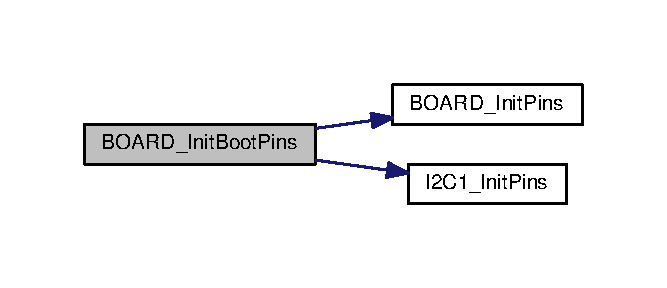
\includegraphics[width=320pt]{group__pin__mux_ga8652eb15efb9dfe7368dd7f292dab554_cgraph}
\end{center}
\end{figure}


\hypertarget{group__pin__mux_ga2c9fe54b6b84723fbaa590a6f4576966}{\index{Pin\-\_\-mux@{Pin\-\_\-mux}!B\-O\-A\-R\-D\-\_\-\-Init\-Pins@{B\-O\-A\-R\-D\-\_\-\-Init\-Pins}}
\index{B\-O\-A\-R\-D\-\_\-\-Init\-Pins@{B\-O\-A\-R\-D\-\_\-\-Init\-Pins}!Pin_mux@{Pin\-\_\-mux}}
\subsubsection[{B\-O\-A\-R\-D\-\_\-\-Init\-Pins}]{\setlength{\rightskip}{0pt plus 5cm}void B\-O\-A\-R\-D\-\_\-\-Init\-Pins (
\begin{DoxyParamCaption}
\item[{void}]{}
\end{DoxyParamCaption}
)}}\label{group__pin__mux_ga2c9fe54b6b84723fbaa590a6f4576966}


Configures pin routing and optionally pin electrical features. 


\begin{DoxyCode}
86                           \{
87   CLOCK\_EnableClock(kCLOCK\_PortA);                           \textcolor{comment}{/* Port A Clock Gate Control: Clock enabled */}
88   CLOCK\_EnableClock(kCLOCK\_PortC);                           \textcolor{comment}{/* Port C Clock Gate Control: Clock enabled */}
89   CLOCK\_EnableClock(kCLOCK\_PortE);                           \textcolor{comment}{/* Port E Clock Gate Control: Clock enabled */}
90 
91   PORT\_SetPinMux(PORTA, \hyperlink{pin__mux_8c_af36e8fbe0cdf23dbe5fe82d0a1abe929}{PIN1\_IDX}, kPORT\_MuxAlt2);            \textcolor{comment}{/* PORTA1 (pin 23) is configured as
       LPUART0\_RX */}
92   PORT\_SetPinMux(PORTA, \hyperlink{pin__mux_8c_aa53d7055dbc0d10a271855831f6f89cf}{PIN13\_IDX}, kPORT\_MuxAsGpio);         \textcolor{comment}{/* PORTA13 (pin 29) is configured as
       PTA13 */}
93   PORT\_SetPinMux(PORTA, \hyperlink{pin__mux_8c_a34077169afb876e5a2afa8b23e671cec}{PIN2\_IDX}, kPORT\_MuxAlt2);            \textcolor{comment}{/* PORTA2 (pin 24) is configured as
       LPUART0\_TX */}
94   \textcolor{keyword}{const} port\_pin\_config\_t porta4\_pin26\_config = \{
95     kPORT\_PullUp,                                            \textcolor{comment}{/* Internal pull-up resistor is enabled */}
96     kPORT\_SlowSlewRate,                                      \textcolor{comment}{/* Slow slew rate is configured */}
97     kPORT\_PassiveFilterEnable,                               \textcolor{comment}{/* Passive filter is enabled */}
98     kPORT\_LowDriveStrength,                                  \textcolor{comment}{/* Low drive strength is configured */}
99     kPORT\_MuxAsGpio,                                         \textcolor{comment}{/* Pin is configured as PTA4 */}
100   \};
101   PORT\_SetPinConfig(PORTA, \hyperlink{pin__mux_8c_a1ada504d2c7f594db50cfd1d222e6339}{PIN4\_IDX}, &porta4\_pin26\_config);  \textcolor{comment}{/* PORTA4 (pin 26) is configured as
       PTA4 */}
102   \textcolor{keyword}{const} port\_pin\_config\_t portc1\_pin44\_config = \{
103     kPORT\_PullUp,                                            \textcolor{comment}{/* Internal pull-up resistor is enabled */}
104     kPORT\_SlowSlewRate,                                      \textcolor{comment}{/* Slow slew rate is configured */}
105     kPORT\_PassiveFilterDisable,                              \textcolor{comment}{/* Passive filter is disabled */}
106     kPORT\_LowDriveStrength,                                  \textcolor{comment}{/* Low drive strength is configured */}
107     kPORT\_MuxAsGpio,                                         \textcolor{comment}{/* Pin is configured as PTC1 */}
108   \};
109   PORT\_SetPinConfig(PORTC, \hyperlink{pin__mux_8c_af36e8fbe0cdf23dbe5fe82d0a1abe929}{PIN1\_IDX}, &portc1\_pin44\_config);  \textcolor{comment}{/* PORTC1 (pin 44) is configured as
       PTC1 */}
110   \textcolor{keyword}{const} port\_pin\_config\_t porte31\_pin19\_config = \{
111     kPORT\_PullUp,                                            \textcolor{comment}{/* Internal pull-up resistor is enabled */}
112     kPORT\_SlowSlewRate,                                      \textcolor{comment}{/* Slow slew rate is configured */}
113     kPORT\_PassiveFilterDisable,                              \textcolor{comment}{/* Passive filter is disabled */}
114     kPORT\_LowDriveStrength,                                  \textcolor{comment}{/* Low drive strength is configured */}
115     kPORT\_MuxAsGpio,                                         \textcolor{comment}{/* Pin is configured as PTE31 */}
116   \};
117   PORT\_SetPinConfig(PORTE, \hyperlink{pin__mux_8c_ad3f3f3f40fb3dfe98dd2ec8d06d12a91}{PIN31\_IDX}, &porte31\_pin19\_config); \textcolor{comment}{/* PORTE31 (pin 19) is configured as
       PTE31 */}
118   SIM->SOPT5 = ((SIM->SOPT5 &
119     (~(SIM\_SOPT5\_LPUART0TXSRC\_MASK | SIM\_SOPT5\_LPUART0RXSRC\_MASK))) \textcolor{comment}{/* Mask bits to zero which are setting 
      */}
120       | SIM\_SOPT5\_LPUART0TXSRC(\hyperlink{pin__mux_8c_ab1b68d7a21112e9371b021390fcb2204}{SOPT5\_LPUART0TXSRC\_LPUART\_TX}) \textcolor{comment}{/* LPUART0
       Transmit Data Source Select: LPUART0\_TX pin */}
121       | SIM\_SOPT5\_LPUART0RXSRC(\hyperlink{pin__mux_8c_ae37cc1f248b28e553138ab4e54967c57}{SOPT5\_LPUART0RXSRC\_LPUART\_RX}) \textcolor{comment}{/* LPUART0 Receive
       Data Source Select: LPUART\_RX pin */}
122     );
123 \}
\end{DoxyCode}


Here is the caller graph for this function\-:
\nopagebreak
\begin{figure}[H]
\begin{center}
\leavevmode
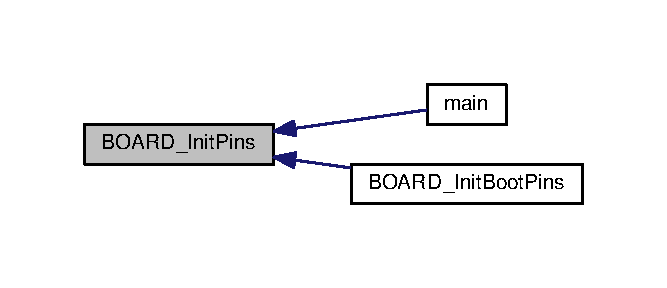
\includegraphics[width=320pt]{group__pin__mux_ga2c9fe54b6b84723fbaa590a6f4576966_icgraph}
\end{center}
\end{figure}


\hypertarget{group__pin__mux_ga8e9cb3ef8722919469dc52bd99cb9cc5}{\index{Pin\-\_\-mux@{Pin\-\_\-mux}!I2\-C0\-\_\-\-Deinit\-Pins@{I2\-C0\-\_\-\-Deinit\-Pins}}
\index{I2\-C0\-\_\-\-Deinit\-Pins@{I2\-C0\-\_\-\-Deinit\-Pins}!Pin_mux@{Pin\-\_\-mux}}
\subsubsection[{I2\-C0\-\_\-\-Deinit\-Pins}]{\setlength{\rightskip}{0pt plus 5cm}void I2\-C0\-\_\-\-Deinit\-Pins (
\begin{DoxyParamCaption}
\item[{void}]{}
\end{DoxyParamCaption}
)}}\label{group__pin__mux_ga8e9cb3ef8722919469dc52bd99cb9cc5}


Configures pin routing and optionally pin electrical features. 


\begin{DoxyCode}
183                            \{
184   CLOCK\_EnableClock(kCLOCK\_PortB);                           \textcolor{comment}{/* Port B Clock Gate Control: Clock enabled */}
185 
186   PORT\_SetPinMux(PORTB, \hyperlink{pin__mux_8c_a0a301fe265343a5b6e6a48af5276ac84}{PIN0\_IDX}, kPORT\_PinDisabledOrAnalog); \textcolor{comment}{/* PORTB0 (pin 35) is configured as
       ADC0\_SE8 */}
187   PORT\_SetPinMux(PORTB, \hyperlink{pin__mux_8c_af36e8fbe0cdf23dbe5fe82d0a1abe929}{PIN1\_IDX}, kPORT\_PinDisabledOrAnalog); \textcolor{comment}{/* PORTB1 (pin 36) is configured as
       ADC0\_SE9 */}
188 \}
\end{DoxyCode}
\hypertarget{group__pin__mux_ga3a18c9665d7d526b76488e90a271cc8e}{\index{Pin\-\_\-mux@{Pin\-\_\-mux}!I2\-C0\-\_\-\-Init\-Pins@{I2\-C0\-\_\-\-Init\-Pins}}
\index{I2\-C0\-\_\-\-Init\-Pins@{I2\-C0\-\_\-\-Init\-Pins}!Pin_mux@{Pin\-\_\-mux}}
\subsubsection[{I2\-C0\-\_\-\-Init\-Pins}]{\setlength{\rightskip}{0pt plus 5cm}void I2\-C0\-\_\-\-Init\-Pins (
\begin{DoxyParamCaption}
\item[{void}]{}
\end{DoxyParamCaption}
)}}\label{group__pin__mux_ga3a18c9665d7d526b76488e90a271cc8e}


Configures pin routing and optionally pin electrical features. 


\begin{DoxyCode}
147                          \{
148   CLOCK\_EnableClock(kCLOCK\_PortB);                           \textcolor{comment}{/* Port B Clock Gate Control: Clock enabled */}
149 
150   PORT\_SetPinMux(PORTB, \hyperlink{pin__mux_8c_a0a301fe265343a5b6e6a48af5276ac84}{PIN0\_IDX}, kPORT\_MuxAlt2);            \textcolor{comment}{/* PORTB0 (pin 35) is configured as
       I2C0\_SCL */}
151   PORTB->PCR[0] = ((PORTB->PCR[0] &
152     (~(PORT\_PCR\_DSE\_MASK | PORT\_PCR\_ISF\_MASK)))              \textcolor{comment}{/* Mask bits to zero which are setting */}
153       | PORT\_PCR\_DSE(\hyperlink{pin__mux_8c_a91f13f97309f3c88c3cd188d2f2997ed}{PCR\_DSE\_HIGH})                           \textcolor{comment}{/* Drive Strength Enable: High
       drive strength is configured on the corresponding pin, if pin is configured as a digital output. */}
154     );
155   PORT\_SetPinMux(PORTB, \hyperlink{pin__mux_8c_af36e8fbe0cdf23dbe5fe82d0a1abe929}{PIN1\_IDX}, kPORT\_MuxAlt2);            \textcolor{comment}{/* PORTB1 (pin 36) is configured as
       I2C0\_SDA */}
156   PORTB->PCR[1] = ((PORTB->PCR[1] &
157     (~(PORT\_PCR\_DSE\_MASK | PORT\_PCR\_ISF\_MASK)))              \textcolor{comment}{/* Mask bits to zero which are setting */}
158       | PORT\_PCR\_DSE(\hyperlink{pin__mux_8c_a91f13f97309f3c88c3cd188d2f2997ed}{PCR\_DSE\_HIGH})                           \textcolor{comment}{/* Drive Strength Enable: High
       drive strength is configured on the corresponding pin, if pin is configured as a digital output. */}
159     );
160 \}
\end{DoxyCode}
\hypertarget{group__pin__mux_ga455ca4e86bd4798c0368a926fe30f692}{\index{Pin\-\_\-mux@{Pin\-\_\-mux}!I2\-C1\-\_\-\-Deinit\-Pins@{I2\-C1\-\_\-\-Deinit\-Pins}}
\index{I2\-C1\-\_\-\-Deinit\-Pins@{I2\-C1\-\_\-\-Deinit\-Pins}!Pin_mux@{Pin\-\_\-mux}}
\subsubsection[{I2\-C1\-\_\-\-Deinit\-Pins}]{\setlength{\rightskip}{0pt plus 5cm}void I2\-C1\-\_\-\-Deinit\-Pins (
\begin{DoxyParamCaption}
\item[{void}]{}
\end{DoxyParamCaption}
)}}\label{group__pin__mux_ga455ca4e86bd4798c0368a926fe30f692}


Configures pin routing and optionally pin electrical features. 


\begin{DoxyCode}
248                            \{
249   CLOCK\_EnableClock(kCLOCK\_PortD);                           \textcolor{comment}{/* Port D Clock Gate Control: Clock enabled */}
250 
251   PORT\_SetPinMux(PORTD, \hyperlink{pin__mux_8c_ae62ce800c3f07b0f2802b9573d5971a8}{PIN6\_IDX}, kPORT\_PinDisabledOrAnalog); \textcolor{comment}{/* PORTD6 (pin 63) is configured as
       ADC0\_SE7b */}
252   PORT\_SetPinMux(PORTD, \hyperlink{pin__mux_8c_aa91e0ac7896fd4816e892df2509110be}{PIN7\_IDX}, kPORT\_PinDisabledOrAnalog); \textcolor{comment}{/* PORTD7 (pin 64) is disabled */}
253 \}
\end{DoxyCode}
\hypertarget{group__pin__mux_gaa63f3828e7f823cef465873563ca99c4}{\index{Pin\-\_\-mux@{Pin\-\_\-mux}!I2\-C1\-\_\-\-Init\-Pins@{I2\-C1\-\_\-\-Init\-Pins}}
\index{I2\-C1\-\_\-\-Init\-Pins@{I2\-C1\-\_\-\-Init\-Pins}!Pin_mux@{Pin\-\_\-mux}}
\subsubsection[{I2\-C1\-\_\-\-Init\-Pins}]{\setlength{\rightskip}{0pt plus 5cm}void I2\-C1\-\_\-\-Init\-Pins (
\begin{DoxyParamCaption}
\item[{void}]{}
\end{DoxyParamCaption}
)}}\label{group__pin__mux_gaa63f3828e7f823cef465873563ca99c4}


Configures pin routing and optionally pin electrical features. 


\begin{DoxyCode}
212                          \{
213   CLOCK\_EnableClock(kCLOCK\_PortD);                           \textcolor{comment}{/* Port D Clock Gate Control: Clock enabled */}
214 
215   PORT\_SetPinMux(PORTD, \hyperlink{pin__mux_8c_ae62ce800c3f07b0f2802b9573d5971a8}{PIN6\_IDX}, kPORT\_MuxAlt4);            \textcolor{comment}{/* PORTD6 (pin 63) is configured as
       I2C1\_SDA */}
216   PORTD->PCR[6] = ((PORTD->PCR[6] &
217     (~(PORT\_PCR\_DSE\_MASK | PORT\_PCR\_ISF\_MASK)))              \textcolor{comment}{/* Mask bits to zero which are setting */}
218       | PORT\_PCR\_DSE(\hyperlink{pin__mux_8c_a91f13f97309f3c88c3cd188d2f2997ed}{PCR\_DSE\_HIGH})                           \textcolor{comment}{/* Drive Strength Enable: High
       drive strength is configured on the corresponding pin, if pin is configured as a digital output. */}
219     );
220   PORT\_SetPinMux(PORTD, \hyperlink{pin__mux_8c_aa91e0ac7896fd4816e892df2509110be}{PIN7\_IDX}, kPORT\_MuxAlt4);            \textcolor{comment}{/* PORTD7 (pin 64) is configured as
       I2C1\_SCL */}
221   PORTD->PCR[7] = ((PORTD->PCR[7] &
222     (~(PORT\_PCR\_DSE\_MASK | PORT\_PCR\_ISF\_MASK)))              \textcolor{comment}{/* Mask bits to zero which are setting */}
223       | PORT\_PCR\_DSE(\hyperlink{pin__mux_8c_a91f13f97309f3c88c3cd188d2f2997ed}{PCR\_DSE\_HIGH})                           \textcolor{comment}{/* Drive Strength Enable: High
       drive strength is configured on the corresponding pin, if pin is configured as a digital output. */}
224     );
225 \}
\end{DoxyCode}


Here is the caller graph for this function\-:
\nopagebreak
\begin{figure}[H]
\begin{center}
\leavevmode
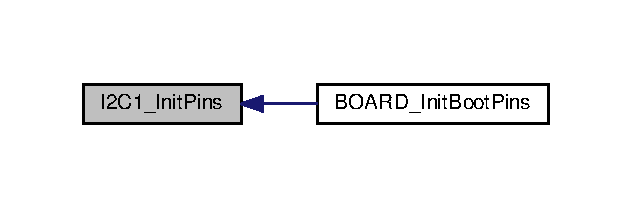
\includegraphics[width=304pt]{group__pin__mux_gaa63f3828e7f823cef465873563ca99c4_icgraph}
\end{center}
\end{figure}



\hypertarget{group__usb__device__driver}{\section{Usb\-\_\-device\-\_\-driver}
\label{group__usb__device__driver}\index{Usb\-\_\-device\-\_\-driver@{Usb\-\_\-device\-\_\-driver}}
}
\subsection*{Classes}
\begin{DoxyCompactItemize}
\item 
struct \hyperlink{struct__usb__device__endpoint__callback__message__struct}{\-\_\-usb\-\_\-device\-\_\-endpoint\-\_\-callback\-\_\-message\-\_\-struct}
\begin{DoxyCompactList}\small\item\em Endpoint callback message structure. \end{DoxyCompactList}\item 
struct \hyperlink{struct__usb__device__endpoint__callback__struct}{\-\_\-usb\-\_\-device\-\_\-endpoint\-\_\-callback\-\_\-struct}
\begin{DoxyCompactList}\small\item\em Endpoint callback structure. \end{DoxyCompactList}\item 
struct \hyperlink{struct__usb__device__endpoint__init__struct}{\-\_\-usb\-\_\-device\-\_\-endpoint\-\_\-init\-\_\-struct}
\begin{DoxyCompactList}\small\item\em Endpoint initialization structure. \end{DoxyCompactList}\item 
struct \hyperlink{struct__usb__device__endpoint__status__struct}{\-\_\-usb\-\_\-device\-\_\-endpoint\-\_\-status\-\_\-struct}
\begin{DoxyCompactList}\small\item\em Endpoint status structure. \end{DoxyCompactList}\end{DoxyCompactItemize}
\subsection*{Macros}
\begin{DoxyCompactItemize}
\item 
\#define \hyperlink{group__usb__device__driver_gac35db57970e61e674baba9eb53aa7a8c}{U\-S\-B\-\_\-\-C\-O\-N\-T\-R\-O\-L\-\_\-\-E\-N\-D\-P\-O\-I\-N\-T}~(0\-U)
\begin{DoxyCompactList}\small\item\em Control endpoint index. \end{DoxyCompactList}\item 
\#define \hyperlink{group__usb__device__driver_ga206afe1513d3b4fdc64a7064249cb447}{U\-S\-B\-\_\-\-C\-O\-N\-T\-R\-O\-L\-\_\-\-M\-A\-X\-\_\-\-P\-A\-C\-K\-E\-T\-\_\-\-S\-I\-Z\-E}~(64\-U)
\begin{DoxyCompactList}\small\item\em Control endpoint max\-Packet\-Size. \end{DoxyCompactList}\item 
\#define \hyperlink{group__usb__device__driver_gabf1be648722b01577b84e52e1fb3d8f8}{U\-S\-B\-\_\-\-S\-E\-T\-U\-P\-\_\-\-P\-A\-C\-K\-E\-T\-\_\-\-S\-I\-Z\-E}~(8\-U)
\begin{DoxyCompactList}\small\item\em The setup packet size of U\-S\-B control transfer. \end{DoxyCompactList}\item 
\#define \hyperlink{group__usb__device__driver_ga435416dd71e258cfd83be50a991db726}{U\-S\-B\-\_\-\-E\-N\-D\-P\-O\-I\-N\-T\-\_\-\-N\-U\-M\-B\-E\-R\-\_\-\-M\-A\-S\-K}~(0x0\-F\-U)
\begin{DoxyCompactList}\small\item\em U\-S\-B endpoint mask. \end{DoxyCompactList}\item 
\#define \hyperlink{group__usb__device__driver_ga89fb39ed32e04cdb444d6d06831f1d48}{U\-S\-B\-\_\-\-U\-N\-I\-N\-I\-T\-I\-A\-L\-I\-Z\-E\-D\-\_\-\-V\-A\-L\-\_\-32}~(0x\-F\-F\-F\-F\-F\-F\-F\-F\-U)
\begin{DoxyCompactList}\small\item\em Default invalid value or the endpoint callback length of cancelled transfer. \end{DoxyCompactList}\end{DoxyCompactItemize}
\subsection*{Typedefs}
\begin{DoxyCompactItemize}
\item 
typedef enum \hyperlink{group__usb__device__driver_gad091bd3169bf45debbe8b5aba78d6091}{\-\_\-usb\-\_\-device\-\_\-status} \hyperlink{group__usb__device__driver_ga11ab1b56db153ac62eecf01661216bbf}{usb\-\_\-device\-\_\-status\-\_\-t}
\begin{DoxyCompactList}\small\item\em Defines Get/\-Set status Types. \end{DoxyCompactList}\item 
typedef enum \hyperlink{group__usb__device__driver_ga6c3587990ca428244271f14efc909522}{\-\_\-usb\-\_\-device\-\_\-state} \hyperlink{group__usb__device__driver_gadb6af69c6a5a2124b197210e41ed8256}{usb\-\_\-device\-\_\-state\-\_\-t}
\begin{DoxyCompactList}\small\item\em Defines U\-S\-B 2.\-0 device state. \end{DoxyCompactList}\item 
typedef enum \hyperlink{group__usb__device__driver_ga58f9c3f9e1aeb5f669a4cb58556ed53f}{\-\_\-usb\-\_\-endpoint\-\_\-status} \hyperlink{group__usb__device__driver_gaaefd48322932e1e70d5c4b4674e19796}{usb\-\_\-device\-\_\-endpoint\-\_\-status\-\_\-t}
\begin{DoxyCompactList}\small\item\em Defines endpoint state. \end{DoxyCompactList}\item 
typedef enum \hyperlink{group__usb__device__driver_gac66a5e6b9c677f9d8d4f782aa62df540}{\-\_\-usb\-\_\-device\-\_\-event} \hyperlink{group__usb__device__driver_ga35623b5263f88037a497e6c6c363b8f1}{usb\-\_\-device\-\_\-event\-\_\-t}
\begin{DoxyCompactList}\small\item\em Available common E\-V\-E\-N\-T types in device callback. \end{DoxyCompactList}\item 
typedef struct \\*
\hyperlink{struct__usb__device__endpoint__callback__message__struct}{\-\_\-usb\-\_\-device\-\_\-endpoint\-\_\-callback\-\_\-message\-\_\-struct} \hyperlink{group__usb__device__driver_ga291e21595b67e07488baad293f707e5f}{usb\-\_\-device\-\_\-endpoint\-\_\-callback\-\_\-message\-\_\-struct\-\_\-t}
\begin{DoxyCompactList}\small\item\em Endpoint callback message structure. \end{DoxyCompactList}\item 
typedef \hyperlink{group__usb__drv_ga3172b9f50553fb6d8aa2823d10a39c58}{usb\-\_\-status\-\_\-t}($\ast$ \hyperlink{group__usb__device__driver_gac780580992587eb809d445edcba7c3ca}{usb\-\_\-device\-\_\-endpoint\-\_\-callback\-\_\-t} )(\hyperlink{group__usb__drv_gae62132dc6e5eba994f8aa56cb7399abc}{usb\-\_\-device\-\_\-handle} handle, \hyperlink{group__usb__device__driver_ga291e21595b67e07488baad293f707e5f}{usb\-\_\-device\-\_\-endpoint\-\_\-callback\-\_\-message\-\_\-struct\-\_\-t} $\ast$message, void $\ast$callback\-Param)
\begin{DoxyCompactList}\small\item\em Endpoint callback function typedef. \end{DoxyCompactList}\item 
typedef \hyperlink{group__usb__drv_ga3172b9f50553fb6d8aa2823d10a39c58}{usb\-\_\-status\-\_\-t}($\ast$ \hyperlink{group__usb__device__driver_gac8ba48f1dea2c0b099092576ad48fb4e}{usb\-\_\-device\-\_\-callback\-\_\-t} )(\hyperlink{group__usb__drv_gae62132dc6e5eba994f8aa56cb7399abc}{usb\-\_\-device\-\_\-handle} handle, uint32\-\_\-t callback\-Event, void $\ast$event\-Param)
\begin{DoxyCompactList}\small\item\em Device callback function typedef. \end{DoxyCompactList}\item 
typedef struct \\*
\hyperlink{struct__usb__device__endpoint__callback__struct}{\-\_\-usb\-\_\-device\-\_\-endpoint\-\_\-callback\-\_\-struct} \hyperlink{group__usb__device__driver_ga0fcee893200ced24dbff370f38c16573}{usb\-\_\-device\-\_\-endpoint\-\_\-callback\-\_\-struct\-\_\-t}
\begin{DoxyCompactList}\small\item\em Endpoint callback structure. \end{DoxyCompactList}\item 
typedef struct \\*
\hyperlink{struct__usb__device__endpoint__init__struct}{\-\_\-usb\-\_\-device\-\_\-endpoint\-\_\-init\-\_\-struct} \hyperlink{group__usb__device__driver_ga5fd6342aa2c5f10ba177604031b38d99}{usb\-\_\-device\-\_\-endpoint\-\_\-init\-\_\-struct\-\_\-t}
\begin{DoxyCompactList}\small\item\em Endpoint initialization structure. \end{DoxyCompactList}\item 
typedef struct \\*
\hyperlink{struct__usb__device__endpoint__status__struct}{\-\_\-usb\-\_\-device\-\_\-endpoint\-\_\-status\-\_\-struct} \hyperlink{group__usb__device__driver_ga7db41d0acd6976fd4016b97f9dac0f51}{usb\-\_\-device\-\_\-endpoint\-\_\-status\-\_\-struct\-\_\-t}
\begin{DoxyCompactList}\small\item\em Endpoint status structure. \end{DoxyCompactList}\end{DoxyCompactItemize}
\subsection*{Enumerations}
\begin{DoxyCompactItemize}
\item 
enum \hyperlink{group__usb__device__driver_gad091bd3169bf45debbe8b5aba78d6091}{\-\_\-usb\-\_\-device\-\_\-status} \{ \\*
\hyperlink{group__usb__device__driver_ggad091bd3169bf45debbe8b5aba78d6091afa1c47d0cb4c8f751822e6204ceaca68}{k\-U\-S\-B\-\_\-\-Device\-Status\-Test\-Mode} = 1\-U, 
\hyperlink{group__usb__device__driver_ggad091bd3169bf45debbe8b5aba78d6091a01e79a57be59b44dc12a81a248d19b56}{k\-U\-S\-B\-\_\-\-Device\-Status\-Speed}, 
\hyperlink{group__usb__device__driver_ggad091bd3169bf45debbe8b5aba78d6091a4dc0830399c694c3af0f53eed326ba4d}{k\-U\-S\-B\-\_\-\-Device\-Status\-Otg}, 
\hyperlink{group__usb__device__driver_ggad091bd3169bf45debbe8b5aba78d6091a0c344a179ec60cfef88a020f01390447}{k\-U\-S\-B\-\_\-\-Device\-Status\-Device}, 
\\*
\hyperlink{group__usb__device__driver_ggad091bd3169bf45debbe8b5aba78d6091abfe4090beeb636774c9e18897fbffba2}{k\-U\-S\-B\-\_\-\-Device\-Status\-Endpoint}, 
\hyperlink{group__usb__device__driver_ggad091bd3169bf45debbe8b5aba78d6091ad704e2b6cb73fdbf0e60552a1da06ee3}{k\-U\-S\-B\-\_\-\-Device\-Status\-Device\-State}, 
\hyperlink{group__usb__device__driver_ggad091bd3169bf45debbe8b5aba78d6091a8ce5b187176d33cfb8f263e9c5392e6c}{k\-U\-S\-B\-\_\-\-Device\-Status\-Address}, 
\hyperlink{group__usb__device__driver_ggad091bd3169bf45debbe8b5aba78d6091a57984cab0b6b417c65a766c2772e5792}{k\-U\-S\-B\-\_\-\-Device\-Status\-Synch\-Frame}, 
\\*
\hyperlink{group__usb__device__driver_ggad091bd3169bf45debbe8b5aba78d6091a851aea79c4cc0cc44ffacf8dbc433017}{k\-U\-S\-B\-\_\-\-Device\-Status\-Bus}, 
\hyperlink{group__usb__device__driver_ggad091bd3169bf45debbe8b5aba78d6091aa77cc78d4d576415e4e878eedd9e81e5}{k\-U\-S\-B\-\_\-\-Device\-Status\-Bus\-Suspend}, 
\hyperlink{group__usb__device__driver_ggad091bd3169bf45debbe8b5aba78d6091a0ac5bacc26d67cf8f1401cf2804c8748}{k\-U\-S\-B\-\_\-\-Device\-Status\-Bus\-Sleep}, 
\hyperlink{group__usb__device__driver_ggad091bd3169bf45debbe8b5aba78d6091aca838250308618a1f4210410f81d136e}{k\-U\-S\-B\-\_\-\-Device\-Status\-Bus\-Resume}, 
\\*
\hyperlink{group__usb__device__driver_ggad091bd3169bf45debbe8b5aba78d6091a14f036d2f6ae26676a3da34d3d735ea0}{k\-U\-S\-B\-\_\-\-Device\-Status\-Remote\-Wakeup}, 
\hyperlink{group__usb__device__driver_ggad091bd3169bf45debbe8b5aba78d6091aaf9c05a346d33cb1f2fc4834026dd623}{k\-U\-S\-B\-\_\-\-Device\-Status\-Bus\-Sleep\-Resume}
 \}
\begin{DoxyCompactList}\small\item\em Defines Get/\-Set status Types. \end{DoxyCompactList}\item 
enum \hyperlink{group__usb__device__driver_ga6c3587990ca428244271f14efc909522}{\-\_\-usb\-\_\-device\-\_\-state} \{ \\*
\hyperlink{group__usb__device__driver_gga6c3587990ca428244271f14efc909522a3cc5b3134e34ce6fc3d9c1ee0217e741}{k\-U\-S\-B\-\_\-\-Device\-State\-Configured} = 0\-U, 
\hyperlink{group__usb__device__driver_gga6c3587990ca428244271f14efc909522ac0b38e07063e3b0f01a984671e7bc23b}{k\-U\-S\-B\-\_\-\-Device\-State\-Address}, 
\hyperlink{group__usb__device__driver_gga6c3587990ca428244271f14efc909522a25d25f366cf27a445b19a92fd7d20698}{k\-U\-S\-B\-\_\-\-Device\-State\-Default}, 
\hyperlink{group__usb__device__driver_gga6c3587990ca428244271f14efc909522a257337842d7b3299efbaa8e1218d6069}{k\-U\-S\-B\-\_\-\-Device\-State\-Addressing}, 
\\*
\hyperlink{group__usb__device__driver_gga6c3587990ca428244271f14efc909522ab7ff5567abb58aa097fd8af77df16a8c}{k\-U\-S\-B\-\_\-\-Device\-State\-Test\-Mode}
 \}
\begin{DoxyCompactList}\small\item\em Defines U\-S\-B 2.\-0 device state. \end{DoxyCompactList}\item 
enum \hyperlink{group__usb__device__driver_ga58f9c3f9e1aeb5f669a4cb58556ed53f}{\-\_\-usb\-\_\-endpoint\-\_\-status} \{ \hyperlink{group__usb__device__driver_gga58f9c3f9e1aeb5f669a4cb58556ed53fa9956ef1389d5dad712cda6cf209a4ed5}{k\-U\-S\-B\-\_\-\-Device\-Endpoint\-State\-Idle} = 0\-U, 
\hyperlink{group__usb__device__driver_gga58f9c3f9e1aeb5f669a4cb58556ed53faad3658477257e2f76ac54a960763043b}{k\-U\-S\-B\-\_\-\-Device\-Endpoint\-State\-Stalled}
 \}
\begin{DoxyCompactList}\small\item\em Defines endpoint state. \end{DoxyCompactList}\item 
enum \hyperlink{group__usb__device__driver_gac66a5e6b9c677f9d8d4f782aa62df540}{\-\_\-usb\-\_\-device\-\_\-event} \{ \\*
\hyperlink{group__usb__device__driver_ggac66a5e6b9c677f9d8d4f782aa62df540a9a523a8379ac9ffe266576c3197f1a37}{k\-U\-S\-B\-\_\-\-Device\-Event\-Bus\-Reset} = 1\-U, 
\hyperlink{group__usb__device__driver_ggac66a5e6b9c677f9d8d4f782aa62df540a61a3fd60360930f22ebed5ddcdc7e056}{k\-U\-S\-B\-\_\-\-Device\-Event\-Suspend}, 
\hyperlink{group__usb__device__driver_ggac66a5e6b9c677f9d8d4f782aa62df540a1507b21f410d579b95817f1ee96ee4d3}{k\-U\-S\-B\-\_\-\-Device\-Event\-Resume}, 
\hyperlink{group__usb__device__driver_ggac66a5e6b9c677f9d8d4f782aa62df540a609202b43c7044bf6ef787ccc08687fa}{k\-U\-S\-B\-\_\-\-Device\-Event\-Sleeped}, 
\\*
\hyperlink{group__usb__device__driver_ggac66a5e6b9c677f9d8d4f782aa62df540a878261b598db4d20ef380b90e34a4fdd}{k\-U\-S\-B\-\_\-\-Device\-Event\-L\-P\-M\-Resume}, 
\hyperlink{group__usb__device__driver_ggac66a5e6b9c677f9d8d4f782aa62df540a368f053177d0ca682a38b3b8e8b37f5e}{k\-U\-S\-B\-\_\-\-Device\-Event\-Error}, 
\hyperlink{group__usb__device__driver_ggac66a5e6b9c677f9d8d4f782aa62df540aaea780c05bac7a34ea2e8771ff15dd4b}{k\-U\-S\-B\-\_\-\-Device\-Event\-Detach}, 
\hyperlink{group__usb__device__driver_ggac66a5e6b9c677f9d8d4f782aa62df540a1bf226d529ceb9da8f2eeddae8571a0c}{k\-U\-S\-B\-\_\-\-Device\-Event\-Attach}, 
\\*
\hyperlink{group__usb__device__driver_ggac66a5e6b9c677f9d8d4f782aa62df540a601f0b7823762801deda3fc4cb45cb35}{k\-U\-S\-B\-\_\-\-Device\-Event\-Set\-Configuration}, 
\hyperlink{group__usb__device__driver_ggac66a5e6b9c677f9d8d4f782aa62df540afc7be18726fd0f90eb52b614c4ee3586}{k\-U\-S\-B\-\_\-\-Device\-Event\-Set\-Interface}, 
\hyperlink{group__usb__device__driver_ggac66a5e6b9c677f9d8d4f782aa62df540a730ebd8734f0621fbe9cdf680dd0b510}{k\-U\-S\-B\-\_\-\-Device\-Event\-Get\-Device\-Descriptor}, 
\hyperlink{group__usb__device__driver_ggac66a5e6b9c677f9d8d4f782aa62df540ab40809d63173bca60a7ceb0c3d1336b2}{k\-U\-S\-B\-\_\-\-Device\-Event\-Get\-Configuration\-Descriptor}, 
\\*
\hyperlink{group__usb__device__driver_ggac66a5e6b9c677f9d8d4f782aa62df540a12b45ed6403fb95321735bca3e27723d}{k\-U\-S\-B\-\_\-\-Device\-Event\-Get\-String\-Descriptor}, 
\hyperlink{group__usb__device__driver_ggac66a5e6b9c677f9d8d4f782aa62df540a29d11372708627c050855b9ba8e4439c}{k\-U\-S\-B\-\_\-\-Device\-Event\-Get\-Hid\-Descriptor}, 
\hyperlink{group__usb__device__driver_ggac66a5e6b9c677f9d8d4f782aa62df540a65449a7fb97a4c87d2ae6a10d23370ae}{k\-U\-S\-B\-\_\-\-Device\-Event\-Get\-Hid\-Report\-Descriptor}, 
\hyperlink{group__usb__device__driver_ggac66a5e6b9c677f9d8d4f782aa62df540a2326252deb48891e7bedc3cbadfe7123}{k\-U\-S\-B\-\_\-\-Device\-Event\-Get\-Hid\-Physical\-Descriptor}, 
\\*
\hyperlink{group__usb__device__driver_ggac66a5e6b9c677f9d8d4f782aa62df540a664780e759bf40aabab5ee5fbf7cb83e}{k\-U\-S\-B\-\_\-\-Device\-Event\-Get\-B\-O\-S\-Descriptor}, 
\hyperlink{group__usb__device__driver_ggac66a5e6b9c677f9d8d4f782aa62df540aafad43b8efe4a69fddd2d9989ec941f4}{k\-U\-S\-B\-\_\-\-Device\-Event\-Get\-Device\-Qualifier\-Descriptor}, 
\hyperlink{group__usb__device__driver_ggac66a5e6b9c677f9d8d4f782aa62df540aaa48528e07e1f9059b0f079dc7e43dda}{k\-U\-S\-B\-\_\-\-Device\-Event\-Vendor\-Request}, 
\hyperlink{group__usb__device__driver_ggac66a5e6b9c677f9d8d4f782aa62df540af95ccd0dea69e67c4ee4b0b1023b1414}{k\-U\-S\-B\-\_\-\-Device\-Event\-Set\-Remote\-Wakeup}, 
\\*
\hyperlink{group__usb__device__driver_ggac66a5e6b9c677f9d8d4f782aa62df540a8f8fd6bd0ea5d9c0aade08ea982d181e}{k\-U\-S\-B\-\_\-\-Device\-Event\-Get\-Configuration}, 
\hyperlink{group__usb__device__driver_ggac66a5e6b9c677f9d8d4f782aa62df540abfe862150feed0c1bafc94e356c4284a}{k\-U\-S\-B\-\_\-\-Device\-Event\-Get\-Interface}, 
\hyperlink{group__usb__device__driver_ggac66a5e6b9c677f9d8d4f782aa62df540a778e2f5601392117440d604615fa0a60}{k\-U\-S\-B\-\_\-\-Device\-Event\-Set\-B\-H\-N\-P\-Enable}
 \}
\begin{DoxyCompactList}\small\item\em Available common E\-V\-E\-N\-T types in device callback. \end{DoxyCompactList}\end{DoxyCompactItemize}
\subsection*{U\-S\-B device A\-P\-Is}
\begin{DoxyCompactItemize}
\item 
\hyperlink{group__usb__drv_ga3172b9f50553fb6d8aa2823d10a39c58}{usb\-\_\-status\-\_\-t} \hyperlink{group__usb__device__driver_ga8fc2eafa1142f904576bbd697d785184}{U\-S\-B\-\_\-\-Device\-Init} (uint8\-\_\-t controller\-Id, \hyperlink{group__usb__device__driver_gac8ba48f1dea2c0b099092576ad48fb4e}{usb\-\_\-device\-\_\-callback\-\_\-t} device\-Callback, \hyperlink{group__usb__drv_gae62132dc6e5eba994f8aa56cb7399abc}{usb\-\_\-device\-\_\-handle} $\ast$handle)
\begin{DoxyCompactList}\small\item\em Initializes the U\-S\-B device stack. \end{DoxyCompactList}\item 
\hyperlink{group__usb__drv_ga3172b9f50553fb6d8aa2823d10a39c58}{usb\-\_\-status\-\_\-t} \hyperlink{group__usb__device__driver_gaecab79f44d7c16d5344aef538ddfa40e}{U\-S\-B\-\_\-\-Device\-Run} (\hyperlink{group__usb__drv_gae62132dc6e5eba994f8aa56cb7399abc}{usb\-\_\-device\-\_\-handle} handle)
\begin{DoxyCompactList}\small\item\em Enables the device functionality. \end{DoxyCompactList}\item 
\hyperlink{group__usb__drv_ga3172b9f50553fb6d8aa2823d10a39c58}{usb\-\_\-status\-\_\-t} \hyperlink{group__usb__device__driver_ga1000e1b314d75bc51e54953c78dd66f2}{U\-S\-B\-\_\-\-Device\-Stop} (\hyperlink{group__usb__drv_gae62132dc6e5eba994f8aa56cb7399abc}{usb\-\_\-device\-\_\-handle} handle)
\begin{DoxyCompactList}\small\item\em Disables the device functionality. \end{DoxyCompactList}\item 
\hyperlink{group__usb__drv_ga3172b9f50553fb6d8aa2823d10a39c58}{usb\-\_\-status\-\_\-t} \hyperlink{group__usb__device__driver_gafff2a5a6ac37dec01242225516a22024}{U\-S\-B\-\_\-\-Device\-Deinit} (\hyperlink{group__usb__drv_gae62132dc6e5eba994f8aa56cb7399abc}{usb\-\_\-device\-\_\-handle} handle)
\begin{DoxyCompactList}\small\item\em De-\/initializes the device controller. \end{DoxyCompactList}\item 
\hyperlink{group__usb__drv_ga3172b9f50553fb6d8aa2823d10a39c58}{usb\-\_\-status\-\_\-t} \hyperlink{group__usb__device__driver_ga94f95f6b9e0ba1caba7ea7c889a4b471}{U\-S\-B\-\_\-\-Device\-Send\-Request} (\hyperlink{group__usb__drv_gae62132dc6e5eba994f8aa56cb7399abc}{usb\-\_\-device\-\_\-handle} handle, uint8\-\_\-t endpoint\-Address, uint8\-\_\-t $\ast$buffer, uint32\-\_\-t length)
\begin{DoxyCompactList}\small\item\em Sends data through a specified endpoint. \end{DoxyCompactList}\item 
\hyperlink{group__usb__drv_ga3172b9f50553fb6d8aa2823d10a39c58}{usb\-\_\-status\-\_\-t} \hyperlink{group__usb__device__driver_gaafd44df38db0494a5c7a53c91b08eef7}{U\-S\-B\-\_\-\-Device\-Recv\-Request} (\hyperlink{group__usb__drv_gae62132dc6e5eba994f8aa56cb7399abc}{usb\-\_\-device\-\_\-handle} handle, uint8\-\_\-t endpoint\-Address, uint8\-\_\-t $\ast$buffer, uint32\-\_\-t length)
\begin{DoxyCompactList}\small\item\em Receives data through a specified endpoint. \end{DoxyCompactList}\item 
\hyperlink{group__usb__drv_ga3172b9f50553fb6d8aa2823d10a39c58}{usb\-\_\-status\-\_\-t} \hyperlink{group__usb__device__driver_gaa95120c01a49916790852c8ac8468ec3}{U\-S\-B\-\_\-\-Device\-Cancel} (\hyperlink{group__usb__drv_gae62132dc6e5eba994f8aa56cb7399abc}{usb\-\_\-device\-\_\-handle} handle, uint8\-\_\-t endpoint\-Address)
\begin{DoxyCompactList}\small\item\em Cancels the pending transfer in a specified endpoint. \end{DoxyCompactList}\item 
\hyperlink{group__usb__drv_ga3172b9f50553fb6d8aa2823d10a39c58}{usb\-\_\-status\-\_\-t} \hyperlink{group__usb__device__driver_ga3302bb97cb7e4a0a805f8dec3cabd07f}{U\-S\-B\-\_\-\-Device\-Init\-Endpoint} (\hyperlink{group__usb__drv_gae62132dc6e5eba994f8aa56cb7399abc}{usb\-\_\-device\-\_\-handle} handle, \hyperlink{group__usb__device__driver_ga5fd6342aa2c5f10ba177604031b38d99}{usb\-\_\-device\-\_\-endpoint\-\_\-init\-\_\-struct\-\_\-t} $\ast$ep\-Init, \hyperlink{group__usb__device__driver_ga0fcee893200ced24dbff370f38c16573}{usb\-\_\-device\-\_\-endpoint\-\_\-callback\-\_\-struct\-\_\-t} $\ast$endpoint\-Callback)
\begin{DoxyCompactList}\small\item\em Initializes a specified endpoint. \end{DoxyCompactList}\item 
\hyperlink{group__usb__drv_ga3172b9f50553fb6d8aa2823d10a39c58}{usb\-\_\-status\-\_\-t} \hyperlink{group__usb__device__driver_ga9bd52faa129ce19404fe65c0b2762533}{U\-S\-B\-\_\-\-Device\-Deinit\-Endpoint} (\hyperlink{group__usb__drv_gae62132dc6e5eba994f8aa56cb7399abc}{usb\-\_\-device\-\_\-handle} handle, uint8\-\_\-t endpoint\-Address)
\begin{DoxyCompactList}\small\item\em Deinitializes a specified endpoint. \end{DoxyCompactList}\item 
\hyperlink{group__usb__drv_ga3172b9f50553fb6d8aa2823d10a39c58}{usb\-\_\-status\-\_\-t} \hyperlink{group__usb__device__driver_ga0f2bd121cf9a12906a41502e97bbb0cb}{U\-S\-B\-\_\-\-Device\-Stall\-Endpoint} (\hyperlink{group__usb__drv_gae62132dc6e5eba994f8aa56cb7399abc}{usb\-\_\-device\-\_\-handle} handle, uint8\-\_\-t endpoint\-Address)
\begin{DoxyCompactList}\small\item\em Stalls a specified endpoint. \end{DoxyCompactList}\item 
\hyperlink{group__usb__drv_ga3172b9f50553fb6d8aa2823d10a39c58}{usb\-\_\-status\-\_\-t} \hyperlink{group__usb__device__driver_gaea23e5d203d473e5b671dcffd8195e4e}{U\-S\-B\-\_\-\-Device\-Unstall\-Endpoint} (\hyperlink{group__usb__drv_gae62132dc6e5eba994f8aa56cb7399abc}{usb\-\_\-device\-\_\-handle} handle, uint8\-\_\-t endpoint\-Address)
\begin{DoxyCompactList}\small\item\em Unstalls a specified endpoint. \end{DoxyCompactList}\item 
\hyperlink{group__usb__drv_ga3172b9f50553fb6d8aa2823d10a39c58}{usb\-\_\-status\-\_\-t} \hyperlink{group__usb__device__driver_ga51519f9172e512afafe55d0b778d4ee3}{U\-S\-B\-\_\-\-Device\-Get\-Status} (\hyperlink{group__usb__drv_gae62132dc6e5eba994f8aa56cb7399abc}{usb\-\_\-device\-\_\-handle} handle, \hyperlink{group__usb__device__driver_ga11ab1b56db153ac62eecf01661216bbf}{usb\-\_\-device\-\_\-status\-\_\-t} type, void $\ast$param)
\begin{DoxyCompactList}\small\item\em Gets the status of the selected item. \end{DoxyCompactList}\item 
\hyperlink{group__usb__drv_ga3172b9f50553fb6d8aa2823d10a39c58}{usb\-\_\-status\-\_\-t} \hyperlink{group__usb__device__driver_gaa47c9ba949d053208ec3e5d8ad5882af}{U\-S\-B\-\_\-\-Device\-Set\-Status} (\hyperlink{group__usb__drv_gae62132dc6e5eba994f8aa56cb7399abc}{usb\-\_\-device\-\_\-handle} handle, \hyperlink{group__usb__device__driver_ga11ab1b56db153ac62eecf01661216bbf}{usb\-\_\-device\-\_\-status\-\_\-t} type, void $\ast$param)
\begin{DoxyCompactList}\small\item\em Sets the status of the selected item. \end{DoxyCompactList}\item 
void \hyperlink{group__usb__device__driver_gaceb8a5ec117d2dc22c2d2e2454bd84f7}{U\-S\-B\-\_\-\-Device\-Task\-Function} (void $\ast$device\-Handle)
\begin{DoxyCompactList}\small\item\em Device task function. \end{DoxyCompactList}\item 
void \hyperlink{group__usb__device__driver_gac3473781f5ef58f17635183b65e9cf62}{U\-S\-B\-\_\-\-Device\-Get\-Version} (uint32\-\_\-t $\ast$version)
\begin{DoxyCompactList}\small\item\em Gets the device stack version function. \end{DoxyCompactList}\end{DoxyCompactItemize}


\subsection{Detailed Description}


\subsection{Macro Definition Documentation}
\hypertarget{group__usb__device__driver_gac35db57970e61e674baba9eb53aa7a8c}{\index{Usb\-\_\-device\-\_\-driver@{Usb\-\_\-device\-\_\-driver}!U\-S\-B\-\_\-\-C\-O\-N\-T\-R\-O\-L\-\_\-\-E\-N\-D\-P\-O\-I\-N\-T@{U\-S\-B\-\_\-\-C\-O\-N\-T\-R\-O\-L\-\_\-\-E\-N\-D\-P\-O\-I\-N\-T}}
\index{U\-S\-B\-\_\-\-C\-O\-N\-T\-R\-O\-L\-\_\-\-E\-N\-D\-P\-O\-I\-N\-T@{U\-S\-B\-\_\-\-C\-O\-N\-T\-R\-O\-L\-\_\-\-E\-N\-D\-P\-O\-I\-N\-T}!Usb_device_driver@{Usb\-\_\-device\-\_\-driver}}
\subsubsection[{U\-S\-B\-\_\-\-C\-O\-N\-T\-R\-O\-L\-\_\-\-E\-N\-D\-P\-O\-I\-N\-T}]{\setlength{\rightskip}{0pt plus 5cm}\#define U\-S\-B\-\_\-\-C\-O\-N\-T\-R\-O\-L\-\_\-\-E\-N\-D\-P\-O\-I\-N\-T~(0\-U)}}\label{group__usb__device__driver_gac35db57970e61e674baba9eb53aa7a8c}


Control endpoint index. 

\hypertarget{group__usb__device__driver_ga206afe1513d3b4fdc64a7064249cb447}{\index{Usb\-\_\-device\-\_\-driver@{Usb\-\_\-device\-\_\-driver}!U\-S\-B\-\_\-\-C\-O\-N\-T\-R\-O\-L\-\_\-\-M\-A\-X\-\_\-\-P\-A\-C\-K\-E\-T\-\_\-\-S\-I\-Z\-E@{U\-S\-B\-\_\-\-C\-O\-N\-T\-R\-O\-L\-\_\-\-M\-A\-X\-\_\-\-P\-A\-C\-K\-E\-T\-\_\-\-S\-I\-Z\-E}}
\index{U\-S\-B\-\_\-\-C\-O\-N\-T\-R\-O\-L\-\_\-\-M\-A\-X\-\_\-\-P\-A\-C\-K\-E\-T\-\_\-\-S\-I\-Z\-E@{U\-S\-B\-\_\-\-C\-O\-N\-T\-R\-O\-L\-\_\-\-M\-A\-X\-\_\-\-P\-A\-C\-K\-E\-T\-\_\-\-S\-I\-Z\-E}!Usb_device_driver@{Usb\-\_\-device\-\_\-driver}}
\subsubsection[{U\-S\-B\-\_\-\-C\-O\-N\-T\-R\-O\-L\-\_\-\-M\-A\-X\-\_\-\-P\-A\-C\-K\-E\-T\-\_\-\-S\-I\-Z\-E}]{\setlength{\rightskip}{0pt plus 5cm}\#define U\-S\-B\-\_\-\-C\-O\-N\-T\-R\-O\-L\-\_\-\-M\-A\-X\-\_\-\-P\-A\-C\-K\-E\-T\-\_\-\-S\-I\-Z\-E~(64\-U)}}\label{group__usb__device__driver_ga206afe1513d3b4fdc64a7064249cb447}


Control endpoint max\-Packet\-Size. 

\hypertarget{group__usb__device__driver_ga435416dd71e258cfd83be50a991db726}{\index{Usb\-\_\-device\-\_\-driver@{Usb\-\_\-device\-\_\-driver}!U\-S\-B\-\_\-\-E\-N\-D\-P\-O\-I\-N\-T\-\_\-\-N\-U\-M\-B\-E\-R\-\_\-\-M\-A\-S\-K@{U\-S\-B\-\_\-\-E\-N\-D\-P\-O\-I\-N\-T\-\_\-\-N\-U\-M\-B\-E\-R\-\_\-\-M\-A\-S\-K}}
\index{U\-S\-B\-\_\-\-E\-N\-D\-P\-O\-I\-N\-T\-\_\-\-N\-U\-M\-B\-E\-R\-\_\-\-M\-A\-S\-K@{U\-S\-B\-\_\-\-E\-N\-D\-P\-O\-I\-N\-T\-\_\-\-N\-U\-M\-B\-E\-R\-\_\-\-M\-A\-S\-K}!Usb_device_driver@{Usb\-\_\-device\-\_\-driver}}
\subsubsection[{U\-S\-B\-\_\-\-E\-N\-D\-P\-O\-I\-N\-T\-\_\-\-N\-U\-M\-B\-E\-R\-\_\-\-M\-A\-S\-K}]{\setlength{\rightskip}{0pt plus 5cm}\#define U\-S\-B\-\_\-\-E\-N\-D\-P\-O\-I\-N\-T\-\_\-\-N\-U\-M\-B\-E\-R\-\_\-\-M\-A\-S\-K~(0x0\-F\-U)}}\label{group__usb__device__driver_ga435416dd71e258cfd83be50a991db726}


U\-S\-B endpoint mask. 

\hypertarget{group__usb__device__driver_gabf1be648722b01577b84e52e1fb3d8f8}{\index{Usb\-\_\-device\-\_\-driver@{Usb\-\_\-device\-\_\-driver}!U\-S\-B\-\_\-\-S\-E\-T\-U\-P\-\_\-\-P\-A\-C\-K\-E\-T\-\_\-\-S\-I\-Z\-E@{U\-S\-B\-\_\-\-S\-E\-T\-U\-P\-\_\-\-P\-A\-C\-K\-E\-T\-\_\-\-S\-I\-Z\-E}}
\index{U\-S\-B\-\_\-\-S\-E\-T\-U\-P\-\_\-\-P\-A\-C\-K\-E\-T\-\_\-\-S\-I\-Z\-E@{U\-S\-B\-\_\-\-S\-E\-T\-U\-P\-\_\-\-P\-A\-C\-K\-E\-T\-\_\-\-S\-I\-Z\-E}!Usb_device_driver@{Usb\-\_\-device\-\_\-driver}}
\subsubsection[{U\-S\-B\-\_\-\-S\-E\-T\-U\-P\-\_\-\-P\-A\-C\-K\-E\-T\-\_\-\-S\-I\-Z\-E}]{\setlength{\rightskip}{0pt plus 5cm}\#define U\-S\-B\-\_\-\-S\-E\-T\-U\-P\-\_\-\-P\-A\-C\-K\-E\-T\-\_\-\-S\-I\-Z\-E~(8\-U)}}\label{group__usb__device__driver_gabf1be648722b01577b84e52e1fb3d8f8}


The setup packet size of U\-S\-B control transfer. 

\hypertarget{group__usb__device__driver_ga89fb39ed32e04cdb444d6d06831f1d48}{\index{Usb\-\_\-device\-\_\-driver@{Usb\-\_\-device\-\_\-driver}!U\-S\-B\-\_\-\-U\-N\-I\-N\-I\-T\-I\-A\-L\-I\-Z\-E\-D\-\_\-\-V\-A\-L\-\_\-32@{U\-S\-B\-\_\-\-U\-N\-I\-N\-I\-T\-I\-A\-L\-I\-Z\-E\-D\-\_\-\-V\-A\-L\-\_\-32}}
\index{U\-S\-B\-\_\-\-U\-N\-I\-N\-I\-T\-I\-A\-L\-I\-Z\-E\-D\-\_\-\-V\-A\-L\-\_\-32@{U\-S\-B\-\_\-\-U\-N\-I\-N\-I\-T\-I\-A\-L\-I\-Z\-E\-D\-\_\-\-V\-A\-L\-\_\-32}!Usb_device_driver@{Usb\-\_\-device\-\_\-driver}}
\subsubsection[{U\-S\-B\-\_\-\-U\-N\-I\-N\-I\-T\-I\-A\-L\-I\-Z\-E\-D\-\_\-\-V\-A\-L\-\_\-32}]{\setlength{\rightskip}{0pt plus 5cm}\#define U\-S\-B\-\_\-\-U\-N\-I\-N\-I\-T\-I\-A\-L\-I\-Z\-E\-D\-\_\-\-V\-A\-L\-\_\-32~(0x\-F\-F\-F\-F\-F\-F\-F\-F\-U)}}\label{group__usb__device__driver_ga89fb39ed32e04cdb444d6d06831f1d48}


Default invalid value or the endpoint callback length of cancelled transfer. 



\subsection{Typedef Documentation}
\hypertarget{group__usb__device__driver_gac8ba48f1dea2c0b099092576ad48fb4e}{\index{Usb\-\_\-device\-\_\-driver@{Usb\-\_\-device\-\_\-driver}!usb\-\_\-device\-\_\-callback\-\_\-t@{usb\-\_\-device\-\_\-callback\-\_\-t}}
\index{usb\-\_\-device\-\_\-callback\-\_\-t@{usb\-\_\-device\-\_\-callback\-\_\-t}!Usb_device_driver@{Usb\-\_\-device\-\_\-driver}}
\subsubsection[{usb\-\_\-device\-\_\-callback\-\_\-t}]{\setlength{\rightskip}{0pt plus 5cm}typedef {\bf usb\-\_\-status\-\_\-t}($\ast$ usb\-\_\-device\-\_\-callback\-\_\-t)({\bf usb\-\_\-device\-\_\-handle} handle, uint32\-\_\-t callback\-Event, void $\ast$event\-Param)}}\label{group__usb__device__driver_gac8ba48f1dea2c0b099092576ad48fb4e}


Device callback function typedef. 

This callback function is used to notify the upper layer that the device status has changed. This callback pointer is passed by calling A\-P\-I \hyperlink{group__usb__device__driver_ga8fc2eafa1142f904576bbd697d785184}{U\-S\-B\-\_\-\-Device\-Init}.


\begin{DoxyParams}{Parameters}
{\em handle} & The device handle. It equals the value returned from \hyperlink{group__usb__device__driver_ga8fc2eafa1142f904576bbd697d785184}{U\-S\-B\-\_\-\-Device\-Init}. \\
\hline
{\em callback\-Event} & The callback event type. See enumeration \hyperlink{group__usb__device__driver_ga35623b5263f88037a497e6c6c363b8f1}{usb\-\_\-device\-\_\-event\-\_\-t}. \\
\hline
{\em event\-Param} & The event parameter for this callback. The parameter type is determined by the callback event.\\
\hline
\end{DoxyParams}
\begin{DoxyReturn}{Returns}
A U\-S\-B error code or k\-Status\-\_\-\-U\-S\-B\-\_\-\-Success. 
\end{DoxyReturn}
\hypertarget{group__usb__device__driver_ga291e21595b67e07488baad293f707e5f}{\index{Usb\-\_\-device\-\_\-driver@{Usb\-\_\-device\-\_\-driver}!usb\-\_\-device\-\_\-endpoint\-\_\-callback\-\_\-message\-\_\-struct\-\_\-t@{usb\-\_\-device\-\_\-endpoint\-\_\-callback\-\_\-message\-\_\-struct\-\_\-t}}
\index{usb\-\_\-device\-\_\-endpoint\-\_\-callback\-\_\-message\-\_\-struct\-\_\-t@{usb\-\_\-device\-\_\-endpoint\-\_\-callback\-\_\-message\-\_\-struct\-\_\-t}!Usb_device_driver@{Usb\-\_\-device\-\_\-driver}}
\subsubsection[{usb\-\_\-device\-\_\-endpoint\-\_\-callback\-\_\-message\-\_\-struct\-\_\-t}]{\setlength{\rightskip}{0pt plus 5cm}typedef struct {\bf \-\_\-usb\-\_\-device\-\_\-endpoint\-\_\-callback\-\_\-message\-\_\-struct}  {\bf usb\-\_\-device\-\_\-endpoint\-\_\-callback\-\_\-message\-\_\-struct\-\_\-t}}}\label{group__usb__device__driver_ga291e21595b67e07488baad293f707e5f}


Endpoint callback message structure. 

\hypertarget{group__usb__device__driver_ga0fcee893200ced24dbff370f38c16573}{\index{Usb\-\_\-device\-\_\-driver@{Usb\-\_\-device\-\_\-driver}!usb\-\_\-device\-\_\-endpoint\-\_\-callback\-\_\-struct\-\_\-t@{usb\-\_\-device\-\_\-endpoint\-\_\-callback\-\_\-struct\-\_\-t}}
\index{usb\-\_\-device\-\_\-endpoint\-\_\-callback\-\_\-struct\-\_\-t@{usb\-\_\-device\-\_\-endpoint\-\_\-callback\-\_\-struct\-\_\-t}!Usb_device_driver@{Usb\-\_\-device\-\_\-driver}}
\subsubsection[{usb\-\_\-device\-\_\-endpoint\-\_\-callback\-\_\-struct\-\_\-t}]{\setlength{\rightskip}{0pt plus 5cm}typedef struct {\bf \-\_\-usb\-\_\-device\-\_\-endpoint\-\_\-callback\-\_\-struct}  {\bf usb\-\_\-device\-\_\-endpoint\-\_\-callback\-\_\-struct\-\_\-t}}}\label{group__usb__device__driver_ga0fcee893200ced24dbff370f38c16573}


Endpoint callback structure. 

\hypertarget{group__usb__device__driver_gac780580992587eb809d445edcba7c3ca}{\index{Usb\-\_\-device\-\_\-driver@{Usb\-\_\-device\-\_\-driver}!usb\-\_\-device\-\_\-endpoint\-\_\-callback\-\_\-t@{usb\-\_\-device\-\_\-endpoint\-\_\-callback\-\_\-t}}
\index{usb\-\_\-device\-\_\-endpoint\-\_\-callback\-\_\-t@{usb\-\_\-device\-\_\-endpoint\-\_\-callback\-\_\-t}!Usb_device_driver@{Usb\-\_\-device\-\_\-driver}}
\subsubsection[{usb\-\_\-device\-\_\-endpoint\-\_\-callback\-\_\-t}]{\setlength{\rightskip}{0pt plus 5cm}typedef {\bf usb\-\_\-status\-\_\-t}($\ast$ usb\-\_\-device\-\_\-endpoint\-\_\-callback\-\_\-t)({\bf usb\-\_\-device\-\_\-handle} handle, {\bf usb\-\_\-device\-\_\-endpoint\-\_\-callback\-\_\-message\-\_\-struct\-\_\-t} $\ast$message, void $\ast$callback\-Param)}}\label{group__usb__device__driver_gac780580992587eb809d445edcba7c3ca}


Endpoint callback function typedef. 

This callback function is used to notify the upper layer what the transfer result is. This callback pointer is passed when a specified endpoint is initialized by calling A\-P\-I \hyperlink{group__usb__device__driver_ga3302bb97cb7e4a0a805f8dec3cabd07f}{U\-S\-B\-\_\-\-Device\-Init\-Endpoint}.


\begin{DoxyParams}{Parameters}
{\em handle} & The device handle. It equals to the value returned from \hyperlink{group__usb__device__driver_ga8fc2eafa1142f904576bbd697d785184}{U\-S\-B\-\_\-\-Device\-Init}. \\
\hline
{\em message} & The result of a transfer, which includes transfer buffer, transfer length, and whether is in a setup phase. phase for control pipe. \\
\hline
{\em callback\-Param} & The parameter for this callback. It is same with \hyperlink{struct__usb__device__endpoint__callback__struct_a40161b7e8305ba255c00567492ad9b3e}{usb\-\_\-device\-\_\-endpoint\-\_\-callback\-\_\-struct\-\_\-t\-::callback\-Param}.\\
\hline
\end{DoxyParams}
\begin{DoxyReturn}{Returns}
A U\-S\-B error code or k\-Status\-\_\-\-U\-S\-B\-\_\-\-Success. 
\end{DoxyReturn}
\hypertarget{group__usb__device__driver_ga5fd6342aa2c5f10ba177604031b38d99}{\index{Usb\-\_\-device\-\_\-driver@{Usb\-\_\-device\-\_\-driver}!usb\-\_\-device\-\_\-endpoint\-\_\-init\-\_\-struct\-\_\-t@{usb\-\_\-device\-\_\-endpoint\-\_\-init\-\_\-struct\-\_\-t}}
\index{usb\-\_\-device\-\_\-endpoint\-\_\-init\-\_\-struct\-\_\-t@{usb\-\_\-device\-\_\-endpoint\-\_\-init\-\_\-struct\-\_\-t}!Usb_device_driver@{Usb\-\_\-device\-\_\-driver}}
\subsubsection[{usb\-\_\-device\-\_\-endpoint\-\_\-init\-\_\-struct\-\_\-t}]{\setlength{\rightskip}{0pt plus 5cm}typedef struct {\bf \-\_\-usb\-\_\-device\-\_\-endpoint\-\_\-init\-\_\-struct}  {\bf usb\-\_\-device\-\_\-endpoint\-\_\-init\-\_\-struct\-\_\-t}}}\label{group__usb__device__driver_ga5fd6342aa2c5f10ba177604031b38d99}


Endpoint initialization structure. 

\hypertarget{group__usb__device__driver_ga7db41d0acd6976fd4016b97f9dac0f51}{\index{Usb\-\_\-device\-\_\-driver@{Usb\-\_\-device\-\_\-driver}!usb\-\_\-device\-\_\-endpoint\-\_\-status\-\_\-struct\-\_\-t@{usb\-\_\-device\-\_\-endpoint\-\_\-status\-\_\-struct\-\_\-t}}
\index{usb\-\_\-device\-\_\-endpoint\-\_\-status\-\_\-struct\-\_\-t@{usb\-\_\-device\-\_\-endpoint\-\_\-status\-\_\-struct\-\_\-t}!Usb_device_driver@{Usb\-\_\-device\-\_\-driver}}
\subsubsection[{usb\-\_\-device\-\_\-endpoint\-\_\-status\-\_\-struct\-\_\-t}]{\setlength{\rightskip}{0pt plus 5cm}typedef struct {\bf \-\_\-usb\-\_\-device\-\_\-endpoint\-\_\-status\-\_\-struct}  {\bf usb\-\_\-device\-\_\-endpoint\-\_\-status\-\_\-struct\-\_\-t}}}\label{group__usb__device__driver_ga7db41d0acd6976fd4016b97f9dac0f51}


Endpoint status structure. 

\hypertarget{group__usb__device__driver_gaaefd48322932e1e70d5c4b4674e19796}{\index{Usb\-\_\-device\-\_\-driver@{Usb\-\_\-device\-\_\-driver}!usb\-\_\-device\-\_\-endpoint\-\_\-status\-\_\-t@{usb\-\_\-device\-\_\-endpoint\-\_\-status\-\_\-t}}
\index{usb\-\_\-device\-\_\-endpoint\-\_\-status\-\_\-t@{usb\-\_\-device\-\_\-endpoint\-\_\-status\-\_\-t}!Usb_device_driver@{Usb\-\_\-device\-\_\-driver}}
\subsubsection[{usb\-\_\-device\-\_\-endpoint\-\_\-status\-\_\-t}]{\setlength{\rightskip}{0pt plus 5cm}typedef enum {\bf \-\_\-usb\-\_\-endpoint\-\_\-status}  {\bf usb\-\_\-device\-\_\-endpoint\-\_\-status\-\_\-t}}}\label{group__usb__device__driver_gaaefd48322932e1e70d5c4b4674e19796}


Defines endpoint state. 

\hypertarget{group__usb__device__driver_ga35623b5263f88037a497e6c6c363b8f1}{\index{Usb\-\_\-device\-\_\-driver@{Usb\-\_\-device\-\_\-driver}!usb\-\_\-device\-\_\-event\-\_\-t@{usb\-\_\-device\-\_\-event\-\_\-t}}
\index{usb\-\_\-device\-\_\-event\-\_\-t@{usb\-\_\-device\-\_\-event\-\_\-t}!Usb_device_driver@{Usb\-\_\-device\-\_\-driver}}
\subsubsection[{usb\-\_\-device\-\_\-event\-\_\-t}]{\setlength{\rightskip}{0pt plus 5cm}typedef enum {\bf \-\_\-usb\-\_\-device\-\_\-event}  {\bf usb\-\_\-device\-\_\-event\-\_\-t}}}\label{group__usb__device__driver_ga35623b5263f88037a497e6c6c363b8f1}


Available common E\-V\-E\-N\-T types in device callback. 

\hypertarget{group__usb__device__driver_gadb6af69c6a5a2124b197210e41ed8256}{\index{Usb\-\_\-device\-\_\-driver@{Usb\-\_\-device\-\_\-driver}!usb\-\_\-device\-\_\-state\-\_\-t@{usb\-\_\-device\-\_\-state\-\_\-t}}
\index{usb\-\_\-device\-\_\-state\-\_\-t@{usb\-\_\-device\-\_\-state\-\_\-t}!Usb_device_driver@{Usb\-\_\-device\-\_\-driver}}
\subsubsection[{usb\-\_\-device\-\_\-state\-\_\-t}]{\setlength{\rightskip}{0pt plus 5cm}typedef enum {\bf \-\_\-usb\-\_\-device\-\_\-state}  {\bf usb\-\_\-device\-\_\-state\-\_\-t}}}\label{group__usb__device__driver_gadb6af69c6a5a2124b197210e41ed8256}


Defines U\-S\-B 2.\-0 device state. 

\hypertarget{group__usb__device__driver_ga11ab1b56db153ac62eecf01661216bbf}{\index{Usb\-\_\-device\-\_\-driver@{Usb\-\_\-device\-\_\-driver}!usb\-\_\-device\-\_\-status\-\_\-t@{usb\-\_\-device\-\_\-status\-\_\-t}}
\index{usb\-\_\-device\-\_\-status\-\_\-t@{usb\-\_\-device\-\_\-status\-\_\-t}!Usb_device_driver@{Usb\-\_\-device\-\_\-driver}}
\subsubsection[{usb\-\_\-device\-\_\-status\-\_\-t}]{\setlength{\rightskip}{0pt plus 5cm}typedef enum {\bf \-\_\-usb\-\_\-device\-\_\-status}  {\bf usb\-\_\-device\-\_\-status\-\_\-t}}}\label{group__usb__device__driver_ga11ab1b56db153ac62eecf01661216bbf}


Defines Get/\-Set status Types. 



\subsection{Enumeration Type Documentation}
\hypertarget{group__usb__device__driver_gac66a5e6b9c677f9d8d4f782aa62df540}{\index{Usb\-\_\-device\-\_\-driver@{Usb\-\_\-device\-\_\-driver}!\-\_\-usb\-\_\-device\-\_\-event@{\-\_\-usb\-\_\-device\-\_\-event}}
\index{\-\_\-usb\-\_\-device\-\_\-event@{\-\_\-usb\-\_\-device\-\_\-event}!Usb_device_driver@{Usb\-\_\-device\-\_\-driver}}
\subsubsection[{\-\_\-usb\-\_\-device\-\_\-event}]{\setlength{\rightskip}{0pt plus 5cm}enum {\bf \-\_\-usb\-\_\-device\-\_\-event}}}\label{group__usb__device__driver_gac66a5e6b9c677f9d8d4f782aa62df540}


Available common E\-V\-E\-N\-T types in device callback. 

\begin{Desc}
\item[Enumerator]\par
\begin{description}
\index{k\-U\-S\-B\-\_\-\-Device\-Event\-Bus\-Reset@{k\-U\-S\-B\-\_\-\-Device\-Event\-Bus\-Reset}!Usb\-\_\-device\-\_\-driver@{Usb\-\_\-device\-\_\-driver}}\index{Usb\-\_\-device\-\_\-driver@{Usb\-\_\-device\-\_\-driver}!k\-U\-S\-B\-\_\-\-Device\-Event\-Bus\-Reset@{k\-U\-S\-B\-\_\-\-Device\-Event\-Bus\-Reset}}\item[{\em 
\hypertarget{group__usb__device__driver_ggac66a5e6b9c677f9d8d4f782aa62df540a9a523a8379ac9ffe266576c3197f1a37}{k\-U\-S\-B\-\_\-\-Device\-Event\-Bus\-Reset}\label{group__usb__device__driver_ggac66a5e6b9c677f9d8d4f782aa62df540a9a523a8379ac9ffe266576c3197f1a37}
}]U\-S\-B bus reset signal detected \index{k\-U\-S\-B\-\_\-\-Device\-Event\-Suspend@{k\-U\-S\-B\-\_\-\-Device\-Event\-Suspend}!Usb\-\_\-device\-\_\-driver@{Usb\-\_\-device\-\_\-driver}}\index{Usb\-\_\-device\-\_\-driver@{Usb\-\_\-device\-\_\-driver}!k\-U\-S\-B\-\_\-\-Device\-Event\-Suspend@{k\-U\-S\-B\-\_\-\-Device\-Event\-Suspend}}\item[{\em 
\hypertarget{group__usb__device__driver_ggac66a5e6b9c677f9d8d4f782aa62df540a61a3fd60360930f22ebed5ddcdc7e056}{k\-U\-S\-B\-\_\-\-Device\-Event\-Suspend}\label{group__usb__device__driver_ggac66a5e6b9c677f9d8d4f782aa62df540a61a3fd60360930f22ebed5ddcdc7e056}
}]U\-S\-B bus suspend signal detected \index{k\-U\-S\-B\-\_\-\-Device\-Event\-Resume@{k\-U\-S\-B\-\_\-\-Device\-Event\-Resume}!Usb\-\_\-device\-\_\-driver@{Usb\-\_\-device\-\_\-driver}}\index{Usb\-\_\-device\-\_\-driver@{Usb\-\_\-device\-\_\-driver}!k\-U\-S\-B\-\_\-\-Device\-Event\-Resume@{k\-U\-S\-B\-\_\-\-Device\-Event\-Resume}}\item[{\em 
\hypertarget{group__usb__device__driver_ggac66a5e6b9c677f9d8d4f782aa62df540a1507b21f410d579b95817f1ee96ee4d3}{k\-U\-S\-B\-\_\-\-Device\-Event\-Resume}\label{group__usb__device__driver_ggac66a5e6b9c677f9d8d4f782aa62df540a1507b21f410d579b95817f1ee96ee4d3}
}]U\-S\-B bus resume signal detected. The resume signal is driven by itself or a host \index{k\-U\-S\-B\-\_\-\-Device\-Event\-Sleeped@{k\-U\-S\-B\-\_\-\-Device\-Event\-Sleeped}!Usb\-\_\-device\-\_\-driver@{Usb\-\_\-device\-\_\-driver}}\index{Usb\-\_\-device\-\_\-driver@{Usb\-\_\-device\-\_\-driver}!k\-U\-S\-B\-\_\-\-Device\-Event\-Sleeped@{k\-U\-S\-B\-\_\-\-Device\-Event\-Sleeped}}\item[{\em 
\hypertarget{group__usb__device__driver_ggac66a5e6b9c677f9d8d4f782aa62df540a609202b43c7044bf6ef787ccc08687fa}{k\-U\-S\-B\-\_\-\-Device\-Event\-Sleeped}\label{group__usb__device__driver_ggac66a5e6b9c677f9d8d4f782aa62df540a609202b43c7044bf6ef787ccc08687fa}
}]U\-S\-B bus L\-P\-M suspend signal detected \index{k\-U\-S\-B\-\_\-\-Device\-Event\-L\-P\-M\-Resume@{k\-U\-S\-B\-\_\-\-Device\-Event\-L\-P\-M\-Resume}!Usb\-\_\-device\-\_\-driver@{Usb\-\_\-device\-\_\-driver}}\index{Usb\-\_\-device\-\_\-driver@{Usb\-\_\-device\-\_\-driver}!k\-U\-S\-B\-\_\-\-Device\-Event\-L\-P\-M\-Resume@{k\-U\-S\-B\-\_\-\-Device\-Event\-L\-P\-M\-Resume}}\item[{\em 
\hypertarget{group__usb__device__driver_ggac66a5e6b9c677f9d8d4f782aa62df540a878261b598db4d20ef380b90e34a4fdd}{k\-U\-S\-B\-\_\-\-Device\-Event\-L\-P\-M\-Resume}\label{group__usb__device__driver_ggac66a5e6b9c677f9d8d4f782aa62df540a878261b598db4d20ef380b90e34a4fdd}
}]U\-S\-B bus L\-P\-M resume signal detected. The resume signal is driven by itself or a host \index{k\-U\-S\-B\-\_\-\-Device\-Event\-Error@{k\-U\-S\-B\-\_\-\-Device\-Event\-Error}!Usb\-\_\-device\-\_\-driver@{Usb\-\_\-device\-\_\-driver}}\index{Usb\-\_\-device\-\_\-driver@{Usb\-\_\-device\-\_\-driver}!k\-U\-S\-B\-\_\-\-Device\-Event\-Error@{k\-U\-S\-B\-\_\-\-Device\-Event\-Error}}\item[{\em 
\hypertarget{group__usb__device__driver_ggac66a5e6b9c677f9d8d4f782aa62df540a368f053177d0ca682a38b3b8e8b37f5e}{k\-U\-S\-B\-\_\-\-Device\-Event\-Error}\label{group__usb__device__driver_ggac66a5e6b9c677f9d8d4f782aa62df540a368f053177d0ca682a38b3b8e8b37f5e}
}]An error is happened in the bus. \index{k\-U\-S\-B\-\_\-\-Device\-Event\-Detach@{k\-U\-S\-B\-\_\-\-Device\-Event\-Detach}!Usb\-\_\-device\-\_\-driver@{Usb\-\_\-device\-\_\-driver}}\index{Usb\-\_\-device\-\_\-driver@{Usb\-\_\-device\-\_\-driver}!k\-U\-S\-B\-\_\-\-Device\-Event\-Detach@{k\-U\-S\-B\-\_\-\-Device\-Event\-Detach}}\item[{\em 
\hypertarget{group__usb__device__driver_ggac66a5e6b9c677f9d8d4f782aa62df540aaea780c05bac7a34ea2e8771ff15dd4b}{k\-U\-S\-B\-\_\-\-Device\-Event\-Detach}\label{group__usb__device__driver_ggac66a5e6b9c677f9d8d4f782aa62df540aaea780c05bac7a34ea2e8771ff15dd4b}
}]U\-S\-B device is disconnected from a host. \index{k\-U\-S\-B\-\_\-\-Device\-Event\-Attach@{k\-U\-S\-B\-\_\-\-Device\-Event\-Attach}!Usb\-\_\-device\-\_\-driver@{Usb\-\_\-device\-\_\-driver}}\index{Usb\-\_\-device\-\_\-driver@{Usb\-\_\-device\-\_\-driver}!k\-U\-S\-B\-\_\-\-Device\-Event\-Attach@{k\-U\-S\-B\-\_\-\-Device\-Event\-Attach}}\item[{\em 
\hypertarget{group__usb__device__driver_ggac66a5e6b9c677f9d8d4f782aa62df540a1bf226d529ceb9da8f2eeddae8571a0c}{k\-U\-S\-B\-\_\-\-Device\-Event\-Attach}\label{group__usb__device__driver_ggac66a5e6b9c677f9d8d4f782aa62df540a1bf226d529ceb9da8f2eeddae8571a0c}
}]U\-S\-B device is connected to a host. \index{k\-U\-S\-B\-\_\-\-Device\-Event\-Set\-Configuration@{k\-U\-S\-B\-\_\-\-Device\-Event\-Set\-Configuration}!Usb\-\_\-device\-\_\-driver@{Usb\-\_\-device\-\_\-driver}}\index{Usb\-\_\-device\-\_\-driver@{Usb\-\_\-device\-\_\-driver}!k\-U\-S\-B\-\_\-\-Device\-Event\-Set\-Configuration@{k\-U\-S\-B\-\_\-\-Device\-Event\-Set\-Configuration}}\item[{\em 
\hypertarget{group__usb__device__driver_ggac66a5e6b9c677f9d8d4f782aa62df540a601f0b7823762801deda3fc4cb45cb35}{k\-U\-S\-B\-\_\-\-Device\-Event\-Set\-Configuration}\label{group__usb__device__driver_ggac66a5e6b9c677f9d8d4f782aa62df540a601f0b7823762801deda3fc4cb45cb35}
}]Set configuration. \index{k\-U\-S\-B\-\_\-\-Device\-Event\-Set\-Interface@{k\-U\-S\-B\-\_\-\-Device\-Event\-Set\-Interface}!Usb\-\_\-device\-\_\-driver@{Usb\-\_\-device\-\_\-driver}}\index{Usb\-\_\-device\-\_\-driver@{Usb\-\_\-device\-\_\-driver}!k\-U\-S\-B\-\_\-\-Device\-Event\-Set\-Interface@{k\-U\-S\-B\-\_\-\-Device\-Event\-Set\-Interface}}\item[{\em 
\hypertarget{group__usb__device__driver_ggac66a5e6b9c677f9d8d4f782aa62df540afc7be18726fd0f90eb52b614c4ee3586}{k\-U\-S\-B\-\_\-\-Device\-Event\-Set\-Interface}\label{group__usb__device__driver_ggac66a5e6b9c677f9d8d4f782aa62df540afc7be18726fd0f90eb52b614c4ee3586}
}]Set interface. \index{k\-U\-S\-B\-\_\-\-Device\-Event\-Get\-Device\-Descriptor@{k\-U\-S\-B\-\_\-\-Device\-Event\-Get\-Device\-Descriptor}!Usb\-\_\-device\-\_\-driver@{Usb\-\_\-device\-\_\-driver}}\index{Usb\-\_\-device\-\_\-driver@{Usb\-\_\-device\-\_\-driver}!k\-U\-S\-B\-\_\-\-Device\-Event\-Get\-Device\-Descriptor@{k\-U\-S\-B\-\_\-\-Device\-Event\-Get\-Device\-Descriptor}}\item[{\em 
\hypertarget{group__usb__device__driver_ggac66a5e6b9c677f9d8d4f782aa62df540a730ebd8734f0621fbe9cdf680dd0b510}{k\-U\-S\-B\-\_\-\-Device\-Event\-Get\-Device\-Descriptor}\label{group__usb__device__driver_ggac66a5e6b9c677f9d8d4f782aa62df540a730ebd8734f0621fbe9cdf680dd0b510}
}]Get device descriptor. \index{k\-U\-S\-B\-\_\-\-Device\-Event\-Get\-Configuration\-Descriptor@{k\-U\-S\-B\-\_\-\-Device\-Event\-Get\-Configuration\-Descriptor}!Usb\-\_\-device\-\_\-driver@{Usb\-\_\-device\-\_\-driver}}\index{Usb\-\_\-device\-\_\-driver@{Usb\-\_\-device\-\_\-driver}!k\-U\-S\-B\-\_\-\-Device\-Event\-Get\-Configuration\-Descriptor@{k\-U\-S\-B\-\_\-\-Device\-Event\-Get\-Configuration\-Descriptor}}\item[{\em 
\hypertarget{group__usb__device__driver_ggac66a5e6b9c677f9d8d4f782aa62df540ab40809d63173bca60a7ceb0c3d1336b2}{k\-U\-S\-B\-\_\-\-Device\-Event\-Get\-Configuration\-Descriptor}\label{group__usb__device__driver_ggac66a5e6b9c677f9d8d4f782aa62df540ab40809d63173bca60a7ceb0c3d1336b2}
}]Get configuration descriptor. \index{k\-U\-S\-B\-\_\-\-Device\-Event\-Get\-String\-Descriptor@{k\-U\-S\-B\-\_\-\-Device\-Event\-Get\-String\-Descriptor}!Usb\-\_\-device\-\_\-driver@{Usb\-\_\-device\-\_\-driver}}\index{Usb\-\_\-device\-\_\-driver@{Usb\-\_\-device\-\_\-driver}!k\-U\-S\-B\-\_\-\-Device\-Event\-Get\-String\-Descriptor@{k\-U\-S\-B\-\_\-\-Device\-Event\-Get\-String\-Descriptor}}\item[{\em 
\hypertarget{group__usb__device__driver_ggac66a5e6b9c677f9d8d4f782aa62df540a12b45ed6403fb95321735bca3e27723d}{k\-U\-S\-B\-\_\-\-Device\-Event\-Get\-String\-Descriptor}\label{group__usb__device__driver_ggac66a5e6b9c677f9d8d4f782aa62df540a12b45ed6403fb95321735bca3e27723d}
}]Get string descriptor. \index{k\-U\-S\-B\-\_\-\-Device\-Event\-Get\-Hid\-Descriptor@{k\-U\-S\-B\-\_\-\-Device\-Event\-Get\-Hid\-Descriptor}!Usb\-\_\-device\-\_\-driver@{Usb\-\_\-device\-\_\-driver}}\index{Usb\-\_\-device\-\_\-driver@{Usb\-\_\-device\-\_\-driver}!k\-U\-S\-B\-\_\-\-Device\-Event\-Get\-Hid\-Descriptor@{k\-U\-S\-B\-\_\-\-Device\-Event\-Get\-Hid\-Descriptor}}\item[{\em 
\hypertarget{group__usb__device__driver_ggac66a5e6b9c677f9d8d4f782aa62df540a29d11372708627c050855b9ba8e4439c}{k\-U\-S\-B\-\_\-\-Device\-Event\-Get\-Hid\-Descriptor}\label{group__usb__device__driver_ggac66a5e6b9c677f9d8d4f782aa62df540a29d11372708627c050855b9ba8e4439c}
}]Get H\-I\-D descriptor. \index{k\-U\-S\-B\-\_\-\-Device\-Event\-Get\-Hid\-Report\-Descriptor@{k\-U\-S\-B\-\_\-\-Device\-Event\-Get\-Hid\-Report\-Descriptor}!Usb\-\_\-device\-\_\-driver@{Usb\-\_\-device\-\_\-driver}}\index{Usb\-\_\-device\-\_\-driver@{Usb\-\_\-device\-\_\-driver}!k\-U\-S\-B\-\_\-\-Device\-Event\-Get\-Hid\-Report\-Descriptor@{k\-U\-S\-B\-\_\-\-Device\-Event\-Get\-Hid\-Report\-Descriptor}}\item[{\em 
\hypertarget{group__usb__device__driver_ggac66a5e6b9c677f9d8d4f782aa62df540a65449a7fb97a4c87d2ae6a10d23370ae}{k\-U\-S\-B\-\_\-\-Device\-Event\-Get\-Hid\-Report\-Descriptor}\label{group__usb__device__driver_ggac66a5e6b9c677f9d8d4f782aa62df540a65449a7fb97a4c87d2ae6a10d23370ae}
}]Get H\-I\-D report descriptor. \index{k\-U\-S\-B\-\_\-\-Device\-Event\-Get\-Hid\-Physical\-Descriptor@{k\-U\-S\-B\-\_\-\-Device\-Event\-Get\-Hid\-Physical\-Descriptor}!Usb\-\_\-device\-\_\-driver@{Usb\-\_\-device\-\_\-driver}}\index{Usb\-\_\-device\-\_\-driver@{Usb\-\_\-device\-\_\-driver}!k\-U\-S\-B\-\_\-\-Device\-Event\-Get\-Hid\-Physical\-Descriptor@{k\-U\-S\-B\-\_\-\-Device\-Event\-Get\-Hid\-Physical\-Descriptor}}\item[{\em 
\hypertarget{group__usb__device__driver_ggac66a5e6b9c677f9d8d4f782aa62df540a2326252deb48891e7bedc3cbadfe7123}{k\-U\-S\-B\-\_\-\-Device\-Event\-Get\-Hid\-Physical\-Descriptor}\label{group__usb__device__driver_ggac66a5e6b9c677f9d8d4f782aa62df540a2326252deb48891e7bedc3cbadfe7123}
}]Get H\-I\-D physical descriptor. \index{k\-U\-S\-B\-\_\-\-Device\-Event\-Get\-B\-O\-S\-Descriptor@{k\-U\-S\-B\-\_\-\-Device\-Event\-Get\-B\-O\-S\-Descriptor}!Usb\-\_\-device\-\_\-driver@{Usb\-\_\-device\-\_\-driver}}\index{Usb\-\_\-device\-\_\-driver@{Usb\-\_\-device\-\_\-driver}!k\-U\-S\-B\-\_\-\-Device\-Event\-Get\-B\-O\-S\-Descriptor@{k\-U\-S\-B\-\_\-\-Device\-Event\-Get\-B\-O\-S\-Descriptor}}\item[{\em 
\hypertarget{group__usb__device__driver_ggac66a5e6b9c677f9d8d4f782aa62df540a664780e759bf40aabab5ee5fbf7cb83e}{k\-U\-S\-B\-\_\-\-Device\-Event\-Get\-B\-O\-S\-Descriptor}\label{group__usb__device__driver_ggac66a5e6b9c677f9d8d4f782aa62df540a664780e759bf40aabab5ee5fbf7cb83e}
}]Get configuration descriptor. \index{k\-U\-S\-B\-\_\-\-Device\-Event\-Get\-Device\-Qualifier\-Descriptor@{k\-U\-S\-B\-\_\-\-Device\-Event\-Get\-Device\-Qualifier\-Descriptor}!Usb\-\_\-device\-\_\-driver@{Usb\-\_\-device\-\_\-driver}}\index{Usb\-\_\-device\-\_\-driver@{Usb\-\_\-device\-\_\-driver}!k\-U\-S\-B\-\_\-\-Device\-Event\-Get\-Device\-Qualifier\-Descriptor@{k\-U\-S\-B\-\_\-\-Device\-Event\-Get\-Device\-Qualifier\-Descriptor}}\item[{\em 
\hypertarget{group__usb__device__driver_ggac66a5e6b9c677f9d8d4f782aa62df540aafad43b8efe4a69fddd2d9989ec941f4}{k\-U\-S\-B\-\_\-\-Device\-Event\-Get\-Device\-Qualifier\-Descriptor}\label{group__usb__device__driver_ggac66a5e6b9c677f9d8d4f782aa62df540aafad43b8efe4a69fddd2d9989ec941f4}
}]Get device qualifier descriptor. \index{k\-U\-S\-B\-\_\-\-Device\-Event\-Vendor\-Request@{k\-U\-S\-B\-\_\-\-Device\-Event\-Vendor\-Request}!Usb\-\_\-device\-\_\-driver@{Usb\-\_\-device\-\_\-driver}}\index{Usb\-\_\-device\-\_\-driver@{Usb\-\_\-device\-\_\-driver}!k\-U\-S\-B\-\_\-\-Device\-Event\-Vendor\-Request@{k\-U\-S\-B\-\_\-\-Device\-Event\-Vendor\-Request}}\item[{\em 
\hypertarget{group__usb__device__driver_ggac66a5e6b9c677f9d8d4f782aa62df540aaa48528e07e1f9059b0f079dc7e43dda}{k\-U\-S\-B\-\_\-\-Device\-Event\-Vendor\-Request}\label{group__usb__device__driver_ggac66a5e6b9c677f9d8d4f782aa62df540aaa48528e07e1f9059b0f079dc7e43dda}
}]Vendor request. \index{k\-U\-S\-B\-\_\-\-Device\-Event\-Set\-Remote\-Wakeup@{k\-U\-S\-B\-\_\-\-Device\-Event\-Set\-Remote\-Wakeup}!Usb\-\_\-device\-\_\-driver@{Usb\-\_\-device\-\_\-driver}}\index{Usb\-\_\-device\-\_\-driver@{Usb\-\_\-device\-\_\-driver}!k\-U\-S\-B\-\_\-\-Device\-Event\-Set\-Remote\-Wakeup@{k\-U\-S\-B\-\_\-\-Device\-Event\-Set\-Remote\-Wakeup}}\item[{\em 
\hypertarget{group__usb__device__driver_ggac66a5e6b9c677f9d8d4f782aa62df540af95ccd0dea69e67c4ee4b0b1023b1414}{k\-U\-S\-B\-\_\-\-Device\-Event\-Set\-Remote\-Wakeup}\label{group__usb__device__driver_ggac66a5e6b9c677f9d8d4f782aa62df540af95ccd0dea69e67c4ee4b0b1023b1414}
}]Enable or disable remote wakeup function. \index{k\-U\-S\-B\-\_\-\-Device\-Event\-Get\-Configuration@{k\-U\-S\-B\-\_\-\-Device\-Event\-Get\-Configuration}!Usb\-\_\-device\-\_\-driver@{Usb\-\_\-device\-\_\-driver}}\index{Usb\-\_\-device\-\_\-driver@{Usb\-\_\-device\-\_\-driver}!k\-U\-S\-B\-\_\-\-Device\-Event\-Get\-Configuration@{k\-U\-S\-B\-\_\-\-Device\-Event\-Get\-Configuration}}\item[{\em 
\hypertarget{group__usb__device__driver_ggac66a5e6b9c677f9d8d4f782aa62df540a8f8fd6bd0ea5d9c0aade08ea982d181e}{k\-U\-S\-B\-\_\-\-Device\-Event\-Get\-Configuration}\label{group__usb__device__driver_ggac66a5e6b9c677f9d8d4f782aa62df540a8f8fd6bd0ea5d9c0aade08ea982d181e}
}]Get current configuration index \index{k\-U\-S\-B\-\_\-\-Device\-Event\-Get\-Interface@{k\-U\-S\-B\-\_\-\-Device\-Event\-Get\-Interface}!Usb\-\_\-device\-\_\-driver@{Usb\-\_\-device\-\_\-driver}}\index{Usb\-\_\-device\-\_\-driver@{Usb\-\_\-device\-\_\-driver}!k\-U\-S\-B\-\_\-\-Device\-Event\-Get\-Interface@{k\-U\-S\-B\-\_\-\-Device\-Event\-Get\-Interface}}\item[{\em 
\hypertarget{group__usb__device__driver_ggac66a5e6b9c677f9d8d4f782aa62df540abfe862150feed0c1bafc94e356c4284a}{k\-U\-S\-B\-\_\-\-Device\-Event\-Get\-Interface}\label{group__usb__device__driver_ggac66a5e6b9c677f9d8d4f782aa62df540abfe862150feed0c1bafc94e356c4284a}
}]Get current interface alternate setting value \index{k\-U\-S\-B\-\_\-\-Device\-Event\-Set\-B\-H\-N\-P\-Enable@{k\-U\-S\-B\-\_\-\-Device\-Event\-Set\-B\-H\-N\-P\-Enable}!Usb\-\_\-device\-\_\-driver@{Usb\-\_\-device\-\_\-driver}}\index{Usb\-\_\-device\-\_\-driver@{Usb\-\_\-device\-\_\-driver}!k\-U\-S\-B\-\_\-\-Device\-Event\-Set\-B\-H\-N\-P\-Enable@{k\-U\-S\-B\-\_\-\-Device\-Event\-Set\-B\-H\-N\-P\-Enable}}\item[{\em 
\hypertarget{group__usb__device__driver_ggac66a5e6b9c677f9d8d4f782aa62df540a778e2f5601392117440d604615fa0a60}{k\-U\-S\-B\-\_\-\-Device\-Event\-Set\-B\-H\-N\-P\-Enable}\label{group__usb__device__driver_ggac66a5e6b9c677f9d8d4f782aa62df540a778e2f5601392117440d604615fa0a60}
}]\end{description}
\end{Desc}

\begin{DoxyCode}
116 \{
117     \hyperlink{group__usb__device__driver_ggac66a5e6b9c677f9d8d4f782aa62df540a9a523a8379ac9ffe266576c3197f1a37}{kUSB\_DeviceEventBusReset} = 1U, 
118     \hyperlink{group__usb__device__driver_ggac66a5e6b9c677f9d8d4f782aa62df540a61a3fd60360930f22ebed5ddcdc7e056}{kUSB\_DeviceEventSuspend},       
119     \hyperlink{group__usb__device__driver_ggac66a5e6b9c677f9d8d4f782aa62df540a1507b21f410d579b95817f1ee96ee4d3}{kUSB\_DeviceEventResume},    
120     \hyperlink{group__usb__device__driver_ggac66a5e6b9c677f9d8d4f782aa62df540a609202b43c7044bf6ef787ccc08687fa}{kUSB\_DeviceEventSleeped},   
121     \hyperlink{group__usb__device__driver_ggac66a5e6b9c677f9d8d4f782aa62df540a878261b598db4d20ef380b90e34a4fdd}{kUSB\_DeviceEventLPMResume}, 
123     \hyperlink{group__usb__device__driver_ggac66a5e6b9c677f9d8d4f782aa62df540a368f053177d0ca682a38b3b8e8b37f5e}{kUSB\_DeviceEventError},     
124     \hyperlink{group__usb__device__driver_ggac66a5e6b9c677f9d8d4f782aa62df540aaea780c05bac7a34ea2e8771ff15dd4b}{kUSB\_DeviceEventDetach},    
125     \hyperlink{group__usb__device__driver_ggac66a5e6b9c677f9d8d4f782aa62df540a1bf226d529ceb9da8f2eeddae8571a0c}{kUSB\_DeviceEventAttach},    
126     \hyperlink{group__usb__device__driver_ggac66a5e6b9c677f9d8d4f782aa62df540a601f0b7823762801deda3fc4cb45cb35}{kUSB\_DeviceEventSetConfiguration}, 
127     \hyperlink{group__usb__device__driver_ggac66a5e6b9c677f9d8d4f782aa62df540afc7be18726fd0f90eb52b614c4ee3586}{kUSB\_DeviceEventSetInterface},     
128 
129     \hyperlink{group__usb__device__driver_ggac66a5e6b9c677f9d8d4f782aa62df540a730ebd8734f0621fbe9cdf680dd0b510}{kUSB\_DeviceEventGetDeviceDescriptor},          
130     \hyperlink{group__usb__device__driver_ggac66a5e6b9c677f9d8d4f782aa62df540ab40809d63173bca60a7ceb0c3d1336b2}{kUSB\_DeviceEventGetConfigurationDescriptor},   
131     \hyperlink{group__usb__device__driver_ggac66a5e6b9c677f9d8d4f782aa62df540a12b45ed6403fb95321735bca3e27723d}{kUSB\_DeviceEventGetStringDescriptor},          
132     \hyperlink{group__usb__device__driver_ggac66a5e6b9c677f9d8d4f782aa62df540a29d11372708627c050855b9ba8e4439c}{kUSB\_DeviceEventGetHidDescriptor},             
133     \hyperlink{group__usb__device__driver_ggac66a5e6b9c677f9d8d4f782aa62df540a65449a7fb97a4c87d2ae6a10d23370ae}{kUSB\_DeviceEventGetHidReportDescriptor},       
134     \hyperlink{group__usb__device__driver_ggac66a5e6b9c677f9d8d4f782aa62df540a2326252deb48891e7bedc3cbadfe7123}{kUSB\_DeviceEventGetHidPhysicalDescriptor},     
135     \hyperlink{group__usb__device__driver_ggac66a5e6b9c677f9d8d4f782aa62df540a664780e759bf40aabab5ee5fbf7cb83e}{kUSB\_DeviceEventGetBOSDescriptor},             
136     \hyperlink{group__usb__device__driver_ggac66a5e6b9c677f9d8d4f782aa62df540aafad43b8efe4a69fddd2d9989ec941f4}{kUSB\_DeviceEventGetDeviceQualifierDescriptor}, 
137     \hyperlink{group__usb__device__driver_ggac66a5e6b9c677f9d8d4f782aa62df540aaa48528e07e1f9059b0f079dc7e43dda}{kUSB\_DeviceEventVendorRequest},                
138     \hyperlink{group__usb__device__driver_ggac66a5e6b9c677f9d8d4f782aa62df540af95ccd0dea69e67c4ee4b0b1023b1414}{kUSB\_DeviceEventSetRemoteWakeup},              
139     \hyperlink{group__usb__device__driver_ggac66a5e6b9c677f9d8d4f782aa62df540a8f8fd6bd0ea5d9c0aade08ea982d181e}{kUSB\_DeviceEventGetConfiguration},             
140     \hyperlink{group__usb__device__driver_ggac66a5e6b9c677f9d8d4f782aa62df540abfe862150feed0c1bafc94e356c4284a}{kUSB\_DeviceEventGetInterface},                 
141     \hyperlink{group__usb__device__driver_ggac66a5e6b9c677f9d8d4f782aa62df540a778e2f5601392117440d604615fa0a60}{kUSB\_DeviceEventSetBHNPEnable},
142 \textcolor{preprocessor}{#if (defined(USB\_DEVICE\_CHARGER\_DETECT\_ENABLE) && (USB\_DEVICE\_CHARGER\_DETECT\_ENABLE > 0U))
}
143 \textcolor{preprocessor}{}    kUSB\_DeviceEventDcdTimeOut,               
144     kUSB\_DeviceEventDcdUnknownType,           
145     kUSB\_DeviceEventSDPDetected,              
146     kUSB\_DeviceEventChargingPortDetected,     
147     kUSB\_DeviceEventChargingHostDetected,     
148     kUSB\_DeviceEventDedicatedChargerDetected, 
149 \textcolor{preprocessor}{#endif
}
150 \textcolor{preprocessor}{}\} \hyperlink{group__usb__device__driver_ga35623b5263f88037a497e6c6c363b8f1}{usb\_device\_event\_t};
\end{DoxyCode}
\hypertarget{group__usb__device__driver_ga6c3587990ca428244271f14efc909522}{\index{Usb\-\_\-device\-\_\-driver@{Usb\-\_\-device\-\_\-driver}!\-\_\-usb\-\_\-device\-\_\-state@{\-\_\-usb\-\_\-device\-\_\-state}}
\index{\-\_\-usb\-\_\-device\-\_\-state@{\-\_\-usb\-\_\-device\-\_\-state}!Usb_device_driver@{Usb\-\_\-device\-\_\-driver}}
\subsubsection[{\-\_\-usb\-\_\-device\-\_\-state}]{\setlength{\rightskip}{0pt plus 5cm}enum {\bf \-\_\-usb\-\_\-device\-\_\-state}}}\label{group__usb__device__driver_ga6c3587990ca428244271f14efc909522}


Defines U\-S\-B 2.\-0 device state. 

\begin{Desc}
\item[Enumerator]\par
\begin{description}
\index{k\-U\-S\-B\-\_\-\-Device\-State\-Configured@{k\-U\-S\-B\-\_\-\-Device\-State\-Configured}!Usb\-\_\-device\-\_\-driver@{Usb\-\_\-device\-\_\-driver}}\index{Usb\-\_\-device\-\_\-driver@{Usb\-\_\-device\-\_\-driver}!k\-U\-S\-B\-\_\-\-Device\-State\-Configured@{k\-U\-S\-B\-\_\-\-Device\-State\-Configured}}\item[{\em 
\hypertarget{group__usb__device__driver_gga6c3587990ca428244271f14efc909522a3cc5b3134e34ce6fc3d9c1ee0217e741}{k\-U\-S\-B\-\_\-\-Device\-State\-Configured}\label{group__usb__device__driver_gga6c3587990ca428244271f14efc909522a3cc5b3134e34ce6fc3d9c1ee0217e741}
}]Device state, Configured \index{k\-U\-S\-B\-\_\-\-Device\-State\-Address@{k\-U\-S\-B\-\_\-\-Device\-State\-Address}!Usb\-\_\-device\-\_\-driver@{Usb\-\_\-device\-\_\-driver}}\index{Usb\-\_\-device\-\_\-driver@{Usb\-\_\-device\-\_\-driver}!k\-U\-S\-B\-\_\-\-Device\-State\-Address@{k\-U\-S\-B\-\_\-\-Device\-State\-Address}}\item[{\em 
\hypertarget{group__usb__device__driver_gga6c3587990ca428244271f14efc909522ac0b38e07063e3b0f01a984671e7bc23b}{k\-U\-S\-B\-\_\-\-Device\-State\-Address}\label{group__usb__device__driver_gga6c3587990ca428244271f14efc909522ac0b38e07063e3b0f01a984671e7bc23b}
}]Device state, Address \index{k\-U\-S\-B\-\_\-\-Device\-State\-Default@{k\-U\-S\-B\-\_\-\-Device\-State\-Default}!Usb\-\_\-device\-\_\-driver@{Usb\-\_\-device\-\_\-driver}}\index{Usb\-\_\-device\-\_\-driver@{Usb\-\_\-device\-\_\-driver}!k\-U\-S\-B\-\_\-\-Device\-State\-Default@{k\-U\-S\-B\-\_\-\-Device\-State\-Default}}\item[{\em 
\hypertarget{group__usb__device__driver_gga6c3587990ca428244271f14efc909522a25d25f366cf27a445b19a92fd7d20698}{k\-U\-S\-B\-\_\-\-Device\-State\-Default}\label{group__usb__device__driver_gga6c3587990ca428244271f14efc909522a25d25f366cf27a445b19a92fd7d20698}
}]Device state, Default \index{k\-U\-S\-B\-\_\-\-Device\-State\-Addressing@{k\-U\-S\-B\-\_\-\-Device\-State\-Addressing}!Usb\-\_\-device\-\_\-driver@{Usb\-\_\-device\-\_\-driver}}\index{Usb\-\_\-device\-\_\-driver@{Usb\-\_\-device\-\_\-driver}!k\-U\-S\-B\-\_\-\-Device\-State\-Addressing@{k\-U\-S\-B\-\_\-\-Device\-State\-Addressing}}\item[{\em 
\hypertarget{group__usb__device__driver_gga6c3587990ca428244271f14efc909522a257337842d7b3299efbaa8e1218d6069}{k\-U\-S\-B\-\_\-\-Device\-State\-Addressing}\label{group__usb__device__driver_gga6c3587990ca428244271f14efc909522a257337842d7b3299efbaa8e1218d6069}
}]Device state, Address setting \index{k\-U\-S\-B\-\_\-\-Device\-State\-Test\-Mode@{k\-U\-S\-B\-\_\-\-Device\-State\-Test\-Mode}!Usb\-\_\-device\-\_\-driver@{Usb\-\_\-device\-\_\-driver}}\index{Usb\-\_\-device\-\_\-driver@{Usb\-\_\-device\-\_\-driver}!k\-U\-S\-B\-\_\-\-Device\-State\-Test\-Mode@{k\-U\-S\-B\-\_\-\-Device\-State\-Test\-Mode}}\item[{\em 
\hypertarget{group__usb__device__driver_gga6c3587990ca428244271f14efc909522ab7ff5567abb58aa097fd8af77df16a8c}{k\-U\-S\-B\-\_\-\-Device\-State\-Test\-Mode}\label{group__usb__device__driver_gga6c3587990ca428244271f14efc909522ab7ff5567abb58aa097fd8af77df16a8c}
}]Device state, Test mode \end{description}
\end{Desc}

\begin{DoxyCode}
64 \{
65     \hyperlink{group__usb__device__driver_gga6c3587990ca428244271f14efc909522a3cc5b3134e34ce6fc3d9c1ee0217e741}{kUSB\_DeviceStateConfigured} = 0U, 
66     \hyperlink{group__usb__device__driver_gga6c3587990ca428244271f14efc909522ac0b38e07063e3b0f01a984671e7bc23b}{kUSB\_DeviceStateAddress},         
67     \hyperlink{group__usb__device__driver_gga6c3587990ca428244271f14efc909522a25d25f366cf27a445b19a92fd7d20698}{kUSB\_DeviceStateDefault},         
68     \hyperlink{group__usb__device__driver_gga6c3587990ca428244271f14efc909522a257337842d7b3299efbaa8e1218d6069}{kUSB\_DeviceStateAddressing},      
69     \hyperlink{group__usb__device__driver_gga6c3587990ca428244271f14efc909522ab7ff5567abb58aa097fd8af77df16a8c}{kUSB\_DeviceStateTestMode},        
70 \} \hyperlink{group__usb__device__driver_gadb6af69c6a5a2124b197210e41ed8256}{usb\_device\_state\_t};
\end{DoxyCode}
\hypertarget{group__usb__device__driver_gad091bd3169bf45debbe8b5aba78d6091}{\index{Usb\-\_\-device\-\_\-driver@{Usb\-\_\-device\-\_\-driver}!\-\_\-usb\-\_\-device\-\_\-status@{\-\_\-usb\-\_\-device\-\_\-status}}
\index{\-\_\-usb\-\_\-device\-\_\-status@{\-\_\-usb\-\_\-device\-\_\-status}!Usb_device_driver@{Usb\-\_\-device\-\_\-driver}}
\subsubsection[{\-\_\-usb\-\_\-device\-\_\-status}]{\setlength{\rightskip}{0pt plus 5cm}enum {\bf \-\_\-usb\-\_\-device\-\_\-status}}}\label{group__usb__device__driver_gad091bd3169bf45debbe8b5aba78d6091}


Defines Get/\-Set status Types. 

\begin{Desc}
\item[Enumerator]\par
\begin{description}
\index{k\-U\-S\-B\-\_\-\-Device\-Status\-Test\-Mode@{k\-U\-S\-B\-\_\-\-Device\-Status\-Test\-Mode}!Usb\-\_\-device\-\_\-driver@{Usb\-\_\-device\-\_\-driver}}\index{Usb\-\_\-device\-\_\-driver@{Usb\-\_\-device\-\_\-driver}!k\-U\-S\-B\-\_\-\-Device\-Status\-Test\-Mode@{k\-U\-S\-B\-\_\-\-Device\-Status\-Test\-Mode}}\item[{\em 
\hypertarget{group__usb__device__driver_ggad091bd3169bf45debbe8b5aba78d6091afa1c47d0cb4c8f751822e6204ceaca68}{k\-U\-S\-B\-\_\-\-Device\-Status\-Test\-Mode}\label{group__usb__device__driver_ggad091bd3169bf45debbe8b5aba78d6091afa1c47d0cb4c8f751822e6204ceaca68}
}]Test mode \index{k\-U\-S\-B\-\_\-\-Device\-Status\-Speed@{k\-U\-S\-B\-\_\-\-Device\-Status\-Speed}!Usb\-\_\-device\-\_\-driver@{Usb\-\_\-device\-\_\-driver}}\index{Usb\-\_\-device\-\_\-driver@{Usb\-\_\-device\-\_\-driver}!k\-U\-S\-B\-\_\-\-Device\-Status\-Speed@{k\-U\-S\-B\-\_\-\-Device\-Status\-Speed}}\item[{\em 
\hypertarget{group__usb__device__driver_ggad091bd3169bf45debbe8b5aba78d6091a01e79a57be59b44dc12a81a248d19b56}{k\-U\-S\-B\-\_\-\-Device\-Status\-Speed}\label{group__usb__device__driver_ggad091bd3169bf45debbe8b5aba78d6091a01e79a57be59b44dc12a81a248d19b56}
}]Current speed \index{k\-U\-S\-B\-\_\-\-Device\-Status\-Otg@{k\-U\-S\-B\-\_\-\-Device\-Status\-Otg}!Usb\-\_\-device\-\_\-driver@{Usb\-\_\-device\-\_\-driver}}\index{Usb\-\_\-device\-\_\-driver@{Usb\-\_\-device\-\_\-driver}!k\-U\-S\-B\-\_\-\-Device\-Status\-Otg@{k\-U\-S\-B\-\_\-\-Device\-Status\-Otg}}\item[{\em 
\hypertarget{group__usb__device__driver_ggad091bd3169bf45debbe8b5aba78d6091a4dc0830399c694c3af0f53eed326ba4d}{k\-U\-S\-B\-\_\-\-Device\-Status\-Otg}\label{group__usb__device__driver_ggad091bd3169bf45debbe8b5aba78d6091a4dc0830399c694c3af0f53eed326ba4d}
}]O\-T\-G status \index{k\-U\-S\-B\-\_\-\-Device\-Status\-Device@{k\-U\-S\-B\-\_\-\-Device\-Status\-Device}!Usb\-\_\-device\-\_\-driver@{Usb\-\_\-device\-\_\-driver}}\index{Usb\-\_\-device\-\_\-driver@{Usb\-\_\-device\-\_\-driver}!k\-U\-S\-B\-\_\-\-Device\-Status\-Device@{k\-U\-S\-B\-\_\-\-Device\-Status\-Device}}\item[{\em 
\hypertarget{group__usb__device__driver_ggad091bd3169bf45debbe8b5aba78d6091a0c344a179ec60cfef88a020f01390447}{k\-U\-S\-B\-\_\-\-Device\-Status\-Device}\label{group__usb__device__driver_ggad091bd3169bf45debbe8b5aba78d6091a0c344a179ec60cfef88a020f01390447}
}]Device status \index{k\-U\-S\-B\-\_\-\-Device\-Status\-Endpoint@{k\-U\-S\-B\-\_\-\-Device\-Status\-Endpoint}!Usb\-\_\-device\-\_\-driver@{Usb\-\_\-device\-\_\-driver}}\index{Usb\-\_\-device\-\_\-driver@{Usb\-\_\-device\-\_\-driver}!k\-U\-S\-B\-\_\-\-Device\-Status\-Endpoint@{k\-U\-S\-B\-\_\-\-Device\-Status\-Endpoint}}\item[{\em 
\hypertarget{group__usb__device__driver_ggad091bd3169bf45debbe8b5aba78d6091abfe4090beeb636774c9e18897fbffba2}{k\-U\-S\-B\-\_\-\-Device\-Status\-Endpoint}\label{group__usb__device__driver_ggad091bd3169bf45debbe8b5aba78d6091abfe4090beeb636774c9e18897fbffba2}
}]Endpoint state usb\-\_\-device\-\_\-endpoint\-\_\-status\-\_\-t \index{k\-U\-S\-B\-\_\-\-Device\-Status\-Device\-State@{k\-U\-S\-B\-\_\-\-Device\-Status\-Device\-State}!Usb\-\_\-device\-\_\-driver@{Usb\-\_\-device\-\_\-driver}}\index{Usb\-\_\-device\-\_\-driver@{Usb\-\_\-device\-\_\-driver}!k\-U\-S\-B\-\_\-\-Device\-Status\-Device\-State@{k\-U\-S\-B\-\_\-\-Device\-Status\-Device\-State}}\item[{\em 
\hypertarget{group__usb__device__driver_ggad091bd3169bf45debbe8b5aba78d6091ad704e2b6cb73fdbf0e60552a1da06ee3}{k\-U\-S\-B\-\_\-\-Device\-Status\-Device\-State}\label{group__usb__device__driver_ggad091bd3169bf45debbe8b5aba78d6091ad704e2b6cb73fdbf0e60552a1da06ee3}
}]Device state \index{k\-U\-S\-B\-\_\-\-Device\-Status\-Address@{k\-U\-S\-B\-\_\-\-Device\-Status\-Address}!Usb\-\_\-device\-\_\-driver@{Usb\-\_\-device\-\_\-driver}}\index{Usb\-\_\-device\-\_\-driver@{Usb\-\_\-device\-\_\-driver}!k\-U\-S\-B\-\_\-\-Device\-Status\-Address@{k\-U\-S\-B\-\_\-\-Device\-Status\-Address}}\item[{\em 
\hypertarget{group__usb__device__driver_ggad091bd3169bf45debbe8b5aba78d6091a8ce5b187176d33cfb8f263e9c5392e6c}{k\-U\-S\-B\-\_\-\-Device\-Status\-Address}\label{group__usb__device__driver_ggad091bd3169bf45debbe8b5aba78d6091a8ce5b187176d33cfb8f263e9c5392e6c}
}]Device address \index{k\-U\-S\-B\-\_\-\-Device\-Status\-Synch\-Frame@{k\-U\-S\-B\-\_\-\-Device\-Status\-Synch\-Frame}!Usb\-\_\-device\-\_\-driver@{Usb\-\_\-device\-\_\-driver}}\index{Usb\-\_\-device\-\_\-driver@{Usb\-\_\-device\-\_\-driver}!k\-U\-S\-B\-\_\-\-Device\-Status\-Synch\-Frame@{k\-U\-S\-B\-\_\-\-Device\-Status\-Synch\-Frame}}\item[{\em 
\hypertarget{group__usb__device__driver_ggad091bd3169bf45debbe8b5aba78d6091a57984cab0b6b417c65a766c2772e5792}{k\-U\-S\-B\-\_\-\-Device\-Status\-Synch\-Frame}\label{group__usb__device__driver_ggad091bd3169bf45debbe8b5aba78d6091a57984cab0b6b417c65a766c2772e5792}
}]Current frame \index{k\-U\-S\-B\-\_\-\-Device\-Status\-Bus@{k\-U\-S\-B\-\_\-\-Device\-Status\-Bus}!Usb\-\_\-device\-\_\-driver@{Usb\-\_\-device\-\_\-driver}}\index{Usb\-\_\-device\-\_\-driver@{Usb\-\_\-device\-\_\-driver}!k\-U\-S\-B\-\_\-\-Device\-Status\-Bus@{k\-U\-S\-B\-\_\-\-Device\-Status\-Bus}}\item[{\em 
\hypertarget{group__usb__device__driver_ggad091bd3169bf45debbe8b5aba78d6091a851aea79c4cc0cc44ffacf8dbc433017}{k\-U\-S\-B\-\_\-\-Device\-Status\-Bus}\label{group__usb__device__driver_ggad091bd3169bf45debbe8b5aba78d6091a851aea79c4cc0cc44ffacf8dbc433017}
}]Bus status \index{k\-U\-S\-B\-\_\-\-Device\-Status\-Bus\-Suspend@{k\-U\-S\-B\-\_\-\-Device\-Status\-Bus\-Suspend}!Usb\-\_\-device\-\_\-driver@{Usb\-\_\-device\-\_\-driver}}\index{Usb\-\_\-device\-\_\-driver@{Usb\-\_\-device\-\_\-driver}!k\-U\-S\-B\-\_\-\-Device\-Status\-Bus\-Suspend@{k\-U\-S\-B\-\_\-\-Device\-Status\-Bus\-Suspend}}\item[{\em 
\hypertarget{group__usb__device__driver_ggad091bd3169bf45debbe8b5aba78d6091aa77cc78d4d576415e4e878eedd9e81e5}{k\-U\-S\-B\-\_\-\-Device\-Status\-Bus\-Suspend}\label{group__usb__device__driver_ggad091bd3169bf45debbe8b5aba78d6091aa77cc78d4d576415e4e878eedd9e81e5}
}]Bus suspend \index{k\-U\-S\-B\-\_\-\-Device\-Status\-Bus\-Sleep@{k\-U\-S\-B\-\_\-\-Device\-Status\-Bus\-Sleep}!Usb\-\_\-device\-\_\-driver@{Usb\-\_\-device\-\_\-driver}}\index{Usb\-\_\-device\-\_\-driver@{Usb\-\_\-device\-\_\-driver}!k\-U\-S\-B\-\_\-\-Device\-Status\-Bus\-Sleep@{k\-U\-S\-B\-\_\-\-Device\-Status\-Bus\-Sleep}}\item[{\em 
\hypertarget{group__usb__device__driver_ggad091bd3169bf45debbe8b5aba78d6091a0ac5bacc26d67cf8f1401cf2804c8748}{k\-U\-S\-B\-\_\-\-Device\-Status\-Bus\-Sleep}\label{group__usb__device__driver_ggad091bd3169bf45debbe8b5aba78d6091a0ac5bacc26d67cf8f1401cf2804c8748}
}]Bus suspend \index{k\-U\-S\-B\-\_\-\-Device\-Status\-Bus\-Resume@{k\-U\-S\-B\-\_\-\-Device\-Status\-Bus\-Resume}!Usb\-\_\-device\-\_\-driver@{Usb\-\_\-device\-\_\-driver}}\index{Usb\-\_\-device\-\_\-driver@{Usb\-\_\-device\-\_\-driver}!k\-U\-S\-B\-\_\-\-Device\-Status\-Bus\-Resume@{k\-U\-S\-B\-\_\-\-Device\-Status\-Bus\-Resume}}\item[{\em 
\hypertarget{group__usb__device__driver_ggad091bd3169bf45debbe8b5aba78d6091aca838250308618a1f4210410f81d136e}{k\-U\-S\-B\-\_\-\-Device\-Status\-Bus\-Resume}\label{group__usb__device__driver_ggad091bd3169bf45debbe8b5aba78d6091aca838250308618a1f4210410f81d136e}
}]Bus resume \index{k\-U\-S\-B\-\_\-\-Device\-Status\-Remote\-Wakeup@{k\-U\-S\-B\-\_\-\-Device\-Status\-Remote\-Wakeup}!Usb\-\_\-device\-\_\-driver@{Usb\-\_\-device\-\_\-driver}}\index{Usb\-\_\-device\-\_\-driver@{Usb\-\_\-device\-\_\-driver}!k\-U\-S\-B\-\_\-\-Device\-Status\-Remote\-Wakeup@{k\-U\-S\-B\-\_\-\-Device\-Status\-Remote\-Wakeup}}\item[{\em 
\hypertarget{group__usb__device__driver_ggad091bd3169bf45debbe8b5aba78d6091a14f036d2f6ae26676a3da34d3d735ea0}{k\-U\-S\-B\-\_\-\-Device\-Status\-Remote\-Wakeup}\label{group__usb__device__driver_ggad091bd3169bf45debbe8b5aba78d6091a14f036d2f6ae26676a3da34d3d735ea0}
}]Remote wakeup state \index{k\-U\-S\-B\-\_\-\-Device\-Status\-Bus\-Sleep\-Resume@{k\-U\-S\-B\-\_\-\-Device\-Status\-Bus\-Sleep\-Resume}!Usb\-\_\-device\-\_\-driver@{Usb\-\_\-device\-\_\-driver}}\index{Usb\-\_\-device\-\_\-driver@{Usb\-\_\-device\-\_\-driver}!k\-U\-S\-B\-\_\-\-Device\-Status\-Bus\-Sleep\-Resume@{k\-U\-S\-B\-\_\-\-Device\-Status\-Bus\-Sleep\-Resume}}\item[{\em 
\hypertarget{group__usb__device__driver_ggad091bd3169bf45debbe8b5aba78d6091aaf9c05a346d33cb1f2fc4834026dd623}{k\-U\-S\-B\-\_\-\-Device\-Status\-Bus\-Sleep\-Resume}\label{group__usb__device__driver_ggad091bd3169bf45debbe8b5aba78d6091aaf9c05a346d33cb1f2fc4834026dd623}
}]Bus resume \end{description}
\end{Desc}

\begin{DoxyCode}
45 \{
46     \hyperlink{group__usb__device__driver_ggad091bd3169bf45debbe8b5aba78d6091afa1c47d0cb4c8f751822e6204ceaca68}{kUSB\_DeviceStatusTestMode} = 1U,  
47     \hyperlink{group__usb__device__driver_ggad091bd3169bf45debbe8b5aba78d6091a01e79a57be59b44dc12a81a248d19b56}{kUSB\_DeviceStatusSpeed},          
48     \hyperlink{group__usb__device__driver_ggad091bd3169bf45debbe8b5aba78d6091a4dc0830399c694c3af0f53eed326ba4d}{kUSB\_DeviceStatusOtg},            
49     \hyperlink{group__usb__device__driver_ggad091bd3169bf45debbe8b5aba78d6091a0c344a179ec60cfef88a020f01390447}{kUSB\_DeviceStatusDevice},         
50     \hyperlink{group__usb__device__driver_ggad091bd3169bf45debbe8b5aba78d6091abfe4090beeb636774c9e18897fbffba2}{kUSB\_DeviceStatusEndpoint},       
51     \hyperlink{group__usb__device__driver_ggad091bd3169bf45debbe8b5aba78d6091ad704e2b6cb73fdbf0e60552a1da06ee3}{kUSB\_DeviceStatusDeviceState},    
52     \hyperlink{group__usb__device__driver_ggad091bd3169bf45debbe8b5aba78d6091a8ce5b187176d33cfb8f263e9c5392e6c}{kUSB\_DeviceStatusAddress},        
53     \hyperlink{group__usb__device__driver_ggad091bd3169bf45debbe8b5aba78d6091a57984cab0b6b417c65a766c2772e5792}{kUSB\_DeviceStatusSynchFrame},     
54     \hyperlink{group__usb__device__driver_ggad091bd3169bf45debbe8b5aba78d6091a851aea79c4cc0cc44ffacf8dbc433017}{kUSB\_DeviceStatusBus},            
55     \hyperlink{group__usb__device__driver_ggad091bd3169bf45debbe8b5aba78d6091aa77cc78d4d576415e4e878eedd9e81e5}{kUSB\_DeviceStatusBusSuspend},     
56     \hyperlink{group__usb__device__driver_ggad091bd3169bf45debbe8b5aba78d6091a0ac5bacc26d67cf8f1401cf2804c8748}{kUSB\_DeviceStatusBusSleep},       
57     \hyperlink{group__usb__device__driver_ggad091bd3169bf45debbe8b5aba78d6091aca838250308618a1f4210410f81d136e}{kUSB\_DeviceStatusBusResume},      
58     \hyperlink{group__usb__device__driver_ggad091bd3169bf45debbe8b5aba78d6091a14f036d2f6ae26676a3da34d3d735ea0}{kUSB\_DeviceStatusRemoteWakeup},   
59     \hyperlink{group__usb__device__driver_ggad091bd3169bf45debbe8b5aba78d6091aaf9c05a346d33cb1f2fc4834026dd623}{kUSB\_DeviceStatusBusSleepResume}, 
60 \} \hyperlink{group__usb__device__driver_ga11ab1b56db153ac62eecf01661216bbf}{usb\_device\_status\_t};
\end{DoxyCode}
\hypertarget{group__usb__device__driver_ga58f9c3f9e1aeb5f669a4cb58556ed53f}{\index{Usb\-\_\-device\-\_\-driver@{Usb\-\_\-device\-\_\-driver}!\-\_\-usb\-\_\-endpoint\-\_\-status@{\-\_\-usb\-\_\-endpoint\-\_\-status}}
\index{\-\_\-usb\-\_\-endpoint\-\_\-status@{\-\_\-usb\-\_\-endpoint\-\_\-status}!Usb_device_driver@{Usb\-\_\-device\-\_\-driver}}
\subsubsection[{\-\_\-usb\-\_\-endpoint\-\_\-status}]{\setlength{\rightskip}{0pt plus 5cm}enum {\bf \-\_\-usb\-\_\-endpoint\-\_\-status}}}\label{group__usb__device__driver_ga58f9c3f9e1aeb5f669a4cb58556ed53f}


Defines endpoint state. 

\begin{Desc}
\item[Enumerator]\par
\begin{description}
\index{k\-U\-S\-B\-\_\-\-Device\-Endpoint\-State\-Idle@{k\-U\-S\-B\-\_\-\-Device\-Endpoint\-State\-Idle}!Usb\-\_\-device\-\_\-driver@{Usb\-\_\-device\-\_\-driver}}\index{Usb\-\_\-device\-\_\-driver@{Usb\-\_\-device\-\_\-driver}!k\-U\-S\-B\-\_\-\-Device\-Endpoint\-State\-Idle@{k\-U\-S\-B\-\_\-\-Device\-Endpoint\-State\-Idle}}\item[{\em 
\hypertarget{group__usb__device__driver_gga58f9c3f9e1aeb5f669a4cb58556ed53fa9956ef1389d5dad712cda6cf209a4ed5}{k\-U\-S\-B\-\_\-\-Device\-Endpoint\-State\-Idle}\label{group__usb__device__driver_gga58f9c3f9e1aeb5f669a4cb58556ed53fa9956ef1389d5dad712cda6cf209a4ed5}
}]Endpoint state, idle \index{k\-U\-S\-B\-\_\-\-Device\-Endpoint\-State\-Stalled@{k\-U\-S\-B\-\_\-\-Device\-Endpoint\-State\-Stalled}!Usb\-\_\-device\-\_\-driver@{Usb\-\_\-device\-\_\-driver}}\index{Usb\-\_\-device\-\_\-driver@{Usb\-\_\-device\-\_\-driver}!k\-U\-S\-B\-\_\-\-Device\-Endpoint\-State\-Stalled@{k\-U\-S\-B\-\_\-\-Device\-Endpoint\-State\-Stalled}}\item[{\em 
\hypertarget{group__usb__device__driver_gga58f9c3f9e1aeb5f669a4cb58556ed53faad3658477257e2f76ac54a960763043b}{k\-U\-S\-B\-\_\-\-Device\-Endpoint\-State\-Stalled}\label{group__usb__device__driver_gga58f9c3f9e1aeb5f669a4cb58556ed53faad3658477257e2f76ac54a960763043b}
}]Endpoint state, stalled \end{description}
\end{Desc}

\begin{DoxyCode}
92 \{
93     \hyperlink{group__usb__device__driver_gga58f9c3f9e1aeb5f669a4cb58556ed53fa9956ef1389d5dad712cda6cf209a4ed5}{kUSB\_DeviceEndpointStateIdle} = 0U, 
94     \hyperlink{group__usb__device__driver_gga58f9c3f9e1aeb5f669a4cb58556ed53faad3658477257e2f76ac54a960763043b}{kUSB\_DeviceEndpointStateStalled},   
95 \} \hyperlink{group__usb__device__driver_gaaefd48322932e1e70d5c4b4674e19796}{usb\_device\_endpoint\_status\_t};
\end{DoxyCode}


\subsection{Function Documentation}
\hypertarget{group__usb__device__driver_gaa95120c01a49916790852c8ac8468ec3}{\index{Usb\-\_\-device\-\_\-driver@{Usb\-\_\-device\-\_\-driver}!U\-S\-B\-\_\-\-Device\-Cancel@{U\-S\-B\-\_\-\-Device\-Cancel}}
\index{U\-S\-B\-\_\-\-Device\-Cancel@{U\-S\-B\-\_\-\-Device\-Cancel}!Usb_device_driver@{Usb\-\_\-device\-\_\-driver}}
\subsubsection[{U\-S\-B\-\_\-\-Device\-Cancel}]{\setlength{\rightskip}{0pt plus 5cm}{\bf usb\-\_\-status\-\_\-t} U\-S\-B\-\_\-\-Device\-Cancel (
\begin{DoxyParamCaption}
\item[{{\bf usb\-\_\-device\-\_\-handle}}]{handle, }
\item[{uint8\-\_\-t}]{endpoint\-Address}
\end{DoxyParamCaption}
)}}\label{group__usb__device__driver_gaa95120c01a49916790852c8ac8468ec3}


Cancels the pending transfer in a specified endpoint. 

The function is used to cancel the pending transfer in a specified endpoint.


\begin{DoxyParams}[1]{Parameters}
\mbox{\tt in}  & {\em handle} & The device handle got from \hyperlink{group__usb__device__driver_ga8fc2eafa1142f904576bbd697d785184}{U\-S\-B\-\_\-\-Device\-Init}. \\
\hline
\mbox{\tt in}  & {\em endpoint\-Address} & Endpoint address, bit7 is the direction of endpoint, 1\-U -\/ I\-N, and 0\-U -\/ O\-U\-T.\\
\hline
\end{DoxyParams}

\begin{DoxyRetVals}{Return values}
{\em k\-Status\-\_\-\-U\-S\-B\-\_\-\-Success} & The transfer is cancelled. \\
\hline
{\em k\-Status\-\_\-\-U\-S\-B\-\_\-\-Invalid\-Handle} & The handle is a N\-U\-L\-L pointer or the controller handle is invalid. \\
\hline
{\em k\-Status\-\_\-\-U\-S\-B\-\_\-\-Controller\-Not\-Found} & Cannot find the controller. \\
\hline
\end{DoxyRetVals}
\hypertarget{group__usb__device__driver_gafff2a5a6ac37dec01242225516a22024}{\index{Usb\-\_\-device\-\_\-driver@{Usb\-\_\-device\-\_\-driver}!U\-S\-B\-\_\-\-Device\-Deinit@{U\-S\-B\-\_\-\-Device\-Deinit}}
\index{U\-S\-B\-\_\-\-Device\-Deinit@{U\-S\-B\-\_\-\-Device\-Deinit}!Usb_device_driver@{Usb\-\_\-device\-\_\-driver}}
\subsubsection[{U\-S\-B\-\_\-\-Device\-Deinit}]{\setlength{\rightskip}{0pt plus 5cm}{\bf usb\-\_\-status\-\_\-t} U\-S\-B\-\_\-\-Device\-Deinit (
\begin{DoxyParamCaption}
\item[{{\bf usb\-\_\-device\-\_\-handle}}]{handle}
\end{DoxyParamCaption}
)}}\label{group__usb__device__driver_gafff2a5a6ac37dec01242225516a22024}


De-\/initializes the device controller. 

The function de-\/initializes the device controller specified by the handle.


\begin{DoxyParams}[1]{Parameters}
\mbox{\tt in}  & {\em handle} & The device handle got from \hyperlink{group__usb__device__driver_ga8fc2eafa1142f904576bbd697d785184}{U\-S\-B\-\_\-\-Device\-Init}.\\
\hline
\end{DoxyParams}

\begin{DoxyRetVals}{Return values}
{\em k\-Status\-\_\-\-U\-S\-B\-\_\-\-Success} & The device is stopped successfully. \\
\hline
{\em k\-Status\-\_\-\-U\-S\-B\-\_\-\-Invalid\-Handle} & The device handle is a N\-U\-L\-L pointer or the controller handle is invalid. \\
\hline
\end{DoxyRetVals}
\hypertarget{group__usb__device__driver_ga9bd52faa129ce19404fe65c0b2762533}{\index{Usb\-\_\-device\-\_\-driver@{Usb\-\_\-device\-\_\-driver}!U\-S\-B\-\_\-\-Device\-Deinit\-Endpoint@{U\-S\-B\-\_\-\-Device\-Deinit\-Endpoint}}
\index{U\-S\-B\-\_\-\-Device\-Deinit\-Endpoint@{U\-S\-B\-\_\-\-Device\-Deinit\-Endpoint}!Usb_device_driver@{Usb\-\_\-device\-\_\-driver}}
\subsubsection[{U\-S\-B\-\_\-\-Device\-Deinit\-Endpoint}]{\setlength{\rightskip}{0pt plus 5cm}{\bf usb\-\_\-status\-\_\-t} U\-S\-B\-\_\-\-Device\-Deinit\-Endpoint (
\begin{DoxyParamCaption}
\item[{{\bf usb\-\_\-device\-\_\-handle}}]{handle, }
\item[{uint8\-\_\-t}]{endpoint\-Address}
\end{DoxyParamCaption}
)}}\label{group__usb__device__driver_ga9bd52faa129ce19404fe65c0b2762533}


Deinitializes a specified endpoint. 

The function is used to deinitializes a specified endpoint.


\begin{DoxyParams}[1]{Parameters}
\mbox{\tt in}  & {\em handle} & The device handle got from \hyperlink{group__usb__device__driver_ga8fc2eafa1142f904576bbd697d785184}{U\-S\-B\-\_\-\-Device\-Init}. \\
\hline
\mbox{\tt in}  & {\em endpoint\-Address} & Endpoint address, bit7 is the direction of endpoint, 1\-U -\/ I\-N, and 0\-U -\/ O\-U\-T.\\
\hline
\end{DoxyParams}

\begin{DoxyRetVals}{Return values}
{\em k\-Status\-\_\-\-U\-S\-B\-\_\-\-Success} & The endpoint is de-\/initialized successfully. \\
\hline
{\em k\-Status\-\_\-\-U\-S\-B\-\_\-\-Invalid\-Handle} & The handle is a N\-U\-L\-L pointer. Or the controller handle is invalid. \\
\hline
{\em k\-Status\-\_\-\-U\-S\-B\-\_\-\-Invalid\-Parameter} & The endpoint number is more than U\-S\-B\-\_\-\-D\-E\-V\-I\-C\-E\-\_\-\-C\-O\-N\-F\-I\-G\-\_\-\-E\-N\-D\-P\-O\-I\-N\-T\-S. \\
\hline
{\em k\-Status\-\_\-\-U\-S\-B\-\_\-\-Busy} & The endpoint is busy in E\-H\-C\-I driver. \\
\hline
{\em k\-Status\-\_\-\-U\-S\-B\-\_\-\-Controller\-Not\-Found} & Cannot find the controller. \\
\hline
\end{DoxyRetVals}
\hypertarget{group__usb__device__driver_ga51519f9172e512afafe55d0b778d4ee3}{\index{Usb\-\_\-device\-\_\-driver@{Usb\-\_\-device\-\_\-driver}!U\-S\-B\-\_\-\-Device\-Get\-Status@{U\-S\-B\-\_\-\-Device\-Get\-Status}}
\index{U\-S\-B\-\_\-\-Device\-Get\-Status@{U\-S\-B\-\_\-\-Device\-Get\-Status}!Usb_device_driver@{Usb\-\_\-device\-\_\-driver}}
\subsubsection[{U\-S\-B\-\_\-\-Device\-Get\-Status}]{\setlength{\rightskip}{0pt plus 5cm}{\bf usb\-\_\-status\-\_\-t} U\-S\-B\-\_\-\-Device\-Get\-Status (
\begin{DoxyParamCaption}
\item[{{\bf usb\-\_\-device\-\_\-handle}}]{handle, }
\item[{{\bf usb\-\_\-device\-\_\-status\-\_\-t}}]{type, }
\item[{void $\ast$}]{param}
\end{DoxyParamCaption}
)}}\label{group__usb__device__driver_ga51519f9172e512afafe55d0b778d4ee3}


Gets the status of the selected item. 

The function is used to get the status of the selected item.


\begin{DoxyParams}[1]{Parameters}
\mbox{\tt in}  & {\em handle} & The device handle got from \hyperlink{group__usb__device__driver_ga8fc2eafa1142f904576bbd697d785184}{U\-S\-B\-\_\-\-Device\-Init}. \\
\hline
\mbox{\tt in}  & {\em type} & The selected item. See the structure \hyperlink{group__usb__device__driver_ga11ab1b56db153ac62eecf01661216bbf}{usb\-\_\-device\-\_\-status\-\_\-t}. \\
\hline
\mbox{\tt out}  & {\em param} & The parameter type is determined by the selected item.\\
\hline
\end{DoxyParams}

\begin{DoxyRetVals}{Return values}
{\em k\-Status\-\_\-\-U\-S\-B\-\_\-\-Success} & Get status successfully. \\
\hline
{\em k\-Status\-\_\-\-U\-S\-B\-\_\-\-Invalid\-Handle} & The handle is a N\-U\-L\-L pointer. Or the controller handle is invalid. \\
\hline
{\em k\-Status\-\_\-\-U\-S\-B\-\_\-\-Invalid\-Parameter} & The parameter is N\-U\-L\-L pointer. \\
\hline
{\em k\-Status\-\_\-\-U\-S\-B\-\_\-\-Controller\-Not\-Found} & Cannot find the controller. \\
\hline
{\em k\-Status\-\_\-\-U\-S\-B\-\_\-\-Error} & Unsupported type. \\
\hline
\end{DoxyRetVals}
\hypertarget{group__usb__device__driver_gac3473781f5ef58f17635183b65e9cf62}{\index{Usb\-\_\-device\-\_\-driver@{Usb\-\_\-device\-\_\-driver}!U\-S\-B\-\_\-\-Device\-Get\-Version@{U\-S\-B\-\_\-\-Device\-Get\-Version}}
\index{U\-S\-B\-\_\-\-Device\-Get\-Version@{U\-S\-B\-\_\-\-Device\-Get\-Version}!Usb_device_driver@{Usb\-\_\-device\-\_\-driver}}
\subsubsection[{U\-S\-B\-\_\-\-Device\-Get\-Version}]{\setlength{\rightskip}{0pt plus 5cm}void U\-S\-B\-\_\-\-Device\-Get\-Version (
\begin{DoxyParamCaption}
\item[{uint32\-\_\-t $\ast$}]{version}
\end{DoxyParamCaption}
)}}\label{group__usb__device__driver_gac3473781f5ef58f17635183b65e9cf62}


Gets the device stack version function. 

The function is used to get the device stack version.


\begin{DoxyParams}[1]{Parameters}
\mbox{\tt out}  & {\em version} & The version structure pointer to keep the device stack version. \\
\hline
\end{DoxyParams}
\hypertarget{group__usb__device__driver_ga8fc2eafa1142f904576bbd697d785184}{\index{Usb\-\_\-device\-\_\-driver@{Usb\-\_\-device\-\_\-driver}!U\-S\-B\-\_\-\-Device\-Init@{U\-S\-B\-\_\-\-Device\-Init}}
\index{U\-S\-B\-\_\-\-Device\-Init@{U\-S\-B\-\_\-\-Device\-Init}!Usb_device_driver@{Usb\-\_\-device\-\_\-driver}}
\subsubsection[{U\-S\-B\-\_\-\-Device\-Init}]{\setlength{\rightskip}{0pt plus 5cm}{\bf usb\-\_\-status\-\_\-t} U\-S\-B\-\_\-\-Device\-Init (
\begin{DoxyParamCaption}
\item[{uint8\-\_\-t}]{controller\-Id, }
\item[{{\bf usb\-\_\-device\-\_\-callback\-\_\-t}}]{device\-Callback, }
\item[{{\bf usb\-\_\-device\-\_\-handle} $\ast$}]{handle}
\end{DoxyParamCaption}
)}}\label{group__usb__device__driver_ga8fc2eafa1142f904576bbd697d785184}


Initializes the U\-S\-B device stack. 

This function initializes the U\-S\-B device module specified by the controller\-Id.


\begin{DoxyParams}[1]{Parameters}
\mbox{\tt in}  & {\em controller\-Id} & The controller I\-D of the U\-S\-B I\-P. See the enumeration \hyperlink{group__usb__drv_ga7050376bd615bfc9027ac2ab0fd853f3}{usb\-\_\-controller\-\_\-index\-\_\-t}. \\
\hline
\mbox{\tt in}  & {\em device\-Callback} & Function pointer of the device callback. \\
\hline
\mbox{\tt out}  & {\em handle} & It is an out parameter used to return the pointer of the device handle to the caller.\\
\hline
\end{DoxyParams}

\begin{DoxyRetVals}{Return values}
{\em k\-Status\-\_\-\-U\-S\-B\-\_\-\-Success} & The device is initialized successfully. \\
\hline
{\em k\-Status\-\_\-\-U\-S\-B\-\_\-\-Invalid\-Handle} & The handle is a N\-U\-L\-L pointer. \\
\hline
{\em k\-Status\-\_\-\-U\-S\-B\-\_\-\-Busy} & Cannot allocate a device handle. \\
\hline
{\em k\-Status\-\_\-\-U\-S\-B\-\_\-\-Controller\-Not\-Found} & Cannot find the controller according to the controller id. \\
\hline
{\em k\-Status\-\_\-\-U\-S\-B\-\_\-\-Invalid\-Controller\-Interface} & The controller driver interfaces is invalid. There is an empty interface entity. \\
\hline
{\em k\-Status\-\_\-\-U\-S\-B\-\_\-\-Error} & The macro U\-S\-B\-\_\-\-D\-E\-V\-I\-C\-E\-\_\-\-C\-O\-N\-F\-I\-G\-\_\-\-E\-N\-D\-P\-O\-I\-N\-T\-S is more than the I\-P's endpoint number. Or, the device has been initialized. Or, the mutex or message queue is created failed. \\
\hline
\end{DoxyRetVals}
\hypertarget{group__usb__device__driver_ga3302bb97cb7e4a0a805f8dec3cabd07f}{\index{Usb\-\_\-device\-\_\-driver@{Usb\-\_\-device\-\_\-driver}!U\-S\-B\-\_\-\-Device\-Init\-Endpoint@{U\-S\-B\-\_\-\-Device\-Init\-Endpoint}}
\index{U\-S\-B\-\_\-\-Device\-Init\-Endpoint@{U\-S\-B\-\_\-\-Device\-Init\-Endpoint}!Usb_device_driver@{Usb\-\_\-device\-\_\-driver}}
\subsubsection[{U\-S\-B\-\_\-\-Device\-Init\-Endpoint}]{\setlength{\rightskip}{0pt plus 5cm}{\bf usb\-\_\-status\-\_\-t} U\-S\-B\-\_\-\-Device\-Init\-Endpoint (
\begin{DoxyParamCaption}
\item[{{\bf usb\-\_\-device\-\_\-handle}}]{handle, }
\item[{{\bf usb\-\_\-device\-\_\-endpoint\-\_\-init\-\_\-struct\-\_\-t} $\ast$}]{ep\-Init, }
\item[{{\bf usb\-\_\-device\-\_\-endpoint\-\_\-callback\-\_\-struct\-\_\-t} $\ast$}]{endpoint\-Callback}
\end{DoxyParamCaption}
)}}\label{group__usb__device__driver_ga3302bb97cb7e4a0a805f8dec3cabd07f}


Initializes a specified endpoint. 

The function is used to initialize a specified endpoint. The corresponding endpoint callback is also initialized.


\begin{DoxyParams}[1]{Parameters}
\mbox{\tt in}  & {\em handle} & The device handle received from \hyperlink{group__usb__device__driver_ga8fc2eafa1142f904576bbd697d785184}{U\-S\-B\-\_\-\-Device\-Init}. \\
\hline
\mbox{\tt in}  & {\em ep\-Init} & Endpoint initialization structure. See the structure usb\-\_\-device\-\_\-endpoint\-\_\-init\-\_\-struct\-\_\-t. \\
\hline
\mbox{\tt in}  & {\em endpoint\-Callback} & Endpoint callback structure. See the structure usb\-\_\-device\-\_\-endpoint\-\_\-callback\-\_\-struct\-\_\-t.\\
\hline
\end{DoxyParams}

\begin{DoxyRetVals}{Return values}
{\em k\-Status\-\_\-\-U\-S\-B\-\_\-\-Success} & The endpoint is initialized successfully. \\
\hline
{\em k\-Status\-\_\-\-U\-S\-B\-\_\-\-Invalid\-Handle} & The handle is a N\-U\-L\-L pointer. Or the controller handle is invalid. \\
\hline
{\em k\-Status\-\_\-\-U\-S\-B\-\_\-\-Invalid\-Parameter} & The ep\-Init or endpoint\-Callback is N\-U\-L\-L pointer. Or the endpoint number is more than U\-S\-B\-\_\-\-D\-E\-V\-I\-C\-E\-\_\-\-C\-O\-N\-F\-I\-G\-\_\-\-E\-N\-D\-P\-O\-I\-N\-T\-S. \\
\hline
{\em k\-Status\-\_\-\-U\-S\-B\-\_\-\-Busy} & The endpoint is busy in E\-H\-C\-I driver. \\
\hline
{\em k\-Status\-\_\-\-U\-S\-B\-\_\-\-Controller\-Not\-Found} & Cannot find the controller. \\
\hline
\end{DoxyRetVals}
\hypertarget{group__usb__device__driver_gaafd44df38db0494a5c7a53c91b08eef7}{\index{Usb\-\_\-device\-\_\-driver@{Usb\-\_\-device\-\_\-driver}!U\-S\-B\-\_\-\-Device\-Recv\-Request@{U\-S\-B\-\_\-\-Device\-Recv\-Request}}
\index{U\-S\-B\-\_\-\-Device\-Recv\-Request@{U\-S\-B\-\_\-\-Device\-Recv\-Request}!Usb_device_driver@{Usb\-\_\-device\-\_\-driver}}
\subsubsection[{U\-S\-B\-\_\-\-Device\-Recv\-Request}]{\setlength{\rightskip}{0pt plus 5cm}{\bf usb\-\_\-status\-\_\-t} U\-S\-B\-\_\-\-Device\-Recv\-Request (
\begin{DoxyParamCaption}
\item[{{\bf usb\-\_\-device\-\_\-handle}}]{handle, }
\item[{uint8\-\_\-t}]{endpoint\-Address, }
\item[{uint8\-\_\-t $\ast$}]{buffer, }
\item[{uint32\-\_\-t}]{length}
\end{DoxyParamCaption}
)}}\label{group__usb__device__driver_gaafd44df38db0494a5c7a53c91b08eef7}


Receives data through a specified endpoint. 

The function is used to receive data through a specified endpoint. The function is not reentrant.


\begin{DoxyParams}[1]{Parameters}
\mbox{\tt in}  & {\em handle} & The device handle got from \hyperlink{group__usb__device__driver_ga8fc2eafa1142f904576bbd697d785184}{U\-S\-B\-\_\-\-Device\-Init}. \\
\hline
\mbox{\tt in}  & {\em endpoint\-Address} & Endpoint index. \\
\hline
\mbox{\tt in}  & {\em buffer} & The memory address to save the received data. \\
\hline
\mbox{\tt in}  & {\em length} & The data length want to be received.\\
\hline
\end{DoxyParams}

\begin{DoxyRetVals}{Return values}
{\em k\-Status\-\_\-\-U\-S\-B\-\_\-\-Success} & The receive request is sent successfully. \\
\hline
{\em k\-Status\-\_\-\-U\-S\-B\-\_\-\-Invalid\-Handle} & The handle is a N\-U\-L\-L pointer. Or the controller handle is invalid. \\
\hline
{\em k\-Status\-\_\-\-U\-S\-B\-\_\-\-Busy} & Cannot allocate D\-T\-D\-S for current transfer in E\-H\-C\-I driver. \\
\hline
{\em k\-Status\-\_\-\-U\-S\-B\-\_\-\-Controller\-Not\-Found} & Cannot find the controller. \\
\hline
{\em k\-Status\-\_\-\-U\-S\-B\-\_\-\-Error} & The device is doing reset.\\
\hline
\end{DoxyRetVals}
\begin{DoxyNote}{Note}
The return value indicates whether the receiving request is successful or not. The transfer done is notified by the corresponding callback function. Currently, only one transfer request can be supported for one specific endpoint. If there is a specific requirement to support multiple transfer requests for one specific endpoint, the application should implement a queue on the application level. The subsequent transfer can begin only when the previous transfer is done (get notification through the endpoint callback). 
\end{DoxyNote}
\hypertarget{group__usb__device__driver_gaecab79f44d7c16d5344aef538ddfa40e}{\index{Usb\-\_\-device\-\_\-driver@{Usb\-\_\-device\-\_\-driver}!U\-S\-B\-\_\-\-Device\-Run@{U\-S\-B\-\_\-\-Device\-Run}}
\index{U\-S\-B\-\_\-\-Device\-Run@{U\-S\-B\-\_\-\-Device\-Run}!Usb_device_driver@{Usb\-\_\-device\-\_\-driver}}
\subsubsection[{U\-S\-B\-\_\-\-Device\-Run}]{\setlength{\rightskip}{0pt plus 5cm}{\bf usb\-\_\-status\-\_\-t} U\-S\-B\-\_\-\-Device\-Run (
\begin{DoxyParamCaption}
\item[{{\bf usb\-\_\-device\-\_\-handle}}]{handle}
\end{DoxyParamCaption}
)}}\label{group__usb__device__driver_gaecab79f44d7c16d5344aef538ddfa40e}


Enables the device functionality. 

The function enables the device functionality, so that the device can be recognized by the host when the device detects that it has been connected to a host.


\begin{DoxyParams}[1]{Parameters}
\mbox{\tt in}  & {\em handle} & The device handle got from \hyperlink{group__usb__device__driver_ga8fc2eafa1142f904576bbd697d785184}{U\-S\-B\-\_\-\-Device\-Init}.\\
\hline
\end{DoxyParams}

\begin{DoxyRetVals}{Return values}
{\em k\-Status\-\_\-\-U\-S\-B\-\_\-\-Success} & The device is run successfully. \\
\hline
{\em k\-Status\-\_\-\-U\-S\-B\-\_\-\-Controller\-Not\-Found} & Cannot find the controller. \\
\hline
{\em k\-Status\-\_\-\-U\-S\-B\-\_\-\-Invalid\-Handle} & The device handle is a N\-U\-L\-L pointer. Or the controller handle is invalid. \\
\hline
\end{DoxyRetVals}
\hypertarget{group__usb__device__driver_ga94f95f6b9e0ba1caba7ea7c889a4b471}{\index{Usb\-\_\-device\-\_\-driver@{Usb\-\_\-device\-\_\-driver}!U\-S\-B\-\_\-\-Device\-Send\-Request@{U\-S\-B\-\_\-\-Device\-Send\-Request}}
\index{U\-S\-B\-\_\-\-Device\-Send\-Request@{U\-S\-B\-\_\-\-Device\-Send\-Request}!Usb_device_driver@{Usb\-\_\-device\-\_\-driver}}
\subsubsection[{U\-S\-B\-\_\-\-Device\-Send\-Request}]{\setlength{\rightskip}{0pt plus 5cm}{\bf usb\-\_\-status\-\_\-t} U\-S\-B\-\_\-\-Device\-Send\-Request (
\begin{DoxyParamCaption}
\item[{{\bf usb\-\_\-device\-\_\-handle}}]{handle, }
\item[{uint8\-\_\-t}]{endpoint\-Address, }
\item[{uint8\-\_\-t $\ast$}]{buffer, }
\item[{uint32\-\_\-t}]{length}
\end{DoxyParamCaption}
)}}\label{group__usb__device__driver_ga94f95f6b9e0ba1caba7ea7c889a4b471}


Sends data through a specified endpoint. 

The function is used to send data through a specified endpoint.


\begin{DoxyParams}[1]{Parameters}
\mbox{\tt in}  & {\em handle} & The device handle got from \hyperlink{group__usb__device__driver_ga8fc2eafa1142f904576bbd697d785184}{U\-S\-B\-\_\-\-Device\-Init}. \\
\hline
\mbox{\tt in}  & {\em endpoint\-Address} & Endpoint index. \\
\hline
\mbox{\tt in}  & {\em buffer} & The memory address to hold the data need to be sent. The function is not reentrant. \\
\hline
\mbox{\tt in}  & {\em length} & The data length need to be sent.\\
\hline
\end{DoxyParams}

\begin{DoxyRetVals}{Return values}
{\em k\-Status\-\_\-\-U\-S\-B\-\_\-\-Success} & The send request is sent successfully. \\
\hline
{\em k\-Status\-\_\-\-U\-S\-B\-\_\-\-Invalid\-Handle} & The handle is a N\-U\-L\-L pointer. Or the controller handle is invalid. \\
\hline
{\em k\-Status\-\_\-\-U\-S\-B\-\_\-\-Busy} & Cannot allocate D\-T\-D\-S for current transfer in E\-H\-C\-I driver. \\
\hline
{\em k\-Status\-\_\-\-U\-S\-B\-\_\-\-Controller\-Not\-Found} & Cannot find the controller. \\
\hline
{\em k\-Status\-\_\-\-U\-S\-B\-\_\-\-Error} & The device is doing reset.\\
\hline
\end{DoxyRetVals}
\begin{DoxyNote}{Note}
The return value indicates whether the sending request is successful or not. The transfer done is notified by the corresponding callback function. Currently, only one transfer request can be supported for one specific endpoint. If there is a specific requirement to support multiple transfer requests for one specific endpoint, the application should implement a queue on the application level. The subsequent transfer can begin only when the previous transfer is done (get notification through the endpoint callback). 
\end{DoxyNote}
\hypertarget{group__usb__device__driver_gaa47c9ba949d053208ec3e5d8ad5882af}{\index{Usb\-\_\-device\-\_\-driver@{Usb\-\_\-device\-\_\-driver}!U\-S\-B\-\_\-\-Device\-Set\-Status@{U\-S\-B\-\_\-\-Device\-Set\-Status}}
\index{U\-S\-B\-\_\-\-Device\-Set\-Status@{U\-S\-B\-\_\-\-Device\-Set\-Status}!Usb_device_driver@{Usb\-\_\-device\-\_\-driver}}
\subsubsection[{U\-S\-B\-\_\-\-Device\-Set\-Status}]{\setlength{\rightskip}{0pt plus 5cm}{\bf usb\-\_\-status\-\_\-t} U\-S\-B\-\_\-\-Device\-Set\-Status (
\begin{DoxyParamCaption}
\item[{{\bf usb\-\_\-device\-\_\-handle}}]{handle, }
\item[{{\bf usb\-\_\-device\-\_\-status\-\_\-t}}]{type, }
\item[{void $\ast$}]{param}
\end{DoxyParamCaption}
)}}\label{group__usb__device__driver_gaa47c9ba949d053208ec3e5d8ad5882af}


Sets the status of the selected item. 

The function is used to set the status of the selected item.


\begin{DoxyParams}[1]{Parameters}
\mbox{\tt in}  & {\em handle} & The device handle got from \hyperlink{group__usb__device__driver_ga8fc2eafa1142f904576bbd697d785184}{U\-S\-B\-\_\-\-Device\-Init}. \\
\hline
\mbox{\tt in}  & {\em type} & The selected item. See the structure \hyperlink{group__usb__device__driver_ga11ab1b56db153ac62eecf01661216bbf}{usb\-\_\-device\-\_\-status\-\_\-t}. \\
\hline
\mbox{\tt in}  & {\em param} & The parameter type is determined by the selected item.\\
\hline
\end{DoxyParams}

\begin{DoxyRetVals}{Return values}
{\em k\-Status\-\_\-\-U\-S\-B\-\_\-\-Success} & Set status successfully. \\
\hline
{\em k\-Status\-\_\-\-U\-S\-B\-\_\-\-Invalid\-Handle} & The handle is a N\-U\-L\-L pointer. Or the controller handle is invalid. \\
\hline
{\em k\-Status\-\_\-\-U\-S\-B\-\_\-\-Controller\-Not\-Found} & Cannot find the controller. \\
\hline
{\em k\-Status\-\_\-\-U\-S\-B\-\_\-\-Error} & Unsupported type or the parameter is N\-U\-L\-L pointer. \\
\hline
\end{DoxyRetVals}
\hypertarget{group__usb__device__driver_ga0f2bd121cf9a12906a41502e97bbb0cb}{\index{Usb\-\_\-device\-\_\-driver@{Usb\-\_\-device\-\_\-driver}!U\-S\-B\-\_\-\-Device\-Stall\-Endpoint@{U\-S\-B\-\_\-\-Device\-Stall\-Endpoint}}
\index{U\-S\-B\-\_\-\-Device\-Stall\-Endpoint@{U\-S\-B\-\_\-\-Device\-Stall\-Endpoint}!Usb_device_driver@{Usb\-\_\-device\-\_\-driver}}
\subsubsection[{U\-S\-B\-\_\-\-Device\-Stall\-Endpoint}]{\setlength{\rightskip}{0pt plus 5cm}{\bf usb\-\_\-status\-\_\-t} U\-S\-B\-\_\-\-Device\-Stall\-Endpoint (
\begin{DoxyParamCaption}
\item[{{\bf usb\-\_\-device\-\_\-handle}}]{handle, }
\item[{uint8\-\_\-t}]{endpoint\-Address}
\end{DoxyParamCaption}
)}}\label{group__usb__device__driver_ga0f2bd121cf9a12906a41502e97bbb0cb}


Stalls a specified endpoint. 

The function is used to stall a specified endpoint.


\begin{DoxyParams}[1]{Parameters}
\mbox{\tt in}  & {\em handle} & The device handle received from \hyperlink{group__usb__device__driver_ga8fc2eafa1142f904576bbd697d785184}{U\-S\-B\-\_\-\-Device\-Init}. \\
\hline
\mbox{\tt in}  & {\em endpoint\-Address} & Endpoint address, bit7 is the direction of endpoint, 1\-U -\/ I\-N, and 0\-U -\/ O\-U\-T.\\
\hline
\end{DoxyParams}

\begin{DoxyRetVals}{Return values}
{\em k\-Status\-\_\-\-U\-S\-B\-\_\-\-Success} & The endpoint is stalled successfully. \\
\hline
{\em k\-Status\-\_\-\-U\-S\-B\-\_\-\-Invalid\-Handle} & The handle is a N\-U\-L\-L pointer. Or the controller handle is invalid. \\
\hline
{\em k\-Status\-\_\-\-U\-S\-B\-\_\-\-Invalid\-Parameter} & The endpoint number is more than U\-S\-B\-\_\-\-D\-E\-V\-I\-C\-E\-\_\-\-C\-O\-N\-F\-I\-G\-\_\-\-E\-N\-D\-P\-O\-I\-N\-T\-S. \\
\hline
{\em k\-Status\-\_\-\-U\-S\-B\-\_\-\-Controller\-Not\-Found} & Cannot find the controller. \\
\hline
\end{DoxyRetVals}
\hypertarget{group__usb__device__driver_ga1000e1b314d75bc51e54953c78dd66f2}{\index{Usb\-\_\-device\-\_\-driver@{Usb\-\_\-device\-\_\-driver}!U\-S\-B\-\_\-\-Device\-Stop@{U\-S\-B\-\_\-\-Device\-Stop}}
\index{U\-S\-B\-\_\-\-Device\-Stop@{U\-S\-B\-\_\-\-Device\-Stop}!Usb_device_driver@{Usb\-\_\-device\-\_\-driver}}
\subsubsection[{U\-S\-B\-\_\-\-Device\-Stop}]{\setlength{\rightskip}{0pt plus 5cm}{\bf usb\-\_\-status\-\_\-t} U\-S\-B\-\_\-\-Device\-Stop (
\begin{DoxyParamCaption}
\item[{{\bf usb\-\_\-device\-\_\-handle}}]{handle}
\end{DoxyParamCaption}
)}}\label{group__usb__device__driver_ga1000e1b314d75bc51e54953c78dd66f2}


Disables the device functionality. 

The function disables the device functionality. After this function called, even if the device is detached to the host, it can't work.


\begin{DoxyParams}[1]{Parameters}
\mbox{\tt in}  & {\em handle} & The device handle received from \hyperlink{group__usb__device__driver_ga8fc2eafa1142f904576bbd697d785184}{U\-S\-B\-\_\-\-Device\-Init}.\\
\hline
\end{DoxyParams}

\begin{DoxyRetVals}{Return values}
{\em k\-Status\-\_\-\-U\-S\-B\-\_\-\-Success} & The device is stopped successfully. \\
\hline
{\em k\-Status\-\_\-\-U\-S\-B\-\_\-\-Controller\-Not\-Found} & Cannot find the controller. \\
\hline
{\em k\-Status\-\_\-\-U\-S\-B\-\_\-\-Invalid\-Handle} & The device handle is a N\-U\-L\-L pointer or the controller handle is invalid. \\
\hline
\end{DoxyRetVals}
\hypertarget{group__usb__device__driver_gaceb8a5ec117d2dc22c2d2e2454bd84f7}{\index{Usb\-\_\-device\-\_\-driver@{Usb\-\_\-device\-\_\-driver}!U\-S\-B\-\_\-\-Device\-Task\-Function@{U\-S\-B\-\_\-\-Device\-Task\-Function}}
\index{U\-S\-B\-\_\-\-Device\-Task\-Function@{U\-S\-B\-\_\-\-Device\-Task\-Function}!Usb_device_driver@{Usb\-\_\-device\-\_\-driver}}
\subsubsection[{U\-S\-B\-\_\-\-Device\-Task\-Function}]{\setlength{\rightskip}{0pt plus 5cm}void U\-S\-B\-\_\-\-Device\-Task\-Function (
\begin{DoxyParamCaption}
\item[{void $\ast$}]{device\-Handle}
\end{DoxyParamCaption}
)}}\label{group__usb__device__driver_gaceb8a5ec117d2dc22c2d2e2454bd84f7}


Device task function. 

The function is used to handle the controller message. This function should not be called in the application directly.


\begin{DoxyParams}[1]{Parameters}
\mbox{\tt in}  & {\em device\-Handle} & The device handle got from \hyperlink{group__usb__device__driver_ga8fc2eafa1142f904576bbd697d785184}{U\-S\-B\-\_\-\-Device\-Init}. \\
\hline
\end{DoxyParams}
\hypertarget{group__usb__device__driver_gaea23e5d203d473e5b671dcffd8195e4e}{\index{Usb\-\_\-device\-\_\-driver@{Usb\-\_\-device\-\_\-driver}!U\-S\-B\-\_\-\-Device\-Unstall\-Endpoint@{U\-S\-B\-\_\-\-Device\-Unstall\-Endpoint}}
\index{U\-S\-B\-\_\-\-Device\-Unstall\-Endpoint@{U\-S\-B\-\_\-\-Device\-Unstall\-Endpoint}!Usb_device_driver@{Usb\-\_\-device\-\_\-driver}}
\subsubsection[{U\-S\-B\-\_\-\-Device\-Unstall\-Endpoint}]{\setlength{\rightskip}{0pt plus 5cm}{\bf usb\-\_\-status\-\_\-t} U\-S\-B\-\_\-\-Device\-Unstall\-Endpoint (
\begin{DoxyParamCaption}
\item[{{\bf usb\-\_\-device\-\_\-handle}}]{handle, }
\item[{uint8\-\_\-t}]{endpoint\-Address}
\end{DoxyParamCaption}
)}}\label{group__usb__device__driver_gaea23e5d203d473e5b671dcffd8195e4e}


Unstalls a specified endpoint. 

The function is used to unstall a specified endpoint.


\begin{DoxyParams}[1]{Parameters}
\mbox{\tt in}  & {\em handle} & The device handle received from \hyperlink{group__usb__device__driver_ga8fc2eafa1142f904576bbd697d785184}{U\-S\-B\-\_\-\-Device\-Init}. \\
\hline
\mbox{\tt in}  & {\em endpoint\-Address} & Endpoint address, bit7 is the direction of endpoint, 1\-U -\/ I\-N, and 0\-U -\/ O\-U\-T.\\
\hline
\end{DoxyParams}

\begin{DoxyRetVals}{Return values}
{\em k\-Status\-\_\-\-U\-S\-B\-\_\-\-Success} & The endpoint is unstalled successfully. \\
\hline
{\em k\-Status\-\_\-\-U\-S\-B\-\_\-\-Invalid\-Handle} & The handle is a N\-U\-L\-L pointer. Or the controller handle is invalid. \\
\hline
{\em k\-Status\-\_\-\-U\-S\-B\-\_\-\-Invalid\-Parameter} & The endpoint number is more than U\-S\-B\-\_\-\-D\-E\-V\-I\-C\-E\-\_\-\-C\-O\-N\-F\-I\-G\-\_\-\-E\-N\-D\-P\-O\-I\-N\-T\-S. \\
\hline
{\em k\-Status\-\_\-\-U\-S\-B\-\_\-\-Controller\-Not\-Found} & Cannot find the controller. \\
\hline
\end{DoxyRetVals}

\hypertarget{group__usb__device__controller__driver}{\section{Usb\-\_\-device\-\_\-controller\-\_\-driver}
\label{group__usb__device__controller__driver}\index{Usb\-\_\-device\-\_\-controller\-\_\-driver@{Usb\-\_\-device\-\_\-controller\-\_\-driver}}
}
\subsection*{Classes}
\begin{DoxyCompactItemize}
\item 
struct \hyperlink{struct__usb__device__callback__message__struct}{\-\_\-usb\-\_\-device\-\_\-callback\-\_\-message\-\_\-struct}
\begin{DoxyCompactList}\small\item\em Device notification message structure. \end{DoxyCompactList}\item 
struct \hyperlink{struct__usb__device__controller__interface__struct}{\-\_\-usb\-\_\-device\-\_\-controller\-\_\-interface\-\_\-struct}
\begin{DoxyCompactList}\small\item\em U\-S\-B device controller interface structure. \end{DoxyCompactList}\item 
struct \hyperlink{struct__usb__device__struct}{\-\_\-usb\-\_\-device\-\_\-struct}
\begin{DoxyCompactList}\small\item\em U\-S\-B device status structure. \end{DoxyCompactList}\end{DoxyCompactItemize}
\subsection*{Macros}
\begin{DoxyCompactItemize}
\item 
\#define \hyperlink{group__usb__device__controller__driver_gaec03ce2e4732aa876cd2a91cf8e93b5b}{usb\-\_\-device\-\_\-controller\-\_\-handle}~\hyperlink{group__usb__drv_gae62132dc6e5eba994f8aa56cb7399abc}{usb\-\_\-device\-\_\-handle}
\begin{DoxyCompactList}\small\item\em Macro to define controller handle. \end{DoxyCompactList}\end{DoxyCompactItemize}
\subsection*{Typedefs}
\begin{DoxyCompactItemize}
\item 
typedef enum \\*
\hyperlink{group__usb__device__controller__driver_gafdba1a6b57efd437d6a941bfbb9239db}{\-\_\-usb\-\_\-device\-\_\-notification} \hyperlink{group__usb__device__controller__driver_gabb134b8f1a6b63ae3979523ba53480bc}{usb\-\_\-device\-\_\-notification\-\_\-t}
\begin{DoxyCompactList}\small\item\em Available notify types for device notification. \end{DoxyCompactList}\item 
typedef struct \\*
\hyperlink{struct__usb__device__callback__message__struct}{\-\_\-usb\-\_\-device\-\_\-callback\-\_\-message\-\_\-struct} \hyperlink{group__usb__device__controller__driver_ga85f9edb535af10a4a706061b9f06bc25}{usb\-\_\-device\-\_\-callback\-\_\-message\-\_\-struct\-\_\-t}
\begin{DoxyCompactList}\small\item\em Device notification message structure. \end{DoxyCompactList}\item 
typedef enum \\*
\hyperlink{group__usb__device__controller__driver_gaa7a58da69289c9e774119a7998835c54}{\-\_\-usb\-\_\-device\-\_\-control\-\_\-type} \hyperlink{group__usb__device__controller__driver_gae16dc18943ae9da34a2b122859568b5e}{usb\-\_\-device\-\_\-control\-\_\-type\-\_\-t}
\begin{DoxyCompactList}\small\item\em Control type for controller. \end{DoxyCompactList}\item 
typedef \hyperlink{group__usb__drv_ga3172b9f50553fb6d8aa2823d10a39c58}{usb\-\_\-status\-\_\-t}($\ast$ \hyperlink{group__usb__device__controller__driver_ga7f8af48e2f4f886f521f8128b6a05e9b}{usb\-\_\-device\-\_\-controller\-\_\-init\-\_\-t} )(uint8\-\_\-t controller\-Id, \hyperlink{group__usb__drv_gae62132dc6e5eba994f8aa56cb7399abc}{usb\-\_\-device\-\_\-handle} handle, \hyperlink{group__usb__device__controller__driver_gaec03ce2e4732aa876cd2a91cf8e93b5b}{usb\-\_\-device\-\_\-controller\-\_\-handle} $\ast$controller\-Handle)
\begin{DoxyCompactList}\small\item\em U\-S\-B device controller initialization function typedef. \end{DoxyCompactList}\item 
typedef \hyperlink{group__usb__drv_ga3172b9f50553fb6d8aa2823d10a39c58}{usb\-\_\-status\-\_\-t}($\ast$ \hyperlink{group__usb__device__controller__driver_ga283139f5df38421250c30a094f34088d}{usb\-\_\-device\-\_\-controller\-\_\-deinit\-\_\-t} )(\hyperlink{group__usb__device__controller__driver_gaec03ce2e4732aa876cd2a91cf8e93b5b}{usb\-\_\-device\-\_\-controller\-\_\-handle} controller\-Handle)
\begin{DoxyCompactList}\small\item\em U\-S\-B device controller de-\/initialization function typedef. \end{DoxyCompactList}\item 
typedef \hyperlink{group__usb__drv_ga3172b9f50553fb6d8aa2823d10a39c58}{usb\-\_\-status\-\_\-t}($\ast$ \hyperlink{group__usb__device__controller__driver_ga5879c987e628c5c5a27b5fcc685e90c8}{usb\-\_\-device\-\_\-controller\-\_\-send\-\_\-t} )(\hyperlink{group__usb__device__controller__driver_gaec03ce2e4732aa876cd2a91cf8e93b5b}{usb\-\_\-device\-\_\-controller\-\_\-handle} controller\-Handle, uint8\-\_\-t endpoint\-Address, uint8\-\_\-t $\ast$buffer, uint32\-\_\-t length)
\begin{DoxyCompactList}\small\item\em U\-S\-B device controller send data function typedef. \end{DoxyCompactList}\item 
typedef \hyperlink{group__usb__drv_ga3172b9f50553fb6d8aa2823d10a39c58}{usb\-\_\-status\-\_\-t}($\ast$ \hyperlink{group__usb__device__controller__driver_gac14df7129a0dc5e7c0b7148b05992dc8}{usb\-\_\-device\-\_\-controller\-\_\-recv\-\_\-t} )(\hyperlink{group__usb__device__controller__driver_gaec03ce2e4732aa876cd2a91cf8e93b5b}{usb\-\_\-device\-\_\-controller\-\_\-handle} controller\-Handle, uint8\-\_\-t endpoint\-Address, uint8\-\_\-t $\ast$buffer, uint32\-\_\-t length)
\begin{DoxyCompactList}\small\item\em U\-S\-B device controller receive data function typedef. \end{DoxyCompactList}\item 
typedef \hyperlink{group__usb__drv_ga3172b9f50553fb6d8aa2823d10a39c58}{usb\-\_\-status\-\_\-t}($\ast$ \hyperlink{group__usb__device__controller__driver_ga476c2b07d6a5e467e104568aad59ef44}{usb\-\_\-device\-\_\-controller\-\_\-cancel\-\_\-t} )(\hyperlink{group__usb__device__controller__driver_gaec03ce2e4732aa876cd2a91cf8e93b5b}{usb\-\_\-device\-\_\-controller\-\_\-handle} controller\-Handle, uint8\-\_\-t endpoint\-Address)
\begin{DoxyCompactList}\small\item\em U\-S\-B device controller cancel transfer function in a specified endpoint typedef. \end{DoxyCompactList}\item 
typedef \hyperlink{group__usb__drv_ga3172b9f50553fb6d8aa2823d10a39c58}{usb\-\_\-status\-\_\-t}($\ast$ \hyperlink{group__usb__device__controller__driver_gae484b958b5a84af6ce5921f8538ff1c4}{usb\-\_\-device\-\_\-controller\-\_\-control\-\_\-t} )(\hyperlink{group__usb__device__controller__driver_gaec03ce2e4732aa876cd2a91cf8e93b5b}{usb\-\_\-device\-\_\-controller\-\_\-handle} controller\-Handle, \hyperlink{group__usb__device__controller__driver_gae16dc18943ae9da34a2b122859568b5e}{usb\-\_\-device\-\_\-control\-\_\-type\-\_\-t} command, void $\ast$param)
\begin{DoxyCompactList}\small\item\em U\-S\-B device controller control function typedef. \end{DoxyCompactList}\item 
typedef struct \\*
\hyperlink{struct__usb__device__controller__interface__struct}{\-\_\-usb\-\_\-device\-\_\-controller\-\_\-interface\-\_\-struct} \hyperlink{group__usb__device__controller__driver_ga634411452886b58586be873d8d631a3b}{usb\-\_\-device\-\_\-controller\-\_\-interface\-\_\-struct\-\_\-t}
\begin{DoxyCompactList}\small\item\em U\-S\-B device controller interface structure. \end{DoxyCompactList}\item 
typedef struct \hyperlink{struct__usb__device__struct}{\-\_\-usb\-\_\-device\-\_\-struct} \hyperlink{group__usb__device__controller__driver_ga4be463ccd1fe520b377febafb0a06c2f}{usb\-\_\-device\-\_\-struct\-\_\-t}
\begin{DoxyCompactList}\small\item\em U\-S\-B device status structure. \end{DoxyCompactList}\end{DoxyCompactItemize}
\subsection*{Enumerations}
\begin{DoxyCompactItemize}
\item 
enum \hyperlink{group__usb__device__controller__driver_gafdba1a6b57efd437d6a941bfbb9239db}{\-\_\-usb\-\_\-device\-\_\-notification} \{ \\*
\hyperlink{group__usb__device__controller__driver_ggafdba1a6b57efd437d6a941bfbb9239dba6b3844cfeb2f1acd91ec86e553cb4938}{k\-U\-S\-B\-\_\-\-Device\-Notify\-Bus\-Reset} = 0x10\-U, 
\hyperlink{group__usb__device__controller__driver_ggafdba1a6b57efd437d6a941bfbb9239dbaa9a1526acc96165a26fe187a771bd7ca}{k\-U\-S\-B\-\_\-\-Device\-Notify\-Suspend}, 
\hyperlink{group__usb__device__controller__driver_ggafdba1a6b57efd437d6a941bfbb9239dbaf82ebeb85b3be0b518d0608052acfb46}{k\-U\-S\-B\-\_\-\-Device\-Notify\-Resume}, 
\hyperlink{group__usb__device__controller__driver_ggafdba1a6b57efd437d6a941bfbb9239dba28a2f5e3abf7a469f1f39f154b8e72b9}{k\-U\-S\-B\-\_\-\-Device\-Notify\-L\-P\-M\-Sleep}, 
\\*
\hyperlink{group__usb__device__controller__driver_ggafdba1a6b57efd437d6a941bfbb9239dba35a2f56b459ad548456cc002b468a632}{k\-U\-S\-B\-\_\-\-Device\-Notify\-L\-P\-M\-Resume}, 
\hyperlink{group__usb__device__controller__driver_ggafdba1a6b57efd437d6a941bfbb9239dba703fdebcf80a09a04f9149cc9171576f}{k\-U\-S\-B\-\_\-\-Device\-Notify\-Error}, 
\hyperlink{group__usb__device__controller__driver_ggafdba1a6b57efd437d6a941bfbb9239dba26b9d31e47d99f112ebc74b17e1879cd}{k\-U\-S\-B\-\_\-\-Device\-Notify\-Detach}, 
\hyperlink{group__usb__device__controller__driver_ggafdba1a6b57efd437d6a941bfbb9239dba9b4873734c36adcc45b205b5f55bad31}{k\-U\-S\-B\-\_\-\-Device\-Notify\-Attach}
 \}
\begin{DoxyCompactList}\small\item\em Available notify types for device notification. \end{DoxyCompactList}\item 
enum \hyperlink{group__usb__device__controller__driver_gaa7a58da69289c9e774119a7998835c54}{\-\_\-usb\-\_\-device\-\_\-control\-\_\-type} \{ \\*
\hyperlink{group__usb__device__controller__driver_ggaa7a58da69289c9e774119a7998835c54a0d4334c836c8ddba19dd1b3c343bf718}{k\-U\-S\-B\-\_\-\-Device\-Control\-Run} = 0\-U, 
\hyperlink{group__usb__device__controller__driver_ggaa7a58da69289c9e774119a7998835c54a3e65ecf4751583140d63e6ad7129bb9a}{k\-U\-S\-B\-\_\-\-Device\-Control\-Stop}, 
\hyperlink{group__usb__device__controller__driver_ggaa7a58da69289c9e774119a7998835c54a5f2f7690579a2582b74013d569f7a2b5}{k\-U\-S\-B\-\_\-\-Device\-Control\-Endpoint\-Init}, 
\hyperlink{group__usb__device__controller__driver_ggaa7a58da69289c9e774119a7998835c54a758593417eb515bd9a64b5c9d9faf6c3}{k\-U\-S\-B\-\_\-\-Device\-Control\-Endpoint\-Deinit}, 
\\*
\hyperlink{group__usb__device__controller__driver_ggaa7a58da69289c9e774119a7998835c54a667e55c04a0399ec26fd94a9aa6918e4}{k\-U\-S\-B\-\_\-\-Device\-Control\-Endpoint\-Stall}, 
\hyperlink{group__usb__device__controller__driver_ggaa7a58da69289c9e774119a7998835c54ae3d343db3b169349791d2c1b14b8140b}{k\-U\-S\-B\-\_\-\-Device\-Control\-Endpoint\-Unstall}, 
\hyperlink{group__usb__device__controller__driver_ggaa7a58da69289c9e774119a7998835c54aa04b915379ec7616d8e7318618652a1a}{k\-U\-S\-B\-\_\-\-Device\-Control\-Get\-Device\-Status}, 
\hyperlink{group__usb__device__controller__driver_ggaa7a58da69289c9e774119a7998835c54a904c707abbfeac703932a25b731f668e}{k\-U\-S\-B\-\_\-\-Device\-Control\-Get\-Endpoint\-Status}, 
\\*
\hyperlink{group__usb__device__controller__driver_ggaa7a58da69289c9e774119a7998835c54a2e2b710fe6f299d1cd6655672b5d5c52}{k\-U\-S\-B\-\_\-\-Device\-Control\-Set\-Device\-Address}, 
\hyperlink{group__usb__device__controller__driver_ggaa7a58da69289c9e774119a7998835c54ab290661a0aa5f30d61a22f9117a58899}{k\-U\-S\-B\-\_\-\-Device\-Control\-Get\-Synch\-Frame}, 
\hyperlink{group__usb__device__controller__driver_ggaa7a58da69289c9e774119a7998835c54a8bd921505bfadde8059c154c2025ae4e}{k\-U\-S\-B\-\_\-\-Device\-Control\-Resume}, 
\hyperlink{group__usb__device__controller__driver_ggaa7a58da69289c9e774119a7998835c54a7bed5173624dd0ebbb35da467111bd67}{k\-U\-S\-B\-\_\-\-Device\-Control\-Sleep\-Resume}, 
\\*
\hyperlink{group__usb__device__controller__driver_ggaa7a58da69289c9e774119a7998835c54a8e66ee545151bb423cab8128033c5770}{k\-U\-S\-B\-\_\-\-Device\-Control\-Suspend}, 
\hyperlink{group__usb__device__controller__driver_ggaa7a58da69289c9e774119a7998835c54a43941c46b3a3352c16a61ae2679c9c0b}{k\-U\-S\-B\-\_\-\-Device\-Control\-Sleep}, 
\hyperlink{group__usb__device__controller__driver_ggaa7a58da69289c9e774119a7998835c54aca7240a60464f7f19347ef3d518fd97f}{k\-U\-S\-B\-\_\-\-Device\-Control\-Set\-Default\-Status}, 
\hyperlink{group__usb__device__controller__driver_ggaa7a58da69289c9e774119a7998835c54aa5de8d34f68ecf4e2948033b27f67567}{k\-U\-S\-B\-\_\-\-Device\-Control\-Get\-Speed}, 
\\*
\hyperlink{group__usb__device__controller__driver_ggaa7a58da69289c9e774119a7998835c54a47e409659c5b7c11a8aa26ad4ec65279}{k\-U\-S\-B\-\_\-\-Device\-Control\-Get\-Otg\-Status}, 
\hyperlink{group__usb__device__controller__driver_ggaa7a58da69289c9e774119a7998835c54a9b5a35a9f0054382e96410fffb7f2e8b}{k\-U\-S\-B\-\_\-\-Device\-Control\-Set\-Otg\-Status}, 
\hyperlink{group__usb__device__controller__driver_ggaa7a58da69289c9e774119a7998835c54ad3c6f680a4c3f112607d3a582b8b2cd8}{k\-U\-S\-B\-\_\-\-Device\-Control\-Set\-Test\-Mode}, 
\hyperlink{group__usb__device__controller__driver_ggaa7a58da69289c9e774119a7998835c54a268bbf4bd031a441273508f75d24ddc4}{k\-U\-S\-B\-\_\-\-Device\-Control\-Get\-Remote\-Wake\-Up}
 \}
\begin{DoxyCompactList}\small\item\em Control type for controller. \end{DoxyCompactList}\end{DoxyCompactItemize}


\subsection{Detailed Description}


\subsection{Macro Definition Documentation}
\hypertarget{group__usb__device__controller__driver_gaec03ce2e4732aa876cd2a91cf8e93b5b}{\index{Usb\-\_\-device\-\_\-controller\-\_\-driver@{Usb\-\_\-device\-\_\-controller\-\_\-driver}!usb\-\_\-device\-\_\-controller\-\_\-handle@{usb\-\_\-device\-\_\-controller\-\_\-handle}}
\index{usb\-\_\-device\-\_\-controller\-\_\-handle@{usb\-\_\-device\-\_\-controller\-\_\-handle}!Usb_device_controller_driver@{Usb\-\_\-device\-\_\-controller\-\_\-driver}}
\subsubsection[{usb\-\_\-device\-\_\-controller\-\_\-handle}]{\setlength{\rightskip}{0pt plus 5cm}\#define usb\-\_\-device\-\_\-controller\-\_\-handle~{\bf usb\-\_\-device\-\_\-handle}}}\label{group__usb__device__controller__driver_gaec03ce2e4732aa876cd2a91cf8e93b5b}


Macro to define controller handle. 



\subsection{Typedef Documentation}
\hypertarget{group__usb__device__controller__driver_ga85f9edb535af10a4a706061b9f06bc25}{\index{Usb\-\_\-device\-\_\-controller\-\_\-driver@{Usb\-\_\-device\-\_\-controller\-\_\-driver}!usb\-\_\-device\-\_\-callback\-\_\-message\-\_\-struct\-\_\-t@{usb\-\_\-device\-\_\-callback\-\_\-message\-\_\-struct\-\_\-t}}
\index{usb\-\_\-device\-\_\-callback\-\_\-message\-\_\-struct\-\_\-t@{usb\-\_\-device\-\_\-callback\-\_\-message\-\_\-struct\-\_\-t}!Usb_device_controller_driver@{Usb\-\_\-device\-\_\-controller\-\_\-driver}}
\subsubsection[{usb\-\_\-device\-\_\-callback\-\_\-message\-\_\-struct\-\_\-t}]{\setlength{\rightskip}{0pt plus 5cm}typedef struct {\bf \-\_\-usb\-\_\-device\-\_\-callback\-\_\-message\-\_\-struct}  {\bf usb\-\_\-device\-\_\-callback\-\_\-message\-\_\-struct\-\_\-t}}}\label{group__usb__device__controller__driver_ga85f9edb535af10a4a706061b9f06bc25}


Device notification message structure. 

\hypertarget{group__usb__device__controller__driver_gae16dc18943ae9da34a2b122859568b5e}{\index{Usb\-\_\-device\-\_\-controller\-\_\-driver@{Usb\-\_\-device\-\_\-controller\-\_\-driver}!usb\-\_\-device\-\_\-control\-\_\-type\-\_\-t@{usb\-\_\-device\-\_\-control\-\_\-type\-\_\-t}}
\index{usb\-\_\-device\-\_\-control\-\_\-type\-\_\-t@{usb\-\_\-device\-\_\-control\-\_\-type\-\_\-t}!Usb_device_controller_driver@{Usb\-\_\-device\-\_\-controller\-\_\-driver}}
\subsubsection[{usb\-\_\-device\-\_\-control\-\_\-type\-\_\-t}]{\setlength{\rightskip}{0pt plus 5cm}typedef enum {\bf \-\_\-usb\-\_\-device\-\_\-control\-\_\-type}  {\bf usb\-\_\-device\-\_\-control\-\_\-type\-\_\-t}}}\label{group__usb__device__controller__driver_gae16dc18943ae9da34a2b122859568b5e}


Control type for controller. 

\hypertarget{group__usb__device__controller__driver_ga476c2b07d6a5e467e104568aad59ef44}{\index{Usb\-\_\-device\-\_\-controller\-\_\-driver@{Usb\-\_\-device\-\_\-controller\-\_\-driver}!usb\-\_\-device\-\_\-controller\-\_\-cancel\-\_\-t@{usb\-\_\-device\-\_\-controller\-\_\-cancel\-\_\-t}}
\index{usb\-\_\-device\-\_\-controller\-\_\-cancel\-\_\-t@{usb\-\_\-device\-\_\-controller\-\_\-cancel\-\_\-t}!Usb_device_controller_driver@{Usb\-\_\-device\-\_\-controller\-\_\-driver}}
\subsubsection[{usb\-\_\-device\-\_\-controller\-\_\-cancel\-\_\-t}]{\setlength{\rightskip}{0pt plus 5cm}typedef {\bf usb\-\_\-status\-\_\-t}($\ast$ usb\-\_\-device\-\_\-controller\-\_\-cancel\-\_\-t)({\bf usb\-\_\-device\-\_\-controller\-\_\-handle} controller\-Handle, uint8\-\_\-t endpoint\-Address)}}\label{group__usb__device__controller__driver_ga476c2b07d6a5e467e104568aad59ef44}


U\-S\-B device controller cancel transfer function in a specified endpoint typedef. 

\hypertarget{group__usb__device__controller__driver_gae484b958b5a84af6ce5921f8538ff1c4}{\index{Usb\-\_\-device\-\_\-controller\-\_\-driver@{Usb\-\_\-device\-\_\-controller\-\_\-driver}!usb\-\_\-device\-\_\-controller\-\_\-control\-\_\-t@{usb\-\_\-device\-\_\-controller\-\_\-control\-\_\-t}}
\index{usb\-\_\-device\-\_\-controller\-\_\-control\-\_\-t@{usb\-\_\-device\-\_\-controller\-\_\-control\-\_\-t}!Usb_device_controller_driver@{Usb\-\_\-device\-\_\-controller\-\_\-driver}}
\subsubsection[{usb\-\_\-device\-\_\-controller\-\_\-control\-\_\-t}]{\setlength{\rightskip}{0pt plus 5cm}typedef {\bf usb\-\_\-status\-\_\-t}($\ast$ usb\-\_\-device\-\_\-controller\-\_\-control\-\_\-t)({\bf usb\-\_\-device\-\_\-controller\-\_\-handle} controller\-Handle, {\bf usb\-\_\-device\-\_\-control\-\_\-type\-\_\-t} command, void $\ast$param)}}\label{group__usb__device__controller__driver_gae484b958b5a84af6ce5921f8538ff1c4}


U\-S\-B device controller control function typedef. 

\hypertarget{group__usb__device__controller__driver_ga283139f5df38421250c30a094f34088d}{\index{Usb\-\_\-device\-\_\-controller\-\_\-driver@{Usb\-\_\-device\-\_\-controller\-\_\-driver}!usb\-\_\-device\-\_\-controller\-\_\-deinit\-\_\-t@{usb\-\_\-device\-\_\-controller\-\_\-deinit\-\_\-t}}
\index{usb\-\_\-device\-\_\-controller\-\_\-deinit\-\_\-t@{usb\-\_\-device\-\_\-controller\-\_\-deinit\-\_\-t}!Usb_device_controller_driver@{Usb\-\_\-device\-\_\-controller\-\_\-driver}}
\subsubsection[{usb\-\_\-device\-\_\-controller\-\_\-deinit\-\_\-t}]{\setlength{\rightskip}{0pt plus 5cm}typedef {\bf usb\-\_\-status\-\_\-t}($\ast$ usb\-\_\-device\-\_\-controller\-\_\-deinit\-\_\-t)({\bf usb\-\_\-device\-\_\-controller\-\_\-handle} controller\-Handle)}}\label{group__usb__device__controller__driver_ga283139f5df38421250c30a094f34088d}


U\-S\-B device controller de-\/initialization function typedef. 

\hypertarget{group__usb__device__controller__driver_ga7f8af48e2f4f886f521f8128b6a05e9b}{\index{Usb\-\_\-device\-\_\-controller\-\_\-driver@{Usb\-\_\-device\-\_\-controller\-\_\-driver}!usb\-\_\-device\-\_\-controller\-\_\-init\-\_\-t@{usb\-\_\-device\-\_\-controller\-\_\-init\-\_\-t}}
\index{usb\-\_\-device\-\_\-controller\-\_\-init\-\_\-t@{usb\-\_\-device\-\_\-controller\-\_\-init\-\_\-t}!Usb_device_controller_driver@{Usb\-\_\-device\-\_\-controller\-\_\-driver}}
\subsubsection[{usb\-\_\-device\-\_\-controller\-\_\-init\-\_\-t}]{\setlength{\rightskip}{0pt plus 5cm}typedef {\bf usb\-\_\-status\-\_\-t}($\ast$ usb\-\_\-device\-\_\-controller\-\_\-init\-\_\-t)(uint8\-\_\-t controller\-Id, {\bf usb\-\_\-device\-\_\-handle} handle, {\bf usb\-\_\-device\-\_\-controller\-\_\-handle} $\ast$controller\-Handle)}}\label{group__usb__device__controller__driver_ga7f8af48e2f4f886f521f8128b6a05e9b}


U\-S\-B device controller initialization function typedef. 

\hypertarget{group__usb__device__controller__driver_ga634411452886b58586be873d8d631a3b}{\index{Usb\-\_\-device\-\_\-controller\-\_\-driver@{Usb\-\_\-device\-\_\-controller\-\_\-driver}!usb\-\_\-device\-\_\-controller\-\_\-interface\-\_\-struct\-\_\-t@{usb\-\_\-device\-\_\-controller\-\_\-interface\-\_\-struct\-\_\-t}}
\index{usb\-\_\-device\-\_\-controller\-\_\-interface\-\_\-struct\-\_\-t@{usb\-\_\-device\-\_\-controller\-\_\-interface\-\_\-struct\-\_\-t}!Usb_device_controller_driver@{Usb\-\_\-device\-\_\-controller\-\_\-driver}}
\subsubsection[{usb\-\_\-device\-\_\-controller\-\_\-interface\-\_\-struct\-\_\-t}]{\setlength{\rightskip}{0pt plus 5cm}typedef struct {\bf \-\_\-usb\-\_\-device\-\_\-controller\-\_\-interface\-\_\-struct}  {\bf usb\-\_\-device\-\_\-controller\-\_\-interface\-\_\-struct\-\_\-t}}}\label{group__usb__device__controller__driver_ga634411452886b58586be873d8d631a3b}


U\-S\-B device controller interface structure. 

\hypertarget{group__usb__device__controller__driver_gac14df7129a0dc5e7c0b7148b05992dc8}{\index{Usb\-\_\-device\-\_\-controller\-\_\-driver@{Usb\-\_\-device\-\_\-controller\-\_\-driver}!usb\-\_\-device\-\_\-controller\-\_\-recv\-\_\-t@{usb\-\_\-device\-\_\-controller\-\_\-recv\-\_\-t}}
\index{usb\-\_\-device\-\_\-controller\-\_\-recv\-\_\-t@{usb\-\_\-device\-\_\-controller\-\_\-recv\-\_\-t}!Usb_device_controller_driver@{Usb\-\_\-device\-\_\-controller\-\_\-driver}}
\subsubsection[{usb\-\_\-device\-\_\-controller\-\_\-recv\-\_\-t}]{\setlength{\rightskip}{0pt plus 5cm}typedef {\bf usb\-\_\-status\-\_\-t}($\ast$ usb\-\_\-device\-\_\-controller\-\_\-recv\-\_\-t)({\bf usb\-\_\-device\-\_\-controller\-\_\-handle} controller\-Handle, uint8\-\_\-t endpoint\-Address, uint8\-\_\-t $\ast$buffer, uint32\-\_\-t length)}}\label{group__usb__device__controller__driver_gac14df7129a0dc5e7c0b7148b05992dc8}


U\-S\-B device controller receive data function typedef. 

\hypertarget{group__usb__device__controller__driver_ga5879c987e628c5c5a27b5fcc685e90c8}{\index{Usb\-\_\-device\-\_\-controller\-\_\-driver@{Usb\-\_\-device\-\_\-controller\-\_\-driver}!usb\-\_\-device\-\_\-controller\-\_\-send\-\_\-t@{usb\-\_\-device\-\_\-controller\-\_\-send\-\_\-t}}
\index{usb\-\_\-device\-\_\-controller\-\_\-send\-\_\-t@{usb\-\_\-device\-\_\-controller\-\_\-send\-\_\-t}!Usb_device_controller_driver@{Usb\-\_\-device\-\_\-controller\-\_\-driver}}
\subsubsection[{usb\-\_\-device\-\_\-controller\-\_\-send\-\_\-t}]{\setlength{\rightskip}{0pt plus 5cm}typedef {\bf usb\-\_\-status\-\_\-t}($\ast$ usb\-\_\-device\-\_\-controller\-\_\-send\-\_\-t)({\bf usb\-\_\-device\-\_\-controller\-\_\-handle} controller\-Handle, uint8\-\_\-t endpoint\-Address, uint8\-\_\-t $\ast$buffer, uint32\-\_\-t length)}}\label{group__usb__device__controller__driver_ga5879c987e628c5c5a27b5fcc685e90c8}


U\-S\-B device controller send data function typedef. 

\hypertarget{group__usb__device__controller__driver_gabb134b8f1a6b63ae3979523ba53480bc}{\index{Usb\-\_\-device\-\_\-controller\-\_\-driver@{Usb\-\_\-device\-\_\-controller\-\_\-driver}!usb\-\_\-device\-\_\-notification\-\_\-t@{usb\-\_\-device\-\_\-notification\-\_\-t}}
\index{usb\-\_\-device\-\_\-notification\-\_\-t@{usb\-\_\-device\-\_\-notification\-\_\-t}!Usb_device_controller_driver@{Usb\-\_\-device\-\_\-controller\-\_\-driver}}
\subsubsection[{usb\-\_\-device\-\_\-notification\-\_\-t}]{\setlength{\rightskip}{0pt plus 5cm}typedef enum {\bf \-\_\-usb\-\_\-device\-\_\-notification}  {\bf usb\-\_\-device\-\_\-notification\-\_\-t}}}\label{group__usb__device__controller__driver_gabb134b8f1a6b63ae3979523ba53480bc}


Available notify types for device notification. 

\hypertarget{group__usb__device__controller__driver_ga4be463ccd1fe520b377febafb0a06c2f}{\index{Usb\-\_\-device\-\_\-controller\-\_\-driver@{Usb\-\_\-device\-\_\-controller\-\_\-driver}!usb\-\_\-device\-\_\-struct\-\_\-t@{usb\-\_\-device\-\_\-struct\-\_\-t}}
\index{usb\-\_\-device\-\_\-struct\-\_\-t@{usb\-\_\-device\-\_\-struct\-\_\-t}!Usb_device_controller_driver@{Usb\-\_\-device\-\_\-controller\-\_\-driver}}
\subsubsection[{usb\-\_\-device\-\_\-struct\-\_\-t}]{\setlength{\rightskip}{0pt plus 5cm}typedef struct {\bf \-\_\-usb\-\_\-device\-\_\-struct}  {\bf usb\-\_\-device\-\_\-struct\-\_\-t}}}\label{group__usb__device__controller__driver_ga4be463ccd1fe520b377febafb0a06c2f}


U\-S\-B device status structure. 



\subsection{Enumeration Type Documentation}
\hypertarget{group__usb__device__controller__driver_gaa7a58da69289c9e774119a7998835c54}{\index{Usb\-\_\-device\-\_\-controller\-\_\-driver@{Usb\-\_\-device\-\_\-controller\-\_\-driver}!\-\_\-usb\-\_\-device\-\_\-control\-\_\-type@{\-\_\-usb\-\_\-device\-\_\-control\-\_\-type}}
\index{\-\_\-usb\-\_\-device\-\_\-control\-\_\-type@{\-\_\-usb\-\_\-device\-\_\-control\-\_\-type}!Usb_device_controller_driver@{Usb\-\_\-device\-\_\-controller\-\_\-driver}}
\subsubsection[{\-\_\-usb\-\_\-device\-\_\-control\-\_\-type}]{\setlength{\rightskip}{0pt plus 5cm}enum {\bf \-\_\-usb\-\_\-device\-\_\-control\-\_\-type}}}\label{group__usb__device__controller__driver_gaa7a58da69289c9e774119a7998835c54}


Control type for controller. 

\begin{Desc}
\item[Enumerator]\par
\begin{description}
\index{k\-U\-S\-B\-\_\-\-Device\-Control\-Run@{k\-U\-S\-B\-\_\-\-Device\-Control\-Run}!Usb\-\_\-device\-\_\-controller\-\_\-driver@{Usb\-\_\-device\-\_\-controller\-\_\-driver}}\index{Usb\-\_\-device\-\_\-controller\-\_\-driver@{Usb\-\_\-device\-\_\-controller\-\_\-driver}!k\-U\-S\-B\-\_\-\-Device\-Control\-Run@{k\-U\-S\-B\-\_\-\-Device\-Control\-Run}}\item[{\em 
\hypertarget{group__usb__device__controller__driver_ggaa7a58da69289c9e774119a7998835c54a0d4334c836c8ddba19dd1b3c343bf718}{k\-U\-S\-B\-\_\-\-Device\-Control\-Run}\label{group__usb__device__controller__driver_ggaa7a58da69289c9e774119a7998835c54a0d4334c836c8ddba19dd1b3c343bf718}
}]Enable the device functionality \index{k\-U\-S\-B\-\_\-\-Device\-Control\-Stop@{k\-U\-S\-B\-\_\-\-Device\-Control\-Stop}!Usb\-\_\-device\-\_\-controller\-\_\-driver@{Usb\-\_\-device\-\_\-controller\-\_\-driver}}\index{Usb\-\_\-device\-\_\-controller\-\_\-driver@{Usb\-\_\-device\-\_\-controller\-\_\-driver}!k\-U\-S\-B\-\_\-\-Device\-Control\-Stop@{k\-U\-S\-B\-\_\-\-Device\-Control\-Stop}}\item[{\em 
\hypertarget{group__usb__device__controller__driver_ggaa7a58da69289c9e774119a7998835c54a3e65ecf4751583140d63e6ad7129bb9a}{k\-U\-S\-B\-\_\-\-Device\-Control\-Stop}\label{group__usb__device__controller__driver_ggaa7a58da69289c9e774119a7998835c54a3e65ecf4751583140d63e6ad7129bb9a}
}]Disable the device functionality \index{k\-U\-S\-B\-\_\-\-Device\-Control\-Endpoint\-Init@{k\-U\-S\-B\-\_\-\-Device\-Control\-Endpoint\-Init}!Usb\-\_\-device\-\_\-controller\-\_\-driver@{Usb\-\_\-device\-\_\-controller\-\_\-driver}}\index{Usb\-\_\-device\-\_\-controller\-\_\-driver@{Usb\-\_\-device\-\_\-controller\-\_\-driver}!k\-U\-S\-B\-\_\-\-Device\-Control\-Endpoint\-Init@{k\-U\-S\-B\-\_\-\-Device\-Control\-Endpoint\-Init}}\item[{\em 
\hypertarget{group__usb__device__controller__driver_ggaa7a58da69289c9e774119a7998835c54a5f2f7690579a2582b74013d569f7a2b5}{k\-U\-S\-B\-\_\-\-Device\-Control\-Endpoint\-Init}\label{group__usb__device__controller__driver_ggaa7a58da69289c9e774119a7998835c54a5f2f7690579a2582b74013d569f7a2b5}
}]Initialize a specified endpoint \index{k\-U\-S\-B\-\_\-\-Device\-Control\-Endpoint\-Deinit@{k\-U\-S\-B\-\_\-\-Device\-Control\-Endpoint\-Deinit}!Usb\-\_\-device\-\_\-controller\-\_\-driver@{Usb\-\_\-device\-\_\-controller\-\_\-driver}}\index{Usb\-\_\-device\-\_\-controller\-\_\-driver@{Usb\-\_\-device\-\_\-controller\-\_\-driver}!k\-U\-S\-B\-\_\-\-Device\-Control\-Endpoint\-Deinit@{k\-U\-S\-B\-\_\-\-Device\-Control\-Endpoint\-Deinit}}\item[{\em 
\hypertarget{group__usb__device__controller__driver_ggaa7a58da69289c9e774119a7998835c54a758593417eb515bd9a64b5c9d9faf6c3}{k\-U\-S\-B\-\_\-\-Device\-Control\-Endpoint\-Deinit}\label{group__usb__device__controller__driver_ggaa7a58da69289c9e774119a7998835c54a758593417eb515bd9a64b5c9d9faf6c3}
}]De-\/initialize a specified endpoint \index{k\-U\-S\-B\-\_\-\-Device\-Control\-Endpoint\-Stall@{k\-U\-S\-B\-\_\-\-Device\-Control\-Endpoint\-Stall}!Usb\-\_\-device\-\_\-controller\-\_\-driver@{Usb\-\_\-device\-\_\-controller\-\_\-driver}}\index{Usb\-\_\-device\-\_\-controller\-\_\-driver@{Usb\-\_\-device\-\_\-controller\-\_\-driver}!k\-U\-S\-B\-\_\-\-Device\-Control\-Endpoint\-Stall@{k\-U\-S\-B\-\_\-\-Device\-Control\-Endpoint\-Stall}}\item[{\em 
\hypertarget{group__usb__device__controller__driver_ggaa7a58da69289c9e774119a7998835c54a667e55c04a0399ec26fd94a9aa6918e4}{k\-U\-S\-B\-\_\-\-Device\-Control\-Endpoint\-Stall}\label{group__usb__device__controller__driver_ggaa7a58da69289c9e774119a7998835c54a667e55c04a0399ec26fd94a9aa6918e4}
}]Stall a specified endpoint \index{k\-U\-S\-B\-\_\-\-Device\-Control\-Endpoint\-Unstall@{k\-U\-S\-B\-\_\-\-Device\-Control\-Endpoint\-Unstall}!Usb\-\_\-device\-\_\-controller\-\_\-driver@{Usb\-\_\-device\-\_\-controller\-\_\-driver}}\index{Usb\-\_\-device\-\_\-controller\-\_\-driver@{Usb\-\_\-device\-\_\-controller\-\_\-driver}!k\-U\-S\-B\-\_\-\-Device\-Control\-Endpoint\-Unstall@{k\-U\-S\-B\-\_\-\-Device\-Control\-Endpoint\-Unstall}}\item[{\em 
\hypertarget{group__usb__device__controller__driver_ggaa7a58da69289c9e774119a7998835c54ae3d343db3b169349791d2c1b14b8140b}{k\-U\-S\-B\-\_\-\-Device\-Control\-Endpoint\-Unstall}\label{group__usb__device__controller__driver_ggaa7a58da69289c9e774119a7998835c54ae3d343db3b169349791d2c1b14b8140b}
}]Unstall a specified endpoint \index{k\-U\-S\-B\-\_\-\-Device\-Control\-Get\-Device\-Status@{k\-U\-S\-B\-\_\-\-Device\-Control\-Get\-Device\-Status}!Usb\-\_\-device\-\_\-controller\-\_\-driver@{Usb\-\_\-device\-\_\-controller\-\_\-driver}}\index{Usb\-\_\-device\-\_\-controller\-\_\-driver@{Usb\-\_\-device\-\_\-controller\-\_\-driver}!k\-U\-S\-B\-\_\-\-Device\-Control\-Get\-Device\-Status@{k\-U\-S\-B\-\_\-\-Device\-Control\-Get\-Device\-Status}}\item[{\em 
\hypertarget{group__usb__device__controller__driver_ggaa7a58da69289c9e774119a7998835c54aa04b915379ec7616d8e7318618652a1a}{k\-U\-S\-B\-\_\-\-Device\-Control\-Get\-Device\-Status}\label{group__usb__device__controller__driver_ggaa7a58da69289c9e774119a7998835c54aa04b915379ec7616d8e7318618652a1a}
}]Get device status \index{k\-U\-S\-B\-\_\-\-Device\-Control\-Get\-Endpoint\-Status@{k\-U\-S\-B\-\_\-\-Device\-Control\-Get\-Endpoint\-Status}!Usb\-\_\-device\-\_\-controller\-\_\-driver@{Usb\-\_\-device\-\_\-controller\-\_\-driver}}\index{Usb\-\_\-device\-\_\-controller\-\_\-driver@{Usb\-\_\-device\-\_\-controller\-\_\-driver}!k\-U\-S\-B\-\_\-\-Device\-Control\-Get\-Endpoint\-Status@{k\-U\-S\-B\-\_\-\-Device\-Control\-Get\-Endpoint\-Status}}\item[{\em 
\hypertarget{group__usb__device__controller__driver_ggaa7a58da69289c9e774119a7998835c54a904c707abbfeac703932a25b731f668e}{k\-U\-S\-B\-\_\-\-Device\-Control\-Get\-Endpoint\-Status}\label{group__usb__device__controller__driver_ggaa7a58da69289c9e774119a7998835c54a904c707abbfeac703932a25b731f668e}
}]Get endpoint status \index{k\-U\-S\-B\-\_\-\-Device\-Control\-Set\-Device\-Address@{k\-U\-S\-B\-\_\-\-Device\-Control\-Set\-Device\-Address}!Usb\-\_\-device\-\_\-controller\-\_\-driver@{Usb\-\_\-device\-\_\-controller\-\_\-driver}}\index{Usb\-\_\-device\-\_\-controller\-\_\-driver@{Usb\-\_\-device\-\_\-controller\-\_\-driver}!k\-U\-S\-B\-\_\-\-Device\-Control\-Set\-Device\-Address@{k\-U\-S\-B\-\_\-\-Device\-Control\-Set\-Device\-Address}}\item[{\em 
\hypertarget{group__usb__device__controller__driver_ggaa7a58da69289c9e774119a7998835c54a2e2b710fe6f299d1cd6655672b5d5c52}{k\-U\-S\-B\-\_\-\-Device\-Control\-Set\-Device\-Address}\label{group__usb__device__controller__driver_ggaa7a58da69289c9e774119a7998835c54a2e2b710fe6f299d1cd6655672b5d5c52}
}]Set device address \index{k\-U\-S\-B\-\_\-\-Device\-Control\-Get\-Synch\-Frame@{k\-U\-S\-B\-\_\-\-Device\-Control\-Get\-Synch\-Frame}!Usb\-\_\-device\-\_\-controller\-\_\-driver@{Usb\-\_\-device\-\_\-controller\-\_\-driver}}\index{Usb\-\_\-device\-\_\-controller\-\_\-driver@{Usb\-\_\-device\-\_\-controller\-\_\-driver}!k\-U\-S\-B\-\_\-\-Device\-Control\-Get\-Synch\-Frame@{k\-U\-S\-B\-\_\-\-Device\-Control\-Get\-Synch\-Frame}}\item[{\em 
\hypertarget{group__usb__device__controller__driver_ggaa7a58da69289c9e774119a7998835c54ab290661a0aa5f30d61a22f9117a58899}{k\-U\-S\-B\-\_\-\-Device\-Control\-Get\-Synch\-Frame}\label{group__usb__device__controller__driver_ggaa7a58da69289c9e774119a7998835c54ab290661a0aa5f30d61a22f9117a58899}
}]Get current frame \index{k\-U\-S\-B\-\_\-\-Device\-Control\-Resume@{k\-U\-S\-B\-\_\-\-Device\-Control\-Resume}!Usb\-\_\-device\-\_\-controller\-\_\-driver@{Usb\-\_\-device\-\_\-controller\-\_\-driver}}\index{Usb\-\_\-device\-\_\-controller\-\_\-driver@{Usb\-\_\-device\-\_\-controller\-\_\-driver}!k\-U\-S\-B\-\_\-\-Device\-Control\-Resume@{k\-U\-S\-B\-\_\-\-Device\-Control\-Resume}}\item[{\em 
\hypertarget{group__usb__device__controller__driver_ggaa7a58da69289c9e774119a7998835c54a8bd921505bfadde8059c154c2025ae4e}{k\-U\-S\-B\-\_\-\-Device\-Control\-Resume}\label{group__usb__device__controller__driver_ggaa7a58da69289c9e774119a7998835c54a8bd921505bfadde8059c154c2025ae4e}
}]Drive controller to generate a resume signal in U\-S\-B bus \index{k\-U\-S\-B\-\_\-\-Device\-Control\-Sleep\-Resume@{k\-U\-S\-B\-\_\-\-Device\-Control\-Sleep\-Resume}!Usb\-\_\-device\-\_\-controller\-\_\-driver@{Usb\-\_\-device\-\_\-controller\-\_\-driver}}\index{Usb\-\_\-device\-\_\-controller\-\_\-driver@{Usb\-\_\-device\-\_\-controller\-\_\-driver}!k\-U\-S\-B\-\_\-\-Device\-Control\-Sleep\-Resume@{k\-U\-S\-B\-\_\-\-Device\-Control\-Sleep\-Resume}}\item[{\em 
\hypertarget{group__usb__device__controller__driver_ggaa7a58da69289c9e774119a7998835c54a7bed5173624dd0ebbb35da467111bd67}{k\-U\-S\-B\-\_\-\-Device\-Control\-Sleep\-Resume}\label{group__usb__device__controller__driver_ggaa7a58da69289c9e774119a7998835c54a7bed5173624dd0ebbb35da467111bd67}
}]Drive controller to generate a L\-P\-M resume signal in U\-S\-B bus \index{k\-U\-S\-B\-\_\-\-Device\-Control\-Suspend@{k\-U\-S\-B\-\_\-\-Device\-Control\-Suspend}!Usb\-\_\-device\-\_\-controller\-\_\-driver@{Usb\-\_\-device\-\_\-controller\-\_\-driver}}\index{Usb\-\_\-device\-\_\-controller\-\_\-driver@{Usb\-\_\-device\-\_\-controller\-\_\-driver}!k\-U\-S\-B\-\_\-\-Device\-Control\-Suspend@{k\-U\-S\-B\-\_\-\-Device\-Control\-Suspend}}\item[{\em 
\hypertarget{group__usb__device__controller__driver_ggaa7a58da69289c9e774119a7998835c54a8e66ee545151bb423cab8128033c5770}{k\-U\-S\-B\-\_\-\-Device\-Control\-Suspend}\label{group__usb__device__controller__driver_ggaa7a58da69289c9e774119a7998835c54a8e66ee545151bb423cab8128033c5770}
}]Drive controller to enetr into suspend mode \index{k\-U\-S\-B\-\_\-\-Device\-Control\-Sleep@{k\-U\-S\-B\-\_\-\-Device\-Control\-Sleep}!Usb\-\_\-device\-\_\-controller\-\_\-driver@{Usb\-\_\-device\-\_\-controller\-\_\-driver}}\index{Usb\-\_\-device\-\_\-controller\-\_\-driver@{Usb\-\_\-device\-\_\-controller\-\_\-driver}!k\-U\-S\-B\-\_\-\-Device\-Control\-Sleep@{k\-U\-S\-B\-\_\-\-Device\-Control\-Sleep}}\item[{\em 
\hypertarget{group__usb__device__controller__driver_ggaa7a58da69289c9e774119a7998835c54a43941c46b3a3352c16a61ae2679c9c0b}{k\-U\-S\-B\-\_\-\-Device\-Control\-Sleep}\label{group__usb__device__controller__driver_ggaa7a58da69289c9e774119a7998835c54a43941c46b3a3352c16a61ae2679c9c0b}
}]Drive controller to enetr into sleep mode \index{k\-U\-S\-B\-\_\-\-Device\-Control\-Set\-Default\-Status@{k\-U\-S\-B\-\_\-\-Device\-Control\-Set\-Default\-Status}!Usb\-\_\-device\-\_\-controller\-\_\-driver@{Usb\-\_\-device\-\_\-controller\-\_\-driver}}\index{Usb\-\_\-device\-\_\-controller\-\_\-driver@{Usb\-\_\-device\-\_\-controller\-\_\-driver}!k\-U\-S\-B\-\_\-\-Device\-Control\-Set\-Default\-Status@{k\-U\-S\-B\-\_\-\-Device\-Control\-Set\-Default\-Status}}\item[{\em 
\hypertarget{group__usb__device__controller__driver_ggaa7a58da69289c9e774119a7998835c54aca7240a60464f7f19347ef3d518fd97f}{k\-U\-S\-B\-\_\-\-Device\-Control\-Set\-Default\-Status}\label{group__usb__device__controller__driver_ggaa7a58da69289c9e774119a7998835c54aca7240a60464f7f19347ef3d518fd97f}
}]Set controller to default status \index{k\-U\-S\-B\-\_\-\-Device\-Control\-Get\-Speed@{k\-U\-S\-B\-\_\-\-Device\-Control\-Get\-Speed}!Usb\-\_\-device\-\_\-controller\-\_\-driver@{Usb\-\_\-device\-\_\-controller\-\_\-driver}}\index{Usb\-\_\-device\-\_\-controller\-\_\-driver@{Usb\-\_\-device\-\_\-controller\-\_\-driver}!k\-U\-S\-B\-\_\-\-Device\-Control\-Get\-Speed@{k\-U\-S\-B\-\_\-\-Device\-Control\-Get\-Speed}}\item[{\em 
\hypertarget{group__usb__device__controller__driver_ggaa7a58da69289c9e774119a7998835c54aa5de8d34f68ecf4e2948033b27f67567}{k\-U\-S\-B\-\_\-\-Device\-Control\-Get\-Speed}\label{group__usb__device__controller__driver_ggaa7a58da69289c9e774119a7998835c54aa5de8d34f68ecf4e2948033b27f67567}
}]Get current speed \index{k\-U\-S\-B\-\_\-\-Device\-Control\-Get\-Otg\-Status@{k\-U\-S\-B\-\_\-\-Device\-Control\-Get\-Otg\-Status}!Usb\-\_\-device\-\_\-controller\-\_\-driver@{Usb\-\_\-device\-\_\-controller\-\_\-driver}}\index{Usb\-\_\-device\-\_\-controller\-\_\-driver@{Usb\-\_\-device\-\_\-controller\-\_\-driver}!k\-U\-S\-B\-\_\-\-Device\-Control\-Get\-Otg\-Status@{k\-U\-S\-B\-\_\-\-Device\-Control\-Get\-Otg\-Status}}\item[{\em 
\hypertarget{group__usb__device__controller__driver_ggaa7a58da69289c9e774119a7998835c54a47e409659c5b7c11a8aa26ad4ec65279}{k\-U\-S\-B\-\_\-\-Device\-Control\-Get\-Otg\-Status}\label{group__usb__device__controller__driver_ggaa7a58da69289c9e774119a7998835c54a47e409659c5b7c11a8aa26ad4ec65279}
}]Get O\-T\-G status \index{k\-U\-S\-B\-\_\-\-Device\-Control\-Set\-Otg\-Status@{k\-U\-S\-B\-\_\-\-Device\-Control\-Set\-Otg\-Status}!Usb\-\_\-device\-\_\-controller\-\_\-driver@{Usb\-\_\-device\-\_\-controller\-\_\-driver}}\index{Usb\-\_\-device\-\_\-controller\-\_\-driver@{Usb\-\_\-device\-\_\-controller\-\_\-driver}!k\-U\-S\-B\-\_\-\-Device\-Control\-Set\-Otg\-Status@{k\-U\-S\-B\-\_\-\-Device\-Control\-Set\-Otg\-Status}}\item[{\em 
\hypertarget{group__usb__device__controller__driver_ggaa7a58da69289c9e774119a7998835c54a9b5a35a9f0054382e96410fffb7f2e8b}{k\-U\-S\-B\-\_\-\-Device\-Control\-Set\-Otg\-Status}\label{group__usb__device__controller__driver_ggaa7a58da69289c9e774119a7998835c54a9b5a35a9f0054382e96410fffb7f2e8b}
}]Set O\-T\-G status \index{k\-U\-S\-B\-\_\-\-Device\-Control\-Set\-Test\-Mode@{k\-U\-S\-B\-\_\-\-Device\-Control\-Set\-Test\-Mode}!Usb\-\_\-device\-\_\-controller\-\_\-driver@{Usb\-\_\-device\-\_\-controller\-\_\-driver}}\index{Usb\-\_\-device\-\_\-controller\-\_\-driver@{Usb\-\_\-device\-\_\-controller\-\_\-driver}!k\-U\-S\-B\-\_\-\-Device\-Control\-Set\-Test\-Mode@{k\-U\-S\-B\-\_\-\-Device\-Control\-Set\-Test\-Mode}}\item[{\em 
\hypertarget{group__usb__device__controller__driver_ggaa7a58da69289c9e774119a7998835c54ad3c6f680a4c3f112607d3a582b8b2cd8}{k\-U\-S\-B\-\_\-\-Device\-Control\-Set\-Test\-Mode}\label{group__usb__device__controller__driver_ggaa7a58da69289c9e774119a7998835c54ad3c6f680a4c3f112607d3a582b8b2cd8}
}]Drive x\-C\-H\-I into test mode \index{k\-U\-S\-B\-\_\-\-Device\-Control\-Get\-Remote\-Wake\-Up@{k\-U\-S\-B\-\_\-\-Device\-Control\-Get\-Remote\-Wake\-Up}!Usb\-\_\-device\-\_\-controller\-\_\-driver@{Usb\-\_\-device\-\_\-controller\-\_\-driver}}\index{Usb\-\_\-device\-\_\-controller\-\_\-driver@{Usb\-\_\-device\-\_\-controller\-\_\-driver}!k\-U\-S\-B\-\_\-\-Device\-Control\-Get\-Remote\-Wake\-Up@{k\-U\-S\-B\-\_\-\-Device\-Control\-Get\-Remote\-Wake\-Up}}\item[{\em 
\hypertarget{group__usb__device__controller__driver_ggaa7a58da69289c9e774119a7998835c54a268bbf4bd031a441273508f75d24ddc4}{k\-U\-S\-B\-\_\-\-Device\-Control\-Get\-Remote\-Wake\-Up}\label{group__usb__device__controller__driver_ggaa7a58da69289c9e774119a7998835c54a268bbf4bd031a441273508f75d24ddc4}
}]Get flag of L\-P\-M Remote Wake-\/up Enabled by U\-S\-B host. \end{description}
\end{Desc}

\begin{DoxyCode}
78 \{
79     \hyperlink{group__usb__device__controller__driver_ggaa7a58da69289c9e774119a7998835c54a0d4334c836c8ddba19dd1b3c343bf718}{kUSB\_DeviceControlRun} = 0U,          
80     \hyperlink{group__usb__device__controller__driver_ggaa7a58da69289c9e774119a7998835c54a3e65ecf4751583140d63e6ad7129bb9a}{kUSB\_DeviceControlStop},              
81     \hyperlink{group__usb__device__controller__driver_ggaa7a58da69289c9e774119a7998835c54a5f2f7690579a2582b74013d569f7a2b5}{kUSB\_DeviceControlEndpointInit},      
82     \hyperlink{group__usb__device__controller__driver_ggaa7a58da69289c9e774119a7998835c54a758593417eb515bd9a64b5c9d9faf6c3}{kUSB\_DeviceControlEndpointDeinit},    
83     \hyperlink{group__usb__device__controller__driver_ggaa7a58da69289c9e774119a7998835c54a667e55c04a0399ec26fd94a9aa6918e4}{kUSB\_DeviceControlEndpointStall},     
84     \hyperlink{group__usb__device__controller__driver_ggaa7a58da69289c9e774119a7998835c54ae3d343db3b169349791d2c1b14b8140b}{kUSB\_DeviceControlEndpointUnstall},   
85     \hyperlink{group__usb__device__controller__driver_ggaa7a58da69289c9e774119a7998835c54aa04b915379ec7616d8e7318618652a1a}{kUSB\_DeviceControlGetDeviceStatus},   
86     \hyperlink{group__usb__device__controller__driver_ggaa7a58da69289c9e774119a7998835c54a904c707abbfeac703932a25b731f668e}{kUSB\_DeviceControlGetEndpointStatus}, 
87     \hyperlink{group__usb__device__controller__driver_ggaa7a58da69289c9e774119a7998835c54a2e2b710fe6f299d1cd6655672b5d5c52}{kUSB\_DeviceControlSetDeviceAddress},  
88     \hyperlink{group__usb__device__controller__driver_ggaa7a58da69289c9e774119a7998835c54ab290661a0aa5f30d61a22f9117a58899}{kUSB\_DeviceControlGetSynchFrame},     
89     \hyperlink{group__usb__device__controller__driver_ggaa7a58da69289c9e774119a7998835c54a8bd921505bfadde8059c154c2025ae4e}{kUSB\_DeviceControlResume},            
90     \hyperlink{group__usb__device__controller__driver_ggaa7a58da69289c9e774119a7998835c54a7bed5173624dd0ebbb35da467111bd67}{kUSB\_DeviceControlSleepResume},       
91     \hyperlink{group__usb__device__controller__driver_ggaa7a58da69289c9e774119a7998835c54a8e66ee545151bb423cab8128033c5770}{kUSB\_DeviceControlSuspend},           
92     \hyperlink{group__usb__device__controller__driver_ggaa7a58da69289c9e774119a7998835c54a43941c46b3a3352c16a61ae2679c9c0b}{kUSB\_DeviceControlSleep},             
93     \hyperlink{group__usb__device__controller__driver_ggaa7a58da69289c9e774119a7998835c54aca7240a60464f7f19347ef3d518fd97f}{kUSB\_DeviceControlSetDefaultStatus},  
94     \hyperlink{group__usb__device__controller__driver_ggaa7a58da69289c9e774119a7998835c54aa5de8d34f68ecf4e2948033b27f67567}{kUSB\_DeviceControlGetSpeed},          
95     \hyperlink{group__usb__device__controller__driver_ggaa7a58da69289c9e774119a7998835c54a47e409659c5b7c11a8aa26ad4ec65279}{kUSB\_DeviceControlGetOtgStatus},      
96     \hyperlink{group__usb__device__controller__driver_ggaa7a58da69289c9e774119a7998835c54a9b5a35a9f0054382e96410fffb7f2e8b}{kUSB\_DeviceControlSetOtgStatus},      
97     \hyperlink{group__usb__device__controller__driver_ggaa7a58da69289c9e774119a7998835c54ad3c6f680a4c3f112607d3a582b8b2cd8}{kUSB\_DeviceControlSetTestMode},       
98     \hyperlink{group__usb__device__controller__driver_ggaa7a58da69289c9e774119a7998835c54a268bbf4bd031a441273508f75d24ddc4}{kUSB\_DeviceControlGetRemoteWakeUp},   
99 \textcolor{preprocessor}{#if (defined(USB\_DEVICE\_CHARGER\_DETECT\_ENABLE) && (USB\_DEVICE\_CHARGER\_DETECT\_ENABLE > 0U))
}
100 \textcolor{preprocessor}{}    kUSB\_DeviceControlDcdInitModule,
101     kUSB\_DeviceControlDcdDeinitModule,
102     kUSB\_DeviceControlGetDeviceAttachStatus,
103 \textcolor{preprocessor}{#endif
}
104 \textcolor{preprocessor}{}\} \hyperlink{group__usb__device__controller__driver_gae16dc18943ae9da34a2b122859568b5e}{usb\_device\_control\_type\_t};
\end{DoxyCode}
\hypertarget{group__usb__device__controller__driver_gafdba1a6b57efd437d6a941bfbb9239db}{\index{Usb\-\_\-device\-\_\-controller\-\_\-driver@{Usb\-\_\-device\-\_\-controller\-\_\-driver}!\-\_\-usb\-\_\-device\-\_\-notification@{\-\_\-usb\-\_\-device\-\_\-notification}}
\index{\-\_\-usb\-\_\-device\-\_\-notification@{\-\_\-usb\-\_\-device\-\_\-notification}!Usb_device_controller_driver@{Usb\-\_\-device\-\_\-controller\-\_\-driver}}
\subsubsection[{\-\_\-usb\-\_\-device\-\_\-notification}]{\setlength{\rightskip}{0pt plus 5cm}enum {\bf \-\_\-usb\-\_\-device\-\_\-notification}}}\label{group__usb__device__controller__driver_gafdba1a6b57efd437d6a941bfbb9239db}


Available notify types for device notification. 

\begin{Desc}
\item[Enumerator]\par
\begin{description}
\index{k\-U\-S\-B\-\_\-\-Device\-Notify\-Bus\-Reset@{k\-U\-S\-B\-\_\-\-Device\-Notify\-Bus\-Reset}!Usb\-\_\-device\-\_\-controller\-\_\-driver@{Usb\-\_\-device\-\_\-controller\-\_\-driver}}\index{Usb\-\_\-device\-\_\-controller\-\_\-driver@{Usb\-\_\-device\-\_\-controller\-\_\-driver}!k\-U\-S\-B\-\_\-\-Device\-Notify\-Bus\-Reset@{k\-U\-S\-B\-\_\-\-Device\-Notify\-Bus\-Reset}}\item[{\em 
\hypertarget{group__usb__device__controller__driver_ggafdba1a6b57efd437d6a941bfbb9239dba6b3844cfeb2f1acd91ec86e553cb4938}{k\-U\-S\-B\-\_\-\-Device\-Notify\-Bus\-Reset}\label{group__usb__device__controller__driver_ggafdba1a6b57efd437d6a941bfbb9239dba6b3844cfeb2f1acd91ec86e553cb4938}
}]Reset signal detected \index{k\-U\-S\-B\-\_\-\-Device\-Notify\-Suspend@{k\-U\-S\-B\-\_\-\-Device\-Notify\-Suspend}!Usb\-\_\-device\-\_\-controller\-\_\-driver@{Usb\-\_\-device\-\_\-controller\-\_\-driver}}\index{Usb\-\_\-device\-\_\-controller\-\_\-driver@{Usb\-\_\-device\-\_\-controller\-\_\-driver}!k\-U\-S\-B\-\_\-\-Device\-Notify\-Suspend@{k\-U\-S\-B\-\_\-\-Device\-Notify\-Suspend}}\item[{\em 
\hypertarget{group__usb__device__controller__driver_ggafdba1a6b57efd437d6a941bfbb9239dbaa9a1526acc96165a26fe187a771bd7ca}{k\-U\-S\-B\-\_\-\-Device\-Notify\-Suspend}\label{group__usb__device__controller__driver_ggafdba1a6b57efd437d6a941bfbb9239dbaa9a1526acc96165a26fe187a771bd7ca}
}]Suspend signal detected \index{k\-U\-S\-B\-\_\-\-Device\-Notify\-Resume@{k\-U\-S\-B\-\_\-\-Device\-Notify\-Resume}!Usb\-\_\-device\-\_\-controller\-\_\-driver@{Usb\-\_\-device\-\_\-controller\-\_\-driver}}\index{Usb\-\_\-device\-\_\-controller\-\_\-driver@{Usb\-\_\-device\-\_\-controller\-\_\-driver}!k\-U\-S\-B\-\_\-\-Device\-Notify\-Resume@{k\-U\-S\-B\-\_\-\-Device\-Notify\-Resume}}\item[{\em 
\hypertarget{group__usb__device__controller__driver_ggafdba1a6b57efd437d6a941bfbb9239dbaf82ebeb85b3be0b518d0608052acfb46}{k\-U\-S\-B\-\_\-\-Device\-Notify\-Resume}\label{group__usb__device__controller__driver_ggafdba1a6b57efd437d6a941bfbb9239dbaf82ebeb85b3be0b518d0608052acfb46}
}]Resume signal detected \index{k\-U\-S\-B\-\_\-\-Device\-Notify\-L\-P\-M\-Sleep@{k\-U\-S\-B\-\_\-\-Device\-Notify\-L\-P\-M\-Sleep}!Usb\-\_\-device\-\_\-controller\-\_\-driver@{Usb\-\_\-device\-\_\-controller\-\_\-driver}}\index{Usb\-\_\-device\-\_\-controller\-\_\-driver@{Usb\-\_\-device\-\_\-controller\-\_\-driver}!k\-U\-S\-B\-\_\-\-Device\-Notify\-L\-P\-M\-Sleep@{k\-U\-S\-B\-\_\-\-Device\-Notify\-L\-P\-M\-Sleep}}\item[{\em 
\hypertarget{group__usb__device__controller__driver_ggafdba1a6b57efd437d6a941bfbb9239dba28a2f5e3abf7a469f1f39f154b8e72b9}{k\-U\-S\-B\-\_\-\-Device\-Notify\-L\-P\-M\-Sleep}\label{group__usb__device__controller__driver_ggafdba1a6b57efd437d6a941bfbb9239dba28a2f5e3abf7a469f1f39f154b8e72b9}
}]L\-P\-M signal detected \index{k\-U\-S\-B\-\_\-\-Device\-Notify\-L\-P\-M\-Resume@{k\-U\-S\-B\-\_\-\-Device\-Notify\-L\-P\-M\-Resume}!Usb\-\_\-device\-\_\-controller\-\_\-driver@{Usb\-\_\-device\-\_\-controller\-\_\-driver}}\index{Usb\-\_\-device\-\_\-controller\-\_\-driver@{Usb\-\_\-device\-\_\-controller\-\_\-driver}!k\-U\-S\-B\-\_\-\-Device\-Notify\-L\-P\-M\-Resume@{k\-U\-S\-B\-\_\-\-Device\-Notify\-L\-P\-M\-Resume}}\item[{\em 
\hypertarget{group__usb__device__controller__driver_ggafdba1a6b57efd437d6a941bfbb9239dba35a2f56b459ad548456cc002b468a632}{k\-U\-S\-B\-\_\-\-Device\-Notify\-L\-P\-M\-Resume}\label{group__usb__device__controller__driver_ggafdba1a6b57efd437d6a941bfbb9239dba35a2f56b459ad548456cc002b468a632}
}]Resume signal detected \index{k\-U\-S\-B\-\_\-\-Device\-Notify\-Error@{k\-U\-S\-B\-\_\-\-Device\-Notify\-Error}!Usb\-\_\-device\-\_\-controller\-\_\-driver@{Usb\-\_\-device\-\_\-controller\-\_\-driver}}\index{Usb\-\_\-device\-\_\-controller\-\_\-driver@{Usb\-\_\-device\-\_\-controller\-\_\-driver}!k\-U\-S\-B\-\_\-\-Device\-Notify\-Error@{k\-U\-S\-B\-\_\-\-Device\-Notify\-Error}}\item[{\em 
\hypertarget{group__usb__device__controller__driver_ggafdba1a6b57efd437d6a941bfbb9239dba703fdebcf80a09a04f9149cc9171576f}{k\-U\-S\-B\-\_\-\-Device\-Notify\-Error}\label{group__usb__device__controller__driver_ggafdba1a6b57efd437d6a941bfbb9239dba703fdebcf80a09a04f9149cc9171576f}
}]Errors happened in bus \index{k\-U\-S\-B\-\_\-\-Device\-Notify\-Detach@{k\-U\-S\-B\-\_\-\-Device\-Notify\-Detach}!Usb\-\_\-device\-\_\-controller\-\_\-driver@{Usb\-\_\-device\-\_\-controller\-\_\-driver}}\index{Usb\-\_\-device\-\_\-controller\-\_\-driver@{Usb\-\_\-device\-\_\-controller\-\_\-driver}!k\-U\-S\-B\-\_\-\-Device\-Notify\-Detach@{k\-U\-S\-B\-\_\-\-Device\-Notify\-Detach}}\item[{\em 
\hypertarget{group__usb__device__controller__driver_ggafdba1a6b57efd437d6a941bfbb9239dba26b9d31e47d99f112ebc74b17e1879cd}{k\-U\-S\-B\-\_\-\-Device\-Notify\-Detach}\label{group__usb__device__controller__driver_ggafdba1a6b57efd437d6a941bfbb9239dba26b9d31e47d99f112ebc74b17e1879cd}
}]Device disconnected from a host \index{k\-U\-S\-B\-\_\-\-Device\-Notify\-Attach@{k\-U\-S\-B\-\_\-\-Device\-Notify\-Attach}!Usb\-\_\-device\-\_\-controller\-\_\-driver@{Usb\-\_\-device\-\_\-controller\-\_\-driver}}\index{Usb\-\_\-device\-\_\-controller\-\_\-driver@{Usb\-\_\-device\-\_\-controller\-\_\-driver}!k\-U\-S\-B\-\_\-\-Device\-Notify\-Attach@{k\-U\-S\-B\-\_\-\-Device\-Notify\-Attach}}\item[{\em 
\hypertarget{group__usb__device__controller__driver_ggafdba1a6b57efd437d6a941bfbb9239dba9b4873734c36adcc45b205b5f55bad31}{k\-U\-S\-B\-\_\-\-Device\-Notify\-Attach}\label{group__usb__device__controller__driver_ggafdba1a6b57efd437d6a941bfbb9239dba9b4873734c36adcc45b205b5f55bad31}
}]Device connected to a host \end{description}
\end{Desc}

\begin{DoxyCode}
48 \{
49     \hyperlink{group__usb__device__controller__driver_ggafdba1a6b57efd437d6a941bfbb9239dba6b3844cfeb2f1acd91ec86e553cb4938}{kUSB\_DeviceNotifyBusReset} = 0x10U, 
50     \hyperlink{group__usb__device__controller__driver_ggafdba1a6b57efd437d6a941bfbb9239dbaa9a1526acc96165a26fe187a771bd7ca}{kUSB\_DeviceNotifySuspend},          
51     \hyperlink{group__usb__device__controller__driver_ggafdba1a6b57efd437d6a941bfbb9239dbaf82ebeb85b3be0b518d0608052acfb46}{kUSB\_DeviceNotifyResume},           
52     \hyperlink{group__usb__device__controller__driver_ggafdba1a6b57efd437d6a941bfbb9239dba28a2f5e3abf7a469f1f39f154b8e72b9}{kUSB\_DeviceNotifyLPMSleep},         
53     \hyperlink{group__usb__device__controller__driver_ggafdba1a6b57efd437d6a941bfbb9239dba35a2f56b459ad548456cc002b468a632}{kUSB\_DeviceNotifyLPMResume},        
54     \hyperlink{group__usb__device__controller__driver_ggafdba1a6b57efd437d6a941bfbb9239dba703fdebcf80a09a04f9149cc9171576f}{kUSB\_DeviceNotifyError},            
55     \hyperlink{group__usb__device__controller__driver_ggafdba1a6b57efd437d6a941bfbb9239dba26b9d31e47d99f112ebc74b17e1879cd}{kUSB\_DeviceNotifyDetach},           
56     \hyperlink{group__usb__device__controller__driver_ggafdba1a6b57efd437d6a941bfbb9239dba9b4873734c36adcc45b205b5f55bad31}{kUSB\_DeviceNotifyAttach},           
57 \textcolor{preprocessor}{#if (defined(USB\_DEVICE\_CHARGER\_DETECT\_ENABLE) && (USB\_DEVICE\_CHARGER\_DETECT\_ENABLE > 0U))
}
58 \textcolor{preprocessor}{}    kUSB\_DeviceNotifyDcdTimeOut,               
59     kUSB\_DeviceNotifyDcdUnknownPortType,       
60     kUSB\_DeviceNotifySDPDetected,              
61     kUSB\_DeviceNotifyChargingPortDetected,     
62     kUSB\_DeviceNotifyChargingHostDetected,     
63     kUSB\_DeviceNotifyDedicatedChargerDetected, 
64 \textcolor{preprocessor}{#endif
}
65 \textcolor{preprocessor}{}\} \hyperlink{group__usb__device__controller__driver_gabb134b8f1a6b63ae3979523ba53480bc}{usb\_device\_notification\_t};
\end{DoxyCode}

\hypertarget{group__usb__device__controller__khci__driver}{\section{Usb\-\_\-device\-\_\-controller\-\_\-khci\-\_\-driver}
\label{group__usb__device__controller__khci__driver}\index{Usb\-\_\-device\-\_\-controller\-\_\-khci\-\_\-driver@{Usb\-\_\-device\-\_\-controller\-\_\-khci\-\_\-driver}}
}
\subsection*{Classes}
\begin{DoxyCompactItemize}
\item 
struct \hyperlink{struct__usb__device__khci__endpoint__state__struct}{\-\_\-usb\-\_\-device\-\_\-khci\-\_\-endpoint\-\_\-state\-\_\-struct}
\begin{DoxyCompactList}\small\item\em Endpoint state structure. \end{DoxyCompactList}\item 
struct \hyperlink{struct__usb__device__khci__state__struct}{\-\_\-usb\-\_\-device\-\_\-khci\-\_\-state\-\_\-struct}
\begin{DoxyCompactList}\small\item\em K\-H\-C\-I state structure. \end{DoxyCompactList}\end{DoxyCompactItemize}
\subsection*{Macros}
\begin{DoxyCompactItemize}
\item 
\#define \hyperlink{group__usb__device__controller__khci__driver_ga9f6b9327136f7d46cd44196625ffbe57}{U\-S\-B\-\_\-\-D\-E\-V\-I\-C\-E\-\_\-\-M\-A\-X\-\_\-\-F\-S\-\_\-\-I\-S\-O\-\_\-\-M\-A\-X\-\_\-\-P\-A\-C\-K\-E\-T\-\_\-\-S\-I\-Z\-E}~(1023\-U)
\begin{DoxyCompactList}\small\item\em The maximum value of I\-S\-O maximum packet size for F\-S in U\-S\-B specification 2.\-0. \end{DoxyCompactList}\item 
\#define \hyperlink{group__usb__device__controller__khci__driver_gad2104656ccd927add52df23fc6618043}{U\-S\-B\-\_\-\-D\-E\-V\-I\-C\-E\-\_\-\-M\-A\-X\-\_\-\-F\-S\-\_\-\-N\-O\-N\-E\-\_\-\-I\-S\-O\-\_\-\-M\-A\-X\-\_\-\-P\-A\-C\-K\-E\-T\-\_\-\-S\-I\-Z\-E}~(64\-U)
\begin{DoxyCompactList}\small\item\em The maximum value of non-\/\-I\-S\-O maximum packet size for F\-S in U\-S\-B specification 2.\-0. \end{DoxyCompactList}\item 
\#define \hyperlink{group__usb__device__controller__khci__driver_ga1ba0ab661daf2302b64972f524948489}{U\-S\-B\-\_\-\-K\-H\-C\-I\-\_\-\-B\-D\-T\-\_\-\-S\-E\-T\-\_\-\-A\-D\-D\-R\-E\-S\-S}(bdt\-\_\-base, ep, direction, odd, address)
\begin{DoxyCompactList}\small\item\em Set B\-D\-T buffer address. \end{DoxyCompactList}\item 
\#define \hyperlink{group__usb__device__controller__khci__driver_gad93495da57693ca917381eaa4bf0e1d5}{U\-S\-B\-\_\-\-K\-H\-C\-I\-\_\-\-B\-D\-T\-\_\-\-S\-E\-T\-\_\-\-C\-O\-N\-T\-R\-O\-L}(bdt\-\_\-base, ep, direction, odd, control)
\begin{DoxyCompactList}\small\item\em Set B\-D\-T control fields. \end{DoxyCompactList}\item 
\#define \hyperlink{group__usb__device__controller__khci__driver_ga8f053b5c8affe26aa04d161449230985}{U\-S\-B\-\_\-\-K\-H\-C\-I\-\_\-\-B\-D\-T\-\_\-\-G\-E\-T\-\_\-\-A\-D\-D\-R\-E\-S\-S}(bdt\-\_\-base, ep, direction, odd)
\begin{DoxyCompactList}\small\item\em Get B\-D\-T buffer address. \end{DoxyCompactList}\item 
\#define \hyperlink{group__usb__device__controller__khci__driver_ga76ad3cb952ddc0c7fc7e3c5012a62f89}{U\-S\-B\-\_\-\-K\-H\-C\-I\-\_\-\-B\-D\-T\-\_\-\-G\-E\-T\-\_\-\-C\-O\-N\-T\-R\-O\-L}(bdt\-\_\-base, ep, direction, odd)
\begin{DoxyCompactList}\small\item\em Get B\-D\-T control fields. \end{DoxyCompactList}\end{DoxyCompactItemize}
\subsection*{Typedefs}
\begin{DoxyCompactItemize}
\item 
typedef struct \\*
\hyperlink{struct__usb__device__khci__endpoint__state__struct}{\-\_\-usb\-\_\-device\-\_\-khci\-\_\-endpoint\-\_\-state\-\_\-struct} \hyperlink{group__usb__device__controller__khci__driver_ga78d53188f22fcd0f4058fafea867d1df}{usb\-\_\-device\-\_\-khci\-\_\-endpoint\-\_\-state\-\_\-struct\-\_\-t}
\begin{DoxyCompactList}\small\item\em Endpoint state structure. \end{DoxyCompactList}\item 
typedef struct \\*
\hyperlink{struct__usb__device__khci__state__struct}{\-\_\-usb\-\_\-device\-\_\-khci\-\_\-state\-\_\-struct} \hyperlink{group__usb__device__controller__khci__driver_ga0132f753d6b7c62680d20f8a1926d825}{usb\-\_\-device\-\_\-khci\-\_\-state\-\_\-struct\-\_\-t}
\begin{DoxyCompactList}\small\item\em K\-H\-C\-I state structure. \end{DoxyCompactList}\end{DoxyCompactItemize}
\subsection*{U\-S\-B device K\-H\-C\-I functions}
\begin{DoxyCompactItemize}
\item 
\hyperlink{group__usb__drv_ga3172b9f50553fb6d8aa2823d10a39c58}{usb\-\_\-status\-\_\-t} \hyperlink{group__usb__device__controller__khci__driver_gad9e6ecba752b0253547e3d57b7b8ea15}{U\-S\-B\-\_\-\-Device\-Khci\-Init} (uint8\-\_\-t controller\-Id, \hyperlink{group__usb__drv_gae62132dc6e5eba994f8aa56cb7399abc}{usb\-\_\-device\-\_\-handle} handle, \hyperlink{group__usb__device__controller__driver_gaec03ce2e4732aa876cd2a91cf8e93b5b}{usb\-\_\-device\-\_\-controller\-\_\-handle} $\ast$khci\-Handle)
\begin{DoxyCompactList}\small\item\em Initializes the U\-S\-B device K\-H\-C\-I instance. \end{DoxyCompactList}\item 
\hyperlink{group__usb__drv_ga3172b9f50553fb6d8aa2823d10a39c58}{usb\-\_\-status\-\_\-t} \hyperlink{group__usb__device__controller__khci__driver_gaeca0b3ce2863e004da6f749ebaeed21d}{U\-S\-B\-\_\-\-Device\-Khci\-Deinit} (\hyperlink{group__usb__device__controller__driver_gaec03ce2e4732aa876cd2a91cf8e93b5b}{usb\-\_\-device\-\_\-controller\-\_\-handle} khci\-Handle)
\begin{DoxyCompactList}\small\item\em Deinitializes the U\-S\-B device K\-H\-C\-I instance. \end{DoxyCompactList}\item 
\hyperlink{group__usb__drv_ga3172b9f50553fb6d8aa2823d10a39c58}{usb\-\_\-status\-\_\-t} \hyperlink{group__usb__device__controller__khci__driver_gae85f89ac73253f83952f2a2b04211932}{U\-S\-B\-\_\-\-Device\-Khci\-Send} (\hyperlink{group__usb__device__controller__driver_gaec03ce2e4732aa876cd2a91cf8e93b5b}{usb\-\_\-device\-\_\-controller\-\_\-handle} khci\-Handle, uint8\-\_\-t endpoint\-Address, uint8\-\_\-t $\ast$buffer, uint32\-\_\-t length)
\begin{DoxyCompactList}\small\item\em Sends data through a specified endpoint. \end{DoxyCompactList}\item 
\hyperlink{group__usb__drv_ga3172b9f50553fb6d8aa2823d10a39c58}{usb\-\_\-status\-\_\-t} \hyperlink{group__usb__device__controller__khci__driver_ga5ab67ead189ef8a325de9db7d4025a32}{U\-S\-B\-\_\-\-Device\-Khci\-Recv} (\hyperlink{group__usb__device__controller__driver_gaec03ce2e4732aa876cd2a91cf8e93b5b}{usb\-\_\-device\-\_\-controller\-\_\-handle} khci\-Handle, uint8\-\_\-t endpoint\-Address, uint8\-\_\-t $\ast$buffer, uint32\-\_\-t length)
\begin{DoxyCompactList}\small\item\em Receives data through a specified endpoint. \end{DoxyCompactList}\item 
\hyperlink{group__usb__drv_ga3172b9f50553fb6d8aa2823d10a39c58}{usb\-\_\-status\-\_\-t} \hyperlink{group__usb__device__controller__khci__driver_ga9cd047248d7e6e682112e8ab79ddf027}{U\-S\-B\-\_\-\-Device\-Khci\-Cancel} (\hyperlink{group__usb__device__controller__driver_gaec03ce2e4732aa876cd2a91cf8e93b5b}{usb\-\_\-device\-\_\-controller\-\_\-handle} khci\-Handle, uint8\-\_\-t ep)
\begin{DoxyCompactList}\small\item\em Cancels the pending transfer in a specified endpoint. \end{DoxyCompactList}\item 
\hyperlink{group__usb__drv_ga3172b9f50553fb6d8aa2823d10a39c58}{usb\-\_\-status\-\_\-t} \hyperlink{group__usb__device__controller__khci__driver_gab532e6ca027a37aa09d8ba7a9f5e8983}{U\-S\-B\-\_\-\-Device\-Khci\-Control} (\hyperlink{group__usb__device__controller__driver_gaec03ce2e4732aa876cd2a91cf8e93b5b}{usb\-\_\-device\-\_\-controller\-\_\-handle} khci\-Handle, \hyperlink{group__usb__device__controller__driver_gae16dc18943ae9da34a2b122859568b5e}{usb\-\_\-device\-\_\-control\-\_\-type\-\_\-t} type, void $\ast$param)
\begin{DoxyCompactList}\small\item\em Controls the status of the selected item. \end{DoxyCompactList}\end{DoxyCompactItemize}


\subsection{Detailed Description}


\subsection{Macro Definition Documentation}
\hypertarget{group__usb__device__controller__khci__driver_ga9f6b9327136f7d46cd44196625ffbe57}{\index{Usb\-\_\-device\-\_\-controller\-\_\-khci\-\_\-driver@{Usb\-\_\-device\-\_\-controller\-\_\-khci\-\_\-driver}!U\-S\-B\-\_\-\-D\-E\-V\-I\-C\-E\-\_\-\-M\-A\-X\-\_\-\-F\-S\-\_\-\-I\-S\-O\-\_\-\-M\-A\-X\-\_\-\-P\-A\-C\-K\-E\-T\-\_\-\-S\-I\-Z\-E@{U\-S\-B\-\_\-\-D\-E\-V\-I\-C\-E\-\_\-\-M\-A\-X\-\_\-\-F\-S\-\_\-\-I\-S\-O\-\_\-\-M\-A\-X\-\_\-\-P\-A\-C\-K\-E\-T\-\_\-\-S\-I\-Z\-E}}
\index{U\-S\-B\-\_\-\-D\-E\-V\-I\-C\-E\-\_\-\-M\-A\-X\-\_\-\-F\-S\-\_\-\-I\-S\-O\-\_\-\-M\-A\-X\-\_\-\-P\-A\-C\-K\-E\-T\-\_\-\-S\-I\-Z\-E@{U\-S\-B\-\_\-\-D\-E\-V\-I\-C\-E\-\_\-\-M\-A\-X\-\_\-\-F\-S\-\_\-\-I\-S\-O\-\_\-\-M\-A\-X\-\_\-\-P\-A\-C\-K\-E\-T\-\_\-\-S\-I\-Z\-E}!Usb_device_controller_khci_driver@{Usb\-\_\-device\-\_\-controller\-\_\-khci\-\_\-driver}}
\subsubsection[{U\-S\-B\-\_\-\-D\-E\-V\-I\-C\-E\-\_\-\-M\-A\-X\-\_\-\-F\-S\-\_\-\-I\-S\-O\-\_\-\-M\-A\-X\-\_\-\-P\-A\-C\-K\-E\-T\-\_\-\-S\-I\-Z\-E}]{\setlength{\rightskip}{0pt plus 5cm}\#define U\-S\-B\-\_\-\-D\-E\-V\-I\-C\-E\-\_\-\-M\-A\-X\-\_\-\-F\-S\-\_\-\-I\-S\-O\-\_\-\-M\-A\-X\-\_\-\-P\-A\-C\-K\-E\-T\-\_\-\-S\-I\-Z\-E~(1023\-U)}}\label{group__usb__device__controller__khci__driver_ga9f6b9327136f7d46cd44196625ffbe57}


The maximum value of I\-S\-O maximum packet size for F\-S in U\-S\-B specification 2.\-0. 

\hypertarget{group__usb__device__controller__khci__driver_gad2104656ccd927add52df23fc6618043}{\index{Usb\-\_\-device\-\_\-controller\-\_\-khci\-\_\-driver@{Usb\-\_\-device\-\_\-controller\-\_\-khci\-\_\-driver}!U\-S\-B\-\_\-\-D\-E\-V\-I\-C\-E\-\_\-\-M\-A\-X\-\_\-\-F\-S\-\_\-\-N\-O\-N\-E\-\_\-\-I\-S\-O\-\_\-\-M\-A\-X\-\_\-\-P\-A\-C\-K\-E\-T\-\_\-\-S\-I\-Z\-E@{U\-S\-B\-\_\-\-D\-E\-V\-I\-C\-E\-\_\-\-M\-A\-X\-\_\-\-F\-S\-\_\-\-N\-O\-N\-E\-\_\-\-I\-S\-O\-\_\-\-M\-A\-X\-\_\-\-P\-A\-C\-K\-E\-T\-\_\-\-S\-I\-Z\-E}}
\index{U\-S\-B\-\_\-\-D\-E\-V\-I\-C\-E\-\_\-\-M\-A\-X\-\_\-\-F\-S\-\_\-\-N\-O\-N\-E\-\_\-\-I\-S\-O\-\_\-\-M\-A\-X\-\_\-\-P\-A\-C\-K\-E\-T\-\_\-\-S\-I\-Z\-E@{U\-S\-B\-\_\-\-D\-E\-V\-I\-C\-E\-\_\-\-M\-A\-X\-\_\-\-F\-S\-\_\-\-N\-O\-N\-E\-\_\-\-I\-S\-O\-\_\-\-M\-A\-X\-\_\-\-P\-A\-C\-K\-E\-T\-\_\-\-S\-I\-Z\-E}!Usb_device_controller_khci_driver@{Usb\-\_\-device\-\_\-controller\-\_\-khci\-\_\-driver}}
\subsubsection[{U\-S\-B\-\_\-\-D\-E\-V\-I\-C\-E\-\_\-\-M\-A\-X\-\_\-\-F\-S\-\_\-\-N\-O\-N\-E\-\_\-\-I\-S\-O\-\_\-\-M\-A\-X\-\_\-\-P\-A\-C\-K\-E\-T\-\_\-\-S\-I\-Z\-E}]{\setlength{\rightskip}{0pt plus 5cm}\#define U\-S\-B\-\_\-\-D\-E\-V\-I\-C\-E\-\_\-\-M\-A\-X\-\_\-\-F\-S\-\_\-\-N\-O\-N\-E\-\_\-\-I\-S\-O\-\_\-\-M\-A\-X\-\_\-\-P\-A\-C\-K\-E\-T\-\_\-\-S\-I\-Z\-E~(64\-U)}}\label{group__usb__device__controller__khci__driver_gad2104656ccd927add52df23fc6618043}


The maximum value of non-\/\-I\-S\-O maximum packet size for F\-S in U\-S\-B specification 2.\-0. 

\hypertarget{group__usb__device__controller__khci__driver_ga8f053b5c8affe26aa04d161449230985}{\index{Usb\-\_\-device\-\_\-controller\-\_\-khci\-\_\-driver@{Usb\-\_\-device\-\_\-controller\-\_\-khci\-\_\-driver}!U\-S\-B\-\_\-\-K\-H\-C\-I\-\_\-\-B\-D\-T\-\_\-\-G\-E\-T\-\_\-\-A\-D\-D\-R\-E\-S\-S@{U\-S\-B\-\_\-\-K\-H\-C\-I\-\_\-\-B\-D\-T\-\_\-\-G\-E\-T\-\_\-\-A\-D\-D\-R\-E\-S\-S}}
\index{U\-S\-B\-\_\-\-K\-H\-C\-I\-\_\-\-B\-D\-T\-\_\-\-G\-E\-T\-\_\-\-A\-D\-D\-R\-E\-S\-S@{U\-S\-B\-\_\-\-K\-H\-C\-I\-\_\-\-B\-D\-T\-\_\-\-G\-E\-T\-\_\-\-A\-D\-D\-R\-E\-S\-S}!Usb_device_controller_khci_driver@{Usb\-\_\-device\-\_\-controller\-\_\-khci\-\_\-driver}}
\subsubsection[{U\-S\-B\-\_\-\-K\-H\-C\-I\-\_\-\-B\-D\-T\-\_\-\-G\-E\-T\-\_\-\-A\-D\-D\-R\-E\-S\-S}]{\setlength{\rightskip}{0pt plus 5cm}\#define U\-S\-B\-\_\-\-K\-H\-C\-I\-\_\-\-B\-D\-T\-\_\-\-G\-E\-T\-\_\-\-A\-D\-D\-R\-E\-S\-S(
\begin{DoxyParamCaption}
\item[{}]{bdt\-\_\-base, }
\item[{}]{ep, }
\item[{}]{direction, }
\item[{}]{odd}
\end{DoxyParamCaption}
)}}\label{group__usb__device__controller__khci__driver_ga8f053b5c8affe26aa04d161449230985}
{\bfseries Value\-:}
\begin{DoxyCode}
(*((\textcolor{keyword}{volatile} uint32\_t *)((bdt\_base & 0xfffffe00U) | (((uint32\_t)ep & 0x0fU) << 5U) |          \(\backslash\)
                             (((uint32\_t)direction & 1U) << 4U) | (((uint32\_t)odd & 1U) << 3U)) + \(\backslash\)
       1U))
\end{DoxyCode}


Get B\-D\-T buffer address. 

\hypertarget{group__usb__device__controller__khci__driver_ga76ad3cb952ddc0c7fc7e3c5012a62f89}{\index{Usb\-\_\-device\-\_\-controller\-\_\-khci\-\_\-driver@{Usb\-\_\-device\-\_\-controller\-\_\-khci\-\_\-driver}!U\-S\-B\-\_\-\-K\-H\-C\-I\-\_\-\-B\-D\-T\-\_\-\-G\-E\-T\-\_\-\-C\-O\-N\-T\-R\-O\-L@{U\-S\-B\-\_\-\-K\-H\-C\-I\-\_\-\-B\-D\-T\-\_\-\-G\-E\-T\-\_\-\-C\-O\-N\-T\-R\-O\-L}}
\index{U\-S\-B\-\_\-\-K\-H\-C\-I\-\_\-\-B\-D\-T\-\_\-\-G\-E\-T\-\_\-\-C\-O\-N\-T\-R\-O\-L@{U\-S\-B\-\_\-\-K\-H\-C\-I\-\_\-\-B\-D\-T\-\_\-\-G\-E\-T\-\_\-\-C\-O\-N\-T\-R\-O\-L}!Usb_device_controller_khci_driver@{Usb\-\_\-device\-\_\-controller\-\_\-khci\-\_\-driver}}
\subsubsection[{U\-S\-B\-\_\-\-K\-H\-C\-I\-\_\-\-B\-D\-T\-\_\-\-G\-E\-T\-\_\-\-C\-O\-N\-T\-R\-O\-L}]{\setlength{\rightskip}{0pt plus 5cm}\#define U\-S\-B\-\_\-\-K\-H\-C\-I\-\_\-\-B\-D\-T\-\_\-\-G\-E\-T\-\_\-\-C\-O\-N\-T\-R\-O\-L(
\begin{DoxyParamCaption}
\item[{}]{bdt\-\_\-base, }
\item[{}]{ep, }
\item[{}]{direction, }
\item[{}]{odd}
\end{DoxyParamCaption}
)}}\label{group__usb__device__controller__khci__driver_ga76ad3cb952ddc0c7fc7e3c5012a62f89}
{\bfseries Value\-:}
\begin{DoxyCode}
(*(\textcolor{keyword}{volatile} uint32\_t *)((bdt\_base & 0xfffffe00U) | (((uint32\_t)ep & 0x0fU) << 5U) | \(\backslash\)
                            (((uint32\_t)direction & 1U) << 4U) | (((uint32\_t)odd & 1U) << 3U)))
\end{DoxyCode}


Get B\-D\-T control fields. 

\hypertarget{group__usb__device__controller__khci__driver_ga1ba0ab661daf2302b64972f524948489}{\index{Usb\-\_\-device\-\_\-controller\-\_\-khci\-\_\-driver@{Usb\-\_\-device\-\_\-controller\-\_\-khci\-\_\-driver}!U\-S\-B\-\_\-\-K\-H\-C\-I\-\_\-\-B\-D\-T\-\_\-\-S\-E\-T\-\_\-\-A\-D\-D\-R\-E\-S\-S@{U\-S\-B\-\_\-\-K\-H\-C\-I\-\_\-\-B\-D\-T\-\_\-\-S\-E\-T\-\_\-\-A\-D\-D\-R\-E\-S\-S}}
\index{U\-S\-B\-\_\-\-K\-H\-C\-I\-\_\-\-B\-D\-T\-\_\-\-S\-E\-T\-\_\-\-A\-D\-D\-R\-E\-S\-S@{U\-S\-B\-\_\-\-K\-H\-C\-I\-\_\-\-B\-D\-T\-\_\-\-S\-E\-T\-\_\-\-A\-D\-D\-R\-E\-S\-S}!Usb_device_controller_khci_driver@{Usb\-\_\-device\-\_\-controller\-\_\-khci\-\_\-driver}}
\subsubsection[{U\-S\-B\-\_\-\-K\-H\-C\-I\-\_\-\-B\-D\-T\-\_\-\-S\-E\-T\-\_\-\-A\-D\-D\-R\-E\-S\-S}]{\setlength{\rightskip}{0pt plus 5cm}\#define U\-S\-B\-\_\-\-K\-H\-C\-I\-\_\-\-B\-D\-T\-\_\-\-S\-E\-T\-\_\-\-A\-D\-D\-R\-E\-S\-S(
\begin{DoxyParamCaption}
\item[{}]{bdt\-\_\-base, }
\item[{}]{ep, }
\item[{}]{direction, }
\item[{}]{odd, }
\item[{}]{address}
\end{DoxyParamCaption}
)}}\label{group__usb__device__controller__khci__driver_ga1ba0ab661daf2302b64972f524948489}
{\bfseries Value\-:}
\begin{DoxyCode}
*((\textcolor{keyword}{volatile} uint32\_t *)((bdt\_base & 0xfffffe00U) | (((uint32\_t)ep & 0x0fU) << 5U) |          \(\backslash\)
                            (((uint32\_t)direction & 1U) << 4U) | (((uint32\_t)odd & 1U) << 3U)) + \(\backslash\)
      1U) = address
\end{DoxyCode}


Set B\-D\-T buffer address. 

\hypertarget{group__usb__device__controller__khci__driver_gad93495da57693ca917381eaa4bf0e1d5}{\index{Usb\-\_\-device\-\_\-controller\-\_\-khci\-\_\-driver@{Usb\-\_\-device\-\_\-controller\-\_\-khci\-\_\-driver}!U\-S\-B\-\_\-\-K\-H\-C\-I\-\_\-\-B\-D\-T\-\_\-\-S\-E\-T\-\_\-\-C\-O\-N\-T\-R\-O\-L@{U\-S\-B\-\_\-\-K\-H\-C\-I\-\_\-\-B\-D\-T\-\_\-\-S\-E\-T\-\_\-\-C\-O\-N\-T\-R\-O\-L}}
\index{U\-S\-B\-\_\-\-K\-H\-C\-I\-\_\-\-B\-D\-T\-\_\-\-S\-E\-T\-\_\-\-C\-O\-N\-T\-R\-O\-L@{U\-S\-B\-\_\-\-K\-H\-C\-I\-\_\-\-B\-D\-T\-\_\-\-S\-E\-T\-\_\-\-C\-O\-N\-T\-R\-O\-L}!Usb_device_controller_khci_driver@{Usb\-\_\-device\-\_\-controller\-\_\-khci\-\_\-driver}}
\subsubsection[{U\-S\-B\-\_\-\-K\-H\-C\-I\-\_\-\-B\-D\-T\-\_\-\-S\-E\-T\-\_\-\-C\-O\-N\-T\-R\-O\-L}]{\setlength{\rightskip}{0pt plus 5cm}\#define U\-S\-B\-\_\-\-K\-H\-C\-I\-\_\-\-B\-D\-T\-\_\-\-S\-E\-T\-\_\-\-C\-O\-N\-T\-R\-O\-L(
\begin{DoxyParamCaption}
\item[{}]{bdt\-\_\-base, }
\item[{}]{ep, }
\item[{}]{direction, }
\item[{}]{odd, }
\item[{}]{control}
\end{DoxyParamCaption}
)}}\label{group__usb__device__controller__khci__driver_gad93495da57693ca917381eaa4bf0e1d5}
{\bfseries Value\-:}
\begin{DoxyCode}
*(\textcolor{keyword}{volatile} uint32\_t *)((bdt\_base & 0xfffffe00U) | (((uint32\_t)ep & 0x0fU) << 5U) | \(\backslash\)
                           (((uint32\_t)direction & 1U) << 4U) | (((uint32\_t)odd & 1U) << 3U)) = control
\end{DoxyCode}


Set B\-D\-T control fields. 



\subsection{Typedef Documentation}
\hypertarget{group__usb__device__controller__khci__driver_ga78d53188f22fcd0f4058fafea867d1df}{\index{Usb\-\_\-device\-\_\-controller\-\_\-khci\-\_\-driver@{Usb\-\_\-device\-\_\-controller\-\_\-khci\-\_\-driver}!usb\-\_\-device\-\_\-khci\-\_\-endpoint\-\_\-state\-\_\-struct\-\_\-t@{usb\-\_\-device\-\_\-khci\-\_\-endpoint\-\_\-state\-\_\-struct\-\_\-t}}
\index{usb\-\_\-device\-\_\-khci\-\_\-endpoint\-\_\-state\-\_\-struct\-\_\-t@{usb\-\_\-device\-\_\-khci\-\_\-endpoint\-\_\-state\-\_\-struct\-\_\-t}!Usb_device_controller_khci_driver@{Usb\-\_\-device\-\_\-controller\-\_\-khci\-\_\-driver}}
\subsubsection[{usb\-\_\-device\-\_\-khci\-\_\-endpoint\-\_\-state\-\_\-struct\-\_\-t}]{\setlength{\rightskip}{0pt plus 5cm}typedef struct {\bf \-\_\-usb\-\_\-device\-\_\-khci\-\_\-endpoint\-\_\-state\-\_\-struct}  {\bf usb\-\_\-device\-\_\-khci\-\_\-endpoint\-\_\-state\-\_\-struct\-\_\-t}}}\label{group__usb__device__controller__khci__driver_ga78d53188f22fcd0f4058fafea867d1df}


Endpoint state structure. 

\hypertarget{group__usb__device__controller__khci__driver_ga0132f753d6b7c62680d20f8a1926d825}{\index{Usb\-\_\-device\-\_\-controller\-\_\-khci\-\_\-driver@{Usb\-\_\-device\-\_\-controller\-\_\-khci\-\_\-driver}!usb\-\_\-device\-\_\-khci\-\_\-state\-\_\-struct\-\_\-t@{usb\-\_\-device\-\_\-khci\-\_\-state\-\_\-struct\-\_\-t}}
\index{usb\-\_\-device\-\_\-khci\-\_\-state\-\_\-struct\-\_\-t@{usb\-\_\-device\-\_\-khci\-\_\-state\-\_\-struct\-\_\-t}!Usb_device_controller_khci_driver@{Usb\-\_\-device\-\_\-controller\-\_\-khci\-\_\-driver}}
\subsubsection[{usb\-\_\-device\-\_\-khci\-\_\-state\-\_\-struct\-\_\-t}]{\setlength{\rightskip}{0pt plus 5cm}typedef struct {\bf \-\_\-usb\-\_\-device\-\_\-khci\-\_\-state\-\_\-struct}  {\bf usb\-\_\-device\-\_\-khci\-\_\-state\-\_\-struct\-\_\-t}}}\label{group__usb__device__controller__khci__driver_ga0132f753d6b7c62680d20f8a1926d825}


K\-H\-C\-I state structure. 



\subsection{Function Documentation}
\hypertarget{group__usb__device__controller__khci__driver_ga9cd047248d7e6e682112e8ab79ddf027}{\index{Usb\-\_\-device\-\_\-controller\-\_\-khci\-\_\-driver@{Usb\-\_\-device\-\_\-controller\-\_\-khci\-\_\-driver}!U\-S\-B\-\_\-\-Device\-Khci\-Cancel@{U\-S\-B\-\_\-\-Device\-Khci\-Cancel}}
\index{U\-S\-B\-\_\-\-Device\-Khci\-Cancel@{U\-S\-B\-\_\-\-Device\-Khci\-Cancel}!Usb_device_controller_khci_driver@{Usb\-\_\-device\-\_\-controller\-\_\-khci\-\_\-driver}}
\subsubsection[{U\-S\-B\-\_\-\-Device\-Khci\-Cancel}]{\setlength{\rightskip}{0pt plus 5cm}{\bf usb\-\_\-status\-\_\-t} U\-S\-B\-\_\-\-Device\-Khci\-Cancel (
\begin{DoxyParamCaption}
\item[{{\bf usb\-\_\-device\-\_\-controller\-\_\-handle}}]{khci\-Handle, }
\item[{uint8\-\_\-t}]{ep}
\end{DoxyParamCaption}
)}}\label{group__usb__device__controller__khci__driver_ga9cd047248d7e6e682112e8ab79ddf027}


Cancels the pending transfer in a specified endpoint. 

The function is used to cancel the pending transfer in a specified endpoint.


\begin{DoxyParams}[1]{Parameters}
\mbox{\tt in}  & {\em khci\-Handle} & Pointer of the device K\-H\-C\-I handle. \\
\hline
\mbox{\tt in}  & {\em ep} & Endpoint address, bit7 is the direction of endpoint, 1\-U -\/ I\-N, abd 0\-U -\/ O\-U\-T.\\
\hline
\end{DoxyParams}
\begin{DoxyReturn}{Returns}
A U\-S\-B error code or k\-Status\-\_\-\-U\-S\-B\-\_\-\-Success. 
\end{DoxyReturn}
\hypertarget{group__usb__device__controller__khci__driver_gab532e6ca027a37aa09d8ba7a9f5e8983}{\index{Usb\-\_\-device\-\_\-controller\-\_\-khci\-\_\-driver@{Usb\-\_\-device\-\_\-controller\-\_\-khci\-\_\-driver}!U\-S\-B\-\_\-\-Device\-Khci\-Control@{U\-S\-B\-\_\-\-Device\-Khci\-Control}}
\index{U\-S\-B\-\_\-\-Device\-Khci\-Control@{U\-S\-B\-\_\-\-Device\-Khci\-Control}!Usb_device_controller_khci_driver@{Usb\-\_\-device\-\_\-controller\-\_\-khci\-\_\-driver}}
\subsubsection[{U\-S\-B\-\_\-\-Device\-Khci\-Control}]{\setlength{\rightskip}{0pt plus 5cm}{\bf usb\-\_\-status\-\_\-t} U\-S\-B\-\_\-\-Device\-Khci\-Control (
\begin{DoxyParamCaption}
\item[{{\bf usb\-\_\-device\-\_\-controller\-\_\-handle}}]{khci\-Handle, }
\item[{{\bf usb\-\_\-device\-\_\-control\-\_\-type\-\_\-t}}]{type, }
\item[{void $\ast$}]{param}
\end{DoxyParamCaption}
)}}\label{group__usb__device__controller__khci__driver_gab532e6ca027a37aa09d8ba7a9f5e8983}


Controls the status of the selected item. 

The function is used to control the status of the selected item.


\begin{DoxyParams}[1]{Parameters}
\mbox{\tt in}  & {\em khci\-Handle} & Pointer of the device K\-H\-C\-I handle. \\
\hline
\mbox{\tt in}  & {\em type} & The selected item. See enumeration type usb\-\_\-device\-\_\-control\-\_\-type\-\_\-t. \\
\hline
\mbox{\tt in,out}  & {\em param} & The parameter type is determined by the selected item.\\
\hline
\end{DoxyParams}
\begin{DoxyReturn}{Returns}
A U\-S\-B error code or k\-Status\-\_\-\-U\-S\-B\-\_\-\-Success. 
\end{DoxyReturn}
\hypertarget{group__usb__device__controller__khci__driver_gaeca0b3ce2863e004da6f749ebaeed21d}{\index{Usb\-\_\-device\-\_\-controller\-\_\-khci\-\_\-driver@{Usb\-\_\-device\-\_\-controller\-\_\-khci\-\_\-driver}!U\-S\-B\-\_\-\-Device\-Khci\-Deinit@{U\-S\-B\-\_\-\-Device\-Khci\-Deinit}}
\index{U\-S\-B\-\_\-\-Device\-Khci\-Deinit@{U\-S\-B\-\_\-\-Device\-Khci\-Deinit}!Usb_device_controller_khci_driver@{Usb\-\_\-device\-\_\-controller\-\_\-khci\-\_\-driver}}
\subsubsection[{U\-S\-B\-\_\-\-Device\-Khci\-Deinit}]{\setlength{\rightskip}{0pt plus 5cm}{\bf usb\-\_\-status\-\_\-t} U\-S\-B\-\_\-\-Device\-Khci\-Deinit (
\begin{DoxyParamCaption}
\item[{{\bf usb\-\_\-device\-\_\-controller\-\_\-handle}}]{khci\-Handle}
\end{DoxyParamCaption}
)}}\label{group__usb__device__controller__khci__driver_gaeca0b3ce2863e004da6f749ebaeed21d}


Deinitializes the U\-S\-B device K\-H\-C\-I instance. 

This function deinitializes the U\-S\-B device K\-H\-C\-I module.


\begin{DoxyParams}[1]{Parameters}
\mbox{\tt in}  & {\em khci\-Handle} & Pointer of the device K\-H\-C\-I handle.\\
\hline
\end{DoxyParams}
\begin{DoxyReturn}{Returns}
A U\-S\-B error code or k\-Status\-\_\-\-U\-S\-B\-\_\-\-Success. 
\end{DoxyReturn}
\hypertarget{group__usb__device__controller__khci__driver_gad9e6ecba752b0253547e3d57b7b8ea15}{\index{Usb\-\_\-device\-\_\-controller\-\_\-khci\-\_\-driver@{Usb\-\_\-device\-\_\-controller\-\_\-khci\-\_\-driver}!U\-S\-B\-\_\-\-Device\-Khci\-Init@{U\-S\-B\-\_\-\-Device\-Khci\-Init}}
\index{U\-S\-B\-\_\-\-Device\-Khci\-Init@{U\-S\-B\-\_\-\-Device\-Khci\-Init}!Usb_device_controller_khci_driver@{Usb\-\_\-device\-\_\-controller\-\_\-khci\-\_\-driver}}
\subsubsection[{U\-S\-B\-\_\-\-Device\-Khci\-Init}]{\setlength{\rightskip}{0pt plus 5cm}{\bf usb\-\_\-status\-\_\-t} U\-S\-B\-\_\-\-Device\-Khci\-Init (
\begin{DoxyParamCaption}
\item[{uint8\-\_\-t}]{controller\-Id, }
\item[{{\bf usb\-\_\-device\-\_\-handle}}]{handle, }
\item[{{\bf usb\-\_\-device\-\_\-controller\-\_\-handle} $\ast$}]{khci\-Handle}
\end{DoxyParamCaption}
)}}\label{group__usb__device__controller__khci__driver_gad9e6ecba752b0253547e3d57b7b8ea15}


Initializes the U\-S\-B device K\-H\-C\-I instance. 

This function initializes the U\-S\-B device K\-H\-C\-I module specified by the controller\-Id.


\begin{DoxyParams}[1]{Parameters}
\mbox{\tt in}  & {\em controller\-Id} & The controller I\-D of the U\-S\-B I\-P. See the enumeration type usb\-\_\-controller\-\_\-index\-\_\-t. \\
\hline
\mbox{\tt in}  & {\em handle} & Pointer of the device handle used to identify the device object belongs to. \\
\hline
\mbox{\tt out}  & {\em khci\-Handle} & An out parameter used to return the pointer of the device K\-H\-C\-I handle to the caller.\\
\hline
\end{DoxyParams}
\begin{DoxyReturn}{Returns}
A U\-S\-B error code or k\-Status\-\_\-\-U\-S\-B\-\_\-\-Success. 
\end{DoxyReturn}
\hypertarget{group__usb__device__controller__khci__driver_ga5ab67ead189ef8a325de9db7d4025a32}{\index{Usb\-\_\-device\-\_\-controller\-\_\-khci\-\_\-driver@{Usb\-\_\-device\-\_\-controller\-\_\-khci\-\_\-driver}!U\-S\-B\-\_\-\-Device\-Khci\-Recv@{U\-S\-B\-\_\-\-Device\-Khci\-Recv}}
\index{U\-S\-B\-\_\-\-Device\-Khci\-Recv@{U\-S\-B\-\_\-\-Device\-Khci\-Recv}!Usb_device_controller_khci_driver@{Usb\-\_\-device\-\_\-controller\-\_\-khci\-\_\-driver}}
\subsubsection[{U\-S\-B\-\_\-\-Device\-Khci\-Recv}]{\setlength{\rightskip}{0pt plus 5cm}{\bf usb\-\_\-status\-\_\-t} U\-S\-B\-\_\-\-Device\-Khci\-Recv (
\begin{DoxyParamCaption}
\item[{{\bf usb\-\_\-device\-\_\-controller\-\_\-handle}}]{khci\-Handle, }
\item[{uint8\-\_\-t}]{endpoint\-Address, }
\item[{uint8\-\_\-t $\ast$}]{buffer, }
\item[{uint32\-\_\-t}]{length}
\end{DoxyParamCaption}
)}}\label{group__usb__device__controller__khci__driver_ga5ab67ead189ef8a325de9db7d4025a32}


Receives data through a specified endpoint. 

This function receives data through a specified endpoint.


\begin{DoxyParams}[1]{Parameters}
\mbox{\tt in}  & {\em khci\-Handle} & Pointer of the device K\-H\-C\-I handle. \\
\hline
\mbox{\tt in}  & {\em endpoint\-Address} & Endpoint index. \\
\hline
\mbox{\tt in}  & {\em buffer} & The memory address to save the received data. \\
\hline
\mbox{\tt in}  & {\em length} & The data length to be received.\\
\hline
\end{DoxyParams}
\begin{DoxyReturn}{Returns}
A U\-S\-B error code or k\-Status\-\_\-\-U\-S\-B\-\_\-\-Success.
\end{DoxyReturn}
\begin{DoxyNote}{Note}
The return value indicates whether the receiving request is successful or not. The transfer completion is notified by the corresponding callback function. Currently, only one transfer request can be supported for a specific endpoint. If there is a specific requirement to support multiple transfer requests for a specific endpoint, the application should implement a queue in the application level. The subsequent transfer can begin only when the previous transfer is done (a notification is obtained through the endpoint callback). 
\end{DoxyNote}
\hypertarget{group__usb__device__controller__khci__driver_gae85f89ac73253f83952f2a2b04211932}{\index{Usb\-\_\-device\-\_\-controller\-\_\-khci\-\_\-driver@{Usb\-\_\-device\-\_\-controller\-\_\-khci\-\_\-driver}!U\-S\-B\-\_\-\-Device\-Khci\-Send@{U\-S\-B\-\_\-\-Device\-Khci\-Send}}
\index{U\-S\-B\-\_\-\-Device\-Khci\-Send@{U\-S\-B\-\_\-\-Device\-Khci\-Send}!Usb_device_controller_khci_driver@{Usb\-\_\-device\-\_\-controller\-\_\-khci\-\_\-driver}}
\subsubsection[{U\-S\-B\-\_\-\-Device\-Khci\-Send}]{\setlength{\rightskip}{0pt plus 5cm}{\bf usb\-\_\-status\-\_\-t} U\-S\-B\-\_\-\-Device\-Khci\-Send (
\begin{DoxyParamCaption}
\item[{{\bf usb\-\_\-device\-\_\-controller\-\_\-handle}}]{khci\-Handle, }
\item[{uint8\-\_\-t}]{endpoint\-Address, }
\item[{uint8\-\_\-t $\ast$}]{buffer, }
\item[{uint32\-\_\-t}]{length}
\end{DoxyParamCaption}
)}}\label{group__usb__device__controller__khci__driver_gae85f89ac73253f83952f2a2b04211932}


Sends data through a specified endpoint. 

This function sends data through a specified endpoint.


\begin{DoxyParams}[1]{Parameters}
\mbox{\tt in}  & {\em khci\-Handle} & Pointer of the device K\-H\-C\-I handle. \\
\hline
\mbox{\tt in}  & {\em endpoint\-Address} & Endpoint index. \\
\hline
\mbox{\tt in}  & {\em buffer} & The memory address to hold the data need to be sent. \\
\hline
\mbox{\tt in}  & {\em length} & The data length need to be sent.\\
\hline
\end{DoxyParams}
\begin{DoxyReturn}{Returns}
A U\-S\-B error code or k\-Status\-\_\-\-U\-S\-B\-\_\-\-Success.
\end{DoxyReturn}
\begin{DoxyNote}{Note}
The return value indicates whether the sending request is successful or not. The transfer completion is notified by the corresponding callback function. Currently, only one transfer request can be supported for a specific endpoint. If there is a specific requirement to support multiple transfer requests for a specific endpoint, the application should implement a queue in the application level. The subsequent transfer can begin only when the previous transfer is done (a notification is obtained through the endpoint callback). 
\end{DoxyNote}

\hypertarget{group__usb__drv}{\section{Usb\-\_\-drv}
\label{group__usb__drv}\index{Usb\-\_\-drv@{Usb\-\_\-drv}}
}
\subsection*{Classes}
\begin{DoxyCompactItemize}
\item 
struct \hyperlink{struct__usb__version}{\-\_\-usb\-\_\-version}
\begin{DoxyCompactList}\small\item\em U\-S\-B stack version fields. \end{DoxyCompactList}\end{DoxyCompactItemize}
\subsection*{Macros}
\begin{DoxyCompactItemize}
\item 
\#define \hyperlink{group__usb__drv_ga748c984a1c47a981517bcd69bbde81d0}{U\-S\-B\-\_\-\-S\-T\-A\-C\-K\-\_\-\-V\-E\-R\-S\-I\-O\-N\-\_\-\-M\-A\-J\-O\-R}~(1\-U)
\begin{DoxyCompactList}\small\item\em Defines U\-S\-B stack major version. \end{DoxyCompactList}\item 
\#define \hyperlink{group__usb__drv_gaa7232ea54594fbf6cedfd486a723985a}{U\-S\-B\-\_\-\-S\-T\-A\-C\-K\-\_\-\-V\-E\-R\-S\-I\-O\-N\-\_\-\-M\-I\-N\-O\-R}~(6\-U)
\begin{DoxyCompactList}\small\item\em Defines U\-S\-B stack minor version. \end{DoxyCompactList}\item 
\#define \hyperlink{group__usb__drv_ga32b306d2cf41bca7370f9ea66dda6872}{U\-S\-B\-\_\-\-S\-T\-A\-C\-K\-\_\-\-V\-E\-R\-S\-I\-O\-N\-\_\-\-B\-U\-G\-F\-I\-X}~(3\-U)
\begin{DoxyCompactList}\small\item\em Defines U\-S\-B stack bugfix version. \end{DoxyCompactList}\item 
\#define \hyperlink{group__usb__drv_gaf9019052932ee7a0d4f5c28c4eefffd9}{U\-S\-B\-\_\-\-M\-A\-K\-E\-\_\-\-V\-E\-R\-S\-I\-O\-N}(major, minor, bugfix)~(((major) $<$$<$ 16) $\vert$ ((minor) $<$$<$ 8) $\vert$ (bugfix))
\begin{DoxyCompactList}\small\item\em U\-S\-B stack version definition. \end{DoxyCompactList}\end{DoxyCompactItemize}
\subsection*{Typedefs}
\begin{DoxyCompactItemize}
\item 
typedef enum \hyperlink{group__usb__drv_ga31d8e2352453c297062fe03df5193b22}{\-\_\-usb\-\_\-status} \hyperlink{group__usb__drv_ga3172b9f50553fb6d8aa2823d10a39c58}{usb\-\_\-status\-\_\-t}
\begin{DoxyCompactList}\small\item\em U\-S\-B error code. \end{DoxyCompactList}\item 
typedef void $\ast$ \hyperlink{group__usb__drv_ga54bc454c4d89ebc62bcdf09f5bdf688e}{usb\-\_\-host\-\_\-handle}
\begin{DoxyCompactList}\small\item\em U\-S\-B host handle type define. \end{DoxyCompactList}\item 
typedef void $\ast$ \hyperlink{group__usb__drv_gae62132dc6e5eba994f8aa56cb7399abc}{usb\-\_\-device\-\_\-handle}
\begin{DoxyCompactList}\small\item\em U\-S\-B device handle type define. For device stack it is the whole device handle; for host stack it is the attached device instance handle. \end{DoxyCompactList}\item 
typedef void $\ast$ \hyperlink{group__usb__drv_ga7d25adf2128a3eba7b847eea081de6fe}{usb\-\_\-otg\-\_\-handle}
\begin{DoxyCompactList}\small\item\em U\-S\-B O\-T\-G handle type define. \end{DoxyCompactList}\item 
typedef enum \hyperlink{group__usb__drv_gabbaaa0009bbf8797e30a739960f3fd58}{\-\_\-usb\-\_\-controller\-\_\-index} \hyperlink{group__usb__drv_ga7050376bd615bfc9027ac2ab0fd853f3}{usb\-\_\-controller\-\_\-index\-\_\-t}
\begin{DoxyCompactList}\small\item\em U\-S\-B controller I\-D. \end{DoxyCompactList}\item 
typedef struct \hyperlink{struct__usb__version}{\-\_\-usb\-\_\-version} \hyperlink{group__usb__drv_ga05687927bd26979d4ccb85a4aa049d5a}{usb\-\_\-version\-\_\-t}
\begin{DoxyCompactList}\small\item\em U\-S\-B stack version fields. \end{DoxyCompactList}\end{DoxyCompactItemize}
\subsection*{Enumerations}
\begin{DoxyCompactItemize}
\item 
enum \hyperlink{group__usb__drv_ga31d8e2352453c297062fe03df5193b22}{\-\_\-usb\-\_\-status} \{ \\*
\hyperlink{group__usb__drv_gga31d8e2352453c297062fe03df5193b22a0c8b01c22129d30aff699526a8ea0581}{k\-Status\-\_\-\-U\-S\-B\-\_\-\-Success} = 0x00\-U, 
\hyperlink{group__usb__drv_gga31d8e2352453c297062fe03df5193b22afd90e0bd7a365b6c20e33bd6360268bc}{k\-Status\-\_\-\-U\-S\-B\-\_\-\-Error}, 
\hyperlink{group__usb__drv_gga31d8e2352453c297062fe03df5193b22ac6f4d3b575486b3eae381810ffe4926f}{k\-Status\-\_\-\-U\-S\-B\-\_\-\-Busy}, 
\hyperlink{group__usb__drv_gga31d8e2352453c297062fe03df5193b22a48887f91c9cfd6f527006a94a7eddd34}{k\-Status\-\_\-\-U\-S\-B\-\_\-\-Invalid\-Handle}, 
\\*
\hyperlink{group__usb__drv_gga31d8e2352453c297062fe03df5193b22af48bf54eb07843ae7eaa2f429c1ce385}{k\-Status\-\_\-\-U\-S\-B\-\_\-\-Invalid\-Parameter}, 
\hyperlink{group__usb__drv_gga31d8e2352453c297062fe03df5193b22a9dc2f51741b3b0f3971a7eefdae0a41b}{k\-Status\-\_\-\-U\-S\-B\-\_\-\-Invalid\-Request}, 
\hyperlink{group__usb__drv_gga31d8e2352453c297062fe03df5193b22ae690567769ea8fad45505d70db9a51a5}{k\-Status\-\_\-\-U\-S\-B\-\_\-\-Controller\-Not\-Found}, 
\hyperlink{group__usb__drv_gga31d8e2352453c297062fe03df5193b22aa5943ffb08c7ac40e5eac4a0be5368c8}{k\-Status\-\_\-\-U\-S\-B\-\_\-\-Invalid\-Controller\-Interface}, 
\\*
\hyperlink{group__usb__drv_gga31d8e2352453c297062fe03df5193b22ae3b3a10c236de27f22f32a5e8656adba}{k\-Status\-\_\-\-U\-S\-B\-\_\-\-Not\-Supported}, 
\hyperlink{group__usb__drv_gga31d8e2352453c297062fe03df5193b22a6a3a4a11fc1645d95dc577185d6eb5d3}{k\-Status\-\_\-\-U\-S\-B\-\_\-\-Retry}, 
\hyperlink{group__usb__drv_gga31d8e2352453c297062fe03df5193b22a0f334b827770c04348d58d85fe8d3bf9}{k\-Status\-\_\-\-U\-S\-B\-\_\-\-Transfer\-Stall}, 
\hyperlink{group__usb__drv_gga31d8e2352453c297062fe03df5193b22af43c149cf8db934abfb8d02d0a38e1e3}{k\-Status\-\_\-\-U\-S\-B\-\_\-\-Transfer\-Failed}, 
\\*
\hyperlink{group__usb__drv_gga31d8e2352453c297062fe03df5193b22a1d77b207429895136555526c8bf74549}{k\-Status\-\_\-\-U\-S\-B\-\_\-\-Alloc\-Fail}, 
\hyperlink{group__usb__drv_gga31d8e2352453c297062fe03df5193b22a80be9c48ae4e4b7e3237a42a5a3b6fc9}{k\-Status\-\_\-\-U\-S\-B\-\_\-\-Lack\-Swap\-Buffer}, 
\hyperlink{group__usb__drv_gga31d8e2352453c297062fe03df5193b22a09c0e2a34c3d0909b311076bc86439af}{k\-Status\-\_\-\-U\-S\-B\-\_\-\-Transfer\-Cancel}, 
\hyperlink{group__usb__drv_gga31d8e2352453c297062fe03df5193b22a261a3b09ea3550a7e523ebdfbbce8ec2}{k\-Status\-\_\-\-U\-S\-B\-\_\-\-Bandwidth\-Fail}, 
\\*
\hyperlink{group__usb__drv_gga31d8e2352453c297062fe03df5193b22a8ad91fced2776e5edfe13cefb611f710}{k\-Status\-\_\-\-U\-S\-B\-\_\-\-M\-S\-D\-Status\-Fail}, 
\hyperlink{group__usb__drv_gga31d8e2352453c297062fe03df5193b22ab192debae3af98bdd70019a246c3e842}{k\-Status\-\_\-\-U\-S\-B\-\_\-\-E\-H\-C\-I\-Attached}, 
\hyperlink{group__usb__drv_gga31d8e2352453c297062fe03df5193b22a498dab7e38305648ff47a8f6c4712590}{k\-Status\-\_\-\-U\-S\-B\-\_\-\-E\-H\-C\-I\-Detached}
 \}
\begin{DoxyCompactList}\small\item\em U\-S\-B error code. \end{DoxyCompactList}\item 
enum \hyperlink{group__usb__drv_gabbaaa0009bbf8797e30a739960f3fd58}{\-\_\-usb\-\_\-controller\-\_\-index} \{ \\*
\hyperlink{group__usb__drv_ggabbaaa0009bbf8797e30a739960f3fd58a7ad5b317df9a862c39d8b1e7c91014f9}{k\-U\-S\-B\-\_\-\-Controller\-Khci0} = 0\-U, 
\hyperlink{group__usb__drv_ggabbaaa0009bbf8797e30a739960f3fd58a6351ab500411d87ae2d1a75d2dfbec18}{k\-U\-S\-B\-\_\-\-Controller\-Khci1} = 1\-U, 
\hyperlink{group__usb__drv_ggabbaaa0009bbf8797e30a739960f3fd58a7328be3149b15a646c781f1d0539ec78}{k\-U\-S\-B\-\_\-\-Controller\-Ehci0} = 2\-U, 
\hyperlink{group__usb__drv_ggabbaaa0009bbf8797e30a739960f3fd58a52f6d241c7c0a44f8e81c4f764b2b40d}{k\-U\-S\-B\-\_\-\-Controller\-Ehci1} = 3\-U, 
\\*
\hyperlink{group__usb__drv_ggabbaaa0009bbf8797e30a739960f3fd58a7c0bf790cf25570c130884e8b21b991b}{k\-U\-S\-B\-\_\-\-Controller\-Lpc\-Ip3511\-Fs0} = 4\-U, 
\hyperlink{group__usb__drv_ggabbaaa0009bbf8797e30a739960f3fd58a426c3914e817140f2f926d1f163a3655}{k\-U\-S\-B\-\_\-\-Controller\-Lpc\-Ip3511\-Fs1}, 
\hyperlink{group__usb__drv_ggabbaaa0009bbf8797e30a739960f3fd58ace87531e21705753ea4f1503d2da8882}{k\-U\-S\-B\-\_\-\-Controller\-Lpc\-Ip3511\-Hs0} = 6\-U, 
\hyperlink{group__usb__drv_ggabbaaa0009bbf8797e30a739960f3fd58a3c37e570324545fcdb5992e10769b3a3}{k\-U\-S\-B\-\_\-\-Controller\-Lpc\-Ip3511\-Hs1}, 
\\*
\hyperlink{group__usb__drv_ggabbaaa0009bbf8797e30a739960f3fd58a711b1e29fb2c0dd68d20d59f31335972}{k\-U\-S\-B\-\_\-\-Controller\-Ohci0} = 8\-U, 
\hyperlink{group__usb__drv_ggabbaaa0009bbf8797e30a739960f3fd58a6416be8beb90241154641bb9a70855bb}{k\-U\-S\-B\-\_\-\-Controller\-Ohci1} = 9\-U, 
\hyperlink{group__usb__drv_ggabbaaa0009bbf8797e30a739960f3fd58aff91853c79053e29ed39983b1ecbaab7}{k\-U\-S\-B\-\_\-\-Controller\-Ip3516\-Hs0} = 10\-U, 
\hyperlink{group__usb__drv_ggabbaaa0009bbf8797e30a739960f3fd58ae38749d26885d781cc8802c47e2ee37d}{k\-U\-S\-B\-\_\-\-Controller\-Ip3516\-Hs1}
 \}
\begin{DoxyCompactList}\small\item\em U\-S\-B controller I\-D. \end{DoxyCompactList}\end{DoxyCompactItemize}


\subsection{Detailed Description}


\subsection{Macro Definition Documentation}
\hypertarget{group__usb__drv_gaf9019052932ee7a0d4f5c28c4eefffd9}{\index{Usb\-\_\-drv@{Usb\-\_\-drv}!U\-S\-B\-\_\-\-M\-A\-K\-E\-\_\-\-V\-E\-R\-S\-I\-O\-N@{U\-S\-B\-\_\-\-M\-A\-K\-E\-\_\-\-V\-E\-R\-S\-I\-O\-N}}
\index{U\-S\-B\-\_\-\-M\-A\-K\-E\-\_\-\-V\-E\-R\-S\-I\-O\-N@{U\-S\-B\-\_\-\-M\-A\-K\-E\-\_\-\-V\-E\-R\-S\-I\-O\-N}!Usb_drv@{Usb\-\_\-drv}}
\subsubsection[{U\-S\-B\-\_\-\-M\-A\-K\-E\-\_\-\-V\-E\-R\-S\-I\-O\-N}]{\setlength{\rightskip}{0pt plus 5cm}\#define U\-S\-B\-\_\-\-M\-A\-K\-E\-\_\-\-V\-E\-R\-S\-I\-O\-N(
\begin{DoxyParamCaption}
\item[{}]{major, }
\item[{}]{minor, }
\item[{}]{bugfix}
\end{DoxyParamCaption}
)~(((major) $<$$<$ 16) $\vert$ ((minor) $<$$<$ 8) $\vert$ (bugfix))}}\label{group__usb__drv_gaf9019052932ee7a0d4f5c28c4eefffd9}


U\-S\-B stack version definition. 

\hypertarget{group__usb__drv_ga32b306d2cf41bca7370f9ea66dda6872}{\index{Usb\-\_\-drv@{Usb\-\_\-drv}!U\-S\-B\-\_\-\-S\-T\-A\-C\-K\-\_\-\-V\-E\-R\-S\-I\-O\-N\-\_\-\-B\-U\-G\-F\-I\-X@{U\-S\-B\-\_\-\-S\-T\-A\-C\-K\-\_\-\-V\-E\-R\-S\-I\-O\-N\-\_\-\-B\-U\-G\-F\-I\-X}}
\index{U\-S\-B\-\_\-\-S\-T\-A\-C\-K\-\_\-\-V\-E\-R\-S\-I\-O\-N\-\_\-\-B\-U\-G\-F\-I\-X@{U\-S\-B\-\_\-\-S\-T\-A\-C\-K\-\_\-\-V\-E\-R\-S\-I\-O\-N\-\_\-\-B\-U\-G\-F\-I\-X}!Usb_drv@{Usb\-\_\-drv}}
\subsubsection[{U\-S\-B\-\_\-\-S\-T\-A\-C\-K\-\_\-\-V\-E\-R\-S\-I\-O\-N\-\_\-\-B\-U\-G\-F\-I\-X}]{\setlength{\rightskip}{0pt plus 5cm}\#define U\-S\-B\-\_\-\-S\-T\-A\-C\-K\-\_\-\-V\-E\-R\-S\-I\-O\-N\-\_\-\-B\-U\-G\-F\-I\-X~(3\-U)}}\label{group__usb__drv_ga32b306d2cf41bca7370f9ea66dda6872}


Defines U\-S\-B stack bugfix version. 

\hypertarget{group__usb__drv_ga748c984a1c47a981517bcd69bbde81d0}{\index{Usb\-\_\-drv@{Usb\-\_\-drv}!U\-S\-B\-\_\-\-S\-T\-A\-C\-K\-\_\-\-V\-E\-R\-S\-I\-O\-N\-\_\-\-M\-A\-J\-O\-R@{U\-S\-B\-\_\-\-S\-T\-A\-C\-K\-\_\-\-V\-E\-R\-S\-I\-O\-N\-\_\-\-M\-A\-J\-O\-R}}
\index{U\-S\-B\-\_\-\-S\-T\-A\-C\-K\-\_\-\-V\-E\-R\-S\-I\-O\-N\-\_\-\-M\-A\-J\-O\-R@{U\-S\-B\-\_\-\-S\-T\-A\-C\-K\-\_\-\-V\-E\-R\-S\-I\-O\-N\-\_\-\-M\-A\-J\-O\-R}!Usb_drv@{Usb\-\_\-drv}}
\subsubsection[{U\-S\-B\-\_\-\-S\-T\-A\-C\-K\-\_\-\-V\-E\-R\-S\-I\-O\-N\-\_\-\-M\-A\-J\-O\-R}]{\setlength{\rightskip}{0pt plus 5cm}\#define U\-S\-B\-\_\-\-S\-T\-A\-C\-K\-\_\-\-V\-E\-R\-S\-I\-O\-N\-\_\-\-M\-A\-J\-O\-R~(1\-U)}}\label{group__usb__drv_ga748c984a1c47a981517bcd69bbde81d0}


Defines U\-S\-B stack major version. 

\hypertarget{group__usb__drv_gaa7232ea54594fbf6cedfd486a723985a}{\index{Usb\-\_\-drv@{Usb\-\_\-drv}!U\-S\-B\-\_\-\-S\-T\-A\-C\-K\-\_\-\-V\-E\-R\-S\-I\-O\-N\-\_\-\-M\-I\-N\-O\-R@{U\-S\-B\-\_\-\-S\-T\-A\-C\-K\-\_\-\-V\-E\-R\-S\-I\-O\-N\-\_\-\-M\-I\-N\-O\-R}}
\index{U\-S\-B\-\_\-\-S\-T\-A\-C\-K\-\_\-\-V\-E\-R\-S\-I\-O\-N\-\_\-\-M\-I\-N\-O\-R@{U\-S\-B\-\_\-\-S\-T\-A\-C\-K\-\_\-\-V\-E\-R\-S\-I\-O\-N\-\_\-\-M\-I\-N\-O\-R}!Usb_drv@{Usb\-\_\-drv}}
\subsubsection[{U\-S\-B\-\_\-\-S\-T\-A\-C\-K\-\_\-\-V\-E\-R\-S\-I\-O\-N\-\_\-\-M\-I\-N\-O\-R}]{\setlength{\rightskip}{0pt plus 5cm}\#define U\-S\-B\-\_\-\-S\-T\-A\-C\-K\-\_\-\-V\-E\-R\-S\-I\-O\-N\-\_\-\-M\-I\-N\-O\-R~(6\-U)}}\label{group__usb__drv_gaa7232ea54594fbf6cedfd486a723985a}


Defines U\-S\-B stack minor version. 



\subsection{Typedef Documentation}
\hypertarget{group__usb__drv_ga7050376bd615bfc9027ac2ab0fd853f3}{\index{Usb\-\_\-drv@{Usb\-\_\-drv}!usb\-\_\-controller\-\_\-index\-\_\-t@{usb\-\_\-controller\-\_\-index\-\_\-t}}
\index{usb\-\_\-controller\-\_\-index\-\_\-t@{usb\-\_\-controller\-\_\-index\-\_\-t}!Usb_drv@{Usb\-\_\-drv}}
\subsubsection[{usb\-\_\-controller\-\_\-index\-\_\-t}]{\setlength{\rightskip}{0pt plus 5cm}typedef enum {\bf \-\_\-usb\-\_\-controller\-\_\-index}  {\bf usb\-\_\-controller\-\_\-index\-\_\-t}}}\label{group__usb__drv_ga7050376bd615bfc9027ac2ab0fd853f3}


U\-S\-B controller I\-D. 

\hypertarget{group__usb__drv_gae62132dc6e5eba994f8aa56cb7399abc}{\index{Usb\-\_\-drv@{Usb\-\_\-drv}!usb\-\_\-device\-\_\-handle@{usb\-\_\-device\-\_\-handle}}
\index{usb\-\_\-device\-\_\-handle@{usb\-\_\-device\-\_\-handle}!Usb_drv@{Usb\-\_\-drv}}
\subsubsection[{usb\-\_\-device\-\_\-handle}]{\setlength{\rightskip}{0pt plus 5cm}typedef void$\ast$ {\bf usb\-\_\-device\-\_\-handle}}}\label{group__usb__drv_gae62132dc6e5eba994f8aa56cb7399abc}


U\-S\-B device handle type define. For device stack it is the whole device handle; for host stack it is the attached device instance handle. 

\hypertarget{group__usb__drv_ga54bc454c4d89ebc62bcdf09f5bdf688e}{\index{Usb\-\_\-drv@{Usb\-\_\-drv}!usb\-\_\-host\-\_\-handle@{usb\-\_\-host\-\_\-handle}}
\index{usb\-\_\-host\-\_\-handle@{usb\-\_\-host\-\_\-handle}!Usb_drv@{Usb\-\_\-drv}}
\subsubsection[{usb\-\_\-host\-\_\-handle}]{\setlength{\rightskip}{0pt plus 5cm}typedef void$\ast$ {\bf usb\-\_\-host\-\_\-handle}}}\label{group__usb__drv_ga54bc454c4d89ebc62bcdf09f5bdf688e}


U\-S\-B host handle type define. 

\hypertarget{group__usb__drv_ga7d25adf2128a3eba7b847eea081de6fe}{\index{Usb\-\_\-drv@{Usb\-\_\-drv}!usb\-\_\-otg\-\_\-handle@{usb\-\_\-otg\-\_\-handle}}
\index{usb\-\_\-otg\-\_\-handle@{usb\-\_\-otg\-\_\-handle}!Usb_drv@{Usb\-\_\-drv}}
\subsubsection[{usb\-\_\-otg\-\_\-handle}]{\setlength{\rightskip}{0pt plus 5cm}typedef void$\ast$ {\bf usb\-\_\-otg\-\_\-handle}}}\label{group__usb__drv_ga7d25adf2128a3eba7b847eea081de6fe}


U\-S\-B O\-T\-G handle type define. 

\hypertarget{group__usb__drv_ga3172b9f50553fb6d8aa2823d10a39c58}{\index{Usb\-\_\-drv@{Usb\-\_\-drv}!usb\-\_\-status\-\_\-t@{usb\-\_\-status\-\_\-t}}
\index{usb\-\_\-status\-\_\-t@{usb\-\_\-status\-\_\-t}!Usb_drv@{Usb\-\_\-drv}}
\subsubsection[{usb\-\_\-status\-\_\-t}]{\setlength{\rightskip}{0pt plus 5cm}typedef enum {\bf \-\_\-usb\-\_\-status}  {\bf usb\-\_\-status\-\_\-t}}}\label{group__usb__drv_ga3172b9f50553fb6d8aa2823d10a39c58}


U\-S\-B error code. 

\hypertarget{group__usb__drv_ga05687927bd26979d4ccb85a4aa049d5a}{\index{Usb\-\_\-drv@{Usb\-\_\-drv}!usb\-\_\-version\-\_\-t@{usb\-\_\-version\-\_\-t}}
\index{usb\-\_\-version\-\_\-t@{usb\-\_\-version\-\_\-t}!Usb_drv@{Usb\-\_\-drv}}
\subsubsection[{usb\-\_\-version\-\_\-t}]{\setlength{\rightskip}{0pt plus 5cm}typedef struct {\bf \-\_\-usb\-\_\-version}  {\bf usb\-\_\-version\-\_\-t}}}\label{group__usb__drv_ga05687927bd26979d4ccb85a4aa049d5a}


U\-S\-B stack version fields. 



\subsection{Enumeration Type Documentation}
\hypertarget{group__usb__drv_gabbaaa0009bbf8797e30a739960f3fd58}{\index{Usb\-\_\-drv@{Usb\-\_\-drv}!\-\_\-usb\-\_\-controller\-\_\-index@{\-\_\-usb\-\_\-controller\-\_\-index}}
\index{\-\_\-usb\-\_\-controller\-\_\-index@{\-\_\-usb\-\_\-controller\-\_\-index}!Usb_drv@{Usb\-\_\-drv}}
\subsubsection[{\-\_\-usb\-\_\-controller\-\_\-index}]{\setlength{\rightskip}{0pt plus 5cm}enum {\bf \-\_\-usb\-\_\-controller\-\_\-index}}}\label{group__usb__drv_gabbaaa0009bbf8797e30a739960f3fd58}


U\-S\-B controller I\-D. 

\begin{Desc}
\item[Enumerator]\par
\begin{description}
\index{k\-U\-S\-B\-\_\-\-Controller\-Khci0@{k\-U\-S\-B\-\_\-\-Controller\-Khci0}!Usb\-\_\-drv@{Usb\-\_\-drv}}\index{Usb\-\_\-drv@{Usb\-\_\-drv}!k\-U\-S\-B\-\_\-\-Controller\-Khci0@{k\-U\-S\-B\-\_\-\-Controller\-Khci0}}\item[{\em 
\hypertarget{group__usb__drv_ggabbaaa0009bbf8797e30a739960f3fd58a7ad5b317df9a862c39d8b1e7c91014f9}{k\-U\-S\-B\-\_\-\-Controller\-Khci0}\label{group__usb__drv_ggabbaaa0009bbf8797e30a739960f3fd58a7ad5b317df9a862c39d8b1e7c91014f9}
}]K\-H\-C\-I 0\-U \index{k\-U\-S\-B\-\_\-\-Controller\-Khci1@{k\-U\-S\-B\-\_\-\-Controller\-Khci1}!Usb\-\_\-drv@{Usb\-\_\-drv}}\index{Usb\-\_\-drv@{Usb\-\_\-drv}!k\-U\-S\-B\-\_\-\-Controller\-Khci1@{k\-U\-S\-B\-\_\-\-Controller\-Khci1}}\item[{\em 
\hypertarget{group__usb__drv_ggabbaaa0009bbf8797e30a739960f3fd58a6351ab500411d87ae2d1a75d2dfbec18}{k\-U\-S\-B\-\_\-\-Controller\-Khci1}\label{group__usb__drv_ggabbaaa0009bbf8797e30a739960f3fd58a6351ab500411d87ae2d1a75d2dfbec18}
}]K\-H\-C\-I 1\-U, Currently, there are no platforms which have two K\-H\-C\-I I\-Ps, this is reserved to be used in the future. \index{k\-U\-S\-B\-\_\-\-Controller\-Ehci0@{k\-U\-S\-B\-\_\-\-Controller\-Ehci0}!Usb\-\_\-drv@{Usb\-\_\-drv}}\index{Usb\-\_\-drv@{Usb\-\_\-drv}!k\-U\-S\-B\-\_\-\-Controller\-Ehci0@{k\-U\-S\-B\-\_\-\-Controller\-Ehci0}}\item[{\em 
\hypertarget{group__usb__drv_ggabbaaa0009bbf8797e30a739960f3fd58a7328be3149b15a646c781f1d0539ec78}{k\-U\-S\-B\-\_\-\-Controller\-Ehci0}\label{group__usb__drv_ggabbaaa0009bbf8797e30a739960f3fd58a7328be3149b15a646c781f1d0539ec78}
}]E\-H\-C\-I 0\-U \index{k\-U\-S\-B\-\_\-\-Controller\-Ehci1@{k\-U\-S\-B\-\_\-\-Controller\-Ehci1}!Usb\-\_\-drv@{Usb\-\_\-drv}}\index{Usb\-\_\-drv@{Usb\-\_\-drv}!k\-U\-S\-B\-\_\-\-Controller\-Ehci1@{k\-U\-S\-B\-\_\-\-Controller\-Ehci1}}\item[{\em 
\hypertarget{group__usb__drv_ggabbaaa0009bbf8797e30a739960f3fd58a52f6d241c7c0a44f8e81c4f764b2b40d}{k\-U\-S\-B\-\_\-\-Controller\-Ehci1}\label{group__usb__drv_ggabbaaa0009bbf8797e30a739960f3fd58a52f6d241c7c0a44f8e81c4f764b2b40d}
}]E\-H\-C\-I 1\-U, Currently, there are no platforms which have two E\-H\-C\-I I\-Ps, this is reserved to be used in the future. \index{k\-U\-S\-B\-\_\-\-Controller\-Lpc\-Ip3511\-Fs0@{k\-U\-S\-B\-\_\-\-Controller\-Lpc\-Ip3511\-Fs0}!Usb\-\_\-drv@{Usb\-\_\-drv}}\index{Usb\-\_\-drv@{Usb\-\_\-drv}!k\-U\-S\-B\-\_\-\-Controller\-Lpc\-Ip3511\-Fs0@{k\-U\-S\-B\-\_\-\-Controller\-Lpc\-Ip3511\-Fs0}}\item[{\em 
\hypertarget{group__usb__drv_ggabbaaa0009bbf8797e30a739960f3fd58a7c0bf790cf25570c130884e8b21b991b}{k\-U\-S\-B\-\_\-\-Controller\-Lpc\-Ip3511\-Fs0}\label{group__usb__drv_ggabbaaa0009bbf8797e30a739960f3fd58a7c0bf790cf25570c130884e8b21b991b}
}]L\-P\-C U\-S\-B I\-P3511 F\-S controller 0 \index{k\-U\-S\-B\-\_\-\-Controller\-Lpc\-Ip3511\-Fs1@{k\-U\-S\-B\-\_\-\-Controller\-Lpc\-Ip3511\-Fs1}!Usb\-\_\-drv@{Usb\-\_\-drv}}\index{Usb\-\_\-drv@{Usb\-\_\-drv}!k\-U\-S\-B\-\_\-\-Controller\-Lpc\-Ip3511\-Fs1@{k\-U\-S\-B\-\_\-\-Controller\-Lpc\-Ip3511\-Fs1}}\item[{\em 
\hypertarget{group__usb__drv_ggabbaaa0009bbf8797e30a739960f3fd58a426c3914e817140f2f926d1f163a3655}{k\-U\-S\-B\-\_\-\-Controller\-Lpc\-Ip3511\-Fs1}\label{group__usb__drv_ggabbaaa0009bbf8797e30a739960f3fd58a426c3914e817140f2f926d1f163a3655}
}]L\-P\-C U\-S\-B I\-P3511 F\-S controller 1, there are no platforms which have two I\-P3511 I\-Ps, this is reserved to be used in the future. \index{k\-U\-S\-B\-\_\-\-Controller\-Lpc\-Ip3511\-Hs0@{k\-U\-S\-B\-\_\-\-Controller\-Lpc\-Ip3511\-Hs0}!Usb\-\_\-drv@{Usb\-\_\-drv}}\index{Usb\-\_\-drv@{Usb\-\_\-drv}!k\-U\-S\-B\-\_\-\-Controller\-Lpc\-Ip3511\-Hs0@{k\-U\-S\-B\-\_\-\-Controller\-Lpc\-Ip3511\-Hs0}}\item[{\em 
\hypertarget{group__usb__drv_ggabbaaa0009bbf8797e30a739960f3fd58ace87531e21705753ea4f1503d2da8882}{k\-U\-S\-B\-\_\-\-Controller\-Lpc\-Ip3511\-Hs0}\label{group__usb__drv_ggabbaaa0009bbf8797e30a739960f3fd58ace87531e21705753ea4f1503d2da8882}
}]L\-P\-C U\-S\-B I\-P3511 H\-S controller 0 \index{k\-U\-S\-B\-\_\-\-Controller\-Lpc\-Ip3511\-Hs1@{k\-U\-S\-B\-\_\-\-Controller\-Lpc\-Ip3511\-Hs1}!Usb\-\_\-drv@{Usb\-\_\-drv}}\index{Usb\-\_\-drv@{Usb\-\_\-drv}!k\-U\-S\-B\-\_\-\-Controller\-Lpc\-Ip3511\-Hs1@{k\-U\-S\-B\-\_\-\-Controller\-Lpc\-Ip3511\-Hs1}}\item[{\em 
\hypertarget{group__usb__drv_ggabbaaa0009bbf8797e30a739960f3fd58a3c37e570324545fcdb5992e10769b3a3}{k\-U\-S\-B\-\_\-\-Controller\-Lpc\-Ip3511\-Hs1}\label{group__usb__drv_ggabbaaa0009bbf8797e30a739960f3fd58a3c37e570324545fcdb5992e10769b3a3}
}]L\-P\-C U\-S\-B I\-P3511 H\-S controller 1, there are no platforms which have two I\-P3511 I\-Ps, this is reserved to be used in the future. \index{k\-U\-S\-B\-\_\-\-Controller\-Ohci0@{k\-U\-S\-B\-\_\-\-Controller\-Ohci0}!Usb\-\_\-drv@{Usb\-\_\-drv}}\index{Usb\-\_\-drv@{Usb\-\_\-drv}!k\-U\-S\-B\-\_\-\-Controller\-Ohci0@{k\-U\-S\-B\-\_\-\-Controller\-Ohci0}}\item[{\em 
\hypertarget{group__usb__drv_ggabbaaa0009bbf8797e30a739960f3fd58a711b1e29fb2c0dd68d20d59f31335972}{k\-U\-S\-B\-\_\-\-Controller\-Ohci0}\label{group__usb__drv_ggabbaaa0009bbf8797e30a739960f3fd58a711b1e29fb2c0dd68d20d59f31335972}
}]O\-H\-C\-I 0\-U \index{k\-U\-S\-B\-\_\-\-Controller\-Ohci1@{k\-U\-S\-B\-\_\-\-Controller\-Ohci1}!Usb\-\_\-drv@{Usb\-\_\-drv}}\index{Usb\-\_\-drv@{Usb\-\_\-drv}!k\-U\-S\-B\-\_\-\-Controller\-Ohci1@{k\-U\-S\-B\-\_\-\-Controller\-Ohci1}}\item[{\em 
\hypertarget{group__usb__drv_ggabbaaa0009bbf8797e30a739960f3fd58a6416be8beb90241154641bb9a70855bb}{k\-U\-S\-B\-\_\-\-Controller\-Ohci1}\label{group__usb__drv_ggabbaaa0009bbf8797e30a739960f3fd58a6416be8beb90241154641bb9a70855bb}
}]O\-H\-C\-I 1\-U, Currently, there are no platforms which have two O\-H\-C\-I I\-Ps, this is reserved to be used in the future. \index{k\-U\-S\-B\-\_\-\-Controller\-Ip3516\-Hs0@{k\-U\-S\-B\-\_\-\-Controller\-Ip3516\-Hs0}!Usb\-\_\-drv@{Usb\-\_\-drv}}\index{Usb\-\_\-drv@{Usb\-\_\-drv}!k\-U\-S\-B\-\_\-\-Controller\-Ip3516\-Hs0@{k\-U\-S\-B\-\_\-\-Controller\-Ip3516\-Hs0}}\item[{\em 
\hypertarget{group__usb__drv_ggabbaaa0009bbf8797e30a739960f3fd58aff91853c79053e29ed39983b1ecbaab7}{k\-U\-S\-B\-\_\-\-Controller\-Ip3516\-Hs0}\label{group__usb__drv_ggabbaaa0009bbf8797e30a739960f3fd58aff91853c79053e29ed39983b1ecbaab7}
}]I\-P3516\-H\-S 0\-U \index{k\-U\-S\-B\-\_\-\-Controller\-Ip3516\-Hs1@{k\-U\-S\-B\-\_\-\-Controller\-Ip3516\-Hs1}!Usb\-\_\-drv@{Usb\-\_\-drv}}\index{Usb\-\_\-drv@{Usb\-\_\-drv}!k\-U\-S\-B\-\_\-\-Controller\-Ip3516\-Hs1@{k\-U\-S\-B\-\_\-\-Controller\-Ip3516\-Hs1}}\item[{\em 
\hypertarget{group__usb__drv_ggabbaaa0009bbf8797e30a739960f3fd58ae38749d26885d781cc8802c47e2ee37d}{k\-U\-S\-B\-\_\-\-Controller\-Ip3516\-Hs1}\label{group__usb__drv_ggabbaaa0009bbf8797e30a739960f3fd58ae38749d26885d781cc8802c47e2ee37d}
}]I\-P3516\-H\-S 1\-U, Currently, there are no platforms which have two I\-P3516\-H\-S I\-Ps, this is reserved to be used in the future. \end{description}
\end{Desc}

\begin{DoxyCode}
96 \{
97     \hyperlink{group__usb__drv_ggabbaaa0009bbf8797e30a739960f3fd58a7ad5b317df9a862c39d8b1e7c91014f9}{kUSB\_ControllerKhci0} = 0U, 
98     \hyperlink{group__usb__drv_ggabbaaa0009bbf8797e30a739960f3fd58a6351ab500411d87ae2d1a75d2dfbec18}{kUSB\_ControllerKhci1} = 1U, 
100     \hyperlink{group__usb__drv_ggabbaaa0009bbf8797e30a739960f3fd58a7328be3149b15a646c781f1d0539ec78}{kUSB\_ControllerEhci0} = 2U, 
101     \hyperlink{group__usb__drv_ggabbaaa0009bbf8797e30a739960f3fd58a52f6d241c7c0a44f8e81c4f764b2b40d}{kUSB\_ControllerEhci1} = 3U, 
103 
104     \hyperlink{group__usb__drv_ggabbaaa0009bbf8797e30a739960f3fd58a7c0bf790cf25570c130884e8b21b991b}{kUSB\_ControllerLpcIp3511Fs0} = 4U, 
105     \hyperlink{group__usb__drv_ggabbaaa0009bbf8797e30a739960f3fd58a426c3914e817140f2f926d1f163a3655}{kUSB\_ControllerLpcIp3511Fs1} =
106         5U, 
108 
109     \hyperlink{group__usb__drv_ggabbaaa0009bbf8797e30a739960f3fd58ace87531e21705753ea4f1503d2da8882}{kUSB\_ControllerLpcIp3511Hs0} = 6U, 
110     \hyperlink{group__usb__drv_ggabbaaa0009bbf8797e30a739960f3fd58a3c37e570324545fcdb5992e10769b3a3}{kUSB\_ControllerLpcIp3511Hs1} =
111         7U, 
113 
114     \hyperlink{group__usb__drv_ggabbaaa0009bbf8797e30a739960f3fd58a711b1e29fb2c0dd68d20d59f31335972}{kUSB\_ControllerOhci0} = 8U, 
115     \hyperlink{group__usb__drv_ggabbaaa0009bbf8797e30a739960f3fd58a6416be8beb90241154641bb9a70855bb}{kUSB\_ControllerOhci1} = 9U, 
117 
118     \hyperlink{group__usb__drv_ggabbaaa0009bbf8797e30a739960f3fd58aff91853c79053e29ed39983b1ecbaab7}{kUSB\_ControllerIp3516Hs0} = 10U, 
119     \hyperlink{group__usb__drv_ggabbaaa0009bbf8797e30a739960f3fd58ae38749d26885d781cc8802c47e2ee37d}{kUSB\_ControllerIp3516Hs1} =
120         11U, 
122 \} \hyperlink{group__usb__drv_ga7050376bd615bfc9027ac2ab0fd853f3}{usb\_controller\_index\_t};
\end{DoxyCode}
\hypertarget{group__usb__drv_ga31d8e2352453c297062fe03df5193b22}{\index{Usb\-\_\-drv@{Usb\-\_\-drv}!\-\_\-usb\-\_\-status@{\-\_\-usb\-\_\-status}}
\index{\-\_\-usb\-\_\-status@{\-\_\-usb\-\_\-status}!Usb_drv@{Usb\-\_\-drv}}
\subsubsection[{\-\_\-usb\-\_\-status}]{\setlength{\rightskip}{0pt plus 5cm}enum {\bf \-\_\-usb\-\_\-status}}}\label{group__usb__drv_ga31d8e2352453c297062fe03df5193b22}


U\-S\-B error code. 

\begin{Desc}
\item[Enumerator]\par
\begin{description}
\index{k\-Status\-\_\-\-U\-S\-B\-\_\-\-Success@{k\-Status\-\_\-\-U\-S\-B\-\_\-\-Success}!Usb\-\_\-drv@{Usb\-\_\-drv}}\index{Usb\-\_\-drv@{Usb\-\_\-drv}!k\-Status\-\_\-\-U\-S\-B\-\_\-\-Success@{k\-Status\-\_\-\-U\-S\-B\-\_\-\-Success}}\item[{\em 
\hypertarget{group__usb__drv_gga31d8e2352453c297062fe03df5193b22a0c8b01c22129d30aff699526a8ea0581}{k\-Status\-\_\-\-U\-S\-B\-\_\-\-Success}\label{group__usb__drv_gga31d8e2352453c297062fe03df5193b22a0c8b01c22129d30aff699526a8ea0581}
}]Success \index{k\-Status\-\_\-\-U\-S\-B\-\_\-\-Error@{k\-Status\-\_\-\-U\-S\-B\-\_\-\-Error}!Usb\-\_\-drv@{Usb\-\_\-drv}}\index{Usb\-\_\-drv@{Usb\-\_\-drv}!k\-Status\-\_\-\-U\-S\-B\-\_\-\-Error@{k\-Status\-\_\-\-U\-S\-B\-\_\-\-Error}}\item[{\em 
\hypertarget{group__usb__drv_gga31d8e2352453c297062fe03df5193b22afd90e0bd7a365b6c20e33bd6360268bc}{k\-Status\-\_\-\-U\-S\-B\-\_\-\-Error}\label{group__usb__drv_gga31d8e2352453c297062fe03df5193b22afd90e0bd7a365b6c20e33bd6360268bc}
}]Failed \index{k\-Status\-\_\-\-U\-S\-B\-\_\-\-Busy@{k\-Status\-\_\-\-U\-S\-B\-\_\-\-Busy}!Usb\-\_\-drv@{Usb\-\_\-drv}}\index{Usb\-\_\-drv@{Usb\-\_\-drv}!k\-Status\-\_\-\-U\-S\-B\-\_\-\-Busy@{k\-Status\-\_\-\-U\-S\-B\-\_\-\-Busy}}\item[{\em 
\hypertarget{group__usb__drv_gga31d8e2352453c297062fe03df5193b22ac6f4d3b575486b3eae381810ffe4926f}{k\-Status\-\_\-\-U\-S\-B\-\_\-\-Busy}\label{group__usb__drv_gga31d8e2352453c297062fe03df5193b22ac6f4d3b575486b3eae381810ffe4926f}
}]Busy \index{k\-Status\-\_\-\-U\-S\-B\-\_\-\-Invalid\-Handle@{k\-Status\-\_\-\-U\-S\-B\-\_\-\-Invalid\-Handle}!Usb\-\_\-drv@{Usb\-\_\-drv}}\index{Usb\-\_\-drv@{Usb\-\_\-drv}!k\-Status\-\_\-\-U\-S\-B\-\_\-\-Invalid\-Handle@{k\-Status\-\_\-\-U\-S\-B\-\_\-\-Invalid\-Handle}}\item[{\em 
\hypertarget{group__usb__drv_gga31d8e2352453c297062fe03df5193b22a48887f91c9cfd6f527006a94a7eddd34}{k\-Status\-\_\-\-U\-S\-B\-\_\-\-Invalid\-Handle}\label{group__usb__drv_gga31d8e2352453c297062fe03df5193b22a48887f91c9cfd6f527006a94a7eddd34}
}]Invalid handle \index{k\-Status\-\_\-\-U\-S\-B\-\_\-\-Invalid\-Parameter@{k\-Status\-\_\-\-U\-S\-B\-\_\-\-Invalid\-Parameter}!Usb\-\_\-drv@{Usb\-\_\-drv}}\index{Usb\-\_\-drv@{Usb\-\_\-drv}!k\-Status\-\_\-\-U\-S\-B\-\_\-\-Invalid\-Parameter@{k\-Status\-\_\-\-U\-S\-B\-\_\-\-Invalid\-Parameter}}\item[{\em 
\hypertarget{group__usb__drv_gga31d8e2352453c297062fe03df5193b22af48bf54eb07843ae7eaa2f429c1ce385}{k\-Status\-\_\-\-U\-S\-B\-\_\-\-Invalid\-Parameter}\label{group__usb__drv_gga31d8e2352453c297062fe03df5193b22af48bf54eb07843ae7eaa2f429c1ce385}
}]Invalid parameter \index{k\-Status\-\_\-\-U\-S\-B\-\_\-\-Invalid\-Request@{k\-Status\-\_\-\-U\-S\-B\-\_\-\-Invalid\-Request}!Usb\-\_\-drv@{Usb\-\_\-drv}}\index{Usb\-\_\-drv@{Usb\-\_\-drv}!k\-Status\-\_\-\-U\-S\-B\-\_\-\-Invalid\-Request@{k\-Status\-\_\-\-U\-S\-B\-\_\-\-Invalid\-Request}}\item[{\em 
\hypertarget{group__usb__drv_gga31d8e2352453c297062fe03df5193b22a9dc2f51741b3b0f3971a7eefdae0a41b}{k\-Status\-\_\-\-U\-S\-B\-\_\-\-Invalid\-Request}\label{group__usb__drv_gga31d8e2352453c297062fe03df5193b22a9dc2f51741b3b0f3971a7eefdae0a41b}
}]Invalid request \index{k\-Status\-\_\-\-U\-S\-B\-\_\-\-Controller\-Not\-Found@{k\-Status\-\_\-\-U\-S\-B\-\_\-\-Controller\-Not\-Found}!Usb\-\_\-drv@{Usb\-\_\-drv}}\index{Usb\-\_\-drv@{Usb\-\_\-drv}!k\-Status\-\_\-\-U\-S\-B\-\_\-\-Controller\-Not\-Found@{k\-Status\-\_\-\-U\-S\-B\-\_\-\-Controller\-Not\-Found}}\item[{\em 
\hypertarget{group__usb__drv_gga31d8e2352453c297062fe03df5193b22ae690567769ea8fad45505d70db9a51a5}{k\-Status\-\_\-\-U\-S\-B\-\_\-\-Controller\-Not\-Found}\label{group__usb__drv_gga31d8e2352453c297062fe03df5193b22ae690567769ea8fad45505d70db9a51a5}
}]Controller cannot be found \index{k\-Status\-\_\-\-U\-S\-B\-\_\-\-Invalid\-Controller\-Interface@{k\-Status\-\_\-\-U\-S\-B\-\_\-\-Invalid\-Controller\-Interface}!Usb\-\_\-drv@{Usb\-\_\-drv}}\index{Usb\-\_\-drv@{Usb\-\_\-drv}!k\-Status\-\_\-\-U\-S\-B\-\_\-\-Invalid\-Controller\-Interface@{k\-Status\-\_\-\-U\-S\-B\-\_\-\-Invalid\-Controller\-Interface}}\item[{\em 
\hypertarget{group__usb__drv_gga31d8e2352453c297062fe03df5193b22aa5943ffb08c7ac40e5eac4a0be5368c8}{k\-Status\-\_\-\-U\-S\-B\-\_\-\-Invalid\-Controller\-Interface}\label{group__usb__drv_gga31d8e2352453c297062fe03df5193b22aa5943ffb08c7ac40e5eac4a0be5368c8}
}]Invalid controller interface \index{k\-Status\-\_\-\-U\-S\-B\-\_\-\-Not\-Supported@{k\-Status\-\_\-\-U\-S\-B\-\_\-\-Not\-Supported}!Usb\-\_\-drv@{Usb\-\_\-drv}}\index{Usb\-\_\-drv@{Usb\-\_\-drv}!k\-Status\-\_\-\-U\-S\-B\-\_\-\-Not\-Supported@{k\-Status\-\_\-\-U\-S\-B\-\_\-\-Not\-Supported}}\item[{\em 
\hypertarget{group__usb__drv_gga31d8e2352453c297062fe03df5193b22ae3b3a10c236de27f22f32a5e8656adba}{k\-Status\-\_\-\-U\-S\-B\-\_\-\-Not\-Supported}\label{group__usb__drv_gga31d8e2352453c297062fe03df5193b22ae3b3a10c236de27f22f32a5e8656adba}
}]Configuration is not supported \index{k\-Status\-\_\-\-U\-S\-B\-\_\-\-Retry@{k\-Status\-\_\-\-U\-S\-B\-\_\-\-Retry}!Usb\-\_\-drv@{Usb\-\_\-drv}}\index{Usb\-\_\-drv@{Usb\-\_\-drv}!k\-Status\-\_\-\-U\-S\-B\-\_\-\-Retry@{k\-Status\-\_\-\-U\-S\-B\-\_\-\-Retry}}\item[{\em 
\hypertarget{group__usb__drv_gga31d8e2352453c297062fe03df5193b22a6a3a4a11fc1645d95dc577185d6eb5d3}{k\-Status\-\_\-\-U\-S\-B\-\_\-\-Retry}\label{group__usb__drv_gga31d8e2352453c297062fe03df5193b22a6a3a4a11fc1645d95dc577185d6eb5d3}
}]Enumeration get configuration retry \index{k\-Status\-\_\-\-U\-S\-B\-\_\-\-Transfer\-Stall@{k\-Status\-\_\-\-U\-S\-B\-\_\-\-Transfer\-Stall}!Usb\-\_\-drv@{Usb\-\_\-drv}}\index{Usb\-\_\-drv@{Usb\-\_\-drv}!k\-Status\-\_\-\-U\-S\-B\-\_\-\-Transfer\-Stall@{k\-Status\-\_\-\-U\-S\-B\-\_\-\-Transfer\-Stall}}\item[{\em 
\hypertarget{group__usb__drv_gga31d8e2352453c297062fe03df5193b22a0f334b827770c04348d58d85fe8d3bf9}{k\-Status\-\_\-\-U\-S\-B\-\_\-\-Transfer\-Stall}\label{group__usb__drv_gga31d8e2352453c297062fe03df5193b22a0f334b827770c04348d58d85fe8d3bf9}
}]Transfer stalled \index{k\-Status\-\_\-\-U\-S\-B\-\_\-\-Transfer\-Failed@{k\-Status\-\_\-\-U\-S\-B\-\_\-\-Transfer\-Failed}!Usb\-\_\-drv@{Usb\-\_\-drv}}\index{Usb\-\_\-drv@{Usb\-\_\-drv}!k\-Status\-\_\-\-U\-S\-B\-\_\-\-Transfer\-Failed@{k\-Status\-\_\-\-U\-S\-B\-\_\-\-Transfer\-Failed}}\item[{\em 
\hypertarget{group__usb__drv_gga31d8e2352453c297062fe03df5193b22af43c149cf8db934abfb8d02d0a38e1e3}{k\-Status\-\_\-\-U\-S\-B\-\_\-\-Transfer\-Failed}\label{group__usb__drv_gga31d8e2352453c297062fe03df5193b22af43c149cf8db934abfb8d02d0a38e1e3}
}]Transfer failed \index{k\-Status\-\_\-\-U\-S\-B\-\_\-\-Alloc\-Fail@{k\-Status\-\_\-\-U\-S\-B\-\_\-\-Alloc\-Fail}!Usb\-\_\-drv@{Usb\-\_\-drv}}\index{Usb\-\_\-drv@{Usb\-\_\-drv}!k\-Status\-\_\-\-U\-S\-B\-\_\-\-Alloc\-Fail@{k\-Status\-\_\-\-U\-S\-B\-\_\-\-Alloc\-Fail}}\item[{\em 
\hypertarget{group__usb__drv_gga31d8e2352453c297062fe03df5193b22a1d77b207429895136555526c8bf74549}{k\-Status\-\_\-\-U\-S\-B\-\_\-\-Alloc\-Fail}\label{group__usb__drv_gga31d8e2352453c297062fe03df5193b22a1d77b207429895136555526c8bf74549}
}]Allocation failed \index{k\-Status\-\_\-\-U\-S\-B\-\_\-\-Lack\-Swap\-Buffer@{k\-Status\-\_\-\-U\-S\-B\-\_\-\-Lack\-Swap\-Buffer}!Usb\-\_\-drv@{Usb\-\_\-drv}}\index{Usb\-\_\-drv@{Usb\-\_\-drv}!k\-Status\-\_\-\-U\-S\-B\-\_\-\-Lack\-Swap\-Buffer@{k\-Status\-\_\-\-U\-S\-B\-\_\-\-Lack\-Swap\-Buffer}}\item[{\em 
\hypertarget{group__usb__drv_gga31d8e2352453c297062fe03df5193b22a80be9c48ae4e4b7e3237a42a5a3b6fc9}{k\-Status\-\_\-\-U\-S\-B\-\_\-\-Lack\-Swap\-Buffer}\label{group__usb__drv_gga31d8e2352453c297062fe03df5193b22a80be9c48ae4e4b7e3237a42a5a3b6fc9}
}]Insufficient swap buffer for K\-H\-C\-I \index{k\-Status\-\_\-\-U\-S\-B\-\_\-\-Transfer\-Cancel@{k\-Status\-\_\-\-U\-S\-B\-\_\-\-Transfer\-Cancel}!Usb\-\_\-drv@{Usb\-\_\-drv}}\index{Usb\-\_\-drv@{Usb\-\_\-drv}!k\-Status\-\_\-\-U\-S\-B\-\_\-\-Transfer\-Cancel@{k\-Status\-\_\-\-U\-S\-B\-\_\-\-Transfer\-Cancel}}\item[{\em 
\hypertarget{group__usb__drv_gga31d8e2352453c297062fe03df5193b22a09c0e2a34c3d0909b311076bc86439af}{k\-Status\-\_\-\-U\-S\-B\-\_\-\-Transfer\-Cancel}\label{group__usb__drv_gga31d8e2352453c297062fe03df5193b22a09c0e2a34c3d0909b311076bc86439af}
}]The transfer cancelled \index{k\-Status\-\_\-\-U\-S\-B\-\_\-\-Bandwidth\-Fail@{k\-Status\-\_\-\-U\-S\-B\-\_\-\-Bandwidth\-Fail}!Usb\-\_\-drv@{Usb\-\_\-drv}}\index{Usb\-\_\-drv@{Usb\-\_\-drv}!k\-Status\-\_\-\-U\-S\-B\-\_\-\-Bandwidth\-Fail@{k\-Status\-\_\-\-U\-S\-B\-\_\-\-Bandwidth\-Fail}}\item[{\em 
\hypertarget{group__usb__drv_gga31d8e2352453c297062fe03df5193b22a261a3b09ea3550a7e523ebdfbbce8ec2}{k\-Status\-\_\-\-U\-S\-B\-\_\-\-Bandwidth\-Fail}\label{group__usb__drv_gga31d8e2352453c297062fe03df5193b22a261a3b09ea3550a7e523ebdfbbce8ec2}
}]Allocate bandwidth failed \index{k\-Status\-\_\-\-U\-S\-B\-\_\-\-M\-S\-D\-Status\-Fail@{k\-Status\-\_\-\-U\-S\-B\-\_\-\-M\-S\-D\-Status\-Fail}!Usb\-\_\-drv@{Usb\-\_\-drv}}\index{Usb\-\_\-drv@{Usb\-\_\-drv}!k\-Status\-\_\-\-U\-S\-B\-\_\-\-M\-S\-D\-Status\-Fail@{k\-Status\-\_\-\-U\-S\-B\-\_\-\-M\-S\-D\-Status\-Fail}}\item[{\em 
\hypertarget{group__usb__drv_gga31d8e2352453c297062fe03df5193b22a8ad91fced2776e5edfe13cefb611f710}{k\-Status\-\_\-\-U\-S\-B\-\_\-\-M\-S\-D\-Status\-Fail}\label{group__usb__drv_gga31d8e2352453c297062fe03df5193b22a8ad91fced2776e5edfe13cefb611f710}
}]For M\-S\-D, the C\-S\-W status means fail \index{k\-Status\-\_\-\-U\-S\-B\-\_\-\-E\-H\-C\-I\-Attached@{k\-Status\-\_\-\-U\-S\-B\-\_\-\-E\-H\-C\-I\-Attached}!Usb\-\_\-drv@{Usb\-\_\-drv}}\index{Usb\-\_\-drv@{Usb\-\_\-drv}!k\-Status\-\_\-\-U\-S\-B\-\_\-\-E\-H\-C\-I\-Attached@{k\-Status\-\_\-\-U\-S\-B\-\_\-\-E\-H\-C\-I\-Attached}}\item[{\em 
\hypertarget{group__usb__drv_gga31d8e2352453c297062fe03df5193b22ab192debae3af98bdd70019a246c3e842}{k\-Status\-\_\-\-U\-S\-B\-\_\-\-E\-H\-C\-I\-Attached}\label{group__usb__drv_gga31d8e2352453c297062fe03df5193b22ab192debae3af98bdd70019a246c3e842}
}]\index{k\-Status\-\_\-\-U\-S\-B\-\_\-\-E\-H\-C\-I\-Detached@{k\-Status\-\_\-\-U\-S\-B\-\_\-\-E\-H\-C\-I\-Detached}!Usb\-\_\-drv@{Usb\-\_\-drv}}\index{Usb\-\_\-drv@{Usb\-\_\-drv}!k\-Status\-\_\-\-U\-S\-B\-\_\-\-E\-H\-C\-I\-Detached@{k\-Status\-\_\-\-U\-S\-B\-\_\-\-E\-H\-C\-I\-Detached}}\item[{\em 
\hypertarget{group__usb__drv_gga31d8e2352453c297062fe03df5193b22a498dab7e38305648ff47a8f6c4712590}{k\-Status\-\_\-\-U\-S\-B\-\_\-\-E\-H\-C\-I\-Detached}\label{group__usb__drv_gga31d8e2352453c297062fe03df5193b22a498dab7e38305648ff47a8f6c4712590}
}]\end{description}
\end{Desc}

\begin{DoxyCode}
60 \{
61     \hyperlink{group__usb__drv_gga31d8e2352453c297062fe03df5193b22a0c8b01c22129d30aff699526a8ea0581}{kStatus\_USB\_Success} = 0x00U, 
62     \hyperlink{group__usb__drv_gga31d8e2352453c297062fe03df5193b22afd90e0bd7a365b6c20e33bd6360268bc}{kStatus\_USB\_Error},           
63 
64     \hyperlink{group__usb__drv_gga31d8e2352453c297062fe03df5193b22ac6f4d3b575486b3eae381810ffe4926f}{kStatus\_USB\_Busy},                       
65     \hyperlink{group__usb__drv_gga31d8e2352453c297062fe03df5193b22a48887f91c9cfd6f527006a94a7eddd34}{kStatus\_USB\_InvalidHandle},              
66     \hyperlink{group__usb__drv_gga31d8e2352453c297062fe03df5193b22af48bf54eb07843ae7eaa2f429c1ce385}{kStatus\_USB\_InvalidParameter},           
67     \hyperlink{group__usb__drv_gga31d8e2352453c297062fe03df5193b22a9dc2f51741b3b0f3971a7eefdae0a41b}{kStatus\_USB\_InvalidRequest},             
68     \hyperlink{group__usb__drv_gga31d8e2352453c297062fe03df5193b22ae690567769ea8fad45505d70db9a51a5}{kStatus\_USB\_ControllerNotFound},         
69     \hyperlink{group__usb__drv_gga31d8e2352453c297062fe03df5193b22aa5943ffb08c7ac40e5eac4a0be5368c8}{kStatus\_USB\_InvalidControllerInterface}, 
70 
71     \hyperlink{group__usb__drv_gga31d8e2352453c297062fe03df5193b22ae3b3a10c236de27f22f32a5e8656adba}{kStatus\_USB\_NotSupported},   
72     \hyperlink{group__usb__drv_gga31d8e2352453c297062fe03df5193b22a6a3a4a11fc1645d95dc577185d6eb5d3}{kStatus\_USB\_Retry},          
73     \hyperlink{group__usb__drv_gga31d8e2352453c297062fe03df5193b22a0f334b827770c04348d58d85fe8d3bf9}{kStatus\_USB\_TransferStall},  
74     \hyperlink{group__usb__drv_gga31d8e2352453c297062fe03df5193b22af43c149cf8db934abfb8d02d0a38e1e3}{kStatus\_USB\_TransferFailed}, 
75     \hyperlink{group__usb__drv_gga31d8e2352453c297062fe03df5193b22a1d77b207429895136555526c8bf74549}{kStatus\_USB\_AllocFail},      
76     \hyperlink{group__usb__drv_gga31d8e2352453c297062fe03df5193b22a80be9c48ae4e4b7e3237a42a5a3b6fc9}{kStatus\_USB\_LackSwapBuffer}, 
77     \hyperlink{group__usb__drv_gga31d8e2352453c297062fe03df5193b22a09c0e2a34c3d0909b311076bc86439af}{kStatus\_USB\_TransferCancel}, 
78     \hyperlink{group__usb__drv_gga31d8e2352453c297062fe03df5193b22a261a3b09ea3550a7e523ebdfbbce8ec2}{kStatus\_USB\_BandwidthFail},  
79     \hyperlink{group__usb__drv_gga31d8e2352453c297062fe03df5193b22a8ad91fced2776e5edfe13cefb611f710}{kStatus\_USB\_MSDStatusFail},  
80     \hyperlink{group__usb__drv_gga31d8e2352453c297062fe03df5193b22ab192debae3af98bdd70019a246c3e842}{kStatus\_USB\_EHCIAttached},
81     \hyperlink{group__usb__drv_gga31d8e2352453c297062fe03df5193b22a498dab7e38305648ff47a8f6c4712590}{kStatus\_USB\_EHCIDetached},
82 \} \hyperlink{group__usb__drv_ga3172b9f50553fb6d8aa2823d10a39c58}{usb\_status\_t};
\end{DoxyCode}

\hypertarget{group__usb__os__abstraction}{\section{Usb\-\_\-os\-\_\-abstraction}
\label{group__usb__os__abstraction}\index{Usb\-\_\-os\-\_\-abstraction@{Usb\-\_\-os\-\_\-abstraction}}
}
\subsection*{Macros}
\begin{DoxyCompactItemize}
\item 
\#define \hyperlink{group__usb__os__abstraction_gad5944548f0bdc76acfc43c033bd5a03c}{U\-S\-B\-\_\-\-B\-I\-G\-\_\-\-E\-N\-D\-I\-A\-N}~(0\-U)
\begin{DoxyCompactList}\small\item\em Define big endian. \end{DoxyCompactList}\item 
\#define \hyperlink{group__usb__os__abstraction_gaf92fbbf185d7cfa676bde9c48a9fd6b5}{U\-S\-B\-\_\-\-L\-I\-T\-T\-L\-E\-\_\-\-E\-N\-D\-I\-A\-N}~(1\-U)
\begin{DoxyCompactList}\small\item\em Define little endian. \end{DoxyCompactList}\item 
\#define \hyperlink{group__usb__os__abstraction_ga10ef90ec5d824df4e5d923db4939e45c}{E\-N\-D\-I\-A\-N\-N\-E\-S\-S}~\hyperlink{group__usb__os__abstraction_gaf92fbbf185d7cfa676bde9c48a9fd6b5}{U\-S\-B\-\_\-\-L\-I\-T\-T\-L\-E\-\_\-\-E\-N\-D\-I\-A\-N}
\begin{DoxyCompactList}\small\item\em Define current endian. \end{DoxyCompactList}\end{DoxyCompactItemize}
\subsection*{Typedefs}
\begin{DoxyCompactItemize}
\item 
typedef void $\ast$ \hyperlink{group__usb__os__abstraction_gaa5faa1787d0c772a2cf101b3eaf654f6}{usb\-\_\-osa\-\_\-event\-\_\-handle}
\begin{DoxyCompactList}\small\item\em Define U\-S\-B O\-S\-A event handle. \end{DoxyCompactList}\item 
typedef void $\ast$ \hyperlink{group__usb__os__abstraction_ga9f0e38944e1320d10c45eaacb67185b7}{usb\-\_\-osa\-\_\-sem\-\_\-handle}
\begin{DoxyCompactList}\small\item\em Define U\-S\-B O\-S\-A semaphore handle. \end{DoxyCompactList}\item 
typedef void $\ast$ \hyperlink{group__usb__os__abstraction_gad259d0dfe125b11cccaf93163ef915fd}{usb\-\_\-osa\-\_\-mutex\-\_\-handle}
\begin{DoxyCompactList}\small\item\em Define U\-S\-B O\-S\-A mutex handle. \end{DoxyCompactList}\item 
typedef void $\ast$ \hyperlink{group__usb__os__abstraction_gab3a9f26ba50f3abea7fcbac07500cbb8}{usb\-\_\-osa\-\_\-msgq\-\_\-handle}
\begin{DoxyCompactList}\small\item\em Define U\-S\-B O\-S\-A message queue handle. \end{DoxyCompactList}\item 
typedef enum \hyperlink{group__usb__os__abstraction_ga453ebd2f93aafb8c938c3a23c815f9bd}{\-\_\-usb\-\_\-osa\-\_\-status} \hyperlink{group__usb__os__abstraction_ga8de2fb7579de0a6621bbc1776519b0a9}{usb\-\_\-osa\-\_\-status\-\_\-t}
\begin{DoxyCompactList}\small\item\em U\-S\-B O\-S\-A error code. \end{DoxyCompactList}\item 
typedef enum \hyperlink{group__usb__os__abstraction_gaf3dc48c688f7c71cce122a1a0d4a12bd}{\-\_\-usb\-\_\-osa\-\_\-event\-\_\-mode} \hyperlink{group__usb__os__abstraction_gaa3f24eb2797924d385f01a78695b645c}{usb\-\_\-osa\-\_\-event\-\_\-mode\-\_\-t}
\begin{DoxyCompactList}\small\item\em The event flags are cleared automatically or manually. \end{DoxyCompactList}\end{DoxyCompactItemize}
\subsection*{Enumerations}
\begin{DoxyCompactItemize}
\item 
enum \hyperlink{group__usb__os__abstraction_ga453ebd2f93aafb8c938c3a23c815f9bd}{\-\_\-usb\-\_\-osa\-\_\-status} \{ \hyperlink{group__usb__os__abstraction_gga453ebd2f93aafb8c938c3a23c815f9bdab90805fb75297fda1ca60dbb2283f933}{k\-Status\-\_\-\-U\-S\-B\-\_\-\-O\-S\-A\-\_\-\-Success} = 0x00\-U, 
\hyperlink{group__usb__os__abstraction_gga453ebd2f93aafb8c938c3a23c815f9bda40b794ea06e27b8ec1d67538f12eb350}{k\-Status\-\_\-\-U\-S\-B\-\_\-\-O\-S\-A\-\_\-\-Error}, 
\hyperlink{group__usb__os__abstraction_gga453ebd2f93aafb8c938c3a23c815f9bda9ff36cb34c565283214974d1097d08df}{k\-Status\-\_\-\-U\-S\-B\-\_\-\-O\-S\-A\-\_\-\-Time\-Out}
 \}
\begin{DoxyCompactList}\small\item\em U\-S\-B O\-S\-A error code. \end{DoxyCompactList}\item 
enum \hyperlink{group__usb__os__abstraction_gaf3dc48c688f7c71cce122a1a0d4a12bd}{\-\_\-usb\-\_\-osa\-\_\-event\-\_\-mode} \{ \hyperlink{group__usb__os__abstraction_ggaf3dc48c688f7c71cce122a1a0d4a12bdac7c0be065c2f8e1f9c25758dd648fa24}{k\-U\-S\-B\-\_\-\-Osa\-Event\-Manual\-Clear} = 0\-U, 
\hyperlink{group__usb__os__abstraction_ggaf3dc48c688f7c71cce122a1a0d4a12bda817b3244c099598106ffa78a4faac361}{k\-U\-S\-B\-\_\-\-Osa\-Event\-Auto\-Clear} = 1\-U
 \}
\begin{DoxyCompactList}\small\item\em The event flags are cleared automatically or manually. \end{DoxyCompactList}\end{DoxyCompactItemize}
\subsection*{U\-S\-B O\-S\-A Memory Management}
\begin{DoxyCompactItemize}
\item 
void $\ast$ \hyperlink{group__usb__os__abstraction_gab17b3446bbcfb6207dc230fcdd4c9f99}{U\-S\-B\-\_\-\-Osa\-Memory\-Allocate} (uint32\-\_\-t length)
\begin{DoxyCompactList}\small\item\em Reserves the requested amount of memory in bytes. \end{DoxyCompactList}\item 
void \hyperlink{group__usb__os__abstraction_ga3d4a16dd11d39ce340299876f92d9366}{U\-S\-B\-\_\-\-Osa\-Memory\-Free} (void $\ast$p)
\begin{DoxyCompactList}\small\item\em Frees the memory previously reserved. \end{DoxyCompactList}\end{DoxyCompactItemize}
\subsection*{U\-S\-B O\-S\-A Event}
\begin{DoxyCompactItemize}
\item 
\hyperlink{group__usb__os__abstraction_ga8de2fb7579de0a6621bbc1776519b0a9}{usb\-\_\-osa\-\_\-status\-\_\-t} \hyperlink{group__usb__os__abstraction_gaf38d525580499ff2657303eb807efc61}{U\-S\-B\-\_\-\-Osa\-Event\-Create} (\hyperlink{group__usb__os__abstraction_gaa5faa1787d0c772a2cf101b3eaf654f6}{usb\-\_\-osa\-\_\-event\-\_\-handle} $\ast$handle, uint32\-\_\-t flag)
\begin{DoxyCompactList}\small\item\em Creates an event object with all flags cleared. \end{DoxyCompactList}\item 
\hyperlink{group__usb__os__abstraction_ga8de2fb7579de0a6621bbc1776519b0a9}{usb\-\_\-osa\-\_\-status\-\_\-t} \hyperlink{group__usb__os__abstraction_ga3d07a809b1fa8450c1383aa8bbd49b37}{U\-S\-B\-\_\-\-Osa\-Event\-Destroy} (\hyperlink{group__usb__os__abstraction_gaa5faa1787d0c772a2cf101b3eaf654f6}{usb\-\_\-osa\-\_\-event\-\_\-handle} handle)
\begin{DoxyCompactList}\small\item\em Destroys a created event object. \end{DoxyCompactList}\item 
\hyperlink{group__usb__os__abstraction_ga8de2fb7579de0a6621bbc1776519b0a9}{usb\-\_\-osa\-\_\-status\-\_\-t} \hyperlink{group__usb__os__abstraction_gaa83073c31cced5742027d4046bd633db}{U\-S\-B\-\_\-\-Osa\-Event\-Set} (\hyperlink{group__usb__os__abstraction_gaa5faa1787d0c772a2cf101b3eaf654f6}{usb\-\_\-osa\-\_\-event\-\_\-handle} handle, uint32\-\_\-t bit\-Mask)
\begin{DoxyCompactList}\small\item\em Sets an event flag. \end{DoxyCompactList}\item 
\hyperlink{group__usb__os__abstraction_ga8de2fb7579de0a6621bbc1776519b0a9}{usb\-\_\-osa\-\_\-status\-\_\-t} \hyperlink{group__usb__os__abstraction_ga5ce587209d676871f3ec62900054febd}{U\-S\-B\-\_\-\-Osa\-Event\-Wait} (\hyperlink{group__usb__os__abstraction_gaa5faa1787d0c772a2cf101b3eaf654f6}{usb\-\_\-osa\-\_\-event\-\_\-handle} handle, uint32\-\_\-t bit\-Mask, uint32\-\_\-t flag, uint32\-\_\-t timeout, uint32\-\_\-t $\ast$bit\-Set)
\begin{DoxyCompactList}\small\item\em Waits for an event flag. \end{DoxyCompactList}\item 
\hyperlink{group__usb__os__abstraction_ga8de2fb7579de0a6621bbc1776519b0a9}{usb\-\_\-osa\-\_\-status\-\_\-t} \hyperlink{group__usb__os__abstraction_gab25fb5d93d3b665ca8eadf2a670d3361}{U\-S\-B\-\_\-\-Osa\-Event\-Check} (\hyperlink{group__usb__os__abstraction_gaa5faa1787d0c772a2cf101b3eaf654f6}{usb\-\_\-osa\-\_\-event\-\_\-handle} handle, uint32\-\_\-t bit\-Mask, uint32\-\_\-t $\ast$bit\-Set)
\begin{DoxyCompactList}\small\item\em Checks an event flag. \end{DoxyCompactList}\item 
\hyperlink{group__usb__os__abstraction_ga8de2fb7579de0a6621bbc1776519b0a9}{usb\-\_\-osa\-\_\-status\-\_\-t} \hyperlink{group__usb__os__abstraction_ga90357f04d40469dc07104033b3c8581c}{U\-S\-B\-\_\-\-Osa\-Event\-Clear} (\hyperlink{group__usb__os__abstraction_gaa5faa1787d0c772a2cf101b3eaf654f6}{usb\-\_\-osa\-\_\-event\-\_\-handle} handle, uint32\-\_\-t bit\-Mask)
\begin{DoxyCompactList}\small\item\em Clears an event flag. \end{DoxyCompactList}\end{DoxyCompactItemize}
\subsection*{U\-S\-B O\-S\-A Semaphore}
\begin{DoxyCompactItemize}
\item 
\hyperlink{group__usb__os__abstraction_ga8de2fb7579de0a6621bbc1776519b0a9}{usb\-\_\-osa\-\_\-status\-\_\-t} \hyperlink{group__usb__os__abstraction_ga9d4a6e4130aac6d6b65d4cf6545f6625}{U\-S\-B\-\_\-\-Osa\-Sem\-Create} (\hyperlink{group__usb__os__abstraction_ga9f0e38944e1320d10c45eaacb67185b7}{usb\-\_\-osa\-\_\-sem\-\_\-handle} $\ast$handle, uint32\-\_\-t count)
\begin{DoxyCompactList}\small\item\em Creates a semaphore with a given value. \end{DoxyCompactList}\item 
\hyperlink{group__usb__os__abstraction_ga8de2fb7579de0a6621bbc1776519b0a9}{usb\-\_\-osa\-\_\-status\-\_\-t} \hyperlink{group__usb__os__abstraction_ga078945ac6116e19459d2f38fe8feb994}{U\-S\-B\-\_\-\-Osa\-Sem\-Destroy} (\hyperlink{group__usb__os__abstraction_ga9f0e38944e1320d10c45eaacb67185b7}{usb\-\_\-osa\-\_\-sem\-\_\-handle} handle)
\begin{DoxyCompactList}\small\item\em Destroys a semaphore object. \end{DoxyCompactList}\item 
\hyperlink{group__usb__os__abstraction_ga8de2fb7579de0a6621bbc1776519b0a9}{usb\-\_\-osa\-\_\-status\-\_\-t} \hyperlink{group__usb__os__abstraction_gad44e7105ccf6f06a6dac75307c6c1b0f}{U\-S\-B\-\_\-\-Osa\-Sem\-Post} (\hyperlink{group__usb__os__abstraction_ga9f0e38944e1320d10c45eaacb67185b7}{usb\-\_\-osa\-\_\-sem\-\_\-handle} handle)
\begin{DoxyCompactList}\small\item\em Posts a semaphore. \end{DoxyCompactList}\item 
\hyperlink{group__usb__os__abstraction_ga8de2fb7579de0a6621bbc1776519b0a9}{usb\-\_\-osa\-\_\-status\-\_\-t} \hyperlink{group__usb__os__abstraction_gafe9ff8755eb9afadd0ad328ca4fe4c8c}{U\-S\-B\-\_\-\-Osa\-Sem\-Wait} (\hyperlink{group__usb__os__abstraction_ga9f0e38944e1320d10c45eaacb67185b7}{usb\-\_\-osa\-\_\-sem\-\_\-handle} handle, uint32\-\_\-t timeout)
\begin{DoxyCompactList}\small\item\em Waits on a semaphore. \end{DoxyCompactList}\end{DoxyCompactItemize}
\subsection*{U\-S\-B O\-S\-A Mutex}
\begin{DoxyCompactItemize}
\item 
\hyperlink{group__usb__os__abstraction_ga8de2fb7579de0a6621bbc1776519b0a9}{usb\-\_\-osa\-\_\-status\-\_\-t} \hyperlink{group__usb__os__abstraction_gaf36ecc5a6c3359a6587750b17800f49d}{U\-S\-B\-\_\-\-Osa\-Mutex\-Create} (\hyperlink{group__usb__os__abstraction_gad259d0dfe125b11cccaf93163ef915fd}{usb\-\_\-osa\-\_\-mutex\-\_\-handle} $\ast$handle)
\begin{DoxyCompactList}\small\item\em Creates a mutex. \end{DoxyCompactList}\item 
\hyperlink{group__usb__os__abstraction_ga8de2fb7579de0a6621bbc1776519b0a9}{usb\-\_\-osa\-\_\-status\-\_\-t} \hyperlink{group__usb__os__abstraction_ga68f890c3d76f212e6fa8cf787b918a5b}{U\-S\-B\-\_\-\-Osa\-Mutex\-Destroy} (\hyperlink{group__usb__os__abstraction_gad259d0dfe125b11cccaf93163ef915fd}{usb\-\_\-osa\-\_\-mutex\-\_\-handle} handle)
\begin{DoxyCompactList}\small\item\em Destroys a mutex. \end{DoxyCompactList}\item 
\hyperlink{group__usb__os__abstraction_ga8de2fb7579de0a6621bbc1776519b0a9}{usb\-\_\-osa\-\_\-status\-\_\-t} \hyperlink{group__usb__os__abstraction_ga1fed31c4b683c5f652b4e2e8b23c34fd}{U\-S\-B\-\_\-\-Osa\-Mutex\-Lock} (\hyperlink{group__usb__os__abstraction_gad259d0dfe125b11cccaf93163ef915fd}{usb\-\_\-osa\-\_\-mutex\-\_\-handle} handle)
\begin{DoxyCompactList}\small\item\em Waits for a mutex and locks it. \end{DoxyCompactList}\item 
\hyperlink{group__usb__os__abstraction_ga8de2fb7579de0a6621bbc1776519b0a9}{usb\-\_\-osa\-\_\-status\-\_\-t} \hyperlink{group__usb__os__abstraction_gaad3249273d566eae00e2cea81192315a}{U\-S\-B\-\_\-\-Osa\-Mutex\-Unlock} (\hyperlink{group__usb__os__abstraction_gad259d0dfe125b11cccaf93163ef915fd}{usb\-\_\-osa\-\_\-mutex\-\_\-handle} handle)
\begin{DoxyCompactList}\small\item\em Unlocks a mutex. \end{DoxyCompactList}\end{DoxyCompactItemize}
\subsection*{U\-S\-B O\-S\-A Message Queue}
\begin{DoxyCompactItemize}
\item 
\hyperlink{group__usb__os__abstraction_ga8de2fb7579de0a6621bbc1776519b0a9}{usb\-\_\-osa\-\_\-status\-\_\-t} \hyperlink{group__usb__os__abstraction_gacc28243bdfb636e21508879789ab5a0c}{U\-S\-B\-\_\-\-Osa\-Msgq\-Create} (\hyperlink{group__usb__os__abstraction_gab3a9f26ba50f3abea7fcbac07500cbb8}{usb\-\_\-osa\-\_\-msgq\-\_\-handle} $\ast$handle, uint32\-\_\-t count, uint32\-\_\-t size)
\begin{DoxyCompactList}\small\item\em Creates a message queue. \end{DoxyCompactList}\item 
\hyperlink{group__usb__os__abstraction_ga8de2fb7579de0a6621bbc1776519b0a9}{usb\-\_\-osa\-\_\-status\-\_\-t} \hyperlink{group__usb__os__abstraction_gafc20008f4680ff9f0720574841b34e42}{U\-S\-B\-\_\-\-Osa\-Msgq\-Destroy} (\hyperlink{group__usb__os__abstraction_gab3a9f26ba50f3abea7fcbac07500cbb8}{usb\-\_\-osa\-\_\-msgq\-\_\-handle} handle)
\begin{DoxyCompactList}\small\item\em Destroys a message queue. \end{DoxyCompactList}\item 
\hyperlink{group__usb__os__abstraction_ga8de2fb7579de0a6621bbc1776519b0a9}{usb\-\_\-osa\-\_\-status\-\_\-t} \hyperlink{group__usb__os__abstraction_ga6ba61c6cf5e772dbce90c5626dbd0db0}{U\-S\-B\-\_\-\-Osa\-Msgq\-Send} (\hyperlink{group__usb__os__abstraction_gab3a9f26ba50f3abea7fcbac07500cbb8}{usb\-\_\-osa\-\_\-msgq\-\_\-handle} handle, void $\ast$msg)
\begin{DoxyCompactList}\small\item\em Sends a message. \end{DoxyCompactList}\item 
\hyperlink{group__usb__os__abstraction_ga8de2fb7579de0a6621bbc1776519b0a9}{usb\-\_\-osa\-\_\-status\-\_\-t} \hyperlink{group__usb__os__abstraction_gaf2effe68aa0486c0823e253f78836d17}{U\-S\-B\-\_\-\-Osa\-Msgq\-Recv} (\hyperlink{group__usb__os__abstraction_gab3a9f26ba50f3abea7fcbac07500cbb8}{usb\-\_\-osa\-\_\-msgq\-\_\-handle} handle, void $\ast$msg, uint32\-\_\-t timeout)
\begin{DoxyCompactList}\small\item\em Receives a message. \end{DoxyCompactList}\item 
\hyperlink{group__usb__os__abstraction_ga8de2fb7579de0a6621bbc1776519b0a9}{usb\-\_\-osa\-\_\-status\-\_\-t} \hyperlink{group__usb__os__abstraction_ga734fbdd1bae936ba6758087ad2d9d862}{U\-S\-B\-\_\-\-Osa\-Msgq\-Check} (\hyperlink{group__usb__os__abstraction_gab3a9f26ba50f3abea7fcbac07500cbb8}{usb\-\_\-osa\-\_\-msgq\-\_\-handle} handle, void $\ast$msg)
\begin{DoxyCompactList}\small\item\em Checks a message queue and receives a message if the queue is not empty. \end{DoxyCompactList}\end{DoxyCompactItemize}


\subsection{Detailed Description}


\subsection{Macro Definition Documentation}
\hypertarget{group__usb__os__abstraction_ga10ef90ec5d824df4e5d923db4939e45c}{\index{Usb\-\_\-os\-\_\-abstraction@{Usb\-\_\-os\-\_\-abstraction}!E\-N\-D\-I\-A\-N\-N\-E\-S\-S@{E\-N\-D\-I\-A\-N\-N\-E\-S\-S}}
\index{E\-N\-D\-I\-A\-N\-N\-E\-S\-S@{E\-N\-D\-I\-A\-N\-N\-E\-S\-S}!Usb_os_abstraction@{Usb\-\_\-os\-\_\-abstraction}}
\subsubsection[{E\-N\-D\-I\-A\-N\-N\-E\-S\-S}]{\setlength{\rightskip}{0pt plus 5cm}\#define E\-N\-D\-I\-A\-N\-N\-E\-S\-S~{\bf U\-S\-B\-\_\-\-L\-I\-T\-T\-L\-E\-\_\-\-E\-N\-D\-I\-A\-N}}}\label{group__usb__os__abstraction_ga10ef90ec5d824df4e5d923db4939e45c}


Define current endian. 

\hypertarget{group__usb__os__abstraction_gad5944548f0bdc76acfc43c033bd5a03c}{\index{Usb\-\_\-os\-\_\-abstraction@{Usb\-\_\-os\-\_\-abstraction}!U\-S\-B\-\_\-\-B\-I\-G\-\_\-\-E\-N\-D\-I\-A\-N@{U\-S\-B\-\_\-\-B\-I\-G\-\_\-\-E\-N\-D\-I\-A\-N}}
\index{U\-S\-B\-\_\-\-B\-I\-G\-\_\-\-E\-N\-D\-I\-A\-N@{U\-S\-B\-\_\-\-B\-I\-G\-\_\-\-E\-N\-D\-I\-A\-N}!Usb_os_abstraction@{Usb\-\_\-os\-\_\-abstraction}}
\subsubsection[{U\-S\-B\-\_\-\-B\-I\-G\-\_\-\-E\-N\-D\-I\-A\-N}]{\setlength{\rightskip}{0pt plus 5cm}\#define U\-S\-B\-\_\-\-B\-I\-G\-\_\-\-E\-N\-D\-I\-A\-N~(0\-U)}}\label{group__usb__os__abstraction_gad5944548f0bdc76acfc43c033bd5a03c}


Define big endian. 

\hypertarget{group__usb__os__abstraction_gaf92fbbf185d7cfa676bde9c48a9fd6b5}{\index{Usb\-\_\-os\-\_\-abstraction@{Usb\-\_\-os\-\_\-abstraction}!U\-S\-B\-\_\-\-L\-I\-T\-T\-L\-E\-\_\-\-E\-N\-D\-I\-A\-N@{U\-S\-B\-\_\-\-L\-I\-T\-T\-L\-E\-\_\-\-E\-N\-D\-I\-A\-N}}
\index{U\-S\-B\-\_\-\-L\-I\-T\-T\-L\-E\-\_\-\-E\-N\-D\-I\-A\-N@{U\-S\-B\-\_\-\-L\-I\-T\-T\-L\-E\-\_\-\-E\-N\-D\-I\-A\-N}!Usb_os_abstraction@{Usb\-\_\-os\-\_\-abstraction}}
\subsubsection[{U\-S\-B\-\_\-\-L\-I\-T\-T\-L\-E\-\_\-\-E\-N\-D\-I\-A\-N}]{\setlength{\rightskip}{0pt plus 5cm}\#define U\-S\-B\-\_\-\-L\-I\-T\-T\-L\-E\-\_\-\-E\-N\-D\-I\-A\-N~(1\-U)}}\label{group__usb__os__abstraction_gaf92fbbf185d7cfa676bde9c48a9fd6b5}


Define little endian. 



\subsection{Typedef Documentation}
\hypertarget{group__usb__os__abstraction_gaa5faa1787d0c772a2cf101b3eaf654f6}{\index{Usb\-\_\-os\-\_\-abstraction@{Usb\-\_\-os\-\_\-abstraction}!usb\-\_\-osa\-\_\-event\-\_\-handle@{usb\-\_\-osa\-\_\-event\-\_\-handle}}
\index{usb\-\_\-osa\-\_\-event\-\_\-handle@{usb\-\_\-osa\-\_\-event\-\_\-handle}!Usb_os_abstraction@{Usb\-\_\-os\-\_\-abstraction}}
\subsubsection[{usb\-\_\-osa\-\_\-event\-\_\-handle}]{\setlength{\rightskip}{0pt plus 5cm}typedef void$\ast$ {\bf usb\-\_\-osa\-\_\-event\-\_\-handle}}}\label{group__usb__os__abstraction_gaa5faa1787d0c772a2cf101b3eaf654f6}


Define U\-S\-B O\-S\-A event handle. 

\hypertarget{group__usb__os__abstraction_gaa3f24eb2797924d385f01a78695b645c}{\index{Usb\-\_\-os\-\_\-abstraction@{Usb\-\_\-os\-\_\-abstraction}!usb\-\_\-osa\-\_\-event\-\_\-mode\-\_\-t@{usb\-\_\-osa\-\_\-event\-\_\-mode\-\_\-t}}
\index{usb\-\_\-osa\-\_\-event\-\_\-mode\-\_\-t@{usb\-\_\-osa\-\_\-event\-\_\-mode\-\_\-t}!Usb_os_abstraction@{Usb\-\_\-os\-\_\-abstraction}}
\subsubsection[{usb\-\_\-osa\-\_\-event\-\_\-mode\-\_\-t}]{\setlength{\rightskip}{0pt plus 5cm}typedef enum {\bf \-\_\-usb\-\_\-osa\-\_\-event\-\_\-mode}  {\bf usb\-\_\-osa\-\_\-event\-\_\-mode\-\_\-t}}}\label{group__usb__os__abstraction_gaa3f24eb2797924d385f01a78695b645c}


The event flags are cleared automatically or manually. 

\hypertarget{group__usb__os__abstraction_gab3a9f26ba50f3abea7fcbac07500cbb8}{\index{Usb\-\_\-os\-\_\-abstraction@{Usb\-\_\-os\-\_\-abstraction}!usb\-\_\-osa\-\_\-msgq\-\_\-handle@{usb\-\_\-osa\-\_\-msgq\-\_\-handle}}
\index{usb\-\_\-osa\-\_\-msgq\-\_\-handle@{usb\-\_\-osa\-\_\-msgq\-\_\-handle}!Usb_os_abstraction@{Usb\-\_\-os\-\_\-abstraction}}
\subsubsection[{usb\-\_\-osa\-\_\-msgq\-\_\-handle}]{\setlength{\rightskip}{0pt plus 5cm}typedef void$\ast$ {\bf usb\-\_\-osa\-\_\-msgq\-\_\-handle}}}\label{group__usb__os__abstraction_gab3a9f26ba50f3abea7fcbac07500cbb8}


Define U\-S\-B O\-S\-A message queue handle. 

\hypertarget{group__usb__os__abstraction_gad259d0dfe125b11cccaf93163ef915fd}{\index{Usb\-\_\-os\-\_\-abstraction@{Usb\-\_\-os\-\_\-abstraction}!usb\-\_\-osa\-\_\-mutex\-\_\-handle@{usb\-\_\-osa\-\_\-mutex\-\_\-handle}}
\index{usb\-\_\-osa\-\_\-mutex\-\_\-handle@{usb\-\_\-osa\-\_\-mutex\-\_\-handle}!Usb_os_abstraction@{Usb\-\_\-os\-\_\-abstraction}}
\subsubsection[{usb\-\_\-osa\-\_\-mutex\-\_\-handle}]{\setlength{\rightskip}{0pt plus 5cm}typedef void$\ast$ {\bf usb\-\_\-osa\-\_\-mutex\-\_\-handle}}}\label{group__usb__os__abstraction_gad259d0dfe125b11cccaf93163ef915fd}


Define U\-S\-B O\-S\-A mutex handle. 

\hypertarget{group__usb__os__abstraction_ga9f0e38944e1320d10c45eaacb67185b7}{\index{Usb\-\_\-os\-\_\-abstraction@{Usb\-\_\-os\-\_\-abstraction}!usb\-\_\-osa\-\_\-sem\-\_\-handle@{usb\-\_\-osa\-\_\-sem\-\_\-handle}}
\index{usb\-\_\-osa\-\_\-sem\-\_\-handle@{usb\-\_\-osa\-\_\-sem\-\_\-handle}!Usb_os_abstraction@{Usb\-\_\-os\-\_\-abstraction}}
\subsubsection[{usb\-\_\-osa\-\_\-sem\-\_\-handle}]{\setlength{\rightskip}{0pt plus 5cm}typedef void$\ast$ {\bf usb\-\_\-osa\-\_\-sem\-\_\-handle}}}\label{group__usb__os__abstraction_ga9f0e38944e1320d10c45eaacb67185b7}


Define U\-S\-B O\-S\-A semaphore handle. 

\hypertarget{group__usb__os__abstraction_ga8de2fb7579de0a6621bbc1776519b0a9}{\index{Usb\-\_\-os\-\_\-abstraction@{Usb\-\_\-os\-\_\-abstraction}!usb\-\_\-osa\-\_\-status\-\_\-t@{usb\-\_\-osa\-\_\-status\-\_\-t}}
\index{usb\-\_\-osa\-\_\-status\-\_\-t@{usb\-\_\-osa\-\_\-status\-\_\-t}!Usb_os_abstraction@{Usb\-\_\-os\-\_\-abstraction}}
\subsubsection[{usb\-\_\-osa\-\_\-status\-\_\-t}]{\setlength{\rightskip}{0pt plus 5cm}typedef enum {\bf \-\_\-usb\-\_\-osa\-\_\-status}  {\bf usb\-\_\-osa\-\_\-status\-\_\-t}}}\label{group__usb__os__abstraction_ga8de2fb7579de0a6621bbc1776519b0a9}


U\-S\-B O\-S\-A error code. 



\subsection{Enumeration Type Documentation}
\hypertarget{group__usb__os__abstraction_gaf3dc48c688f7c71cce122a1a0d4a12bd}{\index{Usb\-\_\-os\-\_\-abstraction@{Usb\-\_\-os\-\_\-abstraction}!\-\_\-usb\-\_\-osa\-\_\-event\-\_\-mode@{\-\_\-usb\-\_\-osa\-\_\-event\-\_\-mode}}
\index{\-\_\-usb\-\_\-osa\-\_\-event\-\_\-mode@{\-\_\-usb\-\_\-osa\-\_\-event\-\_\-mode}!Usb_os_abstraction@{Usb\-\_\-os\-\_\-abstraction}}
\subsubsection[{\-\_\-usb\-\_\-osa\-\_\-event\-\_\-mode}]{\setlength{\rightskip}{0pt plus 5cm}enum {\bf \-\_\-usb\-\_\-osa\-\_\-event\-\_\-mode}}}\label{group__usb__os__abstraction_gaf3dc48c688f7c71cce122a1a0d4a12bd}


The event flags are cleared automatically or manually. 

\begin{Desc}
\item[Enumerator]\par
\begin{description}
\index{k\-U\-S\-B\-\_\-\-Osa\-Event\-Manual\-Clear@{k\-U\-S\-B\-\_\-\-Osa\-Event\-Manual\-Clear}!Usb\-\_\-os\-\_\-abstraction@{Usb\-\_\-os\-\_\-abstraction}}\index{Usb\-\_\-os\-\_\-abstraction@{Usb\-\_\-os\-\_\-abstraction}!k\-U\-S\-B\-\_\-\-Osa\-Event\-Manual\-Clear@{k\-U\-S\-B\-\_\-\-Osa\-Event\-Manual\-Clear}}\item[{\em 
\hypertarget{group__usb__os__abstraction_ggaf3dc48c688f7c71cce122a1a0d4a12bdac7c0be065c2f8e1f9c25758dd648fa24}{k\-U\-S\-B\-\_\-\-Osa\-Event\-Manual\-Clear}\label{group__usb__os__abstraction_ggaf3dc48c688f7c71cce122a1a0d4a12bdac7c0be065c2f8e1f9c25758dd648fa24}
}]The flags of the event is cleared manually. \index{k\-U\-S\-B\-\_\-\-Osa\-Event\-Auto\-Clear@{k\-U\-S\-B\-\_\-\-Osa\-Event\-Auto\-Clear}!Usb\-\_\-os\-\_\-abstraction@{Usb\-\_\-os\-\_\-abstraction}}\index{Usb\-\_\-os\-\_\-abstraction@{Usb\-\_\-os\-\_\-abstraction}!k\-U\-S\-B\-\_\-\-Osa\-Event\-Auto\-Clear@{k\-U\-S\-B\-\_\-\-Osa\-Event\-Auto\-Clear}}\item[{\em 
\hypertarget{group__usb__os__abstraction_ggaf3dc48c688f7c71cce122a1a0d4a12bda817b3244c099598106ffa78a4faac361}{k\-U\-S\-B\-\_\-\-Osa\-Event\-Auto\-Clear}\label{group__usb__os__abstraction_ggaf3dc48c688f7c71cce122a1a0d4a12bda817b3244c099598106ffa78a4faac361}
}]The flags of the event is cleared automatically. \end{description}
\end{Desc}

\begin{DoxyCode}
73 \{
74     \hyperlink{group__usb__os__abstraction_ggaf3dc48c688f7c71cce122a1a0d4a12bdac7c0be065c2f8e1f9c25758dd648fa24}{kUSB\_OsaEventManualClear} = 0U, 
75     \hyperlink{group__usb__os__abstraction_ggaf3dc48c688f7c71cce122a1a0d4a12bda817b3244c099598106ffa78a4faac361}{kUSB\_OsaEventAutoClear} = 1U,   
76 \} \hyperlink{group__usb__os__abstraction_gaa3f24eb2797924d385f01a78695b645c}{usb\_osa\_event\_mode\_t};
\end{DoxyCode}
\hypertarget{group__usb__os__abstraction_ga453ebd2f93aafb8c938c3a23c815f9bd}{\index{Usb\-\_\-os\-\_\-abstraction@{Usb\-\_\-os\-\_\-abstraction}!\-\_\-usb\-\_\-osa\-\_\-status@{\-\_\-usb\-\_\-osa\-\_\-status}}
\index{\-\_\-usb\-\_\-osa\-\_\-status@{\-\_\-usb\-\_\-osa\-\_\-status}!Usb_os_abstraction@{Usb\-\_\-os\-\_\-abstraction}}
\subsubsection[{\-\_\-usb\-\_\-osa\-\_\-status}]{\setlength{\rightskip}{0pt plus 5cm}enum {\bf \-\_\-usb\-\_\-osa\-\_\-status}}}\label{group__usb__os__abstraction_ga453ebd2f93aafb8c938c3a23c815f9bd}


U\-S\-B O\-S\-A error code. 

\begin{Desc}
\item[Enumerator]\par
\begin{description}
\index{k\-Status\-\_\-\-U\-S\-B\-\_\-\-O\-S\-A\-\_\-\-Success@{k\-Status\-\_\-\-U\-S\-B\-\_\-\-O\-S\-A\-\_\-\-Success}!Usb\-\_\-os\-\_\-abstraction@{Usb\-\_\-os\-\_\-abstraction}}\index{Usb\-\_\-os\-\_\-abstraction@{Usb\-\_\-os\-\_\-abstraction}!k\-Status\-\_\-\-U\-S\-B\-\_\-\-O\-S\-A\-\_\-\-Success@{k\-Status\-\_\-\-U\-S\-B\-\_\-\-O\-S\-A\-\_\-\-Success}}\item[{\em 
\hypertarget{group__usb__os__abstraction_gga453ebd2f93aafb8c938c3a23c815f9bdab90805fb75297fda1ca60dbb2283f933}{k\-Status\-\_\-\-U\-S\-B\-\_\-\-O\-S\-A\-\_\-\-Success}\label{group__usb__os__abstraction_gga453ebd2f93aafb8c938c3a23c815f9bdab90805fb75297fda1ca60dbb2283f933}
}]Success \index{k\-Status\-\_\-\-U\-S\-B\-\_\-\-O\-S\-A\-\_\-\-Error@{k\-Status\-\_\-\-U\-S\-B\-\_\-\-O\-S\-A\-\_\-\-Error}!Usb\-\_\-os\-\_\-abstraction@{Usb\-\_\-os\-\_\-abstraction}}\index{Usb\-\_\-os\-\_\-abstraction@{Usb\-\_\-os\-\_\-abstraction}!k\-Status\-\_\-\-U\-S\-B\-\_\-\-O\-S\-A\-\_\-\-Error@{k\-Status\-\_\-\-U\-S\-B\-\_\-\-O\-S\-A\-\_\-\-Error}}\item[{\em 
\hypertarget{group__usb__os__abstraction_gga453ebd2f93aafb8c938c3a23c815f9bda40b794ea06e27b8ec1d67538f12eb350}{k\-Status\-\_\-\-U\-S\-B\-\_\-\-O\-S\-A\-\_\-\-Error}\label{group__usb__os__abstraction_gga453ebd2f93aafb8c938c3a23c815f9bda40b794ea06e27b8ec1d67538f12eb350}
}]Failed \index{k\-Status\-\_\-\-U\-S\-B\-\_\-\-O\-S\-A\-\_\-\-Time\-Out@{k\-Status\-\_\-\-U\-S\-B\-\_\-\-O\-S\-A\-\_\-\-Time\-Out}!Usb\-\_\-os\-\_\-abstraction@{Usb\-\_\-os\-\_\-abstraction}}\index{Usb\-\_\-os\-\_\-abstraction@{Usb\-\_\-os\-\_\-abstraction}!k\-Status\-\_\-\-U\-S\-B\-\_\-\-O\-S\-A\-\_\-\-Time\-Out@{k\-Status\-\_\-\-U\-S\-B\-\_\-\-O\-S\-A\-\_\-\-Time\-Out}}\item[{\em 
\hypertarget{group__usb__os__abstraction_gga453ebd2f93aafb8c938c3a23c815f9bda9ff36cb34c565283214974d1097d08df}{k\-Status\-\_\-\-U\-S\-B\-\_\-\-O\-S\-A\-\_\-\-Time\-Out}\label{group__usb__os__abstraction_gga453ebd2f93aafb8c938c3a23c815f9bda9ff36cb34c565283214974d1097d08df}
}]Timeout occurs while waiting \end{description}
\end{Desc}

\begin{DoxyCode}
65 \{
66     \hyperlink{group__usb__os__abstraction_gga453ebd2f93aafb8c938c3a23c815f9bdab90805fb75297fda1ca60dbb2283f933}{kStatus\_USB\_OSA\_Success} = 0x00U, 
67     \hyperlink{group__usb__os__abstraction_gga453ebd2f93aafb8c938c3a23c815f9bda40b794ea06e27b8ec1d67538f12eb350}{kStatus\_USB\_OSA\_Error},           
68     \hyperlink{group__usb__os__abstraction_gga453ebd2f93aafb8c938c3a23c815f9bda9ff36cb34c565283214974d1097d08df}{kStatus\_USB\_OSA\_TimeOut},         
69 \} \hyperlink{group__usb__os__abstraction_ga8de2fb7579de0a6621bbc1776519b0a9}{usb\_osa\_status\_t};
\end{DoxyCode}


\subsection{Function Documentation}
\hypertarget{group__usb__os__abstraction_gab25fb5d93d3b665ca8eadf2a670d3361}{\index{Usb\-\_\-os\-\_\-abstraction@{Usb\-\_\-os\-\_\-abstraction}!U\-S\-B\-\_\-\-Osa\-Event\-Check@{U\-S\-B\-\_\-\-Osa\-Event\-Check}}
\index{U\-S\-B\-\_\-\-Osa\-Event\-Check@{U\-S\-B\-\_\-\-Osa\-Event\-Check}!Usb_os_abstraction@{Usb\-\_\-os\-\_\-abstraction}}
\subsubsection[{U\-S\-B\-\_\-\-Osa\-Event\-Check}]{\setlength{\rightskip}{0pt plus 5cm}{\bf usb\-\_\-osa\-\_\-status\-\_\-t} U\-S\-B\-\_\-\-Osa\-Event\-Check (
\begin{DoxyParamCaption}
\item[{{\bf usb\-\_\-osa\-\_\-event\-\_\-handle}}]{handle, }
\item[{uint32\-\_\-t}]{bit\-Mask, }
\item[{uint32\-\_\-t $\ast$}]{bit\-Set}
\end{DoxyParamCaption}
)}}\label{group__usb__os__abstraction_gab25fb5d93d3b665ca8eadf2a670d3361}


Checks an event flag. 

This function checks for a combination of flags to be set in an event object.


\begin{DoxyParams}{Parameters}
{\em handle} & Pointer to the event object. \\
\hline
{\em bit\-Mask} & Event flags to check. \\
\hline
{\em bit\-Set} & Flags have been set.\\
\hline
\end{DoxyParams}
\begin{DoxyReturn}{Returns}
An U\-S\-B O\-S\-A error code or k\-Status\-\_\-\-O\-S\-A\-\_\-\-Success.
\end{DoxyReturn}
Example\-: 
\begin{DoxyCode}
\hyperlink{group__usb__os__abstraction_ga8de2fb7579de0a6621bbc1776519b0a9}{usb\_osa\_status\_t}     usbOsaStatus;
uint32\_t             bitSet;
...
usbOsaStatus = \hyperlink{group__usb__os__abstraction_gab25fb5d93d3b665ca8eadf2a670d3361}{USB\_OsaEventCheck}(eventHandle, 0x01U, &bitSet);
\end{DoxyCode}
 
\begin{DoxyCode}
231 \{
232     \hyperlink{struct__usb__osa__event__struct}{usb\_osa\_event\_struct\_t} *\textcolor{keyword}{event} = (
      \hyperlink{struct__usb__osa__event__struct}{usb\_osa\_event\_struct\_t} *)handle;
233     uint32\_t bits;
234     \hyperlink{usb__osa__bm_8h_a8dbccf46cc2f8e3b5cece6a4a84f7ae8}{USB\_OSA\_SR\_ALLOC}();
235 
236     \textcolor{keywordflow}{if} (handle)
237     \{
238         \hyperlink{usb__osa__bm_8h_a0485f70bf9c9a22f0340f014bc567362}{USB\_OSA\_ENTER\_CRITICAL}();
239         bits = \textcolor{keyword}{event}->value & bitMask;
240 
241         \textcolor{keywordflow}{if} (!bits)
242         \{
243             \hyperlink{usb__osa__bm_8h_a5b8053eca19b6df666a26fad3b07f953}{USB\_OSA\_EXIT\_CRITICAL}();
244             \textcolor{keywordflow}{return} \hyperlink{group__usb__os__abstraction_gga453ebd2f93aafb8c938c3a23c815f9bda40b794ea06e27b8ec1d67538f12eb350}{kStatus\_USB\_OSA\_Error};
245         \}
246 
247         \textcolor{keywordflow}{if} (bitSet)
248         \{
249             *bitSet = bits;
250         \}
251         \hyperlink{usb__osa__bm_8h_a5b8053eca19b6df666a26fad3b07f953}{USB\_OSA\_EXIT\_CRITICAL}();
252         \textcolor{keywordflow}{return} \hyperlink{group__usb__os__abstraction_gga453ebd2f93aafb8c938c3a23c815f9bdab90805fb75297fda1ca60dbb2283f933}{kStatus\_USB\_OSA\_Success};
253     \}
254     \textcolor{keywordflow}{return} \hyperlink{group__usb__os__abstraction_gga453ebd2f93aafb8c938c3a23c815f9bda40b794ea06e27b8ec1d67538f12eb350}{kStatus\_USB\_OSA\_Error};
255 \}
\end{DoxyCode}


Here is the caller graph for this function\-:
\nopagebreak
\begin{figure}[H]
\begin{center}
\leavevmode
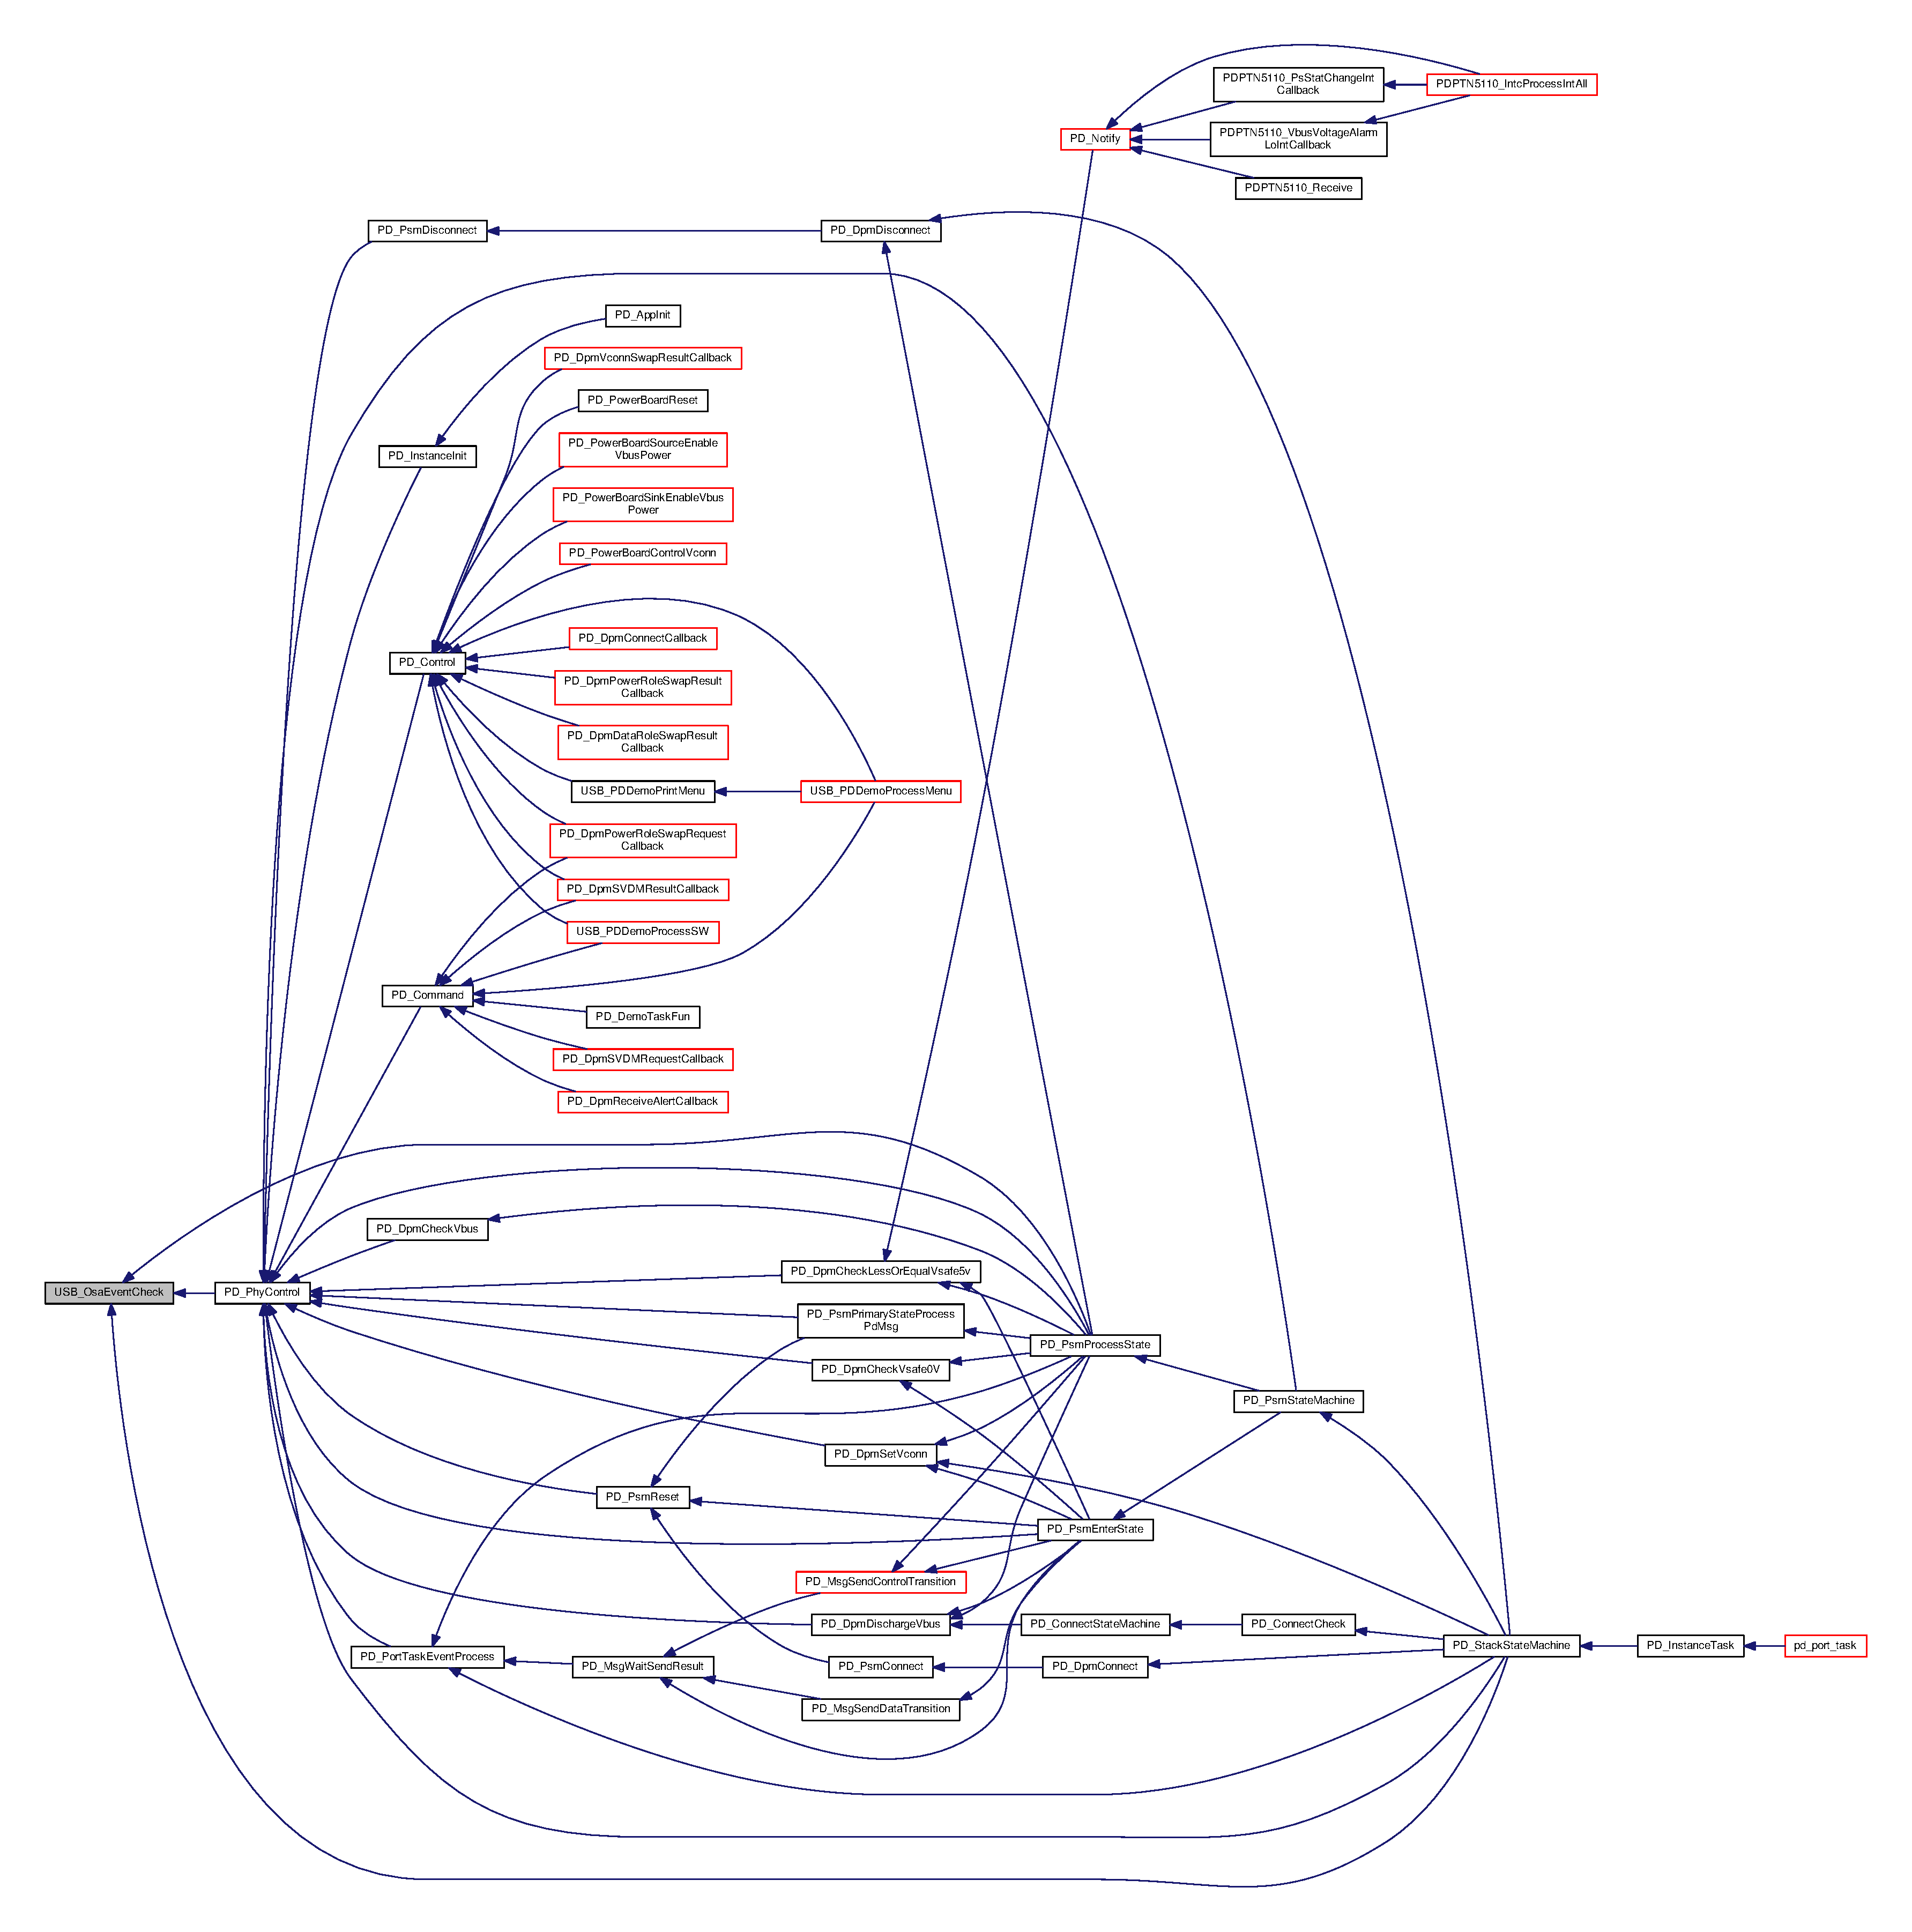
\includegraphics[width=350pt]{group__usb__os__abstraction_gab25fb5d93d3b665ca8eadf2a670d3361_icgraph}
\end{center}
\end{figure}


\hypertarget{group__usb__os__abstraction_ga90357f04d40469dc07104033b3c8581c}{\index{Usb\-\_\-os\-\_\-abstraction@{Usb\-\_\-os\-\_\-abstraction}!U\-S\-B\-\_\-\-Osa\-Event\-Clear@{U\-S\-B\-\_\-\-Osa\-Event\-Clear}}
\index{U\-S\-B\-\_\-\-Osa\-Event\-Clear@{U\-S\-B\-\_\-\-Osa\-Event\-Clear}!Usb_os_abstraction@{Usb\-\_\-os\-\_\-abstraction}}
\subsubsection[{U\-S\-B\-\_\-\-Osa\-Event\-Clear}]{\setlength{\rightskip}{0pt plus 5cm}{\bf usb\-\_\-osa\-\_\-status\-\_\-t} U\-S\-B\-\_\-\-Osa\-Event\-Clear (
\begin{DoxyParamCaption}
\item[{{\bf usb\-\_\-osa\-\_\-event\-\_\-handle}}]{handle, }
\item[{uint32\-\_\-t}]{bit\-Mask}
\end{DoxyParamCaption}
)}}\label{group__usb__os__abstraction_ga90357f04d40469dc07104033b3c8581c}


Clears an event flag. 

This function clears flags of an event object.


\begin{DoxyParams}{Parameters}
{\em handle} & Pointer to the event object \\
\hline
{\em bit\-Mask} & Event flags to be cleared.\\
\hline
\end{DoxyParams}
\begin{DoxyReturn}{Returns}
An U\-S\-B O\-S\-A error code or k\-Status\-\_\-\-O\-S\-A\-\_\-\-Success.
\end{DoxyReturn}
Example\-: 
\begin{DoxyCode}
\hyperlink{group__usb__os__abstraction_ga8de2fb7579de0a6621bbc1776519b0a9}{usb\_osa\_status\_t}     usbOsaStatus;
...
usbOsaStatus = \hyperlink{group__usb__os__abstraction_ga90357f04d40469dc07104033b3c8581c}{USB\_OsaEventClear}(eventHandle, 0x01U);
\end{DoxyCode}
 
\begin{DoxyCode}
258 \{
259     \hyperlink{struct__usb__osa__event__struct}{usb\_osa\_event\_struct\_t} *\textcolor{keyword}{event} = (
      \hyperlink{struct__usb__osa__event__struct}{usb\_osa\_event\_struct\_t} *)handle;
260     uint32\_t bits;
261     \hyperlink{usb__osa__bm_8h_a8dbccf46cc2f8e3b5cece6a4a84f7ae8}{USB\_OSA\_SR\_ALLOC}();
262 
263     \textcolor{keywordflow}{if} (handle)
264     \{
265         \hyperlink{usb__osa__bm_8h_a0485f70bf9c9a22f0340f014bc567362}{USB\_OSA\_ENTER\_CRITICAL}();
266         bits = \textcolor{keyword}{event}->value & bitMask;
267         \textcolor{keyword}{event}->value &= ~bits;
268         \hyperlink{usb__osa__bm_8h_a5b8053eca19b6df666a26fad3b07f953}{USB\_OSA\_EXIT\_CRITICAL}();
269         \textcolor{keywordflow}{return} \hyperlink{group__usb__os__abstraction_gga453ebd2f93aafb8c938c3a23c815f9bdab90805fb75297fda1ca60dbb2283f933}{kStatus\_USB\_OSA\_Success};
270     \}
271     \textcolor{keywordflow}{return} \hyperlink{group__usb__os__abstraction_gga453ebd2f93aafb8c938c3a23c815f9bda40b794ea06e27b8ec1d67538f12eb350}{kStatus\_USB\_OSA\_Error};
272 \}
\end{DoxyCode}


Here is the caller graph for this function\-:
\nopagebreak
\begin{figure}[H]
\begin{center}
\leavevmode
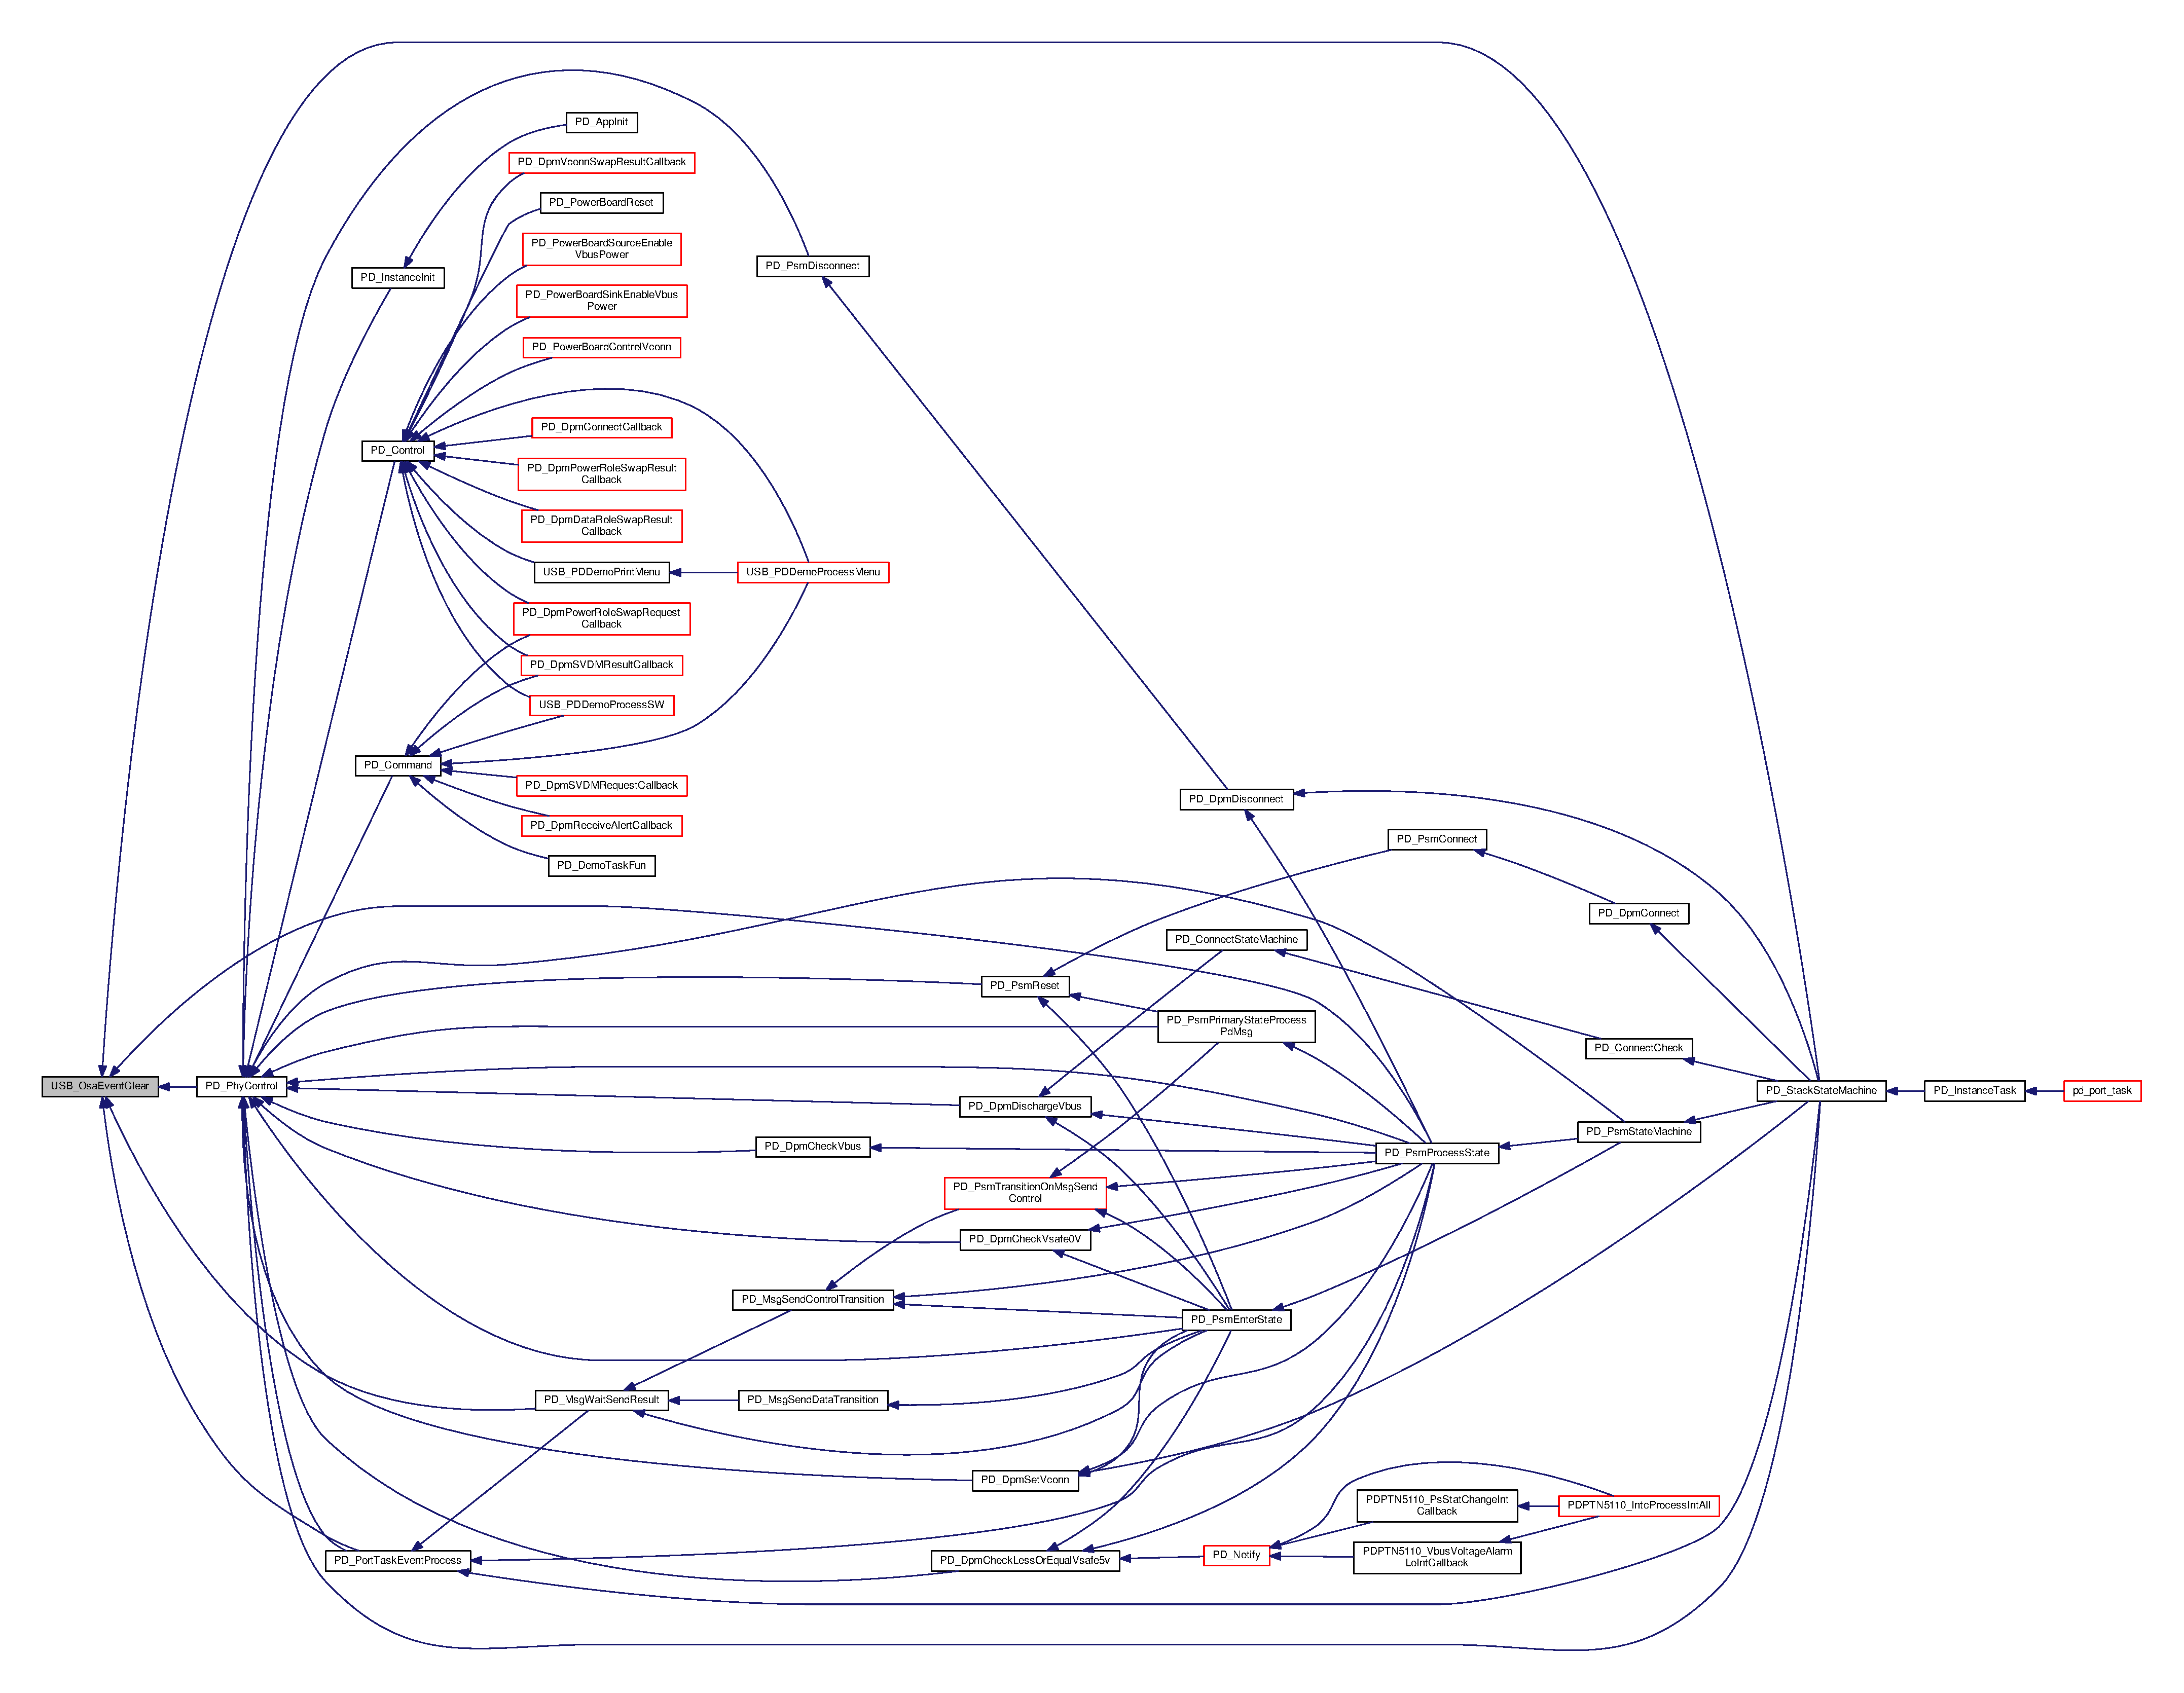
\includegraphics[width=350pt]{group__usb__os__abstraction_ga90357f04d40469dc07104033b3c8581c_icgraph}
\end{center}
\end{figure}


\hypertarget{group__usb__os__abstraction_gaf38d525580499ff2657303eb807efc61}{\index{Usb\-\_\-os\-\_\-abstraction@{Usb\-\_\-os\-\_\-abstraction}!U\-S\-B\-\_\-\-Osa\-Event\-Create@{U\-S\-B\-\_\-\-Osa\-Event\-Create}}
\index{U\-S\-B\-\_\-\-Osa\-Event\-Create@{U\-S\-B\-\_\-\-Osa\-Event\-Create}!Usb_os_abstraction@{Usb\-\_\-os\-\_\-abstraction}}
\subsubsection[{U\-S\-B\-\_\-\-Osa\-Event\-Create}]{\setlength{\rightskip}{0pt plus 5cm}{\bf usb\-\_\-osa\-\_\-status\-\_\-t} U\-S\-B\-\_\-\-Osa\-Event\-Create (
\begin{DoxyParamCaption}
\item[{{\bf usb\-\_\-osa\-\_\-event\-\_\-handle} $\ast$}]{handle, }
\item[{uint32\-\_\-t}]{flag}
\end{DoxyParamCaption}
)}}\label{group__usb__os__abstraction_gaf38d525580499ff2657303eb807efc61}


Creates an event object with all flags cleared. 

This function creates an event object and sets its clear mode. If the clear mode is k\-U\-S\-B\-\_\-\-Osa\-Event\-Auto\-Clear, when a task gets the event flags, these flags are cleared automatically. If the clear mode is k\-U\-S\-B\-\_\-\-Osa\-Event\-Manual\-Clear, the flags must be cleared manually.


\begin{DoxyParams}{Parameters}
{\em handle} & It is an out parameter, which is used to return the pointer of the event object. \\
\hline
{\em flag} & The event is auto-\/clear or manual-\/clear. See the enumeration \hyperlink{group__usb__os__abstraction_gaa3f24eb2797924d385f01a78695b645c}{usb\-\_\-osa\-\_\-event\-\_\-mode\-\_\-t}.\\
\hline
\end{DoxyParams}
\begin{DoxyReturn}{Returns}
A U\-S\-B O\-S\-A error code or k\-Status\-\_\-\-O\-S\-A\-\_\-\-Success.
\end{DoxyReturn}
Example\-: 
\begin{DoxyCode}
\hyperlink{group__usb__os__abstraction_gaa5faa1787d0c772a2cf101b3eaf654f6}{usb\_osa\_event\_handle} eventHandle;
\hyperlink{group__usb__os__abstraction_ga8de2fb7579de0a6621bbc1776519b0a9}{usb\_osa\_status\_t}     usbOsaStatus;
usbOsaStatus = \hyperlink{group__usb__os__abstraction_gaf38d525580499ff2657303eb807efc61}{USB\_OsaEventCreate}(&eventHandle, 
      \hyperlink{group__usb__os__abstraction_ggaf3dc48c688f7c71cce122a1a0d4a12bdac7c0be065c2f8e1f9c25758dd648fa24}{kUSB\_OsaEventManualClear});
\end{DoxyCode}
 
\begin{DoxyCode}
126 \{
127     \hyperlink{struct__usb__osa__event__struct}{usb\_osa\_event\_struct\_t} *\textcolor{keyword}{event} = NULL;
128     \hyperlink{usb__osa__bm_8h_a8dbccf46cc2f8e3b5cece6a4a84f7ae8}{USB\_OSA\_SR\_ALLOC}();
129 
130     \textcolor{keywordflow}{if} (!handle)
131     \{
132         \textcolor{keywordflow}{return} \hyperlink{group__usb__os__abstraction_gga453ebd2f93aafb8c938c3a23c815f9bda40b794ea06e27b8ec1d67538f12eb350}{kStatus\_USB\_OSA\_Error};
133     \}
134 
135     \hyperlink{usb__osa__bm_8h_a0485f70bf9c9a22f0340f014bc567362}{USB\_OSA\_ENTER\_CRITICAL}();
136     \textcolor{keywordflow}{for} (uint32\_t i = 0; i < \hyperlink{usb__osa__bm_8c_af0b1e39abc5fdc23219b990ac3ef511f}{USB\_OSA\_BM\_EVENT\_COUNT}; i++)
137     \{
138         \textcolor{keywordflow}{if} (0 == \hyperlink{usb__osa__bm_8c_aba773069fb857f2303233899f250978e}{s\_UsbBmEventStruct}[i].isUsed)
139         \{
140             \textcolor{keyword}{event} = &\hyperlink{usb__osa__bm_8c_aba773069fb857f2303233899f250978e}{s\_UsbBmEventStruct}[i];
141             \textcolor{keywordflow}{break};
142         \}
143     \}
144 
145     \textcolor{keywordflow}{if} (NULL == event)
146     \{
147         \hyperlink{usb__osa__bm_8h_a5b8053eca19b6df666a26fad3b07f953}{USB\_OSA\_EXIT\_CRITICAL}();
148         \textcolor{keywordflow}{return} \hyperlink{group__usb__os__abstraction_gga453ebd2f93aafb8c938c3a23c815f9bda40b794ea06e27b8ec1d67538f12eb350}{kStatus\_USB\_OSA\_Error};
149     \}
150 
151     \textcolor{keyword}{event}->value = 0U;
152     \textcolor{keyword}{event}->flag = flag;
153     \textcolor{keyword}{event}->isUsed = 1;
154     *handle = event;
155     \hyperlink{usb__osa__bm_8h_a5b8053eca19b6df666a26fad3b07f953}{USB\_OSA\_EXIT\_CRITICAL}();
156     \textcolor{keywordflow}{return} \hyperlink{group__usb__os__abstraction_gga453ebd2f93aafb8c938c3a23c815f9bdab90805fb75297fda1ca60dbb2283f933}{kStatus\_USB\_OSA\_Success};
157 \}
\end{DoxyCode}


Here is the call graph for this function\-:
\nopagebreak
\begin{figure}[H]
\begin{center}
\leavevmode
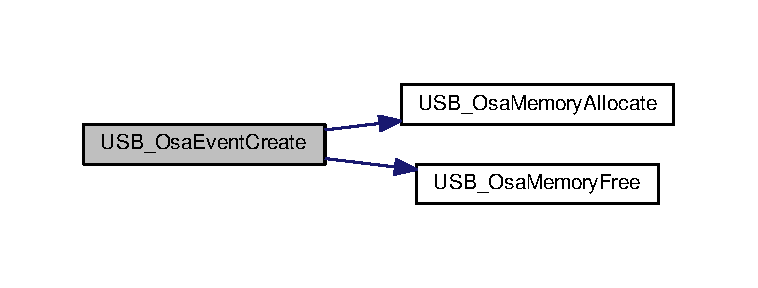
\includegraphics[width=350pt]{group__usb__os__abstraction_gaf38d525580499ff2657303eb807efc61_cgraph}
\end{center}
\end{figure}




Here is the caller graph for this function\-:
\nopagebreak
\begin{figure}[H]
\begin{center}
\leavevmode
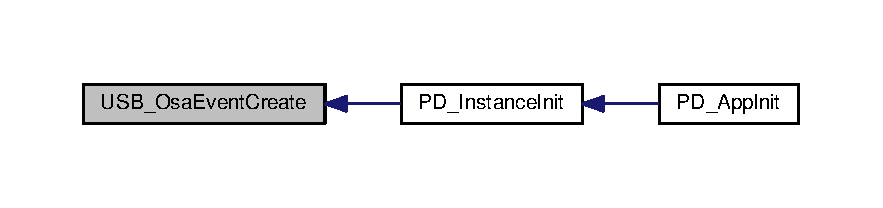
\includegraphics[width=350pt]{group__usb__os__abstraction_gaf38d525580499ff2657303eb807efc61_icgraph}
\end{center}
\end{figure}


\hypertarget{group__usb__os__abstraction_ga3d07a809b1fa8450c1383aa8bbd49b37}{\index{Usb\-\_\-os\-\_\-abstraction@{Usb\-\_\-os\-\_\-abstraction}!U\-S\-B\-\_\-\-Osa\-Event\-Destroy@{U\-S\-B\-\_\-\-Osa\-Event\-Destroy}}
\index{U\-S\-B\-\_\-\-Osa\-Event\-Destroy@{U\-S\-B\-\_\-\-Osa\-Event\-Destroy}!Usb_os_abstraction@{Usb\-\_\-os\-\_\-abstraction}}
\subsubsection[{U\-S\-B\-\_\-\-Osa\-Event\-Destroy}]{\setlength{\rightskip}{0pt plus 5cm}{\bf usb\-\_\-osa\-\_\-status\-\_\-t} U\-S\-B\-\_\-\-Osa\-Event\-Destroy (
\begin{DoxyParamCaption}
\item[{{\bf usb\-\_\-osa\-\_\-event\-\_\-handle}}]{handle}
\end{DoxyParamCaption}
)}}\label{group__usb__os__abstraction_ga3d07a809b1fa8450c1383aa8bbd49b37}


Destroys a created event object. 


\begin{DoxyParams}{Parameters}
{\em handle} & Pointer to the event object.\\
\hline
\end{DoxyParams}
\begin{DoxyReturn}{Returns}
A U\-S\-B O\-S\-A error code or k\-Status\-\_\-\-O\-S\-A\-\_\-\-Success.
\end{DoxyReturn}
Example\-: 
\begin{DoxyCode}
\hyperlink{group__usb__os__abstraction_ga8de2fb7579de0a6621bbc1776519b0a9}{usb\_osa\_status\_t}     usbOsaStatus;
...
usbOsaStatus = \hyperlink{group__usb__os__abstraction_ga3d07a809b1fa8450c1383aa8bbd49b37}{USB\_OsaEventDestroy}(eventHandle);
\end{DoxyCode}
 
\begin{DoxyCode}
160 \{
161     \hyperlink{struct__usb__osa__event__struct}{usb\_osa\_event\_struct\_t} *\textcolor{keyword}{event} = (
      \hyperlink{struct__usb__osa__event__struct}{usb\_osa\_event\_struct\_t} *)handle;
162     \hyperlink{usb__osa__bm_8h_a8dbccf46cc2f8e3b5cece6a4a84f7ae8}{USB\_OSA\_SR\_ALLOC}();
163 
164     \textcolor{keywordflow}{if} (handle)
165     \{
166         \hyperlink{usb__osa__bm_8h_a0485f70bf9c9a22f0340f014bc567362}{USB\_OSA\_ENTER\_CRITICAL}();
167         \textcolor{keyword}{event}->isUsed = 0;
168         \hyperlink{usb__osa__bm_8h_a5b8053eca19b6df666a26fad3b07f953}{USB\_OSA\_EXIT\_CRITICAL}();
169         \textcolor{keywordflow}{return} \hyperlink{group__usb__os__abstraction_gga453ebd2f93aafb8c938c3a23c815f9bdab90805fb75297fda1ca60dbb2283f933}{kStatus\_USB\_OSA\_Success};
170     \}
171     \textcolor{keywordflow}{return} \hyperlink{group__usb__os__abstraction_gga453ebd2f93aafb8c938c3a23c815f9bda40b794ea06e27b8ec1d67538f12eb350}{kStatus\_USB\_OSA\_Error};
172 \}
\end{DoxyCode}


Here is the call graph for this function\-:
\nopagebreak
\begin{figure}[H]
\begin{center}
\leavevmode
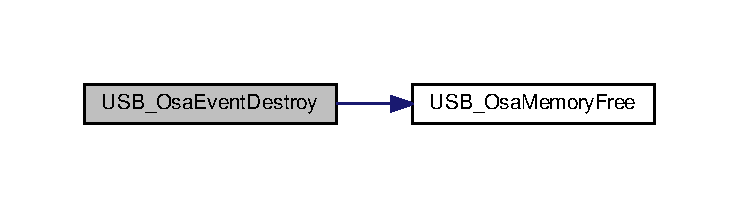
\includegraphics[width=350pt]{group__usb__os__abstraction_ga3d07a809b1fa8450c1383aa8bbd49b37_cgraph}
\end{center}
\end{figure}




Here is the caller graph for this function\-:
\nopagebreak
\begin{figure}[H]
\begin{center}
\leavevmode
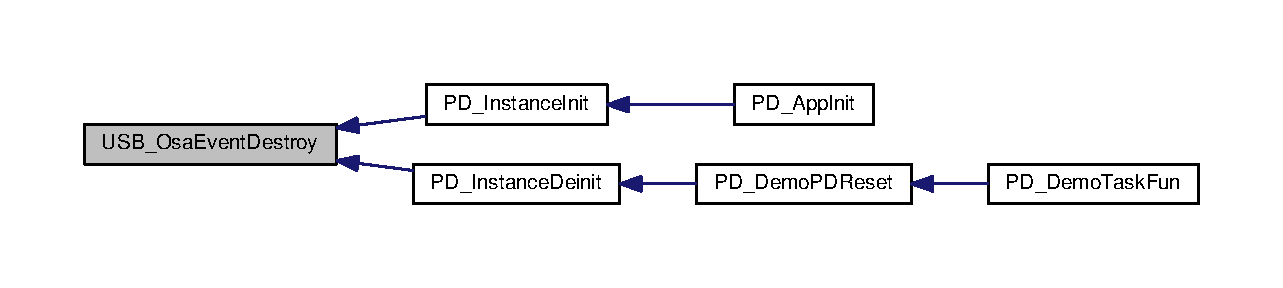
\includegraphics[width=350pt]{group__usb__os__abstraction_ga3d07a809b1fa8450c1383aa8bbd49b37_icgraph}
\end{center}
\end{figure}


\hypertarget{group__usb__os__abstraction_gaa83073c31cced5742027d4046bd633db}{\index{Usb\-\_\-os\-\_\-abstraction@{Usb\-\_\-os\-\_\-abstraction}!U\-S\-B\-\_\-\-Osa\-Event\-Set@{U\-S\-B\-\_\-\-Osa\-Event\-Set}}
\index{U\-S\-B\-\_\-\-Osa\-Event\-Set@{U\-S\-B\-\_\-\-Osa\-Event\-Set}!Usb_os_abstraction@{Usb\-\_\-os\-\_\-abstraction}}
\subsubsection[{U\-S\-B\-\_\-\-Osa\-Event\-Set}]{\setlength{\rightskip}{0pt plus 5cm}{\bf usb\-\_\-osa\-\_\-status\-\_\-t} U\-S\-B\-\_\-\-Osa\-Event\-Set (
\begin{DoxyParamCaption}
\item[{{\bf usb\-\_\-osa\-\_\-event\-\_\-handle}}]{handle, }
\item[{uint32\-\_\-t}]{bit\-Mask}
\end{DoxyParamCaption}
)}}\label{group__usb__os__abstraction_gaa83073c31cced5742027d4046bd633db}


Sets an event flag. 

Sets specified flags for an event object.


\begin{DoxyParams}{Parameters}
{\em handle} & Pointer to the event object. \\
\hline
{\em bit\-Mask} & Event flags to be set.\\
\hline
\end{DoxyParams}
\begin{DoxyReturn}{Returns}
A U\-S\-B O\-S\-A error code or k\-Status\-\_\-\-O\-S\-A\-\_\-\-Success.
\end{DoxyReturn}
Example\-: 
\begin{DoxyCode}
\hyperlink{group__usb__os__abstraction_ga8de2fb7579de0a6621bbc1776519b0a9}{usb\_osa\_status\_t}     usbOsaStatus;
...
usbOsaStatus = \hyperlink{group__usb__os__abstraction_gaa83073c31cced5742027d4046bd633db}{USB\_OsaEventSet}(eventHandle, 0x01U);
\end{DoxyCode}
 
\begin{DoxyCode}
175 \{
176     \hyperlink{struct__usb__osa__event__struct}{usb\_osa\_event\_struct\_t} *\textcolor{keyword}{event} = (
      \hyperlink{struct__usb__osa__event__struct}{usb\_osa\_event\_struct\_t} *)handle;
177     \hyperlink{usb__osa__bm_8h_a8dbccf46cc2f8e3b5cece6a4a84f7ae8}{USB\_OSA\_SR\_ALLOC}();
178 
179     \textcolor{keywordflow}{if} (handle)
180     \{
181         \hyperlink{usb__osa__bm_8h_a0485f70bf9c9a22f0340f014bc567362}{USB\_OSA\_ENTER\_CRITICAL}();
182         \textcolor{keyword}{event}->value |= bitMask;
183         \hyperlink{usb__osa__bm_8h_a5b8053eca19b6df666a26fad3b07f953}{USB\_OSA\_EXIT\_CRITICAL}();
184         \textcolor{keywordflow}{return} \hyperlink{group__usb__os__abstraction_gga453ebd2f93aafb8c938c3a23c815f9bdab90805fb75297fda1ca60dbb2283f933}{kStatus\_USB\_OSA\_Success};
185     \}
186     \textcolor{keywordflow}{return} \hyperlink{group__usb__os__abstraction_gga453ebd2f93aafb8c938c3a23c815f9bda40b794ea06e27b8ec1d67538f12eb350}{kStatus\_USB\_OSA\_Error};
187 \}
\end{DoxyCode}


Here is the caller graph for this function\-:
\nopagebreak
\begin{figure}[H]
\begin{center}
\leavevmode
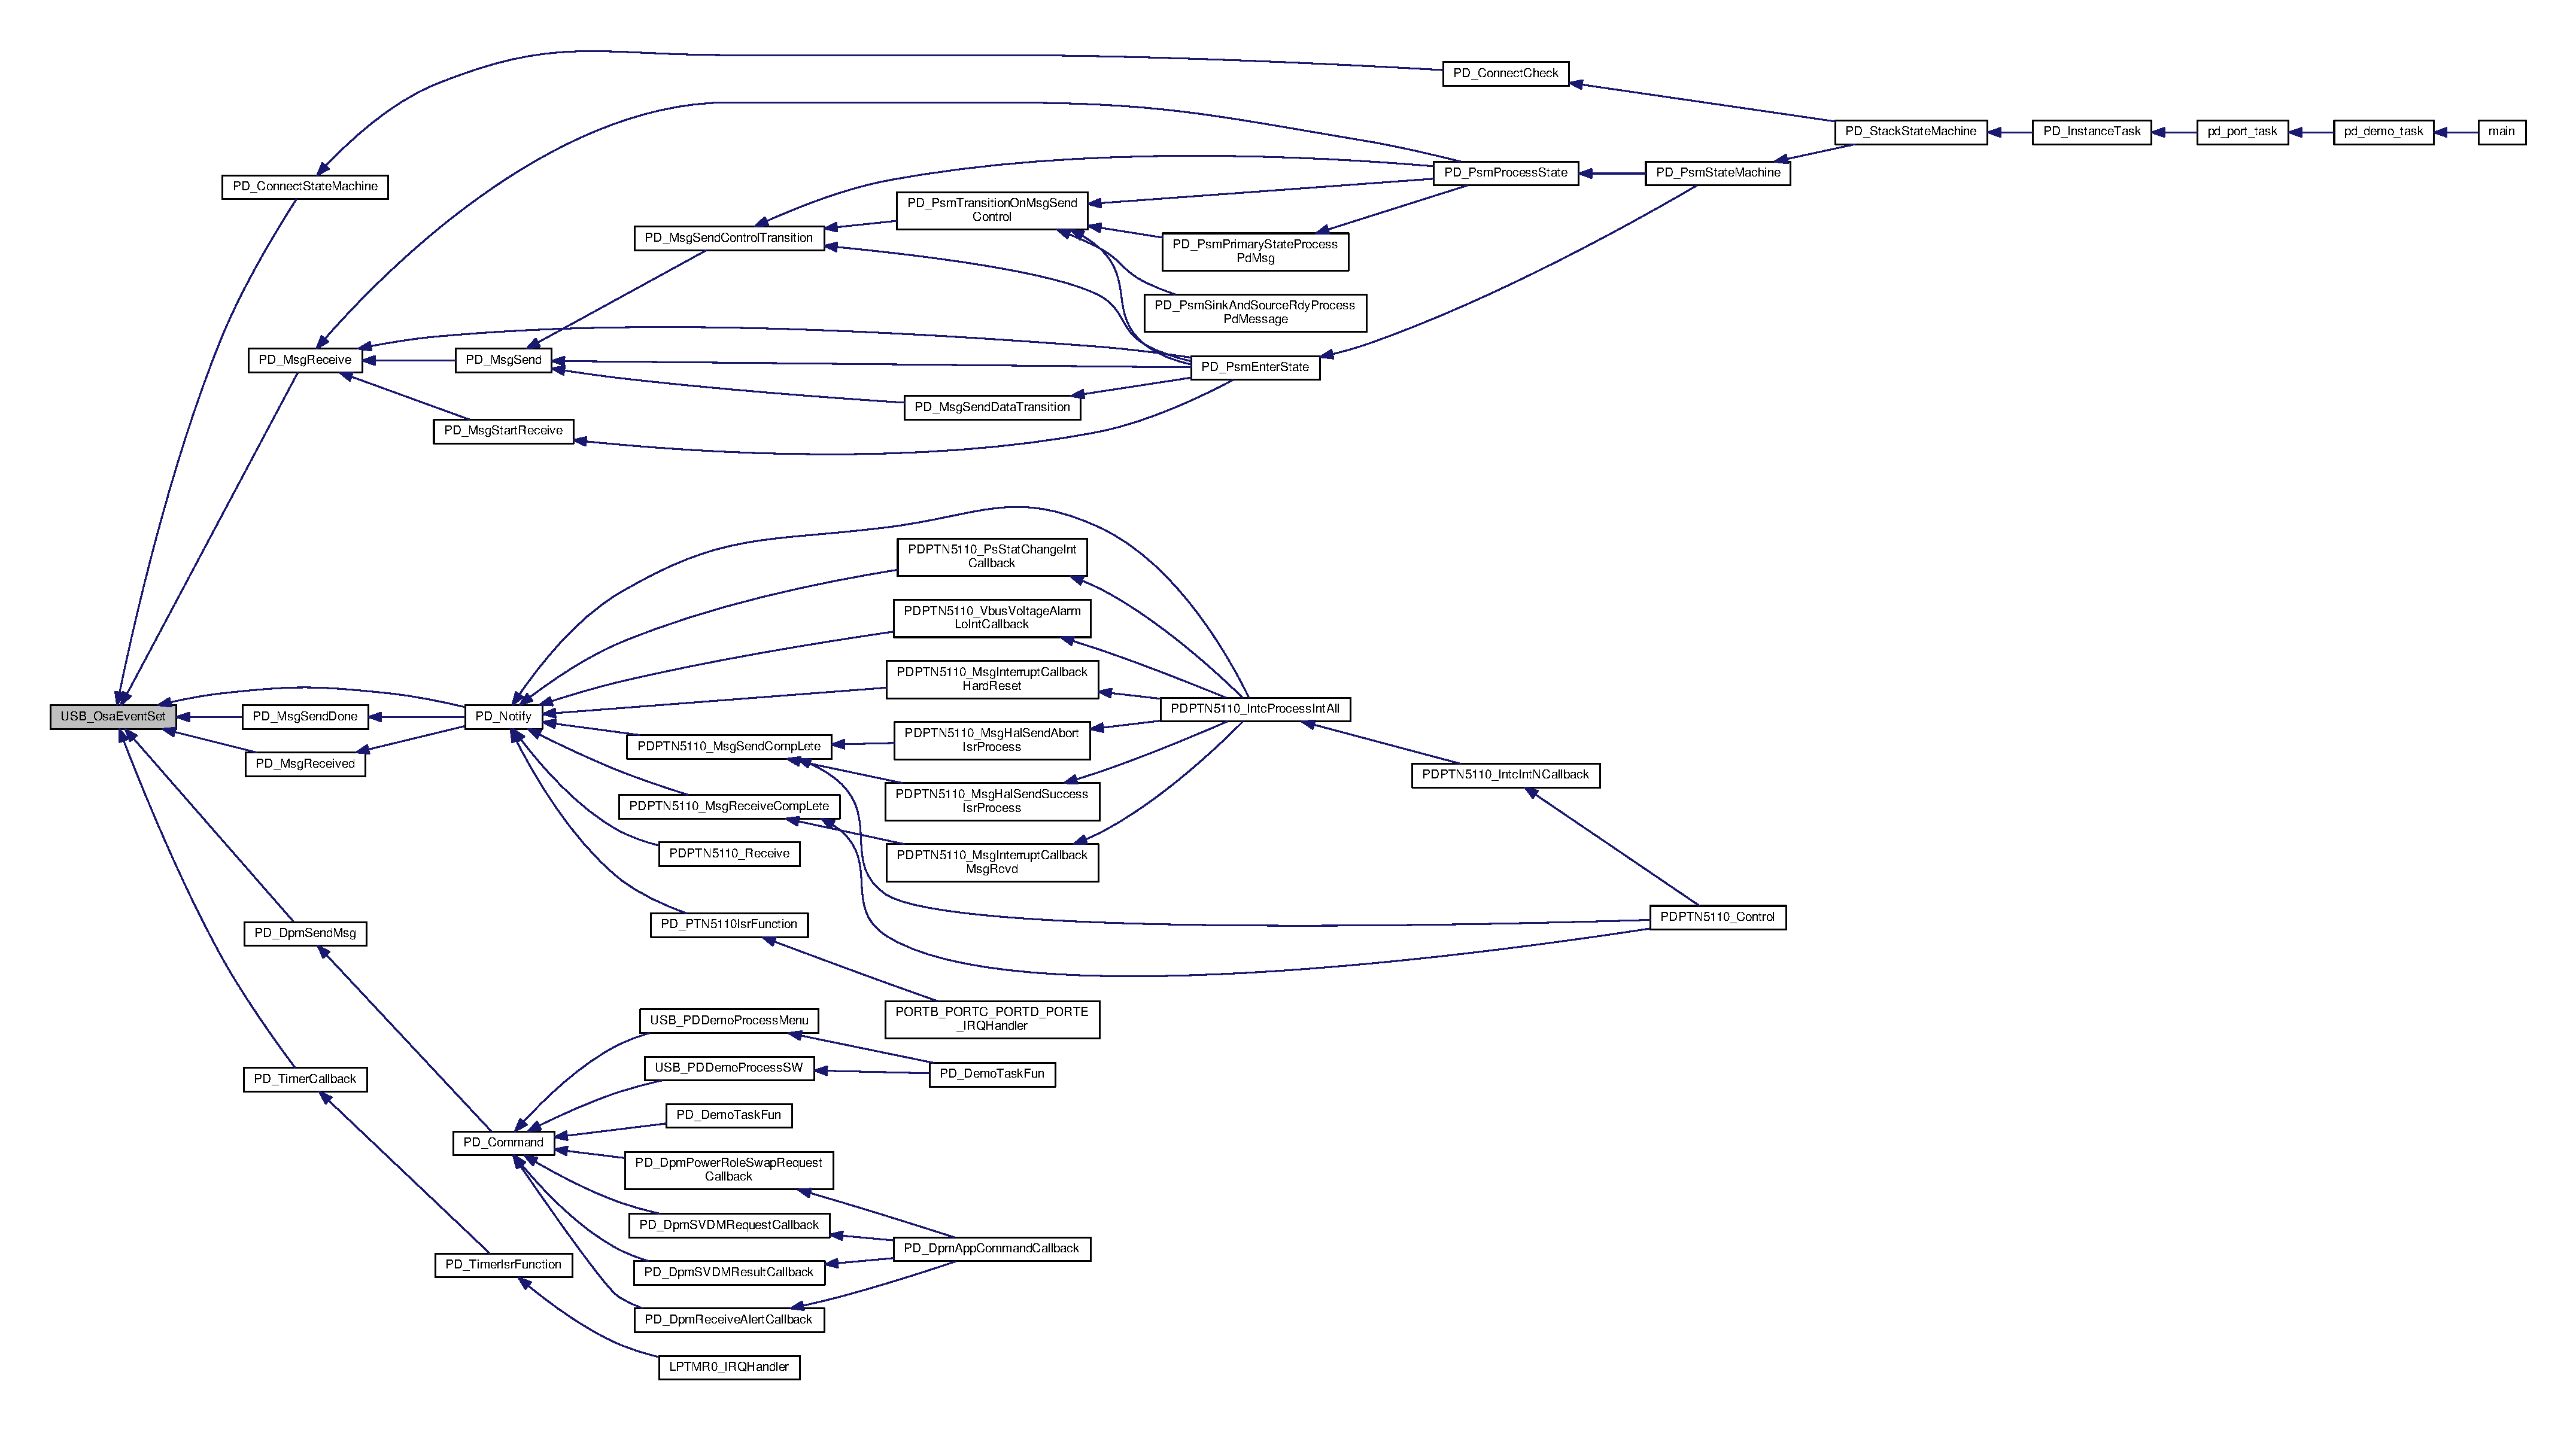
\includegraphics[width=350pt]{group__usb__os__abstraction_gaa83073c31cced5742027d4046bd633db_icgraph}
\end{center}
\end{figure}


\hypertarget{group__usb__os__abstraction_ga5ce587209d676871f3ec62900054febd}{\index{Usb\-\_\-os\-\_\-abstraction@{Usb\-\_\-os\-\_\-abstraction}!U\-S\-B\-\_\-\-Osa\-Event\-Wait@{U\-S\-B\-\_\-\-Osa\-Event\-Wait}}
\index{U\-S\-B\-\_\-\-Osa\-Event\-Wait@{U\-S\-B\-\_\-\-Osa\-Event\-Wait}!Usb_os_abstraction@{Usb\-\_\-os\-\_\-abstraction}}
\subsubsection[{U\-S\-B\-\_\-\-Osa\-Event\-Wait}]{\setlength{\rightskip}{0pt plus 5cm}{\bf usb\-\_\-osa\-\_\-status\-\_\-t} U\-S\-B\-\_\-\-Osa\-Event\-Wait (
\begin{DoxyParamCaption}
\item[{{\bf usb\-\_\-osa\-\_\-event\-\_\-handle}}]{handle, }
\item[{uint32\-\_\-t}]{bit\-Mask, }
\item[{uint32\-\_\-t}]{flag, }
\item[{uint32\-\_\-t}]{timeout, }
\item[{uint32\-\_\-t $\ast$}]{bit\-Set}
\end{DoxyParamCaption}
)}}\label{group__usb__os__abstraction_ga5ce587209d676871f3ec62900054febd}


Waits for an event flag. 

This function waits for a combination of flags to be set in an event object. An applications can wait for any/all bits to be set. This function can get the flags that wake up the waiting task.


\begin{DoxyParams}{Parameters}
{\em handle} & Pointer to the event object. \\
\hline
{\em bit\-Mask} & Event flags to wait. \\
\hline
{\em flag} & Wait all flags or any flag to be set. 0\-U -\/ wait any flag, others, wait all flags. \\
\hline
{\em timeout} & The maximum number of milliseconds to wait for the event. If the wait condition is not met, passing 0\-U waits indefinitely when the environment is an R\-T\-O\-S and returns the k\-Status\-\_\-\-O\-S\-A\-\_\-\-Timeout immediately. Pass any value for the bare metal. \\
\hline
{\em bit\-Set} & Flags that wake up the waiting task are obtained by this parameter.\\
\hline
\end{DoxyParams}
\begin{DoxyReturn}{Returns}
An U\-S\-B O\-S\-A error code or k\-Status\-\_\-\-O\-S\-A\-\_\-\-Success.
\end{DoxyReturn}
Example\-: 
\begin{DoxyCode}
\hyperlink{group__usb__os__abstraction_ga8de2fb7579de0a6621bbc1776519b0a9}{usb\_osa\_status\_t}     usbOsaStatus;
uint32\_t             bitSet;
...
usbOsaStatus = \hyperlink{group__usb__os__abstraction_ga5ce587209d676871f3ec62900054febd}{USB\_OsaEventWait}(eventHandle, 0x01U, 0U, 0U, &bitSet);
\end{DoxyCode}
 
\begin{DoxyCode}
191 \{
192     \hyperlink{struct__usb__osa__event__struct}{usb\_osa\_event\_struct\_t} *\textcolor{keyword}{event} = (
      \hyperlink{struct__usb__osa__event__struct}{usb\_osa\_event\_struct\_t} *)handle;
193     uint32\_t bits;
194     \hyperlink{usb__osa__bm_8h_a8dbccf46cc2f8e3b5cece6a4a84f7ae8}{USB\_OSA\_SR\_ALLOC}();
195 
196     \textcolor{keywordflow}{if} (handle)
197     \{
198         \hyperlink{usb__osa__bm_8h_a0485f70bf9c9a22f0340f014bc567362}{USB\_OSA\_ENTER\_CRITICAL}();
199         bits = \textcolor{keyword}{event}->value & bitMask;
200         \textcolor{keywordflow}{if} (flag)
201         \{
202             \textcolor{keywordflow}{if} (bits != bitMask)
203             \{
204                 \hyperlink{usb__osa__bm_8h_a5b8053eca19b6df666a26fad3b07f953}{USB\_OSA\_EXIT\_CRITICAL}();
205                 \textcolor{keywordflow}{return} \hyperlink{group__usb__os__abstraction_gga453ebd2f93aafb8c938c3a23c815f9bda9ff36cb34c565283214974d1097d08df}{kStatus\_USB\_OSA\_TimeOut};
206             \}
207         \}
208         \textcolor{keywordflow}{else}
209         \{
210             \textcolor{keywordflow}{if} (!bits)
211             \{
212                 \hyperlink{usb__osa__bm_8h_a5b8053eca19b6df666a26fad3b07f953}{USB\_OSA\_EXIT\_CRITICAL}();
213                 \textcolor{keywordflow}{return} \hyperlink{group__usb__os__abstraction_gga453ebd2f93aafb8c938c3a23c815f9bda9ff36cb34c565283214974d1097d08df}{kStatus\_USB\_OSA\_TimeOut};
214             \}
215         \}
216         \textcolor{keywordflow}{if} (bitSet)
217         \{
218             *bitSet = bits;
219         \}
220         \textcolor{keywordflow}{if} (event->flag)
221         \{
222             \textcolor{keyword}{event}->value &= ~bits;
223         \}
224         \hyperlink{usb__osa__bm_8h_a5b8053eca19b6df666a26fad3b07f953}{USB\_OSA\_EXIT\_CRITICAL}();
225         \textcolor{keywordflow}{return} \hyperlink{group__usb__os__abstraction_gga453ebd2f93aafb8c938c3a23c815f9bdab90805fb75297fda1ca60dbb2283f933}{kStatus\_USB\_OSA\_Success};
226     \}
227     \textcolor{keywordflow}{return} \hyperlink{group__usb__os__abstraction_gga453ebd2f93aafb8c938c3a23c815f9bda40b794ea06e27b8ec1d67538f12eb350}{kStatus\_USB\_OSA\_Error};
228 \}
\end{DoxyCode}


Here is the caller graph for this function\-:
\nopagebreak
\begin{figure}[H]
\begin{center}
\leavevmode
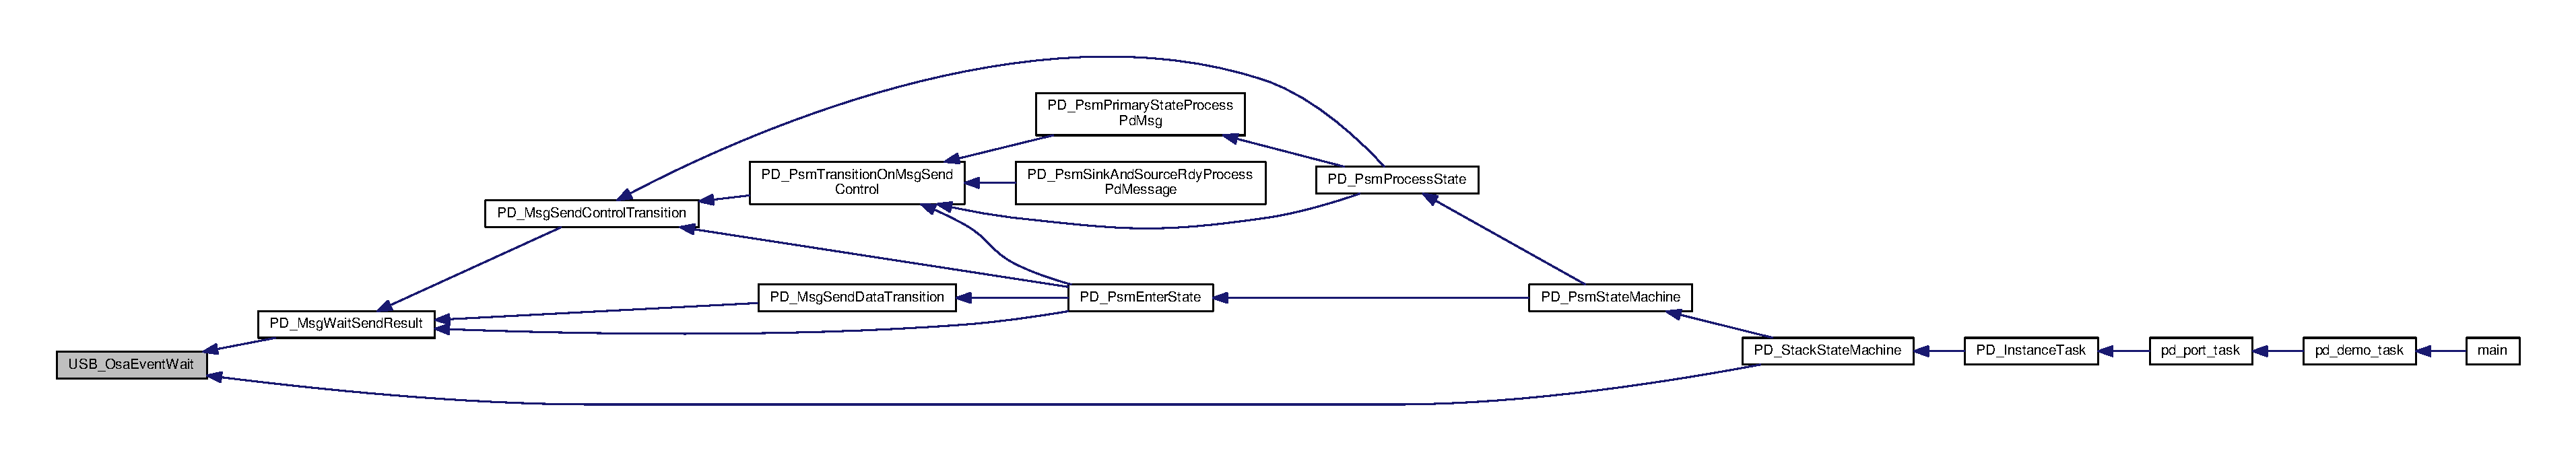
\includegraphics[width=350pt]{group__usb__os__abstraction_ga5ce587209d676871f3ec62900054febd_icgraph}
\end{center}
\end{figure}


\hypertarget{group__usb__os__abstraction_gab17b3446bbcfb6207dc230fcdd4c9f99}{\index{Usb\-\_\-os\-\_\-abstraction@{Usb\-\_\-os\-\_\-abstraction}!U\-S\-B\-\_\-\-Osa\-Memory\-Allocate@{U\-S\-B\-\_\-\-Osa\-Memory\-Allocate}}
\index{U\-S\-B\-\_\-\-Osa\-Memory\-Allocate@{U\-S\-B\-\_\-\-Osa\-Memory\-Allocate}!Usb_os_abstraction@{Usb\-\_\-os\-\_\-abstraction}}
\subsubsection[{U\-S\-B\-\_\-\-Osa\-Memory\-Allocate}]{\setlength{\rightskip}{0pt plus 5cm}void$\ast$ U\-S\-B\-\_\-\-Osa\-Memory\-Allocate (
\begin{DoxyParamCaption}
\item[{uint32\-\_\-t}]{length}
\end{DoxyParamCaption}
)}}\label{group__usb__os__abstraction_gab17b3446bbcfb6207dc230fcdd4c9f99}


Reserves the requested amount of memory in bytes. 

The function is used to reserve the requested amount of memory in bytes and initializes it to 0.


\begin{DoxyParams}{Parameters}
{\em length} & Amount of bytes to reserve.\\
\hline
\end{DoxyParams}
\begin{DoxyReturn}{Returns}
Pointer to the reserved memory. N\-U\-L\-L if memory can't be allocated. 
\end{DoxyReturn}

\begin{DoxyCode}
96 \{
97     \textcolor{keywordtype}{void} *p = (\textcolor{keywordtype}{void} *)malloc(length);
98     uint8\_t *temp = (uint8\_t *)p;
99     \textcolor{keywordflow}{if} (p)
100     \{
101         \textcolor{keywordflow}{for} (uint32\_t count = 0U; count < length; count++)
102         \{
103             temp[count] = 0U;
104         \}
105     \}
106     \textcolor{keywordflow}{return} p;
107 \}
\end{DoxyCode}


Here is the caller graph for this function\-:
\nopagebreak
\begin{figure}[H]
\begin{center}
\leavevmode
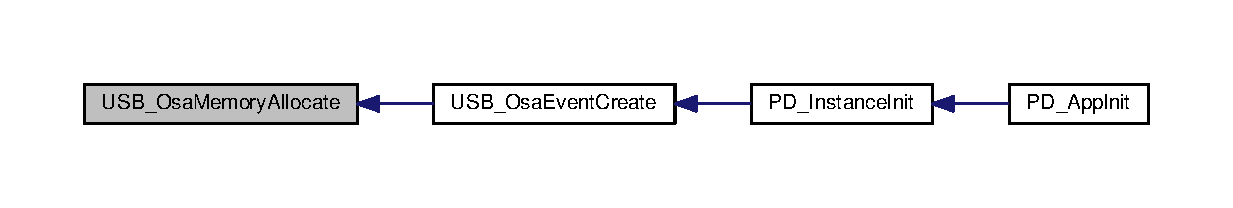
\includegraphics[width=350pt]{group__usb__os__abstraction_gab17b3446bbcfb6207dc230fcdd4c9f99_icgraph}
\end{center}
\end{figure}


\hypertarget{group__usb__os__abstraction_ga3d4a16dd11d39ce340299876f92d9366}{\index{Usb\-\_\-os\-\_\-abstraction@{Usb\-\_\-os\-\_\-abstraction}!U\-S\-B\-\_\-\-Osa\-Memory\-Free@{U\-S\-B\-\_\-\-Osa\-Memory\-Free}}
\index{U\-S\-B\-\_\-\-Osa\-Memory\-Free@{U\-S\-B\-\_\-\-Osa\-Memory\-Free}!Usb_os_abstraction@{Usb\-\_\-os\-\_\-abstraction}}
\subsubsection[{U\-S\-B\-\_\-\-Osa\-Memory\-Free}]{\setlength{\rightskip}{0pt plus 5cm}void U\-S\-B\-\_\-\-Osa\-Memory\-Free (
\begin{DoxyParamCaption}
\item[{void $\ast$}]{p}
\end{DoxyParamCaption}
)}}\label{group__usb__os__abstraction_ga3d4a16dd11d39ce340299876f92d9366}


Frees the memory previously reserved. 

The function is used to free the memory block previously reserved.


\begin{DoxyParams}{Parameters}
{\em p} & Pointer to the start of the memory block previously reserved. \\
\hline
\end{DoxyParams}

\begin{DoxyCode}
110 \{
111     free(p);
112 \}
\end{DoxyCode}


Here is the caller graph for this function\-:
\nopagebreak
\begin{figure}[H]
\begin{center}
\leavevmode
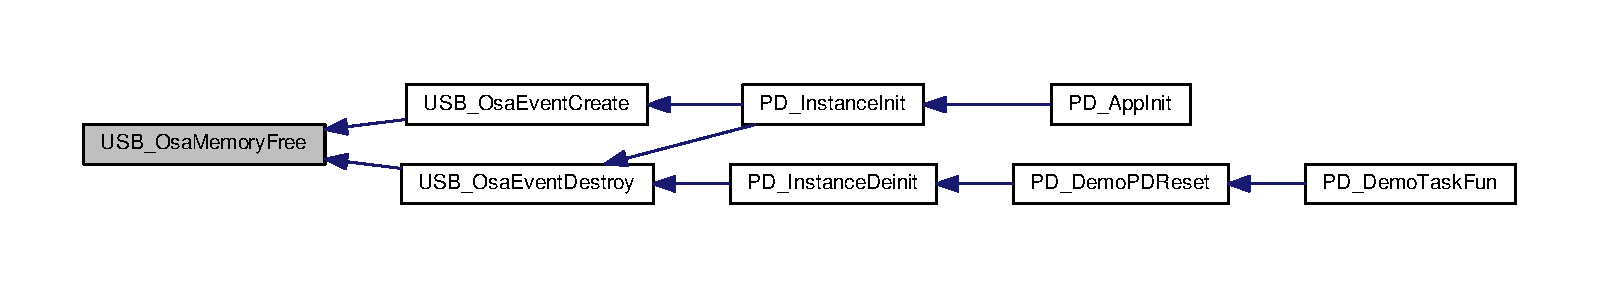
\includegraphics[width=350pt]{group__usb__os__abstraction_ga3d4a16dd11d39ce340299876f92d9366_icgraph}
\end{center}
\end{figure}


\hypertarget{group__usb__os__abstraction_ga734fbdd1bae936ba6758087ad2d9d862}{\index{Usb\-\_\-os\-\_\-abstraction@{Usb\-\_\-os\-\_\-abstraction}!U\-S\-B\-\_\-\-Osa\-Msgq\-Check@{U\-S\-B\-\_\-\-Osa\-Msgq\-Check}}
\index{U\-S\-B\-\_\-\-Osa\-Msgq\-Check@{U\-S\-B\-\_\-\-Osa\-Msgq\-Check}!Usb_os_abstraction@{Usb\-\_\-os\-\_\-abstraction}}
\subsubsection[{U\-S\-B\-\_\-\-Osa\-Msgq\-Check}]{\setlength{\rightskip}{0pt plus 5cm}{\bf usb\-\_\-osa\-\_\-status\-\_\-t} U\-S\-B\-\_\-\-Osa\-Msgq\-Check (
\begin{DoxyParamCaption}
\item[{{\bf usb\-\_\-osa\-\_\-msgq\-\_\-handle}}]{handle, }
\item[{void $\ast$}]{msg}
\end{DoxyParamCaption}
)}}\label{group__usb__os__abstraction_ga734fbdd1bae936ba6758087ad2d9d862}


Checks a message queue and receives a message if the queue is not empty. 

This function checks a message queue and receives a message if the queue is not empty.


\begin{DoxyParams}{Parameters}
{\em handle} & Pointer to a message queue. \\
\hline
{\em msg} & The pointer to save a received message.\\
\hline
\end{DoxyParams}
\begin{DoxyReturn}{Returns}
A U\-S\-B O\-S\-A error code or k\-Status\-\_\-\-O\-S\-A\-\_\-\-Success.
\end{DoxyReturn}
Example\-: 
\begin{DoxyCode}
\hyperlink{group__usb__os__abstraction_gab3a9f26ba50f3abea7fcbac07500cbb8}{usb\_osa\_msgq\_handle}      msgqHandle;
message\_struct\_t         message;
\hyperlink{group__usb__os__abstraction_ga8de2fb7579de0a6621bbc1776519b0a9}{usb\_osa\_status\_t}         usbOsaStatus;
...
usbOsaStatus = \hyperlink{group__usb__os__abstraction_ga734fbdd1bae936ba6758087ad2d9d862}{USB\_OsaMsgqCheck}(msgqHandle, &message);
\end{DoxyCode}
 
\begin{DoxyCode}
516 \{
517     \hyperlink{struct__usb__osa__msgq__struct}{usb\_osa\_msgq\_struct\_t} *msgq = (\hyperlink{struct__usb__osa__msgq__struct}{usb\_osa\_msgq\_struct\_t} *)handle
      ;
518     uint32\_t msgCount;
519     \hyperlink{usb__osa__bm_8h_a8dbccf46cc2f8e3b5cece6a4a84f7ae8}{USB\_OSA\_SR\_ALLOC}();
520 
521     \textcolor{keywordflow}{if} (!handle)
522     \{
523         \textcolor{keywordflow}{return} \hyperlink{group__usb__os__abstraction_gga453ebd2f93aafb8c938c3a23c815f9bda40b794ea06e27b8ec1d67538f12eb350}{kStatus\_USB\_OSA\_Error};
524     \}
525 
526     \hyperlink{usb__osa__bm_8h_a0485f70bf9c9a22f0340f014bc567362}{USB\_OSA\_ENTER\_CRITICAL}();
527     msgCount = msgq->\hyperlink{struct__usb__osa__msgq__struct_ad3256f6cde77697e233c64bff47ada29}{msgCount};
528     \hyperlink{usb__osa__bm_8h_a5b8053eca19b6df666a26fad3b07f953}{USB\_OSA\_EXIT\_CRITICAL}();
529 
530     \textcolor{keywordflow}{if} (msgCount)
531     \{
532         \textcolor{keywordflow}{if} (\hyperlink{group__usb__os__abstraction_gga453ebd2f93aafb8c938c3a23c815f9bdab90805fb75297fda1ca60dbb2283f933}{kStatus\_USB\_OSA\_Success} == \hyperlink{group__usb__os__abstraction_gaf2effe68aa0486c0823e253f78836d17}{USB\_OsaMsgqRecv}(msgq, msg, 0U)
      )
533         \{
534             \textcolor{keywordflow}{return} \hyperlink{group__usb__os__abstraction_gga453ebd2f93aafb8c938c3a23c815f9bdab90805fb75297fda1ca60dbb2283f933}{kStatus\_USB\_OSA\_Success};
535         \}
536     \}
537 
538     \textcolor{keywordflow}{return} \hyperlink{group__usb__os__abstraction_gga453ebd2f93aafb8c938c3a23c815f9bda40b794ea06e27b8ec1d67538f12eb350}{kStatus\_USB\_OSA\_Error};
539 \}
\end{DoxyCode}


Here is the call graph for this function\-:
\nopagebreak
\begin{figure}[H]
\begin{center}
\leavevmode
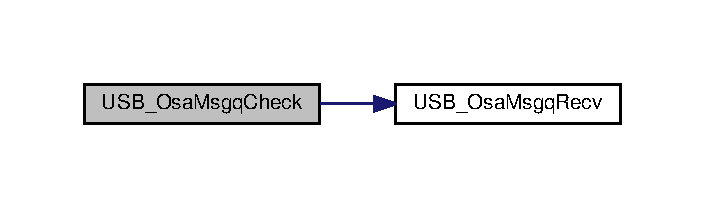
\includegraphics[width=338pt]{group__usb__os__abstraction_ga734fbdd1bae936ba6758087ad2d9d862_cgraph}
\end{center}
\end{figure}


\hypertarget{group__usb__os__abstraction_gacc28243bdfb636e21508879789ab5a0c}{\index{Usb\-\_\-os\-\_\-abstraction@{Usb\-\_\-os\-\_\-abstraction}!U\-S\-B\-\_\-\-Osa\-Msgq\-Create@{U\-S\-B\-\_\-\-Osa\-Msgq\-Create}}
\index{U\-S\-B\-\_\-\-Osa\-Msgq\-Create@{U\-S\-B\-\_\-\-Osa\-Msgq\-Create}!Usb_os_abstraction@{Usb\-\_\-os\-\_\-abstraction}}
\subsubsection[{U\-S\-B\-\_\-\-Osa\-Msgq\-Create}]{\setlength{\rightskip}{0pt plus 5cm}{\bf usb\-\_\-osa\-\_\-status\-\_\-t} U\-S\-B\-\_\-\-Osa\-Msgq\-Create (
\begin{DoxyParamCaption}
\item[{{\bf usb\-\_\-osa\-\_\-msgq\-\_\-handle} $\ast$}]{handle, }
\item[{uint32\-\_\-t}]{count, }
\item[{uint32\-\_\-t}]{size}
\end{DoxyParamCaption}
)}}\label{group__usb__os__abstraction_gacc28243bdfb636e21508879789ab5a0c}


Creates a message queue. 

This function creates a message queue.


\begin{DoxyParams}{Parameters}
{\em handle} & It is an out parameter, which is used to return a pointer of the message queue object. \\
\hline
{\em count} & The count of elements in the queue. \\
\hline
{\em size} & Size of every elements in words.\\
\hline
\end{DoxyParams}
\begin{DoxyReturn}{Returns}
A U\-S\-B O\-S\-A error code or k\-Status\-\_\-\-O\-S\-A\-\_\-\-Success.
\end{DoxyReturn}
Example\-: 
\begin{DoxyCode}
\hyperlink{group__usb__os__abstraction_gab3a9f26ba50f3abea7fcbac07500cbb8}{usb\_osa\_msgq\_handle}  msgqHandle;
\hyperlink{group__usb__os__abstraction_ga8de2fb7579de0a6621bbc1776519b0a9}{usb\_osa\_status\_t}     usbOsaStatus;
usbOsaStatus = \hyperlink{group__usb__os__abstraction_gacc28243bdfb636e21508879789ab5a0c}{USB\_OsaMsgqCreate}(msgqHandle, 8U, 4U);
\end{DoxyCode}
 
\begin{DoxyCode}
385 \{
386     \hyperlink{struct__usb__osa__msgq__struct}{usb\_osa\_msgq\_struct\_t} *msgq = NULL;
387     \hyperlink{usb__osa__bm_8h_a8dbccf46cc2f8e3b5cece6a4a84f7ae8}{USB\_OSA\_SR\_ALLOC}();
388 
389     \textcolor{keywordflow}{if} (!handle)
390     \{
391         \textcolor{keywordflow}{return} \hyperlink{group__usb__os__abstraction_gga453ebd2f93aafb8c938c3a23c815f9bda40b794ea06e27b8ec1d67538f12eb350}{kStatus\_USB\_OSA\_Error};
392     \}
393     \hyperlink{usb__osa__bm_8h_a0485f70bf9c9a22f0340f014bc567362}{USB\_OSA\_ENTER\_CRITICAL}();
394 
395     \textcolor{keywordflow}{for} (uint32\_t i = 0; i < \hyperlink{usb__osa__bm_8c_a3ce440b12fcf2709f2768bdf92cef71a}{USB\_OSA\_BM\_MSGQ\_COUNT}; i++)
396     \{
397         \textcolor{keywordflow}{if} (0 == \hyperlink{usb__osa__bm_8c_a25abd8e0857ad32f9b5c4ff1735203cf}{s\_UsbBmMsgqStruct}[i].isUsed)
398         \{
399             msgq = &\hyperlink{usb__osa__bm_8c_a25abd8e0857ad32f9b5c4ff1735203cf}{s\_UsbBmMsgqStruct}[i];
400             \textcolor{keywordflow}{break};
401         \}
402     \}
403     \textcolor{keywordflow}{if} ((NULL == msgq) || (count > \hyperlink{usb__osa__bm_8c_a2b5f0f86e134f00be828785d6ec18cc1}{USB\_OSA\_BM\_MSG\_COUNT}) || (size > 
      \hyperlink{usb__osa__bm_8c_aebd4f187253120c660884232b56c2741}{USB\_OSA\_BM\_MSG\_SIZE}))
404     \{
405         \hyperlink{usb__osa__bm_8h_a5b8053eca19b6df666a26fad3b07f953}{USB\_OSA\_EXIT\_CRITICAL}();
406         \textcolor{keywordflow}{return} \hyperlink{group__usb__os__abstraction_gga453ebd2f93aafb8c938c3a23c815f9bda40b794ea06e27b8ec1d67538f12eb350}{kStatus\_USB\_OSA\_Error};
407     \}
408     msgq->\hyperlink{struct__usb__osa__msgq__struct_a81e789da58dfb43477f28b1becac6b7f}{count} = count;
409     msgq->\hyperlink{struct__usb__osa__msgq__struct_a9ca60eac37ed126c806f087e198eee44}{msgSize} = size;
410     msgq->\hyperlink{struct__usb__osa__msgq__struct_ad3256f6cde77697e233c64bff47ada29}{msgCount} = 0U;
411     msgq->\hyperlink{struct__usb__osa__msgq__struct_aadbfed51ddaea472a048ea212e450050}{index} = 0U;
412     msgq->\hyperlink{struct__usb__osa__msgq__struct_ac7756db309b7ab61b6eea39bc496945e}{current} = 0U;
413     msgq->\hyperlink{struct__usb__osa__msgq__struct_a08c7a0bbacca92657d33d6e1a5c392fd}{isUsed} = 1;
414     *handle = msgq;
415     \hyperlink{usb__osa__bm_8h_a5b8053eca19b6df666a26fad3b07f953}{USB\_OSA\_EXIT\_CRITICAL}();
416     \textcolor{keywordflow}{return} \hyperlink{group__usb__os__abstraction_gga453ebd2f93aafb8c938c3a23c815f9bdab90805fb75297fda1ca60dbb2283f933}{kStatus\_USB\_OSA\_Success};
417 \}
\end{DoxyCode}
\hypertarget{group__usb__os__abstraction_gafc20008f4680ff9f0720574841b34e42}{\index{Usb\-\_\-os\-\_\-abstraction@{Usb\-\_\-os\-\_\-abstraction}!U\-S\-B\-\_\-\-Osa\-Msgq\-Destroy@{U\-S\-B\-\_\-\-Osa\-Msgq\-Destroy}}
\index{U\-S\-B\-\_\-\-Osa\-Msgq\-Destroy@{U\-S\-B\-\_\-\-Osa\-Msgq\-Destroy}!Usb_os_abstraction@{Usb\-\_\-os\-\_\-abstraction}}
\subsubsection[{U\-S\-B\-\_\-\-Osa\-Msgq\-Destroy}]{\setlength{\rightskip}{0pt plus 5cm}{\bf usb\-\_\-osa\-\_\-status\-\_\-t} U\-S\-B\-\_\-\-Osa\-Msgq\-Destroy (
\begin{DoxyParamCaption}
\item[{{\bf usb\-\_\-osa\-\_\-msgq\-\_\-handle}}]{handle}
\end{DoxyParamCaption}
)}}\label{group__usb__os__abstraction_gafc20008f4680ff9f0720574841b34e42}


Destroys a message queue. 

This function destroys a message queue.


\begin{DoxyParams}{Parameters}
{\em handle} & Pointer to a message queue.\\
\hline
\end{DoxyParams}
\begin{DoxyReturn}{Returns}
A U\-S\-B O\-S\-A error code or k\-Status\-\_\-\-O\-S\-A\-\_\-\-Success.
\end{DoxyReturn}
Example\-: 
\begin{DoxyCode}
\hyperlink{group__usb__os__abstraction_gab3a9f26ba50f3abea7fcbac07500cbb8}{usb\_osa\_msgq\_handle}  msgqHandle;
\hyperlink{group__usb__os__abstraction_ga8de2fb7579de0a6621bbc1776519b0a9}{usb\_osa\_status\_t}     usbOsaStatus;
...
usbOsaStatus = \hyperlink{group__usb__os__abstraction_gafc20008f4680ff9f0720574841b34e42}{USB\_OsaMsgqDestroy}(msgqHandle);
\end{DoxyCode}
 
\begin{DoxyCode}
420 \{
421     \hyperlink{struct__usb__osa__msgq__struct}{usb\_osa\_msgq\_struct\_t} *msgq = (\hyperlink{struct__usb__osa__msgq__struct}{usb\_osa\_msgq\_struct\_t} *)handle
      ;
422     \hyperlink{usb__osa__bm_8h_a8dbccf46cc2f8e3b5cece6a4a84f7ae8}{USB\_OSA\_SR\_ALLOC}();
423 
424     \textcolor{keywordflow}{if} (!handle)
425     \{
426         \textcolor{keywordflow}{return} \hyperlink{group__usb__os__abstraction_gga453ebd2f93aafb8c938c3a23c815f9bda40b794ea06e27b8ec1d67538f12eb350}{kStatus\_USB\_OSA\_Error};
427     \}
428     \hyperlink{usb__osa__bm_8h_a0485f70bf9c9a22f0340f014bc567362}{USB\_OSA\_ENTER\_CRITICAL}();
429     msgq->\hyperlink{struct__usb__osa__msgq__struct_a08c7a0bbacca92657d33d6e1a5c392fd}{isUsed} = 0;
430     \hyperlink{usb__osa__bm_8h_a5b8053eca19b6df666a26fad3b07f953}{USB\_OSA\_EXIT\_CRITICAL}();
431     \textcolor{keywordflow}{return} \hyperlink{group__usb__os__abstraction_gga453ebd2f93aafb8c938c3a23c815f9bdab90805fb75297fda1ca60dbb2283f933}{kStatus\_USB\_OSA\_Success};
432 \}
\end{DoxyCode}
\hypertarget{group__usb__os__abstraction_gaf2effe68aa0486c0823e253f78836d17}{\index{Usb\-\_\-os\-\_\-abstraction@{Usb\-\_\-os\-\_\-abstraction}!U\-S\-B\-\_\-\-Osa\-Msgq\-Recv@{U\-S\-B\-\_\-\-Osa\-Msgq\-Recv}}
\index{U\-S\-B\-\_\-\-Osa\-Msgq\-Recv@{U\-S\-B\-\_\-\-Osa\-Msgq\-Recv}!Usb_os_abstraction@{Usb\-\_\-os\-\_\-abstraction}}
\subsubsection[{U\-S\-B\-\_\-\-Osa\-Msgq\-Recv}]{\setlength{\rightskip}{0pt plus 5cm}{\bf usb\-\_\-osa\-\_\-status\-\_\-t} U\-S\-B\-\_\-\-Osa\-Msgq\-Recv (
\begin{DoxyParamCaption}
\item[{{\bf usb\-\_\-osa\-\_\-msgq\-\_\-handle}}]{handle, }
\item[{void $\ast$}]{msg, }
\item[{uint32\-\_\-t}]{timeout}
\end{DoxyParamCaption}
)}}\label{group__usb__os__abstraction_gaf2effe68aa0486c0823e253f78836d17}


Receives a message. 

This function receives a message from the head of the message queue.


\begin{DoxyParams}{Parameters}
{\em handle} & Pointer to a message queue. \\
\hline
{\em msg} & The pointer to save a received message. \\
\hline
{\em timeout} & The maximum number of milliseconds to wait for a message. If the wait condition is not met, passing 0\-U waits indefinitely when an environment is R\-T\-O\-S and returns the k\-Status\-\_\-\-O\-S\-A\-\_\-\-Timeout immediately for bare metal.\\
\hline
\end{DoxyParams}
\begin{DoxyReturn}{Returns}
A U\-S\-B O\-S\-A error code or k\-Status\-\_\-\-O\-S\-A\-\_\-\-Success.
\end{DoxyReturn}
Example\-: 
\begin{DoxyCode}
\hyperlink{group__usb__os__abstraction_gab3a9f26ba50f3abea7fcbac07500cbb8}{usb\_osa\_msgq\_handle}      msgqHandle;
message\_struct\_t         message;
\hyperlink{group__usb__os__abstraction_ga8de2fb7579de0a6621bbc1776519b0a9}{usb\_osa\_status\_t}         usbOsaStatus;
...
usbOsaStatus = \hyperlink{group__usb__os__abstraction_gaf2effe68aa0486c0823e253f78836d17}{USB\_OsaMsgqRecv}(msgqHandle, &message, 0U);
\end{DoxyCode}
 
\begin{DoxyCode}
478 \{
479     \hyperlink{struct__usb__osa__msgq__struct}{usb\_osa\_msgq\_struct\_t} *msgq = (\hyperlink{struct__usb__osa__msgq__struct}{usb\_osa\_msgq\_struct\_t} *)handle
      ;
480     \hyperlink{struct__usb__osa__msg__struct}{usb\_osa\_msg\_struct\_t} *msgEntity;
481     uint32\_t *p;
482     uint32\_t *q;
483     uint32\_t count;
484     \hyperlink{usb__osa__bm_8h_a8dbccf46cc2f8e3b5cece6a4a84f7ae8}{USB\_OSA\_SR\_ALLOC}();
485 
486     \textcolor{keywordflow}{if} (!handle)
487     \{
488         \textcolor{keywordflow}{return} \hyperlink{group__usb__os__abstraction_gga453ebd2f93aafb8c938c3a23c815f9bda40b794ea06e27b8ec1d67538f12eb350}{kStatus\_USB\_OSA\_Error};
489     \}
490     \hyperlink{usb__osa__bm_8h_a0485f70bf9c9a22f0340f014bc567362}{USB\_OSA\_ENTER\_CRITICAL}();
491     \textcolor{keywordflow}{if} (msgq->\hyperlink{struct__usb__osa__msgq__struct_ad3256f6cde77697e233c64bff47ada29}{msgCount} < 1U)
492     \{
493         \hyperlink{usb__osa__bm_8h_a5b8053eca19b6df666a26fad3b07f953}{USB\_OSA\_EXIT\_CRITICAL}();
494         \textcolor{keywordflow}{return} \hyperlink{group__usb__os__abstraction_gga453ebd2f93aafb8c938c3a23c815f9bda9ff36cb34c565283214974d1097d08df}{kStatus\_USB\_OSA\_TimeOut};
495     \}
496 
497     msgEntity = &msgq->\hyperlink{struct__usb__osa__msgq__struct_abca5922025c046e9604252a2e5ff3bd7}{msgs}[msgq->\hyperlink{struct__usb__osa__msgq__struct_ac7756db309b7ab61b6eea39bc496945e}{current}];
498     q = (uint32\_t *)&msgEntity->\hyperlink{struct__usb__osa__msg__struct_a91880d9450b8871ab19a065407e0b52e}{msg}[0];
499     p = (uint32\_t *)msg;
500 
501     \textcolor{keywordflow}{for} (count = 0U; count < msgq->\hyperlink{struct__usb__osa__msgq__struct_a9ca60eac37ed126c806f087e198eee44}{msgSize}; count++)
502     \{
503         p[count] = q[count];
504     \}
505 
506     msgq->\hyperlink{struct__usb__osa__msgq__struct_ad3256f6cde77697e233c64bff47ada29}{msgCount}--;
507     msgq->\hyperlink{struct__usb__osa__msgq__struct_ac7756db309b7ab61b6eea39bc496945e}{current}++;
508     msgq->\hyperlink{struct__usb__osa__msgq__struct_ac7756db309b7ab61b6eea39bc496945e}{current} = msgq->\hyperlink{struct__usb__osa__msgq__struct_ac7756db309b7ab61b6eea39bc496945e}{current} % msgq->\hyperlink{struct__usb__osa__msgq__struct_a81e789da58dfb43477f28b1becac6b7f}{count};
509 
510     \hyperlink{usb__osa__bm_8h_a5b8053eca19b6df666a26fad3b07f953}{USB\_OSA\_EXIT\_CRITICAL}();
511 
512     \textcolor{keywordflow}{return} \hyperlink{group__usb__os__abstraction_gga453ebd2f93aafb8c938c3a23c815f9bdab90805fb75297fda1ca60dbb2283f933}{kStatus\_USB\_OSA\_Success};
513 \}
\end{DoxyCode}


Here is the caller graph for this function\-:
\nopagebreak
\begin{figure}[H]
\begin{center}
\leavevmode
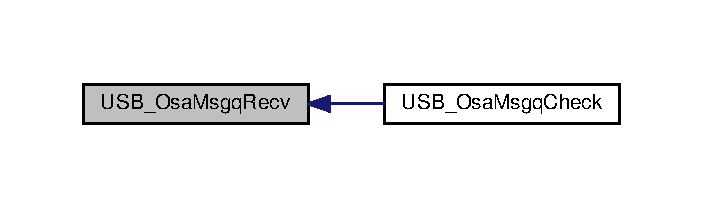
\includegraphics[width=338pt]{group__usb__os__abstraction_gaf2effe68aa0486c0823e253f78836d17_icgraph}
\end{center}
\end{figure}


\hypertarget{group__usb__os__abstraction_ga6ba61c6cf5e772dbce90c5626dbd0db0}{\index{Usb\-\_\-os\-\_\-abstraction@{Usb\-\_\-os\-\_\-abstraction}!U\-S\-B\-\_\-\-Osa\-Msgq\-Send@{U\-S\-B\-\_\-\-Osa\-Msgq\-Send}}
\index{U\-S\-B\-\_\-\-Osa\-Msgq\-Send@{U\-S\-B\-\_\-\-Osa\-Msgq\-Send}!Usb_os_abstraction@{Usb\-\_\-os\-\_\-abstraction}}
\subsubsection[{U\-S\-B\-\_\-\-Osa\-Msgq\-Send}]{\setlength{\rightskip}{0pt plus 5cm}{\bf usb\-\_\-osa\-\_\-status\-\_\-t} U\-S\-B\-\_\-\-Osa\-Msgq\-Send (
\begin{DoxyParamCaption}
\item[{{\bf usb\-\_\-osa\-\_\-msgq\-\_\-handle}}]{handle, }
\item[{void $\ast$}]{msg}
\end{DoxyParamCaption}
)}}\label{group__usb__os__abstraction_ga6ba61c6cf5e772dbce90c5626dbd0db0}


Sends a message. 

This function sends a message to the tail of the message queue.


\begin{DoxyParams}{Parameters}
{\em handle} & Pointer to a message queue. \\
\hline
{\em msg} & The pointer to a message to be put into the queue.\\
\hline
\end{DoxyParams}
\begin{DoxyReturn}{Returns}
A U\-S\-B O\-S\-A error code or k\-Status\-\_\-\-O\-S\-A\-\_\-\-Success.
\end{DoxyReturn}
Example\-: 
\begin{DoxyCode}
\hyperlink{group__usb__os__abstraction_gab3a9f26ba50f3abea7fcbac07500cbb8}{usb\_osa\_msgq\_handle}      msgqHandle;
message\_struct\_t         message;
\hyperlink{group__usb__os__abstraction_ga8de2fb7579de0a6621bbc1776519b0a9}{usb\_osa\_status\_t}         usbOsaStatus;
...
usbOsaStatus = \hyperlink{group__usb__os__abstraction_ga6ba61c6cf5e772dbce90c5626dbd0db0}{USB\_OsaMsgqSend}(msgqHandle, &message);
\end{DoxyCode}
 
\begin{DoxyCode}
435 \{
436     \hyperlink{struct__usb__osa__msgq__struct}{usb\_osa\_msgq\_struct\_t} *msgq = (\hyperlink{struct__usb__osa__msgq__struct}{usb\_osa\_msgq\_struct\_t} *)handle
      ;
437     \hyperlink{struct__usb__osa__msg__struct}{usb\_osa\_msg\_struct\_t} *msgEntity;
438     uint32\_t *p;
439     uint32\_t *q;
440     uint32\_t count;
441     \hyperlink{usb__osa__bm_8h_a8dbccf46cc2f8e3b5cece6a4a84f7ae8}{USB\_OSA\_SR\_ALLOC}();
442 
443     \textcolor{keywordflow}{if} (!handle)
444     \{
445         \textcolor{keywordflow}{return} \hyperlink{group__usb__os__abstraction_gga453ebd2f93aafb8c938c3a23c815f9bda40b794ea06e27b8ec1d67538f12eb350}{kStatus\_USB\_OSA\_Error};
446     \}
447     \hyperlink{usb__osa__bm_8h_a0485f70bf9c9a22f0340f014bc567362}{USB\_OSA\_ENTER\_CRITICAL}();
448     \textcolor{keywordflow}{if} (msgq->\hyperlink{struct__usb__osa__msgq__struct_ad3256f6cde77697e233c64bff47ada29}{msgCount} >= msgq->\hyperlink{struct__usb__osa__msgq__struct_a81e789da58dfb43477f28b1becac6b7f}{count})
449     \{
450         \hyperlink{usb__osa__bm_8h_a5b8053eca19b6df666a26fad3b07f953}{USB\_OSA\_EXIT\_CRITICAL}();
451         \textcolor{keywordflow}{return} \hyperlink{group__usb__os__abstraction_gga453ebd2f93aafb8c938c3a23c815f9bda40b794ea06e27b8ec1d67538f12eb350}{kStatus\_USB\_OSA\_Error};
452     \}
453 
454     msgEntity = &msgq->\hyperlink{struct__usb__osa__msgq__struct_abca5922025c046e9604252a2e5ff3bd7}{msgs}[msgq->\hyperlink{struct__usb__osa__msgq__struct_aadbfed51ddaea472a048ea212e450050}{index}];
455     p = (uint32\_t *)&msgEntity->\hyperlink{struct__usb__osa__msg__struct_a91880d9450b8871ab19a065407e0b52e}{msg}[0];
456     q = (uint32\_t *)msg;
457 
458     \textcolor{keywordflow}{for} (count = 0U; count < msgq->\hyperlink{struct__usb__osa__msgq__struct_a9ca60eac37ed126c806f087e198eee44}{msgSize}; count++)
459     \{
460         p[count] = q[count];
461     \}
462 
463     \textcolor{keywordflow}{if} (0U == msgq->\hyperlink{struct__usb__osa__msgq__struct_ad3256f6cde77697e233c64bff47ada29}{msgCount})
464     \{
465         msgq->\hyperlink{struct__usb__osa__msgq__struct_ac7756db309b7ab61b6eea39bc496945e}{current} = msgq->\hyperlink{struct__usb__osa__msgq__struct_aadbfed51ddaea472a048ea212e450050}{index};
466     \}
467 
468     msgq->\hyperlink{struct__usb__osa__msgq__struct_ad3256f6cde77697e233c64bff47ada29}{msgCount}++;
469     msgq->\hyperlink{struct__usb__osa__msgq__struct_aadbfed51ddaea472a048ea212e450050}{index}++;
470     msgq->\hyperlink{struct__usb__osa__msgq__struct_aadbfed51ddaea472a048ea212e450050}{index} = msgq->\hyperlink{struct__usb__osa__msgq__struct_aadbfed51ddaea472a048ea212e450050}{index} % msgq->\hyperlink{struct__usb__osa__msgq__struct_a81e789da58dfb43477f28b1becac6b7f}{count};
471 
472     \hyperlink{usb__osa__bm_8h_a5b8053eca19b6df666a26fad3b07f953}{USB\_OSA\_EXIT\_CRITICAL}();
473 
474     \textcolor{keywordflow}{return} \hyperlink{group__usb__os__abstraction_gga453ebd2f93aafb8c938c3a23c815f9bdab90805fb75297fda1ca60dbb2283f933}{kStatus\_USB\_OSA\_Success};
475 \}
\end{DoxyCode}
\hypertarget{group__usb__os__abstraction_gaf36ecc5a6c3359a6587750b17800f49d}{\index{Usb\-\_\-os\-\_\-abstraction@{Usb\-\_\-os\-\_\-abstraction}!U\-S\-B\-\_\-\-Osa\-Mutex\-Create@{U\-S\-B\-\_\-\-Osa\-Mutex\-Create}}
\index{U\-S\-B\-\_\-\-Osa\-Mutex\-Create@{U\-S\-B\-\_\-\-Osa\-Mutex\-Create}!Usb_os_abstraction@{Usb\-\_\-os\-\_\-abstraction}}
\subsubsection[{U\-S\-B\-\_\-\-Osa\-Mutex\-Create}]{\setlength{\rightskip}{0pt plus 5cm}{\bf usb\-\_\-osa\-\_\-status\-\_\-t} U\-S\-B\-\_\-\-Osa\-Mutex\-Create (
\begin{DoxyParamCaption}
\item[{{\bf usb\-\_\-osa\-\_\-mutex\-\_\-handle} $\ast$}]{handle}
\end{DoxyParamCaption}
)}}\label{group__usb__os__abstraction_gaf36ecc5a6c3359a6587750b17800f49d}


Creates a mutex. 

This function creates a mutex and sets it to an unlocked status.


\begin{DoxyParams}{Parameters}
{\em handle} & It is out parameter, which is used to return the pointer of the mutex object.\\
\hline
\end{DoxyParams}
\begin{DoxyReturn}{Returns}
A U\-S\-B O\-S\-A error code or k\-Status\-\_\-\-O\-S\-A\-\_\-\-Success.
\end{DoxyReturn}
Example\-: 
\begin{DoxyCode}
\hyperlink{group__usb__os__abstraction_gad259d0dfe125b11cccaf93163ef915fd}{usb\_osa\_mutex\_handle} mutexHandle;
\hyperlink{group__usb__os__abstraction_ga8de2fb7579de0a6621bbc1776519b0a9}{usb\_osa\_status\_t}     usbOsaStatus;
usbOsaStatus = \hyperlink{group__usb__os__abstraction_gaf36ecc5a6c3359a6587750b17800f49d}{USB\_OsaMutexCreate}(&mutexHandle);
\end{DoxyCode}
 
\begin{DoxyCode}
362 \{
363     \textcolor{keywordflow}{if} (!handle)
364     \{
365         \textcolor{keywordflow}{return} \hyperlink{group__usb__os__abstraction_gga453ebd2f93aafb8c938c3a23c815f9bda40b794ea06e27b8ec1d67538f12eb350}{kStatus\_USB\_OSA\_Error};
366     \}
367     *handle = (\hyperlink{group__usb__os__abstraction_gad259d0dfe125b11cccaf93163ef915fd}{usb\_osa\_mutex\_handle})0xFFFF0000U;
368     \textcolor{keywordflow}{return} \hyperlink{group__usb__os__abstraction_gga453ebd2f93aafb8c938c3a23c815f9bdab90805fb75297fda1ca60dbb2283f933}{kStatus\_USB\_OSA\_Success};
369 \}
\end{DoxyCode}


Here is the caller graph for this function\-:
\nopagebreak
\begin{figure}[H]
\begin{center}
\leavevmode
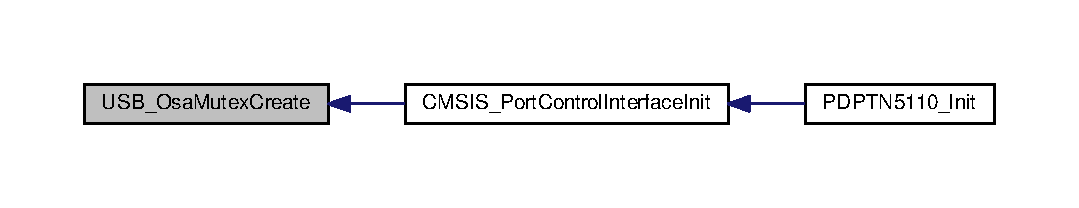
\includegraphics[width=350pt]{group__usb__os__abstraction_gaf36ecc5a6c3359a6587750b17800f49d_icgraph}
\end{center}
\end{figure}


\hypertarget{group__usb__os__abstraction_ga68f890c3d76f212e6fa8cf787b918a5b}{\index{Usb\-\_\-os\-\_\-abstraction@{Usb\-\_\-os\-\_\-abstraction}!U\-S\-B\-\_\-\-Osa\-Mutex\-Destroy@{U\-S\-B\-\_\-\-Osa\-Mutex\-Destroy}}
\index{U\-S\-B\-\_\-\-Osa\-Mutex\-Destroy@{U\-S\-B\-\_\-\-Osa\-Mutex\-Destroy}!Usb_os_abstraction@{Usb\-\_\-os\-\_\-abstraction}}
\subsubsection[{U\-S\-B\-\_\-\-Osa\-Mutex\-Destroy}]{\setlength{\rightskip}{0pt plus 5cm}{\bf usb\-\_\-osa\-\_\-status\-\_\-t} U\-S\-B\-\_\-\-Osa\-Mutex\-Destroy (
\begin{DoxyParamCaption}
\item[{{\bf usb\-\_\-osa\-\_\-mutex\-\_\-handle}}]{handle}
\end{DoxyParamCaption}
)}}\label{group__usb__os__abstraction_ga68f890c3d76f212e6fa8cf787b918a5b}


Destroys a mutex. 

This function destroys a mutex and sets it to an unlocked status.


\begin{DoxyParams}{Parameters}
{\em handle} & Pointer to the mutex.\\
\hline
\end{DoxyParams}
\begin{DoxyReturn}{Returns}
A U\-S\-B O\-S\-A error code or k\-Status\-\_\-\-O\-S\-A\-\_\-\-Success.
\end{DoxyReturn}
Example\-: 
\begin{DoxyCode}
\hyperlink{group__usb__os__abstraction_gad259d0dfe125b11cccaf93163ef915fd}{usb\_osa\_mutex\_handle} mutexHandle;
\hyperlink{group__usb__os__abstraction_ga8de2fb7579de0a6621bbc1776519b0a9}{usb\_osa\_status\_t}     usbOsaStatus;
...
usbOsaStatus = \hyperlink{group__usb__os__abstraction_ga68f890c3d76f212e6fa8cf787b918a5b}{USB\_OsaMutexDestroy}(mutexHandle);
\end{DoxyCode}
 
\begin{DoxyCode}
372 \{
373     \textcolor{keywordflow}{return} \hyperlink{group__usb__os__abstraction_gga453ebd2f93aafb8c938c3a23c815f9bdab90805fb75297fda1ca60dbb2283f933}{kStatus\_USB\_OSA\_Success};
374 \}
\end{DoxyCode}


Here is the caller graph for this function\-:
\nopagebreak
\begin{figure}[H]
\begin{center}
\leavevmode
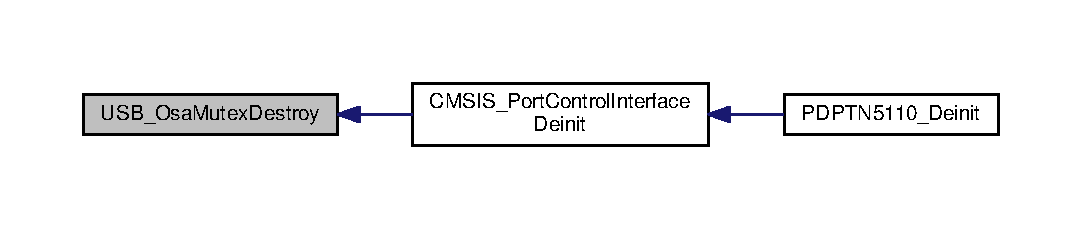
\includegraphics[width=350pt]{group__usb__os__abstraction_ga68f890c3d76f212e6fa8cf787b918a5b_icgraph}
\end{center}
\end{figure}


\hypertarget{group__usb__os__abstraction_ga1fed31c4b683c5f652b4e2e8b23c34fd}{\index{Usb\-\_\-os\-\_\-abstraction@{Usb\-\_\-os\-\_\-abstraction}!U\-S\-B\-\_\-\-Osa\-Mutex\-Lock@{U\-S\-B\-\_\-\-Osa\-Mutex\-Lock}}
\index{U\-S\-B\-\_\-\-Osa\-Mutex\-Lock@{U\-S\-B\-\_\-\-Osa\-Mutex\-Lock}!Usb_os_abstraction@{Usb\-\_\-os\-\_\-abstraction}}
\subsubsection[{U\-S\-B\-\_\-\-Osa\-Mutex\-Lock}]{\setlength{\rightskip}{0pt plus 5cm}{\bf usb\-\_\-osa\-\_\-status\-\_\-t} U\-S\-B\-\_\-\-Osa\-Mutex\-Lock (
\begin{DoxyParamCaption}
\item[{{\bf usb\-\_\-osa\-\_\-mutex\-\_\-handle}}]{handle}
\end{DoxyParamCaption}
)}}\label{group__usb__os__abstraction_ga1fed31c4b683c5f652b4e2e8b23c34fd}


Waits for a mutex and locks it. 

This function checks the mutex status. If it is unlocked, it locks it and returns the k\-Status\-\_\-\-O\-S\-A\-\_\-\-Success. Otherwise, it waits forever to lock in R\-T\-O\-S and returns the k\-Status\-\_\-\-O\-S\-A\-\_\-\-Success immediately for bare metal.


\begin{DoxyParams}{Parameters}
{\em handle} & Pointer to the mutex.\\
\hline
\end{DoxyParams}
\begin{DoxyReturn}{Returns}
A U\-S\-B O\-S\-A error code or k\-Status\-\_\-\-O\-S\-A\-\_\-\-Success.
\end{DoxyReturn}
Example\-: 
\begin{DoxyCode}
\hyperlink{group__usb__os__abstraction_gad259d0dfe125b11cccaf93163ef915fd}{usb\_osa\_mutex\_handle} mutexHandle;
\hyperlink{group__usb__os__abstraction_ga8de2fb7579de0a6621bbc1776519b0a9}{usb\_osa\_status\_t}     usbOsaStatus;
...
usbOsaStatus = \hyperlink{group__usb__os__abstraction_ga1fed31c4b683c5f652b4e2e8b23c34fd}{USB\_OsaMutexLock}(mutexHandle);
\end{DoxyCode}
 
\begin{DoxyCode}
376 \{
377     \textcolor{keywordflow}{return} \hyperlink{group__usb__os__abstraction_gga453ebd2f93aafb8c938c3a23c815f9bdab90805fb75297fda1ca60dbb2283f933}{kStatus\_USB\_OSA\_Success};
378 \}
\end{DoxyCode}


Here is the caller graph for this function\-:
\nopagebreak
\begin{figure}[H]
\begin{center}
\leavevmode
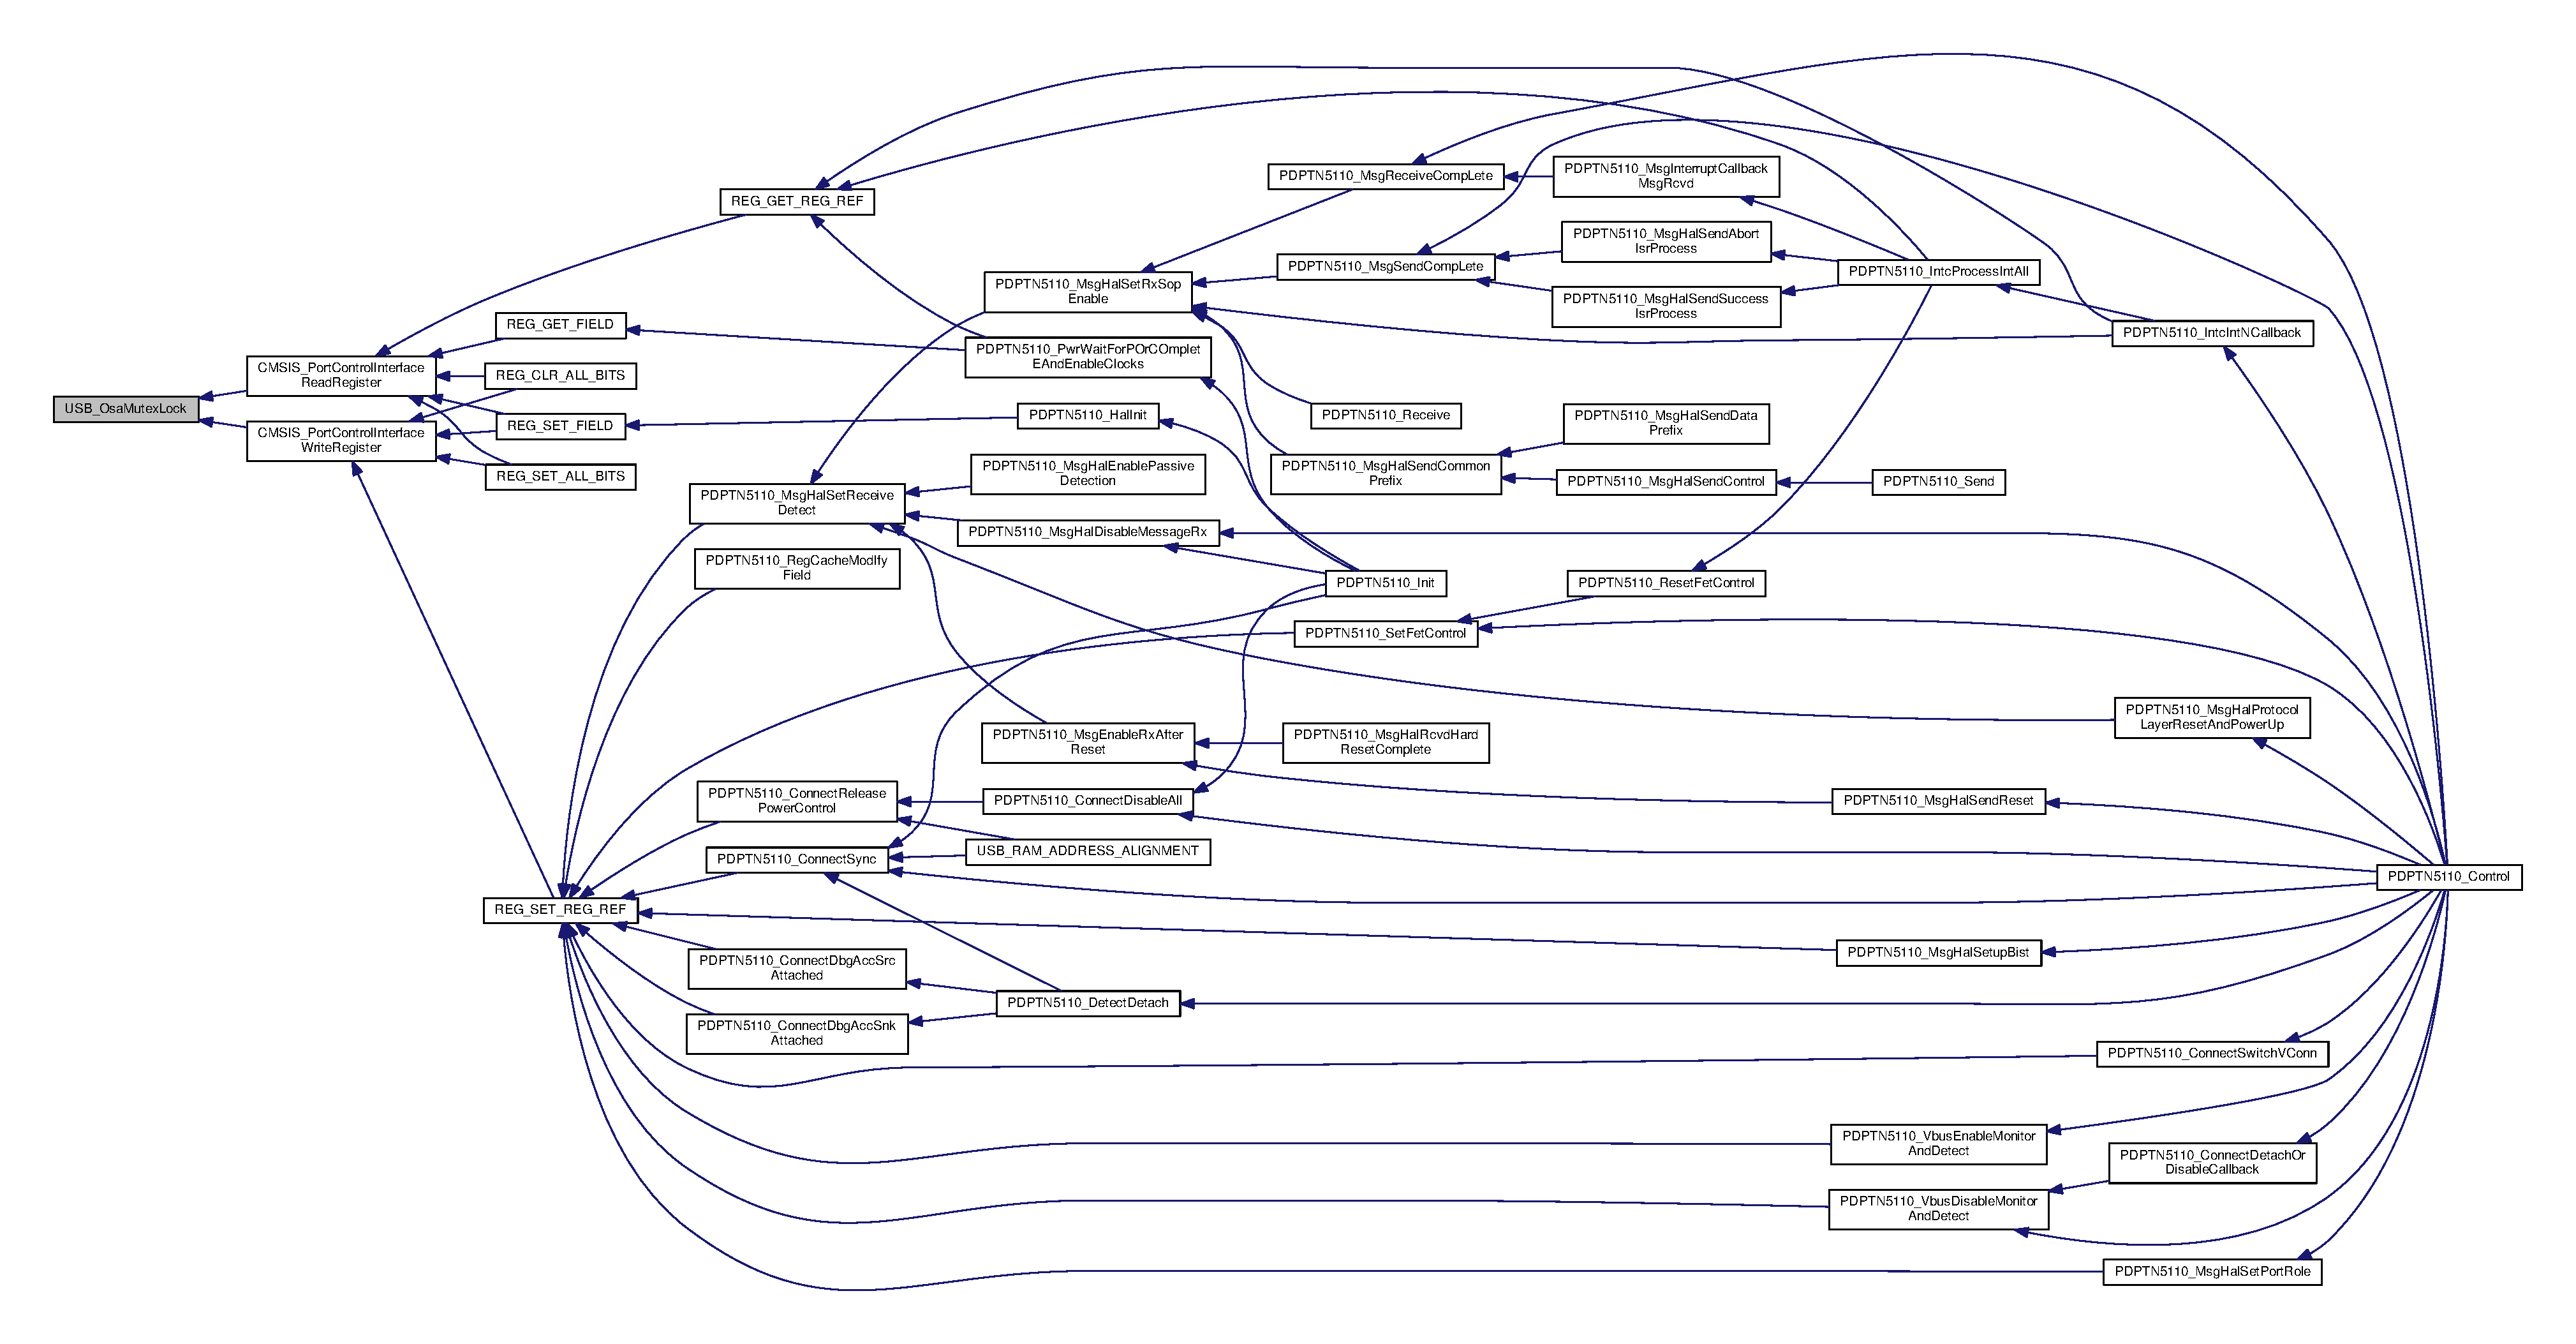
\includegraphics[width=350pt]{group__usb__os__abstraction_ga1fed31c4b683c5f652b4e2e8b23c34fd_icgraph}
\end{center}
\end{figure}


\hypertarget{group__usb__os__abstraction_gaad3249273d566eae00e2cea81192315a}{\index{Usb\-\_\-os\-\_\-abstraction@{Usb\-\_\-os\-\_\-abstraction}!U\-S\-B\-\_\-\-Osa\-Mutex\-Unlock@{U\-S\-B\-\_\-\-Osa\-Mutex\-Unlock}}
\index{U\-S\-B\-\_\-\-Osa\-Mutex\-Unlock@{U\-S\-B\-\_\-\-Osa\-Mutex\-Unlock}!Usb_os_abstraction@{Usb\-\_\-os\-\_\-abstraction}}
\subsubsection[{U\-S\-B\-\_\-\-Osa\-Mutex\-Unlock}]{\setlength{\rightskip}{0pt plus 5cm}{\bf usb\-\_\-osa\-\_\-status\-\_\-t} U\-S\-B\-\_\-\-Osa\-Mutex\-Unlock (
\begin{DoxyParamCaption}
\item[{{\bf usb\-\_\-osa\-\_\-mutex\-\_\-handle}}]{handle}
\end{DoxyParamCaption}
)}}\label{group__usb__os__abstraction_gaad3249273d566eae00e2cea81192315a}


Unlocks a mutex. 

This function unlocks a mutex.


\begin{DoxyParams}{Parameters}
{\em handle} & Pointer to the mutex.\\
\hline
\end{DoxyParams}
\begin{DoxyReturn}{Returns}
A U\-S\-B O\-S\-A error code or k\-Status\-\_\-\-O\-S\-A\-\_\-\-Success.
\end{DoxyReturn}
Example\-: 
\begin{DoxyCode}
\hyperlink{group__usb__os__abstraction_gad259d0dfe125b11cccaf93163ef915fd}{usb\_osa\_mutex\_handle} mutexHandle;
\hyperlink{group__usb__os__abstraction_ga8de2fb7579de0a6621bbc1776519b0a9}{usb\_osa\_status\_t}     usbOsaStatus;
...
usbOsaStatus = \hyperlink{group__usb__os__abstraction_gaad3249273d566eae00e2cea81192315a}{USB\_OsaMutexUnlock}(mutexHandle);
\end{DoxyCode}
 
\begin{DoxyCode}
380 \{
381     \textcolor{keywordflow}{return} \hyperlink{group__usb__os__abstraction_gga453ebd2f93aafb8c938c3a23c815f9bdab90805fb75297fda1ca60dbb2283f933}{kStatus\_USB\_OSA\_Success};
382 \}
\end{DoxyCode}


Here is the caller graph for this function\-:
\nopagebreak
\begin{figure}[H]
\begin{center}
\leavevmode
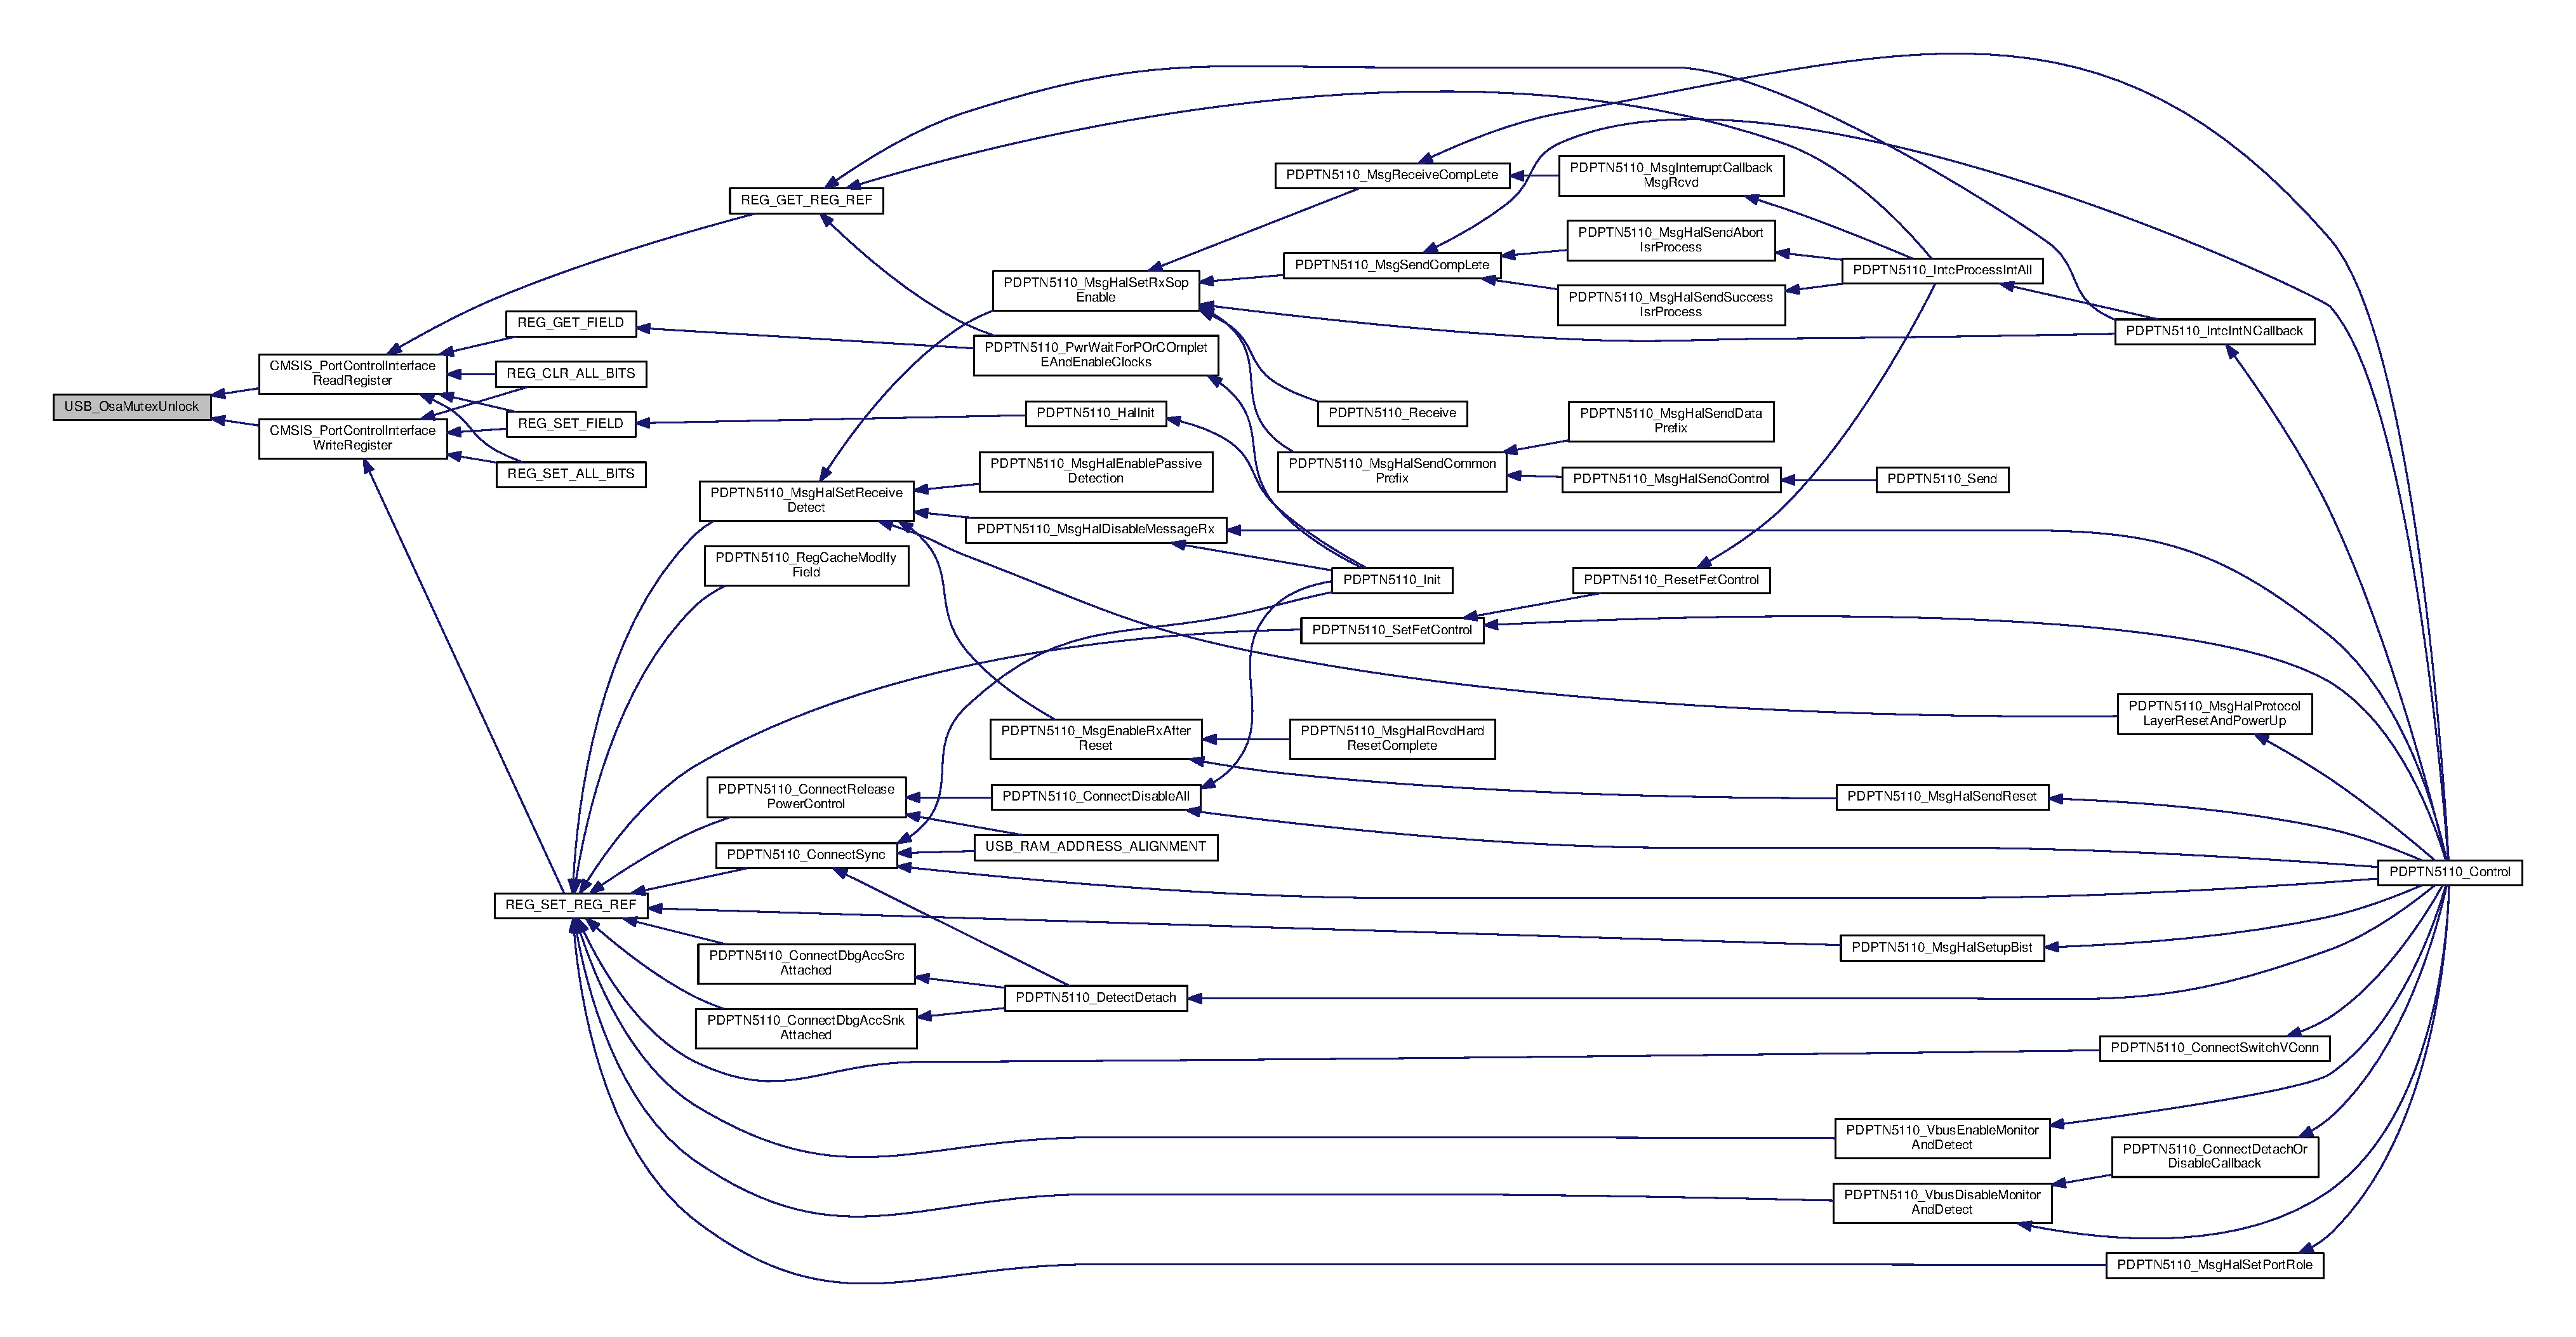
\includegraphics[width=350pt]{group__usb__os__abstraction_gaad3249273d566eae00e2cea81192315a_icgraph}
\end{center}
\end{figure}


\hypertarget{group__usb__os__abstraction_ga9d4a6e4130aac6d6b65d4cf6545f6625}{\index{Usb\-\_\-os\-\_\-abstraction@{Usb\-\_\-os\-\_\-abstraction}!U\-S\-B\-\_\-\-Osa\-Sem\-Create@{U\-S\-B\-\_\-\-Osa\-Sem\-Create}}
\index{U\-S\-B\-\_\-\-Osa\-Sem\-Create@{U\-S\-B\-\_\-\-Osa\-Sem\-Create}!Usb_os_abstraction@{Usb\-\_\-os\-\_\-abstraction}}
\subsubsection[{U\-S\-B\-\_\-\-Osa\-Sem\-Create}]{\setlength{\rightskip}{0pt plus 5cm}{\bf usb\-\_\-osa\-\_\-status\-\_\-t} U\-S\-B\-\_\-\-Osa\-Sem\-Create (
\begin{DoxyParamCaption}
\item[{{\bf usb\-\_\-osa\-\_\-sem\-\_\-handle} $\ast$}]{handle, }
\item[{uint32\-\_\-t}]{count}
\end{DoxyParamCaption}
)}}\label{group__usb__os__abstraction_ga9d4a6e4130aac6d6b65d4cf6545f6625}


Creates a semaphore with a given value. 

This function creates a semaphore and sets the default count.


\begin{DoxyParams}{Parameters}
{\em handle} & It is an out parameter, which is used to return pointer of the semaphore object. \\
\hline
{\em count} & Initializes a value of the semaphore.\\
\hline
\end{DoxyParams}
\begin{DoxyReturn}{Returns}
An U\-S\-B O\-S\-A error code or k\-Status\-\_\-\-O\-S\-A\-\_\-\-Success.
\end{DoxyReturn}
Example\-: 
\begin{DoxyCode}
\hyperlink{group__usb__os__abstraction_ga9f0e38944e1320d10c45eaacb67185b7}{usb\_osa\_sem\_handle}   semHandle;
\hyperlink{group__usb__os__abstraction_ga8de2fb7579de0a6621bbc1776519b0a9}{usb\_osa\_status\_t}     usbOsaStatus;
usbOsaStatus = \hyperlink{group__usb__os__abstraction_ga9d4a6e4130aac6d6b65d4cf6545f6625}{USB\_OsaSemCreate}(&semHandle, 1U);
\end{DoxyCode}
 
\begin{DoxyCode}
275 \{
276     \hyperlink{struct__usb__osa__sem__struct}{usb\_osa\_sem\_struct\_t} *sem = NULL;
277     \hyperlink{usb__osa__bm_8h_a8dbccf46cc2f8e3b5cece6a4a84f7ae8}{USB\_OSA\_SR\_ALLOC}();
278 
279     \textcolor{keywordflow}{if} (!handle)
280     \{
281         \textcolor{keywordflow}{return} \hyperlink{group__usb__os__abstraction_gga453ebd2f93aafb8c938c3a23c815f9bda40b794ea06e27b8ec1d67538f12eb350}{kStatus\_USB\_OSA\_Error};
282     \}
283 
284     \hyperlink{usb__osa__bm_8h_a0485f70bf9c9a22f0340f014bc567362}{USB\_OSA\_ENTER\_CRITICAL}();
285     \textcolor{keywordflow}{for} (uint32\_t i = 0; i < \hyperlink{usb__osa__bm_8c_a87ad432ac08dbd6d87aae1827ced067d}{USB\_OSA\_BM\_SEM\_COUNT}; i++)
286     \{
287         \textcolor{keywordflow}{if} (0 == \hyperlink{usb__osa__bm_8c_a01b3154db61754f304e9509e2dfeb9f3}{s\_UsbBmSemStruct}[i].isUsed)
288         \{
289             sem = &\hyperlink{usb__osa__bm_8c_a01b3154db61754f304e9509e2dfeb9f3}{s\_UsbBmSemStruct}[i];
290             \textcolor{keywordflow}{break};
291         \}
292     \}
293     \textcolor{keywordflow}{if} (NULL == sem)
294     \{
295         \hyperlink{usb__osa__bm_8h_a5b8053eca19b6df666a26fad3b07f953}{USB\_OSA\_EXIT\_CRITICAL}();
296         \textcolor{keywordflow}{return} \hyperlink{group__usb__os__abstraction_gga453ebd2f93aafb8c938c3a23c815f9bda40b794ea06e27b8ec1d67538f12eb350}{kStatus\_USB\_OSA\_Error};
297     \}
298 
299     sem->\hyperlink{struct__usb__osa__sem__struct_afb12fd6ea4a03d92bcc0caa9f3acf27e}{value} = count;
300     sem->\hyperlink{struct__usb__osa__sem__struct_ae6fbe11cbb4412d81a8efd3e00f871c0}{isUsed} = 1;
301     *handle = sem;
302     \hyperlink{usb__osa__bm_8h_a5b8053eca19b6df666a26fad3b07f953}{USB\_OSA\_EXIT\_CRITICAL}();
303     \textcolor{keywordflow}{return} \hyperlink{group__usb__os__abstraction_gga453ebd2f93aafb8c938c3a23c815f9bdab90805fb75297fda1ca60dbb2283f933}{kStatus\_USB\_OSA\_Success};
304 \}
\end{DoxyCode}
\hypertarget{group__usb__os__abstraction_ga078945ac6116e19459d2f38fe8feb994}{\index{Usb\-\_\-os\-\_\-abstraction@{Usb\-\_\-os\-\_\-abstraction}!U\-S\-B\-\_\-\-Osa\-Sem\-Destroy@{U\-S\-B\-\_\-\-Osa\-Sem\-Destroy}}
\index{U\-S\-B\-\_\-\-Osa\-Sem\-Destroy@{U\-S\-B\-\_\-\-Osa\-Sem\-Destroy}!Usb_os_abstraction@{Usb\-\_\-os\-\_\-abstraction}}
\subsubsection[{U\-S\-B\-\_\-\-Osa\-Sem\-Destroy}]{\setlength{\rightskip}{0pt plus 5cm}{\bf usb\-\_\-osa\-\_\-status\-\_\-t} U\-S\-B\-\_\-\-Osa\-Sem\-Destroy (
\begin{DoxyParamCaption}
\item[{{\bf usb\-\_\-osa\-\_\-sem\-\_\-handle}}]{handle}
\end{DoxyParamCaption}
)}}\label{group__usb__os__abstraction_ga078945ac6116e19459d2f38fe8feb994}


Destroys a semaphore object. 

This function destroys a semaphore object.


\begin{DoxyParams}{Parameters}
{\em handle} & Pointer to the semaphore.\\
\hline
\end{DoxyParams}
\begin{DoxyReturn}{Returns}
An U\-S\-B O\-S\-A error code or k\-Status\-\_\-\-O\-S\-A\-\_\-\-Success.
\end{DoxyReturn}
Example\-: 
\begin{DoxyCode}
\hyperlink{group__usb__os__abstraction_ga9f0e38944e1320d10c45eaacb67185b7}{usb\_osa\_sem\_handle}   semHandle;
\hyperlink{group__usb__os__abstraction_ga8de2fb7579de0a6621bbc1776519b0a9}{usb\_osa\_status\_t}     usbOsaStatus;
...
usbOsaStatus = \hyperlink{group__usb__os__abstraction_ga078945ac6116e19459d2f38fe8feb994}{USB\_OsaSemDestroy}(semHandle);
\end{DoxyCode}
 
\begin{DoxyCode}
307 \{
308     \hyperlink{struct__usb__osa__sem__struct}{usb\_osa\_sem\_struct\_t} *sem = (\hyperlink{struct__usb__osa__sem__struct}{usb\_osa\_sem\_struct\_t} *)handle;
309     \hyperlink{usb__osa__bm_8h_a8dbccf46cc2f8e3b5cece6a4a84f7ae8}{USB\_OSA\_SR\_ALLOC}();
310 
311     \textcolor{keywordflow}{if} (handle)
312     \{
313         \hyperlink{usb__osa__bm_8h_a0485f70bf9c9a22f0340f014bc567362}{USB\_OSA\_ENTER\_CRITICAL}();
314         sem->\hyperlink{struct__usb__osa__sem__struct_ae6fbe11cbb4412d81a8efd3e00f871c0}{isUsed} = 0;
315         \hyperlink{usb__osa__bm_8h_a5b8053eca19b6df666a26fad3b07f953}{USB\_OSA\_EXIT\_CRITICAL}();
316         \textcolor{keywordflow}{return} \hyperlink{group__usb__os__abstraction_gga453ebd2f93aafb8c938c3a23c815f9bdab90805fb75297fda1ca60dbb2283f933}{kStatus\_USB\_OSA\_Success};
317     \}
318     \textcolor{keywordflow}{return} \hyperlink{group__usb__os__abstraction_gga453ebd2f93aafb8c938c3a23c815f9bda40b794ea06e27b8ec1d67538f12eb350}{kStatus\_USB\_OSA\_Error};
319 \}
\end{DoxyCode}
\hypertarget{group__usb__os__abstraction_gad44e7105ccf6f06a6dac75307c6c1b0f}{\index{Usb\-\_\-os\-\_\-abstraction@{Usb\-\_\-os\-\_\-abstraction}!U\-S\-B\-\_\-\-Osa\-Sem\-Post@{U\-S\-B\-\_\-\-Osa\-Sem\-Post}}
\index{U\-S\-B\-\_\-\-Osa\-Sem\-Post@{U\-S\-B\-\_\-\-Osa\-Sem\-Post}!Usb_os_abstraction@{Usb\-\_\-os\-\_\-abstraction}}
\subsubsection[{U\-S\-B\-\_\-\-Osa\-Sem\-Post}]{\setlength{\rightskip}{0pt plus 5cm}{\bf usb\-\_\-osa\-\_\-status\-\_\-t} U\-S\-B\-\_\-\-Osa\-Sem\-Post (
\begin{DoxyParamCaption}
\item[{{\bf usb\-\_\-osa\-\_\-sem\-\_\-handle}}]{handle}
\end{DoxyParamCaption}
)}}\label{group__usb__os__abstraction_gad44e7105ccf6f06a6dac75307c6c1b0f}


Posts a semaphore. 

This function wakes up a task waiting on the semaphore. If a task is not pending, increases the semaphore's value.


\begin{DoxyParams}{Parameters}
{\em handle} & Pointer to the semaphore.\\
\hline
\end{DoxyParams}
\begin{DoxyReturn}{Returns}
A U\-S\-B O\-S\-A error code or k\-Status\-\_\-\-O\-S\-A\-\_\-\-Success.
\end{DoxyReturn}
Example\-: 
\begin{DoxyCode}
\hyperlink{group__usb__os__abstraction_ga9f0e38944e1320d10c45eaacb67185b7}{usb\_osa\_sem\_handle}   semHandle;
\hyperlink{group__usb__os__abstraction_ga8de2fb7579de0a6621bbc1776519b0a9}{usb\_osa\_status\_t}     usbOsaStatus;
...
usbOsaStatus = \hyperlink{group__usb__os__abstraction_gad44e7105ccf6f06a6dac75307c6c1b0f}{USB\_OsaSemPost}(semHandle);
\end{DoxyCode}
 
\begin{DoxyCode}
322 \{
323     \hyperlink{struct__usb__osa__sem__struct}{usb\_osa\_sem\_struct\_t} *sem = (\hyperlink{struct__usb__osa__sem__struct}{usb\_osa\_sem\_struct\_t} *)handle;
324     \hyperlink{usb__osa__bm_8h_a8dbccf46cc2f8e3b5cece6a4a84f7ae8}{USB\_OSA\_SR\_ALLOC}();
325 
326     \textcolor{keywordflow}{if} (!handle)
327     \{
328         \textcolor{keywordflow}{return} \hyperlink{group__usb__os__abstraction_gga453ebd2f93aafb8c938c3a23c815f9bda40b794ea06e27b8ec1d67538f12eb350}{kStatus\_USB\_OSA\_Error};
329     \}
330 
331     \hyperlink{usb__osa__bm_8h_a0485f70bf9c9a22f0340f014bc567362}{USB\_OSA\_ENTER\_CRITICAL}();
332     sem->\hyperlink{struct__usb__osa__sem__struct_afb12fd6ea4a03d92bcc0caa9f3acf27e}{value}++;
333     \hyperlink{usb__osa__bm_8h_a5b8053eca19b6df666a26fad3b07f953}{USB\_OSA\_EXIT\_CRITICAL}();
334     \textcolor{keywordflow}{return} \hyperlink{group__usb__os__abstraction_gga453ebd2f93aafb8c938c3a23c815f9bdab90805fb75297fda1ca60dbb2283f933}{kStatus\_USB\_OSA\_Success};
335 \}
\end{DoxyCode}
\hypertarget{group__usb__os__abstraction_gafe9ff8755eb9afadd0ad328ca4fe4c8c}{\index{Usb\-\_\-os\-\_\-abstraction@{Usb\-\_\-os\-\_\-abstraction}!U\-S\-B\-\_\-\-Osa\-Sem\-Wait@{U\-S\-B\-\_\-\-Osa\-Sem\-Wait}}
\index{U\-S\-B\-\_\-\-Osa\-Sem\-Wait@{U\-S\-B\-\_\-\-Osa\-Sem\-Wait}!Usb_os_abstraction@{Usb\-\_\-os\-\_\-abstraction}}
\subsubsection[{U\-S\-B\-\_\-\-Osa\-Sem\-Wait}]{\setlength{\rightskip}{0pt plus 5cm}{\bf usb\-\_\-osa\-\_\-status\-\_\-t} U\-S\-B\-\_\-\-Osa\-Sem\-Wait (
\begin{DoxyParamCaption}
\item[{{\bf usb\-\_\-osa\-\_\-sem\-\_\-handle}}]{handle, }
\item[{uint32\-\_\-t}]{timeout}
\end{DoxyParamCaption}
)}}\label{group__usb__os__abstraction_gafe9ff8755eb9afadd0ad328ca4fe4c8c}


Waits on a semaphore. 

This function checks the semaphore's value. If it is positive, it decreases the semaphore's value and return k\-Status\-\_\-\-O\-S\-A\-\_\-\-Success.


\begin{DoxyParams}{Parameters}
{\em handle} & Pointer to the semaphore. \\
\hline
{\em timeout} & The maximum number of milliseconds to wait for the semaphore. If the wait condition is not met, passing 0\-U waits indefinitely when environment is R\-T\-O\-S. And return k\-Status\-\_\-\-O\-S\-A\-\_\-\-Timeout immediately for bare metal no matter what value has been passed.\\
\hline
\end{DoxyParams}
\begin{DoxyReturn}{Returns}
A U\-S\-B O\-S\-A error code or k\-Status\-\_\-\-O\-S\-A\-\_\-\-Success.
\end{DoxyReturn}
Example\-: 
\begin{DoxyCode}
\hyperlink{group__usb__os__abstraction_ga9f0e38944e1320d10c45eaacb67185b7}{usb\_osa\_sem\_handle}   semHandle;
\hyperlink{group__usb__os__abstraction_ga8de2fb7579de0a6621bbc1776519b0a9}{usb\_osa\_status\_t}     usbOsaStatus;
...
usbOsaStatus = \hyperlink{group__usb__os__abstraction_gafe9ff8755eb9afadd0ad328ca4fe4c8c}{USB\_OsaSemWait}(semHandle, 0U);
\end{DoxyCode}
 
\begin{DoxyCode}
338 \{
339     \hyperlink{struct__usb__osa__sem__struct}{usb\_osa\_sem\_struct\_t} *sem = (\hyperlink{struct__usb__osa__sem__struct}{usb\_osa\_sem\_struct\_t} *)handle;
340     \hyperlink{usb__osa__bm_8h_a8dbccf46cc2f8e3b5cece6a4a84f7ae8}{USB\_OSA\_SR\_ALLOC}();
341 
342     \textcolor{keywordflow}{if} (!handle)
343     \{
344         \textcolor{keywordflow}{return} \hyperlink{group__usb__os__abstraction_gga453ebd2f93aafb8c938c3a23c815f9bda40b794ea06e27b8ec1d67538f12eb350}{kStatus\_USB\_OSA\_Error};
345     \}
346 
347     \hyperlink{usb__osa__bm_8h_a0485f70bf9c9a22f0340f014bc567362}{USB\_OSA\_ENTER\_CRITICAL}();
348     \textcolor{keywordflow}{if} (sem->\hyperlink{struct__usb__osa__sem__struct_afb12fd6ea4a03d92bcc0caa9f3acf27e}{value})
349     \{
350         sem->\hyperlink{struct__usb__osa__sem__struct_afb12fd6ea4a03d92bcc0caa9f3acf27e}{value}--;
351     \}
352     \textcolor{keywordflow}{else}
353     \{
354         \hyperlink{usb__osa__bm_8h_a5b8053eca19b6df666a26fad3b07f953}{USB\_OSA\_EXIT\_CRITICAL}();
355         \textcolor{keywordflow}{return} \hyperlink{group__usb__os__abstraction_gga453ebd2f93aafb8c938c3a23c815f9bda9ff36cb34c565283214974d1097d08df}{kStatus\_USB\_OSA\_TimeOut};
356     \}
357     \hyperlink{usb__osa__bm_8h_a5b8053eca19b6df666a26fad3b07f953}{USB\_OSA\_EXIT\_CRITICAL}();
358     \textcolor{keywordflow}{return} \hyperlink{group__usb__os__abstraction_gga453ebd2f93aafb8c938c3a23c815f9bdab90805fb75297fda1ca60dbb2283f933}{kStatus\_USB\_OSA\_Success};
359 \}
\end{DoxyCode}

\hypertarget{group__usb__pd__cmsis__wrapper}{\section{Usb\-\_\-pd\-\_\-cmsis\-\_\-wrapper}
\label{group__usb__pd__cmsis__wrapper}\index{Usb\-\_\-pd\-\_\-cmsis\-\_\-wrapper@{Usb\-\_\-pd\-\_\-cmsis\-\_\-wrapper}}
}
\subsection*{Classes}
\begin{DoxyCompactItemize}
\item 
struct \hyperlink{struct__pd__i2c__interface__config}{\-\_\-pd\-\_\-i2c\-\_\-interface\-\_\-config}
\begin{DoxyCompactList}\small\item\em I2\-C interface configure parameter. \end{DoxyCompactList}\item 
struct \hyperlink{struct__pd__spi__interface__config}{\-\_\-pd\-\_\-spi\-\_\-interface\-\_\-config}
\begin{DoxyCompactList}\small\item\em S\-P\-I interface configure parameter. \end{DoxyCompactList}\item 
struct \hyperlink{struct__cmsis__drier__adapter}{\-\_\-cmsis\-\_\-drier\-\_\-adapter}
\end{DoxyCompactItemize}
\subsection*{Macros}
\begin{DoxyCompactItemize}
\item 
\#define \hyperlink{group__usb__pd__cmsis__wrapper_ga38c9923b4a5ea65a306222e1250ee94a}{C\-M\-S\-I\-S\-\_\-\-T\-R\-A\-N\-S\-F\-E\-R\-\_\-\-R\-E\-T\-R\-Y\-\_\-\-C\-O\-U\-N\-T}~(10)
\begin{DoxyCompactList}\small\item\em C\-M\-S\-I\-S I2\-C/\-S\-P\-I transfer retry count. \end{DoxyCompactList}\end{DoxyCompactItemize}
\subsection*{Typedefs}
\begin{DoxyCompactItemize}
\item 
typedef struct \\*
\hyperlink{struct__pd__i2c__interface__config}{\-\_\-pd\-\_\-i2c\-\_\-interface\-\_\-config} \hyperlink{group__usb__pd__cmsis__wrapper_gada87adb00aefcd83988ef970c2f4d750}{pd\-\_\-i2c\-\_\-interface\-\_\-config\-\_\-t}
\begin{DoxyCompactList}\small\item\em I2\-C interface configure parameter. \end{DoxyCompactList}\item 
typedef struct \\*
\hyperlink{struct__pd__spi__interface__config}{\-\_\-pd\-\_\-spi\-\_\-interface\-\_\-config} \hyperlink{group__usb__pd__cmsis__wrapper_ga0a6afc9ea2599bcbe9b60e47f60d6bed}{pd\-\_\-spi\-\_\-interface\-\_\-config\-\_\-t}
\begin{DoxyCompactList}\small\item\em S\-P\-I interface configure parameter. \end{DoxyCompactList}\item 
typedef struct \hyperlink{struct__cmsis__drier__adapter}{\-\_\-cmsis\-\_\-drier\-\_\-adapter} \hyperlink{group__usb__pd__cmsis__wrapper_ga53daa69dcc6fde0029cec3452c8b58ff}{cmsis\-\_\-driver\-\_\-adapter\-\_\-t}
\end{DoxyCompactItemize}
\subsection*{Functions}
\begin{DoxyCompactItemize}
\item 
int32\-\_\-t \hyperlink{group__usb__pd__cmsis__wrapper_ga4140e0b4e54efdabe981bdfbc97725dd}{C\-M\-S\-I\-S\-\_\-\-Port\-Control\-Interface\-Init} (\hyperlink{group__usb__pd__cmsis__wrapper_ga53daa69dcc6fde0029cec3452c8b58ff}{cmsis\-\_\-driver\-\_\-adapter\-\_\-t} $\ast$$\ast$cmsis\-Driver, uint8\-\_\-t interface, void $\ast$interface\-Config)
\begin{DoxyCompactList}\small\item\em Initialize C\-M\-S\-I\-S driver adapter instance. \end{DoxyCompactList}\item 
int32\-\_\-t \hyperlink{group__usb__pd__cmsis__wrapper_ga5ae4fe326851bb5374399212012e22f9}{C\-M\-S\-I\-S\-\_\-\-Port\-Control\-Interface\-Deinit} (\hyperlink{group__usb__pd__cmsis__wrapper_ga53daa69dcc6fde0029cec3452c8b58ff}{cmsis\-\_\-driver\-\_\-adapter\-\_\-t} $\ast$cmsis\-Driver)
\begin{DoxyCompactList}\small\item\em De-\/initialize C\-M\-S\-I\-S driver adapter instance. \end{DoxyCompactList}\item 
int32\-\_\-t \hyperlink{group__usb__pd__cmsis__wrapper_ga09c1e56830b347c846c280fe3525c757}{C\-M\-S\-I\-S\-\_\-\-Port\-Control\-Interface\-Write\-Register} (\hyperlink{group__usb__pd__cmsis__wrapper_ga53daa69dcc6fde0029cec3452c8b58ff}{cmsis\-\_\-driver\-\_\-adapter\-\_\-t} $\ast$cmsis\-Driver, uint32\-\_\-t register\-Addr, uint8\-\_\-t register\-Len, const uint8\-\_\-t $\ast$data, uint32\-\_\-t num)
\begin{DoxyCompactList}\small\item\em Write data to slave. \end{DoxyCompactList}\item 
int32\-\_\-t \hyperlink{group__usb__pd__cmsis__wrapper_ga190a521ef01279662f71d4e33e51aa4c}{C\-M\-S\-I\-S\-\_\-\-Port\-Control\-Interface\-Read\-Register} (\hyperlink{group__usb__pd__cmsis__wrapper_ga53daa69dcc6fde0029cec3452c8b58ff}{cmsis\-\_\-driver\-\_\-adapter\-\_\-t} $\ast$cmsis\-Driver, uint32\-\_\-t register\-Addr, uint8\-\_\-t register\-Len, uint8\-\_\-t $\ast$data, uint32\-\_\-t num)
\begin{DoxyCompactList}\small\item\em Read data from slave. \end{DoxyCompactList}\end{DoxyCompactItemize}


\subsection{Detailed Description}


\subsection{Macro Definition Documentation}
\hypertarget{group__usb__pd__cmsis__wrapper_ga38c9923b4a5ea65a306222e1250ee94a}{\index{Usb\-\_\-pd\-\_\-cmsis\-\_\-wrapper@{Usb\-\_\-pd\-\_\-cmsis\-\_\-wrapper}!C\-M\-S\-I\-S\-\_\-\-T\-R\-A\-N\-S\-F\-E\-R\-\_\-\-R\-E\-T\-R\-Y\-\_\-\-C\-O\-U\-N\-T@{C\-M\-S\-I\-S\-\_\-\-T\-R\-A\-N\-S\-F\-E\-R\-\_\-\-R\-E\-T\-R\-Y\-\_\-\-C\-O\-U\-N\-T}}
\index{C\-M\-S\-I\-S\-\_\-\-T\-R\-A\-N\-S\-F\-E\-R\-\_\-\-R\-E\-T\-R\-Y\-\_\-\-C\-O\-U\-N\-T@{C\-M\-S\-I\-S\-\_\-\-T\-R\-A\-N\-S\-F\-E\-R\-\_\-\-R\-E\-T\-R\-Y\-\_\-\-C\-O\-U\-N\-T}!Usb_pd_cmsis_wrapper@{Usb\-\_\-pd\-\_\-cmsis\-\_\-wrapper}}
\subsubsection[{C\-M\-S\-I\-S\-\_\-\-T\-R\-A\-N\-S\-F\-E\-R\-\_\-\-R\-E\-T\-R\-Y\-\_\-\-C\-O\-U\-N\-T}]{\setlength{\rightskip}{0pt plus 5cm}\#define C\-M\-S\-I\-S\-\_\-\-T\-R\-A\-N\-S\-F\-E\-R\-\_\-\-R\-E\-T\-R\-Y\-\_\-\-C\-O\-U\-N\-T~(10)}}\label{group__usb__pd__cmsis__wrapper_ga38c9923b4a5ea65a306222e1250ee94a}


C\-M\-S\-I\-S I2\-C/\-S\-P\-I transfer retry count. 



\subsection{Typedef Documentation}
\hypertarget{group__usb__pd__cmsis__wrapper_ga53daa69dcc6fde0029cec3452c8b58ff}{\index{Usb\-\_\-pd\-\_\-cmsis\-\_\-wrapper@{Usb\-\_\-pd\-\_\-cmsis\-\_\-wrapper}!cmsis\-\_\-driver\-\_\-adapter\-\_\-t@{cmsis\-\_\-driver\-\_\-adapter\-\_\-t}}
\index{cmsis\-\_\-driver\-\_\-adapter\-\_\-t@{cmsis\-\_\-driver\-\_\-adapter\-\_\-t}!Usb_pd_cmsis_wrapper@{Usb\-\_\-pd\-\_\-cmsis\-\_\-wrapper}}
\subsubsection[{cmsis\-\_\-driver\-\_\-adapter\-\_\-t}]{\setlength{\rightskip}{0pt plus 5cm}typedef struct {\bf \-\_\-cmsis\-\_\-drier\-\_\-adapter}  {\bf cmsis\-\_\-driver\-\_\-adapter\-\_\-t}}}\label{group__usb__pd__cmsis__wrapper_ga53daa69dcc6fde0029cec3452c8b58ff}
\hypertarget{group__usb__pd__cmsis__wrapper_gada87adb00aefcd83988ef970c2f4d750}{\index{Usb\-\_\-pd\-\_\-cmsis\-\_\-wrapper@{Usb\-\_\-pd\-\_\-cmsis\-\_\-wrapper}!pd\-\_\-i2c\-\_\-interface\-\_\-config\-\_\-t@{pd\-\_\-i2c\-\_\-interface\-\_\-config\-\_\-t}}
\index{pd\-\_\-i2c\-\_\-interface\-\_\-config\-\_\-t@{pd\-\_\-i2c\-\_\-interface\-\_\-config\-\_\-t}!Usb_pd_cmsis_wrapper@{Usb\-\_\-pd\-\_\-cmsis\-\_\-wrapper}}
\subsubsection[{pd\-\_\-i2c\-\_\-interface\-\_\-config\-\_\-t}]{\setlength{\rightskip}{0pt plus 5cm}typedef struct {\bf \-\_\-pd\-\_\-i2c\-\_\-interface\-\_\-config}  {\bf pd\-\_\-i2c\-\_\-interface\-\_\-config\-\_\-t}}}\label{group__usb__pd__cmsis__wrapper_gada87adb00aefcd83988ef970c2f4d750}


I2\-C interface configure parameter. 

\hypertarget{group__usb__pd__cmsis__wrapper_ga0a6afc9ea2599bcbe9b60e47f60d6bed}{\index{Usb\-\_\-pd\-\_\-cmsis\-\_\-wrapper@{Usb\-\_\-pd\-\_\-cmsis\-\_\-wrapper}!pd\-\_\-spi\-\_\-interface\-\_\-config\-\_\-t@{pd\-\_\-spi\-\_\-interface\-\_\-config\-\_\-t}}
\index{pd\-\_\-spi\-\_\-interface\-\_\-config\-\_\-t@{pd\-\_\-spi\-\_\-interface\-\_\-config\-\_\-t}!Usb_pd_cmsis_wrapper@{Usb\-\_\-pd\-\_\-cmsis\-\_\-wrapper}}
\subsubsection[{pd\-\_\-spi\-\_\-interface\-\_\-config\-\_\-t}]{\setlength{\rightskip}{0pt plus 5cm}typedef struct {\bf \-\_\-pd\-\_\-spi\-\_\-interface\-\_\-config}  {\bf pd\-\_\-spi\-\_\-interface\-\_\-config\-\_\-t}}}\label{group__usb__pd__cmsis__wrapper_ga0a6afc9ea2599bcbe9b60e47f60d6bed}


S\-P\-I interface configure parameter. 



\subsection{Function Documentation}
\hypertarget{group__usb__pd__cmsis__wrapper_ga5ae4fe326851bb5374399212012e22f9}{\index{Usb\-\_\-pd\-\_\-cmsis\-\_\-wrapper@{Usb\-\_\-pd\-\_\-cmsis\-\_\-wrapper}!C\-M\-S\-I\-S\-\_\-\-Port\-Control\-Interface\-Deinit@{C\-M\-S\-I\-S\-\_\-\-Port\-Control\-Interface\-Deinit}}
\index{C\-M\-S\-I\-S\-\_\-\-Port\-Control\-Interface\-Deinit@{C\-M\-S\-I\-S\-\_\-\-Port\-Control\-Interface\-Deinit}!Usb_pd_cmsis_wrapper@{Usb\-\_\-pd\-\_\-cmsis\-\_\-wrapper}}
\subsubsection[{C\-M\-S\-I\-S\-\_\-\-Port\-Control\-Interface\-Deinit}]{\setlength{\rightskip}{0pt plus 5cm}int32\-\_\-t C\-M\-S\-I\-S\-\_\-\-Port\-Control\-Interface\-Deinit (
\begin{DoxyParamCaption}
\item[{{\bf cmsis\-\_\-driver\-\_\-adapter\-\_\-t} $\ast$}]{cmsis\-Driver}
\end{DoxyParamCaption}
)}}\label{group__usb__pd__cmsis__wrapper_ga5ae4fe326851bb5374399212012e22f9}


De-\/initialize C\-M\-S\-I\-S driver adapter instance. 


\begin{DoxyParams}[1]{Parameters}
\mbox{\tt in}  & {\em cmsis\-Driver} & The instance from C\-M\-S\-I\-S\-\_\-\-Port\-Control\-Interface\-Init\\
\hline
\end{DoxyParams}

\begin{DoxyRetVals}{Return values}
{\em A\-R\-M\-\_\-\-D\-R\-I\-V\-E\-R\-\_\-\-E\-R\-R\-O\-R} & initialization success. \\
\hline
{\em other} & value error code. \\
\hline
\end{DoxyRetVals}

\begin{DoxyCode}
99 \{
100     int32\_t status = ARM\_DRIVER\_ERROR;
101 
102     \textcolor{keywordflow}{switch} (cmsisDriver->\hyperlink{struct__cmsis__drier__adapter_a51a572fa7a648387cf481b45b862457c}{interface})
103     \{
104 \textcolor{preprocessor}{#if (defined PD\_CONFIG\_CMSIS\_I2C\_INTERFACE) && (PD\_CONFIG\_CMSIS\_I2C\_INTERFACE)
}
105 \textcolor{preprocessor}{}        \textcolor{keywordflow}{case} \hyperlink{group__usb__pd__stack_gga4aed694f998da91dea8d218596d65c1ea0e6fc11f3fbc9732619f2083042e7e17}{kInterface\_i2c0}:
106         \textcolor{keywordflow}{case} \hyperlink{group__usb__pd__stack_gga4aed694f998da91dea8d218596d65c1eaf78fb0f4bdd4db6e8a2e5dab05ba59d2}{kInterface\_i2c1}:
107         \textcolor{keywordflow}{case} \hyperlink{group__usb__pd__stack_gga4aed694f998da91dea8d218596d65c1ea7e08032b6509673dc643a7d01a5baec4}{kInterface\_i2c2}:
108         \textcolor{keywordflow}{case} \hyperlink{group__usb__pd__stack_gga4aed694f998da91dea8d218596d65c1ea369545de00e8d0fb91e9f065d725c16c}{kInterface\_i2c3}:
109             status = CMSIS\_I2CInterfaceDeinit(cmsisDriver);
110             \textcolor{keywordflow}{break};
111 \textcolor{preprocessor}{#endif
}
112 \textcolor{preprocessor}{}
113 \textcolor{preprocessor}{#if (defined PD\_CONFIG\_CMSIS\_SPI\_INTERFACE) && (PD\_CONFIG\_CMSIS\_SPI\_INTERFACE)
}
114 \textcolor{preprocessor}{}        \textcolor{keywordflow}{case} \hyperlink{group__usb__pd__stack_gga4aed694f998da91dea8d218596d65c1ea48b48a50986d3b6fd9e7640cbea852ef}{kInterface\_spi0}:
115         \textcolor{keywordflow}{case} \hyperlink{group__usb__pd__stack_gga4aed694f998da91dea8d218596d65c1ea178b943373d02f27c53232f7e31e62a6}{kInterface\_spi1}:
116         \textcolor{keywordflow}{case} \hyperlink{group__usb__pd__stack_gga4aed694f998da91dea8d218596d65c1ea1a8206ebb4a5aa81b0401b26d239ad9d}{kInterface\_spi2}:
117         \textcolor{keywordflow}{case} \hyperlink{group__usb__pd__stack_gga4aed694f998da91dea8d218596d65c1ea0842cd2e8c57954daf912b6d7b648e9f}{kInterface\_spi3}:
118             status = CMSIS\_SPIInterfaceDeinit(cmsisDriver);
119             \textcolor{keywordflow}{break};
120 \textcolor{preprocessor}{#endif
}
121 \textcolor{preprocessor}{}    \}
122 
123     \textcolor{keywordflow}{if} (cmsisDriver->\hyperlink{struct__cmsis__drier__adapter_a952d05d8262ef9aebfa6ca9c4d62fe46}{cmsisMutex} != NULL)
124     \{
125         \hyperlink{group__usb__os__abstraction_ga68f890c3d76f212e6fa8cf787b918a5b}{USB\_OsaMutexDestroy}(cmsisDriver->\hyperlink{struct__cmsis__drier__adapter_a952d05d8262ef9aebfa6ca9c4d62fe46}{cmsisMutex});
126         cmsisDriver->\hyperlink{struct__cmsis__drier__adapter_a952d05d8262ef9aebfa6ca9c4d62fe46}{cmsisMutex} = NULL;
127     \}
128 
129     \textcolor{keywordflow}{return} status;
130 \}
\end{DoxyCode}


Here is the call graph for this function\-:
\nopagebreak
\begin{figure}[H]
\begin{center}
\leavevmode
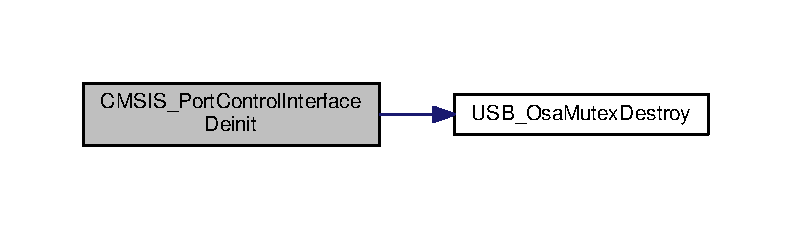
\includegraphics[width=350pt]{group__usb__pd__cmsis__wrapper_ga5ae4fe326851bb5374399212012e22f9_cgraph}
\end{center}
\end{figure}




Here is the caller graph for this function\-:
\nopagebreak
\begin{figure}[H]
\begin{center}
\leavevmode
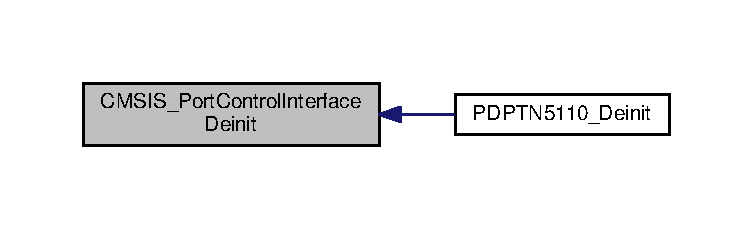
\includegraphics[width=350pt]{group__usb__pd__cmsis__wrapper_ga5ae4fe326851bb5374399212012e22f9_icgraph}
\end{center}
\end{figure}


\hypertarget{group__usb__pd__cmsis__wrapper_ga4140e0b4e54efdabe981bdfbc97725dd}{\index{Usb\-\_\-pd\-\_\-cmsis\-\_\-wrapper@{Usb\-\_\-pd\-\_\-cmsis\-\_\-wrapper}!C\-M\-S\-I\-S\-\_\-\-Port\-Control\-Interface\-Init@{C\-M\-S\-I\-S\-\_\-\-Port\-Control\-Interface\-Init}}
\index{C\-M\-S\-I\-S\-\_\-\-Port\-Control\-Interface\-Init@{C\-M\-S\-I\-S\-\_\-\-Port\-Control\-Interface\-Init}!Usb_pd_cmsis_wrapper@{Usb\-\_\-pd\-\_\-cmsis\-\_\-wrapper}}
\subsubsection[{C\-M\-S\-I\-S\-\_\-\-Port\-Control\-Interface\-Init}]{\setlength{\rightskip}{0pt plus 5cm}int32\-\_\-t C\-M\-S\-I\-S\-\_\-\-Port\-Control\-Interface\-Init (
\begin{DoxyParamCaption}
\item[{{\bf cmsis\-\_\-driver\-\_\-adapter\-\_\-t} $\ast$$\ast$}]{cmsis\-Driver, }
\item[{uint8\-\_\-t}]{interface, }
\item[{void $\ast$}]{interface\-Config}
\end{DoxyParamCaption}
)}}\label{group__usb__pd__cmsis__wrapper_ga4140e0b4e54efdabe981bdfbc97725dd}


Initialize C\-M\-S\-I\-S driver adapter instance. 

This function return the \hyperlink{group__usb__pd__cmsis__wrapper_ga53daa69dcc6fde0029cec3452c8b58ff}{cmsis\-\_\-driver\-\_\-adapter\-\_\-t} instance, the other A\-P\-I use this as the parameter.


\begin{DoxyParams}[1]{Parameters}
\mbox{\tt out}  & {\em cmsis\-Driver} & Return the instance. \\
\hline
\mbox{\tt in}  & {\em interface} & the I2\-C/\-S\-P\-I interface, see \hyperlink{group__usb__pd__stack_ga0499cb1eb2ad70e8d155ff72b50c7a38}{pd\-\_\-phy\-\_\-interface\-\_\-t} \\
\hline
\mbox{\tt in}  & {\em interface\-Config} & it is \hyperlink{group__usb__pd__cmsis__wrapper_gada87adb00aefcd83988ef970c2f4d750}{pd\-\_\-i2c\-\_\-interface\-\_\-config\-\_\-t} or \hyperlink{group__usb__pd__cmsis__wrapper_ga0a6afc9ea2599bcbe9b60e47f60d6bed}{pd\-\_\-spi\-\_\-interface\-\_\-config\-\_\-t}\\
\hline
\end{DoxyParams}

\begin{DoxyRetVals}{Return values}
{\em A\-R\-M\-\_\-\-D\-R\-I\-V\-E\-R\-\_\-\-E\-R\-R\-O\-R} & initialization success. \\
\hline
{\em other} & value error code. \\
\hline
\end{DoxyRetVals}

\begin{DoxyCode}
62 \{
63     int32\_t status = ARM\_DRIVER\_ERROR;
64 
65     \textcolor{keywordflow}{switch} (interface)
66     \{
67 \textcolor{preprocessor}{#if (defined PD\_CONFIG\_CMSIS\_I2C\_INTERFACE) && (PD\_CONFIG\_CMSIS\_I2C\_INTERFACE)
}
68 \textcolor{preprocessor}{}        \textcolor{keywordflow}{case} \hyperlink{group__usb__pd__stack_gga4aed694f998da91dea8d218596d65c1ea0e6fc11f3fbc9732619f2083042e7e17}{kInterface\_i2c0}:
69         \textcolor{keywordflow}{case} \hyperlink{group__usb__pd__stack_gga4aed694f998da91dea8d218596d65c1eaf78fb0f4bdd4db6e8a2e5dab05ba59d2}{kInterface\_i2c1}:
70         \textcolor{keywordflow}{case} \hyperlink{group__usb__pd__stack_gga4aed694f998da91dea8d218596d65c1ea7e08032b6509673dc643a7d01a5baec4}{kInterface\_i2c2}:
71         \textcolor{keywordflow}{case} \hyperlink{group__usb__pd__stack_gga4aed694f998da91dea8d218596d65c1ea369545de00e8d0fb91e9f065d725c16c}{kInterface\_i2c3}:
72             status = CMSIS\_I2CInterfaceInit(cmsisDriver, interface, interfaceConfig);
73             \textcolor{keywordflow}{break};
74 \textcolor{preprocessor}{#endif
}
75 \textcolor{preprocessor}{}
76 \textcolor{preprocessor}{#if (defined PD\_CONFIG\_CMSIS\_SPI\_INTERFACE) && (PD\_CONFIG\_CMSIS\_SPI\_INTERFACE)
}
77 \textcolor{preprocessor}{}        \textcolor{keywordflow}{case} \hyperlink{group__usb__pd__stack_gga4aed694f998da91dea8d218596d65c1ea48b48a50986d3b6fd9e7640cbea852ef}{kInterface\_spi0}:
78         \textcolor{keywordflow}{case} \hyperlink{group__usb__pd__stack_gga4aed694f998da91dea8d218596d65c1ea178b943373d02f27c53232f7e31e62a6}{kInterface\_spi1}:
79         \textcolor{keywordflow}{case} \hyperlink{group__usb__pd__stack_gga4aed694f998da91dea8d218596d65c1ea1a8206ebb4a5aa81b0401b26d239ad9d}{kInterface\_spi2}:
80         \textcolor{keywordflow}{case} \hyperlink{group__usb__pd__stack_gga4aed694f998da91dea8d218596d65c1ea0842cd2e8c57954daf912b6d7b648e9f}{kInterface\_spi3}:
81             status = CMSIS\_SPIInterfaceInit(cmsisDriver, interface, interfaceConfig);
82             \textcolor{keywordflow}{break};
83 \textcolor{preprocessor}{#endif
}
84 \textcolor{preprocessor}{}    \}
85 
86     \textcolor{keywordflow}{if} ((status == ARM\_DRIVER\_OK) && (*cmsisDriver != NULL))
87     \{
88         \textcolor{keywordflow}{if} (\hyperlink{group__usb__os__abstraction_gaf36ecc5a6c3359a6587750b17800f49d}{USB\_OsaMutexCreate}(&((*cmsisDriver)->cmsisMutex)) != 
      \hyperlink{group__usb__os__abstraction_gga453ebd2f93aafb8c938c3a23c815f9bdab90805fb75297fda1ca60dbb2283f933}{kStatus\_USB\_OSA\_Success})
89         \{
90             (*cmsisDriver)->cmsisMutex = NULL;
91             status = ARM\_DRIVER\_ERROR;
92         \}
93     \}
94 
95     \textcolor{keywordflow}{return} status;
96 \}
\end{DoxyCode}


Here is the call graph for this function\-:
\nopagebreak
\begin{figure}[H]
\begin{center}
\leavevmode
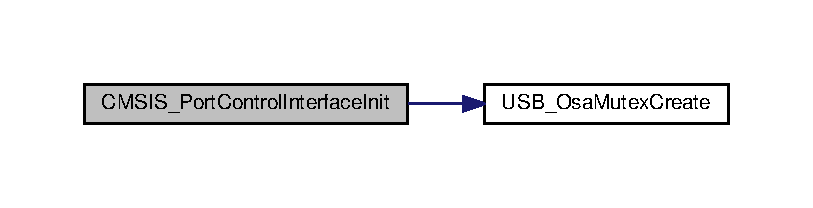
\includegraphics[width=350pt]{group__usb__pd__cmsis__wrapper_ga4140e0b4e54efdabe981bdfbc97725dd_cgraph}
\end{center}
\end{figure}




Here is the caller graph for this function\-:
\nopagebreak
\begin{figure}[H]
\begin{center}
\leavevmode
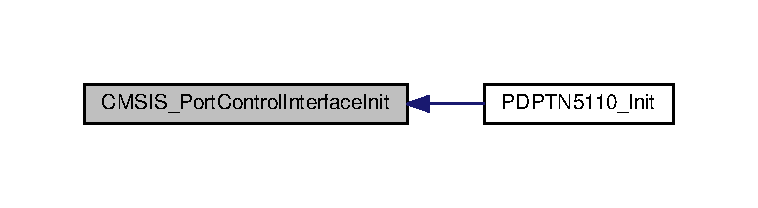
\includegraphics[width=350pt]{group__usb__pd__cmsis__wrapper_ga4140e0b4e54efdabe981bdfbc97725dd_icgraph}
\end{center}
\end{figure}


\hypertarget{group__usb__pd__cmsis__wrapper_ga190a521ef01279662f71d4e33e51aa4c}{\index{Usb\-\_\-pd\-\_\-cmsis\-\_\-wrapper@{Usb\-\_\-pd\-\_\-cmsis\-\_\-wrapper}!C\-M\-S\-I\-S\-\_\-\-Port\-Control\-Interface\-Read\-Register@{C\-M\-S\-I\-S\-\_\-\-Port\-Control\-Interface\-Read\-Register}}
\index{C\-M\-S\-I\-S\-\_\-\-Port\-Control\-Interface\-Read\-Register@{C\-M\-S\-I\-S\-\_\-\-Port\-Control\-Interface\-Read\-Register}!Usb_pd_cmsis_wrapper@{Usb\-\_\-pd\-\_\-cmsis\-\_\-wrapper}}
\subsubsection[{C\-M\-S\-I\-S\-\_\-\-Port\-Control\-Interface\-Read\-Register}]{\setlength{\rightskip}{0pt plus 5cm}int32\-\_\-t C\-M\-S\-I\-S\-\_\-\-Port\-Control\-Interface\-Read\-Register (
\begin{DoxyParamCaption}
\item[{{\bf cmsis\-\_\-driver\-\_\-adapter\-\_\-t} $\ast$}]{cmsis\-Driver, }
\item[{uint32\-\_\-t}]{register\-Addr, }
\item[{uint8\-\_\-t}]{register\-Len, }
\item[{uint8\-\_\-t $\ast$}]{data, }
\item[{uint32\-\_\-t}]{num}
\end{DoxyParamCaption}
)}}\label{group__usb__pd__cmsis__wrapper_ga190a521ef01279662f71d4e33e51aa4c}


Read data from slave. 


\begin{DoxyParams}[1]{Parameters}
\mbox{\tt in}  & {\em cmsis\-Driver} & Return the instance. \\
\hline
\mbox{\tt in}  & {\em register\-Addr} & The access register address. \\
\hline
\mbox{\tt in}  & {\em register\-Len} & The register addreess's length, normally it is one byte or two bytes. \\
\hline
\mbox{\tt in}  & {\em data} & The data buffer. \\
\hline
\mbox{\tt in}  & {\em num} & The data length.\\
\hline
\end{DoxyParams}

\begin{DoxyRetVals}{Return values}
{\em A\-R\-M\-\_\-\-D\-R\-I\-V\-E\-R\-\_\-\-E\-R\-R\-O\-R} & initialization success. \\
\hline
{\em other} & value error code. \\
\hline
\end{DoxyRetVals}

\begin{DoxyCode}
173 \{
174     int32\_t status = ARM\_DRIVER\_ERROR;
175 
176     \textcolor{keywordflow}{if} (\hyperlink{group__usb__os__abstraction_ga1fed31c4b683c5f652b4e2e8b23c34fd}{USB\_OsaMutexLock}(cmsisDriver->\hyperlink{struct__cmsis__drier__adapter_a952d05d8262ef9aebfa6ca9c4d62fe46}{cmsisMutex}) != 
      \hyperlink{group__usb__os__abstraction_gga453ebd2f93aafb8c938c3a23c815f9bdab90805fb75297fda1ca60dbb2283f933}{kStatus\_USB\_OSA\_Success})
177     \{
178         \textcolor{keywordflow}{return} status;
179     \}
180 
181     \textcolor{keywordflow}{switch} (cmsisDriver->\hyperlink{struct__cmsis__drier__adapter_a51a572fa7a648387cf481b45b862457c}{interface})
182     \{
183 \textcolor{preprocessor}{#if (defined PD\_CONFIG\_CMSIS\_I2C\_INTERFACE) && (PD\_CONFIG\_CMSIS\_I2C\_INTERFACE)
}
184 \textcolor{preprocessor}{}        \textcolor{keywordflow}{case} \hyperlink{group__usb__pd__stack_gga4aed694f998da91dea8d218596d65c1ea0e6fc11f3fbc9732619f2083042e7e17}{kInterface\_i2c0}:
185         \textcolor{keywordflow}{case} \hyperlink{group__usb__pd__stack_gga4aed694f998da91dea8d218596d65c1eaf78fb0f4bdd4db6e8a2e5dab05ba59d2}{kInterface\_i2c1}:
186         \textcolor{keywordflow}{case} \hyperlink{group__usb__pd__stack_gga4aed694f998da91dea8d218596d65c1ea7e08032b6509673dc643a7d01a5baec4}{kInterface\_i2c2}:
187         \textcolor{keywordflow}{case} \hyperlink{group__usb__pd__stack_gga4aed694f998da91dea8d218596d65c1ea369545de00e8d0fb91e9f065d725c16c}{kInterface\_i2c3}:
188             status = CMSIS\_I2CInterfaceReadRegister(cmsisDriver, registerAddr, registerLen, data, num);
189             \textcolor{keywordflow}{break};
190 \textcolor{preprocessor}{#endif
}
191 \textcolor{preprocessor}{}
192 \textcolor{preprocessor}{#if (defined PD\_CONFIG\_CMSIS\_SPI\_INTERFACE) && (PD\_CONFIG\_CMSIS\_SPI\_INTERFACE)
}
193 \textcolor{preprocessor}{}        \textcolor{keywordflow}{case} \hyperlink{group__usb__pd__stack_gga4aed694f998da91dea8d218596d65c1ea48b48a50986d3b6fd9e7640cbea852ef}{kInterface\_spi0}:
194         \textcolor{keywordflow}{case} \hyperlink{group__usb__pd__stack_gga4aed694f998da91dea8d218596d65c1ea178b943373d02f27c53232f7e31e62a6}{kInterface\_spi1}:
195         \textcolor{keywordflow}{case} \hyperlink{group__usb__pd__stack_gga4aed694f998da91dea8d218596d65c1ea1a8206ebb4a5aa81b0401b26d239ad9d}{kInterface\_spi2}:
196         \textcolor{keywordflow}{case} \hyperlink{group__usb__pd__stack_gga4aed694f998da91dea8d218596d65c1ea0842cd2e8c57954daf912b6d7b648e9f}{kInterface\_spi3}:
197             status = CMSIS\_SPIInterfaceReadRegister(cmsisDriver, registerAddr, registerLen, data, num);
198             \textcolor{keywordflow}{break};
199 \textcolor{preprocessor}{#endif
}
200 \textcolor{preprocessor}{}    \}
201 
202     \textcolor{keywordflow}{if} (\hyperlink{group__usb__os__abstraction_gaad3249273d566eae00e2cea81192315a}{USB\_OsaMutexUnlock}(cmsisDriver->\hyperlink{struct__cmsis__drier__adapter_a952d05d8262ef9aebfa6ca9c4d62fe46}{cmsisMutex}) != 
      \hyperlink{group__usb__os__abstraction_gga453ebd2f93aafb8c938c3a23c815f9bdab90805fb75297fda1ca60dbb2283f933}{kStatus\_USB\_OSA\_Success})
203     \{
204         \textcolor{keywordflow}{return} ARM\_DRIVER\_ERROR;
205     \}
206 
207     \textcolor{keywordflow}{return} status;
208 \}
\end{DoxyCode}


Here is the call graph for this function\-:
\nopagebreak
\begin{figure}[H]
\begin{center}
\leavevmode
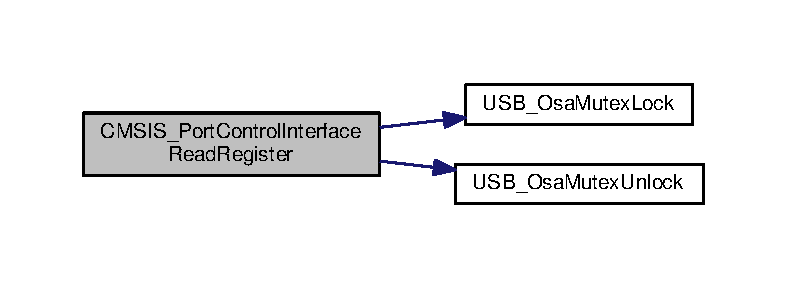
\includegraphics[width=350pt]{group__usb__pd__cmsis__wrapper_ga190a521ef01279662f71d4e33e51aa4c_cgraph}
\end{center}
\end{figure}




Here is the caller graph for this function\-:
\nopagebreak
\begin{figure}[H]
\begin{center}
\leavevmode
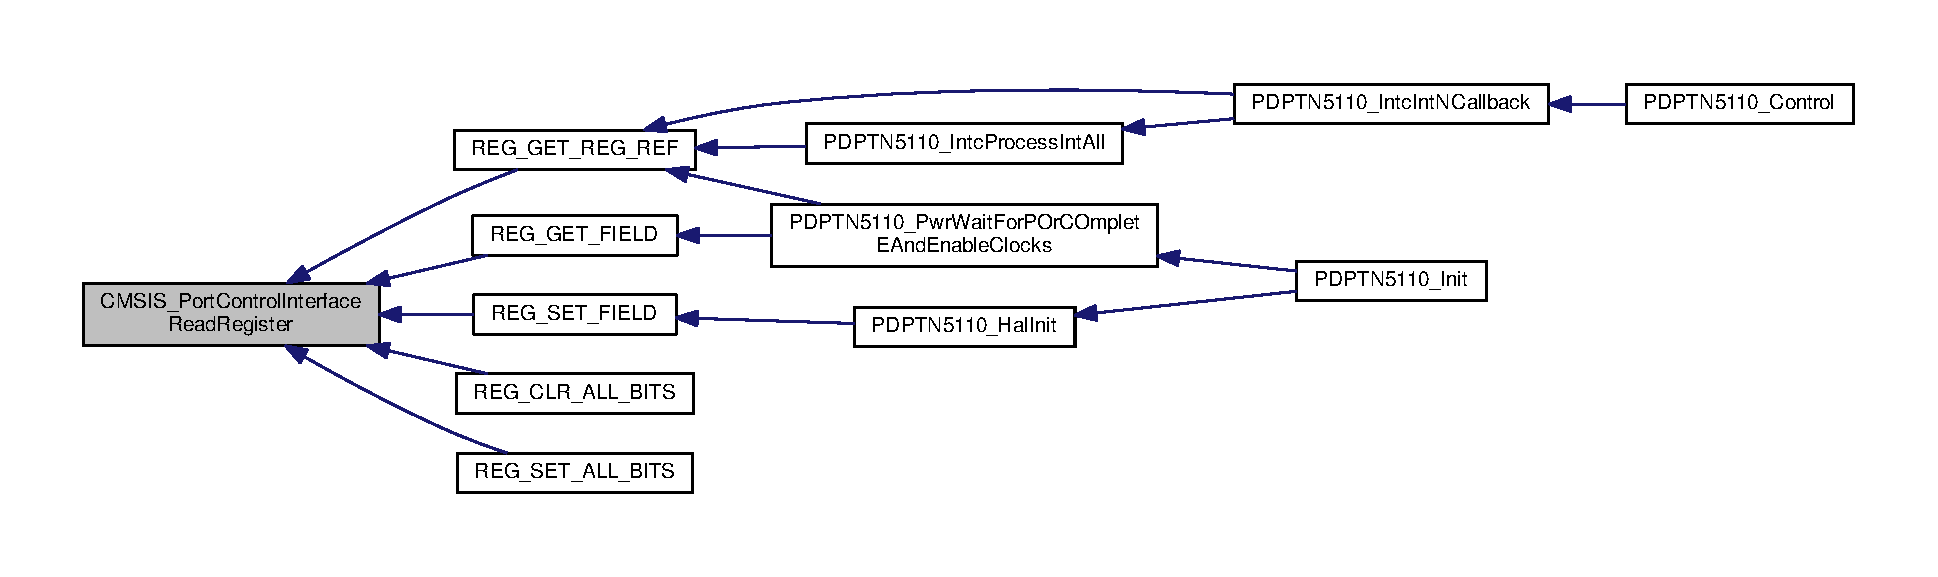
\includegraphics[width=350pt]{group__usb__pd__cmsis__wrapper_ga190a521ef01279662f71d4e33e51aa4c_icgraph}
\end{center}
\end{figure}


\hypertarget{group__usb__pd__cmsis__wrapper_ga09c1e56830b347c846c280fe3525c757}{\index{Usb\-\_\-pd\-\_\-cmsis\-\_\-wrapper@{Usb\-\_\-pd\-\_\-cmsis\-\_\-wrapper}!C\-M\-S\-I\-S\-\_\-\-Port\-Control\-Interface\-Write\-Register@{C\-M\-S\-I\-S\-\_\-\-Port\-Control\-Interface\-Write\-Register}}
\index{C\-M\-S\-I\-S\-\_\-\-Port\-Control\-Interface\-Write\-Register@{C\-M\-S\-I\-S\-\_\-\-Port\-Control\-Interface\-Write\-Register}!Usb_pd_cmsis_wrapper@{Usb\-\_\-pd\-\_\-cmsis\-\_\-wrapper}}
\subsubsection[{C\-M\-S\-I\-S\-\_\-\-Port\-Control\-Interface\-Write\-Register}]{\setlength{\rightskip}{0pt plus 5cm}int32\-\_\-t C\-M\-S\-I\-S\-\_\-\-Port\-Control\-Interface\-Write\-Register (
\begin{DoxyParamCaption}
\item[{{\bf cmsis\-\_\-driver\-\_\-adapter\-\_\-t} $\ast$}]{cmsis\-Driver, }
\item[{uint32\-\_\-t}]{register\-Addr, }
\item[{uint8\-\_\-t}]{register\-Len, }
\item[{const uint8\-\_\-t $\ast$}]{data, }
\item[{uint32\-\_\-t}]{num}
\end{DoxyParamCaption}
)}}\label{group__usb__pd__cmsis__wrapper_ga09c1e56830b347c846c280fe3525c757}


Write data to slave. 


\begin{DoxyParams}[1]{Parameters}
\mbox{\tt in}  & {\em cmsis\-Driver} & Return the instance. \\
\hline
\mbox{\tt in}  & {\em register\-Addr} & The access register address. \\
\hline
\mbox{\tt in}  & {\em register\-Len} & The register addreess's length, normally it is one byte or two bytes. \\
\hline
\mbox{\tt in}  & {\em data} & The data buffer. \\
\hline
\mbox{\tt in}  & {\em num} & The data length.\\
\hline
\end{DoxyParams}

\begin{DoxyRetVals}{Return values}
{\em A\-R\-M\-\_\-\-D\-R\-I\-V\-E\-R\-\_\-\-E\-R\-R\-O\-R} & initialization success. \\
\hline
{\em other} & value error code. \\
\hline
\end{DoxyRetVals}

\begin{DoxyCode}
134 \{
135     int32\_t status = ARM\_DRIVER\_ERROR;
136 
137     \textcolor{keywordflow}{if} (\hyperlink{group__usb__os__abstraction_ga1fed31c4b683c5f652b4e2e8b23c34fd}{USB\_OsaMutexLock}(cmsisDriver->\hyperlink{struct__cmsis__drier__adapter_a952d05d8262ef9aebfa6ca9c4d62fe46}{cmsisMutex}) != 
      \hyperlink{group__usb__os__abstraction_gga453ebd2f93aafb8c938c3a23c815f9bdab90805fb75297fda1ca60dbb2283f933}{kStatus\_USB\_OSA\_Success})
138     \{
139         \textcolor{keywordflow}{return} status;
140     \}
141 
142     \textcolor{keywordflow}{switch} (cmsisDriver->\hyperlink{struct__cmsis__drier__adapter_a51a572fa7a648387cf481b45b862457c}{interface})
143     \{
144 \textcolor{preprocessor}{#if (defined PD\_CONFIG\_CMSIS\_I2C\_INTERFACE) && (PD\_CONFIG\_CMSIS\_I2C\_INTERFACE)
}
145 \textcolor{preprocessor}{}        \textcolor{keywordflow}{case} \hyperlink{group__usb__pd__stack_gga4aed694f998da91dea8d218596d65c1ea0e6fc11f3fbc9732619f2083042e7e17}{kInterface\_i2c0}:
146         \textcolor{keywordflow}{case} \hyperlink{group__usb__pd__stack_gga4aed694f998da91dea8d218596d65c1eaf78fb0f4bdd4db6e8a2e5dab05ba59d2}{kInterface\_i2c1}:
147         \textcolor{keywordflow}{case} \hyperlink{group__usb__pd__stack_gga4aed694f998da91dea8d218596d65c1ea7e08032b6509673dc643a7d01a5baec4}{kInterface\_i2c2}:
148         \textcolor{keywordflow}{case} \hyperlink{group__usb__pd__stack_gga4aed694f998da91dea8d218596d65c1ea369545de00e8d0fb91e9f065d725c16c}{kInterface\_i2c3}:
149             status = CMSIS\_I2CInterfaceWriteRegister(cmsisDriver, registerAddr, registerLen, data, num);
150             \textcolor{keywordflow}{break};
151 \textcolor{preprocessor}{#endif
}
152 \textcolor{preprocessor}{}
153 \textcolor{preprocessor}{#if (defined PD\_CONFIG\_CMSIS\_SPI\_INTERFACE) && (PD\_CONFIG\_CMSIS\_SPI\_INTERFACE)
}
154 \textcolor{preprocessor}{}        \textcolor{keywordflow}{case} \hyperlink{group__usb__pd__stack_gga4aed694f998da91dea8d218596d65c1ea48b48a50986d3b6fd9e7640cbea852ef}{kInterface\_spi0}:
155         \textcolor{keywordflow}{case} \hyperlink{group__usb__pd__stack_gga4aed694f998da91dea8d218596d65c1ea178b943373d02f27c53232f7e31e62a6}{kInterface\_spi1}:
156         \textcolor{keywordflow}{case} \hyperlink{group__usb__pd__stack_gga4aed694f998da91dea8d218596d65c1ea1a8206ebb4a5aa81b0401b26d239ad9d}{kInterface\_spi2}:
157         \textcolor{keywordflow}{case} \hyperlink{group__usb__pd__stack_gga4aed694f998da91dea8d218596d65c1ea0842cd2e8c57954daf912b6d7b648e9f}{kInterface\_spi3}:
158             status = CMSIS\_SPIInterfaceWriteRegister(cmsisDriver, registerAddr, registerLen, data, num);
159             \textcolor{keywordflow}{break};
160 \textcolor{preprocessor}{#endif
}
161 \textcolor{preprocessor}{}    \}
162 
163     \textcolor{keywordflow}{if} (\hyperlink{group__usb__os__abstraction_gaad3249273d566eae00e2cea81192315a}{USB\_OsaMutexUnlock}(cmsisDriver->\hyperlink{struct__cmsis__drier__adapter_a952d05d8262ef9aebfa6ca9c4d62fe46}{cmsisMutex}) != 
      \hyperlink{group__usb__os__abstraction_gga453ebd2f93aafb8c938c3a23c815f9bdab90805fb75297fda1ca60dbb2283f933}{kStatus\_USB\_OSA\_Success})
164     \{
165         \textcolor{keywordflow}{return} ARM\_DRIVER\_ERROR;
166     \}
167 
168     \textcolor{keywordflow}{return} status;
169 \}
\end{DoxyCode}


Here is the call graph for this function\-:
\nopagebreak
\begin{figure}[H]
\begin{center}
\leavevmode
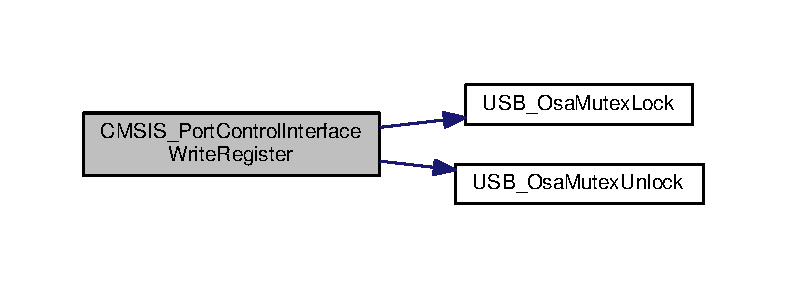
\includegraphics[width=350pt]{group__usb__pd__cmsis__wrapper_ga09c1e56830b347c846c280fe3525c757_cgraph}
\end{center}
\end{figure}




Here is the caller graph for this function\-:
\nopagebreak
\begin{figure}[H]
\begin{center}
\leavevmode
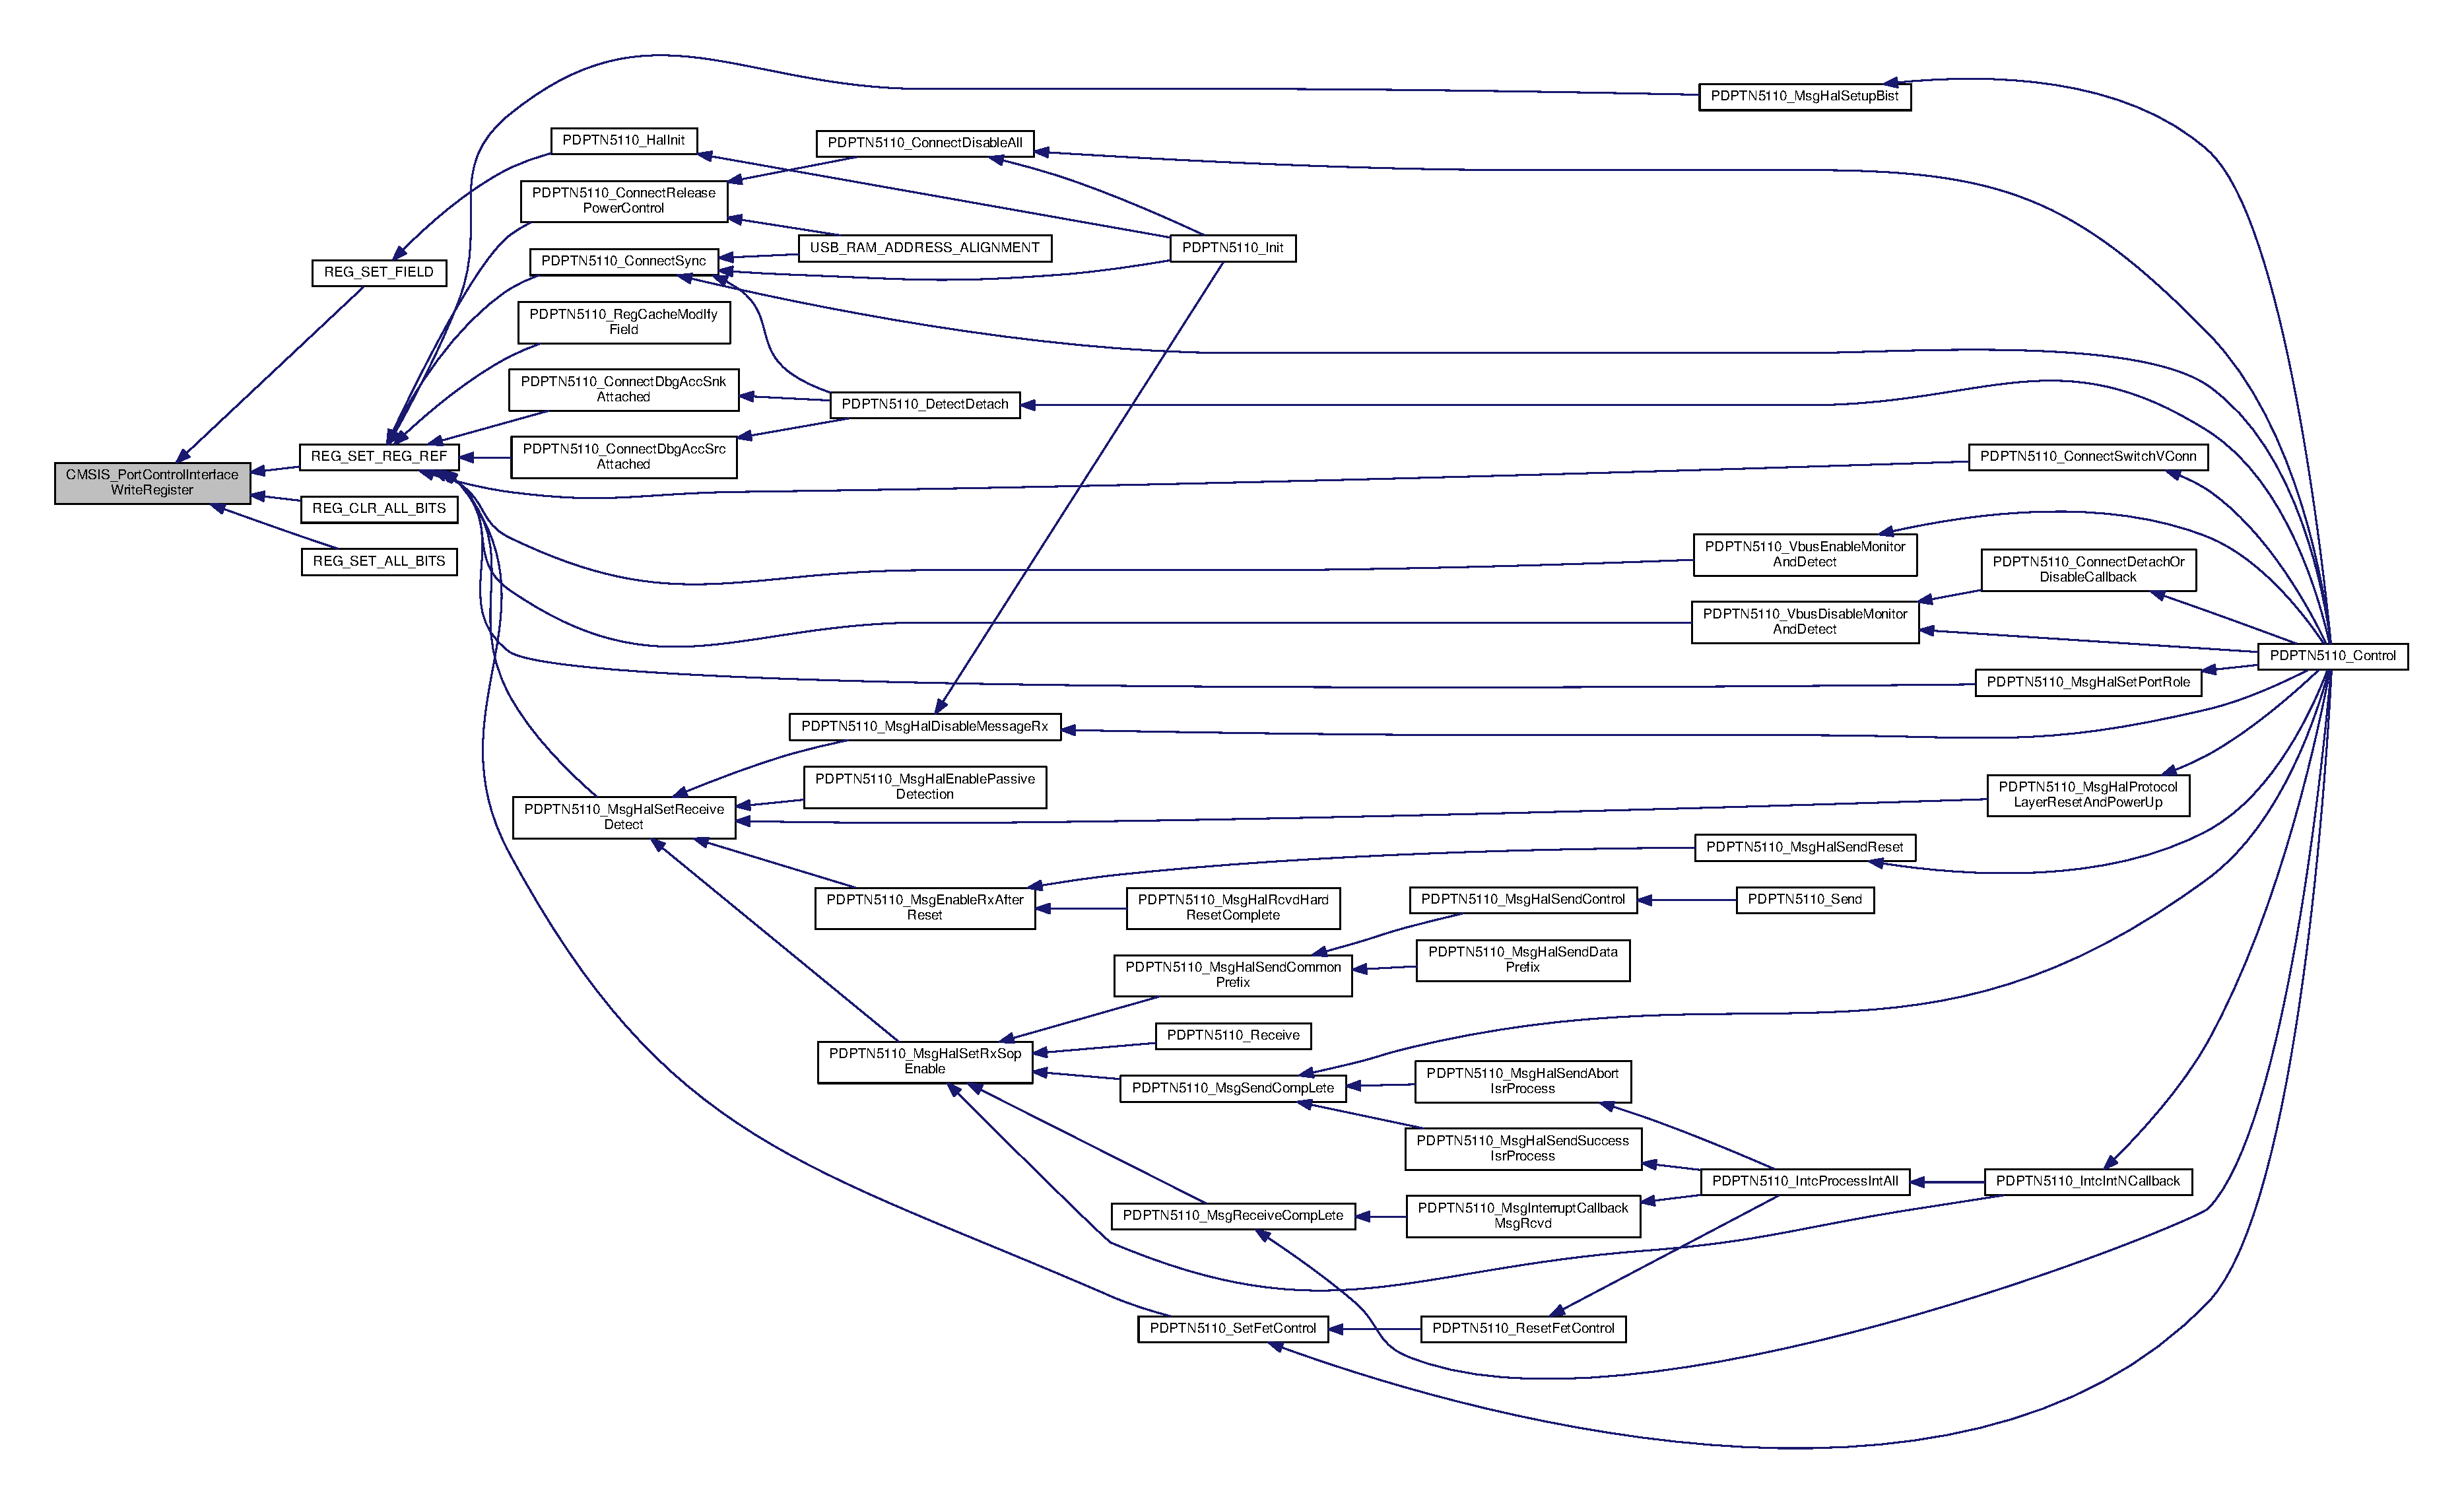
\includegraphics[width=350pt]{group__usb__pd__cmsis__wrapper_ga09c1e56830b347c846c280fe3525c757_icgraph}
\end{center}
\end{figure}



\hypertarget{group__usb__pd__stack}{\section{Usb\-\_\-pd\-\_\-stack}
\label{group__usb__pd__stack}\index{Usb\-\_\-pd\-\_\-stack@{Usb\-\_\-pd\-\_\-stack}}
}
\subsection*{Classes}
\begin{DoxyCompactItemize}
\item 
struct \hyperlink{struct__pd__power__port__config}{\-\_\-pd\-\_\-power\-\_\-port\-\_\-config}
\item 
struct \hyperlink{struct__pd__instance__config}{\-\_\-pd\-\_\-instance\-\_\-config}
\begin{DoxyCompactList}\small\item\em P\-D instance config. \end{DoxyCompactList}\item 
struct \hyperlink{struct__pd__source__fixed__pdo}{\-\_\-pd\-\_\-source\-\_\-fixed\-\_\-pdo}
\begin{DoxyCompactList}\small\item\em fixed source P\-D\-O \end{DoxyCompactList}\item 
struct \hyperlink{struct__pd__sink__fixed__pdo}{\-\_\-pd\-\_\-sink\-\_\-fixed\-\_\-pdo}
\begin{DoxyCompactList}\small\item\em fixed sink P\-D\-O \end{DoxyCompactList}\item 
struct \hyperlink{struct__pd__source__variable__pdo}{\-\_\-pd\-\_\-source\-\_\-variable\-\_\-pdo}
\begin{DoxyCompactList}\small\item\em variable source P\-D\-O \end{DoxyCompactList}\item 
struct \hyperlink{struct__pd__sink__variable__pdo}{\-\_\-pd\-\_\-sink\-\_\-variable\-\_\-pdo}
\begin{DoxyCompactList}\small\item\em variable sink P\-D\-O \end{DoxyCompactList}\item 
struct \hyperlink{struct__pd__source__battery__pdo}{\-\_\-pd\-\_\-source\-\_\-battery\-\_\-pdo}
\begin{DoxyCompactList}\small\item\em battery source P\-D\-O \end{DoxyCompactList}\item 
struct \hyperlink{struct__pd__sink__battery__pdo}{\-\_\-pd\-\_\-sink\-\_\-battery\-\_\-pdo}
\begin{DoxyCompactList}\small\item\em battery sink P\-D\-O \end{DoxyCompactList}\item 
struct \hyperlink{struct__pd__pdo__common}{\-\_\-pd\-\_\-pdo\-\_\-common}
\begin{DoxyCompactList}\small\item\em common P\-D\-O for union \end{DoxyCompactList}\item 
struct \hyperlink{struct__pd__source__pdo}{\-\_\-pd\-\_\-source\-\_\-pdo}
\begin{DoxyCompactList}\small\item\em source P\-D\-O union \end{DoxyCompactList}\item 
struct \hyperlink{struct__pd__sink__pdo}{\-\_\-pd\-\_\-sink\-\_\-pdo}
\begin{DoxyCompactList}\small\item\em sink P\-D\-O union \end{DoxyCompactList}\item 
struct \hyperlink{struct__pd__structured__vdm__header}{\-\_\-pd\-\_\-structured\-\_\-vdm\-\_\-header}
\begin{DoxyCompactList}\small\item\em P\-D structured V\-D\-M header. \end{DoxyCompactList}\item 
struct \hyperlink{struct__pd__unstructured__vdm__header}{\-\_\-pd\-\_\-unstructured\-\_\-vdm\-\_\-header}
\begin{DoxyCompactList}\small\item\em P\-D unstructured V\-D\-M header. \end{DoxyCompactList}\item 
struct \hyperlink{struct__pd__extended__msg__header}{\-\_\-pd\-\_\-extended\-\_\-msg\-\_\-header}
\begin{DoxyCompactList}\small\item\em P\-D extended message header. \end{DoxyCompactList}\item 
struct \hyperlink{struct__pd__msg__header}{\-\_\-pd\-\_\-msg\-\_\-header}
\begin{DoxyCompactList}\small\item\em P\-D message header. \end{DoxyCompactList}\item 
struct \hyperlink{struct__pd__svdm__request}{\-\_\-pd\-\_\-svdm\-\_\-request}
\begin{DoxyCompactList}\small\item\em P\-D structured vdm command request (negotiation) \end{DoxyCompactList}\item 
struct \hyperlink{struct__pd__svdm__command__result}{\-\_\-pd\-\_\-svdm\-\_\-command\-\_\-result}
\begin{DoxyCompactList}\small\item\em P\-D structured vdm command result. \end{DoxyCompactList}\item 
struct \hyperlink{struct__pd__svdm__param}{\-\_\-pd\-\_\-svdm\-\_\-param}
\begin{DoxyCompactList}\small\item\em P\-D structured vdm command parameter. \end{DoxyCompactList}\item 
struct \hyperlink{struct__pd__unstructured__vdm__param}{\-\_\-pd\-\_\-unstructured\-\_\-vdm\-\_\-param}
\begin{DoxyCompactList}\small\item\em P\-D unstructured vdm command parameter. \end{DoxyCompactList}\item 
struct \hyperlink{struct__pd__command__data__param}{\-\_\-pd\-\_\-command\-\_\-data\-\_\-param}
\begin{DoxyCompactList}\small\item\em For some command with data use this structure as parameter. \end{DoxyCompactList}\item 
struct \hyperlink{struct__pd__rdo}{\-\_\-pd\-\_\-rdo}
\begin{DoxyCompactList}\small\item\em P\-D request data object. \end{DoxyCompactList}\item 
struct \hyperlink{struct__pd__capabilities}{\-\_\-pd\-\_\-capabilities}
\begin{DoxyCompactList}\small\item\em P\-D capabilities info. \end{DoxyCompactList}\item 
struct \hyperlink{struct__pd__negotiate__power__request}{\-\_\-pd\-\_\-negotiate\-\_\-power\-\_\-request}
\begin{DoxyCompactList}\small\item\em negotiate power rdo request \end{DoxyCompactList}\item 
struct \hyperlink{struct__pd__bist__object}{\-\_\-pd\-\_\-bist\-\_\-object}
\begin{DoxyCompactList}\small\item\em B\-I\-S\-T data object. \end{DoxyCompactList}\item 
struct \hyperlink{struct__pd__ptn5110__ctrl__pin}{\-\_\-pd\-\_\-ptn5110\-\_\-ctrl\-\_\-pin}
\begin{DoxyCompactList}\small\item\em control P\-T\-N5110 pin for power control \end{DoxyCompactList}\item 
struct \hyperlink{struct__pd__power__callback}{\-\_\-pd\-\_\-power\-\_\-callback}
\begin{DoxyCompactList}\small\item\em power control interface. \end{DoxyCompactList}\end{DoxyCompactItemize}
\subsection*{Macros}
\begin{DoxyCompactItemize}
\item 
\#define \hyperlink{group__usb__pd__stack_gab5c70518a449d87b8e044fe35f9794b9}{P\-D\-\_\-\-V\-E\-N\-D\-O\-R\-\_\-\-I\-D\-\_\-\-N\-X\-P}~0x1\-F\-C9u
\begin{DoxyCompactList}\small\item\em N\-X\-P's U\-S\-B vendor id. \end{DoxyCompactList}\item 
\#define \hyperlink{group__usb__pd__stack_ga647e3cd4fd452c4c8087331f7cff40e0}{P\-D\-\_\-\-S\-P\-E\-C\-\_\-\-R\-E\-V\-I\-S\-I\-O\-N\-\_\-10}~(0x00)
\begin{DoxyCompactList}\small\item\em The Specification Revision 1.\-0 value. \end{DoxyCompactList}\item 
\#define \hyperlink{group__usb__pd__stack_ga24966fea2a4e7d202653403ffb4dc4a4}{P\-D\-\_\-\-S\-P\-E\-C\-\_\-\-R\-E\-V\-I\-S\-I\-O\-N\-\_\-20}~(0x01)
\begin{DoxyCompactList}\small\item\em The Specification Revision 2.\-0 value. \end{DoxyCompactList}\item 
\#define \hyperlink{group__usb__pd__stack_ga4be9f8c2d24914f46c855883891789e0}{P\-D\-\_\-\-S\-P\-E\-C\-\_\-\-R\-E\-V\-I\-S\-I\-O\-N\-\_\-30}~(0x02)
\begin{DoxyCompactList}\small\item\em The Specification Revision 3.\-0 value. \end{DoxyCompactList}\item 
\#define \hyperlink{group__usb__pd__stack_ga90a8413b96e40227291a5243a7d70bc1}{P\-D\-\_\-\-S\-P\-E\-C\-\_\-\-S\-T\-R\-U\-C\-T\-U\-R\-E\-D\-\_\-\-V\-D\-M\-\_\-\-V\-E\-R\-S\-I\-O\-N\-\_\-10}~(0x00)
\begin{DoxyCompactList}\small\item\em The structured V\-D\-M version 1.\-0 value. \end{DoxyCompactList}\item 
\#define \hyperlink{group__usb__pd__stack_ga459e2031557c359d23fc2ae926c1f42d}{P\-D\-\_\-\-S\-P\-E\-C\-\_\-\-S\-T\-R\-U\-C\-T\-U\-R\-E\-D\-\_\-\-V\-D\-M\-\_\-\-V\-E\-R\-S\-I\-O\-N\-\_\-20}~(0x01)
\begin{DoxyCompactList}\small\item\em The structured V\-D\-M version 2.\-0 value. \end{DoxyCompactList}\item 
\#define \hyperlink{group__usb__pd__stack_ga6d970ee2c757411a31911430bb94c722}{P\-D\-\_\-\-S\-T\-A\-N\-D\-A\-R\-D\-\_\-\-I\-D}~0x\-F\-F00
\begin{DoxyCompactList}\small\item\em P\-D standard I\-D. \end{DoxyCompactList}\item 
\#define \hyperlink{group__usb__pd__stack_ga83cbb5a0a1b721ddb0f815077c854e8e}{P\-D\-\_\-\-P\-D\-O\-\_\-\-V\-O\-L\-T\-A\-G\-E\-\_\-\-U\-N\-I\-T}~(50)
\begin{DoxyCompactList}\small\item\em source/sink capability's voltage unit is 50m\-V \end{DoxyCompactList}\item 
\#define \hyperlink{group__usb__pd__stack_ga63746ad31eee8f5912a846952e6645b6}{P\-D\-\_\-\-P\-D\-O\-\_\-\-C\-U\-R\-R\-E\-N\-T\-\_\-\-U\-N\-I\-T}~(10)
\begin{DoxyCompactList}\small\item\em source/sink capability's current unit is 10m\-A \end{DoxyCompactList}\item 
\#define \hyperlink{group__usb__pd__stack_ga18642aa62f457d8501be4bddf6608e80}{P\-D\-\_\-\-P\-D\-O\-\_\-\-P\-O\-W\-E\-R\-\_\-\-U\-N\-I\-T}~(250)
\begin{DoxyCompactList}\small\item\em source/sink capability's power unit is 250m\-W \end{DoxyCompactList}\item 
\#define \hyperlink{group__usb__pd__stack_ga26ae67c195a653e3fa00d94551e85381}{P\-D\-\_\-\-S\-I\-N\-K\-\_\-\-D\-E\-T\-A\-C\-H\-\_\-\-O\-N\-\_\-\-V\-B\-U\-S\-\_\-\-A\-B\-S\-E\-N\-T}~(1)
\begin{DoxyCompactList}\small\item\em check detach based on vbus absent \end{DoxyCompactList}\item 
\#define \hyperlink{group__usb__pd__stack_ga6bc66a3ddfbafaa7313db800f351d968}{P\-D\-\_\-\-S\-I\-N\-K\-\_\-\-D\-E\-T\-A\-C\-H\-\_\-\-O\-N\-\_\-\-C\-C\-\_\-\-O\-P\-E\-N}~(2)
\begin{DoxyCompactList}\small\item\em check detach based C\-C line open \end{DoxyCompactList}\end{DoxyCompactItemize}
\subsection*{Typedefs}
\begin{DoxyCompactItemize}
\item 
typedef enum \hyperlink{group__usb__pd__stack_gaaad4cd00dd02567c6169429e3a895073}{\-\_\-pd\-\_\-status} \hyperlink{group__usb__pd__stack_ga04a1f331d9807a70ab9bb753f5ed1c80}{pd\-\_\-status\-\_\-t}
\begin{DoxyCompactList}\small\item\em pd error code used for function return value or error status. \end{DoxyCompactList}\item 
typedef enum \hyperlink{group__usb__pd__stack_ga8bd01601105e164bc0e0bb538aaa5c1c}{\-\_\-pd\-\_\-phy\-\_\-type} \hyperlink{group__usb__pd__stack_gaafe9b09173bbffaa5075085b0dab18ec}{pd\-\_\-phy\-\_\-type\-\_\-t}
\begin{DoxyCompactList}\small\item\em P\-D phy type, used in the \hyperlink{group__usb__pd__stack_gafa6034f9e204836697da1f2fc996cbad}{pd\-\_\-instance\-\_\-config\-\_\-t}. \end{DoxyCompactList}\item 
typedef enum \hyperlink{group__usb__pd__stack_ga922338772b41ceba51f7881c74b9e20a}{\-\_\-pd\-\_\-device\-\_\-type} \hyperlink{group__usb__pd__stack_gac70b6cd09eeb45ce1aeaa279f44adbc7}{pd\-\_\-device\-\_\-type\-\_\-t}
\begin{DoxyCompactList}\small\item\em The device's type, used in the \hyperlink{group__usb__pd__stack_gafa6034f9e204836697da1f2fc996cbad}{pd\-\_\-instance\-\_\-config\-\_\-t}. \end{DoxyCompactList}\item 
typedef enum \\*
\hyperlink{group__usb__pd__stack_gaffef947540aace08ecf6fd25f69720a9}{\-\_\-typec\-\_\-power\-\_\-role\-\_\-config} \hyperlink{group__usb__pd__stack_ga8522facb45d87054c87e6d6fb32d9dd1}{typec\-\_\-power\-\_\-role\-\_\-config\-\_\-t}
\begin{DoxyCompactList}\small\item\em configure device's type, used in the \hyperlink{group__usb__pd__stack_gafa6034f9e204836697da1f2fc996cbad}{pd\-\_\-instance\-\_\-config\-\_\-t}. \end{DoxyCompactList}\item 
typedef enum \\*
\hyperlink{group__usb__pd__stack_ga6ba6df5e492767ce7ac52bafddd8849d}{\-\_\-typec\-\_\-sink\-\_\-role\-\_\-config} \hyperlink{group__usb__pd__stack_gaa91aa4484c581bbfab49d099b848ccf3}{typec\-\_\-sink\-\_\-role\-\_\-config\-\_\-t}
\begin{DoxyCompactList}\small\item\em config typec sink role \end{DoxyCompactList}\item 
typedef enum \hyperlink{group__usb__pd__stack_ga4794fa8903a011ba6f0be0f04925411e}{\-\_\-typec\-\_\-try} \hyperlink{group__usb__pd__stack_ga86c3c8c95607b75c0c75cd2714487497}{typec\-\_\-try\-\_\-t}
\begin{DoxyCompactList}\small\item\em configure try type function, used in the \hyperlink{group__usb__pd__stack_gafa6034f9e204836697da1f2fc996cbad}{pd\-\_\-instance\-\_\-config\-\_\-t}. \end{DoxyCompactList}\item 
typedef enum \\*
\hyperlink{group__usb__pd__stack_gacc3677fc21b76efa77ae5f744194394a}{\-\_\-typec\-\_\-data\-\_\-function\-\_\-config} \hyperlink{group__usb__pd__stack_ga92476c6b5b34316ccb766c9d2cadd29e}{typec\-\_\-data\-\_\-function\-\_\-config\-\_\-t}
\begin{DoxyCompactList}\small\item\em configure device's data function, used in the \hyperlink{group__usb__pd__stack_gafa6034f9e204836697da1f2fc996cbad}{pd\-\_\-instance\-\_\-config\-\_\-t}. \end{DoxyCompactList}\item 
typedef enum \hyperlink{group__usb__pd__stack_ga4aed694f998da91dea8d218596d65c1e}{pd\-\_\-phy\-\_\-interface} \hyperlink{group__usb__pd__stack_ga0499cb1eb2ad70e8d155ff72b50c7a38}{pd\-\_\-phy\-\_\-interface\-\_\-t}
\begin{DoxyCompactList}\small\item\em P\-H\-Y interface. \end{DoxyCompactList}\item 
typedef enum \hyperlink{group__usb__pd__stack_ga7a924235403e0acab44d01e720091aa1}{\-\_\-start\-\_\-of\-\_\-packet} \hyperlink{group__usb__pd__stack_ga59170ea474bbce078de8ffb3eea617aa}{start\-\_\-of\-\_\-packet\-\_\-t}
\begin{DoxyCompactList}\small\item\em start of packet's type. \end{DoxyCompactList}\item 
typedef enum \hyperlink{group__usb__pd__stack_gaa0c9fbfbfb4442ef9d805438bfeb045c}{\-\_\-pd\-\_\-command\-\_\-result} \hyperlink{group__usb__pd__stack_ga59917b1485caba4dd8d9b65ca5a5fd92}{pd\-\_\-command\-\_\-result\-\_\-t}
\begin{DoxyCompactList}\small\item\em pd command error code. \end{DoxyCompactList}\item 
typedef enum \hyperlink{group__usb__pd__stack_gaf956bb4d3d27df52fb694311b8219b0e}{\-\_\-typec\-\_\-current} \hyperlink{group__usb__pd__stack_ga875b585c994b83a1c1fd1e81bac28f7a}{typec\-\_\-current\-\_\-val\-\_\-t}
\begin{DoxyCompactList}\small\item\em Typec current level related to Rp value. \end{DoxyCompactList}\item 
typedef enum \hyperlink{group__usb__pd__stack_ga46146487374ddc31d48f33b2b6a26f8b}{\-\_\-pd\-\_\-power\-\_\-role} \hyperlink{group__usb__pd__stack_ga19f0723d5c2d772a03d075636497183f}{pd\-\_\-power\-\_\-role\-\_\-t}
\begin{DoxyCompactList}\small\item\em P\-D running power role type. \end{DoxyCompactList}\item 
typedef enum \hyperlink{group__usb__pd__stack_ga25760887aa95821023cc0ab5e151f828}{\-\_\-pd\-\_\-data\-\_\-role} \hyperlink{group__usb__pd__stack_gabe6e64840f66187fd82dca3d81259839}{pd\-\_\-data\-\_\-role\-\_\-t}
\begin{DoxyCompactList}\small\item\em P\-D running data role type. \end{DoxyCompactList}\item 
typedef enum \hyperlink{group__usb__pd__stack_gab67908aebf6cb10704f4ec6127761e28}{\-\_\-pd\-\_\-vconn\-\_\-role} \hyperlink{group__usb__pd__stack_ga1e7a5e660ff0837fe23286556a20d4eb}{pd\-\_\-vconn\-\_\-role\-\_\-t}
\begin{DoxyCompactList}\small\item\em Vconn role type (Vconn source or not). \end{DoxyCompactList}\item 
typedef enum \\*
\hyperlink{group__usb__pd__stack_ga5dcf4d70a373001cfde169f0e8b9a1ba}{\-\_\-typec\-\_\-connection\-\_\-state} \hyperlink{group__usb__pd__stack_ga416d720fe603166cb1c16443199d42f8}{typec\-\_\-port\-\_\-connect\-\_\-state\-\_\-t}
\begin{DoxyCompactList}\small\item\em Type\-C connection state, self or partner's device type. \end{DoxyCompactList}\item 
typedef enum \hyperlink{group__usb__pd__stack_ga71b74b2e350f1841b93c1f894403f85b}{\-\_\-pd\-\_\-phy\-\_\-pwer\-\_\-state} \hyperlink{group__usb__pd__stack_gaba31b8436256d541d1f6f9cd01c94fe5}{pd\-\_\-phy\-\_\-pwr\-\_\-state\-\_\-t}
\begin{DoxyCompactList}\small\item\em P\-H\-Y power state (low power). \end{DoxyCompactList}\item 
typedef enum \hyperlink{group__usb__pd__stack_gac4a67ecdc78b1a071ca6505a765a301f}{pd\-\_\-vdm\-\_\-command} \hyperlink{group__usb__pd__stack_gabd6b0763d01e2d65501af70e4f67b039}{pd\-\_\-vdm\-\_\-command\-\_\-t}
\begin{DoxyCompactList}\small\item\em Structured V\-D\-M command values. \end{DoxyCompactList}\item 
typedef enum \hyperlink{group__usb__pd__stack_gaa6b2f8f6620280d0d17ab102c5992ca8}{pd\-\_\-vdm\-\_\-command\-\_\-type} \hyperlink{group__usb__pd__stack_ga3da8531f25ed451f0392fc7efdf7fabe}{pd\-\_\-vdm\-\_\-command\-\_\-type\-\_\-t}
\begin{DoxyCompactList}\small\item\em Structured V\-D\-M command type values. \end{DoxyCompactList}\item 
typedef enum \hyperlink{group__usb__pd__stack_ga6e10571af6af1a42760ea442ab580eb8}{\-\_\-pd\-\_\-dpm\-\_\-callback} \hyperlink{group__usb__pd__stack_ga75d3b9ae5fd2d84e59b0754f9855cb61}{pd\-\_\-dpm\-\_\-callback\-\_\-event\-\_\-t}
\begin{DoxyCompactList}\small\item\em The callback events. \end{DoxyCompactList}\item 
typedef enum \hyperlink{group__usb__pd__stack_gabf2676c3360b7c572954ae09c0a5e46a}{\-\_\-pd\-\_\-command} \hyperlink{group__usb__pd__stack_ga91457cf9522e345a0efa2e2a7424bb0d}{pd\-\_\-command\-\_\-t}
\begin{DoxyCompactList}\small\item\em The command used in P\-D\-\_\-\-Command. \end{DoxyCompactList}\item 
typedef enum \hyperlink{group__usb__pd__stack_ga0edd2a390d28d96646bc71aac1858af1}{\-\_\-pd\-\_\-control} \hyperlink{group__usb__pd__stack_ga880e41e7aafed69c34035517d1bbb7b6}{pd\-\_\-control\-\_\-t}
\begin{DoxyCompactList}\small\item\em P\-D control code. \end{DoxyCompactList}\item 
typedef enum \hyperlink{group__usb__pd__stack_ga2cce3e21dbed22affd462b139a25889f}{\-\_\-pd\-\_\-fr\-\_\-swap\-\_\-current} \hyperlink{group__usb__pd__stack_gaed8d775bac19feb90ff7a857e9768366}{pd\-\_\-fr\-\_\-swap\-\_\-current\-\_\-t}
\begin{DoxyCompactList}\small\item\em fast role swap current in the fixed supply P\-D\-O. \end{DoxyCompactList}\item 
typedef enum \hyperlink{group__usb__pd__stack_gab9f5d08f382b92b55a7f5f224a231dc9}{\-\_\-pd\-\_\-pdo\-\_\-type} \hyperlink{group__usb__pd__stack_ga1ed8c8629c16f0246f723f164abfe7d4}{pd\-\_\-pdo\-\_\-type\-\_\-t}
\begin{DoxyCompactList}\small\item\em pdo type \end{DoxyCompactList}\item 
typedef enum \\*
\hyperlink{group__usb__pd__stack_ga1af9af0106a9413093f8e0d9b796771b}{\-\_\-pd\-\_\-vbus\-\_\-power\-\_\-progress} \hyperlink{group__usb__pd__stack_ga9fe9a91f20a573620c9cc1263d7c77e4}{pd\-\_\-vbus\-\_\-power\-\_\-progress\-\_\-t}
\begin{DoxyCompactList}\small\item\em vbus power change progress \end{DoxyCompactList}\item 
typedef void $\ast$ \hyperlink{group__usb__pd__stack_ga9397835347d48ef48b6b0ecba6312213}{pd\-\_\-handle}
\begin{DoxyCompactList}\small\item\em pd instance handle, return by P\-D\-\_\-\-Instance\-Init \end{DoxyCompactList}\item 
typedef void $\ast$ \hyperlink{group__usb__pd__stack_gab39e13c5c0808b2fe22b7dac49db335a}{pd\-\_\-phy\-\_\-handle}
\begin{DoxyCompactList}\small\item\em pd phy instance handle \end{DoxyCompactList}\item 
typedef \hyperlink{group__usb__pd__stack_ga04a1f331d9807a70ab9bb753f5ed1c80}{pd\-\_\-status\-\_\-t}($\ast$ \hyperlink{group__usb__pd__stack_ga270b6a571db4fa308a1cce3df32f5439}{pd\-\_\-stack\-\_\-callback\-\_\-t} )(void $\ast$callback\-Param, uint32\-\_\-t event, void $\ast$param)
\begin{DoxyCompactList}\small\item\em pd instance callback function. \end{DoxyCompactList}\item 
typedef struct \\*
\hyperlink{struct__pd__power__port__config}{\-\_\-pd\-\_\-power\-\_\-port\-\_\-config} \hyperlink{group__usb__pd__stack_ga1897a14a90aea9e4b0e7cf1e5b4ea449}{pd\-\_\-power\-\_\-port\-\_\-config\-\_\-t}
\item 
typedef struct \hyperlink{struct__pd__instance__config}{\-\_\-pd\-\_\-instance\-\_\-config} \hyperlink{group__usb__pd__stack_gafa6034f9e204836697da1f2fc996cbad}{pd\-\_\-instance\-\_\-config\-\_\-t}
\begin{DoxyCompactList}\small\item\em P\-D instance config. \end{DoxyCompactList}\item 
typedef struct \hyperlink{struct__pd__source__fixed__pdo}{\-\_\-pd\-\_\-source\-\_\-fixed\-\_\-pdo} \hyperlink{group__usb__pd__stack_gaa7dd48248cb5b3177c59635a91f1b16e}{pd\-\_\-source\-\_\-fixed\-\_\-pdo\-\_\-t}
\begin{DoxyCompactList}\small\item\em fixed source P\-D\-O \end{DoxyCompactList}\item 
typedef struct \hyperlink{struct__pd__sink__fixed__pdo}{\-\_\-pd\-\_\-sink\-\_\-fixed\-\_\-pdo} \hyperlink{group__usb__pd__stack_gac1092e8fe40315ed926966b5b17883aa}{pd\-\_\-sink\-\_\-fixed\-\_\-pdo\-\_\-t}
\begin{DoxyCompactList}\small\item\em fixed sink P\-D\-O \end{DoxyCompactList}\item 
typedef struct \\*
\hyperlink{struct__pd__source__variable__pdo}{\-\_\-pd\-\_\-source\-\_\-variable\-\_\-pdo} \hyperlink{group__usb__pd__stack_ga0c9d6847951d8b95ecfac843574c027d}{pd\-\_\-source\-\_\-variable\-\_\-pdo\-\_\-t}
\begin{DoxyCompactList}\small\item\em variable source P\-D\-O \end{DoxyCompactList}\item 
typedef struct \\*
\hyperlink{struct__pd__sink__variable__pdo}{\-\_\-pd\-\_\-sink\-\_\-variable\-\_\-pdo} \hyperlink{group__usb__pd__stack_gaf18073722dd91e4b87b60a6db76dc8dc}{pd\-\_\-sink\-\_\-variable\-\_\-pdo\-\_\-t}
\begin{DoxyCompactList}\small\item\em variable sink P\-D\-O \end{DoxyCompactList}\item 
typedef struct \\*
\hyperlink{struct__pd__source__battery__pdo}{\-\_\-pd\-\_\-source\-\_\-battery\-\_\-pdo} \hyperlink{group__usb__pd__stack_ga5f2a906851b2fe0554a083085c62324b}{pd\-\_\-source\-\_\-battery\-\_\-pdo\-\_\-t}
\begin{DoxyCompactList}\small\item\em battery source P\-D\-O \end{DoxyCompactList}\item 
typedef struct \hyperlink{struct__pd__sink__battery__pdo}{\-\_\-pd\-\_\-sink\-\_\-battery\-\_\-pdo} \hyperlink{group__usb__pd__stack_ga917a58335ea75ba8b8cc3c359e1dee7a}{pd\-\_\-sink\-\_\-battery\-\_\-pdo\-\_\-t}
\begin{DoxyCompactList}\small\item\em battery sink P\-D\-O \end{DoxyCompactList}\item 
typedef struct \hyperlink{struct__pd__pdo__common}{\-\_\-pd\-\_\-pdo\-\_\-common} \hyperlink{group__usb__pd__stack_ga7b2f5a42b9f5ae0e5b76f2ed44482ff3}{pd\-\_\-pdo\-\_\-common\-\_\-t}
\begin{DoxyCompactList}\small\item\em common P\-D\-O for union \end{DoxyCompactList}\item 
typedef struct \hyperlink{struct__pd__source__pdo}{\-\_\-pd\-\_\-source\-\_\-pdo} \hyperlink{group__usb__pd__stack_gae3adfd5239231ab405b04bef0ae1df5a}{pd\-\_\-source\-\_\-pdo\-\_\-t}
\begin{DoxyCompactList}\small\item\em source P\-D\-O union \end{DoxyCompactList}\item 
typedef struct \hyperlink{struct__pd__sink__pdo}{\-\_\-pd\-\_\-sink\-\_\-pdo} \hyperlink{group__usb__pd__stack_gaf835814fe2dcf1f17e9e0c58bc74b6ba}{pd\-\_\-sink\-\_\-pdo\-\_\-t}
\begin{DoxyCompactList}\small\item\em sink P\-D\-O union \end{DoxyCompactList}\item 
typedef struct \\*
\hyperlink{struct__pd__structured__vdm__header}{\-\_\-pd\-\_\-structured\-\_\-vdm\-\_\-header} \hyperlink{group__usb__pd__stack_ga245b8bec3f3b7771e73016ac98595570}{pd\-\_\-structured\-\_\-vdm\-\_\-header\-\_\-t}
\begin{DoxyCompactList}\small\item\em P\-D structured V\-D\-M header. \end{DoxyCompactList}\item 
typedef struct \\*
\hyperlink{struct__pd__unstructured__vdm__header}{\-\_\-pd\-\_\-unstructured\-\_\-vdm\-\_\-header} \hyperlink{group__usb__pd__stack_ga8e40e5f802e7758a04876e59a137c3b1}{pd\-\_\-unstructured\-\_\-vdm\-\_\-header\-\_\-t}
\begin{DoxyCompactList}\small\item\em P\-D unstructured V\-D\-M header. \end{DoxyCompactList}\item 
typedef struct \\*
\hyperlink{struct__pd__extended__msg__header}{\-\_\-pd\-\_\-extended\-\_\-msg\-\_\-header} \hyperlink{group__usb__pd__stack_gaac1fc676553ba20dd1712a8c7a63a3b0}{pd\-\_\-extended\-\_\-msg\-\_\-header\-\_\-t}
\begin{DoxyCompactList}\small\item\em P\-D extended message header. \end{DoxyCompactList}\item 
typedef struct \hyperlink{struct__pd__msg__header}{\-\_\-pd\-\_\-msg\-\_\-header} \hyperlink{group__usb__pd__stack_ga38ef16bfe01e9e07d6b3ac77648c6bee}{pd\-\_\-msg\-\_\-header\-\_\-t}
\begin{DoxyCompactList}\small\item\em P\-D message header. \end{DoxyCompactList}\item 
typedef struct \hyperlink{struct__pd__svdm__request}{\-\_\-pd\-\_\-svdm\-\_\-request} \hyperlink{group__usb__pd__stack_ga7861c86d4d4511f1621b379cf24fe7c9}{pd\-\_\-svdm\-\_\-command\-\_\-request\-\_\-t}
\begin{DoxyCompactList}\small\item\em P\-D structured vdm command request (negotiation) \end{DoxyCompactList}\item 
typedef struct \\*
\hyperlink{struct__pd__svdm__command__result}{\-\_\-pd\-\_\-svdm\-\_\-command\-\_\-result} \hyperlink{group__usb__pd__stack_ga89d37a53049e623f39d331b518280fbf}{pd\-\_\-svdm\-\_\-command\-\_\-result\-\_\-t}
\begin{DoxyCompactList}\small\item\em P\-D structured vdm command result. \end{DoxyCompactList}\item 
typedef struct \hyperlink{struct__pd__svdm__param}{\-\_\-pd\-\_\-svdm\-\_\-param} \hyperlink{group__usb__pd__stack_gacedc4a601815782eff03211731ea2c7a}{pd\-\_\-svdm\-\_\-command\-\_\-param\-\_\-t}
\begin{DoxyCompactList}\small\item\em P\-D structured vdm command parameter. \end{DoxyCompactList}\item 
typedef struct \\*
\hyperlink{struct__pd__unstructured__vdm__param}{\-\_\-pd\-\_\-unstructured\-\_\-vdm\-\_\-param} \hyperlink{group__usb__pd__stack_ga353c18d85300f7ee60dab2241f2e1310}{pd\-\_\-unstructured\-\_\-vdm\-\_\-command\-\_\-param\-\_\-t}
\begin{DoxyCompactList}\small\item\em P\-D unstructured vdm command parameter. \end{DoxyCompactList}\item 
typedef struct \\*
\hyperlink{struct__pd__command__data__param}{\-\_\-pd\-\_\-command\-\_\-data\-\_\-param} \hyperlink{group__usb__pd__stack_gac903dadc9a1dffbaac4f91f982a038de}{pd\-\_\-command\-\_\-data\-\_\-param\-\_\-t}
\begin{DoxyCompactList}\small\item\em For some command with data use this structure as parameter. \end{DoxyCompactList}\item 
typedef struct \hyperlink{struct__pd__rdo}{\-\_\-pd\-\_\-rdo} \hyperlink{group__usb__pd__stack_ga4dcb1103574222cf94d4b45128f2b884}{pd\-\_\-rdo\-\_\-t}
\begin{DoxyCompactList}\small\item\em P\-D request data object. \end{DoxyCompactList}\item 
typedef struct \hyperlink{struct__pd__capabilities}{\-\_\-pd\-\_\-capabilities} \hyperlink{group__usb__pd__stack_ga1f893b05affdc0ac42173f4dfdfaa258}{pd\-\_\-capabilities\-\_\-t}
\begin{DoxyCompactList}\small\item\em P\-D capabilities info. \end{DoxyCompactList}\item 
typedef struct \\*
\hyperlink{struct__pd__negotiate__power__request}{\-\_\-pd\-\_\-negotiate\-\_\-power\-\_\-request} \hyperlink{group__usb__pd__stack_ga0abf4b4d469dc62a548c2d41f6f4219b}{pd\-\_\-negotiate\-\_\-power\-\_\-request\-\_\-t}
\begin{DoxyCompactList}\small\item\em negotiate power rdo request \end{DoxyCompactList}\item 
typedef struct \hyperlink{struct__pd__bist__object}{\-\_\-pd\-\_\-bist\-\_\-object} \hyperlink{group__usb__pd__stack_ga812b5b90f650b07ee49c5ec4d2e24ebc}{pd\-\_\-bist\-\_\-object\-\_\-t}
\begin{DoxyCompactList}\small\item\em B\-I\-S\-T data object. \end{DoxyCompactList}\item 
typedef struct \hyperlink{struct__pd__ptn5110__ctrl__pin}{\-\_\-pd\-\_\-ptn5110\-\_\-ctrl\-\_\-pin} \hyperlink{group__usb__pd__stack_ga78181fa98a71e19526770f8c1adea957}{pd\-\_\-ptn5110\-\_\-ctrl\-\_\-pin\-\_\-t}
\begin{DoxyCompactList}\small\item\em control P\-T\-N5110 pin for power control \end{DoxyCompactList}\item 
typedef struct \hyperlink{struct__pd__power__callback}{\-\_\-pd\-\_\-power\-\_\-callback} \hyperlink{group__usb__pd__stack_gaf1142461de7d7dcc6268c286ba956265}{pd\-\_\-power\-\_\-handle\-\_\-callback\-\_\-t}
\begin{DoxyCompactList}\small\item\em power control interface. \end{DoxyCompactList}\end{DoxyCompactItemize}
\subsection*{Enumerations}
\begin{DoxyCompactItemize}
\item 
enum \hyperlink{group__usb__pd__stack_gaaad4cd00dd02567c6169429e3a895073}{\-\_\-pd\-\_\-status} \{ \hyperlink{group__usb__pd__stack_ggaaad4cd00dd02567c6169429e3a895073a4d58370b8ee8d3d2a4c477f7a3f84dda}{k\-Status\-\_\-\-P\-D\-\_\-\-Error} = 0x00\-U, 
\hyperlink{group__usb__pd__stack_ggaaad4cd00dd02567c6169429e3a895073acf06f954f9c52f560cea34df48c63555}{k\-Status\-\_\-\-P\-D\-\_\-\-Success}, 
\hyperlink{group__usb__pd__stack_ggaaad4cd00dd02567c6169429e3a895073a4891ab8e97ec291cd5314365d341fe90}{k\-Status\-\_\-\-P\-D\-\_\-\-Abort}, 
\hyperlink{group__usb__pd__stack_ggaaad4cd00dd02567c6169429e3a895073a6c0b47780246a36a36196cd5ff8abb52}{k\-Status\-\_\-\-P\-D\-\_\-\-Cancel}
 \}
\begin{DoxyCompactList}\small\item\em pd error code used for function return value or error status. \end{DoxyCompactList}\item 
enum \hyperlink{group__usb__pd__stack_ga8bd01601105e164bc0e0bb538aaa5c1c}{\-\_\-pd\-\_\-phy\-\_\-type} \{ \hyperlink{group__usb__pd__stack_gga8bd01601105e164bc0e0bb538aaa5c1ca6f0eabe71ca45162254c941b34558d2c}{k\-P\-D\-\_\-\-Phy\-P\-T\-N5110}, 
\hyperlink{group__usb__pd__stack_gga8bd01601105e164bc0e0bb538aaa5c1ca822af45ba751bc878c6931b765585412}{k\-P\-D\-\_\-\-Phy\-P\-T\-N5100}
 \}
\begin{DoxyCompactList}\small\item\em P\-D phy type, used in the \hyperlink{group__usb__pd__stack_gafa6034f9e204836697da1f2fc996cbad}{pd\-\_\-instance\-\_\-config\-\_\-t}. \end{DoxyCompactList}\item 
enum \hyperlink{group__usb__pd__stack_ga922338772b41ceba51f7881c74b9e20a}{\-\_\-pd\-\_\-device\-\_\-type} \{ \\*
\hyperlink{group__usb__pd__stack_gga922338772b41ceba51f7881c74b9e20aaf6c770c6cd3614cd0cd48acee1124063}{k\-Device\-Type\-\_\-\-Normal\-Power\-Port}, 
\hyperlink{group__usb__pd__stack_gga922338772b41ceba51f7881c74b9e20aad424c8854f1c1bda150086d0aec89097}{k\-Device\-Type\-\_\-\-Cable}, 
\hyperlink{group__usb__pd__stack_gga922338772b41ceba51f7881c74b9e20aa6de884777d9b8d2d9adc352cf69a47a5}{k\-Device\-Type\-\_\-\-Audio\-Acc\-Device}, 
\hyperlink{group__usb__pd__stack_gga922338772b41ceba51f7881c74b9e20aa8c9292abbbff81ac826f46952cb60123}{k\-Device\-Type\-\_\-\-Debug\-Acc\-Device}, 
\\*
\hyperlink{group__usb__pd__stack_gga922338772b41ceba51f7881c74b9e20aa529a07dcc02eddbe7318fb5d98d6d9a8}{k\-Device\-Type\-\_\-\-Alternate\-Mode\-Product}
 \}
\begin{DoxyCompactList}\small\item\em The device's type, used in the \hyperlink{group__usb__pd__stack_gafa6034f9e204836697da1f2fc996cbad}{pd\-\_\-instance\-\_\-config\-\_\-t}. \end{DoxyCompactList}\item 
enum \hyperlink{group__usb__pd__stack_gaffef947540aace08ecf6fd25f69720a9}{\-\_\-typec\-\_\-power\-\_\-role\-\_\-config} \{ \\*
\hyperlink{group__usb__pd__stack_ggaffef947540aace08ecf6fd25f69720a9a437645be6176b52731290288dfdb65de}{k\-Power\-Config\-\_\-\-Sink\-Only}, 
\hyperlink{group__usb__pd__stack_ggaffef947540aace08ecf6fd25f69720a9aff4b2380c8b265bbbe69d2eaa1ab207c}{k\-Power\-Config\-\_\-\-Sink\-Default}, 
\hyperlink{group__usb__pd__stack_ggaffef947540aace08ecf6fd25f69720a9a38da91c9c7115f0e6866a557601ad9b0}{k\-Power\-Config\-\_\-\-Source\-Only}, 
\hyperlink{group__usb__pd__stack_ggaffef947540aace08ecf6fd25f69720a9a9656266d9665fce5cad114863e549798}{k\-Power\-Config\-\_\-\-Source\-Default}, 
\\*
\hyperlink{group__usb__pd__stack_ggaffef947540aace08ecf6fd25f69720a9a9b59768282ea23a087cc0912e4516cae}{k\-Power\-Config\-\_\-\-D\-R\-P\-Toggling}, 
\hyperlink{group__usb__pd__stack_ggaffef947540aace08ecf6fd25f69720a9a2669bea019494464b15f2a4e4904d385}{k\-Power\-Config\-\_\-\-D\-R\-P\-Sourcing\-Device}, 
\hyperlink{group__usb__pd__stack_ggaffef947540aace08ecf6fd25f69720a9aba8782be77976d2ffc9830f1106e80f3}{k\-Power\-Config\-\_\-\-D\-R\-P\-Sinking\-Host}
 \}
\begin{DoxyCompactList}\small\item\em configure device's type, used in the \hyperlink{group__usb__pd__stack_gafa6034f9e204836697da1f2fc996cbad}{pd\-\_\-instance\-\_\-config\-\_\-t}. \end{DoxyCompactList}\item 
enum \hyperlink{group__usb__pd__stack_ga6ba6df5e492767ce7ac52bafddd8849d}{\-\_\-typec\-\_\-sink\-\_\-role\-\_\-config} \{ \hyperlink{group__usb__pd__stack_gga6ba6df5e492767ce7ac52bafddd8849da6fac5bc0fce029f255189bbe5182577e}{k\-Sink\-Config\-\_\-\-Normal}, 
\hyperlink{group__usb__pd__stack_gga6ba6df5e492767ce7ac52bafddd8849da3e1b93a81498672110b68655b71038d4}{k\-Sink\-Config\-\_\-\-Audio\-Acc}, 
\hyperlink{group__usb__pd__stack_gga6ba6df5e492767ce7ac52bafddd8849da870a709d39d5f94e62a5fc3e6872cb63}{k\-Sink\-Config\-\_\-\-Debug\-Acc}
 \}
\begin{DoxyCompactList}\small\item\em config typec sink role \end{DoxyCompactList}\item 
enum \hyperlink{group__usb__pd__stack_ga4794fa8903a011ba6f0be0f04925411e}{\-\_\-typec\-\_\-try} \{ \hyperlink{group__usb__pd__stack_gga4794fa8903a011ba6f0be0f04925411eaff14c5fbf053f7e1292cd753ca873a0f}{k\-Typec\-Try\-\_\-\-None}, 
\hyperlink{group__usb__pd__stack_gga4794fa8903a011ba6f0be0f04925411ea4326df028c06c1618941dfac6645decd}{k\-Typec\-Try\-\_\-\-Src}, 
\hyperlink{group__usb__pd__stack_gga4794fa8903a011ba6f0be0f04925411ea96a98ce2756ccbcd3c300db89ae9be67}{k\-Typec\-Try\-\_\-\-Snk}
 \}
\begin{DoxyCompactList}\small\item\em configure try type function, used in the \hyperlink{group__usb__pd__stack_gafa6034f9e204836697da1f2fc996cbad}{pd\-\_\-instance\-\_\-config\-\_\-t}. \end{DoxyCompactList}\item 
enum \hyperlink{group__usb__pd__stack_gacc3677fc21b76efa77ae5f744194394a}{\-\_\-typec\-\_\-data\-\_\-function\-\_\-config} \{ \hyperlink{group__usb__pd__stack_ggacc3677fc21b76efa77ae5f744194394aa0b6fd26639425a5f6b6eeaed540f3656}{k\-Data\-Config\-\_\-\-None}, 
\hyperlink{group__usb__pd__stack_ggacc3677fc21b76efa77ae5f744194394aa0ab32890019239bbad8863e42e90e827}{k\-Data\-Config\-\_\-\-D\-F\-P}, 
\hyperlink{group__usb__pd__stack_ggacc3677fc21b76efa77ae5f744194394aa4ca531bca1939ba6fbaaa1108afedfa8}{k\-Data\-Config\-\_\-\-U\-F\-P}, 
\hyperlink{group__usb__pd__stack_ggacc3677fc21b76efa77ae5f744194394aafe1a15a0a49245fe0d1a94e5ab062202}{k\-Data\-Config\-\_\-\-D\-R\-D}
 \}
\begin{DoxyCompactList}\small\item\em configure device's data function, used in the \hyperlink{group__usb__pd__stack_gafa6034f9e204836697da1f2fc996cbad}{pd\-\_\-instance\-\_\-config\-\_\-t}. \end{DoxyCompactList}\item 
enum \hyperlink{group__usb__pd__stack_ga4aed694f998da91dea8d218596d65c1e}{pd\-\_\-phy\-\_\-interface} \{ \\*
\hyperlink{group__usb__pd__stack_gga4aed694f998da91dea8d218596d65c1ea0e6fc11f3fbc9732619f2083042e7e17}{k\-Interface\-\_\-i2c0} = 0u, 
\hyperlink{group__usb__pd__stack_gga4aed694f998da91dea8d218596d65c1eaf78fb0f4bdd4db6e8a2e5dab05ba59d2}{k\-Interface\-\_\-i2c1}, 
\hyperlink{group__usb__pd__stack_gga4aed694f998da91dea8d218596d65c1ea7e08032b6509673dc643a7d01a5baec4}{k\-Interface\-\_\-i2c2}, 
\hyperlink{group__usb__pd__stack_gga4aed694f998da91dea8d218596d65c1ea369545de00e8d0fb91e9f065d725c16c}{k\-Interface\-\_\-i2c3}, 
\\*
\hyperlink{group__usb__pd__stack_gga4aed694f998da91dea8d218596d65c1ea48b48a50986d3b6fd9e7640cbea852ef}{k\-Interface\-\_\-spi0} = 0x10u, 
\hyperlink{group__usb__pd__stack_gga4aed694f998da91dea8d218596d65c1ea178b943373d02f27c53232f7e31e62a6}{k\-Interface\-\_\-spi1}, 
\hyperlink{group__usb__pd__stack_gga4aed694f998da91dea8d218596d65c1ea1a8206ebb4a5aa81b0401b26d239ad9d}{k\-Interface\-\_\-spi2}, 
\hyperlink{group__usb__pd__stack_gga4aed694f998da91dea8d218596d65c1ea0842cd2e8c57954daf912b6d7b648e9f}{k\-Interface\-\_\-spi3}
 \}
\begin{DoxyCompactList}\small\item\em P\-H\-Y interface. \end{DoxyCompactList}\item 
enum \hyperlink{group__usb__pd__stack_ga7a924235403e0acab44d01e720091aa1}{\-\_\-start\-\_\-of\-\_\-packet} \{ \\*
\hyperlink{group__usb__pd__stack_gga7a924235403e0acab44d01e720091aa1a5c5082dee0eb49208cd4a5c728ff7fce}{k\-P\-D\-\_\-\-Msg\-S\-O\-P} = 0, 
\hyperlink{group__usb__pd__stack_gga7a924235403e0acab44d01e720091aa1ac884af27fd06f1ae0c9e148c596ac5fa}{k\-P\-D\-\_\-\-Msg\-S\-O\-Pp} = 1, 
\hyperlink{group__usb__pd__stack_gga7a924235403e0acab44d01e720091aa1a9e34c9f67e13b4b9ba3d5d3c609a2f07}{k\-P\-D\-\_\-\-Msg\-S\-O\-Ppp} = 2, 
\hyperlink{group__usb__pd__stack_gga7a924235403e0acab44d01e720091aa1a99d67ef877b4a6c284961606a90933ba}{k\-P\-D\-\_\-\-Msg\-S\-O\-P\-Dbg} = 3, 
\\*
\hyperlink{group__usb__pd__stack_gga7a924235403e0acab44d01e720091aa1a9d8a0135be604fc6c419dec33470852e}{k\-P\-D\-\_\-\-Msg\-S\-O\-Pp\-Dbg} = 4, 
\hyperlink{group__usb__pd__stack_gga7a924235403e0acab44d01e720091aa1ac5812dddac0166cb234ab829e3538849}{k\-P\-D\-\_\-\-Msg\-S\-O\-P\-Invalid}, 
\hyperlink{group__usb__pd__stack_gga7a924235403e0acab44d01e720091aa1aaa62220b2caaa3d1273068a3e03969d4}{k\-P\-D\-\_\-\-Msg\-S\-O\-P\-Mask} = 0x01u, 
\hyperlink{group__usb__pd__stack_gga7a924235403e0acab44d01e720091aa1a69d059ddf531dc5f20c67fa58e4976c5}{k\-P\-D\-\_\-\-Msg\-S\-O\-Pp\-Mask} = 0x02u, 
\\*
\hyperlink{group__usb__pd__stack_gga7a924235403e0acab44d01e720091aa1addd75dfd8f5aa9af17ddfa15ed385201}{k\-P\-D\-\_\-\-Msg\-S\-O\-Ppp\-Mask} = 0x04u, 
\hyperlink{group__usb__pd__stack_gga7a924235403e0acab44d01e720091aa1a0b4c0b76cfd13cca25f69c47a9207a0c}{k\-P\-D\-\_\-\-Msg\-S\-O\-P\-Dbg\-Mask} = 0x08u, 
\hyperlink{group__usb__pd__stack_gga7a924235403e0acab44d01e720091aa1acf84efe13ab974183f17fa04e9084d5c}{k\-P\-D\-\_\-\-Msg\-S\-O\-Pp\-Dbg\-Mask} = 0x10u
 \}
\begin{DoxyCompactList}\small\item\em start of packet's type. \end{DoxyCompactList}\item 
enum \hyperlink{group__usb__pd__stack_gaa0c9fbfbfb4442ef9d805438bfeb045c}{\-\_\-pd\-\_\-command\-\_\-result} \{ \\*
\hyperlink{group__usb__pd__stack_ggaa0c9fbfbfb4442ef9d805438bfeb045ca5cbc28129fbc8ef711e9af7a9400d858}{k\-Command\-Result\-\_\-\-Accept} = 0x01\-U, 
\hyperlink{group__usb__pd__stack_ggaa0c9fbfbfb4442ef9d805438bfeb045ca41691f050dc39a33f802354eacc3df48}{k\-Command\-Result\-\_\-\-Success} = k\-Command\-Result\-\_\-\-Accept, 
\hyperlink{group__usb__pd__stack_ggaa0c9fbfbfb4442ef9d805438bfeb045ca1f47bf73466bcfd41a0e492b4ee77221}{k\-Command\-Result\-\_\-\-Reject}, 
\hyperlink{group__usb__pd__stack_ggaa0c9fbfbfb4442ef9d805438bfeb045cabbcc951c401dbb830050a5ece204079a}{k\-Command\-Result\-\_\-\-Wait}, 
\\*
\hyperlink{group__usb__pd__stack_ggaa0c9fbfbfb4442ef9d805438bfeb045ca2037b8a85f98d8d2413d589dbe7ea4fd}{k\-Command\-Result\-\_\-\-Error}, 
\hyperlink{group__usb__pd__stack_ggaa0c9fbfbfb4442ef9d805438bfeb045caa7d52b6983bc63b06da53587776a1664}{k\-Command\-Result\-\_\-\-Not\-Supported}, 
\hyperlink{group__usb__pd__stack_ggaa0c9fbfbfb4442ef9d805438bfeb045ca8de7fa85a3e37afed0b95cd975959f13}{k\-Command\-Result\-\_\-\-V\-D\-M\-A\-C\-K}, 
\hyperlink{group__usb__pd__stack_ggaa0c9fbfbfb4442ef9d805438bfeb045cac783d71949646db3d0780d123de6bf3c}{k\-Command\-Result\-\_\-\-V\-D\-M\-N\-A\-K}, 
\\*
\hyperlink{group__usb__pd__stack_ggaa0c9fbfbfb4442ef9d805438bfeb045ca7d97a0d078d217c54b88f5a076204572}{k\-Command\-Result\-\_\-\-V\-D\-M\-B\-U\-S\-Y}
 \}
\begin{DoxyCompactList}\small\item\em pd command error code. \end{DoxyCompactList}\item 
enum \hyperlink{group__usb__pd__stack_gaf956bb4d3d27df52fb694311b8219b0e}{\-\_\-typec\-\_\-current} \{ \hyperlink{group__usb__pd__stack_ggaf956bb4d3d27df52fb694311b8219b0ea6a78d430fc49679cceb7e12ca7a8c960}{k\-Current\-\_\-\-Invalid} = 0, 
\hyperlink{group__usb__pd__stack_ggaf956bb4d3d27df52fb694311b8219b0ea763adf3048e338ea883604ec91ea732b}{k\-Current\-\_\-\-Std\-U\-S\-B} = 1, 
\hyperlink{group__usb__pd__stack_ggaf956bb4d3d27df52fb694311b8219b0ead84bbcae527b6cfc2e9a5fd96648af74}{k\-Current\-\_\-1\-A5} = 2, 
\hyperlink{group__usb__pd__stack_ggaf956bb4d3d27df52fb694311b8219b0ead97ab9ef94b70e7dfca45f9aa0883299}{k\-Current\-\_\-3\-A} = 3
 \}
\begin{DoxyCompactList}\small\item\em Typec current level related to Rp value. \end{DoxyCompactList}\item 
enum \hyperlink{group__usb__pd__stack_ga46146487374ddc31d48f33b2b6a26f8b}{\-\_\-pd\-\_\-power\-\_\-role} \{ \hyperlink{group__usb__pd__stack_gga46146487374ddc31d48f33b2b6a26f8bafca465150c227ef579c7a2bfc47b4072}{k\-P\-D\-\_\-\-Power\-Role\-Sink}, 
\hyperlink{group__usb__pd__stack_gga46146487374ddc31d48f33b2b6a26f8ba9fdae65ce89c7d877981a3abef33a2cb}{k\-P\-D\-\_\-\-Power\-Role\-Source}, 
\hyperlink{group__usb__pd__stack_gga46146487374ddc31d48f33b2b6a26f8bae0c041be8e861b6b6e95444d9b83c99f}{k\-P\-D\-\_\-\-Power\-Role\-None}
 \}
\begin{DoxyCompactList}\small\item\em P\-D running power role type. \end{DoxyCompactList}\item 
enum \hyperlink{group__usb__pd__stack_ga25760887aa95821023cc0ab5e151f828}{\-\_\-pd\-\_\-data\-\_\-role} \{ \hyperlink{group__usb__pd__stack_gga25760887aa95821023cc0ab5e151f828a20fd8fe92eea59b9fd7dd0691e395baa}{k\-P\-D\-\_\-\-Data\-Role\-U\-F\-P}, 
\hyperlink{group__usb__pd__stack_gga25760887aa95821023cc0ab5e151f828ad5849c6d513a7161652bf49bf5096e61}{k\-P\-D\-\_\-\-Data\-Role\-D\-F\-P}, 
\hyperlink{group__usb__pd__stack_gga25760887aa95821023cc0ab5e151f828add847c28e7ba864fb234a45b4ec1a186}{k\-P\-D\-\_\-\-Data\-Role\-None}
 \}
\begin{DoxyCompactList}\small\item\em P\-D running data role type. \end{DoxyCompactList}\item 
enum \hyperlink{group__usb__pd__stack_gab67908aebf6cb10704f4ec6127761e28}{\-\_\-pd\-\_\-vconn\-\_\-role} \{ \hyperlink{group__usb__pd__stack_ggab67908aebf6cb10704f4ec6127761e28ad27a489c262689fb72562c3a59cb9727}{k\-P\-D\-\_\-\-Not\-Vconn\-Source}, 
\hyperlink{group__usb__pd__stack_ggab67908aebf6cb10704f4ec6127761e28a239cd9fcbe39abba0bc8959dc1a24e37}{k\-P\-D\-\_\-\-Is\-Vconn\-Source}, 
\hyperlink{group__usb__pd__stack_ggab67908aebf6cb10704f4ec6127761e28ae0360c02ff4cf3244238399eab41ff6d}{k\-P\-D\-\_\-\-Vconn\-None}
 \}
\begin{DoxyCompactList}\small\item\em Vconn role type (Vconn source or not). \end{DoxyCompactList}\item 
enum \hyperlink{group__usb__pd__stack_ga5dcf4d70a373001cfde169f0e8b9a1ba}{\-\_\-typec\-\_\-connection\-\_\-state} \{ \\*
\hyperlink{group__usb__pd__stack_gga5dcf4d70a373001cfde169f0e8b9a1baa1b6d208fb63489f6e80b3dc799aa9c86}{k\-T\-Y\-P\-E\-C\-\_\-\-Connect\-None} = 0, 
\hyperlink{group__usb__pd__stack_gga5dcf4d70a373001cfde169f0e8b9a1baa18eca9dd0eea417e318901214fabeab2}{k\-T\-Y\-P\-E\-C\-\_\-\-Connect\-Source} = 1, 
\hyperlink{group__usb__pd__stack_gga5dcf4d70a373001cfde169f0e8b9a1baae6a08556f4bb1b80036fb9337d17174c}{k\-T\-Y\-P\-E\-C\-\_\-\-Connect\-Sink} = 2, 
\hyperlink{group__usb__pd__stack_gga5dcf4d70a373001cfde169f0e8b9a1baa176b6047417cd678a54c51197e178247}{k\-T\-Y\-P\-E\-C\-\_\-\-Connect\-Powered\-Cable} = 3, 
\\*
\hyperlink{group__usb__pd__stack_gga5dcf4d70a373001cfde169f0e8b9a1baa778111413f201ebe3e54208b7ada83da}{k\-T\-Y\-P\-E\-C\-\_\-\-Connect\-Powered\-Cable\-With\-Sink} = 4, 
\hyperlink{group__usb__pd__stack_gga5dcf4d70a373001cfde169f0e8b9a1baabe52f1d315591ba1128796fe989888b6}{k\-T\-Y\-P\-E\-C\-\_\-\-Connect\-Vconn\-Powered\-Accessory} = 4, 
\hyperlink{group__usb__pd__stack_gga5dcf4d70a373001cfde169f0e8b9a1baaec27082d89b892747d115c26290da78f}{k\-T\-Y\-P\-E\-C\-\_\-\-Connect\-Audio\-Accessory} = 5, 
\hyperlink{group__usb__pd__stack_gga5dcf4d70a373001cfde169f0e8b9a1baa2bfe3fb0aa9780231c7c87e8803bd591}{k\-T\-Y\-P\-E\-C\-\_\-\-Connect\-Debug\-Accessory} = 6
 \}
\begin{DoxyCompactList}\small\item\em Type\-C connection state, self or partner's device type. \end{DoxyCompactList}\item 
enum \hyperlink{group__usb__pd__stack_ga71b74b2e350f1841b93c1f894403f85b}{\-\_\-pd\-\_\-phy\-\_\-pwer\-\_\-state} \{ \hyperlink{group__usb__pd__stack_gga71b74b2e350f1841b93c1f894403f85ba0f9bf42a2302492c1b73555ad91b530a}{k\-Phy\-Power\-\_\-\-Normal\-Mode}, 
\hyperlink{group__usb__pd__stack_gga71b74b2e350f1841b93c1f894403f85badb1ed3e38bf37093dfb3f76cf19c1cd9}{k\-Phy\-Power\-\_\-\-Sleep\-Mode}, 
\hyperlink{group__usb__pd__stack_gga71b74b2e350f1841b93c1f894403f85ba90004a9e65d289c449d971e0ee1e86bd}{k\-Phy\-Power\-\_\-\-Deep\-Sleep\-Mode}, 
\hyperlink{group__usb__pd__stack_gga71b74b2e350f1841b93c1f894403f85bad181bb6bd181d51b1e4ca8e64663ccec}{k\-Phy\-Power\-\_\-\-Power\-Down\-Mode}
 \}
\begin{DoxyCompactList}\small\item\em P\-H\-Y power state (low power). \end{DoxyCompactList}\item 
enum \hyperlink{group__usb__pd__stack_gac4a67ecdc78b1a071ca6505a765a301f}{pd\-\_\-vdm\-\_\-command} \{ \\*
\hyperlink{group__usb__pd__stack_ggac4a67ecdc78b1a071ca6505a765a301fa093484740fe8a0d1886fd86ab3ddab3e}{k\-V\-D\-M\-\_\-\-Discover\-Identity} = 1, 
\hyperlink{group__usb__pd__stack_ggac4a67ecdc78b1a071ca6505a765a301fa3467f9c1fa07c560f41145a00fcd25da}{k\-V\-D\-M\-\_\-\-Discover\-S\-V\-I\-Ds}, 
\hyperlink{group__usb__pd__stack_ggac4a67ecdc78b1a071ca6505a765a301fae6922b747be7bb80dbe7822a940bab16}{k\-V\-D\-M\-\_\-\-Discover\-Modes}, 
\hyperlink{group__usb__pd__stack_ggac4a67ecdc78b1a071ca6505a765a301fa171284120b4265e1e8d90b279682a7bf}{k\-V\-D\-M\-\_\-\-Enter\-Mode}, 
\\*
\hyperlink{group__usb__pd__stack_ggac4a67ecdc78b1a071ca6505a765a301fa1457e1ea577c3e45e1d4a657cd5005d7}{k\-V\-D\-M\-\_\-\-Exit\-Mode}, 
\hyperlink{group__usb__pd__stack_ggac4a67ecdc78b1a071ca6505a765a301fa6c3e8356521df30c2a7cb1100623676f}{k\-V\-D\-M\-\_\-\-Attention}
 \}
\begin{DoxyCompactList}\small\item\em Structured V\-D\-M command values. \end{DoxyCompactList}\item 
enum \hyperlink{group__usb__pd__stack_gaa6b2f8f6620280d0d17ab102c5992ca8}{pd\-\_\-vdm\-\_\-command\-\_\-type} \{ \hyperlink{group__usb__pd__stack_ggaa6b2f8f6620280d0d17ab102c5992ca8a0081a7547bb0feb88cd34c46cc1e9146}{k\-V\-D\-M\-\_\-\-Initiator}, 
\hyperlink{group__usb__pd__stack_ggaa6b2f8f6620280d0d17ab102c5992ca8acb0ae92432a26cfeb1e2f841293a030a}{k\-V\-D\-M\-\_\-\-Responder\-A\-C\-K}, 
\hyperlink{group__usb__pd__stack_ggaa6b2f8f6620280d0d17ab102c5992ca8ad942c05cea2c8b85d1a5c4f362962320}{k\-V\-D\-M\-\_\-\-Responder\-N\-A\-K}, 
\hyperlink{group__usb__pd__stack_ggaa6b2f8f6620280d0d17ab102c5992ca8ac8e7ebf2934cfc215b35b2cc66b28113}{k\-V\-D\-M\-\_\-\-Responder\-B\-U\-S\-Y}
 \}
\begin{DoxyCompactList}\small\item\em Structured V\-D\-M command type values. \end{DoxyCompactList}\item 
enum \hyperlink{group__usb__pd__stack_ga6e10571af6af1a42760ea442ab580eb8}{\-\_\-pd\-\_\-dpm\-\_\-callback} \{ \\*
\hyperlink{group__usb__pd__stack_gga6e10571af6af1a42760ea442ab580eb8a65ddff38ff9b959107bdabc53a1d1713}{P\-D\-\_\-\-D\-P\-M\-\_\-\-S\-N\-K\-\_\-\-H\-A\-R\-D\-\_\-\-R\-E\-S\-E\-T\-\_\-\-R\-E\-Q\-U\-E\-S\-T}, 
\hyperlink{group__usb__pd__stack_gga6e10571af6af1a42760ea442ab580eb8a64e92f523589e05e41df27ce310855ae}{P\-D\-\_\-\-D\-P\-M\-\_\-\-S\-R\-C\-\_\-\-H\-A\-R\-D\-\_\-\-R\-E\-S\-E\-T\-\_\-\-R\-E\-Q\-U\-E\-S\-T}, 
\hyperlink{group__usb__pd__stack_gga6e10571af6af1a42760ea442ab580eb8a92e06fee7178623887fe1d895ae3ffa3}{P\-D\-\_\-\-D\-P\-M\-\_\-\-P\-R\-\_\-\-S\-W\-A\-P\-\_\-\-R\-E\-Q\-U\-E\-S\-T}, 
\hyperlink{group__usb__pd__stack_gga6e10571af6af1a42760ea442ab580eb8a97a7759c15d78fc8c7a1e53f522c7799}{P\-D\-\_\-\-D\-P\-M\-\_\-\-P\-R\-\_\-\-S\-W\-A\-P\-\_\-\-S\-U\-C\-C\-E\-S\-S}, 
\\*
\hyperlink{group__usb__pd__stack_gga6e10571af6af1a42760ea442ab580eb8a34537a7fbc8f9182d14d4ef32607f7c5}{P\-D\-\_\-\-D\-P\-M\-\_\-\-P\-R\-\_\-\-S\-W\-A\-P\-\_\-\-F\-A\-I\-L}, 
\hyperlink{group__usb__pd__stack_gga6e10571af6af1a42760ea442ab580eb8ab8e9c9690239a89c37d446bf4b35122c}{P\-D\-\_\-\-D\-P\-M\-\_\-\-F\-R\-\_\-\-S\-W\-A\-P\-\_\-\-R\-E\-Q\-U\-E\-S\-T}, 
\hyperlink{group__usb__pd__stack_gga6e10571af6af1a42760ea442ab580eb8a2d0a8b5453cd82a137805d3b023b264d}{P\-D\-\_\-\-D\-P\-M\-\_\-\-F\-R\-\_\-\-S\-W\-A\-P\-\_\-\-S\-U\-C\-C\-E\-S\-S}, 
\hyperlink{group__usb__pd__stack_gga6e10571af6af1a42760ea442ab580eb8a410336358bacd4292bc294c26d850275}{P\-D\-\_\-\-D\-P\-M\-\_\-\-F\-R\-\_\-\-S\-W\-A\-P\-\_\-\-F\-A\-I\-L}, 
\\*
\hyperlink{group__usb__pd__stack_gga6e10571af6af1a42760ea442ab580eb8a49dbf9ff2b5fba3ef05e0bf4da9ee7f6}{P\-D\-\_\-\-D\-P\-M\-\_\-\-S\-R\-C\-\_\-\-R\-D\-O\-\_\-\-R\-E\-Q\-U\-E\-S\-T}, 
\hyperlink{group__usb__pd__stack_gga6e10571af6af1a42760ea442ab580eb8a2ec99737c513a5308eaf1dabf39b7486}{P\-D\-\_\-\-D\-P\-M\-\_\-\-S\-R\-C\-\_\-\-C\-O\-N\-T\-R\-A\-C\-T\-\_\-\-S\-T\-I\-L\-L\-\_\-\-V\-A\-L\-I\-D}, 
\hyperlink{group__usb__pd__stack_gga6e10571af6af1a42760ea442ab580eb8a1811ccedaf6c42290ef3311d01d3be92}{P\-D\-\_\-\-D\-P\-M\-\_\-\-S\-R\-C\-\_\-\-S\-E\-N\-D\-\_\-\-S\-R\-C\-\_\-\-C\-A\-P\-\_\-\-F\-A\-I\-L}, 
\hyperlink{group__usb__pd__stack_gga6e10571af6af1a42760ea442ab580eb8a212a13db5a2a86d25d5e4e9bd9bd9d40}{P\-D\-\_\-\-D\-P\-M\-\_\-\-S\-R\-C\-\_\-\-R\-D\-O\-\_\-\-S\-U\-C\-C\-E\-S\-S}, 
\\*
\hyperlink{group__usb__pd__stack_gga6e10571af6af1a42760ea442ab580eb8a83108cfc7a063655541fa36c59b8ace8}{P\-D\-\_\-\-D\-P\-M\-\_\-\-S\-R\-C\-\_\-\-R\-D\-O\-\_\-\-F\-A\-I\-L}, 
\hyperlink{group__usb__pd__stack_gga6e10571af6af1a42760ea442ab580eb8a73f52811ed1d7307f82f21ec46a09f24}{P\-D\-\_\-\-D\-P\-M\-\_\-\-S\-N\-K\-\_\-\-R\-E\-C\-E\-I\-V\-E\-\_\-\-P\-A\-R\-T\-N\-E\-R\-\_\-\-S\-R\-C\-\_\-\-C\-A\-P}, 
\hyperlink{group__usb__pd__stack_gga6e10571af6af1a42760ea442ab580eb8a7ae766d14391a18afed566fc89aab26a}{P\-D\-\_\-\-D\-P\-M\-\_\-\-S\-N\-K\-\_\-\-G\-E\-T\-\_\-\-R\-D\-O}, 
\hyperlink{group__usb__pd__stack_gga6e10571af6af1a42760ea442ab580eb8a1439b92e5316a3eac87950f7ee737890}{P\-D\-\_\-\-D\-P\-M\-\_\-\-S\-N\-K\-\_\-\-R\-D\-O\-\_\-\-S\-U\-C\-C\-E\-S\-S}, 
\\*
\hyperlink{group__usb__pd__stack_gga6e10571af6af1a42760ea442ab580eb8aa3476563b037797a05c3aeaeb347dc7c}{P\-D\-\_\-\-D\-P\-M\-\_\-\-S\-N\-K\-\_\-\-R\-D\-O\-\_\-\-F\-A\-I\-L}, 
\hyperlink{group__usb__pd__stack_gga6e10571af6af1a42760ea442ab580eb8aee9e5991d19424456884d183c3892e84}{P\-D\-\_\-\-D\-P\-M\-\_\-\-G\-E\-T\-\_\-\-P\-A\-R\-T\-N\-E\-R\-\_\-\-S\-R\-C\-\_\-\-C\-A\-P\-\_\-\-F\-A\-I\-L}, 
\hyperlink{group__usb__pd__stack_gga6e10571af6af1a42760ea442ab580eb8aad63fc26b7c90d0b0882d09609f03c82}{P\-D\-\_\-\-D\-P\-M\-\_\-\-G\-E\-T\-\_\-\-P\-A\-R\-T\-N\-E\-R\-\_\-\-S\-R\-C\-\_\-\-C\-A\-P\-\_\-\-S\-U\-C\-C\-E\-S\-S}, 
\hyperlink{group__usb__pd__stack_gga6e10571af6af1a42760ea442ab580eb8a818c91e1b20cc978318777720f2c7a3b}{P\-D\-\_\-\-D\-P\-M\-\_\-\-S\-R\-C\-\_\-\-G\-O\-T\-O\-M\-I\-N\-\_\-\-S\-U\-C\-C\-E\-S\-S}, 
\\*
\hyperlink{group__usb__pd__stack_gga6e10571af6af1a42760ea442ab580eb8ae8334e4d49acc42ad9f6365c19f4cad1}{P\-D\-\_\-\-D\-P\-M\-\_\-\-S\-N\-K\-\_\-\-G\-O\-T\-O\-M\-I\-N\-\_\-\-S\-U\-C\-C\-E\-S\-S}, 
\hyperlink{group__usb__pd__stack_gga6e10571af6af1a42760ea442ab580eb8af4df2566f7dfb5614eab4183fd49d3bb}{P\-D\-\_\-\-D\-P\-M\-\_\-\-S\-R\-C\-\_\-\-G\-O\-T\-O\-M\-I\-N\-\_\-\-F\-A\-I\-L}, 
\hyperlink{group__usb__pd__stack_gga6e10571af6af1a42760ea442ab580eb8ac8eef85341e9ed1414592961c242e1e2}{P\-D\-\_\-\-D\-P\-M\-\_\-\-S\-N\-K\-\_\-\-G\-O\-T\-O\-M\-I\-N\-\_\-\-F\-A\-I\-L}, 
\hyperlink{group__usb__pd__stack_gga6e10571af6af1a42760ea442ab580eb8acf7e85712657f05298823cf3cbb530dd}{P\-D\-\_\-\-D\-P\-M\-\_\-\-G\-E\-T\-\_\-\-P\-A\-R\-T\-N\-E\-R\-\_\-\-S\-N\-K\-\_\-\-C\-A\-P\-\_\-\-S\-U\-C\-C\-E\-S\-S}, 
\\*
\hyperlink{group__usb__pd__stack_gga6e10571af6af1a42760ea442ab580eb8a2b5e3e788da63ca93c05e4723fbd6046}{P\-D\-\_\-\-D\-P\-M\-\_\-\-G\-E\-T\-\_\-\-P\-A\-R\-T\-N\-E\-R\-\_\-\-S\-N\-K\-\_\-\-C\-A\-P\-\_\-\-F\-A\-I\-L}, 
\hyperlink{group__usb__pd__stack_gga6e10571af6af1a42760ea442ab580eb8a5f42f19b50481c9b5819e556fba25b94}{P\-D\-\_\-\-D\-P\-M\-\_\-\-D\-R\-\_\-\-S\-W\-A\-P\-\_\-\-R\-E\-Q\-U\-E\-S\-T}, 
\hyperlink{group__usb__pd__stack_gga6e10571af6af1a42760ea442ab580eb8a6e361b395106973070aef142ed93a6f8}{P\-D\-\_\-\-D\-P\-M\-\_\-\-D\-R\-\_\-\-S\-W\-A\-P\-\_\-\-S\-U\-C\-C\-E\-S\-S}, 
\hyperlink{group__usb__pd__stack_gga6e10571af6af1a42760ea442ab580eb8ac43a8c3be37b3c4c33dd213e2bb1662d}{P\-D\-\_\-\-D\-P\-M\-\_\-\-D\-R\-\_\-\-S\-W\-A\-P\-\_\-\-F\-A\-I\-L}, 
\\*
\hyperlink{group__usb__pd__stack_gga6e10571af6af1a42760ea442ab580eb8ab62a576276285565837d94af7a289378}{P\-D\-\_\-\-D\-P\-M\-\_\-\-V\-C\-O\-N\-N\-\_\-\-S\-W\-A\-P\-\_\-\-R\-E\-Q\-U\-E\-S\-T}, 
\hyperlink{group__usb__pd__stack_gga6e10571af6af1a42760ea442ab580eb8a599ef1b2e4b2ac816d5eebb00afc6bd6}{P\-D\-\_\-\-D\-P\-M\-\_\-\-V\-C\-O\-N\-N\-\_\-\-S\-W\-A\-P\-\_\-\-S\-U\-C\-C\-E\-S\-S}, 
\hyperlink{group__usb__pd__stack_gga6e10571af6af1a42760ea442ab580eb8a7d1d0c1a00df8f90177fef2eaf7f1831}{P\-D\-\_\-\-D\-P\-M\-\_\-\-V\-C\-O\-N\-N\-\_\-\-S\-W\-A\-P\-\_\-\-F\-A\-I\-L}, 
\hyperlink{group__usb__pd__stack_gga6e10571af6af1a42760ea442ab580eb8ad1d3a3dd48dcbb93d29eee4e09093770}{P\-D\-\_\-\-D\-P\-M\-\_\-\-S\-O\-F\-T\-\_\-\-R\-E\-S\-E\-T\-\_\-\-S\-U\-C\-C\-E\-S\-S}, 
\\*
\hyperlink{group__usb__pd__stack_gga6e10571af6af1a42760ea442ab580eb8a55e5b428b44bfbcef61a8fc137370c60}{P\-D\-\_\-\-D\-P\-M\-\_\-\-S\-O\-F\-T\-\_\-\-R\-E\-S\-E\-T\-\_\-\-R\-E\-Q\-U\-E\-S\-T}, 
\hyperlink{group__usb__pd__stack_gga6e10571af6af1a42760ea442ab580eb8a0c22065d3fb71fbfef9abe1a385dd661}{P\-D\-\_\-\-D\-P\-M\-\_\-\-S\-O\-F\-T\-\_\-\-R\-E\-S\-E\-T\-\_\-\-F\-A\-I\-L}, 
\hyperlink{group__usb__pd__stack_gga6e10571af6af1a42760ea442ab580eb8a3780d17cd0d9e3a4dea59cc37d6b21f5}{P\-D\-\_\-\-D\-P\-M\-\_\-\-S\-T\-R\-U\-C\-T\-U\-R\-E\-D\-\_\-\-V\-D\-M\-\_\-\-R\-E\-Q\-U\-E\-S\-T}, 
\hyperlink{group__usb__pd__stack_gga6e10571af6af1a42760ea442ab580eb8a86c746ea102e63e889d538d6f705d161}{P\-D\-\_\-\-D\-P\-M\-\_\-\-S\-T\-R\-U\-C\-T\-U\-R\-E\-D\-\_\-\-V\-D\-M\-\_\-\-S\-U\-C\-C\-E\-S\-S}, 
\\*
\hyperlink{group__usb__pd__stack_gga6e10571af6af1a42760ea442ab580eb8a695e8a864e1ec8d4af67e207ff4a3496}{P\-D\-\_\-\-D\-P\-M\-\_\-\-S\-T\-R\-U\-C\-T\-U\-R\-E\-D\-\_\-\-V\-D\-M\-\_\-\-F\-A\-I\-L}, 
\hyperlink{group__usb__pd__stack_gga6e10571af6af1a42760ea442ab580eb8aba865ebaa6f459beeada24269d03d60c}{P\-D\-\_\-\-D\-P\-M\-\_\-\-U\-N\-S\-T\-R\-U\-C\-T\-U\-R\-E\-D\-\_\-\-V\-D\-M\-\_\-\-R\-E\-C\-E\-I\-V\-E\-D}, 
\hyperlink{group__usb__pd__stack_gga6e10571af6af1a42760ea442ab580eb8a94f2566e98cfbdc0652b66b36042699e}{P\-D\-\_\-\-D\-P\-M\-\_\-\-S\-E\-N\-D\-\_\-\-U\-N\-S\-T\-R\-U\-C\-T\-U\-R\-E\-D\-\_\-\-V\-D\-M\-\_\-\-S\-U\-C\-C\-E\-S\-S}, 
\hyperlink{group__usb__pd__stack_gga6e10571af6af1a42760ea442ab580eb8ad3a77273432ced03f24d234487c6f072}{P\-D\-\_\-\-D\-P\-M\-\_\-\-S\-E\-N\-D\-\_\-\-U\-N\-S\-T\-R\-U\-C\-T\-U\-R\-E\-D\-\_\-\-V\-D\-M\-\_\-\-F\-A\-I\-L}, 
\\*
\hyperlink{group__usb__pd__stack_gga6e10571af6af1a42760ea442ab580eb8a670316f4975a4e2731f51ee420b99ba6}{P\-D\-\_\-\-D\-P\-M\-\_\-\-G\-I\-V\-E\-\_\-\-S\-R\-C\-\_\-\-E\-X\-T\-\_\-\-C\-A\-P}, 
\hyperlink{group__usb__pd__stack_gga6e10571af6af1a42760ea442ab580eb8a767e582b283be0e9c85a03a8fa2a7ad7}{P\-D\-\_\-\-D\-P\-M\-\_\-\-G\-E\-T\-\_\-\-S\-R\-C\-\_\-\-E\-X\-T\-\_\-\-C\-A\-P\-\_\-\-S\-U\-C\-C\-E\-S\-S}, 
\hyperlink{group__usb__pd__stack_gga6e10571af6af1a42760ea442ab580eb8a616a08f0f899286d5e61d8b56ceb8fc2}{P\-D\-\_\-\-D\-P\-M\-\_\-\-G\-E\-T\-\_\-\-S\-R\-C\-\_\-\-E\-X\-T\-\_\-\-C\-A\-P\-\_\-\-F\-A\-I\-L}, 
\hyperlink{group__usb__pd__stack_gga6e10571af6af1a42760ea442ab580eb8a20b164e82d99ac69c299ad7cd634e1af}{P\-D\-\_\-\-D\-P\-M\-\_\-\-G\-I\-V\-E\-\_\-\-S\-T\-A\-T\-U\-S}, 
\\*
\hyperlink{group__usb__pd__stack_gga6e10571af6af1a42760ea442ab580eb8a8e8ad1c091c6bd98f7d0b2d081ecba93}{P\-D\-\_\-\-D\-P\-M\-\_\-\-G\-E\-T\-\_\-\-S\-T\-A\-T\-U\-S\-\_\-\-S\-U\-C\-C\-E\-S\-S}, 
\hyperlink{group__usb__pd__stack_gga6e10571af6af1a42760ea442ab580eb8a440bbb508768a0bccca64ebc450a001b}{P\-D\-\_\-\-D\-P\-M\-\_\-\-G\-E\-T\-\_\-\-S\-T\-A\-T\-U\-S\-\_\-\-F\-A\-I\-L}, 
\hyperlink{group__usb__pd__stack_gga6e10571af6af1a42760ea442ab580eb8a5e3c5980f5866884637cef416af45ab2}{P\-D\-\_\-\-D\-P\-M\-\_\-\-G\-I\-V\-E\-\_\-\-B\-A\-T\-T\-E\-R\-Y\-\_\-\-C\-A\-P}, 
\hyperlink{group__usb__pd__stack_gga6e10571af6af1a42760ea442ab580eb8a22fb818c8b5aacce85cfdc2e713901cb}{P\-D\-\_\-\-D\-P\-M\-\_\-\-G\-E\-T\-\_\-\-B\-A\-T\-T\-E\-R\-Y\-\_\-\-C\-A\-P\-\_\-\-S\-U\-C\-C\-E\-S\-S}, 
\\*
\hyperlink{group__usb__pd__stack_gga6e10571af6af1a42760ea442ab580eb8a728741dabfcf75b6187b16075e644879}{P\-D\-\_\-\-D\-P\-M\-\_\-\-G\-E\-T\-\_\-\-B\-A\-T\-T\-E\-R\-Y\-\_\-\-C\-A\-P\-\_\-\-F\-A\-I\-L}, 
\hyperlink{group__usb__pd__stack_gga6e10571af6af1a42760ea442ab580eb8a884eedc8a4ed6f0d1cdbf6c582a0dc36}{P\-D\-\_\-\-D\-P\-M\-\_\-\-G\-I\-V\-E\-\_\-\-B\-A\-T\-T\-E\-R\-Y\-\_\-\-S\-T\-A\-T\-U\-S}, 
\hyperlink{group__usb__pd__stack_gga6e10571af6af1a42760ea442ab580eb8a9e1518da0f1b44c13a019abc96cedfbe}{P\-D\-\_\-\-D\-P\-M\-\_\-\-G\-E\-T\-\_\-\-B\-A\-T\-T\-E\-R\-Y\-\_\-\-S\-T\-A\-T\-U\-S\-\_\-\-S\-U\-C\-C\-E\-S\-S}, 
\hyperlink{group__usb__pd__stack_gga6e10571af6af1a42760ea442ab580eb8ae9bc65c9f7dad30f80fddc56d0d9b3b9}{P\-D\-\_\-\-D\-P\-M\-\_\-\-G\-E\-T\-\_\-\-B\-A\-T\-T\-E\-R\-Y\-\_\-\-S\-T\-A\-T\-U\-S\-\_\-\-F\-A\-I\-L}, 
\\*
\hyperlink{group__usb__pd__stack_gga6e10571af6af1a42760ea442ab580eb8a4eaf5fd4f50a711d55543fd52d58218a}{P\-D\-\_\-\-D\-P\-M\-\_\-\-G\-I\-V\-E\-\_\-\-M\-A\-N\-U\-F\-A\-C\-T\-U\-R\-E\-R\-\_\-\-I\-N\-F\-O}, 
\hyperlink{group__usb__pd__stack_gga6e10571af6af1a42760ea442ab580eb8a425eb7f716e1240fccc53e3b1bbb7ab7}{P\-D\-\_\-\-D\-P\-M\-\_\-\-G\-E\-T\-\_\-\-M\-A\-N\-U\-F\-A\-C\-T\-U\-R\-E\-R\-\_\-\-I\-N\-F\-O\-\_\-\-S\-U\-C\-C\-E\-S\-S}, 
\hyperlink{group__usb__pd__stack_gga6e10571af6af1a42760ea442ab580eb8aaf6af38ecf21f44fbd95f190eb8bee7c}{P\-D\-\_\-\-D\-P\-M\-\_\-\-G\-E\-T\-\_\-\-M\-A\-N\-U\-F\-A\-C\-T\-U\-R\-E\-R\-\_\-\-I\-N\-F\-O\-\_\-\-F\-A\-I\-L}, 
\hyperlink{group__usb__pd__stack_gga6e10571af6af1a42760ea442ab580eb8a2ca776167fbab779a679639add785fcd}{P\-D\-\_\-\-D\-P\-M\-\_\-\-A\-L\-E\-R\-T\-\_\-\-R\-E\-C\-E\-I\-V\-E\-D}, 
\\*
\hyperlink{group__usb__pd__stack_gga6e10571af6af1a42760ea442ab580eb8a7a58d683f0a94b0634aca4ea76df7800}{P\-D\-\_\-\-D\-P\-M\-\_\-\-S\-E\-N\-D\-\_\-\-A\-L\-E\-R\-T\-\_\-\-S\-U\-C\-C\-E\-S\-S}, 
\hyperlink{group__usb__pd__stack_gga6e10571af6af1a42760ea442ab580eb8a0cbb394fa1a8c85368a4d84c1e5647c2}{P\-D\-\_\-\-D\-P\-M\-\_\-\-S\-E\-N\-D\-\_\-\-A\-L\-E\-R\-T\-\_\-\-F\-A\-I\-L}, 
\hyperlink{group__usb__pd__stack_gga6e10571af6af1a42760ea442ab580eb8a1f1fc746fd209a7967641a63e602ac01}{P\-D\-\_\-\-D\-P\-M\-\_\-\-C\-A\-B\-L\-E\-\_\-\-R\-E\-S\-E\-T\-\_\-\-R\-E\-Q\-U\-E\-S\-T}, 
\hyperlink{group__usb__pd__stack_gga6e10571af6af1a42760ea442ab580eb8a52cfbc0c6ae3aea354fbfcbe10572be7}{P\-D\-\_\-\-D\-P\-M\-\_\-\-C\-A\-B\-L\-E\-\_\-\-R\-E\-S\-E\-T\-\_\-\-C\-O\-M\-P\-L\-E\-T\-E}, 
\\*
\hyperlink{group__usb__pd__stack_gga6e10571af6af1a42760ea442ab580eb8a65d5475667c8b5d17a217f8fc3f8a870}{P\-D\-\_\-\-F\-U\-N\-C\-T\-I\-O\-N\-\_\-\-D\-I\-S\-A\-B\-L\-E\-D}, 
\hyperlink{group__usb__pd__stack_gga6e10571af6af1a42760ea442ab580eb8adbefad204068244fdf75ba1ff211fbfc}{P\-D\-\_\-\-C\-O\-N\-N\-E\-C\-T\-E\-D}, 
\hyperlink{group__usb__pd__stack_gga6e10571af6af1a42760ea442ab580eb8afb6d14742fec55ac288edda0d928683a}{P\-D\-\_\-\-C\-O\-N\-N\-E\-C\-T\-\_\-\-R\-O\-L\-E\-\_\-\-C\-H\-A\-N\-G\-E}, 
\hyperlink{group__usb__pd__stack_gga6e10571af6af1a42760ea442ab580eb8ac8d3cd4dd7fa3432e364a9a3d6602563}{P\-D\-\_\-\-D\-I\-S\-C\-O\-N\-N\-E\-C\-T\-E\-D}, 
\\*
\hyperlink{group__usb__pd__stack_gga6e10571af6af1a42760ea442ab580eb8aac08145813b28f96e0419edbd1810f93}{P\-D\-\_\-\-A\-L\-T\-E\-R\-N\-A\-T\-E\-\_\-\-M\-O\-D\-E\-\_\-\-E\-N\-T\-E\-R\-\_\-\-T\-I\-M\-E\-\_\-\-O\-U\-T}
 \}
\begin{DoxyCompactList}\small\item\em The callback events. \end{DoxyCompactList}\item 
enum \hyperlink{group__usb__pd__stack_gabf2676c3360b7c572954ae09c0a5e46a}{\-\_\-pd\-\_\-command} \{ \\*
\hyperlink{group__usb__pd__stack_ggabf2676c3360b7c572954ae09c0a5e46aaddf81928b92d0508a972025037cae4c5}{P\-D\-\_\-\-D\-P\-M\-\_\-\-I\-N\-V\-A\-L\-I\-D} = 0, 
\hyperlink{group__usb__pd__stack_ggabf2676c3360b7c572954ae09c0a5e46aa30530dc299e85a527d236c16e68bff36}{P\-D\-\_\-\-D\-P\-M\-\_\-\-C\-O\-N\-T\-R\-O\-L\-\_\-\-P\-O\-W\-E\-R\-\_\-\-N\-E\-G\-O\-T\-I\-A\-T\-I\-O\-N} = 1, 
\hyperlink{group__usb__pd__stack_ggabf2676c3360b7c572954ae09c0a5e46aaba6e4b2d7dedd71db8266ca2c496af71}{P\-D\-\_\-\-D\-P\-M\-\_\-\-C\-O\-N\-T\-R\-O\-L\-\_\-\-R\-E\-Q\-U\-E\-S\-T}, 
\hyperlink{group__usb__pd__stack_ggabf2676c3360b7c572954ae09c0a5e46aa489f1c5b0996d8e8c13ba13bc89da9f8}{P\-D\-\_\-\-D\-P\-M\-\_\-\-C\-O\-N\-T\-R\-O\-L\-\_\-\-G\-O\-T\-O\-\_\-\-M\-I\-N}, 
\\*
\hyperlink{group__usb__pd__stack_ggabf2676c3360b7c572954ae09c0a5e46aa047c61de46f8d33e6944b8c6971ae5f6}{P\-D\-\_\-\-D\-P\-M\-\_\-\-C\-O\-N\-T\-R\-O\-L\-\_\-\-S\-O\-F\-T\-\_\-\-R\-E\-S\-E\-T}, 
\hyperlink{group__usb__pd__stack_ggabf2676c3360b7c572954ae09c0a5e46aabd4e605546d67fb4bbfad35ea77f5589}{P\-D\-\_\-\-D\-P\-M\-\_\-\-C\-O\-N\-T\-R\-O\-L\-\_\-\-H\-A\-R\-D\-\_\-\-R\-E\-S\-E\-T}, 
\hyperlink{group__usb__pd__stack_ggabf2676c3360b7c572954ae09c0a5e46aa5bf96cb3d2c1316e33303794e70be8a4}{P\-D\-\_\-\-D\-P\-M\-\_\-\-C\-O\-N\-T\-R\-O\-L\-\_\-\-P\-R\-\_\-\-S\-W\-A\-P}, 
\hyperlink{group__usb__pd__stack_ggabf2676c3360b7c572954ae09c0a5e46aa7baf188a71537ab45cc32ff871765ef0}{P\-D\-\_\-\-D\-P\-M\-\_\-\-C\-O\-N\-T\-R\-O\-L\-\_\-\-D\-R\-\_\-\-S\-W\-A\-P}, 
\\*
\hyperlink{group__usb__pd__stack_ggabf2676c3360b7c572954ae09c0a5e46aa9be0b6c27f6eb87d6466b9697915f460}{P\-D\-\_\-\-D\-P\-M\-\_\-\-C\-O\-N\-T\-R\-O\-L\-\_\-\-V\-C\-O\-N\-N\-\_\-\-S\-W\-A\-P}, 
\hyperlink{group__usb__pd__stack_ggabf2676c3360b7c572954ae09c0a5e46aae21522a20dc98bf1e6a27fd41104158a}{P\-D\-\_\-\-D\-P\-M\-\_\-\-C\-O\-N\-T\-R\-O\-L\-\_\-\-G\-E\-T\-\_\-\-P\-A\-R\-T\-N\-E\-R\-\_\-\-S\-O\-U\-R\-C\-E\-\_\-\-C\-A\-P\-A\-B\-I\-L\-I\-T\-I\-E\-S}, 
\hyperlink{group__usb__pd__stack_ggabf2676c3360b7c572954ae09c0a5e46aa4ea4864194875bf84ea3b2cf923a6f14}{P\-D\-\_\-\-D\-P\-M\-\_\-\-C\-O\-N\-T\-R\-O\-L\-\_\-\-G\-E\-T\-\_\-\-P\-A\-R\-T\-N\-E\-R\-\_\-\-S\-I\-N\-K\-\_\-\-C\-A\-P\-A\-B\-I\-L\-I\-T\-I\-E\-S}, 
\hyperlink{group__usb__pd__stack_ggabf2676c3360b7c572954ae09c0a5e46aa878ef19e6ac385bd02876ceb23629865}{P\-D\-\_\-\-D\-P\-M\-\_\-\-G\-E\-T\-\_\-\-S\-R\-C\-\_\-\-E\-X\-T\-\_\-\-C\-A\-P}, 
\\*
\hyperlink{group__usb__pd__stack_ggabf2676c3360b7c572954ae09c0a5e46aad86c8e205d8307f0e9891f594f801fd3}{P\-D\-\_\-\-D\-P\-M\-\_\-\-G\-E\-T\-\_\-\-S\-T\-A\-T\-U\-S}, 
\hyperlink{group__usb__pd__stack_ggabf2676c3360b7c572954ae09c0a5e46aac2fe93d0e29fa39cef8bd57f45ee5a05}{P\-D\-\_\-\-D\-P\-M\-\_\-\-G\-E\-T\-\_\-\-B\-A\-T\-T\-E\-R\-Y\-\_\-\-C\-A\-P}, 
\hyperlink{group__usb__pd__stack_ggabf2676c3360b7c572954ae09c0a5e46aaf908c79595be0dd645a1edd222cfa471}{P\-D\-\_\-\-D\-P\-M\-\_\-\-G\-E\-T\-\_\-\-B\-A\-T\-T\-E\-R\-Y\-\_\-\-S\-T\-A\-T\-U\-S}, 
\hyperlink{group__usb__pd__stack_ggabf2676c3360b7c572954ae09c0a5e46aa59afaaae85a74936ea0cc5f66b9fb4ae}{P\-D\-\_\-\-D\-P\-M\-\_\-\-G\-E\-T\-\_\-\-M\-A\-N\-U\-F\-A\-C\-T\-U\-R\-E\-R\-\_\-\-I\-N\-F\-O}, 
\\*
\hyperlink{group__usb__pd__stack_ggabf2676c3360b7c572954ae09c0a5e46aa1af15d89c350437f5f4e8a95ea841f5b}{P\-D\-\_\-\-D\-P\-M\-\_\-\-F\-A\-S\-T\-\_\-\-R\-O\-L\-E\-\_\-\-S\-W\-A\-P}, 
\hyperlink{group__usb__pd__stack_ggabf2676c3360b7c572954ae09c0a5e46aa8c3275bb19f98d5824b531743b7777a8}{P\-D\-\_\-\-D\-P\-M\-\_\-\-A\-L\-E\-R\-T}, 
\hyperlink{group__usb__pd__stack_ggabf2676c3360b7c572954ae09c0a5e46aa9db050ca92168863b9d0d02111a62d1f}{P\-D\-\_\-\-D\-P\-M\-\_\-\-C\-O\-N\-T\-R\-O\-L\-\_\-\-D\-I\-S\-C\-O\-V\-E\-R\-Y\-\_\-\-I\-D\-E\-N\-T\-I\-T\-Y}, 
\hyperlink{group__usb__pd__stack_ggabf2676c3360b7c572954ae09c0a5e46aaee8cd08286d5286bdf2284f9af10e3ad}{P\-D\-\_\-\-D\-P\-M\-\_\-\-C\-O\-N\-T\-R\-O\-L\-\_\-\-D\-I\-S\-C\-O\-V\-E\-R\-Y\-\_\-\-S\-V\-I\-D\-S}, 
\\*
\hyperlink{group__usb__pd__stack_ggabf2676c3360b7c572954ae09c0a5e46aaf975cd0b8e1039525d282a872236eb96}{P\-D\-\_\-\-D\-P\-M\-\_\-\-C\-O\-N\-T\-R\-O\-L\-\_\-\-D\-I\-S\-C\-O\-V\-E\-R\-Y\-\_\-\-M\-O\-D\-E\-S}, 
\hyperlink{group__usb__pd__stack_ggabf2676c3360b7c572954ae09c0a5e46aaa2c72dc0674fc14bc03afbf89da88e2b}{P\-D\-\_\-\-D\-P\-M\-\_\-\-C\-O\-N\-T\-R\-O\-L\-\_\-\-E\-N\-T\-E\-R\-\_\-\-M\-O\-D\-E}, 
\hyperlink{group__usb__pd__stack_ggabf2676c3360b7c572954ae09c0a5e46aa979f0d2508a56e60739866d338599f73}{P\-D\-\_\-\-D\-P\-M\-\_\-\-C\-O\-N\-T\-R\-O\-L\-\_\-\-E\-X\-I\-T\-\_\-\-M\-O\-D\-E}, 
\hyperlink{group__usb__pd__stack_ggabf2676c3360b7c572954ae09c0a5e46aaa667bfb403fe6661d8f5719edd81a281}{P\-D\-\_\-\-D\-P\-M\-\_\-\-C\-O\-N\-T\-R\-O\-L\-\_\-\-S\-E\-N\-D\-\_\-\-A\-T\-T\-E\-N\-T\-I\-O\-N}, 
\\*
\hyperlink{group__usb__pd__stack_ggabf2676c3360b7c572954ae09c0a5e46aae13452ea340b015ac0aee25132562737}{P\-D\-\_\-\-D\-P\-M\-\_\-\-C\-O\-N\-T\-R\-O\-L\-\_\-\-C\-A\-B\-L\-E\-\_\-\-R\-E\-S\-E\-T}, 
\hyperlink{group__usb__pd__stack_ggabf2676c3360b7c572954ae09c0a5e46aa436be299ae6338153908ef5b59d5f84e}{P\-D\-\_\-\-D\-P\-M\-\_\-\-S\-E\-N\-D\-\_\-\-V\-E\-N\-D\-O\-R\-\_\-\-S\-T\-R\-U\-C\-T\-U\-R\-E\-D\-\_\-\-V\-D\-M}, 
\hyperlink{group__usb__pd__stack_ggabf2676c3360b7c572954ae09c0a5e46aaa91f5407fe2e9e626a11c16f151dced1}{P\-D\-\_\-\-D\-P\-M\-\_\-\-S\-E\-N\-D\-\_\-\-U\-N\-S\-T\-R\-U\-C\-T\-U\-R\-E\-D\-\_\-\-V\-D\-M}, 
\hyperlink{group__usb__pd__stack_ggabf2676c3360b7c572954ae09c0a5e46aa5eca4c7abaa74e09ff6d747c4eb73c7c}{P\-D\-\_\-\-D\-P\-M\-\_\-\-C\-O\-N\-T\-R\-O\-L\-\_\-\-C\-O\-U\-N\-T}
 \}
\begin{DoxyCompactList}\small\item\em The command used in P\-D\-\_\-\-Command. \end{DoxyCompactList}\item 
enum \hyperlink{group__usb__pd__stack_ga0edd2a390d28d96646bc71aac1858af1}{\-\_\-pd\-\_\-control} \{ \\*
\hyperlink{group__usb__pd__stack_gga0edd2a390d28d96646bc71aac1858af1a04f2cae987c5f93bcd07bcffd679548e}{P\-D\-\_\-\-C\-O\-N\-T\-R\-O\-L\-\_\-\-G\-E\-T\-\_\-\-P\-O\-W\-E\-R\-\_\-\-R\-O\-L\-E}, 
\hyperlink{group__usb__pd__stack_gga0edd2a390d28d96646bc71aac1858af1a06f4d2e5460a98f33e36db26ee0576cf}{P\-D\-\_\-\-C\-O\-N\-T\-R\-O\-L\-\_\-\-G\-E\-T\-\_\-\-D\-A\-T\-A\-\_\-\-R\-O\-L\-E}, 
\hyperlink{group__usb__pd__stack_gga0edd2a390d28d96646bc71aac1858af1a157e80a587dd98e5cd78e9927b4c4994}{P\-D\-\_\-\-C\-O\-N\-T\-R\-O\-L\-\_\-\-G\-E\-T\-\_\-\-V\-C\-O\-N\-N\-\_\-\-R\-O\-L\-E}, 
\hyperlink{group__usb__pd__stack_gga0edd2a390d28d96646bc71aac1858af1ad8f600ed0992d656036ca0a272d680ad}{P\-D\-\_\-\-C\-O\-N\-T\-R\-O\-L\-\_\-\-G\-E\-T\-\_\-\-T\-Y\-P\-E\-C\-\_\-\-C\-O\-N\-N\-E\-C\-T\-\_\-\-S\-T\-A\-T\-E}, 
\\*
\hyperlink{group__usb__pd__stack_gga0edd2a390d28d96646bc71aac1858af1aa58ce53ecaeed9f620eda031d4e5f342}{P\-D\-\_\-\-C\-O\-N\-T\-R\-O\-L\-\_\-\-G\-E\-T\-\_\-\-P\-H\-Y\-\_\-\-L\-O\-W\-\_\-\-P\-O\-W\-E\-R\-\_\-\-S\-T\-A\-T\-E}, 
\hyperlink{group__usb__pd__stack_gga0edd2a390d28d96646bc71aac1858af1a16509ea70890f75b3f97c5af3e7e04d5}{P\-D\-\_\-\-C\-O\-N\-T\-R\-O\-L\-\_\-\-G\-E\-T\-\_\-\-S\-N\-K\-\_\-\-T\-Y\-P\-E\-C\-\_\-\-C\-U\-R\-R\-E\-N\-T\-\_\-\-C\-A\-P}, 
\hyperlink{group__usb__pd__stack_gga0edd2a390d28d96646bc71aac1858af1a219d3fe217c5bf11a8126d09ee9fdb0c}{P\-D\-\_\-\-C\-O\-N\-T\-R\-O\-L\-\_\-\-P\-H\-Y\-\_\-\-P\-O\-W\-E\-R\-\_\-\-P\-I\-N}, 
\hyperlink{group__usb__pd__stack_gga0edd2a390d28d96646bc71aac1858af1ab4baaafc5cca20f365d103a948261b1f}{P\-D\-\_\-\-C\-O\-N\-T\-R\-O\-L\-\_\-\-D\-I\-S\-C\-H\-A\-R\-G\-E\-\_\-\-V\-B\-U\-S}, 
\\*
\hyperlink{group__usb__pd__stack_gga0edd2a390d28d96646bc71aac1858af1a62e8479d23bf1208d5735aa76ff2aef6}{P\-D\-\_\-\-C\-O\-N\-T\-R\-O\-L\-\_\-\-V\-C\-O\-N\-N}
 \}
\begin{DoxyCompactList}\small\item\em P\-D control code. \end{DoxyCompactList}\item 
enum \hyperlink{group__usb__pd__stack_ga2cce3e21dbed22affd462b139a25889f}{\-\_\-pd\-\_\-fr\-\_\-swap\-\_\-current} \{ \hyperlink{group__usb__pd__stack_gga2cce3e21dbed22affd462b139a25889fa220c392960593725460ba31d5d918933}{k\-F\-R\-Swap\-\_\-\-Not\-Supported} = 0, 
\hyperlink{group__usb__pd__stack_gga2cce3e21dbed22affd462b139a25889fa8c5c8b5dc2ba25ed160cfd3d6447e917}{k\-F\-R\-Swap\-\_\-\-Current\-Default\-U\-S\-B} = 1, 
\hyperlink{group__usb__pd__stack_gga2cce3e21dbed22affd462b139a25889fa66d46326a35ff4e57816eaa439fd2eb9}{k\-F\-R\-Swap\-\_\-\-Current15\-A} = 2, 
\hyperlink{group__usb__pd__stack_gga2cce3e21dbed22affd462b139a25889fa1068510e7639b8568a7686a2e3e13e14}{k\-F\-R\-Swap\-\_\-\-Not30\-A} = 3
 \}
\begin{DoxyCompactList}\small\item\em fast role swap current in the fixed supply P\-D\-O. \end{DoxyCompactList}\item 
enum \hyperlink{group__usb__pd__stack_gab9f5d08f382b92b55a7f5f224a231dc9}{\-\_\-pd\-\_\-pdo\-\_\-type} \{ \hyperlink{group__usb__pd__stack_ggab9f5d08f382b92b55a7f5f224a231dc9a92d0f35b314a01e880e257e5af3c9e62}{k\-P\-D\-O\-\_\-\-Fixed} = 0u, 
\hyperlink{group__usb__pd__stack_ggab9f5d08f382b92b55a7f5f224a231dc9a42f5a5c21d0523dca99c8e14b2ec23a0}{k\-P\-D\-O\-\_\-\-Battery} = 1u, 
\hyperlink{group__usb__pd__stack_ggab9f5d08f382b92b55a7f5f224a231dc9ab2765d7b98d6e0922c4937be6d2ab618}{k\-P\-D\-O\-\_\-\-Variable} = 2u
 \}
\begin{DoxyCompactList}\small\item\em pdo type \end{DoxyCompactList}\item 
enum \hyperlink{group__usb__pd__stack_ga1af9af0106a9413093f8e0d9b796771b}{\-\_\-pd\-\_\-vbus\-\_\-power\-\_\-progress} \{ \\*
\hyperlink{group__usb__pd__stack_gga1af9af0106a9413093f8e0d9b796771babd57680a848fb2ffdfcb7ce62b380348}{k\-Vbus\-Power\-\_\-\-Invalid}, 
\hyperlink{group__usb__pd__stack_gga1af9af0106a9413093f8e0d9b796771badc5ad96f1d56cc3354757de9aea78896}{k\-Vbus\-Power\-\_\-\-Stable}, 
\hyperlink{group__usb__pd__stack_gga1af9af0106a9413093f8e0d9b796771ba08bcf27d29365689235f1a3f6b683a09}{k\-Vbus\-Power\-\_\-\-In\-Hard\-Reset}, 
\hyperlink{group__usb__pd__stack_gga1af9af0106a9413093f8e0d9b796771bac6be16e80130e6e9909ce3075565f39b}{k\-Vbus\-Power\-\_\-\-In\-P\-R\-Swap}, 
\\*
\hyperlink{group__usb__pd__stack_gga1af9af0106a9413093f8e0d9b796771badfb60998cac82d001b52af44674eef18}{k\-Vbus\-Power\-\_\-\-In\-F\-R\-Swap}, 
\hyperlink{group__usb__pd__stack_gga1af9af0106a9413093f8e0d9b796771ba31235f584f9dde60cbd31c93bac65788}{k\-Vbus\-Power\-\_\-\-Change\-In\-Progress}
 \}
\begin{DoxyCompactList}\small\item\em vbus power change progress \end{DoxyCompactList}\end{DoxyCompactItemize}
\subsection*{Functions}
\begin{DoxyCompactItemize}
\item 
\hyperlink{group__usb__pd__stack_ga04a1f331d9807a70ab9bb753f5ed1c80}{pd\-\_\-status\-\_\-t} \hyperlink{group__usb__pd__stack_ga3ab001290dc934fd6a45ad93916f5140}{P\-D\-\_\-\-Instance\-Init} (\hyperlink{group__usb__pd__stack_ga9397835347d48ef48b6b0ecba6312213}{pd\-\_\-handle} $\ast$pd\-Handle, \hyperlink{group__usb__pd__stack_ga270b6a571db4fa308a1cce3df32f5439}{pd\-\_\-stack\-\_\-callback\-\_\-t} callback\-Fn, \hyperlink{group__usb__pd__stack_gaf1142461de7d7dcc6268c286ba956265}{pd\-\_\-power\-\_\-handle\-\_\-callback\-\_\-t} $\ast$\hyperlink{source__charger_2pd__app_8c_a306f9b8029582dfb8c64f163fea3cf65}{callback\-Functions}, void $\ast$callback\-Param, \hyperlink{group__usb__pd__stack_gafa6034f9e204836697da1f2fc996cbad}{pd\-\_\-instance\-\_\-config\-\_\-t} $\ast$config)
\begin{DoxyCompactList}\small\item\em Initialize P\-D stack instance. \end{DoxyCompactList}\item 
\hyperlink{group__usb__pd__stack_ga04a1f331d9807a70ab9bb753f5ed1c80}{pd\-\_\-status\-\_\-t} \hyperlink{group__usb__pd__stack_ga2a517af9491514966ad9c806eb998f78}{P\-D\-\_\-\-Instance\-Deinit} (\hyperlink{group__usb__pd__stack_ga9397835347d48ef48b6b0ecba6312213}{pd\-\_\-handle} pd\-Handle)
\begin{DoxyCompactList}\small\item\em de-\/initialize P\-D stack instance. \end{DoxyCompactList}\item 
\hyperlink{group__usb__pd__stack_ga04a1f331d9807a70ab9bb753f5ed1c80}{pd\-\_\-status\-\_\-t} \hyperlink{group__usb__pd__stack_gaa61d0ac40ef36db1ef5a88532f6eea90}{P\-D\-\_\-\-Command} (\hyperlink{group__usb__pd__stack_ga9397835347d48ef48b6b0ecba6312213}{pd\-\_\-handle} pd\-Handle, uint32\-\_\-t command, void $\ast$param)
\begin{DoxyCompactList}\small\item\em start up P\-D command. \end{DoxyCompactList}\item 
\hyperlink{group__usb__pd__stack_ga04a1f331d9807a70ab9bb753f5ed1c80}{pd\-\_\-status\-\_\-t} \hyperlink{group__usb__pd__stack_gac3d77e334213f541028d2da518086ca2}{P\-D\-\_\-\-Control} (\hyperlink{group__usb__pd__stack_ga9397835347d48ef48b6b0ecba6312213}{pd\-\_\-handle} pd\-Handle, uint32\-\_\-t control\-Code, void $\ast$param)
\begin{DoxyCompactList}\small\item\em Control P\-D stack and get info from P\-D stack. \end{DoxyCompactList}\item 
void \hyperlink{group__usb__pd__stack_ga4227c58a9524464e19ee6efe9615f78e}{P\-D\-\_\-\-Instance\-Task} (\hyperlink{group__usb__pd__stack_ga9397835347d48ef48b6b0ecba6312213}{pd\-\_\-handle} pd\-Handle)
\begin{DoxyCompactList}\small\item\em P\-D stack's instance task. \end{DoxyCompactList}\item 
void \hyperlink{group__usb__pd__stack_gadc10377ece46e63b966463e501451e33}{P\-D\-\_\-\-P\-T\-N5110\-Isr\-Function} (\hyperlink{group__usb__pd__stack_ga9397835347d48ef48b6b0ecba6312213}{pd\-\_\-handle} pd\-Handle)
\begin{DoxyCompactList}\small\item\em P\-D P\-T\-N5110 P\-H\-Y I\-S\-R function. \end{DoxyCompactList}\item 
void \hyperlink{group__usb__pd__stack_gad8420ee79286dfb87b1b9d9c0845f31d}{P\-D\-\_\-\-Timer\-Isr\-Function} (\hyperlink{group__usb__pd__stack_ga9397835347d48ef48b6b0ecba6312213}{pd\-\_\-handle} pd\-Handle)
\begin{DoxyCompactList}\small\item\em P\-D stack timer function. \end{DoxyCompactList}\end{DoxyCompactItemize}


\subsection{Detailed Description}


\subsection{Macro Definition Documentation}
\hypertarget{group__usb__pd__stack_ga63746ad31eee8f5912a846952e6645b6}{\index{Usb\-\_\-pd\-\_\-stack@{Usb\-\_\-pd\-\_\-stack}!P\-D\-\_\-\-P\-D\-O\-\_\-\-C\-U\-R\-R\-E\-N\-T\-\_\-\-U\-N\-I\-T@{P\-D\-\_\-\-P\-D\-O\-\_\-\-C\-U\-R\-R\-E\-N\-T\-\_\-\-U\-N\-I\-T}}
\index{P\-D\-\_\-\-P\-D\-O\-\_\-\-C\-U\-R\-R\-E\-N\-T\-\_\-\-U\-N\-I\-T@{P\-D\-\_\-\-P\-D\-O\-\_\-\-C\-U\-R\-R\-E\-N\-T\-\_\-\-U\-N\-I\-T}!Usb_pd_stack@{Usb\-\_\-pd\-\_\-stack}}
\subsubsection[{P\-D\-\_\-\-P\-D\-O\-\_\-\-C\-U\-R\-R\-E\-N\-T\-\_\-\-U\-N\-I\-T}]{\setlength{\rightskip}{0pt plus 5cm}\#define P\-D\-\_\-\-P\-D\-O\-\_\-\-C\-U\-R\-R\-E\-N\-T\-\_\-\-U\-N\-I\-T~(10)}}\label{group__usb__pd__stack_ga63746ad31eee8f5912a846952e6645b6}


source/sink capability's current unit is 10m\-A 

\hypertarget{group__usb__pd__stack_ga18642aa62f457d8501be4bddf6608e80}{\index{Usb\-\_\-pd\-\_\-stack@{Usb\-\_\-pd\-\_\-stack}!P\-D\-\_\-\-P\-D\-O\-\_\-\-P\-O\-W\-E\-R\-\_\-\-U\-N\-I\-T@{P\-D\-\_\-\-P\-D\-O\-\_\-\-P\-O\-W\-E\-R\-\_\-\-U\-N\-I\-T}}
\index{P\-D\-\_\-\-P\-D\-O\-\_\-\-P\-O\-W\-E\-R\-\_\-\-U\-N\-I\-T@{P\-D\-\_\-\-P\-D\-O\-\_\-\-P\-O\-W\-E\-R\-\_\-\-U\-N\-I\-T}!Usb_pd_stack@{Usb\-\_\-pd\-\_\-stack}}
\subsubsection[{P\-D\-\_\-\-P\-D\-O\-\_\-\-P\-O\-W\-E\-R\-\_\-\-U\-N\-I\-T}]{\setlength{\rightskip}{0pt plus 5cm}\#define P\-D\-\_\-\-P\-D\-O\-\_\-\-P\-O\-W\-E\-R\-\_\-\-U\-N\-I\-T~(250)}}\label{group__usb__pd__stack_ga18642aa62f457d8501be4bddf6608e80}


source/sink capability's power unit is 250m\-W 

\hypertarget{group__usb__pd__stack_ga83cbb5a0a1b721ddb0f815077c854e8e}{\index{Usb\-\_\-pd\-\_\-stack@{Usb\-\_\-pd\-\_\-stack}!P\-D\-\_\-\-P\-D\-O\-\_\-\-V\-O\-L\-T\-A\-G\-E\-\_\-\-U\-N\-I\-T@{P\-D\-\_\-\-P\-D\-O\-\_\-\-V\-O\-L\-T\-A\-G\-E\-\_\-\-U\-N\-I\-T}}
\index{P\-D\-\_\-\-P\-D\-O\-\_\-\-V\-O\-L\-T\-A\-G\-E\-\_\-\-U\-N\-I\-T@{P\-D\-\_\-\-P\-D\-O\-\_\-\-V\-O\-L\-T\-A\-G\-E\-\_\-\-U\-N\-I\-T}!Usb_pd_stack@{Usb\-\_\-pd\-\_\-stack}}
\subsubsection[{P\-D\-\_\-\-P\-D\-O\-\_\-\-V\-O\-L\-T\-A\-G\-E\-\_\-\-U\-N\-I\-T}]{\setlength{\rightskip}{0pt plus 5cm}\#define P\-D\-\_\-\-P\-D\-O\-\_\-\-V\-O\-L\-T\-A\-G\-E\-\_\-\-U\-N\-I\-T~(50)}}\label{group__usb__pd__stack_ga83cbb5a0a1b721ddb0f815077c854e8e}


source/sink capability's voltage unit is 50m\-V 

\hypertarget{group__usb__pd__stack_ga6bc66a3ddfbafaa7313db800f351d968}{\index{Usb\-\_\-pd\-\_\-stack@{Usb\-\_\-pd\-\_\-stack}!P\-D\-\_\-\-S\-I\-N\-K\-\_\-\-D\-E\-T\-A\-C\-H\-\_\-\-O\-N\-\_\-\-C\-C\-\_\-\-O\-P\-E\-N@{P\-D\-\_\-\-S\-I\-N\-K\-\_\-\-D\-E\-T\-A\-C\-H\-\_\-\-O\-N\-\_\-\-C\-C\-\_\-\-O\-P\-E\-N}}
\index{P\-D\-\_\-\-S\-I\-N\-K\-\_\-\-D\-E\-T\-A\-C\-H\-\_\-\-O\-N\-\_\-\-C\-C\-\_\-\-O\-P\-E\-N@{P\-D\-\_\-\-S\-I\-N\-K\-\_\-\-D\-E\-T\-A\-C\-H\-\_\-\-O\-N\-\_\-\-C\-C\-\_\-\-O\-P\-E\-N}!Usb_pd_stack@{Usb\-\_\-pd\-\_\-stack}}
\subsubsection[{P\-D\-\_\-\-S\-I\-N\-K\-\_\-\-D\-E\-T\-A\-C\-H\-\_\-\-O\-N\-\_\-\-C\-C\-\_\-\-O\-P\-E\-N}]{\setlength{\rightskip}{0pt plus 5cm}\#define P\-D\-\_\-\-S\-I\-N\-K\-\_\-\-D\-E\-T\-A\-C\-H\-\_\-\-O\-N\-\_\-\-C\-C\-\_\-\-O\-P\-E\-N~(2)}}\label{group__usb__pd__stack_ga6bc66a3ddfbafaa7313db800f351d968}


check detach based C\-C line open 

\hypertarget{group__usb__pd__stack_ga26ae67c195a653e3fa00d94551e85381}{\index{Usb\-\_\-pd\-\_\-stack@{Usb\-\_\-pd\-\_\-stack}!P\-D\-\_\-\-S\-I\-N\-K\-\_\-\-D\-E\-T\-A\-C\-H\-\_\-\-O\-N\-\_\-\-V\-B\-U\-S\-\_\-\-A\-B\-S\-E\-N\-T@{P\-D\-\_\-\-S\-I\-N\-K\-\_\-\-D\-E\-T\-A\-C\-H\-\_\-\-O\-N\-\_\-\-V\-B\-U\-S\-\_\-\-A\-B\-S\-E\-N\-T}}
\index{P\-D\-\_\-\-S\-I\-N\-K\-\_\-\-D\-E\-T\-A\-C\-H\-\_\-\-O\-N\-\_\-\-V\-B\-U\-S\-\_\-\-A\-B\-S\-E\-N\-T@{P\-D\-\_\-\-S\-I\-N\-K\-\_\-\-D\-E\-T\-A\-C\-H\-\_\-\-O\-N\-\_\-\-V\-B\-U\-S\-\_\-\-A\-B\-S\-E\-N\-T}!Usb_pd_stack@{Usb\-\_\-pd\-\_\-stack}}
\subsubsection[{P\-D\-\_\-\-S\-I\-N\-K\-\_\-\-D\-E\-T\-A\-C\-H\-\_\-\-O\-N\-\_\-\-V\-B\-U\-S\-\_\-\-A\-B\-S\-E\-N\-T}]{\setlength{\rightskip}{0pt plus 5cm}\#define P\-D\-\_\-\-S\-I\-N\-K\-\_\-\-D\-E\-T\-A\-C\-H\-\_\-\-O\-N\-\_\-\-V\-B\-U\-S\-\_\-\-A\-B\-S\-E\-N\-T~(1)}}\label{group__usb__pd__stack_ga26ae67c195a653e3fa00d94551e85381}


check detach based on vbus absent 

\hypertarget{group__usb__pd__stack_ga647e3cd4fd452c4c8087331f7cff40e0}{\index{Usb\-\_\-pd\-\_\-stack@{Usb\-\_\-pd\-\_\-stack}!P\-D\-\_\-\-S\-P\-E\-C\-\_\-\-R\-E\-V\-I\-S\-I\-O\-N\-\_\-10@{P\-D\-\_\-\-S\-P\-E\-C\-\_\-\-R\-E\-V\-I\-S\-I\-O\-N\-\_\-10}}
\index{P\-D\-\_\-\-S\-P\-E\-C\-\_\-\-R\-E\-V\-I\-S\-I\-O\-N\-\_\-10@{P\-D\-\_\-\-S\-P\-E\-C\-\_\-\-R\-E\-V\-I\-S\-I\-O\-N\-\_\-10}!Usb_pd_stack@{Usb\-\_\-pd\-\_\-stack}}
\subsubsection[{P\-D\-\_\-\-S\-P\-E\-C\-\_\-\-R\-E\-V\-I\-S\-I\-O\-N\-\_\-10}]{\setlength{\rightskip}{0pt plus 5cm}\#define P\-D\-\_\-\-S\-P\-E\-C\-\_\-\-R\-E\-V\-I\-S\-I\-O\-N\-\_\-10~(0x00)}}\label{group__usb__pd__stack_ga647e3cd4fd452c4c8087331f7cff40e0}


The Specification Revision 1.\-0 value. 

\hypertarget{group__usb__pd__stack_ga24966fea2a4e7d202653403ffb4dc4a4}{\index{Usb\-\_\-pd\-\_\-stack@{Usb\-\_\-pd\-\_\-stack}!P\-D\-\_\-\-S\-P\-E\-C\-\_\-\-R\-E\-V\-I\-S\-I\-O\-N\-\_\-20@{P\-D\-\_\-\-S\-P\-E\-C\-\_\-\-R\-E\-V\-I\-S\-I\-O\-N\-\_\-20}}
\index{P\-D\-\_\-\-S\-P\-E\-C\-\_\-\-R\-E\-V\-I\-S\-I\-O\-N\-\_\-20@{P\-D\-\_\-\-S\-P\-E\-C\-\_\-\-R\-E\-V\-I\-S\-I\-O\-N\-\_\-20}!Usb_pd_stack@{Usb\-\_\-pd\-\_\-stack}}
\subsubsection[{P\-D\-\_\-\-S\-P\-E\-C\-\_\-\-R\-E\-V\-I\-S\-I\-O\-N\-\_\-20}]{\setlength{\rightskip}{0pt plus 5cm}\#define P\-D\-\_\-\-S\-P\-E\-C\-\_\-\-R\-E\-V\-I\-S\-I\-O\-N\-\_\-20~(0x01)}}\label{group__usb__pd__stack_ga24966fea2a4e7d202653403ffb4dc4a4}


The Specification Revision 2.\-0 value. 

\hypertarget{group__usb__pd__stack_ga4be9f8c2d24914f46c855883891789e0}{\index{Usb\-\_\-pd\-\_\-stack@{Usb\-\_\-pd\-\_\-stack}!P\-D\-\_\-\-S\-P\-E\-C\-\_\-\-R\-E\-V\-I\-S\-I\-O\-N\-\_\-30@{P\-D\-\_\-\-S\-P\-E\-C\-\_\-\-R\-E\-V\-I\-S\-I\-O\-N\-\_\-30}}
\index{P\-D\-\_\-\-S\-P\-E\-C\-\_\-\-R\-E\-V\-I\-S\-I\-O\-N\-\_\-30@{P\-D\-\_\-\-S\-P\-E\-C\-\_\-\-R\-E\-V\-I\-S\-I\-O\-N\-\_\-30}!Usb_pd_stack@{Usb\-\_\-pd\-\_\-stack}}
\subsubsection[{P\-D\-\_\-\-S\-P\-E\-C\-\_\-\-R\-E\-V\-I\-S\-I\-O\-N\-\_\-30}]{\setlength{\rightskip}{0pt plus 5cm}\#define P\-D\-\_\-\-S\-P\-E\-C\-\_\-\-R\-E\-V\-I\-S\-I\-O\-N\-\_\-30~(0x02)}}\label{group__usb__pd__stack_ga4be9f8c2d24914f46c855883891789e0}


The Specification Revision 3.\-0 value. 

\hypertarget{group__usb__pd__stack_ga90a8413b96e40227291a5243a7d70bc1}{\index{Usb\-\_\-pd\-\_\-stack@{Usb\-\_\-pd\-\_\-stack}!P\-D\-\_\-\-S\-P\-E\-C\-\_\-\-S\-T\-R\-U\-C\-T\-U\-R\-E\-D\-\_\-\-V\-D\-M\-\_\-\-V\-E\-R\-S\-I\-O\-N\-\_\-10@{P\-D\-\_\-\-S\-P\-E\-C\-\_\-\-S\-T\-R\-U\-C\-T\-U\-R\-E\-D\-\_\-\-V\-D\-M\-\_\-\-V\-E\-R\-S\-I\-O\-N\-\_\-10}}
\index{P\-D\-\_\-\-S\-P\-E\-C\-\_\-\-S\-T\-R\-U\-C\-T\-U\-R\-E\-D\-\_\-\-V\-D\-M\-\_\-\-V\-E\-R\-S\-I\-O\-N\-\_\-10@{P\-D\-\_\-\-S\-P\-E\-C\-\_\-\-S\-T\-R\-U\-C\-T\-U\-R\-E\-D\-\_\-\-V\-D\-M\-\_\-\-V\-E\-R\-S\-I\-O\-N\-\_\-10}!Usb_pd_stack@{Usb\-\_\-pd\-\_\-stack}}
\subsubsection[{P\-D\-\_\-\-S\-P\-E\-C\-\_\-\-S\-T\-R\-U\-C\-T\-U\-R\-E\-D\-\_\-\-V\-D\-M\-\_\-\-V\-E\-R\-S\-I\-O\-N\-\_\-10}]{\setlength{\rightskip}{0pt plus 5cm}\#define P\-D\-\_\-\-S\-P\-E\-C\-\_\-\-S\-T\-R\-U\-C\-T\-U\-R\-E\-D\-\_\-\-V\-D\-M\-\_\-\-V\-E\-R\-S\-I\-O\-N\-\_\-10~(0x00)}}\label{group__usb__pd__stack_ga90a8413b96e40227291a5243a7d70bc1}


The structured V\-D\-M version 1.\-0 value. 

\hypertarget{group__usb__pd__stack_ga459e2031557c359d23fc2ae926c1f42d}{\index{Usb\-\_\-pd\-\_\-stack@{Usb\-\_\-pd\-\_\-stack}!P\-D\-\_\-\-S\-P\-E\-C\-\_\-\-S\-T\-R\-U\-C\-T\-U\-R\-E\-D\-\_\-\-V\-D\-M\-\_\-\-V\-E\-R\-S\-I\-O\-N\-\_\-20@{P\-D\-\_\-\-S\-P\-E\-C\-\_\-\-S\-T\-R\-U\-C\-T\-U\-R\-E\-D\-\_\-\-V\-D\-M\-\_\-\-V\-E\-R\-S\-I\-O\-N\-\_\-20}}
\index{P\-D\-\_\-\-S\-P\-E\-C\-\_\-\-S\-T\-R\-U\-C\-T\-U\-R\-E\-D\-\_\-\-V\-D\-M\-\_\-\-V\-E\-R\-S\-I\-O\-N\-\_\-20@{P\-D\-\_\-\-S\-P\-E\-C\-\_\-\-S\-T\-R\-U\-C\-T\-U\-R\-E\-D\-\_\-\-V\-D\-M\-\_\-\-V\-E\-R\-S\-I\-O\-N\-\_\-20}!Usb_pd_stack@{Usb\-\_\-pd\-\_\-stack}}
\subsubsection[{P\-D\-\_\-\-S\-P\-E\-C\-\_\-\-S\-T\-R\-U\-C\-T\-U\-R\-E\-D\-\_\-\-V\-D\-M\-\_\-\-V\-E\-R\-S\-I\-O\-N\-\_\-20}]{\setlength{\rightskip}{0pt plus 5cm}\#define P\-D\-\_\-\-S\-P\-E\-C\-\_\-\-S\-T\-R\-U\-C\-T\-U\-R\-E\-D\-\_\-\-V\-D\-M\-\_\-\-V\-E\-R\-S\-I\-O\-N\-\_\-20~(0x01)}}\label{group__usb__pd__stack_ga459e2031557c359d23fc2ae926c1f42d}


The structured V\-D\-M version 2.\-0 value. 

\hypertarget{group__usb__pd__stack_ga6d970ee2c757411a31911430bb94c722}{\index{Usb\-\_\-pd\-\_\-stack@{Usb\-\_\-pd\-\_\-stack}!P\-D\-\_\-\-S\-T\-A\-N\-D\-A\-R\-D\-\_\-\-I\-D@{P\-D\-\_\-\-S\-T\-A\-N\-D\-A\-R\-D\-\_\-\-I\-D}}
\index{P\-D\-\_\-\-S\-T\-A\-N\-D\-A\-R\-D\-\_\-\-I\-D@{P\-D\-\_\-\-S\-T\-A\-N\-D\-A\-R\-D\-\_\-\-I\-D}!Usb_pd_stack@{Usb\-\_\-pd\-\_\-stack}}
\subsubsection[{P\-D\-\_\-\-S\-T\-A\-N\-D\-A\-R\-D\-\_\-\-I\-D}]{\setlength{\rightskip}{0pt plus 5cm}\#define P\-D\-\_\-\-S\-T\-A\-N\-D\-A\-R\-D\-\_\-\-I\-D~0x\-F\-F00}}\label{group__usb__pd__stack_ga6d970ee2c757411a31911430bb94c722}


P\-D standard I\-D. 

\hypertarget{group__usb__pd__stack_gab5c70518a449d87b8e044fe35f9794b9}{\index{Usb\-\_\-pd\-\_\-stack@{Usb\-\_\-pd\-\_\-stack}!P\-D\-\_\-\-V\-E\-N\-D\-O\-R\-\_\-\-I\-D\-\_\-\-N\-X\-P@{P\-D\-\_\-\-V\-E\-N\-D\-O\-R\-\_\-\-I\-D\-\_\-\-N\-X\-P}}
\index{P\-D\-\_\-\-V\-E\-N\-D\-O\-R\-\_\-\-I\-D\-\_\-\-N\-X\-P@{P\-D\-\_\-\-V\-E\-N\-D\-O\-R\-\_\-\-I\-D\-\_\-\-N\-X\-P}!Usb_pd_stack@{Usb\-\_\-pd\-\_\-stack}}
\subsubsection[{P\-D\-\_\-\-V\-E\-N\-D\-O\-R\-\_\-\-I\-D\-\_\-\-N\-X\-P}]{\setlength{\rightskip}{0pt plus 5cm}\#define P\-D\-\_\-\-V\-E\-N\-D\-O\-R\-\_\-\-I\-D\-\_\-\-N\-X\-P~0x1\-F\-C9u}}\label{group__usb__pd__stack_gab5c70518a449d87b8e044fe35f9794b9}


N\-X\-P's U\-S\-B vendor id. 



\subsection{Typedef Documentation}
\hypertarget{group__usb__pd__stack_ga812b5b90f650b07ee49c5ec4d2e24ebc}{\index{Usb\-\_\-pd\-\_\-stack@{Usb\-\_\-pd\-\_\-stack}!pd\-\_\-bist\-\_\-object\-\_\-t@{pd\-\_\-bist\-\_\-object\-\_\-t}}
\index{pd\-\_\-bist\-\_\-object\-\_\-t@{pd\-\_\-bist\-\_\-object\-\_\-t}!Usb_pd_stack@{Usb\-\_\-pd\-\_\-stack}}
\subsubsection[{pd\-\_\-bist\-\_\-object\-\_\-t}]{\setlength{\rightskip}{0pt plus 5cm}typedef struct {\bf \-\_\-pd\-\_\-bist\-\_\-object}  {\bf pd\-\_\-bist\-\_\-object\-\_\-t}}}\label{group__usb__pd__stack_ga812b5b90f650b07ee49c5ec4d2e24ebc}


B\-I\-S\-T data object. 

\hypertarget{group__usb__pd__stack_ga1f893b05affdc0ac42173f4dfdfaa258}{\index{Usb\-\_\-pd\-\_\-stack@{Usb\-\_\-pd\-\_\-stack}!pd\-\_\-capabilities\-\_\-t@{pd\-\_\-capabilities\-\_\-t}}
\index{pd\-\_\-capabilities\-\_\-t@{pd\-\_\-capabilities\-\_\-t}!Usb_pd_stack@{Usb\-\_\-pd\-\_\-stack}}
\subsubsection[{pd\-\_\-capabilities\-\_\-t}]{\setlength{\rightskip}{0pt plus 5cm}typedef struct {\bf \-\_\-pd\-\_\-capabilities}  {\bf pd\-\_\-capabilities\-\_\-t}}}\label{group__usb__pd__stack_ga1f893b05affdc0ac42173f4dfdfaa258}


P\-D capabilities info. 

used in P\-D\-\_\-\-D\-P\-M\-\_\-\-G\-E\-T\-\_\-\-P\-A\-R\-T\-N\-E\-R\-\_\-\-S\-R\-C\-\_\-\-C\-A\-P\-\_\-\-S\-U\-C\-C\-E\-S\-S, P\-D\-\_\-\-D\-P\-M\-\_\-\-G\-E\-T\-\_\-\-P\-A\-R\-T\-N\-E\-R\-\_\-\-S\-N\-K\-\_\-\-C\-A\-P\-\_\-\-S\-U\-C\-C\-E\-S\-S and P\-D\-\_\-\-D\-P\-M\-\_\-\-S\-N\-K\-\_\-\-R\-E\-C\-E\-I\-V\-E\-\_\-\-P\-A\-R\-T\-N\-E\-R\-\_\-\-S\-R\-C\-\_\-\-C\-A\-P callback. \hypertarget{group__usb__pd__stack_gac903dadc9a1dffbaac4f91f982a038de}{\index{Usb\-\_\-pd\-\_\-stack@{Usb\-\_\-pd\-\_\-stack}!pd\-\_\-command\-\_\-data\-\_\-param\-\_\-t@{pd\-\_\-command\-\_\-data\-\_\-param\-\_\-t}}
\index{pd\-\_\-command\-\_\-data\-\_\-param\-\_\-t@{pd\-\_\-command\-\_\-data\-\_\-param\-\_\-t}!Usb_pd_stack@{Usb\-\_\-pd\-\_\-stack}}
\subsubsection[{pd\-\_\-command\-\_\-data\-\_\-param\-\_\-t}]{\setlength{\rightskip}{0pt plus 5cm}typedef struct {\bf \-\_\-pd\-\_\-command\-\_\-data\-\_\-param}  {\bf pd\-\_\-command\-\_\-data\-\_\-param\-\_\-t}}}\label{group__usb__pd__stack_gac903dadc9a1dffbaac4f91f982a038de}


For some command with data use this structure as parameter. 

The callback events of src\-\_\-ext\-\_\-cap, status, battery\-\_\-cap, battery\-\_\-status, manufacturer\-\_\-info and alert command will use this structure. it provide the command data. \hypertarget{group__usb__pd__stack_ga59917b1485caba4dd8d9b65ca5a5fd92}{\index{Usb\-\_\-pd\-\_\-stack@{Usb\-\_\-pd\-\_\-stack}!pd\-\_\-command\-\_\-result\-\_\-t@{pd\-\_\-command\-\_\-result\-\_\-t}}
\index{pd\-\_\-command\-\_\-result\-\_\-t@{pd\-\_\-command\-\_\-result\-\_\-t}!Usb_pd_stack@{Usb\-\_\-pd\-\_\-stack}}
\subsubsection[{pd\-\_\-command\-\_\-result\-\_\-t}]{\setlength{\rightskip}{0pt plus 5cm}typedef enum {\bf \-\_\-pd\-\_\-command\-\_\-result}  {\bf pd\-\_\-command\-\_\-result\-\_\-t}}}\label{group__usb__pd__stack_ga59917b1485caba4dd8d9b65ca5a5fd92}


pd command error code. 

For example\-: if partner reply reject for pr\-\_\-swap, the error code k\-Command\-Result\-\_\-\-Reject will return to A\-P\-P. \hypertarget{group__usb__pd__stack_ga91457cf9522e345a0efa2e2a7424bb0d}{\index{Usb\-\_\-pd\-\_\-stack@{Usb\-\_\-pd\-\_\-stack}!pd\-\_\-command\-\_\-t@{pd\-\_\-command\-\_\-t}}
\index{pd\-\_\-command\-\_\-t@{pd\-\_\-command\-\_\-t}!Usb_pd_stack@{Usb\-\_\-pd\-\_\-stack}}
\subsubsection[{pd\-\_\-command\-\_\-t}]{\setlength{\rightskip}{0pt plus 5cm}typedef enum {\bf \-\_\-pd\-\_\-command}  {\bf pd\-\_\-command\-\_\-t}}}\label{group__usb__pd__stack_ga91457cf9522e345a0efa2e2a7424bb0d}


The command used in P\-D\-\_\-\-Command. 

The are related to P\-D3.\-0 stack's A\-M\-S. The command's result is return by the callback events. \hypertarget{group__usb__pd__stack_ga880e41e7aafed69c34035517d1bbb7b6}{\index{Usb\-\_\-pd\-\_\-stack@{Usb\-\_\-pd\-\_\-stack}!pd\-\_\-control\-\_\-t@{pd\-\_\-control\-\_\-t}}
\index{pd\-\_\-control\-\_\-t@{pd\-\_\-control\-\_\-t}!Usb_pd_stack@{Usb\-\_\-pd\-\_\-stack}}
\subsubsection[{pd\-\_\-control\-\_\-t}]{\setlength{\rightskip}{0pt plus 5cm}typedef enum {\bf \-\_\-pd\-\_\-control}  {\bf pd\-\_\-control\-\_\-t}}}\label{group__usb__pd__stack_ga880e41e7aafed69c34035517d1bbb7b6}


P\-D control code. 

P\-D\-\_\-\-Control implement these control functions. \hypertarget{group__usb__pd__stack_gabe6e64840f66187fd82dca3d81259839}{\index{Usb\-\_\-pd\-\_\-stack@{Usb\-\_\-pd\-\_\-stack}!pd\-\_\-data\-\_\-role\-\_\-t@{pd\-\_\-data\-\_\-role\-\_\-t}}
\index{pd\-\_\-data\-\_\-role\-\_\-t@{pd\-\_\-data\-\_\-role\-\_\-t}!Usb_pd_stack@{Usb\-\_\-pd\-\_\-stack}}
\subsubsection[{pd\-\_\-data\-\_\-role\-\_\-t}]{\setlength{\rightskip}{0pt plus 5cm}typedef enum {\bf \-\_\-pd\-\_\-data\-\_\-role}  {\bf pd\-\_\-data\-\_\-role\-\_\-t}}}\label{group__usb__pd__stack_gabe6e64840f66187fd82dca3d81259839}


P\-D running data role type. 

\hypertarget{group__usb__pd__stack_gac70b6cd09eeb45ce1aeaa279f44adbc7}{\index{Usb\-\_\-pd\-\_\-stack@{Usb\-\_\-pd\-\_\-stack}!pd\-\_\-device\-\_\-type\-\_\-t@{pd\-\_\-device\-\_\-type\-\_\-t}}
\index{pd\-\_\-device\-\_\-type\-\_\-t@{pd\-\_\-device\-\_\-type\-\_\-t}!Usb_pd_stack@{Usb\-\_\-pd\-\_\-stack}}
\subsubsection[{pd\-\_\-device\-\_\-type\-\_\-t}]{\setlength{\rightskip}{0pt plus 5cm}typedef enum {\bf \-\_\-pd\-\_\-device\-\_\-type}  {\bf pd\-\_\-device\-\_\-type\-\_\-t}}}\label{group__usb__pd__stack_gac70b6cd09eeb45ce1aeaa279f44adbc7}


The device's type, used in the \hyperlink{group__usb__pd__stack_gafa6034f9e204836697da1f2fc996cbad}{pd\-\_\-instance\-\_\-config\-\_\-t}. 

\hypertarget{group__usb__pd__stack_ga75d3b9ae5fd2d84e59b0754f9855cb61}{\index{Usb\-\_\-pd\-\_\-stack@{Usb\-\_\-pd\-\_\-stack}!pd\-\_\-dpm\-\_\-callback\-\_\-event\-\_\-t@{pd\-\_\-dpm\-\_\-callback\-\_\-event\-\_\-t}}
\index{pd\-\_\-dpm\-\_\-callback\-\_\-event\-\_\-t@{pd\-\_\-dpm\-\_\-callback\-\_\-event\-\_\-t}!Usb_pd_stack@{Usb\-\_\-pd\-\_\-stack}}
\subsubsection[{pd\-\_\-dpm\-\_\-callback\-\_\-event\-\_\-t}]{\setlength{\rightskip}{0pt plus 5cm}typedef enum {\bf \-\_\-pd\-\_\-dpm\-\_\-callback}  {\bf pd\-\_\-dpm\-\_\-callback\-\_\-event\-\_\-t}}}\label{group__usb__pd__stack_ga75d3b9ae5fd2d84e59b0754f9855cb61}


The callback events. 

There are two types events here\-:
\begin{DoxyItemize}
\item command flow events. For example\-: P\-D\-\_\-\-D\-P\-M\-\_\-\-S\-N\-K\-\_\-\-H\-A\-R\-D\-\_\-\-R\-E\-S\-E\-T\-\_\-\-R\-E\-Q\-U\-E\-S\-T and P\-D\-\_\-\-D\-P\-M\-\_\-\-S\-R\-C\-\_\-\-H\-A\-R\-D\-\_\-\-R\-E\-S\-E\-T\-\_\-\-R\-E\-Q\-U\-E\-S\-T are for hard reset command.
\item device state callback events. For example\-: P\-D\-\_\-\-C\-O\-N\-N\-E\-C\-T\-E\-D indicate connection 
\end{DoxyItemize}\hypertarget{group__usb__pd__stack_gaac1fc676553ba20dd1712a8c7a63a3b0}{\index{Usb\-\_\-pd\-\_\-stack@{Usb\-\_\-pd\-\_\-stack}!pd\-\_\-extended\-\_\-msg\-\_\-header\-\_\-t@{pd\-\_\-extended\-\_\-msg\-\_\-header\-\_\-t}}
\index{pd\-\_\-extended\-\_\-msg\-\_\-header\-\_\-t@{pd\-\_\-extended\-\_\-msg\-\_\-header\-\_\-t}!Usb_pd_stack@{Usb\-\_\-pd\-\_\-stack}}
\subsubsection[{pd\-\_\-extended\-\_\-msg\-\_\-header\-\_\-t}]{\setlength{\rightskip}{0pt plus 5cm}typedef struct {\bf \-\_\-pd\-\_\-extended\-\_\-msg\-\_\-header}  {\bf pd\-\_\-extended\-\_\-msg\-\_\-header\-\_\-t}}}\label{group__usb__pd__stack_gaac1fc676553ba20dd1712a8c7a63a3b0}


P\-D extended message header. 

\hypertarget{group__usb__pd__stack_gaed8d775bac19feb90ff7a857e9768366}{\index{Usb\-\_\-pd\-\_\-stack@{Usb\-\_\-pd\-\_\-stack}!pd\-\_\-fr\-\_\-swap\-\_\-current\-\_\-t@{pd\-\_\-fr\-\_\-swap\-\_\-current\-\_\-t}}
\index{pd\-\_\-fr\-\_\-swap\-\_\-current\-\_\-t@{pd\-\_\-fr\-\_\-swap\-\_\-current\-\_\-t}!Usb_pd_stack@{Usb\-\_\-pd\-\_\-stack}}
\subsubsection[{pd\-\_\-fr\-\_\-swap\-\_\-current\-\_\-t}]{\setlength{\rightskip}{0pt plus 5cm}typedef enum {\bf \-\_\-pd\-\_\-fr\-\_\-swap\-\_\-current}  {\bf pd\-\_\-fr\-\_\-swap\-\_\-current\-\_\-t}}}\label{group__usb__pd__stack_gaed8d775bac19feb90ff7a857e9768366}


fast role swap current in the fixed supply P\-D\-O. 

\hypertarget{group__usb__pd__stack_ga9397835347d48ef48b6b0ecba6312213}{\index{Usb\-\_\-pd\-\_\-stack@{Usb\-\_\-pd\-\_\-stack}!pd\-\_\-handle@{pd\-\_\-handle}}
\index{pd\-\_\-handle@{pd\-\_\-handle}!Usb_pd_stack@{Usb\-\_\-pd\-\_\-stack}}
\subsubsection[{pd\-\_\-handle}]{\setlength{\rightskip}{0pt plus 5cm}typedef void$\ast$ {\bf pd\-\_\-handle}}}\label{group__usb__pd__stack_ga9397835347d48ef48b6b0ecba6312213}


pd instance handle, return by P\-D\-\_\-\-Instance\-Init 

\hypertarget{group__usb__pd__stack_gafa6034f9e204836697da1f2fc996cbad}{\index{Usb\-\_\-pd\-\_\-stack@{Usb\-\_\-pd\-\_\-stack}!pd\-\_\-instance\-\_\-config\-\_\-t@{pd\-\_\-instance\-\_\-config\-\_\-t}}
\index{pd\-\_\-instance\-\_\-config\-\_\-t@{pd\-\_\-instance\-\_\-config\-\_\-t}!Usb_pd_stack@{Usb\-\_\-pd\-\_\-stack}}
\subsubsection[{pd\-\_\-instance\-\_\-config\-\_\-t}]{\setlength{\rightskip}{0pt plus 5cm}typedef struct {\bf \-\_\-pd\-\_\-instance\-\_\-config}  {\bf pd\-\_\-instance\-\_\-config\-\_\-t}}}\label{group__usb__pd__stack_gafa6034f9e204836697da1f2fc996cbad}


P\-D instance config. 

used in P\-D\-\_\-\-Instance\-Init function \hypertarget{group__usb__pd__stack_ga38ef16bfe01e9e07d6b3ac77648c6bee}{\index{Usb\-\_\-pd\-\_\-stack@{Usb\-\_\-pd\-\_\-stack}!pd\-\_\-msg\-\_\-header\-\_\-t@{pd\-\_\-msg\-\_\-header\-\_\-t}}
\index{pd\-\_\-msg\-\_\-header\-\_\-t@{pd\-\_\-msg\-\_\-header\-\_\-t}!Usb_pd_stack@{Usb\-\_\-pd\-\_\-stack}}
\subsubsection[{pd\-\_\-msg\-\_\-header\-\_\-t}]{\setlength{\rightskip}{0pt plus 5cm}typedef struct {\bf \-\_\-pd\-\_\-msg\-\_\-header}  {\bf pd\-\_\-msg\-\_\-header\-\_\-t}}}\label{group__usb__pd__stack_ga38ef16bfe01e9e07d6b3ac77648c6bee}


P\-D message header. 

\hypertarget{group__usb__pd__stack_ga0abf4b4d469dc62a548c2d41f6f4219b}{\index{Usb\-\_\-pd\-\_\-stack@{Usb\-\_\-pd\-\_\-stack}!pd\-\_\-negotiate\-\_\-power\-\_\-request\-\_\-t@{pd\-\_\-negotiate\-\_\-power\-\_\-request\-\_\-t}}
\index{pd\-\_\-negotiate\-\_\-power\-\_\-request\-\_\-t@{pd\-\_\-negotiate\-\_\-power\-\_\-request\-\_\-t}!Usb_pd_stack@{Usb\-\_\-pd\-\_\-stack}}
\subsubsection[{pd\-\_\-negotiate\-\_\-power\-\_\-request\-\_\-t}]{\setlength{\rightskip}{0pt plus 5cm}typedef struct {\bf \-\_\-pd\-\_\-negotiate\-\_\-power\-\_\-request}  {\bf pd\-\_\-negotiate\-\_\-power\-\_\-request\-\_\-t}}}\label{group__usb__pd__stack_ga0abf4b4d469dc62a548c2d41f6f4219b}


negotiate power rdo request 

used in P\-D\-\_\-\-D\-P\-M\-\_\-\-S\-R\-C\-\_\-\-R\-D\-O\-\_\-\-R\-E\-Q\-U\-E\-S\-T callback. \hypertarget{group__usb__pd__stack_ga7b2f5a42b9f5ae0e5b76f2ed44482ff3}{\index{Usb\-\_\-pd\-\_\-stack@{Usb\-\_\-pd\-\_\-stack}!pd\-\_\-pdo\-\_\-common\-\_\-t@{pd\-\_\-pdo\-\_\-common\-\_\-t}}
\index{pd\-\_\-pdo\-\_\-common\-\_\-t@{pd\-\_\-pdo\-\_\-common\-\_\-t}!Usb_pd_stack@{Usb\-\_\-pd\-\_\-stack}}
\subsubsection[{pd\-\_\-pdo\-\_\-common\-\_\-t}]{\setlength{\rightskip}{0pt plus 5cm}typedef struct {\bf \-\_\-pd\-\_\-pdo\-\_\-common}  {\bf pd\-\_\-pdo\-\_\-common\-\_\-t}}}\label{group__usb__pd__stack_ga7b2f5a42b9f5ae0e5b76f2ed44482ff3}


common P\-D\-O for union 

\hypertarget{group__usb__pd__stack_ga1ed8c8629c16f0246f723f164abfe7d4}{\index{Usb\-\_\-pd\-\_\-stack@{Usb\-\_\-pd\-\_\-stack}!pd\-\_\-pdo\-\_\-type\-\_\-t@{pd\-\_\-pdo\-\_\-type\-\_\-t}}
\index{pd\-\_\-pdo\-\_\-type\-\_\-t@{pd\-\_\-pdo\-\_\-type\-\_\-t}!Usb_pd_stack@{Usb\-\_\-pd\-\_\-stack}}
\subsubsection[{pd\-\_\-pdo\-\_\-type\-\_\-t}]{\setlength{\rightskip}{0pt plus 5cm}typedef enum {\bf \-\_\-pd\-\_\-pdo\-\_\-type}  {\bf pd\-\_\-pdo\-\_\-type\-\_\-t}}}\label{group__usb__pd__stack_ga1ed8c8629c16f0246f723f164abfe7d4}


pdo type 

\hypertarget{group__usb__pd__stack_gab39e13c5c0808b2fe22b7dac49db335a}{\index{Usb\-\_\-pd\-\_\-stack@{Usb\-\_\-pd\-\_\-stack}!pd\-\_\-phy\-\_\-handle@{pd\-\_\-phy\-\_\-handle}}
\index{pd\-\_\-phy\-\_\-handle@{pd\-\_\-phy\-\_\-handle}!Usb_pd_stack@{Usb\-\_\-pd\-\_\-stack}}
\subsubsection[{pd\-\_\-phy\-\_\-handle}]{\setlength{\rightskip}{0pt plus 5cm}typedef void$\ast$ {\bf pd\-\_\-phy\-\_\-handle}}}\label{group__usb__pd__stack_gab39e13c5c0808b2fe22b7dac49db335a}


pd phy instance handle 

\hypertarget{group__usb__pd__stack_ga0499cb1eb2ad70e8d155ff72b50c7a38}{\index{Usb\-\_\-pd\-\_\-stack@{Usb\-\_\-pd\-\_\-stack}!pd\-\_\-phy\-\_\-interface\-\_\-t@{pd\-\_\-phy\-\_\-interface\-\_\-t}}
\index{pd\-\_\-phy\-\_\-interface\-\_\-t@{pd\-\_\-phy\-\_\-interface\-\_\-t}!Usb_pd_stack@{Usb\-\_\-pd\-\_\-stack}}
\subsubsection[{pd\-\_\-phy\-\_\-interface\-\_\-t}]{\setlength{\rightskip}{0pt plus 5cm}typedef enum {\bf pd\-\_\-phy\-\_\-interface}  {\bf pd\-\_\-phy\-\_\-interface\-\_\-t}}}\label{group__usb__pd__stack_ga0499cb1eb2ad70e8d155ff72b50c7a38}


P\-H\-Y interface. 

configure P\-H\-Y's communication interface (I2\-C or S\-P\-I etc), used in the \hyperlink{group__usb__pd__stack_gafa6034f9e204836697da1f2fc996cbad}{pd\-\_\-instance\-\_\-config\-\_\-t}. \hypertarget{group__usb__pd__stack_gaba31b8436256d541d1f6f9cd01c94fe5}{\index{Usb\-\_\-pd\-\_\-stack@{Usb\-\_\-pd\-\_\-stack}!pd\-\_\-phy\-\_\-pwr\-\_\-state\-\_\-t@{pd\-\_\-phy\-\_\-pwr\-\_\-state\-\_\-t}}
\index{pd\-\_\-phy\-\_\-pwr\-\_\-state\-\_\-t@{pd\-\_\-phy\-\_\-pwr\-\_\-state\-\_\-t}!Usb_pd_stack@{Usb\-\_\-pd\-\_\-stack}}
\subsubsection[{pd\-\_\-phy\-\_\-pwr\-\_\-state\-\_\-t}]{\setlength{\rightskip}{0pt plus 5cm}typedef enum {\bf \-\_\-pd\-\_\-phy\-\_\-pwer\-\_\-state}  {\bf pd\-\_\-phy\-\_\-pwr\-\_\-state\-\_\-t}}}\label{group__usb__pd__stack_gaba31b8436256d541d1f6f9cd01c94fe5}


P\-H\-Y power state (low power). 

This type is not related to the P\-D power, it is P\-H\-Y low power state. \hypertarget{group__usb__pd__stack_gaafe9b09173bbffaa5075085b0dab18ec}{\index{Usb\-\_\-pd\-\_\-stack@{Usb\-\_\-pd\-\_\-stack}!pd\-\_\-phy\-\_\-type\-\_\-t@{pd\-\_\-phy\-\_\-type\-\_\-t}}
\index{pd\-\_\-phy\-\_\-type\-\_\-t@{pd\-\_\-phy\-\_\-type\-\_\-t}!Usb_pd_stack@{Usb\-\_\-pd\-\_\-stack}}
\subsubsection[{pd\-\_\-phy\-\_\-type\-\_\-t}]{\setlength{\rightskip}{0pt plus 5cm}typedef enum {\bf \-\_\-pd\-\_\-phy\-\_\-type}  {\bf pd\-\_\-phy\-\_\-type\-\_\-t}}}\label{group__usb__pd__stack_gaafe9b09173bbffaa5075085b0dab18ec}


P\-D phy type, used in the \hyperlink{group__usb__pd__stack_gafa6034f9e204836697da1f2fc996cbad}{pd\-\_\-instance\-\_\-config\-\_\-t}. 

\hypertarget{group__usb__pd__stack_gaf1142461de7d7dcc6268c286ba956265}{\index{Usb\-\_\-pd\-\_\-stack@{Usb\-\_\-pd\-\_\-stack}!pd\-\_\-power\-\_\-handle\-\_\-callback\-\_\-t@{pd\-\_\-power\-\_\-handle\-\_\-callback\-\_\-t}}
\index{pd\-\_\-power\-\_\-handle\-\_\-callback\-\_\-t@{pd\-\_\-power\-\_\-handle\-\_\-callback\-\_\-t}!Usb_pd_stack@{Usb\-\_\-pd\-\_\-stack}}
\subsubsection[{pd\-\_\-power\-\_\-handle\-\_\-callback\-\_\-t}]{\setlength{\rightskip}{0pt plus 5cm}typedef struct {\bf \-\_\-pd\-\_\-power\-\_\-callback}  {\bf pd\-\_\-power\-\_\-handle\-\_\-callback\-\_\-t}}}\label{group__usb__pd__stack_gaf1142461de7d7dcc6268c286ba956265}


power control interface. 

Application need implement this interface and pass to P\-D\-\_\-\-Instance\-Init \hypertarget{group__usb__pd__stack_ga1897a14a90aea9e4b0e7cf1e5b4ea449}{\index{Usb\-\_\-pd\-\_\-stack@{Usb\-\_\-pd\-\_\-stack}!pd\-\_\-power\-\_\-port\-\_\-config\-\_\-t@{pd\-\_\-power\-\_\-port\-\_\-config\-\_\-t}}
\index{pd\-\_\-power\-\_\-port\-\_\-config\-\_\-t@{pd\-\_\-power\-\_\-port\-\_\-config\-\_\-t}!Usb_pd_stack@{Usb\-\_\-pd\-\_\-stack}}
\subsubsection[{pd\-\_\-power\-\_\-port\-\_\-config\-\_\-t}]{\setlength{\rightskip}{0pt plus 5cm}typedef struct {\bf \-\_\-pd\-\_\-power\-\_\-port\-\_\-config}  {\bf pd\-\_\-power\-\_\-port\-\_\-config\-\_\-t}}}\label{group__usb__pd__stack_ga1897a14a90aea9e4b0e7cf1e5b4ea449}
\hypertarget{group__usb__pd__stack_ga19f0723d5c2d772a03d075636497183f}{\index{Usb\-\_\-pd\-\_\-stack@{Usb\-\_\-pd\-\_\-stack}!pd\-\_\-power\-\_\-role\-\_\-t@{pd\-\_\-power\-\_\-role\-\_\-t}}
\index{pd\-\_\-power\-\_\-role\-\_\-t@{pd\-\_\-power\-\_\-role\-\_\-t}!Usb_pd_stack@{Usb\-\_\-pd\-\_\-stack}}
\subsubsection[{pd\-\_\-power\-\_\-role\-\_\-t}]{\setlength{\rightskip}{0pt plus 5cm}typedef enum {\bf \-\_\-pd\-\_\-power\-\_\-role}  {\bf pd\-\_\-power\-\_\-role\-\_\-t}}}\label{group__usb__pd__stack_ga19f0723d5c2d772a03d075636497183f}


P\-D running power role type. 

\hypertarget{group__usb__pd__stack_ga78181fa98a71e19526770f8c1adea957}{\index{Usb\-\_\-pd\-\_\-stack@{Usb\-\_\-pd\-\_\-stack}!pd\-\_\-ptn5110\-\_\-ctrl\-\_\-pin\-\_\-t@{pd\-\_\-ptn5110\-\_\-ctrl\-\_\-pin\-\_\-t}}
\index{pd\-\_\-ptn5110\-\_\-ctrl\-\_\-pin\-\_\-t@{pd\-\_\-ptn5110\-\_\-ctrl\-\_\-pin\-\_\-t}!Usb_pd_stack@{Usb\-\_\-pd\-\_\-stack}}
\subsubsection[{pd\-\_\-ptn5110\-\_\-ctrl\-\_\-pin\-\_\-t}]{\setlength{\rightskip}{0pt plus 5cm}typedef struct {\bf \-\_\-pd\-\_\-ptn5110\-\_\-ctrl\-\_\-pin}  {\bf pd\-\_\-ptn5110\-\_\-ctrl\-\_\-pin\-\_\-t}}}\label{group__usb__pd__stack_ga78181fa98a71e19526770f8c1adea957}


control P\-T\-N5110 pin for power control 

\hypertarget{group__usb__pd__stack_ga4dcb1103574222cf94d4b45128f2b884}{\index{Usb\-\_\-pd\-\_\-stack@{Usb\-\_\-pd\-\_\-stack}!pd\-\_\-rdo\-\_\-t@{pd\-\_\-rdo\-\_\-t}}
\index{pd\-\_\-rdo\-\_\-t@{pd\-\_\-rdo\-\_\-t}!Usb_pd_stack@{Usb\-\_\-pd\-\_\-stack}}
\subsubsection[{pd\-\_\-rdo\-\_\-t}]{\setlength{\rightskip}{0pt plus 5cm}typedef struct {\bf \-\_\-pd\-\_\-rdo}  {\bf pd\-\_\-rdo\-\_\-t}}}\label{group__usb__pd__stack_ga4dcb1103574222cf94d4b45128f2b884}


P\-D request data object. 

It provide the request power information. \hypertarget{group__usb__pd__stack_ga917a58335ea75ba8b8cc3c359e1dee7a}{\index{Usb\-\_\-pd\-\_\-stack@{Usb\-\_\-pd\-\_\-stack}!pd\-\_\-sink\-\_\-battery\-\_\-pdo\-\_\-t@{pd\-\_\-sink\-\_\-battery\-\_\-pdo\-\_\-t}}
\index{pd\-\_\-sink\-\_\-battery\-\_\-pdo\-\_\-t@{pd\-\_\-sink\-\_\-battery\-\_\-pdo\-\_\-t}!Usb_pd_stack@{Usb\-\_\-pd\-\_\-stack}}
\subsubsection[{pd\-\_\-sink\-\_\-battery\-\_\-pdo\-\_\-t}]{\setlength{\rightskip}{0pt plus 5cm}typedef struct {\bf \-\_\-pd\-\_\-sink\-\_\-battery\-\_\-pdo}  {\bf pd\-\_\-sink\-\_\-battery\-\_\-pdo\-\_\-t}}}\label{group__usb__pd__stack_ga917a58335ea75ba8b8cc3c359e1dee7a}


battery sink P\-D\-O 

\hypertarget{group__usb__pd__stack_gac1092e8fe40315ed926966b5b17883aa}{\index{Usb\-\_\-pd\-\_\-stack@{Usb\-\_\-pd\-\_\-stack}!pd\-\_\-sink\-\_\-fixed\-\_\-pdo\-\_\-t@{pd\-\_\-sink\-\_\-fixed\-\_\-pdo\-\_\-t}}
\index{pd\-\_\-sink\-\_\-fixed\-\_\-pdo\-\_\-t@{pd\-\_\-sink\-\_\-fixed\-\_\-pdo\-\_\-t}!Usb_pd_stack@{Usb\-\_\-pd\-\_\-stack}}
\subsubsection[{pd\-\_\-sink\-\_\-fixed\-\_\-pdo\-\_\-t}]{\setlength{\rightskip}{0pt plus 5cm}typedef struct {\bf \-\_\-pd\-\_\-sink\-\_\-fixed\-\_\-pdo}  {\bf pd\-\_\-sink\-\_\-fixed\-\_\-pdo\-\_\-t}}}\label{group__usb__pd__stack_gac1092e8fe40315ed926966b5b17883aa}


fixed sink P\-D\-O 

\hypertarget{group__usb__pd__stack_gaf835814fe2dcf1f17e9e0c58bc74b6ba}{\index{Usb\-\_\-pd\-\_\-stack@{Usb\-\_\-pd\-\_\-stack}!pd\-\_\-sink\-\_\-pdo\-\_\-t@{pd\-\_\-sink\-\_\-pdo\-\_\-t}}
\index{pd\-\_\-sink\-\_\-pdo\-\_\-t@{pd\-\_\-sink\-\_\-pdo\-\_\-t}!Usb_pd_stack@{Usb\-\_\-pd\-\_\-stack}}
\subsubsection[{pd\-\_\-sink\-\_\-pdo\-\_\-t}]{\setlength{\rightskip}{0pt plus 5cm}typedef struct {\bf \-\_\-pd\-\_\-sink\-\_\-pdo}  {\bf pd\-\_\-sink\-\_\-pdo\-\_\-t}}}\label{group__usb__pd__stack_gaf835814fe2dcf1f17e9e0c58bc74b6ba}


sink P\-D\-O union 

\hypertarget{group__usb__pd__stack_gaf18073722dd91e4b87b60a6db76dc8dc}{\index{Usb\-\_\-pd\-\_\-stack@{Usb\-\_\-pd\-\_\-stack}!pd\-\_\-sink\-\_\-variable\-\_\-pdo\-\_\-t@{pd\-\_\-sink\-\_\-variable\-\_\-pdo\-\_\-t}}
\index{pd\-\_\-sink\-\_\-variable\-\_\-pdo\-\_\-t@{pd\-\_\-sink\-\_\-variable\-\_\-pdo\-\_\-t}!Usb_pd_stack@{Usb\-\_\-pd\-\_\-stack}}
\subsubsection[{pd\-\_\-sink\-\_\-variable\-\_\-pdo\-\_\-t}]{\setlength{\rightskip}{0pt plus 5cm}typedef struct {\bf \-\_\-pd\-\_\-sink\-\_\-variable\-\_\-pdo}  {\bf pd\-\_\-sink\-\_\-variable\-\_\-pdo\-\_\-t}}}\label{group__usb__pd__stack_gaf18073722dd91e4b87b60a6db76dc8dc}


variable sink P\-D\-O 

\hypertarget{group__usb__pd__stack_ga5f2a906851b2fe0554a083085c62324b}{\index{Usb\-\_\-pd\-\_\-stack@{Usb\-\_\-pd\-\_\-stack}!pd\-\_\-source\-\_\-battery\-\_\-pdo\-\_\-t@{pd\-\_\-source\-\_\-battery\-\_\-pdo\-\_\-t}}
\index{pd\-\_\-source\-\_\-battery\-\_\-pdo\-\_\-t@{pd\-\_\-source\-\_\-battery\-\_\-pdo\-\_\-t}!Usb_pd_stack@{Usb\-\_\-pd\-\_\-stack}}
\subsubsection[{pd\-\_\-source\-\_\-battery\-\_\-pdo\-\_\-t}]{\setlength{\rightskip}{0pt plus 5cm}typedef struct {\bf \-\_\-pd\-\_\-source\-\_\-battery\-\_\-pdo}  {\bf pd\-\_\-source\-\_\-battery\-\_\-pdo\-\_\-t}}}\label{group__usb__pd__stack_ga5f2a906851b2fe0554a083085c62324b}


battery source P\-D\-O 

\hypertarget{group__usb__pd__stack_gaa7dd48248cb5b3177c59635a91f1b16e}{\index{Usb\-\_\-pd\-\_\-stack@{Usb\-\_\-pd\-\_\-stack}!pd\-\_\-source\-\_\-fixed\-\_\-pdo\-\_\-t@{pd\-\_\-source\-\_\-fixed\-\_\-pdo\-\_\-t}}
\index{pd\-\_\-source\-\_\-fixed\-\_\-pdo\-\_\-t@{pd\-\_\-source\-\_\-fixed\-\_\-pdo\-\_\-t}!Usb_pd_stack@{Usb\-\_\-pd\-\_\-stack}}
\subsubsection[{pd\-\_\-source\-\_\-fixed\-\_\-pdo\-\_\-t}]{\setlength{\rightskip}{0pt plus 5cm}typedef struct {\bf \-\_\-pd\-\_\-source\-\_\-fixed\-\_\-pdo}  {\bf pd\-\_\-source\-\_\-fixed\-\_\-pdo\-\_\-t}}}\label{group__usb__pd__stack_gaa7dd48248cb5b3177c59635a91f1b16e}


fixed source P\-D\-O 

\hypertarget{group__usb__pd__stack_gae3adfd5239231ab405b04bef0ae1df5a}{\index{Usb\-\_\-pd\-\_\-stack@{Usb\-\_\-pd\-\_\-stack}!pd\-\_\-source\-\_\-pdo\-\_\-t@{pd\-\_\-source\-\_\-pdo\-\_\-t}}
\index{pd\-\_\-source\-\_\-pdo\-\_\-t@{pd\-\_\-source\-\_\-pdo\-\_\-t}!Usb_pd_stack@{Usb\-\_\-pd\-\_\-stack}}
\subsubsection[{pd\-\_\-source\-\_\-pdo\-\_\-t}]{\setlength{\rightskip}{0pt plus 5cm}typedef struct {\bf \-\_\-pd\-\_\-source\-\_\-pdo}  {\bf pd\-\_\-source\-\_\-pdo\-\_\-t}}}\label{group__usb__pd__stack_gae3adfd5239231ab405b04bef0ae1df5a}


source P\-D\-O union 

\hypertarget{group__usb__pd__stack_ga0c9d6847951d8b95ecfac843574c027d}{\index{Usb\-\_\-pd\-\_\-stack@{Usb\-\_\-pd\-\_\-stack}!pd\-\_\-source\-\_\-variable\-\_\-pdo\-\_\-t@{pd\-\_\-source\-\_\-variable\-\_\-pdo\-\_\-t}}
\index{pd\-\_\-source\-\_\-variable\-\_\-pdo\-\_\-t@{pd\-\_\-source\-\_\-variable\-\_\-pdo\-\_\-t}!Usb_pd_stack@{Usb\-\_\-pd\-\_\-stack}}
\subsubsection[{pd\-\_\-source\-\_\-variable\-\_\-pdo\-\_\-t}]{\setlength{\rightskip}{0pt plus 5cm}typedef struct {\bf \-\_\-pd\-\_\-source\-\_\-variable\-\_\-pdo}  {\bf pd\-\_\-source\-\_\-variable\-\_\-pdo\-\_\-t}}}\label{group__usb__pd__stack_ga0c9d6847951d8b95ecfac843574c027d}


variable source P\-D\-O 

\hypertarget{group__usb__pd__stack_ga270b6a571db4fa308a1cce3df32f5439}{\index{Usb\-\_\-pd\-\_\-stack@{Usb\-\_\-pd\-\_\-stack}!pd\-\_\-stack\-\_\-callback\-\_\-t@{pd\-\_\-stack\-\_\-callback\-\_\-t}}
\index{pd\-\_\-stack\-\_\-callback\-\_\-t@{pd\-\_\-stack\-\_\-callback\-\_\-t}!Usb_pd_stack@{Usb\-\_\-pd\-\_\-stack}}
\subsubsection[{pd\-\_\-stack\-\_\-callback\-\_\-t}]{\setlength{\rightskip}{0pt plus 5cm}typedef {\bf pd\-\_\-status\-\_\-t}($\ast$ pd\-\_\-stack\-\_\-callback\-\_\-t)(void $\ast$callback\-Param, uint32\-\_\-t event, void $\ast$param)}}\label{group__usb__pd__stack_ga270b6a571db4fa308a1cce3df32f5439}


pd instance callback function. 

It is one parameter of P\-D\-\_\-\-Instance\-Init. P\-D stack notify application command flow and connect/disconnect state by this callback. \hypertarget{group__usb__pd__stack_ga04a1f331d9807a70ab9bb753f5ed1c80}{\index{Usb\-\_\-pd\-\_\-stack@{Usb\-\_\-pd\-\_\-stack}!pd\-\_\-status\-\_\-t@{pd\-\_\-status\-\_\-t}}
\index{pd\-\_\-status\-\_\-t@{pd\-\_\-status\-\_\-t}!Usb_pd_stack@{Usb\-\_\-pd\-\_\-stack}}
\subsubsection[{pd\-\_\-status\-\_\-t}]{\setlength{\rightskip}{0pt plus 5cm}typedef enum {\bf \-\_\-pd\-\_\-status}  {\bf pd\-\_\-status\-\_\-t}}}\label{group__usb__pd__stack_ga04a1f331d9807a70ab9bb753f5ed1c80}


pd error code used for function return value or error status. 

\hypertarget{group__usb__pd__stack_ga245b8bec3f3b7771e73016ac98595570}{\index{Usb\-\_\-pd\-\_\-stack@{Usb\-\_\-pd\-\_\-stack}!pd\-\_\-structured\-\_\-vdm\-\_\-header\-\_\-t@{pd\-\_\-structured\-\_\-vdm\-\_\-header\-\_\-t}}
\index{pd\-\_\-structured\-\_\-vdm\-\_\-header\-\_\-t@{pd\-\_\-structured\-\_\-vdm\-\_\-header\-\_\-t}!Usb_pd_stack@{Usb\-\_\-pd\-\_\-stack}}
\subsubsection[{pd\-\_\-structured\-\_\-vdm\-\_\-header\-\_\-t}]{\setlength{\rightskip}{0pt plus 5cm}typedef struct {\bf \-\_\-pd\-\_\-structured\-\_\-vdm\-\_\-header}  {\bf pd\-\_\-structured\-\_\-vdm\-\_\-header\-\_\-t}}}\label{group__usb__pd__stack_ga245b8bec3f3b7771e73016ac98595570}


P\-D structured V\-D\-M header. 

\hypertarget{group__usb__pd__stack_gacedc4a601815782eff03211731ea2c7a}{\index{Usb\-\_\-pd\-\_\-stack@{Usb\-\_\-pd\-\_\-stack}!pd\-\_\-svdm\-\_\-command\-\_\-param\-\_\-t@{pd\-\_\-svdm\-\_\-command\-\_\-param\-\_\-t}}
\index{pd\-\_\-svdm\-\_\-command\-\_\-param\-\_\-t@{pd\-\_\-svdm\-\_\-command\-\_\-param\-\_\-t}!Usb_pd_stack@{Usb\-\_\-pd\-\_\-stack}}
\subsubsection[{pd\-\_\-svdm\-\_\-command\-\_\-param\-\_\-t}]{\setlength{\rightskip}{0pt plus 5cm}typedef struct {\bf \-\_\-pd\-\_\-svdm\-\_\-param}  {\bf pd\-\_\-svdm\-\_\-command\-\_\-param\-\_\-t}}}\label{group__usb__pd__stack_gacedc4a601815782eff03211731ea2c7a}


P\-D structured vdm command parameter. 

it is used in P\-D\-\_\-\-Command for P\-D\-\_\-\-D\-P\-M\-\_\-\-C\-O\-N\-T\-R\-O\-L\-\_\-\-D\-I\-S\-C\-O\-V\-E\-R\-Y\-\_\-\-I\-D\-E\-N\-T\-I\-T\-Y, P\-D\-\_\-\-D\-P\-M\-\_\-\-C\-O\-N\-T\-R\-O\-L\-\_\-\-D\-I\-S\-C\-O\-V\-E\-R\-Y\-\_\-\-S\-V\-I\-D\-S, P\-D\-\_\-\-D\-P\-M\-\_\-\-C\-O\-N\-T\-R\-O\-L\-\_\-\-D\-I\-S\-C\-O\-V\-E\-R\-Y\-\_\-\-M\-O\-D\-E\-S, P\-D\-\_\-\-D\-P\-M\-\_\-\-C\-O\-N\-T\-R\-O\-L\-\_\-\-E\-N\-T\-E\-R\-\_\-\-M\-O\-D\-E, P\-D\-\_\-\-D\-P\-M\-\_\-\-C\-O\-N\-T\-R\-O\-L\-\_\-\-E\-X\-I\-T\-\_\-\-M\-O\-D\-E or P\-D\-\_\-\-D\-P\-M\-\_\-\-C\-O\-N\-T\-R\-O\-L\-\_\-\-S\-E\-N\-D\-\_\-\-A\-T\-T\-E\-N\-T\-I\-O\-N. it provide vdm command information to P\-D stack, P\-D stack will start the command with the information. \hypertarget{group__usb__pd__stack_ga7861c86d4d4511f1621b379cf24fe7c9}{\index{Usb\-\_\-pd\-\_\-stack@{Usb\-\_\-pd\-\_\-stack}!pd\-\_\-svdm\-\_\-command\-\_\-request\-\_\-t@{pd\-\_\-svdm\-\_\-command\-\_\-request\-\_\-t}}
\index{pd\-\_\-svdm\-\_\-command\-\_\-request\-\_\-t@{pd\-\_\-svdm\-\_\-command\-\_\-request\-\_\-t}!Usb_pd_stack@{Usb\-\_\-pd\-\_\-stack}}
\subsubsection[{pd\-\_\-svdm\-\_\-command\-\_\-request\-\_\-t}]{\setlength{\rightskip}{0pt plus 5cm}typedef struct {\bf \-\_\-pd\-\_\-svdm\-\_\-request}  {\bf pd\-\_\-svdm\-\_\-command\-\_\-request\-\_\-t}}}\label{group__usb__pd__stack_ga7861c86d4d4511f1621b379cf24fe7c9}


P\-D structured vdm command request (negotiation) 

it is used in P\-D\-\_\-\-D\-P\-M\-\_\-\-S\-T\-R\-U\-C\-T\-U\-R\-E\-D\-\_\-\-V\-D\-M\-\_\-\-R\-E\-Q\-U\-E\-S\-T event callback. it provide vdm message information to application, application need reply A\-C\-K (contain data), N\-A\-K or B\-U\-S\-Y. \hypertarget{group__usb__pd__stack_ga89d37a53049e623f39d331b518280fbf}{\index{Usb\-\_\-pd\-\_\-stack@{Usb\-\_\-pd\-\_\-stack}!pd\-\_\-svdm\-\_\-command\-\_\-result\-\_\-t@{pd\-\_\-svdm\-\_\-command\-\_\-result\-\_\-t}}
\index{pd\-\_\-svdm\-\_\-command\-\_\-result\-\_\-t@{pd\-\_\-svdm\-\_\-command\-\_\-result\-\_\-t}!Usb_pd_stack@{Usb\-\_\-pd\-\_\-stack}}
\subsubsection[{pd\-\_\-svdm\-\_\-command\-\_\-result\-\_\-t}]{\setlength{\rightskip}{0pt plus 5cm}typedef struct {\bf \-\_\-pd\-\_\-svdm\-\_\-command\-\_\-result}  {\bf pd\-\_\-svdm\-\_\-command\-\_\-result\-\_\-t}}}\label{group__usb__pd__stack_ga89d37a53049e623f39d331b518280fbf}


P\-D structured vdm command result. 

it is used in P\-D\-\_\-\-D\-P\-M\-\_\-\-S\-T\-R\-U\-C\-T\-U\-R\-E\-D\-\_\-\-V\-D\-M\-\_\-\-S\-U\-C\-C\-E\-S\-S and P\-D\-\_\-\-D\-P\-M\-\_\-\-S\-T\-R\-U\-C\-T\-U\-R\-E\-D\-\_\-\-V\-D\-M\-\_\-\-F\-A\-I\-L events callback. it provide vdm command reply message information to application, it may be A\-C\-K (contain data), N\-A\-K or B\-U\-S\-Y. \hypertarget{group__usb__pd__stack_ga353c18d85300f7ee60dab2241f2e1310}{\index{Usb\-\_\-pd\-\_\-stack@{Usb\-\_\-pd\-\_\-stack}!pd\-\_\-unstructured\-\_\-vdm\-\_\-command\-\_\-param\-\_\-t@{pd\-\_\-unstructured\-\_\-vdm\-\_\-command\-\_\-param\-\_\-t}}
\index{pd\-\_\-unstructured\-\_\-vdm\-\_\-command\-\_\-param\-\_\-t@{pd\-\_\-unstructured\-\_\-vdm\-\_\-command\-\_\-param\-\_\-t}!Usb_pd_stack@{Usb\-\_\-pd\-\_\-stack}}
\subsubsection[{pd\-\_\-unstructured\-\_\-vdm\-\_\-command\-\_\-param\-\_\-t}]{\setlength{\rightskip}{0pt plus 5cm}typedef struct {\bf \-\_\-pd\-\_\-unstructured\-\_\-vdm\-\_\-param}  {\bf pd\-\_\-unstructured\-\_\-vdm\-\_\-command\-\_\-param\-\_\-t}}}\label{group__usb__pd__stack_ga353c18d85300f7ee60dab2241f2e1310}


P\-D unstructured vdm command parameter. 

it is used in P\-D\-\_\-\-Command for P\-D\-\_\-\-D\-P\-M\-\_\-\-S\-E\-N\-D\-\_\-\-U\-N\-S\-T\-R\-U\-C\-T\-U\-R\-E\-D\-\_\-\-V\-D\-M and in callback for P\-D\-\_\-\-D\-P\-M\-\_\-\-U\-N\-S\-T\-R\-U\-C\-T\-U\-R\-E\-D\-\_\-\-V\-D\-M\-\_\-\-R\-E\-C\-E\-I\-V\-E\-D. For P\-D\-\_\-\-D\-P\-M\-\_\-\-S\-E\-N\-D\-\_\-\-U\-N\-S\-T\-R\-U\-C\-T\-U\-R\-E\-D\-\_\-\-V\-D\-M\-: it provide vdm command information to P\-D stack, P\-D stack will start the command with the information. For P\-D\-\_\-\-D\-P\-M\-\_\-\-U\-N\-S\-T\-R\-U\-C\-T\-U\-R\-E\-D\-\_\-\-V\-D\-M\-\_\-\-R\-E\-C\-E\-I\-V\-E\-D\-: it provide information for the received unstructured vdm to A\-P\-P. \hypertarget{group__usb__pd__stack_ga8e40e5f802e7758a04876e59a137c3b1}{\index{Usb\-\_\-pd\-\_\-stack@{Usb\-\_\-pd\-\_\-stack}!pd\-\_\-unstructured\-\_\-vdm\-\_\-header\-\_\-t@{pd\-\_\-unstructured\-\_\-vdm\-\_\-header\-\_\-t}}
\index{pd\-\_\-unstructured\-\_\-vdm\-\_\-header\-\_\-t@{pd\-\_\-unstructured\-\_\-vdm\-\_\-header\-\_\-t}!Usb_pd_stack@{Usb\-\_\-pd\-\_\-stack}}
\subsubsection[{pd\-\_\-unstructured\-\_\-vdm\-\_\-header\-\_\-t}]{\setlength{\rightskip}{0pt plus 5cm}typedef struct {\bf \-\_\-pd\-\_\-unstructured\-\_\-vdm\-\_\-header}  {\bf pd\-\_\-unstructured\-\_\-vdm\-\_\-header\-\_\-t}}}\label{group__usb__pd__stack_ga8e40e5f802e7758a04876e59a137c3b1}


P\-D unstructured V\-D\-M header. 

\hypertarget{group__usb__pd__stack_ga9fe9a91f20a573620c9cc1263d7c77e4}{\index{Usb\-\_\-pd\-\_\-stack@{Usb\-\_\-pd\-\_\-stack}!pd\-\_\-vbus\-\_\-power\-\_\-progress\-\_\-t@{pd\-\_\-vbus\-\_\-power\-\_\-progress\-\_\-t}}
\index{pd\-\_\-vbus\-\_\-power\-\_\-progress\-\_\-t@{pd\-\_\-vbus\-\_\-power\-\_\-progress\-\_\-t}!Usb_pd_stack@{Usb\-\_\-pd\-\_\-stack}}
\subsubsection[{pd\-\_\-vbus\-\_\-power\-\_\-progress\-\_\-t}]{\setlength{\rightskip}{0pt plus 5cm}typedef enum {\bf \-\_\-pd\-\_\-vbus\-\_\-power\-\_\-progress}  {\bf pd\-\_\-vbus\-\_\-power\-\_\-progress\-\_\-t}}}\label{group__usb__pd__stack_ga9fe9a91f20a573620c9cc1263d7c77e4}


vbus power change progress 

\hypertarget{group__usb__pd__stack_ga1e7a5e660ff0837fe23286556a20d4eb}{\index{Usb\-\_\-pd\-\_\-stack@{Usb\-\_\-pd\-\_\-stack}!pd\-\_\-vconn\-\_\-role\-\_\-t@{pd\-\_\-vconn\-\_\-role\-\_\-t}}
\index{pd\-\_\-vconn\-\_\-role\-\_\-t@{pd\-\_\-vconn\-\_\-role\-\_\-t}!Usb_pd_stack@{Usb\-\_\-pd\-\_\-stack}}
\subsubsection[{pd\-\_\-vconn\-\_\-role\-\_\-t}]{\setlength{\rightskip}{0pt plus 5cm}typedef enum {\bf \-\_\-pd\-\_\-vconn\-\_\-role}  {\bf pd\-\_\-vconn\-\_\-role\-\_\-t}}}\label{group__usb__pd__stack_ga1e7a5e660ff0837fe23286556a20d4eb}


Vconn role type (Vconn source or not). 

\hypertarget{group__usb__pd__stack_gabd6b0763d01e2d65501af70e4f67b039}{\index{Usb\-\_\-pd\-\_\-stack@{Usb\-\_\-pd\-\_\-stack}!pd\-\_\-vdm\-\_\-command\-\_\-t@{pd\-\_\-vdm\-\_\-command\-\_\-t}}
\index{pd\-\_\-vdm\-\_\-command\-\_\-t@{pd\-\_\-vdm\-\_\-command\-\_\-t}!Usb_pd_stack@{Usb\-\_\-pd\-\_\-stack}}
\subsubsection[{pd\-\_\-vdm\-\_\-command\-\_\-t}]{\setlength{\rightskip}{0pt plus 5cm}typedef enum {\bf pd\-\_\-vdm\-\_\-command}  {\bf pd\-\_\-vdm\-\_\-command\-\_\-t}}}\label{group__usb__pd__stack_gabd6b0763d01e2d65501af70e4f67b039}


Structured V\-D\-M command values. 

\hypertarget{group__usb__pd__stack_ga3da8531f25ed451f0392fc7efdf7fabe}{\index{Usb\-\_\-pd\-\_\-stack@{Usb\-\_\-pd\-\_\-stack}!pd\-\_\-vdm\-\_\-command\-\_\-type\-\_\-t@{pd\-\_\-vdm\-\_\-command\-\_\-type\-\_\-t}}
\index{pd\-\_\-vdm\-\_\-command\-\_\-type\-\_\-t@{pd\-\_\-vdm\-\_\-command\-\_\-type\-\_\-t}!Usb_pd_stack@{Usb\-\_\-pd\-\_\-stack}}
\subsubsection[{pd\-\_\-vdm\-\_\-command\-\_\-type\-\_\-t}]{\setlength{\rightskip}{0pt plus 5cm}typedef enum {\bf pd\-\_\-vdm\-\_\-command\-\_\-type}  {\bf pd\-\_\-vdm\-\_\-command\-\_\-type\-\_\-t}}}\label{group__usb__pd__stack_ga3da8531f25ed451f0392fc7efdf7fabe}


Structured V\-D\-M command type values. 

\hypertarget{group__usb__pd__stack_ga59170ea474bbce078de8ffb3eea617aa}{\index{Usb\-\_\-pd\-\_\-stack@{Usb\-\_\-pd\-\_\-stack}!start\-\_\-of\-\_\-packet\-\_\-t@{start\-\_\-of\-\_\-packet\-\_\-t}}
\index{start\-\_\-of\-\_\-packet\-\_\-t@{start\-\_\-of\-\_\-packet\-\_\-t}!Usb_pd_stack@{Usb\-\_\-pd\-\_\-stack}}
\subsubsection[{start\-\_\-of\-\_\-packet\-\_\-t}]{\setlength{\rightskip}{0pt plus 5cm}typedef enum {\bf \-\_\-start\-\_\-of\-\_\-packet}  {\bf start\-\_\-of\-\_\-packet\-\_\-t}}}\label{group__usb__pd__stack_ga59170ea474bbce078de8ffb3eea617aa}


start of packet's type. 

\hypertarget{group__usb__pd__stack_ga875b585c994b83a1c1fd1e81bac28f7a}{\index{Usb\-\_\-pd\-\_\-stack@{Usb\-\_\-pd\-\_\-stack}!typec\-\_\-current\-\_\-val\-\_\-t@{typec\-\_\-current\-\_\-val\-\_\-t}}
\index{typec\-\_\-current\-\_\-val\-\_\-t@{typec\-\_\-current\-\_\-val\-\_\-t}!Usb_pd_stack@{Usb\-\_\-pd\-\_\-stack}}
\subsubsection[{typec\-\_\-current\-\_\-val\-\_\-t}]{\setlength{\rightskip}{0pt plus 5cm}typedef enum {\bf \-\_\-typec\-\_\-current}  {\bf typec\-\_\-current\-\_\-val\-\_\-t}}}\label{group__usb__pd__stack_ga875b585c994b83a1c1fd1e81bac28f7a}


Typec current level related to Rp value. 

\hypertarget{group__usb__pd__stack_ga92476c6b5b34316ccb766c9d2cadd29e}{\index{Usb\-\_\-pd\-\_\-stack@{Usb\-\_\-pd\-\_\-stack}!typec\-\_\-data\-\_\-function\-\_\-config\-\_\-t@{typec\-\_\-data\-\_\-function\-\_\-config\-\_\-t}}
\index{typec\-\_\-data\-\_\-function\-\_\-config\-\_\-t@{typec\-\_\-data\-\_\-function\-\_\-config\-\_\-t}!Usb_pd_stack@{Usb\-\_\-pd\-\_\-stack}}
\subsubsection[{typec\-\_\-data\-\_\-function\-\_\-config\-\_\-t}]{\setlength{\rightskip}{0pt plus 5cm}typedef enum {\bf \-\_\-typec\-\_\-data\-\_\-function\-\_\-config}  {\bf typec\-\_\-data\-\_\-function\-\_\-config\-\_\-t}}}\label{group__usb__pd__stack_ga92476c6b5b34316ccb766c9d2cadd29e}


configure device's data function, used in the \hyperlink{group__usb__pd__stack_gafa6034f9e204836697da1f2fc996cbad}{pd\-\_\-instance\-\_\-config\-\_\-t}. 

\hypertarget{group__usb__pd__stack_ga416d720fe603166cb1c16443199d42f8}{\index{Usb\-\_\-pd\-\_\-stack@{Usb\-\_\-pd\-\_\-stack}!typec\-\_\-port\-\_\-connect\-\_\-state\-\_\-t@{typec\-\_\-port\-\_\-connect\-\_\-state\-\_\-t}}
\index{typec\-\_\-port\-\_\-connect\-\_\-state\-\_\-t@{typec\-\_\-port\-\_\-connect\-\_\-state\-\_\-t}!Usb_pd_stack@{Usb\-\_\-pd\-\_\-stack}}
\subsubsection[{typec\-\_\-port\-\_\-connect\-\_\-state\-\_\-t}]{\setlength{\rightskip}{0pt plus 5cm}typedef enum {\bf \-\_\-typec\-\_\-connection\-\_\-state}  {\bf typec\-\_\-port\-\_\-connect\-\_\-state\-\_\-t}}}\label{group__usb__pd__stack_ga416d720fe603166cb1c16443199d42f8}


Type\-C connection state, self or partner's device type. 

\hypertarget{group__usb__pd__stack_ga8522facb45d87054c87e6d6fb32d9dd1}{\index{Usb\-\_\-pd\-\_\-stack@{Usb\-\_\-pd\-\_\-stack}!typec\-\_\-power\-\_\-role\-\_\-config\-\_\-t@{typec\-\_\-power\-\_\-role\-\_\-config\-\_\-t}}
\index{typec\-\_\-power\-\_\-role\-\_\-config\-\_\-t@{typec\-\_\-power\-\_\-role\-\_\-config\-\_\-t}!Usb_pd_stack@{Usb\-\_\-pd\-\_\-stack}}
\subsubsection[{typec\-\_\-power\-\_\-role\-\_\-config\-\_\-t}]{\setlength{\rightskip}{0pt plus 5cm}typedef enum {\bf \-\_\-typec\-\_\-power\-\_\-role\-\_\-config}  {\bf typec\-\_\-power\-\_\-role\-\_\-config\-\_\-t}}}\label{group__usb__pd__stack_ga8522facb45d87054c87e6d6fb32d9dd1}


configure device's type, used in the \hyperlink{group__usb__pd__stack_gafa6034f9e204836697da1f2fc996cbad}{pd\-\_\-instance\-\_\-config\-\_\-t}. 

\hypertarget{group__usb__pd__stack_gaa91aa4484c581bbfab49d099b848ccf3}{\index{Usb\-\_\-pd\-\_\-stack@{Usb\-\_\-pd\-\_\-stack}!typec\-\_\-sink\-\_\-role\-\_\-config\-\_\-t@{typec\-\_\-sink\-\_\-role\-\_\-config\-\_\-t}}
\index{typec\-\_\-sink\-\_\-role\-\_\-config\-\_\-t@{typec\-\_\-sink\-\_\-role\-\_\-config\-\_\-t}!Usb_pd_stack@{Usb\-\_\-pd\-\_\-stack}}
\subsubsection[{typec\-\_\-sink\-\_\-role\-\_\-config\-\_\-t}]{\setlength{\rightskip}{0pt plus 5cm}typedef enum {\bf \-\_\-typec\-\_\-sink\-\_\-role\-\_\-config}  {\bf typec\-\_\-sink\-\_\-role\-\_\-config\-\_\-t}}}\label{group__usb__pd__stack_gaa91aa4484c581bbfab49d099b848ccf3}


config typec sink role 

configure sink typec role (normal, audio accessory or debug accessory), used in the \hyperlink{group__usb__pd__stack_gafa6034f9e204836697da1f2fc996cbad}{pd\-\_\-instance\-\_\-config\-\_\-t}. \hypertarget{group__usb__pd__stack_ga86c3c8c95607b75c0c75cd2714487497}{\index{Usb\-\_\-pd\-\_\-stack@{Usb\-\_\-pd\-\_\-stack}!typec\-\_\-try\-\_\-t@{typec\-\_\-try\-\_\-t}}
\index{typec\-\_\-try\-\_\-t@{typec\-\_\-try\-\_\-t}!Usb_pd_stack@{Usb\-\_\-pd\-\_\-stack}}
\subsubsection[{typec\-\_\-try\-\_\-t}]{\setlength{\rightskip}{0pt plus 5cm}typedef enum {\bf \-\_\-typec\-\_\-try}  {\bf typec\-\_\-try\-\_\-t}}}\label{group__usb__pd__stack_ga86c3c8c95607b75c0c75cd2714487497}


configure try type function, used in the \hyperlink{group__usb__pd__stack_gafa6034f9e204836697da1f2fc996cbad}{pd\-\_\-instance\-\_\-config\-\_\-t}. 



\subsection{Enumeration Type Documentation}
\hypertarget{group__usb__pd__stack_gabf2676c3360b7c572954ae09c0a5e46a}{\index{Usb\-\_\-pd\-\_\-stack@{Usb\-\_\-pd\-\_\-stack}!\-\_\-pd\-\_\-command@{\-\_\-pd\-\_\-command}}
\index{\-\_\-pd\-\_\-command@{\-\_\-pd\-\_\-command}!Usb_pd_stack@{Usb\-\_\-pd\-\_\-stack}}
\subsubsection[{\-\_\-pd\-\_\-command}]{\setlength{\rightskip}{0pt plus 5cm}enum {\bf \-\_\-pd\-\_\-command}}}\label{group__usb__pd__stack_gabf2676c3360b7c572954ae09c0a5e46a}


The command used in P\-D\-\_\-\-Command. 

The are related to P\-D3.\-0 stack's A\-M\-S. The command's result is return by the callback events. \begin{Desc}
\item[Enumerator]\par
\begin{description}
\index{P\-D\-\_\-\-D\-P\-M\-\_\-\-I\-N\-V\-A\-L\-I\-D@{P\-D\-\_\-\-D\-P\-M\-\_\-\-I\-N\-V\-A\-L\-I\-D}!Usb\-\_\-pd\-\_\-stack@{Usb\-\_\-pd\-\_\-stack}}\index{Usb\-\_\-pd\-\_\-stack@{Usb\-\_\-pd\-\_\-stack}!P\-D\-\_\-\-D\-P\-M\-\_\-\-I\-N\-V\-A\-L\-I\-D@{P\-D\-\_\-\-D\-P\-M\-\_\-\-I\-N\-V\-A\-L\-I\-D}}\item[{\em 
\hypertarget{group__usb__pd__stack_ggabf2676c3360b7c572954ae09c0a5e46aaddf81928b92d0508a972025037cae4c5}{P\-D\-\_\-\-D\-P\-M\-\_\-\-I\-N\-V\-A\-L\-I\-D}\label{group__usb__pd__stack_ggabf2676c3360b7c572954ae09c0a5e46aaddf81928b92d0508a972025037cae4c5}
}]invalid command \index{P\-D\-\_\-\-D\-P\-M\-\_\-\-C\-O\-N\-T\-R\-O\-L\-\_\-\-P\-O\-W\-E\-R\-\_\-\-N\-E\-G\-O\-T\-I\-A\-T\-I\-O\-N@{P\-D\-\_\-\-D\-P\-M\-\_\-\-C\-O\-N\-T\-R\-O\-L\-\_\-\-P\-O\-W\-E\-R\-\_\-\-N\-E\-G\-O\-T\-I\-A\-T\-I\-O\-N}!Usb\-\_\-pd\-\_\-stack@{Usb\-\_\-pd\-\_\-stack}}\index{Usb\-\_\-pd\-\_\-stack@{Usb\-\_\-pd\-\_\-stack}!P\-D\-\_\-\-D\-P\-M\-\_\-\-C\-O\-N\-T\-R\-O\-L\-\_\-\-P\-O\-W\-E\-R\-\_\-\-N\-E\-G\-O\-T\-I\-A\-T\-I\-O\-N@{P\-D\-\_\-\-D\-P\-M\-\_\-\-C\-O\-N\-T\-R\-O\-L\-\_\-\-P\-O\-W\-E\-R\-\_\-\-N\-E\-G\-O\-T\-I\-A\-T\-I\-O\-N}}\item[{\em 
\hypertarget{group__usb__pd__stack_ggabf2676c3360b7c572954ae09c0a5e46aa30530dc299e85a527d236c16e68bff36}{P\-D\-\_\-\-D\-P\-M\-\_\-\-C\-O\-N\-T\-R\-O\-L\-\_\-\-P\-O\-W\-E\-R\-\_\-\-N\-E\-G\-O\-T\-I\-A\-T\-I\-O\-N}\label{group__usb__pd__stack_ggabf2676c3360b7c572954ae09c0a5e46aa30530dc299e85a527d236c16e68bff36}
}]power negotation, it is only used in source when source power change \index{P\-D\-\_\-\-D\-P\-M\-\_\-\-C\-O\-N\-T\-R\-O\-L\-\_\-\-R\-E\-Q\-U\-E\-S\-T@{P\-D\-\_\-\-D\-P\-M\-\_\-\-C\-O\-N\-T\-R\-O\-L\-\_\-\-R\-E\-Q\-U\-E\-S\-T}!Usb\-\_\-pd\-\_\-stack@{Usb\-\_\-pd\-\_\-stack}}\index{Usb\-\_\-pd\-\_\-stack@{Usb\-\_\-pd\-\_\-stack}!P\-D\-\_\-\-D\-P\-M\-\_\-\-C\-O\-N\-T\-R\-O\-L\-\_\-\-R\-E\-Q\-U\-E\-S\-T@{P\-D\-\_\-\-D\-P\-M\-\_\-\-C\-O\-N\-T\-R\-O\-L\-\_\-\-R\-E\-Q\-U\-E\-S\-T}}\item[{\em 
\hypertarget{group__usb__pd__stack_ggabf2676c3360b7c572954ae09c0a5e46aaba6e4b2d7dedd71db8266ca2c496af71}{P\-D\-\_\-\-D\-P\-M\-\_\-\-C\-O\-N\-T\-R\-O\-L\-\_\-\-R\-E\-Q\-U\-E\-S\-T}\label{group__usb__pd__stack_ggabf2676c3360b7c572954ae09c0a5e46aaba6e4b2d7dedd71db8266ca2c496af71}
}]R\-D\-O request, it is only used in sink \index{P\-D\-\_\-\-D\-P\-M\-\_\-\-C\-O\-N\-T\-R\-O\-L\-\_\-\-G\-O\-T\-O\-\_\-\-M\-I\-N@{P\-D\-\_\-\-D\-P\-M\-\_\-\-C\-O\-N\-T\-R\-O\-L\-\_\-\-G\-O\-T\-O\-\_\-\-M\-I\-N}!Usb\-\_\-pd\-\_\-stack@{Usb\-\_\-pd\-\_\-stack}}\index{Usb\-\_\-pd\-\_\-stack@{Usb\-\_\-pd\-\_\-stack}!P\-D\-\_\-\-D\-P\-M\-\_\-\-C\-O\-N\-T\-R\-O\-L\-\_\-\-G\-O\-T\-O\-\_\-\-M\-I\-N@{P\-D\-\_\-\-D\-P\-M\-\_\-\-C\-O\-N\-T\-R\-O\-L\-\_\-\-G\-O\-T\-O\-\_\-\-M\-I\-N}}\item[{\em 
\hypertarget{group__usb__pd__stack_ggabf2676c3360b7c572954ae09c0a5e46aa489f1c5b0996d8e8c13ba13bc89da9f8}{P\-D\-\_\-\-D\-P\-M\-\_\-\-C\-O\-N\-T\-R\-O\-L\-\_\-\-G\-O\-T\-O\-\_\-\-M\-I\-N}\label{group__usb__pd__stack_ggabf2676c3360b7c572954ae09c0a5e46aa489f1c5b0996d8e8c13ba13bc89da9f8}
}]goto min request, it is only used in source \index{P\-D\-\_\-\-D\-P\-M\-\_\-\-C\-O\-N\-T\-R\-O\-L\-\_\-\-S\-O\-F\-T\-\_\-\-R\-E\-S\-E\-T@{P\-D\-\_\-\-D\-P\-M\-\_\-\-C\-O\-N\-T\-R\-O\-L\-\_\-\-S\-O\-F\-T\-\_\-\-R\-E\-S\-E\-T}!Usb\-\_\-pd\-\_\-stack@{Usb\-\_\-pd\-\_\-stack}}\index{Usb\-\_\-pd\-\_\-stack@{Usb\-\_\-pd\-\_\-stack}!P\-D\-\_\-\-D\-P\-M\-\_\-\-C\-O\-N\-T\-R\-O\-L\-\_\-\-S\-O\-F\-T\-\_\-\-R\-E\-S\-E\-T@{P\-D\-\_\-\-D\-P\-M\-\_\-\-C\-O\-N\-T\-R\-O\-L\-\_\-\-S\-O\-F\-T\-\_\-\-R\-E\-S\-E\-T}}\item[{\em 
\hypertarget{group__usb__pd__stack_ggabf2676c3360b7c572954ae09c0a5e46aa047c61de46f8d33e6944b8c6971ae5f6}{P\-D\-\_\-\-D\-P\-M\-\_\-\-C\-O\-N\-T\-R\-O\-L\-\_\-\-S\-O\-F\-T\-\_\-\-R\-E\-S\-E\-T}\label{group__usb__pd__stack_ggabf2676c3360b7c572954ae09c0a5e46aa047c61de46f8d33e6944b8c6971ae5f6}
}]application can send soft\-\_\-reset actively \index{P\-D\-\_\-\-D\-P\-M\-\_\-\-C\-O\-N\-T\-R\-O\-L\-\_\-\-H\-A\-R\-D\-\_\-\-R\-E\-S\-E\-T@{P\-D\-\_\-\-D\-P\-M\-\_\-\-C\-O\-N\-T\-R\-O\-L\-\_\-\-H\-A\-R\-D\-\_\-\-R\-E\-S\-E\-T}!Usb\-\_\-pd\-\_\-stack@{Usb\-\_\-pd\-\_\-stack}}\index{Usb\-\_\-pd\-\_\-stack@{Usb\-\_\-pd\-\_\-stack}!P\-D\-\_\-\-D\-P\-M\-\_\-\-C\-O\-N\-T\-R\-O\-L\-\_\-\-H\-A\-R\-D\-\_\-\-R\-E\-S\-E\-T@{P\-D\-\_\-\-D\-P\-M\-\_\-\-C\-O\-N\-T\-R\-O\-L\-\_\-\-H\-A\-R\-D\-\_\-\-R\-E\-S\-E\-T}}\item[{\em 
\hypertarget{group__usb__pd__stack_ggabf2676c3360b7c572954ae09c0a5e46aabd4e605546d67fb4bbfad35ea77f5589}{P\-D\-\_\-\-D\-P\-M\-\_\-\-C\-O\-N\-T\-R\-O\-L\-\_\-\-H\-A\-R\-D\-\_\-\-R\-E\-S\-E\-T}\label{group__usb__pd__stack_ggabf2676c3360b7c572954ae09c0a5e46aabd4e605546d67fb4bbfad35ea77f5589}
}]application can send hard\-\_\-reset actively \index{P\-D\-\_\-\-D\-P\-M\-\_\-\-C\-O\-N\-T\-R\-O\-L\-\_\-\-P\-R\-\_\-\-S\-W\-A\-P@{P\-D\-\_\-\-D\-P\-M\-\_\-\-C\-O\-N\-T\-R\-O\-L\-\_\-\-P\-R\-\_\-\-S\-W\-A\-P}!Usb\-\_\-pd\-\_\-stack@{Usb\-\_\-pd\-\_\-stack}}\index{Usb\-\_\-pd\-\_\-stack@{Usb\-\_\-pd\-\_\-stack}!P\-D\-\_\-\-D\-P\-M\-\_\-\-C\-O\-N\-T\-R\-O\-L\-\_\-\-P\-R\-\_\-\-S\-W\-A\-P@{P\-D\-\_\-\-D\-P\-M\-\_\-\-C\-O\-N\-T\-R\-O\-L\-\_\-\-P\-R\-\_\-\-S\-W\-A\-P}}\item[{\em 
\hypertarget{group__usb__pd__stack_ggabf2676c3360b7c572954ae09c0a5e46aa5bf96cb3d2c1316e33303794e70be8a4}{P\-D\-\_\-\-D\-P\-M\-\_\-\-C\-O\-N\-T\-R\-O\-L\-\_\-\-P\-R\-\_\-\-S\-W\-A\-P}\label{group__usb__pd__stack_ggabf2676c3360b7c572954ae09c0a5e46aa5bf96cb3d2c1316e33303794e70be8a4}
}]power role swap \index{P\-D\-\_\-\-D\-P\-M\-\_\-\-C\-O\-N\-T\-R\-O\-L\-\_\-\-D\-R\-\_\-\-S\-W\-A\-P@{P\-D\-\_\-\-D\-P\-M\-\_\-\-C\-O\-N\-T\-R\-O\-L\-\_\-\-D\-R\-\_\-\-S\-W\-A\-P}!Usb\-\_\-pd\-\_\-stack@{Usb\-\_\-pd\-\_\-stack}}\index{Usb\-\_\-pd\-\_\-stack@{Usb\-\_\-pd\-\_\-stack}!P\-D\-\_\-\-D\-P\-M\-\_\-\-C\-O\-N\-T\-R\-O\-L\-\_\-\-D\-R\-\_\-\-S\-W\-A\-P@{P\-D\-\_\-\-D\-P\-M\-\_\-\-C\-O\-N\-T\-R\-O\-L\-\_\-\-D\-R\-\_\-\-S\-W\-A\-P}}\item[{\em 
\hypertarget{group__usb__pd__stack_ggabf2676c3360b7c572954ae09c0a5e46aa7baf188a71537ab45cc32ff871765ef0}{P\-D\-\_\-\-D\-P\-M\-\_\-\-C\-O\-N\-T\-R\-O\-L\-\_\-\-D\-R\-\_\-\-S\-W\-A\-P}\label{group__usb__pd__stack_ggabf2676c3360b7c572954ae09c0a5e46aa7baf188a71537ab45cc32ff871765ef0}
}]data role swap \index{P\-D\-\_\-\-D\-P\-M\-\_\-\-C\-O\-N\-T\-R\-O\-L\-\_\-\-V\-C\-O\-N\-N\-\_\-\-S\-W\-A\-P@{P\-D\-\_\-\-D\-P\-M\-\_\-\-C\-O\-N\-T\-R\-O\-L\-\_\-\-V\-C\-O\-N\-N\-\_\-\-S\-W\-A\-P}!Usb\-\_\-pd\-\_\-stack@{Usb\-\_\-pd\-\_\-stack}}\index{Usb\-\_\-pd\-\_\-stack@{Usb\-\_\-pd\-\_\-stack}!P\-D\-\_\-\-D\-P\-M\-\_\-\-C\-O\-N\-T\-R\-O\-L\-\_\-\-V\-C\-O\-N\-N\-\_\-\-S\-W\-A\-P@{P\-D\-\_\-\-D\-P\-M\-\_\-\-C\-O\-N\-T\-R\-O\-L\-\_\-\-V\-C\-O\-N\-N\-\_\-\-S\-W\-A\-P}}\item[{\em 
\hypertarget{group__usb__pd__stack_ggabf2676c3360b7c572954ae09c0a5e46aa9be0b6c27f6eb87d6466b9697915f460}{P\-D\-\_\-\-D\-P\-M\-\_\-\-C\-O\-N\-T\-R\-O\-L\-\_\-\-V\-C\-O\-N\-N\-\_\-\-S\-W\-A\-P}\label{group__usb__pd__stack_ggabf2676c3360b7c572954ae09c0a5e46aa9be0b6c27f6eb87d6466b9697915f460}
}]vconn role swap \index{P\-D\-\_\-\-D\-P\-M\-\_\-\-C\-O\-N\-T\-R\-O\-L\-\_\-\-G\-E\-T\-\_\-\-P\-A\-R\-T\-N\-E\-R\-\_\-\-S\-O\-U\-R\-C\-E\-\_\-\-C\-A\-P\-A\-B\-I\-L\-I\-T\-I\-E\-S@{P\-D\-\_\-\-D\-P\-M\-\_\-\-C\-O\-N\-T\-R\-O\-L\-\_\-\-G\-E\-T\-\_\-\-P\-A\-R\-T\-N\-E\-R\-\_\-\-S\-O\-U\-R\-C\-E\-\_\-\-C\-A\-P\-A\-B\-I\-L\-I\-T\-I\-E\-S}!Usb\-\_\-pd\-\_\-stack@{Usb\-\_\-pd\-\_\-stack}}\index{Usb\-\_\-pd\-\_\-stack@{Usb\-\_\-pd\-\_\-stack}!P\-D\-\_\-\-D\-P\-M\-\_\-\-C\-O\-N\-T\-R\-O\-L\-\_\-\-G\-E\-T\-\_\-\-P\-A\-R\-T\-N\-E\-R\-\_\-\-S\-O\-U\-R\-C\-E\-\_\-\-C\-A\-P\-A\-B\-I\-L\-I\-T\-I\-E\-S@{P\-D\-\_\-\-D\-P\-M\-\_\-\-C\-O\-N\-T\-R\-O\-L\-\_\-\-G\-E\-T\-\_\-\-P\-A\-R\-T\-N\-E\-R\-\_\-\-S\-O\-U\-R\-C\-E\-\_\-\-C\-A\-P\-A\-B\-I\-L\-I\-T\-I\-E\-S}}\item[{\em 
\hypertarget{group__usb__pd__stack_ggabf2676c3360b7c572954ae09c0a5e46aae21522a20dc98bf1e6a27fd41104158a}{P\-D\-\_\-\-D\-P\-M\-\_\-\-C\-O\-N\-T\-R\-O\-L\-\_\-\-G\-E\-T\-\_\-\-P\-A\-R\-T\-N\-E\-R\-\_\-\-S\-O\-U\-R\-C\-E\-\_\-\-C\-A\-P\-A\-B\-I\-L\-I\-T\-I\-E\-S}\label{group__usb__pd__stack_ggabf2676c3360b7c572954ae09c0a5e46aae21522a20dc98bf1e6a27fd41104158a}
}]get partner source capabilities \index{P\-D\-\_\-\-D\-P\-M\-\_\-\-C\-O\-N\-T\-R\-O\-L\-\_\-\-G\-E\-T\-\_\-\-P\-A\-R\-T\-N\-E\-R\-\_\-\-S\-I\-N\-K\-\_\-\-C\-A\-P\-A\-B\-I\-L\-I\-T\-I\-E\-S@{P\-D\-\_\-\-D\-P\-M\-\_\-\-C\-O\-N\-T\-R\-O\-L\-\_\-\-G\-E\-T\-\_\-\-P\-A\-R\-T\-N\-E\-R\-\_\-\-S\-I\-N\-K\-\_\-\-C\-A\-P\-A\-B\-I\-L\-I\-T\-I\-E\-S}!Usb\-\_\-pd\-\_\-stack@{Usb\-\_\-pd\-\_\-stack}}\index{Usb\-\_\-pd\-\_\-stack@{Usb\-\_\-pd\-\_\-stack}!P\-D\-\_\-\-D\-P\-M\-\_\-\-C\-O\-N\-T\-R\-O\-L\-\_\-\-G\-E\-T\-\_\-\-P\-A\-R\-T\-N\-E\-R\-\_\-\-S\-I\-N\-K\-\_\-\-C\-A\-P\-A\-B\-I\-L\-I\-T\-I\-E\-S@{P\-D\-\_\-\-D\-P\-M\-\_\-\-C\-O\-N\-T\-R\-O\-L\-\_\-\-G\-E\-T\-\_\-\-P\-A\-R\-T\-N\-E\-R\-\_\-\-S\-I\-N\-K\-\_\-\-C\-A\-P\-A\-B\-I\-L\-I\-T\-I\-E\-S}}\item[{\em 
\hypertarget{group__usb__pd__stack_ggabf2676c3360b7c572954ae09c0a5e46aa4ea4864194875bf84ea3b2cf923a6f14}{P\-D\-\_\-\-D\-P\-M\-\_\-\-C\-O\-N\-T\-R\-O\-L\-\_\-\-G\-E\-T\-\_\-\-P\-A\-R\-T\-N\-E\-R\-\_\-\-S\-I\-N\-K\-\_\-\-C\-A\-P\-A\-B\-I\-L\-I\-T\-I\-E\-S}\label{group__usb__pd__stack_ggabf2676c3360b7c572954ae09c0a5e46aa4ea4864194875bf84ea3b2cf923a6f14}
}]get partner sink capabilities \index{P\-D\-\_\-\-D\-P\-M\-\_\-\-G\-E\-T\-\_\-\-S\-R\-C\-\_\-\-E\-X\-T\-\_\-\-C\-A\-P@{P\-D\-\_\-\-D\-P\-M\-\_\-\-G\-E\-T\-\_\-\-S\-R\-C\-\_\-\-E\-X\-T\-\_\-\-C\-A\-P}!Usb\-\_\-pd\-\_\-stack@{Usb\-\_\-pd\-\_\-stack}}\index{Usb\-\_\-pd\-\_\-stack@{Usb\-\_\-pd\-\_\-stack}!P\-D\-\_\-\-D\-P\-M\-\_\-\-G\-E\-T\-\_\-\-S\-R\-C\-\_\-\-E\-X\-T\-\_\-\-C\-A\-P@{P\-D\-\_\-\-D\-P\-M\-\_\-\-G\-E\-T\-\_\-\-S\-R\-C\-\_\-\-E\-X\-T\-\_\-\-C\-A\-P}}\item[{\em 
\hypertarget{group__usb__pd__stack_ggabf2676c3360b7c572954ae09c0a5e46aa878ef19e6ac385bd02876ceb23629865}{P\-D\-\_\-\-D\-P\-M\-\_\-\-G\-E\-T\-\_\-\-S\-R\-C\-\_\-\-E\-X\-T\-\_\-\-C\-A\-P}\label{group__usb__pd__stack_ggabf2676c3360b7c572954ae09c0a5e46aa878ef19e6ac385bd02876ceb23629865}
}]get partner source extended capabilities \index{P\-D\-\_\-\-D\-P\-M\-\_\-\-G\-E\-T\-\_\-\-S\-T\-A\-T\-U\-S@{P\-D\-\_\-\-D\-P\-M\-\_\-\-G\-E\-T\-\_\-\-S\-T\-A\-T\-U\-S}!Usb\-\_\-pd\-\_\-stack@{Usb\-\_\-pd\-\_\-stack}}\index{Usb\-\_\-pd\-\_\-stack@{Usb\-\_\-pd\-\_\-stack}!P\-D\-\_\-\-D\-P\-M\-\_\-\-G\-E\-T\-\_\-\-S\-T\-A\-T\-U\-S@{P\-D\-\_\-\-D\-P\-M\-\_\-\-G\-E\-T\-\_\-\-S\-T\-A\-T\-U\-S}}\item[{\em 
\hypertarget{group__usb__pd__stack_ggabf2676c3360b7c572954ae09c0a5e46aad86c8e205d8307f0e9891f594f801fd3}{P\-D\-\_\-\-D\-P\-M\-\_\-\-G\-E\-T\-\_\-\-S\-T\-A\-T\-U\-S}\label{group__usb__pd__stack_ggabf2676c3360b7c572954ae09c0a5e46aad86c8e205d8307f0e9891f594f801fd3}
}]get partner status \index{P\-D\-\_\-\-D\-P\-M\-\_\-\-G\-E\-T\-\_\-\-B\-A\-T\-T\-E\-R\-Y\-\_\-\-C\-A\-P@{P\-D\-\_\-\-D\-P\-M\-\_\-\-G\-E\-T\-\_\-\-B\-A\-T\-T\-E\-R\-Y\-\_\-\-C\-A\-P}!Usb\-\_\-pd\-\_\-stack@{Usb\-\_\-pd\-\_\-stack}}\index{Usb\-\_\-pd\-\_\-stack@{Usb\-\_\-pd\-\_\-stack}!P\-D\-\_\-\-D\-P\-M\-\_\-\-G\-E\-T\-\_\-\-B\-A\-T\-T\-E\-R\-Y\-\_\-\-C\-A\-P@{P\-D\-\_\-\-D\-P\-M\-\_\-\-G\-E\-T\-\_\-\-B\-A\-T\-T\-E\-R\-Y\-\_\-\-C\-A\-P}}\item[{\em 
\hypertarget{group__usb__pd__stack_ggabf2676c3360b7c572954ae09c0a5e46aac2fe93d0e29fa39cef8bd57f45ee5a05}{P\-D\-\_\-\-D\-P\-M\-\_\-\-G\-E\-T\-\_\-\-B\-A\-T\-T\-E\-R\-Y\-\_\-\-C\-A\-P}\label{group__usb__pd__stack_ggabf2676c3360b7c572954ae09c0a5e46aac2fe93d0e29fa39cef8bd57f45ee5a05}
}]get partner battery cap \index{P\-D\-\_\-\-D\-P\-M\-\_\-\-G\-E\-T\-\_\-\-B\-A\-T\-T\-E\-R\-Y\-\_\-\-S\-T\-A\-T\-U\-S@{P\-D\-\_\-\-D\-P\-M\-\_\-\-G\-E\-T\-\_\-\-B\-A\-T\-T\-E\-R\-Y\-\_\-\-S\-T\-A\-T\-U\-S}!Usb\-\_\-pd\-\_\-stack@{Usb\-\_\-pd\-\_\-stack}}\index{Usb\-\_\-pd\-\_\-stack@{Usb\-\_\-pd\-\_\-stack}!P\-D\-\_\-\-D\-P\-M\-\_\-\-G\-E\-T\-\_\-\-B\-A\-T\-T\-E\-R\-Y\-\_\-\-S\-T\-A\-T\-U\-S@{P\-D\-\_\-\-D\-P\-M\-\_\-\-G\-E\-T\-\_\-\-B\-A\-T\-T\-E\-R\-Y\-\_\-\-S\-T\-A\-T\-U\-S}}\item[{\em 
\hypertarget{group__usb__pd__stack_ggabf2676c3360b7c572954ae09c0a5e46aaf908c79595be0dd645a1edd222cfa471}{P\-D\-\_\-\-D\-P\-M\-\_\-\-G\-E\-T\-\_\-\-B\-A\-T\-T\-E\-R\-Y\-\_\-\-S\-T\-A\-T\-U\-S}\label{group__usb__pd__stack_ggabf2676c3360b7c572954ae09c0a5e46aaf908c79595be0dd645a1edd222cfa471}
}]get partner battery status \index{P\-D\-\_\-\-D\-P\-M\-\_\-\-G\-E\-T\-\_\-\-M\-A\-N\-U\-F\-A\-C\-T\-U\-R\-E\-R\-\_\-\-I\-N\-F\-O@{P\-D\-\_\-\-D\-P\-M\-\_\-\-G\-E\-T\-\_\-\-M\-A\-N\-U\-F\-A\-C\-T\-U\-R\-E\-R\-\_\-\-I\-N\-F\-O}!Usb\-\_\-pd\-\_\-stack@{Usb\-\_\-pd\-\_\-stack}}\index{Usb\-\_\-pd\-\_\-stack@{Usb\-\_\-pd\-\_\-stack}!P\-D\-\_\-\-D\-P\-M\-\_\-\-G\-E\-T\-\_\-\-M\-A\-N\-U\-F\-A\-C\-T\-U\-R\-E\-R\-\_\-\-I\-N\-F\-O@{P\-D\-\_\-\-D\-P\-M\-\_\-\-G\-E\-T\-\_\-\-M\-A\-N\-U\-F\-A\-C\-T\-U\-R\-E\-R\-\_\-\-I\-N\-F\-O}}\item[{\em 
\hypertarget{group__usb__pd__stack_ggabf2676c3360b7c572954ae09c0a5e46aa59afaaae85a74936ea0cc5f66b9fb4ae}{P\-D\-\_\-\-D\-P\-M\-\_\-\-G\-E\-T\-\_\-\-M\-A\-N\-U\-F\-A\-C\-T\-U\-R\-E\-R\-\_\-\-I\-N\-F\-O}\label{group__usb__pd__stack_ggabf2676c3360b7c572954ae09c0a5e46aa59afaaae85a74936ea0cc5f66b9fb4ae}
}]get partner manufacturer info \index{P\-D\-\_\-\-D\-P\-M\-\_\-\-F\-A\-S\-T\-\_\-\-R\-O\-L\-E\-\_\-\-S\-W\-A\-P@{P\-D\-\_\-\-D\-P\-M\-\_\-\-F\-A\-S\-T\-\_\-\-R\-O\-L\-E\-\_\-\-S\-W\-A\-P}!Usb\-\_\-pd\-\_\-stack@{Usb\-\_\-pd\-\_\-stack}}\index{Usb\-\_\-pd\-\_\-stack@{Usb\-\_\-pd\-\_\-stack}!P\-D\-\_\-\-D\-P\-M\-\_\-\-F\-A\-S\-T\-\_\-\-R\-O\-L\-E\-\_\-\-S\-W\-A\-P@{P\-D\-\_\-\-D\-P\-M\-\_\-\-F\-A\-S\-T\-\_\-\-R\-O\-L\-E\-\_\-\-S\-W\-A\-P}}\item[{\em 
\hypertarget{group__usb__pd__stack_ggabf2676c3360b7c572954ae09c0a5e46aa1af15d89c350437f5f4e8a95ea841f5b}{P\-D\-\_\-\-D\-P\-M\-\_\-\-F\-A\-S\-T\-\_\-\-R\-O\-L\-E\-\_\-\-S\-W\-A\-P}\label{group__usb__pd__stack_ggabf2676c3360b7c572954ae09c0a5e46aa1af15d89c350437f5f4e8a95ea841f5b}
}]fast role swap \index{P\-D\-\_\-\-D\-P\-M\-\_\-\-A\-L\-E\-R\-T@{P\-D\-\_\-\-D\-P\-M\-\_\-\-A\-L\-E\-R\-T}!Usb\-\_\-pd\-\_\-stack@{Usb\-\_\-pd\-\_\-stack}}\index{Usb\-\_\-pd\-\_\-stack@{Usb\-\_\-pd\-\_\-stack}!P\-D\-\_\-\-D\-P\-M\-\_\-\-A\-L\-E\-R\-T@{P\-D\-\_\-\-D\-P\-M\-\_\-\-A\-L\-E\-R\-T}}\item[{\em 
\hypertarget{group__usb__pd__stack_ggabf2676c3360b7c572954ae09c0a5e46aa8c3275bb19f98d5824b531743b7777a8}{P\-D\-\_\-\-D\-P\-M\-\_\-\-A\-L\-E\-R\-T}\label{group__usb__pd__stack_ggabf2676c3360b7c572954ae09c0a5e46aa8c3275bb19f98d5824b531743b7777a8}
}]alert \index{P\-D\-\_\-\-D\-P\-M\-\_\-\-C\-O\-N\-T\-R\-O\-L\-\_\-\-D\-I\-S\-C\-O\-V\-E\-R\-Y\-\_\-\-I\-D\-E\-N\-T\-I\-T\-Y@{P\-D\-\_\-\-D\-P\-M\-\_\-\-C\-O\-N\-T\-R\-O\-L\-\_\-\-D\-I\-S\-C\-O\-V\-E\-R\-Y\-\_\-\-I\-D\-E\-N\-T\-I\-T\-Y}!Usb\-\_\-pd\-\_\-stack@{Usb\-\_\-pd\-\_\-stack}}\index{Usb\-\_\-pd\-\_\-stack@{Usb\-\_\-pd\-\_\-stack}!P\-D\-\_\-\-D\-P\-M\-\_\-\-C\-O\-N\-T\-R\-O\-L\-\_\-\-D\-I\-S\-C\-O\-V\-E\-R\-Y\-\_\-\-I\-D\-E\-N\-T\-I\-T\-Y@{P\-D\-\_\-\-D\-P\-M\-\_\-\-C\-O\-N\-T\-R\-O\-L\-\_\-\-D\-I\-S\-C\-O\-V\-E\-R\-Y\-\_\-\-I\-D\-E\-N\-T\-I\-T\-Y}}\item[{\em 
\hypertarget{group__usb__pd__stack_ggabf2676c3360b7c572954ae09c0a5e46aa9db050ca92168863b9d0d02111a62d1f}{P\-D\-\_\-\-D\-P\-M\-\_\-\-C\-O\-N\-T\-R\-O\-L\-\_\-\-D\-I\-S\-C\-O\-V\-E\-R\-Y\-\_\-\-I\-D\-E\-N\-T\-I\-T\-Y}\label{group__usb__pd__stack_ggabf2676c3360b7c572954ae09c0a5e46aa9db050ca92168863b9d0d02111a62d1f}
}]discovery identity \index{P\-D\-\_\-\-D\-P\-M\-\_\-\-C\-O\-N\-T\-R\-O\-L\-\_\-\-D\-I\-S\-C\-O\-V\-E\-R\-Y\-\_\-\-S\-V\-I\-D\-S@{P\-D\-\_\-\-D\-P\-M\-\_\-\-C\-O\-N\-T\-R\-O\-L\-\_\-\-D\-I\-S\-C\-O\-V\-E\-R\-Y\-\_\-\-S\-V\-I\-D\-S}!Usb\-\_\-pd\-\_\-stack@{Usb\-\_\-pd\-\_\-stack}}\index{Usb\-\_\-pd\-\_\-stack@{Usb\-\_\-pd\-\_\-stack}!P\-D\-\_\-\-D\-P\-M\-\_\-\-C\-O\-N\-T\-R\-O\-L\-\_\-\-D\-I\-S\-C\-O\-V\-E\-R\-Y\-\_\-\-S\-V\-I\-D\-S@{P\-D\-\_\-\-D\-P\-M\-\_\-\-C\-O\-N\-T\-R\-O\-L\-\_\-\-D\-I\-S\-C\-O\-V\-E\-R\-Y\-\_\-\-S\-V\-I\-D\-S}}\item[{\em 
\hypertarget{group__usb__pd__stack_ggabf2676c3360b7c572954ae09c0a5e46aaee8cd08286d5286bdf2284f9af10e3ad}{P\-D\-\_\-\-D\-P\-M\-\_\-\-C\-O\-N\-T\-R\-O\-L\-\_\-\-D\-I\-S\-C\-O\-V\-E\-R\-Y\-\_\-\-S\-V\-I\-D\-S}\label{group__usb__pd__stack_ggabf2676c3360b7c572954ae09c0a5e46aaee8cd08286d5286bdf2284f9af10e3ad}
}]discovery S\-V\-I\-Ds \index{P\-D\-\_\-\-D\-P\-M\-\_\-\-C\-O\-N\-T\-R\-O\-L\-\_\-\-D\-I\-S\-C\-O\-V\-E\-R\-Y\-\_\-\-M\-O\-D\-E\-S@{P\-D\-\_\-\-D\-P\-M\-\_\-\-C\-O\-N\-T\-R\-O\-L\-\_\-\-D\-I\-S\-C\-O\-V\-E\-R\-Y\-\_\-\-M\-O\-D\-E\-S}!Usb\-\_\-pd\-\_\-stack@{Usb\-\_\-pd\-\_\-stack}}\index{Usb\-\_\-pd\-\_\-stack@{Usb\-\_\-pd\-\_\-stack}!P\-D\-\_\-\-D\-P\-M\-\_\-\-C\-O\-N\-T\-R\-O\-L\-\_\-\-D\-I\-S\-C\-O\-V\-E\-R\-Y\-\_\-\-M\-O\-D\-E\-S@{P\-D\-\_\-\-D\-P\-M\-\_\-\-C\-O\-N\-T\-R\-O\-L\-\_\-\-D\-I\-S\-C\-O\-V\-E\-R\-Y\-\_\-\-M\-O\-D\-E\-S}}\item[{\em 
\hypertarget{group__usb__pd__stack_ggabf2676c3360b7c572954ae09c0a5e46aaf975cd0b8e1039525d282a872236eb96}{P\-D\-\_\-\-D\-P\-M\-\_\-\-C\-O\-N\-T\-R\-O\-L\-\_\-\-D\-I\-S\-C\-O\-V\-E\-R\-Y\-\_\-\-M\-O\-D\-E\-S}\label{group__usb__pd__stack_ggabf2676c3360b7c572954ae09c0a5e46aaf975cd0b8e1039525d282a872236eb96}
}]discovery Modes \index{P\-D\-\_\-\-D\-P\-M\-\_\-\-C\-O\-N\-T\-R\-O\-L\-\_\-\-E\-N\-T\-E\-R\-\_\-\-M\-O\-D\-E@{P\-D\-\_\-\-D\-P\-M\-\_\-\-C\-O\-N\-T\-R\-O\-L\-\_\-\-E\-N\-T\-E\-R\-\_\-\-M\-O\-D\-E}!Usb\-\_\-pd\-\_\-stack@{Usb\-\_\-pd\-\_\-stack}}\index{Usb\-\_\-pd\-\_\-stack@{Usb\-\_\-pd\-\_\-stack}!P\-D\-\_\-\-D\-P\-M\-\_\-\-C\-O\-N\-T\-R\-O\-L\-\_\-\-E\-N\-T\-E\-R\-\_\-\-M\-O\-D\-E@{P\-D\-\_\-\-D\-P\-M\-\_\-\-C\-O\-N\-T\-R\-O\-L\-\_\-\-E\-N\-T\-E\-R\-\_\-\-M\-O\-D\-E}}\item[{\em 
\hypertarget{group__usb__pd__stack_ggabf2676c3360b7c572954ae09c0a5e46aaa2c72dc0674fc14bc03afbf89da88e2b}{P\-D\-\_\-\-D\-P\-M\-\_\-\-C\-O\-N\-T\-R\-O\-L\-\_\-\-E\-N\-T\-E\-R\-\_\-\-M\-O\-D\-E}\label{group__usb__pd__stack_ggabf2676c3360b7c572954ae09c0a5e46aaa2c72dc0674fc14bc03afbf89da88e2b}
}]enter mode \index{P\-D\-\_\-\-D\-P\-M\-\_\-\-C\-O\-N\-T\-R\-O\-L\-\_\-\-E\-X\-I\-T\-\_\-\-M\-O\-D\-E@{P\-D\-\_\-\-D\-P\-M\-\_\-\-C\-O\-N\-T\-R\-O\-L\-\_\-\-E\-X\-I\-T\-\_\-\-M\-O\-D\-E}!Usb\-\_\-pd\-\_\-stack@{Usb\-\_\-pd\-\_\-stack}}\index{Usb\-\_\-pd\-\_\-stack@{Usb\-\_\-pd\-\_\-stack}!P\-D\-\_\-\-D\-P\-M\-\_\-\-C\-O\-N\-T\-R\-O\-L\-\_\-\-E\-X\-I\-T\-\_\-\-M\-O\-D\-E@{P\-D\-\_\-\-D\-P\-M\-\_\-\-C\-O\-N\-T\-R\-O\-L\-\_\-\-E\-X\-I\-T\-\_\-\-M\-O\-D\-E}}\item[{\em 
\hypertarget{group__usb__pd__stack_ggabf2676c3360b7c572954ae09c0a5e46aa979f0d2508a56e60739866d338599f73}{P\-D\-\_\-\-D\-P\-M\-\_\-\-C\-O\-N\-T\-R\-O\-L\-\_\-\-E\-X\-I\-T\-\_\-\-M\-O\-D\-E}\label{group__usb__pd__stack_ggabf2676c3360b7c572954ae09c0a5e46aa979f0d2508a56e60739866d338599f73}
}]exit mode \index{P\-D\-\_\-\-D\-P\-M\-\_\-\-C\-O\-N\-T\-R\-O\-L\-\_\-\-S\-E\-N\-D\-\_\-\-A\-T\-T\-E\-N\-T\-I\-O\-N@{P\-D\-\_\-\-D\-P\-M\-\_\-\-C\-O\-N\-T\-R\-O\-L\-\_\-\-S\-E\-N\-D\-\_\-\-A\-T\-T\-E\-N\-T\-I\-O\-N}!Usb\-\_\-pd\-\_\-stack@{Usb\-\_\-pd\-\_\-stack}}\index{Usb\-\_\-pd\-\_\-stack@{Usb\-\_\-pd\-\_\-stack}!P\-D\-\_\-\-D\-P\-M\-\_\-\-C\-O\-N\-T\-R\-O\-L\-\_\-\-S\-E\-N\-D\-\_\-\-A\-T\-T\-E\-N\-T\-I\-O\-N@{P\-D\-\_\-\-D\-P\-M\-\_\-\-C\-O\-N\-T\-R\-O\-L\-\_\-\-S\-E\-N\-D\-\_\-\-A\-T\-T\-E\-N\-T\-I\-O\-N}}\item[{\em 
\hypertarget{group__usb__pd__stack_ggabf2676c3360b7c572954ae09c0a5e46aaa667bfb403fe6661d8f5719edd81a281}{P\-D\-\_\-\-D\-P\-M\-\_\-\-C\-O\-N\-T\-R\-O\-L\-\_\-\-S\-E\-N\-D\-\_\-\-A\-T\-T\-E\-N\-T\-I\-O\-N}\label{group__usb__pd__stack_ggabf2676c3360b7c572954ae09c0a5e46aaa667bfb403fe6661d8f5719edd81a281}
}]attention \index{P\-D\-\_\-\-D\-P\-M\-\_\-\-C\-O\-N\-T\-R\-O\-L\-\_\-\-C\-A\-B\-L\-E\-\_\-\-R\-E\-S\-E\-T@{P\-D\-\_\-\-D\-P\-M\-\_\-\-C\-O\-N\-T\-R\-O\-L\-\_\-\-C\-A\-B\-L\-E\-\_\-\-R\-E\-S\-E\-T}!Usb\-\_\-pd\-\_\-stack@{Usb\-\_\-pd\-\_\-stack}}\index{Usb\-\_\-pd\-\_\-stack@{Usb\-\_\-pd\-\_\-stack}!P\-D\-\_\-\-D\-P\-M\-\_\-\-C\-O\-N\-T\-R\-O\-L\-\_\-\-C\-A\-B\-L\-E\-\_\-\-R\-E\-S\-E\-T@{P\-D\-\_\-\-D\-P\-M\-\_\-\-C\-O\-N\-T\-R\-O\-L\-\_\-\-C\-A\-B\-L\-E\-\_\-\-R\-E\-S\-E\-T}}\item[{\em 
\hypertarget{group__usb__pd__stack_ggabf2676c3360b7c572954ae09c0a5e46aae13452ea340b015ac0aee25132562737}{P\-D\-\_\-\-D\-P\-M\-\_\-\-C\-O\-N\-T\-R\-O\-L\-\_\-\-C\-A\-B\-L\-E\-\_\-\-R\-E\-S\-E\-T}\label{group__usb__pd__stack_ggabf2676c3360b7c572954ae09c0a5e46aae13452ea340b015ac0aee25132562737}
}]cable reset \index{P\-D\-\_\-\-D\-P\-M\-\_\-\-S\-E\-N\-D\-\_\-\-V\-E\-N\-D\-O\-R\-\_\-\-S\-T\-R\-U\-C\-T\-U\-R\-E\-D\-\_\-\-V\-D\-M@{P\-D\-\_\-\-D\-P\-M\-\_\-\-S\-E\-N\-D\-\_\-\-V\-E\-N\-D\-O\-R\-\_\-\-S\-T\-R\-U\-C\-T\-U\-R\-E\-D\-\_\-\-V\-D\-M}!Usb\-\_\-pd\-\_\-stack@{Usb\-\_\-pd\-\_\-stack}}\index{Usb\-\_\-pd\-\_\-stack@{Usb\-\_\-pd\-\_\-stack}!P\-D\-\_\-\-D\-P\-M\-\_\-\-S\-E\-N\-D\-\_\-\-V\-E\-N\-D\-O\-R\-\_\-\-S\-T\-R\-U\-C\-T\-U\-R\-E\-D\-\_\-\-V\-D\-M@{P\-D\-\_\-\-D\-P\-M\-\_\-\-S\-E\-N\-D\-\_\-\-V\-E\-N\-D\-O\-R\-\_\-\-S\-T\-R\-U\-C\-T\-U\-R\-E\-D\-\_\-\-V\-D\-M}}\item[{\em 
\hypertarget{group__usb__pd__stack_ggabf2676c3360b7c572954ae09c0a5e46aa436be299ae6338153908ef5b59d5f84e}{P\-D\-\_\-\-D\-P\-M\-\_\-\-S\-E\-N\-D\-\_\-\-V\-E\-N\-D\-O\-R\-\_\-\-S\-T\-R\-U\-C\-T\-U\-R\-E\-D\-\_\-\-V\-D\-M}\label{group__usb__pd__stack_ggabf2676c3360b7c572954ae09c0a5e46aa436be299ae6338153908ef5b59d5f84e}
}]send vendor defined structured vdm \index{P\-D\-\_\-\-D\-P\-M\-\_\-\-S\-E\-N\-D\-\_\-\-U\-N\-S\-T\-R\-U\-C\-T\-U\-R\-E\-D\-\_\-\-V\-D\-M@{P\-D\-\_\-\-D\-P\-M\-\_\-\-S\-E\-N\-D\-\_\-\-U\-N\-S\-T\-R\-U\-C\-T\-U\-R\-E\-D\-\_\-\-V\-D\-M}!Usb\-\_\-pd\-\_\-stack@{Usb\-\_\-pd\-\_\-stack}}\index{Usb\-\_\-pd\-\_\-stack@{Usb\-\_\-pd\-\_\-stack}!P\-D\-\_\-\-D\-P\-M\-\_\-\-S\-E\-N\-D\-\_\-\-U\-N\-S\-T\-R\-U\-C\-T\-U\-R\-E\-D\-\_\-\-V\-D\-M@{P\-D\-\_\-\-D\-P\-M\-\_\-\-S\-E\-N\-D\-\_\-\-U\-N\-S\-T\-R\-U\-C\-T\-U\-R\-E\-D\-\_\-\-V\-D\-M}}\item[{\em 
\hypertarget{group__usb__pd__stack_ggabf2676c3360b7c572954ae09c0a5e46aaa91f5407fe2e9e626a11c16f151dced1}{P\-D\-\_\-\-D\-P\-M\-\_\-\-S\-E\-N\-D\-\_\-\-U\-N\-S\-T\-R\-U\-C\-T\-U\-R\-E\-D\-\_\-\-V\-D\-M}\label{group__usb__pd__stack_ggabf2676c3360b7c572954ae09c0a5e46aaa91f5407fe2e9e626a11c16f151dced1}
}]send standard/vendor unstructured vdm \index{P\-D\-\_\-\-D\-P\-M\-\_\-\-C\-O\-N\-T\-R\-O\-L\-\_\-\-C\-O\-U\-N\-T@{P\-D\-\_\-\-D\-P\-M\-\_\-\-C\-O\-N\-T\-R\-O\-L\-\_\-\-C\-O\-U\-N\-T}!Usb\-\_\-pd\-\_\-stack@{Usb\-\_\-pd\-\_\-stack}}\index{Usb\-\_\-pd\-\_\-stack@{Usb\-\_\-pd\-\_\-stack}!P\-D\-\_\-\-D\-P\-M\-\_\-\-C\-O\-N\-T\-R\-O\-L\-\_\-\-C\-O\-U\-N\-T@{P\-D\-\_\-\-D\-P\-M\-\_\-\-C\-O\-N\-T\-R\-O\-L\-\_\-\-C\-O\-U\-N\-T}}\item[{\em 
\hypertarget{group__usb__pd__stack_ggabf2676c3360b7c572954ae09c0a5e46aa5eca4c7abaa74e09ff6d747c4eb73c7c}{P\-D\-\_\-\-D\-P\-M\-\_\-\-C\-O\-N\-T\-R\-O\-L\-\_\-\-C\-O\-U\-N\-T}\label{group__usb__pd__stack_ggabf2676c3360b7c572954ae09c0a5e46aa5eca4c7abaa74e09ff6d747c4eb73c7c}
}]\end{description}
\end{Desc}

\begin{DoxyCode}
575 \{
577     \hyperlink{group__usb__pd__stack_ggabf2676c3360b7c572954ae09c0a5e46aaddf81928b92d0508a972025037cae4c5}{PD\_DPM\_INVALID} = 0,
579     \hyperlink{group__usb__pd__stack_ggabf2676c3360b7c572954ae09c0a5e46aa30530dc299e85a527d236c16e68bff36}{PD\_DPM\_CONTROL\_POWER\_NEGOTIATION} = 1,
581     \hyperlink{group__usb__pd__stack_ggabf2676c3360b7c572954ae09c0a5e46aaba6e4b2d7dedd71db8266ca2c496af71}{PD\_DPM\_CONTROL\_REQUEST},
583     \hyperlink{group__usb__pd__stack_ggabf2676c3360b7c572954ae09c0a5e46aa489f1c5b0996d8e8c13ba13bc89da9f8}{PD\_DPM\_CONTROL\_GOTO\_MIN},
585     \hyperlink{group__usb__pd__stack_ggabf2676c3360b7c572954ae09c0a5e46aa047c61de46f8d33e6944b8c6971ae5f6}{PD\_DPM\_CONTROL\_SOFT\_RESET},
587     \hyperlink{group__usb__pd__stack_ggabf2676c3360b7c572954ae09c0a5e46aabd4e605546d67fb4bbfad35ea77f5589}{PD\_DPM\_CONTROL\_HARD\_RESET},
589     \hyperlink{group__usb__pd__stack_ggabf2676c3360b7c572954ae09c0a5e46aa5bf96cb3d2c1316e33303794e70be8a4}{PD\_DPM\_CONTROL\_PR\_SWAP},
591     \hyperlink{group__usb__pd__stack_ggabf2676c3360b7c572954ae09c0a5e46aa7baf188a71537ab45cc32ff871765ef0}{PD\_DPM\_CONTROL\_DR\_SWAP},
593     \hyperlink{group__usb__pd__stack_ggabf2676c3360b7c572954ae09c0a5e46aa9be0b6c27f6eb87d6466b9697915f460}{PD\_DPM\_CONTROL\_VCONN\_SWAP},
595     \hyperlink{group__usb__pd__stack_ggabf2676c3360b7c572954ae09c0a5e46aae21522a20dc98bf1e6a27fd41104158a}{PD\_DPM\_CONTROL\_GET\_PARTNER\_SOURCE\_CAPABILITIES},
597     \hyperlink{group__usb__pd__stack_ggabf2676c3360b7c572954ae09c0a5e46aa4ea4864194875bf84ea3b2cf923a6f14}{PD\_DPM\_CONTROL\_GET\_PARTNER\_SINK\_CAPABILITIES},
599     \hyperlink{group__usb__pd__stack_ggabf2676c3360b7c572954ae09c0a5e46aa878ef19e6ac385bd02876ceb23629865}{PD\_DPM\_GET\_SRC\_EXT\_CAP},
601     \hyperlink{group__usb__pd__stack_ggabf2676c3360b7c572954ae09c0a5e46aad86c8e205d8307f0e9891f594f801fd3}{PD\_DPM\_GET\_STATUS},
603     \hyperlink{group__usb__pd__stack_ggabf2676c3360b7c572954ae09c0a5e46aac2fe93d0e29fa39cef8bd57f45ee5a05}{PD\_DPM\_GET\_BATTERY\_CAP},
605     \hyperlink{group__usb__pd__stack_ggabf2676c3360b7c572954ae09c0a5e46aaf908c79595be0dd645a1edd222cfa471}{PD\_DPM\_GET\_BATTERY\_STATUS},
607     \hyperlink{group__usb__pd__stack_ggabf2676c3360b7c572954ae09c0a5e46aa59afaaae85a74936ea0cc5f66b9fb4ae}{PD\_DPM\_GET\_MANUFACTURER\_INFO},
608 \textcolor{preprocessor}{#if 0
}
609 \textcolor{preprocessor}{}
610     PD\_DPM\_SECURITY\_REQUEST,
612     PD\_DPM\_FIRMWARE\_UPDATE\_REQUEST,
613 \textcolor{preprocessor}{#endif
}
614 \textcolor{preprocessor}{}
615     \hyperlink{group__usb__pd__stack_ggabf2676c3360b7c572954ae09c0a5e46aa1af15d89c350437f5f4e8a95ea841f5b}{PD\_DPM\_FAST\_ROLE\_SWAP},
617     \hyperlink{group__usb__pd__stack_ggabf2676c3360b7c572954ae09c0a5e46aa8c3275bb19f98d5824b531743b7777a8}{PD\_DPM\_ALERT},
619     \hyperlink{group__usb__pd__stack_ggabf2676c3360b7c572954ae09c0a5e46aa9db050ca92168863b9d0d02111a62d1f}{PD\_DPM\_CONTROL\_DISCOVERY\_IDENTITY},
621     \hyperlink{group__usb__pd__stack_ggabf2676c3360b7c572954ae09c0a5e46aaee8cd08286d5286bdf2284f9af10e3ad}{PD\_DPM\_CONTROL\_DISCOVERY\_SVIDS},
623     \hyperlink{group__usb__pd__stack_ggabf2676c3360b7c572954ae09c0a5e46aaf975cd0b8e1039525d282a872236eb96}{PD\_DPM\_CONTROL\_DISCOVERY\_MODES},
625     \hyperlink{group__usb__pd__stack_ggabf2676c3360b7c572954ae09c0a5e46aaa2c72dc0674fc14bc03afbf89da88e2b}{PD\_DPM\_CONTROL\_ENTER\_MODE},
627     \hyperlink{group__usb__pd__stack_ggabf2676c3360b7c572954ae09c0a5e46aa979f0d2508a56e60739866d338599f73}{PD\_DPM\_CONTROL\_EXIT\_MODE},
629     \hyperlink{group__usb__pd__stack_ggabf2676c3360b7c572954ae09c0a5e46aaa667bfb403fe6661d8f5719edd81a281}{PD\_DPM\_CONTROL\_SEND\_ATTENTION},
631     \hyperlink{group__usb__pd__stack_ggabf2676c3360b7c572954ae09c0a5e46aae13452ea340b015ac0aee25132562737}{PD\_DPM\_CONTROL\_CABLE\_RESET},
633     \hyperlink{group__usb__pd__stack_ggabf2676c3360b7c572954ae09c0a5e46aa436be299ae6338153908ef5b59d5f84e}{PD\_DPM\_SEND\_VENDOR\_STRUCTURED\_VDM},
635     \hyperlink{group__usb__pd__stack_ggabf2676c3360b7c572954ae09c0a5e46aaa91f5407fe2e9e626a11c16f151dced1}{PD\_DPM\_SEND\_UNSTRUCTURED\_VDM},
636     \hyperlink{group__usb__pd__stack_ggabf2676c3360b7c572954ae09c0a5e46aa5eca4c7abaa74e09ff6d747c4eb73c7c}{PD\_DPM\_CONTROL\_COUNT},
637 \} \hyperlink{group__usb__pd__stack_ga91457cf9522e345a0efa2e2a7424bb0d}{pd\_command\_t};
\end{DoxyCode}
\hypertarget{group__usb__pd__stack_gaa0c9fbfbfb4442ef9d805438bfeb045c}{\index{Usb\-\_\-pd\-\_\-stack@{Usb\-\_\-pd\-\_\-stack}!\-\_\-pd\-\_\-command\-\_\-result@{\-\_\-pd\-\_\-command\-\_\-result}}
\index{\-\_\-pd\-\_\-command\-\_\-result@{\-\_\-pd\-\_\-command\-\_\-result}!Usb_pd_stack@{Usb\-\_\-pd\-\_\-stack}}
\subsubsection[{\-\_\-pd\-\_\-command\-\_\-result}]{\setlength{\rightskip}{0pt plus 5cm}enum {\bf \-\_\-pd\-\_\-command\-\_\-result}}}\label{group__usb__pd__stack_gaa0c9fbfbfb4442ef9d805438bfeb045c}


pd command error code. 

For example\-: if partner reply reject for pr\-\_\-swap, the error code k\-Command\-Result\-\_\-\-Reject will return to A\-P\-P. \begin{Desc}
\item[Enumerator]\par
\begin{description}
\index{k\-Command\-Result\-\_\-\-Accept@{k\-Command\-Result\-\_\-\-Accept}!Usb\-\_\-pd\-\_\-stack@{Usb\-\_\-pd\-\_\-stack}}\index{Usb\-\_\-pd\-\_\-stack@{Usb\-\_\-pd\-\_\-stack}!k\-Command\-Result\-\_\-\-Accept@{k\-Command\-Result\-\_\-\-Accept}}\item[{\em 
\hypertarget{group__usb__pd__stack_ggaa0c9fbfbfb4442ef9d805438bfeb045ca5cbc28129fbc8ef711e9af7a9400d858}{k\-Command\-Result\-\_\-\-Accept}\label{group__usb__pd__stack_ggaa0c9fbfbfb4442ef9d805438bfeb045ca5cbc28129fbc8ef711e9af7a9400d858}
}]partner accept the command or the command success \index{k\-Command\-Result\-\_\-\-Success@{k\-Command\-Result\-\_\-\-Success}!Usb\-\_\-pd\-\_\-stack@{Usb\-\_\-pd\-\_\-stack}}\index{Usb\-\_\-pd\-\_\-stack@{Usb\-\_\-pd\-\_\-stack}!k\-Command\-Result\-\_\-\-Success@{k\-Command\-Result\-\_\-\-Success}}\item[{\em 
\hypertarget{group__usb__pd__stack_ggaa0c9fbfbfb4442ef9d805438bfeb045ca41691f050dc39a33f802354eacc3df48}{k\-Command\-Result\-\_\-\-Success}\label{group__usb__pd__stack_ggaa0c9fbfbfb4442ef9d805438bfeb045ca41691f050dc39a33f802354eacc3df48}
}]partner accept the command or the command success \index{k\-Command\-Result\-\_\-\-Reject@{k\-Command\-Result\-\_\-\-Reject}!Usb\-\_\-pd\-\_\-stack@{Usb\-\_\-pd\-\_\-stack}}\index{Usb\-\_\-pd\-\_\-stack@{Usb\-\_\-pd\-\_\-stack}!k\-Command\-Result\-\_\-\-Reject@{k\-Command\-Result\-\_\-\-Reject}}\item[{\em 
\hypertarget{group__usb__pd__stack_ggaa0c9fbfbfb4442ef9d805438bfeb045ca1f47bf73466bcfd41a0e492b4ee77221}{k\-Command\-Result\-\_\-\-Reject}\label{group__usb__pd__stack_ggaa0c9fbfbfb4442ef9d805438bfeb045ca1f47bf73466bcfd41a0e492b4ee77221}
}]partner reply reject for this command \index{k\-Command\-Result\-\_\-\-Wait@{k\-Command\-Result\-\_\-\-Wait}!Usb\-\_\-pd\-\_\-stack@{Usb\-\_\-pd\-\_\-stack}}\index{Usb\-\_\-pd\-\_\-stack@{Usb\-\_\-pd\-\_\-stack}!k\-Command\-Result\-\_\-\-Wait@{k\-Command\-Result\-\_\-\-Wait}}\item[{\em 
\hypertarget{group__usb__pd__stack_ggaa0c9fbfbfb4442ef9d805438bfeb045cabbcc951c401dbb830050a5ece204079a}{k\-Command\-Result\-\_\-\-Wait}\label{group__usb__pd__stack_ggaa0c9fbfbfb4442ef9d805438bfeb045cabbcc951c401dbb830050a5ece204079a}
}]partner reply wait for this command \index{k\-Command\-Result\-\_\-\-Error@{k\-Command\-Result\-\_\-\-Error}!Usb\-\_\-pd\-\_\-stack@{Usb\-\_\-pd\-\_\-stack}}\index{Usb\-\_\-pd\-\_\-stack@{Usb\-\_\-pd\-\_\-stack}!k\-Command\-Result\-\_\-\-Error@{k\-Command\-Result\-\_\-\-Error}}\item[{\em 
\hypertarget{group__usb__pd__stack_ggaa0c9fbfbfb4442ef9d805438bfeb045ca2037b8a85f98d8d2413d589dbe7ea4fd}{k\-Command\-Result\-\_\-\-Error}\label{group__usb__pd__stack_ggaa0c9fbfbfb4442ef9d805438bfeb045ca2037b8a85f98d8d2413d589dbe7ea4fd}
}]msg send error or time out without msg received \index{k\-Command\-Result\-\_\-\-Not\-Supported@{k\-Command\-Result\-\_\-\-Not\-Supported}!Usb\-\_\-pd\-\_\-stack@{Usb\-\_\-pd\-\_\-stack}}\index{Usb\-\_\-pd\-\_\-stack@{Usb\-\_\-pd\-\_\-stack}!k\-Command\-Result\-\_\-\-Not\-Supported@{k\-Command\-Result\-\_\-\-Not\-Supported}}\item[{\em 
\hypertarget{group__usb__pd__stack_ggaa0c9fbfbfb4442ef9d805438bfeb045caa7d52b6983bc63b06da53587776a1664}{k\-Command\-Result\-\_\-\-Not\-Supported}\label{group__usb__pd__stack_ggaa0c9fbfbfb4442ef9d805438bfeb045caa7d52b6983bc63b06da53587776a1664}
}]partner reply Not\-\_\-\-Supported for this command \index{k\-Command\-Result\-\_\-\-V\-D\-M\-A\-C\-K@{k\-Command\-Result\-\_\-\-V\-D\-M\-A\-C\-K}!Usb\-\_\-pd\-\_\-stack@{Usb\-\_\-pd\-\_\-stack}}\index{Usb\-\_\-pd\-\_\-stack@{Usb\-\_\-pd\-\_\-stack}!k\-Command\-Result\-\_\-\-V\-D\-M\-A\-C\-K@{k\-Command\-Result\-\_\-\-V\-D\-M\-A\-C\-K}}\item[{\em 
\hypertarget{group__usb__pd__stack_ggaa0c9fbfbfb4442ef9d805438bfeb045ca8de7fa85a3e37afed0b95cd975959f13}{k\-Command\-Result\-\_\-\-V\-D\-M\-A\-C\-K}\label{group__usb__pd__stack_ggaa0c9fbfbfb4442ef9d805438bfeb045ca8de7fa85a3e37afed0b95cd975959f13}
}]partner reply A\-C\-K for this V\-D\-M command \index{k\-Command\-Result\-\_\-\-V\-D\-M\-N\-A\-K@{k\-Command\-Result\-\_\-\-V\-D\-M\-N\-A\-K}!Usb\-\_\-pd\-\_\-stack@{Usb\-\_\-pd\-\_\-stack}}\index{Usb\-\_\-pd\-\_\-stack@{Usb\-\_\-pd\-\_\-stack}!k\-Command\-Result\-\_\-\-V\-D\-M\-N\-A\-K@{k\-Command\-Result\-\_\-\-V\-D\-M\-N\-A\-K}}\item[{\em 
\hypertarget{group__usb__pd__stack_ggaa0c9fbfbfb4442ef9d805438bfeb045cac783d71949646db3d0780d123de6bf3c}{k\-Command\-Result\-\_\-\-V\-D\-M\-N\-A\-K}\label{group__usb__pd__stack_ggaa0c9fbfbfb4442ef9d805438bfeb045cac783d71949646db3d0780d123de6bf3c}
}]partner reply N\-A\-K for this V\-D\-M command \index{k\-Command\-Result\-\_\-\-V\-D\-M\-B\-U\-S\-Y@{k\-Command\-Result\-\_\-\-V\-D\-M\-B\-U\-S\-Y}!Usb\-\_\-pd\-\_\-stack@{Usb\-\_\-pd\-\_\-stack}}\index{Usb\-\_\-pd\-\_\-stack@{Usb\-\_\-pd\-\_\-stack}!k\-Command\-Result\-\_\-\-V\-D\-M\-B\-U\-S\-Y@{k\-Command\-Result\-\_\-\-V\-D\-M\-B\-U\-S\-Y}}\item[{\em 
\hypertarget{group__usb__pd__stack_ggaa0c9fbfbfb4442ef9d805438bfeb045ca7d97a0d078d217c54b88f5a076204572}{k\-Command\-Result\-\_\-\-V\-D\-M\-B\-U\-S\-Y}\label{group__usb__pd__stack_ggaa0c9fbfbfb4442ef9d805438bfeb045ca7d97a0d078d217c54b88f5a076204572}
}]partner reply B\-U\-S\-Y for this V\-D\-M command \end{description}
\end{Desc}

\begin{DoxyCode}
240 \{
241     \hyperlink{group__usb__pd__stack_ggaa0c9fbfbfb4442ef9d805438bfeb045ca5cbc28129fbc8ef711e9af7a9400d858}{kCommandResult\_Accept} = 0x01U,                  
242     \hyperlink{group__usb__pd__stack_ggaa0c9fbfbfb4442ef9d805438bfeb045ca41691f050dc39a33f802354eacc3df48}{kCommandResult\_Success} = \hyperlink{group__usb__pd__stack_ggaa0c9fbfbfb4442ef9d805438bfeb045ca5cbc28129fbc8ef711e9af7a9400d858}{kCommandResult\_Accept}, 
243     \hyperlink{group__usb__pd__stack_ggaa0c9fbfbfb4442ef9d805438bfeb045ca1f47bf73466bcfd41a0e492b4ee77221}{kCommandResult\_Reject},                          
244     \hyperlink{group__usb__pd__stack_ggaa0c9fbfbfb4442ef9d805438bfeb045cabbcc951c401dbb830050a5ece204079a}{kCommandResult\_Wait},                            
245     \hyperlink{group__usb__pd__stack_ggaa0c9fbfbfb4442ef9d805438bfeb045ca2037b8a85f98d8d2413d589dbe7ea4fd}{kCommandResult\_Error},                           
246     \hyperlink{group__usb__pd__stack_ggaa0c9fbfbfb4442ef9d805438bfeb045caa7d52b6983bc63b06da53587776a1664}{kCommandResult\_NotSupported},                    
247     \hyperlink{group__usb__pd__stack_ggaa0c9fbfbfb4442ef9d805438bfeb045ca8de7fa85a3e37afed0b95cd975959f13}{kCommandResult\_VDMACK},                          
248     \hyperlink{group__usb__pd__stack_ggaa0c9fbfbfb4442ef9d805438bfeb045cac783d71949646db3d0780d123de6bf3c}{kCommandResult\_VDMNAK},                          
249     \hyperlink{group__usb__pd__stack_ggaa0c9fbfbfb4442ef9d805438bfeb045ca7d97a0d078d217c54b88f5a076204572}{kCommandResult\_VDMBUSY},                         
250 \} \hyperlink{group__usb__pd__stack_ga59917b1485caba4dd8d9b65ca5a5fd92}{pd\_command\_result\_t};
\end{DoxyCode}
\hypertarget{group__usb__pd__stack_ga0edd2a390d28d96646bc71aac1858af1}{\index{Usb\-\_\-pd\-\_\-stack@{Usb\-\_\-pd\-\_\-stack}!\-\_\-pd\-\_\-control@{\-\_\-pd\-\_\-control}}
\index{\-\_\-pd\-\_\-control@{\-\_\-pd\-\_\-control}!Usb_pd_stack@{Usb\-\_\-pd\-\_\-stack}}
\subsubsection[{\-\_\-pd\-\_\-control}]{\setlength{\rightskip}{0pt plus 5cm}enum {\bf \-\_\-pd\-\_\-control}}}\label{group__usb__pd__stack_ga0edd2a390d28d96646bc71aac1858af1}


P\-D control code. 

P\-D\-\_\-\-Control implement these control functions. \begin{Desc}
\item[Enumerator]\par
\begin{description}
\index{P\-D\-\_\-\-C\-O\-N\-T\-R\-O\-L\-\_\-\-G\-E\-T\-\_\-\-P\-O\-W\-E\-R\-\_\-\-R\-O\-L\-E@{P\-D\-\_\-\-C\-O\-N\-T\-R\-O\-L\-\_\-\-G\-E\-T\-\_\-\-P\-O\-W\-E\-R\-\_\-\-R\-O\-L\-E}!Usb\-\_\-pd\-\_\-stack@{Usb\-\_\-pd\-\_\-stack}}\index{Usb\-\_\-pd\-\_\-stack@{Usb\-\_\-pd\-\_\-stack}!P\-D\-\_\-\-C\-O\-N\-T\-R\-O\-L\-\_\-\-G\-E\-T\-\_\-\-P\-O\-W\-E\-R\-\_\-\-R\-O\-L\-E@{P\-D\-\_\-\-C\-O\-N\-T\-R\-O\-L\-\_\-\-G\-E\-T\-\_\-\-P\-O\-W\-E\-R\-\_\-\-R\-O\-L\-E}}\item[{\em 
\hypertarget{group__usb__pd__stack_gga0edd2a390d28d96646bc71aac1858af1a04f2cae987c5f93bcd07bcffd679548e}{P\-D\-\_\-\-C\-O\-N\-T\-R\-O\-L\-\_\-\-G\-E\-T\-\_\-\-P\-O\-W\-E\-R\-\_\-\-R\-O\-L\-E}\label{group__usb__pd__stack_gga0edd2a390d28d96646bc71aac1858af1a04f2cae987c5f93bcd07bcffd679548e}
}]get the power role, return value is \hyperlink{group__usb__pd__stack_ga19f0723d5c2d772a03d075636497183f}{pd\-\_\-power\-\_\-role\-\_\-t} \index{P\-D\-\_\-\-C\-O\-N\-T\-R\-O\-L\-\_\-\-G\-E\-T\-\_\-\-D\-A\-T\-A\-\_\-\-R\-O\-L\-E@{P\-D\-\_\-\-C\-O\-N\-T\-R\-O\-L\-\_\-\-G\-E\-T\-\_\-\-D\-A\-T\-A\-\_\-\-R\-O\-L\-E}!Usb\-\_\-pd\-\_\-stack@{Usb\-\_\-pd\-\_\-stack}}\index{Usb\-\_\-pd\-\_\-stack@{Usb\-\_\-pd\-\_\-stack}!P\-D\-\_\-\-C\-O\-N\-T\-R\-O\-L\-\_\-\-G\-E\-T\-\_\-\-D\-A\-T\-A\-\_\-\-R\-O\-L\-E@{P\-D\-\_\-\-C\-O\-N\-T\-R\-O\-L\-\_\-\-G\-E\-T\-\_\-\-D\-A\-T\-A\-\_\-\-R\-O\-L\-E}}\item[{\em 
\hypertarget{group__usb__pd__stack_gga0edd2a390d28d96646bc71aac1858af1a06f4d2e5460a98f33e36db26ee0576cf}{P\-D\-\_\-\-C\-O\-N\-T\-R\-O\-L\-\_\-\-G\-E\-T\-\_\-\-D\-A\-T\-A\-\_\-\-R\-O\-L\-E}\label{group__usb__pd__stack_gga0edd2a390d28d96646bc71aac1858af1a06f4d2e5460a98f33e36db26ee0576cf}
}]get data role, return value is \hyperlink{group__usb__pd__stack_gabe6e64840f66187fd82dca3d81259839}{pd\-\_\-data\-\_\-role\-\_\-t} \index{P\-D\-\_\-\-C\-O\-N\-T\-R\-O\-L\-\_\-\-G\-E\-T\-\_\-\-V\-C\-O\-N\-N\-\_\-\-R\-O\-L\-E@{P\-D\-\_\-\-C\-O\-N\-T\-R\-O\-L\-\_\-\-G\-E\-T\-\_\-\-V\-C\-O\-N\-N\-\_\-\-R\-O\-L\-E}!Usb\-\_\-pd\-\_\-stack@{Usb\-\_\-pd\-\_\-stack}}\index{Usb\-\_\-pd\-\_\-stack@{Usb\-\_\-pd\-\_\-stack}!P\-D\-\_\-\-C\-O\-N\-T\-R\-O\-L\-\_\-\-G\-E\-T\-\_\-\-V\-C\-O\-N\-N\-\_\-\-R\-O\-L\-E@{P\-D\-\_\-\-C\-O\-N\-T\-R\-O\-L\-\_\-\-G\-E\-T\-\_\-\-V\-C\-O\-N\-N\-\_\-\-R\-O\-L\-E}}\item[{\em 
\hypertarget{group__usb__pd__stack_gga0edd2a390d28d96646bc71aac1858af1a157e80a587dd98e5cd78e9927b4c4994}{P\-D\-\_\-\-C\-O\-N\-T\-R\-O\-L\-\_\-\-G\-E\-T\-\_\-\-V\-C\-O\-N\-N\-\_\-\-R\-O\-L\-E}\label{group__usb__pd__stack_gga0edd2a390d28d96646bc71aac1858af1a157e80a587dd98e5cd78e9927b4c4994}
}]get vconn role, return value is \hyperlink{group__usb__pd__stack_ga1e7a5e660ff0837fe23286556a20d4eb}{pd\-\_\-vconn\-\_\-role\-\_\-t} \index{P\-D\-\_\-\-C\-O\-N\-T\-R\-O\-L\-\_\-\-G\-E\-T\-\_\-\-T\-Y\-P\-E\-C\-\_\-\-C\-O\-N\-N\-E\-C\-T\-\_\-\-S\-T\-A\-T\-E@{P\-D\-\_\-\-C\-O\-N\-T\-R\-O\-L\-\_\-\-G\-E\-T\-\_\-\-T\-Y\-P\-E\-C\-\_\-\-C\-O\-N\-N\-E\-C\-T\-\_\-\-S\-T\-A\-T\-E}!Usb\-\_\-pd\-\_\-stack@{Usb\-\_\-pd\-\_\-stack}}\index{Usb\-\_\-pd\-\_\-stack@{Usb\-\_\-pd\-\_\-stack}!P\-D\-\_\-\-C\-O\-N\-T\-R\-O\-L\-\_\-\-G\-E\-T\-\_\-\-T\-Y\-P\-E\-C\-\_\-\-C\-O\-N\-N\-E\-C\-T\-\_\-\-S\-T\-A\-T\-E@{P\-D\-\_\-\-C\-O\-N\-T\-R\-O\-L\-\_\-\-G\-E\-T\-\_\-\-T\-Y\-P\-E\-C\-\_\-\-C\-O\-N\-N\-E\-C\-T\-\_\-\-S\-T\-A\-T\-E}}\item[{\em 
\hypertarget{group__usb__pd__stack_gga0edd2a390d28d96646bc71aac1858af1ad8f600ed0992d656036ca0a272d680ad}{P\-D\-\_\-\-C\-O\-N\-T\-R\-O\-L\-\_\-\-G\-E\-T\-\_\-\-T\-Y\-P\-E\-C\-\_\-\-C\-O\-N\-N\-E\-C\-T\-\_\-\-S\-T\-A\-T\-E}\label{group__usb__pd__stack_gga0edd2a390d28d96646bc71aac1858af1ad8f600ed0992d656036ca0a272d680ad}
}]get typec connection role, return value is \hyperlink{group__usb__pd__stack_ga416d720fe603166cb1c16443199d42f8}{typec\-\_\-port\-\_\-connect\-\_\-state\-\_\-t} \index{P\-D\-\_\-\-C\-O\-N\-T\-R\-O\-L\-\_\-\-G\-E\-T\-\_\-\-P\-H\-Y\-\_\-\-L\-O\-W\-\_\-\-P\-O\-W\-E\-R\-\_\-\-S\-T\-A\-T\-E@{P\-D\-\_\-\-C\-O\-N\-T\-R\-O\-L\-\_\-\-G\-E\-T\-\_\-\-P\-H\-Y\-\_\-\-L\-O\-W\-\_\-\-P\-O\-W\-E\-R\-\_\-\-S\-T\-A\-T\-E}!Usb\-\_\-pd\-\_\-stack@{Usb\-\_\-pd\-\_\-stack}}\index{Usb\-\_\-pd\-\_\-stack@{Usb\-\_\-pd\-\_\-stack}!P\-D\-\_\-\-C\-O\-N\-T\-R\-O\-L\-\_\-\-G\-E\-T\-\_\-\-P\-H\-Y\-\_\-\-L\-O\-W\-\_\-\-P\-O\-W\-E\-R\-\_\-\-S\-T\-A\-T\-E@{P\-D\-\_\-\-C\-O\-N\-T\-R\-O\-L\-\_\-\-G\-E\-T\-\_\-\-P\-H\-Y\-\_\-\-L\-O\-W\-\_\-\-P\-O\-W\-E\-R\-\_\-\-S\-T\-A\-T\-E}}\item[{\em 
\hypertarget{group__usb__pd__stack_gga0edd2a390d28d96646bc71aac1858af1aa58ce53ecaeed9f620eda031d4e5f342}{P\-D\-\_\-\-C\-O\-N\-T\-R\-O\-L\-\_\-\-G\-E\-T\-\_\-\-P\-H\-Y\-\_\-\-L\-O\-W\-\_\-\-P\-O\-W\-E\-R\-\_\-\-S\-T\-A\-T\-E}\label{group__usb__pd__stack_gga0edd2a390d28d96646bc71aac1858af1aa58ce53ecaeed9f620eda031d4e5f342}
}]get phy low power state, return value is \hyperlink{group__usb__pd__stack_gaba31b8436256d541d1f6f9cd01c94fe5}{pd\-\_\-phy\-\_\-pwr\-\_\-state\-\_\-t} \index{P\-D\-\_\-\-C\-O\-N\-T\-R\-O\-L\-\_\-\-G\-E\-T\-\_\-\-S\-N\-K\-\_\-\-T\-Y\-P\-E\-C\-\_\-\-C\-U\-R\-R\-E\-N\-T\-\_\-\-C\-A\-P@{P\-D\-\_\-\-C\-O\-N\-T\-R\-O\-L\-\_\-\-G\-E\-T\-\_\-\-S\-N\-K\-\_\-\-T\-Y\-P\-E\-C\-\_\-\-C\-U\-R\-R\-E\-N\-T\-\_\-\-C\-A\-P}!Usb\-\_\-pd\-\_\-stack@{Usb\-\_\-pd\-\_\-stack}}\index{Usb\-\_\-pd\-\_\-stack@{Usb\-\_\-pd\-\_\-stack}!P\-D\-\_\-\-C\-O\-N\-T\-R\-O\-L\-\_\-\-G\-E\-T\-\_\-\-S\-N\-K\-\_\-\-T\-Y\-P\-E\-C\-\_\-\-C\-U\-R\-R\-E\-N\-T\-\_\-\-C\-A\-P@{P\-D\-\_\-\-C\-O\-N\-T\-R\-O\-L\-\_\-\-G\-E\-T\-\_\-\-S\-N\-K\-\_\-\-T\-Y\-P\-E\-C\-\_\-\-C\-U\-R\-R\-E\-N\-T\-\_\-\-C\-A\-P}}\item[{\em 
\hypertarget{group__usb__pd__stack_gga0edd2a390d28d96646bc71aac1858af1a16509ea70890f75b3f97c5af3e7e04d5}{P\-D\-\_\-\-C\-O\-N\-T\-R\-O\-L\-\_\-\-G\-E\-T\-\_\-\-S\-N\-K\-\_\-\-T\-Y\-P\-E\-C\-\_\-\-C\-U\-R\-R\-E\-N\-T\-\_\-\-C\-A\-P}\label{group__usb__pd__stack_gga0edd2a390d28d96646bc71aac1858af1a16509ea70890f75b3f97c5af3e7e04d5}
}]get typec current level, return value is \hyperlink{group__usb__pd__stack_ga875b585c994b83a1c1fd1e81bac28f7a}{typec\-\_\-current\-\_\-val\-\_\-t} \index{P\-D\-\_\-\-C\-O\-N\-T\-R\-O\-L\-\_\-\-P\-H\-Y\-\_\-\-P\-O\-W\-E\-R\-\_\-\-P\-I\-N@{P\-D\-\_\-\-C\-O\-N\-T\-R\-O\-L\-\_\-\-P\-H\-Y\-\_\-\-P\-O\-W\-E\-R\-\_\-\-P\-I\-N}!Usb\-\_\-pd\-\_\-stack@{Usb\-\_\-pd\-\_\-stack}}\index{Usb\-\_\-pd\-\_\-stack@{Usb\-\_\-pd\-\_\-stack}!P\-D\-\_\-\-C\-O\-N\-T\-R\-O\-L\-\_\-\-P\-H\-Y\-\_\-\-P\-O\-W\-E\-R\-\_\-\-P\-I\-N@{P\-D\-\_\-\-C\-O\-N\-T\-R\-O\-L\-\_\-\-P\-H\-Y\-\_\-\-P\-O\-W\-E\-R\-\_\-\-P\-I\-N}}\item[{\em 
\hypertarget{group__usb__pd__stack_gga0edd2a390d28d96646bc71aac1858af1a219d3fe217c5bf11a8126d09ee9fdb0c}{P\-D\-\_\-\-C\-O\-N\-T\-R\-O\-L\-\_\-\-P\-H\-Y\-\_\-\-P\-O\-W\-E\-R\-\_\-\-P\-I\-N}\label{group__usb__pd__stack_gga0edd2a390d28d96646bc71aac1858af1a219d3fe217c5bf11a8126d09ee9fdb0c}
}]control phy switches for vbus power, if P\-H\-Y has this function this control code is valid \index{P\-D\-\_\-\-C\-O\-N\-T\-R\-O\-L\-\_\-\-D\-I\-S\-C\-H\-A\-R\-G\-E\-\_\-\-V\-B\-U\-S@{P\-D\-\_\-\-C\-O\-N\-T\-R\-O\-L\-\_\-\-D\-I\-S\-C\-H\-A\-R\-G\-E\-\_\-\-V\-B\-U\-S}!Usb\-\_\-pd\-\_\-stack@{Usb\-\_\-pd\-\_\-stack}}\index{Usb\-\_\-pd\-\_\-stack@{Usb\-\_\-pd\-\_\-stack}!P\-D\-\_\-\-C\-O\-N\-T\-R\-O\-L\-\_\-\-D\-I\-S\-C\-H\-A\-R\-G\-E\-\_\-\-V\-B\-U\-S@{P\-D\-\_\-\-C\-O\-N\-T\-R\-O\-L\-\_\-\-D\-I\-S\-C\-H\-A\-R\-G\-E\-\_\-\-V\-B\-U\-S}}\item[{\em 
\hypertarget{group__usb__pd__stack_gga0edd2a390d28d96646bc71aac1858af1ab4baaafc5cca20f365d103a948261b1f}{P\-D\-\_\-\-C\-O\-N\-T\-R\-O\-L\-\_\-\-D\-I\-S\-C\-H\-A\-R\-G\-E\-\_\-\-V\-B\-U\-S}\label{group__usb__pd__stack_gga0edd2a390d28d96646bc71aac1858af1ab4baaafc5cca20f365d103a948261b1f}
}]discharge vbus, if P\-H\-Y has this function this control code is valid \index{P\-D\-\_\-\-C\-O\-N\-T\-R\-O\-L\-\_\-\-V\-C\-O\-N\-N@{P\-D\-\_\-\-C\-O\-N\-T\-R\-O\-L\-\_\-\-V\-C\-O\-N\-N}!Usb\-\_\-pd\-\_\-stack@{Usb\-\_\-pd\-\_\-stack}}\index{Usb\-\_\-pd\-\_\-stack@{Usb\-\_\-pd\-\_\-stack}!P\-D\-\_\-\-C\-O\-N\-T\-R\-O\-L\-\_\-\-V\-C\-O\-N\-N@{P\-D\-\_\-\-C\-O\-N\-T\-R\-O\-L\-\_\-\-V\-C\-O\-N\-N}}\item[{\em 
\hypertarget{group__usb__pd__stack_gga0edd2a390d28d96646bc71aac1858af1a62e8479d23bf1208d5735aa76ff2aef6}{P\-D\-\_\-\-C\-O\-N\-T\-R\-O\-L\-\_\-\-V\-C\-O\-N\-N}\label{group__usb__pd__stack_gga0edd2a390d28d96646bc71aac1858af1a62e8479d23bf1208d5735aa76ff2aef6}
}]control vconn, if P\-H\-Y has this function this control code is valid \end{description}
\end{Desc}

\begin{DoxyCode}
645 \{
647     \hyperlink{group__usb__pd__stack_gga0edd2a390d28d96646bc71aac1858af1a04f2cae987c5f93bcd07bcffd679548e}{PD\_CONTROL\_GET\_POWER\_ROLE},
649     \hyperlink{group__usb__pd__stack_gga0edd2a390d28d96646bc71aac1858af1a06f4d2e5460a98f33e36db26ee0576cf}{PD\_CONTROL\_GET\_DATA\_ROLE},
651     \hyperlink{group__usb__pd__stack_gga0edd2a390d28d96646bc71aac1858af1a157e80a587dd98e5cd78e9927b4c4994}{PD\_CONTROL\_GET\_VCONN\_ROLE},
653     \hyperlink{group__usb__pd__stack_gga0edd2a390d28d96646bc71aac1858af1ad8f600ed0992d656036ca0a272d680ad}{PD\_CONTROL\_GET\_TYPEC\_CONNECT\_STATE},
655     \hyperlink{group__usb__pd__stack_gga0edd2a390d28d96646bc71aac1858af1aa58ce53ecaeed9f620eda031d4e5f342}{PD\_CONTROL\_GET\_PHY\_LOW\_POWER\_STATE},
657     \hyperlink{group__usb__pd__stack_gga0edd2a390d28d96646bc71aac1858af1a16509ea70890f75b3f97c5af3e7e04d5}{PD\_CONTROL\_GET\_SNK\_TYPEC\_CURRENT\_CAP},
659     \hyperlink{group__usb__pd__stack_gga0edd2a390d28d96646bc71aac1858af1a219d3fe217c5bf11a8126d09ee9fdb0c}{PD\_CONTROL\_PHY\_POWER\_PIN},
661     \hyperlink{group__usb__pd__stack_gga0edd2a390d28d96646bc71aac1858af1ab4baaafc5cca20f365d103a948261b1f}{PD\_CONTROL\_DISCHARGE\_VBUS},
663     \hyperlink{group__usb__pd__stack_gga0edd2a390d28d96646bc71aac1858af1a62e8479d23bf1208d5735aa76ff2aef6}{PD\_CONTROL\_VCONN},
664 \} \hyperlink{group__usb__pd__stack_ga880e41e7aafed69c34035517d1bbb7b6}{pd\_control\_t};
\end{DoxyCode}
\hypertarget{group__usb__pd__stack_ga25760887aa95821023cc0ab5e151f828}{\index{Usb\-\_\-pd\-\_\-stack@{Usb\-\_\-pd\-\_\-stack}!\-\_\-pd\-\_\-data\-\_\-role@{\-\_\-pd\-\_\-data\-\_\-role}}
\index{\-\_\-pd\-\_\-data\-\_\-role@{\-\_\-pd\-\_\-data\-\_\-role}!Usb_pd_stack@{Usb\-\_\-pd\-\_\-stack}}
\subsubsection[{\-\_\-pd\-\_\-data\-\_\-role}]{\setlength{\rightskip}{0pt plus 5cm}enum {\bf \-\_\-pd\-\_\-data\-\_\-role}}}\label{group__usb__pd__stack_ga25760887aa95821023cc0ab5e151f828}


P\-D running data role type. 

\begin{Desc}
\item[Enumerator]\par
\begin{description}
\index{k\-P\-D\-\_\-\-Data\-Role\-U\-F\-P@{k\-P\-D\-\_\-\-Data\-Role\-U\-F\-P}!Usb\-\_\-pd\-\_\-stack@{Usb\-\_\-pd\-\_\-stack}}\index{Usb\-\_\-pd\-\_\-stack@{Usb\-\_\-pd\-\_\-stack}!k\-P\-D\-\_\-\-Data\-Role\-U\-F\-P@{k\-P\-D\-\_\-\-Data\-Role\-U\-F\-P}}\item[{\em 
\hypertarget{group__usb__pd__stack_gga25760887aa95821023cc0ab5e151f828a20fd8fe92eea59b9fd7dd0691e395baa}{k\-P\-D\-\_\-\-Data\-Role\-U\-F\-P}\label{group__usb__pd__stack_gga25760887aa95821023cc0ab5e151f828a20fd8fe92eea59b9fd7dd0691e395baa}
}]U\-F\-P \index{k\-P\-D\-\_\-\-Data\-Role\-D\-F\-P@{k\-P\-D\-\_\-\-Data\-Role\-D\-F\-P}!Usb\-\_\-pd\-\_\-stack@{Usb\-\_\-pd\-\_\-stack}}\index{Usb\-\_\-pd\-\_\-stack@{Usb\-\_\-pd\-\_\-stack}!k\-P\-D\-\_\-\-Data\-Role\-D\-F\-P@{k\-P\-D\-\_\-\-Data\-Role\-D\-F\-P}}\item[{\em 
\hypertarget{group__usb__pd__stack_gga25760887aa95821023cc0ab5e151f828ad5849c6d513a7161652bf49bf5096e61}{k\-P\-D\-\_\-\-Data\-Role\-D\-F\-P}\label{group__usb__pd__stack_gga25760887aa95821023cc0ab5e151f828ad5849c6d513a7161652bf49bf5096e61}
}]D\-F\-P \index{k\-P\-D\-\_\-\-Data\-Role\-None@{k\-P\-D\-\_\-\-Data\-Role\-None}!Usb\-\_\-pd\-\_\-stack@{Usb\-\_\-pd\-\_\-stack}}\index{Usb\-\_\-pd\-\_\-stack@{Usb\-\_\-pd\-\_\-stack}!k\-P\-D\-\_\-\-Data\-Role\-None@{k\-P\-D\-\_\-\-Data\-Role\-None}}\item[{\em 
\hypertarget{group__usb__pd__stack_gga25760887aa95821023cc0ab5e151f828add847c28e7ba864fb234a45b4ec1a186}{k\-P\-D\-\_\-\-Data\-Role\-None}\label{group__usb__pd__stack_gga25760887aa95821023cc0ab5e151f828add847c28e7ba864fb234a45b4ec1a186}
}]invalid value \end{description}
\end{Desc}

\begin{DoxyCode}
277 \{
278     \hyperlink{group__usb__pd__stack_gga25760887aa95821023cc0ab5e151f828a20fd8fe92eea59b9fd7dd0691e395baa}{kPD\_DataRoleUFP},  
279     \hyperlink{group__usb__pd__stack_gga25760887aa95821023cc0ab5e151f828ad5849c6d513a7161652bf49bf5096e61}{kPD\_DataRoleDFP},  
280     \hyperlink{group__usb__pd__stack_gga25760887aa95821023cc0ab5e151f828add847c28e7ba864fb234a45b4ec1a186}{kPD\_DataRoleNone}, 
281 \} \hyperlink{group__usb__pd__stack_gabe6e64840f66187fd82dca3d81259839}{pd\_data\_role\_t};
\end{DoxyCode}
\hypertarget{group__usb__pd__stack_ga922338772b41ceba51f7881c74b9e20a}{\index{Usb\-\_\-pd\-\_\-stack@{Usb\-\_\-pd\-\_\-stack}!\-\_\-pd\-\_\-device\-\_\-type@{\-\_\-pd\-\_\-device\-\_\-type}}
\index{\-\_\-pd\-\_\-device\-\_\-type@{\-\_\-pd\-\_\-device\-\_\-type}!Usb_pd_stack@{Usb\-\_\-pd\-\_\-stack}}
\subsubsection[{\-\_\-pd\-\_\-device\-\_\-type}]{\setlength{\rightskip}{0pt plus 5cm}enum {\bf \-\_\-pd\-\_\-device\-\_\-type}}}\label{group__usb__pd__stack_ga922338772b41ceba51f7881c74b9e20a}


The device's type, used in the \hyperlink{group__usb__pd__stack_gafa6034f9e204836697da1f2fc996cbad}{pd\-\_\-instance\-\_\-config\-\_\-t}. 

\begin{Desc}
\item[Enumerator]\par
\begin{description}
\index{k\-Device\-Type\-\_\-\-Normal\-Power\-Port@{k\-Device\-Type\-\_\-\-Normal\-Power\-Port}!Usb\-\_\-pd\-\_\-stack@{Usb\-\_\-pd\-\_\-stack}}\index{Usb\-\_\-pd\-\_\-stack@{Usb\-\_\-pd\-\_\-stack}!k\-Device\-Type\-\_\-\-Normal\-Power\-Port@{k\-Device\-Type\-\_\-\-Normal\-Power\-Port}}\item[{\em 
\hypertarget{group__usb__pd__stack_gga922338772b41ceba51f7881c74b9e20aaf6c770c6cd3614cd0cd48acee1124063}{k\-Device\-Type\-\_\-\-Normal\-Power\-Port}\label{group__usb__pd__stack_gga922338772b41ceba51f7881c74b9e20aaf6c770c6cd3614cd0cd48acee1124063}
}]The device works as normal power port, for example\-: source, sink and D\-R\-P. \index{k\-Device\-Type\-\_\-\-Cable@{k\-Device\-Type\-\_\-\-Cable}!Usb\-\_\-pd\-\_\-stack@{Usb\-\_\-pd\-\_\-stack}}\index{Usb\-\_\-pd\-\_\-stack@{Usb\-\_\-pd\-\_\-stack}!k\-Device\-Type\-\_\-\-Cable@{k\-Device\-Type\-\_\-\-Cable}}\item[{\em 
\hypertarget{group__usb__pd__stack_gga922338772b41ceba51f7881c74b9e20aad424c8854f1c1bda150086d0aec89097}{k\-Device\-Type\-\_\-\-Cable}\label{group__usb__pd__stack_gga922338772b41ceba51f7881c74b9e20aad424c8854f1c1bda150086d0aec89097}
}]The device works as cable. \index{k\-Device\-Type\-\_\-\-Audio\-Acc\-Device@{k\-Device\-Type\-\_\-\-Audio\-Acc\-Device}!Usb\-\_\-pd\-\_\-stack@{Usb\-\_\-pd\-\_\-stack}}\index{Usb\-\_\-pd\-\_\-stack@{Usb\-\_\-pd\-\_\-stack}!k\-Device\-Type\-\_\-\-Audio\-Acc\-Device@{k\-Device\-Type\-\_\-\-Audio\-Acc\-Device}}\item[{\em 
\hypertarget{group__usb__pd__stack_gga922338772b41ceba51f7881c74b9e20aa6de884777d9b8d2d9adc352cf69a47a5}{k\-Device\-Type\-\_\-\-Audio\-Acc\-Device}\label{group__usb__pd__stack_gga922338772b41ceba51f7881c74b9e20aa6de884777d9b8d2d9adc352cf69a47a5}
}]The device works as audio accessory. \index{k\-Device\-Type\-\_\-\-Debug\-Acc\-Device@{k\-Device\-Type\-\_\-\-Debug\-Acc\-Device}!Usb\-\_\-pd\-\_\-stack@{Usb\-\_\-pd\-\_\-stack}}\index{Usb\-\_\-pd\-\_\-stack@{Usb\-\_\-pd\-\_\-stack}!k\-Device\-Type\-\_\-\-Debug\-Acc\-Device@{k\-Device\-Type\-\_\-\-Debug\-Acc\-Device}}\item[{\em 
\hypertarget{group__usb__pd__stack_gga922338772b41ceba51f7881c74b9e20aa8c9292abbbff81ac826f46952cb60123}{k\-Device\-Type\-\_\-\-Debug\-Acc\-Device}\label{group__usb__pd__stack_gga922338772b41ceba51f7881c74b9e20aa8c9292abbbff81ac826f46952cb60123}
}]The device works as debug accessory. \index{k\-Device\-Type\-\_\-\-Alternate\-Mode\-Product@{k\-Device\-Type\-\_\-\-Alternate\-Mode\-Product}!Usb\-\_\-pd\-\_\-stack@{Usb\-\_\-pd\-\_\-stack}}\index{Usb\-\_\-pd\-\_\-stack@{Usb\-\_\-pd\-\_\-stack}!k\-Device\-Type\-\_\-\-Alternate\-Mode\-Product@{k\-Device\-Type\-\_\-\-Alternate\-Mode\-Product}}\item[{\em 
\hypertarget{group__usb__pd__stack_gga922338772b41ceba51f7881c74b9e20aa529a07dcc02eddbe7318fb5d98d6d9a8}{k\-Device\-Type\-\_\-\-Alternate\-Mode\-Product}\label{group__usb__pd__stack_gga922338772b41ceba51f7881c74b9e20aa529a07dcc02eddbe7318fb5d98d6d9a8}
}]The device works as one type alternate mode, for example; displayport. \end{description}
\end{Desc}

\begin{DoxyCode}
102 \{
104     \hyperlink{group__usb__pd__stack_gga922338772b41ceba51f7881c74b9e20aaf6c770c6cd3614cd0cd48acee1124063}{kDeviceType\_NormalPowerPort},
106     \hyperlink{group__usb__pd__stack_gga922338772b41ceba51f7881c74b9e20aad424c8854f1c1bda150086d0aec89097}{kDeviceType\_Cable},
108     \hyperlink{group__usb__pd__stack_gga922338772b41ceba51f7881c74b9e20aa6de884777d9b8d2d9adc352cf69a47a5}{kDeviceType\_AudioAccDevice},
110     \hyperlink{group__usb__pd__stack_gga922338772b41ceba51f7881c74b9e20aa8c9292abbbff81ac826f46952cb60123}{kDeviceType\_DebugAccDevice},
112     \hyperlink{group__usb__pd__stack_gga922338772b41ceba51f7881c74b9e20aa529a07dcc02eddbe7318fb5d98d6d9a8}{kDeviceType\_AlternateModeProduct},
113 \} \hyperlink{group__usb__pd__stack_gac70b6cd09eeb45ce1aeaa279f44adbc7}{pd\_device\_type\_t};
\end{DoxyCode}
\hypertarget{group__usb__pd__stack_ga6e10571af6af1a42760ea442ab580eb8}{\index{Usb\-\_\-pd\-\_\-stack@{Usb\-\_\-pd\-\_\-stack}!\-\_\-pd\-\_\-dpm\-\_\-callback@{\-\_\-pd\-\_\-dpm\-\_\-callback}}
\index{\-\_\-pd\-\_\-dpm\-\_\-callback@{\-\_\-pd\-\_\-dpm\-\_\-callback}!Usb_pd_stack@{Usb\-\_\-pd\-\_\-stack}}
\subsubsection[{\-\_\-pd\-\_\-dpm\-\_\-callback}]{\setlength{\rightskip}{0pt plus 5cm}enum {\bf \-\_\-pd\-\_\-dpm\-\_\-callback}}}\label{group__usb__pd__stack_ga6e10571af6af1a42760ea442ab580eb8}


The callback events. 

There are two types events here\-:
\begin{DoxyItemize}
\item command flow events. For example\-: P\-D\-\_\-\-D\-P\-M\-\_\-\-S\-N\-K\-\_\-\-H\-A\-R\-D\-\_\-\-R\-E\-S\-E\-T\-\_\-\-R\-E\-Q\-U\-E\-S\-T and P\-D\-\_\-\-D\-P\-M\-\_\-\-S\-R\-C\-\_\-\-H\-A\-R\-D\-\_\-\-R\-E\-S\-E\-T\-\_\-\-R\-E\-Q\-U\-E\-S\-T are for hard reset command.
\item device state callback events. For example\-: P\-D\-\_\-\-C\-O\-N\-N\-E\-C\-T\-E\-D indicate connection 
\end{DoxyItemize}\begin{Desc}
\item[Enumerator]\par
\begin{description}
\index{P\-D\-\_\-\-D\-P\-M\-\_\-\-S\-N\-K\-\_\-\-H\-A\-R\-D\-\_\-\-R\-E\-S\-E\-T\-\_\-\-R\-E\-Q\-U\-E\-S\-T@{P\-D\-\_\-\-D\-P\-M\-\_\-\-S\-N\-K\-\_\-\-H\-A\-R\-D\-\_\-\-R\-E\-S\-E\-T\-\_\-\-R\-E\-Q\-U\-E\-S\-T}!Usb\-\_\-pd\-\_\-stack@{Usb\-\_\-pd\-\_\-stack}}\index{Usb\-\_\-pd\-\_\-stack@{Usb\-\_\-pd\-\_\-stack}!P\-D\-\_\-\-D\-P\-M\-\_\-\-S\-N\-K\-\_\-\-H\-A\-R\-D\-\_\-\-R\-E\-S\-E\-T\-\_\-\-R\-E\-Q\-U\-E\-S\-T@{P\-D\-\_\-\-D\-P\-M\-\_\-\-S\-N\-K\-\_\-\-H\-A\-R\-D\-\_\-\-R\-E\-S\-E\-T\-\_\-\-R\-E\-Q\-U\-E\-S\-T}}\item[{\em 
\hypertarget{group__usb__pd__stack_gga6e10571af6af1a42760ea442ab580eb8a65ddff38ff9b959107bdabc53a1d1713}{P\-D\-\_\-\-D\-P\-M\-\_\-\-S\-N\-K\-\_\-\-H\-A\-R\-D\-\_\-\-R\-E\-S\-E\-T\-\_\-\-R\-E\-Q\-U\-E\-S\-T}\label{group__usb__pd__stack_gga6e10571af6af1a42760ea442ab580eb8a65ddff38ff9b959107bdabc53a1d1713}
}]hard reset sent or received. (only sink receive this event) \index{P\-D\-\_\-\-D\-P\-M\-\_\-\-S\-R\-C\-\_\-\-H\-A\-R\-D\-\_\-\-R\-E\-S\-E\-T\-\_\-\-R\-E\-Q\-U\-E\-S\-T@{P\-D\-\_\-\-D\-P\-M\-\_\-\-S\-R\-C\-\_\-\-H\-A\-R\-D\-\_\-\-R\-E\-S\-E\-T\-\_\-\-R\-E\-Q\-U\-E\-S\-T}!Usb\-\_\-pd\-\_\-stack@{Usb\-\_\-pd\-\_\-stack}}\index{Usb\-\_\-pd\-\_\-stack@{Usb\-\_\-pd\-\_\-stack}!P\-D\-\_\-\-D\-P\-M\-\_\-\-S\-R\-C\-\_\-\-H\-A\-R\-D\-\_\-\-R\-E\-S\-E\-T\-\_\-\-R\-E\-Q\-U\-E\-S\-T@{P\-D\-\_\-\-D\-P\-M\-\_\-\-S\-R\-C\-\_\-\-H\-A\-R\-D\-\_\-\-R\-E\-S\-E\-T\-\_\-\-R\-E\-Q\-U\-E\-S\-T}}\item[{\em 
\hypertarget{group__usb__pd__stack_gga6e10571af6af1a42760ea442ab580eb8a64e92f523589e05e41df27ce310855ae}{P\-D\-\_\-\-D\-P\-M\-\_\-\-S\-R\-C\-\_\-\-H\-A\-R\-D\-\_\-\-R\-E\-S\-E\-T\-\_\-\-R\-E\-Q\-U\-E\-S\-T}\label{group__usb__pd__stack_gga6e10571af6af1a42760ea442ab580eb8a64e92f523589e05e41df27ce310855ae}
}]hard reset sent or received. (only source receive this event) \index{P\-D\-\_\-\-D\-P\-M\-\_\-\-P\-R\-\_\-\-S\-W\-A\-P\-\_\-\-R\-E\-Q\-U\-E\-S\-T@{P\-D\-\_\-\-D\-P\-M\-\_\-\-P\-R\-\_\-\-S\-W\-A\-P\-\_\-\-R\-E\-Q\-U\-E\-S\-T}!Usb\-\_\-pd\-\_\-stack@{Usb\-\_\-pd\-\_\-stack}}\index{Usb\-\_\-pd\-\_\-stack@{Usb\-\_\-pd\-\_\-stack}!P\-D\-\_\-\-D\-P\-M\-\_\-\-P\-R\-\_\-\-S\-W\-A\-P\-\_\-\-R\-E\-Q\-U\-E\-S\-T@{P\-D\-\_\-\-D\-P\-M\-\_\-\-P\-R\-\_\-\-S\-W\-A\-P\-\_\-\-R\-E\-Q\-U\-E\-S\-T}}\item[{\em 
\hypertarget{group__usb__pd__stack_gga6e10571af6af1a42760ea442ab580eb8a92e06fee7178623887fe1d895ae3ffa3}{P\-D\-\_\-\-D\-P\-M\-\_\-\-P\-R\-\_\-\-S\-W\-A\-P\-\_\-\-R\-E\-Q\-U\-E\-S\-T}\label{group__usb__pd__stack_gga6e10571af6af1a42760ea442ab580eb8a92e06fee7178623887fe1d895ae3ffa3}
}]pr swap request, need return accept or reject negotiation result \index{P\-D\-\_\-\-D\-P\-M\-\_\-\-P\-R\-\_\-\-S\-W\-A\-P\-\_\-\-S\-U\-C\-C\-E\-S\-S@{P\-D\-\_\-\-D\-P\-M\-\_\-\-P\-R\-\_\-\-S\-W\-A\-P\-\_\-\-S\-U\-C\-C\-E\-S\-S}!Usb\-\_\-pd\-\_\-stack@{Usb\-\_\-pd\-\_\-stack}}\index{Usb\-\_\-pd\-\_\-stack@{Usb\-\_\-pd\-\_\-stack}!P\-D\-\_\-\-D\-P\-M\-\_\-\-P\-R\-\_\-\-S\-W\-A\-P\-\_\-\-S\-U\-C\-C\-E\-S\-S@{P\-D\-\_\-\-D\-P\-M\-\_\-\-P\-R\-\_\-\-S\-W\-A\-P\-\_\-\-S\-U\-C\-C\-E\-S\-S}}\item[{\em 
\hypertarget{group__usb__pd__stack_gga6e10571af6af1a42760ea442ab580eb8a97a7759c15d78fc8c7a1e53f522c7799}{P\-D\-\_\-\-D\-P\-M\-\_\-\-P\-R\-\_\-\-S\-W\-A\-P\-\_\-\-S\-U\-C\-C\-E\-S\-S}\label{group__usb__pd__stack_gga6e10571af6af1a42760ea442ab580eb8a97a7759c15d78fc8c7a1e53f522c7799}
}]pr swap success, indicate power role is changed \index{P\-D\-\_\-\-D\-P\-M\-\_\-\-P\-R\-\_\-\-S\-W\-A\-P\-\_\-\-F\-A\-I\-L@{P\-D\-\_\-\-D\-P\-M\-\_\-\-P\-R\-\_\-\-S\-W\-A\-P\-\_\-\-F\-A\-I\-L}!Usb\-\_\-pd\-\_\-stack@{Usb\-\_\-pd\-\_\-stack}}\index{Usb\-\_\-pd\-\_\-stack@{Usb\-\_\-pd\-\_\-stack}!P\-D\-\_\-\-D\-P\-M\-\_\-\-P\-R\-\_\-\-S\-W\-A\-P\-\_\-\-F\-A\-I\-L@{P\-D\-\_\-\-D\-P\-M\-\_\-\-P\-R\-\_\-\-S\-W\-A\-P\-\_\-\-F\-A\-I\-L}}\item[{\em 
\hypertarget{group__usb__pd__stack_gga6e10571af6af1a42760ea442ab580eb8a34537a7fbc8f9182d14d4ef32607f7c5}{P\-D\-\_\-\-D\-P\-M\-\_\-\-P\-R\-\_\-\-S\-W\-A\-P\-\_\-\-F\-A\-I\-L}\label{group__usb__pd__stack_gga6e10571af6af1a42760ea442ab580eb8a34537a7fbc8f9182d14d4ef32607f7c5}
}]pr swap fail because reject, error etc \index{P\-D\-\_\-\-D\-P\-M\-\_\-\-F\-R\-\_\-\-S\-W\-A\-P\-\_\-\-R\-E\-Q\-U\-E\-S\-T@{P\-D\-\_\-\-D\-P\-M\-\_\-\-F\-R\-\_\-\-S\-W\-A\-P\-\_\-\-R\-E\-Q\-U\-E\-S\-T}!Usb\-\_\-pd\-\_\-stack@{Usb\-\_\-pd\-\_\-stack}}\index{Usb\-\_\-pd\-\_\-stack@{Usb\-\_\-pd\-\_\-stack}!P\-D\-\_\-\-D\-P\-M\-\_\-\-F\-R\-\_\-\-S\-W\-A\-P\-\_\-\-R\-E\-Q\-U\-E\-S\-T@{P\-D\-\_\-\-D\-P\-M\-\_\-\-F\-R\-\_\-\-S\-W\-A\-P\-\_\-\-R\-E\-Q\-U\-E\-S\-T}}\item[{\em 
\hypertarget{group__usb__pd__stack_gga6e10571af6af1a42760ea442ab580eb8ab8e9c9690239a89c37d446bf4b35122c}{P\-D\-\_\-\-D\-P\-M\-\_\-\-F\-R\-\_\-\-S\-W\-A\-P\-\_\-\-R\-E\-Q\-U\-E\-S\-T}\label{group__usb__pd__stack_gga6e10571af6af1a42760ea442ab580eb8ab8e9c9690239a89c37d446bf4b35122c}
}]fast role swap request, need return accept or reject negotiation result \index{P\-D\-\_\-\-D\-P\-M\-\_\-\-F\-R\-\_\-\-S\-W\-A\-P\-\_\-\-S\-U\-C\-C\-E\-S\-S@{P\-D\-\_\-\-D\-P\-M\-\_\-\-F\-R\-\_\-\-S\-W\-A\-P\-\_\-\-S\-U\-C\-C\-E\-S\-S}!Usb\-\_\-pd\-\_\-stack@{Usb\-\_\-pd\-\_\-stack}}\index{Usb\-\_\-pd\-\_\-stack@{Usb\-\_\-pd\-\_\-stack}!P\-D\-\_\-\-D\-P\-M\-\_\-\-F\-R\-\_\-\-S\-W\-A\-P\-\_\-\-S\-U\-C\-C\-E\-S\-S@{P\-D\-\_\-\-D\-P\-M\-\_\-\-F\-R\-\_\-\-S\-W\-A\-P\-\_\-\-S\-U\-C\-C\-E\-S\-S}}\item[{\em 
\hypertarget{group__usb__pd__stack_gga6e10571af6af1a42760ea442ab580eb8a2d0a8b5453cd82a137805d3b023b264d}{P\-D\-\_\-\-D\-P\-M\-\_\-\-F\-R\-\_\-\-S\-W\-A\-P\-\_\-\-S\-U\-C\-C\-E\-S\-S}\label{group__usb__pd__stack_gga6e10571af6af1a42760ea442ab580eb8a2d0a8b5453cd82a137805d3b023b264d}
}]fast role swap success, indicate power role is changed \index{P\-D\-\_\-\-D\-P\-M\-\_\-\-F\-R\-\_\-\-S\-W\-A\-P\-\_\-\-F\-A\-I\-L@{P\-D\-\_\-\-D\-P\-M\-\_\-\-F\-R\-\_\-\-S\-W\-A\-P\-\_\-\-F\-A\-I\-L}!Usb\-\_\-pd\-\_\-stack@{Usb\-\_\-pd\-\_\-stack}}\index{Usb\-\_\-pd\-\_\-stack@{Usb\-\_\-pd\-\_\-stack}!P\-D\-\_\-\-D\-P\-M\-\_\-\-F\-R\-\_\-\-S\-W\-A\-P\-\_\-\-F\-A\-I\-L@{P\-D\-\_\-\-D\-P\-M\-\_\-\-F\-R\-\_\-\-S\-W\-A\-P\-\_\-\-F\-A\-I\-L}}\item[{\em 
\hypertarget{group__usb__pd__stack_gga6e10571af6af1a42760ea442ab580eb8a410336358bacd4292bc294c26d850275}{P\-D\-\_\-\-D\-P\-M\-\_\-\-F\-R\-\_\-\-S\-W\-A\-P\-\_\-\-F\-A\-I\-L}\label{group__usb__pd__stack_gga6e10571af6af1a42760ea442ab580eb8a410336358bacd4292bc294c26d850275}
}]fast role swap fail because reject, error etc \index{P\-D\-\_\-\-D\-P\-M\-\_\-\-S\-R\-C\-\_\-\-R\-D\-O\-\_\-\-R\-E\-Q\-U\-E\-S\-T@{P\-D\-\_\-\-D\-P\-M\-\_\-\-S\-R\-C\-\_\-\-R\-D\-O\-\_\-\-R\-E\-Q\-U\-E\-S\-T}!Usb\-\_\-pd\-\_\-stack@{Usb\-\_\-pd\-\_\-stack}}\index{Usb\-\_\-pd\-\_\-stack@{Usb\-\_\-pd\-\_\-stack}!P\-D\-\_\-\-D\-P\-M\-\_\-\-S\-R\-C\-\_\-\-R\-D\-O\-\_\-\-R\-E\-Q\-U\-E\-S\-T@{P\-D\-\_\-\-D\-P\-M\-\_\-\-S\-R\-C\-\_\-\-R\-D\-O\-\_\-\-R\-E\-Q\-U\-E\-S\-T}}\item[{\em 
\hypertarget{group__usb__pd__stack_gga6e10571af6af1a42760ea442ab580eb8a49dbf9ff2b5fba3ef05e0bf4da9ee7f6}{P\-D\-\_\-\-D\-P\-M\-\_\-\-S\-R\-C\-\_\-\-R\-D\-O\-\_\-\-R\-E\-Q\-U\-E\-S\-T}\label{group__usb__pd__stack_gga6e10571af6af1a42760ea442ab580eb8a49dbf9ff2b5fba3ef05e0bf4da9ee7f6}
}]rdo request, need return accept or reject negotiation result (only source receive this event) \index{P\-D\-\_\-\-D\-P\-M\-\_\-\-S\-R\-C\-\_\-\-C\-O\-N\-T\-R\-A\-C\-T\-\_\-\-S\-T\-I\-L\-L\-\_\-\-V\-A\-L\-I\-D@{P\-D\-\_\-\-D\-P\-M\-\_\-\-S\-R\-C\-\_\-\-C\-O\-N\-T\-R\-A\-C\-T\-\_\-\-S\-T\-I\-L\-L\-\_\-\-V\-A\-L\-I\-D}!Usb\-\_\-pd\-\_\-stack@{Usb\-\_\-pd\-\_\-stack}}\index{Usb\-\_\-pd\-\_\-stack@{Usb\-\_\-pd\-\_\-stack}!P\-D\-\_\-\-D\-P\-M\-\_\-\-S\-R\-C\-\_\-\-C\-O\-N\-T\-R\-A\-C\-T\-\_\-\-S\-T\-I\-L\-L\-\_\-\-V\-A\-L\-I\-D@{P\-D\-\_\-\-D\-P\-M\-\_\-\-S\-R\-C\-\_\-\-C\-O\-N\-T\-R\-A\-C\-T\-\_\-\-S\-T\-I\-L\-L\-\_\-\-V\-A\-L\-I\-D}}\item[{\em 
\hypertarget{group__usb__pd__stack_gga6e10571af6af1a42760ea442ab580eb8a2ec99737c513a5308eaf1dabf39b7486}{P\-D\-\_\-\-D\-P\-M\-\_\-\-S\-R\-C\-\_\-\-C\-O\-N\-T\-R\-A\-C\-T\-\_\-\-S\-T\-I\-L\-L\-\_\-\-V\-A\-L\-I\-D}\label{group__usb__pd__stack_gga6e10571af6af1a42760ea442ab580eb8a2ec99737c513a5308eaf1dabf39b7486}
}]check the prev contract valid or not (only source receive this event) \index{P\-D\-\_\-\-D\-P\-M\-\_\-\-S\-R\-C\-\_\-\-S\-E\-N\-D\-\_\-\-S\-R\-C\-\_\-\-C\-A\-P\-\_\-\-F\-A\-I\-L@{P\-D\-\_\-\-D\-P\-M\-\_\-\-S\-R\-C\-\_\-\-S\-E\-N\-D\-\_\-\-S\-R\-C\-\_\-\-C\-A\-P\-\_\-\-F\-A\-I\-L}!Usb\-\_\-pd\-\_\-stack@{Usb\-\_\-pd\-\_\-stack}}\index{Usb\-\_\-pd\-\_\-stack@{Usb\-\_\-pd\-\_\-stack}!P\-D\-\_\-\-D\-P\-M\-\_\-\-S\-R\-C\-\_\-\-S\-E\-N\-D\-\_\-\-S\-R\-C\-\_\-\-C\-A\-P\-\_\-\-F\-A\-I\-L@{P\-D\-\_\-\-D\-P\-M\-\_\-\-S\-R\-C\-\_\-\-S\-E\-N\-D\-\_\-\-S\-R\-C\-\_\-\-C\-A\-P\-\_\-\-F\-A\-I\-L}}\item[{\em 
\hypertarget{group__usb__pd__stack_gga6e10571af6af1a42760ea442ab580eb8a1811ccedaf6c42290ef3311d01d3be92}{P\-D\-\_\-\-D\-P\-M\-\_\-\-S\-R\-C\-\_\-\-S\-E\-N\-D\-\_\-\-S\-R\-C\-\_\-\-C\-A\-P\-\_\-\-F\-A\-I\-L}\label{group__usb__pd__stack_gga6e10571af6af1a42760ea442ab580eb8a1811ccedaf6c42290ef3311d01d3be92}
}]send source cap fail (only source receive this event) \index{P\-D\-\_\-\-D\-P\-M\-\_\-\-S\-R\-C\-\_\-\-R\-D\-O\-\_\-\-S\-U\-C\-C\-E\-S\-S@{P\-D\-\_\-\-D\-P\-M\-\_\-\-S\-R\-C\-\_\-\-R\-D\-O\-\_\-\-S\-U\-C\-C\-E\-S\-S}!Usb\-\_\-pd\-\_\-stack@{Usb\-\_\-pd\-\_\-stack}}\index{Usb\-\_\-pd\-\_\-stack@{Usb\-\_\-pd\-\_\-stack}!P\-D\-\_\-\-D\-P\-M\-\_\-\-S\-R\-C\-\_\-\-R\-D\-O\-\_\-\-S\-U\-C\-C\-E\-S\-S@{P\-D\-\_\-\-D\-P\-M\-\_\-\-S\-R\-C\-\_\-\-R\-D\-O\-\_\-\-S\-U\-C\-C\-E\-S\-S}}\item[{\em 
\hypertarget{group__usb__pd__stack_gga6e10571af6af1a42760ea442ab580eb8a212a13db5a2a86d25d5e4e9bd9bd9d40}{P\-D\-\_\-\-D\-P\-M\-\_\-\-S\-R\-C\-\_\-\-R\-D\-O\-\_\-\-S\-U\-C\-C\-E\-S\-S}\label{group__usb__pd__stack_gga6e10571af6af1a42760ea442ab580eb8a212a13db5a2a86d25d5e4e9bd9bd9d40}
}]rdo request command success (only source receive this event) \index{P\-D\-\_\-\-D\-P\-M\-\_\-\-S\-R\-C\-\_\-\-R\-D\-O\-\_\-\-F\-A\-I\-L@{P\-D\-\_\-\-D\-P\-M\-\_\-\-S\-R\-C\-\_\-\-R\-D\-O\-\_\-\-F\-A\-I\-L}!Usb\-\_\-pd\-\_\-stack@{Usb\-\_\-pd\-\_\-stack}}\index{Usb\-\_\-pd\-\_\-stack@{Usb\-\_\-pd\-\_\-stack}!P\-D\-\_\-\-D\-P\-M\-\_\-\-S\-R\-C\-\_\-\-R\-D\-O\-\_\-\-F\-A\-I\-L@{P\-D\-\_\-\-D\-P\-M\-\_\-\-S\-R\-C\-\_\-\-R\-D\-O\-\_\-\-F\-A\-I\-L}}\item[{\em 
\hypertarget{group__usb__pd__stack_gga6e10571af6af1a42760ea442ab580eb8a83108cfc7a063655541fa36c59b8ace8}{P\-D\-\_\-\-D\-P\-M\-\_\-\-S\-R\-C\-\_\-\-R\-D\-O\-\_\-\-F\-A\-I\-L}\label{group__usb__pd__stack_gga6e10571af6af1a42760ea442ab580eb8a83108cfc7a063655541fa36c59b8ace8}
}]rdo request fail (only source receive this event) \index{P\-D\-\_\-\-D\-P\-M\-\_\-\-S\-N\-K\-\_\-\-R\-E\-C\-E\-I\-V\-E\-\_\-\-P\-A\-R\-T\-N\-E\-R\-\_\-\-S\-R\-C\-\_\-\-C\-A\-P@{P\-D\-\_\-\-D\-P\-M\-\_\-\-S\-N\-K\-\_\-\-R\-E\-C\-E\-I\-V\-E\-\_\-\-P\-A\-R\-T\-N\-E\-R\-\_\-\-S\-R\-C\-\_\-\-C\-A\-P}!Usb\-\_\-pd\-\_\-stack@{Usb\-\_\-pd\-\_\-stack}}\index{Usb\-\_\-pd\-\_\-stack@{Usb\-\_\-pd\-\_\-stack}!P\-D\-\_\-\-D\-P\-M\-\_\-\-S\-N\-K\-\_\-\-R\-E\-C\-E\-I\-V\-E\-\_\-\-P\-A\-R\-T\-N\-E\-R\-\_\-\-S\-R\-C\-\_\-\-C\-A\-P@{P\-D\-\_\-\-D\-P\-M\-\_\-\-S\-N\-K\-\_\-\-R\-E\-C\-E\-I\-V\-E\-\_\-\-P\-A\-R\-T\-N\-E\-R\-\_\-\-S\-R\-C\-\_\-\-C\-A\-P}}\item[{\em 
\hypertarget{group__usb__pd__stack_gga6e10571af6af1a42760ea442ab580eb8a73f52811ed1d7307f82f21ec46a09f24}{P\-D\-\_\-\-D\-P\-M\-\_\-\-S\-N\-K\-\_\-\-R\-E\-C\-E\-I\-V\-E\-\_\-\-P\-A\-R\-T\-N\-E\-R\-\_\-\-S\-R\-C\-\_\-\-C\-A\-P}\label{group__usb__pd__stack_gga6e10571af6af1a42760ea442ab580eb8a73f52811ed1d7307f82f21ec46a09f24}
}]sink receive partner's source capabilities (only sink receive this event) \index{P\-D\-\_\-\-D\-P\-M\-\_\-\-S\-N\-K\-\_\-\-G\-E\-T\-\_\-\-R\-D\-O@{P\-D\-\_\-\-D\-P\-M\-\_\-\-S\-N\-K\-\_\-\-G\-E\-T\-\_\-\-R\-D\-O}!Usb\-\_\-pd\-\_\-stack@{Usb\-\_\-pd\-\_\-stack}}\index{Usb\-\_\-pd\-\_\-stack@{Usb\-\_\-pd\-\_\-stack}!P\-D\-\_\-\-D\-P\-M\-\_\-\-S\-N\-K\-\_\-\-G\-E\-T\-\_\-\-R\-D\-O@{P\-D\-\_\-\-D\-P\-M\-\_\-\-S\-N\-K\-\_\-\-G\-E\-T\-\_\-\-R\-D\-O}}\item[{\em 
\hypertarget{group__usb__pd__stack_gga6e10571af6af1a42760ea442ab580eb8a7ae766d14391a18afed566fc89aab26a}{P\-D\-\_\-\-D\-P\-M\-\_\-\-S\-N\-K\-\_\-\-G\-E\-T\-\_\-\-R\-D\-O}\label{group__usb__pd__stack_gga6e10571af6af1a42760ea442ab580eb8a7ae766d14391a18afed566fc89aab26a}
}]sink get request rdo from application (only sink receive this event) \index{P\-D\-\_\-\-D\-P\-M\-\_\-\-S\-N\-K\-\_\-\-R\-D\-O\-\_\-\-S\-U\-C\-C\-E\-S\-S@{P\-D\-\_\-\-D\-P\-M\-\_\-\-S\-N\-K\-\_\-\-R\-D\-O\-\_\-\-S\-U\-C\-C\-E\-S\-S}!Usb\-\_\-pd\-\_\-stack@{Usb\-\_\-pd\-\_\-stack}}\index{Usb\-\_\-pd\-\_\-stack@{Usb\-\_\-pd\-\_\-stack}!P\-D\-\_\-\-D\-P\-M\-\_\-\-S\-N\-K\-\_\-\-R\-D\-O\-\_\-\-S\-U\-C\-C\-E\-S\-S@{P\-D\-\_\-\-D\-P\-M\-\_\-\-S\-N\-K\-\_\-\-R\-D\-O\-\_\-\-S\-U\-C\-C\-E\-S\-S}}\item[{\em 
\hypertarget{group__usb__pd__stack_gga6e10571af6af1a42760ea442ab580eb8a1439b92e5316a3eac87950f7ee737890}{P\-D\-\_\-\-D\-P\-M\-\_\-\-S\-N\-K\-\_\-\-R\-D\-O\-\_\-\-S\-U\-C\-C\-E\-S\-S}\label{group__usb__pd__stack_gga6e10571af6af1a42760ea442ab580eb8a1439b92e5316a3eac87950f7ee737890}
}]sink rdo request command success, can use the requested power (only sink receive this event) \index{P\-D\-\_\-\-D\-P\-M\-\_\-\-S\-N\-K\-\_\-\-R\-D\-O\-\_\-\-F\-A\-I\-L@{P\-D\-\_\-\-D\-P\-M\-\_\-\-S\-N\-K\-\_\-\-R\-D\-O\-\_\-\-F\-A\-I\-L}!Usb\-\_\-pd\-\_\-stack@{Usb\-\_\-pd\-\_\-stack}}\index{Usb\-\_\-pd\-\_\-stack@{Usb\-\_\-pd\-\_\-stack}!P\-D\-\_\-\-D\-P\-M\-\_\-\-S\-N\-K\-\_\-\-R\-D\-O\-\_\-\-F\-A\-I\-L@{P\-D\-\_\-\-D\-P\-M\-\_\-\-S\-N\-K\-\_\-\-R\-D\-O\-\_\-\-F\-A\-I\-L}}\item[{\em 
\hypertarget{group__usb__pd__stack_gga6e10571af6af1a42760ea442ab580eb8aa3476563b037797a05c3aeaeb347dc7c}{P\-D\-\_\-\-D\-P\-M\-\_\-\-S\-N\-K\-\_\-\-R\-D\-O\-\_\-\-F\-A\-I\-L}\label{group__usb__pd__stack_gga6e10571af6af1a42760ea442ab580eb8aa3476563b037797a05c3aeaeb347dc7c}
}]sink rdo request fail (only sink receive this event) \index{P\-D\-\_\-\-D\-P\-M\-\_\-\-G\-E\-T\-\_\-\-P\-A\-R\-T\-N\-E\-R\-\_\-\-S\-R\-C\-\_\-\-C\-A\-P\-\_\-\-F\-A\-I\-L@{P\-D\-\_\-\-D\-P\-M\-\_\-\-G\-E\-T\-\_\-\-P\-A\-R\-T\-N\-E\-R\-\_\-\-S\-R\-C\-\_\-\-C\-A\-P\-\_\-\-F\-A\-I\-L}!Usb\-\_\-pd\-\_\-stack@{Usb\-\_\-pd\-\_\-stack}}\index{Usb\-\_\-pd\-\_\-stack@{Usb\-\_\-pd\-\_\-stack}!P\-D\-\_\-\-D\-P\-M\-\_\-\-G\-E\-T\-\_\-\-P\-A\-R\-T\-N\-E\-R\-\_\-\-S\-R\-C\-\_\-\-C\-A\-P\-\_\-\-F\-A\-I\-L@{P\-D\-\_\-\-D\-P\-M\-\_\-\-G\-E\-T\-\_\-\-P\-A\-R\-T\-N\-E\-R\-\_\-\-S\-R\-C\-\_\-\-C\-A\-P\-\_\-\-F\-A\-I\-L}}\item[{\em 
\hypertarget{group__usb__pd__stack_gga6e10571af6af1a42760ea442ab580eb8aee9e5991d19424456884d183c3892e84}{P\-D\-\_\-\-D\-P\-M\-\_\-\-G\-E\-T\-\_\-\-P\-A\-R\-T\-N\-E\-R\-\_\-\-S\-R\-C\-\_\-\-C\-A\-P\-\_\-\-F\-A\-I\-L}\label{group__usb__pd__stack_gga6e10571af6af1a42760ea442ab580eb8aee9e5991d19424456884d183c3892e84}
}]get partner's source capabilities fail, partner don't support or message transfer fail \index{P\-D\-\_\-\-D\-P\-M\-\_\-\-G\-E\-T\-\_\-\-P\-A\-R\-T\-N\-E\-R\-\_\-\-S\-R\-C\-\_\-\-C\-A\-P\-\_\-\-S\-U\-C\-C\-E\-S\-S@{P\-D\-\_\-\-D\-P\-M\-\_\-\-G\-E\-T\-\_\-\-P\-A\-R\-T\-N\-E\-R\-\_\-\-S\-R\-C\-\_\-\-C\-A\-P\-\_\-\-S\-U\-C\-C\-E\-S\-S}!Usb\-\_\-pd\-\_\-stack@{Usb\-\_\-pd\-\_\-stack}}\index{Usb\-\_\-pd\-\_\-stack@{Usb\-\_\-pd\-\_\-stack}!P\-D\-\_\-\-D\-P\-M\-\_\-\-G\-E\-T\-\_\-\-P\-A\-R\-T\-N\-E\-R\-\_\-\-S\-R\-C\-\_\-\-C\-A\-P\-\_\-\-S\-U\-C\-C\-E\-S\-S@{P\-D\-\_\-\-D\-P\-M\-\_\-\-G\-E\-T\-\_\-\-P\-A\-R\-T\-N\-E\-R\-\_\-\-S\-R\-C\-\_\-\-C\-A\-P\-\_\-\-S\-U\-C\-C\-E\-S\-S}}\item[{\em 
\hypertarget{group__usb__pd__stack_gga6e10571af6af1a42760ea442ab580eb8aad63fc26b7c90d0b0882d09609f03c82}{P\-D\-\_\-\-D\-P\-M\-\_\-\-G\-E\-T\-\_\-\-P\-A\-R\-T\-N\-E\-R\-\_\-\-S\-R\-C\-\_\-\-C\-A\-P\-\_\-\-S\-U\-C\-C\-E\-S\-S}\label{group__usb__pd__stack_gga6e10571af6af1a42760ea442ab580eb8aad63fc26b7c90d0b0882d09609f03c82}
}]receive partner's source capabilities \index{P\-D\-\_\-\-D\-P\-M\-\_\-\-S\-R\-C\-\_\-\-G\-O\-T\-O\-M\-I\-N\-\_\-\-S\-U\-C\-C\-E\-S\-S@{P\-D\-\_\-\-D\-P\-M\-\_\-\-S\-R\-C\-\_\-\-G\-O\-T\-O\-M\-I\-N\-\_\-\-S\-U\-C\-C\-E\-S\-S}!Usb\-\_\-pd\-\_\-stack@{Usb\-\_\-pd\-\_\-stack}}\index{Usb\-\_\-pd\-\_\-stack@{Usb\-\_\-pd\-\_\-stack}!P\-D\-\_\-\-D\-P\-M\-\_\-\-S\-R\-C\-\_\-\-G\-O\-T\-O\-M\-I\-N\-\_\-\-S\-U\-C\-C\-E\-S\-S@{P\-D\-\_\-\-D\-P\-M\-\_\-\-S\-R\-C\-\_\-\-G\-O\-T\-O\-M\-I\-N\-\_\-\-S\-U\-C\-C\-E\-S\-S}}\item[{\em 
\hypertarget{group__usb__pd__stack_gga6e10571af6af1a42760ea442ab580eb8a818c91e1b20cc978318777720f2c7a3b}{P\-D\-\_\-\-D\-P\-M\-\_\-\-S\-R\-C\-\_\-\-G\-O\-T\-O\-M\-I\-N\-\_\-\-S\-U\-C\-C\-E\-S\-S}\label{group__usb__pd__stack_gga6e10571af6af1a42760ea442ab580eb8a818c91e1b20cc978318777720f2c7a3b}
}]source goto min command success (only source receive this event) \index{P\-D\-\_\-\-D\-P\-M\-\_\-\-S\-N\-K\-\_\-\-G\-O\-T\-O\-M\-I\-N\-\_\-\-S\-U\-C\-C\-E\-S\-S@{P\-D\-\_\-\-D\-P\-M\-\_\-\-S\-N\-K\-\_\-\-G\-O\-T\-O\-M\-I\-N\-\_\-\-S\-U\-C\-C\-E\-S\-S}!Usb\-\_\-pd\-\_\-stack@{Usb\-\_\-pd\-\_\-stack}}\index{Usb\-\_\-pd\-\_\-stack@{Usb\-\_\-pd\-\_\-stack}!P\-D\-\_\-\-D\-P\-M\-\_\-\-S\-N\-K\-\_\-\-G\-O\-T\-O\-M\-I\-N\-\_\-\-S\-U\-C\-C\-E\-S\-S@{P\-D\-\_\-\-D\-P\-M\-\_\-\-S\-N\-K\-\_\-\-G\-O\-T\-O\-M\-I\-N\-\_\-\-S\-U\-C\-C\-E\-S\-S}}\item[{\em 
\hypertarget{group__usb__pd__stack_gga6e10571af6af1a42760ea442ab580eb8ae8334e4d49acc42ad9f6365c19f4cad1}{P\-D\-\_\-\-D\-P\-M\-\_\-\-S\-N\-K\-\_\-\-G\-O\-T\-O\-M\-I\-N\-\_\-\-S\-U\-C\-C\-E\-S\-S}\label{group__usb__pd__stack_gga6e10571af6af1a42760ea442ab580eb8ae8334e4d49acc42ad9f6365c19f4cad1}
}]sink goto min command success (only sink receive this event) \index{P\-D\-\_\-\-D\-P\-M\-\_\-\-S\-R\-C\-\_\-\-G\-O\-T\-O\-M\-I\-N\-\_\-\-F\-A\-I\-L@{P\-D\-\_\-\-D\-P\-M\-\_\-\-S\-R\-C\-\_\-\-G\-O\-T\-O\-M\-I\-N\-\_\-\-F\-A\-I\-L}!Usb\-\_\-pd\-\_\-stack@{Usb\-\_\-pd\-\_\-stack}}\index{Usb\-\_\-pd\-\_\-stack@{Usb\-\_\-pd\-\_\-stack}!P\-D\-\_\-\-D\-P\-M\-\_\-\-S\-R\-C\-\_\-\-G\-O\-T\-O\-M\-I\-N\-\_\-\-F\-A\-I\-L@{P\-D\-\_\-\-D\-P\-M\-\_\-\-S\-R\-C\-\_\-\-G\-O\-T\-O\-M\-I\-N\-\_\-\-F\-A\-I\-L}}\item[{\em 
\hypertarget{group__usb__pd__stack_gga6e10571af6af1a42760ea442ab580eb8af4df2566f7dfb5614eab4183fd49d3bb}{P\-D\-\_\-\-D\-P\-M\-\_\-\-S\-R\-C\-\_\-\-G\-O\-T\-O\-M\-I\-N\-\_\-\-F\-A\-I\-L}\label{group__usb__pd__stack_gga6e10571af6af1a42760ea442ab580eb8af4df2566f7dfb5614eab4183fd49d3bb}
}]source goto min command fail, message transfer fail (only source receive this event) \index{P\-D\-\_\-\-D\-P\-M\-\_\-\-S\-N\-K\-\_\-\-G\-O\-T\-O\-M\-I\-N\-\_\-\-F\-A\-I\-L@{P\-D\-\_\-\-D\-P\-M\-\_\-\-S\-N\-K\-\_\-\-G\-O\-T\-O\-M\-I\-N\-\_\-\-F\-A\-I\-L}!Usb\-\_\-pd\-\_\-stack@{Usb\-\_\-pd\-\_\-stack}}\index{Usb\-\_\-pd\-\_\-stack@{Usb\-\_\-pd\-\_\-stack}!P\-D\-\_\-\-D\-P\-M\-\_\-\-S\-N\-K\-\_\-\-G\-O\-T\-O\-M\-I\-N\-\_\-\-F\-A\-I\-L@{P\-D\-\_\-\-D\-P\-M\-\_\-\-S\-N\-K\-\_\-\-G\-O\-T\-O\-M\-I\-N\-\_\-\-F\-A\-I\-L}}\item[{\em 
\hypertarget{group__usb__pd__stack_gga6e10571af6af1a42760ea442ab580eb8ac8eef85341e9ed1414592961c242e1e2}{P\-D\-\_\-\-D\-P\-M\-\_\-\-S\-N\-K\-\_\-\-G\-O\-T\-O\-M\-I\-N\-\_\-\-F\-A\-I\-L}\label{group__usb__pd__stack_gga6e10571af6af1a42760ea442ab580eb8ac8eef85341e9ed1414592961c242e1e2}
}]sink goto min command success, message transfer fail (only sink receive this event) \index{P\-D\-\_\-\-D\-P\-M\-\_\-\-G\-E\-T\-\_\-\-P\-A\-R\-T\-N\-E\-R\-\_\-\-S\-N\-K\-\_\-\-C\-A\-P\-\_\-\-S\-U\-C\-C\-E\-S\-S@{P\-D\-\_\-\-D\-P\-M\-\_\-\-G\-E\-T\-\_\-\-P\-A\-R\-T\-N\-E\-R\-\_\-\-S\-N\-K\-\_\-\-C\-A\-P\-\_\-\-S\-U\-C\-C\-E\-S\-S}!Usb\-\_\-pd\-\_\-stack@{Usb\-\_\-pd\-\_\-stack}}\index{Usb\-\_\-pd\-\_\-stack@{Usb\-\_\-pd\-\_\-stack}!P\-D\-\_\-\-D\-P\-M\-\_\-\-G\-E\-T\-\_\-\-P\-A\-R\-T\-N\-E\-R\-\_\-\-S\-N\-K\-\_\-\-C\-A\-P\-\_\-\-S\-U\-C\-C\-E\-S\-S@{P\-D\-\_\-\-D\-P\-M\-\_\-\-G\-E\-T\-\_\-\-P\-A\-R\-T\-N\-E\-R\-\_\-\-S\-N\-K\-\_\-\-C\-A\-P\-\_\-\-S\-U\-C\-C\-E\-S\-S}}\item[{\em 
\hypertarget{group__usb__pd__stack_gga6e10571af6af1a42760ea442ab580eb8acf7e85712657f05298823cf3cbb530dd}{P\-D\-\_\-\-D\-P\-M\-\_\-\-G\-E\-T\-\_\-\-P\-A\-R\-T\-N\-E\-R\-\_\-\-S\-N\-K\-\_\-\-C\-A\-P\-\_\-\-S\-U\-C\-C\-E\-S\-S}\label{group__usb__pd__stack_gga6e10571af6af1a42760ea442ab580eb8acf7e85712657f05298823cf3cbb530dd}
}]receive partner's sink capabilities \index{P\-D\-\_\-\-D\-P\-M\-\_\-\-G\-E\-T\-\_\-\-P\-A\-R\-T\-N\-E\-R\-\_\-\-S\-N\-K\-\_\-\-C\-A\-P\-\_\-\-F\-A\-I\-L@{P\-D\-\_\-\-D\-P\-M\-\_\-\-G\-E\-T\-\_\-\-P\-A\-R\-T\-N\-E\-R\-\_\-\-S\-N\-K\-\_\-\-C\-A\-P\-\_\-\-F\-A\-I\-L}!Usb\-\_\-pd\-\_\-stack@{Usb\-\_\-pd\-\_\-stack}}\index{Usb\-\_\-pd\-\_\-stack@{Usb\-\_\-pd\-\_\-stack}!P\-D\-\_\-\-D\-P\-M\-\_\-\-G\-E\-T\-\_\-\-P\-A\-R\-T\-N\-E\-R\-\_\-\-S\-N\-K\-\_\-\-C\-A\-P\-\_\-\-F\-A\-I\-L@{P\-D\-\_\-\-D\-P\-M\-\_\-\-G\-E\-T\-\_\-\-P\-A\-R\-T\-N\-E\-R\-\_\-\-S\-N\-K\-\_\-\-C\-A\-P\-\_\-\-F\-A\-I\-L}}\item[{\em 
\hypertarget{group__usb__pd__stack_gga6e10571af6af1a42760ea442ab580eb8a2b5e3e788da63ca93c05e4723fbd6046}{P\-D\-\_\-\-D\-P\-M\-\_\-\-G\-E\-T\-\_\-\-P\-A\-R\-T\-N\-E\-R\-\_\-\-S\-N\-K\-\_\-\-C\-A\-P\-\_\-\-F\-A\-I\-L}\label{group__usb__pd__stack_gga6e10571af6af1a42760ea442ab580eb8a2b5e3e788da63ca93c05e4723fbd6046}
}]get partner's sink capabilities fail, partner don't support or message transfer fail \index{P\-D\-\_\-\-D\-P\-M\-\_\-\-D\-R\-\_\-\-S\-W\-A\-P\-\_\-\-R\-E\-Q\-U\-E\-S\-T@{P\-D\-\_\-\-D\-P\-M\-\_\-\-D\-R\-\_\-\-S\-W\-A\-P\-\_\-\-R\-E\-Q\-U\-E\-S\-T}!Usb\-\_\-pd\-\_\-stack@{Usb\-\_\-pd\-\_\-stack}}\index{Usb\-\_\-pd\-\_\-stack@{Usb\-\_\-pd\-\_\-stack}!P\-D\-\_\-\-D\-P\-M\-\_\-\-D\-R\-\_\-\-S\-W\-A\-P\-\_\-\-R\-E\-Q\-U\-E\-S\-T@{P\-D\-\_\-\-D\-P\-M\-\_\-\-D\-R\-\_\-\-S\-W\-A\-P\-\_\-\-R\-E\-Q\-U\-E\-S\-T}}\item[{\em 
\hypertarget{group__usb__pd__stack_gga6e10571af6af1a42760ea442ab580eb8a5f42f19b50481c9b5819e556fba25b94}{P\-D\-\_\-\-D\-P\-M\-\_\-\-D\-R\-\_\-\-S\-W\-A\-P\-\_\-\-R\-E\-Q\-U\-E\-S\-T}\label{group__usb__pd__stack_gga6e10571af6af1a42760ea442ab580eb8a5f42f19b50481c9b5819e556fba25b94}
}]data role swap request, need return accept or reject negotiation result \index{P\-D\-\_\-\-D\-P\-M\-\_\-\-D\-R\-\_\-\-S\-W\-A\-P\-\_\-\-S\-U\-C\-C\-E\-S\-S@{P\-D\-\_\-\-D\-P\-M\-\_\-\-D\-R\-\_\-\-S\-W\-A\-P\-\_\-\-S\-U\-C\-C\-E\-S\-S}!Usb\-\_\-pd\-\_\-stack@{Usb\-\_\-pd\-\_\-stack}}\index{Usb\-\_\-pd\-\_\-stack@{Usb\-\_\-pd\-\_\-stack}!P\-D\-\_\-\-D\-P\-M\-\_\-\-D\-R\-\_\-\-S\-W\-A\-P\-\_\-\-S\-U\-C\-C\-E\-S\-S@{P\-D\-\_\-\-D\-P\-M\-\_\-\-D\-R\-\_\-\-S\-W\-A\-P\-\_\-\-S\-U\-C\-C\-E\-S\-S}}\item[{\em 
\hypertarget{group__usb__pd__stack_gga6e10571af6af1a42760ea442ab580eb8a6e361b395106973070aef142ed93a6f8}{P\-D\-\_\-\-D\-P\-M\-\_\-\-D\-R\-\_\-\-S\-W\-A\-P\-\_\-\-S\-U\-C\-C\-E\-S\-S}\label{group__usb__pd__stack_gga6e10571af6af1a42760ea442ab580eb8a6e361b395106973070aef142ed93a6f8}
}]data role swap success, indicate data role is changed \index{P\-D\-\_\-\-D\-P\-M\-\_\-\-D\-R\-\_\-\-S\-W\-A\-P\-\_\-\-F\-A\-I\-L@{P\-D\-\_\-\-D\-P\-M\-\_\-\-D\-R\-\_\-\-S\-W\-A\-P\-\_\-\-F\-A\-I\-L}!Usb\-\_\-pd\-\_\-stack@{Usb\-\_\-pd\-\_\-stack}}\index{Usb\-\_\-pd\-\_\-stack@{Usb\-\_\-pd\-\_\-stack}!P\-D\-\_\-\-D\-P\-M\-\_\-\-D\-R\-\_\-\-S\-W\-A\-P\-\_\-\-F\-A\-I\-L@{P\-D\-\_\-\-D\-P\-M\-\_\-\-D\-R\-\_\-\-S\-W\-A\-P\-\_\-\-F\-A\-I\-L}}\item[{\em 
\hypertarget{group__usb__pd__stack_gga6e10571af6af1a42760ea442ab580eb8ac43a8c3be37b3c4c33dd213e2bb1662d}{P\-D\-\_\-\-D\-P\-M\-\_\-\-D\-R\-\_\-\-S\-W\-A\-P\-\_\-\-F\-A\-I\-L}\label{group__usb__pd__stack_gga6e10571af6af1a42760ea442ab580eb8ac43a8c3be37b3c4c33dd213e2bb1662d}
}]data role swap fail because reject, error etc \index{P\-D\-\_\-\-D\-P\-M\-\_\-\-V\-C\-O\-N\-N\-\_\-\-S\-W\-A\-P\-\_\-\-R\-E\-Q\-U\-E\-S\-T@{P\-D\-\_\-\-D\-P\-M\-\_\-\-V\-C\-O\-N\-N\-\_\-\-S\-W\-A\-P\-\_\-\-R\-E\-Q\-U\-E\-S\-T}!Usb\-\_\-pd\-\_\-stack@{Usb\-\_\-pd\-\_\-stack}}\index{Usb\-\_\-pd\-\_\-stack@{Usb\-\_\-pd\-\_\-stack}!P\-D\-\_\-\-D\-P\-M\-\_\-\-V\-C\-O\-N\-N\-\_\-\-S\-W\-A\-P\-\_\-\-R\-E\-Q\-U\-E\-S\-T@{P\-D\-\_\-\-D\-P\-M\-\_\-\-V\-C\-O\-N\-N\-\_\-\-S\-W\-A\-P\-\_\-\-R\-E\-Q\-U\-E\-S\-T}}\item[{\em 
\hypertarget{group__usb__pd__stack_gga6e10571af6af1a42760ea442ab580eb8ab62a576276285565837d94af7a289378}{P\-D\-\_\-\-D\-P\-M\-\_\-\-V\-C\-O\-N\-N\-\_\-\-S\-W\-A\-P\-\_\-\-R\-E\-Q\-U\-E\-S\-T}\label{group__usb__pd__stack_gga6e10571af6af1a42760ea442ab580eb8ab62a576276285565837d94af7a289378}
}]vconn swap request, need return accept or reject negotiation result \index{P\-D\-\_\-\-D\-P\-M\-\_\-\-V\-C\-O\-N\-N\-\_\-\-S\-W\-A\-P\-\_\-\-S\-U\-C\-C\-E\-S\-S@{P\-D\-\_\-\-D\-P\-M\-\_\-\-V\-C\-O\-N\-N\-\_\-\-S\-W\-A\-P\-\_\-\-S\-U\-C\-C\-E\-S\-S}!Usb\-\_\-pd\-\_\-stack@{Usb\-\_\-pd\-\_\-stack}}\index{Usb\-\_\-pd\-\_\-stack@{Usb\-\_\-pd\-\_\-stack}!P\-D\-\_\-\-D\-P\-M\-\_\-\-V\-C\-O\-N\-N\-\_\-\-S\-W\-A\-P\-\_\-\-S\-U\-C\-C\-E\-S\-S@{P\-D\-\_\-\-D\-P\-M\-\_\-\-V\-C\-O\-N\-N\-\_\-\-S\-W\-A\-P\-\_\-\-S\-U\-C\-C\-E\-S\-S}}\item[{\em 
\hypertarget{group__usb__pd__stack_gga6e10571af6af1a42760ea442ab580eb8a599ef1b2e4b2ac816d5eebb00afc6bd6}{P\-D\-\_\-\-D\-P\-M\-\_\-\-V\-C\-O\-N\-N\-\_\-\-S\-W\-A\-P\-\_\-\-S\-U\-C\-C\-E\-S\-S}\label{group__usb__pd__stack_gga6e10571af6af1a42760ea442ab580eb8a599ef1b2e4b2ac816d5eebb00afc6bd6}
}]vconn swap success, indicate vconn role is changed \index{P\-D\-\_\-\-D\-P\-M\-\_\-\-V\-C\-O\-N\-N\-\_\-\-S\-W\-A\-P\-\_\-\-F\-A\-I\-L@{P\-D\-\_\-\-D\-P\-M\-\_\-\-V\-C\-O\-N\-N\-\_\-\-S\-W\-A\-P\-\_\-\-F\-A\-I\-L}!Usb\-\_\-pd\-\_\-stack@{Usb\-\_\-pd\-\_\-stack}}\index{Usb\-\_\-pd\-\_\-stack@{Usb\-\_\-pd\-\_\-stack}!P\-D\-\_\-\-D\-P\-M\-\_\-\-V\-C\-O\-N\-N\-\_\-\-S\-W\-A\-P\-\_\-\-F\-A\-I\-L@{P\-D\-\_\-\-D\-P\-M\-\_\-\-V\-C\-O\-N\-N\-\_\-\-S\-W\-A\-P\-\_\-\-F\-A\-I\-L}}\item[{\em 
\hypertarget{group__usb__pd__stack_gga6e10571af6af1a42760ea442ab580eb8a7d1d0c1a00df8f90177fef2eaf7f1831}{P\-D\-\_\-\-D\-P\-M\-\_\-\-V\-C\-O\-N\-N\-\_\-\-S\-W\-A\-P\-\_\-\-F\-A\-I\-L}\label{group__usb__pd__stack_gga6e10571af6af1a42760ea442ab580eb8a7d1d0c1a00df8f90177fef2eaf7f1831}
}]data role swap fail because reject, error etc \index{P\-D\-\_\-\-D\-P\-M\-\_\-\-S\-O\-F\-T\-\_\-\-R\-E\-S\-E\-T\-\_\-\-S\-U\-C\-C\-E\-S\-S@{P\-D\-\_\-\-D\-P\-M\-\_\-\-S\-O\-F\-T\-\_\-\-R\-E\-S\-E\-T\-\_\-\-S\-U\-C\-C\-E\-S\-S}!Usb\-\_\-pd\-\_\-stack@{Usb\-\_\-pd\-\_\-stack}}\index{Usb\-\_\-pd\-\_\-stack@{Usb\-\_\-pd\-\_\-stack}!P\-D\-\_\-\-D\-P\-M\-\_\-\-S\-O\-F\-T\-\_\-\-R\-E\-S\-E\-T\-\_\-\-S\-U\-C\-C\-E\-S\-S@{P\-D\-\_\-\-D\-P\-M\-\_\-\-S\-O\-F\-T\-\_\-\-R\-E\-S\-E\-T\-\_\-\-S\-U\-C\-C\-E\-S\-S}}\item[{\em 
\hypertarget{group__usb__pd__stack_gga6e10571af6af1a42760ea442ab580eb8ad1d3a3dd48dcbb93d29eee4e09093770}{P\-D\-\_\-\-D\-P\-M\-\_\-\-S\-O\-F\-T\-\_\-\-R\-E\-S\-E\-T\-\_\-\-S\-U\-C\-C\-E\-S\-S}\label{group__usb__pd__stack_gga6e10571af6af1a42760ea442ab580eb8ad1d3a3dd48dcbb93d29eee4e09093770}
}]If application call P\-D\-\_\-\-Command to send soft\-\_\-reset, this event indicate the command success \index{P\-D\-\_\-\-D\-P\-M\-\_\-\-S\-O\-F\-T\-\_\-\-R\-E\-S\-E\-T\-\_\-\-R\-E\-Q\-U\-E\-S\-T@{P\-D\-\_\-\-D\-P\-M\-\_\-\-S\-O\-F\-T\-\_\-\-R\-E\-S\-E\-T\-\_\-\-R\-E\-Q\-U\-E\-S\-T}!Usb\-\_\-pd\-\_\-stack@{Usb\-\_\-pd\-\_\-stack}}\index{Usb\-\_\-pd\-\_\-stack@{Usb\-\_\-pd\-\_\-stack}!P\-D\-\_\-\-D\-P\-M\-\_\-\-S\-O\-F\-T\-\_\-\-R\-E\-S\-E\-T\-\_\-\-R\-E\-Q\-U\-E\-S\-T@{P\-D\-\_\-\-D\-P\-M\-\_\-\-S\-O\-F\-T\-\_\-\-R\-E\-S\-E\-T\-\_\-\-R\-E\-Q\-U\-E\-S\-T}}\item[{\em 
\hypertarget{group__usb__pd__stack_gga6e10571af6af1a42760ea442ab580eb8a55e5b428b44bfbcef61a8fc137370c60}{P\-D\-\_\-\-D\-P\-M\-\_\-\-S\-O\-F\-T\-\_\-\-R\-E\-S\-E\-T\-\_\-\-R\-E\-Q\-U\-E\-S\-T}\label{group__usb__pd__stack_gga6e10571af6af1a42760ea442ab580eb8a55e5b428b44bfbcef61a8fc137370c60}
}]receive soft reset or P\-D stack send soft reset actively because stack error and send success \index{P\-D\-\_\-\-D\-P\-M\-\_\-\-S\-O\-F\-T\-\_\-\-R\-E\-S\-E\-T\-\_\-\-F\-A\-I\-L@{P\-D\-\_\-\-D\-P\-M\-\_\-\-S\-O\-F\-T\-\_\-\-R\-E\-S\-E\-T\-\_\-\-F\-A\-I\-L}!Usb\-\_\-pd\-\_\-stack@{Usb\-\_\-pd\-\_\-stack}}\index{Usb\-\_\-pd\-\_\-stack@{Usb\-\_\-pd\-\_\-stack}!P\-D\-\_\-\-D\-P\-M\-\_\-\-S\-O\-F\-T\-\_\-\-R\-E\-S\-E\-T\-\_\-\-F\-A\-I\-L@{P\-D\-\_\-\-D\-P\-M\-\_\-\-S\-O\-F\-T\-\_\-\-R\-E\-S\-E\-T\-\_\-\-F\-A\-I\-L}}\item[{\em 
\hypertarget{group__usb__pd__stack_gga6e10571af6af1a42760ea442ab580eb8a0c22065d3fb71fbfef9abe1a385dd661}{P\-D\-\_\-\-D\-P\-M\-\_\-\-S\-O\-F\-T\-\_\-\-R\-E\-S\-E\-T\-\_\-\-F\-A\-I\-L}\label{group__usb__pd__stack_gga6e10571af6af1a42760ea442ab580eb8a0c22065d3fb71fbfef9abe1a385dd661}
}]If application call P\-D\-\_\-\-Command to send soft\-\_\-reset, this event indicate the command fail \index{P\-D\-\_\-\-D\-P\-M\-\_\-\-S\-T\-R\-U\-C\-T\-U\-R\-E\-D\-\_\-\-V\-D\-M\-\_\-\-R\-E\-Q\-U\-E\-S\-T@{P\-D\-\_\-\-D\-P\-M\-\_\-\-S\-T\-R\-U\-C\-T\-U\-R\-E\-D\-\_\-\-V\-D\-M\-\_\-\-R\-E\-Q\-U\-E\-S\-T}!Usb\-\_\-pd\-\_\-stack@{Usb\-\_\-pd\-\_\-stack}}\index{Usb\-\_\-pd\-\_\-stack@{Usb\-\_\-pd\-\_\-stack}!P\-D\-\_\-\-D\-P\-M\-\_\-\-S\-T\-R\-U\-C\-T\-U\-R\-E\-D\-\_\-\-V\-D\-M\-\_\-\-R\-E\-Q\-U\-E\-S\-T@{P\-D\-\_\-\-D\-P\-M\-\_\-\-S\-T\-R\-U\-C\-T\-U\-R\-E\-D\-\_\-\-V\-D\-M\-\_\-\-R\-E\-Q\-U\-E\-S\-T}}\item[{\em 
\hypertarget{group__usb__pd__stack_gga6e10571af6af1a42760ea442ab580eb8a3780d17cd0d9e3a4dea59cc37d6b21f5}{P\-D\-\_\-\-D\-P\-M\-\_\-\-S\-T\-R\-U\-C\-T\-U\-R\-E\-D\-\_\-\-V\-D\-M\-\_\-\-R\-E\-Q\-U\-E\-S\-T}\label{group__usb__pd__stack_gga6e10571af6af1a42760ea442ab580eb8a3780d17cd0d9e3a4dea59cc37d6b21f5}
}]structured vdm command received, application need return reply in this event \index{P\-D\-\_\-\-D\-P\-M\-\_\-\-S\-T\-R\-U\-C\-T\-U\-R\-E\-D\-\_\-\-V\-D\-M\-\_\-\-S\-U\-C\-C\-E\-S\-S@{P\-D\-\_\-\-D\-P\-M\-\_\-\-S\-T\-R\-U\-C\-T\-U\-R\-E\-D\-\_\-\-V\-D\-M\-\_\-\-S\-U\-C\-C\-E\-S\-S}!Usb\-\_\-pd\-\_\-stack@{Usb\-\_\-pd\-\_\-stack}}\index{Usb\-\_\-pd\-\_\-stack@{Usb\-\_\-pd\-\_\-stack}!P\-D\-\_\-\-D\-P\-M\-\_\-\-S\-T\-R\-U\-C\-T\-U\-R\-E\-D\-\_\-\-V\-D\-M\-\_\-\-S\-U\-C\-C\-E\-S\-S@{P\-D\-\_\-\-D\-P\-M\-\_\-\-S\-T\-R\-U\-C\-T\-U\-R\-E\-D\-\_\-\-V\-D\-M\-\_\-\-S\-U\-C\-C\-E\-S\-S}}\item[{\em 
\hypertarget{group__usb__pd__stack_gga6e10571af6af1a42760ea442ab580eb8a86c746ea102e63e889d538d6f705d161}{P\-D\-\_\-\-D\-P\-M\-\_\-\-S\-T\-R\-U\-C\-T\-U\-R\-E\-D\-\_\-\-V\-D\-M\-\_\-\-S\-U\-C\-C\-E\-S\-S}\label{group__usb__pd__stack_gga6e10571af6af1a42760ea442ab580eb8a86c746ea102e63e889d538d6f705d161}
}]structured vdm command success, and receive reply or don't need reply \index{P\-D\-\_\-\-D\-P\-M\-\_\-\-S\-T\-R\-U\-C\-T\-U\-R\-E\-D\-\_\-\-V\-D\-M\-\_\-\-F\-A\-I\-L@{P\-D\-\_\-\-D\-P\-M\-\_\-\-S\-T\-R\-U\-C\-T\-U\-R\-E\-D\-\_\-\-V\-D\-M\-\_\-\-F\-A\-I\-L}!Usb\-\_\-pd\-\_\-stack@{Usb\-\_\-pd\-\_\-stack}}\index{Usb\-\_\-pd\-\_\-stack@{Usb\-\_\-pd\-\_\-stack}!P\-D\-\_\-\-D\-P\-M\-\_\-\-S\-T\-R\-U\-C\-T\-U\-R\-E\-D\-\_\-\-V\-D\-M\-\_\-\-F\-A\-I\-L@{P\-D\-\_\-\-D\-P\-M\-\_\-\-S\-T\-R\-U\-C\-T\-U\-R\-E\-D\-\_\-\-V\-D\-M\-\_\-\-F\-A\-I\-L}}\item[{\em 
\hypertarget{group__usb__pd__stack_gga6e10571af6af1a42760ea442ab580eb8a695e8a864e1ec8d4af67e207ff4a3496}{P\-D\-\_\-\-D\-P\-M\-\_\-\-S\-T\-R\-U\-C\-T\-U\-R\-E\-D\-\_\-\-V\-D\-M\-\_\-\-F\-A\-I\-L}\label{group__usb__pd__stack_gga6e10571af6af1a42760ea442ab580eb8a695e8a864e1ec8d4af67e207ff4a3496}
}]structured vdm command fail, reply with N\-A\-K or B\-U\-S\-Y or doesn't receive reply \index{P\-D\-\_\-\-D\-P\-M\-\_\-\-U\-N\-S\-T\-R\-U\-C\-T\-U\-R\-E\-D\-\_\-\-V\-D\-M\-\_\-\-R\-E\-C\-E\-I\-V\-E\-D@{P\-D\-\_\-\-D\-P\-M\-\_\-\-U\-N\-S\-T\-R\-U\-C\-T\-U\-R\-E\-D\-\_\-\-V\-D\-M\-\_\-\-R\-E\-C\-E\-I\-V\-E\-D}!Usb\-\_\-pd\-\_\-stack@{Usb\-\_\-pd\-\_\-stack}}\index{Usb\-\_\-pd\-\_\-stack@{Usb\-\_\-pd\-\_\-stack}!P\-D\-\_\-\-D\-P\-M\-\_\-\-U\-N\-S\-T\-R\-U\-C\-T\-U\-R\-E\-D\-\_\-\-V\-D\-M\-\_\-\-R\-E\-C\-E\-I\-V\-E\-D@{P\-D\-\_\-\-D\-P\-M\-\_\-\-U\-N\-S\-T\-R\-U\-C\-T\-U\-R\-E\-D\-\_\-\-V\-D\-M\-\_\-\-R\-E\-C\-E\-I\-V\-E\-D}}\item[{\em 
\hypertarget{group__usb__pd__stack_gga6e10571af6af1a42760ea442ab580eb8aba865ebaa6f459beeada24269d03d60c}{P\-D\-\_\-\-D\-P\-M\-\_\-\-U\-N\-S\-T\-R\-U\-C\-T\-U\-R\-E\-D\-\_\-\-V\-D\-M\-\_\-\-R\-E\-C\-E\-I\-V\-E\-D}\label{group__usb__pd__stack_gga6e10571af6af1a42760ea442ab580eb8aba865ebaa6f459beeada24269d03d60c}
}]unstructured vdm message received \index{P\-D\-\_\-\-D\-P\-M\-\_\-\-S\-E\-N\-D\-\_\-\-U\-N\-S\-T\-R\-U\-C\-T\-U\-R\-E\-D\-\_\-\-V\-D\-M\-\_\-\-S\-U\-C\-C\-E\-S\-S@{P\-D\-\_\-\-D\-P\-M\-\_\-\-S\-E\-N\-D\-\_\-\-U\-N\-S\-T\-R\-U\-C\-T\-U\-R\-E\-D\-\_\-\-V\-D\-M\-\_\-\-S\-U\-C\-C\-E\-S\-S}!Usb\-\_\-pd\-\_\-stack@{Usb\-\_\-pd\-\_\-stack}}\index{Usb\-\_\-pd\-\_\-stack@{Usb\-\_\-pd\-\_\-stack}!P\-D\-\_\-\-D\-P\-M\-\_\-\-S\-E\-N\-D\-\_\-\-U\-N\-S\-T\-R\-U\-C\-T\-U\-R\-E\-D\-\_\-\-V\-D\-M\-\_\-\-S\-U\-C\-C\-E\-S\-S@{P\-D\-\_\-\-D\-P\-M\-\_\-\-S\-E\-N\-D\-\_\-\-U\-N\-S\-T\-R\-U\-C\-T\-U\-R\-E\-D\-\_\-\-V\-D\-M\-\_\-\-S\-U\-C\-C\-E\-S\-S}}\item[{\em 
\hypertarget{group__usb__pd__stack_gga6e10571af6af1a42760ea442ab580eb8a94f2566e98cfbdc0652b66b36042699e}{P\-D\-\_\-\-D\-P\-M\-\_\-\-S\-E\-N\-D\-\_\-\-U\-N\-S\-T\-R\-U\-C\-T\-U\-R\-E\-D\-\_\-\-V\-D\-M\-\_\-\-S\-U\-C\-C\-E\-S\-S}\label{group__usb__pd__stack_gga6e10571af6af1a42760ea442ab580eb8a94f2566e98cfbdc0652b66b36042699e}
}]send unstructured vdm message successfully \index{P\-D\-\_\-\-D\-P\-M\-\_\-\-S\-E\-N\-D\-\_\-\-U\-N\-S\-T\-R\-U\-C\-T\-U\-R\-E\-D\-\_\-\-V\-D\-M\-\_\-\-F\-A\-I\-L@{P\-D\-\_\-\-D\-P\-M\-\_\-\-S\-E\-N\-D\-\_\-\-U\-N\-S\-T\-R\-U\-C\-T\-U\-R\-E\-D\-\_\-\-V\-D\-M\-\_\-\-F\-A\-I\-L}!Usb\-\_\-pd\-\_\-stack@{Usb\-\_\-pd\-\_\-stack}}\index{Usb\-\_\-pd\-\_\-stack@{Usb\-\_\-pd\-\_\-stack}!P\-D\-\_\-\-D\-P\-M\-\_\-\-S\-E\-N\-D\-\_\-\-U\-N\-S\-T\-R\-U\-C\-T\-U\-R\-E\-D\-\_\-\-V\-D\-M\-\_\-\-F\-A\-I\-L@{P\-D\-\_\-\-D\-P\-M\-\_\-\-S\-E\-N\-D\-\_\-\-U\-N\-S\-T\-R\-U\-C\-T\-U\-R\-E\-D\-\_\-\-V\-D\-M\-\_\-\-F\-A\-I\-L}}\item[{\em 
\hypertarget{group__usb__pd__stack_gga6e10571af6af1a42760ea442ab580eb8ad3a77273432ced03f24d234487c6f072}{P\-D\-\_\-\-D\-P\-M\-\_\-\-S\-E\-N\-D\-\_\-\-U\-N\-S\-T\-R\-U\-C\-T\-U\-R\-E\-D\-\_\-\-V\-D\-M\-\_\-\-F\-A\-I\-L}\label{group__usb__pd__stack_gga6e10571af6af1a42760ea442ab580eb8ad3a77273432ced03f24d234487c6f072}
}]send unstructured vdm message fail \index{P\-D\-\_\-\-D\-P\-M\-\_\-\-G\-I\-V\-E\-\_\-\-S\-R\-C\-\_\-\-E\-X\-T\-\_\-\-C\-A\-P@{P\-D\-\_\-\-D\-P\-M\-\_\-\-G\-I\-V\-E\-\_\-\-S\-R\-C\-\_\-\-E\-X\-T\-\_\-\-C\-A\-P}!Usb\-\_\-pd\-\_\-stack@{Usb\-\_\-pd\-\_\-stack}}\index{Usb\-\_\-pd\-\_\-stack@{Usb\-\_\-pd\-\_\-stack}!P\-D\-\_\-\-D\-P\-M\-\_\-\-G\-I\-V\-E\-\_\-\-S\-R\-C\-\_\-\-E\-X\-T\-\_\-\-C\-A\-P@{P\-D\-\_\-\-D\-P\-M\-\_\-\-G\-I\-V\-E\-\_\-\-S\-R\-C\-\_\-\-E\-X\-T\-\_\-\-C\-A\-P}}\item[{\em 
\hypertarget{group__usb__pd__stack_gga6e10571af6af1a42760ea442ab580eb8a670316f4975a4e2731f51ee420b99ba6}{P\-D\-\_\-\-D\-P\-M\-\_\-\-G\-I\-V\-E\-\_\-\-S\-R\-C\-\_\-\-E\-X\-T\-\_\-\-C\-A\-P}\label{group__usb__pd__stack_gga6e10571af6af1a42760ea442ab580eb8a670316f4975a4e2731f51ee420b99ba6}
}]receive partner's request for source extended capabilities, need return capabilities data or not supported \index{P\-D\-\_\-\-D\-P\-M\-\_\-\-G\-E\-T\-\_\-\-S\-R\-C\-\_\-\-E\-X\-T\-\_\-\-C\-A\-P\-\_\-\-S\-U\-C\-C\-E\-S\-S@{P\-D\-\_\-\-D\-P\-M\-\_\-\-G\-E\-T\-\_\-\-S\-R\-C\-\_\-\-E\-X\-T\-\_\-\-C\-A\-P\-\_\-\-S\-U\-C\-C\-E\-S\-S}!Usb\-\_\-pd\-\_\-stack@{Usb\-\_\-pd\-\_\-stack}}\index{Usb\-\_\-pd\-\_\-stack@{Usb\-\_\-pd\-\_\-stack}!P\-D\-\_\-\-D\-P\-M\-\_\-\-G\-E\-T\-\_\-\-S\-R\-C\-\_\-\-E\-X\-T\-\_\-\-C\-A\-P\-\_\-\-S\-U\-C\-C\-E\-S\-S@{P\-D\-\_\-\-D\-P\-M\-\_\-\-G\-E\-T\-\_\-\-S\-R\-C\-\_\-\-E\-X\-T\-\_\-\-C\-A\-P\-\_\-\-S\-U\-C\-C\-E\-S\-S}}\item[{\em 
\hypertarget{group__usb__pd__stack_gga6e10571af6af1a42760ea442ab580eb8a767e582b283be0e9c85a03a8fa2a7ad7}{P\-D\-\_\-\-D\-P\-M\-\_\-\-G\-E\-T\-\_\-\-S\-R\-C\-\_\-\-E\-X\-T\-\_\-\-C\-A\-P\-\_\-\-S\-U\-C\-C\-E\-S\-S}\label{group__usb__pd__stack_gga6e10571af6af1a42760ea442ab580eb8a767e582b283be0e9c85a03a8fa2a7ad7}
}]receive partner's reply data for request \index{P\-D\-\_\-\-D\-P\-M\-\_\-\-G\-E\-T\-\_\-\-S\-R\-C\-\_\-\-E\-X\-T\-\_\-\-C\-A\-P\-\_\-\-F\-A\-I\-L@{P\-D\-\_\-\-D\-P\-M\-\_\-\-G\-E\-T\-\_\-\-S\-R\-C\-\_\-\-E\-X\-T\-\_\-\-C\-A\-P\-\_\-\-F\-A\-I\-L}!Usb\-\_\-pd\-\_\-stack@{Usb\-\_\-pd\-\_\-stack}}\index{Usb\-\_\-pd\-\_\-stack@{Usb\-\_\-pd\-\_\-stack}!P\-D\-\_\-\-D\-P\-M\-\_\-\-G\-E\-T\-\_\-\-S\-R\-C\-\_\-\-E\-X\-T\-\_\-\-C\-A\-P\-\_\-\-F\-A\-I\-L@{P\-D\-\_\-\-D\-P\-M\-\_\-\-G\-E\-T\-\_\-\-S\-R\-C\-\_\-\-E\-X\-T\-\_\-\-C\-A\-P\-\_\-\-F\-A\-I\-L}}\item[{\em 
\hypertarget{group__usb__pd__stack_gga6e10571af6af1a42760ea442ab580eb8a616a08f0f899286d5e61d8b56ceb8fc2}{P\-D\-\_\-\-D\-P\-M\-\_\-\-G\-E\-T\-\_\-\-S\-R\-C\-\_\-\-E\-X\-T\-\_\-\-C\-A\-P\-\_\-\-F\-A\-I\-L}\label{group__usb__pd__stack_gga6e10571af6af1a42760ea442ab580eb8a616a08f0f899286d5e61d8b56ceb8fc2}
}]request fail because receiving not supported or message error \index{P\-D\-\_\-\-D\-P\-M\-\_\-\-G\-I\-V\-E\-\_\-\-S\-T\-A\-T\-U\-S@{P\-D\-\_\-\-D\-P\-M\-\_\-\-G\-I\-V\-E\-\_\-\-S\-T\-A\-T\-U\-S}!Usb\-\_\-pd\-\_\-stack@{Usb\-\_\-pd\-\_\-stack}}\index{Usb\-\_\-pd\-\_\-stack@{Usb\-\_\-pd\-\_\-stack}!P\-D\-\_\-\-D\-P\-M\-\_\-\-G\-I\-V\-E\-\_\-\-S\-T\-A\-T\-U\-S@{P\-D\-\_\-\-D\-P\-M\-\_\-\-G\-I\-V\-E\-\_\-\-S\-T\-A\-T\-U\-S}}\item[{\em 
\hypertarget{group__usb__pd__stack_gga6e10571af6af1a42760ea442ab580eb8a20b164e82d99ac69c299ad7cd634e1af}{P\-D\-\_\-\-D\-P\-M\-\_\-\-G\-I\-V\-E\-\_\-\-S\-T\-A\-T\-U\-S}\label{group__usb__pd__stack_gga6e10571af6af1a42760ea442ab580eb8a20b164e82d99ac69c299ad7cd634e1af}
}]receive partner's request for status, need return status data or not supported \index{P\-D\-\_\-\-D\-P\-M\-\_\-\-G\-E\-T\-\_\-\-S\-T\-A\-T\-U\-S\-\_\-\-S\-U\-C\-C\-E\-S\-S@{P\-D\-\_\-\-D\-P\-M\-\_\-\-G\-E\-T\-\_\-\-S\-T\-A\-T\-U\-S\-\_\-\-S\-U\-C\-C\-E\-S\-S}!Usb\-\_\-pd\-\_\-stack@{Usb\-\_\-pd\-\_\-stack}}\index{Usb\-\_\-pd\-\_\-stack@{Usb\-\_\-pd\-\_\-stack}!P\-D\-\_\-\-D\-P\-M\-\_\-\-G\-E\-T\-\_\-\-S\-T\-A\-T\-U\-S\-\_\-\-S\-U\-C\-C\-E\-S\-S@{P\-D\-\_\-\-D\-P\-M\-\_\-\-G\-E\-T\-\_\-\-S\-T\-A\-T\-U\-S\-\_\-\-S\-U\-C\-C\-E\-S\-S}}\item[{\em 
\hypertarget{group__usb__pd__stack_gga6e10571af6af1a42760ea442ab580eb8a8e8ad1c091c6bd98f7d0b2d081ecba93}{P\-D\-\_\-\-D\-P\-M\-\_\-\-G\-E\-T\-\_\-\-S\-T\-A\-T\-U\-S\-\_\-\-S\-U\-C\-C\-E\-S\-S}\label{group__usb__pd__stack_gga6e10571af6af1a42760ea442ab580eb8a8e8ad1c091c6bd98f7d0b2d081ecba93}
}]receive partner's reply data for request \index{P\-D\-\_\-\-D\-P\-M\-\_\-\-G\-E\-T\-\_\-\-S\-T\-A\-T\-U\-S\-\_\-\-F\-A\-I\-L@{P\-D\-\_\-\-D\-P\-M\-\_\-\-G\-E\-T\-\_\-\-S\-T\-A\-T\-U\-S\-\_\-\-F\-A\-I\-L}!Usb\-\_\-pd\-\_\-stack@{Usb\-\_\-pd\-\_\-stack}}\index{Usb\-\_\-pd\-\_\-stack@{Usb\-\_\-pd\-\_\-stack}!P\-D\-\_\-\-D\-P\-M\-\_\-\-G\-E\-T\-\_\-\-S\-T\-A\-T\-U\-S\-\_\-\-F\-A\-I\-L@{P\-D\-\_\-\-D\-P\-M\-\_\-\-G\-E\-T\-\_\-\-S\-T\-A\-T\-U\-S\-\_\-\-F\-A\-I\-L}}\item[{\em 
\hypertarget{group__usb__pd__stack_gga6e10571af6af1a42760ea442ab580eb8a440bbb508768a0bccca64ebc450a001b}{P\-D\-\_\-\-D\-P\-M\-\_\-\-G\-E\-T\-\_\-\-S\-T\-A\-T\-U\-S\-\_\-\-F\-A\-I\-L}\label{group__usb__pd__stack_gga6e10571af6af1a42760ea442ab580eb8a440bbb508768a0bccca64ebc450a001b}
}]request fail because receiving not supported or message error \index{P\-D\-\_\-\-D\-P\-M\-\_\-\-G\-I\-V\-E\-\_\-\-B\-A\-T\-T\-E\-R\-Y\-\_\-\-C\-A\-P@{P\-D\-\_\-\-D\-P\-M\-\_\-\-G\-I\-V\-E\-\_\-\-B\-A\-T\-T\-E\-R\-Y\-\_\-\-C\-A\-P}!Usb\-\_\-pd\-\_\-stack@{Usb\-\_\-pd\-\_\-stack}}\index{Usb\-\_\-pd\-\_\-stack@{Usb\-\_\-pd\-\_\-stack}!P\-D\-\_\-\-D\-P\-M\-\_\-\-G\-I\-V\-E\-\_\-\-B\-A\-T\-T\-E\-R\-Y\-\_\-\-C\-A\-P@{P\-D\-\_\-\-D\-P\-M\-\_\-\-G\-I\-V\-E\-\_\-\-B\-A\-T\-T\-E\-R\-Y\-\_\-\-C\-A\-P}}\item[{\em 
\hypertarget{group__usb__pd__stack_gga6e10571af6af1a42760ea442ab580eb8a5e3c5980f5866884637cef416af45ab2}{P\-D\-\_\-\-D\-P\-M\-\_\-\-G\-I\-V\-E\-\_\-\-B\-A\-T\-T\-E\-R\-Y\-\_\-\-C\-A\-P}\label{group__usb__pd__stack_gga6e10571af6af1a42760ea442ab580eb8a5e3c5980f5866884637cef416af45ab2}
}]receive partner's request for battery cap, need return cap data or not supported \index{P\-D\-\_\-\-D\-P\-M\-\_\-\-G\-E\-T\-\_\-\-B\-A\-T\-T\-E\-R\-Y\-\_\-\-C\-A\-P\-\_\-\-S\-U\-C\-C\-E\-S\-S@{P\-D\-\_\-\-D\-P\-M\-\_\-\-G\-E\-T\-\_\-\-B\-A\-T\-T\-E\-R\-Y\-\_\-\-C\-A\-P\-\_\-\-S\-U\-C\-C\-E\-S\-S}!Usb\-\_\-pd\-\_\-stack@{Usb\-\_\-pd\-\_\-stack}}\index{Usb\-\_\-pd\-\_\-stack@{Usb\-\_\-pd\-\_\-stack}!P\-D\-\_\-\-D\-P\-M\-\_\-\-G\-E\-T\-\_\-\-B\-A\-T\-T\-E\-R\-Y\-\_\-\-C\-A\-P\-\_\-\-S\-U\-C\-C\-E\-S\-S@{P\-D\-\_\-\-D\-P\-M\-\_\-\-G\-E\-T\-\_\-\-B\-A\-T\-T\-E\-R\-Y\-\_\-\-C\-A\-P\-\_\-\-S\-U\-C\-C\-E\-S\-S}}\item[{\em 
\hypertarget{group__usb__pd__stack_gga6e10571af6af1a42760ea442ab580eb8a22fb818c8b5aacce85cfdc2e713901cb}{P\-D\-\_\-\-D\-P\-M\-\_\-\-G\-E\-T\-\_\-\-B\-A\-T\-T\-E\-R\-Y\-\_\-\-C\-A\-P\-\_\-\-S\-U\-C\-C\-E\-S\-S}\label{group__usb__pd__stack_gga6e10571af6af1a42760ea442ab580eb8a22fb818c8b5aacce85cfdc2e713901cb}
}]receive partner's reply data for request \index{P\-D\-\_\-\-D\-P\-M\-\_\-\-G\-E\-T\-\_\-\-B\-A\-T\-T\-E\-R\-Y\-\_\-\-C\-A\-P\-\_\-\-F\-A\-I\-L@{P\-D\-\_\-\-D\-P\-M\-\_\-\-G\-E\-T\-\_\-\-B\-A\-T\-T\-E\-R\-Y\-\_\-\-C\-A\-P\-\_\-\-F\-A\-I\-L}!Usb\-\_\-pd\-\_\-stack@{Usb\-\_\-pd\-\_\-stack}}\index{Usb\-\_\-pd\-\_\-stack@{Usb\-\_\-pd\-\_\-stack}!P\-D\-\_\-\-D\-P\-M\-\_\-\-G\-E\-T\-\_\-\-B\-A\-T\-T\-E\-R\-Y\-\_\-\-C\-A\-P\-\_\-\-F\-A\-I\-L@{P\-D\-\_\-\-D\-P\-M\-\_\-\-G\-E\-T\-\_\-\-B\-A\-T\-T\-E\-R\-Y\-\_\-\-C\-A\-P\-\_\-\-F\-A\-I\-L}}\item[{\em 
\hypertarget{group__usb__pd__stack_gga6e10571af6af1a42760ea442ab580eb8a728741dabfcf75b6187b16075e644879}{P\-D\-\_\-\-D\-P\-M\-\_\-\-G\-E\-T\-\_\-\-B\-A\-T\-T\-E\-R\-Y\-\_\-\-C\-A\-P\-\_\-\-F\-A\-I\-L}\label{group__usb__pd__stack_gga6e10571af6af1a42760ea442ab580eb8a728741dabfcf75b6187b16075e644879}
}]request fail because receiving not supported or message error \index{P\-D\-\_\-\-D\-P\-M\-\_\-\-G\-I\-V\-E\-\_\-\-B\-A\-T\-T\-E\-R\-Y\-\_\-\-S\-T\-A\-T\-U\-S@{P\-D\-\_\-\-D\-P\-M\-\_\-\-G\-I\-V\-E\-\_\-\-B\-A\-T\-T\-E\-R\-Y\-\_\-\-S\-T\-A\-T\-U\-S}!Usb\-\_\-pd\-\_\-stack@{Usb\-\_\-pd\-\_\-stack}}\index{Usb\-\_\-pd\-\_\-stack@{Usb\-\_\-pd\-\_\-stack}!P\-D\-\_\-\-D\-P\-M\-\_\-\-G\-I\-V\-E\-\_\-\-B\-A\-T\-T\-E\-R\-Y\-\_\-\-S\-T\-A\-T\-U\-S@{P\-D\-\_\-\-D\-P\-M\-\_\-\-G\-I\-V\-E\-\_\-\-B\-A\-T\-T\-E\-R\-Y\-\_\-\-S\-T\-A\-T\-U\-S}}\item[{\em 
\hypertarget{group__usb__pd__stack_gga6e10571af6af1a42760ea442ab580eb8a884eedc8a4ed6f0d1cdbf6c582a0dc36}{P\-D\-\_\-\-D\-P\-M\-\_\-\-G\-I\-V\-E\-\_\-\-B\-A\-T\-T\-E\-R\-Y\-\_\-\-S\-T\-A\-T\-U\-S}\label{group__usb__pd__stack_gga6e10571af6af1a42760ea442ab580eb8a884eedc8a4ed6f0d1cdbf6c582a0dc36}
}]receive partner's request for battery status, need return status data or not supported \index{P\-D\-\_\-\-D\-P\-M\-\_\-\-G\-E\-T\-\_\-\-B\-A\-T\-T\-E\-R\-Y\-\_\-\-S\-T\-A\-T\-U\-S\-\_\-\-S\-U\-C\-C\-E\-S\-S@{P\-D\-\_\-\-D\-P\-M\-\_\-\-G\-E\-T\-\_\-\-B\-A\-T\-T\-E\-R\-Y\-\_\-\-S\-T\-A\-T\-U\-S\-\_\-\-S\-U\-C\-C\-E\-S\-S}!Usb\-\_\-pd\-\_\-stack@{Usb\-\_\-pd\-\_\-stack}}\index{Usb\-\_\-pd\-\_\-stack@{Usb\-\_\-pd\-\_\-stack}!P\-D\-\_\-\-D\-P\-M\-\_\-\-G\-E\-T\-\_\-\-B\-A\-T\-T\-E\-R\-Y\-\_\-\-S\-T\-A\-T\-U\-S\-\_\-\-S\-U\-C\-C\-E\-S\-S@{P\-D\-\_\-\-D\-P\-M\-\_\-\-G\-E\-T\-\_\-\-B\-A\-T\-T\-E\-R\-Y\-\_\-\-S\-T\-A\-T\-U\-S\-\_\-\-S\-U\-C\-C\-E\-S\-S}}\item[{\em 
\hypertarget{group__usb__pd__stack_gga6e10571af6af1a42760ea442ab580eb8a9e1518da0f1b44c13a019abc96cedfbe}{P\-D\-\_\-\-D\-P\-M\-\_\-\-G\-E\-T\-\_\-\-B\-A\-T\-T\-E\-R\-Y\-\_\-\-S\-T\-A\-T\-U\-S\-\_\-\-S\-U\-C\-C\-E\-S\-S}\label{group__usb__pd__stack_gga6e10571af6af1a42760ea442ab580eb8a9e1518da0f1b44c13a019abc96cedfbe}
}]receive partner's reply data for request \index{P\-D\-\_\-\-D\-P\-M\-\_\-\-G\-E\-T\-\_\-\-B\-A\-T\-T\-E\-R\-Y\-\_\-\-S\-T\-A\-T\-U\-S\-\_\-\-F\-A\-I\-L@{P\-D\-\_\-\-D\-P\-M\-\_\-\-G\-E\-T\-\_\-\-B\-A\-T\-T\-E\-R\-Y\-\_\-\-S\-T\-A\-T\-U\-S\-\_\-\-F\-A\-I\-L}!Usb\-\_\-pd\-\_\-stack@{Usb\-\_\-pd\-\_\-stack}}\index{Usb\-\_\-pd\-\_\-stack@{Usb\-\_\-pd\-\_\-stack}!P\-D\-\_\-\-D\-P\-M\-\_\-\-G\-E\-T\-\_\-\-B\-A\-T\-T\-E\-R\-Y\-\_\-\-S\-T\-A\-T\-U\-S\-\_\-\-F\-A\-I\-L@{P\-D\-\_\-\-D\-P\-M\-\_\-\-G\-E\-T\-\_\-\-B\-A\-T\-T\-E\-R\-Y\-\_\-\-S\-T\-A\-T\-U\-S\-\_\-\-F\-A\-I\-L}}\item[{\em 
\hypertarget{group__usb__pd__stack_gga6e10571af6af1a42760ea442ab580eb8ae9bc65c9f7dad30f80fddc56d0d9b3b9}{P\-D\-\_\-\-D\-P\-M\-\_\-\-G\-E\-T\-\_\-\-B\-A\-T\-T\-E\-R\-Y\-\_\-\-S\-T\-A\-T\-U\-S\-\_\-\-F\-A\-I\-L}\label{group__usb__pd__stack_gga6e10571af6af1a42760ea442ab580eb8ae9bc65c9f7dad30f80fddc56d0d9b3b9}
}]request fail because receiving not supported or message error \index{P\-D\-\_\-\-D\-P\-M\-\_\-\-G\-I\-V\-E\-\_\-\-M\-A\-N\-U\-F\-A\-C\-T\-U\-R\-E\-R\-\_\-\-I\-N\-F\-O@{P\-D\-\_\-\-D\-P\-M\-\_\-\-G\-I\-V\-E\-\_\-\-M\-A\-N\-U\-F\-A\-C\-T\-U\-R\-E\-R\-\_\-\-I\-N\-F\-O}!Usb\-\_\-pd\-\_\-stack@{Usb\-\_\-pd\-\_\-stack}}\index{Usb\-\_\-pd\-\_\-stack@{Usb\-\_\-pd\-\_\-stack}!P\-D\-\_\-\-D\-P\-M\-\_\-\-G\-I\-V\-E\-\_\-\-M\-A\-N\-U\-F\-A\-C\-T\-U\-R\-E\-R\-\_\-\-I\-N\-F\-O@{P\-D\-\_\-\-D\-P\-M\-\_\-\-G\-I\-V\-E\-\_\-\-M\-A\-N\-U\-F\-A\-C\-T\-U\-R\-E\-R\-\_\-\-I\-N\-F\-O}}\item[{\em 
\hypertarget{group__usb__pd__stack_gga6e10571af6af1a42760ea442ab580eb8a4eaf5fd4f50a711d55543fd52d58218a}{P\-D\-\_\-\-D\-P\-M\-\_\-\-G\-I\-V\-E\-\_\-\-M\-A\-N\-U\-F\-A\-C\-T\-U\-R\-E\-R\-\_\-\-I\-N\-F\-O}\label{group__usb__pd__stack_gga6e10571af6af1a42760ea442ab580eb8a4eaf5fd4f50a711d55543fd52d58218a}
}]receive partner's request for manufacturer info, need return info data or not supported \index{P\-D\-\_\-\-D\-P\-M\-\_\-\-G\-E\-T\-\_\-\-M\-A\-N\-U\-F\-A\-C\-T\-U\-R\-E\-R\-\_\-\-I\-N\-F\-O\-\_\-\-S\-U\-C\-C\-E\-S\-S@{P\-D\-\_\-\-D\-P\-M\-\_\-\-G\-E\-T\-\_\-\-M\-A\-N\-U\-F\-A\-C\-T\-U\-R\-E\-R\-\_\-\-I\-N\-F\-O\-\_\-\-S\-U\-C\-C\-E\-S\-S}!Usb\-\_\-pd\-\_\-stack@{Usb\-\_\-pd\-\_\-stack}}\index{Usb\-\_\-pd\-\_\-stack@{Usb\-\_\-pd\-\_\-stack}!P\-D\-\_\-\-D\-P\-M\-\_\-\-G\-E\-T\-\_\-\-M\-A\-N\-U\-F\-A\-C\-T\-U\-R\-E\-R\-\_\-\-I\-N\-F\-O\-\_\-\-S\-U\-C\-C\-E\-S\-S@{P\-D\-\_\-\-D\-P\-M\-\_\-\-G\-E\-T\-\_\-\-M\-A\-N\-U\-F\-A\-C\-T\-U\-R\-E\-R\-\_\-\-I\-N\-F\-O\-\_\-\-S\-U\-C\-C\-E\-S\-S}}\item[{\em 
\hypertarget{group__usb__pd__stack_gga6e10571af6af1a42760ea442ab580eb8a425eb7f716e1240fccc53e3b1bbb7ab7}{P\-D\-\_\-\-D\-P\-M\-\_\-\-G\-E\-T\-\_\-\-M\-A\-N\-U\-F\-A\-C\-T\-U\-R\-E\-R\-\_\-\-I\-N\-F\-O\-\_\-\-S\-U\-C\-C\-E\-S\-S}\label{group__usb__pd__stack_gga6e10571af6af1a42760ea442ab580eb8a425eb7f716e1240fccc53e3b1bbb7ab7}
}]receive partner's reply data for request \index{P\-D\-\_\-\-D\-P\-M\-\_\-\-G\-E\-T\-\_\-\-M\-A\-N\-U\-F\-A\-C\-T\-U\-R\-E\-R\-\_\-\-I\-N\-F\-O\-\_\-\-F\-A\-I\-L@{P\-D\-\_\-\-D\-P\-M\-\_\-\-G\-E\-T\-\_\-\-M\-A\-N\-U\-F\-A\-C\-T\-U\-R\-E\-R\-\_\-\-I\-N\-F\-O\-\_\-\-F\-A\-I\-L}!Usb\-\_\-pd\-\_\-stack@{Usb\-\_\-pd\-\_\-stack}}\index{Usb\-\_\-pd\-\_\-stack@{Usb\-\_\-pd\-\_\-stack}!P\-D\-\_\-\-D\-P\-M\-\_\-\-G\-E\-T\-\_\-\-M\-A\-N\-U\-F\-A\-C\-T\-U\-R\-E\-R\-\_\-\-I\-N\-F\-O\-\_\-\-F\-A\-I\-L@{P\-D\-\_\-\-D\-P\-M\-\_\-\-G\-E\-T\-\_\-\-M\-A\-N\-U\-F\-A\-C\-T\-U\-R\-E\-R\-\_\-\-I\-N\-F\-O\-\_\-\-F\-A\-I\-L}}\item[{\em 
\hypertarget{group__usb__pd__stack_gga6e10571af6af1a42760ea442ab580eb8aaf6af38ecf21f44fbd95f190eb8bee7c}{P\-D\-\_\-\-D\-P\-M\-\_\-\-G\-E\-T\-\_\-\-M\-A\-N\-U\-F\-A\-C\-T\-U\-R\-E\-R\-\_\-\-I\-N\-F\-O\-\_\-\-F\-A\-I\-L}\label{group__usb__pd__stack_gga6e10571af6af1a42760ea442ab580eb8aaf6af38ecf21f44fbd95f190eb8bee7c}
}]request fail because receiving not supported or message error \index{P\-D\-\_\-\-D\-P\-M\-\_\-\-A\-L\-E\-R\-T\-\_\-\-R\-E\-C\-E\-I\-V\-E\-D@{P\-D\-\_\-\-D\-P\-M\-\_\-\-A\-L\-E\-R\-T\-\_\-\-R\-E\-C\-E\-I\-V\-E\-D}!Usb\-\_\-pd\-\_\-stack@{Usb\-\_\-pd\-\_\-stack}}\index{Usb\-\_\-pd\-\_\-stack@{Usb\-\_\-pd\-\_\-stack}!P\-D\-\_\-\-D\-P\-M\-\_\-\-A\-L\-E\-R\-T\-\_\-\-R\-E\-C\-E\-I\-V\-E\-D@{P\-D\-\_\-\-D\-P\-M\-\_\-\-A\-L\-E\-R\-T\-\_\-\-R\-E\-C\-E\-I\-V\-E\-D}}\item[{\em 
\hypertarget{group__usb__pd__stack_gga6e10571af6af1a42760ea442ab580eb8a2ca776167fbab779a679639add785fcd}{P\-D\-\_\-\-D\-P\-M\-\_\-\-A\-L\-E\-R\-T\-\_\-\-R\-E\-C\-E\-I\-V\-E\-D}\label{group__usb__pd__stack_gga6e10571af6af1a42760ea442ab580eb8a2ca776167fbab779a679639add785fcd}
}]receive partner's alert message \index{P\-D\-\_\-\-D\-P\-M\-\_\-\-S\-E\-N\-D\-\_\-\-A\-L\-E\-R\-T\-\_\-\-S\-U\-C\-C\-E\-S\-S@{P\-D\-\_\-\-D\-P\-M\-\_\-\-S\-E\-N\-D\-\_\-\-A\-L\-E\-R\-T\-\_\-\-S\-U\-C\-C\-E\-S\-S}!Usb\-\_\-pd\-\_\-stack@{Usb\-\_\-pd\-\_\-stack}}\index{Usb\-\_\-pd\-\_\-stack@{Usb\-\_\-pd\-\_\-stack}!P\-D\-\_\-\-D\-P\-M\-\_\-\-S\-E\-N\-D\-\_\-\-A\-L\-E\-R\-T\-\_\-\-S\-U\-C\-C\-E\-S\-S@{P\-D\-\_\-\-D\-P\-M\-\_\-\-S\-E\-N\-D\-\_\-\-A\-L\-E\-R\-T\-\_\-\-S\-U\-C\-C\-E\-S\-S}}\item[{\em 
\hypertarget{group__usb__pd__stack_gga6e10571af6af1a42760ea442ab580eb8a7a58d683f0a94b0634aca4ea76df7800}{P\-D\-\_\-\-D\-P\-M\-\_\-\-S\-E\-N\-D\-\_\-\-A\-L\-E\-R\-T\-\_\-\-S\-U\-C\-C\-E\-S\-S}\label{group__usb__pd__stack_gga6e10571af6af1a42760ea442ab580eb8a7a58d683f0a94b0634aca4ea76df7800}
}]send alert message success \index{P\-D\-\_\-\-D\-P\-M\-\_\-\-S\-E\-N\-D\-\_\-\-A\-L\-E\-R\-T\-\_\-\-F\-A\-I\-L@{P\-D\-\_\-\-D\-P\-M\-\_\-\-S\-E\-N\-D\-\_\-\-A\-L\-E\-R\-T\-\_\-\-F\-A\-I\-L}!Usb\-\_\-pd\-\_\-stack@{Usb\-\_\-pd\-\_\-stack}}\index{Usb\-\_\-pd\-\_\-stack@{Usb\-\_\-pd\-\_\-stack}!P\-D\-\_\-\-D\-P\-M\-\_\-\-S\-E\-N\-D\-\_\-\-A\-L\-E\-R\-T\-\_\-\-F\-A\-I\-L@{P\-D\-\_\-\-D\-P\-M\-\_\-\-S\-E\-N\-D\-\_\-\-A\-L\-E\-R\-T\-\_\-\-F\-A\-I\-L}}\item[{\em 
\hypertarget{group__usb__pd__stack_gga6e10571af6af1a42760ea442ab580eb8a0cbb394fa1a8c85368a4d84c1e5647c2}{P\-D\-\_\-\-D\-P\-M\-\_\-\-S\-E\-N\-D\-\_\-\-A\-L\-E\-R\-T\-\_\-\-F\-A\-I\-L}\label{group__usb__pd__stack_gga6e10571af6af1a42760ea442ab580eb8a0cbb394fa1a8c85368a4d84c1e5647c2}
}]send alert message fail \index{P\-D\-\_\-\-D\-P\-M\-\_\-\-C\-A\-B\-L\-E\-\_\-\-R\-E\-S\-E\-T\-\_\-\-R\-E\-Q\-U\-E\-S\-T@{P\-D\-\_\-\-D\-P\-M\-\_\-\-C\-A\-B\-L\-E\-\_\-\-R\-E\-S\-E\-T\-\_\-\-R\-E\-Q\-U\-E\-S\-T}!Usb\-\_\-pd\-\_\-stack@{Usb\-\_\-pd\-\_\-stack}}\index{Usb\-\_\-pd\-\_\-stack@{Usb\-\_\-pd\-\_\-stack}!P\-D\-\_\-\-D\-P\-M\-\_\-\-C\-A\-B\-L\-E\-\_\-\-R\-E\-S\-E\-T\-\_\-\-R\-E\-Q\-U\-E\-S\-T@{P\-D\-\_\-\-D\-P\-M\-\_\-\-C\-A\-B\-L\-E\-\_\-\-R\-E\-S\-E\-T\-\_\-\-R\-E\-Q\-U\-E\-S\-T}}\item[{\em 
\hypertarget{group__usb__pd__stack_gga6e10571af6af1a42760ea442ab580eb8a1f1fc746fd209a7967641a63e602ac01}{P\-D\-\_\-\-D\-P\-M\-\_\-\-C\-A\-B\-L\-E\-\_\-\-R\-E\-S\-E\-T\-\_\-\-R\-E\-Q\-U\-E\-S\-T}\label{group__usb__pd__stack_gga6e10571af6af1a42760ea442ab580eb8a1f1fc746fd209a7967641a63e602ac01}
}]receive cable reset \index{P\-D\-\_\-\-D\-P\-M\-\_\-\-C\-A\-B\-L\-E\-\_\-\-R\-E\-S\-E\-T\-\_\-\-C\-O\-M\-P\-L\-E\-T\-E@{P\-D\-\_\-\-D\-P\-M\-\_\-\-C\-A\-B\-L\-E\-\_\-\-R\-E\-S\-E\-T\-\_\-\-C\-O\-M\-P\-L\-E\-T\-E}!Usb\-\_\-pd\-\_\-stack@{Usb\-\_\-pd\-\_\-stack}}\index{Usb\-\_\-pd\-\_\-stack@{Usb\-\_\-pd\-\_\-stack}!P\-D\-\_\-\-D\-P\-M\-\_\-\-C\-A\-B\-L\-E\-\_\-\-R\-E\-S\-E\-T\-\_\-\-C\-O\-M\-P\-L\-E\-T\-E@{P\-D\-\_\-\-D\-P\-M\-\_\-\-C\-A\-B\-L\-E\-\_\-\-R\-E\-S\-E\-T\-\_\-\-C\-O\-M\-P\-L\-E\-T\-E}}\item[{\em 
\hypertarget{group__usb__pd__stack_gga6e10571af6af1a42760ea442ab580eb8a52cfbc0c6ae3aea354fbfcbe10572be7}{P\-D\-\_\-\-D\-P\-M\-\_\-\-C\-A\-B\-L\-E\-\_\-\-R\-E\-S\-E\-T\-\_\-\-C\-O\-M\-P\-L\-E\-T\-E}\label{group__usb__pd__stack_gga6e10571af6af1a42760ea442ab580eb8a52cfbc0c6ae3aea354fbfcbe10572be7}
}]D\-F\-P send cable reset successfully \index{P\-D\-\_\-\-F\-U\-N\-C\-T\-I\-O\-N\-\_\-\-D\-I\-S\-A\-B\-L\-E\-D@{P\-D\-\_\-\-F\-U\-N\-C\-T\-I\-O\-N\-\_\-\-D\-I\-S\-A\-B\-L\-E\-D}!Usb\-\_\-pd\-\_\-stack@{Usb\-\_\-pd\-\_\-stack}}\index{Usb\-\_\-pd\-\_\-stack@{Usb\-\_\-pd\-\_\-stack}!P\-D\-\_\-\-F\-U\-N\-C\-T\-I\-O\-N\-\_\-\-D\-I\-S\-A\-B\-L\-E\-D@{P\-D\-\_\-\-F\-U\-N\-C\-T\-I\-O\-N\-\_\-\-D\-I\-S\-A\-B\-L\-E\-D}}\item[{\em 
\hypertarget{group__usb__pd__stack_gga6e10571af6af1a42760ea442ab580eb8a65d5475667c8b5d17a217f8fc3f8a870}{P\-D\-\_\-\-F\-U\-N\-C\-T\-I\-O\-N\-\_\-\-D\-I\-S\-A\-B\-L\-E\-D}\label{group__usb__pd__stack_gga6e10571af6af1a42760ea442ab580eb8a65d5475667c8b5d17a217f8fc3f8a870}
}]P\-D stack enter the disabled state, need application restart \index{P\-D\-\_\-\-C\-O\-N\-N\-E\-C\-T\-E\-D@{P\-D\-\_\-\-C\-O\-N\-N\-E\-C\-T\-E\-D}!Usb\-\_\-pd\-\_\-stack@{Usb\-\_\-pd\-\_\-stack}}\index{Usb\-\_\-pd\-\_\-stack@{Usb\-\_\-pd\-\_\-stack}!P\-D\-\_\-\-C\-O\-N\-N\-E\-C\-T\-E\-D@{P\-D\-\_\-\-C\-O\-N\-N\-E\-C\-T\-E\-D}}\item[{\em 
\hypertarget{group__usb__pd__stack_gga6e10571af6af1a42760ea442ab580eb8adbefad204068244fdf75ba1ff211fbfc}{P\-D\-\_\-\-C\-O\-N\-N\-E\-C\-T\-E\-D}\label{group__usb__pd__stack_gga6e10571af6af1a42760ea442ab580eb8adbefad204068244fdf75ba1ff211fbfc}
}]partner is connected \index{P\-D\-\_\-\-C\-O\-N\-N\-E\-C\-T\-\_\-\-R\-O\-L\-E\-\_\-\-C\-H\-A\-N\-G\-E@{P\-D\-\_\-\-C\-O\-N\-N\-E\-C\-T\-\_\-\-R\-O\-L\-E\-\_\-\-C\-H\-A\-N\-G\-E}!Usb\-\_\-pd\-\_\-stack@{Usb\-\_\-pd\-\_\-stack}}\index{Usb\-\_\-pd\-\_\-stack@{Usb\-\_\-pd\-\_\-stack}!P\-D\-\_\-\-C\-O\-N\-N\-E\-C\-T\-\_\-\-R\-O\-L\-E\-\_\-\-C\-H\-A\-N\-G\-E@{P\-D\-\_\-\-C\-O\-N\-N\-E\-C\-T\-\_\-\-R\-O\-L\-E\-\_\-\-C\-H\-A\-N\-G\-E}}\item[{\em 
\hypertarget{group__usb__pd__stack_gga6e10571af6af1a42760ea442ab580eb8afb6d14742fec55ac288edda0d928683a}{P\-D\-\_\-\-C\-O\-N\-N\-E\-C\-T\-\_\-\-R\-O\-L\-E\-\_\-\-C\-H\-A\-N\-G\-E}\label{group__usb__pd__stack_gga6e10571af6af1a42760ea442ab580eb8afb6d14742fec55ac288edda0d928683a}
}]connect role change, for example Try.\-S\-R\-C \index{P\-D\-\_\-\-D\-I\-S\-C\-O\-N\-N\-E\-C\-T\-E\-D@{P\-D\-\_\-\-D\-I\-S\-C\-O\-N\-N\-E\-C\-T\-E\-D}!Usb\-\_\-pd\-\_\-stack@{Usb\-\_\-pd\-\_\-stack}}\index{Usb\-\_\-pd\-\_\-stack@{Usb\-\_\-pd\-\_\-stack}!P\-D\-\_\-\-D\-I\-S\-C\-O\-N\-N\-E\-C\-T\-E\-D@{P\-D\-\_\-\-D\-I\-S\-C\-O\-N\-N\-E\-C\-T\-E\-D}}\item[{\em 
\hypertarget{group__usb__pd__stack_gga6e10571af6af1a42760ea442ab580eb8ac8d3cd4dd7fa3432e364a9a3d6602563}{P\-D\-\_\-\-D\-I\-S\-C\-O\-N\-N\-E\-C\-T\-E\-D}\label{group__usb__pd__stack_gga6e10571af6af1a42760ea442ab580eb8ac8d3cd4dd7fa3432e364a9a3d6602563}
}]partner is disconnected \index{P\-D\-\_\-\-A\-L\-T\-E\-R\-N\-A\-T\-E\-\_\-\-M\-O\-D\-E\-\_\-\-E\-N\-T\-E\-R\-\_\-\-T\-I\-M\-E\-\_\-\-O\-U\-T@{P\-D\-\_\-\-A\-L\-T\-E\-R\-N\-A\-T\-E\-\_\-\-M\-O\-D\-E\-\_\-\-E\-N\-T\-E\-R\-\_\-\-T\-I\-M\-E\-\_\-\-O\-U\-T}!Usb\-\_\-pd\-\_\-stack@{Usb\-\_\-pd\-\_\-stack}}\index{Usb\-\_\-pd\-\_\-stack@{Usb\-\_\-pd\-\_\-stack}!P\-D\-\_\-\-A\-L\-T\-E\-R\-N\-A\-T\-E\-\_\-\-M\-O\-D\-E\-\_\-\-E\-N\-T\-E\-R\-\_\-\-T\-I\-M\-E\-\_\-\-O\-U\-T@{P\-D\-\_\-\-A\-L\-T\-E\-R\-N\-A\-T\-E\-\_\-\-M\-O\-D\-E\-\_\-\-E\-N\-T\-E\-R\-\_\-\-T\-I\-M\-E\-\_\-\-O\-U\-T}}\item[{\em 
\hypertarget{group__usb__pd__stack_gga6e10571af6af1a42760ea442ab580eb8aac08145813b28f96e0419edbd1810f93}{P\-D\-\_\-\-A\-L\-T\-E\-R\-N\-A\-T\-E\-\_\-\-M\-O\-D\-E\-\_\-\-E\-N\-T\-E\-R\-\_\-\-T\-I\-M\-E\-\_\-\-O\-U\-T}\label{group__usb__pd__stack_gga6e10571af6af1a42760ea442ab580eb8aac08145813b28f96e0419edbd1810f93}
}]the product is alternate mode device, and time out before enter alternate mode as typec spec define \end{description}
\end{Desc}

\begin{DoxyCode}
386 \{
387     \textcolor{comment}{/* hard reset */}
389     \hyperlink{group__usb__pd__stack_gga6e10571af6af1a42760ea442ab580eb8a65ddff38ff9b959107bdabc53a1d1713}{PD\_DPM\_SNK\_HARD\_RESET\_REQUEST},
391     \hyperlink{group__usb__pd__stack_gga6e10571af6af1a42760ea442ab580eb8a64e92f523589e05e41df27ce310855ae}{PD\_DPM\_SRC\_HARD\_RESET\_REQUEST},
392 
393     \textcolor{comment}{/* pr swap */}
395     \hyperlink{group__usb__pd__stack_gga6e10571af6af1a42760ea442ab580eb8a92e06fee7178623887fe1d895ae3ffa3}{PD\_DPM\_PR\_SWAP\_REQUEST},
397     \hyperlink{group__usb__pd__stack_gga6e10571af6af1a42760ea442ab580eb8a97a7759c15d78fc8c7a1e53f522c7799}{PD\_DPM\_PR\_SWAP\_SUCCESS},
399     \hyperlink{group__usb__pd__stack_gga6e10571af6af1a42760ea442ab580eb8a34537a7fbc8f9182d14d4ef32607f7c5}{PD\_DPM\_PR\_SWAP\_FAIL},
400 
401     \textcolor{comment}{/* fr\_swap */}
403     \hyperlink{group__usb__pd__stack_gga6e10571af6af1a42760ea442ab580eb8ab8e9c9690239a89c37d446bf4b35122c}{PD\_DPM\_FR\_SWAP\_REQUEST},
405     \hyperlink{group__usb__pd__stack_gga6e10571af6af1a42760ea442ab580eb8a2d0a8b5453cd82a137805d3b023b264d}{PD\_DPM\_FR\_SWAP\_SUCCESS},
407     \hyperlink{group__usb__pd__stack_gga6e10571af6af1a42760ea442ab580eb8a410336358bacd4292bc294c26d850275}{PD\_DPM\_FR\_SWAP\_FAIL},
408 
409     \textcolor{comment}{/* rdo request and power negotiation and get\_source\_cap */}
411     \hyperlink{group__usb__pd__stack_gga6e10571af6af1a42760ea442ab580eb8a49dbf9ff2b5fba3ef05e0bf4da9ee7f6}{PD\_DPM\_SRC\_RDO\_REQUEST},
413     \hyperlink{group__usb__pd__stack_gga6e10571af6af1a42760ea442ab580eb8a2ec99737c513a5308eaf1dabf39b7486}{PD\_DPM\_SRC\_CONTRACT\_STILL\_VALID},
415     \hyperlink{group__usb__pd__stack_gga6e10571af6af1a42760ea442ab580eb8a1811ccedaf6c42290ef3311d01d3be92}{PD\_DPM\_SRC\_SEND\_SRC\_CAP\_FAIL},
417     \hyperlink{group__usb__pd__stack_gga6e10571af6af1a42760ea442ab580eb8a212a13db5a2a86d25d5e4e9bd9bd9d40}{PD\_DPM\_SRC\_RDO\_SUCCESS},
419     \hyperlink{group__usb__pd__stack_gga6e10571af6af1a42760ea442ab580eb8a83108cfc7a063655541fa36c59b8ace8}{PD\_DPM\_SRC\_RDO\_FAIL},
421     \hyperlink{group__usb__pd__stack_gga6e10571af6af1a42760ea442ab580eb8a73f52811ed1d7307f82f21ec46a09f24}{PD\_DPM\_SNK\_RECEIVE\_PARTNER\_SRC\_CAP},
423     \hyperlink{group__usb__pd__stack_gga6e10571af6af1a42760ea442ab580eb8a7ae766d14391a18afed566fc89aab26a}{PD\_DPM\_SNK\_GET\_RDO},
425     \hyperlink{group__usb__pd__stack_gga6e10571af6af1a42760ea442ab580eb8a1439b92e5316a3eac87950f7ee737890}{PD\_DPM\_SNK\_RDO\_SUCCESS},
427     \hyperlink{group__usb__pd__stack_gga6e10571af6af1a42760ea442ab580eb8aa3476563b037797a05c3aeaeb347dc7c}{PD\_DPM\_SNK\_RDO\_FAIL},
428 
429     \textcolor{comment}{/* get source cap */}
431     \hyperlink{group__usb__pd__stack_gga6e10571af6af1a42760ea442ab580eb8aee9e5991d19424456884d183c3892e84}{PD\_DPM\_GET\_PARTNER\_SRC\_CAP\_FAIL},
433     \hyperlink{group__usb__pd__stack_gga6e10571af6af1a42760ea442ab580eb8aad63fc26b7c90d0b0882d09609f03c82}{PD\_DPM\_GET\_PARTNER\_SRC\_CAP\_SUCCESS},
434 
435     \textcolor{comment}{/* goto min */}
437     \hyperlink{group__usb__pd__stack_gga6e10571af6af1a42760ea442ab580eb8a818c91e1b20cc978318777720f2c7a3b}{PD\_DPM\_SRC\_GOTOMIN\_SUCCESS},
439     \hyperlink{group__usb__pd__stack_gga6e10571af6af1a42760ea442ab580eb8ae8334e4d49acc42ad9f6365c19f4cad1}{PD\_DPM\_SNK\_GOTOMIN\_SUCCESS},
441     \hyperlink{group__usb__pd__stack_gga6e10571af6af1a42760ea442ab580eb8af4df2566f7dfb5614eab4183fd49d3bb}{PD\_DPM\_SRC\_GOTOMIN\_FAIL},
443     \hyperlink{group__usb__pd__stack_gga6e10571af6af1a42760ea442ab580eb8ac8eef85341e9ed1414592961c242e1e2}{PD\_DPM\_SNK\_GOTOMIN\_FAIL},
444 
445     \textcolor{comment}{/* get partner snk cap */}
447     \hyperlink{group__usb__pd__stack_gga6e10571af6af1a42760ea442ab580eb8acf7e85712657f05298823cf3cbb530dd}{PD\_DPM\_GET\_PARTNER\_SNK\_CAP\_SUCCESS},
449     \hyperlink{group__usb__pd__stack_gga6e10571af6af1a42760ea442ab580eb8a2b5e3e788da63ca93c05e4723fbd6046}{PD\_DPM\_GET\_PARTNER\_SNK\_CAP\_FAIL},
450 
451     \textcolor{comment}{/* dr swap */}
453     \hyperlink{group__usb__pd__stack_gga6e10571af6af1a42760ea442ab580eb8a5f42f19b50481c9b5819e556fba25b94}{PD\_DPM\_DR\_SWAP\_REQUEST},
455     \hyperlink{group__usb__pd__stack_gga6e10571af6af1a42760ea442ab580eb8a6e361b395106973070aef142ed93a6f8}{PD\_DPM\_DR\_SWAP\_SUCCESS},
457     \hyperlink{group__usb__pd__stack_gga6e10571af6af1a42760ea442ab580eb8ac43a8c3be37b3c4c33dd213e2bb1662d}{PD\_DPM\_DR\_SWAP\_FAIL},
458 
459     \textcolor{comment}{/* vconn swap */}
461     \hyperlink{group__usb__pd__stack_gga6e10571af6af1a42760ea442ab580eb8ab62a576276285565837d94af7a289378}{PD\_DPM\_VCONN\_SWAP\_REQUEST},
463     \hyperlink{group__usb__pd__stack_gga6e10571af6af1a42760ea442ab580eb8a599ef1b2e4b2ac816d5eebb00afc6bd6}{PD\_DPM\_VCONN\_SWAP\_SUCCESS},
465     \hyperlink{group__usb__pd__stack_gga6e10571af6af1a42760ea442ab580eb8a7d1d0c1a00df8f90177fef2eaf7f1831}{PD\_DPM\_VCONN\_SWAP\_FAIL},
466 
467     \textcolor{comment}{/* soft reset */}
469     \hyperlink{group__usb__pd__stack_gga6e10571af6af1a42760ea442ab580eb8ad1d3a3dd48dcbb93d29eee4e09093770}{PD\_DPM\_SOFT\_RESET\_SUCCESS},
471     \hyperlink{group__usb__pd__stack_gga6e10571af6af1a42760ea442ab580eb8a55e5b428b44bfbcef61a8fc137370c60}{PD\_DPM\_SOFT\_RESET\_REQUEST},
473     \hyperlink{group__usb__pd__stack_gga6e10571af6af1a42760ea442ab580eb8a0c22065d3fb71fbfef9abe1a385dd661}{PD\_DPM\_SOFT\_RESET\_FAIL},
474 
475     \textcolor{comment}{/* structured vdm:
}
476 \textcolor{comment}{       discovery identity, discovery svids, discovery modes,
}
477 \textcolor{comment}{       enter modes, exit modes, attention, vendor structured vdm */}
479     \hyperlink{group__usb__pd__stack_gga6e10571af6af1a42760ea442ab580eb8a3780d17cd0d9e3a4dea59cc37d6b21f5}{PD\_DPM\_STRUCTURED\_VDM\_REQUEST},
481     \hyperlink{group__usb__pd__stack_gga6e10571af6af1a42760ea442ab580eb8a86c746ea102e63e889d538d6f705d161}{PD\_DPM\_STRUCTURED\_VDM\_SUCCESS},
483     \hyperlink{group__usb__pd__stack_gga6e10571af6af1a42760ea442ab580eb8a695e8a864e1ec8d4af67e207ff4a3496}{PD\_DPM\_STRUCTURED\_VDM\_FAIL},
484 
485     \textcolor{comment}{/* unstructured vdm */}
487     \hyperlink{group__usb__pd__stack_gga6e10571af6af1a42760ea442ab580eb8aba865ebaa6f459beeada24269d03d60c}{PD\_DPM\_UNSTRUCTURED\_VDM\_RECEIVED},
489     \hyperlink{group__usb__pd__stack_gga6e10571af6af1a42760ea442ab580eb8a94f2566e98cfbdc0652b66b36042699e}{PD\_DPM\_SEND\_UNSTRUCTURED\_VDM\_SUCCESS},
491     \hyperlink{group__usb__pd__stack_gga6e10571af6af1a42760ea442ab580eb8ad3a77273432ced03f24d234487c6f072}{PD\_DPM\_SEND\_UNSTRUCTURED\_VDM\_FAIL},
492 
493     \textcolor{comment}{/* get source ext cap */}
495     \hyperlink{group__usb__pd__stack_gga6e10571af6af1a42760ea442ab580eb8a670316f4975a4e2731f51ee420b99ba6}{PD\_DPM\_GIVE\_SRC\_EXT\_CAP},
497     \hyperlink{group__usb__pd__stack_gga6e10571af6af1a42760ea442ab580eb8a767e582b283be0e9c85a03a8fa2a7ad7}{PD\_DPM\_GET\_SRC\_EXT\_CAP\_SUCCESS},
499     \hyperlink{group__usb__pd__stack_gga6e10571af6af1a42760ea442ab580eb8a616a08f0f899286d5e61d8b56ceb8fc2}{PD\_DPM\_GET\_SRC\_EXT\_CAP\_FAIL},
500 
501     \textcolor{comment}{/* get status */}
503     \hyperlink{group__usb__pd__stack_gga6e10571af6af1a42760ea442ab580eb8a20b164e82d99ac69c299ad7cd634e1af}{PD\_DPM\_GIVE\_STATUS},
505     \hyperlink{group__usb__pd__stack_gga6e10571af6af1a42760ea442ab580eb8a8e8ad1c091c6bd98f7d0b2d081ecba93}{PD\_DPM\_GET\_STATUS\_SUCCESS},
507     \hyperlink{group__usb__pd__stack_gga6e10571af6af1a42760ea442ab580eb8a440bbb508768a0bccca64ebc450a001b}{PD\_DPM\_GET\_STATUS\_FAIL},
508 
509     \textcolor{comment}{/* get battery cap */}
511     \hyperlink{group__usb__pd__stack_gga6e10571af6af1a42760ea442ab580eb8a5e3c5980f5866884637cef416af45ab2}{PD\_DPM\_GIVE\_BATTERY\_CAP},
513     \hyperlink{group__usb__pd__stack_gga6e10571af6af1a42760ea442ab580eb8a22fb818c8b5aacce85cfdc2e713901cb}{PD\_DPM\_GET\_BATTERY\_CAP\_SUCCESS},
515     \hyperlink{group__usb__pd__stack_gga6e10571af6af1a42760ea442ab580eb8a728741dabfcf75b6187b16075e644879}{PD\_DPM\_GET\_BATTERY\_CAP\_FAIL},
516 
517     \textcolor{comment}{/* get battery status */}
519     \hyperlink{group__usb__pd__stack_gga6e10571af6af1a42760ea442ab580eb8a884eedc8a4ed6f0d1cdbf6c582a0dc36}{PD\_DPM\_GIVE\_BATTERY\_STATUS},
521     \hyperlink{group__usb__pd__stack_gga6e10571af6af1a42760ea442ab580eb8a9e1518da0f1b44c13a019abc96cedfbe}{PD\_DPM\_GET\_BATTERY\_STATUS\_SUCCESS},
523     \hyperlink{group__usb__pd__stack_gga6e10571af6af1a42760ea442ab580eb8ae9bc65c9f7dad30f80fddc56d0d9b3b9}{PD\_DPM\_GET\_BATTERY\_STATUS\_FAIL},
524 
525     \textcolor{comment}{/* get manufacturer info */}
527     \hyperlink{group__usb__pd__stack_gga6e10571af6af1a42760ea442ab580eb8a4eaf5fd4f50a711d55543fd52d58218a}{PD\_DPM\_GIVE\_MANUFACTURER\_INFO},
529     \hyperlink{group__usb__pd__stack_gga6e10571af6af1a42760ea442ab580eb8a425eb7f716e1240fccc53e3b1bbb7ab7}{PD\_DPM\_GET\_MANUFACTURER\_INFO\_SUCCESS},
531     \hyperlink{group__usb__pd__stack_gga6e10571af6af1a42760ea442ab580eb8aaf6af38ecf21f44fbd95f190eb8bee7c}{PD\_DPM\_GET\_MANUFACTURER\_INFO\_FAIL},
532 
533     \textcolor{comment}{/* alert */}
535     \hyperlink{group__usb__pd__stack_gga6e10571af6af1a42760ea442ab580eb8a2ca776167fbab779a679639add785fcd}{PD\_DPM\_ALERT\_RECEIVED},
537     \hyperlink{group__usb__pd__stack_gga6e10571af6af1a42760ea442ab580eb8a7a58d683f0a94b0634aca4ea76df7800}{PD\_DPM\_SEND\_ALERT\_SUCCESS},
539     \hyperlink{group__usb__pd__stack_gga6e10571af6af1a42760ea442ab580eb8a0cbb394fa1a8c85368a4d84c1e5647c2}{PD\_DPM\_SEND\_ALERT\_FAIL},
540 
541     \textcolor{comment}{/* calbe reset */}
543     \hyperlink{group__usb__pd__stack_gga6e10571af6af1a42760ea442ab580eb8a1f1fc746fd209a7967641a63e602ac01}{PD\_DPM\_CABLE\_RESET\_REQUEST},
545     \hyperlink{group__usb__pd__stack_gga6e10571af6af1a42760ea442ab580eb8a52cfbc0c6ae3aea354fbfcbe10572be7}{PD\_DPM\_CABLE\_RESET\_COMPLETE},
546 
547 \textcolor{preprocessor}{#if 0
}
548 \textcolor{preprocessor}{}    \textcolor{comment}{/* security request */}
549     PD\_DPM\_RESPONSE\_SECURITY\_REQUEST,
550     PD\_DPM\_SECURITY\_REQUEST\_SUCCESS,
551     PD\_DPM\_SECURITY\_RESPONSE\_RECEIVED,
552     PD\_DPM\_SECURITY\_REQUEST\_FAIL,
553 \textcolor{preprocessor}{#endif
}
554 \textcolor{preprocessor}{}
555     \textcolor{comment}{/* others */}
557     \hyperlink{group__usb__pd__stack_gga6e10571af6af1a42760ea442ab580eb8a65d5475667c8b5d17a217f8fc3f8a870}{PD\_FUNCTION\_DISABLED},
559     \hyperlink{group__usb__pd__stack_gga6e10571af6af1a42760ea442ab580eb8adbefad204068244fdf75ba1ff211fbfc}{PD\_CONNECTED},
561     \hyperlink{group__usb__pd__stack_gga6e10571af6af1a42760ea442ab580eb8afb6d14742fec55ac288edda0d928683a}{PD\_CONNECT\_ROLE\_CHANGE},
563     \hyperlink{group__usb__pd__stack_gga6e10571af6af1a42760ea442ab580eb8ac8d3cd4dd7fa3432e364a9a3d6602563}{PD\_DISCONNECTED},
565     \hyperlink{group__usb__pd__stack_gga6e10571af6af1a42760ea442ab580eb8aac08145813b28f96e0419edbd1810f93}{PD\_ALTERNATE\_MODE\_ENTER\_TIME\_OUT},
566 \} \hyperlink{group__usb__pd__stack_ga75d3b9ae5fd2d84e59b0754f9855cb61}{pd\_dpm\_callback\_event\_t};
\end{DoxyCode}
\hypertarget{group__usb__pd__stack_ga2cce3e21dbed22affd462b139a25889f}{\index{Usb\-\_\-pd\-\_\-stack@{Usb\-\_\-pd\-\_\-stack}!\-\_\-pd\-\_\-fr\-\_\-swap\-\_\-current@{\-\_\-pd\-\_\-fr\-\_\-swap\-\_\-current}}
\index{\-\_\-pd\-\_\-fr\-\_\-swap\-\_\-current@{\-\_\-pd\-\_\-fr\-\_\-swap\-\_\-current}!Usb_pd_stack@{Usb\-\_\-pd\-\_\-stack}}
\subsubsection[{\-\_\-pd\-\_\-fr\-\_\-swap\-\_\-current}]{\setlength{\rightskip}{0pt plus 5cm}enum {\bf \-\_\-pd\-\_\-fr\-\_\-swap\-\_\-current}}}\label{group__usb__pd__stack_ga2cce3e21dbed22affd462b139a25889f}


fast role swap current in the fixed supply P\-D\-O. 

\begin{Desc}
\item[Enumerator]\par
\begin{description}
\index{k\-F\-R\-Swap\-\_\-\-Not\-Supported@{k\-F\-R\-Swap\-\_\-\-Not\-Supported}!Usb\-\_\-pd\-\_\-stack@{Usb\-\_\-pd\-\_\-stack}}\index{Usb\-\_\-pd\-\_\-stack@{Usb\-\_\-pd\-\_\-stack}!k\-F\-R\-Swap\-\_\-\-Not\-Supported@{k\-F\-R\-Swap\-\_\-\-Not\-Supported}}\item[{\em 
\hypertarget{group__usb__pd__stack_gga2cce3e21dbed22affd462b139a25889fa220c392960593725460ba31d5d918933}{k\-F\-R\-Swap\-\_\-\-Not\-Supported}\label{group__usb__pd__stack_gga2cce3e21dbed22affd462b139a25889fa220c392960593725460ba31d5d918933}
}]fast role swap not supported \index{k\-F\-R\-Swap\-\_\-\-Current\-Default\-U\-S\-B@{k\-F\-R\-Swap\-\_\-\-Current\-Default\-U\-S\-B}!Usb\-\_\-pd\-\_\-stack@{Usb\-\_\-pd\-\_\-stack}}\index{Usb\-\_\-pd\-\_\-stack@{Usb\-\_\-pd\-\_\-stack}!k\-F\-R\-Swap\-\_\-\-Current\-Default\-U\-S\-B@{k\-F\-R\-Swap\-\_\-\-Current\-Default\-U\-S\-B}}\item[{\em 
\hypertarget{group__usb__pd__stack_gga2cce3e21dbed22affd462b139a25889fa8c5c8b5dc2ba25ed160cfd3d6447e917}{k\-F\-R\-Swap\-\_\-\-Current\-Default\-U\-S\-B}\label{group__usb__pd__stack_gga2cce3e21dbed22affd462b139a25889fa8c5c8b5dc2ba25ed160cfd3d6447e917}
}]default usb current \index{k\-F\-R\-Swap\-\_\-\-Current15\-A@{k\-F\-R\-Swap\-\_\-\-Current15\-A}!Usb\-\_\-pd\-\_\-stack@{Usb\-\_\-pd\-\_\-stack}}\index{Usb\-\_\-pd\-\_\-stack@{Usb\-\_\-pd\-\_\-stack}!k\-F\-R\-Swap\-\_\-\-Current15\-A@{k\-F\-R\-Swap\-\_\-\-Current15\-A}}\item[{\em 
\hypertarget{group__usb__pd__stack_gga2cce3e21dbed22affd462b139a25889fa66d46326a35ff4e57816eaa439fd2eb9}{k\-F\-R\-Swap\-\_\-\-Current15\-A}\label{group__usb__pd__stack_gga2cce3e21dbed22affd462b139a25889fa66d46326a35ff4e57816eaa439fd2eb9}
}]1.\-5\-A@5\-V \index{k\-F\-R\-Swap\-\_\-\-Not30\-A@{k\-F\-R\-Swap\-\_\-\-Not30\-A}!Usb\-\_\-pd\-\_\-stack@{Usb\-\_\-pd\-\_\-stack}}\index{Usb\-\_\-pd\-\_\-stack@{Usb\-\_\-pd\-\_\-stack}!k\-F\-R\-Swap\-\_\-\-Not30\-A@{k\-F\-R\-Swap\-\_\-\-Not30\-A}}\item[{\em 
\hypertarget{group__usb__pd__stack_gga2cce3e21dbed22affd462b139a25889fa1068510e7639b8568a7686a2e3e13e14}{k\-F\-R\-Swap\-\_\-\-Not30\-A}\label{group__usb__pd__stack_gga2cce3e21dbed22affd462b139a25889fa1068510e7639b8568a7686a2e3e13e14}
}]3.\-0\-A@5\-V \end{description}
\end{Desc}

\begin{DoxyCode}
680 \{
682     \hyperlink{group__usb__pd__stack_gga2cce3e21dbed22affd462b139a25889fa220c392960593725460ba31d5d918933}{kFRSwap\_NotSupported} = 0,
684     \hyperlink{group__usb__pd__stack_gga2cce3e21dbed22affd462b139a25889fa8c5c8b5dc2ba25ed160cfd3d6447e917}{kFRSwap\_CurrentDefaultUSB} = 1,
686     \hyperlink{group__usb__pd__stack_gga2cce3e21dbed22affd462b139a25889fa66d46326a35ff4e57816eaa439fd2eb9}{kFRSwap\_Current15A} = 2,
688     \hyperlink{group__usb__pd__stack_gga2cce3e21dbed22affd462b139a25889fa1068510e7639b8568a7686a2e3e13e14}{kFRSwap\_Not30A} = 3,
689 \} \hyperlink{group__usb__pd__stack_gaed8d775bac19feb90ff7a857e9768366}{pd\_fr\_swap\_current\_t};
\end{DoxyCode}
\hypertarget{group__usb__pd__stack_gab9f5d08f382b92b55a7f5f224a231dc9}{\index{Usb\-\_\-pd\-\_\-stack@{Usb\-\_\-pd\-\_\-stack}!\-\_\-pd\-\_\-pdo\-\_\-type@{\-\_\-pd\-\_\-pdo\-\_\-type}}
\index{\-\_\-pd\-\_\-pdo\-\_\-type@{\-\_\-pd\-\_\-pdo\-\_\-type}!Usb_pd_stack@{Usb\-\_\-pd\-\_\-stack}}
\subsubsection[{\-\_\-pd\-\_\-pdo\-\_\-type}]{\setlength{\rightskip}{0pt plus 5cm}enum {\bf \-\_\-pd\-\_\-pdo\-\_\-type}}}\label{group__usb__pd__stack_gab9f5d08f382b92b55a7f5f224a231dc9}


pdo type 

\begin{Desc}
\item[Enumerator]\par
\begin{description}
\index{k\-P\-D\-O\-\_\-\-Fixed@{k\-P\-D\-O\-\_\-\-Fixed}!Usb\-\_\-pd\-\_\-stack@{Usb\-\_\-pd\-\_\-stack}}\index{Usb\-\_\-pd\-\_\-stack@{Usb\-\_\-pd\-\_\-stack}!k\-P\-D\-O\-\_\-\-Fixed@{k\-P\-D\-O\-\_\-\-Fixed}}\item[{\em 
\hypertarget{group__usb__pd__stack_ggab9f5d08f382b92b55a7f5f224a231dc9a92d0f35b314a01e880e257e5af3c9e62}{k\-P\-D\-O\-\_\-\-Fixed}\label{group__usb__pd__stack_ggab9f5d08f382b92b55a7f5f224a231dc9a92d0f35b314a01e880e257e5af3c9e62}
}]Fixed pdo \index{k\-P\-D\-O\-\_\-\-Battery@{k\-P\-D\-O\-\_\-\-Battery}!Usb\-\_\-pd\-\_\-stack@{Usb\-\_\-pd\-\_\-stack}}\index{Usb\-\_\-pd\-\_\-stack@{Usb\-\_\-pd\-\_\-stack}!k\-P\-D\-O\-\_\-\-Battery@{k\-P\-D\-O\-\_\-\-Battery}}\item[{\em 
\hypertarget{group__usb__pd__stack_ggab9f5d08f382b92b55a7f5f224a231dc9a42f5a5c21d0523dca99c8e14b2ec23a0}{k\-P\-D\-O\-\_\-\-Battery}\label{group__usb__pd__stack_ggab9f5d08f382b92b55a7f5f224a231dc9a42f5a5c21d0523dca99c8e14b2ec23a0}
}]Battery pdo \index{k\-P\-D\-O\-\_\-\-Variable@{k\-P\-D\-O\-\_\-\-Variable}!Usb\-\_\-pd\-\_\-stack@{Usb\-\_\-pd\-\_\-stack}}\index{Usb\-\_\-pd\-\_\-stack@{Usb\-\_\-pd\-\_\-stack}!k\-P\-D\-O\-\_\-\-Variable@{k\-P\-D\-O\-\_\-\-Variable}}\item[{\em 
\hypertarget{group__usb__pd__stack_ggab9f5d08f382b92b55a7f5f224a231dc9ab2765d7b98d6e0922c4937be6d2ab618}{k\-P\-D\-O\-\_\-\-Variable}\label{group__usb__pd__stack_ggab9f5d08f382b92b55a7f5f224a231dc9ab2765d7b98d6e0922c4937be6d2ab618}
}]Variable pdo \end{description}
\end{Desc}

\begin{DoxyCode}
695 \{
697     \hyperlink{group__usb__pd__stack_ggab9f5d08f382b92b55a7f5f224a231dc9a92d0f35b314a01e880e257e5af3c9e62}{kPDO\_Fixed} = 0u,
699     \hyperlink{group__usb__pd__stack_ggab9f5d08f382b92b55a7f5f224a231dc9a42f5a5c21d0523dca99c8e14b2ec23a0}{kPDO\_Battery} = 1u,
701     \hyperlink{group__usb__pd__stack_ggab9f5d08f382b92b55a7f5f224a231dc9ab2765d7b98d6e0922c4937be6d2ab618}{kPDO\_Variable} = 2u,
702 \} \hyperlink{group__usb__pd__stack_ga1ed8c8629c16f0246f723f164abfe7d4}{pd\_pdo\_type\_t};
\end{DoxyCode}
\hypertarget{group__usb__pd__stack_ga71b74b2e350f1841b93c1f894403f85b}{\index{Usb\-\_\-pd\-\_\-stack@{Usb\-\_\-pd\-\_\-stack}!\-\_\-pd\-\_\-phy\-\_\-pwer\-\_\-state@{\-\_\-pd\-\_\-phy\-\_\-pwer\-\_\-state}}
\index{\-\_\-pd\-\_\-phy\-\_\-pwer\-\_\-state@{\-\_\-pd\-\_\-phy\-\_\-pwer\-\_\-state}!Usb_pd_stack@{Usb\-\_\-pd\-\_\-stack}}
\subsubsection[{\-\_\-pd\-\_\-phy\-\_\-pwer\-\_\-state}]{\setlength{\rightskip}{0pt plus 5cm}enum {\bf \-\_\-pd\-\_\-phy\-\_\-pwer\-\_\-state}}}\label{group__usb__pd__stack_ga71b74b2e350f1841b93c1f894403f85b}


P\-H\-Y power state (low power). 

This type is not related to the P\-D power, it is P\-H\-Y low power state. \begin{Desc}
\item[Enumerator]\par
\begin{description}
\index{k\-Phy\-Power\-\_\-\-Normal\-Mode@{k\-Phy\-Power\-\_\-\-Normal\-Mode}!Usb\-\_\-pd\-\_\-stack@{Usb\-\_\-pd\-\_\-stack}}\index{Usb\-\_\-pd\-\_\-stack@{Usb\-\_\-pd\-\_\-stack}!k\-Phy\-Power\-\_\-\-Normal\-Mode@{k\-Phy\-Power\-\_\-\-Normal\-Mode}}\item[{\em 
\hypertarget{group__usb__pd__stack_gga71b74b2e350f1841b93c1f894403f85ba0f9bf42a2302492c1b73555ad91b530a}{k\-Phy\-Power\-\_\-\-Normal\-Mode}\label{group__usb__pd__stack_gga71b74b2e350f1841b93c1f894403f85ba0f9bf42a2302492c1b73555ad91b530a}
}]normal mode (full powered) \index{k\-Phy\-Power\-\_\-\-Sleep\-Mode@{k\-Phy\-Power\-\_\-\-Sleep\-Mode}!Usb\-\_\-pd\-\_\-stack@{Usb\-\_\-pd\-\_\-stack}}\index{Usb\-\_\-pd\-\_\-stack@{Usb\-\_\-pd\-\_\-stack}!k\-Phy\-Power\-\_\-\-Sleep\-Mode@{k\-Phy\-Power\-\_\-\-Sleep\-Mode}}\item[{\em 
\hypertarget{group__usb__pd__stack_gga71b74b2e350f1841b93c1f894403f85badb1ed3e38bf37093dfb3f76cf19c1cd9}{k\-Phy\-Power\-\_\-\-Sleep\-Mode}\label{group__usb__pd__stack_gga71b74b2e350f1841b93c1f894403f85badb1ed3e38bf37093dfb3f76cf19c1cd9}
}]sleep mode \index{k\-Phy\-Power\-\_\-\-Deep\-Sleep\-Mode@{k\-Phy\-Power\-\_\-\-Deep\-Sleep\-Mode}!Usb\-\_\-pd\-\_\-stack@{Usb\-\_\-pd\-\_\-stack}}\index{Usb\-\_\-pd\-\_\-stack@{Usb\-\_\-pd\-\_\-stack}!k\-Phy\-Power\-\_\-\-Deep\-Sleep\-Mode@{k\-Phy\-Power\-\_\-\-Deep\-Sleep\-Mode}}\item[{\em 
\hypertarget{group__usb__pd__stack_gga71b74b2e350f1841b93c1f894403f85ba90004a9e65d289c449d971e0ee1e86bd}{k\-Phy\-Power\-\_\-\-Deep\-Sleep\-Mode}\label{group__usb__pd__stack_gga71b74b2e350f1841b93c1f894403f85ba90004a9e65d289c449d971e0ee1e86bd}
}]deep sleep mode \index{k\-Phy\-Power\-\_\-\-Power\-Down\-Mode@{k\-Phy\-Power\-\_\-\-Power\-Down\-Mode}!Usb\-\_\-pd\-\_\-stack@{Usb\-\_\-pd\-\_\-stack}}\index{Usb\-\_\-pd\-\_\-stack@{Usb\-\_\-pd\-\_\-stack}!k\-Phy\-Power\-\_\-\-Power\-Down\-Mode@{k\-Phy\-Power\-\_\-\-Power\-Down\-Mode}}\item[{\em 
\hypertarget{group__usb__pd__stack_gga71b74b2e350f1841b93c1f894403f85bad181bb6bd181d51b1e4ca8e64663ccec}{k\-Phy\-Power\-\_\-\-Power\-Down\-Mode}\label{group__usb__pd__stack_gga71b74b2e350f1841b93c1f894403f85bad181bb6bd181d51b1e4ca8e64663ccec}
}]power down mode \end{description}
\end{Desc}

\begin{DoxyCode}
345 \{
346     \hyperlink{group__usb__pd__stack_gga71b74b2e350f1841b93c1f894403f85ba0f9bf42a2302492c1b73555ad91b530a}{kPhyPower\_NormalMode},    
347     \hyperlink{group__usb__pd__stack_gga71b74b2e350f1841b93c1f894403f85badb1ed3e38bf37093dfb3f76cf19c1cd9}{kPhyPower\_SleepMode},     
348     \hyperlink{group__usb__pd__stack_gga71b74b2e350f1841b93c1f894403f85ba90004a9e65d289c449d971e0ee1e86bd}{kPhyPower\_DeepSleepMode}, 
349     \hyperlink{group__usb__pd__stack_gga71b74b2e350f1841b93c1f894403f85bad181bb6bd181d51b1e4ca8e64663ccec}{kPhyPower\_PowerDownMode}, 
350 \} \hyperlink{group__usb__pd__stack_gaba31b8436256d541d1f6f9cd01c94fe5}{pd\_phy\_pwr\_state\_t};
\end{DoxyCode}
\hypertarget{group__usb__pd__stack_ga8bd01601105e164bc0e0bb538aaa5c1c}{\index{Usb\-\_\-pd\-\_\-stack@{Usb\-\_\-pd\-\_\-stack}!\-\_\-pd\-\_\-phy\-\_\-type@{\-\_\-pd\-\_\-phy\-\_\-type}}
\index{\-\_\-pd\-\_\-phy\-\_\-type@{\-\_\-pd\-\_\-phy\-\_\-type}!Usb_pd_stack@{Usb\-\_\-pd\-\_\-stack}}
\subsubsection[{\-\_\-pd\-\_\-phy\-\_\-type}]{\setlength{\rightskip}{0pt plus 5cm}enum {\bf \-\_\-pd\-\_\-phy\-\_\-type}}}\label{group__usb__pd__stack_ga8bd01601105e164bc0e0bb538aaa5c1c}


P\-D phy type, used in the \hyperlink{group__usb__pd__stack_gafa6034f9e204836697da1f2fc996cbad}{pd\-\_\-instance\-\_\-config\-\_\-t}. 

\begin{Desc}
\item[Enumerator]\par
\begin{description}
\index{k\-P\-D\-\_\-\-Phy\-P\-T\-N5110@{k\-P\-D\-\_\-\-Phy\-P\-T\-N5110}!Usb\-\_\-pd\-\_\-stack@{Usb\-\_\-pd\-\_\-stack}}\index{Usb\-\_\-pd\-\_\-stack@{Usb\-\_\-pd\-\_\-stack}!k\-P\-D\-\_\-\-Phy\-P\-T\-N5110@{k\-P\-D\-\_\-\-Phy\-P\-T\-N5110}}\item[{\em 
\hypertarget{group__usb__pd__stack_gga8bd01601105e164bc0e0bb538aaa5c1ca6f0eabe71ca45162254c941b34558d2c}{k\-P\-D\-\_\-\-Phy\-P\-T\-N5110}\label{group__usb__pd__stack_gga8bd01601105e164bc0e0bb538aaa5c1ca6f0eabe71ca45162254c941b34558d2c}
}]P\-H\-Y is P\-T\-N5110 \index{k\-P\-D\-\_\-\-Phy\-P\-T\-N5100@{k\-P\-D\-\_\-\-Phy\-P\-T\-N5100}!Usb\-\_\-pd\-\_\-stack@{Usb\-\_\-pd\-\_\-stack}}\index{Usb\-\_\-pd\-\_\-stack@{Usb\-\_\-pd\-\_\-stack}!k\-P\-D\-\_\-\-Phy\-P\-T\-N5100@{k\-P\-D\-\_\-\-Phy\-P\-T\-N5100}}\item[{\em 
\hypertarget{group__usb__pd__stack_gga8bd01601105e164bc0e0bb538aaa5c1ca822af45ba751bc878c6931b765585412}{k\-P\-D\-\_\-\-Phy\-P\-T\-N5100}\label{group__usb__pd__stack_gga8bd01601105e164bc0e0bb538aaa5c1ca822af45ba751bc878c6931b765585412}
}]P\-H\-Y is P\-T\-N5100 \end{description}
\end{Desc}

\begin{DoxyCode}
91 \{
93     \hyperlink{group__usb__pd__stack_gga8bd01601105e164bc0e0bb538aaa5c1ca6f0eabe71ca45162254c941b34558d2c}{kPD\_PhyPTN5110},
95     \hyperlink{group__usb__pd__stack_gga8bd01601105e164bc0e0bb538aaa5c1ca822af45ba751bc878c6931b765585412}{kPD\_PhyPTN5100},
96 \} \hyperlink{group__usb__pd__stack_gaafe9b09173bbffaa5075085b0dab18ec}{pd\_phy\_type\_t};
\end{DoxyCode}
\hypertarget{group__usb__pd__stack_ga46146487374ddc31d48f33b2b6a26f8b}{\index{Usb\-\_\-pd\-\_\-stack@{Usb\-\_\-pd\-\_\-stack}!\-\_\-pd\-\_\-power\-\_\-role@{\-\_\-pd\-\_\-power\-\_\-role}}
\index{\-\_\-pd\-\_\-power\-\_\-role@{\-\_\-pd\-\_\-power\-\_\-role}!Usb_pd_stack@{Usb\-\_\-pd\-\_\-stack}}
\subsubsection[{\-\_\-pd\-\_\-power\-\_\-role}]{\setlength{\rightskip}{0pt plus 5cm}enum {\bf \-\_\-pd\-\_\-power\-\_\-role}}}\label{group__usb__pd__stack_ga46146487374ddc31d48f33b2b6a26f8b}


P\-D running power role type. 

\begin{Desc}
\item[Enumerator]\par
\begin{description}
\index{k\-P\-D\-\_\-\-Power\-Role\-Sink@{k\-P\-D\-\_\-\-Power\-Role\-Sink}!Usb\-\_\-pd\-\_\-stack@{Usb\-\_\-pd\-\_\-stack}}\index{Usb\-\_\-pd\-\_\-stack@{Usb\-\_\-pd\-\_\-stack}!k\-P\-D\-\_\-\-Power\-Role\-Sink@{k\-P\-D\-\_\-\-Power\-Role\-Sink}}\item[{\em 
\hypertarget{group__usb__pd__stack_gga46146487374ddc31d48f33b2b6a26f8bafca465150c227ef579c7a2bfc47b4072}{k\-P\-D\-\_\-\-Power\-Role\-Sink}\label{group__usb__pd__stack_gga46146487374ddc31d48f33b2b6a26f8bafca465150c227ef579c7a2bfc47b4072}
}]sink \index{k\-P\-D\-\_\-\-Power\-Role\-Source@{k\-P\-D\-\_\-\-Power\-Role\-Source}!Usb\-\_\-pd\-\_\-stack@{Usb\-\_\-pd\-\_\-stack}}\index{Usb\-\_\-pd\-\_\-stack@{Usb\-\_\-pd\-\_\-stack}!k\-P\-D\-\_\-\-Power\-Role\-Source@{k\-P\-D\-\_\-\-Power\-Role\-Source}}\item[{\em 
\hypertarget{group__usb__pd__stack_gga46146487374ddc31d48f33b2b6a26f8ba9fdae65ce89c7d877981a3abef33a2cb}{k\-P\-D\-\_\-\-Power\-Role\-Source}\label{group__usb__pd__stack_gga46146487374ddc31d48f33b2b6a26f8ba9fdae65ce89c7d877981a3abef33a2cb}
}]source \index{k\-P\-D\-\_\-\-Power\-Role\-None@{k\-P\-D\-\_\-\-Power\-Role\-None}!Usb\-\_\-pd\-\_\-stack@{Usb\-\_\-pd\-\_\-stack}}\index{Usb\-\_\-pd\-\_\-stack@{Usb\-\_\-pd\-\_\-stack}!k\-P\-D\-\_\-\-Power\-Role\-None@{k\-P\-D\-\_\-\-Power\-Role\-None}}\item[{\em 
\hypertarget{group__usb__pd__stack_gga46146487374ddc31d48f33b2b6a26f8bae0c041be8e861b6b6e95444d9b83c99f}{k\-P\-D\-\_\-\-Power\-Role\-None}\label{group__usb__pd__stack_gga46146487374ddc31d48f33b2b6a26f8bae0c041be8e861b6b6e95444d9b83c99f}
}]invalid value \end{description}
\end{Desc}

\begin{DoxyCode}
267 \{
268     \hyperlink{group__usb__pd__stack_gga46146487374ddc31d48f33b2b6a26f8bafca465150c227ef579c7a2bfc47b4072}{kPD\_PowerRoleSink},   
269     \hyperlink{group__usb__pd__stack_gga46146487374ddc31d48f33b2b6a26f8ba9fdae65ce89c7d877981a3abef33a2cb}{kPD\_PowerRoleSource}, 
270     \hyperlink{group__usb__pd__stack_gga46146487374ddc31d48f33b2b6a26f8bae0c041be8e861b6b6e95444d9b83c99f}{kPD\_PowerRoleNone},   
271 \} \hyperlink{group__usb__pd__stack_ga19f0723d5c2d772a03d075636497183f}{pd\_power\_role\_t};
\end{DoxyCode}
\hypertarget{group__usb__pd__stack_gaaad4cd00dd02567c6169429e3a895073}{\index{Usb\-\_\-pd\-\_\-stack@{Usb\-\_\-pd\-\_\-stack}!\-\_\-pd\-\_\-status@{\-\_\-pd\-\_\-status}}
\index{\-\_\-pd\-\_\-status@{\-\_\-pd\-\_\-status}!Usb_pd_stack@{Usb\-\_\-pd\-\_\-stack}}
\subsubsection[{\-\_\-pd\-\_\-status}]{\setlength{\rightskip}{0pt plus 5cm}enum {\bf \-\_\-pd\-\_\-status}}}\label{group__usb__pd__stack_gaaad4cd00dd02567c6169429e3a895073}


pd error code used for function return value or error status. 

\begin{Desc}
\item[Enumerator]\par
\begin{description}
\index{k\-Status\-\_\-\-P\-D\-\_\-\-Error@{k\-Status\-\_\-\-P\-D\-\_\-\-Error}!Usb\-\_\-pd\-\_\-stack@{Usb\-\_\-pd\-\_\-stack}}\index{Usb\-\_\-pd\-\_\-stack@{Usb\-\_\-pd\-\_\-stack}!k\-Status\-\_\-\-P\-D\-\_\-\-Error@{k\-Status\-\_\-\-P\-D\-\_\-\-Error}}\item[{\em 
\hypertarget{group__usb__pd__stack_ggaaad4cd00dd02567c6169429e3a895073a4d58370b8ee8d3d2a4c477f7a3f84dda}{k\-Status\-\_\-\-P\-D\-\_\-\-Error}\label{group__usb__pd__stack_ggaaad4cd00dd02567c6169429e3a895073a4d58370b8ee8d3d2a4c477f7a3f84dda}
}]Failed \index{k\-Status\-\_\-\-P\-D\-\_\-\-Success@{k\-Status\-\_\-\-P\-D\-\_\-\-Success}!Usb\-\_\-pd\-\_\-stack@{Usb\-\_\-pd\-\_\-stack}}\index{Usb\-\_\-pd\-\_\-stack@{Usb\-\_\-pd\-\_\-stack}!k\-Status\-\_\-\-P\-D\-\_\-\-Success@{k\-Status\-\_\-\-P\-D\-\_\-\-Success}}\item[{\em 
\hypertarget{group__usb__pd__stack_ggaaad4cd00dd02567c6169429e3a895073acf06f954f9c52f560cea34df48c63555}{k\-Status\-\_\-\-P\-D\-\_\-\-Success}\label{group__usb__pd__stack_ggaaad4cd00dd02567c6169429e3a895073acf06f954f9c52f560cea34df48c63555}
}]Success \index{k\-Status\-\_\-\-P\-D\-\_\-\-Abort@{k\-Status\-\_\-\-P\-D\-\_\-\-Abort}!Usb\-\_\-pd\-\_\-stack@{Usb\-\_\-pd\-\_\-stack}}\index{Usb\-\_\-pd\-\_\-stack@{Usb\-\_\-pd\-\_\-stack}!k\-Status\-\_\-\-P\-D\-\_\-\-Abort@{k\-Status\-\_\-\-P\-D\-\_\-\-Abort}}\item[{\em 
\hypertarget{group__usb__pd__stack_ggaaad4cd00dd02567c6169429e3a895073a4891ab8e97ec291cd5314365d341fe90}{k\-Status\-\_\-\-P\-D\-\_\-\-Abort}\label{group__usb__pd__stack_ggaaad4cd00dd02567c6169429e3a895073a4891ab8e97ec291cd5314365d341fe90}
}]abort operation \index{k\-Status\-\_\-\-P\-D\-\_\-\-Cancel@{k\-Status\-\_\-\-P\-D\-\_\-\-Cancel}!Usb\-\_\-pd\-\_\-stack@{Usb\-\_\-pd\-\_\-stack}}\index{Usb\-\_\-pd\-\_\-stack@{Usb\-\_\-pd\-\_\-stack}!k\-Status\-\_\-\-P\-D\-\_\-\-Cancel@{k\-Status\-\_\-\-P\-D\-\_\-\-Cancel}}\item[{\em 
\hypertarget{group__usb__pd__stack_ggaaad4cd00dd02567c6169429e3a895073a6c0b47780246a36a36196cd5ff8abb52}{k\-Status\-\_\-\-P\-D\-\_\-\-Cancel}\label{group__usb__pd__stack_ggaaad4cd00dd02567c6169429e3a895073a6c0b47780246a36a36196cd5ff8abb52}
}]cancel operation \end{description}
\end{Desc}

\begin{DoxyCode}
76 \{
78     \hyperlink{group__usb__pd__stack_ggaaad4cd00dd02567c6169429e3a895073a4d58370b8ee8d3d2a4c477f7a3f84dda}{kStatus\_PD\_Error} = 0x00U,
80     \hyperlink{group__usb__pd__stack_ggaaad4cd00dd02567c6169429e3a895073acf06f954f9c52f560cea34df48c63555}{kStatus\_PD\_Success},
82     \hyperlink{group__usb__pd__stack_ggaaad4cd00dd02567c6169429e3a895073a4891ab8e97ec291cd5314365d341fe90}{kStatus\_PD\_Abort},
84     \hyperlink{group__usb__pd__stack_ggaaad4cd00dd02567c6169429e3a895073a6c0b47780246a36a36196cd5ff8abb52}{kStatus\_PD\_Cancel},
85 \} \hyperlink{group__usb__pd__stack_ga04a1f331d9807a70ab9bb753f5ed1c80}{pd\_status\_t};
\end{DoxyCode}
\hypertarget{group__usb__pd__stack_ga1af9af0106a9413093f8e0d9b796771b}{\index{Usb\-\_\-pd\-\_\-stack@{Usb\-\_\-pd\-\_\-stack}!\-\_\-pd\-\_\-vbus\-\_\-power\-\_\-progress@{\-\_\-pd\-\_\-vbus\-\_\-power\-\_\-progress}}
\index{\-\_\-pd\-\_\-vbus\-\_\-power\-\_\-progress@{\-\_\-pd\-\_\-vbus\-\_\-power\-\_\-progress}!Usb_pd_stack@{Usb\-\_\-pd\-\_\-stack}}
\subsubsection[{\-\_\-pd\-\_\-vbus\-\_\-power\-\_\-progress}]{\setlength{\rightskip}{0pt plus 5cm}enum {\bf \-\_\-pd\-\_\-vbus\-\_\-power\-\_\-progress}}}\label{group__usb__pd__stack_ga1af9af0106a9413093f8e0d9b796771b}


vbus power change progress 

\begin{Desc}
\item[Enumerator]\par
\begin{description}
\index{k\-Vbus\-Power\-\_\-\-Invalid@{k\-Vbus\-Power\-\_\-\-Invalid}!Usb\-\_\-pd\-\_\-stack@{Usb\-\_\-pd\-\_\-stack}}\index{Usb\-\_\-pd\-\_\-stack@{Usb\-\_\-pd\-\_\-stack}!k\-Vbus\-Power\-\_\-\-Invalid@{k\-Vbus\-Power\-\_\-\-Invalid}}\item[{\em 
\hypertarget{group__usb__pd__stack_gga1af9af0106a9413093f8e0d9b796771babd57680a848fb2ffdfcb7ce62b380348}{k\-Vbus\-Power\-\_\-\-Invalid}\label{group__usb__pd__stack_gga1af9af0106a9413093f8e0d9b796771babd57680a848fb2ffdfcb7ce62b380348}
}]invalid value \index{k\-Vbus\-Power\-\_\-\-Stable@{k\-Vbus\-Power\-\_\-\-Stable}!Usb\-\_\-pd\-\_\-stack@{Usb\-\_\-pd\-\_\-stack}}\index{Usb\-\_\-pd\-\_\-stack@{Usb\-\_\-pd\-\_\-stack}!k\-Vbus\-Power\-\_\-\-Stable@{k\-Vbus\-Power\-\_\-\-Stable}}\item[{\em 
\hypertarget{group__usb__pd__stack_gga1af9af0106a9413093f8e0d9b796771badc5ad96f1d56cc3354757de9aea78896}{k\-Vbus\-Power\-\_\-\-Stable}\label{group__usb__pd__stack_gga1af9af0106a9413093f8e0d9b796771badc5ad96f1d56cc3354757de9aea78896}
}]vbus is stable \index{k\-Vbus\-Power\-\_\-\-In\-Hard\-Reset@{k\-Vbus\-Power\-\_\-\-In\-Hard\-Reset}!Usb\-\_\-pd\-\_\-stack@{Usb\-\_\-pd\-\_\-stack}}\index{Usb\-\_\-pd\-\_\-stack@{Usb\-\_\-pd\-\_\-stack}!k\-Vbus\-Power\-\_\-\-In\-Hard\-Reset@{k\-Vbus\-Power\-\_\-\-In\-Hard\-Reset}}\item[{\em 
\hypertarget{group__usb__pd__stack_gga1af9af0106a9413093f8e0d9b796771ba08bcf27d29365689235f1a3f6b683a09}{k\-Vbus\-Power\-\_\-\-In\-Hard\-Reset}\label{group__usb__pd__stack_gga1af9af0106a9413093f8e0d9b796771ba08bcf27d29365689235f1a3f6b683a09}
}]vubs is changing in hard reset \index{k\-Vbus\-Power\-\_\-\-In\-P\-R\-Swap@{k\-Vbus\-Power\-\_\-\-In\-P\-R\-Swap}!Usb\-\_\-pd\-\_\-stack@{Usb\-\_\-pd\-\_\-stack}}\index{Usb\-\_\-pd\-\_\-stack@{Usb\-\_\-pd\-\_\-stack}!k\-Vbus\-Power\-\_\-\-In\-P\-R\-Swap@{k\-Vbus\-Power\-\_\-\-In\-P\-R\-Swap}}\item[{\em 
\hypertarget{group__usb__pd__stack_gga1af9af0106a9413093f8e0d9b796771bac6be16e80130e6e9909ce3075565f39b}{k\-Vbus\-Power\-\_\-\-In\-P\-R\-Swap}\label{group__usb__pd__stack_gga1af9af0106a9413093f8e0d9b796771bac6be16e80130e6e9909ce3075565f39b}
}]vbus is changing in power role swap \index{k\-Vbus\-Power\-\_\-\-In\-F\-R\-Swap@{k\-Vbus\-Power\-\_\-\-In\-F\-R\-Swap}!Usb\-\_\-pd\-\_\-stack@{Usb\-\_\-pd\-\_\-stack}}\index{Usb\-\_\-pd\-\_\-stack@{Usb\-\_\-pd\-\_\-stack}!k\-Vbus\-Power\-\_\-\-In\-F\-R\-Swap@{k\-Vbus\-Power\-\_\-\-In\-F\-R\-Swap}}\item[{\em 
\hypertarget{group__usb__pd__stack_gga1af9af0106a9413093f8e0d9b796771badfb60998cac82d001b52af44674eef18}{k\-Vbus\-Power\-\_\-\-In\-F\-R\-Swap}\label{group__usb__pd__stack_gga1af9af0106a9413093f8e0d9b796771badfb60998cac82d001b52af44674eef18}
}]vbus is changing in fast role swap \index{k\-Vbus\-Power\-\_\-\-Change\-In\-Progress@{k\-Vbus\-Power\-\_\-\-Change\-In\-Progress}!Usb\-\_\-pd\-\_\-stack@{Usb\-\_\-pd\-\_\-stack}}\index{Usb\-\_\-pd\-\_\-stack@{Usb\-\_\-pd\-\_\-stack}!k\-Vbus\-Power\-\_\-\-Change\-In\-Progress@{k\-Vbus\-Power\-\_\-\-Change\-In\-Progress}}\item[{\em 
\hypertarget{group__usb__pd__stack_gga1af9af0106a9413093f8e0d9b796771ba31235f584f9dde60cbd31c93bac65788}{k\-Vbus\-Power\-\_\-\-Change\-In\-Progress}\label{group__usb__pd__stack_gga1af9af0106a9413093f8e0d9b796771ba31235f584f9dde60cbd31c93bac65788}
}]vbus is changing positive or negative \end{description}
\end{Desc}

\begin{DoxyCode}
708 \{
710     \hyperlink{group__usb__pd__stack_gga1af9af0106a9413093f8e0d9b796771babd57680a848fb2ffdfcb7ce62b380348}{kVbusPower\_Invalid},
712     \hyperlink{group__usb__pd__stack_gga1af9af0106a9413093f8e0d9b796771badc5ad96f1d56cc3354757de9aea78896}{kVbusPower\_Stable},
714     \hyperlink{group__usb__pd__stack_gga1af9af0106a9413093f8e0d9b796771ba08bcf27d29365689235f1a3f6b683a09}{kVbusPower\_InHardReset},
716     \hyperlink{group__usb__pd__stack_gga1af9af0106a9413093f8e0d9b796771bac6be16e80130e6e9909ce3075565f39b}{kVbusPower\_InPRSwap},
718     \hyperlink{group__usb__pd__stack_gga1af9af0106a9413093f8e0d9b796771badfb60998cac82d001b52af44674eef18}{kVbusPower\_InFRSwap},
720     \hyperlink{group__usb__pd__stack_gga1af9af0106a9413093f8e0d9b796771ba31235f584f9dde60cbd31c93bac65788}{kVbusPower\_ChangeInProgress},
721 \} \hyperlink{group__usb__pd__stack_ga9fe9a91f20a573620c9cc1263d7c77e4}{pd\_vbus\_power\_progress\_t};
\end{DoxyCode}
\hypertarget{group__usb__pd__stack_gab67908aebf6cb10704f4ec6127761e28}{\index{Usb\-\_\-pd\-\_\-stack@{Usb\-\_\-pd\-\_\-stack}!\-\_\-pd\-\_\-vconn\-\_\-role@{\-\_\-pd\-\_\-vconn\-\_\-role}}
\index{\-\_\-pd\-\_\-vconn\-\_\-role@{\-\_\-pd\-\_\-vconn\-\_\-role}!Usb_pd_stack@{Usb\-\_\-pd\-\_\-stack}}
\subsubsection[{\-\_\-pd\-\_\-vconn\-\_\-role}]{\setlength{\rightskip}{0pt plus 5cm}enum {\bf \-\_\-pd\-\_\-vconn\-\_\-role}}}\label{group__usb__pd__stack_gab67908aebf6cb10704f4ec6127761e28}


Vconn role type (Vconn source or not). 

\begin{Desc}
\item[Enumerator]\par
\begin{description}
\index{k\-P\-D\-\_\-\-Not\-Vconn\-Source@{k\-P\-D\-\_\-\-Not\-Vconn\-Source}!Usb\-\_\-pd\-\_\-stack@{Usb\-\_\-pd\-\_\-stack}}\index{Usb\-\_\-pd\-\_\-stack@{Usb\-\_\-pd\-\_\-stack}!k\-P\-D\-\_\-\-Not\-Vconn\-Source@{k\-P\-D\-\_\-\-Not\-Vconn\-Source}}\item[{\em 
\hypertarget{group__usb__pd__stack_ggab67908aebf6cb10704f4ec6127761e28ad27a489c262689fb72562c3a59cb9727}{k\-P\-D\-\_\-\-Not\-Vconn\-Source}\label{group__usb__pd__stack_ggab67908aebf6cb10704f4ec6127761e28ad27a489c262689fb72562c3a59cb9727}
}]is vconn source \index{k\-P\-D\-\_\-\-Is\-Vconn\-Source@{k\-P\-D\-\_\-\-Is\-Vconn\-Source}!Usb\-\_\-pd\-\_\-stack@{Usb\-\_\-pd\-\_\-stack}}\index{Usb\-\_\-pd\-\_\-stack@{Usb\-\_\-pd\-\_\-stack}!k\-P\-D\-\_\-\-Is\-Vconn\-Source@{k\-P\-D\-\_\-\-Is\-Vconn\-Source}}\item[{\em 
\hypertarget{group__usb__pd__stack_ggab67908aebf6cb10704f4ec6127761e28a239cd9fcbe39abba0bc8959dc1a24e37}{k\-P\-D\-\_\-\-Is\-Vconn\-Source}\label{group__usb__pd__stack_ggab67908aebf6cb10704f4ec6127761e28a239cd9fcbe39abba0bc8959dc1a24e37}
}]is not vconn source \index{k\-P\-D\-\_\-\-Vconn\-None@{k\-P\-D\-\_\-\-Vconn\-None}!Usb\-\_\-pd\-\_\-stack@{Usb\-\_\-pd\-\_\-stack}}\index{Usb\-\_\-pd\-\_\-stack@{Usb\-\_\-pd\-\_\-stack}!k\-P\-D\-\_\-\-Vconn\-None@{k\-P\-D\-\_\-\-Vconn\-None}}\item[{\em 
\hypertarget{group__usb__pd__stack_ggab67908aebf6cb10704f4ec6127761e28ae0360c02ff4cf3244238399eab41ff6d}{k\-P\-D\-\_\-\-Vconn\-None}\label{group__usb__pd__stack_ggab67908aebf6cb10704f4ec6127761e28ae0360c02ff4cf3244238399eab41ff6d}
}]invalid value \end{description}
\end{Desc}

\begin{DoxyCode}
287 \{
288     \hyperlink{group__usb__pd__stack_ggab67908aebf6cb10704f4ec6127761e28ad27a489c262689fb72562c3a59cb9727}{kPD\_NotVconnSource}, 
289     \hyperlink{group__usb__pd__stack_ggab67908aebf6cb10704f4ec6127761e28a239cd9fcbe39abba0bc8959dc1a24e37}{kPD\_IsVconnSource},  
290     \hyperlink{group__usb__pd__stack_ggab67908aebf6cb10704f4ec6127761e28ae0360c02ff4cf3244238399eab41ff6d}{kPD\_VconnNone},      
291 \} \hyperlink{group__usb__pd__stack_ga1e7a5e660ff0837fe23286556a20d4eb}{pd\_vconn\_role\_t};
\end{DoxyCode}
\hypertarget{group__usb__pd__stack_ga7a924235403e0acab44d01e720091aa1}{\index{Usb\-\_\-pd\-\_\-stack@{Usb\-\_\-pd\-\_\-stack}!\-\_\-start\-\_\-of\-\_\-packet@{\-\_\-start\-\_\-of\-\_\-packet}}
\index{\-\_\-start\-\_\-of\-\_\-packet@{\-\_\-start\-\_\-of\-\_\-packet}!Usb_pd_stack@{Usb\-\_\-pd\-\_\-stack}}
\subsubsection[{\-\_\-start\-\_\-of\-\_\-packet}]{\setlength{\rightskip}{0pt plus 5cm}enum {\bf \-\_\-start\-\_\-of\-\_\-packet}}}\label{group__usb__pd__stack_ga7a924235403e0acab44d01e720091aa1}


start of packet's type. 

\begin{Desc}
\item[Enumerator]\par
\begin{description}
\index{k\-P\-D\-\_\-\-Msg\-S\-O\-P@{k\-P\-D\-\_\-\-Msg\-S\-O\-P}!Usb\-\_\-pd\-\_\-stack@{Usb\-\_\-pd\-\_\-stack}}\index{Usb\-\_\-pd\-\_\-stack@{Usb\-\_\-pd\-\_\-stack}!k\-P\-D\-\_\-\-Msg\-S\-O\-P@{k\-P\-D\-\_\-\-Msg\-S\-O\-P}}\item[{\em 
\hypertarget{group__usb__pd__stack_gga7a924235403e0acab44d01e720091aa1a5c5082dee0eb49208cd4a5c728ff7fce}{k\-P\-D\-\_\-\-Msg\-S\-O\-P}\label{group__usb__pd__stack_gga7a924235403e0acab44d01e720091aa1a5c5082dee0eb49208cd4a5c728ff7fce}
}]sop \index{k\-P\-D\-\_\-\-Msg\-S\-O\-Pp@{k\-P\-D\-\_\-\-Msg\-S\-O\-Pp}!Usb\-\_\-pd\-\_\-stack@{Usb\-\_\-pd\-\_\-stack}}\index{Usb\-\_\-pd\-\_\-stack@{Usb\-\_\-pd\-\_\-stack}!k\-P\-D\-\_\-\-Msg\-S\-O\-Pp@{k\-P\-D\-\_\-\-Msg\-S\-O\-Pp}}\item[{\em 
\hypertarget{group__usb__pd__stack_gga7a924235403e0acab44d01e720091aa1ac884af27fd06f1ae0c9e148c596ac5fa}{k\-P\-D\-\_\-\-Msg\-S\-O\-Pp}\label{group__usb__pd__stack_gga7a924235403e0acab44d01e720091aa1ac884af27fd06f1ae0c9e148c596ac5fa}
}]sop' \index{k\-P\-D\-\_\-\-Msg\-S\-O\-Ppp@{k\-P\-D\-\_\-\-Msg\-S\-O\-Ppp}!Usb\-\_\-pd\-\_\-stack@{Usb\-\_\-pd\-\_\-stack}}\index{Usb\-\_\-pd\-\_\-stack@{Usb\-\_\-pd\-\_\-stack}!k\-P\-D\-\_\-\-Msg\-S\-O\-Ppp@{k\-P\-D\-\_\-\-Msg\-S\-O\-Ppp}}\item[{\em 
\hypertarget{group__usb__pd__stack_gga7a924235403e0acab44d01e720091aa1a9e34c9f67e13b4b9ba3d5d3c609a2f07}{k\-P\-D\-\_\-\-Msg\-S\-O\-Ppp}\label{group__usb__pd__stack_gga7a924235403e0acab44d01e720091aa1a9e34c9f67e13b4b9ba3d5d3c609a2f07}
}]sop'' \index{k\-P\-D\-\_\-\-Msg\-S\-O\-P\-Dbg@{k\-P\-D\-\_\-\-Msg\-S\-O\-P\-Dbg}!Usb\-\_\-pd\-\_\-stack@{Usb\-\_\-pd\-\_\-stack}}\index{Usb\-\_\-pd\-\_\-stack@{Usb\-\_\-pd\-\_\-stack}!k\-P\-D\-\_\-\-Msg\-S\-O\-P\-Dbg@{k\-P\-D\-\_\-\-Msg\-S\-O\-P\-Dbg}}\item[{\em 
\hypertarget{group__usb__pd__stack_gga7a924235403e0acab44d01e720091aa1a99d67ef877b4a6c284961606a90933ba}{k\-P\-D\-\_\-\-Msg\-S\-O\-P\-Dbg}\label{group__usb__pd__stack_gga7a924235403e0acab44d01e720091aa1a99d67ef877b4a6c284961606a90933ba}
}]sop debug \index{k\-P\-D\-\_\-\-Msg\-S\-O\-Pp\-Dbg@{k\-P\-D\-\_\-\-Msg\-S\-O\-Pp\-Dbg}!Usb\-\_\-pd\-\_\-stack@{Usb\-\_\-pd\-\_\-stack}}\index{Usb\-\_\-pd\-\_\-stack@{Usb\-\_\-pd\-\_\-stack}!k\-P\-D\-\_\-\-Msg\-S\-O\-Pp\-Dbg@{k\-P\-D\-\_\-\-Msg\-S\-O\-Pp\-Dbg}}\item[{\em 
\hypertarget{group__usb__pd__stack_gga7a924235403e0acab44d01e720091aa1a9d8a0135be604fc6c419dec33470852e}{k\-P\-D\-\_\-\-Msg\-S\-O\-Pp\-Dbg}\label{group__usb__pd__stack_gga7a924235403e0acab44d01e720091aa1a9d8a0135be604fc6c419dec33470852e}
}]sop' debug \index{k\-P\-D\-\_\-\-Msg\-S\-O\-P\-Invalid@{k\-P\-D\-\_\-\-Msg\-S\-O\-P\-Invalid}!Usb\-\_\-pd\-\_\-stack@{Usb\-\_\-pd\-\_\-stack}}\index{Usb\-\_\-pd\-\_\-stack@{Usb\-\_\-pd\-\_\-stack}!k\-P\-D\-\_\-\-Msg\-S\-O\-P\-Invalid@{k\-P\-D\-\_\-\-Msg\-S\-O\-P\-Invalid}}\item[{\em 
\hypertarget{group__usb__pd__stack_gga7a924235403e0acab44d01e720091aa1ac5812dddac0166cb234ab829e3538849}{k\-P\-D\-\_\-\-Msg\-S\-O\-P\-Invalid}\label{group__usb__pd__stack_gga7a924235403e0acab44d01e720091aa1ac5812dddac0166cb234ab829e3538849}
}]invalid value \index{k\-P\-D\-\_\-\-Msg\-S\-O\-P\-Mask@{k\-P\-D\-\_\-\-Msg\-S\-O\-P\-Mask}!Usb\-\_\-pd\-\_\-stack@{Usb\-\_\-pd\-\_\-stack}}\index{Usb\-\_\-pd\-\_\-stack@{Usb\-\_\-pd\-\_\-stack}!k\-P\-D\-\_\-\-Msg\-S\-O\-P\-Mask@{k\-P\-D\-\_\-\-Msg\-S\-O\-P\-Mask}}\item[{\em 
\hypertarget{group__usb__pd__stack_gga7a924235403e0acab44d01e720091aa1aaa62220b2caaa3d1273068a3e03969d4}{k\-P\-D\-\_\-\-Msg\-S\-O\-P\-Mask}\label{group__usb__pd__stack_gga7a924235403e0acab44d01e720091aa1aaa62220b2caaa3d1273068a3e03969d4}
}]sop mask for msg receive function \index{k\-P\-D\-\_\-\-Msg\-S\-O\-Pp\-Mask@{k\-P\-D\-\_\-\-Msg\-S\-O\-Pp\-Mask}!Usb\-\_\-pd\-\_\-stack@{Usb\-\_\-pd\-\_\-stack}}\index{Usb\-\_\-pd\-\_\-stack@{Usb\-\_\-pd\-\_\-stack}!k\-P\-D\-\_\-\-Msg\-S\-O\-Pp\-Mask@{k\-P\-D\-\_\-\-Msg\-S\-O\-Pp\-Mask}}\item[{\em 
\hypertarget{group__usb__pd__stack_gga7a924235403e0acab44d01e720091aa1a69d059ddf531dc5f20c67fa58e4976c5}{k\-P\-D\-\_\-\-Msg\-S\-O\-Pp\-Mask}\label{group__usb__pd__stack_gga7a924235403e0acab44d01e720091aa1a69d059ddf531dc5f20c67fa58e4976c5}
}]sop' mask for msg receive function \index{k\-P\-D\-\_\-\-Msg\-S\-O\-Ppp\-Mask@{k\-P\-D\-\_\-\-Msg\-S\-O\-Ppp\-Mask}!Usb\-\_\-pd\-\_\-stack@{Usb\-\_\-pd\-\_\-stack}}\index{Usb\-\_\-pd\-\_\-stack@{Usb\-\_\-pd\-\_\-stack}!k\-P\-D\-\_\-\-Msg\-S\-O\-Ppp\-Mask@{k\-P\-D\-\_\-\-Msg\-S\-O\-Ppp\-Mask}}\item[{\em 
\hypertarget{group__usb__pd__stack_gga7a924235403e0acab44d01e720091aa1addd75dfd8f5aa9af17ddfa15ed385201}{k\-P\-D\-\_\-\-Msg\-S\-O\-Ppp\-Mask}\label{group__usb__pd__stack_gga7a924235403e0acab44d01e720091aa1addd75dfd8f5aa9af17ddfa15ed385201}
}]sop'' mask for msg receive function \index{k\-P\-D\-\_\-\-Msg\-S\-O\-P\-Dbg\-Mask@{k\-P\-D\-\_\-\-Msg\-S\-O\-P\-Dbg\-Mask}!Usb\-\_\-pd\-\_\-stack@{Usb\-\_\-pd\-\_\-stack}}\index{Usb\-\_\-pd\-\_\-stack@{Usb\-\_\-pd\-\_\-stack}!k\-P\-D\-\_\-\-Msg\-S\-O\-P\-Dbg\-Mask@{k\-P\-D\-\_\-\-Msg\-S\-O\-P\-Dbg\-Mask}}\item[{\em 
\hypertarget{group__usb__pd__stack_gga7a924235403e0acab44d01e720091aa1a0b4c0b76cfd13cca25f69c47a9207a0c}{k\-P\-D\-\_\-\-Msg\-S\-O\-P\-Dbg\-Mask}\label{group__usb__pd__stack_gga7a924235403e0acab44d01e720091aa1a0b4c0b76cfd13cca25f69c47a9207a0c}
}]sop debug mask for msg receive function \index{k\-P\-D\-\_\-\-Msg\-S\-O\-Pp\-Dbg\-Mask@{k\-P\-D\-\_\-\-Msg\-S\-O\-Pp\-Dbg\-Mask}!Usb\-\_\-pd\-\_\-stack@{Usb\-\_\-pd\-\_\-stack}}\index{Usb\-\_\-pd\-\_\-stack@{Usb\-\_\-pd\-\_\-stack}!k\-P\-D\-\_\-\-Msg\-S\-O\-Pp\-Dbg\-Mask@{k\-P\-D\-\_\-\-Msg\-S\-O\-Pp\-Dbg\-Mask}}\item[{\em 
\hypertarget{group__usb__pd__stack_gga7a924235403e0acab44d01e720091aa1acf84efe13ab974183f17fa04e9084d5c}{k\-P\-D\-\_\-\-Msg\-S\-O\-Pp\-Dbg\-Mask}\label{group__usb__pd__stack_gga7a924235403e0acab44d01e720091aa1acf84efe13ab974183f17fa04e9084d5c}
}]sop' debug mask for msg receive function \end{description}
\end{Desc}

\begin{DoxyCode}
218 \{
219     \hyperlink{group__usb__pd__stack_gga7a924235403e0acab44d01e720091aa1a5c5082dee0eb49208cd4a5c728ff7fce}{kPD\_MsgSOP} = 0,     
220     \hyperlink{group__usb__pd__stack_gga7a924235403e0acab44d01e720091aa1ac884af27fd06f1ae0c9e148c596ac5fa}{kPD\_MsgSOPp} = 1,    
221     \hyperlink{group__usb__pd__stack_gga7a924235403e0acab44d01e720091aa1a9e34c9f67e13b4b9ba3d5d3c609a2f07}{kPD\_MsgSOPpp} = 2,   
222     \hyperlink{group__usb__pd__stack_gga7a924235403e0acab44d01e720091aa1a99d67ef877b4a6c284961606a90933ba}{kPD\_MsgSOPDbg} = 3,  
223     \hyperlink{group__usb__pd__stack_gga7a924235403e0acab44d01e720091aa1a9d8a0135be604fc6c419dec33470852e}{kPD\_MsgSOPpDbg} = 4, 
224     \hyperlink{group__usb__pd__stack_gga7a924235403e0acab44d01e720091aa1ac5812dddac0166cb234ab829e3538849}{kPD\_MsgSOPInvalid},  
225 
226     \hyperlink{group__usb__pd__stack_gga7a924235403e0acab44d01e720091aa1aaa62220b2caaa3d1273068a3e03969d4}{kPD\_MsgSOPMask} = 0x01u,     
227     \hyperlink{group__usb__pd__stack_gga7a924235403e0acab44d01e720091aa1a69d059ddf531dc5f20c67fa58e4976c5}{kPD\_MsgSOPpMask} = 0x02u,    
228     \hyperlink{group__usb__pd__stack_gga7a924235403e0acab44d01e720091aa1addd75dfd8f5aa9af17ddfa15ed385201}{kPD\_MsgSOPppMask} = 0x04u,   
229     \hyperlink{group__usb__pd__stack_gga7a924235403e0acab44d01e720091aa1a0b4c0b76cfd13cca25f69c47a9207a0c}{kPD\_MsgSOPDbgMask} = 0x08u,  
230     \hyperlink{group__usb__pd__stack_gga7a924235403e0acab44d01e720091aa1acf84efe13ab974183f17fa04e9084d5c}{kPD\_MsgSOPpDbgMask} = 0x10u, 
231 \} \hyperlink{group__usb__pd__stack_ga59170ea474bbce078de8ffb3eea617aa}{start\_of\_packet\_t};
\end{DoxyCode}
\hypertarget{group__usb__pd__stack_ga5dcf4d70a373001cfde169f0e8b9a1ba}{\index{Usb\-\_\-pd\-\_\-stack@{Usb\-\_\-pd\-\_\-stack}!\-\_\-typec\-\_\-connection\-\_\-state@{\-\_\-typec\-\_\-connection\-\_\-state}}
\index{\-\_\-typec\-\_\-connection\-\_\-state@{\-\_\-typec\-\_\-connection\-\_\-state}!Usb_pd_stack@{Usb\-\_\-pd\-\_\-stack}}
\subsubsection[{\-\_\-typec\-\_\-connection\-\_\-state}]{\setlength{\rightskip}{0pt plus 5cm}enum {\bf \-\_\-typec\-\_\-connection\-\_\-state}}}\label{group__usb__pd__stack_ga5dcf4d70a373001cfde169f0e8b9a1ba}


Type\-C connection state, self or partner's device type. 

\begin{Desc}
\item[Enumerator]\par
\begin{description}
\index{k\-T\-Y\-P\-E\-C\-\_\-\-Connect\-None@{k\-T\-Y\-P\-E\-C\-\_\-\-Connect\-None}!Usb\-\_\-pd\-\_\-stack@{Usb\-\_\-pd\-\_\-stack}}\index{Usb\-\_\-pd\-\_\-stack@{Usb\-\_\-pd\-\_\-stack}!k\-T\-Y\-P\-E\-C\-\_\-\-Connect\-None@{k\-T\-Y\-P\-E\-C\-\_\-\-Connect\-None}}\item[{\em 
\hypertarget{group__usb__pd__stack_gga5dcf4d70a373001cfde169f0e8b9a1baa1b6d208fb63489f6e80b3dc799aa9c86}{k\-T\-Y\-P\-E\-C\-\_\-\-Connect\-None}\label{group__usb__pd__stack_gga5dcf4d70a373001cfde169f0e8b9a1baa1b6d208fb63489f6e80b3dc799aa9c86}
}]invalid value, or not connected \index{k\-T\-Y\-P\-E\-C\-\_\-\-Connect\-Source@{k\-T\-Y\-P\-E\-C\-\_\-\-Connect\-Source}!Usb\-\_\-pd\-\_\-stack@{Usb\-\_\-pd\-\_\-stack}}\index{Usb\-\_\-pd\-\_\-stack@{Usb\-\_\-pd\-\_\-stack}!k\-T\-Y\-P\-E\-C\-\_\-\-Connect\-Source@{k\-T\-Y\-P\-E\-C\-\_\-\-Connect\-Source}}\item[{\em 
\hypertarget{group__usb__pd__stack_gga5dcf4d70a373001cfde169f0e8b9a1baa18eca9dd0eea417e318901214fabeab2}{k\-T\-Y\-P\-E\-C\-\_\-\-Connect\-Source}\label{group__usb__pd__stack_gga5dcf4d70a373001cfde169f0e8b9a1baa18eca9dd0eea417e318901214fabeab2}
}]Self is normal source port. \index{k\-T\-Y\-P\-E\-C\-\_\-\-Connect\-Sink@{k\-T\-Y\-P\-E\-C\-\_\-\-Connect\-Sink}!Usb\-\_\-pd\-\_\-stack@{Usb\-\_\-pd\-\_\-stack}}\index{Usb\-\_\-pd\-\_\-stack@{Usb\-\_\-pd\-\_\-stack}!k\-T\-Y\-P\-E\-C\-\_\-\-Connect\-Sink@{k\-T\-Y\-P\-E\-C\-\_\-\-Connect\-Sink}}\item[{\em 
\hypertarget{group__usb__pd__stack_gga5dcf4d70a373001cfde169f0e8b9a1baae6a08556f4bb1b80036fb9337d17174c}{k\-T\-Y\-P\-E\-C\-\_\-\-Connect\-Sink}\label{group__usb__pd__stack_gga5dcf4d70a373001cfde169f0e8b9a1baae6a08556f4bb1b80036fb9337d17174c}
}]Self is normal sink port. \index{k\-T\-Y\-P\-E\-C\-\_\-\-Connect\-Powered\-Cable@{k\-T\-Y\-P\-E\-C\-\_\-\-Connect\-Powered\-Cable}!Usb\-\_\-pd\-\_\-stack@{Usb\-\_\-pd\-\_\-stack}}\index{Usb\-\_\-pd\-\_\-stack@{Usb\-\_\-pd\-\_\-stack}!k\-T\-Y\-P\-E\-C\-\_\-\-Connect\-Powered\-Cable@{k\-T\-Y\-P\-E\-C\-\_\-\-Connect\-Powered\-Cable}}\item[{\em 
\hypertarget{group__usb__pd__stack_gga5dcf4d70a373001cfde169f0e8b9a1baa176b6047417cd678a54c51197e178247}{k\-T\-Y\-P\-E\-C\-\_\-\-Connect\-Powered\-Cable}\label{group__usb__pd__stack_gga5dcf4d70a373001cfde169f0e8b9a1baa176b6047417cd678a54c51197e178247}
}]If typec connection role is this value, there are two cases\-:
\begin{DoxyItemize}
\item Self is source port, the connected cable is active.
\item Self is active cable. 
\end{DoxyItemize}\index{k\-T\-Y\-P\-E\-C\-\_\-\-Connect\-Powered\-Cable\-With\-Sink@{k\-T\-Y\-P\-E\-C\-\_\-\-Connect\-Powered\-Cable\-With\-Sink}!Usb\-\_\-pd\-\_\-stack@{Usb\-\_\-pd\-\_\-stack}}\index{Usb\-\_\-pd\-\_\-stack@{Usb\-\_\-pd\-\_\-stack}!k\-T\-Y\-P\-E\-C\-\_\-\-Connect\-Powered\-Cable\-With\-Sink@{k\-T\-Y\-P\-E\-C\-\_\-\-Connect\-Powered\-Cable\-With\-Sink}}\item[{\em 
\hypertarget{group__usb__pd__stack_gga5dcf4d70a373001cfde169f0e8b9a1baa778111413f201ebe3e54208b7ada83da}{k\-T\-Y\-P\-E\-C\-\_\-\-Connect\-Powered\-Cable\-With\-Sink}\label{group__usb__pd__stack_gga5dcf4d70a373001cfde169f0e8b9a1baa778111413f201ebe3e54208b7ada83da}
}]If typec connection role is this value, there are three cases\-:
\begin{DoxyItemize}
\item Self is source port, the connected partner is normal sink device and the cable is active cable;
\item Self is source port, the connected partner is vconn powered accessory;
\item Self is vconn powered accessory. 
\end{DoxyItemize}\index{k\-T\-Y\-P\-E\-C\-\_\-\-Connect\-Vconn\-Powered\-Accessory@{k\-T\-Y\-P\-E\-C\-\_\-\-Connect\-Vconn\-Powered\-Accessory}!Usb\-\_\-pd\-\_\-stack@{Usb\-\_\-pd\-\_\-stack}}\index{Usb\-\_\-pd\-\_\-stack@{Usb\-\_\-pd\-\_\-stack}!k\-T\-Y\-P\-E\-C\-\_\-\-Connect\-Vconn\-Powered\-Accessory@{k\-T\-Y\-P\-E\-C\-\_\-\-Connect\-Vconn\-Powered\-Accessory}}\item[{\em 
\hypertarget{group__usb__pd__stack_gga5dcf4d70a373001cfde169f0e8b9a1baabe52f1d315591ba1128796fe989888b6}{k\-T\-Y\-P\-E\-C\-\_\-\-Connect\-Vconn\-Powered\-Accessory}\label{group__usb__pd__stack_gga5dcf4d70a373001cfde169f0e8b9a1baabe52f1d315591ba1128796fe989888b6}
}]Same as k\-T\-Y\-P\-E\-C\-\_\-\-Connect\-Powered\-Cable\-With\-Sink \index{k\-T\-Y\-P\-E\-C\-\_\-\-Connect\-Audio\-Accessory@{k\-T\-Y\-P\-E\-C\-\_\-\-Connect\-Audio\-Accessory}!Usb\-\_\-pd\-\_\-stack@{Usb\-\_\-pd\-\_\-stack}}\index{Usb\-\_\-pd\-\_\-stack@{Usb\-\_\-pd\-\_\-stack}!k\-T\-Y\-P\-E\-C\-\_\-\-Connect\-Audio\-Accessory@{k\-T\-Y\-P\-E\-C\-\_\-\-Connect\-Audio\-Accessory}}\item[{\em 
\hypertarget{group__usb__pd__stack_gga5dcf4d70a373001cfde169f0e8b9a1baaec27082d89b892747d115c26290da78f}{k\-T\-Y\-P\-E\-C\-\_\-\-Connect\-Audio\-Accessory}\label{group__usb__pd__stack_gga5dcf4d70a373001cfde169f0e8b9a1baaec27082d89b892747d115c26290da78f}
}]If typec connection role is this value, there are two cases\-:
\begin{DoxyItemize}
\item Self is source port, the connected partner is audio accessory device;
\item Self is audio accessory. 
\end{DoxyItemize}\index{k\-T\-Y\-P\-E\-C\-\_\-\-Connect\-Debug\-Accessory@{k\-T\-Y\-P\-E\-C\-\_\-\-Connect\-Debug\-Accessory}!Usb\-\_\-pd\-\_\-stack@{Usb\-\_\-pd\-\_\-stack}}\index{Usb\-\_\-pd\-\_\-stack@{Usb\-\_\-pd\-\_\-stack}!k\-T\-Y\-P\-E\-C\-\_\-\-Connect\-Debug\-Accessory@{k\-T\-Y\-P\-E\-C\-\_\-\-Connect\-Debug\-Accessory}}\item[{\em 
\hypertarget{group__usb__pd__stack_gga5dcf4d70a373001cfde169f0e8b9a1baa2bfe3fb0aa9780231c7c87e8803bd591}{k\-T\-Y\-P\-E\-C\-\_\-\-Connect\-Debug\-Accessory}\label{group__usb__pd__stack_gga5dcf4d70a373001cfde169f0e8b9a1baa2bfe3fb0aa9780231c7c87e8803bd591}
}]If typec connection role is this value, there are two cases\-:
\begin{DoxyItemize}
\item Self is source port, the connected partner is debug accessory device;
\item Self is debug accessory. 
\end{DoxyItemize}\end{description}
\end{Desc}

\begin{DoxyCode}
297 \{
299     \hyperlink{group__usb__pd__stack_gga5dcf4d70a373001cfde169f0e8b9a1baa1b6d208fb63489f6e80b3dc799aa9c86}{kTYPEC\_ConnectNone} = 0,
303     \hyperlink{group__usb__pd__stack_gga5dcf4d70a373001cfde169f0e8b9a1baa18eca9dd0eea417e318901214fabeab2}{kTYPEC\_ConnectSource} = 1,
307     \hyperlink{group__usb__pd__stack_gga5dcf4d70a373001cfde169f0e8b9a1baae6a08556f4bb1b80036fb9337d17174c}{kTYPEC\_ConnectSink} = 2,
313     \hyperlink{group__usb__pd__stack_gga5dcf4d70a373001cfde169f0e8b9a1baa176b6047417cd678a54c51197e178247}{kTYPEC\_ConnectPoweredCable} = 3,
320     \hyperlink{group__usb__pd__stack_gga5dcf4d70a373001cfde169f0e8b9a1baa778111413f201ebe3e54208b7ada83da}{kTYPEC\_ConnectPoweredCableWithSink} = 4,
324     \hyperlink{group__usb__pd__stack_gga5dcf4d70a373001cfde169f0e8b9a1baabe52f1d315591ba1128796fe989888b6}{kTYPEC\_ConnectVconnPoweredAccessory} = 4,
330     \hyperlink{group__usb__pd__stack_gga5dcf4d70a373001cfde169f0e8b9a1baaec27082d89b892747d115c26290da78f}{kTYPEC\_ConnectAudioAccessory} = 5,
336     \hyperlink{group__usb__pd__stack_gga5dcf4d70a373001cfde169f0e8b9a1baa2bfe3fb0aa9780231c7c87e8803bd591}{kTYPEC\_ConnectDebugAccessory} = 6,
337 \} \hyperlink{group__usb__pd__stack_ga416d720fe603166cb1c16443199d42f8}{typec\_port\_connect\_state\_t};
\end{DoxyCode}
\hypertarget{group__usb__pd__stack_gaf956bb4d3d27df52fb694311b8219b0e}{\index{Usb\-\_\-pd\-\_\-stack@{Usb\-\_\-pd\-\_\-stack}!\-\_\-typec\-\_\-current@{\-\_\-typec\-\_\-current}}
\index{\-\_\-typec\-\_\-current@{\-\_\-typec\-\_\-current}!Usb_pd_stack@{Usb\-\_\-pd\-\_\-stack}}
\subsubsection[{\-\_\-typec\-\_\-current}]{\setlength{\rightskip}{0pt plus 5cm}enum {\bf \-\_\-typec\-\_\-current}}}\label{group__usb__pd__stack_gaf956bb4d3d27df52fb694311b8219b0e}


Typec current level related to Rp value. 

\begin{Desc}
\item[Enumerator]\par
\begin{description}
\index{k\-Current\-\_\-\-Invalid@{k\-Current\-\_\-\-Invalid}!Usb\-\_\-pd\-\_\-stack@{Usb\-\_\-pd\-\_\-stack}}\index{Usb\-\_\-pd\-\_\-stack@{Usb\-\_\-pd\-\_\-stack}!k\-Current\-\_\-\-Invalid@{k\-Current\-\_\-\-Invalid}}\item[{\em 
\hypertarget{group__usb__pd__stack_ggaf956bb4d3d27df52fb694311b8219b0ea6a78d430fc49679cceb7e12ca7a8c960}{k\-Current\-\_\-\-Invalid}\label{group__usb__pd__stack_ggaf956bb4d3d27df52fb694311b8219b0ea6a78d430fc49679cceb7e12ca7a8c960}
}]invalid value \index{k\-Current\-\_\-\-Std\-U\-S\-B@{k\-Current\-\_\-\-Std\-U\-S\-B}!Usb\-\_\-pd\-\_\-stack@{Usb\-\_\-pd\-\_\-stack}}\index{Usb\-\_\-pd\-\_\-stack@{Usb\-\_\-pd\-\_\-stack}!k\-Current\-\_\-\-Std\-U\-S\-B@{k\-Current\-\_\-\-Std\-U\-S\-B}}\item[{\em 
\hypertarget{group__usb__pd__stack_ggaf956bb4d3d27df52fb694311b8219b0ea763adf3048e338ea883604ec91ea732b}{k\-Current\-\_\-\-Std\-U\-S\-B}\label{group__usb__pd__stack_ggaf956bb4d3d27df52fb694311b8219b0ea763adf3048e338ea883604ec91ea732b}
}]standard U\-S\-B current (900m\-A) \index{k\-Current\-\_\-1\-A5@{k\-Current\-\_\-1\-A5}!Usb\-\_\-pd\-\_\-stack@{Usb\-\_\-pd\-\_\-stack}}\index{Usb\-\_\-pd\-\_\-stack@{Usb\-\_\-pd\-\_\-stack}!k\-Current\-\_\-1\-A5@{k\-Current\-\_\-1\-A5}}\item[{\em 
\hypertarget{group__usb__pd__stack_ggaf956bb4d3d27df52fb694311b8219b0ead84bbcae527b6cfc2e9a5fd96648af74}{k\-Current\-\_\-1\-A5}\label{group__usb__pd__stack_ggaf956bb4d3d27df52fb694311b8219b0ead84bbcae527b6cfc2e9a5fd96648af74}
}]1.\-5\-A \index{k\-Current\-\_\-3\-A@{k\-Current\-\_\-3\-A}!Usb\-\_\-pd\-\_\-stack@{Usb\-\_\-pd\-\_\-stack}}\index{Usb\-\_\-pd\-\_\-stack@{Usb\-\_\-pd\-\_\-stack}!k\-Current\-\_\-3\-A@{k\-Current\-\_\-3\-A}}\item[{\em 
\hypertarget{group__usb__pd__stack_ggaf956bb4d3d27df52fb694311b8219b0ead97ab9ef94b70e7dfca45f9aa0883299}{k\-Current\-\_\-3\-A}\label{group__usb__pd__stack_ggaf956bb4d3d27df52fb694311b8219b0ead97ab9ef94b70e7dfca45f9aa0883299}
}]3.\-0\-A \end{description}
\end{Desc}

\begin{DoxyCode}
256 \{
257     \hyperlink{group__usb__pd__stack_ggaf956bb4d3d27df52fb694311b8219b0ea6a78d430fc49679cceb7e12ca7a8c960}{kCurrent\_Invalid} = 0, 
258     \hyperlink{group__usb__pd__stack_ggaf956bb4d3d27df52fb694311b8219b0ea763adf3048e338ea883604ec91ea732b}{kCurrent\_StdUSB} = 1,  
259     \hyperlink{group__usb__pd__stack_ggaf956bb4d3d27df52fb694311b8219b0ead84bbcae527b6cfc2e9a5fd96648af74}{kCurrent\_1A5} = 2,     
260     \hyperlink{group__usb__pd__stack_ggaf956bb4d3d27df52fb694311b8219b0ead97ab9ef94b70e7dfca45f9aa0883299}{kCurrent\_3A} = 3,      
261 \} \hyperlink{group__usb__pd__stack_ga875b585c994b83a1c1fd1e81bac28f7a}{typec\_current\_val\_t};
\end{DoxyCode}
\hypertarget{group__usb__pd__stack_gacc3677fc21b76efa77ae5f744194394a}{\index{Usb\-\_\-pd\-\_\-stack@{Usb\-\_\-pd\-\_\-stack}!\-\_\-typec\-\_\-data\-\_\-function\-\_\-config@{\-\_\-typec\-\_\-data\-\_\-function\-\_\-config}}
\index{\-\_\-typec\-\_\-data\-\_\-function\-\_\-config@{\-\_\-typec\-\_\-data\-\_\-function\-\_\-config}!Usb_pd_stack@{Usb\-\_\-pd\-\_\-stack}}
\subsubsection[{\-\_\-typec\-\_\-data\-\_\-function\-\_\-config}]{\setlength{\rightskip}{0pt plus 5cm}enum {\bf \-\_\-typec\-\_\-data\-\_\-function\-\_\-config}}}\label{group__usb__pd__stack_gacc3677fc21b76efa77ae5f744194394a}


configure device's data function, used in the \hyperlink{group__usb__pd__stack_gafa6034f9e204836697da1f2fc996cbad}{pd\-\_\-instance\-\_\-config\-\_\-t}. 

\begin{Desc}
\item[Enumerator]\par
\begin{description}
\index{k\-Data\-Config\-\_\-\-None@{k\-Data\-Config\-\_\-\-None}!Usb\-\_\-pd\-\_\-stack@{Usb\-\_\-pd\-\_\-stack}}\index{Usb\-\_\-pd\-\_\-stack@{Usb\-\_\-pd\-\_\-stack}!k\-Data\-Config\-\_\-\-None@{k\-Data\-Config\-\_\-\-None}}\item[{\em 
\hypertarget{group__usb__pd__stack_ggacc3677fc21b76efa77ae5f744194394aa0b6fd26639425a5f6b6eeaed540f3656}{k\-Data\-Config\-\_\-\-None}\label{group__usb__pd__stack_ggacc3677fc21b76efa77ae5f744194394aa0b6fd26639425a5f6b6eeaed540f3656}
}]invalid value \index{k\-Data\-Config\-\_\-\-D\-F\-P@{k\-Data\-Config\-\_\-\-D\-F\-P}!Usb\-\_\-pd\-\_\-stack@{Usb\-\_\-pd\-\_\-stack}}\index{Usb\-\_\-pd\-\_\-stack@{Usb\-\_\-pd\-\_\-stack}!k\-Data\-Config\-\_\-\-D\-F\-P@{k\-Data\-Config\-\_\-\-D\-F\-P}}\item[{\em 
\hypertarget{group__usb__pd__stack_ggacc3677fc21b76efa77ae5f744194394aa0ab32890019239bbad8863e42e90e827}{k\-Data\-Config\-\_\-\-D\-F\-P}\label{group__usb__pd__stack_ggacc3677fc21b76efa77ae5f744194394aa0ab32890019239bbad8863e42e90e827}
}]downstream facing port. If supporting U\-S\-B, it correspond to U\-S\-B host function \index{k\-Data\-Config\-\_\-\-U\-F\-P@{k\-Data\-Config\-\_\-\-U\-F\-P}!Usb\-\_\-pd\-\_\-stack@{Usb\-\_\-pd\-\_\-stack}}\index{Usb\-\_\-pd\-\_\-stack@{Usb\-\_\-pd\-\_\-stack}!k\-Data\-Config\-\_\-\-U\-F\-P@{k\-Data\-Config\-\_\-\-U\-F\-P}}\item[{\em 
\hypertarget{group__usb__pd__stack_ggacc3677fc21b76efa77ae5f744194394aa4ca531bca1939ba6fbaaa1108afedfa8}{k\-Data\-Config\-\_\-\-U\-F\-P}\label{group__usb__pd__stack_ggacc3677fc21b76efa77ae5f744194394aa4ca531bca1939ba6fbaaa1108afedfa8}
}]upstream facing port, If supporting U\-S\-B, it correspond to U\-S\-B device function \index{k\-Data\-Config\-\_\-\-D\-R\-D@{k\-Data\-Config\-\_\-\-D\-R\-D}!Usb\-\_\-pd\-\_\-stack@{Usb\-\_\-pd\-\_\-stack}}\index{Usb\-\_\-pd\-\_\-stack@{Usb\-\_\-pd\-\_\-stack}!k\-Data\-Config\-\_\-\-D\-R\-D@{k\-Data\-Config\-\_\-\-D\-R\-D}}\item[{\em 
\hypertarget{group__usb__pd__stack_ggacc3677fc21b76efa77ae5f744194394aafe1a15a0a49245fe0d1a94e5ab062202}{k\-Data\-Config\-\_\-\-D\-R\-D}\label{group__usb__pd__stack_ggacc3677fc21b76efa77ae5f744194394aafe1a15a0a49245fe0d1a94e5ab062202}
}]dual role datam, it support dr swap. If supporting U\-S\-B, it can swap between Host and Device function. \end{description}
\end{Desc}

\begin{DoxyCode}
177 \{
179     \hyperlink{group__usb__pd__stack_ggacc3677fc21b76efa77ae5f744194394aa0b6fd26639425a5f6b6eeaed540f3656}{kDataConfig\_None},
181     \hyperlink{group__usb__pd__stack_ggacc3677fc21b76efa77ae5f744194394aa0ab32890019239bbad8863e42e90e827}{kDataConfig\_DFP},
183     \hyperlink{group__usb__pd__stack_ggacc3677fc21b76efa77ae5f744194394aa4ca531bca1939ba6fbaaa1108afedfa8}{kDataConfig\_UFP},
185     \hyperlink{group__usb__pd__stack_ggacc3677fc21b76efa77ae5f744194394aafe1a15a0a49245fe0d1a94e5ab062202}{kDataConfig\_DRD},
186 \} \hyperlink{group__usb__pd__stack_ga92476c6b5b34316ccb766c9d2cadd29e}{typec\_data\_function\_config\_t};
\end{DoxyCode}
\hypertarget{group__usb__pd__stack_gaffef947540aace08ecf6fd25f69720a9}{\index{Usb\-\_\-pd\-\_\-stack@{Usb\-\_\-pd\-\_\-stack}!\-\_\-typec\-\_\-power\-\_\-role\-\_\-config@{\-\_\-typec\-\_\-power\-\_\-role\-\_\-config}}
\index{\-\_\-typec\-\_\-power\-\_\-role\-\_\-config@{\-\_\-typec\-\_\-power\-\_\-role\-\_\-config}!Usb_pd_stack@{Usb\-\_\-pd\-\_\-stack}}
\subsubsection[{\-\_\-typec\-\_\-power\-\_\-role\-\_\-config}]{\setlength{\rightskip}{0pt plus 5cm}enum {\bf \-\_\-typec\-\_\-power\-\_\-role\-\_\-config}}}\label{group__usb__pd__stack_gaffef947540aace08ecf6fd25f69720a9}


configure device's type, used in the \hyperlink{group__usb__pd__stack_gafa6034f9e204836697da1f2fc996cbad}{pd\-\_\-instance\-\_\-config\-\_\-t}. 

\begin{Desc}
\item[Enumerator]\par
\begin{description}
\index{k\-Power\-Config\-\_\-\-Sink\-Only@{k\-Power\-Config\-\_\-\-Sink\-Only}!Usb\-\_\-pd\-\_\-stack@{Usb\-\_\-pd\-\_\-stack}}\index{Usb\-\_\-pd\-\_\-stack@{Usb\-\_\-pd\-\_\-stack}!k\-Power\-Config\-\_\-\-Sink\-Only@{k\-Power\-Config\-\_\-\-Sink\-Only}}\item[{\em 
\hypertarget{group__usb__pd__stack_ggaffef947540aace08ecf6fd25f69720a9a437645be6176b52731290288dfdb65de}{k\-Power\-Config\-\_\-\-Sink\-Only}\label{group__usb__pd__stack_ggaffef947540aace08ecf6fd25f69720a9a437645be6176b52731290288dfdb65de}
}]only work as sink \index{k\-Power\-Config\-\_\-\-Sink\-Default@{k\-Power\-Config\-\_\-\-Sink\-Default}!Usb\-\_\-pd\-\_\-stack@{Usb\-\_\-pd\-\_\-stack}}\index{Usb\-\_\-pd\-\_\-stack@{Usb\-\_\-pd\-\_\-stack}!k\-Power\-Config\-\_\-\-Sink\-Default@{k\-Power\-Config\-\_\-\-Sink\-Default}}\item[{\em 
\hypertarget{group__usb__pd__stack_ggaffef947540aace08ecf6fd25f69720a9aff4b2380c8b265bbbe69d2eaa1ab207c}{k\-Power\-Config\-\_\-\-Sink\-Default}\label{group__usb__pd__stack_ggaffef947540aace08ecf6fd25f69720a9aff4b2380c8b265bbbe69d2eaa1ab207c}
}]work as default sink, but have ability to swap as source. only can connect with source \index{k\-Power\-Config\-\_\-\-Source\-Only@{k\-Power\-Config\-\_\-\-Source\-Only}!Usb\-\_\-pd\-\_\-stack@{Usb\-\_\-pd\-\_\-stack}}\index{Usb\-\_\-pd\-\_\-stack@{Usb\-\_\-pd\-\_\-stack}!k\-Power\-Config\-\_\-\-Source\-Only@{k\-Power\-Config\-\_\-\-Source\-Only}}\item[{\em 
\hypertarget{group__usb__pd__stack_ggaffef947540aace08ecf6fd25f69720a9a38da91c9c7115f0e6866a557601ad9b0}{k\-Power\-Config\-\_\-\-Source\-Only}\label{group__usb__pd__stack_ggaffef947540aace08ecf6fd25f69720a9a38da91c9c7115f0e6866a557601ad9b0}
}]only work as source \index{k\-Power\-Config\-\_\-\-Source\-Default@{k\-Power\-Config\-\_\-\-Source\-Default}!Usb\-\_\-pd\-\_\-stack@{Usb\-\_\-pd\-\_\-stack}}\index{Usb\-\_\-pd\-\_\-stack@{Usb\-\_\-pd\-\_\-stack}!k\-Power\-Config\-\_\-\-Source\-Default@{k\-Power\-Config\-\_\-\-Source\-Default}}\item[{\em 
\hypertarget{group__usb__pd__stack_ggaffef947540aace08ecf6fd25f69720a9a9656266d9665fce5cad114863e549798}{k\-Power\-Config\-\_\-\-Source\-Default}\label{group__usb__pd__stack_ggaffef947540aace08ecf6fd25f69720a9a9656266d9665fce5cad114863e549798}
}]work as default source, but have ability to swap as sink. only can connect with sink \index{k\-Power\-Config\-\_\-\-D\-R\-P\-Toggling@{k\-Power\-Config\-\_\-\-D\-R\-P\-Toggling}!Usb\-\_\-pd\-\_\-stack@{Usb\-\_\-pd\-\_\-stack}}\index{Usb\-\_\-pd\-\_\-stack@{Usb\-\_\-pd\-\_\-stack}!k\-Power\-Config\-\_\-\-D\-R\-P\-Toggling@{k\-Power\-Config\-\_\-\-D\-R\-P\-Toggling}}\item[{\em 
\hypertarget{group__usb__pd__stack_ggaffef947540aace08ecf6fd25f69720a9a9b59768282ea23a087cc0912e4516cae}{k\-Power\-Config\-\_\-\-D\-R\-P\-Toggling}\label{group__usb__pd__stack_ggaffef947540aace08ecf6fd25f69720a9a9b59768282ea23a087cc0912e4516cae}
}]D\-R\-P toggling, please reference to Type\-C spec can connect with source or sink \index{k\-Power\-Config\-\_\-\-D\-R\-P\-Sourcing\-Device@{k\-Power\-Config\-\_\-\-D\-R\-P\-Sourcing\-Device}!Usb\-\_\-pd\-\_\-stack@{Usb\-\_\-pd\-\_\-stack}}\index{Usb\-\_\-pd\-\_\-stack@{Usb\-\_\-pd\-\_\-stack}!k\-Power\-Config\-\_\-\-D\-R\-P\-Sourcing\-Device@{k\-Power\-Config\-\_\-\-D\-R\-P\-Sourcing\-Device}}\item[{\em 
\hypertarget{group__usb__pd__stack_ggaffef947540aace08ecf6fd25f69720a9a2669bea019494464b15f2a4e4904d385}{k\-Power\-Config\-\_\-\-D\-R\-P\-Sourcing\-Device}\label{group__usb__pd__stack_ggaffef947540aace08ecf6fd25f69720a9a2669bea019494464b15f2a4e4904d385}
}]D\-R\-P, can work as U\-S\-B device but cannot work as U\-S\-B host, please reference to Type\-C spec can connect with source or sink \index{k\-Power\-Config\-\_\-\-D\-R\-P\-Sinking\-Host@{k\-Power\-Config\-\_\-\-D\-R\-P\-Sinking\-Host}!Usb\-\_\-pd\-\_\-stack@{Usb\-\_\-pd\-\_\-stack}}\index{Usb\-\_\-pd\-\_\-stack@{Usb\-\_\-pd\-\_\-stack}!k\-Power\-Config\-\_\-\-D\-R\-P\-Sinking\-Host@{k\-Power\-Config\-\_\-\-D\-R\-P\-Sinking\-Host}}\item[{\em 
\hypertarget{group__usb__pd__stack_ggaffef947540aace08ecf6fd25f69720a9aba8782be77976d2ffc9830f1106e80f3}{k\-Power\-Config\-\_\-\-D\-R\-P\-Sinking\-Host}\label{group__usb__pd__stack_ggaffef947540aace08ecf6fd25f69720a9aba8782be77976d2ffc9830f1106e80f3}
}]D\-R\-P, can work as U\-S\-B host but cannot work as U\-S\-B device, please reference to Type\-C spec can connect with source or sink \end{description}
\end{Desc}

\begin{DoxyCode}
119 \{
121     \hyperlink{group__usb__pd__stack_ggaffef947540aace08ecf6fd25f69720a9a437645be6176b52731290288dfdb65de}{kPowerConfig\_SinkOnly},
124     \hyperlink{group__usb__pd__stack_ggaffef947540aace08ecf6fd25f69720a9aff4b2380c8b265bbbe69d2eaa1ab207c}{kPowerConfig\_SinkDefault},
126     \hyperlink{group__usb__pd__stack_ggaffef947540aace08ecf6fd25f69720a9a38da91c9c7115f0e6866a557601ad9b0}{kPowerConfig\_SourceOnly},
129     \hyperlink{group__usb__pd__stack_ggaffef947540aace08ecf6fd25f69720a9a9656266d9665fce5cad114863e549798}{kPowerConfig\_SourceDefault},
132     \hyperlink{group__usb__pd__stack_ggaffef947540aace08ecf6fd25f69720a9a9b59768282ea23a087cc0912e4516cae}{kPowerConfig\_DRPToggling},
135     \hyperlink{group__usb__pd__stack_ggaffef947540aace08ecf6fd25f69720a9a2669bea019494464b15f2a4e4904d385}{kPowerConfig\_DRPSourcingDevice},
138     \hyperlink{group__usb__pd__stack_ggaffef947540aace08ecf6fd25f69720a9aba8782be77976d2ffc9830f1106e80f3}{kPowerConfig\_DRPSinkingHost},
139 \} \hyperlink{group__usb__pd__stack_ga8522facb45d87054c87e6d6fb32d9dd1}{typec\_power\_role\_config\_t};
\end{DoxyCode}
\hypertarget{group__usb__pd__stack_ga6ba6df5e492767ce7ac52bafddd8849d}{\index{Usb\-\_\-pd\-\_\-stack@{Usb\-\_\-pd\-\_\-stack}!\-\_\-typec\-\_\-sink\-\_\-role\-\_\-config@{\-\_\-typec\-\_\-sink\-\_\-role\-\_\-config}}
\index{\-\_\-typec\-\_\-sink\-\_\-role\-\_\-config@{\-\_\-typec\-\_\-sink\-\_\-role\-\_\-config}!Usb_pd_stack@{Usb\-\_\-pd\-\_\-stack}}
\subsubsection[{\-\_\-typec\-\_\-sink\-\_\-role\-\_\-config}]{\setlength{\rightskip}{0pt plus 5cm}enum {\bf \-\_\-typec\-\_\-sink\-\_\-role\-\_\-config}}}\label{group__usb__pd__stack_ga6ba6df5e492767ce7ac52bafddd8849d}


config typec sink role 

configure sink typec role (normal, audio accessory or debug accessory), used in the \hyperlink{group__usb__pd__stack_gafa6034f9e204836697da1f2fc996cbad}{pd\-\_\-instance\-\_\-config\-\_\-t}. \begin{Desc}
\item[Enumerator]\par
\begin{description}
\index{k\-Sink\-Config\-\_\-\-Normal@{k\-Sink\-Config\-\_\-\-Normal}!Usb\-\_\-pd\-\_\-stack@{Usb\-\_\-pd\-\_\-stack}}\index{Usb\-\_\-pd\-\_\-stack@{Usb\-\_\-pd\-\_\-stack}!k\-Sink\-Config\-\_\-\-Normal@{k\-Sink\-Config\-\_\-\-Normal}}\item[{\em 
\hypertarget{group__usb__pd__stack_gga6ba6df5e492767ce7ac52bafddd8849da6fac5bc0fce029f255189bbe5182577e}{k\-Sink\-Config\-\_\-\-Normal}\label{group__usb__pd__stack_gga6ba6df5e492767ce7ac52bafddd8849da6fac5bc0fce029f255189bbe5182577e}
}]normal sink add two Rd in two C\-C, the cable's one C\-C must be Ra or cut-\/off \index{k\-Sink\-Config\-\_\-\-Audio\-Acc@{k\-Sink\-Config\-\_\-\-Audio\-Acc}!Usb\-\_\-pd\-\_\-stack@{Usb\-\_\-pd\-\_\-stack}}\index{Usb\-\_\-pd\-\_\-stack@{Usb\-\_\-pd\-\_\-stack}!k\-Sink\-Config\-\_\-\-Audio\-Acc@{k\-Sink\-Config\-\_\-\-Audio\-Acc}}\item[{\em 
\hypertarget{group__usb__pd__stack_gga6ba6df5e492767ce7ac52bafddd8849da3e1b93a81498672110b68655b71038d4}{k\-Sink\-Config\-\_\-\-Audio\-Acc}\label{group__usb__pd__stack_gga6ba6df5e492767ce7ac52bafddd8849da3e1b93a81498672110b68655b71038d4}
}]audio accessory add two Ra in two C\-C, the cable's one C\-C must be Ra or line connected \index{k\-Sink\-Config\-\_\-\-Debug\-Acc@{k\-Sink\-Config\-\_\-\-Debug\-Acc}!Usb\-\_\-pd\-\_\-stack@{Usb\-\_\-pd\-\_\-stack}}\index{Usb\-\_\-pd\-\_\-stack@{Usb\-\_\-pd\-\_\-stack}!k\-Sink\-Config\-\_\-\-Debug\-Acc@{k\-Sink\-Config\-\_\-\-Debug\-Acc}}\item[{\em 
\hypertarget{group__usb__pd__stack_gga6ba6df5e492767ce7ac52bafddd8849da870a709d39d5f94e62a5fc3e6872cb63}{k\-Sink\-Config\-\_\-\-Debug\-Acc}\label{group__usb__pd__stack_gga6ba6df5e492767ce7ac52bafddd8849da870a709d39d5f94e62a5fc3e6872cb63}
}]debug accessory, add two Rd in two C\-C, the cable's two C\-C must be line connected. \end{description}
\end{Desc}

\begin{DoxyCode}
148 \{
151     \hyperlink{group__usb__pd__stack_gga6ba6df5e492767ce7ac52bafddd8849da6fac5bc0fce029f255189bbe5182577e}{kSinkConfig\_Normal},
154     \hyperlink{group__usb__pd__stack_gga6ba6df5e492767ce7ac52bafddd8849da3e1b93a81498672110b68655b71038d4}{kSinkConfig\_AudioAcc},
157     \hyperlink{group__usb__pd__stack_gga6ba6df5e492767ce7ac52bafddd8849da870a709d39d5f94e62a5fc3e6872cb63}{kSinkConfig\_DebugAcc},
158 \} \hyperlink{group__usb__pd__stack_gaa91aa4484c581bbfab49d099b848ccf3}{typec\_sink\_role\_config\_t};
\end{DoxyCode}
\hypertarget{group__usb__pd__stack_ga4794fa8903a011ba6f0be0f04925411e}{\index{Usb\-\_\-pd\-\_\-stack@{Usb\-\_\-pd\-\_\-stack}!\-\_\-typec\-\_\-try@{\-\_\-typec\-\_\-try}}
\index{\-\_\-typec\-\_\-try@{\-\_\-typec\-\_\-try}!Usb_pd_stack@{Usb\-\_\-pd\-\_\-stack}}
\subsubsection[{\-\_\-typec\-\_\-try}]{\setlength{\rightskip}{0pt plus 5cm}enum {\bf \-\_\-typec\-\_\-try}}}\label{group__usb__pd__stack_ga4794fa8903a011ba6f0be0f04925411e}


configure try type function, used in the \hyperlink{group__usb__pd__stack_gafa6034f9e204836697da1f2fc996cbad}{pd\-\_\-instance\-\_\-config\-\_\-t}. 

\begin{Desc}
\item[Enumerator]\par
\begin{description}
\index{k\-Typec\-Try\-\_\-\-None@{k\-Typec\-Try\-\_\-\-None}!Usb\-\_\-pd\-\_\-stack@{Usb\-\_\-pd\-\_\-stack}}\index{Usb\-\_\-pd\-\_\-stack@{Usb\-\_\-pd\-\_\-stack}!k\-Typec\-Try\-\_\-\-None@{k\-Typec\-Try\-\_\-\-None}}\item[{\em 
\hypertarget{group__usb__pd__stack_gga4794fa8903a011ba6f0be0f04925411eaff14c5fbf053f7e1292cd753ca873a0f}{k\-Typec\-Try\-\_\-\-None}\label{group__usb__pd__stack_gga4794fa8903a011ba6f0be0f04925411eaff14c5fbf053f7e1292cd753ca873a0f}
}]invalid value \index{k\-Typec\-Try\-\_\-\-Src@{k\-Typec\-Try\-\_\-\-Src}!Usb\-\_\-pd\-\_\-stack@{Usb\-\_\-pd\-\_\-stack}}\index{Usb\-\_\-pd\-\_\-stack@{Usb\-\_\-pd\-\_\-stack}!k\-Typec\-Try\-\_\-\-Src@{k\-Typec\-Try\-\_\-\-Src}}\item[{\em 
\hypertarget{group__usb__pd__stack_gga4794fa8903a011ba6f0be0f04925411ea4326df028c06c1618941dfac6645decd}{k\-Typec\-Try\-\_\-\-Src}\label{group__usb__pd__stack_gga4794fa8903a011ba6f0be0f04925411ea4326df028c06c1618941dfac6645decd}
}]Try-\/\-S\-R\-C \index{k\-Typec\-Try\-\_\-\-Snk@{k\-Typec\-Try\-\_\-\-Snk}!Usb\-\_\-pd\-\_\-stack@{Usb\-\_\-pd\-\_\-stack}}\index{Usb\-\_\-pd\-\_\-stack@{Usb\-\_\-pd\-\_\-stack}!k\-Typec\-Try\-\_\-\-Snk@{k\-Typec\-Try\-\_\-\-Snk}}\item[{\em 
\hypertarget{group__usb__pd__stack_gga4794fa8903a011ba6f0be0f04925411ea96a98ce2756ccbcd3c300db89ae9be67}{k\-Typec\-Try\-\_\-\-Snk}\label{group__usb__pd__stack_gga4794fa8903a011ba6f0be0f04925411ea96a98ce2756ccbcd3c300db89ae9be67}
}]Try-\/\-S\-N\-K \end{description}
\end{Desc}

\begin{DoxyCode}
164 \{
166     \hyperlink{group__usb__pd__stack_gga4794fa8903a011ba6f0be0f04925411eaff14c5fbf053f7e1292cd753ca873a0f}{kTypecTry\_None},
168     \hyperlink{group__usb__pd__stack_gga4794fa8903a011ba6f0be0f04925411ea4326df028c06c1618941dfac6645decd}{kTypecTry\_Src},
170     \hyperlink{group__usb__pd__stack_gga4794fa8903a011ba6f0be0f04925411ea96a98ce2756ccbcd3c300db89ae9be67}{kTypecTry\_Snk},
171 \} \hyperlink{group__usb__pd__stack_ga86c3c8c95607b75c0c75cd2714487497}{typec\_try\_t};
\end{DoxyCode}
\hypertarget{group__usb__pd__stack_ga4aed694f998da91dea8d218596d65c1e}{\index{Usb\-\_\-pd\-\_\-stack@{Usb\-\_\-pd\-\_\-stack}!pd\-\_\-phy\-\_\-interface@{pd\-\_\-phy\-\_\-interface}}
\index{pd\-\_\-phy\-\_\-interface@{pd\-\_\-phy\-\_\-interface}!Usb_pd_stack@{Usb\-\_\-pd\-\_\-stack}}
\subsubsection[{pd\-\_\-phy\-\_\-interface}]{\setlength{\rightskip}{0pt plus 5cm}enum {\bf pd\-\_\-phy\-\_\-interface}}}\label{group__usb__pd__stack_ga4aed694f998da91dea8d218596d65c1e}


P\-H\-Y interface. 

configure P\-H\-Y's communication interface (I2\-C or S\-P\-I etc), used in the \hyperlink{group__usb__pd__stack_gafa6034f9e204836697da1f2fc996cbad}{pd\-\_\-instance\-\_\-config\-\_\-t}. \begin{Desc}
\item[Enumerator]\par
\begin{description}
\index{k\-Interface\-\_\-i2c0@{k\-Interface\-\_\-i2c0}!Usb\-\_\-pd\-\_\-stack@{Usb\-\_\-pd\-\_\-stack}}\index{Usb\-\_\-pd\-\_\-stack@{Usb\-\_\-pd\-\_\-stack}!k\-Interface\-\_\-i2c0@{k\-Interface\-\_\-i2c0}}\item[{\em 
\hypertarget{group__usb__pd__stack_gga4aed694f998da91dea8d218596d65c1ea0e6fc11f3fbc9732619f2083042e7e17}{k\-Interface\-\_\-i2c0}\label{group__usb__pd__stack_gga4aed694f998da91dea8d218596d65c1ea0e6fc11f3fbc9732619f2083042e7e17}
}]i2c instance 0 \index{k\-Interface\-\_\-i2c1@{k\-Interface\-\_\-i2c1}!Usb\-\_\-pd\-\_\-stack@{Usb\-\_\-pd\-\_\-stack}}\index{Usb\-\_\-pd\-\_\-stack@{Usb\-\_\-pd\-\_\-stack}!k\-Interface\-\_\-i2c1@{k\-Interface\-\_\-i2c1}}\item[{\em 
\hypertarget{group__usb__pd__stack_gga4aed694f998da91dea8d218596d65c1eaf78fb0f4bdd4db6e8a2e5dab05ba59d2}{k\-Interface\-\_\-i2c1}\label{group__usb__pd__stack_gga4aed694f998da91dea8d218596d65c1eaf78fb0f4bdd4db6e8a2e5dab05ba59d2}
}]i2c instance 1 \index{k\-Interface\-\_\-i2c2@{k\-Interface\-\_\-i2c2}!Usb\-\_\-pd\-\_\-stack@{Usb\-\_\-pd\-\_\-stack}}\index{Usb\-\_\-pd\-\_\-stack@{Usb\-\_\-pd\-\_\-stack}!k\-Interface\-\_\-i2c2@{k\-Interface\-\_\-i2c2}}\item[{\em 
\hypertarget{group__usb__pd__stack_gga4aed694f998da91dea8d218596d65c1ea7e08032b6509673dc643a7d01a5baec4}{k\-Interface\-\_\-i2c2}\label{group__usb__pd__stack_gga4aed694f998da91dea8d218596d65c1ea7e08032b6509673dc643a7d01a5baec4}
}]i2c instance 2 \index{k\-Interface\-\_\-i2c3@{k\-Interface\-\_\-i2c3}!Usb\-\_\-pd\-\_\-stack@{Usb\-\_\-pd\-\_\-stack}}\index{Usb\-\_\-pd\-\_\-stack@{Usb\-\_\-pd\-\_\-stack}!k\-Interface\-\_\-i2c3@{k\-Interface\-\_\-i2c3}}\item[{\em 
\hypertarget{group__usb__pd__stack_gga4aed694f998da91dea8d218596d65c1ea369545de00e8d0fb91e9f065d725c16c}{k\-Interface\-\_\-i2c3}\label{group__usb__pd__stack_gga4aed694f998da91dea8d218596d65c1ea369545de00e8d0fb91e9f065d725c16c}
}]i2c instance 3 \index{k\-Interface\-\_\-spi0@{k\-Interface\-\_\-spi0}!Usb\-\_\-pd\-\_\-stack@{Usb\-\_\-pd\-\_\-stack}}\index{Usb\-\_\-pd\-\_\-stack@{Usb\-\_\-pd\-\_\-stack}!k\-Interface\-\_\-spi0@{k\-Interface\-\_\-spi0}}\item[{\em 
\hypertarget{group__usb__pd__stack_gga4aed694f998da91dea8d218596d65c1ea48b48a50986d3b6fd9e7640cbea852ef}{k\-Interface\-\_\-spi0}\label{group__usb__pd__stack_gga4aed694f998da91dea8d218596d65c1ea48b48a50986d3b6fd9e7640cbea852ef}
}]spi instance 0 \index{k\-Interface\-\_\-spi1@{k\-Interface\-\_\-spi1}!Usb\-\_\-pd\-\_\-stack@{Usb\-\_\-pd\-\_\-stack}}\index{Usb\-\_\-pd\-\_\-stack@{Usb\-\_\-pd\-\_\-stack}!k\-Interface\-\_\-spi1@{k\-Interface\-\_\-spi1}}\item[{\em 
\hypertarget{group__usb__pd__stack_gga4aed694f998da91dea8d218596d65c1ea178b943373d02f27c53232f7e31e62a6}{k\-Interface\-\_\-spi1}\label{group__usb__pd__stack_gga4aed694f998da91dea8d218596d65c1ea178b943373d02f27c53232f7e31e62a6}
}]spi instance 1 \index{k\-Interface\-\_\-spi2@{k\-Interface\-\_\-spi2}!Usb\-\_\-pd\-\_\-stack@{Usb\-\_\-pd\-\_\-stack}}\index{Usb\-\_\-pd\-\_\-stack@{Usb\-\_\-pd\-\_\-stack}!k\-Interface\-\_\-spi2@{k\-Interface\-\_\-spi2}}\item[{\em 
\hypertarget{group__usb__pd__stack_gga4aed694f998da91dea8d218596d65c1ea1a8206ebb4a5aa81b0401b26d239ad9d}{k\-Interface\-\_\-spi2}\label{group__usb__pd__stack_gga4aed694f998da91dea8d218596d65c1ea1a8206ebb4a5aa81b0401b26d239ad9d}
}]spi instance 2 \index{k\-Interface\-\_\-spi3@{k\-Interface\-\_\-spi3}!Usb\-\_\-pd\-\_\-stack@{Usb\-\_\-pd\-\_\-stack}}\index{Usb\-\_\-pd\-\_\-stack@{Usb\-\_\-pd\-\_\-stack}!k\-Interface\-\_\-spi3@{k\-Interface\-\_\-spi3}}\item[{\em 
\hypertarget{group__usb__pd__stack_gga4aed694f998da91dea8d218596d65c1ea0842cd2e8c57954daf912b6d7b648e9f}{k\-Interface\-\_\-spi3}\label{group__usb__pd__stack_gga4aed694f998da91dea8d218596d65c1ea0842cd2e8c57954daf912b6d7b648e9f}
}]spi instance 3 \end{description}
\end{Desc}

\begin{DoxyCode}
195 \{
197     \hyperlink{group__usb__pd__stack_gga4aed694f998da91dea8d218596d65c1ea0e6fc11f3fbc9732619f2083042e7e17}{kInterface\_i2c0} = 0u,
199     \hyperlink{group__usb__pd__stack_gga4aed694f998da91dea8d218596d65c1eaf78fb0f4bdd4db6e8a2e5dab05ba59d2}{kInterface\_i2c1},
201     \hyperlink{group__usb__pd__stack_gga4aed694f998da91dea8d218596d65c1ea7e08032b6509673dc643a7d01a5baec4}{kInterface\_i2c2},
203     \hyperlink{group__usb__pd__stack_gga4aed694f998da91dea8d218596d65c1ea369545de00e8d0fb91e9f065d725c16c}{kInterface\_i2c3},
205     \hyperlink{group__usb__pd__stack_gga4aed694f998da91dea8d218596d65c1ea48b48a50986d3b6fd9e7640cbea852ef}{kInterface\_spi0} = 0x10u,
207     \hyperlink{group__usb__pd__stack_gga4aed694f998da91dea8d218596d65c1ea178b943373d02f27c53232f7e31e62a6}{kInterface\_spi1},
209     \hyperlink{group__usb__pd__stack_gga4aed694f998da91dea8d218596d65c1ea1a8206ebb4a5aa81b0401b26d239ad9d}{kInterface\_spi2},
211     \hyperlink{group__usb__pd__stack_gga4aed694f998da91dea8d218596d65c1ea0842cd2e8c57954daf912b6d7b648e9f}{kInterface\_spi3},
212 \} \hyperlink{group__usb__pd__stack_ga0499cb1eb2ad70e8d155ff72b50c7a38}{pd\_phy\_interface\_t};
\end{DoxyCode}
\hypertarget{group__usb__pd__stack_gac4a67ecdc78b1a071ca6505a765a301f}{\index{Usb\-\_\-pd\-\_\-stack@{Usb\-\_\-pd\-\_\-stack}!pd\-\_\-vdm\-\_\-command@{pd\-\_\-vdm\-\_\-command}}
\index{pd\-\_\-vdm\-\_\-command@{pd\-\_\-vdm\-\_\-command}!Usb_pd_stack@{Usb\-\_\-pd\-\_\-stack}}
\subsubsection[{pd\-\_\-vdm\-\_\-command}]{\setlength{\rightskip}{0pt plus 5cm}enum {\bf pd\-\_\-vdm\-\_\-command}}}\label{group__usb__pd__stack_gac4a67ecdc78b1a071ca6505a765a301f}


Structured V\-D\-M command values. 

\begin{Desc}
\item[Enumerator]\par
\begin{description}
\index{k\-V\-D\-M\-\_\-\-Discover\-Identity@{k\-V\-D\-M\-\_\-\-Discover\-Identity}!Usb\-\_\-pd\-\_\-stack@{Usb\-\_\-pd\-\_\-stack}}\index{Usb\-\_\-pd\-\_\-stack@{Usb\-\_\-pd\-\_\-stack}!k\-V\-D\-M\-\_\-\-Discover\-Identity@{k\-V\-D\-M\-\_\-\-Discover\-Identity}}\item[{\em 
\hypertarget{group__usb__pd__stack_ggac4a67ecdc78b1a071ca6505a765a301fa093484740fe8a0d1886fd86ab3ddab3e}{k\-V\-D\-M\-\_\-\-Discover\-Identity}\label{group__usb__pd__stack_ggac4a67ecdc78b1a071ca6505a765a301fa093484740fe8a0d1886fd86ab3ddab3e}
}]discovery identity \index{k\-V\-D\-M\-\_\-\-Discover\-S\-V\-I\-Ds@{k\-V\-D\-M\-\_\-\-Discover\-S\-V\-I\-Ds}!Usb\-\_\-pd\-\_\-stack@{Usb\-\_\-pd\-\_\-stack}}\index{Usb\-\_\-pd\-\_\-stack@{Usb\-\_\-pd\-\_\-stack}!k\-V\-D\-M\-\_\-\-Discover\-S\-V\-I\-Ds@{k\-V\-D\-M\-\_\-\-Discover\-S\-V\-I\-Ds}}\item[{\em 
\hypertarget{group__usb__pd__stack_ggac4a67ecdc78b1a071ca6505a765a301fa3467f9c1fa07c560f41145a00fcd25da}{k\-V\-D\-M\-\_\-\-Discover\-S\-V\-I\-Ds}\label{group__usb__pd__stack_ggac4a67ecdc78b1a071ca6505a765a301fa3467f9c1fa07c560f41145a00fcd25da}
}]discovery S\-V\-I\-Ds \index{k\-V\-D\-M\-\_\-\-Discover\-Modes@{k\-V\-D\-M\-\_\-\-Discover\-Modes}!Usb\-\_\-pd\-\_\-stack@{Usb\-\_\-pd\-\_\-stack}}\index{Usb\-\_\-pd\-\_\-stack@{Usb\-\_\-pd\-\_\-stack}!k\-V\-D\-M\-\_\-\-Discover\-Modes@{k\-V\-D\-M\-\_\-\-Discover\-Modes}}\item[{\em 
\hypertarget{group__usb__pd__stack_ggac4a67ecdc78b1a071ca6505a765a301fae6922b747be7bb80dbe7822a940bab16}{k\-V\-D\-M\-\_\-\-Discover\-Modes}\label{group__usb__pd__stack_ggac4a67ecdc78b1a071ca6505a765a301fae6922b747be7bb80dbe7822a940bab16}
}]discovery Modes \index{k\-V\-D\-M\-\_\-\-Enter\-Mode@{k\-V\-D\-M\-\_\-\-Enter\-Mode}!Usb\-\_\-pd\-\_\-stack@{Usb\-\_\-pd\-\_\-stack}}\index{Usb\-\_\-pd\-\_\-stack@{Usb\-\_\-pd\-\_\-stack}!k\-V\-D\-M\-\_\-\-Enter\-Mode@{k\-V\-D\-M\-\_\-\-Enter\-Mode}}\item[{\em 
\hypertarget{group__usb__pd__stack_ggac4a67ecdc78b1a071ca6505a765a301fa171284120b4265e1e8d90b279682a7bf}{k\-V\-D\-M\-\_\-\-Enter\-Mode}\label{group__usb__pd__stack_ggac4a67ecdc78b1a071ca6505a765a301fa171284120b4265e1e8d90b279682a7bf}
}]enter mode \index{k\-V\-D\-M\-\_\-\-Exit\-Mode@{k\-V\-D\-M\-\_\-\-Exit\-Mode}!Usb\-\_\-pd\-\_\-stack@{Usb\-\_\-pd\-\_\-stack}}\index{Usb\-\_\-pd\-\_\-stack@{Usb\-\_\-pd\-\_\-stack}!k\-V\-D\-M\-\_\-\-Exit\-Mode@{k\-V\-D\-M\-\_\-\-Exit\-Mode}}\item[{\em 
\hypertarget{group__usb__pd__stack_ggac4a67ecdc78b1a071ca6505a765a301fa1457e1ea577c3e45e1d4a657cd5005d7}{k\-V\-D\-M\-\_\-\-Exit\-Mode}\label{group__usb__pd__stack_ggac4a67ecdc78b1a071ca6505a765a301fa1457e1ea577c3e45e1d4a657cd5005d7}
}]exit mode \index{k\-V\-D\-M\-\_\-\-Attention@{k\-V\-D\-M\-\_\-\-Attention}!Usb\-\_\-pd\-\_\-stack@{Usb\-\_\-pd\-\_\-stack}}\index{Usb\-\_\-pd\-\_\-stack@{Usb\-\_\-pd\-\_\-stack}!k\-V\-D\-M\-\_\-\-Attention@{k\-V\-D\-M\-\_\-\-Attention}}\item[{\em 
\hypertarget{group__usb__pd__stack_ggac4a67ecdc78b1a071ca6505a765a301fa6c3e8356521df30c2a7cb1100623676f}{k\-V\-D\-M\-\_\-\-Attention}\label{group__usb__pd__stack_ggac4a67ecdc78b1a071ca6505a765a301fa6c3e8356521df30c2a7cb1100623676f}
}]attention \end{description}
\end{Desc}

\begin{DoxyCode}
356 \{
357     \hyperlink{group__usb__pd__stack_ggac4a67ecdc78b1a071ca6505a765a301fa093484740fe8a0d1886fd86ab3ddab3e}{kVDM\_DiscoverIdentity} = 1, 
358     \hyperlink{group__usb__pd__stack_ggac4a67ecdc78b1a071ca6505a765a301fa3467f9c1fa07c560f41145a00fcd25da}{kVDM\_DiscoverSVIDs},        
359     \hyperlink{group__usb__pd__stack_ggac4a67ecdc78b1a071ca6505a765a301fae6922b747be7bb80dbe7822a940bab16}{kVDM\_DiscoverModes},        
360     \hyperlink{group__usb__pd__stack_ggac4a67ecdc78b1a071ca6505a765a301fa171284120b4265e1e8d90b279682a7bf}{kVDM\_EnterMode},            
361     \hyperlink{group__usb__pd__stack_ggac4a67ecdc78b1a071ca6505a765a301fa1457e1ea577c3e45e1d4a657cd5005d7}{kVDM\_ExitMode},             
362     \hyperlink{group__usb__pd__stack_ggac4a67ecdc78b1a071ca6505a765a301fa6c3e8356521df30c2a7cb1100623676f}{kVDM\_Attention},            
363 \} \hyperlink{group__usb__pd__stack_gabd6b0763d01e2d65501af70e4f67b039}{pd\_vdm\_command\_t};
\end{DoxyCode}
\hypertarget{group__usb__pd__stack_gaa6b2f8f6620280d0d17ab102c5992ca8}{\index{Usb\-\_\-pd\-\_\-stack@{Usb\-\_\-pd\-\_\-stack}!pd\-\_\-vdm\-\_\-command\-\_\-type@{pd\-\_\-vdm\-\_\-command\-\_\-type}}
\index{pd\-\_\-vdm\-\_\-command\-\_\-type@{pd\-\_\-vdm\-\_\-command\-\_\-type}!Usb_pd_stack@{Usb\-\_\-pd\-\_\-stack}}
\subsubsection[{pd\-\_\-vdm\-\_\-command\-\_\-type}]{\setlength{\rightskip}{0pt plus 5cm}enum {\bf pd\-\_\-vdm\-\_\-command\-\_\-type}}}\label{group__usb__pd__stack_gaa6b2f8f6620280d0d17ab102c5992ca8}


Structured V\-D\-M command type values. 

\begin{Desc}
\item[Enumerator]\par
\begin{description}
\index{k\-V\-D\-M\-\_\-\-Initiator@{k\-V\-D\-M\-\_\-\-Initiator}!Usb\-\_\-pd\-\_\-stack@{Usb\-\_\-pd\-\_\-stack}}\index{Usb\-\_\-pd\-\_\-stack@{Usb\-\_\-pd\-\_\-stack}!k\-V\-D\-M\-\_\-\-Initiator@{k\-V\-D\-M\-\_\-\-Initiator}}\item[{\em 
\hypertarget{group__usb__pd__stack_ggaa6b2f8f6620280d0d17ab102c5992ca8a0081a7547bb0feb88cd34c46cc1e9146}{k\-V\-D\-M\-\_\-\-Initiator}\label{group__usb__pd__stack_ggaa6b2f8f6620280d0d17ab102c5992ca8a0081a7547bb0feb88cd34c46cc1e9146}
}]initiator \index{k\-V\-D\-M\-\_\-\-Responder\-A\-C\-K@{k\-V\-D\-M\-\_\-\-Responder\-A\-C\-K}!Usb\-\_\-pd\-\_\-stack@{Usb\-\_\-pd\-\_\-stack}}\index{Usb\-\_\-pd\-\_\-stack@{Usb\-\_\-pd\-\_\-stack}!k\-V\-D\-M\-\_\-\-Responder\-A\-C\-K@{k\-V\-D\-M\-\_\-\-Responder\-A\-C\-K}}\item[{\em 
\hypertarget{group__usb__pd__stack_ggaa6b2f8f6620280d0d17ab102c5992ca8acb0ae92432a26cfeb1e2f841293a030a}{k\-V\-D\-M\-\_\-\-Responder\-A\-C\-K}\label{group__usb__pd__stack_ggaa6b2f8f6620280d0d17ab102c5992ca8acb0ae92432a26cfeb1e2f841293a030a}
}]A\-C\-K \index{k\-V\-D\-M\-\_\-\-Responder\-N\-A\-K@{k\-V\-D\-M\-\_\-\-Responder\-N\-A\-K}!Usb\-\_\-pd\-\_\-stack@{Usb\-\_\-pd\-\_\-stack}}\index{Usb\-\_\-pd\-\_\-stack@{Usb\-\_\-pd\-\_\-stack}!k\-V\-D\-M\-\_\-\-Responder\-N\-A\-K@{k\-V\-D\-M\-\_\-\-Responder\-N\-A\-K}}\item[{\em 
\hypertarget{group__usb__pd__stack_ggaa6b2f8f6620280d0d17ab102c5992ca8ad942c05cea2c8b85d1a5c4f362962320}{k\-V\-D\-M\-\_\-\-Responder\-N\-A\-K}\label{group__usb__pd__stack_ggaa6b2f8f6620280d0d17ab102c5992ca8ad942c05cea2c8b85d1a5c4f362962320}
}]N\-A\-K \index{k\-V\-D\-M\-\_\-\-Responder\-B\-U\-S\-Y@{k\-V\-D\-M\-\_\-\-Responder\-B\-U\-S\-Y}!Usb\-\_\-pd\-\_\-stack@{Usb\-\_\-pd\-\_\-stack}}\index{Usb\-\_\-pd\-\_\-stack@{Usb\-\_\-pd\-\_\-stack}!k\-V\-D\-M\-\_\-\-Responder\-B\-U\-S\-Y@{k\-V\-D\-M\-\_\-\-Responder\-B\-U\-S\-Y}}\item[{\em 
\hypertarget{group__usb__pd__stack_ggaa6b2f8f6620280d0d17ab102c5992ca8ac8e7ebf2934cfc215b35b2cc66b28113}{k\-V\-D\-M\-\_\-\-Responder\-B\-U\-S\-Y}\label{group__usb__pd__stack_ggaa6b2f8f6620280d0d17ab102c5992ca8ac8e7ebf2934cfc215b35b2cc66b28113}
}]B\-U\-S\-Y \end{description}
\end{Desc}

\begin{DoxyCode}
369 \{
370     \hyperlink{group__usb__pd__stack_ggaa6b2f8f6620280d0d17ab102c5992ca8a0081a7547bb0feb88cd34c46cc1e9146}{kVDM\_Initiator},     
371     \hyperlink{group__usb__pd__stack_ggaa6b2f8f6620280d0d17ab102c5992ca8acb0ae92432a26cfeb1e2f841293a030a}{kVDM\_ResponderACK},  
372     \hyperlink{group__usb__pd__stack_ggaa6b2f8f6620280d0d17ab102c5992ca8ad942c05cea2c8b85d1a5c4f362962320}{kVDM\_ResponderNAK},  
373     \hyperlink{group__usb__pd__stack_ggaa6b2f8f6620280d0d17ab102c5992ca8ac8e7ebf2934cfc215b35b2cc66b28113}{kVDM\_ResponderBUSY}, 
374 \} \hyperlink{group__usb__pd__stack_ga3da8531f25ed451f0392fc7efdf7fabe}{pd\_vdm\_command\_type\_t};
\end{DoxyCode}


\subsection{Function Documentation}
\hypertarget{group__usb__pd__stack_gaa61d0ac40ef36db1ef5a88532f6eea90}{\index{Usb\-\_\-pd\-\_\-stack@{Usb\-\_\-pd\-\_\-stack}!P\-D\-\_\-\-Command@{P\-D\-\_\-\-Command}}
\index{P\-D\-\_\-\-Command@{P\-D\-\_\-\-Command}!Usb_pd_stack@{Usb\-\_\-pd\-\_\-stack}}
\subsubsection[{P\-D\-\_\-\-Command}]{\setlength{\rightskip}{0pt plus 5cm}{\bf pd\-\_\-status\-\_\-t} P\-D\-\_\-\-Command (
\begin{DoxyParamCaption}
\item[{{\bf pd\-\_\-handle}}]{pd\-Handle, }
\item[{uint32\-\_\-t}]{command, }
\item[{void $\ast$}]{param}
\end{DoxyParamCaption}
)}}\label{group__usb__pd__stack_gaa61d0ac40ef36db1ef5a88532f6eea90}


start up P\-D command. 

This function trigger the A\-M\-S command functions that are defined in the Section 8.\-3.\-2 in P\-D3.\-0 spec, you can see the A\-M\-S summary in the Table 8-\/4. This function only start the command, the command need communicate the the partner, so the command flow is asynchronous. The command process flow and result are notified by the callback function that is one parameter in the P\-D\-\_\-\-Instance\-Init A\-P\-I.


\begin{DoxyParams}[1]{Parameters}
\mbox{\tt in}  & {\em pd\-Handle} & the pd\-Handle that is got through P\-D\-\_\-\-Instance\-Init. \\
\hline
\mbox{\tt in}  & {\em command} & the A\-M\-S command enumeration, see the \hyperlink{group__usb__pd__stack_ga91457cf9522e345a0efa2e2a7424bb0d}{pd\-\_\-command\-\_\-t}. \\
\hline
\mbox{\tt in}  & {\em param} & the command's parameter.\\
\hline
\end{DoxyParams}

\begin{DoxyRetVals}{Return values}
{\em k\-Status\-\_\-\-U\-S\-B\-\_\-\-Success} & command start success. \\
\hline
{\em other} & value error code. \\
\hline
\end{DoxyRetVals}

\begin{DoxyCode}
6928 \{
6929     \hyperlink{group__usb__pd__stack_ga04a1f331d9807a70ab9bb753f5ed1c80}{pd\_status\_t} status = \hyperlink{group__usb__pd__stack_ggaaad4cd00dd02567c6169429e3a895073acf06f954f9c52f560cea34df48c63555}{kStatus\_PD\_Success};
6930     \hyperlink{struct__pd__instance}{pd\_instance\_t} *pdInstance = (\hyperlink{struct__pd__instance}{pd\_instance\_t} *)pdHandle;
6931 
6932     \textcolor{comment}{/* common process */}
6933     \textcolor{keywordflow}{switch} (command)
6934     \{
6935 \textcolor{preprocessor}{#if (defined PD\_CONFIG\_VENDOR\_DEFINED\_MESSAGE\_ENABLE) && (PD\_CONFIG\_VENDOR\_DEFINED\_MESSAGE\_ENABLE)
}
6936 \textcolor{preprocessor}{}        \textcolor{keywordflow}{case} \hyperlink{group__usb__pd__stack_ggabf2676c3360b7c572954ae09c0a5e46aa9db050ca92168863b9d0d02111a62d1f}{PD\_DPM\_CONTROL\_DISCOVERY\_IDENTITY}:
6937         \textcolor{keywordflow}{case} \hyperlink{group__usb__pd__stack_ggabf2676c3360b7c572954ae09c0a5e46aaee8cd08286d5286bdf2284f9af10e3ad}{PD\_DPM\_CONTROL\_DISCOVERY\_SVIDS}:
6938         \textcolor{keywordflow}{case} \hyperlink{group__usb__pd__stack_ggabf2676c3360b7c572954ae09c0a5e46aaf975cd0b8e1039525d282a872236eb96}{PD\_DPM\_CONTROL\_DISCOVERY\_MODES}:
6939         \{
6940             pdInstance->\hyperlink{struct__pd__instance_a37746abee0ebb0169f8a1e7227d8645b}{structuredVdmCommandParameter} = *((
      \hyperlink{struct__pd__svdm__param}{pd\_svdm\_command\_param\_t} *)param);
6941 
6942             pdInstance->\hyperlink{struct__pd__instance_a37746abee0ebb0169f8a1e7227d8645b}{structuredVdmCommandParameter}.
      \hyperlink{struct__pd__svdm__param_a153be4aa8e8fa9e41ac83eb41e513060}{vdoCount} = 0;
6943             pdInstance->\hyperlink{struct__pd__instance_a37746abee0ebb0169f8a1e7227d8645b}{structuredVdmCommandParameter}.
      \hyperlink{struct__pd__svdm__param_a1da6696ea0b07e0173cc469094639e99}{vdoData} = NULL;
6944             pdInstance->\hyperlink{struct__pd__instance_a37746abee0ebb0169f8a1e7227d8645b}{structuredVdmCommandParameter}.
      \hyperlink{struct__pd__svdm__param_aaebc50d834d15e862f264a4e4d8421b4}{vdmHeader}.\hyperlink{struct__pd__structured__vdm__header_afc8471a70fa430820836286de3cf2281}{bitFields}.commandType = \hyperlink{group__usb__pd__stack_ggaa6b2f8f6620280d0d17ab102c5992ca8a0081a7547bb0feb88cd34c46cc1e9146}{kVDM\_Initiator};
6945             pdInstance->\hyperlink{struct__pd__instance_a37746abee0ebb0169f8a1e7227d8645b}{structuredVdmCommandParameter}.
      \hyperlink{struct__pd__svdm__param_aaebc50d834d15e862f264a4e4d8421b4}{vdmHeader}.\hyperlink{struct__pd__structured__vdm__header_afc8471a70fa430820836286de3cf2281}{bitFields}.objPos = 0;
6946             pdInstance->\hyperlink{struct__pd__instance_a37746abee0ebb0169f8a1e7227d8645b}{structuredVdmCommandParameter}.
      \hyperlink{struct__pd__svdm__param_aaebc50d834d15e862f264a4e4d8421b4}{vdmHeader}.\hyperlink{struct__pd__structured__vdm__header_afc8471a70fa430820836286de3cf2281}{bitFields}.vdmVersion = 
      \hyperlink{usb__pd__config_8h_a365eed8791b0798547575ea313bc8977}{PD\_CONFIG\_STRUCTURED\_VDM\_VERSION};
6947             pdInstance->\hyperlink{struct__pd__instance_a37746abee0ebb0169f8a1e7227d8645b}{structuredVdmCommandParameter}.
      \hyperlink{struct__pd__svdm__param_aaebc50d834d15e862f264a4e4d8421b4}{vdmHeader}.\hyperlink{struct__pd__structured__vdm__header_afc8471a70fa430820836286de3cf2281}{bitFields}.vdmType = 1;
6948             \textcolor{keywordflow}{if} ((command == \hyperlink{group__usb__pd__stack_ggabf2676c3360b7c572954ae09c0a5e46aa9db050ca92168863b9d0d02111a62d1f}{PD\_DPM\_CONTROL\_DISCOVERY\_IDENTITY}) || (command
       == \hyperlink{group__usb__pd__stack_ggabf2676c3360b7c572954ae09c0a5e46aaee8cd08286d5286bdf2284f9af10e3ad}{PD\_DPM\_CONTROL\_DISCOVERY\_SVIDS}))
6949             \{
6950                 pdInstance->\hyperlink{struct__pd__instance_a37746abee0ebb0169f8a1e7227d8645b}{structuredVdmCommandParameter}.
      \hyperlink{struct__pd__svdm__param_aaebc50d834d15e862f264a4e4d8421b4}{vdmHeader}.\hyperlink{struct__pd__structured__vdm__header_afc8471a70fa430820836286de3cf2281}{bitFields}.SVID = \hyperlink{group__usb__pd__stack_ga6d970ee2c757411a31911430bb94c722}{PD\_STANDARD\_ID};
6951             \}
6952             \textcolor{keywordflow}{break};
6953         \}
6954 
6955         \textcolor{keywordflow}{case} \hyperlink{group__usb__pd__stack_ggabf2676c3360b7c572954ae09c0a5e46aa436be299ae6338153908ef5b59d5f84e}{PD\_DPM\_SEND\_VENDOR\_STRUCTURED\_VDM}:
6956         \textcolor{keywordflow}{case} \hyperlink{group__usb__pd__stack_ggabf2676c3360b7c572954ae09c0a5e46aaa2c72dc0674fc14bc03afbf89da88e2b}{PD\_DPM\_CONTROL\_ENTER\_MODE}:
6957         \textcolor{keywordflow}{case} \hyperlink{group__usb__pd__stack_ggabf2676c3360b7c572954ae09c0a5e46aa979f0d2508a56e60739866d338599f73}{PD\_DPM\_CONTROL\_EXIT\_MODE}:
6958         \textcolor{keywordflow}{case} \hyperlink{group__usb__pd__stack_ggabf2676c3360b7c572954ae09c0a5e46aaa667bfb403fe6661d8f5719edd81a281}{PD\_DPM\_CONTROL\_SEND\_ATTENTION}:
6959         \{
6960             pdInstance->\hyperlink{struct__pd__instance_a37746abee0ebb0169f8a1e7227d8645b}{structuredVdmCommandParameter} = *((
      \hyperlink{struct__pd__svdm__param}{pd\_svdm\_command\_param\_t} *)param);
6961 
6962             pdInstance->\hyperlink{struct__pd__instance_a37746abee0ebb0169f8a1e7227d8645b}{structuredVdmCommandParameter}.
      \hyperlink{struct__pd__svdm__param_aaebc50d834d15e862f264a4e4d8421b4}{vdmHeader}.\hyperlink{struct__pd__structured__vdm__header_afc8471a70fa430820836286de3cf2281}{bitFields}.commandType = \hyperlink{group__usb__pd__stack_ggaa6b2f8f6620280d0d17ab102c5992ca8a0081a7547bb0feb88cd34c46cc1e9146}{kVDM\_Initiator};
6963             pdInstance->\hyperlink{struct__pd__instance_a37746abee0ebb0169f8a1e7227d8645b}{structuredVdmCommandParameter}.
      \hyperlink{struct__pd__svdm__param_aaebc50d834d15e862f264a4e4d8421b4}{vdmHeader}.\hyperlink{struct__pd__structured__vdm__header_afc8471a70fa430820836286de3cf2281}{bitFields}.vdmVersion = 
      \hyperlink{usb__pd__config_8h_a365eed8791b0798547575ea313bc8977}{PD\_CONFIG\_STRUCTURED\_VDM\_VERSION};
6964             pdInstance->\hyperlink{struct__pd__instance_a37746abee0ebb0169f8a1e7227d8645b}{structuredVdmCommandParameter}.
      \hyperlink{struct__pd__svdm__param_aaebc50d834d15e862f264a4e4d8421b4}{vdmHeader}.\hyperlink{struct__pd__structured__vdm__header_afc8471a70fa430820836286de3cf2281}{bitFields}.vdmType = 1;
6965             \textcolor{keywordflow}{if} (command == \hyperlink{group__usb__pd__stack_ggabf2676c3360b7c572954ae09c0a5e46aa979f0d2508a56e60739866d338599f73}{PD\_DPM\_CONTROL\_EXIT\_MODE})
6966             \{
6967                 pdInstance->\hyperlink{struct__pd__instance_a37746abee0ebb0169f8a1e7227d8645b}{structuredVdmCommandParameter}.
      \hyperlink{struct__pd__svdm__param_a153be4aa8e8fa9e41ac83eb41e513060}{vdoCount} = 0;
6968                 pdInstance->\hyperlink{struct__pd__instance_a37746abee0ebb0169f8a1e7227d8645b}{structuredVdmCommandParameter}.
      \hyperlink{struct__pd__svdm__param_a1da6696ea0b07e0173cc469094639e99}{vdoData} = NULL;
6969             \}
6970             \textcolor{keywordflow}{break};
6971         \}
6972 \textcolor{preprocessor}{#endif
}
6973 \textcolor{preprocessor}{}
6974         \textcolor{keywordflow}{default}:
6975             \textcolor{keywordflow}{break};
6976     \}
6977 
6978     \textcolor{comment}{/* special process */}
6979     \textcolor{keywordflow}{switch} (command)
6980     \{
6981         \textcolor{keywordflow}{case} \hyperlink{group__usb__pd__stack_ggabf2676c3360b7c572954ae09c0a5e46aa30530dc299e85a527d236c16e68bff36}{PD\_DPM\_CONTROL\_POWER\_NEGOTIATION}:
6982         \{
6983             \textcolor{keywordflow}{if} ((pdInstance->\hyperlink{struct__pd__instance_a3bc0e6fd670db006ccb2ba39dadedcc5}{psmCurState} == \hyperlink{usb__pd__spec_8h_a745958437dde25902f704348772cec53a007090e305486428e250343237d6e6b0}{PSM\_PE\_SRC\_READY}) && (pdInstance->
      \hyperlink{struct__pd__instance_aea65859fe3a8409ac66aa9f54fb119bf}{curPowerRole} == \hyperlink{group__usb__pd__stack_gga46146487374ddc31d48f33b2b6a26f8ba9fdae65ce89c7d877981a3abef33a2cb}{kPD\_PowerRoleSource}))
6984             \{
6985                 status = \hyperlink{group__usb__pd__stack_ggaaad4cd00dd02567c6169429e3a895073acf06f954f9c52f560cea34df48c63555}{kStatus\_PD\_Success};
6986             \}
6987             \textcolor{keywordflow}{else}
6988             \{
6989                 status = \hyperlink{group__usb__pd__stack_ggaaad4cd00dd02567c6169429e3a895073a4d58370b8ee8d3d2a4c477f7a3f84dda}{kStatus\_PD\_Error};
6990             \}
6991             \textcolor{keywordflow}{break};
6992         \}
6993 
6994         \textcolor{keywordflow}{case} \hyperlink{group__usb__pd__stack_ggabf2676c3360b7c572954ae09c0a5e46aaba6e4b2d7dedd71db8266ca2c496af71}{PD\_DPM\_CONTROL\_REQUEST}:
6995         \{
6996             \textcolor{keywordflow}{if} ((pdInstance->\hyperlink{struct__pd__instance_a3bc0e6fd670db006ccb2ba39dadedcc5}{psmCurState} == \hyperlink{usb__pd__spec_8h_a745958437dde25902f704348772cec53a658445c0923213e00338437ec4a89594}{PSM\_PE\_SNK\_READY}) && (pdInstance->
      \hyperlink{struct__pd__instance_aea65859fe3a8409ac66aa9f54fb119bf}{curPowerRole} == \hyperlink{group__usb__pd__stack_gga46146487374ddc31d48f33b2b6a26f8bafca465150c227ef579c7a2bfc47b4072}{kPD\_PowerRoleSink}))
6997             \{
6998                 pdInstance->\hyperlink{struct__pd__instance_a199dd2b0ea66f8eb7e67714c4a4264a5}{rdoRequest}.\hyperlink{struct__pd__rdo_a66cd4e249b3284e7d1acc9714fa0ce0a}{rdoVal} = *((uint32\_t *)param);
6999                 status = \hyperlink{group__usb__pd__stack_ggaaad4cd00dd02567c6169429e3a895073acf06f954f9c52f560cea34df48c63555}{kStatus\_PD\_Success};
7000             \}
7001             \textcolor{keywordflow}{else}
7002             \{
7003                 status = \hyperlink{group__usb__pd__stack_ggaaad4cd00dd02567c6169429e3a895073a4d58370b8ee8d3d2a4c477f7a3f84dda}{kStatus\_PD\_Error};
7004             \}
7005             \textcolor{keywordflow}{break};
7006         \}
7007 
7008         \textcolor{keywordflow}{case} \hyperlink{group__usb__pd__stack_ggabf2676c3360b7c572954ae09c0a5e46aa489f1c5b0996d8e8c13ba13bc89da9f8}{PD\_DPM\_CONTROL\_GOTO\_MIN}:
7009         \{
7010             \textcolor{keywordflow}{if} (pdInstance->\hyperlink{struct__pd__instance_a3bc0e6fd670db006ccb2ba39dadedcc5}{psmCurState} == \hyperlink{usb__pd__spec_8h_a745958437dde25902f704348772cec53a007090e305486428e250343237d6e6b0}{PSM\_PE\_SRC\_READY})
7011             \{
7012                 status = \hyperlink{group__usb__pd__stack_ggaaad4cd00dd02567c6169429e3a895073acf06f954f9c52f560cea34df48c63555}{kStatus\_PD\_Success};
7013             \}
7014             \textcolor{keywordflow}{else}
7015             \{
7016                 status = \hyperlink{group__usb__pd__stack_ggaaad4cd00dd02567c6169429e3a895073a4d58370b8ee8d3d2a4c477f7a3f84dda}{kStatus\_PD\_Error};
7017             \}
7018             \textcolor{keywordflow}{break};
7019         \}
7020 
7021 \textcolor{preprocessor}{#if (defined PD\_CONFIG\_DUAL\_POWER\_ROLE\_ENABLE) && (PD\_CONFIG\_DUAL\_POWER\_ROLE\_ENABLE)
}
7022 \textcolor{preprocessor}{}        \textcolor{keywordflow}{case} \hyperlink{group__usb__pd__stack_ggabf2676c3360b7c572954ae09c0a5e46aa5bf96cb3d2c1316e33303794e70be8a4}{PD\_DPM\_CONTROL\_PR\_SWAP}:
7023         \{
7024             \textcolor{keywordflow}{if} (((pdInstance->\hyperlink{struct__pd__instance_a3bc0e6fd670db006ccb2ba39dadedcc5}{psmCurState} == \hyperlink{usb__pd__spec_8h_a745958437dde25902f704348772cec53a658445c0923213e00338437ec4a89594}{PSM\_PE\_SNK\_READY}) || (pdInstance->
      \hyperlink{struct__pd__instance_a3bc0e6fd670db006ccb2ba39dadedcc5}{psmCurState} == \hyperlink{usb__pd__spec_8h_a745958437dde25902f704348772cec53a007090e305486428e250343237d6e6b0}{PSM\_PE\_SRC\_READY})) &&
7025                 ((pdInstance->\hyperlink{struct__pd__instance_aa7854ddf70e64f92b178cc5d787037a2}{pdPowerPortConfig}->\hyperlink{struct__pd__power__port__config_a649079672f270a65578bd41e0e624e16}{typecRole} == 
      \hyperlink{group__usb__pd__stack_ggaffef947540aace08ecf6fd25f69720a9aff4b2380c8b265bbbe69d2eaa1ab207c}{kPowerConfig\_SinkDefault}) ||
7026                  (pdInstance->\hyperlink{struct__pd__instance_aa7854ddf70e64f92b178cc5d787037a2}{pdPowerPortConfig}->\hyperlink{struct__pd__power__port__config_a649079672f270a65578bd41e0e624e16}{typecRole} == 
      \hyperlink{group__usb__pd__stack_ggaffef947540aace08ecf6fd25f69720a9a9656266d9665fce5cad114863e549798}{kPowerConfig\_SourceDefault}) ||
7027                  (pdInstance->\hyperlink{struct__pd__instance_aa7854ddf70e64f92b178cc5d787037a2}{pdPowerPortConfig}->\hyperlink{struct__pd__power__port__config_a649079672f270a65578bd41e0e624e16}{typecRole} == 
      \hyperlink{group__usb__pd__stack_ggaffef947540aace08ecf6fd25f69720a9a9b59768282ea23a087cc0912e4516cae}{kPowerConfig\_DRPToggling}) ||
7028                  (pdInstance->\hyperlink{struct__pd__instance_aa7854ddf70e64f92b178cc5d787037a2}{pdPowerPortConfig}->\hyperlink{struct__pd__power__port__config_a649079672f270a65578bd41e0e624e16}{typecRole} == 
      \hyperlink{group__usb__pd__stack_ggaffef947540aace08ecf6fd25f69720a9a2669bea019494464b15f2a4e4904d385}{kPowerConfig\_DRPSourcingDevice}) ||
7029                  (pdInstance->\hyperlink{struct__pd__instance_aa7854ddf70e64f92b178cc5d787037a2}{pdPowerPortConfig}->\hyperlink{struct__pd__power__port__config_a649079672f270a65578bd41e0e624e16}{typecRole} == 
      \hyperlink{group__usb__pd__stack_ggaffef947540aace08ecf6fd25f69720a9aba8782be77976d2ffc9830f1106e80f3}{kPowerConfig\_DRPSinkingHost})))
7030             \{
7031                 status = \hyperlink{group__usb__pd__stack_ggaaad4cd00dd02567c6169429e3a895073acf06f954f9c52f560cea34df48c63555}{kStatus\_PD\_Success};
7032             \}
7033             \textcolor{keywordflow}{else}
7034             \{
7035                 status = \hyperlink{group__usb__pd__stack_ggaaad4cd00dd02567c6169429e3a895073a4d58370b8ee8d3d2a4c477f7a3f84dda}{kStatus\_PD\_Error};
7036             \}
7037             \textcolor{keywordflow}{break};
7038         \}
7039 \textcolor{preprocessor}{#endif
}
7040 \textcolor{preprocessor}{}
7041 \textcolor{preprocessor}{#if (defined PD\_CONFIG\_DUAL\_DATA\_ROLE\_ENABLE) && (PD\_CONFIG\_DUAL\_DATA\_ROLE\_ENABLE)
}
7042 \textcolor{preprocessor}{}        \textcolor{keywordflow}{case} \hyperlink{group__usb__pd__stack_ggabf2676c3360b7c572954ae09c0a5e46aa7baf188a71537ab45cc32ff871765ef0}{PD\_DPM\_CONTROL\_DR\_SWAP}:
7043         \{
7044             \textcolor{keywordflow}{if} (pdInstance->\hyperlink{struct__pd__instance_aa7854ddf70e64f92b178cc5d787037a2}{pdPowerPortConfig}->\hyperlink{struct__pd__power__port__config_a5a3c023210ceec3faac6d13b0de58f75}{dataFunction} == 
      \hyperlink{group__usb__pd__stack_ggacc3677fc21b76efa77ae5f744194394aafe1a15a0a49245fe0d1a94e5ab062202}{kDataConfig\_DRD})
7045             \{
7046                 status = \hyperlink{group__usb__pd__stack_ggaaad4cd00dd02567c6169429e3a895073acf06f954f9c52f560cea34df48c63555}{kStatus\_PD\_Success};
7047             \}
7048             \textcolor{keywordflow}{else}
7049             \{
7050                 status = \hyperlink{group__usb__pd__stack_ggaaad4cd00dd02567c6169429e3a895073a4d58370b8ee8d3d2a4c477f7a3f84dda}{kStatus\_PD\_Error};
7051             \}
7052             \textcolor{keywordflow}{break};
7053         \}
7054 \textcolor{preprocessor}{#endif
}
7055 \textcolor{preprocessor}{}
7056 \textcolor{preprocessor}{#if (defined PD\_CONFIG\_VCONN\_SUPPORT) && (PD\_CONFIG\_VCONN\_SUPPORT)
}
7057 \textcolor{preprocessor}{}        \textcolor{keywordflow}{case} \hyperlink{group__usb__pd__stack_ggabf2676c3360b7c572954ae09c0a5e46aa9be0b6c27f6eb87d6466b9697915f460}{PD\_DPM\_CONTROL\_VCONN\_SWAP}:
7058         \{
7059             \textcolor{keywordflow}{if} (pdInstance->\hyperlink{struct__pd__instance_aa7854ddf70e64f92b178cc5d787037a2}{pdPowerPortConfig}->\hyperlink{struct__pd__power__port__config_aa552a27c5747ea789ad185fefac44194}{vconnSupported})
7060             \{
7061                 status = \hyperlink{group__usb__pd__stack_ggaaad4cd00dd02567c6169429e3a895073acf06f954f9c52f560cea34df48c63555}{kStatus\_PD\_Success};
7062             \}
7063             \textcolor{keywordflow}{else}
7064             \{
7065                 status = \hyperlink{group__usb__pd__stack_ggaaad4cd00dd02567c6169429e3a895073a4d58370b8ee8d3d2a4c477f7a3f84dda}{kStatus\_PD\_Error};
7066             \}
7067             \textcolor{keywordflow}{break};
7068         \}
7069 \textcolor{preprocessor}{#endif
}
7070 \textcolor{preprocessor}{}
7071 \textcolor{preprocessor}{#if (defined PD\_CONFIG\_EXTENDED\_MSG\_SUPPORT) && (PD\_CONFIG\_EXTENDED\_MSG\_SUPPORT)
}
7072 \textcolor{preprocessor}{}        \textcolor{keywordflow}{case} \hyperlink{group__usb__pd__stack_ggabf2676c3360b7c572954ae09c0a5e46aa878ef19e6ac385bd02876ceb23629865}{PD\_DPM\_GET\_SRC\_EXT\_CAP}:
7073 \textcolor{preprocessor}{#endif
}
7074 \textcolor{preprocessor}{}        \textcolor{keywordflow}{case} \hyperlink{group__usb__pd__stack_ggabf2676c3360b7c572954ae09c0a5e46aae21522a20dc98bf1e6a27fd41104158a}{PD\_DPM\_CONTROL\_GET\_PARTNER\_SOURCE\_CAPABILITIES}:
7075         \{
7076             status = \hyperlink{group__usb__pd__stack_ggaaad4cd00dd02567c6169429e3a895073a4d58370b8ee8d3d2a4c477f7a3f84dda}{kStatus\_PD\_Error};
7077             \textcolor{keywordflow}{if} (pdInstance->\hyperlink{struct__pd__instance_aa7854ddf70e64f92b178cc5d787037a2}{pdPowerPortConfig}->\hyperlink{struct__pd__power__port__config_a649079672f270a65578bd41e0e624e16}{typecRole} != 
      \hyperlink{group__usb__pd__stack_ggaffef947540aace08ecf6fd25f69720a9a38da91c9c7115f0e6866a557601ad9b0}{kPowerConfig\_SourceOnly})
7078             \{
7079                 status = \hyperlink{group__usb__pd__stack_ggaaad4cd00dd02567c6169429e3a895073acf06f954f9c52f560cea34df48c63555}{kStatus\_PD\_Success};
7080             \}
7081             \textcolor{keywordflow}{break};
7082         \}
7083 
7084         \textcolor{keywordflow}{case} \hyperlink{group__usb__pd__stack_ggabf2676c3360b7c572954ae09c0a5e46aa4ea4864194875bf84ea3b2cf923a6f14}{PD\_DPM\_CONTROL\_GET\_PARTNER\_SINK\_CAPABILITIES}:
7085         \{
7086             status = \hyperlink{group__usb__pd__stack_ggaaad4cd00dd02567c6169429e3a895073a4d58370b8ee8d3d2a4c477f7a3f84dda}{kStatus\_PD\_Error};
7087             \textcolor{keywordflow}{if} (pdInstance->\hyperlink{struct__pd__instance_aa7854ddf70e64f92b178cc5d787037a2}{pdPowerPortConfig}->\hyperlink{struct__pd__power__port__config_a649079672f270a65578bd41e0e624e16}{typecRole} != 
      \hyperlink{group__usb__pd__stack_ggaffef947540aace08ecf6fd25f69720a9a437645be6176b52731290288dfdb65de}{kPowerConfig\_SinkOnly})
7088             \{
7089                 status = \hyperlink{group__usb__pd__stack_ggaaad4cd00dd02567c6169429e3a895073acf06f954f9c52f560cea34df48c63555}{kStatus\_PD\_Success};
7090             \}
7091             \textcolor{keywordflow}{break};
7092         \}
7093 
7094         \textcolor{keywordflow}{case} \hyperlink{group__usb__pd__stack_ggabf2676c3360b7c572954ae09c0a5e46aa047c61de46f8d33e6944b8c6971ae5f6}{PD\_DPM\_CONTROL\_SOFT\_RESET}:
7095             pdInstance->\hyperlink{struct__pd__instance_a80a39754275c80b96db63d02b7e049ec}{psmSoftResetSop} = *((uint8\_t *)param);
7096             status = \hyperlink{group__usb__pd__stack_ggaaad4cd00dd02567c6169429e3a895073acf06f954f9c52f560cea34df48c63555}{kStatus\_PD\_Success};
7097             \textcolor{keywordflow}{break};
7098 
7099         \textcolor{keywordflow}{case} \hyperlink{group__usb__pd__stack_ggabf2676c3360b7c572954ae09c0a5e46aabd4e605546d67fb4bbfad35ea77f5589}{PD\_DPM\_CONTROL\_HARD\_RESET}:
7100             status = \hyperlink{group__usb__pd__stack_ggaaad4cd00dd02567c6169429e3a895073acf06f954f9c52f560cea34df48c63555}{kStatus\_PD\_Success};
7101             \textcolor{keywordflow}{break};
7102 
7103 \textcolor{preprocessor}{#if (defined PD\_CONFIG\_VENDOR\_DEFINED\_MESSAGE\_ENABLE) && (PD\_CONFIG\_VENDOR\_DEFINED\_MESSAGE\_ENABLE)
}
7104 \textcolor{preprocessor}{}        \textcolor{keywordflow}{case} \hyperlink{group__usb__pd__stack_ggabf2676c3360b7c572954ae09c0a5e46aa9db050ca92168863b9d0d02111a62d1f}{PD\_DPM\_CONTROL\_DISCOVERY\_IDENTITY}:
7105         \{
7106             pdInstance->\hyperlink{struct__pd__instance_a37746abee0ebb0169f8a1e7227d8645b}{structuredVdmCommandParameter}.
      \hyperlink{struct__pd__svdm__param_aaebc50d834d15e862f264a4e4d8421b4}{vdmHeader}.\hyperlink{struct__pd__structured__vdm__header_afc8471a70fa430820836286de3cf2281}{bitFields}.command = \hyperlink{group__usb__pd__stack_ggac4a67ecdc78b1a071ca6505a765a301fa093484740fe8a0d1886fd86ab3ddab3e}{kVDM\_DiscoverIdentity};
7107             status = \hyperlink{group__usb__pd__stack_ggaaad4cd00dd02567c6169429e3a895073acf06f954f9c52f560cea34df48c63555}{kStatus\_PD\_Success};
7108             \textcolor{keywordflow}{break};
7109         \}
7110 
7111         \textcolor{keywordflow}{case} \hyperlink{group__usb__pd__stack_ggabf2676c3360b7c572954ae09c0a5e46aaee8cd08286d5286bdf2284f9af10e3ad}{PD\_DPM\_CONTROL\_DISCOVERY\_SVIDS}:
7112         \{
7113             pdInstance->\hyperlink{struct__pd__instance_a37746abee0ebb0169f8a1e7227d8645b}{structuredVdmCommandParameter}.
      \hyperlink{struct__pd__svdm__param_aaebc50d834d15e862f264a4e4d8421b4}{vdmHeader}.\hyperlink{struct__pd__structured__vdm__header_afc8471a70fa430820836286de3cf2281}{bitFields}.command = \hyperlink{group__usb__pd__stack_ggac4a67ecdc78b1a071ca6505a765a301fa3467f9c1fa07c560f41145a00fcd25da}{kVDM\_DiscoverSVIDs};
7114             status = \hyperlink{group__usb__pd__stack_ggaaad4cd00dd02567c6169429e3a895073acf06f954f9c52f560cea34df48c63555}{kStatus\_PD\_Success};
7115             \textcolor{keywordflow}{break};
7116         \}
7117 
7118         \textcolor{keywordflow}{case} \hyperlink{group__usb__pd__stack_ggabf2676c3360b7c572954ae09c0a5e46aaf975cd0b8e1039525d282a872236eb96}{PD\_DPM\_CONTROL\_DISCOVERY\_MODES}:
7119         \{
7120             pdInstance->\hyperlink{struct__pd__instance_a37746abee0ebb0169f8a1e7227d8645b}{structuredVdmCommandParameter}.
      \hyperlink{struct__pd__svdm__param_aaebc50d834d15e862f264a4e4d8421b4}{vdmHeader}.\hyperlink{struct__pd__structured__vdm__header_afc8471a70fa430820836286de3cf2281}{bitFields}.command = \hyperlink{group__usb__pd__stack_ggac4a67ecdc78b1a071ca6505a765a301fae6922b747be7bb80dbe7822a940bab16}{kVDM\_DiscoverModes};
7121             status = \hyperlink{group__usb__pd__stack_ggaaad4cd00dd02567c6169429e3a895073acf06f954f9c52f560cea34df48c63555}{kStatus\_PD\_Success};
7122             \textcolor{keywordflow}{break};
7123         \}
7124 
7125         \textcolor{keywordflow}{case} \hyperlink{group__usb__pd__stack_ggabf2676c3360b7c572954ae09c0a5e46aaa667bfb403fe6661d8f5719edd81a281}{PD\_DPM\_CONTROL\_SEND\_ATTENTION}:
7126         \{
7127             pdInstance->\hyperlink{struct__pd__instance_a37746abee0ebb0169f8a1e7227d8645b}{structuredVdmCommandParameter}.
      \hyperlink{struct__pd__svdm__param_aaebc50d834d15e862f264a4e4d8421b4}{vdmHeader}.\hyperlink{struct__pd__structured__vdm__header_afc8471a70fa430820836286de3cf2281}{bitFields}.command = \hyperlink{group__usb__pd__stack_ggac4a67ecdc78b1a071ca6505a765a301fa6c3e8356521df30c2a7cb1100623676f}{kVDM\_Attention};
7128             status = \hyperlink{group__usb__pd__stack_ggaaad4cd00dd02567c6169429e3a895073acf06f954f9c52f560cea34df48c63555}{kStatus\_PD\_Success};
7129             \textcolor{keywordflow}{break};
7130         \}
7131 
7132         \textcolor{keywordflow}{case} \hyperlink{group__usb__pd__stack_ggabf2676c3360b7c572954ae09c0a5e46aa436be299ae6338153908ef5b59d5f84e}{PD\_DPM\_SEND\_VENDOR\_STRUCTURED\_VDM}:
7133         \{
7134             status = \hyperlink{group__usb__pd__stack_ggaaad4cd00dd02567c6169429e3a895073acf06f954f9c52f560cea34df48c63555}{kStatus\_PD\_Success};
7135             \textcolor{keywordflow}{break};
7136         \}
7137 
7138         \textcolor{keywordflow}{case} \hyperlink{group__usb__pd__stack_ggabf2676c3360b7c572954ae09c0a5e46aaa2c72dc0674fc14bc03afbf89da88e2b}{PD\_DPM\_CONTROL\_ENTER\_MODE}:
7139         \{
7140             pdInstance->\hyperlink{struct__pd__instance_a37746abee0ebb0169f8a1e7227d8645b}{structuredVdmCommandParameter}.
      \hyperlink{struct__pd__svdm__param_aaebc50d834d15e862f264a4e4d8421b4}{vdmHeader}.\hyperlink{struct__pd__structured__vdm__header_afc8471a70fa430820836286de3cf2281}{bitFields}.command = \hyperlink{group__usb__pd__stack_ggac4a67ecdc78b1a071ca6505a765a301fa171284120b4265e1e8d90b279682a7bf}{kVDM\_EnterMode};
7141 
7142             \textcolor{keywordflow}{if} (pdInstance->\hyperlink{struct__pd__instance_a766dd3de4bdd34f1eebcd41d1425327a}{curDataRole} == \hyperlink{group__usb__pd__stack_gga25760887aa95821023cc0ab5e151f828a20fd8fe92eea59b9fd7dd0691e395baa}{kPD\_DataRoleUFP})
7143             \{
7144                 status = \hyperlink{group__usb__pd__stack_ggaaad4cd00dd02567c6169429e3a895073a4d58370b8ee8d3d2a4c477f7a3f84dda}{kStatus\_PD\_Error};
7145             \}
7146             \textcolor{keywordflow}{else}
7147             \{
7148                 status = \hyperlink{group__usb__pd__stack_ggaaad4cd00dd02567c6169429e3a895073acf06f954f9c52f560cea34df48c63555}{kStatus\_PD\_Success};
7149             \}
7150             \textcolor{keywordflow}{break};
7151         \}
7152 
7153         \textcolor{keywordflow}{case} \hyperlink{group__usb__pd__stack_ggabf2676c3360b7c572954ae09c0a5e46aa979f0d2508a56e60739866d338599f73}{PD\_DPM\_CONTROL\_EXIT\_MODE}:
7154         \{
7155             pdInstance->\hyperlink{struct__pd__instance_a37746abee0ebb0169f8a1e7227d8645b}{structuredVdmCommandParameter}.
      \hyperlink{struct__pd__svdm__param_aaebc50d834d15e862f264a4e4d8421b4}{vdmHeader}.\hyperlink{struct__pd__structured__vdm__header_afc8471a70fa430820836286de3cf2281}{bitFields}.command = \hyperlink{group__usb__pd__stack_ggac4a67ecdc78b1a071ca6505a765a301fa1457e1ea577c3e45e1d4a657cd5005d7}{kVDM\_ExitMode};
7156 
7157             \textcolor{keywordflow}{if} (pdInstance->\hyperlink{struct__pd__instance_a766dd3de4bdd34f1eebcd41d1425327a}{curDataRole} == \hyperlink{group__usb__pd__stack_gga25760887aa95821023cc0ab5e151f828a20fd8fe92eea59b9fd7dd0691e395baa}{kPD\_DataRoleUFP})
7158             \{
7159                 status = \hyperlink{group__usb__pd__stack_ggaaad4cd00dd02567c6169429e3a895073a4d58370b8ee8d3d2a4c477f7a3f84dda}{kStatus\_PD\_Error};
7160             \}
7161             \textcolor{keywordflow}{else}
7162             \{
7163                 status = \hyperlink{group__usb__pd__stack_ggaaad4cd00dd02567c6169429e3a895073acf06f954f9c52f560cea34df48c63555}{kStatus\_PD\_Success};
7164             \}
7165             \textcolor{keywordflow}{break};
7166         \}
7167 
7168         \textcolor{keywordflow}{case} \hyperlink{group__usb__pd__stack_ggabf2676c3360b7c572954ae09c0a5e46aaa91f5407fe2e9e626a11c16f151dced1}{PD\_DPM\_SEND\_UNSTRUCTURED\_VDM}:
7169         \{
7170             \hyperlink{struct__pd__unstructured__vdm__header}{pd\_unstructured\_vdm\_header\_t} *unstructuredVDMHeader;
7171             pdInstance->\hyperlink{struct__pd__instance_a38406a43dd1715456b1111ad897d8120}{unstructuredVdmCommandParameter} = *((
      \hyperlink{struct__pd__unstructured__vdm__param}{pd\_unstructured\_vdm\_command\_param\_t} *)param);
7172             unstructuredVDMHeader =
7173                 (\hyperlink{struct__pd__unstructured__vdm__header}{pd\_unstructured\_vdm\_header\_t} *)&(pdInstance->
      \hyperlink{struct__pd__instance_a38406a43dd1715456b1111ad897d8120}{unstructuredVdmCommandParameter}.
      \hyperlink{struct__pd__unstructured__vdm__param_ace459022833c093044261a805aca67ac}{vdmHeaderAndVDOsData}[0]);
7174             unstructuredVDMHeader->\hyperlink{struct__pd__unstructured__vdm__header_aebbb7159bc0e5a41e886be38105a0415}{bitFields}.vdmType = 0;
7175             status = \hyperlink{group__usb__pd__stack_ggaaad4cd00dd02567c6169429e3a895073acf06f954f9c52f560cea34df48c63555}{kStatus\_PD\_Success};
7176             \textcolor{keywordflow}{break};
7177         \}
7178 \textcolor{preprocessor}{#endif
}
7179 \textcolor{preprocessor}{}
7180         \textcolor{keywordflow}{case} \hyperlink{group__usb__pd__stack_ggabf2676c3360b7c572954ae09c0a5e46aae13452ea340b015ac0aee25132562737}{PD\_DPM\_CONTROL\_CABLE\_RESET}:
7181             status = \hyperlink{group__usb__pd__stack_ggaaad4cd00dd02567c6169429e3a895073acf06f954f9c52f560cea34df48c63555}{kStatus\_PD\_Success};
7182             \textcolor{keywordflow}{break};
7183 
7184 \textcolor{preprocessor}{#if (defined PD\_CONFIG\_EXTENDED\_MSG\_SUPPORT) && (PD\_CONFIG\_EXTENDED\_MSG\_SUPPORT)
}
7185 \textcolor{preprocessor}{}        \textcolor{keywordflow}{case} \hyperlink{group__usb__pd__stack_ggabf2676c3360b7c572954ae09c0a5e46aad86c8e205d8307f0e9891f594f801fd3}{PD\_DPM\_GET\_STATUS}:
7186             status = \hyperlink{group__usb__pd__stack_ggaaad4cd00dd02567c6169429e3a895073acf06f954f9c52f560cea34df48c63555}{kStatus\_PD\_Success};
7187             \textcolor{keywordflow}{break};
7188 
7189         \textcolor{keywordflow}{case} \hyperlink{group__usb__pd__stack_ggabf2676c3360b7c572954ae09c0a5e46aac2fe93d0e29fa39cef8bd57f45ee5a05}{PD\_DPM\_GET\_BATTERY\_CAP}:
7190         \textcolor{keywordflow}{case} \hyperlink{group__usb__pd__stack_ggabf2676c3360b7c572954ae09c0a5e46aaf908c79595be0dd645a1edd222cfa471}{PD\_DPM\_GET\_BATTERY\_STATUS}:
7191             pdInstance->\hyperlink{struct__pd__instance_a26c06a89ab6d2c3fbf265abd7dfc04a3}{getBatteryCapDataBlock} = *((uint8\_t *)param);
7192             status = \hyperlink{group__usb__pd__stack_ggaaad4cd00dd02567c6169429e3a895073acf06f954f9c52f560cea34df48c63555}{kStatus\_PD\_Success};
7193             \textcolor{keywordflow}{break};
7194 
7195         \textcolor{keywordflow}{case} \hyperlink{group__usb__pd__stack_ggabf2676c3360b7c572954ae09c0a5e46aa59afaaae85a74936ea0cc5f66b9fb4ae}{PD\_DPM\_GET\_MANUFACTURER\_INFO}:
7196 \textcolor{preprocessor}{#if 0
}
7197 \textcolor{preprocessor}{}        \textcolor{keywordflow}{case} PD\_DPM\_SECURITY\_REQUEST:
7198         \textcolor{keywordflow}{case} PD\_DPM\_FIRMWARE\_UPDATE\_REQUEST:
7199 \textcolor{preprocessor}{#endif
}
7200 \textcolor{preprocessor}{}            pdInstance->\hyperlink{struct__pd__instance_a05d172382020769919cd2afd088fe164}{commandExtParam} = *((
      \hyperlink{struct__pd__command__data__param}{pd\_command\_data\_param\_t} *)param);
7201             status = \hyperlink{group__usb__pd__stack_ggaaad4cd00dd02567c6169429e3a895073acf06f954f9c52f560cea34df48c63555}{kStatus\_PD\_Success};
7202             \textcolor{keywordflow}{break};
7203 
7204         \textcolor{keywordflow}{case} \hyperlink{group__usb__pd__stack_ggabf2676c3360b7c572954ae09c0a5e46aa8c3275bb19f98d5824b531743b7777a8}{PD\_DPM\_ALERT}:
7205             pdInstance->\hyperlink{struct__pd__instance_a483c8ee561c9edc878c4462f8b073027}{alertADO} = *((uint32\_t *)param);
7206             status = \hyperlink{group__usb__pd__stack_ggaaad4cd00dd02567c6169429e3a895073acf06f954f9c52f560cea34df48c63555}{kStatus\_PD\_Success};
7207             \textcolor{keywordflow}{break};
7208 \textcolor{preprocessor}{#endif
}
7209 \textcolor{preprocessor}{}
7210 \textcolor{preprocessor}{#if (defined PD\_CONFIG\_PD3\_FAST\_ROLE\_SWAP\_ENABLE) && (PD\_CONFIG\_PD3\_FAST\_ROLE\_SWAP\_ENABLE)
}
7211 \textcolor{preprocessor}{}        \textcolor{keywordflow}{case} \hyperlink{group__usb__pd__stack_ggabf2676c3360b7c572954ae09c0a5e46aa1af15d89c350437f5f4e8a95ea841f5b}{PD\_DPM\_FAST\_ROLE\_SWAP}:
7212             \textcolor{keywordflow}{if} ((pdInstance->\hyperlink{struct__pd__instance_a3bc0e6fd670db006ccb2ba39dadedcc5}{psmCurState} == \hyperlink{usb__pd__spec_8h_a745958437dde25902f704348772cec53a007090e305486428e250343237d6e6b0}{PSM\_PE\_SRC\_READY}) && (pdInstance->
      \hyperlink{struct__pd__instance_aea65859fe3a8409ac66aa9f54fb119bf}{curPowerRole} == \hyperlink{group__usb__pd__stack_gga46146487374ddc31d48f33b2b6a26f8ba9fdae65ce89c7d877981a3abef33a2cb}{kPD\_PowerRoleSource}) &&
7213                 ((pdInstance->\hyperlink{struct__pd__instance_aa7854ddf70e64f92b178cc5d787037a2}{pdPowerPortConfig}->\hyperlink{struct__pd__power__port__config_a649079672f270a65578bd41e0e624e16}{typecRole} == 
      \hyperlink{group__usb__pd__stack_ggaffef947540aace08ecf6fd25f69720a9aff4b2380c8b265bbbe69d2eaa1ab207c}{kPowerConfig\_SinkDefault}) ||
7214                  (pdInstance->\hyperlink{struct__pd__instance_aa7854ddf70e64f92b178cc5d787037a2}{pdPowerPortConfig}->\hyperlink{struct__pd__power__port__config_a649079672f270a65578bd41e0e624e16}{typecRole} == 
      \hyperlink{group__usb__pd__stack_ggaffef947540aace08ecf6fd25f69720a9a9656266d9665fce5cad114863e549798}{kPowerConfig\_SourceDefault}) ||
7215                  (pdInstance->\hyperlink{struct__pd__instance_aa7854ddf70e64f92b178cc5d787037a2}{pdPowerPortConfig}->\hyperlink{struct__pd__power__port__config_a649079672f270a65578bd41e0e624e16}{typecRole} == 
      \hyperlink{group__usb__pd__stack_ggaffef947540aace08ecf6fd25f69720a9a9b59768282ea23a087cc0912e4516cae}{kPowerConfig\_DRPToggling}) ||
7216                  (pdInstance->\hyperlink{struct__pd__instance_aa7854ddf70e64f92b178cc5d787037a2}{pdPowerPortConfig}->\hyperlink{struct__pd__power__port__config_a649079672f270a65578bd41e0e624e16}{typecRole} == 
      \hyperlink{group__usb__pd__stack_ggaffef947540aace08ecf6fd25f69720a9a2669bea019494464b15f2a4e4904d385}{kPowerConfig\_DRPSourcingDevice}) ||
7217                  (pdInstance->\hyperlink{struct__pd__instance_aa7854ddf70e64f92b178cc5d787037a2}{pdPowerPortConfig}->\hyperlink{struct__pd__power__port__config_a649079672f270a65578bd41e0e624e16}{typecRole} == 
      \hyperlink{group__usb__pd__stack_ggaffef947540aace08ecf6fd25f69720a9aba8782be77976d2ffc9830f1106e80f3}{kPowerConfig\_DRPSinkingHost})))
7218             \{
7219                 status = \hyperlink{group__usb__pd__stack_ggaaad4cd00dd02567c6169429e3a895073acf06f954f9c52f560cea34df48c63555}{kStatus\_PD\_Success};
7220             \}
7221             \textcolor{keywordflow}{else}
7222             \{
7223                 status = \hyperlink{group__usb__pd__stack_ggaaad4cd00dd02567c6169429e3a895073a4d58370b8ee8d3d2a4c477f7a3f84dda}{kStatus\_PD\_Error};
7224             \}
7225             \textcolor{keywordflow}{break};
7226 \textcolor{preprocessor}{#endif
}
7227 \textcolor{preprocessor}{}
7228         \textcolor{keywordflow}{default}:
7229             status = \hyperlink{group__usb__pd__stack_ggaaad4cd00dd02567c6169429e3a895073a4d58370b8ee8d3d2a4c477f7a3f84dda}{kStatus\_PD\_Error};
7230             \textcolor{keywordflow}{break};
7231     \}
7232 
7233     \textcolor{keywordflow}{if} (status == \hyperlink{group__usb__pd__stack_ggaaad4cd00dd02567c6169429e3a895073acf06f954f9c52f560cea34df48c63555}{kStatus\_PD\_Success})
7234     \{
7235 \textcolor{preprocessor}{#if defined(PD\_CONFIG\_PD3\_FAST\_ROLE\_SWAP\_ENABLE) && (PD\_CONFIG\_PD3\_FAST\_ROLE\_SWAP\_ENABLE)
}
7236 \textcolor{preprocessor}{}        \textcolor{keywordflow}{if} (command == \hyperlink{group__usb__pd__stack_ggabf2676c3360b7c572954ae09c0a5e46aa1af15d89c350437f5f4e8a95ea841f5b}{PD\_DPM\_FAST\_ROLE\_SWAP})
7237         \{
7238             pdInstance->\hyperlink{struct__pd__instance_ac9684a4a5a96ac21f503ad702a245a7e}{frSwapReceived} = 0;
7239         \}
7240 \textcolor{preprocessor}{#endif
}
7241 \textcolor{preprocessor}{}        \hyperlink{usb__pd__policy_8c_a4f173065c59e2f188edd90264410c503}{PD\_DpmSendMsg}(pdHandle, command);
7242 \textcolor{preprocessor}{#if defined(PD\_CONFIG\_PD3\_FAST\_ROLE\_SWAP\_ENABLE) && (PD\_CONFIG\_PD3\_FAST\_ROLE\_SWAP\_ENABLE)
}
7243 \textcolor{preprocessor}{}        \textcolor{keywordflow}{if} (command == \hyperlink{group__usb__pd__stack_ggabf2676c3360b7c572954ae09c0a5e46aa1af15d89c350437f5f4e8a95ea841f5b}{PD\_DPM\_FAST\_ROLE\_SWAP})
7244         \{
7245             \hyperlink{usb__pd__policy_8c_a83de99272e34bf7bad5146401157ccff}{PD\_ConnectSetPowerProgress}(pdInstance, 
      \hyperlink{group__usb__pd__stack_gga1af9af0106a9413093f8e0d9b796771badfb60998cac82d001b52af44674eef18}{kVbusPower\_InFRSwap});
7246             \hyperlink{usb__pd__policy_8c_a555b1880b5b259c3fdcd3da821e06cf2}{PD\_PhyControl}(pdInstance, \hyperlink{group__usb__pd__phy__drv_ggab8bfca50e2ac042b47a697c88f84c3eda8af796404dff0f47ecb6f0cab86613f2}{PD\_PHY\_SIGNAL\_FR\_SWAP}, NULL);
7247         \}
7248 \textcolor{preprocessor}{#endif
}
7249 \textcolor{preprocessor}{}    \}
7250 
7251     \textcolor{keywordflow}{return} status;
7252 \}
\end{DoxyCode}


Here is the call graph for this function\-:
\nopagebreak
\begin{figure}[H]
\begin{center}
\leavevmode
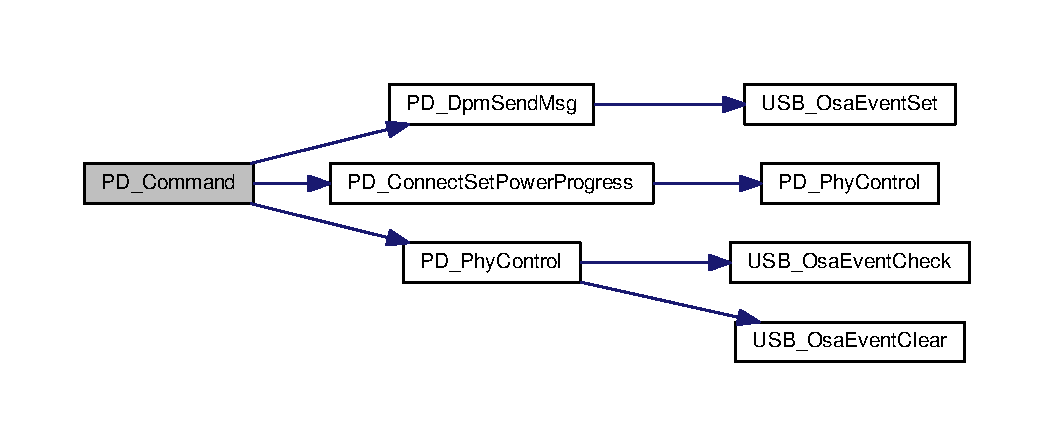
\includegraphics[width=350pt]{group__usb__pd__stack_gaa61d0ac40ef36db1ef5a88532f6eea90_cgraph}
\end{center}
\end{figure}




Here is the caller graph for this function\-:
\nopagebreak
\begin{figure}[H]
\begin{center}
\leavevmode
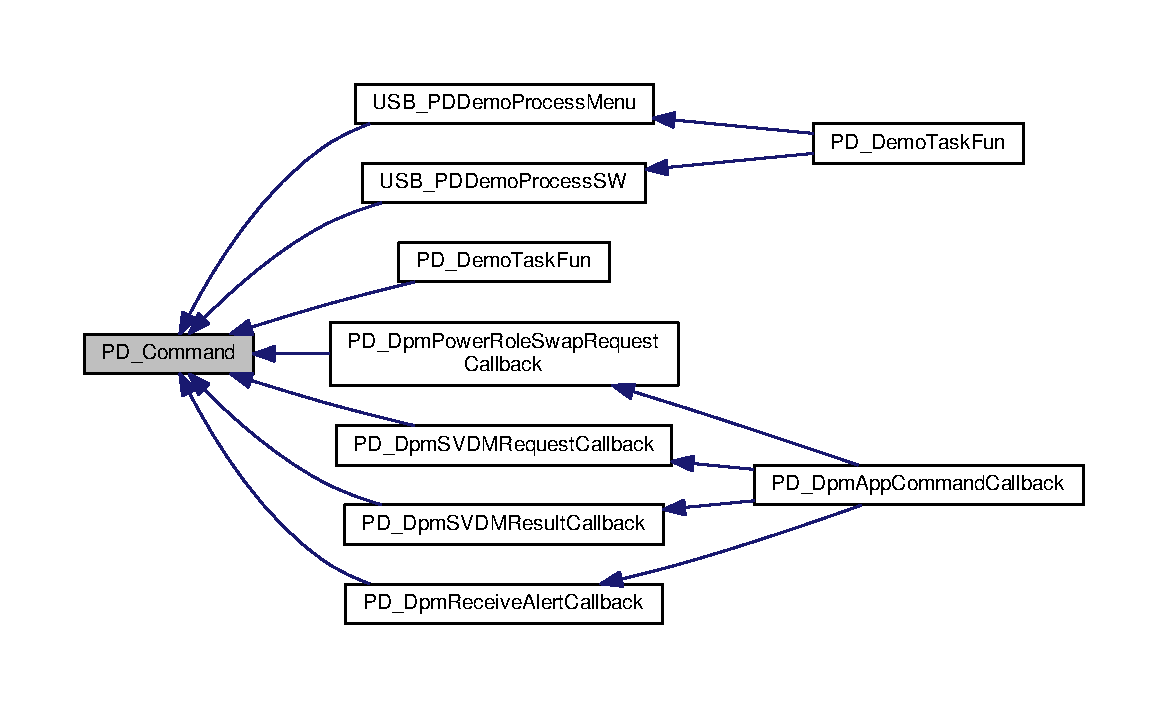
\includegraphics[width=350pt]{group__usb__pd__stack_gaa61d0ac40ef36db1ef5a88532f6eea90_icgraph}
\end{center}
\end{figure}


\hypertarget{group__usb__pd__stack_gac3d77e334213f541028d2da518086ca2}{\index{Usb\-\_\-pd\-\_\-stack@{Usb\-\_\-pd\-\_\-stack}!P\-D\-\_\-\-Control@{P\-D\-\_\-\-Control}}
\index{P\-D\-\_\-\-Control@{P\-D\-\_\-\-Control}!Usb_pd_stack@{Usb\-\_\-pd\-\_\-stack}}
\subsubsection[{P\-D\-\_\-\-Control}]{\setlength{\rightskip}{0pt plus 5cm}{\bf pd\-\_\-status\-\_\-t} P\-D\-\_\-\-Control (
\begin{DoxyParamCaption}
\item[{{\bf pd\-\_\-handle}}]{pd\-Handle, }
\item[{uint32\-\_\-t}]{control\-Code, }
\item[{void $\ast$}]{param}
\end{DoxyParamCaption}
)}}\label{group__usb__pd__stack_gac3d77e334213f541028d2da518086ca2}


Control P\-D stack and get info from P\-D stack. 

This function is blocking and synchronous, it implement some controls that will used in the P\-D application.


\begin{DoxyParams}[1]{Parameters}
\mbox{\tt in}  & {\em pd\-Handle} & the pd\-Handle that is got through P\-D\-\_\-\-Instance\-Init. \\
\hline
\mbox{\tt in}  & {\em control\-Code} & see the \hyperlink{group__usb__pd__stack_ga880e41e7aafed69c34035517d1bbb7b6}{pd\-\_\-control\-\_\-t} \\
\hline
\mbox{\tt in}  & {\em param} & the param is different for different control.\\
\hline
\end{DoxyParams}

\begin{DoxyRetVals}{Return values}
{\em k\-Status\-\_\-\-U\-S\-B\-\_\-\-Success} & function success. \\
\hline
{\em other} & value error code. \\
\hline
\end{DoxyRetVals}

\begin{DoxyCode}
7255 \{
7256     \hyperlink{struct__pd__instance}{pd\_instance\_t} *pdInstance = (\hyperlink{struct__pd__instance}{pd\_instance\_t} *)pdHandle;
7257     \hyperlink{group__usb__pd__stack_ga04a1f331d9807a70ab9bb753f5ed1c80}{pd\_status\_t} status = \hyperlink{group__usb__pd__stack_ggaaad4cd00dd02567c6169429e3a895073acf06f954f9c52f560cea34df48c63555}{kStatus\_PD\_Success};
7258     uint32\_t caseValue = 0;
7259 
7260     (void)caseValue;
7261     \textcolor{keywordflow}{switch} (controlCode)
7262     \{
7263         \textcolor{keywordflow}{case} \hyperlink{group__usb__pd__stack_gga0edd2a390d28d96646bc71aac1858af1a04f2cae987c5f93bcd07bcffd679548e}{PD\_CONTROL\_GET\_POWER\_ROLE}:
7264             *((uint8\_t *)param) = pdInstance->\hyperlink{struct__pd__instance_aea65859fe3a8409ac66aa9f54fb119bf}{curPowerRole};
7265             \textcolor{keywordflow}{break};
7266 
7267         \textcolor{keywordflow}{case} \hyperlink{group__usb__pd__stack_gga0edd2a390d28d96646bc71aac1858af1a06f4d2e5460a98f33e36db26ee0576cf}{PD\_CONTROL\_GET\_DATA\_ROLE}:
7268             *((uint8\_t *)param) = pdInstance->\hyperlink{struct__pd__instance_a766dd3de4bdd34f1eebcd41d1425327a}{curDataRole};
7269             \textcolor{keywordflow}{break};
7270 
7271         \textcolor{keywordflow}{case} \hyperlink{group__usb__pd__stack_gga0edd2a390d28d96646bc71aac1858af1ad8f600ed0992d656036ca0a272d680ad}{PD\_CONTROL\_GET\_TYPEC\_CONNECT\_STATE}:
7272             *((uint8\_t *)param) = pdInstance->\hyperlink{struct__pd__instance_a4f8aff7c9d2b914a5be9f0bd297c197c}{connectState};
7273             \textcolor{keywordflow}{break};
7274 
7275         \textcolor{keywordflow}{case} \hyperlink{group__usb__pd__stack_gga0edd2a390d28d96646bc71aac1858af1a157e80a587dd98e5cd78e9927b4c4994}{PD\_CONTROL\_GET\_VCONN\_ROLE}:
7276             *((uint8\_t *)param) = pdInstance->\hyperlink{struct__pd__instance_a1b1254d08a7d1b7809c37ac0e1253ed5}{psmPresentlyVconnSource};
7277             \textcolor{keywordflow}{break};
7278 
7279         \textcolor{keywordflow}{case} \hyperlink{group__usb__pd__stack_gga0edd2a390d28d96646bc71aac1858af1a16509ea70890f75b3f97c5af3e7e04d5}{PD\_CONTROL\_GET\_SNK\_TYPEC\_CURRENT\_CAP}:
7280             \hyperlink{usb__pd__policy_8c_a555b1880b5b259c3fdcd3da821e06cf2}{PD\_PhyControl}(pdInstance, 
      \hyperlink{group__usb__pd__phy__drv_ggab8bfca50e2ac042b47a697c88f84c3edae1406149d183dba960809596aa525528}{PD\_PHY\_SNK\_GET\_TYPEC\_CURRENT\_CAP}, param);
7281             \textcolor{keywordflow}{break};
7282 
7283         \textcolor{comment}{//params are phyPowerPinCtrl.enSRC or enSNK1}
7284         \textcolor{keywordflow}{case} \hyperlink{group__usb__pd__stack_gga0edd2a390d28d96646bc71aac1858af1a219d3fe217c5bf11a8126d09ee9fdb0c}{PD\_CONTROL\_PHY\_POWER\_PIN}:
7285             \hyperlink{usb__pd__policy_8c_a555b1880b5b259c3fdcd3da821e06cf2}{PD\_PhyControl}(pdInstance, \hyperlink{group__usb__pd__phy__drv_ggab8bfca50e2ac042b47a697c88f84c3edafb0f5a5d01b76353eae9108cb6bfc313}{PD\_PHY\_CONTROL\_POWER\_PIN}, param)
      ;
7286             \textcolor{keywordflow}{break};
7287 
7288         \textcolor{keywordflow}{case} \hyperlink{group__usb__pd__stack_gga0edd2a390d28d96646bc71aac1858af1a62e8479d23bf1208d5735aa76ff2aef6}{PD\_CONTROL\_VCONN}:
7289             \hyperlink{usb__pd__policy_8c_a555b1880b5b259c3fdcd3da821e06cf2}{PD\_PhyControl}(pdInstance, \hyperlink{group__usb__pd__phy__drv_ggab8bfca50e2ac042b47a697c88f84c3eda68ad1faa15b73743adf7f5a58013937b}{PD\_PHY\_CONTROL\_VCONN}, param);
7290 \textcolor{preprocessor}{#if (PD\_CONFIG\_OLD\_INTERFACE)
}
7291 \textcolor{preprocessor}{}            \hyperlink{usb__pd__policy_8c_a555b1880b5b259c3fdcd3da821e06cf2}{PD\_PhyControl}(pdInstance, PD\_PHY\_CONNECT\_CONTROL\_FLUSH, NULL);
7292 \textcolor{preprocessor}{#endif
}
7293 \textcolor{preprocessor}{}            \textcolor{keywordflow}{break};
7294 
7295         \textcolor{keywordflow}{case} \hyperlink{group__usb__pd__stack_gga0edd2a390d28d96646bc71aac1858af1aa58ce53ecaeed9f620eda031d4e5f342}{PD\_CONTROL\_GET\_PHY\_LOW\_POWER\_STATE}:
7296             status = \hyperlink{usb__pd__policy_8c_a555b1880b5b259c3fdcd3da821e06cf2}{PD\_PhyControl}(pdInstance, 
      \hyperlink{group__usb__pd__phy__drv_ggab8bfca50e2ac042b47a697c88f84c3edae2796c6a2d5cd486dd77cbc4c9b3eea7}{PD\_PHY\_GET\_LOWPOWER\_STATE}, param);
7297             \textcolor{keywordflow}{break};
7298 
7299         \textcolor{keywordflow}{case} \hyperlink{group__usb__pd__stack_gga0edd2a390d28d96646bc71aac1858af1ab4baaafc5cca20f365d103a948261b1f}{PD\_CONTROL\_DISCHARGE\_VBUS}:
7300         \{
7301             uint32\_t tmp32Val = 1;
7302             \hyperlink{usb__pd__policy_8c_a555b1880b5b259c3fdcd3da821e06cf2}{PD\_PhyControl}(pdInstance, \hyperlink{group__usb__pd__phy__drv_ggab8bfca50e2ac042b47a697c88f84c3edae705da68d4de3104b6852d84715bb71b}{PD\_PHY\_DISCHARGE\_VBUS}, &tmp32Val);
7303 \textcolor{preprocessor}{#if (defined PD\_CONFIG\_MIN\_DISCHARGE\_TIME\_ENABLE) && (PD\_CONFIG\_MIN\_DISCHARGE\_TIME\_ENABLE)
}
7304 \textcolor{preprocessor}{}            \hyperlink{usb__pd__timer_8c_afa3b5394c429c185ea93be16ddb1545f}{PD\_TimerStart}(pdInstance, \hyperlink{usb__pd__timer_8h_a94e23fe7d4bf2bf6f8de1f51126d071fae1e72be49d715105618c5266d8348b7d}{tTypeCVbusMinDischargeTimer}, 
      \hyperlink{usb__pd__timer_8h_a290959f551e6b12818c09607ff90e9b4}{T\_MIN\_VBUS\_DISCHARGE});
7305 \textcolor{preprocessor}{#else
}
7306 \textcolor{preprocessor}{}            \hyperlink{usb__pd__timer_8c_afa3b5394c429c185ea93be16ddb1545f}{PD\_TimerStart}(pdInstance, \hyperlink{usb__pd__timer_8h_a94e23fe7d4bf2bf6f8de1f51126d071fa5d99688807a9cf008b7087f068dcee44}{tTypeCVbusMaxDischargeTimer}, 
      \hyperlink{usb__pd__timer_8h_a32e20656b2cbd8812656a7f1e3f917f0}{T\_MAX\_VBUS\_DISCHARGE});
7307 \textcolor{preprocessor}{#endif
}
7308 \textcolor{preprocessor}{}            \textcolor{keywordflow}{while} (1)
7309             \{
7310                 \hyperlink{usb__pd__policy_8c_a555b1880b5b259c3fdcd3da821e06cf2}{PD\_PhyControl}(pdInstance, 
      \hyperlink{group__usb__pd__phy__drv_ggab8bfca50e2ac042b47a697c88f84c3eda4a23adc388bf03852d850ff3919328d6}{PD\_PHY\_GET\_VBUS\_POWER\_STATE}, &tmp32Val);
7311                 \textcolor{keywordflow}{if} ((tmp32Val & \hyperlink{group__usb__pd__phy__drv_gabf05bb09647628f3556c817e1f059175}{PD\_VBUS\_POWER\_STATE\_VSAFE0V\_MASK}) ||
7312 #\textcolor{keywordflow}{if} (defined \hyperlink{usb__pd__config_8h_af713fdd823151fddb0577f3756deac17}{PD\_CONFIG\_MIN\_DISCHARGE\_TIME\_ENABLE}) && (
      PD\_CONFIG\_MIN\_DISCHARGE\_TIME\_ENABLE)
7313                     \hyperlink{usb__pd__timer_8c_a3d4072fbbc7b10a05c795eaf9ed33f5f}{PD\_TimerCheckInvalidOrTimeOut}(pdInstance, 
      \hyperlink{usb__pd__timer_8h_a94e23fe7d4bf2bf6f8de1f51126d071fae1e72be49d715105618c5266d8348b7d}{tTypeCVbusMinDischargeTimer})
7314 #\textcolor{keywordflow}{else}
7315                     \hyperlink{usb__pd__timer_8c_a3d4072fbbc7b10a05c795eaf9ed33f5f}{PD\_TimerCheckInvalidOrTimeOut}(pdInstance, 
      \hyperlink{usb__pd__timer_8h_a94e23fe7d4bf2bf6f8de1f51126d071fa5d99688807a9cf008b7087f068dcee44}{tTypeCVbusMaxDischargeTimer})
7316 #endif
7317                         )
7318                 \{
7319                     \textcolor{keywordflow}{break};
7320                 \}
7321             \}
7322             tmp32Val = 0;
7323             \hyperlink{usb__pd__policy_8c_a555b1880b5b259c3fdcd3da821e06cf2}{PD\_PhyControl}(pdInstance, \hyperlink{group__usb__pd__phy__drv_ggab8bfca50e2ac042b47a697c88f84c3edae705da68d4de3104b6852d84715bb71b}{PD\_PHY\_DISCHARGE\_VBUS}, &tmp32Val);
7324 
7325             \textcolor{keywordflow}{break};
7326         \}
7327 
7328         \textcolor{keywordflow}{default}:
7329             \textcolor{keywordflow}{break};
7330     \}
7331 
7332     \textcolor{keywordflow}{return} status;
7333 \}
\end{DoxyCode}


Here is the call graph for this function\-:
\nopagebreak
\begin{figure}[H]
\begin{center}
\leavevmode
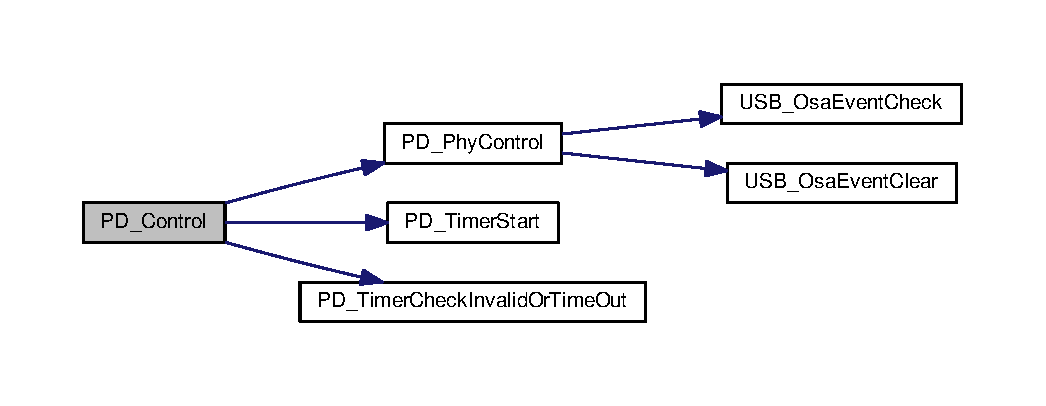
\includegraphics[width=350pt]{group__usb__pd__stack_gac3d77e334213f541028d2da518086ca2_cgraph}
\end{center}
\end{figure}




Here is the caller graph for this function\-:
\nopagebreak
\begin{figure}[H]
\begin{center}
\leavevmode
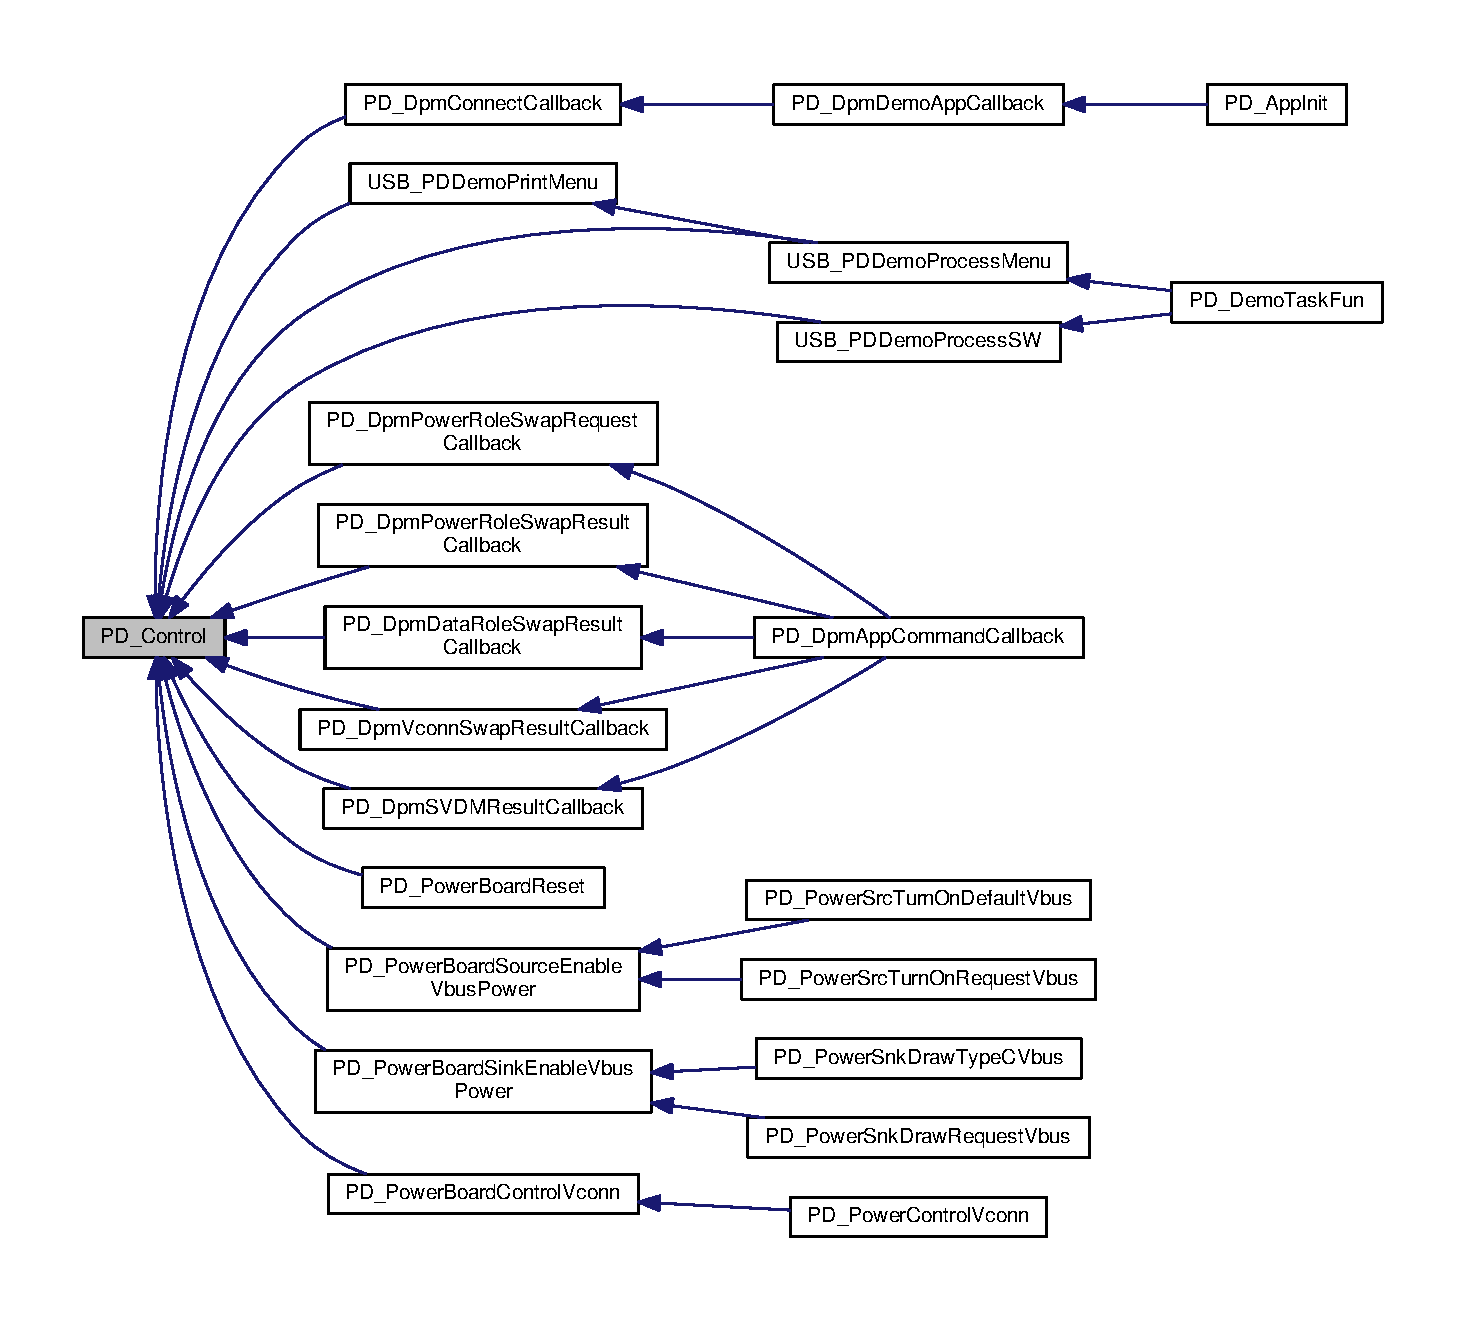
\includegraphics[width=350pt]{group__usb__pd__stack_gac3d77e334213f541028d2da518086ca2_icgraph}
\end{center}
\end{figure}


\hypertarget{group__usb__pd__stack_ga2a517af9491514966ad9c806eb998f78}{\index{Usb\-\_\-pd\-\_\-stack@{Usb\-\_\-pd\-\_\-stack}!P\-D\-\_\-\-Instance\-Deinit@{P\-D\-\_\-\-Instance\-Deinit}}
\index{P\-D\-\_\-\-Instance\-Deinit@{P\-D\-\_\-\-Instance\-Deinit}!Usb_pd_stack@{Usb\-\_\-pd\-\_\-stack}}
\subsubsection[{P\-D\-\_\-\-Instance\-Deinit}]{\setlength{\rightskip}{0pt plus 5cm}{\bf pd\-\_\-status\-\_\-t} P\-D\-\_\-\-Instance\-Deinit (
\begin{DoxyParamCaption}
\item[{{\bf pd\-\_\-handle}}]{pd\-Handle}
\end{DoxyParamCaption}
)}}\label{group__usb__pd__stack_ga2a517af9491514966ad9c806eb998f78}


de-\/initialize P\-D stack instance. 

This function de-\/initializes the P\-D stack module specified by the pd\-Handle.


\begin{DoxyParams}[1]{Parameters}
\mbox{\tt in}  & {\em pd\-Handle} & the pd\-Handle that is got through P\-D\-\_\-\-Instance\-Init.\\
\hline
\end{DoxyParams}

\begin{DoxyRetVals}{Return values}
{\em k\-Status\-\_\-\-U\-S\-B\-\_\-\-Success} & success. \\
\hline
{\em other} & value error code. \\
\hline
\end{DoxyRetVals}

\begin{DoxyCode}
244 \{
245     \hyperlink{struct__pd__instance}{pd\_instance\_t} *pdInstance = (\hyperlink{struct__pd__instance}{pd\_instance\_t} *)pdHandle;
246     \hyperlink{group__usb__pd__stack_ga04a1f331d9807a70ab9bb753f5ed1c80}{pd\_status\_t} status = \hyperlink{group__usb__pd__stack_ggaaad4cd00dd02567c6169429e3a895073acf06f954f9c52f560cea34df48c63555}{kStatus\_PD\_Success};
247 
248     \hyperlink{group__usb__os__abstraction_ga3d07a809b1fa8450c1383aa8bbd49b37}{USB\_OsaEventDestroy}(pdInstance->\hyperlink{struct__pd__instance_ab04e9fcc994b2547509169e07ab21465}{taskEventHandle});
249     \hyperlink{usb__pd__interface_8c_a8c50cfda5ec549f60ac482d06231d26f}{PD\_ReleaseInstance}(pdInstance);
250     status = pdInstance->\hyperlink{struct__pd__instance_adbed7b2cd53df40e0611a8879c903339}{phyInterface}->\hyperlink{struct__pd__phy__api__interface_a9e36ebe547c2ed82866597b2afc54bd0}{pdPhyDeinit}(pdInstance->
      \hyperlink{struct__pd__instance_a7c1184292efe9a5ae30b6ac422c1e9f4}{pdPhyHandle});
251     \hyperlink{usb__pd__interface_8c_a8c50cfda5ec549f60ac482d06231d26f}{PD\_ReleaseInstance}(pdInstance);
252 
253     \textcolor{keywordflow}{return} status;
254 \}
\end{DoxyCode}


Here is the call graph for this function\-:
\nopagebreak
\begin{figure}[H]
\begin{center}
\leavevmode
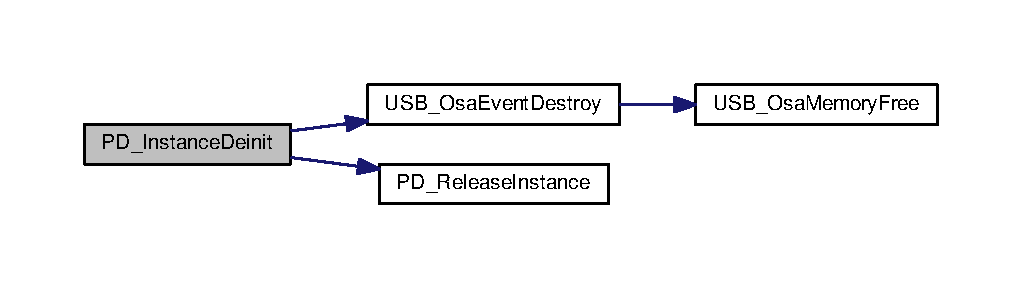
\includegraphics[width=350pt]{group__usb__pd__stack_ga2a517af9491514966ad9c806eb998f78_cgraph}
\end{center}
\end{figure}




Here is the caller graph for this function\-:
\nopagebreak
\begin{figure}[H]
\begin{center}
\leavevmode
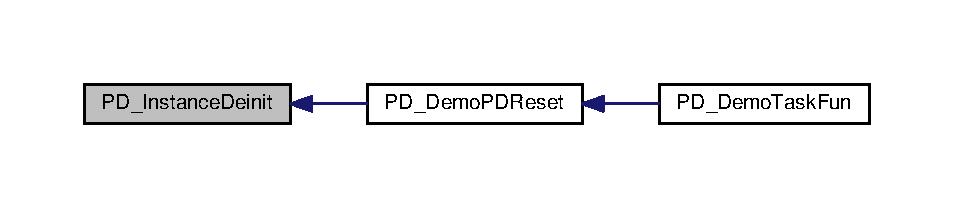
\includegraphics[width=350pt]{group__usb__pd__stack_ga2a517af9491514966ad9c806eb998f78_icgraph}
\end{center}
\end{figure}


\hypertarget{group__usb__pd__stack_ga3ab001290dc934fd6a45ad93916f5140}{\index{Usb\-\_\-pd\-\_\-stack@{Usb\-\_\-pd\-\_\-stack}!P\-D\-\_\-\-Instance\-Init@{P\-D\-\_\-\-Instance\-Init}}
\index{P\-D\-\_\-\-Instance\-Init@{P\-D\-\_\-\-Instance\-Init}!Usb_pd_stack@{Usb\-\_\-pd\-\_\-stack}}
\subsubsection[{P\-D\-\_\-\-Instance\-Init}]{\setlength{\rightskip}{0pt plus 5cm}{\bf pd\-\_\-status\-\_\-t} P\-D\-\_\-\-Instance\-Init (
\begin{DoxyParamCaption}
\item[{{\bf pd\-\_\-handle} $\ast$}]{pd\-Handle, }
\item[{{\bf pd\-\_\-stack\-\_\-callback\-\_\-t}}]{callback\-Fn, }
\item[{{\bf pd\-\_\-power\-\_\-handle\-\_\-callback\-\_\-t} $\ast$}]{callback\-Functions, }
\item[{void $\ast$}]{callback\-Param, }
\item[{{\bf pd\-\_\-instance\-\_\-config\-\_\-t} $\ast$}]{config}
\end{DoxyParamCaption}
)}}\label{group__usb__pd__stack_ga3ab001290dc934fd6a45ad93916f5140}


Initialize P\-D stack instance. 

This function initializes the P\-D stack module specified by the parameter, it will associate with the P\-D P\-H\-Y that is specified by parameter.


\begin{DoxyParams}[1]{Parameters}
\mbox{\tt out}  & {\em pd\-Handle} & Returns the P\-D stack instance handle, other A\-P\-I will use this handle as parameter; \\
\hline
\mbox{\tt in}  & {\em callback\-Fn} & P\-D stack callback function, it will notify the connect/disconnect and P\-D command's process flow and result; \\
\hline
\mbox{\tt in}  & {\em callback\-Param} & the callback\-Fn's parameter. \\
\hline
\mbox{\tt in}  & {\em config} & The P\-D instance configuration table, see the struct \hyperlink{group__usb__pd__stack_gafa6034f9e204836697da1f2fc996cbad}{pd\-\_\-instance\-\_\-config\-\_\-t}\\
\hline
\end{DoxyParams}

\begin{DoxyRetVals}{Return values}
{\em k\-Status\-\_\-\-U\-S\-B\-\_\-\-Success} & initialization success. \\
\hline
{\em other} & value error code. \\
\hline
\end{DoxyRetVals}

\begin{DoxyCode}
152 \{
153     \hyperlink{struct__pd__instance}{pd\_instance\_t} *pdInstance;
154     \hyperlink{group__usb__pd__stack_ga04a1f331d9807a70ab9bb753f5ed1c80}{pd\_status\_t} status = \hyperlink{group__usb__pd__stack_ggaaad4cd00dd02567c6169429e3a895073acf06f954f9c52f560cea34df48c63555}{kStatus\_PD\_Success};
155     \textcolor{comment}{//phy interface configuration, including i2c or spi interface config}
156     \hyperlink{struct__pd__phy__config}{pd\_phy\_config\_t} phyConfig;
157 
158     pdInstance = \hyperlink{usb__pd__interface_8c_aabf54379477268c9186bc3cbc84f29e2}{PD\_GetInstance}();
159     \textcolor{keywordflow}{if} (pdInstance == NULL)
160     \{
161         \textcolor{keywordflow}{return} \hyperlink{group__usb__pd__stack_ggaaad4cd00dd02567c6169429e3a895073a4d58370b8ee8d3d2a4c477f7a3f84dda}{kStatus\_PD\_Error};
162     \}
163 
164     \textcolor{comment}{/* get phy API table */}
165     pdInstance->\hyperlink{struct__pd__instance_adbed7b2cd53df40e0611a8879c903339}{phyInterface} = NULL;
166     \textcolor{comment}{/* get corresponding interface according to phyType */}
167     \hyperlink{usb__pd__interface_8c_a33e4ca77d64aa73779c39be033ec640b}{PD\_GetPhyInterface}(config->\hyperlink{struct__pd__instance__config_a1f5e597bbfc0af871a5e887c34eb3aca}{phyType}, &pdInstance->
      \hyperlink{struct__pd__instance_adbed7b2cd53df40e0611a8879c903339}{phyInterface});
168     \textcolor{keywordflow}{if} ((pdInstance->\hyperlink{struct__pd__instance_adbed7b2cd53df40e0611a8879c903339}{phyInterface} == NULL) || (pdInstance->
      \hyperlink{struct__pd__instance_adbed7b2cd53df40e0611a8879c903339}{phyInterface}->\hyperlink{struct__pd__phy__api__interface_a8f9666a7543d431aec266710dbc8d78c}{pdPhyInit} == NULL) ||
169         (pdInstance->\hyperlink{struct__pd__instance_adbed7b2cd53df40e0611a8879c903339}{phyInterface}->\hyperlink{struct__pd__phy__api__interface_a9e36ebe547c2ed82866597b2afc54bd0}{pdPhyDeinit} == NULL) || (pdInstance->
      \hyperlink{struct__pd__instance_adbed7b2cd53df40e0611a8879c903339}{phyInterface}->\hyperlink{struct__pd__phy__api__interface_ab9b74f09035836be811dc6aae682074f}{pdPhySend} == NULL) ||
170         (pdInstance->\hyperlink{struct__pd__instance_adbed7b2cd53df40e0611a8879c903339}{phyInterface}->\hyperlink{struct__pd__phy__api__interface_a3c8508914afbcb4f55578a0d61cd90e3}{pdPhyReceive} == NULL) || (pdInstance->
      \hyperlink{struct__pd__instance_adbed7b2cd53df40e0611a8879c903339}{phyInterface}->\hyperlink{struct__pd__phy__api__interface_a5e422dbfd66fca34934e39b451f17094}{pdPhyControl} == NULL))
171     \{
172         \hyperlink{usb__pd__interface_8c_a8c50cfda5ec549f60ac482d06231d26f}{PD\_ReleaseInstance}(pdInstance);
173         \textcolor{keywordflow}{return} \hyperlink{group__usb__pd__stack_ggaaad4cd00dd02567c6169429e3a895073a4d58370b8ee8d3d2a4c477f7a3f84dda}{kStatus\_PD\_Error};
174     \}
175 
176     \textcolor{comment}{//phyType的类型,PTN5100 or others}
177     pdInstance->\hyperlink{struct__pd__instance_afae58a0b309262dc37fac1f4f92c6d7b}{phyType} = config->\hyperlink{struct__pd__instance__config_a1f5e597bbfc0af871a5e887c34eb3aca}{phyType};
178     \textcolor{comment}{//PD\_DpmDemoAppCallback, event callback, 对应枚举体pd\_dpm\_callback\_event\_t}
179     \textcolor{comment}{// Question: 作用是什么?}
180     \textcolor{comment}{// 该函数通过PD\_DpmAppCallback调用}
181     pdInstance->\hyperlink{struct__pd__instance_a3718a4d773d48136d66706ac063ef948}{pdCallback} = callbackFn;
182     \textcolor{comment}{//callbackFunctions, power related}
183     pdInstance->\hyperlink{struct__pd__instance_a519457e415e4eb39231c3e32316ffc83}{callbackFns} = \hyperlink{pd__app_8c_a306f9b8029582dfb8c64f163fea3cf65}{callbackFunctions};
184     \textcolor{comment}{//pd\_app\_t}
185     pdInstance->\hyperlink{struct__pd__instance_a0eb7710a55cb5eb2a57355d772b26f74}{callbackParam} = callbackParam;
186     \textcolor{comment}{//PD REVISION,如果需要改为3.0,需要在usb\_pd\_config.h中修改}
187     pdInstance->\hyperlink{struct__pd__instance_af7c28b72771ce442ee733892186c4e6c}{revision} = \hyperlink{usb__pd__config_8h_a3d9825e8371d36b868d61b94a6514711}{PD\_CONFIG\_REVISION};
188     pdInstance->\hyperlink{struct__pd__instance_a6031ed1c3ec10c04ea5daf9a76485f68}{sendingMsgHeader}.\hyperlink{struct__pd__msg__header_a6dc4609c23d8d9e5d8830177d959fe17}{bitFields}.specRevision = pdInstance->
      \hyperlink{struct__pd__instance_af7c28b72771ce442ee733892186c4e6c}{revision};
189     pdInstance->\hyperlink{struct__pd__instance_a2edcb21b9d568937192741d32381d2b1}{initializeLabel} = 0;
190     \textcolor{comment}{// FreeRTOS event group的等待时间}
191     pdInstance->\hyperlink{struct__pd__instance_a2505651a0001ea647306dbd800927778}{waitTime} = \hyperlink{usb__pd__interface_8h_ac3471f042971fd1641303f2622b844c1}{PD\_WAIT\_EVENT\_TIME};
192 
193     \textcolor{comment}{// 创建event,句柄保存在pdInstance->taskEventHandle}
194     \textcolor{keywordflow}{if} (\hyperlink{group__usb__os__abstraction_gga453ebd2f93aafb8c938c3a23c815f9bdab90805fb75297fda1ca60dbb2283f933}{kStatus\_USB\_OSA\_Success} != \hyperlink{group__usb__os__abstraction_gaf38d525580499ff2657303eb807efc61}{USB\_OsaEventCreate}(&(pdInstance
      ->\hyperlink{struct__pd__instance_ab04e9fcc994b2547509169e07ab21465}{taskEventHandle}), 0))
195     \{
196         \hyperlink{usb__pd__interface_8c_a8c50cfda5ec549f60ac482d06231d26f}{PD\_ReleaseInstance}(pdInstance);
197         \textcolor{keywordflow}{return} \hyperlink{group__usb__pd__stack_ggaaad4cd00dd02567c6169429e3a895073a4d58370b8ee8d3d2a4c477f7a3f84dda}{kStatus\_PD\_Error};
198     \}
199 
200     \textcolor{comment}{/* initialize PHY */}
201     pdInstance->\hyperlink{struct__pd__instance_a7c1184292efe9a5ae30b6ac422c1e9f4}{pdPhyHandle} = NULL;
202     \textcolor{comment}{//instance config}
203     pdInstance->\hyperlink{struct__pd__instance_a2d9a457d63da9c4cb5e3feece0cbf3ec}{pdConfig} = config;
204     \textcolor{comment}{//这里的device是指本身还是port partner?}
205     \textcolor{comment}{// 根据device type,初始化对应的power config以及sop}
206     \textcolor{keywordflow}{if} (pdInstance->\hyperlink{struct__pd__instance_a2d9a457d63da9c4cb5e3feece0cbf3ec}{pdConfig}->\hyperlink{struct__pd__instance__config_a68e8aae835b95ae67d48701973864acf}{deviceType} == 
      \hyperlink{group__usb__pd__stack_gga922338772b41ceba51f7881c74b9e20aaf6c770c6cd3614cd0cd48acee1124063}{kDeviceType\_NormalPowerPort})
207     \{
208         pdInstance->\hyperlink{struct__pd__instance_aa7854ddf70e64f92b178cc5d787037a2}{pdPowerPortConfig} = (\hyperlink{struct__pd__power__port__config}{pd\_power\_port\_config\_t} *)
      pdInstance->\hyperlink{struct__pd__instance_a2d9a457d63da9c4cb5e3feece0cbf3ec}{pdConfig}->\hyperlink{struct__pd__instance__config_a1aa5e1d3d8e54bcaa77f41a6de3eb371}{deviceConfig};
209         pdInstance->\hyperlink{struct__pd__instance_a007de2aa1ac9ae814d10d26a949dd61d}{pendingSOP} = \hyperlink{group__usb__pd__stack_gga7a924235403e0acab44d01e720091aa1aaa62220b2caaa3d1273068a3e03969d4}{kPD\_MsgSOPMask};
210     \}
211     \textcolor{keywordflow}{else} \textcolor{keywordflow}{if} (pdInstance->\hyperlink{struct__pd__instance_a2d9a457d63da9c4cb5e3feece0cbf3ec}{pdConfig}->\hyperlink{struct__pd__instance__config_a68e8aae835b95ae67d48701973864acf}{deviceType} == 
      \hyperlink{group__usb__pd__stack_gga922338772b41ceba51f7881c74b9e20aad424c8854f1c1bda150086d0aec89097}{kDeviceType\_Cable})
212     \{
213         pdInstance->\hyperlink{struct__pd__instance_a007de2aa1ac9ae814d10d26a949dd61d}{pendingSOP} = \hyperlink{group__usb__pd__stack_gga7a924235403e0acab44d01e720091aa1a69d059ddf531dc5f20c67fa58e4976c5}{kPD\_MsgSOPpMask} | 
      \hyperlink{group__usb__pd__stack_gga7a924235403e0acab44d01e720091aa1addd75dfd8f5aa9af17ddfa15ed385201}{kPD\_MsgSOPppMask};
214     \}
215     \textcolor{keywordflow}{else}
216     \{
217         \textcolor{comment}{//audio, debug, alternate mode}
218         pdInstance->\hyperlink{struct__pd__instance_a007de2aa1ac9ae814d10d26a949dd61d}{pendingSOP} = \hyperlink{group__usb__pd__stack_gga7a924235403e0acab44d01e720091aa1aaa62220b2caaa3d1273068a3e03969d4}{kPD\_MsgSOPMask};
219     \}
220     \textcolor{comment}{// phy interface}
221     phyConfig.\hyperlink{struct__pd__phy__config_aa5aa79cabb041cefecc0483c840f75a1}{interface} = config->\hyperlink{struct__pd__instance__config_acb93f9cec67a95c40730be43c80d3214}{phyInterface};
222     phyConfig.\hyperlink{struct__pd__phy__config_aa606732850969dd6c9bd06b608e8015c}{i2cConfig}.\hyperlink{struct__pd__i2c__interface__config_abef5bc903024c7f0c489407549948987}{slaveAddress} = config->
      \hyperlink{struct__pd__instance__config_a7e72c5dda8b81981ebd3062f6999bce1}{interfaceParam};
223     \textcolor{comment}{// phy initialize, call PDPTN5110\_Init}
224     status = pdInstance->\hyperlink{struct__pd__instance_adbed7b2cd53df40e0611a8879c903339}{phyInterface}->\hyperlink{struct__pd__phy__api__interface_a8f9666a7543d431aec266710dbc8d78c}{pdPhyInit}(pdInstance, &(pdInstance->
      \hyperlink{struct__pd__instance_a7c1184292efe9a5ae30b6ac422c1e9f4}{pdPhyHandle}), &phyConfig);
225     \textcolor{comment}{// 如果失败,则需要关闭或者释放已经占用的资源,包括内存以及event group}
226     \textcolor{keywordflow}{if} ((status != \hyperlink{group__usb__pd__stack_ggaaad4cd00dd02567c6169429e3a895073acf06f954f9c52f560cea34df48c63555}{kStatus\_PD\_Success}) || (pdInstance->
      \hyperlink{struct__pd__instance_a7c1184292efe9a5ae30b6ac422c1e9f4}{pdPhyHandle} == NULL))
227     \{
228         \hyperlink{group__usb__os__abstraction_ga3d07a809b1fa8450c1383aa8bbd49b37}{USB\_OsaEventDestroy}(pdInstance->\hyperlink{struct__pd__instance_ab04e9fcc994b2547509169e07ab21465}{taskEventHandle});
229         \hyperlink{usb__pd__interface_8c_a8c50cfda5ec549f60ac482d06231d26f}{PD\_ReleaseInstance}(pdInstance);
230         \textcolor{keywordflow}{return} \hyperlink{group__usb__pd__stack_ggaaad4cd00dd02567c6169429e3a895073a4d58370b8ee8d3d2a4c477f7a3f84dda}{kStatus\_PD\_Error};
231     \}
232     \textcolor{comment}{/* usb\_pd\_msg.c: initialize pd stack */}
233     \hyperlink{usb__pd__interface_8c_a8efd2af273b221ad6fe948153b704c96}{PD\_MsgInit}(pdInstance);
234     \hyperlink{usb__pd__timer_8c_ab9b44f9a09bf56e73ef27ed1adabefea}{PD\_TimerInit}(pdInstance);
235 
236     \textcolor{comment}{// call PDPTN5110\_Control, get phy vender info from cache register in phy driver}
237     \hyperlink{usb__pd__interface_8c_a555b1880b5b259c3fdcd3da821e06cf2}{PD\_PhyControl}(pdInstance, \hyperlink{group__usb__pd__phy__drv_ggab8bfca50e2ac042b47a697c88f84c3eda2baeac02a0ea12619542377f471f7cc4}{PD\_PHY\_GET\_PHY\_VENDOR\_INFO}, &
      pdInstance->\hyperlink{struct__pd__instance_a8cf1d14cc029410e591cbfe30d5b2cd9}{phyInfo});
238 
239     *pdHandle = pdInstance;
240     \textcolor{keywordflow}{return} \hyperlink{group__usb__pd__stack_ggaaad4cd00dd02567c6169429e3a895073acf06f954f9c52f560cea34df48c63555}{kStatus\_PD\_Success};
241 \}
\end{DoxyCode}


Here is the call graph for this function\-:
\nopagebreak
\begin{figure}[H]
\begin{center}
\leavevmode
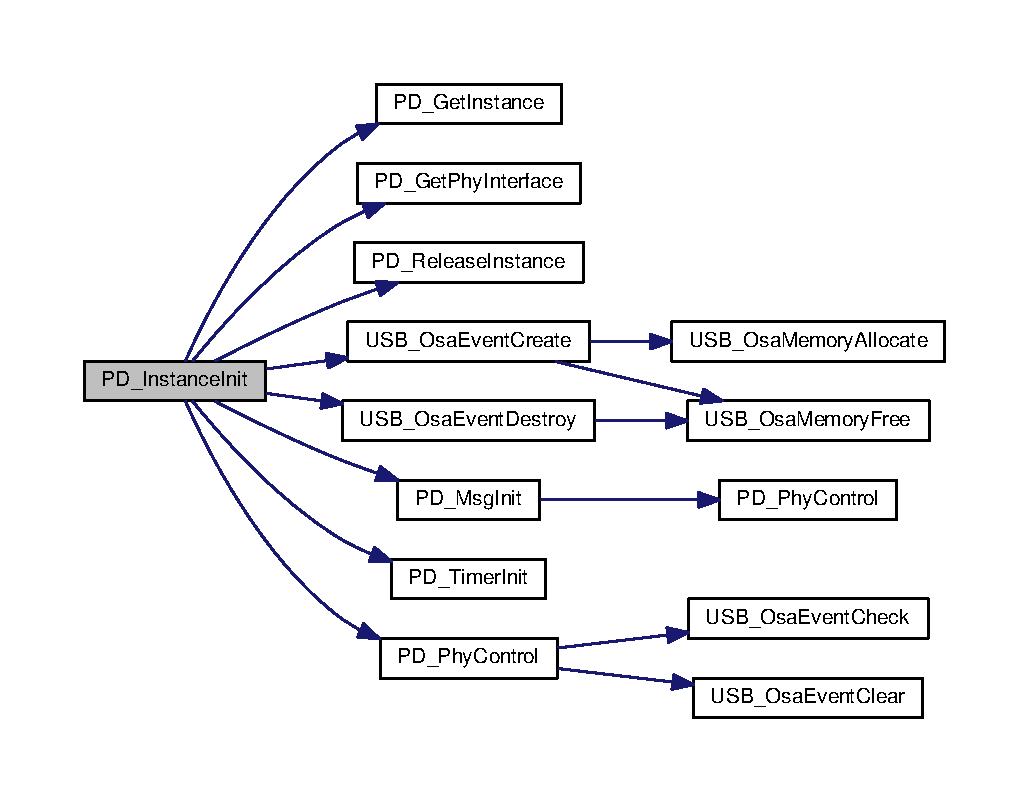
\includegraphics[width=350pt]{group__usb__pd__stack_ga3ab001290dc934fd6a45ad93916f5140_cgraph}
\end{center}
\end{figure}




Here is the caller graph for this function\-:
\nopagebreak
\begin{figure}[H]
\begin{center}
\leavevmode
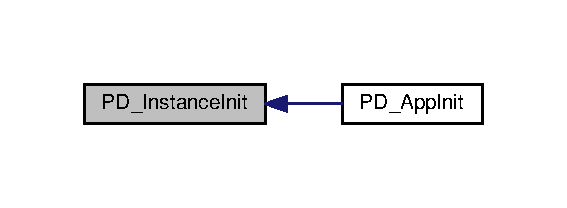
\includegraphics[width=272pt]{group__usb__pd__stack_ga3ab001290dc934fd6a45ad93916f5140_icgraph}
\end{center}
\end{figure}


\hypertarget{group__usb__pd__stack_ga4227c58a9524464e19ee6efe9615f78e}{\index{Usb\-\_\-pd\-\_\-stack@{Usb\-\_\-pd\-\_\-stack}!P\-D\-\_\-\-Instance\-Task@{P\-D\-\_\-\-Instance\-Task}}
\index{P\-D\-\_\-\-Instance\-Task@{P\-D\-\_\-\-Instance\-Task}!Usb_pd_stack@{Usb\-\_\-pd\-\_\-stack}}
\subsubsection[{P\-D\-\_\-\-Instance\-Task}]{\setlength{\rightskip}{0pt plus 5cm}void P\-D\-\_\-\-Instance\-Task (
\begin{DoxyParamCaption}
\item[{{\bf pd\-\_\-handle}}]{pd\-Handle}
\end{DoxyParamCaption}
)}}\label{group__usb__pd__stack_ga4227c58a9524464e19ee6efe9615f78e}


P\-D stack's instance task. 

User need keep calling this function endlessly in the P\-D application using one task.


\begin{DoxyParams}[1]{Parameters}
\mbox{\tt in}  & {\em pd\-Handle} & the pd\-Handle that is got through P\-D\-\_\-\-Instance\-Init. \\
\hline
\end{DoxyParams}

\begin{DoxyCode}
257 \{
258     \hyperlink{struct__pd__instance}{pd\_instance\_t} *pdInstance = (\hyperlink{struct__pd__instance}{pd\_instance\_t} *)pdHandle;
259 
260     \textcolor{comment}{// usb\_pd\_policy.c}
261     \hyperlink{usb__pd__interface_8c_a602f8622c0ba8d21b5013537dd3dadf9}{PD\_StackStateMachine}(pdInstance);
262 \}
\end{DoxyCode}


Here is the call graph for this function\-:
\nopagebreak
\begin{figure}[H]
\begin{center}
\leavevmode
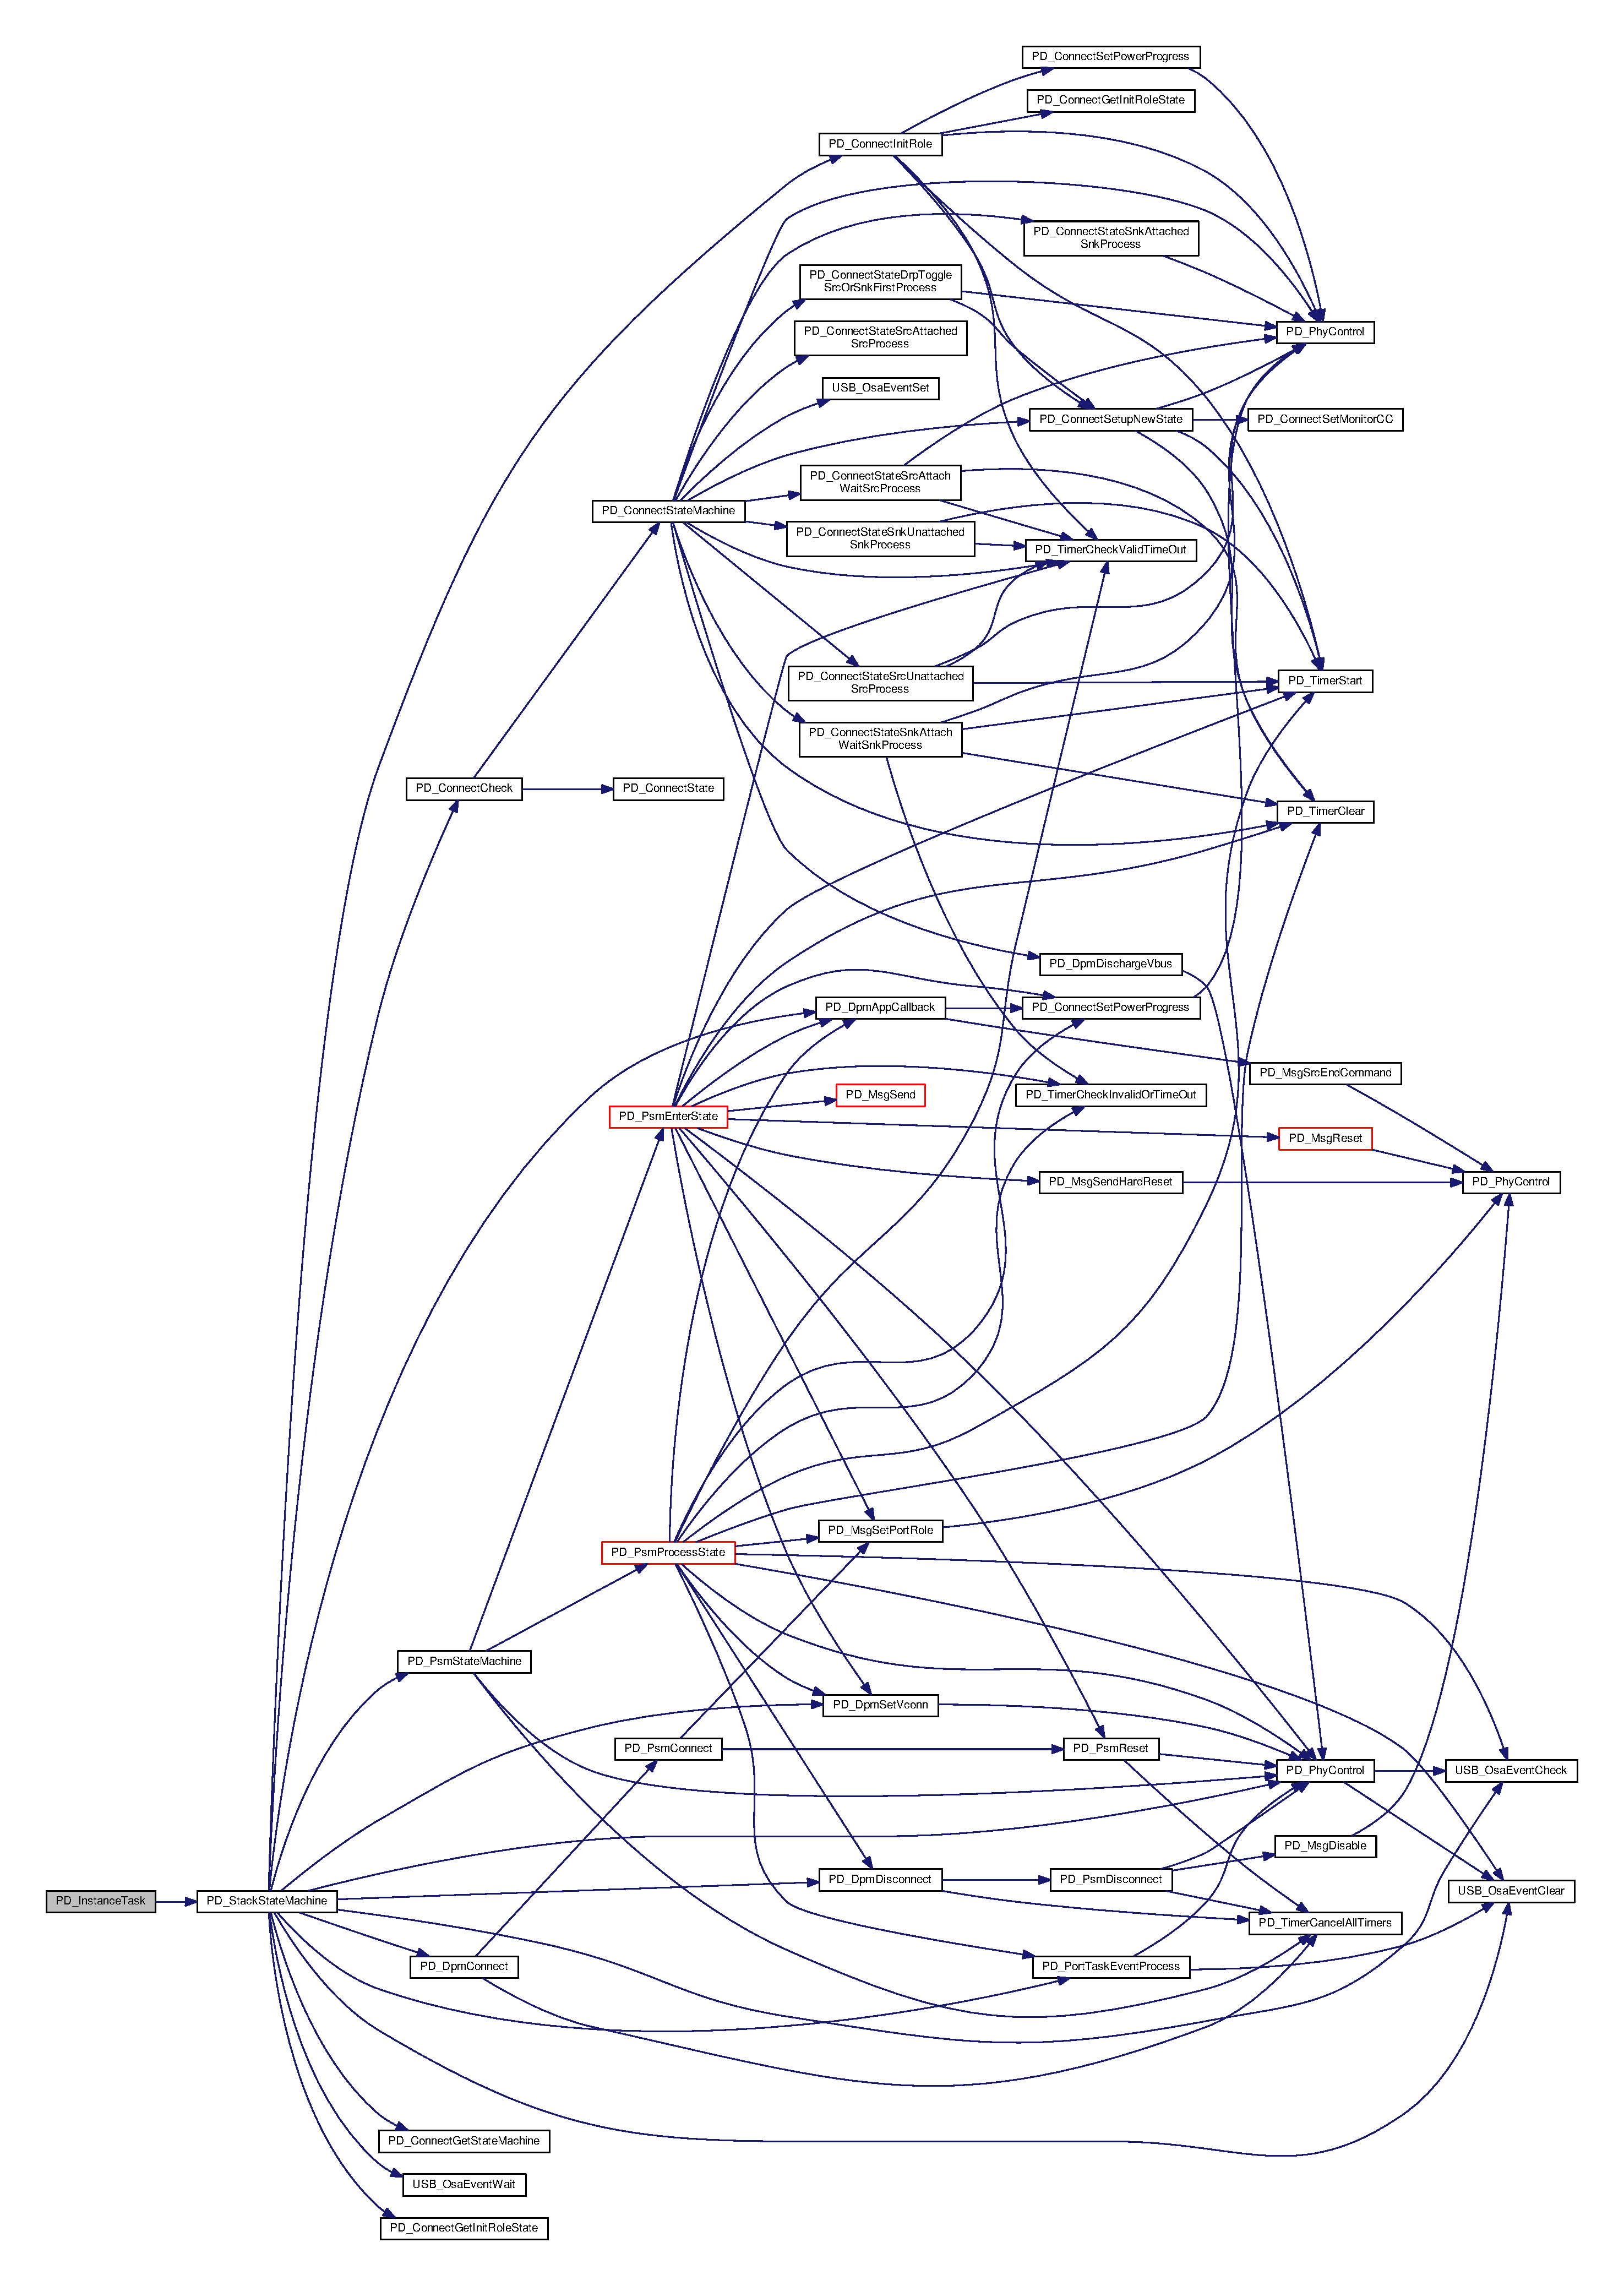
\includegraphics[width=350pt]{group__usb__pd__stack_ga4227c58a9524464e19ee6efe9615f78e_cgraph}
\end{center}
\end{figure}




Here is the caller graph for this function\-:
\nopagebreak
\begin{figure}[H]
\begin{center}
\leavevmode
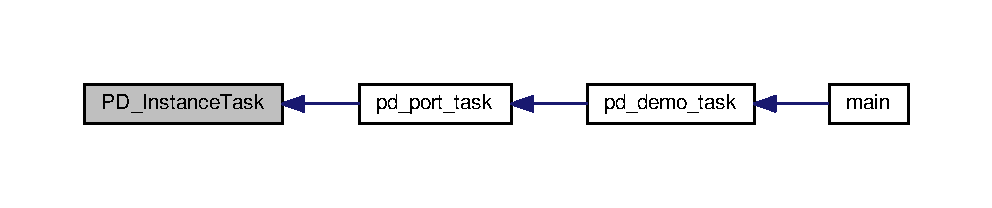
\includegraphics[width=350pt]{group__usb__pd__stack_ga4227c58a9524464e19ee6efe9615f78e_icgraph}
\end{center}
\end{figure}


\hypertarget{group__usb__pd__stack_gadc10377ece46e63b966463e501451e33}{\index{Usb\-\_\-pd\-\_\-stack@{Usb\-\_\-pd\-\_\-stack}!P\-D\-\_\-\-P\-T\-N5110\-Isr\-Function@{P\-D\-\_\-\-P\-T\-N5110\-Isr\-Function}}
\index{P\-D\-\_\-\-P\-T\-N5110\-Isr\-Function@{P\-D\-\_\-\-P\-T\-N5110\-Isr\-Function}!Usb_pd_stack@{Usb\-\_\-pd\-\_\-stack}}
\subsubsection[{P\-D\-\_\-\-P\-T\-N5110\-Isr\-Function}]{\setlength{\rightskip}{0pt plus 5cm}void P\-D\-\_\-\-P\-T\-N5110\-Isr\-Function (
\begin{DoxyParamCaption}
\item[{{\bf pd\-\_\-handle}}]{pd\-Handle}
\end{DoxyParamCaption}
)}}\label{group__usb__pd__stack_gadc10377ece46e63b966463e501451e33}


P\-D P\-T\-N5110 P\-H\-Y I\-S\-R function. 

User need call this function in the P\-H\-Y G\-P\-I\-O I\-S\-R.


\begin{DoxyParams}[1]{Parameters}
\mbox{\tt in}  & {\em pd\-Handle} & the pd\-Handle that is got through P\-D\-\_\-\-Instance\-Init. \\
\hline
\end{DoxyParams}

\begin{DoxyCode}
642 \{
643     \hyperlink{group__usb__pd__phy__drv_ga7f7f94758771b173653d27c508c8b33f}{PD\_Notify}(pdHandle, \hyperlink{group__usb__pd__phy__drv_gga9e1e6534f05a5dfae46d27dbf43e0455a1c7d2386b854afa09864304c2c407b04}{PD\_PHY\_EVENT\_STATE\_CHANGE}, NULL);
644 \}
\end{DoxyCode}


Here is the call graph for this function\-:
\nopagebreak
\begin{figure}[H]
\begin{center}
\leavevmode
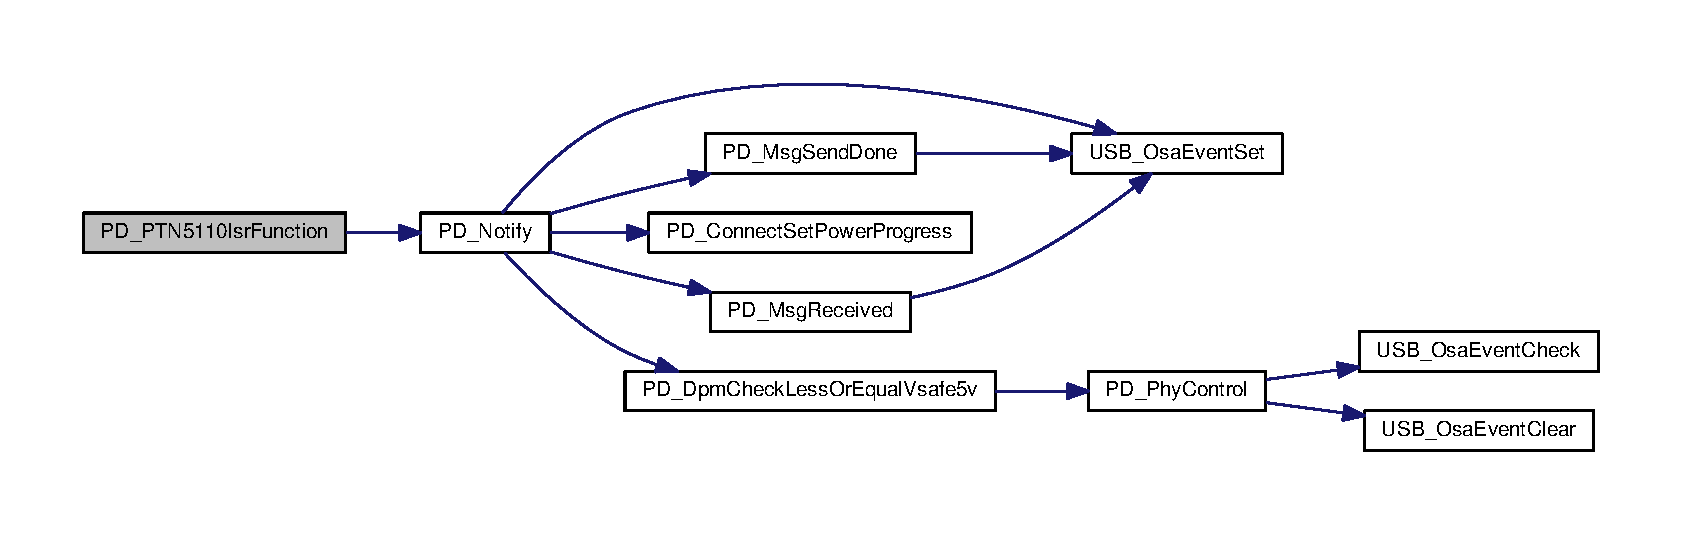
\includegraphics[width=350pt]{group__usb__pd__stack_gadc10377ece46e63b966463e501451e33_cgraph}
\end{center}
\end{figure}




Here is the caller graph for this function\-:
\nopagebreak
\begin{figure}[H]
\begin{center}
\leavevmode
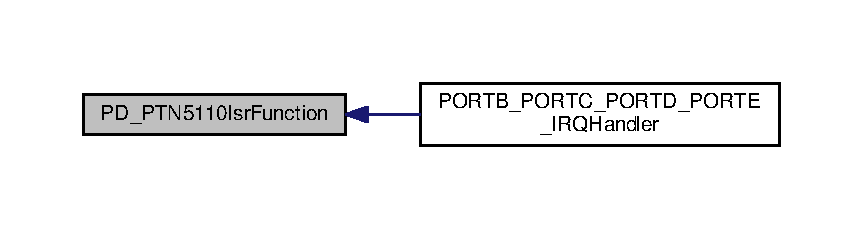
\includegraphics[width=350pt]{group__usb__pd__stack_gadc10377ece46e63b966463e501451e33_icgraph}
\end{center}
\end{figure}


\hypertarget{group__usb__pd__stack_gad8420ee79286dfb87b1b9d9c0845f31d}{\index{Usb\-\_\-pd\-\_\-stack@{Usb\-\_\-pd\-\_\-stack}!P\-D\-\_\-\-Timer\-Isr\-Function@{P\-D\-\_\-\-Timer\-Isr\-Function}}
\index{P\-D\-\_\-\-Timer\-Isr\-Function@{P\-D\-\_\-\-Timer\-Isr\-Function}!Usb_pd_stack@{Usb\-\_\-pd\-\_\-stack}}
\subsubsection[{P\-D\-\_\-\-Timer\-Isr\-Function}]{\setlength{\rightskip}{0pt plus 5cm}void P\-D\-\_\-\-Timer\-Isr\-Function (
\begin{DoxyParamCaption}
\item[{{\bf pd\-\_\-handle}}]{pd\-Handle}
\end{DoxyParamCaption}
)}}\label{group__usb__pd__stack_gad8420ee79286dfb87b1b9d9c0845f31d}


P\-D stack timer function. 

User need call this function in the 1ms Timer I\-S\-R.


\begin{DoxyParams}[1]{Parameters}
\mbox{\tt in}  & {\em pd\-Handle} & the pd\-Handle that is got through P\-D\-\_\-\-Instance\-Init. \\
\hline
\end{DoxyParams}

\begin{DoxyCode}
156 \{
157     \hyperlink{struct__pd__instance}{pd\_instance\_t} *pdInstance = (\hyperlink{struct__pd__instance}{pd\_instance\_t} *)pdHandle;
158     uint32\_t index32;
159     uint8\_t index8;
160     uint32\_t bitMape;
161 
162     \textcolor{keywordflow}{if} (pdHandle == NULL)
163     \{
164         \textcolor{keywordflow}{return};
165     \}
166 
167     \textcolor{keywordflow}{for} (index32 = 0; index32 < ((\hyperlink{usb__pd__timer_8h_a94e23fe7d4bf2bf6f8de1f51126d071fa208e3a31f39a2eafdaa34d97ae09cd6f}{tTimerCount} + 31) / 32); ++index32)
168     \{
169         \textcolor{keywordflow}{if} (pdInstance->\hyperlink{struct__pd__instance_a00d9a2aa7fd533c3ac15236b61e894f0}{timrsRunningState}[index32] != 0)
170         \{
171             \textcolor{keywordflow}{for} (index8 = 0; index8 < 32; ++index8)
172             \{
173                 bitMape = (0x00000001u << index8);
174                 \textcolor{keywordflow}{if} (pdInstance->\hyperlink{struct__pd__instance_a00d9a2aa7fd533c3ac15236b61e894f0}{timrsRunningState}[index32] & bitMape)
175                 \{
176                     \textcolor{keywordflow}{if} (((pdInstance->\hyperlink{struct__pd__instance_a10267d00b21df313fb3064255d161d6b}{timrsTimeValue}[(index32 * 32) + index8])--) == 0)
177                     \{
178                         \hyperlink{usb__pd__timer_8c_a2db2b7ebded2d6a9e062a6cc7bfce4d7}{PD\_TimerCallback}(pdInstance, (index32 * 32) + index8);
179                         pdInstance->\hyperlink{struct__pd__instance_a10267d00b21df313fb3064255d161d6b}{timrsTimeValue}[(index32 * 32) + index8] = 0;
180                         pdInstance->\hyperlink{struct__pd__instance_a00d9a2aa7fd533c3ac15236b61e894f0}{timrsRunningState}[index32] &= (~(bitMape));
181                         pdInstance->\hyperlink{struct__pd__instance_a4e19ba81575c13f30d4482d5ac141573}{timrsTimeOutState}[index32] |= (bitMape);
182                     \}
183                 \}
184             \}
185         \}
186     \}
187 \}
\end{DoxyCode}


Here is the call graph for this function\-:
\nopagebreak
\begin{figure}[H]
\begin{center}
\leavevmode
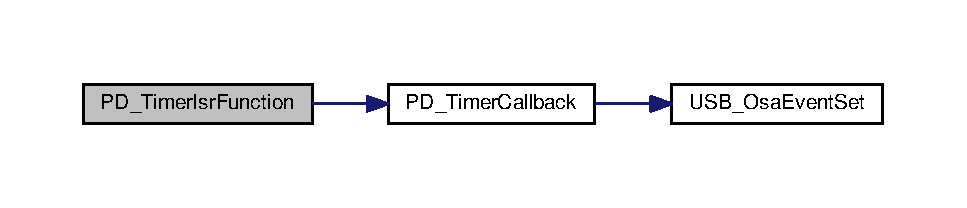
\includegraphics[width=350pt]{group__usb__pd__stack_gad8420ee79286dfb87b1b9d9c0845f31d_cgraph}
\end{center}
\end{figure}




Here is the caller graph for this function\-:
\nopagebreak
\begin{figure}[H]
\begin{center}
\leavevmode
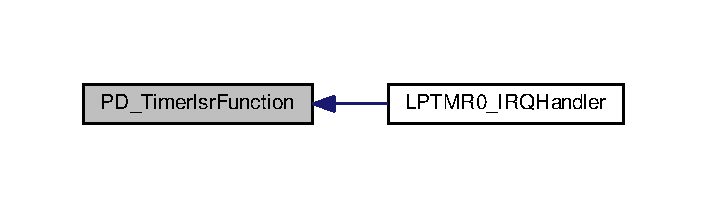
\includegraphics[width=340pt]{group__usb__pd__stack_gad8420ee79286dfb87b1b9d9c0845f31d_icgraph}
\end{center}
\end{figure}



\hypertarget{group__usb__pd__phy__drv}{\section{Usb\-\_\-pd\-\_\-phy\-\_\-drv}
\label{group__usb__pd__phy__drv}\index{Usb\-\_\-pd\-\_\-phy\-\_\-drv@{Usb\-\_\-pd\-\_\-phy\-\_\-drv}}
}
\subsection*{Classes}
\begin{DoxyCompactItemize}
\item 
struct \hyperlink{struct__pd__phy__rx__result}{\-\_\-pd\-\_\-phy\-\_\-rx\-\_\-result}
\begin{DoxyCompactList}\small\item\em P\-D P\-H\-Y receive result information. P\-D\-\_\-\-P\-H\-Y\-\_\-\-E\-V\-E\-N\-T\-\_\-\-R\-E\-C\-E\-I\-V\-E\-\_\-\-C\-O\-M\-P\-L\-E\-T\-E event use this structure as parameter. \end{DoxyCompactList}\item 
struct \hyperlink{struct__pd__detach__detection__param}{\-\_\-pd\-\_\-detach\-\_\-detection\-\_\-param}
\begin{DoxyCompactList}\small\item\em detect detach parameter used in the P\-D\-\_\-\-P\-H\-Y\-\_\-\-C\-O\-N\-F\-I\-G\-\_\-\-D\-E\-T\-A\-C\-H\-\_\-\-D\-E\-T\-E\-C\-T\-I\-O\-N control. \end{DoxyCompactList}\item 
struct \hyperlink{struct__pd__attach__detection__param}{\-\_\-pd\-\_\-attach\-\_\-detection\-\_\-param}
\begin{DoxyCompactList}\small\item\em detect attach parameter used in the P\-D\-\_\-\-P\-H\-Y\-\_\-\-C\-O\-N\-F\-I\-G\-\_\-\-A\-T\-T\-A\-C\-H\-\_\-\-D\-E\-T\-E\-C\-T\-I\-O\-N control. \end{DoxyCompactList}\item 
struct \hyperlink{struct__pd__phy__vendor__info}{\-\_\-pd\-\_\-phy\-\_\-vendor\-\_\-info}
\begin{DoxyCompactList}\small\item\em P\-H\-Y's vendor information. \end{DoxyCompactList}\item 
struct \hyperlink{struct__pd__phy__config}{\-\_\-pd\-\_\-phy\-\_\-config}
\begin{DoxyCompactList}\small\item\em Configure P\-D P\-H\-Y. \end{DoxyCompactList}\item 
struct \hyperlink{struct__pd__phy__msg__header__info}{\-\_\-pd\-\_\-phy\-\_\-msg\-\_\-header\-\_\-info}
\begin{DoxyCompactList}\small\item\em configure P\-H\-Y's data role, power role. or good\-C\-R\-C's msg header. used as the P\-D\-\_\-\-P\-H\-Y\-\_\-\-S\-E\-T\-\_\-\-M\-S\-G\-\_\-\-H\-E\-A\-D\-E\-R\-\_\-\-I\-N\-F\-O control code parameter. \end{DoxyCompactList}\item 
struct \hyperlink{struct__pd__phy__get__cc__state}{\-\_\-pd\-\_\-phy\-\_\-get\-\_\-cc\-\_\-state}
\begin{DoxyCompactList}\small\item\em Get P\-H\-Y's C\-C line state. used as the P\-D\-\_\-\-P\-H\-Y\-\_\-\-G\-E\-T\-\_\-\-C\-C\-\_\-\-L\-I\-N\-E\-\_\-\-S\-T\-A\-T\-E control code parameter. \end{DoxyCompactList}\item 
struct \hyperlink{struct__pd__phy__api__interface}{\-\_\-pd\-\_\-phy\-\_\-api\-\_\-interface}
\begin{DoxyCompactList}\small\item\em P\-D P\-H\-Y interface table structure. \end{DoxyCompactList}\end{DoxyCompactItemize}
\subsection*{Macros}
\begin{DoxyCompactItemize}
\item 
\#define \hyperlink{group__usb__pd__phy__drv_ga1f2e4aed47a47caec2aba9edb2236e42}{P\-D\-\_\-\-V\-B\-U\-S\-\_\-\-P\-O\-W\-E\-R\-\_\-\-S\-T\-A\-T\-E\-\_\-\-V\-S\-A\-F\-E5\-V\-\_\-\-M\-A\-S\-K}~(0x01u)
\begin{DoxyCompactList}\small\item\em In the return value of P\-H\-Y control (P\-D\-\_\-\-P\-H\-Y\-\_\-\-G\-E\-T\-\_\-\-V\-B\-U\-S\-\_\-\-P\-O\-W\-E\-R\-\_\-\-S\-T\-A\-T\-E), this bit set means vbus is vsafe5v. \end{DoxyCompactList}\item 
\#define \hyperlink{group__usb__pd__phy__drv_gabf05bb09647628f3556c817e1f059175}{P\-D\-\_\-\-V\-B\-U\-S\-\_\-\-P\-O\-W\-E\-R\-\_\-\-S\-T\-A\-T\-E\-\_\-\-V\-S\-A\-F\-E0\-V\-\_\-\-M\-A\-S\-K}~(0x02u)
\begin{DoxyCompactList}\small\item\em In the return value of P\-H\-Y control (P\-D\-\_\-\-P\-H\-Y\-\_\-\-G\-E\-T\-\_\-\-V\-B\-U\-S\-\_\-\-P\-O\-W\-E\-R\-\_\-\-S\-T\-A\-T\-E), this bit set means vbus is vsafe0v. \end{DoxyCompactList}\item 
\#define \hyperlink{group__usb__pd__phy__drv_gabe6758409c7aeff91de688fe7cefa195}{P\-D\-\_\-\-V\-B\-U\-S\-\_\-\-P\-O\-W\-E\-R\-\_\-\-S\-T\-A\-T\-E\-\_\-\-V\-B\-U\-S\-\_\-\-M\-A\-S\-K}~(0x04u)
\begin{DoxyCompactList}\small\item\em In the return value of P\-H\-Y control (P\-D\-\_\-\-P\-H\-Y\-\_\-\-G\-E\-T\-\_\-\-V\-B\-U\-S\-\_\-\-P\-O\-W\-E\-R\-\_\-\-S\-T\-A\-T\-E), this bit set means vbus exist. \end{DoxyCompactList}\item 
\#define \hyperlink{group__usb__pd__phy__drv_gaa02e3880c4e9954439522efb9a6af5c5}{P\-D\-\_\-\-V\-B\-U\-S\-\_\-\-P\-O\-W\-E\-R\-\_\-\-S\-T\-A\-T\-E\-\_\-\-V\-S\-Y\-S\-\_\-\-M\-A\-S\-K}~(0x08u)
\begin{DoxyCompactList}\small\item\em In the return value of P\-H\-Y control (P\-D\-\_\-\-P\-H\-Y\-\_\-\-G\-E\-T\-\_\-\-V\-B\-U\-S\-\_\-\-P\-O\-W\-E\-R\-\_\-\-S\-T\-A\-T\-E), this bit set means phy vsys exist. \end{DoxyCompactList}\end{DoxyCompactItemize}
\subsection*{Typedefs}
\begin{DoxyCompactItemize}
\item 
typedef enum \hyperlink{group__usb__pd__phy__drv_gab23c0fba94b457218944bc5284d0d08d}{\-\_\-pd\-\_\-cc\-\_\-type} \hyperlink{group__usb__pd__phy__drv_ga904cdd5d0d1e7026282617a10fe8a4c9}{pd\-\_\-cc\-\_\-type\-\_\-t}
\begin{DoxyCompactList}\small\item\em The C\-C type. \end{DoxyCompactList}\item 
typedef enum \hyperlink{group__usb__pd__phy__drv_ga09172da56b484f99a2ee891e75882faa}{\-\_\-pd\-\_\-phy\-\_\-cc\-\_\-state} \hyperlink{group__usb__pd__phy__drv_ga33106675227396a51d78ea6a7f562570}{pd\-\_\-phy\-\_\-cc\-\_\-state\-\_\-t}
\begin{DoxyCompactList}\small\item\em The C\-C state value. \end{DoxyCompactList}\item 
typedef enum \hyperlink{group__usb__pd__phy__drv_gab8bfca50e2ac042b47a697c88f84c3ed}{\-\_\-pd\-\_\-phy\-\_\-control} \hyperlink{group__usb__pd__phy__drv_ga5e3d7eb2cdbc2e45efca5e3e63d14baf}{pd\-\_\-phy\-\_\-control\-\_\-t}
\begin{DoxyCompactList}\small\item\em P\-D P\-H\-Y interface table's control function implement these control codes. \end{DoxyCompactList}\item 
typedef enum \hyperlink{group__usb__pd__phy__drv_ga9e1e6534f05a5dfae46d27dbf43e0455}{\-\_\-pd\-\_\-notify\-\_\-event\-\_\-} \hyperlink{group__usb__pd__phy__drv_ga08a2ea1727987dec255c30cdea6396fa}{pd\-\_\-phy\-\_\-notify\-\_\-event\-\_\-t}
\begin{DoxyCompactList}\small\item\em P\-D P\-H\-Y driver notify P\-D stack the P\-H\-Y state through these events. \end{DoxyCompactList}\item 
typedef enum \hyperlink{group__usb__pd__phy__drv_ga6e9f5312eacb47634a8cb7a9ef88ea2e}{\-\_\-pd\-\_\-bist\-\_\-msg} \hyperlink{group__usb__pd__phy__drv_ga311e952eb852cd3570504fe0699d10ec}{pd\-\_\-bist\-\_\-mst\-\_\-t}
\begin{DoxyCompactList}\small\item\em B\-I\-S\-T message type (not supported yet) \end{DoxyCompactList}\item 
typedef struct \hyperlink{struct__pd__phy__rx__result}{\-\_\-pd\-\_\-phy\-\_\-rx\-\_\-result} \hyperlink{group__usb__pd__phy__drv_gab6924dca8731119eec80f1740a1564eb}{pd\-\_\-phy\-\_\-rx\-\_\-result\-\_\-t}
\begin{DoxyCompactList}\small\item\em P\-D P\-H\-Y receive result information. P\-D\-\_\-\-P\-H\-Y\-\_\-\-E\-V\-E\-N\-T\-\_\-\-R\-E\-C\-E\-I\-V\-E\-\_\-\-C\-O\-M\-P\-L\-E\-T\-E event use this structure as parameter. \end{DoxyCompactList}\item 
typedef struct \\*
\hyperlink{struct__pd__detach__detection__param}{\-\_\-pd\-\_\-detach\-\_\-detection\-\_\-param} \hyperlink{group__usb__pd__phy__drv_ga658add3c5d8eb8ab53366b4850863a60}{pd\-\_\-detach\-\_\-detection\-\_\-param\-\_\-t}
\begin{DoxyCompactList}\small\item\em detect detach parameter used in the P\-D\-\_\-\-P\-H\-Y\-\_\-\-C\-O\-N\-F\-I\-G\-\_\-\-D\-E\-T\-A\-C\-H\-\_\-\-D\-E\-T\-E\-C\-T\-I\-O\-N control. \end{DoxyCompactList}\item 
typedef struct \\*
\hyperlink{struct__pd__attach__detection__param}{\-\_\-pd\-\_\-attach\-\_\-detection\-\_\-param} \hyperlink{group__usb__pd__phy__drv_gac52134faac462ac43b1a6fb59c6f693d}{pd\-\_\-attach\-\_\-detection\-\_\-param\-\_\-t}
\begin{DoxyCompactList}\small\item\em detect attach parameter used in the P\-D\-\_\-\-P\-H\-Y\-\_\-\-C\-O\-N\-F\-I\-G\-\_\-\-A\-T\-T\-A\-C\-H\-\_\-\-D\-E\-T\-E\-C\-T\-I\-O\-N control. \end{DoxyCompactList}\item 
typedef struct \hyperlink{struct__pd__phy__vendor__info}{\-\_\-pd\-\_\-phy\-\_\-vendor\-\_\-info} \hyperlink{group__usb__pd__phy__drv_ga4930ef145bdc6eb8fb43bb431eb305da}{pd\-\_\-phy\-\_\-vendor\-\_\-info\-\_\-t}
\begin{DoxyCompactList}\small\item\em P\-H\-Y's vendor information. \end{DoxyCompactList}\item 
typedef struct \hyperlink{struct__pd__phy__config}{\-\_\-pd\-\_\-phy\-\_\-config} \hyperlink{group__usb__pd__phy__drv_gab1d9a93a90c056727dcf364d6a5749e4}{pd\-\_\-phy\-\_\-config\-\_\-t}
\begin{DoxyCompactList}\small\item\em Configure P\-D P\-H\-Y. \end{DoxyCompactList}\item 
typedef struct \\*
\hyperlink{struct__pd__phy__msg__header__info}{\-\_\-pd\-\_\-phy\-\_\-msg\-\_\-header\-\_\-info} \hyperlink{group__usb__pd__phy__drv_gae09b52ec05cde39c9fdc66f179a65d61}{pd\-\_\-phy\-\_\-msg\-\_\-header\-\_\-info\-\_\-t}
\begin{DoxyCompactList}\small\item\em configure P\-H\-Y's data role, power role. or good\-C\-R\-C's msg header. used as the P\-D\-\_\-\-P\-H\-Y\-\_\-\-S\-E\-T\-\_\-\-M\-S\-G\-\_\-\-H\-E\-A\-D\-E\-R\-\_\-\-I\-N\-F\-O control code parameter. \end{DoxyCompactList}\item 
typedef struct \hyperlink{struct__pd__phy__get__cc__state}{\-\_\-pd\-\_\-phy\-\_\-get\-\_\-cc\-\_\-state} \hyperlink{group__usb__pd__phy__drv_gaad64c8a6c58f68d58feedd48b49778bd}{pd\-\_\-phy\-\_\-get\-\_\-cc\-\_\-state\-\_\-t}
\begin{DoxyCompactList}\small\item\em Get P\-H\-Y's C\-C line state. used as the P\-D\-\_\-\-P\-H\-Y\-\_\-\-G\-E\-T\-\_\-\-C\-C\-\_\-\-L\-I\-N\-E\-\_\-\-S\-T\-A\-T\-E control code parameter. \end{DoxyCompactList}\item 
typedef struct \\*
\hyperlink{struct__pd__phy__api__interface}{\-\_\-pd\-\_\-phy\-\_\-api\-\_\-interface} \hyperlink{group__usb__pd__phy__drv_ga9494f6971e6132cb70c98b92f45af74f}{pd\-\_\-phy\-\_\-api\-\_\-interface\-\_\-t}
\begin{DoxyCompactList}\small\item\em P\-D P\-H\-Y interface table structure. \end{DoxyCompactList}\end{DoxyCompactItemize}
\subsection*{Enumerations}
\begin{DoxyCompactItemize}
\item 
enum \hyperlink{group__usb__pd__phy__drv_gab23c0fba94b457218944bc5284d0d08d}{\-\_\-pd\-\_\-cc\-\_\-type} \{ \hyperlink{group__usb__pd__phy__drv_ggab23c0fba94b457218944bc5284d0d08da38c70fd9b523ca5666dea46ae65119ce}{k\-P\-D\-\_\-\-C\-C\-Invalid}, 
\hyperlink{group__usb__pd__phy__drv_ggab23c0fba94b457218944bc5284d0d08dad8ccec791609837bd7b2cb928ba727b6}{k\-P\-D\-\_\-\-C\-C1}, 
\hyperlink{group__usb__pd__phy__drv_ggab23c0fba94b457218944bc5284d0d08da274bd8ffe2629a7d89fb09b4848e172d}{k\-P\-D\-\_\-\-C\-C2}
 \}
\begin{DoxyCompactList}\small\item\em The C\-C type. \end{DoxyCompactList}\item 
enum \hyperlink{group__usb__pd__phy__drv_ga09172da56b484f99a2ee891e75882faa}{\-\_\-pd\-\_\-phy\-\_\-cc\-\_\-state} \{ \\*
\hyperlink{group__usb__pd__phy__drv_gga09172da56b484f99a2ee891e75882faaac26b04a9aef09cf82b2b01c5d775ad40}{k\-C\-C\-State\-\_\-\-Src\-Open}, 
\hyperlink{group__usb__pd__phy__drv_gga09172da56b484f99a2ee891e75882faaaa412476134fd446143c0e7275b5c329f}{k\-C\-C\-State\-\_\-\-Src\-Rd}, 
\hyperlink{group__usb__pd__phy__drv_gga09172da56b484f99a2ee891e75882faaab1f4f45b18f4f5729a23ef05ba9c741d}{k\-C\-C\-State\-\_\-\-Src\-Ra}, 
\hyperlink{group__usb__pd__phy__drv_gga09172da56b484f99a2ee891e75882faaa72b993ea12153a2594e24883bf82250e}{k\-C\-C\-State\-\_\-\-Snk\-Open}, 
\\*
\hyperlink{group__usb__pd__phy__drv_gga09172da56b484f99a2ee891e75882faaade47f2368d7c600c0c08f3e171116f47}{k\-C\-C\-State\-\_\-\-Snk\-Rp}, 
\hyperlink{group__usb__pd__phy__drv_gga09172da56b484f99a2ee891e75882faaad9c10479d9b8c3ead23386b15c857458}{k\-C\-C\-State\-\_\-\-Unknown}, 
\hyperlink{group__usb__pd__phy__drv_gga09172da56b484f99a2ee891e75882faaab679c126401ef34d37b0807109669dcf}{k\-C\-C\-State\-\_\-\-Unstable}
 \}
\begin{DoxyCompactList}\small\item\em The C\-C state value. \end{DoxyCompactList}\item 
enum \hyperlink{group__usb__pd__phy__drv_gab8bfca50e2ac042b47a697c88f84c3ed}{\-\_\-pd\-\_\-phy\-\_\-control} \{ \\*
\hyperlink{group__usb__pd__phy__drv_ggab8bfca50e2ac042b47a697c88f84c3edadd7a49b2857f7cc9b4708cb899950eec}{P\-D\-\_\-\-P\-H\-Y\-\_\-\-U\-P\-D\-A\-T\-E\-\_\-\-S\-T\-A\-T\-E}, 
\hyperlink{group__usb__pd__phy__drv_ggab8bfca50e2ac042b47a697c88f84c3edad8bcf1fd0b1c251640924ae888b17a56}{P\-D\-\_\-\-P\-H\-Y\-\_\-\-E\-N\-T\-E\-R\-\_\-\-L\-O\-W\-\_\-\-P\-O\-W\-E\-R\-\_\-\-S\-T\-A\-T\-E}, 
\hyperlink{group__usb__pd__phy__drv_ggab8bfca50e2ac042b47a697c88f84c3edae2796c6a2d5cd486dd77cbc4c9b3eea7}{P\-D\-\_\-\-P\-H\-Y\-\_\-\-G\-E\-T\-\_\-\-L\-O\-W\-P\-O\-W\-E\-R\-\_\-\-S\-T\-A\-T\-E}, 
\hyperlink{group__usb__pd__phy__drv_ggab8bfca50e2ac042b47a697c88f84c3eda2baeac02a0ea12619542377f471f7cc4}{P\-D\-\_\-\-P\-H\-Y\-\_\-\-G\-E\-T\-\_\-\-P\-H\-Y\-\_\-\-V\-E\-N\-D\-O\-R\-\_\-\-I\-N\-F\-O}, 
\\*
\hyperlink{group__usb__pd__phy__drv_ggab8bfca50e2ac042b47a697c88f84c3edafb0f5a5d01b76353eae9108cb6bfc313}{P\-D\-\_\-\-P\-H\-Y\-\_\-\-C\-O\-N\-T\-R\-O\-L\-\_\-\-P\-O\-W\-E\-R\-\_\-\-P\-I\-N}, 
\hyperlink{group__usb__pd__phy__drv_ggab8bfca50e2ac042b47a697c88f84c3edaf239b7319f38356c2dffdb8bda5cb873}{P\-D\-\_\-\-P\-H\-Y\-\_\-\-C\-O\-N\-T\-R\-O\-L\-\_\-\-V\-B\-U\-S\-\_\-\-D\-E\-T\-E\-C\-T}, 
\hyperlink{group__usb__pd__phy__drv_ggab8bfca50e2ac042b47a697c88f84c3eda4b062c83b48914ee8edc74523699871d}{P\-D\-\_\-\-P\-H\-Y\-\_\-\-S\-E\-T\-\_\-\-V\-B\-U\-S\-\_\-\-T\-R\-A\-N\-S\-F\-O\-R\-M\-\_\-\-S\-T\-A\-T\-E}, 
\hyperlink{group__usb__pd__phy__drv_ggab8bfca50e2ac042b47a697c88f84c3edae705da68d4de3104b6852d84715bb71b}{P\-D\-\_\-\-P\-H\-Y\-\_\-\-D\-I\-S\-C\-H\-A\-R\-G\-E\-\_\-\-V\-B\-U\-S}, 
\\*
\hyperlink{group__usb__pd__phy__drv_ggab8bfca50e2ac042b47a697c88f84c3eda4a23adc388bf03852d850ff3919328d6}{P\-D\-\_\-\-P\-H\-Y\-\_\-\-G\-E\-T\-\_\-\-V\-B\-U\-S\-\_\-\-P\-O\-W\-E\-R\-\_\-\-S\-T\-A\-T\-E}, 
\hyperlink{group__usb__pd__phy__drv_ggab8bfca50e2ac042b47a697c88f84c3eda8ceae23865e570716c3b63f07371825b}{P\-D\-\_\-\-P\-H\-Y\-\_\-\-F\-R\-\_\-\-S\-W\-A\-P\-\_\-\-C\-H\-E\-C\-K\-\_\-\-V\-B\-U\-S\-\_\-\-A\-P\-P\-L\-I\-E\-D}, 
\hyperlink{group__usb__pd__phy__drv_ggab8bfca50e2ac042b47a697c88f84c3eda68ad1faa15b73743adf7f5a58013937b}{P\-D\-\_\-\-P\-H\-Y\-\_\-\-C\-O\-N\-T\-R\-O\-L\-\_\-\-V\-C\-O\-N\-N}, 
\hyperlink{group__usb__pd__phy__drv_ggab8bfca50e2ac042b47a697c88f84c3eda7051aeb6bbd06322dceac0efdab96287}{P\-D\-\_\-\-P\-H\-Y\-\_\-\-D\-I\-S\-C\-H\-A\-R\-G\-E\-\_\-\-V\-C\-O\-N\-N}, 
\\*
\hyperlink{group__usb__pd__phy__drv_ggab8bfca50e2ac042b47a697c88f84c3eda229dbc5fbb6944903d1627a413aa76fe}{P\-D\-\_\-\-P\-H\-Y\-\_\-\-C\-O\-N\-F\-I\-G\-\_\-\-A\-T\-T\-A\-C\-H\-\_\-\-D\-E\-T\-E\-C\-T\-I\-O\-N}, 
\hyperlink{group__usb__pd__phy__drv_ggab8bfca50e2ac042b47a697c88f84c3eda05e43d8ecefa1b3d13bb81cb3badf466}{P\-D\-\_\-\-P\-H\-Y\-\_\-\-C\-O\-N\-F\-I\-G\-\_\-\-D\-E\-T\-A\-C\-H\-\_\-\-D\-E\-T\-E\-C\-T\-I\-O\-N}, 
\hyperlink{group__usb__pd__phy__drv_ggab8bfca50e2ac042b47a697c88f84c3edaf3f42b23f0c7f36bccf50060a41b11a8}{P\-D\-\_\-\-P\-H\-Y\-\_\-\-R\-E\-S\-E\-T\-\_\-\-C\-O\-N\-N\-E\-C\-T\-\_\-\-D\-E\-T\-E\-C\-T\-I\-O\-N}, 
\hyperlink{group__usb__pd__phy__drv_ggab8bfca50e2ac042b47a697c88f84c3eda8af796404dff0f47ecb6f0cab86613f2}{P\-D\-\_\-\-P\-H\-Y\-\_\-\-S\-I\-G\-N\-A\-L\-\_\-\-F\-R\-\_\-\-S\-W\-A\-P}, 
\\*
\hyperlink{group__usb__pd__phy__drv_ggab8bfca50e2ac042b47a697c88f84c3edab364b8f9461757d17739cce20263b117}{P\-D\-\_\-\-P\-H\-Y\-\_\-\-C\-O\-N\-T\-R\-O\-L\-\_\-\-F\-R\-\_\-\-S\-W\-A\-P}, 
\hyperlink{group__usb__pd__phy__drv_ggab8bfca50e2ac042b47a697c88f84c3eda47b31ad92865627f7e074f52e8532854}{P\-D\-\_\-\-P\-H\-Y\-\_\-\-S\-R\-C\-\_\-\-S\-E\-T\-\_\-\-T\-Y\-P\-E\-C\-\_\-\-C\-U\-R\-R\-E\-N\-T\-\_\-\-C\-A\-P}, 
\hyperlink{group__usb__pd__phy__drv_ggab8bfca50e2ac042b47a697c88f84c3edae1406149d183dba960809596aa525528}{P\-D\-\_\-\-P\-H\-Y\-\_\-\-S\-N\-K\-\_\-\-G\-E\-T\-\_\-\-T\-Y\-P\-E\-C\-\_\-\-C\-U\-R\-R\-E\-N\-T\-\_\-\-C\-A\-P}, 
\hyperlink{group__usb__pd__phy__drv_ggab8bfca50e2ac042b47a697c88f84c3edae5f03a153f98ececc88b52f551f55c2e}{P\-D\-\_\-\-P\-H\-Y\-\_\-\-G\-E\-T\-\_\-\-C\-C\-\_\-\-L\-I\-N\-E\-\_\-\-S\-T\-A\-T\-E}, 
\\*
\hyperlink{group__usb__pd__phy__drv_ggab8bfca50e2ac042b47a697c88f84c3edadfcf4cb3c3f2b330b326278bac666a80}{P\-D\-\_\-\-P\-H\-Y\-\_\-\-C\-O\-N\-N\-E\-C\-T\-\_\-\-S\-E\-T\-\_\-\-C\-C}, 
\hyperlink{group__usb__pd__phy__drv_ggab8bfca50e2ac042b47a697c88f84c3eda12e5c95c04532128d54f63e4e76d2c6e}{P\-D\-\_\-\-P\-H\-Y\-\_\-\-R\-E\-S\-E\-T\-\_\-\-M\-S\-G\-\_\-\-F\-U\-N\-C\-T\-I\-O\-N}, 
\hyperlink{group__usb__pd__phy__drv_ggab8bfca50e2ac042b47a697c88f84c3eda82e2f7a81ec4b132e98ed42740a4f7ec}{P\-D\-\_\-\-P\-H\-Y\-\_\-\-D\-I\-S\-A\-B\-L\-E\-\_\-\-M\-S\-G\-\_\-\-R\-X}, 
\hyperlink{group__usb__pd__phy__drv_ggab8bfca50e2ac042b47a697c88f84c3eda0c9ed5435eeaf83461a852f4180a9c3e}{P\-D\-\_\-\-P\-H\-Y\-\_\-\-D\-I\-S\-A\-B\-L\-E\-\_\-\-M\-S\-G\-\_\-\-T\-X}, 
\\*
\hyperlink{group__usb__pd__phy__drv_ggab8bfca50e2ac042b47a697c88f84c3eda05d1be67ea7a2972c165dd67a0196839}{P\-D\-\_\-\-P\-H\-Y\-\_\-\-C\-A\-N\-C\-E\-L\-\_\-\-M\-S\-G\-\_\-\-T\-X}, 
\hyperlink{group__usb__pd__phy__drv_ggab8bfca50e2ac042b47a697c88f84c3edad29607158e8977b9bb140b407b9e6cc4}{P\-D\-\_\-\-P\-H\-Y\-\_\-\-C\-A\-N\-C\-E\-L\-\_\-\-M\-S\-G\-\_\-\-R\-X}, 
\hyperlink{group__usb__pd__phy__drv_ggab8bfca50e2ac042b47a697c88f84c3eda1d45b97b5d29cbce1117fa4c77202cbf}{P\-D\-\_\-\-P\-H\-Y\-\_\-\-S\-E\-N\-D\-\_\-\-H\-A\-R\-D\-\_\-\-R\-E\-S\-E\-T}, 
\hyperlink{group__usb__pd__phy__drv_ggab8bfca50e2ac042b47a697c88f84c3eda01bdfe97bda0b1df4049c0cb0dbf6b90}{P\-D\-\_\-\-P\-H\-Y\-\_\-\-S\-E\-N\-D\-\_\-\-C\-A\-B\-L\-E\-\_\-\-R\-E\-S\-E\-T}, 
\\*
\hyperlink{group__usb__pd__phy__drv_ggab8bfca50e2ac042b47a697c88f84c3edab459c8f89653d73a0d318cd30c0a1fc5}{P\-D\-\_\-\-P\-H\-Y\-\_\-\-S\-E\-T\-\_\-\-M\-S\-G\-\_\-\-H\-E\-A\-D\-E\-R\-\_\-\-I\-N\-F\-O}, 
\hyperlink{group__usb__pd__phy__drv_ggab8bfca50e2ac042b47a697c88f84c3eda22ef1e6ff7ac5197c977d200827b1294}{P\-D\-\_\-\-P\-H\-Y\-\_\-\-G\-E\-T\-\_\-\-C\-C\-\_\-\-V\-O\-L\-T\-A\-G\-E\-\_\-\-D\-I\-F\-F\-\_\-\-F\-O\-R\-\_\-\-D\-B\-G\-\_\-\-A\-C\-C}, 
\hyperlink{group__usb__pd__phy__drv_ggab8bfca50e2ac042b47a697c88f84c3eda21c0a2560395f9909217bf8edb9f1cb8}{P\-D\-\_\-\-P\-H\-Y\-\_\-\-R\-E\-S\-E\-T\-\_\-\-B\-I\-S\-T}, 
\hyperlink{group__usb__pd__phy__drv_ggab8bfca50e2ac042b47a697c88f84c3eda49c349410dcd972b652d355139f112a7}{P\-D\-\_\-\-P\-H\-Y\-\_\-\-E\-N\-T\-E\-R\-\_\-\-B\-I\-S\-T}, 
\\*
\hyperlink{group__usb__pd__phy__drv_ggab8bfca50e2ac042b47a697c88f84c3edab337f6edf4077d3082bd3a7450612531}{P\-D\-\_\-\-P\-H\-Y\-\_\-\-E\-X\-I\-T\-\_\-\-B\-I\-S\-T}, 
\hyperlink{group__usb__pd__phy__drv_ggab8bfca50e2ac042b47a697c88f84c3edaf8cd47444685acfae52caa916786ec98}{P\-D\-\_\-\-P\-H\-Y\-\_\-\-G\-E\-T\-\_\-\-B\-I\-S\-T\-\_\-\-M\-O\-D\-E}, 
\hyperlink{group__usb__pd__phy__drv_ggab8bfca50e2ac042b47a697c88f84c3edaee3a595d1a1a42afc63594033f84a376}{P\-D\-\_\-\-P\-H\-Y\-\_\-\-G\-E\-T\-\_\-\-B\-I\-S\-T\-\_\-\-E\-R\-R\-\_\-\-C\-O\-U\-N\-T}
 \}
\begin{DoxyCompactList}\small\item\em P\-D P\-H\-Y interface table's control function implement these control codes. \end{DoxyCompactList}\item 
enum \hyperlink{group__usb__pd__phy__drv_ga9e1e6534f05a5dfae46d27dbf43e0455}{\-\_\-pd\-\_\-notify\-\_\-event\-\_\-} \{ \\*
\hyperlink{group__usb__pd__phy__drv_gga9e1e6534f05a5dfae46d27dbf43e0455a1c7d2386b854afa09864304c2c407b04}{P\-D\-\_\-\-P\-H\-Y\-\_\-\-E\-V\-E\-N\-T\-\_\-\-S\-T\-A\-T\-E\-\_\-\-C\-H\-A\-N\-G\-E}, 
\hyperlink{group__usb__pd__phy__drv_gga9e1e6534f05a5dfae46d27dbf43e0455ad761e5459c646a3557ddd40db0860251}{P\-D\-\_\-\-P\-H\-Y\-\_\-\-E\-V\-E\-N\-T\-\_\-\-S\-E\-N\-D\-\_\-\-C\-O\-M\-P\-L\-E\-T\-E}, 
\hyperlink{group__usb__pd__phy__drv_gga9e1e6534f05a5dfae46d27dbf43e0455a75755590b2a119a4a558e7b13a708bd4}{P\-D\-\_\-\-P\-H\-Y\-\_\-\-E\-V\-E\-N\-T\-\_\-\-R\-E\-C\-E\-I\-V\-E\-\_\-\-C\-O\-M\-P\-L\-E\-T\-E}, 
\hyperlink{group__usb__pd__phy__drv_gga9e1e6534f05a5dfae46d27dbf43e0455a7e6b6e7834c0ee9d4b6a990f5f92b2ba}{P\-D\-\_\-\-P\-H\-Y\-\_\-\-E\-V\-E\-N\-T\-\_\-\-H\-A\-R\-D\-\_\-\-R\-E\-S\-E\-T\-\_\-\-R\-E\-C\-E\-I\-V\-E\-D}, 
\\*
\hyperlink{group__usb__pd__phy__drv_gga9e1e6534f05a5dfae46d27dbf43e0455a906bb6506d930fb23604d0343678ac63}{P\-D\-\_\-\-P\-H\-Y\-\_\-\-E\-V\-E\-N\-T\-\_\-\-V\-B\-U\-S\-\_\-\-S\-T\-A\-T\-E\-\_\-\-C\-H\-A\-N\-G\-E}, 
\hyperlink{group__usb__pd__phy__drv_gga9e1e6534f05a5dfae46d27dbf43e0455a275e7486f8964603c2affb44cd08fc35}{P\-D\-\_\-\-P\-H\-Y\-\_\-\-E\-V\-E\-N\-T\-\_\-\-F\-R\-\_\-\-S\-W\-A\-P\-\_\-\-S\-I\-N\-G\-A\-L\-\_\-\-R\-E\-C\-E\-I\-V\-E\-D}, 
\hyperlink{group__usb__pd__phy__drv_gga9e1e6534f05a5dfae46d27dbf43e0455ae64660dbae463fdd2b0bcf3aa85b35c8}{P\-D\-\_\-\-P\-H\-Y\-\_\-\-E\-V\-E\-N\-T\-\_\-\-R\-E\-Q\-U\-E\-S\-T\-\_\-\-S\-T\-A\-C\-K\-\_\-\-R\-E\-S\-E\-T}, 
\hyperlink{group__usb__pd__phy__drv_gga9e1e6534f05a5dfae46d27dbf43e0455aae1ef925e985664558cd2fc67e52bdc5}{P\-D\-\_\-\-P\-H\-Y\-\_\-\-E\-V\-E\-N\-T\-\_\-\-V\-C\-O\-N\-N\-\_\-\-P\-R\-O\-T\-E\-C\-T\-I\-O\-N\-\_\-\-F\-A\-U\-L\-T}, 
\\*
\hyperlink{group__usb__pd__phy__drv_gga9e1e6534f05a5dfae46d27dbf43e0455a2908542d9124ac2605f062654f8be797}{P\-D\-\_\-\-P\-H\-Y\-\_\-\-E\-V\-E\-N\-T\-\_\-\-F\-A\-U\-L\-T\-\_\-\-R\-E\-C\-O\-V\-E\-R\-Y}
 \}
\begin{DoxyCompactList}\small\item\em P\-D P\-H\-Y driver notify P\-D stack the P\-H\-Y state through these events. \end{DoxyCompactList}\item 
enum \hyperlink{group__usb__pd__phy__drv_ga6e9f5312eacb47634a8cb7a9ef88ea2e}{\-\_\-pd\-\_\-bist\-\_\-msg} \{ \\*
\hyperlink{group__usb__pd__phy__drv_gga6e9f5312eacb47634a8cb7a9ef88ea2ea8765260ddd14914bca1dd2f48ac1a50e}{k\-B\-I\-S\-T\-\_\-\-Receiver\-Mode} = 0, 
\hyperlink{group__usb__pd__phy__drv_gga6e9f5312eacb47634a8cb7a9ef88ea2ea208a35cc33306177ea707c6964a61bd7}{k\-B\-I\-S\-T\-\_\-\-Transmit\-Mode}, 
\hyperlink{group__usb__pd__phy__drv_gga6e9f5312eacb47634a8cb7a9ef88ea2ea09ffbc2f4bebba2ec696150224bf7964}{k\-B\-I\-S\-T\-\_\-\-Returned\-Bist\-Counters}, 
\hyperlink{group__usb__pd__phy__drv_gga6e9f5312eacb47634a8cb7a9ef88ea2eade4b6cebf0cbb487cfd339dbfb96b912}{k\-B\-I\-S\-T\-\_\-\-Carrier\-Mode0}, 
\\*
\hyperlink{group__usb__pd__phy__drv_gga6e9f5312eacb47634a8cb7a9ef88ea2ea53186766d6c82165428fa63a874eb2e8}{k\-B\-I\-S\-T\-\_\-\-Carrier\-Mode1}, 
\hyperlink{group__usb__pd__phy__drv_gga6e9f5312eacb47634a8cb7a9ef88ea2ea376a9e89909ae22b43414d1feebda94b}{k\-B\-I\-S\-T\-\_\-\-Carrier\-Mode2}, 
\hyperlink{group__usb__pd__phy__drv_gga6e9f5312eacb47634a8cb7a9ef88ea2eab343b840951f1992144bf2a85181ba90}{k\-B\-I\-S\-T\-\_\-\-Carrier\-Mode3}, 
\hyperlink{group__usb__pd__phy__drv_gga6e9f5312eacb47634a8cb7a9ef88ea2eae2ef1b8c6d998a0a8a011962c53280e8}{k\-B\-I\-S\-T\-\_\-\-Eye\-Pattern}, 
\\*
\hyperlink{group__usb__pd__phy__drv_gga6e9f5312eacb47634a8cb7a9ef88ea2ea311a5b2f8176208f0d9fcc73e461a2d0}{k\-B\-I\-S\-T\-\_\-\-Test\-Data}
 \}
\begin{DoxyCompactList}\small\item\em B\-I\-S\-T message type (not supported yet) \end{DoxyCompactList}\end{DoxyCompactItemize}
\subsection*{Functions}
\begin{DoxyCompactItemize}
\item 
void \hyperlink{group__usb__pd__phy__drv_ga7f7f94758771b173653d27c508c8b33f}{P\-D\-\_\-\-Notify} (\hyperlink{group__usb__pd__stack_ga9397835347d48ef48b6b0ecba6312213}{pd\-\_\-handle} pd\-Handle, uint32\-\_\-t event, void $\ast$param)
\begin{DoxyCompactList}\small\item\em Notify P\-D stack the P\-H\-Y status. \end{DoxyCompactList}\end{DoxyCompactItemize}


\subsection{Detailed Description}


\subsection{Macro Definition Documentation}
\hypertarget{group__usb__pd__phy__drv_gabe6758409c7aeff91de688fe7cefa195}{\index{Usb\-\_\-pd\-\_\-phy\-\_\-drv@{Usb\-\_\-pd\-\_\-phy\-\_\-drv}!P\-D\-\_\-\-V\-B\-U\-S\-\_\-\-P\-O\-W\-E\-R\-\_\-\-S\-T\-A\-T\-E\-\_\-\-V\-B\-U\-S\-\_\-\-M\-A\-S\-K@{P\-D\-\_\-\-V\-B\-U\-S\-\_\-\-P\-O\-W\-E\-R\-\_\-\-S\-T\-A\-T\-E\-\_\-\-V\-B\-U\-S\-\_\-\-M\-A\-S\-K}}
\index{P\-D\-\_\-\-V\-B\-U\-S\-\_\-\-P\-O\-W\-E\-R\-\_\-\-S\-T\-A\-T\-E\-\_\-\-V\-B\-U\-S\-\_\-\-M\-A\-S\-K@{P\-D\-\_\-\-V\-B\-U\-S\-\_\-\-P\-O\-W\-E\-R\-\_\-\-S\-T\-A\-T\-E\-\_\-\-V\-B\-U\-S\-\_\-\-M\-A\-S\-K}!Usb_pd_phy_drv@{Usb\-\_\-pd\-\_\-phy\-\_\-drv}}
\subsubsection[{P\-D\-\_\-\-V\-B\-U\-S\-\_\-\-P\-O\-W\-E\-R\-\_\-\-S\-T\-A\-T\-E\-\_\-\-V\-B\-U\-S\-\_\-\-M\-A\-S\-K}]{\setlength{\rightskip}{0pt plus 5cm}\#define P\-D\-\_\-\-V\-B\-U\-S\-\_\-\-P\-O\-W\-E\-R\-\_\-\-S\-T\-A\-T\-E\-\_\-\-V\-B\-U\-S\-\_\-\-M\-A\-S\-K~(0x04u)}}\label{group__usb__pd__phy__drv_gabe6758409c7aeff91de688fe7cefa195}


In the return value of P\-H\-Y control (P\-D\-\_\-\-P\-H\-Y\-\_\-\-G\-E\-T\-\_\-\-V\-B\-U\-S\-\_\-\-P\-O\-W\-E\-R\-\_\-\-S\-T\-A\-T\-E), this bit set means vbus exist. 

\hypertarget{group__usb__pd__phy__drv_gabf05bb09647628f3556c817e1f059175}{\index{Usb\-\_\-pd\-\_\-phy\-\_\-drv@{Usb\-\_\-pd\-\_\-phy\-\_\-drv}!P\-D\-\_\-\-V\-B\-U\-S\-\_\-\-P\-O\-W\-E\-R\-\_\-\-S\-T\-A\-T\-E\-\_\-\-V\-S\-A\-F\-E0\-V\-\_\-\-M\-A\-S\-K@{P\-D\-\_\-\-V\-B\-U\-S\-\_\-\-P\-O\-W\-E\-R\-\_\-\-S\-T\-A\-T\-E\-\_\-\-V\-S\-A\-F\-E0\-V\-\_\-\-M\-A\-S\-K}}
\index{P\-D\-\_\-\-V\-B\-U\-S\-\_\-\-P\-O\-W\-E\-R\-\_\-\-S\-T\-A\-T\-E\-\_\-\-V\-S\-A\-F\-E0\-V\-\_\-\-M\-A\-S\-K@{P\-D\-\_\-\-V\-B\-U\-S\-\_\-\-P\-O\-W\-E\-R\-\_\-\-S\-T\-A\-T\-E\-\_\-\-V\-S\-A\-F\-E0\-V\-\_\-\-M\-A\-S\-K}!Usb_pd_phy_drv@{Usb\-\_\-pd\-\_\-phy\-\_\-drv}}
\subsubsection[{P\-D\-\_\-\-V\-B\-U\-S\-\_\-\-P\-O\-W\-E\-R\-\_\-\-S\-T\-A\-T\-E\-\_\-\-V\-S\-A\-F\-E0\-V\-\_\-\-M\-A\-S\-K}]{\setlength{\rightskip}{0pt plus 5cm}\#define P\-D\-\_\-\-V\-B\-U\-S\-\_\-\-P\-O\-W\-E\-R\-\_\-\-S\-T\-A\-T\-E\-\_\-\-V\-S\-A\-F\-E0\-V\-\_\-\-M\-A\-S\-K~(0x02u)}}\label{group__usb__pd__phy__drv_gabf05bb09647628f3556c817e1f059175}


In the return value of P\-H\-Y control (P\-D\-\_\-\-P\-H\-Y\-\_\-\-G\-E\-T\-\_\-\-V\-B\-U\-S\-\_\-\-P\-O\-W\-E\-R\-\_\-\-S\-T\-A\-T\-E), this bit set means vbus is vsafe0v. 

\hypertarget{group__usb__pd__phy__drv_ga1f2e4aed47a47caec2aba9edb2236e42}{\index{Usb\-\_\-pd\-\_\-phy\-\_\-drv@{Usb\-\_\-pd\-\_\-phy\-\_\-drv}!P\-D\-\_\-\-V\-B\-U\-S\-\_\-\-P\-O\-W\-E\-R\-\_\-\-S\-T\-A\-T\-E\-\_\-\-V\-S\-A\-F\-E5\-V\-\_\-\-M\-A\-S\-K@{P\-D\-\_\-\-V\-B\-U\-S\-\_\-\-P\-O\-W\-E\-R\-\_\-\-S\-T\-A\-T\-E\-\_\-\-V\-S\-A\-F\-E5\-V\-\_\-\-M\-A\-S\-K}}
\index{P\-D\-\_\-\-V\-B\-U\-S\-\_\-\-P\-O\-W\-E\-R\-\_\-\-S\-T\-A\-T\-E\-\_\-\-V\-S\-A\-F\-E5\-V\-\_\-\-M\-A\-S\-K@{P\-D\-\_\-\-V\-B\-U\-S\-\_\-\-P\-O\-W\-E\-R\-\_\-\-S\-T\-A\-T\-E\-\_\-\-V\-S\-A\-F\-E5\-V\-\_\-\-M\-A\-S\-K}!Usb_pd_phy_drv@{Usb\-\_\-pd\-\_\-phy\-\_\-drv}}
\subsubsection[{P\-D\-\_\-\-V\-B\-U\-S\-\_\-\-P\-O\-W\-E\-R\-\_\-\-S\-T\-A\-T\-E\-\_\-\-V\-S\-A\-F\-E5\-V\-\_\-\-M\-A\-S\-K}]{\setlength{\rightskip}{0pt plus 5cm}\#define P\-D\-\_\-\-V\-B\-U\-S\-\_\-\-P\-O\-W\-E\-R\-\_\-\-S\-T\-A\-T\-E\-\_\-\-V\-S\-A\-F\-E5\-V\-\_\-\-M\-A\-S\-K~(0x01u)}}\label{group__usb__pd__phy__drv_ga1f2e4aed47a47caec2aba9edb2236e42}


In the return value of P\-H\-Y control (P\-D\-\_\-\-P\-H\-Y\-\_\-\-G\-E\-T\-\_\-\-V\-B\-U\-S\-\_\-\-P\-O\-W\-E\-R\-\_\-\-S\-T\-A\-T\-E), this bit set means vbus is vsafe5v. 

\hypertarget{group__usb__pd__phy__drv_gaa02e3880c4e9954439522efb9a6af5c5}{\index{Usb\-\_\-pd\-\_\-phy\-\_\-drv@{Usb\-\_\-pd\-\_\-phy\-\_\-drv}!P\-D\-\_\-\-V\-B\-U\-S\-\_\-\-P\-O\-W\-E\-R\-\_\-\-S\-T\-A\-T\-E\-\_\-\-V\-S\-Y\-S\-\_\-\-M\-A\-S\-K@{P\-D\-\_\-\-V\-B\-U\-S\-\_\-\-P\-O\-W\-E\-R\-\_\-\-S\-T\-A\-T\-E\-\_\-\-V\-S\-Y\-S\-\_\-\-M\-A\-S\-K}}
\index{P\-D\-\_\-\-V\-B\-U\-S\-\_\-\-P\-O\-W\-E\-R\-\_\-\-S\-T\-A\-T\-E\-\_\-\-V\-S\-Y\-S\-\_\-\-M\-A\-S\-K@{P\-D\-\_\-\-V\-B\-U\-S\-\_\-\-P\-O\-W\-E\-R\-\_\-\-S\-T\-A\-T\-E\-\_\-\-V\-S\-Y\-S\-\_\-\-M\-A\-S\-K}!Usb_pd_phy_drv@{Usb\-\_\-pd\-\_\-phy\-\_\-drv}}
\subsubsection[{P\-D\-\_\-\-V\-B\-U\-S\-\_\-\-P\-O\-W\-E\-R\-\_\-\-S\-T\-A\-T\-E\-\_\-\-V\-S\-Y\-S\-\_\-\-M\-A\-S\-K}]{\setlength{\rightskip}{0pt plus 5cm}\#define P\-D\-\_\-\-V\-B\-U\-S\-\_\-\-P\-O\-W\-E\-R\-\_\-\-S\-T\-A\-T\-E\-\_\-\-V\-S\-Y\-S\-\_\-\-M\-A\-S\-K~(0x08u)}}\label{group__usb__pd__phy__drv_gaa02e3880c4e9954439522efb9a6af5c5}


In the return value of P\-H\-Y control (P\-D\-\_\-\-P\-H\-Y\-\_\-\-G\-E\-T\-\_\-\-V\-B\-U\-S\-\_\-\-P\-O\-W\-E\-R\-\_\-\-S\-T\-A\-T\-E), this bit set means phy vsys exist. 



\subsection{Typedef Documentation}
\hypertarget{group__usb__pd__phy__drv_gac52134faac462ac43b1a6fb59c6f693d}{\index{Usb\-\_\-pd\-\_\-phy\-\_\-drv@{Usb\-\_\-pd\-\_\-phy\-\_\-drv}!pd\-\_\-attach\-\_\-detection\-\_\-param\-\_\-t@{pd\-\_\-attach\-\_\-detection\-\_\-param\-\_\-t}}
\index{pd\-\_\-attach\-\_\-detection\-\_\-param\-\_\-t@{pd\-\_\-attach\-\_\-detection\-\_\-param\-\_\-t}!Usb_pd_phy_drv@{Usb\-\_\-pd\-\_\-phy\-\_\-drv}}
\subsubsection[{pd\-\_\-attach\-\_\-detection\-\_\-param\-\_\-t}]{\setlength{\rightskip}{0pt plus 5cm}typedef struct {\bf \-\_\-pd\-\_\-attach\-\_\-detection\-\_\-param}  {\bf pd\-\_\-attach\-\_\-detection\-\_\-param\-\_\-t}}}\label{group__usb__pd__phy__drv_gac52134faac462ac43b1a6fb59c6f693d}


detect attach parameter used in the P\-D\-\_\-\-P\-H\-Y\-\_\-\-C\-O\-N\-F\-I\-G\-\_\-\-A\-T\-T\-A\-C\-H\-\_\-\-D\-E\-T\-E\-C\-T\-I\-O\-N control. 

\hypertarget{group__usb__pd__phy__drv_ga311e952eb852cd3570504fe0699d10ec}{\index{Usb\-\_\-pd\-\_\-phy\-\_\-drv@{Usb\-\_\-pd\-\_\-phy\-\_\-drv}!pd\-\_\-bist\-\_\-mst\-\_\-t@{pd\-\_\-bist\-\_\-mst\-\_\-t}}
\index{pd\-\_\-bist\-\_\-mst\-\_\-t@{pd\-\_\-bist\-\_\-mst\-\_\-t}!Usb_pd_phy_drv@{Usb\-\_\-pd\-\_\-phy\-\_\-drv}}
\subsubsection[{pd\-\_\-bist\-\_\-mst\-\_\-t}]{\setlength{\rightskip}{0pt plus 5cm}typedef enum {\bf \-\_\-pd\-\_\-bist\-\_\-msg}  {\bf pd\-\_\-bist\-\_\-mst\-\_\-t}}}\label{group__usb__pd__phy__drv_ga311e952eb852cd3570504fe0699d10ec}


B\-I\-S\-T message type (not supported yet) 

\hypertarget{group__usb__pd__phy__drv_ga904cdd5d0d1e7026282617a10fe8a4c9}{\index{Usb\-\_\-pd\-\_\-phy\-\_\-drv@{Usb\-\_\-pd\-\_\-phy\-\_\-drv}!pd\-\_\-cc\-\_\-type\-\_\-t@{pd\-\_\-cc\-\_\-type\-\_\-t}}
\index{pd\-\_\-cc\-\_\-type\-\_\-t@{pd\-\_\-cc\-\_\-type\-\_\-t}!Usb_pd_phy_drv@{Usb\-\_\-pd\-\_\-phy\-\_\-drv}}
\subsubsection[{pd\-\_\-cc\-\_\-type\-\_\-t}]{\setlength{\rightskip}{0pt plus 5cm}typedef enum {\bf \-\_\-pd\-\_\-cc\-\_\-type}  {\bf pd\-\_\-cc\-\_\-type\-\_\-t}}}\label{group__usb__pd__phy__drv_ga904cdd5d0d1e7026282617a10fe8a4c9}


The C\-C type. 

\hypertarget{group__usb__pd__phy__drv_ga658add3c5d8eb8ab53366b4850863a60}{\index{Usb\-\_\-pd\-\_\-phy\-\_\-drv@{Usb\-\_\-pd\-\_\-phy\-\_\-drv}!pd\-\_\-detach\-\_\-detection\-\_\-param\-\_\-t@{pd\-\_\-detach\-\_\-detection\-\_\-param\-\_\-t}}
\index{pd\-\_\-detach\-\_\-detection\-\_\-param\-\_\-t@{pd\-\_\-detach\-\_\-detection\-\_\-param\-\_\-t}!Usb_pd_phy_drv@{Usb\-\_\-pd\-\_\-phy\-\_\-drv}}
\subsubsection[{pd\-\_\-detach\-\_\-detection\-\_\-param\-\_\-t}]{\setlength{\rightskip}{0pt plus 5cm}typedef struct {\bf \-\_\-pd\-\_\-detach\-\_\-detection\-\_\-param}  {\bf pd\-\_\-detach\-\_\-detection\-\_\-param\-\_\-t}}}\label{group__usb__pd__phy__drv_ga658add3c5d8eb8ab53366b4850863a60}


detect detach parameter used in the P\-D\-\_\-\-P\-H\-Y\-\_\-\-C\-O\-N\-F\-I\-G\-\_\-\-D\-E\-T\-A\-C\-H\-\_\-\-D\-E\-T\-E\-C\-T\-I\-O\-N control. 

\hypertarget{group__usb__pd__phy__drv_ga9494f6971e6132cb70c98b92f45af74f}{\index{Usb\-\_\-pd\-\_\-phy\-\_\-drv@{Usb\-\_\-pd\-\_\-phy\-\_\-drv}!pd\-\_\-phy\-\_\-api\-\_\-interface\-\_\-t@{pd\-\_\-phy\-\_\-api\-\_\-interface\-\_\-t}}
\index{pd\-\_\-phy\-\_\-api\-\_\-interface\-\_\-t@{pd\-\_\-phy\-\_\-api\-\_\-interface\-\_\-t}!Usb_pd_phy_drv@{Usb\-\_\-pd\-\_\-phy\-\_\-drv}}
\subsubsection[{pd\-\_\-phy\-\_\-api\-\_\-interface\-\_\-t}]{\setlength{\rightskip}{0pt plus 5cm}typedef struct {\bf \-\_\-pd\-\_\-phy\-\_\-api\-\_\-interface}  {\bf pd\-\_\-phy\-\_\-api\-\_\-interface\-\_\-t}}}\label{group__usb__pd__phy__drv_ga9494f6971e6132cb70c98b92f45af74f}


P\-D P\-H\-Y interface table structure. 

\hypertarget{group__usb__pd__phy__drv_ga33106675227396a51d78ea6a7f562570}{\index{Usb\-\_\-pd\-\_\-phy\-\_\-drv@{Usb\-\_\-pd\-\_\-phy\-\_\-drv}!pd\-\_\-phy\-\_\-cc\-\_\-state\-\_\-t@{pd\-\_\-phy\-\_\-cc\-\_\-state\-\_\-t}}
\index{pd\-\_\-phy\-\_\-cc\-\_\-state\-\_\-t@{pd\-\_\-phy\-\_\-cc\-\_\-state\-\_\-t}!Usb_pd_phy_drv@{Usb\-\_\-pd\-\_\-phy\-\_\-drv}}
\subsubsection[{pd\-\_\-phy\-\_\-cc\-\_\-state\-\_\-t}]{\setlength{\rightskip}{0pt plus 5cm}typedef enum {\bf \-\_\-pd\-\_\-phy\-\_\-cc\-\_\-state}  {\bf pd\-\_\-phy\-\_\-cc\-\_\-state\-\_\-t}}}\label{group__usb__pd__phy__drv_ga33106675227396a51d78ea6a7f562570}


The C\-C state value. 

\hypertarget{group__usb__pd__phy__drv_gab1d9a93a90c056727dcf364d6a5749e4}{\index{Usb\-\_\-pd\-\_\-phy\-\_\-drv@{Usb\-\_\-pd\-\_\-phy\-\_\-drv}!pd\-\_\-phy\-\_\-config\-\_\-t@{pd\-\_\-phy\-\_\-config\-\_\-t}}
\index{pd\-\_\-phy\-\_\-config\-\_\-t@{pd\-\_\-phy\-\_\-config\-\_\-t}!Usb_pd_phy_drv@{Usb\-\_\-pd\-\_\-phy\-\_\-drv}}
\subsubsection[{pd\-\_\-phy\-\_\-config\-\_\-t}]{\setlength{\rightskip}{0pt plus 5cm}typedef struct {\bf \-\_\-pd\-\_\-phy\-\_\-config}  {\bf pd\-\_\-phy\-\_\-config\-\_\-t}}}\label{group__usb__pd__phy__drv_gab1d9a93a90c056727dcf364d6a5749e4}


Configure P\-D P\-H\-Y. 

\hypertarget{group__usb__pd__phy__drv_ga5e3d7eb2cdbc2e45efca5e3e63d14baf}{\index{Usb\-\_\-pd\-\_\-phy\-\_\-drv@{Usb\-\_\-pd\-\_\-phy\-\_\-drv}!pd\-\_\-phy\-\_\-control\-\_\-t@{pd\-\_\-phy\-\_\-control\-\_\-t}}
\index{pd\-\_\-phy\-\_\-control\-\_\-t@{pd\-\_\-phy\-\_\-control\-\_\-t}!Usb_pd_phy_drv@{Usb\-\_\-pd\-\_\-phy\-\_\-drv}}
\subsubsection[{pd\-\_\-phy\-\_\-control\-\_\-t}]{\setlength{\rightskip}{0pt plus 5cm}typedef enum {\bf \-\_\-pd\-\_\-phy\-\_\-control}  {\bf pd\-\_\-phy\-\_\-control\-\_\-t}}}\label{group__usb__pd__phy__drv_ga5e3d7eb2cdbc2e45efca5e3e63d14baf}


P\-D P\-H\-Y interface table's control function implement these control codes. 

\hypertarget{group__usb__pd__phy__drv_gaad64c8a6c58f68d58feedd48b49778bd}{\index{Usb\-\_\-pd\-\_\-phy\-\_\-drv@{Usb\-\_\-pd\-\_\-phy\-\_\-drv}!pd\-\_\-phy\-\_\-get\-\_\-cc\-\_\-state\-\_\-t@{pd\-\_\-phy\-\_\-get\-\_\-cc\-\_\-state\-\_\-t}}
\index{pd\-\_\-phy\-\_\-get\-\_\-cc\-\_\-state\-\_\-t@{pd\-\_\-phy\-\_\-get\-\_\-cc\-\_\-state\-\_\-t}!Usb_pd_phy_drv@{Usb\-\_\-pd\-\_\-phy\-\_\-drv}}
\subsubsection[{pd\-\_\-phy\-\_\-get\-\_\-cc\-\_\-state\-\_\-t}]{\setlength{\rightskip}{0pt plus 5cm}typedef struct {\bf \-\_\-pd\-\_\-phy\-\_\-get\-\_\-cc\-\_\-state}  {\bf pd\-\_\-phy\-\_\-get\-\_\-cc\-\_\-state\-\_\-t}}}\label{group__usb__pd__phy__drv_gaad64c8a6c58f68d58feedd48b49778bd}


Get P\-H\-Y's C\-C line state. used as the P\-D\-\_\-\-P\-H\-Y\-\_\-\-G\-E\-T\-\_\-\-C\-C\-\_\-\-L\-I\-N\-E\-\_\-\-S\-T\-A\-T\-E control code parameter. 

\hypertarget{group__usb__pd__phy__drv_gae09b52ec05cde39c9fdc66f179a65d61}{\index{Usb\-\_\-pd\-\_\-phy\-\_\-drv@{Usb\-\_\-pd\-\_\-phy\-\_\-drv}!pd\-\_\-phy\-\_\-msg\-\_\-header\-\_\-info\-\_\-t@{pd\-\_\-phy\-\_\-msg\-\_\-header\-\_\-info\-\_\-t}}
\index{pd\-\_\-phy\-\_\-msg\-\_\-header\-\_\-info\-\_\-t@{pd\-\_\-phy\-\_\-msg\-\_\-header\-\_\-info\-\_\-t}!Usb_pd_phy_drv@{Usb\-\_\-pd\-\_\-phy\-\_\-drv}}
\subsubsection[{pd\-\_\-phy\-\_\-msg\-\_\-header\-\_\-info\-\_\-t}]{\setlength{\rightskip}{0pt plus 5cm}typedef struct {\bf \-\_\-pd\-\_\-phy\-\_\-msg\-\_\-header\-\_\-info}  {\bf pd\-\_\-phy\-\_\-msg\-\_\-header\-\_\-info\-\_\-t}}}\label{group__usb__pd__phy__drv_gae09b52ec05cde39c9fdc66f179a65d61}


configure P\-H\-Y's data role, power role. or good\-C\-R\-C's msg header. used as the P\-D\-\_\-\-P\-H\-Y\-\_\-\-S\-E\-T\-\_\-\-M\-S\-G\-\_\-\-H\-E\-A\-D\-E\-R\-\_\-\-I\-N\-F\-O control code parameter. 

\hypertarget{group__usb__pd__phy__drv_ga08a2ea1727987dec255c30cdea6396fa}{\index{Usb\-\_\-pd\-\_\-phy\-\_\-drv@{Usb\-\_\-pd\-\_\-phy\-\_\-drv}!pd\-\_\-phy\-\_\-notify\-\_\-event\-\_\-t@{pd\-\_\-phy\-\_\-notify\-\_\-event\-\_\-t}}
\index{pd\-\_\-phy\-\_\-notify\-\_\-event\-\_\-t@{pd\-\_\-phy\-\_\-notify\-\_\-event\-\_\-t}!Usb_pd_phy_drv@{Usb\-\_\-pd\-\_\-phy\-\_\-drv}}
\subsubsection[{pd\-\_\-phy\-\_\-notify\-\_\-event\-\_\-t}]{\setlength{\rightskip}{0pt plus 5cm}typedef enum {\bf \-\_\-pd\-\_\-notify\-\_\-event\-\_\-}  {\bf pd\-\_\-phy\-\_\-notify\-\_\-event\-\_\-t}}}\label{group__usb__pd__phy__drv_ga08a2ea1727987dec255c30cdea6396fa}


P\-D P\-H\-Y driver notify P\-D stack the P\-H\-Y state through these events. 

\hypertarget{group__usb__pd__phy__drv_gab6924dca8731119eec80f1740a1564eb}{\index{Usb\-\_\-pd\-\_\-phy\-\_\-drv@{Usb\-\_\-pd\-\_\-phy\-\_\-drv}!pd\-\_\-phy\-\_\-rx\-\_\-result\-\_\-t@{pd\-\_\-phy\-\_\-rx\-\_\-result\-\_\-t}}
\index{pd\-\_\-phy\-\_\-rx\-\_\-result\-\_\-t@{pd\-\_\-phy\-\_\-rx\-\_\-result\-\_\-t}!Usb_pd_phy_drv@{Usb\-\_\-pd\-\_\-phy\-\_\-drv}}
\subsubsection[{pd\-\_\-phy\-\_\-rx\-\_\-result\-\_\-t}]{\setlength{\rightskip}{0pt plus 5cm}typedef struct {\bf \-\_\-pd\-\_\-phy\-\_\-rx\-\_\-result}  {\bf pd\-\_\-phy\-\_\-rx\-\_\-result\-\_\-t}}}\label{group__usb__pd__phy__drv_gab6924dca8731119eec80f1740a1564eb}


P\-D P\-H\-Y receive result information. P\-D\-\_\-\-P\-H\-Y\-\_\-\-E\-V\-E\-N\-T\-\_\-\-R\-E\-C\-E\-I\-V\-E\-\_\-\-C\-O\-M\-P\-L\-E\-T\-E event use this structure as parameter. 

\hypertarget{group__usb__pd__phy__drv_ga4930ef145bdc6eb8fb43bb431eb305da}{\index{Usb\-\_\-pd\-\_\-phy\-\_\-drv@{Usb\-\_\-pd\-\_\-phy\-\_\-drv}!pd\-\_\-phy\-\_\-vendor\-\_\-info\-\_\-t@{pd\-\_\-phy\-\_\-vendor\-\_\-info\-\_\-t}}
\index{pd\-\_\-phy\-\_\-vendor\-\_\-info\-\_\-t@{pd\-\_\-phy\-\_\-vendor\-\_\-info\-\_\-t}!Usb_pd_phy_drv@{Usb\-\_\-pd\-\_\-phy\-\_\-drv}}
\subsubsection[{pd\-\_\-phy\-\_\-vendor\-\_\-info\-\_\-t}]{\setlength{\rightskip}{0pt plus 5cm}typedef struct {\bf \-\_\-pd\-\_\-phy\-\_\-vendor\-\_\-info}  {\bf pd\-\_\-phy\-\_\-vendor\-\_\-info\-\_\-t}}}\label{group__usb__pd__phy__drv_ga4930ef145bdc6eb8fb43bb431eb305da}


P\-H\-Y's vendor information. 



\subsection{Enumeration Type Documentation}
\hypertarget{group__usb__pd__phy__drv_ga6e9f5312eacb47634a8cb7a9ef88ea2e}{\index{Usb\-\_\-pd\-\_\-phy\-\_\-drv@{Usb\-\_\-pd\-\_\-phy\-\_\-drv}!\-\_\-pd\-\_\-bist\-\_\-msg@{\-\_\-pd\-\_\-bist\-\_\-msg}}
\index{\-\_\-pd\-\_\-bist\-\_\-msg@{\-\_\-pd\-\_\-bist\-\_\-msg}!Usb_pd_phy_drv@{Usb\-\_\-pd\-\_\-phy\-\_\-drv}}
\subsubsection[{\-\_\-pd\-\_\-bist\-\_\-msg}]{\setlength{\rightskip}{0pt plus 5cm}enum {\bf \-\_\-pd\-\_\-bist\-\_\-msg}}}\label{group__usb__pd__phy__drv_ga6e9f5312eacb47634a8cb7a9ef88ea2e}


B\-I\-S\-T message type (not supported yet) 

\begin{Desc}
\item[Enumerator]\par
\begin{description}
\index{k\-B\-I\-S\-T\-\_\-\-Receiver\-Mode@{k\-B\-I\-S\-T\-\_\-\-Receiver\-Mode}!Usb\-\_\-pd\-\_\-phy\-\_\-drv@{Usb\-\_\-pd\-\_\-phy\-\_\-drv}}\index{Usb\-\_\-pd\-\_\-phy\-\_\-drv@{Usb\-\_\-pd\-\_\-phy\-\_\-drv}!k\-B\-I\-S\-T\-\_\-\-Receiver\-Mode@{k\-B\-I\-S\-T\-\_\-\-Receiver\-Mode}}\item[{\em 
\hypertarget{group__usb__pd__phy__drv_gga6e9f5312eacb47634a8cb7a9ef88ea2ea8765260ddd14914bca1dd2f48ac1a50e}{k\-B\-I\-S\-T\-\_\-\-Receiver\-Mode}\label{group__usb__pd__phy__drv_gga6e9f5312eacb47634a8cb7a9ef88ea2ea8765260ddd14914bca1dd2f48ac1a50e}
}]\index{k\-B\-I\-S\-T\-\_\-\-Transmit\-Mode@{k\-B\-I\-S\-T\-\_\-\-Transmit\-Mode}!Usb\-\_\-pd\-\_\-phy\-\_\-drv@{Usb\-\_\-pd\-\_\-phy\-\_\-drv}}\index{Usb\-\_\-pd\-\_\-phy\-\_\-drv@{Usb\-\_\-pd\-\_\-phy\-\_\-drv}!k\-B\-I\-S\-T\-\_\-\-Transmit\-Mode@{k\-B\-I\-S\-T\-\_\-\-Transmit\-Mode}}\item[{\em 
\hypertarget{group__usb__pd__phy__drv_gga6e9f5312eacb47634a8cb7a9ef88ea2ea208a35cc33306177ea707c6964a61bd7}{k\-B\-I\-S\-T\-\_\-\-Transmit\-Mode}\label{group__usb__pd__phy__drv_gga6e9f5312eacb47634a8cb7a9ef88ea2ea208a35cc33306177ea707c6964a61bd7}
}]\index{k\-B\-I\-S\-T\-\_\-\-Returned\-Bist\-Counters@{k\-B\-I\-S\-T\-\_\-\-Returned\-Bist\-Counters}!Usb\-\_\-pd\-\_\-phy\-\_\-drv@{Usb\-\_\-pd\-\_\-phy\-\_\-drv}}\index{Usb\-\_\-pd\-\_\-phy\-\_\-drv@{Usb\-\_\-pd\-\_\-phy\-\_\-drv}!k\-B\-I\-S\-T\-\_\-\-Returned\-Bist\-Counters@{k\-B\-I\-S\-T\-\_\-\-Returned\-Bist\-Counters}}\item[{\em 
\hypertarget{group__usb__pd__phy__drv_gga6e9f5312eacb47634a8cb7a9ef88ea2ea09ffbc2f4bebba2ec696150224bf7964}{k\-B\-I\-S\-T\-\_\-\-Returned\-Bist\-Counters}\label{group__usb__pd__phy__drv_gga6e9f5312eacb47634a8cb7a9ef88ea2ea09ffbc2f4bebba2ec696150224bf7964}
}]\index{k\-B\-I\-S\-T\-\_\-\-Carrier\-Mode0@{k\-B\-I\-S\-T\-\_\-\-Carrier\-Mode0}!Usb\-\_\-pd\-\_\-phy\-\_\-drv@{Usb\-\_\-pd\-\_\-phy\-\_\-drv}}\index{Usb\-\_\-pd\-\_\-phy\-\_\-drv@{Usb\-\_\-pd\-\_\-phy\-\_\-drv}!k\-B\-I\-S\-T\-\_\-\-Carrier\-Mode0@{k\-B\-I\-S\-T\-\_\-\-Carrier\-Mode0}}\item[{\em 
\hypertarget{group__usb__pd__phy__drv_gga6e9f5312eacb47634a8cb7a9ef88ea2eade4b6cebf0cbb487cfd339dbfb96b912}{k\-B\-I\-S\-T\-\_\-\-Carrier\-Mode0}\label{group__usb__pd__phy__drv_gga6e9f5312eacb47634a8cb7a9ef88ea2eade4b6cebf0cbb487cfd339dbfb96b912}
}]\index{k\-B\-I\-S\-T\-\_\-\-Carrier\-Mode1@{k\-B\-I\-S\-T\-\_\-\-Carrier\-Mode1}!Usb\-\_\-pd\-\_\-phy\-\_\-drv@{Usb\-\_\-pd\-\_\-phy\-\_\-drv}}\index{Usb\-\_\-pd\-\_\-phy\-\_\-drv@{Usb\-\_\-pd\-\_\-phy\-\_\-drv}!k\-B\-I\-S\-T\-\_\-\-Carrier\-Mode1@{k\-B\-I\-S\-T\-\_\-\-Carrier\-Mode1}}\item[{\em 
\hypertarget{group__usb__pd__phy__drv_gga6e9f5312eacb47634a8cb7a9ef88ea2ea53186766d6c82165428fa63a874eb2e8}{k\-B\-I\-S\-T\-\_\-\-Carrier\-Mode1}\label{group__usb__pd__phy__drv_gga6e9f5312eacb47634a8cb7a9ef88ea2ea53186766d6c82165428fa63a874eb2e8}
}]\index{k\-B\-I\-S\-T\-\_\-\-Carrier\-Mode2@{k\-B\-I\-S\-T\-\_\-\-Carrier\-Mode2}!Usb\-\_\-pd\-\_\-phy\-\_\-drv@{Usb\-\_\-pd\-\_\-phy\-\_\-drv}}\index{Usb\-\_\-pd\-\_\-phy\-\_\-drv@{Usb\-\_\-pd\-\_\-phy\-\_\-drv}!k\-B\-I\-S\-T\-\_\-\-Carrier\-Mode2@{k\-B\-I\-S\-T\-\_\-\-Carrier\-Mode2}}\item[{\em 
\hypertarget{group__usb__pd__phy__drv_gga6e9f5312eacb47634a8cb7a9ef88ea2ea376a9e89909ae22b43414d1feebda94b}{k\-B\-I\-S\-T\-\_\-\-Carrier\-Mode2}\label{group__usb__pd__phy__drv_gga6e9f5312eacb47634a8cb7a9ef88ea2ea376a9e89909ae22b43414d1feebda94b}
}]\index{k\-B\-I\-S\-T\-\_\-\-Carrier\-Mode3@{k\-B\-I\-S\-T\-\_\-\-Carrier\-Mode3}!Usb\-\_\-pd\-\_\-phy\-\_\-drv@{Usb\-\_\-pd\-\_\-phy\-\_\-drv}}\index{Usb\-\_\-pd\-\_\-phy\-\_\-drv@{Usb\-\_\-pd\-\_\-phy\-\_\-drv}!k\-B\-I\-S\-T\-\_\-\-Carrier\-Mode3@{k\-B\-I\-S\-T\-\_\-\-Carrier\-Mode3}}\item[{\em 
\hypertarget{group__usb__pd__phy__drv_gga6e9f5312eacb47634a8cb7a9ef88ea2eab343b840951f1992144bf2a85181ba90}{k\-B\-I\-S\-T\-\_\-\-Carrier\-Mode3}\label{group__usb__pd__phy__drv_gga6e9f5312eacb47634a8cb7a9ef88ea2eab343b840951f1992144bf2a85181ba90}
}]\index{k\-B\-I\-S\-T\-\_\-\-Eye\-Pattern@{k\-B\-I\-S\-T\-\_\-\-Eye\-Pattern}!Usb\-\_\-pd\-\_\-phy\-\_\-drv@{Usb\-\_\-pd\-\_\-phy\-\_\-drv}}\index{Usb\-\_\-pd\-\_\-phy\-\_\-drv@{Usb\-\_\-pd\-\_\-phy\-\_\-drv}!k\-B\-I\-S\-T\-\_\-\-Eye\-Pattern@{k\-B\-I\-S\-T\-\_\-\-Eye\-Pattern}}\item[{\em 
\hypertarget{group__usb__pd__phy__drv_gga6e9f5312eacb47634a8cb7a9ef88ea2eae2ef1b8c6d998a0a8a011962c53280e8}{k\-B\-I\-S\-T\-\_\-\-Eye\-Pattern}\label{group__usb__pd__phy__drv_gga6e9f5312eacb47634a8cb7a9ef88ea2eae2ef1b8c6d998a0a8a011962c53280e8}
}]\index{k\-B\-I\-S\-T\-\_\-\-Test\-Data@{k\-B\-I\-S\-T\-\_\-\-Test\-Data}!Usb\-\_\-pd\-\_\-phy\-\_\-drv@{Usb\-\_\-pd\-\_\-phy\-\_\-drv}}\index{Usb\-\_\-pd\-\_\-phy\-\_\-drv@{Usb\-\_\-pd\-\_\-phy\-\_\-drv}!k\-B\-I\-S\-T\-\_\-\-Test\-Data@{k\-B\-I\-S\-T\-\_\-\-Test\-Data}}\item[{\em 
\hypertarget{group__usb__pd__phy__drv_gga6e9f5312eacb47634a8cb7a9ef88ea2ea311a5b2f8176208f0d9fcc73e461a2d0}{k\-B\-I\-S\-T\-\_\-\-Test\-Data}\label{group__usb__pd__phy__drv_gga6e9f5312eacb47634a8cb7a9ef88ea2ea311a5b2f8176208f0d9fcc73e461a2d0}
}]\end{description}
\end{Desc}

\begin{DoxyCode}
191 \{
192     \hyperlink{group__usb__pd__phy__drv_gga6e9f5312eacb47634a8cb7a9ef88ea2ea8765260ddd14914bca1dd2f48ac1a50e}{kBIST\_ReceiverMode} = 0,
193     \hyperlink{group__usb__pd__phy__drv_gga6e9f5312eacb47634a8cb7a9ef88ea2ea208a35cc33306177ea707c6964a61bd7}{kBIST\_TransmitMode},
194     \hyperlink{group__usb__pd__phy__drv_gga6e9f5312eacb47634a8cb7a9ef88ea2ea09ffbc2f4bebba2ec696150224bf7964}{kBIST\_ReturnedBistCounters},
195     \hyperlink{group__usb__pd__phy__drv_gga6e9f5312eacb47634a8cb7a9ef88ea2eade4b6cebf0cbb487cfd339dbfb96b912}{kBIST\_CarrierMode0},
196     \hyperlink{group__usb__pd__phy__drv_gga6e9f5312eacb47634a8cb7a9ef88ea2ea53186766d6c82165428fa63a874eb2e8}{kBIST\_CarrierMode1},
197     \hyperlink{group__usb__pd__phy__drv_gga6e9f5312eacb47634a8cb7a9ef88ea2ea376a9e89909ae22b43414d1feebda94b}{kBIST\_CarrierMode2},
198     \hyperlink{group__usb__pd__phy__drv_gga6e9f5312eacb47634a8cb7a9ef88ea2eab343b840951f1992144bf2a85181ba90}{kBIST\_CarrierMode3},
199     \hyperlink{group__usb__pd__phy__drv_gga6e9f5312eacb47634a8cb7a9ef88ea2eae2ef1b8c6d998a0a8a011962c53280e8}{kBIST\_EyePattern},
200     \hyperlink{group__usb__pd__phy__drv_gga6e9f5312eacb47634a8cb7a9ef88ea2ea311a5b2f8176208f0d9fcc73e461a2d0}{kBIST\_TestData},
201 \} \hyperlink{group__usb__pd__phy__drv_ga311e952eb852cd3570504fe0699d10ec}{pd\_bist\_mst\_t};
\end{DoxyCode}
\hypertarget{group__usb__pd__phy__drv_gab23c0fba94b457218944bc5284d0d08d}{\index{Usb\-\_\-pd\-\_\-phy\-\_\-drv@{Usb\-\_\-pd\-\_\-phy\-\_\-drv}!\-\_\-pd\-\_\-cc\-\_\-type@{\-\_\-pd\-\_\-cc\-\_\-type}}
\index{\-\_\-pd\-\_\-cc\-\_\-type@{\-\_\-pd\-\_\-cc\-\_\-type}!Usb_pd_phy_drv@{Usb\-\_\-pd\-\_\-phy\-\_\-drv}}
\subsubsection[{\-\_\-pd\-\_\-cc\-\_\-type}]{\setlength{\rightskip}{0pt plus 5cm}enum {\bf \-\_\-pd\-\_\-cc\-\_\-type}}}\label{group__usb__pd__phy__drv_gab23c0fba94b457218944bc5284d0d08d}


The C\-C type. 

\begin{Desc}
\item[Enumerator]\par
\begin{description}
\index{k\-P\-D\-\_\-\-C\-C\-Invalid@{k\-P\-D\-\_\-\-C\-C\-Invalid}!Usb\-\_\-pd\-\_\-phy\-\_\-drv@{Usb\-\_\-pd\-\_\-phy\-\_\-drv}}\index{Usb\-\_\-pd\-\_\-phy\-\_\-drv@{Usb\-\_\-pd\-\_\-phy\-\_\-drv}!k\-P\-D\-\_\-\-C\-C\-Invalid@{k\-P\-D\-\_\-\-C\-C\-Invalid}}\item[{\em 
\hypertarget{group__usb__pd__phy__drv_ggab23c0fba94b457218944bc5284d0d08da38c70fd9b523ca5666dea46ae65119ce}{k\-P\-D\-\_\-\-C\-C\-Invalid}\label{group__usb__pd__phy__drv_ggab23c0fba94b457218944bc5284d0d08da38c70fd9b523ca5666dea46ae65119ce}
}]Disable C\-C communication function \index{k\-P\-D\-\_\-\-C\-C1@{k\-P\-D\-\_\-\-C\-C1}!Usb\-\_\-pd\-\_\-phy\-\_\-drv@{Usb\-\_\-pd\-\_\-phy\-\_\-drv}}\index{Usb\-\_\-pd\-\_\-phy\-\_\-drv@{Usb\-\_\-pd\-\_\-phy\-\_\-drv}!k\-P\-D\-\_\-\-C\-C1@{k\-P\-D\-\_\-\-C\-C1}}\item[{\em 
\hypertarget{group__usb__pd__phy__drv_ggab23c0fba94b457218944bc5284d0d08dad8ccec791609837bd7b2cb928ba727b6}{k\-P\-D\-\_\-\-C\-C1}\label{group__usb__pd__phy__drv_ggab23c0fba94b457218944bc5284d0d08dad8ccec791609837bd7b2cb928ba727b6}
}]Enable C\-C1 communication function \index{k\-P\-D\-\_\-\-C\-C2@{k\-P\-D\-\_\-\-C\-C2}!Usb\-\_\-pd\-\_\-phy\-\_\-drv@{Usb\-\_\-pd\-\_\-phy\-\_\-drv}}\index{Usb\-\_\-pd\-\_\-phy\-\_\-drv@{Usb\-\_\-pd\-\_\-phy\-\_\-drv}!k\-P\-D\-\_\-\-C\-C2@{k\-P\-D\-\_\-\-C\-C2}}\item[{\em 
\hypertarget{group__usb__pd__phy__drv_ggab23c0fba94b457218944bc5284d0d08da274bd8ffe2629a7d89fb09b4848e172d}{k\-P\-D\-\_\-\-C\-C2}\label{group__usb__pd__phy__drv_ggab23c0fba94b457218944bc5284d0d08da274bd8ffe2629a7d89fb09b4848e172d}
}]Enable C\-C2 communication function \end{description}
\end{Desc}

\begin{DoxyCode}
53 \{
55     \hyperlink{group__usb__pd__phy__drv_ggab23c0fba94b457218944bc5284d0d08da38c70fd9b523ca5666dea46ae65119ce}{kPD\_CCInvalid},
57     \hyperlink{group__usb__pd__phy__drv_ggab23c0fba94b457218944bc5284d0d08dad8ccec791609837bd7b2cb928ba727b6}{kPD\_CC1},
59     \hyperlink{group__usb__pd__phy__drv_ggab23c0fba94b457218944bc5284d0d08da274bd8ffe2629a7d89fb09b4848e172d}{kPD\_CC2},
60 \} \hyperlink{group__usb__pd__phy__drv_ga904cdd5d0d1e7026282617a10fe8a4c9}{pd\_cc\_type\_t};
\end{DoxyCode}
\hypertarget{group__usb__pd__phy__drv_ga9e1e6534f05a5dfae46d27dbf43e0455}{\index{Usb\-\_\-pd\-\_\-phy\-\_\-drv@{Usb\-\_\-pd\-\_\-phy\-\_\-drv}!\-\_\-pd\-\_\-notify\-\_\-event\-\_\-@{\-\_\-pd\-\_\-notify\-\_\-event\-\_\-}}
\index{\-\_\-pd\-\_\-notify\-\_\-event\-\_\-@{\-\_\-pd\-\_\-notify\-\_\-event\-\_\-}!Usb_pd_phy_drv@{Usb\-\_\-pd\-\_\-phy\-\_\-drv}}
\subsubsection[{\-\_\-pd\-\_\-notify\-\_\-event\-\_\-}]{\setlength{\rightskip}{0pt plus 5cm}enum {\bf \-\_\-pd\-\_\-notify\-\_\-event\-\_\-}}}\label{group__usb__pd__phy__drv_ga9e1e6534f05a5dfae46d27dbf43e0455}


P\-D P\-H\-Y driver notify P\-D stack the P\-H\-Y state through these events. 

\begin{Desc}
\item[Enumerator]\par
\begin{description}
\index{P\-D\-\_\-\-P\-H\-Y\-\_\-\-E\-V\-E\-N\-T\-\_\-\-S\-T\-A\-T\-E\-\_\-\-C\-H\-A\-N\-G\-E@{P\-D\-\_\-\-P\-H\-Y\-\_\-\-E\-V\-E\-N\-T\-\_\-\-S\-T\-A\-T\-E\-\_\-\-C\-H\-A\-N\-G\-E}!Usb\-\_\-pd\-\_\-phy\-\_\-drv@{Usb\-\_\-pd\-\_\-phy\-\_\-drv}}\index{Usb\-\_\-pd\-\_\-phy\-\_\-drv@{Usb\-\_\-pd\-\_\-phy\-\_\-drv}!P\-D\-\_\-\-P\-H\-Y\-\_\-\-E\-V\-E\-N\-T\-\_\-\-S\-T\-A\-T\-E\-\_\-\-C\-H\-A\-N\-G\-E@{P\-D\-\_\-\-P\-H\-Y\-\_\-\-E\-V\-E\-N\-T\-\_\-\-S\-T\-A\-T\-E\-\_\-\-C\-H\-A\-N\-G\-E}}\item[{\em 
\hypertarget{group__usb__pd__phy__drv_gga9e1e6534f05a5dfae46d27dbf43e0455a1c7d2386b854afa09864304c2c407b04}{P\-D\-\_\-\-P\-H\-Y\-\_\-\-E\-V\-E\-N\-T\-\_\-\-S\-T\-A\-T\-E\-\_\-\-C\-H\-A\-N\-G\-E}\label{group__usb__pd__phy__drv_gga9e1e6534f05a5dfae46d27dbf43e0455a1c7d2386b854afa09864304c2c407b04}
}]P\-H\-Y state change, When P\-D stack receive this event, it will call P\-D\-\_\-\-P\-H\-Y\-\_\-\-U\-P\-D\-A\-T\-E\-\_\-\-S\-T\-A\-T\-E control interface to update P\-H\-Y state. see P\-D\-\_\-\-P\-H\-Y\-\_\-\-U\-P\-D\-A\-T\-E\-\_\-\-S\-T\-A\-T\-E discription. \index{P\-D\-\_\-\-P\-H\-Y\-\_\-\-E\-V\-E\-N\-T\-\_\-\-S\-E\-N\-D\-\_\-\-C\-O\-M\-P\-L\-E\-T\-E@{P\-D\-\_\-\-P\-H\-Y\-\_\-\-E\-V\-E\-N\-T\-\_\-\-S\-E\-N\-D\-\_\-\-C\-O\-M\-P\-L\-E\-T\-E}!Usb\-\_\-pd\-\_\-phy\-\_\-drv@{Usb\-\_\-pd\-\_\-phy\-\_\-drv}}\index{Usb\-\_\-pd\-\_\-phy\-\_\-drv@{Usb\-\_\-pd\-\_\-phy\-\_\-drv}!P\-D\-\_\-\-P\-H\-Y\-\_\-\-E\-V\-E\-N\-T\-\_\-\-S\-E\-N\-D\-\_\-\-C\-O\-M\-P\-L\-E\-T\-E@{P\-D\-\_\-\-P\-H\-Y\-\_\-\-E\-V\-E\-N\-T\-\_\-\-S\-E\-N\-D\-\_\-\-C\-O\-M\-P\-L\-E\-T\-E}}\item[{\em 
\hypertarget{group__usb__pd__phy__drv_gga9e1e6534f05a5dfae46d27dbf43e0455ad761e5459c646a3557ddd40db0860251}{P\-D\-\_\-\-P\-H\-Y\-\_\-\-E\-V\-E\-N\-T\-\_\-\-S\-E\-N\-D\-\_\-\-C\-O\-M\-P\-L\-E\-T\-E}\label{group__usb__pd__phy__drv_gga9e1e6534f05a5dfae46d27dbf43e0455ad761e5459c646a3557ddd40db0860251}
}]message sent complete \index{P\-D\-\_\-\-P\-H\-Y\-\_\-\-E\-V\-E\-N\-T\-\_\-\-R\-E\-C\-E\-I\-V\-E\-\_\-\-C\-O\-M\-P\-L\-E\-T\-E@{P\-D\-\_\-\-P\-H\-Y\-\_\-\-E\-V\-E\-N\-T\-\_\-\-R\-E\-C\-E\-I\-V\-E\-\_\-\-C\-O\-M\-P\-L\-E\-T\-E}!Usb\-\_\-pd\-\_\-phy\-\_\-drv@{Usb\-\_\-pd\-\_\-phy\-\_\-drv}}\index{Usb\-\_\-pd\-\_\-phy\-\_\-drv@{Usb\-\_\-pd\-\_\-phy\-\_\-drv}!P\-D\-\_\-\-P\-H\-Y\-\_\-\-E\-V\-E\-N\-T\-\_\-\-R\-E\-C\-E\-I\-V\-E\-\_\-\-C\-O\-M\-P\-L\-E\-T\-E@{P\-D\-\_\-\-P\-H\-Y\-\_\-\-E\-V\-E\-N\-T\-\_\-\-R\-E\-C\-E\-I\-V\-E\-\_\-\-C\-O\-M\-P\-L\-E\-T\-E}}\item[{\em 
\hypertarget{group__usb__pd__phy__drv_gga9e1e6534f05a5dfae46d27dbf43e0455a75755590b2a119a4a558e7b13a708bd4}{P\-D\-\_\-\-P\-H\-Y\-\_\-\-E\-V\-E\-N\-T\-\_\-\-R\-E\-C\-E\-I\-V\-E\-\_\-\-C\-O\-M\-P\-L\-E\-T\-E}\label{group__usb__pd__phy__drv_gga9e1e6534f05a5dfae46d27dbf43e0455a75755590b2a119a4a558e7b13a708bd4}
}]message receive complete \index{P\-D\-\_\-\-P\-H\-Y\-\_\-\-E\-V\-E\-N\-T\-\_\-\-H\-A\-R\-D\-\_\-\-R\-E\-S\-E\-T\-\_\-\-R\-E\-C\-E\-I\-V\-E\-D@{P\-D\-\_\-\-P\-H\-Y\-\_\-\-E\-V\-E\-N\-T\-\_\-\-H\-A\-R\-D\-\_\-\-R\-E\-S\-E\-T\-\_\-\-R\-E\-C\-E\-I\-V\-E\-D}!Usb\-\_\-pd\-\_\-phy\-\_\-drv@{Usb\-\_\-pd\-\_\-phy\-\_\-drv}}\index{Usb\-\_\-pd\-\_\-phy\-\_\-drv@{Usb\-\_\-pd\-\_\-phy\-\_\-drv}!P\-D\-\_\-\-P\-H\-Y\-\_\-\-E\-V\-E\-N\-T\-\_\-\-H\-A\-R\-D\-\_\-\-R\-E\-S\-E\-T\-\_\-\-R\-E\-C\-E\-I\-V\-E\-D@{P\-D\-\_\-\-P\-H\-Y\-\_\-\-E\-V\-E\-N\-T\-\_\-\-H\-A\-R\-D\-\_\-\-R\-E\-S\-E\-T\-\_\-\-R\-E\-C\-E\-I\-V\-E\-D}}\item[{\em 
\hypertarget{group__usb__pd__phy__drv_gga9e1e6534f05a5dfae46d27dbf43e0455a7e6b6e7834c0ee9d4b6a990f5f92b2ba}{P\-D\-\_\-\-P\-H\-Y\-\_\-\-E\-V\-E\-N\-T\-\_\-\-H\-A\-R\-D\-\_\-\-R\-E\-S\-E\-T\-\_\-\-R\-E\-C\-E\-I\-V\-E\-D}\label{group__usb__pd__phy__drv_gga9e1e6534f05a5dfae46d27dbf43e0455a7e6b6e7834c0ee9d4b6a990f5f92b2ba}
}]receive hard reset \index{P\-D\-\_\-\-P\-H\-Y\-\_\-\-E\-V\-E\-N\-T\-\_\-\-V\-B\-U\-S\-\_\-\-S\-T\-A\-T\-E\-\_\-\-C\-H\-A\-N\-G\-E@{P\-D\-\_\-\-P\-H\-Y\-\_\-\-E\-V\-E\-N\-T\-\_\-\-V\-B\-U\-S\-\_\-\-S\-T\-A\-T\-E\-\_\-\-C\-H\-A\-N\-G\-E}!Usb\-\_\-pd\-\_\-phy\-\_\-drv@{Usb\-\_\-pd\-\_\-phy\-\_\-drv}}\index{Usb\-\_\-pd\-\_\-phy\-\_\-drv@{Usb\-\_\-pd\-\_\-phy\-\_\-drv}!P\-D\-\_\-\-P\-H\-Y\-\_\-\-E\-V\-E\-N\-T\-\_\-\-V\-B\-U\-S\-\_\-\-S\-T\-A\-T\-E\-\_\-\-C\-H\-A\-N\-G\-E@{P\-D\-\_\-\-P\-H\-Y\-\_\-\-E\-V\-E\-N\-T\-\_\-\-V\-B\-U\-S\-\_\-\-S\-T\-A\-T\-E\-\_\-\-C\-H\-A\-N\-G\-E}}\item[{\em 
\hypertarget{group__usb__pd__phy__drv_gga9e1e6534f05a5dfae46d27dbf43e0455a906bb6506d930fb23604d0343678ac63}{P\-D\-\_\-\-P\-H\-Y\-\_\-\-E\-V\-E\-N\-T\-\_\-\-V\-B\-U\-S\-\_\-\-S\-T\-A\-T\-E\-\_\-\-C\-H\-A\-N\-G\-E}\label{group__usb__pd__phy__drv_gga9e1e6534f05a5dfae46d27dbf43e0455a906bb6506d930fb23604d0343678ac63}
}]vbus state change. \index{P\-D\-\_\-\-P\-H\-Y\-\_\-\-E\-V\-E\-N\-T\-\_\-\-F\-R\-\_\-\-S\-W\-A\-P\-\_\-\-S\-I\-N\-G\-A\-L\-\_\-\-R\-E\-C\-E\-I\-V\-E\-D@{P\-D\-\_\-\-P\-H\-Y\-\_\-\-E\-V\-E\-N\-T\-\_\-\-F\-R\-\_\-\-S\-W\-A\-P\-\_\-\-S\-I\-N\-G\-A\-L\-\_\-\-R\-E\-C\-E\-I\-V\-E\-D}!Usb\-\_\-pd\-\_\-phy\-\_\-drv@{Usb\-\_\-pd\-\_\-phy\-\_\-drv}}\index{Usb\-\_\-pd\-\_\-phy\-\_\-drv@{Usb\-\_\-pd\-\_\-phy\-\_\-drv}!P\-D\-\_\-\-P\-H\-Y\-\_\-\-E\-V\-E\-N\-T\-\_\-\-F\-R\-\_\-\-S\-W\-A\-P\-\_\-\-S\-I\-N\-G\-A\-L\-\_\-\-R\-E\-C\-E\-I\-V\-E\-D@{P\-D\-\_\-\-P\-H\-Y\-\_\-\-E\-V\-E\-N\-T\-\_\-\-F\-R\-\_\-\-S\-W\-A\-P\-\_\-\-S\-I\-N\-G\-A\-L\-\_\-\-R\-E\-C\-E\-I\-V\-E\-D}}\item[{\em 
\hypertarget{group__usb__pd__phy__drv_gga9e1e6534f05a5dfae46d27dbf43e0455a275e7486f8964603c2affb44cd08fc35}{P\-D\-\_\-\-P\-H\-Y\-\_\-\-E\-V\-E\-N\-T\-\_\-\-F\-R\-\_\-\-S\-W\-A\-P\-\_\-\-S\-I\-N\-G\-A\-L\-\_\-\-R\-E\-C\-E\-I\-V\-E\-D}\label{group__usb__pd__phy__drv_gga9e1e6534f05a5dfae46d27dbf43e0455a275e7486f8964603c2affb44cd08fc35}
}]receive fast role swap signal \index{P\-D\-\_\-\-P\-H\-Y\-\_\-\-E\-V\-E\-N\-T\-\_\-\-R\-E\-Q\-U\-E\-S\-T\-\_\-\-S\-T\-A\-C\-K\-\_\-\-R\-E\-S\-E\-T@{P\-D\-\_\-\-P\-H\-Y\-\_\-\-E\-V\-E\-N\-T\-\_\-\-R\-E\-Q\-U\-E\-S\-T\-\_\-\-S\-T\-A\-C\-K\-\_\-\-R\-E\-S\-E\-T}!Usb\-\_\-pd\-\_\-phy\-\_\-drv@{Usb\-\_\-pd\-\_\-phy\-\_\-drv}}\index{Usb\-\_\-pd\-\_\-phy\-\_\-drv@{Usb\-\_\-pd\-\_\-phy\-\_\-drv}!P\-D\-\_\-\-P\-H\-Y\-\_\-\-E\-V\-E\-N\-T\-\_\-\-R\-E\-Q\-U\-E\-S\-T\-\_\-\-S\-T\-A\-C\-K\-\_\-\-R\-E\-S\-E\-T@{P\-D\-\_\-\-P\-H\-Y\-\_\-\-E\-V\-E\-N\-T\-\_\-\-R\-E\-Q\-U\-E\-S\-T\-\_\-\-S\-T\-A\-C\-K\-\_\-\-R\-E\-S\-E\-T}}\item[{\em 
\hypertarget{group__usb__pd__phy__drv_gga9e1e6534f05a5dfae46d27dbf43e0455ae64660dbae463fdd2b0bcf3aa85b35c8}{P\-D\-\_\-\-P\-H\-Y\-\_\-\-E\-V\-E\-N\-T\-\_\-\-R\-E\-Q\-U\-E\-S\-T\-\_\-\-S\-T\-A\-C\-K\-\_\-\-R\-E\-S\-E\-T}\label{group__usb__pd__phy__drv_gga9e1e6534f05a5dfae46d27dbf43e0455ae64660dbae463fdd2b0bcf3aa85b35c8}
}]P\-H\-Y run into the unrecovered error state, need P\-D stack to reset P\-H\-Y \index{P\-D\-\_\-\-P\-H\-Y\-\_\-\-E\-V\-E\-N\-T\-\_\-\-V\-C\-O\-N\-N\-\_\-\-P\-R\-O\-T\-E\-C\-T\-I\-O\-N\-\_\-\-F\-A\-U\-L\-T@{P\-D\-\_\-\-P\-H\-Y\-\_\-\-E\-V\-E\-N\-T\-\_\-\-V\-C\-O\-N\-N\-\_\-\-P\-R\-O\-T\-E\-C\-T\-I\-O\-N\-\_\-\-F\-A\-U\-L\-T}!Usb\-\_\-pd\-\_\-phy\-\_\-drv@{Usb\-\_\-pd\-\_\-phy\-\_\-drv}}\index{Usb\-\_\-pd\-\_\-phy\-\_\-drv@{Usb\-\_\-pd\-\_\-phy\-\_\-drv}!P\-D\-\_\-\-P\-H\-Y\-\_\-\-E\-V\-E\-N\-T\-\_\-\-V\-C\-O\-N\-N\-\_\-\-P\-R\-O\-T\-E\-C\-T\-I\-O\-N\-\_\-\-F\-A\-U\-L\-T@{P\-D\-\_\-\-P\-H\-Y\-\_\-\-E\-V\-E\-N\-T\-\_\-\-V\-C\-O\-N\-N\-\_\-\-P\-R\-O\-T\-E\-C\-T\-I\-O\-N\-\_\-\-F\-A\-U\-L\-T}}\item[{\em 
\hypertarget{group__usb__pd__phy__drv_gga9e1e6534f05a5dfae46d27dbf43e0455aae1ef925e985664558cd2fc67e52bdc5}{P\-D\-\_\-\-P\-H\-Y\-\_\-\-E\-V\-E\-N\-T\-\_\-\-V\-C\-O\-N\-N\-\_\-\-P\-R\-O\-T\-E\-C\-T\-I\-O\-N\-\_\-\-F\-A\-U\-L\-T}\label{group__usb__pd__phy__drv_gga9e1e6534f05a5dfae46d27dbf43e0455aae1ef925e985664558cd2fc67e52bdc5}
}]vconn protection fault \index{P\-D\-\_\-\-P\-H\-Y\-\_\-\-E\-V\-E\-N\-T\-\_\-\-F\-A\-U\-L\-T\-\_\-\-R\-E\-C\-O\-V\-E\-R\-Y@{P\-D\-\_\-\-P\-H\-Y\-\_\-\-E\-V\-E\-N\-T\-\_\-\-F\-A\-U\-L\-T\-\_\-\-R\-E\-C\-O\-V\-E\-R\-Y}!Usb\-\_\-pd\-\_\-phy\-\_\-drv@{Usb\-\_\-pd\-\_\-phy\-\_\-drv}}\index{Usb\-\_\-pd\-\_\-phy\-\_\-drv@{Usb\-\_\-pd\-\_\-phy\-\_\-drv}!P\-D\-\_\-\-P\-H\-Y\-\_\-\-E\-V\-E\-N\-T\-\_\-\-F\-A\-U\-L\-T\-\_\-\-R\-E\-C\-O\-V\-E\-R\-Y@{P\-D\-\_\-\-P\-H\-Y\-\_\-\-E\-V\-E\-N\-T\-\_\-\-F\-A\-U\-L\-T\-\_\-\-R\-E\-C\-O\-V\-E\-R\-Y}}\item[{\em 
\hypertarget{group__usb__pd__phy__drv_gga9e1e6534f05a5dfae46d27dbf43e0455a2908542d9124ac2605f062654f8be797}{P\-D\-\_\-\-P\-H\-Y\-\_\-\-E\-V\-E\-N\-T\-\_\-\-F\-A\-U\-L\-T\-\_\-\-R\-E\-C\-O\-V\-E\-R\-Y}\label{group__usb__pd__phy__drv_gga9e1e6534f05a5dfae46d27dbf43e0455a2908542d9124ac2605f062654f8be797}
}]there are fault \end{description}
\end{Desc}

\begin{DoxyCode}
164 \{
169     \hyperlink{group__usb__pd__phy__drv_gga9e1e6534f05a5dfae46d27dbf43e0455a1c7d2386b854afa09864304c2c407b04}{PD\_PHY\_EVENT\_STATE\_CHANGE},
171     \hyperlink{group__usb__pd__phy__drv_gga9e1e6534f05a5dfae46d27dbf43e0455ad761e5459c646a3557ddd40db0860251}{PD\_PHY\_EVENT\_SEND\_COMPLETE},
173     \hyperlink{group__usb__pd__phy__drv_gga9e1e6534f05a5dfae46d27dbf43e0455a75755590b2a119a4a558e7b13a708bd4}{PD\_PHY\_EVENT\_RECEIVE\_COMPLETE},
175     \hyperlink{group__usb__pd__phy__drv_gga9e1e6534f05a5dfae46d27dbf43e0455a7e6b6e7834c0ee9d4b6a990f5f92b2ba}{PD\_PHY\_EVENT\_HARD\_RESET\_RECEIVED},
177     \hyperlink{group__usb__pd__phy__drv_gga9e1e6534f05a5dfae46d27dbf43e0455a906bb6506d930fb23604d0343678ac63}{PD\_PHY\_EVENT\_VBUS\_STATE\_CHANGE},
179     \hyperlink{group__usb__pd__phy__drv_gga9e1e6534f05a5dfae46d27dbf43e0455a275e7486f8964603c2affb44cd08fc35}{PD\_PHY\_EVENT\_FR\_SWAP\_SINGAL\_RECEIVED},
181     \hyperlink{group__usb__pd__phy__drv_gga9e1e6534f05a5dfae46d27dbf43e0455ae64660dbae463fdd2b0bcf3aa85b35c8}{PD\_PHY\_EVENT\_REQUEST\_STACK\_RESET},
183     \hyperlink{group__usb__pd__phy__drv_gga9e1e6534f05a5dfae46d27dbf43e0455aae1ef925e985664558cd2fc67e52bdc5}{PD\_PHY\_EVENT\_VCONN\_PROTECTION\_FAULT},
185     \hyperlink{group__usb__pd__phy__drv_gga9e1e6534f05a5dfae46d27dbf43e0455a2908542d9124ac2605f062654f8be797}{PD\_PHY\_EVENT\_FAULT\_RECOVERY},
186 \} \hyperlink{group__usb__pd__phy__drv_ga08a2ea1727987dec255c30cdea6396fa}{pd\_phy\_notify\_event\_t};
\end{DoxyCode}
\hypertarget{group__usb__pd__phy__drv_ga09172da56b484f99a2ee891e75882faa}{\index{Usb\-\_\-pd\-\_\-phy\-\_\-drv@{Usb\-\_\-pd\-\_\-phy\-\_\-drv}!\-\_\-pd\-\_\-phy\-\_\-cc\-\_\-state@{\-\_\-pd\-\_\-phy\-\_\-cc\-\_\-state}}
\index{\-\_\-pd\-\_\-phy\-\_\-cc\-\_\-state@{\-\_\-pd\-\_\-phy\-\_\-cc\-\_\-state}!Usb_pd_phy_drv@{Usb\-\_\-pd\-\_\-phy\-\_\-drv}}
\subsubsection[{\-\_\-pd\-\_\-phy\-\_\-cc\-\_\-state}]{\setlength{\rightskip}{0pt plus 5cm}enum {\bf \-\_\-pd\-\_\-phy\-\_\-cc\-\_\-state}}}\label{group__usb__pd__phy__drv_ga09172da56b484f99a2ee891e75882faa}


The C\-C state value. 

\begin{Desc}
\item[Enumerator]\par
\begin{description}
\index{k\-C\-C\-State\-\_\-\-Src\-Open@{k\-C\-C\-State\-\_\-\-Src\-Open}!Usb\-\_\-pd\-\_\-phy\-\_\-drv@{Usb\-\_\-pd\-\_\-phy\-\_\-drv}}\index{Usb\-\_\-pd\-\_\-phy\-\_\-drv@{Usb\-\_\-pd\-\_\-phy\-\_\-drv}!k\-C\-C\-State\-\_\-\-Src\-Open@{k\-C\-C\-State\-\_\-\-Src\-Open}}\item[{\em 
\hypertarget{group__usb__pd__phy__drv_gga09172da56b484f99a2ee891e75882faaac26b04a9aef09cf82b2b01c5d775ad40}{k\-C\-C\-State\-\_\-\-Src\-Open}\label{group__usb__pd__phy__drv_gga09172da56b484f99a2ee891e75882faaac26b04a9aef09cf82b2b01c5d775ad40}
}]as source, detect no Rd or Ra \index{k\-C\-C\-State\-\_\-\-Src\-Rd@{k\-C\-C\-State\-\_\-\-Src\-Rd}!Usb\-\_\-pd\-\_\-phy\-\_\-drv@{Usb\-\_\-pd\-\_\-phy\-\_\-drv}}\index{Usb\-\_\-pd\-\_\-phy\-\_\-drv@{Usb\-\_\-pd\-\_\-phy\-\_\-drv}!k\-C\-C\-State\-\_\-\-Src\-Rd@{k\-C\-C\-State\-\_\-\-Src\-Rd}}\item[{\em 
\hypertarget{group__usb__pd__phy__drv_gga09172da56b484f99a2ee891e75882faaaa412476134fd446143c0e7275b5c329f}{k\-C\-C\-State\-\_\-\-Src\-Rd}\label{group__usb__pd__phy__drv_gga09172da56b484f99a2ee891e75882faaaa412476134fd446143c0e7275b5c329f}
}]as source, detect partner's Rd \index{k\-C\-C\-State\-\_\-\-Src\-Ra@{k\-C\-C\-State\-\_\-\-Src\-Ra}!Usb\-\_\-pd\-\_\-phy\-\_\-drv@{Usb\-\_\-pd\-\_\-phy\-\_\-drv}}\index{Usb\-\_\-pd\-\_\-phy\-\_\-drv@{Usb\-\_\-pd\-\_\-phy\-\_\-drv}!k\-C\-C\-State\-\_\-\-Src\-Ra@{k\-C\-C\-State\-\_\-\-Src\-Ra}}\item[{\em 
\hypertarget{group__usb__pd__phy__drv_gga09172da56b484f99a2ee891e75882faaab1f4f45b18f4f5729a23ef05ba9c741d}{k\-C\-C\-State\-\_\-\-Src\-Ra}\label{group__usb__pd__phy__drv_gga09172da56b484f99a2ee891e75882faaab1f4f45b18f4f5729a23ef05ba9c741d}
}]as source, detect partner's Ra \index{k\-C\-C\-State\-\_\-\-Snk\-Open@{k\-C\-C\-State\-\_\-\-Snk\-Open}!Usb\-\_\-pd\-\_\-phy\-\_\-drv@{Usb\-\_\-pd\-\_\-phy\-\_\-drv}}\index{Usb\-\_\-pd\-\_\-phy\-\_\-drv@{Usb\-\_\-pd\-\_\-phy\-\_\-drv}!k\-C\-C\-State\-\_\-\-Snk\-Open@{k\-C\-C\-State\-\_\-\-Snk\-Open}}\item[{\em 
\hypertarget{group__usb__pd__phy__drv_gga09172da56b484f99a2ee891e75882faaa72b993ea12153a2594e24883bf82250e}{k\-C\-C\-State\-\_\-\-Snk\-Open}\label{group__usb__pd__phy__drv_gga09172da56b484f99a2ee891e75882faaa72b993ea12153a2594e24883bf82250e}
}]as sink, detect no Rp \index{k\-C\-C\-State\-\_\-\-Snk\-Rp@{k\-C\-C\-State\-\_\-\-Snk\-Rp}!Usb\-\_\-pd\-\_\-phy\-\_\-drv@{Usb\-\_\-pd\-\_\-phy\-\_\-drv}}\index{Usb\-\_\-pd\-\_\-phy\-\_\-drv@{Usb\-\_\-pd\-\_\-phy\-\_\-drv}!k\-C\-C\-State\-\_\-\-Snk\-Rp@{k\-C\-C\-State\-\_\-\-Snk\-Rp}}\item[{\em 
\hypertarget{group__usb__pd__phy__drv_gga09172da56b484f99a2ee891e75882faaade47f2368d7c600c0c08f3e171116f47}{k\-C\-C\-State\-\_\-\-Snk\-Rp}\label{group__usb__pd__phy__drv_gga09172da56b484f99a2ee891e75882faaade47f2368d7c600c0c08f3e171116f47}
}]as sink, detect partner's Rp \index{k\-C\-C\-State\-\_\-\-Unknown@{k\-C\-C\-State\-\_\-\-Unknown}!Usb\-\_\-pd\-\_\-phy\-\_\-drv@{Usb\-\_\-pd\-\_\-phy\-\_\-drv}}\index{Usb\-\_\-pd\-\_\-phy\-\_\-drv@{Usb\-\_\-pd\-\_\-phy\-\_\-drv}!k\-C\-C\-State\-\_\-\-Unknown@{k\-C\-C\-State\-\_\-\-Unknown}}\item[{\em 
\hypertarget{group__usb__pd__phy__drv_gga09172da56b484f99a2ee891e75882faaad9c10479d9b8c3ead23386b15c857458}{k\-C\-C\-State\-\_\-\-Unknown}\label{group__usb__pd__phy__drv_gga09172da56b484f99a2ee891e75882faaad9c10479d9b8c3ead23386b15c857458}
}]looking for connection (not connected) or state is unknown \index{k\-C\-C\-State\-\_\-\-Unstable@{k\-C\-C\-State\-\_\-\-Unstable}!Usb\-\_\-pd\-\_\-phy\-\_\-drv@{Usb\-\_\-pd\-\_\-phy\-\_\-drv}}\index{Usb\-\_\-pd\-\_\-phy\-\_\-drv@{Usb\-\_\-pd\-\_\-phy\-\_\-drv}!k\-C\-C\-State\-\_\-\-Unstable@{k\-C\-C\-State\-\_\-\-Unstable}}\item[{\em 
\hypertarget{group__usb__pd__phy__drv_gga09172da56b484f99a2ee891e75882faaab679c126401ef34d37b0807109669dcf}{k\-C\-C\-State\-\_\-\-Unstable}\label{group__usb__pd__phy__drv_gga09172da56b484f99a2ee891e75882faaab679c126401ef34d37b0807109669dcf}
}]C\-C state is not stable, C\-C state cannot stay as this value, need return stable state a little time later. P\-D stack cannot change state machine relying on this state , need wait the stable state. \end{description}
\end{Desc}

\begin{DoxyCode}
64 \{
66     \hyperlink{group__usb__pd__phy__drv_gga09172da56b484f99a2ee891e75882faaac26b04a9aef09cf82b2b01c5d775ad40}{kCCState\_SrcOpen},
68     \hyperlink{group__usb__pd__phy__drv_gga09172da56b484f99a2ee891e75882faaaa412476134fd446143c0e7275b5c329f}{kCCState\_SrcRd},
70     \hyperlink{group__usb__pd__phy__drv_gga09172da56b484f99a2ee891e75882faaab1f4f45b18f4f5729a23ef05ba9c741d}{kCCState\_SrcRa},
72     \hyperlink{group__usb__pd__phy__drv_gga09172da56b484f99a2ee891e75882faaa72b993ea12153a2594e24883bf82250e}{kCCState\_SnkOpen},
74     \hyperlink{group__usb__pd__phy__drv_gga09172da56b484f99a2ee891e75882faaade47f2368d7c600c0c08f3e171116f47}{kCCState\_SnkRp},
76     \hyperlink{group__usb__pd__phy__drv_gga09172da56b484f99a2ee891e75882faaad9c10479d9b8c3ead23386b15c857458}{kCCState\_Unknown},
81     \hyperlink{group__usb__pd__phy__drv_gga09172da56b484f99a2ee891e75882faaab679c126401ef34d37b0807109669dcf}{kCCState\_Unstable},
82 \} \hyperlink{group__usb__pd__phy__drv_ga33106675227396a51d78ea6a7f562570}{pd\_phy\_cc\_state\_t};
\end{DoxyCode}
\hypertarget{group__usb__pd__phy__drv_gab8bfca50e2ac042b47a697c88f84c3ed}{\index{Usb\-\_\-pd\-\_\-phy\-\_\-drv@{Usb\-\_\-pd\-\_\-phy\-\_\-drv}!\-\_\-pd\-\_\-phy\-\_\-control@{\-\_\-pd\-\_\-phy\-\_\-control}}
\index{\-\_\-pd\-\_\-phy\-\_\-control@{\-\_\-pd\-\_\-phy\-\_\-control}!Usb_pd_phy_drv@{Usb\-\_\-pd\-\_\-phy\-\_\-drv}}
\subsubsection[{\-\_\-pd\-\_\-phy\-\_\-control}]{\setlength{\rightskip}{0pt plus 5cm}enum {\bf \-\_\-pd\-\_\-phy\-\_\-control}}}\label{group__usb__pd__phy__drv_gab8bfca50e2ac042b47a697c88f84c3ed}


P\-D P\-H\-Y interface table's control function implement these control codes. 

\begin{Desc}
\item[Enumerator]\par
\begin{description}
\index{P\-D\-\_\-\-P\-H\-Y\-\_\-\-U\-P\-D\-A\-T\-E\-\_\-\-S\-T\-A\-T\-E@{P\-D\-\_\-\-P\-H\-Y\-\_\-\-U\-P\-D\-A\-T\-E\-\_\-\-S\-T\-A\-T\-E}!Usb\-\_\-pd\-\_\-phy\-\_\-drv@{Usb\-\_\-pd\-\_\-phy\-\_\-drv}}\index{Usb\-\_\-pd\-\_\-phy\-\_\-drv@{Usb\-\_\-pd\-\_\-phy\-\_\-drv}!P\-D\-\_\-\-P\-H\-Y\-\_\-\-U\-P\-D\-A\-T\-E\-\_\-\-S\-T\-A\-T\-E@{P\-D\-\_\-\-P\-H\-Y\-\_\-\-U\-P\-D\-A\-T\-E\-\_\-\-S\-T\-A\-T\-E}}\item[{\em 
\hypertarget{group__usb__pd__phy__drv_ggab8bfca50e2ac042b47a697c88f84c3edadd7a49b2857f7cc9b4708cb899950eec}{P\-D\-\_\-\-P\-H\-Y\-\_\-\-U\-P\-D\-A\-T\-E\-\_\-\-S\-T\-A\-T\-E}\label{group__usb__pd__phy__drv_ggab8bfca50e2ac042b47a697c88f84c3edadd7a49b2857f7cc9b4708cb899950eec}
}]when P\-H\-Y state change, P\-H\-Y driver will call P\-D\-\_\-\-Notify(\-P\-D\-\_\-\-P\-H\-Y\-\_\-\-E\-V\-E\-N\-T\-\_\-\-S\-T\-A\-T\-E\-\_\-\-C\-H\-A\-N\-G\-E), P\-D stack will call this control code to update P\-H\-Y state. This method can keep all P\-H\-Y operations are in the same task and there are no nested P\-H\-Y operations. So the P\-H\-Y operations are steady. \index{P\-D\-\_\-\-P\-H\-Y\-\_\-\-E\-N\-T\-E\-R\-\_\-\-L\-O\-W\-\_\-\-P\-O\-W\-E\-R\-\_\-\-S\-T\-A\-T\-E@{P\-D\-\_\-\-P\-H\-Y\-\_\-\-E\-N\-T\-E\-R\-\_\-\-L\-O\-W\-\_\-\-P\-O\-W\-E\-R\-\_\-\-S\-T\-A\-T\-E}!Usb\-\_\-pd\-\_\-phy\-\_\-drv@{Usb\-\_\-pd\-\_\-phy\-\_\-drv}}\index{Usb\-\_\-pd\-\_\-phy\-\_\-drv@{Usb\-\_\-pd\-\_\-phy\-\_\-drv}!P\-D\-\_\-\-P\-H\-Y\-\_\-\-E\-N\-T\-E\-R\-\_\-\-L\-O\-W\-\_\-\-P\-O\-W\-E\-R\-\_\-\-S\-T\-A\-T\-E@{P\-D\-\_\-\-P\-H\-Y\-\_\-\-E\-N\-T\-E\-R\-\_\-\-L\-O\-W\-\_\-\-P\-O\-W\-E\-R\-\_\-\-S\-T\-A\-T\-E}}\item[{\em 
\hypertarget{group__usb__pd__phy__drv_ggab8bfca50e2ac042b47a697c88f84c3edad8bcf1fd0b1c251640924ae888b17a56}{P\-D\-\_\-\-P\-H\-Y\-\_\-\-E\-N\-T\-E\-R\-\_\-\-L\-O\-W\-\_\-\-P\-O\-W\-E\-R\-\_\-\-S\-T\-A\-T\-E}\label{group__usb__pd__phy__drv_ggab8bfca50e2ac042b47a697c88f84c3edad8bcf1fd0b1c251640924ae888b17a56}
}](not supported yet) control P\-H\-Y enter low power \index{P\-D\-\_\-\-P\-H\-Y\-\_\-\-G\-E\-T\-\_\-\-L\-O\-W\-P\-O\-W\-E\-R\-\_\-\-S\-T\-A\-T\-E@{P\-D\-\_\-\-P\-H\-Y\-\_\-\-G\-E\-T\-\_\-\-L\-O\-W\-P\-O\-W\-E\-R\-\_\-\-S\-T\-A\-T\-E}!Usb\-\_\-pd\-\_\-phy\-\_\-drv@{Usb\-\_\-pd\-\_\-phy\-\_\-drv}}\index{Usb\-\_\-pd\-\_\-phy\-\_\-drv@{Usb\-\_\-pd\-\_\-phy\-\_\-drv}!P\-D\-\_\-\-P\-H\-Y\-\_\-\-G\-E\-T\-\_\-\-L\-O\-W\-P\-O\-W\-E\-R\-\_\-\-S\-T\-A\-T\-E@{P\-D\-\_\-\-P\-H\-Y\-\_\-\-G\-E\-T\-\_\-\-L\-O\-W\-P\-O\-W\-E\-R\-\_\-\-S\-T\-A\-T\-E}}\item[{\em 
\hypertarget{group__usb__pd__phy__drv_ggab8bfca50e2ac042b47a697c88f84c3edae2796c6a2d5cd486dd77cbc4c9b3eea7}{P\-D\-\_\-\-P\-H\-Y\-\_\-\-G\-E\-T\-\_\-\-L\-O\-W\-P\-O\-W\-E\-R\-\_\-\-S\-T\-A\-T\-E}\label{group__usb__pd__phy__drv_ggab8bfca50e2ac042b47a697c88f84c3edae2796c6a2d5cd486dd77cbc4c9b3eea7}
}](not supported yet) get low power state \index{P\-D\-\_\-\-P\-H\-Y\-\_\-\-G\-E\-T\-\_\-\-P\-H\-Y\-\_\-\-V\-E\-N\-D\-O\-R\-\_\-\-I\-N\-F\-O@{P\-D\-\_\-\-P\-H\-Y\-\_\-\-G\-E\-T\-\_\-\-P\-H\-Y\-\_\-\-V\-E\-N\-D\-O\-R\-\_\-\-I\-N\-F\-O}!Usb\-\_\-pd\-\_\-phy\-\_\-drv@{Usb\-\_\-pd\-\_\-phy\-\_\-drv}}\index{Usb\-\_\-pd\-\_\-phy\-\_\-drv@{Usb\-\_\-pd\-\_\-phy\-\_\-drv}!P\-D\-\_\-\-P\-H\-Y\-\_\-\-G\-E\-T\-\_\-\-P\-H\-Y\-\_\-\-V\-E\-N\-D\-O\-R\-\_\-\-I\-N\-F\-O@{P\-D\-\_\-\-P\-H\-Y\-\_\-\-G\-E\-T\-\_\-\-P\-H\-Y\-\_\-\-V\-E\-N\-D\-O\-R\-\_\-\-I\-N\-F\-O}}\item[{\em 
\hypertarget{group__usb__pd__phy__drv_ggab8bfca50e2ac042b47a697c88f84c3eda2baeac02a0ea12619542377f471f7cc4}{P\-D\-\_\-\-P\-H\-Y\-\_\-\-G\-E\-T\-\_\-\-P\-H\-Y\-\_\-\-V\-E\-N\-D\-O\-R\-\_\-\-I\-N\-F\-O}\label{group__usb__pd__phy__drv_ggab8bfca50e2ac042b47a697c88f84c3eda2baeac02a0ea12619542377f471f7cc4}
}]Get P\-H\-Y vendor info, the return value is \hyperlink{group__usb__pd__phy__drv_ga4930ef145bdc6eb8fb43bb431eb305da}{pd\-\_\-phy\-\_\-vendor\-\_\-info\-\_\-t} \index{P\-D\-\_\-\-P\-H\-Y\-\_\-\-C\-O\-N\-T\-R\-O\-L\-\_\-\-P\-O\-W\-E\-R\-\_\-\-P\-I\-N@{P\-D\-\_\-\-P\-H\-Y\-\_\-\-C\-O\-N\-T\-R\-O\-L\-\_\-\-P\-O\-W\-E\-R\-\_\-\-P\-I\-N}!Usb\-\_\-pd\-\_\-phy\-\_\-drv@{Usb\-\_\-pd\-\_\-phy\-\_\-drv}}\index{Usb\-\_\-pd\-\_\-phy\-\_\-drv@{Usb\-\_\-pd\-\_\-phy\-\_\-drv}!P\-D\-\_\-\-P\-H\-Y\-\_\-\-C\-O\-N\-T\-R\-O\-L\-\_\-\-P\-O\-W\-E\-R\-\_\-\-P\-I\-N@{P\-D\-\_\-\-P\-H\-Y\-\_\-\-C\-O\-N\-T\-R\-O\-L\-\_\-\-P\-O\-W\-E\-R\-\_\-\-P\-I\-N}}\item[{\em 
\hypertarget{group__usb__pd__phy__drv_ggab8bfca50e2ac042b47a697c88f84c3edafb0f5a5d01b76353eae9108cb6bfc313}{P\-D\-\_\-\-P\-H\-Y\-\_\-\-C\-O\-N\-T\-R\-O\-L\-\_\-\-P\-O\-W\-E\-R\-\_\-\-P\-I\-N}\label{group__usb__pd__phy__drv_ggab8bfca50e2ac042b47a697c88f84c3edafb0f5a5d01b76353eae9108cb6bfc313}
}]control the P\-H\-Y's pins output 1 or 0. these pins are used to control board's vbus power. \index{P\-D\-\_\-\-P\-H\-Y\-\_\-\-C\-O\-N\-T\-R\-O\-L\-\_\-\-V\-B\-U\-S\-\_\-\-D\-E\-T\-E\-C\-T@{P\-D\-\_\-\-P\-H\-Y\-\_\-\-C\-O\-N\-T\-R\-O\-L\-\_\-\-V\-B\-U\-S\-\_\-\-D\-E\-T\-E\-C\-T}!Usb\-\_\-pd\-\_\-phy\-\_\-drv@{Usb\-\_\-pd\-\_\-phy\-\_\-drv}}\index{Usb\-\_\-pd\-\_\-phy\-\_\-drv@{Usb\-\_\-pd\-\_\-phy\-\_\-drv}!P\-D\-\_\-\-P\-H\-Y\-\_\-\-C\-O\-N\-T\-R\-O\-L\-\_\-\-V\-B\-U\-S\-\_\-\-D\-E\-T\-E\-C\-T@{P\-D\-\_\-\-P\-H\-Y\-\_\-\-C\-O\-N\-T\-R\-O\-L\-\_\-\-V\-B\-U\-S\-\_\-\-D\-E\-T\-E\-C\-T}}\item[{\em 
\hypertarget{group__usb__pd__phy__drv_ggab8bfca50e2ac042b47a697c88f84c3edaf239b7319f38356c2dffdb8bda5cb873}{P\-D\-\_\-\-P\-H\-Y\-\_\-\-C\-O\-N\-T\-R\-O\-L\-\_\-\-V\-B\-U\-S\-\_\-\-D\-E\-T\-E\-C\-T}\label{group__usb__pd__phy__drv_ggab8bfca50e2ac042b47a697c88f84c3edaf239b7319f38356c2dffdb8bda5cb873}
}](vbus control) enable/disable vbus detect function \index{P\-D\-\_\-\-P\-H\-Y\-\_\-\-S\-E\-T\-\_\-\-V\-B\-U\-S\-\_\-\-T\-R\-A\-N\-S\-F\-O\-R\-M\-\_\-\-S\-T\-A\-T\-E@{P\-D\-\_\-\-P\-H\-Y\-\_\-\-S\-E\-T\-\_\-\-V\-B\-U\-S\-\_\-\-T\-R\-A\-N\-S\-F\-O\-R\-M\-\_\-\-S\-T\-A\-T\-E}!Usb\-\_\-pd\-\_\-phy\-\_\-drv@{Usb\-\_\-pd\-\_\-phy\-\_\-drv}}\index{Usb\-\_\-pd\-\_\-phy\-\_\-drv@{Usb\-\_\-pd\-\_\-phy\-\_\-drv}!P\-D\-\_\-\-P\-H\-Y\-\_\-\-S\-E\-T\-\_\-\-V\-B\-U\-S\-\_\-\-T\-R\-A\-N\-S\-F\-O\-R\-M\-\_\-\-S\-T\-A\-T\-E@{P\-D\-\_\-\-P\-H\-Y\-\_\-\-S\-E\-T\-\_\-\-V\-B\-U\-S\-\_\-\-T\-R\-A\-N\-S\-F\-O\-R\-M\-\_\-\-S\-T\-A\-T\-E}}\item[{\em 
\hypertarget{group__usb__pd__phy__drv_ggab8bfca50e2ac042b47a697c88f84c3eda4b062c83b48914ee8edc74523699871d}{P\-D\-\_\-\-P\-H\-Y\-\_\-\-S\-E\-T\-\_\-\-V\-B\-U\-S\-\_\-\-T\-R\-A\-N\-S\-F\-O\-R\-M\-\_\-\-S\-T\-A\-T\-E}\label{group__usb__pd__phy__drv_ggab8bfca50e2ac042b47a697c88f84c3eda4b062c83b48914ee8edc74523699871d}
}](vbus control) Tell P\-H\-Y driver vbus is changing or stable. (for example\-: pr swap) \index{P\-D\-\_\-\-P\-H\-Y\-\_\-\-D\-I\-S\-C\-H\-A\-R\-G\-E\-\_\-\-V\-B\-U\-S@{P\-D\-\_\-\-P\-H\-Y\-\_\-\-D\-I\-S\-C\-H\-A\-R\-G\-E\-\_\-\-V\-B\-U\-S}!Usb\-\_\-pd\-\_\-phy\-\_\-drv@{Usb\-\_\-pd\-\_\-phy\-\_\-drv}}\index{Usb\-\_\-pd\-\_\-phy\-\_\-drv@{Usb\-\_\-pd\-\_\-phy\-\_\-drv}!P\-D\-\_\-\-P\-H\-Y\-\_\-\-D\-I\-S\-C\-H\-A\-R\-G\-E\-\_\-\-V\-B\-U\-S@{P\-D\-\_\-\-P\-H\-Y\-\_\-\-D\-I\-S\-C\-H\-A\-R\-G\-E\-\_\-\-V\-B\-U\-S}}\item[{\em 
\hypertarget{group__usb__pd__phy__drv_ggab8bfca50e2ac042b47a697c88f84c3edae705da68d4de3104b6852d84715bb71b}{P\-D\-\_\-\-P\-H\-Y\-\_\-\-D\-I\-S\-C\-H\-A\-R\-G\-E\-\_\-\-V\-B\-U\-S}\label{group__usb__pd__phy__drv_ggab8bfca50e2ac042b47a697c88f84c3edae705da68d4de3104b6852d84715bb71b}
}](vbus control) discharge V\-Bus \index{P\-D\-\_\-\-P\-H\-Y\-\_\-\-G\-E\-T\-\_\-\-V\-B\-U\-S\-\_\-\-P\-O\-W\-E\-R\-\_\-\-S\-T\-A\-T\-E@{P\-D\-\_\-\-P\-H\-Y\-\_\-\-G\-E\-T\-\_\-\-V\-B\-U\-S\-\_\-\-P\-O\-W\-E\-R\-\_\-\-S\-T\-A\-T\-E}!Usb\-\_\-pd\-\_\-phy\-\_\-drv@{Usb\-\_\-pd\-\_\-phy\-\_\-drv}}\index{Usb\-\_\-pd\-\_\-phy\-\_\-drv@{Usb\-\_\-pd\-\_\-phy\-\_\-drv}!P\-D\-\_\-\-P\-H\-Y\-\_\-\-G\-E\-T\-\_\-\-V\-B\-U\-S\-\_\-\-P\-O\-W\-E\-R\-\_\-\-S\-T\-A\-T\-E@{P\-D\-\_\-\-P\-H\-Y\-\_\-\-G\-E\-T\-\_\-\-V\-B\-U\-S\-\_\-\-P\-O\-W\-E\-R\-\_\-\-S\-T\-A\-T\-E}}\item[{\em 
\hypertarget{group__usb__pd__phy__drv_ggab8bfca50e2ac042b47a697c88f84c3eda4a23adc388bf03852d850ff3919328d6}{P\-D\-\_\-\-P\-H\-Y\-\_\-\-G\-E\-T\-\_\-\-V\-B\-U\-S\-\_\-\-P\-O\-W\-E\-R\-\_\-\-S\-T\-A\-T\-E}\label{group__usb__pd__phy__drv_ggab8bfca50e2ac042b47a697c88f84c3eda4a23adc388bf03852d850ff3919328d6}
}](vbus info) get vbus state, bit0 -\/ vsafe5v, bit1 -\/ vsafe0v, bit2 -\/ vbus, bit3 -\/ vsys \index{P\-D\-\_\-\-P\-H\-Y\-\_\-\-F\-R\-\_\-\-S\-W\-A\-P\-\_\-\-C\-H\-E\-C\-K\-\_\-\-V\-B\-U\-S\-\_\-\-A\-P\-P\-L\-I\-E\-D@{P\-D\-\_\-\-P\-H\-Y\-\_\-\-F\-R\-\_\-\-S\-W\-A\-P\-\_\-\-C\-H\-E\-C\-K\-\_\-\-V\-B\-U\-S\-\_\-\-A\-P\-P\-L\-I\-E\-D}!Usb\-\_\-pd\-\_\-phy\-\_\-drv@{Usb\-\_\-pd\-\_\-phy\-\_\-drv}}\index{Usb\-\_\-pd\-\_\-phy\-\_\-drv@{Usb\-\_\-pd\-\_\-phy\-\_\-drv}!P\-D\-\_\-\-P\-H\-Y\-\_\-\-F\-R\-\_\-\-S\-W\-A\-P\-\_\-\-C\-H\-E\-C\-K\-\_\-\-V\-B\-U\-S\-\_\-\-A\-P\-P\-L\-I\-E\-D@{P\-D\-\_\-\-P\-H\-Y\-\_\-\-F\-R\-\_\-\-S\-W\-A\-P\-\_\-\-C\-H\-E\-C\-K\-\_\-\-V\-B\-U\-S\-\_\-\-A\-P\-P\-L\-I\-E\-D}}\item[{\em 
\hypertarget{group__usb__pd__phy__drv_ggab8bfca50e2ac042b47a697c88f84c3eda8ceae23865e570716c3b63f07371825b}{P\-D\-\_\-\-P\-H\-Y\-\_\-\-F\-R\-\_\-\-S\-W\-A\-P\-\_\-\-C\-H\-E\-C\-K\-\_\-\-V\-B\-U\-S\-\_\-\-A\-P\-P\-L\-I\-E\-D}\label{group__usb__pd__phy__drv_ggab8bfca50e2ac042b47a697c88f84c3eda8ceae23865e570716c3b63f07371825b}
}](vbus info) get the vbus supply state in fast role swap \index{P\-D\-\_\-\-P\-H\-Y\-\_\-\-C\-O\-N\-T\-R\-O\-L\-\_\-\-V\-C\-O\-N\-N@{P\-D\-\_\-\-P\-H\-Y\-\_\-\-C\-O\-N\-T\-R\-O\-L\-\_\-\-V\-C\-O\-N\-N}!Usb\-\_\-pd\-\_\-phy\-\_\-drv@{Usb\-\_\-pd\-\_\-phy\-\_\-drv}}\index{Usb\-\_\-pd\-\_\-phy\-\_\-drv@{Usb\-\_\-pd\-\_\-phy\-\_\-drv}!P\-D\-\_\-\-P\-H\-Y\-\_\-\-C\-O\-N\-T\-R\-O\-L\-\_\-\-V\-C\-O\-N\-N@{P\-D\-\_\-\-P\-H\-Y\-\_\-\-C\-O\-N\-T\-R\-O\-L\-\_\-\-V\-C\-O\-N\-N}}\item[{\em 
\hypertarget{group__usb__pd__phy__drv_ggab8bfca50e2ac042b47a697c88f84c3eda68ad1faa15b73743adf7f5a58013937b}{P\-D\-\_\-\-P\-H\-Y\-\_\-\-C\-O\-N\-T\-R\-O\-L\-\_\-\-V\-C\-O\-N\-N}\label{group__usb__pd__phy__drv_ggab8bfca50e2ac042b47a697c88f84c3eda68ad1faa15b73743adf7f5a58013937b}
}](vconn control) enable/disable vconn power \index{P\-D\-\_\-\-P\-H\-Y\-\_\-\-D\-I\-S\-C\-H\-A\-R\-G\-E\-\_\-\-V\-C\-O\-N\-N@{P\-D\-\_\-\-P\-H\-Y\-\_\-\-D\-I\-S\-C\-H\-A\-R\-G\-E\-\_\-\-V\-C\-O\-N\-N}!Usb\-\_\-pd\-\_\-phy\-\_\-drv@{Usb\-\_\-pd\-\_\-phy\-\_\-drv}}\index{Usb\-\_\-pd\-\_\-phy\-\_\-drv@{Usb\-\_\-pd\-\_\-phy\-\_\-drv}!P\-D\-\_\-\-P\-H\-Y\-\_\-\-D\-I\-S\-C\-H\-A\-R\-G\-E\-\_\-\-V\-C\-O\-N\-N@{P\-D\-\_\-\-P\-H\-Y\-\_\-\-D\-I\-S\-C\-H\-A\-R\-G\-E\-\_\-\-V\-C\-O\-N\-N}}\item[{\em 
\hypertarget{group__usb__pd__phy__drv_ggab8bfca50e2ac042b47a697c88f84c3eda7051aeb6bbd06322dceac0efdab96287}{P\-D\-\_\-\-P\-H\-Y\-\_\-\-D\-I\-S\-C\-H\-A\-R\-G\-E\-\_\-\-V\-C\-O\-N\-N}\label{group__usb__pd__phy__drv_ggab8bfca50e2ac042b47a697c88f84c3eda7051aeb6bbd06322dceac0efdab96287}
}](vconn control) discharge vconn \index{P\-D\-\_\-\-P\-H\-Y\-\_\-\-C\-O\-N\-F\-I\-G\-\_\-\-A\-T\-T\-A\-C\-H\-\_\-\-D\-E\-T\-E\-C\-T\-I\-O\-N@{P\-D\-\_\-\-P\-H\-Y\-\_\-\-C\-O\-N\-F\-I\-G\-\_\-\-A\-T\-T\-A\-C\-H\-\_\-\-D\-E\-T\-E\-C\-T\-I\-O\-N}!Usb\-\_\-pd\-\_\-phy\-\_\-drv@{Usb\-\_\-pd\-\_\-phy\-\_\-drv}}\index{Usb\-\_\-pd\-\_\-phy\-\_\-drv@{Usb\-\_\-pd\-\_\-phy\-\_\-drv}!P\-D\-\_\-\-P\-H\-Y\-\_\-\-C\-O\-N\-F\-I\-G\-\_\-\-A\-T\-T\-A\-C\-H\-\_\-\-D\-E\-T\-E\-C\-T\-I\-O\-N@{P\-D\-\_\-\-P\-H\-Y\-\_\-\-C\-O\-N\-F\-I\-G\-\_\-\-A\-T\-T\-A\-C\-H\-\_\-\-D\-E\-T\-E\-C\-T\-I\-O\-N}}\item[{\em 
\hypertarget{group__usb__pd__phy__drv_ggab8bfca50e2ac042b47a697c88f84c3eda229dbc5fbb6944903d1627a413aa76fe}{P\-D\-\_\-\-P\-H\-Y\-\_\-\-C\-O\-N\-F\-I\-G\-\_\-\-A\-T\-T\-A\-C\-H\-\_\-\-D\-E\-T\-E\-C\-T\-I\-O\-N}\label{group__usb__pd__phy__drv_ggab8bfca50e2ac042b47a697c88f84c3eda229dbc5fbb6944903d1627a413aa76fe}
}](C\-C line control) configure P\-H\-Y to detect attach, currently state is detached. \index{P\-D\-\_\-\-P\-H\-Y\-\_\-\-C\-O\-N\-F\-I\-G\-\_\-\-D\-E\-T\-A\-C\-H\-\_\-\-D\-E\-T\-E\-C\-T\-I\-O\-N@{P\-D\-\_\-\-P\-H\-Y\-\_\-\-C\-O\-N\-F\-I\-G\-\_\-\-D\-E\-T\-A\-C\-H\-\_\-\-D\-E\-T\-E\-C\-T\-I\-O\-N}!Usb\-\_\-pd\-\_\-phy\-\_\-drv@{Usb\-\_\-pd\-\_\-phy\-\_\-drv}}\index{Usb\-\_\-pd\-\_\-phy\-\_\-drv@{Usb\-\_\-pd\-\_\-phy\-\_\-drv}!P\-D\-\_\-\-P\-H\-Y\-\_\-\-C\-O\-N\-F\-I\-G\-\_\-\-D\-E\-T\-A\-C\-H\-\_\-\-D\-E\-T\-E\-C\-T\-I\-O\-N@{P\-D\-\_\-\-P\-H\-Y\-\_\-\-C\-O\-N\-F\-I\-G\-\_\-\-D\-E\-T\-A\-C\-H\-\_\-\-D\-E\-T\-E\-C\-T\-I\-O\-N}}\item[{\em 
\hypertarget{group__usb__pd__phy__drv_ggab8bfca50e2ac042b47a697c88f84c3eda05e43d8ecefa1b3d13bb81cb3badf466}{P\-D\-\_\-\-P\-H\-Y\-\_\-\-C\-O\-N\-F\-I\-G\-\_\-\-D\-E\-T\-A\-C\-H\-\_\-\-D\-E\-T\-E\-C\-T\-I\-O\-N}\label{group__usb__pd__phy__drv_ggab8bfca50e2ac042b47a697c88f84c3eda05e43d8ecefa1b3d13bb81cb3badf466}
}](C\-C line control) configure P\-H\-Y to detect detach, currently state is attached. \index{P\-D\-\_\-\-P\-H\-Y\-\_\-\-R\-E\-S\-E\-T\-\_\-\-C\-O\-N\-N\-E\-C\-T\-\_\-\-D\-E\-T\-E\-C\-T\-I\-O\-N@{P\-D\-\_\-\-P\-H\-Y\-\_\-\-R\-E\-S\-E\-T\-\_\-\-C\-O\-N\-N\-E\-C\-T\-\_\-\-D\-E\-T\-E\-C\-T\-I\-O\-N}!Usb\-\_\-pd\-\_\-phy\-\_\-drv@{Usb\-\_\-pd\-\_\-phy\-\_\-drv}}\index{Usb\-\_\-pd\-\_\-phy\-\_\-drv@{Usb\-\_\-pd\-\_\-phy\-\_\-drv}!P\-D\-\_\-\-P\-H\-Y\-\_\-\-R\-E\-S\-E\-T\-\_\-\-C\-O\-N\-N\-E\-C\-T\-\_\-\-D\-E\-T\-E\-C\-T\-I\-O\-N@{P\-D\-\_\-\-P\-H\-Y\-\_\-\-R\-E\-S\-E\-T\-\_\-\-C\-O\-N\-N\-E\-C\-T\-\_\-\-D\-E\-T\-E\-C\-T\-I\-O\-N}}\item[{\em 
\hypertarget{group__usb__pd__phy__drv_ggab8bfca50e2ac042b47a697c88f84c3edaf3f42b23f0c7f36bccf50060a41b11a8}{P\-D\-\_\-\-P\-H\-Y\-\_\-\-R\-E\-S\-E\-T\-\_\-\-C\-O\-N\-N\-E\-C\-T\-\_\-\-D\-E\-T\-E\-C\-T\-I\-O\-N}\label{group__usb__pd__phy__drv_ggab8bfca50e2ac042b47a697c88f84c3edaf3f42b23f0c7f36bccf50060a41b11a8}
}](C\-C line control) reset the P\-H\-Y connect/disconnect detection function \index{P\-D\-\_\-\-P\-H\-Y\-\_\-\-S\-I\-G\-N\-A\-L\-\_\-\-F\-R\-\_\-\-S\-W\-A\-P@{P\-D\-\_\-\-P\-H\-Y\-\_\-\-S\-I\-G\-N\-A\-L\-\_\-\-F\-R\-\_\-\-S\-W\-A\-P}!Usb\-\_\-pd\-\_\-phy\-\_\-drv@{Usb\-\_\-pd\-\_\-phy\-\_\-drv}}\index{Usb\-\_\-pd\-\_\-phy\-\_\-drv@{Usb\-\_\-pd\-\_\-phy\-\_\-drv}!P\-D\-\_\-\-P\-H\-Y\-\_\-\-S\-I\-G\-N\-A\-L\-\_\-\-F\-R\-\_\-\-S\-W\-A\-P@{P\-D\-\_\-\-P\-H\-Y\-\_\-\-S\-I\-G\-N\-A\-L\-\_\-\-F\-R\-\_\-\-S\-W\-A\-P}}\item[{\em 
\hypertarget{group__usb__pd__phy__drv_ggab8bfca50e2ac042b47a697c88f84c3eda8af796404dff0f47ecb6f0cab86613f2}{P\-D\-\_\-\-P\-H\-Y\-\_\-\-S\-I\-G\-N\-A\-L\-\_\-\-F\-R\-\_\-\-S\-W\-A\-P}\label{group__usb__pd__phy__drv_ggab8bfca50e2ac042b47a697c88f84c3eda8af796404dff0f47ecb6f0cab86613f2}
}](C\-C line control) signal fast role swap \index{P\-D\-\_\-\-P\-H\-Y\-\_\-\-C\-O\-N\-T\-R\-O\-L\-\_\-\-F\-R\-\_\-\-S\-W\-A\-P@{P\-D\-\_\-\-P\-H\-Y\-\_\-\-C\-O\-N\-T\-R\-O\-L\-\_\-\-F\-R\-\_\-\-S\-W\-A\-P}!Usb\-\_\-pd\-\_\-phy\-\_\-drv@{Usb\-\_\-pd\-\_\-phy\-\_\-drv}}\index{Usb\-\_\-pd\-\_\-phy\-\_\-drv@{Usb\-\_\-pd\-\_\-phy\-\_\-drv}!P\-D\-\_\-\-P\-H\-Y\-\_\-\-C\-O\-N\-T\-R\-O\-L\-\_\-\-F\-R\-\_\-\-S\-W\-A\-P@{P\-D\-\_\-\-P\-H\-Y\-\_\-\-C\-O\-N\-T\-R\-O\-L\-\_\-\-F\-R\-\_\-\-S\-W\-A\-P}}\item[{\em 
\hypertarget{group__usb__pd__phy__drv_ggab8bfca50e2ac042b47a697c88f84c3edab364b8f9461757d17739cce20263b117}{P\-D\-\_\-\-P\-H\-Y\-\_\-\-C\-O\-N\-T\-R\-O\-L\-\_\-\-F\-R\-\_\-\-S\-W\-A\-P}\label{group__usb__pd__phy__drv_ggab8bfca50e2ac042b47a697c88f84c3edab364b8f9461757d17739cce20263b117}
}](C\-C line control) enable/disable fast role swap function (detect the fast role swap signal) \index{P\-D\-\_\-\-P\-H\-Y\-\_\-\-S\-R\-C\-\_\-\-S\-E\-T\-\_\-\-T\-Y\-P\-E\-C\-\_\-\-C\-U\-R\-R\-E\-N\-T\-\_\-\-C\-A\-P@{P\-D\-\_\-\-P\-H\-Y\-\_\-\-S\-R\-C\-\_\-\-S\-E\-T\-\_\-\-T\-Y\-P\-E\-C\-\_\-\-C\-U\-R\-R\-E\-N\-T\-\_\-\-C\-A\-P}!Usb\-\_\-pd\-\_\-phy\-\_\-drv@{Usb\-\_\-pd\-\_\-phy\-\_\-drv}}\index{Usb\-\_\-pd\-\_\-phy\-\_\-drv@{Usb\-\_\-pd\-\_\-phy\-\_\-drv}!P\-D\-\_\-\-P\-H\-Y\-\_\-\-S\-R\-C\-\_\-\-S\-E\-T\-\_\-\-T\-Y\-P\-E\-C\-\_\-\-C\-U\-R\-R\-E\-N\-T\-\_\-\-C\-A\-P@{P\-D\-\_\-\-P\-H\-Y\-\_\-\-S\-R\-C\-\_\-\-S\-E\-T\-\_\-\-T\-Y\-P\-E\-C\-\_\-\-C\-U\-R\-R\-E\-N\-T\-\_\-\-C\-A\-P}}\item[{\em 
\hypertarget{group__usb__pd__phy__drv_ggab8bfca50e2ac042b47a697c88f84c3eda47b31ad92865627f7e074f52e8532854}{P\-D\-\_\-\-P\-H\-Y\-\_\-\-S\-R\-C\-\_\-\-S\-E\-T\-\_\-\-T\-Y\-P\-E\-C\-\_\-\-C\-U\-R\-R\-E\-N\-T\-\_\-\-C\-A\-P}\label{group__usb__pd__phy__drv_ggab8bfca50e2ac042b47a697c88f84c3eda47b31ad92865627f7e074f52e8532854}
}](C\-C line control) Set the Rp value to relect the typec current level \index{P\-D\-\_\-\-P\-H\-Y\-\_\-\-S\-N\-K\-\_\-\-G\-E\-T\-\_\-\-T\-Y\-P\-E\-C\-\_\-\-C\-U\-R\-R\-E\-N\-T\-\_\-\-C\-A\-P@{P\-D\-\_\-\-P\-H\-Y\-\_\-\-S\-N\-K\-\_\-\-G\-E\-T\-\_\-\-T\-Y\-P\-E\-C\-\_\-\-C\-U\-R\-R\-E\-N\-T\-\_\-\-C\-A\-P}!Usb\-\_\-pd\-\_\-phy\-\_\-drv@{Usb\-\_\-pd\-\_\-phy\-\_\-drv}}\index{Usb\-\_\-pd\-\_\-phy\-\_\-drv@{Usb\-\_\-pd\-\_\-phy\-\_\-drv}!P\-D\-\_\-\-P\-H\-Y\-\_\-\-S\-N\-K\-\_\-\-G\-E\-T\-\_\-\-T\-Y\-P\-E\-C\-\_\-\-C\-U\-R\-R\-E\-N\-T\-\_\-\-C\-A\-P@{P\-D\-\_\-\-P\-H\-Y\-\_\-\-S\-N\-K\-\_\-\-G\-E\-T\-\_\-\-T\-Y\-P\-E\-C\-\_\-\-C\-U\-R\-R\-E\-N\-T\-\_\-\-C\-A\-P}}\item[{\em 
\hypertarget{group__usb__pd__phy__drv_ggab8bfca50e2ac042b47a697c88f84c3edae1406149d183dba960809596aa525528}{P\-D\-\_\-\-P\-H\-Y\-\_\-\-S\-N\-K\-\_\-\-G\-E\-T\-\_\-\-T\-Y\-P\-E\-C\-\_\-\-C\-U\-R\-R\-E\-N\-T\-\_\-\-C\-A\-P}\label{group__usb__pd__phy__drv_ggab8bfca50e2ac042b47a697c88f84c3edae1406149d183dba960809596aa525528}
}](C\-C line info) get typec current level \index{P\-D\-\_\-\-P\-H\-Y\-\_\-\-G\-E\-T\-\_\-\-C\-C\-\_\-\-L\-I\-N\-E\-\_\-\-S\-T\-A\-T\-E@{P\-D\-\_\-\-P\-H\-Y\-\_\-\-G\-E\-T\-\_\-\-C\-C\-\_\-\-L\-I\-N\-E\-\_\-\-S\-T\-A\-T\-E}!Usb\-\_\-pd\-\_\-phy\-\_\-drv@{Usb\-\_\-pd\-\_\-phy\-\_\-drv}}\index{Usb\-\_\-pd\-\_\-phy\-\_\-drv@{Usb\-\_\-pd\-\_\-phy\-\_\-drv}!P\-D\-\_\-\-P\-H\-Y\-\_\-\-G\-E\-T\-\_\-\-C\-C\-\_\-\-L\-I\-N\-E\-\_\-\-S\-T\-A\-T\-E@{P\-D\-\_\-\-P\-H\-Y\-\_\-\-G\-E\-T\-\_\-\-C\-C\-\_\-\-L\-I\-N\-E\-\_\-\-S\-T\-A\-T\-E}}\item[{\em 
\hypertarget{group__usb__pd__phy__drv_ggab8bfca50e2ac042b47a697c88f84c3edae5f03a153f98ececc88b52f551f55c2e}{P\-D\-\_\-\-P\-H\-Y\-\_\-\-G\-E\-T\-\_\-\-C\-C\-\_\-\-L\-I\-N\-E\-\_\-\-S\-T\-A\-T\-E}\label{group__usb__pd__phy__drv_ggab8bfca50e2ac042b47a697c88f84c3edae5f03a153f98ececc88b52f551f55c2e}
}](C\-C line info) get C\-C line state, used for connect/disconnect judgement \index{P\-D\-\_\-\-P\-H\-Y\-\_\-\-C\-O\-N\-N\-E\-C\-T\-\_\-\-S\-E\-T\-\_\-\-C\-C@{P\-D\-\_\-\-P\-H\-Y\-\_\-\-C\-O\-N\-N\-E\-C\-T\-\_\-\-S\-E\-T\-\_\-\-C\-C}!Usb\-\_\-pd\-\_\-phy\-\_\-drv@{Usb\-\_\-pd\-\_\-phy\-\_\-drv}}\index{Usb\-\_\-pd\-\_\-phy\-\_\-drv@{Usb\-\_\-pd\-\_\-phy\-\_\-drv}!P\-D\-\_\-\-P\-H\-Y\-\_\-\-C\-O\-N\-N\-E\-C\-T\-\_\-\-S\-E\-T\-\_\-\-C\-C@{P\-D\-\_\-\-P\-H\-Y\-\_\-\-C\-O\-N\-N\-E\-C\-T\-\_\-\-S\-E\-T\-\_\-\-C\-C}}\item[{\em 
\hypertarget{group__usb__pd__phy__drv_ggab8bfca50e2ac042b47a697c88f84c3edadfcf4cb3c3f2b330b326278bac666a80}{P\-D\-\_\-\-P\-H\-Y\-\_\-\-C\-O\-N\-N\-E\-C\-T\-\_\-\-S\-E\-T\-\_\-\-C\-C}\label{group__usb__pd__phy__drv_ggab8bfca50e2ac042b47a697c88f84c3edadfcf4cb3c3f2b330b326278bac666a80}
}](message control) set the P\-D communication C\-C \index{P\-D\-\_\-\-P\-H\-Y\-\_\-\-R\-E\-S\-E\-T\-\_\-\-M\-S\-G\-\_\-\-F\-U\-N\-C\-T\-I\-O\-N@{P\-D\-\_\-\-P\-H\-Y\-\_\-\-R\-E\-S\-E\-T\-\_\-\-M\-S\-G\-\_\-\-F\-U\-N\-C\-T\-I\-O\-N}!Usb\-\_\-pd\-\_\-phy\-\_\-drv@{Usb\-\_\-pd\-\_\-phy\-\_\-drv}}\index{Usb\-\_\-pd\-\_\-phy\-\_\-drv@{Usb\-\_\-pd\-\_\-phy\-\_\-drv}!P\-D\-\_\-\-P\-H\-Y\-\_\-\-R\-E\-S\-E\-T\-\_\-\-M\-S\-G\-\_\-\-F\-U\-N\-C\-T\-I\-O\-N@{P\-D\-\_\-\-P\-H\-Y\-\_\-\-R\-E\-S\-E\-T\-\_\-\-M\-S\-G\-\_\-\-F\-U\-N\-C\-T\-I\-O\-N}}\item[{\em 
\hypertarget{group__usb__pd__phy__drv_ggab8bfca50e2ac042b47a697c88f84c3eda12e5c95c04532128d54f63e4e76d2c6e}{P\-D\-\_\-\-P\-H\-Y\-\_\-\-R\-E\-S\-E\-T\-\_\-\-M\-S\-G\-\_\-\-F\-U\-N\-C\-T\-I\-O\-N}\label{group__usb__pd__phy__drv_ggab8bfca50e2ac042b47a697c88f84c3eda12e5c95c04532128d54f63e4e76d2c6e}
}](message control) reset the message function. \index{P\-D\-\_\-\-P\-H\-Y\-\_\-\-D\-I\-S\-A\-B\-L\-E\-\_\-\-M\-S\-G\-\_\-\-R\-X@{P\-D\-\_\-\-P\-H\-Y\-\_\-\-D\-I\-S\-A\-B\-L\-E\-\_\-\-M\-S\-G\-\_\-\-R\-X}!Usb\-\_\-pd\-\_\-phy\-\_\-drv@{Usb\-\_\-pd\-\_\-phy\-\_\-drv}}\index{Usb\-\_\-pd\-\_\-phy\-\_\-drv@{Usb\-\_\-pd\-\_\-phy\-\_\-drv}!P\-D\-\_\-\-P\-H\-Y\-\_\-\-D\-I\-S\-A\-B\-L\-E\-\_\-\-M\-S\-G\-\_\-\-R\-X@{P\-D\-\_\-\-P\-H\-Y\-\_\-\-D\-I\-S\-A\-B\-L\-E\-\_\-\-M\-S\-G\-\_\-\-R\-X}}\item[{\em 
\hypertarget{group__usb__pd__phy__drv_ggab8bfca50e2ac042b47a697c88f84c3eda82e2f7a81ec4b132e98ed42740a4f7ec}{P\-D\-\_\-\-P\-H\-Y\-\_\-\-D\-I\-S\-A\-B\-L\-E\-\_\-\-M\-S\-G\-\_\-\-R\-X}\label{group__usb__pd__phy__drv_ggab8bfca50e2ac042b47a697c88f84c3eda82e2f7a81ec4b132e98ed42740a4f7ec}
}](message control) disable message R\-X function \index{P\-D\-\_\-\-P\-H\-Y\-\_\-\-D\-I\-S\-A\-B\-L\-E\-\_\-\-M\-S\-G\-\_\-\-T\-X@{P\-D\-\_\-\-P\-H\-Y\-\_\-\-D\-I\-S\-A\-B\-L\-E\-\_\-\-M\-S\-G\-\_\-\-T\-X}!Usb\-\_\-pd\-\_\-phy\-\_\-drv@{Usb\-\_\-pd\-\_\-phy\-\_\-drv}}\index{Usb\-\_\-pd\-\_\-phy\-\_\-drv@{Usb\-\_\-pd\-\_\-phy\-\_\-drv}!P\-D\-\_\-\-P\-H\-Y\-\_\-\-D\-I\-S\-A\-B\-L\-E\-\_\-\-M\-S\-G\-\_\-\-T\-X@{P\-D\-\_\-\-P\-H\-Y\-\_\-\-D\-I\-S\-A\-B\-L\-E\-\_\-\-M\-S\-G\-\_\-\-T\-X}}\item[{\em 
\hypertarget{group__usb__pd__phy__drv_ggab8bfca50e2ac042b47a697c88f84c3eda0c9ed5435eeaf83461a852f4180a9c3e}{P\-D\-\_\-\-P\-H\-Y\-\_\-\-D\-I\-S\-A\-B\-L\-E\-\_\-\-M\-S\-G\-\_\-\-T\-X}\label{group__usb__pd__phy__drv_ggab8bfca50e2ac042b47a697c88f84c3eda0c9ed5435eeaf83461a852f4180a9c3e}
}](message control) disable message T\-X function \index{P\-D\-\_\-\-P\-H\-Y\-\_\-\-C\-A\-N\-C\-E\-L\-\_\-\-M\-S\-G\-\_\-\-T\-X@{P\-D\-\_\-\-P\-H\-Y\-\_\-\-C\-A\-N\-C\-E\-L\-\_\-\-M\-S\-G\-\_\-\-T\-X}!Usb\-\_\-pd\-\_\-phy\-\_\-drv@{Usb\-\_\-pd\-\_\-phy\-\_\-drv}}\index{Usb\-\_\-pd\-\_\-phy\-\_\-drv@{Usb\-\_\-pd\-\_\-phy\-\_\-drv}!P\-D\-\_\-\-P\-H\-Y\-\_\-\-C\-A\-N\-C\-E\-L\-\_\-\-M\-S\-G\-\_\-\-T\-X@{P\-D\-\_\-\-P\-H\-Y\-\_\-\-C\-A\-N\-C\-E\-L\-\_\-\-M\-S\-G\-\_\-\-T\-X}}\item[{\em 
\hypertarget{group__usb__pd__phy__drv_ggab8bfca50e2ac042b47a697c88f84c3eda05d1be67ea7a2972c165dd67a0196839}{P\-D\-\_\-\-P\-H\-Y\-\_\-\-C\-A\-N\-C\-E\-L\-\_\-\-M\-S\-G\-\_\-\-T\-X}\label{group__usb__pd__phy__drv_ggab8bfca50e2ac042b47a697c88f84c3eda05d1be67ea7a2972c165dd67a0196839}
}](message control) cancel the sending message \index{P\-D\-\_\-\-P\-H\-Y\-\_\-\-C\-A\-N\-C\-E\-L\-\_\-\-M\-S\-G\-\_\-\-R\-X@{P\-D\-\_\-\-P\-H\-Y\-\_\-\-C\-A\-N\-C\-E\-L\-\_\-\-M\-S\-G\-\_\-\-R\-X}!Usb\-\_\-pd\-\_\-phy\-\_\-drv@{Usb\-\_\-pd\-\_\-phy\-\_\-drv}}\index{Usb\-\_\-pd\-\_\-phy\-\_\-drv@{Usb\-\_\-pd\-\_\-phy\-\_\-drv}!P\-D\-\_\-\-P\-H\-Y\-\_\-\-C\-A\-N\-C\-E\-L\-\_\-\-M\-S\-G\-\_\-\-R\-X@{P\-D\-\_\-\-P\-H\-Y\-\_\-\-C\-A\-N\-C\-E\-L\-\_\-\-M\-S\-G\-\_\-\-R\-X}}\item[{\em 
\hypertarget{group__usb__pd__phy__drv_ggab8bfca50e2ac042b47a697c88f84c3edad29607158e8977b9bb140b407b9e6cc4}{P\-D\-\_\-\-P\-H\-Y\-\_\-\-C\-A\-N\-C\-E\-L\-\_\-\-M\-S\-G\-\_\-\-R\-X}\label{group__usb__pd__phy__drv_ggab8bfca50e2ac042b47a697c88f84c3edad29607158e8977b9bb140b407b9e6cc4}
}](message control) cancel the receiving message \index{P\-D\-\_\-\-P\-H\-Y\-\_\-\-S\-E\-N\-D\-\_\-\-H\-A\-R\-D\-\_\-\-R\-E\-S\-E\-T@{P\-D\-\_\-\-P\-H\-Y\-\_\-\-S\-E\-N\-D\-\_\-\-H\-A\-R\-D\-\_\-\-R\-E\-S\-E\-T}!Usb\-\_\-pd\-\_\-phy\-\_\-drv@{Usb\-\_\-pd\-\_\-phy\-\_\-drv}}\index{Usb\-\_\-pd\-\_\-phy\-\_\-drv@{Usb\-\_\-pd\-\_\-phy\-\_\-drv}!P\-D\-\_\-\-P\-H\-Y\-\_\-\-S\-E\-N\-D\-\_\-\-H\-A\-R\-D\-\_\-\-R\-E\-S\-E\-T@{P\-D\-\_\-\-P\-H\-Y\-\_\-\-S\-E\-N\-D\-\_\-\-H\-A\-R\-D\-\_\-\-R\-E\-S\-E\-T}}\item[{\em 
\hypertarget{group__usb__pd__phy__drv_ggab8bfca50e2ac042b47a697c88f84c3eda1d45b97b5d29cbce1117fa4c77202cbf}{P\-D\-\_\-\-P\-H\-Y\-\_\-\-S\-E\-N\-D\-\_\-\-H\-A\-R\-D\-\_\-\-R\-E\-S\-E\-T}\label{group__usb__pd__phy__drv_ggab8bfca50e2ac042b47a697c88f84c3eda1d45b97b5d29cbce1117fa4c77202cbf}
}](message control) send hard reset \index{P\-D\-\_\-\-P\-H\-Y\-\_\-\-S\-E\-N\-D\-\_\-\-C\-A\-B\-L\-E\-\_\-\-R\-E\-S\-E\-T@{P\-D\-\_\-\-P\-H\-Y\-\_\-\-S\-E\-N\-D\-\_\-\-C\-A\-B\-L\-E\-\_\-\-R\-E\-S\-E\-T}!Usb\-\_\-pd\-\_\-phy\-\_\-drv@{Usb\-\_\-pd\-\_\-phy\-\_\-drv}}\index{Usb\-\_\-pd\-\_\-phy\-\_\-drv@{Usb\-\_\-pd\-\_\-phy\-\_\-drv}!P\-D\-\_\-\-P\-H\-Y\-\_\-\-S\-E\-N\-D\-\_\-\-C\-A\-B\-L\-E\-\_\-\-R\-E\-S\-E\-T@{P\-D\-\_\-\-P\-H\-Y\-\_\-\-S\-E\-N\-D\-\_\-\-C\-A\-B\-L\-E\-\_\-\-R\-E\-S\-E\-T}}\item[{\em 
\hypertarget{group__usb__pd__phy__drv_ggab8bfca50e2ac042b47a697c88f84c3eda01bdfe97bda0b1df4049c0cb0dbf6b90}{P\-D\-\_\-\-P\-H\-Y\-\_\-\-S\-E\-N\-D\-\_\-\-C\-A\-B\-L\-E\-\_\-\-R\-E\-S\-E\-T}\label{group__usb__pd__phy__drv_ggab8bfca50e2ac042b47a697c88f84c3eda01bdfe97bda0b1df4049c0cb0dbf6b90}
}](message control) send cable reset \index{P\-D\-\_\-\-P\-H\-Y\-\_\-\-S\-E\-T\-\_\-\-M\-S\-G\-\_\-\-H\-E\-A\-D\-E\-R\-\_\-\-I\-N\-F\-O@{P\-D\-\_\-\-P\-H\-Y\-\_\-\-S\-E\-T\-\_\-\-M\-S\-G\-\_\-\-H\-E\-A\-D\-E\-R\-\_\-\-I\-N\-F\-O}!Usb\-\_\-pd\-\_\-phy\-\_\-drv@{Usb\-\_\-pd\-\_\-phy\-\_\-drv}}\index{Usb\-\_\-pd\-\_\-phy\-\_\-drv@{Usb\-\_\-pd\-\_\-phy\-\_\-drv}!P\-D\-\_\-\-P\-H\-Y\-\_\-\-S\-E\-T\-\_\-\-M\-S\-G\-\_\-\-H\-E\-A\-D\-E\-R\-\_\-\-I\-N\-F\-O@{P\-D\-\_\-\-P\-H\-Y\-\_\-\-S\-E\-T\-\_\-\-M\-S\-G\-\_\-\-H\-E\-A\-D\-E\-R\-\_\-\-I\-N\-F\-O}}\item[{\em 
\hypertarget{group__usb__pd__phy__drv_ggab8bfca50e2ac042b47a697c88f84c3edab459c8f89653d73a0d318cd30c0a1fc5}{P\-D\-\_\-\-P\-H\-Y\-\_\-\-S\-E\-T\-\_\-\-M\-S\-G\-\_\-\-H\-E\-A\-D\-E\-R\-\_\-\-I\-N\-F\-O}\label{group__usb__pd__phy__drv_ggab8bfca50e2ac042b47a697c88f84c3edab459c8f89653d73a0d318cd30c0a1fc5}
}](message control) set message header info, good\-C\-R\-C use this info. the parameter is \hyperlink{group__usb__pd__phy__drv_gae09b52ec05cde39c9fdc66f179a65d61}{pd\-\_\-phy\-\_\-msg\-\_\-header\-\_\-info\-\_\-t} \index{P\-D\-\_\-\-P\-H\-Y\-\_\-\-G\-E\-T\-\_\-\-C\-C\-\_\-\-V\-O\-L\-T\-A\-G\-E\-\_\-\-D\-I\-F\-F\-\_\-\-F\-O\-R\-\_\-\-D\-B\-G\-\_\-\-A\-C\-C@{P\-D\-\_\-\-P\-H\-Y\-\_\-\-G\-E\-T\-\_\-\-C\-C\-\_\-\-V\-O\-L\-T\-A\-G\-E\-\_\-\-D\-I\-F\-F\-\_\-\-F\-O\-R\-\_\-\-D\-B\-G\-\_\-\-A\-C\-C}!Usb\-\_\-pd\-\_\-phy\-\_\-drv@{Usb\-\_\-pd\-\_\-phy\-\_\-drv}}\index{Usb\-\_\-pd\-\_\-phy\-\_\-drv@{Usb\-\_\-pd\-\_\-phy\-\_\-drv}!P\-D\-\_\-\-P\-H\-Y\-\_\-\-G\-E\-T\-\_\-\-C\-C\-\_\-\-V\-O\-L\-T\-A\-G\-E\-\_\-\-D\-I\-F\-F\-\_\-\-F\-O\-R\-\_\-\-D\-B\-G\-\_\-\-A\-C\-C@{P\-D\-\_\-\-P\-H\-Y\-\_\-\-G\-E\-T\-\_\-\-C\-C\-\_\-\-V\-O\-L\-T\-A\-G\-E\-\_\-\-D\-I\-F\-F\-\_\-\-F\-O\-R\-\_\-\-D\-B\-G\-\_\-\-A\-C\-C}}\item[{\em 
\hypertarget{group__usb__pd__phy__drv_ggab8bfca50e2ac042b47a697c88f84c3eda22ef1e6ff7ac5197c977d200827b1294}{P\-D\-\_\-\-P\-H\-Y\-\_\-\-G\-E\-T\-\_\-\-C\-C\-\_\-\-V\-O\-L\-T\-A\-G\-E\-\_\-\-D\-I\-F\-F\-\_\-\-F\-O\-R\-\_\-\-D\-B\-G\-\_\-\-A\-C\-C}\label{group__usb__pd__phy__drv_ggab8bfca50e2ac042b47a697c88f84c3eda22ef1e6ff7ac5197c977d200827b1294}
}]not supported yet \index{P\-D\-\_\-\-P\-H\-Y\-\_\-\-R\-E\-S\-E\-T\-\_\-\-B\-I\-S\-T@{P\-D\-\_\-\-P\-H\-Y\-\_\-\-R\-E\-S\-E\-T\-\_\-\-B\-I\-S\-T}!Usb\-\_\-pd\-\_\-phy\-\_\-drv@{Usb\-\_\-pd\-\_\-phy\-\_\-drv}}\index{Usb\-\_\-pd\-\_\-phy\-\_\-drv@{Usb\-\_\-pd\-\_\-phy\-\_\-drv}!P\-D\-\_\-\-P\-H\-Y\-\_\-\-R\-E\-S\-E\-T\-\_\-\-B\-I\-S\-T@{P\-D\-\_\-\-P\-H\-Y\-\_\-\-R\-E\-S\-E\-T\-\_\-\-B\-I\-S\-T}}\item[{\em 
\hypertarget{group__usb__pd__phy__drv_ggab8bfca50e2ac042b47a697c88f84c3eda21c0a2560395f9909217bf8edb9f1cb8}{P\-D\-\_\-\-P\-H\-Y\-\_\-\-R\-E\-S\-E\-T\-\_\-\-B\-I\-S\-T}\label{group__usb__pd__phy__drv_ggab8bfca50e2ac042b47a697c88f84c3eda21c0a2560395f9909217bf8edb9f1cb8}
}]not supported yet \index{P\-D\-\_\-\-P\-H\-Y\-\_\-\-E\-N\-T\-E\-R\-\_\-\-B\-I\-S\-T@{P\-D\-\_\-\-P\-H\-Y\-\_\-\-E\-N\-T\-E\-R\-\_\-\-B\-I\-S\-T}!Usb\-\_\-pd\-\_\-phy\-\_\-drv@{Usb\-\_\-pd\-\_\-phy\-\_\-drv}}\index{Usb\-\_\-pd\-\_\-phy\-\_\-drv@{Usb\-\_\-pd\-\_\-phy\-\_\-drv}!P\-D\-\_\-\-P\-H\-Y\-\_\-\-E\-N\-T\-E\-R\-\_\-\-B\-I\-S\-T@{P\-D\-\_\-\-P\-H\-Y\-\_\-\-E\-N\-T\-E\-R\-\_\-\-B\-I\-S\-T}}\item[{\em 
\hypertarget{group__usb__pd__phy__drv_ggab8bfca50e2ac042b47a697c88f84c3eda49c349410dcd972b652d355139f112a7}{P\-D\-\_\-\-P\-H\-Y\-\_\-\-E\-N\-T\-E\-R\-\_\-\-B\-I\-S\-T}\label{group__usb__pd__phy__drv_ggab8bfca50e2ac042b47a697c88f84c3eda49c349410dcd972b652d355139f112a7}
}]not supported yet \index{P\-D\-\_\-\-P\-H\-Y\-\_\-\-E\-X\-I\-T\-\_\-\-B\-I\-S\-T@{P\-D\-\_\-\-P\-H\-Y\-\_\-\-E\-X\-I\-T\-\_\-\-B\-I\-S\-T}!Usb\-\_\-pd\-\_\-phy\-\_\-drv@{Usb\-\_\-pd\-\_\-phy\-\_\-drv}}\index{Usb\-\_\-pd\-\_\-phy\-\_\-drv@{Usb\-\_\-pd\-\_\-phy\-\_\-drv}!P\-D\-\_\-\-P\-H\-Y\-\_\-\-E\-X\-I\-T\-\_\-\-B\-I\-S\-T@{P\-D\-\_\-\-P\-H\-Y\-\_\-\-E\-X\-I\-T\-\_\-\-B\-I\-S\-T}}\item[{\em 
\hypertarget{group__usb__pd__phy__drv_ggab8bfca50e2ac042b47a697c88f84c3edab337f6edf4077d3082bd3a7450612531}{P\-D\-\_\-\-P\-H\-Y\-\_\-\-E\-X\-I\-T\-\_\-\-B\-I\-S\-T}\label{group__usb__pd__phy__drv_ggab8bfca50e2ac042b47a697c88f84c3edab337f6edf4077d3082bd3a7450612531}
}]\index{P\-D\-\_\-\-P\-H\-Y\-\_\-\-G\-E\-T\-\_\-\-B\-I\-S\-T\-\_\-\-M\-O\-D\-E@{P\-D\-\_\-\-P\-H\-Y\-\_\-\-G\-E\-T\-\_\-\-B\-I\-S\-T\-\_\-\-M\-O\-D\-E}!Usb\-\_\-pd\-\_\-phy\-\_\-drv@{Usb\-\_\-pd\-\_\-phy\-\_\-drv}}\index{Usb\-\_\-pd\-\_\-phy\-\_\-drv@{Usb\-\_\-pd\-\_\-phy\-\_\-drv}!P\-D\-\_\-\-P\-H\-Y\-\_\-\-G\-E\-T\-\_\-\-B\-I\-S\-T\-\_\-\-M\-O\-D\-E@{P\-D\-\_\-\-P\-H\-Y\-\_\-\-G\-E\-T\-\_\-\-B\-I\-S\-T\-\_\-\-M\-O\-D\-E}}\item[{\em 
\hypertarget{group__usb__pd__phy__drv_ggab8bfca50e2ac042b47a697c88f84c3edaf8cd47444685acfae52caa916786ec98}{P\-D\-\_\-\-P\-H\-Y\-\_\-\-G\-E\-T\-\_\-\-B\-I\-S\-T\-\_\-\-M\-O\-D\-E}\label{group__usb__pd__phy__drv_ggab8bfca50e2ac042b47a697c88f84c3edaf8cd47444685acfae52caa916786ec98}
}]not supported yet \index{P\-D\-\_\-\-P\-H\-Y\-\_\-\-G\-E\-T\-\_\-\-B\-I\-S\-T\-\_\-\-E\-R\-R\-\_\-\-C\-O\-U\-N\-T@{P\-D\-\_\-\-P\-H\-Y\-\_\-\-G\-E\-T\-\_\-\-B\-I\-S\-T\-\_\-\-E\-R\-R\-\_\-\-C\-O\-U\-N\-T}!Usb\-\_\-pd\-\_\-phy\-\_\-drv@{Usb\-\_\-pd\-\_\-phy\-\_\-drv}}\index{Usb\-\_\-pd\-\_\-phy\-\_\-drv@{Usb\-\_\-pd\-\_\-phy\-\_\-drv}!P\-D\-\_\-\-P\-H\-Y\-\_\-\-G\-E\-T\-\_\-\-B\-I\-S\-T\-\_\-\-E\-R\-R\-\_\-\-C\-O\-U\-N\-T@{P\-D\-\_\-\-P\-H\-Y\-\_\-\-G\-E\-T\-\_\-\-B\-I\-S\-T\-\_\-\-E\-R\-R\-\_\-\-C\-O\-U\-N\-T}}\item[{\em 
\hypertarget{group__usb__pd__phy__drv_ggab8bfca50e2ac042b47a697c88f84c3edaee3a595d1a1a42afc63594033f84a376}{P\-D\-\_\-\-P\-H\-Y\-\_\-\-G\-E\-T\-\_\-\-B\-I\-S\-T\-\_\-\-E\-R\-R\-\_\-\-C\-O\-U\-N\-T}\label{group__usb__pd__phy__drv_ggab8bfca50e2ac042b47a697c88f84c3edaee3a595d1a1a42afc63594033f84a376}
}]not supported yet \end{description}
\end{Desc}

\begin{DoxyCode}
86 \{
92     \hyperlink{group__usb__pd__phy__drv_ggab8bfca50e2ac042b47a697c88f84c3edadd7a49b2857f7cc9b4708cb899950eec}{PD\_PHY\_UPDATE\_STATE},
94     \hyperlink{group__usb__pd__phy__drv_ggab8bfca50e2ac042b47a697c88f84c3edad8bcf1fd0b1c251640924ae888b17a56}{PD\_PHY\_ENTER\_LOW\_POWER\_STATE},
96     \hyperlink{group__usb__pd__phy__drv_ggab8bfca50e2ac042b47a697c88f84c3edae2796c6a2d5cd486dd77cbc4c9b3eea7}{PD\_PHY\_GET\_LOWPOWER\_STATE},
98     \hyperlink{group__usb__pd__phy__drv_ggab8bfca50e2ac042b47a697c88f84c3eda2baeac02a0ea12619542377f471f7cc4}{PD\_PHY\_GET\_PHY\_VENDOR\_INFO},
100     \hyperlink{group__usb__pd__phy__drv_ggab8bfca50e2ac042b47a697c88f84c3edafb0f5a5d01b76353eae9108cb6bfc313}{PD\_PHY\_CONTROL\_POWER\_PIN},
102     \hyperlink{group__usb__pd__phy__drv_ggab8bfca50e2ac042b47a697c88f84c3edaf239b7319f38356c2dffdb8bda5cb873}{PD\_PHY\_CONTROL\_VBUS\_DETECT},
104     \hyperlink{group__usb__pd__phy__drv_ggab8bfca50e2ac042b47a697c88f84c3eda4b062c83b48914ee8edc74523699871d}{PD\_PHY\_SET\_VBUS\_TRANSFORM\_STATE},
106     \hyperlink{group__usb__pd__phy__drv_ggab8bfca50e2ac042b47a697c88f84c3edae705da68d4de3104b6852d84715bb71b}{PD\_PHY\_DISCHARGE\_VBUS},
108     \hyperlink{group__usb__pd__phy__drv_ggab8bfca50e2ac042b47a697c88f84c3eda4a23adc388bf03852d850ff3919328d6}{PD\_PHY\_GET\_VBUS\_POWER\_STATE},
110     \hyperlink{group__usb__pd__phy__drv_ggab8bfca50e2ac042b47a697c88f84c3eda8ceae23865e570716c3b63f07371825b}{PD\_PHY\_FR\_SWAP\_CHECK\_VBUS\_APPLIED},
112     \hyperlink{group__usb__pd__phy__drv_ggab8bfca50e2ac042b47a697c88f84c3eda68ad1faa15b73743adf7f5a58013937b}{PD\_PHY\_CONTROL\_VCONN},
114     \hyperlink{group__usb__pd__phy__drv_ggab8bfca50e2ac042b47a697c88f84c3eda7051aeb6bbd06322dceac0efdab96287}{PD\_PHY\_DISCHARGE\_VCONN},
116     \hyperlink{group__usb__pd__phy__drv_ggab8bfca50e2ac042b47a697c88f84c3eda229dbc5fbb6944903d1627a413aa76fe}{PD\_PHY\_CONFIG\_ATTACH\_DETECTION},
118     \hyperlink{group__usb__pd__phy__drv_ggab8bfca50e2ac042b47a697c88f84c3eda05e43d8ecefa1b3d13bb81cb3badf466}{PD\_PHY\_CONFIG\_DETACH\_DETECTION},
120     \hyperlink{group__usb__pd__phy__drv_ggab8bfca50e2ac042b47a697c88f84c3edaf3f42b23f0c7f36bccf50060a41b11a8}{PD\_PHY\_RESET\_CONNECT\_DETECTION},
122     \hyperlink{group__usb__pd__phy__drv_ggab8bfca50e2ac042b47a697c88f84c3eda8af796404dff0f47ecb6f0cab86613f2}{PD\_PHY\_SIGNAL\_FR\_SWAP},
124     \hyperlink{group__usb__pd__phy__drv_ggab8bfca50e2ac042b47a697c88f84c3edab364b8f9461757d17739cce20263b117}{PD\_PHY\_CONTROL\_FR\_SWAP},
126     \hyperlink{group__usb__pd__phy__drv_ggab8bfca50e2ac042b47a697c88f84c3eda47b31ad92865627f7e074f52e8532854}{PD\_PHY\_SRC\_SET\_TYPEC\_CURRENT\_CAP},
128     \hyperlink{group__usb__pd__phy__drv_ggab8bfca50e2ac042b47a697c88f84c3edae1406149d183dba960809596aa525528}{PD\_PHY\_SNK\_GET\_TYPEC\_CURRENT\_CAP},
130     \hyperlink{group__usb__pd__phy__drv_ggab8bfca50e2ac042b47a697c88f84c3edae5f03a153f98ececc88b52f551f55c2e}{PD\_PHY\_GET\_CC\_LINE\_STATE},
132     \hyperlink{group__usb__pd__phy__drv_ggab8bfca50e2ac042b47a697c88f84c3edadfcf4cb3c3f2b330b326278bac666a80}{PD\_PHY\_CONNECT\_SET\_CC},
134     \hyperlink{group__usb__pd__phy__drv_ggab8bfca50e2ac042b47a697c88f84c3eda12e5c95c04532128d54f63e4e76d2c6e}{PD\_PHY\_RESET\_MSG\_FUNCTION},
136     \hyperlink{group__usb__pd__phy__drv_ggab8bfca50e2ac042b47a697c88f84c3eda82e2f7a81ec4b132e98ed42740a4f7ec}{PD\_PHY\_DISABLE\_MSG\_RX}, \textcolor{comment}{/* PSU, \_PDphy\_MsgDisableMessageRx */}
138     \hyperlink{group__usb__pd__phy__drv_ggab8bfca50e2ac042b47a697c88f84c3eda0c9ed5435eeaf83461a852f4180a9c3e}{PD\_PHY\_DISABLE\_MSG\_TX},
140     \hyperlink{group__usb__pd__phy__drv_ggab8bfca50e2ac042b47a697c88f84c3eda05d1be67ea7a2972c165dd67a0196839}{PD\_PHY\_CANCEL\_MSG\_TX},
142     \hyperlink{group__usb__pd__phy__drv_ggab8bfca50e2ac042b47a697c88f84c3edad29607158e8977b9bb140b407b9e6cc4}{PD\_PHY\_CANCEL\_MSG\_RX},
144     \hyperlink{group__usb__pd__phy__drv_ggab8bfca50e2ac042b47a697c88f84c3eda1d45b97b5d29cbce1117fa4c77202cbf}{PD\_PHY\_SEND\_HARD\_RESET},
146     \hyperlink{group__usb__pd__phy__drv_ggab8bfca50e2ac042b47a697c88f84c3eda01bdfe97bda0b1df4049c0cb0dbf6b90}{PD\_PHY\_SEND\_CABLE\_RESET},
148     \hyperlink{group__usb__pd__phy__drv_ggab8bfca50e2ac042b47a697c88f84c3edab459c8f89653d73a0d318cd30c0a1fc5}{PD\_PHY\_SET\_MSG\_HEADER\_INFO},
150     \hyperlink{group__usb__pd__phy__drv_ggab8bfca50e2ac042b47a697c88f84c3eda22ef1e6ff7ac5197c977d200827b1294}{PD\_PHY\_GET\_CC\_VOLTAGE\_DIFF\_FOR\_DBG\_ACC},
152     \hyperlink{group__usb__pd__phy__drv_ggab8bfca50e2ac042b47a697c88f84c3eda21c0a2560395f9909217bf8edb9f1cb8}{PD\_PHY\_RESET\_BIST},
154     \hyperlink{group__usb__pd__phy__drv_ggab8bfca50e2ac042b47a697c88f84c3eda49c349410dcd972b652d355139f112a7}{PD\_PHY\_ENTER\_BIST},
155     \hyperlink{group__usb__pd__phy__drv_ggab8bfca50e2ac042b47a697c88f84c3edab337f6edf4077d3082bd3a7450612531}{PD\_PHY\_EXIT\_BIST},
157     \hyperlink{group__usb__pd__phy__drv_ggab8bfca50e2ac042b47a697c88f84c3edaf8cd47444685acfae52caa916786ec98}{PD\_PHY\_GET\_BIST\_MODE},
159     \hyperlink{group__usb__pd__phy__drv_ggab8bfca50e2ac042b47a697c88f84c3edaee3a595d1a1a42afc63594033f84a376}{PD\_PHY\_GET\_BIST\_ERR\_COUNT},
160 \} \hyperlink{group__usb__pd__phy__drv_ga5e3d7eb2cdbc2e45efca5e3e63d14baf}{pd\_phy\_control\_t};
\end{DoxyCode}


\subsection{Function Documentation}
\hypertarget{group__usb__pd__phy__drv_ga7f7f94758771b173653d27c508c8b33f}{\index{Usb\-\_\-pd\-\_\-phy\-\_\-drv@{Usb\-\_\-pd\-\_\-phy\-\_\-drv}!P\-D\-\_\-\-Notify@{P\-D\-\_\-\-Notify}}
\index{P\-D\-\_\-\-Notify@{P\-D\-\_\-\-Notify}!Usb_pd_phy_drv@{Usb\-\_\-pd\-\_\-phy\-\_\-drv}}
\subsubsection[{P\-D\-\_\-\-Notify}]{\setlength{\rightskip}{0pt plus 5cm}void P\-D\-\_\-\-Notify (
\begin{DoxyParamCaption}
\item[{{\bf pd\-\_\-handle}}]{pd\-Handle, }
\item[{uint32\-\_\-t}]{event, }
\item[{void $\ast$}]{param}
\end{DoxyParamCaption}
)}}\label{group__usb__pd__phy__drv_ga7f7f94758771b173653d27c508c8b33f}


Notify P\-D stack the P\-H\-Y status. 

This function is implemented in the P\-D stack not P\-H\-Y driver. P\-H\-Y driver will call this function to notify P\-D stack that changes and process flow.


\begin{DoxyParams}[1]{Parameters}
\mbox{\tt in}  & {\em pd\-Handle} & the pd\-Handle that is got through P\-D\-\_\-\-Instance\-Init. \\
\hline
\mbox{\tt in}  & {\em event} & see the \hyperlink{group__usb__pd__phy__drv_ga08a2ea1727987dec255c30cdea6396fa}{pd\-\_\-phy\-\_\-notify\-\_\-event\-\_\-t} \\
\hline
\mbox{\tt in}  & {\em param} & the param is different for different event. \\
\hline
\end{DoxyParams}

\begin{DoxyCode}
268 \{
269     \hyperlink{struct__pd__instance}{pd\_instance\_t} *pdInstance = (\hyperlink{struct__pd__instance}{pd\_instance\_t} *)pdHandle;
270 
271     \textcolor{keywordflow}{switch} (event)
272     \{
273         \textcolor{keywordflow}{case} \hyperlink{group__usb__pd__phy__drv_gga9e1e6534f05a5dfae46d27dbf43e0455a1c7d2386b854afa09864304c2c407b04}{PD\_PHY\_EVENT\_STATE\_CHANGE}:
274             NVIC\_DisableIRQ((IRQn\_Type)pdInstance->\hyperlink{struct__pd__instance_a2d9a457d63da9c4cb5e3feece0cbf3ec}{pdConfig}->
      \hyperlink{struct__pd__instance__config_a131f930f58f1a9bfe1488acb62aa2725}{phyInterruptNum});
275             \hyperlink{group__usb__os__abstraction_gaa83073c31cced5742027d4046bd633db}{USB\_OsaEventSet}(pdInstance->\hyperlink{struct__pd__instance_ab04e9fcc994b2547509169e07ab21465}{taskEventHandle}, 
      \hyperlink{usb__pd__interface_8h_a08a5013301d9587b47017854a2ee5981ac05d4679325cb8c3a8491b9812e28924}{PD\_TASK\_EVENT\_PHY\_STATE\_CHAGNE});
276             \hyperlink{group__usb__os__abstraction_gaa83073c31cced5742027d4046bd633db}{USB\_OsaEventSet}(pdInstance->\hyperlink{struct__pd__instance_ab04e9fcc994b2547509169e07ab21465}{taskEventHandle}, 
      \hyperlink{usb__pd__interface_8h_a08a5013301d9587b47017854a2ee5981ae5b6c5a346b9ba137369e1193675227b}{PD\_TASK\_EVENT\_TYPEC\_STATE\_PROCESS});
277             \textcolor{keywordflow}{break};
278 
279         \textcolor{comment}{//设置相关变量,并设置event group}
280         \textcolor{keywordflow}{case} \hyperlink{group__usb__pd__phy__drv_gga9e1e6534f05a5dfae46d27dbf43e0455ad761e5459c646a3557ddd40db0860251}{PD\_PHY\_EVENT\_SEND\_COMPLETE}:
281         \{
282             \hyperlink{usb__pd__interface_8c_a6ad144a0e0d32b011f83156c3edd30a8}{PD\_MsgSendDone}(pdInstance, (\hyperlink{group__usb__pd__stack_ga04a1f331d9807a70ab9bb753f5ed1c80}{pd\_status\_t}) * ((uint32\_t *)param));
283             \textcolor{keywordflow}{break};
284         \}
285 
286         \textcolor{keywordflow}{case} \hyperlink{group__usb__pd__phy__drv_gga9e1e6534f05a5dfae46d27dbf43e0455a275e7486f8964603c2affb44cd08fc35}{PD\_PHY\_EVENT\_FR\_SWAP\_SINGAL\_RECEIVED}:
287         \{
288             \hyperlink{usb__pd__interface_8c_a83de99272e34bf7bad5146401157ccff}{PD\_ConnectSetPowerProgress}(pdInstance, 
      \hyperlink{group__usb__pd__stack_gga1af9af0106a9413093f8e0d9b796771badfb60998cac82d001b52af44674eef18}{kVbusPower\_InFRSwap});
289 \textcolor{preprocessor}{#if 0
}
290 \textcolor{preprocessor}{}            \textcolor{keywordflow}{if} (!\hyperlink{usb__pd__policy_8c_abdde9b20d8e38e68b6de66b1e9ece3eb}{PD\_DpmCheckLessOrEqualVsafe5v}(pdInstance))
291             \{
292                 pdInstance->\hyperlink{struct__pd__instance_a519457e415e4eb39231c3e32316ffc83}{callbackFns}->\hyperlink{struct__pd__power__callback_a1afed4126bcbe1ba278eb27f31e99c9c}{PD\_SrcTurnOffVbus}(pdInstance->
      \hyperlink{struct__pd__instance_a0eb7710a55cb5eb2a57355d772b26f74}{callbackParam}, \hyperlink{group__usb__pd__stack_gga1af9af0106a9413093f8e0d9b796771badc5ad96f1d56cc3354757de9aea78896}{kVbusPower\_Stable});
293             \}
294 \textcolor{preprocessor}{#endif
}
295 \textcolor{preprocessor}{}            \hyperlink{group__usb__os__abstraction_gaa83073c31cced5742027d4046bd633db}{USB\_OsaEventSet}(pdInstance->\hyperlink{struct__pd__instance_ab04e9fcc994b2547509169e07ab21465}{taskEventHandle}, 
      \hyperlink{usb__pd__interface_8h_a08a5013301d9587b47017854a2ee5981ace1c61e1c2c9768ffea7e4ed3552dabd}{PD\_TASK\_EVENT\_FR\_SWAP\_SINGAL});
296             \textcolor{keywordflow}{break};
297         \}
298 
299         \textcolor{keywordflow}{case} \hyperlink{group__usb__pd__phy__drv_gga9e1e6534f05a5dfae46d27dbf43e0455a75755590b2a119a4a558e7b13a708bd4}{PD\_PHY\_EVENT\_RECEIVE\_COMPLETE}:
300         \{
301             \hyperlink{struct__pd__phy__rx__result}{pd\_phy\_rx\_result\_t} *rxResult = (\hyperlink{struct__pd__phy__rx__result}{pd\_phy\_rx\_result\_t} *)param;
302             pdInstance->\hyperlink{struct__pd__instance_a21c5a4229c4d099a6840ac2d13a5a32e}{receivedSop} = rxResult->\hyperlink{struct__pd__phy__rx__result_a70f74c4fbff251a4e08c91977e0c2871}{rxSop};
303             \hyperlink{usb__pd__interface_8c_a81174001cad1ad0a3978c41a4e21daa0}{PD\_MsgReceived}(pdInstance, rxResult->\hyperlink{struct__pd__phy__rx__result_a897dc52bf49a0d66a2aec6c4cff86a5b}{rxLength}, (
      \hyperlink{group__usb__pd__stack_ga04a1f331d9807a70ab9bb753f5ed1c80}{pd\_status\_t})rxResult->\hyperlink{struct__pd__phy__rx__result_a29f871220a1cc0617a6c5dd86e222f60}{rxResultStatus});
304             \textcolor{keywordflow}{break};
305         \}
306 
307         \textcolor{keywordflow}{case} \hyperlink{group__usb__pd__phy__drv_gga9e1e6534f05a5dfae46d27dbf43e0455a7e6b6e7834c0ee9d4b6a990f5f92b2ba}{PD\_PHY\_EVENT\_HARD\_RESET\_RECEIVED}:
308         \{
309             \hyperlink{usb__pd__interface_8c_a83de99272e34bf7bad5146401157ccff}{PD\_ConnectSetPowerProgress}(pdInstance, 
      \hyperlink{group__usb__pd__stack_gga1af9af0106a9413093f8e0d9b796771ba08bcf27d29365689235f1a3f6b683a09}{kVbusPower\_InHardReset});
310             pdInstance->\hyperlink{struct__pd__instance_af70b04cd5c8187c6a0424dea57205e8c}{hardResetReceived} = 1;
311             \hyperlink{group__usb__os__abstraction_gaa83073c31cced5742027d4046bd633db}{USB\_OsaEventSet}(pdInstance->\hyperlink{struct__pd__instance_ab04e9fcc994b2547509169e07ab21465}{taskEventHandle}, 
      \hyperlink{usb__pd__interface_8h_a08a5013301d9587b47017854a2ee5981acb2bb966833cec20095d00c288533e51}{PD\_TASK\_EVENT\_RECEIVED\_HARD\_RESET});
312             \textcolor{keywordflow}{break};
313         \}
314 
315         \textcolor{keywordflow}{case} \hyperlink{group__usb__pd__phy__drv_gga9e1e6534f05a5dfae46d27dbf43e0455ae64660dbae463fdd2b0bcf3aa85b35c8}{PD\_PHY\_EVENT\_REQUEST\_STACK\_RESET}:
316             \textcolor{comment}{/* BootSoftRebootToMain(); */}
317             \textcolor{keywordflow}{break};
318 
319         \textcolor{keywordflow}{case} \hyperlink{group__usb__pd__phy__drv_gga9e1e6534f05a5dfae46d27dbf43e0455aae1ef925e985664558cd2fc67e52bdc5}{PD\_PHY\_EVENT\_VCONN\_PROTECTION\_FAULT}:
320 
321             \textcolor{keywordflow}{break};
322 
323         \textcolor{keywordflow}{case} \hyperlink{group__usb__pd__phy__drv_gga9e1e6534f05a5dfae46d27dbf43e0455a2908542d9124ac2605f062654f8be797}{PD\_PHY\_EVENT\_FAULT\_RECOVERY}:
324         \{
325             \hyperlink{struct__pd__phy__config}{pd\_phy\_config\_t} phyConfig;
326 
327             pdInstance->\hyperlink{struct__pd__instance_adbed7b2cd53df40e0611a8879c903339}{phyInterface}->\hyperlink{struct__pd__phy__api__interface_a9e36ebe547c2ed82866597b2afc54bd0}{pdPhyDeinit}(pdInstance->
      \hyperlink{struct__pd__instance_a7c1184292efe9a5ae30b6ac422c1e9f4}{pdPhyHandle});
328             phyConfig.\hyperlink{struct__pd__phy__config_aa5aa79cabb041cefecc0483c840f75a1}{interface} = pdInstance->\hyperlink{struct__pd__instance_a2d9a457d63da9c4cb5e3feece0cbf3ec}{pdConfig}->
      \hyperlink{struct__pd__instance__config_acb93f9cec67a95c40730be43c80d3214}{phyInterface};
329             phyConfig.\hyperlink{struct__pd__phy__config_aa606732850969dd6c9bd06b608e8015c}{i2cConfig}.\hyperlink{struct__pd__i2c__interface__config_abef5bc903024c7f0c489407549948987}{slaveAddress} = pdInstance->
      \hyperlink{struct__pd__instance_a2d9a457d63da9c4cb5e3feece0cbf3ec}{pdConfig}->\hyperlink{struct__pd__instance__config_a7e72c5dda8b81981ebd3062f6999bce1}{interfaceParam};
330             pdInstance->\hyperlink{struct__pd__instance_adbed7b2cd53df40e0611a8879c903339}{phyInterface}->\hyperlink{struct__pd__phy__api__interface_a8f9666a7543d431aec266710dbc8d78c}{pdPhyInit}(pdInstance, &(pdInstance->
      \hyperlink{struct__pd__instance_a7c1184292efe9a5ae30b6ac422c1e9f4}{pdPhyHandle}), &phyConfig);
331             \textcolor{keywordflow}{break};
332         \}
333 
334         \textcolor{keywordflow}{case} \hyperlink{group__usb__pd__phy__drv_gga9e1e6534f05a5dfae46d27dbf43e0455a906bb6506d930fb23604d0343678ac63}{PD\_PHY\_EVENT\_VBUS\_STATE\_CHANGE}:
335             \hyperlink{group__usb__os__abstraction_gaa83073c31cced5742027d4046bd633db}{USB\_OsaEventSet}(pdInstance->\hyperlink{struct__pd__instance_ab04e9fcc994b2547509169e07ab21465}{taskEventHandle}, 
      \hyperlink{usb__pd__interface_8h_a08a5013301d9587b47017854a2ee5981acf345f0b57466940ab6b574ee9c3c2bc}{PD\_TASK\_EVENT\_OTHER});
336             \textcolor{keywordflow}{break};
337 
338         \textcolor{keywordflow}{default}:
339             \textcolor{keywordflow}{break};
340     \}
341 \}
\end{DoxyCode}


Here is the call graph for this function\-:
\nopagebreak
\begin{figure}[H]
\begin{center}
\leavevmode
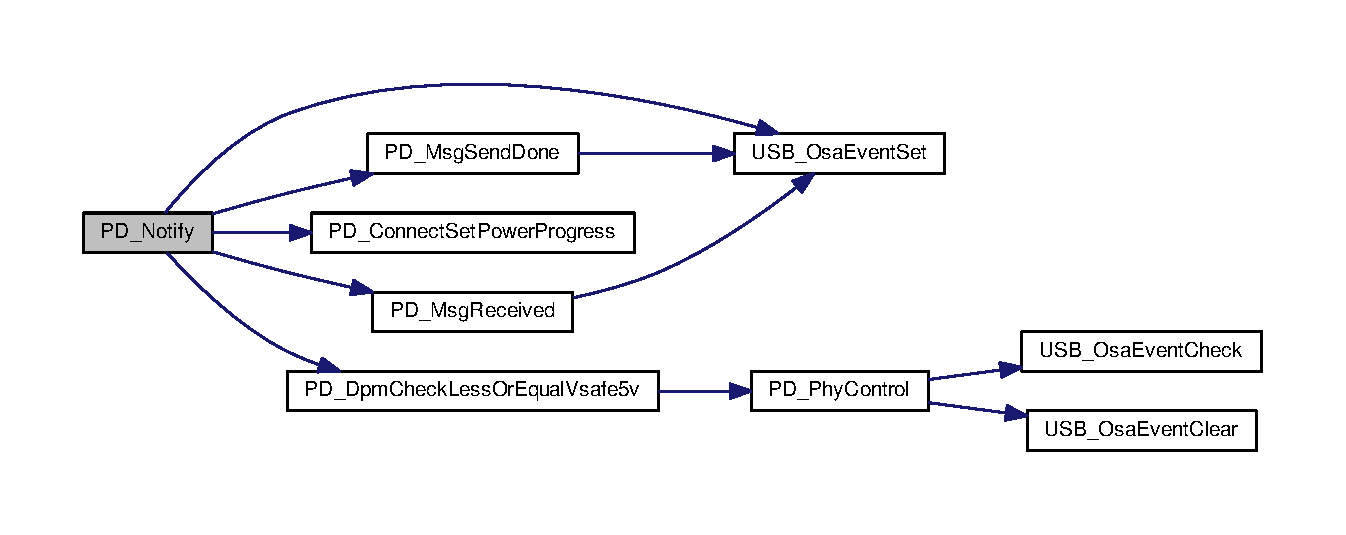
\includegraphics[width=350pt]{group__usb__pd__phy__drv_ga7f7f94758771b173653d27c508c8b33f_cgraph}
\end{center}
\end{figure}




Here is the caller graph for this function\-:
\nopagebreak
\begin{figure}[H]
\begin{center}
\leavevmode
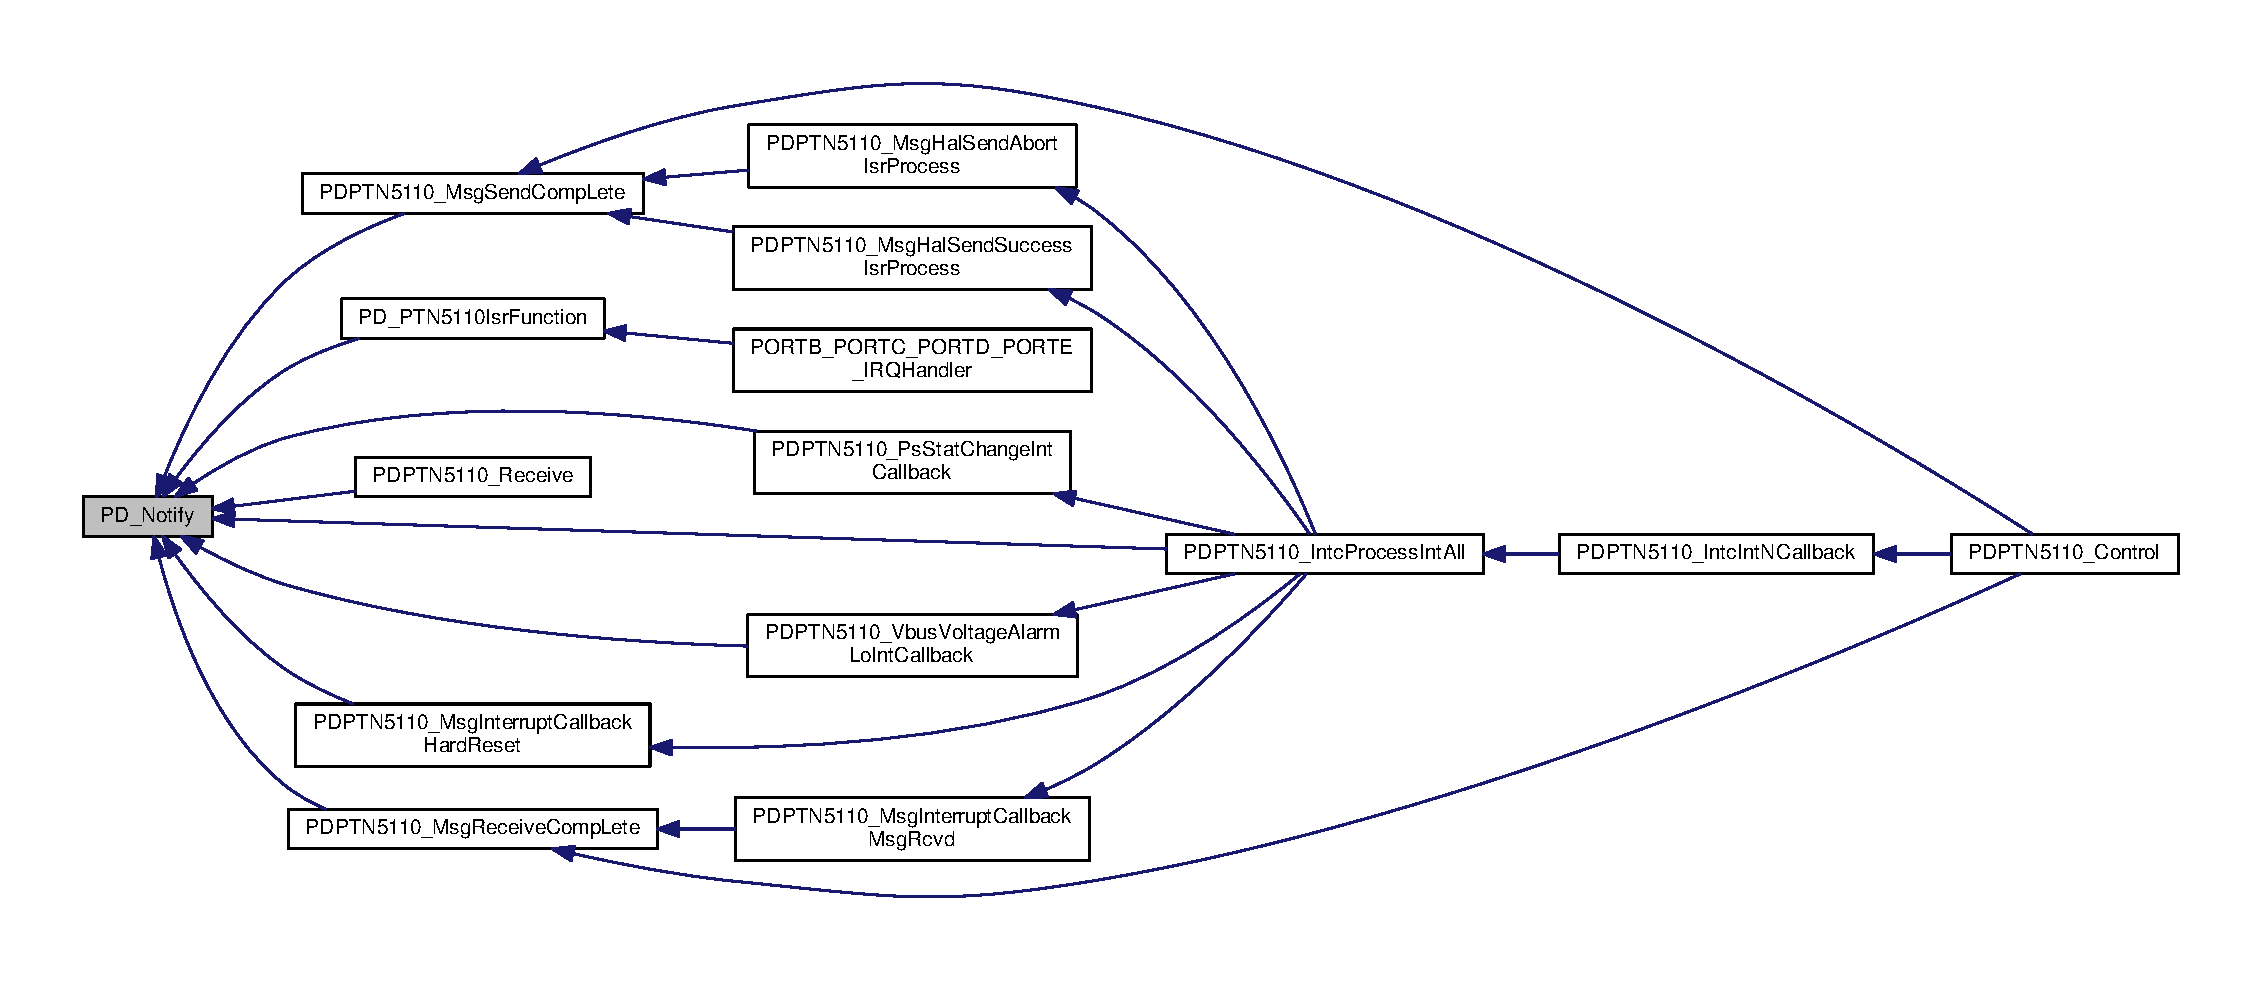
\includegraphics[width=350pt]{group__usb__pd__phy__drv_ga7f7f94758771b173653d27c508c8b33f_icgraph}
\end{center}
\end{figure}



\chapter{Class Documentation}
\hypertarget{struct____pd__phy__tcpc__instance__}{\section{\-\_\-\-\_\-pd\-\_\-phy\-\_\-tcpc\-\_\-instance\-\_\- Struct Reference}
\label{struct____pd__phy__tcpc__instance__}\index{\-\_\-\-\_\-pd\-\_\-phy\-\_\-tcpc\-\_\-instance\-\_\-@{\-\_\-\-\_\-pd\-\_\-phy\-\_\-tcpc\-\_\-instance\-\_\-}}
}


{\ttfamily \#include $<$usb\-\_\-pd\-\_\-ptn5110.\-h$>$}



Collaboration diagram for \-\_\-\-\_\-pd\-\_\-phy\-\_\-tcpc\-\_\-instance\-\_\-\-:
\nopagebreak
\begin{figure}[H]
\begin{center}
\leavevmode
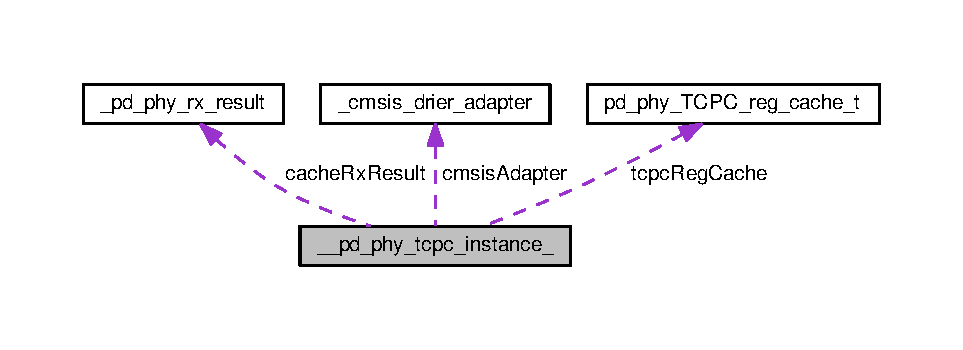
\includegraphics[width=350pt]{struct____pd__phy__tcpc__instance____coll__graph}
\end{center}
\end{figure}
\subsection*{Public Attributes}
\begin{DoxyCompactItemize}
\item 
\hyperlink{group__usb__pd__stack_ga9397835347d48ef48b6b0ecba6312213}{pd\-\_\-handle} \hyperlink{struct____pd__phy__tcpc__instance___ac32468695e40e122402f73f58e2b2883}{pd\-Handle}
\item 
uint8\-\_\-t $\ast$ \hyperlink{struct____pd__phy__tcpc__instance___a8e1d29bc419bff24ef7dce9038a0cbe6}{msg\-Tx\-Buf}
\item 
uint8\-\_\-t \hyperlink{struct____pd__phy__tcpc__instance___ab7f6700604267abb1ae7c89b848038f5}{msg\-Rx\-Cache\-Buf} \mbox{[}32\mbox{]}
\item 
\hyperlink{structpd__phy__TCPC__reg__cache__t}{pd\-\_\-phy\-\_\-\-T\-C\-P\-C\-\_\-reg\-\_\-cache\-\_\-t} \hyperlink{struct____pd__phy__tcpc__instance___aad3c9ce4cbeb9feae002869320f59c43}{tcpc\-Reg\-Cache}
\item 
\hyperlink{group__usb__pd__cmsis__wrapper_ga53daa69dcc6fde0029cec3452c8b58ff}{cmsis\-\_\-driver\-\_\-adapter\-\_\-t} $\ast$ \hyperlink{struct____pd__phy__tcpc__instance___a09664b0949afea262f2c6ca813d1dc47}{cmsis\-Adapter}
\item 
uint8\-\_\-t $\ast$ \hyperlink{struct____pd__phy__tcpc__instance___a7f28556318380a24d677a846ce484a65}{rx\-Data\-Buffer}
\item 
uint32\-\_\-t \hyperlink{struct____pd__phy__tcpc__instance___a3af6de9acc878ce8698441e39dfb52cc}{rx\-Data\-Length}
\item 
volatile \hyperlink{group__usb__pd__phy__drv_gab6924dca8731119eec80f1740a1564eb}{pd\-\_\-phy\-\_\-rx\-\_\-result\-\_\-t} \hyperlink{struct____pd__phy__tcpc__instance___aac4e841aeece50c977507048068e5b71}{cache\-Rx\-Result}
\item 
volatile uint8\-\_\-t \hyperlink{struct____pd__phy__tcpc__instance___aad459891077d4c8217e6ff3a46563a34}{cache\-Rx\-Valid}
\item 
uint8\-\_\-t \hyperlink{struct____pd__phy__tcpc__instance___a6c157191032eff69be9192ca58263192}{occupied}
\item 
uint8\-\_\-t \hyperlink{struct____pd__phy__tcpc__instance___a4dc4e216656e3e2ae311c3e5d9b30f7f}{pd\-Phy\-Id}
\item 
volatile uint8\-\_\-t \hyperlink{struct____pd__phy__tcpc__instance___a50d7547738a416ec3a69cd72896830c8}{fr\-Swap\-Source\-O\-K}
\item 
volatile uint8\-\_\-t \hyperlink{struct____pd__phy__tcpc__instance___a24037bc939fa4ef146806af07f94633d}{msg\-Tx\-Buf\-State}
\item 
uint8\-\_\-t \hyperlink{struct____pd__phy__tcpc__instance___ae7ea8877aeb1575b2965df9314d5a2cf}{prev\-Pwr\-Stat}
\item 
uint8\-\_\-t \hyperlink{struct____pd__phy__tcpc__instance___a3516be0335f933f899fb28a9437f5bdc}{initial\-Cc\-Status}
\item 
uint8\-\_\-t \hyperlink{struct____pd__phy__tcpc__instance___a570de85ac09a6b1c2846340c62ca6db6}{hal\-Wait\-Vsafe0\-V}
\item 
uint8\-\_\-t \hyperlink{struct____pd__phy__tcpc__instance___a4f5e58eba28f763faec84e6cf21f3bec}{hal\-Vsafe5\-V\-Yes}
\item 
uint8\-\_\-t \hyperlink{struct____pd__phy__tcpc__instance___adaf45c602e807d187285f47600ba9f22}{hal\-Vbus\-Yes}
\item 
volatile uint16\-\_\-t \hyperlink{struct____pd__phy__tcpc__instance___acb8b5bda19e51013f2e9b53a5210a49b}{cache\-Ena}
\item 
volatile uint16\-\_\-t \hyperlink{struct____pd__phy__tcpc__instance___a58fe51ff1ebabdf028e6b24925d0d612}{intc\-Last\-Status}
\item 
volatile uint8\-\_\-t \hyperlink{struct____pd__phy__tcpc__instance___a411ad2f7bc90a10a62a5ec1f466a4a97}{used\-C\-C}
\item 
volatile uint8\-\_\-t \hyperlink{struct____pd__phy__tcpc__instance___a12f900cf19375e18339d43ee8ec60b55}{role\-Control\-Updated}
\item 
uint8\-\_\-t \hyperlink{struct____pd__phy__tcpc__instance___af77c96ac21768f2e8a54fad69f97e96f}{phy\-Power\-Role}
\item 
uint8\-\_\-t \hyperlink{struct____pd__phy__tcpc__instance___a5963a6c4377fd4b3782f880eb70a314e}{phy\-Data\-Role}
\item 
uint8\-\_\-t \hyperlink{struct____pd__phy__tcpc__instance___a68e310d1771e6f32f6d1b1b9f5c00aa8}{ams\-Sink\-Tx\-O\-K}
\item 
volatile uint8\-\_\-t \hyperlink{struct____pd__phy__tcpc__instance___a0a78bbebf4ee073519c2250c856c58da}{current\-Stable}
\item 
volatile uint8\-\_\-t \hyperlink{struct____pd__phy__tcpc__instance___aa594b019548753b279b058071e537257}{pwr\-In\-Progress}
\item 
uint8\-\_\-t \hyperlink{struct____pd__phy__tcpc__instance___a19a01f5c9205bebfac2a3514249db1fc}{low\-Power\-State}
\item 
uint8\-\_\-t \hyperlink{struct____pd__phy__tcpc__instance___a95990260c9d5be8724a2feca748ee3da}{tx\-Abort}
\item 
uint8\-\_\-t \hyperlink{struct____pd__phy__tcpc__instance___a6a94c29840da978ce0d5d0da545cf57f}{msg\-Id} \mbox{[}8\mbox{]}
\item 
uint8\-\_\-t \hyperlink{struct____pd__phy__tcpc__instance___a48ed369a0454eb7ee62d935801db2018}{rcv\-Msg\-Id} \mbox{[}8\mbox{]}
\item 
uint8\-\_\-t \hyperlink{struct____pd__phy__tcpc__instance___a2551b07e2795fdd33e05f05dfad8f211}{first\-Msg\-After\-Reset} \mbox{[}8\mbox{]}
\item 
uint8\-\_\-t \hyperlink{struct____pd__phy__tcpc__instance___ab4f0c543ff4b3ad2293c07da59f94aaf}{msg\-Rx\-Sop\-Mask}
\item 
uint8\-\_\-t \hyperlink{struct____pd__phy__tcpc__instance___a3f43dcc28b084f1a3a2d05c3821290d9}{msg\-Tx\-Sop}
\item 
uint8\-\_\-t \hyperlink{struct____pd__phy__tcpc__instance___a4be0d51647641b8fbf79c0307bac4db5}{msg\-A\-M\-S\-State}
\item 
volatile uint8\-\_\-t \hyperlink{struct____pd__phy__tcpc__instance___a2f5f0754a16062bcf9c7572d8c3b5bd7}{tx\-Have}
\item 
volatile uint8\-\_\-t \hyperlink{struct____pd__phy__tcpc__instance___a1e81356f89f625e8c0bd9436e7352fb3}{rx\-Have}
\item 
volatile uint8\-\_\-t \hyperlink{struct____pd__phy__tcpc__instance___a31fe4873d6a4ddce98b3105eccad7cee}{revision}
\end{DoxyCompactItemize}


\subsection{Member Data Documentation}
\hypertarget{struct____pd__phy__tcpc__instance___a68e310d1771e6f32f6d1b1b9f5c00aa8}{\index{\-\_\-\-\_\-pd\-\_\-phy\-\_\-tcpc\-\_\-instance\-\_\-@{\-\_\-\-\_\-pd\-\_\-phy\-\_\-tcpc\-\_\-instance\-\_\-}!ams\-Sink\-Tx\-O\-K@{ams\-Sink\-Tx\-O\-K}}
\index{ams\-Sink\-Tx\-O\-K@{ams\-Sink\-Tx\-O\-K}!__pd_phy_tcpc_instance_@{\-\_\-\-\_\-pd\-\_\-phy\-\_\-tcpc\-\_\-instance\-\_\-}}
\subsubsection[{ams\-Sink\-Tx\-O\-K}]{\setlength{\rightskip}{0pt plus 5cm}uint8\-\_\-t \-\_\-\-\_\-pd\-\_\-phy\-\_\-tcpc\-\_\-instance\-\_\-\-::ams\-Sink\-Tx\-O\-K}}\label{struct____pd__phy__tcpc__instance___a68e310d1771e6f32f6d1b1b9f5c00aa8}
\hypertarget{struct____pd__phy__tcpc__instance___acb8b5bda19e51013f2e9b53a5210a49b}{\index{\-\_\-\-\_\-pd\-\_\-phy\-\_\-tcpc\-\_\-instance\-\_\-@{\-\_\-\-\_\-pd\-\_\-phy\-\_\-tcpc\-\_\-instance\-\_\-}!cache\-Ena@{cache\-Ena}}
\index{cache\-Ena@{cache\-Ena}!__pd_phy_tcpc_instance_@{\-\_\-\-\_\-pd\-\_\-phy\-\_\-tcpc\-\_\-instance\-\_\-}}
\subsubsection[{cache\-Ena}]{\setlength{\rightskip}{0pt plus 5cm}volatile uint16\-\_\-t \-\_\-\-\_\-pd\-\_\-phy\-\_\-tcpc\-\_\-instance\-\_\-\-::cache\-Ena}}\label{struct____pd__phy__tcpc__instance___acb8b5bda19e51013f2e9b53a5210a49b}
\hypertarget{struct____pd__phy__tcpc__instance___aac4e841aeece50c977507048068e5b71}{\index{\-\_\-\-\_\-pd\-\_\-phy\-\_\-tcpc\-\_\-instance\-\_\-@{\-\_\-\-\_\-pd\-\_\-phy\-\_\-tcpc\-\_\-instance\-\_\-}!cache\-Rx\-Result@{cache\-Rx\-Result}}
\index{cache\-Rx\-Result@{cache\-Rx\-Result}!__pd_phy_tcpc_instance_@{\-\_\-\-\_\-pd\-\_\-phy\-\_\-tcpc\-\_\-instance\-\_\-}}
\subsubsection[{cache\-Rx\-Result}]{\setlength{\rightskip}{0pt plus 5cm}volatile {\bf pd\-\_\-phy\-\_\-rx\-\_\-result\-\_\-t} \-\_\-\-\_\-pd\-\_\-phy\-\_\-tcpc\-\_\-instance\-\_\-\-::cache\-Rx\-Result}}\label{struct____pd__phy__tcpc__instance___aac4e841aeece50c977507048068e5b71}
\hypertarget{struct____pd__phy__tcpc__instance___aad459891077d4c8217e6ff3a46563a34}{\index{\-\_\-\-\_\-pd\-\_\-phy\-\_\-tcpc\-\_\-instance\-\_\-@{\-\_\-\-\_\-pd\-\_\-phy\-\_\-tcpc\-\_\-instance\-\_\-}!cache\-Rx\-Valid@{cache\-Rx\-Valid}}
\index{cache\-Rx\-Valid@{cache\-Rx\-Valid}!__pd_phy_tcpc_instance_@{\-\_\-\-\_\-pd\-\_\-phy\-\_\-tcpc\-\_\-instance\-\_\-}}
\subsubsection[{cache\-Rx\-Valid}]{\setlength{\rightskip}{0pt plus 5cm}volatile uint8\-\_\-t \-\_\-\-\_\-pd\-\_\-phy\-\_\-tcpc\-\_\-instance\-\_\-\-::cache\-Rx\-Valid}}\label{struct____pd__phy__tcpc__instance___aad459891077d4c8217e6ff3a46563a34}
\hypertarget{struct____pd__phy__tcpc__instance___a09664b0949afea262f2c6ca813d1dc47}{\index{\-\_\-\-\_\-pd\-\_\-phy\-\_\-tcpc\-\_\-instance\-\_\-@{\-\_\-\-\_\-pd\-\_\-phy\-\_\-tcpc\-\_\-instance\-\_\-}!cmsis\-Adapter@{cmsis\-Adapter}}
\index{cmsis\-Adapter@{cmsis\-Adapter}!__pd_phy_tcpc_instance_@{\-\_\-\-\_\-pd\-\_\-phy\-\_\-tcpc\-\_\-instance\-\_\-}}
\subsubsection[{cmsis\-Adapter}]{\setlength{\rightskip}{0pt plus 5cm}{\bf cmsis\-\_\-driver\-\_\-adapter\-\_\-t}$\ast$ \-\_\-\-\_\-pd\-\_\-phy\-\_\-tcpc\-\_\-instance\-\_\-\-::cmsis\-Adapter}}\label{struct____pd__phy__tcpc__instance___a09664b0949afea262f2c6ca813d1dc47}
\hypertarget{struct____pd__phy__tcpc__instance___a0a78bbebf4ee073519c2250c856c58da}{\index{\-\_\-\-\_\-pd\-\_\-phy\-\_\-tcpc\-\_\-instance\-\_\-@{\-\_\-\-\_\-pd\-\_\-phy\-\_\-tcpc\-\_\-instance\-\_\-}!current\-Stable@{current\-Stable}}
\index{current\-Stable@{current\-Stable}!__pd_phy_tcpc_instance_@{\-\_\-\-\_\-pd\-\_\-phy\-\_\-tcpc\-\_\-instance\-\_\-}}
\subsubsection[{current\-Stable}]{\setlength{\rightskip}{0pt plus 5cm}volatile uint8\-\_\-t \-\_\-\-\_\-pd\-\_\-phy\-\_\-tcpc\-\_\-instance\-\_\-\-::current\-Stable}}\label{struct____pd__phy__tcpc__instance___a0a78bbebf4ee073519c2250c856c58da}
\hypertarget{struct____pd__phy__tcpc__instance___a2551b07e2795fdd33e05f05dfad8f211}{\index{\-\_\-\-\_\-pd\-\_\-phy\-\_\-tcpc\-\_\-instance\-\_\-@{\-\_\-\-\_\-pd\-\_\-phy\-\_\-tcpc\-\_\-instance\-\_\-}!first\-Msg\-After\-Reset@{first\-Msg\-After\-Reset}}
\index{first\-Msg\-After\-Reset@{first\-Msg\-After\-Reset}!__pd_phy_tcpc_instance_@{\-\_\-\-\_\-pd\-\_\-phy\-\_\-tcpc\-\_\-instance\-\_\-}}
\subsubsection[{first\-Msg\-After\-Reset}]{\setlength{\rightskip}{0pt plus 5cm}uint8\-\_\-t \-\_\-\-\_\-pd\-\_\-phy\-\_\-tcpc\-\_\-instance\-\_\-\-::first\-Msg\-After\-Reset\mbox{[}8\mbox{]}}}\label{struct____pd__phy__tcpc__instance___a2551b07e2795fdd33e05f05dfad8f211}
\hypertarget{struct____pd__phy__tcpc__instance___a50d7547738a416ec3a69cd72896830c8}{\index{\-\_\-\-\_\-pd\-\_\-phy\-\_\-tcpc\-\_\-instance\-\_\-@{\-\_\-\-\_\-pd\-\_\-phy\-\_\-tcpc\-\_\-instance\-\_\-}!fr\-Swap\-Source\-O\-K@{fr\-Swap\-Source\-O\-K}}
\index{fr\-Swap\-Source\-O\-K@{fr\-Swap\-Source\-O\-K}!__pd_phy_tcpc_instance_@{\-\_\-\-\_\-pd\-\_\-phy\-\_\-tcpc\-\_\-instance\-\_\-}}
\subsubsection[{fr\-Swap\-Source\-O\-K}]{\setlength{\rightskip}{0pt plus 5cm}volatile uint8\-\_\-t \-\_\-\-\_\-pd\-\_\-phy\-\_\-tcpc\-\_\-instance\-\_\-\-::fr\-Swap\-Source\-O\-K}}\label{struct____pd__phy__tcpc__instance___a50d7547738a416ec3a69cd72896830c8}
\hypertarget{struct____pd__phy__tcpc__instance___adaf45c602e807d187285f47600ba9f22}{\index{\-\_\-\-\_\-pd\-\_\-phy\-\_\-tcpc\-\_\-instance\-\_\-@{\-\_\-\-\_\-pd\-\_\-phy\-\_\-tcpc\-\_\-instance\-\_\-}!hal\-Vbus\-Yes@{hal\-Vbus\-Yes}}
\index{hal\-Vbus\-Yes@{hal\-Vbus\-Yes}!__pd_phy_tcpc_instance_@{\-\_\-\-\_\-pd\-\_\-phy\-\_\-tcpc\-\_\-instance\-\_\-}}
\subsubsection[{hal\-Vbus\-Yes}]{\setlength{\rightskip}{0pt plus 5cm}uint8\-\_\-t \-\_\-\-\_\-pd\-\_\-phy\-\_\-tcpc\-\_\-instance\-\_\-\-::hal\-Vbus\-Yes}}\label{struct____pd__phy__tcpc__instance___adaf45c602e807d187285f47600ba9f22}
\hypertarget{struct____pd__phy__tcpc__instance___a4f5e58eba28f763faec84e6cf21f3bec}{\index{\-\_\-\-\_\-pd\-\_\-phy\-\_\-tcpc\-\_\-instance\-\_\-@{\-\_\-\-\_\-pd\-\_\-phy\-\_\-tcpc\-\_\-instance\-\_\-}!hal\-Vsafe5\-V\-Yes@{hal\-Vsafe5\-V\-Yes}}
\index{hal\-Vsafe5\-V\-Yes@{hal\-Vsafe5\-V\-Yes}!__pd_phy_tcpc_instance_@{\-\_\-\-\_\-pd\-\_\-phy\-\_\-tcpc\-\_\-instance\-\_\-}}
\subsubsection[{hal\-Vsafe5\-V\-Yes}]{\setlength{\rightskip}{0pt plus 5cm}uint8\-\_\-t \-\_\-\-\_\-pd\-\_\-phy\-\_\-tcpc\-\_\-instance\-\_\-\-::hal\-Vsafe5\-V\-Yes}}\label{struct____pd__phy__tcpc__instance___a4f5e58eba28f763faec84e6cf21f3bec}
\hypertarget{struct____pd__phy__tcpc__instance___a570de85ac09a6b1c2846340c62ca6db6}{\index{\-\_\-\-\_\-pd\-\_\-phy\-\_\-tcpc\-\_\-instance\-\_\-@{\-\_\-\-\_\-pd\-\_\-phy\-\_\-tcpc\-\_\-instance\-\_\-}!hal\-Wait\-Vsafe0\-V@{hal\-Wait\-Vsafe0\-V}}
\index{hal\-Wait\-Vsafe0\-V@{hal\-Wait\-Vsafe0\-V}!__pd_phy_tcpc_instance_@{\-\_\-\-\_\-pd\-\_\-phy\-\_\-tcpc\-\_\-instance\-\_\-}}
\subsubsection[{hal\-Wait\-Vsafe0\-V}]{\setlength{\rightskip}{0pt plus 5cm}uint8\-\_\-t \-\_\-\-\_\-pd\-\_\-phy\-\_\-tcpc\-\_\-instance\-\_\-\-::hal\-Wait\-Vsafe0\-V}}\label{struct____pd__phy__tcpc__instance___a570de85ac09a6b1c2846340c62ca6db6}
\hypertarget{struct____pd__phy__tcpc__instance___a3516be0335f933f899fb28a9437f5bdc}{\index{\-\_\-\-\_\-pd\-\_\-phy\-\_\-tcpc\-\_\-instance\-\_\-@{\-\_\-\-\_\-pd\-\_\-phy\-\_\-tcpc\-\_\-instance\-\_\-}!initial\-Cc\-Status@{initial\-Cc\-Status}}
\index{initial\-Cc\-Status@{initial\-Cc\-Status}!__pd_phy_tcpc_instance_@{\-\_\-\-\_\-pd\-\_\-phy\-\_\-tcpc\-\_\-instance\-\_\-}}
\subsubsection[{initial\-Cc\-Status}]{\setlength{\rightskip}{0pt plus 5cm}uint8\-\_\-t \-\_\-\-\_\-pd\-\_\-phy\-\_\-tcpc\-\_\-instance\-\_\-\-::initial\-Cc\-Status}}\label{struct____pd__phy__tcpc__instance___a3516be0335f933f899fb28a9437f5bdc}
\hypertarget{struct____pd__phy__tcpc__instance___a58fe51ff1ebabdf028e6b24925d0d612}{\index{\-\_\-\-\_\-pd\-\_\-phy\-\_\-tcpc\-\_\-instance\-\_\-@{\-\_\-\-\_\-pd\-\_\-phy\-\_\-tcpc\-\_\-instance\-\_\-}!intc\-Last\-Status@{intc\-Last\-Status}}
\index{intc\-Last\-Status@{intc\-Last\-Status}!__pd_phy_tcpc_instance_@{\-\_\-\-\_\-pd\-\_\-phy\-\_\-tcpc\-\_\-instance\-\_\-}}
\subsubsection[{intc\-Last\-Status}]{\setlength{\rightskip}{0pt plus 5cm}volatile uint16\-\_\-t \-\_\-\-\_\-pd\-\_\-phy\-\_\-tcpc\-\_\-instance\-\_\-\-::intc\-Last\-Status}}\label{struct____pd__phy__tcpc__instance___a58fe51ff1ebabdf028e6b24925d0d612}
\hypertarget{struct____pd__phy__tcpc__instance___a19a01f5c9205bebfac2a3514249db1fc}{\index{\-\_\-\-\_\-pd\-\_\-phy\-\_\-tcpc\-\_\-instance\-\_\-@{\-\_\-\-\_\-pd\-\_\-phy\-\_\-tcpc\-\_\-instance\-\_\-}!low\-Power\-State@{low\-Power\-State}}
\index{low\-Power\-State@{low\-Power\-State}!__pd_phy_tcpc_instance_@{\-\_\-\-\_\-pd\-\_\-phy\-\_\-tcpc\-\_\-instance\-\_\-}}
\subsubsection[{low\-Power\-State}]{\setlength{\rightskip}{0pt plus 5cm}uint8\-\_\-t \-\_\-\-\_\-pd\-\_\-phy\-\_\-tcpc\-\_\-instance\-\_\-\-::low\-Power\-State}}\label{struct____pd__phy__tcpc__instance___a19a01f5c9205bebfac2a3514249db1fc}
\hypertarget{struct____pd__phy__tcpc__instance___a4be0d51647641b8fbf79c0307bac4db5}{\index{\-\_\-\-\_\-pd\-\_\-phy\-\_\-tcpc\-\_\-instance\-\_\-@{\-\_\-\-\_\-pd\-\_\-phy\-\_\-tcpc\-\_\-instance\-\_\-}!msg\-A\-M\-S\-State@{msg\-A\-M\-S\-State}}
\index{msg\-A\-M\-S\-State@{msg\-A\-M\-S\-State}!__pd_phy_tcpc_instance_@{\-\_\-\-\_\-pd\-\_\-phy\-\_\-tcpc\-\_\-instance\-\_\-}}
\subsubsection[{msg\-A\-M\-S\-State}]{\setlength{\rightskip}{0pt plus 5cm}uint8\-\_\-t \-\_\-\-\_\-pd\-\_\-phy\-\_\-tcpc\-\_\-instance\-\_\-\-::msg\-A\-M\-S\-State}}\label{struct____pd__phy__tcpc__instance___a4be0d51647641b8fbf79c0307bac4db5}
\hypertarget{struct____pd__phy__tcpc__instance___a6a94c29840da978ce0d5d0da545cf57f}{\index{\-\_\-\-\_\-pd\-\_\-phy\-\_\-tcpc\-\_\-instance\-\_\-@{\-\_\-\-\_\-pd\-\_\-phy\-\_\-tcpc\-\_\-instance\-\_\-}!msg\-Id@{msg\-Id}}
\index{msg\-Id@{msg\-Id}!__pd_phy_tcpc_instance_@{\-\_\-\-\_\-pd\-\_\-phy\-\_\-tcpc\-\_\-instance\-\_\-}}
\subsubsection[{msg\-Id}]{\setlength{\rightskip}{0pt plus 5cm}uint8\-\_\-t \-\_\-\-\_\-pd\-\_\-phy\-\_\-tcpc\-\_\-instance\-\_\-\-::msg\-Id\mbox{[}8\mbox{]}}}\label{struct____pd__phy__tcpc__instance___a6a94c29840da978ce0d5d0da545cf57f}
\hypertarget{struct____pd__phy__tcpc__instance___ab7f6700604267abb1ae7c89b848038f5}{\index{\-\_\-\-\_\-pd\-\_\-phy\-\_\-tcpc\-\_\-instance\-\_\-@{\-\_\-\-\_\-pd\-\_\-phy\-\_\-tcpc\-\_\-instance\-\_\-}!msg\-Rx\-Cache\-Buf@{msg\-Rx\-Cache\-Buf}}
\index{msg\-Rx\-Cache\-Buf@{msg\-Rx\-Cache\-Buf}!__pd_phy_tcpc_instance_@{\-\_\-\-\_\-pd\-\_\-phy\-\_\-tcpc\-\_\-instance\-\_\-}}
\subsubsection[{msg\-Rx\-Cache\-Buf}]{\setlength{\rightskip}{0pt plus 5cm}uint8\-\_\-t \-\_\-\-\_\-pd\-\_\-phy\-\_\-tcpc\-\_\-instance\-\_\-\-::msg\-Rx\-Cache\-Buf\mbox{[}32\mbox{]}}}\label{struct____pd__phy__tcpc__instance___ab7f6700604267abb1ae7c89b848038f5}
\hypertarget{struct____pd__phy__tcpc__instance___ab4f0c543ff4b3ad2293c07da59f94aaf}{\index{\-\_\-\-\_\-pd\-\_\-phy\-\_\-tcpc\-\_\-instance\-\_\-@{\-\_\-\-\_\-pd\-\_\-phy\-\_\-tcpc\-\_\-instance\-\_\-}!msg\-Rx\-Sop\-Mask@{msg\-Rx\-Sop\-Mask}}
\index{msg\-Rx\-Sop\-Mask@{msg\-Rx\-Sop\-Mask}!__pd_phy_tcpc_instance_@{\-\_\-\-\_\-pd\-\_\-phy\-\_\-tcpc\-\_\-instance\-\_\-}}
\subsubsection[{msg\-Rx\-Sop\-Mask}]{\setlength{\rightskip}{0pt plus 5cm}uint8\-\_\-t \-\_\-\-\_\-pd\-\_\-phy\-\_\-tcpc\-\_\-instance\-\_\-\-::msg\-Rx\-Sop\-Mask}}\label{struct____pd__phy__tcpc__instance___ab4f0c543ff4b3ad2293c07da59f94aaf}
\hypertarget{struct____pd__phy__tcpc__instance___a8e1d29bc419bff24ef7dce9038a0cbe6}{\index{\-\_\-\-\_\-pd\-\_\-phy\-\_\-tcpc\-\_\-instance\-\_\-@{\-\_\-\-\_\-pd\-\_\-phy\-\_\-tcpc\-\_\-instance\-\_\-}!msg\-Tx\-Buf@{msg\-Tx\-Buf}}
\index{msg\-Tx\-Buf@{msg\-Tx\-Buf}!__pd_phy_tcpc_instance_@{\-\_\-\-\_\-pd\-\_\-phy\-\_\-tcpc\-\_\-instance\-\_\-}}
\subsubsection[{msg\-Tx\-Buf}]{\setlength{\rightskip}{0pt plus 5cm}uint8\-\_\-t$\ast$ \-\_\-\-\_\-pd\-\_\-phy\-\_\-tcpc\-\_\-instance\-\_\-\-::msg\-Tx\-Buf}}\label{struct____pd__phy__tcpc__instance___a8e1d29bc419bff24ef7dce9038a0cbe6}
\hypertarget{struct____pd__phy__tcpc__instance___a24037bc939fa4ef146806af07f94633d}{\index{\-\_\-\-\_\-pd\-\_\-phy\-\_\-tcpc\-\_\-instance\-\_\-@{\-\_\-\-\_\-pd\-\_\-phy\-\_\-tcpc\-\_\-instance\-\_\-}!msg\-Tx\-Buf\-State@{msg\-Tx\-Buf\-State}}
\index{msg\-Tx\-Buf\-State@{msg\-Tx\-Buf\-State}!__pd_phy_tcpc_instance_@{\-\_\-\-\_\-pd\-\_\-phy\-\_\-tcpc\-\_\-instance\-\_\-}}
\subsubsection[{msg\-Tx\-Buf\-State}]{\setlength{\rightskip}{0pt plus 5cm}volatile uint8\-\_\-t \-\_\-\-\_\-pd\-\_\-phy\-\_\-tcpc\-\_\-instance\-\_\-\-::msg\-Tx\-Buf\-State}}\label{struct____pd__phy__tcpc__instance___a24037bc939fa4ef146806af07f94633d}
\hypertarget{struct____pd__phy__tcpc__instance___a3f43dcc28b084f1a3a2d05c3821290d9}{\index{\-\_\-\-\_\-pd\-\_\-phy\-\_\-tcpc\-\_\-instance\-\_\-@{\-\_\-\-\_\-pd\-\_\-phy\-\_\-tcpc\-\_\-instance\-\_\-}!msg\-Tx\-Sop@{msg\-Tx\-Sop}}
\index{msg\-Tx\-Sop@{msg\-Tx\-Sop}!__pd_phy_tcpc_instance_@{\-\_\-\-\_\-pd\-\_\-phy\-\_\-tcpc\-\_\-instance\-\_\-}}
\subsubsection[{msg\-Tx\-Sop}]{\setlength{\rightskip}{0pt plus 5cm}uint8\-\_\-t \-\_\-\-\_\-pd\-\_\-phy\-\_\-tcpc\-\_\-instance\-\_\-\-::msg\-Tx\-Sop}}\label{struct____pd__phy__tcpc__instance___a3f43dcc28b084f1a3a2d05c3821290d9}
\hypertarget{struct____pd__phy__tcpc__instance___a6c157191032eff69be9192ca58263192}{\index{\-\_\-\-\_\-pd\-\_\-phy\-\_\-tcpc\-\_\-instance\-\_\-@{\-\_\-\-\_\-pd\-\_\-phy\-\_\-tcpc\-\_\-instance\-\_\-}!occupied@{occupied}}
\index{occupied@{occupied}!__pd_phy_tcpc_instance_@{\-\_\-\-\_\-pd\-\_\-phy\-\_\-tcpc\-\_\-instance\-\_\-}}
\subsubsection[{occupied}]{\setlength{\rightskip}{0pt plus 5cm}uint8\-\_\-t \-\_\-\-\_\-pd\-\_\-phy\-\_\-tcpc\-\_\-instance\-\_\-\-::occupied}}\label{struct____pd__phy__tcpc__instance___a6c157191032eff69be9192ca58263192}
\hypertarget{struct____pd__phy__tcpc__instance___ac32468695e40e122402f73f58e2b2883}{\index{\-\_\-\-\_\-pd\-\_\-phy\-\_\-tcpc\-\_\-instance\-\_\-@{\-\_\-\-\_\-pd\-\_\-phy\-\_\-tcpc\-\_\-instance\-\_\-}!pd\-Handle@{pd\-Handle}}
\index{pd\-Handle@{pd\-Handle}!__pd_phy_tcpc_instance_@{\-\_\-\-\_\-pd\-\_\-phy\-\_\-tcpc\-\_\-instance\-\_\-}}
\subsubsection[{pd\-Handle}]{\setlength{\rightskip}{0pt plus 5cm}{\bf pd\-\_\-handle} \-\_\-\-\_\-pd\-\_\-phy\-\_\-tcpc\-\_\-instance\-\_\-\-::pd\-Handle}}\label{struct____pd__phy__tcpc__instance___ac32468695e40e122402f73f58e2b2883}
\hypertarget{struct____pd__phy__tcpc__instance___a4dc4e216656e3e2ae311c3e5d9b30f7f}{\index{\-\_\-\-\_\-pd\-\_\-phy\-\_\-tcpc\-\_\-instance\-\_\-@{\-\_\-\-\_\-pd\-\_\-phy\-\_\-tcpc\-\_\-instance\-\_\-}!pd\-Phy\-Id@{pd\-Phy\-Id}}
\index{pd\-Phy\-Id@{pd\-Phy\-Id}!__pd_phy_tcpc_instance_@{\-\_\-\-\_\-pd\-\_\-phy\-\_\-tcpc\-\_\-instance\-\_\-}}
\subsubsection[{pd\-Phy\-Id}]{\setlength{\rightskip}{0pt plus 5cm}uint8\-\_\-t \-\_\-\-\_\-pd\-\_\-phy\-\_\-tcpc\-\_\-instance\-\_\-\-::pd\-Phy\-Id}}\label{struct____pd__phy__tcpc__instance___a4dc4e216656e3e2ae311c3e5d9b30f7f}
\hypertarget{struct____pd__phy__tcpc__instance___a5963a6c4377fd4b3782f880eb70a314e}{\index{\-\_\-\-\_\-pd\-\_\-phy\-\_\-tcpc\-\_\-instance\-\_\-@{\-\_\-\-\_\-pd\-\_\-phy\-\_\-tcpc\-\_\-instance\-\_\-}!phy\-Data\-Role@{phy\-Data\-Role}}
\index{phy\-Data\-Role@{phy\-Data\-Role}!__pd_phy_tcpc_instance_@{\-\_\-\-\_\-pd\-\_\-phy\-\_\-tcpc\-\_\-instance\-\_\-}}
\subsubsection[{phy\-Data\-Role}]{\setlength{\rightskip}{0pt plus 5cm}uint8\-\_\-t \-\_\-\-\_\-pd\-\_\-phy\-\_\-tcpc\-\_\-instance\-\_\-\-::phy\-Data\-Role}}\label{struct____pd__phy__tcpc__instance___a5963a6c4377fd4b3782f880eb70a314e}
\hypertarget{struct____pd__phy__tcpc__instance___af77c96ac21768f2e8a54fad69f97e96f}{\index{\-\_\-\-\_\-pd\-\_\-phy\-\_\-tcpc\-\_\-instance\-\_\-@{\-\_\-\-\_\-pd\-\_\-phy\-\_\-tcpc\-\_\-instance\-\_\-}!phy\-Power\-Role@{phy\-Power\-Role}}
\index{phy\-Power\-Role@{phy\-Power\-Role}!__pd_phy_tcpc_instance_@{\-\_\-\-\_\-pd\-\_\-phy\-\_\-tcpc\-\_\-instance\-\_\-}}
\subsubsection[{phy\-Power\-Role}]{\setlength{\rightskip}{0pt plus 5cm}uint8\-\_\-t \-\_\-\-\_\-pd\-\_\-phy\-\_\-tcpc\-\_\-instance\-\_\-\-::phy\-Power\-Role}}\label{struct____pd__phy__tcpc__instance___af77c96ac21768f2e8a54fad69f97e96f}
\hypertarget{struct____pd__phy__tcpc__instance___ae7ea8877aeb1575b2965df9314d5a2cf}{\index{\-\_\-\-\_\-pd\-\_\-phy\-\_\-tcpc\-\_\-instance\-\_\-@{\-\_\-\-\_\-pd\-\_\-phy\-\_\-tcpc\-\_\-instance\-\_\-}!prev\-Pwr\-Stat@{prev\-Pwr\-Stat}}
\index{prev\-Pwr\-Stat@{prev\-Pwr\-Stat}!__pd_phy_tcpc_instance_@{\-\_\-\-\_\-pd\-\_\-phy\-\_\-tcpc\-\_\-instance\-\_\-}}
\subsubsection[{prev\-Pwr\-Stat}]{\setlength{\rightskip}{0pt plus 5cm}uint8\-\_\-t \-\_\-\-\_\-pd\-\_\-phy\-\_\-tcpc\-\_\-instance\-\_\-\-::prev\-Pwr\-Stat}}\label{struct____pd__phy__tcpc__instance___ae7ea8877aeb1575b2965df9314d5a2cf}
\hypertarget{struct____pd__phy__tcpc__instance___aa594b019548753b279b058071e537257}{\index{\-\_\-\-\_\-pd\-\_\-phy\-\_\-tcpc\-\_\-instance\-\_\-@{\-\_\-\-\_\-pd\-\_\-phy\-\_\-tcpc\-\_\-instance\-\_\-}!pwr\-In\-Progress@{pwr\-In\-Progress}}
\index{pwr\-In\-Progress@{pwr\-In\-Progress}!__pd_phy_tcpc_instance_@{\-\_\-\-\_\-pd\-\_\-phy\-\_\-tcpc\-\_\-instance\-\_\-}}
\subsubsection[{pwr\-In\-Progress}]{\setlength{\rightskip}{0pt plus 5cm}volatile uint8\-\_\-t \-\_\-\-\_\-pd\-\_\-phy\-\_\-tcpc\-\_\-instance\-\_\-\-::pwr\-In\-Progress}}\label{struct____pd__phy__tcpc__instance___aa594b019548753b279b058071e537257}
\hypertarget{struct____pd__phy__tcpc__instance___a48ed369a0454eb7ee62d935801db2018}{\index{\-\_\-\-\_\-pd\-\_\-phy\-\_\-tcpc\-\_\-instance\-\_\-@{\-\_\-\-\_\-pd\-\_\-phy\-\_\-tcpc\-\_\-instance\-\_\-}!rcv\-Msg\-Id@{rcv\-Msg\-Id}}
\index{rcv\-Msg\-Id@{rcv\-Msg\-Id}!__pd_phy_tcpc_instance_@{\-\_\-\-\_\-pd\-\_\-phy\-\_\-tcpc\-\_\-instance\-\_\-}}
\subsubsection[{rcv\-Msg\-Id}]{\setlength{\rightskip}{0pt plus 5cm}uint8\-\_\-t \-\_\-\-\_\-pd\-\_\-phy\-\_\-tcpc\-\_\-instance\-\_\-\-::rcv\-Msg\-Id\mbox{[}8\mbox{]}}}\label{struct____pd__phy__tcpc__instance___a48ed369a0454eb7ee62d935801db2018}
\hypertarget{struct____pd__phy__tcpc__instance___a31fe4873d6a4ddce98b3105eccad7cee}{\index{\-\_\-\-\_\-pd\-\_\-phy\-\_\-tcpc\-\_\-instance\-\_\-@{\-\_\-\-\_\-pd\-\_\-phy\-\_\-tcpc\-\_\-instance\-\_\-}!revision@{revision}}
\index{revision@{revision}!__pd_phy_tcpc_instance_@{\-\_\-\-\_\-pd\-\_\-phy\-\_\-tcpc\-\_\-instance\-\_\-}}
\subsubsection[{revision}]{\setlength{\rightskip}{0pt plus 5cm}volatile uint8\-\_\-t \-\_\-\-\_\-pd\-\_\-phy\-\_\-tcpc\-\_\-instance\-\_\-\-::revision}}\label{struct____pd__phy__tcpc__instance___a31fe4873d6a4ddce98b3105eccad7cee}
\hypertarget{struct____pd__phy__tcpc__instance___a12f900cf19375e18339d43ee8ec60b55}{\index{\-\_\-\-\_\-pd\-\_\-phy\-\_\-tcpc\-\_\-instance\-\_\-@{\-\_\-\-\_\-pd\-\_\-phy\-\_\-tcpc\-\_\-instance\-\_\-}!role\-Control\-Updated@{role\-Control\-Updated}}
\index{role\-Control\-Updated@{role\-Control\-Updated}!__pd_phy_tcpc_instance_@{\-\_\-\-\_\-pd\-\_\-phy\-\_\-tcpc\-\_\-instance\-\_\-}}
\subsubsection[{role\-Control\-Updated}]{\setlength{\rightskip}{0pt plus 5cm}volatile uint8\-\_\-t \-\_\-\-\_\-pd\-\_\-phy\-\_\-tcpc\-\_\-instance\-\_\-\-::role\-Control\-Updated}}\label{struct____pd__phy__tcpc__instance___a12f900cf19375e18339d43ee8ec60b55}
\hypertarget{struct____pd__phy__tcpc__instance___a7f28556318380a24d677a846ce484a65}{\index{\-\_\-\-\_\-pd\-\_\-phy\-\_\-tcpc\-\_\-instance\-\_\-@{\-\_\-\-\_\-pd\-\_\-phy\-\_\-tcpc\-\_\-instance\-\_\-}!rx\-Data\-Buffer@{rx\-Data\-Buffer}}
\index{rx\-Data\-Buffer@{rx\-Data\-Buffer}!__pd_phy_tcpc_instance_@{\-\_\-\-\_\-pd\-\_\-phy\-\_\-tcpc\-\_\-instance\-\_\-}}
\subsubsection[{rx\-Data\-Buffer}]{\setlength{\rightskip}{0pt plus 5cm}uint8\-\_\-t$\ast$ \-\_\-\-\_\-pd\-\_\-phy\-\_\-tcpc\-\_\-instance\-\_\-\-::rx\-Data\-Buffer}}\label{struct____pd__phy__tcpc__instance___a7f28556318380a24d677a846ce484a65}
\hypertarget{struct____pd__phy__tcpc__instance___a3af6de9acc878ce8698441e39dfb52cc}{\index{\-\_\-\-\_\-pd\-\_\-phy\-\_\-tcpc\-\_\-instance\-\_\-@{\-\_\-\-\_\-pd\-\_\-phy\-\_\-tcpc\-\_\-instance\-\_\-}!rx\-Data\-Length@{rx\-Data\-Length}}
\index{rx\-Data\-Length@{rx\-Data\-Length}!__pd_phy_tcpc_instance_@{\-\_\-\-\_\-pd\-\_\-phy\-\_\-tcpc\-\_\-instance\-\_\-}}
\subsubsection[{rx\-Data\-Length}]{\setlength{\rightskip}{0pt plus 5cm}uint32\-\_\-t \-\_\-\-\_\-pd\-\_\-phy\-\_\-tcpc\-\_\-instance\-\_\-\-::rx\-Data\-Length}}\label{struct____pd__phy__tcpc__instance___a3af6de9acc878ce8698441e39dfb52cc}
\hypertarget{struct____pd__phy__tcpc__instance___a1e81356f89f625e8c0bd9436e7352fb3}{\index{\-\_\-\-\_\-pd\-\_\-phy\-\_\-tcpc\-\_\-instance\-\_\-@{\-\_\-\-\_\-pd\-\_\-phy\-\_\-tcpc\-\_\-instance\-\_\-}!rx\-Have@{rx\-Have}}
\index{rx\-Have@{rx\-Have}!__pd_phy_tcpc_instance_@{\-\_\-\-\_\-pd\-\_\-phy\-\_\-tcpc\-\_\-instance\-\_\-}}
\subsubsection[{rx\-Have}]{\setlength{\rightskip}{0pt plus 5cm}volatile uint8\-\_\-t \-\_\-\-\_\-pd\-\_\-phy\-\_\-tcpc\-\_\-instance\-\_\-\-::rx\-Have}}\label{struct____pd__phy__tcpc__instance___a1e81356f89f625e8c0bd9436e7352fb3}
\hypertarget{struct____pd__phy__tcpc__instance___aad3c9ce4cbeb9feae002869320f59c43}{\index{\-\_\-\-\_\-pd\-\_\-phy\-\_\-tcpc\-\_\-instance\-\_\-@{\-\_\-\-\_\-pd\-\_\-phy\-\_\-tcpc\-\_\-instance\-\_\-}!tcpc\-Reg\-Cache@{tcpc\-Reg\-Cache}}
\index{tcpc\-Reg\-Cache@{tcpc\-Reg\-Cache}!__pd_phy_tcpc_instance_@{\-\_\-\-\_\-pd\-\_\-phy\-\_\-tcpc\-\_\-instance\-\_\-}}
\subsubsection[{tcpc\-Reg\-Cache}]{\setlength{\rightskip}{0pt plus 5cm}{\bf pd\-\_\-phy\-\_\-\-T\-C\-P\-C\-\_\-reg\-\_\-cache\-\_\-t} \-\_\-\-\_\-pd\-\_\-phy\-\_\-tcpc\-\_\-instance\-\_\-\-::tcpc\-Reg\-Cache}}\label{struct____pd__phy__tcpc__instance___aad3c9ce4cbeb9feae002869320f59c43}
\hypertarget{struct____pd__phy__tcpc__instance___a95990260c9d5be8724a2feca748ee3da}{\index{\-\_\-\-\_\-pd\-\_\-phy\-\_\-tcpc\-\_\-instance\-\_\-@{\-\_\-\-\_\-pd\-\_\-phy\-\_\-tcpc\-\_\-instance\-\_\-}!tx\-Abort@{tx\-Abort}}
\index{tx\-Abort@{tx\-Abort}!__pd_phy_tcpc_instance_@{\-\_\-\-\_\-pd\-\_\-phy\-\_\-tcpc\-\_\-instance\-\_\-}}
\subsubsection[{tx\-Abort}]{\setlength{\rightskip}{0pt plus 5cm}uint8\-\_\-t \-\_\-\-\_\-pd\-\_\-phy\-\_\-tcpc\-\_\-instance\-\_\-\-::tx\-Abort}}\label{struct____pd__phy__tcpc__instance___a95990260c9d5be8724a2feca748ee3da}
\hypertarget{struct____pd__phy__tcpc__instance___a2f5f0754a16062bcf9c7572d8c3b5bd7}{\index{\-\_\-\-\_\-pd\-\_\-phy\-\_\-tcpc\-\_\-instance\-\_\-@{\-\_\-\-\_\-pd\-\_\-phy\-\_\-tcpc\-\_\-instance\-\_\-}!tx\-Have@{tx\-Have}}
\index{tx\-Have@{tx\-Have}!__pd_phy_tcpc_instance_@{\-\_\-\-\_\-pd\-\_\-phy\-\_\-tcpc\-\_\-instance\-\_\-}}
\subsubsection[{tx\-Have}]{\setlength{\rightskip}{0pt plus 5cm}volatile uint8\-\_\-t \-\_\-\-\_\-pd\-\_\-phy\-\_\-tcpc\-\_\-instance\-\_\-\-::tx\-Have}}\label{struct____pd__phy__tcpc__instance___a2f5f0754a16062bcf9c7572d8c3b5bd7}
\hypertarget{struct____pd__phy__tcpc__instance___a411ad2f7bc90a10a62a5ec1f466a4a97}{\index{\-\_\-\-\_\-pd\-\_\-phy\-\_\-tcpc\-\_\-instance\-\_\-@{\-\_\-\-\_\-pd\-\_\-phy\-\_\-tcpc\-\_\-instance\-\_\-}!used\-C\-C@{used\-C\-C}}
\index{used\-C\-C@{used\-C\-C}!__pd_phy_tcpc_instance_@{\-\_\-\-\_\-pd\-\_\-phy\-\_\-tcpc\-\_\-instance\-\_\-}}
\subsubsection[{used\-C\-C}]{\setlength{\rightskip}{0pt plus 5cm}volatile uint8\-\_\-t \-\_\-\-\_\-pd\-\_\-phy\-\_\-tcpc\-\_\-instance\-\_\-\-::used\-C\-C}}\label{struct____pd__phy__tcpc__instance___a411ad2f7bc90a10a62a5ec1f466a4a97}


The documentation for this struct was generated from the following file\-:\begin{DoxyCompactItemize}
\item 
pd/ptn5110/\hyperlink{usb__pd__ptn5110_8h}{usb\-\_\-pd\-\_\-ptn5110.\-h}\end{DoxyCompactItemize}

\hypertarget{struct__cmsis__drier__adapter}{\section{\-\_\-cmsis\-\_\-drier\-\_\-adapter Struct Reference}
\label{struct__cmsis__drier__adapter}\index{\-\_\-cmsis\-\_\-drier\-\_\-adapter@{\-\_\-cmsis\-\_\-drier\-\_\-adapter}}
}


{\ttfamily \#include $<$usb\-\_\-cmsis\-\_\-wrapper.\-h$>$}

\subsection*{Public Attributes}
\begin{DoxyCompactItemize}
\item 
\hyperlink{group__usb__os__abstraction_gad259d0dfe125b11cccaf93163ef915fd}{usb\-\_\-osa\-\_\-mutex\-\_\-handle} \hyperlink{struct__cmsis__drier__adapter_a952d05d8262ef9aebfa6ca9c4d62fe46}{cmsis\-Mutex}
\item 
void $\ast$ \hyperlink{struct__cmsis__drier__adapter_a41bdda4fa1a6cae13f89934bf67c7449}{cmsis\-Interface}
\item 
void $\ast$ \hyperlink{struct__cmsis__drier__adapter_a3d93d5a2f3f34c0064bfbe5a4cf093a0}{callback}
\item 
uint32\-\_\-t \hyperlink{struct__cmsis__drier__adapter_ac81cbf4cbf2ee30a3f3a74b39a6d8780}{spi\-P\-C\-S}
\item 
uint16\-\_\-t \hyperlink{struct__cmsis__drier__adapter_ab9edc386a490908a453990755f01c77b}{i2c\-Address}
\item 
uint8\-\_\-t \hyperlink{struct__cmsis__drier__adapter_ad4d980a94b8a1c3d88331a2577435db4}{occupied}
\item 
uint8\-\_\-t \hyperlink{struct__cmsis__drier__adapter_a51a572fa7a648387cf481b45b862457c}{interface}
\item 
volatile uint8\-\_\-t \hyperlink{struct__cmsis__drier__adapter_a262a2f72787adfa5fddbb085c9428feb}{data\-Buffer} \mbox{[}32\mbox{]}
\item 
volatile uint8\-\_\-t \hyperlink{struct__cmsis__drier__adapter_afcd5fc386d2b9d3c3ba425e8360f741b}{cmsis\-State}
\item 
volatile uint8\-\_\-t \hyperlink{struct__cmsis__drier__adapter_a4197e11173243ee2211120a5073ea53a}{cmsis\-Result}
\item 
volatile uint8\-\_\-t \hyperlink{struct__cmsis__drier__adapter_ad8a1c951411d7534456c822924622806}{cmsis\-Try}
\end{DoxyCompactItemize}


\subsection{Member Data Documentation}
\hypertarget{struct__cmsis__drier__adapter_a3d93d5a2f3f34c0064bfbe5a4cf093a0}{\index{\-\_\-cmsis\-\_\-drier\-\_\-adapter@{\-\_\-cmsis\-\_\-drier\-\_\-adapter}!callback@{callback}}
\index{callback@{callback}!_cmsis_drier_adapter@{\-\_\-cmsis\-\_\-drier\-\_\-adapter}}
\subsubsection[{callback}]{\setlength{\rightskip}{0pt plus 5cm}void$\ast$ \-\_\-cmsis\-\_\-drier\-\_\-adapter\-::callback}}\label{struct__cmsis__drier__adapter_a3d93d5a2f3f34c0064bfbe5a4cf093a0}
\hypertarget{struct__cmsis__drier__adapter_a41bdda4fa1a6cae13f89934bf67c7449}{\index{\-\_\-cmsis\-\_\-drier\-\_\-adapter@{\-\_\-cmsis\-\_\-drier\-\_\-adapter}!cmsis\-Interface@{cmsis\-Interface}}
\index{cmsis\-Interface@{cmsis\-Interface}!_cmsis_drier_adapter@{\-\_\-cmsis\-\_\-drier\-\_\-adapter}}
\subsubsection[{cmsis\-Interface}]{\setlength{\rightskip}{0pt plus 5cm}void$\ast$ \-\_\-cmsis\-\_\-drier\-\_\-adapter\-::cmsis\-Interface}}\label{struct__cmsis__drier__adapter_a41bdda4fa1a6cae13f89934bf67c7449}
\hypertarget{struct__cmsis__drier__adapter_a952d05d8262ef9aebfa6ca9c4d62fe46}{\index{\-\_\-cmsis\-\_\-drier\-\_\-adapter@{\-\_\-cmsis\-\_\-drier\-\_\-adapter}!cmsis\-Mutex@{cmsis\-Mutex}}
\index{cmsis\-Mutex@{cmsis\-Mutex}!_cmsis_drier_adapter@{\-\_\-cmsis\-\_\-drier\-\_\-adapter}}
\subsubsection[{cmsis\-Mutex}]{\setlength{\rightskip}{0pt plus 5cm}{\bf usb\-\_\-osa\-\_\-mutex\-\_\-handle} \-\_\-cmsis\-\_\-drier\-\_\-adapter\-::cmsis\-Mutex}}\label{struct__cmsis__drier__adapter_a952d05d8262ef9aebfa6ca9c4d62fe46}
\hypertarget{struct__cmsis__drier__adapter_a4197e11173243ee2211120a5073ea53a}{\index{\-\_\-cmsis\-\_\-drier\-\_\-adapter@{\-\_\-cmsis\-\_\-drier\-\_\-adapter}!cmsis\-Result@{cmsis\-Result}}
\index{cmsis\-Result@{cmsis\-Result}!_cmsis_drier_adapter@{\-\_\-cmsis\-\_\-drier\-\_\-adapter}}
\subsubsection[{cmsis\-Result}]{\setlength{\rightskip}{0pt plus 5cm}volatile uint8\-\_\-t \-\_\-cmsis\-\_\-drier\-\_\-adapter\-::cmsis\-Result}}\label{struct__cmsis__drier__adapter_a4197e11173243ee2211120a5073ea53a}
\hypertarget{struct__cmsis__drier__adapter_afcd5fc386d2b9d3c3ba425e8360f741b}{\index{\-\_\-cmsis\-\_\-drier\-\_\-adapter@{\-\_\-cmsis\-\_\-drier\-\_\-adapter}!cmsis\-State@{cmsis\-State}}
\index{cmsis\-State@{cmsis\-State}!_cmsis_drier_adapter@{\-\_\-cmsis\-\_\-drier\-\_\-adapter}}
\subsubsection[{cmsis\-State}]{\setlength{\rightskip}{0pt plus 5cm}volatile uint8\-\_\-t \-\_\-cmsis\-\_\-drier\-\_\-adapter\-::cmsis\-State}}\label{struct__cmsis__drier__adapter_afcd5fc386d2b9d3c3ba425e8360f741b}
\hypertarget{struct__cmsis__drier__adapter_ad8a1c951411d7534456c822924622806}{\index{\-\_\-cmsis\-\_\-drier\-\_\-adapter@{\-\_\-cmsis\-\_\-drier\-\_\-adapter}!cmsis\-Try@{cmsis\-Try}}
\index{cmsis\-Try@{cmsis\-Try}!_cmsis_drier_adapter@{\-\_\-cmsis\-\_\-drier\-\_\-adapter}}
\subsubsection[{cmsis\-Try}]{\setlength{\rightskip}{0pt plus 5cm}volatile uint8\-\_\-t \-\_\-cmsis\-\_\-drier\-\_\-adapter\-::cmsis\-Try}}\label{struct__cmsis__drier__adapter_ad8a1c951411d7534456c822924622806}
\hypertarget{struct__cmsis__drier__adapter_a262a2f72787adfa5fddbb085c9428feb}{\index{\-\_\-cmsis\-\_\-drier\-\_\-adapter@{\-\_\-cmsis\-\_\-drier\-\_\-adapter}!data\-Buffer@{data\-Buffer}}
\index{data\-Buffer@{data\-Buffer}!_cmsis_drier_adapter@{\-\_\-cmsis\-\_\-drier\-\_\-adapter}}
\subsubsection[{data\-Buffer}]{\setlength{\rightskip}{0pt plus 5cm}volatile uint8\-\_\-t \-\_\-cmsis\-\_\-drier\-\_\-adapter\-::data\-Buffer\mbox{[}32\mbox{]}}}\label{struct__cmsis__drier__adapter_a262a2f72787adfa5fddbb085c9428feb}
\hypertarget{struct__cmsis__drier__adapter_ab9edc386a490908a453990755f01c77b}{\index{\-\_\-cmsis\-\_\-drier\-\_\-adapter@{\-\_\-cmsis\-\_\-drier\-\_\-adapter}!i2c\-Address@{i2c\-Address}}
\index{i2c\-Address@{i2c\-Address}!_cmsis_drier_adapter@{\-\_\-cmsis\-\_\-drier\-\_\-adapter}}
\subsubsection[{i2c\-Address}]{\setlength{\rightskip}{0pt plus 5cm}uint16\-\_\-t \-\_\-cmsis\-\_\-drier\-\_\-adapter\-::i2c\-Address}}\label{struct__cmsis__drier__adapter_ab9edc386a490908a453990755f01c77b}
\hypertarget{struct__cmsis__drier__adapter_a51a572fa7a648387cf481b45b862457c}{\index{\-\_\-cmsis\-\_\-drier\-\_\-adapter@{\-\_\-cmsis\-\_\-drier\-\_\-adapter}!interface@{interface}}
\index{interface@{interface}!_cmsis_drier_adapter@{\-\_\-cmsis\-\_\-drier\-\_\-adapter}}
\subsubsection[{interface}]{\setlength{\rightskip}{0pt plus 5cm}uint8\-\_\-t \-\_\-cmsis\-\_\-drier\-\_\-adapter\-::interface}}\label{struct__cmsis__drier__adapter_a51a572fa7a648387cf481b45b862457c}
\hypertarget{struct__cmsis__drier__adapter_ad4d980a94b8a1c3d88331a2577435db4}{\index{\-\_\-cmsis\-\_\-drier\-\_\-adapter@{\-\_\-cmsis\-\_\-drier\-\_\-adapter}!occupied@{occupied}}
\index{occupied@{occupied}!_cmsis_drier_adapter@{\-\_\-cmsis\-\_\-drier\-\_\-adapter}}
\subsubsection[{occupied}]{\setlength{\rightskip}{0pt plus 5cm}uint8\-\_\-t \-\_\-cmsis\-\_\-drier\-\_\-adapter\-::occupied}}\label{struct__cmsis__drier__adapter_ad4d980a94b8a1c3d88331a2577435db4}
\hypertarget{struct__cmsis__drier__adapter_ac81cbf4cbf2ee30a3f3a74b39a6d8780}{\index{\-\_\-cmsis\-\_\-drier\-\_\-adapter@{\-\_\-cmsis\-\_\-drier\-\_\-adapter}!spi\-P\-C\-S@{spi\-P\-C\-S}}
\index{spi\-P\-C\-S@{spi\-P\-C\-S}!_cmsis_drier_adapter@{\-\_\-cmsis\-\_\-drier\-\_\-adapter}}
\subsubsection[{spi\-P\-C\-S}]{\setlength{\rightskip}{0pt plus 5cm}uint32\-\_\-t \-\_\-cmsis\-\_\-drier\-\_\-adapter\-::spi\-P\-C\-S}}\label{struct__cmsis__drier__adapter_ac81cbf4cbf2ee30a3f3a74b39a6d8780}


The documentation for this struct was generated from the following file\-:\begin{DoxyCompactItemize}
\item 
pd/cmsis\-\_\-wrapper/\hyperlink{usb__cmsis__wrapper_8h}{usb\-\_\-cmsis\-\_\-wrapper.\-h}\end{DoxyCompactItemize}

\hypertarget{struct__pd__alert__data__object}{\section{\-\_\-pd\-\_\-alert\-\_\-data\-\_\-object Struct Reference}
\label{struct__pd__alert__data__object}\index{\-\_\-pd\-\_\-alert\-\_\-data\-\_\-object@{\-\_\-pd\-\_\-alert\-\_\-data\-\_\-object}}
}


{\ttfamily \#include $<$pd\-\_\-app.\-h$>$}

\subsection*{Public Attributes}
\begin{DoxyCompactItemize}
\item 
\begin{tabbing}
xx\=xx\=xx\=xx\=xx\=xx\=xx\=xx\=xx\=\kill
union \{\\
\>uint32\_t \hyperlink{struct__pd__alert__data__object_aed9a5657c490967d07dd7961217bc0f2}{alertValue}\\
\>struct \{\\
\>\>uint32\_t \hyperlink{struct__pd__alert__data__object_a23d29e1d570b84c87f3ff7832fc282f4}{reserved}: 16\\
\>\>uint32\_t \hyperlink{struct__pd__alert__data__object_ab4e7f83416c6dda7638828545fa92109}{hostSwappableBatteries}: 4\\
\>\>uint32\_t \hyperlink{struct__pd__alert__data__object_aece8b77da3ae31996a4aad59924f47f7}{fixedBatteries}: 4\\
\>\>uint32\_t \hyperlink{struct__pd__alert__data__object_ad73d27b0e318aafc2aeb84ab5eb487b2}{typeOfAlert}: 8\\
\>\} \hyperlink{struct__pd__alert__data__object_a2cd260346b89e8818ac9a0fe06a69297}{bitFields}\\
\}; \\

\end{tabbing}\item 
\begin{tabbing}
xx\=xx\=xx\=xx\=xx\=xx\=xx\=xx\=xx\=\kill
union \{\\
\>uint32\_t \hyperlink{struct__pd__alert__data__object_aed9a5657c490967d07dd7961217bc0f2}{alertValue}\\
\>struct \{\\
\>\>uint32\_t \hyperlink{struct__pd__alert__data__object_a23d29e1d570b84c87f3ff7832fc282f4}{reserved}: 16\\
\>\>uint32\_t \hyperlink{struct__pd__alert__data__object_ab4e7f83416c6dda7638828545fa92109}{hostSwappableBatteries}: 4\\
\>\>uint32\_t \hyperlink{struct__pd__alert__data__object_aece8b77da3ae31996a4aad59924f47f7}{fixedBatteries}: 4\\
\>\>uint32\_t \hyperlink{struct__pd__alert__data__object_ad73d27b0e318aafc2aeb84ab5eb487b2}{typeOfAlert}: 8\\
\>\} \hyperlink{struct__pd__alert__data__object_a34c4d1f20393010bd2924cca9cab1bde}{bitFields}\\
\}; \\

\end{tabbing}\item 
\begin{tabbing}
xx\=xx\=xx\=xx\=xx\=xx\=xx\=xx\=xx\=\kill
union \{\\
\>uint32\_t \hyperlink{struct__pd__alert__data__object_aed9a5657c490967d07dd7961217bc0f2}{alertValue}\\
\>struct \{\\
\>\>uint32\_t \hyperlink{struct__pd__alert__data__object_a23d29e1d570b84c87f3ff7832fc282f4}{reserved}: 16\\
\>\>uint32\_t \hyperlink{struct__pd__alert__data__object_ab4e7f83416c6dda7638828545fa92109}{hostSwappableBatteries}: 4\\
\>\>uint32\_t \hyperlink{struct__pd__alert__data__object_aece8b77da3ae31996a4aad59924f47f7}{fixedBatteries}: 4\\
\>\>uint32\_t \hyperlink{struct__pd__alert__data__object_ad73d27b0e318aafc2aeb84ab5eb487b2}{typeOfAlert}: 8\\
\>\} \hyperlink{struct__pd__alert__data__object_a73b0e792258da5268f6fc612e1e7617b}{bitFields}\\
\}; \\

\end{tabbing}\end{DoxyCompactItemize}


\subsection{Member Data Documentation}
\hypertarget{struct__pd__alert__data__object_a7afcdf0544e42184994609713fb3cdbe}{\subsubsection[{"@1}]{\setlength{\rightskip}{0pt plus 5cm}union \{ ... \} }}\label{struct__pd__alert__data__object_a7afcdf0544e42184994609713fb3cdbe}
\hypertarget{struct__pd__alert__data__object_aabc4365931c292cf5604416fabb2d439}{\subsubsection[{"@13}]{\setlength{\rightskip}{0pt plus 5cm}union \{ ... \} }}\label{struct__pd__alert__data__object_aabc4365931c292cf5604416fabb2d439}
\hypertarget{struct__pd__alert__data__object_a4d3c08a0a6105e30c73fd2ab96f4890f}{\subsubsection[{"@7}]{\setlength{\rightskip}{0pt plus 5cm}union \{ ... \} }}\label{struct__pd__alert__data__object_a4d3c08a0a6105e30c73fd2ab96f4890f}
\hypertarget{struct__pd__alert__data__object_aed9a5657c490967d07dd7961217bc0f2}{\index{\-\_\-pd\-\_\-alert\-\_\-data\-\_\-object@{\-\_\-pd\-\_\-alert\-\_\-data\-\_\-object}!alert\-Value@{alert\-Value}}
\index{alert\-Value@{alert\-Value}!_pd_alert_data_object@{\-\_\-pd\-\_\-alert\-\_\-data\-\_\-object}}
\subsubsection[{alert\-Value}]{\setlength{\rightskip}{0pt plus 5cm}uint32\-\_\-t \-\_\-pd\-\_\-alert\-\_\-data\-\_\-object\-::alert\-Value}}\label{struct__pd__alert__data__object_aed9a5657c490967d07dd7961217bc0f2}
\hypertarget{struct__pd__alert__data__object_a73b0e792258da5268f6fc612e1e7617b}{\index{\-\_\-pd\-\_\-alert\-\_\-data\-\_\-object@{\-\_\-pd\-\_\-alert\-\_\-data\-\_\-object}!bit\-Fields@{bit\-Fields}}
\index{bit\-Fields@{bit\-Fields}!_pd_alert_data_object@{\-\_\-pd\-\_\-alert\-\_\-data\-\_\-object}}
\subsubsection[{bit\-Fields}]{\setlength{\rightskip}{0pt plus 5cm}struct \{ ... \}   \-\_\-pd\-\_\-alert\-\_\-data\-\_\-object\-::bit\-Fields}}\label{struct__pd__alert__data__object_a73b0e792258da5268f6fc612e1e7617b}
\hypertarget{struct__pd__alert__data__object_a2cd260346b89e8818ac9a0fe06a69297}{\index{\-\_\-pd\-\_\-alert\-\_\-data\-\_\-object@{\-\_\-pd\-\_\-alert\-\_\-data\-\_\-object}!bit\-Fields@{bit\-Fields}}
\index{bit\-Fields@{bit\-Fields}!_pd_alert_data_object@{\-\_\-pd\-\_\-alert\-\_\-data\-\_\-object}}
\subsubsection[{bit\-Fields}]{\setlength{\rightskip}{0pt plus 5cm}struct \{ ... \}   \-\_\-pd\-\_\-alert\-\_\-data\-\_\-object\-::bit\-Fields}}\label{struct__pd__alert__data__object_a2cd260346b89e8818ac9a0fe06a69297}
\hypertarget{struct__pd__alert__data__object_a34c4d1f20393010bd2924cca9cab1bde}{\index{\-\_\-pd\-\_\-alert\-\_\-data\-\_\-object@{\-\_\-pd\-\_\-alert\-\_\-data\-\_\-object}!bit\-Fields@{bit\-Fields}}
\index{bit\-Fields@{bit\-Fields}!_pd_alert_data_object@{\-\_\-pd\-\_\-alert\-\_\-data\-\_\-object}}
\subsubsection[{bit\-Fields}]{\setlength{\rightskip}{0pt plus 5cm}struct \{ ... \}   \-\_\-pd\-\_\-alert\-\_\-data\-\_\-object\-::bit\-Fields}}\label{struct__pd__alert__data__object_a34c4d1f20393010bd2924cca9cab1bde}
\hypertarget{struct__pd__alert__data__object_aece8b77da3ae31996a4aad59924f47f7}{\index{\-\_\-pd\-\_\-alert\-\_\-data\-\_\-object@{\-\_\-pd\-\_\-alert\-\_\-data\-\_\-object}!fixed\-Batteries@{fixed\-Batteries}}
\index{fixed\-Batteries@{fixed\-Batteries}!_pd_alert_data_object@{\-\_\-pd\-\_\-alert\-\_\-data\-\_\-object}}
\subsubsection[{fixed\-Batteries}]{\setlength{\rightskip}{0pt plus 5cm}uint32\-\_\-t \-\_\-pd\-\_\-alert\-\_\-data\-\_\-object\-::fixed\-Batteries}}\label{struct__pd__alert__data__object_aece8b77da3ae31996a4aad59924f47f7}
\hypertarget{struct__pd__alert__data__object_ab4e7f83416c6dda7638828545fa92109}{\index{\-\_\-pd\-\_\-alert\-\_\-data\-\_\-object@{\-\_\-pd\-\_\-alert\-\_\-data\-\_\-object}!host\-Swappable\-Batteries@{host\-Swappable\-Batteries}}
\index{host\-Swappable\-Batteries@{host\-Swappable\-Batteries}!_pd_alert_data_object@{\-\_\-pd\-\_\-alert\-\_\-data\-\_\-object}}
\subsubsection[{host\-Swappable\-Batteries}]{\setlength{\rightskip}{0pt plus 5cm}uint32\-\_\-t \-\_\-pd\-\_\-alert\-\_\-data\-\_\-object\-::host\-Swappable\-Batteries}}\label{struct__pd__alert__data__object_ab4e7f83416c6dda7638828545fa92109}
\hypertarget{struct__pd__alert__data__object_a23d29e1d570b84c87f3ff7832fc282f4}{\index{\-\_\-pd\-\_\-alert\-\_\-data\-\_\-object@{\-\_\-pd\-\_\-alert\-\_\-data\-\_\-object}!reserved@{reserved}}
\index{reserved@{reserved}!_pd_alert_data_object@{\-\_\-pd\-\_\-alert\-\_\-data\-\_\-object}}
\subsubsection[{reserved}]{\setlength{\rightskip}{0pt plus 5cm}uint32\-\_\-t \-\_\-pd\-\_\-alert\-\_\-data\-\_\-object\-::reserved}}\label{struct__pd__alert__data__object_a23d29e1d570b84c87f3ff7832fc282f4}
\hypertarget{struct__pd__alert__data__object_ad73d27b0e318aafc2aeb84ab5eb487b2}{\index{\-\_\-pd\-\_\-alert\-\_\-data\-\_\-object@{\-\_\-pd\-\_\-alert\-\_\-data\-\_\-object}!type\-Of\-Alert@{type\-Of\-Alert}}
\index{type\-Of\-Alert@{type\-Of\-Alert}!_pd_alert_data_object@{\-\_\-pd\-\_\-alert\-\_\-data\-\_\-object}}
\subsubsection[{type\-Of\-Alert}]{\setlength{\rightskip}{0pt plus 5cm}uint32\-\_\-t \-\_\-pd\-\_\-alert\-\_\-data\-\_\-object\-::type\-Of\-Alert}}\label{struct__pd__alert__data__object_ad73d27b0e318aafc2aeb84ab5eb487b2}


The documentation for this struct was generated from the following file\-:\begin{DoxyCompactItemize}
\item 
demo/pd/\hyperlink{pd__app_8h}{pd\-\_\-app.\-h}\end{DoxyCompactItemize}

\hypertarget{struct__pd__app}{\section{\-\_\-pd\-\_\-app Struct Reference}
\label{struct__pd__app}\index{\-\_\-pd\-\_\-app@{\-\_\-pd\-\_\-app}}
}


{\ttfamily \#include $<$pd\-\_\-app.\-h$>$}



Collaboration diagram for \-\_\-pd\-\_\-app\-:
\nopagebreak
\begin{figure}[H]
\begin{center}
\leavevmode
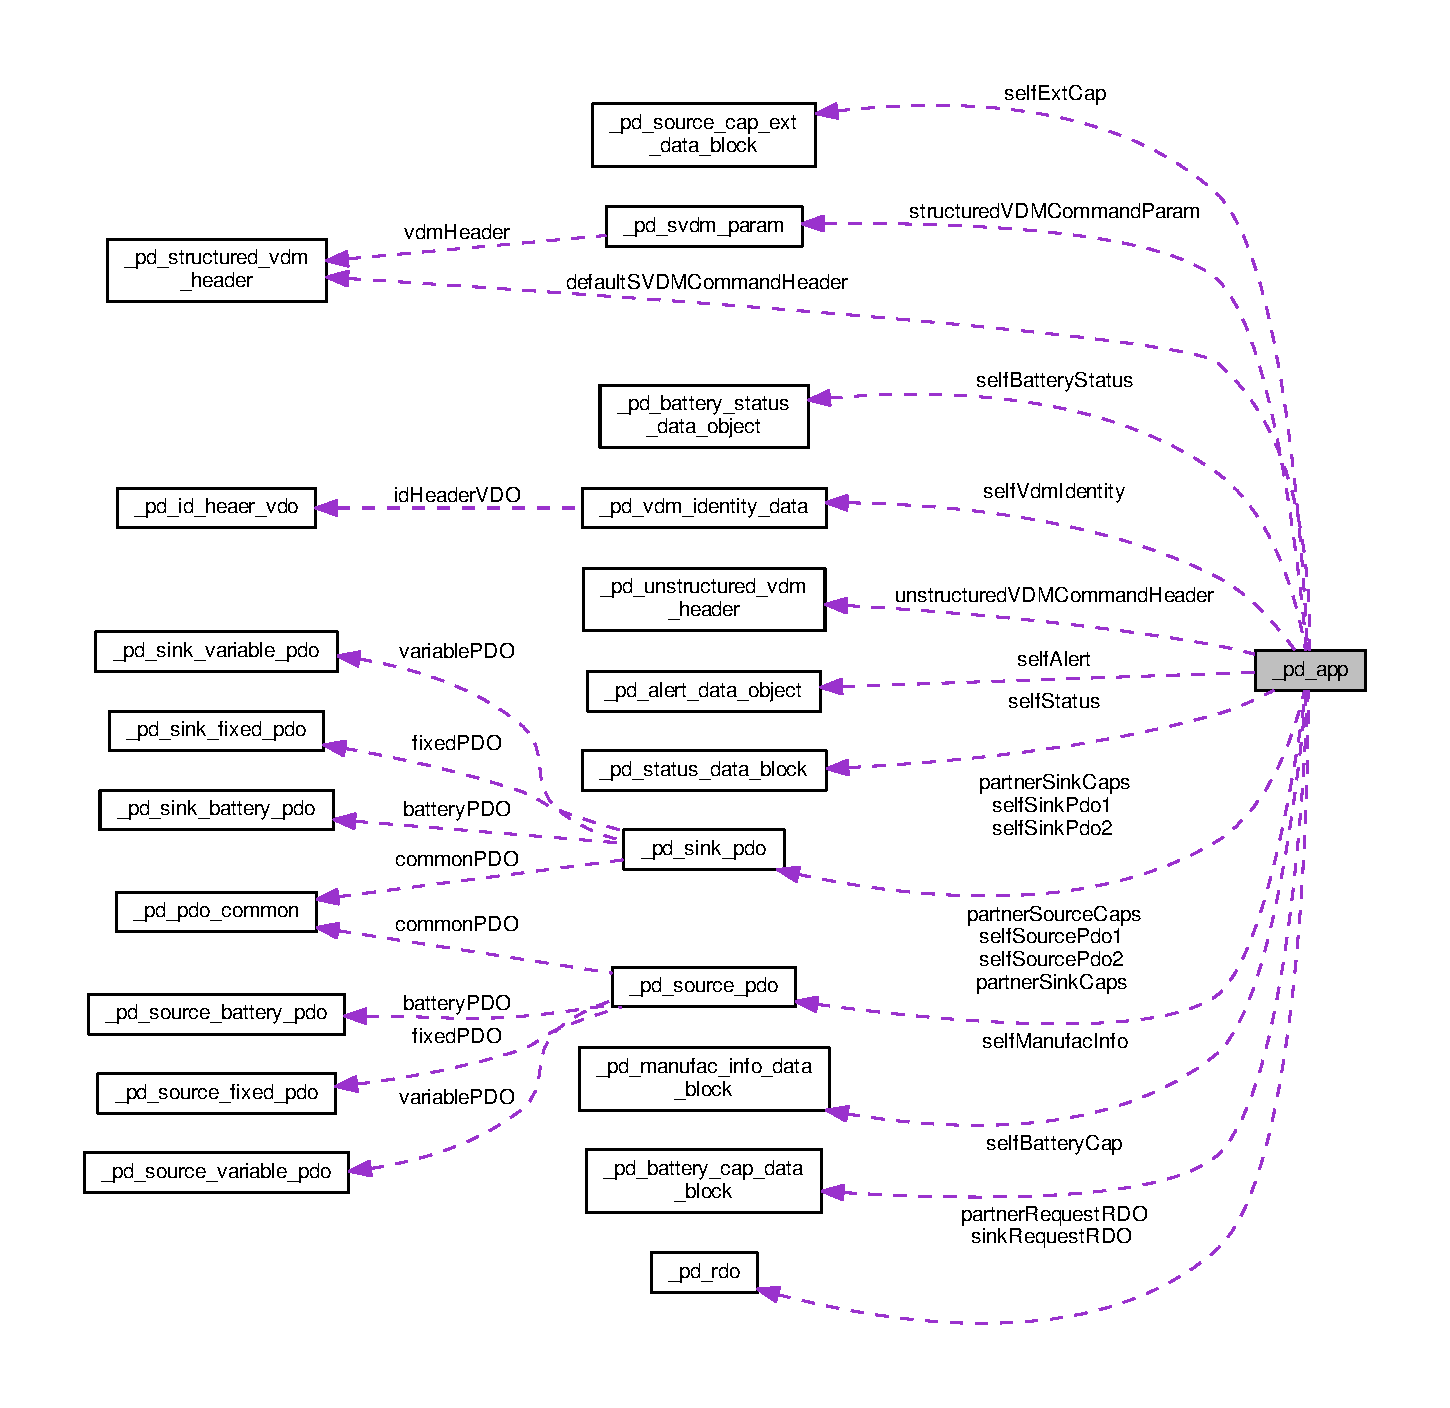
\includegraphics[width=350pt]{struct__pd__app__coll__graph}
\end{center}
\end{figure}
\subsection*{Public Attributes}
\begin{DoxyCompactItemize}
\item 
\hyperlink{group__usb__pd__stack_ga9397835347d48ef48b6b0ecba6312213}{pd\-\_\-handle} \hyperlink{struct__pd__app_a604cb18a01edb2da262e6d53fe41b70e}{pd\-Handle}
\item 
\hyperlink{group__usb__pd__stack_gae3adfd5239231ab405b04bef0ae1df5a}{pd\-\_\-source\-\_\-pdo\-\_\-t} \hyperlink{struct__pd__app_ad908e0fab5fa09248c7412253ce41095}{self\-Source\-Pdo1}
\item 
\hyperlink{group__usb__pd__stack_gae3adfd5239231ab405b04bef0ae1df5a}{pd\-\_\-source\-\_\-pdo\-\_\-t} \hyperlink{struct__pd__app_a49087b316d085ddf2be9d4ab093a0088}{self\-Source\-Pdo2}
\item 
\hyperlink{group__usb__pd__stack_gaf835814fe2dcf1f17e9e0c58bc74b6ba}{pd\-\_\-sink\-\_\-pdo\-\_\-t} \hyperlink{struct__pd__app_a7e5149d6cb2c98b3193c34c766e41cfb}{self\-Sink\-Pdo1}
\item 
\hyperlink{group__usb__pd__stack_gaf835814fe2dcf1f17e9e0c58bc74b6ba}{pd\-\_\-sink\-\_\-pdo\-\_\-t} \hyperlink{struct__pd__app_ae66313fc794d1247c12b2f9df61c740b}{self\-Sink\-Pdo2}
\item 
\hyperlink{pd__app_8h_ab9dfa9c9b90392b1b3cc1bff4b08e4e9}{pd\-\_\-vdm\-\_\-identity\-\_\-data\-\_\-t} \hyperlink{struct__pd__app_a9ed2335d20ff0eb86b07dc8770d2b6a7}{self\-Vdm\-Identity}
\item 
uint32\-\_\-t \hyperlink{struct__pd__app_a11745e09255efcf04a755844a8f7dc4c}{self\-Vdm\-S\-V\-I\-Ds}
\item 
uint32\-\_\-t \hyperlink{struct__pd__app_afc00e2e0f839a534a57c6cd5d8154b34}{self\-Vdm\-Modes}
\item 
\hyperlink{group__usb__pd__stack_ga4dcb1103574222cf94d4b45128f2b884}{pd\-\_\-rdo\-\_\-t} \hyperlink{struct__pd__app_ab41fa9c76e29ce689c812cfc7ad55150}{sink\-Request\-R\-D\-O}
\item 
\hyperlink{group__usb__pd__stack_gacedc4a601815782eff03211731ea2c7a}{pd\-\_\-svdm\-\_\-command\-\_\-param\-\_\-t} \hyperlink{struct__pd__app_afd1d474adb3bfefdb1ca2a55d36a6428}{structured\-V\-D\-M\-Command\-Param}
\item 
\hyperlink{group__usb__pd__stack_ga245b8bec3f3b7771e73016ac98595570}{pd\-\_\-structured\-\_\-vdm\-\_\-header\-\_\-t} \hyperlink{struct__pd__app_ae2637382e9ae847b799c8b6e0dd1f290}{default\-S\-V\-D\-M\-Command\-Header}
\item 
\hyperlink{group__usb__pd__stack_ga8e40e5f802e7758a04876e59a137c3b1}{pd\-\_\-unstructured\-\_\-vdm\-\_\-header\-\_\-t} \hyperlink{struct__pd__app_a32b118d435397c3f4bbe690c4e30d354}{unstructured\-V\-D\-M\-Command\-Header}
\item 
\hyperlink{pd__app_8h_a48136dc14cb8a1f83b2c425508704d1b}{pd\-\_\-source\-\_\-cap\-\_\-ext\-\_\-data\-\_\-block\-\_\-t} \hyperlink{struct__pd__app_aeb76e6e3f6c697b91755a540ee5772cf}{self\-Ext\-Cap}
\item 
\hyperlink{pd__app_8h_a3c48d8d5b263e585588f5bfe508978c6}{pd\-\_\-status\-\_\-data\-\_\-block\-\_\-t} \hyperlink{struct__pd__app_a6e05e1216ffa724cfb21c279323020b3}{self\-Status}
\item 
\hyperlink{pd__app_8h_a4890f2e2b689f24e055912a325a72748}{pd\-\_\-alert\-\_\-data\-\_\-object\-\_\-t} \hyperlink{struct__pd__app_a4461b57a4d3ff16523050f987b0dd53e}{self\-Alert}
\item 
\hyperlink{pd__app_8h_aea5fa03c1161f9f964ff0f9d8f0c5dc1}{pd\-\_\-battery\-\_\-cap\-\_\-data\-\_\-block\-\_\-t} \hyperlink{struct__pd__app_a69b5c0754997308fe2ad9308d7bb3622}{self\-Battery\-Cap}
\item 
\hyperlink{pd__app_8h_a85756978e48572ee52a6090ea4a2a400}{pd\-\_\-battery\-\_\-status\-\_\-data\-\_\-object\-\_\-t} \hyperlink{struct__pd__app_a2aeaaa8274da80148c91444df5a8bda3}{self\-Battery\-Status}
\item 
\hyperlink{pd__app_8h_a7ced852e8d03d36a6453dc1a0eccada5}{pd\-\_\-manufac\-\_\-info\-\_\-data\-\_\-block\-\_\-t} \hyperlink{struct__pd__app_a8a105b2e53346e00f5ce2304ab67796a}{self\-Manufac\-Info}
\item 
uint32\-\_\-t \hyperlink{struct__pd__app_abcf864ac3f98a5cb50592cd6110be6a0}{source\-Vbus\-Voltage}
\item 
uint32\-\_\-t \hyperlink{struct__pd__app_aaef3da806ed2695378c7ce5cc01462d5}{sink\-Request\-Voltage}
\item 
uint8\-\_\-t \hyperlink{struct__pd__app_a50a27918c703e893aab653aef204e744}{common\-Data} \mbox{[}8\mbox{]}
\item 
uint16\-\_\-t \hyperlink{struct__pd__app_a595e9d8b83e3ba15e9eaa30252ea865f}{partner\-S\-V\-I\-Ds} \mbox{[}8\mbox{]}
\item 
uint16\-\_\-t \hyperlink{struct__pd__app_a627bddd71b69afb7c7347ffd9f59ca84}{partner\-Modes} \mbox{[}8\mbox{]}
\item 
\hyperlink{group__usb__pd__stack_gae3adfd5239231ab405b04bef0ae1df5a}{pd\-\_\-source\-\_\-pdo\-\_\-t} \hyperlink{struct__pd__app_ac8c4ef05a14fc26bacd62f1937726488}{partner\-Source\-Caps} \mbox{[}7\mbox{]}
\item 
\hyperlink{group__usb__pd__stack_gae3adfd5239231ab405b04bef0ae1df5a}{pd\-\_\-source\-\_\-pdo\-\_\-t} \hyperlink{struct__pd__app_acc42dfe2943d15788312733c25a20073}{partner\-Sink\-Caps} \mbox{[}7\mbox{]}
\item 
uint8\-\_\-t \hyperlink{struct__pd__app_a7cd2902dee071f9f64b078bd4ac955be}{partner\-Source\-Cap\-Number}
\item 
uint8\-\_\-t \hyperlink{struct__pd__app_a927a55034c0beae071c028b60cd36290}{partner\-Sink\-Cap\-Number}
\item 
uint8\-\_\-t \hyperlink{struct__pd__app_a19d055bbc32fed273953f9dc02346c94}{get\-Battery\-Cap\-Data\-Block}
\item 
uint8\-\_\-t \hyperlink{struct__pd__app_a7356b8ec554edd5c580b8b2310e3fed0}{self\-Souce\-Cap\-Number}
\item 
uint8\-\_\-t \hyperlink{struct__pd__app_a7d9aa4d298cbd3ac189473e46181d5bd}{self\-Sink\-Cap\-Number}
\item 
uint8\-\_\-t \hyperlink{struct__pd__app_a2fc0a3061498fda37106d3d16aec10c8}{msg\-Sop}
\item 
uint8\-\_\-t \hyperlink{struct__pd__app_a7020e18597a0914824f3b9cb417dff87}{reqest\-Response}
\item 
uint8\-\_\-t \hyperlink{struct__pd__app_ad2ef322a1e0c25a898d7aeef4242eae8}{app\-Power\-Role}
\item 
uint8\-\_\-t \hyperlink{struct__pd__app_a178e5ae073da9205e29d5b25fd47f0e0}{app\-Data\-Role}
\item 
uint8\-\_\-t \hyperlink{struct__pd__app_a537162ae6eb43697c212227ee7279208}{connection\-Role}
\item 
volatile uint8\-\_\-t \hyperlink{struct__pd__app_a86abcaa13a196038eec6f5eab97ab940}{sw1\-State}
\item 
volatile uint8\-\_\-t \hyperlink{struct__pd__app_a43c11ce854eb3293efaf0f274421a675}{sw3\-State}
\item 
volatile uint16\-\_\-t \hyperlink{struct__pd__app_a494ab24cc582fc7368f16a047a21a9fe}{sw1\-Time}
\item 
volatile uint16\-\_\-t \hyperlink{struct__pd__app_a61108d939110e1c95e4dd8cb001a5559}{sw3\-Time}
\item 
volatile uint8\-\_\-t \hyperlink{struct__pd__app_a6cd3330740f3a7d5c35f3c9edf8ec6e2}{self\-Has\-Enter\-Alernate\-Mode}
\item 
volatile uint8\-\_\-t \hyperlink{struct__pd__app_aab6771fc259fceda49fd93d3971c8f77}{print\-Consumer}
\item 
volatile uint8\-\_\-t \hyperlink{struct__pd__app_a5ed6114200d041b6c16989abea86dbde}{print\-Provider}
\item 
volatile uint8\-\_\-t \hyperlink{struct__pd__app_ace27760f393eeceee39cf902b659cb67}{print\-Full}
\item 
uint8\-\_\-t \hyperlink{struct__pd__app_acae5bdb8d3a1a7624d440d766596a062}{print\-Buffers} \mbox{[}\hyperlink{pd__app_8h_a521a768b4f33e6978fd649b8c538d170}{P\-D\-\_\-\-D\-E\-M\-O\-\_\-\-P\-R\-I\-N\-T\-\_\-\-B\-U\-F\-F\-E\-R\-\_\-\-C\-O\-U\-N\-T}\mbox{]}\mbox{[}70\mbox{]}
\item 
volatile uint32\-\_\-t \hyperlink{struct__pd__app_ae6928ddf7cec733c1244b9f6a2034452}{pr\-Swap\-Accept}\-: 1
\item 
volatile uint32\-\_\-t \hyperlink{struct__pd__app_a7c929e9d267016ae697a553a72528987}{dr\-Swap\-Accept}\-: 1
\item 
volatile uint32\-\_\-t \hyperlink{struct__pd__app_ad3460ca1eda49e355b0b155671ba2823}{vconn\-Swap\-Accept}\-: 1
\item 
Task\-Handle\-\_\-t \hyperlink{struct__pd__app_a120cdb4cb3b4a22de6cf2db174d53920}{pd\-Task\-Handler}
\item 
volatile uint32\-\_\-t \hyperlink{struct__pd__app_a0c2c01fcb1b30a9b27dbb8ea83d7647b}{battery\-Quantity}
\item 
\hyperlink{group__usb__pd__stack_ga4dcb1103574222cf94d4b45128f2b884}{pd\-\_\-rdo\-\_\-t} \hyperlink{struct__pd__app_aff1ed842707beaa8768ec52f9e22c91b}{partner\-Request\-R\-D\-O}
\item 
\hyperlink{group__usb__pd__stack_gaf835814fe2dcf1f17e9e0c58bc74b6ba}{pd\-\_\-sink\-\_\-pdo\-\_\-t} \hyperlink{struct__pd__app_a7352c7eab0272ca6e34859d1f14acfab}{partner\-Sink\-Caps} \mbox{[}3\mbox{]}
\item 
volatile uint32\-\_\-t \hyperlink{struct__pd__app_ae2690cba6796bc0ab60086bbb39d3a37}{retry\-Swap\-Delay}
\item 
volatile uint8\-\_\-t \hyperlink{struct__pd__app_aa51e69529584a27879d6822e64f6c1c1}{contract\-Valid}
\item 
uint8\-\_\-t \hyperlink{struct__pd__app_ae4e4a09f3e6488703f5a7dbc6de96902}{source\-Cap\-Number}
\item 
uint8\-\_\-t \hyperlink{struct__pd__app_af2438fe1e518c3b17672853036e7487e}{self\-Power\-Role}
\item 
uint8\-\_\-t \hyperlink{struct__pd__app_ab62809cc014aa5182f48a2414a7d785c}{demo\-State}
\item 
volatile uint8\-\_\-t \hyperlink{struct__pd__app_a5fb16448ac6d446eaf7fc758bff182d0}{command\-Wait}
\item 
volatile uint8\-\_\-t \hyperlink{struct__pd__app_aad9f6262f331cbc8c594dada122c31dd}{command\-Result}
\item 
volatile uint8\-\_\-t \hyperlink{struct__pd__app_a588a6313718bb3ee5f8bb272d420824c}{battery\-Change}
\item 
uint8\-\_\-t \hyperlink{struct__pd__app_ae4c3014e24b07a1578a505e7ef76746c}{contract\-Valid}
\end{DoxyCompactItemize}


\subsection{Member Data Documentation}
\hypertarget{struct__pd__app_a178e5ae073da9205e29d5b25fd47f0e0}{\index{\-\_\-pd\-\_\-app@{\-\_\-pd\-\_\-app}!app\-Data\-Role@{app\-Data\-Role}}
\index{app\-Data\-Role@{app\-Data\-Role}!_pd_app@{\-\_\-pd\-\_\-app}}
\subsubsection[{app\-Data\-Role}]{\setlength{\rightskip}{0pt plus 5cm}uint8\-\_\-t \-\_\-pd\-\_\-app\-::app\-Data\-Role}}\label{struct__pd__app_a178e5ae073da9205e29d5b25fd47f0e0}
\hypertarget{struct__pd__app_ad2ef322a1e0c25a898d7aeef4242eae8}{\index{\-\_\-pd\-\_\-app@{\-\_\-pd\-\_\-app}!app\-Power\-Role@{app\-Power\-Role}}
\index{app\-Power\-Role@{app\-Power\-Role}!_pd_app@{\-\_\-pd\-\_\-app}}
\subsubsection[{app\-Power\-Role}]{\setlength{\rightskip}{0pt plus 5cm}uint8\-\_\-t \-\_\-pd\-\_\-app\-::app\-Power\-Role}}\label{struct__pd__app_ad2ef322a1e0c25a898d7aeef4242eae8}
\hypertarget{struct__pd__app_a588a6313718bb3ee5f8bb272d420824c}{\index{\-\_\-pd\-\_\-app@{\-\_\-pd\-\_\-app}!battery\-Change@{battery\-Change}}
\index{battery\-Change@{battery\-Change}!_pd_app@{\-\_\-pd\-\_\-app}}
\subsubsection[{battery\-Change}]{\setlength{\rightskip}{0pt plus 5cm}volatile uint8\-\_\-t \-\_\-pd\-\_\-app\-::battery\-Change}}\label{struct__pd__app_a588a6313718bb3ee5f8bb272d420824c}
\hypertarget{struct__pd__app_a0c2c01fcb1b30a9b27dbb8ea83d7647b}{\index{\-\_\-pd\-\_\-app@{\-\_\-pd\-\_\-app}!battery\-Quantity@{battery\-Quantity}}
\index{battery\-Quantity@{battery\-Quantity}!_pd_app@{\-\_\-pd\-\_\-app}}
\subsubsection[{battery\-Quantity}]{\setlength{\rightskip}{0pt plus 5cm}volatile uint32\-\_\-t \-\_\-pd\-\_\-app\-::battery\-Quantity}}\label{struct__pd__app_a0c2c01fcb1b30a9b27dbb8ea83d7647b}
\hypertarget{struct__pd__app_aad9f6262f331cbc8c594dada122c31dd}{\index{\-\_\-pd\-\_\-app@{\-\_\-pd\-\_\-app}!command\-Result@{command\-Result}}
\index{command\-Result@{command\-Result}!_pd_app@{\-\_\-pd\-\_\-app}}
\subsubsection[{command\-Result}]{\setlength{\rightskip}{0pt plus 5cm}volatile uint8\-\_\-t \-\_\-pd\-\_\-app\-::command\-Result}}\label{struct__pd__app_aad9f6262f331cbc8c594dada122c31dd}
\hypertarget{struct__pd__app_a5fb16448ac6d446eaf7fc758bff182d0}{\index{\-\_\-pd\-\_\-app@{\-\_\-pd\-\_\-app}!command\-Wait@{command\-Wait}}
\index{command\-Wait@{command\-Wait}!_pd_app@{\-\_\-pd\-\_\-app}}
\subsubsection[{command\-Wait}]{\setlength{\rightskip}{0pt plus 5cm}volatile uint8\-\_\-t \-\_\-pd\-\_\-app\-::command\-Wait}}\label{struct__pd__app_a5fb16448ac6d446eaf7fc758bff182d0}
\hypertarget{struct__pd__app_a50a27918c703e893aab653aef204e744}{\index{\-\_\-pd\-\_\-app@{\-\_\-pd\-\_\-app}!common\-Data@{common\-Data}}
\index{common\-Data@{common\-Data}!_pd_app@{\-\_\-pd\-\_\-app}}
\subsubsection[{common\-Data}]{\setlength{\rightskip}{0pt plus 5cm}uint8\-\_\-t \-\_\-pd\-\_\-app\-::common\-Data\mbox{[}8\mbox{]}}}\label{struct__pd__app_a50a27918c703e893aab653aef204e744}
\hypertarget{struct__pd__app_a537162ae6eb43697c212227ee7279208}{\index{\-\_\-pd\-\_\-app@{\-\_\-pd\-\_\-app}!connection\-Role@{connection\-Role}}
\index{connection\-Role@{connection\-Role}!_pd_app@{\-\_\-pd\-\_\-app}}
\subsubsection[{connection\-Role}]{\setlength{\rightskip}{0pt plus 5cm}uint8\-\_\-t \-\_\-pd\-\_\-app\-::connection\-Role}}\label{struct__pd__app_a537162ae6eb43697c212227ee7279208}
\hypertarget{struct__pd__app_ae4c3014e24b07a1578a505e7ef76746c}{\index{\-\_\-pd\-\_\-app@{\-\_\-pd\-\_\-app}!contract\-Valid@{contract\-Valid}}
\index{contract\-Valid@{contract\-Valid}!_pd_app@{\-\_\-pd\-\_\-app}}
\subsubsection[{contract\-Valid}]{\setlength{\rightskip}{0pt plus 5cm}uint8\-\_\-t \-\_\-pd\-\_\-app\-::contract\-Valid}}\label{struct__pd__app_ae4c3014e24b07a1578a505e7ef76746c}
\hypertarget{struct__pd__app_aa51e69529584a27879d6822e64f6c1c1}{\index{\-\_\-pd\-\_\-app@{\-\_\-pd\-\_\-app}!contract\-Valid@{contract\-Valid}}
\index{contract\-Valid@{contract\-Valid}!_pd_app@{\-\_\-pd\-\_\-app}}
\subsubsection[{contract\-Valid}]{\setlength{\rightskip}{0pt plus 5cm}volatile uint8\-\_\-t \-\_\-pd\-\_\-app\-::contract\-Valid}}\label{struct__pd__app_aa51e69529584a27879d6822e64f6c1c1}
\hypertarget{struct__pd__app_ae2637382e9ae847b799c8b6e0dd1f290}{\index{\-\_\-pd\-\_\-app@{\-\_\-pd\-\_\-app}!default\-S\-V\-D\-M\-Command\-Header@{default\-S\-V\-D\-M\-Command\-Header}}
\index{default\-S\-V\-D\-M\-Command\-Header@{default\-S\-V\-D\-M\-Command\-Header}!_pd_app@{\-\_\-pd\-\_\-app}}
\subsubsection[{default\-S\-V\-D\-M\-Command\-Header}]{\setlength{\rightskip}{0pt plus 5cm}{\bf pd\-\_\-structured\-\_\-vdm\-\_\-header\-\_\-t} \-\_\-pd\-\_\-app\-::default\-S\-V\-D\-M\-Command\-Header}}\label{struct__pd__app_ae2637382e9ae847b799c8b6e0dd1f290}
\hypertarget{struct__pd__app_ab62809cc014aa5182f48a2414a7d785c}{\index{\-\_\-pd\-\_\-app@{\-\_\-pd\-\_\-app}!demo\-State@{demo\-State}}
\index{demo\-State@{demo\-State}!_pd_app@{\-\_\-pd\-\_\-app}}
\subsubsection[{demo\-State}]{\setlength{\rightskip}{0pt plus 5cm}uint8\-\_\-t \-\_\-pd\-\_\-app\-::demo\-State}}\label{struct__pd__app_ab62809cc014aa5182f48a2414a7d785c}
\hypertarget{struct__pd__app_a7c929e9d267016ae697a553a72528987}{\index{\-\_\-pd\-\_\-app@{\-\_\-pd\-\_\-app}!dr\-Swap\-Accept@{dr\-Swap\-Accept}}
\index{dr\-Swap\-Accept@{dr\-Swap\-Accept}!_pd_app@{\-\_\-pd\-\_\-app}}
\subsubsection[{dr\-Swap\-Accept}]{\setlength{\rightskip}{0pt plus 5cm}volatile uint32\-\_\-t \-\_\-pd\-\_\-app\-::dr\-Swap\-Accept}}\label{struct__pd__app_a7c929e9d267016ae697a553a72528987}
\hypertarget{struct__pd__app_a19d055bbc32fed273953f9dc02346c94}{\index{\-\_\-pd\-\_\-app@{\-\_\-pd\-\_\-app}!get\-Battery\-Cap\-Data\-Block@{get\-Battery\-Cap\-Data\-Block}}
\index{get\-Battery\-Cap\-Data\-Block@{get\-Battery\-Cap\-Data\-Block}!_pd_app@{\-\_\-pd\-\_\-app}}
\subsubsection[{get\-Battery\-Cap\-Data\-Block}]{\setlength{\rightskip}{0pt plus 5cm}uint8\-\_\-t \-\_\-pd\-\_\-app\-::get\-Battery\-Cap\-Data\-Block}}\label{struct__pd__app_a19d055bbc32fed273953f9dc02346c94}
\hypertarget{struct__pd__app_a2fc0a3061498fda37106d3d16aec10c8}{\index{\-\_\-pd\-\_\-app@{\-\_\-pd\-\_\-app}!msg\-Sop@{msg\-Sop}}
\index{msg\-Sop@{msg\-Sop}!_pd_app@{\-\_\-pd\-\_\-app}}
\subsubsection[{msg\-Sop}]{\setlength{\rightskip}{0pt plus 5cm}uint8\-\_\-t \-\_\-pd\-\_\-app\-::msg\-Sop}}\label{struct__pd__app_a2fc0a3061498fda37106d3d16aec10c8}
\hypertarget{struct__pd__app_a627bddd71b69afb7c7347ffd9f59ca84}{\index{\-\_\-pd\-\_\-app@{\-\_\-pd\-\_\-app}!partner\-Modes@{partner\-Modes}}
\index{partner\-Modes@{partner\-Modes}!_pd_app@{\-\_\-pd\-\_\-app}}
\subsubsection[{partner\-Modes}]{\setlength{\rightskip}{0pt plus 5cm}uint16\-\_\-t \-\_\-pd\-\_\-app\-::partner\-Modes\mbox{[}8\mbox{]}}}\label{struct__pd__app_a627bddd71b69afb7c7347ffd9f59ca84}
\hypertarget{struct__pd__app_aff1ed842707beaa8768ec52f9e22c91b}{\index{\-\_\-pd\-\_\-app@{\-\_\-pd\-\_\-app}!partner\-Request\-R\-D\-O@{partner\-Request\-R\-D\-O}}
\index{partner\-Request\-R\-D\-O@{partner\-Request\-R\-D\-O}!_pd_app@{\-\_\-pd\-\_\-app}}
\subsubsection[{partner\-Request\-R\-D\-O}]{\setlength{\rightskip}{0pt plus 5cm}{\bf pd\-\_\-rdo\-\_\-t} \-\_\-pd\-\_\-app\-::partner\-Request\-R\-D\-O}}\label{struct__pd__app_aff1ed842707beaa8768ec52f9e22c91b}
\hypertarget{struct__pd__app_a927a55034c0beae071c028b60cd36290}{\index{\-\_\-pd\-\_\-app@{\-\_\-pd\-\_\-app}!partner\-Sink\-Cap\-Number@{partner\-Sink\-Cap\-Number}}
\index{partner\-Sink\-Cap\-Number@{partner\-Sink\-Cap\-Number}!_pd_app@{\-\_\-pd\-\_\-app}}
\subsubsection[{partner\-Sink\-Cap\-Number}]{\setlength{\rightskip}{0pt plus 5cm}uint8\-\_\-t \-\_\-pd\-\_\-app\-::partner\-Sink\-Cap\-Number}}\label{struct__pd__app_a927a55034c0beae071c028b60cd36290}
\hypertarget{struct__pd__app_a7352c7eab0272ca6e34859d1f14acfab}{\index{\-\_\-pd\-\_\-app@{\-\_\-pd\-\_\-app}!partner\-Sink\-Caps@{partner\-Sink\-Caps}}
\index{partner\-Sink\-Caps@{partner\-Sink\-Caps}!_pd_app@{\-\_\-pd\-\_\-app}}
\subsubsection[{partner\-Sink\-Caps}]{\setlength{\rightskip}{0pt plus 5cm}{\bf pd\-\_\-sink\-\_\-pdo\-\_\-t} \-\_\-pd\-\_\-app\-::partner\-Sink\-Caps\mbox{[}3\mbox{]}}}\label{struct__pd__app_a7352c7eab0272ca6e34859d1f14acfab}
\hypertarget{struct__pd__app_acc42dfe2943d15788312733c25a20073}{\index{\-\_\-pd\-\_\-app@{\-\_\-pd\-\_\-app}!partner\-Sink\-Caps@{partner\-Sink\-Caps}}
\index{partner\-Sink\-Caps@{partner\-Sink\-Caps}!_pd_app@{\-\_\-pd\-\_\-app}}
\subsubsection[{partner\-Sink\-Caps}]{\setlength{\rightskip}{0pt plus 5cm}{\bf pd\-\_\-sink\-\_\-pdo\-\_\-t} \-\_\-pd\-\_\-app\-::partner\-Sink\-Caps}}\label{struct__pd__app_acc42dfe2943d15788312733c25a20073}
\hypertarget{struct__pd__app_a7cd2902dee071f9f64b078bd4ac955be}{\index{\-\_\-pd\-\_\-app@{\-\_\-pd\-\_\-app}!partner\-Source\-Cap\-Number@{partner\-Source\-Cap\-Number}}
\index{partner\-Source\-Cap\-Number@{partner\-Source\-Cap\-Number}!_pd_app@{\-\_\-pd\-\_\-app}}
\subsubsection[{partner\-Source\-Cap\-Number}]{\setlength{\rightskip}{0pt plus 5cm}uint8\-\_\-t \-\_\-pd\-\_\-app\-::partner\-Source\-Cap\-Number}}\label{struct__pd__app_a7cd2902dee071f9f64b078bd4ac955be}
\hypertarget{struct__pd__app_ac8c4ef05a14fc26bacd62f1937726488}{\index{\-\_\-pd\-\_\-app@{\-\_\-pd\-\_\-app}!partner\-Source\-Caps@{partner\-Source\-Caps}}
\index{partner\-Source\-Caps@{partner\-Source\-Caps}!_pd_app@{\-\_\-pd\-\_\-app}}
\subsubsection[{partner\-Source\-Caps}]{\setlength{\rightskip}{0pt plus 5cm}{\bf pd\-\_\-source\-\_\-pdo\-\_\-t} \-\_\-pd\-\_\-app\-::partner\-Source\-Caps}}\label{struct__pd__app_ac8c4ef05a14fc26bacd62f1937726488}
\hypertarget{struct__pd__app_a595e9d8b83e3ba15e9eaa30252ea865f}{\index{\-\_\-pd\-\_\-app@{\-\_\-pd\-\_\-app}!partner\-S\-V\-I\-Ds@{partner\-S\-V\-I\-Ds}}
\index{partner\-S\-V\-I\-Ds@{partner\-S\-V\-I\-Ds}!_pd_app@{\-\_\-pd\-\_\-app}}
\subsubsection[{partner\-S\-V\-I\-Ds}]{\setlength{\rightskip}{0pt plus 5cm}uint16\-\_\-t \-\_\-pd\-\_\-app\-::partner\-S\-V\-I\-Ds\mbox{[}8\mbox{]}}}\label{struct__pd__app_a595e9d8b83e3ba15e9eaa30252ea865f}
\hypertarget{struct__pd__app_a604cb18a01edb2da262e6d53fe41b70e}{\index{\-\_\-pd\-\_\-app@{\-\_\-pd\-\_\-app}!pd\-Handle@{pd\-Handle}}
\index{pd\-Handle@{pd\-Handle}!_pd_app@{\-\_\-pd\-\_\-app}}
\subsubsection[{pd\-Handle}]{\setlength{\rightskip}{0pt plus 5cm}{\bf pd\-\_\-handle} \-\_\-pd\-\_\-app\-::pd\-Handle}}\label{struct__pd__app_a604cb18a01edb2da262e6d53fe41b70e}
\hypertarget{struct__pd__app_a120cdb4cb3b4a22de6cf2db174d53920}{\index{\-\_\-pd\-\_\-app@{\-\_\-pd\-\_\-app}!pd\-Task\-Handler@{pd\-Task\-Handler}}
\index{pd\-Task\-Handler@{pd\-Task\-Handler}!_pd_app@{\-\_\-pd\-\_\-app}}
\subsubsection[{pd\-Task\-Handler}]{\setlength{\rightskip}{0pt plus 5cm}Task\-Handle\-\_\-t \-\_\-pd\-\_\-app\-::pd\-Task\-Handler}}\label{struct__pd__app_a120cdb4cb3b4a22de6cf2db174d53920}
\hypertarget{struct__pd__app_acae5bdb8d3a1a7624d440d766596a062}{\index{\-\_\-pd\-\_\-app@{\-\_\-pd\-\_\-app}!print\-Buffers@{print\-Buffers}}
\index{print\-Buffers@{print\-Buffers}!_pd_app@{\-\_\-pd\-\_\-app}}
\subsubsection[{print\-Buffers}]{\setlength{\rightskip}{0pt plus 5cm}uint8\-\_\-t \-\_\-pd\-\_\-app\-::print\-Buffers\mbox{[}{\bf P\-D\-\_\-\-D\-E\-M\-O\-\_\-\-P\-R\-I\-N\-T\-\_\-\-B\-U\-F\-F\-E\-R\-\_\-\-C\-O\-U\-N\-T}\mbox{]}\mbox{[}70\mbox{]}}}\label{struct__pd__app_acae5bdb8d3a1a7624d440d766596a062}
\hypertarget{struct__pd__app_aab6771fc259fceda49fd93d3971c8f77}{\index{\-\_\-pd\-\_\-app@{\-\_\-pd\-\_\-app}!print\-Consumer@{print\-Consumer}}
\index{print\-Consumer@{print\-Consumer}!_pd_app@{\-\_\-pd\-\_\-app}}
\subsubsection[{print\-Consumer}]{\setlength{\rightskip}{0pt plus 5cm}volatile uint8\-\_\-t \-\_\-pd\-\_\-app\-::print\-Consumer}}\label{struct__pd__app_aab6771fc259fceda49fd93d3971c8f77}
\hypertarget{struct__pd__app_ace27760f393eeceee39cf902b659cb67}{\index{\-\_\-pd\-\_\-app@{\-\_\-pd\-\_\-app}!print\-Full@{print\-Full}}
\index{print\-Full@{print\-Full}!_pd_app@{\-\_\-pd\-\_\-app}}
\subsubsection[{print\-Full}]{\setlength{\rightskip}{0pt plus 5cm}volatile uint8\-\_\-t \-\_\-pd\-\_\-app\-::print\-Full}}\label{struct__pd__app_ace27760f393eeceee39cf902b659cb67}
\hypertarget{struct__pd__app_a5ed6114200d041b6c16989abea86dbde}{\index{\-\_\-pd\-\_\-app@{\-\_\-pd\-\_\-app}!print\-Provider@{print\-Provider}}
\index{print\-Provider@{print\-Provider}!_pd_app@{\-\_\-pd\-\_\-app}}
\subsubsection[{print\-Provider}]{\setlength{\rightskip}{0pt plus 5cm}volatile uint8\-\_\-t \-\_\-pd\-\_\-app\-::print\-Provider}}\label{struct__pd__app_a5ed6114200d041b6c16989abea86dbde}
\hypertarget{struct__pd__app_ae6928ddf7cec733c1244b9f6a2034452}{\index{\-\_\-pd\-\_\-app@{\-\_\-pd\-\_\-app}!pr\-Swap\-Accept@{pr\-Swap\-Accept}}
\index{pr\-Swap\-Accept@{pr\-Swap\-Accept}!_pd_app@{\-\_\-pd\-\_\-app}}
\subsubsection[{pr\-Swap\-Accept}]{\setlength{\rightskip}{0pt plus 5cm}volatile uint32\-\_\-t \-\_\-pd\-\_\-app\-::pr\-Swap\-Accept}}\label{struct__pd__app_ae6928ddf7cec733c1244b9f6a2034452}
\hypertarget{struct__pd__app_a7020e18597a0914824f3b9cb417dff87}{\index{\-\_\-pd\-\_\-app@{\-\_\-pd\-\_\-app}!reqest\-Response@{reqest\-Response}}
\index{reqest\-Response@{reqest\-Response}!_pd_app@{\-\_\-pd\-\_\-app}}
\subsubsection[{reqest\-Response}]{\setlength{\rightskip}{0pt plus 5cm}uint8\-\_\-t \-\_\-pd\-\_\-app\-::reqest\-Response}}\label{struct__pd__app_a7020e18597a0914824f3b9cb417dff87}
\hypertarget{struct__pd__app_ae2690cba6796bc0ab60086bbb39d3a37}{\index{\-\_\-pd\-\_\-app@{\-\_\-pd\-\_\-app}!retry\-Swap\-Delay@{retry\-Swap\-Delay}}
\index{retry\-Swap\-Delay@{retry\-Swap\-Delay}!_pd_app@{\-\_\-pd\-\_\-app}}
\subsubsection[{retry\-Swap\-Delay}]{\setlength{\rightskip}{0pt plus 5cm}volatile uint32\-\_\-t \-\_\-pd\-\_\-app\-::retry\-Swap\-Delay}}\label{struct__pd__app_ae2690cba6796bc0ab60086bbb39d3a37}
\hypertarget{struct__pd__app_a4461b57a4d3ff16523050f987b0dd53e}{\index{\-\_\-pd\-\_\-app@{\-\_\-pd\-\_\-app}!self\-Alert@{self\-Alert}}
\index{self\-Alert@{self\-Alert}!_pd_app@{\-\_\-pd\-\_\-app}}
\subsubsection[{self\-Alert}]{\setlength{\rightskip}{0pt plus 5cm}{\bf pd\-\_\-alert\-\_\-data\-\_\-object\-\_\-t} \-\_\-pd\-\_\-app\-::self\-Alert}}\label{struct__pd__app_a4461b57a4d3ff16523050f987b0dd53e}
\hypertarget{struct__pd__app_a69b5c0754997308fe2ad9308d7bb3622}{\index{\-\_\-pd\-\_\-app@{\-\_\-pd\-\_\-app}!self\-Battery\-Cap@{self\-Battery\-Cap}}
\index{self\-Battery\-Cap@{self\-Battery\-Cap}!_pd_app@{\-\_\-pd\-\_\-app}}
\subsubsection[{self\-Battery\-Cap}]{\setlength{\rightskip}{0pt plus 5cm}{\bf pd\-\_\-battery\-\_\-cap\-\_\-data\-\_\-block\-\_\-t} \-\_\-pd\-\_\-app\-::self\-Battery\-Cap}}\label{struct__pd__app_a69b5c0754997308fe2ad9308d7bb3622}
\hypertarget{struct__pd__app_a2aeaaa8274da80148c91444df5a8bda3}{\index{\-\_\-pd\-\_\-app@{\-\_\-pd\-\_\-app}!self\-Battery\-Status@{self\-Battery\-Status}}
\index{self\-Battery\-Status@{self\-Battery\-Status}!_pd_app@{\-\_\-pd\-\_\-app}}
\subsubsection[{self\-Battery\-Status}]{\setlength{\rightskip}{0pt plus 5cm}{\bf pd\-\_\-battery\-\_\-status\-\_\-data\-\_\-object\-\_\-t} \-\_\-pd\-\_\-app\-::self\-Battery\-Status}}\label{struct__pd__app_a2aeaaa8274da80148c91444df5a8bda3}
\hypertarget{struct__pd__app_aeb76e6e3f6c697b91755a540ee5772cf}{\index{\-\_\-pd\-\_\-app@{\-\_\-pd\-\_\-app}!self\-Ext\-Cap@{self\-Ext\-Cap}}
\index{self\-Ext\-Cap@{self\-Ext\-Cap}!_pd_app@{\-\_\-pd\-\_\-app}}
\subsubsection[{self\-Ext\-Cap}]{\setlength{\rightskip}{0pt plus 5cm}{\bf pd\-\_\-source\-\_\-cap\-\_\-ext\-\_\-data\-\_\-block\-\_\-t} \-\_\-pd\-\_\-app\-::self\-Ext\-Cap}}\label{struct__pd__app_aeb76e6e3f6c697b91755a540ee5772cf}
\hypertarget{struct__pd__app_a6cd3330740f3a7d5c35f3c9edf8ec6e2}{\index{\-\_\-pd\-\_\-app@{\-\_\-pd\-\_\-app}!self\-Has\-Enter\-Alernate\-Mode@{self\-Has\-Enter\-Alernate\-Mode}}
\index{self\-Has\-Enter\-Alernate\-Mode@{self\-Has\-Enter\-Alernate\-Mode}!_pd_app@{\-\_\-pd\-\_\-app}}
\subsubsection[{self\-Has\-Enter\-Alernate\-Mode}]{\setlength{\rightskip}{0pt plus 5cm}volatile uint8\-\_\-t \-\_\-pd\-\_\-app\-::self\-Has\-Enter\-Alernate\-Mode}}\label{struct__pd__app_a6cd3330740f3a7d5c35f3c9edf8ec6e2}
\hypertarget{struct__pd__app_a8a105b2e53346e00f5ce2304ab67796a}{\index{\-\_\-pd\-\_\-app@{\-\_\-pd\-\_\-app}!self\-Manufac\-Info@{self\-Manufac\-Info}}
\index{self\-Manufac\-Info@{self\-Manufac\-Info}!_pd_app@{\-\_\-pd\-\_\-app}}
\subsubsection[{self\-Manufac\-Info}]{\setlength{\rightskip}{0pt plus 5cm}{\bf pd\-\_\-manufac\-\_\-info\-\_\-data\-\_\-block\-\_\-t} \-\_\-pd\-\_\-app\-::self\-Manufac\-Info}}\label{struct__pd__app_a8a105b2e53346e00f5ce2304ab67796a}
\hypertarget{struct__pd__app_af2438fe1e518c3b17672853036e7487e}{\index{\-\_\-pd\-\_\-app@{\-\_\-pd\-\_\-app}!self\-Power\-Role@{self\-Power\-Role}}
\index{self\-Power\-Role@{self\-Power\-Role}!_pd_app@{\-\_\-pd\-\_\-app}}
\subsubsection[{self\-Power\-Role}]{\setlength{\rightskip}{0pt plus 5cm}uint8\-\_\-t \-\_\-pd\-\_\-app\-::self\-Power\-Role}}\label{struct__pd__app_af2438fe1e518c3b17672853036e7487e}
\hypertarget{struct__pd__app_a7d9aa4d298cbd3ac189473e46181d5bd}{\index{\-\_\-pd\-\_\-app@{\-\_\-pd\-\_\-app}!self\-Sink\-Cap\-Number@{self\-Sink\-Cap\-Number}}
\index{self\-Sink\-Cap\-Number@{self\-Sink\-Cap\-Number}!_pd_app@{\-\_\-pd\-\_\-app}}
\subsubsection[{self\-Sink\-Cap\-Number}]{\setlength{\rightskip}{0pt plus 5cm}uint8\-\_\-t \-\_\-pd\-\_\-app\-::self\-Sink\-Cap\-Number}}\label{struct__pd__app_a7d9aa4d298cbd3ac189473e46181d5bd}
\hypertarget{struct__pd__app_a7e5149d6cb2c98b3193c34c766e41cfb}{\index{\-\_\-pd\-\_\-app@{\-\_\-pd\-\_\-app}!self\-Sink\-Pdo1@{self\-Sink\-Pdo1}}
\index{self\-Sink\-Pdo1@{self\-Sink\-Pdo1}!_pd_app@{\-\_\-pd\-\_\-app}}
\subsubsection[{self\-Sink\-Pdo1}]{\setlength{\rightskip}{0pt plus 5cm}{\bf pd\-\_\-sink\-\_\-pdo\-\_\-t} \-\_\-pd\-\_\-app\-::self\-Sink\-Pdo1}}\label{struct__pd__app_a7e5149d6cb2c98b3193c34c766e41cfb}
\hypertarget{struct__pd__app_ae66313fc794d1247c12b2f9df61c740b}{\index{\-\_\-pd\-\_\-app@{\-\_\-pd\-\_\-app}!self\-Sink\-Pdo2@{self\-Sink\-Pdo2}}
\index{self\-Sink\-Pdo2@{self\-Sink\-Pdo2}!_pd_app@{\-\_\-pd\-\_\-app}}
\subsubsection[{self\-Sink\-Pdo2}]{\setlength{\rightskip}{0pt plus 5cm}{\bf pd\-\_\-sink\-\_\-pdo\-\_\-t} \-\_\-pd\-\_\-app\-::self\-Sink\-Pdo2}}\label{struct__pd__app_ae66313fc794d1247c12b2f9df61c740b}
\hypertarget{struct__pd__app_a7356b8ec554edd5c580b8b2310e3fed0}{\index{\-\_\-pd\-\_\-app@{\-\_\-pd\-\_\-app}!self\-Souce\-Cap\-Number@{self\-Souce\-Cap\-Number}}
\index{self\-Souce\-Cap\-Number@{self\-Souce\-Cap\-Number}!_pd_app@{\-\_\-pd\-\_\-app}}
\subsubsection[{self\-Souce\-Cap\-Number}]{\setlength{\rightskip}{0pt plus 5cm}uint8\-\_\-t \-\_\-pd\-\_\-app\-::self\-Souce\-Cap\-Number}}\label{struct__pd__app_a7356b8ec554edd5c580b8b2310e3fed0}
\hypertarget{struct__pd__app_ad908e0fab5fa09248c7412253ce41095}{\index{\-\_\-pd\-\_\-app@{\-\_\-pd\-\_\-app}!self\-Source\-Pdo1@{self\-Source\-Pdo1}}
\index{self\-Source\-Pdo1@{self\-Source\-Pdo1}!_pd_app@{\-\_\-pd\-\_\-app}}
\subsubsection[{self\-Source\-Pdo1}]{\setlength{\rightskip}{0pt plus 5cm}{\bf pd\-\_\-source\-\_\-pdo\-\_\-t} \-\_\-pd\-\_\-app\-::self\-Source\-Pdo1}}\label{struct__pd__app_ad908e0fab5fa09248c7412253ce41095}
\hypertarget{struct__pd__app_a49087b316d085ddf2be9d4ab093a0088}{\index{\-\_\-pd\-\_\-app@{\-\_\-pd\-\_\-app}!self\-Source\-Pdo2@{self\-Source\-Pdo2}}
\index{self\-Source\-Pdo2@{self\-Source\-Pdo2}!_pd_app@{\-\_\-pd\-\_\-app}}
\subsubsection[{self\-Source\-Pdo2}]{\setlength{\rightskip}{0pt plus 5cm}{\bf pd\-\_\-source\-\_\-pdo\-\_\-t} \-\_\-pd\-\_\-app\-::self\-Source\-Pdo2}}\label{struct__pd__app_a49087b316d085ddf2be9d4ab093a0088}
\hypertarget{struct__pd__app_a6e05e1216ffa724cfb21c279323020b3}{\index{\-\_\-pd\-\_\-app@{\-\_\-pd\-\_\-app}!self\-Status@{self\-Status}}
\index{self\-Status@{self\-Status}!_pd_app@{\-\_\-pd\-\_\-app}}
\subsubsection[{self\-Status}]{\setlength{\rightskip}{0pt plus 5cm}{\bf pd\-\_\-status\-\_\-data\-\_\-block\-\_\-t} \-\_\-pd\-\_\-app\-::self\-Status}}\label{struct__pd__app_a6e05e1216ffa724cfb21c279323020b3}
\hypertarget{struct__pd__app_a9ed2335d20ff0eb86b07dc8770d2b6a7}{\index{\-\_\-pd\-\_\-app@{\-\_\-pd\-\_\-app}!self\-Vdm\-Identity@{self\-Vdm\-Identity}}
\index{self\-Vdm\-Identity@{self\-Vdm\-Identity}!_pd_app@{\-\_\-pd\-\_\-app}}
\subsubsection[{self\-Vdm\-Identity}]{\setlength{\rightskip}{0pt plus 5cm}{\bf pd\-\_\-vdm\-\_\-identity\-\_\-data\-\_\-t} \-\_\-pd\-\_\-app\-::self\-Vdm\-Identity}}\label{struct__pd__app_a9ed2335d20ff0eb86b07dc8770d2b6a7}
\hypertarget{struct__pd__app_afc00e2e0f839a534a57c6cd5d8154b34}{\index{\-\_\-pd\-\_\-app@{\-\_\-pd\-\_\-app}!self\-Vdm\-Modes@{self\-Vdm\-Modes}}
\index{self\-Vdm\-Modes@{self\-Vdm\-Modes}!_pd_app@{\-\_\-pd\-\_\-app}}
\subsubsection[{self\-Vdm\-Modes}]{\setlength{\rightskip}{0pt plus 5cm}uint32\-\_\-t \-\_\-pd\-\_\-app\-::self\-Vdm\-Modes}}\label{struct__pd__app_afc00e2e0f839a534a57c6cd5d8154b34}
\hypertarget{struct__pd__app_a11745e09255efcf04a755844a8f7dc4c}{\index{\-\_\-pd\-\_\-app@{\-\_\-pd\-\_\-app}!self\-Vdm\-S\-V\-I\-Ds@{self\-Vdm\-S\-V\-I\-Ds}}
\index{self\-Vdm\-S\-V\-I\-Ds@{self\-Vdm\-S\-V\-I\-Ds}!_pd_app@{\-\_\-pd\-\_\-app}}
\subsubsection[{self\-Vdm\-S\-V\-I\-Ds}]{\setlength{\rightskip}{0pt plus 5cm}uint32\-\_\-t \-\_\-pd\-\_\-app\-::self\-Vdm\-S\-V\-I\-Ds}}\label{struct__pd__app_a11745e09255efcf04a755844a8f7dc4c}
\hypertarget{struct__pd__app_ab41fa9c76e29ce689c812cfc7ad55150}{\index{\-\_\-pd\-\_\-app@{\-\_\-pd\-\_\-app}!sink\-Request\-R\-D\-O@{sink\-Request\-R\-D\-O}}
\index{sink\-Request\-R\-D\-O@{sink\-Request\-R\-D\-O}!_pd_app@{\-\_\-pd\-\_\-app}}
\subsubsection[{sink\-Request\-R\-D\-O}]{\setlength{\rightskip}{0pt plus 5cm}{\bf pd\-\_\-rdo\-\_\-t} \-\_\-pd\-\_\-app\-::sink\-Request\-R\-D\-O}}\label{struct__pd__app_ab41fa9c76e29ce689c812cfc7ad55150}
\hypertarget{struct__pd__app_aaef3da806ed2695378c7ce5cc01462d5}{\index{\-\_\-pd\-\_\-app@{\-\_\-pd\-\_\-app}!sink\-Request\-Voltage@{sink\-Request\-Voltage}}
\index{sink\-Request\-Voltage@{sink\-Request\-Voltage}!_pd_app@{\-\_\-pd\-\_\-app}}
\subsubsection[{sink\-Request\-Voltage}]{\setlength{\rightskip}{0pt plus 5cm}uint32\-\_\-t \-\_\-pd\-\_\-app\-::sink\-Request\-Voltage}}\label{struct__pd__app_aaef3da806ed2695378c7ce5cc01462d5}
\hypertarget{struct__pd__app_ae4e4a09f3e6488703f5a7dbc6de96902}{\index{\-\_\-pd\-\_\-app@{\-\_\-pd\-\_\-app}!source\-Cap\-Number@{source\-Cap\-Number}}
\index{source\-Cap\-Number@{source\-Cap\-Number}!_pd_app@{\-\_\-pd\-\_\-app}}
\subsubsection[{source\-Cap\-Number}]{\setlength{\rightskip}{0pt plus 5cm}uint8\-\_\-t \-\_\-pd\-\_\-app\-::source\-Cap\-Number}}\label{struct__pd__app_ae4e4a09f3e6488703f5a7dbc6de96902}
\hypertarget{struct__pd__app_abcf864ac3f98a5cb50592cd6110be6a0}{\index{\-\_\-pd\-\_\-app@{\-\_\-pd\-\_\-app}!source\-Vbus\-Voltage@{source\-Vbus\-Voltage}}
\index{source\-Vbus\-Voltage@{source\-Vbus\-Voltage}!_pd_app@{\-\_\-pd\-\_\-app}}
\subsubsection[{source\-Vbus\-Voltage}]{\setlength{\rightskip}{0pt plus 5cm}uint32\-\_\-t \-\_\-pd\-\_\-app\-::source\-Vbus\-Voltage}}\label{struct__pd__app_abcf864ac3f98a5cb50592cd6110be6a0}
\hypertarget{struct__pd__app_afd1d474adb3bfefdb1ca2a55d36a6428}{\index{\-\_\-pd\-\_\-app@{\-\_\-pd\-\_\-app}!structured\-V\-D\-M\-Command\-Param@{structured\-V\-D\-M\-Command\-Param}}
\index{structured\-V\-D\-M\-Command\-Param@{structured\-V\-D\-M\-Command\-Param}!_pd_app@{\-\_\-pd\-\_\-app}}
\subsubsection[{structured\-V\-D\-M\-Command\-Param}]{\setlength{\rightskip}{0pt plus 5cm}{\bf pd\-\_\-svdm\-\_\-command\-\_\-param\-\_\-t} \-\_\-pd\-\_\-app\-::structured\-V\-D\-M\-Command\-Param}}\label{struct__pd__app_afd1d474adb3bfefdb1ca2a55d36a6428}
\hypertarget{struct__pd__app_a86abcaa13a196038eec6f5eab97ab940}{\index{\-\_\-pd\-\_\-app@{\-\_\-pd\-\_\-app}!sw1\-State@{sw1\-State}}
\index{sw1\-State@{sw1\-State}!_pd_app@{\-\_\-pd\-\_\-app}}
\subsubsection[{sw1\-State}]{\setlength{\rightskip}{0pt plus 5cm}volatile uint8\-\_\-t \-\_\-pd\-\_\-app\-::sw1\-State}}\label{struct__pd__app_a86abcaa13a196038eec6f5eab97ab940}
\hypertarget{struct__pd__app_a494ab24cc582fc7368f16a047a21a9fe}{\index{\-\_\-pd\-\_\-app@{\-\_\-pd\-\_\-app}!sw1\-Time@{sw1\-Time}}
\index{sw1\-Time@{sw1\-Time}!_pd_app@{\-\_\-pd\-\_\-app}}
\subsubsection[{sw1\-Time}]{\setlength{\rightskip}{0pt plus 5cm}volatile uint16\-\_\-t \-\_\-pd\-\_\-app\-::sw1\-Time}}\label{struct__pd__app_a494ab24cc582fc7368f16a047a21a9fe}
\hypertarget{struct__pd__app_a43c11ce854eb3293efaf0f274421a675}{\index{\-\_\-pd\-\_\-app@{\-\_\-pd\-\_\-app}!sw3\-State@{sw3\-State}}
\index{sw3\-State@{sw3\-State}!_pd_app@{\-\_\-pd\-\_\-app}}
\subsubsection[{sw3\-State}]{\setlength{\rightskip}{0pt plus 5cm}volatile uint8\-\_\-t \-\_\-pd\-\_\-app\-::sw3\-State}}\label{struct__pd__app_a43c11ce854eb3293efaf0f274421a675}
\hypertarget{struct__pd__app_a61108d939110e1c95e4dd8cb001a5559}{\index{\-\_\-pd\-\_\-app@{\-\_\-pd\-\_\-app}!sw3\-Time@{sw3\-Time}}
\index{sw3\-Time@{sw3\-Time}!_pd_app@{\-\_\-pd\-\_\-app}}
\subsubsection[{sw3\-Time}]{\setlength{\rightskip}{0pt plus 5cm}volatile uint16\-\_\-t \-\_\-pd\-\_\-app\-::sw3\-Time}}\label{struct__pd__app_a61108d939110e1c95e4dd8cb001a5559}
\hypertarget{struct__pd__app_a32b118d435397c3f4bbe690c4e30d354}{\index{\-\_\-pd\-\_\-app@{\-\_\-pd\-\_\-app}!unstructured\-V\-D\-M\-Command\-Header@{unstructured\-V\-D\-M\-Command\-Header}}
\index{unstructured\-V\-D\-M\-Command\-Header@{unstructured\-V\-D\-M\-Command\-Header}!_pd_app@{\-\_\-pd\-\_\-app}}
\subsubsection[{unstructured\-V\-D\-M\-Command\-Header}]{\setlength{\rightskip}{0pt plus 5cm}{\bf pd\-\_\-unstructured\-\_\-vdm\-\_\-header\-\_\-t} \-\_\-pd\-\_\-app\-::unstructured\-V\-D\-M\-Command\-Header}}\label{struct__pd__app_a32b118d435397c3f4bbe690c4e30d354}
\hypertarget{struct__pd__app_ad3460ca1eda49e355b0b155671ba2823}{\index{\-\_\-pd\-\_\-app@{\-\_\-pd\-\_\-app}!vconn\-Swap\-Accept@{vconn\-Swap\-Accept}}
\index{vconn\-Swap\-Accept@{vconn\-Swap\-Accept}!_pd_app@{\-\_\-pd\-\_\-app}}
\subsubsection[{vconn\-Swap\-Accept}]{\setlength{\rightskip}{0pt plus 5cm}volatile uint32\-\_\-t \-\_\-pd\-\_\-app\-::vconn\-Swap\-Accept}}\label{struct__pd__app_ad3460ca1eda49e355b0b155671ba2823}


The documentation for this struct was generated from the following file\-:\begin{DoxyCompactItemize}
\item 
demo/pd/\hyperlink{pd__app_8h}{pd\-\_\-app.\-h}\end{DoxyCompactItemize}

\hypertarget{struct__pd__attach__detection__param}{\section{\-\_\-pd\-\_\-attach\-\_\-detection\-\_\-param Struct Reference}
\label{struct__pd__attach__detection__param}\index{\-\_\-pd\-\_\-attach\-\_\-detection\-\_\-param@{\-\_\-pd\-\_\-attach\-\_\-detection\-\_\-param}}
}


detect attach parameter used in the P\-D\-\_\-\-P\-H\-Y\-\_\-\-C\-O\-N\-F\-I\-G\-\_\-\-A\-T\-T\-A\-C\-H\-\_\-\-D\-E\-T\-E\-C\-T\-I\-O\-N control.  




{\ttfamily \#include $<$usb\-\_\-pd\-\_\-phy.\-h$>$}

\subsection*{Public Attributes}
\begin{DoxyCompactItemize}
\item 
uint8\-\_\-t \hyperlink{struct__pd__attach__detection__param_aa28f1c14440b918b0e10ed04c7483095}{is\-D\-R\-P}
\item 
uint8\-\_\-t \hyperlink{struct__pd__attach__detection__param_a004647edd5c7e75ce9bd0cc218caf8b1}{power\-Role}
\item 
uint8\-\_\-t \hyperlink{struct__pd__attach__detection__param_a935484922f134dd28059b0888fbd416e}{device\-Type}
\item 
uint8\-\_\-t \hyperlink{struct__pd__attach__detection__param_a9745c17522adaa5e1e8372df1a57f233}{src\-Rp\-Current}
\end{DoxyCompactItemize}


\subsection{Detailed Description}
detect attach parameter used in the P\-D\-\_\-\-P\-H\-Y\-\_\-\-C\-O\-N\-F\-I\-G\-\_\-\-A\-T\-T\-A\-C\-H\-\_\-\-D\-E\-T\-E\-C\-T\-I\-O\-N control. 

\subsection{Member Data Documentation}
\hypertarget{struct__pd__attach__detection__param_a935484922f134dd28059b0888fbd416e}{\index{\-\_\-pd\-\_\-attach\-\_\-detection\-\_\-param@{\-\_\-pd\-\_\-attach\-\_\-detection\-\_\-param}!device\-Type@{device\-Type}}
\index{device\-Type@{device\-Type}!_pd_attach_detection_param@{\-\_\-pd\-\_\-attach\-\_\-detection\-\_\-param}}
\subsubsection[{device\-Type}]{\setlength{\rightskip}{0pt plus 5cm}uint8\-\_\-t \-\_\-pd\-\_\-attach\-\_\-detection\-\_\-param\-::device\-Type}}\label{struct__pd__attach__detection__param_a935484922f134dd28059b0888fbd416e}
device type, it's value is \hyperlink{group__usb__pd__stack_gac70b6cd09eeb45ce1aeaa279f44adbc7}{pd\-\_\-device\-\_\-type\-\_\-t}. \hypertarget{struct__pd__attach__detection__param_aa28f1c14440b918b0e10ed04c7483095}{\index{\-\_\-pd\-\_\-attach\-\_\-detection\-\_\-param@{\-\_\-pd\-\_\-attach\-\_\-detection\-\_\-param}!is\-D\-R\-P@{is\-D\-R\-P}}
\index{is\-D\-R\-P@{is\-D\-R\-P}!_pd_attach_detection_param@{\-\_\-pd\-\_\-attach\-\_\-detection\-\_\-param}}
\subsubsection[{is\-D\-R\-P}]{\setlength{\rightskip}{0pt plus 5cm}uint8\-\_\-t \-\_\-pd\-\_\-attach\-\_\-detection\-\_\-param\-::is\-D\-R\-P}}\label{struct__pd__attach__detection__param_aa28f1c14440b918b0e10ed04c7483095}
if True\-: D\-R\-P; if False\-: normal source, sink or accessory \hypertarget{struct__pd__attach__detection__param_a004647edd5c7e75ce9bd0cc218caf8b1}{\index{\-\_\-pd\-\_\-attach\-\_\-detection\-\_\-param@{\-\_\-pd\-\_\-attach\-\_\-detection\-\_\-param}!power\-Role@{power\-Role}}
\index{power\-Role@{power\-Role}!_pd_attach_detection_param@{\-\_\-pd\-\_\-attach\-\_\-detection\-\_\-param}}
\subsubsection[{power\-Role}]{\setlength{\rightskip}{0pt plus 5cm}uint8\-\_\-t \-\_\-pd\-\_\-attach\-\_\-detection\-\_\-param\-::power\-Role}}\label{struct__pd__attach__detection__param_a004647edd5c7e75ce9bd0cc218caf8b1}

\begin{DoxyItemize}
\item is\-D\-R\-P is True\-:
\begin{DoxyItemize}
\item source\-: the initial power role is source and toggling between source with sink.
\item sink\-: the initial power role is sink and toggling between source with sink.
\end{DoxyItemize}
\item is\-D\-R\-P is False\-:
\begin{DoxyItemize}
\item source\-: it is source role.
\item sink\-: it is sink role or accessory. 
\end{DoxyItemize}
\end{DoxyItemize}\hypertarget{struct__pd__attach__detection__param_a9745c17522adaa5e1e8372df1a57f233}{\index{\-\_\-pd\-\_\-attach\-\_\-detection\-\_\-param@{\-\_\-pd\-\_\-attach\-\_\-detection\-\_\-param}!src\-Rp\-Current@{src\-Rp\-Current}}
\index{src\-Rp\-Current@{src\-Rp\-Current}!_pd_attach_detection_param@{\-\_\-pd\-\_\-attach\-\_\-detection\-\_\-param}}
\subsubsection[{src\-Rp\-Current}]{\setlength{\rightskip}{0pt plus 5cm}uint8\-\_\-t \-\_\-pd\-\_\-attach\-\_\-detection\-\_\-param\-::src\-Rp\-Current}}\label{struct__pd__attach__detection__param_a9745c17522adaa5e1e8372df1a57f233}
if it is source, it configure Rp current level 

The documentation for this struct was generated from the following file\-:\begin{DoxyCompactItemize}
\item 
pd/\hyperlink{usb__pd__phy_8h}{usb\-\_\-pd\-\_\-phy.\-h}\end{DoxyCompactItemize}

\hypertarget{struct__pd__battery__cap__data__block}{\section{\-\_\-pd\-\_\-battery\-\_\-cap\-\_\-data\-\_\-block Struct Reference}
\label{struct__pd__battery__cap__data__block}\index{\-\_\-pd\-\_\-battery\-\_\-cap\-\_\-data\-\_\-block@{\-\_\-pd\-\_\-battery\-\_\-cap\-\_\-data\-\_\-block}}
}


{\ttfamily \#include $<$pd\-\_\-app.\-h$>$}

\subsection*{Public Attributes}
\begin{DoxyCompactItemize}
\item 
uint16\-\_\-t \hyperlink{struct__pd__battery__cap__data__block_a8b906175f5651c5041c707699ebd9388}{vid}
\item 
uint16\-\_\-t \hyperlink{struct__pd__battery__cap__data__block_a3924ff20a280c34339a952b179689def}{pid}
\item 
uint16\-\_\-t \hyperlink{struct__pd__battery__cap__data__block_ab3c3ebf4347b9ed544f266e2f9d34238}{battery\-Design\-Cap}
\item 
uint16\-\_\-t \hyperlink{struct__pd__battery__cap__data__block_a3c566271c930773785e19daf77a05542}{battery\-Last\-Full\-Charge\-Cap}
\item 
uint8\-\_\-t \hyperlink{struct__pd__battery__cap__data__block_afee674b89322db24d60b392150918ab5}{battery\-Type}
\end{DoxyCompactItemize}


\subsection{Member Data Documentation}
\hypertarget{struct__pd__battery__cap__data__block_ab3c3ebf4347b9ed544f266e2f9d34238}{\index{\-\_\-pd\-\_\-battery\-\_\-cap\-\_\-data\-\_\-block@{\-\_\-pd\-\_\-battery\-\_\-cap\-\_\-data\-\_\-block}!battery\-Design\-Cap@{battery\-Design\-Cap}}
\index{battery\-Design\-Cap@{battery\-Design\-Cap}!_pd_battery_cap_data_block@{\-\_\-pd\-\_\-battery\-\_\-cap\-\_\-data\-\_\-block}}
\subsubsection[{battery\-Design\-Cap}]{\setlength{\rightskip}{0pt plus 5cm}uint16\-\_\-t \-\_\-pd\-\_\-battery\-\_\-cap\-\_\-data\-\_\-block\-::battery\-Design\-Cap}}\label{struct__pd__battery__cap__data__block_ab3c3ebf4347b9ed544f266e2f9d34238}
\hypertarget{struct__pd__battery__cap__data__block_a3c566271c930773785e19daf77a05542}{\index{\-\_\-pd\-\_\-battery\-\_\-cap\-\_\-data\-\_\-block@{\-\_\-pd\-\_\-battery\-\_\-cap\-\_\-data\-\_\-block}!battery\-Last\-Full\-Charge\-Cap@{battery\-Last\-Full\-Charge\-Cap}}
\index{battery\-Last\-Full\-Charge\-Cap@{battery\-Last\-Full\-Charge\-Cap}!_pd_battery_cap_data_block@{\-\_\-pd\-\_\-battery\-\_\-cap\-\_\-data\-\_\-block}}
\subsubsection[{battery\-Last\-Full\-Charge\-Cap}]{\setlength{\rightskip}{0pt plus 5cm}uint16\-\_\-t \-\_\-pd\-\_\-battery\-\_\-cap\-\_\-data\-\_\-block\-::battery\-Last\-Full\-Charge\-Cap}}\label{struct__pd__battery__cap__data__block_a3c566271c930773785e19daf77a05542}
\hypertarget{struct__pd__battery__cap__data__block_afee674b89322db24d60b392150918ab5}{\index{\-\_\-pd\-\_\-battery\-\_\-cap\-\_\-data\-\_\-block@{\-\_\-pd\-\_\-battery\-\_\-cap\-\_\-data\-\_\-block}!battery\-Type@{battery\-Type}}
\index{battery\-Type@{battery\-Type}!_pd_battery_cap_data_block@{\-\_\-pd\-\_\-battery\-\_\-cap\-\_\-data\-\_\-block}}
\subsubsection[{battery\-Type}]{\setlength{\rightskip}{0pt plus 5cm}uint8\-\_\-t \-\_\-pd\-\_\-battery\-\_\-cap\-\_\-data\-\_\-block\-::battery\-Type}}\label{struct__pd__battery__cap__data__block_afee674b89322db24d60b392150918ab5}
\hypertarget{struct__pd__battery__cap__data__block_a3924ff20a280c34339a952b179689def}{\index{\-\_\-pd\-\_\-battery\-\_\-cap\-\_\-data\-\_\-block@{\-\_\-pd\-\_\-battery\-\_\-cap\-\_\-data\-\_\-block}!pid@{pid}}
\index{pid@{pid}!_pd_battery_cap_data_block@{\-\_\-pd\-\_\-battery\-\_\-cap\-\_\-data\-\_\-block}}
\subsubsection[{pid}]{\setlength{\rightskip}{0pt plus 5cm}uint16\-\_\-t \-\_\-pd\-\_\-battery\-\_\-cap\-\_\-data\-\_\-block\-::pid}}\label{struct__pd__battery__cap__data__block_a3924ff20a280c34339a952b179689def}
\hypertarget{struct__pd__battery__cap__data__block_a8b906175f5651c5041c707699ebd9388}{\index{\-\_\-pd\-\_\-battery\-\_\-cap\-\_\-data\-\_\-block@{\-\_\-pd\-\_\-battery\-\_\-cap\-\_\-data\-\_\-block}!vid@{vid}}
\index{vid@{vid}!_pd_battery_cap_data_block@{\-\_\-pd\-\_\-battery\-\_\-cap\-\_\-data\-\_\-block}}
\subsubsection[{vid}]{\setlength{\rightskip}{0pt plus 5cm}uint16\-\_\-t \-\_\-pd\-\_\-battery\-\_\-cap\-\_\-data\-\_\-block\-::vid}}\label{struct__pd__battery__cap__data__block_a8b906175f5651c5041c707699ebd9388}


The documentation for this struct was generated from the following file\-:\begin{DoxyCompactItemize}
\item 
demo/pd/\hyperlink{pd__app_8h}{pd\-\_\-app.\-h}\end{DoxyCompactItemize}

\hypertarget{struct__pd__battery__status__data__object}{\section{\-\_\-pd\-\_\-battery\-\_\-status\-\_\-data\-\_\-object Struct Reference}
\label{struct__pd__battery__status__data__object}\index{\-\_\-pd\-\_\-battery\-\_\-status\-\_\-data\-\_\-object@{\-\_\-pd\-\_\-battery\-\_\-status\-\_\-data\-\_\-object}}
}


{\ttfamily \#include $<$pd\-\_\-app.\-h$>$}

\subsection*{Public Attributes}
\begin{DoxyCompactItemize}
\item 
uint8\-\_\-t \hyperlink{struct__pd__battery__status__data__object_aeeed3d86e17f59048c77223df46a8348}{reserved}
\item 
uint8\-\_\-t \hyperlink{struct__pd__battery__status__data__object_a32d8fab9c01317f358ad5b2fe32c48e7}{batter\-Info}
\item 
uint16\-\_\-t \hyperlink{struct__pd__battery__status__data__object_a9e8c5885cae3cd051e4f8bd18db1a9db}{battery\-P\-C}
\end{DoxyCompactItemize}


\subsection{Member Data Documentation}
\hypertarget{struct__pd__battery__status__data__object_a32d8fab9c01317f358ad5b2fe32c48e7}{\index{\-\_\-pd\-\_\-battery\-\_\-status\-\_\-data\-\_\-object@{\-\_\-pd\-\_\-battery\-\_\-status\-\_\-data\-\_\-object}!batter\-Info@{batter\-Info}}
\index{batter\-Info@{batter\-Info}!_pd_battery_status_data_object@{\-\_\-pd\-\_\-battery\-\_\-status\-\_\-data\-\_\-object}}
\subsubsection[{batter\-Info}]{\setlength{\rightskip}{0pt plus 5cm}uint8\-\_\-t \-\_\-pd\-\_\-battery\-\_\-status\-\_\-data\-\_\-object\-::batter\-Info}}\label{struct__pd__battery__status__data__object_a32d8fab9c01317f358ad5b2fe32c48e7}
\hypertarget{struct__pd__battery__status__data__object_a9e8c5885cae3cd051e4f8bd18db1a9db}{\index{\-\_\-pd\-\_\-battery\-\_\-status\-\_\-data\-\_\-object@{\-\_\-pd\-\_\-battery\-\_\-status\-\_\-data\-\_\-object}!battery\-P\-C@{battery\-P\-C}}
\index{battery\-P\-C@{battery\-P\-C}!_pd_battery_status_data_object@{\-\_\-pd\-\_\-battery\-\_\-status\-\_\-data\-\_\-object}}
\subsubsection[{battery\-P\-C}]{\setlength{\rightskip}{0pt plus 5cm}uint16\-\_\-t \-\_\-pd\-\_\-battery\-\_\-status\-\_\-data\-\_\-object\-::battery\-P\-C}}\label{struct__pd__battery__status__data__object_a9e8c5885cae3cd051e4f8bd18db1a9db}
\hypertarget{struct__pd__battery__status__data__object_aeeed3d86e17f59048c77223df46a8348}{\index{\-\_\-pd\-\_\-battery\-\_\-status\-\_\-data\-\_\-object@{\-\_\-pd\-\_\-battery\-\_\-status\-\_\-data\-\_\-object}!reserved@{reserved}}
\index{reserved@{reserved}!_pd_battery_status_data_object@{\-\_\-pd\-\_\-battery\-\_\-status\-\_\-data\-\_\-object}}
\subsubsection[{reserved}]{\setlength{\rightskip}{0pt plus 5cm}uint8\-\_\-t \-\_\-pd\-\_\-battery\-\_\-status\-\_\-data\-\_\-object\-::reserved}}\label{struct__pd__battery__status__data__object_aeeed3d86e17f59048c77223df46a8348}


The documentation for this struct was generated from the following file\-:\begin{DoxyCompactItemize}
\item 
demo/pd/\hyperlink{pd__app_8h}{pd\-\_\-app.\-h}\end{DoxyCompactItemize}

\hypertarget{struct__pd__bist__object}{\section{\-\_\-pd\-\_\-bist\-\_\-object Struct Reference}
\label{struct__pd__bist__object}\index{\-\_\-pd\-\_\-bist\-\_\-object@{\-\_\-pd\-\_\-bist\-\_\-object}}
}


B\-I\-S\-T data object.  




{\ttfamily \#include $<$usb\-\_\-pd.\-h$>$}

\subsection*{Public Attributes}
\begin{DoxyCompactItemize}
\item 
\begin{tabbing}
xx\=xx\=xx\=xx\=xx\=xx\=xx\=xx\=xx\=\kill
union \{\\
\>struct \{\\
\>\>uint32\_t \hyperlink{struct__pd__bist__object_ad8bd8067b2567523f31cfa44fffa7171}{reserved1}: 28\\
\>\>uint32\_t \hyperlink{struct__pd__bist__object_a70c61e157a9bafe1d5cb6435212ae557}{testMode}: 4\\
\>\} \hyperlink{struct__pd__bist__object_a849300b1862887c8f556ed20b6e444af}{bitFields}\\
\>uint32\_t \hyperlink{struct__pd__bist__object_a780969d466c2145fb4e91c308f62682d}{objVal}\\
\}; \\

\end{tabbing}\end{DoxyCompactItemize}


\subsection{Detailed Description}
B\-I\-S\-T data object. 

\subsection{Member Data Documentation}
\hypertarget{struct__pd__bist__object_adeb0155b9309808fe627dac8ea0a3c6b}{\subsubsection[{"@56}]{\setlength{\rightskip}{0pt plus 5cm}union \{ ... \} }}\label{struct__pd__bist__object_adeb0155b9309808fe627dac8ea0a3c6b}
\hypertarget{struct__pd__bist__object_a849300b1862887c8f556ed20b6e444af}{\index{\-\_\-pd\-\_\-bist\-\_\-object@{\-\_\-pd\-\_\-bist\-\_\-object}!bit\-Fields@{bit\-Fields}}
\index{bit\-Fields@{bit\-Fields}!_pd_bist_object@{\-\_\-pd\-\_\-bist\-\_\-object}}
\subsubsection[{bit\-Fields}]{\setlength{\rightskip}{0pt plus 5cm}struct \{ ... \}   \-\_\-pd\-\_\-bist\-\_\-object\-::bit\-Fields}}\label{struct__pd__bist__object_a849300b1862887c8f556ed20b6e444af}
\hypertarget{struct__pd__bist__object_a780969d466c2145fb4e91c308f62682d}{\index{\-\_\-pd\-\_\-bist\-\_\-object@{\-\_\-pd\-\_\-bist\-\_\-object}!obj\-Val@{obj\-Val}}
\index{obj\-Val@{obj\-Val}!_pd_bist_object@{\-\_\-pd\-\_\-bist\-\_\-object}}
\subsubsection[{obj\-Val}]{\setlength{\rightskip}{0pt plus 5cm}uint32\-\_\-t \-\_\-pd\-\_\-bist\-\_\-object\-::obj\-Val}}\label{struct__pd__bist__object_a780969d466c2145fb4e91c308f62682d}
\hypertarget{struct__pd__bist__object_ad8bd8067b2567523f31cfa44fffa7171}{\index{\-\_\-pd\-\_\-bist\-\_\-object@{\-\_\-pd\-\_\-bist\-\_\-object}!reserved1@{reserved1}}
\index{reserved1@{reserved1}!_pd_bist_object@{\-\_\-pd\-\_\-bist\-\_\-object}}
\subsubsection[{reserved1}]{\setlength{\rightskip}{0pt plus 5cm}uint32\-\_\-t \-\_\-pd\-\_\-bist\-\_\-object\-::reserved1}}\label{struct__pd__bist__object_ad8bd8067b2567523f31cfa44fffa7171}
\hypertarget{struct__pd__bist__object_a70c61e157a9bafe1d5cb6435212ae557}{\index{\-\_\-pd\-\_\-bist\-\_\-object@{\-\_\-pd\-\_\-bist\-\_\-object}!test\-Mode@{test\-Mode}}
\index{test\-Mode@{test\-Mode}!_pd_bist_object@{\-\_\-pd\-\_\-bist\-\_\-object}}
\subsubsection[{test\-Mode}]{\setlength{\rightskip}{0pt plus 5cm}uint32\-\_\-t \-\_\-pd\-\_\-bist\-\_\-object\-::test\-Mode}}\label{struct__pd__bist__object_a70c61e157a9bafe1d5cb6435212ae557}
test mode 

The documentation for this struct was generated from the following file\-:\begin{DoxyCompactItemize}
\item 
pd/\hyperlink{usb__pd_8h}{usb\-\_\-pd.\-h}\end{DoxyCompactItemize}

\hypertarget{struct__pd__capabilities}{\section{\-\_\-pd\-\_\-capabilities Struct Reference}
\label{struct__pd__capabilities}\index{\-\_\-pd\-\_\-capabilities@{\-\_\-pd\-\_\-capabilities}}
}


P\-D capabilities info.  




{\ttfamily \#include $<$usb\-\_\-pd.\-h$>$}

\subsection*{Public Attributes}
\begin{DoxyCompactItemize}
\item 
uint32\-\_\-t $\ast$ \hyperlink{struct__pd__capabilities_a559fdae7ddb5376491caf869366e7e71}{capabilities}
\item 
uint8\-\_\-t \hyperlink{struct__pd__capabilities_a240b859a2ffe7e634479a22c3f3e4feb}{capabilities\-Count}
\end{DoxyCompactItemize}


\subsection{Detailed Description}
P\-D capabilities info. 

used in P\-D\-\_\-\-D\-P\-M\-\_\-\-G\-E\-T\-\_\-\-P\-A\-R\-T\-N\-E\-R\-\_\-\-S\-R\-C\-\_\-\-C\-A\-P\-\_\-\-S\-U\-C\-C\-E\-S\-S, P\-D\-\_\-\-D\-P\-M\-\_\-\-G\-E\-T\-\_\-\-P\-A\-R\-T\-N\-E\-R\-\_\-\-S\-N\-K\-\_\-\-C\-A\-P\-\_\-\-S\-U\-C\-C\-E\-S\-S and P\-D\-\_\-\-D\-P\-M\-\_\-\-S\-N\-K\-\_\-\-R\-E\-C\-E\-I\-V\-E\-\_\-\-P\-A\-R\-T\-N\-E\-R\-\_\-\-S\-R\-C\-\_\-\-C\-A\-P callback. 

\subsection{Member Data Documentation}
\hypertarget{struct__pd__capabilities_a559fdae7ddb5376491caf869366e7e71}{\index{\-\_\-pd\-\_\-capabilities@{\-\_\-pd\-\_\-capabilities}!capabilities@{capabilities}}
\index{capabilities@{capabilities}!_pd_capabilities@{\-\_\-pd\-\_\-capabilities}}
\subsubsection[{capabilities}]{\setlength{\rightskip}{0pt plus 5cm}uint32\-\_\-t$\ast$ \-\_\-pd\-\_\-capabilities\-::capabilities}}\label{struct__pd__capabilities_a559fdae7ddb5376491caf869366e7e71}
capabilities buffer address \hypertarget{struct__pd__capabilities_a240b859a2ffe7e634479a22c3f3e4feb}{\index{\-\_\-pd\-\_\-capabilities@{\-\_\-pd\-\_\-capabilities}!capabilities\-Count@{capabilities\-Count}}
\index{capabilities\-Count@{capabilities\-Count}!_pd_capabilities@{\-\_\-pd\-\_\-capabilities}}
\subsubsection[{capabilities\-Count}]{\setlength{\rightskip}{0pt plus 5cm}uint8\-\_\-t \-\_\-pd\-\_\-capabilities\-::capabilities\-Count}}\label{struct__pd__capabilities_a240b859a2ffe7e634479a22c3f3e4feb}
capabilities count (unit is 4 bytes) 

The documentation for this struct was generated from the following file\-:\begin{DoxyCompactItemize}
\item 
pd/\hyperlink{usb__pd_8h}{usb\-\_\-pd.\-h}\end{DoxyCompactItemize}

\hypertarget{struct__pd__command__data__param}{\section{\-\_\-pd\-\_\-command\-\_\-data\-\_\-param Struct Reference}
\label{struct__pd__command__data__param}\index{\-\_\-pd\-\_\-command\-\_\-data\-\_\-param@{\-\_\-pd\-\_\-command\-\_\-data\-\_\-param}}
}


For some command with data use this structure as parameter.  




{\ttfamily \#include $<$usb\-\_\-pd.\-h$>$}

\subsection*{Public Attributes}
\begin{DoxyCompactItemize}
\item 
uint32\-\_\-t \hyperlink{struct__pd__command__data__param_a1ebd3619e990184cbc131f98137e3447}{data\-Length}
\item 
uint8\-\_\-t $\ast$ \hyperlink{struct__pd__command__data__param_a208a0a5b69c2c44eaa616e4e1d6b77ee}{data\-Buffer}
\item 
uint8\-\_\-t \hyperlink{struct__pd__command__data__param_abc162486c37792c444d2ea46da2c27ed}{sop}
\item 
uint8\-\_\-t \hyperlink{struct__pd__command__data__param_ae615100fed31d9a3b0d14df3e88b427f}{result\-Status}
\end{DoxyCompactItemize}


\subsection{Detailed Description}
For some command with data use this structure as parameter. 

The callback events of src\-\_\-ext\-\_\-cap, status, battery\-\_\-cap, battery\-\_\-status, manufacturer\-\_\-info and alert command will use this structure. it provide the command data. 

\subsection{Member Data Documentation}
\hypertarget{struct__pd__command__data__param_a208a0a5b69c2c44eaa616e4e1d6b77ee}{\index{\-\_\-pd\-\_\-command\-\_\-data\-\_\-param@{\-\_\-pd\-\_\-command\-\_\-data\-\_\-param}!data\-Buffer@{data\-Buffer}}
\index{data\-Buffer@{data\-Buffer}!_pd_command_data_param@{\-\_\-pd\-\_\-command\-\_\-data\-\_\-param}}
\subsubsection[{data\-Buffer}]{\setlength{\rightskip}{0pt plus 5cm}uint8\-\_\-t$\ast$ \-\_\-pd\-\_\-command\-\_\-data\-\_\-param\-::data\-Buffer}}\label{struct__pd__command__data__param_a208a0a5b69c2c44eaa616e4e1d6b77ee}
data buffer \hypertarget{struct__pd__command__data__param_a1ebd3619e990184cbc131f98137e3447}{\index{\-\_\-pd\-\_\-command\-\_\-data\-\_\-param@{\-\_\-pd\-\_\-command\-\_\-data\-\_\-param}!data\-Length@{data\-Length}}
\index{data\-Length@{data\-Length}!_pd_command_data_param@{\-\_\-pd\-\_\-command\-\_\-data\-\_\-param}}
\subsubsection[{data\-Length}]{\setlength{\rightskip}{0pt plus 5cm}uint32\-\_\-t \-\_\-pd\-\_\-command\-\_\-data\-\_\-param\-::data\-Length}}\label{struct__pd__command__data__param_a1ebd3619e990184cbc131f98137e3447}
data length, the max length is 260 (extended msg) \hypertarget{struct__pd__command__data__param_ae615100fed31d9a3b0d14df3e88b427f}{\index{\-\_\-pd\-\_\-command\-\_\-data\-\_\-param@{\-\_\-pd\-\_\-command\-\_\-data\-\_\-param}!result\-Status@{result\-Status}}
\index{result\-Status@{result\-Status}!_pd_command_data_param@{\-\_\-pd\-\_\-command\-\_\-data\-\_\-param}}
\subsubsection[{result\-Status}]{\setlength{\rightskip}{0pt plus 5cm}uint8\-\_\-t \-\_\-pd\-\_\-command\-\_\-data\-\_\-param\-::result\-Status}}\label{struct__pd__command__data__param_ae615100fed31d9a3b0d14df3e88b427f}
command's result\-: success with data or fail. the value is \hyperlink{group__usb__pd__stack_ga59917b1485caba4dd8d9b65ca5a5fd92}{pd\-\_\-command\-\_\-result\-\_\-t} \hypertarget{struct__pd__command__data__param_abc162486c37792c444d2ea46da2c27ed}{\index{\-\_\-pd\-\_\-command\-\_\-data\-\_\-param@{\-\_\-pd\-\_\-command\-\_\-data\-\_\-param}!sop@{sop}}
\index{sop@{sop}!_pd_command_data_param@{\-\_\-pd\-\_\-command\-\_\-data\-\_\-param}}
\subsubsection[{sop}]{\setlength{\rightskip}{0pt plus 5cm}uint8\-\_\-t \-\_\-pd\-\_\-command\-\_\-data\-\_\-param\-::sop}}\label{struct__pd__command__data__param_abc162486c37792c444d2ea46da2c27ed}
message sop 

The documentation for this struct was generated from the following file\-:\begin{DoxyCompactItemize}
\item 
pd/\hyperlink{usb__pd_8h}{usb\-\_\-pd.\-h}\end{DoxyCompactItemize}

\hypertarget{struct__pd__detach__detection__param}{\section{\-\_\-pd\-\_\-detach\-\_\-detection\-\_\-param Struct Reference}
\label{struct__pd__detach__detection__param}\index{\-\_\-pd\-\_\-detach\-\_\-detection\-\_\-param@{\-\_\-pd\-\_\-detach\-\_\-detection\-\_\-param}}
}


detect detach parameter used in the P\-D\-\_\-\-P\-H\-Y\-\_\-\-C\-O\-N\-F\-I\-G\-\_\-\-D\-E\-T\-A\-C\-H\-\_\-\-D\-E\-T\-E\-C\-T\-I\-O\-N control.  




{\ttfamily \#include $<$usb\-\_\-pd\-\_\-phy.\-h$>$}

\subsection*{Public Attributes}
\begin{DoxyCompactItemize}
\item 
uint8\-\_\-t \hyperlink{struct__pd__detach__detection__param_a83d3118f26d1bd19d41aa61885fec230}{power\-Role}
\item 
uint8\-\_\-t \hyperlink{struct__pd__detach__detection__param_ac0e0e85417ccfdbec7069854ca6a24d6}{used\-C\-C}
\item 
uint8\-\_\-t \hyperlink{struct__pd__detach__detection__param_a3972d78d7c87afef1c5d732aca07cacc}{typec\-Connect\-State}
\item 
uint8\-\_\-t \hyperlink{struct__pd__detach__detection__param_a9ba36d0a45cb600d503944f7edd5db7d}{src\-Rp\-Current}
\item 
uint8\-\_\-t \hyperlink{struct__pd__detach__detection__param_ada72749350ff49cdeedcd58803d75d99}{snk\-Detach\-Detect\-C\-C\-Open}
\item 
uint8\-\_\-t \hyperlink{struct__pd__detach__detection__param_af1d9e713e2c0aa658d8b20bf641b82f8}{debug\-Unoriented}
\item 
uint8\-\_\-t \hyperlink{struct__pd__detach__detection__param_ac94f35f2d29b440e1d4a221f693a877e}{debug\-D\-T\-S}
\end{DoxyCompactItemize}


\subsection{Detailed Description}
detect detach parameter used in the P\-D\-\_\-\-P\-H\-Y\-\_\-\-C\-O\-N\-F\-I\-G\-\_\-\-D\-E\-T\-A\-C\-H\-\_\-\-D\-E\-T\-E\-C\-T\-I\-O\-N control. 

\subsection{Member Data Documentation}
\hypertarget{struct__pd__detach__detection__param_ac94f35f2d29b440e1d4a221f693a877e}{\index{\-\_\-pd\-\_\-detach\-\_\-detection\-\_\-param@{\-\_\-pd\-\_\-detach\-\_\-detection\-\_\-param}!debug\-D\-T\-S@{debug\-D\-T\-S}}
\index{debug\-D\-T\-S@{debug\-D\-T\-S}!_pd_detach_detection_param@{\-\_\-pd\-\_\-detach\-\_\-detection\-\_\-param}}
\subsubsection[{debug\-D\-T\-S}]{\setlength{\rightskip}{0pt plus 5cm}uint8\-\_\-t \-\_\-pd\-\_\-detach\-\_\-detection\-\_\-param\-::debug\-D\-T\-S}}\label{struct__pd__detach__detection__param_ac94f35f2d29b440e1d4a221f693a877e}
(not supported yet) debug accessory info \hypertarget{struct__pd__detach__detection__param_af1d9e713e2c0aa658d8b20bf641b82f8}{\index{\-\_\-pd\-\_\-detach\-\_\-detection\-\_\-param@{\-\_\-pd\-\_\-detach\-\_\-detection\-\_\-param}!debug\-Unoriented@{debug\-Unoriented}}
\index{debug\-Unoriented@{debug\-Unoriented}!_pd_detach_detection_param@{\-\_\-pd\-\_\-detach\-\_\-detection\-\_\-param}}
\subsubsection[{debug\-Unoriented}]{\setlength{\rightskip}{0pt plus 5cm}uint8\-\_\-t \-\_\-pd\-\_\-detach\-\_\-detection\-\_\-param\-::debug\-Unoriented}}\label{struct__pd__detach__detection__param_af1d9e713e2c0aa658d8b20bf641b82f8}
(not supported yet) debug accessory info \hypertarget{struct__pd__detach__detection__param_a83d3118f26d1bd19d41aa61885fec230}{\index{\-\_\-pd\-\_\-detach\-\_\-detection\-\_\-param@{\-\_\-pd\-\_\-detach\-\_\-detection\-\_\-param}!power\-Role@{power\-Role}}
\index{power\-Role@{power\-Role}!_pd_detach_detection_param@{\-\_\-pd\-\_\-detach\-\_\-detection\-\_\-param}}
\subsubsection[{power\-Role}]{\setlength{\rightskip}{0pt plus 5cm}uint8\-\_\-t \-\_\-pd\-\_\-detach\-\_\-detection\-\_\-param\-::power\-Role}}\label{struct__pd__detach__detection__param_a83d3118f26d1bd19d41aa61885fec230}
power role \hypertarget{struct__pd__detach__detection__param_ada72749350ff49cdeedcd58803d75d99}{\index{\-\_\-pd\-\_\-detach\-\_\-detection\-\_\-param@{\-\_\-pd\-\_\-detach\-\_\-detection\-\_\-param}!snk\-Detach\-Detect\-C\-C\-Open@{snk\-Detach\-Detect\-C\-C\-Open}}
\index{snk\-Detach\-Detect\-C\-C\-Open@{snk\-Detach\-Detect\-C\-C\-Open}!_pd_detach_detection_param@{\-\_\-pd\-\_\-detach\-\_\-detection\-\_\-param}}
\subsubsection[{snk\-Detach\-Detect\-C\-C\-Open}]{\setlength{\rightskip}{0pt plus 5cm}uint8\-\_\-t \-\_\-pd\-\_\-detach\-\_\-detection\-\_\-param\-::snk\-Detach\-Detect\-C\-C\-Open}}\label{struct__pd__detach__detection__param_ada72749350ff49cdeedcd58803d75d99}
if Ture\-: sink detect detach through C\-C open; if False\-: sink detect detach through Vbus \hypertarget{struct__pd__detach__detection__param_a9ba36d0a45cb600d503944f7edd5db7d}{\index{\-\_\-pd\-\_\-detach\-\_\-detection\-\_\-param@{\-\_\-pd\-\_\-detach\-\_\-detection\-\_\-param}!src\-Rp\-Current@{src\-Rp\-Current}}
\index{src\-Rp\-Current@{src\-Rp\-Current}!_pd_detach_detection_param@{\-\_\-pd\-\_\-detach\-\_\-detection\-\_\-param}}
\subsubsection[{src\-Rp\-Current}]{\setlength{\rightskip}{0pt plus 5cm}uint8\-\_\-t \-\_\-pd\-\_\-detach\-\_\-detection\-\_\-param\-::src\-Rp\-Current}}\label{struct__pd__detach__detection__param_a9ba36d0a45cb600d503944f7edd5db7d}
Rp value (Typec current level) \hypertarget{struct__pd__detach__detection__param_a3972d78d7c87afef1c5d732aca07cacc}{\index{\-\_\-pd\-\_\-detach\-\_\-detection\-\_\-param@{\-\_\-pd\-\_\-detach\-\_\-detection\-\_\-param}!typec\-Connect\-State@{typec\-Connect\-State}}
\index{typec\-Connect\-State@{typec\-Connect\-State}!_pd_detach_detection_param@{\-\_\-pd\-\_\-detach\-\_\-detection\-\_\-param}}
\subsubsection[{typec\-Connect\-State}]{\setlength{\rightskip}{0pt plus 5cm}uint8\-\_\-t \-\_\-pd\-\_\-detach\-\_\-detection\-\_\-param\-::typec\-Connect\-State}}\label{struct__pd__detach__detection__param_a3972d78d7c87afef1c5d732aca07cacc}
the typec connect state, the value is \hyperlink{group__usb__pd__stack_ga416d720fe603166cb1c16443199d42f8}{typec\-\_\-port\-\_\-connect\-\_\-state\-\_\-t} \hypertarget{struct__pd__detach__detection__param_ac0e0e85417ccfdbec7069854ca6a24d6}{\index{\-\_\-pd\-\_\-detach\-\_\-detection\-\_\-param@{\-\_\-pd\-\_\-detach\-\_\-detection\-\_\-param}!used\-C\-C@{used\-C\-C}}
\index{used\-C\-C@{used\-C\-C}!_pd_detach_detection_param@{\-\_\-pd\-\_\-detach\-\_\-detection\-\_\-param}}
\subsubsection[{used\-C\-C}]{\setlength{\rightskip}{0pt plus 5cm}uint8\-\_\-t \-\_\-pd\-\_\-detach\-\_\-detection\-\_\-param\-::used\-C\-C}}\label{struct__pd__detach__detection__param_ac0e0e85417ccfdbec7069854ca6a24d6}
used C\-C line after attach 

The documentation for this struct was generated from the following file\-:\begin{DoxyCompactItemize}
\item 
pd/\hyperlink{usb__pd__phy_8h}{usb\-\_\-pd\-\_\-phy.\-h}\end{DoxyCompactItemize}

\hypertarget{struct__pd__extended__msg__header}{\section{\-\_\-pd\-\_\-extended\-\_\-msg\-\_\-header Struct Reference}
\label{struct__pd__extended__msg__header}\index{\-\_\-pd\-\_\-extended\-\_\-msg\-\_\-header@{\-\_\-pd\-\_\-extended\-\_\-msg\-\_\-header}}
}


P\-D extended message header.  




{\ttfamily \#include $<$usb\-\_\-pd.\-h$>$}

\subsection*{Public Attributes}
\begin{DoxyCompactItemize}
\item 
\begin{tabbing}
xx\=xx\=xx\=xx\=xx\=xx\=xx\=xx\=xx\=\kill
union \{\\
\>struct \{\\
\>\>uint16\_t \hyperlink{struct__pd__extended__msg__header_a2de7ab0aad3f2a5d43ac2fab21faa472}{dataSize}: 9\\
\>\>uint16\_t \hyperlink{struct__pd__extended__msg__header_a8480a71ff4037e27738e81c01dfd6b0d}{reserved}: 1\\
\>\>uint16\_t \hyperlink{struct__pd__extended__msg__header_a56118ebd135557a535235ec18d34eea8}{requestChunk}: 1\\
\>\>uint16\_t \hyperlink{struct__pd__extended__msg__header_a7d9849b0fd8f87888a54bca2df9c1aa5}{chunkNumber}: 4\\
\>\>uint16\_t \hyperlink{struct__pd__extended__msg__header_a7ddec1cf6746143e515ead70b6cbc854}{chunked}: 1\\
\>\} \hyperlink{struct__pd__extended__msg__header_aac756f1b65823f59184919281e17c0ce}{bitFields}\\
\>uint16\_t \hyperlink{struct__pd__extended__msg__header_a1d247099ea671c66798b32e603697c5d}{extendedMsgHeaderVal}\\
\}; \\

\end{tabbing}\end{DoxyCompactItemize}


\subsection{Detailed Description}
P\-D extended message header. 

\subsection{Member Data Documentation}
\hypertarget{struct__pd__extended__msg__header_adabc87126ff956865d96e9a2964e057d}{\subsubsection[{"@47}]{\setlength{\rightskip}{0pt plus 5cm}union \{ ... \} }}\label{struct__pd__extended__msg__header_adabc87126ff956865d96e9a2964e057d}
\hypertarget{struct__pd__extended__msg__header_aac756f1b65823f59184919281e17c0ce}{\index{\-\_\-pd\-\_\-extended\-\_\-msg\-\_\-header@{\-\_\-pd\-\_\-extended\-\_\-msg\-\_\-header}!bit\-Fields@{bit\-Fields}}
\index{bit\-Fields@{bit\-Fields}!_pd_extended_msg_header@{\-\_\-pd\-\_\-extended\-\_\-msg\-\_\-header}}
\subsubsection[{bit\-Fields}]{\setlength{\rightskip}{0pt plus 5cm}struct \{ ... \}   \-\_\-pd\-\_\-extended\-\_\-msg\-\_\-header\-::bit\-Fields}}\label{struct__pd__extended__msg__header_aac756f1b65823f59184919281e17c0ce}
union extended message header structure \hypertarget{struct__pd__extended__msg__header_a7ddec1cf6746143e515ead70b6cbc854}{\index{\-\_\-pd\-\_\-extended\-\_\-msg\-\_\-header@{\-\_\-pd\-\_\-extended\-\_\-msg\-\_\-header}!chunked@{chunked}}
\index{chunked@{chunked}!_pd_extended_msg_header@{\-\_\-pd\-\_\-extended\-\_\-msg\-\_\-header}}
\subsubsection[{chunked}]{\setlength{\rightskip}{0pt plus 5cm}uint16\-\_\-t \-\_\-pd\-\_\-extended\-\_\-msg\-\_\-header\-::chunked}}\label{struct__pd__extended__msg__header_a7ddec1cf6746143e515ead70b6cbc854}
chunked or not \hypertarget{struct__pd__extended__msg__header_a7d9849b0fd8f87888a54bca2df9c1aa5}{\index{\-\_\-pd\-\_\-extended\-\_\-msg\-\_\-header@{\-\_\-pd\-\_\-extended\-\_\-msg\-\_\-header}!chunk\-Number@{chunk\-Number}}
\index{chunk\-Number@{chunk\-Number}!_pd_extended_msg_header@{\-\_\-pd\-\_\-extended\-\_\-msg\-\_\-header}}
\subsubsection[{chunk\-Number}]{\setlength{\rightskip}{0pt plus 5cm}uint16\-\_\-t \-\_\-pd\-\_\-extended\-\_\-msg\-\_\-header\-::chunk\-Number}}\label{struct__pd__extended__msg__header_a7d9849b0fd8f87888a54bca2df9c1aa5}
chunk number value \hypertarget{struct__pd__extended__msg__header_a2de7ab0aad3f2a5d43ac2fab21faa472}{\index{\-\_\-pd\-\_\-extended\-\_\-msg\-\_\-header@{\-\_\-pd\-\_\-extended\-\_\-msg\-\_\-header}!data\-Size@{data\-Size}}
\index{data\-Size@{data\-Size}!_pd_extended_msg_header@{\-\_\-pd\-\_\-extended\-\_\-msg\-\_\-header}}
\subsubsection[{data\-Size}]{\setlength{\rightskip}{0pt plus 5cm}uint16\-\_\-t \-\_\-pd\-\_\-extended\-\_\-msg\-\_\-header\-::data\-Size}}\label{struct__pd__extended__msg__header_a2de7ab0aad3f2a5d43ac2fab21faa472}
data size \hypertarget{struct__pd__extended__msg__header_a1d247099ea671c66798b32e603697c5d}{\index{\-\_\-pd\-\_\-extended\-\_\-msg\-\_\-header@{\-\_\-pd\-\_\-extended\-\_\-msg\-\_\-header}!extended\-Msg\-Header\-Val@{extended\-Msg\-Header\-Val}}
\index{extended\-Msg\-Header\-Val@{extended\-Msg\-Header\-Val}!_pd_extended_msg_header@{\-\_\-pd\-\_\-extended\-\_\-msg\-\_\-header}}
\subsubsection[{extended\-Msg\-Header\-Val}]{\setlength{\rightskip}{0pt plus 5cm}uint16\-\_\-t \-\_\-pd\-\_\-extended\-\_\-msg\-\_\-header\-::extended\-Msg\-Header\-Val}}\label{struct__pd__extended__msg__header_a1d247099ea671c66798b32e603697c5d}
union 16bits value \hypertarget{struct__pd__extended__msg__header_a56118ebd135557a535235ec18d34eea8}{\index{\-\_\-pd\-\_\-extended\-\_\-msg\-\_\-header@{\-\_\-pd\-\_\-extended\-\_\-msg\-\_\-header}!request\-Chunk@{request\-Chunk}}
\index{request\-Chunk@{request\-Chunk}!_pd_extended_msg_header@{\-\_\-pd\-\_\-extended\-\_\-msg\-\_\-header}}
\subsubsection[{request\-Chunk}]{\setlength{\rightskip}{0pt plus 5cm}uint16\-\_\-t \-\_\-pd\-\_\-extended\-\_\-msg\-\_\-header\-::request\-Chunk}}\label{struct__pd__extended__msg__header_a56118ebd135557a535235ec18d34eea8}
request chunk \hypertarget{struct__pd__extended__msg__header_a8480a71ff4037e27738e81c01dfd6b0d}{\index{\-\_\-pd\-\_\-extended\-\_\-msg\-\_\-header@{\-\_\-pd\-\_\-extended\-\_\-msg\-\_\-header}!reserved@{reserved}}
\index{reserved@{reserved}!_pd_extended_msg_header@{\-\_\-pd\-\_\-extended\-\_\-msg\-\_\-header}}
\subsubsection[{reserved}]{\setlength{\rightskip}{0pt plus 5cm}uint16\-\_\-t \-\_\-pd\-\_\-extended\-\_\-msg\-\_\-header\-::reserved}}\label{struct__pd__extended__msg__header_a8480a71ff4037e27738e81c01dfd6b0d}
reserved 

The documentation for this struct was generated from the following file\-:\begin{DoxyCompactItemize}
\item 
pd/\hyperlink{usb__pd_8h}{usb\-\_\-pd.\-h}\end{DoxyCompactItemize}

\hypertarget{struct__pd__i2c__interface__config}{\section{\-\_\-pd\-\_\-i2c\-\_\-interface\-\_\-config Struct Reference}
\label{struct__pd__i2c__interface__config}\index{\-\_\-pd\-\_\-i2c\-\_\-interface\-\_\-config@{\-\_\-pd\-\_\-i2c\-\_\-interface\-\_\-config}}
}


I2\-C interface configure parameter.  




{\ttfamily \#include $<$usb\-\_\-cmsis\-\_\-wrapper.\-h$>$}

\subsection*{Public Attributes}
\begin{DoxyCompactItemize}
\item 
uint8\-\_\-t \hyperlink{struct__pd__i2c__interface__config_abef5bc903024c7f0c489407549948987}{slave\-Address}
\end{DoxyCompactItemize}


\subsection{Detailed Description}
I2\-C interface configure parameter. 

\subsection{Member Data Documentation}
\hypertarget{struct__pd__i2c__interface__config_abef5bc903024c7f0c489407549948987}{\index{\-\_\-pd\-\_\-i2c\-\_\-interface\-\_\-config@{\-\_\-pd\-\_\-i2c\-\_\-interface\-\_\-config}!slave\-Address@{slave\-Address}}
\index{slave\-Address@{slave\-Address}!_pd_i2c_interface_config@{\-\_\-pd\-\_\-i2c\-\_\-interface\-\_\-config}}
\subsubsection[{slave\-Address}]{\setlength{\rightskip}{0pt plus 5cm}uint8\-\_\-t \-\_\-pd\-\_\-i2c\-\_\-interface\-\_\-config\-::slave\-Address}}\label{struct__pd__i2c__interface__config_abef5bc903024c7f0c489407549948987}


The documentation for this struct was generated from the following file\-:\begin{DoxyCompactItemize}
\item 
pd/cmsis\-\_\-wrapper/\hyperlink{usb__cmsis__wrapper_8h}{usb\-\_\-cmsis\-\_\-wrapper.\-h}\end{DoxyCompactItemize}

\hypertarget{struct__pd__id__heaer__vdo}{\section{\-\_\-pd\-\_\-id\-\_\-heaer\-\_\-vdo Struct Reference}
\label{struct__pd__id__heaer__vdo}\index{\-\_\-pd\-\_\-id\-\_\-heaer\-\_\-vdo@{\-\_\-pd\-\_\-id\-\_\-heaer\-\_\-vdo}}
}


{\ttfamily \#include $<$pd\-\_\-app.\-h$>$}

\subsection*{Public Attributes}
\begin{DoxyCompactItemize}
\item 
\begin{tabbing}
xx\=xx\=xx\=xx\=xx\=xx\=xx\=xx\=xx\=\kill
union \{\\
\>uint32\_t \hyperlink{struct__pd__id__heaer__vdo_ab1f86734d25b3b0135b97b567dbbf827}{vdoValue}\\
\>struct \{\\
\>\>uint32\_t \hyperlink{struct__pd__id__heaer__vdo_ac60e1351de454f4102ab80718eed2c67}{usbVendorID}: 16\\
\>\>uint32\_t \hyperlink{struct__pd__id__heaer__vdo_a43740bc954203ec44d1ca7bd2855b6c3}{reserved}: 7\\
\>\>uint32\_t \hyperlink{struct__pd__id__heaer__vdo_aef462ffc653ad2c2633fd6bff1eadb0a}{productTypeDFP}: 3\\
\>\>uint32\_t \hyperlink{struct__pd__id__heaer__vdo_a05bbc0945df5f73e31fd61813c47333d}{modalOperateSupport}: 1\\
\>\>uint32\_t \hyperlink{struct__pd__id__heaer__vdo_a20e16d999c9ca067508530a798a97700}{productTypeUFPOrCablePlug}: 3\\
\>\>uint32\_t \hyperlink{struct__pd__id__heaer__vdo_ad331325dfcf70a48ea3511868148af2f}{usbCommunicationCapableAsDevice}: 1\\
\>\>uint32\_t \hyperlink{struct__pd__id__heaer__vdo_a205f468c3e9ddb3895ffcf9b94ab3659}{usbCommunicationCapableAsHost}: 1\\
\>\} \hyperlink{struct__pd__id__heaer__vdo_aa8e2886698b5a02a2245c9a3fb667783}{bitFields}\\
\}; \\

\end{tabbing}\item 
\begin{tabbing}
xx\=xx\=xx\=xx\=xx\=xx\=xx\=xx\=xx\=\kill
union \{\\
\>uint32\_t \hyperlink{struct__pd__id__heaer__vdo_ab1f86734d25b3b0135b97b567dbbf827}{vdoValue}\\
\>struct \{\\
\>\>uint32\_t \hyperlink{struct__pd__id__heaer__vdo_ac60e1351de454f4102ab80718eed2c67}{usbVendorID}: 16\\
\>\>uint32\_t \hyperlink{struct__pd__id__heaer__vdo_a43740bc954203ec44d1ca7bd2855b6c3}{reserved}: 7\\
\>\>uint32\_t \hyperlink{struct__pd__id__heaer__vdo_aef462ffc653ad2c2633fd6bff1eadb0a}{productTypeDFP}: 3\\
\>\>uint32\_t \hyperlink{struct__pd__id__heaer__vdo_a05bbc0945df5f73e31fd61813c47333d}{modalOperateSupport}: 1\\
\>\>uint32\_t \hyperlink{struct__pd__id__heaer__vdo_a20e16d999c9ca067508530a798a97700}{productTypeUFPOrCablePlug}: 3\\
\>\>uint32\_t \hyperlink{struct__pd__id__heaer__vdo_ad331325dfcf70a48ea3511868148af2f}{usbCommunicationCapableAsDevice}: 1\\
\>\>uint32\_t \hyperlink{struct__pd__id__heaer__vdo_a205f468c3e9ddb3895ffcf9b94ab3659}{usbCommunicationCapableAsHost}: 1\\
\>\} \hyperlink{struct__pd__id__heaer__vdo_a02ec90b2ccbc57d35919c83fe538958d}{bitFields}\\
\}; \\

\end{tabbing}\item 
\begin{tabbing}
xx\=xx\=xx\=xx\=xx\=xx\=xx\=xx\=xx\=\kill
union \{\\
\>uint32\_t \hyperlink{struct__pd__id__heaer__vdo_ab1f86734d25b3b0135b97b567dbbf827}{vdoValue}\\
\>struct \{\\
\>\>uint32\_t \hyperlink{struct__pd__id__heaer__vdo_ac60e1351de454f4102ab80718eed2c67}{usbVendorID}: 16\\
\>\>uint32\_t \hyperlink{struct__pd__id__heaer__vdo_a43740bc954203ec44d1ca7bd2855b6c3}{reserved}: 7\\
\>\>uint32\_t \hyperlink{struct__pd__id__heaer__vdo_aef462ffc653ad2c2633fd6bff1eadb0a}{productTypeDFP}: 3\\
\>\>uint32\_t \hyperlink{struct__pd__id__heaer__vdo_a05bbc0945df5f73e31fd61813c47333d}{modalOperateSupport}: 1\\
\>\>uint32\_t \hyperlink{struct__pd__id__heaer__vdo_a20e16d999c9ca067508530a798a97700}{productTypeUFPOrCablePlug}: 3\\
\>\>uint32\_t \hyperlink{struct__pd__id__heaer__vdo_ad331325dfcf70a48ea3511868148af2f}{usbCommunicationCapableAsDevice}: 1\\
\>\>uint32\_t \hyperlink{struct__pd__id__heaer__vdo_a205f468c3e9ddb3895ffcf9b94ab3659}{usbCommunicationCapableAsHost}: 1\\
\>\} \hyperlink{struct__pd__id__heaer__vdo_abf5c2260b3c1b545ed4c11eb61444c24}{bitFields}\\
\}; \\

\end{tabbing}\end{DoxyCompactItemize}


\subsection{Member Data Documentation}
\hypertarget{struct__pd__id__heaer__vdo_a8270d36b24500eb331e6a975d58ec7ac}{\subsubsection[{"@10}]{\setlength{\rightskip}{0pt plus 5cm}union \{ ... \} }}\label{struct__pd__id__heaer__vdo_a8270d36b24500eb331e6a975d58ec7ac}
\hypertarget{struct__pd__id__heaer__vdo_aa869e4698640a5b0ad57d7795b18575d}{\subsubsection[{"@16}]{\setlength{\rightskip}{0pt plus 5cm}union \{ ... \} }}\label{struct__pd__id__heaer__vdo_aa869e4698640a5b0ad57d7795b18575d}
\hypertarget{struct__pd__id__heaer__vdo_afc0ed5013f79c4936e1504b303570552}{\subsubsection[{"@4}]{\setlength{\rightskip}{0pt plus 5cm}union \{ ... \} }}\label{struct__pd__id__heaer__vdo_afc0ed5013f79c4936e1504b303570552}
\hypertarget{struct__pd__id__heaer__vdo_abf5c2260b3c1b545ed4c11eb61444c24}{\index{\-\_\-pd\-\_\-id\-\_\-heaer\-\_\-vdo@{\-\_\-pd\-\_\-id\-\_\-heaer\-\_\-vdo}!bit\-Fields@{bit\-Fields}}
\index{bit\-Fields@{bit\-Fields}!_pd_id_heaer_vdo@{\-\_\-pd\-\_\-id\-\_\-heaer\-\_\-vdo}}
\subsubsection[{bit\-Fields}]{\setlength{\rightskip}{0pt plus 5cm}struct \{ ... \}   \-\_\-pd\-\_\-id\-\_\-heaer\-\_\-vdo\-::bit\-Fields}}\label{struct__pd__id__heaer__vdo_abf5c2260b3c1b545ed4c11eb61444c24}
\hypertarget{struct__pd__id__heaer__vdo_aa8e2886698b5a02a2245c9a3fb667783}{\index{\-\_\-pd\-\_\-id\-\_\-heaer\-\_\-vdo@{\-\_\-pd\-\_\-id\-\_\-heaer\-\_\-vdo}!bit\-Fields@{bit\-Fields}}
\index{bit\-Fields@{bit\-Fields}!_pd_id_heaer_vdo@{\-\_\-pd\-\_\-id\-\_\-heaer\-\_\-vdo}}
\subsubsection[{bit\-Fields}]{\setlength{\rightskip}{0pt plus 5cm}struct \{ ... \}   \-\_\-pd\-\_\-id\-\_\-heaer\-\_\-vdo\-::bit\-Fields}}\label{struct__pd__id__heaer__vdo_aa8e2886698b5a02a2245c9a3fb667783}
\hypertarget{struct__pd__id__heaer__vdo_a02ec90b2ccbc57d35919c83fe538958d}{\index{\-\_\-pd\-\_\-id\-\_\-heaer\-\_\-vdo@{\-\_\-pd\-\_\-id\-\_\-heaer\-\_\-vdo}!bit\-Fields@{bit\-Fields}}
\index{bit\-Fields@{bit\-Fields}!_pd_id_heaer_vdo@{\-\_\-pd\-\_\-id\-\_\-heaer\-\_\-vdo}}
\subsubsection[{bit\-Fields}]{\setlength{\rightskip}{0pt plus 5cm}struct \{ ... \}   \-\_\-pd\-\_\-id\-\_\-heaer\-\_\-vdo\-::bit\-Fields}}\label{struct__pd__id__heaer__vdo_a02ec90b2ccbc57d35919c83fe538958d}
\hypertarget{struct__pd__id__heaer__vdo_a05bbc0945df5f73e31fd61813c47333d}{\index{\-\_\-pd\-\_\-id\-\_\-heaer\-\_\-vdo@{\-\_\-pd\-\_\-id\-\_\-heaer\-\_\-vdo}!modal\-Operate\-Support@{modal\-Operate\-Support}}
\index{modal\-Operate\-Support@{modal\-Operate\-Support}!_pd_id_heaer_vdo@{\-\_\-pd\-\_\-id\-\_\-heaer\-\_\-vdo}}
\subsubsection[{modal\-Operate\-Support}]{\setlength{\rightskip}{0pt plus 5cm}uint32\-\_\-t \-\_\-pd\-\_\-id\-\_\-heaer\-\_\-vdo\-::modal\-Operate\-Support}}\label{struct__pd__id__heaer__vdo_a05bbc0945df5f73e31fd61813c47333d}
\hypertarget{struct__pd__id__heaer__vdo_aef462ffc653ad2c2633fd6bff1eadb0a}{\index{\-\_\-pd\-\_\-id\-\_\-heaer\-\_\-vdo@{\-\_\-pd\-\_\-id\-\_\-heaer\-\_\-vdo}!product\-Type\-D\-F\-P@{product\-Type\-D\-F\-P}}
\index{product\-Type\-D\-F\-P@{product\-Type\-D\-F\-P}!_pd_id_heaer_vdo@{\-\_\-pd\-\_\-id\-\_\-heaer\-\_\-vdo}}
\subsubsection[{product\-Type\-D\-F\-P}]{\setlength{\rightskip}{0pt plus 5cm}uint32\-\_\-t \-\_\-pd\-\_\-id\-\_\-heaer\-\_\-vdo\-::product\-Type\-D\-F\-P}}\label{struct__pd__id__heaer__vdo_aef462ffc653ad2c2633fd6bff1eadb0a}
\hypertarget{struct__pd__id__heaer__vdo_a20e16d999c9ca067508530a798a97700}{\index{\-\_\-pd\-\_\-id\-\_\-heaer\-\_\-vdo@{\-\_\-pd\-\_\-id\-\_\-heaer\-\_\-vdo}!product\-Type\-U\-F\-P\-Or\-Cable\-Plug@{product\-Type\-U\-F\-P\-Or\-Cable\-Plug}}
\index{product\-Type\-U\-F\-P\-Or\-Cable\-Plug@{product\-Type\-U\-F\-P\-Or\-Cable\-Plug}!_pd_id_heaer_vdo@{\-\_\-pd\-\_\-id\-\_\-heaer\-\_\-vdo}}
\subsubsection[{product\-Type\-U\-F\-P\-Or\-Cable\-Plug}]{\setlength{\rightskip}{0pt plus 5cm}uint32\-\_\-t \-\_\-pd\-\_\-id\-\_\-heaer\-\_\-vdo\-::product\-Type\-U\-F\-P\-Or\-Cable\-Plug}}\label{struct__pd__id__heaer__vdo_a20e16d999c9ca067508530a798a97700}
\hypertarget{struct__pd__id__heaer__vdo_a43740bc954203ec44d1ca7bd2855b6c3}{\index{\-\_\-pd\-\_\-id\-\_\-heaer\-\_\-vdo@{\-\_\-pd\-\_\-id\-\_\-heaer\-\_\-vdo}!reserved@{reserved}}
\index{reserved@{reserved}!_pd_id_heaer_vdo@{\-\_\-pd\-\_\-id\-\_\-heaer\-\_\-vdo}}
\subsubsection[{reserved}]{\setlength{\rightskip}{0pt plus 5cm}uint32\-\_\-t \-\_\-pd\-\_\-id\-\_\-heaer\-\_\-vdo\-::reserved}}\label{struct__pd__id__heaer__vdo_a43740bc954203ec44d1ca7bd2855b6c3}
\hypertarget{struct__pd__id__heaer__vdo_ad331325dfcf70a48ea3511868148af2f}{\index{\-\_\-pd\-\_\-id\-\_\-heaer\-\_\-vdo@{\-\_\-pd\-\_\-id\-\_\-heaer\-\_\-vdo}!usb\-Communication\-Capable\-As\-Device@{usb\-Communication\-Capable\-As\-Device}}
\index{usb\-Communication\-Capable\-As\-Device@{usb\-Communication\-Capable\-As\-Device}!_pd_id_heaer_vdo@{\-\_\-pd\-\_\-id\-\_\-heaer\-\_\-vdo}}
\subsubsection[{usb\-Communication\-Capable\-As\-Device}]{\setlength{\rightskip}{0pt plus 5cm}uint32\-\_\-t \-\_\-pd\-\_\-id\-\_\-heaer\-\_\-vdo\-::usb\-Communication\-Capable\-As\-Device}}\label{struct__pd__id__heaer__vdo_ad331325dfcf70a48ea3511868148af2f}
\hypertarget{struct__pd__id__heaer__vdo_a205f468c3e9ddb3895ffcf9b94ab3659}{\index{\-\_\-pd\-\_\-id\-\_\-heaer\-\_\-vdo@{\-\_\-pd\-\_\-id\-\_\-heaer\-\_\-vdo}!usb\-Communication\-Capable\-As\-Host@{usb\-Communication\-Capable\-As\-Host}}
\index{usb\-Communication\-Capable\-As\-Host@{usb\-Communication\-Capable\-As\-Host}!_pd_id_heaer_vdo@{\-\_\-pd\-\_\-id\-\_\-heaer\-\_\-vdo}}
\subsubsection[{usb\-Communication\-Capable\-As\-Host}]{\setlength{\rightskip}{0pt plus 5cm}uint32\-\_\-t \-\_\-pd\-\_\-id\-\_\-heaer\-\_\-vdo\-::usb\-Communication\-Capable\-As\-Host}}\label{struct__pd__id__heaer__vdo_a205f468c3e9ddb3895ffcf9b94ab3659}
\hypertarget{struct__pd__id__heaer__vdo_ac60e1351de454f4102ab80718eed2c67}{\index{\-\_\-pd\-\_\-id\-\_\-heaer\-\_\-vdo@{\-\_\-pd\-\_\-id\-\_\-heaer\-\_\-vdo}!usb\-Vendor\-I\-D@{usb\-Vendor\-I\-D}}
\index{usb\-Vendor\-I\-D@{usb\-Vendor\-I\-D}!_pd_id_heaer_vdo@{\-\_\-pd\-\_\-id\-\_\-heaer\-\_\-vdo}}
\subsubsection[{usb\-Vendor\-I\-D}]{\setlength{\rightskip}{0pt plus 5cm}uint32\-\_\-t \-\_\-pd\-\_\-id\-\_\-heaer\-\_\-vdo\-::usb\-Vendor\-I\-D}}\label{struct__pd__id__heaer__vdo_ac60e1351de454f4102ab80718eed2c67}
\hypertarget{struct__pd__id__heaer__vdo_ab1f86734d25b3b0135b97b567dbbf827}{\index{\-\_\-pd\-\_\-id\-\_\-heaer\-\_\-vdo@{\-\_\-pd\-\_\-id\-\_\-heaer\-\_\-vdo}!vdo\-Value@{vdo\-Value}}
\index{vdo\-Value@{vdo\-Value}!_pd_id_heaer_vdo@{\-\_\-pd\-\_\-id\-\_\-heaer\-\_\-vdo}}
\subsubsection[{vdo\-Value}]{\setlength{\rightskip}{0pt plus 5cm}uint32\-\_\-t \-\_\-pd\-\_\-id\-\_\-heaer\-\_\-vdo\-::vdo\-Value}}\label{struct__pd__id__heaer__vdo_ab1f86734d25b3b0135b97b567dbbf827}


The documentation for this struct was generated from the following file\-:\begin{DoxyCompactItemize}
\item 
demo/pd/\hyperlink{pd__app_8h}{pd\-\_\-app.\-h}\end{DoxyCompactItemize}

\hypertarget{struct__pd__instance}{\section{\-\_\-pd\-\_\-instance Struct Reference}
\label{struct__pd__instance}\index{\-\_\-pd\-\_\-instance@{\-\_\-pd\-\_\-instance}}
}


{\ttfamily \#include $<$usb\-\_\-pd\-\_\-interface.\-h$>$}



Collaboration diagram for \-\_\-pd\-\_\-instance\-:
\nopagebreak
\begin{figure}[H]
\begin{center}
\leavevmode
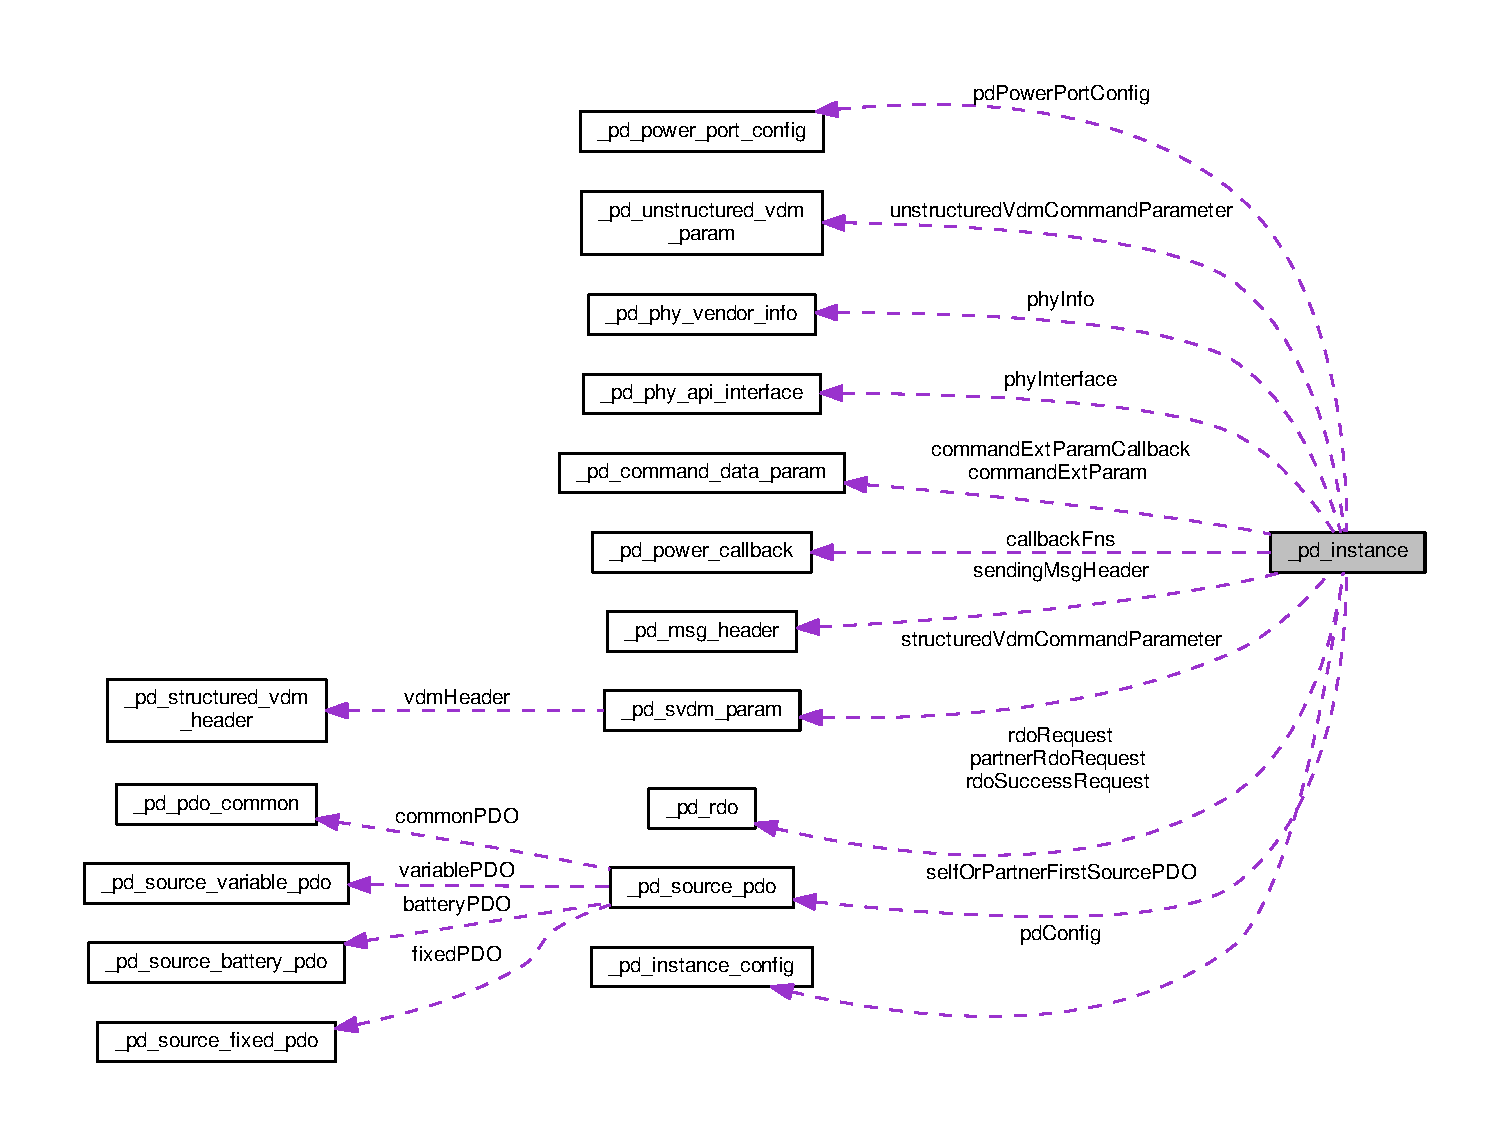
\includegraphics[width=350pt]{struct__pd__instance__coll__graph}
\end{center}
\end{figure}
\subsection*{Public Attributes}
\begin{DoxyCompactItemize}
\item 
\hyperlink{group__usb__pd__stack_gab39e13c5c0808b2fe22b7dac49db335a}{pd\-\_\-phy\-\_\-handle} \hyperlink{struct__pd__instance_a7c1184292efe9a5ae30b6ac422c1e9f4}{pd\-Phy\-Handle}
\item 
\hyperlink{group__usb__pd__stack_gafa6034f9e204836697da1f2fc996cbad}{pd\-\_\-instance\-\_\-config\-\_\-t} $\ast$ \hyperlink{struct__pd__instance_a2d9a457d63da9c4cb5e3feece0cbf3ec}{pd\-Config}
\item 
\hyperlink{group__usb__pd__stack_ga1897a14a90aea9e4b0e7cf1e5b4ea449}{pd\-\_\-power\-\_\-port\-\_\-config\-\_\-t} $\ast$ \hyperlink{struct__pd__instance_aa7854ddf70e64f92b178cc5d787037a2}{pd\-Power\-Port\-Config}
\item 
const \hyperlink{group__usb__pd__phy__drv_ga9494f6971e6132cb70c98b92f45af74f}{pd\-\_\-phy\-\_\-api\-\_\-interface\-\_\-t} $\ast$ \hyperlink{struct__pd__instance_adbed7b2cd53df40e0611a8879c903339}{phy\-Interface}
\item 
\hyperlink{group__usb__pd__stack_ga270b6a571db4fa308a1cce3df32f5439}{pd\-\_\-stack\-\_\-callback\-\_\-t} \hyperlink{struct__pd__instance_a3718a4d773d48136d66706ac063ef948}{pd\-Callback}
\item 
\hyperlink{group__usb__pd__stack_gaf1142461de7d7dcc6268c286ba956265}{pd\-\_\-power\-\_\-handle\-\_\-callback\-\_\-t} $\ast$ \hyperlink{struct__pd__instance_a519457e415e4eb39231c3e32316ffc83}{callback\-Fns}
\item 
void $\ast$ \hyperlink{struct__pd__instance_a0eb7710a55cb5eb2a57355d772b26f74}{callback\-Param}
\item 
\hyperlink{group__usb__os__abstraction_gaa5faa1787d0c772a2cf101b3eaf654f6}{usb\-\_\-osa\-\_\-event\-\_\-handle} \hyperlink{struct__pd__instance_ab04e9fcc994b2547509169e07ab21465}{task\-Event\-Handle}
\item 
\hyperlink{group__usb__pd__stack_ga4dcb1103574222cf94d4b45128f2b884}{pd\-\_\-rdo\-\_\-t} \hyperlink{struct__pd__instance_a199dd2b0ea66f8eb7e67714c4a4264a5}{rdo\-Request}
\item 
\hyperlink{group__usb__pd__stack_ga4dcb1103574222cf94d4b45128f2b884}{pd\-\_\-rdo\-\_\-t} \hyperlink{struct__pd__instance_a3e7e606f531f84a6f70e3a49de313f41}{rdo\-Success\-Request}
\item 
\hyperlink{group__usb__pd__stack_ga4dcb1103574222cf94d4b45128f2b884}{pd\-\_\-rdo\-\_\-t} \hyperlink{struct__pd__instance_ad8cdcafc4b643a8f147febada1cd5704}{partner\-Rdo\-Request}
\item 
\hyperlink{group__usb__pd__stack_gae3adfd5239231ab405b04bef0ae1df5a}{pd\-\_\-source\-\_\-pdo\-\_\-t} \hyperlink{struct__pd__instance_ad5c623ba7be298aa8ecdad50a298d609}{self\-Or\-Partner\-First\-Source\-P\-D\-O}
\item 
\hyperlink{group__usb__pd__phy__drv_ga4930ef145bdc6eb8fb43bb431eb305da}{pd\-\_\-phy\-\_\-vendor\-\_\-info\-\_\-t} \hyperlink{struct__pd__instance_a8cf1d14cc029410e591cbfe30d5b2cd9}{phy\-Info}
\item 
volatile uint32\-\_\-t \hyperlink{struct__pd__instance_a00d9a2aa7fd533c3ac15236b61e894f0}{timrs\-Running\-State} \mbox{[}32/32\mbox{]}
\item 
volatile uint32\-\_\-t \hyperlink{struct__pd__instance_a4e19ba81575c13f30d4482d5ac141573}{timrs\-Time\-Out\-State} \mbox{[}32/32\mbox{]}
\item 
volatile uint16\-\_\-t \hyperlink{struct__pd__instance_a10267d00b21df313fb3064255d161d6b}{timrs\-Time\-Value} \mbox{[}32\mbox{]}
\item 
uint32\-\_\-t \hyperlink{struct__pd__instance_ad959040fa9c36726ad10ccc9e46876e9}{psm\-Cable\-Identities} \mbox{[}7\mbox{]}
\item 
uint8\-\_\-t $\ast$ \hyperlink{struct__pd__instance_aa2afb566f855b4b00bcdf335d8d997a3}{receiving\-Data\-Buffer}
\item 
uint32\-\_\-t \hyperlink{struct__pd__instance_a1112b16cc2add6100cbf81134f74caf1}{receiving\-Data} \mbox{[}8\mbox{]}
\item 
uint32\-\_\-t \hyperlink{struct__pd__instance_a6c867a07c66667ea3eab5ec882090e09}{sending\-Data} \mbox{[}8\mbox{]}
\item 
volatile uint32\-\_\-t $\ast$ \hyperlink{struct__pd__instance_accf867a3b224d5e7708c3167b49eb259}{received\-Data}
\item 
volatile uint32\-\_\-t \hyperlink{struct__pd__instance_a0d570b6b188a0e6756df839f35f346b5}{received\-Length}
\item 
volatile \hyperlink{group__usb__pd__stack_ga38ef16bfe01e9e07d6b3ac77648c6bee}{pd\-\_\-msg\-\_\-header\-\_\-t} \hyperlink{struct__pd__instance_a6031ed1c3ec10c04ea5daf9a76485f68}{sending\-Msg\-Header}
\item 
volatile \hyperlink{group__usb__pd__stack_ga04a1f331d9807a70ab9bb753f5ed1c80}{pd\-\_\-status\-\_\-t} \hyperlink{struct__pd__instance_a64014dae5dccd1adb710c12fcc8b23cf}{receive\-Result}
\item 
volatile \hyperlink{group__usb__pd__stack_ga04a1f331d9807a70ab9bb753f5ed1c80}{pd\-\_\-status\-\_\-t} \hyperlink{struct__pd__instance_ac02af68a4c0e36f39a1b3203c5638c2b}{sending\-Result}
\item 
volatile uint8\-\_\-t \hyperlink{struct__pd__instance_ac2c84f6b1ff2b7c8a1b1ac9ee358ef0e}{receive\-State}
\item 
volatile uint8\-\_\-t \hyperlink{struct__pd__instance_a21c5a4229c4d099a6840ac2d13a5a32e}{received\-Sop}
\item 
volatile uint8\-\_\-t \hyperlink{struct__pd__instance_af70b04cd5c8187c6a0424dea57205e8c}{hard\-Reset\-Received}
\item 
volatile uint8\-\_\-t \hyperlink{struct__pd__instance_ad19f652f47e237558f18b224b5d57e23}{sending\-State}
\item 
volatile uint8\-\_\-t \hyperlink{struct__pd__instance_a4649287fd50df5de2602a502655f7bb2}{occupied}
\item 
uint8\-\_\-t \hyperlink{struct__pd__instance_afae58a0b309262dc37fac1f4f92c6d7b}{phy\-Type}
\item 
\hyperlink{group__usb__pd__stack_gacedc4a601815782eff03211731ea2c7a}{pd\-\_\-svdm\-\_\-command\-\_\-param\-\_\-t} \hyperlink{struct__pd__instance_a37746abee0ebb0169f8a1e7227d8645b}{structured\-Vdm\-Command\-Parameter}
\item 
\hyperlink{group__usb__pd__stack_ga353c18d85300f7ee60dab2241f2e1310}{pd\-\_\-unstructured\-\_\-vdm\-\_\-command\-\_\-param\-\_\-t} \hyperlink{struct__pd__instance_a38406a43dd1715456b1111ad897d8120}{unstructured\-Vdm\-Command\-Parameter}
\item 
\hyperlink{group__usb__pd__stack_gac903dadc9a1dffbaac4f91f982a038de}{pd\-\_\-command\-\_\-data\-\_\-param\-\_\-t} \hyperlink{struct__pd__instance_a05d172382020769919cd2afd088fe164}{command\-Ext\-Param}
\item 
\hyperlink{group__usb__pd__stack_gac903dadc9a1dffbaac4f91f982a038de}{pd\-\_\-command\-\_\-data\-\_\-param\-\_\-t} \hyperlink{struct__pd__instance_a93988814b8f6bf439021e6ff46fff207}{command\-Ext\-Param\-Callback}
\item 
uint32\-\_\-t \hyperlink{struct__pd__instance_a6fb96c0e5c3f5f6f05f9964541078e3a}{dpm\-Msg\-Bits}
\item 
uint32\-\_\-t \hyperlink{struct__pd__instance_a483c8ee561c9edc878c4462f8b073027}{alert\-A\-D\-O}
\item 
volatile uint8\-\_\-t \hyperlink{struct__pd__instance_aece677cf125a9acd9546c1bc0f75b5b9}{command\-Is\-Initiator}
\item 
\hyperlink{usb__pd__spec_8h_a46ab85ad33154cc61c1fa42d5ca24944}{pd\-\_\-psm\-\_\-state\-\_\-t} \hyperlink{struct__pd__instance_a3bc0e6fd670db006ccb2ba39dadedcc5}{psm\-Cur\-State}
\item 
\hyperlink{usb__pd__spec_8h_a46ab85ad33154cc61c1fa42d5ca24944}{pd\-\_\-psm\-\_\-state\-\_\-t} \hyperlink{struct__pd__instance_ab770921a8b608fc49a0d564a22a1aad3}{psm\-New\-State}
\item 
\hyperlink{usb__pd__spec_8h_a46ab85ad33154cc61c1fa42d5ca24944}{pd\-\_\-psm\-\_\-state\-\_\-t} \hyperlink{struct__pd__instance_a4a53a203e61b44957d56747fb7c8a312}{psm\-Interrupted\-State}
\item 
\hyperlink{usb__pd__spec_8h_a46ab85ad33154cc61c1fa42d5ca24944}{pd\-\_\-psm\-\_\-state\-\_\-t} \hyperlink{struct__pd__instance_ad376945c62a0066016cf2652e62da35a}{psm\-Secondary\-State} \mbox{[}3\mbox{]}
\item 
\hyperlink{usb__pd__spec_8h_a46ab85ad33154cc61c1fa42d5ca24944}{pd\-\_\-psm\-\_\-state\-\_\-t} \hyperlink{struct__pd__instance_a539e99b475d489e955238343ca800918}{psm\-New\-Secondary\-State} \mbox{[}3\mbox{]}
\item 
\hyperlink{usb__pd__spec_8h_a46ab85ad33154cc61c1fa42d5ca24944}{pd\-\_\-psm\-\_\-state\-\_\-t} \hyperlink{struct__pd__instance_a708b6e13ca54fe83d4200c3fff80a820}{psm\-Dr\-Swap\-Prev\-State}
\item 
\hyperlink{usb__pd__spec_8h_a46ab85ad33154cc61c1fa42d5ca24944}{pd\-\_\-psm\-\_\-state\-\_\-t} \hyperlink{struct__pd__instance_a9446b569ba4bb1c6df4367bad40bf987}{psm\-Vconn\-Swap\-Prev\-State}
\item 
\hyperlink{usb__pd__spec_8h_a9a1674d34c926c8ecd0f9f70e2da0338}{Type\-C\-State\-\_\-t} \hyperlink{struct__pd__instance_a2c4dd56715311bcb898a01a7cbec1609}{cur\-Connect\-State}
\item 
uint8\-\_\-t \hyperlink{struct__pd__instance_a48293366cd7123e1c703dd01f0921304}{command\-Evaluate\-Result}
\item 
volatile uint8\-\_\-t \hyperlink{struct__pd__instance_a3ac03447bd16031091bc4b30da45576f}{asm\-Vdm\-Reply\-Msg}
\item 
uint8\-\_\-t \hyperlink{struct__pd__instance_a26c06a89ab6d2c3fbf265abd7dfc04a3}{get\-Battery\-Cap\-Data\-Block}
\item 
uint16\-\_\-t \hyperlink{struct__pd__instance_a3638013563f1cb1208f12b5930970fa2}{dpm\-Cable\-Max\-Current}
\item 
volatile uint8\-\_\-t \hyperlink{struct__pd__instance_a2edcb21b9d568937192741d32381d2b1}{initialize\-Label}
\item 
volatile uint8\-\_\-t \hyperlink{struct__pd__instance_aefbe7a5da39f65fa52efdc9cbae4d9cc}{is\-Connected}
\item 
volatile uint8\-\_\-t \hyperlink{struct__pd__instance_aa310a61602eb5d34b4b511ce4ad60f1d}{connected\-Result}
\item 
uint8\-\_\-t \hyperlink{struct__pd__instance_a6e12cc53d94812cf2a28973fae7c6a7e}{dpm\-State\-Machine}
\item 
uint8\-\_\-t \hyperlink{struct__pd__instance_a4f8aff7c9d2b914a5be9f0bd297c197c}{connect\-State}
\item 
uint8\-\_\-t \hyperlink{struct__pd__instance_aea65859fe3a8409ac66aa9f54fb119bf}{cur\-Power\-Role}
\item 
uint8\-\_\-t \hyperlink{struct__pd__instance_a766dd3de4bdd34f1eebcd41d1425327a}{cur\-Data\-Role}
\item 
uint8\-\_\-t \hyperlink{struct__pd__instance_a19172e14529d11e2239205c36accdfba}{command\-Processing}
\item 
uint8\-\_\-t \hyperlink{struct__pd__instance_afcd5caf46554e0640a45ac547d7bacf0}{vdm\-Exit\-Received} \mbox{[}3\mbox{]}
\item 
uint8\-\_\-t \hyperlink{struct__pd__instance_a0087c1b246d026c864194bf77ebcf654}{cc\-Used}
\item 
uint8\-\_\-t \hyperlink{struct__pd__instance_af4167196731cf1a846f23c4d6473181c}{in\-Progress}
\item 
uint8\-\_\-t \hyperlink{struct__pd__instance_a4905e96236b6de63bba2c1d34c5a0a8b}{vbus\-Discharge\-In\-Progress}
\item 
volatile uint8\-\_\-t \hyperlink{struct__pd__instance_a007de2aa1ac9ae814d10d26a949dd61d}{pending\-S\-O\-P}
\item 
uint8\-\_\-t \hyperlink{struct__pd__instance_a5905690cc5a12a0758be0574d4bc262e}{ra\-Present}
\item 
uint8\-\_\-t \hyperlink{struct__pd__instance_a1b1254d08a7d1b7809c37ac0e1253ed5}{psm\-Presently\-Vconn\-Source}
\item 
uint8\-\_\-t \hyperlink{struct__pd__instance_aec0a54cf65dfa1880cb41eccb8caa043}{psm\-Vdm\-Active\-Mode\-Valid\-Mask}
\item 
uint8\-\_\-t \hyperlink{struct__pd__instance_aa73d40dd2f32910810c5b58fd7ada98f}{psm\-V\-D\-M\-Busy\-Wait\-Dpm\-Msg}
\item 
uint8\-\_\-t \hyperlink{struct__pd__instance_adb289c40585aa5170d8208d0202f55e5}{psm\-Hard\-Reset\-Count}
\item 
uint8\-\_\-t \hyperlink{struct__pd__instance_aec485d99451925aec7a6237f92791cd3}{psm\-Caps\-Counter}
\item 
uint8\-\_\-t \hyperlink{struct__pd__instance_a80a39754275c80b96db63d02b7e049ec}{psm\-Soft\-Reset\-Sop}
\item 
uint8\-\_\-t \hyperlink{struct__pd__instance_af7c28b72771ce442ee733892186c4e6c}{revision}
\item 
volatile uint8\-\_\-t \hyperlink{struct__pd__instance_abb01fbdcfbc66eba6c7d5d85e91e62e4}{no\-Connect\-But\-V\-Bus\-Exit}
\item 
volatile uint8\-\_\-t \hyperlink{struct__pd__instance_a46b9d34b21328c188c161825bf8e8217}{rd\-Rp\-Error\-Count}
\item 
volatile uint16\-\_\-t \hyperlink{struct__pd__instance_a2505651a0001ea647306dbd800927778}{wait\-Time}
\item 
uint8\-\_\-t \hyperlink{struct__pd__instance_a88df7992251beb09fa2888f4ddf9766f}{try\-S\-N\-K\-State}\-: 1
\item 
uint8\-\_\-t \hyperlink{struct__pd__instance_ac25d2d3e3181280ef797e42323c60053}{psm\-Goto\-Min\-Tx}\-: 1
\item 
uint8\-\_\-t \hyperlink{struct__pd__instance_af189a6cdfc3021280df10fe8a7a86a8f}{psm\-Goto\-Min\-Rx}\-: 1
\item 
uint8\-\_\-t \hyperlink{struct__pd__instance_aea1b390f81517cb7ef24eacda944f4ec}{enter\-Attached\-Src\-From\-Attach\-Wait\-S\-N\-K}\-: 1
\item 
uint8\-\_\-t \hyperlink{struct__pd__instance_a83ce4a62d8bb8f280b4fb7fdbcdc8d5a}{enter\-Try\-S\-N\-K\-From\-Powered\-Acc}\-: 1
\item 
uint8\-\_\-t \hyperlink{struct__pd__instance_ae190e16d15f42371ac82937f08371c98}{cc1\-Monitor}\-: 1
\item 
uint8\-\_\-t \hyperlink{struct__pd__instance_af6e379f0550864c814e92c07732b6ea9}{cc2\-Monitor}\-: 1
\item 
uint8\-\_\-t \hyperlink{struct__pd__instance_a817d87a8494e9f703f8854e7fdf32dfd}{psm\-Hard\-Reset\-Needs\-V\-Safe0\-V}\-: 1
\item 
uint8\-\_\-t \hyperlink{struct__pd__instance_afc95df19affca8d292c845f328349f8f}{psm\-Presently\-Pd\-Connected}\-: 1
\item 
uint8\-\_\-t \hyperlink{struct__pd__instance_ab15695a76307bdc413424030ad701a47}{psm\-Previously\-Pd\-Connected}\-: 1
\item 
uint8\-\_\-t \hyperlink{struct__pd__instance_a7be408d709efe6ec210d68a3d4098cc9}{psm\-Cable\-Plug\-Reset\-Needed}\-: 1
\item 
uint8\-\_\-t \hyperlink{struct__pd__instance_af7a143c0a8141d2a359a5ce18eb708f6}{psm\-Cable\-Discoveried}\-: 1
\item 
uint8\-\_\-t \hyperlink{struct__pd__instance_a685445e828df5a05b1084fd0ea75c10a}{psm\-Snk\-Receive\-Rdo\-Wait\-Retry}\-: 1
\item 
uint8\-\_\-t \hyperlink{struct__pd__instance_a23dce9c00575a5fd5ed120e08e9c4412}{psm\-Explicit\-Contract\-Existed}\-: 1
\item 
volatile uint8\-\_\-t \hyperlink{struct__pd__instance_a7420286a3fc5b58010ff2dc607a8d77a}{asm\-Hard\-Reset\-Snk\-Processing}\-: 1
\item 
uint8\-\_\-t \hyperlink{struct__pd__instance_af61039550d3e5b4f070ac74ed3e711a3}{unchunked\-Feature}\-: 1
\item 
volatile uint8\-\_\-t \hyperlink{struct__pd__instance_ac9c3ed52c22920ccea6ecd0d1e0f6651}{command\-Src\-Owner}\-: 1
\item 
volatile uint8\-\_\-t \hyperlink{struct__pd__instance_ae144ddf17de553d955ce28afa535d4f9}{alert\-Wait\-Reply}\-: 1
\item 
volatile uint8\-\_\-t \hyperlink{struct__pd__instance_a3ec5ee7a312bb3b142e16fc8ba019476}{fr5\-V\-Opened}\-: 1
\item 
volatile uint8\-\_\-t \hyperlink{struct__pd__instance_ac9684a4a5a96ac21f503ad702a245a7e}{fr\-Swap\-Received}\-: 1
\item 
volatile uint8\-\_\-t \hyperlink{struct__pd__instance_a7ac775fb724d971003420ee22adc0fbe}{enable\-Receive}\-: 1
\item 
volatile uint8\-\_\-t \hyperlink{struct__pd__instance_a3b09927227c17d95712a2af3d5f921f2}{enter\-Src\-From\-Swap}\-: 1
\end{DoxyCompactItemize}


\subsection{Member Data Documentation}
\hypertarget{struct__pd__instance_a483c8ee561c9edc878c4462f8b073027}{\index{\-\_\-pd\-\_\-instance@{\-\_\-pd\-\_\-instance}!alert\-A\-D\-O@{alert\-A\-D\-O}}
\index{alert\-A\-D\-O@{alert\-A\-D\-O}!_pd_instance@{\-\_\-pd\-\_\-instance}}
\subsubsection[{alert\-A\-D\-O}]{\setlength{\rightskip}{0pt plus 5cm}uint32\-\_\-t \-\_\-pd\-\_\-instance\-::alert\-A\-D\-O}}\label{struct__pd__instance_a483c8ee561c9edc878c4462f8b073027}
\hypertarget{struct__pd__instance_ae144ddf17de553d955ce28afa535d4f9}{\index{\-\_\-pd\-\_\-instance@{\-\_\-pd\-\_\-instance}!alert\-Wait\-Reply@{alert\-Wait\-Reply}}
\index{alert\-Wait\-Reply@{alert\-Wait\-Reply}!_pd_instance@{\-\_\-pd\-\_\-instance}}
\subsubsection[{alert\-Wait\-Reply}]{\setlength{\rightskip}{0pt plus 5cm}volatile uint8\-\_\-t \-\_\-pd\-\_\-instance\-::alert\-Wait\-Reply}}\label{struct__pd__instance_ae144ddf17de553d955ce28afa535d4f9}
\hypertarget{struct__pd__instance_a7420286a3fc5b58010ff2dc607a8d77a}{\index{\-\_\-pd\-\_\-instance@{\-\_\-pd\-\_\-instance}!asm\-Hard\-Reset\-Snk\-Processing@{asm\-Hard\-Reset\-Snk\-Processing}}
\index{asm\-Hard\-Reset\-Snk\-Processing@{asm\-Hard\-Reset\-Snk\-Processing}!_pd_instance@{\-\_\-pd\-\_\-instance}}
\subsubsection[{asm\-Hard\-Reset\-Snk\-Processing}]{\setlength{\rightskip}{0pt plus 5cm}volatile uint8\-\_\-t \-\_\-pd\-\_\-instance\-::asm\-Hard\-Reset\-Snk\-Processing}}\label{struct__pd__instance_a7420286a3fc5b58010ff2dc607a8d77a}
\hypertarget{struct__pd__instance_a3ac03447bd16031091bc4b30da45576f}{\index{\-\_\-pd\-\_\-instance@{\-\_\-pd\-\_\-instance}!asm\-Vdm\-Reply\-Msg@{asm\-Vdm\-Reply\-Msg}}
\index{asm\-Vdm\-Reply\-Msg@{asm\-Vdm\-Reply\-Msg}!_pd_instance@{\-\_\-pd\-\_\-instance}}
\subsubsection[{asm\-Vdm\-Reply\-Msg}]{\setlength{\rightskip}{0pt plus 5cm}volatile uint8\-\_\-t \-\_\-pd\-\_\-instance\-::asm\-Vdm\-Reply\-Msg}}\label{struct__pd__instance_a3ac03447bd16031091bc4b30da45576f}
\hypertarget{struct__pd__instance_a519457e415e4eb39231c3e32316ffc83}{\index{\-\_\-pd\-\_\-instance@{\-\_\-pd\-\_\-instance}!callback\-Fns@{callback\-Fns}}
\index{callback\-Fns@{callback\-Fns}!_pd_instance@{\-\_\-pd\-\_\-instance}}
\subsubsection[{callback\-Fns}]{\setlength{\rightskip}{0pt plus 5cm}{\bf pd\-\_\-power\-\_\-handle\-\_\-callback\-\_\-t}$\ast$ \-\_\-pd\-\_\-instance\-::callback\-Fns}}\label{struct__pd__instance_a519457e415e4eb39231c3e32316ffc83}
\hypertarget{struct__pd__instance_a0eb7710a55cb5eb2a57355d772b26f74}{\index{\-\_\-pd\-\_\-instance@{\-\_\-pd\-\_\-instance}!callback\-Param@{callback\-Param}}
\index{callback\-Param@{callback\-Param}!_pd_instance@{\-\_\-pd\-\_\-instance}}
\subsubsection[{callback\-Param}]{\setlength{\rightskip}{0pt plus 5cm}void$\ast$ \-\_\-pd\-\_\-instance\-::callback\-Param}}\label{struct__pd__instance_a0eb7710a55cb5eb2a57355d772b26f74}
\hypertarget{struct__pd__instance_ae190e16d15f42371ac82937f08371c98}{\index{\-\_\-pd\-\_\-instance@{\-\_\-pd\-\_\-instance}!cc1\-Monitor@{cc1\-Monitor}}
\index{cc1\-Monitor@{cc1\-Monitor}!_pd_instance@{\-\_\-pd\-\_\-instance}}
\subsubsection[{cc1\-Monitor}]{\setlength{\rightskip}{0pt plus 5cm}uint8\-\_\-t \-\_\-pd\-\_\-instance\-::cc1\-Monitor}}\label{struct__pd__instance_ae190e16d15f42371ac82937f08371c98}
\hypertarget{struct__pd__instance_af6e379f0550864c814e92c07732b6ea9}{\index{\-\_\-pd\-\_\-instance@{\-\_\-pd\-\_\-instance}!cc2\-Monitor@{cc2\-Monitor}}
\index{cc2\-Monitor@{cc2\-Monitor}!_pd_instance@{\-\_\-pd\-\_\-instance}}
\subsubsection[{cc2\-Monitor}]{\setlength{\rightskip}{0pt plus 5cm}uint8\-\_\-t \-\_\-pd\-\_\-instance\-::cc2\-Monitor}}\label{struct__pd__instance_af6e379f0550864c814e92c07732b6ea9}
\hypertarget{struct__pd__instance_a0087c1b246d026c864194bf77ebcf654}{\index{\-\_\-pd\-\_\-instance@{\-\_\-pd\-\_\-instance}!cc\-Used@{cc\-Used}}
\index{cc\-Used@{cc\-Used}!_pd_instance@{\-\_\-pd\-\_\-instance}}
\subsubsection[{cc\-Used}]{\setlength{\rightskip}{0pt plus 5cm}uint8\-\_\-t \-\_\-pd\-\_\-instance\-::cc\-Used}}\label{struct__pd__instance_a0087c1b246d026c864194bf77ebcf654}
\hypertarget{struct__pd__instance_a48293366cd7123e1c703dd01f0921304}{\index{\-\_\-pd\-\_\-instance@{\-\_\-pd\-\_\-instance}!command\-Evaluate\-Result@{command\-Evaluate\-Result}}
\index{command\-Evaluate\-Result@{command\-Evaluate\-Result}!_pd_instance@{\-\_\-pd\-\_\-instance}}
\subsubsection[{command\-Evaluate\-Result}]{\setlength{\rightskip}{0pt plus 5cm}uint8\-\_\-t \-\_\-pd\-\_\-instance\-::command\-Evaluate\-Result}}\label{struct__pd__instance_a48293366cd7123e1c703dd01f0921304}
\hypertarget{struct__pd__instance_a05d172382020769919cd2afd088fe164}{\index{\-\_\-pd\-\_\-instance@{\-\_\-pd\-\_\-instance}!command\-Ext\-Param@{command\-Ext\-Param}}
\index{command\-Ext\-Param@{command\-Ext\-Param}!_pd_instance@{\-\_\-pd\-\_\-instance}}
\subsubsection[{command\-Ext\-Param}]{\setlength{\rightskip}{0pt plus 5cm}{\bf pd\-\_\-command\-\_\-data\-\_\-param\-\_\-t} \-\_\-pd\-\_\-instance\-::command\-Ext\-Param}}\label{struct__pd__instance_a05d172382020769919cd2afd088fe164}
\hypertarget{struct__pd__instance_a93988814b8f6bf439021e6ff46fff207}{\index{\-\_\-pd\-\_\-instance@{\-\_\-pd\-\_\-instance}!command\-Ext\-Param\-Callback@{command\-Ext\-Param\-Callback}}
\index{command\-Ext\-Param\-Callback@{command\-Ext\-Param\-Callback}!_pd_instance@{\-\_\-pd\-\_\-instance}}
\subsubsection[{command\-Ext\-Param\-Callback}]{\setlength{\rightskip}{0pt plus 5cm}{\bf pd\-\_\-command\-\_\-data\-\_\-param\-\_\-t} \-\_\-pd\-\_\-instance\-::command\-Ext\-Param\-Callback}}\label{struct__pd__instance_a93988814b8f6bf439021e6ff46fff207}
\hypertarget{struct__pd__instance_aece677cf125a9acd9546c1bc0f75b5b9}{\index{\-\_\-pd\-\_\-instance@{\-\_\-pd\-\_\-instance}!command\-Is\-Initiator@{command\-Is\-Initiator}}
\index{command\-Is\-Initiator@{command\-Is\-Initiator}!_pd_instance@{\-\_\-pd\-\_\-instance}}
\subsubsection[{command\-Is\-Initiator}]{\setlength{\rightskip}{0pt plus 5cm}volatile uint8\-\_\-t \-\_\-pd\-\_\-instance\-::command\-Is\-Initiator}}\label{struct__pd__instance_aece677cf125a9acd9546c1bc0f75b5b9}
\hypertarget{struct__pd__instance_a19172e14529d11e2239205c36accdfba}{\index{\-\_\-pd\-\_\-instance@{\-\_\-pd\-\_\-instance}!command\-Processing@{command\-Processing}}
\index{command\-Processing@{command\-Processing}!_pd_instance@{\-\_\-pd\-\_\-instance}}
\subsubsection[{command\-Processing}]{\setlength{\rightskip}{0pt plus 5cm}uint8\-\_\-t \-\_\-pd\-\_\-instance\-::command\-Processing}}\label{struct__pd__instance_a19172e14529d11e2239205c36accdfba}
\hypertarget{struct__pd__instance_ac9c3ed52c22920ccea6ecd0d1e0f6651}{\index{\-\_\-pd\-\_\-instance@{\-\_\-pd\-\_\-instance}!command\-Src\-Owner@{command\-Src\-Owner}}
\index{command\-Src\-Owner@{command\-Src\-Owner}!_pd_instance@{\-\_\-pd\-\_\-instance}}
\subsubsection[{command\-Src\-Owner}]{\setlength{\rightskip}{0pt plus 5cm}volatile uint8\-\_\-t \-\_\-pd\-\_\-instance\-::command\-Src\-Owner}}\label{struct__pd__instance_ac9c3ed52c22920ccea6ecd0d1e0f6651}
\hypertarget{struct__pd__instance_aa310a61602eb5d34b4b511ce4ad60f1d}{\index{\-\_\-pd\-\_\-instance@{\-\_\-pd\-\_\-instance}!connected\-Result@{connected\-Result}}
\index{connected\-Result@{connected\-Result}!_pd_instance@{\-\_\-pd\-\_\-instance}}
\subsubsection[{connected\-Result}]{\setlength{\rightskip}{0pt plus 5cm}volatile uint8\-\_\-t \-\_\-pd\-\_\-instance\-::connected\-Result}}\label{struct__pd__instance_aa310a61602eb5d34b4b511ce4ad60f1d}
\hypertarget{struct__pd__instance_a4f8aff7c9d2b914a5be9f0bd297c197c}{\index{\-\_\-pd\-\_\-instance@{\-\_\-pd\-\_\-instance}!connect\-State@{connect\-State}}
\index{connect\-State@{connect\-State}!_pd_instance@{\-\_\-pd\-\_\-instance}}
\subsubsection[{connect\-State}]{\setlength{\rightskip}{0pt plus 5cm}uint8\-\_\-t \-\_\-pd\-\_\-instance\-::connect\-State}}\label{struct__pd__instance_a4f8aff7c9d2b914a5be9f0bd297c197c}
\hypertarget{struct__pd__instance_a2c4dd56715311bcb898a01a7cbec1609}{\index{\-\_\-pd\-\_\-instance@{\-\_\-pd\-\_\-instance}!cur\-Connect\-State@{cur\-Connect\-State}}
\index{cur\-Connect\-State@{cur\-Connect\-State}!_pd_instance@{\-\_\-pd\-\_\-instance}}
\subsubsection[{cur\-Connect\-State}]{\setlength{\rightskip}{0pt plus 5cm}{\bf Type\-C\-State\-\_\-t} \-\_\-pd\-\_\-instance\-::cur\-Connect\-State}}\label{struct__pd__instance_a2c4dd56715311bcb898a01a7cbec1609}
\hypertarget{struct__pd__instance_a766dd3de4bdd34f1eebcd41d1425327a}{\index{\-\_\-pd\-\_\-instance@{\-\_\-pd\-\_\-instance}!cur\-Data\-Role@{cur\-Data\-Role}}
\index{cur\-Data\-Role@{cur\-Data\-Role}!_pd_instance@{\-\_\-pd\-\_\-instance}}
\subsubsection[{cur\-Data\-Role}]{\setlength{\rightskip}{0pt plus 5cm}uint8\-\_\-t \-\_\-pd\-\_\-instance\-::cur\-Data\-Role}}\label{struct__pd__instance_a766dd3de4bdd34f1eebcd41d1425327a}
\hypertarget{struct__pd__instance_aea65859fe3a8409ac66aa9f54fb119bf}{\index{\-\_\-pd\-\_\-instance@{\-\_\-pd\-\_\-instance}!cur\-Power\-Role@{cur\-Power\-Role}}
\index{cur\-Power\-Role@{cur\-Power\-Role}!_pd_instance@{\-\_\-pd\-\_\-instance}}
\subsubsection[{cur\-Power\-Role}]{\setlength{\rightskip}{0pt plus 5cm}uint8\-\_\-t \-\_\-pd\-\_\-instance\-::cur\-Power\-Role}}\label{struct__pd__instance_aea65859fe3a8409ac66aa9f54fb119bf}
\hypertarget{struct__pd__instance_a3638013563f1cb1208f12b5930970fa2}{\index{\-\_\-pd\-\_\-instance@{\-\_\-pd\-\_\-instance}!dpm\-Cable\-Max\-Current@{dpm\-Cable\-Max\-Current}}
\index{dpm\-Cable\-Max\-Current@{dpm\-Cable\-Max\-Current}!_pd_instance@{\-\_\-pd\-\_\-instance}}
\subsubsection[{dpm\-Cable\-Max\-Current}]{\setlength{\rightskip}{0pt plus 5cm}uint16\-\_\-t \-\_\-pd\-\_\-instance\-::dpm\-Cable\-Max\-Current}}\label{struct__pd__instance_a3638013563f1cb1208f12b5930970fa2}
\hypertarget{struct__pd__instance_a6fb96c0e5c3f5f6f05f9964541078e3a}{\index{\-\_\-pd\-\_\-instance@{\-\_\-pd\-\_\-instance}!dpm\-Msg\-Bits@{dpm\-Msg\-Bits}}
\index{dpm\-Msg\-Bits@{dpm\-Msg\-Bits}!_pd_instance@{\-\_\-pd\-\_\-instance}}
\subsubsection[{dpm\-Msg\-Bits}]{\setlength{\rightskip}{0pt plus 5cm}uint32\-\_\-t \-\_\-pd\-\_\-instance\-::dpm\-Msg\-Bits}}\label{struct__pd__instance_a6fb96c0e5c3f5f6f05f9964541078e3a}
\hypertarget{struct__pd__instance_a6e12cc53d94812cf2a28973fae7c6a7e}{\index{\-\_\-pd\-\_\-instance@{\-\_\-pd\-\_\-instance}!dpm\-State\-Machine@{dpm\-State\-Machine}}
\index{dpm\-State\-Machine@{dpm\-State\-Machine}!_pd_instance@{\-\_\-pd\-\_\-instance}}
\subsubsection[{dpm\-State\-Machine}]{\setlength{\rightskip}{0pt plus 5cm}uint8\-\_\-t \-\_\-pd\-\_\-instance\-::dpm\-State\-Machine}}\label{struct__pd__instance_a6e12cc53d94812cf2a28973fae7c6a7e}
\hypertarget{struct__pd__instance_a7ac775fb724d971003420ee22adc0fbe}{\index{\-\_\-pd\-\_\-instance@{\-\_\-pd\-\_\-instance}!enable\-Receive@{enable\-Receive}}
\index{enable\-Receive@{enable\-Receive}!_pd_instance@{\-\_\-pd\-\_\-instance}}
\subsubsection[{enable\-Receive}]{\setlength{\rightskip}{0pt plus 5cm}volatile uint8\-\_\-t \-\_\-pd\-\_\-instance\-::enable\-Receive}}\label{struct__pd__instance_a7ac775fb724d971003420ee22adc0fbe}
\hypertarget{struct__pd__instance_aea1b390f81517cb7ef24eacda944f4ec}{\index{\-\_\-pd\-\_\-instance@{\-\_\-pd\-\_\-instance}!enter\-Attached\-Src\-From\-Attach\-Wait\-S\-N\-K@{enter\-Attached\-Src\-From\-Attach\-Wait\-S\-N\-K}}
\index{enter\-Attached\-Src\-From\-Attach\-Wait\-S\-N\-K@{enter\-Attached\-Src\-From\-Attach\-Wait\-S\-N\-K}!_pd_instance@{\-\_\-pd\-\_\-instance}}
\subsubsection[{enter\-Attached\-Src\-From\-Attach\-Wait\-S\-N\-K}]{\setlength{\rightskip}{0pt plus 5cm}uint8\-\_\-t \-\_\-pd\-\_\-instance\-::enter\-Attached\-Src\-From\-Attach\-Wait\-S\-N\-K}}\label{struct__pd__instance_aea1b390f81517cb7ef24eacda944f4ec}
\hypertarget{struct__pd__instance_a3b09927227c17d95712a2af3d5f921f2}{\index{\-\_\-pd\-\_\-instance@{\-\_\-pd\-\_\-instance}!enter\-Src\-From\-Swap@{enter\-Src\-From\-Swap}}
\index{enter\-Src\-From\-Swap@{enter\-Src\-From\-Swap}!_pd_instance@{\-\_\-pd\-\_\-instance}}
\subsubsection[{enter\-Src\-From\-Swap}]{\setlength{\rightskip}{0pt plus 5cm}volatile uint8\-\_\-t \-\_\-pd\-\_\-instance\-::enter\-Src\-From\-Swap}}\label{struct__pd__instance_a3b09927227c17d95712a2af3d5f921f2}
\hypertarget{struct__pd__instance_a83ce4a62d8bb8f280b4fb7fdbcdc8d5a}{\index{\-\_\-pd\-\_\-instance@{\-\_\-pd\-\_\-instance}!enter\-Try\-S\-N\-K\-From\-Powered\-Acc@{enter\-Try\-S\-N\-K\-From\-Powered\-Acc}}
\index{enter\-Try\-S\-N\-K\-From\-Powered\-Acc@{enter\-Try\-S\-N\-K\-From\-Powered\-Acc}!_pd_instance@{\-\_\-pd\-\_\-instance}}
\subsubsection[{enter\-Try\-S\-N\-K\-From\-Powered\-Acc}]{\setlength{\rightskip}{0pt plus 5cm}uint8\-\_\-t \-\_\-pd\-\_\-instance\-::enter\-Try\-S\-N\-K\-From\-Powered\-Acc}}\label{struct__pd__instance_a83ce4a62d8bb8f280b4fb7fdbcdc8d5a}
\hypertarget{struct__pd__instance_a3ec5ee7a312bb3b142e16fc8ba019476}{\index{\-\_\-pd\-\_\-instance@{\-\_\-pd\-\_\-instance}!fr5\-V\-Opened@{fr5\-V\-Opened}}
\index{fr5\-V\-Opened@{fr5\-V\-Opened}!_pd_instance@{\-\_\-pd\-\_\-instance}}
\subsubsection[{fr5\-V\-Opened}]{\setlength{\rightskip}{0pt plus 5cm}volatile uint8\-\_\-t \-\_\-pd\-\_\-instance\-::fr5\-V\-Opened}}\label{struct__pd__instance_a3ec5ee7a312bb3b142e16fc8ba019476}
\hypertarget{struct__pd__instance_ac9684a4a5a96ac21f503ad702a245a7e}{\index{\-\_\-pd\-\_\-instance@{\-\_\-pd\-\_\-instance}!fr\-Swap\-Received@{fr\-Swap\-Received}}
\index{fr\-Swap\-Received@{fr\-Swap\-Received}!_pd_instance@{\-\_\-pd\-\_\-instance}}
\subsubsection[{fr\-Swap\-Received}]{\setlength{\rightskip}{0pt plus 5cm}volatile uint8\-\_\-t \-\_\-pd\-\_\-instance\-::fr\-Swap\-Received}}\label{struct__pd__instance_ac9684a4a5a96ac21f503ad702a245a7e}
\hypertarget{struct__pd__instance_a26c06a89ab6d2c3fbf265abd7dfc04a3}{\index{\-\_\-pd\-\_\-instance@{\-\_\-pd\-\_\-instance}!get\-Battery\-Cap\-Data\-Block@{get\-Battery\-Cap\-Data\-Block}}
\index{get\-Battery\-Cap\-Data\-Block@{get\-Battery\-Cap\-Data\-Block}!_pd_instance@{\-\_\-pd\-\_\-instance}}
\subsubsection[{get\-Battery\-Cap\-Data\-Block}]{\setlength{\rightskip}{0pt plus 5cm}uint8\-\_\-t \-\_\-pd\-\_\-instance\-::get\-Battery\-Cap\-Data\-Block}}\label{struct__pd__instance_a26c06a89ab6d2c3fbf265abd7dfc04a3}
\hypertarget{struct__pd__instance_af70b04cd5c8187c6a0424dea57205e8c}{\index{\-\_\-pd\-\_\-instance@{\-\_\-pd\-\_\-instance}!hard\-Reset\-Received@{hard\-Reset\-Received}}
\index{hard\-Reset\-Received@{hard\-Reset\-Received}!_pd_instance@{\-\_\-pd\-\_\-instance}}
\subsubsection[{hard\-Reset\-Received}]{\setlength{\rightskip}{0pt plus 5cm}volatile uint8\-\_\-t \-\_\-pd\-\_\-instance\-::hard\-Reset\-Received}}\label{struct__pd__instance_af70b04cd5c8187c6a0424dea57205e8c}
\hypertarget{struct__pd__instance_a2edcb21b9d568937192741d32381d2b1}{\index{\-\_\-pd\-\_\-instance@{\-\_\-pd\-\_\-instance}!initialize\-Label@{initialize\-Label}}
\index{initialize\-Label@{initialize\-Label}!_pd_instance@{\-\_\-pd\-\_\-instance}}
\subsubsection[{initialize\-Label}]{\setlength{\rightskip}{0pt plus 5cm}volatile uint8\-\_\-t \-\_\-pd\-\_\-instance\-::initialize\-Label}}\label{struct__pd__instance_a2edcb21b9d568937192741d32381d2b1}
\hypertarget{struct__pd__instance_af4167196731cf1a846f23c4d6473181c}{\index{\-\_\-pd\-\_\-instance@{\-\_\-pd\-\_\-instance}!in\-Progress@{in\-Progress}}
\index{in\-Progress@{in\-Progress}!_pd_instance@{\-\_\-pd\-\_\-instance}}
\subsubsection[{in\-Progress}]{\setlength{\rightskip}{0pt plus 5cm}uint8\-\_\-t \-\_\-pd\-\_\-instance\-::in\-Progress}}\label{struct__pd__instance_af4167196731cf1a846f23c4d6473181c}
\hypertarget{struct__pd__instance_aefbe7a5da39f65fa52efdc9cbae4d9cc}{\index{\-\_\-pd\-\_\-instance@{\-\_\-pd\-\_\-instance}!is\-Connected@{is\-Connected}}
\index{is\-Connected@{is\-Connected}!_pd_instance@{\-\_\-pd\-\_\-instance}}
\subsubsection[{is\-Connected}]{\setlength{\rightskip}{0pt plus 5cm}volatile uint8\-\_\-t \-\_\-pd\-\_\-instance\-::is\-Connected}}\label{struct__pd__instance_aefbe7a5da39f65fa52efdc9cbae4d9cc}
\hypertarget{struct__pd__instance_abb01fbdcfbc66eba6c7d5d85e91e62e4}{\index{\-\_\-pd\-\_\-instance@{\-\_\-pd\-\_\-instance}!no\-Connect\-But\-V\-Bus\-Exit@{no\-Connect\-But\-V\-Bus\-Exit}}
\index{no\-Connect\-But\-V\-Bus\-Exit@{no\-Connect\-But\-V\-Bus\-Exit}!_pd_instance@{\-\_\-pd\-\_\-instance}}
\subsubsection[{no\-Connect\-But\-V\-Bus\-Exit}]{\setlength{\rightskip}{0pt plus 5cm}volatile uint8\-\_\-t \-\_\-pd\-\_\-instance\-::no\-Connect\-But\-V\-Bus\-Exit}}\label{struct__pd__instance_abb01fbdcfbc66eba6c7d5d85e91e62e4}
\hypertarget{struct__pd__instance_a4649287fd50df5de2602a502655f7bb2}{\index{\-\_\-pd\-\_\-instance@{\-\_\-pd\-\_\-instance}!occupied@{occupied}}
\index{occupied@{occupied}!_pd_instance@{\-\_\-pd\-\_\-instance}}
\subsubsection[{occupied}]{\setlength{\rightskip}{0pt plus 5cm}volatile uint8\-\_\-t \-\_\-pd\-\_\-instance\-::occupied}}\label{struct__pd__instance_a4649287fd50df5de2602a502655f7bb2}
\hypertarget{struct__pd__instance_ad8cdcafc4b643a8f147febada1cd5704}{\index{\-\_\-pd\-\_\-instance@{\-\_\-pd\-\_\-instance}!partner\-Rdo\-Request@{partner\-Rdo\-Request}}
\index{partner\-Rdo\-Request@{partner\-Rdo\-Request}!_pd_instance@{\-\_\-pd\-\_\-instance}}
\subsubsection[{partner\-Rdo\-Request}]{\setlength{\rightskip}{0pt plus 5cm}{\bf pd\-\_\-rdo\-\_\-t} \-\_\-pd\-\_\-instance\-::partner\-Rdo\-Request}}\label{struct__pd__instance_ad8cdcafc4b643a8f147febada1cd5704}
\hypertarget{struct__pd__instance_a3718a4d773d48136d66706ac063ef948}{\index{\-\_\-pd\-\_\-instance@{\-\_\-pd\-\_\-instance}!pd\-Callback@{pd\-Callback}}
\index{pd\-Callback@{pd\-Callback}!_pd_instance@{\-\_\-pd\-\_\-instance}}
\subsubsection[{pd\-Callback}]{\setlength{\rightskip}{0pt plus 5cm}{\bf pd\-\_\-stack\-\_\-callback\-\_\-t} \-\_\-pd\-\_\-instance\-::pd\-Callback}}\label{struct__pd__instance_a3718a4d773d48136d66706ac063ef948}
\hypertarget{struct__pd__instance_a2d9a457d63da9c4cb5e3feece0cbf3ec}{\index{\-\_\-pd\-\_\-instance@{\-\_\-pd\-\_\-instance}!pd\-Config@{pd\-Config}}
\index{pd\-Config@{pd\-Config}!_pd_instance@{\-\_\-pd\-\_\-instance}}
\subsubsection[{pd\-Config}]{\setlength{\rightskip}{0pt plus 5cm}{\bf pd\-\_\-instance\-\_\-config\-\_\-t}$\ast$ \-\_\-pd\-\_\-instance\-::pd\-Config}}\label{struct__pd__instance_a2d9a457d63da9c4cb5e3feece0cbf3ec}
\hypertarget{struct__pd__instance_a7c1184292efe9a5ae30b6ac422c1e9f4}{\index{\-\_\-pd\-\_\-instance@{\-\_\-pd\-\_\-instance}!pd\-Phy\-Handle@{pd\-Phy\-Handle}}
\index{pd\-Phy\-Handle@{pd\-Phy\-Handle}!_pd_instance@{\-\_\-pd\-\_\-instance}}
\subsubsection[{pd\-Phy\-Handle}]{\setlength{\rightskip}{0pt plus 5cm}{\bf pd\-\_\-phy\-\_\-handle} \-\_\-pd\-\_\-instance\-::pd\-Phy\-Handle}}\label{struct__pd__instance_a7c1184292efe9a5ae30b6ac422c1e9f4}
\hypertarget{struct__pd__instance_aa7854ddf70e64f92b178cc5d787037a2}{\index{\-\_\-pd\-\_\-instance@{\-\_\-pd\-\_\-instance}!pd\-Power\-Port\-Config@{pd\-Power\-Port\-Config}}
\index{pd\-Power\-Port\-Config@{pd\-Power\-Port\-Config}!_pd_instance@{\-\_\-pd\-\_\-instance}}
\subsubsection[{pd\-Power\-Port\-Config}]{\setlength{\rightskip}{0pt plus 5cm}{\bf pd\-\_\-power\-\_\-port\-\_\-config\-\_\-t}$\ast$ \-\_\-pd\-\_\-instance\-::pd\-Power\-Port\-Config}}\label{struct__pd__instance_aa7854ddf70e64f92b178cc5d787037a2}
\hypertarget{struct__pd__instance_a007de2aa1ac9ae814d10d26a949dd61d}{\index{\-\_\-pd\-\_\-instance@{\-\_\-pd\-\_\-instance}!pending\-S\-O\-P@{pending\-S\-O\-P}}
\index{pending\-S\-O\-P@{pending\-S\-O\-P}!_pd_instance@{\-\_\-pd\-\_\-instance}}
\subsubsection[{pending\-S\-O\-P}]{\setlength{\rightskip}{0pt plus 5cm}volatile uint8\-\_\-t \-\_\-pd\-\_\-instance\-::pending\-S\-O\-P}}\label{struct__pd__instance_a007de2aa1ac9ae814d10d26a949dd61d}
\hypertarget{struct__pd__instance_a8cf1d14cc029410e591cbfe30d5b2cd9}{\index{\-\_\-pd\-\_\-instance@{\-\_\-pd\-\_\-instance}!phy\-Info@{phy\-Info}}
\index{phy\-Info@{phy\-Info}!_pd_instance@{\-\_\-pd\-\_\-instance}}
\subsubsection[{phy\-Info}]{\setlength{\rightskip}{0pt plus 5cm}{\bf pd\-\_\-phy\-\_\-vendor\-\_\-info\-\_\-t} \-\_\-pd\-\_\-instance\-::phy\-Info}}\label{struct__pd__instance_a8cf1d14cc029410e591cbfe30d5b2cd9}
\hypertarget{struct__pd__instance_adbed7b2cd53df40e0611a8879c903339}{\index{\-\_\-pd\-\_\-instance@{\-\_\-pd\-\_\-instance}!phy\-Interface@{phy\-Interface}}
\index{phy\-Interface@{phy\-Interface}!_pd_instance@{\-\_\-pd\-\_\-instance}}
\subsubsection[{phy\-Interface}]{\setlength{\rightskip}{0pt plus 5cm}const {\bf pd\-\_\-phy\-\_\-api\-\_\-interface\-\_\-t}$\ast$ \-\_\-pd\-\_\-instance\-::phy\-Interface}}\label{struct__pd__instance_adbed7b2cd53df40e0611a8879c903339}
\hypertarget{struct__pd__instance_afae58a0b309262dc37fac1f4f92c6d7b}{\index{\-\_\-pd\-\_\-instance@{\-\_\-pd\-\_\-instance}!phy\-Type@{phy\-Type}}
\index{phy\-Type@{phy\-Type}!_pd_instance@{\-\_\-pd\-\_\-instance}}
\subsubsection[{phy\-Type}]{\setlength{\rightskip}{0pt plus 5cm}uint8\-\_\-t \-\_\-pd\-\_\-instance\-::phy\-Type}}\label{struct__pd__instance_afae58a0b309262dc37fac1f4f92c6d7b}
\hypertarget{struct__pd__instance_af7a143c0a8141d2a359a5ce18eb708f6}{\index{\-\_\-pd\-\_\-instance@{\-\_\-pd\-\_\-instance}!psm\-Cable\-Discoveried@{psm\-Cable\-Discoveried}}
\index{psm\-Cable\-Discoveried@{psm\-Cable\-Discoveried}!_pd_instance@{\-\_\-pd\-\_\-instance}}
\subsubsection[{psm\-Cable\-Discoveried}]{\setlength{\rightskip}{0pt plus 5cm}uint8\-\_\-t \-\_\-pd\-\_\-instance\-::psm\-Cable\-Discoveried}}\label{struct__pd__instance_af7a143c0a8141d2a359a5ce18eb708f6}
\hypertarget{struct__pd__instance_ad959040fa9c36726ad10ccc9e46876e9}{\index{\-\_\-pd\-\_\-instance@{\-\_\-pd\-\_\-instance}!psm\-Cable\-Identities@{psm\-Cable\-Identities}}
\index{psm\-Cable\-Identities@{psm\-Cable\-Identities}!_pd_instance@{\-\_\-pd\-\_\-instance}}
\subsubsection[{psm\-Cable\-Identities}]{\setlength{\rightskip}{0pt plus 5cm}uint32\-\_\-t \-\_\-pd\-\_\-instance\-::psm\-Cable\-Identities\mbox{[}7\mbox{]}}}\label{struct__pd__instance_ad959040fa9c36726ad10ccc9e46876e9}
\hypertarget{struct__pd__instance_a7be408d709efe6ec210d68a3d4098cc9}{\index{\-\_\-pd\-\_\-instance@{\-\_\-pd\-\_\-instance}!psm\-Cable\-Plug\-Reset\-Needed@{psm\-Cable\-Plug\-Reset\-Needed}}
\index{psm\-Cable\-Plug\-Reset\-Needed@{psm\-Cable\-Plug\-Reset\-Needed}!_pd_instance@{\-\_\-pd\-\_\-instance}}
\subsubsection[{psm\-Cable\-Plug\-Reset\-Needed}]{\setlength{\rightskip}{0pt plus 5cm}uint8\-\_\-t \-\_\-pd\-\_\-instance\-::psm\-Cable\-Plug\-Reset\-Needed}}\label{struct__pd__instance_a7be408d709efe6ec210d68a3d4098cc9}
\hypertarget{struct__pd__instance_aec485d99451925aec7a6237f92791cd3}{\index{\-\_\-pd\-\_\-instance@{\-\_\-pd\-\_\-instance}!psm\-Caps\-Counter@{psm\-Caps\-Counter}}
\index{psm\-Caps\-Counter@{psm\-Caps\-Counter}!_pd_instance@{\-\_\-pd\-\_\-instance}}
\subsubsection[{psm\-Caps\-Counter}]{\setlength{\rightskip}{0pt plus 5cm}uint8\-\_\-t \-\_\-pd\-\_\-instance\-::psm\-Caps\-Counter}}\label{struct__pd__instance_aec485d99451925aec7a6237f92791cd3}
\hypertarget{struct__pd__instance_a3bc0e6fd670db006ccb2ba39dadedcc5}{\index{\-\_\-pd\-\_\-instance@{\-\_\-pd\-\_\-instance}!psm\-Cur\-State@{psm\-Cur\-State}}
\index{psm\-Cur\-State@{psm\-Cur\-State}!_pd_instance@{\-\_\-pd\-\_\-instance}}
\subsubsection[{psm\-Cur\-State}]{\setlength{\rightskip}{0pt plus 5cm}{\bf pd\-\_\-psm\-\_\-state\-\_\-t} \-\_\-pd\-\_\-instance\-::psm\-Cur\-State}}\label{struct__pd__instance_a3bc0e6fd670db006ccb2ba39dadedcc5}
\hypertarget{struct__pd__instance_a708b6e13ca54fe83d4200c3fff80a820}{\index{\-\_\-pd\-\_\-instance@{\-\_\-pd\-\_\-instance}!psm\-Dr\-Swap\-Prev\-State@{psm\-Dr\-Swap\-Prev\-State}}
\index{psm\-Dr\-Swap\-Prev\-State@{psm\-Dr\-Swap\-Prev\-State}!_pd_instance@{\-\_\-pd\-\_\-instance}}
\subsubsection[{psm\-Dr\-Swap\-Prev\-State}]{\setlength{\rightskip}{0pt plus 5cm}{\bf pd\-\_\-psm\-\_\-state\-\_\-t} \-\_\-pd\-\_\-instance\-::psm\-Dr\-Swap\-Prev\-State}}\label{struct__pd__instance_a708b6e13ca54fe83d4200c3fff80a820}
\hypertarget{struct__pd__instance_a23dce9c00575a5fd5ed120e08e9c4412}{\index{\-\_\-pd\-\_\-instance@{\-\_\-pd\-\_\-instance}!psm\-Explicit\-Contract\-Existed@{psm\-Explicit\-Contract\-Existed}}
\index{psm\-Explicit\-Contract\-Existed@{psm\-Explicit\-Contract\-Existed}!_pd_instance@{\-\_\-pd\-\_\-instance}}
\subsubsection[{psm\-Explicit\-Contract\-Existed}]{\setlength{\rightskip}{0pt plus 5cm}uint8\-\_\-t \-\_\-pd\-\_\-instance\-::psm\-Explicit\-Contract\-Existed}}\label{struct__pd__instance_a23dce9c00575a5fd5ed120e08e9c4412}
\hypertarget{struct__pd__instance_af189a6cdfc3021280df10fe8a7a86a8f}{\index{\-\_\-pd\-\_\-instance@{\-\_\-pd\-\_\-instance}!psm\-Goto\-Min\-Rx@{psm\-Goto\-Min\-Rx}}
\index{psm\-Goto\-Min\-Rx@{psm\-Goto\-Min\-Rx}!_pd_instance@{\-\_\-pd\-\_\-instance}}
\subsubsection[{psm\-Goto\-Min\-Rx}]{\setlength{\rightskip}{0pt plus 5cm}uint8\-\_\-t \-\_\-pd\-\_\-instance\-::psm\-Goto\-Min\-Rx}}\label{struct__pd__instance_af189a6cdfc3021280df10fe8a7a86a8f}
\hypertarget{struct__pd__instance_ac25d2d3e3181280ef797e42323c60053}{\index{\-\_\-pd\-\_\-instance@{\-\_\-pd\-\_\-instance}!psm\-Goto\-Min\-Tx@{psm\-Goto\-Min\-Tx}}
\index{psm\-Goto\-Min\-Tx@{psm\-Goto\-Min\-Tx}!_pd_instance@{\-\_\-pd\-\_\-instance}}
\subsubsection[{psm\-Goto\-Min\-Tx}]{\setlength{\rightskip}{0pt plus 5cm}uint8\-\_\-t \-\_\-pd\-\_\-instance\-::psm\-Goto\-Min\-Tx}}\label{struct__pd__instance_ac25d2d3e3181280ef797e42323c60053}
\hypertarget{struct__pd__instance_adb289c40585aa5170d8208d0202f55e5}{\index{\-\_\-pd\-\_\-instance@{\-\_\-pd\-\_\-instance}!psm\-Hard\-Reset\-Count@{psm\-Hard\-Reset\-Count}}
\index{psm\-Hard\-Reset\-Count@{psm\-Hard\-Reset\-Count}!_pd_instance@{\-\_\-pd\-\_\-instance}}
\subsubsection[{psm\-Hard\-Reset\-Count}]{\setlength{\rightskip}{0pt plus 5cm}uint8\-\_\-t \-\_\-pd\-\_\-instance\-::psm\-Hard\-Reset\-Count}}\label{struct__pd__instance_adb289c40585aa5170d8208d0202f55e5}
\hypertarget{struct__pd__instance_a817d87a8494e9f703f8854e7fdf32dfd}{\index{\-\_\-pd\-\_\-instance@{\-\_\-pd\-\_\-instance}!psm\-Hard\-Reset\-Needs\-V\-Safe0\-V@{psm\-Hard\-Reset\-Needs\-V\-Safe0\-V}}
\index{psm\-Hard\-Reset\-Needs\-V\-Safe0\-V@{psm\-Hard\-Reset\-Needs\-V\-Safe0\-V}!_pd_instance@{\-\_\-pd\-\_\-instance}}
\subsubsection[{psm\-Hard\-Reset\-Needs\-V\-Safe0\-V}]{\setlength{\rightskip}{0pt plus 5cm}uint8\-\_\-t \-\_\-pd\-\_\-instance\-::psm\-Hard\-Reset\-Needs\-V\-Safe0\-V}}\label{struct__pd__instance_a817d87a8494e9f703f8854e7fdf32dfd}
\hypertarget{struct__pd__instance_a4a53a203e61b44957d56747fb7c8a312}{\index{\-\_\-pd\-\_\-instance@{\-\_\-pd\-\_\-instance}!psm\-Interrupted\-State@{psm\-Interrupted\-State}}
\index{psm\-Interrupted\-State@{psm\-Interrupted\-State}!_pd_instance@{\-\_\-pd\-\_\-instance}}
\subsubsection[{psm\-Interrupted\-State}]{\setlength{\rightskip}{0pt plus 5cm}{\bf pd\-\_\-psm\-\_\-state\-\_\-t} \-\_\-pd\-\_\-instance\-::psm\-Interrupted\-State}}\label{struct__pd__instance_a4a53a203e61b44957d56747fb7c8a312}
\hypertarget{struct__pd__instance_a539e99b475d489e955238343ca800918}{\index{\-\_\-pd\-\_\-instance@{\-\_\-pd\-\_\-instance}!psm\-New\-Secondary\-State@{psm\-New\-Secondary\-State}}
\index{psm\-New\-Secondary\-State@{psm\-New\-Secondary\-State}!_pd_instance@{\-\_\-pd\-\_\-instance}}
\subsubsection[{psm\-New\-Secondary\-State}]{\setlength{\rightskip}{0pt plus 5cm}{\bf pd\-\_\-psm\-\_\-state\-\_\-t} \-\_\-pd\-\_\-instance\-::psm\-New\-Secondary\-State\mbox{[}3\mbox{]}}}\label{struct__pd__instance_a539e99b475d489e955238343ca800918}
\hypertarget{struct__pd__instance_ab770921a8b608fc49a0d564a22a1aad3}{\index{\-\_\-pd\-\_\-instance@{\-\_\-pd\-\_\-instance}!psm\-New\-State@{psm\-New\-State}}
\index{psm\-New\-State@{psm\-New\-State}!_pd_instance@{\-\_\-pd\-\_\-instance}}
\subsubsection[{psm\-New\-State}]{\setlength{\rightskip}{0pt plus 5cm}{\bf pd\-\_\-psm\-\_\-state\-\_\-t} \-\_\-pd\-\_\-instance\-::psm\-New\-State}}\label{struct__pd__instance_ab770921a8b608fc49a0d564a22a1aad3}
\hypertarget{struct__pd__instance_afc95df19affca8d292c845f328349f8f}{\index{\-\_\-pd\-\_\-instance@{\-\_\-pd\-\_\-instance}!psm\-Presently\-Pd\-Connected@{psm\-Presently\-Pd\-Connected}}
\index{psm\-Presently\-Pd\-Connected@{psm\-Presently\-Pd\-Connected}!_pd_instance@{\-\_\-pd\-\_\-instance}}
\subsubsection[{psm\-Presently\-Pd\-Connected}]{\setlength{\rightskip}{0pt plus 5cm}uint8\-\_\-t \-\_\-pd\-\_\-instance\-::psm\-Presently\-Pd\-Connected}}\label{struct__pd__instance_afc95df19affca8d292c845f328349f8f}
\hypertarget{struct__pd__instance_a1b1254d08a7d1b7809c37ac0e1253ed5}{\index{\-\_\-pd\-\_\-instance@{\-\_\-pd\-\_\-instance}!psm\-Presently\-Vconn\-Source@{psm\-Presently\-Vconn\-Source}}
\index{psm\-Presently\-Vconn\-Source@{psm\-Presently\-Vconn\-Source}!_pd_instance@{\-\_\-pd\-\_\-instance}}
\subsubsection[{psm\-Presently\-Vconn\-Source}]{\setlength{\rightskip}{0pt plus 5cm}uint8\-\_\-t \-\_\-pd\-\_\-instance\-::psm\-Presently\-Vconn\-Source}}\label{struct__pd__instance_a1b1254d08a7d1b7809c37ac0e1253ed5}
\hypertarget{struct__pd__instance_ab15695a76307bdc413424030ad701a47}{\index{\-\_\-pd\-\_\-instance@{\-\_\-pd\-\_\-instance}!psm\-Previously\-Pd\-Connected@{psm\-Previously\-Pd\-Connected}}
\index{psm\-Previously\-Pd\-Connected@{psm\-Previously\-Pd\-Connected}!_pd_instance@{\-\_\-pd\-\_\-instance}}
\subsubsection[{psm\-Previously\-Pd\-Connected}]{\setlength{\rightskip}{0pt plus 5cm}uint8\-\_\-t \-\_\-pd\-\_\-instance\-::psm\-Previously\-Pd\-Connected}}\label{struct__pd__instance_ab15695a76307bdc413424030ad701a47}
\hypertarget{struct__pd__instance_ad376945c62a0066016cf2652e62da35a}{\index{\-\_\-pd\-\_\-instance@{\-\_\-pd\-\_\-instance}!psm\-Secondary\-State@{psm\-Secondary\-State}}
\index{psm\-Secondary\-State@{psm\-Secondary\-State}!_pd_instance@{\-\_\-pd\-\_\-instance}}
\subsubsection[{psm\-Secondary\-State}]{\setlength{\rightskip}{0pt plus 5cm}{\bf pd\-\_\-psm\-\_\-state\-\_\-t} \-\_\-pd\-\_\-instance\-::psm\-Secondary\-State\mbox{[}3\mbox{]}}}\label{struct__pd__instance_ad376945c62a0066016cf2652e62da35a}
\hypertarget{struct__pd__instance_a685445e828df5a05b1084fd0ea75c10a}{\index{\-\_\-pd\-\_\-instance@{\-\_\-pd\-\_\-instance}!psm\-Snk\-Receive\-Rdo\-Wait\-Retry@{psm\-Snk\-Receive\-Rdo\-Wait\-Retry}}
\index{psm\-Snk\-Receive\-Rdo\-Wait\-Retry@{psm\-Snk\-Receive\-Rdo\-Wait\-Retry}!_pd_instance@{\-\_\-pd\-\_\-instance}}
\subsubsection[{psm\-Snk\-Receive\-Rdo\-Wait\-Retry}]{\setlength{\rightskip}{0pt plus 5cm}uint8\-\_\-t \-\_\-pd\-\_\-instance\-::psm\-Snk\-Receive\-Rdo\-Wait\-Retry}}\label{struct__pd__instance_a685445e828df5a05b1084fd0ea75c10a}
\hypertarget{struct__pd__instance_a80a39754275c80b96db63d02b7e049ec}{\index{\-\_\-pd\-\_\-instance@{\-\_\-pd\-\_\-instance}!psm\-Soft\-Reset\-Sop@{psm\-Soft\-Reset\-Sop}}
\index{psm\-Soft\-Reset\-Sop@{psm\-Soft\-Reset\-Sop}!_pd_instance@{\-\_\-pd\-\_\-instance}}
\subsubsection[{psm\-Soft\-Reset\-Sop}]{\setlength{\rightskip}{0pt plus 5cm}uint8\-\_\-t \-\_\-pd\-\_\-instance\-::psm\-Soft\-Reset\-Sop}}\label{struct__pd__instance_a80a39754275c80b96db63d02b7e049ec}
\hypertarget{struct__pd__instance_a9446b569ba4bb1c6df4367bad40bf987}{\index{\-\_\-pd\-\_\-instance@{\-\_\-pd\-\_\-instance}!psm\-Vconn\-Swap\-Prev\-State@{psm\-Vconn\-Swap\-Prev\-State}}
\index{psm\-Vconn\-Swap\-Prev\-State@{psm\-Vconn\-Swap\-Prev\-State}!_pd_instance@{\-\_\-pd\-\_\-instance}}
\subsubsection[{psm\-Vconn\-Swap\-Prev\-State}]{\setlength{\rightskip}{0pt plus 5cm}{\bf pd\-\_\-psm\-\_\-state\-\_\-t} \-\_\-pd\-\_\-instance\-::psm\-Vconn\-Swap\-Prev\-State}}\label{struct__pd__instance_a9446b569ba4bb1c6df4367bad40bf987}
\hypertarget{struct__pd__instance_aec0a54cf65dfa1880cb41eccb8caa043}{\index{\-\_\-pd\-\_\-instance@{\-\_\-pd\-\_\-instance}!psm\-Vdm\-Active\-Mode\-Valid\-Mask@{psm\-Vdm\-Active\-Mode\-Valid\-Mask}}
\index{psm\-Vdm\-Active\-Mode\-Valid\-Mask@{psm\-Vdm\-Active\-Mode\-Valid\-Mask}!_pd_instance@{\-\_\-pd\-\_\-instance}}
\subsubsection[{psm\-Vdm\-Active\-Mode\-Valid\-Mask}]{\setlength{\rightskip}{0pt plus 5cm}uint8\-\_\-t \-\_\-pd\-\_\-instance\-::psm\-Vdm\-Active\-Mode\-Valid\-Mask}}\label{struct__pd__instance_aec0a54cf65dfa1880cb41eccb8caa043}
\hypertarget{struct__pd__instance_aa73d40dd2f32910810c5b58fd7ada98f}{\index{\-\_\-pd\-\_\-instance@{\-\_\-pd\-\_\-instance}!psm\-V\-D\-M\-Busy\-Wait\-Dpm\-Msg@{psm\-V\-D\-M\-Busy\-Wait\-Dpm\-Msg}}
\index{psm\-V\-D\-M\-Busy\-Wait\-Dpm\-Msg@{psm\-V\-D\-M\-Busy\-Wait\-Dpm\-Msg}!_pd_instance@{\-\_\-pd\-\_\-instance}}
\subsubsection[{psm\-V\-D\-M\-Busy\-Wait\-Dpm\-Msg}]{\setlength{\rightskip}{0pt plus 5cm}uint8\-\_\-t \-\_\-pd\-\_\-instance\-::psm\-V\-D\-M\-Busy\-Wait\-Dpm\-Msg}}\label{struct__pd__instance_aa73d40dd2f32910810c5b58fd7ada98f}
\hypertarget{struct__pd__instance_a5905690cc5a12a0758be0574d4bc262e}{\index{\-\_\-pd\-\_\-instance@{\-\_\-pd\-\_\-instance}!ra\-Present@{ra\-Present}}
\index{ra\-Present@{ra\-Present}!_pd_instance@{\-\_\-pd\-\_\-instance}}
\subsubsection[{ra\-Present}]{\setlength{\rightskip}{0pt plus 5cm}uint8\-\_\-t \-\_\-pd\-\_\-instance\-::ra\-Present}}\label{struct__pd__instance_a5905690cc5a12a0758be0574d4bc262e}
\hypertarget{struct__pd__instance_a199dd2b0ea66f8eb7e67714c4a4264a5}{\index{\-\_\-pd\-\_\-instance@{\-\_\-pd\-\_\-instance}!rdo\-Request@{rdo\-Request}}
\index{rdo\-Request@{rdo\-Request}!_pd_instance@{\-\_\-pd\-\_\-instance}}
\subsubsection[{rdo\-Request}]{\setlength{\rightskip}{0pt plus 5cm}{\bf pd\-\_\-rdo\-\_\-t} \-\_\-pd\-\_\-instance\-::rdo\-Request}}\label{struct__pd__instance_a199dd2b0ea66f8eb7e67714c4a4264a5}
\hypertarget{struct__pd__instance_a3e7e606f531f84a6f70e3a49de313f41}{\index{\-\_\-pd\-\_\-instance@{\-\_\-pd\-\_\-instance}!rdo\-Success\-Request@{rdo\-Success\-Request}}
\index{rdo\-Success\-Request@{rdo\-Success\-Request}!_pd_instance@{\-\_\-pd\-\_\-instance}}
\subsubsection[{rdo\-Success\-Request}]{\setlength{\rightskip}{0pt plus 5cm}{\bf pd\-\_\-rdo\-\_\-t} \-\_\-pd\-\_\-instance\-::rdo\-Success\-Request}}\label{struct__pd__instance_a3e7e606f531f84a6f70e3a49de313f41}
\hypertarget{struct__pd__instance_a46b9d34b21328c188c161825bf8e8217}{\index{\-\_\-pd\-\_\-instance@{\-\_\-pd\-\_\-instance}!rd\-Rp\-Error\-Count@{rd\-Rp\-Error\-Count}}
\index{rd\-Rp\-Error\-Count@{rd\-Rp\-Error\-Count}!_pd_instance@{\-\_\-pd\-\_\-instance}}
\subsubsection[{rd\-Rp\-Error\-Count}]{\setlength{\rightskip}{0pt plus 5cm}volatile uint8\-\_\-t \-\_\-pd\-\_\-instance\-::rd\-Rp\-Error\-Count}}\label{struct__pd__instance_a46b9d34b21328c188c161825bf8e8217}
\hypertarget{struct__pd__instance_accf867a3b224d5e7708c3167b49eb259}{\index{\-\_\-pd\-\_\-instance@{\-\_\-pd\-\_\-instance}!received\-Data@{received\-Data}}
\index{received\-Data@{received\-Data}!_pd_instance@{\-\_\-pd\-\_\-instance}}
\subsubsection[{received\-Data}]{\setlength{\rightskip}{0pt plus 5cm}volatile uint32\-\_\-t$\ast$ \-\_\-pd\-\_\-instance\-::received\-Data}}\label{struct__pd__instance_accf867a3b224d5e7708c3167b49eb259}
\hypertarget{struct__pd__instance_a0d570b6b188a0e6756df839f35f346b5}{\index{\-\_\-pd\-\_\-instance@{\-\_\-pd\-\_\-instance}!received\-Length@{received\-Length}}
\index{received\-Length@{received\-Length}!_pd_instance@{\-\_\-pd\-\_\-instance}}
\subsubsection[{received\-Length}]{\setlength{\rightskip}{0pt plus 5cm}volatile uint32\-\_\-t \-\_\-pd\-\_\-instance\-::received\-Length}}\label{struct__pd__instance_a0d570b6b188a0e6756df839f35f346b5}
\hypertarget{struct__pd__instance_a21c5a4229c4d099a6840ac2d13a5a32e}{\index{\-\_\-pd\-\_\-instance@{\-\_\-pd\-\_\-instance}!received\-Sop@{received\-Sop}}
\index{received\-Sop@{received\-Sop}!_pd_instance@{\-\_\-pd\-\_\-instance}}
\subsubsection[{received\-Sop}]{\setlength{\rightskip}{0pt plus 5cm}volatile uint8\-\_\-t \-\_\-pd\-\_\-instance\-::received\-Sop}}\label{struct__pd__instance_a21c5a4229c4d099a6840ac2d13a5a32e}
\hypertarget{struct__pd__instance_a64014dae5dccd1adb710c12fcc8b23cf}{\index{\-\_\-pd\-\_\-instance@{\-\_\-pd\-\_\-instance}!receive\-Result@{receive\-Result}}
\index{receive\-Result@{receive\-Result}!_pd_instance@{\-\_\-pd\-\_\-instance}}
\subsubsection[{receive\-Result}]{\setlength{\rightskip}{0pt plus 5cm}volatile {\bf pd\-\_\-status\-\_\-t} \-\_\-pd\-\_\-instance\-::receive\-Result}}\label{struct__pd__instance_a64014dae5dccd1adb710c12fcc8b23cf}
\hypertarget{struct__pd__instance_ac2c84f6b1ff2b7c8a1b1ac9ee358ef0e}{\index{\-\_\-pd\-\_\-instance@{\-\_\-pd\-\_\-instance}!receive\-State@{receive\-State}}
\index{receive\-State@{receive\-State}!_pd_instance@{\-\_\-pd\-\_\-instance}}
\subsubsection[{receive\-State}]{\setlength{\rightskip}{0pt plus 5cm}volatile uint8\-\_\-t \-\_\-pd\-\_\-instance\-::receive\-State}}\label{struct__pd__instance_ac2c84f6b1ff2b7c8a1b1ac9ee358ef0e}
\hypertarget{struct__pd__instance_a1112b16cc2add6100cbf81134f74caf1}{\index{\-\_\-pd\-\_\-instance@{\-\_\-pd\-\_\-instance}!receiving\-Data@{receiving\-Data}}
\index{receiving\-Data@{receiving\-Data}!_pd_instance@{\-\_\-pd\-\_\-instance}}
\subsubsection[{receiving\-Data}]{\setlength{\rightskip}{0pt plus 5cm}uint32\-\_\-t \-\_\-pd\-\_\-instance\-::receiving\-Data\mbox{[}8\mbox{]}}}\label{struct__pd__instance_a1112b16cc2add6100cbf81134f74caf1}
\hypertarget{struct__pd__instance_aa2afb566f855b4b00bcdf335d8d997a3}{\index{\-\_\-pd\-\_\-instance@{\-\_\-pd\-\_\-instance}!receiving\-Data\-Buffer@{receiving\-Data\-Buffer}}
\index{receiving\-Data\-Buffer@{receiving\-Data\-Buffer}!_pd_instance@{\-\_\-pd\-\_\-instance}}
\subsubsection[{receiving\-Data\-Buffer}]{\setlength{\rightskip}{0pt plus 5cm}uint8\-\_\-t$\ast$ \-\_\-pd\-\_\-instance\-::receiving\-Data\-Buffer}}\label{struct__pd__instance_aa2afb566f855b4b00bcdf335d8d997a3}
\hypertarget{struct__pd__instance_af7c28b72771ce442ee733892186c4e6c}{\index{\-\_\-pd\-\_\-instance@{\-\_\-pd\-\_\-instance}!revision@{revision}}
\index{revision@{revision}!_pd_instance@{\-\_\-pd\-\_\-instance}}
\subsubsection[{revision}]{\setlength{\rightskip}{0pt plus 5cm}uint8\-\_\-t \-\_\-pd\-\_\-instance\-::revision}}\label{struct__pd__instance_af7c28b72771ce442ee733892186c4e6c}
\hypertarget{struct__pd__instance_ad5c623ba7be298aa8ecdad50a298d609}{\index{\-\_\-pd\-\_\-instance@{\-\_\-pd\-\_\-instance}!self\-Or\-Partner\-First\-Source\-P\-D\-O@{self\-Or\-Partner\-First\-Source\-P\-D\-O}}
\index{self\-Or\-Partner\-First\-Source\-P\-D\-O@{self\-Or\-Partner\-First\-Source\-P\-D\-O}!_pd_instance@{\-\_\-pd\-\_\-instance}}
\subsubsection[{self\-Or\-Partner\-First\-Source\-P\-D\-O}]{\setlength{\rightskip}{0pt plus 5cm}{\bf pd\-\_\-source\-\_\-pdo\-\_\-t} \-\_\-pd\-\_\-instance\-::self\-Or\-Partner\-First\-Source\-P\-D\-O}}\label{struct__pd__instance_ad5c623ba7be298aa8ecdad50a298d609}
\hypertarget{struct__pd__instance_a6c867a07c66667ea3eab5ec882090e09}{\index{\-\_\-pd\-\_\-instance@{\-\_\-pd\-\_\-instance}!sending\-Data@{sending\-Data}}
\index{sending\-Data@{sending\-Data}!_pd_instance@{\-\_\-pd\-\_\-instance}}
\subsubsection[{sending\-Data}]{\setlength{\rightskip}{0pt plus 5cm}uint32\-\_\-t \-\_\-pd\-\_\-instance\-::sending\-Data\mbox{[}8\mbox{]}}}\label{struct__pd__instance_a6c867a07c66667ea3eab5ec882090e09}
\hypertarget{struct__pd__instance_a6031ed1c3ec10c04ea5daf9a76485f68}{\index{\-\_\-pd\-\_\-instance@{\-\_\-pd\-\_\-instance}!sending\-Msg\-Header@{sending\-Msg\-Header}}
\index{sending\-Msg\-Header@{sending\-Msg\-Header}!_pd_instance@{\-\_\-pd\-\_\-instance}}
\subsubsection[{sending\-Msg\-Header}]{\setlength{\rightskip}{0pt plus 5cm}volatile {\bf pd\-\_\-msg\-\_\-header\-\_\-t} \-\_\-pd\-\_\-instance\-::sending\-Msg\-Header}}\label{struct__pd__instance_a6031ed1c3ec10c04ea5daf9a76485f68}
\hypertarget{struct__pd__instance_ac02af68a4c0e36f39a1b3203c5638c2b}{\index{\-\_\-pd\-\_\-instance@{\-\_\-pd\-\_\-instance}!sending\-Result@{sending\-Result}}
\index{sending\-Result@{sending\-Result}!_pd_instance@{\-\_\-pd\-\_\-instance}}
\subsubsection[{sending\-Result}]{\setlength{\rightskip}{0pt plus 5cm}volatile {\bf pd\-\_\-status\-\_\-t} \-\_\-pd\-\_\-instance\-::sending\-Result}}\label{struct__pd__instance_ac02af68a4c0e36f39a1b3203c5638c2b}
\hypertarget{struct__pd__instance_ad19f652f47e237558f18b224b5d57e23}{\index{\-\_\-pd\-\_\-instance@{\-\_\-pd\-\_\-instance}!sending\-State@{sending\-State}}
\index{sending\-State@{sending\-State}!_pd_instance@{\-\_\-pd\-\_\-instance}}
\subsubsection[{sending\-State}]{\setlength{\rightskip}{0pt plus 5cm}volatile uint8\-\_\-t \-\_\-pd\-\_\-instance\-::sending\-State}}\label{struct__pd__instance_ad19f652f47e237558f18b224b5d57e23}
\hypertarget{struct__pd__instance_a37746abee0ebb0169f8a1e7227d8645b}{\index{\-\_\-pd\-\_\-instance@{\-\_\-pd\-\_\-instance}!structured\-Vdm\-Command\-Parameter@{structured\-Vdm\-Command\-Parameter}}
\index{structured\-Vdm\-Command\-Parameter@{structured\-Vdm\-Command\-Parameter}!_pd_instance@{\-\_\-pd\-\_\-instance}}
\subsubsection[{structured\-Vdm\-Command\-Parameter}]{\setlength{\rightskip}{0pt plus 5cm}{\bf pd\-\_\-svdm\-\_\-command\-\_\-param\-\_\-t} \-\_\-pd\-\_\-instance\-::structured\-Vdm\-Command\-Parameter}}\label{struct__pd__instance_a37746abee0ebb0169f8a1e7227d8645b}
\hypertarget{struct__pd__instance_ab04e9fcc994b2547509169e07ab21465}{\index{\-\_\-pd\-\_\-instance@{\-\_\-pd\-\_\-instance}!task\-Event\-Handle@{task\-Event\-Handle}}
\index{task\-Event\-Handle@{task\-Event\-Handle}!_pd_instance@{\-\_\-pd\-\_\-instance}}
\subsubsection[{task\-Event\-Handle}]{\setlength{\rightskip}{0pt plus 5cm}{\bf usb\-\_\-osa\-\_\-event\-\_\-handle} \-\_\-pd\-\_\-instance\-::task\-Event\-Handle}}\label{struct__pd__instance_ab04e9fcc994b2547509169e07ab21465}
\hypertarget{struct__pd__instance_a00d9a2aa7fd533c3ac15236b61e894f0}{\index{\-\_\-pd\-\_\-instance@{\-\_\-pd\-\_\-instance}!timrs\-Running\-State@{timrs\-Running\-State}}
\index{timrs\-Running\-State@{timrs\-Running\-State}!_pd_instance@{\-\_\-pd\-\_\-instance}}
\subsubsection[{timrs\-Running\-State}]{\setlength{\rightskip}{0pt plus 5cm}volatile uint32\-\_\-t \-\_\-pd\-\_\-instance\-::timrs\-Running\-State\mbox{[}32/32\mbox{]}}}\label{struct__pd__instance_a00d9a2aa7fd533c3ac15236b61e894f0}
\hypertarget{struct__pd__instance_a4e19ba81575c13f30d4482d5ac141573}{\index{\-\_\-pd\-\_\-instance@{\-\_\-pd\-\_\-instance}!timrs\-Time\-Out\-State@{timrs\-Time\-Out\-State}}
\index{timrs\-Time\-Out\-State@{timrs\-Time\-Out\-State}!_pd_instance@{\-\_\-pd\-\_\-instance}}
\subsubsection[{timrs\-Time\-Out\-State}]{\setlength{\rightskip}{0pt plus 5cm}volatile uint32\-\_\-t \-\_\-pd\-\_\-instance\-::timrs\-Time\-Out\-State\mbox{[}32/32\mbox{]}}}\label{struct__pd__instance_a4e19ba81575c13f30d4482d5ac141573}
\hypertarget{struct__pd__instance_a10267d00b21df313fb3064255d161d6b}{\index{\-\_\-pd\-\_\-instance@{\-\_\-pd\-\_\-instance}!timrs\-Time\-Value@{timrs\-Time\-Value}}
\index{timrs\-Time\-Value@{timrs\-Time\-Value}!_pd_instance@{\-\_\-pd\-\_\-instance}}
\subsubsection[{timrs\-Time\-Value}]{\setlength{\rightskip}{0pt plus 5cm}volatile uint16\-\_\-t \-\_\-pd\-\_\-instance\-::timrs\-Time\-Value\mbox{[}32\mbox{]}}}\label{struct__pd__instance_a10267d00b21df313fb3064255d161d6b}
\hypertarget{struct__pd__instance_a88df7992251beb09fa2888f4ddf9766f}{\index{\-\_\-pd\-\_\-instance@{\-\_\-pd\-\_\-instance}!try\-S\-N\-K\-State@{try\-S\-N\-K\-State}}
\index{try\-S\-N\-K\-State@{try\-S\-N\-K\-State}!_pd_instance@{\-\_\-pd\-\_\-instance}}
\subsubsection[{try\-S\-N\-K\-State}]{\setlength{\rightskip}{0pt plus 5cm}uint8\-\_\-t \-\_\-pd\-\_\-instance\-::try\-S\-N\-K\-State}}\label{struct__pd__instance_a88df7992251beb09fa2888f4ddf9766f}
\hypertarget{struct__pd__instance_af61039550d3e5b4f070ac74ed3e711a3}{\index{\-\_\-pd\-\_\-instance@{\-\_\-pd\-\_\-instance}!unchunked\-Feature@{unchunked\-Feature}}
\index{unchunked\-Feature@{unchunked\-Feature}!_pd_instance@{\-\_\-pd\-\_\-instance}}
\subsubsection[{unchunked\-Feature}]{\setlength{\rightskip}{0pt plus 5cm}uint8\-\_\-t \-\_\-pd\-\_\-instance\-::unchunked\-Feature}}\label{struct__pd__instance_af61039550d3e5b4f070ac74ed3e711a3}
\hypertarget{struct__pd__instance_a38406a43dd1715456b1111ad897d8120}{\index{\-\_\-pd\-\_\-instance@{\-\_\-pd\-\_\-instance}!unstructured\-Vdm\-Command\-Parameter@{unstructured\-Vdm\-Command\-Parameter}}
\index{unstructured\-Vdm\-Command\-Parameter@{unstructured\-Vdm\-Command\-Parameter}!_pd_instance@{\-\_\-pd\-\_\-instance}}
\subsubsection[{unstructured\-Vdm\-Command\-Parameter}]{\setlength{\rightskip}{0pt plus 5cm}{\bf pd\-\_\-unstructured\-\_\-vdm\-\_\-command\-\_\-param\-\_\-t} \-\_\-pd\-\_\-instance\-::unstructured\-Vdm\-Command\-Parameter}}\label{struct__pd__instance_a38406a43dd1715456b1111ad897d8120}
\hypertarget{struct__pd__instance_a4905e96236b6de63bba2c1d34c5a0a8b}{\index{\-\_\-pd\-\_\-instance@{\-\_\-pd\-\_\-instance}!vbus\-Discharge\-In\-Progress@{vbus\-Discharge\-In\-Progress}}
\index{vbus\-Discharge\-In\-Progress@{vbus\-Discharge\-In\-Progress}!_pd_instance@{\-\_\-pd\-\_\-instance}}
\subsubsection[{vbus\-Discharge\-In\-Progress}]{\setlength{\rightskip}{0pt plus 5cm}uint8\-\_\-t \-\_\-pd\-\_\-instance\-::vbus\-Discharge\-In\-Progress}}\label{struct__pd__instance_a4905e96236b6de63bba2c1d34c5a0a8b}
\hypertarget{struct__pd__instance_afcd5caf46554e0640a45ac547d7bacf0}{\index{\-\_\-pd\-\_\-instance@{\-\_\-pd\-\_\-instance}!vdm\-Exit\-Received@{vdm\-Exit\-Received}}
\index{vdm\-Exit\-Received@{vdm\-Exit\-Received}!_pd_instance@{\-\_\-pd\-\_\-instance}}
\subsubsection[{vdm\-Exit\-Received}]{\setlength{\rightskip}{0pt plus 5cm}uint8\-\_\-t \-\_\-pd\-\_\-instance\-::vdm\-Exit\-Received\mbox{[}3\mbox{]}}}\label{struct__pd__instance_afcd5caf46554e0640a45ac547d7bacf0}
\hypertarget{struct__pd__instance_a2505651a0001ea647306dbd800927778}{\index{\-\_\-pd\-\_\-instance@{\-\_\-pd\-\_\-instance}!wait\-Time@{wait\-Time}}
\index{wait\-Time@{wait\-Time}!_pd_instance@{\-\_\-pd\-\_\-instance}}
\subsubsection[{wait\-Time}]{\setlength{\rightskip}{0pt plus 5cm}volatile uint16\-\_\-t \-\_\-pd\-\_\-instance\-::wait\-Time}}\label{struct__pd__instance_a2505651a0001ea647306dbd800927778}


The documentation for this struct was generated from the following file\-:\begin{DoxyCompactItemize}
\item 
pd/\hyperlink{usb__pd__interface_8h}{usb\-\_\-pd\-\_\-interface.\-h}\end{DoxyCompactItemize}

\hypertarget{struct__pd__instance__config}{\section{\-\_\-pd\-\_\-instance\-\_\-config Struct Reference}
\label{struct__pd__instance__config}\index{\-\_\-pd\-\_\-instance\-\_\-config@{\-\_\-pd\-\_\-instance\-\_\-config}}
}


P\-D instance config.  




{\ttfamily \#include $<$usb\-\_\-pd.\-h$>$}

\subsection*{Public Attributes}
\begin{DoxyCompactItemize}
\item 
uint8\-\_\-t \hyperlink{struct__pd__instance__config_a68e8aae835b95ae67d48701973864acf}{device\-Type}
\item 
uint8\-\_\-t \hyperlink{struct__pd__instance__config_a131f930f58f1a9bfe1488acb62aa2725}{phy\-Interrupt\-Num}
\item 
uint8\-\_\-t \hyperlink{struct__pd__instance__config_a1f5e597bbfc0af871a5e887c34eb3aca}{phy\-Type}
\item 
uint8\-\_\-t \hyperlink{struct__pd__instance__config_acb93f9cec67a95c40730be43c80d3214}{phy\-Interface}
\item 
uint32\-\_\-t \hyperlink{struct__pd__instance__config_a7e72c5dda8b81981ebd3062f6999bce1}{interface\-Param}
\item 
void $\ast$ \hyperlink{struct__pd__instance__config_a1aa5e1d3d8e54bcaa77f41a6de3eb371}{device\-Config}
\end{DoxyCompactItemize}


\subsection{Detailed Description}
P\-D instance config. 

used in P\-D\-\_\-\-Instance\-Init function 

\subsection{Member Data Documentation}
\hypertarget{struct__pd__instance__config_a1aa5e1d3d8e54bcaa77f41a6de3eb371}{\index{\-\_\-pd\-\_\-instance\-\_\-config@{\-\_\-pd\-\_\-instance\-\_\-config}!device\-Config@{device\-Config}}
\index{device\-Config@{device\-Config}!_pd_instance_config@{\-\_\-pd\-\_\-instance\-\_\-config}}
\subsubsection[{device\-Config}]{\setlength{\rightskip}{0pt plus 5cm}void$\ast$ \-\_\-pd\-\_\-instance\-\_\-config\-::device\-Config}}\label{struct__pd__instance__config_a1aa5e1d3d8e54bcaa77f41a6de3eb371}
The type is based on the device\-Type value.
\begin{DoxyItemize}
\item k\-Device\-Type\-\_\-\-Normal\-Power\-Port\-: \hyperlink{group__usb__pd__stack_ga1897a14a90aea9e4b0e7cf1e5b4ea449}{pd\-\_\-power\-\_\-port\-\_\-config\-\_\-t}
\item k\-Device\-Type\-\_\-\-Cable\-: not supported yet.
\item k\-Device\-Type\-\_\-\-Audio\-Acc\-Device\-: not supported yet.
\item k\-Device\-Type\-\_\-\-Debug\-Acc\-Device\-: not supported yet.
\item k\-Device\-Type\-\_\-\-Alternate\-Mode\-Product\-: not supported yet. 
\end{DoxyItemize}\hypertarget{struct__pd__instance__config_a68e8aae835b95ae67d48701973864acf}{\index{\-\_\-pd\-\_\-instance\-\_\-config@{\-\_\-pd\-\_\-instance\-\_\-config}!device\-Type@{device\-Type}}
\index{device\-Type@{device\-Type}!_pd_instance_config@{\-\_\-pd\-\_\-instance\-\_\-config}}
\subsubsection[{device\-Type}]{\setlength{\rightskip}{0pt plus 5cm}uint8\-\_\-t \-\_\-pd\-\_\-instance\-\_\-config\-::device\-Type}}\label{struct__pd__instance__config_a68e8aae835b95ae67d48701973864acf}
The device type, for example\-: normal power port or cable, the value is \hyperlink{group__usb__pd__stack_gac70b6cd09eeb45ce1aeaa279f44adbc7}{pd\-\_\-device\-\_\-type\-\_\-t} \hypertarget{struct__pd__instance__config_a7e72c5dda8b81981ebd3062f6999bce1}{\index{\-\_\-pd\-\_\-instance\-\_\-config@{\-\_\-pd\-\_\-instance\-\_\-config}!interface\-Param@{interface\-Param}}
\index{interface\-Param@{interface\-Param}!_pd_instance_config@{\-\_\-pd\-\_\-instance\-\_\-config}}
\subsubsection[{interface\-Param}]{\setlength{\rightskip}{0pt plus 5cm}uint32\-\_\-t \-\_\-pd\-\_\-instance\-\_\-config\-::interface\-Param}}\label{struct__pd__instance__config_a7e72c5dda8b81981ebd3062f6999bce1}
for i2c\-: it is slave address; for spi\-: it is spi P\-C\-S info \hypertarget{struct__pd__instance__config_acb93f9cec67a95c40730be43c80d3214}{\index{\-\_\-pd\-\_\-instance\-\_\-config@{\-\_\-pd\-\_\-instance\-\_\-config}!phy\-Interface@{phy\-Interface}}
\index{phy\-Interface@{phy\-Interface}!_pd_instance_config@{\-\_\-pd\-\_\-instance\-\_\-config}}
\subsubsection[{phy\-Interface}]{\setlength{\rightskip}{0pt plus 5cm}uint8\-\_\-t \-\_\-pd\-\_\-instance\-\_\-config\-::phy\-Interface}}\label{struct__pd__instance__config_acb93f9cec67a95c40730be43c80d3214}
The P\-H\-Y interface (I2\-C, S\-P\-I etc), the value is \hyperlink{group__usb__pd__stack_ga0499cb1eb2ad70e8d155ff72b50c7a38}{pd\-\_\-phy\-\_\-interface\-\_\-t} \hypertarget{struct__pd__instance__config_a131f930f58f1a9bfe1488acb62aa2725}{\index{\-\_\-pd\-\_\-instance\-\_\-config@{\-\_\-pd\-\_\-instance\-\_\-config}!phy\-Interrupt\-Num@{phy\-Interrupt\-Num}}
\index{phy\-Interrupt\-Num@{phy\-Interrupt\-Num}!_pd_instance_config@{\-\_\-pd\-\_\-instance\-\_\-config}}
\subsubsection[{phy\-Interrupt\-Num}]{\setlength{\rightskip}{0pt plus 5cm}uint8\-\_\-t \-\_\-pd\-\_\-instance\-\_\-config\-::phy\-Interrupt\-Num}}\label{struct__pd__instance__config_a131f930f58f1a9bfe1488acb62aa2725}
The P\-H\-Y G\-P\-I\-O interrupt number. P\-D stack need the interrupt number to prevent nested operation to P\-H\-Y. \hypertarget{struct__pd__instance__config_a1f5e597bbfc0af871a5e887c34eb3aca}{\index{\-\_\-pd\-\_\-instance\-\_\-config@{\-\_\-pd\-\_\-instance\-\_\-config}!phy\-Type@{phy\-Type}}
\index{phy\-Type@{phy\-Type}!_pd_instance_config@{\-\_\-pd\-\_\-instance\-\_\-config}}
\subsubsection[{phy\-Type}]{\setlength{\rightskip}{0pt plus 5cm}uint8\-\_\-t \-\_\-pd\-\_\-instance\-\_\-config\-::phy\-Type}}\label{struct__pd__instance__config_a1f5e597bbfc0af871a5e887c34eb3aca}
The P\-H\-Y type, the value is \hyperlink{group__usb__pd__stack_gaafe9b09173bbffaa5075085b0dab18ec}{pd\-\_\-phy\-\_\-type\-\_\-t} 

The documentation for this struct was generated from the following file\-:\begin{DoxyCompactItemize}
\item 
pd/\hyperlink{usb__pd_8h}{usb\-\_\-pd.\-h}\end{DoxyCompactItemize}

\hypertarget{struct__pd__manufac__info__data__block}{\section{\-\_\-pd\-\_\-manufac\-\_\-info\-\_\-data\-\_\-block Struct Reference}
\label{struct__pd__manufac__info__data__block}\index{\-\_\-pd\-\_\-manufac\-\_\-info\-\_\-data\-\_\-block@{\-\_\-pd\-\_\-manufac\-\_\-info\-\_\-data\-\_\-block}}
}


{\ttfamily \#include $<$pd\-\_\-app.\-h$>$}

\subsection*{Public Attributes}
\begin{DoxyCompactItemize}
\item 
uint16\-\_\-t \hyperlink{struct__pd__manufac__info__data__block_a36cef0d659afc8d14083aeb98cdf3741}{vid}
\item 
uint16\-\_\-t \hyperlink{struct__pd__manufac__info__data__block_abe4afcb81048be6703607c1c2a21e25e}{pid}
\item 
uint8\-\_\-t \hyperlink{struct__pd__manufac__info__data__block_a02e7724a7ade9d8136676933ec43b637}{manufacturer\-String} \mbox{[}22\mbox{]}
\end{DoxyCompactItemize}


\subsection{Member Data Documentation}
\hypertarget{struct__pd__manufac__info__data__block_a02e7724a7ade9d8136676933ec43b637}{\index{\-\_\-pd\-\_\-manufac\-\_\-info\-\_\-data\-\_\-block@{\-\_\-pd\-\_\-manufac\-\_\-info\-\_\-data\-\_\-block}!manufacturer\-String@{manufacturer\-String}}
\index{manufacturer\-String@{manufacturer\-String}!_pd_manufac_info_data_block@{\-\_\-pd\-\_\-manufac\-\_\-info\-\_\-data\-\_\-block}}
\subsubsection[{manufacturer\-String}]{\setlength{\rightskip}{0pt plus 5cm}uint8\-\_\-t \-\_\-pd\-\_\-manufac\-\_\-info\-\_\-data\-\_\-block\-::manufacturer\-String}}\label{struct__pd__manufac__info__data__block_a02e7724a7ade9d8136676933ec43b637}
\hypertarget{struct__pd__manufac__info__data__block_abe4afcb81048be6703607c1c2a21e25e}{\index{\-\_\-pd\-\_\-manufac\-\_\-info\-\_\-data\-\_\-block@{\-\_\-pd\-\_\-manufac\-\_\-info\-\_\-data\-\_\-block}!pid@{pid}}
\index{pid@{pid}!_pd_manufac_info_data_block@{\-\_\-pd\-\_\-manufac\-\_\-info\-\_\-data\-\_\-block}}
\subsubsection[{pid}]{\setlength{\rightskip}{0pt plus 5cm}uint16\-\_\-t \-\_\-pd\-\_\-manufac\-\_\-info\-\_\-data\-\_\-block\-::pid}}\label{struct__pd__manufac__info__data__block_abe4afcb81048be6703607c1c2a21e25e}
\hypertarget{struct__pd__manufac__info__data__block_a36cef0d659afc8d14083aeb98cdf3741}{\index{\-\_\-pd\-\_\-manufac\-\_\-info\-\_\-data\-\_\-block@{\-\_\-pd\-\_\-manufac\-\_\-info\-\_\-data\-\_\-block}!vid@{vid}}
\index{vid@{vid}!_pd_manufac_info_data_block@{\-\_\-pd\-\_\-manufac\-\_\-info\-\_\-data\-\_\-block}}
\subsubsection[{vid}]{\setlength{\rightskip}{0pt plus 5cm}uint16\-\_\-t \-\_\-pd\-\_\-manufac\-\_\-info\-\_\-data\-\_\-block\-::vid}}\label{struct__pd__manufac__info__data__block_a36cef0d659afc8d14083aeb98cdf3741}


The documentation for this struct was generated from the following file\-:\begin{DoxyCompactItemize}
\item 
demo/pd/\hyperlink{pd__app_8h}{pd\-\_\-app.\-h}\end{DoxyCompactItemize}

\hypertarget{struct__pd__msg__header}{\section{\-\_\-pd\-\_\-msg\-\_\-header Struct Reference}
\label{struct__pd__msg__header}\index{\-\_\-pd\-\_\-msg\-\_\-header@{\-\_\-pd\-\_\-msg\-\_\-header}}
}


P\-D message header.  




{\ttfamily \#include $<$usb\-\_\-pd.\-h$>$}

\subsection*{Public Attributes}
\begin{DoxyCompactItemize}
\item 
\begin{tabbing}
xx\=xx\=xx\=xx\=xx\=xx\=xx\=xx\=xx\=\kill
union \{\\
\>struct \{\\
\>\>uint16\_t \hyperlink{struct__pd__msg__header_a8f988edb3c2320265a31f058551383de}{messageType}: 5\\
\>\>uint16\_t \hyperlink{struct__pd__msg__header_a61dc0107cc94695c5225a034732acc25}{portDataRole}: 1\\
\>\>uint16\_t \hyperlink{struct__pd__msg__header_a037df5a4b49f0a0e035aaa28201ae20e}{specRevision}: 2\\
\>\>uint16\_t \hyperlink{struct__pd__msg__header_ac52d867212ad7dd16b5202a1fee17866}{portPowerRoleOrCablePlug}: 1\\
\>\>uint16\_t \hyperlink{struct__pd__msg__header_a2007d25305ee31d9ab6aa01ee6025255}{messageID}: 3\\
\>\>uint16\_t \hyperlink{struct__pd__msg__header_af835bee782d843ce60f85c5734a628b4}{NumOfDataObjs}: 3\\
\>\>uint16\_t \hyperlink{struct__pd__msg__header_a29b5707169e4c8d770aa0a80aecc77c5}{extended}: 1\\
\>\} \hyperlink{struct__pd__msg__header_a6dc4609c23d8d9e5d8830177d959fe17}{bitFields}\\
\>uint16\_t \hyperlink{struct__pd__msg__header_a3be91c1e7084d53533ddf706f450c28b}{msgHeaderVal}\\
\}; \\

\end{tabbing}\end{DoxyCompactItemize}


\subsection{Detailed Description}
P\-D message header. 

\subsection{Member Data Documentation}
\hypertarget{struct__pd__msg__header_aef15a7651ceb3891522886252d8ce9f8}{\subsubsection[{"@50}]{\setlength{\rightskip}{0pt plus 5cm}union \{ ... \} }}\label{struct__pd__msg__header_aef15a7651ceb3891522886252d8ce9f8}
\hypertarget{struct__pd__msg__header_a6dc4609c23d8d9e5d8830177d959fe17}{\index{\-\_\-pd\-\_\-msg\-\_\-header@{\-\_\-pd\-\_\-msg\-\_\-header}!bit\-Fields@{bit\-Fields}}
\index{bit\-Fields@{bit\-Fields}!_pd_msg_header@{\-\_\-pd\-\_\-msg\-\_\-header}}
\subsubsection[{bit\-Fields}]{\setlength{\rightskip}{0pt plus 5cm}struct \{ ... \}   \-\_\-pd\-\_\-msg\-\_\-header\-::bit\-Fields}}\label{struct__pd__msg__header_a6dc4609c23d8d9e5d8830177d959fe17}
union message header structure \hypertarget{struct__pd__msg__header_a29b5707169e4c8d770aa0a80aecc77c5}{\index{\-\_\-pd\-\_\-msg\-\_\-header@{\-\_\-pd\-\_\-msg\-\_\-header}!extended@{extended}}
\index{extended@{extended}!_pd_msg_header@{\-\_\-pd\-\_\-msg\-\_\-header}}
\subsubsection[{extended}]{\setlength{\rightskip}{0pt plus 5cm}uint16\-\_\-t \-\_\-pd\-\_\-msg\-\_\-header\-::extended}}\label{struct__pd__msg__header_a29b5707169e4c8d770aa0a80aecc77c5}
extended or not \hypertarget{struct__pd__msg__header_a2007d25305ee31d9ab6aa01ee6025255}{\index{\-\_\-pd\-\_\-msg\-\_\-header@{\-\_\-pd\-\_\-msg\-\_\-header}!message\-I\-D@{message\-I\-D}}
\index{message\-I\-D@{message\-I\-D}!_pd_msg_header@{\-\_\-pd\-\_\-msg\-\_\-header}}
\subsubsection[{message\-I\-D}]{\setlength{\rightskip}{0pt plus 5cm}uint16\-\_\-t \-\_\-pd\-\_\-msg\-\_\-header\-::message\-I\-D}}\label{struct__pd__msg__header_a2007d25305ee31d9ab6aa01ee6025255}
message id \hypertarget{struct__pd__msg__header_a8f988edb3c2320265a31f058551383de}{\index{\-\_\-pd\-\_\-msg\-\_\-header@{\-\_\-pd\-\_\-msg\-\_\-header}!message\-Type@{message\-Type}}
\index{message\-Type@{message\-Type}!_pd_msg_header@{\-\_\-pd\-\_\-msg\-\_\-header}}
\subsubsection[{message\-Type}]{\setlength{\rightskip}{0pt plus 5cm}uint16\-\_\-t \-\_\-pd\-\_\-msg\-\_\-header\-::message\-Type}}\label{struct__pd__msg__header_a8f988edb3c2320265a31f058551383de}
message type \hypertarget{struct__pd__msg__header_a3be91c1e7084d53533ddf706f450c28b}{\index{\-\_\-pd\-\_\-msg\-\_\-header@{\-\_\-pd\-\_\-msg\-\_\-header}!msg\-Header\-Val@{msg\-Header\-Val}}
\index{msg\-Header\-Val@{msg\-Header\-Val}!_pd_msg_header@{\-\_\-pd\-\_\-msg\-\_\-header}}
\subsubsection[{msg\-Header\-Val}]{\setlength{\rightskip}{0pt plus 5cm}uint16\-\_\-t \-\_\-pd\-\_\-msg\-\_\-header\-::msg\-Header\-Val}}\label{struct__pd__msg__header_a3be91c1e7084d53533ddf706f450c28b}
union 16bits value \hypertarget{struct__pd__msg__header_af835bee782d843ce60f85c5734a628b4}{\index{\-\_\-pd\-\_\-msg\-\_\-header@{\-\_\-pd\-\_\-msg\-\_\-header}!Num\-Of\-Data\-Objs@{Num\-Of\-Data\-Objs}}
\index{Num\-Of\-Data\-Objs@{Num\-Of\-Data\-Objs}!_pd_msg_header@{\-\_\-pd\-\_\-msg\-\_\-header}}
\subsubsection[{Num\-Of\-Data\-Objs}]{\setlength{\rightskip}{0pt plus 5cm}uint16\-\_\-t \-\_\-pd\-\_\-msg\-\_\-header\-::\-Num\-Of\-Data\-Objs}}\label{struct__pd__msg__header_af835bee782d843ce60f85c5734a628b4}
number of data objects \hypertarget{struct__pd__msg__header_a61dc0107cc94695c5225a034732acc25}{\index{\-\_\-pd\-\_\-msg\-\_\-header@{\-\_\-pd\-\_\-msg\-\_\-header}!port\-Data\-Role@{port\-Data\-Role}}
\index{port\-Data\-Role@{port\-Data\-Role}!_pd_msg_header@{\-\_\-pd\-\_\-msg\-\_\-header}}
\subsubsection[{port\-Data\-Role}]{\setlength{\rightskip}{0pt plus 5cm}uint16\-\_\-t \-\_\-pd\-\_\-msg\-\_\-header\-::port\-Data\-Role}}\label{struct__pd__msg__header_a61dc0107cc94695c5225a034732acc25}
port data role \hypertarget{struct__pd__msg__header_ac52d867212ad7dd16b5202a1fee17866}{\index{\-\_\-pd\-\_\-msg\-\_\-header@{\-\_\-pd\-\_\-msg\-\_\-header}!port\-Power\-Role\-Or\-Cable\-Plug@{port\-Power\-Role\-Or\-Cable\-Plug}}
\index{port\-Power\-Role\-Or\-Cable\-Plug@{port\-Power\-Role\-Or\-Cable\-Plug}!_pd_msg_header@{\-\_\-pd\-\_\-msg\-\_\-header}}
\subsubsection[{port\-Power\-Role\-Or\-Cable\-Plug}]{\setlength{\rightskip}{0pt plus 5cm}uint16\-\_\-t \-\_\-pd\-\_\-msg\-\_\-header\-::port\-Power\-Role\-Or\-Cable\-Plug}}\label{struct__pd__msg__header_ac52d867212ad7dd16b5202a1fee17866}
port power role or cable plug \hypertarget{struct__pd__msg__header_a037df5a4b49f0a0e035aaa28201ae20e}{\index{\-\_\-pd\-\_\-msg\-\_\-header@{\-\_\-pd\-\_\-msg\-\_\-header}!spec\-Revision@{spec\-Revision}}
\index{spec\-Revision@{spec\-Revision}!_pd_msg_header@{\-\_\-pd\-\_\-msg\-\_\-header}}
\subsubsection[{spec\-Revision}]{\setlength{\rightskip}{0pt plus 5cm}uint16\-\_\-t \-\_\-pd\-\_\-msg\-\_\-header\-::spec\-Revision}}\label{struct__pd__msg__header_a037df5a4b49f0a0e035aaa28201ae20e}
spec revision 

The documentation for this struct was generated from the following file\-:\begin{DoxyCompactItemize}
\item 
pd/\hyperlink{usb__pd_8h}{usb\-\_\-pd.\-h}\end{DoxyCompactItemize}

\hypertarget{struct__pd__negotiate__power__request}{\section{\-\_\-pd\-\_\-negotiate\-\_\-power\-\_\-request Struct Reference}
\label{struct__pd__negotiate__power__request}\index{\-\_\-pd\-\_\-negotiate\-\_\-power\-\_\-request@{\-\_\-pd\-\_\-negotiate\-\_\-power\-\_\-request}}
}


negotiate power rdo request  




{\ttfamily \#include $<$usb\-\_\-pd.\-h$>$}



Collaboration diagram for \-\_\-pd\-\_\-negotiate\-\_\-power\-\_\-request\-:
\nopagebreak
\begin{figure}[H]
\begin{center}
\leavevmode
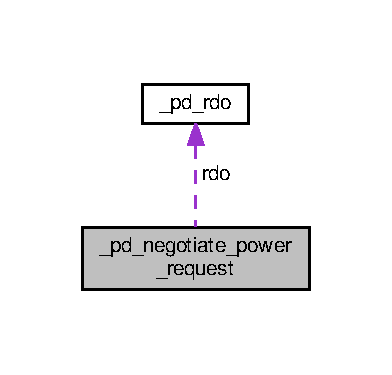
\includegraphics[width=188pt]{struct__pd__negotiate__power__request__coll__graph}
\end{center}
\end{figure}
\subsection*{Public Attributes}
\begin{DoxyCompactItemize}
\item 
\hyperlink{group__usb__pd__stack_ga4dcb1103574222cf94d4b45128f2b884}{pd\-\_\-rdo\-\_\-t} \hyperlink{struct__pd__negotiate__power__request_a6a2c0c69d7a8506ef0334d0718a28191}{rdo}
\item 
uint8\-\_\-t \hyperlink{struct__pd__negotiate__power__request_ac2aedb2edf9cb0038c459dface0494bf}{negotiate\-Result}
\end{DoxyCompactItemize}


\subsection{Detailed Description}
negotiate power rdo request 

used in P\-D\-\_\-\-D\-P\-M\-\_\-\-S\-R\-C\-\_\-\-R\-D\-O\-\_\-\-R\-E\-Q\-U\-E\-S\-T callback. 

\subsection{Member Data Documentation}
\hypertarget{struct__pd__negotiate__power__request_ac2aedb2edf9cb0038c459dface0494bf}{\index{\-\_\-pd\-\_\-negotiate\-\_\-power\-\_\-request@{\-\_\-pd\-\_\-negotiate\-\_\-power\-\_\-request}!negotiate\-Result@{negotiate\-Result}}
\index{negotiate\-Result@{negotiate\-Result}!_pd_negotiate_power_request@{\-\_\-pd\-\_\-negotiate\-\_\-power\-\_\-request}}
\subsubsection[{negotiate\-Result}]{\setlength{\rightskip}{0pt plus 5cm}uint8\-\_\-t \-\_\-pd\-\_\-negotiate\-\_\-power\-\_\-request\-::negotiate\-Result}}\label{struct__pd__negotiate__power__request_ac2aedb2edf9cb0038c459dface0494bf}
capabilities result, the value is \hyperlink{group__usb__pd__stack_ga59917b1485caba4dd8d9b65ca5a5fd92}{pd\-\_\-command\-\_\-result\-\_\-t} \hypertarget{struct__pd__negotiate__power__request_a6a2c0c69d7a8506ef0334d0718a28191}{\index{\-\_\-pd\-\_\-negotiate\-\_\-power\-\_\-request@{\-\_\-pd\-\_\-negotiate\-\_\-power\-\_\-request}!rdo@{rdo}}
\index{rdo@{rdo}!_pd_negotiate_power_request@{\-\_\-pd\-\_\-negotiate\-\_\-power\-\_\-request}}
\subsubsection[{rdo}]{\setlength{\rightskip}{0pt plus 5cm}{\bf pd\-\_\-rdo\-\_\-t} \-\_\-pd\-\_\-negotiate\-\_\-power\-\_\-request\-::rdo}}\label{struct__pd__negotiate__power__request_a6a2c0c69d7a8506ef0334d0718a28191}
request rdo 

The documentation for this struct was generated from the following file\-:\begin{DoxyCompactItemize}
\item 
pd/\hyperlink{usb__pd_8h}{usb\-\_\-pd.\-h}\end{DoxyCompactItemize}

\hypertarget{struct__pd__pdo__common}{\section{\-\_\-pd\-\_\-pdo\-\_\-common Struct Reference}
\label{struct__pd__pdo__common}\index{\-\_\-pd\-\_\-pdo\-\_\-common@{\-\_\-pd\-\_\-pdo\-\_\-common}}
}


common P\-D\-O for union  




{\ttfamily \#include $<$usb\-\_\-pd.\-h$>$}

\subsection*{Public Attributes}
\begin{DoxyCompactItemize}
\item 
uint32\-\_\-t \hyperlink{struct__pd__pdo__common_abf0630cb9ee09ce0bb24f2455f048e40}{reserved}\-: 30
\item 
uint32\-\_\-t \hyperlink{struct__pd__pdo__common_a5a1a819ee8e548be9b972852c75aa597}{pdo\-Type}\-: 2
\end{DoxyCompactItemize}


\subsection{Detailed Description}
common P\-D\-O for union 

\subsection{Member Data Documentation}
\hypertarget{struct__pd__pdo__common_a5a1a819ee8e548be9b972852c75aa597}{\index{\-\_\-pd\-\_\-pdo\-\_\-common@{\-\_\-pd\-\_\-pdo\-\_\-common}!pdo\-Type@{pdo\-Type}}
\index{pdo\-Type@{pdo\-Type}!_pd_pdo_common@{\-\_\-pd\-\_\-pdo\-\_\-common}}
\subsubsection[{pdo\-Type}]{\setlength{\rightskip}{0pt plus 5cm}uint32\-\_\-t \-\_\-pd\-\_\-pdo\-\_\-common\-::pdo\-Type}}\label{struct__pd__pdo__common_a5a1a819ee8e548be9b972852c75aa597}
pdo type, the value is \hyperlink{group__usb__pd__stack_ga1ed8c8629c16f0246f723f164abfe7d4}{pd\-\_\-pdo\-\_\-type\-\_\-t} \hypertarget{struct__pd__pdo__common_abf0630cb9ee09ce0bb24f2455f048e40}{\index{\-\_\-pd\-\_\-pdo\-\_\-common@{\-\_\-pd\-\_\-pdo\-\_\-common}!reserved@{reserved}}
\index{reserved@{reserved}!_pd_pdo_common@{\-\_\-pd\-\_\-pdo\-\_\-common}}
\subsubsection[{reserved}]{\setlength{\rightskip}{0pt plus 5cm}uint32\-\_\-t \-\_\-pd\-\_\-pdo\-\_\-common\-::reserved}}\label{struct__pd__pdo__common_abf0630cb9ee09ce0bb24f2455f048e40}
reserved 

The documentation for this struct was generated from the following file\-:\begin{DoxyCompactItemize}
\item 
pd/\hyperlink{usb__pd_8h}{usb\-\_\-pd.\-h}\end{DoxyCompactItemize}

\hypertarget{struct__pd__phy__api__interface}{\section{\-\_\-pd\-\_\-phy\-\_\-api\-\_\-interface Struct Reference}
\label{struct__pd__phy__api__interface}\index{\-\_\-pd\-\_\-phy\-\_\-api\-\_\-interface@{\-\_\-pd\-\_\-phy\-\_\-api\-\_\-interface}}
}


P\-D P\-H\-Y interface table structure.  




{\ttfamily \#include $<$usb\-\_\-pd\-\_\-phy.\-h$>$}

\subsection*{Public Attributes}
\begin{DoxyCompactItemize}
\item 
\hyperlink{group__usb__pd__stack_ga04a1f331d9807a70ab9bb753f5ed1c80}{pd\-\_\-status\-\_\-t}($\ast$ \hyperlink{struct__pd__phy__api__interface_a8f9666a7543d431aec266710dbc8d78c}{pd\-Phy\-Init} )(\hyperlink{group__usb__pd__stack_ga9397835347d48ef48b6b0ecba6312213}{pd\-\_\-handle} upper\-Layer\-Handle, \hyperlink{group__usb__pd__stack_gab39e13c5c0808b2fe22b7dac49db335a}{pd\-\_\-phy\-\_\-handle} $\ast$pd\-Phy\-Handle, \hyperlink{group__usb__pd__phy__drv_gab1d9a93a90c056727dcf364d6a5749e4}{pd\-\_\-phy\-\_\-config\-\_\-t} $\ast$phy\-Config)
\begin{DoxyCompactList}\small\item\em Initializes P\-D P\-H\-Y module. \end{DoxyCompactList}\item 
\hyperlink{group__usb__pd__stack_ga04a1f331d9807a70ab9bb753f5ed1c80}{pd\-\_\-status\-\_\-t}($\ast$ \hyperlink{struct__pd__phy__api__interface_a9e36ebe547c2ed82866597b2afc54bd0}{pd\-Phy\-Deinit} )(\hyperlink{group__usb__pd__stack_gab39e13c5c0808b2fe22b7dac49db335a}{pd\-\_\-phy\-\_\-handle} pd\-Phy\-Handle)
\begin{DoxyCompactList}\small\item\em de-\/initialize phy instance \end{DoxyCompactList}\item 
\hyperlink{group__usb__pd__stack_ga04a1f331d9807a70ab9bb753f5ed1c80}{pd\-\_\-status\-\_\-t}($\ast$ \hyperlink{struct__pd__phy__api__interface_ab9b74f09035836be811dc6aae682074f}{pd\-Phy\-Send} )(\hyperlink{group__usb__pd__stack_gab39e13c5c0808b2fe22b7dac49db335a}{pd\-\_\-phy\-\_\-handle} pd\-Phy\-Handle, uint8\-\_\-t start\-Of\-Packet, uint8\-\_\-t $\ast$buffer, uint32\-\_\-t length)
\begin{DoxyCompactList}\small\item\em send message \end{DoxyCompactList}\item 
\hyperlink{group__usb__pd__stack_ga04a1f331d9807a70ab9bb753f5ed1c80}{pd\-\_\-status\-\_\-t}($\ast$ \hyperlink{struct__pd__phy__api__interface_a3c8508914afbcb4f55578a0d61cd90e3}{pd\-Phy\-Receive} )(\hyperlink{group__usb__pd__stack_gab39e13c5c0808b2fe22b7dac49db335a}{pd\-\_\-phy\-\_\-handle} pd\-Phy\-Handle, uint8\-\_\-t start\-Of\-Packet\-Mask, uint8\-\_\-t $\ast$buffer, uint32\-\_\-t length)
\begin{DoxyCompactList}\small\item\em receive message \end{DoxyCompactList}\item 
\hyperlink{group__usb__pd__stack_ga04a1f331d9807a70ab9bb753f5ed1c80}{pd\-\_\-status\-\_\-t}($\ast$ \hyperlink{struct__pd__phy__api__interface_a5e422dbfd66fca34934e39b451f17094}{pd\-Phy\-Control} )(\hyperlink{group__usb__pd__stack_gab39e13c5c0808b2fe22b7dac49db335a}{pd\-\_\-phy\-\_\-handle} pd\-Phy\-Handle, uint32\-\_\-t control, void $\ast$param)
\begin{DoxyCompactList}\small\item\em control phy \end{DoxyCompactList}\end{DoxyCompactItemize}


\subsection{Detailed Description}
P\-D P\-H\-Y interface table structure. 

\subsection{Member Data Documentation}
\hypertarget{struct__pd__phy__api__interface_a5e422dbfd66fca34934e39b451f17094}{\index{\-\_\-pd\-\_\-phy\-\_\-api\-\_\-interface@{\-\_\-pd\-\_\-phy\-\_\-api\-\_\-interface}!pd\-Phy\-Control@{pd\-Phy\-Control}}
\index{pd\-Phy\-Control@{pd\-Phy\-Control}!_pd_phy_api_interface@{\-\_\-pd\-\_\-phy\-\_\-api\-\_\-interface}}
\subsubsection[{pd\-Phy\-Control}]{\setlength{\rightskip}{0pt plus 5cm}{\bf pd\-\_\-status\-\_\-t}($\ast$ \-\_\-pd\-\_\-phy\-\_\-api\-\_\-interface\-::pd\-Phy\-Control)({\bf pd\-\_\-phy\-\_\-handle} pd\-Phy\-Handle, uint32\-\_\-t control, void $\ast$param)}}\label{struct__pd__phy__api__interface_a5e422dbfd66fca34934e39b451f17094}


control phy 

This function control P\-H\-Y operatin. The control codes are defined at enumeration \hyperlink{group__usb__pd__phy__drv_ga5e3d7eb2cdbc2e45efca5e3e63d14baf}{pd\-\_\-phy\-\_\-control\-\_\-t}


\begin{DoxyParams}[1]{Parameters}
\mbox{\tt in}  & {\em pd\-Phy\-Handle} & P\-D phy instance handle. \\
\hline
\mbox{\tt in}  & {\em control} & The control code. \\
\hline
\mbox{\tt in}  & {\em param} & The control parameter.\\
\hline
\end{DoxyParams}

\begin{DoxyRetVals}{Return values}
{\em k\-Status\-\_\-\-U\-S\-B\-\_\-\-Success} & initialization success. \\
\hline
{\em other} & value error code. \\
\hline
\end{DoxyRetVals}
\hypertarget{struct__pd__phy__api__interface_a9e36ebe547c2ed82866597b2afc54bd0}{\index{\-\_\-pd\-\_\-phy\-\_\-api\-\_\-interface@{\-\_\-pd\-\_\-phy\-\_\-api\-\_\-interface}!pd\-Phy\-Deinit@{pd\-Phy\-Deinit}}
\index{pd\-Phy\-Deinit@{pd\-Phy\-Deinit}!_pd_phy_api_interface@{\-\_\-pd\-\_\-phy\-\_\-api\-\_\-interface}}
\subsubsection[{pd\-Phy\-Deinit}]{\setlength{\rightskip}{0pt plus 5cm}{\bf pd\-\_\-status\-\_\-t}($\ast$ \-\_\-pd\-\_\-phy\-\_\-api\-\_\-interface\-::pd\-Phy\-Deinit)({\bf pd\-\_\-phy\-\_\-handle} pd\-Phy\-Handle)}}\label{struct__pd__phy__api__interface_a9e36ebe547c2ed82866597b2afc54bd0}


de-\/initialize phy instance 

This function de-\/initializes the P\-D P\-H\-Y module specified by the pd\-Phy\-Handle.


\begin{DoxyParams}[1]{Parameters}
\mbox{\tt in}  & {\em pd\-Phy\-Handle} & P\-D phy instance handle.\\
\hline
\end{DoxyParams}

\begin{DoxyRetVals}{Return values}
{\em k\-Status\-\_\-\-U\-S\-B\-\_\-\-Success} & initialization success. \\
\hline
{\em other} & value error code. \\
\hline
\end{DoxyRetVals}
\hypertarget{struct__pd__phy__api__interface_a8f9666a7543d431aec266710dbc8d78c}{\index{\-\_\-pd\-\_\-phy\-\_\-api\-\_\-interface@{\-\_\-pd\-\_\-phy\-\_\-api\-\_\-interface}!pd\-Phy\-Init@{pd\-Phy\-Init}}
\index{pd\-Phy\-Init@{pd\-Phy\-Init}!_pd_phy_api_interface@{\-\_\-pd\-\_\-phy\-\_\-api\-\_\-interface}}
\subsubsection[{pd\-Phy\-Init}]{\setlength{\rightskip}{0pt plus 5cm}{\bf pd\-\_\-status\-\_\-t}($\ast$ \-\_\-pd\-\_\-phy\-\_\-api\-\_\-interface\-::pd\-Phy\-Init)({\bf pd\-\_\-handle} upper\-Layer\-Handle, {\bf pd\-\_\-phy\-\_\-handle} $\ast$pd\-Phy\-Handle, {\bf pd\-\_\-phy\-\_\-config\-\_\-t} $\ast$phy\-Config)}}\label{struct__pd__phy__api__interface_a8f9666a7543d431aec266710dbc8d78c}


Initializes P\-D P\-H\-Y module. 

This function initializes one P\-D P\-H\-Y module instance specified by the parameters.


\begin{DoxyParams}[1]{Parameters}
\mbox{\tt in}  & {\em upper\-Layer\-Handle} & P\-D stack instance handle \\
\hline
\mbox{\tt out}  & {\em pd\-Phy\-Handle} & return the P\-D phy instance handle. \\
\hline
\mbox{\tt in}  & {\em phy\-Config} & configure struct, see the struct \hyperlink{group__usb__pd__phy__drv_gab1d9a93a90c056727dcf364d6a5749e4}{pd\-\_\-phy\-\_\-config\-\_\-t}\\
\hline
\end{DoxyParams}

\begin{DoxyRetVals}{Return values}
{\em k\-Status\-\_\-\-U\-S\-B\-\_\-\-Success} & initialization success. \\
\hline
{\em other} & value error code. \\
\hline
\end{DoxyRetVals}
\hypertarget{struct__pd__phy__api__interface_a3c8508914afbcb4f55578a0d61cd90e3}{\index{\-\_\-pd\-\_\-phy\-\_\-api\-\_\-interface@{\-\_\-pd\-\_\-phy\-\_\-api\-\_\-interface}!pd\-Phy\-Receive@{pd\-Phy\-Receive}}
\index{pd\-Phy\-Receive@{pd\-Phy\-Receive}!_pd_phy_api_interface@{\-\_\-pd\-\_\-phy\-\_\-api\-\_\-interface}}
\subsubsection[{pd\-Phy\-Receive}]{\setlength{\rightskip}{0pt plus 5cm}{\bf pd\-\_\-status\-\_\-t}($\ast$ \-\_\-pd\-\_\-phy\-\_\-api\-\_\-interface\-::pd\-Phy\-Receive)({\bf pd\-\_\-phy\-\_\-handle} pd\-Phy\-Handle, uint8\-\_\-t start\-Of\-Packet\-Mask, uint8\-\_\-t $\ast$buffer, uint32\-\_\-t length)}}\label{struct__pd__phy__api__interface_a3c8508914afbcb4f55578a0d61cd90e3}


receive message 

This function pend to receive message, this function is asynchronous, the message receive result return to P\-D stack by the P\-D\-\_\-\-Notify(\-P\-D\-\_\-\-P\-H\-Y\-\_\-\-E\-V\-E\-N\-T\-\_\-\-R\-E\-C\-E\-I\-V\-E\-\_\-\-C\-O\-M\-P\-L\-E\-T\-E);


\begin{DoxyParams}[1]{Parameters}
\mbox{\tt in}  & {\em pd\-Phy\-Handle} & P\-D phy instance handle. \\
\hline
\mbox{\tt in}  & {\em start\-Of\-Packet\-Mask} & message's S\-O\-Ps that will receive. \\
\hline
\mbox{\tt in}  & {\em buffer} & data buffer. \\
\hline
\mbox{\tt in}  & {\em length} & data length.\\
\hline
\end{DoxyParams}

\begin{DoxyRetVals}{Return values}
{\em k\-Status\-\_\-\-U\-S\-B\-\_\-\-Success} & initialization success. \\
\hline
{\em other} & value error code. \\
\hline
\end{DoxyRetVals}
\hypertarget{struct__pd__phy__api__interface_ab9b74f09035836be811dc6aae682074f}{\index{\-\_\-pd\-\_\-phy\-\_\-api\-\_\-interface@{\-\_\-pd\-\_\-phy\-\_\-api\-\_\-interface}!pd\-Phy\-Send@{pd\-Phy\-Send}}
\index{pd\-Phy\-Send@{pd\-Phy\-Send}!_pd_phy_api_interface@{\-\_\-pd\-\_\-phy\-\_\-api\-\_\-interface}}
\subsubsection[{pd\-Phy\-Send}]{\setlength{\rightskip}{0pt plus 5cm}{\bf pd\-\_\-status\-\_\-t}($\ast$ \-\_\-pd\-\_\-phy\-\_\-api\-\_\-interface\-::pd\-Phy\-Send)({\bf pd\-\_\-phy\-\_\-handle} pd\-Phy\-Handle, uint8\-\_\-t start\-Of\-Packet, uint8\-\_\-t $\ast$buffer, uint32\-\_\-t length)}}\label{struct__pd__phy__api__interface_ab9b74f09035836be811dc6aae682074f}


send message 

This function send one message, this function is asynchronous, the message send result return to P\-D stack by the P\-D\-\_\-\-Notify(\-P\-D\-\_\-\-P\-H\-Y\-\_\-\-E\-V\-E\-N\-T\-\_\-\-S\-E\-N\-D\-\_\-\-C\-O\-M\-P\-L\-E\-T\-E);


\begin{DoxyParams}[1]{Parameters}
\mbox{\tt in}  & {\em pd\-Phy\-Handle} & P\-D phy instance handle. \\
\hline
\mbox{\tt in}  & {\em start\-Of\-Packet} & message's sop \\
\hline
\mbox{\tt in}  & {\em buffer} & data buffer. \\
\hline
\mbox{\tt in}  & {\em length} & data length.\\
\hline
\end{DoxyParams}

\begin{DoxyRetVals}{Return values}
{\em k\-Status\-\_\-\-U\-S\-B\-\_\-\-Success} & initialization success. \\
\hline
{\em other} & value error code. \\
\hline
\end{DoxyRetVals}


The documentation for this struct was generated from the following file\-:\begin{DoxyCompactItemize}
\item 
pd/\hyperlink{usb__pd__phy_8h}{usb\-\_\-pd\-\_\-phy.\-h}\end{DoxyCompactItemize}

\hypertarget{struct__pd__phy__config}{\section{\-\_\-pd\-\_\-phy\-\_\-config Struct Reference}
\label{struct__pd__phy__config}\index{\-\_\-pd\-\_\-phy\-\_\-config@{\-\_\-pd\-\_\-phy\-\_\-config}}
}


Configure P\-D P\-H\-Y.  




{\ttfamily \#include $<$usb\-\_\-pd\-\_\-phy.\-h$>$}



Collaboration diagram for \-\_\-pd\-\_\-phy\-\_\-config\-:
\nopagebreak
\begin{figure}[H]
\begin{center}
\leavevmode
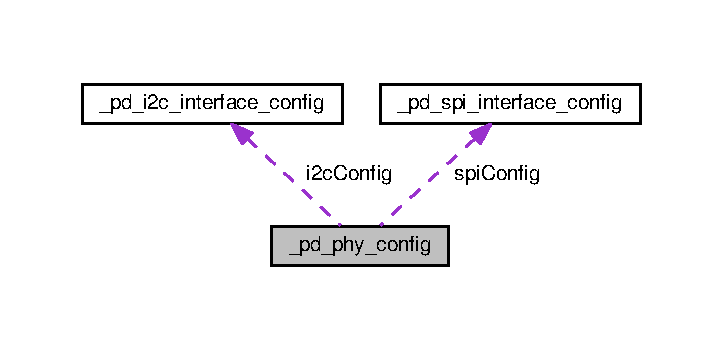
\includegraphics[width=347pt]{struct__pd__phy__config__coll__graph}
\end{center}
\end{figure}
\subsection*{Public Attributes}
\begin{DoxyCompactItemize}
\item 
uint8\-\_\-t \hyperlink{struct__pd__phy__config_aa5aa79cabb041cefecc0483c840f75a1}{interface}
\item 
\begin{tabbing}
xx\=xx\=xx\=xx\=xx\=xx\=xx\=xx\=xx\=\kill
union \{\\
\>\hyperlink{group__usb__pd__cmsis__wrapper_gada87adb00aefcd83988ef970c2f4d750}{pd\_i2c\_interface\_config\_t} \hyperlink{struct__pd__phy__config_aa606732850969dd6c9bd06b608e8015c}{i2cConfig}\\
\>\hyperlink{group__usb__pd__cmsis__wrapper_ga0a6afc9ea2599bcbe9b60e47f60d6bed}{pd\_spi\_interface\_config\_t} \hyperlink{struct__pd__phy__config_a5e3478079386b40d5b795897396853cb}{spiConfig}\\
\}; \\

\end{tabbing}\end{DoxyCompactItemize}


\subsection{Detailed Description}
Configure P\-D P\-H\-Y. 

\subsection{Member Data Documentation}
\hypertarget{struct__pd__phy__config_a1fdfe3a88c0a335fb0b15063fc067d97}{\subsubsection[{"@59}]{\setlength{\rightskip}{0pt plus 5cm}union \{ ... \} }}\label{struct__pd__phy__config_a1fdfe3a88c0a335fb0b15063fc067d97}
interface configure structure \hypertarget{struct__pd__phy__config_aa606732850969dd6c9bd06b608e8015c}{\index{\-\_\-pd\-\_\-phy\-\_\-config@{\-\_\-pd\-\_\-phy\-\_\-config}!i2c\-Config@{i2c\-Config}}
\index{i2c\-Config@{i2c\-Config}!_pd_phy_config@{\-\_\-pd\-\_\-phy\-\_\-config}}
\subsubsection[{i2c\-Config}]{\setlength{\rightskip}{0pt plus 5cm}{\bf pd\-\_\-i2c\-\_\-interface\-\_\-config\-\_\-t} \-\_\-pd\-\_\-phy\-\_\-config\-::i2c\-Config}}\label{struct__pd__phy__config_aa606732850969dd6c9bd06b608e8015c}
union, i2c configuration \hypertarget{struct__pd__phy__config_aa5aa79cabb041cefecc0483c840f75a1}{\index{\-\_\-pd\-\_\-phy\-\_\-config@{\-\_\-pd\-\_\-phy\-\_\-config}!interface@{interface}}
\index{interface@{interface}!_pd_phy_config@{\-\_\-pd\-\_\-phy\-\_\-config}}
\subsubsection[{interface}]{\setlength{\rightskip}{0pt plus 5cm}uint8\-\_\-t \-\_\-pd\-\_\-phy\-\_\-config\-::interface}}\label{struct__pd__phy__config_aa5aa79cabb041cefecc0483c840f75a1}
interface, it's value is \hyperlink{group__usb__pd__stack_ga0499cb1eb2ad70e8d155ff72b50c7a38}{pd\-\_\-phy\-\_\-interface\-\_\-t} \hypertarget{struct__pd__phy__config_a5e3478079386b40d5b795897396853cb}{\index{\-\_\-pd\-\_\-phy\-\_\-config@{\-\_\-pd\-\_\-phy\-\_\-config}!spi\-Config@{spi\-Config}}
\index{spi\-Config@{spi\-Config}!_pd_phy_config@{\-\_\-pd\-\_\-phy\-\_\-config}}
\subsubsection[{spi\-Config}]{\setlength{\rightskip}{0pt plus 5cm}{\bf pd\-\_\-spi\-\_\-interface\-\_\-config\-\_\-t} \-\_\-pd\-\_\-phy\-\_\-config\-::spi\-Config}}\label{struct__pd__phy__config_a5e3478079386b40d5b795897396853cb}
union, spi configuration 

The documentation for this struct was generated from the following file\-:\begin{DoxyCompactItemize}
\item 
pd/\hyperlink{usb__pd__phy_8h}{usb\-\_\-pd\-\_\-phy.\-h}\end{DoxyCompactItemize}

\hypertarget{struct__pd__phy__get__cc__state}{\section{\-\_\-pd\-\_\-phy\-\_\-get\-\_\-cc\-\_\-state Struct Reference}
\label{struct__pd__phy__get__cc__state}\index{\-\_\-pd\-\_\-phy\-\_\-get\-\_\-cc\-\_\-state@{\-\_\-pd\-\_\-phy\-\_\-get\-\_\-cc\-\_\-state}}
}


Get P\-H\-Y's C\-C line state. used as the P\-D\-\_\-\-P\-H\-Y\-\_\-\-G\-E\-T\-\_\-\-C\-C\-\_\-\-L\-I\-N\-E\-\_\-\-S\-T\-A\-T\-E control code parameter.  




{\ttfamily \#include $<$usb\-\_\-pd\-\_\-phy.\-h$>$}

\subsection*{Public Attributes}
\begin{DoxyCompactItemize}
\item 
uint8\-\_\-t \hyperlink{struct__pd__phy__get__cc__state_a551804e47b7f897e9e4ca61e0af9caf3}{cc1\-State}
\item 
uint8\-\_\-t \hyperlink{struct__pd__phy__get__cc__state_af32a14cc7bbfad052b927f765176aac8}{cc2\-State}
\end{DoxyCompactItemize}


\subsection{Detailed Description}
Get P\-H\-Y's C\-C line state. used as the P\-D\-\_\-\-P\-H\-Y\-\_\-\-G\-E\-T\-\_\-\-C\-C\-\_\-\-L\-I\-N\-E\-\_\-\-S\-T\-A\-T\-E control code parameter. 

\subsection{Member Data Documentation}
\hypertarget{struct__pd__phy__get__cc__state_a551804e47b7f897e9e4ca61e0af9caf3}{\index{\-\_\-pd\-\_\-phy\-\_\-get\-\_\-cc\-\_\-state@{\-\_\-pd\-\_\-phy\-\_\-get\-\_\-cc\-\_\-state}!cc1\-State@{cc1\-State}}
\index{cc1\-State@{cc1\-State}!_pd_phy_get_cc_state@{\-\_\-pd\-\_\-phy\-\_\-get\-\_\-cc\-\_\-state}}
\subsubsection[{cc1\-State}]{\setlength{\rightskip}{0pt plus 5cm}uint8\-\_\-t \-\_\-pd\-\_\-phy\-\_\-get\-\_\-cc\-\_\-state\-::cc1\-State}}\label{struct__pd__phy__get__cc__state_a551804e47b7f897e9e4ca61e0af9caf3}
C\-C1 line state, the value is \hyperlink{group__usb__pd__phy__drv_ga33106675227396a51d78ea6a7f562570}{pd\-\_\-phy\-\_\-cc\-\_\-state\-\_\-t} \hypertarget{struct__pd__phy__get__cc__state_af32a14cc7bbfad052b927f765176aac8}{\index{\-\_\-pd\-\_\-phy\-\_\-get\-\_\-cc\-\_\-state@{\-\_\-pd\-\_\-phy\-\_\-get\-\_\-cc\-\_\-state}!cc2\-State@{cc2\-State}}
\index{cc2\-State@{cc2\-State}!_pd_phy_get_cc_state@{\-\_\-pd\-\_\-phy\-\_\-get\-\_\-cc\-\_\-state}}
\subsubsection[{cc2\-State}]{\setlength{\rightskip}{0pt plus 5cm}uint8\-\_\-t \-\_\-pd\-\_\-phy\-\_\-get\-\_\-cc\-\_\-state\-::cc2\-State}}\label{struct__pd__phy__get__cc__state_af32a14cc7bbfad052b927f765176aac8}
C\-C2 line state, the value is \hyperlink{group__usb__pd__phy__drv_ga33106675227396a51d78ea6a7f562570}{pd\-\_\-phy\-\_\-cc\-\_\-state\-\_\-t} 

The documentation for this struct was generated from the following file\-:\begin{DoxyCompactItemize}
\item 
pd/\hyperlink{usb__pd__phy_8h}{usb\-\_\-pd\-\_\-phy.\-h}\end{DoxyCompactItemize}

\hypertarget{struct__pd__phy__msg__header__info}{\section{\-\_\-pd\-\_\-phy\-\_\-msg\-\_\-header\-\_\-info Struct Reference}
\label{struct__pd__phy__msg__header__info}\index{\-\_\-pd\-\_\-phy\-\_\-msg\-\_\-header\-\_\-info@{\-\_\-pd\-\_\-phy\-\_\-msg\-\_\-header\-\_\-info}}
}


configure P\-H\-Y's data role, power role. or good\-C\-R\-C's msg header. used as the P\-D\-\_\-\-P\-H\-Y\-\_\-\-S\-E\-T\-\_\-\-M\-S\-G\-\_\-\-H\-E\-A\-D\-E\-R\-\_\-\-I\-N\-F\-O control code parameter.  




{\ttfamily \#include $<$usb\-\_\-pd\-\_\-phy.\-h$>$}

\subsection*{Public Attributes}
\begin{DoxyCompactItemize}
\item 
uint8\-\_\-t \hyperlink{struct__pd__phy__msg__header__info_a7f921ee0d685a1f6818dce56ee1ef8f2}{data\-Role}
\item 
uint8\-\_\-t \hyperlink{struct__pd__phy__msg__header__info_a11c74e61a0e7ab66caf6c73321d9d016}{power\-Role}
\item 
uint8\-\_\-t \hyperlink{struct__pd__phy__msg__header__info_a068ae6e534efaaa108dbd0aa75256a63}{cable\-Plug}
\item 
uint8\-\_\-t \hyperlink{struct__pd__phy__msg__header__info_a64122118bd2c482eea1b178b459e1aae}{revision}
\end{DoxyCompactItemize}


\subsection{Detailed Description}
configure P\-H\-Y's data role, power role. or good\-C\-R\-C's msg header. used as the P\-D\-\_\-\-P\-H\-Y\-\_\-\-S\-E\-T\-\_\-\-M\-S\-G\-\_\-\-H\-E\-A\-D\-E\-R\-\_\-\-I\-N\-F\-O control code parameter. 

\subsection{Member Data Documentation}
\hypertarget{struct__pd__phy__msg__header__info_a068ae6e534efaaa108dbd0aa75256a63}{\index{\-\_\-pd\-\_\-phy\-\_\-msg\-\_\-header\-\_\-info@{\-\_\-pd\-\_\-phy\-\_\-msg\-\_\-header\-\_\-info}!cable\-Plug@{cable\-Plug}}
\index{cable\-Plug@{cable\-Plug}!_pd_phy_msg_header_info@{\-\_\-pd\-\_\-phy\-\_\-msg\-\_\-header\-\_\-info}}
\subsubsection[{cable\-Plug}]{\setlength{\rightskip}{0pt plus 5cm}uint8\-\_\-t \-\_\-pd\-\_\-phy\-\_\-msg\-\_\-header\-\_\-info\-::cable\-Plug}}\label{struct__pd__phy__msg__header__info_a068ae6e534efaaa108dbd0aa75256a63}
self is cable plug \hypertarget{struct__pd__phy__msg__header__info_a7f921ee0d685a1f6818dce56ee1ef8f2}{\index{\-\_\-pd\-\_\-phy\-\_\-msg\-\_\-header\-\_\-info@{\-\_\-pd\-\_\-phy\-\_\-msg\-\_\-header\-\_\-info}!data\-Role@{data\-Role}}
\index{data\-Role@{data\-Role}!_pd_phy_msg_header_info@{\-\_\-pd\-\_\-phy\-\_\-msg\-\_\-header\-\_\-info}}
\subsubsection[{data\-Role}]{\setlength{\rightskip}{0pt plus 5cm}uint8\-\_\-t \-\_\-pd\-\_\-phy\-\_\-msg\-\_\-header\-\_\-info\-::data\-Role}}\label{struct__pd__phy__msg__header__info_a7f921ee0d685a1f6818dce56ee1ef8f2}
data role \hypertarget{struct__pd__phy__msg__header__info_a11c74e61a0e7ab66caf6c73321d9d016}{\index{\-\_\-pd\-\_\-phy\-\_\-msg\-\_\-header\-\_\-info@{\-\_\-pd\-\_\-phy\-\_\-msg\-\_\-header\-\_\-info}!power\-Role@{power\-Role}}
\index{power\-Role@{power\-Role}!_pd_phy_msg_header_info@{\-\_\-pd\-\_\-phy\-\_\-msg\-\_\-header\-\_\-info}}
\subsubsection[{power\-Role}]{\setlength{\rightskip}{0pt plus 5cm}uint8\-\_\-t \-\_\-pd\-\_\-phy\-\_\-msg\-\_\-header\-\_\-info\-::power\-Role}}\label{struct__pd__phy__msg__header__info_a11c74e61a0e7ab66caf6c73321d9d016}
power role \hypertarget{struct__pd__phy__msg__header__info_a64122118bd2c482eea1b178b459e1aae}{\index{\-\_\-pd\-\_\-phy\-\_\-msg\-\_\-header\-\_\-info@{\-\_\-pd\-\_\-phy\-\_\-msg\-\_\-header\-\_\-info}!revision@{revision}}
\index{revision@{revision}!_pd_phy_msg_header_info@{\-\_\-pd\-\_\-phy\-\_\-msg\-\_\-header\-\_\-info}}
\subsubsection[{revision}]{\setlength{\rightskip}{0pt plus 5cm}uint8\-\_\-t \-\_\-pd\-\_\-phy\-\_\-msg\-\_\-header\-\_\-info\-::revision}}\label{struct__pd__phy__msg__header__info_a64122118bd2c482eea1b178b459e1aae}
spec revision 

The documentation for this struct was generated from the following file\-:\begin{DoxyCompactItemize}
\item 
pd/\hyperlink{usb__pd__phy_8h}{usb\-\_\-pd\-\_\-phy.\-h}\end{DoxyCompactItemize}

\hypertarget{struct__pd__phy__rx__result}{\section{\-\_\-pd\-\_\-phy\-\_\-rx\-\_\-result Struct Reference}
\label{struct__pd__phy__rx__result}\index{\-\_\-pd\-\_\-phy\-\_\-rx\-\_\-result@{\-\_\-pd\-\_\-phy\-\_\-rx\-\_\-result}}
}


P\-D P\-H\-Y receive result information. P\-D\-\_\-\-P\-H\-Y\-\_\-\-E\-V\-E\-N\-T\-\_\-\-R\-E\-C\-E\-I\-V\-E\-\_\-\-C\-O\-M\-P\-L\-E\-T\-E event use this structure as parameter.  




{\ttfamily \#include $<$usb\-\_\-pd\-\_\-phy.\-h$>$}

\subsection*{Public Attributes}
\begin{DoxyCompactItemize}
\item 
uint8\-\_\-t \hyperlink{struct__pd__phy__rx__result_a29f871220a1cc0617a6c5dd86e222f60}{rx\-Result\-Status}
\item 
uint8\-\_\-t \hyperlink{struct__pd__phy__rx__result_a70f74c4fbff251a4e08c91977e0c2871}{rx\-Sop}
\item 
uint16\-\_\-t \hyperlink{struct__pd__phy__rx__result_a897dc52bf49a0d66a2aec6c4cff86a5b}{rx\-Length}
\end{DoxyCompactItemize}


\subsection{Detailed Description}
P\-D P\-H\-Y receive result information. P\-D\-\_\-\-P\-H\-Y\-\_\-\-E\-V\-E\-N\-T\-\_\-\-R\-E\-C\-E\-I\-V\-E\-\_\-\-C\-O\-M\-P\-L\-E\-T\-E event use this structure as parameter. 

\subsection{Member Data Documentation}
\hypertarget{struct__pd__phy__rx__result_a897dc52bf49a0d66a2aec6c4cff86a5b}{\index{\-\_\-pd\-\_\-phy\-\_\-rx\-\_\-result@{\-\_\-pd\-\_\-phy\-\_\-rx\-\_\-result}!rx\-Length@{rx\-Length}}
\index{rx\-Length@{rx\-Length}!_pd_phy_rx_result@{\-\_\-pd\-\_\-phy\-\_\-rx\-\_\-result}}
\subsubsection[{rx\-Length}]{\setlength{\rightskip}{0pt plus 5cm}uint16\-\_\-t \-\_\-pd\-\_\-phy\-\_\-rx\-\_\-result\-::rx\-Length}}\label{struct__pd__phy__rx__result_a897dc52bf49a0d66a2aec6c4cff86a5b}
message's length \hypertarget{struct__pd__phy__rx__result_a29f871220a1cc0617a6c5dd86e222f60}{\index{\-\_\-pd\-\_\-phy\-\_\-rx\-\_\-result@{\-\_\-pd\-\_\-phy\-\_\-rx\-\_\-result}!rx\-Result\-Status@{rx\-Result\-Status}}
\index{rx\-Result\-Status@{rx\-Result\-Status}!_pd_phy_rx_result@{\-\_\-pd\-\_\-phy\-\_\-rx\-\_\-result}}
\subsubsection[{rx\-Result\-Status}]{\setlength{\rightskip}{0pt plus 5cm}uint8\-\_\-t \-\_\-pd\-\_\-phy\-\_\-rx\-\_\-result\-::rx\-Result\-Status}}\label{struct__pd__phy__rx__result_a29f871220a1cc0617a6c5dd86e222f60}
receive result \hypertarget{struct__pd__phy__rx__result_a70f74c4fbff251a4e08c91977e0c2871}{\index{\-\_\-pd\-\_\-phy\-\_\-rx\-\_\-result@{\-\_\-pd\-\_\-phy\-\_\-rx\-\_\-result}!rx\-Sop@{rx\-Sop}}
\index{rx\-Sop@{rx\-Sop}!_pd_phy_rx_result@{\-\_\-pd\-\_\-phy\-\_\-rx\-\_\-result}}
\subsubsection[{rx\-Sop}]{\setlength{\rightskip}{0pt plus 5cm}uint8\-\_\-t \-\_\-pd\-\_\-phy\-\_\-rx\-\_\-result\-::rx\-Sop}}\label{struct__pd__phy__rx__result_a70f74c4fbff251a4e08c91977e0c2871}
message's sop 

The documentation for this struct was generated from the following file\-:\begin{DoxyCompactItemize}
\item 
pd/\hyperlink{usb__pd__phy_8h}{usb\-\_\-pd\-\_\-phy.\-h}\end{DoxyCompactItemize}

\hypertarget{struct__pd__phy__vendor__info}{\section{\-\_\-pd\-\_\-phy\-\_\-vendor\-\_\-info Struct Reference}
\label{struct__pd__phy__vendor__info}\index{\-\_\-pd\-\_\-phy\-\_\-vendor\-\_\-info@{\-\_\-pd\-\_\-phy\-\_\-vendor\-\_\-info}}
}


P\-H\-Y's vendor information.  




{\ttfamily \#include $<$usb\-\_\-pd\-\_\-phy.\-h$>$}

\subsection*{Public Attributes}
\begin{DoxyCompactItemize}
\item 
uint16\-\_\-t \hyperlink{struct__pd__phy__vendor__info_a271bbac00bad57c93a70cfb905bb2d98}{vendor\-I\-D}
\item 
uint16\-\_\-t \hyperlink{struct__pd__phy__vendor__info_a4bd651a05bc50ad4e045b7956ba6f43b}{product\-I\-D}
\item 
uint16\-\_\-t \hyperlink{struct__pd__phy__vendor__info_a356dba0c0968b8a08fee4477f561ea46}{device\-I\-D}
\end{DoxyCompactItemize}


\subsection{Detailed Description}
P\-H\-Y's vendor information. 

\subsection{Member Data Documentation}
\hypertarget{struct__pd__phy__vendor__info_a356dba0c0968b8a08fee4477f561ea46}{\index{\-\_\-pd\-\_\-phy\-\_\-vendor\-\_\-info@{\-\_\-pd\-\_\-phy\-\_\-vendor\-\_\-info}!device\-I\-D@{device\-I\-D}}
\index{device\-I\-D@{device\-I\-D}!_pd_phy_vendor_info@{\-\_\-pd\-\_\-phy\-\_\-vendor\-\_\-info}}
\subsubsection[{device\-I\-D}]{\setlength{\rightskip}{0pt plus 5cm}uint16\-\_\-t \-\_\-pd\-\_\-phy\-\_\-vendor\-\_\-info\-::device\-I\-D}}\label{struct__pd__phy__vendor__info_a356dba0c0968b8a08fee4477f561ea46}
device I\-D \hypertarget{struct__pd__phy__vendor__info_a4bd651a05bc50ad4e045b7956ba6f43b}{\index{\-\_\-pd\-\_\-phy\-\_\-vendor\-\_\-info@{\-\_\-pd\-\_\-phy\-\_\-vendor\-\_\-info}!product\-I\-D@{product\-I\-D}}
\index{product\-I\-D@{product\-I\-D}!_pd_phy_vendor_info@{\-\_\-pd\-\_\-phy\-\_\-vendor\-\_\-info}}
\subsubsection[{product\-I\-D}]{\setlength{\rightskip}{0pt plus 5cm}uint16\-\_\-t \-\_\-pd\-\_\-phy\-\_\-vendor\-\_\-info\-::product\-I\-D}}\label{struct__pd__phy__vendor__info_a4bd651a05bc50ad4e045b7956ba6f43b}
product I\-D \hypertarget{struct__pd__phy__vendor__info_a271bbac00bad57c93a70cfb905bb2d98}{\index{\-\_\-pd\-\_\-phy\-\_\-vendor\-\_\-info@{\-\_\-pd\-\_\-phy\-\_\-vendor\-\_\-info}!vendor\-I\-D@{vendor\-I\-D}}
\index{vendor\-I\-D@{vendor\-I\-D}!_pd_phy_vendor_info@{\-\_\-pd\-\_\-phy\-\_\-vendor\-\_\-info}}
\subsubsection[{vendor\-I\-D}]{\setlength{\rightskip}{0pt plus 5cm}uint16\-\_\-t \-\_\-pd\-\_\-phy\-\_\-vendor\-\_\-info\-::vendor\-I\-D}}\label{struct__pd__phy__vendor__info_a271bbac00bad57c93a70cfb905bb2d98}
vendor I\-D 

The documentation for this struct was generated from the following file\-:\begin{DoxyCompactItemize}
\item 
pd/\hyperlink{usb__pd__phy_8h}{usb\-\_\-pd\-\_\-phy.\-h}\end{DoxyCompactItemize}

\hypertarget{struct__pd__power__callback}{\section{\-\_\-pd\-\_\-power\-\_\-callback Struct Reference}
\label{struct__pd__power__callback}\index{\-\_\-pd\-\_\-power\-\_\-callback@{\-\_\-pd\-\_\-power\-\_\-callback}}
}


power control interface.  




{\ttfamily \#include $<$usb\-\_\-pd.\-h$>$}

\subsection*{Public Attributes}
\begin{DoxyCompactItemize}
\item 
\hyperlink{group__usb__pd__stack_ga04a1f331d9807a70ab9bb753f5ed1c80}{pd\-\_\-status\-\_\-t}($\ast$ \hyperlink{struct__pd__power__callback_a81922cf6a4f22bcee69123e95fac7758}{P\-D\-\_\-\-Src\-Turn\-On\-Type\-C\-Vbus} )(void $\ast$callback\-Param, uint8\-\_\-t power\-Progress)
\begin{DoxyCompactList}\small\item\em source provide default typec vbus power. \end{DoxyCompactList}\item 
\hyperlink{group__usb__pd__stack_ga04a1f331d9807a70ab9bb753f5ed1c80}{pd\-\_\-status\-\_\-t}($\ast$ \hyperlink{struct__pd__power__callback_ab7d47b7b6babdf2f74c6d1344c685168}{P\-D\-\_\-\-Src\-Turn\-On\-Request\-Vbus} )(void $\ast$callback\-Param, \hyperlink{group__usb__pd__stack_ga4dcb1103574222cf94d4b45128f2b884}{pd\-\_\-rdo\-\_\-t} rdo)
\begin{DoxyCompactList}\small\item\em source provide rdo request vbus power. \end{DoxyCompactList}\item 
\hyperlink{group__usb__pd__stack_ga04a1f331d9807a70ab9bb753f5ed1c80}{pd\-\_\-status\-\_\-t}($\ast$ \hyperlink{struct__pd__power__callback_a1afed4126bcbe1ba278eb27f31e99c9c}{P\-D\-\_\-\-Src\-Turn\-Off\-Vbus} )(void $\ast$callback\-Param, uint8\-\_\-t power\-Progress)
\begin{DoxyCompactList}\small\item\em source turn off vbus power. \end{DoxyCompactList}\item 
\hyperlink{group__usb__pd__stack_ga04a1f331d9807a70ab9bb753f5ed1c80}{pd\-\_\-status\-\_\-t}($\ast$ \hyperlink{struct__pd__power__callback_a50891e9bf6ceb5d45b27ec49e46b11fc}{P\-D\-\_\-\-Src\-Goto\-Min\-Reduce\-Power} )(void $\ast$callback\-Param)
\begin{DoxyCompactList}\small\item\em source reduce power for goto min. \end{DoxyCompactList}\item 
\hyperlink{group__usb__pd__stack_ga04a1f331d9807a70ab9bb753f5ed1c80}{pd\-\_\-status\-\_\-t}($\ast$ \hyperlink{struct__pd__power__callback_a2a64b10db4e1644e17ee04e0a19cc412}{P\-D\-\_\-\-Snk\-Draw\-Type\-C\-Vbus} )(void $\ast$callback\-Param, uint8\-\_\-t typec\-Current\-Level, uint8\-\_\-t power\-Progress)
\begin{DoxyCompactList}\small\item\em sink can draw the default type-\/c vbus power. \end{DoxyCompactList}\item 
\hyperlink{group__usb__pd__stack_ga04a1f331d9807a70ab9bb753f5ed1c80}{pd\-\_\-status\-\_\-t}($\ast$ \hyperlink{struct__pd__power__callback_ac1b908d8a0b3cad5c449cde3e7b169b4}{P\-D\-\_\-\-Snk\-Draw\-Request\-Vbus} )(void $\ast$callback\-Param, \hyperlink{group__usb__pd__stack_ga4dcb1103574222cf94d4b45128f2b884}{pd\-\_\-rdo\-\_\-t} rdo)
\begin{DoxyCompactList}\small\item\em sink can draw the request rdo vbus power. \end{DoxyCompactList}\item 
\hyperlink{group__usb__pd__stack_ga04a1f331d9807a70ab9bb753f5ed1c80}{pd\-\_\-status\-\_\-t}($\ast$ \hyperlink{struct__pd__power__callback_a18806d06567f385463bba77f8202da49}{P\-D\-\_\-\-Snk\-Stop\-Draw\-Vbus} )(void $\ast$callback\-Param, uint8\-\_\-t power\-Progress)
\begin{DoxyCompactList}\small\item\em sink stop draw vbus power. \end{DoxyCompactList}\item 
\hyperlink{group__usb__pd__stack_ga04a1f331d9807a70ab9bb753f5ed1c80}{pd\-\_\-status\-\_\-t}($\ast$ \hyperlink{struct__pd__power__callback_a6db9643def50ef309e1d66abd6943e1d}{P\-D\-\_\-\-Snk\-Goto\-Min\-Reduce\-Power} )(void $\ast$callback\-Param)
\begin{DoxyCompactList}\small\item\em sink reduce power for goto min. \end{DoxyCompactList}\item 
\hyperlink{group__usb__pd__stack_ga04a1f331d9807a70ab9bb753f5ed1c80}{pd\-\_\-status\-\_\-t}($\ast$ \hyperlink{struct__pd__power__callback_a406d88fa8818ca8257f005c5097859e9}{P\-D\-\_\-\-Control\-Vconn} )(void $\ast$callback\-Param, uint8\-\_\-t on)
\begin{DoxyCompactList}\small\item\em control vconn \end{DoxyCompactList}\end{DoxyCompactItemize}


\subsection{Detailed Description}
power control interface. 

Application need implement this interface and pass to P\-D\-\_\-\-Instance\-Init 

\subsection{Member Data Documentation}
\hypertarget{struct__pd__power__callback_a406d88fa8818ca8257f005c5097859e9}{\index{\-\_\-pd\-\_\-power\-\_\-callback@{\-\_\-pd\-\_\-power\-\_\-callback}!P\-D\-\_\-\-Control\-Vconn@{P\-D\-\_\-\-Control\-Vconn}}
\index{P\-D\-\_\-\-Control\-Vconn@{P\-D\-\_\-\-Control\-Vconn}!_pd_power_callback@{\-\_\-pd\-\_\-power\-\_\-callback}}
\subsubsection[{P\-D\-\_\-\-Control\-Vconn}]{\setlength{\rightskip}{0pt plus 5cm}{\bf pd\-\_\-status\-\_\-t}($\ast$ \-\_\-pd\-\_\-power\-\_\-callback\-::\-P\-D\-\_\-\-Control\-Vconn)(void $\ast$callback\-Param, uint8\-\_\-t on)}}\label{struct__pd__power__callback_a406d88fa8818ca8257f005c5097859e9}


control vconn 


\begin{DoxyParams}{Parameters}
{\em callback\-Param} & \\
\hline
{\em on} & 0 -\/ turn off vconn; 1 -\/ turn on vconn.\\
\hline
\end{DoxyParams}

\begin{DoxyRetVals}{Return values}
{\em k\-Status\-\_\-\-P\-D\-\_\-\-Success} & success \\
\hline
{\em k\-Status\-\_\-\-P\-D\-\_\-\-Error} & error \\
\hline
\end{DoxyRetVals}
\hypertarget{struct__pd__power__callback_ac1b908d8a0b3cad5c449cde3e7b169b4}{\index{\-\_\-pd\-\_\-power\-\_\-callback@{\-\_\-pd\-\_\-power\-\_\-callback}!P\-D\-\_\-\-Snk\-Draw\-Request\-Vbus@{P\-D\-\_\-\-Snk\-Draw\-Request\-Vbus}}
\index{P\-D\-\_\-\-Snk\-Draw\-Request\-Vbus@{P\-D\-\_\-\-Snk\-Draw\-Request\-Vbus}!_pd_power_callback@{\-\_\-pd\-\_\-power\-\_\-callback}}
\subsubsection[{P\-D\-\_\-\-Snk\-Draw\-Request\-Vbus}]{\setlength{\rightskip}{0pt plus 5cm}{\bf pd\-\_\-status\-\_\-t}($\ast$ \-\_\-pd\-\_\-power\-\_\-callback\-::\-P\-D\-\_\-\-Snk\-Draw\-Request\-Vbus)(void $\ast$callback\-Param, {\bf pd\-\_\-rdo\-\_\-t} rdo)}}\label{struct__pd__power__callback_ac1b908d8a0b3cad5c449cde3e7b169b4}


sink can draw the request rdo vbus power. 


\begin{DoxyParams}{Parameters}
{\em callback\-Param} & \\
\hline
{\em rdo} & request rdo from partner\\
\hline
\end{DoxyParams}

\begin{DoxyRetVals}{Return values}
{\em k\-Status\-\_\-\-P\-D\-\_\-\-Success} & success \\
\hline
{\em k\-Status\-\_\-\-P\-D\-\_\-\-Error} & error \\
\hline
\end{DoxyRetVals}
\hypertarget{struct__pd__power__callback_a2a64b10db4e1644e17ee04e0a19cc412}{\index{\-\_\-pd\-\_\-power\-\_\-callback@{\-\_\-pd\-\_\-power\-\_\-callback}!P\-D\-\_\-\-Snk\-Draw\-Type\-C\-Vbus@{P\-D\-\_\-\-Snk\-Draw\-Type\-C\-Vbus}}
\index{P\-D\-\_\-\-Snk\-Draw\-Type\-C\-Vbus@{P\-D\-\_\-\-Snk\-Draw\-Type\-C\-Vbus}!_pd_power_callback@{\-\_\-pd\-\_\-power\-\_\-callback}}
\subsubsection[{P\-D\-\_\-\-Snk\-Draw\-Type\-C\-Vbus}]{\setlength{\rightskip}{0pt plus 5cm}{\bf pd\-\_\-status\-\_\-t}($\ast$ \-\_\-pd\-\_\-power\-\_\-callback\-::\-P\-D\-\_\-\-Snk\-Draw\-Type\-C\-Vbus)(void $\ast$callback\-Param, uint8\-\_\-t typec\-Current\-Level, uint8\-\_\-t power\-Progress)}}\label{struct__pd__power__callback_a2a64b10db4e1644e17ee04e0a19cc412}


sink can draw the default type-\/c vbus power. 


\begin{DoxyParams}{Parameters}
{\em callback\-Param} & \\
\hline
{\em typec\-Current\-Level} & the value is \hyperlink{group__usb__pd__stack_ga875b585c994b83a1c1fd1e81bac28f7a}{typec\-\_\-current\-\_\-val\-\_\-t} \\
\hline
{\em power\-Progress} & hard\-\_\-reset, pr\-\_\-swap or fr\-\_\-swap. Normally it is useless, just in case application need this info to provide power.\\
\hline
\end{DoxyParams}

\begin{DoxyRetVals}{Return values}
{\em k\-Status\-\_\-\-P\-D\-\_\-\-Success} & success \\
\hline
{\em k\-Status\-\_\-\-P\-D\-\_\-\-Error} & error \\
\hline
\end{DoxyRetVals}
\hypertarget{struct__pd__power__callback_a6db9643def50ef309e1d66abd6943e1d}{\index{\-\_\-pd\-\_\-power\-\_\-callback@{\-\_\-pd\-\_\-power\-\_\-callback}!P\-D\-\_\-\-Snk\-Goto\-Min\-Reduce\-Power@{P\-D\-\_\-\-Snk\-Goto\-Min\-Reduce\-Power}}
\index{P\-D\-\_\-\-Snk\-Goto\-Min\-Reduce\-Power@{P\-D\-\_\-\-Snk\-Goto\-Min\-Reduce\-Power}!_pd_power_callback@{\-\_\-pd\-\_\-power\-\_\-callback}}
\subsubsection[{P\-D\-\_\-\-Snk\-Goto\-Min\-Reduce\-Power}]{\setlength{\rightskip}{0pt plus 5cm}{\bf pd\-\_\-status\-\_\-t}($\ast$ \-\_\-pd\-\_\-power\-\_\-callback\-::\-P\-D\-\_\-\-Snk\-Goto\-Min\-Reduce\-Power)(void $\ast$callback\-Param)}}\label{struct__pd__power__callback_a6db9643def50ef309e1d66abd6943e1d}


sink reduce power for goto min. 


\begin{DoxyParams}{Parameters}
{\em callback\-Param} & \\
\hline
\end{DoxyParams}

\begin{DoxyRetVals}{Return values}
{\em k\-Status\-\_\-\-P\-D\-\_\-\-Success} & success \\
\hline
{\em k\-Status\-\_\-\-P\-D\-\_\-\-Error} & error \\
\hline
\end{DoxyRetVals}
\hypertarget{struct__pd__power__callback_a18806d06567f385463bba77f8202da49}{\index{\-\_\-pd\-\_\-power\-\_\-callback@{\-\_\-pd\-\_\-power\-\_\-callback}!P\-D\-\_\-\-Snk\-Stop\-Draw\-Vbus@{P\-D\-\_\-\-Snk\-Stop\-Draw\-Vbus}}
\index{P\-D\-\_\-\-Snk\-Stop\-Draw\-Vbus@{P\-D\-\_\-\-Snk\-Stop\-Draw\-Vbus}!_pd_power_callback@{\-\_\-pd\-\_\-power\-\_\-callback}}
\subsubsection[{P\-D\-\_\-\-Snk\-Stop\-Draw\-Vbus}]{\setlength{\rightskip}{0pt plus 5cm}{\bf pd\-\_\-status\-\_\-t}($\ast$ \-\_\-pd\-\_\-power\-\_\-callback\-::\-P\-D\-\_\-\-Snk\-Stop\-Draw\-Vbus)(void $\ast$callback\-Param, uint8\-\_\-t power\-Progress)}}\label{struct__pd__power__callback_a18806d06567f385463bba77f8202da49}


sink stop draw vbus power. 


\begin{DoxyParams}{Parameters}
{\em callback\-Param} & \\
\hline
{\em power\-Progress} & hard\-\_\-reset, pr\-\_\-swap or fr\-\_\-swap. Normally it is useless, just in case application need this info to provide power.\\
\hline
\end{DoxyParams}

\begin{DoxyRetVals}{Return values}
{\em k\-Status\-\_\-\-P\-D\-\_\-\-Success} & success \\
\hline
{\em k\-Status\-\_\-\-P\-D\-\_\-\-Error} & error \\
\hline
\end{DoxyRetVals}
\hypertarget{struct__pd__power__callback_a50891e9bf6ceb5d45b27ec49e46b11fc}{\index{\-\_\-pd\-\_\-power\-\_\-callback@{\-\_\-pd\-\_\-power\-\_\-callback}!P\-D\-\_\-\-Src\-Goto\-Min\-Reduce\-Power@{P\-D\-\_\-\-Src\-Goto\-Min\-Reduce\-Power}}
\index{P\-D\-\_\-\-Src\-Goto\-Min\-Reduce\-Power@{P\-D\-\_\-\-Src\-Goto\-Min\-Reduce\-Power}!_pd_power_callback@{\-\_\-pd\-\_\-power\-\_\-callback}}
\subsubsection[{P\-D\-\_\-\-Src\-Goto\-Min\-Reduce\-Power}]{\setlength{\rightskip}{0pt plus 5cm}{\bf pd\-\_\-status\-\_\-t}($\ast$ \-\_\-pd\-\_\-power\-\_\-callback\-::\-P\-D\-\_\-\-Src\-Goto\-Min\-Reduce\-Power)(void $\ast$callback\-Param)}}\label{struct__pd__power__callback_a50891e9bf6ceb5d45b27ec49e46b11fc}


source reduce power for goto min. 


\begin{DoxyParams}{Parameters}
{\em callback\-Param} & \\
\hline
\end{DoxyParams}

\begin{DoxyRetVals}{Return values}
{\em k\-Status\-\_\-\-P\-D\-\_\-\-Success} & success \\
\hline
{\em k\-Status\-\_\-\-P\-D\-\_\-\-Error} & error \\
\hline
\end{DoxyRetVals}
\hypertarget{struct__pd__power__callback_a1afed4126bcbe1ba278eb27f31e99c9c}{\index{\-\_\-pd\-\_\-power\-\_\-callback@{\-\_\-pd\-\_\-power\-\_\-callback}!P\-D\-\_\-\-Src\-Turn\-Off\-Vbus@{P\-D\-\_\-\-Src\-Turn\-Off\-Vbus}}
\index{P\-D\-\_\-\-Src\-Turn\-Off\-Vbus@{P\-D\-\_\-\-Src\-Turn\-Off\-Vbus}!_pd_power_callback@{\-\_\-pd\-\_\-power\-\_\-callback}}
\subsubsection[{P\-D\-\_\-\-Src\-Turn\-Off\-Vbus}]{\setlength{\rightskip}{0pt plus 5cm}{\bf pd\-\_\-status\-\_\-t}($\ast$ \-\_\-pd\-\_\-power\-\_\-callback\-::\-P\-D\-\_\-\-Src\-Turn\-Off\-Vbus)(void $\ast$callback\-Param, uint8\-\_\-t power\-Progress)}}\label{struct__pd__power__callback_a1afed4126bcbe1ba278eb27f31e99c9c}


source turn off vbus power. 


\begin{DoxyParams}{Parameters}
{\em callback\-Param} & \\
\hline
{\em power\-Progress} & hard\-\_\-reset, pr\-\_\-swap or fr\-\_\-swap. Normally it is useless, just in case application need this info to provide power.\\
\hline
\end{DoxyParams}

\begin{DoxyRetVals}{Return values}
{\em k\-Status\-\_\-\-P\-D\-\_\-\-Success} & success \\
\hline
{\em k\-Status\-\_\-\-P\-D\-\_\-\-Error} & error \\
\hline
\end{DoxyRetVals}
\hypertarget{struct__pd__power__callback_ab7d47b7b6babdf2f74c6d1344c685168}{\index{\-\_\-pd\-\_\-power\-\_\-callback@{\-\_\-pd\-\_\-power\-\_\-callback}!P\-D\-\_\-\-Src\-Turn\-On\-Request\-Vbus@{P\-D\-\_\-\-Src\-Turn\-On\-Request\-Vbus}}
\index{P\-D\-\_\-\-Src\-Turn\-On\-Request\-Vbus@{P\-D\-\_\-\-Src\-Turn\-On\-Request\-Vbus}!_pd_power_callback@{\-\_\-pd\-\_\-power\-\_\-callback}}
\subsubsection[{P\-D\-\_\-\-Src\-Turn\-On\-Request\-Vbus}]{\setlength{\rightskip}{0pt plus 5cm}{\bf pd\-\_\-status\-\_\-t}($\ast$ \-\_\-pd\-\_\-power\-\_\-callback\-::\-P\-D\-\_\-\-Src\-Turn\-On\-Request\-Vbus)(void $\ast$callback\-Param, {\bf pd\-\_\-rdo\-\_\-t} rdo)}}\label{struct__pd__power__callback_ab7d47b7b6babdf2f74c6d1344c685168}


source provide rdo request vbus power. 


\begin{DoxyParams}{Parameters}
{\em callback\-Param} & \\
\hline
{\em rdo} & request rdo from partner\\
\hline
\end{DoxyParams}

\begin{DoxyRetVals}{Return values}
{\em k\-Status\-\_\-\-P\-D\-\_\-\-Success} & success \\
\hline
{\em k\-Status\-\_\-\-P\-D\-\_\-\-Error} & error \\
\hline
\end{DoxyRetVals}
\hypertarget{struct__pd__power__callback_a81922cf6a4f22bcee69123e95fac7758}{\index{\-\_\-pd\-\_\-power\-\_\-callback@{\-\_\-pd\-\_\-power\-\_\-callback}!P\-D\-\_\-\-Src\-Turn\-On\-Type\-C\-Vbus@{P\-D\-\_\-\-Src\-Turn\-On\-Type\-C\-Vbus}}
\index{P\-D\-\_\-\-Src\-Turn\-On\-Type\-C\-Vbus@{P\-D\-\_\-\-Src\-Turn\-On\-Type\-C\-Vbus}!_pd_power_callback@{\-\_\-pd\-\_\-power\-\_\-callback}}
\subsubsection[{P\-D\-\_\-\-Src\-Turn\-On\-Type\-C\-Vbus}]{\setlength{\rightskip}{0pt plus 5cm}{\bf pd\-\_\-status\-\_\-t}($\ast$ \-\_\-pd\-\_\-power\-\_\-callback\-::\-P\-D\-\_\-\-Src\-Turn\-On\-Type\-C\-Vbus)(void $\ast$callback\-Param, uint8\-\_\-t power\-Progress)}}\label{struct__pd__power__callback_a81922cf6a4f22bcee69123e95fac7758}


source provide default typec vbus power. 


\begin{DoxyParams}{Parameters}
{\em callback\-Param} & \\
\hline
{\em power\-Progress} & hard\-\_\-reset, pr\-\_\-swap or fr\-\_\-swap. Normally it is useless, just in case application need this info to provide power.\\
\hline
\end{DoxyParams}

\begin{DoxyRetVals}{Return values}
{\em k\-Status\-\_\-\-P\-D\-\_\-\-Success} & success \\
\hline
{\em k\-Status\-\_\-\-P\-D\-\_\-\-Error} & error \\
\hline
\end{DoxyRetVals}


The documentation for this struct was generated from the following file\-:\begin{DoxyCompactItemize}
\item 
pd/\hyperlink{usb__pd_8h}{usb\-\_\-pd.\-h}\end{DoxyCompactItemize}

\hypertarget{struct__pd__power__port__config}{\section{\-\_\-pd\-\_\-power\-\_\-port\-\_\-config Struct Reference}
\label{struct__pd__power__port__config}\index{\-\_\-pd\-\_\-power\-\_\-port\-\_\-config@{\-\_\-pd\-\_\-power\-\_\-port\-\_\-config}}
}


{\ttfamily \#include $<$usb\-\_\-pd.\-h$>$}

\subsection*{Public Attributes}
\begin{DoxyCompactItemize}
\item 
uint32\-\_\-t $\ast$ \hyperlink{struct__pd__power__port__config_a12847f31ee382d4bdee4067c9ee177f4}{source\-Caps}
\item 
uint32\-\_\-t $\ast$ \hyperlink{struct__pd__power__port__config_ab247068e26ad76b2670eb96da39969e1}{sink\-Caps}
\item 
uint8\-\_\-t \hyperlink{struct__pd__power__port__config_a7cf6689616437623deb3b42e5467e26f}{source\-Cap\-Count}
\item 
uint8\-\_\-t \hyperlink{struct__pd__power__port__config_aa1d58bf75fbebad4b8c7e29b0cc4c64e}{sink\-Cap\-Count}
\item 
uint8\-\_\-t \hyperlink{struct__pd__power__port__config_a649079672f270a65578bd41e0e624e16}{typec\-Role}
\item 
uint8\-\_\-t \hyperlink{struct__pd__power__port__config_aaec71cee54cf853e332a4b4ed1ef17ae}{typec\-Src\-Current}
\item 
uint8\-\_\-t \hyperlink{struct__pd__power__port__config_a6e72ee6532ef61497b162a28b4500433}{drp\-Try\-Function}
\item 
uint8\-\_\-t \hyperlink{struct__pd__power__port__config_a5a3c023210ceec3faac6d13b0de58f75}{data\-Function}
\item 
uint8\-\_\-t \hyperlink{struct__pd__power__port__config_aa552a27c5747ea789ad185fefac44194}{vconn\-Supported}
\item 
uint8\-\_\-t \hyperlink{struct__pd__power__port__config_ae6a55ddacda35e342d72b9ee6f7fadba}{reserved1}
\item 
void $\ast$ \hyperlink{struct__pd__power__port__config_a8e04f0c0092776ec0f354cf23ce48057}{source\-Config}
\item 
void $\ast$ \hyperlink{struct__pd__power__port__config_ab0b7a0e266e429764b5af0dd6a57a303}{sink\-Config}
\item 
void $\ast$ \hyperlink{struct__pd__power__port__config_a95dc4dc28941f3a624bac60addc27b20}{drp\-Config}
\end{DoxyCompactItemize}


\subsection{Member Data Documentation}
\hypertarget{struct__pd__power__port__config_a5a3c023210ceec3faac6d13b0de58f75}{\index{\-\_\-pd\-\_\-power\-\_\-port\-\_\-config@{\-\_\-pd\-\_\-power\-\_\-port\-\_\-config}!data\-Function@{data\-Function}}
\index{data\-Function@{data\-Function}!_pd_power_port_config@{\-\_\-pd\-\_\-power\-\_\-port\-\_\-config}}
\subsubsection[{data\-Function}]{\setlength{\rightskip}{0pt plus 5cm}uint8\-\_\-t \-\_\-pd\-\_\-power\-\_\-port\-\_\-config\-::data\-Function}}\label{struct__pd__power__port__config_a5a3c023210ceec3faac6d13b0de58f75}
It configure data role function of the device, it is D\-F\-P, U\-F\-P, D\-R\-D. For U\-S\-B function, D\-F\-P correspond to Host; U\-F\-P correspond to Device; D\-R\-D correspond to O\-T\-G. it's value is \hyperlink{group__usb__pd__stack_ga92476c6b5b34316ccb766c9d2cadd29e}{typec\-\_\-data\-\_\-function\-\_\-config\-\_\-t} \hypertarget{struct__pd__power__port__config_a95dc4dc28941f3a624bac60addc27b20}{\index{\-\_\-pd\-\_\-power\-\_\-port\-\_\-config@{\-\_\-pd\-\_\-power\-\_\-port\-\_\-config}!drp\-Config@{drp\-Config}}
\index{drp\-Config@{drp\-Config}!_pd_power_port_config@{\-\_\-pd\-\_\-power\-\_\-port\-\_\-config}}
\subsubsection[{drp\-Config}]{\setlength{\rightskip}{0pt plus 5cm}void$\ast$ \-\_\-pd\-\_\-power\-\_\-port\-\_\-config\-::drp\-Config}}\label{struct__pd__power__port__config_a95dc4dc28941f3a624bac60addc27b20}
(For feature extension) D\-R\-P config \hypertarget{struct__pd__power__port__config_a6e72ee6532ef61497b162a28b4500433}{\index{\-\_\-pd\-\_\-power\-\_\-port\-\_\-config@{\-\_\-pd\-\_\-power\-\_\-port\-\_\-config}!drp\-Try\-Function@{drp\-Try\-Function}}
\index{drp\-Try\-Function@{drp\-Try\-Function}!_pd_power_port_config@{\-\_\-pd\-\_\-power\-\_\-port\-\_\-config}}
\subsubsection[{drp\-Try\-Function}]{\setlength{\rightskip}{0pt plus 5cm}uint8\-\_\-t \-\_\-pd\-\_\-power\-\_\-port\-\_\-config\-::drp\-Try\-Function}}\label{struct__pd__power__port__config_a6e72ee6532ef61497b162a28b4500433}
(not supported yet) It only is valid for D\-R\-P, this value configure try-\/sink, try-\/source or no try function. it's value is \hyperlink{group__usb__pd__stack_ga86c3c8c95607b75c0c75cd2714487497}{typec\-\_\-try\-\_\-t} \hypertarget{struct__pd__power__port__config_ae6a55ddacda35e342d72b9ee6f7fadba}{\index{\-\_\-pd\-\_\-power\-\_\-port\-\_\-config@{\-\_\-pd\-\_\-power\-\_\-port\-\_\-config}!reserved1@{reserved1}}
\index{reserved1@{reserved1}!_pd_power_port_config@{\-\_\-pd\-\_\-power\-\_\-port\-\_\-config}}
\subsubsection[{reserved1}]{\setlength{\rightskip}{0pt plus 5cm}uint8\-\_\-t \-\_\-pd\-\_\-power\-\_\-port\-\_\-config\-::reserved1}}\label{struct__pd__power__port__config_ae6a55ddacda35e342d72b9ee6f7fadba}
\hypertarget{struct__pd__power__port__config_aa1d58bf75fbebad4b8c7e29b0cc4c64e}{\index{\-\_\-pd\-\_\-power\-\_\-port\-\_\-config@{\-\_\-pd\-\_\-power\-\_\-port\-\_\-config}!sink\-Cap\-Count@{sink\-Cap\-Count}}
\index{sink\-Cap\-Count@{sink\-Cap\-Count}!_pd_power_port_config@{\-\_\-pd\-\_\-power\-\_\-port\-\_\-config}}
\subsubsection[{sink\-Cap\-Count}]{\setlength{\rightskip}{0pt plus 5cm}uint8\-\_\-t \-\_\-pd\-\_\-power\-\_\-port\-\_\-config\-::sink\-Cap\-Count}}\label{struct__pd__power__port__config_aa1d58bf75fbebad4b8c7e29b0cc4c64e}
sink caps count, if don't support set as 0 \hypertarget{struct__pd__power__port__config_ab247068e26ad76b2670eb96da39969e1}{\index{\-\_\-pd\-\_\-power\-\_\-port\-\_\-config@{\-\_\-pd\-\_\-power\-\_\-port\-\_\-config}!sink\-Caps@{sink\-Caps}}
\index{sink\-Caps@{sink\-Caps}!_pd_power_port_config@{\-\_\-pd\-\_\-power\-\_\-port\-\_\-config}}
\subsubsection[{sink\-Caps}]{\setlength{\rightskip}{0pt plus 5cm}uint32\-\_\-t$\ast$ \-\_\-pd\-\_\-power\-\_\-port\-\_\-config\-::sink\-Caps}}\label{struct__pd__power__port__config_ab247068e26ad76b2670eb96da39969e1}
sink caps, if don't support set as N\-U\-L\-L \hypertarget{struct__pd__power__port__config_ab0b7a0e266e429764b5af0dd6a57a303}{\index{\-\_\-pd\-\_\-power\-\_\-port\-\_\-config@{\-\_\-pd\-\_\-power\-\_\-port\-\_\-config}!sink\-Config@{sink\-Config}}
\index{sink\-Config@{sink\-Config}!_pd_power_port_config@{\-\_\-pd\-\_\-power\-\_\-port\-\_\-config}}
\subsubsection[{sink\-Config}]{\setlength{\rightskip}{0pt plus 5cm}void$\ast$ \-\_\-pd\-\_\-power\-\_\-port\-\_\-config\-::sink\-Config}}\label{struct__pd__power__port__config_ab0b7a0e266e429764b5af0dd6a57a303}
(For feature extension) sink config \hypertarget{struct__pd__power__port__config_a7cf6689616437623deb3b42e5467e26f}{\index{\-\_\-pd\-\_\-power\-\_\-port\-\_\-config@{\-\_\-pd\-\_\-power\-\_\-port\-\_\-config}!source\-Cap\-Count@{source\-Cap\-Count}}
\index{source\-Cap\-Count@{source\-Cap\-Count}!_pd_power_port_config@{\-\_\-pd\-\_\-power\-\_\-port\-\_\-config}}
\subsubsection[{source\-Cap\-Count}]{\setlength{\rightskip}{0pt plus 5cm}uint8\-\_\-t \-\_\-pd\-\_\-power\-\_\-port\-\_\-config\-::source\-Cap\-Count}}\label{struct__pd__power__port__config_a7cf6689616437623deb3b42e5467e26f}
source caps count, if don't support set as 0 \hypertarget{struct__pd__power__port__config_a12847f31ee382d4bdee4067c9ee177f4}{\index{\-\_\-pd\-\_\-power\-\_\-port\-\_\-config@{\-\_\-pd\-\_\-power\-\_\-port\-\_\-config}!source\-Caps@{source\-Caps}}
\index{source\-Caps@{source\-Caps}!_pd_power_port_config@{\-\_\-pd\-\_\-power\-\_\-port\-\_\-config}}
\subsubsection[{source\-Caps}]{\setlength{\rightskip}{0pt plus 5cm}uint32\-\_\-t$\ast$ \-\_\-pd\-\_\-power\-\_\-port\-\_\-config\-::source\-Caps}}\label{struct__pd__power__port__config_a12847f31ee382d4bdee4067c9ee177f4}
source caps, if don't support set as N\-U\-L\-L \hypertarget{struct__pd__power__port__config_a8e04f0c0092776ec0f354cf23ce48057}{\index{\-\_\-pd\-\_\-power\-\_\-port\-\_\-config@{\-\_\-pd\-\_\-power\-\_\-port\-\_\-config}!source\-Config@{source\-Config}}
\index{source\-Config@{source\-Config}!_pd_power_port_config@{\-\_\-pd\-\_\-power\-\_\-port\-\_\-config}}
\subsubsection[{source\-Config}]{\setlength{\rightskip}{0pt plus 5cm}void$\ast$ \-\_\-pd\-\_\-power\-\_\-port\-\_\-config\-::source\-Config}}\label{struct__pd__power__port__config_a8e04f0c0092776ec0f354cf23ce48057}
(For feature extension) source config \hypertarget{struct__pd__power__port__config_a649079672f270a65578bd41e0e624e16}{\index{\-\_\-pd\-\_\-power\-\_\-port\-\_\-config@{\-\_\-pd\-\_\-power\-\_\-port\-\_\-config}!typec\-Role@{typec\-Role}}
\index{typec\-Role@{typec\-Role}!_pd_power_port_config@{\-\_\-pd\-\_\-power\-\_\-port\-\_\-config}}
\subsubsection[{typec\-Role}]{\setlength{\rightskip}{0pt plus 5cm}uint8\-\_\-t \-\_\-pd\-\_\-power\-\_\-port\-\_\-config\-::typec\-Role}}\label{struct__pd__power__port__config_a649079672f270a65578bd41e0e624e16}
device's typec role, for example\-: sink, source or D\-R\-P. it's value is \hyperlink{group__usb__pd__stack_ga8522facb45d87054c87e6d6fb32d9dd1}{typec\-\_\-power\-\_\-role\-\_\-config\-\_\-t} \hypertarget{struct__pd__power__port__config_aaec71cee54cf853e332a4b4ed1ef17ae}{\index{\-\_\-pd\-\_\-power\-\_\-port\-\_\-config@{\-\_\-pd\-\_\-power\-\_\-port\-\_\-config}!typec\-Src\-Current@{typec\-Src\-Current}}
\index{typec\-Src\-Current@{typec\-Src\-Current}!_pd_power_port_config@{\-\_\-pd\-\_\-power\-\_\-port\-\_\-config}}
\subsubsection[{typec\-Src\-Current}]{\setlength{\rightskip}{0pt plus 5cm}uint8\-\_\-t \-\_\-pd\-\_\-power\-\_\-port\-\_\-config\-::typec\-Src\-Current}}\label{struct__pd__power__port__config_aaec71cee54cf853e332a4b4ed1ef17ae}
It only is valid for source, this value set the Type\-C Rp current level it's value is \hyperlink{group__usb__pd__stack_ga875b585c994b83a1c1fd1e81bac28f7a}{typec\-\_\-current\-\_\-val\-\_\-t} \hypertarget{struct__pd__power__port__config_aa552a27c5747ea789ad185fefac44194}{\index{\-\_\-pd\-\_\-power\-\_\-port\-\_\-config@{\-\_\-pd\-\_\-power\-\_\-port\-\_\-config}!vconn\-Supported@{vconn\-Supported}}
\index{vconn\-Supported@{vconn\-Supported}!_pd_power_port_config@{\-\_\-pd\-\_\-power\-\_\-port\-\_\-config}}
\subsubsection[{vconn\-Supported}]{\setlength{\rightskip}{0pt plus 5cm}uint8\-\_\-t \-\_\-pd\-\_\-power\-\_\-port\-\_\-config\-::vconn\-Supported}}\label{struct__pd__power__port__config_aa552a27c5747ea789ad185fefac44194}
value is 1\-: support vconn swap and vconn power; value is 0\-: don't support vconn swap or vconn power. 

The documentation for this struct was generated from the following file\-:\begin{DoxyCompactItemize}
\item 
pd/\hyperlink{usb__pd_8h}{usb\-\_\-pd.\-h}\end{DoxyCompactItemize}

\hypertarget{struct__pd__ptn5110__ctrl__pin}{\section{\-\_\-pd\-\_\-ptn5110\-\_\-ctrl\-\_\-pin Struct Reference}
\label{struct__pd__ptn5110__ctrl__pin}\index{\-\_\-pd\-\_\-ptn5110\-\_\-ctrl\-\_\-pin@{\-\_\-pd\-\_\-ptn5110\-\_\-ctrl\-\_\-pin}}
}


control P\-T\-N5110 pin for power control  




{\ttfamily \#include $<$usb\-\_\-pd.\-h$>$}

\subsection*{Public Attributes}
\begin{DoxyCompactItemize}
\item 
uint8\-\_\-t \hyperlink{struct__pd__ptn5110__ctrl__pin_ace741c1da1ba78c0e1068f69a4a8f9d5}{en\-S\-R\-C}\-: 1
\item 
uint8\-\_\-t \hyperlink{struct__pd__ptn5110__ctrl__pin_aa46e27b5322119661fe8081a042478f7}{en\-S\-N\-K1}\-: 1
\end{DoxyCompactItemize}


\subsection{Detailed Description}
control P\-T\-N5110 pin for power control 

\subsection{Member Data Documentation}
\hypertarget{struct__pd__ptn5110__ctrl__pin_aa46e27b5322119661fe8081a042478f7}{\index{\-\_\-pd\-\_\-ptn5110\-\_\-ctrl\-\_\-pin@{\-\_\-pd\-\_\-ptn5110\-\_\-ctrl\-\_\-pin}!en\-S\-N\-K1@{en\-S\-N\-K1}}
\index{en\-S\-N\-K1@{en\-S\-N\-K1}!_pd_ptn5110_ctrl_pin@{\-\_\-pd\-\_\-ptn5110\-\_\-ctrl\-\_\-pin}}
\subsubsection[{en\-S\-N\-K1}]{\setlength{\rightskip}{0pt plus 5cm}uint8\-\_\-t \-\_\-pd\-\_\-ptn5110\-\_\-ctrl\-\_\-pin\-::en\-S\-N\-K1}}\label{struct__pd__ptn5110__ctrl__pin_aa46e27b5322119661fe8081a042478f7}
\hypertarget{struct__pd__ptn5110__ctrl__pin_ace741c1da1ba78c0e1068f69a4a8f9d5}{\index{\-\_\-pd\-\_\-ptn5110\-\_\-ctrl\-\_\-pin@{\-\_\-pd\-\_\-ptn5110\-\_\-ctrl\-\_\-pin}!en\-S\-R\-C@{en\-S\-R\-C}}
\index{en\-S\-R\-C@{en\-S\-R\-C}!_pd_ptn5110_ctrl_pin@{\-\_\-pd\-\_\-ptn5110\-\_\-ctrl\-\_\-pin}}
\subsubsection[{en\-S\-R\-C}]{\setlength{\rightskip}{0pt plus 5cm}uint8\-\_\-t \-\_\-pd\-\_\-ptn5110\-\_\-ctrl\-\_\-pin\-::en\-S\-R\-C}}\label{struct__pd__ptn5110__ctrl__pin_ace741c1da1ba78c0e1068f69a4a8f9d5}


The documentation for this struct was generated from the following file\-:\begin{DoxyCompactItemize}
\item 
pd/\hyperlink{usb__pd_8h}{usb\-\_\-pd.\-h}\end{DoxyCompactItemize}

\hypertarget{struct__pd__rdo}{\section{\-\_\-pd\-\_\-rdo Struct Reference}
\label{struct__pd__rdo}\index{\-\_\-pd\-\_\-rdo@{\-\_\-pd\-\_\-rdo}}
}


P\-D request data object.  




{\ttfamily \#include $<$usb\-\_\-pd.\-h$>$}

\subsection*{Public Attributes}
\begin{DoxyCompactItemize}
\item 
\begin{tabbing}
xx\=xx\=xx\=xx\=xx\=xx\=xx\=xx\=xx\=\kill
union \{\\
\>struct \{\\
\>\>uint32\_t \hyperlink{struct__pd__rdo_a75142d4da1d2a5049e134f771854ff7b}{maxOrMinOperateValue}: 10\\
\>\>uint32\_t \hyperlink{struct__pd__rdo_ace7bc599e359ab9c6e626b0b0cdb5359}{operateValue}: 10\\
\>\>uint32\_t \hyperlink{struct__pd__rdo_ad10d5e670fae5dd17c3ec06a8e994ea7}{reserved}: 3\\
\>\>uint32\_t \hyperlink{struct__pd__rdo_ab37db01bb9fe1af93aacc97242516364}{unchunkedSupported}: 1\\
\>\>uint32\_t \hyperlink{struct__pd__rdo_a85b57e63d9528131d0092a43111b2a98}{noUsbSuspend}: 1\\
\>\>uint32\_t \hyperlink{struct__pd__rdo_a3276a3edcd2e5ee3e9f17d9cca8f3ea2}{usbCommunicationsCapable}: 1\\
\>\>uint32\_t \hyperlink{struct__pd__rdo_afa835644625bbc35646580cb9bbd9b66}{capabilityMismatch}: 1\\
\>\>uint32\_t \hyperlink{struct__pd__rdo_a82acd4a018e44108ae1cb59e1da734b2}{giveBack}: 1\\
\>\>uint32\_t \hyperlink{struct__pd__rdo_a593d7f2473f5f2ccd44e7a1a71bd6df5}{objectPosition}: 3\\
\>\>uint32\_t \hyperlink{struct__pd__rdo_ac02715c88773bd4b67ab4a24aa98a481}{reserved1}: 1\\
\>\} \hyperlink{struct__pd__rdo_acd03d551b682b870d0e30be5819d013e}{bitFields}\\
\>uint32\_t \hyperlink{struct__pd__rdo_a66cd4e249b3284e7d1acc9714fa0ce0a}{rdoVal}\\
\}; \\

\end{tabbing}\end{DoxyCompactItemize}


\subsection{Detailed Description}
P\-D request data object. 

It provide the request power information. 

\subsection{Member Data Documentation}
\hypertarget{struct__pd__rdo_a2644a485a37f29cec32c4ae304b3a272}{\subsubsection[{"@53}]{\setlength{\rightskip}{0pt plus 5cm}union \{ ... \} }}\label{struct__pd__rdo_a2644a485a37f29cec32c4ae304b3a272}
\hypertarget{struct__pd__rdo_acd03d551b682b870d0e30be5819d013e}{\index{\-\_\-pd\-\_\-rdo@{\-\_\-pd\-\_\-rdo}!bit\-Fields@{bit\-Fields}}
\index{bit\-Fields@{bit\-Fields}!_pd_rdo@{\-\_\-pd\-\_\-rdo}}
\subsubsection[{bit\-Fields}]{\setlength{\rightskip}{0pt plus 5cm}struct \{ ... \}   \-\_\-pd\-\_\-rdo\-::bit\-Fields}}\label{struct__pd__rdo_acd03d551b682b870d0e30be5819d013e}
\hypertarget{struct__pd__rdo_afa835644625bbc35646580cb9bbd9b66}{\index{\-\_\-pd\-\_\-rdo@{\-\_\-pd\-\_\-rdo}!capability\-Mismatch@{capability\-Mismatch}}
\index{capability\-Mismatch@{capability\-Mismatch}!_pd_rdo@{\-\_\-pd\-\_\-rdo}}
\subsubsection[{capability\-Mismatch}]{\setlength{\rightskip}{0pt plus 5cm}uint32\-\_\-t \-\_\-pd\-\_\-rdo\-::capability\-Mismatch}}\label{struct__pd__rdo_afa835644625bbc35646580cb9bbd9b66}
capability mismatch \hypertarget{struct__pd__rdo_a82acd4a018e44108ae1cb59e1da734b2}{\index{\-\_\-pd\-\_\-rdo@{\-\_\-pd\-\_\-rdo}!give\-Back@{give\-Back}}
\index{give\-Back@{give\-Back}!_pd_rdo@{\-\_\-pd\-\_\-rdo}}
\subsubsection[{give\-Back}]{\setlength{\rightskip}{0pt plus 5cm}uint32\-\_\-t \-\_\-pd\-\_\-rdo\-::give\-Back}}\label{struct__pd__rdo_a82acd4a018e44108ae1cb59e1da734b2}
give back flag \hypertarget{struct__pd__rdo_a75142d4da1d2a5049e134f771854ff7b}{\index{\-\_\-pd\-\_\-rdo@{\-\_\-pd\-\_\-rdo}!max\-Or\-Min\-Operate\-Value@{max\-Or\-Min\-Operate\-Value}}
\index{max\-Or\-Min\-Operate\-Value@{max\-Or\-Min\-Operate\-Value}!_pd_rdo@{\-\_\-pd\-\_\-rdo}}
\subsubsection[{max\-Or\-Min\-Operate\-Value}]{\setlength{\rightskip}{0pt plus 5cm}uint32\-\_\-t \-\_\-pd\-\_\-rdo\-::max\-Or\-Min\-Operate\-Value}}\label{struct__pd__rdo_a75142d4da1d2a5049e134f771854ff7b}

\begin{DoxyItemize}
\item For fixed and variable request.
\begin{DoxyItemize}
\item give\-Back == 0\-: it is max operate current.
\item give\-Back == 1\-: it is min operate current.
\end{DoxyItemize}
\item For battery request.
\begin{DoxyItemize}
\item give\-Back == 0\-: it is max operate power.
\item give\-Back == 1\-: it is min operate power. 
\end{DoxyItemize}
\end{DoxyItemize}\hypertarget{struct__pd__rdo_a85b57e63d9528131d0092a43111b2a98}{\index{\-\_\-pd\-\_\-rdo@{\-\_\-pd\-\_\-rdo}!no\-Usb\-Suspend@{no\-Usb\-Suspend}}
\index{no\-Usb\-Suspend@{no\-Usb\-Suspend}!_pd_rdo@{\-\_\-pd\-\_\-rdo}}
\subsubsection[{no\-Usb\-Suspend}]{\setlength{\rightskip}{0pt plus 5cm}uint32\-\_\-t \-\_\-pd\-\_\-rdo\-::no\-Usb\-Suspend}}\label{struct__pd__rdo_a85b57e63d9528131d0092a43111b2a98}
usb suspend supported or not \hypertarget{struct__pd__rdo_a593d7f2473f5f2ccd44e7a1a71bd6df5}{\index{\-\_\-pd\-\_\-rdo@{\-\_\-pd\-\_\-rdo}!object\-Position@{object\-Position}}
\index{object\-Position@{object\-Position}!_pd_rdo@{\-\_\-pd\-\_\-rdo}}
\subsubsection[{object\-Position}]{\setlength{\rightskip}{0pt plus 5cm}uint32\-\_\-t \-\_\-pd\-\_\-rdo\-::object\-Position}}\label{struct__pd__rdo_a593d7f2473f5f2ccd44e7a1a71bd6df5}
object position \hypertarget{struct__pd__rdo_ace7bc599e359ab9c6e626b0b0cdb5359}{\index{\-\_\-pd\-\_\-rdo@{\-\_\-pd\-\_\-rdo}!operate\-Value@{operate\-Value}}
\index{operate\-Value@{operate\-Value}!_pd_rdo@{\-\_\-pd\-\_\-rdo}}
\subsubsection[{operate\-Value}]{\setlength{\rightskip}{0pt plus 5cm}uint32\-\_\-t \-\_\-pd\-\_\-rdo\-::operate\-Value}}\label{struct__pd__rdo_ace7bc599e359ab9c6e626b0b0cdb5359}
For fixed and variable request\-: it is current value; For battery request\-: it is power value. \hypertarget{struct__pd__rdo_a66cd4e249b3284e7d1acc9714fa0ce0a}{\index{\-\_\-pd\-\_\-rdo@{\-\_\-pd\-\_\-rdo}!rdo\-Val@{rdo\-Val}}
\index{rdo\-Val@{rdo\-Val}!_pd_rdo@{\-\_\-pd\-\_\-rdo}}
\subsubsection[{rdo\-Val}]{\setlength{\rightskip}{0pt plus 5cm}uint32\-\_\-t \-\_\-pd\-\_\-rdo\-::rdo\-Val}}\label{struct__pd__rdo_a66cd4e249b3284e7d1acc9714fa0ce0a}
\hypertarget{struct__pd__rdo_ad10d5e670fae5dd17c3ec06a8e994ea7}{\index{\-\_\-pd\-\_\-rdo@{\-\_\-pd\-\_\-rdo}!reserved@{reserved}}
\index{reserved@{reserved}!_pd_rdo@{\-\_\-pd\-\_\-rdo}}
\subsubsection[{reserved}]{\setlength{\rightskip}{0pt plus 5cm}uint32\-\_\-t \-\_\-pd\-\_\-rdo\-::reserved}}\label{struct__pd__rdo_ad10d5e670fae5dd17c3ec06a8e994ea7}
reserved \hypertarget{struct__pd__rdo_ac02715c88773bd4b67ab4a24aa98a481}{\index{\-\_\-pd\-\_\-rdo@{\-\_\-pd\-\_\-rdo}!reserved1@{reserved1}}
\index{reserved1@{reserved1}!_pd_rdo@{\-\_\-pd\-\_\-rdo}}
\subsubsection[{reserved1}]{\setlength{\rightskip}{0pt plus 5cm}uint32\-\_\-t \-\_\-pd\-\_\-rdo\-::reserved1}}\label{struct__pd__rdo_ac02715c88773bd4b67ab4a24aa98a481}
reserved \hypertarget{struct__pd__rdo_ab37db01bb9fe1af93aacc97242516364}{\index{\-\_\-pd\-\_\-rdo@{\-\_\-pd\-\_\-rdo}!unchunked\-Supported@{unchunked\-Supported}}
\index{unchunked\-Supported@{unchunked\-Supported}!_pd_rdo@{\-\_\-pd\-\_\-rdo}}
\subsubsection[{unchunked\-Supported}]{\setlength{\rightskip}{0pt plus 5cm}uint32\-\_\-t \-\_\-pd\-\_\-rdo\-::unchunked\-Supported}}\label{struct__pd__rdo_ab37db01bb9fe1af93aacc97242516364}
unchunked supported or not \hypertarget{struct__pd__rdo_a3276a3edcd2e5ee3e9f17d9cca8f3ea2}{\index{\-\_\-pd\-\_\-rdo@{\-\_\-pd\-\_\-rdo}!usb\-Communications\-Capable@{usb\-Communications\-Capable}}
\index{usb\-Communications\-Capable@{usb\-Communications\-Capable}!_pd_rdo@{\-\_\-pd\-\_\-rdo}}
\subsubsection[{usb\-Communications\-Capable}]{\setlength{\rightskip}{0pt plus 5cm}uint32\-\_\-t \-\_\-pd\-\_\-rdo\-::usb\-Communications\-Capable}}\label{struct__pd__rdo_a3276a3edcd2e5ee3e9f17d9cca8f3ea2}
usb communications capable 

The documentation for this struct was generated from the following file\-:\begin{DoxyCompactItemize}
\item 
pd/\hyperlink{usb__pd_8h}{usb\-\_\-pd.\-h}\end{DoxyCompactItemize}

\hypertarget{struct__pd__sink__battery__pdo}{\section{\-\_\-pd\-\_\-sink\-\_\-battery\-\_\-pdo Struct Reference}
\label{struct__pd__sink__battery__pdo}\index{\-\_\-pd\-\_\-sink\-\_\-battery\-\_\-pdo@{\-\_\-pd\-\_\-sink\-\_\-battery\-\_\-pdo}}
}


battery sink P\-D\-O  




{\ttfamily \#include $<$usb\-\_\-pd.\-h$>$}

\subsection*{Public Attributes}
\begin{DoxyCompactItemize}
\item 
uint32\-\_\-t \hyperlink{struct__pd__sink__battery__pdo_aede06aa3716908a68c90828fbfe5cebe}{operate\-Power}\-: 10
\item 
uint32\-\_\-t \hyperlink{struct__pd__sink__battery__pdo_a473824d26b81e000486844b83e32b09d}{min\-Voltage}\-: 10
\item 
uint32\-\_\-t \hyperlink{struct__pd__sink__battery__pdo_a5fe153e249c105e6b8414233ae216710}{max\-Voltage}\-: 10
\item 
uint32\-\_\-t \hyperlink{struct__pd__sink__battery__pdo_a417d58609316fbebd02091b96ec83ed8}{battery}\-: 2
\end{DoxyCompactItemize}


\subsection{Detailed Description}
battery sink P\-D\-O 

\subsection{Member Data Documentation}
\hypertarget{struct__pd__sink__battery__pdo_a417d58609316fbebd02091b96ec83ed8}{\index{\-\_\-pd\-\_\-sink\-\_\-battery\-\_\-pdo@{\-\_\-pd\-\_\-sink\-\_\-battery\-\_\-pdo}!battery@{battery}}
\index{battery@{battery}!_pd_sink_battery_pdo@{\-\_\-pd\-\_\-sink\-\_\-battery\-\_\-pdo}}
\subsubsection[{battery}]{\setlength{\rightskip}{0pt plus 5cm}uint32\-\_\-t \-\_\-pd\-\_\-sink\-\_\-battery\-\_\-pdo\-::battery}}\label{struct__pd__sink__battery__pdo_a417d58609316fbebd02091b96ec83ed8}
pdo type \hypertarget{struct__pd__sink__battery__pdo_a5fe153e249c105e6b8414233ae216710}{\index{\-\_\-pd\-\_\-sink\-\_\-battery\-\_\-pdo@{\-\_\-pd\-\_\-sink\-\_\-battery\-\_\-pdo}!max\-Voltage@{max\-Voltage}}
\index{max\-Voltage@{max\-Voltage}!_pd_sink_battery_pdo@{\-\_\-pd\-\_\-sink\-\_\-battery\-\_\-pdo}}
\subsubsection[{max\-Voltage}]{\setlength{\rightskip}{0pt plus 5cm}uint32\-\_\-t \-\_\-pd\-\_\-sink\-\_\-battery\-\_\-pdo\-::max\-Voltage}}\label{struct__pd__sink__battery__pdo_a5fe153e249c105e6b8414233ae216710}
max voltage \hypertarget{struct__pd__sink__battery__pdo_a473824d26b81e000486844b83e32b09d}{\index{\-\_\-pd\-\_\-sink\-\_\-battery\-\_\-pdo@{\-\_\-pd\-\_\-sink\-\_\-battery\-\_\-pdo}!min\-Voltage@{min\-Voltage}}
\index{min\-Voltage@{min\-Voltage}!_pd_sink_battery_pdo@{\-\_\-pd\-\_\-sink\-\_\-battery\-\_\-pdo}}
\subsubsection[{min\-Voltage}]{\setlength{\rightskip}{0pt plus 5cm}uint32\-\_\-t \-\_\-pd\-\_\-sink\-\_\-battery\-\_\-pdo\-::min\-Voltage}}\label{struct__pd__sink__battery__pdo_a473824d26b81e000486844b83e32b09d}
min voltage \hypertarget{struct__pd__sink__battery__pdo_aede06aa3716908a68c90828fbfe5cebe}{\index{\-\_\-pd\-\_\-sink\-\_\-battery\-\_\-pdo@{\-\_\-pd\-\_\-sink\-\_\-battery\-\_\-pdo}!operate\-Power@{operate\-Power}}
\index{operate\-Power@{operate\-Power}!_pd_sink_battery_pdo@{\-\_\-pd\-\_\-sink\-\_\-battery\-\_\-pdo}}
\subsubsection[{operate\-Power}]{\setlength{\rightskip}{0pt plus 5cm}uint32\-\_\-t \-\_\-pd\-\_\-sink\-\_\-battery\-\_\-pdo\-::operate\-Power}}\label{struct__pd__sink__battery__pdo_aede06aa3716908a68c90828fbfe5cebe}
operate power 

The documentation for this struct was generated from the following file\-:\begin{DoxyCompactItemize}
\item 
pd/\hyperlink{usb__pd_8h}{usb\-\_\-pd.\-h}\end{DoxyCompactItemize}

\hypertarget{struct__pd__sink__fixed__pdo}{\section{\-\_\-pd\-\_\-sink\-\_\-fixed\-\_\-pdo Struct Reference}
\label{struct__pd__sink__fixed__pdo}\index{\-\_\-pd\-\_\-sink\-\_\-fixed\-\_\-pdo@{\-\_\-pd\-\_\-sink\-\_\-fixed\-\_\-pdo}}
}


fixed sink P\-D\-O  




{\ttfamily \#include $<$usb\-\_\-pd.\-h$>$}

\subsection*{Public Attributes}
\begin{DoxyCompactItemize}
\item 
uint32\-\_\-t \hyperlink{struct__pd__sink__fixed__pdo_a264499e662c6bb82e0e25fc3d296b88b}{operate\-Current}\-: 10
\item 
uint32\-\_\-t \hyperlink{struct__pd__sink__fixed__pdo_a5e095a725455f85faa43a1573e62b798}{voltage}\-: 10
\item 
uint32\-\_\-t \hyperlink{struct__pd__sink__fixed__pdo_a209b36f044c02c50495b3b688be779cf}{reserved}\-: 3
\item 
uint32\-\_\-t \hyperlink{struct__pd__sink__fixed__pdo_a31798efee281f6d1c69ff96d7a79e113}{fr\-Swap\-Required\-Current}\-: 2
\item 
uint32\-\_\-t \hyperlink{struct__pd__sink__fixed__pdo_a6e8fb8552ee54c1d0227a03b5d7aecbf}{dual\-Role\-Data}\-: 1
\item 
uint32\-\_\-t \hyperlink{struct__pd__sink__fixed__pdo_aa19552768100717810142b8c4df3835c}{usb\-Communications\-Capable}\-: 1
\item 
uint32\-\_\-t \hyperlink{struct__pd__sink__fixed__pdo_a44e4b2e4bc2b34929036acee6ff6ae34}{external\-Powered}\-: 1
\item 
uint32\-\_\-t \hyperlink{struct__pd__sink__fixed__pdo_a511903e5dca26d874a304e558db6cc72}{higher\-Capability}\-: 1
\item 
uint32\-\_\-t \hyperlink{struct__pd__sink__fixed__pdo_a9ff5e34e2bf3e62a6b4dc017f559c061}{dual\-Role\-Power}\-: 1
\item 
uint32\-\_\-t \hyperlink{struct__pd__sink__fixed__pdo_a9290ef90d4336be4642f40aac2da8f5e}{fixed\-Supply}\-: 2
\end{DoxyCompactItemize}


\subsection{Detailed Description}
fixed sink P\-D\-O 

\subsection{Member Data Documentation}
\hypertarget{struct__pd__sink__fixed__pdo_a6e8fb8552ee54c1d0227a03b5d7aecbf}{\index{\-\_\-pd\-\_\-sink\-\_\-fixed\-\_\-pdo@{\-\_\-pd\-\_\-sink\-\_\-fixed\-\_\-pdo}!dual\-Role\-Data@{dual\-Role\-Data}}
\index{dual\-Role\-Data@{dual\-Role\-Data}!_pd_sink_fixed_pdo@{\-\_\-pd\-\_\-sink\-\_\-fixed\-\_\-pdo}}
\subsubsection[{dual\-Role\-Data}]{\setlength{\rightskip}{0pt plus 5cm}uint32\-\_\-t \-\_\-pd\-\_\-sink\-\_\-fixed\-\_\-pdo\-::dual\-Role\-Data}}\label{struct__pd__sink__fixed__pdo_a6e8fb8552ee54c1d0227a03b5d7aecbf}
dual data role \hypertarget{struct__pd__sink__fixed__pdo_a9ff5e34e2bf3e62a6b4dc017f559c061}{\index{\-\_\-pd\-\_\-sink\-\_\-fixed\-\_\-pdo@{\-\_\-pd\-\_\-sink\-\_\-fixed\-\_\-pdo}!dual\-Role\-Power@{dual\-Role\-Power}}
\index{dual\-Role\-Power@{dual\-Role\-Power}!_pd_sink_fixed_pdo@{\-\_\-pd\-\_\-sink\-\_\-fixed\-\_\-pdo}}
\subsubsection[{dual\-Role\-Power}]{\setlength{\rightskip}{0pt plus 5cm}uint32\-\_\-t \-\_\-pd\-\_\-sink\-\_\-fixed\-\_\-pdo\-::dual\-Role\-Power}}\label{struct__pd__sink__fixed__pdo_a9ff5e34e2bf3e62a6b4dc017f559c061}
dual power role \hypertarget{struct__pd__sink__fixed__pdo_a44e4b2e4bc2b34929036acee6ff6ae34}{\index{\-\_\-pd\-\_\-sink\-\_\-fixed\-\_\-pdo@{\-\_\-pd\-\_\-sink\-\_\-fixed\-\_\-pdo}!external\-Powered@{external\-Powered}}
\index{external\-Powered@{external\-Powered}!_pd_sink_fixed_pdo@{\-\_\-pd\-\_\-sink\-\_\-fixed\-\_\-pdo}}
\subsubsection[{external\-Powered}]{\setlength{\rightskip}{0pt plus 5cm}uint32\-\_\-t \-\_\-pd\-\_\-sink\-\_\-fixed\-\_\-pdo\-::external\-Powered}}\label{struct__pd__sink__fixed__pdo_a44e4b2e4bc2b34929036acee6ff6ae34}
external powered \hypertarget{struct__pd__sink__fixed__pdo_a9290ef90d4336be4642f40aac2da8f5e}{\index{\-\_\-pd\-\_\-sink\-\_\-fixed\-\_\-pdo@{\-\_\-pd\-\_\-sink\-\_\-fixed\-\_\-pdo}!fixed\-Supply@{fixed\-Supply}}
\index{fixed\-Supply@{fixed\-Supply}!_pd_sink_fixed_pdo@{\-\_\-pd\-\_\-sink\-\_\-fixed\-\_\-pdo}}
\subsubsection[{fixed\-Supply}]{\setlength{\rightskip}{0pt plus 5cm}uint32\-\_\-t \-\_\-pd\-\_\-sink\-\_\-fixed\-\_\-pdo\-::fixed\-Supply}}\label{struct__pd__sink__fixed__pdo_a9290ef90d4336be4642f40aac2da8f5e}
pdo type \hypertarget{struct__pd__sink__fixed__pdo_a31798efee281f6d1c69ff96d7a79e113}{\index{\-\_\-pd\-\_\-sink\-\_\-fixed\-\_\-pdo@{\-\_\-pd\-\_\-sink\-\_\-fixed\-\_\-pdo}!fr\-Swap\-Required\-Current@{fr\-Swap\-Required\-Current}}
\index{fr\-Swap\-Required\-Current@{fr\-Swap\-Required\-Current}!_pd_sink_fixed_pdo@{\-\_\-pd\-\_\-sink\-\_\-fixed\-\_\-pdo}}
\subsubsection[{fr\-Swap\-Required\-Current}]{\setlength{\rightskip}{0pt plus 5cm}uint32\-\_\-t \-\_\-pd\-\_\-sink\-\_\-fixed\-\_\-pdo\-::fr\-Swap\-Required\-Current}}\label{struct__pd__sink__fixed__pdo_a31798efee281f6d1c69ff96d7a79e113}
The value is \hyperlink{group__usb__pd__stack_gaed8d775bac19feb90ff7a857e9768366}{pd\-\_\-fr\-\_\-swap\-\_\-current\-\_\-t} value \hypertarget{struct__pd__sink__fixed__pdo_a511903e5dca26d874a304e558db6cc72}{\index{\-\_\-pd\-\_\-sink\-\_\-fixed\-\_\-pdo@{\-\_\-pd\-\_\-sink\-\_\-fixed\-\_\-pdo}!higher\-Capability@{higher\-Capability}}
\index{higher\-Capability@{higher\-Capability}!_pd_sink_fixed_pdo@{\-\_\-pd\-\_\-sink\-\_\-fixed\-\_\-pdo}}
\subsubsection[{higher\-Capability}]{\setlength{\rightskip}{0pt plus 5cm}uint32\-\_\-t \-\_\-pd\-\_\-sink\-\_\-fixed\-\_\-pdo\-::higher\-Capability}}\label{struct__pd__sink__fixed__pdo_a511903e5dca26d874a304e558db6cc72}
higher capability \hypertarget{struct__pd__sink__fixed__pdo_a264499e662c6bb82e0e25fc3d296b88b}{\index{\-\_\-pd\-\_\-sink\-\_\-fixed\-\_\-pdo@{\-\_\-pd\-\_\-sink\-\_\-fixed\-\_\-pdo}!operate\-Current@{operate\-Current}}
\index{operate\-Current@{operate\-Current}!_pd_sink_fixed_pdo@{\-\_\-pd\-\_\-sink\-\_\-fixed\-\_\-pdo}}
\subsubsection[{operate\-Current}]{\setlength{\rightskip}{0pt plus 5cm}uint32\-\_\-t \-\_\-pd\-\_\-sink\-\_\-fixed\-\_\-pdo\-::operate\-Current}}\label{struct__pd__sink__fixed__pdo_a264499e662c6bb82e0e25fc3d296b88b}
operate current \hypertarget{struct__pd__sink__fixed__pdo_a209b36f044c02c50495b3b688be779cf}{\index{\-\_\-pd\-\_\-sink\-\_\-fixed\-\_\-pdo@{\-\_\-pd\-\_\-sink\-\_\-fixed\-\_\-pdo}!reserved@{reserved}}
\index{reserved@{reserved}!_pd_sink_fixed_pdo@{\-\_\-pd\-\_\-sink\-\_\-fixed\-\_\-pdo}}
\subsubsection[{reserved}]{\setlength{\rightskip}{0pt plus 5cm}uint32\-\_\-t \-\_\-pd\-\_\-sink\-\_\-fixed\-\_\-pdo\-::reserved}}\label{struct__pd__sink__fixed__pdo_a209b36f044c02c50495b3b688be779cf}
reserved \hypertarget{struct__pd__sink__fixed__pdo_aa19552768100717810142b8c4df3835c}{\index{\-\_\-pd\-\_\-sink\-\_\-fixed\-\_\-pdo@{\-\_\-pd\-\_\-sink\-\_\-fixed\-\_\-pdo}!usb\-Communications\-Capable@{usb\-Communications\-Capable}}
\index{usb\-Communications\-Capable@{usb\-Communications\-Capable}!_pd_sink_fixed_pdo@{\-\_\-pd\-\_\-sink\-\_\-fixed\-\_\-pdo}}
\subsubsection[{usb\-Communications\-Capable}]{\setlength{\rightskip}{0pt plus 5cm}uint32\-\_\-t \-\_\-pd\-\_\-sink\-\_\-fixed\-\_\-pdo\-::usb\-Communications\-Capable}}\label{struct__pd__sink__fixed__pdo_aa19552768100717810142b8c4df3835c}
usb communication capable or not \hypertarget{struct__pd__sink__fixed__pdo_a5e095a725455f85faa43a1573e62b798}{\index{\-\_\-pd\-\_\-sink\-\_\-fixed\-\_\-pdo@{\-\_\-pd\-\_\-sink\-\_\-fixed\-\_\-pdo}!voltage@{voltage}}
\index{voltage@{voltage}!_pd_sink_fixed_pdo@{\-\_\-pd\-\_\-sink\-\_\-fixed\-\_\-pdo}}
\subsubsection[{voltage}]{\setlength{\rightskip}{0pt plus 5cm}uint32\-\_\-t \-\_\-pd\-\_\-sink\-\_\-fixed\-\_\-pdo\-::voltage}}\label{struct__pd__sink__fixed__pdo_a5e095a725455f85faa43a1573e62b798}
voltage 

The documentation for this struct was generated from the following file\-:\begin{DoxyCompactItemize}
\item 
pd/\hyperlink{usb__pd_8h}{usb\-\_\-pd.\-h}\end{DoxyCompactItemize}

\hypertarget{struct__pd__sink__pdo}{\section{\-\_\-pd\-\_\-sink\-\_\-pdo Struct Reference}
\label{struct__pd__sink__pdo}\index{\-\_\-pd\-\_\-sink\-\_\-pdo@{\-\_\-pd\-\_\-sink\-\_\-pdo}}
}


sink P\-D\-O union  




{\ttfamily \#include $<$usb\-\_\-pd.\-h$>$}



Collaboration diagram for \-\_\-pd\-\_\-sink\-\_\-pdo\-:
\nopagebreak
\begin{figure}[H]
\begin{center}
\leavevmode
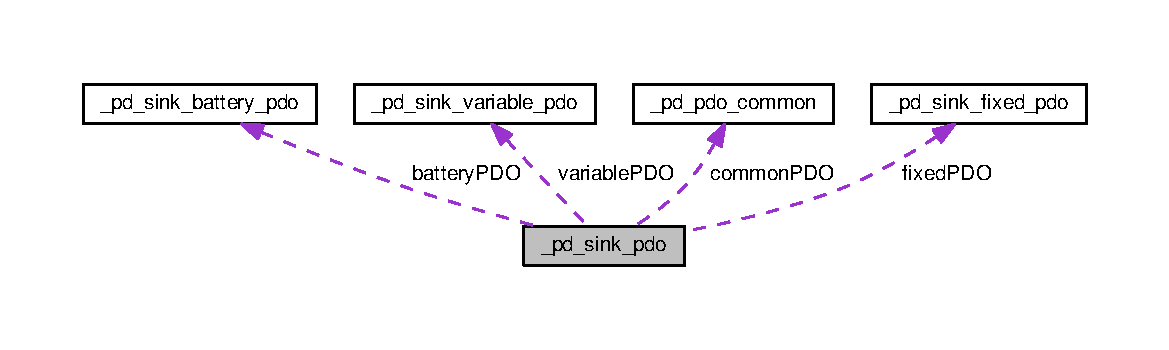
\includegraphics[width=350pt]{struct__pd__sink__pdo__coll__graph}
\end{center}
\end{figure}
\subsection*{Public Attributes}
\begin{DoxyCompactItemize}
\item 
\begin{tabbing}
xx\=xx\=xx\=xx\=xx\=xx\=xx\=xx\=xx\=\kill
union \{\\
\>uint32\_t \hyperlink{struct__pd__sink__pdo_a2f3c5aa6d559d35227af11db28c5dac8}{PDOValue}\\
\>\hyperlink{group__usb__pd__stack_ga7b2f5a42b9f5ae0e5b76f2ed44482ff3}{pd\_pdo\_common\_t} \hyperlink{struct__pd__sink__pdo_a8f6789929499a63a1326708206e016c5}{commonPDO}\\
\>\hyperlink{group__usb__pd__stack_gac1092e8fe40315ed926966b5b17883aa}{pd\_sink\_fixed\_pdo\_t} \hyperlink{struct__pd__sink__pdo_aebd2d1f5078757ee9a4c3d836e0df136}{fixedPDO}\\
\>\hyperlink{group__usb__pd__stack_gaf18073722dd91e4b87b60a6db76dc8dc}{pd\_sink\_variable\_pdo\_t} \hyperlink{struct__pd__sink__pdo_a15603e339ec84b653f83ee6865c1dfd8}{variablePDO}\\
\>\hyperlink{group__usb__pd__stack_ga917a58335ea75ba8b8cc3c359e1dee7a}{pd\_sink\_battery\_pdo\_t} \hyperlink{struct__pd__sink__pdo_adb7ddc7d4451cd6fe0f6eb13ebce229e}{batteryPDO}\\
\}; \\

\end{tabbing}\end{DoxyCompactItemize}


\subsection{Detailed Description}
sink P\-D\-O union 

\subsection{Member Data Documentation}
\hypertarget{struct__pd__sink__pdo_a9bc2f094f51753cea6adc85552fa8100}{\subsubsection[{"@39}]{\setlength{\rightskip}{0pt plus 5cm}union \{ ... \} }}\label{struct__pd__sink__pdo_a9bc2f094f51753cea6adc85552fa8100}
\hypertarget{struct__pd__sink__pdo_adb7ddc7d4451cd6fe0f6eb13ebce229e}{\index{\-\_\-pd\-\_\-sink\-\_\-pdo@{\-\_\-pd\-\_\-sink\-\_\-pdo}!battery\-P\-D\-O@{battery\-P\-D\-O}}
\index{battery\-P\-D\-O@{battery\-P\-D\-O}!_pd_sink_pdo@{\-\_\-pd\-\_\-sink\-\_\-pdo}}
\subsubsection[{battery\-P\-D\-O}]{\setlength{\rightskip}{0pt plus 5cm}{\bf pd\-\_\-sink\-\_\-battery\-\_\-pdo\-\_\-t} \-\_\-pd\-\_\-sink\-\_\-pdo\-::battery\-P\-D\-O}}\label{struct__pd__sink__pdo_adb7ddc7d4451cd6fe0f6eb13ebce229e}
union, battery pdo \hypertarget{struct__pd__sink__pdo_a8f6789929499a63a1326708206e016c5}{\index{\-\_\-pd\-\_\-sink\-\_\-pdo@{\-\_\-pd\-\_\-sink\-\_\-pdo}!common\-P\-D\-O@{common\-P\-D\-O}}
\index{common\-P\-D\-O@{common\-P\-D\-O}!_pd_sink_pdo@{\-\_\-pd\-\_\-sink\-\_\-pdo}}
\subsubsection[{common\-P\-D\-O}]{\setlength{\rightskip}{0pt plus 5cm}{\bf pd\-\_\-pdo\-\_\-common\-\_\-t} \-\_\-pd\-\_\-sink\-\_\-pdo\-::common\-P\-D\-O}}\label{struct__pd__sink__pdo_a8f6789929499a63a1326708206e016c5}
union, common pdo \hypertarget{struct__pd__sink__pdo_aebd2d1f5078757ee9a4c3d836e0df136}{\index{\-\_\-pd\-\_\-sink\-\_\-pdo@{\-\_\-pd\-\_\-sink\-\_\-pdo}!fixed\-P\-D\-O@{fixed\-P\-D\-O}}
\index{fixed\-P\-D\-O@{fixed\-P\-D\-O}!_pd_sink_pdo@{\-\_\-pd\-\_\-sink\-\_\-pdo}}
\subsubsection[{fixed\-P\-D\-O}]{\setlength{\rightskip}{0pt plus 5cm}{\bf pd\-\_\-sink\-\_\-fixed\-\_\-pdo\-\_\-t} \-\_\-pd\-\_\-sink\-\_\-pdo\-::fixed\-P\-D\-O}}\label{struct__pd__sink__pdo_aebd2d1f5078757ee9a4c3d836e0df136}
union, fixed pdo \hypertarget{struct__pd__sink__pdo_a2f3c5aa6d559d35227af11db28c5dac8}{\index{\-\_\-pd\-\_\-sink\-\_\-pdo@{\-\_\-pd\-\_\-sink\-\_\-pdo}!P\-D\-O\-Value@{P\-D\-O\-Value}}
\index{P\-D\-O\-Value@{P\-D\-O\-Value}!_pd_sink_pdo@{\-\_\-pd\-\_\-sink\-\_\-pdo}}
\subsubsection[{P\-D\-O\-Value}]{\setlength{\rightskip}{0pt plus 5cm}uint32\-\_\-t \-\_\-pd\-\_\-sink\-\_\-pdo\-::\-P\-D\-O\-Value}}\label{struct__pd__sink__pdo_a2f3c5aa6d559d35227af11db28c5dac8}
union, pdo 32 bits value \hypertarget{struct__pd__sink__pdo_a15603e339ec84b653f83ee6865c1dfd8}{\index{\-\_\-pd\-\_\-sink\-\_\-pdo@{\-\_\-pd\-\_\-sink\-\_\-pdo}!variable\-P\-D\-O@{variable\-P\-D\-O}}
\index{variable\-P\-D\-O@{variable\-P\-D\-O}!_pd_sink_pdo@{\-\_\-pd\-\_\-sink\-\_\-pdo}}
\subsubsection[{variable\-P\-D\-O}]{\setlength{\rightskip}{0pt plus 5cm}{\bf pd\-\_\-sink\-\_\-variable\-\_\-pdo\-\_\-t} \-\_\-pd\-\_\-sink\-\_\-pdo\-::variable\-P\-D\-O}}\label{struct__pd__sink__pdo_a15603e339ec84b653f83ee6865c1dfd8}
union, variable pdo 

The documentation for this struct was generated from the following file\-:\begin{DoxyCompactItemize}
\item 
pd/\hyperlink{usb__pd_8h}{usb\-\_\-pd.\-h}\end{DoxyCompactItemize}

\hypertarget{struct__pd__sink__variable__pdo}{\section{\-\_\-pd\-\_\-sink\-\_\-variable\-\_\-pdo Struct Reference}
\label{struct__pd__sink__variable__pdo}\index{\-\_\-pd\-\_\-sink\-\_\-variable\-\_\-pdo@{\-\_\-pd\-\_\-sink\-\_\-variable\-\_\-pdo}}
}


variable sink P\-D\-O  




{\ttfamily \#include $<$usb\-\_\-pd.\-h$>$}

\subsection*{Public Attributes}
\begin{DoxyCompactItemize}
\item 
uint32\-\_\-t \hyperlink{struct__pd__sink__variable__pdo_a145ba35b4f033f771ae9b72c018181d5}{operate\-Current}\-: 10
\item 
uint32\-\_\-t \hyperlink{struct__pd__sink__variable__pdo_a0ee666a778180c34bc4e0119ee3f51a3}{min\-Voltage}\-: 10
\item 
uint32\-\_\-t \hyperlink{struct__pd__sink__variable__pdo_adc5d6a90b282fc222e180b79aef74e65}{max\-Voltage}\-: 10
\item 
uint32\-\_\-t \hyperlink{struct__pd__sink__variable__pdo_a8ed1cefb52db381deddc243bd7d702e3}{variable\-Supply}\-: 2
\end{DoxyCompactItemize}


\subsection{Detailed Description}
variable sink P\-D\-O 

\subsection{Member Data Documentation}
\hypertarget{struct__pd__sink__variable__pdo_adc5d6a90b282fc222e180b79aef74e65}{\index{\-\_\-pd\-\_\-sink\-\_\-variable\-\_\-pdo@{\-\_\-pd\-\_\-sink\-\_\-variable\-\_\-pdo}!max\-Voltage@{max\-Voltage}}
\index{max\-Voltage@{max\-Voltage}!_pd_sink_variable_pdo@{\-\_\-pd\-\_\-sink\-\_\-variable\-\_\-pdo}}
\subsubsection[{max\-Voltage}]{\setlength{\rightskip}{0pt plus 5cm}uint32\-\_\-t \-\_\-pd\-\_\-sink\-\_\-variable\-\_\-pdo\-::max\-Voltage}}\label{struct__pd__sink__variable__pdo_adc5d6a90b282fc222e180b79aef74e65}
max voltage \hypertarget{struct__pd__sink__variable__pdo_a0ee666a778180c34bc4e0119ee3f51a3}{\index{\-\_\-pd\-\_\-sink\-\_\-variable\-\_\-pdo@{\-\_\-pd\-\_\-sink\-\_\-variable\-\_\-pdo}!min\-Voltage@{min\-Voltage}}
\index{min\-Voltage@{min\-Voltage}!_pd_sink_variable_pdo@{\-\_\-pd\-\_\-sink\-\_\-variable\-\_\-pdo}}
\subsubsection[{min\-Voltage}]{\setlength{\rightskip}{0pt plus 5cm}uint32\-\_\-t \-\_\-pd\-\_\-sink\-\_\-variable\-\_\-pdo\-::min\-Voltage}}\label{struct__pd__sink__variable__pdo_a0ee666a778180c34bc4e0119ee3f51a3}
min voltage \hypertarget{struct__pd__sink__variable__pdo_a145ba35b4f033f771ae9b72c018181d5}{\index{\-\_\-pd\-\_\-sink\-\_\-variable\-\_\-pdo@{\-\_\-pd\-\_\-sink\-\_\-variable\-\_\-pdo}!operate\-Current@{operate\-Current}}
\index{operate\-Current@{operate\-Current}!_pd_sink_variable_pdo@{\-\_\-pd\-\_\-sink\-\_\-variable\-\_\-pdo}}
\subsubsection[{operate\-Current}]{\setlength{\rightskip}{0pt plus 5cm}uint32\-\_\-t \-\_\-pd\-\_\-sink\-\_\-variable\-\_\-pdo\-::operate\-Current}}\label{struct__pd__sink__variable__pdo_a145ba35b4f033f771ae9b72c018181d5}
operate current \hypertarget{struct__pd__sink__variable__pdo_a8ed1cefb52db381deddc243bd7d702e3}{\index{\-\_\-pd\-\_\-sink\-\_\-variable\-\_\-pdo@{\-\_\-pd\-\_\-sink\-\_\-variable\-\_\-pdo}!variable\-Supply@{variable\-Supply}}
\index{variable\-Supply@{variable\-Supply}!_pd_sink_variable_pdo@{\-\_\-pd\-\_\-sink\-\_\-variable\-\_\-pdo}}
\subsubsection[{variable\-Supply}]{\setlength{\rightskip}{0pt plus 5cm}uint32\-\_\-t \-\_\-pd\-\_\-sink\-\_\-variable\-\_\-pdo\-::variable\-Supply}}\label{struct__pd__sink__variable__pdo_a8ed1cefb52db381deddc243bd7d702e3}
pdo type 

The documentation for this struct was generated from the following file\-:\begin{DoxyCompactItemize}
\item 
pd/\hyperlink{usb__pd_8h}{usb\-\_\-pd.\-h}\end{DoxyCompactItemize}

\hypertarget{struct__pd__source__battery__pdo}{\section{\-\_\-pd\-\_\-source\-\_\-battery\-\_\-pdo Struct Reference}
\label{struct__pd__source__battery__pdo}\index{\-\_\-pd\-\_\-source\-\_\-battery\-\_\-pdo@{\-\_\-pd\-\_\-source\-\_\-battery\-\_\-pdo}}
}


battery source P\-D\-O  




{\ttfamily \#include $<$usb\-\_\-pd.\-h$>$}

\subsection*{Public Attributes}
\begin{DoxyCompactItemize}
\item 
uint32\-\_\-t \hyperlink{struct__pd__source__battery__pdo_ae4498258205f03a10afdb32e445a57ef}{max\-Allow\-Power}\-: 10
\item 
uint32\-\_\-t \hyperlink{struct__pd__source__battery__pdo_a5c799cc37ea460e9bfeea8a05242cf54}{min\-Voltage}\-: 10
\item 
uint32\-\_\-t \hyperlink{struct__pd__source__battery__pdo_af818fd645542287499a65f559ef6d571}{max\-Voltage}\-: 10
\item 
uint32\-\_\-t \hyperlink{struct__pd__source__battery__pdo_a0cae5fa1b6136b1a9db95d182ec7122a}{battery}\-: 2
\end{DoxyCompactItemize}


\subsection{Detailed Description}
battery source P\-D\-O 

\subsection{Member Data Documentation}
\hypertarget{struct__pd__source__battery__pdo_a0cae5fa1b6136b1a9db95d182ec7122a}{\index{\-\_\-pd\-\_\-source\-\_\-battery\-\_\-pdo@{\-\_\-pd\-\_\-source\-\_\-battery\-\_\-pdo}!battery@{battery}}
\index{battery@{battery}!_pd_source_battery_pdo@{\-\_\-pd\-\_\-source\-\_\-battery\-\_\-pdo}}
\subsubsection[{battery}]{\setlength{\rightskip}{0pt plus 5cm}uint32\-\_\-t \-\_\-pd\-\_\-source\-\_\-battery\-\_\-pdo\-::battery}}\label{struct__pd__source__battery__pdo_a0cae5fa1b6136b1a9db95d182ec7122a}
pdo type \hypertarget{struct__pd__source__battery__pdo_ae4498258205f03a10afdb32e445a57ef}{\index{\-\_\-pd\-\_\-source\-\_\-battery\-\_\-pdo@{\-\_\-pd\-\_\-source\-\_\-battery\-\_\-pdo}!max\-Allow\-Power@{max\-Allow\-Power}}
\index{max\-Allow\-Power@{max\-Allow\-Power}!_pd_source_battery_pdo@{\-\_\-pd\-\_\-source\-\_\-battery\-\_\-pdo}}
\subsubsection[{max\-Allow\-Power}]{\setlength{\rightskip}{0pt plus 5cm}uint32\-\_\-t \-\_\-pd\-\_\-source\-\_\-battery\-\_\-pdo\-::max\-Allow\-Power}}\label{struct__pd__source__battery__pdo_ae4498258205f03a10afdb32e445a57ef}
max power \hypertarget{struct__pd__source__battery__pdo_af818fd645542287499a65f559ef6d571}{\index{\-\_\-pd\-\_\-source\-\_\-battery\-\_\-pdo@{\-\_\-pd\-\_\-source\-\_\-battery\-\_\-pdo}!max\-Voltage@{max\-Voltage}}
\index{max\-Voltage@{max\-Voltage}!_pd_source_battery_pdo@{\-\_\-pd\-\_\-source\-\_\-battery\-\_\-pdo}}
\subsubsection[{max\-Voltage}]{\setlength{\rightskip}{0pt plus 5cm}uint32\-\_\-t \-\_\-pd\-\_\-source\-\_\-battery\-\_\-pdo\-::max\-Voltage}}\label{struct__pd__source__battery__pdo_af818fd645542287499a65f559ef6d571}
max voltage \hypertarget{struct__pd__source__battery__pdo_a5c799cc37ea460e9bfeea8a05242cf54}{\index{\-\_\-pd\-\_\-source\-\_\-battery\-\_\-pdo@{\-\_\-pd\-\_\-source\-\_\-battery\-\_\-pdo}!min\-Voltage@{min\-Voltage}}
\index{min\-Voltage@{min\-Voltage}!_pd_source_battery_pdo@{\-\_\-pd\-\_\-source\-\_\-battery\-\_\-pdo}}
\subsubsection[{min\-Voltage}]{\setlength{\rightskip}{0pt plus 5cm}uint32\-\_\-t \-\_\-pd\-\_\-source\-\_\-battery\-\_\-pdo\-::min\-Voltage}}\label{struct__pd__source__battery__pdo_a5c799cc37ea460e9bfeea8a05242cf54}
min voltage 

The documentation for this struct was generated from the following file\-:\begin{DoxyCompactItemize}
\item 
pd/\hyperlink{usb__pd_8h}{usb\-\_\-pd.\-h}\end{DoxyCompactItemize}

\hypertarget{struct__pd__source__cap__ext__data__block}{\section{\-\_\-pd\-\_\-source\-\_\-cap\-\_\-ext\-\_\-data\-\_\-block Struct Reference}
\label{struct__pd__source__cap__ext__data__block}\index{\-\_\-pd\-\_\-source\-\_\-cap\-\_\-ext\-\_\-data\-\_\-block@{\-\_\-pd\-\_\-source\-\_\-cap\-\_\-ext\-\_\-data\-\_\-block}}
}


{\ttfamily \#include $<$pd\-\_\-app.\-h$>$}

\subsection*{Public Attributes}
\begin{DoxyCompactItemize}
\item 
uint16\-\_\-t \hyperlink{struct__pd__source__cap__ext__data__block_a3ebf0b088d638829f685c9e401af51d9}{vid}
\item 
uint16\-\_\-t \hyperlink{struct__pd__source__cap__ext__data__block_ac452b1d60d7700625f5a48e4e688bc74}{pid}
\item 
uint32\-\_\-t \hyperlink{struct__pd__source__cap__ext__data__block_a7422db66b33622addc1c55d9876bd495}{xid}
\item 
uint8\-\_\-t \hyperlink{struct__pd__source__cap__ext__data__block_a5f9b161cdc688ae7a7a71ac48bebe72b}{fw\-Version}
\item 
uint8\-\_\-t \hyperlink{struct__pd__source__cap__ext__data__block_a72634ef8e798fcfdda60b4d1b2ddf557}{hw\-Version}
\item 
uint8\-\_\-t \hyperlink{struct__pd__source__cap__ext__data__block_a46bcde86423f903c6f8a4da9bcf51bb6}{voltage\-Regulation}
\item 
uint8\-\_\-t \hyperlink{struct__pd__source__cap__ext__data__block_acd3a7351454a6578915d6b19d4180d11}{holdup\-Time}
\item 
uint8\-\_\-t \hyperlink{struct__pd__source__cap__ext__data__block_a81f30982a025f2c95364bf63aa9e1f49}{compliance}
\item 
uint8\-\_\-t \hyperlink{struct__pd__source__cap__ext__data__block_af98322f226a696aacedd45960c40849f}{touch\-Current}
\item 
uint16\-\_\-t \hyperlink{struct__pd__source__cap__ext__data__block_a4eee075250035a99554419d33a85921e}{peak\-Current1}
\item 
uint16\-\_\-t \hyperlink{struct__pd__source__cap__ext__data__block_a25ec3362e39d7bc3a9c27fb0f4f2cea1}{peak\-Current2}
\item 
uint16\-\_\-t \hyperlink{struct__pd__source__cap__ext__data__block_a7c1773f9c947bd695a44048f73bc1f43}{peak\-Current3}
\item 
uint8\-\_\-t \hyperlink{struct__pd__source__cap__ext__data__block_a58888000c9e3c7cdbe2dcc4d37f1640e}{touch\-Temp}
\item 
uint8\-\_\-t \hyperlink{struct__pd__source__cap__ext__data__block_a8c7747c758e6d178e63521ce87c7e650}{source\-Inputs}
\item 
uint8\-\_\-t \hyperlink{struct__pd__source__cap__ext__data__block_abdc72f29c41ce7930810313d60222b61}{batteries}
\end{DoxyCompactItemize}


\subsection{Member Data Documentation}
\hypertarget{struct__pd__source__cap__ext__data__block_abdc72f29c41ce7930810313d60222b61}{\index{\-\_\-pd\-\_\-source\-\_\-cap\-\_\-ext\-\_\-data\-\_\-block@{\-\_\-pd\-\_\-source\-\_\-cap\-\_\-ext\-\_\-data\-\_\-block}!batteries@{batteries}}
\index{batteries@{batteries}!_pd_source_cap_ext_data_block@{\-\_\-pd\-\_\-source\-\_\-cap\-\_\-ext\-\_\-data\-\_\-block}}
\subsubsection[{batteries}]{\setlength{\rightskip}{0pt plus 5cm}uint8\-\_\-t \-\_\-pd\-\_\-source\-\_\-cap\-\_\-ext\-\_\-data\-\_\-block\-::batteries}}\label{struct__pd__source__cap__ext__data__block_abdc72f29c41ce7930810313d60222b61}
\hypertarget{struct__pd__source__cap__ext__data__block_a81f30982a025f2c95364bf63aa9e1f49}{\index{\-\_\-pd\-\_\-source\-\_\-cap\-\_\-ext\-\_\-data\-\_\-block@{\-\_\-pd\-\_\-source\-\_\-cap\-\_\-ext\-\_\-data\-\_\-block}!compliance@{compliance}}
\index{compliance@{compliance}!_pd_source_cap_ext_data_block@{\-\_\-pd\-\_\-source\-\_\-cap\-\_\-ext\-\_\-data\-\_\-block}}
\subsubsection[{compliance}]{\setlength{\rightskip}{0pt plus 5cm}uint8\-\_\-t \-\_\-pd\-\_\-source\-\_\-cap\-\_\-ext\-\_\-data\-\_\-block\-::compliance}}\label{struct__pd__source__cap__ext__data__block_a81f30982a025f2c95364bf63aa9e1f49}
\hypertarget{struct__pd__source__cap__ext__data__block_a5f9b161cdc688ae7a7a71ac48bebe72b}{\index{\-\_\-pd\-\_\-source\-\_\-cap\-\_\-ext\-\_\-data\-\_\-block@{\-\_\-pd\-\_\-source\-\_\-cap\-\_\-ext\-\_\-data\-\_\-block}!fw\-Version@{fw\-Version}}
\index{fw\-Version@{fw\-Version}!_pd_source_cap_ext_data_block@{\-\_\-pd\-\_\-source\-\_\-cap\-\_\-ext\-\_\-data\-\_\-block}}
\subsubsection[{fw\-Version}]{\setlength{\rightskip}{0pt plus 5cm}uint8\-\_\-t \-\_\-pd\-\_\-source\-\_\-cap\-\_\-ext\-\_\-data\-\_\-block\-::fw\-Version}}\label{struct__pd__source__cap__ext__data__block_a5f9b161cdc688ae7a7a71ac48bebe72b}
\hypertarget{struct__pd__source__cap__ext__data__block_acd3a7351454a6578915d6b19d4180d11}{\index{\-\_\-pd\-\_\-source\-\_\-cap\-\_\-ext\-\_\-data\-\_\-block@{\-\_\-pd\-\_\-source\-\_\-cap\-\_\-ext\-\_\-data\-\_\-block}!holdup\-Time@{holdup\-Time}}
\index{holdup\-Time@{holdup\-Time}!_pd_source_cap_ext_data_block@{\-\_\-pd\-\_\-source\-\_\-cap\-\_\-ext\-\_\-data\-\_\-block}}
\subsubsection[{holdup\-Time}]{\setlength{\rightskip}{0pt plus 5cm}uint8\-\_\-t \-\_\-pd\-\_\-source\-\_\-cap\-\_\-ext\-\_\-data\-\_\-block\-::holdup\-Time}}\label{struct__pd__source__cap__ext__data__block_acd3a7351454a6578915d6b19d4180d11}
\hypertarget{struct__pd__source__cap__ext__data__block_a72634ef8e798fcfdda60b4d1b2ddf557}{\index{\-\_\-pd\-\_\-source\-\_\-cap\-\_\-ext\-\_\-data\-\_\-block@{\-\_\-pd\-\_\-source\-\_\-cap\-\_\-ext\-\_\-data\-\_\-block}!hw\-Version@{hw\-Version}}
\index{hw\-Version@{hw\-Version}!_pd_source_cap_ext_data_block@{\-\_\-pd\-\_\-source\-\_\-cap\-\_\-ext\-\_\-data\-\_\-block}}
\subsubsection[{hw\-Version}]{\setlength{\rightskip}{0pt plus 5cm}uint8\-\_\-t \-\_\-pd\-\_\-source\-\_\-cap\-\_\-ext\-\_\-data\-\_\-block\-::hw\-Version}}\label{struct__pd__source__cap__ext__data__block_a72634ef8e798fcfdda60b4d1b2ddf557}
\hypertarget{struct__pd__source__cap__ext__data__block_a4eee075250035a99554419d33a85921e}{\index{\-\_\-pd\-\_\-source\-\_\-cap\-\_\-ext\-\_\-data\-\_\-block@{\-\_\-pd\-\_\-source\-\_\-cap\-\_\-ext\-\_\-data\-\_\-block}!peak\-Current1@{peak\-Current1}}
\index{peak\-Current1@{peak\-Current1}!_pd_source_cap_ext_data_block@{\-\_\-pd\-\_\-source\-\_\-cap\-\_\-ext\-\_\-data\-\_\-block}}
\subsubsection[{peak\-Current1}]{\setlength{\rightskip}{0pt plus 5cm}uint16\-\_\-t \-\_\-pd\-\_\-source\-\_\-cap\-\_\-ext\-\_\-data\-\_\-block\-::peak\-Current1}}\label{struct__pd__source__cap__ext__data__block_a4eee075250035a99554419d33a85921e}
\hypertarget{struct__pd__source__cap__ext__data__block_a25ec3362e39d7bc3a9c27fb0f4f2cea1}{\index{\-\_\-pd\-\_\-source\-\_\-cap\-\_\-ext\-\_\-data\-\_\-block@{\-\_\-pd\-\_\-source\-\_\-cap\-\_\-ext\-\_\-data\-\_\-block}!peak\-Current2@{peak\-Current2}}
\index{peak\-Current2@{peak\-Current2}!_pd_source_cap_ext_data_block@{\-\_\-pd\-\_\-source\-\_\-cap\-\_\-ext\-\_\-data\-\_\-block}}
\subsubsection[{peak\-Current2}]{\setlength{\rightskip}{0pt plus 5cm}uint16\-\_\-t \-\_\-pd\-\_\-source\-\_\-cap\-\_\-ext\-\_\-data\-\_\-block\-::peak\-Current2}}\label{struct__pd__source__cap__ext__data__block_a25ec3362e39d7bc3a9c27fb0f4f2cea1}
\hypertarget{struct__pd__source__cap__ext__data__block_a7c1773f9c947bd695a44048f73bc1f43}{\index{\-\_\-pd\-\_\-source\-\_\-cap\-\_\-ext\-\_\-data\-\_\-block@{\-\_\-pd\-\_\-source\-\_\-cap\-\_\-ext\-\_\-data\-\_\-block}!peak\-Current3@{peak\-Current3}}
\index{peak\-Current3@{peak\-Current3}!_pd_source_cap_ext_data_block@{\-\_\-pd\-\_\-source\-\_\-cap\-\_\-ext\-\_\-data\-\_\-block}}
\subsubsection[{peak\-Current3}]{\setlength{\rightskip}{0pt plus 5cm}uint16\-\_\-t \-\_\-pd\-\_\-source\-\_\-cap\-\_\-ext\-\_\-data\-\_\-block\-::peak\-Current3}}\label{struct__pd__source__cap__ext__data__block_a7c1773f9c947bd695a44048f73bc1f43}
\hypertarget{struct__pd__source__cap__ext__data__block_ac452b1d60d7700625f5a48e4e688bc74}{\index{\-\_\-pd\-\_\-source\-\_\-cap\-\_\-ext\-\_\-data\-\_\-block@{\-\_\-pd\-\_\-source\-\_\-cap\-\_\-ext\-\_\-data\-\_\-block}!pid@{pid}}
\index{pid@{pid}!_pd_source_cap_ext_data_block@{\-\_\-pd\-\_\-source\-\_\-cap\-\_\-ext\-\_\-data\-\_\-block}}
\subsubsection[{pid}]{\setlength{\rightskip}{0pt plus 5cm}uint16\-\_\-t \-\_\-pd\-\_\-source\-\_\-cap\-\_\-ext\-\_\-data\-\_\-block\-::pid}}\label{struct__pd__source__cap__ext__data__block_ac452b1d60d7700625f5a48e4e688bc74}
\hypertarget{struct__pd__source__cap__ext__data__block_a8c7747c758e6d178e63521ce87c7e650}{\index{\-\_\-pd\-\_\-source\-\_\-cap\-\_\-ext\-\_\-data\-\_\-block@{\-\_\-pd\-\_\-source\-\_\-cap\-\_\-ext\-\_\-data\-\_\-block}!source\-Inputs@{source\-Inputs}}
\index{source\-Inputs@{source\-Inputs}!_pd_source_cap_ext_data_block@{\-\_\-pd\-\_\-source\-\_\-cap\-\_\-ext\-\_\-data\-\_\-block}}
\subsubsection[{source\-Inputs}]{\setlength{\rightskip}{0pt plus 5cm}uint8\-\_\-t \-\_\-pd\-\_\-source\-\_\-cap\-\_\-ext\-\_\-data\-\_\-block\-::source\-Inputs}}\label{struct__pd__source__cap__ext__data__block_a8c7747c758e6d178e63521ce87c7e650}
\hypertarget{struct__pd__source__cap__ext__data__block_af98322f226a696aacedd45960c40849f}{\index{\-\_\-pd\-\_\-source\-\_\-cap\-\_\-ext\-\_\-data\-\_\-block@{\-\_\-pd\-\_\-source\-\_\-cap\-\_\-ext\-\_\-data\-\_\-block}!touch\-Current@{touch\-Current}}
\index{touch\-Current@{touch\-Current}!_pd_source_cap_ext_data_block@{\-\_\-pd\-\_\-source\-\_\-cap\-\_\-ext\-\_\-data\-\_\-block}}
\subsubsection[{touch\-Current}]{\setlength{\rightskip}{0pt plus 5cm}uint8\-\_\-t \-\_\-pd\-\_\-source\-\_\-cap\-\_\-ext\-\_\-data\-\_\-block\-::touch\-Current}}\label{struct__pd__source__cap__ext__data__block_af98322f226a696aacedd45960c40849f}
\hypertarget{struct__pd__source__cap__ext__data__block_a58888000c9e3c7cdbe2dcc4d37f1640e}{\index{\-\_\-pd\-\_\-source\-\_\-cap\-\_\-ext\-\_\-data\-\_\-block@{\-\_\-pd\-\_\-source\-\_\-cap\-\_\-ext\-\_\-data\-\_\-block}!touch\-Temp@{touch\-Temp}}
\index{touch\-Temp@{touch\-Temp}!_pd_source_cap_ext_data_block@{\-\_\-pd\-\_\-source\-\_\-cap\-\_\-ext\-\_\-data\-\_\-block}}
\subsubsection[{touch\-Temp}]{\setlength{\rightskip}{0pt plus 5cm}uint8\-\_\-t \-\_\-pd\-\_\-source\-\_\-cap\-\_\-ext\-\_\-data\-\_\-block\-::touch\-Temp}}\label{struct__pd__source__cap__ext__data__block_a58888000c9e3c7cdbe2dcc4d37f1640e}
\hypertarget{struct__pd__source__cap__ext__data__block_a3ebf0b088d638829f685c9e401af51d9}{\index{\-\_\-pd\-\_\-source\-\_\-cap\-\_\-ext\-\_\-data\-\_\-block@{\-\_\-pd\-\_\-source\-\_\-cap\-\_\-ext\-\_\-data\-\_\-block}!vid@{vid}}
\index{vid@{vid}!_pd_source_cap_ext_data_block@{\-\_\-pd\-\_\-source\-\_\-cap\-\_\-ext\-\_\-data\-\_\-block}}
\subsubsection[{vid}]{\setlength{\rightskip}{0pt plus 5cm}uint16\-\_\-t \-\_\-pd\-\_\-source\-\_\-cap\-\_\-ext\-\_\-data\-\_\-block\-::vid}}\label{struct__pd__source__cap__ext__data__block_a3ebf0b088d638829f685c9e401af51d9}
\hypertarget{struct__pd__source__cap__ext__data__block_a46bcde86423f903c6f8a4da9bcf51bb6}{\index{\-\_\-pd\-\_\-source\-\_\-cap\-\_\-ext\-\_\-data\-\_\-block@{\-\_\-pd\-\_\-source\-\_\-cap\-\_\-ext\-\_\-data\-\_\-block}!voltage\-Regulation@{voltage\-Regulation}}
\index{voltage\-Regulation@{voltage\-Regulation}!_pd_source_cap_ext_data_block@{\-\_\-pd\-\_\-source\-\_\-cap\-\_\-ext\-\_\-data\-\_\-block}}
\subsubsection[{voltage\-Regulation}]{\setlength{\rightskip}{0pt plus 5cm}uint8\-\_\-t \-\_\-pd\-\_\-source\-\_\-cap\-\_\-ext\-\_\-data\-\_\-block\-::voltage\-Regulation}}\label{struct__pd__source__cap__ext__data__block_a46bcde86423f903c6f8a4da9bcf51bb6}
\hypertarget{struct__pd__source__cap__ext__data__block_a7422db66b33622addc1c55d9876bd495}{\index{\-\_\-pd\-\_\-source\-\_\-cap\-\_\-ext\-\_\-data\-\_\-block@{\-\_\-pd\-\_\-source\-\_\-cap\-\_\-ext\-\_\-data\-\_\-block}!xid@{xid}}
\index{xid@{xid}!_pd_source_cap_ext_data_block@{\-\_\-pd\-\_\-source\-\_\-cap\-\_\-ext\-\_\-data\-\_\-block}}
\subsubsection[{xid}]{\setlength{\rightskip}{0pt plus 5cm}uint32\-\_\-t \-\_\-pd\-\_\-source\-\_\-cap\-\_\-ext\-\_\-data\-\_\-block\-::xid}}\label{struct__pd__source__cap__ext__data__block_a7422db66b33622addc1c55d9876bd495}


The documentation for this struct was generated from the following file\-:\begin{DoxyCompactItemize}
\item 
demo/pd/\hyperlink{pd__app_8h}{pd\-\_\-app.\-h}\end{DoxyCompactItemize}

\hypertarget{struct__pd__source__fixed__pdo}{\section{\-\_\-pd\-\_\-source\-\_\-fixed\-\_\-pdo Struct Reference}
\label{struct__pd__source__fixed__pdo}\index{\-\_\-pd\-\_\-source\-\_\-fixed\-\_\-pdo@{\-\_\-pd\-\_\-source\-\_\-fixed\-\_\-pdo}}
}


fixed source P\-D\-O  




{\ttfamily \#include $<$usb\-\_\-pd.\-h$>$}

\subsection*{Public Attributes}
\begin{DoxyCompactItemize}
\item 
uint32\-\_\-t \hyperlink{struct__pd__source__fixed__pdo_a1bb1756a3f7fe82e0395efac18eb8f41}{max\-Current}\-: 10
\item 
uint32\-\_\-t \hyperlink{struct__pd__source__fixed__pdo_abba8fe6a9f4c4f6ac33cbfe075945e6a}{voltage}\-: 10
\item 
uint32\-\_\-t \hyperlink{struct__pd__source__fixed__pdo_a1a27fc2753ab60196afd3813e158d413}{peak\-Current}\-: 2
\item 
uint32\-\_\-t \hyperlink{struct__pd__source__fixed__pdo_a804529193e9d8df5aec299308e357ea1}{reserved}\-: 2
\item 
uint32\-\_\-t \hyperlink{struct__pd__source__fixed__pdo_a6e793acf2c695c57030e59f28dc5b65a}{unchunked\-Supported}\-: 1
\item 
uint32\-\_\-t \hyperlink{struct__pd__source__fixed__pdo_a9965da25ad2e4b58fd579e5a0632145a}{dual\-Role\-Data}\-: 1
\item 
uint32\-\_\-t \hyperlink{struct__pd__source__fixed__pdo_a0e2f3fc73e269168132defedb85f9d9f}{usb\-Communications\-Capable}\-: 1
\item 
uint32\-\_\-t \hyperlink{struct__pd__source__fixed__pdo_aa1715617698b348913227183195ae8f5}{external\-Powered}\-: 1
\item 
uint32\-\_\-t \hyperlink{struct__pd__source__fixed__pdo_aa836f41dcaaafe17d4ff65eeb3729b6d}{usb\-Suspend\-Supported}\-: 1
\item 
uint32\-\_\-t \hyperlink{struct__pd__source__fixed__pdo_afcce88f5e0b229d32e79297566e80dfd}{dual\-Role\-Power}\-: 1
\item 
uint32\-\_\-t \hyperlink{struct__pd__source__fixed__pdo_a2375dc4363d49f14521f1f7f6adffcde}{fixed\-Supply}\-: 2
\end{DoxyCompactItemize}


\subsection{Detailed Description}
fixed source P\-D\-O 

\subsection{Member Data Documentation}
\hypertarget{struct__pd__source__fixed__pdo_a9965da25ad2e4b58fd579e5a0632145a}{\index{\-\_\-pd\-\_\-source\-\_\-fixed\-\_\-pdo@{\-\_\-pd\-\_\-source\-\_\-fixed\-\_\-pdo}!dual\-Role\-Data@{dual\-Role\-Data}}
\index{dual\-Role\-Data@{dual\-Role\-Data}!_pd_source_fixed_pdo@{\-\_\-pd\-\_\-source\-\_\-fixed\-\_\-pdo}}
\subsubsection[{dual\-Role\-Data}]{\setlength{\rightskip}{0pt plus 5cm}uint32\-\_\-t \-\_\-pd\-\_\-source\-\_\-fixed\-\_\-pdo\-::dual\-Role\-Data}}\label{struct__pd__source__fixed__pdo_a9965da25ad2e4b58fd579e5a0632145a}
dual data role \hypertarget{struct__pd__source__fixed__pdo_afcce88f5e0b229d32e79297566e80dfd}{\index{\-\_\-pd\-\_\-source\-\_\-fixed\-\_\-pdo@{\-\_\-pd\-\_\-source\-\_\-fixed\-\_\-pdo}!dual\-Role\-Power@{dual\-Role\-Power}}
\index{dual\-Role\-Power@{dual\-Role\-Power}!_pd_source_fixed_pdo@{\-\_\-pd\-\_\-source\-\_\-fixed\-\_\-pdo}}
\subsubsection[{dual\-Role\-Power}]{\setlength{\rightskip}{0pt plus 5cm}uint32\-\_\-t \-\_\-pd\-\_\-source\-\_\-fixed\-\_\-pdo\-::dual\-Role\-Power}}\label{struct__pd__source__fixed__pdo_afcce88f5e0b229d32e79297566e80dfd}
dual power role \hypertarget{struct__pd__source__fixed__pdo_aa1715617698b348913227183195ae8f5}{\index{\-\_\-pd\-\_\-source\-\_\-fixed\-\_\-pdo@{\-\_\-pd\-\_\-source\-\_\-fixed\-\_\-pdo}!external\-Powered@{external\-Powered}}
\index{external\-Powered@{external\-Powered}!_pd_source_fixed_pdo@{\-\_\-pd\-\_\-source\-\_\-fixed\-\_\-pdo}}
\subsubsection[{external\-Powered}]{\setlength{\rightskip}{0pt plus 5cm}uint32\-\_\-t \-\_\-pd\-\_\-source\-\_\-fixed\-\_\-pdo\-::external\-Powered}}\label{struct__pd__source__fixed__pdo_aa1715617698b348913227183195ae8f5}
external powered \hypertarget{struct__pd__source__fixed__pdo_a2375dc4363d49f14521f1f7f6adffcde}{\index{\-\_\-pd\-\_\-source\-\_\-fixed\-\_\-pdo@{\-\_\-pd\-\_\-source\-\_\-fixed\-\_\-pdo}!fixed\-Supply@{fixed\-Supply}}
\index{fixed\-Supply@{fixed\-Supply}!_pd_source_fixed_pdo@{\-\_\-pd\-\_\-source\-\_\-fixed\-\_\-pdo}}
\subsubsection[{fixed\-Supply}]{\setlength{\rightskip}{0pt plus 5cm}uint32\-\_\-t \-\_\-pd\-\_\-source\-\_\-fixed\-\_\-pdo\-::fixed\-Supply}}\label{struct__pd__source__fixed__pdo_a2375dc4363d49f14521f1f7f6adffcde}
pdo type \hypertarget{struct__pd__source__fixed__pdo_a1bb1756a3f7fe82e0395efac18eb8f41}{\index{\-\_\-pd\-\_\-source\-\_\-fixed\-\_\-pdo@{\-\_\-pd\-\_\-source\-\_\-fixed\-\_\-pdo}!max\-Current@{max\-Current}}
\index{max\-Current@{max\-Current}!_pd_source_fixed_pdo@{\-\_\-pd\-\_\-source\-\_\-fixed\-\_\-pdo}}
\subsubsection[{max\-Current}]{\setlength{\rightskip}{0pt plus 5cm}uint32\-\_\-t \-\_\-pd\-\_\-source\-\_\-fixed\-\_\-pdo\-::max\-Current}}\label{struct__pd__source__fixed__pdo_a1bb1756a3f7fe82e0395efac18eb8f41}
max current \hypertarget{struct__pd__source__fixed__pdo_a1a27fc2753ab60196afd3813e158d413}{\index{\-\_\-pd\-\_\-source\-\_\-fixed\-\_\-pdo@{\-\_\-pd\-\_\-source\-\_\-fixed\-\_\-pdo}!peak\-Current@{peak\-Current}}
\index{peak\-Current@{peak\-Current}!_pd_source_fixed_pdo@{\-\_\-pd\-\_\-source\-\_\-fixed\-\_\-pdo}}
\subsubsection[{peak\-Current}]{\setlength{\rightskip}{0pt plus 5cm}uint32\-\_\-t \-\_\-pd\-\_\-source\-\_\-fixed\-\_\-pdo\-::peak\-Current}}\label{struct__pd__source__fixed__pdo_a1a27fc2753ab60196afd3813e158d413}
peak current \hypertarget{struct__pd__source__fixed__pdo_a804529193e9d8df5aec299308e357ea1}{\index{\-\_\-pd\-\_\-source\-\_\-fixed\-\_\-pdo@{\-\_\-pd\-\_\-source\-\_\-fixed\-\_\-pdo}!reserved@{reserved}}
\index{reserved@{reserved}!_pd_source_fixed_pdo@{\-\_\-pd\-\_\-source\-\_\-fixed\-\_\-pdo}}
\subsubsection[{reserved}]{\setlength{\rightskip}{0pt plus 5cm}uint32\-\_\-t \-\_\-pd\-\_\-source\-\_\-fixed\-\_\-pdo\-::reserved}}\label{struct__pd__source__fixed__pdo_a804529193e9d8df5aec299308e357ea1}
reserved field \hypertarget{struct__pd__source__fixed__pdo_a6e793acf2c695c57030e59f28dc5b65a}{\index{\-\_\-pd\-\_\-source\-\_\-fixed\-\_\-pdo@{\-\_\-pd\-\_\-source\-\_\-fixed\-\_\-pdo}!unchunked\-Supported@{unchunked\-Supported}}
\index{unchunked\-Supported@{unchunked\-Supported}!_pd_source_fixed_pdo@{\-\_\-pd\-\_\-source\-\_\-fixed\-\_\-pdo}}
\subsubsection[{unchunked\-Supported}]{\setlength{\rightskip}{0pt plus 5cm}uint32\-\_\-t \-\_\-pd\-\_\-source\-\_\-fixed\-\_\-pdo\-::unchunked\-Supported}}\label{struct__pd__source__fixed__pdo_a6e793acf2c695c57030e59f28dc5b65a}
unchunked is supported or not \hypertarget{struct__pd__source__fixed__pdo_a0e2f3fc73e269168132defedb85f9d9f}{\index{\-\_\-pd\-\_\-source\-\_\-fixed\-\_\-pdo@{\-\_\-pd\-\_\-source\-\_\-fixed\-\_\-pdo}!usb\-Communications\-Capable@{usb\-Communications\-Capable}}
\index{usb\-Communications\-Capable@{usb\-Communications\-Capable}!_pd_source_fixed_pdo@{\-\_\-pd\-\_\-source\-\_\-fixed\-\_\-pdo}}
\subsubsection[{usb\-Communications\-Capable}]{\setlength{\rightskip}{0pt plus 5cm}uint32\-\_\-t \-\_\-pd\-\_\-source\-\_\-fixed\-\_\-pdo\-::usb\-Communications\-Capable}}\label{struct__pd__source__fixed__pdo_a0e2f3fc73e269168132defedb85f9d9f}
usb communication capable or not \hypertarget{struct__pd__source__fixed__pdo_aa836f41dcaaafe17d4ff65eeb3729b6d}{\index{\-\_\-pd\-\_\-source\-\_\-fixed\-\_\-pdo@{\-\_\-pd\-\_\-source\-\_\-fixed\-\_\-pdo}!usb\-Suspend\-Supported@{usb\-Suspend\-Supported}}
\index{usb\-Suspend\-Supported@{usb\-Suspend\-Supported}!_pd_source_fixed_pdo@{\-\_\-pd\-\_\-source\-\_\-fixed\-\_\-pdo}}
\subsubsection[{usb\-Suspend\-Supported}]{\setlength{\rightskip}{0pt plus 5cm}uint32\-\_\-t \-\_\-pd\-\_\-source\-\_\-fixed\-\_\-pdo\-::usb\-Suspend\-Supported}}\label{struct__pd__source__fixed__pdo_aa836f41dcaaafe17d4ff65eeb3729b6d}
usb suspend supported or not \hypertarget{struct__pd__source__fixed__pdo_abba8fe6a9f4c4f6ac33cbfe075945e6a}{\index{\-\_\-pd\-\_\-source\-\_\-fixed\-\_\-pdo@{\-\_\-pd\-\_\-source\-\_\-fixed\-\_\-pdo}!voltage@{voltage}}
\index{voltage@{voltage}!_pd_source_fixed_pdo@{\-\_\-pd\-\_\-source\-\_\-fixed\-\_\-pdo}}
\subsubsection[{voltage}]{\setlength{\rightskip}{0pt plus 5cm}uint32\-\_\-t \-\_\-pd\-\_\-source\-\_\-fixed\-\_\-pdo\-::voltage}}\label{struct__pd__source__fixed__pdo_abba8fe6a9f4c4f6ac33cbfe075945e6a}
voltage value, unit is 50m\-V 

The documentation for this struct was generated from the following file\-:\begin{DoxyCompactItemize}
\item 
pd/\hyperlink{usb__pd_8h}{usb\-\_\-pd.\-h}\end{DoxyCompactItemize}

\hypertarget{struct__pd__source__pdo}{\section{\-\_\-pd\-\_\-source\-\_\-pdo Struct Reference}
\label{struct__pd__source__pdo}\index{\-\_\-pd\-\_\-source\-\_\-pdo@{\-\_\-pd\-\_\-source\-\_\-pdo}}
}


source P\-D\-O union  




{\ttfamily \#include $<$usb\-\_\-pd.\-h$>$}



Collaboration diagram for \-\_\-pd\-\_\-source\-\_\-pdo\-:
\nopagebreak
\begin{figure}[H]
\begin{center}
\leavevmode
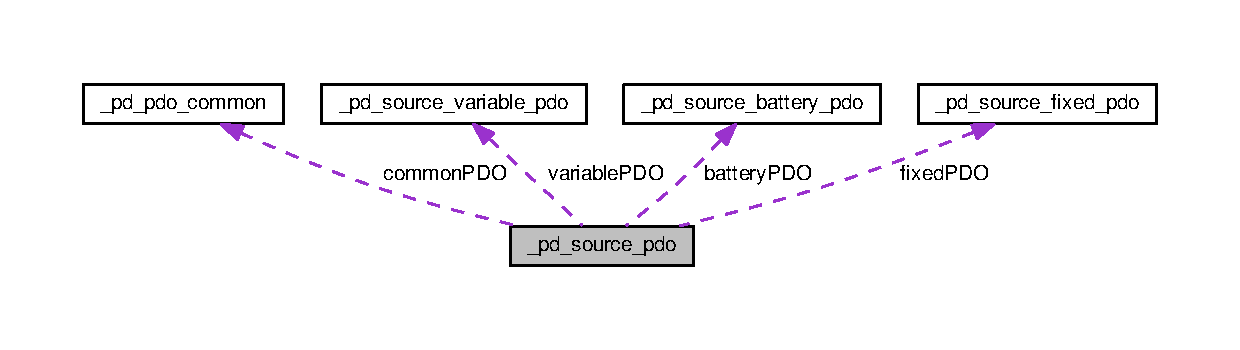
\includegraphics[width=350pt]{struct__pd__source__pdo__coll__graph}
\end{center}
\end{figure}
\subsection*{Public Attributes}
\begin{DoxyCompactItemize}
\item 
\begin{tabbing}
xx\=xx\=xx\=xx\=xx\=xx\=xx\=xx\=xx\=\kill
union \{\\
\>uint32\_t \hyperlink{struct__pd__source__pdo_ae7c1220b81dd8506c6731d7a6adc6ac9}{PDOValue}\\
\>\hyperlink{group__usb__pd__stack_ga7b2f5a42b9f5ae0e5b76f2ed44482ff3}{pd\_pdo\_common\_t} \hyperlink{struct__pd__source__pdo_ad1af05b25c2dfc8f72eea50707536c10}{commonPDO}\\
\>\hyperlink{group__usb__pd__stack_gaa7dd48248cb5b3177c59635a91f1b16e}{pd\_source\_fixed\_pdo\_t} \hyperlink{struct__pd__source__pdo_a2405f8ee75a370cba4a48b94080958b1}{fixedPDO}\\
\>\hyperlink{group__usb__pd__stack_ga0c9d6847951d8b95ecfac843574c027d}{pd\_source\_variable\_pdo\_t} \hyperlink{struct__pd__source__pdo_a81d5ae3b407a289661136aa515ba1942}{variablePDO}\\
\>\hyperlink{group__usb__pd__stack_ga5f2a906851b2fe0554a083085c62324b}{pd\_source\_battery\_pdo\_t} \hyperlink{struct__pd__source__pdo_ae677c279b52a30bc6ca29600d978757e}{batteryPDO}\\
\}; \\

\end{tabbing}\end{DoxyCompactItemize}


\subsection{Detailed Description}
source P\-D\-O union 

\subsection{Member Data Documentation}
\hypertarget{struct__pd__source__pdo_a467642c60beaed4560b8b9faad6d2d14}{\subsubsection[{"@37}]{\setlength{\rightskip}{0pt plus 5cm}union \{ ... \} }}\label{struct__pd__source__pdo_a467642c60beaed4560b8b9faad6d2d14}
\hypertarget{struct__pd__source__pdo_ae677c279b52a30bc6ca29600d978757e}{\index{\-\_\-pd\-\_\-source\-\_\-pdo@{\-\_\-pd\-\_\-source\-\_\-pdo}!battery\-P\-D\-O@{battery\-P\-D\-O}}
\index{battery\-P\-D\-O@{battery\-P\-D\-O}!_pd_source_pdo@{\-\_\-pd\-\_\-source\-\_\-pdo}}
\subsubsection[{battery\-P\-D\-O}]{\setlength{\rightskip}{0pt plus 5cm}{\bf pd\-\_\-source\-\_\-battery\-\_\-pdo\-\_\-t} \-\_\-pd\-\_\-source\-\_\-pdo\-::battery\-P\-D\-O}}\label{struct__pd__source__pdo_ae677c279b52a30bc6ca29600d978757e}
union, battery pdo \hypertarget{struct__pd__source__pdo_ad1af05b25c2dfc8f72eea50707536c10}{\index{\-\_\-pd\-\_\-source\-\_\-pdo@{\-\_\-pd\-\_\-source\-\_\-pdo}!common\-P\-D\-O@{common\-P\-D\-O}}
\index{common\-P\-D\-O@{common\-P\-D\-O}!_pd_source_pdo@{\-\_\-pd\-\_\-source\-\_\-pdo}}
\subsubsection[{common\-P\-D\-O}]{\setlength{\rightskip}{0pt plus 5cm}{\bf pd\-\_\-pdo\-\_\-common\-\_\-t} \-\_\-pd\-\_\-source\-\_\-pdo\-::common\-P\-D\-O}}\label{struct__pd__source__pdo_ad1af05b25c2dfc8f72eea50707536c10}
union, common pdo \hypertarget{struct__pd__source__pdo_a2405f8ee75a370cba4a48b94080958b1}{\index{\-\_\-pd\-\_\-source\-\_\-pdo@{\-\_\-pd\-\_\-source\-\_\-pdo}!fixed\-P\-D\-O@{fixed\-P\-D\-O}}
\index{fixed\-P\-D\-O@{fixed\-P\-D\-O}!_pd_source_pdo@{\-\_\-pd\-\_\-source\-\_\-pdo}}
\subsubsection[{fixed\-P\-D\-O}]{\setlength{\rightskip}{0pt plus 5cm}{\bf pd\-\_\-source\-\_\-fixed\-\_\-pdo\-\_\-t} \-\_\-pd\-\_\-source\-\_\-pdo\-::fixed\-P\-D\-O}}\label{struct__pd__source__pdo_a2405f8ee75a370cba4a48b94080958b1}
union, fixed pdo \hypertarget{struct__pd__source__pdo_ae7c1220b81dd8506c6731d7a6adc6ac9}{\index{\-\_\-pd\-\_\-source\-\_\-pdo@{\-\_\-pd\-\_\-source\-\_\-pdo}!P\-D\-O\-Value@{P\-D\-O\-Value}}
\index{P\-D\-O\-Value@{P\-D\-O\-Value}!_pd_source_pdo@{\-\_\-pd\-\_\-source\-\_\-pdo}}
\subsubsection[{P\-D\-O\-Value}]{\setlength{\rightskip}{0pt plus 5cm}uint32\-\_\-t \-\_\-pd\-\_\-source\-\_\-pdo\-::\-P\-D\-O\-Value}}\label{struct__pd__source__pdo_ae7c1220b81dd8506c6731d7a6adc6ac9}
union pdo 32 bits value \hypertarget{struct__pd__source__pdo_a81d5ae3b407a289661136aa515ba1942}{\index{\-\_\-pd\-\_\-source\-\_\-pdo@{\-\_\-pd\-\_\-source\-\_\-pdo}!variable\-P\-D\-O@{variable\-P\-D\-O}}
\index{variable\-P\-D\-O@{variable\-P\-D\-O}!_pd_source_pdo@{\-\_\-pd\-\_\-source\-\_\-pdo}}
\subsubsection[{variable\-P\-D\-O}]{\setlength{\rightskip}{0pt plus 5cm}{\bf pd\-\_\-source\-\_\-variable\-\_\-pdo\-\_\-t} \-\_\-pd\-\_\-source\-\_\-pdo\-::variable\-P\-D\-O}}\label{struct__pd__source__pdo_a81d5ae3b407a289661136aa515ba1942}
union, variable pdo 

The documentation for this struct was generated from the following file\-:\begin{DoxyCompactItemize}
\item 
pd/\hyperlink{usb__pd_8h}{usb\-\_\-pd.\-h}\end{DoxyCompactItemize}

\hypertarget{struct__pd__source__variable__pdo}{\section{\-\_\-pd\-\_\-source\-\_\-variable\-\_\-pdo Struct Reference}
\label{struct__pd__source__variable__pdo}\index{\-\_\-pd\-\_\-source\-\_\-variable\-\_\-pdo@{\-\_\-pd\-\_\-source\-\_\-variable\-\_\-pdo}}
}


variable source P\-D\-O  




{\ttfamily \#include $<$usb\-\_\-pd.\-h$>$}

\subsection*{Public Attributes}
\begin{DoxyCompactItemize}
\item 
uint32\-\_\-t \hyperlink{struct__pd__source__variable__pdo_a8a24367204d3381f0670311a88c0b2e6}{max\-Current}\-: 10
\item 
uint32\-\_\-t \hyperlink{struct__pd__source__variable__pdo_a713018c825f51d1a6a7186582b40a106}{min\-Voltage}\-: 10
\item 
uint32\-\_\-t \hyperlink{struct__pd__source__variable__pdo_a493ced8078579d68ade7dfbce819b4d1}{max\-Voltage}\-: 10
\item 
uint32\-\_\-t \hyperlink{struct__pd__source__variable__pdo_a47233d0cd3de38e33422b8e107a6ff9d}{variable\-Supply}\-: 2
\end{DoxyCompactItemize}


\subsection{Detailed Description}
variable source P\-D\-O 

\subsection{Member Data Documentation}
\hypertarget{struct__pd__source__variable__pdo_a8a24367204d3381f0670311a88c0b2e6}{\index{\-\_\-pd\-\_\-source\-\_\-variable\-\_\-pdo@{\-\_\-pd\-\_\-source\-\_\-variable\-\_\-pdo}!max\-Current@{max\-Current}}
\index{max\-Current@{max\-Current}!_pd_source_variable_pdo@{\-\_\-pd\-\_\-source\-\_\-variable\-\_\-pdo}}
\subsubsection[{max\-Current}]{\setlength{\rightskip}{0pt plus 5cm}uint32\-\_\-t \-\_\-pd\-\_\-source\-\_\-variable\-\_\-pdo\-::max\-Current}}\label{struct__pd__source__variable__pdo_a8a24367204d3381f0670311a88c0b2e6}
max current \hypertarget{struct__pd__source__variable__pdo_a493ced8078579d68ade7dfbce819b4d1}{\index{\-\_\-pd\-\_\-source\-\_\-variable\-\_\-pdo@{\-\_\-pd\-\_\-source\-\_\-variable\-\_\-pdo}!max\-Voltage@{max\-Voltage}}
\index{max\-Voltage@{max\-Voltage}!_pd_source_variable_pdo@{\-\_\-pd\-\_\-source\-\_\-variable\-\_\-pdo}}
\subsubsection[{max\-Voltage}]{\setlength{\rightskip}{0pt plus 5cm}uint32\-\_\-t \-\_\-pd\-\_\-source\-\_\-variable\-\_\-pdo\-::max\-Voltage}}\label{struct__pd__source__variable__pdo_a493ced8078579d68ade7dfbce819b4d1}
max voltage \hypertarget{struct__pd__source__variable__pdo_a713018c825f51d1a6a7186582b40a106}{\index{\-\_\-pd\-\_\-source\-\_\-variable\-\_\-pdo@{\-\_\-pd\-\_\-source\-\_\-variable\-\_\-pdo}!min\-Voltage@{min\-Voltage}}
\index{min\-Voltage@{min\-Voltage}!_pd_source_variable_pdo@{\-\_\-pd\-\_\-source\-\_\-variable\-\_\-pdo}}
\subsubsection[{min\-Voltage}]{\setlength{\rightskip}{0pt plus 5cm}uint32\-\_\-t \-\_\-pd\-\_\-source\-\_\-variable\-\_\-pdo\-::min\-Voltage}}\label{struct__pd__source__variable__pdo_a713018c825f51d1a6a7186582b40a106}
min voltage \hypertarget{struct__pd__source__variable__pdo_a47233d0cd3de38e33422b8e107a6ff9d}{\index{\-\_\-pd\-\_\-source\-\_\-variable\-\_\-pdo@{\-\_\-pd\-\_\-source\-\_\-variable\-\_\-pdo}!variable\-Supply@{variable\-Supply}}
\index{variable\-Supply@{variable\-Supply}!_pd_source_variable_pdo@{\-\_\-pd\-\_\-source\-\_\-variable\-\_\-pdo}}
\subsubsection[{variable\-Supply}]{\setlength{\rightskip}{0pt plus 5cm}uint32\-\_\-t \-\_\-pd\-\_\-source\-\_\-variable\-\_\-pdo\-::variable\-Supply}}\label{struct__pd__source__variable__pdo_a47233d0cd3de38e33422b8e107a6ff9d}
pdo type 

The documentation for this struct was generated from the following file\-:\begin{DoxyCompactItemize}
\item 
pd/\hyperlink{usb__pd_8h}{usb\-\_\-pd.\-h}\end{DoxyCompactItemize}

\hypertarget{struct__pd__spi__interface__config}{\section{\-\_\-pd\-\_\-spi\-\_\-interface\-\_\-config Struct Reference}
\label{struct__pd__spi__interface__config}\index{\-\_\-pd\-\_\-spi\-\_\-interface\-\_\-config@{\-\_\-pd\-\_\-spi\-\_\-interface\-\_\-config}}
}


S\-P\-I interface configure parameter.  




{\ttfamily \#include $<$usb\-\_\-cmsis\-\_\-wrapper.\-h$>$}

\subsection*{Public Attributes}
\begin{DoxyCompactItemize}
\item 
uint32\-\_\-t \hyperlink{struct__pd__spi__interface__config_a62ac507496812ca6db95d14263ba3229}{pcs}
\end{DoxyCompactItemize}


\subsection{Detailed Description}
S\-P\-I interface configure parameter. 

\subsection{Member Data Documentation}
\hypertarget{struct__pd__spi__interface__config_a62ac507496812ca6db95d14263ba3229}{\index{\-\_\-pd\-\_\-spi\-\_\-interface\-\_\-config@{\-\_\-pd\-\_\-spi\-\_\-interface\-\_\-config}!pcs@{pcs}}
\index{pcs@{pcs}!_pd_spi_interface_config@{\-\_\-pd\-\_\-spi\-\_\-interface\-\_\-config}}
\subsubsection[{pcs}]{\setlength{\rightskip}{0pt plus 5cm}uint32\-\_\-t \-\_\-pd\-\_\-spi\-\_\-interface\-\_\-config\-::pcs}}\label{struct__pd__spi__interface__config_a62ac507496812ca6db95d14263ba3229}


The documentation for this struct was generated from the following file\-:\begin{DoxyCompactItemize}
\item 
pd/cmsis\-\_\-wrapper/\hyperlink{usb__cmsis__wrapper_8h}{usb\-\_\-cmsis\-\_\-wrapper.\-h}\end{DoxyCompactItemize}

\hypertarget{struct__pd__status__data__block}{\section{\-\_\-pd\-\_\-status\-\_\-data\-\_\-block Struct Reference}
\label{struct__pd__status__data__block}\index{\-\_\-pd\-\_\-status\-\_\-data\-\_\-block@{\-\_\-pd\-\_\-status\-\_\-data\-\_\-block}}
}


{\ttfamily \#include $<$pd\-\_\-app.\-h$>$}

\subsection*{Public Attributes}
\begin{DoxyCompactItemize}
\item 
uint8\-\_\-t \hyperlink{struct__pd__status__data__block_a703addd9acd9c9208aee4b610cdcfee0}{internal\-Temp}
\item 
uint8\-\_\-t \hyperlink{struct__pd__status__data__block_a73ce40cf713642d43b807c9e6f7c0915}{present\-Input}
\item 
uint8\-\_\-t \hyperlink{struct__pd__status__data__block_a39291ac6c1e754c78545ec755ad12073}{present\-Battery\-Input}
\end{DoxyCompactItemize}


\subsection{Member Data Documentation}
\hypertarget{struct__pd__status__data__block_a703addd9acd9c9208aee4b610cdcfee0}{\index{\-\_\-pd\-\_\-status\-\_\-data\-\_\-block@{\-\_\-pd\-\_\-status\-\_\-data\-\_\-block}!internal\-Temp@{internal\-Temp}}
\index{internal\-Temp@{internal\-Temp}!_pd_status_data_block@{\-\_\-pd\-\_\-status\-\_\-data\-\_\-block}}
\subsubsection[{internal\-Temp}]{\setlength{\rightskip}{0pt plus 5cm}uint8\-\_\-t \-\_\-pd\-\_\-status\-\_\-data\-\_\-block\-::internal\-Temp}}\label{struct__pd__status__data__block_a703addd9acd9c9208aee4b610cdcfee0}
\hypertarget{struct__pd__status__data__block_a39291ac6c1e754c78545ec755ad12073}{\index{\-\_\-pd\-\_\-status\-\_\-data\-\_\-block@{\-\_\-pd\-\_\-status\-\_\-data\-\_\-block}!present\-Battery\-Input@{present\-Battery\-Input}}
\index{present\-Battery\-Input@{present\-Battery\-Input}!_pd_status_data_block@{\-\_\-pd\-\_\-status\-\_\-data\-\_\-block}}
\subsubsection[{present\-Battery\-Input}]{\setlength{\rightskip}{0pt plus 5cm}uint8\-\_\-t \-\_\-pd\-\_\-status\-\_\-data\-\_\-block\-::present\-Battery\-Input}}\label{struct__pd__status__data__block_a39291ac6c1e754c78545ec755ad12073}
\hypertarget{struct__pd__status__data__block_a73ce40cf713642d43b807c9e6f7c0915}{\index{\-\_\-pd\-\_\-status\-\_\-data\-\_\-block@{\-\_\-pd\-\_\-status\-\_\-data\-\_\-block}!present\-Input@{present\-Input}}
\index{present\-Input@{present\-Input}!_pd_status_data_block@{\-\_\-pd\-\_\-status\-\_\-data\-\_\-block}}
\subsubsection[{present\-Input}]{\setlength{\rightskip}{0pt plus 5cm}uint8\-\_\-t \-\_\-pd\-\_\-status\-\_\-data\-\_\-block\-::present\-Input}}\label{struct__pd__status__data__block_a73ce40cf713642d43b807c9e6f7c0915}


The documentation for this struct was generated from the following file\-:\begin{DoxyCompactItemize}
\item 
demo/pd/\hyperlink{pd__app_8h}{pd\-\_\-app.\-h}\end{DoxyCompactItemize}

\hypertarget{struct__pd__structured__vdm__header}{\section{\-\_\-pd\-\_\-structured\-\_\-vdm\-\_\-header Struct Reference}
\label{struct__pd__structured__vdm__header}\index{\-\_\-pd\-\_\-structured\-\_\-vdm\-\_\-header@{\-\_\-pd\-\_\-structured\-\_\-vdm\-\_\-header}}
}


P\-D structured V\-D\-M header.  




{\ttfamily \#include $<$usb\-\_\-pd.\-h$>$}

\subsection*{Public Attributes}
\begin{DoxyCompactItemize}
\item 
\begin{tabbing}
xx\=xx\=xx\=xx\=xx\=xx\=xx\=xx\=xx\=\kill
union \{\\
\>struct \{\\
\>\>uint32\_t \hyperlink{struct__pd__structured__vdm__header_aada24db165d116acd79aa1a44a30d2e1}{command}: 5\\
\>\>uint32\_t \hyperlink{struct__pd__structured__vdm__header_ae96832372241f43fdbb0a364539d424f}{reserved1}: 1\\
\>\>uint32\_t \hyperlink{struct__pd__structured__vdm__header_a8146babffdd0022316369e0631995bf1}{commandType}: 2\\
\>\>uint32\_t \hyperlink{struct__pd__structured__vdm__header_a70c79769097f532657064784a5803022}{objPos}: 3\\
\>\>uint32\_t \hyperlink{struct__pd__structured__vdm__header_aced9840a12b97bb0e0acc6e4d72a3566}{reserved2}: 2\\
\>\>uint32\_t \hyperlink{struct__pd__structured__vdm__header_af95df1485673cf3bd9b62d4de0185a07}{vdmVersion}: 2\\
\>\>uint32\_t \hyperlink{struct__pd__structured__vdm__header_a096921553a1351b55e5419e8f5eac69a}{vdmType}: 1\\
\>\>uint32\_t \hyperlink{struct__pd__structured__vdm__header_a9b7bde8903697b83450597f27aceb370}{SVID}: 16\\
\>\} \hyperlink{struct__pd__structured__vdm__header_afc8471a70fa430820836286de3cf2281}{bitFields}\\
\>uint32\_t \hyperlink{struct__pd__structured__vdm__header_a0544fc4b30468ec5d5b435a05b30ced1}{structuredVdmHeaderVal}\\
\}; \\

\end{tabbing}\end{DoxyCompactItemize}


\subsection{Detailed Description}
P\-D structured V\-D\-M header. 

\subsection{Member Data Documentation}
\hypertarget{struct__pd__structured__vdm__header_ad81a4fe2b7dc1e0ec659f27d52344596}{\subsubsection[{"@41}]{\setlength{\rightskip}{0pt plus 5cm}union \{ ... \} }}\label{struct__pd__structured__vdm__header_ad81a4fe2b7dc1e0ec659f27d52344596}
\hypertarget{struct__pd__structured__vdm__header_afc8471a70fa430820836286de3cf2281}{\index{\-\_\-pd\-\_\-structured\-\_\-vdm\-\_\-header@{\-\_\-pd\-\_\-structured\-\_\-vdm\-\_\-header}!bit\-Fields@{bit\-Fields}}
\index{bit\-Fields@{bit\-Fields}!_pd_structured_vdm_header@{\-\_\-pd\-\_\-structured\-\_\-vdm\-\_\-header}}
\subsubsection[{bit\-Fields}]{\setlength{\rightskip}{0pt plus 5cm}struct \{ ... \}   \-\_\-pd\-\_\-structured\-\_\-vdm\-\_\-header\-::bit\-Fields}}\label{struct__pd__structured__vdm__header_afc8471a70fa430820836286de3cf2281}
union structured V\-D\-M header structure \hypertarget{struct__pd__structured__vdm__header_aada24db165d116acd79aa1a44a30d2e1}{\index{\-\_\-pd\-\_\-structured\-\_\-vdm\-\_\-header@{\-\_\-pd\-\_\-structured\-\_\-vdm\-\_\-header}!command@{command}}
\index{command@{command}!_pd_structured_vdm_header@{\-\_\-pd\-\_\-structured\-\_\-vdm\-\_\-header}}
\subsubsection[{command}]{\setlength{\rightskip}{0pt plus 5cm}uint32\-\_\-t \-\_\-pd\-\_\-structured\-\_\-vdm\-\_\-header\-::command}}\label{struct__pd__structured__vdm__header_aada24db165d116acd79aa1a44a30d2e1}
command \hypertarget{struct__pd__structured__vdm__header_a8146babffdd0022316369e0631995bf1}{\index{\-\_\-pd\-\_\-structured\-\_\-vdm\-\_\-header@{\-\_\-pd\-\_\-structured\-\_\-vdm\-\_\-header}!command\-Type@{command\-Type}}
\index{command\-Type@{command\-Type}!_pd_structured_vdm_header@{\-\_\-pd\-\_\-structured\-\_\-vdm\-\_\-header}}
\subsubsection[{command\-Type}]{\setlength{\rightskip}{0pt plus 5cm}uint32\-\_\-t \-\_\-pd\-\_\-structured\-\_\-vdm\-\_\-header\-::command\-Type}}\label{struct__pd__structured__vdm__header_a8146babffdd0022316369e0631995bf1}
command type \hypertarget{struct__pd__structured__vdm__header_a70c79769097f532657064784a5803022}{\index{\-\_\-pd\-\_\-structured\-\_\-vdm\-\_\-header@{\-\_\-pd\-\_\-structured\-\_\-vdm\-\_\-header}!obj\-Pos@{obj\-Pos}}
\index{obj\-Pos@{obj\-Pos}!_pd_structured_vdm_header@{\-\_\-pd\-\_\-structured\-\_\-vdm\-\_\-header}}
\subsubsection[{obj\-Pos}]{\setlength{\rightskip}{0pt plus 5cm}uint32\-\_\-t \-\_\-pd\-\_\-structured\-\_\-vdm\-\_\-header\-::obj\-Pos}}\label{struct__pd__structured__vdm__header_a70c79769097f532657064784a5803022}
object position \hypertarget{struct__pd__structured__vdm__header_ae96832372241f43fdbb0a364539d424f}{\index{\-\_\-pd\-\_\-structured\-\_\-vdm\-\_\-header@{\-\_\-pd\-\_\-structured\-\_\-vdm\-\_\-header}!reserved1@{reserved1}}
\index{reserved1@{reserved1}!_pd_structured_vdm_header@{\-\_\-pd\-\_\-structured\-\_\-vdm\-\_\-header}}
\subsubsection[{reserved1}]{\setlength{\rightskip}{0pt plus 5cm}uint32\-\_\-t \-\_\-pd\-\_\-structured\-\_\-vdm\-\_\-header\-::reserved1}}\label{struct__pd__structured__vdm__header_ae96832372241f43fdbb0a364539d424f}
reserved \hypertarget{struct__pd__structured__vdm__header_aced9840a12b97bb0e0acc6e4d72a3566}{\index{\-\_\-pd\-\_\-structured\-\_\-vdm\-\_\-header@{\-\_\-pd\-\_\-structured\-\_\-vdm\-\_\-header}!reserved2@{reserved2}}
\index{reserved2@{reserved2}!_pd_structured_vdm_header@{\-\_\-pd\-\_\-structured\-\_\-vdm\-\_\-header}}
\subsubsection[{reserved2}]{\setlength{\rightskip}{0pt plus 5cm}uint32\-\_\-t \-\_\-pd\-\_\-structured\-\_\-vdm\-\_\-header\-::reserved2}}\label{struct__pd__structured__vdm__header_aced9840a12b97bb0e0acc6e4d72a3566}
reserved \hypertarget{struct__pd__structured__vdm__header_a0544fc4b30468ec5d5b435a05b30ced1}{\index{\-\_\-pd\-\_\-structured\-\_\-vdm\-\_\-header@{\-\_\-pd\-\_\-structured\-\_\-vdm\-\_\-header}!structured\-Vdm\-Header\-Val@{structured\-Vdm\-Header\-Val}}
\index{structured\-Vdm\-Header\-Val@{structured\-Vdm\-Header\-Val}!_pd_structured_vdm_header@{\-\_\-pd\-\_\-structured\-\_\-vdm\-\_\-header}}
\subsubsection[{structured\-Vdm\-Header\-Val}]{\setlength{\rightskip}{0pt plus 5cm}uint32\-\_\-t \-\_\-pd\-\_\-structured\-\_\-vdm\-\_\-header\-::structured\-Vdm\-Header\-Val}}\label{struct__pd__structured__vdm__header_a0544fc4b30468ec5d5b435a05b30ced1}
union 32bits value \hypertarget{struct__pd__structured__vdm__header_a9b7bde8903697b83450597f27aceb370}{\index{\-\_\-pd\-\_\-structured\-\_\-vdm\-\_\-header@{\-\_\-pd\-\_\-structured\-\_\-vdm\-\_\-header}!S\-V\-I\-D@{S\-V\-I\-D}}
\index{S\-V\-I\-D@{S\-V\-I\-D}!_pd_structured_vdm_header@{\-\_\-pd\-\_\-structured\-\_\-vdm\-\_\-header}}
\subsubsection[{S\-V\-I\-D}]{\setlength{\rightskip}{0pt plus 5cm}uint32\-\_\-t \-\_\-pd\-\_\-structured\-\_\-vdm\-\_\-header\-::\-S\-V\-I\-D}}\label{struct__pd__structured__vdm__header_a9b7bde8903697b83450597f27aceb370}
S\-V\-I\-D value \hypertarget{struct__pd__structured__vdm__header_a096921553a1351b55e5419e8f5eac69a}{\index{\-\_\-pd\-\_\-structured\-\_\-vdm\-\_\-header@{\-\_\-pd\-\_\-structured\-\_\-vdm\-\_\-header}!vdm\-Type@{vdm\-Type}}
\index{vdm\-Type@{vdm\-Type}!_pd_structured_vdm_header@{\-\_\-pd\-\_\-structured\-\_\-vdm\-\_\-header}}
\subsubsection[{vdm\-Type}]{\setlength{\rightskip}{0pt plus 5cm}uint32\-\_\-t \-\_\-pd\-\_\-structured\-\_\-vdm\-\_\-header\-::vdm\-Type}}\label{struct__pd__structured__vdm__header_a096921553a1351b55e5419e8f5eac69a}
vdm type, structured vdm \hypertarget{struct__pd__structured__vdm__header_af95df1485673cf3bd9b62d4de0185a07}{\index{\-\_\-pd\-\_\-structured\-\_\-vdm\-\_\-header@{\-\_\-pd\-\_\-structured\-\_\-vdm\-\_\-header}!vdm\-Version@{vdm\-Version}}
\index{vdm\-Version@{vdm\-Version}!_pd_structured_vdm_header@{\-\_\-pd\-\_\-structured\-\_\-vdm\-\_\-header}}
\subsubsection[{vdm\-Version}]{\setlength{\rightskip}{0pt plus 5cm}uint32\-\_\-t \-\_\-pd\-\_\-structured\-\_\-vdm\-\_\-header\-::vdm\-Version}}\label{struct__pd__structured__vdm__header_af95df1485673cf3bd9b62d4de0185a07}
vdm version 

The documentation for this struct was generated from the following file\-:\begin{DoxyCompactItemize}
\item 
pd/\hyperlink{usb__pd_8h}{usb\-\_\-pd.\-h}\end{DoxyCompactItemize}

\hypertarget{struct__pd__svdm__command__result}{\section{\-\_\-pd\-\_\-svdm\-\_\-command\-\_\-result Struct Reference}
\label{struct__pd__svdm__command__result}\index{\-\_\-pd\-\_\-svdm\-\_\-command\-\_\-result@{\-\_\-pd\-\_\-svdm\-\_\-command\-\_\-result}}
}


P\-D structured vdm command result.  




{\ttfamily \#include $<$usb\-\_\-pd.\-h$>$}



Collaboration diagram for \-\_\-pd\-\_\-svdm\-\_\-command\-\_\-result\-:
\nopagebreak
\begin{figure}[H]
\begin{center}
\leavevmode
\includegraphics[width=218pt]{struct__pd__svdm__command__result__coll__graph}
\end{center}
\end{figure}
\subsection*{Public Attributes}
\begin{DoxyCompactItemize}
\item 
uint32\-\_\-t $\ast$ \hyperlink{struct__pd__svdm__command__result_acd15ff8f7fe85b7e8ed891199339053f}{vdo\-Data}
\item 
\hyperlink{group__usb__pd__stack_ga245b8bec3f3b7771e73016ac98595570}{pd\-\_\-structured\-\_\-vdm\-\_\-header\-\_\-t} \hyperlink{struct__pd__svdm__command__result_adc6934994780581eba3edc5b4fe47765}{vdm\-Header}
\item 
uint8\-\_\-t \hyperlink{struct__pd__svdm__command__result_a347c19dd5209bb9ef874aa11caf4c07b}{vdo\-Count}
\item 
uint8\-\_\-t \hyperlink{struct__pd__svdm__command__result_aa65006c48f37577f5cab247b07bb0cdf}{vdo\-Sop}
\item 
uint8\-\_\-t \hyperlink{struct__pd__svdm__command__result_af1f46eb3cd5009b29a5f3ba293a5fc84}{vdm\-Command}
\item 
uint8\-\_\-t \hyperlink{struct__pd__svdm__command__result_af52b0485285dda6a8eda1154989dc84e}{vdm\-Command\-Result}
\end{DoxyCompactItemize}


\subsection{Detailed Description}
P\-D structured vdm command result. 

it is used in P\-D\-\_\-\-D\-P\-M\-\_\-\-S\-T\-R\-U\-C\-T\-U\-R\-E\-D\-\_\-\-V\-D\-M\-\_\-\-S\-U\-C\-C\-E\-S\-S and P\-D\-\_\-\-D\-P\-M\-\_\-\-S\-T\-R\-U\-C\-T\-U\-R\-E\-D\-\_\-\-V\-D\-M\-\_\-\-F\-A\-I\-L events callback. it provide vdm command reply message information to application, it may be A\-C\-K (contain data), N\-A\-K or B\-U\-S\-Y. 

\subsection{Member Data Documentation}
\hypertarget{struct__pd__svdm__command__result_af1f46eb3cd5009b29a5f3ba293a5fc84}{\index{\-\_\-pd\-\_\-svdm\-\_\-command\-\_\-result@{\-\_\-pd\-\_\-svdm\-\_\-command\-\_\-result}!vdm\-Command@{vdm\-Command}}
\index{vdm\-Command@{vdm\-Command}!_pd_svdm_command_result@{\-\_\-pd\-\_\-svdm\-\_\-command\-\_\-result}}
\subsubsection[{vdm\-Command}]{\setlength{\rightskip}{0pt plus 5cm}uint8\-\_\-t \-\_\-pd\-\_\-svdm\-\_\-command\-\_\-result\-::vdm\-Command}}\label{struct__pd__svdm__command__result_af1f46eb3cd5009b29a5f3ba293a5fc84}
vdm command, the value is \hyperlink{group__usb__pd__stack_gabd6b0763d01e2d65501af70e4f67b039}{pd\-\_\-vdm\-\_\-command\-\_\-t} \hypertarget{struct__pd__svdm__command__result_af52b0485285dda6a8eda1154989dc84e}{\index{\-\_\-pd\-\_\-svdm\-\_\-command\-\_\-result@{\-\_\-pd\-\_\-svdm\-\_\-command\-\_\-result}!vdm\-Command\-Result@{vdm\-Command\-Result}}
\index{vdm\-Command\-Result@{vdm\-Command\-Result}!_pd_svdm_command_result@{\-\_\-pd\-\_\-svdm\-\_\-command\-\_\-result}}
\subsubsection[{vdm\-Command\-Result}]{\setlength{\rightskip}{0pt plus 5cm}uint8\-\_\-t \-\_\-pd\-\_\-svdm\-\_\-command\-\_\-result\-::vdm\-Command\-Result}}\label{struct__pd__svdm__command__result_af52b0485285dda6a8eda1154989dc84e}
vdm command's result\-: success with data or fail. the value is \hyperlink{group__usb__pd__stack_ga59917b1485caba4dd8d9b65ca5a5fd92}{pd\-\_\-command\-\_\-result\-\_\-t} \hypertarget{struct__pd__svdm__command__result_adc6934994780581eba3edc5b4fe47765}{\index{\-\_\-pd\-\_\-svdm\-\_\-command\-\_\-result@{\-\_\-pd\-\_\-svdm\-\_\-command\-\_\-result}!vdm\-Header@{vdm\-Header}}
\index{vdm\-Header@{vdm\-Header}!_pd_svdm_command_result@{\-\_\-pd\-\_\-svdm\-\_\-command\-\_\-result}}
\subsubsection[{vdm\-Header}]{\setlength{\rightskip}{0pt plus 5cm}{\bf pd\-\_\-structured\-\_\-vdm\-\_\-header\-\_\-t} \-\_\-pd\-\_\-svdm\-\_\-command\-\_\-result\-::vdm\-Header}}\label{struct__pd__svdm__command__result_adc6934994780581eba3edc5b4fe47765}
vdm header \hypertarget{struct__pd__svdm__command__result_a347c19dd5209bb9ef874aa11caf4c07b}{\index{\-\_\-pd\-\_\-svdm\-\_\-command\-\_\-result@{\-\_\-pd\-\_\-svdm\-\_\-command\-\_\-result}!vdo\-Count@{vdo\-Count}}
\index{vdo\-Count@{vdo\-Count}!_pd_svdm_command_result@{\-\_\-pd\-\_\-svdm\-\_\-command\-\_\-result}}
\subsubsection[{vdo\-Count}]{\setlength{\rightskip}{0pt plus 5cm}uint8\-\_\-t \-\_\-pd\-\_\-svdm\-\_\-command\-\_\-result\-::vdo\-Count}}\label{struct__pd__svdm__command__result_a347c19dd5209bb9ef874aa11caf4c07b}
vdm data length (unit is 4 bytes) \hypertarget{struct__pd__svdm__command__result_acd15ff8f7fe85b7e8ed891199339053f}{\index{\-\_\-pd\-\_\-svdm\-\_\-command\-\_\-result@{\-\_\-pd\-\_\-svdm\-\_\-command\-\_\-result}!vdo\-Data@{vdo\-Data}}
\index{vdo\-Data@{vdo\-Data}!_pd_svdm_command_result@{\-\_\-pd\-\_\-svdm\-\_\-command\-\_\-result}}
\subsubsection[{vdo\-Data}]{\setlength{\rightskip}{0pt plus 5cm}uint32\-\_\-t$\ast$ \-\_\-pd\-\_\-svdm\-\_\-command\-\_\-result\-::vdo\-Data}}\label{struct__pd__svdm__command__result_acd15ff8f7fe85b7e8ed891199339053f}
vdm data buffer address \hypertarget{struct__pd__svdm__command__result_aa65006c48f37577f5cab247b07bb0cdf}{\index{\-\_\-pd\-\_\-svdm\-\_\-command\-\_\-result@{\-\_\-pd\-\_\-svdm\-\_\-command\-\_\-result}!vdo\-Sop@{vdo\-Sop}}
\index{vdo\-Sop@{vdo\-Sop}!_pd_svdm_command_result@{\-\_\-pd\-\_\-svdm\-\_\-command\-\_\-result}}
\subsubsection[{vdo\-Sop}]{\setlength{\rightskip}{0pt plus 5cm}uint8\-\_\-t \-\_\-pd\-\_\-svdm\-\_\-command\-\_\-result\-::vdo\-Sop}}\label{struct__pd__svdm__command__result_aa65006c48f37577f5cab247b07bb0cdf}
vdm message's sop type 

The documentation for this struct was generated from the following file\-:\begin{DoxyCompactItemize}
\item 
pd/\hyperlink{usb__pd_8h}{usb\-\_\-pd.\-h}\end{DoxyCompactItemize}

\hypertarget{struct__pd__svdm__param}{\section{\-\_\-pd\-\_\-svdm\-\_\-param Struct Reference}
\label{struct__pd__svdm__param}\index{\-\_\-pd\-\_\-svdm\-\_\-param@{\-\_\-pd\-\_\-svdm\-\_\-param}}
}


P\-D structured vdm command parameter.  




{\ttfamily \#include $<$usb\-\_\-pd.\-h$>$}



Collaboration diagram for \-\_\-pd\-\_\-svdm\-\_\-param\-:
\nopagebreak
\begin{figure}[H]
\begin{center}
\leavevmode
\includegraphics[width=186pt]{struct__pd__svdm__param__coll__graph}
\end{center}
\end{figure}
\subsection*{Public Attributes}
\begin{DoxyCompactItemize}
\item 
uint32\-\_\-t $\ast$ \hyperlink{struct__pd__svdm__param_a1da6696ea0b07e0173cc469094639e99}{vdo\-Data}
\item 
\hyperlink{group__usb__pd__stack_ga245b8bec3f3b7771e73016ac98595570}{pd\-\_\-structured\-\_\-vdm\-\_\-header\-\_\-t} \hyperlink{struct__pd__svdm__param_aaebc50d834d15e862f264a4e4d8421b4}{vdm\-Header}
\item 
uint8\-\_\-t \hyperlink{struct__pd__svdm__param_a153be4aa8e8fa9e41ac83eb41e513060}{vdo\-Count}
\item 
uint8\-\_\-t \hyperlink{struct__pd__svdm__param_a8047c38bf19593f6d467256b1696587e}{vdm\-Sop}
\item 
uint8\-\_\-t \hyperlink{struct__pd__svdm__param_a2a41729be5b45c14a61c39498b0f43be}{vendor\-V\-D\-M\-Need\-Response}
\end{DoxyCompactItemize}


\subsection{Detailed Description}
P\-D structured vdm command parameter. 

it is used in P\-D\-\_\-\-Command for P\-D\-\_\-\-D\-P\-M\-\_\-\-C\-O\-N\-T\-R\-O\-L\-\_\-\-D\-I\-S\-C\-O\-V\-E\-R\-Y\-\_\-\-I\-D\-E\-N\-T\-I\-T\-Y, P\-D\-\_\-\-D\-P\-M\-\_\-\-C\-O\-N\-T\-R\-O\-L\-\_\-\-D\-I\-S\-C\-O\-V\-E\-R\-Y\-\_\-\-S\-V\-I\-D\-S, P\-D\-\_\-\-D\-P\-M\-\_\-\-C\-O\-N\-T\-R\-O\-L\-\_\-\-D\-I\-S\-C\-O\-V\-E\-R\-Y\-\_\-\-M\-O\-D\-E\-S, P\-D\-\_\-\-D\-P\-M\-\_\-\-C\-O\-N\-T\-R\-O\-L\-\_\-\-E\-N\-T\-E\-R\-\_\-\-M\-O\-D\-E, P\-D\-\_\-\-D\-P\-M\-\_\-\-C\-O\-N\-T\-R\-O\-L\-\_\-\-E\-X\-I\-T\-\_\-\-M\-O\-D\-E or P\-D\-\_\-\-D\-P\-M\-\_\-\-C\-O\-N\-T\-R\-O\-L\-\_\-\-S\-E\-N\-D\-\_\-\-A\-T\-T\-E\-N\-T\-I\-O\-N. it provide vdm command information to P\-D stack, P\-D stack will start the command with the information. 

\subsection{Member Data Documentation}
\hypertarget{struct__pd__svdm__param_aaebc50d834d15e862f264a4e4d8421b4}{\index{\-\_\-pd\-\_\-svdm\-\_\-param@{\-\_\-pd\-\_\-svdm\-\_\-param}!vdm\-Header@{vdm\-Header}}
\index{vdm\-Header@{vdm\-Header}!_pd_svdm_param@{\-\_\-pd\-\_\-svdm\-\_\-param}}
\subsubsection[{vdm\-Header}]{\setlength{\rightskip}{0pt plus 5cm}{\bf pd\-\_\-structured\-\_\-vdm\-\_\-header\-\_\-t} \-\_\-pd\-\_\-svdm\-\_\-param\-::vdm\-Header}}\label{struct__pd__svdm__param_aaebc50d834d15e862f264a4e4d8421b4}
vdm header \hypertarget{struct__pd__svdm__param_a8047c38bf19593f6d467256b1696587e}{\index{\-\_\-pd\-\_\-svdm\-\_\-param@{\-\_\-pd\-\_\-svdm\-\_\-param}!vdm\-Sop@{vdm\-Sop}}
\index{vdm\-Sop@{vdm\-Sop}!_pd_svdm_param@{\-\_\-pd\-\_\-svdm\-\_\-param}}
\subsubsection[{vdm\-Sop}]{\setlength{\rightskip}{0pt plus 5cm}uint8\-\_\-t \-\_\-pd\-\_\-svdm\-\_\-param\-::vdm\-Sop}}\label{struct__pd__svdm__param_a8047c38bf19593f6d467256b1696587e}
vdm message's sop type \hypertarget{struct__pd__svdm__param_a153be4aa8e8fa9e41ac83eb41e513060}{\index{\-\_\-pd\-\_\-svdm\-\_\-param@{\-\_\-pd\-\_\-svdm\-\_\-param}!vdo\-Count@{vdo\-Count}}
\index{vdo\-Count@{vdo\-Count}!_pd_svdm_param@{\-\_\-pd\-\_\-svdm\-\_\-param}}
\subsubsection[{vdo\-Count}]{\setlength{\rightskip}{0pt plus 5cm}uint8\-\_\-t \-\_\-pd\-\_\-svdm\-\_\-param\-::vdo\-Count}}\label{struct__pd__svdm__param_a153be4aa8e8fa9e41ac83eb41e513060}
vdm data length (unit is 4 bytes) \hypertarget{struct__pd__svdm__param_a1da6696ea0b07e0173cc469094639e99}{\index{\-\_\-pd\-\_\-svdm\-\_\-param@{\-\_\-pd\-\_\-svdm\-\_\-param}!vdo\-Data@{vdo\-Data}}
\index{vdo\-Data@{vdo\-Data}!_pd_svdm_param@{\-\_\-pd\-\_\-svdm\-\_\-param}}
\subsubsection[{vdo\-Data}]{\setlength{\rightskip}{0pt plus 5cm}uint32\-\_\-t$\ast$ \-\_\-pd\-\_\-svdm\-\_\-param\-::vdo\-Data}}\label{struct__pd__svdm__param_a1da6696ea0b07e0173cc469094639e99}
vdm data buffer address \hypertarget{struct__pd__svdm__param_a2a41729be5b45c14a61c39498b0f43be}{\index{\-\_\-pd\-\_\-svdm\-\_\-param@{\-\_\-pd\-\_\-svdm\-\_\-param}!vendor\-V\-D\-M\-Need\-Response@{vendor\-V\-D\-M\-Need\-Response}}
\index{vendor\-V\-D\-M\-Need\-Response@{vendor\-V\-D\-M\-Need\-Response}!_pd_svdm_param@{\-\_\-pd\-\_\-svdm\-\_\-param}}
\subsubsection[{vendor\-V\-D\-M\-Need\-Response}]{\setlength{\rightskip}{0pt plus 5cm}uint8\-\_\-t \-\_\-pd\-\_\-svdm\-\_\-param\-::vendor\-V\-D\-M\-Need\-Response}}\label{struct__pd__svdm__param_a2a41729be5b45c14a61c39498b0f43be}
discovery\-\_\-identity need response, but attention don't need. vendor defined structured V\-D\-M may need or not. 

The documentation for this struct was generated from the following file\-:\begin{DoxyCompactItemize}
\item 
pd/\hyperlink{usb__pd_8h}{usb\-\_\-pd.\-h}\end{DoxyCompactItemize}

\hypertarget{struct__pd__svdm__request}{\section{\-\_\-pd\-\_\-svdm\-\_\-request Struct Reference}
\label{struct__pd__svdm__request}\index{\-\_\-pd\-\_\-svdm\-\_\-request@{\-\_\-pd\-\_\-svdm\-\_\-request}}
}


P\-D structured vdm command request (negotiation)  




{\ttfamily \#include $<$usb\-\_\-pd.\-h$>$}



Collaboration diagram for \-\_\-pd\-\_\-svdm\-\_\-request\-:
\nopagebreak
\begin{figure}[H]
\begin{center}
\leavevmode
\includegraphics[width=186pt]{struct__pd__svdm__request__coll__graph}
\end{center}
\end{figure}
\subsection*{Public Attributes}
\begin{DoxyCompactItemize}
\item 
uint32\-\_\-t $\ast$ \hyperlink{struct__pd__svdm__request_ac674930499f5462b363cb7890746888e}{vdo\-Data}
\item 
\hyperlink{group__usb__pd__stack_ga245b8bec3f3b7771e73016ac98595570}{pd\-\_\-structured\-\_\-vdm\-\_\-header\-\_\-t} \hyperlink{struct__pd__svdm__request_a502097a71d336575e7c64feded3fc3d1}{vdm\-Header}
\item 
uint8\-\_\-t \hyperlink{struct__pd__svdm__request_a447ad7fabf845dde656f32b7ba306582}{vdo\-Count}
\item 
uint8\-\_\-t \hyperlink{struct__pd__svdm__request_a7cc54e0d5070eeec62c3686c716cff28}{vdo\-Sop}
\item 
uint8\-\_\-t \hyperlink{struct__pd__svdm__request_a234e68f92801246ea761e56aa163c3e6}{request\-Result\-Status}
\end{DoxyCompactItemize}


\subsection{Detailed Description}
P\-D structured vdm command request (negotiation) 

it is used in P\-D\-\_\-\-D\-P\-M\-\_\-\-S\-T\-R\-U\-C\-T\-U\-R\-E\-D\-\_\-\-V\-D\-M\-\_\-\-R\-E\-Q\-U\-E\-S\-T event callback. it provide vdm message information to application, application need reply A\-C\-K (contain data), N\-A\-K or B\-U\-S\-Y. 

\subsection{Member Data Documentation}
\hypertarget{struct__pd__svdm__request_a234e68f92801246ea761e56aa163c3e6}{\index{\-\_\-pd\-\_\-svdm\-\_\-request@{\-\_\-pd\-\_\-svdm\-\_\-request}!request\-Result\-Status@{request\-Result\-Status}}
\index{request\-Result\-Status@{request\-Result\-Status}!_pd_svdm_request@{\-\_\-pd\-\_\-svdm\-\_\-request}}
\subsubsection[{request\-Result\-Status}]{\setlength{\rightskip}{0pt plus 5cm}uint8\-\_\-t \-\_\-pd\-\_\-svdm\-\_\-request\-::request\-Result\-Status}}\label{struct__pd__svdm__request_a234e68f92801246ea761e56aa163c3e6}
application need return the negotiation result to P\-D stack, the value is \hyperlink{group__usb__pd__stack_ga59917b1485caba4dd8d9b65ca5a5fd92}{pd\-\_\-command\-\_\-result\-\_\-t} \hypertarget{struct__pd__svdm__request_a502097a71d336575e7c64feded3fc3d1}{\index{\-\_\-pd\-\_\-svdm\-\_\-request@{\-\_\-pd\-\_\-svdm\-\_\-request}!vdm\-Header@{vdm\-Header}}
\index{vdm\-Header@{vdm\-Header}!_pd_svdm_request@{\-\_\-pd\-\_\-svdm\-\_\-request}}
\subsubsection[{vdm\-Header}]{\setlength{\rightskip}{0pt plus 5cm}{\bf pd\-\_\-structured\-\_\-vdm\-\_\-header\-\_\-t} \-\_\-pd\-\_\-svdm\-\_\-request\-::vdm\-Header}}\label{struct__pd__svdm__request_a502097a71d336575e7c64feded3fc3d1}
vdm header \hypertarget{struct__pd__svdm__request_a447ad7fabf845dde656f32b7ba306582}{\index{\-\_\-pd\-\_\-svdm\-\_\-request@{\-\_\-pd\-\_\-svdm\-\_\-request}!vdo\-Count@{vdo\-Count}}
\index{vdo\-Count@{vdo\-Count}!_pd_svdm_request@{\-\_\-pd\-\_\-svdm\-\_\-request}}
\subsubsection[{vdo\-Count}]{\setlength{\rightskip}{0pt plus 5cm}uint8\-\_\-t \-\_\-pd\-\_\-svdm\-\_\-request\-::vdo\-Count}}\label{struct__pd__svdm__request_a447ad7fabf845dde656f32b7ba306582}
vdm data length (unit is 4 bytes) \hypertarget{struct__pd__svdm__request_ac674930499f5462b363cb7890746888e}{\index{\-\_\-pd\-\_\-svdm\-\_\-request@{\-\_\-pd\-\_\-svdm\-\_\-request}!vdo\-Data@{vdo\-Data}}
\index{vdo\-Data@{vdo\-Data}!_pd_svdm_request@{\-\_\-pd\-\_\-svdm\-\_\-request}}
\subsubsection[{vdo\-Data}]{\setlength{\rightskip}{0pt plus 5cm}uint32\-\_\-t$\ast$ \-\_\-pd\-\_\-svdm\-\_\-request\-::vdo\-Data}}\label{struct__pd__svdm__request_ac674930499f5462b363cb7890746888e}
vdm data buffer address \hypertarget{struct__pd__svdm__request_a7cc54e0d5070eeec62c3686c716cff28}{\index{\-\_\-pd\-\_\-svdm\-\_\-request@{\-\_\-pd\-\_\-svdm\-\_\-request}!vdo\-Sop@{vdo\-Sop}}
\index{vdo\-Sop@{vdo\-Sop}!_pd_svdm_request@{\-\_\-pd\-\_\-svdm\-\_\-request}}
\subsubsection[{vdo\-Sop}]{\setlength{\rightskip}{0pt plus 5cm}uint8\-\_\-t \-\_\-pd\-\_\-svdm\-\_\-request\-::vdo\-Sop}}\label{struct__pd__svdm__request_a7cc54e0d5070eeec62c3686c716cff28}
vdm message's sop type 

The documentation for this struct was generated from the following file\-:\begin{DoxyCompactItemize}
\item 
pd/\hyperlink{usb__pd_8h}{usb\-\_\-pd.\-h}\end{DoxyCompactItemize}

\hypertarget{struct__pd__unstructured__vdm__header}{\section{\-\_\-pd\-\_\-unstructured\-\_\-vdm\-\_\-header Struct Reference}
\label{struct__pd__unstructured__vdm__header}\index{\-\_\-pd\-\_\-unstructured\-\_\-vdm\-\_\-header@{\-\_\-pd\-\_\-unstructured\-\_\-vdm\-\_\-header}}
}


P\-D unstructured V\-D\-M header.  




{\ttfamily \#include $<$usb\-\_\-pd.\-h$>$}

\subsection*{Public Attributes}
\begin{DoxyCompactItemize}
\item 
\begin{tabbing}
xx\=xx\=xx\=xx\=xx\=xx\=xx\=xx\=xx\=\kill
union \{\\
\>struct \{\\
\>\>uint32\_t \hyperlink{struct__pd__unstructured__vdm__header_a2375bdcd908496f368cb35324d43912d}{vendorUse}: 15\\
\>\>uint32\_t \hyperlink{struct__pd__unstructured__vdm__header_a09d6bd908ac54c019051d53e2b12ab11}{vdmType}: 1\\
\>\>uint32\_t \hyperlink{struct__pd__unstructured__vdm__header_a9d9868b9f35518f7b5517340182095b9}{SVID}: 16\\
\>\} \hyperlink{struct__pd__unstructured__vdm__header_aebbb7159bc0e5a41e886be38105a0415}{bitFields}\\
\>uint32\_t \hyperlink{struct__pd__unstructured__vdm__header_aa0c6093c5429761509c65ae29a61e0a7}{unstructuredVdmHeaderVal}\\
\}; \\

\end{tabbing}\end{DoxyCompactItemize}


\subsection{Detailed Description}
P\-D unstructured V\-D\-M header. 

\subsection{Member Data Documentation}
\hypertarget{struct__pd__unstructured__vdm__header_ad8448cf2b2b7e316fd5ba3db007e8c0c}{\subsubsection[{"@44}]{\setlength{\rightskip}{0pt plus 5cm}union \{ ... \} }}\label{struct__pd__unstructured__vdm__header_ad8448cf2b2b7e316fd5ba3db007e8c0c}
\hypertarget{struct__pd__unstructured__vdm__header_aebbb7159bc0e5a41e886be38105a0415}{\index{\-\_\-pd\-\_\-unstructured\-\_\-vdm\-\_\-header@{\-\_\-pd\-\_\-unstructured\-\_\-vdm\-\_\-header}!bit\-Fields@{bit\-Fields}}
\index{bit\-Fields@{bit\-Fields}!_pd_unstructured_vdm_header@{\-\_\-pd\-\_\-unstructured\-\_\-vdm\-\_\-header}}
\subsubsection[{bit\-Fields}]{\setlength{\rightskip}{0pt plus 5cm}struct \{ ... \}   \-\_\-pd\-\_\-unstructured\-\_\-vdm\-\_\-header\-::bit\-Fields}}\label{struct__pd__unstructured__vdm__header_aebbb7159bc0e5a41e886be38105a0415}
union unstructured vdm header structure \hypertarget{struct__pd__unstructured__vdm__header_a9d9868b9f35518f7b5517340182095b9}{\index{\-\_\-pd\-\_\-unstructured\-\_\-vdm\-\_\-header@{\-\_\-pd\-\_\-unstructured\-\_\-vdm\-\_\-header}!S\-V\-I\-D@{S\-V\-I\-D}}
\index{S\-V\-I\-D@{S\-V\-I\-D}!_pd_unstructured_vdm_header@{\-\_\-pd\-\_\-unstructured\-\_\-vdm\-\_\-header}}
\subsubsection[{S\-V\-I\-D}]{\setlength{\rightskip}{0pt plus 5cm}uint32\-\_\-t \-\_\-pd\-\_\-unstructured\-\_\-vdm\-\_\-header\-::\-S\-V\-I\-D}}\label{struct__pd__unstructured__vdm__header_a9d9868b9f35518f7b5517340182095b9}
S\-V\-I\-D \hypertarget{struct__pd__unstructured__vdm__header_aa0c6093c5429761509c65ae29a61e0a7}{\index{\-\_\-pd\-\_\-unstructured\-\_\-vdm\-\_\-header@{\-\_\-pd\-\_\-unstructured\-\_\-vdm\-\_\-header}!unstructured\-Vdm\-Header\-Val@{unstructured\-Vdm\-Header\-Val}}
\index{unstructured\-Vdm\-Header\-Val@{unstructured\-Vdm\-Header\-Val}!_pd_unstructured_vdm_header@{\-\_\-pd\-\_\-unstructured\-\_\-vdm\-\_\-header}}
\subsubsection[{unstructured\-Vdm\-Header\-Val}]{\setlength{\rightskip}{0pt plus 5cm}uint32\-\_\-t \-\_\-pd\-\_\-unstructured\-\_\-vdm\-\_\-header\-::unstructured\-Vdm\-Header\-Val}}\label{struct__pd__unstructured__vdm__header_aa0c6093c5429761509c65ae29a61e0a7}
union 32bits value \hypertarget{struct__pd__unstructured__vdm__header_a09d6bd908ac54c019051d53e2b12ab11}{\index{\-\_\-pd\-\_\-unstructured\-\_\-vdm\-\_\-header@{\-\_\-pd\-\_\-unstructured\-\_\-vdm\-\_\-header}!vdm\-Type@{vdm\-Type}}
\index{vdm\-Type@{vdm\-Type}!_pd_unstructured_vdm_header@{\-\_\-pd\-\_\-unstructured\-\_\-vdm\-\_\-header}}
\subsubsection[{vdm\-Type}]{\setlength{\rightskip}{0pt plus 5cm}uint32\-\_\-t \-\_\-pd\-\_\-unstructured\-\_\-vdm\-\_\-header\-::vdm\-Type}}\label{struct__pd__unstructured__vdm__header_a09d6bd908ac54c019051d53e2b12ab11}
vdm type, unstructured vdm \hypertarget{struct__pd__unstructured__vdm__header_a2375bdcd908496f368cb35324d43912d}{\index{\-\_\-pd\-\_\-unstructured\-\_\-vdm\-\_\-header@{\-\_\-pd\-\_\-unstructured\-\_\-vdm\-\_\-header}!vendor\-Use@{vendor\-Use}}
\index{vendor\-Use@{vendor\-Use}!_pd_unstructured_vdm_header@{\-\_\-pd\-\_\-unstructured\-\_\-vdm\-\_\-header}}
\subsubsection[{vendor\-Use}]{\setlength{\rightskip}{0pt plus 5cm}uint32\-\_\-t \-\_\-pd\-\_\-unstructured\-\_\-vdm\-\_\-header\-::vendor\-Use}}\label{struct__pd__unstructured__vdm__header_a2375bdcd908496f368cb35324d43912d}
vendor use fields 

The documentation for this struct was generated from the following file\-:\begin{DoxyCompactItemize}
\item 
pd/\hyperlink{usb__pd_8h}{usb\-\_\-pd.\-h}\end{DoxyCompactItemize}

\hypertarget{struct__pd__unstructured__vdm__param}{\section{\-\_\-pd\-\_\-unstructured\-\_\-vdm\-\_\-param Struct Reference}
\label{struct__pd__unstructured__vdm__param}\index{\-\_\-pd\-\_\-unstructured\-\_\-vdm\-\_\-param@{\-\_\-pd\-\_\-unstructured\-\_\-vdm\-\_\-param}}
}


P\-D unstructured vdm command parameter.  




{\ttfamily \#include $<$usb\-\_\-pd.\-h$>$}

\subsection*{Public Attributes}
\begin{DoxyCompactItemize}
\item 
uint32\-\_\-t $\ast$ \hyperlink{struct__pd__unstructured__vdm__param_ace459022833c093044261a805aca67ac}{vdm\-Header\-And\-V\-D\-Os\-Data}
\item 
uint8\-\_\-t \hyperlink{struct__pd__unstructured__vdm__param_a842d85782a56f40375590061c9e2003c}{vdm\-Sop}
\item 
uint8\-\_\-t \hyperlink{struct__pd__unstructured__vdm__param_a7efceddd48daf429c447c7c7108c9066}{vdm\-Header\-And\-V\-D\-Os\-Count}
\end{DoxyCompactItemize}


\subsection{Detailed Description}
P\-D unstructured vdm command parameter. 

it is used in P\-D\-\_\-\-Command for P\-D\-\_\-\-D\-P\-M\-\_\-\-S\-E\-N\-D\-\_\-\-U\-N\-S\-T\-R\-U\-C\-T\-U\-R\-E\-D\-\_\-\-V\-D\-M and in callback for P\-D\-\_\-\-D\-P\-M\-\_\-\-U\-N\-S\-T\-R\-U\-C\-T\-U\-R\-E\-D\-\_\-\-V\-D\-M\-\_\-\-R\-E\-C\-E\-I\-V\-E\-D. For P\-D\-\_\-\-D\-P\-M\-\_\-\-S\-E\-N\-D\-\_\-\-U\-N\-S\-T\-R\-U\-C\-T\-U\-R\-E\-D\-\_\-\-V\-D\-M\-: it provide vdm command information to P\-D stack, P\-D stack will start the command with the information. For P\-D\-\_\-\-D\-P\-M\-\_\-\-U\-N\-S\-T\-R\-U\-C\-T\-U\-R\-E\-D\-\_\-\-V\-D\-M\-\_\-\-R\-E\-C\-E\-I\-V\-E\-D\-: it provide information for the received unstructured vdm to A\-P\-P. 

\subsection{Member Data Documentation}
\hypertarget{struct__pd__unstructured__vdm__param_a7efceddd48daf429c447c7c7108c9066}{\index{\-\_\-pd\-\_\-unstructured\-\_\-vdm\-\_\-param@{\-\_\-pd\-\_\-unstructured\-\_\-vdm\-\_\-param}!vdm\-Header\-And\-V\-D\-Os\-Count@{vdm\-Header\-And\-V\-D\-Os\-Count}}
\index{vdm\-Header\-And\-V\-D\-Os\-Count@{vdm\-Header\-And\-V\-D\-Os\-Count}!_pd_unstructured_vdm_param@{\-\_\-pd\-\_\-unstructured\-\_\-vdm\-\_\-param}}
\subsubsection[{vdm\-Header\-And\-V\-D\-Os\-Count}]{\setlength{\rightskip}{0pt plus 5cm}uint8\-\_\-t \-\_\-pd\-\_\-unstructured\-\_\-vdm\-\_\-param\-::vdm\-Header\-And\-V\-D\-Os\-Count}}\label{struct__pd__unstructured__vdm__param_a7efceddd48daf429c447c7c7108c9066}
message length (unit is 4 bytes) \hypertarget{struct__pd__unstructured__vdm__param_ace459022833c093044261a805aca67ac}{\index{\-\_\-pd\-\_\-unstructured\-\_\-vdm\-\_\-param@{\-\_\-pd\-\_\-unstructured\-\_\-vdm\-\_\-param}!vdm\-Header\-And\-V\-D\-Os\-Data@{vdm\-Header\-And\-V\-D\-Os\-Data}}
\index{vdm\-Header\-And\-V\-D\-Os\-Data@{vdm\-Header\-And\-V\-D\-Os\-Data}!_pd_unstructured_vdm_param@{\-\_\-pd\-\_\-unstructured\-\_\-vdm\-\_\-param}}
\subsubsection[{vdm\-Header\-And\-V\-D\-Os\-Data}]{\setlength{\rightskip}{0pt plus 5cm}uint32\-\_\-t$\ast$ \-\_\-pd\-\_\-unstructured\-\_\-vdm\-\_\-param\-::vdm\-Header\-And\-V\-D\-Os\-Data}}\label{struct__pd__unstructured__vdm__param_ace459022833c093044261a805aca67ac}
unstructured vdm message data \hypertarget{struct__pd__unstructured__vdm__param_a842d85782a56f40375590061c9e2003c}{\index{\-\_\-pd\-\_\-unstructured\-\_\-vdm\-\_\-param@{\-\_\-pd\-\_\-unstructured\-\_\-vdm\-\_\-param}!vdm\-Sop@{vdm\-Sop}}
\index{vdm\-Sop@{vdm\-Sop}!_pd_unstructured_vdm_param@{\-\_\-pd\-\_\-unstructured\-\_\-vdm\-\_\-param}}
\subsubsection[{vdm\-Sop}]{\setlength{\rightskip}{0pt plus 5cm}uint8\-\_\-t \-\_\-pd\-\_\-unstructured\-\_\-vdm\-\_\-param\-::vdm\-Sop}}\label{struct__pd__unstructured__vdm__param_a842d85782a56f40375590061c9e2003c}
message sop 

The documentation for this struct was generated from the following file\-:\begin{DoxyCompactItemize}
\item 
pd/\hyperlink{usb__pd_8h}{usb\-\_\-pd.\-h}\end{DoxyCompactItemize}

\hypertarget{struct__pd__vbus__power}{\section{\-\_\-pd\-\_\-vbus\-\_\-power Struct Reference}
\label{struct__pd__vbus__power}\index{\-\_\-pd\-\_\-vbus\-\_\-power@{\-\_\-pd\-\_\-vbus\-\_\-power}}
}


{\ttfamily \#include $<$pd\-\_\-power\-\_\-interface.\-h$>$}

\subsection*{Public Attributes}
\begin{DoxyCompactItemize}
\item 
uint32\-\_\-t \hyperlink{struct__pd__vbus__power_a7ab0e68db9780ac66f580f2f5c9b7628}{value\-Type}\-: 2
\item 
uint32\-\_\-t \hyperlink{struct__pd__vbus__power_a4a38147fb5014bae4ac87fb0e327ea43}{min\-Voltage}\-: 10
\item 
uint32\-\_\-t \hyperlink{struct__pd__vbus__power_a62905771ed26603c0bb6ee9c9a15ce55}{max\-Voltage}\-: 10
\item 
uint32\-\_\-t \hyperlink{struct__pd__vbus__power_a81446f906812d534ba558ac6ce2eb863}{request\-Value}\-: 10
\end{DoxyCompactItemize}


\subsection{Member Data Documentation}
\hypertarget{struct__pd__vbus__power_a62905771ed26603c0bb6ee9c9a15ce55}{\index{\-\_\-pd\-\_\-vbus\-\_\-power@{\-\_\-pd\-\_\-vbus\-\_\-power}!max\-Voltage@{max\-Voltage}}
\index{max\-Voltage@{max\-Voltage}!_pd_vbus_power@{\-\_\-pd\-\_\-vbus\-\_\-power}}
\subsubsection[{max\-Voltage}]{\setlength{\rightskip}{0pt plus 5cm}uint32\-\_\-t \-\_\-pd\-\_\-vbus\-\_\-power\-::max\-Voltage}}\label{struct__pd__vbus__power_a62905771ed26603c0bb6ee9c9a15ce55}
\hypertarget{struct__pd__vbus__power_a4a38147fb5014bae4ac87fb0e327ea43}{\index{\-\_\-pd\-\_\-vbus\-\_\-power@{\-\_\-pd\-\_\-vbus\-\_\-power}!min\-Voltage@{min\-Voltage}}
\index{min\-Voltage@{min\-Voltage}!_pd_vbus_power@{\-\_\-pd\-\_\-vbus\-\_\-power}}
\subsubsection[{min\-Voltage}]{\setlength{\rightskip}{0pt plus 5cm}uint32\-\_\-t \-\_\-pd\-\_\-vbus\-\_\-power\-::min\-Voltage}}\label{struct__pd__vbus__power_a4a38147fb5014bae4ac87fb0e327ea43}
\hypertarget{struct__pd__vbus__power_a81446f906812d534ba558ac6ce2eb863}{\index{\-\_\-pd\-\_\-vbus\-\_\-power@{\-\_\-pd\-\_\-vbus\-\_\-power}!request\-Value@{request\-Value}}
\index{request\-Value@{request\-Value}!_pd_vbus_power@{\-\_\-pd\-\_\-vbus\-\_\-power}}
\subsubsection[{request\-Value}]{\setlength{\rightskip}{0pt plus 5cm}uint32\-\_\-t \-\_\-pd\-\_\-vbus\-\_\-power\-::request\-Value}}\label{struct__pd__vbus__power_a81446f906812d534ba558ac6ce2eb863}
\hypertarget{struct__pd__vbus__power_a7ab0e68db9780ac66f580f2f5c9b7628}{\index{\-\_\-pd\-\_\-vbus\-\_\-power@{\-\_\-pd\-\_\-vbus\-\_\-power}!value\-Type@{value\-Type}}
\index{value\-Type@{value\-Type}!_pd_vbus_power@{\-\_\-pd\-\_\-vbus\-\_\-power}}
\subsubsection[{value\-Type}]{\setlength{\rightskip}{0pt plus 5cm}uint32\-\_\-t \-\_\-pd\-\_\-vbus\-\_\-power\-::value\-Type}}\label{struct__pd__vbus__power_a7ab0e68db9780ac66f580f2f5c9b7628}


The documentation for this struct was generated from the following file\-:\begin{DoxyCompactItemize}
\item 
demo/pd/\hyperlink{pd__power__interface_8h}{pd\-\_\-power\-\_\-interface.\-h}\end{DoxyCompactItemize}

\hypertarget{struct__pd__vdm__identity__data}{\section{\-\_\-pd\-\_\-vdm\-\_\-identity\-\_\-data Struct Reference}
\label{struct__pd__vdm__identity__data}\index{\-\_\-pd\-\_\-vdm\-\_\-identity\-\_\-data@{\-\_\-pd\-\_\-vdm\-\_\-identity\-\_\-data}}
}


{\ttfamily \#include $<$pd\-\_\-app.\-h$>$}



Collaboration diagram for \-\_\-pd\-\_\-vdm\-\_\-identity\-\_\-data\-:
\nopagebreak
\begin{figure}[H]
\begin{center}
\leavevmode
\includegraphics[width=202pt]{struct__pd__vdm__identity__data__coll__graph}
\end{center}
\end{figure}
\subsection*{Public Attributes}
\begin{DoxyCompactItemize}
\item 
\hyperlink{pd__app_8h_a7dd83e28d2ebeab4fe2166767ff8befd}{pd\-\_\-id\-\_\-header\-\_\-vdo\-\_\-t} \hyperlink{struct__pd__vdm__identity__data_a1a5bca628bc1dca775f43f351328892e}{id\-Header\-V\-D\-O}
\item 
uint32\-\_\-t \hyperlink{struct__pd__vdm__identity__data_a0d79e90688b2dbf6675f8efb6ac6c973}{cert\-Stat\-V\-D\-O}
\item 
uint16\-\_\-t \hyperlink{struct__pd__vdm__identity__data_a2f30cd86743fe79ef17a8f660dbd3fd9}{bcd\-Device}
\item 
uint16\-\_\-t \hyperlink{struct__pd__vdm__identity__data_a77971a31b11bad8e3cfc5b159ea98360}{pid}
\end{DoxyCompactItemize}


\subsection{Member Data Documentation}
\hypertarget{struct__pd__vdm__identity__data_a2f30cd86743fe79ef17a8f660dbd3fd9}{\index{\-\_\-pd\-\_\-vdm\-\_\-identity\-\_\-data@{\-\_\-pd\-\_\-vdm\-\_\-identity\-\_\-data}!bcd\-Device@{bcd\-Device}}
\index{bcd\-Device@{bcd\-Device}!_pd_vdm_identity_data@{\-\_\-pd\-\_\-vdm\-\_\-identity\-\_\-data}}
\subsubsection[{bcd\-Device}]{\setlength{\rightskip}{0pt plus 5cm}uint16\-\_\-t \-\_\-pd\-\_\-vdm\-\_\-identity\-\_\-data\-::bcd\-Device}}\label{struct__pd__vdm__identity__data_a2f30cd86743fe79ef17a8f660dbd3fd9}
\hypertarget{struct__pd__vdm__identity__data_a0d79e90688b2dbf6675f8efb6ac6c973}{\index{\-\_\-pd\-\_\-vdm\-\_\-identity\-\_\-data@{\-\_\-pd\-\_\-vdm\-\_\-identity\-\_\-data}!cert\-Stat\-V\-D\-O@{cert\-Stat\-V\-D\-O}}
\index{cert\-Stat\-V\-D\-O@{cert\-Stat\-V\-D\-O}!_pd_vdm_identity_data@{\-\_\-pd\-\_\-vdm\-\_\-identity\-\_\-data}}
\subsubsection[{cert\-Stat\-V\-D\-O}]{\setlength{\rightskip}{0pt plus 5cm}uint32\-\_\-t \-\_\-pd\-\_\-vdm\-\_\-identity\-\_\-data\-::cert\-Stat\-V\-D\-O}}\label{struct__pd__vdm__identity__data_a0d79e90688b2dbf6675f8efb6ac6c973}
\hypertarget{struct__pd__vdm__identity__data_a1a5bca628bc1dca775f43f351328892e}{\index{\-\_\-pd\-\_\-vdm\-\_\-identity\-\_\-data@{\-\_\-pd\-\_\-vdm\-\_\-identity\-\_\-data}!id\-Header\-V\-D\-O@{id\-Header\-V\-D\-O}}
\index{id\-Header\-V\-D\-O@{id\-Header\-V\-D\-O}!_pd_vdm_identity_data@{\-\_\-pd\-\_\-vdm\-\_\-identity\-\_\-data}}
\subsubsection[{id\-Header\-V\-D\-O}]{\setlength{\rightskip}{0pt plus 5cm}{\bf pd\-\_\-id\-\_\-header\-\_\-vdo\-\_\-t} \-\_\-pd\-\_\-vdm\-\_\-identity\-\_\-data\-::id\-Header\-V\-D\-O}}\label{struct__pd__vdm__identity__data_a1a5bca628bc1dca775f43f351328892e}
\hypertarget{struct__pd__vdm__identity__data_a77971a31b11bad8e3cfc5b159ea98360}{\index{\-\_\-pd\-\_\-vdm\-\_\-identity\-\_\-data@{\-\_\-pd\-\_\-vdm\-\_\-identity\-\_\-data}!pid@{pid}}
\index{pid@{pid}!_pd_vdm_identity_data@{\-\_\-pd\-\_\-vdm\-\_\-identity\-\_\-data}}
\subsubsection[{pid}]{\setlength{\rightskip}{0pt plus 5cm}uint16\-\_\-t \-\_\-pd\-\_\-vdm\-\_\-identity\-\_\-data\-::pid}}\label{struct__pd__vdm__identity__data_a77971a31b11bad8e3cfc5b159ea98360}


The documentation for this struct was generated from the following file\-:\begin{DoxyCompactItemize}
\item 
demo/pd/\hyperlink{pd__app_8h}{pd\-\_\-app.\-h}\end{DoxyCompactItemize}

\hypertarget{struct__psm__trigger__info}{\section{\-\_\-psm\-\_\-trigger\-\_\-info Struct Reference}
\label{struct__psm__trigger__info}\index{\-\_\-psm\-\_\-trigger\-\_\-info@{\-\_\-psm\-\_\-trigger\-\_\-info}}
}


Collaboration diagram for \-\_\-psm\-\_\-trigger\-\_\-info\-:
\nopagebreak
\begin{figure}[H]
\begin{center}
\leavevmode
\includegraphics[width=293pt]{struct__psm__trigger__info__coll__graph}
\end{center}
\end{figure}
\subsection*{Public Attributes}
\begin{DoxyCompactItemize}
\item 
uint8\-\_\-t \hyperlink{struct__psm__trigger__info_a4ad5cd13544e540fbd9a6bb06a041732}{trigger\-Event}
\item 
uint8\-\_\-t \hyperlink{struct__psm__trigger__info_a27c2acd560222336245db0a281cc5c1c}{pd\-Msg\-Sop}
\item 
uint8\-\_\-t \hyperlink{struct__psm__trigger__info_a0c8121495f67a38197784329ebbc1d8e}{pd\-Msg\-Type}
\item 
uint8\-\_\-t \hyperlink{struct__psm__trigger__info_a3a905de589c3b9f39958a1597865286b}{vdm\-Msg\-Type}
\item 
uint8\-\_\-t $\ast$ \hyperlink{struct__psm__trigger__info_ab8dad32f7d50d933824c9ea766850ab8}{pd\-Msg\-Data\-Buffer}
\item 
uint32\-\_\-t \hyperlink{struct__psm__trigger__info_a66249e3b8cea619fbf9a42e72fba5c18}{pd\-Msg\-Data\-Length}
\item 
uint32\-\_\-t \hyperlink{struct__psm__trigger__info_af56dc6655fd68a5ff26971f036d93383}{pd\-Ext\-Msg\-Length}
\item 
\hyperlink{group__usb__pd__stack_ga245b8bec3f3b7771e73016ac98595570}{pd\-\_\-structured\-\_\-vdm\-\_\-header\-\_\-t} \hyperlink{struct__psm__trigger__info_a7a85c1bb9ac095e9b66d4c147496d5f4}{vdm\-Header}
\item 
\hyperlink{group__usb__pd__stack_ga38ef16bfe01e9e07d6b3ac77648c6bee}{pd\-\_\-msg\-\_\-header\-\_\-t} \hyperlink{struct__psm__trigger__info_a2d5eac633a3f806ce33111067b23c6df}{msg\-Header}
\item 
uint8\-\_\-t \hyperlink{struct__psm__trigger__info_ad7f05d06a3113ff4fa5ea1cb6cc0cf83}{dpm\-Msg}
\end{DoxyCompactItemize}


\subsection{Member Data Documentation}
\hypertarget{struct__psm__trigger__info_ad7f05d06a3113ff4fa5ea1cb6cc0cf83}{\index{\-\_\-psm\-\_\-trigger\-\_\-info@{\-\_\-psm\-\_\-trigger\-\_\-info}!dpm\-Msg@{dpm\-Msg}}
\index{dpm\-Msg@{dpm\-Msg}!_psm_trigger_info@{\-\_\-psm\-\_\-trigger\-\_\-info}}
\subsubsection[{dpm\-Msg}]{\setlength{\rightskip}{0pt plus 5cm}uint8\-\_\-t \-\_\-psm\-\_\-trigger\-\_\-info\-::dpm\-Msg}}\label{struct__psm__trigger__info_ad7f05d06a3113ff4fa5ea1cb6cc0cf83}
\hypertarget{struct__psm__trigger__info_a2d5eac633a3f806ce33111067b23c6df}{\index{\-\_\-psm\-\_\-trigger\-\_\-info@{\-\_\-psm\-\_\-trigger\-\_\-info}!msg\-Header@{msg\-Header}}
\index{msg\-Header@{msg\-Header}!_psm_trigger_info@{\-\_\-psm\-\_\-trigger\-\_\-info}}
\subsubsection[{msg\-Header}]{\setlength{\rightskip}{0pt plus 5cm}{\bf pd\-\_\-msg\-\_\-header\-\_\-t} \-\_\-psm\-\_\-trigger\-\_\-info\-::msg\-Header}}\label{struct__psm__trigger__info_a2d5eac633a3f806ce33111067b23c6df}
\hypertarget{struct__psm__trigger__info_af56dc6655fd68a5ff26971f036d93383}{\index{\-\_\-psm\-\_\-trigger\-\_\-info@{\-\_\-psm\-\_\-trigger\-\_\-info}!pd\-Ext\-Msg\-Length@{pd\-Ext\-Msg\-Length}}
\index{pd\-Ext\-Msg\-Length@{pd\-Ext\-Msg\-Length}!_psm_trigger_info@{\-\_\-psm\-\_\-trigger\-\_\-info}}
\subsubsection[{pd\-Ext\-Msg\-Length}]{\setlength{\rightskip}{0pt plus 5cm}uint32\-\_\-t \-\_\-psm\-\_\-trigger\-\_\-info\-::pd\-Ext\-Msg\-Length}}\label{struct__psm__trigger__info_af56dc6655fd68a5ff26971f036d93383}
\hypertarget{struct__psm__trigger__info_ab8dad32f7d50d933824c9ea766850ab8}{\index{\-\_\-psm\-\_\-trigger\-\_\-info@{\-\_\-psm\-\_\-trigger\-\_\-info}!pd\-Msg\-Data\-Buffer@{pd\-Msg\-Data\-Buffer}}
\index{pd\-Msg\-Data\-Buffer@{pd\-Msg\-Data\-Buffer}!_psm_trigger_info@{\-\_\-psm\-\_\-trigger\-\_\-info}}
\subsubsection[{pd\-Msg\-Data\-Buffer}]{\setlength{\rightskip}{0pt plus 5cm}uint8\-\_\-t$\ast$ \-\_\-psm\-\_\-trigger\-\_\-info\-::pd\-Msg\-Data\-Buffer}}\label{struct__psm__trigger__info_ab8dad32f7d50d933824c9ea766850ab8}
\hypertarget{struct__psm__trigger__info_a66249e3b8cea619fbf9a42e72fba5c18}{\index{\-\_\-psm\-\_\-trigger\-\_\-info@{\-\_\-psm\-\_\-trigger\-\_\-info}!pd\-Msg\-Data\-Length@{pd\-Msg\-Data\-Length}}
\index{pd\-Msg\-Data\-Length@{pd\-Msg\-Data\-Length}!_psm_trigger_info@{\-\_\-psm\-\_\-trigger\-\_\-info}}
\subsubsection[{pd\-Msg\-Data\-Length}]{\setlength{\rightskip}{0pt plus 5cm}uint32\-\_\-t \-\_\-psm\-\_\-trigger\-\_\-info\-::pd\-Msg\-Data\-Length}}\label{struct__psm__trigger__info_a66249e3b8cea619fbf9a42e72fba5c18}
\hypertarget{struct__psm__trigger__info_a27c2acd560222336245db0a281cc5c1c}{\index{\-\_\-psm\-\_\-trigger\-\_\-info@{\-\_\-psm\-\_\-trigger\-\_\-info}!pd\-Msg\-Sop@{pd\-Msg\-Sop}}
\index{pd\-Msg\-Sop@{pd\-Msg\-Sop}!_psm_trigger_info@{\-\_\-psm\-\_\-trigger\-\_\-info}}
\subsubsection[{pd\-Msg\-Sop}]{\setlength{\rightskip}{0pt plus 5cm}uint8\-\_\-t \-\_\-psm\-\_\-trigger\-\_\-info\-::pd\-Msg\-Sop}}\label{struct__psm__trigger__info_a27c2acd560222336245db0a281cc5c1c}
\hypertarget{struct__psm__trigger__info_a0c8121495f67a38197784329ebbc1d8e}{\index{\-\_\-psm\-\_\-trigger\-\_\-info@{\-\_\-psm\-\_\-trigger\-\_\-info}!pd\-Msg\-Type@{pd\-Msg\-Type}}
\index{pd\-Msg\-Type@{pd\-Msg\-Type}!_psm_trigger_info@{\-\_\-psm\-\_\-trigger\-\_\-info}}
\subsubsection[{pd\-Msg\-Type}]{\setlength{\rightskip}{0pt plus 5cm}uint8\-\_\-t \-\_\-psm\-\_\-trigger\-\_\-info\-::pd\-Msg\-Type}}\label{struct__psm__trigger__info_a0c8121495f67a38197784329ebbc1d8e}
\hypertarget{struct__psm__trigger__info_a4ad5cd13544e540fbd9a6bb06a041732}{\index{\-\_\-psm\-\_\-trigger\-\_\-info@{\-\_\-psm\-\_\-trigger\-\_\-info}!trigger\-Event@{trigger\-Event}}
\index{trigger\-Event@{trigger\-Event}!_psm_trigger_info@{\-\_\-psm\-\_\-trigger\-\_\-info}}
\subsubsection[{trigger\-Event}]{\setlength{\rightskip}{0pt plus 5cm}uint8\-\_\-t \-\_\-psm\-\_\-trigger\-\_\-info\-::trigger\-Event}}\label{struct__psm__trigger__info_a4ad5cd13544e540fbd9a6bb06a041732}
\hypertarget{struct__psm__trigger__info_a7a85c1bb9ac095e9b66d4c147496d5f4}{\index{\-\_\-psm\-\_\-trigger\-\_\-info@{\-\_\-psm\-\_\-trigger\-\_\-info}!vdm\-Header@{vdm\-Header}}
\index{vdm\-Header@{vdm\-Header}!_psm_trigger_info@{\-\_\-psm\-\_\-trigger\-\_\-info}}
\subsubsection[{vdm\-Header}]{\setlength{\rightskip}{0pt plus 5cm}{\bf pd\-\_\-structured\-\_\-vdm\-\_\-header\-\_\-t} \-\_\-psm\-\_\-trigger\-\_\-info\-::vdm\-Header}}\label{struct__psm__trigger__info_a7a85c1bb9ac095e9b66d4c147496d5f4}
\hypertarget{struct__psm__trigger__info_a3a905de589c3b9f39958a1597865286b}{\index{\-\_\-psm\-\_\-trigger\-\_\-info@{\-\_\-psm\-\_\-trigger\-\_\-info}!vdm\-Msg\-Type@{vdm\-Msg\-Type}}
\index{vdm\-Msg\-Type@{vdm\-Msg\-Type}!_psm_trigger_info@{\-\_\-psm\-\_\-trigger\-\_\-info}}
\subsubsection[{vdm\-Msg\-Type}]{\setlength{\rightskip}{0pt plus 5cm}uint8\-\_\-t \-\_\-psm\-\_\-trigger\-\_\-info\-::vdm\-Msg\-Type}}\label{struct__psm__trigger__info_a3a905de589c3b9f39958a1597865286b}


The documentation for this struct was generated from the following file\-:\begin{DoxyCompactItemize}
\item 
pd/\hyperlink{usb__pd__policy_8c}{usb\-\_\-pd\-\_\-policy.\-c}\end{DoxyCompactItemize}

\hypertarget{struct__usb__descriptor__binary__device__object__store}{\section{\-\_\-usb\-\_\-descriptor\-\_\-binary\-\_\-device\-\_\-object\-\_\-store Struct Reference}
\label{struct__usb__descriptor__binary__device__object__store}\index{\-\_\-usb\-\_\-descriptor\-\_\-binary\-\_\-device\-\_\-object\-\_\-store@{\-\_\-usb\-\_\-descriptor\-\_\-binary\-\_\-device\-\_\-object\-\_\-store}}
}


{\ttfamily \#include $<$usb\-\_\-spec.\-h$>$}

\subsection*{Public Attributes}
\begin{DoxyCompactItemize}
\item 
uint8\-\_\-t \hyperlink{struct__usb__descriptor__binary__device__object__store_ad42f97b9529581e7b752cfa785ed7969}{b\-Length}
\item 
uint8\-\_\-t \hyperlink{struct__usb__descriptor__binary__device__object__store_afddef2a6b23d7ddf9bea075428a84d8b}{b\-Descriptor\-Type}
\item 
uint8\-\_\-t \hyperlink{struct__usb__descriptor__binary__device__object__store_a01e75ad6e3e292f57f2008350990e3c8}{w\-Total\-Length} \mbox{[}2\mbox{]}
\item 
uint8\-\_\-t \hyperlink{struct__usb__descriptor__binary__device__object__store_a10f8e3b019a36911e619043fe2aefa8b}{b\-Num\-Device\-Caps}
\end{DoxyCompactItemize}


\subsection{Member Data Documentation}
\hypertarget{struct__usb__descriptor__binary__device__object__store_afddef2a6b23d7ddf9bea075428a84d8b}{\index{\-\_\-usb\-\_\-descriptor\-\_\-binary\-\_\-device\-\_\-object\-\_\-store@{\-\_\-usb\-\_\-descriptor\-\_\-binary\-\_\-device\-\_\-object\-\_\-store}!b\-Descriptor\-Type@{b\-Descriptor\-Type}}
\index{b\-Descriptor\-Type@{b\-Descriptor\-Type}!_usb_descriptor_binary_device_object_store@{\-\_\-usb\-\_\-descriptor\-\_\-binary\-\_\-device\-\_\-object\-\_\-store}}
\subsubsection[{b\-Descriptor\-Type}]{\setlength{\rightskip}{0pt plus 5cm}uint8\-\_\-t \-\_\-usb\-\_\-descriptor\-\_\-binary\-\_\-device\-\_\-object\-\_\-store\-::b\-Descriptor\-Type}}\label{struct__usb__descriptor__binary__device__object__store_afddef2a6b23d7ddf9bea075428a84d8b}
\hypertarget{struct__usb__descriptor__binary__device__object__store_ad42f97b9529581e7b752cfa785ed7969}{\index{\-\_\-usb\-\_\-descriptor\-\_\-binary\-\_\-device\-\_\-object\-\_\-store@{\-\_\-usb\-\_\-descriptor\-\_\-binary\-\_\-device\-\_\-object\-\_\-store}!b\-Length@{b\-Length}}
\index{b\-Length@{b\-Length}!_usb_descriptor_binary_device_object_store@{\-\_\-usb\-\_\-descriptor\-\_\-binary\-\_\-device\-\_\-object\-\_\-store}}
\subsubsection[{b\-Length}]{\setlength{\rightskip}{0pt plus 5cm}uint8\-\_\-t \-\_\-usb\-\_\-descriptor\-\_\-binary\-\_\-device\-\_\-object\-\_\-store\-::b\-Length}}\label{struct__usb__descriptor__binary__device__object__store_ad42f97b9529581e7b752cfa785ed7969}
\hypertarget{struct__usb__descriptor__binary__device__object__store_a10f8e3b019a36911e619043fe2aefa8b}{\index{\-\_\-usb\-\_\-descriptor\-\_\-binary\-\_\-device\-\_\-object\-\_\-store@{\-\_\-usb\-\_\-descriptor\-\_\-binary\-\_\-device\-\_\-object\-\_\-store}!b\-Num\-Device\-Caps@{b\-Num\-Device\-Caps}}
\index{b\-Num\-Device\-Caps@{b\-Num\-Device\-Caps}!_usb_descriptor_binary_device_object_store@{\-\_\-usb\-\_\-descriptor\-\_\-binary\-\_\-device\-\_\-object\-\_\-store}}
\subsubsection[{b\-Num\-Device\-Caps}]{\setlength{\rightskip}{0pt plus 5cm}uint8\-\_\-t \-\_\-usb\-\_\-descriptor\-\_\-binary\-\_\-device\-\_\-object\-\_\-store\-::b\-Num\-Device\-Caps}}\label{struct__usb__descriptor__binary__device__object__store_a10f8e3b019a36911e619043fe2aefa8b}
\hypertarget{struct__usb__descriptor__binary__device__object__store_a01e75ad6e3e292f57f2008350990e3c8}{\index{\-\_\-usb\-\_\-descriptor\-\_\-binary\-\_\-device\-\_\-object\-\_\-store@{\-\_\-usb\-\_\-descriptor\-\_\-binary\-\_\-device\-\_\-object\-\_\-store}!w\-Total\-Length@{w\-Total\-Length}}
\index{w\-Total\-Length@{w\-Total\-Length}!_usb_descriptor_binary_device_object_store@{\-\_\-usb\-\_\-descriptor\-\_\-binary\-\_\-device\-\_\-object\-\_\-store}}
\subsubsection[{w\-Total\-Length}]{\setlength{\rightskip}{0pt plus 5cm}uint8\-\_\-t \-\_\-usb\-\_\-descriptor\-\_\-binary\-\_\-device\-\_\-object\-\_\-store\-::w\-Total\-Length\mbox{[}2\mbox{]}}}\label{struct__usb__descriptor__binary__device__object__store_a01e75ad6e3e292f57f2008350990e3c8}


The documentation for this struct was generated from the following file\-:\begin{DoxyCompactItemize}
\item 
include/\hyperlink{usb__spec_8h}{usb\-\_\-spec.\-h}\end{DoxyCompactItemize}

\hypertarget{struct__usb__descriptor__common}{\section{\-\_\-usb\-\_\-descriptor\-\_\-common Struct Reference}
\label{struct__usb__descriptor__common}\index{\-\_\-usb\-\_\-descriptor\-\_\-common@{\-\_\-usb\-\_\-descriptor\-\_\-common}}
}


{\ttfamily \#include $<$usb\-\_\-spec.\-h$>$}

\subsection*{Public Attributes}
\begin{DoxyCompactItemize}
\item 
uint8\-\_\-t \hyperlink{struct__usb__descriptor__common_a19a768e7c2bd7f71975e958a997696fc}{b\-Length}
\item 
uint8\-\_\-t \hyperlink{struct__usb__descriptor__common_a50af8e651a87939469875e0c25fdf085}{b\-Descriptor\-Type}
\item 
uint8\-\_\-t \hyperlink{struct__usb__descriptor__common_a8f30ceceee4ee72bbad44299e1e1fbca}{b\-Data} \mbox{[}1\mbox{]}
\end{DoxyCompactItemize}


\subsection{Member Data Documentation}
\hypertarget{struct__usb__descriptor__common_a8f30ceceee4ee72bbad44299e1e1fbca}{\index{\-\_\-usb\-\_\-descriptor\-\_\-common@{\-\_\-usb\-\_\-descriptor\-\_\-common}!b\-Data@{b\-Data}}
\index{b\-Data@{b\-Data}!_usb_descriptor_common@{\-\_\-usb\-\_\-descriptor\-\_\-common}}
\subsubsection[{b\-Data}]{\setlength{\rightskip}{0pt plus 5cm}uint8\-\_\-t \-\_\-usb\-\_\-descriptor\-\_\-common\-::b\-Data\mbox{[}1\mbox{]}}}\label{struct__usb__descriptor__common_a8f30ceceee4ee72bbad44299e1e1fbca}
\hypertarget{struct__usb__descriptor__common_a50af8e651a87939469875e0c25fdf085}{\index{\-\_\-usb\-\_\-descriptor\-\_\-common@{\-\_\-usb\-\_\-descriptor\-\_\-common}!b\-Descriptor\-Type@{b\-Descriptor\-Type}}
\index{b\-Descriptor\-Type@{b\-Descriptor\-Type}!_usb_descriptor_common@{\-\_\-usb\-\_\-descriptor\-\_\-common}}
\subsubsection[{b\-Descriptor\-Type}]{\setlength{\rightskip}{0pt plus 5cm}uint8\-\_\-t \-\_\-usb\-\_\-descriptor\-\_\-common\-::b\-Descriptor\-Type}}\label{struct__usb__descriptor__common_a50af8e651a87939469875e0c25fdf085}
\hypertarget{struct__usb__descriptor__common_a19a768e7c2bd7f71975e958a997696fc}{\index{\-\_\-usb\-\_\-descriptor\-\_\-common@{\-\_\-usb\-\_\-descriptor\-\_\-common}!b\-Length@{b\-Length}}
\index{b\-Length@{b\-Length}!_usb_descriptor_common@{\-\_\-usb\-\_\-descriptor\-\_\-common}}
\subsubsection[{b\-Length}]{\setlength{\rightskip}{0pt plus 5cm}uint8\-\_\-t \-\_\-usb\-\_\-descriptor\-\_\-common\-::b\-Length}}\label{struct__usb__descriptor__common_a19a768e7c2bd7f71975e958a997696fc}


The documentation for this struct was generated from the following file\-:\begin{DoxyCompactItemize}
\item 
include/\hyperlink{usb__spec_8h}{usb\-\_\-spec.\-h}\end{DoxyCompactItemize}

\hypertarget{struct__usb__descriptor__configuration}{\section{\-\_\-usb\-\_\-descriptor\-\_\-configuration Struct Reference}
\label{struct__usb__descriptor__configuration}\index{\-\_\-usb\-\_\-descriptor\-\_\-configuration@{\-\_\-usb\-\_\-descriptor\-\_\-configuration}}
}


{\ttfamily \#include $<$usb\-\_\-spec.\-h$>$}

\subsection*{Public Attributes}
\begin{DoxyCompactItemize}
\item 
uint8\-\_\-t \hyperlink{struct__usb__descriptor__configuration_a34d668a8771af3780d6221681d5f82ac}{b\-Length}
\item 
uint8\-\_\-t \hyperlink{struct__usb__descriptor__configuration_a0e1721ddbf1a3e7f97a589b7828fc78e}{b\-Descriptor\-Type}
\item 
uint8\-\_\-t \hyperlink{struct__usb__descriptor__configuration_a48286464c99b72970be8a792b4ed9a67}{w\-Total\-Length} \mbox{[}2\mbox{]}
\item 
uint8\-\_\-t \hyperlink{struct__usb__descriptor__configuration_ab90d30619b414fb542bdcda221be8f11}{b\-Num\-Interfaces}
\item 
uint8\-\_\-t \hyperlink{struct__usb__descriptor__configuration_ab0e74a9f9f4ceafe8037f926f4d9a82a}{b\-Configuration\-Value}
\item 
uint8\-\_\-t \hyperlink{struct__usb__descriptor__configuration_ad43afb5fb339c677e702c103b62263f1}{i\-Configuration}
\item 
uint8\-\_\-t \hyperlink{struct__usb__descriptor__configuration_ab7059742b69b933a2f44d04be24f4fed}{bm\-Attributes}
\item 
uint8\-\_\-t \hyperlink{struct__usb__descriptor__configuration_a08403713b95bd8cf09e4f5c2e3c77eec}{b\-Max\-Power}
\end{DoxyCompactItemize}


\subsection{Member Data Documentation}
\hypertarget{struct__usb__descriptor__configuration_ab0e74a9f9f4ceafe8037f926f4d9a82a}{\index{\-\_\-usb\-\_\-descriptor\-\_\-configuration@{\-\_\-usb\-\_\-descriptor\-\_\-configuration}!b\-Configuration\-Value@{b\-Configuration\-Value}}
\index{b\-Configuration\-Value@{b\-Configuration\-Value}!_usb_descriptor_configuration@{\-\_\-usb\-\_\-descriptor\-\_\-configuration}}
\subsubsection[{b\-Configuration\-Value}]{\setlength{\rightskip}{0pt plus 5cm}uint8\-\_\-t \-\_\-usb\-\_\-descriptor\-\_\-configuration\-::b\-Configuration\-Value}}\label{struct__usb__descriptor__configuration_ab0e74a9f9f4ceafe8037f926f4d9a82a}
\hypertarget{struct__usb__descriptor__configuration_a0e1721ddbf1a3e7f97a589b7828fc78e}{\index{\-\_\-usb\-\_\-descriptor\-\_\-configuration@{\-\_\-usb\-\_\-descriptor\-\_\-configuration}!b\-Descriptor\-Type@{b\-Descriptor\-Type}}
\index{b\-Descriptor\-Type@{b\-Descriptor\-Type}!_usb_descriptor_configuration@{\-\_\-usb\-\_\-descriptor\-\_\-configuration}}
\subsubsection[{b\-Descriptor\-Type}]{\setlength{\rightskip}{0pt plus 5cm}uint8\-\_\-t \-\_\-usb\-\_\-descriptor\-\_\-configuration\-::b\-Descriptor\-Type}}\label{struct__usb__descriptor__configuration_a0e1721ddbf1a3e7f97a589b7828fc78e}
\hypertarget{struct__usb__descriptor__configuration_a34d668a8771af3780d6221681d5f82ac}{\index{\-\_\-usb\-\_\-descriptor\-\_\-configuration@{\-\_\-usb\-\_\-descriptor\-\_\-configuration}!b\-Length@{b\-Length}}
\index{b\-Length@{b\-Length}!_usb_descriptor_configuration@{\-\_\-usb\-\_\-descriptor\-\_\-configuration}}
\subsubsection[{b\-Length}]{\setlength{\rightskip}{0pt plus 5cm}uint8\-\_\-t \-\_\-usb\-\_\-descriptor\-\_\-configuration\-::b\-Length}}\label{struct__usb__descriptor__configuration_a34d668a8771af3780d6221681d5f82ac}
\hypertarget{struct__usb__descriptor__configuration_ab7059742b69b933a2f44d04be24f4fed}{\index{\-\_\-usb\-\_\-descriptor\-\_\-configuration@{\-\_\-usb\-\_\-descriptor\-\_\-configuration}!bm\-Attributes@{bm\-Attributes}}
\index{bm\-Attributes@{bm\-Attributes}!_usb_descriptor_configuration@{\-\_\-usb\-\_\-descriptor\-\_\-configuration}}
\subsubsection[{bm\-Attributes}]{\setlength{\rightskip}{0pt plus 5cm}uint8\-\_\-t \-\_\-usb\-\_\-descriptor\-\_\-configuration\-::bm\-Attributes}}\label{struct__usb__descriptor__configuration_ab7059742b69b933a2f44d04be24f4fed}
\hypertarget{struct__usb__descriptor__configuration_a08403713b95bd8cf09e4f5c2e3c77eec}{\index{\-\_\-usb\-\_\-descriptor\-\_\-configuration@{\-\_\-usb\-\_\-descriptor\-\_\-configuration}!b\-Max\-Power@{b\-Max\-Power}}
\index{b\-Max\-Power@{b\-Max\-Power}!_usb_descriptor_configuration@{\-\_\-usb\-\_\-descriptor\-\_\-configuration}}
\subsubsection[{b\-Max\-Power}]{\setlength{\rightskip}{0pt plus 5cm}uint8\-\_\-t \-\_\-usb\-\_\-descriptor\-\_\-configuration\-::b\-Max\-Power}}\label{struct__usb__descriptor__configuration_a08403713b95bd8cf09e4f5c2e3c77eec}
\hypertarget{struct__usb__descriptor__configuration_ab90d30619b414fb542bdcda221be8f11}{\index{\-\_\-usb\-\_\-descriptor\-\_\-configuration@{\-\_\-usb\-\_\-descriptor\-\_\-configuration}!b\-Num\-Interfaces@{b\-Num\-Interfaces}}
\index{b\-Num\-Interfaces@{b\-Num\-Interfaces}!_usb_descriptor_configuration@{\-\_\-usb\-\_\-descriptor\-\_\-configuration}}
\subsubsection[{b\-Num\-Interfaces}]{\setlength{\rightskip}{0pt plus 5cm}uint8\-\_\-t \-\_\-usb\-\_\-descriptor\-\_\-configuration\-::b\-Num\-Interfaces}}\label{struct__usb__descriptor__configuration_ab90d30619b414fb542bdcda221be8f11}
\hypertarget{struct__usb__descriptor__configuration_ad43afb5fb339c677e702c103b62263f1}{\index{\-\_\-usb\-\_\-descriptor\-\_\-configuration@{\-\_\-usb\-\_\-descriptor\-\_\-configuration}!i\-Configuration@{i\-Configuration}}
\index{i\-Configuration@{i\-Configuration}!_usb_descriptor_configuration@{\-\_\-usb\-\_\-descriptor\-\_\-configuration}}
\subsubsection[{i\-Configuration}]{\setlength{\rightskip}{0pt plus 5cm}uint8\-\_\-t \-\_\-usb\-\_\-descriptor\-\_\-configuration\-::i\-Configuration}}\label{struct__usb__descriptor__configuration_ad43afb5fb339c677e702c103b62263f1}
\hypertarget{struct__usb__descriptor__configuration_a48286464c99b72970be8a792b4ed9a67}{\index{\-\_\-usb\-\_\-descriptor\-\_\-configuration@{\-\_\-usb\-\_\-descriptor\-\_\-configuration}!w\-Total\-Length@{w\-Total\-Length}}
\index{w\-Total\-Length@{w\-Total\-Length}!_usb_descriptor_configuration@{\-\_\-usb\-\_\-descriptor\-\_\-configuration}}
\subsubsection[{w\-Total\-Length}]{\setlength{\rightskip}{0pt plus 5cm}uint8\-\_\-t \-\_\-usb\-\_\-descriptor\-\_\-configuration\-::w\-Total\-Length\mbox{[}2\mbox{]}}}\label{struct__usb__descriptor__configuration_a48286464c99b72970be8a792b4ed9a67}


The documentation for this struct was generated from the following file\-:\begin{DoxyCompactItemize}
\item 
include/\hyperlink{usb__spec_8h}{usb\-\_\-spec.\-h}\end{DoxyCompactItemize}

\hypertarget{struct__usb__descriptor__device}{\section{\-\_\-usb\-\_\-descriptor\-\_\-device Struct Reference}
\label{struct__usb__descriptor__device}\index{\-\_\-usb\-\_\-descriptor\-\_\-device@{\-\_\-usb\-\_\-descriptor\-\_\-device}}
}


{\ttfamily \#include $<$usb\-\_\-spec.\-h$>$}

\subsection*{Public Attributes}
\begin{DoxyCompactItemize}
\item 
uint8\-\_\-t \hyperlink{struct__usb__descriptor__device_aeb95ab591790aae03b5724f61bc6b8bf}{b\-Length}
\item 
uint8\-\_\-t \hyperlink{struct__usb__descriptor__device_a9fb8dc4b40bfd7da0ff91c6c85e8fd2e}{b\-Descriptor\-Type}
\item 
uint8\-\_\-t \hyperlink{struct__usb__descriptor__device_aac1225049ba93e53c846adf12d28887a}{bcd\-U\-S\-B} \mbox{[}2\mbox{]}
\item 
uint8\-\_\-t \hyperlink{struct__usb__descriptor__device_ae54358fbafc01261ed9c9b683726e73d}{b\-Device\-Class}
\item 
uint8\-\_\-t \hyperlink{struct__usb__descriptor__device_ada8a36a11e797622a579b5fc6eaefda0}{b\-Device\-Sub\-Class}
\item 
uint8\-\_\-t \hyperlink{struct__usb__descriptor__device_ab67c3ea21533bfa8260f2f466fa77e7f}{b\-Device\-Protocol}
\item 
uint8\-\_\-t \hyperlink{struct__usb__descriptor__device_a73c95a496c680b3a09fd067cf7af065f}{b\-Max\-Packet\-Size0}
\item 
uint8\-\_\-t \hyperlink{struct__usb__descriptor__device_a3f9882917cf081f5fc719976261fe967}{id\-Vendor} \mbox{[}2\mbox{]}
\item 
uint8\-\_\-t \hyperlink{struct__usb__descriptor__device_a2467ace6e29c362621be06b3b4b45e27}{id\-Product} \mbox{[}2\mbox{]}
\item 
uint8\-\_\-t \hyperlink{struct__usb__descriptor__device_a3217d467724373cba76f9a1906fe32a9}{bcd\-Device} \mbox{[}2\mbox{]}
\item 
uint8\-\_\-t \hyperlink{struct__usb__descriptor__device_a283a9b1246f91d6fb4b04aaf425a0182}{i\-Manufacturer}
\item 
uint8\-\_\-t \hyperlink{struct__usb__descriptor__device_a1edb8eb3bf1bfe19a9125a1b94c03e2e}{i\-Product}
\item 
uint8\-\_\-t \hyperlink{struct__usb__descriptor__device_acc5f539a5344be6787f56cbebc3b910f}{i\-Serial\-Number}
\item 
uint8\-\_\-t \hyperlink{struct__usb__descriptor__device_ac7c81e83989a8866ecb8c066fbbaf558}{b\-Num\-Configurations}
\end{DoxyCompactItemize}


\subsection{Member Data Documentation}
\hypertarget{struct__usb__descriptor__device_a3217d467724373cba76f9a1906fe32a9}{\index{\-\_\-usb\-\_\-descriptor\-\_\-device@{\-\_\-usb\-\_\-descriptor\-\_\-device}!bcd\-Device@{bcd\-Device}}
\index{bcd\-Device@{bcd\-Device}!_usb_descriptor_device@{\-\_\-usb\-\_\-descriptor\-\_\-device}}
\subsubsection[{bcd\-Device}]{\setlength{\rightskip}{0pt plus 5cm}uint8\-\_\-t \-\_\-usb\-\_\-descriptor\-\_\-device\-::bcd\-Device\mbox{[}2\mbox{]}}}\label{struct__usb__descriptor__device_a3217d467724373cba76f9a1906fe32a9}
\hypertarget{struct__usb__descriptor__device_aac1225049ba93e53c846adf12d28887a}{\index{\-\_\-usb\-\_\-descriptor\-\_\-device@{\-\_\-usb\-\_\-descriptor\-\_\-device}!bcd\-U\-S\-B@{bcd\-U\-S\-B}}
\index{bcd\-U\-S\-B@{bcd\-U\-S\-B}!_usb_descriptor_device@{\-\_\-usb\-\_\-descriptor\-\_\-device}}
\subsubsection[{bcd\-U\-S\-B}]{\setlength{\rightskip}{0pt plus 5cm}uint8\-\_\-t \-\_\-usb\-\_\-descriptor\-\_\-device\-::bcd\-U\-S\-B\mbox{[}2\mbox{]}}}\label{struct__usb__descriptor__device_aac1225049ba93e53c846adf12d28887a}
\hypertarget{struct__usb__descriptor__device_a9fb8dc4b40bfd7da0ff91c6c85e8fd2e}{\index{\-\_\-usb\-\_\-descriptor\-\_\-device@{\-\_\-usb\-\_\-descriptor\-\_\-device}!b\-Descriptor\-Type@{b\-Descriptor\-Type}}
\index{b\-Descriptor\-Type@{b\-Descriptor\-Type}!_usb_descriptor_device@{\-\_\-usb\-\_\-descriptor\-\_\-device}}
\subsubsection[{b\-Descriptor\-Type}]{\setlength{\rightskip}{0pt plus 5cm}uint8\-\_\-t \-\_\-usb\-\_\-descriptor\-\_\-device\-::b\-Descriptor\-Type}}\label{struct__usb__descriptor__device_a9fb8dc4b40bfd7da0ff91c6c85e8fd2e}
\hypertarget{struct__usb__descriptor__device_ae54358fbafc01261ed9c9b683726e73d}{\index{\-\_\-usb\-\_\-descriptor\-\_\-device@{\-\_\-usb\-\_\-descriptor\-\_\-device}!b\-Device\-Class@{b\-Device\-Class}}
\index{b\-Device\-Class@{b\-Device\-Class}!_usb_descriptor_device@{\-\_\-usb\-\_\-descriptor\-\_\-device}}
\subsubsection[{b\-Device\-Class}]{\setlength{\rightskip}{0pt plus 5cm}uint8\-\_\-t \-\_\-usb\-\_\-descriptor\-\_\-device\-::b\-Device\-Class}}\label{struct__usb__descriptor__device_ae54358fbafc01261ed9c9b683726e73d}
\hypertarget{struct__usb__descriptor__device_ab67c3ea21533bfa8260f2f466fa77e7f}{\index{\-\_\-usb\-\_\-descriptor\-\_\-device@{\-\_\-usb\-\_\-descriptor\-\_\-device}!b\-Device\-Protocol@{b\-Device\-Protocol}}
\index{b\-Device\-Protocol@{b\-Device\-Protocol}!_usb_descriptor_device@{\-\_\-usb\-\_\-descriptor\-\_\-device}}
\subsubsection[{b\-Device\-Protocol}]{\setlength{\rightskip}{0pt plus 5cm}uint8\-\_\-t \-\_\-usb\-\_\-descriptor\-\_\-device\-::b\-Device\-Protocol}}\label{struct__usb__descriptor__device_ab67c3ea21533bfa8260f2f466fa77e7f}
\hypertarget{struct__usb__descriptor__device_ada8a36a11e797622a579b5fc6eaefda0}{\index{\-\_\-usb\-\_\-descriptor\-\_\-device@{\-\_\-usb\-\_\-descriptor\-\_\-device}!b\-Device\-Sub\-Class@{b\-Device\-Sub\-Class}}
\index{b\-Device\-Sub\-Class@{b\-Device\-Sub\-Class}!_usb_descriptor_device@{\-\_\-usb\-\_\-descriptor\-\_\-device}}
\subsubsection[{b\-Device\-Sub\-Class}]{\setlength{\rightskip}{0pt plus 5cm}uint8\-\_\-t \-\_\-usb\-\_\-descriptor\-\_\-device\-::b\-Device\-Sub\-Class}}\label{struct__usb__descriptor__device_ada8a36a11e797622a579b5fc6eaefda0}
\hypertarget{struct__usb__descriptor__device_aeb95ab591790aae03b5724f61bc6b8bf}{\index{\-\_\-usb\-\_\-descriptor\-\_\-device@{\-\_\-usb\-\_\-descriptor\-\_\-device}!b\-Length@{b\-Length}}
\index{b\-Length@{b\-Length}!_usb_descriptor_device@{\-\_\-usb\-\_\-descriptor\-\_\-device}}
\subsubsection[{b\-Length}]{\setlength{\rightskip}{0pt plus 5cm}uint8\-\_\-t \-\_\-usb\-\_\-descriptor\-\_\-device\-::b\-Length}}\label{struct__usb__descriptor__device_aeb95ab591790aae03b5724f61bc6b8bf}
\hypertarget{struct__usb__descriptor__device_a73c95a496c680b3a09fd067cf7af065f}{\index{\-\_\-usb\-\_\-descriptor\-\_\-device@{\-\_\-usb\-\_\-descriptor\-\_\-device}!b\-Max\-Packet\-Size0@{b\-Max\-Packet\-Size0}}
\index{b\-Max\-Packet\-Size0@{b\-Max\-Packet\-Size0}!_usb_descriptor_device@{\-\_\-usb\-\_\-descriptor\-\_\-device}}
\subsubsection[{b\-Max\-Packet\-Size0}]{\setlength{\rightskip}{0pt plus 5cm}uint8\-\_\-t \-\_\-usb\-\_\-descriptor\-\_\-device\-::b\-Max\-Packet\-Size0}}\label{struct__usb__descriptor__device_a73c95a496c680b3a09fd067cf7af065f}
\hypertarget{struct__usb__descriptor__device_ac7c81e83989a8866ecb8c066fbbaf558}{\index{\-\_\-usb\-\_\-descriptor\-\_\-device@{\-\_\-usb\-\_\-descriptor\-\_\-device}!b\-Num\-Configurations@{b\-Num\-Configurations}}
\index{b\-Num\-Configurations@{b\-Num\-Configurations}!_usb_descriptor_device@{\-\_\-usb\-\_\-descriptor\-\_\-device}}
\subsubsection[{b\-Num\-Configurations}]{\setlength{\rightskip}{0pt plus 5cm}uint8\-\_\-t \-\_\-usb\-\_\-descriptor\-\_\-device\-::b\-Num\-Configurations}}\label{struct__usb__descriptor__device_ac7c81e83989a8866ecb8c066fbbaf558}
\hypertarget{struct__usb__descriptor__device_a2467ace6e29c362621be06b3b4b45e27}{\index{\-\_\-usb\-\_\-descriptor\-\_\-device@{\-\_\-usb\-\_\-descriptor\-\_\-device}!id\-Product@{id\-Product}}
\index{id\-Product@{id\-Product}!_usb_descriptor_device@{\-\_\-usb\-\_\-descriptor\-\_\-device}}
\subsubsection[{id\-Product}]{\setlength{\rightskip}{0pt plus 5cm}uint8\-\_\-t \-\_\-usb\-\_\-descriptor\-\_\-device\-::id\-Product\mbox{[}2\mbox{]}}}\label{struct__usb__descriptor__device_a2467ace6e29c362621be06b3b4b45e27}
\hypertarget{struct__usb__descriptor__device_a3f9882917cf081f5fc719976261fe967}{\index{\-\_\-usb\-\_\-descriptor\-\_\-device@{\-\_\-usb\-\_\-descriptor\-\_\-device}!id\-Vendor@{id\-Vendor}}
\index{id\-Vendor@{id\-Vendor}!_usb_descriptor_device@{\-\_\-usb\-\_\-descriptor\-\_\-device}}
\subsubsection[{id\-Vendor}]{\setlength{\rightskip}{0pt plus 5cm}uint8\-\_\-t \-\_\-usb\-\_\-descriptor\-\_\-device\-::id\-Vendor\mbox{[}2\mbox{]}}}\label{struct__usb__descriptor__device_a3f9882917cf081f5fc719976261fe967}
\hypertarget{struct__usb__descriptor__device_a283a9b1246f91d6fb4b04aaf425a0182}{\index{\-\_\-usb\-\_\-descriptor\-\_\-device@{\-\_\-usb\-\_\-descriptor\-\_\-device}!i\-Manufacturer@{i\-Manufacturer}}
\index{i\-Manufacturer@{i\-Manufacturer}!_usb_descriptor_device@{\-\_\-usb\-\_\-descriptor\-\_\-device}}
\subsubsection[{i\-Manufacturer}]{\setlength{\rightskip}{0pt plus 5cm}uint8\-\_\-t \-\_\-usb\-\_\-descriptor\-\_\-device\-::i\-Manufacturer}}\label{struct__usb__descriptor__device_a283a9b1246f91d6fb4b04aaf425a0182}
\hypertarget{struct__usb__descriptor__device_a1edb8eb3bf1bfe19a9125a1b94c03e2e}{\index{\-\_\-usb\-\_\-descriptor\-\_\-device@{\-\_\-usb\-\_\-descriptor\-\_\-device}!i\-Product@{i\-Product}}
\index{i\-Product@{i\-Product}!_usb_descriptor_device@{\-\_\-usb\-\_\-descriptor\-\_\-device}}
\subsubsection[{i\-Product}]{\setlength{\rightskip}{0pt plus 5cm}uint8\-\_\-t \-\_\-usb\-\_\-descriptor\-\_\-device\-::i\-Product}}\label{struct__usb__descriptor__device_a1edb8eb3bf1bfe19a9125a1b94c03e2e}
\hypertarget{struct__usb__descriptor__device_acc5f539a5344be6787f56cbebc3b910f}{\index{\-\_\-usb\-\_\-descriptor\-\_\-device@{\-\_\-usb\-\_\-descriptor\-\_\-device}!i\-Serial\-Number@{i\-Serial\-Number}}
\index{i\-Serial\-Number@{i\-Serial\-Number}!_usb_descriptor_device@{\-\_\-usb\-\_\-descriptor\-\_\-device}}
\subsubsection[{i\-Serial\-Number}]{\setlength{\rightskip}{0pt plus 5cm}uint8\-\_\-t \-\_\-usb\-\_\-descriptor\-\_\-device\-::i\-Serial\-Number}}\label{struct__usb__descriptor__device_acc5f539a5344be6787f56cbebc3b910f}


The documentation for this struct was generated from the following file\-:\begin{DoxyCompactItemize}
\item 
include/\hyperlink{usb__spec_8h}{usb\-\_\-spec.\-h}\end{DoxyCompactItemize}

\hypertarget{struct__usb__descriptor__endpoint}{\section{\-\_\-usb\-\_\-descriptor\-\_\-endpoint Struct Reference}
\label{struct__usb__descriptor__endpoint}\index{\-\_\-usb\-\_\-descriptor\-\_\-endpoint@{\-\_\-usb\-\_\-descriptor\-\_\-endpoint}}
}


{\ttfamily \#include $<$usb\-\_\-spec.\-h$>$}

\subsection*{Public Attributes}
\begin{DoxyCompactItemize}
\item 
uint8\-\_\-t \hyperlink{struct__usb__descriptor__endpoint_ab891639a51492967253ac77dafbbaa44}{b\-Length}
\item 
uint8\-\_\-t \hyperlink{struct__usb__descriptor__endpoint_a3bfe14127ca7aea1148d634f09ac38cf}{b\-Descriptor\-Type}
\item 
uint8\-\_\-t \hyperlink{struct__usb__descriptor__endpoint_ae40644f7137b84d98de220ddbffed779}{b\-Endpoint\-Address}
\item 
uint8\-\_\-t \hyperlink{struct__usb__descriptor__endpoint_a6042f7ae567104f4a0ecc2a173b70b75}{bm\-Attributes}
\item 
uint8\-\_\-t \hyperlink{struct__usb__descriptor__endpoint_a4d4bc99844ec977a7285551bed4d541e}{w\-Max\-Packet\-Size} \mbox{[}2\mbox{]}
\item 
uint8\-\_\-t \hyperlink{struct__usb__descriptor__endpoint_a9b162ee9a2ae7222734ea3b9cc17cb71}{b\-Interval}
\end{DoxyCompactItemize}


\subsection{Member Data Documentation}
\hypertarget{struct__usb__descriptor__endpoint_a3bfe14127ca7aea1148d634f09ac38cf}{\index{\-\_\-usb\-\_\-descriptor\-\_\-endpoint@{\-\_\-usb\-\_\-descriptor\-\_\-endpoint}!b\-Descriptor\-Type@{b\-Descriptor\-Type}}
\index{b\-Descriptor\-Type@{b\-Descriptor\-Type}!_usb_descriptor_endpoint@{\-\_\-usb\-\_\-descriptor\-\_\-endpoint}}
\subsubsection[{b\-Descriptor\-Type}]{\setlength{\rightskip}{0pt plus 5cm}uint8\-\_\-t \-\_\-usb\-\_\-descriptor\-\_\-endpoint\-::b\-Descriptor\-Type}}\label{struct__usb__descriptor__endpoint_a3bfe14127ca7aea1148d634f09ac38cf}
\hypertarget{struct__usb__descriptor__endpoint_ae40644f7137b84d98de220ddbffed779}{\index{\-\_\-usb\-\_\-descriptor\-\_\-endpoint@{\-\_\-usb\-\_\-descriptor\-\_\-endpoint}!b\-Endpoint\-Address@{b\-Endpoint\-Address}}
\index{b\-Endpoint\-Address@{b\-Endpoint\-Address}!_usb_descriptor_endpoint@{\-\_\-usb\-\_\-descriptor\-\_\-endpoint}}
\subsubsection[{b\-Endpoint\-Address}]{\setlength{\rightskip}{0pt plus 5cm}uint8\-\_\-t \-\_\-usb\-\_\-descriptor\-\_\-endpoint\-::b\-Endpoint\-Address}}\label{struct__usb__descriptor__endpoint_ae40644f7137b84d98de220ddbffed779}
\hypertarget{struct__usb__descriptor__endpoint_a9b162ee9a2ae7222734ea3b9cc17cb71}{\index{\-\_\-usb\-\_\-descriptor\-\_\-endpoint@{\-\_\-usb\-\_\-descriptor\-\_\-endpoint}!b\-Interval@{b\-Interval}}
\index{b\-Interval@{b\-Interval}!_usb_descriptor_endpoint@{\-\_\-usb\-\_\-descriptor\-\_\-endpoint}}
\subsubsection[{b\-Interval}]{\setlength{\rightskip}{0pt plus 5cm}uint8\-\_\-t \-\_\-usb\-\_\-descriptor\-\_\-endpoint\-::b\-Interval}}\label{struct__usb__descriptor__endpoint_a9b162ee9a2ae7222734ea3b9cc17cb71}
\hypertarget{struct__usb__descriptor__endpoint_ab891639a51492967253ac77dafbbaa44}{\index{\-\_\-usb\-\_\-descriptor\-\_\-endpoint@{\-\_\-usb\-\_\-descriptor\-\_\-endpoint}!b\-Length@{b\-Length}}
\index{b\-Length@{b\-Length}!_usb_descriptor_endpoint@{\-\_\-usb\-\_\-descriptor\-\_\-endpoint}}
\subsubsection[{b\-Length}]{\setlength{\rightskip}{0pt plus 5cm}uint8\-\_\-t \-\_\-usb\-\_\-descriptor\-\_\-endpoint\-::b\-Length}}\label{struct__usb__descriptor__endpoint_ab891639a51492967253ac77dafbbaa44}
\hypertarget{struct__usb__descriptor__endpoint_a6042f7ae567104f4a0ecc2a173b70b75}{\index{\-\_\-usb\-\_\-descriptor\-\_\-endpoint@{\-\_\-usb\-\_\-descriptor\-\_\-endpoint}!bm\-Attributes@{bm\-Attributes}}
\index{bm\-Attributes@{bm\-Attributes}!_usb_descriptor_endpoint@{\-\_\-usb\-\_\-descriptor\-\_\-endpoint}}
\subsubsection[{bm\-Attributes}]{\setlength{\rightskip}{0pt plus 5cm}uint8\-\_\-t \-\_\-usb\-\_\-descriptor\-\_\-endpoint\-::bm\-Attributes}}\label{struct__usb__descriptor__endpoint_a6042f7ae567104f4a0ecc2a173b70b75}
\hypertarget{struct__usb__descriptor__endpoint_a4d4bc99844ec977a7285551bed4d541e}{\index{\-\_\-usb\-\_\-descriptor\-\_\-endpoint@{\-\_\-usb\-\_\-descriptor\-\_\-endpoint}!w\-Max\-Packet\-Size@{w\-Max\-Packet\-Size}}
\index{w\-Max\-Packet\-Size@{w\-Max\-Packet\-Size}!_usb_descriptor_endpoint@{\-\_\-usb\-\_\-descriptor\-\_\-endpoint}}
\subsubsection[{w\-Max\-Packet\-Size}]{\setlength{\rightskip}{0pt plus 5cm}uint8\-\_\-t \-\_\-usb\-\_\-descriptor\-\_\-endpoint\-::w\-Max\-Packet\-Size\mbox{[}2\mbox{]}}}\label{struct__usb__descriptor__endpoint_a4d4bc99844ec977a7285551bed4d541e}


The documentation for this struct was generated from the following file\-:\begin{DoxyCompactItemize}
\item 
include/\hyperlink{usb__spec_8h}{usb\-\_\-spec.\-h}\end{DoxyCompactItemize}

\hypertarget{struct__usb__descriptor__interface}{\section{\-\_\-usb\-\_\-descriptor\-\_\-interface Struct Reference}
\label{struct__usb__descriptor__interface}\index{\-\_\-usb\-\_\-descriptor\-\_\-interface@{\-\_\-usb\-\_\-descriptor\-\_\-interface}}
}


{\ttfamily \#include $<$usb\-\_\-spec.\-h$>$}

\subsection*{Public Attributes}
\begin{DoxyCompactItemize}
\item 
uint8\-\_\-t \hyperlink{struct__usb__descriptor__interface_ab868f973079056f9794c5b7088656a11}{b\-Length}
\item 
uint8\-\_\-t \hyperlink{struct__usb__descriptor__interface_a11582093f5a71f82e7d0b8737dc819ca}{b\-Descriptor\-Type}
\item 
uint8\-\_\-t \hyperlink{struct__usb__descriptor__interface_aaf82868fa9b16bc2535509c9d13dfc03}{b\-Interface\-Number}
\item 
uint8\-\_\-t \hyperlink{struct__usb__descriptor__interface_ac92284f782ac2bacc57b831704661afc}{b\-Alternate\-Setting}
\item 
uint8\-\_\-t \hyperlink{struct__usb__descriptor__interface_a92c2c6831a9ea667c11adc19818ed125}{b\-Num\-Endpoints}
\item 
uint8\-\_\-t \hyperlink{struct__usb__descriptor__interface_abf389f0aec2ea06668c462cfa2369f53}{b\-Interface\-Class}
\item 
uint8\-\_\-t \hyperlink{struct__usb__descriptor__interface_a07e53d402220a683ea7829264336c2f1}{b\-Interface\-Sub\-Class}
\item 
uint8\-\_\-t \hyperlink{struct__usb__descriptor__interface_a68c1bf12013a7874840a7d7f1be88657}{b\-Interface\-Protocol}
\item 
uint8\-\_\-t \hyperlink{struct__usb__descriptor__interface_acbe1bce5e0dab87025d4e59ec2ed8780}{i\-Interface}
\end{DoxyCompactItemize}


\subsection{Member Data Documentation}
\hypertarget{struct__usb__descriptor__interface_ac92284f782ac2bacc57b831704661afc}{\index{\-\_\-usb\-\_\-descriptor\-\_\-interface@{\-\_\-usb\-\_\-descriptor\-\_\-interface}!b\-Alternate\-Setting@{b\-Alternate\-Setting}}
\index{b\-Alternate\-Setting@{b\-Alternate\-Setting}!_usb_descriptor_interface@{\-\_\-usb\-\_\-descriptor\-\_\-interface}}
\subsubsection[{b\-Alternate\-Setting}]{\setlength{\rightskip}{0pt plus 5cm}uint8\-\_\-t \-\_\-usb\-\_\-descriptor\-\_\-interface\-::b\-Alternate\-Setting}}\label{struct__usb__descriptor__interface_ac92284f782ac2bacc57b831704661afc}
\hypertarget{struct__usb__descriptor__interface_a11582093f5a71f82e7d0b8737dc819ca}{\index{\-\_\-usb\-\_\-descriptor\-\_\-interface@{\-\_\-usb\-\_\-descriptor\-\_\-interface}!b\-Descriptor\-Type@{b\-Descriptor\-Type}}
\index{b\-Descriptor\-Type@{b\-Descriptor\-Type}!_usb_descriptor_interface@{\-\_\-usb\-\_\-descriptor\-\_\-interface}}
\subsubsection[{b\-Descriptor\-Type}]{\setlength{\rightskip}{0pt plus 5cm}uint8\-\_\-t \-\_\-usb\-\_\-descriptor\-\_\-interface\-::b\-Descriptor\-Type}}\label{struct__usb__descriptor__interface_a11582093f5a71f82e7d0b8737dc819ca}
\hypertarget{struct__usb__descriptor__interface_abf389f0aec2ea06668c462cfa2369f53}{\index{\-\_\-usb\-\_\-descriptor\-\_\-interface@{\-\_\-usb\-\_\-descriptor\-\_\-interface}!b\-Interface\-Class@{b\-Interface\-Class}}
\index{b\-Interface\-Class@{b\-Interface\-Class}!_usb_descriptor_interface@{\-\_\-usb\-\_\-descriptor\-\_\-interface}}
\subsubsection[{b\-Interface\-Class}]{\setlength{\rightskip}{0pt plus 5cm}uint8\-\_\-t \-\_\-usb\-\_\-descriptor\-\_\-interface\-::b\-Interface\-Class}}\label{struct__usb__descriptor__interface_abf389f0aec2ea06668c462cfa2369f53}
\hypertarget{struct__usb__descriptor__interface_aaf82868fa9b16bc2535509c9d13dfc03}{\index{\-\_\-usb\-\_\-descriptor\-\_\-interface@{\-\_\-usb\-\_\-descriptor\-\_\-interface}!b\-Interface\-Number@{b\-Interface\-Number}}
\index{b\-Interface\-Number@{b\-Interface\-Number}!_usb_descriptor_interface@{\-\_\-usb\-\_\-descriptor\-\_\-interface}}
\subsubsection[{b\-Interface\-Number}]{\setlength{\rightskip}{0pt plus 5cm}uint8\-\_\-t \-\_\-usb\-\_\-descriptor\-\_\-interface\-::b\-Interface\-Number}}\label{struct__usb__descriptor__interface_aaf82868fa9b16bc2535509c9d13dfc03}
\hypertarget{struct__usb__descriptor__interface_a68c1bf12013a7874840a7d7f1be88657}{\index{\-\_\-usb\-\_\-descriptor\-\_\-interface@{\-\_\-usb\-\_\-descriptor\-\_\-interface}!b\-Interface\-Protocol@{b\-Interface\-Protocol}}
\index{b\-Interface\-Protocol@{b\-Interface\-Protocol}!_usb_descriptor_interface@{\-\_\-usb\-\_\-descriptor\-\_\-interface}}
\subsubsection[{b\-Interface\-Protocol}]{\setlength{\rightskip}{0pt plus 5cm}uint8\-\_\-t \-\_\-usb\-\_\-descriptor\-\_\-interface\-::b\-Interface\-Protocol}}\label{struct__usb__descriptor__interface_a68c1bf12013a7874840a7d7f1be88657}
\hypertarget{struct__usb__descriptor__interface_a07e53d402220a683ea7829264336c2f1}{\index{\-\_\-usb\-\_\-descriptor\-\_\-interface@{\-\_\-usb\-\_\-descriptor\-\_\-interface}!b\-Interface\-Sub\-Class@{b\-Interface\-Sub\-Class}}
\index{b\-Interface\-Sub\-Class@{b\-Interface\-Sub\-Class}!_usb_descriptor_interface@{\-\_\-usb\-\_\-descriptor\-\_\-interface}}
\subsubsection[{b\-Interface\-Sub\-Class}]{\setlength{\rightskip}{0pt plus 5cm}uint8\-\_\-t \-\_\-usb\-\_\-descriptor\-\_\-interface\-::b\-Interface\-Sub\-Class}}\label{struct__usb__descriptor__interface_a07e53d402220a683ea7829264336c2f1}
\hypertarget{struct__usb__descriptor__interface_ab868f973079056f9794c5b7088656a11}{\index{\-\_\-usb\-\_\-descriptor\-\_\-interface@{\-\_\-usb\-\_\-descriptor\-\_\-interface}!b\-Length@{b\-Length}}
\index{b\-Length@{b\-Length}!_usb_descriptor_interface@{\-\_\-usb\-\_\-descriptor\-\_\-interface}}
\subsubsection[{b\-Length}]{\setlength{\rightskip}{0pt plus 5cm}uint8\-\_\-t \-\_\-usb\-\_\-descriptor\-\_\-interface\-::b\-Length}}\label{struct__usb__descriptor__interface_ab868f973079056f9794c5b7088656a11}
\hypertarget{struct__usb__descriptor__interface_a92c2c6831a9ea667c11adc19818ed125}{\index{\-\_\-usb\-\_\-descriptor\-\_\-interface@{\-\_\-usb\-\_\-descriptor\-\_\-interface}!b\-Num\-Endpoints@{b\-Num\-Endpoints}}
\index{b\-Num\-Endpoints@{b\-Num\-Endpoints}!_usb_descriptor_interface@{\-\_\-usb\-\_\-descriptor\-\_\-interface}}
\subsubsection[{b\-Num\-Endpoints}]{\setlength{\rightskip}{0pt plus 5cm}uint8\-\_\-t \-\_\-usb\-\_\-descriptor\-\_\-interface\-::b\-Num\-Endpoints}}\label{struct__usb__descriptor__interface_a92c2c6831a9ea667c11adc19818ed125}
\hypertarget{struct__usb__descriptor__interface_acbe1bce5e0dab87025d4e59ec2ed8780}{\index{\-\_\-usb\-\_\-descriptor\-\_\-interface@{\-\_\-usb\-\_\-descriptor\-\_\-interface}!i\-Interface@{i\-Interface}}
\index{i\-Interface@{i\-Interface}!_usb_descriptor_interface@{\-\_\-usb\-\_\-descriptor\-\_\-interface}}
\subsubsection[{i\-Interface}]{\setlength{\rightskip}{0pt plus 5cm}uint8\-\_\-t \-\_\-usb\-\_\-descriptor\-\_\-interface\-::i\-Interface}}\label{struct__usb__descriptor__interface_acbe1bce5e0dab87025d4e59ec2ed8780}


The documentation for this struct was generated from the following file\-:\begin{DoxyCompactItemize}
\item 
include/\hyperlink{usb__spec_8h}{usb\-\_\-spec.\-h}\end{DoxyCompactItemize}

\hypertarget{union__usb__descriptor__union}{\section{\-\_\-usb\-\_\-descriptor\-\_\-union Union Reference}
\label{union__usb__descriptor__union}\index{\-\_\-usb\-\_\-descriptor\-\_\-union@{\-\_\-usb\-\_\-descriptor\-\_\-union}}
}


{\ttfamily \#include $<$usb\-\_\-spec.\-h$>$}



Collaboration diagram for \-\_\-usb\-\_\-descriptor\-\_\-union\-:
\nopagebreak
\begin{figure}[H]
\begin{center}
\leavevmode
\includegraphics[width=350pt]{union__usb__descriptor__union__coll__graph}
\end{center}
\end{figure}
\subsection*{Public Attributes}
\begin{DoxyCompactItemize}
\item 
\hyperlink{usb__spec_8h_a6fdc206f234368d3db7a7aa45e5df2a0}{usb\-\_\-descriptor\-\_\-common\-\_\-t} \hyperlink{union__usb__descriptor__union_adbb5a230ae9c9c299e1398c0f7361a4a}{common}
\item 
\hyperlink{usb__spec_8h_a5af0d62b781191703bbb50ed472861d8}{usb\-\_\-descriptor\-\_\-device\-\_\-t} \hyperlink{union__usb__descriptor__union_ab0f9d91c22e5151ad404faa1159efd24}{device}
\item 
\hyperlink{usb__spec_8h_a5e106a3399250cd7c20963a4eb12a8ee}{usb\-\_\-descriptor\-\_\-configuration\-\_\-t} \hyperlink{union__usb__descriptor__union_af9a5be6c3597522784f782423a08e3a2}{configuration}
\item 
\hyperlink{usb__spec_8h_abc473cfd98833509f0eec72b33257836}{usb\-\_\-descriptor\-\_\-interface\-\_\-t} \hyperlink{union__usb__descriptor__union_a47f00994f688807bc39aec487aac63db}{interface}
\item 
\hyperlink{usb__spec_8h_a08bf205be66c1b4a67a3760022439c22}{usb\-\_\-descriptor\-\_\-endpoint\-\_\-t} \hyperlink{union__usb__descriptor__union_a0898c3f96511e958256c2e9d501df555}{endpoint}
\end{DoxyCompactItemize}


\subsection{Member Data Documentation}
\hypertarget{union__usb__descriptor__union_adbb5a230ae9c9c299e1398c0f7361a4a}{\index{\-\_\-usb\-\_\-descriptor\-\_\-union@{\-\_\-usb\-\_\-descriptor\-\_\-union}!common@{common}}
\index{common@{common}!_usb_descriptor_union@{\-\_\-usb\-\_\-descriptor\-\_\-union}}
\subsubsection[{common}]{\setlength{\rightskip}{0pt plus 5cm}{\bf usb\-\_\-descriptor\-\_\-common\-\_\-t} \-\_\-usb\-\_\-descriptor\-\_\-union\-::common}}\label{union__usb__descriptor__union_adbb5a230ae9c9c299e1398c0f7361a4a}
\hypertarget{union__usb__descriptor__union_af9a5be6c3597522784f782423a08e3a2}{\index{\-\_\-usb\-\_\-descriptor\-\_\-union@{\-\_\-usb\-\_\-descriptor\-\_\-union}!configuration@{configuration}}
\index{configuration@{configuration}!_usb_descriptor_union@{\-\_\-usb\-\_\-descriptor\-\_\-union}}
\subsubsection[{configuration}]{\setlength{\rightskip}{0pt plus 5cm}{\bf usb\-\_\-descriptor\-\_\-configuration\-\_\-t} \-\_\-usb\-\_\-descriptor\-\_\-union\-::configuration}}\label{union__usb__descriptor__union_af9a5be6c3597522784f782423a08e3a2}
\hypertarget{union__usb__descriptor__union_ab0f9d91c22e5151ad404faa1159efd24}{\index{\-\_\-usb\-\_\-descriptor\-\_\-union@{\-\_\-usb\-\_\-descriptor\-\_\-union}!device@{device}}
\index{device@{device}!_usb_descriptor_union@{\-\_\-usb\-\_\-descriptor\-\_\-union}}
\subsubsection[{device}]{\setlength{\rightskip}{0pt plus 5cm}{\bf usb\-\_\-descriptor\-\_\-device\-\_\-t} \-\_\-usb\-\_\-descriptor\-\_\-union\-::device}}\label{union__usb__descriptor__union_ab0f9d91c22e5151ad404faa1159efd24}
\hypertarget{union__usb__descriptor__union_a0898c3f96511e958256c2e9d501df555}{\index{\-\_\-usb\-\_\-descriptor\-\_\-union@{\-\_\-usb\-\_\-descriptor\-\_\-union}!endpoint@{endpoint}}
\index{endpoint@{endpoint}!_usb_descriptor_union@{\-\_\-usb\-\_\-descriptor\-\_\-union}}
\subsubsection[{endpoint}]{\setlength{\rightskip}{0pt plus 5cm}{\bf usb\-\_\-descriptor\-\_\-endpoint\-\_\-t} \-\_\-usb\-\_\-descriptor\-\_\-union\-::endpoint}}\label{union__usb__descriptor__union_a0898c3f96511e958256c2e9d501df555}
\hypertarget{union__usb__descriptor__union_a47f00994f688807bc39aec487aac63db}{\index{\-\_\-usb\-\_\-descriptor\-\_\-union@{\-\_\-usb\-\_\-descriptor\-\_\-union}!interface@{interface}}
\index{interface@{interface}!_usb_descriptor_union@{\-\_\-usb\-\_\-descriptor\-\_\-union}}
\subsubsection[{interface}]{\setlength{\rightskip}{0pt plus 5cm}{\bf usb\-\_\-descriptor\-\_\-interface\-\_\-t} \-\_\-usb\-\_\-descriptor\-\_\-union\-::interface}}\label{union__usb__descriptor__union_a47f00994f688807bc39aec487aac63db}


The documentation for this union was generated from the following file\-:\begin{DoxyCompactItemize}
\item 
include/\hyperlink{usb__spec_8h}{usb\-\_\-spec.\-h}\end{DoxyCompactItemize}

\hypertarget{struct__usb__descriptor__usb20__extension}{\section{\-\_\-usb\-\_\-descriptor\-\_\-usb20\-\_\-extension Struct Reference}
\label{struct__usb__descriptor__usb20__extension}\index{\-\_\-usb\-\_\-descriptor\-\_\-usb20\-\_\-extension@{\-\_\-usb\-\_\-descriptor\-\_\-usb20\-\_\-extension}}
}


{\ttfamily \#include $<$usb\-\_\-spec.\-h$>$}

\subsection*{Public Attributes}
\begin{DoxyCompactItemize}
\item 
uint8\-\_\-t \hyperlink{struct__usb__descriptor__usb20__extension_a19dabf4bce2e48c28ad154710e6883cf}{b\-Length}
\item 
uint8\-\_\-t \hyperlink{struct__usb__descriptor__usb20__extension_a1f19d1d6296755b04b238d7d00d1ba5e}{b\-Descriptor\-Type}
\item 
uint8\-\_\-t \hyperlink{struct__usb__descriptor__usb20__extension_a7763483aaf68ac9a250f50e457206390}{b\-Dev\-Capability\-Type}
\item 
uint8\-\_\-t \hyperlink{struct__usb__descriptor__usb20__extension_a93cbe8f7fb11eec7f4e869857f0152a2}{bm\-Attributes} \mbox{[}4\mbox{]}
\end{DoxyCompactItemize}


\subsection{Member Data Documentation}
\hypertarget{struct__usb__descriptor__usb20__extension_a1f19d1d6296755b04b238d7d00d1ba5e}{\index{\-\_\-usb\-\_\-descriptor\-\_\-usb20\-\_\-extension@{\-\_\-usb\-\_\-descriptor\-\_\-usb20\-\_\-extension}!b\-Descriptor\-Type@{b\-Descriptor\-Type}}
\index{b\-Descriptor\-Type@{b\-Descriptor\-Type}!_usb_descriptor_usb20_extension@{\-\_\-usb\-\_\-descriptor\-\_\-usb20\-\_\-extension}}
\subsubsection[{b\-Descriptor\-Type}]{\setlength{\rightskip}{0pt plus 5cm}uint8\-\_\-t \-\_\-usb\-\_\-descriptor\-\_\-usb20\-\_\-extension\-::b\-Descriptor\-Type}}\label{struct__usb__descriptor__usb20__extension_a1f19d1d6296755b04b238d7d00d1ba5e}
\hypertarget{struct__usb__descriptor__usb20__extension_a7763483aaf68ac9a250f50e457206390}{\index{\-\_\-usb\-\_\-descriptor\-\_\-usb20\-\_\-extension@{\-\_\-usb\-\_\-descriptor\-\_\-usb20\-\_\-extension}!b\-Dev\-Capability\-Type@{b\-Dev\-Capability\-Type}}
\index{b\-Dev\-Capability\-Type@{b\-Dev\-Capability\-Type}!_usb_descriptor_usb20_extension@{\-\_\-usb\-\_\-descriptor\-\_\-usb20\-\_\-extension}}
\subsubsection[{b\-Dev\-Capability\-Type}]{\setlength{\rightskip}{0pt plus 5cm}uint8\-\_\-t \-\_\-usb\-\_\-descriptor\-\_\-usb20\-\_\-extension\-::b\-Dev\-Capability\-Type}}\label{struct__usb__descriptor__usb20__extension_a7763483aaf68ac9a250f50e457206390}
\hypertarget{struct__usb__descriptor__usb20__extension_a19dabf4bce2e48c28ad154710e6883cf}{\index{\-\_\-usb\-\_\-descriptor\-\_\-usb20\-\_\-extension@{\-\_\-usb\-\_\-descriptor\-\_\-usb20\-\_\-extension}!b\-Length@{b\-Length}}
\index{b\-Length@{b\-Length}!_usb_descriptor_usb20_extension@{\-\_\-usb\-\_\-descriptor\-\_\-usb20\-\_\-extension}}
\subsubsection[{b\-Length}]{\setlength{\rightskip}{0pt plus 5cm}uint8\-\_\-t \-\_\-usb\-\_\-descriptor\-\_\-usb20\-\_\-extension\-::b\-Length}}\label{struct__usb__descriptor__usb20__extension_a19dabf4bce2e48c28ad154710e6883cf}
\hypertarget{struct__usb__descriptor__usb20__extension_a93cbe8f7fb11eec7f4e869857f0152a2}{\index{\-\_\-usb\-\_\-descriptor\-\_\-usb20\-\_\-extension@{\-\_\-usb\-\_\-descriptor\-\_\-usb20\-\_\-extension}!bm\-Attributes@{bm\-Attributes}}
\index{bm\-Attributes@{bm\-Attributes}!_usb_descriptor_usb20_extension@{\-\_\-usb\-\_\-descriptor\-\_\-usb20\-\_\-extension}}
\subsubsection[{bm\-Attributes}]{\setlength{\rightskip}{0pt plus 5cm}uint8\-\_\-t \-\_\-usb\-\_\-descriptor\-\_\-usb20\-\_\-extension\-::bm\-Attributes\mbox{[}4\mbox{]}}}\label{struct__usb__descriptor__usb20__extension_a93cbe8f7fb11eec7f4e869857f0152a2}


The documentation for this struct was generated from the following file\-:\begin{DoxyCompactItemize}
\item 
include/\hyperlink{usb__spec_8h}{usb\-\_\-spec.\-h}\end{DoxyCompactItemize}

\hypertarget{struct__usb__device__callback__message__struct}{\section{\-\_\-usb\-\_\-device\-\_\-callback\-\_\-message\-\_\-struct Struct Reference}
\label{struct__usb__device__callback__message__struct}\index{\-\_\-usb\-\_\-device\-\_\-callback\-\_\-message\-\_\-struct@{\-\_\-usb\-\_\-device\-\_\-callback\-\_\-message\-\_\-struct}}
}


Device notification message structure.  




{\ttfamily \#include $<$usb\-\_\-device\-\_\-dci.\-h$>$}

\subsection*{Public Attributes}
\begin{DoxyCompactItemize}
\item 
uint8\-\_\-t $\ast$ \hyperlink{struct__usb__device__callback__message__struct_adff2b0d4cadc686699c367705b7127f6}{buffer}
\item 
uint32\-\_\-t \hyperlink{struct__usb__device__callback__message__struct_aae817b0dc7d1f8394024910412caba31}{length}
\item 
uint8\-\_\-t \hyperlink{struct__usb__device__callback__message__struct_ada4df9e2414e192bfd8c4d27fe1596ee}{code}
\item 
uint8\-\_\-t \hyperlink{struct__usb__device__callback__message__struct_a241d466ac120fe60cad47ca2c84e5a29}{is\-Setup}
\end{DoxyCompactItemize}


\subsection{Detailed Description}
Device notification message structure. 

\subsection{Member Data Documentation}
\hypertarget{struct__usb__device__callback__message__struct_adff2b0d4cadc686699c367705b7127f6}{\index{\-\_\-usb\-\_\-device\-\_\-callback\-\_\-message\-\_\-struct@{\-\_\-usb\-\_\-device\-\_\-callback\-\_\-message\-\_\-struct}!buffer@{buffer}}
\index{buffer@{buffer}!_usb_device_callback_message_struct@{\-\_\-usb\-\_\-device\-\_\-callback\-\_\-message\-\_\-struct}}
\subsubsection[{buffer}]{\setlength{\rightskip}{0pt plus 5cm}uint8\-\_\-t$\ast$ \-\_\-usb\-\_\-device\-\_\-callback\-\_\-message\-\_\-struct\-::buffer}}\label{struct__usb__device__callback__message__struct_adff2b0d4cadc686699c367705b7127f6}
Transferred buffer \hypertarget{struct__usb__device__callback__message__struct_ada4df9e2414e192bfd8c4d27fe1596ee}{\index{\-\_\-usb\-\_\-device\-\_\-callback\-\_\-message\-\_\-struct@{\-\_\-usb\-\_\-device\-\_\-callback\-\_\-message\-\_\-struct}!code@{code}}
\index{code@{code}!_usb_device_callback_message_struct@{\-\_\-usb\-\_\-device\-\_\-callback\-\_\-message\-\_\-struct}}
\subsubsection[{code}]{\setlength{\rightskip}{0pt plus 5cm}uint8\-\_\-t \-\_\-usb\-\_\-device\-\_\-callback\-\_\-message\-\_\-struct\-::code}}\label{struct__usb__device__callback__message__struct_ada4df9e2414e192bfd8c4d27fe1596ee}
Notification code \hypertarget{struct__usb__device__callback__message__struct_a241d466ac120fe60cad47ca2c84e5a29}{\index{\-\_\-usb\-\_\-device\-\_\-callback\-\_\-message\-\_\-struct@{\-\_\-usb\-\_\-device\-\_\-callback\-\_\-message\-\_\-struct}!is\-Setup@{is\-Setup}}
\index{is\-Setup@{is\-Setup}!_usb_device_callback_message_struct@{\-\_\-usb\-\_\-device\-\_\-callback\-\_\-message\-\_\-struct}}
\subsubsection[{is\-Setup}]{\setlength{\rightskip}{0pt plus 5cm}uint8\-\_\-t \-\_\-usb\-\_\-device\-\_\-callback\-\_\-message\-\_\-struct\-::is\-Setup}}\label{struct__usb__device__callback__message__struct_a241d466ac120fe60cad47ca2c84e5a29}
Is in a setup phase \hypertarget{struct__usb__device__callback__message__struct_aae817b0dc7d1f8394024910412caba31}{\index{\-\_\-usb\-\_\-device\-\_\-callback\-\_\-message\-\_\-struct@{\-\_\-usb\-\_\-device\-\_\-callback\-\_\-message\-\_\-struct}!length@{length}}
\index{length@{length}!_usb_device_callback_message_struct@{\-\_\-usb\-\_\-device\-\_\-callback\-\_\-message\-\_\-struct}}
\subsubsection[{length}]{\setlength{\rightskip}{0pt plus 5cm}uint32\-\_\-t \-\_\-usb\-\_\-device\-\_\-callback\-\_\-message\-\_\-struct\-::length}}\label{struct__usb__device__callback__message__struct_aae817b0dc7d1f8394024910412caba31}
Transferred data length 

The documentation for this struct was generated from the following file\-:\begin{DoxyCompactItemize}
\item 
device/\hyperlink{usb__device__dci_8h}{usb\-\_\-device\-\_\-dci.\-h}\end{DoxyCompactItemize}

\hypertarget{struct__usb__device__controller__interface__struct}{\section{\-\_\-usb\-\_\-device\-\_\-controller\-\_\-interface\-\_\-struct Struct Reference}
\label{struct__usb__device__controller__interface__struct}\index{\-\_\-usb\-\_\-device\-\_\-controller\-\_\-interface\-\_\-struct@{\-\_\-usb\-\_\-device\-\_\-controller\-\_\-interface\-\_\-struct}}
}


U\-S\-B device controller interface structure.  




{\ttfamily \#include $<$usb\-\_\-device\-\_\-dci.\-h$>$}

\subsection*{Public Attributes}
\begin{DoxyCompactItemize}
\item 
\hyperlink{group__usb__device__controller__driver_ga7f8af48e2f4f886f521f8128b6a05e9b}{usb\-\_\-device\-\_\-controller\-\_\-init\-\_\-t} \hyperlink{struct__usb__device__controller__interface__struct_a2a8addd32dd6a3cb66f01f6912585ae1}{device\-Init}
\item 
\hyperlink{group__usb__device__controller__driver_ga283139f5df38421250c30a094f34088d}{usb\-\_\-device\-\_\-controller\-\_\-deinit\-\_\-t} \hyperlink{struct__usb__device__controller__interface__struct_a8910543e7559d2e3046f718fb5dffa14}{device\-Deinit}
\item 
\hyperlink{group__usb__device__controller__driver_ga5879c987e628c5c5a27b5fcc685e90c8}{usb\-\_\-device\-\_\-controller\-\_\-send\-\_\-t} \hyperlink{struct__usb__device__controller__interface__struct_a316b3b4a883b7e9f4007e30f28a463ff}{device\-Send}
\item 
\hyperlink{group__usb__device__controller__driver_gac14df7129a0dc5e7c0b7148b05992dc8}{usb\-\_\-device\-\_\-controller\-\_\-recv\-\_\-t} \hyperlink{struct__usb__device__controller__interface__struct_ac58934254b0e4122309de852bc1399c4}{device\-Recv}
\item 
\hyperlink{group__usb__device__controller__driver_ga476c2b07d6a5e467e104568aad59ef44}{usb\-\_\-device\-\_\-controller\-\_\-cancel\-\_\-t} \hyperlink{struct__usb__device__controller__interface__struct_aeba4e88996e097bd9b88b6219c60c5c2}{device\-Cancel}
\item 
\hyperlink{group__usb__device__controller__driver_gae484b958b5a84af6ce5921f8538ff1c4}{usb\-\_\-device\-\_\-controller\-\_\-control\-\_\-t} \hyperlink{struct__usb__device__controller__interface__struct_ad4f40ea9e2cfa7df3a40f601f202f36a}{device\-Control}
\end{DoxyCompactItemize}


\subsection{Detailed Description}
U\-S\-B device controller interface structure. 

\subsection{Member Data Documentation}
\hypertarget{struct__usb__device__controller__interface__struct_aeba4e88996e097bd9b88b6219c60c5c2}{\index{\-\_\-usb\-\_\-device\-\_\-controller\-\_\-interface\-\_\-struct@{\-\_\-usb\-\_\-device\-\_\-controller\-\_\-interface\-\_\-struct}!device\-Cancel@{device\-Cancel}}
\index{device\-Cancel@{device\-Cancel}!_usb_device_controller_interface_struct@{\-\_\-usb\-\_\-device\-\_\-controller\-\_\-interface\-\_\-struct}}
\subsubsection[{device\-Cancel}]{\setlength{\rightskip}{0pt plus 5cm}{\bf usb\-\_\-device\-\_\-controller\-\_\-cancel\-\_\-t} \-\_\-usb\-\_\-device\-\_\-controller\-\_\-interface\-\_\-struct\-::device\-Cancel}}\label{struct__usb__device__controller__interface__struct_aeba4e88996e097bd9b88b6219c60c5c2}
Controller cancel transfer \hypertarget{struct__usb__device__controller__interface__struct_ad4f40ea9e2cfa7df3a40f601f202f36a}{\index{\-\_\-usb\-\_\-device\-\_\-controller\-\_\-interface\-\_\-struct@{\-\_\-usb\-\_\-device\-\_\-controller\-\_\-interface\-\_\-struct}!device\-Control@{device\-Control}}
\index{device\-Control@{device\-Control}!_usb_device_controller_interface_struct@{\-\_\-usb\-\_\-device\-\_\-controller\-\_\-interface\-\_\-struct}}
\subsubsection[{device\-Control}]{\setlength{\rightskip}{0pt plus 5cm}{\bf usb\-\_\-device\-\_\-controller\-\_\-control\-\_\-t} \-\_\-usb\-\_\-device\-\_\-controller\-\_\-interface\-\_\-struct\-::device\-Control}}\label{struct__usb__device__controller__interface__struct_ad4f40ea9e2cfa7df3a40f601f202f36a}
Controller control \hypertarget{struct__usb__device__controller__interface__struct_a8910543e7559d2e3046f718fb5dffa14}{\index{\-\_\-usb\-\_\-device\-\_\-controller\-\_\-interface\-\_\-struct@{\-\_\-usb\-\_\-device\-\_\-controller\-\_\-interface\-\_\-struct}!device\-Deinit@{device\-Deinit}}
\index{device\-Deinit@{device\-Deinit}!_usb_device_controller_interface_struct@{\-\_\-usb\-\_\-device\-\_\-controller\-\_\-interface\-\_\-struct}}
\subsubsection[{device\-Deinit}]{\setlength{\rightskip}{0pt plus 5cm}{\bf usb\-\_\-device\-\_\-controller\-\_\-deinit\-\_\-t} \-\_\-usb\-\_\-device\-\_\-controller\-\_\-interface\-\_\-struct\-::device\-Deinit}}\label{struct__usb__device__controller__interface__struct_a8910543e7559d2e3046f718fb5dffa14}
Controller de-\/initialization \hypertarget{struct__usb__device__controller__interface__struct_a2a8addd32dd6a3cb66f01f6912585ae1}{\index{\-\_\-usb\-\_\-device\-\_\-controller\-\_\-interface\-\_\-struct@{\-\_\-usb\-\_\-device\-\_\-controller\-\_\-interface\-\_\-struct}!device\-Init@{device\-Init}}
\index{device\-Init@{device\-Init}!_usb_device_controller_interface_struct@{\-\_\-usb\-\_\-device\-\_\-controller\-\_\-interface\-\_\-struct}}
\subsubsection[{device\-Init}]{\setlength{\rightskip}{0pt plus 5cm}{\bf usb\-\_\-device\-\_\-controller\-\_\-init\-\_\-t} \-\_\-usb\-\_\-device\-\_\-controller\-\_\-interface\-\_\-struct\-::device\-Init}}\label{struct__usb__device__controller__interface__struct_a2a8addd32dd6a3cb66f01f6912585ae1}
Controller initialization \hypertarget{struct__usb__device__controller__interface__struct_ac58934254b0e4122309de852bc1399c4}{\index{\-\_\-usb\-\_\-device\-\_\-controller\-\_\-interface\-\_\-struct@{\-\_\-usb\-\_\-device\-\_\-controller\-\_\-interface\-\_\-struct}!device\-Recv@{device\-Recv}}
\index{device\-Recv@{device\-Recv}!_usb_device_controller_interface_struct@{\-\_\-usb\-\_\-device\-\_\-controller\-\_\-interface\-\_\-struct}}
\subsubsection[{device\-Recv}]{\setlength{\rightskip}{0pt plus 5cm}{\bf usb\-\_\-device\-\_\-controller\-\_\-recv\-\_\-t} \-\_\-usb\-\_\-device\-\_\-controller\-\_\-interface\-\_\-struct\-::device\-Recv}}\label{struct__usb__device__controller__interface__struct_ac58934254b0e4122309de852bc1399c4}
Controller receive data \hypertarget{struct__usb__device__controller__interface__struct_a316b3b4a883b7e9f4007e30f28a463ff}{\index{\-\_\-usb\-\_\-device\-\_\-controller\-\_\-interface\-\_\-struct@{\-\_\-usb\-\_\-device\-\_\-controller\-\_\-interface\-\_\-struct}!device\-Send@{device\-Send}}
\index{device\-Send@{device\-Send}!_usb_device_controller_interface_struct@{\-\_\-usb\-\_\-device\-\_\-controller\-\_\-interface\-\_\-struct}}
\subsubsection[{device\-Send}]{\setlength{\rightskip}{0pt plus 5cm}{\bf usb\-\_\-device\-\_\-controller\-\_\-send\-\_\-t} \-\_\-usb\-\_\-device\-\_\-controller\-\_\-interface\-\_\-struct\-::device\-Send}}\label{struct__usb__device__controller__interface__struct_a316b3b4a883b7e9f4007e30f28a463ff}
Controller send data 

The documentation for this struct was generated from the following file\-:\begin{DoxyCompactItemize}
\item 
device/\hyperlink{usb__device__dci_8h}{usb\-\_\-device\-\_\-dci.\-h}\end{DoxyCompactItemize}

\hypertarget{struct__usb__device__endpoint__callback__message__struct}{\section{\-\_\-usb\-\_\-device\-\_\-endpoint\-\_\-callback\-\_\-message\-\_\-struct Struct Reference}
\label{struct__usb__device__endpoint__callback__message__struct}\index{\-\_\-usb\-\_\-device\-\_\-endpoint\-\_\-callback\-\_\-message\-\_\-struct@{\-\_\-usb\-\_\-device\-\_\-endpoint\-\_\-callback\-\_\-message\-\_\-struct}}
}


Endpoint callback message structure.  




{\ttfamily \#include $<$usb\-\_\-device.\-h$>$}

\subsection*{Public Attributes}
\begin{DoxyCompactItemize}
\item 
uint8\-\_\-t $\ast$ \hyperlink{struct__usb__device__endpoint__callback__message__struct_ad183f5b363378846e13033bafbfc9398}{buffer}
\item 
uint32\-\_\-t \hyperlink{struct__usb__device__endpoint__callback__message__struct_a3ec34e2b26c6eb038d43b11ecc945c07}{length}
\item 
uint8\-\_\-t \hyperlink{struct__usb__device__endpoint__callback__message__struct_a72f4d74684d9baa0a3b8b5b29119cd28}{is\-Setup}
\end{DoxyCompactItemize}


\subsection{Detailed Description}
Endpoint callback message structure. 

\subsection{Member Data Documentation}
\hypertarget{struct__usb__device__endpoint__callback__message__struct_ad183f5b363378846e13033bafbfc9398}{\index{\-\_\-usb\-\_\-device\-\_\-endpoint\-\_\-callback\-\_\-message\-\_\-struct@{\-\_\-usb\-\_\-device\-\_\-endpoint\-\_\-callback\-\_\-message\-\_\-struct}!buffer@{buffer}}
\index{buffer@{buffer}!_usb_device_endpoint_callback_message_struct@{\-\_\-usb\-\_\-device\-\_\-endpoint\-\_\-callback\-\_\-message\-\_\-struct}}
\subsubsection[{buffer}]{\setlength{\rightskip}{0pt plus 5cm}uint8\-\_\-t$\ast$ \-\_\-usb\-\_\-device\-\_\-endpoint\-\_\-callback\-\_\-message\-\_\-struct\-::buffer}}\label{struct__usb__device__endpoint__callback__message__struct_ad183f5b363378846e13033bafbfc9398}
Transferred buffer \hypertarget{struct__usb__device__endpoint__callback__message__struct_a72f4d74684d9baa0a3b8b5b29119cd28}{\index{\-\_\-usb\-\_\-device\-\_\-endpoint\-\_\-callback\-\_\-message\-\_\-struct@{\-\_\-usb\-\_\-device\-\_\-endpoint\-\_\-callback\-\_\-message\-\_\-struct}!is\-Setup@{is\-Setup}}
\index{is\-Setup@{is\-Setup}!_usb_device_endpoint_callback_message_struct@{\-\_\-usb\-\_\-device\-\_\-endpoint\-\_\-callback\-\_\-message\-\_\-struct}}
\subsubsection[{is\-Setup}]{\setlength{\rightskip}{0pt plus 5cm}uint8\-\_\-t \-\_\-usb\-\_\-device\-\_\-endpoint\-\_\-callback\-\_\-message\-\_\-struct\-::is\-Setup}}\label{struct__usb__device__endpoint__callback__message__struct_a72f4d74684d9baa0a3b8b5b29119cd28}
Is in a setup phase \hypertarget{struct__usb__device__endpoint__callback__message__struct_a3ec34e2b26c6eb038d43b11ecc945c07}{\index{\-\_\-usb\-\_\-device\-\_\-endpoint\-\_\-callback\-\_\-message\-\_\-struct@{\-\_\-usb\-\_\-device\-\_\-endpoint\-\_\-callback\-\_\-message\-\_\-struct}!length@{length}}
\index{length@{length}!_usb_device_endpoint_callback_message_struct@{\-\_\-usb\-\_\-device\-\_\-endpoint\-\_\-callback\-\_\-message\-\_\-struct}}
\subsubsection[{length}]{\setlength{\rightskip}{0pt plus 5cm}uint32\-\_\-t \-\_\-usb\-\_\-device\-\_\-endpoint\-\_\-callback\-\_\-message\-\_\-struct\-::length}}\label{struct__usb__device__endpoint__callback__message__struct_a3ec34e2b26c6eb038d43b11ecc945c07}
Transferred data length 

The documentation for this struct was generated from the following file\-:\begin{DoxyCompactItemize}
\item 
device/\hyperlink{usb__device_8h}{usb\-\_\-device.\-h}\end{DoxyCompactItemize}

\hypertarget{struct__usb__device__endpoint__callback__struct}{\section{\-\_\-usb\-\_\-device\-\_\-endpoint\-\_\-callback\-\_\-struct Struct Reference}
\label{struct__usb__device__endpoint__callback__struct}\index{\-\_\-usb\-\_\-device\-\_\-endpoint\-\_\-callback\-\_\-struct@{\-\_\-usb\-\_\-device\-\_\-endpoint\-\_\-callback\-\_\-struct}}
}


Endpoint callback structure.  




{\ttfamily \#include $<$usb\-\_\-device.\-h$>$}



Collaboration diagram for \-\_\-usb\-\_\-device\-\_\-endpoint\-\_\-callback\-\_\-struct\-:
\nopagebreak
\begin{figure}[H]
\begin{center}
\leavevmode
\includegraphics[width=212pt]{struct__usb__device__endpoint__callback__struct__coll__graph}
\end{center}
\end{figure}
\subsection*{Public Attributes}
\begin{DoxyCompactItemize}
\item 
\hyperlink{group__usb__device__driver_gac780580992587eb809d445edcba7c3ca}{usb\-\_\-device\-\_\-endpoint\-\_\-callback\-\_\-t} \hyperlink{struct__usb__device__endpoint__callback__struct_a9114dcbee3570dec5183be652ae42f8c}{callback\-Fn}
\item 
void $\ast$ \hyperlink{struct__usb__device__endpoint__callback__struct_a40161b7e8305ba255c00567492ad9b3e}{callback\-Param}
\item 
uint8\-\_\-t \hyperlink{struct__usb__device__endpoint__callback__struct_afa1b230c2518235fd2b5838ddee9b79d}{is\-Busy}
\end{DoxyCompactItemize}


\subsection{Detailed Description}
Endpoint callback structure. 

\subsection{Member Data Documentation}
\hypertarget{struct__usb__device__endpoint__callback__struct_a9114dcbee3570dec5183be652ae42f8c}{\index{\-\_\-usb\-\_\-device\-\_\-endpoint\-\_\-callback\-\_\-struct@{\-\_\-usb\-\_\-device\-\_\-endpoint\-\_\-callback\-\_\-struct}!callback\-Fn@{callback\-Fn}}
\index{callback\-Fn@{callback\-Fn}!_usb_device_endpoint_callback_struct@{\-\_\-usb\-\_\-device\-\_\-endpoint\-\_\-callback\-\_\-struct}}
\subsubsection[{callback\-Fn}]{\setlength{\rightskip}{0pt plus 5cm}{\bf usb\-\_\-device\-\_\-endpoint\-\_\-callback\-\_\-t} \-\_\-usb\-\_\-device\-\_\-endpoint\-\_\-callback\-\_\-struct\-::callback\-Fn}}\label{struct__usb__device__endpoint__callback__struct_a9114dcbee3570dec5183be652ae42f8c}
Endpoint callback function \hypertarget{struct__usb__device__endpoint__callback__struct_a40161b7e8305ba255c00567492ad9b3e}{\index{\-\_\-usb\-\_\-device\-\_\-endpoint\-\_\-callback\-\_\-struct@{\-\_\-usb\-\_\-device\-\_\-endpoint\-\_\-callback\-\_\-struct}!callback\-Param@{callback\-Param}}
\index{callback\-Param@{callback\-Param}!_usb_device_endpoint_callback_struct@{\-\_\-usb\-\_\-device\-\_\-endpoint\-\_\-callback\-\_\-struct}}
\subsubsection[{callback\-Param}]{\setlength{\rightskip}{0pt plus 5cm}void$\ast$ \-\_\-usb\-\_\-device\-\_\-endpoint\-\_\-callback\-\_\-struct\-::callback\-Param}}\label{struct__usb__device__endpoint__callback__struct_a40161b7e8305ba255c00567492ad9b3e}
Parameter for callback function \hypertarget{struct__usb__device__endpoint__callback__struct_afa1b230c2518235fd2b5838ddee9b79d}{\index{\-\_\-usb\-\_\-device\-\_\-endpoint\-\_\-callback\-\_\-struct@{\-\_\-usb\-\_\-device\-\_\-endpoint\-\_\-callback\-\_\-struct}!is\-Busy@{is\-Busy}}
\index{is\-Busy@{is\-Busy}!_usb_device_endpoint_callback_struct@{\-\_\-usb\-\_\-device\-\_\-endpoint\-\_\-callback\-\_\-struct}}
\subsubsection[{is\-Busy}]{\setlength{\rightskip}{0pt plus 5cm}uint8\-\_\-t \-\_\-usb\-\_\-device\-\_\-endpoint\-\_\-callback\-\_\-struct\-::is\-Busy}}\label{struct__usb__device__endpoint__callback__struct_afa1b230c2518235fd2b5838ddee9b79d}


The documentation for this struct was generated from the following file\-:\begin{DoxyCompactItemize}
\item 
device/\hyperlink{usb__device_8h}{usb\-\_\-device.\-h}\end{DoxyCompactItemize}

\hypertarget{struct__usb__device__endpoint__init__struct}{\section{\-\_\-usb\-\_\-device\-\_\-endpoint\-\_\-init\-\_\-struct Struct Reference}
\label{struct__usb__device__endpoint__init__struct}\index{\-\_\-usb\-\_\-device\-\_\-endpoint\-\_\-init\-\_\-struct@{\-\_\-usb\-\_\-device\-\_\-endpoint\-\_\-init\-\_\-struct}}
}


Endpoint initialization structure.  




{\ttfamily \#include $<$usb\-\_\-device.\-h$>$}

\subsection*{Public Attributes}
\begin{DoxyCompactItemize}
\item 
uint16\-\_\-t \hyperlink{struct__usb__device__endpoint__init__struct_ac74a64c8426572b311b92563ee2b7281}{max\-Packet\-Size}
\item 
uint8\-\_\-t \hyperlink{struct__usb__device__endpoint__init__struct_abcdb8047c5cde8b05cf95f1fc6334d4f}{endpoint\-Address}
\item 
uint8\-\_\-t \hyperlink{struct__usb__device__endpoint__init__struct_a5765c424230ffaba255cdca3566b0e0f}{transfer\-Type}
\item 
uint8\-\_\-t \hyperlink{struct__usb__device__endpoint__init__struct_afdac990e52df83bbd619e092039b13fd}{zlt}
\end{DoxyCompactItemize}


\subsection{Detailed Description}
Endpoint initialization structure. 

\subsection{Member Data Documentation}
\hypertarget{struct__usb__device__endpoint__init__struct_abcdb8047c5cde8b05cf95f1fc6334d4f}{\index{\-\_\-usb\-\_\-device\-\_\-endpoint\-\_\-init\-\_\-struct@{\-\_\-usb\-\_\-device\-\_\-endpoint\-\_\-init\-\_\-struct}!endpoint\-Address@{endpoint\-Address}}
\index{endpoint\-Address@{endpoint\-Address}!_usb_device_endpoint_init_struct@{\-\_\-usb\-\_\-device\-\_\-endpoint\-\_\-init\-\_\-struct}}
\subsubsection[{endpoint\-Address}]{\setlength{\rightskip}{0pt plus 5cm}uint8\-\_\-t \-\_\-usb\-\_\-device\-\_\-endpoint\-\_\-init\-\_\-struct\-::endpoint\-Address}}\label{struct__usb__device__endpoint__init__struct_abcdb8047c5cde8b05cf95f1fc6334d4f}
Endpoint address \hypertarget{struct__usb__device__endpoint__init__struct_ac74a64c8426572b311b92563ee2b7281}{\index{\-\_\-usb\-\_\-device\-\_\-endpoint\-\_\-init\-\_\-struct@{\-\_\-usb\-\_\-device\-\_\-endpoint\-\_\-init\-\_\-struct}!max\-Packet\-Size@{max\-Packet\-Size}}
\index{max\-Packet\-Size@{max\-Packet\-Size}!_usb_device_endpoint_init_struct@{\-\_\-usb\-\_\-device\-\_\-endpoint\-\_\-init\-\_\-struct}}
\subsubsection[{max\-Packet\-Size}]{\setlength{\rightskip}{0pt plus 5cm}uint16\-\_\-t \-\_\-usb\-\_\-device\-\_\-endpoint\-\_\-init\-\_\-struct\-::max\-Packet\-Size}}\label{struct__usb__device__endpoint__init__struct_ac74a64c8426572b311b92563ee2b7281}
Endpoint maximum packet size \hypertarget{struct__usb__device__endpoint__init__struct_a5765c424230ffaba255cdca3566b0e0f}{\index{\-\_\-usb\-\_\-device\-\_\-endpoint\-\_\-init\-\_\-struct@{\-\_\-usb\-\_\-device\-\_\-endpoint\-\_\-init\-\_\-struct}!transfer\-Type@{transfer\-Type}}
\index{transfer\-Type@{transfer\-Type}!_usb_device_endpoint_init_struct@{\-\_\-usb\-\_\-device\-\_\-endpoint\-\_\-init\-\_\-struct}}
\subsubsection[{transfer\-Type}]{\setlength{\rightskip}{0pt plus 5cm}uint8\-\_\-t \-\_\-usb\-\_\-device\-\_\-endpoint\-\_\-init\-\_\-struct\-::transfer\-Type}}\label{struct__usb__device__endpoint__init__struct_a5765c424230ffaba255cdca3566b0e0f}
Endpoint transfer type \hypertarget{struct__usb__device__endpoint__init__struct_afdac990e52df83bbd619e092039b13fd}{\index{\-\_\-usb\-\_\-device\-\_\-endpoint\-\_\-init\-\_\-struct@{\-\_\-usb\-\_\-device\-\_\-endpoint\-\_\-init\-\_\-struct}!zlt@{zlt}}
\index{zlt@{zlt}!_usb_device_endpoint_init_struct@{\-\_\-usb\-\_\-device\-\_\-endpoint\-\_\-init\-\_\-struct}}
\subsubsection[{zlt}]{\setlength{\rightskip}{0pt plus 5cm}uint8\-\_\-t \-\_\-usb\-\_\-device\-\_\-endpoint\-\_\-init\-\_\-struct\-::zlt}}\label{struct__usb__device__endpoint__init__struct_afdac990e52df83bbd619e092039b13fd}
Z\-L\-T flag 

The documentation for this struct was generated from the following file\-:\begin{DoxyCompactItemize}
\item 
device/\hyperlink{usb__device_8h}{usb\-\_\-device.\-h}\end{DoxyCompactItemize}

\hypertarget{struct__usb__device__endpoint__status__struct}{\section{\-\_\-usb\-\_\-device\-\_\-endpoint\-\_\-status\-\_\-struct Struct Reference}
\label{struct__usb__device__endpoint__status__struct}\index{\-\_\-usb\-\_\-device\-\_\-endpoint\-\_\-status\-\_\-struct@{\-\_\-usb\-\_\-device\-\_\-endpoint\-\_\-status\-\_\-struct}}
}


Endpoint status structure.  




{\ttfamily \#include $<$usb\-\_\-device.\-h$>$}

\subsection*{Public Attributes}
\begin{DoxyCompactItemize}
\item 
uint8\-\_\-t \hyperlink{struct__usb__device__endpoint__status__struct_afada98f49022f451e7d682513e92993f}{endpoint\-Address}
\item 
uint16\-\_\-t \hyperlink{struct__usb__device__endpoint__status__struct_a5b41ac50b0851879961061170630dc88}{endpoint\-Status}
\end{DoxyCompactItemize}


\subsection{Detailed Description}
Endpoint status structure. 

\subsection{Member Data Documentation}
\hypertarget{struct__usb__device__endpoint__status__struct_afada98f49022f451e7d682513e92993f}{\index{\-\_\-usb\-\_\-device\-\_\-endpoint\-\_\-status\-\_\-struct@{\-\_\-usb\-\_\-device\-\_\-endpoint\-\_\-status\-\_\-struct}!endpoint\-Address@{endpoint\-Address}}
\index{endpoint\-Address@{endpoint\-Address}!_usb_device_endpoint_status_struct@{\-\_\-usb\-\_\-device\-\_\-endpoint\-\_\-status\-\_\-struct}}
\subsubsection[{endpoint\-Address}]{\setlength{\rightskip}{0pt plus 5cm}uint8\-\_\-t \-\_\-usb\-\_\-device\-\_\-endpoint\-\_\-status\-\_\-struct\-::endpoint\-Address}}\label{struct__usb__device__endpoint__status__struct_afada98f49022f451e7d682513e92993f}
Endpoint address \hypertarget{struct__usb__device__endpoint__status__struct_a5b41ac50b0851879961061170630dc88}{\index{\-\_\-usb\-\_\-device\-\_\-endpoint\-\_\-status\-\_\-struct@{\-\_\-usb\-\_\-device\-\_\-endpoint\-\_\-status\-\_\-struct}!endpoint\-Status@{endpoint\-Status}}
\index{endpoint\-Status@{endpoint\-Status}!_usb_device_endpoint_status_struct@{\-\_\-usb\-\_\-device\-\_\-endpoint\-\_\-status\-\_\-struct}}
\subsubsection[{endpoint\-Status}]{\setlength{\rightskip}{0pt plus 5cm}uint16\-\_\-t \-\_\-usb\-\_\-device\-\_\-endpoint\-\_\-status\-\_\-struct\-::endpoint\-Status}}\label{struct__usb__device__endpoint__status__struct_a5b41ac50b0851879961061170630dc88}
Endpoint status \-: idle or stalled 

The documentation for this struct was generated from the following file\-:\begin{DoxyCompactItemize}
\item 
device/\hyperlink{usb__device_8h}{usb\-\_\-device.\-h}\end{DoxyCompactItemize}

\hypertarget{struct__usb__device__khci__endpoint__state__struct}{\section{\-\_\-usb\-\_\-device\-\_\-khci\-\_\-endpoint\-\_\-state\-\_\-struct Struct Reference}
\label{struct__usb__device__khci__endpoint__state__struct}\index{\-\_\-usb\-\_\-device\-\_\-khci\-\_\-endpoint\-\_\-state\-\_\-struct@{\-\_\-usb\-\_\-device\-\_\-khci\-\_\-endpoint\-\_\-state\-\_\-struct}}
}


Endpoint state structure.  




{\ttfamily \#include $<$usb\-\_\-device\-\_\-khci.\-h$>$}

\subsection*{Public Attributes}
\begin{DoxyCompactItemize}
\item 
uint8\-\_\-t $\ast$ \hyperlink{struct__usb__device__khci__endpoint__state__struct_a861e4344f4c4d0b6d8c8f445d658fcca}{transfer\-Buffer}
\item 
uint32\-\_\-t \hyperlink{struct__usb__device__khci__endpoint__state__struct_a68c3c4b6c6b3b57a22bbd10cc160dba4}{transfer\-Length}
\item 
uint32\-\_\-t \hyperlink{struct__usb__device__khci__endpoint__state__struct_a3efa2b63b740c832f14175350d98fa43}{transfer\-Done}
\item 
\begin{tabbing}
xx\=xx\=xx\=xx\=xx\=xx\=xx\=xx\=xx\=\kill
union \{\\
\>uint32\_t \hyperlink{struct__usb__device__khci__endpoint__state__struct_af702fd79b2f9e9335d762a7225e6471d}{state}\\
\>struct \{\\
\>\>uint32\_t \hyperlink{struct__usb__device__khci__endpoint__state__struct_aa9228ee70dadeb0584e652e3b6e8dcb2}{maxPacketSize}: 10U\\
\>\>uint32\_t \hyperlink{struct__usb__device__khci__endpoint__state__struct_a4f07e1c2d1643df7641cda546131d526}{stalled}: 1U\\
\>\>uint32\_t \hyperlink{struct__usb__device__khci__endpoint__state__struct_a9a85c9cd4a8e3098175dfe388b9525dc}{data0}: 1U\\
\>\>uint32\_t \hyperlink{struct__usb__device__khci__endpoint__state__struct_a3b5b3ac12e175bf0f4b8a8cc90e1b940}{bdtOdd}: 1U\\
\>\>uint32\_t \hyperlink{struct__usb__device__khci__endpoint__state__struct_a13dda1c5564abaf1cbd523f10b5b99ef}{dmaAlign}: 1U\\
\>\>uint32\_t \hyperlink{struct__usb__device__khci__endpoint__state__struct_aef586b878d7ac44fd3e0b3bafc3a4f61}{transferring}: 1U\\
\>\>uint32\_t \hyperlink{struct__usb__device__khci__endpoint__state__struct_a98ab62a59c29d678cb1a0b61412326bd}{zlt}: 1U\\
\>\} \hyperlink{struct__usb__device__khci__endpoint__state__struct_ac2cf56f2c032027242e5699b766d5308}{stateBitField}\\
\} \hyperlink{struct__usb__device__khci__endpoint__state__struct_afe429abb16982c9ea5042df293ba4fe0}{stateUnion}\\

\end{tabbing}\end{DoxyCompactItemize}


\subsection{Detailed Description}
Endpoint state structure. 

\subsection{Member Data Documentation}
\hypertarget{struct__usb__device__khci__endpoint__state__struct_a3b5b3ac12e175bf0f4b8a8cc90e1b940}{\index{\-\_\-usb\-\_\-device\-\_\-khci\-\_\-endpoint\-\_\-state\-\_\-struct@{\-\_\-usb\-\_\-device\-\_\-khci\-\_\-endpoint\-\_\-state\-\_\-struct}!bdt\-Odd@{bdt\-Odd}}
\index{bdt\-Odd@{bdt\-Odd}!_usb_device_khci_endpoint_state_struct@{\-\_\-usb\-\_\-device\-\_\-khci\-\_\-endpoint\-\_\-state\-\_\-struct}}
\subsubsection[{bdt\-Odd}]{\setlength{\rightskip}{0pt plus 5cm}uint32\-\_\-t \-\_\-usb\-\_\-device\-\_\-khci\-\_\-endpoint\-\_\-state\-\_\-struct\-::bdt\-Odd}}\label{struct__usb__device__khci__endpoint__state__struct_a3b5b3ac12e175bf0f4b8a8cc90e1b940}
The B\-D\-T toggle of the endpoint \hypertarget{struct__usb__device__khci__endpoint__state__struct_a9a85c9cd4a8e3098175dfe388b9525dc}{\index{\-\_\-usb\-\_\-device\-\_\-khci\-\_\-endpoint\-\_\-state\-\_\-struct@{\-\_\-usb\-\_\-device\-\_\-khci\-\_\-endpoint\-\_\-state\-\_\-struct}!data0@{data0}}
\index{data0@{data0}!_usb_device_khci_endpoint_state_struct@{\-\_\-usb\-\_\-device\-\_\-khci\-\_\-endpoint\-\_\-state\-\_\-struct}}
\subsubsection[{data0}]{\setlength{\rightskip}{0pt plus 5cm}uint32\-\_\-t \-\_\-usb\-\_\-device\-\_\-khci\-\_\-endpoint\-\_\-state\-\_\-struct\-::data0}}\label{struct__usb__device__khci__endpoint__state__struct_a9a85c9cd4a8e3098175dfe388b9525dc}
The data toggle of the transaction \hypertarget{struct__usb__device__khci__endpoint__state__struct_a13dda1c5564abaf1cbd523f10b5b99ef}{\index{\-\_\-usb\-\_\-device\-\_\-khci\-\_\-endpoint\-\_\-state\-\_\-struct@{\-\_\-usb\-\_\-device\-\_\-khci\-\_\-endpoint\-\_\-state\-\_\-struct}!dma\-Align@{dma\-Align}}
\index{dma\-Align@{dma\-Align}!_usb_device_khci_endpoint_state_struct@{\-\_\-usb\-\_\-device\-\_\-khci\-\_\-endpoint\-\_\-state\-\_\-struct}}
\subsubsection[{dma\-Align}]{\setlength{\rightskip}{0pt plus 5cm}uint32\-\_\-t \-\_\-usb\-\_\-device\-\_\-khci\-\_\-endpoint\-\_\-state\-\_\-struct\-::dma\-Align}}\label{struct__usb__device__khci__endpoint__state__struct_a13dda1c5564abaf1cbd523f10b5b99ef}
Whether the transfer\-Buffer is D\-M\-A aligned or not \hypertarget{struct__usb__device__khci__endpoint__state__struct_aa9228ee70dadeb0584e652e3b6e8dcb2}{\index{\-\_\-usb\-\_\-device\-\_\-khci\-\_\-endpoint\-\_\-state\-\_\-struct@{\-\_\-usb\-\_\-device\-\_\-khci\-\_\-endpoint\-\_\-state\-\_\-struct}!max\-Packet\-Size@{max\-Packet\-Size}}
\index{max\-Packet\-Size@{max\-Packet\-Size}!_usb_device_khci_endpoint_state_struct@{\-\_\-usb\-\_\-device\-\_\-khci\-\_\-endpoint\-\_\-state\-\_\-struct}}
\subsubsection[{max\-Packet\-Size}]{\setlength{\rightskip}{0pt plus 5cm}uint32\-\_\-t \-\_\-usb\-\_\-device\-\_\-khci\-\_\-endpoint\-\_\-state\-\_\-struct\-::max\-Packet\-Size}}\label{struct__usb__device__khci__endpoint__state__struct_aa9228ee70dadeb0584e652e3b6e8dcb2}
The maximum packet size of the endpoint \hypertarget{struct__usb__device__khci__endpoint__state__struct_a4f07e1c2d1643df7641cda546131d526}{\index{\-\_\-usb\-\_\-device\-\_\-khci\-\_\-endpoint\-\_\-state\-\_\-struct@{\-\_\-usb\-\_\-device\-\_\-khci\-\_\-endpoint\-\_\-state\-\_\-struct}!stalled@{stalled}}
\index{stalled@{stalled}!_usb_device_khci_endpoint_state_struct@{\-\_\-usb\-\_\-device\-\_\-khci\-\_\-endpoint\-\_\-state\-\_\-struct}}
\subsubsection[{stalled}]{\setlength{\rightskip}{0pt plus 5cm}uint32\-\_\-t \-\_\-usb\-\_\-device\-\_\-khci\-\_\-endpoint\-\_\-state\-\_\-struct\-::stalled}}\label{struct__usb__device__khci__endpoint__state__struct_a4f07e1c2d1643df7641cda546131d526}
The endpoint is stalled or not \hypertarget{struct__usb__device__khci__endpoint__state__struct_af702fd79b2f9e9335d762a7225e6471d}{\index{\-\_\-usb\-\_\-device\-\_\-khci\-\_\-endpoint\-\_\-state\-\_\-struct@{\-\_\-usb\-\_\-device\-\_\-khci\-\_\-endpoint\-\_\-state\-\_\-struct}!state@{state}}
\index{state@{state}!_usb_device_khci_endpoint_state_struct@{\-\_\-usb\-\_\-device\-\_\-khci\-\_\-endpoint\-\_\-state\-\_\-struct}}
\subsubsection[{state}]{\setlength{\rightskip}{0pt plus 5cm}uint32\-\_\-t \-\_\-usb\-\_\-device\-\_\-khci\-\_\-endpoint\-\_\-state\-\_\-struct\-::state}}\label{struct__usb__device__khci__endpoint__state__struct_af702fd79b2f9e9335d762a7225e6471d}
The state of the endpoint \hypertarget{struct__usb__device__khci__endpoint__state__struct_ac2cf56f2c032027242e5699b766d5308}{\index{\-\_\-usb\-\_\-device\-\_\-khci\-\_\-endpoint\-\_\-state\-\_\-struct@{\-\_\-usb\-\_\-device\-\_\-khci\-\_\-endpoint\-\_\-state\-\_\-struct}!state\-Bit\-Field@{state\-Bit\-Field}}
\index{state\-Bit\-Field@{state\-Bit\-Field}!_usb_device_khci_endpoint_state_struct@{\-\_\-usb\-\_\-device\-\_\-khci\-\_\-endpoint\-\_\-state\-\_\-struct}}
\subsubsection[{state\-Bit\-Field}]{\setlength{\rightskip}{0pt plus 5cm}struct \{ ... \}   \-\_\-usb\-\_\-device\-\_\-khci\-\_\-endpoint\-\_\-state\-\_\-struct\-::state\-Bit\-Field}}\label{struct__usb__device__khci__endpoint__state__struct_ac2cf56f2c032027242e5699b766d5308}
\hypertarget{struct__usb__device__khci__endpoint__state__struct_afe429abb16982c9ea5042df293ba4fe0}{\index{\-\_\-usb\-\_\-device\-\_\-khci\-\_\-endpoint\-\_\-state\-\_\-struct@{\-\_\-usb\-\_\-device\-\_\-khci\-\_\-endpoint\-\_\-state\-\_\-struct}!state\-Union@{state\-Union}}
\index{state\-Union@{state\-Union}!_usb_device_khci_endpoint_state_struct@{\-\_\-usb\-\_\-device\-\_\-khci\-\_\-endpoint\-\_\-state\-\_\-struct}}
\subsubsection[{state\-Union}]{\setlength{\rightskip}{0pt plus 5cm}union \{ ... \}   \-\_\-usb\-\_\-device\-\_\-khci\-\_\-endpoint\-\_\-state\-\_\-struct\-::state\-Union}}\label{struct__usb__device__khci__endpoint__state__struct_afe429abb16982c9ea5042df293ba4fe0}
\hypertarget{struct__usb__device__khci__endpoint__state__struct_a861e4344f4c4d0b6d8c8f445d658fcca}{\index{\-\_\-usb\-\_\-device\-\_\-khci\-\_\-endpoint\-\_\-state\-\_\-struct@{\-\_\-usb\-\_\-device\-\_\-khci\-\_\-endpoint\-\_\-state\-\_\-struct}!transfer\-Buffer@{transfer\-Buffer}}
\index{transfer\-Buffer@{transfer\-Buffer}!_usb_device_khci_endpoint_state_struct@{\-\_\-usb\-\_\-device\-\_\-khci\-\_\-endpoint\-\_\-state\-\_\-struct}}
\subsubsection[{transfer\-Buffer}]{\setlength{\rightskip}{0pt plus 5cm}uint8\-\_\-t$\ast$ \-\_\-usb\-\_\-device\-\_\-khci\-\_\-endpoint\-\_\-state\-\_\-struct\-::transfer\-Buffer}}\label{struct__usb__device__khci__endpoint__state__struct_a861e4344f4c4d0b6d8c8f445d658fcca}
Address of buffer containing the data to be transmitted \hypertarget{struct__usb__device__khci__endpoint__state__struct_a3efa2b63b740c832f14175350d98fa43}{\index{\-\_\-usb\-\_\-device\-\_\-khci\-\_\-endpoint\-\_\-state\-\_\-struct@{\-\_\-usb\-\_\-device\-\_\-khci\-\_\-endpoint\-\_\-state\-\_\-struct}!transfer\-Done@{transfer\-Done}}
\index{transfer\-Done@{transfer\-Done}!_usb_device_khci_endpoint_state_struct@{\-\_\-usb\-\_\-device\-\_\-khci\-\_\-endpoint\-\_\-state\-\_\-struct}}
\subsubsection[{transfer\-Done}]{\setlength{\rightskip}{0pt plus 5cm}uint32\-\_\-t \-\_\-usb\-\_\-device\-\_\-khci\-\_\-endpoint\-\_\-state\-\_\-struct\-::transfer\-Done}}\label{struct__usb__device__khci__endpoint__state__struct_a3efa2b63b740c832f14175350d98fa43}
The data length has been transferred \hypertarget{struct__usb__device__khci__endpoint__state__struct_a68c3c4b6c6b3b57a22bbd10cc160dba4}{\index{\-\_\-usb\-\_\-device\-\_\-khci\-\_\-endpoint\-\_\-state\-\_\-struct@{\-\_\-usb\-\_\-device\-\_\-khci\-\_\-endpoint\-\_\-state\-\_\-struct}!transfer\-Length@{transfer\-Length}}
\index{transfer\-Length@{transfer\-Length}!_usb_device_khci_endpoint_state_struct@{\-\_\-usb\-\_\-device\-\_\-khci\-\_\-endpoint\-\_\-state\-\_\-struct}}
\subsubsection[{transfer\-Length}]{\setlength{\rightskip}{0pt plus 5cm}uint32\-\_\-t \-\_\-usb\-\_\-device\-\_\-khci\-\_\-endpoint\-\_\-state\-\_\-struct\-::transfer\-Length}}\label{struct__usb__device__khci__endpoint__state__struct_a68c3c4b6c6b3b57a22bbd10cc160dba4}
Length of data to transmit. \hypertarget{struct__usb__device__khci__endpoint__state__struct_aef586b878d7ac44fd3e0b3bafc3a4f61}{\index{\-\_\-usb\-\_\-device\-\_\-khci\-\_\-endpoint\-\_\-state\-\_\-struct@{\-\_\-usb\-\_\-device\-\_\-khci\-\_\-endpoint\-\_\-state\-\_\-struct}!transferring@{transferring}}
\index{transferring@{transferring}!_usb_device_khci_endpoint_state_struct@{\-\_\-usb\-\_\-device\-\_\-khci\-\_\-endpoint\-\_\-state\-\_\-struct}}
\subsubsection[{transferring}]{\setlength{\rightskip}{0pt plus 5cm}uint32\-\_\-t \-\_\-usb\-\_\-device\-\_\-khci\-\_\-endpoint\-\_\-state\-\_\-struct\-::transferring}}\label{struct__usb__device__khci__endpoint__state__struct_aef586b878d7ac44fd3e0b3bafc3a4f61}
The endpoint is transferring \hypertarget{struct__usb__device__khci__endpoint__state__struct_a98ab62a59c29d678cb1a0b61412326bd}{\index{\-\_\-usb\-\_\-device\-\_\-khci\-\_\-endpoint\-\_\-state\-\_\-struct@{\-\_\-usb\-\_\-device\-\_\-khci\-\_\-endpoint\-\_\-state\-\_\-struct}!zlt@{zlt}}
\index{zlt@{zlt}!_usb_device_khci_endpoint_state_struct@{\-\_\-usb\-\_\-device\-\_\-khci\-\_\-endpoint\-\_\-state\-\_\-struct}}
\subsubsection[{zlt}]{\setlength{\rightskip}{0pt plus 5cm}uint32\-\_\-t \-\_\-usb\-\_\-device\-\_\-khci\-\_\-endpoint\-\_\-state\-\_\-struct\-::zlt}}\label{struct__usb__device__khci__endpoint__state__struct_a98ab62a59c29d678cb1a0b61412326bd}
zlt flag 

The documentation for this struct was generated from the following file\-:\begin{DoxyCompactItemize}
\item 
device/\hyperlink{usb__device__khci_8h}{usb\-\_\-device\-\_\-khci.\-h}\end{DoxyCompactItemize}

\hypertarget{struct__usb__device__khci__state__struct}{\section{\-\_\-usb\-\_\-device\-\_\-khci\-\_\-state\-\_\-struct Struct Reference}
\label{struct__usb__device__khci__state__struct}\index{\-\_\-usb\-\_\-device\-\_\-khci\-\_\-state\-\_\-struct@{\-\_\-usb\-\_\-device\-\_\-khci\-\_\-state\-\_\-struct}}
}


K\-H\-C\-I state structure.  




{\ttfamily \#include $<$usb\-\_\-device\-\_\-khci.\-h$>$}



Collaboration diagram for \-\_\-usb\-\_\-device\-\_\-khci\-\_\-state\-\_\-struct\-:
\nopagebreak
\begin{figure}[H]
\begin{center}
\leavevmode
\includegraphics[width=350pt]{struct__usb__device__khci__state__struct__coll__graph}
\end{center}
\end{figure}
\subsection*{Public Attributes}
\begin{DoxyCompactItemize}
\item 
\hyperlink{group__usb__device__controller__driver_ga4be463ccd1fe520b377febafb0a06c2f}{usb\-\_\-device\-\_\-struct\-\_\-t} $\ast$ \hyperlink{struct__usb__device__khci__state__struct_ad941a856f8322b5a041028018c6d801f}{device\-Handle}
\item 
uint8\-\_\-t $\ast$ \hyperlink{struct__usb__device__khci__state__struct_ae5697fe1b2ccad39c0a166ab56de318a}{bdt}
\item 
U\-S\-B\-\_\-\-Type $\ast$ \hyperlink{struct__usb__device__khci__state__struct_a1558f2b2bc52c419b2332497af62e160}{register\-Base}
\item 
uint8\-\_\-t \hyperlink{struct__usb__device__khci__state__struct_a1624706ecc6bfd364c81afa987f320bb}{setup\-Packet\-Buffer} \mbox{[}\hyperlink{group__usb__device__driver_gabf1be648722b01577b84e52e1fb3d8f8}{U\-S\-B\-\_\-\-S\-E\-T\-U\-P\-\_\-\-P\-A\-C\-K\-E\-T\-\_\-\-S\-I\-Z\-E} $\ast$2\mbox{]}
\item 
uint8\-\_\-t $\ast$ \hyperlink{struct__usb__device__khci__state__struct_a572451afb27d66cfbcc459e9647c1f20}{dma\-Align\-Buffer}
\item 
\hyperlink{group__usb__device__controller__khci__driver_ga78d53188f22fcd0f4058fafea867d1df}{usb\-\_\-device\-\_\-khci\-\_\-endpoint\-\_\-state\-\_\-struct\-\_\-t} \hyperlink{struct__usb__device__khci__state__struct_a04b55a56698a07b05dcad52cb1a4c766}{endpoint\-State} \mbox{[}U\-S\-B\-\_\-\-D\-E\-V\-I\-C\-E\-\_\-\-C\-O\-N\-F\-I\-G\-\_\-\-E\-N\-D\-P\-O\-I\-N\-T\-S $\ast$2\mbox{]}
\item 
uint8\-\_\-t \hyperlink{struct__usb__device__khci__state__struct_a6df4a75d1ffb3f399e2323d6f14096be}{is\-Dma\-Align\-Buffer\-Inusing}
\item 
uint8\-\_\-t \hyperlink{struct__usb__device__khci__state__struct_afd210db81f2a9747019b128b3b49f0b8}{is\-Resetting}
\item 
uint8\-\_\-t \hyperlink{struct__usb__device__khci__state__struct_a4301d1c84230578464dc8e625d3db82f}{controller\-Id}
\item 
uint8\-\_\-t \hyperlink{struct__usb__device__khci__state__struct_ad0b7c5876d05379cf0d4a28c805c8d5b}{setup\-Buffer\-Index}
\end{DoxyCompactItemize}


\subsection{Detailed Description}
K\-H\-C\-I state structure. 

\subsection{Member Data Documentation}
\hypertarget{struct__usb__device__khci__state__struct_ae5697fe1b2ccad39c0a166ab56de318a}{\index{\-\_\-usb\-\_\-device\-\_\-khci\-\_\-state\-\_\-struct@{\-\_\-usb\-\_\-device\-\_\-khci\-\_\-state\-\_\-struct}!bdt@{bdt}}
\index{bdt@{bdt}!_usb_device_khci_state_struct@{\-\_\-usb\-\_\-device\-\_\-khci\-\_\-state\-\_\-struct}}
\subsubsection[{bdt}]{\setlength{\rightskip}{0pt plus 5cm}uint8\-\_\-t$\ast$ \-\_\-usb\-\_\-device\-\_\-khci\-\_\-state\-\_\-struct\-::bdt}}\label{struct__usb__device__khci__state__struct_ae5697fe1b2ccad39c0a166ab56de318a}
B\-D\-T buffer address \hypertarget{struct__usb__device__khci__state__struct_a4301d1c84230578464dc8e625d3db82f}{\index{\-\_\-usb\-\_\-device\-\_\-khci\-\_\-state\-\_\-struct@{\-\_\-usb\-\_\-device\-\_\-khci\-\_\-state\-\_\-struct}!controller\-Id@{controller\-Id}}
\index{controller\-Id@{controller\-Id}!_usb_device_khci_state_struct@{\-\_\-usb\-\_\-device\-\_\-khci\-\_\-state\-\_\-struct}}
\subsubsection[{controller\-Id}]{\setlength{\rightskip}{0pt plus 5cm}uint8\-\_\-t \-\_\-usb\-\_\-device\-\_\-khci\-\_\-state\-\_\-struct\-::controller\-Id}}\label{struct__usb__device__khci__state__struct_a4301d1c84230578464dc8e625d3db82f}
Controller I\-D \hypertarget{struct__usb__device__khci__state__struct_ad941a856f8322b5a041028018c6d801f}{\index{\-\_\-usb\-\_\-device\-\_\-khci\-\_\-state\-\_\-struct@{\-\_\-usb\-\_\-device\-\_\-khci\-\_\-state\-\_\-struct}!device\-Handle@{device\-Handle}}
\index{device\-Handle@{device\-Handle}!_usb_device_khci_state_struct@{\-\_\-usb\-\_\-device\-\_\-khci\-\_\-state\-\_\-struct}}
\subsubsection[{device\-Handle}]{\setlength{\rightskip}{0pt plus 5cm}{\bf usb\-\_\-device\-\_\-struct\-\_\-t}$\ast$ \-\_\-usb\-\_\-device\-\_\-khci\-\_\-state\-\_\-struct\-::device\-Handle}}\label{struct__usb__device__khci__state__struct_ad941a856f8322b5a041028018c6d801f}
Device handle used to identify the device object belongs to \hypertarget{struct__usb__device__khci__state__struct_a572451afb27d66cfbcc459e9647c1f20}{\index{\-\_\-usb\-\_\-device\-\_\-khci\-\_\-state\-\_\-struct@{\-\_\-usb\-\_\-device\-\_\-khci\-\_\-state\-\_\-struct}!dma\-Align\-Buffer@{dma\-Align\-Buffer}}
\index{dma\-Align\-Buffer@{dma\-Align\-Buffer}!_usb_device_khci_state_struct@{\-\_\-usb\-\_\-device\-\_\-khci\-\_\-state\-\_\-struct}}
\subsubsection[{dma\-Align\-Buffer}]{\setlength{\rightskip}{0pt plus 5cm}uint8\-\_\-t$\ast$ \-\_\-usb\-\_\-device\-\_\-khci\-\_\-state\-\_\-struct\-::dma\-Align\-Buffer}}\label{struct__usb__device__khci__state__struct_a572451afb27d66cfbcc459e9647c1f20}
This buffer is used to fix the transfer\-Buffer or transfer\-Length does not align to 4-\/bytes when the function U\-S\-B\-\_\-\-Device\-Khci\-Recv is called. The macro U\-S\-B\-\_\-\-D\-E\-V\-I\-C\-E\-\_\-\-C\-O\-N\-F\-I\-G\-\_\-\-K\-H\-C\-I\-\_\-\-D\-M\-A\-\_\-\-A\-L\-I\-G\-N is used to enable or disable this feature. If the feature is enabled, when the transfer\-Buffer or transfer\-Length does not align to 4-\/bytes, the transfer\-Length is not more than U\-S\-B\-\_\-\-D\-E\-V\-I\-C\-E\-\_\-\-C\-O\-N\-F\-I\-G\-\_\-\-K\-H\-C\-I\-\_\-\-D\-M\-A\-\_\-\-A\-L\-I\-G\-N\-\_\-\-B\-U\-F\-F\-E\-R\-\_\-\-L\-E\-N\-G\-T\-H, and the flag is\-Dma\-Align\-Buffer\-Inusing is zero, the dma\-Align\-Buffer is used to receive data and the flag is\-Dma\-Align\-Buffer\-Inusing is set to 1. When the transfer is done, the received data, kept in dma\-Align\-Buffer, is copied to the transfer\-Buffer, and the flag is\-Dma\-Align\-Buffer\-Inusing is cleared. \hypertarget{struct__usb__device__khci__state__struct_a04b55a56698a07b05dcad52cb1a4c766}{\index{\-\_\-usb\-\_\-device\-\_\-khci\-\_\-state\-\_\-struct@{\-\_\-usb\-\_\-device\-\_\-khci\-\_\-state\-\_\-struct}!endpoint\-State@{endpoint\-State}}
\index{endpoint\-State@{endpoint\-State}!_usb_device_khci_state_struct@{\-\_\-usb\-\_\-device\-\_\-khci\-\_\-state\-\_\-struct}}
\subsubsection[{endpoint\-State}]{\setlength{\rightskip}{0pt plus 5cm}{\bf usb\-\_\-device\-\_\-khci\-\_\-endpoint\-\_\-state\-\_\-struct\-\_\-t} \-\_\-usb\-\_\-device\-\_\-khci\-\_\-state\-\_\-struct\-::endpoint\-State\mbox{[}U\-S\-B\-\_\-\-D\-E\-V\-I\-C\-E\-\_\-\-C\-O\-N\-F\-I\-G\-\_\-\-E\-N\-D\-P\-O\-I\-N\-T\-S $\ast$2\mbox{]}}}\label{struct__usb__device__khci__state__struct_a04b55a56698a07b05dcad52cb1a4c766}
Endpoint state structures \hypertarget{struct__usb__device__khci__state__struct_a6df4a75d1ffb3f399e2323d6f14096be}{\index{\-\_\-usb\-\_\-device\-\_\-khci\-\_\-state\-\_\-struct@{\-\_\-usb\-\_\-device\-\_\-khci\-\_\-state\-\_\-struct}!is\-Dma\-Align\-Buffer\-Inusing@{is\-Dma\-Align\-Buffer\-Inusing}}
\index{is\-Dma\-Align\-Buffer\-Inusing@{is\-Dma\-Align\-Buffer\-Inusing}!_usb_device_khci_state_struct@{\-\_\-usb\-\_\-device\-\_\-khci\-\_\-state\-\_\-struct}}
\subsubsection[{is\-Dma\-Align\-Buffer\-Inusing}]{\setlength{\rightskip}{0pt plus 5cm}uint8\-\_\-t \-\_\-usb\-\_\-device\-\_\-khci\-\_\-state\-\_\-struct\-::is\-Dma\-Align\-Buffer\-Inusing}}\label{struct__usb__device__khci__state__struct_a6df4a75d1ffb3f399e2323d6f14096be}
The dma\-Align\-Buffer is used or not \hypertarget{struct__usb__device__khci__state__struct_afd210db81f2a9747019b128b3b49f0b8}{\index{\-\_\-usb\-\_\-device\-\_\-khci\-\_\-state\-\_\-struct@{\-\_\-usb\-\_\-device\-\_\-khci\-\_\-state\-\_\-struct}!is\-Resetting@{is\-Resetting}}
\index{is\-Resetting@{is\-Resetting}!_usb_device_khci_state_struct@{\-\_\-usb\-\_\-device\-\_\-khci\-\_\-state\-\_\-struct}}
\subsubsection[{is\-Resetting}]{\setlength{\rightskip}{0pt plus 5cm}uint8\-\_\-t \-\_\-usb\-\_\-device\-\_\-khci\-\_\-state\-\_\-struct\-::is\-Resetting}}\label{struct__usb__device__khci__state__struct_afd210db81f2a9747019b128b3b49f0b8}
Is doing device reset or not \hypertarget{struct__usb__device__khci__state__struct_a1558f2b2bc52c419b2332497af62e160}{\index{\-\_\-usb\-\_\-device\-\_\-khci\-\_\-state\-\_\-struct@{\-\_\-usb\-\_\-device\-\_\-khci\-\_\-state\-\_\-struct}!register\-Base@{register\-Base}}
\index{register\-Base@{register\-Base}!_usb_device_khci_state_struct@{\-\_\-usb\-\_\-device\-\_\-khci\-\_\-state\-\_\-struct}}
\subsubsection[{register\-Base}]{\setlength{\rightskip}{0pt plus 5cm}U\-S\-B\-\_\-\-Type$\ast$ \-\_\-usb\-\_\-device\-\_\-khci\-\_\-state\-\_\-struct\-::register\-Base}}\label{struct__usb__device__khci__state__struct_a1558f2b2bc52c419b2332497af62e160}
The base address of the register \hypertarget{struct__usb__device__khci__state__struct_ad0b7c5876d05379cf0d4a28c805c8d5b}{\index{\-\_\-usb\-\_\-device\-\_\-khci\-\_\-state\-\_\-struct@{\-\_\-usb\-\_\-device\-\_\-khci\-\_\-state\-\_\-struct}!setup\-Buffer\-Index@{setup\-Buffer\-Index}}
\index{setup\-Buffer\-Index@{setup\-Buffer\-Index}!_usb_device_khci_state_struct@{\-\_\-usb\-\_\-device\-\_\-khci\-\_\-state\-\_\-struct}}
\subsubsection[{setup\-Buffer\-Index}]{\setlength{\rightskip}{0pt plus 5cm}uint8\-\_\-t \-\_\-usb\-\_\-device\-\_\-khci\-\_\-state\-\_\-struct\-::setup\-Buffer\-Index}}\label{struct__usb__device__khci__state__struct_ad0b7c5876d05379cf0d4a28c805c8d5b}
A valid setup buffer flag \hypertarget{struct__usb__device__khci__state__struct_a1624706ecc6bfd364c81afa987f320bb}{\index{\-\_\-usb\-\_\-device\-\_\-khci\-\_\-state\-\_\-struct@{\-\_\-usb\-\_\-device\-\_\-khci\-\_\-state\-\_\-struct}!setup\-Packet\-Buffer@{setup\-Packet\-Buffer}}
\index{setup\-Packet\-Buffer@{setup\-Packet\-Buffer}!_usb_device_khci_state_struct@{\-\_\-usb\-\_\-device\-\_\-khci\-\_\-state\-\_\-struct}}
\subsubsection[{setup\-Packet\-Buffer}]{\setlength{\rightskip}{0pt plus 5cm}uint8\-\_\-t \-\_\-usb\-\_\-device\-\_\-khci\-\_\-state\-\_\-struct\-::setup\-Packet\-Buffer\mbox{[}{\bf U\-S\-B\-\_\-\-S\-E\-T\-U\-P\-\_\-\-P\-A\-C\-K\-E\-T\-\_\-\-S\-I\-Z\-E} $\ast$2\mbox{]}}}\label{struct__usb__device__khci__state__struct_a1624706ecc6bfd364c81afa987f320bb}
The setup request buffer 

The documentation for this struct was generated from the following file\-:\begin{DoxyCompactItemize}
\item 
device/\hyperlink{usb__device__khci_8h}{usb\-\_\-device\-\_\-khci.\-h}\end{DoxyCompactItemize}

\hypertarget{struct__usb__device__struct}{\section{\-\_\-usb\-\_\-device\-\_\-struct Struct Reference}
\label{struct__usb__device__struct}\index{\-\_\-usb\-\_\-device\-\_\-struct@{\-\_\-usb\-\_\-device\-\_\-struct}}
}


U\-S\-B device status structure.  




{\ttfamily \#include $<$usb\-\_\-device\-\_\-dci.\-h$>$}



Collaboration diagram for \-\_\-usb\-\_\-device\-\_\-struct\-:
\nopagebreak
\begin{figure}[H]
\begin{center}
\leavevmode
\includegraphics[width=337pt]{struct__usb__device__struct__coll__graph}
\end{center}
\end{figure}
\subsection*{Public Attributes}
\begin{DoxyCompactItemize}
\item 
\hyperlink{group__usb__device__controller__driver_gaec03ce2e4732aa876cd2a91cf8e93b5b}{usb\-\_\-device\-\_\-controller\-\_\-handle} \hyperlink{struct__usb__device__struct_a0590c24c845667193936f0a446d08cb9}{controller\-Handle}
\item 
const \\*
\hyperlink{group__usb__device__controller__driver_ga634411452886b58586be873d8d631a3b}{usb\-\_\-device\-\_\-controller\-\_\-interface\-\_\-struct\-\_\-t} $\ast$ \hyperlink{struct__usb__device__struct_aee4a13057112d36193a654fef978f4ae}{controller\-Interface}
\item 
\hyperlink{group__usb__device__driver_gac8ba48f1dea2c0b099092576ad48fb4e}{usb\-\_\-device\-\_\-callback\-\_\-t} \hyperlink{struct__usb__device__struct_a9b9546705d3f2bbccf1a05605cdbf869}{device\-Callback}
\item 
\hyperlink{group__usb__device__driver_ga0fcee893200ced24dbff370f38c16573}{usb\-\_\-device\-\_\-endpoint\-\_\-callback\-\_\-struct\-\_\-t} \hyperlink{struct__usb__device__struct_a29eda36612811852d13e534b86ac927d}{endpoint\-Callback} \mbox{[}U\-S\-B\-\_\-\-D\-E\-V\-I\-C\-E\-\_\-\-C\-O\-N\-F\-I\-G\-\_\-\-E\-N\-D\-P\-O\-I\-N\-T\-S$<$$<$ 1\-U\mbox{]}
\item 
uint8\-\_\-t \hyperlink{struct__usb__device__struct_abae4041d3d8b46a4d06954cd13061424}{device\-Address}
\item 
uint8\-\_\-t \hyperlink{struct__usb__device__struct_ad402e79419d37fc72e7f71fb10ec3289}{controller\-Id}
\item 
uint8\-\_\-t \hyperlink{struct__usb__device__struct_a9fa0b5304d25ba7cec0517ae05cad566}{state}
\item 
uint8\-\_\-t \hyperlink{struct__usb__device__struct_a1df9a5fa5845e9b0adca6733e87a82d6}{is\-Resetting}
\end{DoxyCompactItemize}


\subsection{Detailed Description}
U\-S\-B device status structure. 

\subsection{Member Data Documentation}
\hypertarget{struct__usb__device__struct_a0590c24c845667193936f0a446d08cb9}{\index{\-\_\-usb\-\_\-device\-\_\-struct@{\-\_\-usb\-\_\-device\-\_\-struct}!controller\-Handle@{controller\-Handle}}
\index{controller\-Handle@{controller\-Handle}!_usb_device_struct@{\-\_\-usb\-\_\-device\-\_\-struct}}
\subsubsection[{controller\-Handle}]{\setlength{\rightskip}{0pt plus 5cm}{\bf usb\-\_\-device\-\_\-controller\-\_\-handle} \-\_\-usb\-\_\-device\-\_\-struct\-::controller\-Handle}}\label{struct__usb__device__struct_a0590c24c845667193936f0a446d08cb9}
Controller handle \hypertarget{struct__usb__device__struct_ad402e79419d37fc72e7f71fb10ec3289}{\index{\-\_\-usb\-\_\-device\-\_\-struct@{\-\_\-usb\-\_\-device\-\_\-struct}!controller\-Id@{controller\-Id}}
\index{controller\-Id@{controller\-Id}!_usb_device_struct@{\-\_\-usb\-\_\-device\-\_\-struct}}
\subsubsection[{controller\-Id}]{\setlength{\rightskip}{0pt plus 5cm}uint8\-\_\-t \-\_\-usb\-\_\-device\-\_\-struct\-::controller\-Id}}\label{struct__usb__device__struct_ad402e79419d37fc72e7f71fb10ec3289}
Controller I\-D \hypertarget{struct__usb__device__struct_aee4a13057112d36193a654fef978f4ae}{\index{\-\_\-usb\-\_\-device\-\_\-struct@{\-\_\-usb\-\_\-device\-\_\-struct}!controller\-Interface@{controller\-Interface}}
\index{controller\-Interface@{controller\-Interface}!_usb_device_struct@{\-\_\-usb\-\_\-device\-\_\-struct}}
\subsubsection[{controller\-Interface}]{\setlength{\rightskip}{0pt plus 5cm}const {\bf usb\-\_\-device\-\_\-controller\-\_\-interface\-\_\-struct\-\_\-t}$\ast$ \-\_\-usb\-\_\-device\-\_\-struct\-::controller\-Interface}}\label{struct__usb__device__struct_aee4a13057112d36193a654fef978f4ae}
Controller interface handle \hypertarget{struct__usb__device__struct_abae4041d3d8b46a4d06954cd13061424}{\index{\-\_\-usb\-\_\-device\-\_\-struct@{\-\_\-usb\-\_\-device\-\_\-struct}!device\-Address@{device\-Address}}
\index{device\-Address@{device\-Address}!_usb_device_struct@{\-\_\-usb\-\_\-device\-\_\-struct}}
\subsubsection[{device\-Address}]{\setlength{\rightskip}{0pt plus 5cm}uint8\-\_\-t \-\_\-usb\-\_\-device\-\_\-struct\-::device\-Address}}\label{struct__usb__device__struct_abae4041d3d8b46a4d06954cd13061424}
Current device address \hypertarget{struct__usb__device__struct_a9b9546705d3f2bbccf1a05605cdbf869}{\index{\-\_\-usb\-\_\-device\-\_\-struct@{\-\_\-usb\-\_\-device\-\_\-struct}!device\-Callback@{device\-Callback}}
\index{device\-Callback@{device\-Callback}!_usb_device_struct@{\-\_\-usb\-\_\-device\-\_\-struct}}
\subsubsection[{device\-Callback}]{\setlength{\rightskip}{0pt plus 5cm}{\bf usb\-\_\-device\-\_\-callback\-\_\-t} \-\_\-usb\-\_\-device\-\_\-struct\-::device\-Callback}}\label{struct__usb__device__struct_a9b9546705d3f2bbccf1a05605cdbf869}
Device callback function pointer \hypertarget{struct__usb__device__struct_a29eda36612811852d13e534b86ac927d}{\index{\-\_\-usb\-\_\-device\-\_\-struct@{\-\_\-usb\-\_\-device\-\_\-struct}!endpoint\-Callback@{endpoint\-Callback}}
\index{endpoint\-Callback@{endpoint\-Callback}!_usb_device_struct@{\-\_\-usb\-\_\-device\-\_\-struct}}
\subsubsection[{endpoint\-Callback}]{\setlength{\rightskip}{0pt plus 5cm}{\bf usb\-\_\-device\-\_\-endpoint\-\_\-callback\-\_\-struct\-\_\-t} \-\_\-usb\-\_\-device\-\_\-struct\-::endpoint\-Callback\mbox{[}U\-S\-B\-\_\-\-D\-E\-V\-I\-C\-E\-\_\-\-C\-O\-N\-F\-I\-G\-\_\-\-E\-N\-D\-P\-O\-I\-N\-T\-S$<$$<$ 1\-U\mbox{]}}}\label{struct__usb__device__struct_a29eda36612811852d13e534b86ac927d}
Endpoint callback function structure \hypertarget{struct__usb__device__struct_a1df9a5fa5845e9b0adca6733e87a82d6}{\index{\-\_\-usb\-\_\-device\-\_\-struct@{\-\_\-usb\-\_\-device\-\_\-struct}!is\-Resetting@{is\-Resetting}}
\index{is\-Resetting@{is\-Resetting}!_usb_device_struct@{\-\_\-usb\-\_\-device\-\_\-struct}}
\subsubsection[{is\-Resetting}]{\setlength{\rightskip}{0pt plus 5cm}uint8\-\_\-t \-\_\-usb\-\_\-device\-\_\-struct\-::is\-Resetting}}\label{struct__usb__device__struct_a1df9a5fa5845e9b0adca6733e87a82d6}
Is doing device reset or not \hypertarget{struct__usb__device__struct_a9fa0b5304d25ba7cec0517ae05cad566}{\index{\-\_\-usb\-\_\-device\-\_\-struct@{\-\_\-usb\-\_\-device\-\_\-struct}!state@{state}}
\index{state@{state}!_usb_device_struct@{\-\_\-usb\-\_\-device\-\_\-struct}}
\subsubsection[{state}]{\setlength{\rightskip}{0pt plus 5cm}uint8\-\_\-t \-\_\-usb\-\_\-device\-\_\-struct\-::state}}\label{struct__usb__device__struct_a9fa0b5304d25ba7cec0517ae05cad566}
Current device state 

The documentation for this struct was generated from the following file\-:\begin{DoxyCompactItemize}
\item 
device/\hyperlink{usb__device__dci_8h}{usb\-\_\-device\-\_\-dci.\-h}\end{DoxyCompactItemize}

\hypertarget{struct__usb__language}{\section{\-\_\-usb\-\_\-language Struct Reference}
\label{struct__usb__language}\index{\-\_\-usb\-\_\-language@{\-\_\-usb\-\_\-language}}
}


{\ttfamily \#include $<$usb\-\_\-spec.\-h$>$}

\subsection*{Public Attributes}
\begin{DoxyCompactItemize}
\item 
uint8\-\_\-t $\ast$$\ast$ \hyperlink{struct__usb__language_abc4c65615dd851be7811baa67c808052}{string}
\item 
uint32\-\_\-t $\ast$ \hyperlink{struct__usb__language_a17782635c4abf9f92a2259ae733d3127}{length}
\item 
uint16\-\_\-t \hyperlink{struct__usb__language_ab2bd26bc9e3514d944a120ff9e3a4dd9}{language\-Id}
\end{DoxyCompactItemize}


\subsection{Member Data Documentation}
\hypertarget{struct__usb__language_ab2bd26bc9e3514d944a120ff9e3a4dd9}{\index{\-\_\-usb\-\_\-language@{\-\_\-usb\-\_\-language}!language\-Id@{language\-Id}}
\index{language\-Id@{language\-Id}!_usb_language@{\-\_\-usb\-\_\-language}}
\subsubsection[{language\-Id}]{\setlength{\rightskip}{0pt plus 5cm}uint16\-\_\-t \-\_\-usb\-\_\-language\-::language\-Id}}\label{struct__usb__language_ab2bd26bc9e3514d944a120ff9e3a4dd9}
\hypertarget{struct__usb__language_a17782635c4abf9f92a2259ae733d3127}{\index{\-\_\-usb\-\_\-language@{\-\_\-usb\-\_\-language}!length@{length}}
\index{length@{length}!_usb_language@{\-\_\-usb\-\_\-language}}
\subsubsection[{length}]{\setlength{\rightskip}{0pt plus 5cm}uint32\-\_\-t$\ast$ \-\_\-usb\-\_\-language\-::length}}\label{struct__usb__language_a17782635c4abf9f92a2259ae733d3127}
\hypertarget{struct__usb__language_abc4c65615dd851be7811baa67c808052}{\index{\-\_\-usb\-\_\-language@{\-\_\-usb\-\_\-language}!string@{string}}
\index{string@{string}!_usb_language@{\-\_\-usb\-\_\-language}}
\subsubsection[{string}]{\setlength{\rightskip}{0pt plus 5cm}uint8\-\_\-t$\ast$$\ast$ \-\_\-usb\-\_\-language\-::string}}\label{struct__usb__language_abc4c65615dd851be7811baa67c808052}


The documentation for this struct was generated from the following file\-:\begin{DoxyCompactItemize}
\item 
include/\hyperlink{usb__spec_8h}{usb\-\_\-spec.\-h}\end{DoxyCompactItemize}

\hypertarget{struct__usb__language__list}{\section{\-\_\-usb\-\_\-language\-\_\-list Struct Reference}
\label{struct__usb__language__list}\index{\-\_\-usb\-\_\-language\-\_\-list@{\-\_\-usb\-\_\-language\-\_\-list}}
}


{\ttfamily \#include $<$usb\-\_\-spec.\-h$>$}



Collaboration diagram for \-\_\-usb\-\_\-language\-\_\-list\-:
\nopagebreak
\begin{figure}[H]
\begin{center}
\leavevmode
\includegraphics[width=188pt]{struct__usb__language__list__coll__graph}
\end{center}
\end{figure}
\subsection*{Public Attributes}
\begin{DoxyCompactItemize}
\item 
uint8\-\_\-t $\ast$ \hyperlink{struct__usb__language__list_a6748d4e8c84c9f79ae6bb19e6cba084b}{language\-String}
\item 
uint32\-\_\-t \hyperlink{struct__usb__language__list_aa8f0e2c1f75a72223ef7bf98eebbb69c}{string\-Length}
\item 
\hyperlink{usb__spec_8h_aca2ce60c60c408c537112e8ab8e31fb5}{usb\-\_\-language\-\_\-t} $\ast$ \hyperlink{struct__usb__language__list_ae5654580ba26e165fd12130418705d2d}{language\-List}
\item 
uint8\-\_\-t \hyperlink{struct__usb__language__list_a1a05af528d489960bcbe85dc956b5619}{count}
\end{DoxyCompactItemize}


\subsection{Member Data Documentation}
\hypertarget{struct__usb__language__list_a1a05af528d489960bcbe85dc956b5619}{\index{\-\_\-usb\-\_\-language\-\_\-list@{\-\_\-usb\-\_\-language\-\_\-list}!count@{count}}
\index{count@{count}!_usb_language_list@{\-\_\-usb\-\_\-language\-\_\-list}}
\subsubsection[{count}]{\setlength{\rightskip}{0pt plus 5cm}uint8\-\_\-t \-\_\-usb\-\_\-language\-\_\-list\-::count}}\label{struct__usb__language__list_a1a05af528d489960bcbe85dc956b5619}
\hypertarget{struct__usb__language__list_ae5654580ba26e165fd12130418705d2d}{\index{\-\_\-usb\-\_\-language\-\_\-list@{\-\_\-usb\-\_\-language\-\_\-list}!language\-List@{language\-List}}
\index{language\-List@{language\-List}!_usb_language_list@{\-\_\-usb\-\_\-language\-\_\-list}}
\subsubsection[{language\-List}]{\setlength{\rightskip}{0pt plus 5cm}{\bf usb\-\_\-language\-\_\-t}$\ast$ \-\_\-usb\-\_\-language\-\_\-list\-::language\-List}}\label{struct__usb__language__list_ae5654580ba26e165fd12130418705d2d}
\hypertarget{struct__usb__language__list_a6748d4e8c84c9f79ae6bb19e6cba084b}{\index{\-\_\-usb\-\_\-language\-\_\-list@{\-\_\-usb\-\_\-language\-\_\-list}!language\-String@{language\-String}}
\index{language\-String@{language\-String}!_usb_language_list@{\-\_\-usb\-\_\-language\-\_\-list}}
\subsubsection[{language\-String}]{\setlength{\rightskip}{0pt plus 5cm}uint8\-\_\-t$\ast$ \-\_\-usb\-\_\-language\-\_\-list\-::language\-String}}\label{struct__usb__language__list_a6748d4e8c84c9f79ae6bb19e6cba084b}
\hypertarget{struct__usb__language__list_aa8f0e2c1f75a72223ef7bf98eebbb69c}{\index{\-\_\-usb\-\_\-language\-\_\-list@{\-\_\-usb\-\_\-language\-\_\-list}!string\-Length@{string\-Length}}
\index{string\-Length@{string\-Length}!_usb_language_list@{\-\_\-usb\-\_\-language\-\_\-list}}
\subsubsection[{string\-Length}]{\setlength{\rightskip}{0pt plus 5cm}uint32\-\_\-t \-\_\-usb\-\_\-language\-\_\-list\-::string\-Length}}\label{struct__usb__language__list_aa8f0e2c1f75a72223ef7bf98eebbb69c}


The documentation for this struct was generated from the following file\-:\begin{DoxyCompactItemize}
\item 
include/\hyperlink{usb__spec_8h}{usb\-\_\-spec.\-h}\end{DoxyCompactItemize}

\hypertarget{struct__usb__osa__event__struct}{\section{\-\_\-usb\-\_\-osa\-\_\-event\-\_\-struct Struct Reference}
\label{struct__usb__osa__event__struct}\index{\-\_\-usb\-\_\-osa\-\_\-event\-\_\-struct@{\-\_\-usb\-\_\-osa\-\_\-event\-\_\-struct}}
}
\subsection*{Public Attributes}
\begin{DoxyCompactItemize}
\item 
uint32\-\_\-t \hyperlink{struct__usb__osa__event__struct_acad4db5b92af1808841439b32c5fcbca}{value}
\item 
uint32\-\_\-t \hyperlink{struct__usb__osa__event__struct_aaedaee45e96d8308e345703a13e28814}{flag}
\item 
uint8\-\_\-t \hyperlink{struct__usb__osa__event__struct_aa5b019861b02ab2e02240d564cf8f5a0}{is\-Used}
\item 
Event\-Group\-Handle\-\_\-t \hyperlink{struct__usb__osa__event__struct_aeb4dc367003aec9f7a6e20f9f295b33b}{handle}
\end{DoxyCompactItemize}


\subsection{Member Data Documentation}
\hypertarget{struct__usb__osa__event__struct_aaedaee45e96d8308e345703a13e28814}{\index{\-\_\-usb\-\_\-osa\-\_\-event\-\_\-struct@{\-\_\-usb\-\_\-osa\-\_\-event\-\_\-struct}!flag@{flag}}
\index{flag@{flag}!_usb_osa_event_struct@{\-\_\-usb\-\_\-osa\-\_\-event\-\_\-struct}}
\subsubsection[{flag}]{\setlength{\rightskip}{0pt plus 5cm}uint32\-\_\-t \-\_\-usb\-\_\-osa\-\_\-event\-\_\-struct\-::flag}}\label{struct__usb__osa__event__struct_aaedaee45e96d8308e345703a13e28814}
\hypertarget{struct__usb__osa__event__struct_aeb4dc367003aec9f7a6e20f9f295b33b}{\index{\-\_\-usb\-\_\-osa\-\_\-event\-\_\-struct@{\-\_\-usb\-\_\-osa\-\_\-event\-\_\-struct}!handle@{handle}}
\index{handle@{handle}!_usb_osa_event_struct@{\-\_\-usb\-\_\-osa\-\_\-event\-\_\-struct}}
\subsubsection[{handle}]{\setlength{\rightskip}{0pt plus 5cm}Event\-Group\-Handle\-\_\-t \-\_\-usb\-\_\-osa\-\_\-event\-\_\-struct\-::handle}}\label{struct__usb__osa__event__struct_aeb4dc367003aec9f7a6e20f9f295b33b}
\hypertarget{struct__usb__osa__event__struct_aa5b019861b02ab2e02240d564cf8f5a0}{\index{\-\_\-usb\-\_\-osa\-\_\-event\-\_\-struct@{\-\_\-usb\-\_\-osa\-\_\-event\-\_\-struct}!is\-Used@{is\-Used}}
\index{is\-Used@{is\-Used}!_usb_osa_event_struct@{\-\_\-usb\-\_\-osa\-\_\-event\-\_\-struct}}
\subsubsection[{is\-Used}]{\setlength{\rightskip}{0pt plus 5cm}uint8\-\_\-t \-\_\-usb\-\_\-osa\-\_\-event\-\_\-struct\-::is\-Used}}\label{struct__usb__osa__event__struct_aa5b019861b02ab2e02240d564cf8f5a0}
\hypertarget{struct__usb__osa__event__struct_acad4db5b92af1808841439b32c5fcbca}{\index{\-\_\-usb\-\_\-osa\-\_\-event\-\_\-struct@{\-\_\-usb\-\_\-osa\-\_\-event\-\_\-struct}!value@{value}}
\index{value@{value}!_usb_osa_event_struct@{\-\_\-usb\-\_\-osa\-\_\-event\-\_\-struct}}
\subsubsection[{value}]{\setlength{\rightskip}{0pt plus 5cm}uint32\-\_\-t \-\_\-usb\-\_\-osa\-\_\-event\-\_\-struct\-::value}}\label{struct__usb__osa__event__struct_acad4db5b92af1808841439b32c5fcbca}


The documentation for this struct was generated from the following files\-:\begin{DoxyCompactItemize}
\item 
osa/\hyperlink{usb__osa__bm_8c}{usb\-\_\-osa\-\_\-bm.\-c}\item 
osa/\hyperlink{usb__osa__freertos_8c}{usb\-\_\-osa\-\_\-freertos.\-c}\end{DoxyCompactItemize}

\hypertarget{struct__usb__osa__msg__struct}{\section{\-\_\-usb\-\_\-osa\-\_\-msg\-\_\-struct Struct Reference}
\label{struct__usb__osa__msg__struct}\index{\-\_\-usb\-\_\-osa\-\_\-msg\-\_\-struct@{\-\_\-usb\-\_\-osa\-\_\-msg\-\_\-struct}}
}
\subsection*{Public Attributes}
\begin{DoxyCompactItemize}
\item 
uint32\-\_\-t \hyperlink{struct__usb__osa__msg__struct_a91880d9450b8871ab19a065407e0b52e}{msg} \mbox{[}\hyperlink{usb__osa__bm_8c_aebd4f187253120c660884232b56c2741}{U\-S\-B\-\_\-\-O\-S\-A\-\_\-\-B\-M\-\_\-\-M\-S\-G\-\_\-\-S\-I\-Z\-E}\mbox{]}
\end{DoxyCompactItemize}


\subsection{Member Data Documentation}
\hypertarget{struct__usb__osa__msg__struct_a91880d9450b8871ab19a065407e0b52e}{\index{\-\_\-usb\-\_\-osa\-\_\-msg\-\_\-struct@{\-\_\-usb\-\_\-osa\-\_\-msg\-\_\-struct}!msg@{msg}}
\index{msg@{msg}!_usb_osa_msg_struct@{\-\_\-usb\-\_\-osa\-\_\-msg\-\_\-struct}}
\subsubsection[{msg}]{\setlength{\rightskip}{0pt plus 5cm}uint32\-\_\-t \-\_\-usb\-\_\-osa\-\_\-msg\-\_\-struct\-::msg\mbox{[}{\bf U\-S\-B\-\_\-\-O\-S\-A\-\_\-\-B\-M\-\_\-\-M\-S\-G\-\_\-\-S\-I\-Z\-E}\mbox{]}}}\label{struct__usb__osa__msg__struct_a91880d9450b8871ab19a065407e0b52e}


The documentation for this struct was generated from the following file\-:\begin{DoxyCompactItemize}
\item 
osa/\hyperlink{usb__osa__bm_8c}{usb\-\_\-osa\-\_\-bm.\-c}\end{DoxyCompactItemize}

\hypertarget{struct__usb__osa__msgq__struct}{\section{\-\_\-usb\-\_\-osa\-\_\-msgq\-\_\-struct Struct Reference}
\label{struct__usb__osa__msgq__struct}\index{\-\_\-usb\-\_\-osa\-\_\-msgq\-\_\-struct@{\-\_\-usb\-\_\-osa\-\_\-msgq\-\_\-struct}}
}


Collaboration diagram for \-\_\-usb\-\_\-osa\-\_\-msgq\-\_\-struct\-:
\nopagebreak
\begin{figure}[H]
\begin{center}
\leavevmode
\includegraphics[width=198pt]{struct__usb__osa__msgq__struct__coll__graph}
\end{center}
\end{figure}
\subsection*{Public Attributes}
\begin{DoxyCompactItemize}
\item 
\hyperlink{usb__osa__bm_8c_a99f4835d327f7180a4e31d0fb57e14fa}{usb\-\_\-osa\-\_\-msg\-\_\-struct\-\_\-t} \hyperlink{struct__usb__osa__msgq__struct_abca5922025c046e9604252a2e5ff3bd7}{msgs} \mbox{[}\hyperlink{usb__osa__bm_8c_a2b5f0f86e134f00be828785d6ec18cc1}{U\-S\-B\-\_\-\-O\-S\-A\-\_\-\-B\-M\-\_\-\-M\-S\-G\-\_\-\-C\-O\-U\-N\-T}\mbox{]}
\item 
uint32\-\_\-t \hyperlink{struct__usb__osa__msgq__struct_a81e789da58dfb43477f28b1becac6b7f}{count}
\item 
uint32\-\_\-t \hyperlink{struct__usb__osa__msgq__struct_a9ca60eac37ed126c806f087e198eee44}{msg\-Size}
\item 
uint32\-\_\-t \hyperlink{struct__usb__osa__msgq__struct_ad3256f6cde77697e233c64bff47ada29}{msg\-Count}
\item 
uint32\-\_\-t \hyperlink{struct__usb__osa__msgq__struct_aadbfed51ddaea472a048ea212e450050}{index}
\item 
uint32\-\_\-t \hyperlink{struct__usb__osa__msgq__struct_ac7756db309b7ab61b6eea39bc496945e}{current}
\item 
uint8\-\_\-t \hyperlink{struct__usb__osa__msgq__struct_a08c7a0bbacca92657d33d6e1a5c392fd}{is\-Used}
\end{DoxyCompactItemize}


\subsection{Member Data Documentation}
\hypertarget{struct__usb__osa__msgq__struct_a81e789da58dfb43477f28b1becac6b7f}{\index{\-\_\-usb\-\_\-osa\-\_\-msgq\-\_\-struct@{\-\_\-usb\-\_\-osa\-\_\-msgq\-\_\-struct}!count@{count}}
\index{count@{count}!_usb_osa_msgq_struct@{\-\_\-usb\-\_\-osa\-\_\-msgq\-\_\-struct}}
\subsubsection[{count}]{\setlength{\rightskip}{0pt plus 5cm}uint32\-\_\-t \-\_\-usb\-\_\-osa\-\_\-msgq\-\_\-struct\-::count}}\label{struct__usb__osa__msgq__struct_a81e789da58dfb43477f28b1becac6b7f}
\hypertarget{struct__usb__osa__msgq__struct_ac7756db309b7ab61b6eea39bc496945e}{\index{\-\_\-usb\-\_\-osa\-\_\-msgq\-\_\-struct@{\-\_\-usb\-\_\-osa\-\_\-msgq\-\_\-struct}!current@{current}}
\index{current@{current}!_usb_osa_msgq_struct@{\-\_\-usb\-\_\-osa\-\_\-msgq\-\_\-struct}}
\subsubsection[{current}]{\setlength{\rightskip}{0pt plus 5cm}uint32\-\_\-t \-\_\-usb\-\_\-osa\-\_\-msgq\-\_\-struct\-::current}}\label{struct__usb__osa__msgq__struct_ac7756db309b7ab61b6eea39bc496945e}
\hypertarget{struct__usb__osa__msgq__struct_aadbfed51ddaea472a048ea212e450050}{\index{\-\_\-usb\-\_\-osa\-\_\-msgq\-\_\-struct@{\-\_\-usb\-\_\-osa\-\_\-msgq\-\_\-struct}!index@{index}}
\index{index@{index}!_usb_osa_msgq_struct@{\-\_\-usb\-\_\-osa\-\_\-msgq\-\_\-struct}}
\subsubsection[{index}]{\setlength{\rightskip}{0pt plus 5cm}uint32\-\_\-t \-\_\-usb\-\_\-osa\-\_\-msgq\-\_\-struct\-::index}}\label{struct__usb__osa__msgq__struct_aadbfed51ddaea472a048ea212e450050}
\hypertarget{struct__usb__osa__msgq__struct_a08c7a0bbacca92657d33d6e1a5c392fd}{\index{\-\_\-usb\-\_\-osa\-\_\-msgq\-\_\-struct@{\-\_\-usb\-\_\-osa\-\_\-msgq\-\_\-struct}!is\-Used@{is\-Used}}
\index{is\-Used@{is\-Used}!_usb_osa_msgq_struct@{\-\_\-usb\-\_\-osa\-\_\-msgq\-\_\-struct}}
\subsubsection[{is\-Used}]{\setlength{\rightskip}{0pt plus 5cm}uint8\-\_\-t \-\_\-usb\-\_\-osa\-\_\-msgq\-\_\-struct\-::is\-Used}}\label{struct__usb__osa__msgq__struct_a08c7a0bbacca92657d33d6e1a5c392fd}
\hypertarget{struct__usb__osa__msgq__struct_ad3256f6cde77697e233c64bff47ada29}{\index{\-\_\-usb\-\_\-osa\-\_\-msgq\-\_\-struct@{\-\_\-usb\-\_\-osa\-\_\-msgq\-\_\-struct}!msg\-Count@{msg\-Count}}
\index{msg\-Count@{msg\-Count}!_usb_osa_msgq_struct@{\-\_\-usb\-\_\-osa\-\_\-msgq\-\_\-struct}}
\subsubsection[{msg\-Count}]{\setlength{\rightskip}{0pt plus 5cm}uint32\-\_\-t \-\_\-usb\-\_\-osa\-\_\-msgq\-\_\-struct\-::msg\-Count}}\label{struct__usb__osa__msgq__struct_ad3256f6cde77697e233c64bff47ada29}
\hypertarget{struct__usb__osa__msgq__struct_abca5922025c046e9604252a2e5ff3bd7}{\index{\-\_\-usb\-\_\-osa\-\_\-msgq\-\_\-struct@{\-\_\-usb\-\_\-osa\-\_\-msgq\-\_\-struct}!msgs@{msgs}}
\index{msgs@{msgs}!_usb_osa_msgq_struct@{\-\_\-usb\-\_\-osa\-\_\-msgq\-\_\-struct}}
\subsubsection[{msgs}]{\setlength{\rightskip}{0pt plus 5cm}{\bf usb\-\_\-osa\-\_\-msg\-\_\-struct\-\_\-t} \-\_\-usb\-\_\-osa\-\_\-msgq\-\_\-struct\-::msgs\mbox{[}{\bf U\-S\-B\-\_\-\-O\-S\-A\-\_\-\-B\-M\-\_\-\-M\-S\-G\-\_\-\-C\-O\-U\-N\-T}\mbox{]}}}\label{struct__usb__osa__msgq__struct_abca5922025c046e9604252a2e5ff3bd7}
\hypertarget{struct__usb__osa__msgq__struct_a9ca60eac37ed126c806f087e198eee44}{\index{\-\_\-usb\-\_\-osa\-\_\-msgq\-\_\-struct@{\-\_\-usb\-\_\-osa\-\_\-msgq\-\_\-struct}!msg\-Size@{msg\-Size}}
\index{msg\-Size@{msg\-Size}!_usb_osa_msgq_struct@{\-\_\-usb\-\_\-osa\-\_\-msgq\-\_\-struct}}
\subsubsection[{msg\-Size}]{\setlength{\rightskip}{0pt plus 5cm}uint32\-\_\-t \-\_\-usb\-\_\-osa\-\_\-msgq\-\_\-struct\-::msg\-Size}}\label{struct__usb__osa__msgq__struct_a9ca60eac37ed126c806f087e198eee44}


The documentation for this struct was generated from the following file\-:\begin{DoxyCompactItemize}
\item 
osa/\hyperlink{usb__osa__bm_8c}{usb\-\_\-osa\-\_\-bm.\-c}\end{DoxyCompactItemize}

\hypertarget{struct__usb__osa__sem__struct}{\section{\-\_\-usb\-\_\-osa\-\_\-sem\-\_\-struct Struct Reference}
\label{struct__usb__osa__sem__struct}\index{\-\_\-usb\-\_\-osa\-\_\-sem\-\_\-struct@{\-\_\-usb\-\_\-osa\-\_\-sem\-\_\-struct}}
}
\subsection*{Public Attributes}
\begin{DoxyCompactItemize}
\item 
uint32\-\_\-t \hyperlink{struct__usb__osa__sem__struct_afb12fd6ea4a03d92bcc0caa9f3acf27e}{value}
\item 
uint8\-\_\-t \hyperlink{struct__usb__osa__sem__struct_ae6fbe11cbb4412d81a8efd3e00f871c0}{is\-Used}
\end{DoxyCompactItemize}


\subsection{Member Data Documentation}
\hypertarget{struct__usb__osa__sem__struct_ae6fbe11cbb4412d81a8efd3e00f871c0}{\index{\-\_\-usb\-\_\-osa\-\_\-sem\-\_\-struct@{\-\_\-usb\-\_\-osa\-\_\-sem\-\_\-struct}!is\-Used@{is\-Used}}
\index{is\-Used@{is\-Used}!_usb_osa_sem_struct@{\-\_\-usb\-\_\-osa\-\_\-sem\-\_\-struct}}
\subsubsection[{is\-Used}]{\setlength{\rightskip}{0pt plus 5cm}uint8\-\_\-t \-\_\-usb\-\_\-osa\-\_\-sem\-\_\-struct\-::is\-Used}}\label{struct__usb__osa__sem__struct_ae6fbe11cbb4412d81a8efd3e00f871c0}
\hypertarget{struct__usb__osa__sem__struct_afb12fd6ea4a03d92bcc0caa9f3acf27e}{\index{\-\_\-usb\-\_\-osa\-\_\-sem\-\_\-struct@{\-\_\-usb\-\_\-osa\-\_\-sem\-\_\-struct}!value@{value}}
\index{value@{value}!_usb_osa_sem_struct@{\-\_\-usb\-\_\-osa\-\_\-sem\-\_\-struct}}
\subsubsection[{value}]{\setlength{\rightskip}{0pt plus 5cm}uint32\-\_\-t \-\_\-usb\-\_\-osa\-\_\-sem\-\_\-struct\-::value}}\label{struct__usb__osa__sem__struct_afb12fd6ea4a03d92bcc0caa9f3acf27e}


The documentation for this struct was generated from the following file\-:\begin{DoxyCompactItemize}
\item 
osa/\hyperlink{usb__osa__bm_8c}{usb\-\_\-osa\-\_\-bm.\-c}\end{DoxyCompactItemize}

\hypertarget{struct__usb__setup__struct}{\section{\-\_\-usb\-\_\-setup\-\_\-struct Struct Reference}
\label{struct__usb__setup__struct}\index{\-\_\-usb\-\_\-setup\-\_\-struct@{\-\_\-usb\-\_\-setup\-\_\-struct}}
}


{\ttfamily \#include $<$usb\-\_\-spec.\-h$>$}

\subsection*{Public Attributes}
\begin{DoxyCompactItemize}
\item 
uint8\-\_\-t \hyperlink{struct__usb__setup__struct_a046235551b5e7ed60f883c8787e41cda}{bm\-Request\-Type}
\item 
uint8\-\_\-t \hyperlink{struct__usb__setup__struct_ab42c93dd57c8237b0375d5f2d318048c}{b\-Request}
\item 
uint16\-\_\-t \hyperlink{struct__usb__setup__struct_af9854cf49281f21bd5371e2c77b97b90}{w\-Value}
\item 
uint16\-\_\-t \hyperlink{struct__usb__setup__struct_a90bd23714ef7a57ef8a1bda38f2f26cf}{w\-Index}
\item 
uint16\-\_\-t \hyperlink{struct__usb__setup__struct_ac94c97a6091feb75aee54a7b0906b138}{w\-Length}
\end{DoxyCompactItemize}


\subsection{Member Data Documentation}
\hypertarget{struct__usb__setup__struct_a046235551b5e7ed60f883c8787e41cda}{\index{\-\_\-usb\-\_\-setup\-\_\-struct@{\-\_\-usb\-\_\-setup\-\_\-struct}!bm\-Request\-Type@{bm\-Request\-Type}}
\index{bm\-Request\-Type@{bm\-Request\-Type}!_usb_setup_struct@{\-\_\-usb\-\_\-setup\-\_\-struct}}
\subsubsection[{bm\-Request\-Type}]{\setlength{\rightskip}{0pt plus 5cm}uint8\-\_\-t \-\_\-usb\-\_\-setup\-\_\-struct\-::bm\-Request\-Type}}\label{struct__usb__setup__struct_a046235551b5e7ed60f883c8787e41cda}
\hypertarget{struct__usb__setup__struct_ab42c93dd57c8237b0375d5f2d318048c}{\index{\-\_\-usb\-\_\-setup\-\_\-struct@{\-\_\-usb\-\_\-setup\-\_\-struct}!b\-Request@{b\-Request}}
\index{b\-Request@{b\-Request}!_usb_setup_struct@{\-\_\-usb\-\_\-setup\-\_\-struct}}
\subsubsection[{b\-Request}]{\setlength{\rightskip}{0pt plus 5cm}uint8\-\_\-t \-\_\-usb\-\_\-setup\-\_\-struct\-::b\-Request}}\label{struct__usb__setup__struct_ab42c93dd57c8237b0375d5f2d318048c}
\hypertarget{struct__usb__setup__struct_a90bd23714ef7a57ef8a1bda38f2f26cf}{\index{\-\_\-usb\-\_\-setup\-\_\-struct@{\-\_\-usb\-\_\-setup\-\_\-struct}!w\-Index@{w\-Index}}
\index{w\-Index@{w\-Index}!_usb_setup_struct@{\-\_\-usb\-\_\-setup\-\_\-struct}}
\subsubsection[{w\-Index}]{\setlength{\rightskip}{0pt plus 5cm}uint16\-\_\-t \-\_\-usb\-\_\-setup\-\_\-struct\-::w\-Index}}\label{struct__usb__setup__struct_a90bd23714ef7a57ef8a1bda38f2f26cf}
\hypertarget{struct__usb__setup__struct_ac94c97a6091feb75aee54a7b0906b138}{\index{\-\_\-usb\-\_\-setup\-\_\-struct@{\-\_\-usb\-\_\-setup\-\_\-struct}!w\-Length@{w\-Length}}
\index{w\-Length@{w\-Length}!_usb_setup_struct@{\-\_\-usb\-\_\-setup\-\_\-struct}}
\subsubsection[{w\-Length}]{\setlength{\rightskip}{0pt plus 5cm}uint16\-\_\-t \-\_\-usb\-\_\-setup\-\_\-struct\-::w\-Length}}\label{struct__usb__setup__struct_ac94c97a6091feb75aee54a7b0906b138}
\hypertarget{struct__usb__setup__struct_af9854cf49281f21bd5371e2c77b97b90}{\index{\-\_\-usb\-\_\-setup\-\_\-struct@{\-\_\-usb\-\_\-setup\-\_\-struct}!w\-Value@{w\-Value}}
\index{w\-Value@{w\-Value}!_usb_setup_struct@{\-\_\-usb\-\_\-setup\-\_\-struct}}
\subsubsection[{w\-Value}]{\setlength{\rightskip}{0pt plus 5cm}uint16\-\_\-t \-\_\-usb\-\_\-setup\-\_\-struct\-::w\-Value}}\label{struct__usb__setup__struct_af9854cf49281f21bd5371e2c77b97b90}


The documentation for this struct was generated from the following file\-:\begin{DoxyCompactItemize}
\item 
include/\hyperlink{usb__spec_8h}{usb\-\_\-spec.\-h}\end{DoxyCompactItemize}

\hypertarget{struct__usb__version}{\section{\-\_\-usb\-\_\-version Struct Reference}
\label{struct__usb__version}\index{\-\_\-usb\-\_\-version@{\-\_\-usb\-\_\-version}}
}


U\-S\-B stack version fields.  




{\ttfamily \#include $<$usb.\-h$>$}

\subsection*{Public Attributes}
\begin{DoxyCompactItemize}
\item 
uint8\-\_\-t \hyperlink{struct__usb__version_ace9e449a494b60ecaa0cb11cc86b2ce5}{major}
\item 
uint8\-\_\-t \hyperlink{struct__usb__version_a296b41d0a6b23df94b88fba69c6caadf}{minor}
\item 
uint8\-\_\-t \hyperlink{struct__usb__version_a914f67fe68860253e895ff4817d4a528}{bugfix}
\end{DoxyCompactItemize}


\subsection{Detailed Description}
U\-S\-B stack version fields. 

\subsection{Member Data Documentation}
\hypertarget{struct__usb__version_a914f67fe68860253e895ff4817d4a528}{\index{\-\_\-usb\-\_\-version@{\-\_\-usb\-\_\-version}!bugfix@{bugfix}}
\index{bugfix@{bugfix}!_usb_version@{\-\_\-usb\-\_\-version}}
\subsubsection[{bugfix}]{\setlength{\rightskip}{0pt plus 5cm}uint8\-\_\-t \-\_\-usb\-\_\-version\-::bugfix}}\label{struct__usb__version_a914f67fe68860253e895ff4817d4a528}
Bug fix \hypertarget{struct__usb__version_ace9e449a494b60ecaa0cb11cc86b2ce5}{\index{\-\_\-usb\-\_\-version@{\-\_\-usb\-\_\-version}!major@{major}}
\index{major@{major}!_usb_version@{\-\_\-usb\-\_\-version}}
\subsubsection[{major}]{\setlength{\rightskip}{0pt plus 5cm}uint8\-\_\-t \-\_\-usb\-\_\-version\-::major}}\label{struct__usb__version_ace9e449a494b60ecaa0cb11cc86b2ce5}
Major \hypertarget{struct__usb__version_a296b41d0a6b23df94b88fba69c6caadf}{\index{\-\_\-usb\-\_\-version@{\-\_\-usb\-\_\-version}!minor@{minor}}
\index{minor@{minor}!_usb_version@{\-\_\-usb\-\_\-version}}
\subsubsection[{minor}]{\setlength{\rightskip}{0pt plus 5cm}uint8\-\_\-t \-\_\-usb\-\_\-version\-::minor}}\label{struct__usb__version_a296b41d0a6b23df94b88fba69c6caadf}
Minor 

The documentation for this struct was generated from the following file\-:\begin{DoxyCompactItemize}
\item 
include/\hyperlink{usb_8h}{usb.\-h}\end{DoxyCompactItemize}

\hypertarget{structpd__phy__TCPC__reg__cache__t}{\section{pd\-\_\-phy\-\_\-\-T\-C\-P\-C\-\_\-reg\-\_\-cache\-\_\-t Struct Reference}
\label{structpd__phy__TCPC__reg__cache__t}\index{pd\-\_\-phy\-\_\-\-T\-C\-P\-C\-\_\-reg\-\_\-cache\-\_\-t@{pd\-\_\-phy\-\_\-\-T\-C\-P\-C\-\_\-reg\-\_\-cache\-\_\-t}}
}


{\ttfamily \#include $<$usb\-\_\-pd\-\_\-ptn5110.\-h$>$}

\subsection*{Public Attributes}
\begin{DoxyCompactItemize}
\item 
\begin{tabbing}
xx\=xx\=xx\=xx\=xx\=xx\=xx\=xx\=xx\=\kill
struct \{\\
\>uint16\_t \hyperlink{structpd__phy__TCPC__reg__cache__t_a7b91c3334783aadd61b12c07d39f1608}{vendor\_id}\\
\>uint16\_t \hyperlink{structpd__phy__TCPC__reg__cache__t_aa13da5b6b5bbc6b617ae6a2f6ad137a0}{product\_id}\\
\>uint16\_t \hyperlink{structpd__phy__TCPC__reg__cache__t_ac49c5c8089375e3a01b0270d65ba2e60}{device\_id}\\
\>uint16\_t \hyperlink{structpd__phy__TCPC__reg__cache__t_a2cd2900c5aef66e22ca024e5b309189e}{usbtypec\_rev}\\
\>uint16\_t \hyperlink{structpd__phy__TCPC__reg__cache__t_aba321c96f64c0adefd04cefc3212d658}{usbpd\_rev\_ver}\\
\>uint16\_t \hyperlink{structpd__phy__TCPC__reg__cache__t_af8fe5685e301deeecddcfa7b111dba39}{pd\_interface\_rev}\\
\} \hyperlink{structpd__phy__TCPC__reg__cache__t_a0f3d76756d4ae848200a50d75bb6d18d}{GLOBAL}\\

\end{tabbing}\item 
\begin{tabbing}
xx\=xx\=xx\=xx\=xx\=xx\=xx\=xx\=xx\=\kill
struct \{\\
\>uint16\_t \hyperlink{structpd__phy__TCPC__reg__cache__t_aa3d6f1264968fb73c640d2f2c5f77c35}{alert}\\
\} \hyperlink{structpd__phy__TCPC__reg__cache__t_a42962740ed9a333c3853192e062b0da6}{INTC}\\

\end{tabbing}\item 
\begin{tabbing}
xx\=xx\=xx\=xx\=xx\=xx\=xx\=xx\=xx\=\kill
struct \{\\
\>uint16\_t \hyperlink{structpd__phy__TCPC__reg__cache__t_aae2a1595a6b584d5097e5578a49cf98d}{ext\_alert}\\
\} \hyperlink{structpd__phy__TCPC__reg__cache__t_a49c7828fdaf6c466e630a48ce616dd5b}{EXT\_INTC}\\

\end{tabbing}\item 
\begin{tabbing}
xx\=xx\=xx\=xx\=xx\=xx\=xx\=xx\=xx\=\kill
struct \{\\
\>uint16\_t \hyperlink{structpd__phy__TCPC__reg__cache__t_a2bffc25557df60d150064acb8a942fed}{alert\_mask}\\
\>uint16\_t \hyperlink{structpd__phy__TCPC__reg__cache__t_aa27641032a12a746e571f4cdb6f64897}{ext\_alert\_mask}\\
\>uint8\_t \hyperlink{structpd__phy__TCPC__reg__cache__t_a8af6d246f24efef12815e98880faed70}{power\_status\_mask}\\
\>uint8\_t \hyperlink{structpd__phy__TCPC__reg__cache__t_a0394f1002b73a51ea5d8468e0b09f2c9}{fault\_status\_mask}\\
\} \hyperlink{structpd__phy__TCPC__reg__cache__t_aa2a82192cbe0aee9a40c236647139411}{MASK}\\

\end{tabbing}\item 
\begin{tabbing}
xx\=xx\=xx\=xx\=xx\=xx\=xx\=xx\=xx\=\kill
struct \{\\
\>uint8\_t \hyperlink{structpd__phy__TCPC__reg__cache__t_a6027afc50c4b3dac3cd6a677772f7d83}{message\_header\_info}\\
\>uint8\_t \hyperlink{structpd__phy__TCPC__reg__cache__t_af1cd5a4519fe678d013799c04f3abb01}{receive\_detect}\\
\>uint8\_t \hyperlink{structpd__phy__TCPC__reg__cache__t_afb0b62dd06fbc8af399d22362d61179e}{receive\_byte\_count}\\
\>uint8\_t \hyperlink{structpd__phy__TCPC__reg__cache__t_aa4114620bd71b92cc274097665830b17}{rx\_buf\_frame\_type}\\
\>uint16\_t \hyperlink{structpd__phy__TCPC__reg__cache__t_aaaa43ebe926655e4e64e7940f3bdab6f}{rx\_buf\_header}\\
\} \hyperlink{structpd__phy__TCPC__reg__cache__t_ae2c4d034ac6bd7522973795a092d29cc}{MSG\_RX}\\

\end{tabbing}\item 
\begin{tabbing}
xx\=xx\=xx\=xx\=xx\=xx\=xx\=xx\=xx\=\kill
struct \{\\
\>uint8\_t \hyperlink{structpd__phy__TCPC__reg__cache__t_ac97cde79dc5aa0b85caf836b4e3c8870}{transmit}\\
\} \hyperlink{structpd__phy__TCPC__reg__cache__t_ab34efc76102ec53e13822f28153de3da}{MSG\_TX}\\

\end{tabbing}\item 
\begin{tabbing}
xx\=xx\=xx\=xx\=xx\=xx\=xx\=xx\=xx\=\kill
struct \{\\
\>uint8\_t \hyperlink{structpd__phy__TCPC__reg__cache__t_a9b844669333a0f7bbf0c2cd9533a2596}{config\_standard\_output}\\
\} \hyperlink{structpd__phy__TCPC__reg__cache__t_a6cec48fdaba1119fb070c82003136b05}{CONF\_STD\_OUT}\\

\end{tabbing}\item 
\begin{tabbing}
xx\=xx\=xx\=xx\=xx\=xx\=xx\=xx\=xx\=\kill
struct \{\\
\>uint8\_t \hyperlink{structpd__phy__TCPC__reg__cache__t_a8271f0587de98c5504df7e2bc489835d}{tcpc\_control}\\
\>uint8\_t \hyperlink{structpd__phy__TCPC__reg__cache__t_a7b30d9898d43fbb5ffa0000d85164e24}{role\_control}\\
\>uint8\_t \hyperlink{structpd__phy__TCPC__reg__cache__t_af1999bdfc4f6ada6288bc8eb56ca3289}{fault\_control}\\
\>uint8\_t \hyperlink{structpd__phy__TCPC__reg__cache__t_a6f2b98b2132297cd69612b45fcac2c75}{power\_control}\\
\} \hyperlink{structpd__phy__TCPC__reg__cache__t_a62952ade18c2ee72f74d53efa4f99378}{CONTROL}\\

\end{tabbing}\item 
\begin{tabbing}
xx\=xx\=xx\=xx\=xx\=xx\=xx\=xx\=xx\=\kill
struct \{\\
\>uint8\_t \hyperlink{structpd__phy__TCPC__reg__cache__t_a81878558e3ea58ad7ec3ac7e2a6221ed}{cc\_status}\\
\} \hyperlink{structpd__phy__TCPC__reg__cache__t_a52ffc1628e54c6bb8073989ed96d2c3e}{CC\_STATUS}\\

\end{tabbing}\item 
\begin{tabbing}
xx\=xx\=xx\=xx\=xx\=xx\=xx\=xx\=xx\=\kill
struct \{\\
\>uint8\_t \hyperlink{structpd__phy__TCPC__reg__cache__t_a05e820779bb725ef96a3bc1916ac68e9}{power\_status}\\
\} \hyperlink{structpd__phy__TCPC__reg__cache__t_a0b4d0bf01753eda242fefe4c8140707d}{POWER\_STATUS}\\

\end{tabbing}\item 
\begin{tabbing}
xx\=xx\=xx\=xx\=xx\=xx\=xx\=xx\=xx\=\kill
struct \{\\
\>uint8\_t \hyperlink{structpd__phy__TCPC__reg__cache__t_a469e8c7d1d32f308cca7b4c3df5cfc9a}{fault\_status}\\
\} \hyperlink{structpd__phy__TCPC__reg__cache__t_a43ca8f40bc54330696a7ac56030341d7}{FAULT\_STATUS}\\

\end{tabbing}\item 
\begin{tabbing}
xx\=xx\=xx\=xx\=xx\=xx\=xx\=xx\=xx\=\kill
struct \{\\
\>uint16\_t \hyperlink{structpd__phy__TCPC__reg__cache__t_a71389bc5f1470694c3a0d9eb79b9a9f0}{device\_capabilities\_1}\\
\>uint16\_t \hyperlink{structpd__phy__TCPC__reg__cache__t_a9e8caf15d639f3fe85269f9fb5469fdd}{device\_capabilities\_2}\\
\>uint8\_t \hyperlink{structpd__phy__TCPC__reg__cache__t_ae37c13d841a0098a80ff755bea676a65}{standard\_input\_capabilities}\\
\>uint8\_t \hyperlink{structpd__phy__TCPC__reg__cache__t_a8f7a12602d3bac5d12cf259011a9b978}{standard\_output\_capabilities}\\
\} \hyperlink{structpd__phy__TCPC__reg__cache__t_a38027d191f4a9a92f964dc8b75e43b17}{CAPABILITY}\\

\end{tabbing}\item 
\begin{tabbing}
xx\=xx\=xx\=xx\=xx\=xx\=xx\=xx\=xx\=\kill
struct \{\\
\>uint16\_t \hyperlink{structpd__phy__TCPC__reg__cache__t_a77cd19f5675645cf641bd5c47b705bf7}{vbus\_voltage}\\
\>uint16\_t \hyperlink{structpd__phy__TCPC__reg__cache__t_afd03d7ab726af896b632adfafa3d3f45}{vbus\_sink\_disconnect\_threshold}\\
\>uint16\_t \hyperlink{structpd__phy__TCPC__reg__cache__t_afc4b4051f3a05cbfe3b0e90cb4cfd3f3}{vbus\_stop\_discharge\_threshold}\\
\>uint16\_t \hyperlink{structpd__phy__TCPC__reg__cache__t_a15ead00db63289bc3add98d923806ca6}{vbus\_voltage\_alarm\_hi\_cfg}\\
\>uint16\_t \hyperlink{structpd__phy__TCPC__reg__cache__t_acc33aa4cf0c9d65fd0b4b6530b925d87}{vbus\_voltage\_alarm\_lo\_cfg}\\
\} \hyperlink{structpd__phy__TCPC__reg__cache__t_ab24b76010533fea692b8f6ff4f7d3fea}{VBUS}\\

\end{tabbing}\item 
\begin{tabbing}
xx\=xx\=xx\=xx\=xx\=xx\=xx\=xx\=xx\=\kill
struct \{\\
\>uint8\_t \hyperlink{structpd__phy__TCPC__reg__cache__t_a77ebfa121228fc5465d99db37998175b}{pmu\_lowpower}\\
\} \hyperlink{structpd__phy__TCPC__reg__cache__t_ad943ee4fe1c61e4938e5db59ba275898}{PMU}\\

\end{tabbing}\item 
\begin{tabbing}
xx\=xx\=xx\=xx\=xx\=xx\=xx\=xx\=xx\=\kill
struct \{\\
\>uint16\_t \hyperlink{structpd__phy__TCPC__reg__cache__t_ae8546f1fc28db9e0b79df7dea7cf902b}{ext\_status}\\
\} \hyperlink{structpd__phy__TCPC__reg__cache__t_aaedc9164647071c46cde97df5e92b769}{EXT\_STATUS}\\

\end{tabbing}\item 
\begin{tabbing}
xx\=xx\=xx\=xx\=xx\=xx\=xx\=xx\=xx\=\kill
struct \{\\
\>uint16\_t \hyperlink{structpd__phy__TCPC__reg__cache__t_adeec58b66e622f403301a4996e9e3157}{ext\_config}\\
\>uint8\_t \hyperlink{structpd__phy__TCPC__reg__cache__t_ad776feb48742cfe1be66850000367e2e}{ext\_control}\\
\} \hyperlink{structpd__phy__TCPC__reg__cache__t_a3b1495d18f8ed0bb88c5acffa1a031b2}{EXT\_CONTROL}\\

\end{tabbing}\end{DoxyCompactItemize}


\subsection{Member Data Documentation}
\hypertarget{structpd__phy__TCPC__reg__cache__t_aa3d6f1264968fb73c640d2f2c5f77c35}{\index{pd\-\_\-phy\-\_\-\-T\-C\-P\-C\-\_\-reg\-\_\-cache\-\_\-t@{pd\-\_\-phy\-\_\-\-T\-C\-P\-C\-\_\-reg\-\_\-cache\-\_\-t}!alert@{alert}}
\index{alert@{alert}!pd_phy_TCPC_reg_cache_t@{pd\-\_\-phy\-\_\-\-T\-C\-P\-C\-\_\-reg\-\_\-cache\-\_\-t}}
\subsubsection[{alert}]{\setlength{\rightskip}{0pt plus 5cm}uint16\-\_\-t pd\-\_\-phy\-\_\-\-T\-C\-P\-C\-\_\-reg\-\_\-cache\-\_\-t\-::alert}}\label{structpd__phy__TCPC__reg__cache__t_aa3d6f1264968fb73c640d2f2c5f77c35}
\hypertarget{structpd__phy__TCPC__reg__cache__t_a2bffc25557df60d150064acb8a942fed}{\index{pd\-\_\-phy\-\_\-\-T\-C\-P\-C\-\_\-reg\-\_\-cache\-\_\-t@{pd\-\_\-phy\-\_\-\-T\-C\-P\-C\-\_\-reg\-\_\-cache\-\_\-t}!alert\-\_\-mask@{alert\-\_\-mask}}
\index{alert\-\_\-mask@{alert\-\_\-mask}!pd_phy_TCPC_reg_cache_t@{pd\-\_\-phy\-\_\-\-T\-C\-P\-C\-\_\-reg\-\_\-cache\-\_\-t}}
\subsubsection[{alert\-\_\-mask}]{\setlength{\rightskip}{0pt plus 5cm}uint16\-\_\-t pd\-\_\-phy\-\_\-\-T\-C\-P\-C\-\_\-reg\-\_\-cache\-\_\-t\-::alert\-\_\-mask}}\label{structpd__phy__TCPC__reg__cache__t_a2bffc25557df60d150064acb8a942fed}
\hypertarget{structpd__phy__TCPC__reg__cache__t_a38027d191f4a9a92f964dc8b75e43b17}{\index{pd\-\_\-phy\-\_\-\-T\-C\-P\-C\-\_\-reg\-\_\-cache\-\_\-t@{pd\-\_\-phy\-\_\-\-T\-C\-P\-C\-\_\-reg\-\_\-cache\-\_\-t}!C\-A\-P\-A\-B\-I\-L\-I\-T\-Y@{C\-A\-P\-A\-B\-I\-L\-I\-T\-Y}}
\index{C\-A\-P\-A\-B\-I\-L\-I\-T\-Y@{C\-A\-P\-A\-B\-I\-L\-I\-T\-Y}!pd_phy_TCPC_reg_cache_t@{pd\-\_\-phy\-\_\-\-T\-C\-P\-C\-\_\-reg\-\_\-cache\-\_\-t}}
\subsubsection[{C\-A\-P\-A\-B\-I\-L\-I\-T\-Y}]{\setlength{\rightskip}{0pt plus 5cm}struct \{ ... \}   pd\-\_\-phy\-\_\-\-T\-C\-P\-C\-\_\-reg\-\_\-cache\-\_\-t\-::\-C\-A\-P\-A\-B\-I\-L\-I\-T\-Y}}\label{structpd__phy__TCPC__reg__cache__t_a38027d191f4a9a92f964dc8b75e43b17}
\hypertarget{structpd__phy__TCPC__reg__cache__t_a81878558e3ea58ad7ec3ac7e2a6221ed}{\index{pd\-\_\-phy\-\_\-\-T\-C\-P\-C\-\_\-reg\-\_\-cache\-\_\-t@{pd\-\_\-phy\-\_\-\-T\-C\-P\-C\-\_\-reg\-\_\-cache\-\_\-t}!cc\-\_\-status@{cc\-\_\-status}}
\index{cc\-\_\-status@{cc\-\_\-status}!pd_phy_TCPC_reg_cache_t@{pd\-\_\-phy\-\_\-\-T\-C\-P\-C\-\_\-reg\-\_\-cache\-\_\-t}}
\subsubsection[{cc\-\_\-status}]{\setlength{\rightskip}{0pt plus 5cm}uint8\-\_\-t pd\-\_\-phy\-\_\-\-T\-C\-P\-C\-\_\-reg\-\_\-cache\-\_\-t\-::cc\-\_\-status}}\label{structpd__phy__TCPC__reg__cache__t_a81878558e3ea58ad7ec3ac7e2a6221ed}
\hypertarget{structpd__phy__TCPC__reg__cache__t_a52ffc1628e54c6bb8073989ed96d2c3e}{\index{pd\-\_\-phy\-\_\-\-T\-C\-P\-C\-\_\-reg\-\_\-cache\-\_\-t@{pd\-\_\-phy\-\_\-\-T\-C\-P\-C\-\_\-reg\-\_\-cache\-\_\-t}!C\-C\-\_\-\-S\-T\-A\-T\-U\-S@{C\-C\-\_\-\-S\-T\-A\-T\-U\-S}}
\index{C\-C\-\_\-\-S\-T\-A\-T\-U\-S@{C\-C\-\_\-\-S\-T\-A\-T\-U\-S}!pd_phy_TCPC_reg_cache_t@{pd\-\_\-phy\-\_\-\-T\-C\-P\-C\-\_\-reg\-\_\-cache\-\_\-t}}
\subsubsection[{C\-C\-\_\-\-S\-T\-A\-T\-U\-S}]{\setlength{\rightskip}{0pt plus 5cm}struct \{ ... \}   pd\-\_\-phy\-\_\-\-T\-C\-P\-C\-\_\-reg\-\_\-cache\-\_\-t\-::\-C\-C\-\_\-\-S\-T\-A\-T\-U\-S}}\label{structpd__phy__TCPC__reg__cache__t_a52ffc1628e54c6bb8073989ed96d2c3e}
\hypertarget{structpd__phy__TCPC__reg__cache__t_a6cec48fdaba1119fb070c82003136b05}{\index{pd\-\_\-phy\-\_\-\-T\-C\-P\-C\-\_\-reg\-\_\-cache\-\_\-t@{pd\-\_\-phy\-\_\-\-T\-C\-P\-C\-\_\-reg\-\_\-cache\-\_\-t}!C\-O\-N\-F\-\_\-\-S\-T\-D\-\_\-\-O\-U\-T@{C\-O\-N\-F\-\_\-\-S\-T\-D\-\_\-\-O\-U\-T}}
\index{C\-O\-N\-F\-\_\-\-S\-T\-D\-\_\-\-O\-U\-T@{C\-O\-N\-F\-\_\-\-S\-T\-D\-\_\-\-O\-U\-T}!pd_phy_TCPC_reg_cache_t@{pd\-\_\-phy\-\_\-\-T\-C\-P\-C\-\_\-reg\-\_\-cache\-\_\-t}}
\subsubsection[{C\-O\-N\-F\-\_\-\-S\-T\-D\-\_\-\-O\-U\-T}]{\setlength{\rightskip}{0pt plus 5cm}struct \{ ... \}   pd\-\_\-phy\-\_\-\-T\-C\-P\-C\-\_\-reg\-\_\-cache\-\_\-t\-::\-C\-O\-N\-F\-\_\-\-S\-T\-D\-\_\-\-O\-U\-T}}\label{structpd__phy__TCPC__reg__cache__t_a6cec48fdaba1119fb070c82003136b05}
\hypertarget{structpd__phy__TCPC__reg__cache__t_a9b844669333a0f7bbf0c2cd9533a2596}{\index{pd\-\_\-phy\-\_\-\-T\-C\-P\-C\-\_\-reg\-\_\-cache\-\_\-t@{pd\-\_\-phy\-\_\-\-T\-C\-P\-C\-\_\-reg\-\_\-cache\-\_\-t}!config\-\_\-standard\-\_\-output@{config\-\_\-standard\-\_\-output}}
\index{config\-\_\-standard\-\_\-output@{config\-\_\-standard\-\_\-output}!pd_phy_TCPC_reg_cache_t@{pd\-\_\-phy\-\_\-\-T\-C\-P\-C\-\_\-reg\-\_\-cache\-\_\-t}}
\subsubsection[{config\-\_\-standard\-\_\-output}]{\setlength{\rightskip}{0pt plus 5cm}uint8\-\_\-t pd\-\_\-phy\-\_\-\-T\-C\-P\-C\-\_\-reg\-\_\-cache\-\_\-t\-::config\-\_\-standard\-\_\-output}}\label{structpd__phy__TCPC__reg__cache__t_a9b844669333a0f7bbf0c2cd9533a2596}
\hypertarget{structpd__phy__TCPC__reg__cache__t_a62952ade18c2ee72f74d53efa4f99378}{\index{pd\-\_\-phy\-\_\-\-T\-C\-P\-C\-\_\-reg\-\_\-cache\-\_\-t@{pd\-\_\-phy\-\_\-\-T\-C\-P\-C\-\_\-reg\-\_\-cache\-\_\-t}!C\-O\-N\-T\-R\-O\-L@{C\-O\-N\-T\-R\-O\-L}}
\index{C\-O\-N\-T\-R\-O\-L@{C\-O\-N\-T\-R\-O\-L}!pd_phy_TCPC_reg_cache_t@{pd\-\_\-phy\-\_\-\-T\-C\-P\-C\-\_\-reg\-\_\-cache\-\_\-t}}
\subsubsection[{C\-O\-N\-T\-R\-O\-L}]{\setlength{\rightskip}{0pt plus 5cm}struct \{ ... \}   pd\-\_\-phy\-\_\-\-T\-C\-P\-C\-\_\-reg\-\_\-cache\-\_\-t\-::\-C\-O\-N\-T\-R\-O\-L}}\label{structpd__phy__TCPC__reg__cache__t_a62952ade18c2ee72f74d53efa4f99378}
\hypertarget{structpd__phy__TCPC__reg__cache__t_a71389bc5f1470694c3a0d9eb79b9a9f0}{\index{pd\-\_\-phy\-\_\-\-T\-C\-P\-C\-\_\-reg\-\_\-cache\-\_\-t@{pd\-\_\-phy\-\_\-\-T\-C\-P\-C\-\_\-reg\-\_\-cache\-\_\-t}!device\-\_\-capabilities\-\_\-1@{device\-\_\-capabilities\-\_\-1}}
\index{device\-\_\-capabilities\-\_\-1@{device\-\_\-capabilities\-\_\-1}!pd_phy_TCPC_reg_cache_t@{pd\-\_\-phy\-\_\-\-T\-C\-P\-C\-\_\-reg\-\_\-cache\-\_\-t}}
\subsubsection[{device\-\_\-capabilities\-\_\-1}]{\setlength{\rightskip}{0pt plus 5cm}uint16\-\_\-t pd\-\_\-phy\-\_\-\-T\-C\-P\-C\-\_\-reg\-\_\-cache\-\_\-t\-::device\-\_\-capabilities\-\_\-1}}\label{structpd__phy__TCPC__reg__cache__t_a71389bc5f1470694c3a0d9eb79b9a9f0}
\hypertarget{structpd__phy__TCPC__reg__cache__t_a9e8caf15d639f3fe85269f9fb5469fdd}{\index{pd\-\_\-phy\-\_\-\-T\-C\-P\-C\-\_\-reg\-\_\-cache\-\_\-t@{pd\-\_\-phy\-\_\-\-T\-C\-P\-C\-\_\-reg\-\_\-cache\-\_\-t}!device\-\_\-capabilities\-\_\-2@{device\-\_\-capabilities\-\_\-2}}
\index{device\-\_\-capabilities\-\_\-2@{device\-\_\-capabilities\-\_\-2}!pd_phy_TCPC_reg_cache_t@{pd\-\_\-phy\-\_\-\-T\-C\-P\-C\-\_\-reg\-\_\-cache\-\_\-t}}
\subsubsection[{device\-\_\-capabilities\-\_\-2}]{\setlength{\rightskip}{0pt plus 5cm}uint16\-\_\-t pd\-\_\-phy\-\_\-\-T\-C\-P\-C\-\_\-reg\-\_\-cache\-\_\-t\-::device\-\_\-capabilities\-\_\-2}}\label{structpd__phy__TCPC__reg__cache__t_a9e8caf15d639f3fe85269f9fb5469fdd}
\hypertarget{structpd__phy__TCPC__reg__cache__t_ac49c5c8089375e3a01b0270d65ba2e60}{\index{pd\-\_\-phy\-\_\-\-T\-C\-P\-C\-\_\-reg\-\_\-cache\-\_\-t@{pd\-\_\-phy\-\_\-\-T\-C\-P\-C\-\_\-reg\-\_\-cache\-\_\-t}!device\-\_\-id@{device\-\_\-id}}
\index{device\-\_\-id@{device\-\_\-id}!pd_phy_TCPC_reg_cache_t@{pd\-\_\-phy\-\_\-\-T\-C\-P\-C\-\_\-reg\-\_\-cache\-\_\-t}}
\subsubsection[{device\-\_\-id}]{\setlength{\rightskip}{0pt plus 5cm}uint16\-\_\-t pd\-\_\-phy\-\_\-\-T\-C\-P\-C\-\_\-reg\-\_\-cache\-\_\-t\-::device\-\_\-id}}\label{structpd__phy__TCPC__reg__cache__t_ac49c5c8089375e3a01b0270d65ba2e60}
\hypertarget{structpd__phy__TCPC__reg__cache__t_aae2a1595a6b584d5097e5578a49cf98d}{\index{pd\-\_\-phy\-\_\-\-T\-C\-P\-C\-\_\-reg\-\_\-cache\-\_\-t@{pd\-\_\-phy\-\_\-\-T\-C\-P\-C\-\_\-reg\-\_\-cache\-\_\-t}!ext\-\_\-alert@{ext\-\_\-alert}}
\index{ext\-\_\-alert@{ext\-\_\-alert}!pd_phy_TCPC_reg_cache_t@{pd\-\_\-phy\-\_\-\-T\-C\-P\-C\-\_\-reg\-\_\-cache\-\_\-t}}
\subsubsection[{ext\-\_\-alert}]{\setlength{\rightskip}{0pt plus 5cm}uint16\-\_\-t pd\-\_\-phy\-\_\-\-T\-C\-P\-C\-\_\-reg\-\_\-cache\-\_\-t\-::ext\-\_\-alert}}\label{structpd__phy__TCPC__reg__cache__t_aae2a1595a6b584d5097e5578a49cf98d}
\hypertarget{structpd__phy__TCPC__reg__cache__t_aa27641032a12a746e571f4cdb6f64897}{\index{pd\-\_\-phy\-\_\-\-T\-C\-P\-C\-\_\-reg\-\_\-cache\-\_\-t@{pd\-\_\-phy\-\_\-\-T\-C\-P\-C\-\_\-reg\-\_\-cache\-\_\-t}!ext\-\_\-alert\-\_\-mask@{ext\-\_\-alert\-\_\-mask}}
\index{ext\-\_\-alert\-\_\-mask@{ext\-\_\-alert\-\_\-mask}!pd_phy_TCPC_reg_cache_t@{pd\-\_\-phy\-\_\-\-T\-C\-P\-C\-\_\-reg\-\_\-cache\-\_\-t}}
\subsubsection[{ext\-\_\-alert\-\_\-mask}]{\setlength{\rightskip}{0pt plus 5cm}uint16\-\_\-t pd\-\_\-phy\-\_\-\-T\-C\-P\-C\-\_\-reg\-\_\-cache\-\_\-t\-::ext\-\_\-alert\-\_\-mask}}\label{structpd__phy__TCPC__reg__cache__t_aa27641032a12a746e571f4cdb6f64897}
\hypertarget{structpd__phy__TCPC__reg__cache__t_adeec58b66e622f403301a4996e9e3157}{\index{pd\-\_\-phy\-\_\-\-T\-C\-P\-C\-\_\-reg\-\_\-cache\-\_\-t@{pd\-\_\-phy\-\_\-\-T\-C\-P\-C\-\_\-reg\-\_\-cache\-\_\-t}!ext\-\_\-config@{ext\-\_\-config}}
\index{ext\-\_\-config@{ext\-\_\-config}!pd_phy_TCPC_reg_cache_t@{pd\-\_\-phy\-\_\-\-T\-C\-P\-C\-\_\-reg\-\_\-cache\-\_\-t}}
\subsubsection[{ext\-\_\-config}]{\setlength{\rightskip}{0pt plus 5cm}uint16\-\_\-t pd\-\_\-phy\-\_\-\-T\-C\-P\-C\-\_\-reg\-\_\-cache\-\_\-t\-::ext\-\_\-config}}\label{structpd__phy__TCPC__reg__cache__t_adeec58b66e622f403301a4996e9e3157}
\hypertarget{structpd__phy__TCPC__reg__cache__t_ad776feb48742cfe1be66850000367e2e}{\index{pd\-\_\-phy\-\_\-\-T\-C\-P\-C\-\_\-reg\-\_\-cache\-\_\-t@{pd\-\_\-phy\-\_\-\-T\-C\-P\-C\-\_\-reg\-\_\-cache\-\_\-t}!ext\-\_\-control@{ext\-\_\-control}}
\index{ext\-\_\-control@{ext\-\_\-control}!pd_phy_TCPC_reg_cache_t@{pd\-\_\-phy\-\_\-\-T\-C\-P\-C\-\_\-reg\-\_\-cache\-\_\-t}}
\subsubsection[{ext\-\_\-control}]{\setlength{\rightskip}{0pt plus 5cm}uint8\-\_\-t pd\-\_\-phy\-\_\-\-T\-C\-P\-C\-\_\-reg\-\_\-cache\-\_\-t\-::ext\-\_\-control}}\label{structpd__phy__TCPC__reg__cache__t_ad776feb48742cfe1be66850000367e2e}
\hypertarget{structpd__phy__TCPC__reg__cache__t_a3b1495d18f8ed0bb88c5acffa1a031b2}{\index{pd\-\_\-phy\-\_\-\-T\-C\-P\-C\-\_\-reg\-\_\-cache\-\_\-t@{pd\-\_\-phy\-\_\-\-T\-C\-P\-C\-\_\-reg\-\_\-cache\-\_\-t}!E\-X\-T\-\_\-\-C\-O\-N\-T\-R\-O\-L@{E\-X\-T\-\_\-\-C\-O\-N\-T\-R\-O\-L}}
\index{E\-X\-T\-\_\-\-C\-O\-N\-T\-R\-O\-L@{E\-X\-T\-\_\-\-C\-O\-N\-T\-R\-O\-L}!pd_phy_TCPC_reg_cache_t@{pd\-\_\-phy\-\_\-\-T\-C\-P\-C\-\_\-reg\-\_\-cache\-\_\-t}}
\subsubsection[{E\-X\-T\-\_\-\-C\-O\-N\-T\-R\-O\-L}]{\setlength{\rightskip}{0pt plus 5cm}struct \{ ... \}   pd\-\_\-phy\-\_\-\-T\-C\-P\-C\-\_\-reg\-\_\-cache\-\_\-t\-::\-E\-X\-T\-\_\-\-C\-O\-N\-T\-R\-O\-L}}\label{structpd__phy__TCPC__reg__cache__t_a3b1495d18f8ed0bb88c5acffa1a031b2}
\hypertarget{structpd__phy__TCPC__reg__cache__t_a49c7828fdaf6c466e630a48ce616dd5b}{\index{pd\-\_\-phy\-\_\-\-T\-C\-P\-C\-\_\-reg\-\_\-cache\-\_\-t@{pd\-\_\-phy\-\_\-\-T\-C\-P\-C\-\_\-reg\-\_\-cache\-\_\-t}!E\-X\-T\-\_\-\-I\-N\-T\-C@{E\-X\-T\-\_\-\-I\-N\-T\-C}}
\index{E\-X\-T\-\_\-\-I\-N\-T\-C@{E\-X\-T\-\_\-\-I\-N\-T\-C}!pd_phy_TCPC_reg_cache_t@{pd\-\_\-phy\-\_\-\-T\-C\-P\-C\-\_\-reg\-\_\-cache\-\_\-t}}
\subsubsection[{E\-X\-T\-\_\-\-I\-N\-T\-C}]{\setlength{\rightskip}{0pt plus 5cm}struct \{ ... \}   pd\-\_\-phy\-\_\-\-T\-C\-P\-C\-\_\-reg\-\_\-cache\-\_\-t\-::\-E\-X\-T\-\_\-\-I\-N\-T\-C}}\label{structpd__phy__TCPC__reg__cache__t_a49c7828fdaf6c466e630a48ce616dd5b}
\hypertarget{structpd__phy__TCPC__reg__cache__t_ae8546f1fc28db9e0b79df7dea7cf902b}{\index{pd\-\_\-phy\-\_\-\-T\-C\-P\-C\-\_\-reg\-\_\-cache\-\_\-t@{pd\-\_\-phy\-\_\-\-T\-C\-P\-C\-\_\-reg\-\_\-cache\-\_\-t}!ext\-\_\-status@{ext\-\_\-status}}
\index{ext\-\_\-status@{ext\-\_\-status}!pd_phy_TCPC_reg_cache_t@{pd\-\_\-phy\-\_\-\-T\-C\-P\-C\-\_\-reg\-\_\-cache\-\_\-t}}
\subsubsection[{ext\-\_\-status}]{\setlength{\rightskip}{0pt plus 5cm}uint16\-\_\-t pd\-\_\-phy\-\_\-\-T\-C\-P\-C\-\_\-reg\-\_\-cache\-\_\-t\-::ext\-\_\-status}}\label{structpd__phy__TCPC__reg__cache__t_ae8546f1fc28db9e0b79df7dea7cf902b}
\hypertarget{structpd__phy__TCPC__reg__cache__t_aaedc9164647071c46cde97df5e92b769}{\index{pd\-\_\-phy\-\_\-\-T\-C\-P\-C\-\_\-reg\-\_\-cache\-\_\-t@{pd\-\_\-phy\-\_\-\-T\-C\-P\-C\-\_\-reg\-\_\-cache\-\_\-t}!E\-X\-T\-\_\-\-S\-T\-A\-T\-U\-S@{E\-X\-T\-\_\-\-S\-T\-A\-T\-U\-S}}
\index{E\-X\-T\-\_\-\-S\-T\-A\-T\-U\-S@{E\-X\-T\-\_\-\-S\-T\-A\-T\-U\-S}!pd_phy_TCPC_reg_cache_t@{pd\-\_\-phy\-\_\-\-T\-C\-P\-C\-\_\-reg\-\_\-cache\-\_\-t}}
\subsubsection[{E\-X\-T\-\_\-\-S\-T\-A\-T\-U\-S}]{\setlength{\rightskip}{0pt plus 5cm}struct \{ ... \}   pd\-\_\-phy\-\_\-\-T\-C\-P\-C\-\_\-reg\-\_\-cache\-\_\-t\-::\-E\-X\-T\-\_\-\-S\-T\-A\-T\-U\-S}}\label{structpd__phy__TCPC__reg__cache__t_aaedc9164647071c46cde97df5e92b769}
\hypertarget{structpd__phy__TCPC__reg__cache__t_af1999bdfc4f6ada6288bc8eb56ca3289}{\index{pd\-\_\-phy\-\_\-\-T\-C\-P\-C\-\_\-reg\-\_\-cache\-\_\-t@{pd\-\_\-phy\-\_\-\-T\-C\-P\-C\-\_\-reg\-\_\-cache\-\_\-t}!fault\-\_\-control@{fault\-\_\-control}}
\index{fault\-\_\-control@{fault\-\_\-control}!pd_phy_TCPC_reg_cache_t@{pd\-\_\-phy\-\_\-\-T\-C\-P\-C\-\_\-reg\-\_\-cache\-\_\-t}}
\subsubsection[{fault\-\_\-control}]{\setlength{\rightskip}{0pt plus 5cm}uint8\-\_\-t pd\-\_\-phy\-\_\-\-T\-C\-P\-C\-\_\-reg\-\_\-cache\-\_\-t\-::fault\-\_\-control}}\label{structpd__phy__TCPC__reg__cache__t_af1999bdfc4f6ada6288bc8eb56ca3289}
\hypertarget{structpd__phy__TCPC__reg__cache__t_a469e8c7d1d32f308cca7b4c3df5cfc9a}{\index{pd\-\_\-phy\-\_\-\-T\-C\-P\-C\-\_\-reg\-\_\-cache\-\_\-t@{pd\-\_\-phy\-\_\-\-T\-C\-P\-C\-\_\-reg\-\_\-cache\-\_\-t}!fault\-\_\-status@{fault\-\_\-status}}
\index{fault\-\_\-status@{fault\-\_\-status}!pd_phy_TCPC_reg_cache_t@{pd\-\_\-phy\-\_\-\-T\-C\-P\-C\-\_\-reg\-\_\-cache\-\_\-t}}
\subsubsection[{fault\-\_\-status}]{\setlength{\rightskip}{0pt plus 5cm}uint8\-\_\-t pd\-\_\-phy\-\_\-\-T\-C\-P\-C\-\_\-reg\-\_\-cache\-\_\-t\-::fault\-\_\-status}}\label{structpd__phy__TCPC__reg__cache__t_a469e8c7d1d32f308cca7b4c3df5cfc9a}
\hypertarget{structpd__phy__TCPC__reg__cache__t_a43ca8f40bc54330696a7ac56030341d7}{\index{pd\-\_\-phy\-\_\-\-T\-C\-P\-C\-\_\-reg\-\_\-cache\-\_\-t@{pd\-\_\-phy\-\_\-\-T\-C\-P\-C\-\_\-reg\-\_\-cache\-\_\-t}!F\-A\-U\-L\-T\-\_\-\-S\-T\-A\-T\-U\-S@{F\-A\-U\-L\-T\-\_\-\-S\-T\-A\-T\-U\-S}}
\index{F\-A\-U\-L\-T\-\_\-\-S\-T\-A\-T\-U\-S@{F\-A\-U\-L\-T\-\_\-\-S\-T\-A\-T\-U\-S}!pd_phy_TCPC_reg_cache_t@{pd\-\_\-phy\-\_\-\-T\-C\-P\-C\-\_\-reg\-\_\-cache\-\_\-t}}
\subsubsection[{F\-A\-U\-L\-T\-\_\-\-S\-T\-A\-T\-U\-S}]{\setlength{\rightskip}{0pt plus 5cm}struct \{ ... \}   pd\-\_\-phy\-\_\-\-T\-C\-P\-C\-\_\-reg\-\_\-cache\-\_\-t\-::\-F\-A\-U\-L\-T\-\_\-\-S\-T\-A\-T\-U\-S}}\label{structpd__phy__TCPC__reg__cache__t_a43ca8f40bc54330696a7ac56030341d7}
\hypertarget{structpd__phy__TCPC__reg__cache__t_a0394f1002b73a51ea5d8468e0b09f2c9}{\index{pd\-\_\-phy\-\_\-\-T\-C\-P\-C\-\_\-reg\-\_\-cache\-\_\-t@{pd\-\_\-phy\-\_\-\-T\-C\-P\-C\-\_\-reg\-\_\-cache\-\_\-t}!fault\-\_\-status\-\_\-mask@{fault\-\_\-status\-\_\-mask}}
\index{fault\-\_\-status\-\_\-mask@{fault\-\_\-status\-\_\-mask}!pd_phy_TCPC_reg_cache_t@{pd\-\_\-phy\-\_\-\-T\-C\-P\-C\-\_\-reg\-\_\-cache\-\_\-t}}
\subsubsection[{fault\-\_\-status\-\_\-mask}]{\setlength{\rightskip}{0pt plus 5cm}uint8\-\_\-t pd\-\_\-phy\-\_\-\-T\-C\-P\-C\-\_\-reg\-\_\-cache\-\_\-t\-::fault\-\_\-status\-\_\-mask}}\label{structpd__phy__TCPC__reg__cache__t_a0394f1002b73a51ea5d8468e0b09f2c9}
\hypertarget{structpd__phy__TCPC__reg__cache__t_a0f3d76756d4ae848200a50d75bb6d18d}{\index{pd\-\_\-phy\-\_\-\-T\-C\-P\-C\-\_\-reg\-\_\-cache\-\_\-t@{pd\-\_\-phy\-\_\-\-T\-C\-P\-C\-\_\-reg\-\_\-cache\-\_\-t}!G\-L\-O\-B\-A\-L@{G\-L\-O\-B\-A\-L}}
\index{G\-L\-O\-B\-A\-L@{G\-L\-O\-B\-A\-L}!pd_phy_TCPC_reg_cache_t@{pd\-\_\-phy\-\_\-\-T\-C\-P\-C\-\_\-reg\-\_\-cache\-\_\-t}}
\subsubsection[{G\-L\-O\-B\-A\-L}]{\setlength{\rightskip}{0pt plus 5cm}struct \{ ... \}   pd\-\_\-phy\-\_\-\-T\-C\-P\-C\-\_\-reg\-\_\-cache\-\_\-t\-::\-G\-L\-O\-B\-A\-L}}\label{structpd__phy__TCPC__reg__cache__t_a0f3d76756d4ae848200a50d75bb6d18d}
\hypertarget{structpd__phy__TCPC__reg__cache__t_a42962740ed9a333c3853192e062b0da6}{\index{pd\-\_\-phy\-\_\-\-T\-C\-P\-C\-\_\-reg\-\_\-cache\-\_\-t@{pd\-\_\-phy\-\_\-\-T\-C\-P\-C\-\_\-reg\-\_\-cache\-\_\-t}!I\-N\-T\-C@{I\-N\-T\-C}}
\index{I\-N\-T\-C@{I\-N\-T\-C}!pd_phy_TCPC_reg_cache_t@{pd\-\_\-phy\-\_\-\-T\-C\-P\-C\-\_\-reg\-\_\-cache\-\_\-t}}
\subsubsection[{I\-N\-T\-C}]{\setlength{\rightskip}{0pt plus 5cm}struct \{ ... \}   pd\-\_\-phy\-\_\-\-T\-C\-P\-C\-\_\-reg\-\_\-cache\-\_\-t\-::\-I\-N\-T\-C}}\label{structpd__phy__TCPC__reg__cache__t_a42962740ed9a333c3853192e062b0da6}
\hypertarget{structpd__phy__TCPC__reg__cache__t_aa2a82192cbe0aee9a40c236647139411}{\index{pd\-\_\-phy\-\_\-\-T\-C\-P\-C\-\_\-reg\-\_\-cache\-\_\-t@{pd\-\_\-phy\-\_\-\-T\-C\-P\-C\-\_\-reg\-\_\-cache\-\_\-t}!M\-A\-S\-K@{M\-A\-S\-K}}
\index{M\-A\-S\-K@{M\-A\-S\-K}!pd_phy_TCPC_reg_cache_t@{pd\-\_\-phy\-\_\-\-T\-C\-P\-C\-\_\-reg\-\_\-cache\-\_\-t}}
\subsubsection[{M\-A\-S\-K}]{\setlength{\rightskip}{0pt plus 5cm}struct \{ ... \}   pd\-\_\-phy\-\_\-\-T\-C\-P\-C\-\_\-reg\-\_\-cache\-\_\-t\-::\-M\-A\-S\-K}}\label{structpd__phy__TCPC__reg__cache__t_aa2a82192cbe0aee9a40c236647139411}
\hypertarget{structpd__phy__TCPC__reg__cache__t_a6027afc50c4b3dac3cd6a677772f7d83}{\index{pd\-\_\-phy\-\_\-\-T\-C\-P\-C\-\_\-reg\-\_\-cache\-\_\-t@{pd\-\_\-phy\-\_\-\-T\-C\-P\-C\-\_\-reg\-\_\-cache\-\_\-t}!message\-\_\-header\-\_\-info@{message\-\_\-header\-\_\-info}}
\index{message\-\_\-header\-\_\-info@{message\-\_\-header\-\_\-info}!pd_phy_TCPC_reg_cache_t@{pd\-\_\-phy\-\_\-\-T\-C\-P\-C\-\_\-reg\-\_\-cache\-\_\-t}}
\subsubsection[{message\-\_\-header\-\_\-info}]{\setlength{\rightskip}{0pt plus 5cm}uint8\-\_\-t pd\-\_\-phy\-\_\-\-T\-C\-P\-C\-\_\-reg\-\_\-cache\-\_\-t\-::message\-\_\-header\-\_\-info}}\label{structpd__phy__TCPC__reg__cache__t_a6027afc50c4b3dac3cd6a677772f7d83}
\hypertarget{structpd__phy__TCPC__reg__cache__t_ae2c4d034ac6bd7522973795a092d29cc}{\index{pd\-\_\-phy\-\_\-\-T\-C\-P\-C\-\_\-reg\-\_\-cache\-\_\-t@{pd\-\_\-phy\-\_\-\-T\-C\-P\-C\-\_\-reg\-\_\-cache\-\_\-t}!M\-S\-G\-\_\-\-R\-X@{M\-S\-G\-\_\-\-R\-X}}
\index{M\-S\-G\-\_\-\-R\-X@{M\-S\-G\-\_\-\-R\-X}!pd_phy_TCPC_reg_cache_t@{pd\-\_\-phy\-\_\-\-T\-C\-P\-C\-\_\-reg\-\_\-cache\-\_\-t}}
\subsubsection[{M\-S\-G\-\_\-\-R\-X}]{\setlength{\rightskip}{0pt plus 5cm}struct \{ ... \}   pd\-\_\-phy\-\_\-\-T\-C\-P\-C\-\_\-reg\-\_\-cache\-\_\-t\-::\-M\-S\-G\-\_\-\-R\-X}}\label{structpd__phy__TCPC__reg__cache__t_ae2c4d034ac6bd7522973795a092d29cc}
\hypertarget{structpd__phy__TCPC__reg__cache__t_ab34efc76102ec53e13822f28153de3da}{\index{pd\-\_\-phy\-\_\-\-T\-C\-P\-C\-\_\-reg\-\_\-cache\-\_\-t@{pd\-\_\-phy\-\_\-\-T\-C\-P\-C\-\_\-reg\-\_\-cache\-\_\-t}!M\-S\-G\-\_\-\-T\-X@{M\-S\-G\-\_\-\-T\-X}}
\index{M\-S\-G\-\_\-\-T\-X@{M\-S\-G\-\_\-\-T\-X}!pd_phy_TCPC_reg_cache_t@{pd\-\_\-phy\-\_\-\-T\-C\-P\-C\-\_\-reg\-\_\-cache\-\_\-t}}
\subsubsection[{M\-S\-G\-\_\-\-T\-X}]{\setlength{\rightskip}{0pt plus 5cm}struct \{ ... \}   pd\-\_\-phy\-\_\-\-T\-C\-P\-C\-\_\-reg\-\_\-cache\-\_\-t\-::\-M\-S\-G\-\_\-\-T\-X}}\label{structpd__phy__TCPC__reg__cache__t_ab34efc76102ec53e13822f28153de3da}
\hypertarget{structpd__phy__TCPC__reg__cache__t_af8fe5685e301deeecddcfa7b111dba39}{\index{pd\-\_\-phy\-\_\-\-T\-C\-P\-C\-\_\-reg\-\_\-cache\-\_\-t@{pd\-\_\-phy\-\_\-\-T\-C\-P\-C\-\_\-reg\-\_\-cache\-\_\-t}!pd\-\_\-interface\-\_\-rev@{pd\-\_\-interface\-\_\-rev}}
\index{pd\-\_\-interface\-\_\-rev@{pd\-\_\-interface\-\_\-rev}!pd_phy_TCPC_reg_cache_t@{pd\-\_\-phy\-\_\-\-T\-C\-P\-C\-\_\-reg\-\_\-cache\-\_\-t}}
\subsubsection[{pd\-\_\-interface\-\_\-rev}]{\setlength{\rightskip}{0pt plus 5cm}uint16\-\_\-t pd\-\_\-phy\-\_\-\-T\-C\-P\-C\-\_\-reg\-\_\-cache\-\_\-t\-::pd\-\_\-interface\-\_\-rev}}\label{structpd__phy__TCPC__reg__cache__t_af8fe5685e301deeecddcfa7b111dba39}
\hypertarget{structpd__phy__TCPC__reg__cache__t_ad943ee4fe1c61e4938e5db59ba275898}{\index{pd\-\_\-phy\-\_\-\-T\-C\-P\-C\-\_\-reg\-\_\-cache\-\_\-t@{pd\-\_\-phy\-\_\-\-T\-C\-P\-C\-\_\-reg\-\_\-cache\-\_\-t}!P\-M\-U@{P\-M\-U}}
\index{P\-M\-U@{P\-M\-U}!pd_phy_TCPC_reg_cache_t@{pd\-\_\-phy\-\_\-\-T\-C\-P\-C\-\_\-reg\-\_\-cache\-\_\-t}}
\subsubsection[{P\-M\-U}]{\setlength{\rightskip}{0pt plus 5cm}struct \{ ... \}   pd\-\_\-phy\-\_\-\-T\-C\-P\-C\-\_\-reg\-\_\-cache\-\_\-t\-::\-P\-M\-U}}\label{structpd__phy__TCPC__reg__cache__t_ad943ee4fe1c61e4938e5db59ba275898}
\hypertarget{structpd__phy__TCPC__reg__cache__t_a77ebfa121228fc5465d99db37998175b}{\index{pd\-\_\-phy\-\_\-\-T\-C\-P\-C\-\_\-reg\-\_\-cache\-\_\-t@{pd\-\_\-phy\-\_\-\-T\-C\-P\-C\-\_\-reg\-\_\-cache\-\_\-t}!pmu\-\_\-lowpower@{pmu\-\_\-lowpower}}
\index{pmu\-\_\-lowpower@{pmu\-\_\-lowpower}!pd_phy_TCPC_reg_cache_t@{pd\-\_\-phy\-\_\-\-T\-C\-P\-C\-\_\-reg\-\_\-cache\-\_\-t}}
\subsubsection[{pmu\-\_\-lowpower}]{\setlength{\rightskip}{0pt plus 5cm}uint8\-\_\-t pd\-\_\-phy\-\_\-\-T\-C\-P\-C\-\_\-reg\-\_\-cache\-\_\-t\-::pmu\-\_\-lowpower}}\label{structpd__phy__TCPC__reg__cache__t_a77ebfa121228fc5465d99db37998175b}
\hypertarget{structpd__phy__TCPC__reg__cache__t_a6f2b98b2132297cd69612b45fcac2c75}{\index{pd\-\_\-phy\-\_\-\-T\-C\-P\-C\-\_\-reg\-\_\-cache\-\_\-t@{pd\-\_\-phy\-\_\-\-T\-C\-P\-C\-\_\-reg\-\_\-cache\-\_\-t}!power\-\_\-control@{power\-\_\-control}}
\index{power\-\_\-control@{power\-\_\-control}!pd_phy_TCPC_reg_cache_t@{pd\-\_\-phy\-\_\-\-T\-C\-P\-C\-\_\-reg\-\_\-cache\-\_\-t}}
\subsubsection[{power\-\_\-control}]{\setlength{\rightskip}{0pt plus 5cm}uint8\-\_\-t pd\-\_\-phy\-\_\-\-T\-C\-P\-C\-\_\-reg\-\_\-cache\-\_\-t\-::power\-\_\-control}}\label{structpd__phy__TCPC__reg__cache__t_a6f2b98b2132297cd69612b45fcac2c75}
\hypertarget{structpd__phy__TCPC__reg__cache__t_a05e820779bb725ef96a3bc1916ac68e9}{\index{pd\-\_\-phy\-\_\-\-T\-C\-P\-C\-\_\-reg\-\_\-cache\-\_\-t@{pd\-\_\-phy\-\_\-\-T\-C\-P\-C\-\_\-reg\-\_\-cache\-\_\-t}!power\-\_\-status@{power\-\_\-status}}
\index{power\-\_\-status@{power\-\_\-status}!pd_phy_TCPC_reg_cache_t@{pd\-\_\-phy\-\_\-\-T\-C\-P\-C\-\_\-reg\-\_\-cache\-\_\-t}}
\subsubsection[{power\-\_\-status}]{\setlength{\rightskip}{0pt plus 5cm}uint8\-\_\-t pd\-\_\-phy\-\_\-\-T\-C\-P\-C\-\_\-reg\-\_\-cache\-\_\-t\-::power\-\_\-status}}\label{structpd__phy__TCPC__reg__cache__t_a05e820779bb725ef96a3bc1916ac68e9}
\hypertarget{structpd__phy__TCPC__reg__cache__t_a0b4d0bf01753eda242fefe4c8140707d}{\index{pd\-\_\-phy\-\_\-\-T\-C\-P\-C\-\_\-reg\-\_\-cache\-\_\-t@{pd\-\_\-phy\-\_\-\-T\-C\-P\-C\-\_\-reg\-\_\-cache\-\_\-t}!P\-O\-W\-E\-R\-\_\-\-S\-T\-A\-T\-U\-S@{P\-O\-W\-E\-R\-\_\-\-S\-T\-A\-T\-U\-S}}
\index{P\-O\-W\-E\-R\-\_\-\-S\-T\-A\-T\-U\-S@{P\-O\-W\-E\-R\-\_\-\-S\-T\-A\-T\-U\-S}!pd_phy_TCPC_reg_cache_t@{pd\-\_\-phy\-\_\-\-T\-C\-P\-C\-\_\-reg\-\_\-cache\-\_\-t}}
\subsubsection[{P\-O\-W\-E\-R\-\_\-\-S\-T\-A\-T\-U\-S}]{\setlength{\rightskip}{0pt plus 5cm}struct \{ ... \}   pd\-\_\-phy\-\_\-\-T\-C\-P\-C\-\_\-reg\-\_\-cache\-\_\-t\-::\-P\-O\-W\-E\-R\-\_\-\-S\-T\-A\-T\-U\-S}}\label{structpd__phy__TCPC__reg__cache__t_a0b4d0bf01753eda242fefe4c8140707d}
\hypertarget{structpd__phy__TCPC__reg__cache__t_a8af6d246f24efef12815e98880faed70}{\index{pd\-\_\-phy\-\_\-\-T\-C\-P\-C\-\_\-reg\-\_\-cache\-\_\-t@{pd\-\_\-phy\-\_\-\-T\-C\-P\-C\-\_\-reg\-\_\-cache\-\_\-t}!power\-\_\-status\-\_\-mask@{power\-\_\-status\-\_\-mask}}
\index{power\-\_\-status\-\_\-mask@{power\-\_\-status\-\_\-mask}!pd_phy_TCPC_reg_cache_t@{pd\-\_\-phy\-\_\-\-T\-C\-P\-C\-\_\-reg\-\_\-cache\-\_\-t}}
\subsubsection[{power\-\_\-status\-\_\-mask}]{\setlength{\rightskip}{0pt plus 5cm}uint8\-\_\-t pd\-\_\-phy\-\_\-\-T\-C\-P\-C\-\_\-reg\-\_\-cache\-\_\-t\-::power\-\_\-status\-\_\-mask}}\label{structpd__phy__TCPC__reg__cache__t_a8af6d246f24efef12815e98880faed70}
\hypertarget{structpd__phy__TCPC__reg__cache__t_aa13da5b6b5bbc6b617ae6a2f6ad137a0}{\index{pd\-\_\-phy\-\_\-\-T\-C\-P\-C\-\_\-reg\-\_\-cache\-\_\-t@{pd\-\_\-phy\-\_\-\-T\-C\-P\-C\-\_\-reg\-\_\-cache\-\_\-t}!product\-\_\-id@{product\-\_\-id}}
\index{product\-\_\-id@{product\-\_\-id}!pd_phy_TCPC_reg_cache_t@{pd\-\_\-phy\-\_\-\-T\-C\-P\-C\-\_\-reg\-\_\-cache\-\_\-t}}
\subsubsection[{product\-\_\-id}]{\setlength{\rightskip}{0pt plus 5cm}uint16\-\_\-t pd\-\_\-phy\-\_\-\-T\-C\-P\-C\-\_\-reg\-\_\-cache\-\_\-t\-::product\-\_\-id}}\label{structpd__phy__TCPC__reg__cache__t_aa13da5b6b5bbc6b617ae6a2f6ad137a0}
\hypertarget{structpd__phy__TCPC__reg__cache__t_afb0b62dd06fbc8af399d22362d61179e}{\index{pd\-\_\-phy\-\_\-\-T\-C\-P\-C\-\_\-reg\-\_\-cache\-\_\-t@{pd\-\_\-phy\-\_\-\-T\-C\-P\-C\-\_\-reg\-\_\-cache\-\_\-t}!receive\-\_\-byte\-\_\-count@{receive\-\_\-byte\-\_\-count}}
\index{receive\-\_\-byte\-\_\-count@{receive\-\_\-byte\-\_\-count}!pd_phy_TCPC_reg_cache_t@{pd\-\_\-phy\-\_\-\-T\-C\-P\-C\-\_\-reg\-\_\-cache\-\_\-t}}
\subsubsection[{receive\-\_\-byte\-\_\-count}]{\setlength{\rightskip}{0pt plus 5cm}uint8\-\_\-t pd\-\_\-phy\-\_\-\-T\-C\-P\-C\-\_\-reg\-\_\-cache\-\_\-t\-::receive\-\_\-byte\-\_\-count}}\label{structpd__phy__TCPC__reg__cache__t_afb0b62dd06fbc8af399d22362d61179e}
\hypertarget{structpd__phy__TCPC__reg__cache__t_af1cd5a4519fe678d013799c04f3abb01}{\index{pd\-\_\-phy\-\_\-\-T\-C\-P\-C\-\_\-reg\-\_\-cache\-\_\-t@{pd\-\_\-phy\-\_\-\-T\-C\-P\-C\-\_\-reg\-\_\-cache\-\_\-t}!receive\-\_\-detect@{receive\-\_\-detect}}
\index{receive\-\_\-detect@{receive\-\_\-detect}!pd_phy_TCPC_reg_cache_t@{pd\-\_\-phy\-\_\-\-T\-C\-P\-C\-\_\-reg\-\_\-cache\-\_\-t}}
\subsubsection[{receive\-\_\-detect}]{\setlength{\rightskip}{0pt plus 5cm}uint8\-\_\-t pd\-\_\-phy\-\_\-\-T\-C\-P\-C\-\_\-reg\-\_\-cache\-\_\-t\-::receive\-\_\-detect}}\label{structpd__phy__TCPC__reg__cache__t_af1cd5a4519fe678d013799c04f3abb01}
\hypertarget{structpd__phy__TCPC__reg__cache__t_a7b30d9898d43fbb5ffa0000d85164e24}{\index{pd\-\_\-phy\-\_\-\-T\-C\-P\-C\-\_\-reg\-\_\-cache\-\_\-t@{pd\-\_\-phy\-\_\-\-T\-C\-P\-C\-\_\-reg\-\_\-cache\-\_\-t}!role\-\_\-control@{role\-\_\-control}}
\index{role\-\_\-control@{role\-\_\-control}!pd_phy_TCPC_reg_cache_t@{pd\-\_\-phy\-\_\-\-T\-C\-P\-C\-\_\-reg\-\_\-cache\-\_\-t}}
\subsubsection[{role\-\_\-control}]{\setlength{\rightskip}{0pt plus 5cm}uint8\-\_\-t pd\-\_\-phy\-\_\-\-T\-C\-P\-C\-\_\-reg\-\_\-cache\-\_\-t\-::role\-\_\-control}}\label{structpd__phy__TCPC__reg__cache__t_a7b30d9898d43fbb5ffa0000d85164e24}
\hypertarget{structpd__phy__TCPC__reg__cache__t_aa4114620bd71b92cc274097665830b17}{\index{pd\-\_\-phy\-\_\-\-T\-C\-P\-C\-\_\-reg\-\_\-cache\-\_\-t@{pd\-\_\-phy\-\_\-\-T\-C\-P\-C\-\_\-reg\-\_\-cache\-\_\-t}!rx\-\_\-buf\-\_\-frame\-\_\-type@{rx\-\_\-buf\-\_\-frame\-\_\-type}}
\index{rx\-\_\-buf\-\_\-frame\-\_\-type@{rx\-\_\-buf\-\_\-frame\-\_\-type}!pd_phy_TCPC_reg_cache_t@{pd\-\_\-phy\-\_\-\-T\-C\-P\-C\-\_\-reg\-\_\-cache\-\_\-t}}
\subsubsection[{rx\-\_\-buf\-\_\-frame\-\_\-type}]{\setlength{\rightskip}{0pt plus 5cm}uint8\-\_\-t pd\-\_\-phy\-\_\-\-T\-C\-P\-C\-\_\-reg\-\_\-cache\-\_\-t\-::rx\-\_\-buf\-\_\-frame\-\_\-type}}\label{structpd__phy__TCPC__reg__cache__t_aa4114620bd71b92cc274097665830b17}
\hypertarget{structpd__phy__TCPC__reg__cache__t_aaaa43ebe926655e4e64e7940f3bdab6f}{\index{pd\-\_\-phy\-\_\-\-T\-C\-P\-C\-\_\-reg\-\_\-cache\-\_\-t@{pd\-\_\-phy\-\_\-\-T\-C\-P\-C\-\_\-reg\-\_\-cache\-\_\-t}!rx\-\_\-buf\-\_\-header@{rx\-\_\-buf\-\_\-header}}
\index{rx\-\_\-buf\-\_\-header@{rx\-\_\-buf\-\_\-header}!pd_phy_TCPC_reg_cache_t@{pd\-\_\-phy\-\_\-\-T\-C\-P\-C\-\_\-reg\-\_\-cache\-\_\-t}}
\subsubsection[{rx\-\_\-buf\-\_\-header}]{\setlength{\rightskip}{0pt plus 5cm}uint16\-\_\-t pd\-\_\-phy\-\_\-\-T\-C\-P\-C\-\_\-reg\-\_\-cache\-\_\-t\-::rx\-\_\-buf\-\_\-header}}\label{structpd__phy__TCPC__reg__cache__t_aaaa43ebe926655e4e64e7940f3bdab6f}
\hypertarget{structpd__phy__TCPC__reg__cache__t_ae37c13d841a0098a80ff755bea676a65}{\index{pd\-\_\-phy\-\_\-\-T\-C\-P\-C\-\_\-reg\-\_\-cache\-\_\-t@{pd\-\_\-phy\-\_\-\-T\-C\-P\-C\-\_\-reg\-\_\-cache\-\_\-t}!standard\-\_\-input\-\_\-capabilities@{standard\-\_\-input\-\_\-capabilities}}
\index{standard\-\_\-input\-\_\-capabilities@{standard\-\_\-input\-\_\-capabilities}!pd_phy_TCPC_reg_cache_t@{pd\-\_\-phy\-\_\-\-T\-C\-P\-C\-\_\-reg\-\_\-cache\-\_\-t}}
\subsubsection[{standard\-\_\-input\-\_\-capabilities}]{\setlength{\rightskip}{0pt plus 5cm}uint8\-\_\-t pd\-\_\-phy\-\_\-\-T\-C\-P\-C\-\_\-reg\-\_\-cache\-\_\-t\-::standard\-\_\-input\-\_\-capabilities}}\label{structpd__phy__TCPC__reg__cache__t_ae37c13d841a0098a80ff755bea676a65}
\hypertarget{structpd__phy__TCPC__reg__cache__t_a8f7a12602d3bac5d12cf259011a9b978}{\index{pd\-\_\-phy\-\_\-\-T\-C\-P\-C\-\_\-reg\-\_\-cache\-\_\-t@{pd\-\_\-phy\-\_\-\-T\-C\-P\-C\-\_\-reg\-\_\-cache\-\_\-t}!standard\-\_\-output\-\_\-capabilities@{standard\-\_\-output\-\_\-capabilities}}
\index{standard\-\_\-output\-\_\-capabilities@{standard\-\_\-output\-\_\-capabilities}!pd_phy_TCPC_reg_cache_t@{pd\-\_\-phy\-\_\-\-T\-C\-P\-C\-\_\-reg\-\_\-cache\-\_\-t}}
\subsubsection[{standard\-\_\-output\-\_\-capabilities}]{\setlength{\rightskip}{0pt plus 5cm}uint8\-\_\-t pd\-\_\-phy\-\_\-\-T\-C\-P\-C\-\_\-reg\-\_\-cache\-\_\-t\-::standard\-\_\-output\-\_\-capabilities}}\label{structpd__phy__TCPC__reg__cache__t_a8f7a12602d3bac5d12cf259011a9b978}
\hypertarget{structpd__phy__TCPC__reg__cache__t_a8271f0587de98c5504df7e2bc489835d}{\index{pd\-\_\-phy\-\_\-\-T\-C\-P\-C\-\_\-reg\-\_\-cache\-\_\-t@{pd\-\_\-phy\-\_\-\-T\-C\-P\-C\-\_\-reg\-\_\-cache\-\_\-t}!tcpc\-\_\-control@{tcpc\-\_\-control}}
\index{tcpc\-\_\-control@{tcpc\-\_\-control}!pd_phy_TCPC_reg_cache_t@{pd\-\_\-phy\-\_\-\-T\-C\-P\-C\-\_\-reg\-\_\-cache\-\_\-t}}
\subsubsection[{tcpc\-\_\-control}]{\setlength{\rightskip}{0pt plus 5cm}uint8\-\_\-t pd\-\_\-phy\-\_\-\-T\-C\-P\-C\-\_\-reg\-\_\-cache\-\_\-t\-::tcpc\-\_\-control}}\label{structpd__phy__TCPC__reg__cache__t_a8271f0587de98c5504df7e2bc489835d}
\hypertarget{structpd__phy__TCPC__reg__cache__t_ac97cde79dc5aa0b85caf836b4e3c8870}{\index{pd\-\_\-phy\-\_\-\-T\-C\-P\-C\-\_\-reg\-\_\-cache\-\_\-t@{pd\-\_\-phy\-\_\-\-T\-C\-P\-C\-\_\-reg\-\_\-cache\-\_\-t}!transmit@{transmit}}
\index{transmit@{transmit}!pd_phy_TCPC_reg_cache_t@{pd\-\_\-phy\-\_\-\-T\-C\-P\-C\-\_\-reg\-\_\-cache\-\_\-t}}
\subsubsection[{transmit}]{\setlength{\rightskip}{0pt plus 5cm}uint8\-\_\-t pd\-\_\-phy\-\_\-\-T\-C\-P\-C\-\_\-reg\-\_\-cache\-\_\-t\-::transmit}}\label{structpd__phy__TCPC__reg__cache__t_ac97cde79dc5aa0b85caf836b4e3c8870}
\hypertarget{structpd__phy__TCPC__reg__cache__t_aba321c96f64c0adefd04cefc3212d658}{\index{pd\-\_\-phy\-\_\-\-T\-C\-P\-C\-\_\-reg\-\_\-cache\-\_\-t@{pd\-\_\-phy\-\_\-\-T\-C\-P\-C\-\_\-reg\-\_\-cache\-\_\-t}!usbpd\-\_\-rev\-\_\-ver@{usbpd\-\_\-rev\-\_\-ver}}
\index{usbpd\-\_\-rev\-\_\-ver@{usbpd\-\_\-rev\-\_\-ver}!pd_phy_TCPC_reg_cache_t@{pd\-\_\-phy\-\_\-\-T\-C\-P\-C\-\_\-reg\-\_\-cache\-\_\-t}}
\subsubsection[{usbpd\-\_\-rev\-\_\-ver}]{\setlength{\rightskip}{0pt plus 5cm}uint16\-\_\-t pd\-\_\-phy\-\_\-\-T\-C\-P\-C\-\_\-reg\-\_\-cache\-\_\-t\-::usbpd\-\_\-rev\-\_\-ver}}\label{structpd__phy__TCPC__reg__cache__t_aba321c96f64c0adefd04cefc3212d658}
\hypertarget{structpd__phy__TCPC__reg__cache__t_a2cd2900c5aef66e22ca024e5b309189e}{\index{pd\-\_\-phy\-\_\-\-T\-C\-P\-C\-\_\-reg\-\_\-cache\-\_\-t@{pd\-\_\-phy\-\_\-\-T\-C\-P\-C\-\_\-reg\-\_\-cache\-\_\-t}!usbtypec\-\_\-rev@{usbtypec\-\_\-rev}}
\index{usbtypec\-\_\-rev@{usbtypec\-\_\-rev}!pd_phy_TCPC_reg_cache_t@{pd\-\_\-phy\-\_\-\-T\-C\-P\-C\-\_\-reg\-\_\-cache\-\_\-t}}
\subsubsection[{usbtypec\-\_\-rev}]{\setlength{\rightskip}{0pt plus 5cm}uint16\-\_\-t pd\-\_\-phy\-\_\-\-T\-C\-P\-C\-\_\-reg\-\_\-cache\-\_\-t\-::usbtypec\-\_\-rev}}\label{structpd__phy__TCPC__reg__cache__t_a2cd2900c5aef66e22ca024e5b309189e}
\hypertarget{structpd__phy__TCPC__reg__cache__t_ab24b76010533fea692b8f6ff4f7d3fea}{\index{pd\-\_\-phy\-\_\-\-T\-C\-P\-C\-\_\-reg\-\_\-cache\-\_\-t@{pd\-\_\-phy\-\_\-\-T\-C\-P\-C\-\_\-reg\-\_\-cache\-\_\-t}!V\-B\-U\-S@{V\-B\-U\-S}}
\index{V\-B\-U\-S@{V\-B\-U\-S}!pd_phy_TCPC_reg_cache_t@{pd\-\_\-phy\-\_\-\-T\-C\-P\-C\-\_\-reg\-\_\-cache\-\_\-t}}
\subsubsection[{V\-B\-U\-S}]{\setlength{\rightskip}{0pt plus 5cm}struct \{ ... \}   pd\-\_\-phy\-\_\-\-T\-C\-P\-C\-\_\-reg\-\_\-cache\-\_\-t\-::\-V\-B\-U\-S}}\label{structpd__phy__TCPC__reg__cache__t_ab24b76010533fea692b8f6ff4f7d3fea}
\hypertarget{structpd__phy__TCPC__reg__cache__t_afd03d7ab726af896b632adfafa3d3f45}{\index{pd\-\_\-phy\-\_\-\-T\-C\-P\-C\-\_\-reg\-\_\-cache\-\_\-t@{pd\-\_\-phy\-\_\-\-T\-C\-P\-C\-\_\-reg\-\_\-cache\-\_\-t}!vbus\-\_\-sink\-\_\-disconnect\-\_\-threshold@{vbus\-\_\-sink\-\_\-disconnect\-\_\-threshold}}
\index{vbus\-\_\-sink\-\_\-disconnect\-\_\-threshold@{vbus\-\_\-sink\-\_\-disconnect\-\_\-threshold}!pd_phy_TCPC_reg_cache_t@{pd\-\_\-phy\-\_\-\-T\-C\-P\-C\-\_\-reg\-\_\-cache\-\_\-t}}
\subsubsection[{vbus\-\_\-sink\-\_\-disconnect\-\_\-threshold}]{\setlength{\rightskip}{0pt plus 5cm}uint16\-\_\-t pd\-\_\-phy\-\_\-\-T\-C\-P\-C\-\_\-reg\-\_\-cache\-\_\-t\-::vbus\-\_\-sink\-\_\-disconnect\-\_\-threshold}}\label{structpd__phy__TCPC__reg__cache__t_afd03d7ab726af896b632adfafa3d3f45}
\hypertarget{structpd__phy__TCPC__reg__cache__t_afc4b4051f3a05cbfe3b0e90cb4cfd3f3}{\index{pd\-\_\-phy\-\_\-\-T\-C\-P\-C\-\_\-reg\-\_\-cache\-\_\-t@{pd\-\_\-phy\-\_\-\-T\-C\-P\-C\-\_\-reg\-\_\-cache\-\_\-t}!vbus\-\_\-stop\-\_\-discharge\-\_\-threshold@{vbus\-\_\-stop\-\_\-discharge\-\_\-threshold}}
\index{vbus\-\_\-stop\-\_\-discharge\-\_\-threshold@{vbus\-\_\-stop\-\_\-discharge\-\_\-threshold}!pd_phy_TCPC_reg_cache_t@{pd\-\_\-phy\-\_\-\-T\-C\-P\-C\-\_\-reg\-\_\-cache\-\_\-t}}
\subsubsection[{vbus\-\_\-stop\-\_\-discharge\-\_\-threshold}]{\setlength{\rightskip}{0pt plus 5cm}uint16\-\_\-t pd\-\_\-phy\-\_\-\-T\-C\-P\-C\-\_\-reg\-\_\-cache\-\_\-t\-::vbus\-\_\-stop\-\_\-discharge\-\_\-threshold}}\label{structpd__phy__TCPC__reg__cache__t_afc4b4051f3a05cbfe3b0e90cb4cfd3f3}
\hypertarget{structpd__phy__TCPC__reg__cache__t_a77cd19f5675645cf641bd5c47b705bf7}{\index{pd\-\_\-phy\-\_\-\-T\-C\-P\-C\-\_\-reg\-\_\-cache\-\_\-t@{pd\-\_\-phy\-\_\-\-T\-C\-P\-C\-\_\-reg\-\_\-cache\-\_\-t}!vbus\-\_\-voltage@{vbus\-\_\-voltage}}
\index{vbus\-\_\-voltage@{vbus\-\_\-voltage}!pd_phy_TCPC_reg_cache_t@{pd\-\_\-phy\-\_\-\-T\-C\-P\-C\-\_\-reg\-\_\-cache\-\_\-t}}
\subsubsection[{vbus\-\_\-voltage}]{\setlength{\rightskip}{0pt plus 5cm}uint16\-\_\-t pd\-\_\-phy\-\_\-\-T\-C\-P\-C\-\_\-reg\-\_\-cache\-\_\-t\-::vbus\-\_\-voltage}}\label{structpd__phy__TCPC__reg__cache__t_a77cd19f5675645cf641bd5c47b705bf7}
\hypertarget{structpd__phy__TCPC__reg__cache__t_a15ead00db63289bc3add98d923806ca6}{\index{pd\-\_\-phy\-\_\-\-T\-C\-P\-C\-\_\-reg\-\_\-cache\-\_\-t@{pd\-\_\-phy\-\_\-\-T\-C\-P\-C\-\_\-reg\-\_\-cache\-\_\-t}!vbus\-\_\-voltage\-\_\-alarm\-\_\-hi\-\_\-cfg@{vbus\-\_\-voltage\-\_\-alarm\-\_\-hi\-\_\-cfg}}
\index{vbus\-\_\-voltage\-\_\-alarm\-\_\-hi\-\_\-cfg@{vbus\-\_\-voltage\-\_\-alarm\-\_\-hi\-\_\-cfg}!pd_phy_TCPC_reg_cache_t@{pd\-\_\-phy\-\_\-\-T\-C\-P\-C\-\_\-reg\-\_\-cache\-\_\-t}}
\subsubsection[{vbus\-\_\-voltage\-\_\-alarm\-\_\-hi\-\_\-cfg}]{\setlength{\rightskip}{0pt plus 5cm}uint16\-\_\-t pd\-\_\-phy\-\_\-\-T\-C\-P\-C\-\_\-reg\-\_\-cache\-\_\-t\-::vbus\-\_\-voltage\-\_\-alarm\-\_\-hi\-\_\-cfg}}\label{structpd__phy__TCPC__reg__cache__t_a15ead00db63289bc3add98d923806ca6}
\hypertarget{structpd__phy__TCPC__reg__cache__t_acc33aa4cf0c9d65fd0b4b6530b925d87}{\index{pd\-\_\-phy\-\_\-\-T\-C\-P\-C\-\_\-reg\-\_\-cache\-\_\-t@{pd\-\_\-phy\-\_\-\-T\-C\-P\-C\-\_\-reg\-\_\-cache\-\_\-t}!vbus\-\_\-voltage\-\_\-alarm\-\_\-lo\-\_\-cfg@{vbus\-\_\-voltage\-\_\-alarm\-\_\-lo\-\_\-cfg}}
\index{vbus\-\_\-voltage\-\_\-alarm\-\_\-lo\-\_\-cfg@{vbus\-\_\-voltage\-\_\-alarm\-\_\-lo\-\_\-cfg}!pd_phy_TCPC_reg_cache_t@{pd\-\_\-phy\-\_\-\-T\-C\-P\-C\-\_\-reg\-\_\-cache\-\_\-t}}
\subsubsection[{vbus\-\_\-voltage\-\_\-alarm\-\_\-lo\-\_\-cfg}]{\setlength{\rightskip}{0pt plus 5cm}uint16\-\_\-t pd\-\_\-phy\-\_\-\-T\-C\-P\-C\-\_\-reg\-\_\-cache\-\_\-t\-::vbus\-\_\-voltage\-\_\-alarm\-\_\-lo\-\_\-cfg}}\label{structpd__phy__TCPC__reg__cache__t_acc33aa4cf0c9d65fd0b4b6530b925d87}
\hypertarget{structpd__phy__TCPC__reg__cache__t_a7b91c3334783aadd61b12c07d39f1608}{\index{pd\-\_\-phy\-\_\-\-T\-C\-P\-C\-\_\-reg\-\_\-cache\-\_\-t@{pd\-\_\-phy\-\_\-\-T\-C\-P\-C\-\_\-reg\-\_\-cache\-\_\-t}!vendor\-\_\-id@{vendor\-\_\-id}}
\index{vendor\-\_\-id@{vendor\-\_\-id}!pd_phy_TCPC_reg_cache_t@{pd\-\_\-phy\-\_\-\-T\-C\-P\-C\-\_\-reg\-\_\-cache\-\_\-t}}
\subsubsection[{vendor\-\_\-id}]{\setlength{\rightskip}{0pt plus 5cm}uint16\-\_\-t pd\-\_\-phy\-\_\-\-T\-C\-P\-C\-\_\-reg\-\_\-cache\-\_\-t\-::vendor\-\_\-id}}\label{structpd__phy__TCPC__reg__cache__t_a7b91c3334783aadd61b12c07d39f1608}


The documentation for this struct was generated from the following file\-:\begin{DoxyCompactItemize}
\item 
pd/ptn5110/\hyperlink{usb__pd__ptn5110_8h}{usb\-\_\-pd\-\_\-ptn5110.\-h}\end{DoxyCompactItemize}

\chapter{File Documentation}
\hypertarget{board_8c}{\section{demo/pd/board.c File Reference}
\label{board_8c}\index{demo/pd/board.\-c@{demo/pd/board.\-c}}
}
{\ttfamily \#include $<$stdint.\-h$>$}\\*
{\ttfamily \#include \char`\"{}fsl\-\_\-common.\-h\char`\"{}}\\*
{\ttfamily \#include \char`\"{}fsl\-\_\-debug\-\_\-console.\-h\char`\"{}}\\*
{\ttfamily \#include \char`\"{}board.\-h\char`\"{}}\\*
Include dependency graph for board.\-c\-:
\nopagebreak
\begin{figure}[H]
\begin{center}
\leavevmode
\includegraphics[width=350pt]{board_8c__incl}
\end{center}
\end{figure}
\subsection*{Functions}
\begin{DoxyCompactItemize}
\item 
void \hyperlink{board_8c_a4c84ccb952cb083367d7040cf9de3db8}{B\-O\-A\-R\-D\-\_\-\-Init\-Debug\-Console} (void)
\end{DoxyCompactItemize}


\subsection{Function Documentation}
\hypertarget{board_8c_a4c84ccb952cb083367d7040cf9de3db8}{\index{board.\-c@{board.\-c}!B\-O\-A\-R\-D\-\_\-\-Init\-Debug\-Console@{B\-O\-A\-R\-D\-\_\-\-Init\-Debug\-Console}}
\index{B\-O\-A\-R\-D\-\_\-\-Init\-Debug\-Console@{B\-O\-A\-R\-D\-\_\-\-Init\-Debug\-Console}!board.c@{board.\-c}}
\subsubsection[{B\-O\-A\-R\-D\-\_\-\-Init\-Debug\-Console}]{\setlength{\rightskip}{0pt plus 5cm}void B\-O\-A\-R\-D\-\_\-\-Init\-Debug\-Console (
\begin{DoxyParamCaption}
\item[{void}]{}
\end{DoxyParamCaption}
)}}\label{board_8c_a4c84ccb952cb083367d7040cf9de3db8}

\begin{DoxyCode}
45 \{
46     uint32\_t uartClkSrcFreq;
47     \textcolor{comment}{/* SIM\_SOPT2[27:26]:
}
48 \textcolor{comment}{     *  00: Clock Disabled
}
49 \textcolor{comment}{     *  01: IRC48M
}
50 \textcolor{comment}{     *  10: OSCERCLK
}
51 \textcolor{comment}{     *  11: MCGIRCCLK
}
52 \textcolor{comment}{     */}
53     CLOCK\_SetLpuart0Clock(1);
54 
55     uartClkSrcFreq = \hyperlink{board_8h_a1edec5fed9dc97a37f9ddf9c8409f6b2}{BOARD\_DEBUG\_UART\_CLK\_FREQ};
56     DbgConsole\_Init(\hyperlink{board_8h_aa57459420fa9e4f0a5f3fc5f57f1b9e8}{BOARD\_DEBUG\_UART\_BASEADDR}, 
      \hyperlink{board_8h_a7bae38ce2df969e54e7d59ceb9de9195}{BOARD\_DEBUG\_UART\_BAUDRATE}, \hyperlink{board_8h_a1c5d72bb4c3165f9fe3a91144de2071d}{BOARD\_DEBUG\_UART\_TYPE}, 
      uartClkSrcFreq);
57 \}
\end{DoxyCode}


Here is the caller graph for this function\-:
\nopagebreak
\begin{figure}[H]
\begin{center}
\leavevmode
\includegraphics[width=290pt]{board_8c_a4c84ccb952cb083367d7040cf9de3db8_icgraph}
\end{center}
\end{figure}



\hypertarget{battery_2board_8c}{\section{demo/pd\-\_\-battery/board.c File Reference}
\label{battery_2board_8c}\index{demo/pd\-\_\-battery/board.\-c@{demo/pd\-\_\-battery/board.\-c}}
}
{\ttfamily \#include $<$stdint.\-h$>$}\\*
{\ttfamily \#include \char`\"{}fsl\-\_\-common.\-h\char`\"{}}\\*
{\ttfamily \#include \char`\"{}fsl\-\_\-debug\-\_\-console.\-h\char`\"{}}\\*
{\ttfamily \#include \char`\"{}board.\-h\char`\"{}}\\*
Include dependency graph for board.\-c\-:
\nopagebreak
\begin{figure}[H]
\begin{center}
\leavevmode
\includegraphics[width=350pt]{battery_2board_8c__incl}
\end{center}
\end{figure}
\subsection*{Functions}
\begin{DoxyCompactItemize}
\item 
void \hyperlink{battery_2board_8c_a4c84ccb952cb083367d7040cf9de3db8}{B\-O\-A\-R\-D\-\_\-\-Init\-Debug\-Console} (void)
\end{DoxyCompactItemize}


\subsection{Function Documentation}
\hypertarget{battery_2board_8c_a4c84ccb952cb083367d7040cf9de3db8}{\index{battery/board.\-c@{battery/board.\-c}!B\-O\-A\-R\-D\-\_\-\-Init\-Debug\-Console@{B\-O\-A\-R\-D\-\_\-\-Init\-Debug\-Console}}
\index{B\-O\-A\-R\-D\-\_\-\-Init\-Debug\-Console@{B\-O\-A\-R\-D\-\_\-\-Init\-Debug\-Console}!battery/board.c@{battery/board.\-c}}
\subsubsection[{B\-O\-A\-R\-D\-\_\-\-Init\-Debug\-Console}]{\setlength{\rightskip}{0pt plus 5cm}void B\-O\-A\-R\-D\-\_\-\-Init\-Debug\-Console (
\begin{DoxyParamCaption}
\item[{void}]{}
\end{DoxyParamCaption}
)}}\label{battery_2board_8c_a4c84ccb952cb083367d7040cf9de3db8}

\begin{DoxyCode}
45 \{
46     uint32\_t uartClkSrcFreq;
47     \textcolor{comment}{/* SIM\_SOPT2[27:26]:
}
48 \textcolor{comment}{     *  00: Clock Disabled
}
49 \textcolor{comment}{     *  01: IRC48M
}
50 \textcolor{comment}{     *  10: OSCERCLK
}
51 \textcolor{comment}{     *  11: MCGIRCCLK
}
52 \textcolor{comment}{     */}
53     CLOCK\_SetLpuart0Clock(1);
54 
55     uartClkSrcFreq = \hyperlink{board_8h_a1edec5fed9dc97a37f9ddf9c8409f6b2}{BOARD\_DEBUG\_UART\_CLK\_FREQ};
56     DbgConsole\_Init(\hyperlink{board_8h_aa57459420fa9e4f0a5f3fc5f57f1b9e8}{BOARD\_DEBUG\_UART\_BASEADDR}, 
      \hyperlink{board_8h_a7bae38ce2df969e54e7d59ceb9de9195}{BOARD\_DEBUG\_UART\_BAUDRATE}, \hyperlink{board_8h_a1c5d72bb4c3165f9fe3a91144de2071d}{BOARD\_DEBUG\_UART\_TYPE}, 
      uartClkSrcFreq);
57 \}
\end{DoxyCode}

\hypertarget{source__charger_2board_8c}{\section{demo/pd\-\_\-source\-\_\-charger/board.c File Reference}
\label{source__charger_2board_8c}\index{demo/pd\-\_\-source\-\_\-charger/board.\-c@{demo/pd\-\_\-source\-\_\-charger/board.\-c}}
}
{\ttfamily \#include $<$stdint.\-h$>$}\\*
{\ttfamily \#include \char`\"{}fsl\-\_\-common.\-h\char`\"{}}\\*
{\ttfamily \#include \char`\"{}fsl\-\_\-debug\-\_\-console.\-h\char`\"{}}\\*
{\ttfamily \#include \char`\"{}board.\-h\char`\"{}}\\*
Include dependency graph for board.\-c\-:
\nopagebreak
\begin{figure}[H]
\begin{center}
\leavevmode
\includegraphics[width=350pt]{source__charger_2board_8c__incl}
\end{center}
\end{figure}
\subsection*{Functions}
\begin{DoxyCompactItemize}
\item 
void \hyperlink{source__charger_2board_8c_a4c84ccb952cb083367d7040cf9de3db8}{B\-O\-A\-R\-D\-\_\-\-Init\-Debug\-Console} (void)
\end{DoxyCompactItemize}


\subsection{Function Documentation}
\hypertarget{source__charger_2board_8c_a4c84ccb952cb083367d7040cf9de3db8}{\index{source\-\_\-charger/board.\-c@{source\-\_\-charger/board.\-c}!B\-O\-A\-R\-D\-\_\-\-Init\-Debug\-Console@{B\-O\-A\-R\-D\-\_\-\-Init\-Debug\-Console}}
\index{B\-O\-A\-R\-D\-\_\-\-Init\-Debug\-Console@{B\-O\-A\-R\-D\-\_\-\-Init\-Debug\-Console}!source_charger/board.c@{source\-\_\-charger/board.\-c}}
\subsubsection[{B\-O\-A\-R\-D\-\_\-\-Init\-Debug\-Console}]{\setlength{\rightskip}{0pt plus 5cm}void B\-O\-A\-R\-D\-\_\-\-Init\-Debug\-Console (
\begin{DoxyParamCaption}
\item[{void}]{}
\end{DoxyParamCaption}
)}}\label{source__charger_2board_8c_a4c84ccb952cb083367d7040cf9de3db8}

\begin{DoxyCode}
45 \{
46     uint32\_t uartClkSrcFreq;
47     \textcolor{comment}{/* SIM\_SOPT2[27:26]:
}
48 \textcolor{comment}{     *  00: Clock Disabled
}
49 \textcolor{comment}{     *  01: IRC48M
}
50 \textcolor{comment}{     *  10: OSCERCLK
}
51 \textcolor{comment}{     *  11: MCGIRCCLK
}
52 \textcolor{comment}{     */}
53     CLOCK\_SetLpuart0Clock(1);
54 
55     uartClkSrcFreq = \hyperlink{board_8h_a1edec5fed9dc97a37f9ddf9c8409f6b2}{BOARD\_DEBUG\_UART\_CLK\_FREQ};
56     DbgConsole\_Init(\hyperlink{board_8h_aa57459420fa9e4f0a5f3fc5f57f1b9e8}{BOARD\_DEBUG\_UART\_BASEADDR}, 
      \hyperlink{board_8h_a7bae38ce2df969e54e7d59ceb9de9195}{BOARD\_DEBUG\_UART\_BAUDRATE}, \hyperlink{board_8h_a1c5d72bb4c3165f9fe3a91144de2071d}{BOARD\_DEBUG\_UART\_TYPE}, 
      uartClkSrcFreq);
57 \}
\end{DoxyCode}

\hypertarget{board_8h}{\section{demo/pd/board.h File Reference}
\label{board_8h}\index{demo/pd/board.\-h@{demo/pd/board.\-h}}
}
{\ttfamily \#include \char`\"{}clock\-\_\-config.\-h\char`\"{}}\\*
{\ttfamily \#include \char`\"{}fsl\-\_\-gpio.\-h\char`\"{}}\\*
Include dependency graph for board.\-h\-:
\nopagebreak
\begin{figure}[H]
\begin{center}
\leavevmode
\includegraphics[width=237pt]{board_8h__incl}
\end{center}
\end{figure}
This graph shows which files directly or indirectly include this file\-:
\nopagebreak
\begin{figure}[H]
\begin{center}
\leavevmode
\includegraphics[width=350pt]{board_8h__dep__incl}
\end{center}
\end{figure}
\subsection*{Macros}
\begin{DoxyCompactItemize}
\item 
\#define \hyperlink{board_8h_a02581754b212d533d96cde56c8145c9b}{B\-O\-A\-R\-D\-\_\-\-N\-A\-M\-E}~\char`\"{}F\-R\-D\-M-\/K\-L27\-Z\char`\"{}
\item 
\#define \hyperlink{board_8h_a1c5d72bb4c3165f9fe3a91144de2071d}{B\-O\-A\-R\-D\-\_\-\-D\-E\-B\-U\-G\-\_\-\-U\-A\-R\-T\-\_\-\-T\-Y\-P\-E}~D\-E\-B\-U\-G\-\_\-\-C\-O\-N\-S\-O\-L\-E\-\_\-\-D\-E\-V\-I\-C\-E\-\_\-\-T\-Y\-P\-E\-\_\-\-L\-P\-U\-A\-R\-T
\item 
\#define \hyperlink{board_8h_aa57459420fa9e4f0a5f3fc5f57f1b9e8}{B\-O\-A\-R\-D\-\_\-\-D\-E\-B\-U\-G\-\_\-\-U\-A\-R\-T\-\_\-\-B\-A\-S\-E\-A\-D\-D\-R}~(uint32\-\_\-t) L\-P\-U\-A\-R\-T0
\item 
\#define \hyperlink{board_8h_af45e3b208c8a33df429a882a37393eac}{B\-O\-A\-R\-D\-\_\-\-D\-E\-B\-U\-G\-\_\-\-U\-A\-R\-T\-\_\-\-C\-L\-K\-S\-R\-C}~k\-C\-L\-O\-C\-K\-\_\-\-Mcg\-Irc48\-M\-Clk
\item 
\#define \hyperlink{board_8h_a1edec5fed9dc97a37f9ddf9c8409f6b2}{B\-O\-A\-R\-D\-\_\-\-D\-E\-B\-U\-G\-\_\-\-U\-A\-R\-T\-\_\-\-C\-L\-K\-\_\-\-F\-R\-E\-Q}~C\-L\-O\-C\-K\-\_\-\-Get\-Periph\-Clk\-Freq()
\item 
\#define \hyperlink{board_8h_a66aae8dca2a3ed9516953924c8d10021}{B\-O\-A\-R\-D\-\_\-\-U\-A\-R\-T\-\_\-\-I\-R\-Q}~L\-P\-U\-A\-R\-T0\-\_\-\-I\-R\-Qn
\item 
\#define \hyperlink{board_8h_ab18f02e5df161de4fb61d2d6a735fd62}{B\-O\-A\-R\-D\-\_\-\-U\-A\-R\-T\-\_\-\-I\-R\-Q\-\_\-\-H\-A\-N\-D\-L\-E\-R}~L\-P\-U\-A\-R\-T0\-\_\-\-I\-R\-Q\-Handler
\item 
\#define \hyperlink{board_8h_a7bae38ce2df969e54e7d59ceb9de9195}{B\-O\-A\-R\-D\-\_\-\-D\-E\-B\-U\-G\-\_\-\-U\-A\-R\-T\-\_\-\-B\-A\-U\-D\-R\-A\-T\-E}~115200
\item 
\#define \hyperlink{board_8h_aa25baa3a8fa4609c02da92fa8f4b302f}{B\-O\-A\-R\-D\-\_\-\-S\-W1\-\_\-\-G\-P\-I\-O}~G\-P\-I\-O\-A
\item 
\#define \hyperlink{board_8h_ab79db8eacc420566909bc1c51b2d7b64}{B\-O\-A\-R\-D\-\_\-\-S\-W1\-\_\-\-P\-O\-R\-T}~P\-O\-R\-T\-A
\item 
\#define \hyperlink{board_8h_aad97021fdd34ec8ce0ed8db741294a26}{B\-O\-A\-R\-D\-\_\-\-S\-W1\-\_\-\-G\-P\-I\-O\-\_\-\-P\-I\-N}~4\-U
\item 
\#define \hyperlink{board_8h_a847a5f54ff9c4c6bf26d6e963cfaf7b5}{B\-O\-A\-R\-D\-\_\-\-S\-W1\-\_\-\-I\-R\-Q}~P\-O\-R\-T\-A\-\_\-\-I\-R\-Qn
\item 
\#define \hyperlink{board_8h_a1ded51d870fafef60e56345e816102e4}{B\-O\-A\-R\-D\-\_\-\-S\-W1\-\_\-\-I\-R\-Q\-\_\-\-H\-A\-N\-D\-L\-E\-R}~P\-O\-R\-T\-A\-\_\-\-I\-R\-Q\-Handler
\item 
\#define \hyperlink{board_8h_af4385ae6a770c693485e230491b8d544}{B\-O\-A\-R\-D\-\_\-\-S\-W1\-\_\-\-N\-A\-M\-E}~\char`\"{}S\-W1\char`\"{}
\item 
\#define \hyperlink{board_8h_a2c77deecd8804a5c2ad03696e98afbc7}{B\-O\-A\-R\-D\-\_\-\-S\-W3\-\_\-\-G\-P\-I\-O}~G\-P\-I\-O\-C
\item 
\#define \hyperlink{board_8h_a98339d2ba801af1764257ce1d688fae8}{B\-O\-A\-R\-D\-\_\-\-S\-W3\-\_\-\-P\-O\-R\-T}~P\-O\-R\-T\-C
\item 
\#define \hyperlink{board_8h_ac0ca71ebe7376087f8b894b96e80b318}{B\-O\-A\-R\-D\-\_\-\-S\-W3\-\_\-\-G\-P\-I\-O\-\_\-\-P\-I\-N}~1\-U
\item 
\#define \hyperlink{board_8h_a87c429e2ed5b7258be92b5f24863d2d1}{B\-O\-A\-R\-D\-\_\-\-S\-W3\-\_\-\-I\-R\-Q}~P\-O\-R\-T\-B\-\_\-\-P\-O\-R\-T\-C\-\_\-\-P\-O\-R\-T\-D\-\_\-\-P\-O\-R\-T\-E\-\_\-\-I\-R\-Qn
\item 
\#define \hyperlink{board_8h_af92bf860bab060dae21399baa2c72929}{B\-O\-A\-R\-D\-\_\-\-S\-W3\-\_\-\-I\-R\-Q\-\_\-\-H\-A\-N\-D\-L\-E\-R}~\hyperlink{source__charger_2pd__app_8c_af2521ef8b447748866a3ad2c818faa92}{P\-O\-R\-T\-B\-\_\-\-P\-O\-R\-T\-C\-\_\-\-P\-O\-R\-T\-D\-\_\-\-P\-O\-R\-T\-E\-\_\-\-I\-R\-Q\-Handler}
\item 
\#define \hyperlink{board_8h_a6f7496cdafb43048cd4b5e1a7a59b2aa}{B\-O\-A\-R\-D\-\_\-\-S\-W3\-\_\-\-N\-A\-M\-E}~\char`\"{}S\-W3\char`\"{}
\item 
\#define \hyperlink{board_8h_a369a8ac14406c8748181bdfd2bb8e1ca}{L\-L\-W\-U\-\_\-\-S\-W\-\_\-\-G\-P\-I\-O}~\hyperlink{source__charger_2board_8h_a2c77deecd8804a5c2ad03696e98afbc7}{B\-O\-A\-R\-D\-\_\-\-S\-W3\-\_\-\-G\-P\-I\-O}
\item 
\#define \hyperlink{board_8h_ac3bbb82e836eea225e841b60057b2143}{L\-L\-W\-U\-\_\-\-S\-W\-\_\-\-P\-O\-R\-T}~\hyperlink{source__charger_2board_8h_a98339d2ba801af1764257ce1d688fae8}{B\-O\-A\-R\-D\-\_\-\-S\-W3\-\_\-\-P\-O\-R\-T}
\item 
\#define \hyperlink{board_8h_abc0b200856b64640cde4fa3172da9234}{L\-L\-W\-U\-\_\-\-S\-W\-\_\-\-G\-P\-I\-O\-\_\-\-P\-I\-N}~\hyperlink{source__charger_2board_8h_ac0ca71ebe7376087f8b894b96e80b318}{B\-O\-A\-R\-D\-\_\-\-S\-W3\-\_\-\-G\-P\-I\-O\-\_\-\-P\-I\-N}
\item 
\#define \hyperlink{board_8h_aa92466357a4a08b2a69c0d072208fa0b}{L\-L\-W\-U\-\_\-\-S\-W\-\_\-\-I\-R\-Q}~\hyperlink{source__charger_2board_8h_a87c429e2ed5b7258be92b5f24863d2d1}{B\-O\-A\-R\-D\-\_\-\-S\-W3\-\_\-\-I\-R\-Q}
\item 
\#define \hyperlink{board_8h_a961320a0fe353107f8696d4d001d6ed2}{L\-L\-W\-U\-\_\-\-S\-W\-\_\-\-I\-R\-Q\-\_\-\-H\-A\-N\-D\-L\-E\-R}~\hyperlink{source__charger_2board_8h_af92bf860bab060dae21399baa2c72929}{B\-O\-A\-R\-D\-\_\-\-S\-W3\-\_\-\-I\-R\-Q\-\_\-\-H\-A\-N\-D\-L\-E\-R}
\item 
\#define \hyperlink{board_8h_a49fb6b1ea6856ad42d94cae38dc101c4}{L\-L\-W\-U\-\_\-\-S\-W\-\_\-\-N\-A\-M\-E}~\hyperlink{source__charger_2board_8h_a6f7496cdafb43048cd4b5e1a7a59b2aa}{B\-O\-A\-R\-D\-\_\-\-S\-W3\-\_\-\-N\-A\-M\-E}
\item 
\#define \hyperlink{board_8h_a35debbdea17327b517abe5d7bdd52d19}{L\-O\-G\-I\-C\-\_\-\-L\-E\-D\-\_\-\-O\-N}~0\-U
\item 
\#define \hyperlink{board_8h_a2d9c87b853b6bd36832b9f6e5cee8ad1}{L\-O\-G\-I\-C\-\_\-\-L\-E\-D\-\_\-\-O\-F\-F}~1\-U
\item 
\#define \hyperlink{board_8h_a266eeafc5cfbe8da6019ad4c7f7b756b}{B\-O\-A\-R\-D\-\_\-\-L\-E\-D\-\_\-\-R\-E\-D\-\_\-\-G\-P\-I\-O}~G\-P\-I\-O\-B
\item 
\#define \hyperlink{board_8h_a56e8c0c6795619a464ca316eb6bbcbe6}{B\-O\-A\-R\-D\-\_\-\-L\-E\-D\-\_\-\-R\-E\-D\-\_\-\-G\-P\-I\-O\-\_\-\-P\-O\-R\-T}~P\-O\-R\-T\-B
\item 
\#define \hyperlink{board_8h_acc5ff8d12bdc3a66800904243bf2eec4}{B\-O\-A\-R\-D\-\_\-\-L\-E\-D\-\_\-\-R\-E\-D\-\_\-\-G\-P\-I\-O\-\_\-\-P\-I\-N}~18\-U
\item 
\#define \hyperlink{board_8h_acad1f10af3c941b61338f975474350bd}{B\-O\-A\-R\-D\-\_\-\-L\-E\-D\-\_\-\-G\-R\-E\-E\-N\-\_\-\-G\-P\-I\-O}~G\-P\-I\-O\-B
\item 
\#define \hyperlink{board_8h_ad080a30a8c834acf28e71b50a7c0757f}{B\-O\-A\-R\-D\-\_\-\-L\-E\-D\-\_\-\-G\-R\-E\-E\-N\-\_\-\-G\-P\-I\-O\-\_\-\-P\-O\-R\-T}~P\-O\-R\-T\-B
\item 
\#define \hyperlink{board_8h_a468b4cd7912698fe7d54d2b6542c7769}{B\-O\-A\-R\-D\-\_\-\-L\-E\-D\-\_\-\-G\-R\-E\-E\-N\-\_\-\-G\-P\-I\-O\-\_\-\-P\-I\-N}~19\-U
\item 
\#define \hyperlink{board_8h_a5fb4dd6de664b7b539e102b48db23f39}{B\-O\-A\-R\-D\-\_\-\-L\-E\-D\-\_\-\-B\-L\-U\-E\-\_\-\-G\-P\-I\-O}~G\-P\-I\-O\-A
\item 
\#define \hyperlink{board_8h_a945a643ea73fe6bbbb80f7a41a3f29ca}{B\-O\-A\-R\-D\-\_\-\-L\-E\-D\-\_\-\-B\-L\-U\-E\-\_\-\-G\-P\-I\-O\-\_\-\-P\-O\-R\-T}~P\-O\-R\-T\-A
\item 
\#define \hyperlink{board_8h_a34f3ca51b31158a0431243d90c0228f4}{B\-O\-A\-R\-D\-\_\-\-L\-E\-D\-\_\-\-B\-L\-U\-E\-\_\-\-G\-P\-I\-O\-\_\-\-P\-I\-N}~13\-U
\item 
\#define \hyperlink{board_8h_a67f369bdc69b6ae5c35a946295d437fb}{L\-E\-D\-\_\-\-R\-E\-D\-\_\-\-I\-N\-I\-T}(output)
\item 
\#define \hyperlink{board_8h_a95ee068e1e61fe45d00e66a1bfee85d1}{L\-E\-D\-\_\-\-R\-E\-D\-\_\-\-O\-N}()~G\-P\-I\-O\-\_\-\-Clear\-Pins\-Output(\hyperlink{source__charger_2board_8h_a266eeafc5cfbe8da6019ad4c7f7b756b}{B\-O\-A\-R\-D\-\_\-\-L\-E\-D\-\_\-\-R\-E\-D\-\_\-\-G\-P\-I\-O}, 1\-U $<$$<$ B\-O\-A\-R\-D\-\_\-\-L\-E\-D\-\_\-\-R\-E\-D\-\_\-\-G\-P\-I\-O\-\_\-\-P\-I\-N)
\item 
\#define \hyperlink{board_8h_a327a94a460a470f29977db858d8074e1}{L\-E\-D\-\_\-\-R\-E\-D\-\_\-\-O\-F\-F}()~G\-P\-I\-O\-\_\-\-Set\-Pins\-Output(\hyperlink{source__charger_2board_8h_a266eeafc5cfbe8da6019ad4c7f7b756b}{B\-O\-A\-R\-D\-\_\-\-L\-E\-D\-\_\-\-R\-E\-D\-\_\-\-G\-P\-I\-O}, 1\-U $<$$<$ B\-O\-A\-R\-D\-\_\-\-L\-E\-D\-\_\-\-R\-E\-D\-\_\-\-G\-P\-I\-O\-\_\-\-P\-I\-N)
\item 
\#define \hyperlink{board_8h_a00bd45e31c7a540b6395bae41f89d44f}{L\-E\-D\-\_\-\-R\-E\-D\-\_\-\-T\-O\-G\-G\-L\-E}()~G\-P\-I\-O\-\_\-\-Toggle\-Pins\-Output(\hyperlink{source__charger_2board_8h_a266eeafc5cfbe8da6019ad4c7f7b756b}{B\-O\-A\-R\-D\-\_\-\-L\-E\-D\-\_\-\-R\-E\-D\-\_\-\-G\-P\-I\-O}, 1\-U $<$$<$ B\-O\-A\-R\-D\-\_\-\-L\-E\-D\-\_\-\-R\-E\-D\-\_\-\-G\-P\-I\-O\-\_\-\-P\-I\-N)
\item 
\#define \hyperlink{board_8h_aa32b8c5d8d100c51c42f3a7efabdf546}{L\-E\-D\-\_\-\-G\-R\-E\-E\-N\-\_\-\-I\-N\-I\-T}(output)
\item 
\#define \hyperlink{board_8h_a5d5e08cf941c440ad0e802eee233e3ff}{L\-E\-D\-\_\-\-G\-R\-E\-E\-N\-\_\-\-O\-N}()~G\-P\-I\-O\-\_\-\-Clear\-Pins\-Output(\hyperlink{source__charger_2board_8h_acad1f10af3c941b61338f975474350bd}{B\-O\-A\-R\-D\-\_\-\-L\-E\-D\-\_\-\-G\-R\-E\-E\-N\-\_\-\-G\-P\-I\-O}, 1\-U $<$$<$ B\-O\-A\-R\-D\-\_\-\-L\-E\-D\-\_\-\-G\-R\-E\-E\-N\-\_\-\-G\-P\-I\-O\-\_\-\-P\-I\-N)
\item 
\#define \hyperlink{board_8h_a644339948c77e66e185ba6fc33501f39}{L\-E\-D\-\_\-\-G\-R\-E\-E\-N\-\_\-\-O\-F\-F}()~G\-P\-I\-O\-\_\-\-Set\-Pins\-Output(\hyperlink{source__charger_2board_8h_acad1f10af3c941b61338f975474350bd}{B\-O\-A\-R\-D\-\_\-\-L\-E\-D\-\_\-\-G\-R\-E\-E\-N\-\_\-\-G\-P\-I\-O}, 1\-U $<$$<$ B\-O\-A\-R\-D\-\_\-\-L\-E\-D\-\_\-\-G\-R\-E\-E\-N\-\_\-\-G\-P\-I\-O\-\_\-\-P\-I\-N)
\item 
\#define \hyperlink{board_8h_a4340dbdac247a5874e7f2bf9c45033b3}{L\-E\-D\-\_\-\-G\-R\-E\-E\-N\-\_\-\-T\-O\-G\-G\-L\-E}()~G\-P\-I\-O\-\_\-\-Toggle\-Pins\-Output(\hyperlink{source__charger_2board_8h_acad1f10af3c941b61338f975474350bd}{B\-O\-A\-R\-D\-\_\-\-L\-E\-D\-\_\-\-G\-R\-E\-E\-N\-\_\-\-G\-P\-I\-O}, 1\-U $<$$<$ B\-O\-A\-R\-D\-\_\-\-L\-E\-D\-\_\-\-G\-R\-E\-E\-N\-\_\-\-G\-P\-I\-O\-\_\-\-P\-I\-N)
\item 
\#define \hyperlink{board_8h_a2dbda087f246841179de43d21ff256ff}{L\-E\-D\-\_\-\-B\-L\-U\-E\-\_\-\-I\-N\-I\-T}(output)
\item 
\#define \hyperlink{board_8h_a73af4b145851905fc6a8cbd21bf94011}{L\-E\-D\-\_\-\-B\-L\-U\-E\-\_\-\-O\-N}()~G\-P\-I\-O\-\_\-\-Clear\-Pins\-Output(\hyperlink{source__charger_2board_8h_a5fb4dd6de664b7b539e102b48db23f39}{B\-O\-A\-R\-D\-\_\-\-L\-E\-D\-\_\-\-B\-L\-U\-E\-\_\-\-G\-P\-I\-O}, 1\-U $<$$<$ B\-O\-A\-R\-D\-\_\-\-L\-E\-D\-\_\-\-B\-L\-U\-E\-\_\-\-G\-P\-I\-O\-\_\-\-P\-I\-N)
\item 
\#define \hyperlink{board_8h_a607c8c91611a15c726bf2d773c2bd3d7}{L\-E\-D\-\_\-\-B\-L\-U\-E\-\_\-\-O\-F\-F}()~G\-P\-I\-O\-\_\-\-Set\-Pins\-Output(\hyperlink{source__charger_2board_8h_a5fb4dd6de664b7b539e102b48db23f39}{B\-O\-A\-R\-D\-\_\-\-L\-E\-D\-\_\-\-B\-L\-U\-E\-\_\-\-G\-P\-I\-O}, 1\-U $<$$<$ B\-O\-A\-R\-D\-\_\-\-L\-E\-D\-\_\-\-B\-L\-U\-E\-\_\-\-G\-P\-I\-O\-\_\-\-P\-I\-N)
\item 
\#define \hyperlink{board_8h_a3a902b77e6f980f45c20f60e4ee3b98b}{L\-E\-D\-\_\-\-B\-L\-U\-E\-\_\-\-T\-O\-G\-G\-L\-E}()~G\-P\-I\-O\-\_\-\-Toggle\-Pins\-Output(\hyperlink{source__charger_2board_8h_a5fb4dd6de664b7b539e102b48db23f39}{B\-O\-A\-R\-D\-\_\-\-L\-E\-D\-\_\-\-B\-L\-U\-E\-\_\-\-G\-P\-I\-O}, 1\-U $<$$<$ B\-O\-A\-R\-D\-\_\-\-L\-E\-D\-\_\-\-B\-L\-U\-E\-\_\-\-G\-P\-I\-O\-\_\-\-P\-I\-N)
\item 
\#define \hyperlink{board_8h_ada304f1b6373656dee973d00b3561b90}{B\-O\-A\-R\-D\-\_\-\-A\-C\-C\-E\-L\-\_\-\-I2\-C\-\_\-\-B\-A\-S\-E\-A\-D\-D\-R}~I2\-C1
\item 
\#define \hyperlink{board_8h_a3976976355424bdd231a90ace812524c}{E\-R\-P\-C\-\_\-\-B\-O\-A\-R\-D\-\_\-\-S\-P\-I\-\_\-\-B\-A\-S\-E\-A\-D\-D\-R}~S\-P\-I0
\item 
\#define \hyperlink{board_8h_ab6c5b414cce217f027b9f9aba53cfea8}{E\-R\-P\-C\-\_\-\-B\-O\-A\-R\-D\-\_\-\-S\-P\-I\-\_\-\-B\-A\-U\-D\-R\-A\-T\-E}~500000\-U
\item 
\#define \hyperlink{board_8h_a5e0d799127206a768243b79c1aef0021}{E\-R\-P\-C\-\_\-\-B\-O\-A\-R\-D\-\_\-\-S\-P\-I\-\_\-\-C\-L\-K\-S\-R\-C}~S\-P\-I0\-\_\-\-C\-L\-K\-\_\-\-S\-R\-C
\item 
\#define \hyperlink{board_8h_aef283a3f6cfe692720b790f9c42a115e}{E\-R\-P\-C\-\_\-\-B\-O\-A\-R\-D\-\_\-\-S\-P\-I\-\_\-\-C\-L\-K\-\_\-\-F\-R\-E\-Q}~C\-L\-O\-C\-K\-\_\-\-Get\-Freq(S\-P\-I0\-\_\-\-C\-L\-K\-\_\-\-S\-R\-C)
\item 
\#define \hyperlink{board_8h_a2c816aa01c8889dfac8268b3e47be02e}{E\-R\-P\-C\-\_\-\-B\-O\-A\-R\-D\-\_\-\-S\-P\-I\-\_\-\-I\-N\-T\-\_\-\-G\-P\-I\-O}~G\-P\-I\-O\-B
\item 
\#define \hyperlink{board_8h_a9c5df4f01973ed4d0de31b49b9ef0906}{E\-R\-P\-C\-\_\-\-B\-O\-A\-R\-D\-\_\-\-S\-P\-I\-\_\-\-I\-N\-T\-\_\-\-P\-O\-R\-T}~P\-O\-R\-T\-B
\item 
\#define \hyperlink{board_8h_a3fb531a73b983b53111af6a1cd80a033}{E\-R\-P\-C\-\_\-\-B\-O\-A\-R\-D\-\_\-\-S\-P\-I\-\_\-\-I\-N\-T\-\_\-\-P\-I\-N}~0\-U
\item 
\#define \hyperlink{board_8h_ac611f03846af4de85586b42517ccd901}{E\-R\-P\-C\-\_\-\-B\-O\-A\-R\-D\-\_\-\-S\-P\-I\-\_\-\-I\-N\-T\-\_\-\-P\-I\-N\-\_\-\-I\-R\-Q}~P\-O\-R\-T\-B\-\_\-\-P\-O\-R\-T\-C\-\_\-\-P\-O\-R\-T\-D\-\_\-\-P\-O\-R\-T\-E\-\_\-\-I\-R\-Qn
\item 
\#define \hyperlink{board_8h_aba872ecd7354cca9490216fa8f41c278}{E\-R\-P\-C\-\_\-\-B\-O\-A\-R\-D\-\_\-\-S\-P\-I\-\_\-\-I\-N\-T\-\_\-\-P\-I\-N\-\_\-\-I\-R\-Q\-\_\-\-H\-A\-N\-D\-L\-E\-R}~\hyperlink{source__charger_2pd__app_8c_af2521ef8b447748866a3ad2c818faa92}{P\-O\-R\-T\-B\-\_\-\-P\-O\-R\-T\-C\-\_\-\-P\-O\-R\-T\-D\-\_\-\-P\-O\-R\-T\-E\-\_\-\-I\-R\-Q\-Handler}
\item 
\#define \hyperlink{board_8h_aa01e0a9b4fdeeab793db3c26392d502e}{B\-O\-A\-R\-D\-\_\-\-A\-C\-C\-E\-L\-\_\-\-M\-M\-A}
\end{DoxyCompactItemize}
\subsection*{Functions}
\begin{DoxyCompactItemize}
\item 
void \hyperlink{board_8h_a4c84ccb952cb083367d7040cf9de3db8}{B\-O\-A\-R\-D\-\_\-\-Init\-Debug\-Console} (void)
\end{DoxyCompactItemize}


\subsection{Macro Definition Documentation}
\hypertarget{board_8h_ada304f1b6373656dee973d00b3561b90}{\index{board.\-h@{board.\-h}!B\-O\-A\-R\-D\-\_\-\-A\-C\-C\-E\-L\-\_\-\-I2\-C\-\_\-\-B\-A\-S\-E\-A\-D\-D\-R@{B\-O\-A\-R\-D\-\_\-\-A\-C\-C\-E\-L\-\_\-\-I2\-C\-\_\-\-B\-A\-S\-E\-A\-D\-D\-R}}
\index{B\-O\-A\-R\-D\-\_\-\-A\-C\-C\-E\-L\-\_\-\-I2\-C\-\_\-\-B\-A\-S\-E\-A\-D\-D\-R@{B\-O\-A\-R\-D\-\_\-\-A\-C\-C\-E\-L\-\_\-\-I2\-C\-\_\-\-B\-A\-S\-E\-A\-D\-D\-R}!board.h@{board.\-h}}
\subsubsection[{B\-O\-A\-R\-D\-\_\-\-A\-C\-C\-E\-L\-\_\-\-I2\-C\-\_\-\-B\-A\-S\-E\-A\-D\-D\-R}]{\setlength{\rightskip}{0pt plus 5cm}\#define B\-O\-A\-R\-D\-\_\-\-A\-C\-C\-E\-L\-\_\-\-I2\-C\-\_\-\-B\-A\-S\-E\-A\-D\-D\-R~I2\-C1}}\label{board_8h_ada304f1b6373656dee973d00b3561b90}
\hypertarget{board_8h_aa01e0a9b4fdeeab793db3c26392d502e}{\index{board.\-h@{board.\-h}!B\-O\-A\-R\-D\-\_\-\-A\-C\-C\-E\-L\-\_\-\-M\-M\-A@{B\-O\-A\-R\-D\-\_\-\-A\-C\-C\-E\-L\-\_\-\-M\-M\-A}}
\index{B\-O\-A\-R\-D\-\_\-\-A\-C\-C\-E\-L\-\_\-\-M\-M\-A@{B\-O\-A\-R\-D\-\_\-\-A\-C\-C\-E\-L\-\_\-\-M\-M\-A}!board.h@{board.\-h}}
\subsubsection[{B\-O\-A\-R\-D\-\_\-\-A\-C\-C\-E\-L\-\_\-\-M\-M\-A}]{\setlength{\rightskip}{0pt plus 5cm}\#define B\-O\-A\-R\-D\-\_\-\-A\-C\-C\-E\-L\-\_\-\-M\-M\-A}}\label{board_8h_aa01e0a9b4fdeeab793db3c26392d502e}
\hypertarget{board_8h_aa57459420fa9e4f0a5f3fc5f57f1b9e8}{\index{board.\-h@{board.\-h}!B\-O\-A\-R\-D\-\_\-\-D\-E\-B\-U\-G\-\_\-\-U\-A\-R\-T\-\_\-\-B\-A\-S\-E\-A\-D\-D\-R@{B\-O\-A\-R\-D\-\_\-\-D\-E\-B\-U\-G\-\_\-\-U\-A\-R\-T\-\_\-\-B\-A\-S\-E\-A\-D\-D\-R}}
\index{B\-O\-A\-R\-D\-\_\-\-D\-E\-B\-U\-G\-\_\-\-U\-A\-R\-T\-\_\-\-B\-A\-S\-E\-A\-D\-D\-R@{B\-O\-A\-R\-D\-\_\-\-D\-E\-B\-U\-G\-\_\-\-U\-A\-R\-T\-\_\-\-B\-A\-S\-E\-A\-D\-D\-R}!board.h@{board.\-h}}
\subsubsection[{B\-O\-A\-R\-D\-\_\-\-D\-E\-B\-U\-G\-\_\-\-U\-A\-R\-T\-\_\-\-B\-A\-S\-E\-A\-D\-D\-R}]{\setlength{\rightskip}{0pt plus 5cm}\#define B\-O\-A\-R\-D\-\_\-\-D\-E\-B\-U\-G\-\_\-\-U\-A\-R\-T\-\_\-\-B\-A\-S\-E\-A\-D\-D\-R~(uint32\-\_\-t) L\-P\-U\-A\-R\-T0}}\label{board_8h_aa57459420fa9e4f0a5f3fc5f57f1b9e8}
\hypertarget{board_8h_a7bae38ce2df969e54e7d59ceb9de9195}{\index{board.\-h@{board.\-h}!B\-O\-A\-R\-D\-\_\-\-D\-E\-B\-U\-G\-\_\-\-U\-A\-R\-T\-\_\-\-B\-A\-U\-D\-R\-A\-T\-E@{B\-O\-A\-R\-D\-\_\-\-D\-E\-B\-U\-G\-\_\-\-U\-A\-R\-T\-\_\-\-B\-A\-U\-D\-R\-A\-T\-E}}
\index{B\-O\-A\-R\-D\-\_\-\-D\-E\-B\-U\-G\-\_\-\-U\-A\-R\-T\-\_\-\-B\-A\-U\-D\-R\-A\-T\-E@{B\-O\-A\-R\-D\-\_\-\-D\-E\-B\-U\-G\-\_\-\-U\-A\-R\-T\-\_\-\-B\-A\-U\-D\-R\-A\-T\-E}!board.h@{board.\-h}}
\subsubsection[{B\-O\-A\-R\-D\-\_\-\-D\-E\-B\-U\-G\-\_\-\-U\-A\-R\-T\-\_\-\-B\-A\-U\-D\-R\-A\-T\-E}]{\setlength{\rightskip}{0pt plus 5cm}\#define B\-O\-A\-R\-D\-\_\-\-D\-E\-B\-U\-G\-\_\-\-U\-A\-R\-T\-\_\-\-B\-A\-U\-D\-R\-A\-T\-E~115200}}\label{board_8h_a7bae38ce2df969e54e7d59ceb9de9195}
\hypertarget{board_8h_a1edec5fed9dc97a37f9ddf9c8409f6b2}{\index{board.\-h@{board.\-h}!B\-O\-A\-R\-D\-\_\-\-D\-E\-B\-U\-G\-\_\-\-U\-A\-R\-T\-\_\-\-C\-L\-K\-\_\-\-F\-R\-E\-Q@{B\-O\-A\-R\-D\-\_\-\-D\-E\-B\-U\-G\-\_\-\-U\-A\-R\-T\-\_\-\-C\-L\-K\-\_\-\-F\-R\-E\-Q}}
\index{B\-O\-A\-R\-D\-\_\-\-D\-E\-B\-U\-G\-\_\-\-U\-A\-R\-T\-\_\-\-C\-L\-K\-\_\-\-F\-R\-E\-Q@{B\-O\-A\-R\-D\-\_\-\-D\-E\-B\-U\-G\-\_\-\-U\-A\-R\-T\-\_\-\-C\-L\-K\-\_\-\-F\-R\-E\-Q}!board.h@{board.\-h}}
\subsubsection[{B\-O\-A\-R\-D\-\_\-\-D\-E\-B\-U\-G\-\_\-\-U\-A\-R\-T\-\_\-\-C\-L\-K\-\_\-\-F\-R\-E\-Q}]{\setlength{\rightskip}{0pt plus 5cm}\#define B\-O\-A\-R\-D\-\_\-\-D\-E\-B\-U\-G\-\_\-\-U\-A\-R\-T\-\_\-\-C\-L\-K\-\_\-\-F\-R\-E\-Q~C\-L\-O\-C\-K\-\_\-\-Get\-Periph\-Clk\-Freq()}}\label{board_8h_a1edec5fed9dc97a37f9ddf9c8409f6b2}
\hypertarget{board_8h_af45e3b208c8a33df429a882a37393eac}{\index{board.\-h@{board.\-h}!B\-O\-A\-R\-D\-\_\-\-D\-E\-B\-U\-G\-\_\-\-U\-A\-R\-T\-\_\-\-C\-L\-K\-S\-R\-C@{B\-O\-A\-R\-D\-\_\-\-D\-E\-B\-U\-G\-\_\-\-U\-A\-R\-T\-\_\-\-C\-L\-K\-S\-R\-C}}
\index{B\-O\-A\-R\-D\-\_\-\-D\-E\-B\-U\-G\-\_\-\-U\-A\-R\-T\-\_\-\-C\-L\-K\-S\-R\-C@{B\-O\-A\-R\-D\-\_\-\-D\-E\-B\-U\-G\-\_\-\-U\-A\-R\-T\-\_\-\-C\-L\-K\-S\-R\-C}!board.h@{board.\-h}}
\subsubsection[{B\-O\-A\-R\-D\-\_\-\-D\-E\-B\-U\-G\-\_\-\-U\-A\-R\-T\-\_\-\-C\-L\-K\-S\-R\-C}]{\setlength{\rightskip}{0pt plus 5cm}\#define B\-O\-A\-R\-D\-\_\-\-D\-E\-B\-U\-G\-\_\-\-U\-A\-R\-T\-\_\-\-C\-L\-K\-S\-R\-C~k\-C\-L\-O\-C\-K\-\_\-\-Mcg\-Irc48\-M\-Clk}}\label{board_8h_af45e3b208c8a33df429a882a37393eac}
\hypertarget{board_8h_a1c5d72bb4c3165f9fe3a91144de2071d}{\index{board.\-h@{board.\-h}!B\-O\-A\-R\-D\-\_\-\-D\-E\-B\-U\-G\-\_\-\-U\-A\-R\-T\-\_\-\-T\-Y\-P\-E@{B\-O\-A\-R\-D\-\_\-\-D\-E\-B\-U\-G\-\_\-\-U\-A\-R\-T\-\_\-\-T\-Y\-P\-E}}
\index{B\-O\-A\-R\-D\-\_\-\-D\-E\-B\-U\-G\-\_\-\-U\-A\-R\-T\-\_\-\-T\-Y\-P\-E@{B\-O\-A\-R\-D\-\_\-\-D\-E\-B\-U\-G\-\_\-\-U\-A\-R\-T\-\_\-\-T\-Y\-P\-E}!board.h@{board.\-h}}
\subsubsection[{B\-O\-A\-R\-D\-\_\-\-D\-E\-B\-U\-G\-\_\-\-U\-A\-R\-T\-\_\-\-T\-Y\-P\-E}]{\setlength{\rightskip}{0pt plus 5cm}\#define B\-O\-A\-R\-D\-\_\-\-D\-E\-B\-U\-G\-\_\-\-U\-A\-R\-T\-\_\-\-T\-Y\-P\-E~D\-E\-B\-U\-G\-\_\-\-C\-O\-N\-S\-O\-L\-E\-\_\-\-D\-E\-V\-I\-C\-E\-\_\-\-T\-Y\-P\-E\-\_\-\-L\-P\-U\-A\-R\-T}}\label{board_8h_a1c5d72bb4c3165f9fe3a91144de2071d}
\hypertarget{board_8h_a5fb4dd6de664b7b539e102b48db23f39}{\index{board.\-h@{board.\-h}!B\-O\-A\-R\-D\-\_\-\-L\-E\-D\-\_\-\-B\-L\-U\-E\-\_\-\-G\-P\-I\-O@{B\-O\-A\-R\-D\-\_\-\-L\-E\-D\-\_\-\-B\-L\-U\-E\-\_\-\-G\-P\-I\-O}}
\index{B\-O\-A\-R\-D\-\_\-\-L\-E\-D\-\_\-\-B\-L\-U\-E\-\_\-\-G\-P\-I\-O@{B\-O\-A\-R\-D\-\_\-\-L\-E\-D\-\_\-\-B\-L\-U\-E\-\_\-\-G\-P\-I\-O}!board.h@{board.\-h}}
\subsubsection[{B\-O\-A\-R\-D\-\_\-\-L\-E\-D\-\_\-\-B\-L\-U\-E\-\_\-\-G\-P\-I\-O}]{\setlength{\rightskip}{0pt plus 5cm}\#define B\-O\-A\-R\-D\-\_\-\-L\-E\-D\-\_\-\-B\-L\-U\-E\-\_\-\-G\-P\-I\-O~G\-P\-I\-O\-A}}\label{board_8h_a5fb4dd6de664b7b539e102b48db23f39}
\hypertarget{board_8h_a34f3ca51b31158a0431243d90c0228f4}{\index{board.\-h@{board.\-h}!B\-O\-A\-R\-D\-\_\-\-L\-E\-D\-\_\-\-B\-L\-U\-E\-\_\-\-G\-P\-I\-O\-\_\-\-P\-I\-N@{B\-O\-A\-R\-D\-\_\-\-L\-E\-D\-\_\-\-B\-L\-U\-E\-\_\-\-G\-P\-I\-O\-\_\-\-P\-I\-N}}
\index{B\-O\-A\-R\-D\-\_\-\-L\-E\-D\-\_\-\-B\-L\-U\-E\-\_\-\-G\-P\-I\-O\-\_\-\-P\-I\-N@{B\-O\-A\-R\-D\-\_\-\-L\-E\-D\-\_\-\-B\-L\-U\-E\-\_\-\-G\-P\-I\-O\-\_\-\-P\-I\-N}!board.h@{board.\-h}}
\subsubsection[{B\-O\-A\-R\-D\-\_\-\-L\-E\-D\-\_\-\-B\-L\-U\-E\-\_\-\-G\-P\-I\-O\-\_\-\-P\-I\-N}]{\setlength{\rightskip}{0pt plus 5cm}\#define B\-O\-A\-R\-D\-\_\-\-L\-E\-D\-\_\-\-B\-L\-U\-E\-\_\-\-G\-P\-I\-O\-\_\-\-P\-I\-N~13\-U}}\label{board_8h_a34f3ca51b31158a0431243d90c0228f4}
\hypertarget{board_8h_a945a643ea73fe6bbbb80f7a41a3f29ca}{\index{board.\-h@{board.\-h}!B\-O\-A\-R\-D\-\_\-\-L\-E\-D\-\_\-\-B\-L\-U\-E\-\_\-\-G\-P\-I\-O\-\_\-\-P\-O\-R\-T@{B\-O\-A\-R\-D\-\_\-\-L\-E\-D\-\_\-\-B\-L\-U\-E\-\_\-\-G\-P\-I\-O\-\_\-\-P\-O\-R\-T}}
\index{B\-O\-A\-R\-D\-\_\-\-L\-E\-D\-\_\-\-B\-L\-U\-E\-\_\-\-G\-P\-I\-O\-\_\-\-P\-O\-R\-T@{B\-O\-A\-R\-D\-\_\-\-L\-E\-D\-\_\-\-B\-L\-U\-E\-\_\-\-G\-P\-I\-O\-\_\-\-P\-O\-R\-T}!board.h@{board.\-h}}
\subsubsection[{B\-O\-A\-R\-D\-\_\-\-L\-E\-D\-\_\-\-B\-L\-U\-E\-\_\-\-G\-P\-I\-O\-\_\-\-P\-O\-R\-T}]{\setlength{\rightskip}{0pt plus 5cm}\#define B\-O\-A\-R\-D\-\_\-\-L\-E\-D\-\_\-\-B\-L\-U\-E\-\_\-\-G\-P\-I\-O\-\_\-\-P\-O\-R\-T~P\-O\-R\-T\-A}}\label{board_8h_a945a643ea73fe6bbbb80f7a41a3f29ca}
\hypertarget{board_8h_acad1f10af3c941b61338f975474350bd}{\index{board.\-h@{board.\-h}!B\-O\-A\-R\-D\-\_\-\-L\-E\-D\-\_\-\-G\-R\-E\-E\-N\-\_\-\-G\-P\-I\-O@{B\-O\-A\-R\-D\-\_\-\-L\-E\-D\-\_\-\-G\-R\-E\-E\-N\-\_\-\-G\-P\-I\-O}}
\index{B\-O\-A\-R\-D\-\_\-\-L\-E\-D\-\_\-\-G\-R\-E\-E\-N\-\_\-\-G\-P\-I\-O@{B\-O\-A\-R\-D\-\_\-\-L\-E\-D\-\_\-\-G\-R\-E\-E\-N\-\_\-\-G\-P\-I\-O}!board.h@{board.\-h}}
\subsubsection[{B\-O\-A\-R\-D\-\_\-\-L\-E\-D\-\_\-\-G\-R\-E\-E\-N\-\_\-\-G\-P\-I\-O}]{\setlength{\rightskip}{0pt plus 5cm}\#define B\-O\-A\-R\-D\-\_\-\-L\-E\-D\-\_\-\-G\-R\-E\-E\-N\-\_\-\-G\-P\-I\-O~G\-P\-I\-O\-B}}\label{board_8h_acad1f10af3c941b61338f975474350bd}
\hypertarget{board_8h_a468b4cd7912698fe7d54d2b6542c7769}{\index{board.\-h@{board.\-h}!B\-O\-A\-R\-D\-\_\-\-L\-E\-D\-\_\-\-G\-R\-E\-E\-N\-\_\-\-G\-P\-I\-O\-\_\-\-P\-I\-N@{B\-O\-A\-R\-D\-\_\-\-L\-E\-D\-\_\-\-G\-R\-E\-E\-N\-\_\-\-G\-P\-I\-O\-\_\-\-P\-I\-N}}
\index{B\-O\-A\-R\-D\-\_\-\-L\-E\-D\-\_\-\-G\-R\-E\-E\-N\-\_\-\-G\-P\-I\-O\-\_\-\-P\-I\-N@{B\-O\-A\-R\-D\-\_\-\-L\-E\-D\-\_\-\-G\-R\-E\-E\-N\-\_\-\-G\-P\-I\-O\-\_\-\-P\-I\-N}!board.h@{board.\-h}}
\subsubsection[{B\-O\-A\-R\-D\-\_\-\-L\-E\-D\-\_\-\-G\-R\-E\-E\-N\-\_\-\-G\-P\-I\-O\-\_\-\-P\-I\-N}]{\setlength{\rightskip}{0pt plus 5cm}\#define B\-O\-A\-R\-D\-\_\-\-L\-E\-D\-\_\-\-G\-R\-E\-E\-N\-\_\-\-G\-P\-I\-O\-\_\-\-P\-I\-N~19\-U}}\label{board_8h_a468b4cd7912698fe7d54d2b6542c7769}
\hypertarget{board_8h_ad080a30a8c834acf28e71b50a7c0757f}{\index{board.\-h@{board.\-h}!B\-O\-A\-R\-D\-\_\-\-L\-E\-D\-\_\-\-G\-R\-E\-E\-N\-\_\-\-G\-P\-I\-O\-\_\-\-P\-O\-R\-T@{B\-O\-A\-R\-D\-\_\-\-L\-E\-D\-\_\-\-G\-R\-E\-E\-N\-\_\-\-G\-P\-I\-O\-\_\-\-P\-O\-R\-T}}
\index{B\-O\-A\-R\-D\-\_\-\-L\-E\-D\-\_\-\-G\-R\-E\-E\-N\-\_\-\-G\-P\-I\-O\-\_\-\-P\-O\-R\-T@{B\-O\-A\-R\-D\-\_\-\-L\-E\-D\-\_\-\-G\-R\-E\-E\-N\-\_\-\-G\-P\-I\-O\-\_\-\-P\-O\-R\-T}!board.h@{board.\-h}}
\subsubsection[{B\-O\-A\-R\-D\-\_\-\-L\-E\-D\-\_\-\-G\-R\-E\-E\-N\-\_\-\-G\-P\-I\-O\-\_\-\-P\-O\-R\-T}]{\setlength{\rightskip}{0pt plus 5cm}\#define B\-O\-A\-R\-D\-\_\-\-L\-E\-D\-\_\-\-G\-R\-E\-E\-N\-\_\-\-G\-P\-I\-O\-\_\-\-P\-O\-R\-T~P\-O\-R\-T\-B}}\label{board_8h_ad080a30a8c834acf28e71b50a7c0757f}
\hypertarget{board_8h_a266eeafc5cfbe8da6019ad4c7f7b756b}{\index{board.\-h@{board.\-h}!B\-O\-A\-R\-D\-\_\-\-L\-E\-D\-\_\-\-R\-E\-D\-\_\-\-G\-P\-I\-O@{B\-O\-A\-R\-D\-\_\-\-L\-E\-D\-\_\-\-R\-E\-D\-\_\-\-G\-P\-I\-O}}
\index{B\-O\-A\-R\-D\-\_\-\-L\-E\-D\-\_\-\-R\-E\-D\-\_\-\-G\-P\-I\-O@{B\-O\-A\-R\-D\-\_\-\-L\-E\-D\-\_\-\-R\-E\-D\-\_\-\-G\-P\-I\-O}!board.h@{board.\-h}}
\subsubsection[{B\-O\-A\-R\-D\-\_\-\-L\-E\-D\-\_\-\-R\-E\-D\-\_\-\-G\-P\-I\-O}]{\setlength{\rightskip}{0pt plus 5cm}\#define B\-O\-A\-R\-D\-\_\-\-L\-E\-D\-\_\-\-R\-E\-D\-\_\-\-G\-P\-I\-O~G\-P\-I\-O\-B}}\label{board_8h_a266eeafc5cfbe8da6019ad4c7f7b756b}
\hypertarget{board_8h_acc5ff8d12bdc3a66800904243bf2eec4}{\index{board.\-h@{board.\-h}!B\-O\-A\-R\-D\-\_\-\-L\-E\-D\-\_\-\-R\-E\-D\-\_\-\-G\-P\-I\-O\-\_\-\-P\-I\-N@{B\-O\-A\-R\-D\-\_\-\-L\-E\-D\-\_\-\-R\-E\-D\-\_\-\-G\-P\-I\-O\-\_\-\-P\-I\-N}}
\index{B\-O\-A\-R\-D\-\_\-\-L\-E\-D\-\_\-\-R\-E\-D\-\_\-\-G\-P\-I\-O\-\_\-\-P\-I\-N@{B\-O\-A\-R\-D\-\_\-\-L\-E\-D\-\_\-\-R\-E\-D\-\_\-\-G\-P\-I\-O\-\_\-\-P\-I\-N}!board.h@{board.\-h}}
\subsubsection[{B\-O\-A\-R\-D\-\_\-\-L\-E\-D\-\_\-\-R\-E\-D\-\_\-\-G\-P\-I\-O\-\_\-\-P\-I\-N}]{\setlength{\rightskip}{0pt plus 5cm}\#define B\-O\-A\-R\-D\-\_\-\-L\-E\-D\-\_\-\-R\-E\-D\-\_\-\-G\-P\-I\-O\-\_\-\-P\-I\-N~18\-U}}\label{board_8h_acc5ff8d12bdc3a66800904243bf2eec4}
\hypertarget{board_8h_a56e8c0c6795619a464ca316eb6bbcbe6}{\index{board.\-h@{board.\-h}!B\-O\-A\-R\-D\-\_\-\-L\-E\-D\-\_\-\-R\-E\-D\-\_\-\-G\-P\-I\-O\-\_\-\-P\-O\-R\-T@{B\-O\-A\-R\-D\-\_\-\-L\-E\-D\-\_\-\-R\-E\-D\-\_\-\-G\-P\-I\-O\-\_\-\-P\-O\-R\-T}}
\index{B\-O\-A\-R\-D\-\_\-\-L\-E\-D\-\_\-\-R\-E\-D\-\_\-\-G\-P\-I\-O\-\_\-\-P\-O\-R\-T@{B\-O\-A\-R\-D\-\_\-\-L\-E\-D\-\_\-\-R\-E\-D\-\_\-\-G\-P\-I\-O\-\_\-\-P\-O\-R\-T}!board.h@{board.\-h}}
\subsubsection[{B\-O\-A\-R\-D\-\_\-\-L\-E\-D\-\_\-\-R\-E\-D\-\_\-\-G\-P\-I\-O\-\_\-\-P\-O\-R\-T}]{\setlength{\rightskip}{0pt plus 5cm}\#define B\-O\-A\-R\-D\-\_\-\-L\-E\-D\-\_\-\-R\-E\-D\-\_\-\-G\-P\-I\-O\-\_\-\-P\-O\-R\-T~P\-O\-R\-T\-B}}\label{board_8h_a56e8c0c6795619a464ca316eb6bbcbe6}
\hypertarget{board_8h_a02581754b212d533d96cde56c8145c9b}{\index{board.\-h@{board.\-h}!B\-O\-A\-R\-D\-\_\-\-N\-A\-M\-E@{B\-O\-A\-R\-D\-\_\-\-N\-A\-M\-E}}
\index{B\-O\-A\-R\-D\-\_\-\-N\-A\-M\-E@{B\-O\-A\-R\-D\-\_\-\-N\-A\-M\-E}!board.h@{board.\-h}}
\subsubsection[{B\-O\-A\-R\-D\-\_\-\-N\-A\-M\-E}]{\setlength{\rightskip}{0pt plus 5cm}\#define B\-O\-A\-R\-D\-\_\-\-N\-A\-M\-E~\char`\"{}F\-R\-D\-M-\/K\-L27\-Z\char`\"{}}}\label{board_8h_a02581754b212d533d96cde56c8145c9b}
\hypertarget{board_8h_aa25baa3a8fa4609c02da92fa8f4b302f}{\index{board.\-h@{board.\-h}!B\-O\-A\-R\-D\-\_\-\-S\-W1\-\_\-\-G\-P\-I\-O@{B\-O\-A\-R\-D\-\_\-\-S\-W1\-\_\-\-G\-P\-I\-O}}
\index{B\-O\-A\-R\-D\-\_\-\-S\-W1\-\_\-\-G\-P\-I\-O@{B\-O\-A\-R\-D\-\_\-\-S\-W1\-\_\-\-G\-P\-I\-O}!board.h@{board.\-h}}
\subsubsection[{B\-O\-A\-R\-D\-\_\-\-S\-W1\-\_\-\-G\-P\-I\-O}]{\setlength{\rightskip}{0pt plus 5cm}\#define B\-O\-A\-R\-D\-\_\-\-S\-W1\-\_\-\-G\-P\-I\-O~G\-P\-I\-O\-A}}\label{board_8h_aa25baa3a8fa4609c02da92fa8f4b302f}
\hypertarget{board_8h_aad97021fdd34ec8ce0ed8db741294a26}{\index{board.\-h@{board.\-h}!B\-O\-A\-R\-D\-\_\-\-S\-W1\-\_\-\-G\-P\-I\-O\-\_\-\-P\-I\-N@{B\-O\-A\-R\-D\-\_\-\-S\-W1\-\_\-\-G\-P\-I\-O\-\_\-\-P\-I\-N}}
\index{B\-O\-A\-R\-D\-\_\-\-S\-W1\-\_\-\-G\-P\-I\-O\-\_\-\-P\-I\-N@{B\-O\-A\-R\-D\-\_\-\-S\-W1\-\_\-\-G\-P\-I\-O\-\_\-\-P\-I\-N}!board.h@{board.\-h}}
\subsubsection[{B\-O\-A\-R\-D\-\_\-\-S\-W1\-\_\-\-G\-P\-I\-O\-\_\-\-P\-I\-N}]{\setlength{\rightskip}{0pt plus 5cm}\#define B\-O\-A\-R\-D\-\_\-\-S\-W1\-\_\-\-G\-P\-I\-O\-\_\-\-P\-I\-N~4\-U}}\label{board_8h_aad97021fdd34ec8ce0ed8db741294a26}
\hypertarget{board_8h_a847a5f54ff9c4c6bf26d6e963cfaf7b5}{\index{board.\-h@{board.\-h}!B\-O\-A\-R\-D\-\_\-\-S\-W1\-\_\-\-I\-R\-Q@{B\-O\-A\-R\-D\-\_\-\-S\-W1\-\_\-\-I\-R\-Q}}
\index{B\-O\-A\-R\-D\-\_\-\-S\-W1\-\_\-\-I\-R\-Q@{B\-O\-A\-R\-D\-\_\-\-S\-W1\-\_\-\-I\-R\-Q}!board.h@{board.\-h}}
\subsubsection[{B\-O\-A\-R\-D\-\_\-\-S\-W1\-\_\-\-I\-R\-Q}]{\setlength{\rightskip}{0pt plus 5cm}\#define B\-O\-A\-R\-D\-\_\-\-S\-W1\-\_\-\-I\-R\-Q~P\-O\-R\-T\-A\-\_\-\-I\-R\-Qn}}\label{board_8h_a847a5f54ff9c4c6bf26d6e963cfaf7b5}
\hypertarget{board_8h_a1ded51d870fafef60e56345e816102e4}{\index{board.\-h@{board.\-h}!B\-O\-A\-R\-D\-\_\-\-S\-W1\-\_\-\-I\-R\-Q\-\_\-\-H\-A\-N\-D\-L\-E\-R@{B\-O\-A\-R\-D\-\_\-\-S\-W1\-\_\-\-I\-R\-Q\-\_\-\-H\-A\-N\-D\-L\-E\-R}}
\index{B\-O\-A\-R\-D\-\_\-\-S\-W1\-\_\-\-I\-R\-Q\-\_\-\-H\-A\-N\-D\-L\-E\-R@{B\-O\-A\-R\-D\-\_\-\-S\-W1\-\_\-\-I\-R\-Q\-\_\-\-H\-A\-N\-D\-L\-E\-R}!board.h@{board.\-h}}
\subsubsection[{B\-O\-A\-R\-D\-\_\-\-S\-W1\-\_\-\-I\-R\-Q\-\_\-\-H\-A\-N\-D\-L\-E\-R}]{\setlength{\rightskip}{0pt plus 5cm}\#define B\-O\-A\-R\-D\-\_\-\-S\-W1\-\_\-\-I\-R\-Q\-\_\-\-H\-A\-N\-D\-L\-E\-R~P\-O\-R\-T\-A\-\_\-\-I\-R\-Q\-Handler}}\label{board_8h_a1ded51d870fafef60e56345e816102e4}
\hypertarget{board_8h_af4385ae6a770c693485e230491b8d544}{\index{board.\-h@{board.\-h}!B\-O\-A\-R\-D\-\_\-\-S\-W1\-\_\-\-N\-A\-M\-E@{B\-O\-A\-R\-D\-\_\-\-S\-W1\-\_\-\-N\-A\-M\-E}}
\index{B\-O\-A\-R\-D\-\_\-\-S\-W1\-\_\-\-N\-A\-M\-E@{B\-O\-A\-R\-D\-\_\-\-S\-W1\-\_\-\-N\-A\-M\-E}!board.h@{board.\-h}}
\subsubsection[{B\-O\-A\-R\-D\-\_\-\-S\-W1\-\_\-\-N\-A\-M\-E}]{\setlength{\rightskip}{0pt plus 5cm}\#define B\-O\-A\-R\-D\-\_\-\-S\-W1\-\_\-\-N\-A\-M\-E~\char`\"{}S\-W1\char`\"{}}}\label{board_8h_af4385ae6a770c693485e230491b8d544}
\hypertarget{board_8h_ab79db8eacc420566909bc1c51b2d7b64}{\index{board.\-h@{board.\-h}!B\-O\-A\-R\-D\-\_\-\-S\-W1\-\_\-\-P\-O\-R\-T@{B\-O\-A\-R\-D\-\_\-\-S\-W1\-\_\-\-P\-O\-R\-T}}
\index{B\-O\-A\-R\-D\-\_\-\-S\-W1\-\_\-\-P\-O\-R\-T@{B\-O\-A\-R\-D\-\_\-\-S\-W1\-\_\-\-P\-O\-R\-T}!board.h@{board.\-h}}
\subsubsection[{B\-O\-A\-R\-D\-\_\-\-S\-W1\-\_\-\-P\-O\-R\-T}]{\setlength{\rightskip}{0pt plus 5cm}\#define B\-O\-A\-R\-D\-\_\-\-S\-W1\-\_\-\-P\-O\-R\-T~P\-O\-R\-T\-A}}\label{board_8h_ab79db8eacc420566909bc1c51b2d7b64}
\hypertarget{board_8h_a2c77deecd8804a5c2ad03696e98afbc7}{\index{board.\-h@{board.\-h}!B\-O\-A\-R\-D\-\_\-\-S\-W3\-\_\-\-G\-P\-I\-O@{B\-O\-A\-R\-D\-\_\-\-S\-W3\-\_\-\-G\-P\-I\-O}}
\index{B\-O\-A\-R\-D\-\_\-\-S\-W3\-\_\-\-G\-P\-I\-O@{B\-O\-A\-R\-D\-\_\-\-S\-W3\-\_\-\-G\-P\-I\-O}!board.h@{board.\-h}}
\subsubsection[{B\-O\-A\-R\-D\-\_\-\-S\-W3\-\_\-\-G\-P\-I\-O}]{\setlength{\rightskip}{0pt plus 5cm}\#define B\-O\-A\-R\-D\-\_\-\-S\-W3\-\_\-\-G\-P\-I\-O~G\-P\-I\-O\-C}}\label{board_8h_a2c77deecd8804a5c2ad03696e98afbc7}
\hypertarget{board_8h_ac0ca71ebe7376087f8b894b96e80b318}{\index{board.\-h@{board.\-h}!B\-O\-A\-R\-D\-\_\-\-S\-W3\-\_\-\-G\-P\-I\-O\-\_\-\-P\-I\-N@{B\-O\-A\-R\-D\-\_\-\-S\-W3\-\_\-\-G\-P\-I\-O\-\_\-\-P\-I\-N}}
\index{B\-O\-A\-R\-D\-\_\-\-S\-W3\-\_\-\-G\-P\-I\-O\-\_\-\-P\-I\-N@{B\-O\-A\-R\-D\-\_\-\-S\-W3\-\_\-\-G\-P\-I\-O\-\_\-\-P\-I\-N}!board.h@{board.\-h}}
\subsubsection[{B\-O\-A\-R\-D\-\_\-\-S\-W3\-\_\-\-G\-P\-I\-O\-\_\-\-P\-I\-N}]{\setlength{\rightskip}{0pt plus 5cm}\#define B\-O\-A\-R\-D\-\_\-\-S\-W3\-\_\-\-G\-P\-I\-O\-\_\-\-P\-I\-N~1\-U}}\label{board_8h_ac0ca71ebe7376087f8b894b96e80b318}
\hypertarget{board_8h_a87c429e2ed5b7258be92b5f24863d2d1}{\index{board.\-h@{board.\-h}!B\-O\-A\-R\-D\-\_\-\-S\-W3\-\_\-\-I\-R\-Q@{B\-O\-A\-R\-D\-\_\-\-S\-W3\-\_\-\-I\-R\-Q}}
\index{B\-O\-A\-R\-D\-\_\-\-S\-W3\-\_\-\-I\-R\-Q@{B\-O\-A\-R\-D\-\_\-\-S\-W3\-\_\-\-I\-R\-Q}!board.h@{board.\-h}}
\subsubsection[{B\-O\-A\-R\-D\-\_\-\-S\-W3\-\_\-\-I\-R\-Q}]{\setlength{\rightskip}{0pt plus 5cm}\#define B\-O\-A\-R\-D\-\_\-\-S\-W3\-\_\-\-I\-R\-Q~P\-O\-R\-T\-B\-\_\-\-P\-O\-R\-T\-C\-\_\-\-P\-O\-R\-T\-D\-\_\-\-P\-O\-R\-T\-E\-\_\-\-I\-R\-Qn}}\label{board_8h_a87c429e2ed5b7258be92b5f24863d2d1}
\hypertarget{board_8h_af92bf860bab060dae21399baa2c72929}{\index{board.\-h@{board.\-h}!B\-O\-A\-R\-D\-\_\-\-S\-W3\-\_\-\-I\-R\-Q\-\_\-\-H\-A\-N\-D\-L\-E\-R@{B\-O\-A\-R\-D\-\_\-\-S\-W3\-\_\-\-I\-R\-Q\-\_\-\-H\-A\-N\-D\-L\-E\-R}}
\index{B\-O\-A\-R\-D\-\_\-\-S\-W3\-\_\-\-I\-R\-Q\-\_\-\-H\-A\-N\-D\-L\-E\-R@{B\-O\-A\-R\-D\-\_\-\-S\-W3\-\_\-\-I\-R\-Q\-\_\-\-H\-A\-N\-D\-L\-E\-R}!board.h@{board.\-h}}
\subsubsection[{B\-O\-A\-R\-D\-\_\-\-S\-W3\-\_\-\-I\-R\-Q\-\_\-\-H\-A\-N\-D\-L\-E\-R}]{\setlength{\rightskip}{0pt plus 5cm}\#define B\-O\-A\-R\-D\-\_\-\-S\-W3\-\_\-\-I\-R\-Q\-\_\-\-H\-A\-N\-D\-L\-E\-R~{\bf P\-O\-R\-T\-B\-\_\-\-P\-O\-R\-T\-C\-\_\-\-P\-O\-R\-T\-D\-\_\-\-P\-O\-R\-T\-E\-\_\-\-I\-R\-Q\-Handler}}}\label{board_8h_af92bf860bab060dae21399baa2c72929}
\hypertarget{board_8h_a6f7496cdafb43048cd4b5e1a7a59b2aa}{\index{board.\-h@{board.\-h}!B\-O\-A\-R\-D\-\_\-\-S\-W3\-\_\-\-N\-A\-M\-E@{B\-O\-A\-R\-D\-\_\-\-S\-W3\-\_\-\-N\-A\-M\-E}}
\index{B\-O\-A\-R\-D\-\_\-\-S\-W3\-\_\-\-N\-A\-M\-E@{B\-O\-A\-R\-D\-\_\-\-S\-W3\-\_\-\-N\-A\-M\-E}!board.h@{board.\-h}}
\subsubsection[{B\-O\-A\-R\-D\-\_\-\-S\-W3\-\_\-\-N\-A\-M\-E}]{\setlength{\rightskip}{0pt plus 5cm}\#define B\-O\-A\-R\-D\-\_\-\-S\-W3\-\_\-\-N\-A\-M\-E~\char`\"{}S\-W3\char`\"{}}}\label{board_8h_a6f7496cdafb43048cd4b5e1a7a59b2aa}
\hypertarget{board_8h_a98339d2ba801af1764257ce1d688fae8}{\index{board.\-h@{board.\-h}!B\-O\-A\-R\-D\-\_\-\-S\-W3\-\_\-\-P\-O\-R\-T@{B\-O\-A\-R\-D\-\_\-\-S\-W3\-\_\-\-P\-O\-R\-T}}
\index{B\-O\-A\-R\-D\-\_\-\-S\-W3\-\_\-\-P\-O\-R\-T@{B\-O\-A\-R\-D\-\_\-\-S\-W3\-\_\-\-P\-O\-R\-T}!board.h@{board.\-h}}
\subsubsection[{B\-O\-A\-R\-D\-\_\-\-S\-W3\-\_\-\-P\-O\-R\-T}]{\setlength{\rightskip}{0pt plus 5cm}\#define B\-O\-A\-R\-D\-\_\-\-S\-W3\-\_\-\-P\-O\-R\-T~P\-O\-R\-T\-C}}\label{board_8h_a98339d2ba801af1764257ce1d688fae8}
\hypertarget{board_8h_a66aae8dca2a3ed9516953924c8d10021}{\index{board.\-h@{board.\-h}!B\-O\-A\-R\-D\-\_\-\-U\-A\-R\-T\-\_\-\-I\-R\-Q@{B\-O\-A\-R\-D\-\_\-\-U\-A\-R\-T\-\_\-\-I\-R\-Q}}
\index{B\-O\-A\-R\-D\-\_\-\-U\-A\-R\-T\-\_\-\-I\-R\-Q@{B\-O\-A\-R\-D\-\_\-\-U\-A\-R\-T\-\_\-\-I\-R\-Q}!board.h@{board.\-h}}
\subsubsection[{B\-O\-A\-R\-D\-\_\-\-U\-A\-R\-T\-\_\-\-I\-R\-Q}]{\setlength{\rightskip}{0pt plus 5cm}\#define B\-O\-A\-R\-D\-\_\-\-U\-A\-R\-T\-\_\-\-I\-R\-Q~L\-P\-U\-A\-R\-T0\-\_\-\-I\-R\-Qn}}\label{board_8h_a66aae8dca2a3ed9516953924c8d10021}
\hypertarget{board_8h_ab18f02e5df161de4fb61d2d6a735fd62}{\index{board.\-h@{board.\-h}!B\-O\-A\-R\-D\-\_\-\-U\-A\-R\-T\-\_\-\-I\-R\-Q\-\_\-\-H\-A\-N\-D\-L\-E\-R@{B\-O\-A\-R\-D\-\_\-\-U\-A\-R\-T\-\_\-\-I\-R\-Q\-\_\-\-H\-A\-N\-D\-L\-E\-R}}
\index{B\-O\-A\-R\-D\-\_\-\-U\-A\-R\-T\-\_\-\-I\-R\-Q\-\_\-\-H\-A\-N\-D\-L\-E\-R@{B\-O\-A\-R\-D\-\_\-\-U\-A\-R\-T\-\_\-\-I\-R\-Q\-\_\-\-H\-A\-N\-D\-L\-E\-R}!board.h@{board.\-h}}
\subsubsection[{B\-O\-A\-R\-D\-\_\-\-U\-A\-R\-T\-\_\-\-I\-R\-Q\-\_\-\-H\-A\-N\-D\-L\-E\-R}]{\setlength{\rightskip}{0pt plus 5cm}\#define B\-O\-A\-R\-D\-\_\-\-U\-A\-R\-T\-\_\-\-I\-R\-Q\-\_\-\-H\-A\-N\-D\-L\-E\-R~L\-P\-U\-A\-R\-T0\-\_\-\-I\-R\-Q\-Handler}}\label{board_8h_ab18f02e5df161de4fb61d2d6a735fd62}
\hypertarget{board_8h_a3976976355424bdd231a90ace812524c}{\index{board.\-h@{board.\-h}!E\-R\-P\-C\-\_\-\-B\-O\-A\-R\-D\-\_\-\-S\-P\-I\-\_\-\-B\-A\-S\-E\-A\-D\-D\-R@{E\-R\-P\-C\-\_\-\-B\-O\-A\-R\-D\-\_\-\-S\-P\-I\-\_\-\-B\-A\-S\-E\-A\-D\-D\-R}}
\index{E\-R\-P\-C\-\_\-\-B\-O\-A\-R\-D\-\_\-\-S\-P\-I\-\_\-\-B\-A\-S\-E\-A\-D\-D\-R@{E\-R\-P\-C\-\_\-\-B\-O\-A\-R\-D\-\_\-\-S\-P\-I\-\_\-\-B\-A\-S\-E\-A\-D\-D\-R}!board.h@{board.\-h}}
\subsubsection[{E\-R\-P\-C\-\_\-\-B\-O\-A\-R\-D\-\_\-\-S\-P\-I\-\_\-\-B\-A\-S\-E\-A\-D\-D\-R}]{\setlength{\rightskip}{0pt plus 5cm}\#define E\-R\-P\-C\-\_\-\-B\-O\-A\-R\-D\-\_\-\-S\-P\-I\-\_\-\-B\-A\-S\-E\-A\-D\-D\-R~S\-P\-I0}}\label{board_8h_a3976976355424bdd231a90ace812524c}
\hypertarget{board_8h_ab6c5b414cce217f027b9f9aba53cfea8}{\index{board.\-h@{board.\-h}!E\-R\-P\-C\-\_\-\-B\-O\-A\-R\-D\-\_\-\-S\-P\-I\-\_\-\-B\-A\-U\-D\-R\-A\-T\-E@{E\-R\-P\-C\-\_\-\-B\-O\-A\-R\-D\-\_\-\-S\-P\-I\-\_\-\-B\-A\-U\-D\-R\-A\-T\-E}}
\index{E\-R\-P\-C\-\_\-\-B\-O\-A\-R\-D\-\_\-\-S\-P\-I\-\_\-\-B\-A\-U\-D\-R\-A\-T\-E@{E\-R\-P\-C\-\_\-\-B\-O\-A\-R\-D\-\_\-\-S\-P\-I\-\_\-\-B\-A\-U\-D\-R\-A\-T\-E}!board.h@{board.\-h}}
\subsubsection[{E\-R\-P\-C\-\_\-\-B\-O\-A\-R\-D\-\_\-\-S\-P\-I\-\_\-\-B\-A\-U\-D\-R\-A\-T\-E}]{\setlength{\rightskip}{0pt plus 5cm}\#define E\-R\-P\-C\-\_\-\-B\-O\-A\-R\-D\-\_\-\-S\-P\-I\-\_\-\-B\-A\-U\-D\-R\-A\-T\-E~500000\-U}}\label{board_8h_ab6c5b414cce217f027b9f9aba53cfea8}
\hypertarget{board_8h_aef283a3f6cfe692720b790f9c42a115e}{\index{board.\-h@{board.\-h}!E\-R\-P\-C\-\_\-\-B\-O\-A\-R\-D\-\_\-\-S\-P\-I\-\_\-\-C\-L\-K\-\_\-\-F\-R\-E\-Q@{E\-R\-P\-C\-\_\-\-B\-O\-A\-R\-D\-\_\-\-S\-P\-I\-\_\-\-C\-L\-K\-\_\-\-F\-R\-E\-Q}}
\index{E\-R\-P\-C\-\_\-\-B\-O\-A\-R\-D\-\_\-\-S\-P\-I\-\_\-\-C\-L\-K\-\_\-\-F\-R\-E\-Q@{E\-R\-P\-C\-\_\-\-B\-O\-A\-R\-D\-\_\-\-S\-P\-I\-\_\-\-C\-L\-K\-\_\-\-F\-R\-E\-Q}!board.h@{board.\-h}}
\subsubsection[{E\-R\-P\-C\-\_\-\-B\-O\-A\-R\-D\-\_\-\-S\-P\-I\-\_\-\-C\-L\-K\-\_\-\-F\-R\-E\-Q}]{\setlength{\rightskip}{0pt plus 5cm}\#define E\-R\-P\-C\-\_\-\-B\-O\-A\-R\-D\-\_\-\-S\-P\-I\-\_\-\-C\-L\-K\-\_\-\-F\-R\-E\-Q~C\-L\-O\-C\-K\-\_\-\-Get\-Freq(S\-P\-I0\-\_\-\-C\-L\-K\-\_\-\-S\-R\-C)}}\label{board_8h_aef283a3f6cfe692720b790f9c42a115e}
\hypertarget{board_8h_a5e0d799127206a768243b79c1aef0021}{\index{board.\-h@{board.\-h}!E\-R\-P\-C\-\_\-\-B\-O\-A\-R\-D\-\_\-\-S\-P\-I\-\_\-\-C\-L\-K\-S\-R\-C@{E\-R\-P\-C\-\_\-\-B\-O\-A\-R\-D\-\_\-\-S\-P\-I\-\_\-\-C\-L\-K\-S\-R\-C}}
\index{E\-R\-P\-C\-\_\-\-B\-O\-A\-R\-D\-\_\-\-S\-P\-I\-\_\-\-C\-L\-K\-S\-R\-C@{E\-R\-P\-C\-\_\-\-B\-O\-A\-R\-D\-\_\-\-S\-P\-I\-\_\-\-C\-L\-K\-S\-R\-C}!board.h@{board.\-h}}
\subsubsection[{E\-R\-P\-C\-\_\-\-B\-O\-A\-R\-D\-\_\-\-S\-P\-I\-\_\-\-C\-L\-K\-S\-R\-C}]{\setlength{\rightskip}{0pt plus 5cm}\#define E\-R\-P\-C\-\_\-\-B\-O\-A\-R\-D\-\_\-\-S\-P\-I\-\_\-\-C\-L\-K\-S\-R\-C~S\-P\-I0\-\_\-\-C\-L\-K\-\_\-\-S\-R\-C}}\label{board_8h_a5e0d799127206a768243b79c1aef0021}
\hypertarget{board_8h_a2c816aa01c8889dfac8268b3e47be02e}{\index{board.\-h@{board.\-h}!E\-R\-P\-C\-\_\-\-B\-O\-A\-R\-D\-\_\-\-S\-P\-I\-\_\-\-I\-N\-T\-\_\-\-G\-P\-I\-O@{E\-R\-P\-C\-\_\-\-B\-O\-A\-R\-D\-\_\-\-S\-P\-I\-\_\-\-I\-N\-T\-\_\-\-G\-P\-I\-O}}
\index{E\-R\-P\-C\-\_\-\-B\-O\-A\-R\-D\-\_\-\-S\-P\-I\-\_\-\-I\-N\-T\-\_\-\-G\-P\-I\-O@{E\-R\-P\-C\-\_\-\-B\-O\-A\-R\-D\-\_\-\-S\-P\-I\-\_\-\-I\-N\-T\-\_\-\-G\-P\-I\-O}!board.h@{board.\-h}}
\subsubsection[{E\-R\-P\-C\-\_\-\-B\-O\-A\-R\-D\-\_\-\-S\-P\-I\-\_\-\-I\-N\-T\-\_\-\-G\-P\-I\-O}]{\setlength{\rightskip}{0pt plus 5cm}\#define E\-R\-P\-C\-\_\-\-B\-O\-A\-R\-D\-\_\-\-S\-P\-I\-\_\-\-I\-N\-T\-\_\-\-G\-P\-I\-O~G\-P\-I\-O\-B}}\label{board_8h_a2c816aa01c8889dfac8268b3e47be02e}
\hypertarget{board_8h_a3fb531a73b983b53111af6a1cd80a033}{\index{board.\-h@{board.\-h}!E\-R\-P\-C\-\_\-\-B\-O\-A\-R\-D\-\_\-\-S\-P\-I\-\_\-\-I\-N\-T\-\_\-\-P\-I\-N@{E\-R\-P\-C\-\_\-\-B\-O\-A\-R\-D\-\_\-\-S\-P\-I\-\_\-\-I\-N\-T\-\_\-\-P\-I\-N}}
\index{E\-R\-P\-C\-\_\-\-B\-O\-A\-R\-D\-\_\-\-S\-P\-I\-\_\-\-I\-N\-T\-\_\-\-P\-I\-N@{E\-R\-P\-C\-\_\-\-B\-O\-A\-R\-D\-\_\-\-S\-P\-I\-\_\-\-I\-N\-T\-\_\-\-P\-I\-N}!board.h@{board.\-h}}
\subsubsection[{E\-R\-P\-C\-\_\-\-B\-O\-A\-R\-D\-\_\-\-S\-P\-I\-\_\-\-I\-N\-T\-\_\-\-P\-I\-N}]{\setlength{\rightskip}{0pt plus 5cm}\#define E\-R\-P\-C\-\_\-\-B\-O\-A\-R\-D\-\_\-\-S\-P\-I\-\_\-\-I\-N\-T\-\_\-\-P\-I\-N~0\-U}}\label{board_8h_a3fb531a73b983b53111af6a1cd80a033}
\hypertarget{board_8h_ac611f03846af4de85586b42517ccd901}{\index{board.\-h@{board.\-h}!E\-R\-P\-C\-\_\-\-B\-O\-A\-R\-D\-\_\-\-S\-P\-I\-\_\-\-I\-N\-T\-\_\-\-P\-I\-N\-\_\-\-I\-R\-Q@{E\-R\-P\-C\-\_\-\-B\-O\-A\-R\-D\-\_\-\-S\-P\-I\-\_\-\-I\-N\-T\-\_\-\-P\-I\-N\-\_\-\-I\-R\-Q}}
\index{E\-R\-P\-C\-\_\-\-B\-O\-A\-R\-D\-\_\-\-S\-P\-I\-\_\-\-I\-N\-T\-\_\-\-P\-I\-N\-\_\-\-I\-R\-Q@{E\-R\-P\-C\-\_\-\-B\-O\-A\-R\-D\-\_\-\-S\-P\-I\-\_\-\-I\-N\-T\-\_\-\-P\-I\-N\-\_\-\-I\-R\-Q}!board.h@{board.\-h}}
\subsubsection[{E\-R\-P\-C\-\_\-\-B\-O\-A\-R\-D\-\_\-\-S\-P\-I\-\_\-\-I\-N\-T\-\_\-\-P\-I\-N\-\_\-\-I\-R\-Q}]{\setlength{\rightskip}{0pt plus 5cm}\#define E\-R\-P\-C\-\_\-\-B\-O\-A\-R\-D\-\_\-\-S\-P\-I\-\_\-\-I\-N\-T\-\_\-\-P\-I\-N\-\_\-\-I\-R\-Q~P\-O\-R\-T\-B\-\_\-\-P\-O\-R\-T\-C\-\_\-\-P\-O\-R\-T\-D\-\_\-\-P\-O\-R\-T\-E\-\_\-\-I\-R\-Qn}}\label{board_8h_ac611f03846af4de85586b42517ccd901}
\hypertarget{board_8h_aba872ecd7354cca9490216fa8f41c278}{\index{board.\-h@{board.\-h}!E\-R\-P\-C\-\_\-\-B\-O\-A\-R\-D\-\_\-\-S\-P\-I\-\_\-\-I\-N\-T\-\_\-\-P\-I\-N\-\_\-\-I\-R\-Q\-\_\-\-H\-A\-N\-D\-L\-E\-R@{E\-R\-P\-C\-\_\-\-B\-O\-A\-R\-D\-\_\-\-S\-P\-I\-\_\-\-I\-N\-T\-\_\-\-P\-I\-N\-\_\-\-I\-R\-Q\-\_\-\-H\-A\-N\-D\-L\-E\-R}}
\index{E\-R\-P\-C\-\_\-\-B\-O\-A\-R\-D\-\_\-\-S\-P\-I\-\_\-\-I\-N\-T\-\_\-\-P\-I\-N\-\_\-\-I\-R\-Q\-\_\-\-H\-A\-N\-D\-L\-E\-R@{E\-R\-P\-C\-\_\-\-B\-O\-A\-R\-D\-\_\-\-S\-P\-I\-\_\-\-I\-N\-T\-\_\-\-P\-I\-N\-\_\-\-I\-R\-Q\-\_\-\-H\-A\-N\-D\-L\-E\-R}!board.h@{board.\-h}}
\subsubsection[{E\-R\-P\-C\-\_\-\-B\-O\-A\-R\-D\-\_\-\-S\-P\-I\-\_\-\-I\-N\-T\-\_\-\-P\-I\-N\-\_\-\-I\-R\-Q\-\_\-\-H\-A\-N\-D\-L\-E\-R}]{\setlength{\rightskip}{0pt plus 5cm}\#define E\-R\-P\-C\-\_\-\-B\-O\-A\-R\-D\-\_\-\-S\-P\-I\-\_\-\-I\-N\-T\-\_\-\-P\-I\-N\-\_\-\-I\-R\-Q\-\_\-\-H\-A\-N\-D\-L\-E\-R~{\bf P\-O\-R\-T\-B\-\_\-\-P\-O\-R\-T\-C\-\_\-\-P\-O\-R\-T\-D\-\_\-\-P\-O\-R\-T\-E\-\_\-\-I\-R\-Q\-Handler}}}\label{board_8h_aba872ecd7354cca9490216fa8f41c278}
\hypertarget{board_8h_a9c5df4f01973ed4d0de31b49b9ef0906}{\index{board.\-h@{board.\-h}!E\-R\-P\-C\-\_\-\-B\-O\-A\-R\-D\-\_\-\-S\-P\-I\-\_\-\-I\-N\-T\-\_\-\-P\-O\-R\-T@{E\-R\-P\-C\-\_\-\-B\-O\-A\-R\-D\-\_\-\-S\-P\-I\-\_\-\-I\-N\-T\-\_\-\-P\-O\-R\-T}}
\index{E\-R\-P\-C\-\_\-\-B\-O\-A\-R\-D\-\_\-\-S\-P\-I\-\_\-\-I\-N\-T\-\_\-\-P\-O\-R\-T@{E\-R\-P\-C\-\_\-\-B\-O\-A\-R\-D\-\_\-\-S\-P\-I\-\_\-\-I\-N\-T\-\_\-\-P\-O\-R\-T}!board.h@{board.\-h}}
\subsubsection[{E\-R\-P\-C\-\_\-\-B\-O\-A\-R\-D\-\_\-\-S\-P\-I\-\_\-\-I\-N\-T\-\_\-\-P\-O\-R\-T}]{\setlength{\rightskip}{0pt plus 5cm}\#define E\-R\-P\-C\-\_\-\-B\-O\-A\-R\-D\-\_\-\-S\-P\-I\-\_\-\-I\-N\-T\-\_\-\-P\-O\-R\-T~P\-O\-R\-T\-B}}\label{board_8h_a9c5df4f01973ed4d0de31b49b9ef0906}
\hypertarget{board_8h_a2dbda087f246841179de43d21ff256ff}{\index{board.\-h@{board.\-h}!L\-E\-D\-\_\-\-B\-L\-U\-E\-\_\-\-I\-N\-I\-T@{L\-E\-D\-\_\-\-B\-L\-U\-E\-\_\-\-I\-N\-I\-T}}
\index{L\-E\-D\-\_\-\-B\-L\-U\-E\-\_\-\-I\-N\-I\-T@{L\-E\-D\-\_\-\-B\-L\-U\-E\-\_\-\-I\-N\-I\-T}!board.h@{board.\-h}}
\subsubsection[{L\-E\-D\-\_\-\-B\-L\-U\-E\-\_\-\-I\-N\-I\-T}]{\setlength{\rightskip}{0pt plus 5cm}\#define L\-E\-D\-\_\-\-B\-L\-U\-E\-\_\-\-I\-N\-I\-T(
\begin{DoxyParamCaption}
\item[{}]{output}
\end{DoxyParamCaption}
)}}\label{board_8h_a2dbda087f246841179de43d21ff256ff}
{\bfseries Value\-:}
\begin{DoxyCode}
GPIO\_WritePinOutput(\hyperlink{board_8h_a5fb4dd6de664b7b539e102b48db23f39}{BOARD\_LED\_BLUE\_GPIO}, 
      \hyperlink{board_8h_a34f3ca51b31158a0431243d90c0228f4}{BOARD\_LED\_BLUE\_GPIO\_PIN}, output); \hyperlink{board_8h_a5fb4dd6de664b7b539e102b48db23f39}{\(\backslash\)}
\hyperlink{board_8h_a5fb4dd6de664b7b539e102b48db23f39}{    BOARD\_LED\_BLUE\_GPIO}->PDDR |= (1U << 
      \hyperlink{board_8h_a34f3ca51b31158a0431243d90c0228f4}{BOARD\_LED\_BLUE\_GPIO\_PIN})
\end{DoxyCode}
Enable target L\-E\-D\-\_\-\-B\-L\-U\-E \hypertarget{board_8h_a607c8c91611a15c726bf2d773c2bd3d7}{\index{board.\-h@{board.\-h}!L\-E\-D\-\_\-\-B\-L\-U\-E\-\_\-\-O\-F\-F@{L\-E\-D\-\_\-\-B\-L\-U\-E\-\_\-\-O\-F\-F}}
\index{L\-E\-D\-\_\-\-B\-L\-U\-E\-\_\-\-O\-F\-F@{L\-E\-D\-\_\-\-B\-L\-U\-E\-\_\-\-O\-F\-F}!board.h@{board.\-h}}
\subsubsection[{L\-E\-D\-\_\-\-B\-L\-U\-E\-\_\-\-O\-F\-F}]{\setlength{\rightskip}{0pt plus 5cm}\#define L\-E\-D\-\_\-\-B\-L\-U\-E\-\_\-\-O\-F\-F(
\begin{DoxyParamCaption}
{}
\end{DoxyParamCaption}
)~G\-P\-I\-O\-\_\-\-Set\-Pins\-Output({\bf B\-O\-A\-R\-D\-\_\-\-L\-E\-D\-\_\-\-B\-L\-U\-E\-\_\-\-G\-P\-I\-O}, 1\-U $<$$<$ B\-O\-A\-R\-D\-\_\-\-L\-E\-D\-\_\-\-B\-L\-U\-E\-\_\-\-G\-P\-I\-O\-\_\-\-P\-I\-N)}}\label{board_8h_a607c8c91611a15c726bf2d773c2bd3d7}
Turn off target L\-E\-D\-\_\-\-B\-L\-U\-E \hypertarget{board_8h_a73af4b145851905fc6a8cbd21bf94011}{\index{board.\-h@{board.\-h}!L\-E\-D\-\_\-\-B\-L\-U\-E\-\_\-\-O\-N@{L\-E\-D\-\_\-\-B\-L\-U\-E\-\_\-\-O\-N}}
\index{L\-E\-D\-\_\-\-B\-L\-U\-E\-\_\-\-O\-N@{L\-E\-D\-\_\-\-B\-L\-U\-E\-\_\-\-O\-N}!board.h@{board.\-h}}
\subsubsection[{L\-E\-D\-\_\-\-B\-L\-U\-E\-\_\-\-O\-N}]{\setlength{\rightskip}{0pt plus 5cm}\#define L\-E\-D\-\_\-\-B\-L\-U\-E\-\_\-\-O\-N(
\begin{DoxyParamCaption}
{}
\end{DoxyParamCaption}
)~G\-P\-I\-O\-\_\-\-Clear\-Pins\-Output({\bf B\-O\-A\-R\-D\-\_\-\-L\-E\-D\-\_\-\-B\-L\-U\-E\-\_\-\-G\-P\-I\-O}, 1\-U $<$$<$ B\-O\-A\-R\-D\-\_\-\-L\-E\-D\-\_\-\-B\-L\-U\-E\-\_\-\-G\-P\-I\-O\-\_\-\-P\-I\-N)}}\label{board_8h_a73af4b145851905fc6a8cbd21bf94011}
Turn on target L\-E\-D\-\_\-\-B\-L\-U\-E \hypertarget{board_8h_a3a902b77e6f980f45c20f60e4ee3b98b}{\index{board.\-h@{board.\-h}!L\-E\-D\-\_\-\-B\-L\-U\-E\-\_\-\-T\-O\-G\-G\-L\-E@{L\-E\-D\-\_\-\-B\-L\-U\-E\-\_\-\-T\-O\-G\-G\-L\-E}}
\index{L\-E\-D\-\_\-\-B\-L\-U\-E\-\_\-\-T\-O\-G\-G\-L\-E@{L\-E\-D\-\_\-\-B\-L\-U\-E\-\_\-\-T\-O\-G\-G\-L\-E}!board.h@{board.\-h}}
\subsubsection[{L\-E\-D\-\_\-\-B\-L\-U\-E\-\_\-\-T\-O\-G\-G\-L\-E}]{\setlength{\rightskip}{0pt plus 5cm}\#define L\-E\-D\-\_\-\-B\-L\-U\-E\-\_\-\-T\-O\-G\-G\-L\-E(
\begin{DoxyParamCaption}
{}
\end{DoxyParamCaption}
)~G\-P\-I\-O\-\_\-\-Toggle\-Pins\-Output({\bf B\-O\-A\-R\-D\-\_\-\-L\-E\-D\-\_\-\-B\-L\-U\-E\-\_\-\-G\-P\-I\-O}, 1\-U $<$$<$ B\-O\-A\-R\-D\-\_\-\-L\-E\-D\-\_\-\-B\-L\-U\-E\-\_\-\-G\-P\-I\-O\-\_\-\-P\-I\-N)}}\label{board_8h_a3a902b77e6f980f45c20f60e4ee3b98b}
Toggle on target L\-E\-D\-\_\-\-B\-L\-U\-E \hypertarget{board_8h_aa32b8c5d8d100c51c42f3a7efabdf546}{\index{board.\-h@{board.\-h}!L\-E\-D\-\_\-\-G\-R\-E\-E\-N\-\_\-\-I\-N\-I\-T@{L\-E\-D\-\_\-\-G\-R\-E\-E\-N\-\_\-\-I\-N\-I\-T}}
\index{L\-E\-D\-\_\-\-G\-R\-E\-E\-N\-\_\-\-I\-N\-I\-T@{L\-E\-D\-\_\-\-G\-R\-E\-E\-N\-\_\-\-I\-N\-I\-T}!board.h@{board.\-h}}
\subsubsection[{L\-E\-D\-\_\-\-G\-R\-E\-E\-N\-\_\-\-I\-N\-I\-T}]{\setlength{\rightskip}{0pt plus 5cm}\#define L\-E\-D\-\_\-\-G\-R\-E\-E\-N\-\_\-\-I\-N\-I\-T(
\begin{DoxyParamCaption}
\item[{}]{output}
\end{DoxyParamCaption}
)}}\label{board_8h_aa32b8c5d8d100c51c42f3a7efabdf546}
{\bfseries Value\-:}
\begin{DoxyCode}
GPIO\_WritePinOutput(\hyperlink{board_8h_acad1f10af3c941b61338f975474350bd}{BOARD\_LED\_GREEN\_GPIO}, 
      \hyperlink{board_8h_a468b4cd7912698fe7d54d2b6542c7769}{BOARD\_LED\_GREEN\_GPIO\_PIN}, output); \hyperlink{board_8h_acad1f10af3c941b61338f975474350bd}{\(\backslash\)}
\hyperlink{board_8h_acad1f10af3c941b61338f975474350bd}{    BOARD\_LED\_GREEN\_GPIO}->PDDR |= (1U << 
      \hyperlink{board_8h_a468b4cd7912698fe7d54d2b6542c7769}{BOARD\_LED\_GREEN\_GPIO\_PIN})
\end{DoxyCode}
Enable target L\-E\-D\-\_\-\-G\-R\-E\-E\-N \hypertarget{board_8h_a644339948c77e66e185ba6fc33501f39}{\index{board.\-h@{board.\-h}!L\-E\-D\-\_\-\-G\-R\-E\-E\-N\-\_\-\-O\-F\-F@{L\-E\-D\-\_\-\-G\-R\-E\-E\-N\-\_\-\-O\-F\-F}}
\index{L\-E\-D\-\_\-\-G\-R\-E\-E\-N\-\_\-\-O\-F\-F@{L\-E\-D\-\_\-\-G\-R\-E\-E\-N\-\_\-\-O\-F\-F}!board.h@{board.\-h}}
\subsubsection[{L\-E\-D\-\_\-\-G\-R\-E\-E\-N\-\_\-\-O\-F\-F}]{\setlength{\rightskip}{0pt plus 5cm}\#define L\-E\-D\-\_\-\-G\-R\-E\-E\-N\-\_\-\-O\-F\-F(
\begin{DoxyParamCaption}
{}
\end{DoxyParamCaption}
)~G\-P\-I\-O\-\_\-\-Set\-Pins\-Output({\bf B\-O\-A\-R\-D\-\_\-\-L\-E\-D\-\_\-\-G\-R\-E\-E\-N\-\_\-\-G\-P\-I\-O}, 1\-U $<$$<$ B\-O\-A\-R\-D\-\_\-\-L\-E\-D\-\_\-\-G\-R\-E\-E\-N\-\_\-\-G\-P\-I\-O\-\_\-\-P\-I\-N)}}\label{board_8h_a644339948c77e66e185ba6fc33501f39}
Turn off target L\-E\-D\-\_\-\-G\-R\-E\-E\-N \hypertarget{board_8h_a5d5e08cf941c440ad0e802eee233e3ff}{\index{board.\-h@{board.\-h}!L\-E\-D\-\_\-\-G\-R\-E\-E\-N\-\_\-\-O\-N@{L\-E\-D\-\_\-\-G\-R\-E\-E\-N\-\_\-\-O\-N}}
\index{L\-E\-D\-\_\-\-G\-R\-E\-E\-N\-\_\-\-O\-N@{L\-E\-D\-\_\-\-G\-R\-E\-E\-N\-\_\-\-O\-N}!board.h@{board.\-h}}
\subsubsection[{L\-E\-D\-\_\-\-G\-R\-E\-E\-N\-\_\-\-O\-N}]{\setlength{\rightskip}{0pt plus 5cm}\#define L\-E\-D\-\_\-\-G\-R\-E\-E\-N\-\_\-\-O\-N(
\begin{DoxyParamCaption}
{}
\end{DoxyParamCaption}
)~G\-P\-I\-O\-\_\-\-Clear\-Pins\-Output({\bf B\-O\-A\-R\-D\-\_\-\-L\-E\-D\-\_\-\-G\-R\-E\-E\-N\-\_\-\-G\-P\-I\-O}, 1\-U $<$$<$ B\-O\-A\-R\-D\-\_\-\-L\-E\-D\-\_\-\-G\-R\-E\-E\-N\-\_\-\-G\-P\-I\-O\-\_\-\-P\-I\-N)}}\label{board_8h_a5d5e08cf941c440ad0e802eee233e3ff}
Turn on target L\-E\-D\-\_\-\-G\-R\-E\-E\-N \hypertarget{board_8h_a4340dbdac247a5874e7f2bf9c45033b3}{\index{board.\-h@{board.\-h}!L\-E\-D\-\_\-\-G\-R\-E\-E\-N\-\_\-\-T\-O\-G\-G\-L\-E@{L\-E\-D\-\_\-\-G\-R\-E\-E\-N\-\_\-\-T\-O\-G\-G\-L\-E}}
\index{L\-E\-D\-\_\-\-G\-R\-E\-E\-N\-\_\-\-T\-O\-G\-G\-L\-E@{L\-E\-D\-\_\-\-G\-R\-E\-E\-N\-\_\-\-T\-O\-G\-G\-L\-E}!board.h@{board.\-h}}
\subsubsection[{L\-E\-D\-\_\-\-G\-R\-E\-E\-N\-\_\-\-T\-O\-G\-G\-L\-E}]{\setlength{\rightskip}{0pt plus 5cm}\#define L\-E\-D\-\_\-\-G\-R\-E\-E\-N\-\_\-\-T\-O\-G\-G\-L\-E(
\begin{DoxyParamCaption}
{}
\end{DoxyParamCaption}
)~G\-P\-I\-O\-\_\-\-Toggle\-Pins\-Output({\bf B\-O\-A\-R\-D\-\_\-\-L\-E\-D\-\_\-\-G\-R\-E\-E\-N\-\_\-\-G\-P\-I\-O}, 1\-U $<$$<$ B\-O\-A\-R\-D\-\_\-\-L\-E\-D\-\_\-\-G\-R\-E\-E\-N\-\_\-\-G\-P\-I\-O\-\_\-\-P\-I\-N)}}\label{board_8h_a4340dbdac247a5874e7f2bf9c45033b3}
Toggle on target L\-E\-D\-\_\-\-G\-R\-E\-E\-N \hypertarget{board_8h_a67f369bdc69b6ae5c35a946295d437fb}{\index{board.\-h@{board.\-h}!L\-E\-D\-\_\-\-R\-E\-D\-\_\-\-I\-N\-I\-T@{L\-E\-D\-\_\-\-R\-E\-D\-\_\-\-I\-N\-I\-T}}
\index{L\-E\-D\-\_\-\-R\-E\-D\-\_\-\-I\-N\-I\-T@{L\-E\-D\-\_\-\-R\-E\-D\-\_\-\-I\-N\-I\-T}!board.h@{board.\-h}}
\subsubsection[{L\-E\-D\-\_\-\-R\-E\-D\-\_\-\-I\-N\-I\-T}]{\setlength{\rightskip}{0pt plus 5cm}\#define L\-E\-D\-\_\-\-R\-E\-D\-\_\-\-I\-N\-I\-T(
\begin{DoxyParamCaption}
\item[{}]{output}
\end{DoxyParamCaption}
)}}\label{board_8h_a67f369bdc69b6ae5c35a946295d437fb}
{\bfseries Value\-:}
\begin{DoxyCode}
GPIO\_WritePinOutput(\hyperlink{board_8h_a266eeafc5cfbe8da6019ad4c7f7b756b}{BOARD\_LED\_RED\_GPIO}, \hyperlink{board_8h_acc5ff8d12bdc3a66800904243bf2eec4}{BOARD\_LED\_RED\_GPIO\_PIN}, 
      output); \hyperlink{board_8h_a266eeafc5cfbe8da6019ad4c7f7b756b}{\(\backslash\)}
\hyperlink{board_8h_a266eeafc5cfbe8da6019ad4c7f7b756b}{    BOARD\_LED\_RED\_GPIO}->PDDR |= (1U << 
      \hyperlink{board_8h_acc5ff8d12bdc3a66800904243bf2eec4}{BOARD\_LED\_RED\_GPIO\_PIN})
\end{DoxyCode}
Enable target L\-E\-D\-\_\-\-R\-E\-D \hypertarget{board_8h_a327a94a460a470f29977db858d8074e1}{\index{board.\-h@{board.\-h}!L\-E\-D\-\_\-\-R\-E\-D\-\_\-\-O\-F\-F@{L\-E\-D\-\_\-\-R\-E\-D\-\_\-\-O\-F\-F}}
\index{L\-E\-D\-\_\-\-R\-E\-D\-\_\-\-O\-F\-F@{L\-E\-D\-\_\-\-R\-E\-D\-\_\-\-O\-F\-F}!board.h@{board.\-h}}
\subsubsection[{L\-E\-D\-\_\-\-R\-E\-D\-\_\-\-O\-F\-F}]{\setlength{\rightskip}{0pt plus 5cm}\#define L\-E\-D\-\_\-\-R\-E\-D\-\_\-\-O\-F\-F(
\begin{DoxyParamCaption}
{}
\end{DoxyParamCaption}
)~G\-P\-I\-O\-\_\-\-Set\-Pins\-Output({\bf B\-O\-A\-R\-D\-\_\-\-L\-E\-D\-\_\-\-R\-E\-D\-\_\-\-G\-P\-I\-O}, 1\-U $<$$<$ B\-O\-A\-R\-D\-\_\-\-L\-E\-D\-\_\-\-R\-E\-D\-\_\-\-G\-P\-I\-O\-\_\-\-P\-I\-N)}}\label{board_8h_a327a94a460a470f29977db858d8074e1}
Turn off target L\-E\-D\-\_\-\-R\-E\-D \hypertarget{board_8h_a95ee068e1e61fe45d00e66a1bfee85d1}{\index{board.\-h@{board.\-h}!L\-E\-D\-\_\-\-R\-E\-D\-\_\-\-O\-N@{L\-E\-D\-\_\-\-R\-E\-D\-\_\-\-O\-N}}
\index{L\-E\-D\-\_\-\-R\-E\-D\-\_\-\-O\-N@{L\-E\-D\-\_\-\-R\-E\-D\-\_\-\-O\-N}!board.h@{board.\-h}}
\subsubsection[{L\-E\-D\-\_\-\-R\-E\-D\-\_\-\-O\-N}]{\setlength{\rightskip}{0pt plus 5cm}\#define L\-E\-D\-\_\-\-R\-E\-D\-\_\-\-O\-N(
\begin{DoxyParamCaption}
{}
\end{DoxyParamCaption}
)~G\-P\-I\-O\-\_\-\-Clear\-Pins\-Output({\bf B\-O\-A\-R\-D\-\_\-\-L\-E\-D\-\_\-\-R\-E\-D\-\_\-\-G\-P\-I\-O}, 1\-U $<$$<$ B\-O\-A\-R\-D\-\_\-\-L\-E\-D\-\_\-\-R\-E\-D\-\_\-\-G\-P\-I\-O\-\_\-\-P\-I\-N)}}\label{board_8h_a95ee068e1e61fe45d00e66a1bfee85d1}
Turn on target L\-E\-D\-\_\-\-R\-E\-D \hypertarget{board_8h_a00bd45e31c7a540b6395bae41f89d44f}{\index{board.\-h@{board.\-h}!L\-E\-D\-\_\-\-R\-E\-D\-\_\-\-T\-O\-G\-G\-L\-E@{L\-E\-D\-\_\-\-R\-E\-D\-\_\-\-T\-O\-G\-G\-L\-E}}
\index{L\-E\-D\-\_\-\-R\-E\-D\-\_\-\-T\-O\-G\-G\-L\-E@{L\-E\-D\-\_\-\-R\-E\-D\-\_\-\-T\-O\-G\-G\-L\-E}!board.h@{board.\-h}}
\subsubsection[{L\-E\-D\-\_\-\-R\-E\-D\-\_\-\-T\-O\-G\-G\-L\-E}]{\setlength{\rightskip}{0pt plus 5cm}\#define L\-E\-D\-\_\-\-R\-E\-D\-\_\-\-T\-O\-G\-G\-L\-E(
\begin{DoxyParamCaption}
{}
\end{DoxyParamCaption}
)~G\-P\-I\-O\-\_\-\-Toggle\-Pins\-Output({\bf B\-O\-A\-R\-D\-\_\-\-L\-E\-D\-\_\-\-R\-E\-D\-\_\-\-G\-P\-I\-O}, 1\-U $<$$<$ B\-O\-A\-R\-D\-\_\-\-L\-E\-D\-\_\-\-R\-E\-D\-\_\-\-G\-P\-I\-O\-\_\-\-P\-I\-N)}}\label{board_8h_a00bd45e31c7a540b6395bae41f89d44f}
Toggle on target L\-E\-D\-\_\-\-R\-E\-D \hypertarget{board_8h_a369a8ac14406c8748181bdfd2bb8e1ca}{\index{board.\-h@{board.\-h}!L\-L\-W\-U\-\_\-\-S\-W\-\_\-\-G\-P\-I\-O@{L\-L\-W\-U\-\_\-\-S\-W\-\_\-\-G\-P\-I\-O}}
\index{L\-L\-W\-U\-\_\-\-S\-W\-\_\-\-G\-P\-I\-O@{L\-L\-W\-U\-\_\-\-S\-W\-\_\-\-G\-P\-I\-O}!board.h@{board.\-h}}
\subsubsection[{L\-L\-W\-U\-\_\-\-S\-W\-\_\-\-G\-P\-I\-O}]{\setlength{\rightskip}{0pt plus 5cm}\#define L\-L\-W\-U\-\_\-\-S\-W\-\_\-\-G\-P\-I\-O~{\bf B\-O\-A\-R\-D\-\_\-\-S\-W3\-\_\-\-G\-P\-I\-O}}}\label{board_8h_a369a8ac14406c8748181bdfd2bb8e1ca}
\hypertarget{board_8h_abc0b200856b64640cde4fa3172da9234}{\index{board.\-h@{board.\-h}!L\-L\-W\-U\-\_\-\-S\-W\-\_\-\-G\-P\-I\-O\-\_\-\-P\-I\-N@{L\-L\-W\-U\-\_\-\-S\-W\-\_\-\-G\-P\-I\-O\-\_\-\-P\-I\-N}}
\index{L\-L\-W\-U\-\_\-\-S\-W\-\_\-\-G\-P\-I\-O\-\_\-\-P\-I\-N@{L\-L\-W\-U\-\_\-\-S\-W\-\_\-\-G\-P\-I\-O\-\_\-\-P\-I\-N}!board.h@{board.\-h}}
\subsubsection[{L\-L\-W\-U\-\_\-\-S\-W\-\_\-\-G\-P\-I\-O\-\_\-\-P\-I\-N}]{\setlength{\rightskip}{0pt plus 5cm}\#define L\-L\-W\-U\-\_\-\-S\-W\-\_\-\-G\-P\-I\-O\-\_\-\-P\-I\-N~{\bf B\-O\-A\-R\-D\-\_\-\-S\-W3\-\_\-\-G\-P\-I\-O\-\_\-\-P\-I\-N}}}\label{board_8h_abc0b200856b64640cde4fa3172da9234}
\hypertarget{board_8h_aa92466357a4a08b2a69c0d072208fa0b}{\index{board.\-h@{board.\-h}!L\-L\-W\-U\-\_\-\-S\-W\-\_\-\-I\-R\-Q@{L\-L\-W\-U\-\_\-\-S\-W\-\_\-\-I\-R\-Q}}
\index{L\-L\-W\-U\-\_\-\-S\-W\-\_\-\-I\-R\-Q@{L\-L\-W\-U\-\_\-\-S\-W\-\_\-\-I\-R\-Q}!board.h@{board.\-h}}
\subsubsection[{L\-L\-W\-U\-\_\-\-S\-W\-\_\-\-I\-R\-Q}]{\setlength{\rightskip}{0pt plus 5cm}\#define L\-L\-W\-U\-\_\-\-S\-W\-\_\-\-I\-R\-Q~{\bf B\-O\-A\-R\-D\-\_\-\-S\-W3\-\_\-\-I\-R\-Q}}}\label{board_8h_aa92466357a4a08b2a69c0d072208fa0b}
\hypertarget{board_8h_a961320a0fe353107f8696d4d001d6ed2}{\index{board.\-h@{board.\-h}!L\-L\-W\-U\-\_\-\-S\-W\-\_\-\-I\-R\-Q\-\_\-\-H\-A\-N\-D\-L\-E\-R@{L\-L\-W\-U\-\_\-\-S\-W\-\_\-\-I\-R\-Q\-\_\-\-H\-A\-N\-D\-L\-E\-R}}
\index{L\-L\-W\-U\-\_\-\-S\-W\-\_\-\-I\-R\-Q\-\_\-\-H\-A\-N\-D\-L\-E\-R@{L\-L\-W\-U\-\_\-\-S\-W\-\_\-\-I\-R\-Q\-\_\-\-H\-A\-N\-D\-L\-E\-R}!board.h@{board.\-h}}
\subsubsection[{L\-L\-W\-U\-\_\-\-S\-W\-\_\-\-I\-R\-Q\-\_\-\-H\-A\-N\-D\-L\-E\-R}]{\setlength{\rightskip}{0pt plus 5cm}\#define L\-L\-W\-U\-\_\-\-S\-W\-\_\-\-I\-R\-Q\-\_\-\-H\-A\-N\-D\-L\-E\-R~{\bf B\-O\-A\-R\-D\-\_\-\-S\-W3\-\_\-\-I\-R\-Q\-\_\-\-H\-A\-N\-D\-L\-E\-R}}}\label{board_8h_a961320a0fe353107f8696d4d001d6ed2}
\hypertarget{board_8h_a49fb6b1ea6856ad42d94cae38dc101c4}{\index{board.\-h@{board.\-h}!L\-L\-W\-U\-\_\-\-S\-W\-\_\-\-N\-A\-M\-E@{L\-L\-W\-U\-\_\-\-S\-W\-\_\-\-N\-A\-M\-E}}
\index{L\-L\-W\-U\-\_\-\-S\-W\-\_\-\-N\-A\-M\-E@{L\-L\-W\-U\-\_\-\-S\-W\-\_\-\-N\-A\-M\-E}!board.h@{board.\-h}}
\subsubsection[{L\-L\-W\-U\-\_\-\-S\-W\-\_\-\-N\-A\-M\-E}]{\setlength{\rightskip}{0pt plus 5cm}\#define L\-L\-W\-U\-\_\-\-S\-W\-\_\-\-N\-A\-M\-E~{\bf B\-O\-A\-R\-D\-\_\-\-S\-W3\-\_\-\-N\-A\-M\-E}}}\label{board_8h_a49fb6b1ea6856ad42d94cae38dc101c4}
\hypertarget{board_8h_ac3bbb82e836eea225e841b60057b2143}{\index{board.\-h@{board.\-h}!L\-L\-W\-U\-\_\-\-S\-W\-\_\-\-P\-O\-R\-T@{L\-L\-W\-U\-\_\-\-S\-W\-\_\-\-P\-O\-R\-T}}
\index{L\-L\-W\-U\-\_\-\-S\-W\-\_\-\-P\-O\-R\-T@{L\-L\-W\-U\-\_\-\-S\-W\-\_\-\-P\-O\-R\-T}!board.h@{board.\-h}}
\subsubsection[{L\-L\-W\-U\-\_\-\-S\-W\-\_\-\-P\-O\-R\-T}]{\setlength{\rightskip}{0pt plus 5cm}\#define L\-L\-W\-U\-\_\-\-S\-W\-\_\-\-P\-O\-R\-T~{\bf B\-O\-A\-R\-D\-\_\-\-S\-W3\-\_\-\-P\-O\-R\-T}}}\label{board_8h_ac3bbb82e836eea225e841b60057b2143}
\hypertarget{board_8h_a2d9c87b853b6bd36832b9f6e5cee8ad1}{\index{board.\-h@{board.\-h}!L\-O\-G\-I\-C\-\_\-\-L\-E\-D\-\_\-\-O\-F\-F@{L\-O\-G\-I\-C\-\_\-\-L\-E\-D\-\_\-\-O\-F\-F}}
\index{L\-O\-G\-I\-C\-\_\-\-L\-E\-D\-\_\-\-O\-F\-F@{L\-O\-G\-I\-C\-\_\-\-L\-E\-D\-\_\-\-O\-F\-F}!board.h@{board.\-h}}
\subsubsection[{L\-O\-G\-I\-C\-\_\-\-L\-E\-D\-\_\-\-O\-F\-F}]{\setlength{\rightskip}{0pt plus 5cm}\#define L\-O\-G\-I\-C\-\_\-\-L\-E\-D\-\_\-\-O\-F\-F~1\-U}}\label{board_8h_a2d9c87b853b6bd36832b9f6e5cee8ad1}
\hypertarget{board_8h_a35debbdea17327b517abe5d7bdd52d19}{\index{board.\-h@{board.\-h}!L\-O\-G\-I\-C\-\_\-\-L\-E\-D\-\_\-\-O\-N@{L\-O\-G\-I\-C\-\_\-\-L\-E\-D\-\_\-\-O\-N}}
\index{L\-O\-G\-I\-C\-\_\-\-L\-E\-D\-\_\-\-O\-N@{L\-O\-G\-I\-C\-\_\-\-L\-E\-D\-\_\-\-O\-N}!board.h@{board.\-h}}
\subsubsection[{L\-O\-G\-I\-C\-\_\-\-L\-E\-D\-\_\-\-O\-N}]{\setlength{\rightskip}{0pt plus 5cm}\#define L\-O\-G\-I\-C\-\_\-\-L\-E\-D\-\_\-\-O\-N~0\-U}}\label{board_8h_a35debbdea17327b517abe5d7bdd52d19}


\subsection{Function Documentation}
\hypertarget{board_8h_a4c84ccb952cb083367d7040cf9de3db8}{\index{board.\-h@{board.\-h}!B\-O\-A\-R\-D\-\_\-\-Init\-Debug\-Console@{B\-O\-A\-R\-D\-\_\-\-Init\-Debug\-Console}}
\index{B\-O\-A\-R\-D\-\_\-\-Init\-Debug\-Console@{B\-O\-A\-R\-D\-\_\-\-Init\-Debug\-Console}!board.h@{board.\-h}}
\subsubsection[{B\-O\-A\-R\-D\-\_\-\-Init\-Debug\-Console}]{\setlength{\rightskip}{0pt plus 5cm}void B\-O\-A\-R\-D\-\_\-\-Init\-Debug\-Console (
\begin{DoxyParamCaption}
\item[{void}]{}
\end{DoxyParamCaption}
)}}\label{board_8h_a4c84ccb952cb083367d7040cf9de3db8}

\begin{DoxyCode}
45 \{
46     uint32\_t uartClkSrcFreq;
47     \textcolor{comment}{/* SIM\_SOPT2[27:26]:
}
48 \textcolor{comment}{     *  00: Clock Disabled
}
49 \textcolor{comment}{     *  01: IRC48M
}
50 \textcolor{comment}{     *  10: OSCERCLK
}
51 \textcolor{comment}{     *  11: MCGIRCCLK
}
52 \textcolor{comment}{     */}
53     CLOCK\_SetLpuart0Clock(1);
54 
55     uartClkSrcFreq = \hyperlink{board_8h_a1edec5fed9dc97a37f9ddf9c8409f6b2}{BOARD\_DEBUG\_UART\_CLK\_FREQ};
56     DbgConsole\_Init(\hyperlink{board_8h_aa57459420fa9e4f0a5f3fc5f57f1b9e8}{BOARD\_DEBUG\_UART\_BASEADDR}, 
      \hyperlink{board_8h_a7bae38ce2df969e54e7d59ceb9de9195}{BOARD\_DEBUG\_UART\_BAUDRATE}, \hyperlink{board_8h_a1c5d72bb4c3165f9fe3a91144de2071d}{BOARD\_DEBUG\_UART\_TYPE}, 
      uartClkSrcFreq);
57 \}
\end{DoxyCode}

\hypertarget{battery_2board_8h}{\section{demo/pd\-\_\-battery/board.h File Reference}
\label{battery_2board_8h}\index{demo/pd\-\_\-battery/board.\-h@{demo/pd\-\_\-battery/board.\-h}}
}
{\ttfamily \#include \char`\"{}clock\-\_\-config.\-h\char`\"{}}\\*
{\ttfamily \#include \char`\"{}fsl\-\_\-gpio.\-h\char`\"{}}\\*
Include dependency graph for board.\-h\-:
\nopagebreak
\begin{figure}[H]
\begin{center}
\leavevmode
\includegraphics[width=237pt]{battery_2board_8h__incl}
\end{center}
\end{figure}
This graph shows which files directly or indirectly include this file\-:
\nopagebreak
\begin{figure}[H]
\begin{center}
\leavevmode
\includegraphics[width=350pt]{battery_2board_8h__dep__incl}
\end{center}
\end{figure}
\subsection*{Macros}
\begin{DoxyCompactItemize}
\item 
\#define \hyperlink{battery_2board_8h_a02581754b212d533d96cde56c8145c9b}{B\-O\-A\-R\-D\-\_\-\-N\-A\-M\-E}~\char`\"{}F\-R\-D\-M-\/K\-L27\-Z\char`\"{}
\item 
\#define \hyperlink{battery_2board_8h_a1c5d72bb4c3165f9fe3a91144de2071d}{B\-O\-A\-R\-D\-\_\-\-D\-E\-B\-U\-G\-\_\-\-U\-A\-R\-T\-\_\-\-T\-Y\-P\-E}~D\-E\-B\-U\-G\-\_\-\-C\-O\-N\-S\-O\-L\-E\-\_\-\-D\-E\-V\-I\-C\-E\-\_\-\-T\-Y\-P\-E\-\_\-\-L\-P\-U\-A\-R\-T
\item 
\#define \hyperlink{battery_2board_8h_aa57459420fa9e4f0a5f3fc5f57f1b9e8}{B\-O\-A\-R\-D\-\_\-\-D\-E\-B\-U\-G\-\_\-\-U\-A\-R\-T\-\_\-\-B\-A\-S\-E\-A\-D\-D\-R}~(uint32\-\_\-t) L\-P\-U\-A\-R\-T0
\item 
\#define \hyperlink{battery_2board_8h_af45e3b208c8a33df429a882a37393eac}{B\-O\-A\-R\-D\-\_\-\-D\-E\-B\-U\-G\-\_\-\-U\-A\-R\-T\-\_\-\-C\-L\-K\-S\-R\-C}~k\-C\-L\-O\-C\-K\-\_\-\-Mcg\-Irc48\-M\-Clk
\item 
\#define \hyperlink{battery_2board_8h_a1edec5fed9dc97a37f9ddf9c8409f6b2}{B\-O\-A\-R\-D\-\_\-\-D\-E\-B\-U\-G\-\_\-\-U\-A\-R\-T\-\_\-\-C\-L\-K\-\_\-\-F\-R\-E\-Q}~C\-L\-O\-C\-K\-\_\-\-Get\-Periph\-Clk\-Freq()
\item 
\#define \hyperlink{battery_2board_8h_a66aae8dca2a3ed9516953924c8d10021}{B\-O\-A\-R\-D\-\_\-\-U\-A\-R\-T\-\_\-\-I\-R\-Q}~L\-P\-U\-A\-R\-T0\-\_\-\-I\-R\-Qn
\item 
\#define \hyperlink{battery_2board_8h_ab18f02e5df161de4fb61d2d6a735fd62}{B\-O\-A\-R\-D\-\_\-\-U\-A\-R\-T\-\_\-\-I\-R\-Q\-\_\-\-H\-A\-N\-D\-L\-E\-R}~L\-P\-U\-A\-R\-T0\-\_\-\-I\-R\-Q\-Handler
\item 
\#define \hyperlink{battery_2board_8h_a7bae38ce2df969e54e7d59ceb9de9195}{B\-O\-A\-R\-D\-\_\-\-D\-E\-B\-U\-G\-\_\-\-U\-A\-R\-T\-\_\-\-B\-A\-U\-D\-R\-A\-T\-E}~115200
\item 
\#define \hyperlink{battery_2board_8h_aa25baa3a8fa4609c02da92fa8f4b302f}{B\-O\-A\-R\-D\-\_\-\-S\-W1\-\_\-\-G\-P\-I\-O}~G\-P\-I\-O\-A
\item 
\#define \hyperlink{battery_2board_8h_ab79db8eacc420566909bc1c51b2d7b64}{B\-O\-A\-R\-D\-\_\-\-S\-W1\-\_\-\-P\-O\-R\-T}~P\-O\-R\-T\-A
\item 
\#define \hyperlink{battery_2board_8h_aad97021fdd34ec8ce0ed8db741294a26}{B\-O\-A\-R\-D\-\_\-\-S\-W1\-\_\-\-G\-P\-I\-O\-\_\-\-P\-I\-N}~4\-U
\item 
\#define \hyperlink{battery_2board_8h_a847a5f54ff9c4c6bf26d6e963cfaf7b5}{B\-O\-A\-R\-D\-\_\-\-S\-W1\-\_\-\-I\-R\-Q}~P\-O\-R\-T\-A\-\_\-\-I\-R\-Qn
\item 
\#define \hyperlink{battery_2board_8h_a1ded51d870fafef60e56345e816102e4}{B\-O\-A\-R\-D\-\_\-\-S\-W1\-\_\-\-I\-R\-Q\-\_\-\-H\-A\-N\-D\-L\-E\-R}~P\-O\-R\-T\-A\-\_\-\-I\-R\-Q\-Handler
\item 
\#define \hyperlink{battery_2board_8h_af4385ae6a770c693485e230491b8d544}{B\-O\-A\-R\-D\-\_\-\-S\-W1\-\_\-\-N\-A\-M\-E}~\char`\"{}S\-W1\char`\"{}
\item 
\#define \hyperlink{battery_2board_8h_a2c77deecd8804a5c2ad03696e98afbc7}{B\-O\-A\-R\-D\-\_\-\-S\-W3\-\_\-\-G\-P\-I\-O}~G\-P\-I\-O\-C
\item 
\#define \hyperlink{battery_2board_8h_a98339d2ba801af1764257ce1d688fae8}{B\-O\-A\-R\-D\-\_\-\-S\-W3\-\_\-\-P\-O\-R\-T}~P\-O\-R\-T\-C
\item 
\#define \hyperlink{battery_2board_8h_ac0ca71ebe7376087f8b894b96e80b318}{B\-O\-A\-R\-D\-\_\-\-S\-W3\-\_\-\-G\-P\-I\-O\-\_\-\-P\-I\-N}~1\-U
\item 
\#define \hyperlink{battery_2board_8h_a87c429e2ed5b7258be92b5f24863d2d1}{B\-O\-A\-R\-D\-\_\-\-S\-W3\-\_\-\-I\-R\-Q}~P\-O\-R\-T\-B\-\_\-\-P\-O\-R\-T\-C\-\_\-\-P\-O\-R\-T\-D\-\_\-\-P\-O\-R\-T\-E\-\_\-\-I\-R\-Qn
\item 
\#define \hyperlink{battery_2board_8h_af92bf860bab060dae21399baa2c72929}{B\-O\-A\-R\-D\-\_\-\-S\-W3\-\_\-\-I\-R\-Q\-\_\-\-H\-A\-N\-D\-L\-E\-R}~\hyperlink{source__charger_2pd__app_8c_af2521ef8b447748866a3ad2c818faa92}{P\-O\-R\-T\-B\-\_\-\-P\-O\-R\-T\-C\-\_\-\-P\-O\-R\-T\-D\-\_\-\-P\-O\-R\-T\-E\-\_\-\-I\-R\-Q\-Handler}
\item 
\#define \hyperlink{battery_2board_8h_a6f7496cdafb43048cd4b5e1a7a59b2aa}{B\-O\-A\-R\-D\-\_\-\-S\-W3\-\_\-\-N\-A\-M\-E}~\char`\"{}S\-W3\char`\"{}
\item 
\#define \hyperlink{battery_2board_8h_a369a8ac14406c8748181bdfd2bb8e1ca}{L\-L\-W\-U\-\_\-\-S\-W\-\_\-\-G\-P\-I\-O}~\hyperlink{source__charger_2board_8h_a2c77deecd8804a5c2ad03696e98afbc7}{B\-O\-A\-R\-D\-\_\-\-S\-W3\-\_\-\-G\-P\-I\-O}
\item 
\#define \hyperlink{battery_2board_8h_ac3bbb82e836eea225e841b60057b2143}{L\-L\-W\-U\-\_\-\-S\-W\-\_\-\-P\-O\-R\-T}~\hyperlink{source__charger_2board_8h_a98339d2ba801af1764257ce1d688fae8}{B\-O\-A\-R\-D\-\_\-\-S\-W3\-\_\-\-P\-O\-R\-T}
\item 
\#define \hyperlink{battery_2board_8h_abc0b200856b64640cde4fa3172da9234}{L\-L\-W\-U\-\_\-\-S\-W\-\_\-\-G\-P\-I\-O\-\_\-\-P\-I\-N}~\hyperlink{source__charger_2board_8h_ac0ca71ebe7376087f8b894b96e80b318}{B\-O\-A\-R\-D\-\_\-\-S\-W3\-\_\-\-G\-P\-I\-O\-\_\-\-P\-I\-N}
\item 
\#define \hyperlink{battery_2board_8h_aa92466357a4a08b2a69c0d072208fa0b}{L\-L\-W\-U\-\_\-\-S\-W\-\_\-\-I\-R\-Q}~\hyperlink{source__charger_2board_8h_a87c429e2ed5b7258be92b5f24863d2d1}{B\-O\-A\-R\-D\-\_\-\-S\-W3\-\_\-\-I\-R\-Q}
\item 
\#define \hyperlink{battery_2board_8h_a961320a0fe353107f8696d4d001d6ed2}{L\-L\-W\-U\-\_\-\-S\-W\-\_\-\-I\-R\-Q\-\_\-\-H\-A\-N\-D\-L\-E\-R}~\hyperlink{source__charger_2board_8h_af92bf860bab060dae21399baa2c72929}{B\-O\-A\-R\-D\-\_\-\-S\-W3\-\_\-\-I\-R\-Q\-\_\-\-H\-A\-N\-D\-L\-E\-R}
\item 
\#define \hyperlink{battery_2board_8h_a49fb6b1ea6856ad42d94cae38dc101c4}{L\-L\-W\-U\-\_\-\-S\-W\-\_\-\-N\-A\-M\-E}~\hyperlink{source__charger_2board_8h_a6f7496cdafb43048cd4b5e1a7a59b2aa}{B\-O\-A\-R\-D\-\_\-\-S\-W3\-\_\-\-N\-A\-M\-E}
\item 
\#define \hyperlink{battery_2board_8h_a35debbdea17327b517abe5d7bdd52d19}{L\-O\-G\-I\-C\-\_\-\-L\-E\-D\-\_\-\-O\-N}~0\-U
\item 
\#define \hyperlink{battery_2board_8h_a2d9c87b853b6bd36832b9f6e5cee8ad1}{L\-O\-G\-I\-C\-\_\-\-L\-E\-D\-\_\-\-O\-F\-F}~1\-U
\item 
\#define \hyperlink{battery_2board_8h_a266eeafc5cfbe8da6019ad4c7f7b756b}{B\-O\-A\-R\-D\-\_\-\-L\-E\-D\-\_\-\-R\-E\-D\-\_\-\-G\-P\-I\-O}~G\-P\-I\-O\-B
\item 
\#define \hyperlink{battery_2board_8h_a56e8c0c6795619a464ca316eb6bbcbe6}{B\-O\-A\-R\-D\-\_\-\-L\-E\-D\-\_\-\-R\-E\-D\-\_\-\-G\-P\-I\-O\-\_\-\-P\-O\-R\-T}~P\-O\-R\-T\-B
\item 
\#define \hyperlink{battery_2board_8h_acc5ff8d12bdc3a66800904243bf2eec4}{B\-O\-A\-R\-D\-\_\-\-L\-E\-D\-\_\-\-R\-E\-D\-\_\-\-G\-P\-I\-O\-\_\-\-P\-I\-N}~18\-U
\item 
\#define \hyperlink{battery_2board_8h_acad1f10af3c941b61338f975474350bd}{B\-O\-A\-R\-D\-\_\-\-L\-E\-D\-\_\-\-G\-R\-E\-E\-N\-\_\-\-G\-P\-I\-O}~G\-P\-I\-O\-B
\item 
\#define \hyperlink{battery_2board_8h_ad080a30a8c834acf28e71b50a7c0757f}{B\-O\-A\-R\-D\-\_\-\-L\-E\-D\-\_\-\-G\-R\-E\-E\-N\-\_\-\-G\-P\-I\-O\-\_\-\-P\-O\-R\-T}~P\-O\-R\-T\-B
\item 
\#define \hyperlink{battery_2board_8h_a468b4cd7912698fe7d54d2b6542c7769}{B\-O\-A\-R\-D\-\_\-\-L\-E\-D\-\_\-\-G\-R\-E\-E\-N\-\_\-\-G\-P\-I\-O\-\_\-\-P\-I\-N}~19\-U
\item 
\#define \hyperlink{battery_2board_8h_a5fb4dd6de664b7b539e102b48db23f39}{B\-O\-A\-R\-D\-\_\-\-L\-E\-D\-\_\-\-B\-L\-U\-E\-\_\-\-G\-P\-I\-O}~G\-P\-I\-O\-A
\item 
\#define \hyperlink{battery_2board_8h_a945a643ea73fe6bbbb80f7a41a3f29ca}{B\-O\-A\-R\-D\-\_\-\-L\-E\-D\-\_\-\-B\-L\-U\-E\-\_\-\-G\-P\-I\-O\-\_\-\-P\-O\-R\-T}~P\-O\-R\-T\-A
\item 
\#define \hyperlink{battery_2board_8h_a34f3ca51b31158a0431243d90c0228f4}{B\-O\-A\-R\-D\-\_\-\-L\-E\-D\-\_\-\-B\-L\-U\-E\-\_\-\-G\-P\-I\-O\-\_\-\-P\-I\-N}~13\-U
\item 
\#define \hyperlink{battery_2board_8h_a67f369bdc69b6ae5c35a946295d437fb}{L\-E\-D\-\_\-\-R\-E\-D\-\_\-\-I\-N\-I\-T}(output)
\item 
\#define \hyperlink{battery_2board_8h_a95ee068e1e61fe45d00e66a1bfee85d1}{L\-E\-D\-\_\-\-R\-E\-D\-\_\-\-O\-N}()~G\-P\-I\-O\-\_\-\-Clear\-Pins\-Output(\hyperlink{source__charger_2board_8h_a266eeafc5cfbe8da6019ad4c7f7b756b}{B\-O\-A\-R\-D\-\_\-\-L\-E\-D\-\_\-\-R\-E\-D\-\_\-\-G\-P\-I\-O}, 1\-U $<$$<$ B\-O\-A\-R\-D\-\_\-\-L\-E\-D\-\_\-\-R\-E\-D\-\_\-\-G\-P\-I\-O\-\_\-\-P\-I\-N)
\item 
\#define \hyperlink{battery_2board_8h_a327a94a460a470f29977db858d8074e1}{L\-E\-D\-\_\-\-R\-E\-D\-\_\-\-O\-F\-F}()~G\-P\-I\-O\-\_\-\-Set\-Pins\-Output(\hyperlink{source__charger_2board_8h_a266eeafc5cfbe8da6019ad4c7f7b756b}{B\-O\-A\-R\-D\-\_\-\-L\-E\-D\-\_\-\-R\-E\-D\-\_\-\-G\-P\-I\-O}, 1\-U $<$$<$ B\-O\-A\-R\-D\-\_\-\-L\-E\-D\-\_\-\-R\-E\-D\-\_\-\-G\-P\-I\-O\-\_\-\-P\-I\-N)
\item 
\#define \hyperlink{battery_2board_8h_a00bd45e31c7a540b6395bae41f89d44f}{L\-E\-D\-\_\-\-R\-E\-D\-\_\-\-T\-O\-G\-G\-L\-E}()~G\-P\-I\-O\-\_\-\-Toggle\-Pins\-Output(\hyperlink{source__charger_2board_8h_a266eeafc5cfbe8da6019ad4c7f7b756b}{B\-O\-A\-R\-D\-\_\-\-L\-E\-D\-\_\-\-R\-E\-D\-\_\-\-G\-P\-I\-O}, 1\-U $<$$<$ B\-O\-A\-R\-D\-\_\-\-L\-E\-D\-\_\-\-R\-E\-D\-\_\-\-G\-P\-I\-O\-\_\-\-P\-I\-N)
\item 
\#define \hyperlink{battery_2board_8h_aa32b8c5d8d100c51c42f3a7efabdf546}{L\-E\-D\-\_\-\-G\-R\-E\-E\-N\-\_\-\-I\-N\-I\-T}(output)
\item 
\#define \hyperlink{battery_2board_8h_a5d5e08cf941c440ad0e802eee233e3ff}{L\-E\-D\-\_\-\-G\-R\-E\-E\-N\-\_\-\-O\-N}()~G\-P\-I\-O\-\_\-\-Clear\-Pins\-Output(\hyperlink{source__charger_2board_8h_acad1f10af3c941b61338f975474350bd}{B\-O\-A\-R\-D\-\_\-\-L\-E\-D\-\_\-\-G\-R\-E\-E\-N\-\_\-\-G\-P\-I\-O}, 1\-U $<$$<$ B\-O\-A\-R\-D\-\_\-\-L\-E\-D\-\_\-\-G\-R\-E\-E\-N\-\_\-\-G\-P\-I\-O\-\_\-\-P\-I\-N)
\item 
\#define \hyperlink{battery_2board_8h_a644339948c77e66e185ba6fc33501f39}{L\-E\-D\-\_\-\-G\-R\-E\-E\-N\-\_\-\-O\-F\-F}()~G\-P\-I\-O\-\_\-\-Set\-Pins\-Output(\hyperlink{source__charger_2board_8h_acad1f10af3c941b61338f975474350bd}{B\-O\-A\-R\-D\-\_\-\-L\-E\-D\-\_\-\-G\-R\-E\-E\-N\-\_\-\-G\-P\-I\-O}, 1\-U $<$$<$ B\-O\-A\-R\-D\-\_\-\-L\-E\-D\-\_\-\-G\-R\-E\-E\-N\-\_\-\-G\-P\-I\-O\-\_\-\-P\-I\-N)
\item 
\#define \hyperlink{battery_2board_8h_a4340dbdac247a5874e7f2bf9c45033b3}{L\-E\-D\-\_\-\-G\-R\-E\-E\-N\-\_\-\-T\-O\-G\-G\-L\-E}()~G\-P\-I\-O\-\_\-\-Toggle\-Pins\-Output(\hyperlink{source__charger_2board_8h_acad1f10af3c941b61338f975474350bd}{B\-O\-A\-R\-D\-\_\-\-L\-E\-D\-\_\-\-G\-R\-E\-E\-N\-\_\-\-G\-P\-I\-O}, 1\-U $<$$<$ B\-O\-A\-R\-D\-\_\-\-L\-E\-D\-\_\-\-G\-R\-E\-E\-N\-\_\-\-G\-P\-I\-O\-\_\-\-P\-I\-N)
\item 
\#define \hyperlink{battery_2board_8h_a2dbda087f246841179de43d21ff256ff}{L\-E\-D\-\_\-\-B\-L\-U\-E\-\_\-\-I\-N\-I\-T}(output)
\item 
\#define \hyperlink{battery_2board_8h_a73af4b145851905fc6a8cbd21bf94011}{L\-E\-D\-\_\-\-B\-L\-U\-E\-\_\-\-O\-N}()~G\-P\-I\-O\-\_\-\-Clear\-Pins\-Output(\hyperlink{source__charger_2board_8h_a5fb4dd6de664b7b539e102b48db23f39}{B\-O\-A\-R\-D\-\_\-\-L\-E\-D\-\_\-\-B\-L\-U\-E\-\_\-\-G\-P\-I\-O}, 1\-U $<$$<$ B\-O\-A\-R\-D\-\_\-\-L\-E\-D\-\_\-\-B\-L\-U\-E\-\_\-\-G\-P\-I\-O\-\_\-\-P\-I\-N)
\item 
\#define \hyperlink{battery_2board_8h_a607c8c91611a15c726bf2d773c2bd3d7}{L\-E\-D\-\_\-\-B\-L\-U\-E\-\_\-\-O\-F\-F}()~G\-P\-I\-O\-\_\-\-Set\-Pins\-Output(\hyperlink{source__charger_2board_8h_a5fb4dd6de664b7b539e102b48db23f39}{B\-O\-A\-R\-D\-\_\-\-L\-E\-D\-\_\-\-B\-L\-U\-E\-\_\-\-G\-P\-I\-O}, 1\-U $<$$<$ B\-O\-A\-R\-D\-\_\-\-L\-E\-D\-\_\-\-B\-L\-U\-E\-\_\-\-G\-P\-I\-O\-\_\-\-P\-I\-N)
\item 
\#define \hyperlink{battery_2board_8h_a3a902b77e6f980f45c20f60e4ee3b98b}{L\-E\-D\-\_\-\-B\-L\-U\-E\-\_\-\-T\-O\-G\-G\-L\-E}()~G\-P\-I\-O\-\_\-\-Toggle\-Pins\-Output(\hyperlink{source__charger_2board_8h_a5fb4dd6de664b7b539e102b48db23f39}{B\-O\-A\-R\-D\-\_\-\-L\-E\-D\-\_\-\-B\-L\-U\-E\-\_\-\-G\-P\-I\-O}, 1\-U $<$$<$ B\-O\-A\-R\-D\-\_\-\-L\-E\-D\-\_\-\-B\-L\-U\-E\-\_\-\-G\-P\-I\-O\-\_\-\-P\-I\-N)
\item 
\#define \hyperlink{battery_2board_8h_ada304f1b6373656dee973d00b3561b90}{B\-O\-A\-R\-D\-\_\-\-A\-C\-C\-E\-L\-\_\-\-I2\-C\-\_\-\-B\-A\-S\-E\-A\-D\-D\-R}~I2\-C1
\item 
\#define \hyperlink{battery_2board_8h_a3976976355424bdd231a90ace812524c}{E\-R\-P\-C\-\_\-\-B\-O\-A\-R\-D\-\_\-\-S\-P\-I\-\_\-\-B\-A\-S\-E\-A\-D\-D\-R}~S\-P\-I0
\item 
\#define \hyperlink{battery_2board_8h_ab6c5b414cce217f027b9f9aba53cfea8}{E\-R\-P\-C\-\_\-\-B\-O\-A\-R\-D\-\_\-\-S\-P\-I\-\_\-\-B\-A\-U\-D\-R\-A\-T\-E}~500000\-U
\item 
\#define \hyperlink{battery_2board_8h_a5e0d799127206a768243b79c1aef0021}{E\-R\-P\-C\-\_\-\-B\-O\-A\-R\-D\-\_\-\-S\-P\-I\-\_\-\-C\-L\-K\-S\-R\-C}~S\-P\-I0\-\_\-\-C\-L\-K\-\_\-\-S\-R\-C
\item 
\#define \hyperlink{battery_2board_8h_aef283a3f6cfe692720b790f9c42a115e}{E\-R\-P\-C\-\_\-\-B\-O\-A\-R\-D\-\_\-\-S\-P\-I\-\_\-\-C\-L\-K\-\_\-\-F\-R\-E\-Q}~C\-L\-O\-C\-K\-\_\-\-Get\-Freq(S\-P\-I0\-\_\-\-C\-L\-K\-\_\-\-S\-R\-C)
\item 
\#define \hyperlink{battery_2board_8h_a2c816aa01c8889dfac8268b3e47be02e}{E\-R\-P\-C\-\_\-\-B\-O\-A\-R\-D\-\_\-\-S\-P\-I\-\_\-\-I\-N\-T\-\_\-\-G\-P\-I\-O}~G\-P\-I\-O\-B
\item 
\#define \hyperlink{battery_2board_8h_a9c5df4f01973ed4d0de31b49b9ef0906}{E\-R\-P\-C\-\_\-\-B\-O\-A\-R\-D\-\_\-\-S\-P\-I\-\_\-\-I\-N\-T\-\_\-\-P\-O\-R\-T}~P\-O\-R\-T\-B
\item 
\#define \hyperlink{battery_2board_8h_a3fb531a73b983b53111af6a1cd80a033}{E\-R\-P\-C\-\_\-\-B\-O\-A\-R\-D\-\_\-\-S\-P\-I\-\_\-\-I\-N\-T\-\_\-\-P\-I\-N}~0\-U
\item 
\#define \hyperlink{battery_2board_8h_ac611f03846af4de85586b42517ccd901}{E\-R\-P\-C\-\_\-\-B\-O\-A\-R\-D\-\_\-\-S\-P\-I\-\_\-\-I\-N\-T\-\_\-\-P\-I\-N\-\_\-\-I\-R\-Q}~P\-O\-R\-T\-B\-\_\-\-P\-O\-R\-T\-C\-\_\-\-P\-O\-R\-T\-D\-\_\-\-P\-O\-R\-T\-E\-\_\-\-I\-R\-Qn
\item 
\#define \hyperlink{battery_2board_8h_aba872ecd7354cca9490216fa8f41c278}{E\-R\-P\-C\-\_\-\-B\-O\-A\-R\-D\-\_\-\-S\-P\-I\-\_\-\-I\-N\-T\-\_\-\-P\-I\-N\-\_\-\-I\-R\-Q\-\_\-\-H\-A\-N\-D\-L\-E\-R}~\hyperlink{source__charger_2pd__app_8c_af2521ef8b447748866a3ad2c818faa92}{P\-O\-R\-T\-B\-\_\-\-P\-O\-R\-T\-C\-\_\-\-P\-O\-R\-T\-D\-\_\-\-P\-O\-R\-T\-E\-\_\-\-I\-R\-Q\-Handler}
\item 
\#define \hyperlink{battery_2board_8h_aa01e0a9b4fdeeab793db3c26392d502e}{B\-O\-A\-R\-D\-\_\-\-A\-C\-C\-E\-L\-\_\-\-M\-M\-A}
\end{DoxyCompactItemize}
\subsection*{Functions}
\begin{DoxyCompactItemize}
\item 
void \hyperlink{battery_2board_8h_a4c84ccb952cb083367d7040cf9de3db8}{B\-O\-A\-R\-D\-\_\-\-Init\-Debug\-Console} (void)
\end{DoxyCompactItemize}


\subsection{Macro Definition Documentation}
\hypertarget{battery_2board_8h_ada304f1b6373656dee973d00b3561b90}{\index{battery/board.\-h@{battery/board.\-h}!B\-O\-A\-R\-D\-\_\-\-A\-C\-C\-E\-L\-\_\-\-I2\-C\-\_\-\-B\-A\-S\-E\-A\-D\-D\-R@{B\-O\-A\-R\-D\-\_\-\-A\-C\-C\-E\-L\-\_\-\-I2\-C\-\_\-\-B\-A\-S\-E\-A\-D\-D\-R}}
\index{B\-O\-A\-R\-D\-\_\-\-A\-C\-C\-E\-L\-\_\-\-I2\-C\-\_\-\-B\-A\-S\-E\-A\-D\-D\-R@{B\-O\-A\-R\-D\-\_\-\-A\-C\-C\-E\-L\-\_\-\-I2\-C\-\_\-\-B\-A\-S\-E\-A\-D\-D\-R}!battery/board.h@{battery/board.\-h}}
\subsubsection[{B\-O\-A\-R\-D\-\_\-\-A\-C\-C\-E\-L\-\_\-\-I2\-C\-\_\-\-B\-A\-S\-E\-A\-D\-D\-R}]{\setlength{\rightskip}{0pt plus 5cm}\#define B\-O\-A\-R\-D\-\_\-\-A\-C\-C\-E\-L\-\_\-\-I2\-C\-\_\-\-B\-A\-S\-E\-A\-D\-D\-R~I2\-C1}}\label{battery_2board_8h_ada304f1b6373656dee973d00b3561b90}
\hypertarget{battery_2board_8h_aa01e0a9b4fdeeab793db3c26392d502e}{\index{battery/board.\-h@{battery/board.\-h}!B\-O\-A\-R\-D\-\_\-\-A\-C\-C\-E\-L\-\_\-\-M\-M\-A@{B\-O\-A\-R\-D\-\_\-\-A\-C\-C\-E\-L\-\_\-\-M\-M\-A}}
\index{B\-O\-A\-R\-D\-\_\-\-A\-C\-C\-E\-L\-\_\-\-M\-M\-A@{B\-O\-A\-R\-D\-\_\-\-A\-C\-C\-E\-L\-\_\-\-M\-M\-A}!battery/board.h@{battery/board.\-h}}
\subsubsection[{B\-O\-A\-R\-D\-\_\-\-A\-C\-C\-E\-L\-\_\-\-M\-M\-A}]{\setlength{\rightskip}{0pt plus 5cm}\#define B\-O\-A\-R\-D\-\_\-\-A\-C\-C\-E\-L\-\_\-\-M\-M\-A}}\label{battery_2board_8h_aa01e0a9b4fdeeab793db3c26392d502e}
\hypertarget{battery_2board_8h_aa57459420fa9e4f0a5f3fc5f57f1b9e8}{\index{battery/board.\-h@{battery/board.\-h}!B\-O\-A\-R\-D\-\_\-\-D\-E\-B\-U\-G\-\_\-\-U\-A\-R\-T\-\_\-\-B\-A\-S\-E\-A\-D\-D\-R@{B\-O\-A\-R\-D\-\_\-\-D\-E\-B\-U\-G\-\_\-\-U\-A\-R\-T\-\_\-\-B\-A\-S\-E\-A\-D\-D\-R}}
\index{B\-O\-A\-R\-D\-\_\-\-D\-E\-B\-U\-G\-\_\-\-U\-A\-R\-T\-\_\-\-B\-A\-S\-E\-A\-D\-D\-R@{B\-O\-A\-R\-D\-\_\-\-D\-E\-B\-U\-G\-\_\-\-U\-A\-R\-T\-\_\-\-B\-A\-S\-E\-A\-D\-D\-R}!battery/board.h@{battery/board.\-h}}
\subsubsection[{B\-O\-A\-R\-D\-\_\-\-D\-E\-B\-U\-G\-\_\-\-U\-A\-R\-T\-\_\-\-B\-A\-S\-E\-A\-D\-D\-R}]{\setlength{\rightskip}{0pt plus 5cm}\#define B\-O\-A\-R\-D\-\_\-\-D\-E\-B\-U\-G\-\_\-\-U\-A\-R\-T\-\_\-\-B\-A\-S\-E\-A\-D\-D\-R~(uint32\-\_\-t) L\-P\-U\-A\-R\-T0}}\label{battery_2board_8h_aa57459420fa9e4f0a5f3fc5f57f1b9e8}
\hypertarget{battery_2board_8h_a7bae38ce2df969e54e7d59ceb9de9195}{\index{battery/board.\-h@{battery/board.\-h}!B\-O\-A\-R\-D\-\_\-\-D\-E\-B\-U\-G\-\_\-\-U\-A\-R\-T\-\_\-\-B\-A\-U\-D\-R\-A\-T\-E@{B\-O\-A\-R\-D\-\_\-\-D\-E\-B\-U\-G\-\_\-\-U\-A\-R\-T\-\_\-\-B\-A\-U\-D\-R\-A\-T\-E}}
\index{B\-O\-A\-R\-D\-\_\-\-D\-E\-B\-U\-G\-\_\-\-U\-A\-R\-T\-\_\-\-B\-A\-U\-D\-R\-A\-T\-E@{B\-O\-A\-R\-D\-\_\-\-D\-E\-B\-U\-G\-\_\-\-U\-A\-R\-T\-\_\-\-B\-A\-U\-D\-R\-A\-T\-E}!battery/board.h@{battery/board.\-h}}
\subsubsection[{B\-O\-A\-R\-D\-\_\-\-D\-E\-B\-U\-G\-\_\-\-U\-A\-R\-T\-\_\-\-B\-A\-U\-D\-R\-A\-T\-E}]{\setlength{\rightskip}{0pt plus 5cm}\#define B\-O\-A\-R\-D\-\_\-\-D\-E\-B\-U\-G\-\_\-\-U\-A\-R\-T\-\_\-\-B\-A\-U\-D\-R\-A\-T\-E~115200}}\label{battery_2board_8h_a7bae38ce2df969e54e7d59ceb9de9195}
\hypertarget{battery_2board_8h_a1edec5fed9dc97a37f9ddf9c8409f6b2}{\index{battery/board.\-h@{battery/board.\-h}!B\-O\-A\-R\-D\-\_\-\-D\-E\-B\-U\-G\-\_\-\-U\-A\-R\-T\-\_\-\-C\-L\-K\-\_\-\-F\-R\-E\-Q@{B\-O\-A\-R\-D\-\_\-\-D\-E\-B\-U\-G\-\_\-\-U\-A\-R\-T\-\_\-\-C\-L\-K\-\_\-\-F\-R\-E\-Q}}
\index{B\-O\-A\-R\-D\-\_\-\-D\-E\-B\-U\-G\-\_\-\-U\-A\-R\-T\-\_\-\-C\-L\-K\-\_\-\-F\-R\-E\-Q@{B\-O\-A\-R\-D\-\_\-\-D\-E\-B\-U\-G\-\_\-\-U\-A\-R\-T\-\_\-\-C\-L\-K\-\_\-\-F\-R\-E\-Q}!battery/board.h@{battery/board.\-h}}
\subsubsection[{B\-O\-A\-R\-D\-\_\-\-D\-E\-B\-U\-G\-\_\-\-U\-A\-R\-T\-\_\-\-C\-L\-K\-\_\-\-F\-R\-E\-Q}]{\setlength{\rightskip}{0pt plus 5cm}\#define B\-O\-A\-R\-D\-\_\-\-D\-E\-B\-U\-G\-\_\-\-U\-A\-R\-T\-\_\-\-C\-L\-K\-\_\-\-F\-R\-E\-Q~C\-L\-O\-C\-K\-\_\-\-Get\-Periph\-Clk\-Freq()}}\label{battery_2board_8h_a1edec5fed9dc97a37f9ddf9c8409f6b2}
\hypertarget{battery_2board_8h_af45e3b208c8a33df429a882a37393eac}{\index{battery/board.\-h@{battery/board.\-h}!B\-O\-A\-R\-D\-\_\-\-D\-E\-B\-U\-G\-\_\-\-U\-A\-R\-T\-\_\-\-C\-L\-K\-S\-R\-C@{B\-O\-A\-R\-D\-\_\-\-D\-E\-B\-U\-G\-\_\-\-U\-A\-R\-T\-\_\-\-C\-L\-K\-S\-R\-C}}
\index{B\-O\-A\-R\-D\-\_\-\-D\-E\-B\-U\-G\-\_\-\-U\-A\-R\-T\-\_\-\-C\-L\-K\-S\-R\-C@{B\-O\-A\-R\-D\-\_\-\-D\-E\-B\-U\-G\-\_\-\-U\-A\-R\-T\-\_\-\-C\-L\-K\-S\-R\-C}!battery/board.h@{battery/board.\-h}}
\subsubsection[{B\-O\-A\-R\-D\-\_\-\-D\-E\-B\-U\-G\-\_\-\-U\-A\-R\-T\-\_\-\-C\-L\-K\-S\-R\-C}]{\setlength{\rightskip}{0pt plus 5cm}\#define B\-O\-A\-R\-D\-\_\-\-D\-E\-B\-U\-G\-\_\-\-U\-A\-R\-T\-\_\-\-C\-L\-K\-S\-R\-C~k\-C\-L\-O\-C\-K\-\_\-\-Mcg\-Irc48\-M\-Clk}}\label{battery_2board_8h_af45e3b208c8a33df429a882a37393eac}
\hypertarget{battery_2board_8h_a1c5d72bb4c3165f9fe3a91144de2071d}{\index{battery/board.\-h@{battery/board.\-h}!B\-O\-A\-R\-D\-\_\-\-D\-E\-B\-U\-G\-\_\-\-U\-A\-R\-T\-\_\-\-T\-Y\-P\-E@{B\-O\-A\-R\-D\-\_\-\-D\-E\-B\-U\-G\-\_\-\-U\-A\-R\-T\-\_\-\-T\-Y\-P\-E}}
\index{B\-O\-A\-R\-D\-\_\-\-D\-E\-B\-U\-G\-\_\-\-U\-A\-R\-T\-\_\-\-T\-Y\-P\-E@{B\-O\-A\-R\-D\-\_\-\-D\-E\-B\-U\-G\-\_\-\-U\-A\-R\-T\-\_\-\-T\-Y\-P\-E}!battery/board.h@{battery/board.\-h}}
\subsubsection[{B\-O\-A\-R\-D\-\_\-\-D\-E\-B\-U\-G\-\_\-\-U\-A\-R\-T\-\_\-\-T\-Y\-P\-E}]{\setlength{\rightskip}{0pt plus 5cm}\#define B\-O\-A\-R\-D\-\_\-\-D\-E\-B\-U\-G\-\_\-\-U\-A\-R\-T\-\_\-\-T\-Y\-P\-E~D\-E\-B\-U\-G\-\_\-\-C\-O\-N\-S\-O\-L\-E\-\_\-\-D\-E\-V\-I\-C\-E\-\_\-\-T\-Y\-P\-E\-\_\-\-L\-P\-U\-A\-R\-T}}\label{battery_2board_8h_a1c5d72bb4c3165f9fe3a91144de2071d}
\hypertarget{battery_2board_8h_a5fb4dd6de664b7b539e102b48db23f39}{\index{battery/board.\-h@{battery/board.\-h}!B\-O\-A\-R\-D\-\_\-\-L\-E\-D\-\_\-\-B\-L\-U\-E\-\_\-\-G\-P\-I\-O@{B\-O\-A\-R\-D\-\_\-\-L\-E\-D\-\_\-\-B\-L\-U\-E\-\_\-\-G\-P\-I\-O}}
\index{B\-O\-A\-R\-D\-\_\-\-L\-E\-D\-\_\-\-B\-L\-U\-E\-\_\-\-G\-P\-I\-O@{B\-O\-A\-R\-D\-\_\-\-L\-E\-D\-\_\-\-B\-L\-U\-E\-\_\-\-G\-P\-I\-O}!battery/board.h@{battery/board.\-h}}
\subsubsection[{B\-O\-A\-R\-D\-\_\-\-L\-E\-D\-\_\-\-B\-L\-U\-E\-\_\-\-G\-P\-I\-O}]{\setlength{\rightskip}{0pt plus 5cm}\#define B\-O\-A\-R\-D\-\_\-\-L\-E\-D\-\_\-\-B\-L\-U\-E\-\_\-\-G\-P\-I\-O~G\-P\-I\-O\-A}}\label{battery_2board_8h_a5fb4dd6de664b7b539e102b48db23f39}
\hypertarget{battery_2board_8h_a34f3ca51b31158a0431243d90c0228f4}{\index{battery/board.\-h@{battery/board.\-h}!B\-O\-A\-R\-D\-\_\-\-L\-E\-D\-\_\-\-B\-L\-U\-E\-\_\-\-G\-P\-I\-O\-\_\-\-P\-I\-N@{B\-O\-A\-R\-D\-\_\-\-L\-E\-D\-\_\-\-B\-L\-U\-E\-\_\-\-G\-P\-I\-O\-\_\-\-P\-I\-N}}
\index{B\-O\-A\-R\-D\-\_\-\-L\-E\-D\-\_\-\-B\-L\-U\-E\-\_\-\-G\-P\-I\-O\-\_\-\-P\-I\-N@{B\-O\-A\-R\-D\-\_\-\-L\-E\-D\-\_\-\-B\-L\-U\-E\-\_\-\-G\-P\-I\-O\-\_\-\-P\-I\-N}!battery/board.h@{battery/board.\-h}}
\subsubsection[{B\-O\-A\-R\-D\-\_\-\-L\-E\-D\-\_\-\-B\-L\-U\-E\-\_\-\-G\-P\-I\-O\-\_\-\-P\-I\-N}]{\setlength{\rightskip}{0pt plus 5cm}\#define B\-O\-A\-R\-D\-\_\-\-L\-E\-D\-\_\-\-B\-L\-U\-E\-\_\-\-G\-P\-I\-O\-\_\-\-P\-I\-N~13\-U}}\label{battery_2board_8h_a34f3ca51b31158a0431243d90c0228f4}
\hypertarget{battery_2board_8h_a945a643ea73fe6bbbb80f7a41a3f29ca}{\index{battery/board.\-h@{battery/board.\-h}!B\-O\-A\-R\-D\-\_\-\-L\-E\-D\-\_\-\-B\-L\-U\-E\-\_\-\-G\-P\-I\-O\-\_\-\-P\-O\-R\-T@{B\-O\-A\-R\-D\-\_\-\-L\-E\-D\-\_\-\-B\-L\-U\-E\-\_\-\-G\-P\-I\-O\-\_\-\-P\-O\-R\-T}}
\index{B\-O\-A\-R\-D\-\_\-\-L\-E\-D\-\_\-\-B\-L\-U\-E\-\_\-\-G\-P\-I\-O\-\_\-\-P\-O\-R\-T@{B\-O\-A\-R\-D\-\_\-\-L\-E\-D\-\_\-\-B\-L\-U\-E\-\_\-\-G\-P\-I\-O\-\_\-\-P\-O\-R\-T}!battery/board.h@{battery/board.\-h}}
\subsubsection[{B\-O\-A\-R\-D\-\_\-\-L\-E\-D\-\_\-\-B\-L\-U\-E\-\_\-\-G\-P\-I\-O\-\_\-\-P\-O\-R\-T}]{\setlength{\rightskip}{0pt plus 5cm}\#define B\-O\-A\-R\-D\-\_\-\-L\-E\-D\-\_\-\-B\-L\-U\-E\-\_\-\-G\-P\-I\-O\-\_\-\-P\-O\-R\-T~P\-O\-R\-T\-A}}\label{battery_2board_8h_a945a643ea73fe6bbbb80f7a41a3f29ca}
\hypertarget{battery_2board_8h_acad1f10af3c941b61338f975474350bd}{\index{battery/board.\-h@{battery/board.\-h}!B\-O\-A\-R\-D\-\_\-\-L\-E\-D\-\_\-\-G\-R\-E\-E\-N\-\_\-\-G\-P\-I\-O@{B\-O\-A\-R\-D\-\_\-\-L\-E\-D\-\_\-\-G\-R\-E\-E\-N\-\_\-\-G\-P\-I\-O}}
\index{B\-O\-A\-R\-D\-\_\-\-L\-E\-D\-\_\-\-G\-R\-E\-E\-N\-\_\-\-G\-P\-I\-O@{B\-O\-A\-R\-D\-\_\-\-L\-E\-D\-\_\-\-G\-R\-E\-E\-N\-\_\-\-G\-P\-I\-O}!battery/board.h@{battery/board.\-h}}
\subsubsection[{B\-O\-A\-R\-D\-\_\-\-L\-E\-D\-\_\-\-G\-R\-E\-E\-N\-\_\-\-G\-P\-I\-O}]{\setlength{\rightskip}{0pt plus 5cm}\#define B\-O\-A\-R\-D\-\_\-\-L\-E\-D\-\_\-\-G\-R\-E\-E\-N\-\_\-\-G\-P\-I\-O~G\-P\-I\-O\-B}}\label{battery_2board_8h_acad1f10af3c941b61338f975474350bd}
\hypertarget{battery_2board_8h_a468b4cd7912698fe7d54d2b6542c7769}{\index{battery/board.\-h@{battery/board.\-h}!B\-O\-A\-R\-D\-\_\-\-L\-E\-D\-\_\-\-G\-R\-E\-E\-N\-\_\-\-G\-P\-I\-O\-\_\-\-P\-I\-N@{B\-O\-A\-R\-D\-\_\-\-L\-E\-D\-\_\-\-G\-R\-E\-E\-N\-\_\-\-G\-P\-I\-O\-\_\-\-P\-I\-N}}
\index{B\-O\-A\-R\-D\-\_\-\-L\-E\-D\-\_\-\-G\-R\-E\-E\-N\-\_\-\-G\-P\-I\-O\-\_\-\-P\-I\-N@{B\-O\-A\-R\-D\-\_\-\-L\-E\-D\-\_\-\-G\-R\-E\-E\-N\-\_\-\-G\-P\-I\-O\-\_\-\-P\-I\-N}!battery/board.h@{battery/board.\-h}}
\subsubsection[{B\-O\-A\-R\-D\-\_\-\-L\-E\-D\-\_\-\-G\-R\-E\-E\-N\-\_\-\-G\-P\-I\-O\-\_\-\-P\-I\-N}]{\setlength{\rightskip}{0pt plus 5cm}\#define B\-O\-A\-R\-D\-\_\-\-L\-E\-D\-\_\-\-G\-R\-E\-E\-N\-\_\-\-G\-P\-I\-O\-\_\-\-P\-I\-N~19\-U}}\label{battery_2board_8h_a468b4cd7912698fe7d54d2b6542c7769}
\hypertarget{battery_2board_8h_ad080a30a8c834acf28e71b50a7c0757f}{\index{battery/board.\-h@{battery/board.\-h}!B\-O\-A\-R\-D\-\_\-\-L\-E\-D\-\_\-\-G\-R\-E\-E\-N\-\_\-\-G\-P\-I\-O\-\_\-\-P\-O\-R\-T@{B\-O\-A\-R\-D\-\_\-\-L\-E\-D\-\_\-\-G\-R\-E\-E\-N\-\_\-\-G\-P\-I\-O\-\_\-\-P\-O\-R\-T}}
\index{B\-O\-A\-R\-D\-\_\-\-L\-E\-D\-\_\-\-G\-R\-E\-E\-N\-\_\-\-G\-P\-I\-O\-\_\-\-P\-O\-R\-T@{B\-O\-A\-R\-D\-\_\-\-L\-E\-D\-\_\-\-G\-R\-E\-E\-N\-\_\-\-G\-P\-I\-O\-\_\-\-P\-O\-R\-T}!battery/board.h@{battery/board.\-h}}
\subsubsection[{B\-O\-A\-R\-D\-\_\-\-L\-E\-D\-\_\-\-G\-R\-E\-E\-N\-\_\-\-G\-P\-I\-O\-\_\-\-P\-O\-R\-T}]{\setlength{\rightskip}{0pt plus 5cm}\#define B\-O\-A\-R\-D\-\_\-\-L\-E\-D\-\_\-\-G\-R\-E\-E\-N\-\_\-\-G\-P\-I\-O\-\_\-\-P\-O\-R\-T~P\-O\-R\-T\-B}}\label{battery_2board_8h_ad080a30a8c834acf28e71b50a7c0757f}
\hypertarget{battery_2board_8h_a266eeafc5cfbe8da6019ad4c7f7b756b}{\index{battery/board.\-h@{battery/board.\-h}!B\-O\-A\-R\-D\-\_\-\-L\-E\-D\-\_\-\-R\-E\-D\-\_\-\-G\-P\-I\-O@{B\-O\-A\-R\-D\-\_\-\-L\-E\-D\-\_\-\-R\-E\-D\-\_\-\-G\-P\-I\-O}}
\index{B\-O\-A\-R\-D\-\_\-\-L\-E\-D\-\_\-\-R\-E\-D\-\_\-\-G\-P\-I\-O@{B\-O\-A\-R\-D\-\_\-\-L\-E\-D\-\_\-\-R\-E\-D\-\_\-\-G\-P\-I\-O}!battery/board.h@{battery/board.\-h}}
\subsubsection[{B\-O\-A\-R\-D\-\_\-\-L\-E\-D\-\_\-\-R\-E\-D\-\_\-\-G\-P\-I\-O}]{\setlength{\rightskip}{0pt plus 5cm}\#define B\-O\-A\-R\-D\-\_\-\-L\-E\-D\-\_\-\-R\-E\-D\-\_\-\-G\-P\-I\-O~G\-P\-I\-O\-B}}\label{battery_2board_8h_a266eeafc5cfbe8da6019ad4c7f7b756b}
\hypertarget{battery_2board_8h_acc5ff8d12bdc3a66800904243bf2eec4}{\index{battery/board.\-h@{battery/board.\-h}!B\-O\-A\-R\-D\-\_\-\-L\-E\-D\-\_\-\-R\-E\-D\-\_\-\-G\-P\-I\-O\-\_\-\-P\-I\-N@{B\-O\-A\-R\-D\-\_\-\-L\-E\-D\-\_\-\-R\-E\-D\-\_\-\-G\-P\-I\-O\-\_\-\-P\-I\-N}}
\index{B\-O\-A\-R\-D\-\_\-\-L\-E\-D\-\_\-\-R\-E\-D\-\_\-\-G\-P\-I\-O\-\_\-\-P\-I\-N@{B\-O\-A\-R\-D\-\_\-\-L\-E\-D\-\_\-\-R\-E\-D\-\_\-\-G\-P\-I\-O\-\_\-\-P\-I\-N}!battery/board.h@{battery/board.\-h}}
\subsubsection[{B\-O\-A\-R\-D\-\_\-\-L\-E\-D\-\_\-\-R\-E\-D\-\_\-\-G\-P\-I\-O\-\_\-\-P\-I\-N}]{\setlength{\rightskip}{0pt plus 5cm}\#define B\-O\-A\-R\-D\-\_\-\-L\-E\-D\-\_\-\-R\-E\-D\-\_\-\-G\-P\-I\-O\-\_\-\-P\-I\-N~18\-U}}\label{battery_2board_8h_acc5ff8d12bdc3a66800904243bf2eec4}
\hypertarget{battery_2board_8h_a56e8c0c6795619a464ca316eb6bbcbe6}{\index{battery/board.\-h@{battery/board.\-h}!B\-O\-A\-R\-D\-\_\-\-L\-E\-D\-\_\-\-R\-E\-D\-\_\-\-G\-P\-I\-O\-\_\-\-P\-O\-R\-T@{B\-O\-A\-R\-D\-\_\-\-L\-E\-D\-\_\-\-R\-E\-D\-\_\-\-G\-P\-I\-O\-\_\-\-P\-O\-R\-T}}
\index{B\-O\-A\-R\-D\-\_\-\-L\-E\-D\-\_\-\-R\-E\-D\-\_\-\-G\-P\-I\-O\-\_\-\-P\-O\-R\-T@{B\-O\-A\-R\-D\-\_\-\-L\-E\-D\-\_\-\-R\-E\-D\-\_\-\-G\-P\-I\-O\-\_\-\-P\-O\-R\-T}!battery/board.h@{battery/board.\-h}}
\subsubsection[{B\-O\-A\-R\-D\-\_\-\-L\-E\-D\-\_\-\-R\-E\-D\-\_\-\-G\-P\-I\-O\-\_\-\-P\-O\-R\-T}]{\setlength{\rightskip}{0pt plus 5cm}\#define B\-O\-A\-R\-D\-\_\-\-L\-E\-D\-\_\-\-R\-E\-D\-\_\-\-G\-P\-I\-O\-\_\-\-P\-O\-R\-T~P\-O\-R\-T\-B}}\label{battery_2board_8h_a56e8c0c6795619a464ca316eb6bbcbe6}
\hypertarget{battery_2board_8h_a02581754b212d533d96cde56c8145c9b}{\index{battery/board.\-h@{battery/board.\-h}!B\-O\-A\-R\-D\-\_\-\-N\-A\-M\-E@{B\-O\-A\-R\-D\-\_\-\-N\-A\-M\-E}}
\index{B\-O\-A\-R\-D\-\_\-\-N\-A\-M\-E@{B\-O\-A\-R\-D\-\_\-\-N\-A\-M\-E}!battery/board.h@{battery/board.\-h}}
\subsubsection[{B\-O\-A\-R\-D\-\_\-\-N\-A\-M\-E}]{\setlength{\rightskip}{0pt plus 5cm}\#define B\-O\-A\-R\-D\-\_\-\-N\-A\-M\-E~\char`\"{}F\-R\-D\-M-\/K\-L27\-Z\char`\"{}}}\label{battery_2board_8h_a02581754b212d533d96cde56c8145c9b}
\hypertarget{battery_2board_8h_aa25baa3a8fa4609c02da92fa8f4b302f}{\index{battery/board.\-h@{battery/board.\-h}!B\-O\-A\-R\-D\-\_\-\-S\-W1\-\_\-\-G\-P\-I\-O@{B\-O\-A\-R\-D\-\_\-\-S\-W1\-\_\-\-G\-P\-I\-O}}
\index{B\-O\-A\-R\-D\-\_\-\-S\-W1\-\_\-\-G\-P\-I\-O@{B\-O\-A\-R\-D\-\_\-\-S\-W1\-\_\-\-G\-P\-I\-O}!battery/board.h@{battery/board.\-h}}
\subsubsection[{B\-O\-A\-R\-D\-\_\-\-S\-W1\-\_\-\-G\-P\-I\-O}]{\setlength{\rightskip}{0pt plus 5cm}\#define B\-O\-A\-R\-D\-\_\-\-S\-W1\-\_\-\-G\-P\-I\-O~G\-P\-I\-O\-A}}\label{battery_2board_8h_aa25baa3a8fa4609c02da92fa8f4b302f}
\hypertarget{battery_2board_8h_aad97021fdd34ec8ce0ed8db741294a26}{\index{battery/board.\-h@{battery/board.\-h}!B\-O\-A\-R\-D\-\_\-\-S\-W1\-\_\-\-G\-P\-I\-O\-\_\-\-P\-I\-N@{B\-O\-A\-R\-D\-\_\-\-S\-W1\-\_\-\-G\-P\-I\-O\-\_\-\-P\-I\-N}}
\index{B\-O\-A\-R\-D\-\_\-\-S\-W1\-\_\-\-G\-P\-I\-O\-\_\-\-P\-I\-N@{B\-O\-A\-R\-D\-\_\-\-S\-W1\-\_\-\-G\-P\-I\-O\-\_\-\-P\-I\-N}!battery/board.h@{battery/board.\-h}}
\subsubsection[{B\-O\-A\-R\-D\-\_\-\-S\-W1\-\_\-\-G\-P\-I\-O\-\_\-\-P\-I\-N}]{\setlength{\rightskip}{0pt plus 5cm}\#define B\-O\-A\-R\-D\-\_\-\-S\-W1\-\_\-\-G\-P\-I\-O\-\_\-\-P\-I\-N~4\-U}}\label{battery_2board_8h_aad97021fdd34ec8ce0ed8db741294a26}
\hypertarget{battery_2board_8h_a847a5f54ff9c4c6bf26d6e963cfaf7b5}{\index{battery/board.\-h@{battery/board.\-h}!B\-O\-A\-R\-D\-\_\-\-S\-W1\-\_\-\-I\-R\-Q@{B\-O\-A\-R\-D\-\_\-\-S\-W1\-\_\-\-I\-R\-Q}}
\index{B\-O\-A\-R\-D\-\_\-\-S\-W1\-\_\-\-I\-R\-Q@{B\-O\-A\-R\-D\-\_\-\-S\-W1\-\_\-\-I\-R\-Q}!battery/board.h@{battery/board.\-h}}
\subsubsection[{B\-O\-A\-R\-D\-\_\-\-S\-W1\-\_\-\-I\-R\-Q}]{\setlength{\rightskip}{0pt plus 5cm}\#define B\-O\-A\-R\-D\-\_\-\-S\-W1\-\_\-\-I\-R\-Q~P\-O\-R\-T\-A\-\_\-\-I\-R\-Qn}}\label{battery_2board_8h_a847a5f54ff9c4c6bf26d6e963cfaf7b5}
\hypertarget{battery_2board_8h_a1ded51d870fafef60e56345e816102e4}{\index{battery/board.\-h@{battery/board.\-h}!B\-O\-A\-R\-D\-\_\-\-S\-W1\-\_\-\-I\-R\-Q\-\_\-\-H\-A\-N\-D\-L\-E\-R@{B\-O\-A\-R\-D\-\_\-\-S\-W1\-\_\-\-I\-R\-Q\-\_\-\-H\-A\-N\-D\-L\-E\-R}}
\index{B\-O\-A\-R\-D\-\_\-\-S\-W1\-\_\-\-I\-R\-Q\-\_\-\-H\-A\-N\-D\-L\-E\-R@{B\-O\-A\-R\-D\-\_\-\-S\-W1\-\_\-\-I\-R\-Q\-\_\-\-H\-A\-N\-D\-L\-E\-R}!battery/board.h@{battery/board.\-h}}
\subsubsection[{B\-O\-A\-R\-D\-\_\-\-S\-W1\-\_\-\-I\-R\-Q\-\_\-\-H\-A\-N\-D\-L\-E\-R}]{\setlength{\rightskip}{0pt plus 5cm}\#define B\-O\-A\-R\-D\-\_\-\-S\-W1\-\_\-\-I\-R\-Q\-\_\-\-H\-A\-N\-D\-L\-E\-R~P\-O\-R\-T\-A\-\_\-\-I\-R\-Q\-Handler}}\label{battery_2board_8h_a1ded51d870fafef60e56345e816102e4}
\hypertarget{battery_2board_8h_af4385ae6a770c693485e230491b8d544}{\index{battery/board.\-h@{battery/board.\-h}!B\-O\-A\-R\-D\-\_\-\-S\-W1\-\_\-\-N\-A\-M\-E@{B\-O\-A\-R\-D\-\_\-\-S\-W1\-\_\-\-N\-A\-M\-E}}
\index{B\-O\-A\-R\-D\-\_\-\-S\-W1\-\_\-\-N\-A\-M\-E@{B\-O\-A\-R\-D\-\_\-\-S\-W1\-\_\-\-N\-A\-M\-E}!battery/board.h@{battery/board.\-h}}
\subsubsection[{B\-O\-A\-R\-D\-\_\-\-S\-W1\-\_\-\-N\-A\-M\-E}]{\setlength{\rightskip}{0pt plus 5cm}\#define B\-O\-A\-R\-D\-\_\-\-S\-W1\-\_\-\-N\-A\-M\-E~\char`\"{}S\-W1\char`\"{}}}\label{battery_2board_8h_af4385ae6a770c693485e230491b8d544}
\hypertarget{battery_2board_8h_ab79db8eacc420566909bc1c51b2d7b64}{\index{battery/board.\-h@{battery/board.\-h}!B\-O\-A\-R\-D\-\_\-\-S\-W1\-\_\-\-P\-O\-R\-T@{B\-O\-A\-R\-D\-\_\-\-S\-W1\-\_\-\-P\-O\-R\-T}}
\index{B\-O\-A\-R\-D\-\_\-\-S\-W1\-\_\-\-P\-O\-R\-T@{B\-O\-A\-R\-D\-\_\-\-S\-W1\-\_\-\-P\-O\-R\-T}!battery/board.h@{battery/board.\-h}}
\subsubsection[{B\-O\-A\-R\-D\-\_\-\-S\-W1\-\_\-\-P\-O\-R\-T}]{\setlength{\rightskip}{0pt plus 5cm}\#define B\-O\-A\-R\-D\-\_\-\-S\-W1\-\_\-\-P\-O\-R\-T~P\-O\-R\-T\-A}}\label{battery_2board_8h_ab79db8eacc420566909bc1c51b2d7b64}
\hypertarget{battery_2board_8h_a2c77deecd8804a5c2ad03696e98afbc7}{\index{battery/board.\-h@{battery/board.\-h}!B\-O\-A\-R\-D\-\_\-\-S\-W3\-\_\-\-G\-P\-I\-O@{B\-O\-A\-R\-D\-\_\-\-S\-W3\-\_\-\-G\-P\-I\-O}}
\index{B\-O\-A\-R\-D\-\_\-\-S\-W3\-\_\-\-G\-P\-I\-O@{B\-O\-A\-R\-D\-\_\-\-S\-W3\-\_\-\-G\-P\-I\-O}!battery/board.h@{battery/board.\-h}}
\subsubsection[{B\-O\-A\-R\-D\-\_\-\-S\-W3\-\_\-\-G\-P\-I\-O}]{\setlength{\rightskip}{0pt plus 5cm}\#define B\-O\-A\-R\-D\-\_\-\-S\-W3\-\_\-\-G\-P\-I\-O~G\-P\-I\-O\-C}}\label{battery_2board_8h_a2c77deecd8804a5c2ad03696e98afbc7}
\hypertarget{battery_2board_8h_ac0ca71ebe7376087f8b894b96e80b318}{\index{battery/board.\-h@{battery/board.\-h}!B\-O\-A\-R\-D\-\_\-\-S\-W3\-\_\-\-G\-P\-I\-O\-\_\-\-P\-I\-N@{B\-O\-A\-R\-D\-\_\-\-S\-W3\-\_\-\-G\-P\-I\-O\-\_\-\-P\-I\-N}}
\index{B\-O\-A\-R\-D\-\_\-\-S\-W3\-\_\-\-G\-P\-I\-O\-\_\-\-P\-I\-N@{B\-O\-A\-R\-D\-\_\-\-S\-W3\-\_\-\-G\-P\-I\-O\-\_\-\-P\-I\-N}!battery/board.h@{battery/board.\-h}}
\subsubsection[{B\-O\-A\-R\-D\-\_\-\-S\-W3\-\_\-\-G\-P\-I\-O\-\_\-\-P\-I\-N}]{\setlength{\rightskip}{0pt plus 5cm}\#define B\-O\-A\-R\-D\-\_\-\-S\-W3\-\_\-\-G\-P\-I\-O\-\_\-\-P\-I\-N~1\-U}}\label{battery_2board_8h_ac0ca71ebe7376087f8b894b96e80b318}
\hypertarget{battery_2board_8h_a87c429e2ed5b7258be92b5f24863d2d1}{\index{battery/board.\-h@{battery/board.\-h}!B\-O\-A\-R\-D\-\_\-\-S\-W3\-\_\-\-I\-R\-Q@{B\-O\-A\-R\-D\-\_\-\-S\-W3\-\_\-\-I\-R\-Q}}
\index{B\-O\-A\-R\-D\-\_\-\-S\-W3\-\_\-\-I\-R\-Q@{B\-O\-A\-R\-D\-\_\-\-S\-W3\-\_\-\-I\-R\-Q}!battery/board.h@{battery/board.\-h}}
\subsubsection[{B\-O\-A\-R\-D\-\_\-\-S\-W3\-\_\-\-I\-R\-Q}]{\setlength{\rightskip}{0pt plus 5cm}\#define B\-O\-A\-R\-D\-\_\-\-S\-W3\-\_\-\-I\-R\-Q~P\-O\-R\-T\-B\-\_\-\-P\-O\-R\-T\-C\-\_\-\-P\-O\-R\-T\-D\-\_\-\-P\-O\-R\-T\-E\-\_\-\-I\-R\-Qn}}\label{battery_2board_8h_a87c429e2ed5b7258be92b5f24863d2d1}
\hypertarget{battery_2board_8h_af92bf860bab060dae21399baa2c72929}{\index{battery/board.\-h@{battery/board.\-h}!B\-O\-A\-R\-D\-\_\-\-S\-W3\-\_\-\-I\-R\-Q\-\_\-\-H\-A\-N\-D\-L\-E\-R@{B\-O\-A\-R\-D\-\_\-\-S\-W3\-\_\-\-I\-R\-Q\-\_\-\-H\-A\-N\-D\-L\-E\-R}}
\index{B\-O\-A\-R\-D\-\_\-\-S\-W3\-\_\-\-I\-R\-Q\-\_\-\-H\-A\-N\-D\-L\-E\-R@{B\-O\-A\-R\-D\-\_\-\-S\-W3\-\_\-\-I\-R\-Q\-\_\-\-H\-A\-N\-D\-L\-E\-R}!battery/board.h@{battery/board.\-h}}
\subsubsection[{B\-O\-A\-R\-D\-\_\-\-S\-W3\-\_\-\-I\-R\-Q\-\_\-\-H\-A\-N\-D\-L\-E\-R}]{\setlength{\rightskip}{0pt plus 5cm}\#define B\-O\-A\-R\-D\-\_\-\-S\-W3\-\_\-\-I\-R\-Q\-\_\-\-H\-A\-N\-D\-L\-E\-R~{\bf P\-O\-R\-T\-B\-\_\-\-P\-O\-R\-T\-C\-\_\-\-P\-O\-R\-T\-D\-\_\-\-P\-O\-R\-T\-E\-\_\-\-I\-R\-Q\-Handler}}}\label{battery_2board_8h_af92bf860bab060dae21399baa2c72929}
\hypertarget{battery_2board_8h_a6f7496cdafb43048cd4b5e1a7a59b2aa}{\index{battery/board.\-h@{battery/board.\-h}!B\-O\-A\-R\-D\-\_\-\-S\-W3\-\_\-\-N\-A\-M\-E@{B\-O\-A\-R\-D\-\_\-\-S\-W3\-\_\-\-N\-A\-M\-E}}
\index{B\-O\-A\-R\-D\-\_\-\-S\-W3\-\_\-\-N\-A\-M\-E@{B\-O\-A\-R\-D\-\_\-\-S\-W3\-\_\-\-N\-A\-M\-E}!battery/board.h@{battery/board.\-h}}
\subsubsection[{B\-O\-A\-R\-D\-\_\-\-S\-W3\-\_\-\-N\-A\-M\-E}]{\setlength{\rightskip}{0pt plus 5cm}\#define B\-O\-A\-R\-D\-\_\-\-S\-W3\-\_\-\-N\-A\-M\-E~\char`\"{}S\-W3\char`\"{}}}\label{battery_2board_8h_a6f7496cdafb43048cd4b5e1a7a59b2aa}
\hypertarget{battery_2board_8h_a98339d2ba801af1764257ce1d688fae8}{\index{battery/board.\-h@{battery/board.\-h}!B\-O\-A\-R\-D\-\_\-\-S\-W3\-\_\-\-P\-O\-R\-T@{B\-O\-A\-R\-D\-\_\-\-S\-W3\-\_\-\-P\-O\-R\-T}}
\index{B\-O\-A\-R\-D\-\_\-\-S\-W3\-\_\-\-P\-O\-R\-T@{B\-O\-A\-R\-D\-\_\-\-S\-W3\-\_\-\-P\-O\-R\-T}!battery/board.h@{battery/board.\-h}}
\subsubsection[{B\-O\-A\-R\-D\-\_\-\-S\-W3\-\_\-\-P\-O\-R\-T}]{\setlength{\rightskip}{0pt plus 5cm}\#define B\-O\-A\-R\-D\-\_\-\-S\-W3\-\_\-\-P\-O\-R\-T~P\-O\-R\-T\-C}}\label{battery_2board_8h_a98339d2ba801af1764257ce1d688fae8}
\hypertarget{battery_2board_8h_a66aae8dca2a3ed9516953924c8d10021}{\index{battery/board.\-h@{battery/board.\-h}!B\-O\-A\-R\-D\-\_\-\-U\-A\-R\-T\-\_\-\-I\-R\-Q@{B\-O\-A\-R\-D\-\_\-\-U\-A\-R\-T\-\_\-\-I\-R\-Q}}
\index{B\-O\-A\-R\-D\-\_\-\-U\-A\-R\-T\-\_\-\-I\-R\-Q@{B\-O\-A\-R\-D\-\_\-\-U\-A\-R\-T\-\_\-\-I\-R\-Q}!battery/board.h@{battery/board.\-h}}
\subsubsection[{B\-O\-A\-R\-D\-\_\-\-U\-A\-R\-T\-\_\-\-I\-R\-Q}]{\setlength{\rightskip}{0pt plus 5cm}\#define B\-O\-A\-R\-D\-\_\-\-U\-A\-R\-T\-\_\-\-I\-R\-Q~L\-P\-U\-A\-R\-T0\-\_\-\-I\-R\-Qn}}\label{battery_2board_8h_a66aae8dca2a3ed9516953924c8d10021}
\hypertarget{battery_2board_8h_ab18f02e5df161de4fb61d2d6a735fd62}{\index{battery/board.\-h@{battery/board.\-h}!B\-O\-A\-R\-D\-\_\-\-U\-A\-R\-T\-\_\-\-I\-R\-Q\-\_\-\-H\-A\-N\-D\-L\-E\-R@{B\-O\-A\-R\-D\-\_\-\-U\-A\-R\-T\-\_\-\-I\-R\-Q\-\_\-\-H\-A\-N\-D\-L\-E\-R}}
\index{B\-O\-A\-R\-D\-\_\-\-U\-A\-R\-T\-\_\-\-I\-R\-Q\-\_\-\-H\-A\-N\-D\-L\-E\-R@{B\-O\-A\-R\-D\-\_\-\-U\-A\-R\-T\-\_\-\-I\-R\-Q\-\_\-\-H\-A\-N\-D\-L\-E\-R}!battery/board.h@{battery/board.\-h}}
\subsubsection[{B\-O\-A\-R\-D\-\_\-\-U\-A\-R\-T\-\_\-\-I\-R\-Q\-\_\-\-H\-A\-N\-D\-L\-E\-R}]{\setlength{\rightskip}{0pt plus 5cm}\#define B\-O\-A\-R\-D\-\_\-\-U\-A\-R\-T\-\_\-\-I\-R\-Q\-\_\-\-H\-A\-N\-D\-L\-E\-R~L\-P\-U\-A\-R\-T0\-\_\-\-I\-R\-Q\-Handler}}\label{battery_2board_8h_ab18f02e5df161de4fb61d2d6a735fd62}
\hypertarget{battery_2board_8h_a3976976355424bdd231a90ace812524c}{\index{battery/board.\-h@{battery/board.\-h}!E\-R\-P\-C\-\_\-\-B\-O\-A\-R\-D\-\_\-\-S\-P\-I\-\_\-\-B\-A\-S\-E\-A\-D\-D\-R@{E\-R\-P\-C\-\_\-\-B\-O\-A\-R\-D\-\_\-\-S\-P\-I\-\_\-\-B\-A\-S\-E\-A\-D\-D\-R}}
\index{E\-R\-P\-C\-\_\-\-B\-O\-A\-R\-D\-\_\-\-S\-P\-I\-\_\-\-B\-A\-S\-E\-A\-D\-D\-R@{E\-R\-P\-C\-\_\-\-B\-O\-A\-R\-D\-\_\-\-S\-P\-I\-\_\-\-B\-A\-S\-E\-A\-D\-D\-R}!battery/board.h@{battery/board.\-h}}
\subsubsection[{E\-R\-P\-C\-\_\-\-B\-O\-A\-R\-D\-\_\-\-S\-P\-I\-\_\-\-B\-A\-S\-E\-A\-D\-D\-R}]{\setlength{\rightskip}{0pt plus 5cm}\#define E\-R\-P\-C\-\_\-\-B\-O\-A\-R\-D\-\_\-\-S\-P\-I\-\_\-\-B\-A\-S\-E\-A\-D\-D\-R~S\-P\-I0}}\label{battery_2board_8h_a3976976355424bdd231a90ace812524c}
\hypertarget{battery_2board_8h_ab6c5b414cce217f027b9f9aba53cfea8}{\index{battery/board.\-h@{battery/board.\-h}!E\-R\-P\-C\-\_\-\-B\-O\-A\-R\-D\-\_\-\-S\-P\-I\-\_\-\-B\-A\-U\-D\-R\-A\-T\-E@{E\-R\-P\-C\-\_\-\-B\-O\-A\-R\-D\-\_\-\-S\-P\-I\-\_\-\-B\-A\-U\-D\-R\-A\-T\-E}}
\index{E\-R\-P\-C\-\_\-\-B\-O\-A\-R\-D\-\_\-\-S\-P\-I\-\_\-\-B\-A\-U\-D\-R\-A\-T\-E@{E\-R\-P\-C\-\_\-\-B\-O\-A\-R\-D\-\_\-\-S\-P\-I\-\_\-\-B\-A\-U\-D\-R\-A\-T\-E}!battery/board.h@{battery/board.\-h}}
\subsubsection[{E\-R\-P\-C\-\_\-\-B\-O\-A\-R\-D\-\_\-\-S\-P\-I\-\_\-\-B\-A\-U\-D\-R\-A\-T\-E}]{\setlength{\rightskip}{0pt plus 5cm}\#define E\-R\-P\-C\-\_\-\-B\-O\-A\-R\-D\-\_\-\-S\-P\-I\-\_\-\-B\-A\-U\-D\-R\-A\-T\-E~500000\-U}}\label{battery_2board_8h_ab6c5b414cce217f027b9f9aba53cfea8}
\hypertarget{battery_2board_8h_aef283a3f6cfe692720b790f9c42a115e}{\index{battery/board.\-h@{battery/board.\-h}!E\-R\-P\-C\-\_\-\-B\-O\-A\-R\-D\-\_\-\-S\-P\-I\-\_\-\-C\-L\-K\-\_\-\-F\-R\-E\-Q@{E\-R\-P\-C\-\_\-\-B\-O\-A\-R\-D\-\_\-\-S\-P\-I\-\_\-\-C\-L\-K\-\_\-\-F\-R\-E\-Q}}
\index{E\-R\-P\-C\-\_\-\-B\-O\-A\-R\-D\-\_\-\-S\-P\-I\-\_\-\-C\-L\-K\-\_\-\-F\-R\-E\-Q@{E\-R\-P\-C\-\_\-\-B\-O\-A\-R\-D\-\_\-\-S\-P\-I\-\_\-\-C\-L\-K\-\_\-\-F\-R\-E\-Q}!battery/board.h@{battery/board.\-h}}
\subsubsection[{E\-R\-P\-C\-\_\-\-B\-O\-A\-R\-D\-\_\-\-S\-P\-I\-\_\-\-C\-L\-K\-\_\-\-F\-R\-E\-Q}]{\setlength{\rightskip}{0pt plus 5cm}\#define E\-R\-P\-C\-\_\-\-B\-O\-A\-R\-D\-\_\-\-S\-P\-I\-\_\-\-C\-L\-K\-\_\-\-F\-R\-E\-Q~C\-L\-O\-C\-K\-\_\-\-Get\-Freq(S\-P\-I0\-\_\-\-C\-L\-K\-\_\-\-S\-R\-C)}}\label{battery_2board_8h_aef283a3f6cfe692720b790f9c42a115e}
\hypertarget{battery_2board_8h_a5e0d799127206a768243b79c1aef0021}{\index{battery/board.\-h@{battery/board.\-h}!E\-R\-P\-C\-\_\-\-B\-O\-A\-R\-D\-\_\-\-S\-P\-I\-\_\-\-C\-L\-K\-S\-R\-C@{E\-R\-P\-C\-\_\-\-B\-O\-A\-R\-D\-\_\-\-S\-P\-I\-\_\-\-C\-L\-K\-S\-R\-C}}
\index{E\-R\-P\-C\-\_\-\-B\-O\-A\-R\-D\-\_\-\-S\-P\-I\-\_\-\-C\-L\-K\-S\-R\-C@{E\-R\-P\-C\-\_\-\-B\-O\-A\-R\-D\-\_\-\-S\-P\-I\-\_\-\-C\-L\-K\-S\-R\-C}!battery/board.h@{battery/board.\-h}}
\subsubsection[{E\-R\-P\-C\-\_\-\-B\-O\-A\-R\-D\-\_\-\-S\-P\-I\-\_\-\-C\-L\-K\-S\-R\-C}]{\setlength{\rightskip}{0pt plus 5cm}\#define E\-R\-P\-C\-\_\-\-B\-O\-A\-R\-D\-\_\-\-S\-P\-I\-\_\-\-C\-L\-K\-S\-R\-C~S\-P\-I0\-\_\-\-C\-L\-K\-\_\-\-S\-R\-C}}\label{battery_2board_8h_a5e0d799127206a768243b79c1aef0021}
\hypertarget{battery_2board_8h_a2c816aa01c8889dfac8268b3e47be02e}{\index{battery/board.\-h@{battery/board.\-h}!E\-R\-P\-C\-\_\-\-B\-O\-A\-R\-D\-\_\-\-S\-P\-I\-\_\-\-I\-N\-T\-\_\-\-G\-P\-I\-O@{E\-R\-P\-C\-\_\-\-B\-O\-A\-R\-D\-\_\-\-S\-P\-I\-\_\-\-I\-N\-T\-\_\-\-G\-P\-I\-O}}
\index{E\-R\-P\-C\-\_\-\-B\-O\-A\-R\-D\-\_\-\-S\-P\-I\-\_\-\-I\-N\-T\-\_\-\-G\-P\-I\-O@{E\-R\-P\-C\-\_\-\-B\-O\-A\-R\-D\-\_\-\-S\-P\-I\-\_\-\-I\-N\-T\-\_\-\-G\-P\-I\-O}!battery/board.h@{battery/board.\-h}}
\subsubsection[{E\-R\-P\-C\-\_\-\-B\-O\-A\-R\-D\-\_\-\-S\-P\-I\-\_\-\-I\-N\-T\-\_\-\-G\-P\-I\-O}]{\setlength{\rightskip}{0pt plus 5cm}\#define E\-R\-P\-C\-\_\-\-B\-O\-A\-R\-D\-\_\-\-S\-P\-I\-\_\-\-I\-N\-T\-\_\-\-G\-P\-I\-O~G\-P\-I\-O\-B}}\label{battery_2board_8h_a2c816aa01c8889dfac8268b3e47be02e}
\hypertarget{battery_2board_8h_a3fb531a73b983b53111af6a1cd80a033}{\index{battery/board.\-h@{battery/board.\-h}!E\-R\-P\-C\-\_\-\-B\-O\-A\-R\-D\-\_\-\-S\-P\-I\-\_\-\-I\-N\-T\-\_\-\-P\-I\-N@{E\-R\-P\-C\-\_\-\-B\-O\-A\-R\-D\-\_\-\-S\-P\-I\-\_\-\-I\-N\-T\-\_\-\-P\-I\-N}}
\index{E\-R\-P\-C\-\_\-\-B\-O\-A\-R\-D\-\_\-\-S\-P\-I\-\_\-\-I\-N\-T\-\_\-\-P\-I\-N@{E\-R\-P\-C\-\_\-\-B\-O\-A\-R\-D\-\_\-\-S\-P\-I\-\_\-\-I\-N\-T\-\_\-\-P\-I\-N}!battery/board.h@{battery/board.\-h}}
\subsubsection[{E\-R\-P\-C\-\_\-\-B\-O\-A\-R\-D\-\_\-\-S\-P\-I\-\_\-\-I\-N\-T\-\_\-\-P\-I\-N}]{\setlength{\rightskip}{0pt plus 5cm}\#define E\-R\-P\-C\-\_\-\-B\-O\-A\-R\-D\-\_\-\-S\-P\-I\-\_\-\-I\-N\-T\-\_\-\-P\-I\-N~0\-U}}\label{battery_2board_8h_a3fb531a73b983b53111af6a1cd80a033}
\hypertarget{battery_2board_8h_ac611f03846af4de85586b42517ccd901}{\index{battery/board.\-h@{battery/board.\-h}!E\-R\-P\-C\-\_\-\-B\-O\-A\-R\-D\-\_\-\-S\-P\-I\-\_\-\-I\-N\-T\-\_\-\-P\-I\-N\-\_\-\-I\-R\-Q@{E\-R\-P\-C\-\_\-\-B\-O\-A\-R\-D\-\_\-\-S\-P\-I\-\_\-\-I\-N\-T\-\_\-\-P\-I\-N\-\_\-\-I\-R\-Q}}
\index{E\-R\-P\-C\-\_\-\-B\-O\-A\-R\-D\-\_\-\-S\-P\-I\-\_\-\-I\-N\-T\-\_\-\-P\-I\-N\-\_\-\-I\-R\-Q@{E\-R\-P\-C\-\_\-\-B\-O\-A\-R\-D\-\_\-\-S\-P\-I\-\_\-\-I\-N\-T\-\_\-\-P\-I\-N\-\_\-\-I\-R\-Q}!battery/board.h@{battery/board.\-h}}
\subsubsection[{E\-R\-P\-C\-\_\-\-B\-O\-A\-R\-D\-\_\-\-S\-P\-I\-\_\-\-I\-N\-T\-\_\-\-P\-I\-N\-\_\-\-I\-R\-Q}]{\setlength{\rightskip}{0pt plus 5cm}\#define E\-R\-P\-C\-\_\-\-B\-O\-A\-R\-D\-\_\-\-S\-P\-I\-\_\-\-I\-N\-T\-\_\-\-P\-I\-N\-\_\-\-I\-R\-Q~P\-O\-R\-T\-B\-\_\-\-P\-O\-R\-T\-C\-\_\-\-P\-O\-R\-T\-D\-\_\-\-P\-O\-R\-T\-E\-\_\-\-I\-R\-Qn}}\label{battery_2board_8h_ac611f03846af4de85586b42517ccd901}
\hypertarget{battery_2board_8h_aba872ecd7354cca9490216fa8f41c278}{\index{battery/board.\-h@{battery/board.\-h}!E\-R\-P\-C\-\_\-\-B\-O\-A\-R\-D\-\_\-\-S\-P\-I\-\_\-\-I\-N\-T\-\_\-\-P\-I\-N\-\_\-\-I\-R\-Q\-\_\-\-H\-A\-N\-D\-L\-E\-R@{E\-R\-P\-C\-\_\-\-B\-O\-A\-R\-D\-\_\-\-S\-P\-I\-\_\-\-I\-N\-T\-\_\-\-P\-I\-N\-\_\-\-I\-R\-Q\-\_\-\-H\-A\-N\-D\-L\-E\-R}}
\index{E\-R\-P\-C\-\_\-\-B\-O\-A\-R\-D\-\_\-\-S\-P\-I\-\_\-\-I\-N\-T\-\_\-\-P\-I\-N\-\_\-\-I\-R\-Q\-\_\-\-H\-A\-N\-D\-L\-E\-R@{E\-R\-P\-C\-\_\-\-B\-O\-A\-R\-D\-\_\-\-S\-P\-I\-\_\-\-I\-N\-T\-\_\-\-P\-I\-N\-\_\-\-I\-R\-Q\-\_\-\-H\-A\-N\-D\-L\-E\-R}!battery/board.h@{battery/board.\-h}}
\subsubsection[{E\-R\-P\-C\-\_\-\-B\-O\-A\-R\-D\-\_\-\-S\-P\-I\-\_\-\-I\-N\-T\-\_\-\-P\-I\-N\-\_\-\-I\-R\-Q\-\_\-\-H\-A\-N\-D\-L\-E\-R}]{\setlength{\rightskip}{0pt plus 5cm}\#define E\-R\-P\-C\-\_\-\-B\-O\-A\-R\-D\-\_\-\-S\-P\-I\-\_\-\-I\-N\-T\-\_\-\-P\-I\-N\-\_\-\-I\-R\-Q\-\_\-\-H\-A\-N\-D\-L\-E\-R~{\bf P\-O\-R\-T\-B\-\_\-\-P\-O\-R\-T\-C\-\_\-\-P\-O\-R\-T\-D\-\_\-\-P\-O\-R\-T\-E\-\_\-\-I\-R\-Q\-Handler}}}\label{battery_2board_8h_aba872ecd7354cca9490216fa8f41c278}
\hypertarget{battery_2board_8h_a9c5df4f01973ed4d0de31b49b9ef0906}{\index{battery/board.\-h@{battery/board.\-h}!E\-R\-P\-C\-\_\-\-B\-O\-A\-R\-D\-\_\-\-S\-P\-I\-\_\-\-I\-N\-T\-\_\-\-P\-O\-R\-T@{E\-R\-P\-C\-\_\-\-B\-O\-A\-R\-D\-\_\-\-S\-P\-I\-\_\-\-I\-N\-T\-\_\-\-P\-O\-R\-T}}
\index{E\-R\-P\-C\-\_\-\-B\-O\-A\-R\-D\-\_\-\-S\-P\-I\-\_\-\-I\-N\-T\-\_\-\-P\-O\-R\-T@{E\-R\-P\-C\-\_\-\-B\-O\-A\-R\-D\-\_\-\-S\-P\-I\-\_\-\-I\-N\-T\-\_\-\-P\-O\-R\-T}!battery/board.h@{battery/board.\-h}}
\subsubsection[{E\-R\-P\-C\-\_\-\-B\-O\-A\-R\-D\-\_\-\-S\-P\-I\-\_\-\-I\-N\-T\-\_\-\-P\-O\-R\-T}]{\setlength{\rightskip}{0pt plus 5cm}\#define E\-R\-P\-C\-\_\-\-B\-O\-A\-R\-D\-\_\-\-S\-P\-I\-\_\-\-I\-N\-T\-\_\-\-P\-O\-R\-T~P\-O\-R\-T\-B}}\label{battery_2board_8h_a9c5df4f01973ed4d0de31b49b9ef0906}
\hypertarget{battery_2board_8h_a2dbda087f246841179de43d21ff256ff}{\index{battery/board.\-h@{battery/board.\-h}!L\-E\-D\-\_\-\-B\-L\-U\-E\-\_\-\-I\-N\-I\-T@{L\-E\-D\-\_\-\-B\-L\-U\-E\-\_\-\-I\-N\-I\-T}}
\index{L\-E\-D\-\_\-\-B\-L\-U\-E\-\_\-\-I\-N\-I\-T@{L\-E\-D\-\_\-\-B\-L\-U\-E\-\_\-\-I\-N\-I\-T}!battery/board.h@{battery/board.\-h}}
\subsubsection[{L\-E\-D\-\_\-\-B\-L\-U\-E\-\_\-\-I\-N\-I\-T}]{\setlength{\rightskip}{0pt plus 5cm}\#define L\-E\-D\-\_\-\-B\-L\-U\-E\-\_\-\-I\-N\-I\-T(
\begin{DoxyParamCaption}
\item[{}]{output}
\end{DoxyParamCaption}
)}}\label{battery_2board_8h_a2dbda087f246841179de43d21ff256ff}
{\bfseries Value\-:}
\begin{DoxyCode}
GPIO\_WritePinOutput(\hyperlink{battery_2board_8h_a5fb4dd6de664b7b539e102b48db23f39}{BOARD\_LED\_BLUE\_GPIO}, 
      \hyperlink{battery_2board_8h_a34f3ca51b31158a0431243d90c0228f4}{BOARD\_LED\_BLUE\_GPIO\_PIN}, output); \hyperlink{battery_2board_8h_a5fb4dd6de664b7b539e102b48db23f39}{\(\backslash\)}
\hyperlink{battery_2board_8h_a5fb4dd6de664b7b539e102b48db23f39}{    BOARD\_LED\_BLUE\_GPIO}->PDDR |= (1U << 
      \hyperlink{battery_2board_8h_a34f3ca51b31158a0431243d90c0228f4}{BOARD\_LED\_BLUE\_GPIO\_PIN})
\end{DoxyCode}
Enable target L\-E\-D\-\_\-\-B\-L\-U\-E \hypertarget{battery_2board_8h_a607c8c91611a15c726bf2d773c2bd3d7}{\index{battery/board.\-h@{battery/board.\-h}!L\-E\-D\-\_\-\-B\-L\-U\-E\-\_\-\-O\-F\-F@{L\-E\-D\-\_\-\-B\-L\-U\-E\-\_\-\-O\-F\-F}}
\index{L\-E\-D\-\_\-\-B\-L\-U\-E\-\_\-\-O\-F\-F@{L\-E\-D\-\_\-\-B\-L\-U\-E\-\_\-\-O\-F\-F}!battery/board.h@{battery/board.\-h}}
\subsubsection[{L\-E\-D\-\_\-\-B\-L\-U\-E\-\_\-\-O\-F\-F}]{\setlength{\rightskip}{0pt plus 5cm}\#define L\-E\-D\-\_\-\-B\-L\-U\-E\-\_\-\-O\-F\-F(
\begin{DoxyParamCaption}
{}
\end{DoxyParamCaption}
)~G\-P\-I\-O\-\_\-\-Set\-Pins\-Output({\bf B\-O\-A\-R\-D\-\_\-\-L\-E\-D\-\_\-\-B\-L\-U\-E\-\_\-\-G\-P\-I\-O}, 1\-U $<$$<$ B\-O\-A\-R\-D\-\_\-\-L\-E\-D\-\_\-\-B\-L\-U\-E\-\_\-\-G\-P\-I\-O\-\_\-\-P\-I\-N)}}\label{battery_2board_8h_a607c8c91611a15c726bf2d773c2bd3d7}
Turn off target L\-E\-D\-\_\-\-B\-L\-U\-E \hypertarget{battery_2board_8h_a73af4b145851905fc6a8cbd21bf94011}{\index{battery/board.\-h@{battery/board.\-h}!L\-E\-D\-\_\-\-B\-L\-U\-E\-\_\-\-O\-N@{L\-E\-D\-\_\-\-B\-L\-U\-E\-\_\-\-O\-N}}
\index{L\-E\-D\-\_\-\-B\-L\-U\-E\-\_\-\-O\-N@{L\-E\-D\-\_\-\-B\-L\-U\-E\-\_\-\-O\-N}!battery/board.h@{battery/board.\-h}}
\subsubsection[{L\-E\-D\-\_\-\-B\-L\-U\-E\-\_\-\-O\-N}]{\setlength{\rightskip}{0pt plus 5cm}\#define L\-E\-D\-\_\-\-B\-L\-U\-E\-\_\-\-O\-N(
\begin{DoxyParamCaption}
{}
\end{DoxyParamCaption}
)~G\-P\-I\-O\-\_\-\-Clear\-Pins\-Output({\bf B\-O\-A\-R\-D\-\_\-\-L\-E\-D\-\_\-\-B\-L\-U\-E\-\_\-\-G\-P\-I\-O}, 1\-U $<$$<$ B\-O\-A\-R\-D\-\_\-\-L\-E\-D\-\_\-\-B\-L\-U\-E\-\_\-\-G\-P\-I\-O\-\_\-\-P\-I\-N)}}\label{battery_2board_8h_a73af4b145851905fc6a8cbd21bf94011}
Turn on target L\-E\-D\-\_\-\-B\-L\-U\-E \hypertarget{battery_2board_8h_a3a902b77e6f980f45c20f60e4ee3b98b}{\index{battery/board.\-h@{battery/board.\-h}!L\-E\-D\-\_\-\-B\-L\-U\-E\-\_\-\-T\-O\-G\-G\-L\-E@{L\-E\-D\-\_\-\-B\-L\-U\-E\-\_\-\-T\-O\-G\-G\-L\-E}}
\index{L\-E\-D\-\_\-\-B\-L\-U\-E\-\_\-\-T\-O\-G\-G\-L\-E@{L\-E\-D\-\_\-\-B\-L\-U\-E\-\_\-\-T\-O\-G\-G\-L\-E}!battery/board.h@{battery/board.\-h}}
\subsubsection[{L\-E\-D\-\_\-\-B\-L\-U\-E\-\_\-\-T\-O\-G\-G\-L\-E}]{\setlength{\rightskip}{0pt plus 5cm}\#define L\-E\-D\-\_\-\-B\-L\-U\-E\-\_\-\-T\-O\-G\-G\-L\-E(
\begin{DoxyParamCaption}
{}
\end{DoxyParamCaption}
)~G\-P\-I\-O\-\_\-\-Toggle\-Pins\-Output({\bf B\-O\-A\-R\-D\-\_\-\-L\-E\-D\-\_\-\-B\-L\-U\-E\-\_\-\-G\-P\-I\-O}, 1\-U $<$$<$ B\-O\-A\-R\-D\-\_\-\-L\-E\-D\-\_\-\-B\-L\-U\-E\-\_\-\-G\-P\-I\-O\-\_\-\-P\-I\-N)}}\label{battery_2board_8h_a3a902b77e6f980f45c20f60e4ee3b98b}
Toggle on target L\-E\-D\-\_\-\-B\-L\-U\-E \hypertarget{battery_2board_8h_aa32b8c5d8d100c51c42f3a7efabdf546}{\index{battery/board.\-h@{battery/board.\-h}!L\-E\-D\-\_\-\-G\-R\-E\-E\-N\-\_\-\-I\-N\-I\-T@{L\-E\-D\-\_\-\-G\-R\-E\-E\-N\-\_\-\-I\-N\-I\-T}}
\index{L\-E\-D\-\_\-\-G\-R\-E\-E\-N\-\_\-\-I\-N\-I\-T@{L\-E\-D\-\_\-\-G\-R\-E\-E\-N\-\_\-\-I\-N\-I\-T}!battery/board.h@{battery/board.\-h}}
\subsubsection[{L\-E\-D\-\_\-\-G\-R\-E\-E\-N\-\_\-\-I\-N\-I\-T}]{\setlength{\rightskip}{0pt plus 5cm}\#define L\-E\-D\-\_\-\-G\-R\-E\-E\-N\-\_\-\-I\-N\-I\-T(
\begin{DoxyParamCaption}
\item[{}]{output}
\end{DoxyParamCaption}
)}}\label{battery_2board_8h_aa32b8c5d8d100c51c42f3a7efabdf546}
{\bfseries Value\-:}
\begin{DoxyCode}
GPIO\_WritePinOutput(\hyperlink{battery_2board_8h_acad1f10af3c941b61338f975474350bd}{BOARD\_LED\_GREEN\_GPIO}, 
      \hyperlink{battery_2board_8h_a468b4cd7912698fe7d54d2b6542c7769}{BOARD\_LED\_GREEN\_GPIO\_PIN}, output); \hyperlink{battery_2board_8h_acad1f10af3c941b61338f975474350bd}{\(\backslash\)}
\hyperlink{battery_2board_8h_acad1f10af3c941b61338f975474350bd}{    BOARD\_LED\_GREEN\_GPIO}->PDDR |= (1U << 
      \hyperlink{battery_2board_8h_a468b4cd7912698fe7d54d2b6542c7769}{BOARD\_LED\_GREEN\_GPIO\_PIN})
\end{DoxyCode}
Enable target L\-E\-D\-\_\-\-G\-R\-E\-E\-N \hypertarget{battery_2board_8h_a644339948c77e66e185ba6fc33501f39}{\index{battery/board.\-h@{battery/board.\-h}!L\-E\-D\-\_\-\-G\-R\-E\-E\-N\-\_\-\-O\-F\-F@{L\-E\-D\-\_\-\-G\-R\-E\-E\-N\-\_\-\-O\-F\-F}}
\index{L\-E\-D\-\_\-\-G\-R\-E\-E\-N\-\_\-\-O\-F\-F@{L\-E\-D\-\_\-\-G\-R\-E\-E\-N\-\_\-\-O\-F\-F}!battery/board.h@{battery/board.\-h}}
\subsubsection[{L\-E\-D\-\_\-\-G\-R\-E\-E\-N\-\_\-\-O\-F\-F}]{\setlength{\rightskip}{0pt plus 5cm}\#define L\-E\-D\-\_\-\-G\-R\-E\-E\-N\-\_\-\-O\-F\-F(
\begin{DoxyParamCaption}
{}
\end{DoxyParamCaption}
)~G\-P\-I\-O\-\_\-\-Set\-Pins\-Output({\bf B\-O\-A\-R\-D\-\_\-\-L\-E\-D\-\_\-\-G\-R\-E\-E\-N\-\_\-\-G\-P\-I\-O}, 1\-U $<$$<$ B\-O\-A\-R\-D\-\_\-\-L\-E\-D\-\_\-\-G\-R\-E\-E\-N\-\_\-\-G\-P\-I\-O\-\_\-\-P\-I\-N)}}\label{battery_2board_8h_a644339948c77e66e185ba6fc33501f39}
Turn off target L\-E\-D\-\_\-\-G\-R\-E\-E\-N \hypertarget{battery_2board_8h_a5d5e08cf941c440ad0e802eee233e3ff}{\index{battery/board.\-h@{battery/board.\-h}!L\-E\-D\-\_\-\-G\-R\-E\-E\-N\-\_\-\-O\-N@{L\-E\-D\-\_\-\-G\-R\-E\-E\-N\-\_\-\-O\-N}}
\index{L\-E\-D\-\_\-\-G\-R\-E\-E\-N\-\_\-\-O\-N@{L\-E\-D\-\_\-\-G\-R\-E\-E\-N\-\_\-\-O\-N}!battery/board.h@{battery/board.\-h}}
\subsubsection[{L\-E\-D\-\_\-\-G\-R\-E\-E\-N\-\_\-\-O\-N}]{\setlength{\rightskip}{0pt plus 5cm}\#define L\-E\-D\-\_\-\-G\-R\-E\-E\-N\-\_\-\-O\-N(
\begin{DoxyParamCaption}
{}
\end{DoxyParamCaption}
)~G\-P\-I\-O\-\_\-\-Clear\-Pins\-Output({\bf B\-O\-A\-R\-D\-\_\-\-L\-E\-D\-\_\-\-G\-R\-E\-E\-N\-\_\-\-G\-P\-I\-O}, 1\-U $<$$<$ B\-O\-A\-R\-D\-\_\-\-L\-E\-D\-\_\-\-G\-R\-E\-E\-N\-\_\-\-G\-P\-I\-O\-\_\-\-P\-I\-N)}}\label{battery_2board_8h_a5d5e08cf941c440ad0e802eee233e3ff}
Turn on target L\-E\-D\-\_\-\-G\-R\-E\-E\-N \hypertarget{battery_2board_8h_a4340dbdac247a5874e7f2bf9c45033b3}{\index{battery/board.\-h@{battery/board.\-h}!L\-E\-D\-\_\-\-G\-R\-E\-E\-N\-\_\-\-T\-O\-G\-G\-L\-E@{L\-E\-D\-\_\-\-G\-R\-E\-E\-N\-\_\-\-T\-O\-G\-G\-L\-E}}
\index{L\-E\-D\-\_\-\-G\-R\-E\-E\-N\-\_\-\-T\-O\-G\-G\-L\-E@{L\-E\-D\-\_\-\-G\-R\-E\-E\-N\-\_\-\-T\-O\-G\-G\-L\-E}!battery/board.h@{battery/board.\-h}}
\subsubsection[{L\-E\-D\-\_\-\-G\-R\-E\-E\-N\-\_\-\-T\-O\-G\-G\-L\-E}]{\setlength{\rightskip}{0pt plus 5cm}\#define L\-E\-D\-\_\-\-G\-R\-E\-E\-N\-\_\-\-T\-O\-G\-G\-L\-E(
\begin{DoxyParamCaption}
{}
\end{DoxyParamCaption}
)~G\-P\-I\-O\-\_\-\-Toggle\-Pins\-Output({\bf B\-O\-A\-R\-D\-\_\-\-L\-E\-D\-\_\-\-G\-R\-E\-E\-N\-\_\-\-G\-P\-I\-O}, 1\-U $<$$<$ B\-O\-A\-R\-D\-\_\-\-L\-E\-D\-\_\-\-G\-R\-E\-E\-N\-\_\-\-G\-P\-I\-O\-\_\-\-P\-I\-N)}}\label{battery_2board_8h_a4340dbdac247a5874e7f2bf9c45033b3}
Toggle on target L\-E\-D\-\_\-\-G\-R\-E\-E\-N \hypertarget{battery_2board_8h_a67f369bdc69b6ae5c35a946295d437fb}{\index{battery/board.\-h@{battery/board.\-h}!L\-E\-D\-\_\-\-R\-E\-D\-\_\-\-I\-N\-I\-T@{L\-E\-D\-\_\-\-R\-E\-D\-\_\-\-I\-N\-I\-T}}
\index{L\-E\-D\-\_\-\-R\-E\-D\-\_\-\-I\-N\-I\-T@{L\-E\-D\-\_\-\-R\-E\-D\-\_\-\-I\-N\-I\-T}!battery/board.h@{battery/board.\-h}}
\subsubsection[{L\-E\-D\-\_\-\-R\-E\-D\-\_\-\-I\-N\-I\-T}]{\setlength{\rightskip}{0pt plus 5cm}\#define L\-E\-D\-\_\-\-R\-E\-D\-\_\-\-I\-N\-I\-T(
\begin{DoxyParamCaption}
\item[{}]{output}
\end{DoxyParamCaption}
)}}\label{battery_2board_8h_a67f369bdc69b6ae5c35a946295d437fb}
{\bfseries Value\-:}
\begin{DoxyCode}
GPIO\_WritePinOutput(\hyperlink{battery_2board_8h_a266eeafc5cfbe8da6019ad4c7f7b756b}{BOARD\_LED\_RED\_GPIO}, \hyperlink{battery_2board_8h_acc5ff8d12bdc3a66800904243bf2eec4}{BOARD\_LED\_RED\_GPIO\_PIN}, 
      output); \hyperlink{battery_2board_8h_a266eeafc5cfbe8da6019ad4c7f7b756b}{\(\backslash\)}
\hyperlink{battery_2board_8h_a266eeafc5cfbe8da6019ad4c7f7b756b}{    BOARD\_LED\_RED\_GPIO}->PDDR |= (1U << 
      \hyperlink{battery_2board_8h_acc5ff8d12bdc3a66800904243bf2eec4}{BOARD\_LED\_RED\_GPIO\_PIN})
\end{DoxyCode}
Enable target L\-E\-D\-\_\-\-R\-E\-D \hypertarget{battery_2board_8h_a327a94a460a470f29977db858d8074e1}{\index{battery/board.\-h@{battery/board.\-h}!L\-E\-D\-\_\-\-R\-E\-D\-\_\-\-O\-F\-F@{L\-E\-D\-\_\-\-R\-E\-D\-\_\-\-O\-F\-F}}
\index{L\-E\-D\-\_\-\-R\-E\-D\-\_\-\-O\-F\-F@{L\-E\-D\-\_\-\-R\-E\-D\-\_\-\-O\-F\-F}!battery/board.h@{battery/board.\-h}}
\subsubsection[{L\-E\-D\-\_\-\-R\-E\-D\-\_\-\-O\-F\-F}]{\setlength{\rightskip}{0pt plus 5cm}\#define L\-E\-D\-\_\-\-R\-E\-D\-\_\-\-O\-F\-F(
\begin{DoxyParamCaption}
{}
\end{DoxyParamCaption}
)~G\-P\-I\-O\-\_\-\-Set\-Pins\-Output({\bf B\-O\-A\-R\-D\-\_\-\-L\-E\-D\-\_\-\-R\-E\-D\-\_\-\-G\-P\-I\-O}, 1\-U $<$$<$ B\-O\-A\-R\-D\-\_\-\-L\-E\-D\-\_\-\-R\-E\-D\-\_\-\-G\-P\-I\-O\-\_\-\-P\-I\-N)}}\label{battery_2board_8h_a327a94a460a470f29977db858d8074e1}
Turn off target L\-E\-D\-\_\-\-R\-E\-D \hypertarget{battery_2board_8h_a95ee068e1e61fe45d00e66a1bfee85d1}{\index{battery/board.\-h@{battery/board.\-h}!L\-E\-D\-\_\-\-R\-E\-D\-\_\-\-O\-N@{L\-E\-D\-\_\-\-R\-E\-D\-\_\-\-O\-N}}
\index{L\-E\-D\-\_\-\-R\-E\-D\-\_\-\-O\-N@{L\-E\-D\-\_\-\-R\-E\-D\-\_\-\-O\-N}!battery/board.h@{battery/board.\-h}}
\subsubsection[{L\-E\-D\-\_\-\-R\-E\-D\-\_\-\-O\-N}]{\setlength{\rightskip}{0pt plus 5cm}\#define L\-E\-D\-\_\-\-R\-E\-D\-\_\-\-O\-N(
\begin{DoxyParamCaption}
{}
\end{DoxyParamCaption}
)~G\-P\-I\-O\-\_\-\-Clear\-Pins\-Output({\bf B\-O\-A\-R\-D\-\_\-\-L\-E\-D\-\_\-\-R\-E\-D\-\_\-\-G\-P\-I\-O}, 1\-U $<$$<$ B\-O\-A\-R\-D\-\_\-\-L\-E\-D\-\_\-\-R\-E\-D\-\_\-\-G\-P\-I\-O\-\_\-\-P\-I\-N)}}\label{battery_2board_8h_a95ee068e1e61fe45d00e66a1bfee85d1}
Turn on target L\-E\-D\-\_\-\-R\-E\-D \hypertarget{battery_2board_8h_a00bd45e31c7a540b6395bae41f89d44f}{\index{battery/board.\-h@{battery/board.\-h}!L\-E\-D\-\_\-\-R\-E\-D\-\_\-\-T\-O\-G\-G\-L\-E@{L\-E\-D\-\_\-\-R\-E\-D\-\_\-\-T\-O\-G\-G\-L\-E}}
\index{L\-E\-D\-\_\-\-R\-E\-D\-\_\-\-T\-O\-G\-G\-L\-E@{L\-E\-D\-\_\-\-R\-E\-D\-\_\-\-T\-O\-G\-G\-L\-E}!battery/board.h@{battery/board.\-h}}
\subsubsection[{L\-E\-D\-\_\-\-R\-E\-D\-\_\-\-T\-O\-G\-G\-L\-E}]{\setlength{\rightskip}{0pt plus 5cm}\#define L\-E\-D\-\_\-\-R\-E\-D\-\_\-\-T\-O\-G\-G\-L\-E(
\begin{DoxyParamCaption}
{}
\end{DoxyParamCaption}
)~G\-P\-I\-O\-\_\-\-Toggle\-Pins\-Output({\bf B\-O\-A\-R\-D\-\_\-\-L\-E\-D\-\_\-\-R\-E\-D\-\_\-\-G\-P\-I\-O}, 1\-U $<$$<$ B\-O\-A\-R\-D\-\_\-\-L\-E\-D\-\_\-\-R\-E\-D\-\_\-\-G\-P\-I\-O\-\_\-\-P\-I\-N)}}\label{battery_2board_8h_a00bd45e31c7a540b6395bae41f89d44f}
Toggle on target L\-E\-D\-\_\-\-R\-E\-D \hypertarget{battery_2board_8h_a369a8ac14406c8748181bdfd2bb8e1ca}{\index{battery/board.\-h@{battery/board.\-h}!L\-L\-W\-U\-\_\-\-S\-W\-\_\-\-G\-P\-I\-O@{L\-L\-W\-U\-\_\-\-S\-W\-\_\-\-G\-P\-I\-O}}
\index{L\-L\-W\-U\-\_\-\-S\-W\-\_\-\-G\-P\-I\-O@{L\-L\-W\-U\-\_\-\-S\-W\-\_\-\-G\-P\-I\-O}!battery/board.h@{battery/board.\-h}}
\subsubsection[{L\-L\-W\-U\-\_\-\-S\-W\-\_\-\-G\-P\-I\-O}]{\setlength{\rightskip}{0pt plus 5cm}\#define L\-L\-W\-U\-\_\-\-S\-W\-\_\-\-G\-P\-I\-O~{\bf B\-O\-A\-R\-D\-\_\-\-S\-W3\-\_\-\-G\-P\-I\-O}}}\label{battery_2board_8h_a369a8ac14406c8748181bdfd2bb8e1ca}
\hypertarget{battery_2board_8h_abc0b200856b64640cde4fa3172da9234}{\index{battery/board.\-h@{battery/board.\-h}!L\-L\-W\-U\-\_\-\-S\-W\-\_\-\-G\-P\-I\-O\-\_\-\-P\-I\-N@{L\-L\-W\-U\-\_\-\-S\-W\-\_\-\-G\-P\-I\-O\-\_\-\-P\-I\-N}}
\index{L\-L\-W\-U\-\_\-\-S\-W\-\_\-\-G\-P\-I\-O\-\_\-\-P\-I\-N@{L\-L\-W\-U\-\_\-\-S\-W\-\_\-\-G\-P\-I\-O\-\_\-\-P\-I\-N}!battery/board.h@{battery/board.\-h}}
\subsubsection[{L\-L\-W\-U\-\_\-\-S\-W\-\_\-\-G\-P\-I\-O\-\_\-\-P\-I\-N}]{\setlength{\rightskip}{0pt plus 5cm}\#define L\-L\-W\-U\-\_\-\-S\-W\-\_\-\-G\-P\-I\-O\-\_\-\-P\-I\-N~{\bf B\-O\-A\-R\-D\-\_\-\-S\-W3\-\_\-\-G\-P\-I\-O\-\_\-\-P\-I\-N}}}\label{battery_2board_8h_abc0b200856b64640cde4fa3172da9234}
\hypertarget{battery_2board_8h_aa92466357a4a08b2a69c0d072208fa0b}{\index{battery/board.\-h@{battery/board.\-h}!L\-L\-W\-U\-\_\-\-S\-W\-\_\-\-I\-R\-Q@{L\-L\-W\-U\-\_\-\-S\-W\-\_\-\-I\-R\-Q}}
\index{L\-L\-W\-U\-\_\-\-S\-W\-\_\-\-I\-R\-Q@{L\-L\-W\-U\-\_\-\-S\-W\-\_\-\-I\-R\-Q}!battery/board.h@{battery/board.\-h}}
\subsubsection[{L\-L\-W\-U\-\_\-\-S\-W\-\_\-\-I\-R\-Q}]{\setlength{\rightskip}{0pt plus 5cm}\#define L\-L\-W\-U\-\_\-\-S\-W\-\_\-\-I\-R\-Q~{\bf B\-O\-A\-R\-D\-\_\-\-S\-W3\-\_\-\-I\-R\-Q}}}\label{battery_2board_8h_aa92466357a4a08b2a69c0d072208fa0b}
\hypertarget{battery_2board_8h_a961320a0fe353107f8696d4d001d6ed2}{\index{battery/board.\-h@{battery/board.\-h}!L\-L\-W\-U\-\_\-\-S\-W\-\_\-\-I\-R\-Q\-\_\-\-H\-A\-N\-D\-L\-E\-R@{L\-L\-W\-U\-\_\-\-S\-W\-\_\-\-I\-R\-Q\-\_\-\-H\-A\-N\-D\-L\-E\-R}}
\index{L\-L\-W\-U\-\_\-\-S\-W\-\_\-\-I\-R\-Q\-\_\-\-H\-A\-N\-D\-L\-E\-R@{L\-L\-W\-U\-\_\-\-S\-W\-\_\-\-I\-R\-Q\-\_\-\-H\-A\-N\-D\-L\-E\-R}!battery/board.h@{battery/board.\-h}}
\subsubsection[{L\-L\-W\-U\-\_\-\-S\-W\-\_\-\-I\-R\-Q\-\_\-\-H\-A\-N\-D\-L\-E\-R}]{\setlength{\rightskip}{0pt plus 5cm}\#define L\-L\-W\-U\-\_\-\-S\-W\-\_\-\-I\-R\-Q\-\_\-\-H\-A\-N\-D\-L\-E\-R~{\bf B\-O\-A\-R\-D\-\_\-\-S\-W3\-\_\-\-I\-R\-Q\-\_\-\-H\-A\-N\-D\-L\-E\-R}}}\label{battery_2board_8h_a961320a0fe353107f8696d4d001d6ed2}
\hypertarget{battery_2board_8h_a49fb6b1ea6856ad42d94cae38dc101c4}{\index{battery/board.\-h@{battery/board.\-h}!L\-L\-W\-U\-\_\-\-S\-W\-\_\-\-N\-A\-M\-E@{L\-L\-W\-U\-\_\-\-S\-W\-\_\-\-N\-A\-M\-E}}
\index{L\-L\-W\-U\-\_\-\-S\-W\-\_\-\-N\-A\-M\-E@{L\-L\-W\-U\-\_\-\-S\-W\-\_\-\-N\-A\-M\-E}!battery/board.h@{battery/board.\-h}}
\subsubsection[{L\-L\-W\-U\-\_\-\-S\-W\-\_\-\-N\-A\-M\-E}]{\setlength{\rightskip}{0pt plus 5cm}\#define L\-L\-W\-U\-\_\-\-S\-W\-\_\-\-N\-A\-M\-E~{\bf B\-O\-A\-R\-D\-\_\-\-S\-W3\-\_\-\-N\-A\-M\-E}}}\label{battery_2board_8h_a49fb6b1ea6856ad42d94cae38dc101c4}
\hypertarget{battery_2board_8h_ac3bbb82e836eea225e841b60057b2143}{\index{battery/board.\-h@{battery/board.\-h}!L\-L\-W\-U\-\_\-\-S\-W\-\_\-\-P\-O\-R\-T@{L\-L\-W\-U\-\_\-\-S\-W\-\_\-\-P\-O\-R\-T}}
\index{L\-L\-W\-U\-\_\-\-S\-W\-\_\-\-P\-O\-R\-T@{L\-L\-W\-U\-\_\-\-S\-W\-\_\-\-P\-O\-R\-T}!battery/board.h@{battery/board.\-h}}
\subsubsection[{L\-L\-W\-U\-\_\-\-S\-W\-\_\-\-P\-O\-R\-T}]{\setlength{\rightskip}{0pt plus 5cm}\#define L\-L\-W\-U\-\_\-\-S\-W\-\_\-\-P\-O\-R\-T~{\bf B\-O\-A\-R\-D\-\_\-\-S\-W3\-\_\-\-P\-O\-R\-T}}}\label{battery_2board_8h_ac3bbb82e836eea225e841b60057b2143}
\hypertarget{battery_2board_8h_a2d9c87b853b6bd36832b9f6e5cee8ad1}{\index{battery/board.\-h@{battery/board.\-h}!L\-O\-G\-I\-C\-\_\-\-L\-E\-D\-\_\-\-O\-F\-F@{L\-O\-G\-I\-C\-\_\-\-L\-E\-D\-\_\-\-O\-F\-F}}
\index{L\-O\-G\-I\-C\-\_\-\-L\-E\-D\-\_\-\-O\-F\-F@{L\-O\-G\-I\-C\-\_\-\-L\-E\-D\-\_\-\-O\-F\-F}!battery/board.h@{battery/board.\-h}}
\subsubsection[{L\-O\-G\-I\-C\-\_\-\-L\-E\-D\-\_\-\-O\-F\-F}]{\setlength{\rightskip}{0pt plus 5cm}\#define L\-O\-G\-I\-C\-\_\-\-L\-E\-D\-\_\-\-O\-F\-F~1\-U}}\label{battery_2board_8h_a2d9c87b853b6bd36832b9f6e5cee8ad1}
\hypertarget{battery_2board_8h_a35debbdea17327b517abe5d7bdd52d19}{\index{battery/board.\-h@{battery/board.\-h}!L\-O\-G\-I\-C\-\_\-\-L\-E\-D\-\_\-\-O\-N@{L\-O\-G\-I\-C\-\_\-\-L\-E\-D\-\_\-\-O\-N}}
\index{L\-O\-G\-I\-C\-\_\-\-L\-E\-D\-\_\-\-O\-N@{L\-O\-G\-I\-C\-\_\-\-L\-E\-D\-\_\-\-O\-N}!battery/board.h@{battery/board.\-h}}
\subsubsection[{L\-O\-G\-I\-C\-\_\-\-L\-E\-D\-\_\-\-O\-N}]{\setlength{\rightskip}{0pt plus 5cm}\#define L\-O\-G\-I\-C\-\_\-\-L\-E\-D\-\_\-\-O\-N~0\-U}}\label{battery_2board_8h_a35debbdea17327b517abe5d7bdd52d19}


\subsection{Function Documentation}
\hypertarget{battery_2board_8h_a4c84ccb952cb083367d7040cf9de3db8}{\index{battery/board.\-h@{battery/board.\-h}!B\-O\-A\-R\-D\-\_\-\-Init\-Debug\-Console@{B\-O\-A\-R\-D\-\_\-\-Init\-Debug\-Console}}
\index{B\-O\-A\-R\-D\-\_\-\-Init\-Debug\-Console@{B\-O\-A\-R\-D\-\_\-\-Init\-Debug\-Console}!battery/board.h@{battery/board.\-h}}
\subsubsection[{B\-O\-A\-R\-D\-\_\-\-Init\-Debug\-Console}]{\setlength{\rightskip}{0pt plus 5cm}void B\-O\-A\-R\-D\-\_\-\-Init\-Debug\-Console (
\begin{DoxyParamCaption}
\item[{void}]{}
\end{DoxyParamCaption}
)}}\label{battery_2board_8h_a4c84ccb952cb083367d7040cf9de3db8}

\begin{DoxyCode}
45 \{
46     uint32\_t uartClkSrcFreq;
47     \textcolor{comment}{/* SIM\_SOPT2[27:26]:
}
48 \textcolor{comment}{     *  00: Clock Disabled
}
49 \textcolor{comment}{     *  01: IRC48M
}
50 \textcolor{comment}{     *  10: OSCERCLK
}
51 \textcolor{comment}{     *  11: MCGIRCCLK
}
52 \textcolor{comment}{     */}
53     CLOCK\_SetLpuart0Clock(1);
54 
55     uartClkSrcFreq = \hyperlink{board_8h_a1edec5fed9dc97a37f9ddf9c8409f6b2}{BOARD\_DEBUG\_UART\_CLK\_FREQ};
56     DbgConsole\_Init(\hyperlink{board_8h_aa57459420fa9e4f0a5f3fc5f57f1b9e8}{BOARD\_DEBUG\_UART\_BASEADDR}, 
      \hyperlink{board_8h_a7bae38ce2df969e54e7d59ceb9de9195}{BOARD\_DEBUG\_UART\_BAUDRATE}, \hyperlink{board_8h_a1c5d72bb4c3165f9fe3a91144de2071d}{BOARD\_DEBUG\_UART\_TYPE}, 
      uartClkSrcFreq);
57 \}
\end{DoxyCode}

\hypertarget{source__charger_2board_8h}{\section{demo/pd\-\_\-source\-\_\-charger/board.h File Reference}
\label{source__charger_2board_8h}\index{demo/pd\-\_\-source\-\_\-charger/board.\-h@{demo/pd\-\_\-source\-\_\-charger/board.\-h}}
}
{\ttfamily \#include \char`\"{}clock\-\_\-config.\-h\char`\"{}}\\*
{\ttfamily \#include \char`\"{}fsl\-\_\-gpio.\-h\char`\"{}}\\*
Include dependency graph for board.\-h\-:
\nopagebreak
\begin{figure}[H]
\begin{center}
\leavevmode
\includegraphics[width=237pt]{source__charger_2board_8h__incl}
\end{center}
\end{figure}
This graph shows which files directly or indirectly include this file\-:
\nopagebreak
\begin{figure}[H]
\begin{center}
\leavevmode
\includegraphics[width=350pt]{source__charger_2board_8h__dep__incl}
\end{center}
\end{figure}
\subsection*{Macros}
\begin{DoxyCompactItemize}
\item 
\#define \hyperlink{source__charger_2board_8h_a02581754b212d533d96cde56c8145c9b}{B\-O\-A\-R\-D\-\_\-\-N\-A\-M\-E}~\char`\"{}F\-R\-D\-M-\/K\-L27\-Z\char`\"{}
\item 
\#define \hyperlink{source__charger_2board_8h_a1c5d72bb4c3165f9fe3a91144de2071d}{B\-O\-A\-R\-D\-\_\-\-D\-E\-B\-U\-G\-\_\-\-U\-A\-R\-T\-\_\-\-T\-Y\-P\-E}~D\-E\-B\-U\-G\-\_\-\-C\-O\-N\-S\-O\-L\-E\-\_\-\-D\-E\-V\-I\-C\-E\-\_\-\-T\-Y\-P\-E\-\_\-\-L\-P\-U\-A\-R\-T
\item 
\#define \hyperlink{source__charger_2board_8h_aa57459420fa9e4f0a5f3fc5f57f1b9e8}{B\-O\-A\-R\-D\-\_\-\-D\-E\-B\-U\-G\-\_\-\-U\-A\-R\-T\-\_\-\-B\-A\-S\-E\-A\-D\-D\-R}~(uint32\-\_\-t) L\-P\-U\-A\-R\-T0
\item 
\#define \hyperlink{source__charger_2board_8h_af45e3b208c8a33df429a882a37393eac}{B\-O\-A\-R\-D\-\_\-\-D\-E\-B\-U\-G\-\_\-\-U\-A\-R\-T\-\_\-\-C\-L\-K\-S\-R\-C}~k\-C\-L\-O\-C\-K\-\_\-\-Mcg\-Irc48\-M\-Clk
\item 
\#define \hyperlink{source__charger_2board_8h_a1edec5fed9dc97a37f9ddf9c8409f6b2}{B\-O\-A\-R\-D\-\_\-\-D\-E\-B\-U\-G\-\_\-\-U\-A\-R\-T\-\_\-\-C\-L\-K\-\_\-\-F\-R\-E\-Q}~C\-L\-O\-C\-K\-\_\-\-Get\-Periph\-Clk\-Freq()
\item 
\#define \hyperlink{source__charger_2board_8h_a66aae8dca2a3ed9516953924c8d10021}{B\-O\-A\-R\-D\-\_\-\-U\-A\-R\-T\-\_\-\-I\-R\-Q}~L\-P\-U\-A\-R\-T0\-\_\-\-I\-R\-Qn
\item 
\#define \hyperlink{source__charger_2board_8h_ab18f02e5df161de4fb61d2d6a735fd62}{B\-O\-A\-R\-D\-\_\-\-U\-A\-R\-T\-\_\-\-I\-R\-Q\-\_\-\-H\-A\-N\-D\-L\-E\-R}~L\-P\-U\-A\-R\-T0\-\_\-\-I\-R\-Q\-Handler
\item 
\#define \hyperlink{source__charger_2board_8h_a7bae38ce2df969e54e7d59ceb9de9195}{B\-O\-A\-R\-D\-\_\-\-D\-E\-B\-U\-G\-\_\-\-U\-A\-R\-T\-\_\-\-B\-A\-U\-D\-R\-A\-T\-E}~115200
\item 
\#define \hyperlink{source__charger_2board_8h_aa25baa3a8fa4609c02da92fa8f4b302f}{B\-O\-A\-R\-D\-\_\-\-S\-W1\-\_\-\-G\-P\-I\-O}~G\-P\-I\-O\-A
\item 
\#define \hyperlink{source__charger_2board_8h_ab79db8eacc420566909bc1c51b2d7b64}{B\-O\-A\-R\-D\-\_\-\-S\-W1\-\_\-\-P\-O\-R\-T}~P\-O\-R\-T\-A
\item 
\#define \hyperlink{source__charger_2board_8h_aad97021fdd34ec8ce0ed8db741294a26}{B\-O\-A\-R\-D\-\_\-\-S\-W1\-\_\-\-G\-P\-I\-O\-\_\-\-P\-I\-N}~4\-U
\item 
\#define \hyperlink{source__charger_2board_8h_a847a5f54ff9c4c6bf26d6e963cfaf7b5}{B\-O\-A\-R\-D\-\_\-\-S\-W1\-\_\-\-I\-R\-Q}~P\-O\-R\-T\-A\-\_\-\-I\-R\-Qn
\item 
\#define \hyperlink{source__charger_2board_8h_a1ded51d870fafef60e56345e816102e4}{B\-O\-A\-R\-D\-\_\-\-S\-W1\-\_\-\-I\-R\-Q\-\_\-\-H\-A\-N\-D\-L\-E\-R}~P\-O\-R\-T\-A\-\_\-\-I\-R\-Q\-Handler
\item 
\#define \hyperlink{source__charger_2board_8h_af4385ae6a770c693485e230491b8d544}{B\-O\-A\-R\-D\-\_\-\-S\-W1\-\_\-\-N\-A\-M\-E}~\char`\"{}S\-W1\char`\"{}
\item 
\#define \hyperlink{source__charger_2board_8h_a2c77deecd8804a5c2ad03696e98afbc7}{B\-O\-A\-R\-D\-\_\-\-S\-W3\-\_\-\-G\-P\-I\-O}~G\-P\-I\-O\-C
\item 
\#define \hyperlink{source__charger_2board_8h_a98339d2ba801af1764257ce1d688fae8}{B\-O\-A\-R\-D\-\_\-\-S\-W3\-\_\-\-P\-O\-R\-T}~P\-O\-R\-T\-C
\item 
\#define \hyperlink{source__charger_2board_8h_ac0ca71ebe7376087f8b894b96e80b318}{B\-O\-A\-R\-D\-\_\-\-S\-W3\-\_\-\-G\-P\-I\-O\-\_\-\-P\-I\-N}~1\-U
\item 
\#define \hyperlink{source__charger_2board_8h_a87c429e2ed5b7258be92b5f24863d2d1}{B\-O\-A\-R\-D\-\_\-\-S\-W3\-\_\-\-I\-R\-Q}~P\-O\-R\-T\-B\-\_\-\-P\-O\-R\-T\-C\-\_\-\-P\-O\-R\-T\-D\-\_\-\-P\-O\-R\-T\-E\-\_\-\-I\-R\-Qn
\item 
\#define \hyperlink{source__charger_2board_8h_af92bf860bab060dae21399baa2c72929}{B\-O\-A\-R\-D\-\_\-\-S\-W3\-\_\-\-I\-R\-Q\-\_\-\-H\-A\-N\-D\-L\-E\-R}~\hyperlink{source__charger_2pd__app_8c_af2521ef8b447748866a3ad2c818faa92}{P\-O\-R\-T\-B\-\_\-\-P\-O\-R\-T\-C\-\_\-\-P\-O\-R\-T\-D\-\_\-\-P\-O\-R\-T\-E\-\_\-\-I\-R\-Q\-Handler}
\item 
\#define \hyperlink{source__charger_2board_8h_a6f7496cdafb43048cd4b5e1a7a59b2aa}{B\-O\-A\-R\-D\-\_\-\-S\-W3\-\_\-\-N\-A\-M\-E}~\char`\"{}S\-W3\char`\"{}
\item 
\#define \hyperlink{source__charger_2board_8h_a369a8ac14406c8748181bdfd2bb8e1ca}{L\-L\-W\-U\-\_\-\-S\-W\-\_\-\-G\-P\-I\-O}~\hyperlink{source__charger_2board_8h_a2c77deecd8804a5c2ad03696e98afbc7}{B\-O\-A\-R\-D\-\_\-\-S\-W3\-\_\-\-G\-P\-I\-O}
\item 
\#define \hyperlink{source__charger_2board_8h_ac3bbb82e836eea225e841b60057b2143}{L\-L\-W\-U\-\_\-\-S\-W\-\_\-\-P\-O\-R\-T}~\hyperlink{source__charger_2board_8h_a98339d2ba801af1764257ce1d688fae8}{B\-O\-A\-R\-D\-\_\-\-S\-W3\-\_\-\-P\-O\-R\-T}
\item 
\#define \hyperlink{source__charger_2board_8h_abc0b200856b64640cde4fa3172da9234}{L\-L\-W\-U\-\_\-\-S\-W\-\_\-\-G\-P\-I\-O\-\_\-\-P\-I\-N}~\hyperlink{source__charger_2board_8h_ac0ca71ebe7376087f8b894b96e80b318}{B\-O\-A\-R\-D\-\_\-\-S\-W3\-\_\-\-G\-P\-I\-O\-\_\-\-P\-I\-N}
\item 
\#define \hyperlink{source__charger_2board_8h_aa92466357a4a08b2a69c0d072208fa0b}{L\-L\-W\-U\-\_\-\-S\-W\-\_\-\-I\-R\-Q}~\hyperlink{source__charger_2board_8h_a87c429e2ed5b7258be92b5f24863d2d1}{B\-O\-A\-R\-D\-\_\-\-S\-W3\-\_\-\-I\-R\-Q}
\item 
\#define \hyperlink{source__charger_2board_8h_a961320a0fe353107f8696d4d001d6ed2}{L\-L\-W\-U\-\_\-\-S\-W\-\_\-\-I\-R\-Q\-\_\-\-H\-A\-N\-D\-L\-E\-R}~\hyperlink{source__charger_2board_8h_af92bf860bab060dae21399baa2c72929}{B\-O\-A\-R\-D\-\_\-\-S\-W3\-\_\-\-I\-R\-Q\-\_\-\-H\-A\-N\-D\-L\-E\-R}
\item 
\#define \hyperlink{source__charger_2board_8h_a49fb6b1ea6856ad42d94cae38dc101c4}{L\-L\-W\-U\-\_\-\-S\-W\-\_\-\-N\-A\-M\-E}~\hyperlink{source__charger_2board_8h_a6f7496cdafb43048cd4b5e1a7a59b2aa}{B\-O\-A\-R\-D\-\_\-\-S\-W3\-\_\-\-N\-A\-M\-E}
\item 
\#define \hyperlink{source__charger_2board_8h_a35debbdea17327b517abe5d7bdd52d19}{L\-O\-G\-I\-C\-\_\-\-L\-E\-D\-\_\-\-O\-N}~0\-U
\item 
\#define \hyperlink{source__charger_2board_8h_a2d9c87b853b6bd36832b9f6e5cee8ad1}{L\-O\-G\-I\-C\-\_\-\-L\-E\-D\-\_\-\-O\-F\-F}~1\-U
\item 
\#define \hyperlink{source__charger_2board_8h_a266eeafc5cfbe8da6019ad4c7f7b756b}{B\-O\-A\-R\-D\-\_\-\-L\-E\-D\-\_\-\-R\-E\-D\-\_\-\-G\-P\-I\-O}~G\-P\-I\-O\-B
\item 
\#define \hyperlink{source__charger_2board_8h_a56e8c0c6795619a464ca316eb6bbcbe6}{B\-O\-A\-R\-D\-\_\-\-L\-E\-D\-\_\-\-R\-E\-D\-\_\-\-G\-P\-I\-O\-\_\-\-P\-O\-R\-T}~P\-O\-R\-T\-B
\item 
\#define \hyperlink{source__charger_2board_8h_acc5ff8d12bdc3a66800904243bf2eec4}{B\-O\-A\-R\-D\-\_\-\-L\-E\-D\-\_\-\-R\-E\-D\-\_\-\-G\-P\-I\-O\-\_\-\-P\-I\-N}~18\-U
\item 
\#define \hyperlink{source__charger_2board_8h_acad1f10af3c941b61338f975474350bd}{B\-O\-A\-R\-D\-\_\-\-L\-E\-D\-\_\-\-G\-R\-E\-E\-N\-\_\-\-G\-P\-I\-O}~G\-P\-I\-O\-B
\item 
\#define \hyperlink{source__charger_2board_8h_ad080a30a8c834acf28e71b50a7c0757f}{B\-O\-A\-R\-D\-\_\-\-L\-E\-D\-\_\-\-G\-R\-E\-E\-N\-\_\-\-G\-P\-I\-O\-\_\-\-P\-O\-R\-T}~P\-O\-R\-T\-B
\item 
\#define \hyperlink{source__charger_2board_8h_a468b4cd7912698fe7d54d2b6542c7769}{B\-O\-A\-R\-D\-\_\-\-L\-E\-D\-\_\-\-G\-R\-E\-E\-N\-\_\-\-G\-P\-I\-O\-\_\-\-P\-I\-N}~19\-U
\item 
\#define \hyperlink{source__charger_2board_8h_a5fb4dd6de664b7b539e102b48db23f39}{B\-O\-A\-R\-D\-\_\-\-L\-E\-D\-\_\-\-B\-L\-U\-E\-\_\-\-G\-P\-I\-O}~G\-P\-I\-O\-A
\item 
\#define \hyperlink{source__charger_2board_8h_a945a643ea73fe6bbbb80f7a41a3f29ca}{B\-O\-A\-R\-D\-\_\-\-L\-E\-D\-\_\-\-B\-L\-U\-E\-\_\-\-G\-P\-I\-O\-\_\-\-P\-O\-R\-T}~P\-O\-R\-T\-A
\item 
\#define \hyperlink{source__charger_2board_8h_a34f3ca51b31158a0431243d90c0228f4}{B\-O\-A\-R\-D\-\_\-\-L\-E\-D\-\_\-\-B\-L\-U\-E\-\_\-\-G\-P\-I\-O\-\_\-\-P\-I\-N}~13\-U
\item 
\#define \hyperlink{source__charger_2board_8h_a67f369bdc69b6ae5c35a946295d437fb}{L\-E\-D\-\_\-\-R\-E\-D\-\_\-\-I\-N\-I\-T}(output)
\item 
\#define \hyperlink{source__charger_2board_8h_a95ee068e1e61fe45d00e66a1bfee85d1}{L\-E\-D\-\_\-\-R\-E\-D\-\_\-\-O\-N}()~G\-P\-I\-O\-\_\-\-Clear\-Pins\-Output(\hyperlink{source__charger_2board_8h_a266eeafc5cfbe8da6019ad4c7f7b756b}{B\-O\-A\-R\-D\-\_\-\-L\-E\-D\-\_\-\-R\-E\-D\-\_\-\-G\-P\-I\-O}, 1\-U $<$$<$ B\-O\-A\-R\-D\-\_\-\-L\-E\-D\-\_\-\-R\-E\-D\-\_\-\-G\-P\-I\-O\-\_\-\-P\-I\-N)
\item 
\#define \hyperlink{source__charger_2board_8h_a327a94a460a470f29977db858d8074e1}{L\-E\-D\-\_\-\-R\-E\-D\-\_\-\-O\-F\-F}()~G\-P\-I\-O\-\_\-\-Set\-Pins\-Output(\hyperlink{source__charger_2board_8h_a266eeafc5cfbe8da6019ad4c7f7b756b}{B\-O\-A\-R\-D\-\_\-\-L\-E\-D\-\_\-\-R\-E\-D\-\_\-\-G\-P\-I\-O}, 1\-U $<$$<$ B\-O\-A\-R\-D\-\_\-\-L\-E\-D\-\_\-\-R\-E\-D\-\_\-\-G\-P\-I\-O\-\_\-\-P\-I\-N)
\item 
\#define \hyperlink{source__charger_2board_8h_a00bd45e31c7a540b6395bae41f89d44f}{L\-E\-D\-\_\-\-R\-E\-D\-\_\-\-T\-O\-G\-G\-L\-E}()~G\-P\-I\-O\-\_\-\-Toggle\-Pins\-Output(\hyperlink{source__charger_2board_8h_a266eeafc5cfbe8da6019ad4c7f7b756b}{B\-O\-A\-R\-D\-\_\-\-L\-E\-D\-\_\-\-R\-E\-D\-\_\-\-G\-P\-I\-O}, 1\-U $<$$<$ B\-O\-A\-R\-D\-\_\-\-L\-E\-D\-\_\-\-R\-E\-D\-\_\-\-G\-P\-I\-O\-\_\-\-P\-I\-N)
\item 
\#define \hyperlink{source__charger_2board_8h_aa32b8c5d8d100c51c42f3a7efabdf546}{L\-E\-D\-\_\-\-G\-R\-E\-E\-N\-\_\-\-I\-N\-I\-T}(output)
\item 
\#define \hyperlink{source__charger_2board_8h_a5d5e08cf941c440ad0e802eee233e3ff}{L\-E\-D\-\_\-\-G\-R\-E\-E\-N\-\_\-\-O\-N}()~G\-P\-I\-O\-\_\-\-Clear\-Pins\-Output(\hyperlink{source__charger_2board_8h_acad1f10af3c941b61338f975474350bd}{B\-O\-A\-R\-D\-\_\-\-L\-E\-D\-\_\-\-G\-R\-E\-E\-N\-\_\-\-G\-P\-I\-O}, 1\-U $<$$<$ B\-O\-A\-R\-D\-\_\-\-L\-E\-D\-\_\-\-G\-R\-E\-E\-N\-\_\-\-G\-P\-I\-O\-\_\-\-P\-I\-N)
\item 
\#define \hyperlink{source__charger_2board_8h_a644339948c77e66e185ba6fc33501f39}{L\-E\-D\-\_\-\-G\-R\-E\-E\-N\-\_\-\-O\-F\-F}()~G\-P\-I\-O\-\_\-\-Set\-Pins\-Output(\hyperlink{source__charger_2board_8h_acad1f10af3c941b61338f975474350bd}{B\-O\-A\-R\-D\-\_\-\-L\-E\-D\-\_\-\-G\-R\-E\-E\-N\-\_\-\-G\-P\-I\-O}, 1\-U $<$$<$ B\-O\-A\-R\-D\-\_\-\-L\-E\-D\-\_\-\-G\-R\-E\-E\-N\-\_\-\-G\-P\-I\-O\-\_\-\-P\-I\-N)
\item 
\#define \hyperlink{source__charger_2board_8h_a4340dbdac247a5874e7f2bf9c45033b3}{L\-E\-D\-\_\-\-G\-R\-E\-E\-N\-\_\-\-T\-O\-G\-G\-L\-E}()~G\-P\-I\-O\-\_\-\-Toggle\-Pins\-Output(\hyperlink{source__charger_2board_8h_acad1f10af3c941b61338f975474350bd}{B\-O\-A\-R\-D\-\_\-\-L\-E\-D\-\_\-\-G\-R\-E\-E\-N\-\_\-\-G\-P\-I\-O}, 1\-U $<$$<$ B\-O\-A\-R\-D\-\_\-\-L\-E\-D\-\_\-\-G\-R\-E\-E\-N\-\_\-\-G\-P\-I\-O\-\_\-\-P\-I\-N)
\item 
\#define \hyperlink{source__charger_2board_8h_a2dbda087f246841179de43d21ff256ff}{L\-E\-D\-\_\-\-B\-L\-U\-E\-\_\-\-I\-N\-I\-T}(output)
\item 
\#define \hyperlink{source__charger_2board_8h_a73af4b145851905fc6a8cbd21bf94011}{L\-E\-D\-\_\-\-B\-L\-U\-E\-\_\-\-O\-N}()~G\-P\-I\-O\-\_\-\-Clear\-Pins\-Output(\hyperlink{source__charger_2board_8h_a5fb4dd6de664b7b539e102b48db23f39}{B\-O\-A\-R\-D\-\_\-\-L\-E\-D\-\_\-\-B\-L\-U\-E\-\_\-\-G\-P\-I\-O}, 1\-U $<$$<$ B\-O\-A\-R\-D\-\_\-\-L\-E\-D\-\_\-\-B\-L\-U\-E\-\_\-\-G\-P\-I\-O\-\_\-\-P\-I\-N)
\item 
\#define \hyperlink{source__charger_2board_8h_a607c8c91611a15c726bf2d773c2bd3d7}{L\-E\-D\-\_\-\-B\-L\-U\-E\-\_\-\-O\-F\-F}()~G\-P\-I\-O\-\_\-\-Set\-Pins\-Output(\hyperlink{source__charger_2board_8h_a5fb4dd6de664b7b539e102b48db23f39}{B\-O\-A\-R\-D\-\_\-\-L\-E\-D\-\_\-\-B\-L\-U\-E\-\_\-\-G\-P\-I\-O}, 1\-U $<$$<$ B\-O\-A\-R\-D\-\_\-\-L\-E\-D\-\_\-\-B\-L\-U\-E\-\_\-\-G\-P\-I\-O\-\_\-\-P\-I\-N)
\item 
\#define \hyperlink{source__charger_2board_8h_a3a902b77e6f980f45c20f60e4ee3b98b}{L\-E\-D\-\_\-\-B\-L\-U\-E\-\_\-\-T\-O\-G\-G\-L\-E}()~G\-P\-I\-O\-\_\-\-Toggle\-Pins\-Output(\hyperlink{source__charger_2board_8h_a5fb4dd6de664b7b539e102b48db23f39}{B\-O\-A\-R\-D\-\_\-\-L\-E\-D\-\_\-\-B\-L\-U\-E\-\_\-\-G\-P\-I\-O}, 1\-U $<$$<$ B\-O\-A\-R\-D\-\_\-\-L\-E\-D\-\_\-\-B\-L\-U\-E\-\_\-\-G\-P\-I\-O\-\_\-\-P\-I\-N)
\item 
\#define \hyperlink{source__charger_2board_8h_ada304f1b6373656dee973d00b3561b90}{B\-O\-A\-R\-D\-\_\-\-A\-C\-C\-E\-L\-\_\-\-I2\-C\-\_\-\-B\-A\-S\-E\-A\-D\-D\-R}~I2\-C1
\item 
\#define \hyperlink{source__charger_2board_8h_a3976976355424bdd231a90ace812524c}{E\-R\-P\-C\-\_\-\-B\-O\-A\-R\-D\-\_\-\-S\-P\-I\-\_\-\-B\-A\-S\-E\-A\-D\-D\-R}~S\-P\-I0
\item 
\#define \hyperlink{source__charger_2board_8h_ab6c5b414cce217f027b9f9aba53cfea8}{E\-R\-P\-C\-\_\-\-B\-O\-A\-R\-D\-\_\-\-S\-P\-I\-\_\-\-B\-A\-U\-D\-R\-A\-T\-E}~500000\-U
\item 
\#define \hyperlink{source__charger_2board_8h_a5e0d799127206a768243b79c1aef0021}{E\-R\-P\-C\-\_\-\-B\-O\-A\-R\-D\-\_\-\-S\-P\-I\-\_\-\-C\-L\-K\-S\-R\-C}~S\-P\-I0\-\_\-\-C\-L\-K\-\_\-\-S\-R\-C
\item 
\#define \hyperlink{source__charger_2board_8h_aef283a3f6cfe692720b790f9c42a115e}{E\-R\-P\-C\-\_\-\-B\-O\-A\-R\-D\-\_\-\-S\-P\-I\-\_\-\-C\-L\-K\-\_\-\-F\-R\-E\-Q}~C\-L\-O\-C\-K\-\_\-\-Get\-Freq(S\-P\-I0\-\_\-\-C\-L\-K\-\_\-\-S\-R\-C)
\item 
\#define \hyperlink{source__charger_2board_8h_a2c816aa01c8889dfac8268b3e47be02e}{E\-R\-P\-C\-\_\-\-B\-O\-A\-R\-D\-\_\-\-S\-P\-I\-\_\-\-I\-N\-T\-\_\-\-G\-P\-I\-O}~G\-P\-I\-O\-B
\item 
\#define \hyperlink{source__charger_2board_8h_a9c5df4f01973ed4d0de31b49b9ef0906}{E\-R\-P\-C\-\_\-\-B\-O\-A\-R\-D\-\_\-\-S\-P\-I\-\_\-\-I\-N\-T\-\_\-\-P\-O\-R\-T}~P\-O\-R\-T\-B
\item 
\#define \hyperlink{source__charger_2board_8h_a3fb531a73b983b53111af6a1cd80a033}{E\-R\-P\-C\-\_\-\-B\-O\-A\-R\-D\-\_\-\-S\-P\-I\-\_\-\-I\-N\-T\-\_\-\-P\-I\-N}~0\-U
\item 
\#define \hyperlink{source__charger_2board_8h_ac611f03846af4de85586b42517ccd901}{E\-R\-P\-C\-\_\-\-B\-O\-A\-R\-D\-\_\-\-S\-P\-I\-\_\-\-I\-N\-T\-\_\-\-P\-I\-N\-\_\-\-I\-R\-Q}~P\-O\-R\-T\-B\-\_\-\-P\-O\-R\-T\-C\-\_\-\-P\-O\-R\-T\-D\-\_\-\-P\-O\-R\-T\-E\-\_\-\-I\-R\-Qn
\item 
\#define \hyperlink{source__charger_2board_8h_aba872ecd7354cca9490216fa8f41c278}{E\-R\-P\-C\-\_\-\-B\-O\-A\-R\-D\-\_\-\-S\-P\-I\-\_\-\-I\-N\-T\-\_\-\-P\-I\-N\-\_\-\-I\-R\-Q\-\_\-\-H\-A\-N\-D\-L\-E\-R}~\hyperlink{source__charger_2pd__app_8c_af2521ef8b447748866a3ad2c818faa92}{P\-O\-R\-T\-B\-\_\-\-P\-O\-R\-T\-C\-\_\-\-P\-O\-R\-T\-D\-\_\-\-P\-O\-R\-T\-E\-\_\-\-I\-R\-Q\-Handler}
\item 
\#define \hyperlink{source__charger_2board_8h_aa01e0a9b4fdeeab793db3c26392d502e}{B\-O\-A\-R\-D\-\_\-\-A\-C\-C\-E\-L\-\_\-\-M\-M\-A}
\end{DoxyCompactItemize}
\subsection*{Functions}
\begin{DoxyCompactItemize}
\item 
void \hyperlink{source__charger_2board_8h_a4c84ccb952cb083367d7040cf9de3db8}{B\-O\-A\-R\-D\-\_\-\-Init\-Debug\-Console} (void)
\end{DoxyCompactItemize}


\subsection{Macro Definition Documentation}
\hypertarget{source__charger_2board_8h_ada304f1b6373656dee973d00b3561b90}{\index{source\-\_\-charger/board.\-h@{source\-\_\-charger/board.\-h}!B\-O\-A\-R\-D\-\_\-\-A\-C\-C\-E\-L\-\_\-\-I2\-C\-\_\-\-B\-A\-S\-E\-A\-D\-D\-R@{B\-O\-A\-R\-D\-\_\-\-A\-C\-C\-E\-L\-\_\-\-I2\-C\-\_\-\-B\-A\-S\-E\-A\-D\-D\-R}}
\index{B\-O\-A\-R\-D\-\_\-\-A\-C\-C\-E\-L\-\_\-\-I2\-C\-\_\-\-B\-A\-S\-E\-A\-D\-D\-R@{B\-O\-A\-R\-D\-\_\-\-A\-C\-C\-E\-L\-\_\-\-I2\-C\-\_\-\-B\-A\-S\-E\-A\-D\-D\-R}!source_charger/board.h@{source\-\_\-charger/board.\-h}}
\subsubsection[{B\-O\-A\-R\-D\-\_\-\-A\-C\-C\-E\-L\-\_\-\-I2\-C\-\_\-\-B\-A\-S\-E\-A\-D\-D\-R}]{\setlength{\rightskip}{0pt plus 5cm}\#define B\-O\-A\-R\-D\-\_\-\-A\-C\-C\-E\-L\-\_\-\-I2\-C\-\_\-\-B\-A\-S\-E\-A\-D\-D\-R~I2\-C1}}\label{source__charger_2board_8h_ada304f1b6373656dee973d00b3561b90}
\hypertarget{source__charger_2board_8h_aa01e0a9b4fdeeab793db3c26392d502e}{\index{source\-\_\-charger/board.\-h@{source\-\_\-charger/board.\-h}!B\-O\-A\-R\-D\-\_\-\-A\-C\-C\-E\-L\-\_\-\-M\-M\-A@{B\-O\-A\-R\-D\-\_\-\-A\-C\-C\-E\-L\-\_\-\-M\-M\-A}}
\index{B\-O\-A\-R\-D\-\_\-\-A\-C\-C\-E\-L\-\_\-\-M\-M\-A@{B\-O\-A\-R\-D\-\_\-\-A\-C\-C\-E\-L\-\_\-\-M\-M\-A}!source_charger/board.h@{source\-\_\-charger/board.\-h}}
\subsubsection[{B\-O\-A\-R\-D\-\_\-\-A\-C\-C\-E\-L\-\_\-\-M\-M\-A}]{\setlength{\rightskip}{0pt plus 5cm}\#define B\-O\-A\-R\-D\-\_\-\-A\-C\-C\-E\-L\-\_\-\-M\-M\-A}}\label{source__charger_2board_8h_aa01e0a9b4fdeeab793db3c26392d502e}
\hypertarget{source__charger_2board_8h_aa57459420fa9e4f0a5f3fc5f57f1b9e8}{\index{source\-\_\-charger/board.\-h@{source\-\_\-charger/board.\-h}!B\-O\-A\-R\-D\-\_\-\-D\-E\-B\-U\-G\-\_\-\-U\-A\-R\-T\-\_\-\-B\-A\-S\-E\-A\-D\-D\-R@{B\-O\-A\-R\-D\-\_\-\-D\-E\-B\-U\-G\-\_\-\-U\-A\-R\-T\-\_\-\-B\-A\-S\-E\-A\-D\-D\-R}}
\index{B\-O\-A\-R\-D\-\_\-\-D\-E\-B\-U\-G\-\_\-\-U\-A\-R\-T\-\_\-\-B\-A\-S\-E\-A\-D\-D\-R@{B\-O\-A\-R\-D\-\_\-\-D\-E\-B\-U\-G\-\_\-\-U\-A\-R\-T\-\_\-\-B\-A\-S\-E\-A\-D\-D\-R}!source_charger/board.h@{source\-\_\-charger/board.\-h}}
\subsubsection[{B\-O\-A\-R\-D\-\_\-\-D\-E\-B\-U\-G\-\_\-\-U\-A\-R\-T\-\_\-\-B\-A\-S\-E\-A\-D\-D\-R}]{\setlength{\rightskip}{0pt plus 5cm}\#define B\-O\-A\-R\-D\-\_\-\-D\-E\-B\-U\-G\-\_\-\-U\-A\-R\-T\-\_\-\-B\-A\-S\-E\-A\-D\-D\-R~(uint32\-\_\-t) L\-P\-U\-A\-R\-T0}}\label{source__charger_2board_8h_aa57459420fa9e4f0a5f3fc5f57f1b9e8}
\hypertarget{source__charger_2board_8h_a7bae38ce2df969e54e7d59ceb9de9195}{\index{source\-\_\-charger/board.\-h@{source\-\_\-charger/board.\-h}!B\-O\-A\-R\-D\-\_\-\-D\-E\-B\-U\-G\-\_\-\-U\-A\-R\-T\-\_\-\-B\-A\-U\-D\-R\-A\-T\-E@{B\-O\-A\-R\-D\-\_\-\-D\-E\-B\-U\-G\-\_\-\-U\-A\-R\-T\-\_\-\-B\-A\-U\-D\-R\-A\-T\-E}}
\index{B\-O\-A\-R\-D\-\_\-\-D\-E\-B\-U\-G\-\_\-\-U\-A\-R\-T\-\_\-\-B\-A\-U\-D\-R\-A\-T\-E@{B\-O\-A\-R\-D\-\_\-\-D\-E\-B\-U\-G\-\_\-\-U\-A\-R\-T\-\_\-\-B\-A\-U\-D\-R\-A\-T\-E}!source_charger/board.h@{source\-\_\-charger/board.\-h}}
\subsubsection[{B\-O\-A\-R\-D\-\_\-\-D\-E\-B\-U\-G\-\_\-\-U\-A\-R\-T\-\_\-\-B\-A\-U\-D\-R\-A\-T\-E}]{\setlength{\rightskip}{0pt plus 5cm}\#define B\-O\-A\-R\-D\-\_\-\-D\-E\-B\-U\-G\-\_\-\-U\-A\-R\-T\-\_\-\-B\-A\-U\-D\-R\-A\-T\-E~115200}}\label{source__charger_2board_8h_a7bae38ce2df969e54e7d59ceb9de9195}
\hypertarget{source__charger_2board_8h_a1edec5fed9dc97a37f9ddf9c8409f6b2}{\index{source\-\_\-charger/board.\-h@{source\-\_\-charger/board.\-h}!B\-O\-A\-R\-D\-\_\-\-D\-E\-B\-U\-G\-\_\-\-U\-A\-R\-T\-\_\-\-C\-L\-K\-\_\-\-F\-R\-E\-Q@{B\-O\-A\-R\-D\-\_\-\-D\-E\-B\-U\-G\-\_\-\-U\-A\-R\-T\-\_\-\-C\-L\-K\-\_\-\-F\-R\-E\-Q}}
\index{B\-O\-A\-R\-D\-\_\-\-D\-E\-B\-U\-G\-\_\-\-U\-A\-R\-T\-\_\-\-C\-L\-K\-\_\-\-F\-R\-E\-Q@{B\-O\-A\-R\-D\-\_\-\-D\-E\-B\-U\-G\-\_\-\-U\-A\-R\-T\-\_\-\-C\-L\-K\-\_\-\-F\-R\-E\-Q}!source_charger/board.h@{source\-\_\-charger/board.\-h}}
\subsubsection[{B\-O\-A\-R\-D\-\_\-\-D\-E\-B\-U\-G\-\_\-\-U\-A\-R\-T\-\_\-\-C\-L\-K\-\_\-\-F\-R\-E\-Q}]{\setlength{\rightskip}{0pt plus 5cm}\#define B\-O\-A\-R\-D\-\_\-\-D\-E\-B\-U\-G\-\_\-\-U\-A\-R\-T\-\_\-\-C\-L\-K\-\_\-\-F\-R\-E\-Q~C\-L\-O\-C\-K\-\_\-\-Get\-Periph\-Clk\-Freq()}}\label{source__charger_2board_8h_a1edec5fed9dc97a37f9ddf9c8409f6b2}
\hypertarget{source__charger_2board_8h_af45e3b208c8a33df429a882a37393eac}{\index{source\-\_\-charger/board.\-h@{source\-\_\-charger/board.\-h}!B\-O\-A\-R\-D\-\_\-\-D\-E\-B\-U\-G\-\_\-\-U\-A\-R\-T\-\_\-\-C\-L\-K\-S\-R\-C@{B\-O\-A\-R\-D\-\_\-\-D\-E\-B\-U\-G\-\_\-\-U\-A\-R\-T\-\_\-\-C\-L\-K\-S\-R\-C}}
\index{B\-O\-A\-R\-D\-\_\-\-D\-E\-B\-U\-G\-\_\-\-U\-A\-R\-T\-\_\-\-C\-L\-K\-S\-R\-C@{B\-O\-A\-R\-D\-\_\-\-D\-E\-B\-U\-G\-\_\-\-U\-A\-R\-T\-\_\-\-C\-L\-K\-S\-R\-C}!source_charger/board.h@{source\-\_\-charger/board.\-h}}
\subsubsection[{B\-O\-A\-R\-D\-\_\-\-D\-E\-B\-U\-G\-\_\-\-U\-A\-R\-T\-\_\-\-C\-L\-K\-S\-R\-C}]{\setlength{\rightskip}{0pt plus 5cm}\#define B\-O\-A\-R\-D\-\_\-\-D\-E\-B\-U\-G\-\_\-\-U\-A\-R\-T\-\_\-\-C\-L\-K\-S\-R\-C~k\-C\-L\-O\-C\-K\-\_\-\-Mcg\-Irc48\-M\-Clk}}\label{source__charger_2board_8h_af45e3b208c8a33df429a882a37393eac}
\hypertarget{source__charger_2board_8h_a1c5d72bb4c3165f9fe3a91144de2071d}{\index{source\-\_\-charger/board.\-h@{source\-\_\-charger/board.\-h}!B\-O\-A\-R\-D\-\_\-\-D\-E\-B\-U\-G\-\_\-\-U\-A\-R\-T\-\_\-\-T\-Y\-P\-E@{B\-O\-A\-R\-D\-\_\-\-D\-E\-B\-U\-G\-\_\-\-U\-A\-R\-T\-\_\-\-T\-Y\-P\-E}}
\index{B\-O\-A\-R\-D\-\_\-\-D\-E\-B\-U\-G\-\_\-\-U\-A\-R\-T\-\_\-\-T\-Y\-P\-E@{B\-O\-A\-R\-D\-\_\-\-D\-E\-B\-U\-G\-\_\-\-U\-A\-R\-T\-\_\-\-T\-Y\-P\-E}!source_charger/board.h@{source\-\_\-charger/board.\-h}}
\subsubsection[{B\-O\-A\-R\-D\-\_\-\-D\-E\-B\-U\-G\-\_\-\-U\-A\-R\-T\-\_\-\-T\-Y\-P\-E}]{\setlength{\rightskip}{0pt plus 5cm}\#define B\-O\-A\-R\-D\-\_\-\-D\-E\-B\-U\-G\-\_\-\-U\-A\-R\-T\-\_\-\-T\-Y\-P\-E~D\-E\-B\-U\-G\-\_\-\-C\-O\-N\-S\-O\-L\-E\-\_\-\-D\-E\-V\-I\-C\-E\-\_\-\-T\-Y\-P\-E\-\_\-\-L\-P\-U\-A\-R\-T}}\label{source__charger_2board_8h_a1c5d72bb4c3165f9fe3a91144de2071d}
\hypertarget{source__charger_2board_8h_a5fb4dd6de664b7b539e102b48db23f39}{\index{source\-\_\-charger/board.\-h@{source\-\_\-charger/board.\-h}!B\-O\-A\-R\-D\-\_\-\-L\-E\-D\-\_\-\-B\-L\-U\-E\-\_\-\-G\-P\-I\-O@{B\-O\-A\-R\-D\-\_\-\-L\-E\-D\-\_\-\-B\-L\-U\-E\-\_\-\-G\-P\-I\-O}}
\index{B\-O\-A\-R\-D\-\_\-\-L\-E\-D\-\_\-\-B\-L\-U\-E\-\_\-\-G\-P\-I\-O@{B\-O\-A\-R\-D\-\_\-\-L\-E\-D\-\_\-\-B\-L\-U\-E\-\_\-\-G\-P\-I\-O}!source_charger/board.h@{source\-\_\-charger/board.\-h}}
\subsubsection[{B\-O\-A\-R\-D\-\_\-\-L\-E\-D\-\_\-\-B\-L\-U\-E\-\_\-\-G\-P\-I\-O}]{\setlength{\rightskip}{0pt plus 5cm}\#define B\-O\-A\-R\-D\-\_\-\-L\-E\-D\-\_\-\-B\-L\-U\-E\-\_\-\-G\-P\-I\-O~G\-P\-I\-O\-A}}\label{source__charger_2board_8h_a5fb4dd6de664b7b539e102b48db23f39}
\hypertarget{source__charger_2board_8h_a34f3ca51b31158a0431243d90c0228f4}{\index{source\-\_\-charger/board.\-h@{source\-\_\-charger/board.\-h}!B\-O\-A\-R\-D\-\_\-\-L\-E\-D\-\_\-\-B\-L\-U\-E\-\_\-\-G\-P\-I\-O\-\_\-\-P\-I\-N@{B\-O\-A\-R\-D\-\_\-\-L\-E\-D\-\_\-\-B\-L\-U\-E\-\_\-\-G\-P\-I\-O\-\_\-\-P\-I\-N}}
\index{B\-O\-A\-R\-D\-\_\-\-L\-E\-D\-\_\-\-B\-L\-U\-E\-\_\-\-G\-P\-I\-O\-\_\-\-P\-I\-N@{B\-O\-A\-R\-D\-\_\-\-L\-E\-D\-\_\-\-B\-L\-U\-E\-\_\-\-G\-P\-I\-O\-\_\-\-P\-I\-N}!source_charger/board.h@{source\-\_\-charger/board.\-h}}
\subsubsection[{B\-O\-A\-R\-D\-\_\-\-L\-E\-D\-\_\-\-B\-L\-U\-E\-\_\-\-G\-P\-I\-O\-\_\-\-P\-I\-N}]{\setlength{\rightskip}{0pt plus 5cm}\#define B\-O\-A\-R\-D\-\_\-\-L\-E\-D\-\_\-\-B\-L\-U\-E\-\_\-\-G\-P\-I\-O\-\_\-\-P\-I\-N~13\-U}}\label{source__charger_2board_8h_a34f3ca51b31158a0431243d90c0228f4}
\hypertarget{source__charger_2board_8h_a945a643ea73fe6bbbb80f7a41a3f29ca}{\index{source\-\_\-charger/board.\-h@{source\-\_\-charger/board.\-h}!B\-O\-A\-R\-D\-\_\-\-L\-E\-D\-\_\-\-B\-L\-U\-E\-\_\-\-G\-P\-I\-O\-\_\-\-P\-O\-R\-T@{B\-O\-A\-R\-D\-\_\-\-L\-E\-D\-\_\-\-B\-L\-U\-E\-\_\-\-G\-P\-I\-O\-\_\-\-P\-O\-R\-T}}
\index{B\-O\-A\-R\-D\-\_\-\-L\-E\-D\-\_\-\-B\-L\-U\-E\-\_\-\-G\-P\-I\-O\-\_\-\-P\-O\-R\-T@{B\-O\-A\-R\-D\-\_\-\-L\-E\-D\-\_\-\-B\-L\-U\-E\-\_\-\-G\-P\-I\-O\-\_\-\-P\-O\-R\-T}!source_charger/board.h@{source\-\_\-charger/board.\-h}}
\subsubsection[{B\-O\-A\-R\-D\-\_\-\-L\-E\-D\-\_\-\-B\-L\-U\-E\-\_\-\-G\-P\-I\-O\-\_\-\-P\-O\-R\-T}]{\setlength{\rightskip}{0pt plus 5cm}\#define B\-O\-A\-R\-D\-\_\-\-L\-E\-D\-\_\-\-B\-L\-U\-E\-\_\-\-G\-P\-I\-O\-\_\-\-P\-O\-R\-T~P\-O\-R\-T\-A}}\label{source__charger_2board_8h_a945a643ea73fe6bbbb80f7a41a3f29ca}
\hypertarget{source__charger_2board_8h_acad1f10af3c941b61338f975474350bd}{\index{source\-\_\-charger/board.\-h@{source\-\_\-charger/board.\-h}!B\-O\-A\-R\-D\-\_\-\-L\-E\-D\-\_\-\-G\-R\-E\-E\-N\-\_\-\-G\-P\-I\-O@{B\-O\-A\-R\-D\-\_\-\-L\-E\-D\-\_\-\-G\-R\-E\-E\-N\-\_\-\-G\-P\-I\-O}}
\index{B\-O\-A\-R\-D\-\_\-\-L\-E\-D\-\_\-\-G\-R\-E\-E\-N\-\_\-\-G\-P\-I\-O@{B\-O\-A\-R\-D\-\_\-\-L\-E\-D\-\_\-\-G\-R\-E\-E\-N\-\_\-\-G\-P\-I\-O}!source_charger/board.h@{source\-\_\-charger/board.\-h}}
\subsubsection[{B\-O\-A\-R\-D\-\_\-\-L\-E\-D\-\_\-\-G\-R\-E\-E\-N\-\_\-\-G\-P\-I\-O}]{\setlength{\rightskip}{0pt plus 5cm}\#define B\-O\-A\-R\-D\-\_\-\-L\-E\-D\-\_\-\-G\-R\-E\-E\-N\-\_\-\-G\-P\-I\-O~G\-P\-I\-O\-B}}\label{source__charger_2board_8h_acad1f10af3c941b61338f975474350bd}
\hypertarget{source__charger_2board_8h_a468b4cd7912698fe7d54d2b6542c7769}{\index{source\-\_\-charger/board.\-h@{source\-\_\-charger/board.\-h}!B\-O\-A\-R\-D\-\_\-\-L\-E\-D\-\_\-\-G\-R\-E\-E\-N\-\_\-\-G\-P\-I\-O\-\_\-\-P\-I\-N@{B\-O\-A\-R\-D\-\_\-\-L\-E\-D\-\_\-\-G\-R\-E\-E\-N\-\_\-\-G\-P\-I\-O\-\_\-\-P\-I\-N}}
\index{B\-O\-A\-R\-D\-\_\-\-L\-E\-D\-\_\-\-G\-R\-E\-E\-N\-\_\-\-G\-P\-I\-O\-\_\-\-P\-I\-N@{B\-O\-A\-R\-D\-\_\-\-L\-E\-D\-\_\-\-G\-R\-E\-E\-N\-\_\-\-G\-P\-I\-O\-\_\-\-P\-I\-N}!source_charger/board.h@{source\-\_\-charger/board.\-h}}
\subsubsection[{B\-O\-A\-R\-D\-\_\-\-L\-E\-D\-\_\-\-G\-R\-E\-E\-N\-\_\-\-G\-P\-I\-O\-\_\-\-P\-I\-N}]{\setlength{\rightskip}{0pt plus 5cm}\#define B\-O\-A\-R\-D\-\_\-\-L\-E\-D\-\_\-\-G\-R\-E\-E\-N\-\_\-\-G\-P\-I\-O\-\_\-\-P\-I\-N~19\-U}}\label{source__charger_2board_8h_a468b4cd7912698fe7d54d2b6542c7769}
\hypertarget{source__charger_2board_8h_ad080a30a8c834acf28e71b50a7c0757f}{\index{source\-\_\-charger/board.\-h@{source\-\_\-charger/board.\-h}!B\-O\-A\-R\-D\-\_\-\-L\-E\-D\-\_\-\-G\-R\-E\-E\-N\-\_\-\-G\-P\-I\-O\-\_\-\-P\-O\-R\-T@{B\-O\-A\-R\-D\-\_\-\-L\-E\-D\-\_\-\-G\-R\-E\-E\-N\-\_\-\-G\-P\-I\-O\-\_\-\-P\-O\-R\-T}}
\index{B\-O\-A\-R\-D\-\_\-\-L\-E\-D\-\_\-\-G\-R\-E\-E\-N\-\_\-\-G\-P\-I\-O\-\_\-\-P\-O\-R\-T@{B\-O\-A\-R\-D\-\_\-\-L\-E\-D\-\_\-\-G\-R\-E\-E\-N\-\_\-\-G\-P\-I\-O\-\_\-\-P\-O\-R\-T}!source_charger/board.h@{source\-\_\-charger/board.\-h}}
\subsubsection[{B\-O\-A\-R\-D\-\_\-\-L\-E\-D\-\_\-\-G\-R\-E\-E\-N\-\_\-\-G\-P\-I\-O\-\_\-\-P\-O\-R\-T}]{\setlength{\rightskip}{0pt plus 5cm}\#define B\-O\-A\-R\-D\-\_\-\-L\-E\-D\-\_\-\-G\-R\-E\-E\-N\-\_\-\-G\-P\-I\-O\-\_\-\-P\-O\-R\-T~P\-O\-R\-T\-B}}\label{source__charger_2board_8h_ad080a30a8c834acf28e71b50a7c0757f}
\hypertarget{source__charger_2board_8h_a266eeafc5cfbe8da6019ad4c7f7b756b}{\index{source\-\_\-charger/board.\-h@{source\-\_\-charger/board.\-h}!B\-O\-A\-R\-D\-\_\-\-L\-E\-D\-\_\-\-R\-E\-D\-\_\-\-G\-P\-I\-O@{B\-O\-A\-R\-D\-\_\-\-L\-E\-D\-\_\-\-R\-E\-D\-\_\-\-G\-P\-I\-O}}
\index{B\-O\-A\-R\-D\-\_\-\-L\-E\-D\-\_\-\-R\-E\-D\-\_\-\-G\-P\-I\-O@{B\-O\-A\-R\-D\-\_\-\-L\-E\-D\-\_\-\-R\-E\-D\-\_\-\-G\-P\-I\-O}!source_charger/board.h@{source\-\_\-charger/board.\-h}}
\subsubsection[{B\-O\-A\-R\-D\-\_\-\-L\-E\-D\-\_\-\-R\-E\-D\-\_\-\-G\-P\-I\-O}]{\setlength{\rightskip}{0pt plus 5cm}\#define B\-O\-A\-R\-D\-\_\-\-L\-E\-D\-\_\-\-R\-E\-D\-\_\-\-G\-P\-I\-O~G\-P\-I\-O\-B}}\label{source__charger_2board_8h_a266eeafc5cfbe8da6019ad4c7f7b756b}
\hypertarget{source__charger_2board_8h_acc5ff8d12bdc3a66800904243bf2eec4}{\index{source\-\_\-charger/board.\-h@{source\-\_\-charger/board.\-h}!B\-O\-A\-R\-D\-\_\-\-L\-E\-D\-\_\-\-R\-E\-D\-\_\-\-G\-P\-I\-O\-\_\-\-P\-I\-N@{B\-O\-A\-R\-D\-\_\-\-L\-E\-D\-\_\-\-R\-E\-D\-\_\-\-G\-P\-I\-O\-\_\-\-P\-I\-N}}
\index{B\-O\-A\-R\-D\-\_\-\-L\-E\-D\-\_\-\-R\-E\-D\-\_\-\-G\-P\-I\-O\-\_\-\-P\-I\-N@{B\-O\-A\-R\-D\-\_\-\-L\-E\-D\-\_\-\-R\-E\-D\-\_\-\-G\-P\-I\-O\-\_\-\-P\-I\-N}!source_charger/board.h@{source\-\_\-charger/board.\-h}}
\subsubsection[{B\-O\-A\-R\-D\-\_\-\-L\-E\-D\-\_\-\-R\-E\-D\-\_\-\-G\-P\-I\-O\-\_\-\-P\-I\-N}]{\setlength{\rightskip}{0pt plus 5cm}\#define B\-O\-A\-R\-D\-\_\-\-L\-E\-D\-\_\-\-R\-E\-D\-\_\-\-G\-P\-I\-O\-\_\-\-P\-I\-N~18\-U}}\label{source__charger_2board_8h_acc5ff8d12bdc3a66800904243bf2eec4}
\hypertarget{source__charger_2board_8h_a56e8c0c6795619a464ca316eb6bbcbe6}{\index{source\-\_\-charger/board.\-h@{source\-\_\-charger/board.\-h}!B\-O\-A\-R\-D\-\_\-\-L\-E\-D\-\_\-\-R\-E\-D\-\_\-\-G\-P\-I\-O\-\_\-\-P\-O\-R\-T@{B\-O\-A\-R\-D\-\_\-\-L\-E\-D\-\_\-\-R\-E\-D\-\_\-\-G\-P\-I\-O\-\_\-\-P\-O\-R\-T}}
\index{B\-O\-A\-R\-D\-\_\-\-L\-E\-D\-\_\-\-R\-E\-D\-\_\-\-G\-P\-I\-O\-\_\-\-P\-O\-R\-T@{B\-O\-A\-R\-D\-\_\-\-L\-E\-D\-\_\-\-R\-E\-D\-\_\-\-G\-P\-I\-O\-\_\-\-P\-O\-R\-T}!source_charger/board.h@{source\-\_\-charger/board.\-h}}
\subsubsection[{B\-O\-A\-R\-D\-\_\-\-L\-E\-D\-\_\-\-R\-E\-D\-\_\-\-G\-P\-I\-O\-\_\-\-P\-O\-R\-T}]{\setlength{\rightskip}{0pt plus 5cm}\#define B\-O\-A\-R\-D\-\_\-\-L\-E\-D\-\_\-\-R\-E\-D\-\_\-\-G\-P\-I\-O\-\_\-\-P\-O\-R\-T~P\-O\-R\-T\-B}}\label{source__charger_2board_8h_a56e8c0c6795619a464ca316eb6bbcbe6}
\hypertarget{source__charger_2board_8h_a02581754b212d533d96cde56c8145c9b}{\index{source\-\_\-charger/board.\-h@{source\-\_\-charger/board.\-h}!B\-O\-A\-R\-D\-\_\-\-N\-A\-M\-E@{B\-O\-A\-R\-D\-\_\-\-N\-A\-M\-E}}
\index{B\-O\-A\-R\-D\-\_\-\-N\-A\-M\-E@{B\-O\-A\-R\-D\-\_\-\-N\-A\-M\-E}!source_charger/board.h@{source\-\_\-charger/board.\-h}}
\subsubsection[{B\-O\-A\-R\-D\-\_\-\-N\-A\-M\-E}]{\setlength{\rightskip}{0pt plus 5cm}\#define B\-O\-A\-R\-D\-\_\-\-N\-A\-M\-E~\char`\"{}F\-R\-D\-M-\/K\-L27\-Z\char`\"{}}}\label{source__charger_2board_8h_a02581754b212d533d96cde56c8145c9b}
\hypertarget{source__charger_2board_8h_aa25baa3a8fa4609c02da92fa8f4b302f}{\index{source\-\_\-charger/board.\-h@{source\-\_\-charger/board.\-h}!B\-O\-A\-R\-D\-\_\-\-S\-W1\-\_\-\-G\-P\-I\-O@{B\-O\-A\-R\-D\-\_\-\-S\-W1\-\_\-\-G\-P\-I\-O}}
\index{B\-O\-A\-R\-D\-\_\-\-S\-W1\-\_\-\-G\-P\-I\-O@{B\-O\-A\-R\-D\-\_\-\-S\-W1\-\_\-\-G\-P\-I\-O}!source_charger/board.h@{source\-\_\-charger/board.\-h}}
\subsubsection[{B\-O\-A\-R\-D\-\_\-\-S\-W1\-\_\-\-G\-P\-I\-O}]{\setlength{\rightskip}{0pt plus 5cm}\#define B\-O\-A\-R\-D\-\_\-\-S\-W1\-\_\-\-G\-P\-I\-O~G\-P\-I\-O\-A}}\label{source__charger_2board_8h_aa25baa3a8fa4609c02da92fa8f4b302f}
\hypertarget{source__charger_2board_8h_aad97021fdd34ec8ce0ed8db741294a26}{\index{source\-\_\-charger/board.\-h@{source\-\_\-charger/board.\-h}!B\-O\-A\-R\-D\-\_\-\-S\-W1\-\_\-\-G\-P\-I\-O\-\_\-\-P\-I\-N@{B\-O\-A\-R\-D\-\_\-\-S\-W1\-\_\-\-G\-P\-I\-O\-\_\-\-P\-I\-N}}
\index{B\-O\-A\-R\-D\-\_\-\-S\-W1\-\_\-\-G\-P\-I\-O\-\_\-\-P\-I\-N@{B\-O\-A\-R\-D\-\_\-\-S\-W1\-\_\-\-G\-P\-I\-O\-\_\-\-P\-I\-N}!source_charger/board.h@{source\-\_\-charger/board.\-h}}
\subsubsection[{B\-O\-A\-R\-D\-\_\-\-S\-W1\-\_\-\-G\-P\-I\-O\-\_\-\-P\-I\-N}]{\setlength{\rightskip}{0pt plus 5cm}\#define B\-O\-A\-R\-D\-\_\-\-S\-W1\-\_\-\-G\-P\-I\-O\-\_\-\-P\-I\-N~4\-U}}\label{source__charger_2board_8h_aad97021fdd34ec8ce0ed8db741294a26}
\hypertarget{source__charger_2board_8h_a847a5f54ff9c4c6bf26d6e963cfaf7b5}{\index{source\-\_\-charger/board.\-h@{source\-\_\-charger/board.\-h}!B\-O\-A\-R\-D\-\_\-\-S\-W1\-\_\-\-I\-R\-Q@{B\-O\-A\-R\-D\-\_\-\-S\-W1\-\_\-\-I\-R\-Q}}
\index{B\-O\-A\-R\-D\-\_\-\-S\-W1\-\_\-\-I\-R\-Q@{B\-O\-A\-R\-D\-\_\-\-S\-W1\-\_\-\-I\-R\-Q}!source_charger/board.h@{source\-\_\-charger/board.\-h}}
\subsubsection[{B\-O\-A\-R\-D\-\_\-\-S\-W1\-\_\-\-I\-R\-Q}]{\setlength{\rightskip}{0pt plus 5cm}\#define B\-O\-A\-R\-D\-\_\-\-S\-W1\-\_\-\-I\-R\-Q~P\-O\-R\-T\-A\-\_\-\-I\-R\-Qn}}\label{source__charger_2board_8h_a847a5f54ff9c4c6bf26d6e963cfaf7b5}
\hypertarget{source__charger_2board_8h_a1ded51d870fafef60e56345e816102e4}{\index{source\-\_\-charger/board.\-h@{source\-\_\-charger/board.\-h}!B\-O\-A\-R\-D\-\_\-\-S\-W1\-\_\-\-I\-R\-Q\-\_\-\-H\-A\-N\-D\-L\-E\-R@{B\-O\-A\-R\-D\-\_\-\-S\-W1\-\_\-\-I\-R\-Q\-\_\-\-H\-A\-N\-D\-L\-E\-R}}
\index{B\-O\-A\-R\-D\-\_\-\-S\-W1\-\_\-\-I\-R\-Q\-\_\-\-H\-A\-N\-D\-L\-E\-R@{B\-O\-A\-R\-D\-\_\-\-S\-W1\-\_\-\-I\-R\-Q\-\_\-\-H\-A\-N\-D\-L\-E\-R}!source_charger/board.h@{source\-\_\-charger/board.\-h}}
\subsubsection[{B\-O\-A\-R\-D\-\_\-\-S\-W1\-\_\-\-I\-R\-Q\-\_\-\-H\-A\-N\-D\-L\-E\-R}]{\setlength{\rightskip}{0pt plus 5cm}\#define B\-O\-A\-R\-D\-\_\-\-S\-W1\-\_\-\-I\-R\-Q\-\_\-\-H\-A\-N\-D\-L\-E\-R~P\-O\-R\-T\-A\-\_\-\-I\-R\-Q\-Handler}}\label{source__charger_2board_8h_a1ded51d870fafef60e56345e816102e4}
\hypertarget{source__charger_2board_8h_af4385ae6a770c693485e230491b8d544}{\index{source\-\_\-charger/board.\-h@{source\-\_\-charger/board.\-h}!B\-O\-A\-R\-D\-\_\-\-S\-W1\-\_\-\-N\-A\-M\-E@{B\-O\-A\-R\-D\-\_\-\-S\-W1\-\_\-\-N\-A\-M\-E}}
\index{B\-O\-A\-R\-D\-\_\-\-S\-W1\-\_\-\-N\-A\-M\-E@{B\-O\-A\-R\-D\-\_\-\-S\-W1\-\_\-\-N\-A\-M\-E}!source_charger/board.h@{source\-\_\-charger/board.\-h}}
\subsubsection[{B\-O\-A\-R\-D\-\_\-\-S\-W1\-\_\-\-N\-A\-M\-E}]{\setlength{\rightskip}{0pt plus 5cm}\#define B\-O\-A\-R\-D\-\_\-\-S\-W1\-\_\-\-N\-A\-M\-E~\char`\"{}S\-W1\char`\"{}}}\label{source__charger_2board_8h_af4385ae6a770c693485e230491b8d544}
\hypertarget{source__charger_2board_8h_ab79db8eacc420566909bc1c51b2d7b64}{\index{source\-\_\-charger/board.\-h@{source\-\_\-charger/board.\-h}!B\-O\-A\-R\-D\-\_\-\-S\-W1\-\_\-\-P\-O\-R\-T@{B\-O\-A\-R\-D\-\_\-\-S\-W1\-\_\-\-P\-O\-R\-T}}
\index{B\-O\-A\-R\-D\-\_\-\-S\-W1\-\_\-\-P\-O\-R\-T@{B\-O\-A\-R\-D\-\_\-\-S\-W1\-\_\-\-P\-O\-R\-T}!source_charger/board.h@{source\-\_\-charger/board.\-h}}
\subsubsection[{B\-O\-A\-R\-D\-\_\-\-S\-W1\-\_\-\-P\-O\-R\-T}]{\setlength{\rightskip}{0pt plus 5cm}\#define B\-O\-A\-R\-D\-\_\-\-S\-W1\-\_\-\-P\-O\-R\-T~P\-O\-R\-T\-A}}\label{source__charger_2board_8h_ab79db8eacc420566909bc1c51b2d7b64}
\hypertarget{source__charger_2board_8h_a2c77deecd8804a5c2ad03696e98afbc7}{\index{source\-\_\-charger/board.\-h@{source\-\_\-charger/board.\-h}!B\-O\-A\-R\-D\-\_\-\-S\-W3\-\_\-\-G\-P\-I\-O@{B\-O\-A\-R\-D\-\_\-\-S\-W3\-\_\-\-G\-P\-I\-O}}
\index{B\-O\-A\-R\-D\-\_\-\-S\-W3\-\_\-\-G\-P\-I\-O@{B\-O\-A\-R\-D\-\_\-\-S\-W3\-\_\-\-G\-P\-I\-O}!source_charger/board.h@{source\-\_\-charger/board.\-h}}
\subsubsection[{B\-O\-A\-R\-D\-\_\-\-S\-W3\-\_\-\-G\-P\-I\-O}]{\setlength{\rightskip}{0pt plus 5cm}\#define B\-O\-A\-R\-D\-\_\-\-S\-W3\-\_\-\-G\-P\-I\-O~G\-P\-I\-O\-C}}\label{source__charger_2board_8h_a2c77deecd8804a5c2ad03696e98afbc7}
\hypertarget{source__charger_2board_8h_ac0ca71ebe7376087f8b894b96e80b318}{\index{source\-\_\-charger/board.\-h@{source\-\_\-charger/board.\-h}!B\-O\-A\-R\-D\-\_\-\-S\-W3\-\_\-\-G\-P\-I\-O\-\_\-\-P\-I\-N@{B\-O\-A\-R\-D\-\_\-\-S\-W3\-\_\-\-G\-P\-I\-O\-\_\-\-P\-I\-N}}
\index{B\-O\-A\-R\-D\-\_\-\-S\-W3\-\_\-\-G\-P\-I\-O\-\_\-\-P\-I\-N@{B\-O\-A\-R\-D\-\_\-\-S\-W3\-\_\-\-G\-P\-I\-O\-\_\-\-P\-I\-N}!source_charger/board.h@{source\-\_\-charger/board.\-h}}
\subsubsection[{B\-O\-A\-R\-D\-\_\-\-S\-W3\-\_\-\-G\-P\-I\-O\-\_\-\-P\-I\-N}]{\setlength{\rightskip}{0pt plus 5cm}\#define B\-O\-A\-R\-D\-\_\-\-S\-W3\-\_\-\-G\-P\-I\-O\-\_\-\-P\-I\-N~1\-U}}\label{source__charger_2board_8h_ac0ca71ebe7376087f8b894b96e80b318}
\hypertarget{source__charger_2board_8h_a87c429e2ed5b7258be92b5f24863d2d1}{\index{source\-\_\-charger/board.\-h@{source\-\_\-charger/board.\-h}!B\-O\-A\-R\-D\-\_\-\-S\-W3\-\_\-\-I\-R\-Q@{B\-O\-A\-R\-D\-\_\-\-S\-W3\-\_\-\-I\-R\-Q}}
\index{B\-O\-A\-R\-D\-\_\-\-S\-W3\-\_\-\-I\-R\-Q@{B\-O\-A\-R\-D\-\_\-\-S\-W3\-\_\-\-I\-R\-Q}!source_charger/board.h@{source\-\_\-charger/board.\-h}}
\subsubsection[{B\-O\-A\-R\-D\-\_\-\-S\-W3\-\_\-\-I\-R\-Q}]{\setlength{\rightskip}{0pt plus 5cm}\#define B\-O\-A\-R\-D\-\_\-\-S\-W3\-\_\-\-I\-R\-Q~P\-O\-R\-T\-B\-\_\-\-P\-O\-R\-T\-C\-\_\-\-P\-O\-R\-T\-D\-\_\-\-P\-O\-R\-T\-E\-\_\-\-I\-R\-Qn}}\label{source__charger_2board_8h_a87c429e2ed5b7258be92b5f24863d2d1}
\hypertarget{source__charger_2board_8h_af92bf860bab060dae21399baa2c72929}{\index{source\-\_\-charger/board.\-h@{source\-\_\-charger/board.\-h}!B\-O\-A\-R\-D\-\_\-\-S\-W3\-\_\-\-I\-R\-Q\-\_\-\-H\-A\-N\-D\-L\-E\-R@{B\-O\-A\-R\-D\-\_\-\-S\-W3\-\_\-\-I\-R\-Q\-\_\-\-H\-A\-N\-D\-L\-E\-R}}
\index{B\-O\-A\-R\-D\-\_\-\-S\-W3\-\_\-\-I\-R\-Q\-\_\-\-H\-A\-N\-D\-L\-E\-R@{B\-O\-A\-R\-D\-\_\-\-S\-W3\-\_\-\-I\-R\-Q\-\_\-\-H\-A\-N\-D\-L\-E\-R}!source_charger/board.h@{source\-\_\-charger/board.\-h}}
\subsubsection[{B\-O\-A\-R\-D\-\_\-\-S\-W3\-\_\-\-I\-R\-Q\-\_\-\-H\-A\-N\-D\-L\-E\-R}]{\setlength{\rightskip}{0pt plus 5cm}\#define B\-O\-A\-R\-D\-\_\-\-S\-W3\-\_\-\-I\-R\-Q\-\_\-\-H\-A\-N\-D\-L\-E\-R~{\bf P\-O\-R\-T\-B\-\_\-\-P\-O\-R\-T\-C\-\_\-\-P\-O\-R\-T\-D\-\_\-\-P\-O\-R\-T\-E\-\_\-\-I\-R\-Q\-Handler}}}\label{source__charger_2board_8h_af92bf860bab060dae21399baa2c72929}
\hypertarget{source__charger_2board_8h_a6f7496cdafb43048cd4b5e1a7a59b2aa}{\index{source\-\_\-charger/board.\-h@{source\-\_\-charger/board.\-h}!B\-O\-A\-R\-D\-\_\-\-S\-W3\-\_\-\-N\-A\-M\-E@{B\-O\-A\-R\-D\-\_\-\-S\-W3\-\_\-\-N\-A\-M\-E}}
\index{B\-O\-A\-R\-D\-\_\-\-S\-W3\-\_\-\-N\-A\-M\-E@{B\-O\-A\-R\-D\-\_\-\-S\-W3\-\_\-\-N\-A\-M\-E}!source_charger/board.h@{source\-\_\-charger/board.\-h}}
\subsubsection[{B\-O\-A\-R\-D\-\_\-\-S\-W3\-\_\-\-N\-A\-M\-E}]{\setlength{\rightskip}{0pt plus 5cm}\#define B\-O\-A\-R\-D\-\_\-\-S\-W3\-\_\-\-N\-A\-M\-E~\char`\"{}S\-W3\char`\"{}}}\label{source__charger_2board_8h_a6f7496cdafb43048cd4b5e1a7a59b2aa}
\hypertarget{source__charger_2board_8h_a98339d2ba801af1764257ce1d688fae8}{\index{source\-\_\-charger/board.\-h@{source\-\_\-charger/board.\-h}!B\-O\-A\-R\-D\-\_\-\-S\-W3\-\_\-\-P\-O\-R\-T@{B\-O\-A\-R\-D\-\_\-\-S\-W3\-\_\-\-P\-O\-R\-T}}
\index{B\-O\-A\-R\-D\-\_\-\-S\-W3\-\_\-\-P\-O\-R\-T@{B\-O\-A\-R\-D\-\_\-\-S\-W3\-\_\-\-P\-O\-R\-T}!source_charger/board.h@{source\-\_\-charger/board.\-h}}
\subsubsection[{B\-O\-A\-R\-D\-\_\-\-S\-W3\-\_\-\-P\-O\-R\-T}]{\setlength{\rightskip}{0pt plus 5cm}\#define B\-O\-A\-R\-D\-\_\-\-S\-W3\-\_\-\-P\-O\-R\-T~P\-O\-R\-T\-C}}\label{source__charger_2board_8h_a98339d2ba801af1764257ce1d688fae8}
\hypertarget{source__charger_2board_8h_a66aae8dca2a3ed9516953924c8d10021}{\index{source\-\_\-charger/board.\-h@{source\-\_\-charger/board.\-h}!B\-O\-A\-R\-D\-\_\-\-U\-A\-R\-T\-\_\-\-I\-R\-Q@{B\-O\-A\-R\-D\-\_\-\-U\-A\-R\-T\-\_\-\-I\-R\-Q}}
\index{B\-O\-A\-R\-D\-\_\-\-U\-A\-R\-T\-\_\-\-I\-R\-Q@{B\-O\-A\-R\-D\-\_\-\-U\-A\-R\-T\-\_\-\-I\-R\-Q}!source_charger/board.h@{source\-\_\-charger/board.\-h}}
\subsubsection[{B\-O\-A\-R\-D\-\_\-\-U\-A\-R\-T\-\_\-\-I\-R\-Q}]{\setlength{\rightskip}{0pt plus 5cm}\#define B\-O\-A\-R\-D\-\_\-\-U\-A\-R\-T\-\_\-\-I\-R\-Q~L\-P\-U\-A\-R\-T0\-\_\-\-I\-R\-Qn}}\label{source__charger_2board_8h_a66aae8dca2a3ed9516953924c8d10021}
\hypertarget{source__charger_2board_8h_ab18f02e5df161de4fb61d2d6a735fd62}{\index{source\-\_\-charger/board.\-h@{source\-\_\-charger/board.\-h}!B\-O\-A\-R\-D\-\_\-\-U\-A\-R\-T\-\_\-\-I\-R\-Q\-\_\-\-H\-A\-N\-D\-L\-E\-R@{B\-O\-A\-R\-D\-\_\-\-U\-A\-R\-T\-\_\-\-I\-R\-Q\-\_\-\-H\-A\-N\-D\-L\-E\-R}}
\index{B\-O\-A\-R\-D\-\_\-\-U\-A\-R\-T\-\_\-\-I\-R\-Q\-\_\-\-H\-A\-N\-D\-L\-E\-R@{B\-O\-A\-R\-D\-\_\-\-U\-A\-R\-T\-\_\-\-I\-R\-Q\-\_\-\-H\-A\-N\-D\-L\-E\-R}!source_charger/board.h@{source\-\_\-charger/board.\-h}}
\subsubsection[{B\-O\-A\-R\-D\-\_\-\-U\-A\-R\-T\-\_\-\-I\-R\-Q\-\_\-\-H\-A\-N\-D\-L\-E\-R}]{\setlength{\rightskip}{0pt plus 5cm}\#define B\-O\-A\-R\-D\-\_\-\-U\-A\-R\-T\-\_\-\-I\-R\-Q\-\_\-\-H\-A\-N\-D\-L\-E\-R~L\-P\-U\-A\-R\-T0\-\_\-\-I\-R\-Q\-Handler}}\label{source__charger_2board_8h_ab18f02e5df161de4fb61d2d6a735fd62}
\hypertarget{source__charger_2board_8h_a3976976355424bdd231a90ace812524c}{\index{source\-\_\-charger/board.\-h@{source\-\_\-charger/board.\-h}!E\-R\-P\-C\-\_\-\-B\-O\-A\-R\-D\-\_\-\-S\-P\-I\-\_\-\-B\-A\-S\-E\-A\-D\-D\-R@{E\-R\-P\-C\-\_\-\-B\-O\-A\-R\-D\-\_\-\-S\-P\-I\-\_\-\-B\-A\-S\-E\-A\-D\-D\-R}}
\index{E\-R\-P\-C\-\_\-\-B\-O\-A\-R\-D\-\_\-\-S\-P\-I\-\_\-\-B\-A\-S\-E\-A\-D\-D\-R@{E\-R\-P\-C\-\_\-\-B\-O\-A\-R\-D\-\_\-\-S\-P\-I\-\_\-\-B\-A\-S\-E\-A\-D\-D\-R}!source_charger/board.h@{source\-\_\-charger/board.\-h}}
\subsubsection[{E\-R\-P\-C\-\_\-\-B\-O\-A\-R\-D\-\_\-\-S\-P\-I\-\_\-\-B\-A\-S\-E\-A\-D\-D\-R}]{\setlength{\rightskip}{0pt plus 5cm}\#define E\-R\-P\-C\-\_\-\-B\-O\-A\-R\-D\-\_\-\-S\-P\-I\-\_\-\-B\-A\-S\-E\-A\-D\-D\-R~S\-P\-I0}}\label{source__charger_2board_8h_a3976976355424bdd231a90ace812524c}
\hypertarget{source__charger_2board_8h_ab6c5b414cce217f027b9f9aba53cfea8}{\index{source\-\_\-charger/board.\-h@{source\-\_\-charger/board.\-h}!E\-R\-P\-C\-\_\-\-B\-O\-A\-R\-D\-\_\-\-S\-P\-I\-\_\-\-B\-A\-U\-D\-R\-A\-T\-E@{E\-R\-P\-C\-\_\-\-B\-O\-A\-R\-D\-\_\-\-S\-P\-I\-\_\-\-B\-A\-U\-D\-R\-A\-T\-E}}
\index{E\-R\-P\-C\-\_\-\-B\-O\-A\-R\-D\-\_\-\-S\-P\-I\-\_\-\-B\-A\-U\-D\-R\-A\-T\-E@{E\-R\-P\-C\-\_\-\-B\-O\-A\-R\-D\-\_\-\-S\-P\-I\-\_\-\-B\-A\-U\-D\-R\-A\-T\-E}!source_charger/board.h@{source\-\_\-charger/board.\-h}}
\subsubsection[{E\-R\-P\-C\-\_\-\-B\-O\-A\-R\-D\-\_\-\-S\-P\-I\-\_\-\-B\-A\-U\-D\-R\-A\-T\-E}]{\setlength{\rightskip}{0pt plus 5cm}\#define E\-R\-P\-C\-\_\-\-B\-O\-A\-R\-D\-\_\-\-S\-P\-I\-\_\-\-B\-A\-U\-D\-R\-A\-T\-E~500000\-U}}\label{source__charger_2board_8h_ab6c5b414cce217f027b9f9aba53cfea8}
\hypertarget{source__charger_2board_8h_aef283a3f6cfe692720b790f9c42a115e}{\index{source\-\_\-charger/board.\-h@{source\-\_\-charger/board.\-h}!E\-R\-P\-C\-\_\-\-B\-O\-A\-R\-D\-\_\-\-S\-P\-I\-\_\-\-C\-L\-K\-\_\-\-F\-R\-E\-Q@{E\-R\-P\-C\-\_\-\-B\-O\-A\-R\-D\-\_\-\-S\-P\-I\-\_\-\-C\-L\-K\-\_\-\-F\-R\-E\-Q}}
\index{E\-R\-P\-C\-\_\-\-B\-O\-A\-R\-D\-\_\-\-S\-P\-I\-\_\-\-C\-L\-K\-\_\-\-F\-R\-E\-Q@{E\-R\-P\-C\-\_\-\-B\-O\-A\-R\-D\-\_\-\-S\-P\-I\-\_\-\-C\-L\-K\-\_\-\-F\-R\-E\-Q}!source_charger/board.h@{source\-\_\-charger/board.\-h}}
\subsubsection[{E\-R\-P\-C\-\_\-\-B\-O\-A\-R\-D\-\_\-\-S\-P\-I\-\_\-\-C\-L\-K\-\_\-\-F\-R\-E\-Q}]{\setlength{\rightskip}{0pt plus 5cm}\#define E\-R\-P\-C\-\_\-\-B\-O\-A\-R\-D\-\_\-\-S\-P\-I\-\_\-\-C\-L\-K\-\_\-\-F\-R\-E\-Q~C\-L\-O\-C\-K\-\_\-\-Get\-Freq(S\-P\-I0\-\_\-\-C\-L\-K\-\_\-\-S\-R\-C)}}\label{source__charger_2board_8h_aef283a3f6cfe692720b790f9c42a115e}
\hypertarget{source__charger_2board_8h_a5e0d799127206a768243b79c1aef0021}{\index{source\-\_\-charger/board.\-h@{source\-\_\-charger/board.\-h}!E\-R\-P\-C\-\_\-\-B\-O\-A\-R\-D\-\_\-\-S\-P\-I\-\_\-\-C\-L\-K\-S\-R\-C@{E\-R\-P\-C\-\_\-\-B\-O\-A\-R\-D\-\_\-\-S\-P\-I\-\_\-\-C\-L\-K\-S\-R\-C}}
\index{E\-R\-P\-C\-\_\-\-B\-O\-A\-R\-D\-\_\-\-S\-P\-I\-\_\-\-C\-L\-K\-S\-R\-C@{E\-R\-P\-C\-\_\-\-B\-O\-A\-R\-D\-\_\-\-S\-P\-I\-\_\-\-C\-L\-K\-S\-R\-C}!source_charger/board.h@{source\-\_\-charger/board.\-h}}
\subsubsection[{E\-R\-P\-C\-\_\-\-B\-O\-A\-R\-D\-\_\-\-S\-P\-I\-\_\-\-C\-L\-K\-S\-R\-C}]{\setlength{\rightskip}{0pt plus 5cm}\#define E\-R\-P\-C\-\_\-\-B\-O\-A\-R\-D\-\_\-\-S\-P\-I\-\_\-\-C\-L\-K\-S\-R\-C~S\-P\-I0\-\_\-\-C\-L\-K\-\_\-\-S\-R\-C}}\label{source__charger_2board_8h_a5e0d799127206a768243b79c1aef0021}
\hypertarget{source__charger_2board_8h_a2c816aa01c8889dfac8268b3e47be02e}{\index{source\-\_\-charger/board.\-h@{source\-\_\-charger/board.\-h}!E\-R\-P\-C\-\_\-\-B\-O\-A\-R\-D\-\_\-\-S\-P\-I\-\_\-\-I\-N\-T\-\_\-\-G\-P\-I\-O@{E\-R\-P\-C\-\_\-\-B\-O\-A\-R\-D\-\_\-\-S\-P\-I\-\_\-\-I\-N\-T\-\_\-\-G\-P\-I\-O}}
\index{E\-R\-P\-C\-\_\-\-B\-O\-A\-R\-D\-\_\-\-S\-P\-I\-\_\-\-I\-N\-T\-\_\-\-G\-P\-I\-O@{E\-R\-P\-C\-\_\-\-B\-O\-A\-R\-D\-\_\-\-S\-P\-I\-\_\-\-I\-N\-T\-\_\-\-G\-P\-I\-O}!source_charger/board.h@{source\-\_\-charger/board.\-h}}
\subsubsection[{E\-R\-P\-C\-\_\-\-B\-O\-A\-R\-D\-\_\-\-S\-P\-I\-\_\-\-I\-N\-T\-\_\-\-G\-P\-I\-O}]{\setlength{\rightskip}{0pt plus 5cm}\#define E\-R\-P\-C\-\_\-\-B\-O\-A\-R\-D\-\_\-\-S\-P\-I\-\_\-\-I\-N\-T\-\_\-\-G\-P\-I\-O~G\-P\-I\-O\-B}}\label{source__charger_2board_8h_a2c816aa01c8889dfac8268b3e47be02e}
\hypertarget{source__charger_2board_8h_a3fb531a73b983b53111af6a1cd80a033}{\index{source\-\_\-charger/board.\-h@{source\-\_\-charger/board.\-h}!E\-R\-P\-C\-\_\-\-B\-O\-A\-R\-D\-\_\-\-S\-P\-I\-\_\-\-I\-N\-T\-\_\-\-P\-I\-N@{E\-R\-P\-C\-\_\-\-B\-O\-A\-R\-D\-\_\-\-S\-P\-I\-\_\-\-I\-N\-T\-\_\-\-P\-I\-N}}
\index{E\-R\-P\-C\-\_\-\-B\-O\-A\-R\-D\-\_\-\-S\-P\-I\-\_\-\-I\-N\-T\-\_\-\-P\-I\-N@{E\-R\-P\-C\-\_\-\-B\-O\-A\-R\-D\-\_\-\-S\-P\-I\-\_\-\-I\-N\-T\-\_\-\-P\-I\-N}!source_charger/board.h@{source\-\_\-charger/board.\-h}}
\subsubsection[{E\-R\-P\-C\-\_\-\-B\-O\-A\-R\-D\-\_\-\-S\-P\-I\-\_\-\-I\-N\-T\-\_\-\-P\-I\-N}]{\setlength{\rightskip}{0pt plus 5cm}\#define E\-R\-P\-C\-\_\-\-B\-O\-A\-R\-D\-\_\-\-S\-P\-I\-\_\-\-I\-N\-T\-\_\-\-P\-I\-N~0\-U}}\label{source__charger_2board_8h_a3fb531a73b983b53111af6a1cd80a033}
\hypertarget{source__charger_2board_8h_ac611f03846af4de85586b42517ccd901}{\index{source\-\_\-charger/board.\-h@{source\-\_\-charger/board.\-h}!E\-R\-P\-C\-\_\-\-B\-O\-A\-R\-D\-\_\-\-S\-P\-I\-\_\-\-I\-N\-T\-\_\-\-P\-I\-N\-\_\-\-I\-R\-Q@{E\-R\-P\-C\-\_\-\-B\-O\-A\-R\-D\-\_\-\-S\-P\-I\-\_\-\-I\-N\-T\-\_\-\-P\-I\-N\-\_\-\-I\-R\-Q}}
\index{E\-R\-P\-C\-\_\-\-B\-O\-A\-R\-D\-\_\-\-S\-P\-I\-\_\-\-I\-N\-T\-\_\-\-P\-I\-N\-\_\-\-I\-R\-Q@{E\-R\-P\-C\-\_\-\-B\-O\-A\-R\-D\-\_\-\-S\-P\-I\-\_\-\-I\-N\-T\-\_\-\-P\-I\-N\-\_\-\-I\-R\-Q}!source_charger/board.h@{source\-\_\-charger/board.\-h}}
\subsubsection[{E\-R\-P\-C\-\_\-\-B\-O\-A\-R\-D\-\_\-\-S\-P\-I\-\_\-\-I\-N\-T\-\_\-\-P\-I\-N\-\_\-\-I\-R\-Q}]{\setlength{\rightskip}{0pt plus 5cm}\#define E\-R\-P\-C\-\_\-\-B\-O\-A\-R\-D\-\_\-\-S\-P\-I\-\_\-\-I\-N\-T\-\_\-\-P\-I\-N\-\_\-\-I\-R\-Q~P\-O\-R\-T\-B\-\_\-\-P\-O\-R\-T\-C\-\_\-\-P\-O\-R\-T\-D\-\_\-\-P\-O\-R\-T\-E\-\_\-\-I\-R\-Qn}}\label{source__charger_2board_8h_ac611f03846af4de85586b42517ccd901}
\hypertarget{source__charger_2board_8h_aba872ecd7354cca9490216fa8f41c278}{\index{source\-\_\-charger/board.\-h@{source\-\_\-charger/board.\-h}!E\-R\-P\-C\-\_\-\-B\-O\-A\-R\-D\-\_\-\-S\-P\-I\-\_\-\-I\-N\-T\-\_\-\-P\-I\-N\-\_\-\-I\-R\-Q\-\_\-\-H\-A\-N\-D\-L\-E\-R@{E\-R\-P\-C\-\_\-\-B\-O\-A\-R\-D\-\_\-\-S\-P\-I\-\_\-\-I\-N\-T\-\_\-\-P\-I\-N\-\_\-\-I\-R\-Q\-\_\-\-H\-A\-N\-D\-L\-E\-R}}
\index{E\-R\-P\-C\-\_\-\-B\-O\-A\-R\-D\-\_\-\-S\-P\-I\-\_\-\-I\-N\-T\-\_\-\-P\-I\-N\-\_\-\-I\-R\-Q\-\_\-\-H\-A\-N\-D\-L\-E\-R@{E\-R\-P\-C\-\_\-\-B\-O\-A\-R\-D\-\_\-\-S\-P\-I\-\_\-\-I\-N\-T\-\_\-\-P\-I\-N\-\_\-\-I\-R\-Q\-\_\-\-H\-A\-N\-D\-L\-E\-R}!source_charger/board.h@{source\-\_\-charger/board.\-h}}
\subsubsection[{E\-R\-P\-C\-\_\-\-B\-O\-A\-R\-D\-\_\-\-S\-P\-I\-\_\-\-I\-N\-T\-\_\-\-P\-I\-N\-\_\-\-I\-R\-Q\-\_\-\-H\-A\-N\-D\-L\-E\-R}]{\setlength{\rightskip}{0pt plus 5cm}\#define E\-R\-P\-C\-\_\-\-B\-O\-A\-R\-D\-\_\-\-S\-P\-I\-\_\-\-I\-N\-T\-\_\-\-P\-I\-N\-\_\-\-I\-R\-Q\-\_\-\-H\-A\-N\-D\-L\-E\-R~{\bf P\-O\-R\-T\-B\-\_\-\-P\-O\-R\-T\-C\-\_\-\-P\-O\-R\-T\-D\-\_\-\-P\-O\-R\-T\-E\-\_\-\-I\-R\-Q\-Handler}}}\label{source__charger_2board_8h_aba872ecd7354cca9490216fa8f41c278}
\hypertarget{source__charger_2board_8h_a9c5df4f01973ed4d0de31b49b9ef0906}{\index{source\-\_\-charger/board.\-h@{source\-\_\-charger/board.\-h}!E\-R\-P\-C\-\_\-\-B\-O\-A\-R\-D\-\_\-\-S\-P\-I\-\_\-\-I\-N\-T\-\_\-\-P\-O\-R\-T@{E\-R\-P\-C\-\_\-\-B\-O\-A\-R\-D\-\_\-\-S\-P\-I\-\_\-\-I\-N\-T\-\_\-\-P\-O\-R\-T}}
\index{E\-R\-P\-C\-\_\-\-B\-O\-A\-R\-D\-\_\-\-S\-P\-I\-\_\-\-I\-N\-T\-\_\-\-P\-O\-R\-T@{E\-R\-P\-C\-\_\-\-B\-O\-A\-R\-D\-\_\-\-S\-P\-I\-\_\-\-I\-N\-T\-\_\-\-P\-O\-R\-T}!source_charger/board.h@{source\-\_\-charger/board.\-h}}
\subsubsection[{E\-R\-P\-C\-\_\-\-B\-O\-A\-R\-D\-\_\-\-S\-P\-I\-\_\-\-I\-N\-T\-\_\-\-P\-O\-R\-T}]{\setlength{\rightskip}{0pt plus 5cm}\#define E\-R\-P\-C\-\_\-\-B\-O\-A\-R\-D\-\_\-\-S\-P\-I\-\_\-\-I\-N\-T\-\_\-\-P\-O\-R\-T~P\-O\-R\-T\-B}}\label{source__charger_2board_8h_a9c5df4f01973ed4d0de31b49b9ef0906}
\hypertarget{source__charger_2board_8h_a2dbda087f246841179de43d21ff256ff}{\index{source\-\_\-charger/board.\-h@{source\-\_\-charger/board.\-h}!L\-E\-D\-\_\-\-B\-L\-U\-E\-\_\-\-I\-N\-I\-T@{L\-E\-D\-\_\-\-B\-L\-U\-E\-\_\-\-I\-N\-I\-T}}
\index{L\-E\-D\-\_\-\-B\-L\-U\-E\-\_\-\-I\-N\-I\-T@{L\-E\-D\-\_\-\-B\-L\-U\-E\-\_\-\-I\-N\-I\-T}!source_charger/board.h@{source\-\_\-charger/board.\-h}}
\subsubsection[{L\-E\-D\-\_\-\-B\-L\-U\-E\-\_\-\-I\-N\-I\-T}]{\setlength{\rightskip}{0pt plus 5cm}\#define L\-E\-D\-\_\-\-B\-L\-U\-E\-\_\-\-I\-N\-I\-T(
\begin{DoxyParamCaption}
\item[{}]{output}
\end{DoxyParamCaption}
)}}\label{source__charger_2board_8h_a2dbda087f246841179de43d21ff256ff}
{\bfseries Value\-:}
\begin{DoxyCode}
GPIO\_WritePinOutput(\hyperlink{source__charger_2board_8h_a5fb4dd6de664b7b539e102b48db23f39}{BOARD\_LED\_BLUE\_GPIO}, 
      \hyperlink{source__charger_2board_8h_a34f3ca51b31158a0431243d90c0228f4}{BOARD\_LED\_BLUE\_GPIO\_PIN}, output); \hyperlink{source__charger_2board_8h_a5fb4dd6de664b7b539e102b48db23f39}{\(\backslash\)}
\hyperlink{source__charger_2board_8h_a5fb4dd6de664b7b539e102b48db23f39}{    BOARD\_LED\_BLUE\_GPIO}->PDDR |= (1U << 
      \hyperlink{source__charger_2board_8h_a34f3ca51b31158a0431243d90c0228f4}{BOARD\_LED\_BLUE\_GPIO\_PIN})
\end{DoxyCode}
Enable target L\-E\-D\-\_\-\-B\-L\-U\-E \hypertarget{source__charger_2board_8h_a607c8c91611a15c726bf2d773c2bd3d7}{\index{source\-\_\-charger/board.\-h@{source\-\_\-charger/board.\-h}!L\-E\-D\-\_\-\-B\-L\-U\-E\-\_\-\-O\-F\-F@{L\-E\-D\-\_\-\-B\-L\-U\-E\-\_\-\-O\-F\-F}}
\index{L\-E\-D\-\_\-\-B\-L\-U\-E\-\_\-\-O\-F\-F@{L\-E\-D\-\_\-\-B\-L\-U\-E\-\_\-\-O\-F\-F}!source_charger/board.h@{source\-\_\-charger/board.\-h}}
\subsubsection[{L\-E\-D\-\_\-\-B\-L\-U\-E\-\_\-\-O\-F\-F}]{\setlength{\rightskip}{0pt plus 5cm}\#define L\-E\-D\-\_\-\-B\-L\-U\-E\-\_\-\-O\-F\-F(
\begin{DoxyParamCaption}
{}
\end{DoxyParamCaption}
)~G\-P\-I\-O\-\_\-\-Set\-Pins\-Output({\bf B\-O\-A\-R\-D\-\_\-\-L\-E\-D\-\_\-\-B\-L\-U\-E\-\_\-\-G\-P\-I\-O}, 1\-U $<$$<$ B\-O\-A\-R\-D\-\_\-\-L\-E\-D\-\_\-\-B\-L\-U\-E\-\_\-\-G\-P\-I\-O\-\_\-\-P\-I\-N)}}\label{source__charger_2board_8h_a607c8c91611a15c726bf2d773c2bd3d7}
Turn off target L\-E\-D\-\_\-\-B\-L\-U\-E \hypertarget{source__charger_2board_8h_a73af4b145851905fc6a8cbd21bf94011}{\index{source\-\_\-charger/board.\-h@{source\-\_\-charger/board.\-h}!L\-E\-D\-\_\-\-B\-L\-U\-E\-\_\-\-O\-N@{L\-E\-D\-\_\-\-B\-L\-U\-E\-\_\-\-O\-N}}
\index{L\-E\-D\-\_\-\-B\-L\-U\-E\-\_\-\-O\-N@{L\-E\-D\-\_\-\-B\-L\-U\-E\-\_\-\-O\-N}!source_charger/board.h@{source\-\_\-charger/board.\-h}}
\subsubsection[{L\-E\-D\-\_\-\-B\-L\-U\-E\-\_\-\-O\-N}]{\setlength{\rightskip}{0pt plus 5cm}\#define L\-E\-D\-\_\-\-B\-L\-U\-E\-\_\-\-O\-N(
\begin{DoxyParamCaption}
{}
\end{DoxyParamCaption}
)~G\-P\-I\-O\-\_\-\-Clear\-Pins\-Output({\bf B\-O\-A\-R\-D\-\_\-\-L\-E\-D\-\_\-\-B\-L\-U\-E\-\_\-\-G\-P\-I\-O}, 1\-U $<$$<$ B\-O\-A\-R\-D\-\_\-\-L\-E\-D\-\_\-\-B\-L\-U\-E\-\_\-\-G\-P\-I\-O\-\_\-\-P\-I\-N)}}\label{source__charger_2board_8h_a73af4b145851905fc6a8cbd21bf94011}
Turn on target L\-E\-D\-\_\-\-B\-L\-U\-E \hypertarget{source__charger_2board_8h_a3a902b77e6f980f45c20f60e4ee3b98b}{\index{source\-\_\-charger/board.\-h@{source\-\_\-charger/board.\-h}!L\-E\-D\-\_\-\-B\-L\-U\-E\-\_\-\-T\-O\-G\-G\-L\-E@{L\-E\-D\-\_\-\-B\-L\-U\-E\-\_\-\-T\-O\-G\-G\-L\-E}}
\index{L\-E\-D\-\_\-\-B\-L\-U\-E\-\_\-\-T\-O\-G\-G\-L\-E@{L\-E\-D\-\_\-\-B\-L\-U\-E\-\_\-\-T\-O\-G\-G\-L\-E}!source_charger/board.h@{source\-\_\-charger/board.\-h}}
\subsubsection[{L\-E\-D\-\_\-\-B\-L\-U\-E\-\_\-\-T\-O\-G\-G\-L\-E}]{\setlength{\rightskip}{0pt plus 5cm}\#define L\-E\-D\-\_\-\-B\-L\-U\-E\-\_\-\-T\-O\-G\-G\-L\-E(
\begin{DoxyParamCaption}
{}
\end{DoxyParamCaption}
)~G\-P\-I\-O\-\_\-\-Toggle\-Pins\-Output({\bf B\-O\-A\-R\-D\-\_\-\-L\-E\-D\-\_\-\-B\-L\-U\-E\-\_\-\-G\-P\-I\-O}, 1\-U $<$$<$ B\-O\-A\-R\-D\-\_\-\-L\-E\-D\-\_\-\-B\-L\-U\-E\-\_\-\-G\-P\-I\-O\-\_\-\-P\-I\-N)}}\label{source__charger_2board_8h_a3a902b77e6f980f45c20f60e4ee3b98b}
Toggle on target L\-E\-D\-\_\-\-B\-L\-U\-E \hypertarget{source__charger_2board_8h_aa32b8c5d8d100c51c42f3a7efabdf546}{\index{source\-\_\-charger/board.\-h@{source\-\_\-charger/board.\-h}!L\-E\-D\-\_\-\-G\-R\-E\-E\-N\-\_\-\-I\-N\-I\-T@{L\-E\-D\-\_\-\-G\-R\-E\-E\-N\-\_\-\-I\-N\-I\-T}}
\index{L\-E\-D\-\_\-\-G\-R\-E\-E\-N\-\_\-\-I\-N\-I\-T@{L\-E\-D\-\_\-\-G\-R\-E\-E\-N\-\_\-\-I\-N\-I\-T}!source_charger/board.h@{source\-\_\-charger/board.\-h}}
\subsubsection[{L\-E\-D\-\_\-\-G\-R\-E\-E\-N\-\_\-\-I\-N\-I\-T}]{\setlength{\rightskip}{0pt plus 5cm}\#define L\-E\-D\-\_\-\-G\-R\-E\-E\-N\-\_\-\-I\-N\-I\-T(
\begin{DoxyParamCaption}
\item[{}]{output}
\end{DoxyParamCaption}
)}}\label{source__charger_2board_8h_aa32b8c5d8d100c51c42f3a7efabdf546}
{\bfseries Value\-:}
\begin{DoxyCode}
GPIO\_WritePinOutput(\hyperlink{source__charger_2board_8h_acad1f10af3c941b61338f975474350bd}{BOARD\_LED\_GREEN\_GPIO}, 
      \hyperlink{source__charger_2board_8h_a468b4cd7912698fe7d54d2b6542c7769}{BOARD\_LED\_GREEN\_GPIO\_PIN}, output); \hyperlink{source__charger_2board_8h_acad1f10af3c941b61338f975474350bd}{\(\backslash\)}
\hyperlink{source__charger_2board_8h_acad1f10af3c941b61338f975474350bd}{    BOARD\_LED\_GREEN\_GPIO}->PDDR |= (1U << 
      \hyperlink{source__charger_2board_8h_a468b4cd7912698fe7d54d2b6542c7769}{BOARD\_LED\_GREEN\_GPIO\_PIN})
\end{DoxyCode}
Enable target L\-E\-D\-\_\-\-G\-R\-E\-E\-N \hypertarget{source__charger_2board_8h_a644339948c77e66e185ba6fc33501f39}{\index{source\-\_\-charger/board.\-h@{source\-\_\-charger/board.\-h}!L\-E\-D\-\_\-\-G\-R\-E\-E\-N\-\_\-\-O\-F\-F@{L\-E\-D\-\_\-\-G\-R\-E\-E\-N\-\_\-\-O\-F\-F}}
\index{L\-E\-D\-\_\-\-G\-R\-E\-E\-N\-\_\-\-O\-F\-F@{L\-E\-D\-\_\-\-G\-R\-E\-E\-N\-\_\-\-O\-F\-F}!source_charger/board.h@{source\-\_\-charger/board.\-h}}
\subsubsection[{L\-E\-D\-\_\-\-G\-R\-E\-E\-N\-\_\-\-O\-F\-F}]{\setlength{\rightskip}{0pt plus 5cm}\#define L\-E\-D\-\_\-\-G\-R\-E\-E\-N\-\_\-\-O\-F\-F(
\begin{DoxyParamCaption}
{}
\end{DoxyParamCaption}
)~G\-P\-I\-O\-\_\-\-Set\-Pins\-Output({\bf B\-O\-A\-R\-D\-\_\-\-L\-E\-D\-\_\-\-G\-R\-E\-E\-N\-\_\-\-G\-P\-I\-O}, 1\-U $<$$<$ B\-O\-A\-R\-D\-\_\-\-L\-E\-D\-\_\-\-G\-R\-E\-E\-N\-\_\-\-G\-P\-I\-O\-\_\-\-P\-I\-N)}}\label{source__charger_2board_8h_a644339948c77e66e185ba6fc33501f39}
Turn off target L\-E\-D\-\_\-\-G\-R\-E\-E\-N \hypertarget{source__charger_2board_8h_a5d5e08cf941c440ad0e802eee233e3ff}{\index{source\-\_\-charger/board.\-h@{source\-\_\-charger/board.\-h}!L\-E\-D\-\_\-\-G\-R\-E\-E\-N\-\_\-\-O\-N@{L\-E\-D\-\_\-\-G\-R\-E\-E\-N\-\_\-\-O\-N}}
\index{L\-E\-D\-\_\-\-G\-R\-E\-E\-N\-\_\-\-O\-N@{L\-E\-D\-\_\-\-G\-R\-E\-E\-N\-\_\-\-O\-N}!source_charger/board.h@{source\-\_\-charger/board.\-h}}
\subsubsection[{L\-E\-D\-\_\-\-G\-R\-E\-E\-N\-\_\-\-O\-N}]{\setlength{\rightskip}{0pt plus 5cm}\#define L\-E\-D\-\_\-\-G\-R\-E\-E\-N\-\_\-\-O\-N(
\begin{DoxyParamCaption}
{}
\end{DoxyParamCaption}
)~G\-P\-I\-O\-\_\-\-Clear\-Pins\-Output({\bf B\-O\-A\-R\-D\-\_\-\-L\-E\-D\-\_\-\-G\-R\-E\-E\-N\-\_\-\-G\-P\-I\-O}, 1\-U $<$$<$ B\-O\-A\-R\-D\-\_\-\-L\-E\-D\-\_\-\-G\-R\-E\-E\-N\-\_\-\-G\-P\-I\-O\-\_\-\-P\-I\-N)}}\label{source__charger_2board_8h_a5d5e08cf941c440ad0e802eee233e3ff}
Turn on target L\-E\-D\-\_\-\-G\-R\-E\-E\-N \hypertarget{source__charger_2board_8h_a4340dbdac247a5874e7f2bf9c45033b3}{\index{source\-\_\-charger/board.\-h@{source\-\_\-charger/board.\-h}!L\-E\-D\-\_\-\-G\-R\-E\-E\-N\-\_\-\-T\-O\-G\-G\-L\-E@{L\-E\-D\-\_\-\-G\-R\-E\-E\-N\-\_\-\-T\-O\-G\-G\-L\-E}}
\index{L\-E\-D\-\_\-\-G\-R\-E\-E\-N\-\_\-\-T\-O\-G\-G\-L\-E@{L\-E\-D\-\_\-\-G\-R\-E\-E\-N\-\_\-\-T\-O\-G\-G\-L\-E}!source_charger/board.h@{source\-\_\-charger/board.\-h}}
\subsubsection[{L\-E\-D\-\_\-\-G\-R\-E\-E\-N\-\_\-\-T\-O\-G\-G\-L\-E}]{\setlength{\rightskip}{0pt plus 5cm}\#define L\-E\-D\-\_\-\-G\-R\-E\-E\-N\-\_\-\-T\-O\-G\-G\-L\-E(
\begin{DoxyParamCaption}
{}
\end{DoxyParamCaption}
)~G\-P\-I\-O\-\_\-\-Toggle\-Pins\-Output({\bf B\-O\-A\-R\-D\-\_\-\-L\-E\-D\-\_\-\-G\-R\-E\-E\-N\-\_\-\-G\-P\-I\-O}, 1\-U $<$$<$ B\-O\-A\-R\-D\-\_\-\-L\-E\-D\-\_\-\-G\-R\-E\-E\-N\-\_\-\-G\-P\-I\-O\-\_\-\-P\-I\-N)}}\label{source__charger_2board_8h_a4340dbdac247a5874e7f2bf9c45033b3}
Toggle on target L\-E\-D\-\_\-\-G\-R\-E\-E\-N \hypertarget{source__charger_2board_8h_a67f369bdc69b6ae5c35a946295d437fb}{\index{source\-\_\-charger/board.\-h@{source\-\_\-charger/board.\-h}!L\-E\-D\-\_\-\-R\-E\-D\-\_\-\-I\-N\-I\-T@{L\-E\-D\-\_\-\-R\-E\-D\-\_\-\-I\-N\-I\-T}}
\index{L\-E\-D\-\_\-\-R\-E\-D\-\_\-\-I\-N\-I\-T@{L\-E\-D\-\_\-\-R\-E\-D\-\_\-\-I\-N\-I\-T}!source_charger/board.h@{source\-\_\-charger/board.\-h}}
\subsubsection[{L\-E\-D\-\_\-\-R\-E\-D\-\_\-\-I\-N\-I\-T}]{\setlength{\rightskip}{0pt plus 5cm}\#define L\-E\-D\-\_\-\-R\-E\-D\-\_\-\-I\-N\-I\-T(
\begin{DoxyParamCaption}
\item[{}]{output}
\end{DoxyParamCaption}
)}}\label{source__charger_2board_8h_a67f369bdc69b6ae5c35a946295d437fb}
{\bfseries Value\-:}
\begin{DoxyCode}
GPIO\_WritePinOutput(\hyperlink{source__charger_2board_8h_a266eeafc5cfbe8da6019ad4c7f7b756b}{BOARD\_LED\_RED\_GPIO}, \hyperlink{source__charger_2board_8h_acc5ff8d12bdc3a66800904243bf2eec4}{BOARD\_LED\_RED\_GPIO\_PIN}, 
      output); \hyperlink{source__charger_2board_8h_a266eeafc5cfbe8da6019ad4c7f7b756b}{\(\backslash\)}
\hyperlink{source__charger_2board_8h_a266eeafc5cfbe8da6019ad4c7f7b756b}{    BOARD\_LED\_RED\_GPIO}->PDDR |= (1U << 
      \hyperlink{source__charger_2board_8h_acc5ff8d12bdc3a66800904243bf2eec4}{BOARD\_LED\_RED\_GPIO\_PIN})
\end{DoxyCode}
Enable target L\-E\-D\-\_\-\-R\-E\-D \hypertarget{source__charger_2board_8h_a327a94a460a470f29977db858d8074e1}{\index{source\-\_\-charger/board.\-h@{source\-\_\-charger/board.\-h}!L\-E\-D\-\_\-\-R\-E\-D\-\_\-\-O\-F\-F@{L\-E\-D\-\_\-\-R\-E\-D\-\_\-\-O\-F\-F}}
\index{L\-E\-D\-\_\-\-R\-E\-D\-\_\-\-O\-F\-F@{L\-E\-D\-\_\-\-R\-E\-D\-\_\-\-O\-F\-F}!source_charger/board.h@{source\-\_\-charger/board.\-h}}
\subsubsection[{L\-E\-D\-\_\-\-R\-E\-D\-\_\-\-O\-F\-F}]{\setlength{\rightskip}{0pt plus 5cm}\#define L\-E\-D\-\_\-\-R\-E\-D\-\_\-\-O\-F\-F(
\begin{DoxyParamCaption}
{}
\end{DoxyParamCaption}
)~G\-P\-I\-O\-\_\-\-Set\-Pins\-Output({\bf B\-O\-A\-R\-D\-\_\-\-L\-E\-D\-\_\-\-R\-E\-D\-\_\-\-G\-P\-I\-O}, 1\-U $<$$<$ B\-O\-A\-R\-D\-\_\-\-L\-E\-D\-\_\-\-R\-E\-D\-\_\-\-G\-P\-I\-O\-\_\-\-P\-I\-N)}}\label{source__charger_2board_8h_a327a94a460a470f29977db858d8074e1}
Turn off target L\-E\-D\-\_\-\-R\-E\-D \hypertarget{source__charger_2board_8h_a95ee068e1e61fe45d00e66a1bfee85d1}{\index{source\-\_\-charger/board.\-h@{source\-\_\-charger/board.\-h}!L\-E\-D\-\_\-\-R\-E\-D\-\_\-\-O\-N@{L\-E\-D\-\_\-\-R\-E\-D\-\_\-\-O\-N}}
\index{L\-E\-D\-\_\-\-R\-E\-D\-\_\-\-O\-N@{L\-E\-D\-\_\-\-R\-E\-D\-\_\-\-O\-N}!source_charger/board.h@{source\-\_\-charger/board.\-h}}
\subsubsection[{L\-E\-D\-\_\-\-R\-E\-D\-\_\-\-O\-N}]{\setlength{\rightskip}{0pt plus 5cm}\#define L\-E\-D\-\_\-\-R\-E\-D\-\_\-\-O\-N(
\begin{DoxyParamCaption}
{}
\end{DoxyParamCaption}
)~G\-P\-I\-O\-\_\-\-Clear\-Pins\-Output({\bf B\-O\-A\-R\-D\-\_\-\-L\-E\-D\-\_\-\-R\-E\-D\-\_\-\-G\-P\-I\-O}, 1\-U $<$$<$ B\-O\-A\-R\-D\-\_\-\-L\-E\-D\-\_\-\-R\-E\-D\-\_\-\-G\-P\-I\-O\-\_\-\-P\-I\-N)}}\label{source__charger_2board_8h_a95ee068e1e61fe45d00e66a1bfee85d1}
Turn on target L\-E\-D\-\_\-\-R\-E\-D \hypertarget{source__charger_2board_8h_a00bd45e31c7a540b6395bae41f89d44f}{\index{source\-\_\-charger/board.\-h@{source\-\_\-charger/board.\-h}!L\-E\-D\-\_\-\-R\-E\-D\-\_\-\-T\-O\-G\-G\-L\-E@{L\-E\-D\-\_\-\-R\-E\-D\-\_\-\-T\-O\-G\-G\-L\-E}}
\index{L\-E\-D\-\_\-\-R\-E\-D\-\_\-\-T\-O\-G\-G\-L\-E@{L\-E\-D\-\_\-\-R\-E\-D\-\_\-\-T\-O\-G\-G\-L\-E}!source_charger/board.h@{source\-\_\-charger/board.\-h}}
\subsubsection[{L\-E\-D\-\_\-\-R\-E\-D\-\_\-\-T\-O\-G\-G\-L\-E}]{\setlength{\rightskip}{0pt plus 5cm}\#define L\-E\-D\-\_\-\-R\-E\-D\-\_\-\-T\-O\-G\-G\-L\-E(
\begin{DoxyParamCaption}
{}
\end{DoxyParamCaption}
)~G\-P\-I\-O\-\_\-\-Toggle\-Pins\-Output({\bf B\-O\-A\-R\-D\-\_\-\-L\-E\-D\-\_\-\-R\-E\-D\-\_\-\-G\-P\-I\-O}, 1\-U $<$$<$ B\-O\-A\-R\-D\-\_\-\-L\-E\-D\-\_\-\-R\-E\-D\-\_\-\-G\-P\-I\-O\-\_\-\-P\-I\-N)}}\label{source__charger_2board_8h_a00bd45e31c7a540b6395bae41f89d44f}
Toggle on target L\-E\-D\-\_\-\-R\-E\-D \hypertarget{source__charger_2board_8h_a369a8ac14406c8748181bdfd2bb8e1ca}{\index{source\-\_\-charger/board.\-h@{source\-\_\-charger/board.\-h}!L\-L\-W\-U\-\_\-\-S\-W\-\_\-\-G\-P\-I\-O@{L\-L\-W\-U\-\_\-\-S\-W\-\_\-\-G\-P\-I\-O}}
\index{L\-L\-W\-U\-\_\-\-S\-W\-\_\-\-G\-P\-I\-O@{L\-L\-W\-U\-\_\-\-S\-W\-\_\-\-G\-P\-I\-O}!source_charger/board.h@{source\-\_\-charger/board.\-h}}
\subsubsection[{L\-L\-W\-U\-\_\-\-S\-W\-\_\-\-G\-P\-I\-O}]{\setlength{\rightskip}{0pt plus 5cm}\#define L\-L\-W\-U\-\_\-\-S\-W\-\_\-\-G\-P\-I\-O~{\bf B\-O\-A\-R\-D\-\_\-\-S\-W3\-\_\-\-G\-P\-I\-O}}}\label{source__charger_2board_8h_a369a8ac14406c8748181bdfd2bb8e1ca}
\hypertarget{source__charger_2board_8h_abc0b200856b64640cde4fa3172da9234}{\index{source\-\_\-charger/board.\-h@{source\-\_\-charger/board.\-h}!L\-L\-W\-U\-\_\-\-S\-W\-\_\-\-G\-P\-I\-O\-\_\-\-P\-I\-N@{L\-L\-W\-U\-\_\-\-S\-W\-\_\-\-G\-P\-I\-O\-\_\-\-P\-I\-N}}
\index{L\-L\-W\-U\-\_\-\-S\-W\-\_\-\-G\-P\-I\-O\-\_\-\-P\-I\-N@{L\-L\-W\-U\-\_\-\-S\-W\-\_\-\-G\-P\-I\-O\-\_\-\-P\-I\-N}!source_charger/board.h@{source\-\_\-charger/board.\-h}}
\subsubsection[{L\-L\-W\-U\-\_\-\-S\-W\-\_\-\-G\-P\-I\-O\-\_\-\-P\-I\-N}]{\setlength{\rightskip}{0pt plus 5cm}\#define L\-L\-W\-U\-\_\-\-S\-W\-\_\-\-G\-P\-I\-O\-\_\-\-P\-I\-N~{\bf B\-O\-A\-R\-D\-\_\-\-S\-W3\-\_\-\-G\-P\-I\-O\-\_\-\-P\-I\-N}}}\label{source__charger_2board_8h_abc0b200856b64640cde4fa3172da9234}
\hypertarget{source__charger_2board_8h_aa92466357a4a08b2a69c0d072208fa0b}{\index{source\-\_\-charger/board.\-h@{source\-\_\-charger/board.\-h}!L\-L\-W\-U\-\_\-\-S\-W\-\_\-\-I\-R\-Q@{L\-L\-W\-U\-\_\-\-S\-W\-\_\-\-I\-R\-Q}}
\index{L\-L\-W\-U\-\_\-\-S\-W\-\_\-\-I\-R\-Q@{L\-L\-W\-U\-\_\-\-S\-W\-\_\-\-I\-R\-Q}!source_charger/board.h@{source\-\_\-charger/board.\-h}}
\subsubsection[{L\-L\-W\-U\-\_\-\-S\-W\-\_\-\-I\-R\-Q}]{\setlength{\rightskip}{0pt plus 5cm}\#define L\-L\-W\-U\-\_\-\-S\-W\-\_\-\-I\-R\-Q~{\bf B\-O\-A\-R\-D\-\_\-\-S\-W3\-\_\-\-I\-R\-Q}}}\label{source__charger_2board_8h_aa92466357a4a08b2a69c0d072208fa0b}
\hypertarget{source__charger_2board_8h_a961320a0fe353107f8696d4d001d6ed2}{\index{source\-\_\-charger/board.\-h@{source\-\_\-charger/board.\-h}!L\-L\-W\-U\-\_\-\-S\-W\-\_\-\-I\-R\-Q\-\_\-\-H\-A\-N\-D\-L\-E\-R@{L\-L\-W\-U\-\_\-\-S\-W\-\_\-\-I\-R\-Q\-\_\-\-H\-A\-N\-D\-L\-E\-R}}
\index{L\-L\-W\-U\-\_\-\-S\-W\-\_\-\-I\-R\-Q\-\_\-\-H\-A\-N\-D\-L\-E\-R@{L\-L\-W\-U\-\_\-\-S\-W\-\_\-\-I\-R\-Q\-\_\-\-H\-A\-N\-D\-L\-E\-R}!source_charger/board.h@{source\-\_\-charger/board.\-h}}
\subsubsection[{L\-L\-W\-U\-\_\-\-S\-W\-\_\-\-I\-R\-Q\-\_\-\-H\-A\-N\-D\-L\-E\-R}]{\setlength{\rightskip}{0pt plus 5cm}\#define L\-L\-W\-U\-\_\-\-S\-W\-\_\-\-I\-R\-Q\-\_\-\-H\-A\-N\-D\-L\-E\-R~{\bf B\-O\-A\-R\-D\-\_\-\-S\-W3\-\_\-\-I\-R\-Q\-\_\-\-H\-A\-N\-D\-L\-E\-R}}}\label{source__charger_2board_8h_a961320a0fe353107f8696d4d001d6ed2}
\hypertarget{source__charger_2board_8h_a49fb6b1ea6856ad42d94cae38dc101c4}{\index{source\-\_\-charger/board.\-h@{source\-\_\-charger/board.\-h}!L\-L\-W\-U\-\_\-\-S\-W\-\_\-\-N\-A\-M\-E@{L\-L\-W\-U\-\_\-\-S\-W\-\_\-\-N\-A\-M\-E}}
\index{L\-L\-W\-U\-\_\-\-S\-W\-\_\-\-N\-A\-M\-E@{L\-L\-W\-U\-\_\-\-S\-W\-\_\-\-N\-A\-M\-E}!source_charger/board.h@{source\-\_\-charger/board.\-h}}
\subsubsection[{L\-L\-W\-U\-\_\-\-S\-W\-\_\-\-N\-A\-M\-E}]{\setlength{\rightskip}{0pt plus 5cm}\#define L\-L\-W\-U\-\_\-\-S\-W\-\_\-\-N\-A\-M\-E~{\bf B\-O\-A\-R\-D\-\_\-\-S\-W3\-\_\-\-N\-A\-M\-E}}}\label{source__charger_2board_8h_a49fb6b1ea6856ad42d94cae38dc101c4}
\hypertarget{source__charger_2board_8h_ac3bbb82e836eea225e841b60057b2143}{\index{source\-\_\-charger/board.\-h@{source\-\_\-charger/board.\-h}!L\-L\-W\-U\-\_\-\-S\-W\-\_\-\-P\-O\-R\-T@{L\-L\-W\-U\-\_\-\-S\-W\-\_\-\-P\-O\-R\-T}}
\index{L\-L\-W\-U\-\_\-\-S\-W\-\_\-\-P\-O\-R\-T@{L\-L\-W\-U\-\_\-\-S\-W\-\_\-\-P\-O\-R\-T}!source_charger/board.h@{source\-\_\-charger/board.\-h}}
\subsubsection[{L\-L\-W\-U\-\_\-\-S\-W\-\_\-\-P\-O\-R\-T}]{\setlength{\rightskip}{0pt plus 5cm}\#define L\-L\-W\-U\-\_\-\-S\-W\-\_\-\-P\-O\-R\-T~{\bf B\-O\-A\-R\-D\-\_\-\-S\-W3\-\_\-\-P\-O\-R\-T}}}\label{source__charger_2board_8h_ac3bbb82e836eea225e841b60057b2143}
\hypertarget{source__charger_2board_8h_a2d9c87b853b6bd36832b9f6e5cee8ad1}{\index{source\-\_\-charger/board.\-h@{source\-\_\-charger/board.\-h}!L\-O\-G\-I\-C\-\_\-\-L\-E\-D\-\_\-\-O\-F\-F@{L\-O\-G\-I\-C\-\_\-\-L\-E\-D\-\_\-\-O\-F\-F}}
\index{L\-O\-G\-I\-C\-\_\-\-L\-E\-D\-\_\-\-O\-F\-F@{L\-O\-G\-I\-C\-\_\-\-L\-E\-D\-\_\-\-O\-F\-F}!source_charger/board.h@{source\-\_\-charger/board.\-h}}
\subsubsection[{L\-O\-G\-I\-C\-\_\-\-L\-E\-D\-\_\-\-O\-F\-F}]{\setlength{\rightskip}{0pt plus 5cm}\#define L\-O\-G\-I\-C\-\_\-\-L\-E\-D\-\_\-\-O\-F\-F~1\-U}}\label{source__charger_2board_8h_a2d9c87b853b6bd36832b9f6e5cee8ad1}
\hypertarget{source__charger_2board_8h_a35debbdea17327b517abe5d7bdd52d19}{\index{source\-\_\-charger/board.\-h@{source\-\_\-charger/board.\-h}!L\-O\-G\-I\-C\-\_\-\-L\-E\-D\-\_\-\-O\-N@{L\-O\-G\-I\-C\-\_\-\-L\-E\-D\-\_\-\-O\-N}}
\index{L\-O\-G\-I\-C\-\_\-\-L\-E\-D\-\_\-\-O\-N@{L\-O\-G\-I\-C\-\_\-\-L\-E\-D\-\_\-\-O\-N}!source_charger/board.h@{source\-\_\-charger/board.\-h}}
\subsubsection[{L\-O\-G\-I\-C\-\_\-\-L\-E\-D\-\_\-\-O\-N}]{\setlength{\rightskip}{0pt plus 5cm}\#define L\-O\-G\-I\-C\-\_\-\-L\-E\-D\-\_\-\-O\-N~0\-U}}\label{source__charger_2board_8h_a35debbdea17327b517abe5d7bdd52d19}


\subsection{Function Documentation}
\hypertarget{source__charger_2board_8h_a4c84ccb952cb083367d7040cf9de3db8}{\index{source\-\_\-charger/board.\-h@{source\-\_\-charger/board.\-h}!B\-O\-A\-R\-D\-\_\-\-Init\-Debug\-Console@{B\-O\-A\-R\-D\-\_\-\-Init\-Debug\-Console}}
\index{B\-O\-A\-R\-D\-\_\-\-Init\-Debug\-Console@{B\-O\-A\-R\-D\-\_\-\-Init\-Debug\-Console}!source_charger/board.h@{source\-\_\-charger/board.\-h}}
\subsubsection[{B\-O\-A\-R\-D\-\_\-\-Init\-Debug\-Console}]{\setlength{\rightskip}{0pt plus 5cm}void B\-O\-A\-R\-D\-\_\-\-Init\-Debug\-Console (
\begin{DoxyParamCaption}
\item[{void}]{}
\end{DoxyParamCaption}
)}}\label{source__charger_2board_8h_a4c84ccb952cb083367d7040cf9de3db8}

\begin{DoxyCode}
45 \{
46     uint32\_t uartClkSrcFreq;
47     \textcolor{comment}{/* SIM\_SOPT2[27:26]:
}
48 \textcolor{comment}{     *  00: Clock Disabled
}
49 \textcolor{comment}{     *  01: IRC48M
}
50 \textcolor{comment}{     *  10: OSCERCLK
}
51 \textcolor{comment}{     *  11: MCGIRCCLK
}
52 \textcolor{comment}{     */}
53     CLOCK\_SetLpuart0Clock(1);
54 
55     uartClkSrcFreq = \hyperlink{board_8h_a1edec5fed9dc97a37f9ddf9c8409f6b2}{BOARD\_DEBUG\_UART\_CLK\_FREQ};
56     DbgConsole\_Init(\hyperlink{board_8h_aa57459420fa9e4f0a5f3fc5f57f1b9e8}{BOARD\_DEBUG\_UART\_BASEADDR}, 
      \hyperlink{board_8h_a7bae38ce2df969e54e7d59ceb9de9195}{BOARD\_DEBUG\_UART\_BAUDRATE}, \hyperlink{board_8h_a1c5d72bb4c3165f9fe3a91144de2071d}{BOARD\_DEBUG\_UART\_TYPE}, 
      uartClkSrcFreq);
57 \}
\end{DoxyCode}


Here is the caller graph for this function\-:
\nopagebreak
\begin{figure}[H]
\begin{center}
\leavevmode
\includegraphics[width=290pt]{source__charger_2board_8h_a4c84ccb952cb083367d7040cf9de3db8_icgraph}
\end{center}
\end{figure}



\hypertarget{clock__config_8c}{\section{demo/pd/clock\-\_\-config.c File Reference}
\label{clock__config_8c}\index{demo/pd/clock\-\_\-config.\-c@{demo/pd/clock\-\_\-config.\-c}}
}
{\ttfamily \#include \char`\"{}fsl\-\_\-smc.\-h\char`\"{}}\\*
{\ttfamily \#include \char`\"{}clock\-\_\-config.\-h\char`\"{}}\\*
Include dependency graph for clock\-\_\-config.\-c\-:
\nopagebreak
\begin{figure}[H]
\begin{center}
\leavevmode
\includegraphics[width=237pt]{clock__config_8c__incl}
\end{center}
\end{figure}
\subsection*{Macros}
\begin{DoxyCompactItemize}
\item 
\#define \hyperlink{clock__config_8c_add5e76ff128f2a9e4c3803c2b0161f92}{S\-I\-M\-\_\-\-O\-S\-C32\-K\-S\-E\-L\-\_\-\-O\-S\-C32\-K\-C\-L\-K\-\_\-\-C\-L\-K}~0\-U
\end{DoxyCompactItemize}
\subsection*{Functions}
\begin{DoxyCompactItemize}
\item 
void \hyperlink{clock__config_8c_a5e69c4eff0fd5236bbb0ff4e1d5a7a7e}{B\-O\-A\-R\-D\-\_\-\-Boot\-Clock\-R\-U\-N} (void)
\begin{DoxyCompactList}\small\item\em This function executes configuration of clocks. \end{DoxyCompactList}\item 
void \hyperlink{clock__config_8c_aeda06d8bee4b00642713d50a62d8edc9}{B\-O\-A\-R\-D\-\_\-\-Boot\-Clock\-V\-L\-P\-R} (void)
\begin{DoxyCompactList}\small\item\em This function executes configuration of clocks. \end{DoxyCompactList}\end{DoxyCompactItemize}
\subsection*{Variables}
\begin{DoxyCompactItemize}
\item 
uint32\-\_\-t \hyperlink{clock__config_8c_aa3cd3e43291e81e795d642b79b6088e6}{System\-Core\-Clock}
\item 
const mcglite\-\_\-config\-\_\-t \hyperlink{clock__config_8c_a5798795d229f04f06b6d48f215ada1c2}{mcglite\-Config\-\_\-\-B\-O\-A\-R\-D\-\_\-\-Boot\-Clock\-R\-U\-N}
\begin{DoxyCompactList}\small\item\em M\-C\-G lite set for B\-O\-A\-R\-D\-\_\-\-Boot\-Clock\-R\-U\-N configuration. \end{DoxyCompactList}\item 
const sim\-\_\-clock\-\_\-config\-\_\-t \hyperlink{clock__config_8c_a0ce73e827dc487aaac07190a651d9dff}{sim\-Config\-\_\-\-B\-O\-A\-R\-D\-\_\-\-Boot\-Clock\-R\-U\-N}
\begin{DoxyCompactList}\small\item\em S\-I\-M module set for B\-O\-A\-R\-D\-\_\-\-Boot\-Clock\-R\-U\-N configuration. \end{DoxyCompactList}\item 
const osc\-\_\-config\-\_\-t \hyperlink{clock__config_8c_a8a30f1ebc78e392bb8b05a8fdd7cca15}{osc\-Config\-\_\-\-B\-O\-A\-R\-D\-\_\-\-Boot\-Clock\-R\-U\-N}
\begin{DoxyCompactList}\small\item\em O\-S\-C set for B\-O\-A\-R\-D\-\_\-\-Boot\-Clock\-R\-U\-N configuration. \end{DoxyCompactList}\item 
const mcglite\-\_\-config\-\_\-t \hyperlink{clock__config_8c_af74b49a15230f47e1b4dac6c4b3475ec}{mcglite\-Config\-\_\-\-B\-O\-A\-R\-D\-\_\-\-Boot\-Clock\-V\-L\-P\-R}
\begin{DoxyCompactList}\small\item\em M\-C\-G lite set for B\-O\-A\-R\-D\-\_\-\-Boot\-Clock\-V\-L\-P\-R configuration. \end{DoxyCompactList}\item 
const sim\-\_\-clock\-\_\-config\-\_\-t \hyperlink{clock__config_8c_af1ec80b657d4d5d4e60ab69d71808807}{sim\-Config\-\_\-\-B\-O\-A\-R\-D\-\_\-\-Boot\-Clock\-V\-L\-P\-R}
\begin{DoxyCompactList}\small\item\em S\-I\-M module set for B\-O\-A\-R\-D\-\_\-\-Boot\-Clock\-V\-L\-P\-R configuration. \end{DoxyCompactList}\item 
const osc\-\_\-config\-\_\-t \hyperlink{clock__config_8c_a725699f951cc1d3f2007cc96cab2d142}{osc\-Config\-\_\-\-B\-O\-A\-R\-D\-\_\-\-Boot\-Clock\-V\-L\-P\-R}
\begin{DoxyCompactList}\small\item\em O\-S\-C set for B\-O\-A\-R\-D\-\_\-\-Boot\-Clock\-V\-L\-P\-R configuration. \end{DoxyCompactList}\end{DoxyCompactItemize}


\subsection{Macro Definition Documentation}
\hypertarget{clock__config_8c_add5e76ff128f2a9e4c3803c2b0161f92}{\index{clock\-\_\-config.\-c@{clock\-\_\-config.\-c}!S\-I\-M\-\_\-\-O\-S\-C32\-K\-S\-E\-L\-\_\-\-O\-S\-C32\-K\-C\-L\-K\-\_\-\-C\-L\-K@{S\-I\-M\-\_\-\-O\-S\-C32\-K\-S\-E\-L\-\_\-\-O\-S\-C32\-K\-C\-L\-K\-\_\-\-C\-L\-K}}
\index{S\-I\-M\-\_\-\-O\-S\-C32\-K\-S\-E\-L\-\_\-\-O\-S\-C32\-K\-C\-L\-K\-\_\-\-C\-L\-K@{S\-I\-M\-\_\-\-O\-S\-C32\-K\-S\-E\-L\-\_\-\-O\-S\-C32\-K\-C\-L\-K\-\_\-\-C\-L\-K}!clock_config.c@{clock\-\_\-config.\-c}}
\subsubsection[{S\-I\-M\-\_\-\-O\-S\-C32\-K\-S\-E\-L\-\_\-\-O\-S\-C32\-K\-C\-L\-K\-\_\-\-C\-L\-K}]{\setlength{\rightskip}{0pt plus 5cm}\#define S\-I\-M\-\_\-\-O\-S\-C32\-K\-S\-E\-L\-\_\-\-O\-S\-C32\-K\-C\-L\-K\-\_\-\-C\-L\-K~0\-U}}\label{clock__config_8c_add5e76ff128f2a9e4c3803c2b0161f92}
O\-S\-C32\-K\-S\-E\-L select\-: O\-S\-C32\-K\-C\-L\-K clock 

\subsection{Function Documentation}
\hypertarget{clock__config_8c_a5e69c4eff0fd5236bbb0ff4e1d5a7a7e}{\index{clock\-\_\-config.\-c@{clock\-\_\-config.\-c}!B\-O\-A\-R\-D\-\_\-\-Boot\-Clock\-R\-U\-N@{B\-O\-A\-R\-D\-\_\-\-Boot\-Clock\-R\-U\-N}}
\index{B\-O\-A\-R\-D\-\_\-\-Boot\-Clock\-R\-U\-N@{B\-O\-A\-R\-D\-\_\-\-Boot\-Clock\-R\-U\-N}!clock_config.c@{clock\-\_\-config.\-c}}
\subsubsection[{B\-O\-A\-R\-D\-\_\-\-Boot\-Clock\-R\-U\-N}]{\setlength{\rightskip}{0pt plus 5cm}void B\-O\-A\-R\-D\-\_\-\-Boot\-Clock\-R\-U\-N (
\begin{DoxyParamCaption}
\item[{void}]{}
\end{DoxyParamCaption}
)}}\label{clock__config_8c_a5e69c4eff0fd5236bbb0ff4e1d5a7a7e}


This function executes configuration of clocks. 


\begin{DoxyCode}
135 \{
136     \textcolor{comment}{/* Set the system clock dividers in SIM to safe value. */}
137     CLOCK\_SetSimSafeDivs();
138     \textcolor{comment}{/* Set MCG to HIRC mode. */}
139     CLOCK\_SetMcgliteConfig(&\hyperlink{clock__config_8c_a5798795d229f04f06b6d48f215ada1c2}{mcgliteConfig\_BOARD\_BootClockRUN});
140     \textcolor{comment}{/* Set the clock configuration in SIM module. */}
141     CLOCK\_SetSimConfig(&\hyperlink{clock__config_8c_a0ce73e827dc487aaac07190a651d9dff}{simConfig\_BOARD\_BootClockRUN});
142     \textcolor{comment}{/* Set SystemCoreClock variable. */}
143     \hyperlink{clock__config_8c_aa3cd3e43291e81e795d642b79b6088e6}{SystemCoreClock} = \hyperlink{clock__config_8h_a6ae55dea13be64e40de107ee288779f3}{BOARD\_BOOTCLOCKRUN\_CORE\_CLOCK};
144 \}
\end{DoxyCode}


Here is the caller graph for this function\-:
\nopagebreak
\begin{figure}[H]
\begin{center}
\leavevmode
\includegraphics[width=280pt]{clock__config_8c_a5e69c4eff0fd5236bbb0ff4e1d5a7a7e_icgraph}
\end{center}
\end{figure}


\hypertarget{clock__config_8c_aeda06d8bee4b00642713d50a62d8edc9}{\index{clock\-\_\-config.\-c@{clock\-\_\-config.\-c}!B\-O\-A\-R\-D\-\_\-\-Boot\-Clock\-V\-L\-P\-R@{B\-O\-A\-R\-D\-\_\-\-Boot\-Clock\-V\-L\-P\-R}}
\index{B\-O\-A\-R\-D\-\_\-\-Boot\-Clock\-V\-L\-P\-R@{B\-O\-A\-R\-D\-\_\-\-Boot\-Clock\-V\-L\-P\-R}!clock_config.c@{clock\-\_\-config.\-c}}
\subsubsection[{B\-O\-A\-R\-D\-\_\-\-Boot\-Clock\-V\-L\-P\-R}]{\setlength{\rightskip}{0pt plus 5cm}void B\-O\-A\-R\-D\-\_\-\-Boot\-Clock\-V\-L\-P\-R (
\begin{DoxyParamCaption}
\item[{void}]{}
\end{DoxyParamCaption}
)}}\label{clock__config_8c_aeda06d8bee4b00642713d50a62d8edc9}


This function executes configuration of clocks. 


\begin{DoxyCode}
207 \{
208     \textcolor{comment}{/* Set the system clock dividers in SIM to safe value. */}
209     CLOCK\_SetSimSafeDivs();
210     \textcolor{comment}{/* Set MCG to LIRC2M mode. */}
211     CLOCK\_SetMcgliteConfig(&\hyperlink{clock__config_8c_af74b49a15230f47e1b4dac6c4b3475ec}{mcgliteConfig\_BOARD\_BootClockVLPR});
212     \textcolor{comment}{/* Set the clock configuration in SIM module. */}
213     CLOCK\_SetSimConfig(&\hyperlink{clock__config_8c_af1ec80b657d4d5d4e60ab69d71808807}{simConfig\_BOARD\_BootClockVLPR});
214     \textcolor{comment}{/* Set VLPR power mode. */}
215     SMC\_SetPowerModeProtection(SMC, kSMC\_AllowPowerModeAll);
216 \textcolor{preprocessor}{#if (defined(FSL\_FEATURE\_SMC\_HAS\_LPWUI) && FSL\_FEATURE\_SMC\_HAS\_LPWUI)
}
217 \textcolor{preprocessor}{}    SMC\_SetPowerModeVlpr(SMC, \textcolor{keyword}{false});
218 \textcolor{preprocessor}{#else
}
219 \textcolor{preprocessor}{}    SMC\_SetPowerModeVlpr(SMC);
220 \textcolor{preprocessor}{#endif
}
221 \textcolor{preprocessor}{}    \textcolor{keywordflow}{while} (SMC\_GetPowerModeState(SMC) != kSMC\_PowerStateVlpr)
222     \{
223     \}
224     \textcolor{comment}{/* Set SystemCoreClock variable. */}
225     \hyperlink{clock__config_8c_aa3cd3e43291e81e795d642b79b6088e6}{SystemCoreClock} = \hyperlink{clock__config_8h_a210b0086dcdb8229f4941c823588f142}{BOARD\_BOOTCLOCKVLPR\_CORE\_CLOCK};
226 \}
\end{DoxyCode}


\subsection{Variable Documentation}
\hypertarget{clock__config_8c_a5798795d229f04f06b6d48f215ada1c2}{\index{clock\-\_\-config.\-c@{clock\-\_\-config.\-c}!mcglite\-Config\-\_\-\-B\-O\-A\-R\-D\-\_\-\-Boot\-Clock\-R\-U\-N@{mcglite\-Config\-\_\-\-B\-O\-A\-R\-D\-\_\-\-Boot\-Clock\-R\-U\-N}}
\index{mcglite\-Config\-\_\-\-B\-O\-A\-R\-D\-\_\-\-Boot\-Clock\-R\-U\-N@{mcglite\-Config\-\_\-\-B\-O\-A\-R\-D\-\_\-\-Boot\-Clock\-R\-U\-N}!clock_config.c@{clock\-\_\-config.\-c}}
\subsubsection[{mcglite\-Config\-\_\-\-B\-O\-A\-R\-D\-\_\-\-Boot\-Clock\-R\-U\-N}]{\setlength{\rightskip}{0pt plus 5cm}const mcglite\-\_\-config\-\_\-t mcglite\-Config\-\_\-\-B\-O\-A\-R\-D\-\_\-\-Boot\-Clock\-R\-U\-N}}\label{clock__config_8c_a5798795d229f04f06b6d48f215ada1c2}
{\bfseries Initial value\-:}
\begin{DoxyCode}
=
    \{
        .outSrc = kMCGLITE\_ClkSrcHirc,            
        .irclkEnableMode = kMCGLITE\_IrclkEnable,  
        .ircs = kMCGLITE\_Lirc8M,                  
        .fcrdiv = kMCGLITE\_LircDivBy1,            
        .lircDiv2 = kMCGLITE\_LircDivBy1,          
        .hircEnableInNotHircMode = \textcolor{keyword}{true},          
    \}
\end{DoxyCode}


M\-C\-G lite set for B\-O\-A\-R\-D\-\_\-\-Boot\-Clock\-R\-U\-N configuration. 

\hypertarget{clock__config_8c_af74b49a15230f47e1b4dac6c4b3475ec}{\index{clock\-\_\-config.\-c@{clock\-\_\-config.\-c}!mcglite\-Config\-\_\-\-B\-O\-A\-R\-D\-\_\-\-Boot\-Clock\-V\-L\-P\-R@{mcglite\-Config\-\_\-\-B\-O\-A\-R\-D\-\_\-\-Boot\-Clock\-V\-L\-P\-R}}
\index{mcglite\-Config\-\_\-\-B\-O\-A\-R\-D\-\_\-\-Boot\-Clock\-V\-L\-P\-R@{mcglite\-Config\-\_\-\-B\-O\-A\-R\-D\-\_\-\-Boot\-Clock\-V\-L\-P\-R}!clock_config.c@{clock\-\_\-config.\-c}}
\subsubsection[{mcglite\-Config\-\_\-\-B\-O\-A\-R\-D\-\_\-\-Boot\-Clock\-V\-L\-P\-R}]{\setlength{\rightskip}{0pt plus 5cm}const mcglite\-\_\-config\-\_\-t mcglite\-Config\-\_\-\-B\-O\-A\-R\-D\-\_\-\-Boot\-Clock\-V\-L\-P\-R}}\label{clock__config_8c_af74b49a15230f47e1b4dac6c4b3475ec}
{\bfseries Initial value\-:}
\begin{DoxyCode}
=
    \{
        .outSrc = kMCGLITE\_ClkSrcLirc,            
        .irclkEnableMode = kMCGLITE\_IrclkEnable,  
        .ircs = kMCGLITE\_Lirc2M,                  
        .fcrdiv = kMCGLITE\_LircDivBy1,            
        .lircDiv2 = kMCGLITE\_LircDivBy1,          
        .hircEnableInNotHircMode = \textcolor{keyword}{false},         
    \}
\end{DoxyCode}


M\-C\-G lite set for B\-O\-A\-R\-D\-\_\-\-Boot\-Clock\-V\-L\-P\-R configuration. 

\hypertarget{clock__config_8c_a8a30f1ebc78e392bb8b05a8fdd7cca15}{\index{clock\-\_\-config.\-c@{clock\-\_\-config.\-c}!osc\-Config\-\_\-\-B\-O\-A\-R\-D\-\_\-\-Boot\-Clock\-R\-U\-N@{osc\-Config\-\_\-\-B\-O\-A\-R\-D\-\_\-\-Boot\-Clock\-R\-U\-N}}
\index{osc\-Config\-\_\-\-B\-O\-A\-R\-D\-\_\-\-Boot\-Clock\-R\-U\-N@{osc\-Config\-\_\-\-B\-O\-A\-R\-D\-\_\-\-Boot\-Clock\-R\-U\-N}!clock_config.c@{clock\-\_\-config.\-c}}
\subsubsection[{osc\-Config\-\_\-\-B\-O\-A\-R\-D\-\_\-\-Boot\-Clock\-R\-U\-N}]{\setlength{\rightskip}{0pt plus 5cm}const osc\-\_\-config\-\_\-t osc\-Config\-\_\-\-B\-O\-A\-R\-D\-\_\-\-Boot\-Clock\-R\-U\-N}}\label{clock__config_8c_a8a30f1ebc78e392bb8b05a8fdd7cca15}
{\bfseries Initial value\-:}
\begin{DoxyCode}
=
    \{
        .freq = 0U,                               
        .capLoad = (kOSC\_Cap4P | kOSC\_Cap8P),     
        .workMode = kOSC\_ModeOscLowPower,         
        .oscerConfig =
            \{
                .enableMode = kOSC\_ErClkEnable,   
            \}
    \}
\end{DoxyCode}


O\-S\-C set for B\-O\-A\-R\-D\-\_\-\-Boot\-Clock\-R\-U\-N configuration. 

\hypertarget{clock__config_8c_a725699f951cc1d3f2007cc96cab2d142}{\index{clock\-\_\-config.\-c@{clock\-\_\-config.\-c}!osc\-Config\-\_\-\-B\-O\-A\-R\-D\-\_\-\-Boot\-Clock\-V\-L\-P\-R@{osc\-Config\-\_\-\-B\-O\-A\-R\-D\-\_\-\-Boot\-Clock\-V\-L\-P\-R}}
\index{osc\-Config\-\_\-\-B\-O\-A\-R\-D\-\_\-\-Boot\-Clock\-V\-L\-P\-R@{osc\-Config\-\_\-\-B\-O\-A\-R\-D\-\_\-\-Boot\-Clock\-V\-L\-P\-R}!clock_config.c@{clock\-\_\-config.\-c}}
\subsubsection[{osc\-Config\-\_\-\-B\-O\-A\-R\-D\-\_\-\-Boot\-Clock\-V\-L\-P\-R}]{\setlength{\rightskip}{0pt plus 5cm}const osc\-\_\-config\-\_\-t osc\-Config\-\_\-\-B\-O\-A\-R\-D\-\_\-\-Boot\-Clock\-V\-L\-P\-R}}\label{clock__config_8c_a725699f951cc1d3f2007cc96cab2d142}
{\bfseries Initial value\-:}
\begin{DoxyCode}
=
    \{
        .freq = 0U,                               
        .capLoad = (kOSC\_Cap4P | kOSC\_Cap8P),     
        .workMode = kOSC\_ModeExt,                 
        .oscerConfig =
            \{
                .enableMode = kOSC\_ErClkEnable,   
            \}
    \}
\end{DoxyCode}


O\-S\-C set for B\-O\-A\-R\-D\-\_\-\-Boot\-Clock\-V\-L\-P\-R configuration. 

\hypertarget{clock__config_8c_a0ce73e827dc487aaac07190a651d9dff}{\index{clock\-\_\-config.\-c@{clock\-\_\-config.\-c}!sim\-Config\-\_\-\-B\-O\-A\-R\-D\-\_\-\-Boot\-Clock\-R\-U\-N@{sim\-Config\-\_\-\-B\-O\-A\-R\-D\-\_\-\-Boot\-Clock\-R\-U\-N}}
\index{sim\-Config\-\_\-\-B\-O\-A\-R\-D\-\_\-\-Boot\-Clock\-R\-U\-N@{sim\-Config\-\_\-\-B\-O\-A\-R\-D\-\_\-\-Boot\-Clock\-R\-U\-N}!clock_config.c@{clock\-\_\-config.\-c}}
\subsubsection[{sim\-Config\-\_\-\-B\-O\-A\-R\-D\-\_\-\-Boot\-Clock\-R\-U\-N}]{\setlength{\rightskip}{0pt plus 5cm}const sim\-\_\-clock\-\_\-config\-\_\-t sim\-Config\-\_\-\-B\-O\-A\-R\-D\-\_\-\-Boot\-Clock\-R\-U\-N}}\label{clock__config_8c_a0ce73e827dc487aaac07190a651d9dff}
{\bfseries Initial value\-:}
\begin{DoxyCode}
=
    \{
        .er32kSrc = \hyperlink{clock__config_8c_add5e76ff128f2a9e4c3803c2b0161f92}{SIM\_OSC32KSEL\_OSC32KCLK\_CLK},  
        .clkdiv1 = 0x10000U,                      
    \}
\end{DoxyCode}


S\-I\-M module set for B\-O\-A\-R\-D\-\_\-\-Boot\-Clock\-R\-U\-N configuration. 

\hypertarget{clock__config_8c_af1ec80b657d4d5d4e60ab69d71808807}{\index{clock\-\_\-config.\-c@{clock\-\_\-config.\-c}!sim\-Config\-\_\-\-B\-O\-A\-R\-D\-\_\-\-Boot\-Clock\-V\-L\-P\-R@{sim\-Config\-\_\-\-B\-O\-A\-R\-D\-\_\-\-Boot\-Clock\-V\-L\-P\-R}}
\index{sim\-Config\-\_\-\-B\-O\-A\-R\-D\-\_\-\-Boot\-Clock\-V\-L\-P\-R@{sim\-Config\-\_\-\-B\-O\-A\-R\-D\-\_\-\-Boot\-Clock\-V\-L\-P\-R}!clock_config.c@{clock\-\_\-config.\-c}}
\subsubsection[{sim\-Config\-\_\-\-B\-O\-A\-R\-D\-\_\-\-Boot\-Clock\-V\-L\-P\-R}]{\setlength{\rightskip}{0pt plus 5cm}const sim\-\_\-clock\-\_\-config\-\_\-t sim\-Config\-\_\-\-B\-O\-A\-R\-D\-\_\-\-Boot\-Clock\-V\-L\-P\-R}}\label{clock__config_8c_af1ec80b657d4d5d4e60ab69d71808807}
{\bfseries Initial value\-:}
\begin{DoxyCode}
=
    \{
        .er32kSrc = \hyperlink{clock__config_8c_add5e76ff128f2a9e4c3803c2b0161f92}{SIM\_OSC32KSEL\_OSC32KCLK\_CLK},  
        .clkdiv1 = 0x10000U,                      
    \}
\end{DoxyCode}


S\-I\-M module set for B\-O\-A\-R\-D\-\_\-\-Boot\-Clock\-V\-L\-P\-R configuration. 

\hypertarget{clock__config_8c_aa3cd3e43291e81e795d642b79b6088e6}{\index{clock\-\_\-config.\-c@{clock\-\_\-config.\-c}!System\-Core\-Clock@{System\-Core\-Clock}}
\index{System\-Core\-Clock@{System\-Core\-Clock}!clock_config.c@{clock\-\_\-config.\-c}}
\subsubsection[{System\-Core\-Clock}]{\setlength{\rightskip}{0pt plus 5cm}uint32\-\_\-t System\-Core\-Clock}}\label{clock__config_8c_aa3cd3e43291e81e795d642b79b6088e6}

\hypertarget{battery_2clock__config_8c}{\section{demo/pd\-\_\-battery/clock\-\_\-config.c File Reference}
\label{battery_2clock__config_8c}\index{demo/pd\-\_\-battery/clock\-\_\-config.\-c@{demo/pd\-\_\-battery/clock\-\_\-config.\-c}}
}
{\ttfamily \#include \char`\"{}fsl\-\_\-smc.\-h\char`\"{}}\\*
{\ttfamily \#include \char`\"{}clock\-\_\-config.\-h\char`\"{}}\\*
Include dependency graph for clock\-\_\-config.\-c\-:
\nopagebreak
\begin{figure}[H]
\begin{center}
\leavevmode
\includegraphics[width=237pt]{battery_2clock__config_8c__incl}
\end{center}
\end{figure}
\subsection*{Macros}
\begin{DoxyCompactItemize}
\item 
\#define \hyperlink{battery_2clock__config_8c_add5e76ff128f2a9e4c3803c2b0161f92}{S\-I\-M\-\_\-\-O\-S\-C32\-K\-S\-E\-L\-\_\-\-O\-S\-C32\-K\-C\-L\-K\-\_\-\-C\-L\-K}~0\-U
\end{DoxyCompactItemize}
\subsection*{Functions}
\begin{DoxyCompactItemize}
\item 
void \hyperlink{battery_2clock__config_8c_a5e69c4eff0fd5236bbb0ff4e1d5a7a7e}{B\-O\-A\-R\-D\-\_\-\-Boot\-Clock\-R\-U\-N} (void)
\begin{DoxyCompactList}\small\item\em This function executes configuration of clocks. \end{DoxyCompactList}\item 
void \hyperlink{battery_2clock__config_8c_aeda06d8bee4b00642713d50a62d8edc9}{B\-O\-A\-R\-D\-\_\-\-Boot\-Clock\-V\-L\-P\-R} (void)
\begin{DoxyCompactList}\small\item\em This function executes configuration of clocks. \end{DoxyCompactList}\end{DoxyCompactItemize}
\subsection*{Variables}
\begin{DoxyCompactItemize}
\item 
uint32\-\_\-t \hyperlink{battery_2clock__config_8c_aa3cd3e43291e81e795d642b79b6088e6}{System\-Core\-Clock}
\item 
const mcglite\-\_\-config\-\_\-t \hyperlink{battery_2clock__config_8c_a5798795d229f04f06b6d48f215ada1c2}{mcglite\-Config\-\_\-\-B\-O\-A\-R\-D\-\_\-\-Boot\-Clock\-R\-U\-N}
\begin{DoxyCompactList}\small\item\em M\-C\-G lite set for B\-O\-A\-R\-D\-\_\-\-Boot\-Clock\-R\-U\-N configuration. \end{DoxyCompactList}\item 
const sim\-\_\-clock\-\_\-config\-\_\-t \hyperlink{battery_2clock__config_8c_a0ce73e827dc487aaac07190a651d9dff}{sim\-Config\-\_\-\-B\-O\-A\-R\-D\-\_\-\-Boot\-Clock\-R\-U\-N}
\begin{DoxyCompactList}\small\item\em S\-I\-M module set for B\-O\-A\-R\-D\-\_\-\-Boot\-Clock\-R\-U\-N configuration. \end{DoxyCompactList}\item 
const osc\-\_\-config\-\_\-t \hyperlink{battery_2clock__config_8c_a8a30f1ebc78e392bb8b05a8fdd7cca15}{osc\-Config\-\_\-\-B\-O\-A\-R\-D\-\_\-\-Boot\-Clock\-R\-U\-N}
\begin{DoxyCompactList}\small\item\em O\-S\-C set for B\-O\-A\-R\-D\-\_\-\-Boot\-Clock\-R\-U\-N configuration. \end{DoxyCompactList}\item 
const mcglite\-\_\-config\-\_\-t \hyperlink{battery_2clock__config_8c_af74b49a15230f47e1b4dac6c4b3475ec}{mcglite\-Config\-\_\-\-B\-O\-A\-R\-D\-\_\-\-Boot\-Clock\-V\-L\-P\-R}
\begin{DoxyCompactList}\small\item\em M\-C\-G lite set for B\-O\-A\-R\-D\-\_\-\-Boot\-Clock\-V\-L\-P\-R configuration. \end{DoxyCompactList}\item 
const sim\-\_\-clock\-\_\-config\-\_\-t \hyperlink{battery_2clock__config_8c_af1ec80b657d4d5d4e60ab69d71808807}{sim\-Config\-\_\-\-B\-O\-A\-R\-D\-\_\-\-Boot\-Clock\-V\-L\-P\-R}
\begin{DoxyCompactList}\small\item\em S\-I\-M module set for B\-O\-A\-R\-D\-\_\-\-Boot\-Clock\-V\-L\-P\-R configuration. \end{DoxyCompactList}\item 
const osc\-\_\-config\-\_\-t \hyperlink{battery_2clock__config_8c_a725699f951cc1d3f2007cc96cab2d142}{osc\-Config\-\_\-\-B\-O\-A\-R\-D\-\_\-\-Boot\-Clock\-V\-L\-P\-R}
\begin{DoxyCompactList}\small\item\em O\-S\-C set for B\-O\-A\-R\-D\-\_\-\-Boot\-Clock\-V\-L\-P\-R configuration. \end{DoxyCompactList}\end{DoxyCompactItemize}


\subsection{Macro Definition Documentation}
\hypertarget{battery_2clock__config_8c_add5e76ff128f2a9e4c3803c2b0161f92}{\index{battery/clock\-\_\-config.\-c@{battery/clock\-\_\-config.\-c}!S\-I\-M\-\_\-\-O\-S\-C32\-K\-S\-E\-L\-\_\-\-O\-S\-C32\-K\-C\-L\-K\-\_\-\-C\-L\-K@{S\-I\-M\-\_\-\-O\-S\-C32\-K\-S\-E\-L\-\_\-\-O\-S\-C32\-K\-C\-L\-K\-\_\-\-C\-L\-K}}
\index{S\-I\-M\-\_\-\-O\-S\-C32\-K\-S\-E\-L\-\_\-\-O\-S\-C32\-K\-C\-L\-K\-\_\-\-C\-L\-K@{S\-I\-M\-\_\-\-O\-S\-C32\-K\-S\-E\-L\-\_\-\-O\-S\-C32\-K\-C\-L\-K\-\_\-\-C\-L\-K}!battery/clock_config.c@{battery/clock\-\_\-config.\-c}}
\subsubsection[{S\-I\-M\-\_\-\-O\-S\-C32\-K\-S\-E\-L\-\_\-\-O\-S\-C32\-K\-C\-L\-K\-\_\-\-C\-L\-K}]{\setlength{\rightskip}{0pt plus 5cm}\#define S\-I\-M\-\_\-\-O\-S\-C32\-K\-S\-E\-L\-\_\-\-O\-S\-C32\-K\-C\-L\-K\-\_\-\-C\-L\-K~0\-U}}\label{battery_2clock__config_8c_add5e76ff128f2a9e4c3803c2b0161f92}
O\-S\-C32\-K\-S\-E\-L select\-: O\-S\-C32\-K\-C\-L\-K clock 

\subsection{Function Documentation}
\hypertarget{battery_2clock__config_8c_a5e69c4eff0fd5236bbb0ff4e1d5a7a7e}{\index{battery/clock\-\_\-config.\-c@{battery/clock\-\_\-config.\-c}!B\-O\-A\-R\-D\-\_\-\-Boot\-Clock\-R\-U\-N@{B\-O\-A\-R\-D\-\_\-\-Boot\-Clock\-R\-U\-N}}
\index{B\-O\-A\-R\-D\-\_\-\-Boot\-Clock\-R\-U\-N@{B\-O\-A\-R\-D\-\_\-\-Boot\-Clock\-R\-U\-N}!battery/clock_config.c@{battery/clock\-\_\-config.\-c}}
\subsubsection[{B\-O\-A\-R\-D\-\_\-\-Boot\-Clock\-R\-U\-N}]{\setlength{\rightskip}{0pt plus 5cm}void B\-O\-A\-R\-D\-\_\-\-Boot\-Clock\-R\-U\-N (
\begin{DoxyParamCaption}
\item[{void}]{}
\end{DoxyParamCaption}
)}}\label{battery_2clock__config_8c_a5e69c4eff0fd5236bbb0ff4e1d5a7a7e}


This function executes configuration of clocks. 


\begin{DoxyCode}
135 \{
136     \textcolor{comment}{/* Set the system clock dividers in SIM to safe value. */}
137     CLOCK\_SetSimSafeDivs();
138     \textcolor{comment}{/* Set MCG to HIRC mode. */}
139     CLOCK\_SetMcgliteConfig(&\hyperlink{clock__config_8c_a5798795d229f04f06b6d48f215ada1c2}{mcgliteConfig\_BOARD\_BootClockRUN});
140     \textcolor{comment}{/* Set the clock configuration in SIM module. */}
141     CLOCK\_SetSimConfig(&\hyperlink{clock__config_8c_a0ce73e827dc487aaac07190a651d9dff}{simConfig\_BOARD\_BootClockRUN});
142     \textcolor{comment}{/* Set SystemCoreClock variable. */}
143     \hyperlink{clock__config_8c_aa3cd3e43291e81e795d642b79b6088e6}{SystemCoreClock} = \hyperlink{clock__config_8h_a6ae55dea13be64e40de107ee288779f3}{BOARD\_BOOTCLOCKRUN\_CORE\_CLOCK};
144 \}
\end{DoxyCode}
\hypertarget{battery_2clock__config_8c_aeda06d8bee4b00642713d50a62d8edc9}{\index{battery/clock\-\_\-config.\-c@{battery/clock\-\_\-config.\-c}!B\-O\-A\-R\-D\-\_\-\-Boot\-Clock\-V\-L\-P\-R@{B\-O\-A\-R\-D\-\_\-\-Boot\-Clock\-V\-L\-P\-R}}
\index{B\-O\-A\-R\-D\-\_\-\-Boot\-Clock\-V\-L\-P\-R@{B\-O\-A\-R\-D\-\_\-\-Boot\-Clock\-V\-L\-P\-R}!battery/clock_config.c@{battery/clock\-\_\-config.\-c}}
\subsubsection[{B\-O\-A\-R\-D\-\_\-\-Boot\-Clock\-V\-L\-P\-R}]{\setlength{\rightskip}{0pt plus 5cm}void B\-O\-A\-R\-D\-\_\-\-Boot\-Clock\-V\-L\-P\-R (
\begin{DoxyParamCaption}
\item[{void}]{}
\end{DoxyParamCaption}
)}}\label{battery_2clock__config_8c_aeda06d8bee4b00642713d50a62d8edc9}


This function executes configuration of clocks. 


\begin{DoxyCode}
207 \{
208     \textcolor{comment}{/* Set the system clock dividers in SIM to safe value. */}
209     CLOCK\_SetSimSafeDivs();
210     \textcolor{comment}{/* Set MCG to LIRC2M mode. */}
211     CLOCK\_SetMcgliteConfig(&\hyperlink{clock__config_8c_af74b49a15230f47e1b4dac6c4b3475ec}{mcgliteConfig\_BOARD\_BootClockVLPR});
212     \textcolor{comment}{/* Set the clock configuration in SIM module. */}
213     CLOCK\_SetSimConfig(&\hyperlink{clock__config_8c_af1ec80b657d4d5d4e60ab69d71808807}{simConfig\_BOARD\_BootClockVLPR});
214     \textcolor{comment}{/* Set VLPR power mode. */}
215     SMC\_SetPowerModeProtection(SMC, kSMC\_AllowPowerModeAll);
216 \textcolor{preprocessor}{#if (defined(FSL\_FEATURE\_SMC\_HAS\_LPWUI) && FSL\_FEATURE\_SMC\_HAS\_LPWUI)
}
217 \textcolor{preprocessor}{}    SMC\_SetPowerModeVlpr(SMC, \textcolor{keyword}{false});
218 \textcolor{preprocessor}{#else
}
219 \textcolor{preprocessor}{}    SMC\_SetPowerModeVlpr(SMC);
220 \textcolor{preprocessor}{#endif
}
221 \textcolor{preprocessor}{}    \textcolor{keywordflow}{while} (SMC\_GetPowerModeState(SMC) != kSMC\_PowerStateVlpr)
222     \{
223     \}
224     \textcolor{comment}{/* Set SystemCoreClock variable. */}
225     \hyperlink{clock__config_8c_aa3cd3e43291e81e795d642b79b6088e6}{SystemCoreClock} = \hyperlink{clock__config_8h_a210b0086dcdb8229f4941c823588f142}{BOARD\_BOOTCLOCKVLPR\_CORE\_CLOCK};
226 \}
\end{DoxyCode}


\subsection{Variable Documentation}
\hypertarget{battery_2clock__config_8c_a5798795d229f04f06b6d48f215ada1c2}{\index{battery/clock\-\_\-config.\-c@{battery/clock\-\_\-config.\-c}!mcglite\-Config\-\_\-\-B\-O\-A\-R\-D\-\_\-\-Boot\-Clock\-R\-U\-N@{mcglite\-Config\-\_\-\-B\-O\-A\-R\-D\-\_\-\-Boot\-Clock\-R\-U\-N}}
\index{mcglite\-Config\-\_\-\-B\-O\-A\-R\-D\-\_\-\-Boot\-Clock\-R\-U\-N@{mcglite\-Config\-\_\-\-B\-O\-A\-R\-D\-\_\-\-Boot\-Clock\-R\-U\-N}!battery/clock_config.c@{battery/clock\-\_\-config.\-c}}
\subsubsection[{mcglite\-Config\-\_\-\-B\-O\-A\-R\-D\-\_\-\-Boot\-Clock\-R\-U\-N}]{\setlength{\rightskip}{0pt plus 5cm}const mcglite\-\_\-config\-\_\-t mcglite\-Config\-\_\-\-B\-O\-A\-R\-D\-\_\-\-Boot\-Clock\-R\-U\-N}}\label{battery_2clock__config_8c_a5798795d229f04f06b6d48f215ada1c2}
{\bfseries Initial value\-:}
\begin{DoxyCode}
=
    \{
        .outSrc = kMCGLITE\_ClkSrcHirc,            
        .irclkEnableMode = kMCGLITE\_IrclkEnable,  
        .ircs = kMCGLITE\_Lirc8M,                  
        .fcrdiv = kMCGLITE\_LircDivBy1,            
        .lircDiv2 = kMCGLITE\_LircDivBy1,          
        .hircEnableInNotHircMode = \textcolor{keyword}{true},          
    \}
\end{DoxyCode}


M\-C\-G lite set for B\-O\-A\-R\-D\-\_\-\-Boot\-Clock\-R\-U\-N configuration. 

\hypertarget{battery_2clock__config_8c_af74b49a15230f47e1b4dac6c4b3475ec}{\index{battery/clock\-\_\-config.\-c@{battery/clock\-\_\-config.\-c}!mcglite\-Config\-\_\-\-B\-O\-A\-R\-D\-\_\-\-Boot\-Clock\-V\-L\-P\-R@{mcglite\-Config\-\_\-\-B\-O\-A\-R\-D\-\_\-\-Boot\-Clock\-V\-L\-P\-R}}
\index{mcglite\-Config\-\_\-\-B\-O\-A\-R\-D\-\_\-\-Boot\-Clock\-V\-L\-P\-R@{mcglite\-Config\-\_\-\-B\-O\-A\-R\-D\-\_\-\-Boot\-Clock\-V\-L\-P\-R}!battery/clock_config.c@{battery/clock\-\_\-config.\-c}}
\subsubsection[{mcglite\-Config\-\_\-\-B\-O\-A\-R\-D\-\_\-\-Boot\-Clock\-V\-L\-P\-R}]{\setlength{\rightskip}{0pt plus 5cm}const mcglite\-\_\-config\-\_\-t mcglite\-Config\-\_\-\-B\-O\-A\-R\-D\-\_\-\-Boot\-Clock\-V\-L\-P\-R}}\label{battery_2clock__config_8c_af74b49a15230f47e1b4dac6c4b3475ec}
{\bfseries Initial value\-:}
\begin{DoxyCode}
=
    \{
        .outSrc = kMCGLITE\_ClkSrcLirc,            
        .irclkEnableMode = kMCGLITE\_IrclkEnable,  
        .ircs = kMCGLITE\_Lirc2M,                  
        .fcrdiv = kMCGLITE\_LircDivBy1,            
        .lircDiv2 = kMCGLITE\_LircDivBy1,          
        .hircEnableInNotHircMode = \textcolor{keyword}{false},         
    \}
\end{DoxyCode}


M\-C\-G lite set for B\-O\-A\-R\-D\-\_\-\-Boot\-Clock\-V\-L\-P\-R configuration. 

\hypertarget{battery_2clock__config_8c_a8a30f1ebc78e392bb8b05a8fdd7cca15}{\index{battery/clock\-\_\-config.\-c@{battery/clock\-\_\-config.\-c}!osc\-Config\-\_\-\-B\-O\-A\-R\-D\-\_\-\-Boot\-Clock\-R\-U\-N@{osc\-Config\-\_\-\-B\-O\-A\-R\-D\-\_\-\-Boot\-Clock\-R\-U\-N}}
\index{osc\-Config\-\_\-\-B\-O\-A\-R\-D\-\_\-\-Boot\-Clock\-R\-U\-N@{osc\-Config\-\_\-\-B\-O\-A\-R\-D\-\_\-\-Boot\-Clock\-R\-U\-N}!battery/clock_config.c@{battery/clock\-\_\-config.\-c}}
\subsubsection[{osc\-Config\-\_\-\-B\-O\-A\-R\-D\-\_\-\-Boot\-Clock\-R\-U\-N}]{\setlength{\rightskip}{0pt plus 5cm}const osc\-\_\-config\-\_\-t osc\-Config\-\_\-\-B\-O\-A\-R\-D\-\_\-\-Boot\-Clock\-R\-U\-N}}\label{battery_2clock__config_8c_a8a30f1ebc78e392bb8b05a8fdd7cca15}
{\bfseries Initial value\-:}
\begin{DoxyCode}
=
    \{
        .freq = 0U,                               
        .capLoad = (kOSC\_Cap4P | kOSC\_Cap8P),     
        .workMode = kOSC\_ModeOscLowPower,         
        .oscerConfig =
            \{
                .enableMode = kOSC\_ErClkEnable,   
            \}
    \}
\end{DoxyCode}


O\-S\-C set for B\-O\-A\-R\-D\-\_\-\-Boot\-Clock\-R\-U\-N configuration. 

\hypertarget{battery_2clock__config_8c_a725699f951cc1d3f2007cc96cab2d142}{\index{battery/clock\-\_\-config.\-c@{battery/clock\-\_\-config.\-c}!osc\-Config\-\_\-\-B\-O\-A\-R\-D\-\_\-\-Boot\-Clock\-V\-L\-P\-R@{osc\-Config\-\_\-\-B\-O\-A\-R\-D\-\_\-\-Boot\-Clock\-V\-L\-P\-R}}
\index{osc\-Config\-\_\-\-B\-O\-A\-R\-D\-\_\-\-Boot\-Clock\-V\-L\-P\-R@{osc\-Config\-\_\-\-B\-O\-A\-R\-D\-\_\-\-Boot\-Clock\-V\-L\-P\-R}!battery/clock_config.c@{battery/clock\-\_\-config.\-c}}
\subsubsection[{osc\-Config\-\_\-\-B\-O\-A\-R\-D\-\_\-\-Boot\-Clock\-V\-L\-P\-R}]{\setlength{\rightskip}{0pt plus 5cm}const osc\-\_\-config\-\_\-t osc\-Config\-\_\-\-B\-O\-A\-R\-D\-\_\-\-Boot\-Clock\-V\-L\-P\-R}}\label{battery_2clock__config_8c_a725699f951cc1d3f2007cc96cab2d142}
{\bfseries Initial value\-:}
\begin{DoxyCode}
=
    \{
        .freq = 0U,                               
        .capLoad = (kOSC\_Cap4P | kOSC\_Cap8P),     
        .workMode = kOSC\_ModeExt,                 
        .oscerConfig =
            \{
                .enableMode = kOSC\_ErClkEnable,   
            \}
    \}
\end{DoxyCode}


O\-S\-C set for B\-O\-A\-R\-D\-\_\-\-Boot\-Clock\-V\-L\-P\-R configuration. 

\hypertarget{battery_2clock__config_8c_a0ce73e827dc487aaac07190a651d9dff}{\index{battery/clock\-\_\-config.\-c@{battery/clock\-\_\-config.\-c}!sim\-Config\-\_\-\-B\-O\-A\-R\-D\-\_\-\-Boot\-Clock\-R\-U\-N@{sim\-Config\-\_\-\-B\-O\-A\-R\-D\-\_\-\-Boot\-Clock\-R\-U\-N}}
\index{sim\-Config\-\_\-\-B\-O\-A\-R\-D\-\_\-\-Boot\-Clock\-R\-U\-N@{sim\-Config\-\_\-\-B\-O\-A\-R\-D\-\_\-\-Boot\-Clock\-R\-U\-N}!battery/clock_config.c@{battery/clock\-\_\-config.\-c}}
\subsubsection[{sim\-Config\-\_\-\-B\-O\-A\-R\-D\-\_\-\-Boot\-Clock\-R\-U\-N}]{\setlength{\rightskip}{0pt plus 5cm}const sim\-\_\-clock\-\_\-config\-\_\-t sim\-Config\-\_\-\-B\-O\-A\-R\-D\-\_\-\-Boot\-Clock\-R\-U\-N}}\label{battery_2clock__config_8c_a0ce73e827dc487aaac07190a651d9dff}
{\bfseries Initial value\-:}
\begin{DoxyCode}
=
    \{
        .er32kSrc = \hyperlink{battery_2clock__config_8c_add5e76ff128f2a9e4c3803c2b0161f92}{SIM\_OSC32KSEL\_OSC32KCLK\_CLK},  
        .clkdiv1 = 0x10000U,                      
    \}
\end{DoxyCode}


S\-I\-M module set for B\-O\-A\-R\-D\-\_\-\-Boot\-Clock\-R\-U\-N configuration. 

\hypertarget{battery_2clock__config_8c_af1ec80b657d4d5d4e60ab69d71808807}{\index{battery/clock\-\_\-config.\-c@{battery/clock\-\_\-config.\-c}!sim\-Config\-\_\-\-B\-O\-A\-R\-D\-\_\-\-Boot\-Clock\-V\-L\-P\-R@{sim\-Config\-\_\-\-B\-O\-A\-R\-D\-\_\-\-Boot\-Clock\-V\-L\-P\-R}}
\index{sim\-Config\-\_\-\-B\-O\-A\-R\-D\-\_\-\-Boot\-Clock\-V\-L\-P\-R@{sim\-Config\-\_\-\-B\-O\-A\-R\-D\-\_\-\-Boot\-Clock\-V\-L\-P\-R}!battery/clock_config.c@{battery/clock\-\_\-config.\-c}}
\subsubsection[{sim\-Config\-\_\-\-B\-O\-A\-R\-D\-\_\-\-Boot\-Clock\-V\-L\-P\-R}]{\setlength{\rightskip}{0pt plus 5cm}const sim\-\_\-clock\-\_\-config\-\_\-t sim\-Config\-\_\-\-B\-O\-A\-R\-D\-\_\-\-Boot\-Clock\-V\-L\-P\-R}}\label{battery_2clock__config_8c_af1ec80b657d4d5d4e60ab69d71808807}
{\bfseries Initial value\-:}
\begin{DoxyCode}
=
    \{
        .er32kSrc = \hyperlink{battery_2clock__config_8c_add5e76ff128f2a9e4c3803c2b0161f92}{SIM\_OSC32KSEL\_OSC32KCLK\_CLK},  
        .clkdiv1 = 0x10000U,                      
    \}
\end{DoxyCode}


S\-I\-M module set for B\-O\-A\-R\-D\-\_\-\-Boot\-Clock\-V\-L\-P\-R configuration. 

\hypertarget{battery_2clock__config_8c_aa3cd3e43291e81e795d642b79b6088e6}{\index{battery/clock\-\_\-config.\-c@{battery/clock\-\_\-config.\-c}!System\-Core\-Clock@{System\-Core\-Clock}}
\index{System\-Core\-Clock@{System\-Core\-Clock}!battery/clock_config.c@{battery/clock\-\_\-config.\-c}}
\subsubsection[{System\-Core\-Clock}]{\setlength{\rightskip}{0pt plus 5cm}uint32\-\_\-t System\-Core\-Clock}}\label{battery_2clock__config_8c_aa3cd3e43291e81e795d642b79b6088e6}

\hypertarget{source__charger_2clock__config_8c}{\section{demo/pd\-\_\-source\-\_\-charger/clock\-\_\-config.c File Reference}
\label{source__charger_2clock__config_8c}\index{demo/pd\-\_\-source\-\_\-charger/clock\-\_\-config.\-c@{demo/pd\-\_\-source\-\_\-charger/clock\-\_\-config.\-c}}
}
{\ttfamily \#include \char`\"{}fsl\-\_\-smc.\-h\char`\"{}}\\*
{\ttfamily \#include \char`\"{}clock\-\_\-config.\-h\char`\"{}}\\*
Include dependency graph for clock\-\_\-config.\-c\-:
\nopagebreak
\begin{figure}[H]
\begin{center}
\leavevmode
\includegraphics[width=237pt]{source__charger_2clock__config_8c__incl}
\end{center}
\end{figure}
\subsection*{Macros}
\begin{DoxyCompactItemize}
\item 
\#define \hyperlink{source__charger_2clock__config_8c_add5e76ff128f2a9e4c3803c2b0161f92}{S\-I\-M\-\_\-\-O\-S\-C32\-K\-S\-E\-L\-\_\-\-O\-S\-C32\-K\-C\-L\-K\-\_\-\-C\-L\-K}~0\-U
\end{DoxyCompactItemize}
\subsection*{Functions}
\begin{DoxyCompactItemize}
\item 
void \hyperlink{source__charger_2clock__config_8c_a5e69c4eff0fd5236bbb0ff4e1d5a7a7e}{B\-O\-A\-R\-D\-\_\-\-Boot\-Clock\-R\-U\-N} (void)
\begin{DoxyCompactList}\small\item\em This function executes configuration of clocks. \end{DoxyCompactList}\item 
void \hyperlink{source__charger_2clock__config_8c_aeda06d8bee4b00642713d50a62d8edc9}{B\-O\-A\-R\-D\-\_\-\-Boot\-Clock\-V\-L\-P\-R} (void)
\begin{DoxyCompactList}\small\item\em This function executes configuration of clocks. \end{DoxyCompactList}\end{DoxyCompactItemize}
\subsection*{Variables}
\begin{DoxyCompactItemize}
\item 
uint32\-\_\-t \hyperlink{source__charger_2clock__config_8c_aa3cd3e43291e81e795d642b79b6088e6}{System\-Core\-Clock}
\item 
const mcglite\-\_\-config\-\_\-t \hyperlink{source__charger_2clock__config_8c_a5798795d229f04f06b6d48f215ada1c2}{mcglite\-Config\-\_\-\-B\-O\-A\-R\-D\-\_\-\-Boot\-Clock\-R\-U\-N}
\begin{DoxyCompactList}\small\item\em M\-C\-G lite set for B\-O\-A\-R\-D\-\_\-\-Boot\-Clock\-R\-U\-N configuration. \end{DoxyCompactList}\item 
const sim\-\_\-clock\-\_\-config\-\_\-t \hyperlink{source__charger_2clock__config_8c_a0ce73e827dc487aaac07190a651d9dff}{sim\-Config\-\_\-\-B\-O\-A\-R\-D\-\_\-\-Boot\-Clock\-R\-U\-N}
\begin{DoxyCompactList}\small\item\em S\-I\-M module set for B\-O\-A\-R\-D\-\_\-\-Boot\-Clock\-R\-U\-N configuration. \end{DoxyCompactList}\item 
const osc\-\_\-config\-\_\-t \hyperlink{source__charger_2clock__config_8c_a8a30f1ebc78e392bb8b05a8fdd7cca15}{osc\-Config\-\_\-\-B\-O\-A\-R\-D\-\_\-\-Boot\-Clock\-R\-U\-N}
\begin{DoxyCompactList}\small\item\em O\-S\-C set for B\-O\-A\-R\-D\-\_\-\-Boot\-Clock\-R\-U\-N configuration. \end{DoxyCompactList}\item 
const mcglite\-\_\-config\-\_\-t \hyperlink{source__charger_2clock__config_8c_af74b49a15230f47e1b4dac6c4b3475ec}{mcglite\-Config\-\_\-\-B\-O\-A\-R\-D\-\_\-\-Boot\-Clock\-V\-L\-P\-R}
\begin{DoxyCompactList}\small\item\em M\-C\-G lite set for B\-O\-A\-R\-D\-\_\-\-Boot\-Clock\-V\-L\-P\-R configuration. \end{DoxyCompactList}\item 
const sim\-\_\-clock\-\_\-config\-\_\-t \hyperlink{source__charger_2clock__config_8c_af1ec80b657d4d5d4e60ab69d71808807}{sim\-Config\-\_\-\-B\-O\-A\-R\-D\-\_\-\-Boot\-Clock\-V\-L\-P\-R}
\begin{DoxyCompactList}\small\item\em S\-I\-M module set for B\-O\-A\-R\-D\-\_\-\-Boot\-Clock\-V\-L\-P\-R configuration. \end{DoxyCompactList}\item 
const osc\-\_\-config\-\_\-t \hyperlink{source__charger_2clock__config_8c_a725699f951cc1d3f2007cc96cab2d142}{osc\-Config\-\_\-\-B\-O\-A\-R\-D\-\_\-\-Boot\-Clock\-V\-L\-P\-R}
\begin{DoxyCompactList}\small\item\em O\-S\-C set for B\-O\-A\-R\-D\-\_\-\-Boot\-Clock\-V\-L\-P\-R configuration. \end{DoxyCompactList}\end{DoxyCompactItemize}


\subsection{Macro Definition Documentation}
\hypertarget{source__charger_2clock__config_8c_add5e76ff128f2a9e4c3803c2b0161f92}{\index{source\-\_\-charger/clock\-\_\-config.\-c@{source\-\_\-charger/clock\-\_\-config.\-c}!S\-I\-M\-\_\-\-O\-S\-C32\-K\-S\-E\-L\-\_\-\-O\-S\-C32\-K\-C\-L\-K\-\_\-\-C\-L\-K@{S\-I\-M\-\_\-\-O\-S\-C32\-K\-S\-E\-L\-\_\-\-O\-S\-C32\-K\-C\-L\-K\-\_\-\-C\-L\-K}}
\index{S\-I\-M\-\_\-\-O\-S\-C32\-K\-S\-E\-L\-\_\-\-O\-S\-C32\-K\-C\-L\-K\-\_\-\-C\-L\-K@{S\-I\-M\-\_\-\-O\-S\-C32\-K\-S\-E\-L\-\_\-\-O\-S\-C32\-K\-C\-L\-K\-\_\-\-C\-L\-K}!source_charger/clock_config.c@{source\-\_\-charger/clock\-\_\-config.\-c}}
\subsubsection[{S\-I\-M\-\_\-\-O\-S\-C32\-K\-S\-E\-L\-\_\-\-O\-S\-C32\-K\-C\-L\-K\-\_\-\-C\-L\-K}]{\setlength{\rightskip}{0pt plus 5cm}\#define S\-I\-M\-\_\-\-O\-S\-C32\-K\-S\-E\-L\-\_\-\-O\-S\-C32\-K\-C\-L\-K\-\_\-\-C\-L\-K~0\-U}}\label{source__charger_2clock__config_8c_add5e76ff128f2a9e4c3803c2b0161f92}
O\-S\-C32\-K\-S\-E\-L select\-: O\-S\-C32\-K\-C\-L\-K clock 

\subsection{Function Documentation}
\hypertarget{source__charger_2clock__config_8c_a5e69c4eff0fd5236bbb0ff4e1d5a7a7e}{\index{source\-\_\-charger/clock\-\_\-config.\-c@{source\-\_\-charger/clock\-\_\-config.\-c}!B\-O\-A\-R\-D\-\_\-\-Boot\-Clock\-R\-U\-N@{B\-O\-A\-R\-D\-\_\-\-Boot\-Clock\-R\-U\-N}}
\index{B\-O\-A\-R\-D\-\_\-\-Boot\-Clock\-R\-U\-N@{B\-O\-A\-R\-D\-\_\-\-Boot\-Clock\-R\-U\-N}!source_charger/clock_config.c@{source\-\_\-charger/clock\-\_\-config.\-c}}
\subsubsection[{B\-O\-A\-R\-D\-\_\-\-Boot\-Clock\-R\-U\-N}]{\setlength{\rightskip}{0pt plus 5cm}void B\-O\-A\-R\-D\-\_\-\-Boot\-Clock\-R\-U\-N (
\begin{DoxyParamCaption}
\item[{void}]{}
\end{DoxyParamCaption}
)}}\label{source__charger_2clock__config_8c_a5e69c4eff0fd5236bbb0ff4e1d5a7a7e}


This function executes configuration of clocks. 


\begin{DoxyCode}
135 \{
136     \textcolor{comment}{/* Set the system clock dividers in SIM to safe value. */}
137     CLOCK\_SetSimSafeDivs();
138     \textcolor{comment}{/* Set MCG to HIRC mode. */}
139     CLOCK\_SetMcgliteConfig(&\hyperlink{clock__config_8c_a5798795d229f04f06b6d48f215ada1c2}{mcgliteConfig\_BOARD\_BootClockRUN});
140     \textcolor{comment}{/* Set the clock configuration in SIM module. */}
141     CLOCK\_SetSimConfig(&\hyperlink{clock__config_8c_a0ce73e827dc487aaac07190a651d9dff}{simConfig\_BOARD\_BootClockRUN});
142     \textcolor{comment}{/* Set SystemCoreClock variable. */}
143     \hyperlink{clock__config_8c_aa3cd3e43291e81e795d642b79b6088e6}{SystemCoreClock} = \hyperlink{clock__config_8h_a6ae55dea13be64e40de107ee288779f3}{BOARD\_BOOTCLOCKRUN\_CORE\_CLOCK};
144 \}
\end{DoxyCode}
\hypertarget{source__charger_2clock__config_8c_aeda06d8bee4b00642713d50a62d8edc9}{\index{source\-\_\-charger/clock\-\_\-config.\-c@{source\-\_\-charger/clock\-\_\-config.\-c}!B\-O\-A\-R\-D\-\_\-\-Boot\-Clock\-V\-L\-P\-R@{B\-O\-A\-R\-D\-\_\-\-Boot\-Clock\-V\-L\-P\-R}}
\index{B\-O\-A\-R\-D\-\_\-\-Boot\-Clock\-V\-L\-P\-R@{B\-O\-A\-R\-D\-\_\-\-Boot\-Clock\-V\-L\-P\-R}!source_charger/clock_config.c@{source\-\_\-charger/clock\-\_\-config.\-c}}
\subsubsection[{B\-O\-A\-R\-D\-\_\-\-Boot\-Clock\-V\-L\-P\-R}]{\setlength{\rightskip}{0pt plus 5cm}void B\-O\-A\-R\-D\-\_\-\-Boot\-Clock\-V\-L\-P\-R (
\begin{DoxyParamCaption}
\item[{void}]{}
\end{DoxyParamCaption}
)}}\label{source__charger_2clock__config_8c_aeda06d8bee4b00642713d50a62d8edc9}


This function executes configuration of clocks. 


\begin{DoxyCode}
207 \{
208     \textcolor{comment}{/* Set the system clock dividers in SIM to safe value. */}
209     CLOCK\_SetSimSafeDivs();
210     \textcolor{comment}{/* Set MCG to LIRC2M mode. */}
211     CLOCK\_SetMcgliteConfig(&\hyperlink{clock__config_8c_af74b49a15230f47e1b4dac6c4b3475ec}{mcgliteConfig\_BOARD\_BootClockVLPR});
212     \textcolor{comment}{/* Set the clock configuration in SIM module. */}
213     CLOCK\_SetSimConfig(&\hyperlink{clock__config_8c_af1ec80b657d4d5d4e60ab69d71808807}{simConfig\_BOARD\_BootClockVLPR});
214     \textcolor{comment}{/* Set VLPR power mode. */}
215     SMC\_SetPowerModeProtection(SMC, kSMC\_AllowPowerModeAll);
216 \textcolor{preprocessor}{#if (defined(FSL\_FEATURE\_SMC\_HAS\_LPWUI) && FSL\_FEATURE\_SMC\_HAS\_LPWUI)
}
217 \textcolor{preprocessor}{}    SMC\_SetPowerModeVlpr(SMC, \textcolor{keyword}{false});
218 \textcolor{preprocessor}{#else
}
219 \textcolor{preprocessor}{}    SMC\_SetPowerModeVlpr(SMC);
220 \textcolor{preprocessor}{#endif
}
221 \textcolor{preprocessor}{}    \textcolor{keywordflow}{while} (SMC\_GetPowerModeState(SMC) != kSMC\_PowerStateVlpr)
222     \{
223     \}
224     \textcolor{comment}{/* Set SystemCoreClock variable. */}
225     \hyperlink{clock__config_8c_aa3cd3e43291e81e795d642b79b6088e6}{SystemCoreClock} = \hyperlink{clock__config_8h_a210b0086dcdb8229f4941c823588f142}{BOARD\_BOOTCLOCKVLPR\_CORE\_CLOCK};
226 \}
\end{DoxyCode}


\subsection{Variable Documentation}
\hypertarget{source__charger_2clock__config_8c_a5798795d229f04f06b6d48f215ada1c2}{\index{source\-\_\-charger/clock\-\_\-config.\-c@{source\-\_\-charger/clock\-\_\-config.\-c}!mcglite\-Config\-\_\-\-B\-O\-A\-R\-D\-\_\-\-Boot\-Clock\-R\-U\-N@{mcglite\-Config\-\_\-\-B\-O\-A\-R\-D\-\_\-\-Boot\-Clock\-R\-U\-N}}
\index{mcglite\-Config\-\_\-\-B\-O\-A\-R\-D\-\_\-\-Boot\-Clock\-R\-U\-N@{mcglite\-Config\-\_\-\-B\-O\-A\-R\-D\-\_\-\-Boot\-Clock\-R\-U\-N}!source_charger/clock_config.c@{source\-\_\-charger/clock\-\_\-config.\-c}}
\subsubsection[{mcglite\-Config\-\_\-\-B\-O\-A\-R\-D\-\_\-\-Boot\-Clock\-R\-U\-N}]{\setlength{\rightskip}{0pt plus 5cm}const mcglite\-\_\-config\-\_\-t mcglite\-Config\-\_\-\-B\-O\-A\-R\-D\-\_\-\-Boot\-Clock\-R\-U\-N}}\label{source__charger_2clock__config_8c_a5798795d229f04f06b6d48f215ada1c2}
{\bfseries Initial value\-:}
\begin{DoxyCode}
=
    \{
        .outSrc = kMCGLITE\_ClkSrcHirc,            
        .irclkEnableMode = kMCGLITE\_IrclkEnable,  
        .ircs = kMCGLITE\_Lirc8M,                  
        .fcrdiv = kMCGLITE\_LircDivBy1,            
        .lircDiv2 = kMCGLITE\_LircDivBy1,          
        .hircEnableInNotHircMode = \textcolor{keyword}{true},          
    \}
\end{DoxyCode}


M\-C\-G lite set for B\-O\-A\-R\-D\-\_\-\-Boot\-Clock\-R\-U\-N configuration. 

\hypertarget{source__charger_2clock__config_8c_af74b49a15230f47e1b4dac6c4b3475ec}{\index{source\-\_\-charger/clock\-\_\-config.\-c@{source\-\_\-charger/clock\-\_\-config.\-c}!mcglite\-Config\-\_\-\-B\-O\-A\-R\-D\-\_\-\-Boot\-Clock\-V\-L\-P\-R@{mcglite\-Config\-\_\-\-B\-O\-A\-R\-D\-\_\-\-Boot\-Clock\-V\-L\-P\-R}}
\index{mcglite\-Config\-\_\-\-B\-O\-A\-R\-D\-\_\-\-Boot\-Clock\-V\-L\-P\-R@{mcglite\-Config\-\_\-\-B\-O\-A\-R\-D\-\_\-\-Boot\-Clock\-V\-L\-P\-R}!source_charger/clock_config.c@{source\-\_\-charger/clock\-\_\-config.\-c}}
\subsubsection[{mcglite\-Config\-\_\-\-B\-O\-A\-R\-D\-\_\-\-Boot\-Clock\-V\-L\-P\-R}]{\setlength{\rightskip}{0pt plus 5cm}const mcglite\-\_\-config\-\_\-t mcglite\-Config\-\_\-\-B\-O\-A\-R\-D\-\_\-\-Boot\-Clock\-V\-L\-P\-R}}\label{source__charger_2clock__config_8c_af74b49a15230f47e1b4dac6c4b3475ec}
{\bfseries Initial value\-:}
\begin{DoxyCode}
=
    \{
        .outSrc = kMCGLITE\_ClkSrcLirc,            
        .irclkEnableMode = kMCGLITE\_IrclkEnable,  
        .ircs = kMCGLITE\_Lirc2M,                  
        .fcrdiv = kMCGLITE\_LircDivBy1,            
        .lircDiv2 = kMCGLITE\_LircDivBy1,          
        .hircEnableInNotHircMode = \textcolor{keyword}{false},         
    \}
\end{DoxyCode}


M\-C\-G lite set for B\-O\-A\-R\-D\-\_\-\-Boot\-Clock\-V\-L\-P\-R configuration. 

\hypertarget{source__charger_2clock__config_8c_a8a30f1ebc78e392bb8b05a8fdd7cca15}{\index{source\-\_\-charger/clock\-\_\-config.\-c@{source\-\_\-charger/clock\-\_\-config.\-c}!osc\-Config\-\_\-\-B\-O\-A\-R\-D\-\_\-\-Boot\-Clock\-R\-U\-N@{osc\-Config\-\_\-\-B\-O\-A\-R\-D\-\_\-\-Boot\-Clock\-R\-U\-N}}
\index{osc\-Config\-\_\-\-B\-O\-A\-R\-D\-\_\-\-Boot\-Clock\-R\-U\-N@{osc\-Config\-\_\-\-B\-O\-A\-R\-D\-\_\-\-Boot\-Clock\-R\-U\-N}!source_charger/clock_config.c@{source\-\_\-charger/clock\-\_\-config.\-c}}
\subsubsection[{osc\-Config\-\_\-\-B\-O\-A\-R\-D\-\_\-\-Boot\-Clock\-R\-U\-N}]{\setlength{\rightskip}{0pt plus 5cm}const osc\-\_\-config\-\_\-t osc\-Config\-\_\-\-B\-O\-A\-R\-D\-\_\-\-Boot\-Clock\-R\-U\-N}}\label{source__charger_2clock__config_8c_a8a30f1ebc78e392bb8b05a8fdd7cca15}
{\bfseries Initial value\-:}
\begin{DoxyCode}
=
    \{
        .freq = 0U,                               
        .capLoad = (kOSC\_Cap4P | kOSC\_Cap8P),     
        .workMode = kOSC\_ModeOscLowPower,         
        .oscerConfig =
            \{
                .enableMode = kOSC\_ErClkEnable,   
            \}
    \}
\end{DoxyCode}


O\-S\-C set for B\-O\-A\-R\-D\-\_\-\-Boot\-Clock\-R\-U\-N configuration. 

\hypertarget{source__charger_2clock__config_8c_a725699f951cc1d3f2007cc96cab2d142}{\index{source\-\_\-charger/clock\-\_\-config.\-c@{source\-\_\-charger/clock\-\_\-config.\-c}!osc\-Config\-\_\-\-B\-O\-A\-R\-D\-\_\-\-Boot\-Clock\-V\-L\-P\-R@{osc\-Config\-\_\-\-B\-O\-A\-R\-D\-\_\-\-Boot\-Clock\-V\-L\-P\-R}}
\index{osc\-Config\-\_\-\-B\-O\-A\-R\-D\-\_\-\-Boot\-Clock\-V\-L\-P\-R@{osc\-Config\-\_\-\-B\-O\-A\-R\-D\-\_\-\-Boot\-Clock\-V\-L\-P\-R}!source_charger/clock_config.c@{source\-\_\-charger/clock\-\_\-config.\-c}}
\subsubsection[{osc\-Config\-\_\-\-B\-O\-A\-R\-D\-\_\-\-Boot\-Clock\-V\-L\-P\-R}]{\setlength{\rightskip}{0pt plus 5cm}const osc\-\_\-config\-\_\-t osc\-Config\-\_\-\-B\-O\-A\-R\-D\-\_\-\-Boot\-Clock\-V\-L\-P\-R}}\label{source__charger_2clock__config_8c_a725699f951cc1d3f2007cc96cab2d142}
{\bfseries Initial value\-:}
\begin{DoxyCode}
=
    \{
        .freq = 0U,                               
        .capLoad = (kOSC\_Cap4P | kOSC\_Cap8P),     
        .workMode = kOSC\_ModeExt,                 
        .oscerConfig =
            \{
                .enableMode = kOSC\_ErClkEnable,   
            \}
    \}
\end{DoxyCode}


O\-S\-C set for B\-O\-A\-R\-D\-\_\-\-Boot\-Clock\-V\-L\-P\-R configuration. 

\hypertarget{source__charger_2clock__config_8c_a0ce73e827dc487aaac07190a651d9dff}{\index{source\-\_\-charger/clock\-\_\-config.\-c@{source\-\_\-charger/clock\-\_\-config.\-c}!sim\-Config\-\_\-\-B\-O\-A\-R\-D\-\_\-\-Boot\-Clock\-R\-U\-N@{sim\-Config\-\_\-\-B\-O\-A\-R\-D\-\_\-\-Boot\-Clock\-R\-U\-N}}
\index{sim\-Config\-\_\-\-B\-O\-A\-R\-D\-\_\-\-Boot\-Clock\-R\-U\-N@{sim\-Config\-\_\-\-B\-O\-A\-R\-D\-\_\-\-Boot\-Clock\-R\-U\-N}!source_charger/clock_config.c@{source\-\_\-charger/clock\-\_\-config.\-c}}
\subsubsection[{sim\-Config\-\_\-\-B\-O\-A\-R\-D\-\_\-\-Boot\-Clock\-R\-U\-N}]{\setlength{\rightskip}{0pt plus 5cm}const sim\-\_\-clock\-\_\-config\-\_\-t sim\-Config\-\_\-\-B\-O\-A\-R\-D\-\_\-\-Boot\-Clock\-R\-U\-N}}\label{source__charger_2clock__config_8c_a0ce73e827dc487aaac07190a651d9dff}
{\bfseries Initial value\-:}
\begin{DoxyCode}
=
    \{
        .er32kSrc = \hyperlink{source__charger_2clock__config_8c_add5e76ff128f2a9e4c3803c2b0161f92}{SIM\_OSC32KSEL\_OSC32KCLK\_CLK},  
        .clkdiv1 = 0x10000U,                      
    \}
\end{DoxyCode}


S\-I\-M module set for B\-O\-A\-R\-D\-\_\-\-Boot\-Clock\-R\-U\-N configuration. 

\hypertarget{source__charger_2clock__config_8c_af1ec80b657d4d5d4e60ab69d71808807}{\index{source\-\_\-charger/clock\-\_\-config.\-c@{source\-\_\-charger/clock\-\_\-config.\-c}!sim\-Config\-\_\-\-B\-O\-A\-R\-D\-\_\-\-Boot\-Clock\-V\-L\-P\-R@{sim\-Config\-\_\-\-B\-O\-A\-R\-D\-\_\-\-Boot\-Clock\-V\-L\-P\-R}}
\index{sim\-Config\-\_\-\-B\-O\-A\-R\-D\-\_\-\-Boot\-Clock\-V\-L\-P\-R@{sim\-Config\-\_\-\-B\-O\-A\-R\-D\-\_\-\-Boot\-Clock\-V\-L\-P\-R}!source_charger/clock_config.c@{source\-\_\-charger/clock\-\_\-config.\-c}}
\subsubsection[{sim\-Config\-\_\-\-B\-O\-A\-R\-D\-\_\-\-Boot\-Clock\-V\-L\-P\-R}]{\setlength{\rightskip}{0pt plus 5cm}const sim\-\_\-clock\-\_\-config\-\_\-t sim\-Config\-\_\-\-B\-O\-A\-R\-D\-\_\-\-Boot\-Clock\-V\-L\-P\-R}}\label{source__charger_2clock__config_8c_af1ec80b657d4d5d4e60ab69d71808807}
{\bfseries Initial value\-:}
\begin{DoxyCode}
=
    \{
        .er32kSrc = \hyperlink{source__charger_2clock__config_8c_add5e76ff128f2a9e4c3803c2b0161f92}{SIM\_OSC32KSEL\_OSC32KCLK\_CLK},  
        .clkdiv1 = 0x10000U,                      
    \}
\end{DoxyCode}


S\-I\-M module set for B\-O\-A\-R\-D\-\_\-\-Boot\-Clock\-V\-L\-P\-R configuration. 

\hypertarget{source__charger_2clock__config_8c_aa3cd3e43291e81e795d642b79b6088e6}{\index{source\-\_\-charger/clock\-\_\-config.\-c@{source\-\_\-charger/clock\-\_\-config.\-c}!System\-Core\-Clock@{System\-Core\-Clock}}
\index{System\-Core\-Clock@{System\-Core\-Clock}!source_charger/clock_config.c@{source\-\_\-charger/clock\-\_\-config.\-c}}
\subsubsection[{System\-Core\-Clock}]{\setlength{\rightskip}{0pt plus 5cm}uint32\-\_\-t System\-Core\-Clock}}\label{source__charger_2clock__config_8c_aa3cd3e43291e81e795d642b79b6088e6}

\hypertarget{clock__config_8h}{\section{demo/pd/clock\-\_\-config.h File Reference}
\label{clock__config_8h}\index{demo/pd/clock\-\_\-config.\-h@{demo/pd/clock\-\_\-config.\-h}}
}
{\ttfamily \#include \char`\"{}fsl\-\_\-common.\-h\char`\"{}}\\*
Include dependency graph for clock\-\_\-config.\-h\-:
\nopagebreak
\begin{figure}[H]
\begin{center}
\leavevmode
\includegraphics[width=198pt]{clock__config_8h__incl}
\end{center}
\end{figure}
This graph shows which files directly or indirectly include this file\-:
\nopagebreak
\begin{figure}[H]
\begin{center}
\leavevmode
\includegraphics[width=350pt]{clock__config_8h__dep__incl}
\end{center}
\end{figure}
\subsection*{Macros}
\begin{DoxyCompactItemize}
\item 
\#define \hyperlink{clock__config_8h_a6ae55dea13be64e40de107ee288779f3}{B\-O\-A\-R\-D\-\_\-\-B\-O\-O\-T\-C\-L\-O\-C\-K\-R\-U\-N\-\_\-\-C\-O\-R\-E\-\_\-\-C\-L\-O\-C\-K}~48000000\-U
\item 
\#define \hyperlink{clock__config_8h_a210b0086dcdb8229f4941c823588f142}{B\-O\-A\-R\-D\-\_\-\-B\-O\-O\-T\-C\-L\-O\-C\-K\-V\-L\-P\-R\-\_\-\-C\-O\-R\-E\-\_\-\-C\-L\-O\-C\-K}~2000000\-U
\end{DoxyCompactItemize}
\subsection*{Functions}
\begin{DoxyCompactItemize}
\item 
void \hyperlink{clock__config_8h_a5e69c4eff0fd5236bbb0ff4e1d5a7a7e}{B\-O\-A\-R\-D\-\_\-\-Boot\-Clock\-R\-U\-N} (void)
\begin{DoxyCompactList}\small\item\em This function executes configuration of clocks. \end{DoxyCompactList}\item 
void \hyperlink{clock__config_8h_aeda06d8bee4b00642713d50a62d8edc9}{B\-O\-A\-R\-D\-\_\-\-Boot\-Clock\-V\-L\-P\-R} (void)
\begin{DoxyCompactList}\small\item\em This function executes configuration of clocks. \end{DoxyCompactList}\end{DoxyCompactItemize}
\subsection*{Variables}
\begin{DoxyCompactItemize}
\item 
const mcglite\-\_\-config\-\_\-t \hyperlink{clock__config_8h_a5798795d229f04f06b6d48f215ada1c2}{mcglite\-Config\-\_\-\-B\-O\-A\-R\-D\-\_\-\-Boot\-Clock\-R\-U\-N}
\begin{DoxyCompactList}\small\item\em M\-C\-G lite set for B\-O\-A\-R\-D\-\_\-\-Boot\-Clock\-R\-U\-N configuration. \end{DoxyCompactList}\item 
const sim\-\_\-clock\-\_\-config\-\_\-t \hyperlink{clock__config_8h_a0ce73e827dc487aaac07190a651d9dff}{sim\-Config\-\_\-\-B\-O\-A\-R\-D\-\_\-\-Boot\-Clock\-R\-U\-N}
\begin{DoxyCompactList}\small\item\em S\-I\-M module set for B\-O\-A\-R\-D\-\_\-\-Boot\-Clock\-R\-U\-N configuration. \end{DoxyCompactList}\item 
const osc\-\_\-config\-\_\-t \hyperlink{clock__config_8h_a8a30f1ebc78e392bb8b05a8fdd7cca15}{osc\-Config\-\_\-\-B\-O\-A\-R\-D\-\_\-\-Boot\-Clock\-R\-U\-N}
\begin{DoxyCompactList}\small\item\em O\-S\-C set for B\-O\-A\-R\-D\-\_\-\-Boot\-Clock\-R\-U\-N configuration. \end{DoxyCompactList}\item 
const mcglite\-\_\-config\-\_\-t \hyperlink{clock__config_8h_af74b49a15230f47e1b4dac6c4b3475ec}{mcglite\-Config\-\_\-\-B\-O\-A\-R\-D\-\_\-\-Boot\-Clock\-V\-L\-P\-R}
\begin{DoxyCompactList}\small\item\em M\-C\-G lite set for B\-O\-A\-R\-D\-\_\-\-Boot\-Clock\-V\-L\-P\-R configuration. \end{DoxyCompactList}\item 
const sim\-\_\-clock\-\_\-config\-\_\-t \hyperlink{clock__config_8h_af1ec80b657d4d5d4e60ab69d71808807}{sim\-Config\-\_\-\-B\-O\-A\-R\-D\-\_\-\-Boot\-Clock\-V\-L\-P\-R}
\begin{DoxyCompactList}\small\item\em S\-I\-M module set for B\-O\-A\-R\-D\-\_\-\-Boot\-Clock\-V\-L\-P\-R configuration. \end{DoxyCompactList}\item 
const osc\-\_\-config\-\_\-t \hyperlink{clock__config_8h_a725699f951cc1d3f2007cc96cab2d142}{osc\-Config\-\_\-\-B\-O\-A\-R\-D\-\_\-\-Boot\-Clock\-V\-L\-P\-R}
\begin{DoxyCompactList}\small\item\em O\-S\-C set for B\-O\-A\-R\-D\-\_\-\-Boot\-Clock\-V\-L\-P\-R configuration. \end{DoxyCompactList}\end{DoxyCompactItemize}


\subsection{Macro Definition Documentation}
\hypertarget{clock__config_8h_a6ae55dea13be64e40de107ee288779f3}{\index{clock\-\_\-config.\-h@{clock\-\_\-config.\-h}!B\-O\-A\-R\-D\-\_\-\-B\-O\-O\-T\-C\-L\-O\-C\-K\-R\-U\-N\-\_\-\-C\-O\-R\-E\-\_\-\-C\-L\-O\-C\-K@{B\-O\-A\-R\-D\-\_\-\-B\-O\-O\-T\-C\-L\-O\-C\-K\-R\-U\-N\-\_\-\-C\-O\-R\-E\-\_\-\-C\-L\-O\-C\-K}}
\index{B\-O\-A\-R\-D\-\_\-\-B\-O\-O\-T\-C\-L\-O\-C\-K\-R\-U\-N\-\_\-\-C\-O\-R\-E\-\_\-\-C\-L\-O\-C\-K@{B\-O\-A\-R\-D\-\_\-\-B\-O\-O\-T\-C\-L\-O\-C\-K\-R\-U\-N\-\_\-\-C\-O\-R\-E\-\_\-\-C\-L\-O\-C\-K}!clock_config.h@{clock\-\_\-config.\-h}}
\subsubsection[{B\-O\-A\-R\-D\-\_\-\-B\-O\-O\-T\-C\-L\-O\-C\-K\-R\-U\-N\-\_\-\-C\-O\-R\-E\-\_\-\-C\-L\-O\-C\-K}]{\setlength{\rightskip}{0pt plus 5cm}\#define B\-O\-A\-R\-D\-\_\-\-B\-O\-O\-T\-C\-L\-O\-C\-K\-R\-U\-N\-\_\-\-C\-O\-R\-E\-\_\-\-C\-L\-O\-C\-K~48000000\-U}}\label{clock__config_8h_a6ae55dea13be64e40de107ee288779f3}
Core clock frequency\-: 48000000\-Hz \hypertarget{clock__config_8h_a210b0086dcdb8229f4941c823588f142}{\index{clock\-\_\-config.\-h@{clock\-\_\-config.\-h}!B\-O\-A\-R\-D\-\_\-\-B\-O\-O\-T\-C\-L\-O\-C\-K\-V\-L\-P\-R\-\_\-\-C\-O\-R\-E\-\_\-\-C\-L\-O\-C\-K@{B\-O\-A\-R\-D\-\_\-\-B\-O\-O\-T\-C\-L\-O\-C\-K\-V\-L\-P\-R\-\_\-\-C\-O\-R\-E\-\_\-\-C\-L\-O\-C\-K}}
\index{B\-O\-A\-R\-D\-\_\-\-B\-O\-O\-T\-C\-L\-O\-C\-K\-V\-L\-P\-R\-\_\-\-C\-O\-R\-E\-\_\-\-C\-L\-O\-C\-K@{B\-O\-A\-R\-D\-\_\-\-B\-O\-O\-T\-C\-L\-O\-C\-K\-V\-L\-P\-R\-\_\-\-C\-O\-R\-E\-\_\-\-C\-L\-O\-C\-K}!clock_config.h@{clock\-\_\-config.\-h}}
\subsubsection[{B\-O\-A\-R\-D\-\_\-\-B\-O\-O\-T\-C\-L\-O\-C\-K\-V\-L\-P\-R\-\_\-\-C\-O\-R\-E\-\_\-\-C\-L\-O\-C\-K}]{\setlength{\rightskip}{0pt plus 5cm}\#define B\-O\-A\-R\-D\-\_\-\-B\-O\-O\-T\-C\-L\-O\-C\-K\-V\-L\-P\-R\-\_\-\-C\-O\-R\-E\-\_\-\-C\-L\-O\-C\-K~2000000\-U}}\label{clock__config_8h_a210b0086dcdb8229f4941c823588f142}
Core clock frequency\-: 2000000\-Hz 

\subsection{Function Documentation}
\hypertarget{clock__config_8h_a5e69c4eff0fd5236bbb0ff4e1d5a7a7e}{\index{clock\-\_\-config.\-h@{clock\-\_\-config.\-h}!B\-O\-A\-R\-D\-\_\-\-Boot\-Clock\-R\-U\-N@{B\-O\-A\-R\-D\-\_\-\-Boot\-Clock\-R\-U\-N}}
\index{B\-O\-A\-R\-D\-\_\-\-Boot\-Clock\-R\-U\-N@{B\-O\-A\-R\-D\-\_\-\-Boot\-Clock\-R\-U\-N}!clock_config.h@{clock\-\_\-config.\-h}}
\subsubsection[{B\-O\-A\-R\-D\-\_\-\-Boot\-Clock\-R\-U\-N}]{\setlength{\rightskip}{0pt plus 5cm}void B\-O\-A\-R\-D\-\_\-\-Boot\-Clock\-R\-U\-N (
\begin{DoxyParamCaption}
\item[{void}]{}
\end{DoxyParamCaption}
)}}\label{clock__config_8h_a5e69c4eff0fd5236bbb0ff4e1d5a7a7e}


This function executes configuration of clocks. 


\begin{DoxyCode}
135 \{
136     \textcolor{comment}{/* Set the system clock dividers in SIM to safe value. */}
137     CLOCK\_SetSimSafeDivs();
138     \textcolor{comment}{/* Set MCG to HIRC mode. */}
139     CLOCK\_SetMcgliteConfig(&\hyperlink{clock__config_8c_a5798795d229f04f06b6d48f215ada1c2}{mcgliteConfig\_BOARD\_BootClockRUN});
140     \textcolor{comment}{/* Set the clock configuration in SIM module. */}
141     CLOCK\_SetSimConfig(&\hyperlink{clock__config_8c_a0ce73e827dc487aaac07190a651d9dff}{simConfig\_BOARD\_BootClockRUN});
142     \textcolor{comment}{/* Set SystemCoreClock variable. */}
143     \hyperlink{clock__config_8c_aa3cd3e43291e81e795d642b79b6088e6}{SystemCoreClock} = \hyperlink{clock__config_8h_a6ae55dea13be64e40de107ee288779f3}{BOARD\_BOOTCLOCKRUN\_CORE\_CLOCK};
144 \}
\end{DoxyCode}
\hypertarget{clock__config_8h_aeda06d8bee4b00642713d50a62d8edc9}{\index{clock\-\_\-config.\-h@{clock\-\_\-config.\-h}!B\-O\-A\-R\-D\-\_\-\-Boot\-Clock\-V\-L\-P\-R@{B\-O\-A\-R\-D\-\_\-\-Boot\-Clock\-V\-L\-P\-R}}
\index{B\-O\-A\-R\-D\-\_\-\-Boot\-Clock\-V\-L\-P\-R@{B\-O\-A\-R\-D\-\_\-\-Boot\-Clock\-V\-L\-P\-R}!clock_config.h@{clock\-\_\-config.\-h}}
\subsubsection[{B\-O\-A\-R\-D\-\_\-\-Boot\-Clock\-V\-L\-P\-R}]{\setlength{\rightskip}{0pt plus 5cm}void B\-O\-A\-R\-D\-\_\-\-Boot\-Clock\-V\-L\-P\-R (
\begin{DoxyParamCaption}
\item[{void}]{}
\end{DoxyParamCaption}
)}}\label{clock__config_8h_aeda06d8bee4b00642713d50a62d8edc9}


This function executes configuration of clocks. 


\begin{DoxyCode}
207 \{
208     \textcolor{comment}{/* Set the system clock dividers in SIM to safe value. */}
209     CLOCK\_SetSimSafeDivs();
210     \textcolor{comment}{/* Set MCG to LIRC2M mode. */}
211     CLOCK\_SetMcgliteConfig(&\hyperlink{clock__config_8c_af74b49a15230f47e1b4dac6c4b3475ec}{mcgliteConfig\_BOARD\_BootClockVLPR});
212     \textcolor{comment}{/* Set the clock configuration in SIM module. */}
213     CLOCK\_SetSimConfig(&\hyperlink{clock__config_8c_af1ec80b657d4d5d4e60ab69d71808807}{simConfig\_BOARD\_BootClockVLPR});
214     \textcolor{comment}{/* Set VLPR power mode. */}
215     SMC\_SetPowerModeProtection(SMC, kSMC\_AllowPowerModeAll);
216 \textcolor{preprocessor}{#if (defined(FSL\_FEATURE\_SMC\_HAS\_LPWUI) && FSL\_FEATURE\_SMC\_HAS\_LPWUI)
}
217 \textcolor{preprocessor}{}    SMC\_SetPowerModeVlpr(SMC, \textcolor{keyword}{false});
218 \textcolor{preprocessor}{#else
}
219 \textcolor{preprocessor}{}    SMC\_SetPowerModeVlpr(SMC);
220 \textcolor{preprocessor}{#endif
}
221 \textcolor{preprocessor}{}    \textcolor{keywordflow}{while} (SMC\_GetPowerModeState(SMC) != kSMC\_PowerStateVlpr)
222     \{
223     \}
224     \textcolor{comment}{/* Set SystemCoreClock variable. */}
225     \hyperlink{clock__config_8c_aa3cd3e43291e81e795d642b79b6088e6}{SystemCoreClock} = \hyperlink{clock__config_8h_a210b0086dcdb8229f4941c823588f142}{BOARD\_BOOTCLOCKVLPR\_CORE\_CLOCK};
226 \}
\end{DoxyCode}


\subsection{Variable Documentation}
\hypertarget{clock__config_8h_a5798795d229f04f06b6d48f215ada1c2}{\index{clock\-\_\-config.\-h@{clock\-\_\-config.\-h}!mcglite\-Config\-\_\-\-B\-O\-A\-R\-D\-\_\-\-Boot\-Clock\-R\-U\-N@{mcglite\-Config\-\_\-\-B\-O\-A\-R\-D\-\_\-\-Boot\-Clock\-R\-U\-N}}
\index{mcglite\-Config\-\_\-\-B\-O\-A\-R\-D\-\_\-\-Boot\-Clock\-R\-U\-N@{mcglite\-Config\-\_\-\-B\-O\-A\-R\-D\-\_\-\-Boot\-Clock\-R\-U\-N}!clock_config.h@{clock\-\_\-config.\-h}}
\subsubsection[{mcglite\-Config\-\_\-\-B\-O\-A\-R\-D\-\_\-\-Boot\-Clock\-R\-U\-N}]{\setlength{\rightskip}{0pt plus 5cm}const mcglite\-\_\-config\-\_\-t mcglite\-Config\-\_\-\-B\-O\-A\-R\-D\-\_\-\-Boot\-Clock\-R\-U\-N}}\label{clock__config_8h_a5798795d229f04f06b6d48f215ada1c2}


M\-C\-G lite set for B\-O\-A\-R\-D\-\_\-\-Boot\-Clock\-R\-U\-N configuration. 

\hypertarget{clock__config_8h_af74b49a15230f47e1b4dac6c4b3475ec}{\index{clock\-\_\-config.\-h@{clock\-\_\-config.\-h}!mcglite\-Config\-\_\-\-B\-O\-A\-R\-D\-\_\-\-Boot\-Clock\-V\-L\-P\-R@{mcglite\-Config\-\_\-\-B\-O\-A\-R\-D\-\_\-\-Boot\-Clock\-V\-L\-P\-R}}
\index{mcglite\-Config\-\_\-\-B\-O\-A\-R\-D\-\_\-\-Boot\-Clock\-V\-L\-P\-R@{mcglite\-Config\-\_\-\-B\-O\-A\-R\-D\-\_\-\-Boot\-Clock\-V\-L\-P\-R}!clock_config.h@{clock\-\_\-config.\-h}}
\subsubsection[{mcglite\-Config\-\_\-\-B\-O\-A\-R\-D\-\_\-\-Boot\-Clock\-V\-L\-P\-R}]{\setlength{\rightskip}{0pt plus 5cm}const mcglite\-\_\-config\-\_\-t mcglite\-Config\-\_\-\-B\-O\-A\-R\-D\-\_\-\-Boot\-Clock\-V\-L\-P\-R}}\label{clock__config_8h_af74b49a15230f47e1b4dac6c4b3475ec}


M\-C\-G lite set for B\-O\-A\-R\-D\-\_\-\-Boot\-Clock\-V\-L\-P\-R configuration. 

\hypertarget{clock__config_8h_a8a30f1ebc78e392bb8b05a8fdd7cca15}{\index{clock\-\_\-config.\-h@{clock\-\_\-config.\-h}!osc\-Config\-\_\-\-B\-O\-A\-R\-D\-\_\-\-Boot\-Clock\-R\-U\-N@{osc\-Config\-\_\-\-B\-O\-A\-R\-D\-\_\-\-Boot\-Clock\-R\-U\-N}}
\index{osc\-Config\-\_\-\-B\-O\-A\-R\-D\-\_\-\-Boot\-Clock\-R\-U\-N@{osc\-Config\-\_\-\-B\-O\-A\-R\-D\-\_\-\-Boot\-Clock\-R\-U\-N}!clock_config.h@{clock\-\_\-config.\-h}}
\subsubsection[{osc\-Config\-\_\-\-B\-O\-A\-R\-D\-\_\-\-Boot\-Clock\-R\-U\-N}]{\setlength{\rightskip}{0pt plus 5cm}const osc\-\_\-config\-\_\-t osc\-Config\-\_\-\-B\-O\-A\-R\-D\-\_\-\-Boot\-Clock\-R\-U\-N}}\label{clock__config_8h_a8a30f1ebc78e392bb8b05a8fdd7cca15}


O\-S\-C set for B\-O\-A\-R\-D\-\_\-\-Boot\-Clock\-R\-U\-N configuration. 

\hypertarget{clock__config_8h_a725699f951cc1d3f2007cc96cab2d142}{\index{clock\-\_\-config.\-h@{clock\-\_\-config.\-h}!osc\-Config\-\_\-\-B\-O\-A\-R\-D\-\_\-\-Boot\-Clock\-V\-L\-P\-R@{osc\-Config\-\_\-\-B\-O\-A\-R\-D\-\_\-\-Boot\-Clock\-V\-L\-P\-R}}
\index{osc\-Config\-\_\-\-B\-O\-A\-R\-D\-\_\-\-Boot\-Clock\-V\-L\-P\-R@{osc\-Config\-\_\-\-B\-O\-A\-R\-D\-\_\-\-Boot\-Clock\-V\-L\-P\-R}!clock_config.h@{clock\-\_\-config.\-h}}
\subsubsection[{osc\-Config\-\_\-\-B\-O\-A\-R\-D\-\_\-\-Boot\-Clock\-V\-L\-P\-R}]{\setlength{\rightskip}{0pt plus 5cm}const osc\-\_\-config\-\_\-t osc\-Config\-\_\-\-B\-O\-A\-R\-D\-\_\-\-Boot\-Clock\-V\-L\-P\-R}}\label{clock__config_8h_a725699f951cc1d3f2007cc96cab2d142}


O\-S\-C set for B\-O\-A\-R\-D\-\_\-\-Boot\-Clock\-V\-L\-P\-R configuration. 

\hypertarget{clock__config_8h_a0ce73e827dc487aaac07190a651d9dff}{\index{clock\-\_\-config.\-h@{clock\-\_\-config.\-h}!sim\-Config\-\_\-\-B\-O\-A\-R\-D\-\_\-\-Boot\-Clock\-R\-U\-N@{sim\-Config\-\_\-\-B\-O\-A\-R\-D\-\_\-\-Boot\-Clock\-R\-U\-N}}
\index{sim\-Config\-\_\-\-B\-O\-A\-R\-D\-\_\-\-Boot\-Clock\-R\-U\-N@{sim\-Config\-\_\-\-B\-O\-A\-R\-D\-\_\-\-Boot\-Clock\-R\-U\-N}!clock_config.h@{clock\-\_\-config.\-h}}
\subsubsection[{sim\-Config\-\_\-\-B\-O\-A\-R\-D\-\_\-\-Boot\-Clock\-R\-U\-N}]{\setlength{\rightskip}{0pt plus 5cm}const sim\-\_\-clock\-\_\-config\-\_\-t sim\-Config\-\_\-\-B\-O\-A\-R\-D\-\_\-\-Boot\-Clock\-R\-U\-N}}\label{clock__config_8h_a0ce73e827dc487aaac07190a651d9dff}


S\-I\-M module set for B\-O\-A\-R\-D\-\_\-\-Boot\-Clock\-R\-U\-N configuration. 

\hypertarget{clock__config_8h_af1ec80b657d4d5d4e60ab69d71808807}{\index{clock\-\_\-config.\-h@{clock\-\_\-config.\-h}!sim\-Config\-\_\-\-B\-O\-A\-R\-D\-\_\-\-Boot\-Clock\-V\-L\-P\-R@{sim\-Config\-\_\-\-B\-O\-A\-R\-D\-\_\-\-Boot\-Clock\-V\-L\-P\-R}}
\index{sim\-Config\-\_\-\-B\-O\-A\-R\-D\-\_\-\-Boot\-Clock\-V\-L\-P\-R@{sim\-Config\-\_\-\-B\-O\-A\-R\-D\-\_\-\-Boot\-Clock\-V\-L\-P\-R}!clock_config.h@{clock\-\_\-config.\-h}}
\subsubsection[{sim\-Config\-\_\-\-B\-O\-A\-R\-D\-\_\-\-Boot\-Clock\-V\-L\-P\-R}]{\setlength{\rightskip}{0pt plus 5cm}const sim\-\_\-clock\-\_\-config\-\_\-t sim\-Config\-\_\-\-B\-O\-A\-R\-D\-\_\-\-Boot\-Clock\-V\-L\-P\-R}}\label{clock__config_8h_af1ec80b657d4d5d4e60ab69d71808807}


S\-I\-M module set for B\-O\-A\-R\-D\-\_\-\-Boot\-Clock\-V\-L\-P\-R configuration. 


\hypertarget{battery_2clock__config_8h}{\section{demo/pd\-\_\-battery/clock\-\_\-config.h File Reference}
\label{battery_2clock__config_8h}\index{demo/pd\-\_\-battery/clock\-\_\-config.\-h@{demo/pd\-\_\-battery/clock\-\_\-config.\-h}}
}
{\ttfamily \#include \char`\"{}fsl\-\_\-common.\-h\char`\"{}}\\*
Include dependency graph for clock\-\_\-config.\-h\-:
\nopagebreak
\begin{figure}[H]
\begin{center}
\leavevmode
\includegraphics[width=194pt]{battery_2clock__config_8h__incl}
\end{center}
\end{figure}
This graph shows which files directly or indirectly include this file\-:
\nopagebreak
\begin{figure}[H]
\begin{center}
\leavevmode
\includegraphics[width=350pt]{battery_2clock__config_8h__dep__incl}
\end{center}
\end{figure}
\subsection*{Macros}
\begin{DoxyCompactItemize}
\item 
\#define \hyperlink{battery_2clock__config_8h_a6ae55dea13be64e40de107ee288779f3}{B\-O\-A\-R\-D\-\_\-\-B\-O\-O\-T\-C\-L\-O\-C\-K\-R\-U\-N\-\_\-\-C\-O\-R\-E\-\_\-\-C\-L\-O\-C\-K}~48000000\-U
\item 
\#define \hyperlink{battery_2clock__config_8h_a210b0086dcdb8229f4941c823588f142}{B\-O\-A\-R\-D\-\_\-\-B\-O\-O\-T\-C\-L\-O\-C\-K\-V\-L\-P\-R\-\_\-\-C\-O\-R\-E\-\_\-\-C\-L\-O\-C\-K}~2000000\-U
\end{DoxyCompactItemize}
\subsection*{Functions}
\begin{DoxyCompactItemize}
\item 
void \hyperlink{battery_2clock__config_8h_a5e69c4eff0fd5236bbb0ff4e1d5a7a7e}{B\-O\-A\-R\-D\-\_\-\-Boot\-Clock\-R\-U\-N} (void)
\begin{DoxyCompactList}\small\item\em This function executes configuration of clocks. \end{DoxyCompactList}\item 
void \hyperlink{battery_2clock__config_8h_aeda06d8bee4b00642713d50a62d8edc9}{B\-O\-A\-R\-D\-\_\-\-Boot\-Clock\-V\-L\-P\-R} (void)
\begin{DoxyCompactList}\small\item\em This function executes configuration of clocks. \end{DoxyCompactList}\end{DoxyCompactItemize}
\subsection*{Variables}
\begin{DoxyCompactItemize}
\item 
const mcglite\-\_\-config\-\_\-t \hyperlink{battery_2clock__config_8h_a5798795d229f04f06b6d48f215ada1c2}{mcglite\-Config\-\_\-\-B\-O\-A\-R\-D\-\_\-\-Boot\-Clock\-R\-U\-N}
\begin{DoxyCompactList}\small\item\em M\-C\-G lite set for B\-O\-A\-R\-D\-\_\-\-Boot\-Clock\-R\-U\-N configuration. \end{DoxyCompactList}\item 
const sim\-\_\-clock\-\_\-config\-\_\-t \hyperlink{battery_2clock__config_8h_a0ce73e827dc487aaac07190a651d9dff}{sim\-Config\-\_\-\-B\-O\-A\-R\-D\-\_\-\-Boot\-Clock\-R\-U\-N}
\begin{DoxyCompactList}\small\item\em S\-I\-M module set for B\-O\-A\-R\-D\-\_\-\-Boot\-Clock\-R\-U\-N configuration. \end{DoxyCompactList}\item 
const osc\-\_\-config\-\_\-t \hyperlink{battery_2clock__config_8h_a8a30f1ebc78e392bb8b05a8fdd7cca15}{osc\-Config\-\_\-\-B\-O\-A\-R\-D\-\_\-\-Boot\-Clock\-R\-U\-N}
\begin{DoxyCompactList}\small\item\em O\-S\-C set for B\-O\-A\-R\-D\-\_\-\-Boot\-Clock\-R\-U\-N configuration. \end{DoxyCompactList}\item 
const mcglite\-\_\-config\-\_\-t \hyperlink{battery_2clock__config_8h_af74b49a15230f47e1b4dac6c4b3475ec}{mcglite\-Config\-\_\-\-B\-O\-A\-R\-D\-\_\-\-Boot\-Clock\-V\-L\-P\-R}
\begin{DoxyCompactList}\small\item\em M\-C\-G lite set for B\-O\-A\-R\-D\-\_\-\-Boot\-Clock\-V\-L\-P\-R configuration. \end{DoxyCompactList}\item 
const sim\-\_\-clock\-\_\-config\-\_\-t \hyperlink{battery_2clock__config_8h_af1ec80b657d4d5d4e60ab69d71808807}{sim\-Config\-\_\-\-B\-O\-A\-R\-D\-\_\-\-Boot\-Clock\-V\-L\-P\-R}
\begin{DoxyCompactList}\small\item\em S\-I\-M module set for B\-O\-A\-R\-D\-\_\-\-Boot\-Clock\-V\-L\-P\-R configuration. \end{DoxyCompactList}\item 
const osc\-\_\-config\-\_\-t \hyperlink{battery_2clock__config_8h_a725699f951cc1d3f2007cc96cab2d142}{osc\-Config\-\_\-\-B\-O\-A\-R\-D\-\_\-\-Boot\-Clock\-V\-L\-P\-R}
\begin{DoxyCompactList}\small\item\em O\-S\-C set for B\-O\-A\-R\-D\-\_\-\-Boot\-Clock\-V\-L\-P\-R configuration. \end{DoxyCompactList}\end{DoxyCompactItemize}


\subsection{Macro Definition Documentation}
\hypertarget{battery_2clock__config_8h_a6ae55dea13be64e40de107ee288779f3}{\index{battery/clock\-\_\-config.\-h@{battery/clock\-\_\-config.\-h}!B\-O\-A\-R\-D\-\_\-\-B\-O\-O\-T\-C\-L\-O\-C\-K\-R\-U\-N\-\_\-\-C\-O\-R\-E\-\_\-\-C\-L\-O\-C\-K@{B\-O\-A\-R\-D\-\_\-\-B\-O\-O\-T\-C\-L\-O\-C\-K\-R\-U\-N\-\_\-\-C\-O\-R\-E\-\_\-\-C\-L\-O\-C\-K}}
\index{B\-O\-A\-R\-D\-\_\-\-B\-O\-O\-T\-C\-L\-O\-C\-K\-R\-U\-N\-\_\-\-C\-O\-R\-E\-\_\-\-C\-L\-O\-C\-K@{B\-O\-A\-R\-D\-\_\-\-B\-O\-O\-T\-C\-L\-O\-C\-K\-R\-U\-N\-\_\-\-C\-O\-R\-E\-\_\-\-C\-L\-O\-C\-K}!battery/clock_config.h@{battery/clock\-\_\-config.\-h}}
\subsubsection[{B\-O\-A\-R\-D\-\_\-\-B\-O\-O\-T\-C\-L\-O\-C\-K\-R\-U\-N\-\_\-\-C\-O\-R\-E\-\_\-\-C\-L\-O\-C\-K}]{\setlength{\rightskip}{0pt plus 5cm}\#define B\-O\-A\-R\-D\-\_\-\-B\-O\-O\-T\-C\-L\-O\-C\-K\-R\-U\-N\-\_\-\-C\-O\-R\-E\-\_\-\-C\-L\-O\-C\-K~48000000\-U}}\label{battery_2clock__config_8h_a6ae55dea13be64e40de107ee288779f3}
Core clock frequency\-: 48000000\-Hz \hypertarget{battery_2clock__config_8h_a210b0086dcdb8229f4941c823588f142}{\index{battery/clock\-\_\-config.\-h@{battery/clock\-\_\-config.\-h}!B\-O\-A\-R\-D\-\_\-\-B\-O\-O\-T\-C\-L\-O\-C\-K\-V\-L\-P\-R\-\_\-\-C\-O\-R\-E\-\_\-\-C\-L\-O\-C\-K@{B\-O\-A\-R\-D\-\_\-\-B\-O\-O\-T\-C\-L\-O\-C\-K\-V\-L\-P\-R\-\_\-\-C\-O\-R\-E\-\_\-\-C\-L\-O\-C\-K}}
\index{B\-O\-A\-R\-D\-\_\-\-B\-O\-O\-T\-C\-L\-O\-C\-K\-V\-L\-P\-R\-\_\-\-C\-O\-R\-E\-\_\-\-C\-L\-O\-C\-K@{B\-O\-A\-R\-D\-\_\-\-B\-O\-O\-T\-C\-L\-O\-C\-K\-V\-L\-P\-R\-\_\-\-C\-O\-R\-E\-\_\-\-C\-L\-O\-C\-K}!battery/clock_config.h@{battery/clock\-\_\-config.\-h}}
\subsubsection[{B\-O\-A\-R\-D\-\_\-\-B\-O\-O\-T\-C\-L\-O\-C\-K\-V\-L\-P\-R\-\_\-\-C\-O\-R\-E\-\_\-\-C\-L\-O\-C\-K}]{\setlength{\rightskip}{0pt plus 5cm}\#define B\-O\-A\-R\-D\-\_\-\-B\-O\-O\-T\-C\-L\-O\-C\-K\-V\-L\-P\-R\-\_\-\-C\-O\-R\-E\-\_\-\-C\-L\-O\-C\-K~2000000\-U}}\label{battery_2clock__config_8h_a210b0086dcdb8229f4941c823588f142}
Core clock frequency\-: 2000000\-Hz 

\subsection{Function Documentation}
\hypertarget{battery_2clock__config_8h_a5e69c4eff0fd5236bbb0ff4e1d5a7a7e}{\index{battery/clock\-\_\-config.\-h@{battery/clock\-\_\-config.\-h}!B\-O\-A\-R\-D\-\_\-\-Boot\-Clock\-R\-U\-N@{B\-O\-A\-R\-D\-\_\-\-Boot\-Clock\-R\-U\-N}}
\index{B\-O\-A\-R\-D\-\_\-\-Boot\-Clock\-R\-U\-N@{B\-O\-A\-R\-D\-\_\-\-Boot\-Clock\-R\-U\-N}!battery/clock_config.h@{battery/clock\-\_\-config.\-h}}
\subsubsection[{B\-O\-A\-R\-D\-\_\-\-Boot\-Clock\-R\-U\-N}]{\setlength{\rightskip}{0pt plus 5cm}void B\-O\-A\-R\-D\-\_\-\-Boot\-Clock\-R\-U\-N (
\begin{DoxyParamCaption}
\item[{void}]{}
\end{DoxyParamCaption}
)}}\label{battery_2clock__config_8h_a5e69c4eff0fd5236bbb0ff4e1d5a7a7e}


This function executes configuration of clocks. 


\begin{DoxyCode}
135 \{
136     \textcolor{comment}{/* Set the system clock dividers in SIM to safe value. */}
137     CLOCK\_SetSimSafeDivs();
138     \textcolor{comment}{/* Set MCG to HIRC mode. */}
139     CLOCK\_SetMcgliteConfig(&\hyperlink{clock__config_8c_a5798795d229f04f06b6d48f215ada1c2}{mcgliteConfig\_BOARD\_BootClockRUN});
140     \textcolor{comment}{/* Set the clock configuration in SIM module. */}
141     CLOCK\_SetSimConfig(&\hyperlink{clock__config_8c_a0ce73e827dc487aaac07190a651d9dff}{simConfig\_BOARD\_BootClockRUN});
142     \textcolor{comment}{/* Set SystemCoreClock variable. */}
143     \hyperlink{clock__config_8c_aa3cd3e43291e81e795d642b79b6088e6}{SystemCoreClock} = \hyperlink{clock__config_8h_a6ae55dea13be64e40de107ee288779f3}{BOARD\_BOOTCLOCKRUN\_CORE\_CLOCK};
144 \}
\end{DoxyCode}
\hypertarget{battery_2clock__config_8h_aeda06d8bee4b00642713d50a62d8edc9}{\index{battery/clock\-\_\-config.\-h@{battery/clock\-\_\-config.\-h}!B\-O\-A\-R\-D\-\_\-\-Boot\-Clock\-V\-L\-P\-R@{B\-O\-A\-R\-D\-\_\-\-Boot\-Clock\-V\-L\-P\-R}}
\index{B\-O\-A\-R\-D\-\_\-\-Boot\-Clock\-V\-L\-P\-R@{B\-O\-A\-R\-D\-\_\-\-Boot\-Clock\-V\-L\-P\-R}!battery/clock_config.h@{battery/clock\-\_\-config.\-h}}
\subsubsection[{B\-O\-A\-R\-D\-\_\-\-Boot\-Clock\-V\-L\-P\-R}]{\setlength{\rightskip}{0pt plus 5cm}void B\-O\-A\-R\-D\-\_\-\-Boot\-Clock\-V\-L\-P\-R (
\begin{DoxyParamCaption}
\item[{void}]{}
\end{DoxyParamCaption}
)}}\label{battery_2clock__config_8h_aeda06d8bee4b00642713d50a62d8edc9}


This function executes configuration of clocks. 


\begin{DoxyCode}
207 \{
208     \textcolor{comment}{/* Set the system clock dividers in SIM to safe value. */}
209     CLOCK\_SetSimSafeDivs();
210     \textcolor{comment}{/* Set MCG to LIRC2M mode. */}
211     CLOCK\_SetMcgliteConfig(&\hyperlink{clock__config_8c_af74b49a15230f47e1b4dac6c4b3475ec}{mcgliteConfig\_BOARD\_BootClockVLPR});
212     \textcolor{comment}{/* Set the clock configuration in SIM module. */}
213     CLOCK\_SetSimConfig(&\hyperlink{clock__config_8c_af1ec80b657d4d5d4e60ab69d71808807}{simConfig\_BOARD\_BootClockVLPR});
214     \textcolor{comment}{/* Set VLPR power mode. */}
215     SMC\_SetPowerModeProtection(SMC, kSMC\_AllowPowerModeAll);
216 \textcolor{preprocessor}{#if (defined(FSL\_FEATURE\_SMC\_HAS\_LPWUI) && FSL\_FEATURE\_SMC\_HAS\_LPWUI)
}
217 \textcolor{preprocessor}{}    SMC\_SetPowerModeVlpr(SMC, \textcolor{keyword}{false});
218 \textcolor{preprocessor}{#else
}
219 \textcolor{preprocessor}{}    SMC\_SetPowerModeVlpr(SMC);
220 \textcolor{preprocessor}{#endif
}
221 \textcolor{preprocessor}{}    \textcolor{keywordflow}{while} (SMC\_GetPowerModeState(SMC) != kSMC\_PowerStateVlpr)
222     \{
223     \}
224     \textcolor{comment}{/* Set SystemCoreClock variable. */}
225     \hyperlink{clock__config_8c_aa3cd3e43291e81e795d642b79b6088e6}{SystemCoreClock} = \hyperlink{clock__config_8h_a210b0086dcdb8229f4941c823588f142}{BOARD\_BOOTCLOCKVLPR\_CORE\_CLOCK};
226 \}
\end{DoxyCode}


\subsection{Variable Documentation}
\hypertarget{battery_2clock__config_8h_a5798795d229f04f06b6d48f215ada1c2}{\index{battery/clock\-\_\-config.\-h@{battery/clock\-\_\-config.\-h}!mcglite\-Config\-\_\-\-B\-O\-A\-R\-D\-\_\-\-Boot\-Clock\-R\-U\-N@{mcglite\-Config\-\_\-\-B\-O\-A\-R\-D\-\_\-\-Boot\-Clock\-R\-U\-N}}
\index{mcglite\-Config\-\_\-\-B\-O\-A\-R\-D\-\_\-\-Boot\-Clock\-R\-U\-N@{mcglite\-Config\-\_\-\-B\-O\-A\-R\-D\-\_\-\-Boot\-Clock\-R\-U\-N}!battery/clock_config.h@{battery/clock\-\_\-config.\-h}}
\subsubsection[{mcglite\-Config\-\_\-\-B\-O\-A\-R\-D\-\_\-\-Boot\-Clock\-R\-U\-N}]{\setlength{\rightskip}{0pt plus 5cm}const mcglite\-\_\-config\-\_\-t mcglite\-Config\-\_\-\-B\-O\-A\-R\-D\-\_\-\-Boot\-Clock\-R\-U\-N}}\label{battery_2clock__config_8h_a5798795d229f04f06b6d48f215ada1c2}


M\-C\-G lite set for B\-O\-A\-R\-D\-\_\-\-Boot\-Clock\-R\-U\-N configuration. 

\hypertarget{battery_2clock__config_8h_af74b49a15230f47e1b4dac6c4b3475ec}{\index{battery/clock\-\_\-config.\-h@{battery/clock\-\_\-config.\-h}!mcglite\-Config\-\_\-\-B\-O\-A\-R\-D\-\_\-\-Boot\-Clock\-V\-L\-P\-R@{mcglite\-Config\-\_\-\-B\-O\-A\-R\-D\-\_\-\-Boot\-Clock\-V\-L\-P\-R}}
\index{mcglite\-Config\-\_\-\-B\-O\-A\-R\-D\-\_\-\-Boot\-Clock\-V\-L\-P\-R@{mcglite\-Config\-\_\-\-B\-O\-A\-R\-D\-\_\-\-Boot\-Clock\-V\-L\-P\-R}!battery/clock_config.h@{battery/clock\-\_\-config.\-h}}
\subsubsection[{mcglite\-Config\-\_\-\-B\-O\-A\-R\-D\-\_\-\-Boot\-Clock\-V\-L\-P\-R}]{\setlength{\rightskip}{0pt plus 5cm}const mcglite\-\_\-config\-\_\-t mcglite\-Config\-\_\-\-B\-O\-A\-R\-D\-\_\-\-Boot\-Clock\-V\-L\-P\-R}}\label{battery_2clock__config_8h_af74b49a15230f47e1b4dac6c4b3475ec}


M\-C\-G lite set for B\-O\-A\-R\-D\-\_\-\-Boot\-Clock\-V\-L\-P\-R configuration. 

\hypertarget{battery_2clock__config_8h_a8a30f1ebc78e392bb8b05a8fdd7cca15}{\index{battery/clock\-\_\-config.\-h@{battery/clock\-\_\-config.\-h}!osc\-Config\-\_\-\-B\-O\-A\-R\-D\-\_\-\-Boot\-Clock\-R\-U\-N@{osc\-Config\-\_\-\-B\-O\-A\-R\-D\-\_\-\-Boot\-Clock\-R\-U\-N}}
\index{osc\-Config\-\_\-\-B\-O\-A\-R\-D\-\_\-\-Boot\-Clock\-R\-U\-N@{osc\-Config\-\_\-\-B\-O\-A\-R\-D\-\_\-\-Boot\-Clock\-R\-U\-N}!battery/clock_config.h@{battery/clock\-\_\-config.\-h}}
\subsubsection[{osc\-Config\-\_\-\-B\-O\-A\-R\-D\-\_\-\-Boot\-Clock\-R\-U\-N}]{\setlength{\rightskip}{0pt plus 5cm}const osc\-\_\-config\-\_\-t osc\-Config\-\_\-\-B\-O\-A\-R\-D\-\_\-\-Boot\-Clock\-R\-U\-N}}\label{battery_2clock__config_8h_a8a30f1ebc78e392bb8b05a8fdd7cca15}


O\-S\-C set for B\-O\-A\-R\-D\-\_\-\-Boot\-Clock\-R\-U\-N configuration. 

\hypertarget{battery_2clock__config_8h_a725699f951cc1d3f2007cc96cab2d142}{\index{battery/clock\-\_\-config.\-h@{battery/clock\-\_\-config.\-h}!osc\-Config\-\_\-\-B\-O\-A\-R\-D\-\_\-\-Boot\-Clock\-V\-L\-P\-R@{osc\-Config\-\_\-\-B\-O\-A\-R\-D\-\_\-\-Boot\-Clock\-V\-L\-P\-R}}
\index{osc\-Config\-\_\-\-B\-O\-A\-R\-D\-\_\-\-Boot\-Clock\-V\-L\-P\-R@{osc\-Config\-\_\-\-B\-O\-A\-R\-D\-\_\-\-Boot\-Clock\-V\-L\-P\-R}!battery/clock_config.h@{battery/clock\-\_\-config.\-h}}
\subsubsection[{osc\-Config\-\_\-\-B\-O\-A\-R\-D\-\_\-\-Boot\-Clock\-V\-L\-P\-R}]{\setlength{\rightskip}{0pt plus 5cm}const osc\-\_\-config\-\_\-t osc\-Config\-\_\-\-B\-O\-A\-R\-D\-\_\-\-Boot\-Clock\-V\-L\-P\-R}}\label{battery_2clock__config_8h_a725699f951cc1d3f2007cc96cab2d142}


O\-S\-C set for B\-O\-A\-R\-D\-\_\-\-Boot\-Clock\-V\-L\-P\-R configuration. 

\hypertarget{battery_2clock__config_8h_a0ce73e827dc487aaac07190a651d9dff}{\index{battery/clock\-\_\-config.\-h@{battery/clock\-\_\-config.\-h}!sim\-Config\-\_\-\-B\-O\-A\-R\-D\-\_\-\-Boot\-Clock\-R\-U\-N@{sim\-Config\-\_\-\-B\-O\-A\-R\-D\-\_\-\-Boot\-Clock\-R\-U\-N}}
\index{sim\-Config\-\_\-\-B\-O\-A\-R\-D\-\_\-\-Boot\-Clock\-R\-U\-N@{sim\-Config\-\_\-\-B\-O\-A\-R\-D\-\_\-\-Boot\-Clock\-R\-U\-N}!battery/clock_config.h@{battery/clock\-\_\-config.\-h}}
\subsubsection[{sim\-Config\-\_\-\-B\-O\-A\-R\-D\-\_\-\-Boot\-Clock\-R\-U\-N}]{\setlength{\rightskip}{0pt plus 5cm}const sim\-\_\-clock\-\_\-config\-\_\-t sim\-Config\-\_\-\-B\-O\-A\-R\-D\-\_\-\-Boot\-Clock\-R\-U\-N}}\label{battery_2clock__config_8h_a0ce73e827dc487aaac07190a651d9dff}


S\-I\-M module set for B\-O\-A\-R\-D\-\_\-\-Boot\-Clock\-R\-U\-N configuration. 

\hypertarget{battery_2clock__config_8h_af1ec80b657d4d5d4e60ab69d71808807}{\index{battery/clock\-\_\-config.\-h@{battery/clock\-\_\-config.\-h}!sim\-Config\-\_\-\-B\-O\-A\-R\-D\-\_\-\-Boot\-Clock\-V\-L\-P\-R@{sim\-Config\-\_\-\-B\-O\-A\-R\-D\-\_\-\-Boot\-Clock\-V\-L\-P\-R}}
\index{sim\-Config\-\_\-\-B\-O\-A\-R\-D\-\_\-\-Boot\-Clock\-V\-L\-P\-R@{sim\-Config\-\_\-\-B\-O\-A\-R\-D\-\_\-\-Boot\-Clock\-V\-L\-P\-R}!battery/clock_config.h@{battery/clock\-\_\-config.\-h}}
\subsubsection[{sim\-Config\-\_\-\-B\-O\-A\-R\-D\-\_\-\-Boot\-Clock\-V\-L\-P\-R}]{\setlength{\rightskip}{0pt plus 5cm}const sim\-\_\-clock\-\_\-config\-\_\-t sim\-Config\-\_\-\-B\-O\-A\-R\-D\-\_\-\-Boot\-Clock\-V\-L\-P\-R}}\label{battery_2clock__config_8h_af1ec80b657d4d5d4e60ab69d71808807}


S\-I\-M module set for B\-O\-A\-R\-D\-\_\-\-Boot\-Clock\-V\-L\-P\-R configuration. 


\hypertarget{source__charger_2clock__config_8h}{\section{demo/pd\-\_\-source\-\_\-charger/clock\-\_\-config.h File Reference}
\label{source__charger_2clock__config_8h}\index{demo/pd\-\_\-source\-\_\-charger/clock\-\_\-config.\-h@{demo/pd\-\_\-source\-\_\-charger/clock\-\_\-config.\-h}}
}
{\ttfamily \#include \char`\"{}fsl\-\_\-common.\-h\char`\"{}}\\*
Include dependency graph for clock\-\_\-config.\-h\-:
\nopagebreak
\begin{figure}[H]
\begin{center}
\leavevmode
\includegraphics[width=206pt]{source__charger_2clock__config_8h__incl}
\end{center}
\end{figure}
This graph shows which files directly or indirectly include this file\-:
\nopagebreak
\begin{figure}[H]
\begin{center}
\leavevmode
\includegraphics[width=350pt]{source__charger_2clock__config_8h__dep__incl}
\end{center}
\end{figure}
\subsection*{Macros}
\begin{DoxyCompactItemize}
\item 
\#define \hyperlink{source__charger_2clock__config_8h_a6ae55dea13be64e40de107ee288779f3}{B\-O\-A\-R\-D\-\_\-\-B\-O\-O\-T\-C\-L\-O\-C\-K\-R\-U\-N\-\_\-\-C\-O\-R\-E\-\_\-\-C\-L\-O\-C\-K}~48000000\-U
\item 
\#define \hyperlink{source__charger_2clock__config_8h_a210b0086dcdb8229f4941c823588f142}{B\-O\-A\-R\-D\-\_\-\-B\-O\-O\-T\-C\-L\-O\-C\-K\-V\-L\-P\-R\-\_\-\-C\-O\-R\-E\-\_\-\-C\-L\-O\-C\-K}~2000000\-U
\end{DoxyCompactItemize}
\subsection*{Functions}
\begin{DoxyCompactItemize}
\item 
void \hyperlink{source__charger_2clock__config_8h_a5e69c4eff0fd5236bbb0ff4e1d5a7a7e}{B\-O\-A\-R\-D\-\_\-\-Boot\-Clock\-R\-U\-N} (void)
\begin{DoxyCompactList}\small\item\em This function executes configuration of clocks. \end{DoxyCompactList}\item 
void \hyperlink{source__charger_2clock__config_8h_aeda06d8bee4b00642713d50a62d8edc9}{B\-O\-A\-R\-D\-\_\-\-Boot\-Clock\-V\-L\-P\-R} (void)
\begin{DoxyCompactList}\small\item\em This function executes configuration of clocks. \end{DoxyCompactList}\end{DoxyCompactItemize}
\subsection*{Variables}
\begin{DoxyCompactItemize}
\item 
const mcglite\-\_\-config\-\_\-t \hyperlink{source__charger_2clock__config_8h_a5798795d229f04f06b6d48f215ada1c2}{mcglite\-Config\-\_\-\-B\-O\-A\-R\-D\-\_\-\-Boot\-Clock\-R\-U\-N}
\begin{DoxyCompactList}\small\item\em M\-C\-G lite set for B\-O\-A\-R\-D\-\_\-\-Boot\-Clock\-R\-U\-N configuration. \end{DoxyCompactList}\item 
const sim\-\_\-clock\-\_\-config\-\_\-t \hyperlink{source__charger_2clock__config_8h_a0ce73e827dc487aaac07190a651d9dff}{sim\-Config\-\_\-\-B\-O\-A\-R\-D\-\_\-\-Boot\-Clock\-R\-U\-N}
\begin{DoxyCompactList}\small\item\em S\-I\-M module set for B\-O\-A\-R\-D\-\_\-\-Boot\-Clock\-R\-U\-N configuration. \end{DoxyCompactList}\item 
const osc\-\_\-config\-\_\-t \hyperlink{source__charger_2clock__config_8h_a8a30f1ebc78e392bb8b05a8fdd7cca15}{osc\-Config\-\_\-\-B\-O\-A\-R\-D\-\_\-\-Boot\-Clock\-R\-U\-N}
\begin{DoxyCompactList}\small\item\em O\-S\-C set for B\-O\-A\-R\-D\-\_\-\-Boot\-Clock\-R\-U\-N configuration. \end{DoxyCompactList}\item 
const mcglite\-\_\-config\-\_\-t \hyperlink{source__charger_2clock__config_8h_af74b49a15230f47e1b4dac6c4b3475ec}{mcglite\-Config\-\_\-\-B\-O\-A\-R\-D\-\_\-\-Boot\-Clock\-V\-L\-P\-R}
\begin{DoxyCompactList}\small\item\em M\-C\-G lite set for B\-O\-A\-R\-D\-\_\-\-Boot\-Clock\-V\-L\-P\-R configuration. \end{DoxyCompactList}\item 
const sim\-\_\-clock\-\_\-config\-\_\-t \hyperlink{source__charger_2clock__config_8h_af1ec80b657d4d5d4e60ab69d71808807}{sim\-Config\-\_\-\-B\-O\-A\-R\-D\-\_\-\-Boot\-Clock\-V\-L\-P\-R}
\begin{DoxyCompactList}\small\item\em S\-I\-M module set for B\-O\-A\-R\-D\-\_\-\-Boot\-Clock\-V\-L\-P\-R configuration. \end{DoxyCompactList}\item 
const osc\-\_\-config\-\_\-t \hyperlink{source__charger_2clock__config_8h_a725699f951cc1d3f2007cc96cab2d142}{osc\-Config\-\_\-\-B\-O\-A\-R\-D\-\_\-\-Boot\-Clock\-V\-L\-P\-R}
\begin{DoxyCompactList}\small\item\em O\-S\-C set for B\-O\-A\-R\-D\-\_\-\-Boot\-Clock\-V\-L\-P\-R configuration. \end{DoxyCompactList}\end{DoxyCompactItemize}


\subsection{Macro Definition Documentation}
\hypertarget{source__charger_2clock__config_8h_a6ae55dea13be64e40de107ee288779f3}{\index{source\-\_\-charger/clock\-\_\-config.\-h@{source\-\_\-charger/clock\-\_\-config.\-h}!B\-O\-A\-R\-D\-\_\-\-B\-O\-O\-T\-C\-L\-O\-C\-K\-R\-U\-N\-\_\-\-C\-O\-R\-E\-\_\-\-C\-L\-O\-C\-K@{B\-O\-A\-R\-D\-\_\-\-B\-O\-O\-T\-C\-L\-O\-C\-K\-R\-U\-N\-\_\-\-C\-O\-R\-E\-\_\-\-C\-L\-O\-C\-K}}
\index{B\-O\-A\-R\-D\-\_\-\-B\-O\-O\-T\-C\-L\-O\-C\-K\-R\-U\-N\-\_\-\-C\-O\-R\-E\-\_\-\-C\-L\-O\-C\-K@{B\-O\-A\-R\-D\-\_\-\-B\-O\-O\-T\-C\-L\-O\-C\-K\-R\-U\-N\-\_\-\-C\-O\-R\-E\-\_\-\-C\-L\-O\-C\-K}!source_charger/clock_config.h@{source\-\_\-charger/clock\-\_\-config.\-h}}
\subsubsection[{B\-O\-A\-R\-D\-\_\-\-B\-O\-O\-T\-C\-L\-O\-C\-K\-R\-U\-N\-\_\-\-C\-O\-R\-E\-\_\-\-C\-L\-O\-C\-K}]{\setlength{\rightskip}{0pt plus 5cm}\#define B\-O\-A\-R\-D\-\_\-\-B\-O\-O\-T\-C\-L\-O\-C\-K\-R\-U\-N\-\_\-\-C\-O\-R\-E\-\_\-\-C\-L\-O\-C\-K~48000000\-U}}\label{source__charger_2clock__config_8h_a6ae55dea13be64e40de107ee288779f3}
Core clock frequency\-: 48000000\-Hz \hypertarget{source__charger_2clock__config_8h_a210b0086dcdb8229f4941c823588f142}{\index{source\-\_\-charger/clock\-\_\-config.\-h@{source\-\_\-charger/clock\-\_\-config.\-h}!B\-O\-A\-R\-D\-\_\-\-B\-O\-O\-T\-C\-L\-O\-C\-K\-V\-L\-P\-R\-\_\-\-C\-O\-R\-E\-\_\-\-C\-L\-O\-C\-K@{B\-O\-A\-R\-D\-\_\-\-B\-O\-O\-T\-C\-L\-O\-C\-K\-V\-L\-P\-R\-\_\-\-C\-O\-R\-E\-\_\-\-C\-L\-O\-C\-K}}
\index{B\-O\-A\-R\-D\-\_\-\-B\-O\-O\-T\-C\-L\-O\-C\-K\-V\-L\-P\-R\-\_\-\-C\-O\-R\-E\-\_\-\-C\-L\-O\-C\-K@{B\-O\-A\-R\-D\-\_\-\-B\-O\-O\-T\-C\-L\-O\-C\-K\-V\-L\-P\-R\-\_\-\-C\-O\-R\-E\-\_\-\-C\-L\-O\-C\-K}!source_charger/clock_config.h@{source\-\_\-charger/clock\-\_\-config.\-h}}
\subsubsection[{B\-O\-A\-R\-D\-\_\-\-B\-O\-O\-T\-C\-L\-O\-C\-K\-V\-L\-P\-R\-\_\-\-C\-O\-R\-E\-\_\-\-C\-L\-O\-C\-K}]{\setlength{\rightskip}{0pt plus 5cm}\#define B\-O\-A\-R\-D\-\_\-\-B\-O\-O\-T\-C\-L\-O\-C\-K\-V\-L\-P\-R\-\_\-\-C\-O\-R\-E\-\_\-\-C\-L\-O\-C\-K~2000000\-U}}\label{source__charger_2clock__config_8h_a210b0086dcdb8229f4941c823588f142}
Core clock frequency\-: 2000000\-Hz 

\subsection{Function Documentation}
\hypertarget{source__charger_2clock__config_8h_a5e69c4eff0fd5236bbb0ff4e1d5a7a7e}{\index{source\-\_\-charger/clock\-\_\-config.\-h@{source\-\_\-charger/clock\-\_\-config.\-h}!B\-O\-A\-R\-D\-\_\-\-Boot\-Clock\-R\-U\-N@{B\-O\-A\-R\-D\-\_\-\-Boot\-Clock\-R\-U\-N}}
\index{B\-O\-A\-R\-D\-\_\-\-Boot\-Clock\-R\-U\-N@{B\-O\-A\-R\-D\-\_\-\-Boot\-Clock\-R\-U\-N}!source_charger/clock_config.h@{source\-\_\-charger/clock\-\_\-config.\-h}}
\subsubsection[{B\-O\-A\-R\-D\-\_\-\-Boot\-Clock\-R\-U\-N}]{\setlength{\rightskip}{0pt plus 5cm}void B\-O\-A\-R\-D\-\_\-\-Boot\-Clock\-R\-U\-N (
\begin{DoxyParamCaption}
\item[{void}]{}
\end{DoxyParamCaption}
)}}\label{source__charger_2clock__config_8h_a5e69c4eff0fd5236bbb0ff4e1d5a7a7e}


This function executes configuration of clocks. 


\begin{DoxyCode}
135 \{
136     \textcolor{comment}{/* Set the system clock dividers in SIM to safe value. */}
137     CLOCK\_SetSimSafeDivs();
138     \textcolor{comment}{/* Set MCG to HIRC mode. */}
139     CLOCK\_SetMcgliteConfig(&\hyperlink{clock__config_8c_a5798795d229f04f06b6d48f215ada1c2}{mcgliteConfig\_BOARD\_BootClockRUN});
140     \textcolor{comment}{/* Set the clock configuration in SIM module. */}
141     CLOCK\_SetSimConfig(&\hyperlink{clock__config_8c_a0ce73e827dc487aaac07190a651d9dff}{simConfig\_BOARD\_BootClockRUN});
142     \textcolor{comment}{/* Set SystemCoreClock variable. */}
143     \hyperlink{clock__config_8c_aa3cd3e43291e81e795d642b79b6088e6}{SystemCoreClock} = \hyperlink{clock__config_8h_a6ae55dea13be64e40de107ee288779f3}{BOARD\_BOOTCLOCKRUN\_CORE\_CLOCK};
144 \}
\end{DoxyCode}


Here is the caller graph for this function\-:
\nopagebreak
\begin{figure}[H]
\begin{center}
\leavevmode
\includegraphics[width=280pt]{source__charger_2clock__config_8h_a5e69c4eff0fd5236bbb0ff4e1d5a7a7e_icgraph}
\end{center}
\end{figure}


\hypertarget{source__charger_2clock__config_8h_aeda06d8bee4b00642713d50a62d8edc9}{\index{source\-\_\-charger/clock\-\_\-config.\-h@{source\-\_\-charger/clock\-\_\-config.\-h}!B\-O\-A\-R\-D\-\_\-\-Boot\-Clock\-V\-L\-P\-R@{B\-O\-A\-R\-D\-\_\-\-Boot\-Clock\-V\-L\-P\-R}}
\index{B\-O\-A\-R\-D\-\_\-\-Boot\-Clock\-V\-L\-P\-R@{B\-O\-A\-R\-D\-\_\-\-Boot\-Clock\-V\-L\-P\-R}!source_charger/clock_config.h@{source\-\_\-charger/clock\-\_\-config.\-h}}
\subsubsection[{B\-O\-A\-R\-D\-\_\-\-Boot\-Clock\-V\-L\-P\-R}]{\setlength{\rightskip}{0pt plus 5cm}void B\-O\-A\-R\-D\-\_\-\-Boot\-Clock\-V\-L\-P\-R (
\begin{DoxyParamCaption}
\item[{void}]{}
\end{DoxyParamCaption}
)}}\label{source__charger_2clock__config_8h_aeda06d8bee4b00642713d50a62d8edc9}


This function executes configuration of clocks. 


\begin{DoxyCode}
207 \{
208     \textcolor{comment}{/* Set the system clock dividers in SIM to safe value. */}
209     CLOCK\_SetSimSafeDivs();
210     \textcolor{comment}{/* Set MCG to LIRC2M mode. */}
211     CLOCK\_SetMcgliteConfig(&\hyperlink{clock__config_8c_af74b49a15230f47e1b4dac6c4b3475ec}{mcgliteConfig\_BOARD\_BootClockVLPR});
212     \textcolor{comment}{/* Set the clock configuration in SIM module. */}
213     CLOCK\_SetSimConfig(&\hyperlink{clock__config_8c_af1ec80b657d4d5d4e60ab69d71808807}{simConfig\_BOARD\_BootClockVLPR});
214     \textcolor{comment}{/* Set VLPR power mode. */}
215     SMC\_SetPowerModeProtection(SMC, kSMC\_AllowPowerModeAll);
216 \textcolor{preprocessor}{#if (defined(FSL\_FEATURE\_SMC\_HAS\_LPWUI) && FSL\_FEATURE\_SMC\_HAS\_LPWUI)
}
217 \textcolor{preprocessor}{}    SMC\_SetPowerModeVlpr(SMC, \textcolor{keyword}{false});
218 \textcolor{preprocessor}{#else
}
219 \textcolor{preprocessor}{}    SMC\_SetPowerModeVlpr(SMC);
220 \textcolor{preprocessor}{#endif
}
221 \textcolor{preprocessor}{}    \textcolor{keywordflow}{while} (SMC\_GetPowerModeState(SMC) != kSMC\_PowerStateVlpr)
222     \{
223     \}
224     \textcolor{comment}{/* Set SystemCoreClock variable. */}
225     \hyperlink{clock__config_8c_aa3cd3e43291e81e795d642b79b6088e6}{SystemCoreClock} = \hyperlink{clock__config_8h_a210b0086dcdb8229f4941c823588f142}{BOARD\_BOOTCLOCKVLPR\_CORE\_CLOCK};
226 \}
\end{DoxyCode}


\subsection{Variable Documentation}
\hypertarget{source__charger_2clock__config_8h_a5798795d229f04f06b6d48f215ada1c2}{\index{source\-\_\-charger/clock\-\_\-config.\-h@{source\-\_\-charger/clock\-\_\-config.\-h}!mcglite\-Config\-\_\-\-B\-O\-A\-R\-D\-\_\-\-Boot\-Clock\-R\-U\-N@{mcglite\-Config\-\_\-\-B\-O\-A\-R\-D\-\_\-\-Boot\-Clock\-R\-U\-N}}
\index{mcglite\-Config\-\_\-\-B\-O\-A\-R\-D\-\_\-\-Boot\-Clock\-R\-U\-N@{mcglite\-Config\-\_\-\-B\-O\-A\-R\-D\-\_\-\-Boot\-Clock\-R\-U\-N}!source_charger/clock_config.h@{source\-\_\-charger/clock\-\_\-config.\-h}}
\subsubsection[{mcglite\-Config\-\_\-\-B\-O\-A\-R\-D\-\_\-\-Boot\-Clock\-R\-U\-N}]{\setlength{\rightskip}{0pt plus 5cm}const mcglite\-\_\-config\-\_\-t mcglite\-Config\-\_\-\-B\-O\-A\-R\-D\-\_\-\-Boot\-Clock\-R\-U\-N}}\label{source__charger_2clock__config_8h_a5798795d229f04f06b6d48f215ada1c2}


M\-C\-G lite set for B\-O\-A\-R\-D\-\_\-\-Boot\-Clock\-R\-U\-N configuration. 

\hypertarget{source__charger_2clock__config_8h_af74b49a15230f47e1b4dac6c4b3475ec}{\index{source\-\_\-charger/clock\-\_\-config.\-h@{source\-\_\-charger/clock\-\_\-config.\-h}!mcglite\-Config\-\_\-\-B\-O\-A\-R\-D\-\_\-\-Boot\-Clock\-V\-L\-P\-R@{mcglite\-Config\-\_\-\-B\-O\-A\-R\-D\-\_\-\-Boot\-Clock\-V\-L\-P\-R}}
\index{mcglite\-Config\-\_\-\-B\-O\-A\-R\-D\-\_\-\-Boot\-Clock\-V\-L\-P\-R@{mcglite\-Config\-\_\-\-B\-O\-A\-R\-D\-\_\-\-Boot\-Clock\-V\-L\-P\-R}!source_charger/clock_config.h@{source\-\_\-charger/clock\-\_\-config.\-h}}
\subsubsection[{mcglite\-Config\-\_\-\-B\-O\-A\-R\-D\-\_\-\-Boot\-Clock\-V\-L\-P\-R}]{\setlength{\rightskip}{0pt plus 5cm}const mcglite\-\_\-config\-\_\-t mcglite\-Config\-\_\-\-B\-O\-A\-R\-D\-\_\-\-Boot\-Clock\-V\-L\-P\-R}}\label{source__charger_2clock__config_8h_af74b49a15230f47e1b4dac6c4b3475ec}


M\-C\-G lite set for B\-O\-A\-R\-D\-\_\-\-Boot\-Clock\-V\-L\-P\-R configuration. 

\hypertarget{source__charger_2clock__config_8h_a8a30f1ebc78e392bb8b05a8fdd7cca15}{\index{source\-\_\-charger/clock\-\_\-config.\-h@{source\-\_\-charger/clock\-\_\-config.\-h}!osc\-Config\-\_\-\-B\-O\-A\-R\-D\-\_\-\-Boot\-Clock\-R\-U\-N@{osc\-Config\-\_\-\-B\-O\-A\-R\-D\-\_\-\-Boot\-Clock\-R\-U\-N}}
\index{osc\-Config\-\_\-\-B\-O\-A\-R\-D\-\_\-\-Boot\-Clock\-R\-U\-N@{osc\-Config\-\_\-\-B\-O\-A\-R\-D\-\_\-\-Boot\-Clock\-R\-U\-N}!source_charger/clock_config.h@{source\-\_\-charger/clock\-\_\-config.\-h}}
\subsubsection[{osc\-Config\-\_\-\-B\-O\-A\-R\-D\-\_\-\-Boot\-Clock\-R\-U\-N}]{\setlength{\rightskip}{0pt plus 5cm}const osc\-\_\-config\-\_\-t osc\-Config\-\_\-\-B\-O\-A\-R\-D\-\_\-\-Boot\-Clock\-R\-U\-N}}\label{source__charger_2clock__config_8h_a8a30f1ebc78e392bb8b05a8fdd7cca15}


O\-S\-C set for B\-O\-A\-R\-D\-\_\-\-Boot\-Clock\-R\-U\-N configuration. 

\hypertarget{source__charger_2clock__config_8h_a725699f951cc1d3f2007cc96cab2d142}{\index{source\-\_\-charger/clock\-\_\-config.\-h@{source\-\_\-charger/clock\-\_\-config.\-h}!osc\-Config\-\_\-\-B\-O\-A\-R\-D\-\_\-\-Boot\-Clock\-V\-L\-P\-R@{osc\-Config\-\_\-\-B\-O\-A\-R\-D\-\_\-\-Boot\-Clock\-V\-L\-P\-R}}
\index{osc\-Config\-\_\-\-B\-O\-A\-R\-D\-\_\-\-Boot\-Clock\-V\-L\-P\-R@{osc\-Config\-\_\-\-B\-O\-A\-R\-D\-\_\-\-Boot\-Clock\-V\-L\-P\-R}!source_charger/clock_config.h@{source\-\_\-charger/clock\-\_\-config.\-h}}
\subsubsection[{osc\-Config\-\_\-\-B\-O\-A\-R\-D\-\_\-\-Boot\-Clock\-V\-L\-P\-R}]{\setlength{\rightskip}{0pt plus 5cm}const osc\-\_\-config\-\_\-t osc\-Config\-\_\-\-B\-O\-A\-R\-D\-\_\-\-Boot\-Clock\-V\-L\-P\-R}}\label{source__charger_2clock__config_8h_a725699f951cc1d3f2007cc96cab2d142}


O\-S\-C set for B\-O\-A\-R\-D\-\_\-\-Boot\-Clock\-V\-L\-P\-R configuration. 

\hypertarget{source__charger_2clock__config_8h_a0ce73e827dc487aaac07190a651d9dff}{\index{source\-\_\-charger/clock\-\_\-config.\-h@{source\-\_\-charger/clock\-\_\-config.\-h}!sim\-Config\-\_\-\-B\-O\-A\-R\-D\-\_\-\-Boot\-Clock\-R\-U\-N@{sim\-Config\-\_\-\-B\-O\-A\-R\-D\-\_\-\-Boot\-Clock\-R\-U\-N}}
\index{sim\-Config\-\_\-\-B\-O\-A\-R\-D\-\_\-\-Boot\-Clock\-R\-U\-N@{sim\-Config\-\_\-\-B\-O\-A\-R\-D\-\_\-\-Boot\-Clock\-R\-U\-N}!source_charger/clock_config.h@{source\-\_\-charger/clock\-\_\-config.\-h}}
\subsubsection[{sim\-Config\-\_\-\-B\-O\-A\-R\-D\-\_\-\-Boot\-Clock\-R\-U\-N}]{\setlength{\rightskip}{0pt plus 5cm}const sim\-\_\-clock\-\_\-config\-\_\-t sim\-Config\-\_\-\-B\-O\-A\-R\-D\-\_\-\-Boot\-Clock\-R\-U\-N}}\label{source__charger_2clock__config_8h_a0ce73e827dc487aaac07190a651d9dff}


S\-I\-M module set for B\-O\-A\-R\-D\-\_\-\-Boot\-Clock\-R\-U\-N configuration. 

\hypertarget{source__charger_2clock__config_8h_af1ec80b657d4d5d4e60ab69d71808807}{\index{source\-\_\-charger/clock\-\_\-config.\-h@{source\-\_\-charger/clock\-\_\-config.\-h}!sim\-Config\-\_\-\-B\-O\-A\-R\-D\-\_\-\-Boot\-Clock\-V\-L\-P\-R@{sim\-Config\-\_\-\-B\-O\-A\-R\-D\-\_\-\-Boot\-Clock\-V\-L\-P\-R}}
\index{sim\-Config\-\_\-\-B\-O\-A\-R\-D\-\_\-\-Boot\-Clock\-V\-L\-P\-R@{sim\-Config\-\_\-\-B\-O\-A\-R\-D\-\_\-\-Boot\-Clock\-V\-L\-P\-R}!source_charger/clock_config.h@{source\-\_\-charger/clock\-\_\-config.\-h}}
\subsubsection[{sim\-Config\-\_\-\-B\-O\-A\-R\-D\-\_\-\-Boot\-Clock\-V\-L\-P\-R}]{\setlength{\rightskip}{0pt plus 5cm}const sim\-\_\-clock\-\_\-config\-\_\-t sim\-Config\-\_\-\-B\-O\-A\-R\-D\-\_\-\-Boot\-Clock\-V\-L\-P\-R}}\label{source__charger_2clock__config_8h_af1ec80b657d4d5d4e60ab69d71808807}


S\-I\-M module set for B\-O\-A\-R\-D\-\_\-\-Boot\-Clock\-V\-L\-P\-R configuration. 


\hypertarget{FreeRTOSConfig_8h}{\section{demo/pd/\-Free\-R\-T\-O\-S\-Config.h File Reference}
\label{FreeRTOSConfig_8h}\index{demo/pd/\-Free\-R\-T\-O\-S\-Config.\-h@{demo/pd/\-Free\-R\-T\-O\-S\-Config.\-h}}
}
\subsection*{Macros}
\begin{DoxyCompactItemize}
\item 
\#define \hyperlink{FreeRTOSConfig_8h_adde83486022745409c40605922b0bdd6}{config\-U\-S\-E\-\_\-\-P\-R\-E\-E\-M\-P\-T\-I\-O\-N}~1
\item 
\#define \hyperlink{FreeRTOSConfig_8h_aa19d69387b32a94d79ea52bb2c6f2649}{config\-U\-S\-E\-\_\-\-T\-I\-C\-K\-L\-E\-S\-S\-\_\-\-I\-D\-L\-E}~0
\item 
\#define \hyperlink{FreeRTOSConfig_8h_aa68082df879e6fc96bcb9b26513639e7}{config\-C\-P\-U\-\_\-\-C\-L\-O\-C\-K\-\_\-\-H\-Z}~(\hyperlink{source__charger_2clock__config_8c_aa3cd3e43291e81e795d642b79b6088e6}{System\-Core\-Clock})
\item 
\#define \hyperlink{FreeRTOSConfig_8h_a2f0258dd1e3b877e5bc013be54c2db6a}{config\-T\-I\-C\-K\-\_\-\-R\-A\-T\-E\-\_\-\-H\-Z}~((Tick\-Type\-\_\-t)1000)
\item 
\#define \hyperlink{FreeRTOSConfig_8h_a9a78f5ac61e6cb172dadf2a51f11db38}{config\-M\-A\-X\-\_\-\-P\-R\-I\-O\-R\-I\-T\-I\-E\-S}~(8)
\item 
\#define \hyperlink{FreeRTOSConfig_8h_a6c534a6cf8a00528fe0be42083484f9a}{config\-M\-I\-N\-I\-M\-A\-L\-\_\-\-S\-T\-A\-C\-K\-\_\-\-S\-I\-Z\-E}~((unsigned short)90)
\item 
\#define \hyperlink{FreeRTOSConfig_8h_ac388dc4041aab6997348828eb27fc1a8}{config\-M\-A\-X\-\_\-\-T\-A\-S\-K\-\_\-\-N\-A\-M\-E\-\_\-\-L\-E\-N}~20
\item 
\#define \hyperlink{FreeRTOSConfig_8h_aac311ed9b9e5ae4d2d9648b33a24acce}{config\-U\-S\-E\-\_\-16\-\_\-\-B\-I\-T\-\_\-\-T\-I\-C\-K\-S}~0
\item 
\#define \hyperlink{FreeRTOSConfig_8h_ad6a5061a742fee450ac455e4ad0f4b6c}{config\-I\-D\-L\-E\-\_\-\-S\-H\-O\-U\-L\-D\-\_\-\-Y\-I\-E\-L\-D}~1
\item 
\#define \hyperlink{FreeRTOSConfig_8h_aca14daeac974218ce2497f12d614fb6b}{config\-U\-S\-E\-\_\-\-T\-A\-S\-K\-\_\-\-N\-O\-T\-I\-F\-I\-C\-A\-T\-I\-O\-N\-S}~1
\item 
\#define \hyperlink{FreeRTOSConfig_8h_a543bf3c79008974cc1d36bab51d94fbf}{config\-U\-S\-E\-\_\-\-M\-U\-T\-E\-X\-E\-S}~1
\item 
\#define \hyperlink{FreeRTOSConfig_8h_a9fe02d866cb1c4fbaa0c3de79f53d42d}{config\-U\-S\-E\-\_\-\-R\-E\-C\-U\-R\-S\-I\-V\-E\-\_\-\-M\-U\-T\-E\-X\-E\-S}~1
\item 
\#define \hyperlink{FreeRTOSConfig_8h_a55778995203c57369d2fbfb10224943d}{config\-U\-S\-E\-\_\-\-C\-O\-U\-N\-T\-I\-N\-G\-\_\-\-S\-E\-M\-A\-P\-H\-O\-R\-E\-S}~1
\item 
\#define \hyperlink{FreeRTOSConfig_8h_aefc70099423a764e4ae37a5c46ab6457}{config\-U\-S\-E\-\_\-\-A\-L\-T\-E\-R\-N\-A\-T\-I\-V\-E\-\_\-\-A\-P\-I}~0 /$\ast$ Deprecated! $\ast$/
\item 
\#define \hyperlink{FreeRTOSConfig_8h_aa4b5138c4e42a180f0abd4f2455f90fb}{config\-Q\-U\-E\-U\-E\-\_\-\-R\-E\-G\-I\-S\-T\-R\-Y\-\_\-\-S\-I\-Z\-E}~8
\item 
\#define \hyperlink{FreeRTOSConfig_8h_a7bfbcca89aaa971f59fe9233772cc33d}{config\-U\-S\-E\-\_\-\-Q\-U\-E\-U\-E\-\_\-\-S\-E\-T\-S}~0
\item 
\#define \hyperlink{FreeRTOSConfig_8h_a493c5763eb7a39bd80779a1c58de0d82}{config\-U\-S\-E\-\_\-\-T\-I\-M\-E\-\_\-\-S\-L\-I\-C\-I\-N\-G}~1
\item 
\#define \hyperlink{FreeRTOSConfig_8h_acf3616a8cbe15687f6000cefcca84bbd}{config\-U\-S\-E\-\_\-\-N\-E\-W\-L\-I\-B\-\_\-\-R\-E\-E\-N\-T\-R\-A\-N\-T}~0
\item 
\#define \hyperlink{FreeRTOSConfig_8h_a815d63f3e973f88335f639b03786e37f}{config\-E\-N\-A\-B\-L\-E\-\_\-\-B\-A\-C\-K\-W\-A\-R\-D\-\_\-\-C\-O\-M\-P\-A\-T\-I\-B\-I\-L\-I\-T\-Y}~1
\item 
\#define \hyperlink{FreeRTOSConfig_8h_a8d32b5f74e55dfd12c5aa3415e16d75e}{config\-N\-U\-M\-\_\-\-T\-H\-R\-E\-A\-D\-\_\-\-L\-O\-C\-A\-L\-\_\-\-S\-T\-O\-R\-A\-G\-E\-\_\-\-P\-O\-I\-N\-T\-E\-R\-S}~5
\item 
\#define \hyperlink{FreeRTOSConfig_8h_a1d6797a53b62d501b095f964036a7ac4}{config\-S\-U\-P\-P\-O\-R\-T\-\_\-\-S\-T\-A\-T\-I\-C\-\_\-\-A\-L\-L\-O\-C\-A\-T\-I\-O\-N}~0
\item 
\#define \hyperlink{FreeRTOSConfig_8h_afa3f8d6510699d972c9af08fa41f66dc}{config\-S\-U\-P\-P\-O\-R\-T\-\_\-\-D\-Y\-N\-A\-M\-I\-C\-\_\-\-A\-L\-L\-O\-C\-A\-T\-I\-O\-N}~1
\item 
\#define \hyperlink{FreeRTOSConfig_8h_a9f213227674effff0122a75d94d87938}{config\-T\-O\-T\-A\-L\-\_\-\-H\-E\-A\-P\-\_\-\-S\-I\-Z\-E}~((size\-\_\-t)(4 $\ast$ 1024))
\item 
\#define \hyperlink{FreeRTOSConfig_8h_ae1a85802d42764830d47abe43a3d9a5e}{config\-A\-P\-P\-L\-I\-C\-A\-T\-I\-O\-N\-\_\-\-A\-L\-L\-O\-C\-A\-T\-E\-D\-\_\-\-H\-E\-A\-P}~0
\item 
\#define \hyperlink{FreeRTOSConfig_8h_ac637ae45863c19fa2e919db0ed49301f}{config\-U\-S\-E\-\_\-\-I\-D\-L\-E\-\_\-\-H\-O\-O\-K}~0
\item 
\#define \hyperlink{FreeRTOSConfig_8h_a23c5922c077106fad3f70b54d9071466}{config\-U\-S\-E\-\_\-\-T\-I\-C\-K\-\_\-\-H\-O\-O\-K}~0
\item 
\#define \hyperlink{FreeRTOSConfig_8h_a847511ee433494b1e32c90602c967ae7}{config\-C\-H\-E\-C\-K\-\_\-\-F\-O\-R\-\_\-\-S\-T\-A\-C\-K\-\_\-\-O\-V\-E\-R\-F\-L\-O\-W}~0
\item 
\#define \hyperlink{FreeRTOSConfig_8h_abdf48e7c9cf513f083aa9cbed0dd7cd7}{config\-U\-S\-E\-\_\-\-M\-A\-L\-L\-O\-C\-\_\-\-F\-A\-I\-L\-E\-D\-\_\-\-H\-O\-O\-K}~0
\item 
\#define \hyperlink{FreeRTOSConfig_8h_a0415288d8efe664e0b05a7b53fbfaa33}{config\-U\-S\-E\-\_\-\-D\-A\-E\-M\-O\-N\-\_\-\-T\-A\-S\-K\-\_\-\-S\-T\-A\-R\-T\-U\-P\-\_\-\-H\-O\-O\-K}~0
\item 
\#define \hyperlink{FreeRTOSConfig_8h_ad8081822f3ebc7c917b63bd7bdd7bc58}{config\-G\-E\-N\-E\-R\-A\-T\-E\-\_\-\-R\-U\-N\-\_\-\-T\-I\-M\-E\-\_\-\-S\-T\-A\-T\-S}~0
\item 
\#define \hyperlink{FreeRTOSConfig_8h_a27f5ee137dc9f125681a31f0b0a4b3be}{config\-U\-S\-E\-\_\-\-T\-R\-A\-C\-E\-\_\-\-F\-A\-C\-I\-L\-I\-T\-Y}~1
\item 
\#define \hyperlink{FreeRTOSConfig_8h_a5b7fae1e2f6d4fe42104ed8d28a0569d}{config\-U\-S\-E\-\_\-\-S\-T\-A\-T\-S\-\_\-\-F\-O\-R\-M\-A\-T\-T\-I\-N\-G\-\_\-\-F\-U\-N\-C\-T\-I\-O\-N\-S}~1
\item 
\#define \hyperlink{FreeRTOSConfig_8h_a57990715eb06402474b8b47e1d562616}{config\-U\-S\-E\-\_\-\-C\-O\-\_\-\-R\-O\-U\-T\-I\-N\-E\-S}~0
\item 
\#define \hyperlink{FreeRTOSConfig_8h_ae8f3fd645e6e78dfeb8a6e874af6195a}{config\-M\-A\-X\-\_\-\-C\-O\-\_\-\-R\-O\-U\-T\-I\-N\-E\-\_\-\-P\-R\-I\-O\-R\-I\-T\-I\-E\-S}~2
\item 
\#define \hyperlink{FreeRTOSConfig_8h_ac342ae309b0c53828d2ecad3e6de355b}{config\-U\-S\-E\-\_\-\-T\-I\-M\-E\-R\-S}~1
\item 
\#define \hyperlink{FreeRTOSConfig_8h_a05c75ff9029ba3f0ab5bde9196f1e873}{config\-T\-I\-M\-E\-R\-\_\-\-T\-A\-S\-K\-\_\-\-P\-R\-I\-O\-R\-I\-T\-Y}~(\hyperlink{source__charger_2FreeRTOSConfig_8h_a9a78f5ac61e6cb172dadf2a51f11db38}{config\-M\-A\-X\-\_\-\-P\-R\-I\-O\-R\-I\-T\-I\-E\-S} -\/ 1)
\item 
\#define \hyperlink{FreeRTOSConfig_8h_abb9aa0f31c1f3b14a15083a3c6120918}{config\-T\-I\-M\-E\-R\-\_\-\-Q\-U\-E\-U\-E\-\_\-\-L\-E\-N\-G\-T\-H}~10
\item 
\#define \hyperlink{FreeRTOSConfig_8h_aed7c7ebcdee603583a55e8ce04e55841}{config\-T\-I\-M\-E\-R\-\_\-\-T\-A\-S\-K\-\_\-\-S\-T\-A\-C\-K\-\_\-\-D\-E\-P\-T\-H}~(\hyperlink{source__charger_2FreeRTOSConfig_8h_a6c534a6cf8a00528fe0be42083484f9a}{config\-M\-I\-N\-I\-M\-A\-L\-\_\-\-S\-T\-A\-C\-K\-\_\-\-S\-I\-Z\-E} $\ast$ 2)
\item 
\#define \hyperlink{FreeRTOSConfig_8h_a5796db11ec6f9aa38d017d2ac393c5ba}{config\-P\-R\-I\-O\-\_\-\-B\-I\-T\-S}~4 /$\ast$ 15 priority levels $\ast$/
\item 
\#define \hyperlink{FreeRTOSConfig_8h_a10da20f180ec9bd131b0052a802dbc39}{config\-L\-I\-B\-R\-A\-R\-Y\-\_\-\-L\-O\-W\-E\-S\-T\-\_\-\-I\-N\-T\-E\-R\-R\-U\-P\-T\-\_\-\-P\-R\-I\-O\-R\-I\-T\-Y}~((1 $<$$<$ (\hyperlink{source__charger_2FreeRTOSConfig_8h_a5796db11ec6f9aa38d017d2ac393c5ba}{config\-P\-R\-I\-O\-\_\-\-B\-I\-T\-S})) -\/ 1)
\item 
\#define \hyperlink{FreeRTOSConfig_8h_a2254bd235d882be3061bcad0b1e8be98}{config\-L\-I\-B\-R\-A\-R\-Y\-\_\-\-M\-A\-X\-\_\-\-S\-Y\-S\-C\-A\-L\-L\-\_\-\-I\-N\-T\-E\-R\-R\-U\-P\-T\-\_\-\-P\-R\-I\-O\-R\-I\-T\-Y}~2
\item 
\#define \hyperlink{FreeRTOSConfig_8h_ac42cff506ad61d4174fa23e952e3225e}{config\-K\-E\-R\-N\-E\-L\-\_\-\-I\-N\-T\-E\-R\-R\-U\-P\-T\-\_\-\-P\-R\-I\-O\-R\-I\-T\-Y}~(\hyperlink{source__charger_2FreeRTOSConfig_8h_a10da20f180ec9bd131b0052a802dbc39}{config\-L\-I\-B\-R\-A\-R\-Y\-\_\-\-L\-O\-W\-E\-S\-T\-\_\-\-I\-N\-T\-E\-R\-R\-U\-P\-T\-\_\-\-P\-R\-I\-O\-R\-I\-T\-Y} $<$$<$ (8 -\/ \hyperlink{source__charger_2FreeRTOSConfig_8h_a5796db11ec6f9aa38d017d2ac393c5ba}{config\-P\-R\-I\-O\-\_\-\-B\-I\-T\-S}))
\item 
\#define \hyperlink{FreeRTOSConfig_8h_a54bfc31c410ee452577a25a4552c3704}{config\-M\-A\-X\-\_\-\-S\-Y\-S\-C\-A\-L\-L\-\_\-\-I\-N\-T\-E\-R\-R\-U\-P\-T\-\_\-\-P\-R\-I\-O\-R\-I\-T\-Y}~(\hyperlink{source__charger_2FreeRTOSConfig_8h_a2254bd235d882be3061bcad0b1e8be98}{config\-L\-I\-B\-R\-A\-R\-Y\-\_\-\-M\-A\-X\-\_\-\-S\-Y\-S\-C\-A\-L\-L\-\_\-\-I\-N\-T\-E\-R\-R\-U\-P\-T\-\_\-\-P\-R\-I\-O\-R\-I\-T\-Y} $<$$<$ (8 -\/ \hyperlink{source__charger_2FreeRTOSConfig_8h_a5796db11ec6f9aa38d017d2ac393c5ba}{config\-P\-R\-I\-O\-\_\-\-B\-I\-T\-S}))
\item 
\#define \hyperlink{FreeRTOSConfig_8h_a228c70cd48927d6ab730ed1a6dfbe35f}{config\-A\-S\-S\-E\-R\-T}(x)
\item 
\#define \hyperlink{FreeRTOSConfig_8h_ad6858ac8aaf726007fd19752956ef1bd}{I\-N\-C\-L\-U\-D\-E\-\_\-v\-Task\-Priority\-Set}~1
\item 
\#define \hyperlink{FreeRTOSConfig_8h_a1279eb797355460aeeec06aa524e91df}{I\-N\-C\-L\-U\-D\-E\-\_\-ux\-Task\-Priority\-Get}~1
\item 
\#define \hyperlink{FreeRTOSConfig_8h_a5ae1434fdf995108dc749ff9329f53bd}{I\-N\-C\-L\-U\-D\-E\-\_\-v\-Task\-Delete}~1
\item 
\#define \hyperlink{FreeRTOSConfig_8h_aef8fbb97819ad3d962f334ac298206d1}{I\-N\-C\-L\-U\-D\-E\-\_\-v\-Task\-Suspend}~1
\item 
\#define \hyperlink{FreeRTOSConfig_8h_ac99d9c3ef7d5fdeb24375ddeb9602b55}{I\-N\-C\-L\-U\-D\-E\-\_\-x\-Resume\-From\-I\-S\-R}~1
\item 
\#define \hyperlink{FreeRTOSConfig_8h_ae8459bfd5b428319bb10de9f504a53aa}{I\-N\-C\-L\-U\-D\-E\-\_\-v\-Task\-Delay\-Until}~1
\item 
\#define \hyperlink{FreeRTOSConfig_8h_a24361a6eb816a965f1ee4e2e08e364f8}{I\-N\-C\-L\-U\-D\-E\-\_\-v\-Task\-Delay}~1
\item 
\#define \hyperlink{FreeRTOSConfig_8h_a9ed60ede556830584e6bfd4a3ab4f9de}{I\-N\-C\-L\-U\-D\-E\-\_\-x\-Task\-Get\-Scheduler\-State}~1
\item 
\#define \hyperlink{FreeRTOSConfig_8h_ac96b6a6e70667f266db4278be71cbd78}{I\-N\-C\-L\-U\-D\-E\-\_\-x\-Task\-Get\-Current\-Task\-Handle}~1
\item 
\#define \hyperlink{FreeRTOSConfig_8h_a23c7b4b41fe9b575cf2329c7cbe78b86}{I\-N\-C\-L\-U\-D\-E\-\_\-ux\-Task\-Get\-Stack\-High\-Water\-Mark}~0
\item 
\#define \hyperlink{FreeRTOSConfig_8h_ae8811def4dd6983011fed9ef8686f18f}{I\-N\-C\-L\-U\-D\-E\-\_\-x\-Task\-Get\-Idle\-Task\-Handle}~0
\item 
\#define \hyperlink{FreeRTOSConfig_8h_a4fd1d67d54044ac86e8ffc890180f9f6}{I\-N\-C\-L\-U\-D\-E\-\_\-e\-Task\-Get\-State}~0
\item 
\#define \hyperlink{FreeRTOSConfig_8h_af93b5ef191e3e4bbf050119dacbd148b}{I\-N\-C\-L\-U\-D\-E\-\_\-x\-Event\-Group\-Set\-Bit\-From\-I\-S\-R}~1
\item 
\#define \hyperlink{FreeRTOSConfig_8h_a4b4336acd61a8e513ca2376be84326b5}{I\-N\-C\-L\-U\-D\-E\-\_\-x\-Timer\-Pend\-Function\-Call}~1
\item 
\#define \hyperlink{FreeRTOSConfig_8h_ac54efb28edcc1d3b9d0844005ea20674}{I\-N\-C\-L\-U\-D\-E\-\_\-x\-Task\-Abort\-Delay}~0
\item 
\#define \hyperlink{FreeRTOSConfig_8h_a33733d2bbe005751ec3a417e5ac373bf}{I\-N\-C\-L\-U\-D\-E\-\_\-x\-Task\-Get\-Handle}~1
\item 
\#define \hyperlink{FreeRTOSConfig_8h_a85e3dae9f3daa26f24e679cb6793811e}{I\-N\-C\-L\-U\-D\-E\-\_\-x\-Task\-Resume\-From\-I\-S\-R}~1
\item 
\#define \hyperlink{FreeRTOSConfig_8h_ad43047b3ea0a146673e30637488bf754}{v\-Port\-S\-V\-C\-Handler}~S\-V\-C\-\_\-\-Handler
\item 
\#define \hyperlink{FreeRTOSConfig_8h_a6f30022da7d797dd31f1b8a11cae9a35}{x\-Port\-Pend\-S\-V\-Handler}~Pend\-S\-V\-\_\-\-Handler
\item 
\#define \hyperlink{FreeRTOSConfig_8h_ae42e6318b5d564e44f97f8c765859448}{x\-Port\-Sys\-Tick\-Handler}~Sys\-Tick\-\_\-\-Handler
\end{DoxyCompactItemize}


\subsection{Macro Definition Documentation}
\hypertarget{FreeRTOSConfig_8h_ae1a85802d42764830d47abe43a3d9a5e}{\index{Free\-R\-T\-O\-S\-Config.\-h@{Free\-R\-T\-O\-S\-Config.\-h}!config\-A\-P\-P\-L\-I\-C\-A\-T\-I\-O\-N\-\_\-\-A\-L\-L\-O\-C\-A\-T\-E\-D\-\_\-\-H\-E\-A\-P@{config\-A\-P\-P\-L\-I\-C\-A\-T\-I\-O\-N\-\_\-\-A\-L\-L\-O\-C\-A\-T\-E\-D\-\_\-\-H\-E\-A\-P}}
\index{config\-A\-P\-P\-L\-I\-C\-A\-T\-I\-O\-N\-\_\-\-A\-L\-L\-O\-C\-A\-T\-E\-D\-\_\-\-H\-E\-A\-P@{config\-A\-P\-P\-L\-I\-C\-A\-T\-I\-O\-N\-\_\-\-A\-L\-L\-O\-C\-A\-T\-E\-D\-\_\-\-H\-E\-A\-P}!FreeRTOSConfig.h@{Free\-R\-T\-O\-S\-Config.\-h}}
\subsubsection[{config\-A\-P\-P\-L\-I\-C\-A\-T\-I\-O\-N\-\_\-\-A\-L\-L\-O\-C\-A\-T\-E\-D\-\_\-\-H\-E\-A\-P}]{\setlength{\rightskip}{0pt plus 5cm}\#define config\-A\-P\-P\-L\-I\-C\-A\-T\-I\-O\-N\-\_\-\-A\-L\-L\-O\-C\-A\-T\-E\-D\-\_\-\-H\-E\-A\-P~0}}\label{FreeRTOSConfig_8h_ae1a85802d42764830d47abe43a3d9a5e}
\hypertarget{FreeRTOSConfig_8h_a228c70cd48927d6ab730ed1a6dfbe35f}{\index{Free\-R\-T\-O\-S\-Config.\-h@{Free\-R\-T\-O\-S\-Config.\-h}!config\-A\-S\-S\-E\-R\-T@{config\-A\-S\-S\-E\-R\-T}}
\index{config\-A\-S\-S\-E\-R\-T@{config\-A\-S\-S\-E\-R\-T}!FreeRTOSConfig.h@{Free\-R\-T\-O\-S\-Config.\-h}}
\subsubsection[{config\-A\-S\-S\-E\-R\-T}]{\setlength{\rightskip}{0pt plus 5cm}\#define config\-A\-S\-S\-E\-R\-T(
\begin{DoxyParamCaption}
\item[{}]{x}
\end{DoxyParamCaption}
)}}\label{FreeRTOSConfig_8h_a228c70cd48927d6ab730ed1a6dfbe35f}
{\bfseries Value\-:}
\begin{DoxyCode}
\textcolor{keywordflow}{if} ((x) == 0)                 \(\backslash\)
    \{                             \(\backslash\)
        taskDISABLE\_INTERRUPTS(); \(\backslash\)
        for (;;)                  \(\backslash\)
            ;                     \(\backslash\)
    \}
\end{DoxyCode}
\hypertarget{FreeRTOSConfig_8h_a847511ee433494b1e32c90602c967ae7}{\index{Free\-R\-T\-O\-S\-Config.\-h@{Free\-R\-T\-O\-S\-Config.\-h}!config\-C\-H\-E\-C\-K\-\_\-\-F\-O\-R\-\_\-\-S\-T\-A\-C\-K\-\_\-\-O\-V\-E\-R\-F\-L\-O\-W@{config\-C\-H\-E\-C\-K\-\_\-\-F\-O\-R\-\_\-\-S\-T\-A\-C\-K\-\_\-\-O\-V\-E\-R\-F\-L\-O\-W}}
\index{config\-C\-H\-E\-C\-K\-\_\-\-F\-O\-R\-\_\-\-S\-T\-A\-C\-K\-\_\-\-O\-V\-E\-R\-F\-L\-O\-W@{config\-C\-H\-E\-C\-K\-\_\-\-F\-O\-R\-\_\-\-S\-T\-A\-C\-K\-\_\-\-O\-V\-E\-R\-F\-L\-O\-W}!FreeRTOSConfig.h@{Free\-R\-T\-O\-S\-Config.\-h}}
\subsubsection[{config\-C\-H\-E\-C\-K\-\_\-\-F\-O\-R\-\_\-\-S\-T\-A\-C\-K\-\_\-\-O\-V\-E\-R\-F\-L\-O\-W}]{\setlength{\rightskip}{0pt plus 5cm}\#define config\-C\-H\-E\-C\-K\-\_\-\-F\-O\-R\-\_\-\-S\-T\-A\-C\-K\-\_\-\-O\-V\-E\-R\-F\-L\-O\-W~0}}\label{FreeRTOSConfig_8h_a847511ee433494b1e32c90602c967ae7}
\hypertarget{FreeRTOSConfig_8h_aa68082df879e6fc96bcb9b26513639e7}{\index{Free\-R\-T\-O\-S\-Config.\-h@{Free\-R\-T\-O\-S\-Config.\-h}!config\-C\-P\-U\-\_\-\-C\-L\-O\-C\-K\-\_\-\-H\-Z@{config\-C\-P\-U\-\_\-\-C\-L\-O\-C\-K\-\_\-\-H\-Z}}
\index{config\-C\-P\-U\-\_\-\-C\-L\-O\-C\-K\-\_\-\-H\-Z@{config\-C\-P\-U\-\_\-\-C\-L\-O\-C\-K\-\_\-\-H\-Z}!FreeRTOSConfig.h@{Free\-R\-T\-O\-S\-Config.\-h}}
\subsubsection[{config\-C\-P\-U\-\_\-\-C\-L\-O\-C\-K\-\_\-\-H\-Z}]{\setlength{\rightskip}{0pt plus 5cm}\#define config\-C\-P\-U\-\_\-\-C\-L\-O\-C\-K\-\_\-\-H\-Z~({\bf System\-Core\-Clock})}}\label{FreeRTOSConfig_8h_aa68082df879e6fc96bcb9b26513639e7}
\hypertarget{FreeRTOSConfig_8h_a815d63f3e973f88335f639b03786e37f}{\index{Free\-R\-T\-O\-S\-Config.\-h@{Free\-R\-T\-O\-S\-Config.\-h}!config\-E\-N\-A\-B\-L\-E\-\_\-\-B\-A\-C\-K\-W\-A\-R\-D\-\_\-\-C\-O\-M\-P\-A\-T\-I\-B\-I\-L\-I\-T\-Y@{config\-E\-N\-A\-B\-L\-E\-\_\-\-B\-A\-C\-K\-W\-A\-R\-D\-\_\-\-C\-O\-M\-P\-A\-T\-I\-B\-I\-L\-I\-T\-Y}}
\index{config\-E\-N\-A\-B\-L\-E\-\_\-\-B\-A\-C\-K\-W\-A\-R\-D\-\_\-\-C\-O\-M\-P\-A\-T\-I\-B\-I\-L\-I\-T\-Y@{config\-E\-N\-A\-B\-L\-E\-\_\-\-B\-A\-C\-K\-W\-A\-R\-D\-\_\-\-C\-O\-M\-P\-A\-T\-I\-B\-I\-L\-I\-T\-Y}!FreeRTOSConfig.h@{Free\-R\-T\-O\-S\-Config.\-h}}
\subsubsection[{config\-E\-N\-A\-B\-L\-E\-\_\-\-B\-A\-C\-K\-W\-A\-R\-D\-\_\-\-C\-O\-M\-P\-A\-T\-I\-B\-I\-L\-I\-T\-Y}]{\setlength{\rightskip}{0pt plus 5cm}\#define config\-E\-N\-A\-B\-L\-E\-\_\-\-B\-A\-C\-K\-W\-A\-R\-D\-\_\-\-C\-O\-M\-P\-A\-T\-I\-B\-I\-L\-I\-T\-Y~1}}\label{FreeRTOSConfig_8h_a815d63f3e973f88335f639b03786e37f}
\hypertarget{FreeRTOSConfig_8h_ad8081822f3ebc7c917b63bd7bdd7bc58}{\index{Free\-R\-T\-O\-S\-Config.\-h@{Free\-R\-T\-O\-S\-Config.\-h}!config\-G\-E\-N\-E\-R\-A\-T\-E\-\_\-\-R\-U\-N\-\_\-\-T\-I\-M\-E\-\_\-\-S\-T\-A\-T\-S@{config\-G\-E\-N\-E\-R\-A\-T\-E\-\_\-\-R\-U\-N\-\_\-\-T\-I\-M\-E\-\_\-\-S\-T\-A\-T\-S}}
\index{config\-G\-E\-N\-E\-R\-A\-T\-E\-\_\-\-R\-U\-N\-\_\-\-T\-I\-M\-E\-\_\-\-S\-T\-A\-T\-S@{config\-G\-E\-N\-E\-R\-A\-T\-E\-\_\-\-R\-U\-N\-\_\-\-T\-I\-M\-E\-\_\-\-S\-T\-A\-T\-S}!FreeRTOSConfig.h@{Free\-R\-T\-O\-S\-Config.\-h}}
\subsubsection[{config\-G\-E\-N\-E\-R\-A\-T\-E\-\_\-\-R\-U\-N\-\_\-\-T\-I\-M\-E\-\_\-\-S\-T\-A\-T\-S}]{\setlength{\rightskip}{0pt plus 5cm}\#define config\-G\-E\-N\-E\-R\-A\-T\-E\-\_\-\-R\-U\-N\-\_\-\-T\-I\-M\-E\-\_\-\-S\-T\-A\-T\-S~0}}\label{FreeRTOSConfig_8h_ad8081822f3ebc7c917b63bd7bdd7bc58}
\hypertarget{FreeRTOSConfig_8h_ad6a5061a742fee450ac455e4ad0f4b6c}{\index{Free\-R\-T\-O\-S\-Config.\-h@{Free\-R\-T\-O\-S\-Config.\-h}!config\-I\-D\-L\-E\-\_\-\-S\-H\-O\-U\-L\-D\-\_\-\-Y\-I\-E\-L\-D@{config\-I\-D\-L\-E\-\_\-\-S\-H\-O\-U\-L\-D\-\_\-\-Y\-I\-E\-L\-D}}
\index{config\-I\-D\-L\-E\-\_\-\-S\-H\-O\-U\-L\-D\-\_\-\-Y\-I\-E\-L\-D@{config\-I\-D\-L\-E\-\_\-\-S\-H\-O\-U\-L\-D\-\_\-\-Y\-I\-E\-L\-D}!FreeRTOSConfig.h@{Free\-R\-T\-O\-S\-Config.\-h}}
\subsubsection[{config\-I\-D\-L\-E\-\_\-\-S\-H\-O\-U\-L\-D\-\_\-\-Y\-I\-E\-L\-D}]{\setlength{\rightskip}{0pt plus 5cm}\#define config\-I\-D\-L\-E\-\_\-\-S\-H\-O\-U\-L\-D\-\_\-\-Y\-I\-E\-L\-D~1}}\label{FreeRTOSConfig_8h_ad6a5061a742fee450ac455e4ad0f4b6c}
\hypertarget{FreeRTOSConfig_8h_ac42cff506ad61d4174fa23e952e3225e}{\index{Free\-R\-T\-O\-S\-Config.\-h@{Free\-R\-T\-O\-S\-Config.\-h}!config\-K\-E\-R\-N\-E\-L\-\_\-\-I\-N\-T\-E\-R\-R\-U\-P\-T\-\_\-\-P\-R\-I\-O\-R\-I\-T\-Y@{config\-K\-E\-R\-N\-E\-L\-\_\-\-I\-N\-T\-E\-R\-R\-U\-P\-T\-\_\-\-P\-R\-I\-O\-R\-I\-T\-Y}}
\index{config\-K\-E\-R\-N\-E\-L\-\_\-\-I\-N\-T\-E\-R\-R\-U\-P\-T\-\_\-\-P\-R\-I\-O\-R\-I\-T\-Y@{config\-K\-E\-R\-N\-E\-L\-\_\-\-I\-N\-T\-E\-R\-R\-U\-P\-T\-\_\-\-P\-R\-I\-O\-R\-I\-T\-Y}!FreeRTOSConfig.h@{Free\-R\-T\-O\-S\-Config.\-h}}
\subsubsection[{config\-K\-E\-R\-N\-E\-L\-\_\-\-I\-N\-T\-E\-R\-R\-U\-P\-T\-\_\-\-P\-R\-I\-O\-R\-I\-T\-Y}]{\setlength{\rightskip}{0pt plus 5cm}\#define config\-K\-E\-R\-N\-E\-L\-\_\-\-I\-N\-T\-E\-R\-R\-U\-P\-T\-\_\-\-P\-R\-I\-O\-R\-I\-T\-Y~({\bf config\-L\-I\-B\-R\-A\-R\-Y\-\_\-\-L\-O\-W\-E\-S\-T\-\_\-\-I\-N\-T\-E\-R\-R\-U\-P\-T\-\_\-\-P\-R\-I\-O\-R\-I\-T\-Y} $<$$<$ (8 -\/ {\bf config\-P\-R\-I\-O\-\_\-\-B\-I\-T\-S}))}}\label{FreeRTOSConfig_8h_ac42cff506ad61d4174fa23e952e3225e}
\hypertarget{FreeRTOSConfig_8h_a10da20f180ec9bd131b0052a802dbc39}{\index{Free\-R\-T\-O\-S\-Config.\-h@{Free\-R\-T\-O\-S\-Config.\-h}!config\-L\-I\-B\-R\-A\-R\-Y\-\_\-\-L\-O\-W\-E\-S\-T\-\_\-\-I\-N\-T\-E\-R\-R\-U\-P\-T\-\_\-\-P\-R\-I\-O\-R\-I\-T\-Y@{config\-L\-I\-B\-R\-A\-R\-Y\-\_\-\-L\-O\-W\-E\-S\-T\-\_\-\-I\-N\-T\-E\-R\-R\-U\-P\-T\-\_\-\-P\-R\-I\-O\-R\-I\-T\-Y}}
\index{config\-L\-I\-B\-R\-A\-R\-Y\-\_\-\-L\-O\-W\-E\-S\-T\-\_\-\-I\-N\-T\-E\-R\-R\-U\-P\-T\-\_\-\-P\-R\-I\-O\-R\-I\-T\-Y@{config\-L\-I\-B\-R\-A\-R\-Y\-\_\-\-L\-O\-W\-E\-S\-T\-\_\-\-I\-N\-T\-E\-R\-R\-U\-P\-T\-\_\-\-P\-R\-I\-O\-R\-I\-T\-Y}!FreeRTOSConfig.h@{Free\-R\-T\-O\-S\-Config.\-h}}
\subsubsection[{config\-L\-I\-B\-R\-A\-R\-Y\-\_\-\-L\-O\-W\-E\-S\-T\-\_\-\-I\-N\-T\-E\-R\-R\-U\-P\-T\-\_\-\-P\-R\-I\-O\-R\-I\-T\-Y}]{\setlength{\rightskip}{0pt plus 5cm}\#define config\-L\-I\-B\-R\-A\-R\-Y\-\_\-\-L\-O\-W\-E\-S\-T\-\_\-\-I\-N\-T\-E\-R\-R\-U\-P\-T\-\_\-\-P\-R\-I\-O\-R\-I\-T\-Y~((1 $<$$<$ ({\bf config\-P\-R\-I\-O\-\_\-\-B\-I\-T\-S})) -\/ 1)}}\label{FreeRTOSConfig_8h_a10da20f180ec9bd131b0052a802dbc39}
\hypertarget{FreeRTOSConfig_8h_a2254bd235d882be3061bcad0b1e8be98}{\index{Free\-R\-T\-O\-S\-Config.\-h@{Free\-R\-T\-O\-S\-Config.\-h}!config\-L\-I\-B\-R\-A\-R\-Y\-\_\-\-M\-A\-X\-\_\-\-S\-Y\-S\-C\-A\-L\-L\-\_\-\-I\-N\-T\-E\-R\-R\-U\-P\-T\-\_\-\-P\-R\-I\-O\-R\-I\-T\-Y@{config\-L\-I\-B\-R\-A\-R\-Y\-\_\-\-M\-A\-X\-\_\-\-S\-Y\-S\-C\-A\-L\-L\-\_\-\-I\-N\-T\-E\-R\-R\-U\-P\-T\-\_\-\-P\-R\-I\-O\-R\-I\-T\-Y}}
\index{config\-L\-I\-B\-R\-A\-R\-Y\-\_\-\-M\-A\-X\-\_\-\-S\-Y\-S\-C\-A\-L\-L\-\_\-\-I\-N\-T\-E\-R\-R\-U\-P\-T\-\_\-\-P\-R\-I\-O\-R\-I\-T\-Y@{config\-L\-I\-B\-R\-A\-R\-Y\-\_\-\-M\-A\-X\-\_\-\-S\-Y\-S\-C\-A\-L\-L\-\_\-\-I\-N\-T\-E\-R\-R\-U\-P\-T\-\_\-\-P\-R\-I\-O\-R\-I\-T\-Y}!FreeRTOSConfig.h@{Free\-R\-T\-O\-S\-Config.\-h}}
\subsubsection[{config\-L\-I\-B\-R\-A\-R\-Y\-\_\-\-M\-A\-X\-\_\-\-S\-Y\-S\-C\-A\-L\-L\-\_\-\-I\-N\-T\-E\-R\-R\-U\-P\-T\-\_\-\-P\-R\-I\-O\-R\-I\-T\-Y}]{\setlength{\rightskip}{0pt plus 5cm}\#define config\-L\-I\-B\-R\-A\-R\-Y\-\_\-\-M\-A\-X\-\_\-\-S\-Y\-S\-C\-A\-L\-L\-\_\-\-I\-N\-T\-E\-R\-R\-U\-P\-T\-\_\-\-P\-R\-I\-O\-R\-I\-T\-Y~2}}\label{FreeRTOSConfig_8h_a2254bd235d882be3061bcad0b1e8be98}
\hypertarget{FreeRTOSConfig_8h_ae8f3fd645e6e78dfeb8a6e874af6195a}{\index{Free\-R\-T\-O\-S\-Config.\-h@{Free\-R\-T\-O\-S\-Config.\-h}!config\-M\-A\-X\-\_\-\-C\-O\-\_\-\-R\-O\-U\-T\-I\-N\-E\-\_\-\-P\-R\-I\-O\-R\-I\-T\-I\-E\-S@{config\-M\-A\-X\-\_\-\-C\-O\-\_\-\-R\-O\-U\-T\-I\-N\-E\-\_\-\-P\-R\-I\-O\-R\-I\-T\-I\-E\-S}}
\index{config\-M\-A\-X\-\_\-\-C\-O\-\_\-\-R\-O\-U\-T\-I\-N\-E\-\_\-\-P\-R\-I\-O\-R\-I\-T\-I\-E\-S@{config\-M\-A\-X\-\_\-\-C\-O\-\_\-\-R\-O\-U\-T\-I\-N\-E\-\_\-\-P\-R\-I\-O\-R\-I\-T\-I\-E\-S}!FreeRTOSConfig.h@{Free\-R\-T\-O\-S\-Config.\-h}}
\subsubsection[{config\-M\-A\-X\-\_\-\-C\-O\-\_\-\-R\-O\-U\-T\-I\-N\-E\-\_\-\-P\-R\-I\-O\-R\-I\-T\-I\-E\-S}]{\setlength{\rightskip}{0pt plus 5cm}\#define config\-M\-A\-X\-\_\-\-C\-O\-\_\-\-R\-O\-U\-T\-I\-N\-E\-\_\-\-P\-R\-I\-O\-R\-I\-T\-I\-E\-S~2}}\label{FreeRTOSConfig_8h_ae8f3fd645e6e78dfeb8a6e874af6195a}
\hypertarget{FreeRTOSConfig_8h_a9a78f5ac61e6cb172dadf2a51f11db38}{\index{Free\-R\-T\-O\-S\-Config.\-h@{Free\-R\-T\-O\-S\-Config.\-h}!config\-M\-A\-X\-\_\-\-P\-R\-I\-O\-R\-I\-T\-I\-E\-S@{config\-M\-A\-X\-\_\-\-P\-R\-I\-O\-R\-I\-T\-I\-E\-S}}
\index{config\-M\-A\-X\-\_\-\-P\-R\-I\-O\-R\-I\-T\-I\-E\-S@{config\-M\-A\-X\-\_\-\-P\-R\-I\-O\-R\-I\-T\-I\-E\-S}!FreeRTOSConfig.h@{Free\-R\-T\-O\-S\-Config.\-h}}
\subsubsection[{config\-M\-A\-X\-\_\-\-P\-R\-I\-O\-R\-I\-T\-I\-E\-S}]{\setlength{\rightskip}{0pt plus 5cm}\#define config\-M\-A\-X\-\_\-\-P\-R\-I\-O\-R\-I\-T\-I\-E\-S~(8)}}\label{FreeRTOSConfig_8h_a9a78f5ac61e6cb172dadf2a51f11db38}
\hypertarget{FreeRTOSConfig_8h_a54bfc31c410ee452577a25a4552c3704}{\index{Free\-R\-T\-O\-S\-Config.\-h@{Free\-R\-T\-O\-S\-Config.\-h}!config\-M\-A\-X\-\_\-\-S\-Y\-S\-C\-A\-L\-L\-\_\-\-I\-N\-T\-E\-R\-R\-U\-P\-T\-\_\-\-P\-R\-I\-O\-R\-I\-T\-Y@{config\-M\-A\-X\-\_\-\-S\-Y\-S\-C\-A\-L\-L\-\_\-\-I\-N\-T\-E\-R\-R\-U\-P\-T\-\_\-\-P\-R\-I\-O\-R\-I\-T\-Y}}
\index{config\-M\-A\-X\-\_\-\-S\-Y\-S\-C\-A\-L\-L\-\_\-\-I\-N\-T\-E\-R\-R\-U\-P\-T\-\_\-\-P\-R\-I\-O\-R\-I\-T\-Y@{config\-M\-A\-X\-\_\-\-S\-Y\-S\-C\-A\-L\-L\-\_\-\-I\-N\-T\-E\-R\-R\-U\-P\-T\-\_\-\-P\-R\-I\-O\-R\-I\-T\-Y}!FreeRTOSConfig.h@{Free\-R\-T\-O\-S\-Config.\-h}}
\subsubsection[{config\-M\-A\-X\-\_\-\-S\-Y\-S\-C\-A\-L\-L\-\_\-\-I\-N\-T\-E\-R\-R\-U\-P\-T\-\_\-\-P\-R\-I\-O\-R\-I\-T\-Y}]{\setlength{\rightskip}{0pt plus 5cm}\#define config\-M\-A\-X\-\_\-\-S\-Y\-S\-C\-A\-L\-L\-\_\-\-I\-N\-T\-E\-R\-R\-U\-P\-T\-\_\-\-P\-R\-I\-O\-R\-I\-T\-Y~({\bf config\-L\-I\-B\-R\-A\-R\-Y\-\_\-\-M\-A\-X\-\_\-\-S\-Y\-S\-C\-A\-L\-L\-\_\-\-I\-N\-T\-E\-R\-R\-U\-P\-T\-\_\-\-P\-R\-I\-O\-R\-I\-T\-Y} $<$$<$ (8 -\/ {\bf config\-P\-R\-I\-O\-\_\-\-B\-I\-T\-S}))}}\label{FreeRTOSConfig_8h_a54bfc31c410ee452577a25a4552c3704}
\hypertarget{FreeRTOSConfig_8h_ac388dc4041aab6997348828eb27fc1a8}{\index{Free\-R\-T\-O\-S\-Config.\-h@{Free\-R\-T\-O\-S\-Config.\-h}!config\-M\-A\-X\-\_\-\-T\-A\-S\-K\-\_\-\-N\-A\-M\-E\-\_\-\-L\-E\-N@{config\-M\-A\-X\-\_\-\-T\-A\-S\-K\-\_\-\-N\-A\-M\-E\-\_\-\-L\-E\-N}}
\index{config\-M\-A\-X\-\_\-\-T\-A\-S\-K\-\_\-\-N\-A\-M\-E\-\_\-\-L\-E\-N@{config\-M\-A\-X\-\_\-\-T\-A\-S\-K\-\_\-\-N\-A\-M\-E\-\_\-\-L\-E\-N}!FreeRTOSConfig.h@{Free\-R\-T\-O\-S\-Config.\-h}}
\subsubsection[{config\-M\-A\-X\-\_\-\-T\-A\-S\-K\-\_\-\-N\-A\-M\-E\-\_\-\-L\-E\-N}]{\setlength{\rightskip}{0pt plus 5cm}\#define config\-M\-A\-X\-\_\-\-T\-A\-S\-K\-\_\-\-N\-A\-M\-E\-\_\-\-L\-E\-N~20}}\label{FreeRTOSConfig_8h_ac388dc4041aab6997348828eb27fc1a8}
\hypertarget{FreeRTOSConfig_8h_a6c534a6cf8a00528fe0be42083484f9a}{\index{Free\-R\-T\-O\-S\-Config.\-h@{Free\-R\-T\-O\-S\-Config.\-h}!config\-M\-I\-N\-I\-M\-A\-L\-\_\-\-S\-T\-A\-C\-K\-\_\-\-S\-I\-Z\-E@{config\-M\-I\-N\-I\-M\-A\-L\-\_\-\-S\-T\-A\-C\-K\-\_\-\-S\-I\-Z\-E}}
\index{config\-M\-I\-N\-I\-M\-A\-L\-\_\-\-S\-T\-A\-C\-K\-\_\-\-S\-I\-Z\-E@{config\-M\-I\-N\-I\-M\-A\-L\-\_\-\-S\-T\-A\-C\-K\-\_\-\-S\-I\-Z\-E}!FreeRTOSConfig.h@{Free\-R\-T\-O\-S\-Config.\-h}}
\subsubsection[{config\-M\-I\-N\-I\-M\-A\-L\-\_\-\-S\-T\-A\-C\-K\-\_\-\-S\-I\-Z\-E}]{\setlength{\rightskip}{0pt plus 5cm}\#define config\-M\-I\-N\-I\-M\-A\-L\-\_\-\-S\-T\-A\-C\-K\-\_\-\-S\-I\-Z\-E~((unsigned short)90)}}\label{FreeRTOSConfig_8h_a6c534a6cf8a00528fe0be42083484f9a}
\hypertarget{FreeRTOSConfig_8h_a8d32b5f74e55dfd12c5aa3415e16d75e}{\index{Free\-R\-T\-O\-S\-Config.\-h@{Free\-R\-T\-O\-S\-Config.\-h}!config\-N\-U\-M\-\_\-\-T\-H\-R\-E\-A\-D\-\_\-\-L\-O\-C\-A\-L\-\_\-\-S\-T\-O\-R\-A\-G\-E\-\_\-\-P\-O\-I\-N\-T\-E\-R\-S@{config\-N\-U\-M\-\_\-\-T\-H\-R\-E\-A\-D\-\_\-\-L\-O\-C\-A\-L\-\_\-\-S\-T\-O\-R\-A\-G\-E\-\_\-\-P\-O\-I\-N\-T\-E\-R\-S}}
\index{config\-N\-U\-M\-\_\-\-T\-H\-R\-E\-A\-D\-\_\-\-L\-O\-C\-A\-L\-\_\-\-S\-T\-O\-R\-A\-G\-E\-\_\-\-P\-O\-I\-N\-T\-E\-R\-S@{config\-N\-U\-M\-\_\-\-T\-H\-R\-E\-A\-D\-\_\-\-L\-O\-C\-A\-L\-\_\-\-S\-T\-O\-R\-A\-G\-E\-\_\-\-P\-O\-I\-N\-T\-E\-R\-S}!FreeRTOSConfig.h@{Free\-R\-T\-O\-S\-Config.\-h}}
\subsubsection[{config\-N\-U\-M\-\_\-\-T\-H\-R\-E\-A\-D\-\_\-\-L\-O\-C\-A\-L\-\_\-\-S\-T\-O\-R\-A\-G\-E\-\_\-\-P\-O\-I\-N\-T\-E\-R\-S}]{\setlength{\rightskip}{0pt plus 5cm}\#define config\-N\-U\-M\-\_\-\-T\-H\-R\-E\-A\-D\-\_\-\-L\-O\-C\-A\-L\-\_\-\-S\-T\-O\-R\-A\-G\-E\-\_\-\-P\-O\-I\-N\-T\-E\-R\-S~5}}\label{FreeRTOSConfig_8h_a8d32b5f74e55dfd12c5aa3415e16d75e}
\hypertarget{FreeRTOSConfig_8h_a5796db11ec6f9aa38d017d2ac393c5ba}{\index{Free\-R\-T\-O\-S\-Config.\-h@{Free\-R\-T\-O\-S\-Config.\-h}!config\-P\-R\-I\-O\-\_\-\-B\-I\-T\-S@{config\-P\-R\-I\-O\-\_\-\-B\-I\-T\-S}}
\index{config\-P\-R\-I\-O\-\_\-\-B\-I\-T\-S@{config\-P\-R\-I\-O\-\_\-\-B\-I\-T\-S}!FreeRTOSConfig.h@{Free\-R\-T\-O\-S\-Config.\-h}}
\subsubsection[{config\-P\-R\-I\-O\-\_\-\-B\-I\-T\-S}]{\setlength{\rightskip}{0pt plus 5cm}\#define config\-P\-R\-I\-O\-\_\-\-B\-I\-T\-S~4 /$\ast$ 15 priority levels $\ast$/}}\label{FreeRTOSConfig_8h_a5796db11ec6f9aa38d017d2ac393c5ba}
\hypertarget{FreeRTOSConfig_8h_aa4b5138c4e42a180f0abd4f2455f90fb}{\index{Free\-R\-T\-O\-S\-Config.\-h@{Free\-R\-T\-O\-S\-Config.\-h}!config\-Q\-U\-E\-U\-E\-\_\-\-R\-E\-G\-I\-S\-T\-R\-Y\-\_\-\-S\-I\-Z\-E@{config\-Q\-U\-E\-U\-E\-\_\-\-R\-E\-G\-I\-S\-T\-R\-Y\-\_\-\-S\-I\-Z\-E}}
\index{config\-Q\-U\-E\-U\-E\-\_\-\-R\-E\-G\-I\-S\-T\-R\-Y\-\_\-\-S\-I\-Z\-E@{config\-Q\-U\-E\-U\-E\-\_\-\-R\-E\-G\-I\-S\-T\-R\-Y\-\_\-\-S\-I\-Z\-E}!FreeRTOSConfig.h@{Free\-R\-T\-O\-S\-Config.\-h}}
\subsubsection[{config\-Q\-U\-E\-U\-E\-\_\-\-R\-E\-G\-I\-S\-T\-R\-Y\-\_\-\-S\-I\-Z\-E}]{\setlength{\rightskip}{0pt plus 5cm}\#define config\-Q\-U\-E\-U\-E\-\_\-\-R\-E\-G\-I\-S\-T\-R\-Y\-\_\-\-S\-I\-Z\-E~8}}\label{FreeRTOSConfig_8h_aa4b5138c4e42a180f0abd4f2455f90fb}
\hypertarget{FreeRTOSConfig_8h_afa3f8d6510699d972c9af08fa41f66dc}{\index{Free\-R\-T\-O\-S\-Config.\-h@{Free\-R\-T\-O\-S\-Config.\-h}!config\-S\-U\-P\-P\-O\-R\-T\-\_\-\-D\-Y\-N\-A\-M\-I\-C\-\_\-\-A\-L\-L\-O\-C\-A\-T\-I\-O\-N@{config\-S\-U\-P\-P\-O\-R\-T\-\_\-\-D\-Y\-N\-A\-M\-I\-C\-\_\-\-A\-L\-L\-O\-C\-A\-T\-I\-O\-N}}
\index{config\-S\-U\-P\-P\-O\-R\-T\-\_\-\-D\-Y\-N\-A\-M\-I\-C\-\_\-\-A\-L\-L\-O\-C\-A\-T\-I\-O\-N@{config\-S\-U\-P\-P\-O\-R\-T\-\_\-\-D\-Y\-N\-A\-M\-I\-C\-\_\-\-A\-L\-L\-O\-C\-A\-T\-I\-O\-N}!FreeRTOSConfig.h@{Free\-R\-T\-O\-S\-Config.\-h}}
\subsubsection[{config\-S\-U\-P\-P\-O\-R\-T\-\_\-\-D\-Y\-N\-A\-M\-I\-C\-\_\-\-A\-L\-L\-O\-C\-A\-T\-I\-O\-N}]{\setlength{\rightskip}{0pt plus 5cm}\#define config\-S\-U\-P\-P\-O\-R\-T\-\_\-\-D\-Y\-N\-A\-M\-I\-C\-\_\-\-A\-L\-L\-O\-C\-A\-T\-I\-O\-N~1}}\label{FreeRTOSConfig_8h_afa3f8d6510699d972c9af08fa41f66dc}
\hypertarget{FreeRTOSConfig_8h_a1d6797a53b62d501b095f964036a7ac4}{\index{Free\-R\-T\-O\-S\-Config.\-h@{Free\-R\-T\-O\-S\-Config.\-h}!config\-S\-U\-P\-P\-O\-R\-T\-\_\-\-S\-T\-A\-T\-I\-C\-\_\-\-A\-L\-L\-O\-C\-A\-T\-I\-O\-N@{config\-S\-U\-P\-P\-O\-R\-T\-\_\-\-S\-T\-A\-T\-I\-C\-\_\-\-A\-L\-L\-O\-C\-A\-T\-I\-O\-N}}
\index{config\-S\-U\-P\-P\-O\-R\-T\-\_\-\-S\-T\-A\-T\-I\-C\-\_\-\-A\-L\-L\-O\-C\-A\-T\-I\-O\-N@{config\-S\-U\-P\-P\-O\-R\-T\-\_\-\-S\-T\-A\-T\-I\-C\-\_\-\-A\-L\-L\-O\-C\-A\-T\-I\-O\-N}!FreeRTOSConfig.h@{Free\-R\-T\-O\-S\-Config.\-h}}
\subsubsection[{config\-S\-U\-P\-P\-O\-R\-T\-\_\-\-S\-T\-A\-T\-I\-C\-\_\-\-A\-L\-L\-O\-C\-A\-T\-I\-O\-N}]{\setlength{\rightskip}{0pt plus 5cm}\#define config\-S\-U\-P\-P\-O\-R\-T\-\_\-\-S\-T\-A\-T\-I\-C\-\_\-\-A\-L\-L\-O\-C\-A\-T\-I\-O\-N~0}}\label{FreeRTOSConfig_8h_a1d6797a53b62d501b095f964036a7ac4}
\hypertarget{FreeRTOSConfig_8h_a2f0258dd1e3b877e5bc013be54c2db6a}{\index{Free\-R\-T\-O\-S\-Config.\-h@{Free\-R\-T\-O\-S\-Config.\-h}!config\-T\-I\-C\-K\-\_\-\-R\-A\-T\-E\-\_\-\-H\-Z@{config\-T\-I\-C\-K\-\_\-\-R\-A\-T\-E\-\_\-\-H\-Z}}
\index{config\-T\-I\-C\-K\-\_\-\-R\-A\-T\-E\-\_\-\-H\-Z@{config\-T\-I\-C\-K\-\_\-\-R\-A\-T\-E\-\_\-\-H\-Z}!FreeRTOSConfig.h@{Free\-R\-T\-O\-S\-Config.\-h}}
\subsubsection[{config\-T\-I\-C\-K\-\_\-\-R\-A\-T\-E\-\_\-\-H\-Z}]{\setlength{\rightskip}{0pt plus 5cm}\#define config\-T\-I\-C\-K\-\_\-\-R\-A\-T\-E\-\_\-\-H\-Z~((Tick\-Type\-\_\-t)1000)}}\label{FreeRTOSConfig_8h_a2f0258dd1e3b877e5bc013be54c2db6a}
\hypertarget{FreeRTOSConfig_8h_abb9aa0f31c1f3b14a15083a3c6120918}{\index{Free\-R\-T\-O\-S\-Config.\-h@{Free\-R\-T\-O\-S\-Config.\-h}!config\-T\-I\-M\-E\-R\-\_\-\-Q\-U\-E\-U\-E\-\_\-\-L\-E\-N\-G\-T\-H@{config\-T\-I\-M\-E\-R\-\_\-\-Q\-U\-E\-U\-E\-\_\-\-L\-E\-N\-G\-T\-H}}
\index{config\-T\-I\-M\-E\-R\-\_\-\-Q\-U\-E\-U\-E\-\_\-\-L\-E\-N\-G\-T\-H@{config\-T\-I\-M\-E\-R\-\_\-\-Q\-U\-E\-U\-E\-\_\-\-L\-E\-N\-G\-T\-H}!FreeRTOSConfig.h@{Free\-R\-T\-O\-S\-Config.\-h}}
\subsubsection[{config\-T\-I\-M\-E\-R\-\_\-\-Q\-U\-E\-U\-E\-\_\-\-L\-E\-N\-G\-T\-H}]{\setlength{\rightskip}{0pt plus 5cm}\#define config\-T\-I\-M\-E\-R\-\_\-\-Q\-U\-E\-U\-E\-\_\-\-L\-E\-N\-G\-T\-H~10}}\label{FreeRTOSConfig_8h_abb9aa0f31c1f3b14a15083a3c6120918}
\hypertarget{FreeRTOSConfig_8h_a05c75ff9029ba3f0ab5bde9196f1e873}{\index{Free\-R\-T\-O\-S\-Config.\-h@{Free\-R\-T\-O\-S\-Config.\-h}!config\-T\-I\-M\-E\-R\-\_\-\-T\-A\-S\-K\-\_\-\-P\-R\-I\-O\-R\-I\-T\-Y@{config\-T\-I\-M\-E\-R\-\_\-\-T\-A\-S\-K\-\_\-\-P\-R\-I\-O\-R\-I\-T\-Y}}
\index{config\-T\-I\-M\-E\-R\-\_\-\-T\-A\-S\-K\-\_\-\-P\-R\-I\-O\-R\-I\-T\-Y@{config\-T\-I\-M\-E\-R\-\_\-\-T\-A\-S\-K\-\_\-\-P\-R\-I\-O\-R\-I\-T\-Y}!FreeRTOSConfig.h@{Free\-R\-T\-O\-S\-Config.\-h}}
\subsubsection[{config\-T\-I\-M\-E\-R\-\_\-\-T\-A\-S\-K\-\_\-\-P\-R\-I\-O\-R\-I\-T\-Y}]{\setlength{\rightskip}{0pt plus 5cm}\#define config\-T\-I\-M\-E\-R\-\_\-\-T\-A\-S\-K\-\_\-\-P\-R\-I\-O\-R\-I\-T\-Y~({\bf config\-M\-A\-X\-\_\-\-P\-R\-I\-O\-R\-I\-T\-I\-E\-S} -\/ 1)}}\label{FreeRTOSConfig_8h_a05c75ff9029ba3f0ab5bde9196f1e873}
\hypertarget{FreeRTOSConfig_8h_aed7c7ebcdee603583a55e8ce04e55841}{\index{Free\-R\-T\-O\-S\-Config.\-h@{Free\-R\-T\-O\-S\-Config.\-h}!config\-T\-I\-M\-E\-R\-\_\-\-T\-A\-S\-K\-\_\-\-S\-T\-A\-C\-K\-\_\-\-D\-E\-P\-T\-H@{config\-T\-I\-M\-E\-R\-\_\-\-T\-A\-S\-K\-\_\-\-S\-T\-A\-C\-K\-\_\-\-D\-E\-P\-T\-H}}
\index{config\-T\-I\-M\-E\-R\-\_\-\-T\-A\-S\-K\-\_\-\-S\-T\-A\-C\-K\-\_\-\-D\-E\-P\-T\-H@{config\-T\-I\-M\-E\-R\-\_\-\-T\-A\-S\-K\-\_\-\-S\-T\-A\-C\-K\-\_\-\-D\-E\-P\-T\-H}!FreeRTOSConfig.h@{Free\-R\-T\-O\-S\-Config.\-h}}
\subsubsection[{config\-T\-I\-M\-E\-R\-\_\-\-T\-A\-S\-K\-\_\-\-S\-T\-A\-C\-K\-\_\-\-D\-E\-P\-T\-H}]{\setlength{\rightskip}{0pt plus 5cm}\#define config\-T\-I\-M\-E\-R\-\_\-\-T\-A\-S\-K\-\_\-\-S\-T\-A\-C\-K\-\_\-\-D\-E\-P\-T\-H~({\bf config\-M\-I\-N\-I\-M\-A\-L\-\_\-\-S\-T\-A\-C\-K\-\_\-\-S\-I\-Z\-E} $\ast$ 2)}}\label{FreeRTOSConfig_8h_aed7c7ebcdee603583a55e8ce04e55841}
\hypertarget{FreeRTOSConfig_8h_a9f213227674effff0122a75d94d87938}{\index{Free\-R\-T\-O\-S\-Config.\-h@{Free\-R\-T\-O\-S\-Config.\-h}!config\-T\-O\-T\-A\-L\-\_\-\-H\-E\-A\-P\-\_\-\-S\-I\-Z\-E@{config\-T\-O\-T\-A\-L\-\_\-\-H\-E\-A\-P\-\_\-\-S\-I\-Z\-E}}
\index{config\-T\-O\-T\-A\-L\-\_\-\-H\-E\-A\-P\-\_\-\-S\-I\-Z\-E@{config\-T\-O\-T\-A\-L\-\_\-\-H\-E\-A\-P\-\_\-\-S\-I\-Z\-E}!FreeRTOSConfig.h@{Free\-R\-T\-O\-S\-Config.\-h}}
\subsubsection[{config\-T\-O\-T\-A\-L\-\_\-\-H\-E\-A\-P\-\_\-\-S\-I\-Z\-E}]{\setlength{\rightskip}{0pt plus 5cm}\#define config\-T\-O\-T\-A\-L\-\_\-\-H\-E\-A\-P\-\_\-\-S\-I\-Z\-E~((size\-\_\-t)(4 $\ast$ 1024))}}\label{FreeRTOSConfig_8h_a9f213227674effff0122a75d94d87938}
\hypertarget{FreeRTOSConfig_8h_aac311ed9b9e5ae4d2d9648b33a24acce}{\index{Free\-R\-T\-O\-S\-Config.\-h@{Free\-R\-T\-O\-S\-Config.\-h}!config\-U\-S\-E\-\_\-16\-\_\-\-B\-I\-T\-\_\-\-T\-I\-C\-K\-S@{config\-U\-S\-E\-\_\-16\-\_\-\-B\-I\-T\-\_\-\-T\-I\-C\-K\-S}}
\index{config\-U\-S\-E\-\_\-16\-\_\-\-B\-I\-T\-\_\-\-T\-I\-C\-K\-S@{config\-U\-S\-E\-\_\-16\-\_\-\-B\-I\-T\-\_\-\-T\-I\-C\-K\-S}!FreeRTOSConfig.h@{Free\-R\-T\-O\-S\-Config.\-h}}
\subsubsection[{config\-U\-S\-E\-\_\-16\-\_\-\-B\-I\-T\-\_\-\-T\-I\-C\-K\-S}]{\setlength{\rightskip}{0pt plus 5cm}\#define config\-U\-S\-E\-\_\-16\-\_\-\-B\-I\-T\-\_\-\-T\-I\-C\-K\-S~0}}\label{FreeRTOSConfig_8h_aac311ed9b9e5ae4d2d9648b33a24acce}
\hypertarget{FreeRTOSConfig_8h_aefc70099423a764e4ae37a5c46ab6457}{\index{Free\-R\-T\-O\-S\-Config.\-h@{Free\-R\-T\-O\-S\-Config.\-h}!config\-U\-S\-E\-\_\-\-A\-L\-T\-E\-R\-N\-A\-T\-I\-V\-E\-\_\-\-A\-P\-I@{config\-U\-S\-E\-\_\-\-A\-L\-T\-E\-R\-N\-A\-T\-I\-V\-E\-\_\-\-A\-P\-I}}
\index{config\-U\-S\-E\-\_\-\-A\-L\-T\-E\-R\-N\-A\-T\-I\-V\-E\-\_\-\-A\-P\-I@{config\-U\-S\-E\-\_\-\-A\-L\-T\-E\-R\-N\-A\-T\-I\-V\-E\-\_\-\-A\-P\-I}!FreeRTOSConfig.h@{Free\-R\-T\-O\-S\-Config.\-h}}
\subsubsection[{config\-U\-S\-E\-\_\-\-A\-L\-T\-E\-R\-N\-A\-T\-I\-V\-E\-\_\-\-A\-P\-I}]{\setlength{\rightskip}{0pt plus 5cm}\#define config\-U\-S\-E\-\_\-\-A\-L\-T\-E\-R\-N\-A\-T\-I\-V\-E\-\_\-\-A\-P\-I~0 /$\ast$ Deprecated! $\ast$/}}\label{FreeRTOSConfig_8h_aefc70099423a764e4ae37a5c46ab6457}
\hypertarget{FreeRTOSConfig_8h_a57990715eb06402474b8b47e1d562616}{\index{Free\-R\-T\-O\-S\-Config.\-h@{Free\-R\-T\-O\-S\-Config.\-h}!config\-U\-S\-E\-\_\-\-C\-O\-\_\-\-R\-O\-U\-T\-I\-N\-E\-S@{config\-U\-S\-E\-\_\-\-C\-O\-\_\-\-R\-O\-U\-T\-I\-N\-E\-S}}
\index{config\-U\-S\-E\-\_\-\-C\-O\-\_\-\-R\-O\-U\-T\-I\-N\-E\-S@{config\-U\-S\-E\-\_\-\-C\-O\-\_\-\-R\-O\-U\-T\-I\-N\-E\-S}!FreeRTOSConfig.h@{Free\-R\-T\-O\-S\-Config.\-h}}
\subsubsection[{config\-U\-S\-E\-\_\-\-C\-O\-\_\-\-R\-O\-U\-T\-I\-N\-E\-S}]{\setlength{\rightskip}{0pt plus 5cm}\#define config\-U\-S\-E\-\_\-\-C\-O\-\_\-\-R\-O\-U\-T\-I\-N\-E\-S~0}}\label{FreeRTOSConfig_8h_a57990715eb06402474b8b47e1d562616}
\hypertarget{FreeRTOSConfig_8h_a55778995203c57369d2fbfb10224943d}{\index{Free\-R\-T\-O\-S\-Config.\-h@{Free\-R\-T\-O\-S\-Config.\-h}!config\-U\-S\-E\-\_\-\-C\-O\-U\-N\-T\-I\-N\-G\-\_\-\-S\-E\-M\-A\-P\-H\-O\-R\-E\-S@{config\-U\-S\-E\-\_\-\-C\-O\-U\-N\-T\-I\-N\-G\-\_\-\-S\-E\-M\-A\-P\-H\-O\-R\-E\-S}}
\index{config\-U\-S\-E\-\_\-\-C\-O\-U\-N\-T\-I\-N\-G\-\_\-\-S\-E\-M\-A\-P\-H\-O\-R\-E\-S@{config\-U\-S\-E\-\_\-\-C\-O\-U\-N\-T\-I\-N\-G\-\_\-\-S\-E\-M\-A\-P\-H\-O\-R\-E\-S}!FreeRTOSConfig.h@{Free\-R\-T\-O\-S\-Config.\-h}}
\subsubsection[{config\-U\-S\-E\-\_\-\-C\-O\-U\-N\-T\-I\-N\-G\-\_\-\-S\-E\-M\-A\-P\-H\-O\-R\-E\-S}]{\setlength{\rightskip}{0pt plus 5cm}\#define config\-U\-S\-E\-\_\-\-C\-O\-U\-N\-T\-I\-N\-G\-\_\-\-S\-E\-M\-A\-P\-H\-O\-R\-E\-S~1}}\label{FreeRTOSConfig_8h_a55778995203c57369d2fbfb10224943d}
\hypertarget{FreeRTOSConfig_8h_a0415288d8efe664e0b05a7b53fbfaa33}{\index{Free\-R\-T\-O\-S\-Config.\-h@{Free\-R\-T\-O\-S\-Config.\-h}!config\-U\-S\-E\-\_\-\-D\-A\-E\-M\-O\-N\-\_\-\-T\-A\-S\-K\-\_\-\-S\-T\-A\-R\-T\-U\-P\-\_\-\-H\-O\-O\-K@{config\-U\-S\-E\-\_\-\-D\-A\-E\-M\-O\-N\-\_\-\-T\-A\-S\-K\-\_\-\-S\-T\-A\-R\-T\-U\-P\-\_\-\-H\-O\-O\-K}}
\index{config\-U\-S\-E\-\_\-\-D\-A\-E\-M\-O\-N\-\_\-\-T\-A\-S\-K\-\_\-\-S\-T\-A\-R\-T\-U\-P\-\_\-\-H\-O\-O\-K@{config\-U\-S\-E\-\_\-\-D\-A\-E\-M\-O\-N\-\_\-\-T\-A\-S\-K\-\_\-\-S\-T\-A\-R\-T\-U\-P\-\_\-\-H\-O\-O\-K}!FreeRTOSConfig.h@{Free\-R\-T\-O\-S\-Config.\-h}}
\subsubsection[{config\-U\-S\-E\-\_\-\-D\-A\-E\-M\-O\-N\-\_\-\-T\-A\-S\-K\-\_\-\-S\-T\-A\-R\-T\-U\-P\-\_\-\-H\-O\-O\-K}]{\setlength{\rightskip}{0pt plus 5cm}\#define config\-U\-S\-E\-\_\-\-D\-A\-E\-M\-O\-N\-\_\-\-T\-A\-S\-K\-\_\-\-S\-T\-A\-R\-T\-U\-P\-\_\-\-H\-O\-O\-K~0}}\label{FreeRTOSConfig_8h_a0415288d8efe664e0b05a7b53fbfaa33}
\hypertarget{FreeRTOSConfig_8h_ac637ae45863c19fa2e919db0ed49301f}{\index{Free\-R\-T\-O\-S\-Config.\-h@{Free\-R\-T\-O\-S\-Config.\-h}!config\-U\-S\-E\-\_\-\-I\-D\-L\-E\-\_\-\-H\-O\-O\-K@{config\-U\-S\-E\-\_\-\-I\-D\-L\-E\-\_\-\-H\-O\-O\-K}}
\index{config\-U\-S\-E\-\_\-\-I\-D\-L\-E\-\_\-\-H\-O\-O\-K@{config\-U\-S\-E\-\_\-\-I\-D\-L\-E\-\_\-\-H\-O\-O\-K}!FreeRTOSConfig.h@{Free\-R\-T\-O\-S\-Config.\-h}}
\subsubsection[{config\-U\-S\-E\-\_\-\-I\-D\-L\-E\-\_\-\-H\-O\-O\-K}]{\setlength{\rightskip}{0pt plus 5cm}\#define config\-U\-S\-E\-\_\-\-I\-D\-L\-E\-\_\-\-H\-O\-O\-K~0}}\label{FreeRTOSConfig_8h_ac637ae45863c19fa2e919db0ed49301f}
\hypertarget{FreeRTOSConfig_8h_abdf48e7c9cf513f083aa9cbed0dd7cd7}{\index{Free\-R\-T\-O\-S\-Config.\-h@{Free\-R\-T\-O\-S\-Config.\-h}!config\-U\-S\-E\-\_\-\-M\-A\-L\-L\-O\-C\-\_\-\-F\-A\-I\-L\-E\-D\-\_\-\-H\-O\-O\-K@{config\-U\-S\-E\-\_\-\-M\-A\-L\-L\-O\-C\-\_\-\-F\-A\-I\-L\-E\-D\-\_\-\-H\-O\-O\-K}}
\index{config\-U\-S\-E\-\_\-\-M\-A\-L\-L\-O\-C\-\_\-\-F\-A\-I\-L\-E\-D\-\_\-\-H\-O\-O\-K@{config\-U\-S\-E\-\_\-\-M\-A\-L\-L\-O\-C\-\_\-\-F\-A\-I\-L\-E\-D\-\_\-\-H\-O\-O\-K}!FreeRTOSConfig.h@{Free\-R\-T\-O\-S\-Config.\-h}}
\subsubsection[{config\-U\-S\-E\-\_\-\-M\-A\-L\-L\-O\-C\-\_\-\-F\-A\-I\-L\-E\-D\-\_\-\-H\-O\-O\-K}]{\setlength{\rightskip}{0pt plus 5cm}\#define config\-U\-S\-E\-\_\-\-M\-A\-L\-L\-O\-C\-\_\-\-F\-A\-I\-L\-E\-D\-\_\-\-H\-O\-O\-K~0}}\label{FreeRTOSConfig_8h_abdf48e7c9cf513f083aa9cbed0dd7cd7}
\hypertarget{FreeRTOSConfig_8h_a543bf3c79008974cc1d36bab51d94fbf}{\index{Free\-R\-T\-O\-S\-Config.\-h@{Free\-R\-T\-O\-S\-Config.\-h}!config\-U\-S\-E\-\_\-\-M\-U\-T\-E\-X\-E\-S@{config\-U\-S\-E\-\_\-\-M\-U\-T\-E\-X\-E\-S}}
\index{config\-U\-S\-E\-\_\-\-M\-U\-T\-E\-X\-E\-S@{config\-U\-S\-E\-\_\-\-M\-U\-T\-E\-X\-E\-S}!FreeRTOSConfig.h@{Free\-R\-T\-O\-S\-Config.\-h}}
\subsubsection[{config\-U\-S\-E\-\_\-\-M\-U\-T\-E\-X\-E\-S}]{\setlength{\rightskip}{0pt plus 5cm}\#define config\-U\-S\-E\-\_\-\-M\-U\-T\-E\-X\-E\-S~1}}\label{FreeRTOSConfig_8h_a543bf3c79008974cc1d36bab51d94fbf}
\hypertarget{FreeRTOSConfig_8h_acf3616a8cbe15687f6000cefcca84bbd}{\index{Free\-R\-T\-O\-S\-Config.\-h@{Free\-R\-T\-O\-S\-Config.\-h}!config\-U\-S\-E\-\_\-\-N\-E\-W\-L\-I\-B\-\_\-\-R\-E\-E\-N\-T\-R\-A\-N\-T@{config\-U\-S\-E\-\_\-\-N\-E\-W\-L\-I\-B\-\_\-\-R\-E\-E\-N\-T\-R\-A\-N\-T}}
\index{config\-U\-S\-E\-\_\-\-N\-E\-W\-L\-I\-B\-\_\-\-R\-E\-E\-N\-T\-R\-A\-N\-T@{config\-U\-S\-E\-\_\-\-N\-E\-W\-L\-I\-B\-\_\-\-R\-E\-E\-N\-T\-R\-A\-N\-T}!FreeRTOSConfig.h@{Free\-R\-T\-O\-S\-Config.\-h}}
\subsubsection[{config\-U\-S\-E\-\_\-\-N\-E\-W\-L\-I\-B\-\_\-\-R\-E\-E\-N\-T\-R\-A\-N\-T}]{\setlength{\rightskip}{0pt plus 5cm}\#define config\-U\-S\-E\-\_\-\-N\-E\-W\-L\-I\-B\-\_\-\-R\-E\-E\-N\-T\-R\-A\-N\-T~0}}\label{FreeRTOSConfig_8h_acf3616a8cbe15687f6000cefcca84bbd}
\hypertarget{FreeRTOSConfig_8h_adde83486022745409c40605922b0bdd6}{\index{Free\-R\-T\-O\-S\-Config.\-h@{Free\-R\-T\-O\-S\-Config.\-h}!config\-U\-S\-E\-\_\-\-P\-R\-E\-E\-M\-P\-T\-I\-O\-N@{config\-U\-S\-E\-\_\-\-P\-R\-E\-E\-M\-P\-T\-I\-O\-N}}
\index{config\-U\-S\-E\-\_\-\-P\-R\-E\-E\-M\-P\-T\-I\-O\-N@{config\-U\-S\-E\-\_\-\-P\-R\-E\-E\-M\-P\-T\-I\-O\-N}!FreeRTOSConfig.h@{Free\-R\-T\-O\-S\-Config.\-h}}
\subsubsection[{config\-U\-S\-E\-\_\-\-P\-R\-E\-E\-M\-P\-T\-I\-O\-N}]{\setlength{\rightskip}{0pt plus 5cm}\#define config\-U\-S\-E\-\_\-\-P\-R\-E\-E\-M\-P\-T\-I\-O\-N~1}}\label{FreeRTOSConfig_8h_adde83486022745409c40605922b0bdd6}
\hypertarget{FreeRTOSConfig_8h_a7bfbcca89aaa971f59fe9233772cc33d}{\index{Free\-R\-T\-O\-S\-Config.\-h@{Free\-R\-T\-O\-S\-Config.\-h}!config\-U\-S\-E\-\_\-\-Q\-U\-E\-U\-E\-\_\-\-S\-E\-T\-S@{config\-U\-S\-E\-\_\-\-Q\-U\-E\-U\-E\-\_\-\-S\-E\-T\-S}}
\index{config\-U\-S\-E\-\_\-\-Q\-U\-E\-U\-E\-\_\-\-S\-E\-T\-S@{config\-U\-S\-E\-\_\-\-Q\-U\-E\-U\-E\-\_\-\-S\-E\-T\-S}!FreeRTOSConfig.h@{Free\-R\-T\-O\-S\-Config.\-h}}
\subsubsection[{config\-U\-S\-E\-\_\-\-Q\-U\-E\-U\-E\-\_\-\-S\-E\-T\-S}]{\setlength{\rightskip}{0pt plus 5cm}\#define config\-U\-S\-E\-\_\-\-Q\-U\-E\-U\-E\-\_\-\-S\-E\-T\-S~0}}\label{FreeRTOSConfig_8h_a7bfbcca89aaa971f59fe9233772cc33d}
\hypertarget{FreeRTOSConfig_8h_a9fe02d866cb1c4fbaa0c3de79f53d42d}{\index{Free\-R\-T\-O\-S\-Config.\-h@{Free\-R\-T\-O\-S\-Config.\-h}!config\-U\-S\-E\-\_\-\-R\-E\-C\-U\-R\-S\-I\-V\-E\-\_\-\-M\-U\-T\-E\-X\-E\-S@{config\-U\-S\-E\-\_\-\-R\-E\-C\-U\-R\-S\-I\-V\-E\-\_\-\-M\-U\-T\-E\-X\-E\-S}}
\index{config\-U\-S\-E\-\_\-\-R\-E\-C\-U\-R\-S\-I\-V\-E\-\_\-\-M\-U\-T\-E\-X\-E\-S@{config\-U\-S\-E\-\_\-\-R\-E\-C\-U\-R\-S\-I\-V\-E\-\_\-\-M\-U\-T\-E\-X\-E\-S}!FreeRTOSConfig.h@{Free\-R\-T\-O\-S\-Config.\-h}}
\subsubsection[{config\-U\-S\-E\-\_\-\-R\-E\-C\-U\-R\-S\-I\-V\-E\-\_\-\-M\-U\-T\-E\-X\-E\-S}]{\setlength{\rightskip}{0pt plus 5cm}\#define config\-U\-S\-E\-\_\-\-R\-E\-C\-U\-R\-S\-I\-V\-E\-\_\-\-M\-U\-T\-E\-X\-E\-S~1}}\label{FreeRTOSConfig_8h_a9fe02d866cb1c4fbaa0c3de79f53d42d}
\hypertarget{FreeRTOSConfig_8h_a5b7fae1e2f6d4fe42104ed8d28a0569d}{\index{Free\-R\-T\-O\-S\-Config.\-h@{Free\-R\-T\-O\-S\-Config.\-h}!config\-U\-S\-E\-\_\-\-S\-T\-A\-T\-S\-\_\-\-F\-O\-R\-M\-A\-T\-T\-I\-N\-G\-\_\-\-F\-U\-N\-C\-T\-I\-O\-N\-S@{config\-U\-S\-E\-\_\-\-S\-T\-A\-T\-S\-\_\-\-F\-O\-R\-M\-A\-T\-T\-I\-N\-G\-\_\-\-F\-U\-N\-C\-T\-I\-O\-N\-S}}
\index{config\-U\-S\-E\-\_\-\-S\-T\-A\-T\-S\-\_\-\-F\-O\-R\-M\-A\-T\-T\-I\-N\-G\-\_\-\-F\-U\-N\-C\-T\-I\-O\-N\-S@{config\-U\-S\-E\-\_\-\-S\-T\-A\-T\-S\-\_\-\-F\-O\-R\-M\-A\-T\-T\-I\-N\-G\-\_\-\-F\-U\-N\-C\-T\-I\-O\-N\-S}!FreeRTOSConfig.h@{Free\-R\-T\-O\-S\-Config.\-h}}
\subsubsection[{config\-U\-S\-E\-\_\-\-S\-T\-A\-T\-S\-\_\-\-F\-O\-R\-M\-A\-T\-T\-I\-N\-G\-\_\-\-F\-U\-N\-C\-T\-I\-O\-N\-S}]{\setlength{\rightskip}{0pt plus 5cm}\#define config\-U\-S\-E\-\_\-\-S\-T\-A\-T\-S\-\_\-\-F\-O\-R\-M\-A\-T\-T\-I\-N\-G\-\_\-\-F\-U\-N\-C\-T\-I\-O\-N\-S~1}}\label{FreeRTOSConfig_8h_a5b7fae1e2f6d4fe42104ed8d28a0569d}
\hypertarget{FreeRTOSConfig_8h_aca14daeac974218ce2497f12d614fb6b}{\index{Free\-R\-T\-O\-S\-Config.\-h@{Free\-R\-T\-O\-S\-Config.\-h}!config\-U\-S\-E\-\_\-\-T\-A\-S\-K\-\_\-\-N\-O\-T\-I\-F\-I\-C\-A\-T\-I\-O\-N\-S@{config\-U\-S\-E\-\_\-\-T\-A\-S\-K\-\_\-\-N\-O\-T\-I\-F\-I\-C\-A\-T\-I\-O\-N\-S}}
\index{config\-U\-S\-E\-\_\-\-T\-A\-S\-K\-\_\-\-N\-O\-T\-I\-F\-I\-C\-A\-T\-I\-O\-N\-S@{config\-U\-S\-E\-\_\-\-T\-A\-S\-K\-\_\-\-N\-O\-T\-I\-F\-I\-C\-A\-T\-I\-O\-N\-S}!FreeRTOSConfig.h@{Free\-R\-T\-O\-S\-Config.\-h}}
\subsubsection[{config\-U\-S\-E\-\_\-\-T\-A\-S\-K\-\_\-\-N\-O\-T\-I\-F\-I\-C\-A\-T\-I\-O\-N\-S}]{\setlength{\rightskip}{0pt plus 5cm}\#define config\-U\-S\-E\-\_\-\-T\-A\-S\-K\-\_\-\-N\-O\-T\-I\-F\-I\-C\-A\-T\-I\-O\-N\-S~1}}\label{FreeRTOSConfig_8h_aca14daeac974218ce2497f12d614fb6b}
\hypertarget{FreeRTOSConfig_8h_a23c5922c077106fad3f70b54d9071466}{\index{Free\-R\-T\-O\-S\-Config.\-h@{Free\-R\-T\-O\-S\-Config.\-h}!config\-U\-S\-E\-\_\-\-T\-I\-C\-K\-\_\-\-H\-O\-O\-K@{config\-U\-S\-E\-\_\-\-T\-I\-C\-K\-\_\-\-H\-O\-O\-K}}
\index{config\-U\-S\-E\-\_\-\-T\-I\-C\-K\-\_\-\-H\-O\-O\-K@{config\-U\-S\-E\-\_\-\-T\-I\-C\-K\-\_\-\-H\-O\-O\-K}!FreeRTOSConfig.h@{Free\-R\-T\-O\-S\-Config.\-h}}
\subsubsection[{config\-U\-S\-E\-\_\-\-T\-I\-C\-K\-\_\-\-H\-O\-O\-K}]{\setlength{\rightskip}{0pt plus 5cm}\#define config\-U\-S\-E\-\_\-\-T\-I\-C\-K\-\_\-\-H\-O\-O\-K~0}}\label{FreeRTOSConfig_8h_a23c5922c077106fad3f70b54d9071466}
\hypertarget{FreeRTOSConfig_8h_aa19d69387b32a94d79ea52bb2c6f2649}{\index{Free\-R\-T\-O\-S\-Config.\-h@{Free\-R\-T\-O\-S\-Config.\-h}!config\-U\-S\-E\-\_\-\-T\-I\-C\-K\-L\-E\-S\-S\-\_\-\-I\-D\-L\-E@{config\-U\-S\-E\-\_\-\-T\-I\-C\-K\-L\-E\-S\-S\-\_\-\-I\-D\-L\-E}}
\index{config\-U\-S\-E\-\_\-\-T\-I\-C\-K\-L\-E\-S\-S\-\_\-\-I\-D\-L\-E@{config\-U\-S\-E\-\_\-\-T\-I\-C\-K\-L\-E\-S\-S\-\_\-\-I\-D\-L\-E}!FreeRTOSConfig.h@{Free\-R\-T\-O\-S\-Config.\-h}}
\subsubsection[{config\-U\-S\-E\-\_\-\-T\-I\-C\-K\-L\-E\-S\-S\-\_\-\-I\-D\-L\-E}]{\setlength{\rightskip}{0pt plus 5cm}\#define config\-U\-S\-E\-\_\-\-T\-I\-C\-K\-L\-E\-S\-S\-\_\-\-I\-D\-L\-E~0}}\label{FreeRTOSConfig_8h_aa19d69387b32a94d79ea52bb2c6f2649}
\hypertarget{FreeRTOSConfig_8h_a493c5763eb7a39bd80779a1c58de0d82}{\index{Free\-R\-T\-O\-S\-Config.\-h@{Free\-R\-T\-O\-S\-Config.\-h}!config\-U\-S\-E\-\_\-\-T\-I\-M\-E\-\_\-\-S\-L\-I\-C\-I\-N\-G@{config\-U\-S\-E\-\_\-\-T\-I\-M\-E\-\_\-\-S\-L\-I\-C\-I\-N\-G}}
\index{config\-U\-S\-E\-\_\-\-T\-I\-M\-E\-\_\-\-S\-L\-I\-C\-I\-N\-G@{config\-U\-S\-E\-\_\-\-T\-I\-M\-E\-\_\-\-S\-L\-I\-C\-I\-N\-G}!FreeRTOSConfig.h@{Free\-R\-T\-O\-S\-Config.\-h}}
\subsubsection[{config\-U\-S\-E\-\_\-\-T\-I\-M\-E\-\_\-\-S\-L\-I\-C\-I\-N\-G}]{\setlength{\rightskip}{0pt plus 5cm}\#define config\-U\-S\-E\-\_\-\-T\-I\-M\-E\-\_\-\-S\-L\-I\-C\-I\-N\-G~1}}\label{FreeRTOSConfig_8h_a493c5763eb7a39bd80779a1c58de0d82}
\hypertarget{FreeRTOSConfig_8h_ac342ae309b0c53828d2ecad3e6de355b}{\index{Free\-R\-T\-O\-S\-Config.\-h@{Free\-R\-T\-O\-S\-Config.\-h}!config\-U\-S\-E\-\_\-\-T\-I\-M\-E\-R\-S@{config\-U\-S\-E\-\_\-\-T\-I\-M\-E\-R\-S}}
\index{config\-U\-S\-E\-\_\-\-T\-I\-M\-E\-R\-S@{config\-U\-S\-E\-\_\-\-T\-I\-M\-E\-R\-S}!FreeRTOSConfig.h@{Free\-R\-T\-O\-S\-Config.\-h}}
\subsubsection[{config\-U\-S\-E\-\_\-\-T\-I\-M\-E\-R\-S}]{\setlength{\rightskip}{0pt plus 5cm}\#define config\-U\-S\-E\-\_\-\-T\-I\-M\-E\-R\-S~1}}\label{FreeRTOSConfig_8h_ac342ae309b0c53828d2ecad3e6de355b}
\hypertarget{FreeRTOSConfig_8h_a27f5ee137dc9f125681a31f0b0a4b3be}{\index{Free\-R\-T\-O\-S\-Config.\-h@{Free\-R\-T\-O\-S\-Config.\-h}!config\-U\-S\-E\-\_\-\-T\-R\-A\-C\-E\-\_\-\-F\-A\-C\-I\-L\-I\-T\-Y@{config\-U\-S\-E\-\_\-\-T\-R\-A\-C\-E\-\_\-\-F\-A\-C\-I\-L\-I\-T\-Y}}
\index{config\-U\-S\-E\-\_\-\-T\-R\-A\-C\-E\-\_\-\-F\-A\-C\-I\-L\-I\-T\-Y@{config\-U\-S\-E\-\_\-\-T\-R\-A\-C\-E\-\_\-\-F\-A\-C\-I\-L\-I\-T\-Y}!FreeRTOSConfig.h@{Free\-R\-T\-O\-S\-Config.\-h}}
\subsubsection[{config\-U\-S\-E\-\_\-\-T\-R\-A\-C\-E\-\_\-\-F\-A\-C\-I\-L\-I\-T\-Y}]{\setlength{\rightskip}{0pt plus 5cm}\#define config\-U\-S\-E\-\_\-\-T\-R\-A\-C\-E\-\_\-\-F\-A\-C\-I\-L\-I\-T\-Y~1}}\label{FreeRTOSConfig_8h_a27f5ee137dc9f125681a31f0b0a4b3be}
\hypertarget{FreeRTOSConfig_8h_a4fd1d67d54044ac86e8ffc890180f9f6}{\index{Free\-R\-T\-O\-S\-Config.\-h@{Free\-R\-T\-O\-S\-Config.\-h}!I\-N\-C\-L\-U\-D\-E\-\_\-e\-Task\-Get\-State@{I\-N\-C\-L\-U\-D\-E\-\_\-e\-Task\-Get\-State}}
\index{I\-N\-C\-L\-U\-D\-E\-\_\-e\-Task\-Get\-State@{I\-N\-C\-L\-U\-D\-E\-\_\-e\-Task\-Get\-State}!FreeRTOSConfig.h@{Free\-R\-T\-O\-S\-Config.\-h}}
\subsubsection[{I\-N\-C\-L\-U\-D\-E\-\_\-e\-Task\-Get\-State}]{\setlength{\rightskip}{0pt plus 5cm}\#define I\-N\-C\-L\-U\-D\-E\-\_\-e\-Task\-Get\-State~0}}\label{FreeRTOSConfig_8h_a4fd1d67d54044ac86e8ffc890180f9f6}
\hypertarget{FreeRTOSConfig_8h_a23c7b4b41fe9b575cf2329c7cbe78b86}{\index{Free\-R\-T\-O\-S\-Config.\-h@{Free\-R\-T\-O\-S\-Config.\-h}!I\-N\-C\-L\-U\-D\-E\-\_\-ux\-Task\-Get\-Stack\-High\-Water\-Mark@{I\-N\-C\-L\-U\-D\-E\-\_\-ux\-Task\-Get\-Stack\-High\-Water\-Mark}}
\index{I\-N\-C\-L\-U\-D\-E\-\_\-ux\-Task\-Get\-Stack\-High\-Water\-Mark@{I\-N\-C\-L\-U\-D\-E\-\_\-ux\-Task\-Get\-Stack\-High\-Water\-Mark}!FreeRTOSConfig.h@{Free\-R\-T\-O\-S\-Config.\-h}}
\subsubsection[{I\-N\-C\-L\-U\-D\-E\-\_\-ux\-Task\-Get\-Stack\-High\-Water\-Mark}]{\setlength{\rightskip}{0pt plus 5cm}\#define I\-N\-C\-L\-U\-D\-E\-\_\-ux\-Task\-Get\-Stack\-High\-Water\-Mark~0}}\label{FreeRTOSConfig_8h_a23c7b4b41fe9b575cf2329c7cbe78b86}
\hypertarget{FreeRTOSConfig_8h_a1279eb797355460aeeec06aa524e91df}{\index{Free\-R\-T\-O\-S\-Config.\-h@{Free\-R\-T\-O\-S\-Config.\-h}!I\-N\-C\-L\-U\-D\-E\-\_\-ux\-Task\-Priority\-Get@{I\-N\-C\-L\-U\-D\-E\-\_\-ux\-Task\-Priority\-Get}}
\index{I\-N\-C\-L\-U\-D\-E\-\_\-ux\-Task\-Priority\-Get@{I\-N\-C\-L\-U\-D\-E\-\_\-ux\-Task\-Priority\-Get}!FreeRTOSConfig.h@{Free\-R\-T\-O\-S\-Config.\-h}}
\subsubsection[{I\-N\-C\-L\-U\-D\-E\-\_\-ux\-Task\-Priority\-Get}]{\setlength{\rightskip}{0pt plus 5cm}\#define I\-N\-C\-L\-U\-D\-E\-\_\-ux\-Task\-Priority\-Get~1}}\label{FreeRTOSConfig_8h_a1279eb797355460aeeec06aa524e91df}
\hypertarget{FreeRTOSConfig_8h_a24361a6eb816a965f1ee4e2e08e364f8}{\index{Free\-R\-T\-O\-S\-Config.\-h@{Free\-R\-T\-O\-S\-Config.\-h}!I\-N\-C\-L\-U\-D\-E\-\_\-v\-Task\-Delay@{I\-N\-C\-L\-U\-D\-E\-\_\-v\-Task\-Delay}}
\index{I\-N\-C\-L\-U\-D\-E\-\_\-v\-Task\-Delay@{I\-N\-C\-L\-U\-D\-E\-\_\-v\-Task\-Delay}!FreeRTOSConfig.h@{Free\-R\-T\-O\-S\-Config.\-h}}
\subsubsection[{I\-N\-C\-L\-U\-D\-E\-\_\-v\-Task\-Delay}]{\setlength{\rightskip}{0pt plus 5cm}\#define I\-N\-C\-L\-U\-D\-E\-\_\-v\-Task\-Delay~1}}\label{FreeRTOSConfig_8h_a24361a6eb816a965f1ee4e2e08e364f8}
\hypertarget{FreeRTOSConfig_8h_ae8459bfd5b428319bb10de9f504a53aa}{\index{Free\-R\-T\-O\-S\-Config.\-h@{Free\-R\-T\-O\-S\-Config.\-h}!I\-N\-C\-L\-U\-D\-E\-\_\-v\-Task\-Delay\-Until@{I\-N\-C\-L\-U\-D\-E\-\_\-v\-Task\-Delay\-Until}}
\index{I\-N\-C\-L\-U\-D\-E\-\_\-v\-Task\-Delay\-Until@{I\-N\-C\-L\-U\-D\-E\-\_\-v\-Task\-Delay\-Until}!FreeRTOSConfig.h@{Free\-R\-T\-O\-S\-Config.\-h}}
\subsubsection[{I\-N\-C\-L\-U\-D\-E\-\_\-v\-Task\-Delay\-Until}]{\setlength{\rightskip}{0pt plus 5cm}\#define I\-N\-C\-L\-U\-D\-E\-\_\-v\-Task\-Delay\-Until~1}}\label{FreeRTOSConfig_8h_ae8459bfd5b428319bb10de9f504a53aa}
\hypertarget{FreeRTOSConfig_8h_a5ae1434fdf995108dc749ff9329f53bd}{\index{Free\-R\-T\-O\-S\-Config.\-h@{Free\-R\-T\-O\-S\-Config.\-h}!I\-N\-C\-L\-U\-D\-E\-\_\-v\-Task\-Delete@{I\-N\-C\-L\-U\-D\-E\-\_\-v\-Task\-Delete}}
\index{I\-N\-C\-L\-U\-D\-E\-\_\-v\-Task\-Delete@{I\-N\-C\-L\-U\-D\-E\-\_\-v\-Task\-Delete}!FreeRTOSConfig.h@{Free\-R\-T\-O\-S\-Config.\-h}}
\subsubsection[{I\-N\-C\-L\-U\-D\-E\-\_\-v\-Task\-Delete}]{\setlength{\rightskip}{0pt plus 5cm}\#define I\-N\-C\-L\-U\-D\-E\-\_\-v\-Task\-Delete~1}}\label{FreeRTOSConfig_8h_a5ae1434fdf995108dc749ff9329f53bd}
\hypertarget{FreeRTOSConfig_8h_ad6858ac8aaf726007fd19752956ef1bd}{\index{Free\-R\-T\-O\-S\-Config.\-h@{Free\-R\-T\-O\-S\-Config.\-h}!I\-N\-C\-L\-U\-D\-E\-\_\-v\-Task\-Priority\-Set@{I\-N\-C\-L\-U\-D\-E\-\_\-v\-Task\-Priority\-Set}}
\index{I\-N\-C\-L\-U\-D\-E\-\_\-v\-Task\-Priority\-Set@{I\-N\-C\-L\-U\-D\-E\-\_\-v\-Task\-Priority\-Set}!FreeRTOSConfig.h@{Free\-R\-T\-O\-S\-Config.\-h}}
\subsubsection[{I\-N\-C\-L\-U\-D\-E\-\_\-v\-Task\-Priority\-Set}]{\setlength{\rightskip}{0pt plus 5cm}\#define I\-N\-C\-L\-U\-D\-E\-\_\-v\-Task\-Priority\-Set~1}}\label{FreeRTOSConfig_8h_ad6858ac8aaf726007fd19752956ef1bd}
\hypertarget{FreeRTOSConfig_8h_aef8fbb97819ad3d962f334ac298206d1}{\index{Free\-R\-T\-O\-S\-Config.\-h@{Free\-R\-T\-O\-S\-Config.\-h}!I\-N\-C\-L\-U\-D\-E\-\_\-v\-Task\-Suspend@{I\-N\-C\-L\-U\-D\-E\-\_\-v\-Task\-Suspend}}
\index{I\-N\-C\-L\-U\-D\-E\-\_\-v\-Task\-Suspend@{I\-N\-C\-L\-U\-D\-E\-\_\-v\-Task\-Suspend}!FreeRTOSConfig.h@{Free\-R\-T\-O\-S\-Config.\-h}}
\subsubsection[{I\-N\-C\-L\-U\-D\-E\-\_\-v\-Task\-Suspend}]{\setlength{\rightskip}{0pt plus 5cm}\#define I\-N\-C\-L\-U\-D\-E\-\_\-v\-Task\-Suspend~1}}\label{FreeRTOSConfig_8h_aef8fbb97819ad3d962f334ac298206d1}
\hypertarget{FreeRTOSConfig_8h_af93b5ef191e3e4bbf050119dacbd148b}{\index{Free\-R\-T\-O\-S\-Config.\-h@{Free\-R\-T\-O\-S\-Config.\-h}!I\-N\-C\-L\-U\-D\-E\-\_\-x\-Event\-Group\-Set\-Bit\-From\-I\-S\-R@{I\-N\-C\-L\-U\-D\-E\-\_\-x\-Event\-Group\-Set\-Bit\-From\-I\-S\-R}}
\index{I\-N\-C\-L\-U\-D\-E\-\_\-x\-Event\-Group\-Set\-Bit\-From\-I\-S\-R@{I\-N\-C\-L\-U\-D\-E\-\_\-x\-Event\-Group\-Set\-Bit\-From\-I\-S\-R}!FreeRTOSConfig.h@{Free\-R\-T\-O\-S\-Config.\-h}}
\subsubsection[{I\-N\-C\-L\-U\-D\-E\-\_\-x\-Event\-Group\-Set\-Bit\-From\-I\-S\-R}]{\setlength{\rightskip}{0pt plus 5cm}\#define I\-N\-C\-L\-U\-D\-E\-\_\-x\-Event\-Group\-Set\-Bit\-From\-I\-S\-R~1}}\label{FreeRTOSConfig_8h_af93b5ef191e3e4bbf050119dacbd148b}
\hypertarget{FreeRTOSConfig_8h_ac99d9c3ef7d5fdeb24375ddeb9602b55}{\index{Free\-R\-T\-O\-S\-Config.\-h@{Free\-R\-T\-O\-S\-Config.\-h}!I\-N\-C\-L\-U\-D\-E\-\_\-x\-Resume\-From\-I\-S\-R@{I\-N\-C\-L\-U\-D\-E\-\_\-x\-Resume\-From\-I\-S\-R}}
\index{I\-N\-C\-L\-U\-D\-E\-\_\-x\-Resume\-From\-I\-S\-R@{I\-N\-C\-L\-U\-D\-E\-\_\-x\-Resume\-From\-I\-S\-R}!FreeRTOSConfig.h@{Free\-R\-T\-O\-S\-Config.\-h}}
\subsubsection[{I\-N\-C\-L\-U\-D\-E\-\_\-x\-Resume\-From\-I\-S\-R}]{\setlength{\rightskip}{0pt plus 5cm}\#define I\-N\-C\-L\-U\-D\-E\-\_\-x\-Resume\-From\-I\-S\-R~1}}\label{FreeRTOSConfig_8h_ac99d9c3ef7d5fdeb24375ddeb9602b55}
\hypertarget{FreeRTOSConfig_8h_ac54efb28edcc1d3b9d0844005ea20674}{\index{Free\-R\-T\-O\-S\-Config.\-h@{Free\-R\-T\-O\-S\-Config.\-h}!I\-N\-C\-L\-U\-D\-E\-\_\-x\-Task\-Abort\-Delay@{I\-N\-C\-L\-U\-D\-E\-\_\-x\-Task\-Abort\-Delay}}
\index{I\-N\-C\-L\-U\-D\-E\-\_\-x\-Task\-Abort\-Delay@{I\-N\-C\-L\-U\-D\-E\-\_\-x\-Task\-Abort\-Delay}!FreeRTOSConfig.h@{Free\-R\-T\-O\-S\-Config.\-h}}
\subsubsection[{I\-N\-C\-L\-U\-D\-E\-\_\-x\-Task\-Abort\-Delay}]{\setlength{\rightskip}{0pt plus 5cm}\#define I\-N\-C\-L\-U\-D\-E\-\_\-x\-Task\-Abort\-Delay~0}}\label{FreeRTOSConfig_8h_ac54efb28edcc1d3b9d0844005ea20674}
\hypertarget{FreeRTOSConfig_8h_ac96b6a6e70667f266db4278be71cbd78}{\index{Free\-R\-T\-O\-S\-Config.\-h@{Free\-R\-T\-O\-S\-Config.\-h}!I\-N\-C\-L\-U\-D\-E\-\_\-x\-Task\-Get\-Current\-Task\-Handle@{I\-N\-C\-L\-U\-D\-E\-\_\-x\-Task\-Get\-Current\-Task\-Handle}}
\index{I\-N\-C\-L\-U\-D\-E\-\_\-x\-Task\-Get\-Current\-Task\-Handle@{I\-N\-C\-L\-U\-D\-E\-\_\-x\-Task\-Get\-Current\-Task\-Handle}!FreeRTOSConfig.h@{Free\-R\-T\-O\-S\-Config.\-h}}
\subsubsection[{I\-N\-C\-L\-U\-D\-E\-\_\-x\-Task\-Get\-Current\-Task\-Handle}]{\setlength{\rightskip}{0pt plus 5cm}\#define I\-N\-C\-L\-U\-D\-E\-\_\-x\-Task\-Get\-Current\-Task\-Handle~1}}\label{FreeRTOSConfig_8h_ac96b6a6e70667f266db4278be71cbd78}
\hypertarget{FreeRTOSConfig_8h_a33733d2bbe005751ec3a417e5ac373bf}{\index{Free\-R\-T\-O\-S\-Config.\-h@{Free\-R\-T\-O\-S\-Config.\-h}!I\-N\-C\-L\-U\-D\-E\-\_\-x\-Task\-Get\-Handle@{I\-N\-C\-L\-U\-D\-E\-\_\-x\-Task\-Get\-Handle}}
\index{I\-N\-C\-L\-U\-D\-E\-\_\-x\-Task\-Get\-Handle@{I\-N\-C\-L\-U\-D\-E\-\_\-x\-Task\-Get\-Handle}!FreeRTOSConfig.h@{Free\-R\-T\-O\-S\-Config.\-h}}
\subsubsection[{I\-N\-C\-L\-U\-D\-E\-\_\-x\-Task\-Get\-Handle}]{\setlength{\rightskip}{0pt plus 5cm}\#define I\-N\-C\-L\-U\-D\-E\-\_\-x\-Task\-Get\-Handle~1}}\label{FreeRTOSConfig_8h_a33733d2bbe005751ec3a417e5ac373bf}
\hypertarget{FreeRTOSConfig_8h_ae8811def4dd6983011fed9ef8686f18f}{\index{Free\-R\-T\-O\-S\-Config.\-h@{Free\-R\-T\-O\-S\-Config.\-h}!I\-N\-C\-L\-U\-D\-E\-\_\-x\-Task\-Get\-Idle\-Task\-Handle@{I\-N\-C\-L\-U\-D\-E\-\_\-x\-Task\-Get\-Idle\-Task\-Handle}}
\index{I\-N\-C\-L\-U\-D\-E\-\_\-x\-Task\-Get\-Idle\-Task\-Handle@{I\-N\-C\-L\-U\-D\-E\-\_\-x\-Task\-Get\-Idle\-Task\-Handle}!FreeRTOSConfig.h@{Free\-R\-T\-O\-S\-Config.\-h}}
\subsubsection[{I\-N\-C\-L\-U\-D\-E\-\_\-x\-Task\-Get\-Idle\-Task\-Handle}]{\setlength{\rightskip}{0pt plus 5cm}\#define I\-N\-C\-L\-U\-D\-E\-\_\-x\-Task\-Get\-Idle\-Task\-Handle~0}}\label{FreeRTOSConfig_8h_ae8811def4dd6983011fed9ef8686f18f}
\hypertarget{FreeRTOSConfig_8h_a9ed60ede556830584e6bfd4a3ab4f9de}{\index{Free\-R\-T\-O\-S\-Config.\-h@{Free\-R\-T\-O\-S\-Config.\-h}!I\-N\-C\-L\-U\-D\-E\-\_\-x\-Task\-Get\-Scheduler\-State@{I\-N\-C\-L\-U\-D\-E\-\_\-x\-Task\-Get\-Scheduler\-State}}
\index{I\-N\-C\-L\-U\-D\-E\-\_\-x\-Task\-Get\-Scheduler\-State@{I\-N\-C\-L\-U\-D\-E\-\_\-x\-Task\-Get\-Scheduler\-State}!FreeRTOSConfig.h@{Free\-R\-T\-O\-S\-Config.\-h}}
\subsubsection[{I\-N\-C\-L\-U\-D\-E\-\_\-x\-Task\-Get\-Scheduler\-State}]{\setlength{\rightskip}{0pt plus 5cm}\#define I\-N\-C\-L\-U\-D\-E\-\_\-x\-Task\-Get\-Scheduler\-State~1}}\label{FreeRTOSConfig_8h_a9ed60ede556830584e6bfd4a3ab4f9de}
\hypertarget{FreeRTOSConfig_8h_a85e3dae9f3daa26f24e679cb6793811e}{\index{Free\-R\-T\-O\-S\-Config.\-h@{Free\-R\-T\-O\-S\-Config.\-h}!I\-N\-C\-L\-U\-D\-E\-\_\-x\-Task\-Resume\-From\-I\-S\-R@{I\-N\-C\-L\-U\-D\-E\-\_\-x\-Task\-Resume\-From\-I\-S\-R}}
\index{I\-N\-C\-L\-U\-D\-E\-\_\-x\-Task\-Resume\-From\-I\-S\-R@{I\-N\-C\-L\-U\-D\-E\-\_\-x\-Task\-Resume\-From\-I\-S\-R}!FreeRTOSConfig.h@{Free\-R\-T\-O\-S\-Config.\-h}}
\subsubsection[{I\-N\-C\-L\-U\-D\-E\-\_\-x\-Task\-Resume\-From\-I\-S\-R}]{\setlength{\rightskip}{0pt plus 5cm}\#define I\-N\-C\-L\-U\-D\-E\-\_\-x\-Task\-Resume\-From\-I\-S\-R~1}}\label{FreeRTOSConfig_8h_a85e3dae9f3daa26f24e679cb6793811e}
\hypertarget{FreeRTOSConfig_8h_a4b4336acd61a8e513ca2376be84326b5}{\index{Free\-R\-T\-O\-S\-Config.\-h@{Free\-R\-T\-O\-S\-Config.\-h}!I\-N\-C\-L\-U\-D\-E\-\_\-x\-Timer\-Pend\-Function\-Call@{I\-N\-C\-L\-U\-D\-E\-\_\-x\-Timer\-Pend\-Function\-Call}}
\index{I\-N\-C\-L\-U\-D\-E\-\_\-x\-Timer\-Pend\-Function\-Call@{I\-N\-C\-L\-U\-D\-E\-\_\-x\-Timer\-Pend\-Function\-Call}!FreeRTOSConfig.h@{Free\-R\-T\-O\-S\-Config.\-h}}
\subsubsection[{I\-N\-C\-L\-U\-D\-E\-\_\-x\-Timer\-Pend\-Function\-Call}]{\setlength{\rightskip}{0pt plus 5cm}\#define I\-N\-C\-L\-U\-D\-E\-\_\-x\-Timer\-Pend\-Function\-Call~1}}\label{FreeRTOSConfig_8h_a4b4336acd61a8e513ca2376be84326b5}
\hypertarget{FreeRTOSConfig_8h_ad43047b3ea0a146673e30637488bf754}{\index{Free\-R\-T\-O\-S\-Config.\-h@{Free\-R\-T\-O\-S\-Config.\-h}!v\-Port\-S\-V\-C\-Handler@{v\-Port\-S\-V\-C\-Handler}}
\index{v\-Port\-S\-V\-C\-Handler@{v\-Port\-S\-V\-C\-Handler}!FreeRTOSConfig.h@{Free\-R\-T\-O\-S\-Config.\-h}}
\subsubsection[{v\-Port\-S\-V\-C\-Handler}]{\setlength{\rightskip}{0pt plus 5cm}\#define v\-Port\-S\-V\-C\-Handler~S\-V\-C\-\_\-\-Handler}}\label{FreeRTOSConfig_8h_ad43047b3ea0a146673e30637488bf754}
\hypertarget{FreeRTOSConfig_8h_a6f30022da7d797dd31f1b8a11cae9a35}{\index{Free\-R\-T\-O\-S\-Config.\-h@{Free\-R\-T\-O\-S\-Config.\-h}!x\-Port\-Pend\-S\-V\-Handler@{x\-Port\-Pend\-S\-V\-Handler}}
\index{x\-Port\-Pend\-S\-V\-Handler@{x\-Port\-Pend\-S\-V\-Handler}!FreeRTOSConfig.h@{Free\-R\-T\-O\-S\-Config.\-h}}
\subsubsection[{x\-Port\-Pend\-S\-V\-Handler}]{\setlength{\rightskip}{0pt plus 5cm}\#define x\-Port\-Pend\-S\-V\-Handler~Pend\-S\-V\-\_\-\-Handler}}\label{FreeRTOSConfig_8h_a6f30022da7d797dd31f1b8a11cae9a35}
\hypertarget{FreeRTOSConfig_8h_ae42e6318b5d564e44f97f8c765859448}{\index{Free\-R\-T\-O\-S\-Config.\-h@{Free\-R\-T\-O\-S\-Config.\-h}!x\-Port\-Sys\-Tick\-Handler@{x\-Port\-Sys\-Tick\-Handler}}
\index{x\-Port\-Sys\-Tick\-Handler@{x\-Port\-Sys\-Tick\-Handler}!FreeRTOSConfig.h@{Free\-R\-T\-O\-S\-Config.\-h}}
\subsubsection[{x\-Port\-Sys\-Tick\-Handler}]{\setlength{\rightskip}{0pt plus 5cm}\#define x\-Port\-Sys\-Tick\-Handler~Sys\-Tick\-\_\-\-Handler}}\label{FreeRTOSConfig_8h_ae42e6318b5d564e44f97f8c765859448}

\hypertarget{battery_2FreeRTOSConfig_8h}{\section{demo/pd\-\_\-battery/\-Free\-R\-T\-O\-S\-Config.h File Reference}
\label{battery_2FreeRTOSConfig_8h}\index{demo/pd\-\_\-battery/\-Free\-R\-T\-O\-S\-Config.\-h@{demo/pd\-\_\-battery/\-Free\-R\-T\-O\-S\-Config.\-h}}
}
\subsection*{Macros}
\begin{DoxyCompactItemize}
\item 
\#define \hyperlink{battery_2FreeRTOSConfig_8h_adde83486022745409c40605922b0bdd6}{config\-U\-S\-E\-\_\-\-P\-R\-E\-E\-M\-P\-T\-I\-O\-N}~1
\item 
\#define \hyperlink{battery_2FreeRTOSConfig_8h_aa19d69387b32a94d79ea52bb2c6f2649}{config\-U\-S\-E\-\_\-\-T\-I\-C\-K\-L\-E\-S\-S\-\_\-\-I\-D\-L\-E}~0
\item 
\#define \hyperlink{battery_2FreeRTOSConfig_8h_aa68082df879e6fc96bcb9b26513639e7}{config\-C\-P\-U\-\_\-\-C\-L\-O\-C\-K\-\_\-\-H\-Z}~(\hyperlink{source__charger_2clock__config_8c_aa3cd3e43291e81e795d642b79b6088e6}{System\-Core\-Clock})
\item 
\#define \hyperlink{battery_2FreeRTOSConfig_8h_a2f0258dd1e3b877e5bc013be54c2db6a}{config\-T\-I\-C\-K\-\_\-\-R\-A\-T\-E\-\_\-\-H\-Z}~((Tick\-Type\-\_\-t)1000)
\item 
\#define \hyperlink{battery_2FreeRTOSConfig_8h_a9a78f5ac61e6cb172dadf2a51f11db38}{config\-M\-A\-X\-\_\-\-P\-R\-I\-O\-R\-I\-T\-I\-E\-S}~(8)
\item 
\#define \hyperlink{battery_2FreeRTOSConfig_8h_a6c534a6cf8a00528fe0be42083484f9a}{config\-M\-I\-N\-I\-M\-A\-L\-\_\-\-S\-T\-A\-C\-K\-\_\-\-S\-I\-Z\-E}~((unsigned short)90)
\item 
\#define \hyperlink{battery_2FreeRTOSConfig_8h_ac388dc4041aab6997348828eb27fc1a8}{config\-M\-A\-X\-\_\-\-T\-A\-S\-K\-\_\-\-N\-A\-M\-E\-\_\-\-L\-E\-N}~20
\item 
\#define \hyperlink{battery_2FreeRTOSConfig_8h_aac311ed9b9e5ae4d2d9648b33a24acce}{config\-U\-S\-E\-\_\-16\-\_\-\-B\-I\-T\-\_\-\-T\-I\-C\-K\-S}~0
\item 
\#define \hyperlink{battery_2FreeRTOSConfig_8h_ad6a5061a742fee450ac455e4ad0f4b6c}{config\-I\-D\-L\-E\-\_\-\-S\-H\-O\-U\-L\-D\-\_\-\-Y\-I\-E\-L\-D}~1
\item 
\#define \hyperlink{battery_2FreeRTOSConfig_8h_aca14daeac974218ce2497f12d614fb6b}{config\-U\-S\-E\-\_\-\-T\-A\-S\-K\-\_\-\-N\-O\-T\-I\-F\-I\-C\-A\-T\-I\-O\-N\-S}~1
\item 
\#define \hyperlink{battery_2FreeRTOSConfig_8h_a543bf3c79008974cc1d36bab51d94fbf}{config\-U\-S\-E\-\_\-\-M\-U\-T\-E\-X\-E\-S}~1
\item 
\#define \hyperlink{battery_2FreeRTOSConfig_8h_a9fe02d866cb1c4fbaa0c3de79f53d42d}{config\-U\-S\-E\-\_\-\-R\-E\-C\-U\-R\-S\-I\-V\-E\-\_\-\-M\-U\-T\-E\-X\-E\-S}~1
\item 
\#define \hyperlink{battery_2FreeRTOSConfig_8h_a55778995203c57369d2fbfb10224943d}{config\-U\-S\-E\-\_\-\-C\-O\-U\-N\-T\-I\-N\-G\-\_\-\-S\-E\-M\-A\-P\-H\-O\-R\-E\-S}~1
\item 
\#define \hyperlink{battery_2FreeRTOSConfig_8h_aefc70099423a764e4ae37a5c46ab6457}{config\-U\-S\-E\-\_\-\-A\-L\-T\-E\-R\-N\-A\-T\-I\-V\-E\-\_\-\-A\-P\-I}~0 /$\ast$ Deprecated! $\ast$/
\item 
\#define \hyperlink{battery_2FreeRTOSConfig_8h_aa4b5138c4e42a180f0abd4f2455f90fb}{config\-Q\-U\-E\-U\-E\-\_\-\-R\-E\-G\-I\-S\-T\-R\-Y\-\_\-\-S\-I\-Z\-E}~8
\item 
\#define \hyperlink{battery_2FreeRTOSConfig_8h_a7bfbcca89aaa971f59fe9233772cc33d}{config\-U\-S\-E\-\_\-\-Q\-U\-E\-U\-E\-\_\-\-S\-E\-T\-S}~0
\item 
\#define \hyperlink{battery_2FreeRTOSConfig_8h_a493c5763eb7a39bd80779a1c58de0d82}{config\-U\-S\-E\-\_\-\-T\-I\-M\-E\-\_\-\-S\-L\-I\-C\-I\-N\-G}~1
\item 
\#define \hyperlink{battery_2FreeRTOSConfig_8h_acf3616a8cbe15687f6000cefcca84bbd}{config\-U\-S\-E\-\_\-\-N\-E\-W\-L\-I\-B\-\_\-\-R\-E\-E\-N\-T\-R\-A\-N\-T}~0
\item 
\#define \hyperlink{battery_2FreeRTOSConfig_8h_a815d63f3e973f88335f639b03786e37f}{config\-E\-N\-A\-B\-L\-E\-\_\-\-B\-A\-C\-K\-W\-A\-R\-D\-\_\-\-C\-O\-M\-P\-A\-T\-I\-B\-I\-L\-I\-T\-Y}~1
\item 
\#define \hyperlink{battery_2FreeRTOSConfig_8h_a8d32b5f74e55dfd12c5aa3415e16d75e}{config\-N\-U\-M\-\_\-\-T\-H\-R\-E\-A\-D\-\_\-\-L\-O\-C\-A\-L\-\_\-\-S\-T\-O\-R\-A\-G\-E\-\_\-\-P\-O\-I\-N\-T\-E\-R\-S}~5
\item 
\#define \hyperlink{battery_2FreeRTOSConfig_8h_a1d6797a53b62d501b095f964036a7ac4}{config\-S\-U\-P\-P\-O\-R\-T\-\_\-\-S\-T\-A\-T\-I\-C\-\_\-\-A\-L\-L\-O\-C\-A\-T\-I\-O\-N}~0
\item 
\#define \hyperlink{battery_2FreeRTOSConfig_8h_afa3f8d6510699d972c9af08fa41f66dc}{config\-S\-U\-P\-P\-O\-R\-T\-\_\-\-D\-Y\-N\-A\-M\-I\-C\-\_\-\-A\-L\-L\-O\-C\-A\-T\-I\-O\-N}~1
\item 
\#define \hyperlink{battery_2FreeRTOSConfig_8h_a9f213227674effff0122a75d94d87938}{config\-T\-O\-T\-A\-L\-\_\-\-H\-E\-A\-P\-\_\-\-S\-I\-Z\-E}~((size\-\_\-t)(4 $\ast$ 1024))
\item 
\#define \hyperlink{battery_2FreeRTOSConfig_8h_ae1a85802d42764830d47abe43a3d9a5e}{config\-A\-P\-P\-L\-I\-C\-A\-T\-I\-O\-N\-\_\-\-A\-L\-L\-O\-C\-A\-T\-E\-D\-\_\-\-H\-E\-A\-P}~0
\item 
\#define \hyperlink{battery_2FreeRTOSConfig_8h_ac637ae45863c19fa2e919db0ed49301f}{config\-U\-S\-E\-\_\-\-I\-D\-L\-E\-\_\-\-H\-O\-O\-K}~0
\item 
\#define \hyperlink{battery_2FreeRTOSConfig_8h_a23c5922c077106fad3f70b54d9071466}{config\-U\-S\-E\-\_\-\-T\-I\-C\-K\-\_\-\-H\-O\-O\-K}~0
\item 
\#define \hyperlink{battery_2FreeRTOSConfig_8h_a847511ee433494b1e32c90602c967ae7}{config\-C\-H\-E\-C\-K\-\_\-\-F\-O\-R\-\_\-\-S\-T\-A\-C\-K\-\_\-\-O\-V\-E\-R\-F\-L\-O\-W}~0
\item 
\#define \hyperlink{battery_2FreeRTOSConfig_8h_abdf48e7c9cf513f083aa9cbed0dd7cd7}{config\-U\-S\-E\-\_\-\-M\-A\-L\-L\-O\-C\-\_\-\-F\-A\-I\-L\-E\-D\-\_\-\-H\-O\-O\-K}~0
\item 
\#define \hyperlink{battery_2FreeRTOSConfig_8h_a0415288d8efe664e0b05a7b53fbfaa33}{config\-U\-S\-E\-\_\-\-D\-A\-E\-M\-O\-N\-\_\-\-T\-A\-S\-K\-\_\-\-S\-T\-A\-R\-T\-U\-P\-\_\-\-H\-O\-O\-K}~0
\item 
\#define \hyperlink{battery_2FreeRTOSConfig_8h_ad8081822f3ebc7c917b63bd7bdd7bc58}{config\-G\-E\-N\-E\-R\-A\-T\-E\-\_\-\-R\-U\-N\-\_\-\-T\-I\-M\-E\-\_\-\-S\-T\-A\-T\-S}~0
\item 
\#define \hyperlink{battery_2FreeRTOSConfig_8h_a27f5ee137dc9f125681a31f0b0a4b3be}{config\-U\-S\-E\-\_\-\-T\-R\-A\-C\-E\-\_\-\-F\-A\-C\-I\-L\-I\-T\-Y}~1
\item 
\#define \hyperlink{battery_2FreeRTOSConfig_8h_a5b7fae1e2f6d4fe42104ed8d28a0569d}{config\-U\-S\-E\-\_\-\-S\-T\-A\-T\-S\-\_\-\-F\-O\-R\-M\-A\-T\-T\-I\-N\-G\-\_\-\-F\-U\-N\-C\-T\-I\-O\-N\-S}~1
\item 
\#define \hyperlink{battery_2FreeRTOSConfig_8h_a57990715eb06402474b8b47e1d562616}{config\-U\-S\-E\-\_\-\-C\-O\-\_\-\-R\-O\-U\-T\-I\-N\-E\-S}~0
\item 
\#define \hyperlink{battery_2FreeRTOSConfig_8h_ae8f3fd645e6e78dfeb8a6e874af6195a}{config\-M\-A\-X\-\_\-\-C\-O\-\_\-\-R\-O\-U\-T\-I\-N\-E\-\_\-\-P\-R\-I\-O\-R\-I\-T\-I\-E\-S}~2
\item 
\#define \hyperlink{battery_2FreeRTOSConfig_8h_ac342ae309b0c53828d2ecad3e6de355b}{config\-U\-S\-E\-\_\-\-T\-I\-M\-E\-R\-S}~1
\item 
\#define \hyperlink{battery_2FreeRTOSConfig_8h_a05c75ff9029ba3f0ab5bde9196f1e873}{config\-T\-I\-M\-E\-R\-\_\-\-T\-A\-S\-K\-\_\-\-P\-R\-I\-O\-R\-I\-T\-Y}~(\hyperlink{source__charger_2FreeRTOSConfig_8h_a9a78f5ac61e6cb172dadf2a51f11db38}{config\-M\-A\-X\-\_\-\-P\-R\-I\-O\-R\-I\-T\-I\-E\-S} -\/ 1)
\item 
\#define \hyperlink{battery_2FreeRTOSConfig_8h_abb9aa0f31c1f3b14a15083a3c6120918}{config\-T\-I\-M\-E\-R\-\_\-\-Q\-U\-E\-U\-E\-\_\-\-L\-E\-N\-G\-T\-H}~10
\item 
\#define \hyperlink{battery_2FreeRTOSConfig_8h_aed7c7ebcdee603583a55e8ce04e55841}{config\-T\-I\-M\-E\-R\-\_\-\-T\-A\-S\-K\-\_\-\-S\-T\-A\-C\-K\-\_\-\-D\-E\-P\-T\-H}~(\hyperlink{source__charger_2FreeRTOSConfig_8h_a6c534a6cf8a00528fe0be42083484f9a}{config\-M\-I\-N\-I\-M\-A\-L\-\_\-\-S\-T\-A\-C\-K\-\_\-\-S\-I\-Z\-E} $\ast$ 2)
\item 
\#define \hyperlink{battery_2FreeRTOSConfig_8h_a5796db11ec6f9aa38d017d2ac393c5ba}{config\-P\-R\-I\-O\-\_\-\-B\-I\-T\-S}~4 /$\ast$ 15 priority levels $\ast$/
\item 
\#define \hyperlink{battery_2FreeRTOSConfig_8h_a10da20f180ec9bd131b0052a802dbc39}{config\-L\-I\-B\-R\-A\-R\-Y\-\_\-\-L\-O\-W\-E\-S\-T\-\_\-\-I\-N\-T\-E\-R\-R\-U\-P\-T\-\_\-\-P\-R\-I\-O\-R\-I\-T\-Y}~((1 $<$$<$ (\hyperlink{source__charger_2FreeRTOSConfig_8h_a5796db11ec6f9aa38d017d2ac393c5ba}{config\-P\-R\-I\-O\-\_\-\-B\-I\-T\-S})) -\/ 1)
\item 
\#define \hyperlink{battery_2FreeRTOSConfig_8h_a2254bd235d882be3061bcad0b1e8be98}{config\-L\-I\-B\-R\-A\-R\-Y\-\_\-\-M\-A\-X\-\_\-\-S\-Y\-S\-C\-A\-L\-L\-\_\-\-I\-N\-T\-E\-R\-R\-U\-P\-T\-\_\-\-P\-R\-I\-O\-R\-I\-T\-Y}~2
\item 
\#define \hyperlink{battery_2FreeRTOSConfig_8h_ac42cff506ad61d4174fa23e952e3225e}{config\-K\-E\-R\-N\-E\-L\-\_\-\-I\-N\-T\-E\-R\-R\-U\-P\-T\-\_\-\-P\-R\-I\-O\-R\-I\-T\-Y}~(\hyperlink{source__charger_2FreeRTOSConfig_8h_a10da20f180ec9bd131b0052a802dbc39}{config\-L\-I\-B\-R\-A\-R\-Y\-\_\-\-L\-O\-W\-E\-S\-T\-\_\-\-I\-N\-T\-E\-R\-R\-U\-P\-T\-\_\-\-P\-R\-I\-O\-R\-I\-T\-Y} $<$$<$ (8 -\/ \hyperlink{source__charger_2FreeRTOSConfig_8h_a5796db11ec6f9aa38d017d2ac393c5ba}{config\-P\-R\-I\-O\-\_\-\-B\-I\-T\-S}))
\item 
\#define \hyperlink{battery_2FreeRTOSConfig_8h_a54bfc31c410ee452577a25a4552c3704}{config\-M\-A\-X\-\_\-\-S\-Y\-S\-C\-A\-L\-L\-\_\-\-I\-N\-T\-E\-R\-R\-U\-P\-T\-\_\-\-P\-R\-I\-O\-R\-I\-T\-Y}~(\hyperlink{source__charger_2FreeRTOSConfig_8h_a2254bd235d882be3061bcad0b1e8be98}{config\-L\-I\-B\-R\-A\-R\-Y\-\_\-\-M\-A\-X\-\_\-\-S\-Y\-S\-C\-A\-L\-L\-\_\-\-I\-N\-T\-E\-R\-R\-U\-P\-T\-\_\-\-P\-R\-I\-O\-R\-I\-T\-Y} $<$$<$ (8 -\/ \hyperlink{source__charger_2FreeRTOSConfig_8h_a5796db11ec6f9aa38d017d2ac393c5ba}{config\-P\-R\-I\-O\-\_\-\-B\-I\-T\-S}))
\item 
\#define \hyperlink{battery_2FreeRTOSConfig_8h_a228c70cd48927d6ab730ed1a6dfbe35f}{config\-A\-S\-S\-E\-R\-T}(x)
\item 
\#define \hyperlink{battery_2FreeRTOSConfig_8h_ad6858ac8aaf726007fd19752956ef1bd}{I\-N\-C\-L\-U\-D\-E\-\_\-v\-Task\-Priority\-Set}~1
\item 
\#define \hyperlink{battery_2FreeRTOSConfig_8h_a1279eb797355460aeeec06aa524e91df}{I\-N\-C\-L\-U\-D\-E\-\_\-ux\-Task\-Priority\-Get}~1
\item 
\#define \hyperlink{battery_2FreeRTOSConfig_8h_a5ae1434fdf995108dc749ff9329f53bd}{I\-N\-C\-L\-U\-D\-E\-\_\-v\-Task\-Delete}~1
\item 
\#define \hyperlink{battery_2FreeRTOSConfig_8h_aef8fbb97819ad3d962f334ac298206d1}{I\-N\-C\-L\-U\-D\-E\-\_\-v\-Task\-Suspend}~1
\item 
\#define \hyperlink{battery_2FreeRTOSConfig_8h_ac99d9c3ef7d5fdeb24375ddeb9602b55}{I\-N\-C\-L\-U\-D\-E\-\_\-x\-Resume\-From\-I\-S\-R}~1
\item 
\#define \hyperlink{battery_2FreeRTOSConfig_8h_ae8459bfd5b428319bb10de9f504a53aa}{I\-N\-C\-L\-U\-D\-E\-\_\-v\-Task\-Delay\-Until}~1
\item 
\#define \hyperlink{battery_2FreeRTOSConfig_8h_a24361a6eb816a965f1ee4e2e08e364f8}{I\-N\-C\-L\-U\-D\-E\-\_\-v\-Task\-Delay}~1
\item 
\#define \hyperlink{battery_2FreeRTOSConfig_8h_a9ed60ede556830584e6bfd4a3ab4f9de}{I\-N\-C\-L\-U\-D\-E\-\_\-x\-Task\-Get\-Scheduler\-State}~1
\item 
\#define \hyperlink{battery_2FreeRTOSConfig_8h_ac96b6a6e70667f266db4278be71cbd78}{I\-N\-C\-L\-U\-D\-E\-\_\-x\-Task\-Get\-Current\-Task\-Handle}~1
\item 
\#define \hyperlink{battery_2FreeRTOSConfig_8h_a23c7b4b41fe9b575cf2329c7cbe78b86}{I\-N\-C\-L\-U\-D\-E\-\_\-ux\-Task\-Get\-Stack\-High\-Water\-Mark}~0
\item 
\#define \hyperlink{battery_2FreeRTOSConfig_8h_ae8811def4dd6983011fed9ef8686f18f}{I\-N\-C\-L\-U\-D\-E\-\_\-x\-Task\-Get\-Idle\-Task\-Handle}~0
\item 
\#define \hyperlink{battery_2FreeRTOSConfig_8h_a4fd1d67d54044ac86e8ffc890180f9f6}{I\-N\-C\-L\-U\-D\-E\-\_\-e\-Task\-Get\-State}~0
\item 
\#define \hyperlink{battery_2FreeRTOSConfig_8h_af93b5ef191e3e4bbf050119dacbd148b}{I\-N\-C\-L\-U\-D\-E\-\_\-x\-Event\-Group\-Set\-Bit\-From\-I\-S\-R}~1
\item 
\#define \hyperlink{battery_2FreeRTOSConfig_8h_a4b4336acd61a8e513ca2376be84326b5}{I\-N\-C\-L\-U\-D\-E\-\_\-x\-Timer\-Pend\-Function\-Call}~1
\item 
\#define \hyperlink{battery_2FreeRTOSConfig_8h_ac54efb28edcc1d3b9d0844005ea20674}{I\-N\-C\-L\-U\-D\-E\-\_\-x\-Task\-Abort\-Delay}~0
\item 
\#define \hyperlink{battery_2FreeRTOSConfig_8h_a33733d2bbe005751ec3a417e5ac373bf}{I\-N\-C\-L\-U\-D\-E\-\_\-x\-Task\-Get\-Handle}~1
\item 
\#define \hyperlink{battery_2FreeRTOSConfig_8h_a85e3dae9f3daa26f24e679cb6793811e}{I\-N\-C\-L\-U\-D\-E\-\_\-x\-Task\-Resume\-From\-I\-S\-R}~1
\item 
\#define \hyperlink{battery_2FreeRTOSConfig_8h_ad43047b3ea0a146673e30637488bf754}{v\-Port\-S\-V\-C\-Handler}~S\-V\-C\-\_\-\-Handler
\item 
\#define \hyperlink{battery_2FreeRTOSConfig_8h_a6f30022da7d797dd31f1b8a11cae9a35}{x\-Port\-Pend\-S\-V\-Handler}~Pend\-S\-V\-\_\-\-Handler
\item 
\#define \hyperlink{battery_2FreeRTOSConfig_8h_ae42e6318b5d564e44f97f8c765859448}{x\-Port\-Sys\-Tick\-Handler}~Sys\-Tick\-\_\-\-Handler
\end{DoxyCompactItemize}


\subsection{Macro Definition Documentation}
\hypertarget{battery_2FreeRTOSConfig_8h_ae1a85802d42764830d47abe43a3d9a5e}{\index{battery/\-Free\-R\-T\-O\-S\-Config.\-h@{battery/\-Free\-R\-T\-O\-S\-Config.\-h}!config\-A\-P\-P\-L\-I\-C\-A\-T\-I\-O\-N\-\_\-\-A\-L\-L\-O\-C\-A\-T\-E\-D\-\_\-\-H\-E\-A\-P@{config\-A\-P\-P\-L\-I\-C\-A\-T\-I\-O\-N\-\_\-\-A\-L\-L\-O\-C\-A\-T\-E\-D\-\_\-\-H\-E\-A\-P}}
\index{config\-A\-P\-P\-L\-I\-C\-A\-T\-I\-O\-N\-\_\-\-A\-L\-L\-O\-C\-A\-T\-E\-D\-\_\-\-H\-E\-A\-P@{config\-A\-P\-P\-L\-I\-C\-A\-T\-I\-O\-N\-\_\-\-A\-L\-L\-O\-C\-A\-T\-E\-D\-\_\-\-H\-E\-A\-P}!battery/FreeRTOSConfig.h@{battery/\-Free\-R\-T\-O\-S\-Config.\-h}}
\subsubsection[{config\-A\-P\-P\-L\-I\-C\-A\-T\-I\-O\-N\-\_\-\-A\-L\-L\-O\-C\-A\-T\-E\-D\-\_\-\-H\-E\-A\-P}]{\setlength{\rightskip}{0pt plus 5cm}\#define config\-A\-P\-P\-L\-I\-C\-A\-T\-I\-O\-N\-\_\-\-A\-L\-L\-O\-C\-A\-T\-E\-D\-\_\-\-H\-E\-A\-P~0}}\label{battery_2FreeRTOSConfig_8h_ae1a85802d42764830d47abe43a3d9a5e}
\hypertarget{battery_2FreeRTOSConfig_8h_a228c70cd48927d6ab730ed1a6dfbe35f}{\index{battery/\-Free\-R\-T\-O\-S\-Config.\-h@{battery/\-Free\-R\-T\-O\-S\-Config.\-h}!config\-A\-S\-S\-E\-R\-T@{config\-A\-S\-S\-E\-R\-T}}
\index{config\-A\-S\-S\-E\-R\-T@{config\-A\-S\-S\-E\-R\-T}!battery/FreeRTOSConfig.h@{battery/\-Free\-R\-T\-O\-S\-Config.\-h}}
\subsubsection[{config\-A\-S\-S\-E\-R\-T}]{\setlength{\rightskip}{0pt plus 5cm}\#define config\-A\-S\-S\-E\-R\-T(
\begin{DoxyParamCaption}
\item[{}]{x}
\end{DoxyParamCaption}
)}}\label{battery_2FreeRTOSConfig_8h_a228c70cd48927d6ab730ed1a6dfbe35f}
{\bfseries Value\-:}
\begin{DoxyCode}
\textcolor{keywordflow}{if} ((x) == 0)                 \(\backslash\)
    \{                             \(\backslash\)
        taskDISABLE\_INTERRUPTS(); \(\backslash\)
        for (;;)                  \(\backslash\)
            ;                     \(\backslash\)
    \}
\end{DoxyCode}
\hypertarget{battery_2FreeRTOSConfig_8h_a847511ee433494b1e32c90602c967ae7}{\index{battery/\-Free\-R\-T\-O\-S\-Config.\-h@{battery/\-Free\-R\-T\-O\-S\-Config.\-h}!config\-C\-H\-E\-C\-K\-\_\-\-F\-O\-R\-\_\-\-S\-T\-A\-C\-K\-\_\-\-O\-V\-E\-R\-F\-L\-O\-W@{config\-C\-H\-E\-C\-K\-\_\-\-F\-O\-R\-\_\-\-S\-T\-A\-C\-K\-\_\-\-O\-V\-E\-R\-F\-L\-O\-W}}
\index{config\-C\-H\-E\-C\-K\-\_\-\-F\-O\-R\-\_\-\-S\-T\-A\-C\-K\-\_\-\-O\-V\-E\-R\-F\-L\-O\-W@{config\-C\-H\-E\-C\-K\-\_\-\-F\-O\-R\-\_\-\-S\-T\-A\-C\-K\-\_\-\-O\-V\-E\-R\-F\-L\-O\-W}!battery/FreeRTOSConfig.h@{battery/\-Free\-R\-T\-O\-S\-Config.\-h}}
\subsubsection[{config\-C\-H\-E\-C\-K\-\_\-\-F\-O\-R\-\_\-\-S\-T\-A\-C\-K\-\_\-\-O\-V\-E\-R\-F\-L\-O\-W}]{\setlength{\rightskip}{0pt plus 5cm}\#define config\-C\-H\-E\-C\-K\-\_\-\-F\-O\-R\-\_\-\-S\-T\-A\-C\-K\-\_\-\-O\-V\-E\-R\-F\-L\-O\-W~0}}\label{battery_2FreeRTOSConfig_8h_a847511ee433494b1e32c90602c967ae7}
\hypertarget{battery_2FreeRTOSConfig_8h_aa68082df879e6fc96bcb9b26513639e7}{\index{battery/\-Free\-R\-T\-O\-S\-Config.\-h@{battery/\-Free\-R\-T\-O\-S\-Config.\-h}!config\-C\-P\-U\-\_\-\-C\-L\-O\-C\-K\-\_\-\-H\-Z@{config\-C\-P\-U\-\_\-\-C\-L\-O\-C\-K\-\_\-\-H\-Z}}
\index{config\-C\-P\-U\-\_\-\-C\-L\-O\-C\-K\-\_\-\-H\-Z@{config\-C\-P\-U\-\_\-\-C\-L\-O\-C\-K\-\_\-\-H\-Z}!battery/FreeRTOSConfig.h@{battery/\-Free\-R\-T\-O\-S\-Config.\-h}}
\subsubsection[{config\-C\-P\-U\-\_\-\-C\-L\-O\-C\-K\-\_\-\-H\-Z}]{\setlength{\rightskip}{0pt plus 5cm}\#define config\-C\-P\-U\-\_\-\-C\-L\-O\-C\-K\-\_\-\-H\-Z~({\bf System\-Core\-Clock})}}\label{battery_2FreeRTOSConfig_8h_aa68082df879e6fc96bcb9b26513639e7}
\hypertarget{battery_2FreeRTOSConfig_8h_a815d63f3e973f88335f639b03786e37f}{\index{battery/\-Free\-R\-T\-O\-S\-Config.\-h@{battery/\-Free\-R\-T\-O\-S\-Config.\-h}!config\-E\-N\-A\-B\-L\-E\-\_\-\-B\-A\-C\-K\-W\-A\-R\-D\-\_\-\-C\-O\-M\-P\-A\-T\-I\-B\-I\-L\-I\-T\-Y@{config\-E\-N\-A\-B\-L\-E\-\_\-\-B\-A\-C\-K\-W\-A\-R\-D\-\_\-\-C\-O\-M\-P\-A\-T\-I\-B\-I\-L\-I\-T\-Y}}
\index{config\-E\-N\-A\-B\-L\-E\-\_\-\-B\-A\-C\-K\-W\-A\-R\-D\-\_\-\-C\-O\-M\-P\-A\-T\-I\-B\-I\-L\-I\-T\-Y@{config\-E\-N\-A\-B\-L\-E\-\_\-\-B\-A\-C\-K\-W\-A\-R\-D\-\_\-\-C\-O\-M\-P\-A\-T\-I\-B\-I\-L\-I\-T\-Y}!battery/FreeRTOSConfig.h@{battery/\-Free\-R\-T\-O\-S\-Config.\-h}}
\subsubsection[{config\-E\-N\-A\-B\-L\-E\-\_\-\-B\-A\-C\-K\-W\-A\-R\-D\-\_\-\-C\-O\-M\-P\-A\-T\-I\-B\-I\-L\-I\-T\-Y}]{\setlength{\rightskip}{0pt plus 5cm}\#define config\-E\-N\-A\-B\-L\-E\-\_\-\-B\-A\-C\-K\-W\-A\-R\-D\-\_\-\-C\-O\-M\-P\-A\-T\-I\-B\-I\-L\-I\-T\-Y~1}}\label{battery_2FreeRTOSConfig_8h_a815d63f3e973f88335f639b03786e37f}
\hypertarget{battery_2FreeRTOSConfig_8h_ad8081822f3ebc7c917b63bd7bdd7bc58}{\index{battery/\-Free\-R\-T\-O\-S\-Config.\-h@{battery/\-Free\-R\-T\-O\-S\-Config.\-h}!config\-G\-E\-N\-E\-R\-A\-T\-E\-\_\-\-R\-U\-N\-\_\-\-T\-I\-M\-E\-\_\-\-S\-T\-A\-T\-S@{config\-G\-E\-N\-E\-R\-A\-T\-E\-\_\-\-R\-U\-N\-\_\-\-T\-I\-M\-E\-\_\-\-S\-T\-A\-T\-S}}
\index{config\-G\-E\-N\-E\-R\-A\-T\-E\-\_\-\-R\-U\-N\-\_\-\-T\-I\-M\-E\-\_\-\-S\-T\-A\-T\-S@{config\-G\-E\-N\-E\-R\-A\-T\-E\-\_\-\-R\-U\-N\-\_\-\-T\-I\-M\-E\-\_\-\-S\-T\-A\-T\-S}!battery/FreeRTOSConfig.h@{battery/\-Free\-R\-T\-O\-S\-Config.\-h}}
\subsubsection[{config\-G\-E\-N\-E\-R\-A\-T\-E\-\_\-\-R\-U\-N\-\_\-\-T\-I\-M\-E\-\_\-\-S\-T\-A\-T\-S}]{\setlength{\rightskip}{0pt plus 5cm}\#define config\-G\-E\-N\-E\-R\-A\-T\-E\-\_\-\-R\-U\-N\-\_\-\-T\-I\-M\-E\-\_\-\-S\-T\-A\-T\-S~0}}\label{battery_2FreeRTOSConfig_8h_ad8081822f3ebc7c917b63bd7bdd7bc58}
\hypertarget{battery_2FreeRTOSConfig_8h_ad6a5061a742fee450ac455e4ad0f4b6c}{\index{battery/\-Free\-R\-T\-O\-S\-Config.\-h@{battery/\-Free\-R\-T\-O\-S\-Config.\-h}!config\-I\-D\-L\-E\-\_\-\-S\-H\-O\-U\-L\-D\-\_\-\-Y\-I\-E\-L\-D@{config\-I\-D\-L\-E\-\_\-\-S\-H\-O\-U\-L\-D\-\_\-\-Y\-I\-E\-L\-D}}
\index{config\-I\-D\-L\-E\-\_\-\-S\-H\-O\-U\-L\-D\-\_\-\-Y\-I\-E\-L\-D@{config\-I\-D\-L\-E\-\_\-\-S\-H\-O\-U\-L\-D\-\_\-\-Y\-I\-E\-L\-D}!battery/FreeRTOSConfig.h@{battery/\-Free\-R\-T\-O\-S\-Config.\-h}}
\subsubsection[{config\-I\-D\-L\-E\-\_\-\-S\-H\-O\-U\-L\-D\-\_\-\-Y\-I\-E\-L\-D}]{\setlength{\rightskip}{0pt plus 5cm}\#define config\-I\-D\-L\-E\-\_\-\-S\-H\-O\-U\-L\-D\-\_\-\-Y\-I\-E\-L\-D~1}}\label{battery_2FreeRTOSConfig_8h_ad6a5061a742fee450ac455e4ad0f4b6c}
\hypertarget{battery_2FreeRTOSConfig_8h_ac42cff506ad61d4174fa23e952e3225e}{\index{battery/\-Free\-R\-T\-O\-S\-Config.\-h@{battery/\-Free\-R\-T\-O\-S\-Config.\-h}!config\-K\-E\-R\-N\-E\-L\-\_\-\-I\-N\-T\-E\-R\-R\-U\-P\-T\-\_\-\-P\-R\-I\-O\-R\-I\-T\-Y@{config\-K\-E\-R\-N\-E\-L\-\_\-\-I\-N\-T\-E\-R\-R\-U\-P\-T\-\_\-\-P\-R\-I\-O\-R\-I\-T\-Y}}
\index{config\-K\-E\-R\-N\-E\-L\-\_\-\-I\-N\-T\-E\-R\-R\-U\-P\-T\-\_\-\-P\-R\-I\-O\-R\-I\-T\-Y@{config\-K\-E\-R\-N\-E\-L\-\_\-\-I\-N\-T\-E\-R\-R\-U\-P\-T\-\_\-\-P\-R\-I\-O\-R\-I\-T\-Y}!battery/FreeRTOSConfig.h@{battery/\-Free\-R\-T\-O\-S\-Config.\-h}}
\subsubsection[{config\-K\-E\-R\-N\-E\-L\-\_\-\-I\-N\-T\-E\-R\-R\-U\-P\-T\-\_\-\-P\-R\-I\-O\-R\-I\-T\-Y}]{\setlength{\rightskip}{0pt plus 5cm}\#define config\-K\-E\-R\-N\-E\-L\-\_\-\-I\-N\-T\-E\-R\-R\-U\-P\-T\-\_\-\-P\-R\-I\-O\-R\-I\-T\-Y~({\bf config\-L\-I\-B\-R\-A\-R\-Y\-\_\-\-L\-O\-W\-E\-S\-T\-\_\-\-I\-N\-T\-E\-R\-R\-U\-P\-T\-\_\-\-P\-R\-I\-O\-R\-I\-T\-Y} $<$$<$ (8 -\/ {\bf config\-P\-R\-I\-O\-\_\-\-B\-I\-T\-S}))}}\label{battery_2FreeRTOSConfig_8h_ac42cff506ad61d4174fa23e952e3225e}
\hypertarget{battery_2FreeRTOSConfig_8h_a10da20f180ec9bd131b0052a802dbc39}{\index{battery/\-Free\-R\-T\-O\-S\-Config.\-h@{battery/\-Free\-R\-T\-O\-S\-Config.\-h}!config\-L\-I\-B\-R\-A\-R\-Y\-\_\-\-L\-O\-W\-E\-S\-T\-\_\-\-I\-N\-T\-E\-R\-R\-U\-P\-T\-\_\-\-P\-R\-I\-O\-R\-I\-T\-Y@{config\-L\-I\-B\-R\-A\-R\-Y\-\_\-\-L\-O\-W\-E\-S\-T\-\_\-\-I\-N\-T\-E\-R\-R\-U\-P\-T\-\_\-\-P\-R\-I\-O\-R\-I\-T\-Y}}
\index{config\-L\-I\-B\-R\-A\-R\-Y\-\_\-\-L\-O\-W\-E\-S\-T\-\_\-\-I\-N\-T\-E\-R\-R\-U\-P\-T\-\_\-\-P\-R\-I\-O\-R\-I\-T\-Y@{config\-L\-I\-B\-R\-A\-R\-Y\-\_\-\-L\-O\-W\-E\-S\-T\-\_\-\-I\-N\-T\-E\-R\-R\-U\-P\-T\-\_\-\-P\-R\-I\-O\-R\-I\-T\-Y}!battery/FreeRTOSConfig.h@{battery/\-Free\-R\-T\-O\-S\-Config.\-h}}
\subsubsection[{config\-L\-I\-B\-R\-A\-R\-Y\-\_\-\-L\-O\-W\-E\-S\-T\-\_\-\-I\-N\-T\-E\-R\-R\-U\-P\-T\-\_\-\-P\-R\-I\-O\-R\-I\-T\-Y}]{\setlength{\rightskip}{0pt plus 5cm}\#define config\-L\-I\-B\-R\-A\-R\-Y\-\_\-\-L\-O\-W\-E\-S\-T\-\_\-\-I\-N\-T\-E\-R\-R\-U\-P\-T\-\_\-\-P\-R\-I\-O\-R\-I\-T\-Y~((1 $<$$<$ ({\bf config\-P\-R\-I\-O\-\_\-\-B\-I\-T\-S})) -\/ 1)}}\label{battery_2FreeRTOSConfig_8h_a10da20f180ec9bd131b0052a802dbc39}
\hypertarget{battery_2FreeRTOSConfig_8h_a2254bd235d882be3061bcad0b1e8be98}{\index{battery/\-Free\-R\-T\-O\-S\-Config.\-h@{battery/\-Free\-R\-T\-O\-S\-Config.\-h}!config\-L\-I\-B\-R\-A\-R\-Y\-\_\-\-M\-A\-X\-\_\-\-S\-Y\-S\-C\-A\-L\-L\-\_\-\-I\-N\-T\-E\-R\-R\-U\-P\-T\-\_\-\-P\-R\-I\-O\-R\-I\-T\-Y@{config\-L\-I\-B\-R\-A\-R\-Y\-\_\-\-M\-A\-X\-\_\-\-S\-Y\-S\-C\-A\-L\-L\-\_\-\-I\-N\-T\-E\-R\-R\-U\-P\-T\-\_\-\-P\-R\-I\-O\-R\-I\-T\-Y}}
\index{config\-L\-I\-B\-R\-A\-R\-Y\-\_\-\-M\-A\-X\-\_\-\-S\-Y\-S\-C\-A\-L\-L\-\_\-\-I\-N\-T\-E\-R\-R\-U\-P\-T\-\_\-\-P\-R\-I\-O\-R\-I\-T\-Y@{config\-L\-I\-B\-R\-A\-R\-Y\-\_\-\-M\-A\-X\-\_\-\-S\-Y\-S\-C\-A\-L\-L\-\_\-\-I\-N\-T\-E\-R\-R\-U\-P\-T\-\_\-\-P\-R\-I\-O\-R\-I\-T\-Y}!battery/FreeRTOSConfig.h@{battery/\-Free\-R\-T\-O\-S\-Config.\-h}}
\subsubsection[{config\-L\-I\-B\-R\-A\-R\-Y\-\_\-\-M\-A\-X\-\_\-\-S\-Y\-S\-C\-A\-L\-L\-\_\-\-I\-N\-T\-E\-R\-R\-U\-P\-T\-\_\-\-P\-R\-I\-O\-R\-I\-T\-Y}]{\setlength{\rightskip}{0pt plus 5cm}\#define config\-L\-I\-B\-R\-A\-R\-Y\-\_\-\-M\-A\-X\-\_\-\-S\-Y\-S\-C\-A\-L\-L\-\_\-\-I\-N\-T\-E\-R\-R\-U\-P\-T\-\_\-\-P\-R\-I\-O\-R\-I\-T\-Y~2}}\label{battery_2FreeRTOSConfig_8h_a2254bd235d882be3061bcad0b1e8be98}
\hypertarget{battery_2FreeRTOSConfig_8h_ae8f3fd645e6e78dfeb8a6e874af6195a}{\index{battery/\-Free\-R\-T\-O\-S\-Config.\-h@{battery/\-Free\-R\-T\-O\-S\-Config.\-h}!config\-M\-A\-X\-\_\-\-C\-O\-\_\-\-R\-O\-U\-T\-I\-N\-E\-\_\-\-P\-R\-I\-O\-R\-I\-T\-I\-E\-S@{config\-M\-A\-X\-\_\-\-C\-O\-\_\-\-R\-O\-U\-T\-I\-N\-E\-\_\-\-P\-R\-I\-O\-R\-I\-T\-I\-E\-S}}
\index{config\-M\-A\-X\-\_\-\-C\-O\-\_\-\-R\-O\-U\-T\-I\-N\-E\-\_\-\-P\-R\-I\-O\-R\-I\-T\-I\-E\-S@{config\-M\-A\-X\-\_\-\-C\-O\-\_\-\-R\-O\-U\-T\-I\-N\-E\-\_\-\-P\-R\-I\-O\-R\-I\-T\-I\-E\-S}!battery/FreeRTOSConfig.h@{battery/\-Free\-R\-T\-O\-S\-Config.\-h}}
\subsubsection[{config\-M\-A\-X\-\_\-\-C\-O\-\_\-\-R\-O\-U\-T\-I\-N\-E\-\_\-\-P\-R\-I\-O\-R\-I\-T\-I\-E\-S}]{\setlength{\rightskip}{0pt plus 5cm}\#define config\-M\-A\-X\-\_\-\-C\-O\-\_\-\-R\-O\-U\-T\-I\-N\-E\-\_\-\-P\-R\-I\-O\-R\-I\-T\-I\-E\-S~2}}\label{battery_2FreeRTOSConfig_8h_ae8f3fd645e6e78dfeb8a6e874af6195a}
\hypertarget{battery_2FreeRTOSConfig_8h_a9a78f5ac61e6cb172dadf2a51f11db38}{\index{battery/\-Free\-R\-T\-O\-S\-Config.\-h@{battery/\-Free\-R\-T\-O\-S\-Config.\-h}!config\-M\-A\-X\-\_\-\-P\-R\-I\-O\-R\-I\-T\-I\-E\-S@{config\-M\-A\-X\-\_\-\-P\-R\-I\-O\-R\-I\-T\-I\-E\-S}}
\index{config\-M\-A\-X\-\_\-\-P\-R\-I\-O\-R\-I\-T\-I\-E\-S@{config\-M\-A\-X\-\_\-\-P\-R\-I\-O\-R\-I\-T\-I\-E\-S}!battery/FreeRTOSConfig.h@{battery/\-Free\-R\-T\-O\-S\-Config.\-h}}
\subsubsection[{config\-M\-A\-X\-\_\-\-P\-R\-I\-O\-R\-I\-T\-I\-E\-S}]{\setlength{\rightskip}{0pt plus 5cm}\#define config\-M\-A\-X\-\_\-\-P\-R\-I\-O\-R\-I\-T\-I\-E\-S~(8)}}\label{battery_2FreeRTOSConfig_8h_a9a78f5ac61e6cb172dadf2a51f11db38}
\hypertarget{battery_2FreeRTOSConfig_8h_a54bfc31c410ee452577a25a4552c3704}{\index{battery/\-Free\-R\-T\-O\-S\-Config.\-h@{battery/\-Free\-R\-T\-O\-S\-Config.\-h}!config\-M\-A\-X\-\_\-\-S\-Y\-S\-C\-A\-L\-L\-\_\-\-I\-N\-T\-E\-R\-R\-U\-P\-T\-\_\-\-P\-R\-I\-O\-R\-I\-T\-Y@{config\-M\-A\-X\-\_\-\-S\-Y\-S\-C\-A\-L\-L\-\_\-\-I\-N\-T\-E\-R\-R\-U\-P\-T\-\_\-\-P\-R\-I\-O\-R\-I\-T\-Y}}
\index{config\-M\-A\-X\-\_\-\-S\-Y\-S\-C\-A\-L\-L\-\_\-\-I\-N\-T\-E\-R\-R\-U\-P\-T\-\_\-\-P\-R\-I\-O\-R\-I\-T\-Y@{config\-M\-A\-X\-\_\-\-S\-Y\-S\-C\-A\-L\-L\-\_\-\-I\-N\-T\-E\-R\-R\-U\-P\-T\-\_\-\-P\-R\-I\-O\-R\-I\-T\-Y}!battery/FreeRTOSConfig.h@{battery/\-Free\-R\-T\-O\-S\-Config.\-h}}
\subsubsection[{config\-M\-A\-X\-\_\-\-S\-Y\-S\-C\-A\-L\-L\-\_\-\-I\-N\-T\-E\-R\-R\-U\-P\-T\-\_\-\-P\-R\-I\-O\-R\-I\-T\-Y}]{\setlength{\rightskip}{0pt plus 5cm}\#define config\-M\-A\-X\-\_\-\-S\-Y\-S\-C\-A\-L\-L\-\_\-\-I\-N\-T\-E\-R\-R\-U\-P\-T\-\_\-\-P\-R\-I\-O\-R\-I\-T\-Y~({\bf config\-L\-I\-B\-R\-A\-R\-Y\-\_\-\-M\-A\-X\-\_\-\-S\-Y\-S\-C\-A\-L\-L\-\_\-\-I\-N\-T\-E\-R\-R\-U\-P\-T\-\_\-\-P\-R\-I\-O\-R\-I\-T\-Y} $<$$<$ (8 -\/ {\bf config\-P\-R\-I\-O\-\_\-\-B\-I\-T\-S}))}}\label{battery_2FreeRTOSConfig_8h_a54bfc31c410ee452577a25a4552c3704}
\hypertarget{battery_2FreeRTOSConfig_8h_ac388dc4041aab6997348828eb27fc1a8}{\index{battery/\-Free\-R\-T\-O\-S\-Config.\-h@{battery/\-Free\-R\-T\-O\-S\-Config.\-h}!config\-M\-A\-X\-\_\-\-T\-A\-S\-K\-\_\-\-N\-A\-M\-E\-\_\-\-L\-E\-N@{config\-M\-A\-X\-\_\-\-T\-A\-S\-K\-\_\-\-N\-A\-M\-E\-\_\-\-L\-E\-N}}
\index{config\-M\-A\-X\-\_\-\-T\-A\-S\-K\-\_\-\-N\-A\-M\-E\-\_\-\-L\-E\-N@{config\-M\-A\-X\-\_\-\-T\-A\-S\-K\-\_\-\-N\-A\-M\-E\-\_\-\-L\-E\-N}!battery/FreeRTOSConfig.h@{battery/\-Free\-R\-T\-O\-S\-Config.\-h}}
\subsubsection[{config\-M\-A\-X\-\_\-\-T\-A\-S\-K\-\_\-\-N\-A\-M\-E\-\_\-\-L\-E\-N}]{\setlength{\rightskip}{0pt plus 5cm}\#define config\-M\-A\-X\-\_\-\-T\-A\-S\-K\-\_\-\-N\-A\-M\-E\-\_\-\-L\-E\-N~20}}\label{battery_2FreeRTOSConfig_8h_ac388dc4041aab6997348828eb27fc1a8}
\hypertarget{battery_2FreeRTOSConfig_8h_a6c534a6cf8a00528fe0be42083484f9a}{\index{battery/\-Free\-R\-T\-O\-S\-Config.\-h@{battery/\-Free\-R\-T\-O\-S\-Config.\-h}!config\-M\-I\-N\-I\-M\-A\-L\-\_\-\-S\-T\-A\-C\-K\-\_\-\-S\-I\-Z\-E@{config\-M\-I\-N\-I\-M\-A\-L\-\_\-\-S\-T\-A\-C\-K\-\_\-\-S\-I\-Z\-E}}
\index{config\-M\-I\-N\-I\-M\-A\-L\-\_\-\-S\-T\-A\-C\-K\-\_\-\-S\-I\-Z\-E@{config\-M\-I\-N\-I\-M\-A\-L\-\_\-\-S\-T\-A\-C\-K\-\_\-\-S\-I\-Z\-E}!battery/FreeRTOSConfig.h@{battery/\-Free\-R\-T\-O\-S\-Config.\-h}}
\subsubsection[{config\-M\-I\-N\-I\-M\-A\-L\-\_\-\-S\-T\-A\-C\-K\-\_\-\-S\-I\-Z\-E}]{\setlength{\rightskip}{0pt plus 5cm}\#define config\-M\-I\-N\-I\-M\-A\-L\-\_\-\-S\-T\-A\-C\-K\-\_\-\-S\-I\-Z\-E~((unsigned short)90)}}\label{battery_2FreeRTOSConfig_8h_a6c534a6cf8a00528fe0be42083484f9a}
\hypertarget{battery_2FreeRTOSConfig_8h_a8d32b5f74e55dfd12c5aa3415e16d75e}{\index{battery/\-Free\-R\-T\-O\-S\-Config.\-h@{battery/\-Free\-R\-T\-O\-S\-Config.\-h}!config\-N\-U\-M\-\_\-\-T\-H\-R\-E\-A\-D\-\_\-\-L\-O\-C\-A\-L\-\_\-\-S\-T\-O\-R\-A\-G\-E\-\_\-\-P\-O\-I\-N\-T\-E\-R\-S@{config\-N\-U\-M\-\_\-\-T\-H\-R\-E\-A\-D\-\_\-\-L\-O\-C\-A\-L\-\_\-\-S\-T\-O\-R\-A\-G\-E\-\_\-\-P\-O\-I\-N\-T\-E\-R\-S}}
\index{config\-N\-U\-M\-\_\-\-T\-H\-R\-E\-A\-D\-\_\-\-L\-O\-C\-A\-L\-\_\-\-S\-T\-O\-R\-A\-G\-E\-\_\-\-P\-O\-I\-N\-T\-E\-R\-S@{config\-N\-U\-M\-\_\-\-T\-H\-R\-E\-A\-D\-\_\-\-L\-O\-C\-A\-L\-\_\-\-S\-T\-O\-R\-A\-G\-E\-\_\-\-P\-O\-I\-N\-T\-E\-R\-S}!battery/FreeRTOSConfig.h@{battery/\-Free\-R\-T\-O\-S\-Config.\-h}}
\subsubsection[{config\-N\-U\-M\-\_\-\-T\-H\-R\-E\-A\-D\-\_\-\-L\-O\-C\-A\-L\-\_\-\-S\-T\-O\-R\-A\-G\-E\-\_\-\-P\-O\-I\-N\-T\-E\-R\-S}]{\setlength{\rightskip}{0pt plus 5cm}\#define config\-N\-U\-M\-\_\-\-T\-H\-R\-E\-A\-D\-\_\-\-L\-O\-C\-A\-L\-\_\-\-S\-T\-O\-R\-A\-G\-E\-\_\-\-P\-O\-I\-N\-T\-E\-R\-S~5}}\label{battery_2FreeRTOSConfig_8h_a8d32b5f74e55dfd12c5aa3415e16d75e}
\hypertarget{battery_2FreeRTOSConfig_8h_a5796db11ec6f9aa38d017d2ac393c5ba}{\index{battery/\-Free\-R\-T\-O\-S\-Config.\-h@{battery/\-Free\-R\-T\-O\-S\-Config.\-h}!config\-P\-R\-I\-O\-\_\-\-B\-I\-T\-S@{config\-P\-R\-I\-O\-\_\-\-B\-I\-T\-S}}
\index{config\-P\-R\-I\-O\-\_\-\-B\-I\-T\-S@{config\-P\-R\-I\-O\-\_\-\-B\-I\-T\-S}!battery/FreeRTOSConfig.h@{battery/\-Free\-R\-T\-O\-S\-Config.\-h}}
\subsubsection[{config\-P\-R\-I\-O\-\_\-\-B\-I\-T\-S}]{\setlength{\rightskip}{0pt plus 5cm}\#define config\-P\-R\-I\-O\-\_\-\-B\-I\-T\-S~4 /$\ast$ 15 priority levels $\ast$/}}\label{battery_2FreeRTOSConfig_8h_a5796db11ec6f9aa38d017d2ac393c5ba}
\hypertarget{battery_2FreeRTOSConfig_8h_aa4b5138c4e42a180f0abd4f2455f90fb}{\index{battery/\-Free\-R\-T\-O\-S\-Config.\-h@{battery/\-Free\-R\-T\-O\-S\-Config.\-h}!config\-Q\-U\-E\-U\-E\-\_\-\-R\-E\-G\-I\-S\-T\-R\-Y\-\_\-\-S\-I\-Z\-E@{config\-Q\-U\-E\-U\-E\-\_\-\-R\-E\-G\-I\-S\-T\-R\-Y\-\_\-\-S\-I\-Z\-E}}
\index{config\-Q\-U\-E\-U\-E\-\_\-\-R\-E\-G\-I\-S\-T\-R\-Y\-\_\-\-S\-I\-Z\-E@{config\-Q\-U\-E\-U\-E\-\_\-\-R\-E\-G\-I\-S\-T\-R\-Y\-\_\-\-S\-I\-Z\-E}!battery/FreeRTOSConfig.h@{battery/\-Free\-R\-T\-O\-S\-Config.\-h}}
\subsubsection[{config\-Q\-U\-E\-U\-E\-\_\-\-R\-E\-G\-I\-S\-T\-R\-Y\-\_\-\-S\-I\-Z\-E}]{\setlength{\rightskip}{0pt plus 5cm}\#define config\-Q\-U\-E\-U\-E\-\_\-\-R\-E\-G\-I\-S\-T\-R\-Y\-\_\-\-S\-I\-Z\-E~8}}\label{battery_2FreeRTOSConfig_8h_aa4b5138c4e42a180f0abd4f2455f90fb}
\hypertarget{battery_2FreeRTOSConfig_8h_afa3f8d6510699d972c9af08fa41f66dc}{\index{battery/\-Free\-R\-T\-O\-S\-Config.\-h@{battery/\-Free\-R\-T\-O\-S\-Config.\-h}!config\-S\-U\-P\-P\-O\-R\-T\-\_\-\-D\-Y\-N\-A\-M\-I\-C\-\_\-\-A\-L\-L\-O\-C\-A\-T\-I\-O\-N@{config\-S\-U\-P\-P\-O\-R\-T\-\_\-\-D\-Y\-N\-A\-M\-I\-C\-\_\-\-A\-L\-L\-O\-C\-A\-T\-I\-O\-N}}
\index{config\-S\-U\-P\-P\-O\-R\-T\-\_\-\-D\-Y\-N\-A\-M\-I\-C\-\_\-\-A\-L\-L\-O\-C\-A\-T\-I\-O\-N@{config\-S\-U\-P\-P\-O\-R\-T\-\_\-\-D\-Y\-N\-A\-M\-I\-C\-\_\-\-A\-L\-L\-O\-C\-A\-T\-I\-O\-N}!battery/FreeRTOSConfig.h@{battery/\-Free\-R\-T\-O\-S\-Config.\-h}}
\subsubsection[{config\-S\-U\-P\-P\-O\-R\-T\-\_\-\-D\-Y\-N\-A\-M\-I\-C\-\_\-\-A\-L\-L\-O\-C\-A\-T\-I\-O\-N}]{\setlength{\rightskip}{0pt plus 5cm}\#define config\-S\-U\-P\-P\-O\-R\-T\-\_\-\-D\-Y\-N\-A\-M\-I\-C\-\_\-\-A\-L\-L\-O\-C\-A\-T\-I\-O\-N~1}}\label{battery_2FreeRTOSConfig_8h_afa3f8d6510699d972c9af08fa41f66dc}
\hypertarget{battery_2FreeRTOSConfig_8h_a1d6797a53b62d501b095f964036a7ac4}{\index{battery/\-Free\-R\-T\-O\-S\-Config.\-h@{battery/\-Free\-R\-T\-O\-S\-Config.\-h}!config\-S\-U\-P\-P\-O\-R\-T\-\_\-\-S\-T\-A\-T\-I\-C\-\_\-\-A\-L\-L\-O\-C\-A\-T\-I\-O\-N@{config\-S\-U\-P\-P\-O\-R\-T\-\_\-\-S\-T\-A\-T\-I\-C\-\_\-\-A\-L\-L\-O\-C\-A\-T\-I\-O\-N}}
\index{config\-S\-U\-P\-P\-O\-R\-T\-\_\-\-S\-T\-A\-T\-I\-C\-\_\-\-A\-L\-L\-O\-C\-A\-T\-I\-O\-N@{config\-S\-U\-P\-P\-O\-R\-T\-\_\-\-S\-T\-A\-T\-I\-C\-\_\-\-A\-L\-L\-O\-C\-A\-T\-I\-O\-N}!battery/FreeRTOSConfig.h@{battery/\-Free\-R\-T\-O\-S\-Config.\-h}}
\subsubsection[{config\-S\-U\-P\-P\-O\-R\-T\-\_\-\-S\-T\-A\-T\-I\-C\-\_\-\-A\-L\-L\-O\-C\-A\-T\-I\-O\-N}]{\setlength{\rightskip}{0pt plus 5cm}\#define config\-S\-U\-P\-P\-O\-R\-T\-\_\-\-S\-T\-A\-T\-I\-C\-\_\-\-A\-L\-L\-O\-C\-A\-T\-I\-O\-N~0}}\label{battery_2FreeRTOSConfig_8h_a1d6797a53b62d501b095f964036a7ac4}
\hypertarget{battery_2FreeRTOSConfig_8h_a2f0258dd1e3b877e5bc013be54c2db6a}{\index{battery/\-Free\-R\-T\-O\-S\-Config.\-h@{battery/\-Free\-R\-T\-O\-S\-Config.\-h}!config\-T\-I\-C\-K\-\_\-\-R\-A\-T\-E\-\_\-\-H\-Z@{config\-T\-I\-C\-K\-\_\-\-R\-A\-T\-E\-\_\-\-H\-Z}}
\index{config\-T\-I\-C\-K\-\_\-\-R\-A\-T\-E\-\_\-\-H\-Z@{config\-T\-I\-C\-K\-\_\-\-R\-A\-T\-E\-\_\-\-H\-Z}!battery/FreeRTOSConfig.h@{battery/\-Free\-R\-T\-O\-S\-Config.\-h}}
\subsubsection[{config\-T\-I\-C\-K\-\_\-\-R\-A\-T\-E\-\_\-\-H\-Z}]{\setlength{\rightskip}{0pt plus 5cm}\#define config\-T\-I\-C\-K\-\_\-\-R\-A\-T\-E\-\_\-\-H\-Z~((Tick\-Type\-\_\-t)1000)}}\label{battery_2FreeRTOSConfig_8h_a2f0258dd1e3b877e5bc013be54c2db6a}
\hypertarget{battery_2FreeRTOSConfig_8h_abb9aa0f31c1f3b14a15083a3c6120918}{\index{battery/\-Free\-R\-T\-O\-S\-Config.\-h@{battery/\-Free\-R\-T\-O\-S\-Config.\-h}!config\-T\-I\-M\-E\-R\-\_\-\-Q\-U\-E\-U\-E\-\_\-\-L\-E\-N\-G\-T\-H@{config\-T\-I\-M\-E\-R\-\_\-\-Q\-U\-E\-U\-E\-\_\-\-L\-E\-N\-G\-T\-H}}
\index{config\-T\-I\-M\-E\-R\-\_\-\-Q\-U\-E\-U\-E\-\_\-\-L\-E\-N\-G\-T\-H@{config\-T\-I\-M\-E\-R\-\_\-\-Q\-U\-E\-U\-E\-\_\-\-L\-E\-N\-G\-T\-H}!battery/FreeRTOSConfig.h@{battery/\-Free\-R\-T\-O\-S\-Config.\-h}}
\subsubsection[{config\-T\-I\-M\-E\-R\-\_\-\-Q\-U\-E\-U\-E\-\_\-\-L\-E\-N\-G\-T\-H}]{\setlength{\rightskip}{0pt plus 5cm}\#define config\-T\-I\-M\-E\-R\-\_\-\-Q\-U\-E\-U\-E\-\_\-\-L\-E\-N\-G\-T\-H~10}}\label{battery_2FreeRTOSConfig_8h_abb9aa0f31c1f3b14a15083a3c6120918}
\hypertarget{battery_2FreeRTOSConfig_8h_a05c75ff9029ba3f0ab5bde9196f1e873}{\index{battery/\-Free\-R\-T\-O\-S\-Config.\-h@{battery/\-Free\-R\-T\-O\-S\-Config.\-h}!config\-T\-I\-M\-E\-R\-\_\-\-T\-A\-S\-K\-\_\-\-P\-R\-I\-O\-R\-I\-T\-Y@{config\-T\-I\-M\-E\-R\-\_\-\-T\-A\-S\-K\-\_\-\-P\-R\-I\-O\-R\-I\-T\-Y}}
\index{config\-T\-I\-M\-E\-R\-\_\-\-T\-A\-S\-K\-\_\-\-P\-R\-I\-O\-R\-I\-T\-Y@{config\-T\-I\-M\-E\-R\-\_\-\-T\-A\-S\-K\-\_\-\-P\-R\-I\-O\-R\-I\-T\-Y}!battery/FreeRTOSConfig.h@{battery/\-Free\-R\-T\-O\-S\-Config.\-h}}
\subsubsection[{config\-T\-I\-M\-E\-R\-\_\-\-T\-A\-S\-K\-\_\-\-P\-R\-I\-O\-R\-I\-T\-Y}]{\setlength{\rightskip}{0pt plus 5cm}\#define config\-T\-I\-M\-E\-R\-\_\-\-T\-A\-S\-K\-\_\-\-P\-R\-I\-O\-R\-I\-T\-Y~({\bf config\-M\-A\-X\-\_\-\-P\-R\-I\-O\-R\-I\-T\-I\-E\-S} -\/ 1)}}\label{battery_2FreeRTOSConfig_8h_a05c75ff9029ba3f0ab5bde9196f1e873}
\hypertarget{battery_2FreeRTOSConfig_8h_aed7c7ebcdee603583a55e8ce04e55841}{\index{battery/\-Free\-R\-T\-O\-S\-Config.\-h@{battery/\-Free\-R\-T\-O\-S\-Config.\-h}!config\-T\-I\-M\-E\-R\-\_\-\-T\-A\-S\-K\-\_\-\-S\-T\-A\-C\-K\-\_\-\-D\-E\-P\-T\-H@{config\-T\-I\-M\-E\-R\-\_\-\-T\-A\-S\-K\-\_\-\-S\-T\-A\-C\-K\-\_\-\-D\-E\-P\-T\-H}}
\index{config\-T\-I\-M\-E\-R\-\_\-\-T\-A\-S\-K\-\_\-\-S\-T\-A\-C\-K\-\_\-\-D\-E\-P\-T\-H@{config\-T\-I\-M\-E\-R\-\_\-\-T\-A\-S\-K\-\_\-\-S\-T\-A\-C\-K\-\_\-\-D\-E\-P\-T\-H}!battery/FreeRTOSConfig.h@{battery/\-Free\-R\-T\-O\-S\-Config.\-h}}
\subsubsection[{config\-T\-I\-M\-E\-R\-\_\-\-T\-A\-S\-K\-\_\-\-S\-T\-A\-C\-K\-\_\-\-D\-E\-P\-T\-H}]{\setlength{\rightskip}{0pt plus 5cm}\#define config\-T\-I\-M\-E\-R\-\_\-\-T\-A\-S\-K\-\_\-\-S\-T\-A\-C\-K\-\_\-\-D\-E\-P\-T\-H~({\bf config\-M\-I\-N\-I\-M\-A\-L\-\_\-\-S\-T\-A\-C\-K\-\_\-\-S\-I\-Z\-E} $\ast$ 2)}}\label{battery_2FreeRTOSConfig_8h_aed7c7ebcdee603583a55e8ce04e55841}
\hypertarget{battery_2FreeRTOSConfig_8h_a9f213227674effff0122a75d94d87938}{\index{battery/\-Free\-R\-T\-O\-S\-Config.\-h@{battery/\-Free\-R\-T\-O\-S\-Config.\-h}!config\-T\-O\-T\-A\-L\-\_\-\-H\-E\-A\-P\-\_\-\-S\-I\-Z\-E@{config\-T\-O\-T\-A\-L\-\_\-\-H\-E\-A\-P\-\_\-\-S\-I\-Z\-E}}
\index{config\-T\-O\-T\-A\-L\-\_\-\-H\-E\-A\-P\-\_\-\-S\-I\-Z\-E@{config\-T\-O\-T\-A\-L\-\_\-\-H\-E\-A\-P\-\_\-\-S\-I\-Z\-E}!battery/FreeRTOSConfig.h@{battery/\-Free\-R\-T\-O\-S\-Config.\-h}}
\subsubsection[{config\-T\-O\-T\-A\-L\-\_\-\-H\-E\-A\-P\-\_\-\-S\-I\-Z\-E}]{\setlength{\rightskip}{0pt plus 5cm}\#define config\-T\-O\-T\-A\-L\-\_\-\-H\-E\-A\-P\-\_\-\-S\-I\-Z\-E~((size\-\_\-t)(4 $\ast$ 1024))}}\label{battery_2FreeRTOSConfig_8h_a9f213227674effff0122a75d94d87938}
\hypertarget{battery_2FreeRTOSConfig_8h_aac311ed9b9e5ae4d2d9648b33a24acce}{\index{battery/\-Free\-R\-T\-O\-S\-Config.\-h@{battery/\-Free\-R\-T\-O\-S\-Config.\-h}!config\-U\-S\-E\-\_\-16\-\_\-\-B\-I\-T\-\_\-\-T\-I\-C\-K\-S@{config\-U\-S\-E\-\_\-16\-\_\-\-B\-I\-T\-\_\-\-T\-I\-C\-K\-S}}
\index{config\-U\-S\-E\-\_\-16\-\_\-\-B\-I\-T\-\_\-\-T\-I\-C\-K\-S@{config\-U\-S\-E\-\_\-16\-\_\-\-B\-I\-T\-\_\-\-T\-I\-C\-K\-S}!battery/FreeRTOSConfig.h@{battery/\-Free\-R\-T\-O\-S\-Config.\-h}}
\subsubsection[{config\-U\-S\-E\-\_\-16\-\_\-\-B\-I\-T\-\_\-\-T\-I\-C\-K\-S}]{\setlength{\rightskip}{0pt plus 5cm}\#define config\-U\-S\-E\-\_\-16\-\_\-\-B\-I\-T\-\_\-\-T\-I\-C\-K\-S~0}}\label{battery_2FreeRTOSConfig_8h_aac311ed9b9e5ae4d2d9648b33a24acce}
\hypertarget{battery_2FreeRTOSConfig_8h_aefc70099423a764e4ae37a5c46ab6457}{\index{battery/\-Free\-R\-T\-O\-S\-Config.\-h@{battery/\-Free\-R\-T\-O\-S\-Config.\-h}!config\-U\-S\-E\-\_\-\-A\-L\-T\-E\-R\-N\-A\-T\-I\-V\-E\-\_\-\-A\-P\-I@{config\-U\-S\-E\-\_\-\-A\-L\-T\-E\-R\-N\-A\-T\-I\-V\-E\-\_\-\-A\-P\-I}}
\index{config\-U\-S\-E\-\_\-\-A\-L\-T\-E\-R\-N\-A\-T\-I\-V\-E\-\_\-\-A\-P\-I@{config\-U\-S\-E\-\_\-\-A\-L\-T\-E\-R\-N\-A\-T\-I\-V\-E\-\_\-\-A\-P\-I}!battery/FreeRTOSConfig.h@{battery/\-Free\-R\-T\-O\-S\-Config.\-h}}
\subsubsection[{config\-U\-S\-E\-\_\-\-A\-L\-T\-E\-R\-N\-A\-T\-I\-V\-E\-\_\-\-A\-P\-I}]{\setlength{\rightskip}{0pt plus 5cm}\#define config\-U\-S\-E\-\_\-\-A\-L\-T\-E\-R\-N\-A\-T\-I\-V\-E\-\_\-\-A\-P\-I~0 /$\ast$ Deprecated! $\ast$/}}\label{battery_2FreeRTOSConfig_8h_aefc70099423a764e4ae37a5c46ab6457}
\hypertarget{battery_2FreeRTOSConfig_8h_a57990715eb06402474b8b47e1d562616}{\index{battery/\-Free\-R\-T\-O\-S\-Config.\-h@{battery/\-Free\-R\-T\-O\-S\-Config.\-h}!config\-U\-S\-E\-\_\-\-C\-O\-\_\-\-R\-O\-U\-T\-I\-N\-E\-S@{config\-U\-S\-E\-\_\-\-C\-O\-\_\-\-R\-O\-U\-T\-I\-N\-E\-S}}
\index{config\-U\-S\-E\-\_\-\-C\-O\-\_\-\-R\-O\-U\-T\-I\-N\-E\-S@{config\-U\-S\-E\-\_\-\-C\-O\-\_\-\-R\-O\-U\-T\-I\-N\-E\-S}!battery/FreeRTOSConfig.h@{battery/\-Free\-R\-T\-O\-S\-Config.\-h}}
\subsubsection[{config\-U\-S\-E\-\_\-\-C\-O\-\_\-\-R\-O\-U\-T\-I\-N\-E\-S}]{\setlength{\rightskip}{0pt plus 5cm}\#define config\-U\-S\-E\-\_\-\-C\-O\-\_\-\-R\-O\-U\-T\-I\-N\-E\-S~0}}\label{battery_2FreeRTOSConfig_8h_a57990715eb06402474b8b47e1d562616}
\hypertarget{battery_2FreeRTOSConfig_8h_a55778995203c57369d2fbfb10224943d}{\index{battery/\-Free\-R\-T\-O\-S\-Config.\-h@{battery/\-Free\-R\-T\-O\-S\-Config.\-h}!config\-U\-S\-E\-\_\-\-C\-O\-U\-N\-T\-I\-N\-G\-\_\-\-S\-E\-M\-A\-P\-H\-O\-R\-E\-S@{config\-U\-S\-E\-\_\-\-C\-O\-U\-N\-T\-I\-N\-G\-\_\-\-S\-E\-M\-A\-P\-H\-O\-R\-E\-S}}
\index{config\-U\-S\-E\-\_\-\-C\-O\-U\-N\-T\-I\-N\-G\-\_\-\-S\-E\-M\-A\-P\-H\-O\-R\-E\-S@{config\-U\-S\-E\-\_\-\-C\-O\-U\-N\-T\-I\-N\-G\-\_\-\-S\-E\-M\-A\-P\-H\-O\-R\-E\-S}!battery/FreeRTOSConfig.h@{battery/\-Free\-R\-T\-O\-S\-Config.\-h}}
\subsubsection[{config\-U\-S\-E\-\_\-\-C\-O\-U\-N\-T\-I\-N\-G\-\_\-\-S\-E\-M\-A\-P\-H\-O\-R\-E\-S}]{\setlength{\rightskip}{0pt plus 5cm}\#define config\-U\-S\-E\-\_\-\-C\-O\-U\-N\-T\-I\-N\-G\-\_\-\-S\-E\-M\-A\-P\-H\-O\-R\-E\-S~1}}\label{battery_2FreeRTOSConfig_8h_a55778995203c57369d2fbfb10224943d}
\hypertarget{battery_2FreeRTOSConfig_8h_a0415288d8efe664e0b05a7b53fbfaa33}{\index{battery/\-Free\-R\-T\-O\-S\-Config.\-h@{battery/\-Free\-R\-T\-O\-S\-Config.\-h}!config\-U\-S\-E\-\_\-\-D\-A\-E\-M\-O\-N\-\_\-\-T\-A\-S\-K\-\_\-\-S\-T\-A\-R\-T\-U\-P\-\_\-\-H\-O\-O\-K@{config\-U\-S\-E\-\_\-\-D\-A\-E\-M\-O\-N\-\_\-\-T\-A\-S\-K\-\_\-\-S\-T\-A\-R\-T\-U\-P\-\_\-\-H\-O\-O\-K}}
\index{config\-U\-S\-E\-\_\-\-D\-A\-E\-M\-O\-N\-\_\-\-T\-A\-S\-K\-\_\-\-S\-T\-A\-R\-T\-U\-P\-\_\-\-H\-O\-O\-K@{config\-U\-S\-E\-\_\-\-D\-A\-E\-M\-O\-N\-\_\-\-T\-A\-S\-K\-\_\-\-S\-T\-A\-R\-T\-U\-P\-\_\-\-H\-O\-O\-K}!battery/FreeRTOSConfig.h@{battery/\-Free\-R\-T\-O\-S\-Config.\-h}}
\subsubsection[{config\-U\-S\-E\-\_\-\-D\-A\-E\-M\-O\-N\-\_\-\-T\-A\-S\-K\-\_\-\-S\-T\-A\-R\-T\-U\-P\-\_\-\-H\-O\-O\-K}]{\setlength{\rightskip}{0pt plus 5cm}\#define config\-U\-S\-E\-\_\-\-D\-A\-E\-M\-O\-N\-\_\-\-T\-A\-S\-K\-\_\-\-S\-T\-A\-R\-T\-U\-P\-\_\-\-H\-O\-O\-K~0}}\label{battery_2FreeRTOSConfig_8h_a0415288d8efe664e0b05a7b53fbfaa33}
\hypertarget{battery_2FreeRTOSConfig_8h_ac637ae45863c19fa2e919db0ed49301f}{\index{battery/\-Free\-R\-T\-O\-S\-Config.\-h@{battery/\-Free\-R\-T\-O\-S\-Config.\-h}!config\-U\-S\-E\-\_\-\-I\-D\-L\-E\-\_\-\-H\-O\-O\-K@{config\-U\-S\-E\-\_\-\-I\-D\-L\-E\-\_\-\-H\-O\-O\-K}}
\index{config\-U\-S\-E\-\_\-\-I\-D\-L\-E\-\_\-\-H\-O\-O\-K@{config\-U\-S\-E\-\_\-\-I\-D\-L\-E\-\_\-\-H\-O\-O\-K}!battery/FreeRTOSConfig.h@{battery/\-Free\-R\-T\-O\-S\-Config.\-h}}
\subsubsection[{config\-U\-S\-E\-\_\-\-I\-D\-L\-E\-\_\-\-H\-O\-O\-K}]{\setlength{\rightskip}{0pt plus 5cm}\#define config\-U\-S\-E\-\_\-\-I\-D\-L\-E\-\_\-\-H\-O\-O\-K~0}}\label{battery_2FreeRTOSConfig_8h_ac637ae45863c19fa2e919db0ed49301f}
\hypertarget{battery_2FreeRTOSConfig_8h_abdf48e7c9cf513f083aa9cbed0dd7cd7}{\index{battery/\-Free\-R\-T\-O\-S\-Config.\-h@{battery/\-Free\-R\-T\-O\-S\-Config.\-h}!config\-U\-S\-E\-\_\-\-M\-A\-L\-L\-O\-C\-\_\-\-F\-A\-I\-L\-E\-D\-\_\-\-H\-O\-O\-K@{config\-U\-S\-E\-\_\-\-M\-A\-L\-L\-O\-C\-\_\-\-F\-A\-I\-L\-E\-D\-\_\-\-H\-O\-O\-K}}
\index{config\-U\-S\-E\-\_\-\-M\-A\-L\-L\-O\-C\-\_\-\-F\-A\-I\-L\-E\-D\-\_\-\-H\-O\-O\-K@{config\-U\-S\-E\-\_\-\-M\-A\-L\-L\-O\-C\-\_\-\-F\-A\-I\-L\-E\-D\-\_\-\-H\-O\-O\-K}!battery/FreeRTOSConfig.h@{battery/\-Free\-R\-T\-O\-S\-Config.\-h}}
\subsubsection[{config\-U\-S\-E\-\_\-\-M\-A\-L\-L\-O\-C\-\_\-\-F\-A\-I\-L\-E\-D\-\_\-\-H\-O\-O\-K}]{\setlength{\rightskip}{0pt plus 5cm}\#define config\-U\-S\-E\-\_\-\-M\-A\-L\-L\-O\-C\-\_\-\-F\-A\-I\-L\-E\-D\-\_\-\-H\-O\-O\-K~0}}\label{battery_2FreeRTOSConfig_8h_abdf48e7c9cf513f083aa9cbed0dd7cd7}
\hypertarget{battery_2FreeRTOSConfig_8h_a543bf3c79008974cc1d36bab51d94fbf}{\index{battery/\-Free\-R\-T\-O\-S\-Config.\-h@{battery/\-Free\-R\-T\-O\-S\-Config.\-h}!config\-U\-S\-E\-\_\-\-M\-U\-T\-E\-X\-E\-S@{config\-U\-S\-E\-\_\-\-M\-U\-T\-E\-X\-E\-S}}
\index{config\-U\-S\-E\-\_\-\-M\-U\-T\-E\-X\-E\-S@{config\-U\-S\-E\-\_\-\-M\-U\-T\-E\-X\-E\-S}!battery/FreeRTOSConfig.h@{battery/\-Free\-R\-T\-O\-S\-Config.\-h}}
\subsubsection[{config\-U\-S\-E\-\_\-\-M\-U\-T\-E\-X\-E\-S}]{\setlength{\rightskip}{0pt plus 5cm}\#define config\-U\-S\-E\-\_\-\-M\-U\-T\-E\-X\-E\-S~1}}\label{battery_2FreeRTOSConfig_8h_a543bf3c79008974cc1d36bab51d94fbf}
\hypertarget{battery_2FreeRTOSConfig_8h_acf3616a8cbe15687f6000cefcca84bbd}{\index{battery/\-Free\-R\-T\-O\-S\-Config.\-h@{battery/\-Free\-R\-T\-O\-S\-Config.\-h}!config\-U\-S\-E\-\_\-\-N\-E\-W\-L\-I\-B\-\_\-\-R\-E\-E\-N\-T\-R\-A\-N\-T@{config\-U\-S\-E\-\_\-\-N\-E\-W\-L\-I\-B\-\_\-\-R\-E\-E\-N\-T\-R\-A\-N\-T}}
\index{config\-U\-S\-E\-\_\-\-N\-E\-W\-L\-I\-B\-\_\-\-R\-E\-E\-N\-T\-R\-A\-N\-T@{config\-U\-S\-E\-\_\-\-N\-E\-W\-L\-I\-B\-\_\-\-R\-E\-E\-N\-T\-R\-A\-N\-T}!battery/FreeRTOSConfig.h@{battery/\-Free\-R\-T\-O\-S\-Config.\-h}}
\subsubsection[{config\-U\-S\-E\-\_\-\-N\-E\-W\-L\-I\-B\-\_\-\-R\-E\-E\-N\-T\-R\-A\-N\-T}]{\setlength{\rightskip}{0pt plus 5cm}\#define config\-U\-S\-E\-\_\-\-N\-E\-W\-L\-I\-B\-\_\-\-R\-E\-E\-N\-T\-R\-A\-N\-T~0}}\label{battery_2FreeRTOSConfig_8h_acf3616a8cbe15687f6000cefcca84bbd}
\hypertarget{battery_2FreeRTOSConfig_8h_adde83486022745409c40605922b0bdd6}{\index{battery/\-Free\-R\-T\-O\-S\-Config.\-h@{battery/\-Free\-R\-T\-O\-S\-Config.\-h}!config\-U\-S\-E\-\_\-\-P\-R\-E\-E\-M\-P\-T\-I\-O\-N@{config\-U\-S\-E\-\_\-\-P\-R\-E\-E\-M\-P\-T\-I\-O\-N}}
\index{config\-U\-S\-E\-\_\-\-P\-R\-E\-E\-M\-P\-T\-I\-O\-N@{config\-U\-S\-E\-\_\-\-P\-R\-E\-E\-M\-P\-T\-I\-O\-N}!battery/FreeRTOSConfig.h@{battery/\-Free\-R\-T\-O\-S\-Config.\-h}}
\subsubsection[{config\-U\-S\-E\-\_\-\-P\-R\-E\-E\-M\-P\-T\-I\-O\-N}]{\setlength{\rightskip}{0pt plus 5cm}\#define config\-U\-S\-E\-\_\-\-P\-R\-E\-E\-M\-P\-T\-I\-O\-N~1}}\label{battery_2FreeRTOSConfig_8h_adde83486022745409c40605922b0bdd6}
\hypertarget{battery_2FreeRTOSConfig_8h_a7bfbcca89aaa971f59fe9233772cc33d}{\index{battery/\-Free\-R\-T\-O\-S\-Config.\-h@{battery/\-Free\-R\-T\-O\-S\-Config.\-h}!config\-U\-S\-E\-\_\-\-Q\-U\-E\-U\-E\-\_\-\-S\-E\-T\-S@{config\-U\-S\-E\-\_\-\-Q\-U\-E\-U\-E\-\_\-\-S\-E\-T\-S}}
\index{config\-U\-S\-E\-\_\-\-Q\-U\-E\-U\-E\-\_\-\-S\-E\-T\-S@{config\-U\-S\-E\-\_\-\-Q\-U\-E\-U\-E\-\_\-\-S\-E\-T\-S}!battery/FreeRTOSConfig.h@{battery/\-Free\-R\-T\-O\-S\-Config.\-h}}
\subsubsection[{config\-U\-S\-E\-\_\-\-Q\-U\-E\-U\-E\-\_\-\-S\-E\-T\-S}]{\setlength{\rightskip}{0pt plus 5cm}\#define config\-U\-S\-E\-\_\-\-Q\-U\-E\-U\-E\-\_\-\-S\-E\-T\-S~0}}\label{battery_2FreeRTOSConfig_8h_a7bfbcca89aaa971f59fe9233772cc33d}
\hypertarget{battery_2FreeRTOSConfig_8h_a9fe02d866cb1c4fbaa0c3de79f53d42d}{\index{battery/\-Free\-R\-T\-O\-S\-Config.\-h@{battery/\-Free\-R\-T\-O\-S\-Config.\-h}!config\-U\-S\-E\-\_\-\-R\-E\-C\-U\-R\-S\-I\-V\-E\-\_\-\-M\-U\-T\-E\-X\-E\-S@{config\-U\-S\-E\-\_\-\-R\-E\-C\-U\-R\-S\-I\-V\-E\-\_\-\-M\-U\-T\-E\-X\-E\-S}}
\index{config\-U\-S\-E\-\_\-\-R\-E\-C\-U\-R\-S\-I\-V\-E\-\_\-\-M\-U\-T\-E\-X\-E\-S@{config\-U\-S\-E\-\_\-\-R\-E\-C\-U\-R\-S\-I\-V\-E\-\_\-\-M\-U\-T\-E\-X\-E\-S}!battery/FreeRTOSConfig.h@{battery/\-Free\-R\-T\-O\-S\-Config.\-h}}
\subsubsection[{config\-U\-S\-E\-\_\-\-R\-E\-C\-U\-R\-S\-I\-V\-E\-\_\-\-M\-U\-T\-E\-X\-E\-S}]{\setlength{\rightskip}{0pt plus 5cm}\#define config\-U\-S\-E\-\_\-\-R\-E\-C\-U\-R\-S\-I\-V\-E\-\_\-\-M\-U\-T\-E\-X\-E\-S~1}}\label{battery_2FreeRTOSConfig_8h_a9fe02d866cb1c4fbaa0c3de79f53d42d}
\hypertarget{battery_2FreeRTOSConfig_8h_a5b7fae1e2f6d4fe42104ed8d28a0569d}{\index{battery/\-Free\-R\-T\-O\-S\-Config.\-h@{battery/\-Free\-R\-T\-O\-S\-Config.\-h}!config\-U\-S\-E\-\_\-\-S\-T\-A\-T\-S\-\_\-\-F\-O\-R\-M\-A\-T\-T\-I\-N\-G\-\_\-\-F\-U\-N\-C\-T\-I\-O\-N\-S@{config\-U\-S\-E\-\_\-\-S\-T\-A\-T\-S\-\_\-\-F\-O\-R\-M\-A\-T\-T\-I\-N\-G\-\_\-\-F\-U\-N\-C\-T\-I\-O\-N\-S}}
\index{config\-U\-S\-E\-\_\-\-S\-T\-A\-T\-S\-\_\-\-F\-O\-R\-M\-A\-T\-T\-I\-N\-G\-\_\-\-F\-U\-N\-C\-T\-I\-O\-N\-S@{config\-U\-S\-E\-\_\-\-S\-T\-A\-T\-S\-\_\-\-F\-O\-R\-M\-A\-T\-T\-I\-N\-G\-\_\-\-F\-U\-N\-C\-T\-I\-O\-N\-S}!battery/FreeRTOSConfig.h@{battery/\-Free\-R\-T\-O\-S\-Config.\-h}}
\subsubsection[{config\-U\-S\-E\-\_\-\-S\-T\-A\-T\-S\-\_\-\-F\-O\-R\-M\-A\-T\-T\-I\-N\-G\-\_\-\-F\-U\-N\-C\-T\-I\-O\-N\-S}]{\setlength{\rightskip}{0pt plus 5cm}\#define config\-U\-S\-E\-\_\-\-S\-T\-A\-T\-S\-\_\-\-F\-O\-R\-M\-A\-T\-T\-I\-N\-G\-\_\-\-F\-U\-N\-C\-T\-I\-O\-N\-S~1}}\label{battery_2FreeRTOSConfig_8h_a5b7fae1e2f6d4fe42104ed8d28a0569d}
\hypertarget{battery_2FreeRTOSConfig_8h_aca14daeac974218ce2497f12d614fb6b}{\index{battery/\-Free\-R\-T\-O\-S\-Config.\-h@{battery/\-Free\-R\-T\-O\-S\-Config.\-h}!config\-U\-S\-E\-\_\-\-T\-A\-S\-K\-\_\-\-N\-O\-T\-I\-F\-I\-C\-A\-T\-I\-O\-N\-S@{config\-U\-S\-E\-\_\-\-T\-A\-S\-K\-\_\-\-N\-O\-T\-I\-F\-I\-C\-A\-T\-I\-O\-N\-S}}
\index{config\-U\-S\-E\-\_\-\-T\-A\-S\-K\-\_\-\-N\-O\-T\-I\-F\-I\-C\-A\-T\-I\-O\-N\-S@{config\-U\-S\-E\-\_\-\-T\-A\-S\-K\-\_\-\-N\-O\-T\-I\-F\-I\-C\-A\-T\-I\-O\-N\-S}!battery/FreeRTOSConfig.h@{battery/\-Free\-R\-T\-O\-S\-Config.\-h}}
\subsubsection[{config\-U\-S\-E\-\_\-\-T\-A\-S\-K\-\_\-\-N\-O\-T\-I\-F\-I\-C\-A\-T\-I\-O\-N\-S}]{\setlength{\rightskip}{0pt plus 5cm}\#define config\-U\-S\-E\-\_\-\-T\-A\-S\-K\-\_\-\-N\-O\-T\-I\-F\-I\-C\-A\-T\-I\-O\-N\-S~1}}\label{battery_2FreeRTOSConfig_8h_aca14daeac974218ce2497f12d614fb6b}
\hypertarget{battery_2FreeRTOSConfig_8h_a23c5922c077106fad3f70b54d9071466}{\index{battery/\-Free\-R\-T\-O\-S\-Config.\-h@{battery/\-Free\-R\-T\-O\-S\-Config.\-h}!config\-U\-S\-E\-\_\-\-T\-I\-C\-K\-\_\-\-H\-O\-O\-K@{config\-U\-S\-E\-\_\-\-T\-I\-C\-K\-\_\-\-H\-O\-O\-K}}
\index{config\-U\-S\-E\-\_\-\-T\-I\-C\-K\-\_\-\-H\-O\-O\-K@{config\-U\-S\-E\-\_\-\-T\-I\-C\-K\-\_\-\-H\-O\-O\-K}!battery/FreeRTOSConfig.h@{battery/\-Free\-R\-T\-O\-S\-Config.\-h}}
\subsubsection[{config\-U\-S\-E\-\_\-\-T\-I\-C\-K\-\_\-\-H\-O\-O\-K}]{\setlength{\rightskip}{0pt plus 5cm}\#define config\-U\-S\-E\-\_\-\-T\-I\-C\-K\-\_\-\-H\-O\-O\-K~0}}\label{battery_2FreeRTOSConfig_8h_a23c5922c077106fad3f70b54d9071466}
\hypertarget{battery_2FreeRTOSConfig_8h_aa19d69387b32a94d79ea52bb2c6f2649}{\index{battery/\-Free\-R\-T\-O\-S\-Config.\-h@{battery/\-Free\-R\-T\-O\-S\-Config.\-h}!config\-U\-S\-E\-\_\-\-T\-I\-C\-K\-L\-E\-S\-S\-\_\-\-I\-D\-L\-E@{config\-U\-S\-E\-\_\-\-T\-I\-C\-K\-L\-E\-S\-S\-\_\-\-I\-D\-L\-E}}
\index{config\-U\-S\-E\-\_\-\-T\-I\-C\-K\-L\-E\-S\-S\-\_\-\-I\-D\-L\-E@{config\-U\-S\-E\-\_\-\-T\-I\-C\-K\-L\-E\-S\-S\-\_\-\-I\-D\-L\-E}!battery/FreeRTOSConfig.h@{battery/\-Free\-R\-T\-O\-S\-Config.\-h}}
\subsubsection[{config\-U\-S\-E\-\_\-\-T\-I\-C\-K\-L\-E\-S\-S\-\_\-\-I\-D\-L\-E}]{\setlength{\rightskip}{0pt plus 5cm}\#define config\-U\-S\-E\-\_\-\-T\-I\-C\-K\-L\-E\-S\-S\-\_\-\-I\-D\-L\-E~0}}\label{battery_2FreeRTOSConfig_8h_aa19d69387b32a94d79ea52bb2c6f2649}
\hypertarget{battery_2FreeRTOSConfig_8h_a493c5763eb7a39bd80779a1c58de0d82}{\index{battery/\-Free\-R\-T\-O\-S\-Config.\-h@{battery/\-Free\-R\-T\-O\-S\-Config.\-h}!config\-U\-S\-E\-\_\-\-T\-I\-M\-E\-\_\-\-S\-L\-I\-C\-I\-N\-G@{config\-U\-S\-E\-\_\-\-T\-I\-M\-E\-\_\-\-S\-L\-I\-C\-I\-N\-G}}
\index{config\-U\-S\-E\-\_\-\-T\-I\-M\-E\-\_\-\-S\-L\-I\-C\-I\-N\-G@{config\-U\-S\-E\-\_\-\-T\-I\-M\-E\-\_\-\-S\-L\-I\-C\-I\-N\-G}!battery/FreeRTOSConfig.h@{battery/\-Free\-R\-T\-O\-S\-Config.\-h}}
\subsubsection[{config\-U\-S\-E\-\_\-\-T\-I\-M\-E\-\_\-\-S\-L\-I\-C\-I\-N\-G}]{\setlength{\rightskip}{0pt plus 5cm}\#define config\-U\-S\-E\-\_\-\-T\-I\-M\-E\-\_\-\-S\-L\-I\-C\-I\-N\-G~1}}\label{battery_2FreeRTOSConfig_8h_a493c5763eb7a39bd80779a1c58de0d82}
\hypertarget{battery_2FreeRTOSConfig_8h_ac342ae309b0c53828d2ecad3e6de355b}{\index{battery/\-Free\-R\-T\-O\-S\-Config.\-h@{battery/\-Free\-R\-T\-O\-S\-Config.\-h}!config\-U\-S\-E\-\_\-\-T\-I\-M\-E\-R\-S@{config\-U\-S\-E\-\_\-\-T\-I\-M\-E\-R\-S}}
\index{config\-U\-S\-E\-\_\-\-T\-I\-M\-E\-R\-S@{config\-U\-S\-E\-\_\-\-T\-I\-M\-E\-R\-S}!battery/FreeRTOSConfig.h@{battery/\-Free\-R\-T\-O\-S\-Config.\-h}}
\subsubsection[{config\-U\-S\-E\-\_\-\-T\-I\-M\-E\-R\-S}]{\setlength{\rightskip}{0pt plus 5cm}\#define config\-U\-S\-E\-\_\-\-T\-I\-M\-E\-R\-S~1}}\label{battery_2FreeRTOSConfig_8h_ac342ae309b0c53828d2ecad3e6de355b}
\hypertarget{battery_2FreeRTOSConfig_8h_a27f5ee137dc9f125681a31f0b0a4b3be}{\index{battery/\-Free\-R\-T\-O\-S\-Config.\-h@{battery/\-Free\-R\-T\-O\-S\-Config.\-h}!config\-U\-S\-E\-\_\-\-T\-R\-A\-C\-E\-\_\-\-F\-A\-C\-I\-L\-I\-T\-Y@{config\-U\-S\-E\-\_\-\-T\-R\-A\-C\-E\-\_\-\-F\-A\-C\-I\-L\-I\-T\-Y}}
\index{config\-U\-S\-E\-\_\-\-T\-R\-A\-C\-E\-\_\-\-F\-A\-C\-I\-L\-I\-T\-Y@{config\-U\-S\-E\-\_\-\-T\-R\-A\-C\-E\-\_\-\-F\-A\-C\-I\-L\-I\-T\-Y}!battery/FreeRTOSConfig.h@{battery/\-Free\-R\-T\-O\-S\-Config.\-h}}
\subsubsection[{config\-U\-S\-E\-\_\-\-T\-R\-A\-C\-E\-\_\-\-F\-A\-C\-I\-L\-I\-T\-Y}]{\setlength{\rightskip}{0pt plus 5cm}\#define config\-U\-S\-E\-\_\-\-T\-R\-A\-C\-E\-\_\-\-F\-A\-C\-I\-L\-I\-T\-Y~1}}\label{battery_2FreeRTOSConfig_8h_a27f5ee137dc9f125681a31f0b0a4b3be}
\hypertarget{battery_2FreeRTOSConfig_8h_a4fd1d67d54044ac86e8ffc890180f9f6}{\index{battery/\-Free\-R\-T\-O\-S\-Config.\-h@{battery/\-Free\-R\-T\-O\-S\-Config.\-h}!I\-N\-C\-L\-U\-D\-E\-\_\-e\-Task\-Get\-State@{I\-N\-C\-L\-U\-D\-E\-\_\-e\-Task\-Get\-State}}
\index{I\-N\-C\-L\-U\-D\-E\-\_\-e\-Task\-Get\-State@{I\-N\-C\-L\-U\-D\-E\-\_\-e\-Task\-Get\-State}!battery/FreeRTOSConfig.h@{battery/\-Free\-R\-T\-O\-S\-Config.\-h}}
\subsubsection[{I\-N\-C\-L\-U\-D\-E\-\_\-e\-Task\-Get\-State}]{\setlength{\rightskip}{0pt plus 5cm}\#define I\-N\-C\-L\-U\-D\-E\-\_\-e\-Task\-Get\-State~0}}\label{battery_2FreeRTOSConfig_8h_a4fd1d67d54044ac86e8ffc890180f9f6}
\hypertarget{battery_2FreeRTOSConfig_8h_a23c7b4b41fe9b575cf2329c7cbe78b86}{\index{battery/\-Free\-R\-T\-O\-S\-Config.\-h@{battery/\-Free\-R\-T\-O\-S\-Config.\-h}!I\-N\-C\-L\-U\-D\-E\-\_\-ux\-Task\-Get\-Stack\-High\-Water\-Mark@{I\-N\-C\-L\-U\-D\-E\-\_\-ux\-Task\-Get\-Stack\-High\-Water\-Mark}}
\index{I\-N\-C\-L\-U\-D\-E\-\_\-ux\-Task\-Get\-Stack\-High\-Water\-Mark@{I\-N\-C\-L\-U\-D\-E\-\_\-ux\-Task\-Get\-Stack\-High\-Water\-Mark}!battery/FreeRTOSConfig.h@{battery/\-Free\-R\-T\-O\-S\-Config.\-h}}
\subsubsection[{I\-N\-C\-L\-U\-D\-E\-\_\-ux\-Task\-Get\-Stack\-High\-Water\-Mark}]{\setlength{\rightskip}{0pt plus 5cm}\#define I\-N\-C\-L\-U\-D\-E\-\_\-ux\-Task\-Get\-Stack\-High\-Water\-Mark~0}}\label{battery_2FreeRTOSConfig_8h_a23c7b4b41fe9b575cf2329c7cbe78b86}
\hypertarget{battery_2FreeRTOSConfig_8h_a1279eb797355460aeeec06aa524e91df}{\index{battery/\-Free\-R\-T\-O\-S\-Config.\-h@{battery/\-Free\-R\-T\-O\-S\-Config.\-h}!I\-N\-C\-L\-U\-D\-E\-\_\-ux\-Task\-Priority\-Get@{I\-N\-C\-L\-U\-D\-E\-\_\-ux\-Task\-Priority\-Get}}
\index{I\-N\-C\-L\-U\-D\-E\-\_\-ux\-Task\-Priority\-Get@{I\-N\-C\-L\-U\-D\-E\-\_\-ux\-Task\-Priority\-Get}!battery/FreeRTOSConfig.h@{battery/\-Free\-R\-T\-O\-S\-Config.\-h}}
\subsubsection[{I\-N\-C\-L\-U\-D\-E\-\_\-ux\-Task\-Priority\-Get}]{\setlength{\rightskip}{0pt plus 5cm}\#define I\-N\-C\-L\-U\-D\-E\-\_\-ux\-Task\-Priority\-Get~1}}\label{battery_2FreeRTOSConfig_8h_a1279eb797355460aeeec06aa524e91df}
\hypertarget{battery_2FreeRTOSConfig_8h_a24361a6eb816a965f1ee4e2e08e364f8}{\index{battery/\-Free\-R\-T\-O\-S\-Config.\-h@{battery/\-Free\-R\-T\-O\-S\-Config.\-h}!I\-N\-C\-L\-U\-D\-E\-\_\-v\-Task\-Delay@{I\-N\-C\-L\-U\-D\-E\-\_\-v\-Task\-Delay}}
\index{I\-N\-C\-L\-U\-D\-E\-\_\-v\-Task\-Delay@{I\-N\-C\-L\-U\-D\-E\-\_\-v\-Task\-Delay}!battery/FreeRTOSConfig.h@{battery/\-Free\-R\-T\-O\-S\-Config.\-h}}
\subsubsection[{I\-N\-C\-L\-U\-D\-E\-\_\-v\-Task\-Delay}]{\setlength{\rightskip}{0pt plus 5cm}\#define I\-N\-C\-L\-U\-D\-E\-\_\-v\-Task\-Delay~1}}\label{battery_2FreeRTOSConfig_8h_a24361a6eb816a965f1ee4e2e08e364f8}
\hypertarget{battery_2FreeRTOSConfig_8h_ae8459bfd5b428319bb10de9f504a53aa}{\index{battery/\-Free\-R\-T\-O\-S\-Config.\-h@{battery/\-Free\-R\-T\-O\-S\-Config.\-h}!I\-N\-C\-L\-U\-D\-E\-\_\-v\-Task\-Delay\-Until@{I\-N\-C\-L\-U\-D\-E\-\_\-v\-Task\-Delay\-Until}}
\index{I\-N\-C\-L\-U\-D\-E\-\_\-v\-Task\-Delay\-Until@{I\-N\-C\-L\-U\-D\-E\-\_\-v\-Task\-Delay\-Until}!battery/FreeRTOSConfig.h@{battery/\-Free\-R\-T\-O\-S\-Config.\-h}}
\subsubsection[{I\-N\-C\-L\-U\-D\-E\-\_\-v\-Task\-Delay\-Until}]{\setlength{\rightskip}{0pt plus 5cm}\#define I\-N\-C\-L\-U\-D\-E\-\_\-v\-Task\-Delay\-Until~1}}\label{battery_2FreeRTOSConfig_8h_ae8459bfd5b428319bb10de9f504a53aa}
\hypertarget{battery_2FreeRTOSConfig_8h_a5ae1434fdf995108dc749ff9329f53bd}{\index{battery/\-Free\-R\-T\-O\-S\-Config.\-h@{battery/\-Free\-R\-T\-O\-S\-Config.\-h}!I\-N\-C\-L\-U\-D\-E\-\_\-v\-Task\-Delete@{I\-N\-C\-L\-U\-D\-E\-\_\-v\-Task\-Delete}}
\index{I\-N\-C\-L\-U\-D\-E\-\_\-v\-Task\-Delete@{I\-N\-C\-L\-U\-D\-E\-\_\-v\-Task\-Delete}!battery/FreeRTOSConfig.h@{battery/\-Free\-R\-T\-O\-S\-Config.\-h}}
\subsubsection[{I\-N\-C\-L\-U\-D\-E\-\_\-v\-Task\-Delete}]{\setlength{\rightskip}{0pt plus 5cm}\#define I\-N\-C\-L\-U\-D\-E\-\_\-v\-Task\-Delete~1}}\label{battery_2FreeRTOSConfig_8h_a5ae1434fdf995108dc749ff9329f53bd}
\hypertarget{battery_2FreeRTOSConfig_8h_ad6858ac8aaf726007fd19752956ef1bd}{\index{battery/\-Free\-R\-T\-O\-S\-Config.\-h@{battery/\-Free\-R\-T\-O\-S\-Config.\-h}!I\-N\-C\-L\-U\-D\-E\-\_\-v\-Task\-Priority\-Set@{I\-N\-C\-L\-U\-D\-E\-\_\-v\-Task\-Priority\-Set}}
\index{I\-N\-C\-L\-U\-D\-E\-\_\-v\-Task\-Priority\-Set@{I\-N\-C\-L\-U\-D\-E\-\_\-v\-Task\-Priority\-Set}!battery/FreeRTOSConfig.h@{battery/\-Free\-R\-T\-O\-S\-Config.\-h}}
\subsubsection[{I\-N\-C\-L\-U\-D\-E\-\_\-v\-Task\-Priority\-Set}]{\setlength{\rightskip}{0pt plus 5cm}\#define I\-N\-C\-L\-U\-D\-E\-\_\-v\-Task\-Priority\-Set~1}}\label{battery_2FreeRTOSConfig_8h_ad6858ac8aaf726007fd19752956ef1bd}
\hypertarget{battery_2FreeRTOSConfig_8h_aef8fbb97819ad3d962f334ac298206d1}{\index{battery/\-Free\-R\-T\-O\-S\-Config.\-h@{battery/\-Free\-R\-T\-O\-S\-Config.\-h}!I\-N\-C\-L\-U\-D\-E\-\_\-v\-Task\-Suspend@{I\-N\-C\-L\-U\-D\-E\-\_\-v\-Task\-Suspend}}
\index{I\-N\-C\-L\-U\-D\-E\-\_\-v\-Task\-Suspend@{I\-N\-C\-L\-U\-D\-E\-\_\-v\-Task\-Suspend}!battery/FreeRTOSConfig.h@{battery/\-Free\-R\-T\-O\-S\-Config.\-h}}
\subsubsection[{I\-N\-C\-L\-U\-D\-E\-\_\-v\-Task\-Suspend}]{\setlength{\rightskip}{0pt plus 5cm}\#define I\-N\-C\-L\-U\-D\-E\-\_\-v\-Task\-Suspend~1}}\label{battery_2FreeRTOSConfig_8h_aef8fbb97819ad3d962f334ac298206d1}
\hypertarget{battery_2FreeRTOSConfig_8h_af93b5ef191e3e4bbf050119dacbd148b}{\index{battery/\-Free\-R\-T\-O\-S\-Config.\-h@{battery/\-Free\-R\-T\-O\-S\-Config.\-h}!I\-N\-C\-L\-U\-D\-E\-\_\-x\-Event\-Group\-Set\-Bit\-From\-I\-S\-R@{I\-N\-C\-L\-U\-D\-E\-\_\-x\-Event\-Group\-Set\-Bit\-From\-I\-S\-R}}
\index{I\-N\-C\-L\-U\-D\-E\-\_\-x\-Event\-Group\-Set\-Bit\-From\-I\-S\-R@{I\-N\-C\-L\-U\-D\-E\-\_\-x\-Event\-Group\-Set\-Bit\-From\-I\-S\-R}!battery/FreeRTOSConfig.h@{battery/\-Free\-R\-T\-O\-S\-Config.\-h}}
\subsubsection[{I\-N\-C\-L\-U\-D\-E\-\_\-x\-Event\-Group\-Set\-Bit\-From\-I\-S\-R}]{\setlength{\rightskip}{0pt plus 5cm}\#define I\-N\-C\-L\-U\-D\-E\-\_\-x\-Event\-Group\-Set\-Bit\-From\-I\-S\-R~1}}\label{battery_2FreeRTOSConfig_8h_af93b5ef191e3e4bbf050119dacbd148b}
\hypertarget{battery_2FreeRTOSConfig_8h_ac99d9c3ef7d5fdeb24375ddeb9602b55}{\index{battery/\-Free\-R\-T\-O\-S\-Config.\-h@{battery/\-Free\-R\-T\-O\-S\-Config.\-h}!I\-N\-C\-L\-U\-D\-E\-\_\-x\-Resume\-From\-I\-S\-R@{I\-N\-C\-L\-U\-D\-E\-\_\-x\-Resume\-From\-I\-S\-R}}
\index{I\-N\-C\-L\-U\-D\-E\-\_\-x\-Resume\-From\-I\-S\-R@{I\-N\-C\-L\-U\-D\-E\-\_\-x\-Resume\-From\-I\-S\-R}!battery/FreeRTOSConfig.h@{battery/\-Free\-R\-T\-O\-S\-Config.\-h}}
\subsubsection[{I\-N\-C\-L\-U\-D\-E\-\_\-x\-Resume\-From\-I\-S\-R}]{\setlength{\rightskip}{0pt plus 5cm}\#define I\-N\-C\-L\-U\-D\-E\-\_\-x\-Resume\-From\-I\-S\-R~1}}\label{battery_2FreeRTOSConfig_8h_ac99d9c3ef7d5fdeb24375ddeb9602b55}
\hypertarget{battery_2FreeRTOSConfig_8h_ac54efb28edcc1d3b9d0844005ea20674}{\index{battery/\-Free\-R\-T\-O\-S\-Config.\-h@{battery/\-Free\-R\-T\-O\-S\-Config.\-h}!I\-N\-C\-L\-U\-D\-E\-\_\-x\-Task\-Abort\-Delay@{I\-N\-C\-L\-U\-D\-E\-\_\-x\-Task\-Abort\-Delay}}
\index{I\-N\-C\-L\-U\-D\-E\-\_\-x\-Task\-Abort\-Delay@{I\-N\-C\-L\-U\-D\-E\-\_\-x\-Task\-Abort\-Delay}!battery/FreeRTOSConfig.h@{battery/\-Free\-R\-T\-O\-S\-Config.\-h}}
\subsubsection[{I\-N\-C\-L\-U\-D\-E\-\_\-x\-Task\-Abort\-Delay}]{\setlength{\rightskip}{0pt plus 5cm}\#define I\-N\-C\-L\-U\-D\-E\-\_\-x\-Task\-Abort\-Delay~0}}\label{battery_2FreeRTOSConfig_8h_ac54efb28edcc1d3b9d0844005ea20674}
\hypertarget{battery_2FreeRTOSConfig_8h_ac96b6a6e70667f266db4278be71cbd78}{\index{battery/\-Free\-R\-T\-O\-S\-Config.\-h@{battery/\-Free\-R\-T\-O\-S\-Config.\-h}!I\-N\-C\-L\-U\-D\-E\-\_\-x\-Task\-Get\-Current\-Task\-Handle@{I\-N\-C\-L\-U\-D\-E\-\_\-x\-Task\-Get\-Current\-Task\-Handle}}
\index{I\-N\-C\-L\-U\-D\-E\-\_\-x\-Task\-Get\-Current\-Task\-Handle@{I\-N\-C\-L\-U\-D\-E\-\_\-x\-Task\-Get\-Current\-Task\-Handle}!battery/FreeRTOSConfig.h@{battery/\-Free\-R\-T\-O\-S\-Config.\-h}}
\subsubsection[{I\-N\-C\-L\-U\-D\-E\-\_\-x\-Task\-Get\-Current\-Task\-Handle}]{\setlength{\rightskip}{0pt plus 5cm}\#define I\-N\-C\-L\-U\-D\-E\-\_\-x\-Task\-Get\-Current\-Task\-Handle~1}}\label{battery_2FreeRTOSConfig_8h_ac96b6a6e70667f266db4278be71cbd78}
\hypertarget{battery_2FreeRTOSConfig_8h_a33733d2bbe005751ec3a417e5ac373bf}{\index{battery/\-Free\-R\-T\-O\-S\-Config.\-h@{battery/\-Free\-R\-T\-O\-S\-Config.\-h}!I\-N\-C\-L\-U\-D\-E\-\_\-x\-Task\-Get\-Handle@{I\-N\-C\-L\-U\-D\-E\-\_\-x\-Task\-Get\-Handle}}
\index{I\-N\-C\-L\-U\-D\-E\-\_\-x\-Task\-Get\-Handle@{I\-N\-C\-L\-U\-D\-E\-\_\-x\-Task\-Get\-Handle}!battery/FreeRTOSConfig.h@{battery/\-Free\-R\-T\-O\-S\-Config.\-h}}
\subsubsection[{I\-N\-C\-L\-U\-D\-E\-\_\-x\-Task\-Get\-Handle}]{\setlength{\rightskip}{0pt plus 5cm}\#define I\-N\-C\-L\-U\-D\-E\-\_\-x\-Task\-Get\-Handle~1}}\label{battery_2FreeRTOSConfig_8h_a33733d2bbe005751ec3a417e5ac373bf}
\hypertarget{battery_2FreeRTOSConfig_8h_ae8811def4dd6983011fed9ef8686f18f}{\index{battery/\-Free\-R\-T\-O\-S\-Config.\-h@{battery/\-Free\-R\-T\-O\-S\-Config.\-h}!I\-N\-C\-L\-U\-D\-E\-\_\-x\-Task\-Get\-Idle\-Task\-Handle@{I\-N\-C\-L\-U\-D\-E\-\_\-x\-Task\-Get\-Idle\-Task\-Handle}}
\index{I\-N\-C\-L\-U\-D\-E\-\_\-x\-Task\-Get\-Idle\-Task\-Handle@{I\-N\-C\-L\-U\-D\-E\-\_\-x\-Task\-Get\-Idle\-Task\-Handle}!battery/FreeRTOSConfig.h@{battery/\-Free\-R\-T\-O\-S\-Config.\-h}}
\subsubsection[{I\-N\-C\-L\-U\-D\-E\-\_\-x\-Task\-Get\-Idle\-Task\-Handle}]{\setlength{\rightskip}{0pt plus 5cm}\#define I\-N\-C\-L\-U\-D\-E\-\_\-x\-Task\-Get\-Idle\-Task\-Handle~0}}\label{battery_2FreeRTOSConfig_8h_ae8811def4dd6983011fed9ef8686f18f}
\hypertarget{battery_2FreeRTOSConfig_8h_a9ed60ede556830584e6bfd4a3ab4f9de}{\index{battery/\-Free\-R\-T\-O\-S\-Config.\-h@{battery/\-Free\-R\-T\-O\-S\-Config.\-h}!I\-N\-C\-L\-U\-D\-E\-\_\-x\-Task\-Get\-Scheduler\-State@{I\-N\-C\-L\-U\-D\-E\-\_\-x\-Task\-Get\-Scheduler\-State}}
\index{I\-N\-C\-L\-U\-D\-E\-\_\-x\-Task\-Get\-Scheduler\-State@{I\-N\-C\-L\-U\-D\-E\-\_\-x\-Task\-Get\-Scheduler\-State}!battery/FreeRTOSConfig.h@{battery/\-Free\-R\-T\-O\-S\-Config.\-h}}
\subsubsection[{I\-N\-C\-L\-U\-D\-E\-\_\-x\-Task\-Get\-Scheduler\-State}]{\setlength{\rightskip}{0pt plus 5cm}\#define I\-N\-C\-L\-U\-D\-E\-\_\-x\-Task\-Get\-Scheduler\-State~1}}\label{battery_2FreeRTOSConfig_8h_a9ed60ede556830584e6bfd4a3ab4f9de}
\hypertarget{battery_2FreeRTOSConfig_8h_a85e3dae9f3daa26f24e679cb6793811e}{\index{battery/\-Free\-R\-T\-O\-S\-Config.\-h@{battery/\-Free\-R\-T\-O\-S\-Config.\-h}!I\-N\-C\-L\-U\-D\-E\-\_\-x\-Task\-Resume\-From\-I\-S\-R@{I\-N\-C\-L\-U\-D\-E\-\_\-x\-Task\-Resume\-From\-I\-S\-R}}
\index{I\-N\-C\-L\-U\-D\-E\-\_\-x\-Task\-Resume\-From\-I\-S\-R@{I\-N\-C\-L\-U\-D\-E\-\_\-x\-Task\-Resume\-From\-I\-S\-R}!battery/FreeRTOSConfig.h@{battery/\-Free\-R\-T\-O\-S\-Config.\-h}}
\subsubsection[{I\-N\-C\-L\-U\-D\-E\-\_\-x\-Task\-Resume\-From\-I\-S\-R}]{\setlength{\rightskip}{0pt plus 5cm}\#define I\-N\-C\-L\-U\-D\-E\-\_\-x\-Task\-Resume\-From\-I\-S\-R~1}}\label{battery_2FreeRTOSConfig_8h_a85e3dae9f3daa26f24e679cb6793811e}
\hypertarget{battery_2FreeRTOSConfig_8h_a4b4336acd61a8e513ca2376be84326b5}{\index{battery/\-Free\-R\-T\-O\-S\-Config.\-h@{battery/\-Free\-R\-T\-O\-S\-Config.\-h}!I\-N\-C\-L\-U\-D\-E\-\_\-x\-Timer\-Pend\-Function\-Call@{I\-N\-C\-L\-U\-D\-E\-\_\-x\-Timer\-Pend\-Function\-Call}}
\index{I\-N\-C\-L\-U\-D\-E\-\_\-x\-Timer\-Pend\-Function\-Call@{I\-N\-C\-L\-U\-D\-E\-\_\-x\-Timer\-Pend\-Function\-Call}!battery/FreeRTOSConfig.h@{battery/\-Free\-R\-T\-O\-S\-Config.\-h}}
\subsubsection[{I\-N\-C\-L\-U\-D\-E\-\_\-x\-Timer\-Pend\-Function\-Call}]{\setlength{\rightskip}{0pt plus 5cm}\#define I\-N\-C\-L\-U\-D\-E\-\_\-x\-Timer\-Pend\-Function\-Call~1}}\label{battery_2FreeRTOSConfig_8h_a4b4336acd61a8e513ca2376be84326b5}
\hypertarget{battery_2FreeRTOSConfig_8h_ad43047b3ea0a146673e30637488bf754}{\index{battery/\-Free\-R\-T\-O\-S\-Config.\-h@{battery/\-Free\-R\-T\-O\-S\-Config.\-h}!v\-Port\-S\-V\-C\-Handler@{v\-Port\-S\-V\-C\-Handler}}
\index{v\-Port\-S\-V\-C\-Handler@{v\-Port\-S\-V\-C\-Handler}!battery/FreeRTOSConfig.h@{battery/\-Free\-R\-T\-O\-S\-Config.\-h}}
\subsubsection[{v\-Port\-S\-V\-C\-Handler}]{\setlength{\rightskip}{0pt plus 5cm}\#define v\-Port\-S\-V\-C\-Handler~S\-V\-C\-\_\-\-Handler}}\label{battery_2FreeRTOSConfig_8h_ad43047b3ea0a146673e30637488bf754}
\hypertarget{battery_2FreeRTOSConfig_8h_a6f30022da7d797dd31f1b8a11cae9a35}{\index{battery/\-Free\-R\-T\-O\-S\-Config.\-h@{battery/\-Free\-R\-T\-O\-S\-Config.\-h}!x\-Port\-Pend\-S\-V\-Handler@{x\-Port\-Pend\-S\-V\-Handler}}
\index{x\-Port\-Pend\-S\-V\-Handler@{x\-Port\-Pend\-S\-V\-Handler}!battery/FreeRTOSConfig.h@{battery/\-Free\-R\-T\-O\-S\-Config.\-h}}
\subsubsection[{x\-Port\-Pend\-S\-V\-Handler}]{\setlength{\rightskip}{0pt plus 5cm}\#define x\-Port\-Pend\-S\-V\-Handler~Pend\-S\-V\-\_\-\-Handler}}\label{battery_2FreeRTOSConfig_8h_a6f30022da7d797dd31f1b8a11cae9a35}
\hypertarget{battery_2FreeRTOSConfig_8h_ae42e6318b5d564e44f97f8c765859448}{\index{battery/\-Free\-R\-T\-O\-S\-Config.\-h@{battery/\-Free\-R\-T\-O\-S\-Config.\-h}!x\-Port\-Sys\-Tick\-Handler@{x\-Port\-Sys\-Tick\-Handler}}
\index{x\-Port\-Sys\-Tick\-Handler@{x\-Port\-Sys\-Tick\-Handler}!battery/FreeRTOSConfig.h@{battery/\-Free\-R\-T\-O\-S\-Config.\-h}}
\subsubsection[{x\-Port\-Sys\-Tick\-Handler}]{\setlength{\rightskip}{0pt plus 5cm}\#define x\-Port\-Sys\-Tick\-Handler~Sys\-Tick\-\_\-\-Handler}}\label{battery_2FreeRTOSConfig_8h_ae42e6318b5d564e44f97f8c765859448}

\hypertarget{source__charger_2FreeRTOSConfig_8h}{\section{demo/pd\-\_\-source\-\_\-charger/\-Free\-R\-T\-O\-S\-Config.h File Reference}
\label{source__charger_2FreeRTOSConfig_8h}\index{demo/pd\-\_\-source\-\_\-charger/\-Free\-R\-T\-O\-S\-Config.\-h@{demo/pd\-\_\-source\-\_\-charger/\-Free\-R\-T\-O\-S\-Config.\-h}}
}
\subsection*{Macros}
\begin{DoxyCompactItemize}
\item 
\#define \hyperlink{source__charger_2FreeRTOSConfig_8h_adde83486022745409c40605922b0bdd6}{config\-U\-S\-E\-\_\-\-P\-R\-E\-E\-M\-P\-T\-I\-O\-N}~1
\item 
\#define \hyperlink{source__charger_2FreeRTOSConfig_8h_aa19d69387b32a94d79ea52bb2c6f2649}{config\-U\-S\-E\-\_\-\-T\-I\-C\-K\-L\-E\-S\-S\-\_\-\-I\-D\-L\-E}~0
\item 
\#define \hyperlink{source__charger_2FreeRTOSConfig_8h_aa68082df879e6fc96bcb9b26513639e7}{config\-C\-P\-U\-\_\-\-C\-L\-O\-C\-K\-\_\-\-H\-Z}~(\hyperlink{source__charger_2clock__config_8c_aa3cd3e43291e81e795d642b79b6088e6}{System\-Core\-Clock})
\item 
\#define \hyperlink{source__charger_2FreeRTOSConfig_8h_a2f0258dd1e3b877e5bc013be54c2db6a}{config\-T\-I\-C\-K\-\_\-\-R\-A\-T\-E\-\_\-\-H\-Z}~((Tick\-Type\-\_\-t)1000)
\item 
\#define \hyperlink{source__charger_2FreeRTOSConfig_8h_a9a78f5ac61e6cb172dadf2a51f11db38}{config\-M\-A\-X\-\_\-\-P\-R\-I\-O\-R\-I\-T\-I\-E\-S}~(8)
\item 
\#define \hyperlink{source__charger_2FreeRTOSConfig_8h_a6c534a6cf8a00528fe0be42083484f9a}{config\-M\-I\-N\-I\-M\-A\-L\-\_\-\-S\-T\-A\-C\-K\-\_\-\-S\-I\-Z\-E}~((unsigned short)90)
\item 
\#define \hyperlink{source__charger_2FreeRTOSConfig_8h_ac388dc4041aab6997348828eb27fc1a8}{config\-M\-A\-X\-\_\-\-T\-A\-S\-K\-\_\-\-N\-A\-M\-E\-\_\-\-L\-E\-N}~20
\item 
\#define \hyperlink{source__charger_2FreeRTOSConfig_8h_aac311ed9b9e5ae4d2d9648b33a24acce}{config\-U\-S\-E\-\_\-16\-\_\-\-B\-I\-T\-\_\-\-T\-I\-C\-K\-S}~0
\item 
\#define \hyperlink{source__charger_2FreeRTOSConfig_8h_ad6a5061a742fee450ac455e4ad0f4b6c}{config\-I\-D\-L\-E\-\_\-\-S\-H\-O\-U\-L\-D\-\_\-\-Y\-I\-E\-L\-D}~1
\item 
\#define \hyperlink{source__charger_2FreeRTOSConfig_8h_aca14daeac974218ce2497f12d614fb6b}{config\-U\-S\-E\-\_\-\-T\-A\-S\-K\-\_\-\-N\-O\-T\-I\-F\-I\-C\-A\-T\-I\-O\-N\-S}~1
\item 
\#define \hyperlink{source__charger_2FreeRTOSConfig_8h_a543bf3c79008974cc1d36bab51d94fbf}{config\-U\-S\-E\-\_\-\-M\-U\-T\-E\-X\-E\-S}~1
\item 
\#define \hyperlink{source__charger_2FreeRTOSConfig_8h_a9fe02d866cb1c4fbaa0c3de79f53d42d}{config\-U\-S\-E\-\_\-\-R\-E\-C\-U\-R\-S\-I\-V\-E\-\_\-\-M\-U\-T\-E\-X\-E\-S}~1
\item 
\#define \hyperlink{source__charger_2FreeRTOSConfig_8h_a55778995203c57369d2fbfb10224943d}{config\-U\-S\-E\-\_\-\-C\-O\-U\-N\-T\-I\-N\-G\-\_\-\-S\-E\-M\-A\-P\-H\-O\-R\-E\-S}~1
\item 
\#define \hyperlink{source__charger_2FreeRTOSConfig_8h_aefc70099423a764e4ae37a5c46ab6457}{config\-U\-S\-E\-\_\-\-A\-L\-T\-E\-R\-N\-A\-T\-I\-V\-E\-\_\-\-A\-P\-I}~0 /$\ast$ Deprecated! $\ast$/
\item 
\#define \hyperlink{source__charger_2FreeRTOSConfig_8h_aa4b5138c4e42a180f0abd4f2455f90fb}{config\-Q\-U\-E\-U\-E\-\_\-\-R\-E\-G\-I\-S\-T\-R\-Y\-\_\-\-S\-I\-Z\-E}~8
\item 
\#define \hyperlink{source__charger_2FreeRTOSConfig_8h_a7bfbcca89aaa971f59fe9233772cc33d}{config\-U\-S\-E\-\_\-\-Q\-U\-E\-U\-E\-\_\-\-S\-E\-T\-S}~0
\item 
\#define \hyperlink{source__charger_2FreeRTOSConfig_8h_a493c5763eb7a39bd80779a1c58de0d82}{config\-U\-S\-E\-\_\-\-T\-I\-M\-E\-\_\-\-S\-L\-I\-C\-I\-N\-G}~1
\item 
\#define \hyperlink{source__charger_2FreeRTOSConfig_8h_acf3616a8cbe15687f6000cefcca84bbd}{config\-U\-S\-E\-\_\-\-N\-E\-W\-L\-I\-B\-\_\-\-R\-E\-E\-N\-T\-R\-A\-N\-T}~0
\item 
\#define \hyperlink{source__charger_2FreeRTOSConfig_8h_a815d63f3e973f88335f639b03786e37f}{config\-E\-N\-A\-B\-L\-E\-\_\-\-B\-A\-C\-K\-W\-A\-R\-D\-\_\-\-C\-O\-M\-P\-A\-T\-I\-B\-I\-L\-I\-T\-Y}~1
\item 
\#define \hyperlink{source__charger_2FreeRTOSConfig_8h_a8d32b5f74e55dfd12c5aa3415e16d75e}{config\-N\-U\-M\-\_\-\-T\-H\-R\-E\-A\-D\-\_\-\-L\-O\-C\-A\-L\-\_\-\-S\-T\-O\-R\-A\-G\-E\-\_\-\-P\-O\-I\-N\-T\-E\-R\-S}~5
\item 
\#define \hyperlink{source__charger_2FreeRTOSConfig_8h_a1d6797a53b62d501b095f964036a7ac4}{config\-S\-U\-P\-P\-O\-R\-T\-\_\-\-S\-T\-A\-T\-I\-C\-\_\-\-A\-L\-L\-O\-C\-A\-T\-I\-O\-N}~0
\item 
\#define \hyperlink{source__charger_2FreeRTOSConfig_8h_afa3f8d6510699d972c9af08fa41f66dc}{config\-S\-U\-P\-P\-O\-R\-T\-\_\-\-D\-Y\-N\-A\-M\-I\-C\-\_\-\-A\-L\-L\-O\-C\-A\-T\-I\-O\-N}~1
\item 
\#define \hyperlink{source__charger_2FreeRTOSConfig_8h_a9f213227674effff0122a75d94d87938}{config\-T\-O\-T\-A\-L\-\_\-\-H\-E\-A\-P\-\_\-\-S\-I\-Z\-E}~((size\-\_\-t)(4 $\ast$ 1024))
\item 
\#define \hyperlink{source__charger_2FreeRTOSConfig_8h_ae1a85802d42764830d47abe43a3d9a5e}{config\-A\-P\-P\-L\-I\-C\-A\-T\-I\-O\-N\-\_\-\-A\-L\-L\-O\-C\-A\-T\-E\-D\-\_\-\-H\-E\-A\-P}~0
\item 
\#define \hyperlink{source__charger_2FreeRTOSConfig_8h_ac637ae45863c19fa2e919db0ed49301f}{config\-U\-S\-E\-\_\-\-I\-D\-L\-E\-\_\-\-H\-O\-O\-K}~0
\item 
\#define \hyperlink{source__charger_2FreeRTOSConfig_8h_a23c5922c077106fad3f70b54d9071466}{config\-U\-S\-E\-\_\-\-T\-I\-C\-K\-\_\-\-H\-O\-O\-K}~0
\item 
\#define \hyperlink{source__charger_2FreeRTOSConfig_8h_a847511ee433494b1e32c90602c967ae7}{config\-C\-H\-E\-C\-K\-\_\-\-F\-O\-R\-\_\-\-S\-T\-A\-C\-K\-\_\-\-O\-V\-E\-R\-F\-L\-O\-W}~0
\item 
\#define \hyperlink{source__charger_2FreeRTOSConfig_8h_abdf48e7c9cf513f083aa9cbed0dd7cd7}{config\-U\-S\-E\-\_\-\-M\-A\-L\-L\-O\-C\-\_\-\-F\-A\-I\-L\-E\-D\-\_\-\-H\-O\-O\-K}~0
\item 
\#define \hyperlink{source__charger_2FreeRTOSConfig_8h_a0415288d8efe664e0b05a7b53fbfaa33}{config\-U\-S\-E\-\_\-\-D\-A\-E\-M\-O\-N\-\_\-\-T\-A\-S\-K\-\_\-\-S\-T\-A\-R\-T\-U\-P\-\_\-\-H\-O\-O\-K}~0
\item 
\#define \hyperlink{source__charger_2FreeRTOSConfig_8h_ad8081822f3ebc7c917b63bd7bdd7bc58}{config\-G\-E\-N\-E\-R\-A\-T\-E\-\_\-\-R\-U\-N\-\_\-\-T\-I\-M\-E\-\_\-\-S\-T\-A\-T\-S}~0
\item 
\#define \hyperlink{source__charger_2FreeRTOSConfig_8h_a27f5ee137dc9f125681a31f0b0a4b3be}{config\-U\-S\-E\-\_\-\-T\-R\-A\-C\-E\-\_\-\-F\-A\-C\-I\-L\-I\-T\-Y}~1
\item 
\#define \hyperlink{source__charger_2FreeRTOSConfig_8h_a5b7fae1e2f6d4fe42104ed8d28a0569d}{config\-U\-S\-E\-\_\-\-S\-T\-A\-T\-S\-\_\-\-F\-O\-R\-M\-A\-T\-T\-I\-N\-G\-\_\-\-F\-U\-N\-C\-T\-I\-O\-N\-S}~1
\item 
\#define \hyperlink{source__charger_2FreeRTOSConfig_8h_a57990715eb06402474b8b47e1d562616}{config\-U\-S\-E\-\_\-\-C\-O\-\_\-\-R\-O\-U\-T\-I\-N\-E\-S}~0
\item 
\#define \hyperlink{source__charger_2FreeRTOSConfig_8h_ae8f3fd645e6e78dfeb8a6e874af6195a}{config\-M\-A\-X\-\_\-\-C\-O\-\_\-\-R\-O\-U\-T\-I\-N\-E\-\_\-\-P\-R\-I\-O\-R\-I\-T\-I\-E\-S}~2
\item 
\#define \hyperlink{source__charger_2FreeRTOSConfig_8h_ac342ae309b0c53828d2ecad3e6de355b}{config\-U\-S\-E\-\_\-\-T\-I\-M\-E\-R\-S}~1
\item 
\#define \hyperlink{source__charger_2FreeRTOSConfig_8h_a05c75ff9029ba3f0ab5bde9196f1e873}{config\-T\-I\-M\-E\-R\-\_\-\-T\-A\-S\-K\-\_\-\-P\-R\-I\-O\-R\-I\-T\-Y}~(\hyperlink{source__charger_2FreeRTOSConfig_8h_a9a78f5ac61e6cb172dadf2a51f11db38}{config\-M\-A\-X\-\_\-\-P\-R\-I\-O\-R\-I\-T\-I\-E\-S} -\/ 1)
\item 
\#define \hyperlink{source__charger_2FreeRTOSConfig_8h_abb9aa0f31c1f3b14a15083a3c6120918}{config\-T\-I\-M\-E\-R\-\_\-\-Q\-U\-E\-U\-E\-\_\-\-L\-E\-N\-G\-T\-H}~10
\item 
\#define \hyperlink{source__charger_2FreeRTOSConfig_8h_aed7c7ebcdee603583a55e8ce04e55841}{config\-T\-I\-M\-E\-R\-\_\-\-T\-A\-S\-K\-\_\-\-S\-T\-A\-C\-K\-\_\-\-D\-E\-P\-T\-H}~(\hyperlink{source__charger_2FreeRTOSConfig_8h_a6c534a6cf8a00528fe0be42083484f9a}{config\-M\-I\-N\-I\-M\-A\-L\-\_\-\-S\-T\-A\-C\-K\-\_\-\-S\-I\-Z\-E} $\ast$ 2)
\item 
\#define \hyperlink{source__charger_2FreeRTOSConfig_8h_a5796db11ec6f9aa38d017d2ac393c5ba}{config\-P\-R\-I\-O\-\_\-\-B\-I\-T\-S}~4 /$\ast$ 15 priority levels $\ast$/
\item 
\#define \hyperlink{source__charger_2FreeRTOSConfig_8h_a10da20f180ec9bd131b0052a802dbc39}{config\-L\-I\-B\-R\-A\-R\-Y\-\_\-\-L\-O\-W\-E\-S\-T\-\_\-\-I\-N\-T\-E\-R\-R\-U\-P\-T\-\_\-\-P\-R\-I\-O\-R\-I\-T\-Y}~((1 $<$$<$ (\hyperlink{source__charger_2FreeRTOSConfig_8h_a5796db11ec6f9aa38d017d2ac393c5ba}{config\-P\-R\-I\-O\-\_\-\-B\-I\-T\-S})) -\/ 1)
\item 
\#define \hyperlink{source__charger_2FreeRTOSConfig_8h_a2254bd235d882be3061bcad0b1e8be98}{config\-L\-I\-B\-R\-A\-R\-Y\-\_\-\-M\-A\-X\-\_\-\-S\-Y\-S\-C\-A\-L\-L\-\_\-\-I\-N\-T\-E\-R\-R\-U\-P\-T\-\_\-\-P\-R\-I\-O\-R\-I\-T\-Y}~2
\item 
\#define \hyperlink{source__charger_2FreeRTOSConfig_8h_ac42cff506ad61d4174fa23e952e3225e}{config\-K\-E\-R\-N\-E\-L\-\_\-\-I\-N\-T\-E\-R\-R\-U\-P\-T\-\_\-\-P\-R\-I\-O\-R\-I\-T\-Y}~(\hyperlink{source__charger_2FreeRTOSConfig_8h_a10da20f180ec9bd131b0052a802dbc39}{config\-L\-I\-B\-R\-A\-R\-Y\-\_\-\-L\-O\-W\-E\-S\-T\-\_\-\-I\-N\-T\-E\-R\-R\-U\-P\-T\-\_\-\-P\-R\-I\-O\-R\-I\-T\-Y} $<$$<$ (8 -\/ \hyperlink{source__charger_2FreeRTOSConfig_8h_a5796db11ec6f9aa38d017d2ac393c5ba}{config\-P\-R\-I\-O\-\_\-\-B\-I\-T\-S}))
\item 
\#define \hyperlink{source__charger_2FreeRTOSConfig_8h_a54bfc31c410ee452577a25a4552c3704}{config\-M\-A\-X\-\_\-\-S\-Y\-S\-C\-A\-L\-L\-\_\-\-I\-N\-T\-E\-R\-R\-U\-P\-T\-\_\-\-P\-R\-I\-O\-R\-I\-T\-Y}~(\hyperlink{source__charger_2FreeRTOSConfig_8h_a2254bd235d882be3061bcad0b1e8be98}{config\-L\-I\-B\-R\-A\-R\-Y\-\_\-\-M\-A\-X\-\_\-\-S\-Y\-S\-C\-A\-L\-L\-\_\-\-I\-N\-T\-E\-R\-R\-U\-P\-T\-\_\-\-P\-R\-I\-O\-R\-I\-T\-Y} $<$$<$ (8 -\/ \hyperlink{source__charger_2FreeRTOSConfig_8h_a5796db11ec6f9aa38d017d2ac393c5ba}{config\-P\-R\-I\-O\-\_\-\-B\-I\-T\-S}))
\item 
\#define \hyperlink{source__charger_2FreeRTOSConfig_8h_a228c70cd48927d6ab730ed1a6dfbe35f}{config\-A\-S\-S\-E\-R\-T}(x)
\item 
\#define \hyperlink{source__charger_2FreeRTOSConfig_8h_ad6858ac8aaf726007fd19752956ef1bd}{I\-N\-C\-L\-U\-D\-E\-\_\-v\-Task\-Priority\-Set}~1
\item 
\#define \hyperlink{source__charger_2FreeRTOSConfig_8h_a1279eb797355460aeeec06aa524e91df}{I\-N\-C\-L\-U\-D\-E\-\_\-ux\-Task\-Priority\-Get}~1
\item 
\#define \hyperlink{source__charger_2FreeRTOSConfig_8h_a5ae1434fdf995108dc749ff9329f53bd}{I\-N\-C\-L\-U\-D\-E\-\_\-v\-Task\-Delete}~1
\item 
\#define \hyperlink{source__charger_2FreeRTOSConfig_8h_aef8fbb97819ad3d962f334ac298206d1}{I\-N\-C\-L\-U\-D\-E\-\_\-v\-Task\-Suspend}~1
\item 
\#define \hyperlink{source__charger_2FreeRTOSConfig_8h_ac99d9c3ef7d5fdeb24375ddeb9602b55}{I\-N\-C\-L\-U\-D\-E\-\_\-x\-Resume\-From\-I\-S\-R}~1
\item 
\#define \hyperlink{source__charger_2FreeRTOSConfig_8h_ae8459bfd5b428319bb10de9f504a53aa}{I\-N\-C\-L\-U\-D\-E\-\_\-v\-Task\-Delay\-Until}~1
\item 
\#define \hyperlink{source__charger_2FreeRTOSConfig_8h_a24361a6eb816a965f1ee4e2e08e364f8}{I\-N\-C\-L\-U\-D\-E\-\_\-v\-Task\-Delay}~1
\item 
\#define \hyperlink{source__charger_2FreeRTOSConfig_8h_a9ed60ede556830584e6bfd4a3ab4f9de}{I\-N\-C\-L\-U\-D\-E\-\_\-x\-Task\-Get\-Scheduler\-State}~1
\item 
\#define \hyperlink{source__charger_2FreeRTOSConfig_8h_ac96b6a6e70667f266db4278be71cbd78}{I\-N\-C\-L\-U\-D\-E\-\_\-x\-Task\-Get\-Current\-Task\-Handle}~1
\item 
\#define \hyperlink{source__charger_2FreeRTOSConfig_8h_a23c7b4b41fe9b575cf2329c7cbe78b86}{I\-N\-C\-L\-U\-D\-E\-\_\-ux\-Task\-Get\-Stack\-High\-Water\-Mark}~0
\item 
\#define \hyperlink{source__charger_2FreeRTOSConfig_8h_ae8811def4dd6983011fed9ef8686f18f}{I\-N\-C\-L\-U\-D\-E\-\_\-x\-Task\-Get\-Idle\-Task\-Handle}~0
\item 
\#define \hyperlink{source__charger_2FreeRTOSConfig_8h_a4fd1d67d54044ac86e8ffc890180f9f6}{I\-N\-C\-L\-U\-D\-E\-\_\-e\-Task\-Get\-State}~0
\item 
\#define \hyperlink{source__charger_2FreeRTOSConfig_8h_af93b5ef191e3e4bbf050119dacbd148b}{I\-N\-C\-L\-U\-D\-E\-\_\-x\-Event\-Group\-Set\-Bit\-From\-I\-S\-R}~1
\item 
\#define \hyperlink{source__charger_2FreeRTOSConfig_8h_a4b4336acd61a8e513ca2376be84326b5}{I\-N\-C\-L\-U\-D\-E\-\_\-x\-Timer\-Pend\-Function\-Call}~1
\item 
\#define \hyperlink{source__charger_2FreeRTOSConfig_8h_ac54efb28edcc1d3b9d0844005ea20674}{I\-N\-C\-L\-U\-D\-E\-\_\-x\-Task\-Abort\-Delay}~0
\item 
\#define \hyperlink{source__charger_2FreeRTOSConfig_8h_a33733d2bbe005751ec3a417e5ac373bf}{I\-N\-C\-L\-U\-D\-E\-\_\-x\-Task\-Get\-Handle}~1
\item 
\#define \hyperlink{source__charger_2FreeRTOSConfig_8h_a85e3dae9f3daa26f24e679cb6793811e}{I\-N\-C\-L\-U\-D\-E\-\_\-x\-Task\-Resume\-From\-I\-S\-R}~1
\item 
\#define \hyperlink{source__charger_2FreeRTOSConfig_8h_ad43047b3ea0a146673e30637488bf754}{v\-Port\-S\-V\-C\-Handler}~S\-V\-C\-\_\-\-Handler
\item 
\#define \hyperlink{source__charger_2FreeRTOSConfig_8h_a6f30022da7d797dd31f1b8a11cae9a35}{x\-Port\-Pend\-S\-V\-Handler}~Pend\-S\-V\-\_\-\-Handler
\item 
\#define \hyperlink{source__charger_2FreeRTOSConfig_8h_ae42e6318b5d564e44f97f8c765859448}{x\-Port\-Sys\-Tick\-Handler}~Sys\-Tick\-\_\-\-Handler
\end{DoxyCompactItemize}


\subsection{Macro Definition Documentation}
\hypertarget{source__charger_2FreeRTOSConfig_8h_ae1a85802d42764830d47abe43a3d9a5e}{\index{source\-\_\-charger/\-Free\-R\-T\-O\-S\-Config.\-h@{source\-\_\-charger/\-Free\-R\-T\-O\-S\-Config.\-h}!config\-A\-P\-P\-L\-I\-C\-A\-T\-I\-O\-N\-\_\-\-A\-L\-L\-O\-C\-A\-T\-E\-D\-\_\-\-H\-E\-A\-P@{config\-A\-P\-P\-L\-I\-C\-A\-T\-I\-O\-N\-\_\-\-A\-L\-L\-O\-C\-A\-T\-E\-D\-\_\-\-H\-E\-A\-P}}
\index{config\-A\-P\-P\-L\-I\-C\-A\-T\-I\-O\-N\-\_\-\-A\-L\-L\-O\-C\-A\-T\-E\-D\-\_\-\-H\-E\-A\-P@{config\-A\-P\-P\-L\-I\-C\-A\-T\-I\-O\-N\-\_\-\-A\-L\-L\-O\-C\-A\-T\-E\-D\-\_\-\-H\-E\-A\-P}!source_charger/FreeRTOSConfig.h@{source\-\_\-charger/\-Free\-R\-T\-O\-S\-Config.\-h}}
\subsubsection[{config\-A\-P\-P\-L\-I\-C\-A\-T\-I\-O\-N\-\_\-\-A\-L\-L\-O\-C\-A\-T\-E\-D\-\_\-\-H\-E\-A\-P}]{\setlength{\rightskip}{0pt plus 5cm}\#define config\-A\-P\-P\-L\-I\-C\-A\-T\-I\-O\-N\-\_\-\-A\-L\-L\-O\-C\-A\-T\-E\-D\-\_\-\-H\-E\-A\-P~0}}\label{source__charger_2FreeRTOSConfig_8h_ae1a85802d42764830d47abe43a3d9a5e}
\hypertarget{source__charger_2FreeRTOSConfig_8h_a228c70cd48927d6ab730ed1a6dfbe35f}{\index{source\-\_\-charger/\-Free\-R\-T\-O\-S\-Config.\-h@{source\-\_\-charger/\-Free\-R\-T\-O\-S\-Config.\-h}!config\-A\-S\-S\-E\-R\-T@{config\-A\-S\-S\-E\-R\-T}}
\index{config\-A\-S\-S\-E\-R\-T@{config\-A\-S\-S\-E\-R\-T}!source_charger/FreeRTOSConfig.h@{source\-\_\-charger/\-Free\-R\-T\-O\-S\-Config.\-h}}
\subsubsection[{config\-A\-S\-S\-E\-R\-T}]{\setlength{\rightskip}{0pt plus 5cm}\#define config\-A\-S\-S\-E\-R\-T(
\begin{DoxyParamCaption}
\item[{}]{x}
\end{DoxyParamCaption}
)}}\label{source__charger_2FreeRTOSConfig_8h_a228c70cd48927d6ab730ed1a6dfbe35f}
{\bfseries Value\-:}
\begin{DoxyCode}
\textcolor{keywordflow}{if} ((x) == 0)                 \(\backslash\)
    \{                             \(\backslash\)
        taskDISABLE\_INTERRUPTS(); \(\backslash\)
        for (;;)                  \(\backslash\)
            ;                     \(\backslash\)
    \}
\end{DoxyCode}
\hypertarget{source__charger_2FreeRTOSConfig_8h_a847511ee433494b1e32c90602c967ae7}{\index{source\-\_\-charger/\-Free\-R\-T\-O\-S\-Config.\-h@{source\-\_\-charger/\-Free\-R\-T\-O\-S\-Config.\-h}!config\-C\-H\-E\-C\-K\-\_\-\-F\-O\-R\-\_\-\-S\-T\-A\-C\-K\-\_\-\-O\-V\-E\-R\-F\-L\-O\-W@{config\-C\-H\-E\-C\-K\-\_\-\-F\-O\-R\-\_\-\-S\-T\-A\-C\-K\-\_\-\-O\-V\-E\-R\-F\-L\-O\-W}}
\index{config\-C\-H\-E\-C\-K\-\_\-\-F\-O\-R\-\_\-\-S\-T\-A\-C\-K\-\_\-\-O\-V\-E\-R\-F\-L\-O\-W@{config\-C\-H\-E\-C\-K\-\_\-\-F\-O\-R\-\_\-\-S\-T\-A\-C\-K\-\_\-\-O\-V\-E\-R\-F\-L\-O\-W}!source_charger/FreeRTOSConfig.h@{source\-\_\-charger/\-Free\-R\-T\-O\-S\-Config.\-h}}
\subsubsection[{config\-C\-H\-E\-C\-K\-\_\-\-F\-O\-R\-\_\-\-S\-T\-A\-C\-K\-\_\-\-O\-V\-E\-R\-F\-L\-O\-W}]{\setlength{\rightskip}{0pt plus 5cm}\#define config\-C\-H\-E\-C\-K\-\_\-\-F\-O\-R\-\_\-\-S\-T\-A\-C\-K\-\_\-\-O\-V\-E\-R\-F\-L\-O\-W~0}}\label{source__charger_2FreeRTOSConfig_8h_a847511ee433494b1e32c90602c967ae7}
\hypertarget{source__charger_2FreeRTOSConfig_8h_aa68082df879e6fc96bcb9b26513639e7}{\index{source\-\_\-charger/\-Free\-R\-T\-O\-S\-Config.\-h@{source\-\_\-charger/\-Free\-R\-T\-O\-S\-Config.\-h}!config\-C\-P\-U\-\_\-\-C\-L\-O\-C\-K\-\_\-\-H\-Z@{config\-C\-P\-U\-\_\-\-C\-L\-O\-C\-K\-\_\-\-H\-Z}}
\index{config\-C\-P\-U\-\_\-\-C\-L\-O\-C\-K\-\_\-\-H\-Z@{config\-C\-P\-U\-\_\-\-C\-L\-O\-C\-K\-\_\-\-H\-Z}!source_charger/FreeRTOSConfig.h@{source\-\_\-charger/\-Free\-R\-T\-O\-S\-Config.\-h}}
\subsubsection[{config\-C\-P\-U\-\_\-\-C\-L\-O\-C\-K\-\_\-\-H\-Z}]{\setlength{\rightskip}{0pt plus 5cm}\#define config\-C\-P\-U\-\_\-\-C\-L\-O\-C\-K\-\_\-\-H\-Z~({\bf System\-Core\-Clock})}}\label{source__charger_2FreeRTOSConfig_8h_aa68082df879e6fc96bcb9b26513639e7}
\hypertarget{source__charger_2FreeRTOSConfig_8h_a815d63f3e973f88335f639b03786e37f}{\index{source\-\_\-charger/\-Free\-R\-T\-O\-S\-Config.\-h@{source\-\_\-charger/\-Free\-R\-T\-O\-S\-Config.\-h}!config\-E\-N\-A\-B\-L\-E\-\_\-\-B\-A\-C\-K\-W\-A\-R\-D\-\_\-\-C\-O\-M\-P\-A\-T\-I\-B\-I\-L\-I\-T\-Y@{config\-E\-N\-A\-B\-L\-E\-\_\-\-B\-A\-C\-K\-W\-A\-R\-D\-\_\-\-C\-O\-M\-P\-A\-T\-I\-B\-I\-L\-I\-T\-Y}}
\index{config\-E\-N\-A\-B\-L\-E\-\_\-\-B\-A\-C\-K\-W\-A\-R\-D\-\_\-\-C\-O\-M\-P\-A\-T\-I\-B\-I\-L\-I\-T\-Y@{config\-E\-N\-A\-B\-L\-E\-\_\-\-B\-A\-C\-K\-W\-A\-R\-D\-\_\-\-C\-O\-M\-P\-A\-T\-I\-B\-I\-L\-I\-T\-Y}!source_charger/FreeRTOSConfig.h@{source\-\_\-charger/\-Free\-R\-T\-O\-S\-Config.\-h}}
\subsubsection[{config\-E\-N\-A\-B\-L\-E\-\_\-\-B\-A\-C\-K\-W\-A\-R\-D\-\_\-\-C\-O\-M\-P\-A\-T\-I\-B\-I\-L\-I\-T\-Y}]{\setlength{\rightskip}{0pt plus 5cm}\#define config\-E\-N\-A\-B\-L\-E\-\_\-\-B\-A\-C\-K\-W\-A\-R\-D\-\_\-\-C\-O\-M\-P\-A\-T\-I\-B\-I\-L\-I\-T\-Y~1}}\label{source__charger_2FreeRTOSConfig_8h_a815d63f3e973f88335f639b03786e37f}
\hypertarget{source__charger_2FreeRTOSConfig_8h_ad8081822f3ebc7c917b63bd7bdd7bc58}{\index{source\-\_\-charger/\-Free\-R\-T\-O\-S\-Config.\-h@{source\-\_\-charger/\-Free\-R\-T\-O\-S\-Config.\-h}!config\-G\-E\-N\-E\-R\-A\-T\-E\-\_\-\-R\-U\-N\-\_\-\-T\-I\-M\-E\-\_\-\-S\-T\-A\-T\-S@{config\-G\-E\-N\-E\-R\-A\-T\-E\-\_\-\-R\-U\-N\-\_\-\-T\-I\-M\-E\-\_\-\-S\-T\-A\-T\-S}}
\index{config\-G\-E\-N\-E\-R\-A\-T\-E\-\_\-\-R\-U\-N\-\_\-\-T\-I\-M\-E\-\_\-\-S\-T\-A\-T\-S@{config\-G\-E\-N\-E\-R\-A\-T\-E\-\_\-\-R\-U\-N\-\_\-\-T\-I\-M\-E\-\_\-\-S\-T\-A\-T\-S}!source_charger/FreeRTOSConfig.h@{source\-\_\-charger/\-Free\-R\-T\-O\-S\-Config.\-h}}
\subsubsection[{config\-G\-E\-N\-E\-R\-A\-T\-E\-\_\-\-R\-U\-N\-\_\-\-T\-I\-M\-E\-\_\-\-S\-T\-A\-T\-S}]{\setlength{\rightskip}{0pt plus 5cm}\#define config\-G\-E\-N\-E\-R\-A\-T\-E\-\_\-\-R\-U\-N\-\_\-\-T\-I\-M\-E\-\_\-\-S\-T\-A\-T\-S~0}}\label{source__charger_2FreeRTOSConfig_8h_ad8081822f3ebc7c917b63bd7bdd7bc58}
\hypertarget{source__charger_2FreeRTOSConfig_8h_ad6a5061a742fee450ac455e4ad0f4b6c}{\index{source\-\_\-charger/\-Free\-R\-T\-O\-S\-Config.\-h@{source\-\_\-charger/\-Free\-R\-T\-O\-S\-Config.\-h}!config\-I\-D\-L\-E\-\_\-\-S\-H\-O\-U\-L\-D\-\_\-\-Y\-I\-E\-L\-D@{config\-I\-D\-L\-E\-\_\-\-S\-H\-O\-U\-L\-D\-\_\-\-Y\-I\-E\-L\-D}}
\index{config\-I\-D\-L\-E\-\_\-\-S\-H\-O\-U\-L\-D\-\_\-\-Y\-I\-E\-L\-D@{config\-I\-D\-L\-E\-\_\-\-S\-H\-O\-U\-L\-D\-\_\-\-Y\-I\-E\-L\-D}!source_charger/FreeRTOSConfig.h@{source\-\_\-charger/\-Free\-R\-T\-O\-S\-Config.\-h}}
\subsubsection[{config\-I\-D\-L\-E\-\_\-\-S\-H\-O\-U\-L\-D\-\_\-\-Y\-I\-E\-L\-D}]{\setlength{\rightskip}{0pt plus 5cm}\#define config\-I\-D\-L\-E\-\_\-\-S\-H\-O\-U\-L\-D\-\_\-\-Y\-I\-E\-L\-D~1}}\label{source__charger_2FreeRTOSConfig_8h_ad6a5061a742fee450ac455e4ad0f4b6c}
\hypertarget{source__charger_2FreeRTOSConfig_8h_ac42cff506ad61d4174fa23e952e3225e}{\index{source\-\_\-charger/\-Free\-R\-T\-O\-S\-Config.\-h@{source\-\_\-charger/\-Free\-R\-T\-O\-S\-Config.\-h}!config\-K\-E\-R\-N\-E\-L\-\_\-\-I\-N\-T\-E\-R\-R\-U\-P\-T\-\_\-\-P\-R\-I\-O\-R\-I\-T\-Y@{config\-K\-E\-R\-N\-E\-L\-\_\-\-I\-N\-T\-E\-R\-R\-U\-P\-T\-\_\-\-P\-R\-I\-O\-R\-I\-T\-Y}}
\index{config\-K\-E\-R\-N\-E\-L\-\_\-\-I\-N\-T\-E\-R\-R\-U\-P\-T\-\_\-\-P\-R\-I\-O\-R\-I\-T\-Y@{config\-K\-E\-R\-N\-E\-L\-\_\-\-I\-N\-T\-E\-R\-R\-U\-P\-T\-\_\-\-P\-R\-I\-O\-R\-I\-T\-Y}!source_charger/FreeRTOSConfig.h@{source\-\_\-charger/\-Free\-R\-T\-O\-S\-Config.\-h}}
\subsubsection[{config\-K\-E\-R\-N\-E\-L\-\_\-\-I\-N\-T\-E\-R\-R\-U\-P\-T\-\_\-\-P\-R\-I\-O\-R\-I\-T\-Y}]{\setlength{\rightskip}{0pt plus 5cm}\#define config\-K\-E\-R\-N\-E\-L\-\_\-\-I\-N\-T\-E\-R\-R\-U\-P\-T\-\_\-\-P\-R\-I\-O\-R\-I\-T\-Y~({\bf config\-L\-I\-B\-R\-A\-R\-Y\-\_\-\-L\-O\-W\-E\-S\-T\-\_\-\-I\-N\-T\-E\-R\-R\-U\-P\-T\-\_\-\-P\-R\-I\-O\-R\-I\-T\-Y} $<$$<$ (8 -\/ {\bf config\-P\-R\-I\-O\-\_\-\-B\-I\-T\-S}))}}\label{source__charger_2FreeRTOSConfig_8h_ac42cff506ad61d4174fa23e952e3225e}
\hypertarget{source__charger_2FreeRTOSConfig_8h_a10da20f180ec9bd131b0052a802dbc39}{\index{source\-\_\-charger/\-Free\-R\-T\-O\-S\-Config.\-h@{source\-\_\-charger/\-Free\-R\-T\-O\-S\-Config.\-h}!config\-L\-I\-B\-R\-A\-R\-Y\-\_\-\-L\-O\-W\-E\-S\-T\-\_\-\-I\-N\-T\-E\-R\-R\-U\-P\-T\-\_\-\-P\-R\-I\-O\-R\-I\-T\-Y@{config\-L\-I\-B\-R\-A\-R\-Y\-\_\-\-L\-O\-W\-E\-S\-T\-\_\-\-I\-N\-T\-E\-R\-R\-U\-P\-T\-\_\-\-P\-R\-I\-O\-R\-I\-T\-Y}}
\index{config\-L\-I\-B\-R\-A\-R\-Y\-\_\-\-L\-O\-W\-E\-S\-T\-\_\-\-I\-N\-T\-E\-R\-R\-U\-P\-T\-\_\-\-P\-R\-I\-O\-R\-I\-T\-Y@{config\-L\-I\-B\-R\-A\-R\-Y\-\_\-\-L\-O\-W\-E\-S\-T\-\_\-\-I\-N\-T\-E\-R\-R\-U\-P\-T\-\_\-\-P\-R\-I\-O\-R\-I\-T\-Y}!source_charger/FreeRTOSConfig.h@{source\-\_\-charger/\-Free\-R\-T\-O\-S\-Config.\-h}}
\subsubsection[{config\-L\-I\-B\-R\-A\-R\-Y\-\_\-\-L\-O\-W\-E\-S\-T\-\_\-\-I\-N\-T\-E\-R\-R\-U\-P\-T\-\_\-\-P\-R\-I\-O\-R\-I\-T\-Y}]{\setlength{\rightskip}{0pt plus 5cm}\#define config\-L\-I\-B\-R\-A\-R\-Y\-\_\-\-L\-O\-W\-E\-S\-T\-\_\-\-I\-N\-T\-E\-R\-R\-U\-P\-T\-\_\-\-P\-R\-I\-O\-R\-I\-T\-Y~((1 $<$$<$ ({\bf config\-P\-R\-I\-O\-\_\-\-B\-I\-T\-S})) -\/ 1)}}\label{source__charger_2FreeRTOSConfig_8h_a10da20f180ec9bd131b0052a802dbc39}
\hypertarget{source__charger_2FreeRTOSConfig_8h_a2254bd235d882be3061bcad0b1e8be98}{\index{source\-\_\-charger/\-Free\-R\-T\-O\-S\-Config.\-h@{source\-\_\-charger/\-Free\-R\-T\-O\-S\-Config.\-h}!config\-L\-I\-B\-R\-A\-R\-Y\-\_\-\-M\-A\-X\-\_\-\-S\-Y\-S\-C\-A\-L\-L\-\_\-\-I\-N\-T\-E\-R\-R\-U\-P\-T\-\_\-\-P\-R\-I\-O\-R\-I\-T\-Y@{config\-L\-I\-B\-R\-A\-R\-Y\-\_\-\-M\-A\-X\-\_\-\-S\-Y\-S\-C\-A\-L\-L\-\_\-\-I\-N\-T\-E\-R\-R\-U\-P\-T\-\_\-\-P\-R\-I\-O\-R\-I\-T\-Y}}
\index{config\-L\-I\-B\-R\-A\-R\-Y\-\_\-\-M\-A\-X\-\_\-\-S\-Y\-S\-C\-A\-L\-L\-\_\-\-I\-N\-T\-E\-R\-R\-U\-P\-T\-\_\-\-P\-R\-I\-O\-R\-I\-T\-Y@{config\-L\-I\-B\-R\-A\-R\-Y\-\_\-\-M\-A\-X\-\_\-\-S\-Y\-S\-C\-A\-L\-L\-\_\-\-I\-N\-T\-E\-R\-R\-U\-P\-T\-\_\-\-P\-R\-I\-O\-R\-I\-T\-Y}!source_charger/FreeRTOSConfig.h@{source\-\_\-charger/\-Free\-R\-T\-O\-S\-Config.\-h}}
\subsubsection[{config\-L\-I\-B\-R\-A\-R\-Y\-\_\-\-M\-A\-X\-\_\-\-S\-Y\-S\-C\-A\-L\-L\-\_\-\-I\-N\-T\-E\-R\-R\-U\-P\-T\-\_\-\-P\-R\-I\-O\-R\-I\-T\-Y}]{\setlength{\rightskip}{0pt plus 5cm}\#define config\-L\-I\-B\-R\-A\-R\-Y\-\_\-\-M\-A\-X\-\_\-\-S\-Y\-S\-C\-A\-L\-L\-\_\-\-I\-N\-T\-E\-R\-R\-U\-P\-T\-\_\-\-P\-R\-I\-O\-R\-I\-T\-Y~2}}\label{source__charger_2FreeRTOSConfig_8h_a2254bd235d882be3061bcad0b1e8be98}
\hypertarget{source__charger_2FreeRTOSConfig_8h_ae8f3fd645e6e78dfeb8a6e874af6195a}{\index{source\-\_\-charger/\-Free\-R\-T\-O\-S\-Config.\-h@{source\-\_\-charger/\-Free\-R\-T\-O\-S\-Config.\-h}!config\-M\-A\-X\-\_\-\-C\-O\-\_\-\-R\-O\-U\-T\-I\-N\-E\-\_\-\-P\-R\-I\-O\-R\-I\-T\-I\-E\-S@{config\-M\-A\-X\-\_\-\-C\-O\-\_\-\-R\-O\-U\-T\-I\-N\-E\-\_\-\-P\-R\-I\-O\-R\-I\-T\-I\-E\-S}}
\index{config\-M\-A\-X\-\_\-\-C\-O\-\_\-\-R\-O\-U\-T\-I\-N\-E\-\_\-\-P\-R\-I\-O\-R\-I\-T\-I\-E\-S@{config\-M\-A\-X\-\_\-\-C\-O\-\_\-\-R\-O\-U\-T\-I\-N\-E\-\_\-\-P\-R\-I\-O\-R\-I\-T\-I\-E\-S}!source_charger/FreeRTOSConfig.h@{source\-\_\-charger/\-Free\-R\-T\-O\-S\-Config.\-h}}
\subsubsection[{config\-M\-A\-X\-\_\-\-C\-O\-\_\-\-R\-O\-U\-T\-I\-N\-E\-\_\-\-P\-R\-I\-O\-R\-I\-T\-I\-E\-S}]{\setlength{\rightskip}{0pt plus 5cm}\#define config\-M\-A\-X\-\_\-\-C\-O\-\_\-\-R\-O\-U\-T\-I\-N\-E\-\_\-\-P\-R\-I\-O\-R\-I\-T\-I\-E\-S~2}}\label{source__charger_2FreeRTOSConfig_8h_ae8f3fd645e6e78dfeb8a6e874af6195a}
\hypertarget{source__charger_2FreeRTOSConfig_8h_a9a78f5ac61e6cb172dadf2a51f11db38}{\index{source\-\_\-charger/\-Free\-R\-T\-O\-S\-Config.\-h@{source\-\_\-charger/\-Free\-R\-T\-O\-S\-Config.\-h}!config\-M\-A\-X\-\_\-\-P\-R\-I\-O\-R\-I\-T\-I\-E\-S@{config\-M\-A\-X\-\_\-\-P\-R\-I\-O\-R\-I\-T\-I\-E\-S}}
\index{config\-M\-A\-X\-\_\-\-P\-R\-I\-O\-R\-I\-T\-I\-E\-S@{config\-M\-A\-X\-\_\-\-P\-R\-I\-O\-R\-I\-T\-I\-E\-S}!source_charger/FreeRTOSConfig.h@{source\-\_\-charger/\-Free\-R\-T\-O\-S\-Config.\-h}}
\subsubsection[{config\-M\-A\-X\-\_\-\-P\-R\-I\-O\-R\-I\-T\-I\-E\-S}]{\setlength{\rightskip}{0pt plus 5cm}\#define config\-M\-A\-X\-\_\-\-P\-R\-I\-O\-R\-I\-T\-I\-E\-S~(8)}}\label{source__charger_2FreeRTOSConfig_8h_a9a78f5ac61e6cb172dadf2a51f11db38}
\hypertarget{source__charger_2FreeRTOSConfig_8h_a54bfc31c410ee452577a25a4552c3704}{\index{source\-\_\-charger/\-Free\-R\-T\-O\-S\-Config.\-h@{source\-\_\-charger/\-Free\-R\-T\-O\-S\-Config.\-h}!config\-M\-A\-X\-\_\-\-S\-Y\-S\-C\-A\-L\-L\-\_\-\-I\-N\-T\-E\-R\-R\-U\-P\-T\-\_\-\-P\-R\-I\-O\-R\-I\-T\-Y@{config\-M\-A\-X\-\_\-\-S\-Y\-S\-C\-A\-L\-L\-\_\-\-I\-N\-T\-E\-R\-R\-U\-P\-T\-\_\-\-P\-R\-I\-O\-R\-I\-T\-Y}}
\index{config\-M\-A\-X\-\_\-\-S\-Y\-S\-C\-A\-L\-L\-\_\-\-I\-N\-T\-E\-R\-R\-U\-P\-T\-\_\-\-P\-R\-I\-O\-R\-I\-T\-Y@{config\-M\-A\-X\-\_\-\-S\-Y\-S\-C\-A\-L\-L\-\_\-\-I\-N\-T\-E\-R\-R\-U\-P\-T\-\_\-\-P\-R\-I\-O\-R\-I\-T\-Y}!source_charger/FreeRTOSConfig.h@{source\-\_\-charger/\-Free\-R\-T\-O\-S\-Config.\-h}}
\subsubsection[{config\-M\-A\-X\-\_\-\-S\-Y\-S\-C\-A\-L\-L\-\_\-\-I\-N\-T\-E\-R\-R\-U\-P\-T\-\_\-\-P\-R\-I\-O\-R\-I\-T\-Y}]{\setlength{\rightskip}{0pt plus 5cm}\#define config\-M\-A\-X\-\_\-\-S\-Y\-S\-C\-A\-L\-L\-\_\-\-I\-N\-T\-E\-R\-R\-U\-P\-T\-\_\-\-P\-R\-I\-O\-R\-I\-T\-Y~({\bf config\-L\-I\-B\-R\-A\-R\-Y\-\_\-\-M\-A\-X\-\_\-\-S\-Y\-S\-C\-A\-L\-L\-\_\-\-I\-N\-T\-E\-R\-R\-U\-P\-T\-\_\-\-P\-R\-I\-O\-R\-I\-T\-Y} $<$$<$ (8 -\/ {\bf config\-P\-R\-I\-O\-\_\-\-B\-I\-T\-S}))}}\label{source__charger_2FreeRTOSConfig_8h_a54bfc31c410ee452577a25a4552c3704}
\hypertarget{source__charger_2FreeRTOSConfig_8h_ac388dc4041aab6997348828eb27fc1a8}{\index{source\-\_\-charger/\-Free\-R\-T\-O\-S\-Config.\-h@{source\-\_\-charger/\-Free\-R\-T\-O\-S\-Config.\-h}!config\-M\-A\-X\-\_\-\-T\-A\-S\-K\-\_\-\-N\-A\-M\-E\-\_\-\-L\-E\-N@{config\-M\-A\-X\-\_\-\-T\-A\-S\-K\-\_\-\-N\-A\-M\-E\-\_\-\-L\-E\-N}}
\index{config\-M\-A\-X\-\_\-\-T\-A\-S\-K\-\_\-\-N\-A\-M\-E\-\_\-\-L\-E\-N@{config\-M\-A\-X\-\_\-\-T\-A\-S\-K\-\_\-\-N\-A\-M\-E\-\_\-\-L\-E\-N}!source_charger/FreeRTOSConfig.h@{source\-\_\-charger/\-Free\-R\-T\-O\-S\-Config.\-h}}
\subsubsection[{config\-M\-A\-X\-\_\-\-T\-A\-S\-K\-\_\-\-N\-A\-M\-E\-\_\-\-L\-E\-N}]{\setlength{\rightskip}{0pt plus 5cm}\#define config\-M\-A\-X\-\_\-\-T\-A\-S\-K\-\_\-\-N\-A\-M\-E\-\_\-\-L\-E\-N~20}}\label{source__charger_2FreeRTOSConfig_8h_ac388dc4041aab6997348828eb27fc1a8}
\hypertarget{source__charger_2FreeRTOSConfig_8h_a6c534a6cf8a00528fe0be42083484f9a}{\index{source\-\_\-charger/\-Free\-R\-T\-O\-S\-Config.\-h@{source\-\_\-charger/\-Free\-R\-T\-O\-S\-Config.\-h}!config\-M\-I\-N\-I\-M\-A\-L\-\_\-\-S\-T\-A\-C\-K\-\_\-\-S\-I\-Z\-E@{config\-M\-I\-N\-I\-M\-A\-L\-\_\-\-S\-T\-A\-C\-K\-\_\-\-S\-I\-Z\-E}}
\index{config\-M\-I\-N\-I\-M\-A\-L\-\_\-\-S\-T\-A\-C\-K\-\_\-\-S\-I\-Z\-E@{config\-M\-I\-N\-I\-M\-A\-L\-\_\-\-S\-T\-A\-C\-K\-\_\-\-S\-I\-Z\-E}!source_charger/FreeRTOSConfig.h@{source\-\_\-charger/\-Free\-R\-T\-O\-S\-Config.\-h}}
\subsubsection[{config\-M\-I\-N\-I\-M\-A\-L\-\_\-\-S\-T\-A\-C\-K\-\_\-\-S\-I\-Z\-E}]{\setlength{\rightskip}{0pt plus 5cm}\#define config\-M\-I\-N\-I\-M\-A\-L\-\_\-\-S\-T\-A\-C\-K\-\_\-\-S\-I\-Z\-E~((unsigned short)90)}}\label{source__charger_2FreeRTOSConfig_8h_a6c534a6cf8a00528fe0be42083484f9a}
\hypertarget{source__charger_2FreeRTOSConfig_8h_a8d32b5f74e55dfd12c5aa3415e16d75e}{\index{source\-\_\-charger/\-Free\-R\-T\-O\-S\-Config.\-h@{source\-\_\-charger/\-Free\-R\-T\-O\-S\-Config.\-h}!config\-N\-U\-M\-\_\-\-T\-H\-R\-E\-A\-D\-\_\-\-L\-O\-C\-A\-L\-\_\-\-S\-T\-O\-R\-A\-G\-E\-\_\-\-P\-O\-I\-N\-T\-E\-R\-S@{config\-N\-U\-M\-\_\-\-T\-H\-R\-E\-A\-D\-\_\-\-L\-O\-C\-A\-L\-\_\-\-S\-T\-O\-R\-A\-G\-E\-\_\-\-P\-O\-I\-N\-T\-E\-R\-S}}
\index{config\-N\-U\-M\-\_\-\-T\-H\-R\-E\-A\-D\-\_\-\-L\-O\-C\-A\-L\-\_\-\-S\-T\-O\-R\-A\-G\-E\-\_\-\-P\-O\-I\-N\-T\-E\-R\-S@{config\-N\-U\-M\-\_\-\-T\-H\-R\-E\-A\-D\-\_\-\-L\-O\-C\-A\-L\-\_\-\-S\-T\-O\-R\-A\-G\-E\-\_\-\-P\-O\-I\-N\-T\-E\-R\-S}!source_charger/FreeRTOSConfig.h@{source\-\_\-charger/\-Free\-R\-T\-O\-S\-Config.\-h}}
\subsubsection[{config\-N\-U\-M\-\_\-\-T\-H\-R\-E\-A\-D\-\_\-\-L\-O\-C\-A\-L\-\_\-\-S\-T\-O\-R\-A\-G\-E\-\_\-\-P\-O\-I\-N\-T\-E\-R\-S}]{\setlength{\rightskip}{0pt plus 5cm}\#define config\-N\-U\-M\-\_\-\-T\-H\-R\-E\-A\-D\-\_\-\-L\-O\-C\-A\-L\-\_\-\-S\-T\-O\-R\-A\-G\-E\-\_\-\-P\-O\-I\-N\-T\-E\-R\-S~5}}\label{source__charger_2FreeRTOSConfig_8h_a8d32b5f74e55dfd12c5aa3415e16d75e}
\hypertarget{source__charger_2FreeRTOSConfig_8h_a5796db11ec6f9aa38d017d2ac393c5ba}{\index{source\-\_\-charger/\-Free\-R\-T\-O\-S\-Config.\-h@{source\-\_\-charger/\-Free\-R\-T\-O\-S\-Config.\-h}!config\-P\-R\-I\-O\-\_\-\-B\-I\-T\-S@{config\-P\-R\-I\-O\-\_\-\-B\-I\-T\-S}}
\index{config\-P\-R\-I\-O\-\_\-\-B\-I\-T\-S@{config\-P\-R\-I\-O\-\_\-\-B\-I\-T\-S}!source_charger/FreeRTOSConfig.h@{source\-\_\-charger/\-Free\-R\-T\-O\-S\-Config.\-h}}
\subsubsection[{config\-P\-R\-I\-O\-\_\-\-B\-I\-T\-S}]{\setlength{\rightskip}{0pt plus 5cm}\#define config\-P\-R\-I\-O\-\_\-\-B\-I\-T\-S~4 /$\ast$ 15 priority levels $\ast$/}}\label{source__charger_2FreeRTOSConfig_8h_a5796db11ec6f9aa38d017d2ac393c5ba}
\hypertarget{source__charger_2FreeRTOSConfig_8h_aa4b5138c4e42a180f0abd4f2455f90fb}{\index{source\-\_\-charger/\-Free\-R\-T\-O\-S\-Config.\-h@{source\-\_\-charger/\-Free\-R\-T\-O\-S\-Config.\-h}!config\-Q\-U\-E\-U\-E\-\_\-\-R\-E\-G\-I\-S\-T\-R\-Y\-\_\-\-S\-I\-Z\-E@{config\-Q\-U\-E\-U\-E\-\_\-\-R\-E\-G\-I\-S\-T\-R\-Y\-\_\-\-S\-I\-Z\-E}}
\index{config\-Q\-U\-E\-U\-E\-\_\-\-R\-E\-G\-I\-S\-T\-R\-Y\-\_\-\-S\-I\-Z\-E@{config\-Q\-U\-E\-U\-E\-\_\-\-R\-E\-G\-I\-S\-T\-R\-Y\-\_\-\-S\-I\-Z\-E}!source_charger/FreeRTOSConfig.h@{source\-\_\-charger/\-Free\-R\-T\-O\-S\-Config.\-h}}
\subsubsection[{config\-Q\-U\-E\-U\-E\-\_\-\-R\-E\-G\-I\-S\-T\-R\-Y\-\_\-\-S\-I\-Z\-E}]{\setlength{\rightskip}{0pt plus 5cm}\#define config\-Q\-U\-E\-U\-E\-\_\-\-R\-E\-G\-I\-S\-T\-R\-Y\-\_\-\-S\-I\-Z\-E~8}}\label{source__charger_2FreeRTOSConfig_8h_aa4b5138c4e42a180f0abd4f2455f90fb}
\hypertarget{source__charger_2FreeRTOSConfig_8h_afa3f8d6510699d972c9af08fa41f66dc}{\index{source\-\_\-charger/\-Free\-R\-T\-O\-S\-Config.\-h@{source\-\_\-charger/\-Free\-R\-T\-O\-S\-Config.\-h}!config\-S\-U\-P\-P\-O\-R\-T\-\_\-\-D\-Y\-N\-A\-M\-I\-C\-\_\-\-A\-L\-L\-O\-C\-A\-T\-I\-O\-N@{config\-S\-U\-P\-P\-O\-R\-T\-\_\-\-D\-Y\-N\-A\-M\-I\-C\-\_\-\-A\-L\-L\-O\-C\-A\-T\-I\-O\-N}}
\index{config\-S\-U\-P\-P\-O\-R\-T\-\_\-\-D\-Y\-N\-A\-M\-I\-C\-\_\-\-A\-L\-L\-O\-C\-A\-T\-I\-O\-N@{config\-S\-U\-P\-P\-O\-R\-T\-\_\-\-D\-Y\-N\-A\-M\-I\-C\-\_\-\-A\-L\-L\-O\-C\-A\-T\-I\-O\-N}!source_charger/FreeRTOSConfig.h@{source\-\_\-charger/\-Free\-R\-T\-O\-S\-Config.\-h}}
\subsubsection[{config\-S\-U\-P\-P\-O\-R\-T\-\_\-\-D\-Y\-N\-A\-M\-I\-C\-\_\-\-A\-L\-L\-O\-C\-A\-T\-I\-O\-N}]{\setlength{\rightskip}{0pt plus 5cm}\#define config\-S\-U\-P\-P\-O\-R\-T\-\_\-\-D\-Y\-N\-A\-M\-I\-C\-\_\-\-A\-L\-L\-O\-C\-A\-T\-I\-O\-N~1}}\label{source__charger_2FreeRTOSConfig_8h_afa3f8d6510699d972c9af08fa41f66dc}
\hypertarget{source__charger_2FreeRTOSConfig_8h_a1d6797a53b62d501b095f964036a7ac4}{\index{source\-\_\-charger/\-Free\-R\-T\-O\-S\-Config.\-h@{source\-\_\-charger/\-Free\-R\-T\-O\-S\-Config.\-h}!config\-S\-U\-P\-P\-O\-R\-T\-\_\-\-S\-T\-A\-T\-I\-C\-\_\-\-A\-L\-L\-O\-C\-A\-T\-I\-O\-N@{config\-S\-U\-P\-P\-O\-R\-T\-\_\-\-S\-T\-A\-T\-I\-C\-\_\-\-A\-L\-L\-O\-C\-A\-T\-I\-O\-N}}
\index{config\-S\-U\-P\-P\-O\-R\-T\-\_\-\-S\-T\-A\-T\-I\-C\-\_\-\-A\-L\-L\-O\-C\-A\-T\-I\-O\-N@{config\-S\-U\-P\-P\-O\-R\-T\-\_\-\-S\-T\-A\-T\-I\-C\-\_\-\-A\-L\-L\-O\-C\-A\-T\-I\-O\-N}!source_charger/FreeRTOSConfig.h@{source\-\_\-charger/\-Free\-R\-T\-O\-S\-Config.\-h}}
\subsubsection[{config\-S\-U\-P\-P\-O\-R\-T\-\_\-\-S\-T\-A\-T\-I\-C\-\_\-\-A\-L\-L\-O\-C\-A\-T\-I\-O\-N}]{\setlength{\rightskip}{0pt plus 5cm}\#define config\-S\-U\-P\-P\-O\-R\-T\-\_\-\-S\-T\-A\-T\-I\-C\-\_\-\-A\-L\-L\-O\-C\-A\-T\-I\-O\-N~0}}\label{source__charger_2FreeRTOSConfig_8h_a1d6797a53b62d501b095f964036a7ac4}
\hypertarget{source__charger_2FreeRTOSConfig_8h_a2f0258dd1e3b877e5bc013be54c2db6a}{\index{source\-\_\-charger/\-Free\-R\-T\-O\-S\-Config.\-h@{source\-\_\-charger/\-Free\-R\-T\-O\-S\-Config.\-h}!config\-T\-I\-C\-K\-\_\-\-R\-A\-T\-E\-\_\-\-H\-Z@{config\-T\-I\-C\-K\-\_\-\-R\-A\-T\-E\-\_\-\-H\-Z}}
\index{config\-T\-I\-C\-K\-\_\-\-R\-A\-T\-E\-\_\-\-H\-Z@{config\-T\-I\-C\-K\-\_\-\-R\-A\-T\-E\-\_\-\-H\-Z}!source_charger/FreeRTOSConfig.h@{source\-\_\-charger/\-Free\-R\-T\-O\-S\-Config.\-h}}
\subsubsection[{config\-T\-I\-C\-K\-\_\-\-R\-A\-T\-E\-\_\-\-H\-Z}]{\setlength{\rightskip}{0pt plus 5cm}\#define config\-T\-I\-C\-K\-\_\-\-R\-A\-T\-E\-\_\-\-H\-Z~((Tick\-Type\-\_\-t)1000)}}\label{source__charger_2FreeRTOSConfig_8h_a2f0258dd1e3b877e5bc013be54c2db6a}
\hypertarget{source__charger_2FreeRTOSConfig_8h_abb9aa0f31c1f3b14a15083a3c6120918}{\index{source\-\_\-charger/\-Free\-R\-T\-O\-S\-Config.\-h@{source\-\_\-charger/\-Free\-R\-T\-O\-S\-Config.\-h}!config\-T\-I\-M\-E\-R\-\_\-\-Q\-U\-E\-U\-E\-\_\-\-L\-E\-N\-G\-T\-H@{config\-T\-I\-M\-E\-R\-\_\-\-Q\-U\-E\-U\-E\-\_\-\-L\-E\-N\-G\-T\-H}}
\index{config\-T\-I\-M\-E\-R\-\_\-\-Q\-U\-E\-U\-E\-\_\-\-L\-E\-N\-G\-T\-H@{config\-T\-I\-M\-E\-R\-\_\-\-Q\-U\-E\-U\-E\-\_\-\-L\-E\-N\-G\-T\-H}!source_charger/FreeRTOSConfig.h@{source\-\_\-charger/\-Free\-R\-T\-O\-S\-Config.\-h}}
\subsubsection[{config\-T\-I\-M\-E\-R\-\_\-\-Q\-U\-E\-U\-E\-\_\-\-L\-E\-N\-G\-T\-H}]{\setlength{\rightskip}{0pt plus 5cm}\#define config\-T\-I\-M\-E\-R\-\_\-\-Q\-U\-E\-U\-E\-\_\-\-L\-E\-N\-G\-T\-H~10}}\label{source__charger_2FreeRTOSConfig_8h_abb9aa0f31c1f3b14a15083a3c6120918}
\hypertarget{source__charger_2FreeRTOSConfig_8h_a05c75ff9029ba3f0ab5bde9196f1e873}{\index{source\-\_\-charger/\-Free\-R\-T\-O\-S\-Config.\-h@{source\-\_\-charger/\-Free\-R\-T\-O\-S\-Config.\-h}!config\-T\-I\-M\-E\-R\-\_\-\-T\-A\-S\-K\-\_\-\-P\-R\-I\-O\-R\-I\-T\-Y@{config\-T\-I\-M\-E\-R\-\_\-\-T\-A\-S\-K\-\_\-\-P\-R\-I\-O\-R\-I\-T\-Y}}
\index{config\-T\-I\-M\-E\-R\-\_\-\-T\-A\-S\-K\-\_\-\-P\-R\-I\-O\-R\-I\-T\-Y@{config\-T\-I\-M\-E\-R\-\_\-\-T\-A\-S\-K\-\_\-\-P\-R\-I\-O\-R\-I\-T\-Y}!source_charger/FreeRTOSConfig.h@{source\-\_\-charger/\-Free\-R\-T\-O\-S\-Config.\-h}}
\subsubsection[{config\-T\-I\-M\-E\-R\-\_\-\-T\-A\-S\-K\-\_\-\-P\-R\-I\-O\-R\-I\-T\-Y}]{\setlength{\rightskip}{0pt plus 5cm}\#define config\-T\-I\-M\-E\-R\-\_\-\-T\-A\-S\-K\-\_\-\-P\-R\-I\-O\-R\-I\-T\-Y~({\bf config\-M\-A\-X\-\_\-\-P\-R\-I\-O\-R\-I\-T\-I\-E\-S} -\/ 1)}}\label{source__charger_2FreeRTOSConfig_8h_a05c75ff9029ba3f0ab5bde9196f1e873}
\hypertarget{source__charger_2FreeRTOSConfig_8h_aed7c7ebcdee603583a55e8ce04e55841}{\index{source\-\_\-charger/\-Free\-R\-T\-O\-S\-Config.\-h@{source\-\_\-charger/\-Free\-R\-T\-O\-S\-Config.\-h}!config\-T\-I\-M\-E\-R\-\_\-\-T\-A\-S\-K\-\_\-\-S\-T\-A\-C\-K\-\_\-\-D\-E\-P\-T\-H@{config\-T\-I\-M\-E\-R\-\_\-\-T\-A\-S\-K\-\_\-\-S\-T\-A\-C\-K\-\_\-\-D\-E\-P\-T\-H}}
\index{config\-T\-I\-M\-E\-R\-\_\-\-T\-A\-S\-K\-\_\-\-S\-T\-A\-C\-K\-\_\-\-D\-E\-P\-T\-H@{config\-T\-I\-M\-E\-R\-\_\-\-T\-A\-S\-K\-\_\-\-S\-T\-A\-C\-K\-\_\-\-D\-E\-P\-T\-H}!source_charger/FreeRTOSConfig.h@{source\-\_\-charger/\-Free\-R\-T\-O\-S\-Config.\-h}}
\subsubsection[{config\-T\-I\-M\-E\-R\-\_\-\-T\-A\-S\-K\-\_\-\-S\-T\-A\-C\-K\-\_\-\-D\-E\-P\-T\-H}]{\setlength{\rightskip}{0pt plus 5cm}\#define config\-T\-I\-M\-E\-R\-\_\-\-T\-A\-S\-K\-\_\-\-S\-T\-A\-C\-K\-\_\-\-D\-E\-P\-T\-H~({\bf config\-M\-I\-N\-I\-M\-A\-L\-\_\-\-S\-T\-A\-C\-K\-\_\-\-S\-I\-Z\-E} $\ast$ 2)}}\label{source__charger_2FreeRTOSConfig_8h_aed7c7ebcdee603583a55e8ce04e55841}
\hypertarget{source__charger_2FreeRTOSConfig_8h_a9f213227674effff0122a75d94d87938}{\index{source\-\_\-charger/\-Free\-R\-T\-O\-S\-Config.\-h@{source\-\_\-charger/\-Free\-R\-T\-O\-S\-Config.\-h}!config\-T\-O\-T\-A\-L\-\_\-\-H\-E\-A\-P\-\_\-\-S\-I\-Z\-E@{config\-T\-O\-T\-A\-L\-\_\-\-H\-E\-A\-P\-\_\-\-S\-I\-Z\-E}}
\index{config\-T\-O\-T\-A\-L\-\_\-\-H\-E\-A\-P\-\_\-\-S\-I\-Z\-E@{config\-T\-O\-T\-A\-L\-\_\-\-H\-E\-A\-P\-\_\-\-S\-I\-Z\-E}!source_charger/FreeRTOSConfig.h@{source\-\_\-charger/\-Free\-R\-T\-O\-S\-Config.\-h}}
\subsubsection[{config\-T\-O\-T\-A\-L\-\_\-\-H\-E\-A\-P\-\_\-\-S\-I\-Z\-E}]{\setlength{\rightskip}{0pt plus 5cm}\#define config\-T\-O\-T\-A\-L\-\_\-\-H\-E\-A\-P\-\_\-\-S\-I\-Z\-E~((size\-\_\-t)(4 $\ast$ 1024))}}\label{source__charger_2FreeRTOSConfig_8h_a9f213227674effff0122a75d94d87938}
\hypertarget{source__charger_2FreeRTOSConfig_8h_aac311ed9b9e5ae4d2d9648b33a24acce}{\index{source\-\_\-charger/\-Free\-R\-T\-O\-S\-Config.\-h@{source\-\_\-charger/\-Free\-R\-T\-O\-S\-Config.\-h}!config\-U\-S\-E\-\_\-16\-\_\-\-B\-I\-T\-\_\-\-T\-I\-C\-K\-S@{config\-U\-S\-E\-\_\-16\-\_\-\-B\-I\-T\-\_\-\-T\-I\-C\-K\-S}}
\index{config\-U\-S\-E\-\_\-16\-\_\-\-B\-I\-T\-\_\-\-T\-I\-C\-K\-S@{config\-U\-S\-E\-\_\-16\-\_\-\-B\-I\-T\-\_\-\-T\-I\-C\-K\-S}!source_charger/FreeRTOSConfig.h@{source\-\_\-charger/\-Free\-R\-T\-O\-S\-Config.\-h}}
\subsubsection[{config\-U\-S\-E\-\_\-16\-\_\-\-B\-I\-T\-\_\-\-T\-I\-C\-K\-S}]{\setlength{\rightskip}{0pt plus 5cm}\#define config\-U\-S\-E\-\_\-16\-\_\-\-B\-I\-T\-\_\-\-T\-I\-C\-K\-S~0}}\label{source__charger_2FreeRTOSConfig_8h_aac311ed9b9e5ae4d2d9648b33a24acce}
\hypertarget{source__charger_2FreeRTOSConfig_8h_aefc70099423a764e4ae37a5c46ab6457}{\index{source\-\_\-charger/\-Free\-R\-T\-O\-S\-Config.\-h@{source\-\_\-charger/\-Free\-R\-T\-O\-S\-Config.\-h}!config\-U\-S\-E\-\_\-\-A\-L\-T\-E\-R\-N\-A\-T\-I\-V\-E\-\_\-\-A\-P\-I@{config\-U\-S\-E\-\_\-\-A\-L\-T\-E\-R\-N\-A\-T\-I\-V\-E\-\_\-\-A\-P\-I}}
\index{config\-U\-S\-E\-\_\-\-A\-L\-T\-E\-R\-N\-A\-T\-I\-V\-E\-\_\-\-A\-P\-I@{config\-U\-S\-E\-\_\-\-A\-L\-T\-E\-R\-N\-A\-T\-I\-V\-E\-\_\-\-A\-P\-I}!source_charger/FreeRTOSConfig.h@{source\-\_\-charger/\-Free\-R\-T\-O\-S\-Config.\-h}}
\subsubsection[{config\-U\-S\-E\-\_\-\-A\-L\-T\-E\-R\-N\-A\-T\-I\-V\-E\-\_\-\-A\-P\-I}]{\setlength{\rightskip}{0pt plus 5cm}\#define config\-U\-S\-E\-\_\-\-A\-L\-T\-E\-R\-N\-A\-T\-I\-V\-E\-\_\-\-A\-P\-I~0 /$\ast$ Deprecated! $\ast$/}}\label{source__charger_2FreeRTOSConfig_8h_aefc70099423a764e4ae37a5c46ab6457}
\hypertarget{source__charger_2FreeRTOSConfig_8h_a57990715eb06402474b8b47e1d562616}{\index{source\-\_\-charger/\-Free\-R\-T\-O\-S\-Config.\-h@{source\-\_\-charger/\-Free\-R\-T\-O\-S\-Config.\-h}!config\-U\-S\-E\-\_\-\-C\-O\-\_\-\-R\-O\-U\-T\-I\-N\-E\-S@{config\-U\-S\-E\-\_\-\-C\-O\-\_\-\-R\-O\-U\-T\-I\-N\-E\-S}}
\index{config\-U\-S\-E\-\_\-\-C\-O\-\_\-\-R\-O\-U\-T\-I\-N\-E\-S@{config\-U\-S\-E\-\_\-\-C\-O\-\_\-\-R\-O\-U\-T\-I\-N\-E\-S}!source_charger/FreeRTOSConfig.h@{source\-\_\-charger/\-Free\-R\-T\-O\-S\-Config.\-h}}
\subsubsection[{config\-U\-S\-E\-\_\-\-C\-O\-\_\-\-R\-O\-U\-T\-I\-N\-E\-S}]{\setlength{\rightskip}{0pt plus 5cm}\#define config\-U\-S\-E\-\_\-\-C\-O\-\_\-\-R\-O\-U\-T\-I\-N\-E\-S~0}}\label{source__charger_2FreeRTOSConfig_8h_a57990715eb06402474b8b47e1d562616}
\hypertarget{source__charger_2FreeRTOSConfig_8h_a55778995203c57369d2fbfb10224943d}{\index{source\-\_\-charger/\-Free\-R\-T\-O\-S\-Config.\-h@{source\-\_\-charger/\-Free\-R\-T\-O\-S\-Config.\-h}!config\-U\-S\-E\-\_\-\-C\-O\-U\-N\-T\-I\-N\-G\-\_\-\-S\-E\-M\-A\-P\-H\-O\-R\-E\-S@{config\-U\-S\-E\-\_\-\-C\-O\-U\-N\-T\-I\-N\-G\-\_\-\-S\-E\-M\-A\-P\-H\-O\-R\-E\-S}}
\index{config\-U\-S\-E\-\_\-\-C\-O\-U\-N\-T\-I\-N\-G\-\_\-\-S\-E\-M\-A\-P\-H\-O\-R\-E\-S@{config\-U\-S\-E\-\_\-\-C\-O\-U\-N\-T\-I\-N\-G\-\_\-\-S\-E\-M\-A\-P\-H\-O\-R\-E\-S}!source_charger/FreeRTOSConfig.h@{source\-\_\-charger/\-Free\-R\-T\-O\-S\-Config.\-h}}
\subsubsection[{config\-U\-S\-E\-\_\-\-C\-O\-U\-N\-T\-I\-N\-G\-\_\-\-S\-E\-M\-A\-P\-H\-O\-R\-E\-S}]{\setlength{\rightskip}{0pt plus 5cm}\#define config\-U\-S\-E\-\_\-\-C\-O\-U\-N\-T\-I\-N\-G\-\_\-\-S\-E\-M\-A\-P\-H\-O\-R\-E\-S~1}}\label{source__charger_2FreeRTOSConfig_8h_a55778995203c57369d2fbfb10224943d}
\hypertarget{source__charger_2FreeRTOSConfig_8h_a0415288d8efe664e0b05a7b53fbfaa33}{\index{source\-\_\-charger/\-Free\-R\-T\-O\-S\-Config.\-h@{source\-\_\-charger/\-Free\-R\-T\-O\-S\-Config.\-h}!config\-U\-S\-E\-\_\-\-D\-A\-E\-M\-O\-N\-\_\-\-T\-A\-S\-K\-\_\-\-S\-T\-A\-R\-T\-U\-P\-\_\-\-H\-O\-O\-K@{config\-U\-S\-E\-\_\-\-D\-A\-E\-M\-O\-N\-\_\-\-T\-A\-S\-K\-\_\-\-S\-T\-A\-R\-T\-U\-P\-\_\-\-H\-O\-O\-K}}
\index{config\-U\-S\-E\-\_\-\-D\-A\-E\-M\-O\-N\-\_\-\-T\-A\-S\-K\-\_\-\-S\-T\-A\-R\-T\-U\-P\-\_\-\-H\-O\-O\-K@{config\-U\-S\-E\-\_\-\-D\-A\-E\-M\-O\-N\-\_\-\-T\-A\-S\-K\-\_\-\-S\-T\-A\-R\-T\-U\-P\-\_\-\-H\-O\-O\-K}!source_charger/FreeRTOSConfig.h@{source\-\_\-charger/\-Free\-R\-T\-O\-S\-Config.\-h}}
\subsubsection[{config\-U\-S\-E\-\_\-\-D\-A\-E\-M\-O\-N\-\_\-\-T\-A\-S\-K\-\_\-\-S\-T\-A\-R\-T\-U\-P\-\_\-\-H\-O\-O\-K}]{\setlength{\rightskip}{0pt plus 5cm}\#define config\-U\-S\-E\-\_\-\-D\-A\-E\-M\-O\-N\-\_\-\-T\-A\-S\-K\-\_\-\-S\-T\-A\-R\-T\-U\-P\-\_\-\-H\-O\-O\-K~0}}\label{source__charger_2FreeRTOSConfig_8h_a0415288d8efe664e0b05a7b53fbfaa33}
\hypertarget{source__charger_2FreeRTOSConfig_8h_ac637ae45863c19fa2e919db0ed49301f}{\index{source\-\_\-charger/\-Free\-R\-T\-O\-S\-Config.\-h@{source\-\_\-charger/\-Free\-R\-T\-O\-S\-Config.\-h}!config\-U\-S\-E\-\_\-\-I\-D\-L\-E\-\_\-\-H\-O\-O\-K@{config\-U\-S\-E\-\_\-\-I\-D\-L\-E\-\_\-\-H\-O\-O\-K}}
\index{config\-U\-S\-E\-\_\-\-I\-D\-L\-E\-\_\-\-H\-O\-O\-K@{config\-U\-S\-E\-\_\-\-I\-D\-L\-E\-\_\-\-H\-O\-O\-K}!source_charger/FreeRTOSConfig.h@{source\-\_\-charger/\-Free\-R\-T\-O\-S\-Config.\-h}}
\subsubsection[{config\-U\-S\-E\-\_\-\-I\-D\-L\-E\-\_\-\-H\-O\-O\-K}]{\setlength{\rightskip}{0pt plus 5cm}\#define config\-U\-S\-E\-\_\-\-I\-D\-L\-E\-\_\-\-H\-O\-O\-K~0}}\label{source__charger_2FreeRTOSConfig_8h_ac637ae45863c19fa2e919db0ed49301f}
\hypertarget{source__charger_2FreeRTOSConfig_8h_abdf48e7c9cf513f083aa9cbed0dd7cd7}{\index{source\-\_\-charger/\-Free\-R\-T\-O\-S\-Config.\-h@{source\-\_\-charger/\-Free\-R\-T\-O\-S\-Config.\-h}!config\-U\-S\-E\-\_\-\-M\-A\-L\-L\-O\-C\-\_\-\-F\-A\-I\-L\-E\-D\-\_\-\-H\-O\-O\-K@{config\-U\-S\-E\-\_\-\-M\-A\-L\-L\-O\-C\-\_\-\-F\-A\-I\-L\-E\-D\-\_\-\-H\-O\-O\-K}}
\index{config\-U\-S\-E\-\_\-\-M\-A\-L\-L\-O\-C\-\_\-\-F\-A\-I\-L\-E\-D\-\_\-\-H\-O\-O\-K@{config\-U\-S\-E\-\_\-\-M\-A\-L\-L\-O\-C\-\_\-\-F\-A\-I\-L\-E\-D\-\_\-\-H\-O\-O\-K}!source_charger/FreeRTOSConfig.h@{source\-\_\-charger/\-Free\-R\-T\-O\-S\-Config.\-h}}
\subsubsection[{config\-U\-S\-E\-\_\-\-M\-A\-L\-L\-O\-C\-\_\-\-F\-A\-I\-L\-E\-D\-\_\-\-H\-O\-O\-K}]{\setlength{\rightskip}{0pt plus 5cm}\#define config\-U\-S\-E\-\_\-\-M\-A\-L\-L\-O\-C\-\_\-\-F\-A\-I\-L\-E\-D\-\_\-\-H\-O\-O\-K~0}}\label{source__charger_2FreeRTOSConfig_8h_abdf48e7c9cf513f083aa9cbed0dd7cd7}
\hypertarget{source__charger_2FreeRTOSConfig_8h_a543bf3c79008974cc1d36bab51d94fbf}{\index{source\-\_\-charger/\-Free\-R\-T\-O\-S\-Config.\-h@{source\-\_\-charger/\-Free\-R\-T\-O\-S\-Config.\-h}!config\-U\-S\-E\-\_\-\-M\-U\-T\-E\-X\-E\-S@{config\-U\-S\-E\-\_\-\-M\-U\-T\-E\-X\-E\-S}}
\index{config\-U\-S\-E\-\_\-\-M\-U\-T\-E\-X\-E\-S@{config\-U\-S\-E\-\_\-\-M\-U\-T\-E\-X\-E\-S}!source_charger/FreeRTOSConfig.h@{source\-\_\-charger/\-Free\-R\-T\-O\-S\-Config.\-h}}
\subsubsection[{config\-U\-S\-E\-\_\-\-M\-U\-T\-E\-X\-E\-S}]{\setlength{\rightskip}{0pt plus 5cm}\#define config\-U\-S\-E\-\_\-\-M\-U\-T\-E\-X\-E\-S~1}}\label{source__charger_2FreeRTOSConfig_8h_a543bf3c79008974cc1d36bab51d94fbf}
\hypertarget{source__charger_2FreeRTOSConfig_8h_acf3616a8cbe15687f6000cefcca84bbd}{\index{source\-\_\-charger/\-Free\-R\-T\-O\-S\-Config.\-h@{source\-\_\-charger/\-Free\-R\-T\-O\-S\-Config.\-h}!config\-U\-S\-E\-\_\-\-N\-E\-W\-L\-I\-B\-\_\-\-R\-E\-E\-N\-T\-R\-A\-N\-T@{config\-U\-S\-E\-\_\-\-N\-E\-W\-L\-I\-B\-\_\-\-R\-E\-E\-N\-T\-R\-A\-N\-T}}
\index{config\-U\-S\-E\-\_\-\-N\-E\-W\-L\-I\-B\-\_\-\-R\-E\-E\-N\-T\-R\-A\-N\-T@{config\-U\-S\-E\-\_\-\-N\-E\-W\-L\-I\-B\-\_\-\-R\-E\-E\-N\-T\-R\-A\-N\-T}!source_charger/FreeRTOSConfig.h@{source\-\_\-charger/\-Free\-R\-T\-O\-S\-Config.\-h}}
\subsubsection[{config\-U\-S\-E\-\_\-\-N\-E\-W\-L\-I\-B\-\_\-\-R\-E\-E\-N\-T\-R\-A\-N\-T}]{\setlength{\rightskip}{0pt plus 5cm}\#define config\-U\-S\-E\-\_\-\-N\-E\-W\-L\-I\-B\-\_\-\-R\-E\-E\-N\-T\-R\-A\-N\-T~0}}\label{source__charger_2FreeRTOSConfig_8h_acf3616a8cbe15687f6000cefcca84bbd}
\hypertarget{source__charger_2FreeRTOSConfig_8h_adde83486022745409c40605922b0bdd6}{\index{source\-\_\-charger/\-Free\-R\-T\-O\-S\-Config.\-h@{source\-\_\-charger/\-Free\-R\-T\-O\-S\-Config.\-h}!config\-U\-S\-E\-\_\-\-P\-R\-E\-E\-M\-P\-T\-I\-O\-N@{config\-U\-S\-E\-\_\-\-P\-R\-E\-E\-M\-P\-T\-I\-O\-N}}
\index{config\-U\-S\-E\-\_\-\-P\-R\-E\-E\-M\-P\-T\-I\-O\-N@{config\-U\-S\-E\-\_\-\-P\-R\-E\-E\-M\-P\-T\-I\-O\-N}!source_charger/FreeRTOSConfig.h@{source\-\_\-charger/\-Free\-R\-T\-O\-S\-Config.\-h}}
\subsubsection[{config\-U\-S\-E\-\_\-\-P\-R\-E\-E\-M\-P\-T\-I\-O\-N}]{\setlength{\rightskip}{0pt plus 5cm}\#define config\-U\-S\-E\-\_\-\-P\-R\-E\-E\-M\-P\-T\-I\-O\-N~1}}\label{source__charger_2FreeRTOSConfig_8h_adde83486022745409c40605922b0bdd6}
\hypertarget{source__charger_2FreeRTOSConfig_8h_a7bfbcca89aaa971f59fe9233772cc33d}{\index{source\-\_\-charger/\-Free\-R\-T\-O\-S\-Config.\-h@{source\-\_\-charger/\-Free\-R\-T\-O\-S\-Config.\-h}!config\-U\-S\-E\-\_\-\-Q\-U\-E\-U\-E\-\_\-\-S\-E\-T\-S@{config\-U\-S\-E\-\_\-\-Q\-U\-E\-U\-E\-\_\-\-S\-E\-T\-S}}
\index{config\-U\-S\-E\-\_\-\-Q\-U\-E\-U\-E\-\_\-\-S\-E\-T\-S@{config\-U\-S\-E\-\_\-\-Q\-U\-E\-U\-E\-\_\-\-S\-E\-T\-S}!source_charger/FreeRTOSConfig.h@{source\-\_\-charger/\-Free\-R\-T\-O\-S\-Config.\-h}}
\subsubsection[{config\-U\-S\-E\-\_\-\-Q\-U\-E\-U\-E\-\_\-\-S\-E\-T\-S}]{\setlength{\rightskip}{0pt plus 5cm}\#define config\-U\-S\-E\-\_\-\-Q\-U\-E\-U\-E\-\_\-\-S\-E\-T\-S~0}}\label{source__charger_2FreeRTOSConfig_8h_a7bfbcca89aaa971f59fe9233772cc33d}
\hypertarget{source__charger_2FreeRTOSConfig_8h_a9fe02d866cb1c4fbaa0c3de79f53d42d}{\index{source\-\_\-charger/\-Free\-R\-T\-O\-S\-Config.\-h@{source\-\_\-charger/\-Free\-R\-T\-O\-S\-Config.\-h}!config\-U\-S\-E\-\_\-\-R\-E\-C\-U\-R\-S\-I\-V\-E\-\_\-\-M\-U\-T\-E\-X\-E\-S@{config\-U\-S\-E\-\_\-\-R\-E\-C\-U\-R\-S\-I\-V\-E\-\_\-\-M\-U\-T\-E\-X\-E\-S}}
\index{config\-U\-S\-E\-\_\-\-R\-E\-C\-U\-R\-S\-I\-V\-E\-\_\-\-M\-U\-T\-E\-X\-E\-S@{config\-U\-S\-E\-\_\-\-R\-E\-C\-U\-R\-S\-I\-V\-E\-\_\-\-M\-U\-T\-E\-X\-E\-S}!source_charger/FreeRTOSConfig.h@{source\-\_\-charger/\-Free\-R\-T\-O\-S\-Config.\-h}}
\subsubsection[{config\-U\-S\-E\-\_\-\-R\-E\-C\-U\-R\-S\-I\-V\-E\-\_\-\-M\-U\-T\-E\-X\-E\-S}]{\setlength{\rightskip}{0pt plus 5cm}\#define config\-U\-S\-E\-\_\-\-R\-E\-C\-U\-R\-S\-I\-V\-E\-\_\-\-M\-U\-T\-E\-X\-E\-S~1}}\label{source__charger_2FreeRTOSConfig_8h_a9fe02d866cb1c4fbaa0c3de79f53d42d}
\hypertarget{source__charger_2FreeRTOSConfig_8h_a5b7fae1e2f6d4fe42104ed8d28a0569d}{\index{source\-\_\-charger/\-Free\-R\-T\-O\-S\-Config.\-h@{source\-\_\-charger/\-Free\-R\-T\-O\-S\-Config.\-h}!config\-U\-S\-E\-\_\-\-S\-T\-A\-T\-S\-\_\-\-F\-O\-R\-M\-A\-T\-T\-I\-N\-G\-\_\-\-F\-U\-N\-C\-T\-I\-O\-N\-S@{config\-U\-S\-E\-\_\-\-S\-T\-A\-T\-S\-\_\-\-F\-O\-R\-M\-A\-T\-T\-I\-N\-G\-\_\-\-F\-U\-N\-C\-T\-I\-O\-N\-S}}
\index{config\-U\-S\-E\-\_\-\-S\-T\-A\-T\-S\-\_\-\-F\-O\-R\-M\-A\-T\-T\-I\-N\-G\-\_\-\-F\-U\-N\-C\-T\-I\-O\-N\-S@{config\-U\-S\-E\-\_\-\-S\-T\-A\-T\-S\-\_\-\-F\-O\-R\-M\-A\-T\-T\-I\-N\-G\-\_\-\-F\-U\-N\-C\-T\-I\-O\-N\-S}!source_charger/FreeRTOSConfig.h@{source\-\_\-charger/\-Free\-R\-T\-O\-S\-Config.\-h}}
\subsubsection[{config\-U\-S\-E\-\_\-\-S\-T\-A\-T\-S\-\_\-\-F\-O\-R\-M\-A\-T\-T\-I\-N\-G\-\_\-\-F\-U\-N\-C\-T\-I\-O\-N\-S}]{\setlength{\rightskip}{0pt plus 5cm}\#define config\-U\-S\-E\-\_\-\-S\-T\-A\-T\-S\-\_\-\-F\-O\-R\-M\-A\-T\-T\-I\-N\-G\-\_\-\-F\-U\-N\-C\-T\-I\-O\-N\-S~1}}\label{source__charger_2FreeRTOSConfig_8h_a5b7fae1e2f6d4fe42104ed8d28a0569d}
\hypertarget{source__charger_2FreeRTOSConfig_8h_aca14daeac974218ce2497f12d614fb6b}{\index{source\-\_\-charger/\-Free\-R\-T\-O\-S\-Config.\-h@{source\-\_\-charger/\-Free\-R\-T\-O\-S\-Config.\-h}!config\-U\-S\-E\-\_\-\-T\-A\-S\-K\-\_\-\-N\-O\-T\-I\-F\-I\-C\-A\-T\-I\-O\-N\-S@{config\-U\-S\-E\-\_\-\-T\-A\-S\-K\-\_\-\-N\-O\-T\-I\-F\-I\-C\-A\-T\-I\-O\-N\-S}}
\index{config\-U\-S\-E\-\_\-\-T\-A\-S\-K\-\_\-\-N\-O\-T\-I\-F\-I\-C\-A\-T\-I\-O\-N\-S@{config\-U\-S\-E\-\_\-\-T\-A\-S\-K\-\_\-\-N\-O\-T\-I\-F\-I\-C\-A\-T\-I\-O\-N\-S}!source_charger/FreeRTOSConfig.h@{source\-\_\-charger/\-Free\-R\-T\-O\-S\-Config.\-h}}
\subsubsection[{config\-U\-S\-E\-\_\-\-T\-A\-S\-K\-\_\-\-N\-O\-T\-I\-F\-I\-C\-A\-T\-I\-O\-N\-S}]{\setlength{\rightskip}{0pt plus 5cm}\#define config\-U\-S\-E\-\_\-\-T\-A\-S\-K\-\_\-\-N\-O\-T\-I\-F\-I\-C\-A\-T\-I\-O\-N\-S~1}}\label{source__charger_2FreeRTOSConfig_8h_aca14daeac974218ce2497f12d614fb6b}
\hypertarget{source__charger_2FreeRTOSConfig_8h_a23c5922c077106fad3f70b54d9071466}{\index{source\-\_\-charger/\-Free\-R\-T\-O\-S\-Config.\-h@{source\-\_\-charger/\-Free\-R\-T\-O\-S\-Config.\-h}!config\-U\-S\-E\-\_\-\-T\-I\-C\-K\-\_\-\-H\-O\-O\-K@{config\-U\-S\-E\-\_\-\-T\-I\-C\-K\-\_\-\-H\-O\-O\-K}}
\index{config\-U\-S\-E\-\_\-\-T\-I\-C\-K\-\_\-\-H\-O\-O\-K@{config\-U\-S\-E\-\_\-\-T\-I\-C\-K\-\_\-\-H\-O\-O\-K}!source_charger/FreeRTOSConfig.h@{source\-\_\-charger/\-Free\-R\-T\-O\-S\-Config.\-h}}
\subsubsection[{config\-U\-S\-E\-\_\-\-T\-I\-C\-K\-\_\-\-H\-O\-O\-K}]{\setlength{\rightskip}{0pt plus 5cm}\#define config\-U\-S\-E\-\_\-\-T\-I\-C\-K\-\_\-\-H\-O\-O\-K~0}}\label{source__charger_2FreeRTOSConfig_8h_a23c5922c077106fad3f70b54d9071466}
\hypertarget{source__charger_2FreeRTOSConfig_8h_aa19d69387b32a94d79ea52bb2c6f2649}{\index{source\-\_\-charger/\-Free\-R\-T\-O\-S\-Config.\-h@{source\-\_\-charger/\-Free\-R\-T\-O\-S\-Config.\-h}!config\-U\-S\-E\-\_\-\-T\-I\-C\-K\-L\-E\-S\-S\-\_\-\-I\-D\-L\-E@{config\-U\-S\-E\-\_\-\-T\-I\-C\-K\-L\-E\-S\-S\-\_\-\-I\-D\-L\-E}}
\index{config\-U\-S\-E\-\_\-\-T\-I\-C\-K\-L\-E\-S\-S\-\_\-\-I\-D\-L\-E@{config\-U\-S\-E\-\_\-\-T\-I\-C\-K\-L\-E\-S\-S\-\_\-\-I\-D\-L\-E}!source_charger/FreeRTOSConfig.h@{source\-\_\-charger/\-Free\-R\-T\-O\-S\-Config.\-h}}
\subsubsection[{config\-U\-S\-E\-\_\-\-T\-I\-C\-K\-L\-E\-S\-S\-\_\-\-I\-D\-L\-E}]{\setlength{\rightskip}{0pt plus 5cm}\#define config\-U\-S\-E\-\_\-\-T\-I\-C\-K\-L\-E\-S\-S\-\_\-\-I\-D\-L\-E~0}}\label{source__charger_2FreeRTOSConfig_8h_aa19d69387b32a94d79ea52bb2c6f2649}
\hypertarget{source__charger_2FreeRTOSConfig_8h_a493c5763eb7a39bd80779a1c58de0d82}{\index{source\-\_\-charger/\-Free\-R\-T\-O\-S\-Config.\-h@{source\-\_\-charger/\-Free\-R\-T\-O\-S\-Config.\-h}!config\-U\-S\-E\-\_\-\-T\-I\-M\-E\-\_\-\-S\-L\-I\-C\-I\-N\-G@{config\-U\-S\-E\-\_\-\-T\-I\-M\-E\-\_\-\-S\-L\-I\-C\-I\-N\-G}}
\index{config\-U\-S\-E\-\_\-\-T\-I\-M\-E\-\_\-\-S\-L\-I\-C\-I\-N\-G@{config\-U\-S\-E\-\_\-\-T\-I\-M\-E\-\_\-\-S\-L\-I\-C\-I\-N\-G}!source_charger/FreeRTOSConfig.h@{source\-\_\-charger/\-Free\-R\-T\-O\-S\-Config.\-h}}
\subsubsection[{config\-U\-S\-E\-\_\-\-T\-I\-M\-E\-\_\-\-S\-L\-I\-C\-I\-N\-G}]{\setlength{\rightskip}{0pt plus 5cm}\#define config\-U\-S\-E\-\_\-\-T\-I\-M\-E\-\_\-\-S\-L\-I\-C\-I\-N\-G~1}}\label{source__charger_2FreeRTOSConfig_8h_a493c5763eb7a39bd80779a1c58de0d82}
\hypertarget{source__charger_2FreeRTOSConfig_8h_ac342ae309b0c53828d2ecad3e6de355b}{\index{source\-\_\-charger/\-Free\-R\-T\-O\-S\-Config.\-h@{source\-\_\-charger/\-Free\-R\-T\-O\-S\-Config.\-h}!config\-U\-S\-E\-\_\-\-T\-I\-M\-E\-R\-S@{config\-U\-S\-E\-\_\-\-T\-I\-M\-E\-R\-S}}
\index{config\-U\-S\-E\-\_\-\-T\-I\-M\-E\-R\-S@{config\-U\-S\-E\-\_\-\-T\-I\-M\-E\-R\-S}!source_charger/FreeRTOSConfig.h@{source\-\_\-charger/\-Free\-R\-T\-O\-S\-Config.\-h}}
\subsubsection[{config\-U\-S\-E\-\_\-\-T\-I\-M\-E\-R\-S}]{\setlength{\rightskip}{0pt plus 5cm}\#define config\-U\-S\-E\-\_\-\-T\-I\-M\-E\-R\-S~1}}\label{source__charger_2FreeRTOSConfig_8h_ac342ae309b0c53828d2ecad3e6de355b}
\hypertarget{source__charger_2FreeRTOSConfig_8h_a27f5ee137dc9f125681a31f0b0a4b3be}{\index{source\-\_\-charger/\-Free\-R\-T\-O\-S\-Config.\-h@{source\-\_\-charger/\-Free\-R\-T\-O\-S\-Config.\-h}!config\-U\-S\-E\-\_\-\-T\-R\-A\-C\-E\-\_\-\-F\-A\-C\-I\-L\-I\-T\-Y@{config\-U\-S\-E\-\_\-\-T\-R\-A\-C\-E\-\_\-\-F\-A\-C\-I\-L\-I\-T\-Y}}
\index{config\-U\-S\-E\-\_\-\-T\-R\-A\-C\-E\-\_\-\-F\-A\-C\-I\-L\-I\-T\-Y@{config\-U\-S\-E\-\_\-\-T\-R\-A\-C\-E\-\_\-\-F\-A\-C\-I\-L\-I\-T\-Y}!source_charger/FreeRTOSConfig.h@{source\-\_\-charger/\-Free\-R\-T\-O\-S\-Config.\-h}}
\subsubsection[{config\-U\-S\-E\-\_\-\-T\-R\-A\-C\-E\-\_\-\-F\-A\-C\-I\-L\-I\-T\-Y}]{\setlength{\rightskip}{0pt plus 5cm}\#define config\-U\-S\-E\-\_\-\-T\-R\-A\-C\-E\-\_\-\-F\-A\-C\-I\-L\-I\-T\-Y~1}}\label{source__charger_2FreeRTOSConfig_8h_a27f5ee137dc9f125681a31f0b0a4b3be}
\hypertarget{source__charger_2FreeRTOSConfig_8h_a4fd1d67d54044ac86e8ffc890180f9f6}{\index{source\-\_\-charger/\-Free\-R\-T\-O\-S\-Config.\-h@{source\-\_\-charger/\-Free\-R\-T\-O\-S\-Config.\-h}!I\-N\-C\-L\-U\-D\-E\-\_\-e\-Task\-Get\-State@{I\-N\-C\-L\-U\-D\-E\-\_\-e\-Task\-Get\-State}}
\index{I\-N\-C\-L\-U\-D\-E\-\_\-e\-Task\-Get\-State@{I\-N\-C\-L\-U\-D\-E\-\_\-e\-Task\-Get\-State}!source_charger/FreeRTOSConfig.h@{source\-\_\-charger/\-Free\-R\-T\-O\-S\-Config.\-h}}
\subsubsection[{I\-N\-C\-L\-U\-D\-E\-\_\-e\-Task\-Get\-State}]{\setlength{\rightskip}{0pt plus 5cm}\#define I\-N\-C\-L\-U\-D\-E\-\_\-e\-Task\-Get\-State~0}}\label{source__charger_2FreeRTOSConfig_8h_a4fd1d67d54044ac86e8ffc890180f9f6}
\hypertarget{source__charger_2FreeRTOSConfig_8h_a23c7b4b41fe9b575cf2329c7cbe78b86}{\index{source\-\_\-charger/\-Free\-R\-T\-O\-S\-Config.\-h@{source\-\_\-charger/\-Free\-R\-T\-O\-S\-Config.\-h}!I\-N\-C\-L\-U\-D\-E\-\_\-ux\-Task\-Get\-Stack\-High\-Water\-Mark@{I\-N\-C\-L\-U\-D\-E\-\_\-ux\-Task\-Get\-Stack\-High\-Water\-Mark}}
\index{I\-N\-C\-L\-U\-D\-E\-\_\-ux\-Task\-Get\-Stack\-High\-Water\-Mark@{I\-N\-C\-L\-U\-D\-E\-\_\-ux\-Task\-Get\-Stack\-High\-Water\-Mark}!source_charger/FreeRTOSConfig.h@{source\-\_\-charger/\-Free\-R\-T\-O\-S\-Config.\-h}}
\subsubsection[{I\-N\-C\-L\-U\-D\-E\-\_\-ux\-Task\-Get\-Stack\-High\-Water\-Mark}]{\setlength{\rightskip}{0pt plus 5cm}\#define I\-N\-C\-L\-U\-D\-E\-\_\-ux\-Task\-Get\-Stack\-High\-Water\-Mark~0}}\label{source__charger_2FreeRTOSConfig_8h_a23c7b4b41fe9b575cf2329c7cbe78b86}
\hypertarget{source__charger_2FreeRTOSConfig_8h_a1279eb797355460aeeec06aa524e91df}{\index{source\-\_\-charger/\-Free\-R\-T\-O\-S\-Config.\-h@{source\-\_\-charger/\-Free\-R\-T\-O\-S\-Config.\-h}!I\-N\-C\-L\-U\-D\-E\-\_\-ux\-Task\-Priority\-Get@{I\-N\-C\-L\-U\-D\-E\-\_\-ux\-Task\-Priority\-Get}}
\index{I\-N\-C\-L\-U\-D\-E\-\_\-ux\-Task\-Priority\-Get@{I\-N\-C\-L\-U\-D\-E\-\_\-ux\-Task\-Priority\-Get}!source_charger/FreeRTOSConfig.h@{source\-\_\-charger/\-Free\-R\-T\-O\-S\-Config.\-h}}
\subsubsection[{I\-N\-C\-L\-U\-D\-E\-\_\-ux\-Task\-Priority\-Get}]{\setlength{\rightskip}{0pt plus 5cm}\#define I\-N\-C\-L\-U\-D\-E\-\_\-ux\-Task\-Priority\-Get~1}}\label{source__charger_2FreeRTOSConfig_8h_a1279eb797355460aeeec06aa524e91df}
\hypertarget{source__charger_2FreeRTOSConfig_8h_a24361a6eb816a965f1ee4e2e08e364f8}{\index{source\-\_\-charger/\-Free\-R\-T\-O\-S\-Config.\-h@{source\-\_\-charger/\-Free\-R\-T\-O\-S\-Config.\-h}!I\-N\-C\-L\-U\-D\-E\-\_\-v\-Task\-Delay@{I\-N\-C\-L\-U\-D\-E\-\_\-v\-Task\-Delay}}
\index{I\-N\-C\-L\-U\-D\-E\-\_\-v\-Task\-Delay@{I\-N\-C\-L\-U\-D\-E\-\_\-v\-Task\-Delay}!source_charger/FreeRTOSConfig.h@{source\-\_\-charger/\-Free\-R\-T\-O\-S\-Config.\-h}}
\subsubsection[{I\-N\-C\-L\-U\-D\-E\-\_\-v\-Task\-Delay}]{\setlength{\rightskip}{0pt plus 5cm}\#define I\-N\-C\-L\-U\-D\-E\-\_\-v\-Task\-Delay~1}}\label{source__charger_2FreeRTOSConfig_8h_a24361a6eb816a965f1ee4e2e08e364f8}
\hypertarget{source__charger_2FreeRTOSConfig_8h_ae8459bfd5b428319bb10de9f504a53aa}{\index{source\-\_\-charger/\-Free\-R\-T\-O\-S\-Config.\-h@{source\-\_\-charger/\-Free\-R\-T\-O\-S\-Config.\-h}!I\-N\-C\-L\-U\-D\-E\-\_\-v\-Task\-Delay\-Until@{I\-N\-C\-L\-U\-D\-E\-\_\-v\-Task\-Delay\-Until}}
\index{I\-N\-C\-L\-U\-D\-E\-\_\-v\-Task\-Delay\-Until@{I\-N\-C\-L\-U\-D\-E\-\_\-v\-Task\-Delay\-Until}!source_charger/FreeRTOSConfig.h@{source\-\_\-charger/\-Free\-R\-T\-O\-S\-Config.\-h}}
\subsubsection[{I\-N\-C\-L\-U\-D\-E\-\_\-v\-Task\-Delay\-Until}]{\setlength{\rightskip}{0pt plus 5cm}\#define I\-N\-C\-L\-U\-D\-E\-\_\-v\-Task\-Delay\-Until~1}}\label{source__charger_2FreeRTOSConfig_8h_ae8459bfd5b428319bb10de9f504a53aa}
\hypertarget{source__charger_2FreeRTOSConfig_8h_a5ae1434fdf995108dc749ff9329f53bd}{\index{source\-\_\-charger/\-Free\-R\-T\-O\-S\-Config.\-h@{source\-\_\-charger/\-Free\-R\-T\-O\-S\-Config.\-h}!I\-N\-C\-L\-U\-D\-E\-\_\-v\-Task\-Delete@{I\-N\-C\-L\-U\-D\-E\-\_\-v\-Task\-Delete}}
\index{I\-N\-C\-L\-U\-D\-E\-\_\-v\-Task\-Delete@{I\-N\-C\-L\-U\-D\-E\-\_\-v\-Task\-Delete}!source_charger/FreeRTOSConfig.h@{source\-\_\-charger/\-Free\-R\-T\-O\-S\-Config.\-h}}
\subsubsection[{I\-N\-C\-L\-U\-D\-E\-\_\-v\-Task\-Delete}]{\setlength{\rightskip}{0pt plus 5cm}\#define I\-N\-C\-L\-U\-D\-E\-\_\-v\-Task\-Delete~1}}\label{source__charger_2FreeRTOSConfig_8h_a5ae1434fdf995108dc749ff9329f53bd}
\hypertarget{source__charger_2FreeRTOSConfig_8h_ad6858ac8aaf726007fd19752956ef1bd}{\index{source\-\_\-charger/\-Free\-R\-T\-O\-S\-Config.\-h@{source\-\_\-charger/\-Free\-R\-T\-O\-S\-Config.\-h}!I\-N\-C\-L\-U\-D\-E\-\_\-v\-Task\-Priority\-Set@{I\-N\-C\-L\-U\-D\-E\-\_\-v\-Task\-Priority\-Set}}
\index{I\-N\-C\-L\-U\-D\-E\-\_\-v\-Task\-Priority\-Set@{I\-N\-C\-L\-U\-D\-E\-\_\-v\-Task\-Priority\-Set}!source_charger/FreeRTOSConfig.h@{source\-\_\-charger/\-Free\-R\-T\-O\-S\-Config.\-h}}
\subsubsection[{I\-N\-C\-L\-U\-D\-E\-\_\-v\-Task\-Priority\-Set}]{\setlength{\rightskip}{0pt plus 5cm}\#define I\-N\-C\-L\-U\-D\-E\-\_\-v\-Task\-Priority\-Set~1}}\label{source__charger_2FreeRTOSConfig_8h_ad6858ac8aaf726007fd19752956ef1bd}
\hypertarget{source__charger_2FreeRTOSConfig_8h_aef8fbb97819ad3d962f334ac298206d1}{\index{source\-\_\-charger/\-Free\-R\-T\-O\-S\-Config.\-h@{source\-\_\-charger/\-Free\-R\-T\-O\-S\-Config.\-h}!I\-N\-C\-L\-U\-D\-E\-\_\-v\-Task\-Suspend@{I\-N\-C\-L\-U\-D\-E\-\_\-v\-Task\-Suspend}}
\index{I\-N\-C\-L\-U\-D\-E\-\_\-v\-Task\-Suspend@{I\-N\-C\-L\-U\-D\-E\-\_\-v\-Task\-Suspend}!source_charger/FreeRTOSConfig.h@{source\-\_\-charger/\-Free\-R\-T\-O\-S\-Config.\-h}}
\subsubsection[{I\-N\-C\-L\-U\-D\-E\-\_\-v\-Task\-Suspend}]{\setlength{\rightskip}{0pt plus 5cm}\#define I\-N\-C\-L\-U\-D\-E\-\_\-v\-Task\-Suspend~1}}\label{source__charger_2FreeRTOSConfig_8h_aef8fbb97819ad3d962f334ac298206d1}
\hypertarget{source__charger_2FreeRTOSConfig_8h_af93b5ef191e3e4bbf050119dacbd148b}{\index{source\-\_\-charger/\-Free\-R\-T\-O\-S\-Config.\-h@{source\-\_\-charger/\-Free\-R\-T\-O\-S\-Config.\-h}!I\-N\-C\-L\-U\-D\-E\-\_\-x\-Event\-Group\-Set\-Bit\-From\-I\-S\-R@{I\-N\-C\-L\-U\-D\-E\-\_\-x\-Event\-Group\-Set\-Bit\-From\-I\-S\-R}}
\index{I\-N\-C\-L\-U\-D\-E\-\_\-x\-Event\-Group\-Set\-Bit\-From\-I\-S\-R@{I\-N\-C\-L\-U\-D\-E\-\_\-x\-Event\-Group\-Set\-Bit\-From\-I\-S\-R}!source_charger/FreeRTOSConfig.h@{source\-\_\-charger/\-Free\-R\-T\-O\-S\-Config.\-h}}
\subsubsection[{I\-N\-C\-L\-U\-D\-E\-\_\-x\-Event\-Group\-Set\-Bit\-From\-I\-S\-R}]{\setlength{\rightskip}{0pt plus 5cm}\#define I\-N\-C\-L\-U\-D\-E\-\_\-x\-Event\-Group\-Set\-Bit\-From\-I\-S\-R~1}}\label{source__charger_2FreeRTOSConfig_8h_af93b5ef191e3e4bbf050119dacbd148b}
\hypertarget{source__charger_2FreeRTOSConfig_8h_ac99d9c3ef7d5fdeb24375ddeb9602b55}{\index{source\-\_\-charger/\-Free\-R\-T\-O\-S\-Config.\-h@{source\-\_\-charger/\-Free\-R\-T\-O\-S\-Config.\-h}!I\-N\-C\-L\-U\-D\-E\-\_\-x\-Resume\-From\-I\-S\-R@{I\-N\-C\-L\-U\-D\-E\-\_\-x\-Resume\-From\-I\-S\-R}}
\index{I\-N\-C\-L\-U\-D\-E\-\_\-x\-Resume\-From\-I\-S\-R@{I\-N\-C\-L\-U\-D\-E\-\_\-x\-Resume\-From\-I\-S\-R}!source_charger/FreeRTOSConfig.h@{source\-\_\-charger/\-Free\-R\-T\-O\-S\-Config.\-h}}
\subsubsection[{I\-N\-C\-L\-U\-D\-E\-\_\-x\-Resume\-From\-I\-S\-R}]{\setlength{\rightskip}{0pt plus 5cm}\#define I\-N\-C\-L\-U\-D\-E\-\_\-x\-Resume\-From\-I\-S\-R~1}}\label{source__charger_2FreeRTOSConfig_8h_ac99d9c3ef7d5fdeb24375ddeb9602b55}
\hypertarget{source__charger_2FreeRTOSConfig_8h_ac54efb28edcc1d3b9d0844005ea20674}{\index{source\-\_\-charger/\-Free\-R\-T\-O\-S\-Config.\-h@{source\-\_\-charger/\-Free\-R\-T\-O\-S\-Config.\-h}!I\-N\-C\-L\-U\-D\-E\-\_\-x\-Task\-Abort\-Delay@{I\-N\-C\-L\-U\-D\-E\-\_\-x\-Task\-Abort\-Delay}}
\index{I\-N\-C\-L\-U\-D\-E\-\_\-x\-Task\-Abort\-Delay@{I\-N\-C\-L\-U\-D\-E\-\_\-x\-Task\-Abort\-Delay}!source_charger/FreeRTOSConfig.h@{source\-\_\-charger/\-Free\-R\-T\-O\-S\-Config.\-h}}
\subsubsection[{I\-N\-C\-L\-U\-D\-E\-\_\-x\-Task\-Abort\-Delay}]{\setlength{\rightskip}{0pt plus 5cm}\#define I\-N\-C\-L\-U\-D\-E\-\_\-x\-Task\-Abort\-Delay~0}}\label{source__charger_2FreeRTOSConfig_8h_ac54efb28edcc1d3b9d0844005ea20674}
\hypertarget{source__charger_2FreeRTOSConfig_8h_ac96b6a6e70667f266db4278be71cbd78}{\index{source\-\_\-charger/\-Free\-R\-T\-O\-S\-Config.\-h@{source\-\_\-charger/\-Free\-R\-T\-O\-S\-Config.\-h}!I\-N\-C\-L\-U\-D\-E\-\_\-x\-Task\-Get\-Current\-Task\-Handle@{I\-N\-C\-L\-U\-D\-E\-\_\-x\-Task\-Get\-Current\-Task\-Handle}}
\index{I\-N\-C\-L\-U\-D\-E\-\_\-x\-Task\-Get\-Current\-Task\-Handle@{I\-N\-C\-L\-U\-D\-E\-\_\-x\-Task\-Get\-Current\-Task\-Handle}!source_charger/FreeRTOSConfig.h@{source\-\_\-charger/\-Free\-R\-T\-O\-S\-Config.\-h}}
\subsubsection[{I\-N\-C\-L\-U\-D\-E\-\_\-x\-Task\-Get\-Current\-Task\-Handle}]{\setlength{\rightskip}{0pt plus 5cm}\#define I\-N\-C\-L\-U\-D\-E\-\_\-x\-Task\-Get\-Current\-Task\-Handle~1}}\label{source__charger_2FreeRTOSConfig_8h_ac96b6a6e70667f266db4278be71cbd78}
\hypertarget{source__charger_2FreeRTOSConfig_8h_a33733d2bbe005751ec3a417e5ac373bf}{\index{source\-\_\-charger/\-Free\-R\-T\-O\-S\-Config.\-h@{source\-\_\-charger/\-Free\-R\-T\-O\-S\-Config.\-h}!I\-N\-C\-L\-U\-D\-E\-\_\-x\-Task\-Get\-Handle@{I\-N\-C\-L\-U\-D\-E\-\_\-x\-Task\-Get\-Handle}}
\index{I\-N\-C\-L\-U\-D\-E\-\_\-x\-Task\-Get\-Handle@{I\-N\-C\-L\-U\-D\-E\-\_\-x\-Task\-Get\-Handle}!source_charger/FreeRTOSConfig.h@{source\-\_\-charger/\-Free\-R\-T\-O\-S\-Config.\-h}}
\subsubsection[{I\-N\-C\-L\-U\-D\-E\-\_\-x\-Task\-Get\-Handle}]{\setlength{\rightskip}{0pt plus 5cm}\#define I\-N\-C\-L\-U\-D\-E\-\_\-x\-Task\-Get\-Handle~1}}\label{source__charger_2FreeRTOSConfig_8h_a33733d2bbe005751ec3a417e5ac373bf}
\hypertarget{source__charger_2FreeRTOSConfig_8h_ae8811def4dd6983011fed9ef8686f18f}{\index{source\-\_\-charger/\-Free\-R\-T\-O\-S\-Config.\-h@{source\-\_\-charger/\-Free\-R\-T\-O\-S\-Config.\-h}!I\-N\-C\-L\-U\-D\-E\-\_\-x\-Task\-Get\-Idle\-Task\-Handle@{I\-N\-C\-L\-U\-D\-E\-\_\-x\-Task\-Get\-Idle\-Task\-Handle}}
\index{I\-N\-C\-L\-U\-D\-E\-\_\-x\-Task\-Get\-Idle\-Task\-Handle@{I\-N\-C\-L\-U\-D\-E\-\_\-x\-Task\-Get\-Idle\-Task\-Handle}!source_charger/FreeRTOSConfig.h@{source\-\_\-charger/\-Free\-R\-T\-O\-S\-Config.\-h}}
\subsubsection[{I\-N\-C\-L\-U\-D\-E\-\_\-x\-Task\-Get\-Idle\-Task\-Handle}]{\setlength{\rightskip}{0pt plus 5cm}\#define I\-N\-C\-L\-U\-D\-E\-\_\-x\-Task\-Get\-Idle\-Task\-Handle~0}}\label{source__charger_2FreeRTOSConfig_8h_ae8811def4dd6983011fed9ef8686f18f}
\hypertarget{source__charger_2FreeRTOSConfig_8h_a9ed60ede556830584e6bfd4a3ab4f9de}{\index{source\-\_\-charger/\-Free\-R\-T\-O\-S\-Config.\-h@{source\-\_\-charger/\-Free\-R\-T\-O\-S\-Config.\-h}!I\-N\-C\-L\-U\-D\-E\-\_\-x\-Task\-Get\-Scheduler\-State@{I\-N\-C\-L\-U\-D\-E\-\_\-x\-Task\-Get\-Scheduler\-State}}
\index{I\-N\-C\-L\-U\-D\-E\-\_\-x\-Task\-Get\-Scheduler\-State@{I\-N\-C\-L\-U\-D\-E\-\_\-x\-Task\-Get\-Scheduler\-State}!source_charger/FreeRTOSConfig.h@{source\-\_\-charger/\-Free\-R\-T\-O\-S\-Config.\-h}}
\subsubsection[{I\-N\-C\-L\-U\-D\-E\-\_\-x\-Task\-Get\-Scheduler\-State}]{\setlength{\rightskip}{0pt plus 5cm}\#define I\-N\-C\-L\-U\-D\-E\-\_\-x\-Task\-Get\-Scheduler\-State~1}}\label{source__charger_2FreeRTOSConfig_8h_a9ed60ede556830584e6bfd4a3ab4f9de}
\hypertarget{source__charger_2FreeRTOSConfig_8h_a85e3dae9f3daa26f24e679cb6793811e}{\index{source\-\_\-charger/\-Free\-R\-T\-O\-S\-Config.\-h@{source\-\_\-charger/\-Free\-R\-T\-O\-S\-Config.\-h}!I\-N\-C\-L\-U\-D\-E\-\_\-x\-Task\-Resume\-From\-I\-S\-R@{I\-N\-C\-L\-U\-D\-E\-\_\-x\-Task\-Resume\-From\-I\-S\-R}}
\index{I\-N\-C\-L\-U\-D\-E\-\_\-x\-Task\-Resume\-From\-I\-S\-R@{I\-N\-C\-L\-U\-D\-E\-\_\-x\-Task\-Resume\-From\-I\-S\-R}!source_charger/FreeRTOSConfig.h@{source\-\_\-charger/\-Free\-R\-T\-O\-S\-Config.\-h}}
\subsubsection[{I\-N\-C\-L\-U\-D\-E\-\_\-x\-Task\-Resume\-From\-I\-S\-R}]{\setlength{\rightskip}{0pt plus 5cm}\#define I\-N\-C\-L\-U\-D\-E\-\_\-x\-Task\-Resume\-From\-I\-S\-R~1}}\label{source__charger_2FreeRTOSConfig_8h_a85e3dae9f3daa26f24e679cb6793811e}
\hypertarget{source__charger_2FreeRTOSConfig_8h_a4b4336acd61a8e513ca2376be84326b5}{\index{source\-\_\-charger/\-Free\-R\-T\-O\-S\-Config.\-h@{source\-\_\-charger/\-Free\-R\-T\-O\-S\-Config.\-h}!I\-N\-C\-L\-U\-D\-E\-\_\-x\-Timer\-Pend\-Function\-Call@{I\-N\-C\-L\-U\-D\-E\-\_\-x\-Timer\-Pend\-Function\-Call}}
\index{I\-N\-C\-L\-U\-D\-E\-\_\-x\-Timer\-Pend\-Function\-Call@{I\-N\-C\-L\-U\-D\-E\-\_\-x\-Timer\-Pend\-Function\-Call}!source_charger/FreeRTOSConfig.h@{source\-\_\-charger/\-Free\-R\-T\-O\-S\-Config.\-h}}
\subsubsection[{I\-N\-C\-L\-U\-D\-E\-\_\-x\-Timer\-Pend\-Function\-Call}]{\setlength{\rightskip}{0pt plus 5cm}\#define I\-N\-C\-L\-U\-D\-E\-\_\-x\-Timer\-Pend\-Function\-Call~1}}\label{source__charger_2FreeRTOSConfig_8h_a4b4336acd61a8e513ca2376be84326b5}
\hypertarget{source__charger_2FreeRTOSConfig_8h_ad43047b3ea0a146673e30637488bf754}{\index{source\-\_\-charger/\-Free\-R\-T\-O\-S\-Config.\-h@{source\-\_\-charger/\-Free\-R\-T\-O\-S\-Config.\-h}!v\-Port\-S\-V\-C\-Handler@{v\-Port\-S\-V\-C\-Handler}}
\index{v\-Port\-S\-V\-C\-Handler@{v\-Port\-S\-V\-C\-Handler}!source_charger/FreeRTOSConfig.h@{source\-\_\-charger/\-Free\-R\-T\-O\-S\-Config.\-h}}
\subsubsection[{v\-Port\-S\-V\-C\-Handler}]{\setlength{\rightskip}{0pt plus 5cm}\#define v\-Port\-S\-V\-C\-Handler~S\-V\-C\-\_\-\-Handler}}\label{source__charger_2FreeRTOSConfig_8h_ad43047b3ea0a146673e30637488bf754}
\hypertarget{source__charger_2FreeRTOSConfig_8h_a6f30022da7d797dd31f1b8a11cae9a35}{\index{source\-\_\-charger/\-Free\-R\-T\-O\-S\-Config.\-h@{source\-\_\-charger/\-Free\-R\-T\-O\-S\-Config.\-h}!x\-Port\-Pend\-S\-V\-Handler@{x\-Port\-Pend\-S\-V\-Handler}}
\index{x\-Port\-Pend\-S\-V\-Handler@{x\-Port\-Pend\-S\-V\-Handler}!source_charger/FreeRTOSConfig.h@{source\-\_\-charger/\-Free\-R\-T\-O\-S\-Config.\-h}}
\subsubsection[{x\-Port\-Pend\-S\-V\-Handler}]{\setlength{\rightskip}{0pt plus 5cm}\#define x\-Port\-Pend\-S\-V\-Handler~Pend\-S\-V\-\_\-\-Handler}}\label{source__charger_2FreeRTOSConfig_8h_a6f30022da7d797dd31f1b8a11cae9a35}
\hypertarget{source__charger_2FreeRTOSConfig_8h_ae42e6318b5d564e44f97f8c765859448}{\index{source\-\_\-charger/\-Free\-R\-T\-O\-S\-Config.\-h@{source\-\_\-charger/\-Free\-R\-T\-O\-S\-Config.\-h}!x\-Port\-Sys\-Tick\-Handler@{x\-Port\-Sys\-Tick\-Handler}}
\index{x\-Port\-Sys\-Tick\-Handler@{x\-Port\-Sys\-Tick\-Handler}!source_charger/FreeRTOSConfig.h@{source\-\_\-charger/\-Free\-R\-T\-O\-S\-Config.\-h}}
\subsubsection[{x\-Port\-Sys\-Tick\-Handler}]{\setlength{\rightskip}{0pt plus 5cm}\#define x\-Port\-Sys\-Tick\-Handler~Sys\-Tick\-\_\-\-Handler}}\label{source__charger_2FreeRTOSConfig_8h_ae42e6318b5d564e44f97f8c765859448}

\hypertarget{main_8c}{\section{demo/pd/main.c File Reference}
\label{main_8c}\index{demo/pd/main.\-c@{demo/pd/main.\-c}}
}
{\ttfamily \#include \char`\"{}usb\-\_\-pd\-\_\-config.\-h\char`\"{}}\\*
{\ttfamily \#include \char`\"{}usb\-\_\-pd.\-h\char`\"{}}\\*
{\ttfamily \#include \char`\"{}string.\-h\char`\"{}}\\*
{\ttfamily \#include \char`\"{}Free\-R\-T\-O\-S.\-h\char`\"{}}\\*
{\ttfamily \#include \char`\"{}task.\-h\char`\"{}}\\*
{\ttfamily \#include \char`\"{}queue.\-h\char`\"{}}\\*
{\ttfamily \#include \char`\"{}timers.\-h\char`\"{}}\\*
{\ttfamily \#include \char`\"{}pd\-\_\-app.\-h\char`\"{}}\\*
{\ttfamily \#include \char`\"{}fsl\-\_\-device\-\_\-registers.\-h\char`\"{}}\\*
{\ttfamily \#include \char`\"{}fsl\-\_\-lptmr.\-h\char`\"{}}\\*
{\ttfamily \#include \char`\"{}fsl\-\_\-debug\-\_\-console.\-h\char`\"{}}\\*
{\ttfamily \#include \char`\"{}pin\-\_\-mux.\-h\char`\"{}}\\*
{\ttfamily \#include \char`\"{}board.\-h\char`\"{}}\\*
{\ttfamily \#include \char`\"{}clock\-\_\-config.\-h\char`\"{}}\\*
{\ttfamily \#include \char`\"{}fsl\-\_\-gpio.\-h\char`\"{}}\\*
{\ttfamily \#include \char`\"{}fsl\-\_\-port.\-h\char`\"{}}\\*
Include dependency graph for main.\-c\-:
\nopagebreak
\begin{figure}[H]
\begin{center}
\leavevmode
\includegraphics[width=350pt]{main_8c__incl}
\end{center}
\end{figure}
\subsection*{Macros}
\begin{DoxyCompactItemize}
\item 
\#define \hyperlink{main_8c_ae6e6a45abcb1570254eac1b1a97d5269}{L\-P\-T\-M\-R\-\_\-\-U\-S\-E\-C\-\_\-\-C\-O\-U\-N\-T}~1000\-U
\item 
\#define \hyperlink{main_8c_a8373ccf3ab33079224300af79c6550ca}{L\-P\-T\-M\-R\-\_\-\-S\-O\-U\-R\-C\-E\-\_\-\-C\-L\-O\-C\-K}~C\-L\-O\-C\-K\-\_\-\-Get\-Freq(k\-C\-L\-O\-C\-K\-\_\-\-Lpo\-Clk)
\item 
\#define \hyperlink{main_8c_a90ce3e1a4998d1ada36c91f780e6b51b}{I2\-C\-\_\-\-R\-E\-L\-E\-A\-S\-E\-\_\-\-B\-U\-S\-\_\-\-C\-O\-U\-N\-T}~100\-U
\item 
\#define \hyperlink{main_8c_a69f255245dd74fb6785ca39656cf9983}{I2\-C0\-\_\-\-S\-C\-L}~(0\-U)
\item 
\#define \hyperlink{main_8c_af530325ce28cf25ce89308fbd9ac8c16}{I2\-C0\-\_\-\-S\-D\-A}~(1\-U)
\end{DoxyCompactItemize}
\subsection*{Functions}
\begin{DoxyCompactItemize}
\item 
void \hyperlink{main_8c_ae90a39427d391ee932de4fd9adbcde6a}{P\-D\-\_\-\-App\-Init} (void)
\item 
void \hyperlink{main_8c_ad2600cc824c1726cccfed3267a9af27c}{P\-D\-\_\-\-Demo\-Init} (\hyperlink{pd__app_8h_a43bb8eb90b29f6cc276fd6368cef34c2}{pd\-\_\-app\-\_\-t} $\ast$pd\-App\-Instance)
\item 
void \hyperlink{main_8c_a8695f73a631d0d7fa71c0d0301d6ff18}{P\-D\-\_\-\-Demo\-Task\-Fun} (\hyperlink{pd__app_8h_a43bb8eb90b29f6cc276fd6368cef34c2}{pd\-\_\-app\-\_\-t} $\ast$pd\-App\-Instance)
\item 
void \hyperlink{main_8c_ae761a2f76f1c1bacf1b945a2d200c954}{B\-O\-A\-R\-D\-\_\-\-Init\-Hardware} (void)
\item 
void \hyperlink{main_8c_aadbe1a95532f9f9a686da83f3ada24b0}{P\-D\-\_\-\-Demo1ms\-Isr\-Process\-S\-W} (\hyperlink{pd__app_8h_a43bb8eb90b29f6cc276fd6368cef34c2}{pd\-\_\-app\-\_\-t} $\ast$pd\-App\-Instance)
\item 
void \hyperlink{main_8c_a17aeb1479aebf017a3ed96ca31d3ab47}{B\-O\-A\-R\-D\-\_\-\-I2\-C1\-\_\-\-Release\-Bus} (void)
\item 
void \hyperlink{main_8c_a30721ec44aabc66bf54f35369009cd7e}{B\-O\-A\-R\-D\-\_\-\-I2\-C0\-\_\-\-Release\-Bus} (void)
\item 
uint32\-\_\-t \hyperlink{main_8c_a73764cfa7f698aaf4619feb412c5d725}{I2\-C0\-\_\-\-Get\-Freq} (void)
\item 
uint32\-\_\-t \hyperlink{main_8c_ae0e7e9338ef40768cfe101c1b01f6f87}{I2\-C1\-\_\-\-Get\-Freq} (void)
\item 
static void \hyperlink{main_8c_a7f7816383300ac6172b76349792d6dde}{i2c\-\_\-release\-\_\-bus\-\_\-delay} (void)
\item 
void \hyperlink{main_8c_ae0c183b567ef830cf7a1e2a5d7c11868}{L\-P\-T\-M\-R0\-\_\-\-I\-R\-Q\-Handler} (void)
\item 
static void \hyperlink{main_8c_aef83075c23be0c40e043062c26845074}{P\-D\-\_\-1mstimer\-Init} (void)
\item 
static void \hyperlink{main_8c_a616cf54a58f0aad132292f45995c3560}{pd\-\_\-port\-\_\-task} (void $\ast$arg)
\item 
static void \hyperlink{main_8c_a83c983ad37627b3d0f2ba5f1d4d6efaf}{pd\-\_\-demo\-\_\-task} (void $\ast$arg)
\item 
int \hyperlink{main_8c_a840291bc02cba5474a4cb46a9b9566fe}{main} (void)
\end{DoxyCompactItemize}


\subsection{Macro Definition Documentation}
\hypertarget{main_8c_a69f255245dd74fb6785ca39656cf9983}{\index{main.\-c@{main.\-c}!I2\-C0\-\_\-\-S\-C\-L@{I2\-C0\-\_\-\-S\-C\-L}}
\index{I2\-C0\-\_\-\-S\-C\-L@{I2\-C0\-\_\-\-S\-C\-L}!main.c@{main.\-c}}
\subsubsection[{I2\-C0\-\_\-\-S\-C\-L}]{\setlength{\rightskip}{0pt plus 5cm}\#define I2\-C0\-\_\-\-S\-C\-L~(0\-U)}}\label{main_8c_a69f255245dd74fb6785ca39656cf9983}
\hypertarget{main_8c_af530325ce28cf25ce89308fbd9ac8c16}{\index{main.\-c@{main.\-c}!I2\-C0\-\_\-\-S\-D\-A@{I2\-C0\-\_\-\-S\-D\-A}}
\index{I2\-C0\-\_\-\-S\-D\-A@{I2\-C0\-\_\-\-S\-D\-A}!main.c@{main.\-c}}
\subsubsection[{I2\-C0\-\_\-\-S\-D\-A}]{\setlength{\rightskip}{0pt plus 5cm}\#define I2\-C0\-\_\-\-S\-D\-A~(1\-U)}}\label{main_8c_af530325ce28cf25ce89308fbd9ac8c16}
\hypertarget{main_8c_a90ce3e1a4998d1ada36c91f780e6b51b}{\index{main.\-c@{main.\-c}!I2\-C\-\_\-\-R\-E\-L\-E\-A\-S\-E\-\_\-\-B\-U\-S\-\_\-\-C\-O\-U\-N\-T@{I2\-C\-\_\-\-R\-E\-L\-E\-A\-S\-E\-\_\-\-B\-U\-S\-\_\-\-C\-O\-U\-N\-T}}
\index{I2\-C\-\_\-\-R\-E\-L\-E\-A\-S\-E\-\_\-\-B\-U\-S\-\_\-\-C\-O\-U\-N\-T@{I2\-C\-\_\-\-R\-E\-L\-E\-A\-S\-E\-\_\-\-B\-U\-S\-\_\-\-C\-O\-U\-N\-T}!main.c@{main.\-c}}
\subsubsection[{I2\-C\-\_\-\-R\-E\-L\-E\-A\-S\-E\-\_\-\-B\-U\-S\-\_\-\-C\-O\-U\-N\-T}]{\setlength{\rightskip}{0pt plus 5cm}\#define I2\-C\-\_\-\-R\-E\-L\-E\-A\-S\-E\-\_\-\-B\-U\-S\-\_\-\-C\-O\-U\-N\-T~100\-U}}\label{main_8c_a90ce3e1a4998d1ada36c91f780e6b51b}
\hypertarget{main_8c_a8373ccf3ab33079224300af79c6550ca}{\index{main.\-c@{main.\-c}!L\-P\-T\-M\-R\-\_\-\-S\-O\-U\-R\-C\-E\-\_\-\-C\-L\-O\-C\-K@{L\-P\-T\-M\-R\-\_\-\-S\-O\-U\-R\-C\-E\-\_\-\-C\-L\-O\-C\-K}}
\index{L\-P\-T\-M\-R\-\_\-\-S\-O\-U\-R\-C\-E\-\_\-\-C\-L\-O\-C\-K@{L\-P\-T\-M\-R\-\_\-\-S\-O\-U\-R\-C\-E\-\_\-\-C\-L\-O\-C\-K}!main.c@{main.\-c}}
\subsubsection[{L\-P\-T\-M\-R\-\_\-\-S\-O\-U\-R\-C\-E\-\_\-\-C\-L\-O\-C\-K}]{\setlength{\rightskip}{0pt plus 5cm}\#define L\-P\-T\-M\-R\-\_\-\-S\-O\-U\-R\-C\-E\-\_\-\-C\-L\-O\-C\-K~C\-L\-O\-C\-K\-\_\-\-Get\-Freq(k\-C\-L\-O\-C\-K\-\_\-\-Lpo\-Clk)}}\label{main_8c_a8373ccf3ab33079224300af79c6550ca}
\hypertarget{main_8c_ae6e6a45abcb1570254eac1b1a97d5269}{\index{main.\-c@{main.\-c}!L\-P\-T\-M\-R\-\_\-\-U\-S\-E\-C\-\_\-\-C\-O\-U\-N\-T@{L\-P\-T\-M\-R\-\_\-\-U\-S\-E\-C\-\_\-\-C\-O\-U\-N\-T}}
\index{L\-P\-T\-M\-R\-\_\-\-U\-S\-E\-C\-\_\-\-C\-O\-U\-N\-T@{L\-P\-T\-M\-R\-\_\-\-U\-S\-E\-C\-\_\-\-C\-O\-U\-N\-T}!main.c@{main.\-c}}
\subsubsection[{L\-P\-T\-M\-R\-\_\-\-U\-S\-E\-C\-\_\-\-C\-O\-U\-N\-T}]{\setlength{\rightskip}{0pt plus 5cm}\#define L\-P\-T\-M\-R\-\_\-\-U\-S\-E\-C\-\_\-\-C\-O\-U\-N\-T~1000\-U}}\label{main_8c_ae6e6a45abcb1570254eac1b1a97d5269}


\subsection{Function Documentation}
\hypertarget{main_8c_a30721ec44aabc66bf54f35369009cd7e}{\index{main.\-c@{main.\-c}!B\-O\-A\-R\-D\-\_\-\-I2\-C0\-\_\-\-Release\-Bus@{B\-O\-A\-R\-D\-\_\-\-I2\-C0\-\_\-\-Release\-Bus}}
\index{B\-O\-A\-R\-D\-\_\-\-I2\-C0\-\_\-\-Release\-Bus@{B\-O\-A\-R\-D\-\_\-\-I2\-C0\-\_\-\-Release\-Bus}!main.c@{main.\-c}}
\subsubsection[{B\-O\-A\-R\-D\-\_\-\-I2\-C0\-\_\-\-Release\-Bus}]{\setlength{\rightskip}{0pt plus 5cm}void B\-O\-A\-R\-D\-\_\-\-I2\-C0\-\_\-\-Release\-Bus (
\begin{DoxyParamCaption}
\item[{void}]{}
\end{DoxyParamCaption}
)}}\label{main_8c_a30721ec44aabc66bf54f35369009cd7e}

\begin{DoxyCode}
99 \{
100     uint8\_t i = 0;
101     gpio\_pin\_config\_t pin\_config;
102     port\_pin\_config\_t i2c\_pin\_config = \{0\};
103 
104     \textcolor{comment}{/* Config pin mux as gpio */}
105     i2c\_pin\_config.pullSelect = kPORT\_PullUp;
106     i2c\_pin\_config.mux = kPORT\_MuxAsGpio;
107 
108     pin\_config.pinDirection = kGPIO\_DigitalOutput;
109     pin\_config.outputLogic = 1U;
110     CLOCK\_EnableClock(kCLOCK\_PortB);
111     PORT\_SetPinConfig(PORTB, \hyperlink{main_8c_a69f255245dd74fb6785ca39656cf9983}{I2C0\_SCL}, &i2c\_pin\_config);
112     PORT\_SetPinConfig(PORTB, \hyperlink{main_8c_af530325ce28cf25ce89308fbd9ac8c16}{I2C0\_SDA}, &i2c\_pin\_config);
113 
114     GPIO\_PinInit(GPIOB, \hyperlink{main_8c_a69f255245dd74fb6785ca39656cf9983}{I2C0\_SCL}, &pin\_config);
115     GPIO\_PinInit(GPIOB, \hyperlink{main_8c_af530325ce28cf25ce89308fbd9ac8c16}{I2C0\_SDA}, &pin\_config);
116 
117     \textcolor{comment}{/* Drive SDA low first to simulate a start */}
118     GPIO\_WritePinOutput(GPIOB, \hyperlink{main_8c_af530325ce28cf25ce89308fbd9ac8c16}{I2C0\_SDA}, 0U);
119     \hyperlink{main_8c_a7f7816383300ac6172b76349792d6dde}{i2c\_release\_bus\_delay}();
120 
121     \textcolor{comment}{/* Send 9 pulses on SCL and keep SDA high */}
122     \textcolor{keywordflow}{for} (i = 0; i < 9; i++)
123     \{
124         GPIO\_WritePinOutput(GPIOB, \hyperlink{main_8c_a69f255245dd74fb6785ca39656cf9983}{I2C0\_SCL}, 0U);
125         \hyperlink{main_8c_a7f7816383300ac6172b76349792d6dde}{i2c\_release\_bus\_delay}();
126 
127         GPIO\_WritePinOutput(GPIOB, \hyperlink{main_8c_af530325ce28cf25ce89308fbd9ac8c16}{I2C0\_SDA}, 1U);
128         \hyperlink{main_8c_a7f7816383300ac6172b76349792d6dde}{i2c\_release\_bus\_delay}();
129 
130         GPIO\_WritePinOutput(GPIOB, \hyperlink{main_8c_a69f255245dd74fb6785ca39656cf9983}{I2C0\_SCL}, 1U);
131         \hyperlink{main_8c_a7f7816383300ac6172b76349792d6dde}{i2c\_release\_bus\_delay}();
132         \hyperlink{main_8c_a7f7816383300ac6172b76349792d6dde}{i2c\_release\_bus\_delay}();
133     \}
134 
135     \textcolor{comment}{/* Send stop */}
136     GPIO\_WritePinOutput(GPIOB, \hyperlink{main_8c_a69f255245dd74fb6785ca39656cf9983}{I2C0\_SCL}, 0U);
137     \hyperlink{main_8c_a7f7816383300ac6172b76349792d6dde}{i2c\_release\_bus\_delay}();
138 
139     GPIO\_WritePinOutput(GPIOB, \hyperlink{main_8c_af530325ce28cf25ce89308fbd9ac8c16}{I2C0\_SDA}, 0U);
140     \hyperlink{main_8c_a7f7816383300ac6172b76349792d6dde}{i2c\_release\_bus\_delay}();
141 
142     GPIO\_WritePinOutput(GPIOB, \hyperlink{main_8c_a69f255245dd74fb6785ca39656cf9983}{I2C0\_SCL}, 1U);
143     \hyperlink{main_8c_a7f7816383300ac6172b76349792d6dde}{i2c\_release\_bus\_delay}();
144 
145     GPIO\_WritePinOutput(GPIOB, \hyperlink{main_8c_af530325ce28cf25ce89308fbd9ac8c16}{I2C0\_SDA}, 1U);
146     \hyperlink{main_8c_a7f7816383300ac6172b76349792d6dde}{i2c\_release\_bus\_delay}();
147 \}
\end{DoxyCode}


Here is the call graph for this function\-:
\nopagebreak
\begin{figure}[H]
\begin{center}
\leavevmode
\includegraphics[width=350pt]{main_8c_a30721ec44aabc66bf54f35369009cd7e_cgraph}
\end{center}
\end{figure}




Here is the caller graph for this function\-:
\nopagebreak
\begin{figure}[H]
\begin{center}
\leavevmode
\includegraphics[width=292pt]{main_8c_a30721ec44aabc66bf54f35369009cd7e_icgraph}
\end{center}
\end{figure}


\hypertarget{main_8c_a17aeb1479aebf017a3ed96ca31d3ab47}{\index{main.\-c@{main.\-c}!B\-O\-A\-R\-D\-\_\-\-I2\-C1\-\_\-\-Release\-Bus@{B\-O\-A\-R\-D\-\_\-\-I2\-C1\-\_\-\-Release\-Bus}}
\index{B\-O\-A\-R\-D\-\_\-\-I2\-C1\-\_\-\-Release\-Bus@{B\-O\-A\-R\-D\-\_\-\-I2\-C1\-\_\-\-Release\-Bus}!main.c@{main.\-c}}
\subsubsection[{B\-O\-A\-R\-D\-\_\-\-I2\-C1\-\_\-\-Release\-Bus}]{\setlength{\rightskip}{0pt plus 5cm}void B\-O\-A\-R\-D\-\_\-\-I2\-C1\-\_\-\-Release\-Bus (
\begin{DoxyParamCaption}
\item[{void}]{}
\end{DoxyParamCaption}
)}}\label{main_8c_a17aeb1479aebf017a3ed96ca31d3ab47}

\begin{DoxyCode}
150 \{
151     uint8\_t i = 0;
152     gpio\_pin\_config\_t pin\_config;
153     port\_pin\_config\_t i2c\_pin\_config = \{0\};
154 
155     \textcolor{comment}{/* Config pin mux as gpio */}
156     i2c\_pin\_config.pullSelect = kPORT\_PullUp;
157     i2c\_pin\_config.mux = kPORT\_MuxAsGpio;
158 
159     pin\_config.pinDirection = kGPIO\_DigitalOutput;
160     pin\_config.outputLogic = 1U;
161     CLOCK\_EnableClock(kCLOCK\_PortD);
162     PORT\_SetPinConfig(PORTD, 7u, &i2c\_pin\_config);
163     PORT\_SetPinConfig(PORTD, 6u, &i2c\_pin\_config);
164 
165     GPIO\_PinInit(GPIOD, 7u, &pin\_config);
166     GPIO\_PinInit(GPIOD, 6u, &pin\_config);
167 
168     \textcolor{comment}{/* Drive SDA low first to simulate a start */}
169     GPIO\_WritePinOutput(GPIOD, 6u, 0U);
170     \hyperlink{main_8c_a7f7816383300ac6172b76349792d6dde}{i2c\_release\_bus\_delay}();
171 
172     \textcolor{comment}{/* Send 9 pulses on SCL and keep SDA high */}
173     \textcolor{keywordflow}{for} (i = 0; i < 9; i++)
174     \{
175         GPIO\_WritePinOutput(GPIOD, 7u, 0U);
176         \hyperlink{main_8c_a7f7816383300ac6172b76349792d6dde}{i2c\_release\_bus\_delay}();
177 
178         GPIO\_WritePinOutput(GPIOD, 6u, 1U);
179         \hyperlink{main_8c_a7f7816383300ac6172b76349792d6dde}{i2c\_release\_bus\_delay}();
180 
181         GPIO\_WritePinOutput(GPIOD, 7u, 1U);
182         \hyperlink{main_8c_a7f7816383300ac6172b76349792d6dde}{i2c\_release\_bus\_delay}();
183         \hyperlink{main_8c_a7f7816383300ac6172b76349792d6dde}{i2c\_release\_bus\_delay}();
184     \}
185 
186     \textcolor{comment}{/* Send stop */}
187     GPIO\_WritePinOutput(GPIOD, 7u, 0U);
188     \hyperlink{main_8c_a7f7816383300ac6172b76349792d6dde}{i2c\_release\_bus\_delay}();
189 
190     GPIO\_WritePinOutput(GPIOD, 6u, 0U);
191     \hyperlink{main_8c_a7f7816383300ac6172b76349792d6dde}{i2c\_release\_bus\_delay}();
192 
193     GPIO\_WritePinOutput(GPIOD, 7u, 1U);
194     \hyperlink{main_8c_a7f7816383300ac6172b76349792d6dde}{i2c\_release\_bus\_delay}();
195 
196     GPIO\_WritePinOutput(GPIOD, 6u, 1U);
197     \hyperlink{main_8c_a7f7816383300ac6172b76349792d6dde}{i2c\_release\_bus\_delay}();
198 \}
\end{DoxyCode}


Here is the call graph for this function\-:
\nopagebreak
\begin{figure}[H]
\begin{center}
\leavevmode
\includegraphics[width=350pt]{main_8c_a17aeb1479aebf017a3ed96ca31d3ab47_cgraph}
\end{center}
\end{figure}


\hypertarget{main_8c_ae761a2f76f1c1bacf1b945a2d200c954}{\index{main.\-c@{main.\-c}!B\-O\-A\-R\-D\-\_\-\-Init\-Hardware@{B\-O\-A\-R\-D\-\_\-\-Init\-Hardware}}
\index{B\-O\-A\-R\-D\-\_\-\-Init\-Hardware@{B\-O\-A\-R\-D\-\_\-\-Init\-Hardware}!main.c@{main.\-c}}
\subsubsection[{B\-O\-A\-R\-D\-\_\-\-Init\-Hardware}]{\setlength{\rightskip}{0pt plus 5cm}void B\-O\-A\-R\-D\-\_\-\-Init\-Hardware (
\begin{DoxyParamCaption}
\item[{void}]{}
\end{DoxyParamCaption}
)}}\label{main_8c_ae761a2f76f1c1bacf1b945a2d200c954}
\hypertarget{main_8c_a73764cfa7f698aaf4619feb412c5d725}{\index{main.\-c@{main.\-c}!I2\-C0\-\_\-\-Get\-Freq@{I2\-C0\-\_\-\-Get\-Freq}}
\index{I2\-C0\-\_\-\-Get\-Freq@{I2\-C0\-\_\-\-Get\-Freq}!main.c@{main.\-c}}
\subsubsection[{I2\-C0\-\_\-\-Get\-Freq}]{\setlength{\rightskip}{0pt plus 5cm}uint32\-\_\-t I2\-C0\-\_\-\-Get\-Freq (
\begin{DoxyParamCaption}
\item[{void}]{}
\end{DoxyParamCaption}
)}}\label{main_8c_a73764cfa7f698aaf4619feb412c5d725}

\begin{DoxyCode}
80 \{
81     \textcolor{keywordflow}{return} CLOCK\_GetFreq(I2C0\_CLK\_SRC);
82 \}
\end{DoxyCode}
\hypertarget{main_8c_ae0e7e9338ef40768cfe101c1b01f6f87}{\index{main.\-c@{main.\-c}!I2\-C1\-\_\-\-Get\-Freq@{I2\-C1\-\_\-\-Get\-Freq}}
\index{I2\-C1\-\_\-\-Get\-Freq@{I2\-C1\-\_\-\-Get\-Freq}!main.c@{main.\-c}}
\subsubsection[{I2\-C1\-\_\-\-Get\-Freq}]{\setlength{\rightskip}{0pt plus 5cm}uint32\-\_\-t I2\-C1\-\_\-\-Get\-Freq (
\begin{DoxyParamCaption}
\item[{void}]{}
\end{DoxyParamCaption}
)}}\label{main_8c_ae0e7e9338ef40768cfe101c1b01f6f87}

\begin{DoxyCode}
85 \{
86     \textcolor{keywordflow}{return} CLOCK\_GetFreq(I2C1\_CLK\_SRC);
87 \}
\end{DoxyCode}
\hypertarget{main_8c_a7f7816383300ac6172b76349792d6dde}{\index{main.\-c@{main.\-c}!i2c\-\_\-release\-\_\-bus\-\_\-delay@{i2c\-\_\-release\-\_\-bus\-\_\-delay}}
\index{i2c\-\_\-release\-\_\-bus\-\_\-delay@{i2c\-\_\-release\-\_\-bus\-\_\-delay}!main.c@{main.\-c}}
\subsubsection[{i2c\-\_\-release\-\_\-bus\-\_\-delay}]{\setlength{\rightskip}{0pt plus 5cm}static void i2c\-\_\-release\-\_\-bus\-\_\-delay (
\begin{DoxyParamCaption}
\item[{void}]{}
\end{DoxyParamCaption}
)\hspace{0.3cm}{\ttfamily [static]}}}\label{main_8c_a7f7816383300ac6172b76349792d6dde}

\begin{DoxyCode}
90 \{
91     uint32\_t i = 0;
92     \textcolor{keywordflow}{for} (i = 0; i < \hyperlink{main_8c_a90ce3e1a4998d1ada36c91f780e6b51b}{I2C\_RELEASE\_BUS\_COUNT}; i++)
93     \{
94         \_\_NOP();
95     \}
96 \}
\end{DoxyCode}


Here is the caller graph for this function\-:
\nopagebreak
\begin{figure}[H]
\begin{center}
\leavevmode
\includegraphics[width=350pt]{main_8c_a7f7816383300ac6172b76349792d6dde_icgraph}
\end{center}
\end{figure}


\hypertarget{main_8c_ae0c183b567ef830cf7a1e2a5d7c11868}{\index{main.\-c@{main.\-c}!L\-P\-T\-M\-R0\-\_\-\-I\-R\-Q\-Handler@{L\-P\-T\-M\-R0\-\_\-\-I\-R\-Q\-Handler}}
\index{L\-P\-T\-M\-R0\-\_\-\-I\-R\-Q\-Handler@{L\-P\-T\-M\-R0\-\_\-\-I\-R\-Q\-Handler}!main.c@{main.\-c}}
\subsubsection[{L\-P\-T\-M\-R0\-\_\-\-I\-R\-Q\-Handler}]{\setlength{\rightskip}{0pt plus 5cm}void L\-P\-T\-M\-R0\-\_\-\-I\-R\-Q\-Handler (
\begin{DoxyParamCaption}
\item[{void}]{}
\end{DoxyParamCaption}
)}}\label{main_8c_ae0c183b567ef830cf7a1e2a5d7c11868}

\begin{DoxyCode}
202 \{
203     LPTMR\_ClearStatusFlags(LPTMR0, kLPTMR\_TimerCompareFlag);
204     \textcolor{comment}{/* Callback into timer service */}
205     \hyperlink{group__usb__pd__stack_gad8420ee79286dfb87b1b9d9c0845f31d}{PD\_TimerIsrFunction}(\hyperlink{pd__app_8c_a4c95db98c2e53feffacac68c5c3abd80}{g\_PDAppInstance}.
      \hyperlink{struct__pd__app_a604cb18a01edb2da262e6d53fe41b70e}{pdHandle});
206     \hyperlink{main_8c_aadbe1a95532f9f9a686da83f3ada24b0}{PD\_Demo1msIsrProcessSW}(&\hyperlink{pd__app_8c_a4c95db98c2e53feffacac68c5c3abd80}{g\_PDAppInstance});
207 \}
\end{DoxyCode}


Here is the call graph for this function\-:
\nopagebreak
\begin{figure}[H]
\begin{center}
\leavevmode
\includegraphics[width=350pt]{main_8c_ae0c183b567ef830cf7a1e2a5d7c11868_cgraph}
\end{center}
\end{figure}


\hypertarget{main_8c_a840291bc02cba5474a4cb46a9b9566fe}{\index{main.\-c@{main.\-c}!main@{main}}
\index{main@{main}!main.c@{main.\-c}}
\subsubsection[{main}]{\setlength{\rightskip}{0pt plus 5cm}int main (
\begin{DoxyParamCaption}
\item[{void}]{}
\end{DoxyParamCaption}
)}}\label{main_8c_a840291bc02cba5474a4cb46a9b9566fe}

\begin{DoxyCode}
280 \{
281     \hyperlink{group__pin__mux_ga2c9fe54b6b84723fbaa590a6f4576966}{BOARD\_InitPins}();
282     \hyperlink{clock__config_8c_a5e69c4eff0fd5236bbb0ff4e1d5a7a7e}{BOARD\_BootClockRUN}();
283     \hyperlink{main_8c_a30721ec44aabc66bf54f35369009cd7e}{BOARD\_I2C0\_ReleaseBus}();
284     \hyperlink{board_8c_a4c84ccb952cb083367d7040cf9de3db8}{BOARD\_InitDebugConsole}();
285 
286     \textcolor{keywordflow}{if} (xTaskCreate(\hyperlink{main_8c_a83c983ad37627b3d0f2ba5f1d4d6efaf}{pd\_demo\_task}, \textcolor{stringliteral}{"demo"}, 512 / \textcolor{keyword}{sizeof}(portSTACK\_TYPE), NULL, 4, NULL) != 
      pdPASS)
287     \{
288         PRINTF(\textcolor{stringliteral}{"create demo task error\(\backslash\)r\(\backslash\)n"});
289     \}
290 
291     vTaskStartScheduler();
292 
293     \textcolor{keywordflow}{while} (1)
294     \{
295         ;
296     \}
297 \}
\end{DoxyCode}


Here is the call graph for this function\-:
\nopagebreak
\begin{figure}[H]
\begin{center}
\leavevmode
\includegraphics[width=350pt]{main_8c_a840291bc02cba5474a4cb46a9b9566fe_cgraph}
\end{center}
\end{figure}


\hypertarget{main_8c_aef83075c23be0c40e043062c26845074}{\index{main.\-c@{main.\-c}!P\-D\-\_\-1mstimer\-Init@{P\-D\-\_\-1mstimer\-Init}}
\index{P\-D\-\_\-1mstimer\-Init@{P\-D\-\_\-1mstimer\-Init}!main.c@{main.\-c}}
\subsubsection[{P\-D\-\_\-1mstimer\-Init}]{\setlength{\rightskip}{0pt plus 5cm}static void P\-D\-\_\-1mstimer\-Init (
\begin{DoxyParamCaption}
\item[{void}]{}
\end{DoxyParamCaption}
)\hspace{0.3cm}{\ttfamily [static]}}}\label{main_8c_aef83075c23be0c40e043062c26845074}

\begin{DoxyCode}
211 \{
212     lptmr\_config\_t lptmrConfig;
213 
214     \textcolor{comment}{/* Configure LPTMR */}
215     \textcolor{comment}{/*}
216 \textcolor{comment}{     * lptmrConfig.timerMode = kLPTMR\_TimerModeTimeCounter;
}
217 \textcolor{comment}{     * lptmrConfig.pinSelect = kLPTMR\_PinSelectInput\_0;
}
218 \textcolor{comment}{     * lptmrConfig.pinPolarity = kLPTMR\_PinPolarityActiveHigh;
}
219 \textcolor{comment}{     * lptmrConfig.enableFreeRunning = false;
}
220 \textcolor{comment}{     * lptmrConfig.bypassPrescaler = true;
}
221 \textcolor{comment}{     * lptmrConfig.prescalerClockSource = kLPTMR\_PrescalerClock\_1;
}
222 \textcolor{comment}{     * lptmrConfig.value = kLPTMR\_Prescale\_Glitch\_0;
}
223 \textcolor{comment}{     */}
224     LPTMR\_GetDefaultConfig(&lptmrConfig);
225 
226     \textcolor{comment}{/* Initialize the LPTMR */}
227     LPTMR\_Init(LPTMR0, &lptmrConfig);
228 
229     \textcolor{comment}{/*}
230 \textcolor{comment}{     * Set timer period.
}
231 \textcolor{comment}{     * Note : the parameter "ticks" of LPTMR\_SetTimerPeriod should be equal or greater than 1.
}
232 \textcolor{comment}{    */}
233     LPTMR\_SetTimerPeriod(LPTMR0, USEC\_TO\_COUNT(\hyperlink{main_8c_ae6e6a45abcb1570254eac1b1a97d5269}{LPTMR\_USEC\_COUNT}, 
      \hyperlink{main_8c_a8373ccf3ab33079224300af79c6550ca}{LPTMR\_SOURCE\_CLOCK}));
234 
235     \textcolor{comment}{/* Enable timer interrupt */}
236     LPTMR\_EnableInterrupts(LPTMR0, kLPTMR\_TimerInterruptEnable);
237 
238     \textcolor{comment}{/* Enable at the NVIC */}
239     EnableIRQ(LPTMR0\_IRQn);
240 
241     \textcolor{comment}{/* Start counting */}
242     LPTMR\_StartTimer(LPTMR0);
243 \}
\end{DoxyCode}


Here is the caller graph for this function\-:
\nopagebreak
\begin{figure}[H]
\begin{center}
\leavevmode
\includegraphics[width=350pt]{main_8c_aef83075c23be0c40e043062c26845074_icgraph}
\end{center}
\end{figure}


\hypertarget{main_8c_ae90a39427d391ee932de4fd9adbcde6a}{\index{main.\-c@{main.\-c}!P\-D\-\_\-\-App\-Init@{P\-D\-\_\-\-App\-Init}}
\index{P\-D\-\_\-\-App\-Init@{P\-D\-\_\-\-App\-Init}!main.c@{main.\-c}}
\subsubsection[{P\-D\-\_\-\-App\-Init}]{\setlength{\rightskip}{0pt plus 5cm}void P\-D\-\_\-\-App\-Init (
\begin{DoxyParamCaption}
\item[{void}]{}
\end{DoxyParamCaption}
)}}\label{main_8c_ae90a39427d391ee932de4fd9adbcde6a}

\begin{DoxyCode}
271 \{
272     \textcolor{comment}{/* port config */}
273     \textcolor{comment}{//因为给的是指针,所以sourceCaps 指向 selfSourcePdo1}
274     \textcolor{comment}{// Question: g\_PowerPortConfig的作用是什么?}
275     \hyperlink{pd__app_8c_a31ad0b046935918c7fa0fed8885192c8}{g\_PowerPortConfig}.\hyperlink{struct__pd__power__port__config_a12847f31ee382d4bdee4067c9ee177f4}{sourceCaps} = (uint32\_t *)&
      \hyperlink{pd__app_8c_a4c95db98c2e53feffacac68c5c3abd80}{g\_PDAppInstance}.\hyperlink{struct__pd__app_ad908e0fab5fa09248c7412253ce41095}{selfSourcePdo1}, \textcolor{comment}{/* source caps */}
276         \hyperlink{pd__app_8c_a31ad0b046935918c7fa0fed8885192c8}{g\_PowerPortConfig}.\hyperlink{struct__pd__power__port__config_a7cf6689616437623deb3b42e5467e26f}{sourceCapCount} = 2;
277     \hyperlink{pd__app_8c_a31ad0b046935918c7fa0fed8885192c8}{g\_PowerPortConfig}.\hyperlink{struct__pd__power__port__config_ab247068e26ad76b2670eb96da39969e1}{sinkCaps} = (uint32\_t *)&
      \hyperlink{pd__app_8c_a4c95db98c2e53feffacac68c5c3abd80}{g\_PDAppInstance}.\hyperlink{struct__pd__app_a7e5149d6cb2c98b3193c34c766e41cfb}{selfSinkPdo1}, \textcolor{comment}{/* self sink caps */}
278         \hyperlink{pd__app_8c_a31ad0b046935918c7fa0fed8885192c8}{g\_PowerPortConfig}.\hyperlink{struct__pd__power__port__config_aa1d58bf75fbebad4b8c7e29b0cc4c64e}{sinkCapCount} = 2;
279     \textcolor{comment}{// initialize pd\_instance, pd\_app\_t.pdHandle = pd\_instance\_t}
280     \textcolor{keywordflow}{if} (\hyperlink{group__usb__pd__stack_ga3ab001290dc934fd6a45ad93916f5140}{PD\_InstanceInit}(&\hyperlink{pd__app_8c_a4c95db98c2e53feffacac68c5c3abd80}{g\_PDAppInstance}.\hyperlink{struct__pd__app_a604cb18a01edb2da262e6d53fe41b70e}{pdHandle}, 
      \hyperlink{pd__app_8c_a648f96eddcd92c89d8908b63ac0f9185}{PD\_DpmDemoAppCallback}, &\hyperlink{pd__app_8c_a306f9b8029582dfb8c64f163fea3cf65}{callbackFunctions}, &
      \hyperlink{pd__app_8c_a4c95db98c2e53feffacac68c5c3abd80}{g\_PDAppInstance},
281                         &\hyperlink{pd__app_8c_a33272daf4c2c919c757e12106af7ffd5}{g\_PDConfig}) != \hyperlink{group__usb__pd__stack_ggaaad4cd00dd02567c6169429e3a895073acf06f954f9c52f560cea34df48c63555}{kStatus\_PD\_Success})
282     \{
283         PRINTF(\textcolor{stringliteral}{"pd init fail\(\backslash\)r\(\backslash\)n"});
284     \}
285 
286     \textcolor{comment}{/* initialize port interrupt */}
287     \textcolor{comment}{/* 设置MCU分配给PTN5110的GPIO pin interrupt, PORTE 31 pin
}
288 \textcolor{comment}{    set IRQC field of PORTE 31 pin PCR, NVIC除系统规定的中断,
}
289 \textcolor{comment}{    其他的中断是由芯片生产厂商硬件设计规定好的。对于KL27,参考KL27 ReferenceManual P52*/}
290     PORT\_SetPinInterruptConfig(\hyperlink{pd__app_8h_ad99e5c127ff695f7b579400ef1062e76}{BOARD\_PTN5110\_GPIO\_PORT}, 
      \hyperlink{pd__app_8h_ac0976521bb8bc7a1e4724ec1188e7f46}{BOARD\_PTN5110\_GPIO\_PIN}, kPORT\_InterruptLogicZero);
291     \textcolor{comment}{// set PORTE 31 pin data direction to 0 as input}
292     \hyperlink{pd__app_8h_a1fcc7374a2ec203aceb85355f3118f3d}{BOARD\_PTN5110\_GPIO}->PDDR &= ~(1U << \hyperlink{pd__app_8h_ac0976521bb8bc7a1e4724ec1188e7f46}{BOARD\_PTN5110\_GPIO\_PIN});   
       \textcolor{comment}{/* gpio set as input */}
293     \textcolor{comment}{// set PORTA 13 pin data direction to 1 as output}
294     \hyperlink{pd__app_8h_a77241910fa3175fcb0afaea8fe32077d}{PD\_EXTRA\_EN\_SRC\_GPIO}->PDDR |= (1U << 
      \hyperlink{pd__app_8h_a07b7d368c8bae862deab6d5fc4c1ead5}{PD\_EXTRA\_EN\_SRC\_GPIO\_PIN}); \textcolor{comment}{/* as output */}
295 
296     \textcolor{comment}{//设置PTN5110 GPIO Interrupt的优先级}
297     NVIC\_SetPriority((IRQn\_Type)\hyperlink{pd__app_8h_ae0efede5c9bfe4dfe7351a4759b5ae61}{BOARD\_PTN5110\_GPIO\_IRQ}, 
      \hyperlink{pd__app_8c_a955008a65e30d3b860c6cf4f6d7c2e54}{PD\_PTN5110\_GPIO\_INTERRUPT\_PRIORITY});
298 
299     \hyperlink{pd__app_8c_a0fcfdce4020a6f6d89a1dca22db9736d}{PD\_PowerBoardReset}();
300 
301     \textcolor{comment}{// pd\_app\_t type}
302     \textcolor{comment}{// Question: pd\_app\_t 的作用是什么?}
303     \hyperlink{pd__app_8c_a4c95db98c2e53feffacac68c5c3abd80}{g\_PDAppInstance}.\hyperlink{struct__pd__app_a2fc0a3061498fda37106d3d16aec10c8}{msgSop} = \hyperlink{group__usb__pd__stack_gga7a924235403e0acab44d01e720091aa1a5c5082dee0eb49208cd4a5c728ff7fce}{kPD\_MsgSOP};
304     \hyperlink{pd__app_8c_a4c95db98c2e53feffacac68c5c3abd80}{g\_PDAppInstance}.\hyperlink{struct__pd__app_a7cd2902dee071f9f64b078bd4ac955be}{partnerSourceCapNumber} = 0;
305     \hyperlink{pd__app_8c_a4c95db98c2e53feffacac68c5c3abd80}{g\_PDAppInstance}.\hyperlink{struct__pd__app_a927a55034c0beae071c028b60cd36290}{partnerSinkCapNumber} = 0;
306     \hyperlink{pd__app_8c_a4c95db98c2e53feffacac68c5c3abd80}{g\_PDAppInstance}.\hyperlink{struct__pd__app_a7020e18597a0914824f3b9cb417dff87}{reqestResponse} = 
      \hyperlink{group__usb__pd__stack_ggaa0c9fbfbfb4442ef9d805438bfeb045ca5cbc28129fbc8ef711e9af7a9400d858}{kCommandResult\_Accept};
307     \textcolor{comment}{/* PDO1: fixed supply: dual-role power; Externally Powered; no USB communication; dual-role data; 5V;
       2.7A */}
308     \hyperlink{pd__app_8c_a4c95db98c2e53feffacac68c5c3abd80}{g\_PDAppInstance}.\hyperlink{struct__pd__app_ad908e0fab5fa09248c7412253ce41095}{selfSourcePdo1}.\hyperlink{struct__pd__source__pdo_ae7c1220b81dd8506c6731d7a6adc6ac9}{PDOValue} = 0;
309     \hyperlink{pd__app_8c_a4c95db98c2e53feffacac68c5c3abd80}{g\_PDAppInstance}.\hyperlink{struct__pd__app_ad908e0fab5fa09248c7412253ce41095}{selfSourcePdo1}.\hyperlink{struct__pd__source__pdo_a2405f8ee75a370cba4a48b94080958b1}{fixedPDO}.
      \hyperlink{struct__pd__source__fixed__pdo_a9965da25ad2e4b58fd579e5a0632145a}{dualRoleData} = 1;
310     \hyperlink{pd__app_8c_a4c95db98c2e53feffacac68c5c3abd80}{g\_PDAppInstance}.\hyperlink{struct__pd__app_ad908e0fab5fa09248c7412253ce41095}{selfSourcePdo1}.\hyperlink{struct__pd__source__pdo_a2405f8ee75a370cba4a48b94080958b1}{fixedPDO}.
      \hyperlink{struct__pd__source__fixed__pdo_afcce88f5e0b229d32e79297566e80dfd}{dualRolePower} = 1;
311     \hyperlink{pd__app_8c_a4c95db98c2e53feffacac68c5c3abd80}{g\_PDAppInstance}.\hyperlink{struct__pd__app_ad908e0fab5fa09248c7412253ce41095}{selfSourcePdo1}.\hyperlink{struct__pd__source__pdo_a2405f8ee75a370cba4a48b94080958b1}{fixedPDO}.
      \hyperlink{struct__pd__source__fixed__pdo_aa1715617698b348913227183195ae8f5}{externalPowered} = 1;
312     \hyperlink{pd__app_8c_a4c95db98c2e53feffacac68c5c3abd80}{g\_PDAppInstance}.\hyperlink{struct__pd__app_ad908e0fab5fa09248c7412253ce41095}{selfSourcePdo1}.\hyperlink{struct__pd__source__pdo_a2405f8ee75a370cba4a48b94080958b1}{fixedPDO}.
      \hyperlink{struct__pd__source__fixed__pdo_a2375dc4363d49f14521f1f7f6adffcde}{fixedSupply} = \hyperlink{group__usb__pd__stack_ggab9f5d08f382b92b55a7f5f224a231dc9a92d0f35b314a01e880e257e5af3c9e62}{kPDO\_Fixed};
313     \hyperlink{pd__app_8c_a4c95db98c2e53feffacac68c5c3abd80}{g\_PDAppInstance}.\hyperlink{struct__pd__app_ad908e0fab5fa09248c7412253ce41095}{selfSourcePdo1}.\hyperlink{struct__pd__source__pdo_a2405f8ee75a370cba4a48b94080958b1}{fixedPDO}.
      \hyperlink{struct__pd__source__fixed__pdo_a1bb1756a3f7fe82e0395efac18eb8f41}{maxCurrent} = (27 * 10);
314     \hyperlink{pd__app_8c_a4c95db98c2e53feffacac68c5c3abd80}{g\_PDAppInstance}.\hyperlink{struct__pd__app_ad908e0fab5fa09248c7412253ce41095}{selfSourcePdo1}.\hyperlink{struct__pd__source__pdo_a2405f8ee75a370cba4a48b94080958b1}{fixedPDO}.
      \hyperlink{struct__pd__source__fixed__pdo_a1a27fc2753ab60196afd3813e158d413}{peakCurrent} = 0;
315 \textcolor{preprocessor}{#if ((defined PD\_CONFIG\_REVISION) && (PD\_CONFIG\_REVISION >= PD\_SPEC\_REVISION\_30))
}
316 \textcolor{preprocessor}{}    \hyperlink{pd__app_8c_a4c95db98c2e53feffacac68c5c3abd80}{g\_PDAppInstance}.\hyperlink{struct__pd__app_ad908e0fab5fa09248c7412253ce41095}{selfSourcePdo1}.\hyperlink{struct__pd__source__pdo_a2405f8ee75a370cba4a48b94080958b1}{fixedPDO}.
      \hyperlink{struct__pd__source__fixed__pdo_a6e793acf2c695c57030e59f28dc5b65a}{unchunkedSupported} = 1;
317 \textcolor{preprocessor}{#endif
}
318 \textcolor{preprocessor}{}    \hyperlink{pd__app_8c_a4c95db98c2e53feffacac68c5c3abd80}{g\_PDAppInstance}.\hyperlink{struct__pd__app_ad908e0fab5fa09248c7412253ce41095}{selfSourcePdo1}.\hyperlink{struct__pd__source__pdo_a2405f8ee75a370cba4a48b94080958b1}{fixedPDO}.
      \hyperlink{struct__pd__source__fixed__pdo_a0e2f3fc73e269168132defedb85f9d9f}{usbCommunicationsCapable} = 0;
319     \hyperlink{pd__app_8c_a4c95db98c2e53feffacac68c5c3abd80}{g\_PDAppInstance}.\hyperlink{struct__pd__app_ad908e0fab5fa09248c7412253ce41095}{selfSourcePdo1}.\hyperlink{struct__pd__source__pdo_a2405f8ee75a370cba4a48b94080958b1}{fixedPDO}.
      \hyperlink{struct__pd__source__fixed__pdo_aa836f41dcaaafe17d4ff65eeb3729b6d}{usbSuspendSupported} = 0;
320     \hyperlink{pd__app_8c_a4c95db98c2e53feffacac68c5c3abd80}{g\_PDAppInstance}.\hyperlink{struct__pd__app_ad908e0fab5fa09248c7412253ce41095}{selfSourcePdo1}.\hyperlink{struct__pd__source__pdo_a2405f8ee75a370cba4a48b94080958b1}{fixedPDO}.
      \hyperlink{struct__pd__source__fixed__pdo_abba8fe6a9f4c4f6ac33cbfe075945e6a}{voltage} = (5 * 1000 / 50);
321     \textcolor{comment}{/* PDO2: fixed Supply: 9V - 1.5A */}
322     \hyperlink{pd__app_8c_a4c95db98c2e53feffacac68c5c3abd80}{g\_PDAppInstance}.\hyperlink{struct__pd__app_a49087b316d085ddf2be9d4ab093a0088}{selfSourcePdo2}.\hyperlink{struct__pd__source__pdo_ae7c1220b81dd8506c6731d7a6adc6ac9}{PDOValue} = 0;
323     \hyperlink{pd__app_8c_a4c95db98c2e53feffacac68c5c3abd80}{g\_PDAppInstance}.\hyperlink{struct__pd__app_a49087b316d085ddf2be9d4ab093a0088}{selfSourcePdo2}.\hyperlink{struct__pd__source__pdo_a2405f8ee75a370cba4a48b94080958b1}{fixedPDO}.
      \hyperlink{struct__pd__source__fixed__pdo_a2375dc4363d49f14521f1f7f6adffcde}{fixedSupply} = \hyperlink{group__usb__pd__stack_ggab9f5d08f382b92b55a7f5f224a231dc9a92d0f35b314a01e880e257e5af3c9e62}{kPDO\_Fixed};
324     \hyperlink{pd__app_8c_a4c95db98c2e53feffacac68c5c3abd80}{g\_PDAppInstance}.\hyperlink{struct__pd__app_a49087b316d085ddf2be9d4ab093a0088}{selfSourcePdo2}.\hyperlink{struct__pd__source__pdo_a2405f8ee75a370cba4a48b94080958b1}{fixedPDO}.
      \hyperlink{struct__pd__source__fixed__pdo_a1bb1756a3f7fe82e0395efac18eb8f41}{maxCurrent} = (15 * 10);
325     \hyperlink{pd__app_8c_a4c95db98c2e53feffacac68c5c3abd80}{g\_PDAppInstance}.\hyperlink{struct__pd__app_a49087b316d085ddf2be9d4ab093a0088}{selfSourcePdo2}.\hyperlink{struct__pd__source__pdo_a2405f8ee75a370cba4a48b94080958b1}{fixedPDO}.
      \hyperlink{struct__pd__source__fixed__pdo_abba8fe6a9f4c4f6ac33cbfe075945e6a}{voltage} = (9 * 1000 / 50);
326     \hyperlink{pd__app_8c_a4c95db98c2e53feffacac68c5c3abd80}{g\_PDAppInstance}.\hyperlink{struct__pd__app_a7356b8ec554edd5c580b8b2310e3fed0}{selfSouceCapNumber} = 2;
327     \textcolor{comment}{/* PDO1: fixed:5.0V, 2.7A */}
328     \hyperlink{pd__app_8c_a4c95db98c2e53feffacac68c5c3abd80}{g\_PDAppInstance}.\hyperlink{struct__pd__app_a7e5149d6cb2c98b3193c34c766e41cfb}{selfSinkPdo1}.\hyperlink{struct__pd__sink__pdo_a2f3c5aa6d559d35227af11db28c5dac8}{PDOValue} = 0;
329     \hyperlink{pd__app_8c_a4c95db98c2e53feffacac68c5c3abd80}{g\_PDAppInstance}.\hyperlink{struct__pd__app_a7e5149d6cb2c98b3193c34c766e41cfb}{selfSinkPdo1}.\hyperlink{struct__pd__sink__pdo_aebd2d1f5078757ee9a4c3d836e0df136}{fixedPDO}.
      \hyperlink{struct__pd__sink__fixed__pdo_a9290ef90d4336be4642f40aac2da8f5e}{fixedSupply} = \hyperlink{group__usb__pd__stack_ggab9f5d08f382b92b55a7f5f224a231dc9a92d0f35b314a01e880e257e5af3c9e62}{kPDO\_Fixed};
330     \hyperlink{pd__app_8c_a4c95db98c2e53feffacac68c5c3abd80}{g\_PDAppInstance}.\hyperlink{struct__pd__app_a7e5149d6cb2c98b3193c34c766e41cfb}{selfSinkPdo1}.\hyperlink{struct__pd__sink__pdo_aebd2d1f5078757ee9a4c3d836e0df136}{fixedPDO}.
      \hyperlink{struct__pd__sink__fixed__pdo_a6e8fb8552ee54c1d0227a03b5d7aecbf}{dualRoleData} = 1;
331     \hyperlink{pd__app_8c_a4c95db98c2e53feffacac68c5c3abd80}{g\_PDAppInstance}.\hyperlink{struct__pd__app_a7e5149d6cb2c98b3193c34c766e41cfb}{selfSinkPdo1}.\hyperlink{struct__pd__sink__pdo_aebd2d1f5078757ee9a4c3d836e0df136}{fixedPDO}.
      \hyperlink{struct__pd__sink__fixed__pdo_a9ff5e34e2bf3e62a6b4dc017f559c061}{dualRolePower} = 1;
332     \hyperlink{pd__app_8c_a4c95db98c2e53feffacac68c5c3abd80}{g\_PDAppInstance}.\hyperlink{struct__pd__app_a7e5149d6cb2c98b3193c34c766e41cfb}{selfSinkPdo1}.\hyperlink{struct__pd__sink__pdo_aebd2d1f5078757ee9a4c3d836e0df136}{fixedPDO}.
      \hyperlink{struct__pd__sink__fixed__pdo_a44e4b2e4bc2b34929036acee6ff6ae34}{externalPowered} = 1;
333 \textcolor{preprocessor}{#if ((defined PD\_CONFIG\_REVISION) && (PD\_CONFIG\_REVISION >= PD\_SPEC\_REVISION\_30))
}
334 \textcolor{preprocessor}{}    \hyperlink{pd__app_8c_a4c95db98c2e53feffacac68c5c3abd80}{g\_PDAppInstance}.\hyperlink{struct__pd__app_a7e5149d6cb2c98b3193c34c766e41cfb}{selfSinkPdo1}.\hyperlink{struct__pd__sink__pdo_aebd2d1f5078757ee9a4c3d836e0df136}{fixedPDO}.
      \hyperlink{struct__pd__sink__fixed__pdo_a31798efee281f6d1c69ff96d7a79e113}{frSwapRequiredCurrent} = \hyperlink{group__usb__pd__stack_gga2cce3e21dbed22affd462b139a25889fa8c5c8b5dc2ba25ed160cfd3d6447e917}{kFRSwap\_CurrentDefaultUSB};
335 \textcolor{preprocessor}{#endif
}
336 \textcolor{preprocessor}{}    \hyperlink{pd__app_8c_a4c95db98c2e53feffacac68c5c3abd80}{g\_PDAppInstance}.\hyperlink{struct__pd__app_a7e5149d6cb2c98b3193c34c766e41cfb}{selfSinkPdo1}.\hyperlink{struct__pd__sink__pdo_aebd2d1f5078757ee9a4c3d836e0df136}{fixedPDO}.
      \hyperlink{struct__pd__sink__fixed__pdo_a511903e5dca26d874a304e558db6cc72}{higherCapability} = 1;
337     \hyperlink{pd__app_8c_a4c95db98c2e53feffacac68c5c3abd80}{g\_PDAppInstance}.\hyperlink{struct__pd__app_a7e5149d6cb2c98b3193c34c766e41cfb}{selfSinkPdo1}.\hyperlink{struct__pd__sink__pdo_aebd2d1f5078757ee9a4c3d836e0df136}{fixedPDO}.
      \hyperlink{struct__pd__sink__fixed__pdo_aa19552768100717810142b8c4df3835c}{usbCommunicationsCapable} = 0;
338     \hyperlink{pd__app_8c_a4c95db98c2e53feffacac68c5c3abd80}{g\_PDAppInstance}.\hyperlink{struct__pd__app_a7e5149d6cb2c98b3193c34c766e41cfb}{selfSinkPdo1}.\hyperlink{struct__pd__sink__pdo_aebd2d1f5078757ee9a4c3d836e0df136}{fixedPDO}.
      \hyperlink{struct__pd__sink__fixed__pdo_a5e095a725455f85faa43a1573e62b798}{voltage} = (5 * 1000 / 50);
339     \hyperlink{pd__app_8c_a4c95db98c2e53feffacac68c5c3abd80}{g\_PDAppInstance}.\hyperlink{struct__pd__app_a7e5149d6cb2c98b3193c34c766e41cfb}{selfSinkPdo1}.\hyperlink{struct__pd__sink__pdo_aebd2d1f5078757ee9a4c3d836e0df136}{fixedPDO}.
      \hyperlink{struct__pd__sink__fixed__pdo_a264499e662c6bb82e0e25fc3d296b88b}{operateCurrent} = (27 * 10);
340     \textcolor{comment}{/* PDO2: fixed: 9V, 1.5A */}
341     \hyperlink{pd__app_8c_a4c95db98c2e53feffacac68c5c3abd80}{g\_PDAppInstance}.\hyperlink{struct__pd__app_ae66313fc794d1247c12b2f9df61c740b}{selfSinkPdo2}.\hyperlink{struct__pd__sink__pdo_a2f3c5aa6d559d35227af11db28c5dac8}{PDOValue} = 0;
342     \hyperlink{pd__app_8c_a4c95db98c2e53feffacac68c5c3abd80}{g\_PDAppInstance}.\hyperlink{struct__pd__app_ae66313fc794d1247c12b2f9df61c740b}{selfSinkPdo2}.\hyperlink{struct__pd__sink__pdo_aebd2d1f5078757ee9a4c3d836e0df136}{fixedPDO}.
      \hyperlink{struct__pd__sink__fixed__pdo_a9290ef90d4336be4642f40aac2da8f5e}{fixedSupply} = \hyperlink{group__usb__pd__stack_ggab9f5d08f382b92b55a7f5f224a231dc9a92d0f35b314a01e880e257e5af3c9e62}{kPDO\_Fixed};
343     \hyperlink{pd__app_8c_a4c95db98c2e53feffacac68c5c3abd80}{g\_PDAppInstance}.\hyperlink{struct__pd__app_ae66313fc794d1247c12b2f9df61c740b}{selfSinkPdo2}.\hyperlink{struct__pd__sink__pdo_aebd2d1f5078757ee9a4c3d836e0df136}{fixedPDO}.
      \hyperlink{struct__pd__sink__fixed__pdo_a5e095a725455f85faa43a1573e62b798}{voltage} = (9 * 1000 / 50);
344     \hyperlink{pd__app_8c_a4c95db98c2e53feffacac68c5c3abd80}{g\_PDAppInstance}.\hyperlink{struct__pd__app_ae66313fc794d1247c12b2f9df61c740b}{selfSinkPdo2}.\hyperlink{struct__pd__sink__pdo_aebd2d1f5078757ee9a4c3d836e0df136}{fixedPDO}.
      \hyperlink{struct__pd__sink__fixed__pdo_a264499e662c6bb82e0e25fc3d296b88b}{operateCurrent} = (15 * 10);
345     \hyperlink{pd__app_8c_a4c95db98c2e53feffacac68c5c3abd80}{g\_PDAppInstance}.\hyperlink{struct__pd__app_a7d9aa4d298cbd3ac189473e46181d5bd}{selfSinkCapNumber} = 2;
346     \textcolor{comment}{/* default SVDM command header */}
347     \hyperlink{pd__app_8c_a4c95db98c2e53feffacac68c5c3abd80}{g\_PDAppInstance}.\hyperlink{struct__pd__app_ae2637382e9ae847b799c8b6e0dd1f290}{defaultSVDMCommandHeader}.
      \hyperlink{struct__pd__structured__vdm__header_afc8471a70fa430820836286de3cf2281}{bitFields}.objPos = 0;
348     \hyperlink{pd__app_8c_a4c95db98c2e53feffacac68c5c3abd80}{g\_PDAppInstance}.\hyperlink{struct__pd__app_ae2637382e9ae847b799c8b6e0dd1f290}{defaultSVDMCommandHeader}.
      \hyperlink{struct__pd__structured__vdm__header_afc8471a70fa430820836286de3cf2281}{bitFields}.vdmVersion = \hyperlink{usb__pd__config_8h_a365eed8791b0798547575ea313bc8977}{PD\_CONFIG\_STRUCTURED\_VDM\_VERSION};
349     \hyperlink{pd__app_8c_a4c95db98c2e53feffacac68c5c3abd80}{g\_PDAppInstance}.\hyperlink{struct__pd__app_ae2637382e9ae847b799c8b6e0dd1f290}{defaultSVDMCommandHeader}.
      \hyperlink{struct__pd__structured__vdm__header_afc8471a70fa430820836286de3cf2281}{bitFields}.vdmType = 1;
350     \hyperlink{pd__app_8c_a4c95db98c2e53feffacac68c5c3abd80}{g\_PDAppInstance}.\hyperlink{struct__pd__app_ae2637382e9ae847b799c8b6e0dd1f290}{defaultSVDMCommandHeader}.
      \hyperlink{struct__pd__structured__vdm__header_afc8471a70fa430820836286de3cf2281}{bitFields}.SVID = \hyperlink{group__usb__pd__stack_ga6d970ee2c757411a31911430bb94c722}{PD\_STANDARD\_ID};
351     \textcolor{comment}{/* self ext cap */}
352     \hyperlink{pd__app_8c_a4c95db98c2e53feffacac68c5c3abd80}{g\_PDAppInstance}.\hyperlink{struct__pd__app_aeb76e6e3f6c697b91755a540ee5772cf}{selfExtCap}.\hyperlink{struct__pd__source__cap__ext__data__block_a3ebf0b088d638829f685c9e401af51d9}{vid} = \hyperlink{pd__app_8h_a91dfd33e2891ead42941df24caa16abe}{PD\_VENDOR\_VID};
353     \hyperlink{pd__app_8c_a4c95db98c2e53feffacac68c5c3abd80}{g\_PDAppInstance}.\hyperlink{struct__pd__app_aeb76e6e3f6c697b91755a540ee5772cf}{selfExtCap}.\hyperlink{struct__pd__source__cap__ext__data__block_ac452b1d60d7700625f5a48e4e688bc74}{pid} = \hyperlink{pd__app_8h_a30e0c82a1eefaa6ac3e6b145bd3cb171}{PD\_CONFIG\_PID};
354     \hyperlink{pd__app_8c_a4c95db98c2e53feffacac68c5c3abd80}{g\_PDAppInstance}.\hyperlink{struct__pd__app_aeb76e6e3f6c697b91755a540ee5772cf}{selfExtCap}.\hyperlink{struct__pd__source__cap__ext__data__block_a7422db66b33622addc1c55d9876bd495}{xid} = \hyperlink{pd__app_8h_acbddd60832f5e1b8d1103cdb6d3fb3cd}{PD\_CONFIG\_XID};
355     \hyperlink{pd__app_8c_a4c95db98c2e53feffacac68c5c3abd80}{g\_PDAppInstance}.\hyperlink{struct__pd__app_aeb76e6e3f6c697b91755a540ee5772cf}{selfExtCap}.\hyperlink{struct__pd__source__cap__ext__data__block_a5f9b161cdc688ae7a7a71ac48bebe72b}{fwVersion} = 
      \hyperlink{pd__app_8h_a4ef7179ada3aa804736cd3e353fbb21c}{PD\_CONFIG\_FW\_VER};
356     \hyperlink{pd__app_8c_a4c95db98c2e53feffacac68c5c3abd80}{g\_PDAppInstance}.\hyperlink{struct__pd__app_aeb76e6e3f6c697b91755a540ee5772cf}{selfExtCap}.\hyperlink{struct__pd__source__cap__ext__data__block_a72634ef8e798fcfdda60b4d1b2ddf557}{hwVersion} = 
      \hyperlink{pd__app_8h_a21965bbb0ec86e3646ec403f4dfa9b5c}{PD\_CONFIG\_HW\_VER};
357     \textcolor{comment}{/* self alert */}
358     \hyperlink{pd__app_8c_a4c95db98c2e53feffacac68c5c3abd80}{g\_PDAppInstance}.\hyperlink{struct__pd__app_a4461b57a4d3ff16523050f987b0dd53e}{selfAlert}.\hyperlink{struct__pd__alert__data__object_aed9a5657c490967d07dd7961217bc0f2}{alertValue} = 0u;
359     \textcolor{comment}{/* self battery */}
360     \hyperlink{pd__app_8c_a4c95db98c2e53feffacac68c5c3abd80}{g\_PDAppInstance}.\hyperlink{struct__pd__app_a69b5c0754997308fe2ad9308d7bb3622}{selfBatteryCap}.\hyperlink{struct__pd__battery__cap__data__block_ab3c3ebf4347b9ed544f266e2f9d34238}{batteryDesignCap} = 10;
361     \hyperlink{pd__app_8c_a4c95db98c2e53feffacac68c5c3abd80}{g\_PDAppInstance}.\hyperlink{struct__pd__app_a69b5c0754997308fe2ad9308d7bb3622}{selfBatteryCap}.
      \hyperlink{struct__pd__battery__cap__data__block_a3c566271c930773785e19daf77a05542}{batteryLastFullChargeCap} = 10;
362     \hyperlink{pd__app_8c_a4c95db98c2e53feffacac68c5c3abd80}{g\_PDAppInstance}.\hyperlink{struct__pd__app_a69b5c0754997308fe2ad9308d7bb3622}{selfBatteryCap}.\hyperlink{struct__pd__battery__cap__data__block_afee674b89322db24d60b392150918ab5}{batteryType} = 0;
363     \hyperlink{pd__app_8c_a4c95db98c2e53feffacac68c5c3abd80}{g\_PDAppInstance}.\hyperlink{struct__pd__app_a69b5c0754997308fe2ad9308d7bb3622}{selfBatteryCap}.\hyperlink{struct__pd__battery__cap__data__block_a3924ff20a280c34339a952b179689def}{pid} = 
      \hyperlink{pd__app_8h_a30e0c82a1eefaa6ac3e6b145bd3cb171}{PD\_CONFIG\_PID};
364     \hyperlink{pd__app_8c_a4c95db98c2e53feffacac68c5c3abd80}{g\_PDAppInstance}.\hyperlink{struct__pd__app_a69b5c0754997308fe2ad9308d7bb3622}{selfBatteryCap}.\hyperlink{struct__pd__battery__cap__data__block_a8b906175f5651c5041c707699ebd9388}{vid} = 
      \hyperlink{pd__app_8h_a91dfd33e2891ead42941df24caa16abe}{PD\_VENDOR\_VID};
365     \hyperlink{pd__app_8c_a4c95db98c2e53feffacac68c5c3abd80}{g\_PDAppInstance}.\hyperlink{struct__pd__app_a2aeaaa8274da80148c91444df5a8bda3}{selfBatteryStatus}.\hyperlink{struct__pd__battery__status__data__object_a32d8fab9c01317f358ad5b2fe32c48e7}{batterInfo} = 0;
366     \hyperlink{pd__app_8c_a4c95db98c2e53feffacac68c5c3abd80}{g\_PDAppInstance}.\hyperlink{struct__pd__app_a2aeaaa8274da80148c91444df5a8bda3}{selfBatteryStatus}.\hyperlink{struct__pd__battery__status__data__object_a9e8c5885cae3cd051e4f8bd18db1a9db}{batteryPC} = 10;
367     \textcolor{comment}{/* manufacturer string */}
368     \hyperlink{pd__app_8c_a4c95db98c2e53feffacac68c5c3abd80}{g\_PDAppInstance}.\hyperlink{struct__pd__app_a8a105b2e53346e00f5ce2304ab67796a}{selfManufacInfo}.\hyperlink{struct__pd__manufac__info__data__block_a36cef0d659afc8d14083aeb98cdf3741}{vid} = 
      \hyperlink{pd__app_8h_a91dfd33e2891ead42941df24caa16abe}{PD\_VENDOR\_VID};
369     \hyperlink{pd__app_8c_a4c95db98c2e53feffacac68c5c3abd80}{g\_PDAppInstance}.\hyperlink{struct__pd__app_a8a105b2e53346e00f5ce2304ab67796a}{selfManufacInfo}.\hyperlink{struct__pd__manufac__info__data__block_abe4afcb81048be6703607c1c2a21e25e}{pid} = 
      \hyperlink{pd__app_8h_a30e0c82a1eefaa6ac3e6b145bd3cb171}{PD\_CONFIG\_PID};
370     \hyperlink{pd__app_8c_a4c95db98c2e53feffacac68c5c3abd80}{g\_PDAppInstance}.\hyperlink{struct__pd__app_a8a105b2e53346e00f5ce2304ab67796a}{selfManufacInfo}.
      \hyperlink{struct__pd__manufac__info__data__block_a02e7724a7ade9d8136676933ec43b637}{manufacturerString}[0] = \textcolor{charliteral}{'N'};
371     \hyperlink{pd__app_8c_a4c95db98c2e53feffacac68c5c3abd80}{g\_PDAppInstance}.\hyperlink{struct__pd__app_a8a105b2e53346e00f5ce2304ab67796a}{selfManufacInfo}.
      \hyperlink{struct__pd__manufac__info__data__block_a02e7724a7ade9d8136676933ec43b637}{manufacturerString}[1] = \textcolor{charliteral}{'X'};
372     \hyperlink{pd__app_8c_a4c95db98c2e53feffacac68c5c3abd80}{g\_PDAppInstance}.\hyperlink{struct__pd__app_a8a105b2e53346e00f5ce2304ab67796a}{selfManufacInfo}.
      \hyperlink{struct__pd__manufac__info__data__block_a02e7724a7ade9d8136676933ec43b637}{manufacturerString}[2] = \textcolor{charliteral}{'P'};
373     \textcolor{comment}{/* alternate mode (VDM) */}
374     \textcolor{comment}{// idHeader}
375     \hyperlink{pd__app_8c_a4c95db98c2e53feffacac68c5c3abd80}{g\_PDAppInstance}.\hyperlink{struct__pd__app_a9ed2335d20ff0eb86b07dc8770d2b6a7}{selfVdmIdentity}.\hyperlink{struct__pd__vdm__identity__data_a1a5bca628bc1dca775f43f351328892e}{idHeaderVDO}.
      \hyperlink{struct__pd__id__heaer__vdo_ab1f86734d25b3b0135b97b567dbbf827}{vdoValue} = 0;
376     \hyperlink{pd__app_8c_a4c95db98c2e53feffacac68c5c3abd80}{g\_PDAppInstance}.\hyperlink{struct__pd__app_a9ed2335d20ff0eb86b07dc8770d2b6a7}{selfVdmIdentity}.\hyperlink{struct__pd__vdm__identity__data_a1a5bca628bc1dca775f43f351328892e}{idHeaderVDO}.
      \hyperlink{struct__pd__id__heaer__vdo_aa8e2886698b5a02a2245c9a3fb667783}{bitFields}.modalOperateSupport = 1;
377 \textcolor{preprocessor}{#if ((defined PD\_CONFIG\_REVISION) && (PD\_CONFIG\_REVISION >= PD\_SPEC\_REVISION\_30))
}
378 \textcolor{preprocessor}{}    \hyperlink{pd__app_8c_a4c95db98c2e53feffacac68c5c3abd80}{g\_PDAppInstance}.\hyperlink{struct__pd__app_a9ed2335d20ff0eb86b07dc8770d2b6a7}{selfVdmIdentity}.\hyperlink{struct__pd__vdm__identity__data_a1a5bca628bc1dca775f43f351328892e}{idHeaderVDO}.
      \hyperlink{struct__pd__id__heaer__vdo_aa8e2886698b5a02a2245c9a3fb667783}{bitFields}.productTypeDFP = 2; \textcolor{comment}{/* PDUSB Host */}
379 \textcolor{preprocessor}{#endif
}
380 \textcolor{preprocessor}{}    \hyperlink{pd__app_8c_a4c95db98c2e53feffacac68c5c3abd80}{g\_PDAppInstance}.\hyperlink{struct__pd__app_a9ed2335d20ff0eb86b07dc8770d2b6a7}{selfVdmIdentity}.\hyperlink{struct__pd__vdm__identity__data_a1a5bca628bc1dca775f43f351328892e}{idHeaderVDO}.
      \hyperlink{struct__pd__id__heaer__vdo_aa8e2886698b5a02a2245c9a3fb667783}{bitFields}.productTypeUFPOrCablePlug = 2; \textcolor{comment}{/* PDUSB Peripheral */}
381     \hyperlink{pd__app_8c_a4c95db98c2e53feffacac68c5c3abd80}{g\_PDAppInstance}.\hyperlink{struct__pd__app_a9ed2335d20ff0eb86b07dc8770d2b6a7}{selfVdmIdentity}.\hyperlink{struct__pd__vdm__identity__data_a1a5bca628bc1dca775f43f351328892e}{idHeaderVDO}.
      \hyperlink{struct__pd__id__heaer__vdo_aa8e2886698b5a02a2245c9a3fb667783}{bitFields}.usbCommunicationCapableAsDevice = 0;
382     \hyperlink{pd__app_8c_a4c95db98c2e53feffacac68c5c3abd80}{g\_PDAppInstance}.\hyperlink{struct__pd__app_a9ed2335d20ff0eb86b07dc8770d2b6a7}{selfVdmIdentity}.\hyperlink{struct__pd__vdm__identity__data_a1a5bca628bc1dca775f43f351328892e}{idHeaderVDO}.
      \hyperlink{struct__pd__id__heaer__vdo_aa8e2886698b5a02a2245c9a3fb667783}{bitFields}.usbCommunicationCapableAsHost = 0;
383     \hyperlink{pd__app_8c_a4c95db98c2e53feffacac68c5c3abd80}{g\_PDAppInstance}.\hyperlink{struct__pd__app_a9ed2335d20ff0eb86b07dc8770d2b6a7}{selfVdmIdentity}.\hyperlink{struct__pd__vdm__identity__data_a1a5bca628bc1dca775f43f351328892e}{idHeaderVDO}.
      \hyperlink{struct__pd__id__heaer__vdo_aa8e2886698b5a02a2245c9a3fb667783}{bitFields}.usbVendorID = \hyperlink{pd__app_8h_a91dfd33e2891ead42941df24caa16abe}{PD\_VENDOR\_VID};
384     \hyperlink{pd__app_8c_a4c95db98c2e53feffacac68c5c3abd80}{g\_PDAppInstance}.\hyperlink{struct__pd__app_a9ed2335d20ff0eb86b07dc8770d2b6a7}{selfVdmIdentity}.\hyperlink{struct__pd__vdm__identity__data_a77971a31b11bad8e3cfc5b159ea98360}{pid} = 
      \hyperlink{pd__app_8h_a30e0c82a1eefaa6ac3e6b145bd3cb171}{PD\_CONFIG\_PID};
385     \hyperlink{pd__app_8c_a4c95db98c2e53feffacac68c5c3abd80}{g\_PDAppInstance}.\hyperlink{struct__pd__app_a9ed2335d20ff0eb86b07dc8770d2b6a7}{selfVdmIdentity}.\hyperlink{struct__pd__vdm__identity__data_a0d79e90688b2dbf6675f8efb6ac6c973}{certStatVDO} = 
      \hyperlink{pd__app_8h_acbddd60832f5e1b8d1103cdb6d3fb3cd}{PD\_CONFIG\_XID};
386     \hyperlink{pd__app_8c_a4c95db98c2e53feffacac68c5c3abd80}{g\_PDAppInstance}.\hyperlink{struct__pd__app_a9ed2335d20ff0eb86b07dc8770d2b6a7}{selfVdmIdentity}.\hyperlink{struct__pd__vdm__identity__data_a2f30cd86743fe79ef17a8f660dbd3fd9}{bcdDevice} = 
      \hyperlink{pd__app_8h_ab9acab64aae126b1f2ac72021d33d77b}{PD\_CONFIG\_BCD\_DEVICE};
387     \hyperlink{pd__app_8c_a4c95db98c2e53feffacac68c5c3abd80}{g\_PDAppInstance}.\hyperlink{struct__pd__app_a11745e09255efcf04a755844a8f7dc4c}{selfVdmSVIDs} = ((uint32\_t)
      \hyperlink{pd__app_8h_a91dfd33e2891ead42941df24caa16abe}{PD\_VENDOR\_VID} << 16); \textcolor{comment}{/* only one SVID (display port) */}
388     \hyperlink{pd__app_8c_a4c95db98c2e53feffacac68c5c3abd80}{g\_PDAppInstance}.\hyperlink{struct__pd__app_afc00e2e0f839a534a57c6cd5d8154b34}{selfVdmModes} = \hyperlink{pd__app_8h_ae8ae89ff451272572c1c7fbaed85737d}{PD\_CONFIG\_APP\_MODE};        
            \textcolor{comment}{/* only one Mode */}
389     \textcolor{comment}{/* evaluate result */}
390     \hyperlink{pd__app_8c_a4c95db98c2e53feffacac68c5c3abd80}{g\_PDAppInstance}.\hyperlink{struct__pd__app_ae6928ddf7cec733c1244b9f6a2034452}{prSwapAccept} = 1;
391     \hyperlink{pd__app_8c_a4c95db98c2e53feffacac68c5c3abd80}{g\_PDAppInstance}.\hyperlink{struct__pd__app_a7c929e9d267016ae697a553a72528987}{drSwapAccept} = 1;
392     \hyperlink{pd__app_8c_a4c95db98c2e53feffacac68c5c3abd80}{g\_PDAppInstance}.\hyperlink{struct__pd__app_ad3460ca1eda49e355b0b155671ba2823}{vconnSwapAccept} = 1;
393     \textcolor{comment}{/* other */}
394     \hyperlink{pd__app_8c_a4c95db98c2e53feffacac68c5c3abd80}{g\_PDAppInstance}.\hyperlink{struct__pd__app_a6cd3330740f3a7d5c35f3c9edf8ec6e2}{selfHasEnterAlernateMode} = 0;
395 \}
\end{DoxyCode}


Here is the caller graph for this function\-:
\nopagebreak
\begin{figure}[H]
\begin{center}
\leavevmode
\includegraphics[width=338pt]{main_8c_ae90a39427d391ee932de4fd9adbcde6a_icgraph}
\end{center}
\end{figure}


\hypertarget{main_8c_aadbe1a95532f9f9a686da83f3ada24b0}{\index{main.\-c@{main.\-c}!P\-D\-\_\-\-Demo1ms\-Isr\-Process\-S\-W@{P\-D\-\_\-\-Demo1ms\-Isr\-Process\-S\-W}}
\index{P\-D\-\_\-\-Demo1ms\-Isr\-Process\-S\-W@{P\-D\-\_\-\-Demo1ms\-Isr\-Process\-S\-W}!main.c@{main.\-c}}
\subsubsection[{P\-D\-\_\-\-Demo1ms\-Isr\-Process\-S\-W}]{\setlength{\rightskip}{0pt plus 5cm}void P\-D\-\_\-\-Demo1ms\-Isr\-Process\-S\-W (
\begin{DoxyParamCaption}
\item[{{\bf pd\-\_\-app\-\_\-t} $\ast$}]{pd\-App\-Instance}
\end{DoxyParamCaption}
)}}\label{main_8c_aadbe1a95532f9f9a686da83f3ada24b0}

\begin{DoxyCode}
470 \{
471     \textcolor{keywordflow}{if} (pdAppInstance->\hyperlink{struct__pd__app_a86abcaa13a196038eec6f5eab97ab940}{sw1State} == \hyperlink{pd__app_8h_a5b47ebb48bc0d0527e0291571f77ad43a94536ceb17fee5b6ef06e6ca404b8074}{kDEMO\_SWIsrTrigger})
472     \{
473         \textcolor{comment}{/* 10ms as short press, 700ms as long press */}
474         \textcolor{keywordflow}{if} (GPIO\_ReadPinInput(\hyperlink{board_8h_aa25baa3a8fa4609c02da92fa8f4b302f}{BOARD\_SW1\_GPIO}, \hyperlink{board_8h_aad97021fdd34ec8ce0ed8db741294a26}{BOARD\_SW1\_GPIO\_PIN}) == 0)
475         \{
476             pdAppInstance->\hyperlink{struct__pd__app_a494ab24cc582fc7368f16a047a21a9fe}{sw1Time}++;
477             \textcolor{keywordflow}{if} (pdAppInstance->\hyperlink{struct__pd__app_a494ab24cc582fc7368f16a047a21a9fe}{sw1Time} > 700)
478             \{
479                 pdAppInstance->\hyperlink{struct__pd__app_a86abcaa13a196038eec6f5eab97ab940}{sw1State} = \hyperlink{pd__app_8h_a5b47ebb48bc0d0527e0291571f77ad43abd5cb7acea6a0366aea4b170a26cc3e5}{kDEMO\_SWLongPress};
480             \}
481         \}
482         \textcolor{keywordflow}{else}
483         \{
484             \textcolor{keywordflow}{if} (pdAppInstance->\hyperlink{struct__pd__app_a494ab24cc582fc7368f16a047a21a9fe}{sw1Time} > 10)
485             \{
486                 pdAppInstance->\hyperlink{struct__pd__app_a86abcaa13a196038eec6f5eab97ab940}{sw1State} = \hyperlink{pd__app_8h_a5b47ebb48bc0d0527e0291571f77ad43a1a6c029e02adf9ed059e667410514961}{kDEMO\_SWShortPress};
487             \}
488             \textcolor{keywordflow}{else}
489             \{
490                 pdAppInstance->\hyperlink{struct__pd__app_a86abcaa13a196038eec6f5eab97ab940}{sw1State} = \hyperlink{pd__app_8h_a5b47ebb48bc0d0527e0291571f77ad43a2bbdbaf0b1c6156e54b8a539165341a6}{kDEMO\_SWIdle};
491             \}
492         \}
493     \}
494     \textcolor{keywordflow}{else} \textcolor{keywordflow}{if} (pdAppInstance->\hyperlink{struct__pd__app_a86abcaa13a196038eec6f5eab97ab940}{sw1State} == \hyperlink{pd__app_8h_a5b47ebb48bc0d0527e0291571f77ad43ab13ce0efdee475104ac5b93f742eca5c}{kDEMO\_SWProcessed})
495     \{
496         \textcolor{keywordflow}{if} (GPIO\_ReadPinInput(\hyperlink{board_8h_aa25baa3a8fa4609c02da92fa8f4b302f}{BOARD\_SW1\_GPIO}, \hyperlink{board_8h_aad97021fdd34ec8ce0ed8db741294a26}{BOARD\_SW1\_GPIO\_PIN}) == 1)
497         \{
498             pdAppInstance->\hyperlink{struct__pd__app_a86abcaa13a196038eec6f5eab97ab940}{sw1State} = \hyperlink{pd__app_8h_a5b47ebb48bc0d0527e0291571f77ad43a2bbdbaf0b1c6156e54b8a539165341a6}{kDEMO\_SWIdle};
499         \}
500     \}
501     \textcolor{keywordflow}{else} \textcolor{keywordflow}{if} (pdAppInstance->\hyperlink{struct__pd__app_a86abcaa13a196038eec6f5eab97ab940}{sw1State} == \hyperlink{pd__app_8h_a5b47ebb48bc0d0527e0291571f77ad43a2bbdbaf0b1c6156e54b8a539165341a6}{kDEMO\_SWIdle})
502     \{
503         \textcolor{keywordflow}{if} (GPIO\_ReadPinInput(\hyperlink{board_8h_aa25baa3a8fa4609c02da92fa8f4b302f}{BOARD\_SW1\_GPIO}, \hyperlink{board_8h_aad97021fdd34ec8ce0ed8db741294a26}{BOARD\_SW1\_GPIO\_PIN}) == 0)
504         \{
505             pdAppInstance->\hyperlink{struct__pd__app_a494ab24cc582fc7368f16a047a21a9fe}{sw1Time} = 0u;
506             pdAppInstance->\hyperlink{struct__pd__app_a86abcaa13a196038eec6f5eab97ab940}{sw1State} = \hyperlink{pd__app_8h_a5b47ebb48bc0d0527e0291571f77ad43a94536ceb17fee5b6ef06e6ca404b8074}{kDEMO\_SWIsrTrigger};
507         \}
508     \}
509     \textcolor{keywordflow}{else}
510     \{
511     \}
512 
513     \textcolor{keywordflow}{if} (pdAppInstance->\hyperlink{struct__pd__app_a43c11ce854eb3293efaf0f274421a675}{sw3State} == \hyperlink{pd__app_8h_a5b47ebb48bc0d0527e0291571f77ad43a94536ceb17fee5b6ef06e6ca404b8074}{kDEMO\_SWIsrTrigger})
514     \{
515         \textcolor{comment}{/* 10ms as short press, 700ms as long press */}
516         \textcolor{keywordflow}{if} (GPIO\_ReadPinInput(\hyperlink{board_8h_a2c77deecd8804a5c2ad03696e98afbc7}{BOARD\_SW3\_GPIO}, \hyperlink{board_8h_ac0ca71ebe7376087f8b894b96e80b318}{BOARD\_SW3\_GPIO\_PIN}) == 0)
517         \{
518             pdAppInstance->\hyperlink{struct__pd__app_a61108d939110e1c95e4dd8cb001a5559}{sw3Time}++;
519             \textcolor{keywordflow}{if} (pdAppInstance->\hyperlink{struct__pd__app_a61108d939110e1c95e4dd8cb001a5559}{sw3Time} > 700)
520             \{
521                 pdAppInstance->\hyperlink{struct__pd__app_a43c11ce854eb3293efaf0f274421a675}{sw3State} = \hyperlink{pd__app_8h_a5b47ebb48bc0d0527e0291571f77ad43abd5cb7acea6a0366aea4b170a26cc3e5}{kDEMO\_SWLongPress};
522             \}
523         \}
524         \textcolor{keywordflow}{else}
525         \{
526             \textcolor{keywordflow}{if} (pdAppInstance->\hyperlink{struct__pd__app_a61108d939110e1c95e4dd8cb001a5559}{sw3Time} > 10)
527             \{
528                 pdAppInstance->\hyperlink{struct__pd__app_a43c11ce854eb3293efaf0f274421a675}{sw3State} = \hyperlink{pd__app_8h_a5b47ebb48bc0d0527e0291571f77ad43a1a6c029e02adf9ed059e667410514961}{kDEMO\_SWShortPress};
529             \}
530             \textcolor{keywordflow}{else}
531             \{
532                 pdAppInstance->\hyperlink{struct__pd__app_a43c11ce854eb3293efaf0f274421a675}{sw3State} = \hyperlink{pd__app_8h_a5b47ebb48bc0d0527e0291571f77ad43a2bbdbaf0b1c6156e54b8a539165341a6}{kDEMO\_SWIdle};
533             \}
534         \}
535     \}
536     \textcolor{keywordflow}{else} \textcolor{keywordflow}{if} (pdAppInstance->\hyperlink{struct__pd__app_a43c11ce854eb3293efaf0f274421a675}{sw3State} == \hyperlink{pd__app_8h_a5b47ebb48bc0d0527e0291571f77ad43ab13ce0efdee475104ac5b93f742eca5c}{kDEMO\_SWProcessed})
537     \{
538         \textcolor{keywordflow}{if} (GPIO\_ReadPinInput(\hyperlink{board_8h_a2c77deecd8804a5c2ad03696e98afbc7}{BOARD\_SW3\_GPIO}, \hyperlink{board_8h_ac0ca71ebe7376087f8b894b96e80b318}{BOARD\_SW3\_GPIO\_PIN}) == 1)
539         \{
540             pdAppInstance->\hyperlink{struct__pd__app_a43c11ce854eb3293efaf0f274421a675}{sw3State} = \hyperlink{pd__app_8h_a5b47ebb48bc0d0527e0291571f77ad43a2bbdbaf0b1c6156e54b8a539165341a6}{kDEMO\_SWIdle};
541         \}
542     \}
543     \textcolor{keywordflow}{else} \textcolor{keywordflow}{if} (pdAppInstance->\hyperlink{struct__pd__app_a43c11ce854eb3293efaf0f274421a675}{sw3State} == \hyperlink{pd__app_8h_a5b47ebb48bc0d0527e0291571f77ad43a2bbdbaf0b1c6156e54b8a539165341a6}{kDEMO\_SWIdle})
544     \{
545         \textcolor{keywordflow}{if} (GPIO\_ReadPinInput(\hyperlink{board_8h_a2c77deecd8804a5c2ad03696e98afbc7}{BOARD\_SW3\_GPIO}, \hyperlink{board_8h_ac0ca71ebe7376087f8b894b96e80b318}{BOARD\_SW3\_GPIO\_PIN}) == 0)
546         \{
547             pdAppInstance->\hyperlink{struct__pd__app_a61108d939110e1c95e4dd8cb001a5559}{sw3Time} = 0u;
548             pdAppInstance->\hyperlink{struct__pd__app_a43c11ce854eb3293efaf0f274421a675}{sw3State} = \hyperlink{pd__app_8h_a5b47ebb48bc0d0527e0291571f77ad43a94536ceb17fee5b6ef06e6ca404b8074}{kDEMO\_SWIsrTrigger};
549         \}
550     \}
551     \textcolor{keywordflow}{else}
552     \{
553     \}
554 \}
\end{DoxyCode}


Here is the caller graph for this function\-:
\nopagebreak
\begin{figure}[H]
\begin{center}
\leavevmode
\includegraphics[width=350pt]{main_8c_aadbe1a95532f9f9a686da83f3ada24b0_icgraph}
\end{center}
\end{figure}


\hypertarget{main_8c_a83c983ad37627b3d0f2ba5f1d4d6efaf}{\index{main.\-c@{main.\-c}!pd\-\_\-demo\-\_\-task@{pd\-\_\-demo\-\_\-task}}
\index{pd\-\_\-demo\-\_\-task@{pd\-\_\-demo\-\_\-task}!main.c@{main.\-c}}
\subsubsection[{pd\-\_\-demo\-\_\-task}]{\setlength{\rightskip}{0pt plus 5cm}static void pd\-\_\-demo\-\_\-task (
\begin{DoxyParamCaption}
\item[{void $\ast$}]{arg}
\end{DoxyParamCaption}
)\hspace{0.3cm}{\ttfamily [static]}}}\label{main_8c_a83c983ad37627b3d0f2ba5f1d4d6efaf}

\begin{DoxyCode}
256 \{
257     \hyperlink{pd__app_8c_a4c95db98c2e53feffacac68c5c3abd80}{g\_PDAppInstance}.\hyperlink{struct__pd__app_a604cb18a01edb2da262e6d53fe41b70e}{pdHandle} = NULL;
258     \textcolor{comment}{/* Set and enable interrupt of I2C */}
259     NVIC\_SetPriority(\hyperlink{pd__app_8h_a18048c93d49255e049dea54335b4bb76}{PD\_I2C\_MASTER\_IRQn}, 1);
260     NVIC\_EnableIRQ(\hyperlink{pd__app_8h_a18048c93d49255e049dea54335b4bb76}{PD\_I2C\_MASTER\_IRQn});
261 
262     \hyperlink{main_8c_aef83075c23be0c40e043062c26845074}{PD\_1mstimerInit}();
263     \hyperlink{main_8c_ae90a39427d391ee932de4fd9adbcde6a}{PD\_AppInit}();
264     PRINTF(\textcolor{stringliteral}{"pd init success\(\backslash\)r\(\backslash\)n"});
265 
266     \textcolor{comment}{// state machine task}
267     \textcolor{keywordflow}{if} (xTaskCreate(\hyperlink{main_8c_a616cf54a58f0aad132292f45995c3560}{pd\_port\_task}, \textcolor{stringliteral}{"port"}, (1024u + 512u) / \textcolor{keyword}{sizeof}(portSTACK\_TYPE), NULL, 5, 
      NULL) != pdPASS)
268     \{
269         PRINTF(\textcolor{stringliteral}{"create pd task error\(\backslash\)r\(\backslash\)n"});
270     \}
271 
272     \hyperlink{main_8c_ad2600cc824c1726cccfed3267a9af27c}{PD\_DemoInit}(&\hyperlink{pd__app_8c_a4c95db98c2e53feffacac68c5c3abd80}{g\_PDAppInstance});
273     \textcolor{keywordflow}{while} (1)
274     \{
275         \hyperlink{main_8c_a8695f73a631d0d7fa71c0d0301d6ff18}{PD\_DemoTaskFun}(&\hyperlink{pd__app_8c_a4c95db98c2e53feffacac68c5c3abd80}{g\_PDAppInstance});
276     \}
277 \}
\end{DoxyCode}


Here is the call graph for this function\-:
\nopagebreak
\begin{figure}[H]
\begin{center}
\leavevmode
\includegraphics[width=350pt]{main_8c_a83c983ad37627b3d0f2ba5f1d4d6efaf_cgraph}
\end{center}
\end{figure}




Here is the caller graph for this function\-:
\nopagebreak
\begin{figure}[H]
\begin{center}
\leavevmode
\includegraphics[width=234pt]{main_8c_a83c983ad37627b3d0f2ba5f1d4d6efaf_icgraph}
\end{center}
\end{figure}


\hypertarget{main_8c_ad2600cc824c1726cccfed3267a9af27c}{\index{main.\-c@{main.\-c}!P\-D\-\_\-\-Demo\-Init@{P\-D\-\_\-\-Demo\-Init}}
\index{P\-D\-\_\-\-Demo\-Init@{P\-D\-\_\-\-Demo\-Init}!main.c@{main.\-c}}
\subsubsection[{P\-D\-\_\-\-Demo\-Init}]{\setlength{\rightskip}{0pt plus 5cm}void P\-D\-\_\-\-Demo\-Init (
\begin{DoxyParamCaption}
\item[{{\bf pd\-\_\-app\-\_\-t} $\ast$}]{pd\-App\-Instance}
\end{DoxyParamCaption}
)}}\label{main_8c_ad2600cc824c1726cccfed3267a9af27c}

\begin{DoxyCode}
448 \{
449     \textcolor{comment}{//sw1 & sw3 默认状态都是idle}
450     \hyperlink{pd__app_8c_a4c95db98c2e53feffacac68c5c3abd80}{g\_PDAppInstance}.\hyperlink{struct__pd__app_a86abcaa13a196038eec6f5eab97ab940}{sw1State} = \hyperlink{pd__app_8h_a5b47ebb48bc0d0527e0291571f77ad43a2bbdbaf0b1c6156e54b8a539165341a6}{kDEMO\_SWIdle};
451     \hyperlink{pd__app_8c_a4c95db98c2e53feffacac68c5c3abd80}{g\_PDAppInstance}.\hyperlink{struct__pd__app_a43c11ce854eb3293efaf0f274421a675}{sw3State} = \hyperlink{pd__app_8h_a5b47ebb48bc0d0527e0291571f77ad43a2bbdbaf0b1c6156e54b8a539165341a6}{kDEMO\_SWIdle};
452     \textcolor{comment}{/* button */}
453     gpio\_pin\_config\_t sw\_config = \{
454         kGPIO\_DigitalInput, 0,
455     \};
456     \textcolor{comment}{/* Init input switch GPIO. 初始化Demo需要用到的button */}
457     GPIO\_PinInit(\hyperlink{board_8h_a2c77deecd8804a5c2ad03696e98afbc7}{BOARD\_SW3\_GPIO}, \hyperlink{board_8h_ac0ca71ebe7376087f8b894b96e80b318}{BOARD\_SW3\_GPIO\_PIN}, &sw\_config);
458 
459     GPIO\_PinInit(\hyperlink{board_8h_aa25baa3a8fa4609c02da92fa8f4b302f}{BOARD\_SW1\_GPIO}, \hyperlink{board_8h_aad97021fdd34ec8ce0ed8db741294a26}{BOARD\_SW1\_GPIO\_PIN}, &sw\_config);
460 
461     \textcolor{comment}{/* clear debug console input cache */}
462     \hyperlink{pd__app__demo_8c_a7c4377a1b696af69d92e5b6e57e9b244}{PD\_DemoConsoleClearInputCache}();
463 
464     pdAppInstance->\hyperlink{struct__pd__app_a5ed6114200d041b6c16989abea86dbde}{printProvider} = 0;
465     pdAppInstance->\hyperlink{struct__pd__app_aab6771fc259fceda49fd93d3971c8f77}{printConsumer} = 0;
466     pdAppInstance->\hyperlink{struct__pd__app_ace27760f393eeceee39cf902b659cb67}{printFull} = 0;
467 \}
\end{DoxyCode}


Here is the caller graph for this function\-:
\nopagebreak
\begin{figure}[H]
\begin{center}
\leavevmode
\includegraphics[width=346pt]{main_8c_ad2600cc824c1726cccfed3267a9af27c_icgraph}
\end{center}
\end{figure}


\hypertarget{main_8c_a8695f73a631d0d7fa71c0d0301d6ff18}{\index{main.\-c@{main.\-c}!P\-D\-\_\-\-Demo\-Task\-Fun@{P\-D\-\_\-\-Demo\-Task\-Fun}}
\index{P\-D\-\_\-\-Demo\-Task\-Fun@{P\-D\-\_\-\-Demo\-Task\-Fun}!main.c@{main.\-c}}
\subsubsection[{P\-D\-\_\-\-Demo\-Task\-Fun}]{\setlength{\rightskip}{0pt plus 5cm}void P\-D\-\_\-\-Demo\-Task\-Fun (
\begin{DoxyParamCaption}
\item[{{\bf pd\-\_\-app\-\_\-t} $\ast$}]{pd\-App\-Instance}
\end{DoxyParamCaption}
)}}\label{main_8c_a8695f73a631d0d7fa71c0d0301d6ff18}

\begin{DoxyCode}
774 \{
775     \textcolor{keywordtype}{char} uartData;
776 
777     \hyperlink{pd__app__demo_8c_a5f91038dff6b95cdfdba6f2186d4414b}{PD\_DemoProcessPrint}(pdAppInstance);
778     \hyperlink{pd__app__demo_8c_a3a3ac214fb23b3b22492e93cff16ab6e}{USB\_PDDemoProcessSW}(pdAppInstance);
779     \textcolor{keywordflow}{if} (\hyperlink{pd__app__demo_8c_accd270a5a7f6c6e330a5707baee3e07f}{PD\_DemoConsoleTryReadChar}(&uartData) == 
      \hyperlink{group__usb__pd__stack_ggaaad4cd00dd02567c6169429e3a895073acf06f954f9c52f560cea34df48c63555}{kStatus\_PD\_Success})
780     \{
781         \hyperlink{pd__app__demo_8c_a35a5744ceb43d67dc3bf4d2040c39a54}{USB\_PDDemoProcessMenu}(pdAppInstance, uartData);
782     \}
783 \}
\end{DoxyCode}


Here is the caller graph for this function\-:
\nopagebreak
\begin{figure}[H]
\begin{center}
\leavevmode
\includegraphics[width=350pt]{main_8c_a8695f73a631d0d7fa71c0d0301d6ff18_icgraph}
\end{center}
\end{figure}


\hypertarget{main_8c_a616cf54a58f0aad132292f45995c3560}{\index{main.\-c@{main.\-c}!pd\-\_\-port\-\_\-task@{pd\-\_\-port\-\_\-task}}
\index{pd\-\_\-port\-\_\-task@{pd\-\_\-port\-\_\-task}!main.c@{main.\-c}}
\subsubsection[{pd\-\_\-port\-\_\-task}]{\setlength{\rightskip}{0pt plus 5cm}static void pd\-\_\-port\-\_\-task (
\begin{DoxyParamCaption}
\item[{void $\ast$}]{arg}
\end{DoxyParamCaption}
)\hspace{0.3cm}{\ttfamily [static]}}}\label{main_8c_a616cf54a58f0aad132292f45995c3560}

\begin{DoxyCode}
246 \{
247     EnableIRQ((IRQn\_Type)\hyperlink{pd__app_8h_ae0efede5c9bfe4dfe7351a4759b5ae61}{BOARD\_PTN5110\_GPIO\_IRQ});
248     \textcolor{keywordflow}{while} (1)
249     \{
250         \textcolor{comment}{// 将不停进入StackStateMachine}
251         \hyperlink{group__usb__pd__stack_ga4227c58a9524464e19ee6efe9615f78e}{PD\_InstanceTask}(\hyperlink{pd__app_8c_a4c95db98c2e53feffacac68c5c3abd80}{g\_PDAppInstance}.\hyperlink{struct__pd__app_a604cb18a01edb2da262e6d53fe41b70e}{pdHandle});
252     \}
253 \}
\end{DoxyCode}


Here is the call graph for this function\-:
\nopagebreak
\begin{figure}[H]
\begin{center}
\leavevmode
\includegraphics[width=350pt]{main_8c_a616cf54a58f0aad132292f45995c3560_cgraph}
\end{center}
\end{figure}




Here is the caller graph for this function\-:
\nopagebreak
\begin{figure}[H]
\begin{center}
\leavevmode
\includegraphics[width=344pt]{main_8c_a616cf54a58f0aad132292f45995c3560_icgraph}
\end{center}
\end{figure}



\hypertarget{battery_2main_8c}{\section{demo/pd\-\_\-battery/main.c File Reference}
\label{battery_2main_8c}\index{demo/pd\-\_\-battery/main.\-c@{demo/pd\-\_\-battery/main.\-c}}
}
{\ttfamily \#include \char`\"{}usb\-\_\-pd\-\_\-config.\-h\char`\"{}}\\*
{\ttfamily \#include \char`\"{}usb\-\_\-pd.\-h\char`\"{}}\\*
{\ttfamily \#include \char`\"{}string.\-h\char`\"{}}\\*
{\ttfamily \#include \char`\"{}Free\-R\-T\-O\-S.\-h\char`\"{}}\\*
{\ttfamily \#include \char`\"{}task.\-h\char`\"{}}\\*
{\ttfamily \#include \char`\"{}queue.\-h\char`\"{}}\\*
{\ttfamily \#include \char`\"{}timers.\-h\char`\"{}}\\*
{\ttfamily \#include \char`\"{}pd\-\_\-app.\-h\char`\"{}}\\*
{\ttfamily \#include \char`\"{}fsl\-\_\-device\-\_\-registers.\-h\char`\"{}}\\*
{\ttfamily \#include \char`\"{}fsl\-\_\-lptmr.\-h\char`\"{}}\\*
{\ttfamily \#include \char`\"{}fsl\-\_\-debug\-\_\-console.\-h\char`\"{}}\\*
{\ttfamily \#include \char`\"{}pin\-\_\-mux.\-h\char`\"{}}\\*
{\ttfamily \#include \char`\"{}board.\-h\char`\"{}}\\*
{\ttfamily \#include \char`\"{}clock\-\_\-config.\-h\char`\"{}}\\*
{\ttfamily \#include \char`\"{}fsl\-\_\-gpio.\-h\char`\"{}}\\*
{\ttfamily \#include \char`\"{}fsl\-\_\-port.\-h\char`\"{}}\\*
Include dependency graph for main.\-c\-:
\nopagebreak
\begin{figure}[H]
\begin{center}
\leavevmode
\includegraphics[width=350pt]{battery_2main_8c__incl}
\end{center}
\end{figure}
\subsection*{Macros}
\begin{DoxyCompactItemize}
\item 
\#define \hyperlink{battery_2main_8c_ae6e6a45abcb1570254eac1b1a97d5269}{L\-P\-T\-M\-R\-\_\-\-U\-S\-E\-C\-\_\-\-C\-O\-U\-N\-T}~1000\-U
\item 
\#define \hyperlink{battery_2main_8c_a8373ccf3ab33079224300af79c6550ca}{L\-P\-T\-M\-R\-\_\-\-S\-O\-U\-R\-C\-E\-\_\-\-C\-L\-O\-C\-K}~C\-L\-O\-C\-K\-\_\-\-Get\-Freq(k\-C\-L\-O\-C\-K\-\_\-\-Lpo\-Clk)
\item 
\#define \hyperlink{battery_2main_8c_a90ce3e1a4998d1ada36c91f780e6b51b}{I2\-C\-\_\-\-R\-E\-L\-E\-A\-S\-E\-\_\-\-B\-U\-S\-\_\-\-C\-O\-U\-N\-T}~100\-U
\item 
\#define \hyperlink{battery_2main_8c_a69f255245dd74fb6785ca39656cf9983}{I2\-C0\-\_\-\-S\-C\-L}~(0\-U)
\item 
\#define \hyperlink{battery_2main_8c_af530325ce28cf25ce89308fbd9ac8c16}{I2\-C0\-\_\-\-S\-D\-A}~(1\-U)
\end{DoxyCompactItemize}
\subsection*{Functions}
\begin{DoxyCompactItemize}
\item 
void \hyperlink{battery_2main_8c_ae90a39427d391ee932de4fd9adbcde6a}{P\-D\-\_\-\-App\-Init} (void)
\item 
void \hyperlink{battery_2main_8c_ad2600cc824c1726cccfed3267a9af27c}{P\-D\-\_\-\-Demo\-Init} (\hyperlink{pd__app_8h_a43bb8eb90b29f6cc276fd6368cef34c2}{pd\-\_\-app\-\_\-t} $\ast$pd\-App\-Instance)
\item 
void \hyperlink{battery_2main_8c_a8695f73a631d0d7fa71c0d0301d6ff18}{P\-D\-\_\-\-Demo\-Task\-Fun} (\hyperlink{pd__app_8h_a43bb8eb90b29f6cc276fd6368cef34c2}{pd\-\_\-app\-\_\-t} $\ast$pd\-App\-Instance)
\item 
void \hyperlink{battery_2main_8c_ae761a2f76f1c1bacf1b945a2d200c954}{B\-O\-A\-R\-D\-\_\-\-Init\-Hardware} (void)
\item 
void \hyperlink{battery_2main_8c_afd1cdc5925fb2f4d036e95d445e92efe}{P\-D\-\_\-\-Demo1ms\-Isr\-Process} (\hyperlink{pd__app_8h_a43bb8eb90b29f6cc276fd6368cef34c2}{pd\-\_\-app\-\_\-t} $\ast$pd\-App\-Instance)
\item 
void \hyperlink{battery_2main_8c_a17aeb1479aebf017a3ed96ca31d3ab47}{B\-O\-A\-R\-D\-\_\-\-I2\-C1\-\_\-\-Release\-Bus} (void)
\item 
void \hyperlink{battery_2main_8c_a30721ec44aabc66bf54f35369009cd7e}{B\-O\-A\-R\-D\-\_\-\-I2\-C0\-\_\-\-Release\-Bus} (void)
\item 
uint32\-\_\-t \hyperlink{battery_2main_8c_a73764cfa7f698aaf4619feb412c5d725}{I2\-C0\-\_\-\-Get\-Freq} (void)
\item 
uint32\-\_\-t \hyperlink{battery_2main_8c_ae0e7e9338ef40768cfe101c1b01f6f87}{I2\-C1\-\_\-\-Get\-Freq} (void)
\item 
static void \hyperlink{battery_2main_8c_a7f7816383300ac6172b76349792d6dde}{i2c\-\_\-release\-\_\-bus\-\_\-delay} (void)
\item 
void \hyperlink{battery_2main_8c_ae0c183b567ef830cf7a1e2a5d7c11868}{L\-P\-T\-M\-R0\-\_\-\-I\-R\-Q\-Handler} (void)
\item 
static void \hyperlink{battery_2main_8c_aef83075c23be0c40e043062c26845074}{P\-D\-\_\-1mstimer\-Init} (void)
\item 
void \hyperlink{battery_2main_8c_a2114c6046165e8c1249a9c4656acde1a}{pd\-\_\-port\-\_\-task} (void $\ast$arg)
\item 
static void \hyperlink{battery_2main_8c_a83c983ad37627b3d0f2ba5f1d4d6efaf}{pd\-\_\-demo\-\_\-task} (void $\ast$arg)
\item 
int \hyperlink{battery_2main_8c_a840291bc02cba5474a4cb46a9b9566fe}{main} (void)
\end{DoxyCompactItemize}


\subsection{Macro Definition Documentation}
\hypertarget{battery_2main_8c_a69f255245dd74fb6785ca39656cf9983}{\index{battery/main.\-c@{battery/main.\-c}!I2\-C0\-\_\-\-S\-C\-L@{I2\-C0\-\_\-\-S\-C\-L}}
\index{I2\-C0\-\_\-\-S\-C\-L@{I2\-C0\-\_\-\-S\-C\-L}!battery/main.c@{battery/main.\-c}}
\subsubsection[{I2\-C0\-\_\-\-S\-C\-L}]{\setlength{\rightskip}{0pt plus 5cm}\#define I2\-C0\-\_\-\-S\-C\-L~(0\-U)}}\label{battery_2main_8c_a69f255245dd74fb6785ca39656cf9983}
\hypertarget{battery_2main_8c_af530325ce28cf25ce89308fbd9ac8c16}{\index{battery/main.\-c@{battery/main.\-c}!I2\-C0\-\_\-\-S\-D\-A@{I2\-C0\-\_\-\-S\-D\-A}}
\index{I2\-C0\-\_\-\-S\-D\-A@{I2\-C0\-\_\-\-S\-D\-A}!battery/main.c@{battery/main.\-c}}
\subsubsection[{I2\-C0\-\_\-\-S\-D\-A}]{\setlength{\rightskip}{0pt plus 5cm}\#define I2\-C0\-\_\-\-S\-D\-A~(1\-U)}}\label{battery_2main_8c_af530325ce28cf25ce89308fbd9ac8c16}
\hypertarget{battery_2main_8c_a90ce3e1a4998d1ada36c91f780e6b51b}{\index{battery/main.\-c@{battery/main.\-c}!I2\-C\-\_\-\-R\-E\-L\-E\-A\-S\-E\-\_\-\-B\-U\-S\-\_\-\-C\-O\-U\-N\-T@{I2\-C\-\_\-\-R\-E\-L\-E\-A\-S\-E\-\_\-\-B\-U\-S\-\_\-\-C\-O\-U\-N\-T}}
\index{I2\-C\-\_\-\-R\-E\-L\-E\-A\-S\-E\-\_\-\-B\-U\-S\-\_\-\-C\-O\-U\-N\-T@{I2\-C\-\_\-\-R\-E\-L\-E\-A\-S\-E\-\_\-\-B\-U\-S\-\_\-\-C\-O\-U\-N\-T}!battery/main.c@{battery/main.\-c}}
\subsubsection[{I2\-C\-\_\-\-R\-E\-L\-E\-A\-S\-E\-\_\-\-B\-U\-S\-\_\-\-C\-O\-U\-N\-T}]{\setlength{\rightskip}{0pt plus 5cm}\#define I2\-C\-\_\-\-R\-E\-L\-E\-A\-S\-E\-\_\-\-B\-U\-S\-\_\-\-C\-O\-U\-N\-T~100\-U}}\label{battery_2main_8c_a90ce3e1a4998d1ada36c91f780e6b51b}
\hypertarget{battery_2main_8c_a8373ccf3ab33079224300af79c6550ca}{\index{battery/main.\-c@{battery/main.\-c}!L\-P\-T\-M\-R\-\_\-\-S\-O\-U\-R\-C\-E\-\_\-\-C\-L\-O\-C\-K@{L\-P\-T\-M\-R\-\_\-\-S\-O\-U\-R\-C\-E\-\_\-\-C\-L\-O\-C\-K}}
\index{L\-P\-T\-M\-R\-\_\-\-S\-O\-U\-R\-C\-E\-\_\-\-C\-L\-O\-C\-K@{L\-P\-T\-M\-R\-\_\-\-S\-O\-U\-R\-C\-E\-\_\-\-C\-L\-O\-C\-K}!battery/main.c@{battery/main.\-c}}
\subsubsection[{L\-P\-T\-M\-R\-\_\-\-S\-O\-U\-R\-C\-E\-\_\-\-C\-L\-O\-C\-K}]{\setlength{\rightskip}{0pt plus 5cm}\#define L\-P\-T\-M\-R\-\_\-\-S\-O\-U\-R\-C\-E\-\_\-\-C\-L\-O\-C\-K~C\-L\-O\-C\-K\-\_\-\-Get\-Freq(k\-C\-L\-O\-C\-K\-\_\-\-Lpo\-Clk)}}\label{battery_2main_8c_a8373ccf3ab33079224300af79c6550ca}
\hypertarget{battery_2main_8c_ae6e6a45abcb1570254eac1b1a97d5269}{\index{battery/main.\-c@{battery/main.\-c}!L\-P\-T\-M\-R\-\_\-\-U\-S\-E\-C\-\_\-\-C\-O\-U\-N\-T@{L\-P\-T\-M\-R\-\_\-\-U\-S\-E\-C\-\_\-\-C\-O\-U\-N\-T}}
\index{L\-P\-T\-M\-R\-\_\-\-U\-S\-E\-C\-\_\-\-C\-O\-U\-N\-T@{L\-P\-T\-M\-R\-\_\-\-U\-S\-E\-C\-\_\-\-C\-O\-U\-N\-T}!battery/main.c@{battery/main.\-c}}
\subsubsection[{L\-P\-T\-M\-R\-\_\-\-U\-S\-E\-C\-\_\-\-C\-O\-U\-N\-T}]{\setlength{\rightskip}{0pt plus 5cm}\#define L\-P\-T\-M\-R\-\_\-\-U\-S\-E\-C\-\_\-\-C\-O\-U\-N\-T~1000\-U}}\label{battery_2main_8c_ae6e6a45abcb1570254eac1b1a97d5269}


\subsection{Function Documentation}
\hypertarget{battery_2main_8c_a30721ec44aabc66bf54f35369009cd7e}{\index{battery/main.\-c@{battery/main.\-c}!B\-O\-A\-R\-D\-\_\-\-I2\-C0\-\_\-\-Release\-Bus@{B\-O\-A\-R\-D\-\_\-\-I2\-C0\-\_\-\-Release\-Bus}}
\index{B\-O\-A\-R\-D\-\_\-\-I2\-C0\-\_\-\-Release\-Bus@{B\-O\-A\-R\-D\-\_\-\-I2\-C0\-\_\-\-Release\-Bus}!battery/main.c@{battery/main.\-c}}
\subsubsection[{B\-O\-A\-R\-D\-\_\-\-I2\-C0\-\_\-\-Release\-Bus}]{\setlength{\rightskip}{0pt plus 5cm}void B\-O\-A\-R\-D\-\_\-\-I2\-C0\-\_\-\-Release\-Bus (
\begin{DoxyParamCaption}
\item[{void}]{}
\end{DoxyParamCaption}
)}}\label{battery_2main_8c_a30721ec44aabc66bf54f35369009cd7e}

\begin{DoxyCode}
99 \{
100     uint8\_t i = 0;
101     gpio\_pin\_config\_t pin\_config;
102     port\_pin\_config\_t i2c\_pin\_config = \{0\};
103 
104     \textcolor{comment}{/* Config pin mux as gpio */}
105     i2c\_pin\_config.pullSelect = kPORT\_PullUp;
106     i2c\_pin\_config.mux = kPORT\_MuxAsGpio;
107 
108     pin\_config.pinDirection = kGPIO\_DigitalOutput;
109     pin\_config.outputLogic = 1U;
110     CLOCK\_EnableClock(kCLOCK\_PortB);
111     PORT\_SetPinConfig(PORTB, \hyperlink{battery_2main_8c_a69f255245dd74fb6785ca39656cf9983}{I2C0\_SCL}, &i2c\_pin\_config);
112     PORT\_SetPinConfig(PORTB, \hyperlink{battery_2main_8c_af530325ce28cf25ce89308fbd9ac8c16}{I2C0\_SDA}, &i2c\_pin\_config);
113 
114     GPIO\_PinInit(GPIOB, \hyperlink{battery_2main_8c_a69f255245dd74fb6785ca39656cf9983}{I2C0\_SCL}, &pin\_config);
115     GPIO\_PinInit(GPIOB, \hyperlink{battery_2main_8c_af530325ce28cf25ce89308fbd9ac8c16}{I2C0\_SDA}, &pin\_config);
116 
117     \textcolor{comment}{/* Drive SDA low first to simulate a start */}
118     GPIO\_WritePinOutput(GPIOB, \hyperlink{battery_2main_8c_af530325ce28cf25ce89308fbd9ac8c16}{I2C0\_SDA}, 0U);
119     \hyperlink{battery_2main_8c_a7f7816383300ac6172b76349792d6dde}{i2c\_release\_bus\_delay}();
120 
121     \textcolor{comment}{/* Send 9 pulses on SCL and keep SDA high */}
122     \textcolor{keywordflow}{for} (i = 0; i < 9; i++)
123     \{
124         GPIO\_WritePinOutput(GPIOB, \hyperlink{battery_2main_8c_a69f255245dd74fb6785ca39656cf9983}{I2C0\_SCL}, 0U);
125         \hyperlink{battery_2main_8c_a7f7816383300ac6172b76349792d6dde}{i2c\_release\_bus\_delay}();
126 
127         GPIO\_WritePinOutput(GPIOB, \hyperlink{battery_2main_8c_af530325ce28cf25ce89308fbd9ac8c16}{I2C0\_SDA}, 1U);
128         \hyperlink{battery_2main_8c_a7f7816383300ac6172b76349792d6dde}{i2c\_release\_bus\_delay}();
129 
130         GPIO\_WritePinOutput(GPIOB, \hyperlink{battery_2main_8c_a69f255245dd74fb6785ca39656cf9983}{I2C0\_SCL}, 1U);
131         \hyperlink{battery_2main_8c_a7f7816383300ac6172b76349792d6dde}{i2c\_release\_bus\_delay}();
132         \hyperlink{battery_2main_8c_a7f7816383300ac6172b76349792d6dde}{i2c\_release\_bus\_delay}();
133     \}
134 
135     \textcolor{comment}{/* Send stop */}
136     GPIO\_WritePinOutput(GPIOB, \hyperlink{battery_2main_8c_a69f255245dd74fb6785ca39656cf9983}{I2C0\_SCL}, 0U);
137     \hyperlink{battery_2main_8c_a7f7816383300ac6172b76349792d6dde}{i2c\_release\_bus\_delay}();
138 
139     GPIO\_WritePinOutput(GPIOB, \hyperlink{battery_2main_8c_af530325ce28cf25ce89308fbd9ac8c16}{I2C0\_SDA}, 0U);
140     \hyperlink{battery_2main_8c_a7f7816383300ac6172b76349792d6dde}{i2c\_release\_bus\_delay}();
141 
142     GPIO\_WritePinOutput(GPIOB, \hyperlink{battery_2main_8c_a69f255245dd74fb6785ca39656cf9983}{I2C0\_SCL}, 1U);
143     \hyperlink{battery_2main_8c_a7f7816383300ac6172b76349792d6dde}{i2c\_release\_bus\_delay}();
144 
145     GPIO\_WritePinOutput(GPIOB, \hyperlink{battery_2main_8c_af530325ce28cf25ce89308fbd9ac8c16}{I2C0\_SDA}, 1U);
146     \hyperlink{battery_2main_8c_a7f7816383300ac6172b76349792d6dde}{i2c\_release\_bus\_delay}();
147 \}
\end{DoxyCode}


Here is the call graph for this function\-:
\nopagebreak
\begin{figure}[H]
\begin{center}
\leavevmode
\includegraphics[width=350pt]{battery_2main_8c_a30721ec44aabc66bf54f35369009cd7e_cgraph}
\end{center}
\end{figure}


\hypertarget{battery_2main_8c_a17aeb1479aebf017a3ed96ca31d3ab47}{\index{battery/main.\-c@{battery/main.\-c}!B\-O\-A\-R\-D\-\_\-\-I2\-C1\-\_\-\-Release\-Bus@{B\-O\-A\-R\-D\-\_\-\-I2\-C1\-\_\-\-Release\-Bus}}
\index{B\-O\-A\-R\-D\-\_\-\-I2\-C1\-\_\-\-Release\-Bus@{B\-O\-A\-R\-D\-\_\-\-I2\-C1\-\_\-\-Release\-Bus}!battery/main.c@{battery/main.\-c}}
\subsubsection[{B\-O\-A\-R\-D\-\_\-\-I2\-C1\-\_\-\-Release\-Bus}]{\setlength{\rightskip}{0pt plus 5cm}void B\-O\-A\-R\-D\-\_\-\-I2\-C1\-\_\-\-Release\-Bus (
\begin{DoxyParamCaption}
\item[{void}]{}
\end{DoxyParamCaption}
)}}\label{battery_2main_8c_a17aeb1479aebf017a3ed96ca31d3ab47}

\begin{DoxyCode}
150 \{
151     uint8\_t i = 0;
152     gpio\_pin\_config\_t pin\_config;
153     port\_pin\_config\_t i2c\_pin\_config = \{0\};
154 
155     \textcolor{comment}{/* Config pin mux as gpio */}
156     i2c\_pin\_config.pullSelect = kPORT\_PullUp;
157     i2c\_pin\_config.mux = kPORT\_MuxAsGpio;
158 
159     pin\_config.pinDirection = kGPIO\_DigitalOutput;
160     pin\_config.outputLogic = 1U;
161     CLOCK\_EnableClock(kCLOCK\_PortD);
162     PORT\_SetPinConfig(PORTD, 7u, &i2c\_pin\_config);
163     PORT\_SetPinConfig(PORTD, 6u, &i2c\_pin\_config);
164 
165     GPIO\_PinInit(GPIOD, 7u, &pin\_config);
166     GPIO\_PinInit(GPIOD, 6u, &pin\_config);
167 
168     \textcolor{comment}{/* Drive SDA low first to simulate a start */}
169     GPIO\_WritePinOutput(GPIOD, 6u, 0U);
170     \hyperlink{battery_2main_8c_a7f7816383300ac6172b76349792d6dde}{i2c\_release\_bus\_delay}();
171 
172     \textcolor{comment}{/* Send 9 pulses on SCL and keep SDA high */}
173     \textcolor{keywordflow}{for} (i = 0; i < 9; i++)
174     \{
175         GPIO\_WritePinOutput(GPIOD, 7u, 0U);
176         \hyperlink{battery_2main_8c_a7f7816383300ac6172b76349792d6dde}{i2c\_release\_bus\_delay}();
177 
178         GPIO\_WritePinOutput(GPIOD, 6u, 1U);
179         \hyperlink{battery_2main_8c_a7f7816383300ac6172b76349792d6dde}{i2c\_release\_bus\_delay}();
180 
181         GPIO\_WritePinOutput(GPIOD, 7u, 1U);
182         \hyperlink{battery_2main_8c_a7f7816383300ac6172b76349792d6dde}{i2c\_release\_bus\_delay}();
183         \hyperlink{battery_2main_8c_a7f7816383300ac6172b76349792d6dde}{i2c\_release\_bus\_delay}();
184     \}
185 
186     \textcolor{comment}{/* Send stop */}
187     GPIO\_WritePinOutput(GPIOD, 7u, 0U);
188     \hyperlink{battery_2main_8c_a7f7816383300ac6172b76349792d6dde}{i2c\_release\_bus\_delay}();
189 
190     GPIO\_WritePinOutput(GPIOD, 6u, 0U);
191     \hyperlink{battery_2main_8c_a7f7816383300ac6172b76349792d6dde}{i2c\_release\_bus\_delay}();
192 
193     GPIO\_WritePinOutput(GPIOD, 7u, 1U);
194     \hyperlink{battery_2main_8c_a7f7816383300ac6172b76349792d6dde}{i2c\_release\_bus\_delay}();
195 
196     GPIO\_WritePinOutput(GPIOD, 6u, 1U);
197     \hyperlink{battery_2main_8c_a7f7816383300ac6172b76349792d6dde}{i2c\_release\_bus\_delay}();
198 \}
\end{DoxyCode}


Here is the call graph for this function\-:
\nopagebreak
\begin{figure}[H]
\begin{center}
\leavevmode
\includegraphics[width=350pt]{battery_2main_8c_a17aeb1479aebf017a3ed96ca31d3ab47_cgraph}
\end{center}
\end{figure}


\hypertarget{battery_2main_8c_ae761a2f76f1c1bacf1b945a2d200c954}{\index{battery/main.\-c@{battery/main.\-c}!B\-O\-A\-R\-D\-\_\-\-Init\-Hardware@{B\-O\-A\-R\-D\-\_\-\-Init\-Hardware}}
\index{B\-O\-A\-R\-D\-\_\-\-Init\-Hardware@{B\-O\-A\-R\-D\-\_\-\-Init\-Hardware}!battery/main.c@{battery/main.\-c}}
\subsubsection[{B\-O\-A\-R\-D\-\_\-\-Init\-Hardware}]{\setlength{\rightskip}{0pt plus 5cm}void B\-O\-A\-R\-D\-\_\-\-Init\-Hardware (
\begin{DoxyParamCaption}
\item[{void}]{}
\end{DoxyParamCaption}
)}}\label{battery_2main_8c_ae761a2f76f1c1bacf1b945a2d200c954}
\hypertarget{battery_2main_8c_a73764cfa7f698aaf4619feb412c5d725}{\index{battery/main.\-c@{battery/main.\-c}!I2\-C0\-\_\-\-Get\-Freq@{I2\-C0\-\_\-\-Get\-Freq}}
\index{I2\-C0\-\_\-\-Get\-Freq@{I2\-C0\-\_\-\-Get\-Freq}!battery/main.c@{battery/main.\-c}}
\subsubsection[{I2\-C0\-\_\-\-Get\-Freq}]{\setlength{\rightskip}{0pt plus 5cm}uint32\-\_\-t I2\-C0\-\_\-\-Get\-Freq (
\begin{DoxyParamCaption}
\item[{void}]{}
\end{DoxyParamCaption}
)}}\label{battery_2main_8c_a73764cfa7f698aaf4619feb412c5d725}

\begin{DoxyCode}
80 \{
81     \textcolor{keywordflow}{return} CLOCK\_GetFreq(I2C0\_CLK\_SRC);
82 \}
\end{DoxyCode}
\hypertarget{battery_2main_8c_ae0e7e9338ef40768cfe101c1b01f6f87}{\index{battery/main.\-c@{battery/main.\-c}!I2\-C1\-\_\-\-Get\-Freq@{I2\-C1\-\_\-\-Get\-Freq}}
\index{I2\-C1\-\_\-\-Get\-Freq@{I2\-C1\-\_\-\-Get\-Freq}!battery/main.c@{battery/main.\-c}}
\subsubsection[{I2\-C1\-\_\-\-Get\-Freq}]{\setlength{\rightskip}{0pt plus 5cm}uint32\-\_\-t I2\-C1\-\_\-\-Get\-Freq (
\begin{DoxyParamCaption}
\item[{void}]{}
\end{DoxyParamCaption}
)}}\label{battery_2main_8c_ae0e7e9338ef40768cfe101c1b01f6f87}

\begin{DoxyCode}
85 \{
86     \textcolor{keywordflow}{return} CLOCK\_GetFreq(I2C1\_CLK\_SRC);
87 \}
\end{DoxyCode}
\hypertarget{battery_2main_8c_a7f7816383300ac6172b76349792d6dde}{\index{battery/main.\-c@{battery/main.\-c}!i2c\-\_\-release\-\_\-bus\-\_\-delay@{i2c\-\_\-release\-\_\-bus\-\_\-delay}}
\index{i2c\-\_\-release\-\_\-bus\-\_\-delay@{i2c\-\_\-release\-\_\-bus\-\_\-delay}!battery/main.c@{battery/main.\-c}}
\subsubsection[{i2c\-\_\-release\-\_\-bus\-\_\-delay}]{\setlength{\rightskip}{0pt plus 5cm}static void i2c\-\_\-release\-\_\-bus\-\_\-delay (
\begin{DoxyParamCaption}
\item[{void}]{}
\end{DoxyParamCaption}
)\hspace{0.3cm}{\ttfamily [static]}}}\label{battery_2main_8c_a7f7816383300ac6172b76349792d6dde}

\begin{DoxyCode}
90 \{
91     uint32\_t i = 0;
92     \textcolor{keywordflow}{for} (i = 0; i < \hyperlink{battery_2main_8c_a90ce3e1a4998d1ada36c91f780e6b51b}{I2C\_RELEASE\_BUS\_COUNT}; i++)
93     \{
94         \_\_NOP();
95     \}
96 \}
\end{DoxyCode}


Here is the caller graph for this function\-:
\nopagebreak
\begin{figure}[H]
\begin{center}
\leavevmode
\includegraphics[width=350pt]{battery_2main_8c_a7f7816383300ac6172b76349792d6dde_icgraph}
\end{center}
\end{figure}


\hypertarget{battery_2main_8c_ae0c183b567ef830cf7a1e2a5d7c11868}{\index{battery/main.\-c@{battery/main.\-c}!L\-P\-T\-M\-R0\-\_\-\-I\-R\-Q\-Handler@{L\-P\-T\-M\-R0\-\_\-\-I\-R\-Q\-Handler}}
\index{L\-P\-T\-M\-R0\-\_\-\-I\-R\-Q\-Handler@{L\-P\-T\-M\-R0\-\_\-\-I\-R\-Q\-Handler}!battery/main.c@{battery/main.\-c}}
\subsubsection[{L\-P\-T\-M\-R0\-\_\-\-I\-R\-Q\-Handler}]{\setlength{\rightskip}{0pt plus 5cm}void L\-P\-T\-M\-R0\-\_\-\-I\-R\-Q\-Handler (
\begin{DoxyParamCaption}
\item[{void}]{}
\end{DoxyParamCaption}
)}}\label{battery_2main_8c_ae0c183b567ef830cf7a1e2a5d7c11868}

\begin{DoxyCode}
201 \{
202     LPTMR\_ClearStatusFlags(LPTMR0, kLPTMR\_TimerCompareFlag);
203     \textcolor{comment}{/* Callback into timer service */}
204     \hyperlink{group__usb__pd__stack_gad8420ee79286dfb87b1b9d9c0845f31d}{PD\_TimerIsrFunction}(\hyperlink{pd__app_8c_a4c95db98c2e53feffacac68c5c3abd80}{g\_PDAppInstance}.
      \hyperlink{struct__pd__app_a604cb18a01edb2da262e6d53fe41b70e}{pdHandle});
205     \hyperlink{battery_2main_8c_afd1cdc5925fb2f4d036e95d445e92efe}{PD\_Demo1msIsrProcess}(&\hyperlink{pd__app_8c_a4c95db98c2e53feffacac68c5c3abd80}{g\_PDAppInstance});
206 \}
\end{DoxyCode}


Here is the call graph for this function\-:
\nopagebreak
\begin{figure}[H]
\begin{center}
\leavevmode
\includegraphics[width=350pt]{battery_2main_8c_ae0c183b567ef830cf7a1e2a5d7c11868_cgraph}
\end{center}
\end{figure}


\hypertarget{battery_2main_8c_a840291bc02cba5474a4cb46a9b9566fe}{\index{battery/main.\-c@{battery/main.\-c}!main@{main}}
\index{main@{main}!battery/main.c@{battery/main.\-c}}
\subsubsection[{main}]{\setlength{\rightskip}{0pt plus 5cm}int main (
\begin{DoxyParamCaption}
\item[{void}]{}
\end{DoxyParamCaption}
)}}\label{battery_2main_8c_a840291bc02cba5474a4cb46a9b9566fe}

\begin{DoxyCode}
276 \{
277     \hyperlink{group__pin__mux_ga2c9fe54b6b84723fbaa590a6f4576966}{BOARD\_InitPins}();
278     \hyperlink{clock__config_8c_a5e69c4eff0fd5236bbb0ff4e1d5a7a7e}{BOARD\_BootClockRUN}();
279     \hyperlink{main_8c_a30721ec44aabc66bf54f35369009cd7e}{BOARD\_I2C0\_ReleaseBus}();
280     \hyperlink{board_8c_a4c84ccb952cb083367d7040cf9de3db8}{BOARD\_InitDebugConsole}();
281 
282     \textcolor{keywordflow}{if} (xTaskCreate(\hyperlink{battery_2main_8c_a83c983ad37627b3d0f2ba5f1d4d6efaf}{pd\_demo\_task}, \textcolor{stringliteral}{"demo"}, 512 / \textcolor{keyword}{sizeof}(portSTACK\_TYPE), NULL, 4, NULL) != 
      pdPASS)
283     \{
284         PRINTF(\textcolor{stringliteral}{"create demo task error\(\backslash\)r\(\backslash\)n"});
285     \}
286 
287     vTaskStartScheduler();
288 
289     \textcolor{keywordflow}{while} (1)
290     \{
291         ;
292     \}
293 \}
\end{DoxyCode}


Here is the call graph for this function\-:
\nopagebreak
\begin{figure}[H]
\begin{center}
\leavevmode
\includegraphics[width=350pt]{battery_2main_8c_a840291bc02cba5474a4cb46a9b9566fe_cgraph}
\end{center}
\end{figure}


\hypertarget{battery_2main_8c_aef83075c23be0c40e043062c26845074}{\index{battery/main.\-c@{battery/main.\-c}!P\-D\-\_\-1mstimer\-Init@{P\-D\-\_\-1mstimer\-Init}}
\index{P\-D\-\_\-1mstimer\-Init@{P\-D\-\_\-1mstimer\-Init}!battery/main.c@{battery/main.\-c}}
\subsubsection[{P\-D\-\_\-1mstimer\-Init}]{\setlength{\rightskip}{0pt plus 5cm}static void P\-D\-\_\-1mstimer\-Init (
\begin{DoxyParamCaption}
\item[{void}]{}
\end{DoxyParamCaption}
)\hspace{0.3cm}{\ttfamily [static]}}}\label{battery_2main_8c_aef83075c23be0c40e043062c26845074}

\begin{DoxyCode}
209 \{
210     lptmr\_config\_t lptmrConfig;
211 
212     \textcolor{comment}{/* Configure LPTMR */}
213     \textcolor{comment}{/*}
214 \textcolor{comment}{     * lptmrConfig.timerMode = kLPTMR\_TimerModeTimeCounter;
}
215 \textcolor{comment}{     * lptmrConfig.pinSelect = kLPTMR\_PinSelectInput\_0;
}
216 \textcolor{comment}{     * lptmrConfig.pinPolarity = kLPTMR\_PinPolarityActiveHigh;
}
217 \textcolor{comment}{     * lptmrConfig.enableFreeRunning = false;
}
218 \textcolor{comment}{     * lptmrConfig.bypassPrescaler = true;
}
219 \textcolor{comment}{     * lptmrConfig.prescalerClockSource = kLPTMR\_PrescalerClock\_1;
}
220 \textcolor{comment}{     * lptmrConfig.value = kLPTMR\_Prescale\_Glitch\_0;
}
221 \textcolor{comment}{     */}
222     LPTMR\_GetDefaultConfig(&lptmrConfig);
223 
224     \textcolor{comment}{/* Initialize the LPTMR */}
225     LPTMR\_Init(LPTMR0, &lptmrConfig);
226 
227     \textcolor{comment}{/*}
228 \textcolor{comment}{     * Set timer period.
}
229 \textcolor{comment}{     * Note : the parameter "ticks" of LPTMR\_SetTimerPeriod should be equal or greater than 1.
}
230 \textcolor{comment}{    */}
231     LPTMR\_SetTimerPeriod(LPTMR0, USEC\_TO\_COUNT(\hyperlink{battery_2main_8c_ae6e6a45abcb1570254eac1b1a97d5269}{LPTMR\_USEC\_COUNT}, 
      \hyperlink{battery_2main_8c_a8373ccf3ab33079224300af79c6550ca}{LPTMR\_SOURCE\_CLOCK}));
232 
233     \textcolor{comment}{/* Enable timer interrupt */}
234     LPTMR\_EnableInterrupts(LPTMR0, kLPTMR\_TimerInterruptEnable);
235 
236     \textcolor{comment}{/* Enable at the NVIC */}
237     EnableIRQ(LPTMR0\_IRQn);
238 
239     \textcolor{comment}{/* Start counting */}
240     LPTMR\_StartTimer(LPTMR0);
241 \}
\end{DoxyCode}


Here is the caller graph for this function\-:
\nopagebreak
\begin{figure}[H]
\begin{center}
\leavevmode
\includegraphics[width=350pt]{battery_2main_8c_aef83075c23be0c40e043062c26845074_icgraph}
\end{center}
\end{figure}


\hypertarget{battery_2main_8c_ae90a39427d391ee932de4fd9adbcde6a}{\index{battery/main.\-c@{battery/main.\-c}!P\-D\-\_\-\-App\-Init@{P\-D\-\_\-\-App\-Init}}
\index{P\-D\-\_\-\-App\-Init@{P\-D\-\_\-\-App\-Init}!battery/main.c@{battery/main.\-c}}
\subsubsection[{P\-D\-\_\-\-App\-Init}]{\setlength{\rightskip}{0pt plus 5cm}void P\-D\-\_\-\-App\-Init (
\begin{DoxyParamCaption}
\item[{void}]{}
\end{DoxyParamCaption}
)}}\label{battery_2main_8c_ae90a39427d391ee932de4fd9adbcde6a}

\begin{DoxyCode}
271 \{
272     \textcolor{comment}{/* port config */}
273     \textcolor{comment}{//因为给的是指针,所以sourceCaps 指向 selfSourcePdo1}
274     \textcolor{comment}{// Question: g\_PowerPortConfig的作用是什么?}
275     \hyperlink{pd__app_8c_a31ad0b046935918c7fa0fed8885192c8}{g\_PowerPortConfig}.\hyperlink{struct__pd__power__port__config_a12847f31ee382d4bdee4067c9ee177f4}{sourceCaps} = (uint32\_t *)&
      \hyperlink{pd__app_8c_a4c95db98c2e53feffacac68c5c3abd80}{g\_PDAppInstance}.\hyperlink{struct__pd__app_ad908e0fab5fa09248c7412253ce41095}{selfSourcePdo1}, \textcolor{comment}{/* source caps */}
276         \hyperlink{pd__app_8c_a31ad0b046935918c7fa0fed8885192c8}{g\_PowerPortConfig}.\hyperlink{struct__pd__power__port__config_a7cf6689616437623deb3b42e5467e26f}{sourceCapCount} = 2;
277     \hyperlink{pd__app_8c_a31ad0b046935918c7fa0fed8885192c8}{g\_PowerPortConfig}.\hyperlink{struct__pd__power__port__config_ab247068e26ad76b2670eb96da39969e1}{sinkCaps} = (uint32\_t *)&
      \hyperlink{pd__app_8c_a4c95db98c2e53feffacac68c5c3abd80}{g\_PDAppInstance}.\hyperlink{struct__pd__app_a7e5149d6cb2c98b3193c34c766e41cfb}{selfSinkPdo1}, \textcolor{comment}{/* self sink caps */}
278         \hyperlink{pd__app_8c_a31ad0b046935918c7fa0fed8885192c8}{g\_PowerPortConfig}.\hyperlink{struct__pd__power__port__config_aa1d58bf75fbebad4b8c7e29b0cc4c64e}{sinkCapCount} = 2;
279     \textcolor{comment}{// initialize pd\_instance, pd\_app\_t.pdHandle = pd\_instance\_t}
280     \textcolor{keywordflow}{if} (\hyperlink{group__usb__pd__stack_ga3ab001290dc934fd6a45ad93916f5140}{PD\_InstanceInit}(&\hyperlink{pd__app_8c_a4c95db98c2e53feffacac68c5c3abd80}{g\_PDAppInstance}.\hyperlink{struct__pd__app_a604cb18a01edb2da262e6d53fe41b70e}{pdHandle}, 
      \hyperlink{pd__app_8c_a648f96eddcd92c89d8908b63ac0f9185}{PD\_DpmDemoAppCallback}, &\hyperlink{pd__app_8c_a306f9b8029582dfb8c64f163fea3cf65}{callbackFunctions}, &
      \hyperlink{pd__app_8c_a4c95db98c2e53feffacac68c5c3abd80}{g\_PDAppInstance},
281                         &\hyperlink{pd__app_8c_a33272daf4c2c919c757e12106af7ffd5}{g\_PDConfig}) != \hyperlink{group__usb__pd__stack_ggaaad4cd00dd02567c6169429e3a895073acf06f954f9c52f560cea34df48c63555}{kStatus\_PD\_Success})
282     \{
283         PRINTF(\textcolor{stringliteral}{"pd init fail\(\backslash\)r\(\backslash\)n"});
284     \}
285 
286     \textcolor{comment}{/* initialize port interrupt */}
287     \textcolor{comment}{/* 设置MCU分配给PTN5110的GPIO pin interrupt, PORTE 31 pin
}
288 \textcolor{comment}{    set IRQC field of PORTE 31 pin PCR, NVIC除系统规定的中断,
}
289 \textcolor{comment}{    其他的中断是由芯片生产厂商硬件设计规定好的。对于KL27,参考KL27 ReferenceManual P52*/}
290     PORT\_SetPinInterruptConfig(\hyperlink{pd__app_8h_ad99e5c127ff695f7b579400ef1062e76}{BOARD\_PTN5110\_GPIO\_PORT}, 
      \hyperlink{pd__app_8h_ac0976521bb8bc7a1e4724ec1188e7f46}{BOARD\_PTN5110\_GPIO\_PIN}, kPORT\_InterruptLogicZero);
291     \textcolor{comment}{// set PORTE 31 pin data direction to 0 as input}
292     \hyperlink{pd__app_8h_a1fcc7374a2ec203aceb85355f3118f3d}{BOARD\_PTN5110\_GPIO}->PDDR &= ~(1U << \hyperlink{pd__app_8h_ac0976521bb8bc7a1e4724ec1188e7f46}{BOARD\_PTN5110\_GPIO\_PIN});   
       \textcolor{comment}{/* gpio set as input */}
293     \textcolor{comment}{// set PORTA 13 pin data direction to 1 as output}
294     \hyperlink{pd__app_8h_a77241910fa3175fcb0afaea8fe32077d}{PD\_EXTRA\_EN\_SRC\_GPIO}->PDDR |= (1U << 
      \hyperlink{pd__app_8h_a07b7d368c8bae862deab6d5fc4c1ead5}{PD\_EXTRA\_EN\_SRC\_GPIO\_PIN}); \textcolor{comment}{/* as output */}
295 
296     \textcolor{comment}{//设置PTN5110 GPIO Interrupt的优先级}
297     NVIC\_SetPriority((IRQn\_Type)\hyperlink{pd__app_8h_ae0efede5c9bfe4dfe7351a4759b5ae61}{BOARD\_PTN5110\_GPIO\_IRQ}, 
      \hyperlink{pd__app_8c_a955008a65e30d3b860c6cf4f6d7c2e54}{PD\_PTN5110\_GPIO\_INTERRUPT\_PRIORITY});
298 
299     \hyperlink{pd__app_8c_a0fcfdce4020a6f6d89a1dca22db9736d}{PD\_PowerBoardReset}();
300 
301     \textcolor{comment}{// pd\_app\_t type}
302     \textcolor{comment}{// Question: pd\_app\_t 的作用是什么?}
303     \hyperlink{pd__app_8c_a4c95db98c2e53feffacac68c5c3abd80}{g\_PDAppInstance}.\hyperlink{struct__pd__app_a2fc0a3061498fda37106d3d16aec10c8}{msgSop} = \hyperlink{group__usb__pd__stack_gga7a924235403e0acab44d01e720091aa1a5c5082dee0eb49208cd4a5c728ff7fce}{kPD\_MsgSOP};
304     \hyperlink{pd__app_8c_a4c95db98c2e53feffacac68c5c3abd80}{g\_PDAppInstance}.\hyperlink{struct__pd__app_a7cd2902dee071f9f64b078bd4ac955be}{partnerSourceCapNumber} = 0;
305     \hyperlink{pd__app_8c_a4c95db98c2e53feffacac68c5c3abd80}{g\_PDAppInstance}.\hyperlink{struct__pd__app_a927a55034c0beae071c028b60cd36290}{partnerSinkCapNumber} = 0;
306     \hyperlink{pd__app_8c_a4c95db98c2e53feffacac68c5c3abd80}{g\_PDAppInstance}.\hyperlink{struct__pd__app_a7020e18597a0914824f3b9cb417dff87}{reqestResponse} = 
      \hyperlink{group__usb__pd__stack_ggaa0c9fbfbfb4442ef9d805438bfeb045ca5cbc28129fbc8ef711e9af7a9400d858}{kCommandResult\_Accept};
307     \textcolor{comment}{/* PDO1: fixed supply: dual-role power; Externally Powered; no USB communication; dual-role data; 5V;
       2.7A */}
308     \hyperlink{pd__app_8c_a4c95db98c2e53feffacac68c5c3abd80}{g\_PDAppInstance}.\hyperlink{struct__pd__app_ad908e0fab5fa09248c7412253ce41095}{selfSourcePdo1}.\hyperlink{struct__pd__source__pdo_ae7c1220b81dd8506c6731d7a6adc6ac9}{PDOValue} = 0;
309     \hyperlink{pd__app_8c_a4c95db98c2e53feffacac68c5c3abd80}{g\_PDAppInstance}.\hyperlink{struct__pd__app_ad908e0fab5fa09248c7412253ce41095}{selfSourcePdo1}.\hyperlink{struct__pd__source__pdo_a2405f8ee75a370cba4a48b94080958b1}{fixedPDO}.
      \hyperlink{struct__pd__source__fixed__pdo_a9965da25ad2e4b58fd579e5a0632145a}{dualRoleData} = 1;
310     \hyperlink{pd__app_8c_a4c95db98c2e53feffacac68c5c3abd80}{g\_PDAppInstance}.\hyperlink{struct__pd__app_ad908e0fab5fa09248c7412253ce41095}{selfSourcePdo1}.\hyperlink{struct__pd__source__pdo_a2405f8ee75a370cba4a48b94080958b1}{fixedPDO}.
      \hyperlink{struct__pd__source__fixed__pdo_afcce88f5e0b229d32e79297566e80dfd}{dualRolePower} = 1;
311     \hyperlink{pd__app_8c_a4c95db98c2e53feffacac68c5c3abd80}{g\_PDAppInstance}.\hyperlink{struct__pd__app_ad908e0fab5fa09248c7412253ce41095}{selfSourcePdo1}.\hyperlink{struct__pd__source__pdo_a2405f8ee75a370cba4a48b94080958b1}{fixedPDO}.
      \hyperlink{struct__pd__source__fixed__pdo_aa1715617698b348913227183195ae8f5}{externalPowered} = 1;
312     \hyperlink{pd__app_8c_a4c95db98c2e53feffacac68c5c3abd80}{g\_PDAppInstance}.\hyperlink{struct__pd__app_ad908e0fab5fa09248c7412253ce41095}{selfSourcePdo1}.\hyperlink{struct__pd__source__pdo_a2405f8ee75a370cba4a48b94080958b1}{fixedPDO}.
      \hyperlink{struct__pd__source__fixed__pdo_a2375dc4363d49f14521f1f7f6adffcde}{fixedSupply} = \hyperlink{group__usb__pd__stack_ggab9f5d08f382b92b55a7f5f224a231dc9a92d0f35b314a01e880e257e5af3c9e62}{kPDO\_Fixed};
313     \hyperlink{pd__app_8c_a4c95db98c2e53feffacac68c5c3abd80}{g\_PDAppInstance}.\hyperlink{struct__pd__app_ad908e0fab5fa09248c7412253ce41095}{selfSourcePdo1}.\hyperlink{struct__pd__source__pdo_a2405f8ee75a370cba4a48b94080958b1}{fixedPDO}.
      \hyperlink{struct__pd__source__fixed__pdo_a1bb1756a3f7fe82e0395efac18eb8f41}{maxCurrent} = (27 * 10);
314     \hyperlink{pd__app_8c_a4c95db98c2e53feffacac68c5c3abd80}{g\_PDAppInstance}.\hyperlink{struct__pd__app_ad908e0fab5fa09248c7412253ce41095}{selfSourcePdo1}.\hyperlink{struct__pd__source__pdo_a2405f8ee75a370cba4a48b94080958b1}{fixedPDO}.
      \hyperlink{struct__pd__source__fixed__pdo_a1a27fc2753ab60196afd3813e158d413}{peakCurrent} = 0;
315 \textcolor{preprocessor}{#if ((defined PD\_CONFIG\_REVISION) && (PD\_CONFIG\_REVISION >= PD\_SPEC\_REVISION\_30))
}
316 \textcolor{preprocessor}{}    \hyperlink{pd__app_8c_a4c95db98c2e53feffacac68c5c3abd80}{g\_PDAppInstance}.\hyperlink{struct__pd__app_ad908e0fab5fa09248c7412253ce41095}{selfSourcePdo1}.\hyperlink{struct__pd__source__pdo_a2405f8ee75a370cba4a48b94080958b1}{fixedPDO}.
      \hyperlink{struct__pd__source__fixed__pdo_a6e793acf2c695c57030e59f28dc5b65a}{unchunkedSupported} = 1;
317 \textcolor{preprocessor}{#endif
}
318 \textcolor{preprocessor}{}    \hyperlink{pd__app_8c_a4c95db98c2e53feffacac68c5c3abd80}{g\_PDAppInstance}.\hyperlink{struct__pd__app_ad908e0fab5fa09248c7412253ce41095}{selfSourcePdo1}.\hyperlink{struct__pd__source__pdo_a2405f8ee75a370cba4a48b94080958b1}{fixedPDO}.
      \hyperlink{struct__pd__source__fixed__pdo_a0e2f3fc73e269168132defedb85f9d9f}{usbCommunicationsCapable} = 0;
319     \hyperlink{pd__app_8c_a4c95db98c2e53feffacac68c5c3abd80}{g\_PDAppInstance}.\hyperlink{struct__pd__app_ad908e0fab5fa09248c7412253ce41095}{selfSourcePdo1}.\hyperlink{struct__pd__source__pdo_a2405f8ee75a370cba4a48b94080958b1}{fixedPDO}.
      \hyperlink{struct__pd__source__fixed__pdo_aa836f41dcaaafe17d4ff65eeb3729b6d}{usbSuspendSupported} = 0;
320     \hyperlink{pd__app_8c_a4c95db98c2e53feffacac68c5c3abd80}{g\_PDAppInstance}.\hyperlink{struct__pd__app_ad908e0fab5fa09248c7412253ce41095}{selfSourcePdo1}.\hyperlink{struct__pd__source__pdo_a2405f8ee75a370cba4a48b94080958b1}{fixedPDO}.
      \hyperlink{struct__pd__source__fixed__pdo_abba8fe6a9f4c4f6ac33cbfe075945e6a}{voltage} = (5 * 1000 / 50);
321     \textcolor{comment}{/* PDO2: fixed Supply: 9V - 1.5A */}
322     \hyperlink{pd__app_8c_a4c95db98c2e53feffacac68c5c3abd80}{g\_PDAppInstance}.\hyperlink{struct__pd__app_a49087b316d085ddf2be9d4ab093a0088}{selfSourcePdo2}.\hyperlink{struct__pd__source__pdo_ae7c1220b81dd8506c6731d7a6adc6ac9}{PDOValue} = 0;
323     \hyperlink{pd__app_8c_a4c95db98c2e53feffacac68c5c3abd80}{g\_PDAppInstance}.\hyperlink{struct__pd__app_a49087b316d085ddf2be9d4ab093a0088}{selfSourcePdo2}.\hyperlink{struct__pd__source__pdo_a2405f8ee75a370cba4a48b94080958b1}{fixedPDO}.
      \hyperlink{struct__pd__source__fixed__pdo_a2375dc4363d49f14521f1f7f6adffcde}{fixedSupply} = \hyperlink{group__usb__pd__stack_ggab9f5d08f382b92b55a7f5f224a231dc9a92d0f35b314a01e880e257e5af3c9e62}{kPDO\_Fixed};
324     \hyperlink{pd__app_8c_a4c95db98c2e53feffacac68c5c3abd80}{g\_PDAppInstance}.\hyperlink{struct__pd__app_a49087b316d085ddf2be9d4ab093a0088}{selfSourcePdo2}.\hyperlink{struct__pd__source__pdo_a2405f8ee75a370cba4a48b94080958b1}{fixedPDO}.
      \hyperlink{struct__pd__source__fixed__pdo_a1bb1756a3f7fe82e0395efac18eb8f41}{maxCurrent} = (15 * 10);
325     \hyperlink{pd__app_8c_a4c95db98c2e53feffacac68c5c3abd80}{g\_PDAppInstance}.\hyperlink{struct__pd__app_a49087b316d085ddf2be9d4ab093a0088}{selfSourcePdo2}.\hyperlink{struct__pd__source__pdo_a2405f8ee75a370cba4a48b94080958b1}{fixedPDO}.
      \hyperlink{struct__pd__source__fixed__pdo_abba8fe6a9f4c4f6ac33cbfe075945e6a}{voltage} = (9 * 1000 / 50);
326     \hyperlink{pd__app_8c_a4c95db98c2e53feffacac68c5c3abd80}{g\_PDAppInstance}.\hyperlink{struct__pd__app_a7356b8ec554edd5c580b8b2310e3fed0}{selfSouceCapNumber} = 2;
327     \textcolor{comment}{/* PDO1: fixed:5.0V, 2.7A */}
328     \hyperlink{pd__app_8c_a4c95db98c2e53feffacac68c5c3abd80}{g\_PDAppInstance}.\hyperlink{struct__pd__app_a7e5149d6cb2c98b3193c34c766e41cfb}{selfSinkPdo1}.\hyperlink{struct__pd__sink__pdo_a2f3c5aa6d559d35227af11db28c5dac8}{PDOValue} = 0;
329     \hyperlink{pd__app_8c_a4c95db98c2e53feffacac68c5c3abd80}{g\_PDAppInstance}.\hyperlink{struct__pd__app_a7e5149d6cb2c98b3193c34c766e41cfb}{selfSinkPdo1}.\hyperlink{struct__pd__sink__pdo_aebd2d1f5078757ee9a4c3d836e0df136}{fixedPDO}.
      \hyperlink{struct__pd__sink__fixed__pdo_a9290ef90d4336be4642f40aac2da8f5e}{fixedSupply} = \hyperlink{group__usb__pd__stack_ggab9f5d08f382b92b55a7f5f224a231dc9a92d0f35b314a01e880e257e5af3c9e62}{kPDO\_Fixed};
330     \hyperlink{pd__app_8c_a4c95db98c2e53feffacac68c5c3abd80}{g\_PDAppInstance}.\hyperlink{struct__pd__app_a7e5149d6cb2c98b3193c34c766e41cfb}{selfSinkPdo1}.\hyperlink{struct__pd__sink__pdo_aebd2d1f5078757ee9a4c3d836e0df136}{fixedPDO}.
      \hyperlink{struct__pd__sink__fixed__pdo_a6e8fb8552ee54c1d0227a03b5d7aecbf}{dualRoleData} = 1;
331     \hyperlink{pd__app_8c_a4c95db98c2e53feffacac68c5c3abd80}{g\_PDAppInstance}.\hyperlink{struct__pd__app_a7e5149d6cb2c98b3193c34c766e41cfb}{selfSinkPdo1}.\hyperlink{struct__pd__sink__pdo_aebd2d1f5078757ee9a4c3d836e0df136}{fixedPDO}.
      \hyperlink{struct__pd__sink__fixed__pdo_a9ff5e34e2bf3e62a6b4dc017f559c061}{dualRolePower} = 1;
332     \hyperlink{pd__app_8c_a4c95db98c2e53feffacac68c5c3abd80}{g\_PDAppInstance}.\hyperlink{struct__pd__app_a7e5149d6cb2c98b3193c34c766e41cfb}{selfSinkPdo1}.\hyperlink{struct__pd__sink__pdo_aebd2d1f5078757ee9a4c3d836e0df136}{fixedPDO}.
      \hyperlink{struct__pd__sink__fixed__pdo_a44e4b2e4bc2b34929036acee6ff6ae34}{externalPowered} = 1;
333 \textcolor{preprocessor}{#if ((defined PD\_CONFIG\_REVISION) && (PD\_CONFIG\_REVISION >= PD\_SPEC\_REVISION\_30))
}
334 \textcolor{preprocessor}{}    \hyperlink{pd__app_8c_a4c95db98c2e53feffacac68c5c3abd80}{g\_PDAppInstance}.\hyperlink{struct__pd__app_a7e5149d6cb2c98b3193c34c766e41cfb}{selfSinkPdo1}.\hyperlink{struct__pd__sink__pdo_aebd2d1f5078757ee9a4c3d836e0df136}{fixedPDO}.
      \hyperlink{struct__pd__sink__fixed__pdo_a31798efee281f6d1c69ff96d7a79e113}{frSwapRequiredCurrent} = \hyperlink{group__usb__pd__stack_gga2cce3e21dbed22affd462b139a25889fa8c5c8b5dc2ba25ed160cfd3d6447e917}{kFRSwap\_CurrentDefaultUSB};
335 \textcolor{preprocessor}{#endif
}
336 \textcolor{preprocessor}{}    \hyperlink{pd__app_8c_a4c95db98c2e53feffacac68c5c3abd80}{g\_PDAppInstance}.\hyperlink{struct__pd__app_a7e5149d6cb2c98b3193c34c766e41cfb}{selfSinkPdo1}.\hyperlink{struct__pd__sink__pdo_aebd2d1f5078757ee9a4c3d836e0df136}{fixedPDO}.
      \hyperlink{struct__pd__sink__fixed__pdo_a511903e5dca26d874a304e558db6cc72}{higherCapability} = 1;
337     \hyperlink{pd__app_8c_a4c95db98c2e53feffacac68c5c3abd80}{g\_PDAppInstance}.\hyperlink{struct__pd__app_a7e5149d6cb2c98b3193c34c766e41cfb}{selfSinkPdo1}.\hyperlink{struct__pd__sink__pdo_aebd2d1f5078757ee9a4c3d836e0df136}{fixedPDO}.
      \hyperlink{struct__pd__sink__fixed__pdo_aa19552768100717810142b8c4df3835c}{usbCommunicationsCapable} = 0;
338     \hyperlink{pd__app_8c_a4c95db98c2e53feffacac68c5c3abd80}{g\_PDAppInstance}.\hyperlink{struct__pd__app_a7e5149d6cb2c98b3193c34c766e41cfb}{selfSinkPdo1}.\hyperlink{struct__pd__sink__pdo_aebd2d1f5078757ee9a4c3d836e0df136}{fixedPDO}.
      \hyperlink{struct__pd__sink__fixed__pdo_a5e095a725455f85faa43a1573e62b798}{voltage} = (5 * 1000 / 50);
339     \hyperlink{pd__app_8c_a4c95db98c2e53feffacac68c5c3abd80}{g\_PDAppInstance}.\hyperlink{struct__pd__app_a7e5149d6cb2c98b3193c34c766e41cfb}{selfSinkPdo1}.\hyperlink{struct__pd__sink__pdo_aebd2d1f5078757ee9a4c3d836e0df136}{fixedPDO}.
      \hyperlink{struct__pd__sink__fixed__pdo_a264499e662c6bb82e0e25fc3d296b88b}{operateCurrent} = (27 * 10);
340     \textcolor{comment}{/* PDO2: fixed: 9V, 1.5A */}
341     \hyperlink{pd__app_8c_a4c95db98c2e53feffacac68c5c3abd80}{g\_PDAppInstance}.\hyperlink{struct__pd__app_ae66313fc794d1247c12b2f9df61c740b}{selfSinkPdo2}.\hyperlink{struct__pd__sink__pdo_a2f3c5aa6d559d35227af11db28c5dac8}{PDOValue} = 0;
342     \hyperlink{pd__app_8c_a4c95db98c2e53feffacac68c5c3abd80}{g\_PDAppInstance}.\hyperlink{struct__pd__app_ae66313fc794d1247c12b2f9df61c740b}{selfSinkPdo2}.\hyperlink{struct__pd__sink__pdo_aebd2d1f5078757ee9a4c3d836e0df136}{fixedPDO}.
      \hyperlink{struct__pd__sink__fixed__pdo_a9290ef90d4336be4642f40aac2da8f5e}{fixedSupply} = \hyperlink{group__usb__pd__stack_ggab9f5d08f382b92b55a7f5f224a231dc9a92d0f35b314a01e880e257e5af3c9e62}{kPDO\_Fixed};
343     \hyperlink{pd__app_8c_a4c95db98c2e53feffacac68c5c3abd80}{g\_PDAppInstance}.\hyperlink{struct__pd__app_ae66313fc794d1247c12b2f9df61c740b}{selfSinkPdo2}.\hyperlink{struct__pd__sink__pdo_aebd2d1f5078757ee9a4c3d836e0df136}{fixedPDO}.
      \hyperlink{struct__pd__sink__fixed__pdo_a5e095a725455f85faa43a1573e62b798}{voltage} = (9 * 1000 / 50);
344     \hyperlink{pd__app_8c_a4c95db98c2e53feffacac68c5c3abd80}{g\_PDAppInstance}.\hyperlink{struct__pd__app_ae66313fc794d1247c12b2f9df61c740b}{selfSinkPdo2}.\hyperlink{struct__pd__sink__pdo_aebd2d1f5078757ee9a4c3d836e0df136}{fixedPDO}.
      \hyperlink{struct__pd__sink__fixed__pdo_a264499e662c6bb82e0e25fc3d296b88b}{operateCurrent} = (15 * 10);
345     \hyperlink{pd__app_8c_a4c95db98c2e53feffacac68c5c3abd80}{g\_PDAppInstance}.\hyperlink{struct__pd__app_a7d9aa4d298cbd3ac189473e46181d5bd}{selfSinkCapNumber} = 2;
346     \textcolor{comment}{/* default SVDM command header */}
347     \hyperlink{pd__app_8c_a4c95db98c2e53feffacac68c5c3abd80}{g\_PDAppInstance}.\hyperlink{struct__pd__app_ae2637382e9ae847b799c8b6e0dd1f290}{defaultSVDMCommandHeader}.
      \hyperlink{struct__pd__structured__vdm__header_afc8471a70fa430820836286de3cf2281}{bitFields}.objPos = 0;
348     \hyperlink{pd__app_8c_a4c95db98c2e53feffacac68c5c3abd80}{g\_PDAppInstance}.\hyperlink{struct__pd__app_ae2637382e9ae847b799c8b6e0dd1f290}{defaultSVDMCommandHeader}.
      \hyperlink{struct__pd__structured__vdm__header_afc8471a70fa430820836286de3cf2281}{bitFields}.vdmVersion = \hyperlink{usb__pd__config_8h_a365eed8791b0798547575ea313bc8977}{PD\_CONFIG\_STRUCTURED\_VDM\_VERSION};
349     \hyperlink{pd__app_8c_a4c95db98c2e53feffacac68c5c3abd80}{g\_PDAppInstance}.\hyperlink{struct__pd__app_ae2637382e9ae847b799c8b6e0dd1f290}{defaultSVDMCommandHeader}.
      \hyperlink{struct__pd__structured__vdm__header_afc8471a70fa430820836286de3cf2281}{bitFields}.vdmType = 1;
350     \hyperlink{pd__app_8c_a4c95db98c2e53feffacac68c5c3abd80}{g\_PDAppInstance}.\hyperlink{struct__pd__app_ae2637382e9ae847b799c8b6e0dd1f290}{defaultSVDMCommandHeader}.
      \hyperlink{struct__pd__structured__vdm__header_afc8471a70fa430820836286de3cf2281}{bitFields}.SVID = \hyperlink{group__usb__pd__stack_ga6d970ee2c757411a31911430bb94c722}{PD\_STANDARD\_ID};
351     \textcolor{comment}{/* self ext cap */}
352     \hyperlink{pd__app_8c_a4c95db98c2e53feffacac68c5c3abd80}{g\_PDAppInstance}.\hyperlink{struct__pd__app_aeb76e6e3f6c697b91755a540ee5772cf}{selfExtCap}.\hyperlink{struct__pd__source__cap__ext__data__block_a3ebf0b088d638829f685c9e401af51d9}{vid} = \hyperlink{pd__app_8h_a91dfd33e2891ead42941df24caa16abe}{PD\_VENDOR\_VID};
353     \hyperlink{pd__app_8c_a4c95db98c2e53feffacac68c5c3abd80}{g\_PDAppInstance}.\hyperlink{struct__pd__app_aeb76e6e3f6c697b91755a540ee5772cf}{selfExtCap}.\hyperlink{struct__pd__source__cap__ext__data__block_ac452b1d60d7700625f5a48e4e688bc74}{pid} = \hyperlink{pd__app_8h_a30e0c82a1eefaa6ac3e6b145bd3cb171}{PD\_CONFIG\_PID};
354     \hyperlink{pd__app_8c_a4c95db98c2e53feffacac68c5c3abd80}{g\_PDAppInstance}.\hyperlink{struct__pd__app_aeb76e6e3f6c697b91755a540ee5772cf}{selfExtCap}.\hyperlink{struct__pd__source__cap__ext__data__block_a7422db66b33622addc1c55d9876bd495}{xid} = \hyperlink{pd__app_8h_acbddd60832f5e1b8d1103cdb6d3fb3cd}{PD\_CONFIG\_XID};
355     \hyperlink{pd__app_8c_a4c95db98c2e53feffacac68c5c3abd80}{g\_PDAppInstance}.\hyperlink{struct__pd__app_aeb76e6e3f6c697b91755a540ee5772cf}{selfExtCap}.\hyperlink{struct__pd__source__cap__ext__data__block_a5f9b161cdc688ae7a7a71ac48bebe72b}{fwVersion} = 
      \hyperlink{pd__app_8h_a4ef7179ada3aa804736cd3e353fbb21c}{PD\_CONFIG\_FW\_VER};
356     \hyperlink{pd__app_8c_a4c95db98c2e53feffacac68c5c3abd80}{g\_PDAppInstance}.\hyperlink{struct__pd__app_aeb76e6e3f6c697b91755a540ee5772cf}{selfExtCap}.\hyperlink{struct__pd__source__cap__ext__data__block_a72634ef8e798fcfdda60b4d1b2ddf557}{hwVersion} = 
      \hyperlink{pd__app_8h_a21965bbb0ec86e3646ec403f4dfa9b5c}{PD\_CONFIG\_HW\_VER};
357     \textcolor{comment}{/* self alert */}
358     \hyperlink{pd__app_8c_a4c95db98c2e53feffacac68c5c3abd80}{g\_PDAppInstance}.\hyperlink{struct__pd__app_a4461b57a4d3ff16523050f987b0dd53e}{selfAlert}.\hyperlink{struct__pd__alert__data__object_aed9a5657c490967d07dd7961217bc0f2}{alertValue} = 0u;
359     \textcolor{comment}{/* self battery */}
360     \hyperlink{pd__app_8c_a4c95db98c2e53feffacac68c5c3abd80}{g\_PDAppInstance}.\hyperlink{struct__pd__app_a69b5c0754997308fe2ad9308d7bb3622}{selfBatteryCap}.\hyperlink{struct__pd__battery__cap__data__block_ab3c3ebf4347b9ed544f266e2f9d34238}{batteryDesignCap} = 10;
361     \hyperlink{pd__app_8c_a4c95db98c2e53feffacac68c5c3abd80}{g\_PDAppInstance}.\hyperlink{struct__pd__app_a69b5c0754997308fe2ad9308d7bb3622}{selfBatteryCap}.
      \hyperlink{struct__pd__battery__cap__data__block_a3c566271c930773785e19daf77a05542}{batteryLastFullChargeCap} = 10;
362     \hyperlink{pd__app_8c_a4c95db98c2e53feffacac68c5c3abd80}{g\_PDAppInstance}.\hyperlink{struct__pd__app_a69b5c0754997308fe2ad9308d7bb3622}{selfBatteryCap}.\hyperlink{struct__pd__battery__cap__data__block_afee674b89322db24d60b392150918ab5}{batteryType} = 0;
363     \hyperlink{pd__app_8c_a4c95db98c2e53feffacac68c5c3abd80}{g\_PDAppInstance}.\hyperlink{struct__pd__app_a69b5c0754997308fe2ad9308d7bb3622}{selfBatteryCap}.\hyperlink{struct__pd__battery__cap__data__block_a3924ff20a280c34339a952b179689def}{pid} = 
      \hyperlink{pd__app_8h_a30e0c82a1eefaa6ac3e6b145bd3cb171}{PD\_CONFIG\_PID};
364     \hyperlink{pd__app_8c_a4c95db98c2e53feffacac68c5c3abd80}{g\_PDAppInstance}.\hyperlink{struct__pd__app_a69b5c0754997308fe2ad9308d7bb3622}{selfBatteryCap}.\hyperlink{struct__pd__battery__cap__data__block_a8b906175f5651c5041c707699ebd9388}{vid} = 
      \hyperlink{pd__app_8h_a91dfd33e2891ead42941df24caa16abe}{PD\_VENDOR\_VID};
365     \hyperlink{pd__app_8c_a4c95db98c2e53feffacac68c5c3abd80}{g\_PDAppInstance}.\hyperlink{struct__pd__app_a2aeaaa8274da80148c91444df5a8bda3}{selfBatteryStatus}.\hyperlink{struct__pd__battery__status__data__object_a32d8fab9c01317f358ad5b2fe32c48e7}{batterInfo} = 0;
366     \hyperlink{pd__app_8c_a4c95db98c2e53feffacac68c5c3abd80}{g\_PDAppInstance}.\hyperlink{struct__pd__app_a2aeaaa8274da80148c91444df5a8bda3}{selfBatteryStatus}.\hyperlink{struct__pd__battery__status__data__object_a9e8c5885cae3cd051e4f8bd18db1a9db}{batteryPC} = 10;
367     \textcolor{comment}{/* manufacturer string */}
368     \hyperlink{pd__app_8c_a4c95db98c2e53feffacac68c5c3abd80}{g\_PDAppInstance}.\hyperlink{struct__pd__app_a8a105b2e53346e00f5ce2304ab67796a}{selfManufacInfo}.\hyperlink{struct__pd__manufac__info__data__block_a36cef0d659afc8d14083aeb98cdf3741}{vid} = 
      \hyperlink{pd__app_8h_a91dfd33e2891ead42941df24caa16abe}{PD\_VENDOR\_VID};
369     \hyperlink{pd__app_8c_a4c95db98c2e53feffacac68c5c3abd80}{g\_PDAppInstance}.\hyperlink{struct__pd__app_a8a105b2e53346e00f5ce2304ab67796a}{selfManufacInfo}.\hyperlink{struct__pd__manufac__info__data__block_abe4afcb81048be6703607c1c2a21e25e}{pid} = 
      \hyperlink{pd__app_8h_a30e0c82a1eefaa6ac3e6b145bd3cb171}{PD\_CONFIG\_PID};
370     \hyperlink{pd__app_8c_a4c95db98c2e53feffacac68c5c3abd80}{g\_PDAppInstance}.\hyperlink{struct__pd__app_a8a105b2e53346e00f5ce2304ab67796a}{selfManufacInfo}.
      \hyperlink{struct__pd__manufac__info__data__block_a02e7724a7ade9d8136676933ec43b637}{manufacturerString}[0] = \textcolor{charliteral}{'N'};
371     \hyperlink{pd__app_8c_a4c95db98c2e53feffacac68c5c3abd80}{g\_PDAppInstance}.\hyperlink{struct__pd__app_a8a105b2e53346e00f5ce2304ab67796a}{selfManufacInfo}.
      \hyperlink{struct__pd__manufac__info__data__block_a02e7724a7ade9d8136676933ec43b637}{manufacturerString}[1] = \textcolor{charliteral}{'X'};
372     \hyperlink{pd__app_8c_a4c95db98c2e53feffacac68c5c3abd80}{g\_PDAppInstance}.\hyperlink{struct__pd__app_a8a105b2e53346e00f5ce2304ab67796a}{selfManufacInfo}.
      \hyperlink{struct__pd__manufac__info__data__block_a02e7724a7ade9d8136676933ec43b637}{manufacturerString}[2] = \textcolor{charliteral}{'P'};
373     \textcolor{comment}{/* alternate mode (VDM) */}
374     \textcolor{comment}{// idHeader}
375     \hyperlink{pd__app_8c_a4c95db98c2e53feffacac68c5c3abd80}{g\_PDAppInstance}.\hyperlink{struct__pd__app_a9ed2335d20ff0eb86b07dc8770d2b6a7}{selfVdmIdentity}.\hyperlink{struct__pd__vdm__identity__data_a1a5bca628bc1dca775f43f351328892e}{idHeaderVDO}.
      \hyperlink{struct__pd__id__heaer__vdo_ab1f86734d25b3b0135b97b567dbbf827}{vdoValue} = 0;
376     \hyperlink{pd__app_8c_a4c95db98c2e53feffacac68c5c3abd80}{g\_PDAppInstance}.\hyperlink{struct__pd__app_a9ed2335d20ff0eb86b07dc8770d2b6a7}{selfVdmIdentity}.\hyperlink{struct__pd__vdm__identity__data_a1a5bca628bc1dca775f43f351328892e}{idHeaderVDO}.
      \hyperlink{struct__pd__id__heaer__vdo_aa8e2886698b5a02a2245c9a3fb667783}{bitFields}.modalOperateSupport = 1;
377 \textcolor{preprocessor}{#if ((defined PD\_CONFIG\_REVISION) && (PD\_CONFIG\_REVISION >= PD\_SPEC\_REVISION\_30))
}
378 \textcolor{preprocessor}{}    \hyperlink{pd__app_8c_a4c95db98c2e53feffacac68c5c3abd80}{g\_PDAppInstance}.\hyperlink{struct__pd__app_a9ed2335d20ff0eb86b07dc8770d2b6a7}{selfVdmIdentity}.\hyperlink{struct__pd__vdm__identity__data_a1a5bca628bc1dca775f43f351328892e}{idHeaderVDO}.
      \hyperlink{struct__pd__id__heaer__vdo_aa8e2886698b5a02a2245c9a3fb667783}{bitFields}.productTypeDFP = 2; \textcolor{comment}{/* PDUSB Host */}
379 \textcolor{preprocessor}{#endif
}
380 \textcolor{preprocessor}{}    \hyperlink{pd__app_8c_a4c95db98c2e53feffacac68c5c3abd80}{g\_PDAppInstance}.\hyperlink{struct__pd__app_a9ed2335d20ff0eb86b07dc8770d2b6a7}{selfVdmIdentity}.\hyperlink{struct__pd__vdm__identity__data_a1a5bca628bc1dca775f43f351328892e}{idHeaderVDO}.
      \hyperlink{struct__pd__id__heaer__vdo_aa8e2886698b5a02a2245c9a3fb667783}{bitFields}.productTypeUFPOrCablePlug = 2; \textcolor{comment}{/* PDUSB Peripheral */}
381     \hyperlink{pd__app_8c_a4c95db98c2e53feffacac68c5c3abd80}{g\_PDAppInstance}.\hyperlink{struct__pd__app_a9ed2335d20ff0eb86b07dc8770d2b6a7}{selfVdmIdentity}.\hyperlink{struct__pd__vdm__identity__data_a1a5bca628bc1dca775f43f351328892e}{idHeaderVDO}.
      \hyperlink{struct__pd__id__heaer__vdo_aa8e2886698b5a02a2245c9a3fb667783}{bitFields}.usbCommunicationCapableAsDevice = 0;
382     \hyperlink{pd__app_8c_a4c95db98c2e53feffacac68c5c3abd80}{g\_PDAppInstance}.\hyperlink{struct__pd__app_a9ed2335d20ff0eb86b07dc8770d2b6a7}{selfVdmIdentity}.\hyperlink{struct__pd__vdm__identity__data_a1a5bca628bc1dca775f43f351328892e}{idHeaderVDO}.
      \hyperlink{struct__pd__id__heaer__vdo_aa8e2886698b5a02a2245c9a3fb667783}{bitFields}.usbCommunicationCapableAsHost = 0;
383     \hyperlink{pd__app_8c_a4c95db98c2e53feffacac68c5c3abd80}{g\_PDAppInstance}.\hyperlink{struct__pd__app_a9ed2335d20ff0eb86b07dc8770d2b6a7}{selfVdmIdentity}.\hyperlink{struct__pd__vdm__identity__data_a1a5bca628bc1dca775f43f351328892e}{idHeaderVDO}.
      \hyperlink{struct__pd__id__heaer__vdo_aa8e2886698b5a02a2245c9a3fb667783}{bitFields}.usbVendorID = \hyperlink{pd__app_8h_a91dfd33e2891ead42941df24caa16abe}{PD\_VENDOR\_VID};
384     \hyperlink{pd__app_8c_a4c95db98c2e53feffacac68c5c3abd80}{g\_PDAppInstance}.\hyperlink{struct__pd__app_a9ed2335d20ff0eb86b07dc8770d2b6a7}{selfVdmIdentity}.\hyperlink{struct__pd__vdm__identity__data_a77971a31b11bad8e3cfc5b159ea98360}{pid} = 
      \hyperlink{pd__app_8h_a30e0c82a1eefaa6ac3e6b145bd3cb171}{PD\_CONFIG\_PID};
385     \hyperlink{pd__app_8c_a4c95db98c2e53feffacac68c5c3abd80}{g\_PDAppInstance}.\hyperlink{struct__pd__app_a9ed2335d20ff0eb86b07dc8770d2b6a7}{selfVdmIdentity}.\hyperlink{struct__pd__vdm__identity__data_a0d79e90688b2dbf6675f8efb6ac6c973}{certStatVDO} = 
      \hyperlink{pd__app_8h_acbddd60832f5e1b8d1103cdb6d3fb3cd}{PD\_CONFIG\_XID};
386     \hyperlink{pd__app_8c_a4c95db98c2e53feffacac68c5c3abd80}{g\_PDAppInstance}.\hyperlink{struct__pd__app_a9ed2335d20ff0eb86b07dc8770d2b6a7}{selfVdmIdentity}.\hyperlink{struct__pd__vdm__identity__data_a2f30cd86743fe79ef17a8f660dbd3fd9}{bcdDevice} = 
      \hyperlink{pd__app_8h_ab9acab64aae126b1f2ac72021d33d77b}{PD\_CONFIG\_BCD\_DEVICE};
387     \hyperlink{pd__app_8c_a4c95db98c2e53feffacac68c5c3abd80}{g\_PDAppInstance}.\hyperlink{struct__pd__app_a11745e09255efcf04a755844a8f7dc4c}{selfVdmSVIDs} = ((uint32\_t)
      \hyperlink{pd__app_8h_a91dfd33e2891ead42941df24caa16abe}{PD\_VENDOR\_VID} << 16); \textcolor{comment}{/* only one SVID (display port) */}
388     \hyperlink{pd__app_8c_a4c95db98c2e53feffacac68c5c3abd80}{g\_PDAppInstance}.\hyperlink{struct__pd__app_afc00e2e0f839a534a57c6cd5d8154b34}{selfVdmModes} = \hyperlink{pd__app_8h_ae8ae89ff451272572c1c7fbaed85737d}{PD\_CONFIG\_APP\_MODE};        
            \textcolor{comment}{/* only one Mode */}
389     \textcolor{comment}{/* evaluate result */}
390     \hyperlink{pd__app_8c_a4c95db98c2e53feffacac68c5c3abd80}{g\_PDAppInstance}.\hyperlink{struct__pd__app_ae6928ddf7cec733c1244b9f6a2034452}{prSwapAccept} = 1;
391     \hyperlink{pd__app_8c_a4c95db98c2e53feffacac68c5c3abd80}{g\_PDAppInstance}.\hyperlink{struct__pd__app_a7c929e9d267016ae697a553a72528987}{drSwapAccept} = 1;
392     \hyperlink{pd__app_8c_a4c95db98c2e53feffacac68c5c3abd80}{g\_PDAppInstance}.\hyperlink{struct__pd__app_ad3460ca1eda49e355b0b155671ba2823}{vconnSwapAccept} = 1;
393     \textcolor{comment}{/* other */}
394     \hyperlink{pd__app_8c_a4c95db98c2e53feffacac68c5c3abd80}{g\_PDAppInstance}.\hyperlink{struct__pd__app_a6cd3330740f3a7d5c35f3c9edf8ec6e2}{selfHasEnterAlernateMode} = 0;
395 \}
\end{DoxyCode}
\hypertarget{battery_2main_8c_afd1cdc5925fb2f4d036e95d445e92efe}{\index{battery/main.\-c@{battery/main.\-c}!P\-D\-\_\-\-Demo1ms\-Isr\-Process@{P\-D\-\_\-\-Demo1ms\-Isr\-Process}}
\index{P\-D\-\_\-\-Demo1ms\-Isr\-Process@{P\-D\-\_\-\-Demo1ms\-Isr\-Process}!battery/main.c@{battery/main.\-c}}
\subsubsection[{P\-D\-\_\-\-Demo1ms\-Isr\-Process}]{\setlength{\rightskip}{0pt plus 5cm}void P\-D\-\_\-\-Demo1ms\-Isr\-Process (
\begin{DoxyParamCaption}
\item[{{\bf pd\-\_\-app\-\_\-t} $\ast$}]{pd\-App\-Instance}
\end{DoxyParamCaption}
)}}\label{battery_2main_8c_afd1cdc5925fb2f4d036e95d445e92efe}

\begin{DoxyCode}
129 \{
130     \textcolor{keyword}{static} \textcolor{keyword}{volatile} uint32\_t delay = 0;
131     delay++;
132 
133     \textcolor{comment}{/* 1.2 s */}
134     \textcolor{keywordflow}{if} (delay >= 1200)
135     \{
136         delay = 0;
137         \hyperlink{battery_2pd__app__demo_8c_a5e5d54addabe1dbcead41bd1d79adff1}{PD\_DemoBatteryChange}(pdAppInstance);
138         pdAppInstance->\hyperlink{struct__pd__app_a588a6313718bb3ee5f8bb272d420824c}{batteryChange} = 1;
139     \}
140 
141     \textcolor{keywordflow}{if} (pdAppInstance->\hyperlink{struct__pd__app_ae2690cba6796bc0ab60086bbb39d3a37}{retrySwapDelay} > 0)
142     \{
143         pdAppInstance->\hyperlink{struct__pd__app_ae2690cba6796bc0ab60086bbb39d3a37}{retrySwapDelay}--;
144     \}
145 \}
\end{DoxyCode}


Here is the call graph for this function\-:
\nopagebreak
\begin{figure}[H]
\begin{center}
\leavevmode
\includegraphics[width=350pt]{battery_2main_8c_afd1cdc5925fb2f4d036e95d445e92efe_cgraph}
\end{center}
\end{figure}




Here is the caller graph for this function\-:
\nopagebreak
\begin{figure}[H]
\begin{center}
\leavevmode
\includegraphics[width=350pt]{battery_2main_8c_afd1cdc5925fb2f4d036e95d445e92efe_icgraph}
\end{center}
\end{figure}


\hypertarget{battery_2main_8c_a83c983ad37627b3d0f2ba5f1d4d6efaf}{\index{battery/main.\-c@{battery/main.\-c}!pd\-\_\-demo\-\_\-task@{pd\-\_\-demo\-\_\-task}}
\index{pd\-\_\-demo\-\_\-task@{pd\-\_\-demo\-\_\-task}!battery/main.c@{battery/main.\-c}}
\subsubsection[{pd\-\_\-demo\-\_\-task}]{\setlength{\rightskip}{0pt plus 5cm}static void pd\-\_\-demo\-\_\-task (
\begin{DoxyParamCaption}
\item[{void $\ast$}]{arg}
\end{DoxyParamCaption}
)\hspace{0.3cm}{\ttfamily [static]}}}\label{battery_2main_8c_a83c983ad37627b3d0f2ba5f1d4d6efaf}

\begin{DoxyCode}
253 \{
254     \hyperlink{pd__app_8c_a4c95db98c2e53feffacac68c5c3abd80}{g\_PDAppInstance}.\hyperlink{struct__pd__app_a604cb18a01edb2da262e6d53fe41b70e}{pdHandle} = NULL;
255     NVIC\_SetPriority(\hyperlink{pd__app_8h_a18048c93d49255e049dea54335b4bb76}{PD\_I2C\_MASTER\_IRQn}, 1);
256     NVIC\_EnableIRQ(\hyperlink{pd__app_8h_a18048c93d49255e049dea54335b4bb76}{PD\_I2C\_MASTER\_IRQn});
257 
258     \hyperlink{battery_2main_8c_aef83075c23be0c40e043062c26845074}{PD\_1mstimerInit}();
259     \hyperlink{main_8c_ae90a39427d391ee932de4fd9adbcde6a}{PD\_AppInit}();
260     PRINTF(\textcolor{stringliteral}{"pd init success\(\backslash\)r\(\backslash\)n"});
261 
262     \textcolor{keywordflow}{if} (xTaskCreate(\hyperlink{battery_2main_8c_a2114c6046165e8c1249a9c4656acde1a}{pd\_port\_task}, \textcolor{stringliteral}{"port"}, (1024u + 512u) / \textcolor{keyword}{sizeof}(portSTACK\_TYPE), NULL, 5,
263                     &\hyperlink{pd__app_8c_a4c95db98c2e53feffacac68c5c3abd80}{g\_PDAppInstance}.\hyperlink{struct__pd__app_a120cdb4cb3b4a22de6cf2db174d53920}{pdTaskHandler}) != pdPASS)
264     \{
265         PRINTF(\textcolor{stringliteral}{"create pd task error\(\backslash\)r\(\backslash\)n"});
266     \}
267 
268     \hyperlink{main_8c_ad2600cc824c1726cccfed3267a9af27c}{PD\_DemoInit}(&\hyperlink{pd__app_8c_a4c95db98c2e53feffacac68c5c3abd80}{g\_PDAppInstance});
269     \textcolor{keywordflow}{while} (1)
270     \{
271         \hyperlink{main_8c_a8695f73a631d0d7fa71c0d0301d6ff18}{PD\_DemoTaskFun}(&\hyperlink{pd__app_8c_a4c95db98c2e53feffacac68c5c3abd80}{g\_PDAppInstance});
272     \}
273 \}
\end{DoxyCode}


Here is the call graph for this function\-:
\nopagebreak
\begin{figure}[H]
\begin{center}
\leavevmode
\includegraphics[width=350pt]{battery_2main_8c_a83c983ad37627b3d0f2ba5f1d4d6efaf_cgraph}
\end{center}
\end{figure}




Here is the caller graph for this function\-:
\nopagebreak
\begin{figure}[H]
\begin{center}
\leavevmode
\includegraphics[width=234pt]{battery_2main_8c_a83c983ad37627b3d0f2ba5f1d4d6efaf_icgraph}
\end{center}
\end{figure}


\hypertarget{battery_2main_8c_ad2600cc824c1726cccfed3267a9af27c}{\index{battery/main.\-c@{battery/main.\-c}!P\-D\-\_\-\-Demo\-Init@{P\-D\-\_\-\-Demo\-Init}}
\index{P\-D\-\_\-\-Demo\-Init@{P\-D\-\_\-\-Demo\-Init}!battery/main.c@{battery/main.\-c}}
\subsubsection[{P\-D\-\_\-\-Demo\-Init}]{\setlength{\rightskip}{0pt plus 5cm}void P\-D\-\_\-\-Demo\-Init (
\begin{DoxyParamCaption}
\item[{{\bf pd\-\_\-app\-\_\-t} $\ast$}]{pd\-App\-Instance}
\end{DoxyParamCaption}
)}}\label{battery_2main_8c_ad2600cc824c1726cccfed3267a9af27c}

\begin{DoxyCode}
448 \{
449     \textcolor{comment}{//sw1 & sw3 默认状态都是idle}
450     \hyperlink{pd__app_8c_a4c95db98c2e53feffacac68c5c3abd80}{g\_PDAppInstance}.\hyperlink{struct__pd__app_a86abcaa13a196038eec6f5eab97ab940}{sw1State} = \hyperlink{pd__app_8h_a5b47ebb48bc0d0527e0291571f77ad43a2bbdbaf0b1c6156e54b8a539165341a6}{kDEMO\_SWIdle};
451     \hyperlink{pd__app_8c_a4c95db98c2e53feffacac68c5c3abd80}{g\_PDAppInstance}.\hyperlink{struct__pd__app_a43c11ce854eb3293efaf0f274421a675}{sw3State} = \hyperlink{pd__app_8h_a5b47ebb48bc0d0527e0291571f77ad43a2bbdbaf0b1c6156e54b8a539165341a6}{kDEMO\_SWIdle};
452     \textcolor{comment}{/* button */}
453     gpio\_pin\_config\_t sw\_config = \{
454         kGPIO\_DigitalInput, 0,
455     \};
456     \textcolor{comment}{/* Init input switch GPIO. 初始化Demo需要用到的button */}
457     GPIO\_PinInit(\hyperlink{board_8h_a2c77deecd8804a5c2ad03696e98afbc7}{BOARD\_SW3\_GPIO}, \hyperlink{board_8h_ac0ca71ebe7376087f8b894b96e80b318}{BOARD\_SW3\_GPIO\_PIN}, &sw\_config);
458 
459     GPIO\_PinInit(\hyperlink{board_8h_aa25baa3a8fa4609c02da92fa8f4b302f}{BOARD\_SW1\_GPIO}, \hyperlink{board_8h_aad97021fdd34ec8ce0ed8db741294a26}{BOARD\_SW1\_GPIO\_PIN}, &sw\_config);
460 
461     \textcolor{comment}{/* clear debug console input cache */}
462     \hyperlink{pd__app__demo_8c_a7c4377a1b696af69d92e5b6e57e9b244}{PD\_DemoConsoleClearInputCache}();
463 
464     pdAppInstance->\hyperlink{struct__pd__app_a5ed6114200d041b6c16989abea86dbde}{printProvider} = 0;
465     pdAppInstance->\hyperlink{struct__pd__app_aab6771fc259fceda49fd93d3971c8f77}{printConsumer} = 0;
466     pdAppInstance->\hyperlink{struct__pd__app_ace27760f393eeceee39cf902b659cb67}{printFull} = 0;
467 \}
\end{DoxyCode}
\hypertarget{battery_2main_8c_a8695f73a631d0d7fa71c0d0301d6ff18}{\index{battery/main.\-c@{battery/main.\-c}!P\-D\-\_\-\-Demo\-Task\-Fun@{P\-D\-\_\-\-Demo\-Task\-Fun}}
\index{P\-D\-\_\-\-Demo\-Task\-Fun@{P\-D\-\_\-\-Demo\-Task\-Fun}!battery/main.c@{battery/main.\-c}}
\subsubsection[{P\-D\-\_\-\-Demo\-Task\-Fun}]{\setlength{\rightskip}{0pt plus 5cm}void P\-D\-\_\-\-Demo\-Task\-Fun (
\begin{DoxyParamCaption}
\item[{{\bf pd\-\_\-app\-\_\-t} $\ast$}]{pd\-App\-Instance}
\end{DoxyParamCaption}
)}}\label{battery_2main_8c_a8695f73a631d0d7fa71c0d0301d6ff18}

\begin{DoxyCode}
774 \{
775     \textcolor{keywordtype}{char} uartData;
776 
777     \hyperlink{pd__app__demo_8c_a5f91038dff6b95cdfdba6f2186d4414b}{PD\_DemoProcessPrint}(pdAppInstance);
778     \hyperlink{pd__app__demo_8c_a3a3ac214fb23b3b22492e93cff16ab6e}{USB\_PDDemoProcessSW}(pdAppInstance);
779     \textcolor{keywordflow}{if} (\hyperlink{pd__app__demo_8c_accd270a5a7f6c6e330a5707baee3e07f}{PD\_DemoConsoleTryReadChar}(&uartData) == 
      \hyperlink{group__usb__pd__stack_ggaaad4cd00dd02567c6169429e3a895073acf06f954f9c52f560cea34df48c63555}{kStatus\_PD\_Success})
780     \{
781         \hyperlink{pd__app__demo_8c_a35a5744ceb43d67dc3bf4d2040c39a54}{USB\_PDDemoProcessMenu}(pdAppInstance, uartData);
782     \}
783 \}
\end{DoxyCode}
\hypertarget{battery_2main_8c_a2114c6046165e8c1249a9c4656acde1a}{\index{battery/main.\-c@{battery/main.\-c}!pd\-\_\-port\-\_\-task@{pd\-\_\-port\-\_\-task}}
\index{pd\-\_\-port\-\_\-task@{pd\-\_\-port\-\_\-task}!battery/main.c@{battery/main.\-c}}
\subsubsection[{pd\-\_\-port\-\_\-task}]{\setlength{\rightskip}{0pt plus 5cm}void pd\-\_\-port\-\_\-task (
\begin{DoxyParamCaption}
\item[{void $\ast$}]{arg}
\end{DoxyParamCaption}
)}}\label{battery_2main_8c_a2114c6046165e8c1249a9c4656acde1a}

\begin{DoxyCode}
244 \{
245     EnableIRQ((IRQn\_Type)\hyperlink{pd__app_8h_ae0efede5c9bfe4dfe7351a4759b5ae61}{BOARD\_PTN5110\_GPIO\_IRQ});
246     \textcolor{keywordflow}{while} (1)
247     \{
248         \hyperlink{group__usb__pd__stack_ga4227c58a9524464e19ee6efe9615f78e}{PD\_InstanceTask}(\hyperlink{pd__app_8c_a4c95db98c2e53feffacac68c5c3abd80}{g\_PDAppInstance}.\hyperlink{struct__pd__app_a604cb18a01edb2da262e6d53fe41b70e}{pdHandle});
249     \}
250 \}
\end{DoxyCode}


Here is the call graph for this function\-:
\nopagebreak
\begin{figure}[H]
\begin{center}
\leavevmode
\includegraphics[width=350pt]{battery_2main_8c_a2114c6046165e8c1249a9c4656acde1a_cgraph}
\end{center}
\end{figure}




Here is the caller graph for this function\-:
\nopagebreak
\begin{figure}[H]
\begin{center}
\leavevmode
\includegraphics[width=350pt]{battery_2main_8c_a2114c6046165e8c1249a9c4656acde1a_icgraph}
\end{center}
\end{figure}



\hypertarget{source__charger_2main_8c}{\section{demo/pd\-\_\-source\-\_\-charger/main.c File Reference}
\label{source__charger_2main_8c}\index{demo/pd\-\_\-source\-\_\-charger/main.\-c@{demo/pd\-\_\-source\-\_\-charger/main.\-c}}
}
{\ttfamily \#include \char`\"{}usb\-\_\-pd\-\_\-config.\-h\char`\"{}}\\*
{\ttfamily \#include \char`\"{}usb\-\_\-pd.\-h\char`\"{}}\\*
{\ttfamily \#include \char`\"{}string.\-h\char`\"{}}\\*
{\ttfamily \#include \char`\"{}Free\-R\-T\-O\-S.\-h\char`\"{}}\\*
{\ttfamily \#include \char`\"{}task.\-h\char`\"{}}\\*
{\ttfamily \#include \char`\"{}queue.\-h\char`\"{}}\\*
{\ttfamily \#include \char`\"{}timers.\-h\char`\"{}}\\*
{\ttfamily \#include \char`\"{}pd\-\_\-app.\-h\char`\"{}}\\*
{\ttfamily \#include \char`\"{}fsl\-\_\-device\-\_\-registers.\-h\char`\"{}}\\*
{\ttfamily \#include \char`\"{}fsl\-\_\-lptmr.\-h\char`\"{}}\\*
{\ttfamily \#include \char`\"{}fsl\-\_\-debug\-\_\-console.\-h\char`\"{}}\\*
{\ttfamily \#include \char`\"{}pin\-\_\-mux.\-h\char`\"{}}\\*
{\ttfamily \#include \char`\"{}board.\-h\char`\"{}}\\*
{\ttfamily \#include \char`\"{}clock\-\_\-config.\-h\char`\"{}}\\*
{\ttfamily \#include \char`\"{}fsl\-\_\-gpio.\-h\char`\"{}}\\*
{\ttfamily \#include \char`\"{}fsl\-\_\-port.\-h\char`\"{}}\\*
Include dependency graph for main.\-c\-:
\nopagebreak
\begin{figure}[H]
\begin{center}
\leavevmode
\includegraphics[width=350pt]{source__charger_2main_8c__incl}
\end{center}
\end{figure}
\subsection*{Macros}
\begin{DoxyCompactItemize}
\item 
\#define \hyperlink{source__charger_2main_8c_ae6e6a45abcb1570254eac1b1a97d5269}{L\-P\-T\-M\-R\-\_\-\-U\-S\-E\-C\-\_\-\-C\-O\-U\-N\-T}~1000\-U
\item 
\#define \hyperlink{source__charger_2main_8c_a8373ccf3ab33079224300af79c6550ca}{L\-P\-T\-M\-R\-\_\-\-S\-O\-U\-R\-C\-E\-\_\-\-C\-L\-O\-C\-K}~C\-L\-O\-C\-K\-\_\-\-Get\-Freq(k\-C\-L\-O\-C\-K\-\_\-\-Lpo\-Clk)
\item 
\#define \hyperlink{source__charger_2main_8c_a90ce3e1a4998d1ada36c91f780e6b51b}{I2\-C\-\_\-\-R\-E\-L\-E\-A\-S\-E\-\_\-\-B\-U\-S\-\_\-\-C\-O\-U\-N\-T}~100\-U
\item 
\#define \hyperlink{source__charger_2main_8c_a69f255245dd74fb6785ca39656cf9983}{I2\-C0\-\_\-\-S\-C\-L}~(0\-U)
\item 
\#define \hyperlink{source__charger_2main_8c_af530325ce28cf25ce89308fbd9ac8c16}{I2\-C0\-\_\-\-S\-D\-A}~(1\-U)
\end{DoxyCompactItemize}
\subsection*{Functions}
\begin{DoxyCompactItemize}
\item 
void \hyperlink{source__charger_2main_8c_ae90a39427d391ee932de4fd9adbcde6a}{P\-D\-\_\-\-App\-Init} (void)
\item 
void \hyperlink{source__charger_2main_8c_ad2600cc824c1726cccfed3267a9af27c}{P\-D\-\_\-\-Demo\-Init} (\hyperlink{pd__app_8h_a43bb8eb90b29f6cc276fd6368cef34c2}{pd\-\_\-app\-\_\-t} $\ast$pd\-App\-Instance)
\item 
void \hyperlink{source__charger_2main_8c_a8695f73a631d0d7fa71c0d0301d6ff18}{P\-D\-\_\-\-Demo\-Task\-Fun} (\hyperlink{pd__app_8h_a43bb8eb90b29f6cc276fd6368cef34c2}{pd\-\_\-app\-\_\-t} $\ast$pd\-App\-Instance)
\item 
void \hyperlink{source__charger_2main_8c_ae761a2f76f1c1bacf1b945a2d200c954}{B\-O\-A\-R\-D\-\_\-\-Init\-Hardware} (void)
\item 
void \hyperlink{source__charger_2main_8c_a17aeb1479aebf017a3ed96ca31d3ab47}{B\-O\-A\-R\-D\-\_\-\-I2\-C1\-\_\-\-Release\-Bus} (void)
\item 
void \hyperlink{source__charger_2main_8c_a30721ec44aabc66bf54f35369009cd7e}{B\-O\-A\-R\-D\-\_\-\-I2\-C0\-\_\-\-Release\-Bus} (void)
\item 
uint32\-\_\-t \hyperlink{source__charger_2main_8c_a73764cfa7f698aaf4619feb412c5d725}{I2\-C0\-\_\-\-Get\-Freq} (void)
\item 
uint32\-\_\-t \hyperlink{source__charger_2main_8c_ae0e7e9338ef40768cfe101c1b01f6f87}{I2\-C1\-\_\-\-Get\-Freq} (void)
\item 
static void \hyperlink{source__charger_2main_8c_a7f7816383300ac6172b76349792d6dde}{i2c\-\_\-release\-\_\-bus\-\_\-delay} (void)
\item 
void \hyperlink{source__charger_2main_8c_ae0c183b567ef830cf7a1e2a5d7c11868}{L\-P\-T\-M\-R0\-\_\-\-I\-R\-Q\-Handler} (void)
\item 
static void \hyperlink{source__charger_2main_8c_aef83075c23be0c40e043062c26845074}{P\-D\-\_\-1mstimer\-Init} (void)
\item 
static void \hyperlink{source__charger_2main_8c_a616cf54a58f0aad132292f45995c3560}{pd\-\_\-port\-\_\-task} (void $\ast$arg)
\item 
static void \hyperlink{source__charger_2main_8c_a83c983ad37627b3d0f2ba5f1d4d6efaf}{pd\-\_\-demo\-\_\-task} (void $\ast$arg)
\item 
int \hyperlink{source__charger_2main_8c_a840291bc02cba5474a4cb46a9b9566fe}{main} (void)
\end{DoxyCompactItemize}


\subsection{Macro Definition Documentation}
\hypertarget{source__charger_2main_8c_a69f255245dd74fb6785ca39656cf9983}{\index{source\-\_\-charger/main.\-c@{source\-\_\-charger/main.\-c}!I2\-C0\-\_\-\-S\-C\-L@{I2\-C0\-\_\-\-S\-C\-L}}
\index{I2\-C0\-\_\-\-S\-C\-L@{I2\-C0\-\_\-\-S\-C\-L}!source_charger/main.c@{source\-\_\-charger/main.\-c}}
\subsubsection[{I2\-C0\-\_\-\-S\-C\-L}]{\setlength{\rightskip}{0pt plus 5cm}\#define I2\-C0\-\_\-\-S\-C\-L~(0\-U)}}\label{source__charger_2main_8c_a69f255245dd74fb6785ca39656cf9983}
\hypertarget{source__charger_2main_8c_af530325ce28cf25ce89308fbd9ac8c16}{\index{source\-\_\-charger/main.\-c@{source\-\_\-charger/main.\-c}!I2\-C0\-\_\-\-S\-D\-A@{I2\-C0\-\_\-\-S\-D\-A}}
\index{I2\-C0\-\_\-\-S\-D\-A@{I2\-C0\-\_\-\-S\-D\-A}!source_charger/main.c@{source\-\_\-charger/main.\-c}}
\subsubsection[{I2\-C0\-\_\-\-S\-D\-A}]{\setlength{\rightskip}{0pt plus 5cm}\#define I2\-C0\-\_\-\-S\-D\-A~(1\-U)}}\label{source__charger_2main_8c_af530325ce28cf25ce89308fbd9ac8c16}
\hypertarget{source__charger_2main_8c_a90ce3e1a4998d1ada36c91f780e6b51b}{\index{source\-\_\-charger/main.\-c@{source\-\_\-charger/main.\-c}!I2\-C\-\_\-\-R\-E\-L\-E\-A\-S\-E\-\_\-\-B\-U\-S\-\_\-\-C\-O\-U\-N\-T@{I2\-C\-\_\-\-R\-E\-L\-E\-A\-S\-E\-\_\-\-B\-U\-S\-\_\-\-C\-O\-U\-N\-T}}
\index{I2\-C\-\_\-\-R\-E\-L\-E\-A\-S\-E\-\_\-\-B\-U\-S\-\_\-\-C\-O\-U\-N\-T@{I2\-C\-\_\-\-R\-E\-L\-E\-A\-S\-E\-\_\-\-B\-U\-S\-\_\-\-C\-O\-U\-N\-T}!source_charger/main.c@{source\-\_\-charger/main.\-c}}
\subsubsection[{I2\-C\-\_\-\-R\-E\-L\-E\-A\-S\-E\-\_\-\-B\-U\-S\-\_\-\-C\-O\-U\-N\-T}]{\setlength{\rightskip}{0pt plus 5cm}\#define I2\-C\-\_\-\-R\-E\-L\-E\-A\-S\-E\-\_\-\-B\-U\-S\-\_\-\-C\-O\-U\-N\-T~100\-U}}\label{source__charger_2main_8c_a90ce3e1a4998d1ada36c91f780e6b51b}
\hypertarget{source__charger_2main_8c_a8373ccf3ab33079224300af79c6550ca}{\index{source\-\_\-charger/main.\-c@{source\-\_\-charger/main.\-c}!L\-P\-T\-M\-R\-\_\-\-S\-O\-U\-R\-C\-E\-\_\-\-C\-L\-O\-C\-K@{L\-P\-T\-M\-R\-\_\-\-S\-O\-U\-R\-C\-E\-\_\-\-C\-L\-O\-C\-K}}
\index{L\-P\-T\-M\-R\-\_\-\-S\-O\-U\-R\-C\-E\-\_\-\-C\-L\-O\-C\-K@{L\-P\-T\-M\-R\-\_\-\-S\-O\-U\-R\-C\-E\-\_\-\-C\-L\-O\-C\-K}!source_charger/main.c@{source\-\_\-charger/main.\-c}}
\subsubsection[{L\-P\-T\-M\-R\-\_\-\-S\-O\-U\-R\-C\-E\-\_\-\-C\-L\-O\-C\-K}]{\setlength{\rightskip}{0pt plus 5cm}\#define L\-P\-T\-M\-R\-\_\-\-S\-O\-U\-R\-C\-E\-\_\-\-C\-L\-O\-C\-K~C\-L\-O\-C\-K\-\_\-\-Get\-Freq(k\-C\-L\-O\-C\-K\-\_\-\-Lpo\-Clk)}}\label{source__charger_2main_8c_a8373ccf3ab33079224300af79c6550ca}
\hypertarget{source__charger_2main_8c_ae6e6a45abcb1570254eac1b1a97d5269}{\index{source\-\_\-charger/main.\-c@{source\-\_\-charger/main.\-c}!L\-P\-T\-M\-R\-\_\-\-U\-S\-E\-C\-\_\-\-C\-O\-U\-N\-T@{L\-P\-T\-M\-R\-\_\-\-U\-S\-E\-C\-\_\-\-C\-O\-U\-N\-T}}
\index{L\-P\-T\-M\-R\-\_\-\-U\-S\-E\-C\-\_\-\-C\-O\-U\-N\-T@{L\-P\-T\-M\-R\-\_\-\-U\-S\-E\-C\-\_\-\-C\-O\-U\-N\-T}!source_charger/main.c@{source\-\_\-charger/main.\-c}}
\subsubsection[{L\-P\-T\-M\-R\-\_\-\-U\-S\-E\-C\-\_\-\-C\-O\-U\-N\-T}]{\setlength{\rightskip}{0pt plus 5cm}\#define L\-P\-T\-M\-R\-\_\-\-U\-S\-E\-C\-\_\-\-C\-O\-U\-N\-T~1000\-U}}\label{source__charger_2main_8c_ae6e6a45abcb1570254eac1b1a97d5269}


\subsection{Function Documentation}
\hypertarget{source__charger_2main_8c_a30721ec44aabc66bf54f35369009cd7e}{\index{source\-\_\-charger/main.\-c@{source\-\_\-charger/main.\-c}!B\-O\-A\-R\-D\-\_\-\-I2\-C0\-\_\-\-Release\-Bus@{B\-O\-A\-R\-D\-\_\-\-I2\-C0\-\_\-\-Release\-Bus}}
\index{B\-O\-A\-R\-D\-\_\-\-I2\-C0\-\_\-\-Release\-Bus@{B\-O\-A\-R\-D\-\_\-\-I2\-C0\-\_\-\-Release\-Bus}!source_charger/main.c@{source\-\_\-charger/main.\-c}}
\subsubsection[{B\-O\-A\-R\-D\-\_\-\-I2\-C0\-\_\-\-Release\-Bus}]{\setlength{\rightskip}{0pt plus 5cm}void B\-O\-A\-R\-D\-\_\-\-I2\-C0\-\_\-\-Release\-Bus (
\begin{DoxyParamCaption}
\item[{void}]{}
\end{DoxyParamCaption}
)}}\label{source__charger_2main_8c_a30721ec44aabc66bf54f35369009cd7e}

\begin{DoxyCode}
98 \{
99     uint8\_t i = 0;
100     gpio\_pin\_config\_t pin\_config;
101     port\_pin\_config\_t i2c\_pin\_config = \{0\};
102 
103     \textcolor{comment}{/* Config pin mux as gpio */}
104     i2c\_pin\_config.pullSelect = kPORT\_PullUp;
105     i2c\_pin\_config.mux = kPORT\_MuxAsGpio;
106 
107     pin\_config.pinDirection = kGPIO\_DigitalOutput;
108     pin\_config.outputLogic = 1U;
109     CLOCK\_EnableClock(kCLOCK\_PortB);
110     PORT\_SetPinConfig(PORTB, \hyperlink{source__charger_2main_8c_a69f255245dd74fb6785ca39656cf9983}{I2C0\_SCL}, &i2c\_pin\_config);
111     PORT\_SetPinConfig(PORTB, \hyperlink{source__charger_2main_8c_af530325ce28cf25ce89308fbd9ac8c16}{I2C0\_SDA}, &i2c\_pin\_config);
112 
113     GPIO\_PinInit(GPIOB, \hyperlink{source__charger_2main_8c_a69f255245dd74fb6785ca39656cf9983}{I2C0\_SCL}, &pin\_config);
114     GPIO\_PinInit(GPIOB, \hyperlink{source__charger_2main_8c_af530325ce28cf25ce89308fbd9ac8c16}{I2C0\_SDA}, &pin\_config);
115 
116     \textcolor{comment}{/* Drive SDA low first to simulate a start */}
117     GPIO\_WritePinOutput(GPIOB, \hyperlink{source__charger_2main_8c_af530325ce28cf25ce89308fbd9ac8c16}{I2C0\_SDA}, 0U);
118     \hyperlink{source__charger_2main_8c_a7f7816383300ac6172b76349792d6dde}{i2c\_release\_bus\_delay}();
119 
120     \textcolor{comment}{/* Send 9 pulses on SCL and keep SDA high */}
121     \textcolor{keywordflow}{for} (i = 0; i < 9; i++)
122     \{
123         GPIO\_WritePinOutput(GPIOB, \hyperlink{source__charger_2main_8c_a69f255245dd74fb6785ca39656cf9983}{I2C0\_SCL}, 0U);
124         \hyperlink{source__charger_2main_8c_a7f7816383300ac6172b76349792d6dde}{i2c\_release\_bus\_delay}();
125 
126         GPIO\_WritePinOutput(GPIOB, \hyperlink{source__charger_2main_8c_af530325ce28cf25ce89308fbd9ac8c16}{I2C0\_SDA}, 1U);
127         \hyperlink{source__charger_2main_8c_a7f7816383300ac6172b76349792d6dde}{i2c\_release\_bus\_delay}();
128 
129         GPIO\_WritePinOutput(GPIOB, \hyperlink{source__charger_2main_8c_a69f255245dd74fb6785ca39656cf9983}{I2C0\_SCL}, 1U);
130         \hyperlink{source__charger_2main_8c_a7f7816383300ac6172b76349792d6dde}{i2c\_release\_bus\_delay}();
131         \hyperlink{source__charger_2main_8c_a7f7816383300ac6172b76349792d6dde}{i2c\_release\_bus\_delay}();
132     \}
133 
134     \textcolor{comment}{/* Send stop */}
135     GPIO\_WritePinOutput(GPIOB, \hyperlink{source__charger_2main_8c_a69f255245dd74fb6785ca39656cf9983}{I2C0\_SCL}, 0U);
136     \hyperlink{source__charger_2main_8c_a7f7816383300ac6172b76349792d6dde}{i2c\_release\_bus\_delay}();
137 
138     GPIO\_WritePinOutput(GPIOB, \hyperlink{source__charger_2main_8c_af530325ce28cf25ce89308fbd9ac8c16}{I2C0\_SDA}, 0U);
139     \hyperlink{source__charger_2main_8c_a7f7816383300ac6172b76349792d6dde}{i2c\_release\_bus\_delay}();
140 
141     GPIO\_WritePinOutput(GPIOB, \hyperlink{source__charger_2main_8c_a69f255245dd74fb6785ca39656cf9983}{I2C0\_SCL}, 1U);
142     \hyperlink{source__charger_2main_8c_a7f7816383300ac6172b76349792d6dde}{i2c\_release\_bus\_delay}();
143 
144     GPIO\_WritePinOutput(GPIOB, \hyperlink{source__charger_2main_8c_af530325ce28cf25ce89308fbd9ac8c16}{I2C0\_SDA}, 1U);
145     \hyperlink{source__charger_2main_8c_a7f7816383300ac6172b76349792d6dde}{i2c\_release\_bus\_delay}();
146 \}
\end{DoxyCode}


Here is the call graph for this function\-:
\nopagebreak
\begin{figure}[H]
\begin{center}
\leavevmode
\includegraphics[width=350pt]{source__charger_2main_8c_a30721ec44aabc66bf54f35369009cd7e_cgraph}
\end{center}
\end{figure}


\hypertarget{source__charger_2main_8c_a17aeb1479aebf017a3ed96ca31d3ab47}{\index{source\-\_\-charger/main.\-c@{source\-\_\-charger/main.\-c}!B\-O\-A\-R\-D\-\_\-\-I2\-C1\-\_\-\-Release\-Bus@{B\-O\-A\-R\-D\-\_\-\-I2\-C1\-\_\-\-Release\-Bus}}
\index{B\-O\-A\-R\-D\-\_\-\-I2\-C1\-\_\-\-Release\-Bus@{B\-O\-A\-R\-D\-\_\-\-I2\-C1\-\_\-\-Release\-Bus}!source_charger/main.c@{source\-\_\-charger/main.\-c}}
\subsubsection[{B\-O\-A\-R\-D\-\_\-\-I2\-C1\-\_\-\-Release\-Bus}]{\setlength{\rightskip}{0pt plus 5cm}void B\-O\-A\-R\-D\-\_\-\-I2\-C1\-\_\-\-Release\-Bus (
\begin{DoxyParamCaption}
\item[{void}]{}
\end{DoxyParamCaption}
)}}\label{source__charger_2main_8c_a17aeb1479aebf017a3ed96ca31d3ab47}

\begin{DoxyCode}
149 \{
150     uint8\_t i = 0;
151     gpio\_pin\_config\_t pin\_config;
152     port\_pin\_config\_t i2c\_pin\_config = \{0\};
153 
154     \textcolor{comment}{/* Config pin mux as gpio */}
155     i2c\_pin\_config.pullSelect = kPORT\_PullUp;
156     i2c\_pin\_config.mux = kPORT\_MuxAsGpio;
157 
158     pin\_config.pinDirection = kGPIO\_DigitalOutput;
159     pin\_config.outputLogic = 1U;
160     CLOCK\_EnableClock(kCLOCK\_PortD);
161     PORT\_SetPinConfig(PORTD, 7u, &i2c\_pin\_config);
162     PORT\_SetPinConfig(PORTD, 6u, &i2c\_pin\_config);
163 
164     GPIO\_PinInit(GPIOD, 7u, &pin\_config);
165     GPIO\_PinInit(GPIOD, 6u, &pin\_config);
166 
167     \textcolor{comment}{/* Drive SDA low first to simulate a start */}
168     GPIO\_WritePinOutput(GPIOD, 6u, 0U);
169     \hyperlink{source__charger_2main_8c_a7f7816383300ac6172b76349792d6dde}{i2c\_release\_bus\_delay}();
170 
171     \textcolor{comment}{/* Send 9 pulses on SCL and keep SDA high */}
172     \textcolor{keywordflow}{for} (i = 0; i < 9; i++)
173     \{
174         GPIO\_WritePinOutput(GPIOD, 7u, 0U);
175         \hyperlink{source__charger_2main_8c_a7f7816383300ac6172b76349792d6dde}{i2c\_release\_bus\_delay}();
176 
177         GPIO\_WritePinOutput(GPIOD, 6u, 1U);
178         \hyperlink{source__charger_2main_8c_a7f7816383300ac6172b76349792d6dde}{i2c\_release\_bus\_delay}();
179 
180         GPIO\_WritePinOutput(GPIOD, 7u, 1U);
181         \hyperlink{source__charger_2main_8c_a7f7816383300ac6172b76349792d6dde}{i2c\_release\_bus\_delay}();
182         \hyperlink{source__charger_2main_8c_a7f7816383300ac6172b76349792d6dde}{i2c\_release\_bus\_delay}();
183     \}
184 
185     \textcolor{comment}{/* Send stop */}
186     GPIO\_WritePinOutput(GPIOD, 7u, 0U);
187     \hyperlink{source__charger_2main_8c_a7f7816383300ac6172b76349792d6dde}{i2c\_release\_bus\_delay}();
188 
189     GPIO\_WritePinOutput(GPIOD, 6u, 0U);
190     \hyperlink{source__charger_2main_8c_a7f7816383300ac6172b76349792d6dde}{i2c\_release\_bus\_delay}();
191 
192     GPIO\_WritePinOutput(GPIOD, 7u, 1U);
193     \hyperlink{source__charger_2main_8c_a7f7816383300ac6172b76349792d6dde}{i2c\_release\_bus\_delay}();
194 
195     GPIO\_WritePinOutput(GPIOD, 6u, 1U);
196     \hyperlink{source__charger_2main_8c_a7f7816383300ac6172b76349792d6dde}{i2c\_release\_bus\_delay}();
197 \}
\end{DoxyCode}


Here is the call graph for this function\-:
\nopagebreak
\begin{figure}[H]
\begin{center}
\leavevmode
\includegraphics[width=350pt]{source__charger_2main_8c_a17aeb1479aebf017a3ed96ca31d3ab47_cgraph}
\end{center}
\end{figure}


\hypertarget{source__charger_2main_8c_ae761a2f76f1c1bacf1b945a2d200c954}{\index{source\-\_\-charger/main.\-c@{source\-\_\-charger/main.\-c}!B\-O\-A\-R\-D\-\_\-\-Init\-Hardware@{B\-O\-A\-R\-D\-\_\-\-Init\-Hardware}}
\index{B\-O\-A\-R\-D\-\_\-\-Init\-Hardware@{B\-O\-A\-R\-D\-\_\-\-Init\-Hardware}!source_charger/main.c@{source\-\_\-charger/main.\-c}}
\subsubsection[{B\-O\-A\-R\-D\-\_\-\-Init\-Hardware}]{\setlength{\rightskip}{0pt plus 5cm}void B\-O\-A\-R\-D\-\_\-\-Init\-Hardware (
\begin{DoxyParamCaption}
\item[{void}]{}
\end{DoxyParamCaption}
)}}\label{source__charger_2main_8c_ae761a2f76f1c1bacf1b945a2d200c954}
\hypertarget{source__charger_2main_8c_a73764cfa7f698aaf4619feb412c5d725}{\index{source\-\_\-charger/main.\-c@{source\-\_\-charger/main.\-c}!I2\-C0\-\_\-\-Get\-Freq@{I2\-C0\-\_\-\-Get\-Freq}}
\index{I2\-C0\-\_\-\-Get\-Freq@{I2\-C0\-\_\-\-Get\-Freq}!source_charger/main.c@{source\-\_\-charger/main.\-c}}
\subsubsection[{I2\-C0\-\_\-\-Get\-Freq}]{\setlength{\rightskip}{0pt plus 5cm}uint32\-\_\-t I2\-C0\-\_\-\-Get\-Freq (
\begin{DoxyParamCaption}
\item[{void}]{}
\end{DoxyParamCaption}
)}}\label{source__charger_2main_8c_a73764cfa7f698aaf4619feb412c5d725}

\begin{DoxyCode}
79 \{
80     \textcolor{keywordflow}{return} CLOCK\_GetFreq(I2C0\_CLK\_SRC);
81 \}
\end{DoxyCode}
\hypertarget{source__charger_2main_8c_ae0e7e9338ef40768cfe101c1b01f6f87}{\index{source\-\_\-charger/main.\-c@{source\-\_\-charger/main.\-c}!I2\-C1\-\_\-\-Get\-Freq@{I2\-C1\-\_\-\-Get\-Freq}}
\index{I2\-C1\-\_\-\-Get\-Freq@{I2\-C1\-\_\-\-Get\-Freq}!source_charger/main.c@{source\-\_\-charger/main.\-c}}
\subsubsection[{I2\-C1\-\_\-\-Get\-Freq}]{\setlength{\rightskip}{0pt plus 5cm}uint32\-\_\-t I2\-C1\-\_\-\-Get\-Freq (
\begin{DoxyParamCaption}
\item[{void}]{}
\end{DoxyParamCaption}
)}}\label{source__charger_2main_8c_ae0e7e9338ef40768cfe101c1b01f6f87}

\begin{DoxyCode}
84 \{
85     \textcolor{keywordflow}{return} CLOCK\_GetFreq(I2C1\_CLK\_SRC);
86 \}
\end{DoxyCode}
\hypertarget{source__charger_2main_8c_a7f7816383300ac6172b76349792d6dde}{\index{source\-\_\-charger/main.\-c@{source\-\_\-charger/main.\-c}!i2c\-\_\-release\-\_\-bus\-\_\-delay@{i2c\-\_\-release\-\_\-bus\-\_\-delay}}
\index{i2c\-\_\-release\-\_\-bus\-\_\-delay@{i2c\-\_\-release\-\_\-bus\-\_\-delay}!source_charger/main.c@{source\-\_\-charger/main.\-c}}
\subsubsection[{i2c\-\_\-release\-\_\-bus\-\_\-delay}]{\setlength{\rightskip}{0pt plus 5cm}static void i2c\-\_\-release\-\_\-bus\-\_\-delay (
\begin{DoxyParamCaption}
\item[{void}]{}
\end{DoxyParamCaption}
)\hspace{0.3cm}{\ttfamily [static]}}}\label{source__charger_2main_8c_a7f7816383300ac6172b76349792d6dde}

\begin{DoxyCode}
89 \{
90     uint32\_t i = 0;
91     \textcolor{keywordflow}{for} (i = 0; i < \hyperlink{source__charger_2main_8c_a90ce3e1a4998d1ada36c91f780e6b51b}{I2C\_RELEASE\_BUS\_COUNT}; i++)
92     \{
93         \_\_NOP();
94     \}
95 \}
\end{DoxyCode}


Here is the caller graph for this function\-:
\nopagebreak
\begin{figure}[H]
\begin{center}
\leavevmode
\includegraphics[width=350pt]{source__charger_2main_8c_a7f7816383300ac6172b76349792d6dde_icgraph}
\end{center}
\end{figure}


\hypertarget{source__charger_2main_8c_ae0c183b567ef830cf7a1e2a5d7c11868}{\index{source\-\_\-charger/main.\-c@{source\-\_\-charger/main.\-c}!L\-P\-T\-M\-R0\-\_\-\-I\-R\-Q\-Handler@{L\-P\-T\-M\-R0\-\_\-\-I\-R\-Q\-Handler}}
\index{L\-P\-T\-M\-R0\-\_\-\-I\-R\-Q\-Handler@{L\-P\-T\-M\-R0\-\_\-\-I\-R\-Q\-Handler}!source_charger/main.c@{source\-\_\-charger/main.\-c}}
\subsubsection[{L\-P\-T\-M\-R0\-\_\-\-I\-R\-Q\-Handler}]{\setlength{\rightskip}{0pt plus 5cm}void L\-P\-T\-M\-R0\-\_\-\-I\-R\-Q\-Handler (
\begin{DoxyParamCaption}
\item[{void}]{}
\end{DoxyParamCaption}
)}}\label{source__charger_2main_8c_ae0c183b567ef830cf7a1e2a5d7c11868}

\begin{DoxyCode}
200 \{
201     LPTMR\_ClearStatusFlags(LPTMR0, kLPTMR\_TimerCompareFlag);
202     \textcolor{comment}{/* Callback into timer service */}
203     \hyperlink{group__usb__pd__stack_gad8420ee79286dfb87b1b9d9c0845f31d}{PD\_TimerIsrFunction}(\hyperlink{pd__app_8c_a4c95db98c2e53feffacac68c5c3abd80}{g\_PDAppInstance}.
      \hyperlink{struct__pd__app_a604cb18a01edb2da262e6d53fe41b70e}{pdHandle});
204 \}
\end{DoxyCode}


Here is the call graph for this function\-:
\nopagebreak
\begin{figure}[H]
\begin{center}
\leavevmode
\includegraphics[width=350pt]{source__charger_2main_8c_ae0c183b567ef830cf7a1e2a5d7c11868_cgraph}
\end{center}
\end{figure}


\hypertarget{source__charger_2main_8c_a840291bc02cba5474a4cb46a9b9566fe}{\index{source\-\_\-charger/main.\-c@{source\-\_\-charger/main.\-c}!main@{main}}
\index{main@{main}!source_charger/main.c@{source\-\_\-charger/main.\-c}}
\subsubsection[{main}]{\setlength{\rightskip}{0pt plus 5cm}int main (
\begin{DoxyParamCaption}
\item[{void}]{}
\end{DoxyParamCaption}
)}}\label{source__charger_2main_8c_a840291bc02cba5474a4cb46a9b9566fe}

\begin{DoxyCode}
273 \{
274     \hyperlink{group__pin__mux_ga2c9fe54b6b84723fbaa590a6f4576966}{BOARD\_InitPins}();
275     \hyperlink{clock__config_8c_a5e69c4eff0fd5236bbb0ff4e1d5a7a7e}{BOARD\_BootClockRUN}();
276     \hyperlink{main_8c_a30721ec44aabc66bf54f35369009cd7e}{BOARD\_I2C0\_ReleaseBus}();
277     \hyperlink{board_8c_a4c84ccb952cb083367d7040cf9de3db8}{BOARD\_InitDebugConsole}();
278 
279     \textcolor{keywordflow}{if} (xTaskCreate(\hyperlink{source__charger_2main_8c_a83c983ad37627b3d0f2ba5f1d4d6efaf}{pd\_demo\_task}, \textcolor{stringliteral}{"demo"}, 512 / \textcolor{keyword}{sizeof}(portSTACK\_TYPE), NULL, 4, NULL) != 
      pdPASS)
280     \{
281         PRINTF(\textcolor{stringliteral}{"create demo task error\(\backslash\)r\(\backslash\)n"});
282     \}
283 
284     vTaskStartScheduler();
285 
286     \textcolor{keywordflow}{while} (1)
287     \{
288         ;
289     \}
290 \}
\end{DoxyCode}


Here is the call graph for this function\-:
\nopagebreak
\begin{figure}[H]
\begin{center}
\leavevmode
\includegraphics[width=350pt]{source__charger_2main_8c_a840291bc02cba5474a4cb46a9b9566fe_cgraph}
\end{center}
\end{figure}


\hypertarget{source__charger_2main_8c_aef83075c23be0c40e043062c26845074}{\index{source\-\_\-charger/main.\-c@{source\-\_\-charger/main.\-c}!P\-D\-\_\-1mstimer\-Init@{P\-D\-\_\-1mstimer\-Init}}
\index{P\-D\-\_\-1mstimer\-Init@{P\-D\-\_\-1mstimer\-Init}!source_charger/main.c@{source\-\_\-charger/main.\-c}}
\subsubsection[{P\-D\-\_\-1mstimer\-Init}]{\setlength{\rightskip}{0pt plus 5cm}static void P\-D\-\_\-1mstimer\-Init (
\begin{DoxyParamCaption}
\item[{void}]{}
\end{DoxyParamCaption}
)\hspace{0.3cm}{\ttfamily [static]}}}\label{source__charger_2main_8c_aef83075c23be0c40e043062c26845074}

\begin{DoxyCode}
207 \{
208     lptmr\_config\_t lptmrConfig;
209 
210     \textcolor{comment}{/* Configure LPTMR */}
211     \textcolor{comment}{/*}
212 \textcolor{comment}{     * lptmrConfig.timerMode = kLPTMR\_TimerModeTimeCounter;
}
213 \textcolor{comment}{     * lptmrConfig.pinSelect = kLPTMR\_PinSelectInput\_0;
}
214 \textcolor{comment}{     * lptmrConfig.pinPolarity = kLPTMR\_PinPolarityActiveHigh;
}
215 \textcolor{comment}{     * lptmrConfig.enableFreeRunning = false;
}
216 \textcolor{comment}{     * lptmrConfig.bypassPrescaler = true;
}
217 \textcolor{comment}{     * lptmrConfig.prescalerClockSource = kLPTMR\_PrescalerClock\_1;
}
218 \textcolor{comment}{     * lptmrConfig.value = kLPTMR\_Prescale\_Glitch\_0;
}
219 \textcolor{comment}{     */}
220     LPTMR\_GetDefaultConfig(&lptmrConfig);
221 
222     \textcolor{comment}{/* Initialize the LPTMR */}
223     LPTMR\_Init(LPTMR0, &lptmrConfig);
224 
225     \textcolor{comment}{/*}
226 \textcolor{comment}{     * Set timer period.
}
227 \textcolor{comment}{     * Note : the parameter "ticks" of LPTMR\_SetTimerPeriod should be equal or greater than 1.
}
228 \textcolor{comment}{    */}
229     LPTMR\_SetTimerPeriod(LPTMR0, USEC\_TO\_COUNT(\hyperlink{source__charger_2main_8c_ae6e6a45abcb1570254eac1b1a97d5269}{LPTMR\_USEC\_COUNT}, 
      \hyperlink{source__charger_2main_8c_a8373ccf3ab33079224300af79c6550ca}{LPTMR\_SOURCE\_CLOCK}));
230 
231     \textcolor{comment}{/* Enable timer interrupt */}
232     LPTMR\_EnableInterrupts(LPTMR0, kLPTMR\_TimerInterruptEnable);
233 
234     \textcolor{comment}{/* Enable at the NVIC */}
235     EnableIRQ(LPTMR0\_IRQn);
236 
237     \textcolor{comment}{/* Start counting */}
238     LPTMR\_StartTimer(LPTMR0);
239 \}
\end{DoxyCode}


Here is the caller graph for this function\-:
\nopagebreak
\begin{figure}[H]
\begin{center}
\leavevmode
\includegraphics[width=350pt]{source__charger_2main_8c_aef83075c23be0c40e043062c26845074_icgraph}
\end{center}
\end{figure}


\hypertarget{source__charger_2main_8c_ae90a39427d391ee932de4fd9adbcde6a}{\index{source\-\_\-charger/main.\-c@{source\-\_\-charger/main.\-c}!P\-D\-\_\-\-App\-Init@{P\-D\-\_\-\-App\-Init}}
\index{P\-D\-\_\-\-App\-Init@{P\-D\-\_\-\-App\-Init}!source_charger/main.c@{source\-\_\-charger/main.\-c}}
\subsubsection[{P\-D\-\_\-\-App\-Init}]{\setlength{\rightskip}{0pt plus 5cm}void P\-D\-\_\-\-App\-Init (
\begin{DoxyParamCaption}
\item[{void}]{}
\end{DoxyParamCaption}
)}}\label{source__charger_2main_8c_ae90a39427d391ee932de4fd9adbcde6a}

\begin{DoxyCode}
271 \{
272     \textcolor{comment}{/* port config */}
273     \textcolor{comment}{//因为给的是指针,所以sourceCaps 指向 selfSourcePdo1}
274     \textcolor{comment}{// Question: g\_PowerPortConfig的作用是什么?}
275     \hyperlink{pd__app_8c_a31ad0b046935918c7fa0fed8885192c8}{g\_PowerPortConfig}.\hyperlink{struct__pd__power__port__config_a12847f31ee382d4bdee4067c9ee177f4}{sourceCaps} = (uint32\_t *)&
      \hyperlink{pd__app_8c_a4c95db98c2e53feffacac68c5c3abd80}{g\_PDAppInstance}.\hyperlink{struct__pd__app_ad908e0fab5fa09248c7412253ce41095}{selfSourcePdo1}, \textcolor{comment}{/* source caps */}
276         \hyperlink{pd__app_8c_a31ad0b046935918c7fa0fed8885192c8}{g\_PowerPortConfig}.\hyperlink{struct__pd__power__port__config_a7cf6689616437623deb3b42e5467e26f}{sourceCapCount} = 2;
277     \hyperlink{pd__app_8c_a31ad0b046935918c7fa0fed8885192c8}{g\_PowerPortConfig}.\hyperlink{struct__pd__power__port__config_ab247068e26ad76b2670eb96da39969e1}{sinkCaps} = (uint32\_t *)&
      \hyperlink{pd__app_8c_a4c95db98c2e53feffacac68c5c3abd80}{g\_PDAppInstance}.\hyperlink{struct__pd__app_a7e5149d6cb2c98b3193c34c766e41cfb}{selfSinkPdo1}, \textcolor{comment}{/* self sink caps */}
278         \hyperlink{pd__app_8c_a31ad0b046935918c7fa0fed8885192c8}{g\_PowerPortConfig}.\hyperlink{struct__pd__power__port__config_aa1d58bf75fbebad4b8c7e29b0cc4c64e}{sinkCapCount} = 2;
279     \textcolor{comment}{// initialize pd\_instance, pd\_app\_t.pdHandle = pd\_instance\_t}
280     \textcolor{keywordflow}{if} (\hyperlink{group__usb__pd__stack_ga3ab001290dc934fd6a45ad93916f5140}{PD\_InstanceInit}(&\hyperlink{pd__app_8c_a4c95db98c2e53feffacac68c5c3abd80}{g\_PDAppInstance}.\hyperlink{struct__pd__app_a604cb18a01edb2da262e6d53fe41b70e}{pdHandle}, 
      \hyperlink{pd__app_8c_a648f96eddcd92c89d8908b63ac0f9185}{PD\_DpmDemoAppCallback}, &\hyperlink{pd__app_8c_a306f9b8029582dfb8c64f163fea3cf65}{callbackFunctions}, &
      \hyperlink{pd__app_8c_a4c95db98c2e53feffacac68c5c3abd80}{g\_PDAppInstance},
281                         &\hyperlink{pd__app_8c_a33272daf4c2c919c757e12106af7ffd5}{g\_PDConfig}) != \hyperlink{group__usb__pd__stack_ggaaad4cd00dd02567c6169429e3a895073acf06f954f9c52f560cea34df48c63555}{kStatus\_PD\_Success})
282     \{
283         PRINTF(\textcolor{stringliteral}{"pd init fail\(\backslash\)r\(\backslash\)n"});
284     \}
285 
286     \textcolor{comment}{/* initialize port interrupt */}
287     \textcolor{comment}{/* 设置MCU分配给PTN5110的GPIO pin interrupt, PORTE 31 pin
}
288 \textcolor{comment}{    set IRQC field of PORTE 31 pin PCR, NVIC除系统规定的中断,
}
289 \textcolor{comment}{    其他的中断是由芯片生产厂商硬件设计规定好的。对于KL27,参考KL27 ReferenceManual P52*/}
290     PORT\_SetPinInterruptConfig(\hyperlink{pd__app_8h_ad99e5c127ff695f7b579400ef1062e76}{BOARD\_PTN5110\_GPIO\_PORT}, 
      \hyperlink{pd__app_8h_ac0976521bb8bc7a1e4724ec1188e7f46}{BOARD\_PTN5110\_GPIO\_PIN}, kPORT\_InterruptLogicZero);
291     \textcolor{comment}{// set PORTE 31 pin data direction to 0 as input}
292     \hyperlink{pd__app_8h_a1fcc7374a2ec203aceb85355f3118f3d}{BOARD\_PTN5110\_GPIO}->PDDR &= ~(1U << \hyperlink{pd__app_8h_ac0976521bb8bc7a1e4724ec1188e7f46}{BOARD\_PTN5110\_GPIO\_PIN});   
       \textcolor{comment}{/* gpio set as input */}
293     \textcolor{comment}{// set PORTA 13 pin data direction to 1 as output}
294     \hyperlink{pd__app_8h_a77241910fa3175fcb0afaea8fe32077d}{PD\_EXTRA\_EN\_SRC\_GPIO}->PDDR |= (1U << 
      \hyperlink{pd__app_8h_a07b7d368c8bae862deab6d5fc4c1ead5}{PD\_EXTRA\_EN\_SRC\_GPIO\_PIN}); \textcolor{comment}{/* as output */}
295 
296     \textcolor{comment}{//设置PTN5110 GPIO Interrupt的优先级}
297     NVIC\_SetPriority((IRQn\_Type)\hyperlink{pd__app_8h_ae0efede5c9bfe4dfe7351a4759b5ae61}{BOARD\_PTN5110\_GPIO\_IRQ}, 
      \hyperlink{pd__app_8c_a955008a65e30d3b860c6cf4f6d7c2e54}{PD\_PTN5110\_GPIO\_INTERRUPT\_PRIORITY});
298 
299     \hyperlink{pd__app_8c_a0fcfdce4020a6f6d89a1dca22db9736d}{PD\_PowerBoardReset}();
300 
301     \textcolor{comment}{// pd\_app\_t type}
302     \textcolor{comment}{// Question: pd\_app\_t 的作用是什么?}
303     \hyperlink{pd__app_8c_a4c95db98c2e53feffacac68c5c3abd80}{g\_PDAppInstance}.\hyperlink{struct__pd__app_a2fc0a3061498fda37106d3d16aec10c8}{msgSop} = \hyperlink{group__usb__pd__stack_gga7a924235403e0acab44d01e720091aa1a5c5082dee0eb49208cd4a5c728ff7fce}{kPD\_MsgSOP};
304     \hyperlink{pd__app_8c_a4c95db98c2e53feffacac68c5c3abd80}{g\_PDAppInstance}.\hyperlink{struct__pd__app_a7cd2902dee071f9f64b078bd4ac955be}{partnerSourceCapNumber} = 0;
305     \hyperlink{pd__app_8c_a4c95db98c2e53feffacac68c5c3abd80}{g\_PDAppInstance}.\hyperlink{struct__pd__app_a927a55034c0beae071c028b60cd36290}{partnerSinkCapNumber} = 0;
306     \hyperlink{pd__app_8c_a4c95db98c2e53feffacac68c5c3abd80}{g\_PDAppInstance}.\hyperlink{struct__pd__app_a7020e18597a0914824f3b9cb417dff87}{reqestResponse} = 
      \hyperlink{group__usb__pd__stack_ggaa0c9fbfbfb4442ef9d805438bfeb045ca5cbc28129fbc8ef711e9af7a9400d858}{kCommandResult\_Accept};
307     \textcolor{comment}{/* PDO1: fixed supply: dual-role power; Externally Powered; no USB communication; dual-role data; 5V;
       2.7A */}
308     \hyperlink{pd__app_8c_a4c95db98c2e53feffacac68c5c3abd80}{g\_PDAppInstance}.\hyperlink{struct__pd__app_ad908e0fab5fa09248c7412253ce41095}{selfSourcePdo1}.\hyperlink{struct__pd__source__pdo_ae7c1220b81dd8506c6731d7a6adc6ac9}{PDOValue} = 0;
309     \hyperlink{pd__app_8c_a4c95db98c2e53feffacac68c5c3abd80}{g\_PDAppInstance}.\hyperlink{struct__pd__app_ad908e0fab5fa09248c7412253ce41095}{selfSourcePdo1}.\hyperlink{struct__pd__source__pdo_a2405f8ee75a370cba4a48b94080958b1}{fixedPDO}.
      \hyperlink{struct__pd__source__fixed__pdo_a9965da25ad2e4b58fd579e5a0632145a}{dualRoleData} = 1;
310     \hyperlink{pd__app_8c_a4c95db98c2e53feffacac68c5c3abd80}{g\_PDAppInstance}.\hyperlink{struct__pd__app_ad908e0fab5fa09248c7412253ce41095}{selfSourcePdo1}.\hyperlink{struct__pd__source__pdo_a2405f8ee75a370cba4a48b94080958b1}{fixedPDO}.
      \hyperlink{struct__pd__source__fixed__pdo_afcce88f5e0b229d32e79297566e80dfd}{dualRolePower} = 1;
311     \hyperlink{pd__app_8c_a4c95db98c2e53feffacac68c5c3abd80}{g\_PDAppInstance}.\hyperlink{struct__pd__app_ad908e0fab5fa09248c7412253ce41095}{selfSourcePdo1}.\hyperlink{struct__pd__source__pdo_a2405f8ee75a370cba4a48b94080958b1}{fixedPDO}.
      \hyperlink{struct__pd__source__fixed__pdo_aa1715617698b348913227183195ae8f5}{externalPowered} = 1;
312     \hyperlink{pd__app_8c_a4c95db98c2e53feffacac68c5c3abd80}{g\_PDAppInstance}.\hyperlink{struct__pd__app_ad908e0fab5fa09248c7412253ce41095}{selfSourcePdo1}.\hyperlink{struct__pd__source__pdo_a2405f8ee75a370cba4a48b94080958b1}{fixedPDO}.
      \hyperlink{struct__pd__source__fixed__pdo_a2375dc4363d49f14521f1f7f6adffcde}{fixedSupply} = \hyperlink{group__usb__pd__stack_ggab9f5d08f382b92b55a7f5f224a231dc9a92d0f35b314a01e880e257e5af3c9e62}{kPDO\_Fixed};
313     \hyperlink{pd__app_8c_a4c95db98c2e53feffacac68c5c3abd80}{g\_PDAppInstance}.\hyperlink{struct__pd__app_ad908e0fab5fa09248c7412253ce41095}{selfSourcePdo1}.\hyperlink{struct__pd__source__pdo_a2405f8ee75a370cba4a48b94080958b1}{fixedPDO}.
      \hyperlink{struct__pd__source__fixed__pdo_a1bb1756a3f7fe82e0395efac18eb8f41}{maxCurrent} = (27 * 10);
314     \hyperlink{pd__app_8c_a4c95db98c2e53feffacac68c5c3abd80}{g\_PDAppInstance}.\hyperlink{struct__pd__app_ad908e0fab5fa09248c7412253ce41095}{selfSourcePdo1}.\hyperlink{struct__pd__source__pdo_a2405f8ee75a370cba4a48b94080958b1}{fixedPDO}.
      \hyperlink{struct__pd__source__fixed__pdo_a1a27fc2753ab60196afd3813e158d413}{peakCurrent} = 0;
315 \textcolor{preprocessor}{#if ((defined PD\_CONFIG\_REVISION) && (PD\_CONFIG\_REVISION >= PD\_SPEC\_REVISION\_30))
}
316 \textcolor{preprocessor}{}    \hyperlink{pd__app_8c_a4c95db98c2e53feffacac68c5c3abd80}{g\_PDAppInstance}.\hyperlink{struct__pd__app_ad908e0fab5fa09248c7412253ce41095}{selfSourcePdo1}.\hyperlink{struct__pd__source__pdo_a2405f8ee75a370cba4a48b94080958b1}{fixedPDO}.
      \hyperlink{struct__pd__source__fixed__pdo_a6e793acf2c695c57030e59f28dc5b65a}{unchunkedSupported} = 1;
317 \textcolor{preprocessor}{#endif
}
318 \textcolor{preprocessor}{}    \hyperlink{pd__app_8c_a4c95db98c2e53feffacac68c5c3abd80}{g\_PDAppInstance}.\hyperlink{struct__pd__app_ad908e0fab5fa09248c7412253ce41095}{selfSourcePdo1}.\hyperlink{struct__pd__source__pdo_a2405f8ee75a370cba4a48b94080958b1}{fixedPDO}.
      \hyperlink{struct__pd__source__fixed__pdo_a0e2f3fc73e269168132defedb85f9d9f}{usbCommunicationsCapable} = 0;
319     \hyperlink{pd__app_8c_a4c95db98c2e53feffacac68c5c3abd80}{g\_PDAppInstance}.\hyperlink{struct__pd__app_ad908e0fab5fa09248c7412253ce41095}{selfSourcePdo1}.\hyperlink{struct__pd__source__pdo_a2405f8ee75a370cba4a48b94080958b1}{fixedPDO}.
      \hyperlink{struct__pd__source__fixed__pdo_aa836f41dcaaafe17d4ff65eeb3729b6d}{usbSuspendSupported} = 0;
320     \hyperlink{pd__app_8c_a4c95db98c2e53feffacac68c5c3abd80}{g\_PDAppInstance}.\hyperlink{struct__pd__app_ad908e0fab5fa09248c7412253ce41095}{selfSourcePdo1}.\hyperlink{struct__pd__source__pdo_a2405f8ee75a370cba4a48b94080958b1}{fixedPDO}.
      \hyperlink{struct__pd__source__fixed__pdo_abba8fe6a9f4c4f6ac33cbfe075945e6a}{voltage} = (5 * 1000 / 50);
321     \textcolor{comment}{/* PDO2: fixed Supply: 9V - 1.5A */}
322     \hyperlink{pd__app_8c_a4c95db98c2e53feffacac68c5c3abd80}{g\_PDAppInstance}.\hyperlink{struct__pd__app_a49087b316d085ddf2be9d4ab093a0088}{selfSourcePdo2}.\hyperlink{struct__pd__source__pdo_ae7c1220b81dd8506c6731d7a6adc6ac9}{PDOValue} = 0;
323     \hyperlink{pd__app_8c_a4c95db98c2e53feffacac68c5c3abd80}{g\_PDAppInstance}.\hyperlink{struct__pd__app_a49087b316d085ddf2be9d4ab093a0088}{selfSourcePdo2}.\hyperlink{struct__pd__source__pdo_a2405f8ee75a370cba4a48b94080958b1}{fixedPDO}.
      \hyperlink{struct__pd__source__fixed__pdo_a2375dc4363d49f14521f1f7f6adffcde}{fixedSupply} = \hyperlink{group__usb__pd__stack_ggab9f5d08f382b92b55a7f5f224a231dc9a92d0f35b314a01e880e257e5af3c9e62}{kPDO\_Fixed};
324     \hyperlink{pd__app_8c_a4c95db98c2e53feffacac68c5c3abd80}{g\_PDAppInstance}.\hyperlink{struct__pd__app_a49087b316d085ddf2be9d4ab093a0088}{selfSourcePdo2}.\hyperlink{struct__pd__source__pdo_a2405f8ee75a370cba4a48b94080958b1}{fixedPDO}.
      \hyperlink{struct__pd__source__fixed__pdo_a1bb1756a3f7fe82e0395efac18eb8f41}{maxCurrent} = (15 * 10);
325     \hyperlink{pd__app_8c_a4c95db98c2e53feffacac68c5c3abd80}{g\_PDAppInstance}.\hyperlink{struct__pd__app_a49087b316d085ddf2be9d4ab093a0088}{selfSourcePdo2}.\hyperlink{struct__pd__source__pdo_a2405f8ee75a370cba4a48b94080958b1}{fixedPDO}.
      \hyperlink{struct__pd__source__fixed__pdo_abba8fe6a9f4c4f6ac33cbfe075945e6a}{voltage} = (9 * 1000 / 50);
326     \hyperlink{pd__app_8c_a4c95db98c2e53feffacac68c5c3abd80}{g\_PDAppInstance}.\hyperlink{struct__pd__app_a7356b8ec554edd5c580b8b2310e3fed0}{selfSouceCapNumber} = 2;
327     \textcolor{comment}{/* PDO1: fixed:5.0V, 2.7A */}
328     \hyperlink{pd__app_8c_a4c95db98c2e53feffacac68c5c3abd80}{g\_PDAppInstance}.\hyperlink{struct__pd__app_a7e5149d6cb2c98b3193c34c766e41cfb}{selfSinkPdo1}.\hyperlink{struct__pd__sink__pdo_a2f3c5aa6d559d35227af11db28c5dac8}{PDOValue} = 0;
329     \hyperlink{pd__app_8c_a4c95db98c2e53feffacac68c5c3abd80}{g\_PDAppInstance}.\hyperlink{struct__pd__app_a7e5149d6cb2c98b3193c34c766e41cfb}{selfSinkPdo1}.\hyperlink{struct__pd__sink__pdo_aebd2d1f5078757ee9a4c3d836e0df136}{fixedPDO}.
      \hyperlink{struct__pd__sink__fixed__pdo_a9290ef90d4336be4642f40aac2da8f5e}{fixedSupply} = \hyperlink{group__usb__pd__stack_ggab9f5d08f382b92b55a7f5f224a231dc9a92d0f35b314a01e880e257e5af3c9e62}{kPDO\_Fixed};
330     \hyperlink{pd__app_8c_a4c95db98c2e53feffacac68c5c3abd80}{g\_PDAppInstance}.\hyperlink{struct__pd__app_a7e5149d6cb2c98b3193c34c766e41cfb}{selfSinkPdo1}.\hyperlink{struct__pd__sink__pdo_aebd2d1f5078757ee9a4c3d836e0df136}{fixedPDO}.
      \hyperlink{struct__pd__sink__fixed__pdo_a6e8fb8552ee54c1d0227a03b5d7aecbf}{dualRoleData} = 1;
331     \hyperlink{pd__app_8c_a4c95db98c2e53feffacac68c5c3abd80}{g\_PDAppInstance}.\hyperlink{struct__pd__app_a7e5149d6cb2c98b3193c34c766e41cfb}{selfSinkPdo1}.\hyperlink{struct__pd__sink__pdo_aebd2d1f5078757ee9a4c3d836e0df136}{fixedPDO}.
      \hyperlink{struct__pd__sink__fixed__pdo_a9ff5e34e2bf3e62a6b4dc017f559c061}{dualRolePower} = 1;
332     \hyperlink{pd__app_8c_a4c95db98c2e53feffacac68c5c3abd80}{g\_PDAppInstance}.\hyperlink{struct__pd__app_a7e5149d6cb2c98b3193c34c766e41cfb}{selfSinkPdo1}.\hyperlink{struct__pd__sink__pdo_aebd2d1f5078757ee9a4c3d836e0df136}{fixedPDO}.
      \hyperlink{struct__pd__sink__fixed__pdo_a44e4b2e4bc2b34929036acee6ff6ae34}{externalPowered} = 1;
333 \textcolor{preprocessor}{#if ((defined PD\_CONFIG\_REVISION) && (PD\_CONFIG\_REVISION >= PD\_SPEC\_REVISION\_30))
}
334 \textcolor{preprocessor}{}    \hyperlink{pd__app_8c_a4c95db98c2e53feffacac68c5c3abd80}{g\_PDAppInstance}.\hyperlink{struct__pd__app_a7e5149d6cb2c98b3193c34c766e41cfb}{selfSinkPdo1}.\hyperlink{struct__pd__sink__pdo_aebd2d1f5078757ee9a4c3d836e0df136}{fixedPDO}.
      \hyperlink{struct__pd__sink__fixed__pdo_a31798efee281f6d1c69ff96d7a79e113}{frSwapRequiredCurrent} = \hyperlink{group__usb__pd__stack_gga2cce3e21dbed22affd462b139a25889fa8c5c8b5dc2ba25ed160cfd3d6447e917}{kFRSwap\_CurrentDefaultUSB};
335 \textcolor{preprocessor}{#endif
}
336 \textcolor{preprocessor}{}    \hyperlink{pd__app_8c_a4c95db98c2e53feffacac68c5c3abd80}{g\_PDAppInstance}.\hyperlink{struct__pd__app_a7e5149d6cb2c98b3193c34c766e41cfb}{selfSinkPdo1}.\hyperlink{struct__pd__sink__pdo_aebd2d1f5078757ee9a4c3d836e0df136}{fixedPDO}.
      \hyperlink{struct__pd__sink__fixed__pdo_a511903e5dca26d874a304e558db6cc72}{higherCapability} = 1;
337     \hyperlink{pd__app_8c_a4c95db98c2e53feffacac68c5c3abd80}{g\_PDAppInstance}.\hyperlink{struct__pd__app_a7e5149d6cb2c98b3193c34c766e41cfb}{selfSinkPdo1}.\hyperlink{struct__pd__sink__pdo_aebd2d1f5078757ee9a4c3d836e0df136}{fixedPDO}.
      \hyperlink{struct__pd__sink__fixed__pdo_aa19552768100717810142b8c4df3835c}{usbCommunicationsCapable} = 0;
338     \hyperlink{pd__app_8c_a4c95db98c2e53feffacac68c5c3abd80}{g\_PDAppInstance}.\hyperlink{struct__pd__app_a7e5149d6cb2c98b3193c34c766e41cfb}{selfSinkPdo1}.\hyperlink{struct__pd__sink__pdo_aebd2d1f5078757ee9a4c3d836e0df136}{fixedPDO}.
      \hyperlink{struct__pd__sink__fixed__pdo_a5e095a725455f85faa43a1573e62b798}{voltage} = (5 * 1000 / 50);
339     \hyperlink{pd__app_8c_a4c95db98c2e53feffacac68c5c3abd80}{g\_PDAppInstance}.\hyperlink{struct__pd__app_a7e5149d6cb2c98b3193c34c766e41cfb}{selfSinkPdo1}.\hyperlink{struct__pd__sink__pdo_aebd2d1f5078757ee9a4c3d836e0df136}{fixedPDO}.
      \hyperlink{struct__pd__sink__fixed__pdo_a264499e662c6bb82e0e25fc3d296b88b}{operateCurrent} = (27 * 10);
340     \textcolor{comment}{/* PDO2: fixed: 9V, 1.5A */}
341     \hyperlink{pd__app_8c_a4c95db98c2e53feffacac68c5c3abd80}{g\_PDAppInstance}.\hyperlink{struct__pd__app_ae66313fc794d1247c12b2f9df61c740b}{selfSinkPdo2}.\hyperlink{struct__pd__sink__pdo_a2f3c5aa6d559d35227af11db28c5dac8}{PDOValue} = 0;
342     \hyperlink{pd__app_8c_a4c95db98c2e53feffacac68c5c3abd80}{g\_PDAppInstance}.\hyperlink{struct__pd__app_ae66313fc794d1247c12b2f9df61c740b}{selfSinkPdo2}.\hyperlink{struct__pd__sink__pdo_aebd2d1f5078757ee9a4c3d836e0df136}{fixedPDO}.
      \hyperlink{struct__pd__sink__fixed__pdo_a9290ef90d4336be4642f40aac2da8f5e}{fixedSupply} = \hyperlink{group__usb__pd__stack_ggab9f5d08f382b92b55a7f5f224a231dc9a92d0f35b314a01e880e257e5af3c9e62}{kPDO\_Fixed};
343     \hyperlink{pd__app_8c_a4c95db98c2e53feffacac68c5c3abd80}{g\_PDAppInstance}.\hyperlink{struct__pd__app_ae66313fc794d1247c12b2f9df61c740b}{selfSinkPdo2}.\hyperlink{struct__pd__sink__pdo_aebd2d1f5078757ee9a4c3d836e0df136}{fixedPDO}.
      \hyperlink{struct__pd__sink__fixed__pdo_a5e095a725455f85faa43a1573e62b798}{voltage} = (9 * 1000 / 50);
344     \hyperlink{pd__app_8c_a4c95db98c2e53feffacac68c5c3abd80}{g\_PDAppInstance}.\hyperlink{struct__pd__app_ae66313fc794d1247c12b2f9df61c740b}{selfSinkPdo2}.\hyperlink{struct__pd__sink__pdo_aebd2d1f5078757ee9a4c3d836e0df136}{fixedPDO}.
      \hyperlink{struct__pd__sink__fixed__pdo_a264499e662c6bb82e0e25fc3d296b88b}{operateCurrent} = (15 * 10);
345     \hyperlink{pd__app_8c_a4c95db98c2e53feffacac68c5c3abd80}{g\_PDAppInstance}.\hyperlink{struct__pd__app_a7d9aa4d298cbd3ac189473e46181d5bd}{selfSinkCapNumber} = 2;
346     \textcolor{comment}{/* default SVDM command header */}
347     \hyperlink{pd__app_8c_a4c95db98c2e53feffacac68c5c3abd80}{g\_PDAppInstance}.\hyperlink{struct__pd__app_ae2637382e9ae847b799c8b6e0dd1f290}{defaultSVDMCommandHeader}.
      \hyperlink{struct__pd__structured__vdm__header_afc8471a70fa430820836286de3cf2281}{bitFields}.objPos = 0;
348     \hyperlink{pd__app_8c_a4c95db98c2e53feffacac68c5c3abd80}{g\_PDAppInstance}.\hyperlink{struct__pd__app_ae2637382e9ae847b799c8b6e0dd1f290}{defaultSVDMCommandHeader}.
      \hyperlink{struct__pd__structured__vdm__header_afc8471a70fa430820836286de3cf2281}{bitFields}.vdmVersion = \hyperlink{usb__pd__config_8h_a365eed8791b0798547575ea313bc8977}{PD\_CONFIG\_STRUCTURED\_VDM\_VERSION};
349     \hyperlink{pd__app_8c_a4c95db98c2e53feffacac68c5c3abd80}{g\_PDAppInstance}.\hyperlink{struct__pd__app_ae2637382e9ae847b799c8b6e0dd1f290}{defaultSVDMCommandHeader}.
      \hyperlink{struct__pd__structured__vdm__header_afc8471a70fa430820836286de3cf2281}{bitFields}.vdmType = 1;
350     \hyperlink{pd__app_8c_a4c95db98c2e53feffacac68c5c3abd80}{g\_PDAppInstance}.\hyperlink{struct__pd__app_ae2637382e9ae847b799c8b6e0dd1f290}{defaultSVDMCommandHeader}.
      \hyperlink{struct__pd__structured__vdm__header_afc8471a70fa430820836286de3cf2281}{bitFields}.SVID = \hyperlink{group__usb__pd__stack_ga6d970ee2c757411a31911430bb94c722}{PD\_STANDARD\_ID};
351     \textcolor{comment}{/* self ext cap */}
352     \hyperlink{pd__app_8c_a4c95db98c2e53feffacac68c5c3abd80}{g\_PDAppInstance}.\hyperlink{struct__pd__app_aeb76e6e3f6c697b91755a540ee5772cf}{selfExtCap}.\hyperlink{struct__pd__source__cap__ext__data__block_a3ebf0b088d638829f685c9e401af51d9}{vid} = \hyperlink{pd__app_8h_a91dfd33e2891ead42941df24caa16abe}{PD\_VENDOR\_VID};
353     \hyperlink{pd__app_8c_a4c95db98c2e53feffacac68c5c3abd80}{g\_PDAppInstance}.\hyperlink{struct__pd__app_aeb76e6e3f6c697b91755a540ee5772cf}{selfExtCap}.\hyperlink{struct__pd__source__cap__ext__data__block_ac452b1d60d7700625f5a48e4e688bc74}{pid} = \hyperlink{pd__app_8h_a30e0c82a1eefaa6ac3e6b145bd3cb171}{PD\_CONFIG\_PID};
354     \hyperlink{pd__app_8c_a4c95db98c2e53feffacac68c5c3abd80}{g\_PDAppInstance}.\hyperlink{struct__pd__app_aeb76e6e3f6c697b91755a540ee5772cf}{selfExtCap}.\hyperlink{struct__pd__source__cap__ext__data__block_a7422db66b33622addc1c55d9876bd495}{xid} = \hyperlink{pd__app_8h_acbddd60832f5e1b8d1103cdb6d3fb3cd}{PD\_CONFIG\_XID};
355     \hyperlink{pd__app_8c_a4c95db98c2e53feffacac68c5c3abd80}{g\_PDAppInstance}.\hyperlink{struct__pd__app_aeb76e6e3f6c697b91755a540ee5772cf}{selfExtCap}.\hyperlink{struct__pd__source__cap__ext__data__block_a5f9b161cdc688ae7a7a71ac48bebe72b}{fwVersion} = 
      \hyperlink{pd__app_8h_a4ef7179ada3aa804736cd3e353fbb21c}{PD\_CONFIG\_FW\_VER};
356     \hyperlink{pd__app_8c_a4c95db98c2e53feffacac68c5c3abd80}{g\_PDAppInstance}.\hyperlink{struct__pd__app_aeb76e6e3f6c697b91755a540ee5772cf}{selfExtCap}.\hyperlink{struct__pd__source__cap__ext__data__block_a72634ef8e798fcfdda60b4d1b2ddf557}{hwVersion} = 
      \hyperlink{pd__app_8h_a21965bbb0ec86e3646ec403f4dfa9b5c}{PD\_CONFIG\_HW\_VER};
357     \textcolor{comment}{/* self alert */}
358     \hyperlink{pd__app_8c_a4c95db98c2e53feffacac68c5c3abd80}{g\_PDAppInstance}.\hyperlink{struct__pd__app_a4461b57a4d3ff16523050f987b0dd53e}{selfAlert}.\hyperlink{struct__pd__alert__data__object_aed9a5657c490967d07dd7961217bc0f2}{alertValue} = 0u;
359     \textcolor{comment}{/* self battery */}
360     \hyperlink{pd__app_8c_a4c95db98c2e53feffacac68c5c3abd80}{g\_PDAppInstance}.\hyperlink{struct__pd__app_a69b5c0754997308fe2ad9308d7bb3622}{selfBatteryCap}.\hyperlink{struct__pd__battery__cap__data__block_ab3c3ebf4347b9ed544f266e2f9d34238}{batteryDesignCap} = 10;
361     \hyperlink{pd__app_8c_a4c95db98c2e53feffacac68c5c3abd80}{g\_PDAppInstance}.\hyperlink{struct__pd__app_a69b5c0754997308fe2ad9308d7bb3622}{selfBatteryCap}.
      \hyperlink{struct__pd__battery__cap__data__block_a3c566271c930773785e19daf77a05542}{batteryLastFullChargeCap} = 10;
362     \hyperlink{pd__app_8c_a4c95db98c2e53feffacac68c5c3abd80}{g\_PDAppInstance}.\hyperlink{struct__pd__app_a69b5c0754997308fe2ad9308d7bb3622}{selfBatteryCap}.\hyperlink{struct__pd__battery__cap__data__block_afee674b89322db24d60b392150918ab5}{batteryType} = 0;
363     \hyperlink{pd__app_8c_a4c95db98c2e53feffacac68c5c3abd80}{g\_PDAppInstance}.\hyperlink{struct__pd__app_a69b5c0754997308fe2ad9308d7bb3622}{selfBatteryCap}.\hyperlink{struct__pd__battery__cap__data__block_a3924ff20a280c34339a952b179689def}{pid} = 
      \hyperlink{pd__app_8h_a30e0c82a1eefaa6ac3e6b145bd3cb171}{PD\_CONFIG\_PID};
364     \hyperlink{pd__app_8c_a4c95db98c2e53feffacac68c5c3abd80}{g\_PDAppInstance}.\hyperlink{struct__pd__app_a69b5c0754997308fe2ad9308d7bb3622}{selfBatteryCap}.\hyperlink{struct__pd__battery__cap__data__block_a8b906175f5651c5041c707699ebd9388}{vid} = 
      \hyperlink{pd__app_8h_a91dfd33e2891ead42941df24caa16abe}{PD\_VENDOR\_VID};
365     \hyperlink{pd__app_8c_a4c95db98c2e53feffacac68c5c3abd80}{g\_PDAppInstance}.\hyperlink{struct__pd__app_a2aeaaa8274da80148c91444df5a8bda3}{selfBatteryStatus}.\hyperlink{struct__pd__battery__status__data__object_a32d8fab9c01317f358ad5b2fe32c48e7}{batterInfo} = 0;
366     \hyperlink{pd__app_8c_a4c95db98c2e53feffacac68c5c3abd80}{g\_PDAppInstance}.\hyperlink{struct__pd__app_a2aeaaa8274da80148c91444df5a8bda3}{selfBatteryStatus}.\hyperlink{struct__pd__battery__status__data__object_a9e8c5885cae3cd051e4f8bd18db1a9db}{batteryPC} = 10;
367     \textcolor{comment}{/* manufacturer string */}
368     \hyperlink{pd__app_8c_a4c95db98c2e53feffacac68c5c3abd80}{g\_PDAppInstance}.\hyperlink{struct__pd__app_a8a105b2e53346e00f5ce2304ab67796a}{selfManufacInfo}.\hyperlink{struct__pd__manufac__info__data__block_a36cef0d659afc8d14083aeb98cdf3741}{vid} = 
      \hyperlink{pd__app_8h_a91dfd33e2891ead42941df24caa16abe}{PD\_VENDOR\_VID};
369     \hyperlink{pd__app_8c_a4c95db98c2e53feffacac68c5c3abd80}{g\_PDAppInstance}.\hyperlink{struct__pd__app_a8a105b2e53346e00f5ce2304ab67796a}{selfManufacInfo}.\hyperlink{struct__pd__manufac__info__data__block_abe4afcb81048be6703607c1c2a21e25e}{pid} = 
      \hyperlink{pd__app_8h_a30e0c82a1eefaa6ac3e6b145bd3cb171}{PD\_CONFIG\_PID};
370     \hyperlink{pd__app_8c_a4c95db98c2e53feffacac68c5c3abd80}{g\_PDAppInstance}.\hyperlink{struct__pd__app_a8a105b2e53346e00f5ce2304ab67796a}{selfManufacInfo}.
      \hyperlink{struct__pd__manufac__info__data__block_a02e7724a7ade9d8136676933ec43b637}{manufacturerString}[0] = \textcolor{charliteral}{'N'};
371     \hyperlink{pd__app_8c_a4c95db98c2e53feffacac68c5c3abd80}{g\_PDAppInstance}.\hyperlink{struct__pd__app_a8a105b2e53346e00f5ce2304ab67796a}{selfManufacInfo}.
      \hyperlink{struct__pd__manufac__info__data__block_a02e7724a7ade9d8136676933ec43b637}{manufacturerString}[1] = \textcolor{charliteral}{'X'};
372     \hyperlink{pd__app_8c_a4c95db98c2e53feffacac68c5c3abd80}{g\_PDAppInstance}.\hyperlink{struct__pd__app_a8a105b2e53346e00f5ce2304ab67796a}{selfManufacInfo}.
      \hyperlink{struct__pd__manufac__info__data__block_a02e7724a7ade9d8136676933ec43b637}{manufacturerString}[2] = \textcolor{charliteral}{'P'};
373     \textcolor{comment}{/* alternate mode (VDM) */}
374     \textcolor{comment}{// idHeader}
375     \hyperlink{pd__app_8c_a4c95db98c2e53feffacac68c5c3abd80}{g\_PDAppInstance}.\hyperlink{struct__pd__app_a9ed2335d20ff0eb86b07dc8770d2b6a7}{selfVdmIdentity}.\hyperlink{struct__pd__vdm__identity__data_a1a5bca628bc1dca775f43f351328892e}{idHeaderVDO}.
      \hyperlink{struct__pd__id__heaer__vdo_ab1f86734d25b3b0135b97b567dbbf827}{vdoValue} = 0;
376     \hyperlink{pd__app_8c_a4c95db98c2e53feffacac68c5c3abd80}{g\_PDAppInstance}.\hyperlink{struct__pd__app_a9ed2335d20ff0eb86b07dc8770d2b6a7}{selfVdmIdentity}.\hyperlink{struct__pd__vdm__identity__data_a1a5bca628bc1dca775f43f351328892e}{idHeaderVDO}.
      \hyperlink{struct__pd__id__heaer__vdo_aa8e2886698b5a02a2245c9a3fb667783}{bitFields}.modalOperateSupport = 1;
377 \textcolor{preprocessor}{#if ((defined PD\_CONFIG\_REVISION) && (PD\_CONFIG\_REVISION >= PD\_SPEC\_REVISION\_30))
}
378 \textcolor{preprocessor}{}    \hyperlink{pd__app_8c_a4c95db98c2e53feffacac68c5c3abd80}{g\_PDAppInstance}.\hyperlink{struct__pd__app_a9ed2335d20ff0eb86b07dc8770d2b6a7}{selfVdmIdentity}.\hyperlink{struct__pd__vdm__identity__data_a1a5bca628bc1dca775f43f351328892e}{idHeaderVDO}.
      \hyperlink{struct__pd__id__heaer__vdo_aa8e2886698b5a02a2245c9a3fb667783}{bitFields}.productTypeDFP = 2; \textcolor{comment}{/* PDUSB Host */}
379 \textcolor{preprocessor}{#endif
}
380 \textcolor{preprocessor}{}    \hyperlink{pd__app_8c_a4c95db98c2e53feffacac68c5c3abd80}{g\_PDAppInstance}.\hyperlink{struct__pd__app_a9ed2335d20ff0eb86b07dc8770d2b6a7}{selfVdmIdentity}.\hyperlink{struct__pd__vdm__identity__data_a1a5bca628bc1dca775f43f351328892e}{idHeaderVDO}.
      \hyperlink{struct__pd__id__heaer__vdo_aa8e2886698b5a02a2245c9a3fb667783}{bitFields}.productTypeUFPOrCablePlug = 2; \textcolor{comment}{/* PDUSB Peripheral */}
381     \hyperlink{pd__app_8c_a4c95db98c2e53feffacac68c5c3abd80}{g\_PDAppInstance}.\hyperlink{struct__pd__app_a9ed2335d20ff0eb86b07dc8770d2b6a7}{selfVdmIdentity}.\hyperlink{struct__pd__vdm__identity__data_a1a5bca628bc1dca775f43f351328892e}{idHeaderVDO}.
      \hyperlink{struct__pd__id__heaer__vdo_aa8e2886698b5a02a2245c9a3fb667783}{bitFields}.usbCommunicationCapableAsDevice = 0;
382     \hyperlink{pd__app_8c_a4c95db98c2e53feffacac68c5c3abd80}{g\_PDAppInstance}.\hyperlink{struct__pd__app_a9ed2335d20ff0eb86b07dc8770d2b6a7}{selfVdmIdentity}.\hyperlink{struct__pd__vdm__identity__data_a1a5bca628bc1dca775f43f351328892e}{idHeaderVDO}.
      \hyperlink{struct__pd__id__heaer__vdo_aa8e2886698b5a02a2245c9a3fb667783}{bitFields}.usbCommunicationCapableAsHost = 0;
383     \hyperlink{pd__app_8c_a4c95db98c2e53feffacac68c5c3abd80}{g\_PDAppInstance}.\hyperlink{struct__pd__app_a9ed2335d20ff0eb86b07dc8770d2b6a7}{selfVdmIdentity}.\hyperlink{struct__pd__vdm__identity__data_a1a5bca628bc1dca775f43f351328892e}{idHeaderVDO}.
      \hyperlink{struct__pd__id__heaer__vdo_aa8e2886698b5a02a2245c9a3fb667783}{bitFields}.usbVendorID = \hyperlink{pd__app_8h_a91dfd33e2891ead42941df24caa16abe}{PD\_VENDOR\_VID};
384     \hyperlink{pd__app_8c_a4c95db98c2e53feffacac68c5c3abd80}{g\_PDAppInstance}.\hyperlink{struct__pd__app_a9ed2335d20ff0eb86b07dc8770d2b6a7}{selfVdmIdentity}.\hyperlink{struct__pd__vdm__identity__data_a77971a31b11bad8e3cfc5b159ea98360}{pid} = 
      \hyperlink{pd__app_8h_a30e0c82a1eefaa6ac3e6b145bd3cb171}{PD\_CONFIG\_PID};
385     \hyperlink{pd__app_8c_a4c95db98c2e53feffacac68c5c3abd80}{g\_PDAppInstance}.\hyperlink{struct__pd__app_a9ed2335d20ff0eb86b07dc8770d2b6a7}{selfVdmIdentity}.\hyperlink{struct__pd__vdm__identity__data_a0d79e90688b2dbf6675f8efb6ac6c973}{certStatVDO} = 
      \hyperlink{pd__app_8h_acbddd60832f5e1b8d1103cdb6d3fb3cd}{PD\_CONFIG\_XID};
386     \hyperlink{pd__app_8c_a4c95db98c2e53feffacac68c5c3abd80}{g\_PDAppInstance}.\hyperlink{struct__pd__app_a9ed2335d20ff0eb86b07dc8770d2b6a7}{selfVdmIdentity}.\hyperlink{struct__pd__vdm__identity__data_a2f30cd86743fe79ef17a8f660dbd3fd9}{bcdDevice} = 
      \hyperlink{pd__app_8h_ab9acab64aae126b1f2ac72021d33d77b}{PD\_CONFIG\_BCD\_DEVICE};
387     \hyperlink{pd__app_8c_a4c95db98c2e53feffacac68c5c3abd80}{g\_PDAppInstance}.\hyperlink{struct__pd__app_a11745e09255efcf04a755844a8f7dc4c}{selfVdmSVIDs} = ((uint32\_t)
      \hyperlink{pd__app_8h_a91dfd33e2891ead42941df24caa16abe}{PD\_VENDOR\_VID} << 16); \textcolor{comment}{/* only one SVID (display port) */}
388     \hyperlink{pd__app_8c_a4c95db98c2e53feffacac68c5c3abd80}{g\_PDAppInstance}.\hyperlink{struct__pd__app_afc00e2e0f839a534a57c6cd5d8154b34}{selfVdmModes} = \hyperlink{pd__app_8h_ae8ae89ff451272572c1c7fbaed85737d}{PD\_CONFIG\_APP\_MODE};        
            \textcolor{comment}{/* only one Mode */}
389     \textcolor{comment}{/* evaluate result */}
390     \hyperlink{pd__app_8c_a4c95db98c2e53feffacac68c5c3abd80}{g\_PDAppInstance}.\hyperlink{struct__pd__app_ae6928ddf7cec733c1244b9f6a2034452}{prSwapAccept} = 1;
391     \hyperlink{pd__app_8c_a4c95db98c2e53feffacac68c5c3abd80}{g\_PDAppInstance}.\hyperlink{struct__pd__app_a7c929e9d267016ae697a553a72528987}{drSwapAccept} = 1;
392     \hyperlink{pd__app_8c_a4c95db98c2e53feffacac68c5c3abd80}{g\_PDAppInstance}.\hyperlink{struct__pd__app_ad3460ca1eda49e355b0b155671ba2823}{vconnSwapAccept} = 1;
393     \textcolor{comment}{/* other */}
394     \hyperlink{pd__app_8c_a4c95db98c2e53feffacac68c5c3abd80}{g\_PDAppInstance}.\hyperlink{struct__pd__app_a6cd3330740f3a7d5c35f3c9edf8ec6e2}{selfHasEnterAlernateMode} = 0;
395 \}
\end{DoxyCode}


Here is the call graph for this function\-:
\nopagebreak
\begin{figure}[H]
\begin{center}
\leavevmode
\includegraphics[width=350pt]{source__charger_2main_8c_ae90a39427d391ee932de4fd9adbcde6a_cgraph}
\end{center}
\end{figure}


\hypertarget{source__charger_2main_8c_a83c983ad37627b3d0f2ba5f1d4d6efaf}{\index{source\-\_\-charger/main.\-c@{source\-\_\-charger/main.\-c}!pd\-\_\-demo\-\_\-task@{pd\-\_\-demo\-\_\-task}}
\index{pd\-\_\-demo\-\_\-task@{pd\-\_\-demo\-\_\-task}!source_charger/main.c@{source\-\_\-charger/main.\-c}}
\subsubsection[{pd\-\_\-demo\-\_\-task}]{\setlength{\rightskip}{0pt plus 5cm}static void pd\-\_\-demo\-\_\-task (
\begin{DoxyParamCaption}
\item[{void $\ast$}]{arg}
\end{DoxyParamCaption}
)\hspace{0.3cm}{\ttfamily [static]}}}\label{source__charger_2main_8c_a83c983ad37627b3d0f2ba5f1d4d6efaf}

\begin{DoxyCode}
251 \{
252     \hyperlink{pd__app_8c_a4c95db98c2e53feffacac68c5c3abd80}{g\_PDAppInstance}.\hyperlink{struct__pd__app_a604cb18a01edb2da262e6d53fe41b70e}{pdHandle} = NULL;
253     NVIC\_SetPriority(\hyperlink{pd__app_8h_a18048c93d49255e049dea54335b4bb76}{PD\_I2C\_MASTER\_IRQn}, 1);
254     NVIC\_EnableIRQ(\hyperlink{pd__app_8h_a18048c93d49255e049dea54335b4bb76}{PD\_I2C\_MASTER\_IRQn});
255 
256     \hyperlink{source__charger_2main_8c_aef83075c23be0c40e043062c26845074}{PD\_1mstimerInit}();
257     \hyperlink{main_8c_ae90a39427d391ee932de4fd9adbcde6a}{PD\_AppInit}();
258     PRINTF(\textcolor{stringliteral}{"pd init success\(\backslash\)r\(\backslash\)n"});
259 
260     \textcolor{keywordflow}{if} (xTaskCreate(\hyperlink{battery_2main_8c_a2114c6046165e8c1249a9c4656acde1a}{pd\_port\_task}, \textcolor{stringliteral}{"port"}, (1024u + 512u) / \textcolor{keyword}{sizeof}(portSTACK\_TYPE), NULL, 5, 
      NULL) != pdPASS)
261     \{
262         PRINTF(\textcolor{stringliteral}{"create pd task error\(\backslash\)r\(\backslash\)n"});
263     \}
264 
265     \hyperlink{main_8c_ad2600cc824c1726cccfed3267a9af27c}{PD\_DemoInit}(&\hyperlink{pd__app_8c_a4c95db98c2e53feffacac68c5c3abd80}{g\_PDAppInstance});
266     \textcolor{keywordflow}{while} (1)
267     \{
268         \hyperlink{main_8c_a8695f73a631d0d7fa71c0d0301d6ff18}{PD\_DemoTaskFun}(&\hyperlink{pd__app_8c_a4c95db98c2e53feffacac68c5c3abd80}{g\_PDAppInstance});
269     \}
270 \}
\end{DoxyCode}


Here is the call graph for this function\-:
\nopagebreak
\begin{figure}[H]
\begin{center}
\leavevmode
\includegraphics[width=350pt]{source__charger_2main_8c_a83c983ad37627b3d0f2ba5f1d4d6efaf_cgraph}
\end{center}
\end{figure}




Here is the caller graph for this function\-:
\nopagebreak
\begin{figure}[H]
\begin{center}
\leavevmode
\includegraphics[width=234pt]{source__charger_2main_8c_a83c983ad37627b3d0f2ba5f1d4d6efaf_icgraph}
\end{center}
\end{figure}


\hypertarget{source__charger_2main_8c_ad2600cc824c1726cccfed3267a9af27c}{\index{source\-\_\-charger/main.\-c@{source\-\_\-charger/main.\-c}!P\-D\-\_\-\-Demo\-Init@{P\-D\-\_\-\-Demo\-Init}}
\index{P\-D\-\_\-\-Demo\-Init@{P\-D\-\_\-\-Demo\-Init}!source_charger/main.c@{source\-\_\-charger/main.\-c}}
\subsubsection[{P\-D\-\_\-\-Demo\-Init}]{\setlength{\rightskip}{0pt plus 5cm}void P\-D\-\_\-\-Demo\-Init (
\begin{DoxyParamCaption}
\item[{{\bf pd\-\_\-app\-\_\-t} $\ast$}]{pd\-App\-Instance}
\end{DoxyParamCaption}
)}}\label{source__charger_2main_8c_ad2600cc824c1726cccfed3267a9af27c}

\begin{DoxyCode}
448 \{
449     \textcolor{comment}{//sw1 & sw3 默认状态都是idle}
450     \hyperlink{pd__app_8c_a4c95db98c2e53feffacac68c5c3abd80}{g\_PDAppInstance}.\hyperlink{struct__pd__app_a86abcaa13a196038eec6f5eab97ab940}{sw1State} = \hyperlink{pd__app_8h_a5b47ebb48bc0d0527e0291571f77ad43a2bbdbaf0b1c6156e54b8a539165341a6}{kDEMO\_SWIdle};
451     \hyperlink{pd__app_8c_a4c95db98c2e53feffacac68c5c3abd80}{g\_PDAppInstance}.\hyperlink{struct__pd__app_a43c11ce854eb3293efaf0f274421a675}{sw3State} = \hyperlink{pd__app_8h_a5b47ebb48bc0d0527e0291571f77ad43a2bbdbaf0b1c6156e54b8a539165341a6}{kDEMO\_SWIdle};
452     \textcolor{comment}{/* button */}
453     gpio\_pin\_config\_t sw\_config = \{
454         kGPIO\_DigitalInput, 0,
455     \};
456     \textcolor{comment}{/* Init input switch GPIO. 初始化Demo需要用到的button */}
457     GPIO\_PinInit(\hyperlink{board_8h_a2c77deecd8804a5c2ad03696e98afbc7}{BOARD\_SW3\_GPIO}, \hyperlink{board_8h_ac0ca71ebe7376087f8b894b96e80b318}{BOARD\_SW3\_GPIO\_PIN}, &sw\_config);
458 
459     GPIO\_PinInit(\hyperlink{board_8h_aa25baa3a8fa4609c02da92fa8f4b302f}{BOARD\_SW1\_GPIO}, \hyperlink{board_8h_aad97021fdd34ec8ce0ed8db741294a26}{BOARD\_SW1\_GPIO\_PIN}, &sw\_config);
460 
461     \textcolor{comment}{/* clear debug console input cache */}
462     \hyperlink{pd__app__demo_8c_a7c4377a1b696af69d92e5b6e57e9b244}{PD\_DemoConsoleClearInputCache}();
463 
464     pdAppInstance->\hyperlink{struct__pd__app_a5ed6114200d041b6c16989abea86dbde}{printProvider} = 0;
465     pdAppInstance->\hyperlink{struct__pd__app_aab6771fc259fceda49fd93d3971c8f77}{printConsumer} = 0;
466     pdAppInstance->\hyperlink{struct__pd__app_ace27760f393eeceee39cf902b659cb67}{printFull} = 0;
467 \}
\end{DoxyCode}


Here is the call graph for this function\-:
\nopagebreak
\begin{figure}[H]
\begin{center}
\leavevmode
\includegraphics[width=336pt]{source__charger_2main_8c_ad2600cc824c1726cccfed3267a9af27c_cgraph}
\end{center}
\end{figure}


\hypertarget{source__charger_2main_8c_a8695f73a631d0d7fa71c0d0301d6ff18}{\index{source\-\_\-charger/main.\-c@{source\-\_\-charger/main.\-c}!P\-D\-\_\-\-Demo\-Task\-Fun@{P\-D\-\_\-\-Demo\-Task\-Fun}}
\index{P\-D\-\_\-\-Demo\-Task\-Fun@{P\-D\-\_\-\-Demo\-Task\-Fun}!source_charger/main.c@{source\-\_\-charger/main.\-c}}
\subsubsection[{P\-D\-\_\-\-Demo\-Task\-Fun}]{\setlength{\rightskip}{0pt plus 5cm}void P\-D\-\_\-\-Demo\-Task\-Fun (
\begin{DoxyParamCaption}
\item[{{\bf pd\-\_\-app\-\_\-t} $\ast$}]{pd\-App\-Instance}
\end{DoxyParamCaption}
)}}\label{source__charger_2main_8c_a8695f73a631d0d7fa71c0d0301d6ff18}

\begin{DoxyCode}
774 \{
775     \textcolor{keywordtype}{char} uartData;
776 
777     \hyperlink{pd__app__demo_8c_a5f91038dff6b95cdfdba6f2186d4414b}{PD\_DemoProcessPrint}(pdAppInstance);
778     \hyperlink{pd__app__demo_8c_a3a3ac214fb23b3b22492e93cff16ab6e}{USB\_PDDemoProcessSW}(pdAppInstance);
779     \textcolor{keywordflow}{if} (\hyperlink{pd__app__demo_8c_accd270a5a7f6c6e330a5707baee3e07f}{PD\_DemoConsoleTryReadChar}(&uartData) == 
      \hyperlink{group__usb__pd__stack_ggaaad4cd00dd02567c6169429e3a895073acf06f954f9c52f560cea34df48c63555}{kStatus\_PD\_Success})
780     \{
781         \hyperlink{pd__app__demo_8c_a35a5744ceb43d67dc3bf4d2040c39a54}{USB\_PDDemoProcessMenu}(pdAppInstance, uartData);
782     \}
783 \}
\end{DoxyCode}


Here is the call graph for this function\-:
\nopagebreak
\begin{figure}[H]
\begin{center}
\leavevmode
\includegraphics[width=350pt]{source__charger_2main_8c_a8695f73a631d0d7fa71c0d0301d6ff18_cgraph}
\end{center}
\end{figure}


\hypertarget{source__charger_2main_8c_a616cf54a58f0aad132292f45995c3560}{\index{source\-\_\-charger/main.\-c@{source\-\_\-charger/main.\-c}!pd\-\_\-port\-\_\-task@{pd\-\_\-port\-\_\-task}}
\index{pd\-\_\-port\-\_\-task@{pd\-\_\-port\-\_\-task}!source_charger/main.c@{source\-\_\-charger/main.\-c}}
\subsubsection[{pd\-\_\-port\-\_\-task}]{\setlength{\rightskip}{0pt plus 5cm}static void pd\-\_\-port\-\_\-task (
\begin{DoxyParamCaption}
\item[{void $\ast$}]{arg}
\end{DoxyParamCaption}
)\hspace{0.3cm}{\ttfamily [static]}}}\label{source__charger_2main_8c_a616cf54a58f0aad132292f45995c3560}

\begin{DoxyCode}
242 \{
243     EnableIRQ((IRQn\_Type)\hyperlink{pd__app_8h_ae0efede5c9bfe4dfe7351a4759b5ae61}{BOARD\_PTN5110\_GPIO\_IRQ});
244     \textcolor{keywordflow}{while} (1)
245     \{
246         \hyperlink{group__usb__pd__stack_ga4227c58a9524464e19ee6efe9615f78e}{PD\_InstanceTask}(\hyperlink{pd__app_8c_a4c95db98c2e53feffacac68c5c3abd80}{g\_PDAppInstance}.\hyperlink{struct__pd__app_a604cb18a01edb2da262e6d53fe41b70e}{pdHandle});
247     \}
248 \}
\end{DoxyCode}


Here is the call graph for this function\-:
\nopagebreak
\begin{figure}[H]
\begin{center}
\leavevmode
\includegraphics[width=350pt]{source__charger_2main_8c_a616cf54a58f0aad132292f45995c3560_cgraph}
\end{center}
\end{figure}



\hypertarget{pd__app_8c}{\section{demo/pd/pd\-\_\-app.c File Reference}
\label{pd__app_8c}\index{demo/pd/pd\-\_\-app.\-c@{demo/pd/pd\-\_\-app.\-c}}
}
{\ttfamily \#include \char`\"{}usb\-\_\-pd\-\_\-config.\-h\char`\"{}}\\*
{\ttfamily \#include \char`\"{}usb\-\_\-pd.\-h\char`\"{}}\\*
{\ttfamily \#include \char`\"{}string.\-h\char`\"{}}\\*
{\ttfamily \#include \char`\"{}Free\-R\-T\-O\-S.\-h\char`\"{}}\\*
{\ttfamily \#include \char`\"{}task.\-h\char`\"{}}\\*
{\ttfamily \#include \char`\"{}queue.\-h\char`\"{}}\\*
{\ttfamily \#include \char`\"{}timers.\-h\char`\"{}}\\*
{\ttfamily \#include \char`\"{}pd\-\_\-app.\-h\char`\"{}}\\*
{\ttfamily \#include \char`\"{}fsl\-\_\-device\-\_\-registers.\-h\char`\"{}}\\*
{\ttfamily \#include \char`\"{}fsl\-\_\-lptmr.\-h\char`\"{}}\\*
{\ttfamily \#include \char`\"{}fsl\-\_\-port.\-h\char`\"{}}\\*
{\ttfamily \#include \char`\"{}fsl\-\_\-debug\-\_\-console.\-h\char`\"{}}\\*
{\ttfamily \#include \char`\"{}fsl\-\_\-gpio.\-h\char`\"{}}\\*
{\ttfamily \#include \char`\"{}board.\-h\char`\"{}}\\*
{\ttfamily \#include \char`\"{}pd\-\_\-power\-\_\-interface.\-h\char`\"{}}\\*
Include dependency graph for pd\-\_\-app.\-c\-:
\nopagebreak
\begin{figure}[H]
\begin{center}
\leavevmode
\includegraphics[width=350pt]{pd__app_8c__incl}
\end{center}
\end{figure}
\subsection*{Macros}
\begin{DoxyCompactItemize}
\item 
\#define \hyperlink{pd__app_8c_a955008a65e30d3b860c6cf4f6d7c2e54}{P\-D\-\_\-\-P\-T\-N5110\-\_\-\-G\-P\-I\-O\-\_\-\-I\-N\-T\-E\-R\-R\-U\-P\-T\-\_\-\-P\-R\-I\-O\-R\-I\-T\-Y}~(4)
\item 
\#define \hyperlink{pd__app_8c_af426e588039811519134fbd1cd56c31e}{P\-D\-\_\-\-C\-O\-M\-P\-L\-I\-A\-N\-C\-E\-\_\-\-T\-E\-S\-T\-\_\-\-D\-R\-P}~(1)
\item 
\#define \hyperlink{pd__app_8c_aa1c5083cd8f85c2d8957f0e9b0bce63f}{P\-D\-\_\-\-C\-O\-M\-P\-L\-I\-A\-N\-C\-E\-\_\-\-T\-E\-S\-T\-\_\-\-D\-R\-P\-\_\-\-T\-R\-Y\-\_\-\-S\-N\-K}~(0)
\item 
\#define \hyperlink{pd__app_8c_a9a7d4407fe2df2e7f87f1898ae62c9bf}{P\-D\-\_\-\-C\-O\-M\-P\-L\-I\-A\-N\-C\-E\-\_\-\-T\-E\-S\-T\-\_\-\-D\-R\-P\-\_\-\-T\-R\-Y\-\_\-\-S\-R\-C}~(0)
\item 
\#define \hyperlink{pd__app_8c_a32a9b80b5ae505f98faeaf2665d2e3f4}{P\-D\-\_\-\-C\-O\-M\-P\-L\-I\-A\-N\-C\-E\-\_\-\-T\-E\-S\-T\-\_\-\-C\-O\-N\-S\-U\-M\-E\-R\-\_\-\-P\-R\-O\-V\-I\-D\-E\-R}~(0)
\item 
\#define \hyperlink{pd__app_8c_a8451c563c6e034dd2fdc791ca2955dc7}{P\-D\-\_\-\-C\-O\-M\-P\-L\-I\-A\-N\-C\-E\-\_\-\-T\-E\-S\-T\-\_\-\-P\-R\-O\-V\-I\-D\-E\-R\-\_\-\-C\-O\-N\-S\-U\-M\-E\-R}~(0)
\end{DoxyCompactItemize}
\subsection*{Functions}
\begin{DoxyCompactItemize}
\item 
\hyperlink{group__usb__pd__stack_ga04a1f331d9807a70ab9bb753f5ed1c80}{pd\-\_\-status\-\_\-t} \hyperlink{pd__app_8c_a0fcfdce4020a6f6d89a1dca22db9736d}{P\-D\-\_\-\-Power\-Board\-Reset} (void)
\item 
\hyperlink{group__usb__pd__stack_ga04a1f331d9807a70ab9bb753f5ed1c80}{pd\-\_\-status\-\_\-t} \hyperlink{pd__app_8c_a336eb892659ecb2d1392ebf1839a0b18}{P\-D\-\_\-\-Dpm\-App\-Command\-Callback} (void $\ast$callback\-Param, uint32\-\_\-t event, void $\ast$param)
\item 
void \hyperlink{pd__app_8c_af2521ef8b447748866a3ad2c818faa92}{P\-O\-R\-T\-B\-\_\-\-P\-O\-R\-T\-C\-\_\-\-P\-O\-R\-T\-D\-\_\-\-P\-O\-R\-T\-E\-\_\-\-I\-R\-Q\-Handler} (void)
\item 
\hyperlink{group__usb__pd__stack_ga04a1f331d9807a70ab9bb753f5ed1c80}{pd\-\_\-status\-\_\-t} \hyperlink{pd__app_8c_a76d0496e2aa1a40759b549a23506f14a}{P\-D\-\_\-\-Dpm\-Connect\-Callback} (void $\ast$callback\-Param, uint32\-\_\-t event, void $\ast$param)
\item 
\hyperlink{group__usb__pd__stack_ga04a1f331d9807a70ab9bb753f5ed1c80}{pd\-\_\-status\-\_\-t} \hyperlink{pd__app_8c_a648f96eddcd92c89d8908b63ac0f9185}{P\-D\-\_\-\-Dpm\-Demo\-App\-Callback} (void $\ast$callback\-Param, uint32\-\_\-t event, void $\ast$param)
\item 
void \hyperlink{pd__app_8c_ae90a39427d391ee932de4fd9adbcde6a}{P\-D\-\_\-\-App\-Init} (void)
\end{DoxyCompactItemize}
\subsection*{Variables}
\begin{DoxyCompactItemize}
\item 
\hyperlink{pd__app_8h_a43bb8eb90b29f6cc276fd6368cef34c2}{pd\-\_\-app\-\_\-t} \hyperlink{pd__app_8c_a4c95db98c2e53feffacac68c5c3abd80}{g\-\_\-\-P\-D\-App\-Instance}
\item 
\hyperlink{group__usb__pd__stack_ga1897a14a90aea9e4b0e7cf1e5b4ea449}{pd\-\_\-power\-\_\-port\-\_\-config\-\_\-t} \hyperlink{pd__app_8c_a31ad0b046935918c7fa0fed8885192c8}{g\-\_\-\-Power\-Port\-Config}
\item 
\hyperlink{group__usb__pd__stack_gafa6034f9e204836697da1f2fc996cbad}{pd\-\_\-instance\-\_\-config\-\_\-t} \hyperlink{pd__app_8c_a33272daf4c2c919c757e12106af7ffd5}{g\-\_\-\-P\-D\-Config}
\item 
\hyperlink{group__usb__pd__stack_gaf1142461de7d7dcc6268c286ba956265}{pd\-\_\-power\-\_\-handle\-\_\-callback\-\_\-t} \hyperlink{pd__app_8c_a306f9b8029582dfb8c64f163fea3cf65}{callback\-Functions}
\end{DoxyCompactItemize}


\subsection{Macro Definition Documentation}
\hypertarget{pd__app_8c_a32a9b80b5ae505f98faeaf2665d2e3f4}{\index{pd\-\_\-app.\-c@{pd\-\_\-app.\-c}!P\-D\-\_\-\-C\-O\-M\-P\-L\-I\-A\-N\-C\-E\-\_\-\-T\-E\-S\-T\-\_\-\-C\-O\-N\-S\-U\-M\-E\-R\-\_\-\-P\-R\-O\-V\-I\-D\-E\-R@{P\-D\-\_\-\-C\-O\-M\-P\-L\-I\-A\-N\-C\-E\-\_\-\-T\-E\-S\-T\-\_\-\-C\-O\-N\-S\-U\-M\-E\-R\-\_\-\-P\-R\-O\-V\-I\-D\-E\-R}}
\index{P\-D\-\_\-\-C\-O\-M\-P\-L\-I\-A\-N\-C\-E\-\_\-\-T\-E\-S\-T\-\_\-\-C\-O\-N\-S\-U\-M\-E\-R\-\_\-\-P\-R\-O\-V\-I\-D\-E\-R@{P\-D\-\_\-\-C\-O\-M\-P\-L\-I\-A\-N\-C\-E\-\_\-\-T\-E\-S\-T\-\_\-\-C\-O\-N\-S\-U\-M\-E\-R\-\_\-\-P\-R\-O\-V\-I\-D\-E\-R}!pd_app.c@{pd\-\_\-app.\-c}}
\subsubsection[{P\-D\-\_\-\-C\-O\-M\-P\-L\-I\-A\-N\-C\-E\-\_\-\-T\-E\-S\-T\-\_\-\-C\-O\-N\-S\-U\-M\-E\-R\-\_\-\-P\-R\-O\-V\-I\-D\-E\-R}]{\setlength{\rightskip}{0pt plus 5cm}\#define P\-D\-\_\-\-C\-O\-M\-P\-L\-I\-A\-N\-C\-E\-\_\-\-T\-E\-S\-T\-\_\-\-C\-O\-N\-S\-U\-M\-E\-R\-\_\-\-P\-R\-O\-V\-I\-D\-E\-R~(0)}}\label{pd__app_8c_a32a9b80b5ae505f98faeaf2665d2e3f4}
\hypertarget{pd__app_8c_af426e588039811519134fbd1cd56c31e}{\index{pd\-\_\-app.\-c@{pd\-\_\-app.\-c}!P\-D\-\_\-\-C\-O\-M\-P\-L\-I\-A\-N\-C\-E\-\_\-\-T\-E\-S\-T\-\_\-\-D\-R\-P@{P\-D\-\_\-\-C\-O\-M\-P\-L\-I\-A\-N\-C\-E\-\_\-\-T\-E\-S\-T\-\_\-\-D\-R\-P}}
\index{P\-D\-\_\-\-C\-O\-M\-P\-L\-I\-A\-N\-C\-E\-\_\-\-T\-E\-S\-T\-\_\-\-D\-R\-P@{P\-D\-\_\-\-C\-O\-M\-P\-L\-I\-A\-N\-C\-E\-\_\-\-T\-E\-S\-T\-\_\-\-D\-R\-P}!pd_app.c@{pd\-\_\-app.\-c}}
\subsubsection[{P\-D\-\_\-\-C\-O\-M\-P\-L\-I\-A\-N\-C\-E\-\_\-\-T\-E\-S\-T\-\_\-\-D\-R\-P}]{\setlength{\rightskip}{0pt plus 5cm}\#define P\-D\-\_\-\-C\-O\-M\-P\-L\-I\-A\-N\-C\-E\-\_\-\-T\-E\-S\-T\-\_\-\-D\-R\-P~(1)}}\label{pd__app_8c_af426e588039811519134fbd1cd56c31e}
\hypertarget{pd__app_8c_aa1c5083cd8f85c2d8957f0e9b0bce63f}{\index{pd\-\_\-app.\-c@{pd\-\_\-app.\-c}!P\-D\-\_\-\-C\-O\-M\-P\-L\-I\-A\-N\-C\-E\-\_\-\-T\-E\-S\-T\-\_\-\-D\-R\-P\-\_\-\-T\-R\-Y\-\_\-\-S\-N\-K@{P\-D\-\_\-\-C\-O\-M\-P\-L\-I\-A\-N\-C\-E\-\_\-\-T\-E\-S\-T\-\_\-\-D\-R\-P\-\_\-\-T\-R\-Y\-\_\-\-S\-N\-K}}
\index{P\-D\-\_\-\-C\-O\-M\-P\-L\-I\-A\-N\-C\-E\-\_\-\-T\-E\-S\-T\-\_\-\-D\-R\-P\-\_\-\-T\-R\-Y\-\_\-\-S\-N\-K@{P\-D\-\_\-\-C\-O\-M\-P\-L\-I\-A\-N\-C\-E\-\_\-\-T\-E\-S\-T\-\_\-\-D\-R\-P\-\_\-\-T\-R\-Y\-\_\-\-S\-N\-K}!pd_app.c@{pd\-\_\-app.\-c}}
\subsubsection[{P\-D\-\_\-\-C\-O\-M\-P\-L\-I\-A\-N\-C\-E\-\_\-\-T\-E\-S\-T\-\_\-\-D\-R\-P\-\_\-\-T\-R\-Y\-\_\-\-S\-N\-K}]{\setlength{\rightskip}{0pt plus 5cm}\#define P\-D\-\_\-\-C\-O\-M\-P\-L\-I\-A\-N\-C\-E\-\_\-\-T\-E\-S\-T\-\_\-\-D\-R\-P\-\_\-\-T\-R\-Y\-\_\-\-S\-N\-K~(0)}}\label{pd__app_8c_aa1c5083cd8f85c2d8957f0e9b0bce63f}
\hypertarget{pd__app_8c_a9a7d4407fe2df2e7f87f1898ae62c9bf}{\index{pd\-\_\-app.\-c@{pd\-\_\-app.\-c}!P\-D\-\_\-\-C\-O\-M\-P\-L\-I\-A\-N\-C\-E\-\_\-\-T\-E\-S\-T\-\_\-\-D\-R\-P\-\_\-\-T\-R\-Y\-\_\-\-S\-R\-C@{P\-D\-\_\-\-C\-O\-M\-P\-L\-I\-A\-N\-C\-E\-\_\-\-T\-E\-S\-T\-\_\-\-D\-R\-P\-\_\-\-T\-R\-Y\-\_\-\-S\-R\-C}}
\index{P\-D\-\_\-\-C\-O\-M\-P\-L\-I\-A\-N\-C\-E\-\_\-\-T\-E\-S\-T\-\_\-\-D\-R\-P\-\_\-\-T\-R\-Y\-\_\-\-S\-R\-C@{P\-D\-\_\-\-C\-O\-M\-P\-L\-I\-A\-N\-C\-E\-\_\-\-T\-E\-S\-T\-\_\-\-D\-R\-P\-\_\-\-T\-R\-Y\-\_\-\-S\-R\-C}!pd_app.c@{pd\-\_\-app.\-c}}
\subsubsection[{P\-D\-\_\-\-C\-O\-M\-P\-L\-I\-A\-N\-C\-E\-\_\-\-T\-E\-S\-T\-\_\-\-D\-R\-P\-\_\-\-T\-R\-Y\-\_\-\-S\-R\-C}]{\setlength{\rightskip}{0pt plus 5cm}\#define P\-D\-\_\-\-C\-O\-M\-P\-L\-I\-A\-N\-C\-E\-\_\-\-T\-E\-S\-T\-\_\-\-D\-R\-P\-\_\-\-T\-R\-Y\-\_\-\-S\-R\-C~(0)}}\label{pd__app_8c_a9a7d4407fe2df2e7f87f1898ae62c9bf}
\hypertarget{pd__app_8c_a8451c563c6e034dd2fdc791ca2955dc7}{\index{pd\-\_\-app.\-c@{pd\-\_\-app.\-c}!P\-D\-\_\-\-C\-O\-M\-P\-L\-I\-A\-N\-C\-E\-\_\-\-T\-E\-S\-T\-\_\-\-P\-R\-O\-V\-I\-D\-E\-R\-\_\-\-C\-O\-N\-S\-U\-M\-E\-R@{P\-D\-\_\-\-C\-O\-M\-P\-L\-I\-A\-N\-C\-E\-\_\-\-T\-E\-S\-T\-\_\-\-P\-R\-O\-V\-I\-D\-E\-R\-\_\-\-C\-O\-N\-S\-U\-M\-E\-R}}
\index{P\-D\-\_\-\-C\-O\-M\-P\-L\-I\-A\-N\-C\-E\-\_\-\-T\-E\-S\-T\-\_\-\-P\-R\-O\-V\-I\-D\-E\-R\-\_\-\-C\-O\-N\-S\-U\-M\-E\-R@{P\-D\-\_\-\-C\-O\-M\-P\-L\-I\-A\-N\-C\-E\-\_\-\-T\-E\-S\-T\-\_\-\-P\-R\-O\-V\-I\-D\-E\-R\-\_\-\-C\-O\-N\-S\-U\-M\-E\-R}!pd_app.c@{pd\-\_\-app.\-c}}
\subsubsection[{P\-D\-\_\-\-C\-O\-M\-P\-L\-I\-A\-N\-C\-E\-\_\-\-T\-E\-S\-T\-\_\-\-P\-R\-O\-V\-I\-D\-E\-R\-\_\-\-C\-O\-N\-S\-U\-M\-E\-R}]{\setlength{\rightskip}{0pt plus 5cm}\#define P\-D\-\_\-\-C\-O\-M\-P\-L\-I\-A\-N\-C\-E\-\_\-\-T\-E\-S\-T\-\_\-\-P\-R\-O\-V\-I\-D\-E\-R\-\_\-\-C\-O\-N\-S\-U\-M\-E\-R~(0)}}\label{pd__app_8c_a8451c563c6e034dd2fdc791ca2955dc7}
\hypertarget{pd__app_8c_a955008a65e30d3b860c6cf4f6d7c2e54}{\index{pd\-\_\-app.\-c@{pd\-\_\-app.\-c}!P\-D\-\_\-\-P\-T\-N5110\-\_\-\-G\-P\-I\-O\-\_\-\-I\-N\-T\-E\-R\-R\-U\-P\-T\-\_\-\-P\-R\-I\-O\-R\-I\-T\-Y@{P\-D\-\_\-\-P\-T\-N5110\-\_\-\-G\-P\-I\-O\-\_\-\-I\-N\-T\-E\-R\-R\-U\-P\-T\-\_\-\-P\-R\-I\-O\-R\-I\-T\-Y}}
\index{P\-D\-\_\-\-P\-T\-N5110\-\_\-\-G\-P\-I\-O\-\_\-\-I\-N\-T\-E\-R\-R\-U\-P\-T\-\_\-\-P\-R\-I\-O\-R\-I\-T\-Y@{P\-D\-\_\-\-P\-T\-N5110\-\_\-\-G\-P\-I\-O\-\_\-\-I\-N\-T\-E\-R\-R\-U\-P\-T\-\_\-\-P\-R\-I\-O\-R\-I\-T\-Y}!pd_app.c@{pd\-\_\-app.\-c}}
\subsubsection[{P\-D\-\_\-\-P\-T\-N5110\-\_\-\-G\-P\-I\-O\-\_\-\-I\-N\-T\-E\-R\-R\-U\-P\-T\-\_\-\-P\-R\-I\-O\-R\-I\-T\-Y}]{\setlength{\rightskip}{0pt plus 5cm}\#define P\-D\-\_\-\-P\-T\-N5110\-\_\-\-G\-P\-I\-O\-\_\-\-I\-N\-T\-E\-R\-R\-U\-P\-T\-\_\-\-P\-R\-I\-O\-R\-I\-T\-Y~(4)}}\label{pd__app_8c_a955008a65e30d3b860c6cf4f6d7c2e54}


\subsection{Function Documentation}
\hypertarget{pd__app_8c_ae90a39427d391ee932de4fd9adbcde6a}{\index{pd\-\_\-app.\-c@{pd\-\_\-app.\-c}!P\-D\-\_\-\-App\-Init@{P\-D\-\_\-\-App\-Init}}
\index{P\-D\-\_\-\-App\-Init@{P\-D\-\_\-\-App\-Init}!pd_app.c@{pd\-\_\-app.\-c}}
\subsubsection[{P\-D\-\_\-\-App\-Init}]{\setlength{\rightskip}{0pt plus 5cm}void P\-D\-\_\-\-App\-Init (
\begin{DoxyParamCaption}
\item[{void}]{}
\end{DoxyParamCaption}
)}}\label{pd__app_8c_ae90a39427d391ee932de4fd9adbcde6a}

\begin{DoxyCode}
271 \{
272     \textcolor{comment}{/* port config */}
273     \textcolor{comment}{//因为给的是指针,所以sourceCaps 指向 selfSourcePdo1}
274     \textcolor{comment}{// Question: g\_PowerPortConfig的作用是什么?}
275     \hyperlink{pd__app_8c_a31ad0b046935918c7fa0fed8885192c8}{g\_PowerPortConfig}.\hyperlink{struct__pd__power__port__config_a12847f31ee382d4bdee4067c9ee177f4}{sourceCaps} = (uint32\_t *)&
      \hyperlink{pd__app_8c_a4c95db98c2e53feffacac68c5c3abd80}{g\_PDAppInstance}.\hyperlink{struct__pd__app_ad908e0fab5fa09248c7412253ce41095}{selfSourcePdo1}, \textcolor{comment}{/* source caps */}
276         \hyperlink{pd__app_8c_a31ad0b046935918c7fa0fed8885192c8}{g\_PowerPortConfig}.\hyperlink{struct__pd__power__port__config_a7cf6689616437623deb3b42e5467e26f}{sourceCapCount} = 2;
277     \hyperlink{pd__app_8c_a31ad0b046935918c7fa0fed8885192c8}{g\_PowerPortConfig}.\hyperlink{struct__pd__power__port__config_ab247068e26ad76b2670eb96da39969e1}{sinkCaps} = (uint32\_t *)&
      \hyperlink{pd__app_8c_a4c95db98c2e53feffacac68c5c3abd80}{g\_PDAppInstance}.\hyperlink{struct__pd__app_a7e5149d6cb2c98b3193c34c766e41cfb}{selfSinkPdo1}, \textcolor{comment}{/* self sink caps */}
278         \hyperlink{pd__app_8c_a31ad0b046935918c7fa0fed8885192c8}{g\_PowerPortConfig}.\hyperlink{struct__pd__power__port__config_aa1d58bf75fbebad4b8c7e29b0cc4c64e}{sinkCapCount} = 2;
279     \textcolor{comment}{// initialize pd\_instance, pd\_app\_t.pdHandle = pd\_instance\_t}
280     \textcolor{keywordflow}{if} (\hyperlink{group__usb__pd__stack_ga3ab001290dc934fd6a45ad93916f5140}{PD\_InstanceInit}(&\hyperlink{pd__app_8c_a4c95db98c2e53feffacac68c5c3abd80}{g\_PDAppInstance}.\hyperlink{struct__pd__app_a604cb18a01edb2da262e6d53fe41b70e}{pdHandle}, 
      \hyperlink{pd__app_8c_a648f96eddcd92c89d8908b63ac0f9185}{PD\_DpmDemoAppCallback}, &\hyperlink{pd__app_8c_a306f9b8029582dfb8c64f163fea3cf65}{callbackFunctions}, &
      \hyperlink{pd__app_8c_a4c95db98c2e53feffacac68c5c3abd80}{g\_PDAppInstance},
281                         &\hyperlink{pd__app_8c_a33272daf4c2c919c757e12106af7ffd5}{g\_PDConfig}) != \hyperlink{group__usb__pd__stack_ggaaad4cd00dd02567c6169429e3a895073acf06f954f9c52f560cea34df48c63555}{kStatus\_PD\_Success})
282     \{
283         PRINTF(\textcolor{stringliteral}{"pd init fail\(\backslash\)r\(\backslash\)n"});
284     \}
285 
286     \textcolor{comment}{/* initialize port interrupt */}
287     \textcolor{comment}{/* 设置MCU分配给PTN5110的GPIO pin interrupt, PORTE 31 pin
}
288 \textcolor{comment}{    set IRQC field of PORTE 31 pin PCR, NVIC除系统规定的中断,
}
289 \textcolor{comment}{    其他的中断是由芯片生产厂商硬件设计规定好的。对于KL27,参考KL27 ReferenceManual P52*/}
290     PORT\_SetPinInterruptConfig(\hyperlink{pd__app_8h_ad99e5c127ff695f7b579400ef1062e76}{BOARD\_PTN5110\_GPIO\_PORT}, 
      \hyperlink{pd__app_8h_ac0976521bb8bc7a1e4724ec1188e7f46}{BOARD\_PTN5110\_GPIO\_PIN}, kPORT\_InterruptLogicZero);
291     \textcolor{comment}{// set PORTE 31 pin data direction to 0 as input}
292     \hyperlink{pd__app_8h_a1fcc7374a2ec203aceb85355f3118f3d}{BOARD\_PTN5110\_GPIO}->PDDR &= ~(1U << \hyperlink{pd__app_8h_ac0976521bb8bc7a1e4724ec1188e7f46}{BOARD\_PTN5110\_GPIO\_PIN});   
       \textcolor{comment}{/* gpio set as input */}
293     \textcolor{comment}{// set PORTA 13 pin data direction to 1 as output}
294     \hyperlink{pd__app_8h_a77241910fa3175fcb0afaea8fe32077d}{PD\_EXTRA\_EN\_SRC\_GPIO}->PDDR |= (1U << 
      \hyperlink{pd__app_8h_a07b7d368c8bae862deab6d5fc4c1ead5}{PD\_EXTRA\_EN\_SRC\_GPIO\_PIN}); \textcolor{comment}{/* as output */}
295 
296     \textcolor{comment}{//设置PTN5110 GPIO Interrupt的优先级}
297     NVIC\_SetPriority((IRQn\_Type)\hyperlink{pd__app_8h_ae0efede5c9bfe4dfe7351a4759b5ae61}{BOARD\_PTN5110\_GPIO\_IRQ}, 
      \hyperlink{pd__app_8c_a955008a65e30d3b860c6cf4f6d7c2e54}{PD\_PTN5110\_GPIO\_INTERRUPT\_PRIORITY});
298 
299     \hyperlink{pd__app_8c_a0fcfdce4020a6f6d89a1dca22db9736d}{PD\_PowerBoardReset}();
300 
301     \textcolor{comment}{// pd\_app\_t type}
302     \textcolor{comment}{// Question: pd\_app\_t 的作用是什么?}
303     \hyperlink{pd__app_8c_a4c95db98c2e53feffacac68c5c3abd80}{g\_PDAppInstance}.\hyperlink{struct__pd__app_a2fc0a3061498fda37106d3d16aec10c8}{msgSop} = \hyperlink{group__usb__pd__stack_gga7a924235403e0acab44d01e720091aa1a5c5082dee0eb49208cd4a5c728ff7fce}{kPD\_MsgSOP};
304     \hyperlink{pd__app_8c_a4c95db98c2e53feffacac68c5c3abd80}{g\_PDAppInstance}.\hyperlink{struct__pd__app_a7cd2902dee071f9f64b078bd4ac955be}{partnerSourceCapNumber} = 0;
305     \hyperlink{pd__app_8c_a4c95db98c2e53feffacac68c5c3abd80}{g\_PDAppInstance}.\hyperlink{struct__pd__app_a927a55034c0beae071c028b60cd36290}{partnerSinkCapNumber} = 0;
306     \hyperlink{pd__app_8c_a4c95db98c2e53feffacac68c5c3abd80}{g\_PDAppInstance}.\hyperlink{struct__pd__app_a7020e18597a0914824f3b9cb417dff87}{reqestResponse} = 
      \hyperlink{group__usb__pd__stack_ggaa0c9fbfbfb4442ef9d805438bfeb045ca5cbc28129fbc8ef711e9af7a9400d858}{kCommandResult\_Accept};
307     \textcolor{comment}{/* PDO1: fixed supply: dual-role power; Externally Powered; no USB communication; dual-role data; 5V;
       2.7A */}
308     \hyperlink{pd__app_8c_a4c95db98c2e53feffacac68c5c3abd80}{g\_PDAppInstance}.\hyperlink{struct__pd__app_ad908e0fab5fa09248c7412253ce41095}{selfSourcePdo1}.\hyperlink{struct__pd__source__pdo_ae7c1220b81dd8506c6731d7a6adc6ac9}{PDOValue} = 0;
309     \hyperlink{pd__app_8c_a4c95db98c2e53feffacac68c5c3abd80}{g\_PDAppInstance}.\hyperlink{struct__pd__app_ad908e0fab5fa09248c7412253ce41095}{selfSourcePdo1}.\hyperlink{struct__pd__source__pdo_a2405f8ee75a370cba4a48b94080958b1}{fixedPDO}.
      \hyperlink{struct__pd__source__fixed__pdo_a9965da25ad2e4b58fd579e5a0632145a}{dualRoleData} = 1;
310     \hyperlink{pd__app_8c_a4c95db98c2e53feffacac68c5c3abd80}{g\_PDAppInstance}.\hyperlink{struct__pd__app_ad908e0fab5fa09248c7412253ce41095}{selfSourcePdo1}.\hyperlink{struct__pd__source__pdo_a2405f8ee75a370cba4a48b94080958b1}{fixedPDO}.
      \hyperlink{struct__pd__source__fixed__pdo_afcce88f5e0b229d32e79297566e80dfd}{dualRolePower} = 1;
311     \hyperlink{pd__app_8c_a4c95db98c2e53feffacac68c5c3abd80}{g\_PDAppInstance}.\hyperlink{struct__pd__app_ad908e0fab5fa09248c7412253ce41095}{selfSourcePdo1}.\hyperlink{struct__pd__source__pdo_a2405f8ee75a370cba4a48b94080958b1}{fixedPDO}.
      \hyperlink{struct__pd__source__fixed__pdo_aa1715617698b348913227183195ae8f5}{externalPowered} = 1;
312     \hyperlink{pd__app_8c_a4c95db98c2e53feffacac68c5c3abd80}{g\_PDAppInstance}.\hyperlink{struct__pd__app_ad908e0fab5fa09248c7412253ce41095}{selfSourcePdo1}.\hyperlink{struct__pd__source__pdo_a2405f8ee75a370cba4a48b94080958b1}{fixedPDO}.
      \hyperlink{struct__pd__source__fixed__pdo_a2375dc4363d49f14521f1f7f6adffcde}{fixedSupply} = \hyperlink{group__usb__pd__stack_ggab9f5d08f382b92b55a7f5f224a231dc9a92d0f35b314a01e880e257e5af3c9e62}{kPDO\_Fixed};
313     \hyperlink{pd__app_8c_a4c95db98c2e53feffacac68c5c3abd80}{g\_PDAppInstance}.\hyperlink{struct__pd__app_ad908e0fab5fa09248c7412253ce41095}{selfSourcePdo1}.\hyperlink{struct__pd__source__pdo_a2405f8ee75a370cba4a48b94080958b1}{fixedPDO}.
      \hyperlink{struct__pd__source__fixed__pdo_a1bb1756a3f7fe82e0395efac18eb8f41}{maxCurrent} = (27 * 10);
314     \hyperlink{pd__app_8c_a4c95db98c2e53feffacac68c5c3abd80}{g\_PDAppInstance}.\hyperlink{struct__pd__app_ad908e0fab5fa09248c7412253ce41095}{selfSourcePdo1}.\hyperlink{struct__pd__source__pdo_a2405f8ee75a370cba4a48b94080958b1}{fixedPDO}.
      \hyperlink{struct__pd__source__fixed__pdo_a1a27fc2753ab60196afd3813e158d413}{peakCurrent} = 0;
315 \textcolor{preprocessor}{#if ((defined PD\_CONFIG\_REVISION) && (PD\_CONFIG\_REVISION >= PD\_SPEC\_REVISION\_30))
}
316 \textcolor{preprocessor}{}    \hyperlink{pd__app_8c_a4c95db98c2e53feffacac68c5c3abd80}{g\_PDAppInstance}.\hyperlink{struct__pd__app_ad908e0fab5fa09248c7412253ce41095}{selfSourcePdo1}.\hyperlink{struct__pd__source__pdo_a2405f8ee75a370cba4a48b94080958b1}{fixedPDO}.
      \hyperlink{struct__pd__source__fixed__pdo_a6e793acf2c695c57030e59f28dc5b65a}{unchunkedSupported} = 1;
317 \textcolor{preprocessor}{#endif
}
318 \textcolor{preprocessor}{}    \hyperlink{pd__app_8c_a4c95db98c2e53feffacac68c5c3abd80}{g\_PDAppInstance}.\hyperlink{struct__pd__app_ad908e0fab5fa09248c7412253ce41095}{selfSourcePdo1}.\hyperlink{struct__pd__source__pdo_a2405f8ee75a370cba4a48b94080958b1}{fixedPDO}.
      \hyperlink{struct__pd__source__fixed__pdo_a0e2f3fc73e269168132defedb85f9d9f}{usbCommunicationsCapable} = 0;
319     \hyperlink{pd__app_8c_a4c95db98c2e53feffacac68c5c3abd80}{g\_PDAppInstance}.\hyperlink{struct__pd__app_ad908e0fab5fa09248c7412253ce41095}{selfSourcePdo1}.\hyperlink{struct__pd__source__pdo_a2405f8ee75a370cba4a48b94080958b1}{fixedPDO}.
      \hyperlink{struct__pd__source__fixed__pdo_aa836f41dcaaafe17d4ff65eeb3729b6d}{usbSuspendSupported} = 0;
320     \hyperlink{pd__app_8c_a4c95db98c2e53feffacac68c5c3abd80}{g\_PDAppInstance}.\hyperlink{struct__pd__app_ad908e0fab5fa09248c7412253ce41095}{selfSourcePdo1}.\hyperlink{struct__pd__source__pdo_a2405f8ee75a370cba4a48b94080958b1}{fixedPDO}.
      \hyperlink{struct__pd__source__fixed__pdo_abba8fe6a9f4c4f6ac33cbfe075945e6a}{voltage} = (5 * 1000 / 50);
321     \textcolor{comment}{/* PDO2: fixed Supply: 9V - 1.5A */}
322     \hyperlink{pd__app_8c_a4c95db98c2e53feffacac68c5c3abd80}{g\_PDAppInstance}.\hyperlink{struct__pd__app_a49087b316d085ddf2be9d4ab093a0088}{selfSourcePdo2}.\hyperlink{struct__pd__source__pdo_ae7c1220b81dd8506c6731d7a6adc6ac9}{PDOValue} = 0;
323     \hyperlink{pd__app_8c_a4c95db98c2e53feffacac68c5c3abd80}{g\_PDAppInstance}.\hyperlink{struct__pd__app_a49087b316d085ddf2be9d4ab093a0088}{selfSourcePdo2}.\hyperlink{struct__pd__source__pdo_a2405f8ee75a370cba4a48b94080958b1}{fixedPDO}.
      \hyperlink{struct__pd__source__fixed__pdo_a2375dc4363d49f14521f1f7f6adffcde}{fixedSupply} = \hyperlink{group__usb__pd__stack_ggab9f5d08f382b92b55a7f5f224a231dc9a92d0f35b314a01e880e257e5af3c9e62}{kPDO\_Fixed};
324     \hyperlink{pd__app_8c_a4c95db98c2e53feffacac68c5c3abd80}{g\_PDAppInstance}.\hyperlink{struct__pd__app_a49087b316d085ddf2be9d4ab093a0088}{selfSourcePdo2}.\hyperlink{struct__pd__source__pdo_a2405f8ee75a370cba4a48b94080958b1}{fixedPDO}.
      \hyperlink{struct__pd__source__fixed__pdo_a1bb1756a3f7fe82e0395efac18eb8f41}{maxCurrent} = (15 * 10);
325     \hyperlink{pd__app_8c_a4c95db98c2e53feffacac68c5c3abd80}{g\_PDAppInstance}.\hyperlink{struct__pd__app_a49087b316d085ddf2be9d4ab093a0088}{selfSourcePdo2}.\hyperlink{struct__pd__source__pdo_a2405f8ee75a370cba4a48b94080958b1}{fixedPDO}.
      \hyperlink{struct__pd__source__fixed__pdo_abba8fe6a9f4c4f6ac33cbfe075945e6a}{voltage} = (9 * 1000 / 50);
326     \hyperlink{pd__app_8c_a4c95db98c2e53feffacac68c5c3abd80}{g\_PDAppInstance}.\hyperlink{struct__pd__app_a7356b8ec554edd5c580b8b2310e3fed0}{selfSouceCapNumber} = 2;
327     \textcolor{comment}{/* PDO1: fixed:5.0V, 2.7A */}
328     \hyperlink{pd__app_8c_a4c95db98c2e53feffacac68c5c3abd80}{g\_PDAppInstance}.\hyperlink{struct__pd__app_a7e5149d6cb2c98b3193c34c766e41cfb}{selfSinkPdo1}.\hyperlink{struct__pd__sink__pdo_a2f3c5aa6d559d35227af11db28c5dac8}{PDOValue} = 0;
329     \hyperlink{pd__app_8c_a4c95db98c2e53feffacac68c5c3abd80}{g\_PDAppInstance}.\hyperlink{struct__pd__app_a7e5149d6cb2c98b3193c34c766e41cfb}{selfSinkPdo1}.\hyperlink{struct__pd__sink__pdo_aebd2d1f5078757ee9a4c3d836e0df136}{fixedPDO}.
      \hyperlink{struct__pd__sink__fixed__pdo_a9290ef90d4336be4642f40aac2da8f5e}{fixedSupply} = \hyperlink{group__usb__pd__stack_ggab9f5d08f382b92b55a7f5f224a231dc9a92d0f35b314a01e880e257e5af3c9e62}{kPDO\_Fixed};
330     \hyperlink{pd__app_8c_a4c95db98c2e53feffacac68c5c3abd80}{g\_PDAppInstance}.\hyperlink{struct__pd__app_a7e5149d6cb2c98b3193c34c766e41cfb}{selfSinkPdo1}.\hyperlink{struct__pd__sink__pdo_aebd2d1f5078757ee9a4c3d836e0df136}{fixedPDO}.
      \hyperlink{struct__pd__sink__fixed__pdo_a6e8fb8552ee54c1d0227a03b5d7aecbf}{dualRoleData} = 1;
331     \hyperlink{pd__app_8c_a4c95db98c2e53feffacac68c5c3abd80}{g\_PDAppInstance}.\hyperlink{struct__pd__app_a7e5149d6cb2c98b3193c34c766e41cfb}{selfSinkPdo1}.\hyperlink{struct__pd__sink__pdo_aebd2d1f5078757ee9a4c3d836e0df136}{fixedPDO}.
      \hyperlink{struct__pd__sink__fixed__pdo_a9ff5e34e2bf3e62a6b4dc017f559c061}{dualRolePower} = 1;
332     \hyperlink{pd__app_8c_a4c95db98c2e53feffacac68c5c3abd80}{g\_PDAppInstance}.\hyperlink{struct__pd__app_a7e5149d6cb2c98b3193c34c766e41cfb}{selfSinkPdo1}.\hyperlink{struct__pd__sink__pdo_aebd2d1f5078757ee9a4c3d836e0df136}{fixedPDO}.
      \hyperlink{struct__pd__sink__fixed__pdo_a44e4b2e4bc2b34929036acee6ff6ae34}{externalPowered} = 1;
333 \textcolor{preprocessor}{#if ((defined PD\_CONFIG\_REVISION) && (PD\_CONFIG\_REVISION >= PD\_SPEC\_REVISION\_30))
}
334 \textcolor{preprocessor}{}    \hyperlink{pd__app_8c_a4c95db98c2e53feffacac68c5c3abd80}{g\_PDAppInstance}.\hyperlink{struct__pd__app_a7e5149d6cb2c98b3193c34c766e41cfb}{selfSinkPdo1}.\hyperlink{struct__pd__sink__pdo_aebd2d1f5078757ee9a4c3d836e0df136}{fixedPDO}.
      \hyperlink{struct__pd__sink__fixed__pdo_a31798efee281f6d1c69ff96d7a79e113}{frSwapRequiredCurrent} = \hyperlink{group__usb__pd__stack_gga2cce3e21dbed22affd462b139a25889fa8c5c8b5dc2ba25ed160cfd3d6447e917}{kFRSwap\_CurrentDefaultUSB};
335 \textcolor{preprocessor}{#endif
}
336 \textcolor{preprocessor}{}    \hyperlink{pd__app_8c_a4c95db98c2e53feffacac68c5c3abd80}{g\_PDAppInstance}.\hyperlink{struct__pd__app_a7e5149d6cb2c98b3193c34c766e41cfb}{selfSinkPdo1}.\hyperlink{struct__pd__sink__pdo_aebd2d1f5078757ee9a4c3d836e0df136}{fixedPDO}.
      \hyperlink{struct__pd__sink__fixed__pdo_a511903e5dca26d874a304e558db6cc72}{higherCapability} = 1;
337     \hyperlink{pd__app_8c_a4c95db98c2e53feffacac68c5c3abd80}{g\_PDAppInstance}.\hyperlink{struct__pd__app_a7e5149d6cb2c98b3193c34c766e41cfb}{selfSinkPdo1}.\hyperlink{struct__pd__sink__pdo_aebd2d1f5078757ee9a4c3d836e0df136}{fixedPDO}.
      \hyperlink{struct__pd__sink__fixed__pdo_aa19552768100717810142b8c4df3835c}{usbCommunicationsCapable} = 0;
338     \hyperlink{pd__app_8c_a4c95db98c2e53feffacac68c5c3abd80}{g\_PDAppInstance}.\hyperlink{struct__pd__app_a7e5149d6cb2c98b3193c34c766e41cfb}{selfSinkPdo1}.\hyperlink{struct__pd__sink__pdo_aebd2d1f5078757ee9a4c3d836e0df136}{fixedPDO}.
      \hyperlink{struct__pd__sink__fixed__pdo_a5e095a725455f85faa43a1573e62b798}{voltage} = (5 * 1000 / 50);
339     \hyperlink{pd__app_8c_a4c95db98c2e53feffacac68c5c3abd80}{g\_PDAppInstance}.\hyperlink{struct__pd__app_a7e5149d6cb2c98b3193c34c766e41cfb}{selfSinkPdo1}.\hyperlink{struct__pd__sink__pdo_aebd2d1f5078757ee9a4c3d836e0df136}{fixedPDO}.
      \hyperlink{struct__pd__sink__fixed__pdo_a264499e662c6bb82e0e25fc3d296b88b}{operateCurrent} = (27 * 10);
340     \textcolor{comment}{/* PDO2: fixed: 9V, 1.5A */}
341     \hyperlink{pd__app_8c_a4c95db98c2e53feffacac68c5c3abd80}{g\_PDAppInstance}.\hyperlink{struct__pd__app_ae66313fc794d1247c12b2f9df61c740b}{selfSinkPdo2}.\hyperlink{struct__pd__sink__pdo_a2f3c5aa6d559d35227af11db28c5dac8}{PDOValue} = 0;
342     \hyperlink{pd__app_8c_a4c95db98c2e53feffacac68c5c3abd80}{g\_PDAppInstance}.\hyperlink{struct__pd__app_ae66313fc794d1247c12b2f9df61c740b}{selfSinkPdo2}.\hyperlink{struct__pd__sink__pdo_aebd2d1f5078757ee9a4c3d836e0df136}{fixedPDO}.
      \hyperlink{struct__pd__sink__fixed__pdo_a9290ef90d4336be4642f40aac2da8f5e}{fixedSupply} = \hyperlink{group__usb__pd__stack_ggab9f5d08f382b92b55a7f5f224a231dc9a92d0f35b314a01e880e257e5af3c9e62}{kPDO\_Fixed};
343     \hyperlink{pd__app_8c_a4c95db98c2e53feffacac68c5c3abd80}{g\_PDAppInstance}.\hyperlink{struct__pd__app_ae66313fc794d1247c12b2f9df61c740b}{selfSinkPdo2}.\hyperlink{struct__pd__sink__pdo_aebd2d1f5078757ee9a4c3d836e0df136}{fixedPDO}.
      \hyperlink{struct__pd__sink__fixed__pdo_a5e095a725455f85faa43a1573e62b798}{voltage} = (9 * 1000 / 50);
344     \hyperlink{pd__app_8c_a4c95db98c2e53feffacac68c5c3abd80}{g\_PDAppInstance}.\hyperlink{struct__pd__app_ae66313fc794d1247c12b2f9df61c740b}{selfSinkPdo2}.\hyperlink{struct__pd__sink__pdo_aebd2d1f5078757ee9a4c3d836e0df136}{fixedPDO}.
      \hyperlink{struct__pd__sink__fixed__pdo_a264499e662c6bb82e0e25fc3d296b88b}{operateCurrent} = (15 * 10);
345     \hyperlink{pd__app_8c_a4c95db98c2e53feffacac68c5c3abd80}{g\_PDAppInstance}.\hyperlink{struct__pd__app_a7d9aa4d298cbd3ac189473e46181d5bd}{selfSinkCapNumber} = 2;
346     \textcolor{comment}{/* default SVDM command header */}
347     \hyperlink{pd__app_8c_a4c95db98c2e53feffacac68c5c3abd80}{g\_PDAppInstance}.\hyperlink{struct__pd__app_ae2637382e9ae847b799c8b6e0dd1f290}{defaultSVDMCommandHeader}.
      \hyperlink{struct__pd__structured__vdm__header_afc8471a70fa430820836286de3cf2281}{bitFields}.objPos = 0;
348     \hyperlink{pd__app_8c_a4c95db98c2e53feffacac68c5c3abd80}{g\_PDAppInstance}.\hyperlink{struct__pd__app_ae2637382e9ae847b799c8b6e0dd1f290}{defaultSVDMCommandHeader}.
      \hyperlink{struct__pd__structured__vdm__header_afc8471a70fa430820836286de3cf2281}{bitFields}.vdmVersion = \hyperlink{usb__pd__config_8h_a365eed8791b0798547575ea313bc8977}{PD\_CONFIG\_STRUCTURED\_VDM\_VERSION};
349     \hyperlink{pd__app_8c_a4c95db98c2e53feffacac68c5c3abd80}{g\_PDAppInstance}.\hyperlink{struct__pd__app_ae2637382e9ae847b799c8b6e0dd1f290}{defaultSVDMCommandHeader}.
      \hyperlink{struct__pd__structured__vdm__header_afc8471a70fa430820836286de3cf2281}{bitFields}.vdmType = 1;
350     \hyperlink{pd__app_8c_a4c95db98c2e53feffacac68c5c3abd80}{g\_PDAppInstance}.\hyperlink{struct__pd__app_ae2637382e9ae847b799c8b6e0dd1f290}{defaultSVDMCommandHeader}.
      \hyperlink{struct__pd__structured__vdm__header_afc8471a70fa430820836286de3cf2281}{bitFields}.SVID = \hyperlink{group__usb__pd__stack_ga6d970ee2c757411a31911430bb94c722}{PD\_STANDARD\_ID};
351     \textcolor{comment}{/* self ext cap */}
352     \hyperlink{pd__app_8c_a4c95db98c2e53feffacac68c5c3abd80}{g\_PDAppInstance}.\hyperlink{struct__pd__app_aeb76e6e3f6c697b91755a540ee5772cf}{selfExtCap}.\hyperlink{struct__pd__source__cap__ext__data__block_a3ebf0b088d638829f685c9e401af51d9}{vid} = \hyperlink{pd__app_8h_a91dfd33e2891ead42941df24caa16abe}{PD\_VENDOR\_VID};
353     \hyperlink{pd__app_8c_a4c95db98c2e53feffacac68c5c3abd80}{g\_PDAppInstance}.\hyperlink{struct__pd__app_aeb76e6e3f6c697b91755a540ee5772cf}{selfExtCap}.\hyperlink{struct__pd__source__cap__ext__data__block_ac452b1d60d7700625f5a48e4e688bc74}{pid} = \hyperlink{pd__app_8h_a30e0c82a1eefaa6ac3e6b145bd3cb171}{PD\_CONFIG\_PID};
354     \hyperlink{pd__app_8c_a4c95db98c2e53feffacac68c5c3abd80}{g\_PDAppInstance}.\hyperlink{struct__pd__app_aeb76e6e3f6c697b91755a540ee5772cf}{selfExtCap}.\hyperlink{struct__pd__source__cap__ext__data__block_a7422db66b33622addc1c55d9876bd495}{xid} = \hyperlink{pd__app_8h_acbddd60832f5e1b8d1103cdb6d3fb3cd}{PD\_CONFIG\_XID};
355     \hyperlink{pd__app_8c_a4c95db98c2e53feffacac68c5c3abd80}{g\_PDAppInstance}.\hyperlink{struct__pd__app_aeb76e6e3f6c697b91755a540ee5772cf}{selfExtCap}.\hyperlink{struct__pd__source__cap__ext__data__block_a5f9b161cdc688ae7a7a71ac48bebe72b}{fwVersion} = 
      \hyperlink{pd__app_8h_a4ef7179ada3aa804736cd3e353fbb21c}{PD\_CONFIG\_FW\_VER};
356     \hyperlink{pd__app_8c_a4c95db98c2e53feffacac68c5c3abd80}{g\_PDAppInstance}.\hyperlink{struct__pd__app_aeb76e6e3f6c697b91755a540ee5772cf}{selfExtCap}.\hyperlink{struct__pd__source__cap__ext__data__block_a72634ef8e798fcfdda60b4d1b2ddf557}{hwVersion} = 
      \hyperlink{pd__app_8h_a21965bbb0ec86e3646ec403f4dfa9b5c}{PD\_CONFIG\_HW\_VER};
357     \textcolor{comment}{/* self alert */}
358     \hyperlink{pd__app_8c_a4c95db98c2e53feffacac68c5c3abd80}{g\_PDAppInstance}.\hyperlink{struct__pd__app_a4461b57a4d3ff16523050f987b0dd53e}{selfAlert}.\hyperlink{struct__pd__alert__data__object_aed9a5657c490967d07dd7961217bc0f2}{alertValue} = 0u;
359     \textcolor{comment}{/* self battery */}
360     \hyperlink{pd__app_8c_a4c95db98c2e53feffacac68c5c3abd80}{g\_PDAppInstance}.\hyperlink{struct__pd__app_a69b5c0754997308fe2ad9308d7bb3622}{selfBatteryCap}.\hyperlink{struct__pd__battery__cap__data__block_ab3c3ebf4347b9ed544f266e2f9d34238}{batteryDesignCap} = 10;
361     \hyperlink{pd__app_8c_a4c95db98c2e53feffacac68c5c3abd80}{g\_PDAppInstance}.\hyperlink{struct__pd__app_a69b5c0754997308fe2ad9308d7bb3622}{selfBatteryCap}.
      \hyperlink{struct__pd__battery__cap__data__block_a3c566271c930773785e19daf77a05542}{batteryLastFullChargeCap} = 10;
362     \hyperlink{pd__app_8c_a4c95db98c2e53feffacac68c5c3abd80}{g\_PDAppInstance}.\hyperlink{struct__pd__app_a69b5c0754997308fe2ad9308d7bb3622}{selfBatteryCap}.\hyperlink{struct__pd__battery__cap__data__block_afee674b89322db24d60b392150918ab5}{batteryType} = 0;
363     \hyperlink{pd__app_8c_a4c95db98c2e53feffacac68c5c3abd80}{g\_PDAppInstance}.\hyperlink{struct__pd__app_a69b5c0754997308fe2ad9308d7bb3622}{selfBatteryCap}.\hyperlink{struct__pd__battery__cap__data__block_a3924ff20a280c34339a952b179689def}{pid} = 
      \hyperlink{pd__app_8h_a30e0c82a1eefaa6ac3e6b145bd3cb171}{PD\_CONFIG\_PID};
364     \hyperlink{pd__app_8c_a4c95db98c2e53feffacac68c5c3abd80}{g\_PDAppInstance}.\hyperlink{struct__pd__app_a69b5c0754997308fe2ad9308d7bb3622}{selfBatteryCap}.\hyperlink{struct__pd__battery__cap__data__block_a8b906175f5651c5041c707699ebd9388}{vid} = 
      \hyperlink{pd__app_8h_a91dfd33e2891ead42941df24caa16abe}{PD\_VENDOR\_VID};
365     \hyperlink{pd__app_8c_a4c95db98c2e53feffacac68c5c3abd80}{g\_PDAppInstance}.\hyperlink{struct__pd__app_a2aeaaa8274da80148c91444df5a8bda3}{selfBatteryStatus}.\hyperlink{struct__pd__battery__status__data__object_a32d8fab9c01317f358ad5b2fe32c48e7}{batterInfo} = 0;
366     \hyperlink{pd__app_8c_a4c95db98c2e53feffacac68c5c3abd80}{g\_PDAppInstance}.\hyperlink{struct__pd__app_a2aeaaa8274da80148c91444df5a8bda3}{selfBatteryStatus}.\hyperlink{struct__pd__battery__status__data__object_a9e8c5885cae3cd051e4f8bd18db1a9db}{batteryPC} = 10;
367     \textcolor{comment}{/* manufacturer string */}
368     \hyperlink{pd__app_8c_a4c95db98c2e53feffacac68c5c3abd80}{g\_PDAppInstance}.\hyperlink{struct__pd__app_a8a105b2e53346e00f5ce2304ab67796a}{selfManufacInfo}.\hyperlink{struct__pd__manufac__info__data__block_a36cef0d659afc8d14083aeb98cdf3741}{vid} = 
      \hyperlink{pd__app_8h_a91dfd33e2891ead42941df24caa16abe}{PD\_VENDOR\_VID};
369     \hyperlink{pd__app_8c_a4c95db98c2e53feffacac68c5c3abd80}{g\_PDAppInstance}.\hyperlink{struct__pd__app_a8a105b2e53346e00f5ce2304ab67796a}{selfManufacInfo}.\hyperlink{struct__pd__manufac__info__data__block_abe4afcb81048be6703607c1c2a21e25e}{pid} = 
      \hyperlink{pd__app_8h_a30e0c82a1eefaa6ac3e6b145bd3cb171}{PD\_CONFIG\_PID};
370     \hyperlink{pd__app_8c_a4c95db98c2e53feffacac68c5c3abd80}{g\_PDAppInstance}.\hyperlink{struct__pd__app_a8a105b2e53346e00f5ce2304ab67796a}{selfManufacInfo}.
      \hyperlink{struct__pd__manufac__info__data__block_a02e7724a7ade9d8136676933ec43b637}{manufacturerString}[0] = \textcolor{charliteral}{'N'};
371     \hyperlink{pd__app_8c_a4c95db98c2e53feffacac68c5c3abd80}{g\_PDAppInstance}.\hyperlink{struct__pd__app_a8a105b2e53346e00f5ce2304ab67796a}{selfManufacInfo}.
      \hyperlink{struct__pd__manufac__info__data__block_a02e7724a7ade9d8136676933ec43b637}{manufacturerString}[1] = \textcolor{charliteral}{'X'};
372     \hyperlink{pd__app_8c_a4c95db98c2e53feffacac68c5c3abd80}{g\_PDAppInstance}.\hyperlink{struct__pd__app_a8a105b2e53346e00f5ce2304ab67796a}{selfManufacInfo}.
      \hyperlink{struct__pd__manufac__info__data__block_a02e7724a7ade9d8136676933ec43b637}{manufacturerString}[2] = \textcolor{charliteral}{'P'};
373     \textcolor{comment}{/* alternate mode (VDM) */}
374     \textcolor{comment}{// idHeader}
375     \hyperlink{pd__app_8c_a4c95db98c2e53feffacac68c5c3abd80}{g\_PDAppInstance}.\hyperlink{struct__pd__app_a9ed2335d20ff0eb86b07dc8770d2b6a7}{selfVdmIdentity}.\hyperlink{struct__pd__vdm__identity__data_a1a5bca628bc1dca775f43f351328892e}{idHeaderVDO}.
      \hyperlink{struct__pd__id__heaer__vdo_ab1f86734d25b3b0135b97b567dbbf827}{vdoValue} = 0;
376     \hyperlink{pd__app_8c_a4c95db98c2e53feffacac68c5c3abd80}{g\_PDAppInstance}.\hyperlink{struct__pd__app_a9ed2335d20ff0eb86b07dc8770d2b6a7}{selfVdmIdentity}.\hyperlink{struct__pd__vdm__identity__data_a1a5bca628bc1dca775f43f351328892e}{idHeaderVDO}.
      \hyperlink{struct__pd__id__heaer__vdo_aa8e2886698b5a02a2245c9a3fb667783}{bitFields}.modalOperateSupport = 1;
377 \textcolor{preprocessor}{#if ((defined PD\_CONFIG\_REVISION) && (PD\_CONFIG\_REVISION >= PD\_SPEC\_REVISION\_30))
}
378 \textcolor{preprocessor}{}    \hyperlink{pd__app_8c_a4c95db98c2e53feffacac68c5c3abd80}{g\_PDAppInstance}.\hyperlink{struct__pd__app_a9ed2335d20ff0eb86b07dc8770d2b6a7}{selfVdmIdentity}.\hyperlink{struct__pd__vdm__identity__data_a1a5bca628bc1dca775f43f351328892e}{idHeaderVDO}.
      \hyperlink{struct__pd__id__heaer__vdo_aa8e2886698b5a02a2245c9a3fb667783}{bitFields}.productTypeDFP = 2; \textcolor{comment}{/* PDUSB Host */}
379 \textcolor{preprocessor}{#endif
}
380 \textcolor{preprocessor}{}    \hyperlink{pd__app_8c_a4c95db98c2e53feffacac68c5c3abd80}{g\_PDAppInstance}.\hyperlink{struct__pd__app_a9ed2335d20ff0eb86b07dc8770d2b6a7}{selfVdmIdentity}.\hyperlink{struct__pd__vdm__identity__data_a1a5bca628bc1dca775f43f351328892e}{idHeaderVDO}.
      \hyperlink{struct__pd__id__heaer__vdo_aa8e2886698b5a02a2245c9a3fb667783}{bitFields}.productTypeUFPOrCablePlug = 2; \textcolor{comment}{/* PDUSB Peripheral */}
381     \hyperlink{pd__app_8c_a4c95db98c2e53feffacac68c5c3abd80}{g\_PDAppInstance}.\hyperlink{struct__pd__app_a9ed2335d20ff0eb86b07dc8770d2b6a7}{selfVdmIdentity}.\hyperlink{struct__pd__vdm__identity__data_a1a5bca628bc1dca775f43f351328892e}{idHeaderVDO}.
      \hyperlink{struct__pd__id__heaer__vdo_aa8e2886698b5a02a2245c9a3fb667783}{bitFields}.usbCommunicationCapableAsDevice = 0;
382     \hyperlink{pd__app_8c_a4c95db98c2e53feffacac68c5c3abd80}{g\_PDAppInstance}.\hyperlink{struct__pd__app_a9ed2335d20ff0eb86b07dc8770d2b6a7}{selfVdmIdentity}.\hyperlink{struct__pd__vdm__identity__data_a1a5bca628bc1dca775f43f351328892e}{idHeaderVDO}.
      \hyperlink{struct__pd__id__heaer__vdo_aa8e2886698b5a02a2245c9a3fb667783}{bitFields}.usbCommunicationCapableAsHost = 0;
383     \hyperlink{pd__app_8c_a4c95db98c2e53feffacac68c5c3abd80}{g\_PDAppInstance}.\hyperlink{struct__pd__app_a9ed2335d20ff0eb86b07dc8770d2b6a7}{selfVdmIdentity}.\hyperlink{struct__pd__vdm__identity__data_a1a5bca628bc1dca775f43f351328892e}{idHeaderVDO}.
      \hyperlink{struct__pd__id__heaer__vdo_aa8e2886698b5a02a2245c9a3fb667783}{bitFields}.usbVendorID = \hyperlink{pd__app_8h_a91dfd33e2891ead42941df24caa16abe}{PD\_VENDOR\_VID};
384     \hyperlink{pd__app_8c_a4c95db98c2e53feffacac68c5c3abd80}{g\_PDAppInstance}.\hyperlink{struct__pd__app_a9ed2335d20ff0eb86b07dc8770d2b6a7}{selfVdmIdentity}.\hyperlink{struct__pd__vdm__identity__data_a77971a31b11bad8e3cfc5b159ea98360}{pid} = 
      \hyperlink{pd__app_8h_a30e0c82a1eefaa6ac3e6b145bd3cb171}{PD\_CONFIG\_PID};
385     \hyperlink{pd__app_8c_a4c95db98c2e53feffacac68c5c3abd80}{g\_PDAppInstance}.\hyperlink{struct__pd__app_a9ed2335d20ff0eb86b07dc8770d2b6a7}{selfVdmIdentity}.\hyperlink{struct__pd__vdm__identity__data_a0d79e90688b2dbf6675f8efb6ac6c973}{certStatVDO} = 
      \hyperlink{pd__app_8h_acbddd60832f5e1b8d1103cdb6d3fb3cd}{PD\_CONFIG\_XID};
386     \hyperlink{pd__app_8c_a4c95db98c2e53feffacac68c5c3abd80}{g\_PDAppInstance}.\hyperlink{struct__pd__app_a9ed2335d20ff0eb86b07dc8770d2b6a7}{selfVdmIdentity}.\hyperlink{struct__pd__vdm__identity__data_a2f30cd86743fe79ef17a8f660dbd3fd9}{bcdDevice} = 
      \hyperlink{pd__app_8h_ab9acab64aae126b1f2ac72021d33d77b}{PD\_CONFIG\_BCD\_DEVICE};
387     \hyperlink{pd__app_8c_a4c95db98c2e53feffacac68c5c3abd80}{g\_PDAppInstance}.\hyperlink{struct__pd__app_a11745e09255efcf04a755844a8f7dc4c}{selfVdmSVIDs} = ((uint32\_t)
      \hyperlink{pd__app_8h_a91dfd33e2891ead42941df24caa16abe}{PD\_VENDOR\_VID} << 16); \textcolor{comment}{/* only one SVID (display port) */}
388     \hyperlink{pd__app_8c_a4c95db98c2e53feffacac68c5c3abd80}{g\_PDAppInstance}.\hyperlink{struct__pd__app_afc00e2e0f839a534a57c6cd5d8154b34}{selfVdmModes} = \hyperlink{pd__app_8h_ae8ae89ff451272572c1c7fbaed85737d}{PD\_CONFIG\_APP\_MODE};        
            \textcolor{comment}{/* only one Mode */}
389     \textcolor{comment}{/* evaluate result */}
390     \hyperlink{pd__app_8c_a4c95db98c2e53feffacac68c5c3abd80}{g\_PDAppInstance}.\hyperlink{struct__pd__app_ae6928ddf7cec733c1244b9f6a2034452}{prSwapAccept} = 1;
391     \hyperlink{pd__app_8c_a4c95db98c2e53feffacac68c5c3abd80}{g\_PDAppInstance}.\hyperlink{struct__pd__app_a7c929e9d267016ae697a553a72528987}{drSwapAccept} = 1;
392     \hyperlink{pd__app_8c_a4c95db98c2e53feffacac68c5c3abd80}{g\_PDAppInstance}.\hyperlink{struct__pd__app_ad3460ca1eda49e355b0b155671ba2823}{vconnSwapAccept} = 1;
393     \textcolor{comment}{/* other */}
394     \hyperlink{pd__app_8c_a4c95db98c2e53feffacac68c5c3abd80}{g\_PDAppInstance}.\hyperlink{struct__pd__app_a6cd3330740f3a7d5c35f3c9edf8ec6e2}{selfHasEnterAlernateMode} = 0;
395 \}
\end{DoxyCode}
\hypertarget{pd__app_8c_a336eb892659ecb2d1392ebf1839a0b18}{\index{pd\-\_\-app.\-c@{pd\-\_\-app.\-c}!P\-D\-\_\-\-Dpm\-App\-Command\-Callback@{P\-D\-\_\-\-Dpm\-App\-Command\-Callback}}
\index{P\-D\-\_\-\-Dpm\-App\-Command\-Callback@{P\-D\-\_\-\-Dpm\-App\-Command\-Callback}!pd_app.c@{pd\-\_\-app.\-c}}
\subsubsection[{P\-D\-\_\-\-Dpm\-App\-Command\-Callback}]{\setlength{\rightskip}{0pt plus 5cm}{\bf pd\-\_\-status\-\_\-t} P\-D\-\_\-\-Dpm\-App\-Command\-Callback (
\begin{DoxyParamCaption}
\item[{void $\ast$}]{callback\-Param, }
\item[{uint32\-\_\-t}]{event, }
\item[{void $\ast$}]{param}
\end{DoxyParamCaption}
)}}\label{pd__app_8c_a336eb892659ecb2d1392ebf1839a0b18}

\begin{DoxyCode}
65 \{
66     \hyperlink{group__usb__pd__stack_ga04a1f331d9807a70ab9bb753f5ed1c80}{pd\_status\_t} status = \hyperlink{group__usb__pd__stack_ggaaad4cd00dd02567c6169429e3a895073a4d58370b8ee8d3d2a4c477f7a3f84dda}{kStatus\_PD\_Error};
67 
68     \textcolor{keywordflow}{switch} (event)
69     \{
70         \textcolor{comment}{/* hard reset */}
71         \textcolor{keywordflow}{case} \hyperlink{group__usb__pd__stack_gga6e10571af6af1a42760ea442ab580eb8a65ddff38ff9b959107bdabc53a1d1713}{PD\_DPM\_SNK\_HARD\_RESET\_REQUEST}:
72         \textcolor{keywordflow}{case} \hyperlink{group__usb__pd__stack_gga6e10571af6af1a42760ea442ab580eb8a64e92f523589e05e41df27ce310855ae}{PD\_DPM\_SRC\_HARD\_RESET\_REQUEST}:
73             status = \hyperlink{pd__command__app_8c_a34306bb735461e522c573f87e8a4049b}{PD\_DpmHardResetCallback}(callbackParam);
74             \textcolor{keywordflow}{break};
75 
76         \textcolor{comment}{/* pr\_swap */}
77         \textcolor{comment}{/* fast role swap */}
78         \textcolor{keywordflow}{case} \hyperlink{group__usb__pd__stack_gga6e10571af6af1a42760ea442ab580eb8a92e06fee7178623887fe1d895ae3ffa3}{PD\_DPM\_PR\_SWAP\_REQUEST}:
79         \textcolor{keywordflow}{case} \hyperlink{group__usb__pd__stack_gga6e10571af6af1a42760ea442ab580eb8ab8e9c9690239a89c37d446bf4b35122c}{PD\_DPM\_FR\_SWAP\_REQUEST}:
80             status =
81                 \hyperlink{pd__command__app_8c_a1d232a97d0a852565547c1952e83faa6}{PD\_DpmPowerRoleSwapRequestCallback}(callbackParam, (event 
      == \hyperlink{group__usb__pd__stack_gga6e10571af6af1a42760ea442ab580eb8ab8e9c9690239a89c37d446bf4b35122c}{PD\_DPM\_FR\_SWAP\_REQUEST}), (uint8\_t *)param);
82             \textcolor{keywordflow}{break};
83         \textcolor{keywordflow}{case} \hyperlink{group__usb__pd__stack_gga6e10571af6af1a42760ea442ab580eb8a97a7759c15d78fc8c7a1e53f522c7799}{PD\_DPM\_PR\_SWAP\_SUCCESS}:
84         \textcolor{keywordflow}{case} \hyperlink{group__usb__pd__stack_gga6e10571af6af1a42760ea442ab580eb8a2d0a8b5453cd82a137805d3b023b264d}{PD\_DPM\_FR\_SWAP\_SUCCESS}:
85             status = \hyperlink{pd__command__app_8c_a3d92f8202fc73da16faf6d8496bae858}{PD\_DpmPowerRoleSwapResultCallback}(callbackParam, 1, 0
      );
86             \textcolor{keywordflow}{break};
87         \textcolor{keywordflow}{case} \hyperlink{group__usb__pd__stack_gga6e10571af6af1a42760ea442ab580eb8a34537a7fbc8f9182d14d4ef32607f7c5}{PD\_DPM\_PR\_SWAP\_FAIL}:
88         \textcolor{keywordflow}{case} \hyperlink{group__usb__pd__stack_gga6e10571af6af1a42760ea442ab580eb8a410336358bacd4292bc294c26d850275}{PD\_DPM\_FR\_SWAP\_FAIL}:
89             status = \hyperlink{pd__command__app_8c_a3d92f8202fc73da16faf6d8496bae858}{PD\_DpmPowerRoleSwapResultCallback}(callbackParam, 0, *
      ((uint8\_t *)param));
90             \textcolor{keywordflow}{break};
91 
92         \textcolor{comment}{/* dr swap */}
93         \textcolor{keywordflow}{case} \hyperlink{group__usb__pd__stack_gga6e10571af6af1a42760ea442ab580eb8a5f42f19b50481c9b5819e556fba25b94}{PD\_DPM\_DR\_SWAP\_REQUEST}:
94             status = \hyperlink{pd__command__app_8c_af8c3a76d7c2de000c0546a9939d8583a}{PD\_DpmDataRoleSwapRequestCallback}(callbackParam, (
      uint8\_t *)param);
95             \textcolor{keywordflow}{break};
96         \textcolor{keywordflow}{case} \hyperlink{group__usb__pd__stack_gga6e10571af6af1a42760ea442ab580eb8a6e361b395106973070aef142ed93a6f8}{PD\_DPM\_DR\_SWAP\_SUCCESS}:
97             status = \hyperlink{pd__command__app_8c_a826803f4b1f9fdf80c90234ce290e881}{PD\_DpmDataRoleSwapResultCallback}(callbackParam, 1, 0);
98             \textcolor{keywordflow}{break};
99         \textcolor{keywordflow}{case} \hyperlink{group__usb__pd__stack_gga6e10571af6af1a42760ea442ab580eb8ac43a8c3be37b3c4c33dd213e2bb1662d}{PD\_DPM\_DR\_SWAP\_FAIL}:
100             status = \hyperlink{pd__command__app_8c_a826803f4b1f9fdf80c90234ce290e881}{PD\_DpmDataRoleSwapResultCallback}(callbackParam, 0, *((
      uint8\_t *)param));
101             \textcolor{keywordflow}{break};
102 
103         \textcolor{comment}{/* vconn swap */}
104         \textcolor{keywordflow}{case} \hyperlink{group__usb__pd__stack_gga6e10571af6af1a42760ea442ab580eb8ab62a576276285565837d94af7a289378}{PD\_DPM\_VCONN\_SWAP\_REQUEST}:
105             status = \hyperlink{pd__command__app_8c_ac9514370755ca84c517e49e833ada971}{PD\_DpmVconnSwapRequestCallback}(callbackParam, (uint8\_t 
      *)param);
106             \textcolor{keywordflow}{break};
107         \textcolor{keywordflow}{case} \hyperlink{group__usb__pd__stack_gga6e10571af6af1a42760ea442ab580eb8a599ef1b2e4b2ac816d5eebb00afc6bd6}{PD\_DPM\_VCONN\_SWAP\_SUCCESS}:
108             status = \hyperlink{pd__command__app_8c_a6f9aaba280e24edd2c837cd689d50eeb}{PD\_DpmVconnSwapResultCallback}(callbackParam, 1, 0);
109             \textcolor{keywordflow}{break};
110         \textcolor{keywordflow}{case} \hyperlink{group__usb__pd__stack_gga6e10571af6af1a42760ea442ab580eb8a7d1d0c1a00df8f90177fef2eaf7f1831}{PD\_DPM\_VCONN\_SWAP\_FAIL}:
111             status = \hyperlink{pd__command__app_8c_a6f9aaba280e24edd2c837cd689d50eeb}{PD\_DpmVconnSwapResultCallback}(callbackParam, 0, *((
      uint8\_t *)param));
112             \textcolor{keywordflow}{break};
113 
114         \textcolor{comment}{/* rdo request and power negotiation */}
115         \textcolor{keywordflow}{case} \hyperlink{group__usb__pd__stack_gga6e10571af6af1a42760ea442ab580eb8a49dbf9ff2b5fba3ef05e0bf4da9ee7f6}{PD\_DPM\_SRC\_RDO\_REQUEST}:
116             status = \hyperlink{pd__command__app_8c_a0012931c6c686dd4bdab89e0b3c6414d}{PD\_DpmSrcRDORequestCallback}(callbackParam, ((
      \hyperlink{struct__pd__negotiate__power__request}{pd\_negotiate\_power\_request\_t} *)param)->rdo,
117                                                  &(((
      \hyperlink{struct__pd__negotiate__power__request}{pd\_negotiate\_power\_request\_t} *)param)->negotiateResult));
118             \textcolor{keywordflow}{break};
119         \textcolor{keywordflow}{case} \hyperlink{group__usb__pd__stack_gga6e10571af6af1a42760ea442ab580eb8a2ec99737c513a5308eaf1dabf39b7486}{PD\_DPM\_SRC\_CONTRACT\_STILL\_VALID}:
120             status = \hyperlink{pd__command__app_8c_a098ead626f2b20fb29afb3e8b9d5350b}{PD\_DpmSrcPreContractStillValidCallback}(
      callbackParam, (uint8\_t *)param);
121             \textcolor{keywordflow}{break};
122         \textcolor{keywordflow}{case} \hyperlink{group__usb__pd__stack_gga6e10571af6af1a42760ea442ab580eb8a1811ccedaf6c42290ef3311d01d3be92}{PD\_DPM\_SRC\_SEND\_SRC\_CAP\_FAIL}:
123             status = \hyperlink{pd__command__app_8c_a67ae7c023946ebdcdb306e1e96b3f45e}{PD\_DpmSrcRDOResultCallback}(callbackParam, 0, 
      \hyperlink{group__usb__pd__stack_ggaa0c9fbfbfb4442ef9d805438bfeb045ca2037b8a85f98d8d2413d589dbe7ea4fd}{kCommandResult\_Error});
124             \textcolor{keywordflow}{break};
125         \textcolor{keywordflow}{case} \hyperlink{group__usb__pd__stack_gga6e10571af6af1a42760ea442ab580eb8a212a13db5a2a86d25d5e4e9bd9bd9d40}{PD\_DPM\_SRC\_RDO\_SUCCESS}:
126             status = \hyperlink{pd__command__app_8c_a67ae7c023946ebdcdb306e1e96b3f45e}{PD\_DpmSrcRDOResultCallback}(callbackParam, 1, 0);
127             \textcolor{keywordflow}{break};
128         \textcolor{keywordflow}{case} \hyperlink{group__usb__pd__stack_gga6e10571af6af1a42760ea442ab580eb8a83108cfc7a063655541fa36c59b8ace8}{PD\_DPM\_SRC\_RDO\_FAIL}:
129             status = \hyperlink{pd__command__app_8c_a67ae7c023946ebdcdb306e1e96b3f45e}{PD\_DpmSrcRDOResultCallback}(callbackParam, 0, *((uint8\_t *)
      param));
130             \textcolor{keywordflow}{break};
131         \textcolor{keywordflow}{case} \hyperlink{group__usb__pd__stack_gga6e10571af6af1a42760ea442ab580eb8a73f52811ed1d7307f82f21ec46a09f24}{PD\_DPM\_SNK\_RECEIVE\_PARTNER\_SRC\_CAP}:
132             status = \hyperlink{pd__command__app_8c_aef2aa35be6feb902cbecde3673322473}{PD\_DpmReceivePartnerSrcCapsCallback}(callbackParam, 
      (\hyperlink{struct__pd__capabilities}{pd\_capabilities\_t} *)param);
133             \textcolor{keywordflow}{break};
134         \textcolor{keywordflow}{case} \hyperlink{group__usb__pd__stack_gga6e10571af6af1a42760ea442ab580eb8a7ae766d14391a18afed566fc89aab26a}{PD\_DPM\_SNK\_GET\_RDO}:
135             status = \hyperlink{pd__command__app_8c_adcf04a0dae4086c9517955cf3d447126}{PD\_DpmSnkGetRequestRDOCallback}(callbackParam, (
      \hyperlink{struct__pd__rdo}{pd\_rdo\_t} *)param);
136             \textcolor{keywordflow}{break};
137         \textcolor{keywordflow}{case} \hyperlink{group__usb__pd__stack_gga6e10571af6af1a42760ea442ab580eb8a1439b92e5316a3eac87950f7ee737890}{PD\_DPM\_SNK\_RDO\_SUCCESS}:
138             status = \hyperlink{pd__command__app_8c_a1a5c446f863f9b45b09e5b428c5c2613}{PD\_DpmSnkRDOResultCallback}(callbackParam, 1, 0);
139             \textcolor{keywordflow}{break};
140         \textcolor{keywordflow}{case} \hyperlink{group__usb__pd__stack_gga6e10571af6af1a42760ea442ab580eb8aa3476563b037797a05c3aeaeb347dc7c}{PD\_DPM\_SNK\_RDO\_FAIL}:
141             status = \hyperlink{pd__command__app_8c_a1a5c446f863f9b45b09e5b428c5c2613}{PD\_DpmSnkRDOResultCallback}(callbackParam, 0, *((uint8\_t *)
      param));
142             \textcolor{keywordflow}{break};
143 
144         \textcolor{comment}{/* get source cap */}
145         \textcolor{keywordflow}{case} \hyperlink{group__usb__pd__stack_gga6e10571af6af1a42760ea442ab580eb8aee9e5991d19424456884d183c3892e84}{PD\_DPM\_GET\_PARTNER\_SRC\_CAP\_FAIL}:
146             status = \hyperlink{pd__command__app_8c_a5043c66ba7fcf337c4333144f43ed630}{PD\_DpmGetPartnerSrcCapsFailCallback}(callbackParam, 
      *((uint8\_t *)param));
147             \textcolor{keywordflow}{break};
148         \textcolor{keywordflow}{case} \hyperlink{group__usb__pd__stack_gga6e10571af6af1a42760ea442ab580eb8aad63fc26b7c90d0b0882d09609f03c82}{PD\_DPM\_GET\_PARTNER\_SRC\_CAP\_SUCCESS}:
149             status = \hyperlink{pd__command__app_8c_aef2aa35be6feb902cbecde3673322473}{PD\_DpmReceivePartnerSrcCapsCallback}(callbackParam, 
      (\hyperlink{struct__pd__capabilities}{pd\_capabilities\_t} *)param);
150             \textcolor{keywordflow}{break};
151 
152         \textcolor{comment}{/* goto min */}
153         \textcolor{keywordflow}{case} \hyperlink{group__usb__pd__stack_gga6e10571af6af1a42760ea442ab580eb8af4df2566f7dfb5614eab4183fd49d3bb}{PD\_DPM\_SRC\_GOTOMIN\_FAIL}:
154             status = \hyperlink{pd__command__app_8c_afcdd95ee527ae1405c5d816317badd5f}{PD\_DpmSrcGotoMinResultCallback}(callbackParam, 0, *((
      uint8\_t *)param));
155             \textcolor{keywordflow}{break};
156         \textcolor{keywordflow}{case} \hyperlink{group__usb__pd__stack_gga6e10571af6af1a42760ea442ab580eb8a818c91e1b20cc978318777720f2c7a3b}{PD\_DPM\_SRC\_GOTOMIN\_SUCCESS}:
157             status = \hyperlink{pd__command__app_8c_afcdd95ee527ae1405c5d816317badd5f}{PD\_DpmSrcGotoMinResultCallback}(callbackParam, 1, 0);
158             \textcolor{keywordflow}{break};
159         \textcolor{keywordflow}{case} \hyperlink{group__usb__pd__stack_gga6e10571af6af1a42760ea442ab580eb8ae8334e4d49acc42ad9f6365c19f4cad1}{PD\_DPM\_SNK\_GOTOMIN\_SUCCESS}:
160             status = \hyperlink{pd__command__app_8c_ad4459653e54df154cb838bea4ccfd4e1}{PD\_DpmSnkGotoMinResultCallback}(callbackParam, 1, 0);
161             \textcolor{keywordflow}{break};
162         \textcolor{keywordflow}{case} \hyperlink{group__usb__pd__stack_gga6e10571af6af1a42760ea442ab580eb8ac8eef85341e9ed1414592961c242e1e2}{PD\_DPM\_SNK\_GOTOMIN\_FAIL}:
163             status = \hyperlink{pd__command__app_8c_ad4459653e54df154cb838bea4ccfd4e1}{PD\_DpmSnkGotoMinResultCallback}(callbackParam, 0, *((
      uint8\_t *)param));
164             \textcolor{keywordflow}{break};
165 
166         \textcolor{comment}{/* get sink cap */}
167         \textcolor{keywordflow}{case} \hyperlink{group__usb__pd__stack_gga6e10571af6af1a42760ea442ab580eb8acf7e85712657f05298823cf3cbb530dd}{PD\_DPM\_GET\_PARTNER\_SNK\_CAP\_SUCCESS}:
168             status = \hyperlink{pd__command__app_8c_adfab2b7d8a3ba6b4a8e138ac138d2398}{PD\_DpmReceivePartnerSnkCapsCallback}(callbackParam, 
      (\hyperlink{struct__pd__capabilities}{pd\_capabilities\_t} *)param);
169             \textcolor{keywordflow}{break};
170         \textcolor{keywordflow}{case} \hyperlink{group__usb__pd__stack_gga6e10571af6af1a42760ea442ab580eb8a2b5e3e788da63ca93c05e4723fbd6046}{PD\_DPM\_GET\_PARTNER\_SNK\_CAP\_FAIL}:
171             status = \hyperlink{pd__command__app_8c_ac82c79e04c70ce07454c8549666b7d5f}{PD\_DpmGetPartnerSnkCapsFailCallback}(callbackParam, 
      *((uint8\_t *)param));
172             \textcolor{keywordflow}{break};
173 
174         \textcolor{comment}{/* soft reset */}
175         \textcolor{keywordflow}{case} \hyperlink{group__usb__pd__stack_gga6e10571af6af1a42760ea442ab580eb8ad1d3a3dd48dcbb93d29eee4e09093770}{PD\_DPM\_SOFT\_RESET\_SUCCESS}:
176         \textcolor{keywordflow}{case} \hyperlink{group__usb__pd__stack_gga6e10571af6af1a42760ea442ab580eb8a55e5b428b44bfbcef61a8fc137370c60}{PD\_DPM\_SOFT\_RESET\_REQUEST}:
177             status = \hyperlink{pd__command__app_8c_a9a594323bf987df556436495d9d6dd2a}{PD\_DpmSoftResetCallback}(callbackParam);
178             \textcolor{keywordflow}{break};
179         \textcolor{keywordflow}{case} \hyperlink{group__usb__pd__stack_gga6e10571af6af1a42760ea442ab580eb8a0c22065d3fb71fbfef9abe1a385dd661}{PD\_DPM\_SOFT\_RESET\_FAIL}:
180             \textcolor{comment}{/* in normal situation, app don't need process it PD stack will do hard\_reset if soft\_reset
       fail. */}
181             \textcolor{keywordflow}{break};
182 
183         \textcolor{comment}{/* structured vdm */}
184         \textcolor{keywordflow}{case} \hyperlink{group__usb__pd__stack_gga6e10571af6af1a42760ea442ab580eb8a3780d17cd0d9e3a4dea59cc37d6b21f5}{PD\_DPM\_STRUCTURED\_VDM\_REQUEST}:
185             status = \hyperlink{pd__command__app_8c_a93eda98ed9ea76dfbf9975269a20907f}{PD\_DpmSVDMRequestCallback}(callbackParam, (
      \hyperlink{struct__pd__svdm__request}{pd\_svdm\_command\_request\_t} *)param);
186             \textcolor{keywordflow}{break};
187         \textcolor{keywordflow}{case} \hyperlink{group__usb__pd__stack_gga6e10571af6af1a42760ea442ab580eb8a86c746ea102e63e889d538d6f705d161}{PD\_DPM\_STRUCTURED\_VDM\_SUCCESS}:
188             status = \hyperlink{pd__command__app_8c_a292e6cc1ce06e7dc3d0e194747dfa5de}{PD\_DpmSVDMResultCallback}(callbackParam, 1, (
      \hyperlink{struct__pd__svdm__command__result}{pd\_svdm\_command\_result\_t} *)param);
189             \textcolor{keywordflow}{break};
190         \textcolor{keywordflow}{case} \hyperlink{group__usb__pd__stack_gga6e10571af6af1a42760ea442ab580eb8a695e8a864e1ec8d4af67e207ff4a3496}{PD\_DPM\_STRUCTURED\_VDM\_FAIL}:
191             status = \hyperlink{pd__command__app_8c_a292e6cc1ce06e7dc3d0e194747dfa5de}{PD\_DpmSVDMResultCallback}(callbackParam, 0, (
      \hyperlink{struct__pd__svdm__command__result}{pd\_svdm\_command\_result\_t} *)param);
192             \textcolor{keywordflow}{break};
193 
194         \textcolor{comment}{/* unstructured vdm */}
195         \textcolor{keywordflow}{case} \hyperlink{group__usb__pd__stack_gga6e10571af6af1a42760ea442ab580eb8aba865ebaa6f459beeada24269d03d60c}{PD\_DPM\_UNSTRUCTURED\_VDM\_RECEIVED}:
196             status = \hyperlink{pd__command__app_8c_a508772bcb38cf6f15fecc3933c2ad798}{PD\_DpmUnstructuredVDMReceivedCallback}(
      callbackParam, (\hyperlink{struct__pd__unstructured__vdm__param}{pd\_unstructured\_vdm\_command\_param\_t} *)param);
197             \textcolor{keywordflow}{break};
198         \textcolor{keywordflow}{case} \hyperlink{group__usb__pd__stack_gga6e10571af6af1a42760ea442ab580eb8a94f2566e98cfbdc0652b66b36042699e}{PD\_DPM\_SEND\_UNSTRUCTURED\_VDM\_SUCCESS}:
199             status = \hyperlink{pd__command__app_8c_a8e743ef12b8722d742d7eeae4f9b476d}{PD\_DpmUnstructuredVDMSendResultCallback}(
      callbackParam, 1, 0);
200             \textcolor{keywordflow}{break};
201         \textcolor{keywordflow}{case} \hyperlink{group__usb__pd__stack_gga6e10571af6af1a42760ea442ab580eb8ad3a77273432ced03f24d234487c6f072}{PD\_DPM\_SEND\_UNSTRUCTURED\_VDM\_FAIL}:
202             status = \hyperlink{pd__command__app_8c_a8e743ef12b8722d742d7eeae4f9b476d}{PD\_DpmUnstructuredVDMSendResultCallback}(
      callbackParam, 0, *((uint8\_t *)param));
203             \textcolor{keywordflow}{break};
204 
205 \textcolor{preprocessor}{#if ((defined PD\_CONFIG\_REVISION) && (PD\_CONFIG\_REVISION >= PD\_SPEC\_REVISION\_30))
}
206 \textcolor{preprocessor}{}        \textcolor{comment}{/* get source extended cap */}
207         \textcolor{keywordflow}{case} \hyperlink{group__usb__pd__stack_gga6e10571af6af1a42760ea442ab580eb8a670316f4975a4e2731f51ee420b99ba6}{PD\_DPM\_GIVE\_SRC\_EXT\_CAP}:
208             status = \hyperlink{pd__command__app_8c_a4719e49373052976ae6c146751657246}{PD\_DpmGetInfoRequestCallback}(callbackParam, 
      \hyperlink{pd__command__interface_8h_a16038928d210292250ce3f9d972ac1dba615accd0475ed93fbf2810f7ee13feab}{kInfoType\_SrcExtCap}, (\hyperlink{struct__pd__command__data__param}{pd\_command\_data\_param\_t} *)param);
209             \textcolor{keywordflow}{break};
210         \textcolor{keywordflow}{case} \hyperlink{group__usb__pd__stack_gga6e10571af6af1a42760ea442ab580eb8a767e582b283be0e9c85a03a8fa2a7ad7}{PD\_DPM\_GET\_SRC\_EXT\_CAP\_SUCCESS}:
211             status =
212                 \hyperlink{pd__command__app_8c_aeacfe9453f3f249dc48453104fba98fe}{PD\_DpmGetInfoResultCallback}(callbackParam, 
      \hyperlink{pd__command__interface_8h_a16038928d210292250ce3f9d972ac1dba615accd0475ed93fbf2810f7ee13feab}{kInfoType\_SrcExtCap}, 1, (\hyperlink{struct__pd__command__data__param}{pd\_command\_data\_param\_t} *)param, 0);
213             \textcolor{keywordflow}{break};
214         \textcolor{keywordflow}{case} \hyperlink{group__usb__pd__stack_gga6e10571af6af1a42760ea442ab580eb8a616a08f0f899286d5e61d8b56ceb8fc2}{PD\_DPM\_GET\_SRC\_EXT\_CAP\_FAIL}:
215             status = \hyperlink{pd__command__app_8c_aeacfe9453f3f249dc48453104fba98fe}{PD\_DpmGetInfoResultCallback}(callbackParam, 
      \hyperlink{pd__command__interface_8h_a16038928d210292250ce3f9d972ac1dba615accd0475ed93fbf2810f7ee13feab}{kInfoType\_SrcExtCap}, 0, NULL, *((uint8\_t *)param));
216             \textcolor{keywordflow}{break};
217 
218         \textcolor{comment}{/* get status */}
219         \textcolor{keywordflow}{case} \hyperlink{group__usb__pd__stack_gga6e10571af6af1a42760ea442ab580eb8a20b164e82d99ac69c299ad7cd634e1af}{PD\_DPM\_GIVE\_STATUS}:
220             status = \hyperlink{pd__command__app_8c_a4719e49373052976ae6c146751657246}{PD\_DpmGetInfoRequestCallback}(callbackParam, 
      \hyperlink{pd__command__interface_8h_a16038928d210292250ce3f9d972ac1dbad7eb2376a1248d3be2006ed470e69d6d}{kInfoType\_Status}, (\hyperlink{struct__pd__command__data__param}{pd\_command\_data\_param\_t} *)param);
221             \textcolor{keywordflow}{break};
222         \textcolor{keywordflow}{case} \hyperlink{group__usb__pd__stack_gga6e10571af6af1a42760ea442ab580eb8a8e8ad1c091c6bd98f7d0b2d081ecba93}{PD\_DPM\_GET\_STATUS\_SUCCESS}:
223             status =
224                 \hyperlink{pd__command__app_8c_aeacfe9453f3f249dc48453104fba98fe}{PD\_DpmGetInfoResultCallback}(callbackParam, 
      \hyperlink{pd__command__interface_8h_a16038928d210292250ce3f9d972ac1dbad7eb2376a1248d3be2006ed470e69d6d}{kInfoType\_Status}, 1, (\hyperlink{struct__pd__command__data__param}{pd\_command\_data\_param\_t} *)param, 0);
225             \textcolor{keywordflow}{break};
226         \textcolor{keywordflow}{case} \hyperlink{group__usb__pd__stack_gga6e10571af6af1a42760ea442ab580eb8a440bbb508768a0bccca64ebc450a001b}{PD\_DPM\_GET\_STATUS\_FAIL}:
227             status = \hyperlink{pd__command__app_8c_aeacfe9453f3f249dc48453104fba98fe}{PD\_DpmGetInfoResultCallback}(callbackParam, 
      \hyperlink{pd__command__interface_8h_a16038928d210292250ce3f9d972ac1dbad7eb2376a1248d3be2006ed470e69d6d}{kInfoType\_Status}, 0, NULL, *((uint8\_t *)param));
228             \textcolor{keywordflow}{break};
229 
230         \textcolor{comment}{/* get battery cap */}
231         \textcolor{keywordflow}{case} \hyperlink{group__usb__pd__stack_gga6e10571af6af1a42760ea442ab580eb8a5e3c5980f5866884637cef416af45ab2}{PD\_DPM\_GIVE\_BATTERY\_CAP}:
232             status =
233                 \hyperlink{pd__command__app_8c_a4719e49373052976ae6c146751657246}{PD\_DpmGetInfoRequestCallback}(callbackParam, 
      \hyperlink{pd__command__interface_8h_a16038928d210292250ce3f9d972ac1dba53d96445d22ade3b89427bdd4145306e}{kInfoType\_BatteryCap}, (\hyperlink{struct__pd__command__data__param}{pd\_command\_data\_param\_t} *)param);
234             \textcolor{keywordflow}{break};
235         \textcolor{keywordflow}{case} \hyperlink{group__usb__pd__stack_gga6e10571af6af1a42760ea442ab580eb8a22fb818c8b5aacce85cfdc2e713901cb}{PD\_DPM\_GET\_BATTERY\_CAP\_SUCCESS}:
236             status = \hyperlink{pd__command__app_8c_aeacfe9453f3f249dc48453104fba98fe}{PD\_DpmGetInfoResultCallback}(callbackParam, 
      \hyperlink{pd__command__interface_8h_a16038928d210292250ce3f9d972ac1dba53d96445d22ade3b89427bdd4145306e}{kInfoType\_BatteryCap}, 1,
237                                                  (\hyperlink{struct__pd__command__data__param}{pd\_command\_data\_param\_t} *)param, 0
      );
238             \textcolor{keywordflow}{break};
239         \textcolor{keywordflow}{case} \hyperlink{group__usb__pd__stack_gga6e10571af6af1a42760ea442ab580eb8a728741dabfcf75b6187b16075e644879}{PD\_DPM\_GET\_BATTERY\_CAP\_FAIL}:
240             status = \hyperlink{pd__command__app_8c_aeacfe9453f3f249dc48453104fba98fe}{PD\_DpmGetInfoResultCallback}(callbackParam, 
      \hyperlink{pd__command__interface_8h_a16038928d210292250ce3f9d972ac1dba53d96445d22ade3b89427bdd4145306e}{kInfoType\_BatteryCap}, 0, NULL, *((uint8\_t *)param));
241             \textcolor{keywordflow}{break};
242 
243         \textcolor{comment}{/* get battery status */}
244         \textcolor{keywordflow}{case} \hyperlink{group__usb__pd__stack_gga6e10571af6af1a42760ea442ab580eb8a884eedc8a4ed6f0d1cdbf6c582a0dc36}{PD\_DPM\_GIVE\_BATTERY\_STATUS}:
245             status =
246                 \hyperlink{pd__command__app_8c_a4719e49373052976ae6c146751657246}{PD\_DpmGetInfoRequestCallback}(callbackParam, 
      \hyperlink{pd__command__interface_8h_a16038928d210292250ce3f9d972ac1dbad66b35525e912af71d9fa55661cd42f2}{kInfoType\_BatteryStatus}, (\hyperlink{struct__pd__command__data__param}{pd\_command\_data\_param\_t} *)param);
247             \textcolor{keywordflow}{break};
248         \textcolor{keywordflow}{case} \hyperlink{group__usb__pd__stack_gga6e10571af6af1a42760ea442ab580eb8a9e1518da0f1b44c13a019abc96cedfbe}{PD\_DPM\_GET\_BATTERY\_STATUS\_SUCCESS}:
249             status = \hyperlink{pd__command__app_8c_aeacfe9453f3f249dc48453104fba98fe}{PD\_DpmGetInfoResultCallback}(callbackParam, 
      \hyperlink{pd__command__interface_8h_a16038928d210292250ce3f9d972ac1dbad66b35525e912af71d9fa55661cd42f2}{kInfoType\_BatteryStatus}, 1,
250                                                  (\hyperlink{struct__pd__command__data__param}{pd\_command\_data\_param\_t} *)param, 0
      );
251             \textcolor{keywordflow}{break};
252         \textcolor{keywordflow}{case} \hyperlink{group__usb__pd__stack_gga6e10571af6af1a42760ea442ab580eb8ae9bc65c9f7dad30f80fddc56d0d9b3b9}{PD\_DPM\_GET\_BATTERY\_STATUS\_FAIL}:
253             status = \hyperlink{pd__command__app_8c_aeacfe9453f3f249dc48453104fba98fe}{PD\_DpmGetInfoResultCallback}(callbackParam, 
      \hyperlink{pd__command__interface_8h_a16038928d210292250ce3f9d972ac1dbad66b35525e912af71d9fa55661cd42f2}{kInfoType\_BatteryStatus}, 0, NULL, *((uint8\_t *)param));
254             \textcolor{keywordflow}{break};
255 
256         \textcolor{comment}{/* get manufacturer info */}
257         \textcolor{keywordflow}{case} \hyperlink{group__usb__pd__stack_gga6e10571af6af1a42760ea442ab580eb8a4eaf5fd4f50a711d55543fd52d58218a}{PD\_DPM\_GIVE\_MANUFACTURER\_INFO}:
258             status = \hyperlink{pd__command__app_8c_a4719e49373052976ae6c146751657246}{PD\_DpmGetInfoRequestCallback}(callbackParam, 
      \hyperlink{pd__command__interface_8h_a16038928d210292250ce3f9d972ac1dba478e1a721488bbe50bbeb2f77b3951e4}{kInfoType\_ManufacturerInfo},
259                                                   (\hyperlink{struct__pd__command__data__param}{pd\_command\_data\_param\_t} *)param);
260             \textcolor{keywordflow}{break};
261         \textcolor{keywordflow}{case} \hyperlink{group__usb__pd__stack_gga6e10571af6af1a42760ea442ab580eb8a425eb7f716e1240fccc53e3b1bbb7ab7}{PD\_DPM\_GET\_MANUFACTURER\_INFO\_SUCCESS}:
262             status = \hyperlink{pd__command__app_8c_aeacfe9453f3f249dc48453104fba98fe}{PD\_DpmGetInfoResultCallback}(callbackParam, 
      \hyperlink{pd__command__interface_8h_a16038928d210292250ce3f9d972ac1dba478e1a721488bbe50bbeb2f77b3951e4}{kInfoType\_ManufacturerInfo}, 1,
263                                                  (\hyperlink{struct__pd__command__data__param}{pd\_command\_data\_param\_t} *)param, 0
      );
264             \textcolor{keywordflow}{break};
265         \textcolor{keywordflow}{case} \hyperlink{group__usb__pd__stack_gga6e10571af6af1a42760ea442ab580eb8aaf6af38ecf21f44fbd95f190eb8bee7c}{PD\_DPM\_GET\_MANUFACTURER\_INFO\_FAIL}:
266             status =
267                 \hyperlink{pd__command__app_8c_aeacfe9453f3f249dc48453104fba98fe}{PD\_DpmGetInfoResultCallback}(callbackParam, 
      \hyperlink{pd__command__interface_8h_a16038928d210292250ce3f9d972ac1dba478e1a721488bbe50bbeb2f77b3951e4}{kInfoType\_ManufacturerInfo}, 0, NULL, *((uint8\_t *)param));
268             \textcolor{keywordflow}{break};
269 
270         \textcolor{comment}{/* alert */}
271         \textcolor{keywordflow}{case} \hyperlink{group__usb__pd__stack_gga6e10571af6af1a42760ea442ab580eb8a2ca776167fbab779a679639add785fcd}{PD\_DPM\_ALERT\_RECEIVED}:
272             status = \hyperlink{pd__command__app_8c_a29fdeaa67097b0b29462ddc1ec0b539f}{PD\_DpmReceiveAlertCallback}(callbackParam, (
      \hyperlink{struct__pd__command__data__param}{pd\_command\_data\_param\_t} *)param);
273             \textcolor{keywordflow}{break};
274         \textcolor{keywordflow}{case} \hyperlink{group__usb__pd__stack_gga6e10571af6af1a42760ea442ab580eb8a7a58d683f0a94b0634aca4ea76df7800}{PD\_DPM\_SEND\_ALERT\_SUCCESS}:
275             status = \hyperlink{pd__command__app_8c_a1439dc2a791941fe3b5fb170c30b04f9}{PD\_DpmSendAlertCallback}(callbackParam, 1, 0);
276             \textcolor{keywordflow}{break};
277         \textcolor{keywordflow}{case} \hyperlink{group__usb__pd__stack_gga6e10571af6af1a42760ea442ab580eb8a0cbb394fa1a8c85368a4d84c1e5647c2}{PD\_DPM\_SEND\_ALERT\_FAIL}:
278             status = \hyperlink{pd__command__app_8c_a1439dc2a791941fe3b5fb170c30b04f9}{PD\_DpmSendAlertCallback}(callbackParam, 0, *((uint8\_t *)param));
279             \textcolor{keywordflow}{break};
280 \textcolor{preprocessor}{#endif
}
281 \textcolor{preprocessor}{}
282         \textcolor{comment}{/* cable reset */}
283         \textcolor{keywordflow}{case} \hyperlink{group__usb__pd__stack_gga6e10571af6af1a42760ea442ab580eb8a1f1fc746fd209a7967641a63e602ac01}{PD\_DPM\_CABLE\_RESET\_REQUEST}:
284             status = \hyperlink{pd__command__interface_8h_a60cf9e5a2abca00ad8b5b1eb9c926028}{PD\_DpmCableResetRquestCallback}(callbackParam, 1);
285             \textcolor{keywordflow}{break};
286         \textcolor{keywordflow}{case} \hyperlink{group__usb__pd__stack_gga6e10571af6af1a42760ea442ab580eb8a52cfbc0c6ae3aea354fbfcbe10572be7}{PD\_DPM\_CABLE\_RESET\_COMPLETE}:
287             status = \hyperlink{pd__command__interface_8h_a60cf9e5a2abca00ad8b5b1eb9c926028}{PD\_DpmCableResetRquestCallback}(callbackParam, 0);
288             \textcolor{keywordflow}{break};
289 
290 \textcolor{preprocessor}{#if 0
}
291 \textcolor{preprocessor}{}        \textcolor{comment}{/* security request */}
292         \textcolor{keywordflow}{case} PD\_DPM\_RESPONSE\_SECURITY\_REQUEST:
293         \textcolor{keywordflow}{case} PD\_DPM\_SECURITY\_REQUEST\_SUCCESS:
294         \textcolor{keywordflow}{case} PD\_DPM\_SECURITY\_RESPONSE\_RECEIVED:
295         \textcolor{keywordflow}{case} PD\_DPM\_SECURITY\_REQUEST\_FAIL:
296             status = PD\_DpmSecurityRequestCallback(callbackParam, event, param);
297             \textcolor{keywordflow}{break};
298 \textcolor{preprocessor}{#endif
}
299 \textcolor{preprocessor}{}
300         \textcolor{keywordflow}{default}:
301             \textcolor{keywordflow}{break};
302     \}
303     \textcolor{keywordflow}{return} status;
304 \}
\end{DoxyCode}


Here is the caller graph for this function\-:
\nopagebreak
\begin{figure}[H]
\begin{center}
\leavevmode
\includegraphics[width=350pt]{pd__app_8c_a336eb892659ecb2d1392ebf1839a0b18_icgraph}
\end{center}
\end{figure}


\hypertarget{pd__app_8c_a76d0496e2aa1a40759b549a23506f14a}{\index{pd\-\_\-app.\-c@{pd\-\_\-app.\-c}!P\-D\-\_\-\-Dpm\-Connect\-Callback@{P\-D\-\_\-\-Dpm\-Connect\-Callback}}
\index{P\-D\-\_\-\-Dpm\-Connect\-Callback@{P\-D\-\_\-\-Dpm\-Connect\-Callback}!pd_app.c@{pd\-\_\-app.\-c}}
\subsubsection[{P\-D\-\_\-\-Dpm\-Connect\-Callback}]{\setlength{\rightskip}{0pt plus 5cm}{\bf pd\-\_\-status\-\_\-t} P\-D\-\_\-\-Dpm\-Connect\-Callback (
\begin{DoxyParamCaption}
\item[{void $\ast$}]{callback\-Param, }
\item[{uint32\-\_\-t}]{event, }
\item[{void $\ast$}]{param}
\end{DoxyParamCaption}
)}}\label{pd__app_8c_a76d0496e2aa1a40759b549a23506f14a}

\begin{DoxyCode}
206 \{
207     \hyperlink{group__usb__pd__stack_ga04a1f331d9807a70ab9bb753f5ed1c80}{pd\_status\_t} status = \hyperlink{group__usb__pd__stack_ggaaad4cd00dd02567c6169429e3a895073a4d58370b8ee8d3d2a4c477f7a3f84dda}{kStatus\_PD\_Error};
208     \hyperlink{struct__pd__app}{pd\_app\_t} *pdAppInstance = (\hyperlink{struct__pd__app}{pd\_app\_t} *)callbackParam;
209 
210     \textcolor{keywordflow}{switch} (event)
211     \{
212         \textcolor{keywordflow}{case} \hyperlink{group__usb__pd__stack_gga6e10571af6af1a42760ea442ab580eb8ac8d3cd4dd7fa3432e364a9a3d6602563}{PD\_DISCONNECTED}:
213             \hyperlink{pd__app_8c_a0fcfdce4020a6f6d89a1dca22db9736d}{PD\_PowerBoardReset}();
214             pdAppInstance->\hyperlink{struct__pd__app_a6cd3330740f3a7d5c35f3c9edf8ec6e2}{selfHasEnterAlernateMode} = 0;
215             PRINTF(\textcolor{stringliteral}{"disconnect\(\backslash\)r\(\backslash\)n"});
216             status = \hyperlink{group__usb__pd__stack_ggaaad4cd00dd02567c6169429e3a895073acf06f954f9c52f560cea34df48c63555}{kStatus\_PD\_Success};
217             \textcolor{keywordflow}{break};
218 
219         \textcolor{keywordflow}{case} \hyperlink{group__usb__pd__stack_gga6e10571af6af1a42760ea442ab580eb8afb6d14742fec55ac288edda0d928683a}{PD\_CONNECT\_ROLE\_CHANGE}:
220         \textcolor{keywordflow}{case} \hyperlink{group__usb__pd__stack_gga6e10571af6af1a42760ea442ab580eb8adbefad204068244fdf75ba1ff211fbfc}{PD\_CONNECTED}:
221         \{
222             uint8\_t getInfo;
223 
224             pdAppInstance->\hyperlink{struct__pd__app_a6cd3330740f3a7d5c35f3c9edf8ec6e2}{selfHasEnterAlernateMode} = 0;
225             \hyperlink{pd__app_8c_a4c95db98c2e53feffacac68c5c3abd80}{g\_PDAppInstance}.\hyperlink{struct__pd__app_a7cd2902dee071f9f64b078bd4ac955be}{partnerSourceCapNumber} = 0;
226             \hyperlink{pd__app_8c_a4c95db98c2e53feffacac68c5c3abd80}{g\_PDAppInstance}.\hyperlink{struct__pd__app_a927a55034c0beae071c028b60cd36290}{partnerSinkCapNumber} = 0;
227             \hyperlink{group__usb__pd__stack_gac3d77e334213f541028d2da518086ca2}{PD\_Control}(pdAppInstance->\hyperlink{struct__pd__app_a604cb18a01edb2da262e6d53fe41b70e}{pdHandle}, 
      \hyperlink{group__usb__pd__stack_gga0edd2a390d28d96646bc71aac1858af1a04f2cae987c5f93bcd07bcffd679548e}{PD\_CONTROL\_GET\_POWER\_ROLE}, &getInfo);
228 
229             PRINTF((event == \hyperlink{group__usb__pd__stack_gga6e10571af6af1a42760ea442ab580eb8adbefad204068244fdf75ba1ff211fbfc}{PD\_CONNECTED}) ? \textcolor{stringliteral}{"connected,"} : \textcolor{stringliteral}{"connect change,"});
230             PRINTF(\textcolor{stringliteral}{" power role:%s,"}, (getInfo == \hyperlink{group__usb__pd__stack_gga46146487374ddc31d48f33b2b6a26f8ba9fdae65ce89c7d877981a3abef33a2cb}{kPD\_PowerRoleSource}) ? \textcolor{stringliteral}{"Source"} : \textcolor{stringliteral}{"
      Sink"});
231             \hyperlink{group__usb__pd__stack_gac3d77e334213f541028d2da518086ca2}{PD\_Control}(pdAppInstance->\hyperlink{struct__pd__app_a604cb18a01edb2da262e6d53fe41b70e}{pdHandle}, 
      \hyperlink{group__usb__pd__stack_gga0edd2a390d28d96646bc71aac1858af1a06f4d2e5460a98f33e36db26ee0576cf}{PD\_CONTROL\_GET\_DATA\_ROLE}, &getInfo);
232             PRINTF(\textcolor{stringliteral}{" data role:%s,"}, (getInfo == \hyperlink{group__usb__pd__stack_gga25760887aa95821023cc0ab5e151f828ad5849c6d513a7161652bf49bf5096e61}{kPD\_DataRoleDFP}) ? \textcolor{stringliteral}{"DFP"} : \textcolor{stringliteral}{"UFP"});
233             \hyperlink{group__usb__pd__stack_gac3d77e334213f541028d2da518086ca2}{PD\_Control}(pdAppInstance->\hyperlink{struct__pd__app_a604cb18a01edb2da262e6d53fe41b70e}{pdHandle}, 
      \hyperlink{group__usb__pd__stack_gga0edd2a390d28d96646bc71aac1858af1a157e80a587dd98e5cd78e9927b4c4994}{PD\_CONTROL\_GET\_VCONN\_ROLE}, &getInfo);
234             PRINTF(\textcolor{stringliteral}{" vconn source:%s\(\backslash\)r\(\backslash\)n"}, (getInfo == \hyperlink{group__usb__pd__stack_ggab67908aebf6cb10704f4ec6127761e28a239cd9fcbe39abba0bc8959dc1a24e37}{kPD\_IsVconnSource}) ? \textcolor{stringliteral}{"yes"} : \textcolor{stringliteral}{"no"});
235             status = \hyperlink{group__usb__pd__stack_ggaaad4cd00dd02567c6169429e3a895073acf06f954f9c52f560cea34df48c63555}{kStatus\_PD\_Success};
236             \textcolor{keywordflow}{break};
237         \}
238 
239         \textcolor{keywordflow}{default}:
240             \textcolor{keywordflow}{break};
241     \}
242 
243     \textcolor{keywordflow}{return} status;
244 \}
\end{DoxyCode}


Here is the call graph for this function\-:
\nopagebreak
\begin{figure}[H]
\begin{center}
\leavevmode
\includegraphics[width=350pt]{pd__app_8c_a76d0496e2aa1a40759b549a23506f14a_cgraph}
\end{center}
\end{figure}




Here is the caller graph for this function\-:
\nopagebreak
\begin{figure}[H]
\begin{center}
\leavevmode
\includegraphics[width=350pt]{pd__app_8c_a76d0496e2aa1a40759b549a23506f14a_icgraph}
\end{center}
\end{figure}


\hypertarget{pd__app_8c_a648f96eddcd92c89d8908b63ac0f9185}{\index{pd\-\_\-app.\-c@{pd\-\_\-app.\-c}!P\-D\-\_\-\-Dpm\-Demo\-App\-Callback@{P\-D\-\_\-\-Dpm\-Demo\-App\-Callback}}
\index{P\-D\-\_\-\-Dpm\-Demo\-App\-Callback@{P\-D\-\_\-\-Dpm\-Demo\-App\-Callback}!pd_app.c@{pd\-\_\-app.\-c}}
\subsubsection[{P\-D\-\_\-\-Dpm\-Demo\-App\-Callback}]{\setlength{\rightskip}{0pt plus 5cm}{\bf pd\-\_\-status\-\_\-t} P\-D\-\_\-\-Dpm\-Demo\-App\-Callback (
\begin{DoxyParamCaption}
\item[{void $\ast$}]{callback\-Param, }
\item[{uint32\-\_\-t}]{event, }
\item[{void $\ast$}]{param}
\end{DoxyParamCaption}
)}}\label{pd__app_8c_a648f96eddcd92c89d8908b63ac0f9185}

\begin{DoxyCode}
248 \{
249     \hyperlink{group__usb__pd__stack_ga04a1f331d9807a70ab9bb753f5ed1c80}{pd\_status\_t} status = \hyperlink{group__usb__pd__stack_ggaaad4cd00dd02567c6169429e3a895073a4d58370b8ee8d3d2a4c477f7a3f84dda}{kStatus\_PD\_Error};
250 
251     \textcolor{keywordflow}{switch} (event)
252     \{
253         \textcolor{keywordflow}{case} \hyperlink{group__usb__pd__stack_gga6e10571af6af1a42760ea442ab580eb8a65d5475667c8b5d17a217f8fc3f8a870}{PD\_FUNCTION\_DISABLED}:
254             \textcolor{comment}{/* need hard or software reset */}
255             status = \hyperlink{group__usb__pd__stack_ggaaad4cd00dd02567c6169429e3a895073acf06f954f9c52f560cea34df48c63555}{kStatus\_PD\_Success};
256             \textcolor{keywordflow}{break};
257 
258         \textcolor{keywordflow}{case} \hyperlink{group__usb__pd__stack_gga6e10571af6af1a42760ea442ab580eb8adbefad204068244fdf75ba1ff211fbfc}{PD\_CONNECTED}:
259         \textcolor{keywordflow}{case} \hyperlink{group__usb__pd__stack_gga6e10571af6af1a42760ea442ab580eb8afb6d14742fec55ac288edda0d928683a}{PD\_CONNECT\_ROLE\_CHANGE}:
260         \textcolor{keywordflow}{case} \hyperlink{group__usb__pd__stack_gga6e10571af6af1a42760ea442ab580eb8ac8d3cd4dd7fa3432e364a9a3d6602563}{PD\_DISCONNECTED}:
261             status = \hyperlink{pd__app_8c_a76d0496e2aa1a40759b549a23506f14a}{PD\_DpmConnectCallback}(callbackParam, event, param);
262             \textcolor{keywordflow}{break};
263 
264         \textcolor{keywordflow}{default}:
265             status = \hyperlink{pd__app_8c_a336eb892659ecb2d1392ebf1839a0b18}{PD\_DpmAppCommandCallback}(callbackParam, event, param);
266     \}
267     \textcolor{keywordflow}{return} status;
268 \}
\end{DoxyCode}


Here is the call graph for this function\-:
\nopagebreak
\begin{figure}[H]
\begin{center}
\leavevmode
\includegraphics[width=350pt]{pd__app_8c_a648f96eddcd92c89d8908b63ac0f9185_cgraph}
\end{center}
\end{figure}




Here is the caller graph for this function\-:
\nopagebreak
\begin{figure}[H]
\begin{center}
\leavevmode
\includegraphics[width=324pt]{pd__app_8c_a648f96eddcd92c89d8908b63ac0f9185_icgraph}
\end{center}
\end{figure}


\hypertarget{pd__app_8c_a0fcfdce4020a6f6d89a1dca22db9736d}{\index{pd\-\_\-app.\-c@{pd\-\_\-app.\-c}!P\-D\-\_\-\-Power\-Board\-Reset@{P\-D\-\_\-\-Power\-Board\-Reset}}
\index{P\-D\-\_\-\-Power\-Board\-Reset@{P\-D\-\_\-\-Power\-Board\-Reset}!pd_app.c@{pd\-\_\-app.\-c}}
\subsubsection[{P\-D\-\_\-\-Power\-Board\-Reset}]{\setlength{\rightskip}{0pt plus 5cm}{\bf pd\-\_\-status\-\_\-t} P\-D\-\_\-\-Power\-Board\-Reset (
\begin{DoxyParamCaption}
\item[{void}]{}
\end{DoxyParamCaption}
)}}\label{pd__app_8c_a0fcfdce4020a6f6d89a1dca22db9736d}

\begin{DoxyCode}
70 \{
71     \hyperlink{struct__pd__ptn5110__ctrl__pin}{pd\_ptn5110\_ctrl\_pin\_t} phyPowerPinCtrl;
72 
73     \textcolor{comment}{//Question: reset的时候设置为0,什么时候会设置为其他值?}
74     \hyperlink{pd__app_8c_a4c95db98c2e53feffacac68c5c3abd80}{g\_PDAppInstance}.\hyperlink{struct__pd__app_abcf864ac3f98a5cb50592cd6110be6a0}{sourceVbusVoltage} = 0u;
75     phyPowerPinCtrl.\hyperlink{struct__pd__ptn5110__ctrl__pin_ace741c1da1ba78c0e1068f69a4a8f9d5}{enSRC} = 0;
76     phyPowerPinCtrl.\hyperlink{struct__pd__ptn5110__ctrl__pin_aa46e27b5322119661fe8081a042478f7}{enSNK1} = 0;
77     \textcolor{comment}{// (base, pin, output), 设置output为0}
78     \textcolor{comment}{// PTA13 on MCU <-> J403 pin5 EXTRA\_EN\_SRC, source 9V, disable extra source}
79     GPIO\_WritePinOutput(\hyperlink{pd__app_8h_a77241910fa3175fcb0afaea8fe32077d}{PD\_EXTRA\_EN\_SRC\_GPIO}, 
      \hyperlink{pd__app_8h_a07b7d368c8bae862deab6d5fc4c1ead5}{PD\_EXTRA\_EN\_SRC\_GPIO\_PIN}, 0);
80     \textcolor{comment}{//g\_PDAppInstance.pdHandle指向PD\_Instance}
81     \textcolor{comment}{//PD\_Control中,大部分case将获得的结果存进第三个参数变量}
82     \textcolor{comment}{//if enSRC & enSNK1都为0,则会通过register command to disable source vbus and disable sink vbus}
83     \hyperlink{group__usb__pd__stack_gac3d77e334213f541028d2da518086ca2}{PD\_Control}(\hyperlink{pd__app_8c_a4c95db98c2e53feffacac68c5c3abd80}{g\_PDAppInstance}.\hyperlink{struct__pd__app_a604cb18a01edb2da262e6d53fe41b70e}{pdHandle}, 
      \hyperlink{group__usb__pd__stack_gga0edd2a390d28d96646bc71aac1858af1a219d3fe217c5bf11a8126d09ee9fdb0c}{PD\_CONTROL\_PHY\_POWER\_PIN}, &phyPowerPinCtrl);
84     \hyperlink{group__usb__pd__stack_gac3d77e334213f541028d2da518086ca2}{PD\_Control}(\hyperlink{pd__app_8c_a4c95db98c2e53feffacac68c5c3abd80}{g\_PDAppInstance}.\hyperlink{struct__pd__app_a604cb18a01edb2da262e6d53fe41b70e}{pdHandle}, 
      \hyperlink{group__usb__pd__stack_gga0edd2a390d28d96646bc71aac1858af1ab4baaafc5cca20f365d103a948261b1f}{PD\_CONTROL\_DISCHARGE\_VBUS}, NULL);
85     \textcolor{keywordflow}{return} \hyperlink{group__usb__pd__stack_ggaaad4cd00dd02567c6169429e3a895073acf06f954f9c52f560cea34df48c63555}{kStatus\_PD\_Success};
86 \}
\end{DoxyCode}


Here is the caller graph for this function\-:
\nopagebreak
\begin{figure}[H]
\begin{center}
\leavevmode
\includegraphics[width=350pt]{pd__app_8c_a0fcfdce4020a6f6d89a1dca22db9736d_icgraph}
\end{center}
\end{figure}


\hypertarget{pd__app_8c_af2521ef8b447748866a3ad2c818faa92}{\index{pd\-\_\-app.\-c@{pd\-\_\-app.\-c}!P\-O\-R\-T\-B\-\_\-\-P\-O\-R\-T\-C\-\_\-\-P\-O\-R\-T\-D\-\_\-\-P\-O\-R\-T\-E\-\_\-\-I\-R\-Q\-Handler@{P\-O\-R\-T\-B\-\_\-\-P\-O\-R\-T\-C\-\_\-\-P\-O\-R\-T\-D\-\_\-\-P\-O\-R\-T\-E\-\_\-\-I\-R\-Q\-Handler}}
\index{P\-O\-R\-T\-B\-\_\-\-P\-O\-R\-T\-C\-\_\-\-P\-O\-R\-T\-D\-\_\-\-P\-O\-R\-T\-E\-\_\-\-I\-R\-Q\-Handler@{P\-O\-R\-T\-B\-\_\-\-P\-O\-R\-T\-C\-\_\-\-P\-O\-R\-T\-D\-\_\-\-P\-O\-R\-T\-E\-\_\-\-I\-R\-Q\-Handler}!pd_app.c@{pd\-\_\-app.\-c}}
\subsubsection[{P\-O\-R\-T\-B\-\_\-\-P\-O\-R\-T\-C\-\_\-\-P\-O\-R\-T\-D\-\_\-\-P\-O\-R\-T\-E\-\_\-\-I\-R\-Q\-Handler}]{\setlength{\rightskip}{0pt plus 5cm}void P\-O\-R\-T\-B\-\_\-\-P\-O\-R\-T\-C\-\_\-\-P\-O\-R\-T\-D\-\_\-\-P\-O\-R\-T\-E\-\_\-\-I\-R\-Q\-Handler (
\begin{DoxyParamCaption}
\item[{void}]{}
\end{DoxyParamCaption}
)}}\label{pd__app_8c_af2521ef8b447748866a3ad2c818faa92}

\begin{DoxyCode}
192 \{
193     \textcolor{comment}{// 如果成立表示最高位位1}
194     \textcolor{keywordflow}{if} (\hyperlink{pd__app_8h_ad99e5c127ff695f7b579400ef1062e76}{BOARD\_PTN5110\_GPIO\_PORT}->ISFR & (1U << 
      \hyperlink{pd__app_8h_ac0976521bb8bc7a1e4724ec1188e7f46}{BOARD\_PTN5110\_GPIO\_PIN}))
195     \{
196         \hyperlink{pd__app_8h_ad99e5c127ff695f7b579400ef1062e76}{BOARD\_PTN5110\_GPIO\_PORT}->ISFR = 1U << 
      \hyperlink{pd__app_8h_ac0976521bb8bc7a1e4724ec1188e7f46}{BOARD\_PTN5110\_GPIO\_PIN};
197         \textcolor{comment}{// port data input register,猜测应该是最高位的值,如果为1表示发生中断 ? ,则进入中断处理函数}
198         \textcolor{keywordflow}{if} (!(\hyperlink{pd__app_8h_a1fcc7374a2ec203aceb85355f3118f3d}{BOARD\_PTN5110\_GPIO}->PDIR & (1U << BOARD\_PTN5110\_GPIO\_PIN)))
199         \{
200             \hyperlink{group__usb__pd__stack_gadc10377ece46e63b966463e501451e33}{PD\_PTN5110IsrFunction}(\hyperlink{pd__app_8c_a4c95db98c2e53feffacac68c5c3abd80}{g\_PDAppInstance}.
      \hyperlink{struct__pd__app_a604cb18a01edb2da262e6d53fe41b70e}{pdHandle});
201         \}
202     \}
203 \}
\end{DoxyCode}


Here is the call graph for this function\-:
\nopagebreak
\begin{figure}[H]
\begin{center}
\leavevmode
\includegraphics[width=350pt]{pd__app_8c_af2521ef8b447748866a3ad2c818faa92_cgraph}
\end{center}
\end{figure}




\subsection{Variable Documentation}
\hypertarget{pd__app_8c_a306f9b8029582dfb8c64f163fea3cf65}{\index{pd\-\_\-app.\-c@{pd\-\_\-app.\-c}!callback\-Functions@{callback\-Functions}}
\index{callback\-Functions@{callback\-Functions}!pd_app.c@{pd\-\_\-app.\-c}}
\subsubsection[{callback\-Functions}]{\setlength{\rightskip}{0pt plus 5cm}{\bf pd\-\_\-power\-\_\-handle\-\_\-callback\-\_\-t} callback\-Functions}}\label{pd__app_8c_a306f9b8029582dfb8c64f163fea3cf65}
{\bfseries Initial value\-:}
\begin{DoxyCode}
= \{
    \hyperlink{pd__power__interface_8c_a9f8cada612c26ee29a2eaf595f412284}{PD\_PowerSrcTurnOnDefaultVbus},  
      \hyperlink{pd__power__interface_8c_a19f863f127ba9c21cacaa20e050ce6c7}{PD\_PowerSrcTurnOnRequestVbus},  
      \hyperlink{pd__power__interface_8c_afe3b9450467437d5e8a0c25f98bba588}{PD\_PowerSrcTurnOffVbus},
    \hyperlink{pd__power__interface_8c_af5d8c2098e03abadbba62c5306754135}{PD\_PowerSrcGotoMinReducePower}, 
      \hyperlink{pd__power__interface_8c_aa3793dc2feee87d4774fcb62eb69a65e}{PD\_PowerSnkDrawTypeCVbus},      
      \hyperlink{pd__power__interface_8c_ab758e7331b2908377e1eee984c7a18ec}{PD\_PowerSnkDrawRequestVbus},
    \hyperlink{pd__power__interface_8c_ab35521f9f66edd4734ca6e34ebed903e}{PD\_PowerSnkStopDrawVbus},       
      \hyperlink{pd__power__interface_8c_a00bef1703bfb52a228e43a716744d355}{PD\_PowerSnkGotoMinReducePower}, \hyperlink{pd__power__interface_8c_a289ac80f85e197e355f467df8a726640}{PD\_PowerControlVconn},
\}
\end{DoxyCode}
\hypertarget{pd__app_8c_a4c95db98c2e53feffacac68c5c3abd80}{\index{pd\-\_\-app.\-c@{pd\-\_\-app.\-c}!g\-\_\-\-P\-D\-App\-Instance@{g\-\_\-\-P\-D\-App\-Instance}}
\index{g\-\_\-\-P\-D\-App\-Instance@{g\-\_\-\-P\-D\-App\-Instance}!pd_app.c@{pd\-\_\-app.\-c}}
\subsubsection[{g\-\_\-\-P\-D\-App\-Instance}]{\setlength{\rightskip}{0pt plus 5cm}{\bf pd\-\_\-app\-\_\-t} g\-\_\-\-P\-D\-App\-Instance}}\label{pd__app_8c_a4c95db98c2e53feffacac68c5c3abd80}
\hypertarget{pd__app_8c_a33272daf4c2c919c757e12106af7ffd5}{\index{pd\-\_\-app.\-c@{pd\-\_\-app.\-c}!g\-\_\-\-P\-D\-Config@{g\-\_\-\-P\-D\-Config}}
\index{g\-\_\-\-P\-D\-Config@{g\-\_\-\-P\-D\-Config}!pd_app.c@{pd\-\_\-app.\-c}}
\subsubsection[{g\-\_\-\-P\-D\-Config}]{\setlength{\rightskip}{0pt plus 5cm}{\bf pd\-\_\-instance\-\_\-config\-\_\-t} g\-\_\-\-P\-D\-Config}}\label{pd__app_8c_a33272daf4c2c919c757e12106af7ffd5}
{\bfseries Initial value\-:}
\begin{DoxyCode}
= \{
    \hyperlink{group__usb__pd__stack_gga922338772b41ceba51f7881c74b9e20aaf6c770c6cd3614cd0cd48acee1124063}{kDeviceType\_NormalPowerPort},  
    PORTB\_PORTC\_PORTD\_PORTE\_IRQn, 
    \hyperlink{group__usb__pd__stack_gga8bd01601105e164bc0e0bb538aaa5c1ca6f0eabe71ca45162254c941b34558d2c}{kPD\_PhyPTN5110},
    \hyperlink{group__usb__pd__stack_gga4aed694f998da91dea8d218596d65c1eaf78fb0f4bdd4db6e8a2e5dab05ba59d2}{kInterface\_i2c1},
    0x50u,
    &\hyperlink{pd__app_8c_a31ad0b046935918c7fa0fed8885192c8}{g\_PowerPortConfig},
\}
\end{DoxyCode}
\hypertarget{pd__app_8c_a31ad0b046935918c7fa0fed8885192c8}{\index{pd\-\_\-app.\-c@{pd\-\_\-app.\-c}!g\-\_\-\-Power\-Port\-Config@{g\-\_\-\-Power\-Port\-Config}}
\index{g\-\_\-\-Power\-Port\-Config@{g\-\_\-\-Power\-Port\-Config}!pd_app.c@{pd\-\_\-app.\-c}}
\subsubsection[{g\-\_\-\-Power\-Port\-Config}]{\setlength{\rightskip}{0pt plus 5cm}{\bf pd\-\_\-power\-\_\-port\-\_\-config\-\_\-t} g\-\_\-\-Power\-Port\-Config}}\label{pd__app_8c_a31ad0b046935918c7fa0fed8885192c8}
{\bfseries Initial value\-:}
\begin{DoxyCode}
= \{
    NULL,                     
    NULL,                     
    0,                        
    0,                        
    \hyperlink{group__usb__pd__stack_ggaffef947540aace08ecf6fd25f69720a9a9b59768282ea23a087cc0912e4516cae}{kPowerConfig\_DRPToggling}, 
    \hyperlink{group__usb__pd__stack_ggaf956bb4d3d27df52fb694311b8219b0ead84bbcae527b6cfc2e9a5fd96648af74}{kCurrent\_1A5},             
    \hyperlink{group__usb__pd__stack_gga4794fa8903a011ba6f0be0f04925411eaff14c5fbf053f7e1292cd753ca873a0f}{kTypecTry\_None},           
    \hyperlink{group__usb__pd__stack_ggacc3677fc21b76efa77ae5f744194394aafe1a15a0a49245fe0d1a94e5ab062202}{kDataConfig\_DRD},          
    1,                        
    0,                        
    NULL,
    NULL,
    NULL,
\}
\end{DoxyCode}

\hypertarget{battery_2pd__app_8c}{\section{demo/pd\-\_\-battery/pd\-\_\-app.c File Reference}
\label{battery_2pd__app_8c}\index{demo/pd\-\_\-battery/pd\-\_\-app.\-c@{demo/pd\-\_\-battery/pd\-\_\-app.\-c}}
}
{\ttfamily \#include \char`\"{}usb\-\_\-pd\-\_\-config.\-h\char`\"{}}\\*
{\ttfamily \#include \char`\"{}usb\-\_\-pd.\-h\char`\"{}}\\*
{\ttfamily \#include \char`\"{}string.\-h\char`\"{}}\\*
{\ttfamily \#include \char`\"{}Free\-R\-T\-O\-S.\-h\char`\"{}}\\*
{\ttfamily \#include \char`\"{}task.\-h\char`\"{}}\\*
{\ttfamily \#include \char`\"{}queue.\-h\char`\"{}}\\*
{\ttfamily \#include \char`\"{}timers.\-h\char`\"{}}\\*
{\ttfamily \#include \char`\"{}pd\-\_\-app.\-h\char`\"{}}\\*
{\ttfamily \#include \char`\"{}fsl\-\_\-device\-\_\-registers.\-h\char`\"{}}\\*
{\ttfamily \#include \char`\"{}fsl\-\_\-lptmr.\-h\char`\"{}}\\*
{\ttfamily \#include \char`\"{}fsl\-\_\-port.\-h\char`\"{}}\\*
{\ttfamily \#include \char`\"{}fsl\-\_\-debug\-\_\-console.\-h\char`\"{}}\\*
{\ttfamily \#include \char`\"{}fsl\-\_\-gpio.\-h\char`\"{}}\\*
{\ttfamily \#include \char`\"{}board.\-h\char`\"{}}\\*
{\ttfamily \#include \char`\"{}pd\-\_\-power\-\_\-interface.\-h\char`\"{}}\\*
Include dependency graph for pd\-\_\-app.\-c\-:
\nopagebreak
\begin{figure}[H]
\begin{center}
\leavevmode
\includegraphics[width=350pt]{battery_2pd__app_8c__incl}
\end{center}
\end{figure}
\subsection*{Macros}
\begin{DoxyCompactItemize}
\item 
\#define \hyperlink{battery_2pd__app_8c_a955008a65e30d3b860c6cf4f6d7c2e54}{P\-D\-\_\-\-P\-T\-N5110\-\_\-\-G\-P\-I\-O\-\_\-\-I\-N\-T\-E\-R\-R\-U\-P\-T\-\_\-\-P\-R\-I\-O\-R\-I\-T\-Y}~(4)
\end{DoxyCompactItemize}
\subsection*{Functions}
\begin{DoxyCompactItemize}
\item 
\hyperlink{group__usb__pd__stack_ga04a1f331d9807a70ab9bb753f5ed1c80}{pd\-\_\-status\-\_\-t} \hyperlink{battery_2pd__app_8c_a0fcfdce4020a6f6d89a1dca22db9736d}{P\-D\-\_\-\-Power\-Board\-Reset} (void)
\item 
void \hyperlink{battery_2pd__app_8c_a94e26762d115010a2e40112c73b2003d}{P\-D\-\_\-\-Demo\-Reset} (\hyperlink{pd__app_8h_a43bb8eb90b29f6cc276fd6368cef34c2}{pd\-\_\-app\-\_\-t} $\ast$pd\-App\-Instance)
\item 
\hyperlink{group__usb__pd__stack_ga04a1f331d9807a70ab9bb753f5ed1c80}{pd\-\_\-status\-\_\-t} \hyperlink{battery_2pd__app_8c_a336eb892659ecb2d1392ebf1839a0b18}{P\-D\-\_\-\-Dpm\-App\-Command\-Callback} (void $\ast$callback\-Param, uint32\-\_\-t event, void $\ast$param)
\item 
void \hyperlink{battery_2pd__app_8c_af2521ef8b447748866a3ad2c818faa92}{P\-O\-R\-T\-B\-\_\-\-P\-O\-R\-T\-C\-\_\-\-P\-O\-R\-T\-D\-\_\-\-P\-O\-R\-T\-E\-\_\-\-I\-R\-Q\-Handler} (void)
\item 
\hyperlink{group__usb__pd__stack_ga04a1f331d9807a70ab9bb753f5ed1c80}{pd\-\_\-status\-\_\-t} \hyperlink{battery_2pd__app_8c_a76d0496e2aa1a40759b549a23506f14a}{P\-D\-\_\-\-Dpm\-Connect\-Callback} (void $\ast$callback\-Param, uint32\-\_\-t event, void $\ast$param)
\item 
\hyperlink{group__usb__pd__stack_ga04a1f331d9807a70ab9bb753f5ed1c80}{pd\-\_\-status\-\_\-t} \hyperlink{battery_2pd__app_8c_a648f96eddcd92c89d8908b63ac0f9185}{P\-D\-\_\-\-Dpm\-Demo\-App\-Callback} (void $\ast$callback\-Param, uint32\-\_\-t event, void $\ast$param)
\item 
void \hyperlink{battery_2pd__app_8c_ae90a39427d391ee932de4fd9adbcde6a}{P\-D\-\_\-\-App\-Init} (void)
\end{DoxyCompactItemize}
\subsection*{Variables}
\begin{DoxyCompactItemize}
\item 
\hyperlink{pd__app_8h_a43bb8eb90b29f6cc276fd6368cef34c2}{pd\-\_\-app\-\_\-t} \hyperlink{battery_2pd__app_8c_a4c95db98c2e53feffacac68c5c3abd80}{g\-\_\-\-P\-D\-App\-Instance}
\item 
\hyperlink{group__usb__pd__stack_ga1897a14a90aea9e4b0e7cf1e5b4ea449}{pd\-\_\-power\-\_\-port\-\_\-config\-\_\-t} \hyperlink{battery_2pd__app_8c_a31ad0b046935918c7fa0fed8885192c8}{g\-\_\-\-Power\-Port\-Config}
\item 
\hyperlink{group__usb__pd__stack_gafa6034f9e204836697da1f2fc996cbad}{pd\-\_\-instance\-\_\-config\-\_\-t} \hyperlink{battery_2pd__app_8c_a33272daf4c2c919c757e12106af7ffd5}{g\-\_\-\-P\-D\-Config}
\item 
\hyperlink{group__usb__pd__stack_gaf1142461de7d7dcc6268c286ba956265}{pd\-\_\-power\-\_\-handle\-\_\-callback\-\_\-t} \hyperlink{battery_2pd__app_8c_a306f9b8029582dfb8c64f163fea3cf65}{callback\-Functions}
\end{DoxyCompactItemize}


\subsection{Macro Definition Documentation}
\hypertarget{battery_2pd__app_8c_a955008a65e30d3b860c6cf4f6d7c2e54}{\index{battery/pd\-\_\-app.\-c@{battery/pd\-\_\-app.\-c}!P\-D\-\_\-\-P\-T\-N5110\-\_\-\-G\-P\-I\-O\-\_\-\-I\-N\-T\-E\-R\-R\-U\-P\-T\-\_\-\-P\-R\-I\-O\-R\-I\-T\-Y@{P\-D\-\_\-\-P\-T\-N5110\-\_\-\-G\-P\-I\-O\-\_\-\-I\-N\-T\-E\-R\-R\-U\-P\-T\-\_\-\-P\-R\-I\-O\-R\-I\-T\-Y}}
\index{P\-D\-\_\-\-P\-T\-N5110\-\_\-\-G\-P\-I\-O\-\_\-\-I\-N\-T\-E\-R\-R\-U\-P\-T\-\_\-\-P\-R\-I\-O\-R\-I\-T\-Y@{P\-D\-\_\-\-P\-T\-N5110\-\_\-\-G\-P\-I\-O\-\_\-\-I\-N\-T\-E\-R\-R\-U\-P\-T\-\_\-\-P\-R\-I\-O\-R\-I\-T\-Y}!battery/pd_app.c@{battery/pd\-\_\-app.\-c}}
\subsubsection[{P\-D\-\_\-\-P\-T\-N5110\-\_\-\-G\-P\-I\-O\-\_\-\-I\-N\-T\-E\-R\-R\-U\-P\-T\-\_\-\-P\-R\-I\-O\-R\-I\-T\-Y}]{\setlength{\rightskip}{0pt plus 5cm}\#define P\-D\-\_\-\-P\-T\-N5110\-\_\-\-G\-P\-I\-O\-\_\-\-I\-N\-T\-E\-R\-R\-U\-P\-T\-\_\-\-P\-R\-I\-O\-R\-I\-T\-Y~(4)}}\label{battery_2pd__app_8c_a955008a65e30d3b860c6cf4f6d7c2e54}


\subsection{Function Documentation}
\hypertarget{battery_2pd__app_8c_ae90a39427d391ee932de4fd9adbcde6a}{\index{battery/pd\-\_\-app.\-c@{battery/pd\-\_\-app.\-c}!P\-D\-\_\-\-App\-Init@{P\-D\-\_\-\-App\-Init}}
\index{P\-D\-\_\-\-App\-Init@{P\-D\-\_\-\-App\-Init}!battery/pd_app.c@{battery/pd\-\_\-app.\-c}}
\subsubsection[{P\-D\-\_\-\-App\-Init}]{\setlength{\rightskip}{0pt plus 5cm}void P\-D\-\_\-\-App\-Init (
\begin{DoxyParamCaption}
\item[{void}]{}
\end{DoxyParamCaption}
)}}\label{battery_2pd__app_8c_ae90a39427d391ee932de4fd9adbcde6a}

\begin{DoxyCode}
179 \{
180     \hyperlink{pd__app_8c_a31ad0b046935918c7fa0fed8885192c8}{g\_PowerPortConfig}.\hyperlink{struct__pd__power__port__config_a12847f31ee382d4bdee4067c9ee177f4}{sourceCaps} = (uint32\_t *)&
      \hyperlink{pd__app_8c_a4c95db98c2e53feffacac68c5c3abd80}{g\_PDAppInstance}.\hyperlink{struct__pd__app_ad908e0fab5fa09248c7412253ce41095}{selfSourcePdo1}, \textcolor{comment}{/* source caps */}
181         \hyperlink{pd__app_8c_a31ad0b046935918c7fa0fed8885192c8}{g\_PowerPortConfig}.\hyperlink{struct__pd__power__port__config_a7cf6689616437623deb3b42e5467e26f}{sourceCapCount} = 2;
182     \hyperlink{pd__app_8c_a31ad0b046935918c7fa0fed8885192c8}{g\_PowerPortConfig}.\hyperlink{struct__pd__power__port__config_ab247068e26ad76b2670eb96da39969e1}{sinkCaps} = (uint32\_t *)&
      \hyperlink{pd__app_8c_a4c95db98c2e53feffacac68c5c3abd80}{g\_PDAppInstance}.\hyperlink{struct__pd__app_a7e5149d6cb2c98b3193c34c766e41cfb}{selfSinkPdo1}, \textcolor{comment}{/* self sink caps */}
183         \hyperlink{pd__app_8c_a31ad0b046935918c7fa0fed8885192c8}{g\_PowerPortConfig}.\hyperlink{struct__pd__power__port__config_aa1d58bf75fbebad4b8c7e29b0cc4c64e}{sinkCapCount} = 2;
184     \textcolor{keywordflow}{if} (\hyperlink{group__usb__pd__stack_ga3ab001290dc934fd6a45ad93916f5140}{PD\_InstanceInit}(&\hyperlink{pd__app_8c_a4c95db98c2e53feffacac68c5c3abd80}{g\_PDAppInstance}.\hyperlink{struct__pd__app_a604cb18a01edb2da262e6d53fe41b70e}{pdHandle}, 
      \hyperlink{pd__app_8c_a648f96eddcd92c89d8908b63ac0f9185}{PD\_DpmDemoAppCallback}, &\hyperlink{pd__app_8c_a306f9b8029582dfb8c64f163fea3cf65}{callbackFunctions}, &
      \hyperlink{pd__app_8c_a4c95db98c2e53feffacac68c5c3abd80}{g\_PDAppInstance},
185                         &\hyperlink{pd__app_8c_a33272daf4c2c919c757e12106af7ffd5}{g\_PDConfig}) != \hyperlink{group__usb__pd__stack_ggaaad4cd00dd02567c6169429e3a895073acf06f954f9c52f560cea34df48c63555}{kStatus\_PD\_Success})
186     \{
187         PRINTF(\textcolor{stringliteral}{"pd init fail\(\backslash\)r\(\backslash\)n"});
188     \}
189 
190     \textcolor{comment}{/* initialize port interrupt */}
191     PORT\_SetPinInterruptConfig(\hyperlink{pd__app_8h_ad99e5c127ff695f7b579400ef1062e76}{BOARD\_PTN5110\_GPIO\_PORT}, 
      \hyperlink{pd__app_8h_ac0976521bb8bc7a1e4724ec1188e7f46}{BOARD\_PTN5110\_GPIO\_PIN}, kPORT\_InterruptLogicZero);
192     \hyperlink{pd__app_8h_a1fcc7374a2ec203aceb85355f3118f3d}{BOARD\_PTN5110\_GPIO}->PDDR &= ~(1U << \hyperlink{pd__app_8h_ac0976521bb8bc7a1e4724ec1188e7f46}{BOARD\_PTN5110\_GPIO\_PIN});   
       \textcolor{comment}{/* gpio set as input */}
193     \hyperlink{pd__app_8h_a77241910fa3175fcb0afaea8fe32077d}{PD\_EXTRA\_EN\_SRC\_GPIO}->PDDR |= (1U << 
      \hyperlink{pd__app_8h_a07b7d368c8bae862deab6d5fc4c1ead5}{PD\_EXTRA\_EN\_SRC\_GPIO\_PIN}); \textcolor{comment}{/* as output */}
194 
195     NVIC\_SetPriority((IRQn\_Type)\hyperlink{pd__app_8h_ae0efede5c9bfe4dfe7351a4759b5ae61}{BOARD\_PTN5110\_GPIO\_IRQ}, 
      \hyperlink{battery_2pd__app_8c_a955008a65e30d3b860c6cf4f6d7c2e54}{PD\_PTN5110\_GPIO\_INTERRUPT\_PRIORITY});
196 
197     \hyperlink{pd__app_8c_a0fcfdce4020a6f6d89a1dca22db9736d}{PD\_PowerBoardReset}();
198 
199     \hyperlink{pd__app_8c_a4c95db98c2e53feffacac68c5c3abd80}{g\_PDAppInstance}.\hyperlink{struct__pd__app_ae4e4a09f3e6488703f5a7dbc6de96902}{sourceCapNumber} = 0;
200 
201     \textcolor{comment}{/* PDO1: fixed supply: dual-role power; Externally Powered; no USB communication; dual-role data; 5V;
       2.7A */}
202     \hyperlink{pd__app_8c_a4c95db98c2e53feffacac68c5c3abd80}{g\_PDAppInstance}.\hyperlink{struct__pd__app_ad908e0fab5fa09248c7412253ce41095}{selfSourcePdo1}.\hyperlink{struct__pd__source__pdo_ae7c1220b81dd8506c6731d7a6adc6ac9}{PDOValue} = 0;
203     \hyperlink{pd__app_8c_a4c95db98c2e53feffacac68c5c3abd80}{g\_PDAppInstance}.\hyperlink{struct__pd__app_ad908e0fab5fa09248c7412253ce41095}{selfSourcePdo1}.\hyperlink{struct__pd__source__pdo_a2405f8ee75a370cba4a48b94080958b1}{fixedPDO}.
      \hyperlink{struct__pd__source__fixed__pdo_a9965da25ad2e4b58fd579e5a0632145a}{dualRoleData} = 0;
204     \hyperlink{pd__app_8c_a4c95db98c2e53feffacac68c5c3abd80}{g\_PDAppInstance}.\hyperlink{struct__pd__app_ad908e0fab5fa09248c7412253ce41095}{selfSourcePdo1}.\hyperlink{struct__pd__source__pdo_a2405f8ee75a370cba4a48b94080958b1}{fixedPDO}.
      \hyperlink{struct__pd__source__fixed__pdo_afcce88f5e0b229d32e79297566e80dfd}{dualRolePower} = 1;
205     \hyperlink{pd__app_8c_a4c95db98c2e53feffacac68c5c3abd80}{g\_PDAppInstance}.\hyperlink{struct__pd__app_ad908e0fab5fa09248c7412253ce41095}{selfSourcePdo1}.\hyperlink{struct__pd__source__pdo_a2405f8ee75a370cba4a48b94080958b1}{fixedPDO}.
      \hyperlink{struct__pd__source__fixed__pdo_aa1715617698b348913227183195ae8f5}{externalPowered} = 0;
206     \hyperlink{pd__app_8c_a4c95db98c2e53feffacac68c5c3abd80}{g\_PDAppInstance}.\hyperlink{struct__pd__app_ad908e0fab5fa09248c7412253ce41095}{selfSourcePdo1}.\hyperlink{struct__pd__source__pdo_a2405f8ee75a370cba4a48b94080958b1}{fixedPDO}.
      \hyperlink{struct__pd__source__fixed__pdo_a2375dc4363d49f14521f1f7f6adffcde}{fixedSupply} = \hyperlink{group__usb__pd__stack_ggab9f5d08f382b92b55a7f5f224a231dc9a92d0f35b314a01e880e257e5af3c9e62}{kPDO\_Fixed};
207     \hyperlink{pd__app_8c_a4c95db98c2e53feffacac68c5c3abd80}{g\_PDAppInstance}.\hyperlink{struct__pd__app_ad908e0fab5fa09248c7412253ce41095}{selfSourcePdo1}.\hyperlink{struct__pd__source__pdo_a2405f8ee75a370cba4a48b94080958b1}{fixedPDO}.
      \hyperlink{struct__pd__source__fixed__pdo_a1bb1756a3f7fe82e0395efac18eb8f41}{maxCurrent} = (27 * 10);
208     \hyperlink{pd__app_8c_a4c95db98c2e53feffacac68c5c3abd80}{g\_PDAppInstance}.\hyperlink{struct__pd__app_ad908e0fab5fa09248c7412253ce41095}{selfSourcePdo1}.\hyperlink{struct__pd__source__pdo_a2405f8ee75a370cba4a48b94080958b1}{fixedPDO}.
      \hyperlink{struct__pd__source__fixed__pdo_a1a27fc2753ab60196afd3813e158d413}{peakCurrent} = 0;
209 \textcolor{preprocessor}{#if ((defined PD\_CONFIG\_REVISION) && (PD\_CONFIG\_REVISION >= PD\_SPEC\_REVISION\_30))
}
210 \textcolor{preprocessor}{}    \hyperlink{pd__app_8c_a4c95db98c2e53feffacac68c5c3abd80}{g\_PDAppInstance}.\hyperlink{struct__pd__app_ad908e0fab5fa09248c7412253ce41095}{selfSourcePdo1}.\hyperlink{struct__pd__source__pdo_a2405f8ee75a370cba4a48b94080958b1}{fixedPDO}.
      \hyperlink{struct__pd__source__fixed__pdo_a6e793acf2c695c57030e59f28dc5b65a}{unchunkedSupported} = 1;
211 \textcolor{preprocessor}{#endif
}
212 \textcolor{preprocessor}{}    \hyperlink{pd__app_8c_a4c95db98c2e53feffacac68c5c3abd80}{g\_PDAppInstance}.\hyperlink{struct__pd__app_ad908e0fab5fa09248c7412253ce41095}{selfSourcePdo1}.\hyperlink{struct__pd__source__pdo_a2405f8ee75a370cba4a48b94080958b1}{fixedPDO}.
      \hyperlink{struct__pd__source__fixed__pdo_a0e2f3fc73e269168132defedb85f9d9f}{usbCommunicationsCapable} = 0;
213     \hyperlink{pd__app_8c_a4c95db98c2e53feffacac68c5c3abd80}{g\_PDAppInstance}.\hyperlink{struct__pd__app_ad908e0fab5fa09248c7412253ce41095}{selfSourcePdo1}.\hyperlink{struct__pd__source__pdo_a2405f8ee75a370cba4a48b94080958b1}{fixedPDO}.
      \hyperlink{struct__pd__source__fixed__pdo_aa836f41dcaaafe17d4ff65eeb3729b6d}{usbSuspendSupported} = 0;
214     \hyperlink{pd__app_8c_a4c95db98c2e53feffacac68c5c3abd80}{g\_PDAppInstance}.\hyperlink{struct__pd__app_ad908e0fab5fa09248c7412253ce41095}{selfSourcePdo1}.\hyperlink{struct__pd__source__pdo_a2405f8ee75a370cba4a48b94080958b1}{fixedPDO}.
      \hyperlink{struct__pd__source__fixed__pdo_abba8fe6a9f4c4f6ac33cbfe075945e6a}{voltage} = (5 * 1000 / 50);
215     \textcolor{comment}{/* PDO2: fixed Supply: 9V - 1.5A */}
216     \hyperlink{pd__app_8c_a4c95db98c2e53feffacac68c5c3abd80}{g\_PDAppInstance}.\hyperlink{struct__pd__app_a49087b316d085ddf2be9d4ab093a0088}{selfSourcePdo2}.\hyperlink{struct__pd__source__pdo_ae7c1220b81dd8506c6731d7a6adc6ac9}{PDOValue} = 0;
217     \hyperlink{pd__app_8c_a4c95db98c2e53feffacac68c5c3abd80}{g\_PDAppInstance}.\hyperlink{struct__pd__app_a49087b316d085ddf2be9d4ab093a0088}{selfSourcePdo2}.\hyperlink{struct__pd__source__pdo_a2405f8ee75a370cba4a48b94080958b1}{fixedPDO}.
      \hyperlink{struct__pd__source__fixed__pdo_a2375dc4363d49f14521f1f7f6adffcde}{fixedSupply} = \hyperlink{group__usb__pd__stack_ggab9f5d08f382b92b55a7f5f224a231dc9a92d0f35b314a01e880e257e5af3c9e62}{kPDO\_Fixed};
218     \hyperlink{pd__app_8c_a4c95db98c2e53feffacac68c5c3abd80}{g\_PDAppInstance}.\hyperlink{struct__pd__app_a49087b316d085ddf2be9d4ab093a0088}{selfSourcePdo2}.\hyperlink{struct__pd__source__pdo_a2405f8ee75a370cba4a48b94080958b1}{fixedPDO}.
      \hyperlink{struct__pd__source__fixed__pdo_a1bb1756a3f7fe82e0395efac18eb8f41}{maxCurrent} = (15 * 10);
219     \hyperlink{pd__app_8c_a4c95db98c2e53feffacac68c5c3abd80}{g\_PDAppInstance}.\hyperlink{struct__pd__app_a49087b316d085ddf2be9d4ab093a0088}{selfSourcePdo2}.\hyperlink{struct__pd__source__pdo_a2405f8ee75a370cba4a48b94080958b1}{fixedPDO}.
      \hyperlink{struct__pd__source__fixed__pdo_a1a27fc2753ab60196afd3813e158d413}{peakCurrent} = 0;
220 \textcolor{preprocessor}{#if ((defined PD\_CONFIG\_REVISION) && (PD\_CONFIG\_REVISION >= PD\_SPEC\_REVISION\_30))
}
221 \textcolor{preprocessor}{}    \hyperlink{pd__app_8c_a4c95db98c2e53feffacac68c5c3abd80}{g\_PDAppInstance}.\hyperlink{struct__pd__app_a49087b316d085ddf2be9d4ab093a0088}{selfSourcePdo2}.\hyperlink{struct__pd__source__pdo_a2405f8ee75a370cba4a48b94080958b1}{fixedPDO}.
      \hyperlink{struct__pd__source__fixed__pdo_a6e793acf2c695c57030e59f28dc5b65a}{unchunkedSupported} = 1;
222 \textcolor{preprocessor}{#endif
}
223 \textcolor{preprocessor}{}    \hyperlink{pd__app_8c_a4c95db98c2e53feffacac68c5c3abd80}{g\_PDAppInstance}.\hyperlink{struct__pd__app_a49087b316d085ddf2be9d4ab093a0088}{selfSourcePdo2}.\hyperlink{struct__pd__source__pdo_a2405f8ee75a370cba4a48b94080958b1}{fixedPDO}.
      \hyperlink{struct__pd__source__fixed__pdo_a0e2f3fc73e269168132defedb85f9d9f}{usbCommunicationsCapable} = 0;
224     \hyperlink{pd__app_8c_a4c95db98c2e53feffacac68c5c3abd80}{g\_PDAppInstance}.\hyperlink{struct__pd__app_a49087b316d085ddf2be9d4ab093a0088}{selfSourcePdo2}.\hyperlink{struct__pd__source__pdo_a2405f8ee75a370cba4a48b94080958b1}{fixedPDO}.
      \hyperlink{struct__pd__source__fixed__pdo_aa836f41dcaaafe17d4ff65eeb3729b6d}{usbSuspendSupported} = 0;
225     \hyperlink{pd__app_8c_a4c95db98c2e53feffacac68c5c3abd80}{g\_PDAppInstance}.\hyperlink{struct__pd__app_a49087b316d085ddf2be9d4ab093a0088}{selfSourcePdo2}.\hyperlink{struct__pd__source__pdo_a2405f8ee75a370cba4a48b94080958b1}{fixedPDO}.
      \hyperlink{struct__pd__source__fixed__pdo_abba8fe6a9f4c4f6ac33cbfe075945e6a}{voltage} = (9 * 1000 / 50);
226     \textcolor{comment}{/* PDO1: fixed:5.0V, 2.7A */}
227     \hyperlink{pd__app_8c_a4c95db98c2e53feffacac68c5c3abd80}{g\_PDAppInstance}.\hyperlink{struct__pd__app_a7e5149d6cb2c98b3193c34c766e41cfb}{selfSinkPdo1}.\hyperlink{struct__pd__sink__pdo_a2f3c5aa6d559d35227af11db28c5dac8}{PDOValue} = 0;
228     \hyperlink{pd__app_8c_a4c95db98c2e53feffacac68c5c3abd80}{g\_PDAppInstance}.\hyperlink{struct__pd__app_a7e5149d6cb2c98b3193c34c766e41cfb}{selfSinkPdo1}.\hyperlink{struct__pd__sink__pdo_aebd2d1f5078757ee9a4c3d836e0df136}{fixedPDO}.
      \hyperlink{struct__pd__sink__fixed__pdo_a9290ef90d4336be4642f40aac2da8f5e}{fixedSupply} = \hyperlink{group__usb__pd__stack_ggab9f5d08f382b92b55a7f5f224a231dc9a92d0f35b314a01e880e257e5af3c9e62}{kPDO\_Fixed};
229     \hyperlink{pd__app_8c_a4c95db98c2e53feffacac68c5c3abd80}{g\_PDAppInstance}.\hyperlink{struct__pd__app_a7e5149d6cb2c98b3193c34c766e41cfb}{selfSinkPdo1}.\hyperlink{struct__pd__sink__pdo_aebd2d1f5078757ee9a4c3d836e0df136}{fixedPDO}.
      \hyperlink{struct__pd__sink__fixed__pdo_a6e8fb8552ee54c1d0227a03b5d7aecbf}{dualRoleData} = 0;
230     \hyperlink{pd__app_8c_a4c95db98c2e53feffacac68c5c3abd80}{g\_PDAppInstance}.\hyperlink{struct__pd__app_a7e5149d6cb2c98b3193c34c766e41cfb}{selfSinkPdo1}.\hyperlink{struct__pd__sink__pdo_aebd2d1f5078757ee9a4c3d836e0df136}{fixedPDO}.
      \hyperlink{struct__pd__sink__fixed__pdo_a9ff5e34e2bf3e62a6b4dc017f559c061}{dualRolePower} = 1;
231     \hyperlink{pd__app_8c_a4c95db98c2e53feffacac68c5c3abd80}{g\_PDAppInstance}.\hyperlink{struct__pd__app_a7e5149d6cb2c98b3193c34c766e41cfb}{selfSinkPdo1}.\hyperlink{struct__pd__sink__pdo_aebd2d1f5078757ee9a4c3d836e0df136}{fixedPDO}.
      \hyperlink{struct__pd__sink__fixed__pdo_a44e4b2e4bc2b34929036acee6ff6ae34}{externalPowered} = 0;
232     \hyperlink{pd__app_8c_a4c95db98c2e53feffacac68c5c3abd80}{g\_PDAppInstance}.\hyperlink{struct__pd__app_a7e5149d6cb2c98b3193c34c766e41cfb}{selfSinkPdo1}.\hyperlink{struct__pd__sink__pdo_aebd2d1f5078757ee9a4c3d836e0df136}{fixedPDO}.
      \hyperlink{struct__pd__sink__fixed__pdo_a31798efee281f6d1c69ff96d7a79e113}{frSwapRequiredCurrent} = \hyperlink{group__usb__pd__stack_gga2cce3e21dbed22affd462b139a25889fa8c5c8b5dc2ba25ed160cfd3d6447e917}{kFRSwap\_CurrentDefaultUSB};
233     \hyperlink{pd__app_8c_a4c95db98c2e53feffacac68c5c3abd80}{g\_PDAppInstance}.\hyperlink{struct__pd__app_a7e5149d6cb2c98b3193c34c766e41cfb}{selfSinkPdo1}.\hyperlink{struct__pd__sink__pdo_aebd2d1f5078757ee9a4c3d836e0df136}{fixedPDO}.
      \hyperlink{struct__pd__sink__fixed__pdo_a511903e5dca26d874a304e558db6cc72}{higherCapability} = 0;
234     \hyperlink{pd__app_8c_a4c95db98c2e53feffacac68c5c3abd80}{g\_PDAppInstance}.\hyperlink{struct__pd__app_a7e5149d6cb2c98b3193c34c766e41cfb}{selfSinkPdo1}.\hyperlink{struct__pd__sink__pdo_aebd2d1f5078757ee9a4c3d836e0df136}{fixedPDO}.
      \hyperlink{struct__pd__sink__fixed__pdo_aa19552768100717810142b8c4df3835c}{usbCommunicationsCapable} = 0;
235     \hyperlink{pd__app_8c_a4c95db98c2e53feffacac68c5c3abd80}{g\_PDAppInstance}.\hyperlink{struct__pd__app_a7e5149d6cb2c98b3193c34c766e41cfb}{selfSinkPdo1}.\hyperlink{struct__pd__sink__pdo_aebd2d1f5078757ee9a4c3d836e0df136}{fixedPDO}.
      \hyperlink{struct__pd__sink__fixed__pdo_a5e095a725455f85faa43a1573e62b798}{voltage} = (5 * 1000 / 50);
236     \hyperlink{pd__app_8c_a4c95db98c2e53feffacac68c5c3abd80}{g\_PDAppInstance}.\hyperlink{struct__pd__app_a7e5149d6cb2c98b3193c34c766e41cfb}{selfSinkPdo1}.\hyperlink{struct__pd__sink__pdo_aebd2d1f5078757ee9a4c3d836e0df136}{fixedPDO}.
      \hyperlink{struct__pd__sink__fixed__pdo_a264499e662c6bb82e0e25fc3d296b88b}{operateCurrent} = (27 * 10);
237     \textcolor{comment}{/* PDO2: fixed: 9V, 1.5A */}
238     \hyperlink{pd__app_8c_a4c95db98c2e53feffacac68c5c3abd80}{g\_PDAppInstance}.\hyperlink{struct__pd__app_ae66313fc794d1247c12b2f9df61c740b}{selfSinkPdo2}.\hyperlink{struct__pd__sink__pdo_a2f3c5aa6d559d35227af11db28c5dac8}{PDOValue} = 0;
239     \hyperlink{pd__app_8c_a4c95db98c2e53feffacac68c5c3abd80}{g\_PDAppInstance}.\hyperlink{struct__pd__app_ae66313fc794d1247c12b2f9df61c740b}{selfSinkPdo2}.\hyperlink{struct__pd__sink__pdo_aebd2d1f5078757ee9a4c3d836e0df136}{fixedPDO}.
      \hyperlink{struct__pd__sink__fixed__pdo_a9290ef90d4336be4642f40aac2da8f5e}{fixedSupply} = \hyperlink{group__usb__pd__stack_ggab9f5d08f382b92b55a7f5f224a231dc9a92d0f35b314a01e880e257e5af3c9e62}{kPDO\_Fixed};
240     \hyperlink{pd__app_8c_a4c95db98c2e53feffacac68c5c3abd80}{g\_PDAppInstance}.\hyperlink{struct__pd__app_ae66313fc794d1247c12b2f9df61c740b}{selfSinkPdo2}.\hyperlink{struct__pd__sink__pdo_aebd2d1f5078757ee9a4c3d836e0df136}{fixedPDO}.
      \hyperlink{struct__pd__sink__fixed__pdo_a6e8fb8552ee54c1d0227a03b5d7aecbf}{dualRoleData} = 0;
241     \hyperlink{pd__app_8c_a4c95db98c2e53feffacac68c5c3abd80}{g\_PDAppInstance}.\hyperlink{struct__pd__app_ae66313fc794d1247c12b2f9df61c740b}{selfSinkPdo2}.\hyperlink{struct__pd__sink__pdo_aebd2d1f5078757ee9a4c3d836e0df136}{fixedPDO}.
      \hyperlink{struct__pd__sink__fixed__pdo_a9ff5e34e2bf3e62a6b4dc017f559c061}{dualRolePower} = 1;
242     \hyperlink{pd__app_8c_a4c95db98c2e53feffacac68c5c3abd80}{g\_PDAppInstance}.\hyperlink{struct__pd__app_ae66313fc794d1247c12b2f9df61c740b}{selfSinkPdo2}.\hyperlink{struct__pd__sink__pdo_aebd2d1f5078757ee9a4c3d836e0df136}{fixedPDO}.
      \hyperlink{struct__pd__sink__fixed__pdo_a44e4b2e4bc2b34929036acee6ff6ae34}{externalPowered} = 0;
243     \hyperlink{pd__app_8c_a4c95db98c2e53feffacac68c5c3abd80}{g\_PDAppInstance}.\hyperlink{struct__pd__app_ae66313fc794d1247c12b2f9df61c740b}{selfSinkPdo2}.\hyperlink{struct__pd__sink__pdo_aebd2d1f5078757ee9a4c3d836e0df136}{fixedPDO}.
      \hyperlink{struct__pd__sink__fixed__pdo_a31798efee281f6d1c69ff96d7a79e113}{frSwapRequiredCurrent} = \hyperlink{group__usb__pd__stack_gga2cce3e21dbed22affd462b139a25889fa8c5c8b5dc2ba25ed160cfd3d6447e917}{kFRSwap\_CurrentDefaultUSB};
244     \hyperlink{pd__app_8c_a4c95db98c2e53feffacac68c5c3abd80}{g\_PDAppInstance}.\hyperlink{struct__pd__app_ae66313fc794d1247c12b2f9df61c740b}{selfSinkPdo2}.\hyperlink{struct__pd__sink__pdo_aebd2d1f5078757ee9a4c3d836e0df136}{fixedPDO}.
      \hyperlink{struct__pd__sink__fixed__pdo_a511903e5dca26d874a304e558db6cc72}{higherCapability} = 0;
245     \hyperlink{pd__app_8c_a4c95db98c2e53feffacac68c5c3abd80}{g\_PDAppInstance}.\hyperlink{struct__pd__app_ae66313fc794d1247c12b2f9df61c740b}{selfSinkPdo2}.\hyperlink{struct__pd__sink__pdo_aebd2d1f5078757ee9a4c3d836e0df136}{fixedPDO}.
      \hyperlink{struct__pd__sink__fixed__pdo_aa19552768100717810142b8c4df3835c}{usbCommunicationsCapable} = 0;
246     \hyperlink{pd__app_8c_a4c95db98c2e53feffacac68c5c3abd80}{g\_PDAppInstance}.\hyperlink{struct__pd__app_ae66313fc794d1247c12b2f9df61c740b}{selfSinkPdo2}.\hyperlink{struct__pd__sink__pdo_aebd2d1f5078757ee9a4c3d836e0df136}{fixedPDO}.
      \hyperlink{struct__pd__sink__fixed__pdo_a5e095a725455f85faa43a1573e62b798}{voltage} = (9 * 1000 / 50);
247     \hyperlink{pd__app_8c_a4c95db98c2e53feffacac68c5c3abd80}{g\_PDAppInstance}.\hyperlink{struct__pd__app_ae66313fc794d1247c12b2f9df61c740b}{selfSinkPdo2}.\hyperlink{struct__pd__sink__pdo_aebd2d1f5078757ee9a4c3d836e0df136}{fixedPDO}.
      \hyperlink{struct__pd__sink__fixed__pdo_a264499e662c6bb82e0e25fc3d296b88b}{operateCurrent} = (15 * 10);
248     \hyperlink{pd__app_8c_a4c95db98c2e53feffacac68c5c3abd80}{g\_PDAppInstance}.\hyperlink{struct__pd__app_a7d9aa4d298cbd3ac189473e46181d5bd}{selfSinkCapNumber} = 2;
249     \textcolor{comment}{/* evaluate result */}
250     \hyperlink{pd__app_8c_a4c95db98c2e53feffacac68c5c3abd80}{g\_PDAppInstance}.\hyperlink{struct__pd__app_ae6928ddf7cec733c1244b9f6a2034452}{prSwapAccept} = 1;
251     \hyperlink{pd__app_8c_a4c95db98c2e53feffacac68c5c3abd80}{g\_PDAppInstance}.\hyperlink{struct__pd__app_ad3460ca1eda49e355b0b155671ba2823}{vconnSwapAccept} = 1;
252 \}
\end{DoxyCode}


Here is the call graph for this function\-:
\nopagebreak
\begin{figure}[H]
\begin{center}
\leavevmode
\includegraphics[width=350pt]{battery_2pd__app_8c_ae90a39427d391ee932de4fd9adbcde6a_cgraph}
\end{center}
\end{figure}


\hypertarget{battery_2pd__app_8c_a94e26762d115010a2e40112c73b2003d}{\index{battery/pd\-\_\-app.\-c@{battery/pd\-\_\-app.\-c}!P\-D\-\_\-\-Demo\-Reset@{P\-D\-\_\-\-Demo\-Reset}}
\index{P\-D\-\_\-\-Demo\-Reset@{P\-D\-\_\-\-Demo\-Reset}!battery/pd_app.c@{battery/pd\-\_\-app.\-c}}
\subsubsection[{P\-D\-\_\-\-Demo\-Reset}]{\setlength{\rightskip}{0pt plus 5cm}void P\-D\-\_\-\-Demo\-Reset (
\begin{DoxyParamCaption}
\item[{{\bf pd\-\_\-app\-\_\-t} $\ast$}]{pd\-App\-Instance}
\end{DoxyParamCaption}
)}}\label{battery_2pd__app_8c_a94e26762d115010a2e40112c73b2003d}

\begin{DoxyCode}
104 \{
105     \hyperlink{pd__app_8c_a31ad0b046935918c7fa0fed8885192c8}{g\_PowerPortConfig}.\hyperlink{struct__pd__power__port__config_a12847f31ee382d4bdee4067c9ee177f4}{sourceCaps} = (uint32\_t *)&pdAppInstance->
      \hyperlink{struct__pd__app_ad908e0fab5fa09248c7412253ce41095}{selfSourcePdo1};
106     if (pdAppInstance->\hyperlink{struct__pd__app_a0c2c01fcb1b30a9b27dbb8ea83d7647b}{batteryQuantity} > 30)
107     \{
108         \hyperlink{pd__app_8c_a31ad0b046935918c7fa0fed8885192c8}{g\_PowerPortConfig}.\hyperlink{struct__pd__power__port__config_a7cf6689616437623deb3b42e5467e26f}{sourceCapCount} = 2;
109     \}
110     \textcolor{keywordflow}{else}
111     \{
112         \hyperlink{pd__app_8c_a31ad0b046935918c7fa0fed8885192c8}{g\_PowerPortConfig}.\hyperlink{struct__pd__power__port__config_a7cf6689616437623deb3b42e5467e26f}{sourceCapCount} = 1;
113     \}
114     pdAppInstance->\hyperlink{struct__pd__app_aff1ed842707beaa8768ec52f9e22c91b}{partnerRequestRDO}.\hyperlink{struct__pd__rdo_acd03d551b682b870d0e30be5819d013e}{bitFields}.objectPosition = 0; \textcolor{comment}{/* invalid */}
115     pdAppInstance->\hyperlink{struct__pd__app_aa51e69529584a27879d6822e64f6c1c1}{contractValid} = 0;
116     pdAppInstance->\hyperlink{struct__pd__app_ab62809cc014aa5182f48a2414a7d785c}{demoState} = \hyperlink{battery_2pd__app_8h_a163c4cd07f08eb6973342f288c3b2273ace280bef3638a7f786959e6ec35b570b}{kDemoState\_Start};
117     pdAppInstance->\hyperlink{struct__pd__app_a7cd2902dee071f9f64b078bd4ac955be}{partnerSourceCapNumber} = 0;
118 \}
\end{DoxyCode}


Here is the caller graph for this function\-:
\nopagebreak
\begin{figure}[H]
\begin{center}
\leavevmode
\includegraphics[width=338pt]{battery_2pd__app_8c_a94e26762d115010a2e40112c73b2003d_icgraph}
\end{center}
\end{figure}


\hypertarget{battery_2pd__app_8c_a336eb892659ecb2d1392ebf1839a0b18}{\index{battery/pd\-\_\-app.\-c@{battery/pd\-\_\-app.\-c}!P\-D\-\_\-\-Dpm\-App\-Command\-Callback@{P\-D\-\_\-\-Dpm\-App\-Command\-Callback}}
\index{P\-D\-\_\-\-Dpm\-App\-Command\-Callback@{P\-D\-\_\-\-Dpm\-App\-Command\-Callback}!battery/pd_app.c@{battery/pd\-\_\-app.\-c}}
\subsubsection[{P\-D\-\_\-\-Dpm\-App\-Command\-Callback}]{\setlength{\rightskip}{0pt plus 5cm}{\bf pd\-\_\-status\-\_\-t} P\-D\-\_\-\-Dpm\-App\-Command\-Callback (
\begin{DoxyParamCaption}
\item[{void $\ast$}]{callback\-Param, }
\item[{uint32\-\_\-t}]{event, }
\item[{void $\ast$}]{param}
\end{DoxyParamCaption}
)}}\label{battery_2pd__app_8c_a336eb892659ecb2d1392ebf1839a0b18}

\begin{DoxyCode}
65 \{
66     \hyperlink{group__usb__pd__stack_ga04a1f331d9807a70ab9bb753f5ed1c80}{pd\_status\_t} status = \hyperlink{group__usb__pd__stack_ggaaad4cd00dd02567c6169429e3a895073a4d58370b8ee8d3d2a4c477f7a3f84dda}{kStatus\_PD\_Error};
67 
68     \textcolor{keywordflow}{switch} (event)
69     \{
70         \textcolor{comment}{/* hard reset */}
71         \textcolor{keywordflow}{case} \hyperlink{group__usb__pd__stack_gga6e10571af6af1a42760ea442ab580eb8a65ddff38ff9b959107bdabc53a1d1713}{PD\_DPM\_SNK\_HARD\_RESET\_REQUEST}:
72         \textcolor{keywordflow}{case} \hyperlink{group__usb__pd__stack_gga6e10571af6af1a42760ea442ab580eb8a64e92f523589e05e41df27ce310855ae}{PD\_DPM\_SRC\_HARD\_RESET\_REQUEST}:
73             status = \hyperlink{pd__command__app_8c_a34306bb735461e522c573f87e8a4049b}{PD\_DpmHardResetCallback}(callbackParam);
74             \textcolor{keywordflow}{break};
75 
76         \textcolor{comment}{/* pr\_swap */}
77         \textcolor{comment}{/* fast role swap */}
78         \textcolor{keywordflow}{case} \hyperlink{group__usb__pd__stack_gga6e10571af6af1a42760ea442ab580eb8a92e06fee7178623887fe1d895ae3ffa3}{PD\_DPM\_PR\_SWAP\_REQUEST}:
79         \textcolor{keywordflow}{case} \hyperlink{group__usb__pd__stack_gga6e10571af6af1a42760ea442ab580eb8ab8e9c9690239a89c37d446bf4b35122c}{PD\_DPM\_FR\_SWAP\_REQUEST}:
80             status =
81                 \hyperlink{pd__command__app_8c_a1d232a97d0a852565547c1952e83faa6}{PD\_DpmPowerRoleSwapRequestCallback}(callbackParam, (event 
      == \hyperlink{group__usb__pd__stack_gga6e10571af6af1a42760ea442ab580eb8ab8e9c9690239a89c37d446bf4b35122c}{PD\_DPM\_FR\_SWAP\_REQUEST}), (uint8\_t *)param);
82             \textcolor{keywordflow}{break};
83         \textcolor{keywordflow}{case} \hyperlink{group__usb__pd__stack_gga6e10571af6af1a42760ea442ab580eb8a97a7759c15d78fc8c7a1e53f522c7799}{PD\_DPM\_PR\_SWAP\_SUCCESS}:
84         \textcolor{keywordflow}{case} \hyperlink{group__usb__pd__stack_gga6e10571af6af1a42760ea442ab580eb8a2d0a8b5453cd82a137805d3b023b264d}{PD\_DPM\_FR\_SWAP\_SUCCESS}:
85             status = \hyperlink{pd__command__app_8c_a3d92f8202fc73da16faf6d8496bae858}{PD\_DpmPowerRoleSwapResultCallback}(callbackParam, 1, 0
      );
86             \textcolor{keywordflow}{break};
87         \textcolor{keywordflow}{case} \hyperlink{group__usb__pd__stack_gga6e10571af6af1a42760ea442ab580eb8a34537a7fbc8f9182d14d4ef32607f7c5}{PD\_DPM\_PR\_SWAP\_FAIL}:
88         \textcolor{keywordflow}{case} \hyperlink{group__usb__pd__stack_gga6e10571af6af1a42760ea442ab580eb8a410336358bacd4292bc294c26d850275}{PD\_DPM\_FR\_SWAP\_FAIL}:
89             status = \hyperlink{pd__command__app_8c_a3d92f8202fc73da16faf6d8496bae858}{PD\_DpmPowerRoleSwapResultCallback}(callbackParam, 0, *
      ((uint8\_t *)param));
90             \textcolor{keywordflow}{break};
91 
92         \textcolor{comment}{/* dr swap */}
93         \textcolor{keywordflow}{case} \hyperlink{group__usb__pd__stack_gga6e10571af6af1a42760ea442ab580eb8a5f42f19b50481c9b5819e556fba25b94}{PD\_DPM\_DR\_SWAP\_REQUEST}:
94             status = \hyperlink{pd__command__app_8c_af8c3a76d7c2de000c0546a9939d8583a}{PD\_DpmDataRoleSwapRequestCallback}(callbackParam, (
      uint8\_t *)param);
95             \textcolor{keywordflow}{break};
96         \textcolor{keywordflow}{case} \hyperlink{group__usb__pd__stack_gga6e10571af6af1a42760ea442ab580eb8a6e361b395106973070aef142ed93a6f8}{PD\_DPM\_DR\_SWAP\_SUCCESS}:
97             status = \hyperlink{pd__command__app_8c_a826803f4b1f9fdf80c90234ce290e881}{PD\_DpmDataRoleSwapResultCallback}(callbackParam, 1, 0);
98             \textcolor{keywordflow}{break};
99         \textcolor{keywordflow}{case} \hyperlink{group__usb__pd__stack_gga6e10571af6af1a42760ea442ab580eb8ac43a8c3be37b3c4c33dd213e2bb1662d}{PD\_DPM\_DR\_SWAP\_FAIL}:
100             status = \hyperlink{pd__command__app_8c_a826803f4b1f9fdf80c90234ce290e881}{PD\_DpmDataRoleSwapResultCallback}(callbackParam, 0, *((
      uint8\_t *)param));
101             \textcolor{keywordflow}{break};
102 
103         \textcolor{comment}{/* vconn swap */}
104         \textcolor{keywordflow}{case} \hyperlink{group__usb__pd__stack_gga6e10571af6af1a42760ea442ab580eb8ab62a576276285565837d94af7a289378}{PD\_DPM\_VCONN\_SWAP\_REQUEST}:
105             status = \hyperlink{pd__command__app_8c_ac9514370755ca84c517e49e833ada971}{PD\_DpmVconnSwapRequestCallback}(callbackParam, (uint8\_t 
      *)param);
106             \textcolor{keywordflow}{break};
107         \textcolor{keywordflow}{case} \hyperlink{group__usb__pd__stack_gga6e10571af6af1a42760ea442ab580eb8a599ef1b2e4b2ac816d5eebb00afc6bd6}{PD\_DPM\_VCONN\_SWAP\_SUCCESS}:
108             status = \hyperlink{pd__command__app_8c_a6f9aaba280e24edd2c837cd689d50eeb}{PD\_DpmVconnSwapResultCallback}(callbackParam, 1, 0);
109             \textcolor{keywordflow}{break};
110         \textcolor{keywordflow}{case} \hyperlink{group__usb__pd__stack_gga6e10571af6af1a42760ea442ab580eb8a7d1d0c1a00df8f90177fef2eaf7f1831}{PD\_DPM\_VCONN\_SWAP\_FAIL}:
111             status = \hyperlink{pd__command__app_8c_a6f9aaba280e24edd2c837cd689d50eeb}{PD\_DpmVconnSwapResultCallback}(callbackParam, 0, *((
      uint8\_t *)param));
112             \textcolor{keywordflow}{break};
113 
114         \textcolor{comment}{/* rdo request and power negotiation */}
115         \textcolor{keywordflow}{case} \hyperlink{group__usb__pd__stack_gga6e10571af6af1a42760ea442ab580eb8a49dbf9ff2b5fba3ef05e0bf4da9ee7f6}{PD\_DPM\_SRC\_RDO\_REQUEST}:
116             status = \hyperlink{pd__command__app_8c_a0012931c6c686dd4bdab89e0b3c6414d}{PD\_DpmSrcRDORequestCallback}(callbackParam, ((
      \hyperlink{struct__pd__negotiate__power__request}{pd\_negotiate\_power\_request\_t} *)param)->rdo,
117                                                  &(((
      \hyperlink{struct__pd__negotiate__power__request}{pd\_negotiate\_power\_request\_t} *)param)->negotiateResult));
118             \textcolor{keywordflow}{break};
119         \textcolor{keywordflow}{case} \hyperlink{group__usb__pd__stack_gga6e10571af6af1a42760ea442ab580eb8a2ec99737c513a5308eaf1dabf39b7486}{PD\_DPM\_SRC\_CONTRACT\_STILL\_VALID}:
120             status = \hyperlink{pd__command__app_8c_a098ead626f2b20fb29afb3e8b9d5350b}{PD\_DpmSrcPreContractStillValidCallback}(
      callbackParam, (uint8\_t *)param);
121             \textcolor{keywordflow}{break};
122         \textcolor{keywordflow}{case} \hyperlink{group__usb__pd__stack_gga6e10571af6af1a42760ea442ab580eb8a1811ccedaf6c42290ef3311d01d3be92}{PD\_DPM\_SRC\_SEND\_SRC\_CAP\_FAIL}:
123             status = \hyperlink{pd__command__app_8c_a67ae7c023946ebdcdb306e1e96b3f45e}{PD\_DpmSrcRDOResultCallback}(callbackParam, 0, 
      \hyperlink{group__usb__pd__stack_ggaa0c9fbfbfb4442ef9d805438bfeb045ca2037b8a85f98d8d2413d589dbe7ea4fd}{kCommandResult\_Error});
124             \textcolor{keywordflow}{break};
125         \textcolor{keywordflow}{case} \hyperlink{group__usb__pd__stack_gga6e10571af6af1a42760ea442ab580eb8a212a13db5a2a86d25d5e4e9bd9bd9d40}{PD\_DPM\_SRC\_RDO\_SUCCESS}:
126             status = \hyperlink{pd__command__app_8c_a67ae7c023946ebdcdb306e1e96b3f45e}{PD\_DpmSrcRDOResultCallback}(callbackParam, 1, 0);
127             \textcolor{keywordflow}{break};
128         \textcolor{keywordflow}{case} \hyperlink{group__usb__pd__stack_gga6e10571af6af1a42760ea442ab580eb8a83108cfc7a063655541fa36c59b8ace8}{PD\_DPM\_SRC\_RDO\_FAIL}:
129             status = \hyperlink{pd__command__app_8c_a67ae7c023946ebdcdb306e1e96b3f45e}{PD\_DpmSrcRDOResultCallback}(callbackParam, 0, *((uint8\_t *)
      param));
130             \textcolor{keywordflow}{break};
131         \textcolor{keywordflow}{case} \hyperlink{group__usb__pd__stack_gga6e10571af6af1a42760ea442ab580eb8a73f52811ed1d7307f82f21ec46a09f24}{PD\_DPM\_SNK\_RECEIVE\_PARTNER\_SRC\_CAP}:
132             status = \hyperlink{pd__command__app_8c_aef2aa35be6feb902cbecde3673322473}{PD\_DpmReceivePartnerSrcCapsCallback}(callbackParam, 
      (\hyperlink{struct__pd__capabilities}{pd\_capabilities\_t} *)param);
133             \textcolor{keywordflow}{break};
134         \textcolor{keywordflow}{case} \hyperlink{group__usb__pd__stack_gga6e10571af6af1a42760ea442ab580eb8a7ae766d14391a18afed566fc89aab26a}{PD\_DPM\_SNK\_GET\_RDO}:
135             status = \hyperlink{pd__command__app_8c_adcf04a0dae4086c9517955cf3d447126}{PD\_DpmSnkGetRequestRDOCallback}(callbackParam, (
      \hyperlink{struct__pd__rdo}{pd\_rdo\_t} *)param);
136             \textcolor{keywordflow}{break};
137         \textcolor{keywordflow}{case} \hyperlink{group__usb__pd__stack_gga6e10571af6af1a42760ea442ab580eb8a1439b92e5316a3eac87950f7ee737890}{PD\_DPM\_SNK\_RDO\_SUCCESS}:
138             status = \hyperlink{pd__command__app_8c_a1a5c446f863f9b45b09e5b428c5c2613}{PD\_DpmSnkRDOResultCallback}(callbackParam, 1, 0);
139             \textcolor{keywordflow}{break};
140         \textcolor{keywordflow}{case} \hyperlink{group__usb__pd__stack_gga6e10571af6af1a42760ea442ab580eb8aa3476563b037797a05c3aeaeb347dc7c}{PD\_DPM\_SNK\_RDO\_FAIL}:
141             status = \hyperlink{pd__command__app_8c_a1a5c446f863f9b45b09e5b428c5c2613}{PD\_DpmSnkRDOResultCallback}(callbackParam, 0, *((uint8\_t *)
      param));
142             \textcolor{keywordflow}{break};
143 
144         \textcolor{comment}{/* get source cap */}
145         \textcolor{keywordflow}{case} \hyperlink{group__usb__pd__stack_gga6e10571af6af1a42760ea442ab580eb8aee9e5991d19424456884d183c3892e84}{PD\_DPM\_GET\_PARTNER\_SRC\_CAP\_FAIL}:
146             status = \hyperlink{pd__command__app_8c_a5043c66ba7fcf337c4333144f43ed630}{PD\_DpmGetPartnerSrcCapsFailCallback}(callbackParam, 
      *((uint8\_t *)param));
147             \textcolor{keywordflow}{break};
148         \textcolor{keywordflow}{case} \hyperlink{group__usb__pd__stack_gga6e10571af6af1a42760ea442ab580eb8aad63fc26b7c90d0b0882d09609f03c82}{PD\_DPM\_GET\_PARTNER\_SRC\_CAP\_SUCCESS}:
149             status = \hyperlink{pd__command__app_8c_aef2aa35be6feb902cbecde3673322473}{PD\_DpmReceivePartnerSrcCapsCallback}(callbackParam, 
      (\hyperlink{struct__pd__capabilities}{pd\_capabilities\_t} *)param);
150             \textcolor{keywordflow}{break};
151 
152         \textcolor{comment}{/* goto min */}
153         \textcolor{keywordflow}{case} \hyperlink{group__usb__pd__stack_gga6e10571af6af1a42760ea442ab580eb8af4df2566f7dfb5614eab4183fd49d3bb}{PD\_DPM\_SRC\_GOTOMIN\_FAIL}:
154             status = \hyperlink{pd__command__app_8c_afcdd95ee527ae1405c5d816317badd5f}{PD\_DpmSrcGotoMinResultCallback}(callbackParam, 0, *((
      uint8\_t *)param));
155             \textcolor{keywordflow}{break};
156         \textcolor{keywordflow}{case} \hyperlink{group__usb__pd__stack_gga6e10571af6af1a42760ea442ab580eb8a818c91e1b20cc978318777720f2c7a3b}{PD\_DPM\_SRC\_GOTOMIN\_SUCCESS}:
157             status = \hyperlink{pd__command__app_8c_afcdd95ee527ae1405c5d816317badd5f}{PD\_DpmSrcGotoMinResultCallback}(callbackParam, 1, 0);
158             \textcolor{keywordflow}{break};
159         \textcolor{keywordflow}{case} \hyperlink{group__usb__pd__stack_gga6e10571af6af1a42760ea442ab580eb8ae8334e4d49acc42ad9f6365c19f4cad1}{PD\_DPM\_SNK\_GOTOMIN\_SUCCESS}:
160             status = \hyperlink{pd__command__app_8c_ad4459653e54df154cb838bea4ccfd4e1}{PD\_DpmSnkGotoMinResultCallback}(callbackParam, 1, 0);
161             \textcolor{keywordflow}{break};
162         \textcolor{keywordflow}{case} \hyperlink{group__usb__pd__stack_gga6e10571af6af1a42760ea442ab580eb8ac8eef85341e9ed1414592961c242e1e2}{PD\_DPM\_SNK\_GOTOMIN\_FAIL}:
163             status = \hyperlink{pd__command__app_8c_ad4459653e54df154cb838bea4ccfd4e1}{PD\_DpmSnkGotoMinResultCallback}(callbackParam, 0, *((
      uint8\_t *)param));
164             \textcolor{keywordflow}{break};
165 
166         \textcolor{comment}{/* get sink cap */}
167         \textcolor{keywordflow}{case} \hyperlink{group__usb__pd__stack_gga6e10571af6af1a42760ea442ab580eb8acf7e85712657f05298823cf3cbb530dd}{PD\_DPM\_GET\_PARTNER\_SNK\_CAP\_SUCCESS}:
168             status = \hyperlink{pd__command__app_8c_adfab2b7d8a3ba6b4a8e138ac138d2398}{PD\_DpmReceivePartnerSnkCapsCallback}(callbackParam, 
      (\hyperlink{struct__pd__capabilities}{pd\_capabilities\_t} *)param);
169             \textcolor{keywordflow}{break};
170         \textcolor{keywordflow}{case} \hyperlink{group__usb__pd__stack_gga6e10571af6af1a42760ea442ab580eb8a2b5e3e788da63ca93c05e4723fbd6046}{PD\_DPM\_GET\_PARTNER\_SNK\_CAP\_FAIL}:
171             status = \hyperlink{pd__command__app_8c_ac82c79e04c70ce07454c8549666b7d5f}{PD\_DpmGetPartnerSnkCapsFailCallback}(callbackParam, 
      *((uint8\_t *)param));
172             \textcolor{keywordflow}{break};
173 
174         \textcolor{comment}{/* soft reset */}
175         \textcolor{keywordflow}{case} \hyperlink{group__usb__pd__stack_gga6e10571af6af1a42760ea442ab580eb8ad1d3a3dd48dcbb93d29eee4e09093770}{PD\_DPM\_SOFT\_RESET\_SUCCESS}:
176         \textcolor{keywordflow}{case} \hyperlink{group__usb__pd__stack_gga6e10571af6af1a42760ea442ab580eb8a55e5b428b44bfbcef61a8fc137370c60}{PD\_DPM\_SOFT\_RESET\_REQUEST}:
177             status = \hyperlink{pd__command__app_8c_a9a594323bf987df556436495d9d6dd2a}{PD\_DpmSoftResetCallback}(callbackParam);
178             \textcolor{keywordflow}{break};
179         \textcolor{keywordflow}{case} \hyperlink{group__usb__pd__stack_gga6e10571af6af1a42760ea442ab580eb8a0c22065d3fb71fbfef9abe1a385dd661}{PD\_DPM\_SOFT\_RESET\_FAIL}:
180             \textcolor{comment}{/* in normal situation, app don't need process it PD stack will do hard\_reset if soft\_reset
       fail. */}
181             \textcolor{keywordflow}{break};
182 
183         \textcolor{comment}{/* structured vdm */}
184         \textcolor{keywordflow}{case} \hyperlink{group__usb__pd__stack_gga6e10571af6af1a42760ea442ab580eb8a3780d17cd0d9e3a4dea59cc37d6b21f5}{PD\_DPM\_STRUCTURED\_VDM\_REQUEST}:
185             status = \hyperlink{pd__command__app_8c_a93eda98ed9ea76dfbf9975269a20907f}{PD\_DpmSVDMRequestCallback}(callbackParam, (
      \hyperlink{struct__pd__svdm__request}{pd\_svdm\_command\_request\_t} *)param);
186             \textcolor{keywordflow}{break};
187         \textcolor{keywordflow}{case} \hyperlink{group__usb__pd__stack_gga6e10571af6af1a42760ea442ab580eb8a86c746ea102e63e889d538d6f705d161}{PD\_DPM\_STRUCTURED\_VDM\_SUCCESS}:
188             status = \hyperlink{pd__command__app_8c_a292e6cc1ce06e7dc3d0e194747dfa5de}{PD\_DpmSVDMResultCallback}(callbackParam, 1, (
      \hyperlink{struct__pd__svdm__command__result}{pd\_svdm\_command\_result\_t} *)param);
189             \textcolor{keywordflow}{break};
190         \textcolor{keywordflow}{case} \hyperlink{group__usb__pd__stack_gga6e10571af6af1a42760ea442ab580eb8a695e8a864e1ec8d4af67e207ff4a3496}{PD\_DPM\_STRUCTURED\_VDM\_FAIL}:
191             status = \hyperlink{pd__command__app_8c_a292e6cc1ce06e7dc3d0e194747dfa5de}{PD\_DpmSVDMResultCallback}(callbackParam, 0, (
      \hyperlink{struct__pd__svdm__command__result}{pd\_svdm\_command\_result\_t} *)param);
192             \textcolor{keywordflow}{break};
193 
194         \textcolor{comment}{/* unstructured vdm */}
195         \textcolor{keywordflow}{case} \hyperlink{group__usb__pd__stack_gga6e10571af6af1a42760ea442ab580eb8aba865ebaa6f459beeada24269d03d60c}{PD\_DPM\_UNSTRUCTURED\_VDM\_RECEIVED}:
196             status = \hyperlink{pd__command__app_8c_a508772bcb38cf6f15fecc3933c2ad798}{PD\_DpmUnstructuredVDMReceivedCallback}(
      callbackParam, (\hyperlink{struct__pd__unstructured__vdm__param}{pd\_unstructured\_vdm\_command\_param\_t} *)param);
197             \textcolor{keywordflow}{break};
198         \textcolor{keywordflow}{case} \hyperlink{group__usb__pd__stack_gga6e10571af6af1a42760ea442ab580eb8a94f2566e98cfbdc0652b66b36042699e}{PD\_DPM\_SEND\_UNSTRUCTURED\_VDM\_SUCCESS}:
199             status = \hyperlink{pd__command__app_8c_a8e743ef12b8722d742d7eeae4f9b476d}{PD\_DpmUnstructuredVDMSendResultCallback}(
      callbackParam, 1, 0);
200             \textcolor{keywordflow}{break};
201         \textcolor{keywordflow}{case} \hyperlink{group__usb__pd__stack_gga6e10571af6af1a42760ea442ab580eb8ad3a77273432ced03f24d234487c6f072}{PD\_DPM\_SEND\_UNSTRUCTURED\_VDM\_FAIL}:
202             status = \hyperlink{pd__command__app_8c_a8e743ef12b8722d742d7eeae4f9b476d}{PD\_DpmUnstructuredVDMSendResultCallback}(
      callbackParam, 0, *((uint8\_t *)param));
203             \textcolor{keywordflow}{break};
204 
205 \textcolor{preprocessor}{#if ((defined PD\_CONFIG\_REVISION) && (PD\_CONFIG\_REVISION >= PD\_SPEC\_REVISION\_30))
}
206 \textcolor{preprocessor}{}        \textcolor{comment}{/* get source extended cap */}
207         \textcolor{keywordflow}{case} \hyperlink{group__usb__pd__stack_gga6e10571af6af1a42760ea442ab580eb8a670316f4975a4e2731f51ee420b99ba6}{PD\_DPM\_GIVE\_SRC\_EXT\_CAP}:
208             status = \hyperlink{pd__command__app_8c_a4719e49373052976ae6c146751657246}{PD\_DpmGetInfoRequestCallback}(callbackParam, 
      \hyperlink{pd__command__interface_8h_a16038928d210292250ce3f9d972ac1dba615accd0475ed93fbf2810f7ee13feab}{kInfoType\_SrcExtCap}, (\hyperlink{struct__pd__command__data__param}{pd\_command\_data\_param\_t} *)param);
209             \textcolor{keywordflow}{break};
210         \textcolor{keywordflow}{case} \hyperlink{group__usb__pd__stack_gga6e10571af6af1a42760ea442ab580eb8a767e582b283be0e9c85a03a8fa2a7ad7}{PD\_DPM\_GET\_SRC\_EXT\_CAP\_SUCCESS}:
211             status =
212                 \hyperlink{pd__command__app_8c_aeacfe9453f3f249dc48453104fba98fe}{PD\_DpmGetInfoResultCallback}(callbackParam, 
      \hyperlink{pd__command__interface_8h_a16038928d210292250ce3f9d972ac1dba615accd0475ed93fbf2810f7ee13feab}{kInfoType\_SrcExtCap}, 1, (\hyperlink{struct__pd__command__data__param}{pd\_command\_data\_param\_t} *)param, 0);
213             \textcolor{keywordflow}{break};
214         \textcolor{keywordflow}{case} \hyperlink{group__usb__pd__stack_gga6e10571af6af1a42760ea442ab580eb8a616a08f0f899286d5e61d8b56ceb8fc2}{PD\_DPM\_GET\_SRC\_EXT\_CAP\_FAIL}:
215             status = \hyperlink{pd__command__app_8c_aeacfe9453f3f249dc48453104fba98fe}{PD\_DpmGetInfoResultCallback}(callbackParam, 
      \hyperlink{pd__command__interface_8h_a16038928d210292250ce3f9d972ac1dba615accd0475ed93fbf2810f7ee13feab}{kInfoType\_SrcExtCap}, 0, NULL, *((uint8\_t *)param));
216             \textcolor{keywordflow}{break};
217 
218         \textcolor{comment}{/* get status */}
219         \textcolor{keywordflow}{case} \hyperlink{group__usb__pd__stack_gga6e10571af6af1a42760ea442ab580eb8a20b164e82d99ac69c299ad7cd634e1af}{PD\_DPM\_GIVE\_STATUS}:
220             status = \hyperlink{pd__command__app_8c_a4719e49373052976ae6c146751657246}{PD\_DpmGetInfoRequestCallback}(callbackParam, 
      \hyperlink{pd__command__interface_8h_a16038928d210292250ce3f9d972ac1dbad7eb2376a1248d3be2006ed470e69d6d}{kInfoType\_Status}, (\hyperlink{struct__pd__command__data__param}{pd\_command\_data\_param\_t} *)param);
221             \textcolor{keywordflow}{break};
222         \textcolor{keywordflow}{case} \hyperlink{group__usb__pd__stack_gga6e10571af6af1a42760ea442ab580eb8a8e8ad1c091c6bd98f7d0b2d081ecba93}{PD\_DPM\_GET\_STATUS\_SUCCESS}:
223             status =
224                 \hyperlink{pd__command__app_8c_aeacfe9453f3f249dc48453104fba98fe}{PD\_DpmGetInfoResultCallback}(callbackParam, 
      \hyperlink{pd__command__interface_8h_a16038928d210292250ce3f9d972ac1dbad7eb2376a1248d3be2006ed470e69d6d}{kInfoType\_Status}, 1, (\hyperlink{struct__pd__command__data__param}{pd\_command\_data\_param\_t} *)param, 0);
225             \textcolor{keywordflow}{break};
226         \textcolor{keywordflow}{case} \hyperlink{group__usb__pd__stack_gga6e10571af6af1a42760ea442ab580eb8a440bbb508768a0bccca64ebc450a001b}{PD\_DPM\_GET\_STATUS\_FAIL}:
227             status = \hyperlink{pd__command__app_8c_aeacfe9453f3f249dc48453104fba98fe}{PD\_DpmGetInfoResultCallback}(callbackParam, 
      \hyperlink{pd__command__interface_8h_a16038928d210292250ce3f9d972ac1dbad7eb2376a1248d3be2006ed470e69d6d}{kInfoType\_Status}, 0, NULL, *((uint8\_t *)param));
228             \textcolor{keywordflow}{break};
229 
230         \textcolor{comment}{/* get battery cap */}
231         \textcolor{keywordflow}{case} \hyperlink{group__usb__pd__stack_gga6e10571af6af1a42760ea442ab580eb8a5e3c5980f5866884637cef416af45ab2}{PD\_DPM\_GIVE\_BATTERY\_CAP}:
232             status =
233                 \hyperlink{pd__command__app_8c_a4719e49373052976ae6c146751657246}{PD\_DpmGetInfoRequestCallback}(callbackParam, 
      \hyperlink{pd__command__interface_8h_a16038928d210292250ce3f9d972ac1dba53d96445d22ade3b89427bdd4145306e}{kInfoType\_BatteryCap}, (\hyperlink{struct__pd__command__data__param}{pd\_command\_data\_param\_t} *)param);
234             \textcolor{keywordflow}{break};
235         \textcolor{keywordflow}{case} \hyperlink{group__usb__pd__stack_gga6e10571af6af1a42760ea442ab580eb8a22fb818c8b5aacce85cfdc2e713901cb}{PD\_DPM\_GET\_BATTERY\_CAP\_SUCCESS}:
236             status = \hyperlink{pd__command__app_8c_aeacfe9453f3f249dc48453104fba98fe}{PD\_DpmGetInfoResultCallback}(callbackParam, 
      \hyperlink{pd__command__interface_8h_a16038928d210292250ce3f9d972ac1dba53d96445d22ade3b89427bdd4145306e}{kInfoType\_BatteryCap}, 1,
237                                                  (\hyperlink{struct__pd__command__data__param}{pd\_command\_data\_param\_t} *)param, 0
      );
238             \textcolor{keywordflow}{break};
239         \textcolor{keywordflow}{case} \hyperlink{group__usb__pd__stack_gga6e10571af6af1a42760ea442ab580eb8a728741dabfcf75b6187b16075e644879}{PD\_DPM\_GET\_BATTERY\_CAP\_FAIL}:
240             status = \hyperlink{pd__command__app_8c_aeacfe9453f3f249dc48453104fba98fe}{PD\_DpmGetInfoResultCallback}(callbackParam, 
      \hyperlink{pd__command__interface_8h_a16038928d210292250ce3f9d972ac1dba53d96445d22ade3b89427bdd4145306e}{kInfoType\_BatteryCap}, 0, NULL, *((uint8\_t *)param));
241             \textcolor{keywordflow}{break};
242 
243         \textcolor{comment}{/* get battery status */}
244         \textcolor{keywordflow}{case} \hyperlink{group__usb__pd__stack_gga6e10571af6af1a42760ea442ab580eb8a884eedc8a4ed6f0d1cdbf6c582a0dc36}{PD\_DPM\_GIVE\_BATTERY\_STATUS}:
245             status =
246                 \hyperlink{pd__command__app_8c_a4719e49373052976ae6c146751657246}{PD\_DpmGetInfoRequestCallback}(callbackParam, 
      \hyperlink{pd__command__interface_8h_a16038928d210292250ce3f9d972ac1dbad66b35525e912af71d9fa55661cd42f2}{kInfoType\_BatteryStatus}, (\hyperlink{struct__pd__command__data__param}{pd\_command\_data\_param\_t} *)param);
247             \textcolor{keywordflow}{break};
248         \textcolor{keywordflow}{case} \hyperlink{group__usb__pd__stack_gga6e10571af6af1a42760ea442ab580eb8a9e1518da0f1b44c13a019abc96cedfbe}{PD\_DPM\_GET\_BATTERY\_STATUS\_SUCCESS}:
249             status = \hyperlink{pd__command__app_8c_aeacfe9453f3f249dc48453104fba98fe}{PD\_DpmGetInfoResultCallback}(callbackParam, 
      \hyperlink{pd__command__interface_8h_a16038928d210292250ce3f9d972ac1dbad66b35525e912af71d9fa55661cd42f2}{kInfoType\_BatteryStatus}, 1,
250                                                  (\hyperlink{struct__pd__command__data__param}{pd\_command\_data\_param\_t} *)param, 0
      );
251             \textcolor{keywordflow}{break};
252         \textcolor{keywordflow}{case} \hyperlink{group__usb__pd__stack_gga6e10571af6af1a42760ea442ab580eb8ae9bc65c9f7dad30f80fddc56d0d9b3b9}{PD\_DPM\_GET\_BATTERY\_STATUS\_FAIL}:
253             status = \hyperlink{pd__command__app_8c_aeacfe9453f3f249dc48453104fba98fe}{PD\_DpmGetInfoResultCallback}(callbackParam, 
      \hyperlink{pd__command__interface_8h_a16038928d210292250ce3f9d972ac1dbad66b35525e912af71d9fa55661cd42f2}{kInfoType\_BatteryStatus}, 0, NULL, *((uint8\_t *)param));
254             \textcolor{keywordflow}{break};
255 
256         \textcolor{comment}{/* get manufacturer info */}
257         \textcolor{keywordflow}{case} \hyperlink{group__usb__pd__stack_gga6e10571af6af1a42760ea442ab580eb8a4eaf5fd4f50a711d55543fd52d58218a}{PD\_DPM\_GIVE\_MANUFACTURER\_INFO}:
258             status = \hyperlink{pd__command__app_8c_a4719e49373052976ae6c146751657246}{PD\_DpmGetInfoRequestCallback}(callbackParam, 
      \hyperlink{pd__command__interface_8h_a16038928d210292250ce3f9d972ac1dba478e1a721488bbe50bbeb2f77b3951e4}{kInfoType\_ManufacturerInfo},
259                                                   (\hyperlink{struct__pd__command__data__param}{pd\_command\_data\_param\_t} *)param);
260             \textcolor{keywordflow}{break};
261         \textcolor{keywordflow}{case} \hyperlink{group__usb__pd__stack_gga6e10571af6af1a42760ea442ab580eb8a425eb7f716e1240fccc53e3b1bbb7ab7}{PD\_DPM\_GET\_MANUFACTURER\_INFO\_SUCCESS}:
262             status = \hyperlink{pd__command__app_8c_aeacfe9453f3f249dc48453104fba98fe}{PD\_DpmGetInfoResultCallback}(callbackParam, 
      \hyperlink{pd__command__interface_8h_a16038928d210292250ce3f9d972ac1dba478e1a721488bbe50bbeb2f77b3951e4}{kInfoType\_ManufacturerInfo}, 1,
263                                                  (\hyperlink{struct__pd__command__data__param}{pd\_command\_data\_param\_t} *)param, 0
      );
264             \textcolor{keywordflow}{break};
265         \textcolor{keywordflow}{case} \hyperlink{group__usb__pd__stack_gga6e10571af6af1a42760ea442ab580eb8aaf6af38ecf21f44fbd95f190eb8bee7c}{PD\_DPM\_GET\_MANUFACTURER\_INFO\_FAIL}:
266             status =
267                 \hyperlink{pd__command__app_8c_aeacfe9453f3f249dc48453104fba98fe}{PD\_DpmGetInfoResultCallback}(callbackParam, 
      \hyperlink{pd__command__interface_8h_a16038928d210292250ce3f9d972ac1dba478e1a721488bbe50bbeb2f77b3951e4}{kInfoType\_ManufacturerInfo}, 0, NULL, *((uint8\_t *)param));
268             \textcolor{keywordflow}{break};
269 
270         \textcolor{comment}{/* alert */}
271         \textcolor{keywordflow}{case} \hyperlink{group__usb__pd__stack_gga6e10571af6af1a42760ea442ab580eb8a2ca776167fbab779a679639add785fcd}{PD\_DPM\_ALERT\_RECEIVED}:
272             status = \hyperlink{pd__command__app_8c_a29fdeaa67097b0b29462ddc1ec0b539f}{PD\_DpmReceiveAlertCallback}(callbackParam, (
      \hyperlink{struct__pd__command__data__param}{pd\_command\_data\_param\_t} *)param);
273             \textcolor{keywordflow}{break};
274         \textcolor{keywordflow}{case} \hyperlink{group__usb__pd__stack_gga6e10571af6af1a42760ea442ab580eb8a7a58d683f0a94b0634aca4ea76df7800}{PD\_DPM\_SEND\_ALERT\_SUCCESS}:
275             status = \hyperlink{pd__command__app_8c_a1439dc2a791941fe3b5fb170c30b04f9}{PD\_DpmSendAlertCallback}(callbackParam, 1, 0);
276             \textcolor{keywordflow}{break};
277         \textcolor{keywordflow}{case} \hyperlink{group__usb__pd__stack_gga6e10571af6af1a42760ea442ab580eb8a0cbb394fa1a8c85368a4d84c1e5647c2}{PD\_DPM\_SEND\_ALERT\_FAIL}:
278             status = \hyperlink{pd__command__app_8c_a1439dc2a791941fe3b5fb170c30b04f9}{PD\_DpmSendAlertCallback}(callbackParam, 0, *((uint8\_t *)param));
279             \textcolor{keywordflow}{break};
280 \textcolor{preprocessor}{#endif
}
281 \textcolor{preprocessor}{}
282         \textcolor{comment}{/* cable reset */}
283         \textcolor{keywordflow}{case} \hyperlink{group__usb__pd__stack_gga6e10571af6af1a42760ea442ab580eb8a1f1fc746fd209a7967641a63e602ac01}{PD\_DPM\_CABLE\_RESET\_REQUEST}:
284             status = \hyperlink{pd__command__interface_8h_a60cf9e5a2abca00ad8b5b1eb9c926028}{PD\_DpmCableResetRquestCallback}(callbackParam, 1);
285             \textcolor{keywordflow}{break};
286         \textcolor{keywordflow}{case} \hyperlink{group__usb__pd__stack_gga6e10571af6af1a42760ea442ab580eb8a52cfbc0c6ae3aea354fbfcbe10572be7}{PD\_DPM\_CABLE\_RESET\_COMPLETE}:
287             status = \hyperlink{pd__command__interface_8h_a60cf9e5a2abca00ad8b5b1eb9c926028}{PD\_DpmCableResetRquestCallback}(callbackParam, 0);
288             \textcolor{keywordflow}{break};
289 
290 \textcolor{preprocessor}{#if 0
}
291 \textcolor{preprocessor}{}        \textcolor{comment}{/* security request */}
292         \textcolor{keywordflow}{case} PD\_DPM\_RESPONSE\_SECURITY\_REQUEST:
293         \textcolor{keywordflow}{case} PD\_DPM\_SECURITY\_REQUEST\_SUCCESS:
294         \textcolor{keywordflow}{case} PD\_DPM\_SECURITY\_RESPONSE\_RECEIVED:
295         \textcolor{keywordflow}{case} PD\_DPM\_SECURITY\_REQUEST\_FAIL:
296             status = PD\_DpmSecurityRequestCallback(callbackParam, event, param);
297             \textcolor{keywordflow}{break};
298 \textcolor{preprocessor}{#endif
}
299 \textcolor{preprocessor}{}
300         \textcolor{keywordflow}{default}:
301             \textcolor{keywordflow}{break};
302     \}
303     \textcolor{keywordflow}{return} status;
304 \}
\end{DoxyCode}
\hypertarget{battery_2pd__app_8c_a76d0496e2aa1a40759b549a23506f14a}{\index{battery/pd\-\_\-app.\-c@{battery/pd\-\_\-app.\-c}!P\-D\-\_\-\-Dpm\-Connect\-Callback@{P\-D\-\_\-\-Dpm\-Connect\-Callback}}
\index{P\-D\-\_\-\-Dpm\-Connect\-Callback@{P\-D\-\_\-\-Dpm\-Connect\-Callback}!battery/pd_app.c@{battery/pd\-\_\-app.\-c}}
\subsubsection[{P\-D\-\_\-\-Dpm\-Connect\-Callback}]{\setlength{\rightskip}{0pt plus 5cm}{\bf pd\-\_\-status\-\_\-t} P\-D\-\_\-\-Dpm\-Connect\-Callback (
\begin{DoxyParamCaption}
\item[{void $\ast$}]{callback\-Param, }
\item[{uint32\-\_\-t}]{event, }
\item[{void $\ast$}]{param}
\end{DoxyParamCaption}
)}}\label{battery_2pd__app_8c_a76d0496e2aa1a40759b549a23506f14a}

\begin{DoxyCode}
114 \{
115     \hyperlink{group__usb__pd__stack_ga04a1f331d9807a70ab9bb753f5ed1c80}{pd\_status\_t} status = \hyperlink{group__usb__pd__stack_ggaaad4cd00dd02567c6169429e3a895073a4d58370b8ee8d3d2a4c477f7a3f84dda}{kStatus\_PD\_Error};
116     \hyperlink{struct__pd__app}{pd\_app\_t} *pdAppInstance = (\hyperlink{struct__pd__app}{pd\_app\_t} *)callbackParam;
117 
118     \textcolor{keywordflow}{switch} (event)
119     \{
120         \textcolor{keywordflow}{case} \hyperlink{group__usb__pd__stack_gga6e10571af6af1a42760ea442ab580eb8ac8d3cd4dd7fa3432e364a9a3d6602563}{PD\_DISCONNECTED}:
121             \hyperlink{pd__app_8c_a0fcfdce4020a6f6d89a1dca22db9736d}{PD\_PowerBoardReset}();
122             \hyperlink{battery_2pd__app_8c_a94e26762d115010a2e40112c73b2003d}{PD\_DemoReset}(pdAppInstance);
123             PRINTF(\textcolor{stringliteral}{"disconnect\(\backslash\)r\(\backslash\)n"});
124             status = \hyperlink{group__usb__pd__stack_ggaaad4cd00dd02567c6169429e3a895073acf06f954f9c52f560cea34df48c63555}{kStatus\_PD\_Success};
125             \textcolor{keywordflow}{break};
126 
127         \textcolor{keywordflow}{case} \hyperlink{group__usb__pd__stack_gga6e10571af6af1a42760ea442ab580eb8afb6d14742fec55ac288edda0d928683a}{PD\_CONNECT\_ROLE\_CHANGE}:
128         \textcolor{keywordflow}{case} \hyperlink{group__usb__pd__stack_gga6e10571af6af1a42760ea442ab580eb8adbefad204068244fdf75ba1ff211fbfc}{PD\_CONNECTED}:
129         \{
130             uint8\_t getInfo;
131 
132             \hyperlink{battery_2pd__app_8c_a94e26762d115010a2e40112c73b2003d}{PD\_DemoReset}(pdAppInstance);
133             \hyperlink{group__usb__pd__stack_gac3d77e334213f541028d2da518086ca2}{PD\_Control}(pdAppInstance->\hyperlink{struct__pd__app_a604cb18a01edb2da262e6d53fe41b70e}{pdHandle}, 
      \hyperlink{group__usb__pd__stack_gga0edd2a390d28d96646bc71aac1858af1a04f2cae987c5f93bcd07bcffd679548e}{PD\_CONTROL\_GET\_POWER\_ROLE}, &pdAppInstance->
      \hyperlink{struct__pd__app_af2438fe1e518c3b17672853036e7487e}{selfPowerRole});
134             \textcolor{keywordflow}{if} (pdAppInstance->\hyperlink{struct__pd__app_af2438fe1e518c3b17672853036e7487e}{selfPowerRole} == \hyperlink{group__usb__pd__stack_gga46146487374ddc31d48f33b2b6a26f8bafca465150c227ef579c7a2bfc47b4072}{kPD\_PowerRoleSink})
135             \{
136                 \hyperlink{group__usb__pd__stack_gac3d77e334213f541028d2da518086ca2}{PD\_Control}(pdAppInstance->\hyperlink{struct__pd__app_a604cb18a01edb2da262e6d53fe41b70e}{pdHandle}, 
      \hyperlink{group__usb__pd__stack_gga0edd2a390d28d96646bc71aac1858af1a16509ea70890f75b3f97c5af3e7e04d5}{PD\_CONTROL\_GET\_SNK\_TYPEC\_CURRENT\_CAP}, &getInfo);
137                 PRINTF(\textcolor{stringliteral}{"connect, start draw 5v\(\backslash\)r\(\backslash\)n"});
138             \}
139             \textcolor{keywordflow}{else}
140             \{
141                 PRINTF(\textcolor{stringliteral}{"work as source\(\backslash\)r\(\backslash\)n"});
142             \}
143 
144             status = \hyperlink{group__usb__pd__stack_ggaaad4cd00dd02567c6169429e3a895073acf06f954f9c52f560cea34df48c63555}{kStatus\_PD\_Success};
145             \textcolor{keywordflow}{break};
146         \}
147 
148         \textcolor{keywordflow}{default}:
149             \textcolor{keywordflow}{break};
150     \}
151 
152     \textcolor{keywordflow}{return} status;
153 \}
\end{DoxyCode}


Here is the call graph for this function\-:
\nopagebreak
\begin{figure}[H]
\begin{center}
\leavevmode
\includegraphics[width=350pt]{battery_2pd__app_8c_a76d0496e2aa1a40759b549a23506f14a_cgraph}
\end{center}
\end{figure}


\hypertarget{battery_2pd__app_8c_a648f96eddcd92c89d8908b63ac0f9185}{\index{battery/pd\-\_\-app.\-c@{battery/pd\-\_\-app.\-c}!P\-D\-\_\-\-Dpm\-Demo\-App\-Callback@{P\-D\-\_\-\-Dpm\-Demo\-App\-Callback}}
\index{P\-D\-\_\-\-Dpm\-Demo\-App\-Callback@{P\-D\-\_\-\-Dpm\-Demo\-App\-Callback}!battery/pd_app.c@{battery/pd\-\_\-app.\-c}}
\subsubsection[{P\-D\-\_\-\-Dpm\-Demo\-App\-Callback}]{\setlength{\rightskip}{0pt plus 5cm}{\bf pd\-\_\-status\-\_\-t} P\-D\-\_\-\-Dpm\-Demo\-App\-Callback (
\begin{DoxyParamCaption}
\item[{void $\ast$}]{callback\-Param, }
\item[{uint32\-\_\-t}]{event, }
\item[{void $\ast$}]{param}
\end{DoxyParamCaption}
)}}\label{battery_2pd__app_8c_a648f96eddcd92c89d8908b63ac0f9185}

\begin{DoxyCode}
156 \{
157     \hyperlink{group__usb__pd__stack_ga04a1f331d9807a70ab9bb753f5ed1c80}{pd\_status\_t} status = \hyperlink{group__usb__pd__stack_ggaaad4cd00dd02567c6169429e3a895073a4d58370b8ee8d3d2a4c477f7a3f84dda}{kStatus\_PD\_Error};
158 
159     \textcolor{keywordflow}{switch} (event)
160     \{
161         \textcolor{keywordflow}{case} \hyperlink{group__usb__pd__stack_gga6e10571af6af1a42760ea442ab580eb8a65d5475667c8b5d17a217f8fc3f8a870}{PD\_FUNCTION\_DISABLED}:
162             \textcolor{comment}{/* need hard or software reset */}
163             status = \hyperlink{group__usb__pd__stack_ggaaad4cd00dd02567c6169429e3a895073acf06f954f9c52f560cea34df48c63555}{kStatus\_PD\_Success};
164             \textcolor{keywordflow}{break};
165 
166         \textcolor{keywordflow}{case} \hyperlink{group__usb__pd__stack_gga6e10571af6af1a42760ea442ab580eb8adbefad204068244fdf75ba1ff211fbfc}{PD\_CONNECTED}:
167         \textcolor{keywordflow}{case} \hyperlink{group__usb__pd__stack_gga6e10571af6af1a42760ea442ab580eb8afb6d14742fec55ac288edda0d928683a}{PD\_CONNECT\_ROLE\_CHANGE}:
168         \textcolor{keywordflow}{case} \hyperlink{group__usb__pd__stack_gga6e10571af6af1a42760ea442ab580eb8ac8d3cd4dd7fa3432e364a9a3d6602563}{PD\_DISCONNECTED}:
169             status = \hyperlink{pd__app_8c_a76d0496e2aa1a40759b549a23506f14a}{PD\_DpmConnectCallback}(callbackParam, event, param);
170             \textcolor{keywordflow}{break};
171 
172         \textcolor{keywordflow}{default}:
173             status = \hyperlink{pd__app_8c_a336eb892659ecb2d1392ebf1839a0b18}{PD\_DpmAppCommandCallback}(callbackParam, event, param);
174     \}
175     \textcolor{keywordflow}{return} status;
176 \}
\end{DoxyCode}


Here is the call graph for this function\-:
\nopagebreak
\begin{figure}[H]
\begin{center}
\leavevmode
\includegraphics[width=350pt]{battery_2pd__app_8c_a648f96eddcd92c89d8908b63ac0f9185_cgraph}
\end{center}
\end{figure}


\hypertarget{battery_2pd__app_8c_a0fcfdce4020a6f6d89a1dca22db9736d}{\index{battery/pd\-\_\-app.\-c@{battery/pd\-\_\-app.\-c}!P\-D\-\_\-\-Power\-Board\-Reset@{P\-D\-\_\-\-Power\-Board\-Reset}}
\index{P\-D\-\_\-\-Power\-Board\-Reset@{P\-D\-\_\-\-Power\-Board\-Reset}!battery/pd_app.c@{battery/pd\-\_\-app.\-c}}
\subsubsection[{P\-D\-\_\-\-Power\-Board\-Reset}]{\setlength{\rightskip}{0pt plus 5cm}{\bf pd\-\_\-status\-\_\-t} P\-D\-\_\-\-Power\-Board\-Reset (
\begin{DoxyParamCaption}
\item[{void}]{}
\end{DoxyParamCaption}
)}}\label{battery_2pd__app_8c_a0fcfdce4020a6f6d89a1dca22db9736d}

\begin{DoxyCode}
70 \{
71     \hyperlink{struct__pd__ptn5110__ctrl__pin}{pd\_ptn5110\_ctrl\_pin\_t} phyPowerPinCtrl;
72 
73     \textcolor{comment}{//Question: reset的时候设置为0,什么时候会设置为其他值?}
74     \hyperlink{pd__app_8c_a4c95db98c2e53feffacac68c5c3abd80}{g\_PDAppInstance}.\hyperlink{struct__pd__app_abcf864ac3f98a5cb50592cd6110be6a0}{sourceVbusVoltage} = 0u;
75     phyPowerPinCtrl.\hyperlink{struct__pd__ptn5110__ctrl__pin_ace741c1da1ba78c0e1068f69a4a8f9d5}{enSRC} = 0;
76     phyPowerPinCtrl.\hyperlink{struct__pd__ptn5110__ctrl__pin_aa46e27b5322119661fe8081a042478f7}{enSNK1} = 0;
77     \textcolor{comment}{// (base, pin, output), 设置output为0}
78     \textcolor{comment}{// PTA13 on MCU <-> J403 pin5 EXTRA\_EN\_SRC, source 9V, disable extra source}
79     GPIO\_WritePinOutput(\hyperlink{pd__app_8h_a77241910fa3175fcb0afaea8fe32077d}{PD\_EXTRA\_EN\_SRC\_GPIO}, 
      \hyperlink{pd__app_8h_a07b7d368c8bae862deab6d5fc4c1ead5}{PD\_EXTRA\_EN\_SRC\_GPIO\_PIN}, 0);
80     \textcolor{comment}{//g\_PDAppInstance.pdHandle指向PD\_Instance}
81     \textcolor{comment}{//PD\_Control中,大部分case将获得的结果存进第三个参数变量}
82     \textcolor{comment}{//if enSRC & enSNK1都为0,则会通过register command to disable source vbus and disable sink vbus}
83     \hyperlink{group__usb__pd__stack_gac3d77e334213f541028d2da518086ca2}{PD\_Control}(\hyperlink{pd__app_8c_a4c95db98c2e53feffacac68c5c3abd80}{g\_PDAppInstance}.\hyperlink{struct__pd__app_a604cb18a01edb2da262e6d53fe41b70e}{pdHandle}, 
      \hyperlink{group__usb__pd__stack_gga0edd2a390d28d96646bc71aac1858af1a219d3fe217c5bf11a8126d09ee9fdb0c}{PD\_CONTROL\_PHY\_POWER\_PIN}, &phyPowerPinCtrl);
84     \hyperlink{group__usb__pd__stack_gac3d77e334213f541028d2da518086ca2}{PD\_Control}(\hyperlink{pd__app_8c_a4c95db98c2e53feffacac68c5c3abd80}{g\_PDAppInstance}.\hyperlink{struct__pd__app_a604cb18a01edb2da262e6d53fe41b70e}{pdHandle}, 
      \hyperlink{group__usb__pd__stack_gga0edd2a390d28d96646bc71aac1858af1ab4baaafc5cca20f365d103a948261b1f}{PD\_CONTROL\_DISCHARGE\_VBUS}, NULL);
85     \textcolor{keywordflow}{return} \hyperlink{group__usb__pd__stack_ggaaad4cd00dd02567c6169429e3a895073acf06f954f9c52f560cea34df48c63555}{kStatus\_PD\_Success};
86 \}
\end{DoxyCode}
\hypertarget{battery_2pd__app_8c_af2521ef8b447748866a3ad2c818faa92}{\index{battery/pd\-\_\-app.\-c@{battery/pd\-\_\-app.\-c}!P\-O\-R\-T\-B\-\_\-\-P\-O\-R\-T\-C\-\_\-\-P\-O\-R\-T\-D\-\_\-\-P\-O\-R\-T\-E\-\_\-\-I\-R\-Q\-Handler@{P\-O\-R\-T\-B\-\_\-\-P\-O\-R\-T\-C\-\_\-\-P\-O\-R\-T\-D\-\_\-\-P\-O\-R\-T\-E\-\_\-\-I\-R\-Q\-Handler}}
\index{P\-O\-R\-T\-B\-\_\-\-P\-O\-R\-T\-C\-\_\-\-P\-O\-R\-T\-D\-\_\-\-P\-O\-R\-T\-E\-\_\-\-I\-R\-Q\-Handler@{P\-O\-R\-T\-B\-\_\-\-P\-O\-R\-T\-C\-\_\-\-P\-O\-R\-T\-D\-\_\-\-P\-O\-R\-T\-E\-\_\-\-I\-R\-Q\-Handler}!battery/pd_app.c@{battery/pd\-\_\-app.\-c}}
\subsubsection[{P\-O\-R\-T\-B\-\_\-\-P\-O\-R\-T\-C\-\_\-\-P\-O\-R\-T\-D\-\_\-\-P\-O\-R\-T\-E\-\_\-\-I\-R\-Q\-Handler}]{\setlength{\rightskip}{0pt plus 5cm}void P\-O\-R\-T\-B\-\_\-\-P\-O\-R\-T\-C\-\_\-\-P\-O\-R\-T\-D\-\_\-\-P\-O\-R\-T\-E\-\_\-\-I\-R\-Q\-Handler (
\begin{DoxyParamCaption}
\item[{void}]{}
\end{DoxyParamCaption}
)}}\label{battery_2pd__app_8c_af2521ef8b447748866a3ad2c818faa92}

\begin{DoxyCode}
102 \{
103     \textcolor{keywordflow}{if} (\hyperlink{pd__app_8h_ad99e5c127ff695f7b579400ef1062e76}{BOARD\_PTN5110\_GPIO\_PORT}->ISFR & (1U << 
      \hyperlink{pd__app_8h_ac0976521bb8bc7a1e4724ec1188e7f46}{BOARD\_PTN5110\_GPIO\_PIN}))
104     \{
105         \hyperlink{pd__app_8h_ad99e5c127ff695f7b579400ef1062e76}{BOARD\_PTN5110\_GPIO\_PORT}->ISFR = 1U << 
      \hyperlink{pd__app_8h_ac0976521bb8bc7a1e4724ec1188e7f46}{BOARD\_PTN5110\_GPIO\_PIN};
106         \textcolor{keywordflow}{if} (!(\hyperlink{pd__app_8h_a1fcc7374a2ec203aceb85355f3118f3d}{BOARD\_PTN5110\_GPIO}->PDIR & (1U << BOARD\_PTN5110\_GPIO\_PIN)))
107         \{
108             \hyperlink{group__usb__pd__stack_gadc10377ece46e63b966463e501451e33}{PD\_PTN5110IsrFunction}(\hyperlink{pd__app_8c_a4c95db98c2e53feffacac68c5c3abd80}{g\_PDAppInstance}.
      \hyperlink{struct__pd__app_a604cb18a01edb2da262e6d53fe41b70e}{pdHandle});
109         \}
110     \}
111 \}
\end{DoxyCode}


Here is the call graph for this function\-:
\nopagebreak
\begin{figure}[H]
\begin{center}
\leavevmode
\includegraphics[width=350pt]{battery_2pd__app_8c_af2521ef8b447748866a3ad2c818faa92_cgraph}
\end{center}
\end{figure}




\subsection{Variable Documentation}
\hypertarget{battery_2pd__app_8c_a306f9b8029582dfb8c64f163fea3cf65}{\index{battery/pd\-\_\-app.\-c@{battery/pd\-\_\-app.\-c}!callback\-Functions@{callback\-Functions}}
\index{callback\-Functions@{callback\-Functions}!battery/pd_app.c@{battery/pd\-\_\-app.\-c}}
\subsubsection[{callback\-Functions}]{\setlength{\rightskip}{0pt plus 5cm}{\bf pd\-\_\-power\-\_\-handle\-\_\-callback\-\_\-t} callback\-Functions}}\label{battery_2pd__app_8c_a306f9b8029582dfb8c64f163fea3cf65}
{\bfseries Initial value\-:}
\begin{DoxyCode}
= \{
    \hyperlink{pd__power__interface_8c_a9f8cada612c26ee29a2eaf595f412284}{PD\_PowerSrcTurnOnDefaultVbus},  
      \hyperlink{pd__power__interface_8c_a19f863f127ba9c21cacaa20e050ce6c7}{PD\_PowerSrcTurnOnRequestVbus},  
      \hyperlink{pd__power__interface_8c_afe3b9450467437d5e8a0c25f98bba588}{PD\_PowerSrcTurnOffVbus},
    \hyperlink{pd__power__interface_8c_af5d8c2098e03abadbba62c5306754135}{PD\_PowerSrcGotoMinReducePower}, 
      \hyperlink{pd__power__interface_8c_aa3793dc2feee87d4774fcb62eb69a65e}{PD\_PowerSnkDrawTypeCVbus},      
      \hyperlink{pd__power__interface_8c_ab758e7331b2908377e1eee984c7a18ec}{PD\_PowerSnkDrawRequestVbus},
    \hyperlink{pd__power__interface_8c_ab35521f9f66edd4734ca6e34ebed903e}{PD\_PowerSnkStopDrawVbus},       
      \hyperlink{pd__power__interface_8c_a00bef1703bfb52a228e43a716744d355}{PD\_PowerSnkGotoMinReducePower}, \hyperlink{pd__power__interface_8c_a289ac80f85e197e355f467df8a726640}{PD\_PowerControlVconn},
\}
\end{DoxyCode}
\hypertarget{battery_2pd__app_8c_a4c95db98c2e53feffacac68c5c3abd80}{\index{battery/pd\-\_\-app.\-c@{battery/pd\-\_\-app.\-c}!g\-\_\-\-P\-D\-App\-Instance@{g\-\_\-\-P\-D\-App\-Instance}}
\index{g\-\_\-\-P\-D\-App\-Instance@{g\-\_\-\-P\-D\-App\-Instance}!battery/pd_app.c@{battery/pd\-\_\-app.\-c}}
\subsubsection[{g\-\_\-\-P\-D\-App\-Instance}]{\setlength{\rightskip}{0pt plus 5cm}{\bf pd\-\_\-app\-\_\-t} g\-\_\-\-P\-D\-App\-Instance}}\label{battery_2pd__app_8c_a4c95db98c2e53feffacac68c5c3abd80}
\hypertarget{battery_2pd__app_8c_a33272daf4c2c919c757e12106af7ffd5}{\index{battery/pd\-\_\-app.\-c@{battery/pd\-\_\-app.\-c}!g\-\_\-\-P\-D\-Config@{g\-\_\-\-P\-D\-Config}}
\index{g\-\_\-\-P\-D\-Config@{g\-\_\-\-P\-D\-Config}!battery/pd_app.c@{battery/pd\-\_\-app.\-c}}
\subsubsection[{g\-\_\-\-P\-D\-Config}]{\setlength{\rightskip}{0pt plus 5cm}{\bf pd\-\_\-instance\-\_\-config\-\_\-t} g\-\_\-\-P\-D\-Config}}\label{battery_2pd__app_8c_a33272daf4c2c919c757e12106af7ffd5}
{\bfseries Initial value\-:}
\begin{DoxyCode}
= \{
    \hyperlink{group__usb__pd__stack_gga922338772b41ceba51f7881c74b9e20aaf6c770c6cd3614cd0cd48acee1124063}{kDeviceType\_NormalPowerPort},  
    PORTB\_PORTC\_PORTD\_PORTE\_IRQn, 
    \hyperlink{group__usb__pd__stack_gga8bd01601105e164bc0e0bb538aaa5c1ca6f0eabe71ca45162254c941b34558d2c}{kPD\_PhyPTN5110},
    \hyperlink{group__usb__pd__stack_gga4aed694f998da91dea8d218596d65c1eaf78fb0f4bdd4db6e8a2e5dab05ba59d2}{kInterface\_i2c1},
    0x50u,
    &\hyperlink{pd__app_8c_a31ad0b046935918c7fa0fed8885192c8}{g\_PowerPortConfig},
\}
\end{DoxyCode}
\hypertarget{battery_2pd__app_8c_a31ad0b046935918c7fa0fed8885192c8}{\index{battery/pd\-\_\-app.\-c@{battery/pd\-\_\-app.\-c}!g\-\_\-\-Power\-Port\-Config@{g\-\_\-\-Power\-Port\-Config}}
\index{g\-\_\-\-Power\-Port\-Config@{g\-\_\-\-Power\-Port\-Config}!battery/pd_app.c@{battery/pd\-\_\-app.\-c}}
\subsubsection[{g\-\_\-\-Power\-Port\-Config}]{\setlength{\rightskip}{0pt plus 5cm}{\bf pd\-\_\-power\-\_\-port\-\_\-config\-\_\-t} g\-\_\-\-Power\-Port\-Config}}\label{battery_2pd__app_8c_a31ad0b046935918c7fa0fed8885192c8}
{\bfseries Initial value\-:}
\begin{DoxyCode}
= \{
    NULL,                     
    NULL,                     
    0,                        
    0,                        
    \hyperlink{group__usb__pd__stack_ggaffef947540aace08ecf6fd25f69720a9a9b59768282ea23a087cc0912e4516cae}{kPowerConfig\_DRPToggling}, 
    \hyperlink{group__usb__pd__stack_ggaf956bb4d3d27df52fb694311b8219b0ead84bbcae527b6cfc2e9a5fd96648af74}{kCurrent\_1A5},             
    \hyperlink{group__usb__pd__stack_gga4794fa8903a011ba6f0be0f04925411eaff14c5fbf053f7e1292cd753ca873a0f}{kTypecTry\_None},           
    \hyperlink{group__usb__pd__stack_ggacc3677fc21b76efa77ae5f744194394aafe1a15a0a49245fe0d1a94e5ab062202}{kDataConfig\_DRD},          
    1,                        
    0,                        
    NULL,
    NULL,
    NULL,
\}
\end{DoxyCode}

\hypertarget{source__charger_2pd__app_8c}{\section{demo/pd\-\_\-source\-\_\-charger/pd\-\_\-app.c File Reference}
\label{source__charger_2pd__app_8c}\index{demo/pd\-\_\-source\-\_\-charger/pd\-\_\-app.\-c@{demo/pd\-\_\-source\-\_\-charger/pd\-\_\-app.\-c}}
}
{\ttfamily \#include \char`\"{}usb\-\_\-pd\-\_\-config.\-h\char`\"{}}\\*
{\ttfamily \#include \char`\"{}usb\-\_\-pd.\-h\char`\"{}}\\*
{\ttfamily \#include \char`\"{}string.\-h\char`\"{}}\\*
{\ttfamily \#include \char`\"{}Free\-R\-T\-O\-S.\-h\char`\"{}}\\*
{\ttfamily \#include \char`\"{}task.\-h\char`\"{}}\\*
{\ttfamily \#include \char`\"{}queue.\-h\char`\"{}}\\*
{\ttfamily \#include \char`\"{}timers.\-h\char`\"{}}\\*
{\ttfamily \#include \char`\"{}pd\-\_\-app.\-h\char`\"{}}\\*
{\ttfamily \#include \char`\"{}fsl\-\_\-device\-\_\-registers.\-h\char`\"{}}\\*
{\ttfamily \#include \char`\"{}fsl\-\_\-lptmr.\-h\char`\"{}}\\*
{\ttfamily \#include \char`\"{}fsl\-\_\-port.\-h\char`\"{}}\\*
{\ttfamily \#include \char`\"{}fsl\-\_\-debug\-\_\-console.\-h\char`\"{}}\\*
{\ttfamily \#include \char`\"{}fsl\-\_\-gpio.\-h\char`\"{}}\\*
{\ttfamily \#include \char`\"{}board.\-h\char`\"{}}\\*
{\ttfamily \#include \char`\"{}pd\-\_\-power\-\_\-interface.\-h\char`\"{}}\\*
Include dependency graph for pd\-\_\-app.\-c\-:
\nopagebreak
\begin{figure}[H]
\begin{center}
\leavevmode
\includegraphics[width=350pt]{source__charger_2pd__app_8c__incl}
\end{center}
\end{figure}
\subsection*{Macros}
\begin{DoxyCompactItemize}
\item 
\#define \hyperlink{source__charger_2pd__app_8c_a955008a65e30d3b860c6cf4f6d7c2e54}{P\-D\-\_\-\-P\-T\-N5110\-\_\-\-G\-P\-I\-O\-\_\-\-I\-N\-T\-E\-R\-R\-U\-P\-T\-\_\-\-P\-R\-I\-O\-R\-I\-T\-Y}~(4)
\end{DoxyCompactItemize}
\subsection*{Functions}
\begin{DoxyCompactItemize}
\item 
\hyperlink{group__usb__pd__stack_ga04a1f331d9807a70ab9bb753f5ed1c80}{pd\-\_\-status\-\_\-t} \hyperlink{source__charger_2pd__app_8c_a0fcfdce4020a6f6d89a1dca22db9736d}{P\-D\-\_\-\-Power\-Board\-Reset} (void)
\item 
\hyperlink{group__usb__pd__stack_ga04a1f331d9807a70ab9bb753f5ed1c80}{pd\-\_\-status\-\_\-t} \hyperlink{source__charger_2pd__app_8c_a336eb892659ecb2d1392ebf1839a0b18}{P\-D\-\_\-\-Dpm\-App\-Command\-Callback} (void $\ast$callback\-Param, uint32\-\_\-t event, void $\ast$param)
\item 
void \hyperlink{source__charger_2pd__app_8c_af2521ef8b447748866a3ad2c818faa92}{P\-O\-R\-T\-B\-\_\-\-P\-O\-R\-T\-C\-\_\-\-P\-O\-R\-T\-D\-\_\-\-P\-O\-R\-T\-E\-\_\-\-I\-R\-Q\-Handler} (void)
\item 
\hyperlink{group__usb__pd__stack_ga04a1f331d9807a70ab9bb753f5ed1c80}{pd\-\_\-status\-\_\-t} \hyperlink{source__charger_2pd__app_8c_a76d0496e2aa1a40759b549a23506f14a}{P\-D\-\_\-\-Dpm\-Connect\-Callback} (void $\ast$callback\-Param, uint32\-\_\-t event, void $\ast$param)
\item 
\hyperlink{group__usb__pd__stack_ga04a1f331d9807a70ab9bb753f5ed1c80}{pd\-\_\-status\-\_\-t} \hyperlink{source__charger_2pd__app_8c_a648f96eddcd92c89d8908b63ac0f9185}{P\-D\-\_\-\-Dpm\-Demo\-App\-Callback} (void $\ast$callback\-Param, uint32\-\_\-t event, void $\ast$param)
\item 
void \hyperlink{source__charger_2pd__app_8c_ae90a39427d391ee932de4fd9adbcde6a}{P\-D\-\_\-\-App\-Init} (void)
\end{DoxyCompactItemize}
\subsection*{Variables}
\begin{DoxyCompactItemize}
\item 
\hyperlink{pd__app_8h_a43bb8eb90b29f6cc276fd6368cef34c2}{pd\-\_\-app\-\_\-t} \hyperlink{source__charger_2pd__app_8c_a4c95db98c2e53feffacac68c5c3abd80}{g\-\_\-\-P\-D\-App\-Instance}
\item 
\hyperlink{group__usb__pd__stack_ga1897a14a90aea9e4b0e7cf1e5b4ea449}{pd\-\_\-power\-\_\-port\-\_\-config\-\_\-t} \hyperlink{source__charger_2pd__app_8c_a31ad0b046935918c7fa0fed8885192c8}{g\-\_\-\-Power\-Port\-Config}
\item 
\hyperlink{group__usb__pd__stack_gafa6034f9e204836697da1f2fc996cbad}{pd\-\_\-instance\-\_\-config\-\_\-t} \hyperlink{source__charger_2pd__app_8c_a33272daf4c2c919c757e12106af7ffd5}{g\-\_\-\-P\-D\-Config}
\item 
\hyperlink{group__usb__pd__stack_gaf1142461de7d7dcc6268c286ba956265}{pd\-\_\-power\-\_\-handle\-\_\-callback\-\_\-t} \hyperlink{source__charger_2pd__app_8c_a306f9b8029582dfb8c64f163fea3cf65}{callback\-Functions}
\end{DoxyCompactItemize}


\subsection{Macro Definition Documentation}
\hypertarget{source__charger_2pd__app_8c_a955008a65e30d3b860c6cf4f6d7c2e54}{\index{source\-\_\-charger/pd\-\_\-app.\-c@{source\-\_\-charger/pd\-\_\-app.\-c}!P\-D\-\_\-\-P\-T\-N5110\-\_\-\-G\-P\-I\-O\-\_\-\-I\-N\-T\-E\-R\-R\-U\-P\-T\-\_\-\-P\-R\-I\-O\-R\-I\-T\-Y@{P\-D\-\_\-\-P\-T\-N5110\-\_\-\-G\-P\-I\-O\-\_\-\-I\-N\-T\-E\-R\-R\-U\-P\-T\-\_\-\-P\-R\-I\-O\-R\-I\-T\-Y}}
\index{P\-D\-\_\-\-P\-T\-N5110\-\_\-\-G\-P\-I\-O\-\_\-\-I\-N\-T\-E\-R\-R\-U\-P\-T\-\_\-\-P\-R\-I\-O\-R\-I\-T\-Y@{P\-D\-\_\-\-P\-T\-N5110\-\_\-\-G\-P\-I\-O\-\_\-\-I\-N\-T\-E\-R\-R\-U\-P\-T\-\_\-\-P\-R\-I\-O\-R\-I\-T\-Y}!source_charger/pd_app.c@{source\-\_\-charger/pd\-\_\-app.\-c}}
\subsubsection[{P\-D\-\_\-\-P\-T\-N5110\-\_\-\-G\-P\-I\-O\-\_\-\-I\-N\-T\-E\-R\-R\-U\-P\-T\-\_\-\-P\-R\-I\-O\-R\-I\-T\-Y}]{\setlength{\rightskip}{0pt plus 5cm}\#define P\-D\-\_\-\-P\-T\-N5110\-\_\-\-G\-P\-I\-O\-\_\-\-I\-N\-T\-E\-R\-R\-U\-P\-T\-\_\-\-P\-R\-I\-O\-R\-I\-T\-Y~(4)}}\label{source__charger_2pd__app_8c_a955008a65e30d3b860c6cf4f6d7c2e54}


\subsection{Function Documentation}
\hypertarget{source__charger_2pd__app_8c_ae90a39427d391ee932de4fd9adbcde6a}{\index{source\-\_\-charger/pd\-\_\-app.\-c@{source\-\_\-charger/pd\-\_\-app.\-c}!P\-D\-\_\-\-App\-Init@{P\-D\-\_\-\-App\-Init}}
\index{P\-D\-\_\-\-App\-Init@{P\-D\-\_\-\-App\-Init}!source_charger/pd_app.c@{source\-\_\-charger/pd\-\_\-app.\-c}}
\subsubsection[{P\-D\-\_\-\-App\-Init}]{\setlength{\rightskip}{0pt plus 5cm}void P\-D\-\_\-\-App\-Init (
\begin{DoxyParamCaption}
\item[{void}]{}
\end{DoxyParamCaption}
)}}\label{source__charger_2pd__app_8c_ae90a39427d391ee932de4fd9adbcde6a}

\begin{DoxyCode}
177 \{
178     \hyperlink{pd__app_8c_a31ad0b046935918c7fa0fed8885192c8}{g\_PowerPortConfig}.\hyperlink{struct__pd__power__port__config_a12847f31ee382d4bdee4067c9ee177f4}{sourceCaps} = (uint32\_t *)&
      \hyperlink{pd__app_8c_a4c95db98c2e53feffacac68c5c3abd80}{g\_PDAppInstance}.\hyperlink{struct__pd__app_ad908e0fab5fa09248c7412253ce41095}{selfSourcePdo1}, \textcolor{comment}{/* source caps */}
179         \hyperlink{pd__app_8c_a31ad0b046935918c7fa0fed8885192c8}{g\_PowerPortConfig}.\hyperlink{struct__pd__power__port__config_a7cf6689616437623deb3b42e5467e26f}{sourceCapCount} = 2;
180     \hyperlink{pd__app_8c_a31ad0b046935918c7fa0fed8885192c8}{g\_PowerPortConfig}.\hyperlink{struct__pd__power__port__config_ab247068e26ad76b2670eb96da39969e1}{sinkCaps} = NULL, \textcolor{comment}{/* self sink caps */}
181         \hyperlink{pd__app_8c_a31ad0b046935918c7fa0fed8885192c8}{g\_PowerPortConfig}.\hyperlink{struct__pd__power__port__config_aa1d58bf75fbebad4b8c7e29b0cc4c64e}{sinkCapCount} = 0;
182     if (\hyperlink{group__usb__pd__stack_ga3ab001290dc934fd6a45ad93916f5140}{PD\_InstanceInit}(&\hyperlink{pd__app_8c_a4c95db98c2e53feffacac68c5c3abd80}{g\_PDAppInstance}.\hyperlink{struct__pd__app_a604cb18a01edb2da262e6d53fe41b70e}{pdHandle}, 
      \hyperlink{pd__app_8c_a648f96eddcd92c89d8908b63ac0f9185}{PD\_DpmDemoAppCallback}, &\hyperlink{pd__app_8c_a306f9b8029582dfb8c64f163fea3cf65}{callbackFunctions}, &
      \hyperlink{pd__app_8c_a4c95db98c2e53feffacac68c5c3abd80}{g\_PDAppInstance},
183                         &\hyperlink{pd__app_8c_a33272daf4c2c919c757e12106af7ffd5}{g\_PDConfig}) != \hyperlink{group__usb__pd__stack_ggaaad4cd00dd02567c6169429e3a895073acf06f954f9c52f560cea34df48c63555}{kStatus\_PD\_Success})
184     \{
185         PRINTF(\textcolor{stringliteral}{"pd init fail\(\backslash\)r\(\backslash\)n"});
186     \}
187 
188     \textcolor{comment}{/* initialize port interrupt */}
189     PORT\_SetPinInterruptConfig(\hyperlink{pd__app_8h_ad99e5c127ff695f7b579400ef1062e76}{BOARD\_PTN5110\_GPIO\_PORT}, 
      \hyperlink{pd__app_8h_ac0976521bb8bc7a1e4724ec1188e7f46}{BOARD\_PTN5110\_GPIO\_PIN}, kPORT\_InterruptLogicZero);
190     \hyperlink{pd__app_8h_a1fcc7374a2ec203aceb85355f3118f3d}{BOARD\_PTN5110\_GPIO}->PDDR &= ~(1U << \hyperlink{pd__app_8h_ac0976521bb8bc7a1e4724ec1188e7f46}{BOARD\_PTN5110\_GPIO\_PIN});   
       \textcolor{comment}{/* gpio set as input */}
191     \hyperlink{pd__app_8h_a77241910fa3175fcb0afaea8fe32077d}{PD\_EXTRA\_EN\_SRC\_GPIO}->PDDR |= (1U << 
      \hyperlink{pd__app_8h_a07b7d368c8bae862deab6d5fc4c1ead5}{PD\_EXTRA\_EN\_SRC\_GPIO\_PIN}); \textcolor{comment}{/* as output */}
192 
193     NVIC\_SetPriority((IRQn\_Type)\hyperlink{pd__app_8h_ae0efede5c9bfe4dfe7351a4759b5ae61}{BOARD\_PTN5110\_GPIO\_IRQ}, 
      \hyperlink{source__charger_2pd__app_8c_a955008a65e30d3b860c6cf4f6d7c2e54}{PD\_PTN5110\_GPIO\_INTERRUPT\_PRIORITY});
194 
195     \hyperlink{pd__app_8c_a0fcfdce4020a6f6d89a1dca22db9736d}{PD\_PowerBoardReset}();
196 
197     \hyperlink{pd__app_8c_a4c95db98c2e53feffacac68c5c3abd80}{g\_PDAppInstance}.\hyperlink{struct__pd__app_a2fc0a3061498fda37106d3d16aec10c8}{msgSop} = \hyperlink{group__usb__pd__stack_gga7a924235403e0acab44d01e720091aa1a5c5082dee0eb49208cd4a5c728ff7fce}{kPD\_MsgSOP};
198     \textcolor{comment}{/* PDO1: fixed supply: dual-role power; Externally Powered; no USB communication; dual-role data; 5V;
       2.7A */}
199     \hyperlink{pd__app_8c_a4c95db98c2e53feffacac68c5c3abd80}{g\_PDAppInstance}.\hyperlink{struct__pd__app_ad908e0fab5fa09248c7412253ce41095}{selfSourcePdo1}.\hyperlink{struct__pd__source__pdo_ae7c1220b81dd8506c6731d7a6adc6ac9}{PDOValue} = 0;
200     \hyperlink{pd__app_8c_a4c95db98c2e53feffacac68c5c3abd80}{g\_PDAppInstance}.\hyperlink{struct__pd__app_ad908e0fab5fa09248c7412253ce41095}{selfSourcePdo1}.\hyperlink{struct__pd__source__pdo_a2405f8ee75a370cba4a48b94080958b1}{fixedPDO}.
      \hyperlink{struct__pd__source__fixed__pdo_a9965da25ad2e4b58fd579e5a0632145a}{dualRoleData} = 0;
201     \hyperlink{pd__app_8c_a4c95db98c2e53feffacac68c5c3abd80}{g\_PDAppInstance}.\hyperlink{struct__pd__app_ad908e0fab5fa09248c7412253ce41095}{selfSourcePdo1}.\hyperlink{struct__pd__source__pdo_a2405f8ee75a370cba4a48b94080958b1}{fixedPDO}.
      \hyperlink{struct__pd__source__fixed__pdo_afcce88f5e0b229d32e79297566e80dfd}{dualRolePower} = 0;
202     \hyperlink{pd__app_8c_a4c95db98c2e53feffacac68c5c3abd80}{g\_PDAppInstance}.\hyperlink{struct__pd__app_ad908e0fab5fa09248c7412253ce41095}{selfSourcePdo1}.\hyperlink{struct__pd__source__pdo_a2405f8ee75a370cba4a48b94080958b1}{fixedPDO}.
      \hyperlink{struct__pd__source__fixed__pdo_aa1715617698b348913227183195ae8f5}{externalPowered} = 1;
203     \hyperlink{pd__app_8c_a4c95db98c2e53feffacac68c5c3abd80}{g\_PDAppInstance}.\hyperlink{struct__pd__app_ad908e0fab5fa09248c7412253ce41095}{selfSourcePdo1}.\hyperlink{struct__pd__source__pdo_a2405f8ee75a370cba4a48b94080958b1}{fixedPDO}.
      \hyperlink{struct__pd__source__fixed__pdo_a2375dc4363d49f14521f1f7f6adffcde}{fixedSupply} = \hyperlink{group__usb__pd__stack_ggab9f5d08f382b92b55a7f5f224a231dc9a92d0f35b314a01e880e257e5af3c9e62}{kPDO\_Fixed};
204     \hyperlink{pd__app_8c_a4c95db98c2e53feffacac68c5c3abd80}{g\_PDAppInstance}.\hyperlink{struct__pd__app_ad908e0fab5fa09248c7412253ce41095}{selfSourcePdo1}.\hyperlink{struct__pd__source__pdo_a2405f8ee75a370cba4a48b94080958b1}{fixedPDO}.
      \hyperlink{struct__pd__source__fixed__pdo_a1bb1756a3f7fe82e0395efac18eb8f41}{maxCurrent} = (27 * 10);
205     \hyperlink{pd__app_8c_a4c95db98c2e53feffacac68c5c3abd80}{g\_PDAppInstance}.\hyperlink{struct__pd__app_ad908e0fab5fa09248c7412253ce41095}{selfSourcePdo1}.\hyperlink{struct__pd__source__pdo_a2405f8ee75a370cba4a48b94080958b1}{fixedPDO}.
      \hyperlink{struct__pd__source__fixed__pdo_a1a27fc2753ab60196afd3813e158d413}{peakCurrent} = 0;
206 \textcolor{preprocessor}{#if ((defined PD\_CONFIG\_REVISION) && (PD\_CONFIG\_REVISION >= PD\_SPEC\_REVISION\_30))
}
207 \textcolor{preprocessor}{}    \hyperlink{pd__app_8c_a4c95db98c2e53feffacac68c5c3abd80}{g\_PDAppInstance}.\hyperlink{struct__pd__app_ad908e0fab5fa09248c7412253ce41095}{selfSourcePdo1}.\hyperlink{struct__pd__source__pdo_a2405f8ee75a370cba4a48b94080958b1}{fixedPDO}.
      \hyperlink{struct__pd__source__fixed__pdo_a6e793acf2c695c57030e59f28dc5b65a}{unchunkedSupported} = 1;
208 \textcolor{preprocessor}{#endif
}
209 \textcolor{preprocessor}{}    \hyperlink{pd__app_8c_a4c95db98c2e53feffacac68c5c3abd80}{g\_PDAppInstance}.\hyperlink{struct__pd__app_ad908e0fab5fa09248c7412253ce41095}{selfSourcePdo1}.\hyperlink{struct__pd__source__pdo_a2405f8ee75a370cba4a48b94080958b1}{fixedPDO}.
      \hyperlink{struct__pd__source__fixed__pdo_a0e2f3fc73e269168132defedb85f9d9f}{usbCommunicationsCapable} = 0;
210     \hyperlink{pd__app_8c_a4c95db98c2e53feffacac68c5c3abd80}{g\_PDAppInstance}.\hyperlink{struct__pd__app_ad908e0fab5fa09248c7412253ce41095}{selfSourcePdo1}.\hyperlink{struct__pd__source__pdo_a2405f8ee75a370cba4a48b94080958b1}{fixedPDO}.
      \hyperlink{struct__pd__source__fixed__pdo_aa836f41dcaaafe17d4ff65eeb3729b6d}{usbSuspendSupported} = 0;
211     \hyperlink{pd__app_8c_a4c95db98c2e53feffacac68c5c3abd80}{g\_PDAppInstance}.\hyperlink{struct__pd__app_ad908e0fab5fa09248c7412253ce41095}{selfSourcePdo1}.\hyperlink{struct__pd__source__pdo_a2405f8ee75a370cba4a48b94080958b1}{fixedPDO}.
      \hyperlink{struct__pd__source__fixed__pdo_abba8fe6a9f4c4f6ac33cbfe075945e6a}{voltage} = (5 * 1000 / 50);
212     \textcolor{comment}{/* PDO2: fixed Supply: 9V - 1.5A */}
213     \hyperlink{pd__app_8c_a4c95db98c2e53feffacac68c5c3abd80}{g\_PDAppInstance}.\hyperlink{struct__pd__app_a49087b316d085ddf2be9d4ab093a0088}{selfSourcePdo2}.\hyperlink{struct__pd__source__pdo_ae7c1220b81dd8506c6731d7a6adc6ac9}{PDOValue} = 0;
214     \hyperlink{pd__app_8c_a4c95db98c2e53feffacac68c5c3abd80}{g\_PDAppInstance}.\hyperlink{struct__pd__app_a49087b316d085ddf2be9d4ab093a0088}{selfSourcePdo2}.\hyperlink{struct__pd__source__pdo_a2405f8ee75a370cba4a48b94080958b1}{fixedPDO}.
      \hyperlink{struct__pd__source__fixed__pdo_a2375dc4363d49f14521f1f7f6adffcde}{fixedSupply} = \hyperlink{group__usb__pd__stack_ggab9f5d08f382b92b55a7f5f224a231dc9a92d0f35b314a01e880e257e5af3c9e62}{kPDO\_Fixed};
215     \hyperlink{pd__app_8c_a4c95db98c2e53feffacac68c5c3abd80}{g\_PDAppInstance}.\hyperlink{struct__pd__app_a49087b316d085ddf2be9d4ab093a0088}{selfSourcePdo2}.\hyperlink{struct__pd__source__pdo_a2405f8ee75a370cba4a48b94080958b1}{fixedPDO}.
      \hyperlink{struct__pd__source__fixed__pdo_a1bb1756a3f7fe82e0395efac18eb8f41}{maxCurrent} = (15 * 10);
216     \hyperlink{pd__app_8c_a4c95db98c2e53feffacac68c5c3abd80}{g\_PDAppInstance}.\hyperlink{struct__pd__app_a49087b316d085ddf2be9d4ab093a0088}{selfSourcePdo2}.\hyperlink{struct__pd__source__pdo_a2405f8ee75a370cba4a48b94080958b1}{fixedPDO}.
      \hyperlink{struct__pd__source__fixed__pdo_a1a27fc2753ab60196afd3813e158d413}{peakCurrent} = 0;
217 \textcolor{preprocessor}{#if ((defined PD\_CONFIG\_REVISION) && (PD\_CONFIG\_REVISION >= PD\_SPEC\_REVISION\_30))
}
218 \textcolor{preprocessor}{}    \hyperlink{pd__app_8c_a4c95db98c2e53feffacac68c5c3abd80}{g\_PDAppInstance}.\hyperlink{struct__pd__app_a49087b316d085ddf2be9d4ab093a0088}{selfSourcePdo2}.\hyperlink{struct__pd__source__pdo_a2405f8ee75a370cba4a48b94080958b1}{fixedPDO}.
      \hyperlink{struct__pd__source__fixed__pdo_a6e793acf2c695c57030e59f28dc5b65a}{unchunkedSupported} = 1;
219 \textcolor{preprocessor}{#endif
}
220 \textcolor{preprocessor}{}    \hyperlink{pd__app_8c_a4c95db98c2e53feffacac68c5c3abd80}{g\_PDAppInstance}.\hyperlink{struct__pd__app_a49087b316d085ddf2be9d4ab093a0088}{selfSourcePdo2}.\hyperlink{struct__pd__source__pdo_a2405f8ee75a370cba4a48b94080958b1}{fixedPDO}.
      \hyperlink{struct__pd__source__fixed__pdo_a0e2f3fc73e269168132defedb85f9d9f}{usbCommunicationsCapable} = 0;
221     \hyperlink{pd__app_8c_a4c95db98c2e53feffacac68c5c3abd80}{g\_PDAppInstance}.\hyperlink{struct__pd__app_a49087b316d085ddf2be9d4ab093a0088}{selfSourcePdo2}.\hyperlink{struct__pd__source__pdo_a2405f8ee75a370cba4a48b94080958b1}{fixedPDO}.
      \hyperlink{struct__pd__source__fixed__pdo_aa836f41dcaaafe17d4ff65eeb3729b6d}{usbSuspendSupported} = 0;
222     \hyperlink{pd__app_8c_a4c95db98c2e53feffacac68c5c3abd80}{g\_PDAppInstance}.\hyperlink{struct__pd__app_a49087b316d085ddf2be9d4ab093a0088}{selfSourcePdo2}.\hyperlink{struct__pd__source__pdo_a2405f8ee75a370cba4a48b94080958b1}{fixedPDO}.
      \hyperlink{struct__pd__source__fixed__pdo_abba8fe6a9f4c4f6ac33cbfe075945e6a}{voltage} = (9 * 1000 / 50);
223     \hyperlink{pd__app_8c_a4c95db98c2e53feffacac68c5c3abd80}{g\_PDAppInstance}.\hyperlink{struct__pd__app_a7356b8ec554edd5c580b8b2310e3fed0}{selfSouceCapNumber} = 2;
224 \}
\end{DoxyCode}


Here is the call graph for this function\-:
\nopagebreak
\begin{figure}[H]
\begin{center}
\leavevmode
\includegraphics[width=350pt]{source__charger_2pd__app_8c_ae90a39427d391ee932de4fd9adbcde6a_cgraph}
\end{center}
\end{figure}




Here is the caller graph for this function\-:
\nopagebreak
\begin{figure}[H]
\begin{center}
\leavevmode
\includegraphics[width=350pt]{source__charger_2pd__app_8c_ae90a39427d391ee932de4fd9adbcde6a_icgraph}
\end{center}
\end{figure}


\hypertarget{source__charger_2pd__app_8c_a336eb892659ecb2d1392ebf1839a0b18}{\index{source\-\_\-charger/pd\-\_\-app.\-c@{source\-\_\-charger/pd\-\_\-app.\-c}!P\-D\-\_\-\-Dpm\-App\-Command\-Callback@{P\-D\-\_\-\-Dpm\-App\-Command\-Callback}}
\index{P\-D\-\_\-\-Dpm\-App\-Command\-Callback@{P\-D\-\_\-\-Dpm\-App\-Command\-Callback}!source_charger/pd_app.c@{source\-\_\-charger/pd\-\_\-app.\-c}}
\subsubsection[{P\-D\-\_\-\-Dpm\-App\-Command\-Callback}]{\setlength{\rightskip}{0pt plus 5cm}{\bf pd\-\_\-status\-\_\-t} P\-D\-\_\-\-Dpm\-App\-Command\-Callback (
\begin{DoxyParamCaption}
\item[{void $\ast$}]{callback\-Param, }
\item[{uint32\-\_\-t}]{event, }
\item[{void $\ast$}]{param}
\end{DoxyParamCaption}
)}}\label{source__charger_2pd__app_8c_a336eb892659ecb2d1392ebf1839a0b18}

\begin{DoxyCode}
65 \{
66     \hyperlink{group__usb__pd__stack_ga04a1f331d9807a70ab9bb753f5ed1c80}{pd\_status\_t} status = \hyperlink{group__usb__pd__stack_ggaaad4cd00dd02567c6169429e3a895073a4d58370b8ee8d3d2a4c477f7a3f84dda}{kStatus\_PD\_Error};
67 
68     \textcolor{keywordflow}{switch} (event)
69     \{
70         \textcolor{comment}{/* hard reset */}
71         \textcolor{keywordflow}{case} \hyperlink{group__usb__pd__stack_gga6e10571af6af1a42760ea442ab580eb8a65ddff38ff9b959107bdabc53a1d1713}{PD\_DPM\_SNK\_HARD\_RESET\_REQUEST}:
72         \textcolor{keywordflow}{case} \hyperlink{group__usb__pd__stack_gga6e10571af6af1a42760ea442ab580eb8a64e92f523589e05e41df27ce310855ae}{PD\_DPM\_SRC\_HARD\_RESET\_REQUEST}:
73             status = \hyperlink{pd__command__app_8c_a34306bb735461e522c573f87e8a4049b}{PD\_DpmHardResetCallback}(callbackParam);
74             \textcolor{keywordflow}{break};
75 
76         \textcolor{comment}{/* pr\_swap */}
77         \textcolor{comment}{/* fast role swap */}
78         \textcolor{keywordflow}{case} \hyperlink{group__usb__pd__stack_gga6e10571af6af1a42760ea442ab580eb8a92e06fee7178623887fe1d895ae3ffa3}{PD\_DPM\_PR\_SWAP\_REQUEST}:
79         \textcolor{keywordflow}{case} \hyperlink{group__usb__pd__stack_gga6e10571af6af1a42760ea442ab580eb8ab8e9c9690239a89c37d446bf4b35122c}{PD\_DPM\_FR\_SWAP\_REQUEST}:
80             status =
81                 \hyperlink{pd__command__app_8c_a1d232a97d0a852565547c1952e83faa6}{PD\_DpmPowerRoleSwapRequestCallback}(callbackParam, (event 
      == \hyperlink{group__usb__pd__stack_gga6e10571af6af1a42760ea442ab580eb8ab8e9c9690239a89c37d446bf4b35122c}{PD\_DPM\_FR\_SWAP\_REQUEST}), (uint8\_t *)param);
82             \textcolor{keywordflow}{break};
83         \textcolor{keywordflow}{case} \hyperlink{group__usb__pd__stack_gga6e10571af6af1a42760ea442ab580eb8a97a7759c15d78fc8c7a1e53f522c7799}{PD\_DPM\_PR\_SWAP\_SUCCESS}:
84         \textcolor{keywordflow}{case} \hyperlink{group__usb__pd__stack_gga6e10571af6af1a42760ea442ab580eb8a2d0a8b5453cd82a137805d3b023b264d}{PD\_DPM\_FR\_SWAP\_SUCCESS}:
85             status = \hyperlink{pd__command__app_8c_a3d92f8202fc73da16faf6d8496bae858}{PD\_DpmPowerRoleSwapResultCallback}(callbackParam, 1, 0
      );
86             \textcolor{keywordflow}{break};
87         \textcolor{keywordflow}{case} \hyperlink{group__usb__pd__stack_gga6e10571af6af1a42760ea442ab580eb8a34537a7fbc8f9182d14d4ef32607f7c5}{PD\_DPM\_PR\_SWAP\_FAIL}:
88         \textcolor{keywordflow}{case} \hyperlink{group__usb__pd__stack_gga6e10571af6af1a42760ea442ab580eb8a410336358bacd4292bc294c26d850275}{PD\_DPM\_FR\_SWAP\_FAIL}:
89             status = \hyperlink{pd__command__app_8c_a3d92f8202fc73da16faf6d8496bae858}{PD\_DpmPowerRoleSwapResultCallback}(callbackParam, 0, *
      ((uint8\_t *)param));
90             \textcolor{keywordflow}{break};
91 
92         \textcolor{comment}{/* dr swap */}
93         \textcolor{keywordflow}{case} \hyperlink{group__usb__pd__stack_gga6e10571af6af1a42760ea442ab580eb8a5f42f19b50481c9b5819e556fba25b94}{PD\_DPM\_DR\_SWAP\_REQUEST}:
94             status = \hyperlink{pd__command__app_8c_af8c3a76d7c2de000c0546a9939d8583a}{PD\_DpmDataRoleSwapRequestCallback}(callbackParam, (
      uint8\_t *)param);
95             \textcolor{keywordflow}{break};
96         \textcolor{keywordflow}{case} \hyperlink{group__usb__pd__stack_gga6e10571af6af1a42760ea442ab580eb8a6e361b395106973070aef142ed93a6f8}{PD\_DPM\_DR\_SWAP\_SUCCESS}:
97             status = \hyperlink{pd__command__app_8c_a826803f4b1f9fdf80c90234ce290e881}{PD\_DpmDataRoleSwapResultCallback}(callbackParam, 1, 0);
98             \textcolor{keywordflow}{break};
99         \textcolor{keywordflow}{case} \hyperlink{group__usb__pd__stack_gga6e10571af6af1a42760ea442ab580eb8ac43a8c3be37b3c4c33dd213e2bb1662d}{PD\_DPM\_DR\_SWAP\_FAIL}:
100             status = \hyperlink{pd__command__app_8c_a826803f4b1f9fdf80c90234ce290e881}{PD\_DpmDataRoleSwapResultCallback}(callbackParam, 0, *((
      uint8\_t *)param));
101             \textcolor{keywordflow}{break};
102 
103         \textcolor{comment}{/* vconn swap */}
104         \textcolor{keywordflow}{case} \hyperlink{group__usb__pd__stack_gga6e10571af6af1a42760ea442ab580eb8ab62a576276285565837d94af7a289378}{PD\_DPM\_VCONN\_SWAP\_REQUEST}:
105             status = \hyperlink{pd__command__app_8c_ac9514370755ca84c517e49e833ada971}{PD\_DpmVconnSwapRequestCallback}(callbackParam, (uint8\_t 
      *)param);
106             \textcolor{keywordflow}{break};
107         \textcolor{keywordflow}{case} \hyperlink{group__usb__pd__stack_gga6e10571af6af1a42760ea442ab580eb8a599ef1b2e4b2ac816d5eebb00afc6bd6}{PD\_DPM\_VCONN\_SWAP\_SUCCESS}:
108             status = \hyperlink{pd__command__app_8c_a6f9aaba280e24edd2c837cd689d50eeb}{PD\_DpmVconnSwapResultCallback}(callbackParam, 1, 0);
109             \textcolor{keywordflow}{break};
110         \textcolor{keywordflow}{case} \hyperlink{group__usb__pd__stack_gga6e10571af6af1a42760ea442ab580eb8a7d1d0c1a00df8f90177fef2eaf7f1831}{PD\_DPM\_VCONN\_SWAP\_FAIL}:
111             status = \hyperlink{pd__command__app_8c_a6f9aaba280e24edd2c837cd689d50eeb}{PD\_DpmVconnSwapResultCallback}(callbackParam, 0, *((
      uint8\_t *)param));
112             \textcolor{keywordflow}{break};
113 
114         \textcolor{comment}{/* rdo request and power negotiation */}
115         \textcolor{keywordflow}{case} \hyperlink{group__usb__pd__stack_gga6e10571af6af1a42760ea442ab580eb8a49dbf9ff2b5fba3ef05e0bf4da9ee7f6}{PD\_DPM\_SRC\_RDO\_REQUEST}:
116             status = \hyperlink{pd__command__app_8c_a0012931c6c686dd4bdab89e0b3c6414d}{PD\_DpmSrcRDORequestCallback}(callbackParam, ((
      \hyperlink{struct__pd__negotiate__power__request}{pd\_negotiate\_power\_request\_t} *)param)->rdo,
117                                                  &(((
      \hyperlink{struct__pd__negotiate__power__request}{pd\_negotiate\_power\_request\_t} *)param)->negotiateResult));
118             \textcolor{keywordflow}{break};
119         \textcolor{keywordflow}{case} \hyperlink{group__usb__pd__stack_gga6e10571af6af1a42760ea442ab580eb8a2ec99737c513a5308eaf1dabf39b7486}{PD\_DPM\_SRC\_CONTRACT\_STILL\_VALID}:
120             status = \hyperlink{pd__command__app_8c_a098ead626f2b20fb29afb3e8b9d5350b}{PD\_DpmSrcPreContractStillValidCallback}(
      callbackParam, (uint8\_t *)param);
121             \textcolor{keywordflow}{break};
122         \textcolor{keywordflow}{case} \hyperlink{group__usb__pd__stack_gga6e10571af6af1a42760ea442ab580eb8a1811ccedaf6c42290ef3311d01d3be92}{PD\_DPM\_SRC\_SEND\_SRC\_CAP\_FAIL}:
123             status = \hyperlink{pd__command__app_8c_a67ae7c023946ebdcdb306e1e96b3f45e}{PD\_DpmSrcRDOResultCallback}(callbackParam, 0, 
      \hyperlink{group__usb__pd__stack_ggaa0c9fbfbfb4442ef9d805438bfeb045ca2037b8a85f98d8d2413d589dbe7ea4fd}{kCommandResult\_Error});
124             \textcolor{keywordflow}{break};
125         \textcolor{keywordflow}{case} \hyperlink{group__usb__pd__stack_gga6e10571af6af1a42760ea442ab580eb8a212a13db5a2a86d25d5e4e9bd9bd9d40}{PD\_DPM\_SRC\_RDO\_SUCCESS}:
126             status = \hyperlink{pd__command__app_8c_a67ae7c023946ebdcdb306e1e96b3f45e}{PD\_DpmSrcRDOResultCallback}(callbackParam, 1, 0);
127             \textcolor{keywordflow}{break};
128         \textcolor{keywordflow}{case} \hyperlink{group__usb__pd__stack_gga6e10571af6af1a42760ea442ab580eb8a83108cfc7a063655541fa36c59b8ace8}{PD\_DPM\_SRC\_RDO\_FAIL}:
129             status = \hyperlink{pd__command__app_8c_a67ae7c023946ebdcdb306e1e96b3f45e}{PD\_DpmSrcRDOResultCallback}(callbackParam, 0, *((uint8\_t *)
      param));
130             \textcolor{keywordflow}{break};
131         \textcolor{keywordflow}{case} \hyperlink{group__usb__pd__stack_gga6e10571af6af1a42760ea442ab580eb8a73f52811ed1d7307f82f21ec46a09f24}{PD\_DPM\_SNK\_RECEIVE\_PARTNER\_SRC\_CAP}:
132             status = \hyperlink{pd__command__app_8c_aef2aa35be6feb902cbecde3673322473}{PD\_DpmReceivePartnerSrcCapsCallback}(callbackParam, 
      (\hyperlink{struct__pd__capabilities}{pd\_capabilities\_t} *)param);
133             \textcolor{keywordflow}{break};
134         \textcolor{keywordflow}{case} \hyperlink{group__usb__pd__stack_gga6e10571af6af1a42760ea442ab580eb8a7ae766d14391a18afed566fc89aab26a}{PD\_DPM\_SNK\_GET\_RDO}:
135             status = \hyperlink{pd__command__app_8c_adcf04a0dae4086c9517955cf3d447126}{PD\_DpmSnkGetRequestRDOCallback}(callbackParam, (
      \hyperlink{struct__pd__rdo}{pd\_rdo\_t} *)param);
136             \textcolor{keywordflow}{break};
137         \textcolor{keywordflow}{case} \hyperlink{group__usb__pd__stack_gga6e10571af6af1a42760ea442ab580eb8a1439b92e5316a3eac87950f7ee737890}{PD\_DPM\_SNK\_RDO\_SUCCESS}:
138             status = \hyperlink{pd__command__app_8c_a1a5c446f863f9b45b09e5b428c5c2613}{PD\_DpmSnkRDOResultCallback}(callbackParam, 1, 0);
139             \textcolor{keywordflow}{break};
140         \textcolor{keywordflow}{case} \hyperlink{group__usb__pd__stack_gga6e10571af6af1a42760ea442ab580eb8aa3476563b037797a05c3aeaeb347dc7c}{PD\_DPM\_SNK\_RDO\_FAIL}:
141             status = \hyperlink{pd__command__app_8c_a1a5c446f863f9b45b09e5b428c5c2613}{PD\_DpmSnkRDOResultCallback}(callbackParam, 0, *((uint8\_t *)
      param));
142             \textcolor{keywordflow}{break};
143 
144         \textcolor{comment}{/* get source cap */}
145         \textcolor{keywordflow}{case} \hyperlink{group__usb__pd__stack_gga6e10571af6af1a42760ea442ab580eb8aee9e5991d19424456884d183c3892e84}{PD\_DPM\_GET\_PARTNER\_SRC\_CAP\_FAIL}:
146             status = \hyperlink{pd__command__app_8c_a5043c66ba7fcf337c4333144f43ed630}{PD\_DpmGetPartnerSrcCapsFailCallback}(callbackParam, 
      *((uint8\_t *)param));
147             \textcolor{keywordflow}{break};
148         \textcolor{keywordflow}{case} \hyperlink{group__usb__pd__stack_gga6e10571af6af1a42760ea442ab580eb8aad63fc26b7c90d0b0882d09609f03c82}{PD\_DPM\_GET\_PARTNER\_SRC\_CAP\_SUCCESS}:
149             status = \hyperlink{pd__command__app_8c_aef2aa35be6feb902cbecde3673322473}{PD\_DpmReceivePartnerSrcCapsCallback}(callbackParam, 
      (\hyperlink{struct__pd__capabilities}{pd\_capabilities\_t} *)param);
150             \textcolor{keywordflow}{break};
151 
152         \textcolor{comment}{/* goto min */}
153         \textcolor{keywordflow}{case} \hyperlink{group__usb__pd__stack_gga6e10571af6af1a42760ea442ab580eb8af4df2566f7dfb5614eab4183fd49d3bb}{PD\_DPM\_SRC\_GOTOMIN\_FAIL}:
154             status = \hyperlink{pd__command__app_8c_afcdd95ee527ae1405c5d816317badd5f}{PD\_DpmSrcGotoMinResultCallback}(callbackParam, 0, *((
      uint8\_t *)param));
155             \textcolor{keywordflow}{break};
156         \textcolor{keywordflow}{case} \hyperlink{group__usb__pd__stack_gga6e10571af6af1a42760ea442ab580eb8a818c91e1b20cc978318777720f2c7a3b}{PD\_DPM\_SRC\_GOTOMIN\_SUCCESS}:
157             status = \hyperlink{pd__command__app_8c_afcdd95ee527ae1405c5d816317badd5f}{PD\_DpmSrcGotoMinResultCallback}(callbackParam, 1, 0);
158             \textcolor{keywordflow}{break};
159         \textcolor{keywordflow}{case} \hyperlink{group__usb__pd__stack_gga6e10571af6af1a42760ea442ab580eb8ae8334e4d49acc42ad9f6365c19f4cad1}{PD\_DPM\_SNK\_GOTOMIN\_SUCCESS}:
160             status = \hyperlink{pd__command__app_8c_ad4459653e54df154cb838bea4ccfd4e1}{PD\_DpmSnkGotoMinResultCallback}(callbackParam, 1, 0);
161             \textcolor{keywordflow}{break};
162         \textcolor{keywordflow}{case} \hyperlink{group__usb__pd__stack_gga6e10571af6af1a42760ea442ab580eb8ac8eef85341e9ed1414592961c242e1e2}{PD\_DPM\_SNK\_GOTOMIN\_FAIL}:
163             status = \hyperlink{pd__command__app_8c_ad4459653e54df154cb838bea4ccfd4e1}{PD\_DpmSnkGotoMinResultCallback}(callbackParam, 0, *((
      uint8\_t *)param));
164             \textcolor{keywordflow}{break};
165 
166         \textcolor{comment}{/* get sink cap */}
167         \textcolor{keywordflow}{case} \hyperlink{group__usb__pd__stack_gga6e10571af6af1a42760ea442ab580eb8acf7e85712657f05298823cf3cbb530dd}{PD\_DPM\_GET\_PARTNER\_SNK\_CAP\_SUCCESS}:
168             status = \hyperlink{pd__command__app_8c_adfab2b7d8a3ba6b4a8e138ac138d2398}{PD\_DpmReceivePartnerSnkCapsCallback}(callbackParam, 
      (\hyperlink{struct__pd__capabilities}{pd\_capabilities\_t} *)param);
169             \textcolor{keywordflow}{break};
170         \textcolor{keywordflow}{case} \hyperlink{group__usb__pd__stack_gga6e10571af6af1a42760ea442ab580eb8a2b5e3e788da63ca93c05e4723fbd6046}{PD\_DPM\_GET\_PARTNER\_SNK\_CAP\_FAIL}:
171             status = \hyperlink{pd__command__app_8c_ac82c79e04c70ce07454c8549666b7d5f}{PD\_DpmGetPartnerSnkCapsFailCallback}(callbackParam, 
      *((uint8\_t *)param));
172             \textcolor{keywordflow}{break};
173 
174         \textcolor{comment}{/* soft reset */}
175         \textcolor{keywordflow}{case} \hyperlink{group__usb__pd__stack_gga6e10571af6af1a42760ea442ab580eb8ad1d3a3dd48dcbb93d29eee4e09093770}{PD\_DPM\_SOFT\_RESET\_SUCCESS}:
176         \textcolor{keywordflow}{case} \hyperlink{group__usb__pd__stack_gga6e10571af6af1a42760ea442ab580eb8a55e5b428b44bfbcef61a8fc137370c60}{PD\_DPM\_SOFT\_RESET\_REQUEST}:
177             status = \hyperlink{pd__command__app_8c_a9a594323bf987df556436495d9d6dd2a}{PD\_DpmSoftResetCallback}(callbackParam);
178             \textcolor{keywordflow}{break};
179         \textcolor{keywordflow}{case} \hyperlink{group__usb__pd__stack_gga6e10571af6af1a42760ea442ab580eb8a0c22065d3fb71fbfef9abe1a385dd661}{PD\_DPM\_SOFT\_RESET\_FAIL}:
180             \textcolor{comment}{/* in normal situation, app don't need process it PD stack will do hard\_reset if soft\_reset
       fail. */}
181             \textcolor{keywordflow}{break};
182 
183         \textcolor{comment}{/* structured vdm */}
184         \textcolor{keywordflow}{case} \hyperlink{group__usb__pd__stack_gga6e10571af6af1a42760ea442ab580eb8a3780d17cd0d9e3a4dea59cc37d6b21f5}{PD\_DPM\_STRUCTURED\_VDM\_REQUEST}:
185             status = \hyperlink{pd__command__app_8c_a93eda98ed9ea76dfbf9975269a20907f}{PD\_DpmSVDMRequestCallback}(callbackParam, (
      \hyperlink{struct__pd__svdm__request}{pd\_svdm\_command\_request\_t} *)param);
186             \textcolor{keywordflow}{break};
187         \textcolor{keywordflow}{case} \hyperlink{group__usb__pd__stack_gga6e10571af6af1a42760ea442ab580eb8a86c746ea102e63e889d538d6f705d161}{PD\_DPM\_STRUCTURED\_VDM\_SUCCESS}:
188             status = \hyperlink{pd__command__app_8c_a292e6cc1ce06e7dc3d0e194747dfa5de}{PD\_DpmSVDMResultCallback}(callbackParam, 1, (
      \hyperlink{struct__pd__svdm__command__result}{pd\_svdm\_command\_result\_t} *)param);
189             \textcolor{keywordflow}{break};
190         \textcolor{keywordflow}{case} \hyperlink{group__usb__pd__stack_gga6e10571af6af1a42760ea442ab580eb8a695e8a864e1ec8d4af67e207ff4a3496}{PD\_DPM\_STRUCTURED\_VDM\_FAIL}:
191             status = \hyperlink{pd__command__app_8c_a292e6cc1ce06e7dc3d0e194747dfa5de}{PD\_DpmSVDMResultCallback}(callbackParam, 0, (
      \hyperlink{struct__pd__svdm__command__result}{pd\_svdm\_command\_result\_t} *)param);
192             \textcolor{keywordflow}{break};
193 
194         \textcolor{comment}{/* unstructured vdm */}
195         \textcolor{keywordflow}{case} \hyperlink{group__usb__pd__stack_gga6e10571af6af1a42760ea442ab580eb8aba865ebaa6f459beeada24269d03d60c}{PD\_DPM\_UNSTRUCTURED\_VDM\_RECEIVED}:
196             status = \hyperlink{pd__command__app_8c_a508772bcb38cf6f15fecc3933c2ad798}{PD\_DpmUnstructuredVDMReceivedCallback}(
      callbackParam, (\hyperlink{struct__pd__unstructured__vdm__param}{pd\_unstructured\_vdm\_command\_param\_t} *)param);
197             \textcolor{keywordflow}{break};
198         \textcolor{keywordflow}{case} \hyperlink{group__usb__pd__stack_gga6e10571af6af1a42760ea442ab580eb8a94f2566e98cfbdc0652b66b36042699e}{PD\_DPM\_SEND\_UNSTRUCTURED\_VDM\_SUCCESS}:
199             status = \hyperlink{pd__command__app_8c_a8e743ef12b8722d742d7eeae4f9b476d}{PD\_DpmUnstructuredVDMSendResultCallback}(
      callbackParam, 1, 0);
200             \textcolor{keywordflow}{break};
201         \textcolor{keywordflow}{case} \hyperlink{group__usb__pd__stack_gga6e10571af6af1a42760ea442ab580eb8ad3a77273432ced03f24d234487c6f072}{PD\_DPM\_SEND\_UNSTRUCTURED\_VDM\_FAIL}:
202             status = \hyperlink{pd__command__app_8c_a8e743ef12b8722d742d7eeae4f9b476d}{PD\_DpmUnstructuredVDMSendResultCallback}(
      callbackParam, 0, *((uint8\_t *)param));
203             \textcolor{keywordflow}{break};
204 
205 \textcolor{preprocessor}{#if ((defined PD\_CONFIG\_REVISION) && (PD\_CONFIG\_REVISION >= PD\_SPEC\_REVISION\_30))
}
206 \textcolor{preprocessor}{}        \textcolor{comment}{/* get source extended cap */}
207         \textcolor{keywordflow}{case} \hyperlink{group__usb__pd__stack_gga6e10571af6af1a42760ea442ab580eb8a670316f4975a4e2731f51ee420b99ba6}{PD\_DPM\_GIVE\_SRC\_EXT\_CAP}:
208             status = \hyperlink{pd__command__app_8c_a4719e49373052976ae6c146751657246}{PD\_DpmGetInfoRequestCallback}(callbackParam, 
      \hyperlink{pd__command__interface_8h_a16038928d210292250ce3f9d972ac1dba615accd0475ed93fbf2810f7ee13feab}{kInfoType\_SrcExtCap}, (\hyperlink{struct__pd__command__data__param}{pd\_command\_data\_param\_t} *)param);
209             \textcolor{keywordflow}{break};
210         \textcolor{keywordflow}{case} \hyperlink{group__usb__pd__stack_gga6e10571af6af1a42760ea442ab580eb8a767e582b283be0e9c85a03a8fa2a7ad7}{PD\_DPM\_GET\_SRC\_EXT\_CAP\_SUCCESS}:
211             status =
212                 \hyperlink{pd__command__app_8c_aeacfe9453f3f249dc48453104fba98fe}{PD\_DpmGetInfoResultCallback}(callbackParam, 
      \hyperlink{pd__command__interface_8h_a16038928d210292250ce3f9d972ac1dba615accd0475ed93fbf2810f7ee13feab}{kInfoType\_SrcExtCap}, 1, (\hyperlink{struct__pd__command__data__param}{pd\_command\_data\_param\_t} *)param, 0);
213             \textcolor{keywordflow}{break};
214         \textcolor{keywordflow}{case} \hyperlink{group__usb__pd__stack_gga6e10571af6af1a42760ea442ab580eb8a616a08f0f899286d5e61d8b56ceb8fc2}{PD\_DPM\_GET\_SRC\_EXT\_CAP\_FAIL}:
215             status = \hyperlink{pd__command__app_8c_aeacfe9453f3f249dc48453104fba98fe}{PD\_DpmGetInfoResultCallback}(callbackParam, 
      \hyperlink{pd__command__interface_8h_a16038928d210292250ce3f9d972ac1dba615accd0475ed93fbf2810f7ee13feab}{kInfoType\_SrcExtCap}, 0, NULL, *((uint8\_t *)param));
216             \textcolor{keywordflow}{break};
217 
218         \textcolor{comment}{/* get status */}
219         \textcolor{keywordflow}{case} \hyperlink{group__usb__pd__stack_gga6e10571af6af1a42760ea442ab580eb8a20b164e82d99ac69c299ad7cd634e1af}{PD\_DPM\_GIVE\_STATUS}:
220             status = \hyperlink{pd__command__app_8c_a4719e49373052976ae6c146751657246}{PD\_DpmGetInfoRequestCallback}(callbackParam, 
      \hyperlink{pd__command__interface_8h_a16038928d210292250ce3f9d972ac1dbad7eb2376a1248d3be2006ed470e69d6d}{kInfoType\_Status}, (\hyperlink{struct__pd__command__data__param}{pd\_command\_data\_param\_t} *)param);
221             \textcolor{keywordflow}{break};
222         \textcolor{keywordflow}{case} \hyperlink{group__usb__pd__stack_gga6e10571af6af1a42760ea442ab580eb8a8e8ad1c091c6bd98f7d0b2d081ecba93}{PD\_DPM\_GET\_STATUS\_SUCCESS}:
223             status =
224                 \hyperlink{pd__command__app_8c_aeacfe9453f3f249dc48453104fba98fe}{PD\_DpmGetInfoResultCallback}(callbackParam, 
      \hyperlink{pd__command__interface_8h_a16038928d210292250ce3f9d972ac1dbad7eb2376a1248d3be2006ed470e69d6d}{kInfoType\_Status}, 1, (\hyperlink{struct__pd__command__data__param}{pd\_command\_data\_param\_t} *)param, 0);
225             \textcolor{keywordflow}{break};
226         \textcolor{keywordflow}{case} \hyperlink{group__usb__pd__stack_gga6e10571af6af1a42760ea442ab580eb8a440bbb508768a0bccca64ebc450a001b}{PD\_DPM\_GET\_STATUS\_FAIL}:
227             status = \hyperlink{pd__command__app_8c_aeacfe9453f3f249dc48453104fba98fe}{PD\_DpmGetInfoResultCallback}(callbackParam, 
      \hyperlink{pd__command__interface_8h_a16038928d210292250ce3f9d972ac1dbad7eb2376a1248d3be2006ed470e69d6d}{kInfoType\_Status}, 0, NULL, *((uint8\_t *)param));
228             \textcolor{keywordflow}{break};
229 
230         \textcolor{comment}{/* get battery cap */}
231         \textcolor{keywordflow}{case} \hyperlink{group__usb__pd__stack_gga6e10571af6af1a42760ea442ab580eb8a5e3c5980f5866884637cef416af45ab2}{PD\_DPM\_GIVE\_BATTERY\_CAP}:
232             status =
233                 \hyperlink{pd__command__app_8c_a4719e49373052976ae6c146751657246}{PD\_DpmGetInfoRequestCallback}(callbackParam, 
      \hyperlink{pd__command__interface_8h_a16038928d210292250ce3f9d972ac1dba53d96445d22ade3b89427bdd4145306e}{kInfoType\_BatteryCap}, (\hyperlink{struct__pd__command__data__param}{pd\_command\_data\_param\_t} *)param);
234             \textcolor{keywordflow}{break};
235         \textcolor{keywordflow}{case} \hyperlink{group__usb__pd__stack_gga6e10571af6af1a42760ea442ab580eb8a22fb818c8b5aacce85cfdc2e713901cb}{PD\_DPM\_GET\_BATTERY\_CAP\_SUCCESS}:
236             status = \hyperlink{pd__command__app_8c_aeacfe9453f3f249dc48453104fba98fe}{PD\_DpmGetInfoResultCallback}(callbackParam, 
      \hyperlink{pd__command__interface_8h_a16038928d210292250ce3f9d972ac1dba53d96445d22ade3b89427bdd4145306e}{kInfoType\_BatteryCap}, 1,
237                                                  (\hyperlink{struct__pd__command__data__param}{pd\_command\_data\_param\_t} *)param, 0
      );
238             \textcolor{keywordflow}{break};
239         \textcolor{keywordflow}{case} \hyperlink{group__usb__pd__stack_gga6e10571af6af1a42760ea442ab580eb8a728741dabfcf75b6187b16075e644879}{PD\_DPM\_GET\_BATTERY\_CAP\_FAIL}:
240             status = \hyperlink{pd__command__app_8c_aeacfe9453f3f249dc48453104fba98fe}{PD\_DpmGetInfoResultCallback}(callbackParam, 
      \hyperlink{pd__command__interface_8h_a16038928d210292250ce3f9d972ac1dba53d96445d22ade3b89427bdd4145306e}{kInfoType\_BatteryCap}, 0, NULL, *((uint8\_t *)param));
241             \textcolor{keywordflow}{break};
242 
243         \textcolor{comment}{/* get battery status */}
244         \textcolor{keywordflow}{case} \hyperlink{group__usb__pd__stack_gga6e10571af6af1a42760ea442ab580eb8a884eedc8a4ed6f0d1cdbf6c582a0dc36}{PD\_DPM\_GIVE\_BATTERY\_STATUS}:
245             status =
246                 \hyperlink{pd__command__app_8c_a4719e49373052976ae6c146751657246}{PD\_DpmGetInfoRequestCallback}(callbackParam, 
      \hyperlink{pd__command__interface_8h_a16038928d210292250ce3f9d972ac1dbad66b35525e912af71d9fa55661cd42f2}{kInfoType\_BatteryStatus}, (\hyperlink{struct__pd__command__data__param}{pd\_command\_data\_param\_t} *)param);
247             \textcolor{keywordflow}{break};
248         \textcolor{keywordflow}{case} \hyperlink{group__usb__pd__stack_gga6e10571af6af1a42760ea442ab580eb8a9e1518da0f1b44c13a019abc96cedfbe}{PD\_DPM\_GET\_BATTERY\_STATUS\_SUCCESS}:
249             status = \hyperlink{pd__command__app_8c_aeacfe9453f3f249dc48453104fba98fe}{PD\_DpmGetInfoResultCallback}(callbackParam, 
      \hyperlink{pd__command__interface_8h_a16038928d210292250ce3f9d972ac1dbad66b35525e912af71d9fa55661cd42f2}{kInfoType\_BatteryStatus}, 1,
250                                                  (\hyperlink{struct__pd__command__data__param}{pd\_command\_data\_param\_t} *)param, 0
      );
251             \textcolor{keywordflow}{break};
252         \textcolor{keywordflow}{case} \hyperlink{group__usb__pd__stack_gga6e10571af6af1a42760ea442ab580eb8ae9bc65c9f7dad30f80fddc56d0d9b3b9}{PD\_DPM\_GET\_BATTERY\_STATUS\_FAIL}:
253             status = \hyperlink{pd__command__app_8c_aeacfe9453f3f249dc48453104fba98fe}{PD\_DpmGetInfoResultCallback}(callbackParam, 
      \hyperlink{pd__command__interface_8h_a16038928d210292250ce3f9d972ac1dbad66b35525e912af71d9fa55661cd42f2}{kInfoType\_BatteryStatus}, 0, NULL, *((uint8\_t *)param));
254             \textcolor{keywordflow}{break};
255 
256         \textcolor{comment}{/* get manufacturer info */}
257         \textcolor{keywordflow}{case} \hyperlink{group__usb__pd__stack_gga6e10571af6af1a42760ea442ab580eb8a4eaf5fd4f50a711d55543fd52d58218a}{PD\_DPM\_GIVE\_MANUFACTURER\_INFO}:
258             status = \hyperlink{pd__command__app_8c_a4719e49373052976ae6c146751657246}{PD\_DpmGetInfoRequestCallback}(callbackParam, 
      \hyperlink{pd__command__interface_8h_a16038928d210292250ce3f9d972ac1dba478e1a721488bbe50bbeb2f77b3951e4}{kInfoType\_ManufacturerInfo},
259                                                   (\hyperlink{struct__pd__command__data__param}{pd\_command\_data\_param\_t} *)param);
260             \textcolor{keywordflow}{break};
261         \textcolor{keywordflow}{case} \hyperlink{group__usb__pd__stack_gga6e10571af6af1a42760ea442ab580eb8a425eb7f716e1240fccc53e3b1bbb7ab7}{PD\_DPM\_GET\_MANUFACTURER\_INFO\_SUCCESS}:
262             status = \hyperlink{pd__command__app_8c_aeacfe9453f3f249dc48453104fba98fe}{PD\_DpmGetInfoResultCallback}(callbackParam, 
      \hyperlink{pd__command__interface_8h_a16038928d210292250ce3f9d972ac1dba478e1a721488bbe50bbeb2f77b3951e4}{kInfoType\_ManufacturerInfo}, 1,
263                                                  (\hyperlink{struct__pd__command__data__param}{pd\_command\_data\_param\_t} *)param, 0
      );
264             \textcolor{keywordflow}{break};
265         \textcolor{keywordflow}{case} \hyperlink{group__usb__pd__stack_gga6e10571af6af1a42760ea442ab580eb8aaf6af38ecf21f44fbd95f190eb8bee7c}{PD\_DPM\_GET\_MANUFACTURER\_INFO\_FAIL}:
266             status =
267                 \hyperlink{pd__command__app_8c_aeacfe9453f3f249dc48453104fba98fe}{PD\_DpmGetInfoResultCallback}(callbackParam, 
      \hyperlink{pd__command__interface_8h_a16038928d210292250ce3f9d972ac1dba478e1a721488bbe50bbeb2f77b3951e4}{kInfoType\_ManufacturerInfo}, 0, NULL, *((uint8\_t *)param));
268             \textcolor{keywordflow}{break};
269 
270         \textcolor{comment}{/* alert */}
271         \textcolor{keywordflow}{case} \hyperlink{group__usb__pd__stack_gga6e10571af6af1a42760ea442ab580eb8a2ca776167fbab779a679639add785fcd}{PD\_DPM\_ALERT\_RECEIVED}:
272             status = \hyperlink{pd__command__app_8c_a29fdeaa67097b0b29462ddc1ec0b539f}{PD\_DpmReceiveAlertCallback}(callbackParam, (
      \hyperlink{struct__pd__command__data__param}{pd\_command\_data\_param\_t} *)param);
273             \textcolor{keywordflow}{break};
274         \textcolor{keywordflow}{case} \hyperlink{group__usb__pd__stack_gga6e10571af6af1a42760ea442ab580eb8a7a58d683f0a94b0634aca4ea76df7800}{PD\_DPM\_SEND\_ALERT\_SUCCESS}:
275             status = \hyperlink{pd__command__app_8c_a1439dc2a791941fe3b5fb170c30b04f9}{PD\_DpmSendAlertCallback}(callbackParam, 1, 0);
276             \textcolor{keywordflow}{break};
277         \textcolor{keywordflow}{case} \hyperlink{group__usb__pd__stack_gga6e10571af6af1a42760ea442ab580eb8a0cbb394fa1a8c85368a4d84c1e5647c2}{PD\_DPM\_SEND\_ALERT\_FAIL}:
278             status = \hyperlink{pd__command__app_8c_a1439dc2a791941fe3b5fb170c30b04f9}{PD\_DpmSendAlertCallback}(callbackParam, 0, *((uint8\_t *)param));
279             \textcolor{keywordflow}{break};
280 \textcolor{preprocessor}{#endif
}
281 \textcolor{preprocessor}{}
282         \textcolor{comment}{/* cable reset */}
283         \textcolor{keywordflow}{case} \hyperlink{group__usb__pd__stack_gga6e10571af6af1a42760ea442ab580eb8a1f1fc746fd209a7967641a63e602ac01}{PD\_DPM\_CABLE\_RESET\_REQUEST}:
284             status = \hyperlink{pd__command__interface_8h_a60cf9e5a2abca00ad8b5b1eb9c926028}{PD\_DpmCableResetRquestCallback}(callbackParam, 1);
285             \textcolor{keywordflow}{break};
286         \textcolor{keywordflow}{case} \hyperlink{group__usb__pd__stack_gga6e10571af6af1a42760ea442ab580eb8a52cfbc0c6ae3aea354fbfcbe10572be7}{PD\_DPM\_CABLE\_RESET\_COMPLETE}:
287             status = \hyperlink{pd__command__interface_8h_a60cf9e5a2abca00ad8b5b1eb9c926028}{PD\_DpmCableResetRquestCallback}(callbackParam, 0);
288             \textcolor{keywordflow}{break};
289 
290 \textcolor{preprocessor}{#if 0
}
291 \textcolor{preprocessor}{}        \textcolor{comment}{/* security request */}
292         \textcolor{keywordflow}{case} PD\_DPM\_RESPONSE\_SECURITY\_REQUEST:
293         \textcolor{keywordflow}{case} PD\_DPM\_SECURITY\_REQUEST\_SUCCESS:
294         \textcolor{keywordflow}{case} PD\_DPM\_SECURITY\_RESPONSE\_RECEIVED:
295         \textcolor{keywordflow}{case} PD\_DPM\_SECURITY\_REQUEST\_FAIL:
296             status = PD\_DpmSecurityRequestCallback(callbackParam, event, param);
297             \textcolor{keywordflow}{break};
298 \textcolor{preprocessor}{#endif
}
299 \textcolor{preprocessor}{}
300         \textcolor{keywordflow}{default}:
301             \textcolor{keywordflow}{break};
302     \}
303     \textcolor{keywordflow}{return} status;
304 \}
\end{DoxyCode}


Here is the call graph for this function\-:
\nopagebreak
\begin{figure}[H]
\begin{center}
\leavevmode
\includegraphics[width=350pt]{source__charger_2pd__app_8c_a336eb892659ecb2d1392ebf1839a0b18_cgraph}
\end{center}
\end{figure}


\hypertarget{source__charger_2pd__app_8c_a76d0496e2aa1a40759b549a23506f14a}{\index{source\-\_\-charger/pd\-\_\-app.\-c@{source\-\_\-charger/pd\-\_\-app.\-c}!P\-D\-\_\-\-Dpm\-Connect\-Callback@{P\-D\-\_\-\-Dpm\-Connect\-Callback}}
\index{P\-D\-\_\-\-Dpm\-Connect\-Callback@{P\-D\-\_\-\-Dpm\-Connect\-Callback}!source_charger/pd_app.c@{source\-\_\-charger/pd\-\_\-app.\-c}}
\subsubsection[{P\-D\-\_\-\-Dpm\-Connect\-Callback}]{\setlength{\rightskip}{0pt plus 5cm}{\bf pd\-\_\-status\-\_\-t} P\-D\-\_\-\-Dpm\-Connect\-Callback (
\begin{DoxyParamCaption}
\item[{void $\ast$}]{callback\-Param, }
\item[{uint32\-\_\-t}]{event, }
\item[{void $\ast$}]{param}
\end{DoxyParamCaption}
)}}\label{source__charger_2pd__app_8c_a76d0496e2aa1a40759b549a23506f14a}

\begin{DoxyCode}
119 \{
120     \hyperlink{group__usb__pd__stack_ga04a1f331d9807a70ab9bb753f5ed1c80}{pd\_status\_t} status = \hyperlink{group__usb__pd__stack_ggaaad4cd00dd02567c6169429e3a895073a4d58370b8ee8d3d2a4c477f7a3f84dda}{kStatus\_PD\_Error};
121     \hyperlink{struct__pd__app}{pd\_app\_t} *pdAppInstance = (\hyperlink{struct__pd__app}{pd\_app\_t} *)callbackParam;
122 
123     \textcolor{keywordflow}{switch} (event)
124     \{
125         \textcolor{keywordflow}{case} \hyperlink{group__usb__pd__stack_gga6e10571af6af1a42760ea442ab580eb8ac8d3cd4dd7fa3432e364a9a3d6602563}{PD\_DISCONNECTED}:
126             \hyperlink{pd__app_8c_a0fcfdce4020a6f6d89a1dca22db9736d}{PD\_PowerBoardReset}();
127             PRINTF(\textcolor{stringliteral}{"disconnect\(\backslash\)r\(\backslash\)n"});
128             status = \hyperlink{group__usb__pd__stack_ggaaad4cd00dd02567c6169429e3a895073acf06f954f9c52f560cea34df48c63555}{kStatus\_PD\_Success};
129             \textcolor{keywordflow}{break};
130 
131         \textcolor{keywordflow}{case} \hyperlink{group__usb__pd__stack_gga6e10571af6af1a42760ea442ab580eb8afb6d14742fec55ac288edda0d928683a}{PD\_CONNECT\_ROLE\_CHANGE}:
132         \textcolor{keywordflow}{case} \hyperlink{group__usb__pd__stack_gga6e10571af6af1a42760ea442ab580eb8adbefad204068244fdf75ba1ff211fbfc}{PD\_CONNECTED}:
133         \{
134             uint8\_t roleInfo;
135 
136             \hyperlink{group__usb__pd__stack_gac3d77e334213f541028d2da518086ca2}{PD\_Control}(pdAppInstance->\hyperlink{struct__pd__app_a604cb18a01edb2da262e6d53fe41b70e}{pdHandle}, 
      \hyperlink{group__usb__pd__stack_gga0edd2a390d28d96646bc71aac1858af1a04f2cae987c5f93bcd07bcffd679548e}{PD\_CONTROL\_GET\_POWER\_ROLE}, &roleInfo);
137             \textcolor{keywordflow}{if} (roleInfo == \hyperlink{group__usb__pd__stack_gga46146487374ddc31d48f33b2b6a26f8ba9fdae65ce89c7d877981a3abef33a2cb}{kPD\_PowerRoleSource})
138             \{
139                 PRINTF(\textcolor{stringliteral}{"provide default 5V vbus\(\backslash\)r\(\backslash\)n"});
140             \}
141 
142             status = \hyperlink{group__usb__pd__stack_ggaaad4cd00dd02567c6169429e3a895073acf06f954f9c52f560cea34df48c63555}{kStatus\_PD\_Success};
143             \textcolor{keywordflow}{break};
144         \}
145 
146         \textcolor{keywordflow}{default}:
147             \textcolor{keywordflow}{break};
148     \}
149 
150     \textcolor{keywordflow}{return} status;
151 \}
\end{DoxyCode}


Here is the call graph for this function\-:
\nopagebreak
\begin{figure}[H]
\begin{center}
\leavevmode
\includegraphics[width=350pt]{source__charger_2pd__app_8c_a76d0496e2aa1a40759b549a23506f14a_cgraph}
\end{center}
\end{figure}


\hypertarget{source__charger_2pd__app_8c_a648f96eddcd92c89d8908b63ac0f9185}{\index{source\-\_\-charger/pd\-\_\-app.\-c@{source\-\_\-charger/pd\-\_\-app.\-c}!P\-D\-\_\-\-Dpm\-Demo\-App\-Callback@{P\-D\-\_\-\-Dpm\-Demo\-App\-Callback}}
\index{P\-D\-\_\-\-Dpm\-Demo\-App\-Callback@{P\-D\-\_\-\-Dpm\-Demo\-App\-Callback}!source_charger/pd_app.c@{source\-\_\-charger/pd\-\_\-app.\-c}}
\subsubsection[{P\-D\-\_\-\-Dpm\-Demo\-App\-Callback}]{\setlength{\rightskip}{0pt plus 5cm}{\bf pd\-\_\-status\-\_\-t} P\-D\-\_\-\-Dpm\-Demo\-App\-Callback (
\begin{DoxyParamCaption}
\item[{void $\ast$}]{callback\-Param, }
\item[{uint32\-\_\-t}]{event, }
\item[{void $\ast$}]{param}
\end{DoxyParamCaption}
)}}\label{source__charger_2pd__app_8c_a648f96eddcd92c89d8908b63ac0f9185}

\begin{DoxyCode}
154 \{
155     \hyperlink{group__usb__pd__stack_ga04a1f331d9807a70ab9bb753f5ed1c80}{pd\_status\_t} status = \hyperlink{group__usb__pd__stack_ggaaad4cd00dd02567c6169429e3a895073a4d58370b8ee8d3d2a4c477f7a3f84dda}{kStatus\_PD\_Error};
156 
157     \textcolor{keywordflow}{switch} (event)
158     \{
159         \textcolor{keywordflow}{case} \hyperlink{group__usb__pd__stack_gga6e10571af6af1a42760ea442ab580eb8a65d5475667c8b5d17a217f8fc3f8a870}{PD\_FUNCTION\_DISABLED}:
160             \textcolor{comment}{/* need hard or software reset */}
161             status = \hyperlink{group__usb__pd__stack_ggaaad4cd00dd02567c6169429e3a895073acf06f954f9c52f560cea34df48c63555}{kStatus\_PD\_Success};
162             \textcolor{keywordflow}{break};
163 
164         \textcolor{keywordflow}{case} \hyperlink{group__usb__pd__stack_gga6e10571af6af1a42760ea442ab580eb8adbefad204068244fdf75ba1ff211fbfc}{PD\_CONNECTED}:
165         \textcolor{keywordflow}{case} \hyperlink{group__usb__pd__stack_gga6e10571af6af1a42760ea442ab580eb8afb6d14742fec55ac288edda0d928683a}{PD\_CONNECT\_ROLE\_CHANGE}:
166         \textcolor{keywordflow}{case} \hyperlink{group__usb__pd__stack_gga6e10571af6af1a42760ea442ab580eb8ac8d3cd4dd7fa3432e364a9a3d6602563}{PD\_DISCONNECTED}:
167             status = \hyperlink{pd__app_8c_a76d0496e2aa1a40759b549a23506f14a}{PD\_DpmConnectCallback}(callbackParam, event, param);
168             \textcolor{keywordflow}{break};
169 
170         \textcolor{keywordflow}{default}:
171             status = \hyperlink{pd__app_8c_a336eb892659ecb2d1392ebf1839a0b18}{PD\_DpmAppCommandCallback}(callbackParam, event, param);
172     \}
173     \textcolor{keywordflow}{return} status;
174 \}
\end{DoxyCode}


Here is the call graph for this function\-:
\nopagebreak
\begin{figure}[H]
\begin{center}
\leavevmode
\includegraphics[width=350pt]{source__charger_2pd__app_8c_a648f96eddcd92c89d8908b63ac0f9185_cgraph}
\end{center}
\end{figure}


\hypertarget{source__charger_2pd__app_8c_a0fcfdce4020a6f6d89a1dca22db9736d}{\index{source\-\_\-charger/pd\-\_\-app.\-c@{source\-\_\-charger/pd\-\_\-app.\-c}!P\-D\-\_\-\-Power\-Board\-Reset@{P\-D\-\_\-\-Power\-Board\-Reset}}
\index{P\-D\-\_\-\-Power\-Board\-Reset@{P\-D\-\_\-\-Power\-Board\-Reset}!source_charger/pd_app.c@{source\-\_\-charger/pd\-\_\-app.\-c}}
\subsubsection[{P\-D\-\_\-\-Power\-Board\-Reset}]{\setlength{\rightskip}{0pt plus 5cm}{\bf pd\-\_\-status\-\_\-t} P\-D\-\_\-\-Power\-Board\-Reset (
\begin{DoxyParamCaption}
\item[{void}]{}
\end{DoxyParamCaption}
)}}\label{source__charger_2pd__app_8c_a0fcfdce4020a6f6d89a1dca22db9736d}

\begin{DoxyCode}
70 \{
71     \hyperlink{struct__pd__ptn5110__ctrl__pin}{pd\_ptn5110\_ctrl\_pin\_t} phyPowerPinCtrl;
72 
73     \textcolor{comment}{//Question: reset的时候设置为0,什么时候会设置为其他值?}
74     \hyperlink{pd__app_8c_a4c95db98c2e53feffacac68c5c3abd80}{g\_PDAppInstance}.\hyperlink{struct__pd__app_abcf864ac3f98a5cb50592cd6110be6a0}{sourceVbusVoltage} = 0u;
75     phyPowerPinCtrl.\hyperlink{struct__pd__ptn5110__ctrl__pin_ace741c1da1ba78c0e1068f69a4a8f9d5}{enSRC} = 0;
76     phyPowerPinCtrl.\hyperlink{struct__pd__ptn5110__ctrl__pin_aa46e27b5322119661fe8081a042478f7}{enSNK1} = 0;
77     \textcolor{comment}{// (base, pin, output), 设置output为0}
78     \textcolor{comment}{// PTA13 on MCU <-> J403 pin5 EXTRA\_EN\_SRC, source 9V, disable extra source}
79     GPIO\_WritePinOutput(\hyperlink{pd__app_8h_a77241910fa3175fcb0afaea8fe32077d}{PD\_EXTRA\_EN\_SRC\_GPIO}, 
      \hyperlink{pd__app_8h_a07b7d368c8bae862deab6d5fc4c1ead5}{PD\_EXTRA\_EN\_SRC\_GPIO\_PIN}, 0);
80     \textcolor{comment}{//g\_PDAppInstance.pdHandle指向PD\_Instance}
81     \textcolor{comment}{//PD\_Control中,大部分case将获得的结果存进第三个参数变量}
82     \textcolor{comment}{//if enSRC & enSNK1都为0,则会通过register command to disable source vbus and disable sink vbus}
83     \hyperlink{group__usb__pd__stack_gac3d77e334213f541028d2da518086ca2}{PD\_Control}(\hyperlink{pd__app_8c_a4c95db98c2e53feffacac68c5c3abd80}{g\_PDAppInstance}.\hyperlink{struct__pd__app_a604cb18a01edb2da262e6d53fe41b70e}{pdHandle}, 
      \hyperlink{group__usb__pd__stack_gga0edd2a390d28d96646bc71aac1858af1a219d3fe217c5bf11a8126d09ee9fdb0c}{PD\_CONTROL\_PHY\_POWER\_PIN}, &phyPowerPinCtrl);
84     \hyperlink{group__usb__pd__stack_gac3d77e334213f541028d2da518086ca2}{PD\_Control}(\hyperlink{pd__app_8c_a4c95db98c2e53feffacac68c5c3abd80}{g\_PDAppInstance}.\hyperlink{struct__pd__app_a604cb18a01edb2da262e6d53fe41b70e}{pdHandle}, 
      \hyperlink{group__usb__pd__stack_gga0edd2a390d28d96646bc71aac1858af1ab4baaafc5cca20f365d103a948261b1f}{PD\_CONTROL\_DISCHARGE\_VBUS}, NULL);
85     \textcolor{keywordflow}{return} \hyperlink{group__usb__pd__stack_ggaaad4cd00dd02567c6169429e3a895073acf06f954f9c52f560cea34df48c63555}{kStatus\_PD\_Success};
86 \}
\end{DoxyCode}
\hypertarget{source__charger_2pd__app_8c_af2521ef8b447748866a3ad2c818faa92}{\index{source\-\_\-charger/pd\-\_\-app.\-c@{source\-\_\-charger/pd\-\_\-app.\-c}!P\-O\-R\-T\-B\-\_\-\-P\-O\-R\-T\-C\-\_\-\-P\-O\-R\-T\-D\-\_\-\-P\-O\-R\-T\-E\-\_\-\-I\-R\-Q\-Handler@{P\-O\-R\-T\-B\-\_\-\-P\-O\-R\-T\-C\-\_\-\-P\-O\-R\-T\-D\-\_\-\-P\-O\-R\-T\-E\-\_\-\-I\-R\-Q\-Handler}}
\index{P\-O\-R\-T\-B\-\_\-\-P\-O\-R\-T\-C\-\_\-\-P\-O\-R\-T\-D\-\_\-\-P\-O\-R\-T\-E\-\_\-\-I\-R\-Q\-Handler@{P\-O\-R\-T\-B\-\_\-\-P\-O\-R\-T\-C\-\_\-\-P\-O\-R\-T\-D\-\_\-\-P\-O\-R\-T\-E\-\_\-\-I\-R\-Q\-Handler}!source_charger/pd_app.c@{source\-\_\-charger/pd\-\_\-app.\-c}}
\subsubsection[{P\-O\-R\-T\-B\-\_\-\-P\-O\-R\-T\-C\-\_\-\-P\-O\-R\-T\-D\-\_\-\-P\-O\-R\-T\-E\-\_\-\-I\-R\-Q\-Handler}]{\setlength{\rightskip}{0pt plus 5cm}void P\-O\-R\-T\-B\-\_\-\-P\-O\-R\-T\-C\-\_\-\-P\-O\-R\-T\-D\-\_\-\-P\-O\-R\-T\-E\-\_\-\-I\-R\-Q\-Handler (
\begin{DoxyParamCaption}
\item[{void}]{}
\end{DoxyParamCaption}
)}}\label{source__charger_2pd__app_8c_af2521ef8b447748866a3ad2c818faa92}

\begin{DoxyCode}
107 \{
108     \textcolor{keywordflow}{if} (\hyperlink{pd__app_8h_ad99e5c127ff695f7b579400ef1062e76}{BOARD\_PTN5110\_GPIO\_PORT}->ISFR & (1U << 
      \hyperlink{pd__app_8h_ac0976521bb8bc7a1e4724ec1188e7f46}{BOARD\_PTN5110\_GPIO\_PIN}))
109     \{
110         \hyperlink{pd__app_8h_ad99e5c127ff695f7b579400ef1062e76}{BOARD\_PTN5110\_GPIO\_PORT}->ISFR = 1U << 
      \hyperlink{pd__app_8h_ac0976521bb8bc7a1e4724ec1188e7f46}{BOARD\_PTN5110\_GPIO\_PIN};
111         \textcolor{keywordflow}{if} (!(\hyperlink{pd__app_8h_a1fcc7374a2ec203aceb85355f3118f3d}{BOARD\_PTN5110\_GPIO}->PDIR & (1U << BOARD\_PTN5110\_GPIO\_PIN)))
112         \{
113             \hyperlink{group__usb__pd__stack_gadc10377ece46e63b966463e501451e33}{PD\_PTN5110IsrFunction}(\hyperlink{pd__app_8c_a4c95db98c2e53feffacac68c5c3abd80}{g\_PDAppInstance}.
      \hyperlink{struct__pd__app_a604cb18a01edb2da262e6d53fe41b70e}{pdHandle});
114         \}
115     \}
116 \}
\end{DoxyCode}


Here is the call graph for this function\-:
\nopagebreak
\begin{figure}[H]
\begin{center}
\leavevmode
\includegraphics[width=350pt]{source__charger_2pd__app_8c_af2521ef8b447748866a3ad2c818faa92_cgraph}
\end{center}
\end{figure}




\subsection{Variable Documentation}
\hypertarget{source__charger_2pd__app_8c_a306f9b8029582dfb8c64f163fea3cf65}{\index{source\-\_\-charger/pd\-\_\-app.\-c@{source\-\_\-charger/pd\-\_\-app.\-c}!callback\-Functions@{callback\-Functions}}
\index{callback\-Functions@{callback\-Functions}!source_charger/pd_app.c@{source\-\_\-charger/pd\-\_\-app.\-c}}
\subsubsection[{callback\-Functions}]{\setlength{\rightskip}{0pt plus 5cm}{\bf pd\-\_\-power\-\_\-handle\-\_\-callback\-\_\-t} callback\-Functions}}\label{source__charger_2pd__app_8c_a306f9b8029582dfb8c64f163fea3cf65}
{\bfseries Initial value\-:}
\begin{DoxyCode}
= \{
    \hyperlink{pd__power__interface_8c_a9f8cada612c26ee29a2eaf595f412284}{PD\_PowerSrcTurnOnDefaultVbus},
    \hyperlink{pd__power__interface_8c_a19f863f127ba9c21cacaa20e050ce6c7}{PD\_PowerSrcTurnOnRequestVbus},
    \hyperlink{pd__power__interface_8c_afe3b9450467437d5e8a0c25f98bba588}{PD\_PowerSrcTurnOffVbus},
    \hyperlink{pd__power__interface_8c_af5d8c2098e03abadbba62c5306754135}{PD\_PowerSrcGotoMinReducePower},
    NULL,
    NULL,
    NULL,
    NULL,
    \hyperlink{pd__power__interface_8c_a289ac80f85e197e355f467df8a726640}{PD\_PowerControlVconn},
\}
\end{DoxyCode}
\hypertarget{source__charger_2pd__app_8c_a4c95db98c2e53feffacac68c5c3abd80}{\index{source\-\_\-charger/pd\-\_\-app.\-c@{source\-\_\-charger/pd\-\_\-app.\-c}!g\-\_\-\-P\-D\-App\-Instance@{g\-\_\-\-P\-D\-App\-Instance}}
\index{g\-\_\-\-P\-D\-App\-Instance@{g\-\_\-\-P\-D\-App\-Instance}!source_charger/pd_app.c@{source\-\_\-charger/pd\-\_\-app.\-c}}
\subsubsection[{g\-\_\-\-P\-D\-App\-Instance}]{\setlength{\rightskip}{0pt plus 5cm}{\bf pd\-\_\-app\-\_\-t} g\-\_\-\-P\-D\-App\-Instance}}\label{source__charger_2pd__app_8c_a4c95db98c2e53feffacac68c5c3abd80}
\hypertarget{source__charger_2pd__app_8c_a33272daf4c2c919c757e12106af7ffd5}{\index{source\-\_\-charger/pd\-\_\-app.\-c@{source\-\_\-charger/pd\-\_\-app.\-c}!g\-\_\-\-P\-D\-Config@{g\-\_\-\-P\-D\-Config}}
\index{g\-\_\-\-P\-D\-Config@{g\-\_\-\-P\-D\-Config}!source_charger/pd_app.c@{source\-\_\-charger/pd\-\_\-app.\-c}}
\subsubsection[{g\-\_\-\-P\-D\-Config}]{\setlength{\rightskip}{0pt plus 5cm}{\bf pd\-\_\-instance\-\_\-config\-\_\-t} g\-\_\-\-P\-D\-Config}}\label{source__charger_2pd__app_8c_a33272daf4c2c919c757e12106af7ffd5}
{\bfseries Initial value\-:}
\begin{DoxyCode}
= \{
    \hyperlink{group__usb__pd__stack_gga922338772b41ceba51f7881c74b9e20aaf6c770c6cd3614cd0cd48acee1124063}{kDeviceType\_NormalPowerPort},  
    PORTB\_PORTC\_PORTD\_PORTE\_IRQn, 
    \hyperlink{group__usb__pd__stack_gga8bd01601105e164bc0e0bb538aaa5c1ca6f0eabe71ca45162254c941b34558d2c}{kPD\_PhyPTN5110},
    \hyperlink{group__usb__pd__stack_gga4aed694f998da91dea8d218596d65c1eaf78fb0f4bdd4db6e8a2e5dab05ba59d2}{kInterface\_i2c1},
    0x50u,
    &\hyperlink{pd__app_8c_a31ad0b046935918c7fa0fed8885192c8}{g\_PowerPortConfig},
\}
\end{DoxyCode}
\hypertarget{source__charger_2pd__app_8c_a31ad0b046935918c7fa0fed8885192c8}{\index{source\-\_\-charger/pd\-\_\-app.\-c@{source\-\_\-charger/pd\-\_\-app.\-c}!g\-\_\-\-Power\-Port\-Config@{g\-\_\-\-Power\-Port\-Config}}
\index{g\-\_\-\-Power\-Port\-Config@{g\-\_\-\-Power\-Port\-Config}!source_charger/pd_app.c@{source\-\_\-charger/pd\-\_\-app.\-c}}
\subsubsection[{g\-\_\-\-Power\-Port\-Config}]{\setlength{\rightskip}{0pt plus 5cm}{\bf pd\-\_\-power\-\_\-port\-\_\-config\-\_\-t} g\-\_\-\-Power\-Port\-Config}}\label{source__charger_2pd__app_8c_a31ad0b046935918c7fa0fed8885192c8}
{\bfseries Initial value\-:}
\begin{DoxyCode}
= \{
    NULL,                    
    NULL,                    
    0,                       
    0,                       
    \hyperlink{group__usb__pd__stack_ggaffef947540aace08ecf6fd25f69720a9a38da91c9c7115f0e6866a557601ad9b0}{kPowerConfig\_SourceOnly}, 
    \hyperlink{group__usb__pd__stack_ggaf956bb4d3d27df52fb694311b8219b0ead84bbcae527b6cfc2e9a5fd96648af74}{kCurrent\_1A5},            
    \hyperlink{group__usb__pd__stack_gga4794fa8903a011ba6f0be0f04925411eaff14c5fbf053f7e1292cd753ca873a0f}{kTypecTry\_None},          
    \hyperlink{group__usb__pd__stack_ggacc3677fc21b76efa77ae5f744194394aa0ab32890019239bbad8863e42e90e827}{kDataConfig\_DFP},         
    1,                       
    0,                       
    NULL,
    NULL,
    NULL,
\}
\end{DoxyCode}

\hypertarget{pd__app_8h}{\section{demo/pd/pd\-\_\-app.h File Reference}
\label{pd__app_8h}\index{demo/pd/pd\-\_\-app.\-h@{demo/pd/pd\-\_\-app.\-h}}
}
This graph shows which files directly or indirectly include this file\-:
\nopagebreak
\begin{figure}[H]
\begin{center}
\leavevmode
\includegraphics[width=350pt]{pd__app_8h__dep__incl}
\end{center}
\end{figure}
\subsection*{Classes}
\begin{DoxyCompactItemize}
\item 
struct \hyperlink{struct__pd__source__cap__ext__data__block}{\-\_\-pd\-\_\-source\-\_\-cap\-\_\-ext\-\_\-data\-\_\-block}
\item 
struct \hyperlink{struct__pd__status__data__block}{\-\_\-pd\-\_\-status\-\_\-data\-\_\-block}
\item 
struct \hyperlink{struct__pd__alert__data__object}{\-\_\-pd\-\_\-alert\-\_\-data\-\_\-object}
\item 
struct \hyperlink{struct__pd__battery__cap__data__block}{\-\_\-pd\-\_\-battery\-\_\-cap\-\_\-data\-\_\-block}
\item 
struct \hyperlink{struct__pd__battery__status__data__object}{\-\_\-pd\-\_\-battery\-\_\-status\-\_\-data\-\_\-object}
\item 
struct \hyperlink{struct__pd__manufac__info__data__block}{\-\_\-pd\-\_\-manufac\-\_\-info\-\_\-data\-\_\-block}
\item 
struct \hyperlink{struct__pd__id__heaer__vdo}{\-\_\-pd\-\_\-id\-\_\-heaer\-\_\-vdo}
\item 
struct \hyperlink{struct__pd__vdm__identity__data}{\-\_\-pd\-\_\-vdm\-\_\-identity\-\_\-data}
\item 
struct \hyperlink{struct__pd__app}{\-\_\-pd\-\_\-app}
\end{DoxyCompactItemize}
\subsection*{Macros}
\begin{DoxyCompactItemize}
\item 
\#define \hyperlink{pd__app_8h_ae8ae89ff451272572c1c7fbaed85737d}{P\-D\-\_\-\-C\-O\-N\-F\-I\-G\-\_\-\-A\-P\-P\-\_\-\-M\-O\-D\-E}~(0x00000001u)
\item 
\#define \hyperlink{pd__app_8h_a30e0c82a1eefaa6ac3e6b145bd3cb171}{P\-D\-\_\-\-C\-O\-N\-F\-I\-G\-\_\-\-P\-I\-D}~(0x0100)
\item 
\#define \hyperlink{pd__app_8h_a91dfd33e2891ead42941df24caa16abe}{P\-D\-\_\-\-V\-E\-N\-D\-O\-R\-\_\-\-V\-I\-D}~(0x1\-F\-C9u)
\item 
\#define \hyperlink{pd__app_8h_acbddd60832f5e1b8d1103cdb6d3fb3cd}{P\-D\-\_\-\-C\-O\-N\-F\-I\-G\-\_\-\-X\-I\-D}~(0x0000u)
\item 
\#define \hyperlink{pd__app_8h_a4ef7179ada3aa804736cd3e353fbb21c}{P\-D\-\_\-\-C\-O\-N\-F\-I\-G\-\_\-\-F\-W\-\_\-\-V\-E\-R}~(0x01)
\item 
\#define \hyperlink{pd__app_8h_a21965bbb0ec86e3646ec403f4dfa9b5c}{P\-D\-\_\-\-C\-O\-N\-F\-I\-G\-\_\-\-H\-W\-\_\-\-V\-E\-R}~(0x01)
\item 
\#define \hyperlink{pd__app_8h_ab9acab64aae126b1f2ac72021d33d77b}{P\-D\-\_\-\-C\-O\-N\-F\-I\-G\-\_\-\-B\-C\-D\-\_\-\-D\-E\-V\-I\-C\-E}~(0x0100)
\item 
\#define \hyperlink{pd__app_8h_a18048c93d49255e049dea54335b4bb76}{P\-D\-\_\-\-I2\-C\-\_\-\-M\-A\-S\-T\-E\-R\-\_\-\-I\-R\-Qn}~(I2\-C1\-\_\-\-I\-R\-Qn)
\item 
\#define \hyperlink{pd__app_8h_ac0976521bb8bc7a1e4724ec1188e7f46}{B\-O\-A\-R\-D\-\_\-\-P\-T\-N5110\-\_\-\-G\-P\-I\-O\-\_\-\-P\-I\-N}~(31)
\item 
\#define \hyperlink{pd__app_8h_ad99e5c127ff695f7b579400ef1062e76}{B\-O\-A\-R\-D\-\_\-\-P\-T\-N5110\-\_\-\-G\-P\-I\-O\-\_\-\-P\-O\-R\-T}~(P\-O\-R\-T\-E)
\item 
\#define \hyperlink{pd__app_8h_a1fcc7374a2ec203aceb85355f3118f3d}{B\-O\-A\-R\-D\-\_\-\-P\-T\-N5110\-\_\-\-G\-P\-I\-O}~(G\-P\-I\-O\-E)
\item 
\#define \hyperlink{pd__app_8h_ae0efede5c9bfe4dfe7351a4759b5ae61}{B\-O\-A\-R\-D\-\_\-\-P\-T\-N5110\-\_\-\-G\-P\-I\-O\-\_\-\-I\-R\-Q}~(P\-O\-R\-T\-B\-\_\-\-P\-O\-R\-T\-C\-\_\-\-P\-O\-R\-T\-D\-\_\-\-P\-O\-R\-T\-E\-\_\-\-I\-R\-Qn)
\item 
\#define \hyperlink{pd__app_8h_a77241910fa3175fcb0afaea8fe32077d}{P\-D\-\_\-\-E\-X\-T\-R\-A\-\_\-\-E\-N\-\_\-\-S\-R\-C\-\_\-\-G\-P\-I\-O}~(G\-P\-I\-O\-A)
\item 
\#define \hyperlink{pd__app_8h_a07b7d368c8bae862deab6d5fc4c1ead5}{P\-D\-\_\-\-E\-X\-T\-R\-A\-\_\-\-E\-N\-\_\-\-S\-R\-C\-\_\-\-G\-P\-I\-O\-\_\-\-P\-I\-N}~(13)
\item 
\#define \hyperlink{pd__app_8h_ad1bc615edc9a083720a4810e104f62b4}{P\-D\-\_\-\-E\-X\-T\-R\-A\-\_\-\-E\-N\-\_\-\-S\-R\-C\-\_\-\-G\-P\-I\-O\-\_\-\-P\-O\-R\-T}~(P\-O\-R\-T\-A)
\item 
\#define \hyperlink{pd__app_8h_a82e13f4a1a5efe1195e2ef07def0113b}{P\-D\-\_\-\-D\-E\-M\-O\-\_\-\-E\-X\-P\-E\-C\-T\-E\-D\-\_\-\-V\-O\-L\-T\-A\-G\-E}~(5 $\ast$ 1000) /$\ast$ 5\-V $\ast$/
\item 
\#define \hyperlink{pd__app_8h_a3c0b76dbecdec400c32f77c6af78a98f}{P\-D\-\_\-\-D\-E\-M\-O\-\_\-\-E\-X\-P\-E\-C\-T\-E\-D\-\_\-\-C\-U\-R\-R\-E\-N\-T}~(2700)     /$\ast$ 2.\-7\-A $\ast$/
\item 
\#define \hyperlink{pd__app_8h_a521a768b4f33e6978fd649b8c538d170}{P\-D\-\_\-\-D\-E\-M\-O\-\_\-\-P\-R\-I\-N\-T\-\_\-\-B\-U\-F\-F\-E\-R\-\_\-\-C\-O\-U\-N\-T}~(15)
\end{DoxyCompactItemize}
\subsection*{Typedefs}
\begin{DoxyCompactItemize}
\item 
typedef struct \\*
\hyperlink{struct__pd__source__cap__ext__data__block}{\-\_\-pd\-\_\-source\-\_\-cap\-\_\-ext\-\_\-data\-\_\-block} \hyperlink{pd__app_8h_a48136dc14cb8a1f83b2c425508704d1b}{pd\-\_\-source\-\_\-cap\-\_\-ext\-\_\-data\-\_\-block\-\_\-t}
\item 
typedef struct \\*
\hyperlink{struct__pd__status__data__block}{\-\_\-pd\-\_\-status\-\_\-data\-\_\-block} \hyperlink{pd__app_8h_a3c48d8d5b263e585588f5bfe508978c6}{pd\-\_\-status\-\_\-data\-\_\-block\-\_\-t}
\item 
typedef struct \\*
\hyperlink{struct__pd__alert__data__object}{\-\_\-pd\-\_\-alert\-\_\-data\-\_\-object} \hyperlink{pd__app_8h_a4890f2e2b689f24e055912a325a72748}{pd\-\_\-alert\-\_\-data\-\_\-object\-\_\-t}
\item 
typedef struct \\*
\hyperlink{struct__pd__battery__cap__data__block}{\-\_\-pd\-\_\-battery\-\_\-cap\-\_\-data\-\_\-block} \hyperlink{pd__app_8h_aea5fa03c1161f9f964ff0f9d8f0c5dc1}{pd\-\_\-battery\-\_\-cap\-\_\-data\-\_\-block\-\_\-t}
\item 
typedef struct \\*
\hyperlink{struct__pd__battery__status__data__object}{\-\_\-pd\-\_\-battery\-\_\-status\-\_\-data\-\_\-object} \hyperlink{pd__app_8h_a85756978e48572ee52a6090ea4a2a400}{pd\-\_\-battery\-\_\-status\-\_\-data\-\_\-object\-\_\-t}
\item 
typedef struct \\*
\hyperlink{struct__pd__manufac__info__data__block}{\-\_\-pd\-\_\-manufac\-\_\-info\-\_\-data\-\_\-block} \hyperlink{pd__app_8h_a7ced852e8d03d36a6453dc1a0eccada5}{pd\-\_\-manufac\-\_\-info\-\_\-data\-\_\-block\-\_\-t}
\item 
typedef struct \hyperlink{struct__pd__id__heaer__vdo}{\-\_\-pd\-\_\-id\-\_\-heaer\-\_\-vdo} \hyperlink{pd__app_8h_a7dd83e28d2ebeab4fe2166767ff8befd}{pd\-\_\-id\-\_\-header\-\_\-vdo\-\_\-t}
\item 
typedef struct \\*
\hyperlink{struct__pd__vdm__identity__data}{\-\_\-pd\-\_\-vdm\-\_\-identity\-\_\-data} \hyperlink{pd__app_8h_ab9dfa9c9b90392b1b3cc1bff4b08e4e9}{pd\-\_\-vdm\-\_\-identity\-\_\-data\-\_\-t}
\item 
typedef enum \hyperlink{pd__app_8h_a5b47ebb48bc0d0527e0291571f77ad43}{\-\_\-pd\-\_\-demo\-\_\-sw\-\_\-state} \hyperlink{pd__app_8h_a9545c3089646c3a0a2c7ad96bcf770a9}{pd\-\_\-demo\-\_\-sw\-\_\-state\-\_\-t}
\item 
typedef struct \hyperlink{struct__pd__app}{\-\_\-pd\-\_\-app} \hyperlink{pd__app_8h_a43bb8eb90b29f6cc276fd6368cef34c2}{pd\-\_\-app\-\_\-t}
\end{DoxyCompactItemize}
\subsection*{Enumerations}
\begin{DoxyCompactItemize}
\item 
enum \hyperlink{pd__app_8h_a5b47ebb48bc0d0527e0291571f77ad43}{\-\_\-pd\-\_\-demo\-\_\-sw\-\_\-state} \{ \\*
\hyperlink{pd__app_8h_a5b47ebb48bc0d0527e0291571f77ad43a2bbdbaf0b1c6156e54b8a539165341a6}{k\-D\-E\-M\-O\-\_\-\-S\-W\-Idle} = 0, 
\hyperlink{pd__app_8h_a5b47ebb48bc0d0527e0291571f77ad43a94536ceb17fee5b6ef06e6ca404b8074}{k\-D\-E\-M\-O\-\_\-\-S\-W\-Isr\-Trigger}, 
\hyperlink{pd__app_8h_a5b47ebb48bc0d0527e0291571f77ad43a7eb08783555540e560e684ca8d5a9763}{k\-D\-E\-M\-O\-\_\-\-S\-W\-Pending}, 
\hyperlink{pd__app_8h_a5b47ebb48bc0d0527e0291571f77ad43a1a6c029e02adf9ed059e667410514961}{k\-D\-E\-M\-O\-\_\-\-S\-W\-Short\-Press}, 
\\*
\hyperlink{pd__app_8h_a5b47ebb48bc0d0527e0291571f77ad43abd5cb7acea6a0366aea4b170a26cc3e5}{k\-D\-E\-M\-O\-\_\-\-S\-W\-Long\-Press}, 
\hyperlink{pd__app_8h_a5b47ebb48bc0d0527e0291571f77ad43ab13ce0efdee475104ac5b93f742eca5c}{k\-D\-E\-M\-O\-\_\-\-S\-W\-Processed}, 
\hyperlink{battery_2pd__app_8h_a5b47ebb48bc0d0527e0291571f77ad43a2bbdbaf0b1c6156e54b8a539165341a6}{k\-D\-E\-M\-O\-\_\-\-S\-W\-Idle} = 0, 
\hyperlink{battery_2pd__app_8h_a5b47ebb48bc0d0527e0291571f77ad43a94536ceb17fee5b6ef06e6ca404b8074}{k\-D\-E\-M\-O\-\_\-\-S\-W\-Isr\-Trigger}, 
\\*
\hyperlink{battery_2pd__app_8h_a5b47ebb48bc0d0527e0291571f77ad43a7eb08783555540e560e684ca8d5a9763}{k\-D\-E\-M\-O\-\_\-\-S\-W\-Pending}, 
\hyperlink{battery_2pd__app_8h_a5b47ebb48bc0d0527e0291571f77ad43a1a6c029e02adf9ed059e667410514961}{k\-D\-E\-M\-O\-\_\-\-S\-W\-Short\-Press}, 
\hyperlink{battery_2pd__app_8h_a5b47ebb48bc0d0527e0291571f77ad43abd5cb7acea6a0366aea4b170a26cc3e5}{k\-D\-E\-M\-O\-\_\-\-S\-W\-Long\-Press}, 
\hyperlink{battery_2pd__app_8h_a5b47ebb48bc0d0527e0291571f77ad43ab13ce0efdee475104ac5b93f742eca5c}{k\-D\-E\-M\-O\-\_\-\-S\-W\-Processed}, 
\\*
\hyperlink{source__charger_2pd__app_8h_a5b47ebb48bc0d0527e0291571f77ad43a2bbdbaf0b1c6156e54b8a539165341a6}{k\-D\-E\-M\-O\-\_\-\-S\-W\-Idle} = 0, 
\hyperlink{source__charger_2pd__app_8h_a5b47ebb48bc0d0527e0291571f77ad43a94536ceb17fee5b6ef06e6ca404b8074}{k\-D\-E\-M\-O\-\_\-\-S\-W\-Isr\-Trigger}, 
\hyperlink{source__charger_2pd__app_8h_a5b47ebb48bc0d0527e0291571f77ad43a7eb08783555540e560e684ca8d5a9763}{k\-D\-E\-M\-O\-\_\-\-S\-W\-Pending}, 
\hyperlink{source__charger_2pd__app_8h_a5b47ebb48bc0d0527e0291571f77ad43a1a6c029e02adf9ed059e667410514961}{k\-D\-E\-M\-O\-\_\-\-S\-W\-Short\-Press}, 
\\*
\hyperlink{source__charger_2pd__app_8h_a5b47ebb48bc0d0527e0291571f77ad43abd5cb7acea6a0366aea4b170a26cc3e5}{k\-D\-E\-M\-O\-\_\-\-S\-W\-Long\-Press}, 
\hyperlink{source__charger_2pd__app_8h_a5b47ebb48bc0d0527e0291571f77ad43ab13ce0efdee475104ac5b93f742eca5c}{k\-D\-E\-M\-O\-\_\-\-S\-W\-Processed}
 \}
\end{DoxyCompactItemize}
\subsection*{Variables}
\begin{DoxyCompactItemize}
\item 
\hyperlink{pd__app_8h_a43bb8eb90b29f6cc276fd6368cef34c2}{pd\-\_\-app\-\_\-t} \hyperlink{pd__app_8h_a4c95db98c2e53feffacac68c5c3abd80}{g\-\_\-\-P\-D\-App\-Instance}
\end{DoxyCompactItemize}


\subsection{Macro Definition Documentation}
\hypertarget{pd__app_8h_a1fcc7374a2ec203aceb85355f3118f3d}{\index{pd\-\_\-app.\-h@{pd\-\_\-app.\-h}!B\-O\-A\-R\-D\-\_\-\-P\-T\-N5110\-\_\-\-G\-P\-I\-O@{B\-O\-A\-R\-D\-\_\-\-P\-T\-N5110\-\_\-\-G\-P\-I\-O}}
\index{B\-O\-A\-R\-D\-\_\-\-P\-T\-N5110\-\_\-\-G\-P\-I\-O@{B\-O\-A\-R\-D\-\_\-\-P\-T\-N5110\-\_\-\-G\-P\-I\-O}!pd_app.h@{pd\-\_\-app.\-h}}
\subsubsection[{B\-O\-A\-R\-D\-\_\-\-P\-T\-N5110\-\_\-\-G\-P\-I\-O}]{\setlength{\rightskip}{0pt plus 5cm}\#define B\-O\-A\-R\-D\-\_\-\-P\-T\-N5110\-\_\-\-G\-P\-I\-O~(G\-P\-I\-O\-E)}}\label{pd__app_8h_a1fcc7374a2ec203aceb85355f3118f3d}
\hypertarget{pd__app_8h_ae0efede5c9bfe4dfe7351a4759b5ae61}{\index{pd\-\_\-app.\-h@{pd\-\_\-app.\-h}!B\-O\-A\-R\-D\-\_\-\-P\-T\-N5110\-\_\-\-G\-P\-I\-O\-\_\-\-I\-R\-Q@{B\-O\-A\-R\-D\-\_\-\-P\-T\-N5110\-\_\-\-G\-P\-I\-O\-\_\-\-I\-R\-Q}}
\index{B\-O\-A\-R\-D\-\_\-\-P\-T\-N5110\-\_\-\-G\-P\-I\-O\-\_\-\-I\-R\-Q@{B\-O\-A\-R\-D\-\_\-\-P\-T\-N5110\-\_\-\-G\-P\-I\-O\-\_\-\-I\-R\-Q}!pd_app.h@{pd\-\_\-app.\-h}}
\subsubsection[{B\-O\-A\-R\-D\-\_\-\-P\-T\-N5110\-\_\-\-G\-P\-I\-O\-\_\-\-I\-R\-Q}]{\setlength{\rightskip}{0pt plus 5cm}\#define B\-O\-A\-R\-D\-\_\-\-P\-T\-N5110\-\_\-\-G\-P\-I\-O\-\_\-\-I\-R\-Q~(P\-O\-R\-T\-B\-\_\-\-P\-O\-R\-T\-C\-\_\-\-P\-O\-R\-T\-D\-\_\-\-P\-O\-R\-T\-E\-\_\-\-I\-R\-Qn)}}\label{pd__app_8h_ae0efede5c9bfe4dfe7351a4759b5ae61}
\hypertarget{pd__app_8h_ac0976521bb8bc7a1e4724ec1188e7f46}{\index{pd\-\_\-app.\-h@{pd\-\_\-app.\-h}!B\-O\-A\-R\-D\-\_\-\-P\-T\-N5110\-\_\-\-G\-P\-I\-O\-\_\-\-P\-I\-N@{B\-O\-A\-R\-D\-\_\-\-P\-T\-N5110\-\_\-\-G\-P\-I\-O\-\_\-\-P\-I\-N}}
\index{B\-O\-A\-R\-D\-\_\-\-P\-T\-N5110\-\_\-\-G\-P\-I\-O\-\_\-\-P\-I\-N@{B\-O\-A\-R\-D\-\_\-\-P\-T\-N5110\-\_\-\-G\-P\-I\-O\-\_\-\-P\-I\-N}!pd_app.h@{pd\-\_\-app.\-h}}
\subsubsection[{B\-O\-A\-R\-D\-\_\-\-P\-T\-N5110\-\_\-\-G\-P\-I\-O\-\_\-\-P\-I\-N}]{\setlength{\rightskip}{0pt plus 5cm}\#define B\-O\-A\-R\-D\-\_\-\-P\-T\-N5110\-\_\-\-G\-P\-I\-O\-\_\-\-P\-I\-N~(31)}}\label{pd__app_8h_ac0976521bb8bc7a1e4724ec1188e7f46}
\hypertarget{pd__app_8h_ad99e5c127ff695f7b579400ef1062e76}{\index{pd\-\_\-app.\-h@{pd\-\_\-app.\-h}!B\-O\-A\-R\-D\-\_\-\-P\-T\-N5110\-\_\-\-G\-P\-I\-O\-\_\-\-P\-O\-R\-T@{B\-O\-A\-R\-D\-\_\-\-P\-T\-N5110\-\_\-\-G\-P\-I\-O\-\_\-\-P\-O\-R\-T}}
\index{B\-O\-A\-R\-D\-\_\-\-P\-T\-N5110\-\_\-\-G\-P\-I\-O\-\_\-\-P\-O\-R\-T@{B\-O\-A\-R\-D\-\_\-\-P\-T\-N5110\-\_\-\-G\-P\-I\-O\-\_\-\-P\-O\-R\-T}!pd_app.h@{pd\-\_\-app.\-h}}
\subsubsection[{B\-O\-A\-R\-D\-\_\-\-P\-T\-N5110\-\_\-\-G\-P\-I\-O\-\_\-\-P\-O\-R\-T}]{\setlength{\rightskip}{0pt plus 5cm}\#define B\-O\-A\-R\-D\-\_\-\-P\-T\-N5110\-\_\-\-G\-P\-I\-O\-\_\-\-P\-O\-R\-T~(P\-O\-R\-T\-E)}}\label{pd__app_8h_ad99e5c127ff695f7b579400ef1062e76}
\hypertarget{pd__app_8h_ae8ae89ff451272572c1c7fbaed85737d}{\index{pd\-\_\-app.\-h@{pd\-\_\-app.\-h}!P\-D\-\_\-\-C\-O\-N\-F\-I\-G\-\_\-\-A\-P\-P\-\_\-\-M\-O\-D\-E@{P\-D\-\_\-\-C\-O\-N\-F\-I\-G\-\_\-\-A\-P\-P\-\_\-\-M\-O\-D\-E}}
\index{P\-D\-\_\-\-C\-O\-N\-F\-I\-G\-\_\-\-A\-P\-P\-\_\-\-M\-O\-D\-E@{P\-D\-\_\-\-C\-O\-N\-F\-I\-G\-\_\-\-A\-P\-P\-\_\-\-M\-O\-D\-E}!pd_app.h@{pd\-\_\-app.\-h}}
\subsubsection[{P\-D\-\_\-\-C\-O\-N\-F\-I\-G\-\_\-\-A\-P\-P\-\_\-\-M\-O\-D\-E}]{\setlength{\rightskip}{0pt plus 5cm}\#define P\-D\-\_\-\-C\-O\-N\-F\-I\-G\-\_\-\-A\-P\-P\-\_\-\-M\-O\-D\-E~(0x00000001u)}}\label{pd__app_8h_ae8ae89ff451272572c1c7fbaed85737d}
\hypertarget{pd__app_8h_ab9acab64aae126b1f2ac72021d33d77b}{\index{pd\-\_\-app.\-h@{pd\-\_\-app.\-h}!P\-D\-\_\-\-C\-O\-N\-F\-I\-G\-\_\-\-B\-C\-D\-\_\-\-D\-E\-V\-I\-C\-E@{P\-D\-\_\-\-C\-O\-N\-F\-I\-G\-\_\-\-B\-C\-D\-\_\-\-D\-E\-V\-I\-C\-E}}
\index{P\-D\-\_\-\-C\-O\-N\-F\-I\-G\-\_\-\-B\-C\-D\-\_\-\-D\-E\-V\-I\-C\-E@{P\-D\-\_\-\-C\-O\-N\-F\-I\-G\-\_\-\-B\-C\-D\-\_\-\-D\-E\-V\-I\-C\-E}!pd_app.h@{pd\-\_\-app.\-h}}
\subsubsection[{P\-D\-\_\-\-C\-O\-N\-F\-I\-G\-\_\-\-B\-C\-D\-\_\-\-D\-E\-V\-I\-C\-E}]{\setlength{\rightskip}{0pt plus 5cm}\#define P\-D\-\_\-\-C\-O\-N\-F\-I\-G\-\_\-\-B\-C\-D\-\_\-\-D\-E\-V\-I\-C\-E~(0x0100)}}\label{pd__app_8h_ab9acab64aae126b1f2ac72021d33d77b}
\hypertarget{pd__app_8h_a4ef7179ada3aa804736cd3e353fbb21c}{\index{pd\-\_\-app.\-h@{pd\-\_\-app.\-h}!P\-D\-\_\-\-C\-O\-N\-F\-I\-G\-\_\-\-F\-W\-\_\-\-V\-E\-R@{P\-D\-\_\-\-C\-O\-N\-F\-I\-G\-\_\-\-F\-W\-\_\-\-V\-E\-R}}
\index{P\-D\-\_\-\-C\-O\-N\-F\-I\-G\-\_\-\-F\-W\-\_\-\-V\-E\-R@{P\-D\-\_\-\-C\-O\-N\-F\-I\-G\-\_\-\-F\-W\-\_\-\-V\-E\-R}!pd_app.h@{pd\-\_\-app.\-h}}
\subsubsection[{P\-D\-\_\-\-C\-O\-N\-F\-I\-G\-\_\-\-F\-W\-\_\-\-V\-E\-R}]{\setlength{\rightskip}{0pt plus 5cm}\#define P\-D\-\_\-\-C\-O\-N\-F\-I\-G\-\_\-\-F\-W\-\_\-\-V\-E\-R~(0x01)}}\label{pd__app_8h_a4ef7179ada3aa804736cd3e353fbb21c}
\hypertarget{pd__app_8h_a21965bbb0ec86e3646ec403f4dfa9b5c}{\index{pd\-\_\-app.\-h@{pd\-\_\-app.\-h}!P\-D\-\_\-\-C\-O\-N\-F\-I\-G\-\_\-\-H\-W\-\_\-\-V\-E\-R@{P\-D\-\_\-\-C\-O\-N\-F\-I\-G\-\_\-\-H\-W\-\_\-\-V\-E\-R}}
\index{P\-D\-\_\-\-C\-O\-N\-F\-I\-G\-\_\-\-H\-W\-\_\-\-V\-E\-R@{P\-D\-\_\-\-C\-O\-N\-F\-I\-G\-\_\-\-H\-W\-\_\-\-V\-E\-R}!pd_app.h@{pd\-\_\-app.\-h}}
\subsubsection[{P\-D\-\_\-\-C\-O\-N\-F\-I\-G\-\_\-\-H\-W\-\_\-\-V\-E\-R}]{\setlength{\rightskip}{0pt plus 5cm}\#define P\-D\-\_\-\-C\-O\-N\-F\-I\-G\-\_\-\-H\-W\-\_\-\-V\-E\-R~(0x01)}}\label{pd__app_8h_a21965bbb0ec86e3646ec403f4dfa9b5c}
\hypertarget{pd__app_8h_a30e0c82a1eefaa6ac3e6b145bd3cb171}{\index{pd\-\_\-app.\-h@{pd\-\_\-app.\-h}!P\-D\-\_\-\-C\-O\-N\-F\-I\-G\-\_\-\-P\-I\-D@{P\-D\-\_\-\-C\-O\-N\-F\-I\-G\-\_\-\-P\-I\-D}}
\index{P\-D\-\_\-\-C\-O\-N\-F\-I\-G\-\_\-\-P\-I\-D@{P\-D\-\_\-\-C\-O\-N\-F\-I\-G\-\_\-\-P\-I\-D}!pd_app.h@{pd\-\_\-app.\-h}}
\subsubsection[{P\-D\-\_\-\-C\-O\-N\-F\-I\-G\-\_\-\-P\-I\-D}]{\setlength{\rightskip}{0pt plus 5cm}\#define P\-D\-\_\-\-C\-O\-N\-F\-I\-G\-\_\-\-P\-I\-D~(0x0100)}}\label{pd__app_8h_a30e0c82a1eefaa6ac3e6b145bd3cb171}
\hypertarget{pd__app_8h_acbddd60832f5e1b8d1103cdb6d3fb3cd}{\index{pd\-\_\-app.\-h@{pd\-\_\-app.\-h}!P\-D\-\_\-\-C\-O\-N\-F\-I\-G\-\_\-\-X\-I\-D@{P\-D\-\_\-\-C\-O\-N\-F\-I\-G\-\_\-\-X\-I\-D}}
\index{P\-D\-\_\-\-C\-O\-N\-F\-I\-G\-\_\-\-X\-I\-D@{P\-D\-\_\-\-C\-O\-N\-F\-I\-G\-\_\-\-X\-I\-D}!pd_app.h@{pd\-\_\-app.\-h}}
\subsubsection[{P\-D\-\_\-\-C\-O\-N\-F\-I\-G\-\_\-\-X\-I\-D}]{\setlength{\rightskip}{0pt plus 5cm}\#define P\-D\-\_\-\-C\-O\-N\-F\-I\-G\-\_\-\-X\-I\-D~(0x0000u)}}\label{pd__app_8h_acbddd60832f5e1b8d1103cdb6d3fb3cd}
\hypertarget{pd__app_8h_a3c0b76dbecdec400c32f77c6af78a98f}{\index{pd\-\_\-app.\-h@{pd\-\_\-app.\-h}!P\-D\-\_\-\-D\-E\-M\-O\-\_\-\-E\-X\-P\-E\-C\-T\-E\-D\-\_\-\-C\-U\-R\-R\-E\-N\-T@{P\-D\-\_\-\-D\-E\-M\-O\-\_\-\-E\-X\-P\-E\-C\-T\-E\-D\-\_\-\-C\-U\-R\-R\-E\-N\-T}}
\index{P\-D\-\_\-\-D\-E\-M\-O\-\_\-\-E\-X\-P\-E\-C\-T\-E\-D\-\_\-\-C\-U\-R\-R\-E\-N\-T@{P\-D\-\_\-\-D\-E\-M\-O\-\_\-\-E\-X\-P\-E\-C\-T\-E\-D\-\_\-\-C\-U\-R\-R\-E\-N\-T}!pd_app.h@{pd\-\_\-app.\-h}}
\subsubsection[{P\-D\-\_\-\-D\-E\-M\-O\-\_\-\-E\-X\-P\-E\-C\-T\-E\-D\-\_\-\-C\-U\-R\-R\-E\-N\-T}]{\setlength{\rightskip}{0pt plus 5cm}\#define P\-D\-\_\-\-D\-E\-M\-O\-\_\-\-E\-X\-P\-E\-C\-T\-E\-D\-\_\-\-C\-U\-R\-R\-E\-N\-T~(2700)     /$\ast$ 2.\-7\-A $\ast$/}}\label{pd__app_8h_a3c0b76dbecdec400c32f77c6af78a98f}
\hypertarget{pd__app_8h_a82e13f4a1a5efe1195e2ef07def0113b}{\index{pd\-\_\-app.\-h@{pd\-\_\-app.\-h}!P\-D\-\_\-\-D\-E\-M\-O\-\_\-\-E\-X\-P\-E\-C\-T\-E\-D\-\_\-\-V\-O\-L\-T\-A\-G\-E@{P\-D\-\_\-\-D\-E\-M\-O\-\_\-\-E\-X\-P\-E\-C\-T\-E\-D\-\_\-\-V\-O\-L\-T\-A\-G\-E}}
\index{P\-D\-\_\-\-D\-E\-M\-O\-\_\-\-E\-X\-P\-E\-C\-T\-E\-D\-\_\-\-V\-O\-L\-T\-A\-G\-E@{P\-D\-\_\-\-D\-E\-M\-O\-\_\-\-E\-X\-P\-E\-C\-T\-E\-D\-\_\-\-V\-O\-L\-T\-A\-G\-E}!pd_app.h@{pd\-\_\-app.\-h}}
\subsubsection[{P\-D\-\_\-\-D\-E\-M\-O\-\_\-\-E\-X\-P\-E\-C\-T\-E\-D\-\_\-\-V\-O\-L\-T\-A\-G\-E}]{\setlength{\rightskip}{0pt plus 5cm}\#define P\-D\-\_\-\-D\-E\-M\-O\-\_\-\-E\-X\-P\-E\-C\-T\-E\-D\-\_\-\-V\-O\-L\-T\-A\-G\-E~(5 $\ast$ 1000) /$\ast$ 5\-V $\ast$/}}\label{pd__app_8h_a82e13f4a1a5efe1195e2ef07def0113b}
\hypertarget{pd__app_8h_a521a768b4f33e6978fd649b8c538d170}{\index{pd\-\_\-app.\-h@{pd\-\_\-app.\-h}!P\-D\-\_\-\-D\-E\-M\-O\-\_\-\-P\-R\-I\-N\-T\-\_\-\-B\-U\-F\-F\-E\-R\-\_\-\-C\-O\-U\-N\-T@{P\-D\-\_\-\-D\-E\-M\-O\-\_\-\-P\-R\-I\-N\-T\-\_\-\-B\-U\-F\-F\-E\-R\-\_\-\-C\-O\-U\-N\-T}}
\index{P\-D\-\_\-\-D\-E\-M\-O\-\_\-\-P\-R\-I\-N\-T\-\_\-\-B\-U\-F\-F\-E\-R\-\_\-\-C\-O\-U\-N\-T@{P\-D\-\_\-\-D\-E\-M\-O\-\_\-\-P\-R\-I\-N\-T\-\_\-\-B\-U\-F\-F\-E\-R\-\_\-\-C\-O\-U\-N\-T}!pd_app.h@{pd\-\_\-app.\-h}}
\subsubsection[{P\-D\-\_\-\-D\-E\-M\-O\-\_\-\-P\-R\-I\-N\-T\-\_\-\-B\-U\-F\-F\-E\-R\-\_\-\-C\-O\-U\-N\-T}]{\setlength{\rightskip}{0pt plus 5cm}\#define P\-D\-\_\-\-D\-E\-M\-O\-\_\-\-P\-R\-I\-N\-T\-\_\-\-B\-U\-F\-F\-E\-R\-\_\-\-C\-O\-U\-N\-T~(15)}}\label{pd__app_8h_a521a768b4f33e6978fd649b8c538d170}
\hypertarget{pd__app_8h_a77241910fa3175fcb0afaea8fe32077d}{\index{pd\-\_\-app.\-h@{pd\-\_\-app.\-h}!P\-D\-\_\-\-E\-X\-T\-R\-A\-\_\-\-E\-N\-\_\-\-S\-R\-C\-\_\-\-G\-P\-I\-O@{P\-D\-\_\-\-E\-X\-T\-R\-A\-\_\-\-E\-N\-\_\-\-S\-R\-C\-\_\-\-G\-P\-I\-O}}
\index{P\-D\-\_\-\-E\-X\-T\-R\-A\-\_\-\-E\-N\-\_\-\-S\-R\-C\-\_\-\-G\-P\-I\-O@{P\-D\-\_\-\-E\-X\-T\-R\-A\-\_\-\-E\-N\-\_\-\-S\-R\-C\-\_\-\-G\-P\-I\-O}!pd_app.h@{pd\-\_\-app.\-h}}
\subsubsection[{P\-D\-\_\-\-E\-X\-T\-R\-A\-\_\-\-E\-N\-\_\-\-S\-R\-C\-\_\-\-G\-P\-I\-O}]{\setlength{\rightskip}{0pt plus 5cm}\#define P\-D\-\_\-\-E\-X\-T\-R\-A\-\_\-\-E\-N\-\_\-\-S\-R\-C\-\_\-\-G\-P\-I\-O~(G\-P\-I\-O\-A)}}\label{pd__app_8h_a77241910fa3175fcb0afaea8fe32077d}
\hypertarget{pd__app_8h_a07b7d368c8bae862deab6d5fc4c1ead5}{\index{pd\-\_\-app.\-h@{pd\-\_\-app.\-h}!P\-D\-\_\-\-E\-X\-T\-R\-A\-\_\-\-E\-N\-\_\-\-S\-R\-C\-\_\-\-G\-P\-I\-O\-\_\-\-P\-I\-N@{P\-D\-\_\-\-E\-X\-T\-R\-A\-\_\-\-E\-N\-\_\-\-S\-R\-C\-\_\-\-G\-P\-I\-O\-\_\-\-P\-I\-N}}
\index{P\-D\-\_\-\-E\-X\-T\-R\-A\-\_\-\-E\-N\-\_\-\-S\-R\-C\-\_\-\-G\-P\-I\-O\-\_\-\-P\-I\-N@{P\-D\-\_\-\-E\-X\-T\-R\-A\-\_\-\-E\-N\-\_\-\-S\-R\-C\-\_\-\-G\-P\-I\-O\-\_\-\-P\-I\-N}!pd_app.h@{pd\-\_\-app.\-h}}
\subsubsection[{P\-D\-\_\-\-E\-X\-T\-R\-A\-\_\-\-E\-N\-\_\-\-S\-R\-C\-\_\-\-G\-P\-I\-O\-\_\-\-P\-I\-N}]{\setlength{\rightskip}{0pt plus 5cm}\#define P\-D\-\_\-\-E\-X\-T\-R\-A\-\_\-\-E\-N\-\_\-\-S\-R\-C\-\_\-\-G\-P\-I\-O\-\_\-\-P\-I\-N~(13)}}\label{pd__app_8h_a07b7d368c8bae862deab6d5fc4c1ead5}
\hypertarget{pd__app_8h_ad1bc615edc9a083720a4810e104f62b4}{\index{pd\-\_\-app.\-h@{pd\-\_\-app.\-h}!P\-D\-\_\-\-E\-X\-T\-R\-A\-\_\-\-E\-N\-\_\-\-S\-R\-C\-\_\-\-G\-P\-I\-O\-\_\-\-P\-O\-R\-T@{P\-D\-\_\-\-E\-X\-T\-R\-A\-\_\-\-E\-N\-\_\-\-S\-R\-C\-\_\-\-G\-P\-I\-O\-\_\-\-P\-O\-R\-T}}
\index{P\-D\-\_\-\-E\-X\-T\-R\-A\-\_\-\-E\-N\-\_\-\-S\-R\-C\-\_\-\-G\-P\-I\-O\-\_\-\-P\-O\-R\-T@{P\-D\-\_\-\-E\-X\-T\-R\-A\-\_\-\-E\-N\-\_\-\-S\-R\-C\-\_\-\-G\-P\-I\-O\-\_\-\-P\-O\-R\-T}!pd_app.h@{pd\-\_\-app.\-h}}
\subsubsection[{P\-D\-\_\-\-E\-X\-T\-R\-A\-\_\-\-E\-N\-\_\-\-S\-R\-C\-\_\-\-G\-P\-I\-O\-\_\-\-P\-O\-R\-T}]{\setlength{\rightskip}{0pt plus 5cm}\#define P\-D\-\_\-\-E\-X\-T\-R\-A\-\_\-\-E\-N\-\_\-\-S\-R\-C\-\_\-\-G\-P\-I\-O\-\_\-\-P\-O\-R\-T~(P\-O\-R\-T\-A)}}\label{pd__app_8h_ad1bc615edc9a083720a4810e104f62b4}
\hypertarget{pd__app_8h_a18048c93d49255e049dea54335b4bb76}{\index{pd\-\_\-app.\-h@{pd\-\_\-app.\-h}!P\-D\-\_\-\-I2\-C\-\_\-\-M\-A\-S\-T\-E\-R\-\_\-\-I\-R\-Qn@{P\-D\-\_\-\-I2\-C\-\_\-\-M\-A\-S\-T\-E\-R\-\_\-\-I\-R\-Qn}}
\index{P\-D\-\_\-\-I2\-C\-\_\-\-M\-A\-S\-T\-E\-R\-\_\-\-I\-R\-Qn@{P\-D\-\_\-\-I2\-C\-\_\-\-M\-A\-S\-T\-E\-R\-\_\-\-I\-R\-Qn}!pd_app.h@{pd\-\_\-app.\-h}}
\subsubsection[{P\-D\-\_\-\-I2\-C\-\_\-\-M\-A\-S\-T\-E\-R\-\_\-\-I\-R\-Qn}]{\setlength{\rightskip}{0pt plus 5cm}\#define P\-D\-\_\-\-I2\-C\-\_\-\-M\-A\-S\-T\-E\-R\-\_\-\-I\-R\-Qn~(I2\-C1\-\_\-\-I\-R\-Qn)}}\label{pd__app_8h_a18048c93d49255e049dea54335b4bb76}
\hypertarget{pd__app_8h_a91dfd33e2891ead42941df24caa16abe}{\index{pd\-\_\-app.\-h@{pd\-\_\-app.\-h}!P\-D\-\_\-\-V\-E\-N\-D\-O\-R\-\_\-\-V\-I\-D@{P\-D\-\_\-\-V\-E\-N\-D\-O\-R\-\_\-\-V\-I\-D}}
\index{P\-D\-\_\-\-V\-E\-N\-D\-O\-R\-\_\-\-V\-I\-D@{P\-D\-\_\-\-V\-E\-N\-D\-O\-R\-\_\-\-V\-I\-D}!pd_app.h@{pd\-\_\-app.\-h}}
\subsubsection[{P\-D\-\_\-\-V\-E\-N\-D\-O\-R\-\_\-\-V\-I\-D}]{\setlength{\rightskip}{0pt plus 5cm}\#define P\-D\-\_\-\-V\-E\-N\-D\-O\-R\-\_\-\-V\-I\-D~(0x1\-F\-C9u)}}\label{pd__app_8h_a91dfd33e2891ead42941df24caa16abe}


\subsection{Typedef Documentation}
\hypertarget{pd__app_8h_a4890f2e2b689f24e055912a325a72748}{\index{pd\-\_\-app.\-h@{pd\-\_\-app.\-h}!pd\-\_\-alert\-\_\-data\-\_\-object\-\_\-t@{pd\-\_\-alert\-\_\-data\-\_\-object\-\_\-t}}
\index{pd\-\_\-alert\-\_\-data\-\_\-object\-\_\-t@{pd\-\_\-alert\-\_\-data\-\_\-object\-\_\-t}!pd_app.h@{pd\-\_\-app.\-h}}
\subsubsection[{pd\-\_\-alert\-\_\-data\-\_\-object\-\_\-t}]{\setlength{\rightskip}{0pt plus 5cm}typedef struct {\bf \-\_\-pd\-\_\-alert\-\_\-data\-\_\-object}  {\bf pd\-\_\-alert\-\_\-data\-\_\-object\-\_\-t}}}\label{pd__app_8h_a4890f2e2b689f24e055912a325a72748}
\hypertarget{pd__app_8h_a43bb8eb90b29f6cc276fd6368cef34c2}{\index{pd\-\_\-app.\-h@{pd\-\_\-app.\-h}!pd\-\_\-app\-\_\-t@{pd\-\_\-app\-\_\-t}}
\index{pd\-\_\-app\-\_\-t@{pd\-\_\-app\-\_\-t}!pd_app.h@{pd\-\_\-app.\-h}}
\subsubsection[{pd\-\_\-app\-\_\-t}]{\setlength{\rightskip}{0pt plus 5cm}typedef struct {\bf \-\_\-pd\-\_\-app}  {\bf pd\-\_\-app\-\_\-t}}}\label{pd__app_8h_a43bb8eb90b29f6cc276fd6368cef34c2}
\hypertarget{pd__app_8h_aea5fa03c1161f9f964ff0f9d8f0c5dc1}{\index{pd\-\_\-app.\-h@{pd\-\_\-app.\-h}!pd\-\_\-battery\-\_\-cap\-\_\-data\-\_\-block\-\_\-t@{pd\-\_\-battery\-\_\-cap\-\_\-data\-\_\-block\-\_\-t}}
\index{pd\-\_\-battery\-\_\-cap\-\_\-data\-\_\-block\-\_\-t@{pd\-\_\-battery\-\_\-cap\-\_\-data\-\_\-block\-\_\-t}!pd_app.h@{pd\-\_\-app.\-h}}
\subsubsection[{pd\-\_\-battery\-\_\-cap\-\_\-data\-\_\-block\-\_\-t}]{\setlength{\rightskip}{0pt plus 5cm}typedef struct {\bf \-\_\-pd\-\_\-battery\-\_\-cap\-\_\-data\-\_\-block}  {\bf pd\-\_\-battery\-\_\-cap\-\_\-data\-\_\-block\-\_\-t}}}\label{pd__app_8h_aea5fa03c1161f9f964ff0f9d8f0c5dc1}
\hypertarget{pd__app_8h_a85756978e48572ee52a6090ea4a2a400}{\index{pd\-\_\-app.\-h@{pd\-\_\-app.\-h}!pd\-\_\-battery\-\_\-status\-\_\-data\-\_\-object\-\_\-t@{pd\-\_\-battery\-\_\-status\-\_\-data\-\_\-object\-\_\-t}}
\index{pd\-\_\-battery\-\_\-status\-\_\-data\-\_\-object\-\_\-t@{pd\-\_\-battery\-\_\-status\-\_\-data\-\_\-object\-\_\-t}!pd_app.h@{pd\-\_\-app.\-h}}
\subsubsection[{pd\-\_\-battery\-\_\-status\-\_\-data\-\_\-object\-\_\-t}]{\setlength{\rightskip}{0pt plus 5cm}typedef struct {\bf \-\_\-pd\-\_\-battery\-\_\-status\-\_\-data\-\_\-object}  {\bf pd\-\_\-battery\-\_\-status\-\_\-data\-\_\-object\-\_\-t}}}\label{pd__app_8h_a85756978e48572ee52a6090ea4a2a400}
\hypertarget{pd__app_8h_a9545c3089646c3a0a2c7ad96bcf770a9}{\index{pd\-\_\-app.\-h@{pd\-\_\-app.\-h}!pd\-\_\-demo\-\_\-sw\-\_\-state\-\_\-t@{pd\-\_\-demo\-\_\-sw\-\_\-state\-\_\-t}}
\index{pd\-\_\-demo\-\_\-sw\-\_\-state\-\_\-t@{pd\-\_\-demo\-\_\-sw\-\_\-state\-\_\-t}!pd_app.h@{pd\-\_\-app.\-h}}
\subsubsection[{pd\-\_\-demo\-\_\-sw\-\_\-state\-\_\-t}]{\setlength{\rightskip}{0pt plus 5cm}typedef enum {\bf \-\_\-pd\-\_\-demo\-\_\-sw\-\_\-state}  {\bf pd\-\_\-demo\-\_\-sw\-\_\-state\-\_\-t}}}\label{pd__app_8h_a9545c3089646c3a0a2c7ad96bcf770a9}
\hypertarget{pd__app_8h_a7dd83e28d2ebeab4fe2166767ff8befd}{\index{pd\-\_\-app.\-h@{pd\-\_\-app.\-h}!pd\-\_\-id\-\_\-header\-\_\-vdo\-\_\-t@{pd\-\_\-id\-\_\-header\-\_\-vdo\-\_\-t}}
\index{pd\-\_\-id\-\_\-header\-\_\-vdo\-\_\-t@{pd\-\_\-id\-\_\-header\-\_\-vdo\-\_\-t}!pd_app.h@{pd\-\_\-app.\-h}}
\subsubsection[{pd\-\_\-id\-\_\-header\-\_\-vdo\-\_\-t}]{\setlength{\rightskip}{0pt plus 5cm}typedef struct {\bf \-\_\-pd\-\_\-id\-\_\-heaer\-\_\-vdo}  {\bf pd\-\_\-id\-\_\-header\-\_\-vdo\-\_\-t}}}\label{pd__app_8h_a7dd83e28d2ebeab4fe2166767ff8befd}
\hypertarget{pd__app_8h_a7ced852e8d03d36a6453dc1a0eccada5}{\index{pd\-\_\-app.\-h@{pd\-\_\-app.\-h}!pd\-\_\-manufac\-\_\-info\-\_\-data\-\_\-block\-\_\-t@{pd\-\_\-manufac\-\_\-info\-\_\-data\-\_\-block\-\_\-t}}
\index{pd\-\_\-manufac\-\_\-info\-\_\-data\-\_\-block\-\_\-t@{pd\-\_\-manufac\-\_\-info\-\_\-data\-\_\-block\-\_\-t}!pd_app.h@{pd\-\_\-app.\-h}}
\subsubsection[{pd\-\_\-manufac\-\_\-info\-\_\-data\-\_\-block\-\_\-t}]{\setlength{\rightskip}{0pt plus 5cm}typedef struct {\bf \-\_\-pd\-\_\-manufac\-\_\-info\-\_\-data\-\_\-block}  {\bf pd\-\_\-manufac\-\_\-info\-\_\-data\-\_\-block\-\_\-t}}}\label{pd__app_8h_a7ced852e8d03d36a6453dc1a0eccada5}
\hypertarget{pd__app_8h_a48136dc14cb8a1f83b2c425508704d1b}{\index{pd\-\_\-app.\-h@{pd\-\_\-app.\-h}!pd\-\_\-source\-\_\-cap\-\_\-ext\-\_\-data\-\_\-block\-\_\-t@{pd\-\_\-source\-\_\-cap\-\_\-ext\-\_\-data\-\_\-block\-\_\-t}}
\index{pd\-\_\-source\-\_\-cap\-\_\-ext\-\_\-data\-\_\-block\-\_\-t@{pd\-\_\-source\-\_\-cap\-\_\-ext\-\_\-data\-\_\-block\-\_\-t}!pd_app.h@{pd\-\_\-app.\-h}}
\subsubsection[{pd\-\_\-source\-\_\-cap\-\_\-ext\-\_\-data\-\_\-block\-\_\-t}]{\setlength{\rightskip}{0pt plus 5cm}typedef struct {\bf \-\_\-pd\-\_\-source\-\_\-cap\-\_\-ext\-\_\-data\-\_\-block}  {\bf pd\-\_\-source\-\_\-cap\-\_\-ext\-\_\-data\-\_\-block\-\_\-t}}}\label{pd__app_8h_a48136dc14cb8a1f83b2c425508704d1b}
\hypertarget{pd__app_8h_a3c48d8d5b263e585588f5bfe508978c6}{\index{pd\-\_\-app.\-h@{pd\-\_\-app.\-h}!pd\-\_\-status\-\_\-data\-\_\-block\-\_\-t@{pd\-\_\-status\-\_\-data\-\_\-block\-\_\-t}}
\index{pd\-\_\-status\-\_\-data\-\_\-block\-\_\-t@{pd\-\_\-status\-\_\-data\-\_\-block\-\_\-t}!pd_app.h@{pd\-\_\-app.\-h}}
\subsubsection[{pd\-\_\-status\-\_\-data\-\_\-block\-\_\-t}]{\setlength{\rightskip}{0pt plus 5cm}typedef struct {\bf \-\_\-pd\-\_\-status\-\_\-data\-\_\-block}  {\bf pd\-\_\-status\-\_\-data\-\_\-block\-\_\-t}}}\label{pd__app_8h_a3c48d8d5b263e585588f5bfe508978c6}
\hypertarget{pd__app_8h_ab9dfa9c9b90392b1b3cc1bff4b08e4e9}{\index{pd\-\_\-app.\-h@{pd\-\_\-app.\-h}!pd\-\_\-vdm\-\_\-identity\-\_\-data\-\_\-t@{pd\-\_\-vdm\-\_\-identity\-\_\-data\-\_\-t}}
\index{pd\-\_\-vdm\-\_\-identity\-\_\-data\-\_\-t@{pd\-\_\-vdm\-\_\-identity\-\_\-data\-\_\-t}!pd_app.h@{pd\-\_\-app.\-h}}
\subsubsection[{pd\-\_\-vdm\-\_\-identity\-\_\-data\-\_\-t}]{\setlength{\rightskip}{0pt plus 5cm}typedef struct {\bf \-\_\-pd\-\_\-vdm\-\_\-identity\-\_\-data}  {\bf pd\-\_\-vdm\-\_\-identity\-\_\-data\-\_\-t}}}\label{pd__app_8h_ab9dfa9c9b90392b1b3cc1bff4b08e4e9}


\subsection{Enumeration Type Documentation}
\hypertarget{pd__app_8h_a5b47ebb48bc0d0527e0291571f77ad43}{\index{pd\-\_\-app.\-h@{pd\-\_\-app.\-h}!\-\_\-pd\-\_\-demo\-\_\-sw\-\_\-state@{\-\_\-pd\-\_\-demo\-\_\-sw\-\_\-state}}
\index{\-\_\-pd\-\_\-demo\-\_\-sw\-\_\-state@{\-\_\-pd\-\_\-demo\-\_\-sw\-\_\-state}!pd_app.h@{pd\-\_\-app.\-h}}
\subsubsection[{\-\_\-pd\-\_\-demo\-\_\-sw\-\_\-state}]{\setlength{\rightskip}{0pt plus 5cm}enum {\bf \-\_\-pd\-\_\-demo\-\_\-sw\-\_\-state}}}\label{pd__app_8h_a5b47ebb48bc0d0527e0291571f77ad43}
\begin{Desc}
\item[Enumerator]\par
\begin{description}
\index{k\-D\-E\-M\-O\-\_\-\-S\-W\-Idle@{k\-D\-E\-M\-O\-\_\-\-S\-W\-Idle}!pd\-\_\-app.\-h@{pd\-\_\-app.\-h}}\index{pd\-\_\-app.\-h@{pd\-\_\-app.\-h}!k\-D\-E\-M\-O\-\_\-\-S\-W\-Idle@{k\-D\-E\-M\-O\-\_\-\-S\-W\-Idle}}\item[{\em 
\hypertarget{pd__app_8h_a5b47ebb48bc0d0527e0291571f77ad43a2bbdbaf0b1c6156e54b8a539165341a6}{k\-D\-E\-M\-O\-\_\-\-S\-W\-Idle}\label{pd__app_8h_a5b47ebb48bc0d0527e0291571f77ad43a2bbdbaf0b1c6156e54b8a539165341a6}
}]\index{k\-D\-E\-M\-O\-\_\-\-S\-W\-Isr\-Trigger@{k\-D\-E\-M\-O\-\_\-\-S\-W\-Isr\-Trigger}!pd\-\_\-app.\-h@{pd\-\_\-app.\-h}}\index{pd\-\_\-app.\-h@{pd\-\_\-app.\-h}!k\-D\-E\-M\-O\-\_\-\-S\-W\-Isr\-Trigger@{k\-D\-E\-M\-O\-\_\-\-S\-W\-Isr\-Trigger}}\item[{\em 
\hypertarget{pd__app_8h_a5b47ebb48bc0d0527e0291571f77ad43a94536ceb17fee5b6ef06e6ca404b8074}{k\-D\-E\-M\-O\-\_\-\-S\-W\-Isr\-Trigger}\label{pd__app_8h_a5b47ebb48bc0d0527e0291571f77ad43a94536ceb17fee5b6ef06e6ca404b8074}
}]\index{k\-D\-E\-M\-O\-\_\-\-S\-W\-Pending@{k\-D\-E\-M\-O\-\_\-\-S\-W\-Pending}!pd\-\_\-app.\-h@{pd\-\_\-app.\-h}}\index{pd\-\_\-app.\-h@{pd\-\_\-app.\-h}!k\-D\-E\-M\-O\-\_\-\-S\-W\-Pending@{k\-D\-E\-M\-O\-\_\-\-S\-W\-Pending}}\item[{\em 
\hypertarget{pd__app_8h_a5b47ebb48bc0d0527e0291571f77ad43a7eb08783555540e560e684ca8d5a9763}{k\-D\-E\-M\-O\-\_\-\-S\-W\-Pending}\label{pd__app_8h_a5b47ebb48bc0d0527e0291571f77ad43a7eb08783555540e560e684ca8d5a9763}
}]\index{k\-D\-E\-M\-O\-\_\-\-S\-W\-Short\-Press@{k\-D\-E\-M\-O\-\_\-\-S\-W\-Short\-Press}!pd\-\_\-app.\-h@{pd\-\_\-app.\-h}}\index{pd\-\_\-app.\-h@{pd\-\_\-app.\-h}!k\-D\-E\-M\-O\-\_\-\-S\-W\-Short\-Press@{k\-D\-E\-M\-O\-\_\-\-S\-W\-Short\-Press}}\item[{\em 
\hypertarget{pd__app_8h_a5b47ebb48bc0d0527e0291571f77ad43a1a6c029e02adf9ed059e667410514961}{k\-D\-E\-M\-O\-\_\-\-S\-W\-Short\-Press}\label{pd__app_8h_a5b47ebb48bc0d0527e0291571f77ad43a1a6c029e02adf9ed059e667410514961}
}]\index{k\-D\-E\-M\-O\-\_\-\-S\-W\-Long\-Press@{k\-D\-E\-M\-O\-\_\-\-S\-W\-Long\-Press}!pd\-\_\-app.\-h@{pd\-\_\-app.\-h}}\index{pd\-\_\-app.\-h@{pd\-\_\-app.\-h}!k\-D\-E\-M\-O\-\_\-\-S\-W\-Long\-Press@{k\-D\-E\-M\-O\-\_\-\-S\-W\-Long\-Press}}\item[{\em 
\hypertarget{pd__app_8h_a5b47ebb48bc0d0527e0291571f77ad43abd5cb7acea6a0366aea4b170a26cc3e5}{k\-D\-E\-M\-O\-\_\-\-S\-W\-Long\-Press}\label{pd__app_8h_a5b47ebb48bc0d0527e0291571f77ad43abd5cb7acea6a0366aea4b170a26cc3e5}
}]\index{k\-D\-E\-M\-O\-\_\-\-S\-W\-Processed@{k\-D\-E\-M\-O\-\_\-\-S\-W\-Processed}!pd\-\_\-app.\-h@{pd\-\_\-app.\-h}}\index{pd\-\_\-app.\-h@{pd\-\_\-app.\-h}!k\-D\-E\-M\-O\-\_\-\-S\-W\-Processed@{k\-D\-E\-M\-O\-\_\-\-S\-W\-Processed}}\item[{\em 
\hypertarget{pd__app_8h_a5b47ebb48bc0d0527e0291571f77ad43ab13ce0efdee475104ac5b93f742eca5c}{k\-D\-E\-M\-O\-\_\-\-S\-W\-Processed}\label{pd__app_8h_a5b47ebb48bc0d0527e0291571f77ad43ab13ce0efdee475104ac5b93f742eca5c}
}]\index{k\-D\-E\-M\-O\-\_\-\-S\-W\-Idle@{k\-D\-E\-M\-O\-\_\-\-S\-W\-Idle}!pd\-\_\-app.\-h@{pd\-\_\-app.\-h}}\index{pd\-\_\-app.\-h@{pd\-\_\-app.\-h}!k\-D\-E\-M\-O\-\_\-\-S\-W\-Idle@{k\-D\-E\-M\-O\-\_\-\-S\-W\-Idle}}\item[{\em 
\hypertarget{pd__app_8h_a5b47ebb48bc0d0527e0291571f77ad43a2bbdbaf0b1c6156e54b8a539165341a6}{k\-D\-E\-M\-O\-\_\-\-S\-W\-Idle}\label{pd__app_8h_a5b47ebb48bc0d0527e0291571f77ad43a2bbdbaf0b1c6156e54b8a539165341a6}
}]\index{k\-D\-E\-M\-O\-\_\-\-S\-W\-Isr\-Trigger@{k\-D\-E\-M\-O\-\_\-\-S\-W\-Isr\-Trigger}!pd\-\_\-app.\-h@{pd\-\_\-app.\-h}}\index{pd\-\_\-app.\-h@{pd\-\_\-app.\-h}!k\-D\-E\-M\-O\-\_\-\-S\-W\-Isr\-Trigger@{k\-D\-E\-M\-O\-\_\-\-S\-W\-Isr\-Trigger}}\item[{\em 
\hypertarget{pd__app_8h_a5b47ebb48bc0d0527e0291571f77ad43a94536ceb17fee5b6ef06e6ca404b8074}{k\-D\-E\-M\-O\-\_\-\-S\-W\-Isr\-Trigger}\label{pd__app_8h_a5b47ebb48bc0d0527e0291571f77ad43a94536ceb17fee5b6ef06e6ca404b8074}
}]\index{k\-D\-E\-M\-O\-\_\-\-S\-W\-Pending@{k\-D\-E\-M\-O\-\_\-\-S\-W\-Pending}!pd\-\_\-app.\-h@{pd\-\_\-app.\-h}}\index{pd\-\_\-app.\-h@{pd\-\_\-app.\-h}!k\-D\-E\-M\-O\-\_\-\-S\-W\-Pending@{k\-D\-E\-M\-O\-\_\-\-S\-W\-Pending}}\item[{\em 
\hypertarget{pd__app_8h_a5b47ebb48bc0d0527e0291571f77ad43a7eb08783555540e560e684ca8d5a9763}{k\-D\-E\-M\-O\-\_\-\-S\-W\-Pending}\label{pd__app_8h_a5b47ebb48bc0d0527e0291571f77ad43a7eb08783555540e560e684ca8d5a9763}
}]\index{k\-D\-E\-M\-O\-\_\-\-S\-W\-Short\-Press@{k\-D\-E\-M\-O\-\_\-\-S\-W\-Short\-Press}!pd\-\_\-app.\-h@{pd\-\_\-app.\-h}}\index{pd\-\_\-app.\-h@{pd\-\_\-app.\-h}!k\-D\-E\-M\-O\-\_\-\-S\-W\-Short\-Press@{k\-D\-E\-M\-O\-\_\-\-S\-W\-Short\-Press}}\item[{\em 
\hypertarget{pd__app_8h_a5b47ebb48bc0d0527e0291571f77ad43a1a6c029e02adf9ed059e667410514961}{k\-D\-E\-M\-O\-\_\-\-S\-W\-Short\-Press}\label{pd__app_8h_a5b47ebb48bc0d0527e0291571f77ad43a1a6c029e02adf9ed059e667410514961}
}]\index{k\-D\-E\-M\-O\-\_\-\-S\-W\-Long\-Press@{k\-D\-E\-M\-O\-\_\-\-S\-W\-Long\-Press}!pd\-\_\-app.\-h@{pd\-\_\-app.\-h}}\index{pd\-\_\-app.\-h@{pd\-\_\-app.\-h}!k\-D\-E\-M\-O\-\_\-\-S\-W\-Long\-Press@{k\-D\-E\-M\-O\-\_\-\-S\-W\-Long\-Press}}\item[{\em 
\hypertarget{pd__app_8h_a5b47ebb48bc0d0527e0291571f77ad43abd5cb7acea6a0366aea4b170a26cc3e5}{k\-D\-E\-M\-O\-\_\-\-S\-W\-Long\-Press}\label{pd__app_8h_a5b47ebb48bc0d0527e0291571f77ad43abd5cb7acea6a0366aea4b170a26cc3e5}
}]\index{k\-D\-E\-M\-O\-\_\-\-S\-W\-Processed@{k\-D\-E\-M\-O\-\_\-\-S\-W\-Processed}!pd\-\_\-app.\-h@{pd\-\_\-app.\-h}}\index{pd\-\_\-app.\-h@{pd\-\_\-app.\-h}!k\-D\-E\-M\-O\-\_\-\-S\-W\-Processed@{k\-D\-E\-M\-O\-\_\-\-S\-W\-Processed}}\item[{\em 
\hypertarget{pd__app_8h_a5b47ebb48bc0d0527e0291571f77ad43ab13ce0efdee475104ac5b93f742eca5c}{k\-D\-E\-M\-O\-\_\-\-S\-W\-Processed}\label{pd__app_8h_a5b47ebb48bc0d0527e0291571f77ad43ab13ce0efdee475104ac5b93f742eca5c}
}]\index{k\-D\-E\-M\-O\-\_\-\-S\-W\-Idle@{k\-D\-E\-M\-O\-\_\-\-S\-W\-Idle}!pd\-\_\-app.\-h@{pd\-\_\-app.\-h}}\index{pd\-\_\-app.\-h@{pd\-\_\-app.\-h}!k\-D\-E\-M\-O\-\_\-\-S\-W\-Idle@{k\-D\-E\-M\-O\-\_\-\-S\-W\-Idle}}\item[{\em 
\hypertarget{pd__app_8h_a5b47ebb48bc0d0527e0291571f77ad43a2bbdbaf0b1c6156e54b8a539165341a6}{k\-D\-E\-M\-O\-\_\-\-S\-W\-Idle}\label{pd__app_8h_a5b47ebb48bc0d0527e0291571f77ad43a2bbdbaf0b1c6156e54b8a539165341a6}
}]\index{k\-D\-E\-M\-O\-\_\-\-S\-W\-Isr\-Trigger@{k\-D\-E\-M\-O\-\_\-\-S\-W\-Isr\-Trigger}!pd\-\_\-app.\-h@{pd\-\_\-app.\-h}}\index{pd\-\_\-app.\-h@{pd\-\_\-app.\-h}!k\-D\-E\-M\-O\-\_\-\-S\-W\-Isr\-Trigger@{k\-D\-E\-M\-O\-\_\-\-S\-W\-Isr\-Trigger}}\item[{\em 
\hypertarget{pd__app_8h_a5b47ebb48bc0d0527e0291571f77ad43a94536ceb17fee5b6ef06e6ca404b8074}{k\-D\-E\-M\-O\-\_\-\-S\-W\-Isr\-Trigger}\label{pd__app_8h_a5b47ebb48bc0d0527e0291571f77ad43a94536ceb17fee5b6ef06e6ca404b8074}
}]\index{k\-D\-E\-M\-O\-\_\-\-S\-W\-Pending@{k\-D\-E\-M\-O\-\_\-\-S\-W\-Pending}!pd\-\_\-app.\-h@{pd\-\_\-app.\-h}}\index{pd\-\_\-app.\-h@{pd\-\_\-app.\-h}!k\-D\-E\-M\-O\-\_\-\-S\-W\-Pending@{k\-D\-E\-M\-O\-\_\-\-S\-W\-Pending}}\item[{\em 
\hypertarget{pd__app_8h_a5b47ebb48bc0d0527e0291571f77ad43a7eb08783555540e560e684ca8d5a9763}{k\-D\-E\-M\-O\-\_\-\-S\-W\-Pending}\label{pd__app_8h_a5b47ebb48bc0d0527e0291571f77ad43a7eb08783555540e560e684ca8d5a9763}
}]\index{k\-D\-E\-M\-O\-\_\-\-S\-W\-Short\-Press@{k\-D\-E\-M\-O\-\_\-\-S\-W\-Short\-Press}!pd\-\_\-app.\-h@{pd\-\_\-app.\-h}}\index{pd\-\_\-app.\-h@{pd\-\_\-app.\-h}!k\-D\-E\-M\-O\-\_\-\-S\-W\-Short\-Press@{k\-D\-E\-M\-O\-\_\-\-S\-W\-Short\-Press}}\item[{\em 
\hypertarget{pd__app_8h_a5b47ebb48bc0d0527e0291571f77ad43a1a6c029e02adf9ed059e667410514961}{k\-D\-E\-M\-O\-\_\-\-S\-W\-Short\-Press}\label{pd__app_8h_a5b47ebb48bc0d0527e0291571f77ad43a1a6c029e02adf9ed059e667410514961}
}]\index{k\-D\-E\-M\-O\-\_\-\-S\-W\-Long\-Press@{k\-D\-E\-M\-O\-\_\-\-S\-W\-Long\-Press}!pd\-\_\-app.\-h@{pd\-\_\-app.\-h}}\index{pd\-\_\-app.\-h@{pd\-\_\-app.\-h}!k\-D\-E\-M\-O\-\_\-\-S\-W\-Long\-Press@{k\-D\-E\-M\-O\-\_\-\-S\-W\-Long\-Press}}\item[{\em 
\hypertarget{pd__app_8h_a5b47ebb48bc0d0527e0291571f77ad43abd5cb7acea6a0366aea4b170a26cc3e5}{k\-D\-E\-M\-O\-\_\-\-S\-W\-Long\-Press}\label{pd__app_8h_a5b47ebb48bc0d0527e0291571f77ad43abd5cb7acea6a0366aea4b170a26cc3e5}
}]\index{k\-D\-E\-M\-O\-\_\-\-S\-W\-Processed@{k\-D\-E\-M\-O\-\_\-\-S\-W\-Processed}!pd\-\_\-app.\-h@{pd\-\_\-app.\-h}}\index{pd\-\_\-app.\-h@{pd\-\_\-app.\-h}!k\-D\-E\-M\-O\-\_\-\-S\-W\-Processed@{k\-D\-E\-M\-O\-\_\-\-S\-W\-Processed}}\item[{\em 
\hypertarget{pd__app_8h_a5b47ebb48bc0d0527e0291571f77ad43ab13ce0efdee475104ac5b93f742eca5c}{k\-D\-E\-M\-O\-\_\-\-S\-W\-Processed}\label{pd__app_8h_a5b47ebb48bc0d0527e0291571f77ad43ab13ce0efdee475104ac5b93f742eca5c}
}]\end{description}
\end{Desc}

\begin{DoxyCode}
170 \{
171     \hyperlink{pd__app_8h_a5b47ebb48bc0d0527e0291571f77ad43a2bbdbaf0b1c6156e54b8a539165341a6}{kDEMO\_SWIdle} = 0,
172     \hyperlink{pd__app_8h_a5b47ebb48bc0d0527e0291571f77ad43a94536ceb17fee5b6ef06e6ca404b8074}{kDEMO\_SWIsrTrigger},
173     \hyperlink{pd__app_8h_a5b47ebb48bc0d0527e0291571f77ad43a7eb08783555540e560e684ca8d5a9763}{kDEMO\_SWPending},
174     \hyperlink{pd__app_8h_a5b47ebb48bc0d0527e0291571f77ad43a1a6c029e02adf9ed059e667410514961}{kDEMO\_SWShortPress},
175     \hyperlink{pd__app_8h_a5b47ebb48bc0d0527e0291571f77ad43abd5cb7acea6a0366aea4b170a26cc3e5}{kDEMO\_SWLongPress},
176     \hyperlink{pd__app_8h_a5b47ebb48bc0d0527e0291571f77ad43ab13ce0efdee475104ac5b93f742eca5c}{kDEMO\_SWProcessed},
177 \} \hyperlink{pd__app_8h_a9545c3089646c3a0a2c7ad96bcf770a9}{pd\_demo\_sw\_state\_t};
\end{DoxyCode}


\subsection{Variable Documentation}
\hypertarget{pd__app_8h_a4c95db98c2e53feffacac68c5c3abd80}{\index{pd\-\_\-app.\-h@{pd\-\_\-app.\-h}!g\-\_\-\-P\-D\-App\-Instance@{g\-\_\-\-P\-D\-App\-Instance}}
\index{g\-\_\-\-P\-D\-App\-Instance@{g\-\_\-\-P\-D\-App\-Instance}!pd_app.h@{pd\-\_\-app.\-h}}
\subsubsection[{g\-\_\-\-P\-D\-App\-Instance}]{\setlength{\rightskip}{0pt plus 5cm}{\bf pd\-\_\-app\-\_\-t} g\-\_\-\-P\-D\-App\-Instance}}\label{pd__app_8h_a4c95db98c2e53feffacac68c5c3abd80}

\hypertarget{battery_2pd__app_8h}{\section{demo/pd\-\_\-battery/pd\-\_\-app.h File Reference}
\label{battery_2pd__app_8h}\index{demo/pd\-\_\-battery/pd\-\_\-app.\-h@{demo/pd\-\_\-battery/pd\-\_\-app.\-h}}
}
This graph shows which files directly or indirectly include this file\-:
\nopagebreak
\begin{figure}[H]
\begin{center}
\leavevmode
\includegraphics[width=350pt]{battery_2pd__app_8h__dep__incl}
\end{center}
\end{figure}
\subsection*{Classes}
\begin{DoxyCompactItemize}
\item 
struct \hyperlink{struct__pd__source__cap__ext__data__block}{\-\_\-pd\-\_\-source\-\_\-cap\-\_\-ext\-\_\-data\-\_\-block}
\item 
struct \hyperlink{struct__pd__status__data__block}{\-\_\-pd\-\_\-status\-\_\-data\-\_\-block}
\item 
struct \hyperlink{struct__pd__alert__data__object}{\-\_\-pd\-\_\-alert\-\_\-data\-\_\-object}
\item 
struct \hyperlink{struct__pd__battery__cap__data__block}{\-\_\-pd\-\_\-battery\-\_\-cap\-\_\-data\-\_\-block}
\item 
struct \hyperlink{struct__pd__battery__status__data__object}{\-\_\-pd\-\_\-battery\-\_\-status\-\_\-data\-\_\-object}
\item 
struct \hyperlink{struct__pd__manufac__info__data__block}{\-\_\-pd\-\_\-manufac\-\_\-info\-\_\-data\-\_\-block}
\item 
struct \hyperlink{struct__pd__id__heaer__vdo}{\-\_\-pd\-\_\-id\-\_\-heaer\-\_\-vdo}
\item 
struct \hyperlink{struct__pd__vdm__identity__data}{\-\_\-pd\-\_\-vdm\-\_\-identity\-\_\-data}
\item 
struct \hyperlink{struct__pd__app}{\-\_\-pd\-\_\-app}
\end{DoxyCompactItemize}
\subsection*{Macros}
\begin{DoxyCompactItemize}
\item 
\#define \hyperlink{battery_2pd__app_8h_a90f4107073a4f89565634cae65e2e8f5}{V\-D\-M\-\_\-\-D\-P\-\_\-\-S\-I\-D}~0x\-F\-F01
\item 
\#define \hyperlink{battery_2pd__app_8h_a7096f16ea267e425528e5bfe230a8080}{V\-D\-M\-\_\-\-D\-P\-\_\-\-M\-O\-D\-E}~0x00000001u
\item 
\#define \hyperlink{battery_2pd__app_8h_a30e0c82a1eefaa6ac3e6b145bd3cb171}{P\-D\-\_\-\-C\-O\-N\-F\-I\-G\-\_\-\-P\-I\-D}~(0x0001u)
\item 
\#define \hyperlink{battery_2pd__app_8h_a91dfd33e2891ead42941df24caa16abe}{P\-D\-\_\-\-V\-E\-N\-D\-O\-R\-\_\-\-V\-I\-D}~(0x1\-F\-C9u)
\item 
\#define \hyperlink{battery_2pd__app_8h_acbddd60832f5e1b8d1103cdb6d3fb3cd}{P\-D\-\_\-\-C\-O\-N\-F\-I\-G\-\_\-\-X\-I\-D}~(0x0001u)
\item 
\#define \hyperlink{battery_2pd__app_8h_a4ef7179ada3aa804736cd3e353fbb21c}{P\-D\-\_\-\-C\-O\-N\-F\-I\-G\-\_\-\-F\-W\-\_\-\-V\-E\-R}~(0x01)
\item 
\#define \hyperlink{battery_2pd__app_8h_a21965bbb0ec86e3646ec403f4dfa9b5c}{P\-D\-\_\-\-C\-O\-N\-F\-I\-G\-\_\-\-H\-W\-\_\-\-V\-E\-R}~(0x01)
\item 
\#define \hyperlink{battery_2pd__app_8h_ab9acab64aae126b1f2ac72021d33d77b}{P\-D\-\_\-\-C\-O\-N\-F\-I\-G\-\_\-\-B\-C\-D\-\_\-\-D\-E\-V\-I\-C\-E}~(0x0001)
\item 
\#define \hyperlink{battery_2pd__app_8h_a18048c93d49255e049dea54335b4bb76}{P\-D\-\_\-\-I2\-C\-\_\-\-M\-A\-S\-T\-E\-R\-\_\-\-I\-R\-Qn}~(I2\-C1\-\_\-\-I\-R\-Qn)
\item 
\#define \hyperlink{battery_2pd__app_8h_ac0976521bb8bc7a1e4724ec1188e7f46}{B\-O\-A\-R\-D\-\_\-\-P\-T\-N5110\-\_\-\-G\-P\-I\-O\-\_\-\-P\-I\-N}~(31)
\item 
\#define \hyperlink{battery_2pd__app_8h_ad99e5c127ff695f7b579400ef1062e76}{B\-O\-A\-R\-D\-\_\-\-P\-T\-N5110\-\_\-\-G\-P\-I\-O\-\_\-\-P\-O\-R\-T}~(P\-O\-R\-T\-E)
\item 
\#define \hyperlink{battery_2pd__app_8h_a1fcc7374a2ec203aceb85355f3118f3d}{B\-O\-A\-R\-D\-\_\-\-P\-T\-N5110\-\_\-\-G\-P\-I\-O}~(G\-P\-I\-O\-E)
\item 
\#define \hyperlink{battery_2pd__app_8h_ae0efede5c9bfe4dfe7351a4759b5ae61}{B\-O\-A\-R\-D\-\_\-\-P\-T\-N5110\-\_\-\-G\-P\-I\-O\-\_\-\-I\-R\-Q}~(P\-O\-R\-T\-B\-\_\-\-P\-O\-R\-T\-C\-\_\-\-P\-O\-R\-T\-D\-\_\-\-P\-O\-R\-T\-E\-\_\-\-I\-R\-Qn)
\item 
\#define \hyperlink{battery_2pd__app_8h_a77241910fa3175fcb0afaea8fe32077d}{P\-D\-\_\-\-E\-X\-T\-R\-A\-\_\-\-E\-N\-\_\-\-S\-R\-C\-\_\-\-G\-P\-I\-O}~(G\-P\-I\-O\-A)
\item 
\#define \hyperlink{battery_2pd__app_8h_a07b7d368c8bae862deab6d5fc4c1ead5}{P\-D\-\_\-\-E\-X\-T\-R\-A\-\_\-\-E\-N\-\_\-\-S\-R\-C\-\_\-\-G\-P\-I\-O\-\_\-\-P\-I\-N}~(13)
\item 
\#define \hyperlink{battery_2pd__app_8h_ad1bc615edc9a083720a4810e104f62b4}{P\-D\-\_\-\-E\-X\-T\-R\-A\-\_\-\-E\-N\-\_\-\-S\-R\-C\-\_\-\-G\-P\-I\-O\-\_\-\-P\-O\-R\-T}~(P\-O\-R\-T\-A)
\item 
\#define \hyperlink{battery_2pd__app_8h_aa0b11bcac2ce53ca04c7998027306301}{P\-D\-\_\-\-D\-E\-M\-O\-\_\-\-B\-A\-T\-T\-E\-R\-Y\-\_\-\-C\-H\-A\-R\-G\-E\-\_\-\-R\-E\-Q\-U\-E\-S\-T\-\_\-\-V\-O\-L\-T\-A\-G\-E}~(9 $\ast$ 1000) /$\ast$ 9\-V $\ast$/
\item 
\#define \hyperlink{battery_2pd__app_8h_ab9cf2aaccdd8a188d08b4cf3c767c72c}{P\-D\-\_\-\-D\-E\-M\-O\-\_\-\-B\-A\-T\-T\-E\-R\-Y\-\_\-\-C\-H\-A\-R\-G\-E\-\_\-\-R\-E\-Q\-U\-E\-S\-T\-\_\-\-C\-U\-R\-R\-E\-N\-T}~(15 $\ast$ 100) /$\ast$ 1.\-5\-A $\ast$/
\item 
\#define \hyperlink{battery_2pd__app_8h_ab5bb973e138eca86f7fef23bfdea61fe}{P\-D\-\_\-\-D\-E\-M\-O\-\_\-\-B\-A\-T\-T\-E\-R\-Y\-\_\-\-F\-U\-L\-L\-\_\-\-R\-E\-Q\-U\-E\-S\-T\-\_\-\-V\-O\-L\-T\-A\-G\-E}~(5 $\ast$ 1000)   /$\ast$ 5\-V $\ast$/
\item 
\#define \hyperlink{battery_2pd__app_8h_a297a46cf34f9e2e2189d97f36a33d739}{P\-D\-\_\-\-D\-E\-M\-O\-\_\-\-B\-A\-T\-T\-E\-R\-Y\-\_\-\-F\-U\-L\-L\-\_\-\-R\-E\-Q\-U\-E\-S\-T\-\_\-\-C\-U\-R\-R\-E\-N\-T}~(1 $\ast$ 1000)   /$\ast$ 1\-A $\ast$/
\end{DoxyCompactItemize}
\subsection*{Typedefs}
\begin{DoxyCompactItemize}
\item 
typedef enum \hyperlink{battery_2pd__app_8h_a163c4cd07f08eb6973342f288c3b2273}{\-\_\-pd\-\_\-battery\-\_\-demo\-\_\-state} \hyperlink{battery_2pd__app_8h_a0a09e6762a1ba1789127598cdc73b16d}{pd\-\_\-battery\-\_\-demo\-\_\-state\-\_\-t}
\item 
typedef struct \\*
\hyperlink{struct__pd__source__cap__ext__data__block}{\-\_\-pd\-\_\-source\-\_\-cap\-\_\-ext\-\_\-data\-\_\-block} \hyperlink{battery_2pd__app_8h_a48136dc14cb8a1f83b2c425508704d1b}{pd\-\_\-source\-\_\-cap\-\_\-ext\-\_\-data\-\_\-block\-\_\-t}
\item 
typedef struct \\*
\hyperlink{struct__pd__status__data__block}{\-\_\-pd\-\_\-status\-\_\-data\-\_\-block} \hyperlink{battery_2pd__app_8h_a3c48d8d5b263e585588f5bfe508978c6}{pd\-\_\-status\-\_\-data\-\_\-block\-\_\-t}
\item 
typedef struct \\*
\hyperlink{struct__pd__alert__data__object}{\-\_\-pd\-\_\-alert\-\_\-data\-\_\-object} \hyperlink{battery_2pd__app_8h_a4890f2e2b689f24e055912a325a72748}{pd\-\_\-alert\-\_\-data\-\_\-object\-\_\-t}
\item 
typedef struct \\*
\hyperlink{struct__pd__battery__cap__data__block}{\-\_\-pd\-\_\-battery\-\_\-cap\-\_\-data\-\_\-block} \hyperlink{battery_2pd__app_8h_aea5fa03c1161f9f964ff0f9d8f0c5dc1}{pd\-\_\-battery\-\_\-cap\-\_\-data\-\_\-block\-\_\-t}
\item 
typedef struct \\*
\hyperlink{struct__pd__battery__status__data__object}{\-\_\-pd\-\_\-battery\-\_\-status\-\_\-data\-\_\-object} \hyperlink{battery_2pd__app_8h_a85756978e48572ee52a6090ea4a2a400}{pd\-\_\-battery\-\_\-status\-\_\-data\-\_\-object\-\_\-t}
\item 
typedef struct \\*
\hyperlink{struct__pd__manufac__info__data__block}{\-\_\-pd\-\_\-manufac\-\_\-info\-\_\-data\-\_\-block} \hyperlink{battery_2pd__app_8h_a7ced852e8d03d36a6453dc1a0eccada5}{pd\-\_\-manufac\-\_\-info\-\_\-data\-\_\-block\-\_\-t}
\item 
typedef struct \hyperlink{struct__pd__id__heaer__vdo}{\-\_\-pd\-\_\-id\-\_\-heaer\-\_\-vdo} \hyperlink{battery_2pd__app_8h_a7dd83e28d2ebeab4fe2166767ff8befd}{pd\-\_\-id\-\_\-header\-\_\-vdo\-\_\-t}
\item 
typedef struct \\*
\hyperlink{struct__pd__vdm__identity__data}{\-\_\-pd\-\_\-vdm\-\_\-identity\-\_\-data} \hyperlink{battery_2pd__app_8h_ab9dfa9c9b90392b1b3cc1bff4b08e4e9}{pd\-\_\-vdm\-\_\-identity\-\_\-data\-\_\-t}
\item 
typedef enum \hyperlink{pd__app_8h_a5b47ebb48bc0d0527e0291571f77ad43}{\-\_\-pd\-\_\-demo\-\_\-sw\-\_\-state} \hyperlink{battery_2pd__app_8h_a9545c3089646c3a0a2c7ad96bcf770a9}{pd\-\_\-demo\-\_\-sw\-\_\-state\-\_\-t}
\item 
typedef struct \hyperlink{struct__pd__app}{\-\_\-pd\-\_\-app} \hyperlink{battery_2pd__app_8h_a43bb8eb90b29f6cc276fd6368cef34c2}{pd\-\_\-app\-\_\-t}
\end{DoxyCompactItemize}
\subsection*{Enumerations}
\begin{DoxyCompactItemize}
\item 
enum \hyperlink{battery_2pd__app_8h_a163c4cd07f08eb6973342f288c3b2273}{\-\_\-pd\-\_\-battery\-\_\-demo\-\_\-state} \{ \\*
\hyperlink{battery_2pd__app_8h_a163c4cd07f08eb6973342f288c3b2273ace280bef3638a7f786959e6ec35b570b}{k\-Demo\-State\-\_\-\-Start} = 0, 
\hyperlink{battery_2pd__app_8h_a163c4cd07f08eb6973342f288c3b2273a44f35bb54e0afe687b9625a1a0e91c0e}{k\-Demo\-State\-\_\-\-Idle}, 
\hyperlink{battery_2pd__app_8h_a163c4cd07f08eb6973342f288c3b2273ae052d339e316f256638301dd7ae68283}{k\-Demo\-State\-\_\-\-Src\-Reduce\-Power}, 
\hyperlink{battery_2pd__app_8h_a163c4cd07f08eb6973342f288c3b2273a3c2f8df2adce7808842af0be1e252a9b}{k\-Demo\-State\-\_\-\-Try\-Change\-As\-Sink}, 
\\*
\hyperlink{battery_2pd__app_8h_a163c4cd07f08eb6973342f288c3b2273a92abbbf0505887f68eb2b2f8be3fa435}{k\-Demo\-State\-\_\-\-Need\-Change\-As\-Sink}, 
\hyperlink{battery_2pd__app_8h_a163c4cd07f08eb6973342f288c3b2273a2a712c45512323f10d124b06bb7c910b}{k\-Demo\-State\-\_\-\-Get\-Partner\-Src\-Cap}, 
\hyperlink{battery_2pd__app_8h_a163c4cd07f08eb6973342f288c3b2273a06429a2895ca878e7cae52b80c0cbc97}{k\-Demo\-State\-\_\-\-Wait\-Partner\-Src\-Cap}, 
\hyperlink{battery_2pd__app_8h_a163c4cd07f08eb6973342f288c3b2273aab80852b5c882001e3177ad95671031d}{k\-Demo\-State\-\_\-\-Swap\-As\-Sink}, 
\\*
\hyperlink{battery_2pd__app_8h_a163c4cd07f08eb6973342f288c3b2273aa76d30e1891ae5871e76a956852667b8}{k\-Demo\-State\-\_\-\-Wait\-P\-R\-Swap}, 
\hyperlink{battery_2pd__app_8h_a163c4cd07f08eb6973342f288c3b2273a0983104b6ad87531e530651a55455dc2}{k\-Demo\-State\-\_\-\-Swap\-Sink\-Fail}, 
\hyperlink{battery_2pd__app_8h_a163c4cd07f08eb6973342f288c3b2273abcba6860bceeee0a7fbc50321d727886}{k\-Demo\-State\-\_\-\-No\-Power}, 
\hyperlink{battery_2pd__app_8h_a163c4cd07f08eb6973342f288c3b2273a2e91c92fe0b0207f24a950f121a1abae}{k\-Demo\-State\-\_\-\-Request\-Low\-Power}, 
\\*
\hyperlink{battery_2pd__app_8h_a163c4cd07f08eb6973342f288c3b2273a0abbb49fd21efb705daef48af30ef91c}{k\-Demo\-State\-\_\-\-Wait\-Request\-Low\-Power}
 \}
\item 
enum \hyperlink{battery_2pd__app_8h_a5b47ebb48bc0d0527e0291571f77ad43}{\-\_\-pd\-\_\-demo\-\_\-sw\-\_\-state} \{ \\*
\hyperlink{pd__app_8h_a5b47ebb48bc0d0527e0291571f77ad43a2bbdbaf0b1c6156e54b8a539165341a6}{k\-D\-E\-M\-O\-\_\-\-S\-W\-Idle} = 0, 
\hyperlink{pd__app_8h_a5b47ebb48bc0d0527e0291571f77ad43a94536ceb17fee5b6ef06e6ca404b8074}{k\-D\-E\-M\-O\-\_\-\-S\-W\-Isr\-Trigger}, 
\hyperlink{pd__app_8h_a5b47ebb48bc0d0527e0291571f77ad43a7eb08783555540e560e684ca8d5a9763}{k\-D\-E\-M\-O\-\_\-\-S\-W\-Pending}, 
\hyperlink{pd__app_8h_a5b47ebb48bc0d0527e0291571f77ad43a1a6c029e02adf9ed059e667410514961}{k\-D\-E\-M\-O\-\_\-\-S\-W\-Short\-Press}, 
\\*
\hyperlink{pd__app_8h_a5b47ebb48bc0d0527e0291571f77ad43abd5cb7acea6a0366aea4b170a26cc3e5}{k\-D\-E\-M\-O\-\_\-\-S\-W\-Long\-Press}, 
\hyperlink{pd__app_8h_a5b47ebb48bc0d0527e0291571f77ad43ab13ce0efdee475104ac5b93f742eca5c}{k\-D\-E\-M\-O\-\_\-\-S\-W\-Processed}, 
\hyperlink{battery_2pd__app_8h_a5b47ebb48bc0d0527e0291571f77ad43a2bbdbaf0b1c6156e54b8a539165341a6}{k\-D\-E\-M\-O\-\_\-\-S\-W\-Idle} = 0, 
\hyperlink{battery_2pd__app_8h_a5b47ebb48bc0d0527e0291571f77ad43a94536ceb17fee5b6ef06e6ca404b8074}{k\-D\-E\-M\-O\-\_\-\-S\-W\-Isr\-Trigger}, 
\\*
\hyperlink{battery_2pd__app_8h_a5b47ebb48bc0d0527e0291571f77ad43a7eb08783555540e560e684ca8d5a9763}{k\-D\-E\-M\-O\-\_\-\-S\-W\-Pending}, 
\hyperlink{battery_2pd__app_8h_a5b47ebb48bc0d0527e0291571f77ad43a1a6c029e02adf9ed059e667410514961}{k\-D\-E\-M\-O\-\_\-\-S\-W\-Short\-Press}, 
\hyperlink{battery_2pd__app_8h_a5b47ebb48bc0d0527e0291571f77ad43abd5cb7acea6a0366aea4b170a26cc3e5}{k\-D\-E\-M\-O\-\_\-\-S\-W\-Long\-Press}, 
\hyperlink{battery_2pd__app_8h_a5b47ebb48bc0d0527e0291571f77ad43ab13ce0efdee475104ac5b93f742eca5c}{k\-D\-E\-M\-O\-\_\-\-S\-W\-Processed}, 
\\*
\hyperlink{source__charger_2pd__app_8h_a5b47ebb48bc0d0527e0291571f77ad43a2bbdbaf0b1c6156e54b8a539165341a6}{k\-D\-E\-M\-O\-\_\-\-S\-W\-Idle} = 0, 
\hyperlink{source__charger_2pd__app_8h_a5b47ebb48bc0d0527e0291571f77ad43a94536ceb17fee5b6ef06e6ca404b8074}{k\-D\-E\-M\-O\-\_\-\-S\-W\-Isr\-Trigger}, 
\hyperlink{source__charger_2pd__app_8h_a5b47ebb48bc0d0527e0291571f77ad43a7eb08783555540e560e684ca8d5a9763}{k\-D\-E\-M\-O\-\_\-\-S\-W\-Pending}, 
\hyperlink{source__charger_2pd__app_8h_a5b47ebb48bc0d0527e0291571f77ad43a1a6c029e02adf9ed059e667410514961}{k\-D\-E\-M\-O\-\_\-\-S\-W\-Short\-Press}, 
\\*
\hyperlink{source__charger_2pd__app_8h_a5b47ebb48bc0d0527e0291571f77ad43abd5cb7acea6a0366aea4b170a26cc3e5}{k\-D\-E\-M\-O\-\_\-\-S\-W\-Long\-Press}, 
\hyperlink{source__charger_2pd__app_8h_a5b47ebb48bc0d0527e0291571f77ad43ab13ce0efdee475104ac5b93f742eca5c}{k\-D\-E\-M\-O\-\_\-\-S\-W\-Processed}
 \}
\end{DoxyCompactItemize}
\subsection*{Variables}
\begin{DoxyCompactItemize}
\item 
\hyperlink{pd__app_8h_a43bb8eb90b29f6cc276fd6368cef34c2}{pd\-\_\-app\-\_\-t} \hyperlink{battery_2pd__app_8h_a4c95db98c2e53feffacac68c5c3abd80}{g\-\_\-\-P\-D\-App\-Instance}
\item 
\hyperlink{group__usb__pd__stack_ga1897a14a90aea9e4b0e7cf1e5b4ea449}{pd\-\_\-power\-\_\-port\-\_\-config\-\_\-t} \hyperlink{battery_2pd__app_8h_a31ad0b046935918c7fa0fed8885192c8}{g\-\_\-\-Power\-Port\-Config}
\item 
\hyperlink{group__usb__pd__stack_gafa6034f9e204836697da1f2fc996cbad}{pd\-\_\-instance\-\_\-config\-\_\-t} \hyperlink{battery_2pd__app_8h_a33272daf4c2c919c757e12106af7ffd5}{g\-\_\-\-P\-D\-Config}
\end{DoxyCompactItemize}


\subsection{Macro Definition Documentation}
\hypertarget{battery_2pd__app_8h_a1fcc7374a2ec203aceb85355f3118f3d}{\index{battery/pd\-\_\-app.\-h@{battery/pd\-\_\-app.\-h}!B\-O\-A\-R\-D\-\_\-\-P\-T\-N5110\-\_\-\-G\-P\-I\-O@{B\-O\-A\-R\-D\-\_\-\-P\-T\-N5110\-\_\-\-G\-P\-I\-O}}
\index{B\-O\-A\-R\-D\-\_\-\-P\-T\-N5110\-\_\-\-G\-P\-I\-O@{B\-O\-A\-R\-D\-\_\-\-P\-T\-N5110\-\_\-\-G\-P\-I\-O}!battery/pd_app.h@{battery/pd\-\_\-app.\-h}}
\subsubsection[{B\-O\-A\-R\-D\-\_\-\-P\-T\-N5110\-\_\-\-G\-P\-I\-O}]{\setlength{\rightskip}{0pt plus 5cm}\#define B\-O\-A\-R\-D\-\_\-\-P\-T\-N5110\-\_\-\-G\-P\-I\-O~(G\-P\-I\-O\-E)}}\label{battery_2pd__app_8h_a1fcc7374a2ec203aceb85355f3118f3d}
\hypertarget{battery_2pd__app_8h_ae0efede5c9bfe4dfe7351a4759b5ae61}{\index{battery/pd\-\_\-app.\-h@{battery/pd\-\_\-app.\-h}!B\-O\-A\-R\-D\-\_\-\-P\-T\-N5110\-\_\-\-G\-P\-I\-O\-\_\-\-I\-R\-Q@{B\-O\-A\-R\-D\-\_\-\-P\-T\-N5110\-\_\-\-G\-P\-I\-O\-\_\-\-I\-R\-Q}}
\index{B\-O\-A\-R\-D\-\_\-\-P\-T\-N5110\-\_\-\-G\-P\-I\-O\-\_\-\-I\-R\-Q@{B\-O\-A\-R\-D\-\_\-\-P\-T\-N5110\-\_\-\-G\-P\-I\-O\-\_\-\-I\-R\-Q}!battery/pd_app.h@{battery/pd\-\_\-app.\-h}}
\subsubsection[{B\-O\-A\-R\-D\-\_\-\-P\-T\-N5110\-\_\-\-G\-P\-I\-O\-\_\-\-I\-R\-Q}]{\setlength{\rightskip}{0pt plus 5cm}\#define B\-O\-A\-R\-D\-\_\-\-P\-T\-N5110\-\_\-\-G\-P\-I\-O\-\_\-\-I\-R\-Q~(P\-O\-R\-T\-B\-\_\-\-P\-O\-R\-T\-C\-\_\-\-P\-O\-R\-T\-D\-\_\-\-P\-O\-R\-T\-E\-\_\-\-I\-R\-Qn)}}\label{battery_2pd__app_8h_ae0efede5c9bfe4dfe7351a4759b5ae61}
\hypertarget{battery_2pd__app_8h_ac0976521bb8bc7a1e4724ec1188e7f46}{\index{battery/pd\-\_\-app.\-h@{battery/pd\-\_\-app.\-h}!B\-O\-A\-R\-D\-\_\-\-P\-T\-N5110\-\_\-\-G\-P\-I\-O\-\_\-\-P\-I\-N@{B\-O\-A\-R\-D\-\_\-\-P\-T\-N5110\-\_\-\-G\-P\-I\-O\-\_\-\-P\-I\-N}}
\index{B\-O\-A\-R\-D\-\_\-\-P\-T\-N5110\-\_\-\-G\-P\-I\-O\-\_\-\-P\-I\-N@{B\-O\-A\-R\-D\-\_\-\-P\-T\-N5110\-\_\-\-G\-P\-I\-O\-\_\-\-P\-I\-N}!battery/pd_app.h@{battery/pd\-\_\-app.\-h}}
\subsubsection[{B\-O\-A\-R\-D\-\_\-\-P\-T\-N5110\-\_\-\-G\-P\-I\-O\-\_\-\-P\-I\-N}]{\setlength{\rightskip}{0pt plus 5cm}\#define B\-O\-A\-R\-D\-\_\-\-P\-T\-N5110\-\_\-\-G\-P\-I\-O\-\_\-\-P\-I\-N~(31)}}\label{battery_2pd__app_8h_ac0976521bb8bc7a1e4724ec1188e7f46}
\hypertarget{battery_2pd__app_8h_ad99e5c127ff695f7b579400ef1062e76}{\index{battery/pd\-\_\-app.\-h@{battery/pd\-\_\-app.\-h}!B\-O\-A\-R\-D\-\_\-\-P\-T\-N5110\-\_\-\-G\-P\-I\-O\-\_\-\-P\-O\-R\-T@{B\-O\-A\-R\-D\-\_\-\-P\-T\-N5110\-\_\-\-G\-P\-I\-O\-\_\-\-P\-O\-R\-T}}
\index{B\-O\-A\-R\-D\-\_\-\-P\-T\-N5110\-\_\-\-G\-P\-I\-O\-\_\-\-P\-O\-R\-T@{B\-O\-A\-R\-D\-\_\-\-P\-T\-N5110\-\_\-\-G\-P\-I\-O\-\_\-\-P\-O\-R\-T}!battery/pd_app.h@{battery/pd\-\_\-app.\-h}}
\subsubsection[{B\-O\-A\-R\-D\-\_\-\-P\-T\-N5110\-\_\-\-G\-P\-I\-O\-\_\-\-P\-O\-R\-T}]{\setlength{\rightskip}{0pt plus 5cm}\#define B\-O\-A\-R\-D\-\_\-\-P\-T\-N5110\-\_\-\-G\-P\-I\-O\-\_\-\-P\-O\-R\-T~(P\-O\-R\-T\-E)}}\label{battery_2pd__app_8h_ad99e5c127ff695f7b579400ef1062e76}
\hypertarget{battery_2pd__app_8h_ab9acab64aae126b1f2ac72021d33d77b}{\index{battery/pd\-\_\-app.\-h@{battery/pd\-\_\-app.\-h}!P\-D\-\_\-\-C\-O\-N\-F\-I\-G\-\_\-\-B\-C\-D\-\_\-\-D\-E\-V\-I\-C\-E@{P\-D\-\_\-\-C\-O\-N\-F\-I\-G\-\_\-\-B\-C\-D\-\_\-\-D\-E\-V\-I\-C\-E}}
\index{P\-D\-\_\-\-C\-O\-N\-F\-I\-G\-\_\-\-B\-C\-D\-\_\-\-D\-E\-V\-I\-C\-E@{P\-D\-\_\-\-C\-O\-N\-F\-I\-G\-\_\-\-B\-C\-D\-\_\-\-D\-E\-V\-I\-C\-E}!battery/pd_app.h@{battery/pd\-\_\-app.\-h}}
\subsubsection[{P\-D\-\_\-\-C\-O\-N\-F\-I\-G\-\_\-\-B\-C\-D\-\_\-\-D\-E\-V\-I\-C\-E}]{\setlength{\rightskip}{0pt plus 5cm}\#define P\-D\-\_\-\-C\-O\-N\-F\-I\-G\-\_\-\-B\-C\-D\-\_\-\-D\-E\-V\-I\-C\-E~(0x0001)}}\label{battery_2pd__app_8h_ab9acab64aae126b1f2ac72021d33d77b}
\hypertarget{battery_2pd__app_8h_a4ef7179ada3aa804736cd3e353fbb21c}{\index{battery/pd\-\_\-app.\-h@{battery/pd\-\_\-app.\-h}!P\-D\-\_\-\-C\-O\-N\-F\-I\-G\-\_\-\-F\-W\-\_\-\-V\-E\-R@{P\-D\-\_\-\-C\-O\-N\-F\-I\-G\-\_\-\-F\-W\-\_\-\-V\-E\-R}}
\index{P\-D\-\_\-\-C\-O\-N\-F\-I\-G\-\_\-\-F\-W\-\_\-\-V\-E\-R@{P\-D\-\_\-\-C\-O\-N\-F\-I\-G\-\_\-\-F\-W\-\_\-\-V\-E\-R}!battery/pd_app.h@{battery/pd\-\_\-app.\-h}}
\subsubsection[{P\-D\-\_\-\-C\-O\-N\-F\-I\-G\-\_\-\-F\-W\-\_\-\-V\-E\-R}]{\setlength{\rightskip}{0pt plus 5cm}\#define P\-D\-\_\-\-C\-O\-N\-F\-I\-G\-\_\-\-F\-W\-\_\-\-V\-E\-R~(0x01)}}\label{battery_2pd__app_8h_a4ef7179ada3aa804736cd3e353fbb21c}
\hypertarget{battery_2pd__app_8h_a21965bbb0ec86e3646ec403f4dfa9b5c}{\index{battery/pd\-\_\-app.\-h@{battery/pd\-\_\-app.\-h}!P\-D\-\_\-\-C\-O\-N\-F\-I\-G\-\_\-\-H\-W\-\_\-\-V\-E\-R@{P\-D\-\_\-\-C\-O\-N\-F\-I\-G\-\_\-\-H\-W\-\_\-\-V\-E\-R}}
\index{P\-D\-\_\-\-C\-O\-N\-F\-I\-G\-\_\-\-H\-W\-\_\-\-V\-E\-R@{P\-D\-\_\-\-C\-O\-N\-F\-I\-G\-\_\-\-H\-W\-\_\-\-V\-E\-R}!battery/pd_app.h@{battery/pd\-\_\-app.\-h}}
\subsubsection[{P\-D\-\_\-\-C\-O\-N\-F\-I\-G\-\_\-\-H\-W\-\_\-\-V\-E\-R}]{\setlength{\rightskip}{0pt plus 5cm}\#define P\-D\-\_\-\-C\-O\-N\-F\-I\-G\-\_\-\-H\-W\-\_\-\-V\-E\-R~(0x01)}}\label{battery_2pd__app_8h_a21965bbb0ec86e3646ec403f4dfa9b5c}
\hypertarget{battery_2pd__app_8h_a30e0c82a1eefaa6ac3e6b145bd3cb171}{\index{battery/pd\-\_\-app.\-h@{battery/pd\-\_\-app.\-h}!P\-D\-\_\-\-C\-O\-N\-F\-I\-G\-\_\-\-P\-I\-D@{P\-D\-\_\-\-C\-O\-N\-F\-I\-G\-\_\-\-P\-I\-D}}
\index{P\-D\-\_\-\-C\-O\-N\-F\-I\-G\-\_\-\-P\-I\-D@{P\-D\-\_\-\-C\-O\-N\-F\-I\-G\-\_\-\-P\-I\-D}!battery/pd_app.h@{battery/pd\-\_\-app.\-h}}
\subsubsection[{P\-D\-\_\-\-C\-O\-N\-F\-I\-G\-\_\-\-P\-I\-D}]{\setlength{\rightskip}{0pt plus 5cm}\#define P\-D\-\_\-\-C\-O\-N\-F\-I\-G\-\_\-\-P\-I\-D~(0x0001u)}}\label{battery_2pd__app_8h_a30e0c82a1eefaa6ac3e6b145bd3cb171}
\hypertarget{battery_2pd__app_8h_acbddd60832f5e1b8d1103cdb6d3fb3cd}{\index{battery/pd\-\_\-app.\-h@{battery/pd\-\_\-app.\-h}!P\-D\-\_\-\-C\-O\-N\-F\-I\-G\-\_\-\-X\-I\-D@{P\-D\-\_\-\-C\-O\-N\-F\-I\-G\-\_\-\-X\-I\-D}}
\index{P\-D\-\_\-\-C\-O\-N\-F\-I\-G\-\_\-\-X\-I\-D@{P\-D\-\_\-\-C\-O\-N\-F\-I\-G\-\_\-\-X\-I\-D}!battery/pd_app.h@{battery/pd\-\_\-app.\-h}}
\subsubsection[{P\-D\-\_\-\-C\-O\-N\-F\-I\-G\-\_\-\-X\-I\-D}]{\setlength{\rightskip}{0pt plus 5cm}\#define P\-D\-\_\-\-C\-O\-N\-F\-I\-G\-\_\-\-X\-I\-D~(0x0001u)}}\label{battery_2pd__app_8h_acbddd60832f5e1b8d1103cdb6d3fb3cd}
\hypertarget{battery_2pd__app_8h_ab9cf2aaccdd8a188d08b4cf3c767c72c}{\index{battery/pd\-\_\-app.\-h@{battery/pd\-\_\-app.\-h}!P\-D\-\_\-\-D\-E\-M\-O\-\_\-\-B\-A\-T\-T\-E\-R\-Y\-\_\-\-C\-H\-A\-R\-G\-E\-\_\-\-R\-E\-Q\-U\-E\-S\-T\-\_\-\-C\-U\-R\-R\-E\-N\-T@{P\-D\-\_\-\-D\-E\-M\-O\-\_\-\-B\-A\-T\-T\-E\-R\-Y\-\_\-\-C\-H\-A\-R\-G\-E\-\_\-\-R\-E\-Q\-U\-E\-S\-T\-\_\-\-C\-U\-R\-R\-E\-N\-T}}
\index{P\-D\-\_\-\-D\-E\-M\-O\-\_\-\-B\-A\-T\-T\-E\-R\-Y\-\_\-\-C\-H\-A\-R\-G\-E\-\_\-\-R\-E\-Q\-U\-E\-S\-T\-\_\-\-C\-U\-R\-R\-E\-N\-T@{P\-D\-\_\-\-D\-E\-M\-O\-\_\-\-B\-A\-T\-T\-E\-R\-Y\-\_\-\-C\-H\-A\-R\-G\-E\-\_\-\-R\-E\-Q\-U\-E\-S\-T\-\_\-\-C\-U\-R\-R\-E\-N\-T}!battery/pd_app.h@{battery/pd\-\_\-app.\-h}}
\subsubsection[{P\-D\-\_\-\-D\-E\-M\-O\-\_\-\-B\-A\-T\-T\-E\-R\-Y\-\_\-\-C\-H\-A\-R\-G\-E\-\_\-\-R\-E\-Q\-U\-E\-S\-T\-\_\-\-C\-U\-R\-R\-E\-N\-T}]{\setlength{\rightskip}{0pt plus 5cm}\#define P\-D\-\_\-\-D\-E\-M\-O\-\_\-\-B\-A\-T\-T\-E\-R\-Y\-\_\-\-C\-H\-A\-R\-G\-E\-\_\-\-R\-E\-Q\-U\-E\-S\-T\-\_\-\-C\-U\-R\-R\-E\-N\-T~(15 $\ast$ 100) /$\ast$ 1.\-5\-A $\ast$/}}\label{battery_2pd__app_8h_ab9cf2aaccdd8a188d08b4cf3c767c72c}
\hypertarget{battery_2pd__app_8h_aa0b11bcac2ce53ca04c7998027306301}{\index{battery/pd\-\_\-app.\-h@{battery/pd\-\_\-app.\-h}!P\-D\-\_\-\-D\-E\-M\-O\-\_\-\-B\-A\-T\-T\-E\-R\-Y\-\_\-\-C\-H\-A\-R\-G\-E\-\_\-\-R\-E\-Q\-U\-E\-S\-T\-\_\-\-V\-O\-L\-T\-A\-G\-E@{P\-D\-\_\-\-D\-E\-M\-O\-\_\-\-B\-A\-T\-T\-E\-R\-Y\-\_\-\-C\-H\-A\-R\-G\-E\-\_\-\-R\-E\-Q\-U\-E\-S\-T\-\_\-\-V\-O\-L\-T\-A\-G\-E}}
\index{P\-D\-\_\-\-D\-E\-M\-O\-\_\-\-B\-A\-T\-T\-E\-R\-Y\-\_\-\-C\-H\-A\-R\-G\-E\-\_\-\-R\-E\-Q\-U\-E\-S\-T\-\_\-\-V\-O\-L\-T\-A\-G\-E@{P\-D\-\_\-\-D\-E\-M\-O\-\_\-\-B\-A\-T\-T\-E\-R\-Y\-\_\-\-C\-H\-A\-R\-G\-E\-\_\-\-R\-E\-Q\-U\-E\-S\-T\-\_\-\-V\-O\-L\-T\-A\-G\-E}!battery/pd_app.h@{battery/pd\-\_\-app.\-h}}
\subsubsection[{P\-D\-\_\-\-D\-E\-M\-O\-\_\-\-B\-A\-T\-T\-E\-R\-Y\-\_\-\-C\-H\-A\-R\-G\-E\-\_\-\-R\-E\-Q\-U\-E\-S\-T\-\_\-\-V\-O\-L\-T\-A\-G\-E}]{\setlength{\rightskip}{0pt plus 5cm}\#define P\-D\-\_\-\-D\-E\-M\-O\-\_\-\-B\-A\-T\-T\-E\-R\-Y\-\_\-\-C\-H\-A\-R\-G\-E\-\_\-\-R\-E\-Q\-U\-E\-S\-T\-\_\-\-V\-O\-L\-T\-A\-G\-E~(9 $\ast$ 1000) /$\ast$ 9\-V $\ast$/}}\label{battery_2pd__app_8h_aa0b11bcac2ce53ca04c7998027306301}
\hypertarget{battery_2pd__app_8h_a297a46cf34f9e2e2189d97f36a33d739}{\index{battery/pd\-\_\-app.\-h@{battery/pd\-\_\-app.\-h}!P\-D\-\_\-\-D\-E\-M\-O\-\_\-\-B\-A\-T\-T\-E\-R\-Y\-\_\-\-F\-U\-L\-L\-\_\-\-R\-E\-Q\-U\-E\-S\-T\-\_\-\-C\-U\-R\-R\-E\-N\-T@{P\-D\-\_\-\-D\-E\-M\-O\-\_\-\-B\-A\-T\-T\-E\-R\-Y\-\_\-\-F\-U\-L\-L\-\_\-\-R\-E\-Q\-U\-E\-S\-T\-\_\-\-C\-U\-R\-R\-E\-N\-T}}
\index{P\-D\-\_\-\-D\-E\-M\-O\-\_\-\-B\-A\-T\-T\-E\-R\-Y\-\_\-\-F\-U\-L\-L\-\_\-\-R\-E\-Q\-U\-E\-S\-T\-\_\-\-C\-U\-R\-R\-E\-N\-T@{P\-D\-\_\-\-D\-E\-M\-O\-\_\-\-B\-A\-T\-T\-E\-R\-Y\-\_\-\-F\-U\-L\-L\-\_\-\-R\-E\-Q\-U\-E\-S\-T\-\_\-\-C\-U\-R\-R\-E\-N\-T}!battery/pd_app.h@{battery/pd\-\_\-app.\-h}}
\subsubsection[{P\-D\-\_\-\-D\-E\-M\-O\-\_\-\-B\-A\-T\-T\-E\-R\-Y\-\_\-\-F\-U\-L\-L\-\_\-\-R\-E\-Q\-U\-E\-S\-T\-\_\-\-C\-U\-R\-R\-E\-N\-T}]{\setlength{\rightskip}{0pt plus 5cm}\#define P\-D\-\_\-\-D\-E\-M\-O\-\_\-\-B\-A\-T\-T\-E\-R\-Y\-\_\-\-F\-U\-L\-L\-\_\-\-R\-E\-Q\-U\-E\-S\-T\-\_\-\-C\-U\-R\-R\-E\-N\-T~(1 $\ast$ 1000)   /$\ast$ 1\-A $\ast$/}}\label{battery_2pd__app_8h_a297a46cf34f9e2e2189d97f36a33d739}
\hypertarget{battery_2pd__app_8h_ab5bb973e138eca86f7fef23bfdea61fe}{\index{battery/pd\-\_\-app.\-h@{battery/pd\-\_\-app.\-h}!P\-D\-\_\-\-D\-E\-M\-O\-\_\-\-B\-A\-T\-T\-E\-R\-Y\-\_\-\-F\-U\-L\-L\-\_\-\-R\-E\-Q\-U\-E\-S\-T\-\_\-\-V\-O\-L\-T\-A\-G\-E@{P\-D\-\_\-\-D\-E\-M\-O\-\_\-\-B\-A\-T\-T\-E\-R\-Y\-\_\-\-F\-U\-L\-L\-\_\-\-R\-E\-Q\-U\-E\-S\-T\-\_\-\-V\-O\-L\-T\-A\-G\-E}}
\index{P\-D\-\_\-\-D\-E\-M\-O\-\_\-\-B\-A\-T\-T\-E\-R\-Y\-\_\-\-F\-U\-L\-L\-\_\-\-R\-E\-Q\-U\-E\-S\-T\-\_\-\-V\-O\-L\-T\-A\-G\-E@{P\-D\-\_\-\-D\-E\-M\-O\-\_\-\-B\-A\-T\-T\-E\-R\-Y\-\_\-\-F\-U\-L\-L\-\_\-\-R\-E\-Q\-U\-E\-S\-T\-\_\-\-V\-O\-L\-T\-A\-G\-E}!battery/pd_app.h@{battery/pd\-\_\-app.\-h}}
\subsubsection[{P\-D\-\_\-\-D\-E\-M\-O\-\_\-\-B\-A\-T\-T\-E\-R\-Y\-\_\-\-F\-U\-L\-L\-\_\-\-R\-E\-Q\-U\-E\-S\-T\-\_\-\-V\-O\-L\-T\-A\-G\-E}]{\setlength{\rightskip}{0pt plus 5cm}\#define P\-D\-\_\-\-D\-E\-M\-O\-\_\-\-B\-A\-T\-T\-E\-R\-Y\-\_\-\-F\-U\-L\-L\-\_\-\-R\-E\-Q\-U\-E\-S\-T\-\_\-\-V\-O\-L\-T\-A\-G\-E~(5 $\ast$ 1000)   /$\ast$ 5\-V $\ast$/}}\label{battery_2pd__app_8h_ab5bb973e138eca86f7fef23bfdea61fe}
\hypertarget{battery_2pd__app_8h_a77241910fa3175fcb0afaea8fe32077d}{\index{battery/pd\-\_\-app.\-h@{battery/pd\-\_\-app.\-h}!P\-D\-\_\-\-E\-X\-T\-R\-A\-\_\-\-E\-N\-\_\-\-S\-R\-C\-\_\-\-G\-P\-I\-O@{P\-D\-\_\-\-E\-X\-T\-R\-A\-\_\-\-E\-N\-\_\-\-S\-R\-C\-\_\-\-G\-P\-I\-O}}
\index{P\-D\-\_\-\-E\-X\-T\-R\-A\-\_\-\-E\-N\-\_\-\-S\-R\-C\-\_\-\-G\-P\-I\-O@{P\-D\-\_\-\-E\-X\-T\-R\-A\-\_\-\-E\-N\-\_\-\-S\-R\-C\-\_\-\-G\-P\-I\-O}!battery/pd_app.h@{battery/pd\-\_\-app.\-h}}
\subsubsection[{P\-D\-\_\-\-E\-X\-T\-R\-A\-\_\-\-E\-N\-\_\-\-S\-R\-C\-\_\-\-G\-P\-I\-O}]{\setlength{\rightskip}{0pt plus 5cm}\#define P\-D\-\_\-\-E\-X\-T\-R\-A\-\_\-\-E\-N\-\_\-\-S\-R\-C\-\_\-\-G\-P\-I\-O~(G\-P\-I\-O\-A)}}\label{battery_2pd__app_8h_a77241910fa3175fcb0afaea8fe32077d}
\hypertarget{battery_2pd__app_8h_a07b7d368c8bae862deab6d5fc4c1ead5}{\index{battery/pd\-\_\-app.\-h@{battery/pd\-\_\-app.\-h}!P\-D\-\_\-\-E\-X\-T\-R\-A\-\_\-\-E\-N\-\_\-\-S\-R\-C\-\_\-\-G\-P\-I\-O\-\_\-\-P\-I\-N@{P\-D\-\_\-\-E\-X\-T\-R\-A\-\_\-\-E\-N\-\_\-\-S\-R\-C\-\_\-\-G\-P\-I\-O\-\_\-\-P\-I\-N}}
\index{P\-D\-\_\-\-E\-X\-T\-R\-A\-\_\-\-E\-N\-\_\-\-S\-R\-C\-\_\-\-G\-P\-I\-O\-\_\-\-P\-I\-N@{P\-D\-\_\-\-E\-X\-T\-R\-A\-\_\-\-E\-N\-\_\-\-S\-R\-C\-\_\-\-G\-P\-I\-O\-\_\-\-P\-I\-N}!battery/pd_app.h@{battery/pd\-\_\-app.\-h}}
\subsubsection[{P\-D\-\_\-\-E\-X\-T\-R\-A\-\_\-\-E\-N\-\_\-\-S\-R\-C\-\_\-\-G\-P\-I\-O\-\_\-\-P\-I\-N}]{\setlength{\rightskip}{0pt plus 5cm}\#define P\-D\-\_\-\-E\-X\-T\-R\-A\-\_\-\-E\-N\-\_\-\-S\-R\-C\-\_\-\-G\-P\-I\-O\-\_\-\-P\-I\-N~(13)}}\label{battery_2pd__app_8h_a07b7d368c8bae862deab6d5fc4c1ead5}
\hypertarget{battery_2pd__app_8h_ad1bc615edc9a083720a4810e104f62b4}{\index{battery/pd\-\_\-app.\-h@{battery/pd\-\_\-app.\-h}!P\-D\-\_\-\-E\-X\-T\-R\-A\-\_\-\-E\-N\-\_\-\-S\-R\-C\-\_\-\-G\-P\-I\-O\-\_\-\-P\-O\-R\-T@{P\-D\-\_\-\-E\-X\-T\-R\-A\-\_\-\-E\-N\-\_\-\-S\-R\-C\-\_\-\-G\-P\-I\-O\-\_\-\-P\-O\-R\-T}}
\index{P\-D\-\_\-\-E\-X\-T\-R\-A\-\_\-\-E\-N\-\_\-\-S\-R\-C\-\_\-\-G\-P\-I\-O\-\_\-\-P\-O\-R\-T@{P\-D\-\_\-\-E\-X\-T\-R\-A\-\_\-\-E\-N\-\_\-\-S\-R\-C\-\_\-\-G\-P\-I\-O\-\_\-\-P\-O\-R\-T}!battery/pd_app.h@{battery/pd\-\_\-app.\-h}}
\subsubsection[{P\-D\-\_\-\-E\-X\-T\-R\-A\-\_\-\-E\-N\-\_\-\-S\-R\-C\-\_\-\-G\-P\-I\-O\-\_\-\-P\-O\-R\-T}]{\setlength{\rightskip}{0pt plus 5cm}\#define P\-D\-\_\-\-E\-X\-T\-R\-A\-\_\-\-E\-N\-\_\-\-S\-R\-C\-\_\-\-G\-P\-I\-O\-\_\-\-P\-O\-R\-T~(P\-O\-R\-T\-A)}}\label{battery_2pd__app_8h_ad1bc615edc9a083720a4810e104f62b4}
\hypertarget{battery_2pd__app_8h_a18048c93d49255e049dea54335b4bb76}{\index{battery/pd\-\_\-app.\-h@{battery/pd\-\_\-app.\-h}!P\-D\-\_\-\-I2\-C\-\_\-\-M\-A\-S\-T\-E\-R\-\_\-\-I\-R\-Qn@{P\-D\-\_\-\-I2\-C\-\_\-\-M\-A\-S\-T\-E\-R\-\_\-\-I\-R\-Qn}}
\index{P\-D\-\_\-\-I2\-C\-\_\-\-M\-A\-S\-T\-E\-R\-\_\-\-I\-R\-Qn@{P\-D\-\_\-\-I2\-C\-\_\-\-M\-A\-S\-T\-E\-R\-\_\-\-I\-R\-Qn}!battery/pd_app.h@{battery/pd\-\_\-app.\-h}}
\subsubsection[{P\-D\-\_\-\-I2\-C\-\_\-\-M\-A\-S\-T\-E\-R\-\_\-\-I\-R\-Qn}]{\setlength{\rightskip}{0pt plus 5cm}\#define P\-D\-\_\-\-I2\-C\-\_\-\-M\-A\-S\-T\-E\-R\-\_\-\-I\-R\-Qn~(I2\-C1\-\_\-\-I\-R\-Qn)}}\label{battery_2pd__app_8h_a18048c93d49255e049dea54335b4bb76}
\hypertarget{battery_2pd__app_8h_a91dfd33e2891ead42941df24caa16abe}{\index{battery/pd\-\_\-app.\-h@{battery/pd\-\_\-app.\-h}!P\-D\-\_\-\-V\-E\-N\-D\-O\-R\-\_\-\-V\-I\-D@{P\-D\-\_\-\-V\-E\-N\-D\-O\-R\-\_\-\-V\-I\-D}}
\index{P\-D\-\_\-\-V\-E\-N\-D\-O\-R\-\_\-\-V\-I\-D@{P\-D\-\_\-\-V\-E\-N\-D\-O\-R\-\_\-\-V\-I\-D}!battery/pd_app.h@{battery/pd\-\_\-app.\-h}}
\subsubsection[{P\-D\-\_\-\-V\-E\-N\-D\-O\-R\-\_\-\-V\-I\-D}]{\setlength{\rightskip}{0pt plus 5cm}\#define P\-D\-\_\-\-V\-E\-N\-D\-O\-R\-\_\-\-V\-I\-D~(0x1\-F\-C9u)}}\label{battery_2pd__app_8h_a91dfd33e2891ead42941df24caa16abe}
\hypertarget{battery_2pd__app_8h_a7096f16ea267e425528e5bfe230a8080}{\index{battery/pd\-\_\-app.\-h@{battery/pd\-\_\-app.\-h}!V\-D\-M\-\_\-\-D\-P\-\_\-\-M\-O\-D\-E@{V\-D\-M\-\_\-\-D\-P\-\_\-\-M\-O\-D\-E}}
\index{V\-D\-M\-\_\-\-D\-P\-\_\-\-M\-O\-D\-E@{V\-D\-M\-\_\-\-D\-P\-\_\-\-M\-O\-D\-E}!battery/pd_app.h@{battery/pd\-\_\-app.\-h}}
\subsubsection[{V\-D\-M\-\_\-\-D\-P\-\_\-\-M\-O\-D\-E}]{\setlength{\rightskip}{0pt plus 5cm}\#define V\-D\-M\-\_\-\-D\-P\-\_\-\-M\-O\-D\-E~0x00000001u}}\label{battery_2pd__app_8h_a7096f16ea267e425528e5bfe230a8080}
\hypertarget{battery_2pd__app_8h_a90f4107073a4f89565634cae65e2e8f5}{\index{battery/pd\-\_\-app.\-h@{battery/pd\-\_\-app.\-h}!V\-D\-M\-\_\-\-D\-P\-\_\-\-S\-I\-D@{V\-D\-M\-\_\-\-D\-P\-\_\-\-S\-I\-D}}
\index{V\-D\-M\-\_\-\-D\-P\-\_\-\-S\-I\-D@{V\-D\-M\-\_\-\-D\-P\-\_\-\-S\-I\-D}!battery/pd_app.h@{battery/pd\-\_\-app.\-h}}
\subsubsection[{V\-D\-M\-\_\-\-D\-P\-\_\-\-S\-I\-D}]{\setlength{\rightskip}{0pt plus 5cm}\#define V\-D\-M\-\_\-\-D\-P\-\_\-\-S\-I\-D~0x\-F\-F01}}\label{battery_2pd__app_8h_a90f4107073a4f89565634cae65e2e8f5}


\subsection{Typedef Documentation}
\hypertarget{battery_2pd__app_8h_a4890f2e2b689f24e055912a325a72748}{\index{battery/pd\-\_\-app.\-h@{battery/pd\-\_\-app.\-h}!pd\-\_\-alert\-\_\-data\-\_\-object\-\_\-t@{pd\-\_\-alert\-\_\-data\-\_\-object\-\_\-t}}
\index{pd\-\_\-alert\-\_\-data\-\_\-object\-\_\-t@{pd\-\_\-alert\-\_\-data\-\_\-object\-\_\-t}!battery/pd_app.h@{battery/pd\-\_\-app.\-h}}
\subsubsection[{pd\-\_\-alert\-\_\-data\-\_\-object\-\_\-t}]{\setlength{\rightskip}{0pt plus 5cm}typedef struct {\bf \-\_\-pd\-\_\-alert\-\_\-data\-\_\-object}  {\bf pd\-\_\-alert\-\_\-data\-\_\-object\-\_\-t}}}\label{battery_2pd__app_8h_a4890f2e2b689f24e055912a325a72748}
\hypertarget{battery_2pd__app_8h_a43bb8eb90b29f6cc276fd6368cef34c2}{\index{battery/pd\-\_\-app.\-h@{battery/pd\-\_\-app.\-h}!pd\-\_\-app\-\_\-t@{pd\-\_\-app\-\_\-t}}
\index{pd\-\_\-app\-\_\-t@{pd\-\_\-app\-\_\-t}!battery/pd_app.h@{battery/pd\-\_\-app.\-h}}
\subsubsection[{pd\-\_\-app\-\_\-t}]{\setlength{\rightskip}{0pt plus 5cm}typedef struct {\bf \-\_\-pd\-\_\-app}  {\bf pd\-\_\-app\-\_\-t}}}\label{battery_2pd__app_8h_a43bb8eb90b29f6cc276fd6368cef34c2}
\hypertarget{battery_2pd__app_8h_aea5fa03c1161f9f964ff0f9d8f0c5dc1}{\index{battery/pd\-\_\-app.\-h@{battery/pd\-\_\-app.\-h}!pd\-\_\-battery\-\_\-cap\-\_\-data\-\_\-block\-\_\-t@{pd\-\_\-battery\-\_\-cap\-\_\-data\-\_\-block\-\_\-t}}
\index{pd\-\_\-battery\-\_\-cap\-\_\-data\-\_\-block\-\_\-t@{pd\-\_\-battery\-\_\-cap\-\_\-data\-\_\-block\-\_\-t}!battery/pd_app.h@{battery/pd\-\_\-app.\-h}}
\subsubsection[{pd\-\_\-battery\-\_\-cap\-\_\-data\-\_\-block\-\_\-t}]{\setlength{\rightskip}{0pt plus 5cm}typedef struct {\bf \-\_\-pd\-\_\-battery\-\_\-cap\-\_\-data\-\_\-block}  {\bf pd\-\_\-battery\-\_\-cap\-\_\-data\-\_\-block\-\_\-t}}}\label{battery_2pd__app_8h_aea5fa03c1161f9f964ff0f9d8f0c5dc1}
\hypertarget{battery_2pd__app_8h_a0a09e6762a1ba1789127598cdc73b16d}{\index{battery/pd\-\_\-app.\-h@{battery/pd\-\_\-app.\-h}!pd\-\_\-battery\-\_\-demo\-\_\-state\-\_\-t@{pd\-\_\-battery\-\_\-demo\-\_\-state\-\_\-t}}
\index{pd\-\_\-battery\-\_\-demo\-\_\-state\-\_\-t@{pd\-\_\-battery\-\_\-demo\-\_\-state\-\_\-t}!battery/pd_app.h@{battery/pd\-\_\-app.\-h}}
\subsubsection[{pd\-\_\-battery\-\_\-demo\-\_\-state\-\_\-t}]{\setlength{\rightskip}{0pt plus 5cm}typedef enum {\bf \-\_\-pd\-\_\-battery\-\_\-demo\-\_\-state}  {\bf pd\-\_\-battery\-\_\-demo\-\_\-state\-\_\-t}}}\label{battery_2pd__app_8h_a0a09e6762a1ba1789127598cdc73b16d}
\hypertarget{battery_2pd__app_8h_a85756978e48572ee52a6090ea4a2a400}{\index{battery/pd\-\_\-app.\-h@{battery/pd\-\_\-app.\-h}!pd\-\_\-battery\-\_\-status\-\_\-data\-\_\-object\-\_\-t@{pd\-\_\-battery\-\_\-status\-\_\-data\-\_\-object\-\_\-t}}
\index{pd\-\_\-battery\-\_\-status\-\_\-data\-\_\-object\-\_\-t@{pd\-\_\-battery\-\_\-status\-\_\-data\-\_\-object\-\_\-t}!battery/pd_app.h@{battery/pd\-\_\-app.\-h}}
\subsubsection[{pd\-\_\-battery\-\_\-status\-\_\-data\-\_\-object\-\_\-t}]{\setlength{\rightskip}{0pt plus 5cm}typedef struct {\bf \-\_\-pd\-\_\-battery\-\_\-status\-\_\-data\-\_\-object}  {\bf pd\-\_\-battery\-\_\-status\-\_\-data\-\_\-object\-\_\-t}}}\label{battery_2pd__app_8h_a85756978e48572ee52a6090ea4a2a400}
\hypertarget{battery_2pd__app_8h_a9545c3089646c3a0a2c7ad96bcf770a9}{\index{battery/pd\-\_\-app.\-h@{battery/pd\-\_\-app.\-h}!pd\-\_\-demo\-\_\-sw\-\_\-state\-\_\-t@{pd\-\_\-demo\-\_\-sw\-\_\-state\-\_\-t}}
\index{pd\-\_\-demo\-\_\-sw\-\_\-state\-\_\-t@{pd\-\_\-demo\-\_\-sw\-\_\-state\-\_\-t}!battery/pd_app.h@{battery/pd\-\_\-app.\-h}}
\subsubsection[{pd\-\_\-demo\-\_\-sw\-\_\-state\-\_\-t}]{\setlength{\rightskip}{0pt plus 5cm}typedef enum {\bf \-\_\-pd\-\_\-demo\-\_\-sw\-\_\-state}  {\bf pd\-\_\-demo\-\_\-sw\-\_\-state\-\_\-t}}}\label{battery_2pd__app_8h_a9545c3089646c3a0a2c7ad96bcf770a9}
\hypertarget{battery_2pd__app_8h_a7dd83e28d2ebeab4fe2166767ff8befd}{\index{battery/pd\-\_\-app.\-h@{battery/pd\-\_\-app.\-h}!pd\-\_\-id\-\_\-header\-\_\-vdo\-\_\-t@{pd\-\_\-id\-\_\-header\-\_\-vdo\-\_\-t}}
\index{pd\-\_\-id\-\_\-header\-\_\-vdo\-\_\-t@{pd\-\_\-id\-\_\-header\-\_\-vdo\-\_\-t}!battery/pd_app.h@{battery/pd\-\_\-app.\-h}}
\subsubsection[{pd\-\_\-id\-\_\-header\-\_\-vdo\-\_\-t}]{\setlength{\rightskip}{0pt plus 5cm}typedef struct {\bf \-\_\-pd\-\_\-id\-\_\-heaer\-\_\-vdo}  {\bf pd\-\_\-id\-\_\-header\-\_\-vdo\-\_\-t}}}\label{battery_2pd__app_8h_a7dd83e28d2ebeab4fe2166767ff8befd}
\hypertarget{battery_2pd__app_8h_a7ced852e8d03d36a6453dc1a0eccada5}{\index{battery/pd\-\_\-app.\-h@{battery/pd\-\_\-app.\-h}!pd\-\_\-manufac\-\_\-info\-\_\-data\-\_\-block\-\_\-t@{pd\-\_\-manufac\-\_\-info\-\_\-data\-\_\-block\-\_\-t}}
\index{pd\-\_\-manufac\-\_\-info\-\_\-data\-\_\-block\-\_\-t@{pd\-\_\-manufac\-\_\-info\-\_\-data\-\_\-block\-\_\-t}!battery/pd_app.h@{battery/pd\-\_\-app.\-h}}
\subsubsection[{pd\-\_\-manufac\-\_\-info\-\_\-data\-\_\-block\-\_\-t}]{\setlength{\rightskip}{0pt plus 5cm}typedef struct {\bf \-\_\-pd\-\_\-manufac\-\_\-info\-\_\-data\-\_\-block}  {\bf pd\-\_\-manufac\-\_\-info\-\_\-data\-\_\-block\-\_\-t}}}\label{battery_2pd__app_8h_a7ced852e8d03d36a6453dc1a0eccada5}
\hypertarget{battery_2pd__app_8h_a48136dc14cb8a1f83b2c425508704d1b}{\index{battery/pd\-\_\-app.\-h@{battery/pd\-\_\-app.\-h}!pd\-\_\-source\-\_\-cap\-\_\-ext\-\_\-data\-\_\-block\-\_\-t@{pd\-\_\-source\-\_\-cap\-\_\-ext\-\_\-data\-\_\-block\-\_\-t}}
\index{pd\-\_\-source\-\_\-cap\-\_\-ext\-\_\-data\-\_\-block\-\_\-t@{pd\-\_\-source\-\_\-cap\-\_\-ext\-\_\-data\-\_\-block\-\_\-t}!battery/pd_app.h@{battery/pd\-\_\-app.\-h}}
\subsubsection[{pd\-\_\-source\-\_\-cap\-\_\-ext\-\_\-data\-\_\-block\-\_\-t}]{\setlength{\rightskip}{0pt plus 5cm}typedef struct {\bf \-\_\-pd\-\_\-source\-\_\-cap\-\_\-ext\-\_\-data\-\_\-block}  {\bf pd\-\_\-source\-\_\-cap\-\_\-ext\-\_\-data\-\_\-block\-\_\-t}}}\label{battery_2pd__app_8h_a48136dc14cb8a1f83b2c425508704d1b}
\hypertarget{battery_2pd__app_8h_a3c48d8d5b263e585588f5bfe508978c6}{\index{battery/pd\-\_\-app.\-h@{battery/pd\-\_\-app.\-h}!pd\-\_\-status\-\_\-data\-\_\-block\-\_\-t@{pd\-\_\-status\-\_\-data\-\_\-block\-\_\-t}}
\index{pd\-\_\-status\-\_\-data\-\_\-block\-\_\-t@{pd\-\_\-status\-\_\-data\-\_\-block\-\_\-t}!battery/pd_app.h@{battery/pd\-\_\-app.\-h}}
\subsubsection[{pd\-\_\-status\-\_\-data\-\_\-block\-\_\-t}]{\setlength{\rightskip}{0pt plus 5cm}typedef struct {\bf \-\_\-pd\-\_\-status\-\_\-data\-\_\-block}  {\bf pd\-\_\-status\-\_\-data\-\_\-block\-\_\-t}}}\label{battery_2pd__app_8h_a3c48d8d5b263e585588f5bfe508978c6}
\hypertarget{battery_2pd__app_8h_ab9dfa9c9b90392b1b3cc1bff4b08e4e9}{\index{battery/pd\-\_\-app.\-h@{battery/pd\-\_\-app.\-h}!pd\-\_\-vdm\-\_\-identity\-\_\-data\-\_\-t@{pd\-\_\-vdm\-\_\-identity\-\_\-data\-\_\-t}}
\index{pd\-\_\-vdm\-\_\-identity\-\_\-data\-\_\-t@{pd\-\_\-vdm\-\_\-identity\-\_\-data\-\_\-t}!battery/pd_app.h@{battery/pd\-\_\-app.\-h}}
\subsubsection[{pd\-\_\-vdm\-\_\-identity\-\_\-data\-\_\-t}]{\setlength{\rightskip}{0pt plus 5cm}typedef struct {\bf \-\_\-pd\-\_\-vdm\-\_\-identity\-\_\-data}  {\bf pd\-\_\-vdm\-\_\-identity\-\_\-data\-\_\-t}}}\label{battery_2pd__app_8h_ab9dfa9c9b90392b1b3cc1bff4b08e4e9}


\subsection{Enumeration Type Documentation}
\hypertarget{battery_2pd__app_8h_a163c4cd07f08eb6973342f288c3b2273}{\index{battery/pd\-\_\-app.\-h@{battery/pd\-\_\-app.\-h}!\-\_\-pd\-\_\-battery\-\_\-demo\-\_\-state@{\-\_\-pd\-\_\-battery\-\_\-demo\-\_\-state}}
\index{\-\_\-pd\-\_\-battery\-\_\-demo\-\_\-state@{\-\_\-pd\-\_\-battery\-\_\-demo\-\_\-state}!battery/pd_app.h@{battery/pd\-\_\-app.\-h}}
\subsubsection[{\-\_\-pd\-\_\-battery\-\_\-demo\-\_\-state}]{\setlength{\rightskip}{0pt plus 5cm}enum {\bf \-\_\-pd\-\_\-battery\-\_\-demo\-\_\-state}}}\label{battery_2pd__app_8h_a163c4cd07f08eb6973342f288c3b2273}
\begin{Desc}
\item[Enumerator]\par
\begin{description}
\index{k\-Demo\-State\-\_\-\-Start@{k\-Demo\-State\-\_\-\-Start}!battery/pd\-\_\-app.\-h@{battery/pd\-\_\-app.\-h}}\index{battery/pd\-\_\-app.\-h@{battery/pd\-\_\-app.\-h}!k\-Demo\-State\-\_\-\-Start@{k\-Demo\-State\-\_\-\-Start}}\item[{\em 
\hypertarget{battery_2pd__app_8h_a163c4cd07f08eb6973342f288c3b2273ace280bef3638a7f786959e6ec35b570b}{k\-Demo\-State\-\_\-\-Start}\label{battery_2pd__app_8h_a163c4cd07f08eb6973342f288c3b2273ace280bef3638a7f786959e6ec35b570b}
}]\index{k\-Demo\-State\-\_\-\-Idle@{k\-Demo\-State\-\_\-\-Idle}!battery/pd\-\_\-app.\-h@{battery/pd\-\_\-app.\-h}}\index{battery/pd\-\_\-app.\-h@{battery/pd\-\_\-app.\-h}!k\-Demo\-State\-\_\-\-Idle@{k\-Demo\-State\-\_\-\-Idle}}\item[{\em 
\hypertarget{battery_2pd__app_8h_a163c4cd07f08eb6973342f288c3b2273a44f35bb54e0afe687b9625a1a0e91c0e}{k\-Demo\-State\-\_\-\-Idle}\label{battery_2pd__app_8h_a163c4cd07f08eb6973342f288c3b2273a44f35bb54e0afe687b9625a1a0e91c0e}
}]\index{k\-Demo\-State\-\_\-\-Src\-Reduce\-Power@{k\-Demo\-State\-\_\-\-Src\-Reduce\-Power}!battery/pd\-\_\-app.\-h@{battery/pd\-\_\-app.\-h}}\index{battery/pd\-\_\-app.\-h@{battery/pd\-\_\-app.\-h}!k\-Demo\-State\-\_\-\-Src\-Reduce\-Power@{k\-Demo\-State\-\_\-\-Src\-Reduce\-Power}}\item[{\em 
\hypertarget{battery_2pd__app_8h_a163c4cd07f08eb6973342f288c3b2273ae052d339e316f256638301dd7ae68283}{k\-Demo\-State\-\_\-\-Src\-Reduce\-Power}\label{battery_2pd__app_8h_a163c4cd07f08eb6973342f288c3b2273ae052d339e316f256638301dd7ae68283}
}]\index{k\-Demo\-State\-\_\-\-Try\-Change\-As\-Sink@{k\-Demo\-State\-\_\-\-Try\-Change\-As\-Sink}!battery/pd\-\_\-app.\-h@{battery/pd\-\_\-app.\-h}}\index{battery/pd\-\_\-app.\-h@{battery/pd\-\_\-app.\-h}!k\-Demo\-State\-\_\-\-Try\-Change\-As\-Sink@{k\-Demo\-State\-\_\-\-Try\-Change\-As\-Sink}}\item[{\em 
\hypertarget{battery_2pd__app_8h_a163c4cd07f08eb6973342f288c3b2273a3c2f8df2adce7808842af0be1e252a9b}{k\-Demo\-State\-\_\-\-Try\-Change\-As\-Sink}\label{battery_2pd__app_8h_a163c4cd07f08eb6973342f288c3b2273a3c2f8df2adce7808842af0be1e252a9b}
}]\index{k\-Demo\-State\-\_\-\-Need\-Change\-As\-Sink@{k\-Demo\-State\-\_\-\-Need\-Change\-As\-Sink}!battery/pd\-\_\-app.\-h@{battery/pd\-\_\-app.\-h}}\index{battery/pd\-\_\-app.\-h@{battery/pd\-\_\-app.\-h}!k\-Demo\-State\-\_\-\-Need\-Change\-As\-Sink@{k\-Demo\-State\-\_\-\-Need\-Change\-As\-Sink}}\item[{\em 
\hypertarget{battery_2pd__app_8h_a163c4cd07f08eb6973342f288c3b2273a92abbbf0505887f68eb2b2f8be3fa435}{k\-Demo\-State\-\_\-\-Need\-Change\-As\-Sink}\label{battery_2pd__app_8h_a163c4cd07f08eb6973342f288c3b2273a92abbbf0505887f68eb2b2f8be3fa435}
}]\index{k\-Demo\-State\-\_\-\-Get\-Partner\-Src\-Cap@{k\-Demo\-State\-\_\-\-Get\-Partner\-Src\-Cap}!battery/pd\-\_\-app.\-h@{battery/pd\-\_\-app.\-h}}\index{battery/pd\-\_\-app.\-h@{battery/pd\-\_\-app.\-h}!k\-Demo\-State\-\_\-\-Get\-Partner\-Src\-Cap@{k\-Demo\-State\-\_\-\-Get\-Partner\-Src\-Cap}}\item[{\em 
\hypertarget{battery_2pd__app_8h_a163c4cd07f08eb6973342f288c3b2273a2a712c45512323f10d124b06bb7c910b}{k\-Demo\-State\-\_\-\-Get\-Partner\-Src\-Cap}\label{battery_2pd__app_8h_a163c4cd07f08eb6973342f288c3b2273a2a712c45512323f10d124b06bb7c910b}
}]\index{k\-Demo\-State\-\_\-\-Wait\-Partner\-Src\-Cap@{k\-Demo\-State\-\_\-\-Wait\-Partner\-Src\-Cap}!battery/pd\-\_\-app.\-h@{battery/pd\-\_\-app.\-h}}\index{battery/pd\-\_\-app.\-h@{battery/pd\-\_\-app.\-h}!k\-Demo\-State\-\_\-\-Wait\-Partner\-Src\-Cap@{k\-Demo\-State\-\_\-\-Wait\-Partner\-Src\-Cap}}\item[{\em 
\hypertarget{battery_2pd__app_8h_a163c4cd07f08eb6973342f288c3b2273a06429a2895ca878e7cae52b80c0cbc97}{k\-Demo\-State\-\_\-\-Wait\-Partner\-Src\-Cap}\label{battery_2pd__app_8h_a163c4cd07f08eb6973342f288c3b2273a06429a2895ca878e7cae52b80c0cbc97}
}]\index{k\-Demo\-State\-\_\-\-Swap\-As\-Sink@{k\-Demo\-State\-\_\-\-Swap\-As\-Sink}!battery/pd\-\_\-app.\-h@{battery/pd\-\_\-app.\-h}}\index{battery/pd\-\_\-app.\-h@{battery/pd\-\_\-app.\-h}!k\-Demo\-State\-\_\-\-Swap\-As\-Sink@{k\-Demo\-State\-\_\-\-Swap\-As\-Sink}}\item[{\em 
\hypertarget{battery_2pd__app_8h_a163c4cd07f08eb6973342f288c3b2273aab80852b5c882001e3177ad95671031d}{k\-Demo\-State\-\_\-\-Swap\-As\-Sink}\label{battery_2pd__app_8h_a163c4cd07f08eb6973342f288c3b2273aab80852b5c882001e3177ad95671031d}
}]\index{k\-Demo\-State\-\_\-\-Wait\-P\-R\-Swap@{k\-Demo\-State\-\_\-\-Wait\-P\-R\-Swap}!battery/pd\-\_\-app.\-h@{battery/pd\-\_\-app.\-h}}\index{battery/pd\-\_\-app.\-h@{battery/pd\-\_\-app.\-h}!k\-Demo\-State\-\_\-\-Wait\-P\-R\-Swap@{k\-Demo\-State\-\_\-\-Wait\-P\-R\-Swap}}\item[{\em 
\hypertarget{battery_2pd__app_8h_a163c4cd07f08eb6973342f288c3b2273aa76d30e1891ae5871e76a956852667b8}{k\-Demo\-State\-\_\-\-Wait\-P\-R\-Swap}\label{battery_2pd__app_8h_a163c4cd07f08eb6973342f288c3b2273aa76d30e1891ae5871e76a956852667b8}
}]\index{k\-Demo\-State\-\_\-\-Swap\-Sink\-Fail@{k\-Demo\-State\-\_\-\-Swap\-Sink\-Fail}!battery/pd\-\_\-app.\-h@{battery/pd\-\_\-app.\-h}}\index{battery/pd\-\_\-app.\-h@{battery/pd\-\_\-app.\-h}!k\-Demo\-State\-\_\-\-Swap\-Sink\-Fail@{k\-Demo\-State\-\_\-\-Swap\-Sink\-Fail}}\item[{\em 
\hypertarget{battery_2pd__app_8h_a163c4cd07f08eb6973342f288c3b2273a0983104b6ad87531e530651a55455dc2}{k\-Demo\-State\-\_\-\-Swap\-Sink\-Fail}\label{battery_2pd__app_8h_a163c4cd07f08eb6973342f288c3b2273a0983104b6ad87531e530651a55455dc2}
}]\index{k\-Demo\-State\-\_\-\-No\-Power@{k\-Demo\-State\-\_\-\-No\-Power}!battery/pd\-\_\-app.\-h@{battery/pd\-\_\-app.\-h}}\index{battery/pd\-\_\-app.\-h@{battery/pd\-\_\-app.\-h}!k\-Demo\-State\-\_\-\-No\-Power@{k\-Demo\-State\-\_\-\-No\-Power}}\item[{\em 
\hypertarget{battery_2pd__app_8h_a163c4cd07f08eb6973342f288c3b2273abcba6860bceeee0a7fbc50321d727886}{k\-Demo\-State\-\_\-\-No\-Power}\label{battery_2pd__app_8h_a163c4cd07f08eb6973342f288c3b2273abcba6860bceeee0a7fbc50321d727886}
}]\index{k\-Demo\-State\-\_\-\-Request\-Low\-Power@{k\-Demo\-State\-\_\-\-Request\-Low\-Power}!battery/pd\-\_\-app.\-h@{battery/pd\-\_\-app.\-h}}\index{battery/pd\-\_\-app.\-h@{battery/pd\-\_\-app.\-h}!k\-Demo\-State\-\_\-\-Request\-Low\-Power@{k\-Demo\-State\-\_\-\-Request\-Low\-Power}}\item[{\em 
\hypertarget{battery_2pd__app_8h_a163c4cd07f08eb6973342f288c3b2273a2e91c92fe0b0207f24a950f121a1abae}{k\-Demo\-State\-\_\-\-Request\-Low\-Power}\label{battery_2pd__app_8h_a163c4cd07f08eb6973342f288c3b2273a2e91c92fe0b0207f24a950f121a1abae}
}]\index{k\-Demo\-State\-\_\-\-Wait\-Request\-Low\-Power@{k\-Demo\-State\-\_\-\-Wait\-Request\-Low\-Power}!battery/pd\-\_\-app.\-h@{battery/pd\-\_\-app.\-h}}\index{battery/pd\-\_\-app.\-h@{battery/pd\-\_\-app.\-h}!k\-Demo\-State\-\_\-\-Wait\-Request\-Low\-Power@{k\-Demo\-State\-\_\-\-Wait\-Request\-Low\-Power}}\item[{\em 
\hypertarget{battery_2pd__app_8h_a163c4cd07f08eb6973342f288c3b2273a0abbb49fd21efb705daef48af30ef91c}{k\-Demo\-State\-\_\-\-Wait\-Request\-Low\-Power}\label{battery_2pd__app_8h_a163c4cd07f08eb6973342f288c3b2273a0abbb49fd21efb705daef48af30ef91c}
}]\end{description}
\end{Desc}

\begin{DoxyCode}
63 \{
64     \hyperlink{battery_2pd__app_8h_a163c4cd07f08eb6973342f288c3b2273ace280bef3638a7f786959e6ec35b570b}{kDemoState\_Start} = 0,
65     \hyperlink{battery_2pd__app_8h_a163c4cd07f08eb6973342f288c3b2273a44f35bb54e0afe687b9625a1a0e91c0e}{kDemoState\_Idle},
66     \hyperlink{battery_2pd__app_8h_a163c4cd07f08eb6973342f288c3b2273ae052d339e316f256638301dd7ae68283}{kDemoState\_SrcReducePower},
67     \hyperlink{battery_2pd__app_8h_a163c4cd07f08eb6973342f288c3b2273a3c2f8df2adce7808842af0be1e252a9b}{kDemoState\_TryChangeAsSink},
68     \hyperlink{battery_2pd__app_8h_a163c4cd07f08eb6973342f288c3b2273a92abbbf0505887f68eb2b2f8be3fa435}{kDemoState\_NeedChangeAsSink},
69     \hyperlink{battery_2pd__app_8h_a163c4cd07f08eb6973342f288c3b2273a2a712c45512323f10d124b06bb7c910b}{kDemoState\_GetPartnerSrcCap},
70     \hyperlink{battery_2pd__app_8h_a163c4cd07f08eb6973342f288c3b2273a06429a2895ca878e7cae52b80c0cbc97}{kDemoState\_WaitPartnerSrcCap},
71     \hyperlink{battery_2pd__app_8h_a163c4cd07f08eb6973342f288c3b2273aab80852b5c882001e3177ad95671031d}{kDemoState\_SwapAsSink},
72     \hyperlink{battery_2pd__app_8h_a163c4cd07f08eb6973342f288c3b2273aa76d30e1891ae5871e76a956852667b8}{kDemoState\_WaitPRSwap},
73     \hyperlink{battery_2pd__app_8h_a163c4cd07f08eb6973342f288c3b2273a0983104b6ad87531e530651a55455dc2}{kDemoState\_SwapSinkFail},
74     \hyperlink{battery_2pd__app_8h_a163c4cd07f08eb6973342f288c3b2273abcba6860bceeee0a7fbc50321d727886}{kDemoState\_NoPower},
75 
76     \hyperlink{battery_2pd__app_8h_a163c4cd07f08eb6973342f288c3b2273a2e91c92fe0b0207f24a950f121a1abae}{kDemoState\_RequestLowPower},
77     \hyperlink{battery_2pd__app_8h_a163c4cd07f08eb6973342f288c3b2273a0abbb49fd21efb705daef48af30ef91c}{kDemoState\_WaitRequestLowPower},
78 \} \hyperlink{battery_2pd__app_8h_a0a09e6762a1ba1789127598cdc73b16d}{pd\_battery\_demo\_state\_t};
\end{DoxyCode}
\hypertarget{battery_2pd__app_8h_a5b47ebb48bc0d0527e0291571f77ad43}{\index{battery/pd\-\_\-app.\-h@{battery/pd\-\_\-app.\-h}!\-\_\-pd\-\_\-demo\-\_\-sw\-\_\-state@{\-\_\-pd\-\_\-demo\-\_\-sw\-\_\-state}}
\index{\-\_\-pd\-\_\-demo\-\_\-sw\-\_\-state@{\-\_\-pd\-\_\-demo\-\_\-sw\-\_\-state}!battery/pd_app.h@{battery/pd\-\_\-app.\-h}}
\subsubsection[{\-\_\-pd\-\_\-demo\-\_\-sw\-\_\-state}]{\setlength{\rightskip}{0pt plus 5cm}enum {\bf \-\_\-pd\-\_\-demo\-\_\-sw\-\_\-state}}}\label{battery_2pd__app_8h_a5b47ebb48bc0d0527e0291571f77ad43}
\begin{Desc}
\item[Enumerator]\par
\begin{description}
\index{k\-D\-E\-M\-O\-\_\-\-S\-W\-Idle@{k\-D\-E\-M\-O\-\_\-\-S\-W\-Idle}!battery/pd\-\_\-app.\-h@{battery/pd\-\_\-app.\-h}}\index{battery/pd\-\_\-app.\-h@{battery/pd\-\_\-app.\-h}!k\-D\-E\-M\-O\-\_\-\-S\-W\-Idle@{k\-D\-E\-M\-O\-\_\-\-S\-W\-Idle}}\item[{\em 
\hypertarget{battery_2pd__app_8h_a5b47ebb48bc0d0527e0291571f77ad43a2bbdbaf0b1c6156e54b8a539165341a6}{k\-D\-E\-M\-O\-\_\-\-S\-W\-Idle}\label{battery_2pd__app_8h_a5b47ebb48bc0d0527e0291571f77ad43a2bbdbaf0b1c6156e54b8a539165341a6}
}]\index{k\-D\-E\-M\-O\-\_\-\-S\-W\-Isr\-Trigger@{k\-D\-E\-M\-O\-\_\-\-S\-W\-Isr\-Trigger}!battery/pd\-\_\-app.\-h@{battery/pd\-\_\-app.\-h}}\index{battery/pd\-\_\-app.\-h@{battery/pd\-\_\-app.\-h}!k\-D\-E\-M\-O\-\_\-\-S\-W\-Isr\-Trigger@{k\-D\-E\-M\-O\-\_\-\-S\-W\-Isr\-Trigger}}\item[{\em 
\hypertarget{battery_2pd__app_8h_a5b47ebb48bc0d0527e0291571f77ad43a94536ceb17fee5b6ef06e6ca404b8074}{k\-D\-E\-M\-O\-\_\-\-S\-W\-Isr\-Trigger}\label{battery_2pd__app_8h_a5b47ebb48bc0d0527e0291571f77ad43a94536ceb17fee5b6ef06e6ca404b8074}
}]\index{k\-D\-E\-M\-O\-\_\-\-S\-W\-Pending@{k\-D\-E\-M\-O\-\_\-\-S\-W\-Pending}!battery/pd\-\_\-app.\-h@{battery/pd\-\_\-app.\-h}}\index{battery/pd\-\_\-app.\-h@{battery/pd\-\_\-app.\-h}!k\-D\-E\-M\-O\-\_\-\-S\-W\-Pending@{k\-D\-E\-M\-O\-\_\-\-S\-W\-Pending}}\item[{\em 
\hypertarget{battery_2pd__app_8h_a5b47ebb48bc0d0527e0291571f77ad43a7eb08783555540e560e684ca8d5a9763}{k\-D\-E\-M\-O\-\_\-\-S\-W\-Pending}\label{battery_2pd__app_8h_a5b47ebb48bc0d0527e0291571f77ad43a7eb08783555540e560e684ca8d5a9763}
}]\index{k\-D\-E\-M\-O\-\_\-\-S\-W\-Short\-Press@{k\-D\-E\-M\-O\-\_\-\-S\-W\-Short\-Press}!battery/pd\-\_\-app.\-h@{battery/pd\-\_\-app.\-h}}\index{battery/pd\-\_\-app.\-h@{battery/pd\-\_\-app.\-h}!k\-D\-E\-M\-O\-\_\-\-S\-W\-Short\-Press@{k\-D\-E\-M\-O\-\_\-\-S\-W\-Short\-Press}}\item[{\em 
\hypertarget{battery_2pd__app_8h_a5b47ebb48bc0d0527e0291571f77ad43a1a6c029e02adf9ed059e667410514961}{k\-D\-E\-M\-O\-\_\-\-S\-W\-Short\-Press}\label{battery_2pd__app_8h_a5b47ebb48bc0d0527e0291571f77ad43a1a6c029e02adf9ed059e667410514961}
}]\index{k\-D\-E\-M\-O\-\_\-\-S\-W\-Long\-Press@{k\-D\-E\-M\-O\-\_\-\-S\-W\-Long\-Press}!battery/pd\-\_\-app.\-h@{battery/pd\-\_\-app.\-h}}\index{battery/pd\-\_\-app.\-h@{battery/pd\-\_\-app.\-h}!k\-D\-E\-M\-O\-\_\-\-S\-W\-Long\-Press@{k\-D\-E\-M\-O\-\_\-\-S\-W\-Long\-Press}}\item[{\em 
\hypertarget{battery_2pd__app_8h_a5b47ebb48bc0d0527e0291571f77ad43abd5cb7acea6a0366aea4b170a26cc3e5}{k\-D\-E\-M\-O\-\_\-\-S\-W\-Long\-Press}\label{battery_2pd__app_8h_a5b47ebb48bc0d0527e0291571f77ad43abd5cb7acea6a0366aea4b170a26cc3e5}
}]\index{k\-D\-E\-M\-O\-\_\-\-S\-W\-Processed@{k\-D\-E\-M\-O\-\_\-\-S\-W\-Processed}!battery/pd\-\_\-app.\-h@{battery/pd\-\_\-app.\-h}}\index{battery/pd\-\_\-app.\-h@{battery/pd\-\_\-app.\-h}!k\-D\-E\-M\-O\-\_\-\-S\-W\-Processed@{k\-D\-E\-M\-O\-\_\-\-S\-W\-Processed}}\item[{\em 
\hypertarget{battery_2pd__app_8h_a5b47ebb48bc0d0527e0291571f77ad43ab13ce0efdee475104ac5b93f742eca5c}{k\-D\-E\-M\-O\-\_\-\-S\-W\-Processed}\label{battery_2pd__app_8h_a5b47ebb48bc0d0527e0291571f77ad43ab13ce0efdee475104ac5b93f742eca5c}
}]\index{k\-D\-E\-M\-O\-\_\-\-S\-W\-Idle@{k\-D\-E\-M\-O\-\_\-\-S\-W\-Idle}!battery/pd\-\_\-app.\-h@{battery/pd\-\_\-app.\-h}}\index{battery/pd\-\_\-app.\-h@{battery/pd\-\_\-app.\-h}!k\-D\-E\-M\-O\-\_\-\-S\-W\-Idle@{k\-D\-E\-M\-O\-\_\-\-S\-W\-Idle}}\item[{\em 
\hypertarget{battery_2pd__app_8h_a5b47ebb48bc0d0527e0291571f77ad43a2bbdbaf0b1c6156e54b8a539165341a6}{k\-D\-E\-M\-O\-\_\-\-S\-W\-Idle}\label{battery_2pd__app_8h_a5b47ebb48bc0d0527e0291571f77ad43a2bbdbaf0b1c6156e54b8a539165341a6}
}]\index{k\-D\-E\-M\-O\-\_\-\-S\-W\-Isr\-Trigger@{k\-D\-E\-M\-O\-\_\-\-S\-W\-Isr\-Trigger}!battery/pd\-\_\-app.\-h@{battery/pd\-\_\-app.\-h}}\index{battery/pd\-\_\-app.\-h@{battery/pd\-\_\-app.\-h}!k\-D\-E\-M\-O\-\_\-\-S\-W\-Isr\-Trigger@{k\-D\-E\-M\-O\-\_\-\-S\-W\-Isr\-Trigger}}\item[{\em 
\hypertarget{battery_2pd__app_8h_a5b47ebb48bc0d0527e0291571f77ad43a94536ceb17fee5b6ef06e6ca404b8074}{k\-D\-E\-M\-O\-\_\-\-S\-W\-Isr\-Trigger}\label{battery_2pd__app_8h_a5b47ebb48bc0d0527e0291571f77ad43a94536ceb17fee5b6ef06e6ca404b8074}
}]\index{k\-D\-E\-M\-O\-\_\-\-S\-W\-Pending@{k\-D\-E\-M\-O\-\_\-\-S\-W\-Pending}!battery/pd\-\_\-app.\-h@{battery/pd\-\_\-app.\-h}}\index{battery/pd\-\_\-app.\-h@{battery/pd\-\_\-app.\-h}!k\-D\-E\-M\-O\-\_\-\-S\-W\-Pending@{k\-D\-E\-M\-O\-\_\-\-S\-W\-Pending}}\item[{\em 
\hypertarget{battery_2pd__app_8h_a5b47ebb48bc0d0527e0291571f77ad43a7eb08783555540e560e684ca8d5a9763}{k\-D\-E\-M\-O\-\_\-\-S\-W\-Pending}\label{battery_2pd__app_8h_a5b47ebb48bc0d0527e0291571f77ad43a7eb08783555540e560e684ca8d5a9763}
}]\index{k\-D\-E\-M\-O\-\_\-\-S\-W\-Short\-Press@{k\-D\-E\-M\-O\-\_\-\-S\-W\-Short\-Press}!battery/pd\-\_\-app.\-h@{battery/pd\-\_\-app.\-h}}\index{battery/pd\-\_\-app.\-h@{battery/pd\-\_\-app.\-h}!k\-D\-E\-M\-O\-\_\-\-S\-W\-Short\-Press@{k\-D\-E\-M\-O\-\_\-\-S\-W\-Short\-Press}}\item[{\em 
\hypertarget{battery_2pd__app_8h_a5b47ebb48bc0d0527e0291571f77ad43a1a6c029e02adf9ed059e667410514961}{k\-D\-E\-M\-O\-\_\-\-S\-W\-Short\-Press}\label{battery_2pd__app_8h_a5b47ebb48bc0d0527e0291571f77ad43a1a6c029e02adf9ed059e667410514961}
}]\index{k\-D\-E\-M\-O\-\_\-\-S\-W\-Long\-Press@{k\-D\-E\-M\-O\-\_\-\-S\-W\-Long\-Press}!battery/pd\-\_\-app.\-h@{battery/pd\-\_\-app.\-h}}\index{battery/pd\-\_\-app.\-h@{battery/pd\-\_\-app.\-h}!k\-D\-E\-M\-O\-\_\-\-S\-W\-Long\-Press@{k\-D\-E\-M\-O\-\_\-\-S\-W\-Long\-Press}}\item[{\em 
\hypertarget{battery_2pd__app_8h_a5b47ebb48bc0d0527e0291571f77ad43abd5cb7acea6a0366aea4b170a26cc3e5}{k\-D\-E\-M\-O\-\_\-\-S\-W\-Long\-Press}\label{battery_2pd__app_8h_a5b47ebb48bc0d0527e0291571f77ad43abd5cb7acea6a0366aea4b170a26cc3e5}
}]\index{k\-D\-E\-M\-O\-\_\-\-S\-W\-Processed@{k\-D\-E\-M\-O\-\_\-\-S\-W\-Processed}!battery/pd\-\_\-app.\-h@{battery/pd\-\_\-app.\-h}}\index{battery/pd\-\_\-app.\-h@{battery/pd\-\_\-app.\-h}!k\-D\-E\-M\-O\-\_\-\-S\-W\-Processed@{k\-D\-E\-M\-O\-\_\-\-S\-W\-Processed}}\item[{\em 
\hypertarget{battery_2pd__app_8h_a5b47ebb48bc0d0527e0291571f77ad43ab13ce0efdee475104ac5b93f742eca5c}{k\-D\-E\-M\-O\-\_\-\-S\-W\-Processed}\label{battery_2pd__app_8h_a5b47ebb48bc0d0527e0291571f77ad43ab13ce0efdee475104ac5b93f742eca5c}
}]\index{k\-D\-E\-M\-O\-\_\-\-S\-W\-Idle@{k\-D\-E\-M\-O\-\_\-\-S\-W\-Idle}!battery/pd\-\_\-app.\-h@{battery/pd\-\_\-app.\-h}}\index{battery/pd\-\_\-app.\-h@{battery/pd\-\_\-app.\-h}!k\-D\-E\-M\-O\-\_\-\-S\-W\-Idle@{k\-D\-E\-M\-O\-\_\-\-S\-W\-Idle}}\item[{\em 
\hypertarget{battery_2pd__app_8h_a5b47ebb48bc0d0527e0291571f77ad43a2bbdbaf0b1c6156e54b8a539165341a6}{k\-D\-E\-M\-O\-\_\-\-S\-W\-Idle}\label{battery_2pd__app_8h_a5b47ebb48bc0d0527e0291571f77ad43a2bbdbaf0b1c6156e54b8a539165341a6}
}]\index{k\-D\-E\-M\-O\-\_\-\-S\-W\-Isr\-Trigger@{k\-D\-E\-M\-O\-\_\-\-S\-W\-Isr\-Trigger}!battery/pd\-\_\-app.\-h@{battery/pd\-\_\-app.\-h}}\index{battery/pd\-\_\-app.\-h@{battery/pd\-\_\-app.\-h}!k\-D\-E\-M\-O\-\_\-\-S\-W\-Isr\-Trigger@{k\-D\-E\-M\-O\-\_\-\-S\-W\-Isr\-Trigger}}\item[{\em 
\hypertarget{battery_2pd__app_8h_a5b47ebb48bc0d0527e0291571f77ad43a94536ceb17fee5b6ef06e6ca404b8074}{k\-D\-E\-M\-O\-\_\-\-S\-W\-Isr\-Trigger}\label{battery_2pd__app_8h_a5b47ebb48bc0d0527e0291571f77ad43a94536ceb17fee5b6ef06e6ca404b8074}
}]\index{k\-D\-E\-M\-O\-\_\-\-S\-W\-Pending@{k\-D\-E\-M\-O\-\_\-\-S\-W\-Pending}!battery/pd\-\_\-app.\-h@{battery/pd\-\_\-app.\-h}}\index{battery/pd\-\_\-app.\-h@{battery/pd\-\_\-app.\-h}!k\-D\-E\-M\-O\-\_\-\-S\-W\-Pending@{k\-D\-E\-M\-O\-\_\-\-S\-W\-Pending}}\item[{\em 
\hypertarget{battery_2pd__app_8h_a5b47ebb48bc0d0527e0291571f77ad43a7eb08783555540e560e684ca8d5a9763}{k\-D\-E\-M\-O\-\_\-\-S\-W\-Pending}\label{battery_2pd__app_8h_a5b47ebb48bc0d0527e0291571f77ad43a7eb08783555540e560e684ca8d5a9763}
}]\index{k\-D\-E\-M\-O\-\_\-\-S\-W\-Short\-Press@{k\-D\-E\-M\-O\-\_\-\-S\-W\-Short\-Press}!battery/pd\-\_\-app.\-h@{battery/pd\-\_\-app.\-h}}\index{battery/pd\-\_\-app.\-h@{battery/pd\-\_\-app.\-h}!k\-D\-E\-M\-O\-\_\-\-S\-W\-Short\-Press@{k\-D\-E\-M\-O\-\_\-\-S\-W\-Short\-Press}}\item[{\em 
\hypertarget{battery_2pd__app_8h_a5b47ebb48bc0d0527e0291571f77ad43a1a6c029e02adf9ed059e667410514961}{k\-D\-E\-M\-O\-\_\-\-S\-W\-Short\-Press}\label{battery_2pd__app_8h_a5b47ebb48bc0d0527e0291571f77ad43a1a6c029e02adf9ed059e667410514961}
}]\index{k\-D\-E\-M\-O\-\_\-\-S\-W\-Long\-Press@{k\-D\-E\-M\-O\-\_\-\-S\-W\-Long\-Press}!battery/pd\-\_\-app.\-h@{battery/pd\-\_\-app.\-h}}\index{battery/pd\-\_\-app.\-h@{battery/pd\-\_\-app.\-h}!k\-D\-E\-M\-O\-\_\-\-S\-W\-Long\-Press@{k\-D\-E\-M\-O\-\_\-\-S\-W\-Long\-Press}}\item[{\em 
\hypertarget{battery_2pd__app_8h_a5b47ebb48bc0d0527e0291571f77ad43abd5cb7acea6a0366aea4b170a26cc3e5}{k\-D\-E\-M\-O\-\_\-\-S\-W\-Long\-Press}\label{battery_2pd__app_8h_a5b47ebb48bc0d0527e0291571f77ad43abd5cb7acea6a0366aea4b170a26cc3e5}
}]\index{k\-D\-E\-M\-O\-\_\-\-S\-W\-Processed@{k\-D\-E\-M\-O\-\_\-\-S\-W\-Processed}!battery/pd\-\_\-app.\-h@{battery/pd\-\_\-app.\-h}}\index{battery/pd\-\_\-app.\-h@{battery/pd\-\_\-app.\-h}!k\-D\-E\-M\-O\-\_\-\-S\-W\-Processed@{k\-D\-E\-M\-O\-\_\-\-S\-W\-Processed}}\item[{\em 
\hypertarget{battery_2pd__app_8h_a5b47ebb48bc0d0527e0291571f77ad43ab13ce0efdee475104ac5b93f742eca5c}{k\-D\-E\-M\-O\-\_\-\-S\-W\-Processed}\label{battery_2pd__app_8h_a5b47ebb48bc0d0527e0291571f77ad43ab13ce0efdee475104ac5b93f742eca5c}
}]\end{description}
\end{Desc}

\begin{DoxyCode}
171 \{
172     \hyperlink{pd__app_8h_a5b47ebb48bc0d0527e0291571f77ad43a2bbdbaf0b1c6156e54b8a539165341a6}{kDEMO\_SWIdle} = 0,
173     \hyperlink{pd__app_8h_a5b47ebb48bc0d0527e0291571f77ad43a94536ceb17fee5b6ef06e6ca404b8074}{kDEMO\_SWIsrTrigger},
174     \hyperlink{pd__app_8h_a5b47ebb48bc0d0527e0291571f77ad43a7eb08783555540e560e684ca8d5a9763}{kDEMO\_SWPending},
175     \hyperlink{pd__app_8h_a5b47ebb48bc0d0527e0291571f77ad43a1a6c029e02adf9ed059e667410514961}{kDEMO\_SWShortPress},
176     \hyperlink{pd__app_8h_a5b47ebb48bc0d0527e0291571f77ad43abd5cb7acea6a0366aea4b170a26cc3e5}{kDEMO\_SWLongPress},
177     \hyperlink{pd__app_8h_a5b47ebb48bc0d0527e0291571f77ad43ab13ce0efdee475104ac5b93f742eca5c}{kDEMO\_SWProcessed},
178 \} \hyperlink{pd__app_8h_a9545c3089646c3a0a2c7ad96bcf770a9}{pd\_demo\_sw\_state\_t};
\end{DoxyCode}


\subsection{Variable Documentation}
\hypertarget{battery_2pd__app_8h_a4c95db98c2e53feffacac68c5c3abd80}{\index{battery/pd\-\_\-app.\-h@{battery/pd\-\_\-app.\-h}!g\-\_\-\-P\-D\-App\-Instance@{g\-\_\-\-P\-D\-App\-Instance}}
\index{g\-\_\-\-P\-D\-App\-Instance@{g\-\_\-\-P\-D\-App\-Instance}!battery/pd_app.h@{battery/pd\-\_\-app.\-h}}
\subsubsection[{g\-\_\-\-P\-D\-App\-Instance}]{\setlength{\rightskip}{0pt plus 5cm}{\bf pd\-\_\-app\-\_\-t} g\-\_\-\-P\-D\-App\-Instance}}\label{battery_2pd__app_8h_a4c95db98c2e53feffacac68c5c3abd80}
\hypertarget{battery_2pd__app_8h_a33272daf4c2c919c757e12106af7ffd5}{\index{battery/pd\-\_\-app.\-h@{battery/pd\-\_\-app.\-h}!g\-\_\-\-P\-D\-Config@{g\-\_\-\-P\-D\-Config}}
\index{g\-\_\-\-P\-D\-Config@{g\-\_\-\-P\-D\-Config}!battery/pd_app.h@{battery/pd\-\_\-app.\-h}}
\subsubsection[{g\-\_\-\-P\-D\-Config}]{\setlength{\rightskip}{0pt plus 5cm}{\bf pd\-\_\-instance\-\_\-config\-\_\-t} g\-\_\-\-P\-D\-Config}}\label{battery_2pd__app_8h_a33272daf4c2c919c757e12106af7ffd5}
\hypertarget{battery_2pd__app_8h_a31ad0b046935918c7fa0fed8885192c8}{\index{battery/pd\-\_\-app.\-h@{battery/pd\-\_\-app.\-h}!g\-\_\-\-Power\-Port\-Config@{g\-\_\-\-Power\-Port\-Config}}
\index{g\-\_\-\-Power\-Port\-Config@{g\-\_\-\-Power\-Port\-Config}!battery/pd_app.h@{battery/pd\-\_\-app.\-h}}
\subsubsection[{g\-\_\-\-Power\-Port\-Config}]{\setlength{\rightskip}{0pt plus 5cm}{\bf pd\-\_\-power\-\_\-port\-\_\-config\-\_\-t} g\-\_\-\-Power\-Port\-Config}}\label{battery_2pd__app_8h_a31ad0b046935918c7fa0fed8885192c8}

\hypertarget{source__charger_2pd__app_8h}{\section{demo/pd\-\_\-source\-\_\-charger/pd\-\_\-app.h File Reference}
\label{source__charger_2pd__app_8h}\index{demo/pd\-\_\-source\-\_\-charger/pd\-\_\-app.\-h@{demo/pd\-\_\-source\-\_\-charger/pd\-\_\-app.\-h}}
}
This graph shows which files directly or indirectly include this file\-:
\nopagebreak
\begin{figure}[H]
\begin{center}
\leavevmode
\includegraphics[width=350pt]{source__charger_2pd__app_8h__dep__incl}
\end{center}
\end{figure}
\subsection*{Classes}
\begin{DoxyCompactItemize}
\item 
struct \hyperlink{struct__pd__source__cap__ext__data__block}{\-\_\-pd\-\_\-source\-\_\-cap\-\_\-ext\-\_\-data\-\_\-block}
\item 
struct \hyperlink{struct__pd__status__data__block}{\-\_\-pd\-\_\-status\-\_\-data\-\_\-block}
\item 
struct \hyperlink{struct__pd__alert__data__object}{\-\_\-pd\-\_\-alert\-\_\-data\-\_\-object}
\item 
struct \hyperlink{struct__pd__battery__cap__data__block}{\-\_\-pd\-\_\-battery\-\_\-cap\-\_\-data\-\_\-block}
\item 
struct \hyperlink{struct__pd__battery__status__data__object}{\-\_\-pd\-\_\-battery\-\_\-status\-\_\-data\-\_\-object}
\item 
struct \hyperlink{struct__pd__manufac__info__data__block}{\-\_\-pd\-\_\-manufac\-\_\-info\-\_\-data\-\_\-block}
\item 
struct \hyperlink{struct__pd__id__heaer__vdo}{\-\_\-pd\-\_\-id\-\_\-heaer\-\_\-vdo}
\item 
struct \hyperlink{struct__pd__vdm__identity__data}{\-\_\-pd\-\_\-vdm\-\_\-identity\-\_\-data}
\item 
struct \hyperlink{struct__pd__app}{\-\_\-pd\-\_\-app}
\end{DoxyCompactItemize}
\subsection*{Macros}
\begin{DoxyCompactItemize}
\item 
\#define \hyperlink{source__charger_2pd__app_8h_a90f4107073a4f89565634cae65e2e8f5}{V\-D\-M\-\_\-\-D\-P\-\_\-\-S\-I\-D}~0x\-F\-F01
\item 
\#define \hyperlink{source__charger_2pd__app_8h_a7096f16ea267e425528e5bfe230a8080}{V\-D\-M\-\_\-\-D\-P\-\_\-\-M\-O\-D\-E}~0x00000001u
\item 
\#define \hyperlink{source__charger_2pd__app_8h_a30e0c82a1eefaa6ac3e6b145bd3cb171}{P\-D\-\_\-\-C\-O\-N\-F\-I\-G\-\_\-\-P\-I\-D}~(0x0001u)
\item 
\#define \hyperlink{source__charger_2pd__app_8h_a91dfd33e2891ead42941df24caa16abe}{P\-D\-\_\-\-V\-E\-N\-D\-O\-R\-\_\-\-V\-I\-D}~(0x1\-F\-C9u)
\item 
\#define \hyperlink{source__charger_2pd__app_8h_acbddd60832f5e1b8d1103cdb6d3fb3cd}{P\-D\-\_\-\-C\-O\-N\-F\-I\-G\-\_\-\-X\-I\-D}~(0x0001u)
\item 
\#define \hyperlink{source__charger_2pd__app_8h_a4ef7179ada3aa804736cd3e353fbb21c}{P\-D\-\_\-\-C\-O\-N\-F\-I\-G\-\_\-\-F\-W\-\_\-\-V\-E\-R}~(0x01)
\item 
\#define \hyperlink{source__charger_2pd__app_8h_a21965bbb0ec86e3646ec403f4dfa9b5c}{P\-D\-\_\-\-C\-O\-N\-F\-I\-G\-\_\-\-H\-W\-\_\-\-V\-E\-R}~(0x01)
\item 
\#define \hyperlink{source__charger_2pd__app_8h_ab9acab64aae126b1f2ac72021d33d77b}{P\-D\-\_\-\-C\-O\-N\-F\-I\-G\-\_\-\-B\-C\-D\-\_\-\-D\-E\-V\-I\-C\-E}~(0x0001)
\item 
\#define \hyperlink{source__charger_2pd__app_8h_a18048c93d49255e049dea54335b4bb76}{P\-D\-\_\-\-I2\-C\-\_\-\-M\-A\-S\-T\-E\-R\-\_\-\-I\-R\-Qn}~(I2\-C1\-\_\-\-I\-R\-Qn)
\item 
\#define \hyperlink{source__charger_2pd__app_8h_ac0976521bb8bc7a1e4724ec1188e7f46}{B\-O\-A\-R\-D\-\_\-\-P\-T\-N5110\-\_\-\-G\-P\-I\-O\-\_\-\-P\-I\-N}~(31)
\item 
\#define \hyperlink{source__charger_2pd__app_8h_ad99e5c127ff695f7b579400ef1062e76}{B\-O\-A\-R\-D\-\_\-\-P\-T\-N5110\-\_\-\-G\-P\-I\-O\-\_\-\-P\-O\-R\-T}~(P\-O\-R\-T\-E)
\item 
\#define \hyperlink{source__charger_2pd__app_8h_a1fcc7374a2ec203aceb85355f3118f3d}{B\-O\-A\-R\-D\-\_\-\-P\-T\-N5110\-\_\-\-G\-P\-I\-O}~(G\-P\-I\-O\-E)
\item 
\#define \hyperlink{source__charger_2pd__app_8h_ae0efede5c9bfe4dfe7351a4759b5ae61}{B\-O\-A\-R\-D\-\_\-\-P\-T\-N5110\-\_\-\-G\-P\-I\-O\-\_\-\-I\-R\-Q}~(P\-O\-R\-T\-B\-\_\-\-P\-O\-R\-T\-C\-\_\-\-P\-O\-R\-T\-D\-\_\-\-P\-O\-R\-T\-E\-\_\-\-I\-R\-Qn)
\item 
\#define \hyperlink{source__charger_2pd__app_8h_a77241910fa3175fcb0afaea8fe32077d}{P\-D\-\_\-\-E\-X\-T\-R\-A\-\_\-\-E\-N\-\_\-\-S\-R\-C\-\_\-\-G\-P\-I\-O}~(G\-P\-I\-O\-A)
\item 
\#define \hyperlink{source__charger_2pd__app_8h_a07b7d368c8bae862deab6d5fc4c1ead5}{P\-D\-\_\-\-E\-X\-T\-R\-A\-\_\-\-E\-N\-\_\-\-S\-R\-C\-\_\-\-G\-P\-I\-O\-\_\-\-P\-I\-N}~(13)
\item 
\#define \hyperlink{source__charger_2pd__app_8h_ad1bc615edc9a083720a4810e104f62b4}{P\-D\-\_\-\-E\-X\-T\-R\-A\-\_\-\-E\-N\-\_\-\-S\-R\-C\-\_\-\-G\-P\-I\-O\-\_\-\-P\-O\-R\-T}~(P\-O\-R\-T\-A)
\end{DoxyCompactItemize}
\subsection*{Typedefs}
\begin{DoxyCompactItemize}
\item 
typedef struct \\*
\hyperlink{struct__pd__source__cap__ext__data__block}{\-\_\-pd\-\_\-source\-\_\-cap\-\_\-ext\-\_\-data\-\_\-block} \hyperlink{source__charger_2pd__app_8h_a48136dc14cb8a1f83b2c425508704d1b}{pd\-\_\-source\-\_\-cap\-\_\-ext\-\_\-data\-\_\-block\-\_\-t}
\item 
typedef struct \\*
\hyperlink{struct__pd__status__data__block}{\-\_\-pd\-\_\-status\-\_\-data\-\_\-block} \hyperlink{source__charger_2pd__app_8h_a3c48d8d5b263e585588f5bfe508978c6}{pd\-\_\-status\-\_\-data\-\_\-block\-\_\-t}
\item 
typedef struct \\*
\hyperlink{struct__pd__alert__data__object}{\-\_\-pd\-\_\-alert\-\_\-data\-\_\-object} \hyperlink{source__charger_2pd__app_8h_a4890f2e2b689f24e055912a325a72748}{pd\-\_\-alert\-\_\-data\-\_\-object\-\_\-t}
\item 
typedef struct \\*
\hyperlink{struct__pd__battery__cap__data__block}{\-\_\-pd\-\_\-battery\-\_\-cap\-\_\-data\-\_\-block} \hyperlink{source__charger_2pd__app_8h_aea5fa03c1161f9f964ff0f9d8f0c5dc1}{pd\-\_\-battery\-\_\-cap\-\_\-data\-\_\-block\-\_\-t}
\item 
typedef struct \\*
\hyperlink{struct__pd__battery__status__data__object}{\-\_\-pd\-\_\-battery\-\_\-status\-\_\-data\-\_\-object} \hyperlink{source__charger_2pd__app_8h_a85756978e48572ee52a6090ea4a2a400}{pd\-\_\-battery\-\_\-status\-\_\-data\-\_\-object\-\_\-t}
\item 
typedef struct \\*
\hyperlink{struct__pd__manufac__info__data__block}{\-\_\-pd\-\_\-manufac\-\_\-info\-\_\-data\-\_\-block} \hyperlink{source__charger_2pd__app_8h_a7ced852e8d03d36a6453dc1a0eccada5}{pd\-\_\-manufac\-\_\-info\-\_\-data\-\_\-block\-\_\-t}
\item 
typedef struct \hyperlink{struct__pd__id__heaer__vdo}{\-\_\-pd\-\_\-id\-\_\-heaer\-\_\-vdo} \hyperlink{source__charger_2pd__app_8h_a7dd83e28d2ebeab4fe2166767ff8befd}{pd\-\_\-id\-\_\-header\-\_\-vdo\-\_\-t}
\item 
typedef struct \\*
\hyperlink{struct__pd__vdm__identity__data}{\-\_\-pd\-\_\-vdm\-\_\-identity\-\_\-data} \hyperlink{source__charger_2pd__app_8h_ab9dfa9c9b90392b1b3cc1bff4b08e4e9}{pd\-\_\-vdm\-\_\-identity\-\_\-data\-\_\-t}
\item 
typedef enum \hyperlink{pd__app_8h_a5b47ebb48bc0d0527e0291571f77ad43}{\-\_\-pd\-\_\-demo\-\_\-sw\-\_\-state} \hyperlink{source__charger_2pd__app_8h_a9545c3089646c3a0a2c7ad96bcf770a9}{pd\-\_\-demo\-\_\-sw\-\_\-state\-\_\-t}
\item 
typedef struct \hyperlink{struct__pd__app}{\-\_\-pd\-\_\-app} \hyperlink{source__charger_2pd__app_8h_a43bb8eb90b29f6cc276fd6368cef34c2}{pd\-\_\-app\-\_\-t}
\end{DoxyCompactItemize}
\subsection*{Enumerations}
\begin{DoxyCompactItemize}
\item 
enum \hyperlink{source__charger_2pd__app_8h_a5b47ebb48bc0d0527e0291571f77ad43}{\-\_\-pd\-\_\-demo\-\_\-sw\-\_\-state} \{ \\*
\hyperlink{pd__app_8h_a5b47ebb48bc0d0527e0291571f77ad43a2bbdbaf0b1c6156e54b8a539165341a6}{k\-D\-E\-M\-O\-\_\-\-S\-W\-Idle} = 0, 
\hyperlink{pd__app_8h_a5b47ebb48bc0d0527e0291571f77ad43a94536ceb17fee5b6ef06e6ca404b8074}{k\-D\-E\-M\-O\-\_\-\-S\-W\-Isr\-Trigger}, 
\hyperlink{pd__app_8h_a5b47ebb48bc0d0527e0291571f77ad43a7eb08783555540e560e684ca8d5a9763}{k\-D\-E\-M\-O\-\_\-\-S\-W\-Pending}, 
\hyperlink{pd__app_8h_a5b47ebb48bc0d0527e0291571f77ad43a1a6c029e02adf9ed059e667410514961}{k\-D\-E\-M\-O\-\_\-\-S\-W\-Short\-Press}, 
\\*
\hyperlink{pd__app_8h_a5b47ebb48bc0d0527e0291571f77ad43abd5cb7acea6a0366aea4b170a26cc3e5}{k\-D\-E\-M\-O\-\_\-\-S\-W\-Long\-Press}, 
\hyperlink{pd__app_8h_a5b47ebb48bc0d0527e0291571f77ad43ab13ce0efdee475104ac5b93f742eca5c}{k\-D\-E\-M\-O\-\_\-\-S\-W\-Processed}, 
\hyperlink{battery_2pd__app_8h_a5b47ebb48bc0d0527e0291571f77ad43a2bbdbaf0b1c6156e54b8a539165341a6}{k\-D\-E\-M\-O\-\_\-\-S\-W\-Idle} = 0, 
\hyperlink{battery_2pd__app_8h_a5b47ebb48bc0d0527e0291571f77ad43a94536ceb17fee5b6ef06e6ca404b8074}{k\-D\-E\-M\-O\-\_\-\-S\-W\-Isr\-Trigger}, 
\\*
\hyperlink{battery_2pd__app_8h_a5b47ebb48bc0d0527e0291571f77ad43a7eb08783555540e560e684ca8d5a9763}{k\-D\-E\-M\-O\-\_\-\-S\-W\-Pending}, 
\hyperlink{battery_2pd__app_8h_a5b47ebb48bc0d0527e0291571f77ad43a1a6c029e02adf9ed059e667410514961}{k\-D\-E\-M\-O\-\_\-\-S\-W\-Short\-Press}, 
\hyperlink{battery_2pd__app_8h_a5b47ebb48bc0d0527e0291571f77ad43abd5cb7acea6a0366aea4b170a26cc3e5}{k\-D\-E\-M\-O\-\_\-\-S\-W\-Long\-Press}, 
\hyperlink{battery_2pd__app_8h_a5b47ebb48bc0d0527e0291571f77ad43ab13ce0efdee475104ac5b93f742eca5c}{k\-D\-E\-M\-O\-\_\-\-S\-W\-Processed}, 
\\*
\hyperlink{source__charger_2pd__app_8h_a5b47ebb48bc0d0527e0291571f77ad43a2bbdbaf0b1c6156e54b8a539165341a6}{k\-D\-E\-M\-O\-\_\-\-S\-W\-Idle} = 0, 
\hyperlink{source__charger_2pd__app_8h_a5b47ebb48bc0d0527e0291571f77ad43a94536ceb17fee5b6ef06e6ca404b8074}{k\-D\-E\-M\-O\-\_\-\-S\-W\-Isr\-Trigger}, 
\hyperlink{source__charger_2pd__app_8h_a5b47ebb48bc0d0527e0291571f77ad43a7eb08783555540e560e684ca8d5a9763}{k\-D\-E\-M\-O\-\_\-\-S\-W\-Pending}, 
\hyperlink{source__charger_2pd__app_8h_a5b47ebb48bc0d0527e0291571f77ad43a1a6c029e02adf9ed059e667410514961}{k\-D\-E\-M\-O\-\_\-\-S\-W\-Short\-Press}, 
\\*
\hyperlink{source__charger_2pd__app_8h_a5b47ebb48bc0d0527e0291571f77ad43abd5cb7acea6a0366aea4b170a26cc3e5}{k\-D\-E\-M\-O\-\_\-\-S\-W\-Long\-Press}, 
\hyperlink{source__charger_2pd__app_8h_a5b47ebb48bc0d0527e0291571f77ad43ab13ce0efdee475104ac5b93f742eca5c}{k\-D\-E\-M\-O\-\_\-\-S\-W\-Processed}
 \}
\end{DoxyCompactItemize}
\subsection*{Variables}
\begin{DoxyCompactItemize}
\item 
\hyperlink{pd__app_8h_a43bb8eb90b29f6cc276fd6368cef34c2}{pd\-\_\-app\-\_\-t} \hyperlink{source__charger_2pd__app_8h_a4c95db98c2e53feffacac68c5c3abd80}{g\-\_\-\-P\-D\-App\-Instance}
\end{DoxyCompactItemize}


\subsection{Macro Definition Documentation}
\hypertarget{source__charger_2pd__app_8h_a1fcc7374a2ec203aceb85355f3118f3d}{\index{source\-\_\-charger/pd\-\_\-app.\-h@{source\-\_\-charger/pd\-\_\-app.\-h}!B\-O\-A\-R\-D\-\_\-\-P\-T\-N5110\-\_\-\-G\-P\-I\-O@{B\-O\-A\-R\-D\-\_\-\-P\-T\-N5110\-\_\-\-G\-P\-I\-O}}
\index{B\-O\-A\-R\-D\-\_\-\-P\-T\-N5110\-\_\-\-G\-P\-I\-O@{B\-O\-A\-R\-D\-\_\-\-P\-T\-N5110\-\_\-\-G\-P\-I\-O}!source_charger/pd_app.h@{source\-\_\-charger/pd\-\_\-app.\-h}}
\subsubsection[{B\-O\-A\-R\-D\-\_\-\-P\-T\-N5110\-\_\-\-G\-P\-I\-O}]{\setlength{\rightskip}{0pt plus 5cm}\#define B\-O\-A\-R\-D\-\_\-\-P\-T\-N5110\-\_\-\-G\-P\-I\-O~(G\-P\-I\-O\-E)}}\label{source__charger_2pd__app_8h_a1fcc7374a2ec203aceb85355f3118f3d}
\hypertarget{source__charger_2pd__app_8h_ae0efede5c9bfe4dfe7351a4759b5ae61}{\index{source\-\_\-charger/pd\-\_\-app.\-h@{source\-\_\-charger/pd\-\_\-app.\-h}!B\-O\-A\-R\-D\-\_\-\-P\-T\-N5110\-\_\-\-G\-P\-I\-O\-\_\-\-I\-R\-Q@{B\-O\-A\-R\-D\-\_\-\-P\-T\-N5110\-\_\-\-G\-P\-I\-O\-\_\-\-I\-R\-Q}}
\index{B\-O\-A\-R\-D\-\_\-\-P\-T\-N5110\-\_\-\-G\-P\-I\-O\-\_\-\-I\-R\-Q@{B\-O\-A\-R\-D\-\_\-\-P\-T\-N5110\-\_\-\-G\-P\-I\-O\-\_\-\-I\-R\-Q}!source_charger/pd_app.h@{source\-\_\-charger/pd\-\_\-app.\-h}}
\subsubsection[{B\-O\-A\-R\-D\-\_\-\-P\-T\-N5110\-\_\-\-G\-P\-I\-O\-\_\-\-I\-R\-Q}]{\setlength{\rightskip}{0pt plus 5cm}\#define B\-O\-A\-R\-D\-\_\-\-P\-T\-N5110\-\_\-\-G\-P\-I\-O\-\_\-\-I\-R\-Q~(P\-O\-R\-T\-B\-\_\-\-P\-O\-R\-T\-C\-\_\-\-P\-O\-R\-T\-D\-\_\-\-P\-O\-R\-T\-E\-\_\-\-I\-R\-Qn)}}\label{source__charger_2pd__app_8h_ae0efede5c9bfe4dfe7351a4759b5ae61}
\hypertarget{source__charger_2pd__app_8h_ac0976521bb8bc7a1e4724ec1188e7f46}{\index{source\-\_\-charger/pd\-\_\-app.\-h@{source\-\_\-charger/pd\-\_\-app.\-h}!B\-O\-A\-R\-D\-\_\-\-P\-T\-N5110\-\_\-\-G\-P\-I\-O\-\_\-\-P\-I\-N@{B\-O\-A\-R\-D\-\_\-\-P\-T\-N5110\-\_\-\-G\-P\-I\-O\-\_\-\-P\-I\-N}}
\index{B\-O\-A\-R\-D\-\_\-\-P\-T\-N5110\-\_\-\-G\-P\-I\-O\-\_\-\-P\-I\-N@{B\-O\-A\-R\-D\-\_\-\-P\-T\-N5110\-\_\-\-G\-P\-I\-O\-\_\-\-P\-I\-N}!source_charger/pd_app.h@{source\-\_\-charger/pd\-\_\-app.\-h}}
\subsubsection[{B\-O\-A\-R\-D\-\_\-\-P\-T\-N5110\-\_\-\-G\-P\-I\-O\-\_\-\-P\-I\-N}]{\setlength{\rightskip}{0pt plus 5cm}\#define B\-O\-A\-R\-D\-\_\-\-P\-T\-N5110\-\_\-\-G\-P\-I\-O\-\_\-\-P\-I\-N~(31)}}\label{source__charger_2pd__app_8h_ac0976521bb8bc7a1e4724ec1188e7f46}
\hypertarget{source__charger_2pd__app_8h_ad99e5c127ff695f7b579400ef1062e76}{\index{source\-\_\-charger/pd\-\_\-app.\-h@{source\-\_\-charger/pd\-\_\-app.\-h}!B\-O\-A\-R\-D\-\_\-\-P\-T\-N5110\-\_\-\-G\-P\-I\-O\-\_\-\-P\-O\-R\-T@{B\-O\-A\-R\-D\-\_\-\-P\-T\-N5110\-\_\-\-G\-P\-I\-O\-\_\-\-P\-O\-R\-T}}
\index{B\-O\-A\-R\-D\-\_\-\-P\-T\-N5110\-\_\-\-G\-P\-I\-O\-\_\-\-P\-O\-R\-T@{B\-O\-A\-R\-D\-\_\-\-P\-T\-N5110\-\_\-\-G\-P\-I\-O\-\_\-\-P\-O\-R\-T}!source_charger/pd_app.h@{source\-\_\-charger/pd\-\_\-app.\-h}}
\subsubsection[{B\-O\-A\-R\-D\-\_\-\-P\-T\-N5110\-\_\-\-G\-P\-I\-O\-\_\-\-P\-O\-R\-T}]{\setlength{\rightskip}{0pt plus 5cm}\#define B\-O\-A\-R\-D\-\_\-\-P\-T\-N5110\-\_\-\-G\-P\-I\-O\-\_\-\-P\-O\-R\-T~(P\-O\-R\-T\-E)}}\label{source__charger_2pd__app_8h_ad99e5c127ff695f7b579400ef1062e76}
\hypertarget{source__charger_2pd__app_8h_ab9acab64aae126b1f2ac72021d33d77b}{\index{source\-\_\-charger/pd\-\_\-app.\-h@{source\-\_\-charger/pd\-\_\-app.\-h}!P\-D\-\_\-\-C\-O\-N\-F\-I\-G\-\_\-\-B\-C\-D\-\_\-\-D\-E\-V\-I\-C\-E@{P\-D\-\_\-\-C\-O\-N\-F\-I\-G\-\_\-\-B\-C\-D\-\_\-\-D\-E\-V\-I\-C\-E}}
\index{P\-D\-\_\-\-C\-O\-N\-F\-I\-G\-\_\-\-B\-C\-D\-\_\-\-D\-E\-V\-I\-C\-E@{P\-D\-\_\-\-C\-O\-N\-F\-I\-G\-\_\-\-B\-C\-D\-\_\-\-D\-E\-V\-I\-C\-E}!source_charger/pd_app.h@{source\-\_\-charger/pd\-\_\-app.\-h}}
\subsubsection[{P\-D\-\_\-\-C\-O\-N\-F\-I\-G\-\_\-\-B\-C\-D\-\_\-\-D\-E\-V\-I\-C\-E}]{\setlength{\rightskip}{0pt plus 5cm}\#define P\-D\-\_\-\-C\-O\-N\-F\-I\-G\-\_\-\-B\-C\-D\-\_\-\-D\-E\-V\-I\-C\-E~(0x0001)}}\label{source__charger_2pd__app_8h_ab9acab64aae126b1f2ac72021d33d77b}
\hypertarget{source__charger_2pd__app_8h_a4ef7179ada3aa804736cd3e353fbb21c}{\index{source\-\_\-charger/pd\-\_\-app.\-h@{source\-\_\-charger/pd\-\_\-app.\-h}!P\-D\-\_\-\-C\-O\-N\-F\-I\-G\-\_\-\-F\-W\-\_\-\-V\-E\-R@{P\-D\-\_\-\-C\-O\-N\-F\-I\-G\-\_\-\-F\-W\-\_\-\-V\-E\-R}}
\index{P\-D\-\_\-\-C\-O\-N\-F\-I\-G\-\_\-\-F\-W\-\_\-\-V\-E\-R@{P\-D\-\_\-\-C\-O\-N\-F\-I\-G\-\_\-\-F\-W\-\_\-\-V\-E\-R}!source_charger/pd_app.h@{source\-\_\-charger/pd\-\_\-app.\-h}}
\subsubsection[{P\-D\-\_\-\-C\-O\-N\-F\-I\-G\-\_\-\-F\-W\-\_\-\-V\-E\-R}]{\setlength{\rightskip}{0pt plus 5cm}\#define P\-D\-\_\-\-C\-O\-N\-F\-I\-G\-\_\-\-F\-W\-\_\-\-V\-E\-R~(0x01)}}\label{source__charger_2pd__app_8h_a4ef7179ada3aa804736cd3e353fbb21c}
\hypertarget{source__charger_2pd__app_8h_a21965bbb0ec86e3646ec403f4dfa9b5c}{\index{source\-\_\-charger/pd\-\_\-app.\-h@{source\-\_\-charger/pd\-\_\-app.\-h}!P\-D\-\_\-\-C\-O\-N\-F\-I\-G\-\_\-\-H\-W\-\_\-\-V\-E\-R@{P\-D\-\_\-\-C\-O\-N\-F\-I\-G\-\_\-\-H\-W\-\_\-\-V\-E\-R}}
\index{P\-D\-\_\-\-C\-O\-N\-F\-I\-G\-\_\-\-H\-W\-\_\-\-V\-E\-R@{P\-D\-\_\-\-C\-O\-N\-F\-I\-G\-\_\-\-H\-W\-\_\-\-V\-E\-R}!source_charger/pd_app.h@{source\-\_\-charger/pd\-\_\-app.\-h}}
\subsubsection[{P\-D\-\_\-\-C\-O\-N\-F\-I\-G\-\_\-\-H\-W\-\_\-\-V\-E\-R}]{\setlength{\rightskip}{0pt plus 5cm}\#define P\-D\-\_\-\-C\-O\-N\-F\-I\-G\-\_\-\-H\-W\-\_\-\-V\-E\-R~(0x01)}}\label{source__charger_2pd__app_8h_a21965bbb0ec86e3646ec403f4dfa9b5c}
\hypertarget{source__charger_2pd__app_8h_a30e0c82a1eefaa6ac3e6b145bd3cb171}{\index{source\-\_\-charger/pd\-\_\-app.\-h@{source\-\_\-charger/pd\-\_\-app.\-h}!P\-D\-\_\-\-C\-O\-N\-F\-I\-G\-\_\-\-P\-I\-D@{P\-D\-\_\-\-C\-O\-N\-F\-I\-G\-\_\-\-P\-I\-D}}
\index{P\-D\-\_\-\-C\-O\-N\-F\-I\-G\-\_\-\-P\-I\-D@{P\-D\-\_\-\-C\-O\-N\-F\-I\-G\-\_\-\-P\-I\-D}!source_charger/pd_app.h@{source\-\_\-charger/pd\-\_\-app.\-h}}
\subsubsection[{P\-D\-\_\-\-C\-O\-N\-F\-I\-G\-\_\-\-P\-I\-D}]{\setlength{\rightskip}{0pt plus 5cm}\#define P\-D\-\_\-\-C\-O\-N\-F\-I\-G\-\_\-\-P\-I\-D~(0x0001u)}}\label{source__charger_2pd__app_8h_a30e0c82a1eefaa6ac3e6b145bd3cb171}
\hypertarget{source__charger_2pd__app_8h_acbddd60832f5e1b8d1103cdb6d3fb3cd}{\index{source\-\_\-charger/pd\-\_\-app.\-h@{source\-\_\-charger/pd\-\_\-app.\-h}!P\-D\-\_\-\-C\-O\-N\-F\-I\-G\-\_\-\-X\-I\-D@{P\-D\-\_\-\-C\-O\-N\-F\-I\-G\-\_\-\-X\-I\-D}}
\index{P\-D\-\_\-\-C\-O\-N\-F\-I\-G\-\_\-\-X\-I\-D@{P\-D\-\_\-\-C\-O\-N\-F\-I\-G\-\_\-\-X\-I\-D}!source_charger/pd_app.h@{source\-\_\-charger/pd\-\_\-app.\-h}}
\subsubsection[{P\-D\-\_\-\-C\-O\-N\-F\-I\-G\-\_\-\-X\-I\-D}]{\setlength{\rightskip}{0pt plus 5cm}\#define P\-D\-\_\-\-C\-O\-N\-F\-I\-G\-\_\-\-X\-I\-D~(0x0001u)}}\label{source__charger_2pd__app_8h_acbddd60832f5e1b8d1103cdb6d3fb3cd}
\hypertarget{source__charger_2pd__app_8h_a77241910fa3175fcb0afaea8fe32077d}{\index{source\-\_\-charger/pd\-\_\-app.\-h@{source\-\_\-charger/pd\-\_\-app.\-h}!P\-D\-\_\-\-E\-X\-T\-R\-A\-\_\-\-E\-N\-\_\-\-S\-R\-C\-\_\-\-G\-P\-I\-O@{P\-D\-\_\-\-E\-X\-T\-R\-A\-\_\-\-E\-N\-\_\-\-S\-R\-C\-\_\-\-G\-P\-I\-O}}
\index{P\-D\-\_\-\-E\-X\-T\-R\-A\-\_\-\-E\-N\-\_\-\-S\-R\-C\-\_\-\-G\-P\-I\-O@{P\-D\-\_\-\-E\-X\-T\-R\-A\-\_\-\-E\-N\-\_\-\-S\-R\-C\-\_\-\-G\-P\-I\-O}!source_charger/pd_app.h@{source\-\_\-charger/pd\-\_\-app.\-h}}
\subsubsection[{P\-D\-\_\-\-E\-X\-T\-R\-A\-\_\-\-E\-N\-\_\-\-S\-R\-C\-\_\-\-G\-P\-I\-O}]{\setlength{\rightskip}{0pt plus 5cm}\#define P\-D\-\_\-\-E\-X\-T\-R\-A\-\_\-\-E\-N\-\_\-\-S\-R\-C\-\_\-\-G\-P\-I\-O~(G\-P\-I\-O\-A)}}\label{source__charger_2pd__app_8h_a77241910fa3175fcb0afaea8fe32077d}
\hypertarget{source__charger_2pd__app_8h_a07b7d368c8bae862deab6d5fc4c1ead5}{\index{source\-\_\-charger/pd\-\_\-app.\-h@{source\-\_\-charger/pd\-\_\-app.\-h}!P\-D\-\_\-\-E\-X\-T\-R\-A\-\_\-\-E\-N\-\_\-\-S\-R\-C\-\_\-\-G\-P\-I\-O\-\_\-\-P\-I\-N@{P\-D\-\_\-\-E\-X\-T\-R\-A\-\_\-\-E\-N\-\_\-\-S\-R\-C\-\_\-\-G\-P\-I\-O\-\_\-\-P\-I\-N}}
\index{P\-D\-\_\-\-E\-X\-T\-R\-A\-\_\-\-E\-N\-\_\-\-S\-R\-C\-\_\-\-G\-P\-I\-O\-\_\-\-P\-I\-N@{P\-D\-\_\-\-E\-X\-T\-R\-A\-\_\-\-E\-N\-\_\-\-S\-R\-C\-\_\-\-G\-P\-I\-O\-\_\-\-P\-I\-N}!source_charger/pd_app.h@{source\-\_\-charger/pd\-\_\-app.\-h}}
\subsubsection[{P\-D\-\_\-\-E\-X\-T\-R\-A\-\_\-\-E\-N\-\_\-\-S\-R\-C\-\_\-\-G\-P\-I\-O\-\_\-\-P\-I\-N}]{\setlength{\rightskip}{0pt plus 5cm}\#define P\-D\-\_\-\-E\-X\-T\-R\-A\-\_\-\-E\-N\-\_\-\-S\-R\-C\-\_\-\-G\-P\-I\-O\-\_\-\-P\-I\-N~(13)}}\label{source__charger_2pd__app_8h_a07b7d368c8bae862deab6d5fc4c1ead5}
\hypertarget{source__charger_2pd__app_8h_ad1bc615edc9a083720a4810e104f62b4}{\index{source\-\_\-charger/pd\-\_\-app.\-h@{source\-\_\-charger/pd\-\_\-app.\-h}!P\-D\-\_\-\-E\-X\-T\-R\-A\-\_\-\-E\-N\-\_\-\-S\-R\-C\-\_\-\-G\-P\-I\-O\-\_\-\-P\-O\-R\-T@{P\-D\-\_\-\-E\-X\-T\-R\-A\-\_\-\-E\-N\-\_\-\-S\-R\-C\-\_\-\-G\-P\-I\-O\-\_\-\-P\-O\-R\-T}}
\index{P\-D\-\_\-\-E\-X\-T\-R\-A\-\_\-\-E\-N\-\_\-\-S\-R\-C\-\_\-\-G\-P\-I\-O\-\_\-\-P\-O\-R\-T@{P\-D\-\_\-\-E\-X\-T\-R\-A\-\_\-\-E\-N\-\_\-\-S\-R\-C\-\_\-\-G\-P\-I\-O\-\_\-\-P\-O\-R\-T}!source_charger/pd_app.h@{source\-\_\-charger/pd\-\_\-app.\-h}}
\subsubsection[{P\-D\-\_\-\-E\-X\-T\-R\-A\-\_\-\-E\-N\-\_\-\-S\-R\-C\-\_\-\-G\-P\-I\-O\-\_\-\-P\-O\-R\-T}]{\setlength{\rightskip}{0pt plus 5cm}\#define P\-D\-\_\-\-E\-X\-T\-R\-A\-\_\-\-E\-N\-\_\-\-S\-R\-C\-\_\-\-G\-P\-I\-O\-\_\-\-P\-O\-R\-T~(P\-O\-R\-T\-A)}}\label{source__charger_2pd__app_8h_ad1bc615edc9a083720a4810e104f62b4}
\hypertarget{source__charger_2pd__app_8h_a18048c93d49255e049dea54335b4bb76}{\index{source\-\_\-charger/pd\-\_\-app.\-h@{source\-\_\-charger/pd\-\_\-app.\-h}!P\-D\-\_\-\-I2\-C\-\_\-\-M\-A\-S\-T\-E\-R\-\_\-\-I\-R\-Qn@{P\-D\-\_\-\-I2\-C\-\_\-\-M\-A\-S\-T\-E\-R\-\_\-\-I\-R\-Qn}}
\index{P\-D\-\_\-\-I2\-C\-\_\-\-M\-A\-S\-T\-E\-R\-\_\-\-I\-R\-Qn@{P\-D\-\_\-\-I2\-C\-\_\-\-M\-A\-S\-T\-E\-R\-\_\-\-I\-R\-Qn}!source_charger/pd_app.h@{source\-\_\-charger/pd\-\_\-app.\-h}}
\subsubsection[{P\-D\-\_\-\-I2\-C\-\_\-\-M\-A\-S\-T\-E\-R\-\_\-\-I\-R\-Qn}]{\setlength{\rightskip}{0pt plus 5cm}\#define P\-D\-\_\-\-I2\-C\-\_\-\-M\-A\-S\-T\-E\-R\-\_\-\-I\-R\-Qn~(I2\-C1\-\_\-\-I\-R\-Qn)}}\label{source__charger_2pd__app_8h_a18048c93d49255e049dea54335b4bb76}
\hypertarget{source__charger_2pd__app_8h_a91dfd33e2891ead42941df24caa16abe}{\index{source\-\_\-charger/pd\-\_\-app.\-h@{source\-\_\-charger/pd\-\_\-app.\-h}!P\-D\-\_\-\-V\-E\-N\-D\-O\-R\-\_\-\-V\-I\-D@{P\-D\-\_\-\-V\-E\-N\-D\-O\-R\-\_\-\-V\-I\-D}}
\index{P\-D\-\_\-\-V\-E\-N\-D\-O\-R\-\_\-\-V\-I\-D@{P\-D\-\_\-\-V\-E\-N\-D\-O\-R\-\_\-\-V\-I\-D}!source_charger/pd_app.h@{source\-\_\-charger/pd\-\_\-app.\-h}}
\subsubsection[{P\-D\-\_\-\-V\-E\-N\-D\-O\-R\-\_\-\-V\-I\-D}]{\setlength{\rightskip}{0pt plus 5cm}\#define P\-D\-\_\-\-V\-E\-N\-D\-O\-R\-\_\-\-V\-I\-D~(0x1\-F\-C9u)}}\label{source__charger_2pd__app_8h_a91dfd33e2891ead42941df24caa16abe}
\hypertarget{source__charger_2pd__app_8h_a7096f16ea267e425528e5bfe230a8080}{\index{source\-\_\-charger/pd\-\_\-app.\-h@{source\-\_\-charger/pd\-\_\-app.\-h}!V\-D\-M\-\_\-\-D\-P\-\_\-\-M\-O\-D\-E@{V\-D\-M\-\_\-\-D\-P\-\_\-\-M\-O\-D\-E}}
\index{V\-D\-M\-\_\-\-D\-P\-\_\-\-M\-O\-D\-E@{V\-D\-M\-\_\-\-D\-P\-\_\-\-M\-O\-D\-E}!source_charger/pd_app.h@{source\-\_\-charger/pd\-\_\-app.\-h}}
\subsubsection[{V\-D\-M\-\_\-\-D\-P\-\_\-\-M\-O\-D\-E}]{\setlength{\rightskip}{0pt plus 5cm}\#define V\-D\-M\-\_\-\-D\-P\-\_\-\-M\-O\-D\-E~0x00000001u}}\label{source__charger_2pd__app_8h_a7096f16ea267e425528e5bfe230a8080}
\hypertarget{source__charger_2pd__app_8h_a90f4107073a4f89565634cae65e2e8f5}{\index{source\-\_\-charger/pd\-\_\-app.\-h@{source\-\_\-charger/pd\-\_\-app.\-h}!V\-D\-M\-\_\-\-D\-P\-\_\-\-S\-I\-D@{V\-D\-M\-\_\-\-D\-P\-\_\-\-S\-I\-D}}
\index{V\-D\-M\-\_\-\-D\-P\-\_\-\-S\-I\-D@{V\-D\-M\-\_\-\-D\-P\-\_\-\-S\-I\-D}!source_charger/pd_app.h@{source\-\_\-charger/pd\-\_\-app.\-h}}
\subsubsection[{V\-D\-M\-\_\-\-D\-P\-\_\-\-S\-I\-D}]{\setlength{\rightskip}{0pt plus 5cm}\#define V\-D\-M\-\_\-\-D\-P\-\_\-\-S\-I\-D~0x\-F\-F01}}\label{source__charger_2pd__app_8h_a90f4107073a4f89565634cae65e2e8f5}


\subsection{Typedef Documentation}
\hypertarget{source__charger_2pd__app_8h_a4890f2e2b689f24e055912a325a72748}{\index{source\-\_\-charger/pd\-\_\-app.\-h@{source\-\_\-charger/pd\-\_\-app.\-h}!pd\-\_\-alert\-\_\-data\-\_\-object\-\_\-t@{pd\-\_\-alert\-\_\-data\-\_\-object\-\_\-t}}
\index{pd\-\_\-alert\-\_\-data\-\_\-object\-\_\-t@{pd\-\_\-alert\-\_\-data\-\_\-object\-\_\-t}!source_charger/pd_app.h@{source\-\_\-charger/pd\-\_\-app.\-h}}
\subsubsection[{pd\-\_\-alert\-\_\-data\-\_\-object\-\_\-t}]{\setlength{\rightskip}{0pt plus 5cm}typedef struct {\bf \-\_\-pd\-\_\-alert\-\_\-data\-\_\-object}  {\bf pd\-\_\-alert\-\_\-data\-\_\-object\-\_\-t}}}\label{source__charger_2pd__app_8h_a4890f2e2b689f24e055912a325a72748}
\hypertarget{source__charger_2pd__app_8h_a43bb8eb90b29f6cc276fd6368cef34c2}{\index{source\-\_\-charger/pd\-\_\-app.\-h@{source\-\_\-charger/pd\-\_\-app.\-h}!pd\-\_\-app\-\_\-t@{pd\-\_\-app\-\_\-t}}
\index{pd\-\_\-app\-\_\-t@{pd\-\_\-app\-\_\-t}!source_charger/pd_app.h@{source\-\_\-charger/pd\-\_\-app.\-h}}
\subsubsection[{pd\-\_\-app\-\_\-t}]{\setlength{\rightskip}{0pt plus 5cm}typedef struct {\bf \-\_\-pd\-\_\-app}  {\bf pd\-\_\-app\-\_\-t}}}\label{source__charger_2pd__app_8h_a43bb8eb90b29f6cc276fd6368cef34c2}
\hypertarget{source__charger_2pd__app_8h_aea5fa03c1161f9f964ff0f9d8f0c5dc1}{\index{source\-\_\-charger/pd\-\_\-app.\-h@{source\-\_\-charger/pd\-\_\-app.\-h}!pd\-\_\-battery\-\_\-cap\-\_\-data\-\_\-block\-\_\-t@{pd\-\_\-battery\-\_\-cap\-\_\-data\-\_\-block\-\_\-t}}
\index{pd\-\_\-battery\-\_\-cap\-\_\-data\-\_\-block\-\_\-t@{pd\-\_\-battery\-\_\-cap\-\_\-data\-\_\-block\-\_\-t}!source_charger/pd_app.h@{source\-\_\-charger/pd\-\_\-app.\-h}}
\subsubsection[{pd\-\_\-battery\-\_\-cap\-\_\-data\-\_\-block\-\_\-t}]{\setlength{\rightskip}{0pt plus 5cm}typedef struct {\bf \-\_\-pd\-\_\-battery\-\_\-cap\-\_\-data\-\_\-block}  {\bf pd\-\_\-battery\-\_\-cap\-\_\-data\-\_\-block\-\_\-t}}}\label{source__charger_2pd__app_8h_aea5fa03c1161f9f964ff0f9d8f0c5dc1}
\hypertarget{source__charger_2pd__app_8h_a85756978e48572ee52a6090ea4a2a400}{\index{source\-\_\-charger/pd\-\_\-app.\-h@{source\-\_\-charger/pd\-\_\-app.\-h}!pd\-\_\-battery\-\_\-status\-\_\-data\-\_\-object\-\_\-t@{pd\-\_\-battery\-\_\-status\-\_\-data\-\_\-object\-\_\-t}}
\index{pd\-\_\-battery\-\_\-status\-\_\-data\-\_\-object\-\_\-t@{pd\-\_\-battery\-\_\-status\-\_\-data\-\_\-object\-\_\-t}!source_charger/pd_app.h@{source\-\_\-charger/pd\-\_\-app.\-h}}
\subsubsection[{pd\-\_\-battery\-\_\-status\-\_\-data\-\_\-object\-\_\-t}]{\setlength{\rightskip}{0pt plus 5cm}typedef struct {\bf \-\_\-pd\-\_\-battery\-\_\-status\-\_\-data\-\_\-object}  {\bf pd\-\_\-battery\-\_\-status\-\_\-data\-\_\-object\-\_\-t}}}\label{source__charger_2pd__app_8h_a85756978e48572ee52a6090ea4a2a400}
\hypertarget{source__charger_2pd__app_8h_a9545c3089646c3a0a2c7ad96bcf770a9}{\index{source\-\_\-charger/pd\-\_\-app.\-h@{source\-\_\-charger/pd\-\_\-app.\-h}!pd\-\_\-demo\-\_\-sw\-\_\-state\-\_\-t@{pd\-\_\-demo\-\_\-sw\-\_\-state\-\_\-t}}
\index{pd\-\_\-demo\-\_\-sw\-\_\-state\-\_\-t@{pd\-\_\-demo\-\_\-sw\-\_\-state\-\_\-t}!source_charger/pd_app.h@{source\-\_\-charger/pd\-\_\-app.\-h}}
\subsubsection[{pd\-\_\-demo\-\_\-sw\-\_\-state\-\_\-t}]{\setlength{\rightskip}{0pt plus 5cm}typedef enum {\bf \-\_\-pd\-\_\-demo\-\_\-sw\-\_\-state}  {\bf pd\-\_\-demo\-\_\-sw\-\_\-state\-\_\-t}}}\label{source__charger_2pd__app_8h_a9545c3089646c3a0a2c7ad96bcf770a9}
\hypertarget{source__charger_2pd__app_8h_a7dd83e28d2ebeab4fe2166767ff8befd}{\index{source\-\_\-charger/pd\-\_\-app.\-h@{source\-\_\-charger/pd\-\_\-app.\-h}!pd\-\_\-id\-\_\-header\-\_\-vdo\-\_\-t@{pd\-\_\-id\-\_\-header\-\_\-vdo\-\_\-t}}
\index{pd\-\_\-id\-\_\-header\-\_\-vdo\-\_\-t@{pd\-\_\-id\-\_\-header\-\_\-vdo\-\_\-t}!source_charger/pd_app.h@{source\-\_\-charger/pd\-\_\-app.\-h}}
\subsubsection[{pd\-\_\-id\-\_\-header\-\_\-vdo\-\_\-t}]{\setlength{\rightskip}{0pt plus 5cm}typedef struct {\bf \-\_\-pd\-\_\-id\-\_\-heaer\-\_\-vdo}  {\bf pd\-\_\-id\-\_\-header\-\_\-vdo\-\_\-t}}}\label{source__charger_2pd__app_8h_a7dd83e28d2ebeab4fe2166767ff8befd}
\hypertarget{source__charger_2pd__app_8h_a7ced852e8d03d36a6453dc1a0eccada5}{\index{source\-\_\-charger/pd\-\_\-app.\-h@{source\-\_\-charger/pd\-\_\-app.\-h}!pd\-\_\-manufac\-\_\-info\-\_\-data\-\_\-block\-\_\-t@{pd\-\_\-manufac\-\_\-info\-\_\-data\-\_\-block\-\_\-t}}
\index{pd\-\_\-manufac\-\_\-info\-\_\-data\-\_\-block\-\_\-t@{pd\-\_\-manufac\-\_\-info\-\_\-data\-\_\-block\-\_\-t}!source_charger/pd_app.h@{source\-\_\-charger/pd\-\_\-app.\-h}}
\subsubsection[{pd\-\_\-manufac\-\_\-info\-\_\-data\-\_\-block\-\_\-t}]{\setlength{\rightskip}{0pt plus 5cm}typedef struct {\bf \-\_\-pd\-\_\-manufac\-\_\-info\-\_\-data\-\_\-block}  {\bf pd\-\_\-manufac\-\_\-info\-\_\-data\-\_\-block\-\_\-t}}}\label{source__charger_2pd__app_8h_a7ced852e8d03d36a6453dc1a0eccada5}
\hypertarget{source__charger_2pd__app_8h_a48136dc14cb8a1f83b2c425508704d1b}{\index{source\-\_\-charger/pd\-\_\-app.\-h@{source\-\_\-charger/pd\-\_\-app.\-h}!pd\-\_\-source\-\_\-cap\-\_\-ext\-\_\-data\-\_\-block\-\_\-t@{pd\-\_\-source\-\_\-cap\-\_\-ext\-\_\-data\-\_\-block\-\_\-t}}
\index{pd\-\_\-source\-\_\-cap\-\_\-ext\-\_\-data\-\_\-block\-\_\-t@{pd\-\_\-source\-\_\-cap\-\_\-ext\-\_\-data\-\_\-block\-\_\-t}!source_charger/pd_app.h@{source\-\_\-charger/pd\-\_\-app.\-h}}
\subsubsection[{pd\-\_\-source\-\_\-cap\-\_\-ext\-\_\-data\-\_\-block\-\_\-t}]{\setlength{\rightskip}{0pt plus 5cm}typedef struct {\bf \-\_\-pd\-\_\-source\-\_\-cap\-\_\-ext\-\_\-data\-\_\-block}  {\bf pd\-\_\-source\-\_\-cap\-\_\-ext\-\_\-data\-\_\-block\-\_\-t}}}\label{source__charger_2pd__app_8h_a48136dc14cb8a1f83b2c425508704d1b}
\hypertarget{source__charger_2pd__app_8h_a3c48d8d5b263e585588f5bfe508978c6}{\index{source\-\_\-charger/pd\-\_\-app.\-h@{source\-\_\-charger/pd\-\_\-app.\-h}!pd\-\_\-status\-\_\-data\-\_\-block\-\_\-t@{pd\-\_\-status\-\_\-data\-\_\-block\-\_\-t}}
\index{pd\-\_\-status\-\_\-data\-\_\-block\-\_\-t@{pd\-\_\-status\-\_\-data\-\_\-block\-\_\-t}!source_charger/pd_app.h@{source\-\_\-charger/pd\-\_\-app.\-h}}
\subsubsection[{pd\-\_\-status\-\_\-data\-\_\-block\-\_\-t}]{\setlength{\rightskip}{0pt plus 5cm}typedef struct {\bf \-\_\-pd\-\_\-status\-\_\-data\-\_\-block}  {\bf pd\-\_\-status\-\_\-data\-\_\-block\-\_\-t}}}\label{source__charger_2pd__app_8h_a3c48d8d5b263e585588f5bfe508978c6}
\hypertarget{source__charger_2pd__app_8h_ab9dfa9c9b90392b1b3cc1bff4b08e4e9}{\index{source\-\_\-charger/pd\-\_\-app.\-h@{source\-\_\-charger/pd\-\_\-app.\-h}!pd\-\_\-vdm\-\_\-identity\-\_\-data\-\_\-t@{pd\-\_\-vdm\-\_\-identity\-\_\-data\-\_\-t}}
\index{pd\-\_\-vdm\-\_\-identity\-\_\-data\-\_\-t@{pd\-\_\-vdm\-\_\-identity\-\_\-data\-\_\-t}!source_charger/pd_app.h@{source\-\_\-charger/pd\-\_\-app.\-h}}
\subsubsection[{pd\-\_\-vdm\-\_\-identity\-\_\-data\-\_\-t}]{\setlength{\rightskip}{0pt plus 5cm}typedef struct {\bf \-\_\-pd\-\_\-vdm\-\_\-identity\-\_\-data}  {\bf pd\-\_\-vdm\-\_\-identity\-\_\-data\-\_\-t}}}\label{source__charger_2pd__app_8h_ab9dfa9c9b90392b1b3cc1bff4b08e4e9}


\subsection{Enumeration Type Documentation}
\hypertarget{source__charger_2pd__app_8h_a5b47ebb48bc0d0527e0291571f77ad43}{\index{source\-\_\-charger/pd\-\_\-app.\-h@{source\-\_\-charger/pd\-\_\-app.\-h}!\-\_\-pd\-\_\-demo\-\_\-sw\-\_\-state@{\-\_\-pd\-\_\-demo\-\_\-sw\-\_\-state}}
\index{\-\_\-pd\-\_\-demo\-\_\-sw\-\_\-state@{\-\_\-pd\-\_\-demo\-\_\-sw\-\_\-state}!source_charger/pd_app.h@{source\-\_\-charger/pd\-\_\-app.\-h}}
\subsubsection[{\-\_\-pd\-\_\-demo\-\_\-sw\-\_\-state}]{\setlength{\rightskip}{0pt plus 5cm}enum {\bf \-\_\-pd\-\_\-demo\-\_\-sw\-\_\-state}}}\label{source__charger_2pd__app_8h_a5b47ebb48bc0d0527e0291571f77ad43}
\begin{Desc}
\item[Enumerator]\par
\begin{description}
\index{k\-D\-E\-M\-O\-\_\-\-S\-W\-Idle@{k\-D\-E\-M\-O\-\_\-\-S\-W\-Idle}!source\-\_\-charger/pd\-\_\-app.\-h@{source\-\_\-charger/pd\-\_\-app.\-h}}\index{source\-\_\-charger/pd\-\_\-app.\-h@{source\-\_\-charger/pd\-\_\-app.\-h}!k\-D\-E\-M\-O\-\_\-\-S\-W\-Idle@{k\-D\-E\-M\-O\-\_\-\-S\-W\-Idle}}\item[{\em 
\hypertarget{source__charger_2pd__app_8h_a5b47ebb48bc0d0527e0291571f77ad43a2bbdbaf0b1c6156e54b8a539165341a6}{k\-D\-E\-M\-O\-\_\-\-S\-W\-Idle}\label{source__charger_2pd__app_8h_a5b47ebb48bc0d0527e0291571f77ad43a2bbdbaf0b1c6156e54b8a539165341a6}
}]\index{k\-D\-E\-M\-O\-\_\-\-S\-W\-Isr\-Trigger@{k\-D\-E\-M\-O\-\_\-\-S\-W\-Isr\-Trigger}!source\-\_\-charger/pd\-\_\-app.\-h@{source\-\_\-charger/pd\-\_\-app.\-h}}\index{source\-\_\-charger/pd\-\_\-app.\-h@{source\-\_\-charger/pd\-\_\-app.\-h}!k\-D\-E\-M\-O\-\_\-\-S\-W\-Isr\-Trigger@{k\-D\-E\-M\-O\-\_\-\-S\-W\-Isr\-Trigger}}\item[{\em 
\hypertarget{source__charger_2pd__app_8h_a5b47ebb48bc0d0527e0291571f77ad43a94536ceb17fee5b6ef06e6ca404b8074}{k\-D\-E\-M\-O\-\_\-\-S\-W\-Isr\-Trigger}\label{source__charger_2pd__app_8h_a5b47ebb48bc0d0527e0291571f77ad43a94536ceb17fee5b6ef06e6ca404b8074}
}]\index{k\-D\-E\-M\-O\-\_\-\-S\-W\-Pending@{k\-D\-E\-M\-O\-\_\-\-S\-W\-Pending}!source\-\_\-charger/pd\-\_\-app.\-h@{source\-\_\-charger/pd\-\_\-app.\-h}}\index{source\-\_\-charger/pd\-\_\-app.\-h@{source\-\_\-charger/pd\-\_\-app.\-h}!k\-D\-E\-M\-O\-\_\-\-S\-W\-Pending@{k\-D\-E\-M\-O\-\_\-\-S\-W\-Pending}}\item[{\em 
\hypertarget{source__charger_2pd__app_8h_a5b47ebb48bc0d0527e0291571f77ad43a7eb08783555540e560e684ca8d5a9763}{k\-D\-E\-M\-O\-\_\-\-S\-W\-Pending}\label{source__charger_2pd__app_8h_a5b47ebb48bc0d0527e0291571f77ad43a7eb08783555540e560e684ca8d5a9763}
}]\index{k\-D\-E\-M\-O\-\_\-\-S\-W\-Short\-Press@{k\-D\-E\-M\-O\-\_\-\-S\-W\-Short\-Press}!source\-\_\-charger/pd\-\_\-app.\-h@{source\-\_\-charger/pd\-\_\-app.\-h}}\index{source\-\_\-charger/pd\-\_\-app.\-h@{source\-\_\-charger/pd\-\_\-app.\-h}!k\-D\-E\-M\-O\-\_\-\-S\-W\-Short\-Press@{k\-D\-E\-M\-O\-\_\-\-S\-W\-Short\-Press}}\item[{\em 
\hypertarget{source__charger_2pd__app_8h_a5b47ebb48bc0d0527e0291571f77ad43a1a6c029e02adf9ed059e667410514961}{k\-D\-E\-M\-O\-\_\-\-S\-W\-Short\-Press}\label{source__charger_2pd__app_8h_a5b47ebb48bc0d0527e0291571f77ad43a1a6c029e02adf9ed059e667410514961}
}]\index{k\-D\-E\-M\-O\-\_\-\-S\-W\-Long\-Press@{k\-D\-E\-M\-O\-\_\-\-S\-W\-Long\-Press}!source\-\_\-charger/pd\-\_\-app.\-h@{source\-\_\-charger/pd\-\_\-app.\-h}}\index{source\-\_\-charger/pd\-\_\-app.\-h@{source\-\_\-charger/pd\-\_\-app.\-h}!k\-D\-E\-M\-O\-\_\-\-S\-W\-Long\-Press@{k\-D\-E\-M\-O\-\_\-\-S\-W\-Long\-Press}}\item[{\em 
\hypertarget{source__charger_2pd__app_8h_a5b47ebb48bc0d0527e0291571f77ad43abd5cb7acea6a0366aea4b170a26cc3e5}{k\-D\-E\-M\-O\-\_\-\-S\-W\-Long\-Press}\label{source__charger_2pd__app_8h_a5b47ebb48bc0d0527e0291571f77ad43abd5cb7acea6a0366aea4b170a26cc3e5}
}]\index{k\-D\-E\-M\-O\-\_\-\-S\-W\-Processed@{k\-D\-E\-M\-O\-\_\-\-S\-W\-Processed}!source\-\_\-charger/pd\-\_\-app.\-h@{source\-\_\-charger/pd\-\_\-app.\-h}}\index{source\-\_\-charger/pd\-\_\-app.\-h@{source\-\_\-charger/pd\-\_\-app.\-h}!k\-D\-E\-M\-O\-\_\-\-S\-W\-Processed@{k\-D\-E\-M\-O\-\_\-\-S\-W\-Processed}}\item[{\em 
\hypertarget{source__charger_2pd__app_8h_a5b47ebb48bc0d0527e0291571f77ad43ab13ce0efdee475104ac5b93f742eca5c}{k\-D\-E\-M\-O\-\_\-\-S\-W\-Processed}\label{source__charger_2pd__app_8h_a5b47ebb48bc0d0527e0291571f77ad43ab13ce0efdee475104ac5b93f742eca5c}
}]\index{k\-D\-E\-M\-O\-\_\-\-S\-W\-Idle@{k\-D\-E\-M\-O\-\_\-\-S\-W\-Idle}!source\-\_\-charger/pd\-\_\-app.\-h@{source\-\_\-charger/pd\-\_\-app.\-h}}\index{source\-\_\-charger/pd\-\_\-app.\-h@{source\-\_\-charger/pd\-\_\-app.\-h}!k\-D\-E\-M\-O\-\_\-\-S\-W\-Idle@{k\-D\-E\-M\-O\-\_\-\-S\-W\-Idle}}\item[{\em 
\hypertarget{source__charger_2pd__app_8h_a5b47ebb48bc0d0527e0291571f77ad43a2bbdbaf0b1c6156e54b8a539165341a6}{k\-D\-E\-M\-O\-\_\-\-S\-W\-Idle}\label{source__charger_2pd__app_8h_a5b47ebb48bc0d0527e0291571f77ad43a2bbdbaf0b1c6156e54b8a539165341a6}
}]\index{k\-D\-E\-M\-O\-\_\-\-S\-W\-Isr\-Trigger@{k\-D\-E\-M\-O\-\_\-\-S\-W\-Isr\-Trigger}!source\-\_\-charger/pd\-\_\-app.\-h@{source\-\_\-charger/pd\-\_\-app.\-h}}\index{source\-\_\-charger/pd\-\_\-app.\-h@{source\-\_\-charger/pd\-\_\-app.\-h}!k\-D\-E\-M\-O\-\_\-\-S\-W\-Isr\-Trigger@{k\-D\-E\-M\-O\-\_\-\-S\-W\-Isr\-Trigger}}\item[{\em 
\hypertarget{source__charger_2pd__app_8h_a5b47ebb48bc0d0527e0291571f77ad43a94536ceb17fee5b6ef06e6ca404b8074}{k\-D\-E\-M\-O\-\_\-\-S\-W\-Isr\-Trigger}\label{source__charger_2pd__app_8h_a5b47ebb48bc0d0527e0291571f77ad43a94536ceb17fee5b6ef06e6ca404b8074}
}]\index{k\-D\-E\-M\-O\-\_\-\-S\-W\-Pending@{k\-D\-E\-M\-O\-\_\-\-S\-W\-Pending}!source\-\_\-charger/pd\-\_\-app.\-h@{source\-\_\-charger/pd\-\_\-app.\-h}}\index{source\-\_\-charger/pd\-\_\-app.\-h@{source\-\_\-charger/pd\-\_\-app.\-h}!k\-D\-E\-M\-O\-\_\-\-S\-W\-Pending@{k\-D\-E\-M\-O\-\_\-\-S\-W\-Pending}}\item[{\em 
\hypertarget{source__charger_2pd__app_8h_a5b47ebb48bc0d0527e0291571f77ad43a7eb08783555540e560e684ca8d5a9763}{k\-D\-E\-M\-O\-\_\-\-S\-W\-Pending}\label{source__charger_2pd__app_8h_a5b47ebb48bc0d0527e0291571f77ad43a7eb08783555540e560e684ca8d5a9763}
}]\index{k\-D\-E\-M\-O\-\_\-\-S\-W\-Short\-Press@{k\-D\-E\-M\-O\-\_\-\-S\-W\-Short\-Press}!source\-\_\-charger/pd\-\_\-app.\-h@{source\-\_\-charger/pd\-\_\-app.\-h}}\index{source\-\_\-charger/pd\-\_\-app.\-h@{source\-\_\-charger/pd\-\_\-app.\-h}!k\-D\-E\-M\-O\-\_\-\-S\-W\-Short\-Press@{k\-D\-E\-M\-O\-\_\-\-S\-W\-Short\-Press}}\item[{\em 
\hypertarget{source__charger_2pd__app_8h_a5b47ebb48bc0d0527e0291571f77ad43a1a6c029e02adf9ed059e667410514961}{k\-D\-E\-M\-O\-\_\-\-S\-W\-Short\-Press}\label{source__charger_2pd__app_8h_a5b47ebb48bc0d0527e0291571f77ad43a1a6c029e02adf9ed059e667410514961}
}]\index{k\-D\-E\-M\-O\-\_\-\-S\-W\-Long\-Press@{k\-D\-E\-M\-O\-\_\-\-S\-W\-Long\-Press}!source\-\_\-charger/pd\-\_\-app.\-h@{source\-\_\-charger/pd\-\_\-app.\-h}}\index{source\-\_\-charger/pd\-\_\-app.\-h@{source\-\_\-charger/pd\-\_\-app.\-h}!k\-D\-E\-M\-O\-\_\-\-S\-W\-Long\-Press@{k\-D\-E\-M\-O\-\_\-\-S\-W\-Long\-Press}}\item[{\em 
\hypertarget{source__charger_2pd__app_8h_a5b47ebb48bc0d0527e0291571f77ad43abd5cb7acea6a0366aea4b170a26cc3e5}{k\-D\-E\-M\-O\-\_\-\-S\-W\-Long\-Press}\label{source__charger_2pd__app_8h_a5b47ebb48bc0d0527e0291571f77ad43abd5cb7acea6a0366aea4b170a26cc3e5}
}]\index{k\-D\-E\-M\-O\-\_\-\-S\-W\-Processed@{k\-D\-E\-M\-O\-\_\-\-S\-W\-Processed}!source\-\_\-charger/pd\-\_\-app.\-h@{source\-\_\-charger/pd\-\_\-app.\-h}}\index{source\-\_\-charger/pd\-\_\-app.\-h@{source\-\_\-charger/pd\-\_\-app.\-h}!k\-D\-E\-M\-O\-\_\-\-S\-W\-Processed@{k\-D\-E\-M\-O\-\_\-\-S\-W\-Processed}}\item[{\em 
\hypertarget{source__charger_2pd__app_8h_a5b47ebb48bc0d0527e0291571f77ad43ab13ce0efdee475104ac5b93f742eca5c}{k\-D\-E\-M\-O\-\_\-\-S\-W\-Processed}\label{source__charger_2pd__app_8h_a5b47ebb48bc0d0527e0291571f77ad43ab13ce0efdee475104ac5b93f742eca5c}
}]\index{k\-D\-E\-M\-O\-\_\-\-S\-W\-Idle@{k\-D\-E\-M\-O\-\_\-\-S\-W\-Idle}!source\-\_\-charger/pd\-\_\-app.\-h@{source\-\_\-charger/pd\-\_\-app.\-h}}\index{source\-\_\-charger/pd\-\_\-app.\-h@{source\-\_\-charger/pd\-\_\-app.\-h}!k\-D\-E\-M\-O\-\_\-\-S\-W\-Idle@{k\-D\-E\-M\-O\-\_\-\-S\-W\-Idle}}\item[{\em 
\hypertarget{source__charger_2pd__app_8h_a5b47ebb48bc0d0527e0291571f77ad43a2bbdbaf0b1c6156e54b8a539165341a6}{k\-D\-E\-M\-O\-\_\-\-S\-W\-Idle}\label{source__charger_2pd__app_8h_a5b47ebb48bc0d0527e0291571f77ad43a2bbdbaf0b1c6156e54b8a539165341a6}
}]\index{k\-D\-E\-M\-O\-\_\-\-S\-W\-Isr\-Trigger@{k\-D\-E\-M\-O\-\_\-\-S\-W\-Isr\-Trigger}!source\-\_\-charger/pd\-\_\-app.\-h@{source\-\_\-charger/pd\-\_\-app.\-h}}\index{source\-\_\-charger/pd\-\_\-app.\-h@{source\-\_\-charger/pd\-\_\-app.\-h}!k\-D\-E\-M\-O\-\_\-\-S\-W\-Isr\-Trigger@{k\-D\-E\-M\-O\-\_\-\-S\-W\-Isr\-Trigger}}\item[{\em 
\hypertarget{source__charger_2pd__app_8h_a5b47ebb48bc0d0527e0291571f77ad43a94536ceb17fee5b6ef06e6ca404b8074}{k\-D\-E\-M\-O\-\_\-\-S\-W\-Isr\-Trigger}\label{source__charger_2pd__app_8h_a5b47ebb48bc0d0527e0291571f77ad43a94536ceb17fee5b6ef06e6ca404b8074}
}]\index{k\-D\-E\-M\-O\-\_\-\-S\-W\-Pending@{k\-D\-E\-M\-O\-\_\-\-S\-W\-Pending}!source\-\_\-charger/pd\-\_\-app.\-h@{source\-\_\-charger/pd\-\_\-app.\-h}}\index{source\-\_\-charger/pd\-\_\-app.\-h@{source\-\_\-charger/pd\-\_\-app.\-h}!k\-D\-E\-M\-O\-\_\-\-S\-W\-Pending@{k\-D\-E\-M\-O\-\_\-\-S\-W\-Pending}}\item[{\em 
\hypertarget{source__charger_2pd__app_8h_a5b47ebb48bc0d0527e0291571f77ad43a7eb08783555540e560e684ca8d5a9763}{k\-D\-E\-M\-O\-\_\-\-S\-W\-Pending}\label{source__charger_2pd__app_8h_a5b47ebb48bc0d0527e0291571f77ad43a7eb08783555540e560e684ca8d5a9763}
}]\index{k\-D\-E\-M\-O\-\_\-\-S\-W\-Short\-Press@{k\-D\-E\-M\-O\-\_\-\-S\-W\-Short\-Press}!source\-\_\-charger/pd\-\_\-app.\-h@{source\-\_\-charger/pd\-\_\-app.\-h}}\index{source\-\_\-charger/pd\-\_\-app.\-h@{source\-\_\-charger/pd\-\_\-app.\-h}!k\-D\-E\-M\-O\-\_\-\-S\-W\-Short\-Press@{k\-D\-E\-M\-O\-\_\-\-S\-W\-Short\-Press}}\item[{\em 
\hypertarget{source__charger_2pd__app_8h_a5b47ebb48bc0d0527e0291571f77ad43a1a6c029e02adf9ed059e667410514961}{k\-D\-E\-M\-O\-\_\-\-S\-W\-Short\-Press}\label{source__charger_2pd__app_8h_a5b47ebb48bc0d0527e0291571f77ad43a1a6c029e02adf9ed059e667410514961}
}]\index{k\-D\-E\-M\-O\-\_\-\-S\-W\-Long\-Press@{k\-D\-E\-M\-O\-\_\-\-S\-W\-Long\-Press}!source\-\_\-charger/pd\-\_\-app.\-h@{source\-\_\-charger/pd\-\_\-app.\-h}}\index{source\-\_\-charger/pd\-\_\-app.\-h@{source\-\_\-charger/pd\-\_\-app.\-h}!k\-D\-E\-M\-O\-\_\-\-S\-W\-Long\-Press@{k\-D\-E\-M\-O\-\_\-\-S\-W\-Long\-Press}}\item[{\em 
\hypertarget{source__charger_2pd__app_8h_a5b47ebb48bc0d0527e0291571f77ad43abd5cb7acea6a0366aea4b170a26cc3e5}{k\-D\-E\-M\-O\-\_\-\-S\-W\-Long\-Press}\label{source__charger_2pd__app_8h_a5b47ebb48bc0d0527e0291571f77ad43abd5cb7acea6a0366aea4b170a26cc3e5}
}]\index{k\-D\-E\-M\-O\-\_\-\-S\-W\-Processed@{k\-D\-E\-M\-O\-\_\-\-S\-W\-Processed}!source\-\_\-charger/pd\-\_\-app.\-h@{source\-\_\-charger/pd\-\_\-app.\-h}}\index{source\-\_\-charger/pd\-\_\-app.\-h@{source\-\_\-charger/pd\-\_\-app.\-h}!k\-D\-E\-M\-O\-\_\-\-S\-W\-Processed@{k\-D\-E\-M\-O\-\_\-\-S\-W\-Processed}}\item[{\em 
\hypertarget{source__charger_2pd__app_8h_a5b47ebb48bc0d0527e0291571f77ad43ab13ce0efdee475104ac5b93f742eca5c}{k\-D\-E\-M\-O\-\_\-\-S\-W\-Processed}\label{source__charger_2pd__app_8h_a5b47ebb48bc0d0527e0291571f77ad43ab13ce0efdee475104ac5b93f742eca5c}
}]\end{description}
\end{Desc}

\begin{DoxyCode}
148 \{
149     \hyperlink{pd__app_8h_a5b47ebb48bc0d0527e0291571f77ad43a2bbdbaf0b1c6156e54b8a539165341a6}{kDEMO\_SWIdle} = 0,
150     \hyperlink{pd__app_8h_a5b47ebb48bc0d0527e0291571f77ad43a94536ceb17fee5b6ef06e6ca404b8074}{kDEMO\_SWIsrTrigger},
151     \hyperlink{pd__app_8h_a5b47ebb48bc0d0527e0291571f77ad43a7eb08783555540e560e684ca8d5a9763}{kDEMO\_SWPending},
152     \hyperlink{pd__app_8h_a5b47ebb48bc0d0527e0291571f77ad43a1a6c029e02adf9ed059e667410514961}{kDEMO\_SWShortPress},
153     \hyperlink{pd__app_8h_a5b47ebb48bc0d0527e0291571f77ad43abd5cb7acea6a0366aea4b170a26cc3e5}{kDEMO\_SWLongPress},
154     \hyperlink{pd__app_8h_a5b47ebb48bc0d0527e0291571f77ad43ab13ce0efdee475104ac5b93f742eca5c}{kDEMO\_SWProcessed},
155 \} \hyperlink{pd__app_8h_a9545c3089646c3a0a2c7ad96bcf770a9}{pd\_demo\_sw\_state\_t};
\end{DoxyCode}


\subsection{Variable Documentation}
\hypertarget{source__charger_2pd__app_8h_a4c95db98c2e53feffacac68c5c3abd80}{\index{source\-\_\-charger/pd\-\_\-app.\-h@{source\-\_\-charger/pd\-\_\-app.\-h}!g\-\_\-\-P\-D\-App\-Instance@{g\-\_\-\-P\-D\-App\-Instance}}
\index{g\-\_\-\-P\-D\-App\-Instance@{g\-\_\-\-P\-D\-App\-Instance}!source_charger/pd_app.h@{source\-\_\-charger/pd\-\_\-app.\-h}}
\subsubsection[{g\-\_\-\-P\-D\-App\-Instance}]{\setlength{\rightskip}{0pt plus 5cm}{\bf pd\-\_\-app\-\_\-t} g\-\_\-\-P\-D\-App\-Instance}}\label{source__charger_2pd__app_8h_a4c95db98c2e53feffacac68c5c3abd80}

\hypertarget{pd__app__demo_8c}{\section{demo/pd/pd\-\_\-app\-\_\-demo.c File Reference}
\label{pd__app__demo_8c}\index{demo/pd/pd\-\_\-app\-\_\-demo.\-c@{demo/pd/pd\-\_\-app\-\_\-demo.\-c}}
}
{\ttfamily \#include $<$stdarg.\-h$>$}\\*
{\ttfamily \#include $<$stdio.\-h$>$}\\*
{\ttfamily \#include \char`\"{}usb\-\_\-pd\-\_\-config.\-h\char`\"{}}\\*
{\ttfamily \#include \char`\"{}usb\-\_\-pd.\-h\char`\"{}}\\*
{\ttfamily \#include \char`\"{}board.\-h\char`\"{}}\\*
{\ttfamily \#include \char`\"{}pd\-\_\-app.\-h\char`\"{}}\\*
{\ttfamily \#include \char`\"{}fsl\-\_\-debug\-\_\-console.\-h\char`\"{}}\\*
{\ttfamily \#include \char`\"{}fsl\-\_\-port.\-h\char`\"{}}\\*
{\ttfamily \#include \char`\"{}fsl\-\_\-gpio.\-h\char`\"{}}\\*
{\ttfamily \#include \char`\"{}pd\-\_\-power\-\_\-interface.\-h\char`\"{}}\\*
Include dependency graph for pd\-\_\-app\-\_\-demo.\-c\-:
\nopagebreak
\begin{figure}[H]
\begin{center}
\leavevmode
\includegraphics[width=350pt]{pd__app__demo_8c__incl}
\end{center}
\end{figure}
\subsection*{Functions}
\begin{DoxyCompactItemize}
\item 
static void \hyperlink{pd__app__demo_8c_a34a9fa6c23ab02f6d4f13f1bea381478}{U\-S\-B\-\_\-\-P\-D\-Demo\-Print\-Menu} (\hyperlink{pd__app_8h_a43bb8eb90b29f6cc276fd6368cef34c2}{pd\-\_\-app\-\_\-t} $\ast$pd\-App\-Instance)
\item 
static \hyperlink{group__usb__pd__stack_ga04a1f331d9807a70ab9bb753f5ed1c80}{pd\-\_\-status\-\_\-t} \hyperlink{pd__app__demo_8c_accd270a5a7f6c6e330a5707baee3e07f}{P\-D\-\_\-\-Demo\-Console\-Try\-Read\-Char} (char $\ast$value)
\item 
static void \hyperlink{pd__app__demo_8c_a7c4377a1b696af69d92e5b6e57e9b244}{P\-D\-\_\-\-Demo\-Console\-Clear\-Input\-Cache} (void)
\item 
static void \hyperlink{pd__app__demo_8c_a35a5744ceb43d67dc3bf4d2040c39a54}{U\-S\-B\-\_\-\-P\-D\-Demo\-Process\-Menu} (\hyperlink{pd__app_8h_a43bb8eb90b29f6cc276fd6368cef34c2}{pd\-\_\-app\-\_\-t} $\ast$pd\-App\-Instance, char ch)
\item 
void \hyperlink{pd__app__demo_8c_ad2600cc824c1726cccfed3267a9af27c}{P\-D\-\_\-\-Demo\-Init} (\hyperlink{pd__app_8h_a43bb8eb90b29f6cc276fd6368cef34c2}{pd\-\_\-app\-\_\-t} $\ast$pd\-App\-Instance)
\item 
void \hyperlink{pd__app__demo_8c_aadbe1a95532f9f9a686da83f3ada24b0}{P\-D\-\_\-\-Demo1ms\-Isr\-Process\-S\-W} (\hyperlink{pd__app_8h_a43bb8eb90b29f6cc276fd6368cef34c2}{pd\-\_\-app\-\_\-t} $\ast$pd\-App\-Instance)
\item 
void \hyperlink{pd__app__demo_8c_a3a3ac214fb23b3b22492e93cff16ab6e}{U\-S\-B\-\_\-\-P\-D\-Demo\-Process\-S\-W} (\hyperlink{pd__app_8h_a43bb8eb90b29f6cc276fd6368cef34c2}{pd\-\_\-app\-\_\-t} $\ast$pd\-App\-Instance)
\item 
\hyperlink{group__usb__pd__stack_ga04a1f331d9807a70ab9bb753f5ed1c80}{pd\-\_\-status\-\_\-t} \hyperlink{pd__app__demo_8c_a320c5867d39cdebb0bc6e98084c6be69}{P\-D\-\_\-\-Demo\-Find\-P\-D\-O} (\hyperlink{pd__app_8h_a43bb8eb90b29f6cc276fd6368cef34c2}{pd\-\_\-app\-\_\-t} $\ast$pd\-App\-Instance, \hyperlink{group__usb__pd__stack_ga4dcb1103574222cf94d4b45128f2b884}{pd\-\_\-rdo\-\_\-t} $\ast$rdo, uint32\-\_\-t $\ast$voltage)
\item 
uint32\-\_\-t \hyperlink{pd__app__demo_8c_adf0d4d7f816d9d87fa663abcfc292ab7}{P\-D\-\_\-\-Demo\-Print} (\hyperlink{pd__app_8h_a43bb8eb90b29f6cc276fd6368cef34c2}{pd\-\_\-app\-\_\-t} $\ast$pd\-App\-Instance, const char $\ast$format,...)
\item 
void \hyperlink{pd__app__demo_8c_a5f91038dff6b95cdfdba6f2186d4414b}{P\-D\-\_\-\-Demo\-Process\-Print} (\hyperlink{pd__app_8h_a43bb8eb90b29f6cc276fd6368cef34c2}{pd\-\_\-app\-\_\-t} $\ast$pd\-App\-Instance)
\item 
void \hyperlink{pd__app__demo_8c_a8695f73a631d0d7fa71c0d0301d6ff18}{P\-D\-\_\-\-Demo\-Task\-Fun} (\hyperlink{pd__app_8h_a43bb8eb90b29f6cc276fd6368cef34c2}{pd\-\_\-app\-\_\-t} $\ast$pd\-App\-Instance)
\end{DoxyCompactItemize}


\subsection{Function Documentation}
\hypertarget{pd__app__demo_8c_aadbe1a95532f9f9a686da83f3ada24b0}{\index{pd\-\_\-app\-\_\-demo.\-c@{pd\-\_\-app\-\_\-demo.\-c}!P\-D\-\_\-\-Demo1ms\-Isr\-Process\-S\-W@{P\-D\-\_\-\-Demo1ms\-Isr\-Process\-S\-W}}
\index{P\-D\-\_\-\-Demo1ms\-Isr\-Process\-S\-W@{P\-D\-\_\-\-Demo1ms\-Isr\-Process\-S\-W}!pd_app_demo.c@{pd\-\_\-app\-\_\-demo.\-c}}
\subsubsection[{P\-D\-\_\-\-Demo1ms\-Isr\-Process\-S\-W}]{\setlength{\rightskip}{0pt plus 5cm}void P\-D\-\_\-\-Demo1ms\-Isr\-Process\-S\-W (
\begin{DoxyParamCaption}
\item[{{\bf pd\-\_\-app\-\_\-t} $\ast$}]{pd\-App\-Instance}
\end{DoxyParamCaption}
)}}\label{pd__app__demo_8c_aadbe1a95532f9f9a686da83f3ada24b0}

\begin{DoxyCode}
470 \{
471     \textcolor{keywordflow}{if} (pdAppInstance->\hyperlink{struct__pd__app_a86abcaa13a196038eec6f5eab97ab940}{sw1State} == \hyperlink{pd__app_8h_a5b47ebb48bc0d0527e0291571f77ad43a94536ceb17fee5b6ef06e6ca404b8074}{kDEMO\_SWIsrTrigger})
472     \{
473         \textcolor{comment}{/* 10ms as short press, 700ms as long press */}
474         \textcolor{keywordflow}{if} (GPIO\_ReadPinInput(\hyperlink{board_8h_aa25baa3a8fa4609c02da92fa8f4b302f}{BOARD\_SW1\_GPIO}, \hyperlink{board_8h_aad97021fdd34ec8ce0ed8db741294a26}{BOARD\_SW1\_GPIO\_PIN}) == 0)
475         \{
476             pdAppInstance->\hyperlink{struct__pd__app_a494ab24cc582fc7368f16a047a21a9fe}{sw1Time}++;
477             \textcolor{keywordflow}{if} (pdAppInstance->\hyperlink{struct__pd__app_a494ab24cc582fc7368f16a047a21a9fe}{sw1Time} > 700)
478             \{
479                 pdAppInstance->\hyperlink{struct__pd__app_a86abcaa13a196038eec6f5eab97ab940}{sw1State} = \hyperlink{pd__app_8h_a5b47ebb48bc0d0527e0291571f77ad43abd5cb7acea6a0366aea4b170a26cc3e5}{kDEMO\_SWLongPress};
480             \}
481         \}
482         \textcolor{keywordflow}{else}
483         \{
484             \textcolor{keywordflow}{if} (pdAppInstance->\hyperlink{struct__pd__app_a494ab24cc582fc7368f16a047a21a9fe}{sw1Time} > 10)
485             \{
486                 pdAppInstance->\hyperlink{struct__pd__app_a86abcaa13a196038eec6f5eab97ab940}{sw1State} = \hyperlink{pd__app_8h_a5b47ebb48bc0d0527e0291571f77ad43a1a6c029e02adf9ed059e667410514961}{kDEMO\_SWShortPress};
487             \}
488             \textcolor{keywordflow}{else}
489             \{
490                 pdAppInstance->\hyperlink{struct__pd__app_a86abcaa13a196038eec6f5eab97ab940}{sw1State} = \hyperlink{pd__app_8h_a5b47ebb48bc0d0527e0291571f77ad43a2bbdbaf0b1c6156e54b8a539165341a6}{kDEMO\_SWIdle};
491             \}
492         \}
493     \}
494     \textcolor{keywordflow}{else} \textcolor{keywordflow}{if} (pdAppInstance->\hyperlink{struct__pd__app_a86abcaa13a196038eec6f5eab97ab940}{sw1State} == \hyperlink{pd__app_8h_a5b47ebb48bc0d0527e0291571f77ad43ab13ce0efdee475104ac5b93f742eca5c}{kDEMO\_SWProcessed})
495     \{
496         \textcolor{keywordflow}{if} (GPIO\_ReadPinInput(\hyperlink{board_8h_aa25baa3a8fa4609c02da92fa8f4b302f}{BOARD\_SW1\_GPIO}, \hyperlink{board_8h_aad97021fdd34ec8ce0ed8db741294a26}{BOARD\_SW1\_GPIO\_PIN}) == 1)
497         \{
498             pdAppInstance->\hyperlink{struct__pd__app_a86abcaa13a196038eec6f5eab97ab940}{sw1State} = \hyperlink{pd__app_8h_a5b47ebb48bc0d0527e0291571f77ad43a2bbdbaf0b1c6156e54b8a539165341a6}{kDEMO\_SWIdle};
499         \}
500     \}
501     \textcolor{keywordflow}{else} \textcolor{keywordflow}{if} (pdAppInstance->\hyperlink{struct__pd__app_a86abcaa13a196038eec6f5eab97ab940}{sw1State} == \hyperlink{pd__app_8h_a5b47ebb48bc0d0527e0291571f77ad43a2bbdbaf0b1c6156e54b8a539165341a6}{kDEMO\_SWIdle})
502     \{
503         \textcolor{keywordflow}{if} (GPIO\_ReadPinInput(\hyperlink{board_8h_aa25baa3a8fa4609c02da92fa8f4b302f}{BOARD\_SW1\_GPIO}, \hyperlink{board_8h_aad97021fdd34ec8ce0ed8db741294a26}{BOARD\_SW1\_GPIO\_PIN}) == 0)
504         \{
505             pdAppInstance->\hyperlink{struct__pd__app_a494ab24cc582fc7368f16a047a21a9fe}{sw1Time} = 0u;
506             pdAppInstance->\hyperlink{struct__pd__app_a86abcaa13a196038eec6f5eab97ab940}{sw1State} = \hyperlink{pd__app_8h_a5b47ebb48bc0d0527e0291571f77ad43a94536ceb17fee5b6ef06e6ca404b8074}{kDEMO\_SWIsrTrigger};
507         \}
508     \}
509     \textcolor{keywordflow}{else}
510     \{
511     \}
512 
513     \textcolor{keywordflow}{if} (pdAppInstance->\hyperlink{struct__pd__app_a43c11ce854eb3293efaf0f274421a675}{sw3State} == \hyperlink{pd__app_8h_a5b47ebb48bc0d0527e0291571f77ad43a94536ceb17fee5b6ef06e6ca404b8074}{kDEMO\_SWIsrTrigger})
514     \{
515         \textcolor{comment}{/* 10ms as short press, 700ms as long press */}
516         \textcolor{keywordflow}{if} (GPIO\_ReadPinInput(\hyperlink{board_8h_a2c77deecd8804a5c2ad03696e98afbc7}{BOARD\_SW3\_GPIO}, \hyperlink{board_8h_ac0ca71ebe7376087f8b894b96e80b318}{BOARD\_SW3\_GPIO\_PIN}) == 0)
517         \{
518             pdAppInstance->\hyperlink{struct__pd__app_a61108d939110e1c95e4dd8cb001a5559}{sw3Time}++;
519             \textcolor{keywordflow}{if} (pdAppInstance->\hyperlink{struct__pd__app_a61108d939110e1c95e4dd8cb001a5559}{sw3Time} > 700)
520             \{
521                 pdAppInstance->\hyperlink{struct__pd__app_a43c11ce854eb3293efaf0f274421a675}{sw3State} = \hyperlink{pd__app_8h_a5b47ebb48bc0d0527e0291571f77ad43abd5cb7acea6a0366aea4b170a26cc3e5}{kDEMO\_SWLongPress};
522             \}
523         \}
524         \textcolor{keywordflow}{else}
525         \{
526             \textcolor{keywordflow}{if} (pdAppInstance->\hyperlink{struct__pd__app_a61108d939110e1c95e4dd8cb001a5559}{sw3Time} > 10)
527             \{
528                 pdAppInstance->\hyperlink{struct__pd__app_a43c11ce854eb3293efaf0f274421a675}{sw3State} = \hyperlink{pd__app_8h_a5b47ebb48bc0d0527e0291571f77ad43a1a6c029e02adf9ed059e667410514961}{kDEMO\_SWShortPress};
529             \}
530             \textcolor{keywordflow}{else}
531             \{
532                 pdAppInstance->\hyperlink{struct__pd__app_a43c11ce854eb3293efaf0f274421a675}{sw3State} = \hyperlink{pd__app_8h_a5b47ebb48bc0d0527e0291571f77ad43a2bbdbaf0b1c6156e54b8a539165341a6}{kDEMO\_SWIdle};
533             \}
534         \}
535     \}
536     \textcolor{keywordflow}{else} \textcolor{keywordflow}{if} (pdAppInstance->\hyperlink{struct__pd__app_a43c11ce854eb3293efaf0f274421a675}{sw3State} == \hyperlink{pd__app_8h_a5b47ebb48bc0d0527e0291571f77ad43ab13ce0efdee475104ac5b93f742eca5c}{kDEMO\_SWProcessed})
537     \{
538         \textcolor{keywordflow}{if} (GPIO\_ReadPinInput(\hyperlink{board_8h_a2c77deecd8804a5c2ad03696e98afbc7}{BOARD\_SW3\_GPIO}, \hyperlink{board_8h_ac0ca71ebe7376087f8b894b96e80b318}{BOARD\_SW3\_GPIO\_PIN}) == 1)
539         \{
540             pdAppInstance->\hyperlink{struct__pd__app_a43c11ce854eb3293efaf0f274421a675}{sw3State} = \hyperlink{pd__app_8h_a5b47ebb48bc0d0527e0291571f77ad43a2bbdbaf0b1c6156e54b8a539165341a6}{kDEMO\_SWIdle};
541         \}
542     \}
543     \textcolor{keywordflow}{else} \textcolor{keywordflow}{if} (pdAppInstance->\hyperlink{struct__pd__app_a43c11ce854eb3293efaf0f274421a675}{sw3State} == \hyperlink{pd__app_8h_a5b47ebb48bc0d0527e0291571f77ad43a2bbdbaf0b1c6156e54b8a539165341a6}{kDEMO\_SWIdle})
544     \{
545         \textcolor{keywordflow}{if} (GPIO\_ReadPinInput(\hyperlink{board_8h_a2c77deecd8804a5c2ad03696e98afbc7}{BOARD\_SW3\_GPIO}, \hyperlink{board_8h_ac0ca71ebe7376087f8b894b96e80b318}{BOARD\_SW3\_GPIO\_PIN}) == 0)
546         \{
547             pdAppInstance->\hyperlink{struct__pd__app_a61108d939110e1c95e4dd8cb001a5559}{sw3Time} = 0u;
548             pdAppInstance->\hyperlink{struct__pd__app_a43c11ce854eb3293efaf0f274421a675}{sw3State} = \hyperlink{pd__app_8h_a5b47ebb48bc0d0527e0291571f77ad43a94536ceb17fee5b6ef06e6ca404b8074}{kDEMO\_SWIsrTrigger};
549         \}
550     \}
551     \textcolor{keywordflow}{else}
552     \{
553     \}
554 \}
\end{DoxyCode}


Here is the caller graph for this function\-:
\nopagebreak
\begin{figure}[H]
\begin{center}
\leavevmode
\includegraphics[width=350pt]{pd__app__demo_8c_aadbe1a95532f9f9a686da83f3ada24b0_icgraph}
\end{center}
\end{figure}


\hypertarget{pd__app__demo_8c_a7c4377a1b696af69d92e5b6e57e9b244}{\index{pd\-\_\-app\-\_\-demo.\-c@{pd\-\_\-app\-\_\-demo.\-c}!P\-D\-\_\-\-Demo\-Console\-Clear\-Input\-Cache@{P\-D\-\_\-\-Demo\-Console\-Clear\-Input\-Cache}}
\index{P\-D\-\_\-\-Demo\-Console\-Clear\-Input\-Cache@{P\-D\-\_\-\-Demo\-Console\-Clear\-Input\-Cache}!pd_app_demo.c@{pd\-\_\-app\-\_\-demo.\-c}}
\subsubsection[{P\-D\-\_\-\-Demo\-Console\-Clear\-Input\-Cache}]{\setlength{\rightskip}{0pt plus 5cm}static void P\-D\-\_\-\-Demo\-Console\-Clear\-Input\-Cache (
\begin{DoxyParamCaption}
\item[{void}]{}
\end{DoxyParamCaption}
)\hspace{0.3cm}{\ttfamily [static]}}}\label{pd__app__demo_8c_a7c4377a1b696af69d92e5b6e57e9b244}

\begin{DoxyCode}
164 \{
165     \textcolor{keyword}{volatile} uint8\_t discardValue;
166 
167 \textcolor{preprocessor}{#if (BOARD\_DEBUG\_UART\_TYPE == DEBUG\_CONSOLE\_DEVICE\_TYPE\_UART)
}
168 \textcolor{preprocessor}{}    UART\_Type *base = (UART\_Type *)\hyperlink{board_8h_aa57459420fa9e4f0a5f3fc5f57f1b9e8}{BOARD\_DEBUG\_UART\_BASEADDR};
169 \textcolor{preprocessor}{#if defined(FSL\_FEATURE\_UART\_HAS\_FIFO) && FSL\_FEATURE\_UART\_HAS\_FIFO
}
170 \textcolor{preprocessor}{}    \textcolor{keywordflow}{while} (base->RCFIFO)
171 \textcolor{preprocessor}{#else
}
172 \textcolor{preprocessor}{}    \textcolor{keywordflow}{while} (base->S1 & UART\_S1\_RDRF\_MASK)
173 \textcolor{preprocessor}{#endif
}
174 \textcolor{preprocessor}{}    \{
175         discardValue = base->D;
176     \}
177 
178 \textcolor{preprocessor}{#elif(BOARD\_DEBUG\_UART\_TYPE == DEBUG\_CONSOLE\_DEVICE\_TYPE\_LPUART)
}
179 \textcolor{preprocessor}{}    LPUART\_Type *base = (LPUART\_Type *)\hyperlink{board_8h_aa57459420fa9e4f0a5f3fc5f57f1b9e8}{BOARD\_DEBUG\_UART\_BASEADDR};
180 \textcolor{preprocessor}{#if defined(FSL\_FEATURE\_LPUART\_HAS\_FIFO) && FSL\_FEATURE\_LPUART\_HAS\_FIFO
}
181 \textcolor{preprocessor}{}    \textcolor{keywordflow}{while} ((base->WATER & LPUART\_WATER\_RXCOUNT\_MASK) >> LPUART\_WATER\_RXCOUNT\_SHIFT)
182 #\textcolor{keywordflow}{else}
183     \textcolor{keywordflow}{while} (base->STAT & LPUART\_STAT\_RDRF\_MASK)
184 \textcolor{preprocessor}{#endif
}
185 \textcolor{preprocessor}{}    \{
186         discardValue = base->DATA;
187     \}
188 
189 \textcolor{preprocessor}{#elif(BOARD\_DEBUG\_UART\_TYPE == DEBUG\_CONSOLE\_DEVICE\_TYPE\_LPSCI)
}
190 \textcolor{preprocessor}{}    UART0\_Type *base = (UART0\_Type *)\hyperlink{board_8h_aa57459420fa9e4f0a5f3fc5f57f1b9e8}{BOARD\_DEBUG\_UART\_BASEADDR};
191 \textcolor{preprocessor}{#if defined(FSL\_FEATURE\_LPSCI\_HAS\_FIFO) && FSL\_FEATURE\_LPSCI\_HAS\_FIFO
}
192 \textcolor{preprocessor}{}    \textcolor{keywordflow}{while} (base->RCFIFO)
193 \textcolor{preprocessor}{#else
}
194 \textcolor{preprocessor}{}    \textcolor{keywordflow}{while} (base->S1 & UART0\_S1\_RDRF\_MASK)
195 \textcolor{preprocessor}{#endif
}
196 \textcolor{preprocessor}{}    \{
197         discardValue = base->DATA;
198     \}
199 \textcolor{preprocessor}{#endif
}
200 \textcolor{preprocessor}{}\}
\end{DoxyCode}


Here is the caller graph for this function\-:
\nopagebreak
\begin{figure}[H]
\begin{center}
\leavevmode
\includegraphics[width=336pt]{pd__app__demo_8c_a7c4377a1b696af69d92e5b6e57e9b244_icgraph}
\end{center}
\end{figure}


\hypertarget{pd__app__demo_8c_accd270a5a7f6c6e330a5707baee3e07f}{\index{pd\-\_\-app\-\_\-demo.\-c@{pd\-\_\-app\-\_\-demo.\-c}!P\-D\-\_\-\-Demo\-Console\-Try\-Read\-Char@{P\-D\-\_\-\-Demo\-Console\-Try\-Read\-Char}}
\index{P\-D\-\_\-\-Demo\-Console\-Try\-Read\-Char@{P\-D\-\_\-\-Demo\-Console\-Try\-Read\-Char}!pd_app_demo.c@{pd\-\_\-app\-\_\-demo.\-c}}
\subsubsection[{P\-D\-\_\-\-Demo\-Console\-Try\-Read\-Char}]{\setlength{\rightskip}{0pt plus 5cm}static {\bf pd\-\_\-status\-\_\-t} P\-D\-\_\-\-Demo\-Console\-Try\-Read\-Char (
\begin{DoxyParamCaption}
\item[{char $\ast$}]{value}
\end{DoxyParamCaption}
)\hspace{0.3cm}{\ttfamily [static]}}}\label{pd__app__demo_8c_accd270a5a7f6c6e330a5707baee3e07f}

\begin{DoxyCode}
108 \{
109 \textcolor{preprocessor}{#if (BOARD\_DEBUG\_UART\_TYPE == DEBUG\_CONSOLE\_DEVICE\_TYPE\_UART)
}
110 \textcolor{preprocessor}{}    UART\_Type *base = (UART\_Type *)\hyperlink{board_8h_aa57459420fa9e4f0a5f3fc5f57f1b9e8}{BOARD\_DEBUG\_UART\_BASEADDR};
111 \textcolor{preprocessor}{#if defined(FSL\_FEATURE\_UART\_HAS\_FIFO) && FSL\_FEATURE\_UART\_HAS\_FIFO
}
112 \textcolor{preprocessor}{}    \textcolor{keywordflow}{if} (base->RCFIFO)
113 \textcolor{preprocessor}{#else
}
114 \textcolor{preprocessor}{}    \textcolor{keywordflow}{if} (base->S1 & UART\_S1\_RDRF\_MASK)
115 \textcolor{preprocessor}{#endif
}
116 \textcolor{preprocessor}{}    \{
117         *value = (char)base->D;
118         \textcolor{keywordflow}{return} \hyperlink{group__usb__pd__stack_ggaaad4cd00dd02567c6169429e3a895073acf06f954f9c52f560cea34df48c63555}{kStatus\_PD\_Success};
119     \}
120     \textcolor{keywordflow}{else}
121     \{
122         \textcolor{keywordflow}{return} \hyperlink{group__usb__pd__stack_ggaaad4cd00dd02567c6169429e3a895073a4d58370b8ee8d3d2a4c477f7a3f84dda}{kStatus\_PD\_Error};
123     \}
124 
125 \textcolor{preprocessor}{#elif(BOARD\_DEBUG\_UART\_TYPE == DEBUG\_CONSOLE\_DEVICE\_TYPE\_LPUART)
}
126 \textcolor{preprocessor}{}    LPUART\_Type *base = (LPUART\_Type *)\hyperlink{board_8h_aa57459420fa9e4f0a5f3fc5f57f1b9e8}{BOARD\_DEBUG\_UART\_BASEADDR};
127 \textcolor{preprocessor}{#if defined(FSL\_FEATURE\_LPUART\_HAS\_FIFO) && FSL\_FEATURE\_LPUART\_HAS\_FIFO
}
128 \textcolor{preprocessor}{}    \textcolor{keywordflow}{if} ((base->WATER & LPUART\_WATER\_RXCOUNT\_MASK) >> LPUART\_WATER\_RXCOUNT\_SHIFT)
129 #\textcolor{keywordflow}{else}
130     \textcolor{keywordflow}{if} (base->STAT & LPUART\_STAT\_RDRF\_MASK)
131 \textcolor{preprocessor}{#endif
}
132 \textcolor{preprocessor}{}    \{
133         *value = (char)base->DATA;
134         \textcolor{keywordflow}{return} \hyperlink{group__usb__pd__stack_ggaaad4cd00dd02567c6169429e3a895073acf06f954f9c52f560cea34df48c63555}{kStatus\_PD\_Success};
135     \}
136     \textcolor{keywordflow}{else}
137     \{
138         \textcolor{keywordflow}{if} (base->STAT & LPUART\_STAT\_OR\_MASK)
139         \{
140             base->STAT &= LPUART\_STAT\_OR\_MASK;
141         \}
142         \textcolor{keywordflow}{return} \hyperlink{group__usb__pd__stack_ggaaad4cd00dd02567c6169429e3a895073a4d58370b8ee8d3d2a4c477f7a3f84dda}{kStatus\_PD\_Error};
143     \}
144 
145 \textcolor{preprocessor}{#elif(BOARD\_DEBUG\_UART\_TYPE == DEBUG\_CONSOLE\_DEVICE\_TYPE\_LPSCI)
}
146 \textcolor{preprocessor}{}    UART0\_Type *base = (UART0\_Type *)\hyperlink{board_8h_aa57459420fa9e4f0a5f3fc5f57f1b9e8}{BOARD\_DEBUG\_UART\_BASEADDR};
147 \textcolor{preprocessor}{#if defined(FSL\_FEATURE\_LPSCI\_HAS\_FIFO) && FSL\_FEATURE\_LPSCI\_HAS\_FIFO
}
148 \textcolor{preprocessor}{}    \textcolor{keywordflow}{if} (base->RCFIFO)
149 \textcolor{preprocessor}{#else
}
150 \textcolor{preprocessor}{}    \textcolor{keywordflow}{if} (base->S1 & UART0\_S1\_RDRF\_MASK)
151 \textcolor{preprocessor}{#endif
}
152 \textcolor{preprocessor}{}    \{
153         *value = (char)base->DATA;
154         \textcolor{keywordflow}{return} \hyperlink{group__usb__pd__stack_ggaaad4cd00dd02567c6169429e3a895073acf06f954f9c52f560cea34df48c63555}{kStatus\_PD\_Success};
155     \}
156     \textcolor{keywordflow}{else}
157     \{
158         \textcolor{keywordflow}{return} \hyperlink{group__usb__pd__stack_ggaaad4cd00dd02567c6169429e3a895073a4d58370b8ee8d3d2a4c477f7a3f84dda}{kStatus\_PD\_Error};
159     \}
160 \textcolor{preprocessor}{#endif
}
161 \textcolor{preprocessor}{}\}
\end{DoxyCode}


Here is the caller graph for this function\-:
\nopagebreak
\begin{figure}[H]
\begin{center}
\leavevmode
\includegraphics[width=350pt]{pd__app__demo_8c_accd270a5a7f6c6e330a5707baee3e07f_icgraph}
\end{center}
\end{figure}


\hypertarget{pd__app__demo_8c_a320c5867d39cdebb0bc6e98084c6be69}{\index{pd\-\_\-app\-\_\-demo.\-c@{pd\-\_\-app\-\_\-demo.\-c}!P\-D\-\_\-\-Demo\-Find\-P\-D\-O@{P\-D\-\_\-\-Demo\-Find\-P\-D\-O}}
\index{P\-D\-\_\-\-Demo\-Find\-P\-D\-O@{P\-D\-\_\-\-Demo\-Find\-P\-D\-O}!pd_app_demo.c@{pd\-\_\-app\-\_\-demo.\-c}}
\subsubsection[{P\-D\-\_\-\-Demo\-Find\-P\-D\-O}]{\setlength{\rightskip}{0pt plus 5cm}{\bf pd\-\_\-status\-\_\-t} P\-D\-\_\-\-Demo\-Find\-P\-D\-O (
\begin{DoxyParamCaption}
\item[{{\bf pd\-\_\-app\-\_\-t} $\ast$}]{pd\-App\-Instance, }
\item[{{\bf pd\-\_\-rdo\-\_\-t} $\ast$}]{rdo, }
\item[{uint32\-\_\-t $\ast$}]{voltage}
\end{DoxyParamCaption}
)}}\label{pd__app__demo_8c_a320c5867d39cdebb0bc6e98084c6be69}

\begin{DoxyCode}
644 \{
645     uint32\_t index;
646     \hyperlink{struct__pd__source__pdo}{pd\_source\_pdo\_t} sourcePDO;
647     \textcolor{keyword}{volatile} uint32\_t requestVoltage;
648     \textcolor{keyword}{volatile} uint32\_t requestCurrent;
649     uint8\_t findSourceCap = 0;
650 
651     \textcolor{keywordflow}{if} (pdAppInstance->\hyperlink{struct__pd__app_a7cd2902dee071f9f64b078bd4ac955be}{partnerSourceCapNumber} == 0)
652     \{
653         \textcolor{keywordflow}{return} \hyperlink{group__usb__pd__stack_ggaaad4cd00dd02567c6169429e3a895073a4d58370b8ee8d3d2a4c477f7a3f84dda}{kStatus\_PD\_Error};
654     \}
655 
656     \textcolor{comment}{/* default rdo as 5V - 0.5A or less */}
657     *voltage = 5000;
658     rdo->\hyperlink{struct__pd__rdo_acd03d551b682b870d0e30be5819d013e}{bitFields}.objectPosition = 1;
659     rdo->\hyperlink{struct__pd__rdo_acd03d551b682b870d0e30be5819d013e}{bitFields}.giveBack = 0;
660     rdo->\hyperlink{struct__pd__rdo_acd03d551b682b870d0e30be5819d013e}{bitFields}.capabilityMismatch = 0;
661     rdo->\hyperlink{struct__pd__rdo_acd03d551b682b870d0e30be5819d013e}{bitFields}.usbCommunicationsCapable = 0;
662     rdo->\hyperlink{struct__pd__rdo_acd03d551b682b870d0e30be5819d013e}{bitFields}.noUsbSuspend = 1;
663     rdo->\hyperlink{struct__pd__rdo_acd03d551b682b870d0e30be5819d013e}{bitFields}.operateValue = 500 / \hyperlink{group__usb__pd__stack_ga63746ad31eee8f5912a846952e6645b6}{PD\_PDO\_CURRENT\_UNIT};
664     \textcolor{keywordflow}{if} (rdo->\hyperlink{struct__pd__rdo_acd03d551b682b870d0e30be5819d013e}{bitFields}.operateValue > pdAppInstance->\hyperlink{struct__pd__app_ac8c4ef05a14fc26bacd62f1937726488}{partnerSourceCaps}[0].
      \hyperlink{struct__pd__source__pdo_a2405f8ee75a370cba4a48b94080958b1}{fixedPDO}.\hyperlink{struct__pd__source__fixed__pdo_a1bb1756a3f7fe82e0395efac18eb8f41}{maxCurrent})
665     \{
666         rdo->\hyperlink{struct__pd__rdo_acd03d551b682b870d0e30be5819d013e}{bitFields}.operateValue = pdAppInstance->\hyperlink{struct__pd__app_ac8c4ef05a14fc26bacd62f1937726488}{partnerSourceCaps}[0].
      \hyperlink{struct__pd__source__pdo_a2405f8ee75a370cba4a48b94080958b1}{fixedPDO}.\hyperlink{struct__pd__source__fixed__pdo_a1bb1756a3f7fe82e0395efac18eb8f41}{maxCurrent};
667     \}
668     rdo->\hyperlink{struct__pd__rdo_acd03d551b682b870d0e30be5819d013e}{bitFields}.maxOrMinOperateValue = rdo->\hyperlink{struct__pd__rdo_acd03d551b682b870d0e30be5819d013e}{bitFields}.operateValue;
669 
670     requestVoltage = \hyperlink{pd__app_8h_a82e13f4a1a5efe1195e2ef07def0113b}{PD\_DEMO\_EXPECTED\_VOLTAGE};
671     requestCurrent = \hyperlink{pd__app_8h_a3c0b76dbecdec400c32f77c6af78a98f}{PD\_DEMO\_EXPECTED\_CURRENT};
672 
673     \textcolor{keywordflow}{for} (index = 0; index < pdAppInstance->\hyperlink{struct__pd__app_a7cd2902dee071f9f64b078bd4ac955be}{partnerSourceCapNumber}; ++index)
674     \{
675         sourcePDO.\hyperlink{struct__pd__source__pdo_ae7c1220b81dd8506c6731d7a6adc6ac9}{PDOValue} = pdAppInstance->\hyperlink{struct__pd__app_ac8c4ef05a14fc26bacd62f1937726488}{partnerSourceCaps}[index].
      \hyperlink{struct__pd__source__pdo_ae7c1220b81dd8506c6731d7a6adc6ac9}{PDOValue};
676         \textcolor{keywordflow}{switch} (sourcePDO.\hyperlink{struct__pd__source__pdo_ad1af05b25c2dfc8f72eea50707536c10}{commonPDO}.\hyperlink{struct__pd__pdo__common_a5a1a819ee8e548be9b972852c75aa597}{pdoType})
677         \{
678             \textcolor{keywordflow}{case} \hyperlink{group__usb__pd__stack_ggab9f5d08f382b92b55a7f5f224a231dc9a92d0f35b314a01e880e257e5af3c9e62}{kPDO\_Fixed}:
679             \{
680                 \textcolor{keywordflow}{if} ((sourcePDO.\hyperlink{struct__pd__source__pdo_a2405f8ee75a370cba4a48b94080958b1}{fixedPDO}.\hyperlink{struct__pd__source__fixed__pdo_abba8fe6a9f4c4f6ac33cbfe075945e6a}{voltage} * 
      \hyperlink{group__usb__pd__stack_ga83cbb5a0a1b721ddb0f815077c854e8e}{PD\_PDO\_VOLTAGE\_UNIT} == requestVoltage) &&
681                     (sourcePDO.\hyperlink{struct__pd__source__pdo_a2405f8ee75a370cba4a48b94080958b1}{fixedPDO}.\hyperlink{struct__pd__source__fixed__pdo_a1bb1756a3f7fe82e0395efac18eb8f41}{maxCurrent} * 
      \hyperlink{group__usb__pd__stack_ga63746ad31eee8f5912a846952e6645b6}{PD\_PDO\_CURRENT\_UNIT} >= requestCurrent))
682                 \{
683                     *voltage = sourcePDO.\hyperlink{struct__pd__source__pdo_a2405f8ee75a370cba4a48b94080958b1}{fixedPDO}.\hyperlink{struct__pd__source__fixed__pdo_abba8fe6a9f4c4f6ac33cbfe075945e6a}{voltage} * 
      \hyperlink{group__usb__pd__stack_ga83cbb5a0a1b721ddb0f815077c854e8e}{PD\_PDO\_VOLTAGE\_UNIT};
684                     rdo->\hyperlink{struct__pd__rdo_acd03d551b682b870d0e30be5819d013e}{bitFields}.objectPosition = (index + 1);
685                     rdo->\hyperlink{struct__pd__rdo_acd03d551b682b870d0e30be5819d013e}{bitFields}.operateValue = requestCurrent / 
      \hyperlink{group__usb__pd__stack_ga63746ad31eee8f5912a846952e6645b6}{PD\_PDO\_CURRENT\_UNIT};
686                     rdo->\hyperlink{struct__pd__rdo_acd03d551b682b870d0e30be5819d013e}{bitFields}.maxOrMinOperateValue = rdo->
      \hyperlink{struct__pd__rdo_acd03d551b682b870d0e30be5819d013e}{bitFields}.operateValue;
687                     findSourceCap = 1;
688                 \}
689                 \textcolor{keywordflow}{break};
690             \}
691 
692             \textcolor{keywordflow}{case} \hyperlink{group__usb__pd__stack_ggab9f5d08f382b92b55a7f5f224a231dc9ab2765d7b98d6e0922c4937be6d2ab618}{kPDO\_Variable}:
693             \{
694                 \textcolor{keywordflow}{if} ((sourcePDO.\hyperlink{struct__pd__source__pdo_a81d5ae3b407a289661136aa515ba1942}{variablePDO}.\hyperlink{struct__pd__source__variable__pdo_a713018c825f51d1a6a7186582b40a106}{minVoltage} * 
      \hyperlink{group__usb__pd__stack_ga83cbb5a0a1b721ddb0f815077c854e8e}{PD\_PDO\_VOLTAGE\_UNIT} <= requestVoltage) &&
695                     (sourcePDO.\hyperlink{struct__pd__source__pdo_a81d5ae3b407a289661136aa515ba1942}{variablePDO}.\hyperlink{struct__pd__source__variable__pdo_a493ced8078579d68ade7dfbce819b4d1}{maxVoltage} * 
      \hyperlink{group__usb__pd__stack_ga83cbb5a0a1b721ddb0f815077c854e8e}{PD\_PDO\_VOLTAGE\_UNIT} >= requestVoltage) &&
696                     (sourcePDO.\hyperlink{struct__pd__source__pdo_a81d5ae3b407a289661136aa515ba1942}{variablePDO}.\hyperlink{struct__pd__source__variable__pdo_a8a24367204d3381f0670311a88c0b2e6}{maxCurrent} * 
      \hyperlink{group__usb__pd__stack_ga63746ad31eee8f5912a846952e6645b6}{PD\_PDO\_CURRENT\_UNIT} >= requestCurrent))
697                 \{
698                     *voltage = sourcePDO.\hyperlink{struct__pd__source__pdo_a81d5ae3b407a289661136aa515ba1942}{variablePDO}.\hyperlink{struct__pd__source__variable__pdo_a713018c825f51d1a6a7186582b40a106}{minVoltage} * 
      \hyperlink{group__usb__pd__stack_ga83cbb5a0a1b721ddb0f815077c854e8e}{PD\_PDO\_VOLTAGE\_UNIT};
699                     rdo->\hyperlink{struct__pd__rdo_acd03d551b682b870d0e30be5819d013e}{bitFields}.objectPosition = (index + 1);
700                     rdo->\hyperlink{struct__pd__rdo_acd03d551b682b870d0e30be5819d013e}{bitFields}.operateValue = requestCurrent / 
      \hyperlink{group__usb__pd__stack_ga63746ad31eee8f5912a846952e6645b6}{PD\_PDO\_CURRENT\_UNIT};
701                     rdo->\hyperlink{struct__pd__rdo_acd03d551b682b870d0e30be5819d013e}{bitFields}.maxOrMinOperateValue = rdo->
      \hyperlink{struct__pd__rdo_acd03d551b682b870d0e30be5819d013e}{bitFields}.operateValue;
702                     findSourceCap = 1;
703                 \}
704                 \textcolor{keywordflow}{break};
705             \}
706 
707             \textcolor{keywordflow}{case} \hyperlink{group__usb__pd__stack_ggab9f5d08f382b92b55a7f5f224a231dc9a42f5a5c21d0523dca99c8e14b2ec23a0}{kPDO\_Battery}:
708             \{
709                 \textcolor{keywordflow}{if} ((sourcePDO.\hyperlink{struct__pd__source__pdo_ae677c279b52a30bc6ca29600d978757e}{batteryPDO}.\hyperlink{struct__pd__source__battery__pdo_a5c799cc37ea460e9bfeea8a05242cf54}{minVoltage} * 
      \hyperlink{group__usb__pd__stack_ga83cbb5a0a1b721ddb0f815077c854e8e}{PD\_PDO\_VOLTAGE\_UNIT} <= requestVoltage) &&
710                     (sourcePDO.\hyperlink{struct__pd__source__pdo_ae677c279b52a30bc6ca29600d978757e}{batteryPDO}.\hyperlink{struct__pd__source__battery__pdo_af818fd645542287499a65f559ef6d571}{maxVoltage} * 
      \hyperlink{group__usb__pd__stack_ga83cbb5a0a1b721ddb0f815077c854e8e}{PD\_PDO\_VOLTAGE\_UNIT} >= requestVoltage) &&
711                     (sourcePDO.\hyperlink{struct__pd__source__pdo_ae677c279b52a30bc6ca29600d978757e}{batteryPDO}.\hyperlink{struct__pd__source__battery__pdo_ae4498258205f03a10afdb32e445a57ef}{maxAllowPower} * 
      \hyperlink{group__usb__pd__stack_ga18642aa62f457d8501be4bddf6608e80}{PD\_PDO\_POWER\_UNIT} >=
712                      (requestVoltage * requestCurrent / 1000)))
713                 \{
714                     *voltage = sourcePDO.\hyperlink{struct__pd__source__pdo_ae677c279b52a30bc6ca29600d978757e}{batteryPDO}.\hyperlink{struct__pd__source__battery__pdo_a5c799cc37ea460e9bfeea8a05242cf54}{minVoltage} * 
      \hyperlink{group__usb__pd__stack_ga83cbb5a0a1b721ddb0f815077c854e8e}{PD\_PDO\_VOLTAGE\_UNIT};
715                     rdo->\hyperlink{struct__pd__rdo_acd03d551b682b870d0e30be5819d013e}{bitFields}.objectPosition = (index + 1);
716                     rdo->\hyperlink{struct__pd__rdo_acd03d551b682b870d0e30be5819d013e}{bitFields}.operateValue = (requestVoltage * requestCurrent) / 1000 / 
      \hyperlink{group__usb__pd__stack_ga18642aa62f457d8501be4bddf6608e80}{PD\_PDO\_POWER\_UNIT};
717                     rdo->\hyperlink{struct__pd__rdo_acd03d551b682b870d0e30be5819d013e}{bitFields}.maxOrMinOperateValue = rdo->
      \hyperlink{struct__pd__rdo_acd03d551b682b870d0e30be5819d013e}{bitFields}.operateValue;
718                     findSourceCap = 1;
719                 \}
720                 \textcolor{keywordflow}{break};
721             \}
722 
723             \textcolor{keywordflow}{default}:
724                 \textcolor{keywordflow}{break};
725         \}
726 
727         \textcolor{keywordflow}{if} (findSourceCap)
728         \{
729             \textcolor{keywordflow}{break};
730         \}
731     \}
732 
733     \textcolor{keywordflow}{if} (findSourceCap)
734     \{
735         \textcolor{keywordflow}{return} \hyperlink{group__usb__pd__stack_ggaaad4cd00dd02567c6169429e3a895073acf06f954f9c52f560cea34df48c63555}{kStatus\_PD\_Success};
736     \}
737     \textcolor{keywordflow}{return} \hyperlink{group__usb__pd__stack_ggaaad4cd00dd02567c6169429e3a895073a4d58370b8ee8d3d2a4c477f7a3f84dda}{kStatus\_PD\_Error};
738 \}
\end{DoxyCode}


Here is the caller graph for this function\-:
\nopagebreak
\begin{figure}[H]
\begin{center}
\leavevmode
\includegraphics[width=322pt]{pd__app__demo_8c_a320c5867d39cdebb0bc6e98084c6be69_icgraph}
\end{center}
\end{figure}


\hypertarget{pd__app__demo_8c_ad2600cc824c1726cccfed3267a9af27c}{\index{pd\-\_\-app\-\_\-demo.\-c@{pd\-\_\-app\-\_\-demo.\-c}!P\-D\-\_\-\-Demo\-Init@{P\-D\-\_\-\-Demo\-Init}}
\index{P\-D\-\_\-\-Demo\-Init@{P\-D\-\_\-\-Demo\-Init}!pd_app_demo.c@{pd\-\_\-app\-\_\-demo.\-c}}
\subsubsection[{P\-D\-\_\-\-Demo\-Init}]{\setlength{\rightskip}{0pt plus 5cm}void P\-D\-\_\-\-Demo\-Init (
\begin{DoxyParamCaption}
\item[{{\bf pd\-\_\-app\-\_\-t} $\ast$}]{pd\-App\-Instance}
\end{DoxyParamCaption}
)}}\label{pd__app__demo_8c_ad2600cc824c1726cccfed3267a9af27c}

\begin{DoxyCode}
448 \{
449     \textcolor{comment}{//sw1 & sw3 默认状态都是idle}
450     \hyperlink{pd__app_8c_a4c95db98c2e53feffacac68c5c3abd80}{g\_PDAppInstance}.\hyperlink{struct__pd__app_a86abcaa13a196038eec6f5eab97ab940}{sw1State} = \hyperlink{pd__app_8h_a5b47ebb48bc0d0527e0291571f77ad43a2bbdbaf0b1c6156e54b8a539165341a6}{kDEMO\_SWIdle};
451     \hyperlink{pd__app_8c_a4c95db98c2e53feffacac68c5c3abd80}{g\_PDAppInstance}.\hyperlink{struct__pd__app_a43c11ce854eb3293efaf0f274421a675}{sw3State} = \hyperlink{pd__app_8h_a5b47ebb48bc0d0527e0291571f77ad43a2bbdbaf0b1c6156e54b8a539165341a6}{kDEMO\_SWIdle};
452     \textcolor{comment}{/* button */}
453     gpio\_pin\_config\_t sw\_config = \{
454         kGPIO\_DigitalInput, 0,
455     \};
456     \textcolor{comment}{/* Init input switch GPIO. 初始化Demo需要用到的button */}
457     GPIO\_PinInit(\hyperlink{board_8h_a2c77deecd8804a5c2ad03696e98afbc7}{BOARD\_SW3\_GPIO}, \hyperlink{board_8h_ac0ca71ebe7376087f8b894b96e80b318}{BOARD\_SW3\_GPIO\_PIN}, &sw\_config);
458 
459     GPIO\_PinInit(\hyperlink{board_8h_aa25baa3a8fa4609c02da92fa8f4b302f}{BOARD\_SW1\_GPIO}, \hyperlink{board_8h_aad97021fdd34ec8ce0ed8db741294a26}{BOARD\_SW1\_GPIO\_PIN}, &sw\_config);
460 
461     \textcolor{comment}{/* clear debug console input cache */}
462     \hyperlink{pd__app__demo_8c_a7c4377a1b696af69d92e5b6e57e9b244}{PD\_DemoConsoleClearInputCache}();
463 
464     pdAppInstance->\hyperlink{struct__pd__app_a5ed6114200d041b6c16989abea86dbde}{printProvider} = 0;
465     pdAppInstance->\hyperlink{struct__pd__app_aab6771fc259fceda49fd93d3971c8f77}{printConsumer} = 0;
466     pdAppInstance->\hyperlink{struct__pd__app_ace27760f393eeceee39cf902b659cb67}{printFull} = 0;
467 \}
\end{DoxyCode}
\hypertarget{pd__app__demo_8c_adf0d4d7f816d9d87fa663abcfc292ab7}{\index{pd\-\_\-app\-\_\-demo.\-c@{pd\-\_\-app\-\_\-demo.\-c}!P\-D\-\_\-\-Demo\-Print@{P\-D\-\_\-\-Demo\-Print}}
\index{P\-D\-\_\-\-Demo\-Print@{P\-D\-\_\-\-Demo\-Print}!pd_app_demo.c@{pd\-\_\-app\-\_\-demo.\-c}}
\subsubsection[{P\-D\-\_\-\-Demo\-Print}]{\setlength{\rightskip}{0pt plus 5cm}uint32\-\_\-t P\-D\-\_\-\-Demo\-Print (
\begin{DoxyParamCaption}
\item[{{\bf pd\-\_\-app\-\_\-t} $\ast$}]{pd\-App\-Instance, }
\item[{const char $\ast$}]{format, }
\item[{}]{...}
\end{DoxyParamCaption}
)}}\label{pd__app__demo_8c_adf0d4d7f816d9d87fa663abcfc292ab7}

\begin{DoxyCode}
741 \{
742     va\_list arg;
743     uint32\_t cnt;
744 
745     \textcolor{keywordflow}{if} (pdAppInstance->\hyperlink{struct__pd__app_ace27760f393eeceee39cf902b659cb67}{printFull})
746     \{
747         \textcolor{keywordflow}{return} 0;
748     \}
749     va\_start(arg, format);
750     cnt = (uint32\_t)vsprintf(pdAppInstance->\hyperlink{struct__pd__app_acae5bdb8d3a1a7624d440d766596a062}{printBuffers}[pdAppInstance->
      \hyperlink{struct__pd__app_a5ed6114200d041b6c16989abea86dbde}{printProvider}], format, arg);
751     va\_end(arg);
752 
753     pdAppInstance->\hyperlink{struct__pd__app_a5ed6114200d041b6c16989abea86dbde}{printProvider} = (pdAppInstance->\hyperlink{struct__pd__app_a5ed6114200d041b6c16989abea86dbde}{printProvider} + 1) % 
      \hyperlink{pd__app_8h_a521a768b4f33e6978fd649b8c538d170}{PD\_DEMO\_PRINT\_BUFFER\_COUNT};
754     \textcolor{keywordflow}{if} (pdAppInstance->\hyperlink{struct__pd__app_a5ed6114200d041b6c16989abea86dbde}{printProvider} == pdAppInstance->
      \hyperlink{struct__pd__app_aab6771fc259fceda49fd93d3971c8f77}{printConsumer})
755     \{
756         pdAppInstance->\hyperlink{struct__pd__app_ace27760f393eeceee39cf902b659cb67}{printFull} = 1;
757     \}
758 
759     \textcolor{keywordflow}{return} cnt;
760 \}
\end{DoxyCode}


Here is the caller graph for this function\-:
\nopagebreak
\begin{figure}[H]
\begin{center}
\leavevmode
\includegraphics[height=550pt]{pd__app__demo_8c_adf0d4d7f816d9d87fa663abcfc292ab7_icgraph}
\end{center}
\end{figure}


\hypertarget{pd__app__demo_8c_a5f91038dff6b95cdfdba6f2186d4414b}{\index{pd\-\_\-app\-\_\-demo.\-c@{pd\-\_\-app\-\_\-demo.\-c}!P\-D\-\_\-\-Demo\-Process\-Print@{P\-D\-\_\-\-Demo\-Process\-Print}}
\index{P\-D\-\_\-\-Demo\-Process\-Print@{P\-D\-\_\-\-Demo\-Process\-Print}!pd_app_demo.c@{pd\-\_\-app\-\_\-demo.\-c}}
\subsubsection[{P\-D\-\_\-\-Demo\-Process\-Print}]{\setlength{\rightskip}{0pt plus 5cm}void P\-D\-\_\-\-Demo\-Process\-Print (
\begin{DoxyParamCaption}
\item[{{\bf pd\-\_\-app\-\_\-t} $\ast$}]{pd\-App\-Instance}
\end{DoxyParamCaption}
)}}\label{pd__app__demo_8c_a5f91038dff6b95cdfdba6f2186d4414b}

\begin{DoxyCode}
763 \{
764     \textcolor{keywordflow}{if} ((pdAppInstance->\hyperlink{struct__pd__app_a5ed6114200d041b6c16989abea86dbde}{printProvider} != pdAppInstance->
      \hyperlink{struct__pd__app_aab6771fc259fceda49fd93d3971c8f77}{printConsumer}) || (pdAppInstance->\hyperlink{struct__pd__app_ace27760f393eeceee39cf902b659cb67}{printFull}))
765     \{
766         pdAppInstance->\hyperlink{struct__pd__app_ace27760f393eeceee39cf902b659cb67}{printFull} = 0;
767         PRINTF(\textcolor{stringliteral}{"%s"}, pdAppInstance->\hyperlink{struct__pd__app_acae5bdb8d3a1a7624d440d766596a062}{printBuffers}[pdAppInstance->
      \hyperlink{struct__pd__app_aab6771fc259fceda49fd93d3971c8f77}{printConsumer}]);
768         pdAppInstance->\hyperlink{struct__pd__app_aab6771fc259fceda49fd93d3971c8f77}{printConsumer} = (pdAppInstance->
      \hyperlink{struct__pd__app_aab6771fc259fceda49fd93d3971c8f77}{printConsumer} + 1) % \hyperlink{pd__app_8h_a521a768b4f33e6978fd649b8c538d170}{PD\_DEMO\_PRINT\_BUFFER\_COUNT};
769     \}
770 \}
\end{DoxyCode}


Here is the caller graph for this function\-:
\nopagebreak
\begin{figure}[H]
\begin{center}
\leavevmode
\includegraphics[width=338pt]{pd__app__demo_8c_a5f91038dff6b95cdfdba6f2186d4414b_icgraph}
\end{center}
\end{figure}


\hypertarget{pd__app__demo_8c_a8695f73a631d0d7fa71c0d0301d6ff18}{\index{pd\-\_\-app\-\_\-demo.\-c@{pd\-\_\-app\-\_\-demo.\-c}!P\-D\-\_\-\-Demo\-Task\-Fun@{P\-D\-\_\-\-Demo\-Task\-Fun}}
\index{P\-D\-\_\-\-Demo\-Task\-Fun@{P\-D\-\_\-\-Demo\-Task\-Fun}!pd_app_demo.c@{pd\-\_\-app\-\_\-demo.\-c}}
\subsubsection[{P\-D\-\_\-\-Demo\-Task\-Fun}]{\setlength{\rightskip}{0pt plus 5cm}void P\-D\-\_\-\-Demo\-Task\-Fun (
\begin{DoxyParamCaption}
\item[{{\bf pd\-\_\-app\-\_\-t} $\ast$}]{pd\-App\-Instance}
\end{DoxyParamCaption}
)}}\label{pd__app__demo_8c_a8695f73a631d0d7fa71c0d0301d6ff18}

\begin{DoxyCode}
774 \{
775     \textcolor{keywordtype}{char} uartData;
776 
777     \hyperlink{pd__app__demo_8c_a5f91038dff6b95cdfdba6f2186d4414b}{PD\_DemoProcessPrint}(pdAppInstance);
778     \hyperlink{pd__app__demo_8c_a3a3ac214fb23b3b22492e93cff16ab6e}{USB\_PDDemoProcessSW}(pdAppInstance);
779     \textcolor{keywordflow}{if} (\hyperlink{pd__app__demo_8c_accd270a5a7f6c6e330a5707baee3e07f}{PD\_DemoConsoleTryReadChar}(&uartData) == 
      \hyperlink{group__usb__pd__stack_ggaaad4cd00dd02567c6169429e3a895073acf06f954f9c52f560cea34df48c63555}{kStatus\_PD\_Success})
780     \{
781         \hyperlink{pd__app__demo_8c_a35a5744ceb43d67dc3bf4d2040c39a54}{USB\_PDDemoProcessMenu}(pdAppInstance, uartData);
782     \}
783 \}
\end{DoxyCode}
\hypertarget{pd__app__demo_8c_a34a9fa6c23ab02f6d4f13f1bea381478}{\index{pd\-\_\-app\-\_\-demo.\-c@{pd\-\_\-app\-\_\-demo.\-c}!U\-S\-B\-\_\-\-P\-D\-Demo\-Print\-Menu@{U\-S\-B\-\_\-\-P\-D\-Demo\-Print\-Menu}}
\index{U\-S\-B\-\_\-\-P\-D\-Demo\-Print\-Menu@{U\-S\-B\-\_\-\-P\-D\-Demo\-Print\-Menu}!pd_app_demo.c@{pd\-\_\-app\-\_\-demo.\-c}}
\subsubsection[{U\-S\-B\-\_\-\-P\-D\-Demo\-Print\-Menu}]{\setlength{\rightskip}{0pt plus 5cm}static void U\-S\-B\-\_\-\-P\-D\-Demo\-Print\-Menu (
\begin{DoxyParamCaption}
\item[{{\bf pd\-\_\-app\-\_\-t} $\ast$}]{pd\-App\-Instance}
\end{DoxyParamCaption}
)\hspace{0.3cm}{\ttfamily [static]}}}\label{pd__app__demo_8c_a34a9fa6c23ab02f6d4f13f1bea381478}

\begin{DoxyCode}
58 \{
59     uint8\_t powerRole;
60     uint8\_t dataRole;
61 
62     \hyperlink{group__usb__pd__stack_gac3d77e334213f541028d2da518086ca2}{PD\_Control}(pdAppInstance->\hyperlink{struct__pd__app_a604cb18a01edb2da262e6d53fe41b70e}{pdHandle}, 
      \hyperlink{group__usb__pd__stack_gga0edd2a390d28d96646bc71aac1858af1a04f2cae987c5f93bcd07bcffd679548e}{PD\_CONTROL\_GET\_POWER\_ROLE}, &powerRole);
63     \hyperlink{group__usb__pd__stack_gac3d77e334213f541028d2da518086ca2}{PD\_Control}(pdAppInstance->\hyperlink{struct__pd__app_a604cb18a01edb2da262e6d53fe41b70e}{pdHandle}, 
      \hyperlink{group__usb__pd__stack_gga0edd2a390d28d96646bc71aac1858af1a06f4d2e5460a98f33e36db26ee0576cf}{PD\_CONTROL\_GET\_DATA\_ROLE}, &dataRole);
64 
65     \textcolor{keywordflow}{if} (powerRole == \hyperlink{group__usb__pd__stack_gga46146487374ddc31d48f33b2b6a26f8ba9fdae65ce89c7d877981a3abef33a2cb}{kPD\_PowerRoleSource})
66     \{
67         \textcolor{comment}{/* source role */}
68         PRINTF(\textcolor{stringliteral}{"The menu is as follow for source:\(\backslash\)r\(\backslash\)n"});
69         PRINTF(\textcolor{stringliteral}{"0. print menu\(\backslash\)r\(\backslash\)n"});
70         PRINTF(\textcolor{stringliteral}{"a. source power change\(\backslash\)r\(\backslash\)n"});
71         PRINTF(\textcolor{stringliteral}{"b. goto min\(\backslash\)r\(\backslash\)n"});
72 \textcolor{preprocessor}{#if defined(PD\_CONFIG\_PD3\_FAST\_ROLE\_SWAP\_ENABLE) && (PD\_CONFIG\_PD3\_FAST\_ROLE\_SWAP\_ENABLE)
}
73 \textcolor{preprocessor}{}        PRINTF(\textcolor{stringliteral}{"c. fast role swap\(\backslash\)r\(\backslash\)n"});
74 \textcolor{preprocessor}{#endif
}
75 \textcolor{preprocessor}{}    \}
76     \textcolor{keywordflow}{else}
77     \{
78         \textcolor{comment}{/* sink role */}
79         PRINTF(\textcolor{stringliteral}{"The menu is as follow for sink:\(\backslash\)r\(\backslash\)n"});
80         PRINTF(\textcolor{stringliteral}{"0. print menu\(\backslash\)r\(\backslash\)n"});
81         PRINTF(\textcolor{stringliteral}{"a. get partner source capabilities\(\backslash\)r\(\backslash\)n"});
82     \}
83 
84     PRINTF(\textcolor{stringliteral}{"e. soft reset\(\backslash\)r\(\backslash\)n"});
85     PRINTF(\textcolor{stringliteral}{"f. data role swap\(\backslash\)r\(\backslash\)n"});
86     PRINTF(\textcolor{stringliteral}{"g. vconn swap\(\backslash\)r\(\backslash\)n"});
87     PRINTF(\textcolor{stringliteral}{"h. get partner sink capabilities\(\backslash\)r\(\backslash\)n"});
88     PRINTF(\textcolor{stringliteral}{"i. standard structured VDM test (only DFP can send enter mode)\(\backslash\)r\(\backslash\)n"});
89     \textcolor{keywordflow}{if} (dataRole == \hyperlink{group__usb__pd__stack_gga25760887aa95821023cc0ab5e151f828ad5849c6d513a7161652bf49bf5096e61}{kPD\_DataRoleDFP})
90     \{
91         PRINTF(\textcolor{stringliteral}{"j. exit mode (only DFP)\(\backslash\)r\(\backslash\)n"});
92     \}
93     PRINTF(\textcolor{stringliteral}{"k. send attention\(\backslash\)r\(\backslash\)n"});
94     PRINTF(\textcolor{stringliteral}{"l. test vendor structured VDM\(\backslash\)r\(\backslash\)n"});
95     PRINTF(\textcolor{stringliteral}{"m. test unstructured VDM\(\backslash\)r\(\backslash\)n"});
96 \textcolor{preprocessor}{#if ((defined PD\_CONFIG\_REVISION) && (PD\_CONFIG\_REVISION >= PD\_SPEC\_REVISION\_30))
}
97 \textcolor{preprocessor}{}    PRINTF(\textcolor{stringliteral}{"n. get source extended capabilities\(\backslash\)r\(\backslash\)n"});
98     PRINTF(\textcolor{stringliteral}{"o. get status\(\backslash\)r\(\backslash\)n"});
99     PRINTF(\textcolor{stringliteral}{"p. alert\(\backslash\)r\(\backslash\)n"});
100     PRINTF(\textcolor{stringliteral}{"q. get battery capabilities\(\backslash\)r\(\backslash\)n"});
101     PRINTF(\textcolor{stringliteral}{"r. get battery status\(\backslash\)r\(\backslash\)n"});
102     PRINTF(\textcolor{stringliteral}{"s. get manufacturer info\(\backslash\)r\(\backslash\)n"});
103 \textcolor{preprocessor}{#endif
}
104 \textcolor{preprocessor}{}    PRINTF(\textcolor{stringliteral}{"t. cable reset  (not supported yet)\(\backslash\)r\(\backslash\)n"});
105 \}
\end{DoxyCode}


Here is the call graph for this function\-:
\nopagebreak
\begin{figure}[H]
\begin{center}
\leavevmode
\includegraphics[width=350pt]{pd__app__demo_8c_a34a9fa6c23ab02f6d4f13f1bea381478_cgraph}
\end{center}
\end{figure}




Here is the caller graph for this function\-:
\nopagebreak
\begin{figure}[H]
\begin{center}
\leavevmode
\includegraphics[width=350pt]{pd__app__demo_8c_a34a9fa6c23ab02f6d4f13f1bea381478_icgraph}
\end{center}
\end{figure}


\hypertarget{pd__app__demo_8c_a35a5744ceb43d67dc3bf4d2040c39a54}{\index{pd\-\_\-app\-\_\-demo.\-c@{pd\-\_\-app\-\_\-demo.\-c}!U\-S\-B\-\_\-\-P\-D\-Demo\-Process\-Menu@{U\-S\-B\-\_\-\-P\-D\-Demo\-Process\-Menu}}
\index{U\-S\-B\-\_\-\-P\-D\-Demo\-Process\-Menu@{U\-S\-B\-\_\-\-P\-D\-Demo\-Process\-Menu}!pd_app_demo.c@{pd\-\_\-app\-\_\-demo.\-c}}
\subsubsection[{U\-S\-B\-\_\-\-P\-D\-Demo\-Process\-Menu}]{\setlength{\rightskip}{0pt plus 5cm}static void U\-S\-B\-\_\-\-P\-D\-Demo\-Process\-Menu (
\begin{DoxyParamCaption}
\item[{{\bf pd\-\_\-app\-\_\-t} $\ast$}]{pd\-App\-Instance, }
\item[{char}]{ch}
\end{DoxyParamCaption}
)\hspace{0.3cm}{\ttfamily [static]}}}\label{pd__app__demo_8c_a35a5744ceb43d67dc3bf4d2040c39a54}

\begin{DoxyCode}
203 \{
204     uint8\_t powerRole;
205     uint8\_t dataRole;
206     uint32\_t commandValid;
207     \textcolor{keywordtype}{void} *commandParam;
208     \hyperlink{struct__pd__unstructured__vdm__param}{pd\_unstructured\_vdm\_command\_param\_t} unstructuredVDMCommandParam;
209 \textcolor{preprocessor}{#if ((defined PD\_CONFIG\_REVISION) && (PD\_CONFIG\_REVISION >= PD\_SPEC\_REVISION\_30))
}
210 \textcolor{preprocessor}{}    \hyperlink{struct__pd__command__data__param}{pd\_command\_data\_param\_t} extCommandParam;
211 \textcolor{preprocessor}{#endif
}
212 \textcolor{preprocessor}{}
213     \hyperlink{group__usb__pd__stack_gac3d77e334213f541028d2da518086ca2}{PD\_Control}(pdAppInstance->\hyperlink{struct__pd__app_a604cb18a01edb2da262e6d53fe41b70e}{pdHandle}, 
      \hyperlink{group__usb__pd__stack_gga0edd2a390d28d96646bc71aac1858af1a04f2cae987c5f93bcd07bcffd679548e}{PD\_CONTROL\_GET\_POWER\_ROLE}, &powerRole);
214     \textcolor{comment}{/* function codes */}
215     \textcolor{keywordflow}{if} ((ch >= \textcolor{charliteral}{'0'}) && (ch <= \textcolor{charliteral}{'9'}))
216     \{
217         commandValid = 0;
218         \textcolor{keywordflow}{switch} (ch)
219         \{
220             \textcolor{keywordflow}{case} \textcolor{charliteral}{'0'}:
221                 \hyperlink{pd__app__demo_8c_a34a9fa6c23ab02f6d4f13f1bea381478}{USB\_PDDemoPrintMenu}(pdAppInstance);
222                 \textcolor{keywordflow}{break};
223 
224             \textcolor{keywordflow}{default}:
225                 \textcolor{keywordflow}{break};
226         \}
227     \}
228     \textcolor{keywordflow}{else} \textcolor{keywordflow}{if} ((ch >= \textcolor{charliteral}{'a'}) && (ch <= \textcolor{charliteral}{'z'}))
229     \{
230         \hyperlink{group__usb__pd__stack_gac3d77e334213f541028d2da518086ca2}{PD\_Control}(pdAppInstance->\hyperlink{struct__pd__app_a604cb18a01edb2da262e6d53fe41b70e}{pdHandle}, 
      \hyperlink{group__usb__pd__stack_gga0edd2a390d28d96646bc71aac1858af1a06f4d2e5460a98f33e36db26ee0576cf}{PD\_CONTROL\_GET\_DATA\_ROLE}, &dataRole);
231         commandValid = 0;
232 
233         \textcolor{keywordflow}{switch} (ch)
234         \{
235             \textcolor{keywordflow}{case} \textcolor{charliteral}{'a'}:
236                 \textcolor{keywordflow}{if} (powerRole == \hyperlink{group__usb__pd__stack_gga46146487374ddc31d48f33b2b6a26f8ba9fdae65ce89c7d877981a3abef33a2cb}{kPD\_PowerRoleSource})
237                 \{
238                     PRINTF(\textcolor{stringliteral}{"a. source power change\(\backslash\)r\(\backslash\)n"});
239                     commandValid = \hyperlink{group__usb__pd__stack_ggabf2676c3360b7c572954ae09c0a5e46aa30530dc299e85a527d236c16e68bff36}{PD\_DPM\_CONTROL\_POWER\_NEGOTIATION};
240                     commandParam = NULL;
241                 \}
242                 \textcolor{keywordflow}{else}
243                 \{
244                     PRINTF(\textcolor{stringliteral}{"a. get partner source capabilities\(\backslash\)r\(\backslash\)n"});
245                     commandValid = 
      \hyperlink{group__usb__pd__stack_ggabf2676c3360b7c572954ae09c0a5e46aae21522a20dc98bf1e6a27fd41104158a}{PD\_DPM\_CONTROL\_GET\_PARTNER\_SOURCE\_CAPABILITIES};
246                     commandParam = NULL;
247                 \}
248                 \textcolor{keywordflow}{break};
249 
250             \textcolor{keywordflow}{case} \textcolor{charliteral}{'b'}:
251                 \textcolor{keywordflow}{if} (powerRole == \hyperlink{group__usb__pd__stack_gga46146487374ddc31d48f33b2b6a26f8ba9fdae65ce89c7d877981a3abef33a2cb}{kPD\_PowerRoleSource})
252                 \{
253                     PRINTF(\textcolor{stringliteral}{"b. goto min\(\backslash\)r\(\backslash\)n"});
254                     \textcolor{keywordflow}{if} (!(pdAppInstance->\hyperlink{struct__pd__app_ab41fa9c76e29ce689c812cfc7ad55150}{sinkRequestRDO}.\hyperlink{struct__pd__rdo_acd03d551b682b870d0e30be5819d013e}{bitFields}.giveBack))
255                     \{
256                         PRINTF(\textcolor{stringliteral}{"warning: the GiveBack flag is not set\(\backslash\)r\(\backslash\)n"});
257                     \}
258                     commandValid = \hyperlink{group__usb__pd__stack_ggabf2676c3360b7c572954ae09c0a5e46aa489f1c5b0996d8e8c13ba13bc89da9f8}{PD\_DPM\_CONTROL\_GOTO\_MIN};
259                     commandParam = NULL;
260                 \}
261                 \textcolor{keywordflow}{break};
262 
263 \textcolor{preprocessor}{#if defined(PD\_CONFIG\_PD3\_FAST\_ROLE\_SWAP\_ENABLE) && (PD\_CONFIG\_PD3\_FAST\_ROLE\_SWAP\_ENABLE)
}
264 \textcolor{preprocessor}{}            \textcolor{keywordflow}{case} \textcolor{charliteral}{'c'}:
265                 \textcolor{keywordflow}{if} (powerRole == \hyperlink{group__usb__pd__stack_gga46146487374ddc31d48f33b2b6a26f8ba9fdae65ce89c7d877981a3abef33a2cb}{kPD\_PowerRoleSource})
266                 \{
267                     PRINTF(\textcolor{stringliteral}{"c. fast role swap\(\backslash\)r\(\backslash\)n"});
268                     commandValid = \hyperlink{group__usb__pd__stack_ggabf2676c3360b7c572954ae09c0a5e46aa1af15d89c350437f5f4e8a95ea841f5b}{PD\_DPM\_FAST\_ROLE\_SWAP};
269                     commandParam = NULL;
270                 \}
271                 \textcolor{keywordflow}{break};
272 \textcolor{preprocessor}{#endif
}
273 \textcolor{preprocessor}{}
274             \textcolor{keywordflow}{case} \textcolor{charliteral}{'e'}:
275                 PRINTF(\textcolor{stringliteral}{"e. soft reset\(\backslash\)r\(\backslash\)n"});
276                 commandValid = \hyperlink{group__usb__pd__stack_ggabf2676c3360b7c572954ae09c0a5e46aa047c61de46f8d33e6944b8c6971ae5f6}{PD\_DPM\_CONTROL\_SOFT\_RESET};
277                 commandParam = &pdAppInstance->\hyperlink{struct__pd__app_a2fc0a3061498fda37106d3d16aec10c8}{msgSop};
278                 \textcolor{keywordflow}{break};
279 
280             \textcolor{keywordflow}{case} \textcolor{charliteral}{'f'}:
281                 PRINTF(\textcolor{stringliteral}{"f. data role swap\(\backslash\)r\(\backslash\)n"});
282                 PRINTF(\textcolor{stringliteral}{"warning: hard reset will occur if in alternate mode (menu 'i')\(\backslash\)r\(\backslash\)n"});
283                 commandValid = \hyperlink{group__usb__pd__stack_ggabf2676c3360b7c572954ae09c0a5e46aa7baf188a71537ab45cc32ff871765ef0}{PD\_DPM\_CONTROL\_DR\_SWAP};
284                 commandParam = NULL;
285                 \textcolor{keywordflow}{break};
286 
287             \textcolor{keywordflow}{case} \textcolor{charliteral}{'g'}:
288                 PRINTF(\textcolor{stringliteral}{"g. vconn swap\(\backslash\)r\(\backslash\)n"});
289                 commandValid = \hyperlink{group__usb__pd__stack_ggabf2676c3360b7c572954ae09c0a5e46aa9be0b6c27f6eb87d6466b9697915f460}{PD\_DPM\_CONTROL\_VCONN\_SWAP};
290                 commandParam = NULL;
291                 \textcolor{keywordflow}{break};
292 
293             \textcolor{keywordflow}{case} \textcolor{charliteral}{'h'}:
294                 PRINTF(\textcolor{stringliteral}{"h. get partner sink capabilities\(\backslash\)r\(\backslash\)n"});
295                 commandValid = \hyperlink{group__usb__pd__stack_ggabf2676c3360b7c572954ae09c0a5e46aa4ea4864194875bf84ea3b2cf923a6f14}{PD\_DPM\_CONTROL\_GET\_PARTNER\_SINK\_CAPABILITIES}
      ;
296                 commandParam = NULL;
297                 \textcolor{keywordflow}{break};
298 
299             \textcolor{keywordflow}{case} \textcolor{charliteral}{'i'}:
300                 PRINTF(\textcolor{stringliteral}{"i. standard structured VDM test (only DFP can send enter mode)\(\backslash\)r\(\backslash\)n"});
301                 PRINTF(\textcolor{stringliteral}{"(1) discovery identity\(\backslash\)r\(\backslash\)n"});
302                 commandValid = \hyperlink{group__usb__pd__stack_ggabf2676c3360b7c572954ae09c0a5e46aa9db050ca92168863b9d0d02111a62d1f}{PD\_DPM\_CONTROL\_DISCOVERY\_IDENTITY};
303                 pdAppInstance->\hyperlink{struct__pd__app_afd1d474adb3bfefdb1ca2a55d36a6428}{structuredVDMCommandParam}.
      \hyperlink{struct__pd__svdm__param_a8047c38bf19593f6d467256b1696587e}{vdmSop} = pdAppInstance->\hyperlink{struct__pd__app_a2fc0a3061498fda37106d3d16aec10c8}{msgSop};
304                 commandParam = &pdAppInstance->\hyperlink{struct__pd__app_afd1d474adb3bfefdb1ca2a55d36a6428}{structuredVDMCommandParam};
305                 \textcolor{keywordflow}{break};
306 
307             \textcolor{keywordflow}{case} \textcolor{charliteral}{'j'}:
308                 \textcolor{keywordflow}{if} (dataRole == \hyperlink{group__usb__pd__stack_gga25760887aa95821023cc0ab5e151f828ad5849c6d513a7161652bf49bf5096e61}{kPD\_DataRoleDFP})
309                 \{
310                     PRINTF(\textcolor{stringliteral}{"j. exit mode (only DFP)\(\backslash\)r\(\backslash\)n"});
311                     commandValid = \hyperlink{group__usb__pd__stack_ggabf2676c3360b7c572954ae09c0a5e46aa979f0d2508a56e60739866d338599f73}{PD\_DPM\_CONTROL\_EXIT\_MODE};
312                     pdAppInstance->\hyperlink{struct__pd__app_afd1d474adb3bfefdb1ca2a55d36a6428}{structuredVDMCommandParam}.
      \hyperlink{struct__pd__svdm__param_a8047c38bf19593f6d467256b1696587e}{vdmSop} = pdAppInstance->\hyperlink{struct__pd__app_a2fc0a3061498fda37106d3d16aec10c8}{msgSop};
313                     pdAppInstance->\hyperlink{struct__pd__app_afd1d474adb3bfefdb1ca2a55d36a6428}{structuredVDMCommandParam}.
      \hyperlink{struct__pd__svdm__param_aaebc50d834d15e862f264a4e4d8421b4}{vdmHeader}.\hyperlink{struct__pd__structured__vdm__header_afc8471a70fa430820836286de3cf2281}{bitFields}.objPos = 1;
314                     pdAppInstance->\hyperlink{struct__pd__app_afd1d474adb3bfefdb1ca2a55d36a6428}{structuredVDMCommandParam}.
      \hyperlink{struct__pd__svdm__param_aaebc50d834d15e862f264a4e4d8421b4}{vdmHeader}.\hyperlink{struct__pd__structured__vdm__header_afc8471a70fa430820836286de3cf2281}{bitFields}.SVID = pdAppInstance->\hyperlink{struct__pd__app_a595e9d8b83e3ba15e9eaa30252ea865f}{partnerSVIDs}[0];
315                     commandParam = &pdAppInstance->\hyperlink{struct__pd__app_afd1d474adb3bfefdb1ca2a55d36a6428}{structuredVDMCommandParam};
316                 \}
317                 \textcolor{keywordflow}{break};
318 
319             \textcolor{keywordflow}{case} \textcolor{charliteral}{'k'}:
320                 PRINTF(\textcolor{stringliteral}{"k. send attention\(\backslash\)r\(\backslash\)n"});
321                 commandValid = \hyperlink{group__usb__pd__stack_ggabf2676c3360b7c572954ae09c0a5e46aaa667bfb403fe6661d8f5719edd81a281}{PD\_DPM\_CONTROL\_SEND\_ATTENTION};
322                 pdAppInstance->\hyperlink{struct__pd__app_afd1d474adb3bfefdb1ca2a55d36a6428}{structuredVDMCommandParam}.
      \hyperlink{struct__pd__svdm__param_a8047c38bf19593f6d467256b1696587e}{vdmSop} = pdAppInstance->\hyperlink{struct__pd__app_a2fc0a3061498fda37106d3d16aec10c8}{msgSop};
323                 pdAppInstance->\hyperlink{struct__pd__app_afd1d474adb3bfefdb1ca2a55d36a6428}{structuredVDMCommandParam}.
      \hyperlink{struct__pd__svdm__param_a153be4aa8e8fa9e41ac83eb41e513060}{vdoCount} = 0;
324                 pdAppInstance->\hyperlink{struct__pd__app_afd1d474adb3bfefdb1ca2a55d36a6428}{structuredVDMCommandParam}.
      \hyperlink{struct__pd__svdm__param_a1da6696ea0b07e0173cc469094639e99}{vdoData} = NULL;
325                 pdAppInstance->\hyperlink{struct__pd__app_afd1d474adb3bfefdb1ca2a55d36a6428}{structuredVDMCommandParam}.
      \hyperlink{struct__pd__svdm__param_aaebc50d834d15e862f264a4e4d8421b4}{vdmHeader}.\hyperlink{struct__pd__structured__vdm__header_afc8471a70fa430820836286de3cf2281}{bitFields}.objPos = 1;
326                 pdAppInstance->\hyperlink{struct__pd__app_afd1d474adb3bfefdb1ca2a55d36a6428}{structuredVDMCommandParam}.
      \hyperlink{struct__pd__svdm__param_aaebc50d834d15e862f264a4e4d8421b4}{vdmHeader}.\hyperlink{struct__pd__structured__vdm__header_afc8471a70fa430820836286de3cf2281}{bitFields}.SVID = pdAppInstance->\hyperlink{struct__pd__app_a595e9d8b83e3ba15e9eaa30252ea865f}{partnerSVIDs}[0];
327                 commandParam = &pdAppInstance->\hyperlink{struct__pd__app_afd1d474adb3bfefdb1ca2a55d36a6428}{structuredVDMCommandParam};
328                 \textcolor{keywordflow}{break};
329 
330             \textcolor{keywordflow}{case} \textcolor{charliteral}{'l'}:
331                 PRINTF(\textcolor{stringliteral}{"l. test vendor structured VDM\(\backslash\)r\(\backslash\)n"});
332                 commandValid = \hyperlink{group__usb__pd__stack_ggabf2676c3360b7c572954ae09c0a5e46aa436be299ae6338153908ef5b59d5f84e}{PD\_DPM\_SEND\_VENDOR\_STRUCTURED\_VDM};
333                 pdAppInstance->\hyperlink{struct__pd__app_afd1d474adb3bfefdb1ca2a55d36a6428}{structuredVDMCommandParam}.
      \hyperlink{struct__pd__svdm__param_a8047c38bf19593f6d467256b1696587e}{vdmSop} = pdAppInstance->\hyperlink{struct__pd__app_a2fc0a3061498fda37106d3d16aec10c8}{msgSop};
334                 pdAppInstance->\hyperlink{struct__pd__app_afd1d474adb3bfefdb1ca2a55d36a6428}{structuredVDMCommandParam}.
      \hyperlink{struct__pd__svdm__param_a153be4aa8e8fa9e41ac83eb41e513060}{vdoCount} = 0;
335                 pdAppInstance->\hyperlink{struct__pd__app_afd1d474adb3bfefdb1ca2a55d36a6428}{structuredVDMCommandParam}.
      \hyperlink{struct__pd__svdm__param_a1da6696ea0b07e0173cc469094639e99}{vdoData} = NULL;
336                 pdAppInstance->\hyperlink{struct__pd__app_afd1d474adb3bfefdb1ca2a55d36a6428}{structuredVDMCommandParam}.
      \hyperlink{struct__pd__svdm__param_aaebc50d834d15e862f264a4e4d8421b4}{vdmHeader}.\hyperlink{struct__pd__structured__vdm__header_afc8471a70fa430820836286de3cf2281}{bitFields}.SVID = \hyperlink{pd__app_8h_a91dfd33e2891ead42941df24caa16abe}{PD\_VENDOR\_VID};
337                 pdAppInstance->\hyperlink{struct__pd__app_afd1d474adb3bfefdb1ca2a55d36a6428}{structuredVDMCommandParam}.
      \hyperlink{struct__pd__svdm__param_aaebc50d834d15e862f264a4e4d8421b4}{vdmHeader}.\hyperlink{struct__pd__structured__vdm__header_afc8471a70fa430820836286de3cf2281}{bitFields}.command = 16;
338                 pdAppInstance->\hyperlink{struct__pd__app_afd1d474adb3bfefdb1ca2a55d36a6428}{structuredVDMCommandParam}.
      \hyperlink{struct__pd__svdm__param_a2a41729be5b45c14a61c39498b0f43be}{vendorVDMNeedResponse} = 1;
339                 commandParam = &pdAppInstance->\hyperlink{struct__pd__app_afd1d474adb3bfefdb1ca2a55d36a6428}{structuredVDMCommandParam};
340                 \textcolor{keywordflow}{break};
341 
342             \textcolor{keywordflow}{case} \textcolor{charliteral}{'m'}:
343             \{
344                 PRINTF(\textcolor{stringliteral}{"m. test unstructured VDM\(\backslash\)r\(\backslash\)n"});
345                 commandValid = \hyperlink{group__usb__pd__stack_ggabf2676c3360b7c572954ae09c0a5e46aaa91f5407fe2e9e626a11c16f151dced1}{PD\_DPM\_SEND\_UNSTRUCTURED\_VDM};
346                 pdAppInstance->\hyperlink{struct__pd__app_a32b118d435397c3f4bbe690c4e30d354}{unstructuredVDMCommandHeader}.
      \hyperlink{struct__pd__unstructured__vdm__header_aebbb7159bc0e5a41e886be38105a0415}{bitFields}.SVID = \hyperlink{pd__app_8h_a91dfd33e2891ead42941df24caa16abe}{PD\_VENDOR\_VID};
347                 pdAppInstance->\hyperlink{struct__pd__app_a32b118d435397c3f4bbe690c4e30d354}{unstructuredVDMCommandHeader}.
      \hyperlink{struct__pd__unstructured__vdm__header_aebbb7159bc0e5a41e886be38105a0415}{bitFields}.vdmType = 0;
348                 unstructuredVDMCommandParam.\hyperlink{struct__pd__unstructured__vdm__param_a842d85782a56f40375590061c9e2003c}{vdmSop} = pdAppInstance->\hyperlink{struct__pd__app_a2fc0a3061498fda37106d3d16aec10c8}{msgSop};
349                 unstructuredVDMCommandParam.\hyperlink{struct__pd__unstructured__vdm__param_a7efceddd48daf429c447c7c7108c9066}{vdmHeaderAndVDOsCount} = 1;
350                 unstructuredVDMCommandParam.\hyperlink{struct__pd__unstructured__vdm__param_ace459022833c093044261a805aca67ac}{vdmHeaderAndVDOsData} =
351                     (uint32\_t *)&pdAppInstance->\hyperlink{struct__pd__app_a32b118d435397c3f4bbe690c4e30d354}{unstructuredVDMCommandHeader};
352                 commandParam = &unstructuredVDMCommandParam;
353                 \textcolor{keywordflow}{break};
354             \}
355 
356 \textcolor{preprocessor}{#if ((defined PD\_CONFIG\_REVISION) && (PD\_CONFIG\_REVISION >= PD\_SPEC\_REVISION\_30))
}
357 \textcolor{preprocessor}{}            \textcolor{keywordflow}{case} \textcolor{charliteral}{'n'}:
358             \{
359                 PRINTF(\textcolor{stringliteral}{"n. get source extended capabilities\(\backslash\)r\(\backslash\)n"});
360                 commandValid = \hyperlink{group__usb__pd__stack_ggabf2676c3360b7c572954ae09c0a5e46aa878ef19e6ac385bd02876ceb23629865}{PD\_DPM\_GET\_SRC\_EXT\_CAP};
361                 commandParam = NULL;
362                 \textcolor{keywordflow}{break};
363             \}
364 
365             \textcolor{keywordflow}{case} \textcolor{charliteral}{'o'}:
366             \{
367                 PRINTF(\textcolor{stringliteral}{"o. get status\(\backslash\)r\(\backslash\)n"});
368                 commandValid = \hyperlink{group__usb__pd__stack_ggabf2676c3360b7c572954ae09c0a5e46aad86c8e205d8307f0e9891f594f801fd3}{PD\_DPM\_GET\_STATUS};
369                 commandParam = NULL;
370                 \textcolor{keywordflow}{break};
371             \}
372 
373             \textcolor{keywordflow}{case} \textcolor{charliteral}{'p'}:
374             \{
375                 PRINTF(\textcolor{stringliteral}{"p. alert\(\backslash\)r\(\backslash\)n"});
376                 commandValid = \hyperlink{group__usb__pd__stack_ggabf2676c3360b7c572954ae09c0a5e46aa8c3275bb19f98d5824b531743b7777a8}{PD\_DPM\_ALERT};
377                 pdAppInstance->\hyperlink{struct__pd__app_a4461b57a4d3ff16523050f987b0dd53e}{selfAlert}.\hyperlink{struct__pd__alert__data__object_a2cd260346b89e8818ac9a0fe06a69297}{bitFields}.typeOfAlert = 0x02u; \textcolor{comment}{/* battery status
       change */}
378                 commandParam = &pdAppInstance->\hyperlink{struct__pd__app_a4461b57a4d3ff16523050f987b0dd53e}{selfAlert};
379                 \textcolor{keywordflow}{break};
380             \}
381 
382             \textcolor{keywordflow}{case} \textcolor{charliteral}{'q'}:
383             \{
384                 PRINTF(\textcolor{stringliteral}{"q. get battery capabilities\(\backslash\)r\(\backslash\)n"});
385                 commandValid = \hyperlink{group__usb__pd__stack_ggabf2676c3360b7c572954ae09c0a5e46aac2fe93d0e29fa39cef8bd57f45ee5a05}{PD\_DPM\_GET\_BATTERY\_CAP};
386                 pdAppInstance->\hyperlink{struct__pd__app_a19d055bbc32fed273953f9dc02346c94}{getBatteryCapDataBlock} = 0x01u; \textcolor{comment}{/* get battery 1 cap 
      */}
387                 commandParam = &pdAppInstance->\hyperlink{struct__pd__app_a19d055bbc32fed273953f9dc02346c94}{getBatteryCapDataBlock};
388                 \textcolor{keywordflow}{break};
389             \}
390 
391             \textcolor{keywordflow}{case} \textcolor{charliteral}{'r'}:
392             \{
393                 PRINTF(\textcolor{stringliteral}{"r. get battery status\(\backslash\)r\(\backslash\)n"});
394                 commandValid = \hyperlink{group__usb__pd__stack_ggabf2676c3360b7c572954ae09c0a5e46aaf908c79595be0dd645a1edd222cfa471}{PD\_DPM\_GET\_BATTERY\_STATUS};
395                 pdAppInstance->\hyperlink{struct__pd__app_a19d055bbc32fed273953f9dc02346c94}{getBatteryCapDataBlock} = 0x01u; \textcolor{comment}{/* get battery 1 cap 
      */}
396                 commandParam = &pdAppInstance->\hyperlink{struct__pd__app_a19d055bbc32fed273953f9dc02346c94}{getBatteryCapDataBlock};
397                 \textcolor{keywordflow}{break};
398             \}
399 
400             \textcolor{keywordflow}{case} \textcolor{charliteral}{'s'}:
401             \{
402                 PRINTF(\textcolor{stringliteral}{"s. get manufacturer info\(\backslash\)r\(\backslash\)n"});
403                 pdAppInstance->\hyperlink{struct__pd__app_a50a27918c703e893aab653aef204e744}{commonData}[0] = 1;
404                 pdAppInstance->\hyperlink{struct__pd__app_a50a27918c703e893aab653aef204e744}{commonData}[1] = 0; \textcolor{comment}{/* battery zero */}
405                 extCommandParam.\hyperlink{struct__pd__command__data__param_a208a0a5b69c2c44eaa616e4e1d6b77ee}{dataBuffer} = &pdAppInstance->
      \hyperlink{struct__pd__app_a50a27918c703e893aab653aef204e744}{commonData}[0];
406                 extCommandParam.\hyperlink{struct__pd__command__data__param_a1ebd3619e990184cbc131f98137e3447}{dataLength} = 2;
407                 extCommandParam.\hyperlink{struct__pd__command__data__param_abc162486c37792c444d2ea46da2c27ed}{sop} = pdAppInstance->\hyperlink{struct__pd__app_a2fc0a3061498fda37106d3d16aec10c8}{msgSop};
408                 commandValid = \hyperlink{group__usb__pd__stack_ggabf2676c3360b7c572954ae09c0a5e46aa59afaaae85a74936ea0cc5f66b9fb4ae}{PD\_DPM\_GET\_MANUFACTURER\_INFO};
409                 commandParam = &extCommandParam;
410                 \textcolor{keywordflow}{break};
411             \}
412 \textcolor{preprocessor}{#endif
}
413 \textcolor{preprocessor}{}
414 \textcolor{preprocessor}{#if 0
}
415 \textcolor{preprocessor}{}        \textcolor{keywordflow}{case} \textcolor{charliteral}{'t'}:
416             PRINTF(\textcolor{stringliteral}{"t. cable reset\(\backslash\)r\(\backslash\)n"});
417             commandValid = \hyperlink{group__usb__pd__stack_ggabf2676c3360b7c572954ae09c0a5e46aae13452ea340b015ac0aee25132562737}{PD\_DPM\_CONTROL\_CABLE\_RESET};
418             commandParam = NULL;
419             \textcolor{keywordflow}{break};
420 \textcolor{preprocessor}{#endif
}
421 \textcolor{preprocessor}{}
422             \textcolor{keywordflow}{default}:
423                 \textcolor{keywordflow}{break};
424         \}
425 
426         \textcolor{keywordflow}{if} (commandValid)
427         \{
428             \textcolor{keywordflow}{if} (\hyperlink{group__usb__pd__stack_gaa61d0ac40ef36db1ef5a88532f6eea90}{PD\_Command}(pdAppInstance->\hyperlink{struct__pd__app_a604cb18a01edb2da262e6d53fe41b70e}{pdHandle}, commandValid, commandParam) != 
      \hyperlink{group__usb__pd__stack_ggaaad4cd00dd02567c6169429e3a895073acf06f954f9c52f560cea34df48c63555}{kStatus\_PD\_Success})
429             \{
430                 PRINTF(\textcolor{stringliteral}{"command fail\(\backslash\)r\(\backslash\)n"});
431             \}
432             \textcolor{keywordflow}{else}
433             \{
434                 \textcolor{keywordflow}{if} (commandValid == \hyperlink{group__usb__pd__stack_ggabf2676c3360b7c572954ae09c0a5e46aa1af15d89c350437f5f4e8a95ea841f5b}{PD\_DPM\_FAST\_ROLE\_SWAP})
435                 \{
436                     \hyperlink{pd__power__interface_8c_afe3b9450467437d5e8a0c25f98bba588}{PD\_PowerSrcTurnOffVbus}(pdAppInstance, 
      \hyperlink{group__usb__pd__stack_gga1af9af0106a9413093f8e0d9b796771badc5ad96f1d56cc3354757de9aea78896}{kVbusPower\_Stable});
437                 \}
438             \}
439         \}
440     \}
441     \textcolor{keywordflow}{else}
442     \{
443     \}
444 \}
\end{DoxyCode}


Here is the call graph for this function\-:
\nopagebreak
\begin{figure}[H]
\begin{center}
\leavevmode
\includegraphics[width=350pt]{pd__app__demo_8c_a35a5744ceb43d67dc3bf4d2040c39a54_cgraph}
\end{center}
\end{figure}




Here is the caller graph for this function\-:
\nopagebreak
\begin{figure}[H]
\begin{center}
\leavevmode
\includegraphics[width=350pt]{pd__app__demo_8c_a35a5744ceb43d67dc3bf4d2040c39a54_icgraph}
\end{center}
\end{figure}


\hypertarget{pd__app__demo_8c_a3a3ac214fb23b3b22492e93cff16ab6e}{\index{pd\-\_\-app\-\_\-demo.\-c@{pd\-\_\-app\-\_\-demo.\-c}!U\-S\-B\-\_\-\-P\-D\-Demo\-Process\-S\-W@{U\-S\-B\-\_\-\-P\-D\-Demo\-Process\-S\-W}}
\index{U\-S\-B\-\_\-\-P\-D\-Demo\-Process\-S\-W@{U\-S\-B\-\_\-\-P\-D\-Demo\-Process\-S\-W}!pd_app_demo.c@{pd\-\_\-app\-\_\-demo.\-c}}
\subsubsection[{U\-S\-B\-\_\-\-P\-D\-Demo\-Process\-S\-W}]{\setlength{\rightskip}{0pt plus 5cm}void U\-S\-B\-\_\-\-P\-D\-Demo\-Process\-S\-W (
\begin{DoxyParamCaption}
\item[{{\bf pd\-\_\-app\-\_\-t} $\ast$}]{pd\-App\-Instance}
\end{DoxyParamCaption}
)}}\label{pd__app__demo_8c_a3a3ac214fb23b3b22492e93cff16ab6e}

\begin{DoxyCode}
557 \{
558     uint8\_t powerRole;
559 
560     \hyperlink{group__usb__pd__stack_gac3d77e334213f541028d2da518086ca2}{PD\_Control}(pdAppInstance->\hyperlink{struct__pd__app_a604cb18a01edb2da262e6d53fe41b70e}{pdHandle}, 
      \hyperlink{group__usb__pd__stack_gga0edd2a390d28d96646bc71aac1858af1a04f2cae987c5f93bcd07bcffd679548e}{PD\_CONTROL\_GET\_POWER\_ROLE}, &powerRole);
561 
562     \textcolor{comment}{/* sw1State通过中断函数PD\_Demo1msIsrProcessSW处理
}
563 \textcolor{comment}{       sw1 短按,request 5V@2.7A
}
564 \textcolor{comment}{           长按,request 9V@1.5A
}
565 \textcolor{comment}{    */}
566     \textcolor{comment}{/* 短按 */}
567     \textcolor{keywordflow}{if} (pdAppInstance->\hyperlink{struct__pd__app_a86abcaa13a196038eec6f5eab97ab940}{sw1State} == \hyperlink{pd__app_8h_a5b47ebb48bc0d0527e0291571f77ad43a1a6c029e02adf9ed059e667410514961}{kDEMO\_SWShortPress})
568     \{
569         \textcolor{comment}{// 表示已经处理过了}
570         pdAppInstance->\hyperlink{struct__pd__app_a86abcaa13a196038eec6f5eab97ab940}{sw1State} = \hyperlink{pd__app_8h_a5b47ebb48bc0d0527e0291571f77ad43ab13ce0efdee475104ac5b93f742eca5c}{kDEMO\_SWProcessed};
571         \textcolor{keywordflow}{if} (powerRole == \hyperlink{group__usb__pd__stack_gga46146487374ddc31d48f33b2b6a26f8bafca465150c227ef579c7a2bfc47b4072}{kPD\_PowerRoleSink})
572         \{
573             PRINTF(\textcolor{stringliteral}{"request 5V\(\backslash\)r\(\backslash\)n"});
574 
575             pdAppInstance->\hyperlink{struct__pd__app_aaef3da806ed2695378c7ce5cc01462d5}{sinkRequestVoltage} = 5000;
576             pdAppInstance->\hyperlink{struct__pd__app_ab41fa9c76e29ce689c812cfc7ad55150}{sinkRequestRDO}.\hyperlink{struct__pd__rdo_acd03d551b682b870d0e30be5819d013e}{bitFields}.objectPosition = 1;
577             pdAppInstance->\hyperlink{struct__pd__app_ab41fa9c76e29ce689c812cfc7ad55150}{sinkRequestRDO}.\hyperlink{struct__pd__rdo_acd03d551b682b870d0e30be5819d013e}{bitFields}.giveBack = 0;
578             pdAppInstance->\hyperlink{struct__pd__app_ab41fa9c76e29ce689c812cfc7ad55150}{sinkRequestRDO}.\hyperlink{struct__pd__rdo_acd03d551b682b870d0e30be5819d013e}{bitFields}.capabilityMismatch = 0;
579             pdAppInstance->\hyperlink{struct__pd__app_ab41fa9c76e29ce689c812cfc7ad55150}{sinkRequestRDO}.\hyperlink{struct__pd__rdo_acd03d551b682b870d0e30be5819d013e}{bitFields}.usbCommunicationsCapable = 0;
580             pdAppInstance->\hyperlink{struct__pd__app_ab41fa9c76e29ce689c812cfc7ad55150}{sinkRequestRDO}.\hyperlink{struct__pd__rdo_acd03d551b682b870d0e30be5819d013e}{bitFields}.noUsbSuspend = 1;
581             pdAppInstance->\hyperlink{struct__pd__app_ab41fa9c76e29ce689c812cfc7ad55150}{sinkRequestRDO}.\hyperlink{struct__pd__rdo_acd03d551b682b870d0e30be5819d013e}{bitFields}.operateValue = 270; \textcolor{comment}{/* 2.7A */}
582             pdAppInstance->\hyperlink{struct__pd__app_ab41fa9c76e29ce689c812cfc7ad55150}{sinkRequestRDO}.\hyperlink{struct__pd__rdo_acd03d551b682b870d0e30be5819d013e}{bitFields}.maxOrMinOperateValue = 270;
583 
584             \textcolor{keywordflow}{if} (\hyperlink{group__usb__pd__stack_gaa61d0ac40ef36db1ef5a88532f6eea90}{PD\_Command}(pdAppInstance->\hyperlink{struct__pd__app_a604cb18a01edb2da262e6d53fe41b70e}{pdHandle}, 
      \hyperlink{group__usb__pd__stack_ggabf2676c3360b7c572954ae09c0a5e46aaba6e4b2d7dedd71db8266ca2c496af71}{PD\_DPM\_CONTROL\_REQUEST}, &pdAppInstance->\hyperlink{struct__pd__app_ab41fa9c76e29ce689c812cfc7ad55150}{sinkRequestRDO}) !=
585                 \hyperlink{group__usb__pd__stack_ggaaad4cd00dd02567c6169429e3a895073acf06f954f9c52f560cea34df48c63555}{kStatus\_PD\_Success})
586             \{
587                 PRINTF(\textcolor{stringliteral}{"request call fail\(\backslash\)r\(\backslash\)n"});
588             \}
589         \}
590     \}
591     \textcolor{comment}{/* 长按 */}
592     \textcolor{keywordflow}{else} \textcolor{keywordflow}{if} (pdAppInstance->\hyperlink{struct__pd__app_a86abcaa13a196038eec6f5eab97ab940}{sw1State} == \hyperlink{pd__app_8h_a5b47ebb48bc0d0527e0291571f77ad43abd5cb7acea6a0366aea4b170a26cc3e5}{kDEMO\_SWLongPress})
593     \{
594         pdAppInstance->\hyperlink{struct__pd__app_a86abcaa13a196038eec6f5eab97ab940}{sw1State} = \hyperlink{pd__app_8h_a5b47ebb48bc0d0527e0291571f77ad43ab13ce0efdee475104ac5b93f742eca5c}{kDEMO\_SWProcessed};
595         \textcolor{keywordflow}{if} (powerRole == \hyperlink{group__usb__pd__stack_gga46146487374ddc31d48f33b2b6a26f8bafca465150c227ef579c7a2bfc47b4072}{kPD\_PowerRoleSink})
596         \{
597             PRINTF(\textcolor{stringliteral}{"request 9V\(\backslash\)r\(\backslash\)n"});
598 
599             pdAppInstance->\hyperlink{struct__pd__app_aaef3da806ed2695378c7ce5cc01462d5}{sinkRequestVoltage} = 9000;
600             pdAppInstance->\hyperlink{struct__pd__app_ab41fa9c76e29ce689c812cfc7ad55150}{sinkRequestRDO}.\hyperlink{struct__pd__rdo_acd03d551b682b870d0e30be5819d013e}{bitFields}.objectPosition = 2;
601             pdAppInstance->\hyperlink{struct__pd__app_ab41fa9c76e29ce689c812cfc7ad55150}{sinkRequestRDO}.\hyperlink{struct__pd__rdo_acd03d551b682b870d0e30be5819d013e}{bitFields}.giveBack = 1;
602             pdAppInstance->\hyperlink{struct__pd__app_ab41fa9c76e29ce689c812cfc7ad55150}{sinkRequestRDO}.\hyperlink{struct__pd__rdo_acd03d551b682b870d0e30be5819d013e}{bitFields}.capabilityMismatch = 0;
603             pdAppInstance->\hyperlink{struct__pd__app_ab41fa9c76e29ce689c812cfc7ad55150}{sinkRequestRDO}.\hyperlink{struct__pd__rdo_acd03d551b682b870d0e30be5819d013e}{bitFields}.usbCommunicationsCapable = 0;
604             pdAppInstance->\hyperlink{struct__pd__app_ab41fa9c76e29ce689c812cfc7ad55150}{sinkRequestRDO}.\hyperlink{struct__pd__rdo_acd03d551b682b870d0e30be5819d013e}{bitFields}.noUsbSuspend = 1;
605             pdAppInstance->\hyperlink{struct__pd__app_ab41fa9c76e29ce689c812cfc7ad55150}{sinkRequestRDO}.\hyperlink{struct__pd__rdo_acd03d551b682b870d0e30be5819d013e}{bitFields}.operateValue = 150;         \textcolor{comment}{/*
       1.5A */}
606             pdAppInstance->\hyperlink{struct__pd__app_ab41fa9c76e29ce689c812cfc7ad55150}{sinkRequestRDO}.\hyperlink{struct__pd__rdo_acd03d551b682b870d0e30be5819d013e}{bitFields}.maxOrMinOperateValue = 100; \textcolor{comment}{/*
       1A */}
607 
608             \textcolor{keywordflow}{if} (\hyperlink{group__usb__pd__stack_gaa61d0ac40ef36db1ef5a88532f6eea90}{PD\_Command}(pdAppInstance->\hyperlink{struct__pd__app_a604cb18a01edb2da262e6d53fe41b70e}{pdHandle}, 
      \hyperlink{group__usb__pd__stack_ggabf2676c3360b7c572954ae09c0a5e46aaba6e4b2d7dedd71db8266ca2c496af71}{PD\_DPM\_CONTROL\_REQUEST}, &pdAppInstance->\hyperlink{struct__pd__app_ab41fa9c76e29ce689c812cfc7ad55150}{sinkRequestRDO}) !=
609                 \hyperlink{group__usb__pd__stack_ggaaad4cd00dd02567c6169429e3a895073acf06f954f9c52f560cea34df48c63555}{kStatus\_PD\_Success})
610             \{
611                 PRINTF(\textcolor{stringliteral}{"request call fail\(\backslash\)r\(\backslash\)n"});
612             \}
613         \}
614     \}
615     \textcolor{keywordflow}{else}
616     \{
617     \}
618 
619     \textcolor{comment}{//sw3: 短按 power role swap, 长按hard reset}
620     \textcolor{keywordflow}{if} (pdAppInstance->\hyperlink{struct__pd__app_a43c11ce854eb3293efaf0f274421a675}{sw3State} == \hyperlink{pd__app_8h_a5b47ebb48bc0d0527e0291571f77ad43a1a6c029e02adf9ed059e667410514961}{kDEMO\_SWShortPress})
621     \{
622         PRINTF(\textcolor{stringliteral}{"request power role swap\(\backslash\)r\(\backslash\)n"});
623         pdAppInstance->\hyperlink{struct__pd__app_a43c11ce854eb3293efaf0f274421a675}{sw3State} = \hyperlink{pd__app_8h_a5b47ebb48bc0d0527e0291571f77ad43ab13ce0efdee475104ac5b93f742eca5c}{kDEMO\_SWProcessed};
624         \textcolor{keywordflow}{if} (\hyperlink{group__usb__pd__stack_gaa61d0ac40ef36db1ef5a88532f6eea90}{PD\_Command}(pdAppInstance->\hyperlink{struct__pd__app_a604cb18a01edb2da262e6d53fe41b70e}{pdHandle}, 
      \hyperlink{group__usb__pd__stack_ggabf2676c3360b7c572954ae09c0a5e46aa5bf96cb3d2c1316e33303794e70be8a4}{PD\_DPM\_CONTROL\_PR\_SWAP}, NULL) != \hyperlink{group__usb__pd__stack_ggaaad4cd00dd02567c6169429e3a895073acf06f954f9c52f560cea34df48c63555}{kStatus\_PD\_Success})
625         \{
626             PRINTF(\textcolor{stringliteral}{"request call fail\(\backslash\)r\(\backslash\)n"});
627         \}
628     \}
629     \textcolor{keywordflow}{else} \textcolor{keywordflow}{if} (pdAppInstance->\hyperlink{struct__pd__app_a43c11ce854eb3293efaf0f274421a675}{sw3State} == \hyperlink{pd__app_8h_a5b47ebb48bc0d0527e0291571f77ad43abd5cb7acea6a0366aea4b170a26cc3e5}{kDEMO\_SWLongPress})
630     \{
631         PRINTF(\textcolor{stringliteral}{"hard reset\(\backslash\)r\(\backslash\)n"});
632         pdAppInstance->\hyperlink{struct__pd__app_a43c11ce854eb3293efaf0f274421a675}{sw3State} = \hyperlink{pd__app_8h_a5b47ebb48bc0d0527e0291571f77ad43ab13ce0efdee475104ac5b93f742eca5c}{kDEMO\_SWProcessed};
633         \textcolor{keywordflow}{if} (\hyperlink{group__usb__pd__stack_gaa61d0ac40ef36db1ef5a88532f6eea90}{PD\_Command}(pdAppInstance->\hyperlink{struct__pd__app_a604cb18a01edb2da262e6d53fe41b70e}{pdHandle}, 
      \hyperlink{group__usb__pd__stack_ggabf2676c3360b7c572954ae09c0a5e46aabd4e605546d67fb4bbfad35ea77f5589}{PD\_DPM\_CONTROL\_HARD\_RESET}, NULL) != \hyperlink{group__usb__pd__stack_ggaaad4cd00dd02567c6169429e3a895073acf06f954f9c52f560cea34df48c63555}{kStatus\_PD\_Success})
634         \{
635             PRINTF(\textcolor{stringliteral}{"request call fail\(\backslash\)r\(\backslash\)n"});
636         \}
637     \}
638     \textcolor{keywordflow}{else}
639     \{
640     \}
641 \}
\end{DoxyCode}


Here is the call graph for this function\-:
\nopagebreak
\begin{figure}[H]
\begin{center}
\leavevmode
\includegraphics[width=350pt]{pd__app__demo_8c_a3a3ac214fb23b3b22492e93cff16ab6e_cgraph}
\end{center}
\end{figure}




Here is the caller graph for this function\-:
\nopagebreak
\begin{figure}[H]
\begin{center}
\leavevmode
\includegraphics[width=350pt]{pd__app__demo_8c_a3a3ac214fb23b3b22492e93cff16ab6e_icgraph}
\end{center}
\end{figure}



\hypertarget{battery_2pd__app__demo_8c}{\section{demo/pd\-\_\-battery/pd\-\_\-app\-\_\-demo.c File Reference}
\label{battery_2pd__app__demo_8c}\index{demo/pd\-\_\-battery/pd\-\_\-app\-\_\-demo.\-c@{demo/pd\-\_\-battery/pd\-\_\-app\-\_\-demo.\-c}}
}
{\ttfamily \#include \char`\"{}usb\-\_\-pd.\-h\char`\"{}}\\*
{\ttfamily \#include \char`\"{}board.\-h\char`\"{}}\\*
{\ttfamily \#include \char`\"{}pd\-\_\-app.\-h\char`\"{}}\\*
{\ttfamily \#include \char`\"{}fsl\-\_\-debug\-\_\-console.\-h\char`\"{}}\\*
{\ttfamily \#include \char`\"{}fsl\-\_\-port.\-h\char`\"{}}\\*
{\ttfamily \#include \char`\"{}fsl\-\_\-gpio.\-h\char`\"{}}\\*
{\ttfamily \#include \char`\"{}pd\-\_\-power\-\_\-interface.\-h\char`\"{}}\\*
Include dependency graph for pd\-\_\-app\-\_\-demo.\-c\-:
\nopagebreak
\begin{figure}[H]
\begin{center}
\leavevmode
\includegraphics[width=350pt]{battery_2pd__app__demo_8c__incl}
\end{center}
\end{figure}
\subsection*{Functions}
\begin{DoxyCompactItemize}
\item 
void \hyperlink{battery_2pd__app__demo_8c_a2114c6046165e8c1249a9c4656acde1a}{pd\-\_\-port\-\_\-task} (void $\ast$arg)
\item 
void \hyperlink{battery_2pd__app__demo_8c_ae90a39427d391ee932de4fd9adbcde6a}{P\-D\-\_\-\-App\-Init} (void)
\item 
uint32\-\_\-t \hyperlink{battery_2pd__app__demo_8c_a3bdaba3176efa620aae5ac7921640dcb}{P\-D\-\_\-\-Demo\-Start\-Up\-Get\-Battery\-Value} (\hyperlink{pd__app_8h_a43bb8eb90b29f6cc276fd6368cef34c2}{pd\-\_\-app\-\_\-t} $\ast$pd\-App\-Instance)
\item 
void \hyperlink{battery_2pd__app__demo_8c_a5e5d54addabe1dbcead41bd1d79adff1}{P\-D\-\_\-\-Demo\-Battery\-Change} (\hyperlink{pd__app_8h_a43bb8eb90b29f6cc276fd6368cef34c2}{pd\-\_\-app\-\_\-t} $\ast$pd\-App\-Instance)
\item 
void \hyperlink{battery_2pd__app__demo_8c_a94e26762d115010a2e40112c73b2003d}{P\-D\-\_\-\-Demo\-Reset} (\hyperlink{pd__app_8h_a43bb8eb90b29f6cc276fd6368cef34c2}{pd\-\_\-app\-\_\-t} $\ast$pd\-App\-Instance)
\item 
void \hyperlink{battery_2pd__app__demo_8c_ad2600cc824c1726cccfed3267a9af27c}{P\-D\-\_\-\-Demo\-Init} (\hyperlink{pd__app_8h_a43bb8eb90b29f6cc276fd6368cef34c2}{pd\-\_\-app\-\_\-t} $\ast$pd\-App\-Instance)
\item 
void \hyperlink{battery_2pd__app__demo_8c_afd1cdc5925fb2f4d036e95d445e92efe}{P\-D\-\_\-\-Demo1ms\-Isr\-Process} (\hyperlink{pd__app_8h_a43bb8eb90b29f6cc276fd6368cef34c2}{pd\-\_\-app\-\_\-t} $\ast$pd\-App\-Instance)
\item 
\hyperlink{group__usb__pd__stack_ga04a1f331d9807a70ab9bb753f5ed1c80}{pd\-\_\-status\-\_\-t} \hyperlink{battery_2pd__app__demo_8c_a320c5867d39cdebb0bc6e98084c6be69}{P\-D\-\_\-\-Demo\-Find\-P\-D\-O} (\hyperlink{pd__app_8h_a43bb8eb90b29f6cc276fd6368cef34c2}{pd\-\_\-app\-\_\-t} $\ast$pd\-App\-Instance, \hyperlink{group__usb__pd__stack_ga4dcb1103574222cf94d4b45128f2b884}{pd\-\_\-rdo\-\_\-t} $\ast$rdo, uint32\-\_\-t $\ast$voltage)
\item 
void \hyperlink{battery_2pd__app__demo_8c_a5a66a0380a323ac58a24d481949aaf05}{P\-D\-\_\-\-Demo\-P\-D\-Reset} (void)
\item 
void \hyperlink{battery_2pd__app__demo_8c_a8695f73a631d0d7fa71c0d0301d6ff18}{P\-D\-\_\-\-Demo\-Task\-Fun} (\hyperlink{pd__app_8h_a43bb8eb90b29f6cc276fd6368cef34c2}{pd\-\_\-app\-\_\-t} $\ast$pd\-App\-Instance)
\end{DoxyCompactItemize}


\subsection{Function Documentation}
\hypertarget{battery_2pd__app__demo_8c_ae90a39427d391ee932de4fd9adbcde6a}{\index{battery/pd\-\_\-app\-\_\-demo.\-c@{battery/pd\-\_\-app\-\_\-demo.\-c}!P\-D\-\_\-\-App\-Init@{P\-D\-\_\-\-App\-Init}}
\index{P\-D\-\_\-\-App\-Init@{P\-D\-\_\-\-App\-Init}!battery/pd_app_demo.c@{battery/pd\-\_\-app\-\_\-demo.\-c}}
\subsubsection[{P\-D\-\_\-\-App\-Init}]{\setlength{\rightskip}{0pt plus 5cm}void P\-D\-\_\-\-App\-Init (
\begin{DoxyParamCaption}
\item[{void}]{}
\end{DoxyParamCaption}
)}}\label{battery_2pd__app__demo_8c_ae90a39427d391ee932de4fd9adbcde6a}

\begin{DoxyCode}
271 \{
272     \textcolor{comment}{/* port config */}
273     \textcolor{comment}{//因为给的是指针,所以sourceCaps 指向 selfSourcePdo1}
274     \textcolor{comment}{// Question: g\_PowerPortConfig的作用是什么?}
275     \hyperlink{pd__app_8c_a31ad0b046935918c7fa0fed8885192c8}{g\_PowerPortConfig}.\hyperlink{struct__pd__power__port__config_a12847f31ee382d4bdee4067c9ee177f4}{sourceCaps} = (uint32\_t *)&
      \hyperlink{pd__app_8c_a4c95db98c2e53feffacac68c5c3abd80}{g\_PDAppInstance}.\hyperlink{struct__pd__app_ad908e0fab5fa09248c7412253ce41095}{selfSourcePdo1}, \textcolor{comment}{/* source caps */}
276         \hyperlink{pd__app_8c_a31ad0b046935918c7fa0fed8885192c8}{g\_PowerPortConfig}.\hyperlink{struct__pd__power__port__config_a7cf6689616437623deb3b42e5467e26f}{sourceCapCount} = 2;
277     \hyperlink{pd__app_8c_a31ad0b046935918c7fa0fed8885192c8}{g\_PowerPortConfig}.\hyperlink{struct__pd__power__port__config_ab247068e26ad76b2670eb96da39969e1}{sinkCaps} = (uint32\_t *)&
      \hyperlink{pd__app_8c_a4c95db98c2e53feffacac68c5c3abd80}{g\_PDAppInstance}.\hyperlink{struct__pd__app_a7e5149d6cb2c98b3193c34c766e41cfb}{selfSinkPdo1}, \textcolor{comment}{/* self sink caps */}
278         \hyperlink{pd__app_8c_a31ad0b046935918c7fa0fed8885192c8}{g\_PowerPortConfig}.\hyperlink{struct__pd__power__port__config_aa1d58bf75fbebad4b8c7e29b0cc4c64e}{sinkCapCount} = 2;
279     \textcolor{comment}{// initialize pd\_instance, pd\_app\_t.pdHandle = pd\_instance\_t}
280     \textcolor{keywordflow}{if} (\hyperlink{group__usb__pd__stack_ga3ab001290dc934fd6a45ad93916f5140}{PD\_InstanceInit}(&\hyperlink{pd__app_8c_a4c95db98c2e53feffacac68c5c3abd80}{g\_PDAppInstance}.\hyperlink{struct__pd__app_a604cb18a01edb2da262e6d53fe41b70e}{pdHandle}, 
      \hyperlink{pd__app_8c_a648f96eddcd92c89d8908b63ac0f9185}{PD\_DpmDemoAppCallback}, &\hyperlink{pd__app_8c_a306f9b8029582dfb8c64f163fea3cf65}{callbackFunctions}, &
      \hyperlink{pd__app_8c_a4c95db98c2e53feffacac68c5c3abd80}{g\_PDAppInstance},
281                         &\hyperlink{pd__app_8c_a33272daf4c2c919c757e12106af7ffd5}{g\_PDConfig}) != \hyperlink{group__usb__pd__stack_ggaaad4cd00dd02567c6169429e3a895073acf06f954f9c52f560cea34df48c63555}{kStatus\_PD\_Success})
282     \{
283         PRINTF(\textcolor{stringliteral}{"pd init fail\(\backslash\)r\(\backslash\)n"});
284     \}
285 
286     \textcolor{comment}{/* initialize port interrupt */}
287     \textcolor{comment}{/* 设置MCU分配给PTN5110的GPIO pin interrupt, PORTE 31 pin
}
288 \textcolor{comment}{    set IRQC field of PORTE 31 pin PCR, NVIC除系统规定的中断,
}
289 \textcolor{comment}{    其他的中断是由芯片生产厂商硬件设计规定好的。对于KL27,参考KL27 ReferenceManual P52*/}
290     PORT\_SetPinInterruptConfig(\hyperlink{pd__app_8h_ad99e5c127ff695f7b579400ef1062e76}{BOARD\_PTN5110\_GPIO\_PORT}, 
      \hyperlink{pd__app_8h_ac0976521bb8bc7a1e4724ec1188e7f46}{BOARD\_PTN5110\_GPIO\_PIN}, kPORT\_InterruptLogicZero);
291     \textcolor{comment}{// set PORTE 31 pin data direction to 0 as input}
292     \hyperlink{pd__app_8h_a1fcc7374a2ec203aceb85355f3118f3d}{BOARD\_PTN5110\_GPIO}->PDDR &= ~(1U << \hyperlink{pd__app_8h_ac0976521bb8bc7a1e4724ec1188e7f46}{BOARD\_PTN5110\_GPIO\_PIN});   
       \textcolor{comment}{/* gpio set as input */}
293     \textcolor{comment}{// set PORTA 13 pin data direction to 1 as output}
294     \hyperlink{pd__app_8h_a77241910fa3175fcb0afaea8fe32077d}{PD\_EXTRA\_EN\_SRC\_GPIO}->PDDR |= (1U << 
      \hyperlink{pd__app_8h_a07b7d368c8bae862deab6d5fc4c1ead5}{PD\_EXTRA\_EN\_SRC\_GPIO\_PIN}); \textcolor{comment}{/* as output */}
295 
296     \textcolor{comment}{//设置PTN5110 GPIO Interrupt的优先级}
297     NVIC\_SetPriority((IRQn\_Type)\hyperlink{pd__app_8h_ae0efede5c9bfe4dfe7351a4759b5ae61}{BOARD\_PTN5110\_GPIO\_IRQ}, 
      \hyperlink{pd__app_8c_a955008a65e30d3b860c6cf4f6d7c2e54}{PD\_PTN5110\_GPIO\_INTERRUPT\_PRIORITY});
298 
299     \hyperlink{pd__app_8c_a0fcfdce4020a6f6d89a1dca22db9736d}{PD\_PowerBoardReset}();
300 
301     \textcolor{comment}{// pd\_app\_t type}
302     \textcolor{comment}{// Question: pd\_app\_t 的作用是什么?}
303     \hyperlink{pd__app_8c_a4c95db98c2e53feffacac68c5c3abd80}{g\_PDAppInstance}.\hyperlink{struct__pd__app_a2fc0a3061498fda37106d3d16aec10c8}{msgSop} = \hyperlink{group__usb__pd__stack_gga7a924235403e0acab44d01e720091aa1a5c5082dee0eb49208cd4a5c728ff7fce}{kPD\_MsgSOP};
304     \hyperlink{pd__app_8c_a4c95db98c2e53feffacac68c5c3abd80}{g\_PDAppInstance}.\hyperlink{struct__pd__app_a7cd2902dee071f9f64b078bd4ac955be}{partnerSourceCapNumber} = 0;
305     \hyperlink{pd__app_8c_a4c95db98c2e53feffacac68c5c3abd80}{g\_PDAppInstance}.\hyperlink{struct__pd__app_a927a55034c0beae071c028b60cd36290}{partnerSinkCapNumber} = 0;
306     \hyperlink{pd__app_8c_a4c95db98c2e53feffacac68c5c3abd80}{g\_PDAppInstance}.\hyperlink{struct__pd__app_a7020e18597a0914824f3b9cb417dff87}{reqestResponse} = 
      \hyperlink{group__usb__pd__stack_ggaa0c9fbfbfb4442ef9d805438bfeb045ca5cbc28129fbc8ef711e9af7a9400d858}{kCommandResult\_Accept};
307     \textcolor{comment}{/* PDO1: fixed supply: dual-role power; Externally Powered; no USB communication; dual-role data; 5V;
       2.7A */}
308     \hyperlink{pd__app_8c_a4c95db98c2e53feffacac68c5c3abd80}{g\_PDAppInstance}.\hyperlink{struct__pd__app_ad908e0fab5fa09248c7412253ce41095}{selfSourcePdo1}.\hyperlink{struct__pd__source__pdo_ae7c1220b81dd8506c6731d7a6adc6ac9}{PDOValue} = 0;
309     \hyperlink{pd__app_8c_a4c95db98c2e53feffacac68c5c3abd80}{g\_PDAppInstance}.\hyperlink{struct__pd__app_ad908e0fab5fa09248c7412253ce41095}{selfSourcePdo1}.\hyperlink{struct__pd__source__pdo_a2405f8ee75a370cba4a48b94080958b1}{fixedPDO}.
      \hyperlink{struct__pd__source__fixed__pdo_a9965da25ad2e4b58fd579e5a0632145a}{dualRoleData} = 1;
310     \hyperlink{pd__app_8c_a4c95db98c2e53feffacac68c5c3abd80}{g\_PDAppInstance}.\hyperlink{struct__pd__app_ad908e0fab5fa09248c7412253ce41095}{selfSourcePdo1}.\hyperlink{struct__pd__source__pdo_a2405f8ee75a370cba4a48b94080958b1}{fixedPDO}.
      \hyperlink{struct__pd__source__fixed__pdo_afcce88f5e0b229d32e79297566e80dfd}{dualRolePower} = 1;
311     \hyperlink{pd__app_8c_a4c95db98c2e53feffacac68c5c3abd80}{g\_PDAppInstance}.\hyperlink{struct__pd__app_ad908e0fab5fa09248c7412253ce41095}{selfSourcePdo1}.\hyperlink{struct__pd__source__pdo_a2405f8ee75a370cba4a48b94080958b1}{fixedPDO}.
      \hyperlink{struct__pd__source__fixed__pdo_aa1715617698b348913227183195ae8f5}{externalPowered} = 1;
312     \hyperlink{pd__app_8c_a4c95db98c2e53feffacac68c5c3abd80}{g\_PDAppInstance}.\hyperlink{struct__pd__app_ad908e0fab5fa09248c7412253ce41095}{selfSourcePdo1}.\hyperlink{struct__pd__source__pdo_a2405f8ee75a370cba4a48b94080958b1}{fixedPDO}.
      \hyperlink{struct__pd__source__fixed__pdo_a2375dc4363d49f14521f1f7f6adffcde}{fixedSupply} = \hyperlink{group__usb__pd__stack_ggab9f5d08f382b92b55a7f5f224a231dc9a92d0f35b314a01e880e257e5af3c9e62}{kPDO\_Fixed};
313     \hyperlink{pd__app_8c_a4c95db98c2e53feffacac68c5c3abd80}{g\_PDAppInstance}.\hyperlink{struct__pd__app_ad908e0fab5fa09248c7412253ce41095}{selfSourcePdo1}.\hyperlink{struct__pd__source__pdo_a2405f8ee75a370cba4a48b94080958b1}{fixedPDO}.
      \hyperlink{struct__pd__source__fixed__pdo_a1bb1756a3f7fe82e0395efac18eb8f41}{maxCurrent} = (27 * 10);
314     \hyperlink{pd__app_8c_a4c95db98c2e53feffacac68c5c3abd80}{g\_PDAppInstance}.\hyperlink{struct__pd__app_ad908e0fab5fa09248c7412253ce41095}{selfSourcePdo1}.\hyperlink{struct__pd__source__pdo_a2405f8ee75a370cba4a48b94080958b1}{fixedPDO}.
      \hyperlink{struct__pd__source__fixed__pdo_a1a27fc2753ab60196afd3813e158d413}{peakCurrent} = 0;
315 \textcolor{preprocessor}{#if ((defined PD\_CONFIG\_REVISION) && (PD\_CONFIG\_REVISION >= PD\_SPEC\_REVISION\_30))
}
316 \textcolor{preprocessor}{}    \hyperlink{pd__app_8c_a4c95db98c2e53feffacac68c5c3abd80}{g\_PDAppInstance}.\hyperlink{struct__pd__app_ad908e0fab5fa09248c7412253ce41095}{selfSourcePdo1}.\hyperlink{struct__pd__source__pdo_a2405f8ee75a370cba4a48b94080958b1}{fixedPDO}.
      \hyperlink{struct__pd__source__fixed__pdo_a6e793acf2c695c57030e59f28dc5b65a}{unchunkedSupported} = 1;
317 \textcolor{preprocessor}{#endif
}
318 \textcolor{preprocessor}{}    \hyperlink{pd__app_8c_a4c95db98c2e53feffacac68c5c3abd80}{g\_PDAppInstance}.\hyperlink{struct__pd__app_ad908e0fab5fa09248c7412253ce41095}{selfSourcePdo1}.\hyperlink{struct__pd__source__pdo_a2405f8ee75a370cba4a48b94080958b1}{fixedPDO}.
      \hyperlink{struct__pd__source__fixed__pdo_a0e2f3fc73e269168132defedb85f9d9f}{usbCommunicationsCapable} = 0;
319     \hyperlink{pd__app_8c_a4c95db98c2e53feffacac68c5c3abd80}{g\_PDAppInstance}.\hyperlink{struct__pd__app_ad908e0fab5fa09248c7412253ce41095}{selfSourcePdo1}.\hyperlink{struct__pd__source__pdo_a2405f8ee75a370cba4a48b94080958b1}{fixedPDO}.
      \hyperlink{struct__pd__source__fixed__pdo_aa836f41dcaaafe17d4ff65eeb3729b6d}{usbSuspendSupported} = 0;
320     \hyperlink{pd__app_8c_a4c95db98c2e53feffacac68c5c3abd80}{g\_PDAppInstance}.\hyperlink{struct__pd__app_ad908e0fab5fa09248c7412253ce41095}{selfSourcePdo1}.\hyperlink{struct__pd__source__pdo_a2405f8ee75a370cba4a48b94080958b1}{fixedPDO}.
      \hyperlink{struct__pd__source__fixed__pdo_abba8fe6a9f4c4f6ac33cbfe075945e6a}{voltage} = (5 * 1000 / 50);
321     \textcolor{comment}{/* PDO2: fixed Supply: 9V - 1.5A */}
322     \hyperlink{pd__app_8c_a4c95db98c2e53feffacac68c5c3abd80}{g\_PDAppInstance}.\hyperlink{struct__pd__app_a49087b316d085ddf2be9d4ab093a0088}{selfSourcePdo2}.\hyperlink{struct__pd__source__pdo_ae7c1220b81dd8506c6731d7a6adc6ac9}{PDOValue} = 0;
323     \hyperlink{pd__app_8c_a4c95db98c2e53feffacac68c5c3abd80}{g\_PDAppInstance}.\hyperlink{struct__pd__app_a49087b316d085ddf2be9d4ab093a0088}{selfSourcePdo2}.\hyperlink{struct__pd__source__pdo_a2405f8ee75a370cba4a48b94080958b1}{fixedPDO}.
      \hyperlink{struct__pd__source__fixed__pdo_a2375dc4363d49f14521f1f7f6adffcde}{fixedSupply} = \hyperlink{group__usb__pd__stack_ggab9f5d08f382b92b55a7f5f224a231dc9a92d0f35b314a01e880e257e5af3c9e62}{kPDO\_Fixed};
324     \hyperlink{pd__app_8c_a4c95db98c2e53feffacac68c5c3abd80}{g\_PDAppInstance}.\hyperlink{struct__pd__app_a49087b316d085ddf2be9d4ab093a0088}{selfSourcePdo2}.\hyperlink{struct__pd__source__pdo_a2405f8ee75a370cba4a48b94080958b1}{fixedPDO}.
      \hyperlink{struct__pd__source__fixed__pdo_a1bb1756a3f7fe82e0395efac18eb8f41}{maxCurrent} = (15 * 10);
325     \hyperlink{pd__app_8c_a4c95db98c2e53feffacac68c5c3abd80}{g\_PDAppInstance}.\hyperlink{struct__pd__app_a49087b316d085ddf2be9d4ab093a0088}{selfSourcePdo2}.\hyperlink{struct__pd__source__pdo_a2405f8ee75a370cba4a48b94080958b1}{fixedPDO}.
      \hyperlink{struct__pd__source__fixed__pdo_abba8fe6a9f4c4f6ac33cbfe075945e6a}{voltage} = (9 * 1000 / 50);
326     \hyperlink{pd__app_8c_a4c95db98c2e53feffacac68c5c3abd80}{g\_PDAppInstance}.\hyperlink{struct__pd__app_a7356b8ec554edd5c580b8b2310e3fed0}{selfSouceCapNumber} = 2;
327     \textcolor{comment}{/* PDO1: fixed:5.0V, 2.7A */}
328     \hyperlink{pd__app_8c_a4c95db98c2e53feffacac68c5c3abd80}{g\_PDAppInstance}.\hyperlink{struct__pd__app_a7e5149d6cb2c98b3193c34c766e41cfb}{selfSinkPdo1}.\hyperlink{struct__pd__sink__pdo_a2f3c5aa6d559d35227af11db28c5dac8}{PDOValue} = 0;
329     \hyperlink{pd__app_8c_a4c95db98c2e53feffacac68c5c3abd80}{g\_PDAppInstance}.\hyperlink{struct__pd__app_a7e5149d6cb2c98b3193c34c766e41cfb}{selfSinkPdo1}.\hyperlink{struct__pd__sink__pdo_aebd2d1f5078757ee9a4c3d836e0df136}{fixedPDO}.
      \hyperlink{struct__pd__sink__fixed__pdo_a9290ef90d4336be4642f40aac2da8f5e}{fixedSupply} = \hyperlink{group__usb__pd__stack_ggab9f5d08f382b92b55a7f5f224a231dc9a92d0f35b314a01e880e257e5af3c9e62}{kPDO\_Fixed};
330     \hyperlink{pd__app_8c_a4c95db98c2e53feffacac68c5c3abd80}{g\_PDAppInstance}.\hyperlink{struct__pd__app_a7e5149d6cb2c98b3193c34c766e41cfb}{selfSinkPdo1}.\hyperlink{struct__pd__sink__pdo_aebd2d1f5078757ee9a4c3d836e0df136}{fixedPDO}.
      \hyperlink{struct__pd__sink__fixed__pdo_a6e8fb8552ee54c1d0227a03b5d7aecbf}{dualRoleData} = 1;
331     \hyperlink{pd__app_8c_a4c95db98c2e53feffacac68c5c3abd80}{g\_PDAppInstance}.\hyperlink{struct__pd__app_a7e5149d6cb2c98b3193c34c766e41cfb}{selfSinkPdo1}.\hyperlink{struct__pd__sink__pdo_aebd2d1f5078757ee9a4c3d836e0df136}{fixedPDO}.
      \hyperlink{struct__pd__sink__fixed__pdo_a9ff5e34e2bf3e62a6b4dc017f559c061}{dualRolePower} = 1;
332     \hyperlink{pd__app_8c_a4c95db98c2e53feffacac68c5c3abd80}{g\_PDAppInstance}.\hyperlink{struct__pd__app_a7e5149d6cb2c98b3193c34c766e41cfb}{selfSinkPdo1}.\hyperlink{struct__pd__sink__pdo_aebd2d1f5078757ee9a4c3d836e0df136}{fixedPDO}.
      \hyperlink{struct__pd__sink__fixed__pdo_a44e4b2e4bc2b34929036acee6ff6ae34}{externalPowered} = 1;
333 \textcolor{preprocessor}{#if ((defined PD\_CONFIG\_REVISION) && (PD\_CONFIG\_REVISION >= PD\_SPEC\_REVISION\_30))
}
334 \textcolor{preprocessor}{}    \hyperlink{pd__app_8c_a4c95db98c2e53feffacac68c5c3abd80}{g\_PDAppInstance}.\hyperlink{struct__pd__app_a7e5149d6cb2c98b3193c34c766e41cfb}{selfSinkPdo1}.\hyperlink{struct__pd__sink__pdo_aebd2d1f5078757ee9a4c3d836e0df136}{fixedPDO}.
      \hyperlink{struct__pd__sink__fixed__pdo_a31798efee281f6d1c69ff96d7a79e113}{frSwapRequiredCurrent} = \hyperlink{group__usb__pd__stack_gga2cce3e21dbed22affd462b139a25889fa8c5c8b5dc2ba25ed160cfd3d6447e917}{kFRSwap\_CurrentDefaultUSB};
335 \textcolor{preprocessor}{#endif
}
336 \textcolor{preprocessor}{}    \hyperlink{pd__app_8c_a4c95db98c2e53feffacac68c5c3abd80}{g\_PDAppInstance}.\hyperlink{struct__pd__app_a7e5149d6cb2c98b3193c34c766e41cfb}{selfSinkPdo1}.\hyperlink{struct__pd__sink__pdo_aebd2d1f5078757ee9a4c3d836e0df136}{fixedPDO}.
      \hyperlink{struct__pd__sink__fixed__pdo_a511903e5dca26d874a304e558db6cc72}{higherCapability} = 1;
337     \hyperlink{pd__app_8c_a4c95db98c2e53feffacac68c5c3abd80}{g\_PDAppInstance}.\hyperlink{struct__pd__app_a7e5149d6cb2c98b3193c34c766e41cfb}{selfSinkPdo1}.\hyperlink{struct__pd__sink__pdo_aebd2d1f5078757ee9a4c3d836e0df136}{fixedPDO}.
      \hyperlink{struct__pd__sink__fixed__pdo_aa19552768100717810142b8c4df3835c}{usbCommunicationsCapable} = 0;
338     \hyperlink{pd__app_8c_a4c95db98c2e53feffacac68c5c3abd80}{g\_PDAppInstance}.\hyperlink{struct__pd__app_a7e5149d6cb2c98b3193c34c766e41cfb}{selfSinkPdo1}.\hyperlink{struct__pd__sink__pdo_aebd2d1f5078757ee9a4c3d836e0df136}{fixedPDO}.
      \hyperlink{struct__pd__sink__fixed__pdo_a5e095a725455f85faa43a1573e62b798}{voltage} = (5 * 1000 / 50);
339     \hyperlink{pd__app_8c_a4c95db98c2e53feffacac68c5c3abd80}{g\_PDAppInstance}.\hyperlink{struct__pd__app_a7e5149d6cb2c98b3193c34c766e41cfb}{selfSinkPdo1}.\hyperlink{struct__pd__sink__pdo_aebd2d1f5078757ee9a4c3d836e0df136}{fixedPDO}.
      \hyperlink{struct__pd__sink__fixed__pdo_a264499e662c6bb82e0e25fc3d296b88b}{operateCurrent} = (27 * 10);
340     \textcolor{comment}{/* PDO2: fixed: 9V, 1.5A */}
341     \hyperlink{pd__app_8c_a4c95db98c2e53feffacac68c5c3abd80}{g\_PDAppInstance}.\hyperlink{struct__pd__app_ae66313fc794d1247c12b2f9df61c740b}{selfSinkPdo2}.\hyperlink{struct__pd__sink__pdo_a2f3c5aa6d559d35227af11db28c5dac8}{PDOValue} = 0;
342     \hyperlink{pd__app_8c_a4c95db98c2e53feffacac68c5c3abd80}{g\_PDAppInstance}.\hyperlink{struct__pd__app_ae66313fc794d1247c12b2f9df61c740b}{selfSinkPdo2}.\hyperlink{struct__pd__sink__pdo_aebd2d1f5078757ee9a4c3d836e0df136}{fixedPDO}.
      \hyperlink{struct__pd__sink__fixed__pdo_a9290ef90d4336be4642f40aac2da8f5e}{fixedSupply} = \hyperlink{group__usb__pd__stack_ggab9f5d08f382b92b55a7f5f224a231dc9a92d0f35b314a01e880e257e5af3c9e62}{kPDO\_Fixed};
343     \hyperlink{pd__app_8c_a4c95db98c2e53feffacac68c5c3abd80}{g\_PDAppInstance}.\hyperlink{struct__pd__app_ae66313fc794d1247c12b2f9df61c740b}{selfSinkPdo2}.\hyperlink{struct__pd__sink__pdo_aebd2d1f5078757ee9a4c3d836e0df136}{fixedPDO}.
      \hyperlink{struct__pd__sink__fixed__pdo_a5e095a725455f85faa43a1573e62b798}{voltage} = (9 * 1000 / 50);
344     \hyperlink{pd__app_8c_a4c95db98c2e53feffacac68c5c3abd80}{g\_PDAppInstance}.\hyperlink{struct__pd__app_ae66313fc794d1247c12b2f9df61c740b}{selfSinkPdo2}.\hyperlink{struct__pd__sink__pdo_aebd2d1f5078757ee9a4c3d836e0df136}{fixedPDO}.
      \hyperlink{struct__pd__sink__fixed__pdo_a264499e662c6bb82e0e25fc3d296b88b}{operateCurrent} = (15 * 10);
345     \hyperlink{pd__app_8c_a4c95db98c2e53feffacac68c5c3abd80}{g\_PDAppInstance}.\hyperlink{struct__pd__app_a7d9aa4d298cbd3ac189473e46181d5bd}{selfSinkCapNumber} = 2;
346     \textcolor{comment}{/* default SVDM command header */}
347     \hyperlink{pd__app_8c_a4c95db98c2e53feffacac68c5c3abd80}{g\_PDAppInstance}.\hyperlink{struct__pd__app_ae2637382e9ae847b799c8b6e0dd1f290}{defaultSVDMCommandHeader}.
      \hyperlink{struct__pd__structured__vdm__header_afc8471a70fa430820836286de3cf2281}{bitFields}.objPos = 0;
348     \hyperlink{pd__app_8c_a4c95db98c2e53feffacac68c5c3abd80}{g\_PDAppInstance}.\hyperlink{struct__pd__app_ae2637382e9ae847b799c8b6e0dd1f290}{defaultSVDMCommandHeader}.
      \hyperlink{struct__pd__structured__vdm__header_afc8471a70fa430820836286de3cf2281}{bitFields}.vdmVersion = \hyperlink{usb__pd__config_8h_a365eed8791b0798547575ea313bc8977}{PD\_CONFIG\_STRUCTURED\_VDM\_VERSION};
349     \hyperlink{pd__app_8c_a4c95db98c2e53feffacac68c5c3abd80}{g\_PDAppInstance}.\hyperlink{struct__pd__app_ae2637382e9ae847b799c8b6e0dd1f290}{defaultSVDMCommandHeader}.
      \hyperlink{struct__pd__structured__vdm__header_afc8471a70fa430820836286de3cf2281}{bitFields}.vdmType = 1;
350     \hyperlink{pd__app_8c_a4c95db98c2e53feffacac68c5c3abd80}{g\_PDAppInstance}.\hyperlink{struct__pd__app_ae2637382e9ae847b799c8b6e0dd1f290}{defaultSVDMCommandHeader}.
      \hyperlink{struct__pd__structured__vdm__header_afc8471a70fa430820836286de3cf2281}{bitFields}.SVID = \hyperlink{group__usb__pd__stack_ga6d970ee2c757411a31911430bb94c722}{PD\_STANDARD\_ID};
351     \textcolor{comment}{/* self ext cap */}
352     \hyperlink{pd__app_8c_a4c95db98c2e53feffacac68c5c3abd80}{g\_PDAppInstance}.\hyperlink{struct__pd__app_aeb76e6e3f6c697b91755a540ee5772cf}{selfExtCap}.\hyperlink{struct__pd__source__cap__ext__data__block_a3ebf0b088d638829f685c9e401af51d9}{vid} = \hyperlink{pd__app_8h_a91dfd33e2891ead42941df24caa16abe}{PD\_VENDOR\_VID};
353     \hyperlink{pd__app_8c_a4c95db98c2e53feffacac68c5c3abd80}{g\_PDAppInstance}.\hyperlink{struct__pd__app_aeb76e6e3f6c697b91755a540ee5772cf}{selfExtCap}.\hyperlink{struct__pd__source__cap__ext__data__block_ac452b1d60d7700625f5a48e4e688bc74}{pid} = \hyperlink{pd__app_8h_a30e0c82a1eefaa6ac3e6b145bd3cb171}{PD\_CONFIG\_PID};
354     \hyperlink{pd__app_8c_a4c95db98c2e53feffacac68c5c3abd80}{g\_PDAppInstance}.\hyperlink{struct__pd__app_aeb76e6e3f6c697b91755a540ee5772cf}{selfExtCap}.\hyperlink{struct__pd__source__cap__ext__data__block_a7422db66b33622addc1c55d9876bd495}{xid} = \hyperlink{pd__app_8h_acbddd60832f5e1b8d1103cdb6d3fb3cd}{PD\_CONFIG\_XID};
355     \hyperlink{pd__app_8c_a4c95db98c2e53feffacac68c5c3abd80}{g\_PDAppInstance}.\hyperlink{struct__pd__app_aeb76e6e3f6c697b91755a540ee5772cf}{selfExtCap}.\hyperlink{struct__pd__source__cap__ext__data__block_a5f9b161cdc688ae7a7a71ac48bebe72b}{fwVersion} = 
      \hyperlink{pd__app_8h_a4ef7179ada3aa804736cd3e353fbb21c}{PD\_CONFIG\_FW\_VER};
356     \hyperlink{pd__app_8c_a4c95db98c2e53feffacac68c5c3abd80}{g\_PDAppInstance}.\hyperlink{struct__pd__app_aeb76e6e3f6c697b91755a540ee5772cf}{selfExtCap}.\hyperlink{struct__pd__source__cap__ext__data__block_a72634ef8e798fcfdda60b4d1b2ddf557}{hwVersion} = 
      \hyperlink{pd__app_8h_a21965bbb0ec86e3646ec403f4dfa9b5c}{PD\_CONFIG\_HW\_VER};
357     \textcolor{comment}{/* self alert */}
358     \hyperlink{pd__app_8c_a4c95db98c2e53feffacac68c5c3abd80}{g\_PDAppInstance}.\hyperlink{struct__pd__app_a4461b57a4d3ff16523050f987b0dd53e}{selfAlert}.\hyperlink{struct__pd__alert__data__object_aed9a5657c490967d07dd7961217bc0f2}{alertValue} = 0u;
359     \textcolor{comment}{/* self battery */}
360     \hyperlink{pd__app_8c_a4c95db98c2e53feffacac68c5c3abd80}{g\_PDAppInstance}.\hyperlink{struct__pd__app_a69b5c0754997308fe2ad9308d7bb3622}{selfBatteryCap}.\hyperlink{struct__pd__battery__cap__data__block_ab3c3ebf4347b9ed544f266e2f9d34238}{batteryDesignCap} = 10;
361     \hyperlink{pd__app_8c_a4c95db98c2e53feffacac68c5c3abd80}{g\_PDAppInstance}.\hyperlink{struct__pd__app_a69b5c0754997308fe2ad9308d7bb3622}{selfBatteryCap}.
      \hyperlink{struct__pd__battery__cap__data__block_a3c566271c930773785e19daf77a05542}{batteryLastFullChargeCap} = 10;
362     \hyperlink{pd__app_8c_a4c95db98c2e53feffacac68c5c3abd80}{g\_PDAppInstance}.\hyperlink{struct__pd__app_a69b5c0754997308fe2ad9308d7bb3622}{selfBatteryCap}.\hyperlink{struct__pd__battery__cap__data__block_afee674b89322db24d60b392150918ab5}{batteryType} = 0;
363     \hyperlink{pd__app_8c_a4c95db98c2e53feffacac68c5c3abd80}{g\_PDAppInstance}.\hyperlink{struct__pd__app_a69b5c0754997308fe2ad9308d7bb3622}{selfBatteryCap}.\hyperlink{struct__pd__battery__cap__data__block_a3924ff20a280c34339a952b179689def}{pid} = 
      \hyperlink{pd__app_8h_a30e0c82a1eefaa6ac3e6b145bd3cb171}{PD\_CONFIG\_PID};
364     \hyperlink{pd__app_8c_a4c95db98c2e53feffacac68c5c3abd80}{g\_PDAppInstance}.\hyperlink{struct__pd__app_a69b5c0754997308fe2ad9308d7bb3622}{selfBatteryCap}.\hyperlink{struct__pd__battery__cap__data__block_a8b906175f5651c5041c707699ebd9388}{vid} = 
      \hyperlink{pd__app_8h_a91dfd33e2891ead42941df24caa16abe}{PD\_VENDOR\_VID};
365     \hyperlink{pd__app_8c_a4c95db98c2e53feffacac68c5c3abd80}{g\_PDAppInstance}.\hyperlink{struct__pd__app_a2aeaaa8274da80148c91444df5a8bda3}{selfBatteryStatus}.\hyperlink{struct__pd__battery__status__data__object_a32d8fab9c01317f358ad5b2fe32c48e7}{batterInfo} = 0;
366     \hyperlink{pd__app_8c_a4c95db98c2e53feffacac68c5c3abd80}{g\_PDAppInstance}.\hyperlink{struct__pd__app_a2aeaaa8274da80148c91444df5a8bda3}{selfBatteryStatus}.\hyperlink{struct__pd__battery__status__data__object_a9e8c5885cae3cd051e4f8bd18db1a9db}{batteryPC} = 10;
367     \textcolor{comment}{/* manufacturer string */}
368     \hyperlink{pd__app_8c_a4c95db98c2e53feffacac68c5c3abd80}{g\_PDAppInstance}.\hyperlink{struct__pd__app_a8a105b2e53346e00f5ce2304ab67796a}{selfManufacInfo}.\hyperlink{struct__pd__manufac__info__data__block_a36cef0d659afc8d14083aeb98cdf3741}{vid} = 
      \hyperlink{pd__app_8h_a91dfd33e2891ead42941df24caa16abe}{PD\_VENDOR\_VID};
369     \hyperlink{pd__app_8c_a4c95db98c2e53feffacac68c5c3abd80}{g\_PDAppInstance}.\hyperlink{struct__pd__app_a8a105b2e53346e00f5ce2304ab67796a}{selfManufacInfo}.\hyperlink{struct__pd__manufac__info__data__block_abe4afcb81048be6703607c1c2a21e25e}{pid} = 
      \hyperlink{pd__app_8h_a30e0c82a1eefaa6ac3e6b145bd3cb171}{PD\_CONFIG\_PID};
370     \hyperlink{pd__app_8c_a4c95db98c2e53feffacac68c5c3abd80}{g\_PDAppInstance}.\hyperlink{struct__pd__app_a8a105b2e53346e00f5ce2304ab67796a}{selfManufacInfo}.
      \hyperlink{struct__pd__manufac__info__data__block_a02e7724a7ade9d8136676933ec43b637}{manufacturerString}[0] = \textcolor{charliteral}{'N'};
371     \hyperlink{pd__app_8c_a4c95db98c2e53feffacac68c5c3abd80}{g\_PDAppInstance}.\hyperlink{struct__pd__app_a8a105b2e53346e00f5ce2304ab67796a}{selfManufacInfo}.
      \hyperlink{struct__pd__manufac__info__data__block_a02e7724a7ade9d8136676933ec43b637}{manufacturerString}[1] = \textcolor{charliteral}{'X'};
372     \hyperlink{pd__app_8c_a4c95db98c2e53feffacac68c5c3abd80}{g\_PDAppInstance}.\hyperlink{struct__pd__app_a8a105b2e53346e00f5ce2304ab67796a}{selfManufacInfo}.
      \hyperlink{struct__pd__manufac__info__data__block_a02e7724a7ade9d8136676933ec43b637}{manufacturerString}[2] = \textcolor{charliteral}{'P'};
373     \textcolor{comment}{/* alternate mode (VDM) */}
374     \textcolor{comment}{// idHeader}
375     \hyperlink{pd__app_8c_a4c95db98c2e53feffacac68c5c3abd80}{g\_PDAppInstance}.\hyperlink{struct__pd__app_a9ed2335d20ff0eb86b07dc8770d2b6a7}{selfVdmIdentity}.\hyperlink{struct__pd__vdm__identity__data_a1a5bca628bc1dca775f43f351328892e}{idHeaderVDO}.
      \hyperlink{struct__pd__id__heaer__vdo_ab1f86734d25b3b0135b97b567dbbf827}{vdoValue} = 0;
376     \hyperlink{pd__app_8c_a4c95db98c2e53feffacac68c5c3abd80}{g\_PDAppInstance}.\hyperlink{struct__pd__app_a9ed2335d20ff0eb86b07dc8770d2b6a7}{selfVdmIdentity}.\hyperlink{struct__pd__vdm__identity__data_a1a5bca628bc1dca775f43f351328892e}{idHeaderVDO}.
      \hyperlink{struct__pd__id__heaer__vdo_aa8e2886698b5a02a2245c9a3fb667783}{bitFields}.modalOperateSupport = 1;
377 \textcolor{preprocessor}{#if ((defined PD\_CONFIG\_REVISION) && (PD\_CONFIG\_REVISION >= PD\_SPEC\_REVISION\_30))
}
378 \textcolor{preprocessor}{}    \hyperlink{pd__app_8c_a4c95db98c2e53feffacac68c5c3abd80}{g\_PDAppInstance}.\hyperlink{struct__pd__app_a9ed2335d20ff0eb86b07dc8770d2b6a7}{selfVdmIdentity}.\hyperlink{struct__pd__vdm__identity__data_a1a5bca628bc1dca775f43f351328892e}{idHeaderVDO}.
      \hyperlink{struct__pd__id__heaer__vdo_aa8e2886698b5a02a2245c9a3fb667783}{bitFields}.productTypeDFP = 2; \textcolor{comment}{/* PDUSB Host */}
379 \textcolor{preprocessor}{#endif
}
380 \textcolor{preprocessor}{}    \hyperlink{pd__app_8c_a4c95db98c2e53feffacac68c5c3abd80}{g\_PDAppInstance}.\hyperlink{struct__pd__app_a9ed2335d20ff0eb86b07dc8770d2b6a7}{selfVdmIdentity}.\hyperlink{struct__pd__vdm__identity__data_a1a5bca628bc1dca775f43f351328892e}{idHeaderVDO}.
      \hyperlink{struct__pd__id__heaer__vdo_aa8e2886698b5a02a2245c9a3fb667783}{bitFields}.productTypeUFPOrCablePlug = 2; \textcolor{comment}{/* PDUSB Peripheral */}
381     \hyperlink{pd__app_8c_a4c95db98c2e53feffacac68c5c3abd80}{g\_PDAppInstance}.\hyperlink{struct__pd__app_a9ed2335d20ff0eb86b07dc8770d2b6a7}{selfVdmIdentity}.\hyperlink{struct__pd__vdm__identity__data_a1a5bca628bc1dca775f43f351328892e}{idHeaderVDO}.
      \hyperlink{struct__pd__id__heaer__vdo_aa8e2886698b5a02a2245c9a3fb667783}{bitFields}.usbCommunicationCapableAsDevice = 0;
382     \hyperlink{pd__app_8c_a4c95db98c2e53feffacac68c5c3abd80}{g\_PDAppInstance}.\hyperlink{struct__pd__app_a9ed2335d20ff0eb86b07dc8770d2b6a7}{selfVdmIdentity}.\hyperlink{struct__pd__vdm__identity__data_a1a5bca628bc1dca775f43f351328892e}{idHeaderVDO}.
      \hyperlink{struct__pd__id__heaer__vdo_aa8e2886698b5a02a2245c9a3fb667783}{bitFields}.usbCommunicationCapableAsHost = 0;
383     \hyperlink{pd__app_8c_a4c95db98c2e53feffacac68c5c3abd80}{g\_PDAppInstance}.\hyperlink{struct__pd__app_a9ed2335d20ff0eb86b07dc8770d2b6a7}{selfVdmIdentity}.\hyperlink{struct__pd__vdm__identity__data_a1a5bca628bc1dca775f43f351328892e}{idHeaderVDO}.
      \hyperlink{struct__pd__id__heaer__vdo_aa8e2886698b5a02a2245c9a3fb667783}{bitFields}.usbVendorID = \hyperlink{pd__app_8h_a91dfd33e2891ead42941df24caa16abe}{PD\_VENDOR\_VID};
384     \hyperlink{pd__app_8c_a4c95db98c2e53feffacac68c5c3abd80}{g\_PDAppInstance}.\hyperlink{struct__pd__app_a9ed2335d20ff0eb86b07dc8770d2b6a7}{selfVdmIdentity}.\hyperlink{struct__pd__vdm__identity__data_a77971a31b11bad8e3cfc5b159ea98360}{pid} = 
      \hyperlink{pd__app_8h_a30e0c82a1eefaa6ac3e6b145bd3cb171}{PD\_CONFIG\_PID};
385     \hyperlink{pd__app_8c_a4c95db98c2e53feffacac68c5c3abd80}{g\_PDAppInstance}.\hyperlink{struct__pd__app_a9ed2335d20ff0eb86b07dc8770d2b6a7}{selfVdmIdentity}.\hyperlink{struct__pd__vdm__identity__data_a0d79e90688b2dbf6675f8efb6ac6c973}{certStatVDO} = 
      \hyperlink{pd__app_8h_acbddd60832f5e1b8d1103cdb6d3fb3cd}{PD\_CONFIG\_XID};
386     \hyperlink{pd__app_8c_a4c95db98c2e53feffacac68c5c3abd80}{g\_PDAppInstance}.\hyperlink{struct__pd__app_a9ed2335d20ff0eb86b07dc8770d2b6a7}{selfVdmIdentity}.\hyperlink{struct__pd__vdm__identity__data_a2f30cd86743fe79ef17a8f660dbd3fd9}{bcdDevice} = 
      \hyperlink{pd__app_8h_ab9acab64aae126b1f2ac72021d33d77b}{PD\_CONFIG\_BCD\_DEVICE};
387     \hyperlink{pd__app_8c_a4c95db98c2e53feffacac68c5c3abd80}{g\_PDAppInstance}.\hyperlink{struct__pd__app_a11745e09255efcf04a755844a8f7dc4c}{selfVdmSVIDs} = ((uint32\_t)
      \hyperlink{pd__app_8h_a91dfd33e2891ead42941df24caa16abe}{PD\_VENDOR\_VID} << 16); \textcolor{comment}{/* only one SVID (display port) */}
388     \hyperlink{pd__app_8c_a4c95db98c2e53feffacac68c5c3abd80}{g\_PDAppInstance}.\hyperlink{struct__pd__app_afc00e2e0f839a534a57c6cd5d8154b34}{selfVdmModes} = \hyperlink{pd__app_8h_ae8ae89ff451272572c1c7fbaed85737d}{PD\_CONFIG\_APP\_MODE};        
            \textcolor{comment}{/* only one Mode */}
389     \textcolor{comment}{/* evaluate result */}
390     \hyperlink{pd__app_8c_a4c95db98c2e53feffacac68c5c3abd80}{g\_PDAppInstance}.\hyperlink{struct__pd__app_ae6928ddf7cec733c1244b9f6a2034452}{prSwapAccept} = 1;
391     \hyperlink{pd__app_8c_a4c95db98c2e53feffacac68c5c3abd80}{g\_PDAppInstance}.\hyperlink{struct__pd__app_a7c929e9d267016ae697a553a72528987}{drSwapAccept} = 1;
392     \hyperlink{pd__app_8c_a4c95db98c2e53feffacac68c5c3abd80}{g\_PDAppInstance}.\hyperlink{struct__pd__app_ad3460ca1eda49e355b0b155671ba2823}{vconnSwapAccept} = 1;
393     \textcolor{comment}{/* other */}
394     \hyperlink{pd__app_8c_a4c95db98c2e53feffacac68c5c3abd80}{g\_PDAppInstance}.\hyperlink{struct__pd__app_a6cd3330740f3a7d5c35f3c9edf8ec6e2}{selfHasEnterAlernateMode} = 0;
395 \}
\end{DoxyCode}


Here is the caller graph for this function\-:
\nopagebreak
\begin{figure}[H]
\begin{center}
\leavevmode
\includegraphics[width=350pt]{battery_2pd__app__demo_8c_ae90a39427d391ee932de4fd9adbcde6a_icgraph}
\end{center}
\end{figure}


\hypertarget{battery_2pd__app__demo_8c_afd1cdc5925fb2f4d036e95d445e92efe}{\index{battery/pd\-\_\-app\-\_\-demo.\-c@{battery/pd\-\_\-app\-\_\-demo.\-c}!P\-D\-\_\-\-Demo1ms\-Isr\-Process@{P\-D\-\_\-\-Demo1ms\-Isr\-Process}}
\index{P\-D\-\_\-\-Demo1ms\-Isr\-Process@{P\-D\-\_\-\-Demo1ms\-Isr\-Process}!battery/pd_app_demo.c@{battery/pd\-\_\-app\-\_\-demo.\-c}}
\subsubsection[{P\-D\-\_\-\-Demo1ms\-Isr\-Process}]{\setlength{\rightskip}{0pt plus 5cm}void P\-D\-\_\-\-Demo1ms\-Isr\-Process (
\begin{DoxyParamCaption}
\item[{{\bf pd\-\_\-app\-\_\-t} $\ast$}]{pd\-App\-Instance}
\end{DoxyParamCaption}
)}}\label{battery_2pd__app__demo_8c_afd1cdc5925fb2f4d036e95d445e92efe}

\begin{DoxyCode}
129 \{
130     \textcolor{keyword}{static} \textcolor{keyword}{volatile} uint32\_t delay = 0;
131     delay++;
132 
133     \textcolor{comment}{/* 1.2 s */}
134     \textcolor{keywordflow}{if} (delay >= 1200)
135     \{
136         delay = 0;
137         \hyperlink{battery_2pd__app__demo_8c_a5e5d54addabe1dbcead41bd1d79adff1}{PD\_DemoBatteryChange}(pdAppInstance);
138         pdAppInstance->\hyperlink{struct__pd__app_a588a6313718bb3ee5f8bb272d420824c}{batteryChange} = 1;
139     \}
140 
141     \textcolor{keywordflow}{if} (pdAppInstance->\hyperlink{struct__pd__app_ae2690cba6796bc0ab60086bbb39d3a37}{retrySwapDelay} > 0)
142     \{
143         pdAppInstance->\hyperlink{struct__pd__app_ae2690cba6796bc0ab60086bbb39d3a37}{retrySwapDelay}--;
144     \}
145 \}
\end{DoxyCode}


Here is the call graph for this function\-:
\nopagebreak
\begin{figure}[H]
\begin{center}
\leavevmode
\includegraphics[width=350pt]{battery_2pd__app__demo_8c_afd1cdc5925fb2f4d036e95d445e92efe_cgraph}
\end{center}
\end{figure}




Here is the caller graph for this function\-:
\nopagebreak
\begin{figure}[H]
\begin{center}
\leavevmode
\includegraphics[width=350pt]{battery_2pd__app__demo_8c_afd1cdc5925fb2f4d036e95d445e92efe_icgraph}
\end{center}
\end{figure}


\hypertarget{battery_2pd__app__demo_8c_a5e5d54addabe1dbcead41bd1d79adff1}{\index{battery/pd\-\_\-app\-\_\-demo.\-c@{battery/pd\-\_\-app\-\_\-demo.\-c}!P\-D\-\_\-\-Demo\-Battery\-Change@{P\-D\-\_\-\-Demo\-Battery\-Change}}
\index{P\-D\-\_\-\-Demo\-Battery\-Change@{P\-D\-\_\-\-Demo\-Battery\-Change}!battery/pd_app_demo.c@{battery/pd\-\_\-app\-\_\-demo.\-c}}
\subsubsection[{P\-D\-\_\-\-Demo\-Battery\-Change}]{\setlength{\rightskip}{0pt plus 5cm}void P\-D\-\_\-\-Demo\-Battery\-Change (
\begin{DoxyParamCaption}
\item[{{\bf pd\-\_\-app\-\_\-t} $\ast$}]{pd\-App\-Instance}
\end{DoxyParamCaption}
)}}\label{battery_2pd__app__demo_8c_a5e5d54addabe1dbcead41bd1d79adff1}

\begin{DoxyCode}
63 \{
64     \textcolor{keywordflow}{if} (!pdAppInstance->\hyperlink{struct__pd__app_aa51e69529584a27879d6822e64f6c1c1}{contractValid})
65     \{
66         \textcolor{keywordflow}{return};
67     \}
68 
69     \textcolor{keywordflow}{if} (pdAppInstance->\hyperlink{struct__pd__app_af2438fe1e518c3b17672853036e7487e}{selfPowerRole} == \hyperlink{group__usb__pd__stack_gga46146487374ddc31d48f33b2b6a26f8ba9fdae65ce89c7d877981a3abef33a2cb}{kPD\_PowerRoleSource})
70     \{
71         \textcolor{keywordflow}{if} (pdAppInstance->\hyperlink{struct__pd__app_a0c2c01fcb1b30a9b27dbb8ea83d7647b}{batteryQuantity} > 5)
72         \{
73             pdAppInstance->\hyperlink{struct__pd__app_a0c2c01fcb1b30a9b27dbb8ea83d7647b}{batteryQuantity}--;
74         \}
75 
76         \textcolor{comment}{/* battery consume faster */}
77         \textcolor{keywordflow}{if} (pdAppInstance->\hyperlink{struct__pd__app_aff1ed842707beaa8768ec52f9e22c91b}{partnerRequestRDO}.\hyperlink{struct__pd__rdo_acd03d551b682b870d0e30be5819d013e}{bitFields}.objectPosition == 2)
78         \{
79             \textcolor{keywordflow}{if} (pdAppInstance->\hyperlink{struct__pd__app_a0c2c01fcb1b30a9b27dbb8ea83d7647b}{batteryQuantity} > 5)
80             \{
81                 pdAppInstance->\hyperlink{struct__pd__app_a0c2c01fcb1b30a9b27dbb8ea83d7647b}{batteryQuantity}--;
82             \}
83         \}
84     \}
85     \textcolor{keywordflow}{else}
86     \{
87         \textcolor{keywordflow}{if} (pdAppInstance->\hyperlink{struct__pd__app_a0c2c01fcb1b30a9b27dbb8ea83d7647b}{batteryQuantity} < 100)
88         \{
89             pdAppInstance->\hyperlink{struct__pd__app_a0c2c01fcb1b30a9b27dbb8ea83d7647b}{batteryQuantity}++;
90         \}
91 
92         \textcolor{comment}{/* battery charge faster */}
93         \textcolor{keywordflow}{if} (pdAppInstance->\hyperlink{struct__pd__app_aaef3da806ed2695378c7ce5cc01462d5}{sinkRequestVoltage} == 
      \hyperlink{battery_2pd__app_8h_aa0b11bcac2ce53ca04c7998027306301}{PD\_DEMO\_BATTERY\_CHARGE\_REQUEST\_VOLTAGE})
94         \{
95             \textcolor{keywordflow}{if} (pdAppInstance->\hyperlink{struct__pd__app_a0c2c01fcb1b30a9b27dbb8ea83d7647b}{batteryQuantity} < 100)
96             \{
97                 pdAppInstance->\hyperlink{struct__pd__app_a0c2c01fcb1b30a9b27dbb8ea83d7647b}{batteryQuantity}++;
98             \}
99         \}
100     \}
101 \}
\end{DoxyCode}


Here is the caller graph for this function\-:
\nopagebreak
\begin{figure}[H]
\begin{center}
\leavevmode
\includegraphics[width=350pt]{battery_2pd__app__demo_8c_a5e5d54addabe1dbcead41bd1d79adff1_icgraph}
\end{center}
\end{figure}


\hypertarget{battery_2pd__app__demo_8c_a320c5867d39cdebb0bc6e98084c6be69}{\index{battery/pd\-\_\-app\-\_\-demo.\-c@{battery/pd\-\_\-app\-\_\-demo.\-c}!P\-D\-\_\-\-Demo\-Find\-P\-D\-O@{P\-D\-\_\-\-Demo\-Find\-P\-D\-O}}
\index{P\-D\-\_\-\-Demo\-Find\-P\-D\-O@{P\-D\-\_\-\-Demo\-Find\-P\-D\-O}!battery/pd_app_demo.c@{battery/pd\-\_\-app\-\_\-demo.\-c}}
\subsubsection[{P\-D\-\_\-\-Demo\-Find\-P\-D\-O}]{\setlength{\rightskip}{0pt plus 5cm}{\bf pd\-\_\-status\-\_\-t} P\-D\-\_\-\-Demo\-Find\-P\-D\-O (
\begin{DoxyParamCaption}
\item[{{\bf pd\-\_\-app\-\_\-t} $\ast$}]{pd\-App\-Instance, }
\item[{{\bf pd\-\_\-rdo\-\_\-t} $\ast$}]{rdo, }
\item[{uint32\-\_\-t $\ast$}]{voltage}
\end{DoxyParamCaption}
)}}\label{battery_2pd__app__demo_8c_a320c5867d39cdebb0bc6e98084c6be69}

\begin{DoxyCode}
148 \{
149     uint32\_t index;
150     \hyperlink{struct__pd__source__pdo}{pd\_source\_pdo\_t} sourcePDO;
151     uint32\_t requestVoltage;
152     uint32\_t requestCurrent;
153     uint8\_t findSourceCap = 0;
154 
155     \textcolor{keywordflow}{if} (pdAppInstance->\hyperlink{struct__pd__app_a7cd2902dee071f9f64b078bd4ac955be}{partnerSourceCapNumber} == 0)
156     \{
157         \textcolor{keywordflow}{return} \hyperlink{group__usb__pd__stack_ggaaad4cd00dd02567c6169429e3a895073a4d58370b8ee8d3d2a4c477f7a3f84dda}{kStatus\_PD\_Error};
158     \}
159 
160     \textcolor{comment}{/* default rdo as 5V - 0.9A */}
161     *voltage = 5000;
162     rdo->\hyperlink{struct__pd__rdo_acd03d551b682b870d0e30be5819d013e}{bitFields}.objectPosition = 1;
163     rdo->\hyperlink{struct__pd__rdo_acd03d551b682b870d0e30be5819d013e}{bitFields}.giveBack = 0;
164     rdo->\hyperlink{struct__pd__rdo_acd03d551b682b870d0e30be5819d013e}{bitFields}.capabilityMismatch = 0;
165     rdo->\hyperlink{struct__pd__rdo_acd03d551b682b870d0e30be5819d013e}{bitFields}.usbCommunicationsCapable = 0;
166     rdo->\hyperlink{struct__pd__rdo_acd03d551b682b870d0e30be5819d013e}{bitFields}.noUsbSuspend = 1;
167     rdo->\hyperlink{struct__pd__rdo_acd03d551b682b870d0e30be5819d013e}{bitFields}.operateValue = 500 / \hyperlink{group__usb__pd__stack_ga63746ad31eee8f5912a846952e6645b6}{PD\_PDO\_CURRENT\_UNIT};
168     rdo->\hyperlink{struct__pd__rdo_acd03d551b682b870d0e30be5819d013e}{bitFields}.maxOrMinOperateValue = rdo->\hyperlink{struct__pd__rdo_acd03d551b682b870d0e30be5819d013e}{bitFields}.operateValue;
169     \textcolor{keywordflow}{if} (pdAppInstance->\hyperlink{struct__pd__app_a0c2c01fcb1b30a9b27dbb8ea83d7647b}{batteryQuantity} < 100)
170     \{
171         requestVoltage = \hyperlink{battery_2pd__app_8h_aa0b11bcac2ce53ca04c7998027306301}{PD\_DEMO\_BATTERY\_CHARGE\_REQUEST\_VOLTAGE};
172         requestCurrent = \hyperlink{battery_2pd__app_8h_ab9cf2aaccdd8a188d08b4cf3c767c72c}{PD\_DEMO\_BATTERY\_CHARGE\_REQUEST\_CURRENT};
173     \}
174     \textcolor{keywordflow}{else}
175     \{
176         requestVoltage = \hyperlink{battery_2pd__app_8h_ab5bb973e138eca86f7fef23bfdea61fe}{PD\_DEMO\_BATTERY\_FULL\_REQUEST\_VOLTAGE};
177         requestCurrent = \hyperlink{battery_2pd__app_8h_a297a46cf34f9e2e2189d97f36a33d739}{PD\_DEMO\_BATTERY\_FULL\_REQUEST\_CURRENT};
178     \}
179 
180     \textcolor{keywordflow}{for} (index = 0; index < pdAppInstance->\hyperlink{struct__pd__app_a7cd2902dee071f9f64b078bd4ac955be}{partnerSourceCapNumber}; ++index)
181     \{
182         sourcePDO.\hyperlink{struct__pd__source__pdo_ae7c1220b81dd8506c6731d7a6adc6ac9}{PDOValue} = pdAppInstance->\hyperlink{struct__pd__app_ac8c4ef05a14fc26bacd62f1937726488}{partnerSourceCaps}[index].
      \hyperlink{struct__pd__source__pdo_ae7c1220b81dd8506c6731d7a6adc6ac9}{PDOValue};
183         \textcolor{keywordflow}{switch} (sourcePDO.\hyperlink{struct__pd__source__pdo_ad1af05b25c2dfc8f72eea50707536c10}{commonPDO}.\hyperlink{struct__pd__pdo__common_a5a1a819ee8e548be9b972852c75aa597}{pdoType})
184         \{
185             \textcolor{keywordflow}{case} \hyperlink{group__usb__pd__stack_ggab9f5d08f382b92b55a7f5f224a231dc9a92d0f35b314a01e880e257e5af3c9e62}{kPDO\_Fixed}:
186             \{
187                 \textcolor{keywordflow}{if} ((sourcePDO.\hyperlink{struct__pd__source__pdo_a2405f8ee75a370cba4a48b94080958b1}{fixedPDO}.\hyperlink{struct__pd__source__fixed__pdo_abba8fe6a9f4c4f6ac33cbfe075945e6a}{voltage} * 
      \hyperlink{group__usb__pd__stack_ga83cbb5a0a1b721ddb0f815077c854e8e}{PD\_PDO\_VOLTAGE\_UNIT} == requestVoltage) &&
188                     (sourcePDO.\hyperlink{struct__pd__source__pdo_a2405f8ee75a370cba4a48b94080958b1}{fixedPDO}.\hyperlink{struct__pd__source__fixed__pdo_a1bb1756a3f7fe82e0395efac18eb8f41}{maxCurrent} * 
      \hyperlink{group__usb__pd__stack_ga63746ad31eee8f5912a846952e6645b6}{PD\_PDO\_CURRENT\_UNIT} >= requestCurrent))
189                 \{
190                     *voltage = sourcePDO.\hyperlink{struct__pd__source__pdo_a2405f8ee75a370cba4a48b94080958b1}{fixedPDO}.\hyperlink{struct__pd__source__fixed__pdo_abba8fe6a9f4c4f6ac33cbfe075945e6a}{voltage} * 
      \hyperlink{group__usb__pd__stack_ga83cbb5a0a1b721ddb0f815077c854e8e}{PD\_PDO\_VOLTAGE\_UNIT};
191                     rdo->\hyperlink{struct__pd__rdo_acd03d551b682b870d0e30be5819d013e}{bitFields}.objectPosition = (index + 1);
192                     rdo->\hyperlink{struct__pd__rdo_acd03d551b682b870d0e30be5819d013e}{bitFields}.operateValue = requestCurrent / 
      \hyperlink{group__usb__pd__stack_ga63746ad31eee8f5912a846952e6645b6}{PD\_PDO\_CURRENT\_UNIT};
193                     rdo->\hyperlink{struct__pd__rdo_acd03d551b682b870d0e30be5819d013e}{bitFields}.maxOrMinOperateValue = rdo->
      \hyperlink{struct__pd__rdo_acd03d551b682b870d0e30be5819d013e}{bitFields}.operateValue;
194                     findSourceCap = 1;
195                 \}
196                 \textcolor{keywordflow}{break};
197             \}
198 
199             \textcolor{keywordflow}{case} \hyperlink{group__usb__pd__stack_ggab9f5d08f382b92b55a7f5f224a231dc9ab2765d7b98d6e0922c4937be6d2ab618}{kPDO\_Variable}:
200             \{
201                 \textcolor{keywordflow}{if} ((sourcePDO.\hyperlink{struct__pd__source__pdo_a81d5ae3b407a289661136aa515ba1942}{variablePDO}.\hyperlink{struct__pd__source__variable__pdo_a713018c825f51d1a6a7186582b40a106}{minVoltage} * 
      \hyperlink{group__usb__pd__stack_ga83cbb5a0a1b721ddb0f815077c854e8e}{PD\_PDO\_VOLTAGE\_UNIT} <= requestVoltage) &&
202                     (sourcePDO.\hyperlink{struct__pd__source__pdo_a81d5ae3b407a289661136aa515ba1942}{variablePDO}.\hyperlink{struct__pd__source__variable__pdo_a493ced8078579d68ade7dfbce819b4d1}{maxVoltage} * 
      \hyperlink{group__usb__pd__stack_ga83cbb5a0a1b721ddb0f815077c854e8e}{PD\_PDO\_VOLTAGE\_UNIT} >= requestVoltage) &&
203                     (sourcePDO.\hyperlink{struct__pd__source__pdo_a81d5ae3b407a289661136aa515ba1942}{variablePDO}.\hyperlink{struct__pd__source__variable__pdo_a8a24367204d3381f0670311a88c0b2e6}{maxCurrent} * 
      \hyperlink{group__usb__pd__stack_ga63746ad31eee8f5912a846952e6645b6}{PD\_PDO\_CURRENT\_UNIT} >= requestCurrent))
204                 \{
205                     *voltage = sourcePDO.\hyperlink{struct__pd__source__pdo_a81d5ae3b407a289661136aa515ba1942}{variablePDO}.\hyperlink{struct__pd__source__variable__pdo_a713018c825f51d1a6a7186582b40a106}{minVoltage} * 
      \hyperlink{group__usb__pd__stack_ga83cbb5a0a1b721ddb0f815077c854e8e}{PD\_PDO\_VOLTAGE\_UNIT};
206                     rdo->\hyperlink{struct__pd__rdo_acd03d551b682b870d0e30be5819d013e}{bitFields}.objectPosition = (index + 1);
207                     rdo->\hyperlink{struct__pd__rdo_acd03d551b682b870d0e30be5819d013e}{bitFields}.operateValue = requestCurrent / 
      \hyperlink{group__usb__pd__stack_ga63746ad31eee8f5912a846952e6645b6}{PD\_PDO\_CURRENT\_UNIT};
208                     rdo->\hyperlink{struct__pd__rdo_acd03d551b682b870d0e30be5819d013e}{bitFields}.maxOrMinOperateValue = rdo->
      \hyperlink{struct__pd__rdo_acd03d551b682b870d0e30be5819d013e}{bitFields}.operateValue;
209                     findSourceCap = 1;
210                 \}
211                 \textcolor{keywordflow}{break};
212             \}
213 
214             \textcolor{keywordflow}{case} \hyperlink{group__usb__pd__stack_ggab9f5d08f382b92b55a7f5f224a231dc9a42f5a5c21d0523dca99c8e14b2ec23a0}{kPDO\_Battery}:
215             \{
216                 \textcolor{keywordflow}{if} ((sourcePDO.\hyperlink{struct__pd__source__pdo_ae677c279b52a30bc6ca29600d978757e}{batteryPDO}.\hyperlink{struct__pd__source__battery__pdo_a5c799cc37ea460e9bfeea8a05242cf54}{minVoltage} * 
      \hyperlink{group__usb__pd__stack_ga83cbb5a0a1b721ddb0f815077c854e8e}{PD\_PDO\_VOLTAGE\_UNIT} <= requestVoltage) &&
217                     (sourcePDO.\hyperlink{struct__pd__source__pdo_ae677c279b52a30bc6ca29600d978757e}{batteryPDO}.\hyperlink{struct__pd__source__battery__pdo_af818fd645542287499a65f559ef6d571}{maxVoltage} * 
      \hyperlink{group__usb__pd__stack_ga83cbb5a0a1b721ddb0f815077c854e8e}{PD\_PDO\_VOLTAGE\_UNIT} >= requestVoltage) &&
218                     (sourcePDO.\hyperlink{struct__pd__source__pdo_ae677c279b52a30bc6ca29600d978757e}{batteryPDO}.\hyperlink{struct__pd__source__battery__pdo_ae4498258205f03a10afdb32e445a57ef}{maxAllowPower} * 
      \hyperlink{group__usb__pd__stack_ga18642aa62f457d8501be4bddf6608e80}{PD\_PDO\_POWER\_UNIT} >=
219                      (requestVoltage * requestCurrent / 1000)))
220                 \{
221                     *voltage = sourcePDO.\hyperlink{struct__pd__source__pdo_ae677c279b52a30bc6ca29600d978757e}{batteryPDO}.\hyperlink{struct__pd__source__battery__pdo_a5c799cc37ea460e9bfeea8a05242cf54}{minVoltage} * 
      \hyperlink{group__usb__pd__stack_ga83cbb5a0a1b721ddb0f815077c854e8e}{PD\_PDO\_VOLTAGE\_UNIT};
222                     rdo->\hyperlink{struct__pd__rdo_acd03d551b682b870d0e30be5819d013e}{bitFields}.objectPosition = (index + 1);
223                     rdo->\hyperlink{struct__pd__rdo_acd03d551b682b870d0e30be5819d013e}{bitFields}.operateValue = (requestVoltage * requestCurrent) / 1000 / 
      \hyperlink{group__usb__pd__stack_ga18642aa62f457d8501be4bddf6608e80}{PD\_PDO\_POWER\_UNIT};
224                     rdo->\hyperlink{struct__pd__rdo_acd03d551b682b870d0e30be5819d013e}{bitFields}.maxOrMinOperateValue = rdo->
      \hyperlink{struct__pd__rdo_acd03d551b682b870d0e30be5819d013e}{bitFields}.operateValue;
225                     findSourceCap = 1;
226                 \}
227                 \textcolor{keywordflow}{break};
228             \}
229 
230             \textcolor{keywordflow}{default}:
231                 \textcolor{keywordflow}{break};
232         \}
233 
234         \textcolor{keywordflow}{if} (findSourceCap)
235         \{
236             \textcolor{keywordflow}{break};
237         \}
238     \}
239 
240     \textcolor{keywordflow}{return} \hyperlink{group__usb__pd__stack_ggaaad4cd00dd02567c6169429e3a895073acf06f954f9c52f560cea34df48c63555}{kStatus\_PD\_Success};
241 \}
\end{DoxyCode}


Here is the caller graph for this function\-:
\nopagebreak
\begin{figure}[H]
\begin{center}
\leavevmode
\includegraphics[width=350pt]{battery_2pd__app__demo_8c_a320c5867d39cdebb0bc6e98084c6be69_icgraph}
\end{center}
\end{figure}


\hypertarget{battery_2pd__app__demo_8c_ad2600cc824c1726cccfed3267a9af27c}{\index{battery/pd\-\_\-app\-\_\-demo.\-c@{battery/pd\-\_\-app\-\_\-demo.\-c}!P\-D\-\_\-\-Demo\-Init@{P\-D\-\_\-\-Demo\-Init}}
\index{P\-D\-\_\-\-Demo\-Init@{P\-D\-\_\-\-Demo\-Init}!battery/pd_app_demo.c@{battery/pd\-\_\-app\-\_\-demo.\-c}}
\subsubsection[{P\-D\-\_\-\-Demo\-Init}]{\setlength{\rightskip}{0pt plus 5cm}void P\-D\-\_\-\-Demo\-Init (
\begin{DoxyParamCaption}
\item[{{\bf pd\-\_\-app\-\_\-t} $\ast$}]{pd\-App\-Instance}
\end{DoxyParamCaption}
)}}\label{battery_2pd__app__demo_8c_ad2600cc824c1726cccfed3267a9af27c}

\begin{DoxyCode}
121 \{
122     pdAppInstance->\hyperlink{struct__pd__app_a0c2c01fcb1b30a9b27dbb8ea83d7647b}{batteryQuantity} = 
      \hyperlink{battery_2pd__app__demo_8c_a3bdaba3176efa620aae5ac7921640dcb}{PD\_DemoStartUpGetBatteryValue}(pdAppInstance);
123     pdAppInstance->\hyperlink{struct__pd__app_a588a6313718bb3ee5f8bb272d420824c}{batteryChange} = 0;
124     \hyperlink{battery_2pd__app__demo_8c_a94e26762d115010a2e40112c73b2003d}{PD\_DemoReset}(pdAppInstance);
125     \textcolor{keywordflow}{return};
126 \}
\end{DoxyCode}


Here is the call graph for this function\-:
\nopagebreak
\begin{figure}[H]
\begin{center}
\leavevmode
\includegraphics[width=336pt]{battery_2pd__app__demo_8c_ad2600cc824c1726cccfed3267a9af27c_cgraph}
\end{center}
\end{figure}


\hypertarget{battery_2pd__app__demo_8c_a5a66a0380a323ac58a24d481949aaf05}{\index{battery/pd\-\_\-app\-\_\-demo.\-c@{battery/pd\-\_\-app\-\_\-demo.\-c}!P\-D\-\_\-\-Demo\-P\-D\-Reset@{P\-D\-\_\-\-Demo\-P\-D\-Reset}}
\index{P\-D\-\_\-\-Demo\-P\-D\-Reset@{P\-D\-\_\-\-Demo\-P\-D\-Reset}!battery/pd_app_demo.c@{battery/pd\-\_\-app\-\_\-demo.\-c}}
\subsubsection[{P\-D\-\_\-\-Demo\-P\-D\-Reset}]{\setlength{\rightskip}{0pt plus 5cm}void P\-D\-\_\-\-Demo\-P\-D\-Reset (
\begin{DoxyParamCaption}
\item[{void}]{}
\end{DoxyParamCaption}
)}}\label{battery_2pd__app__demo_8c_a5a66a0380a323ac58a24d481949aaf05}

\begin{DoxyCode}
244 \{
245     \hyperlink{group__usb__pd__stack_ga9397835347d48ef48b6b0ecba6312213}{pd\_handle} pdTmpHandle;
246     \hyperlink{pd__app_8c_a0fcfdce4020a6f6d89a1dca22db9736d}{PD\_PowerBoardReset}();
247     NVIC\_DisableIRQ(PORTB\_PORTC\_PORTD\_PORTE\_IRQn);
248     \hyperlink{pd__app_8c_a4c95db98c2e53feffacac68c5c3abd80}{g\_PDAppInstance}.\hyperlink{struct__pd__app_a7cd2902dee071f9f64b078bd4ac955be}{partnerSourceCapNumber} = 0;
249     \hyperlink{pd__app_8c_a4c95db98c2e53feffacac68c5c3abd80}{g\_PDAppInstance}.\hyperlink{struct__pd__app_aa51e69529584a27879d6822e64f6c1c1}{contractValid} = 0;
250     \hyperlink{pd__app_8c_a4c95db98c2e53feffacac68c5c3abd80}{g\_PDAppInstance}.\hyperlink{struct__pd__app_ab62809cc014aa5182f48a2414a7d785c}{demoState} = \hyperlink{battery_2pd__app_8h_a163c4cd07f08eb6973342f288c3b2273ace280bef3638a7f786959e6ec35b570b}{kDemoState\_Start};
251     pdTmpHandle = \hyperlink{pd__app_8c_a4c95db98c2e53feffacac68c5c3abd80}{g\_PDAppInstance}.\hyperlink{struct__pd__app_a604cb18a01edb2da262e6d53fe41b70e}{pdHandle};
252     \hyperlink{pd__app_8c_a4c95db98c2e53feffacac68c5c3abd80}{g\_PDAppInstance}.\hyperlink{struct__pd__app_a604cb18a01edb2da262e6d53fe41b70e}{pdHandle} = NULL;
253     vTaskDelete(\hyperlink{pd__app_8c_a4c95db98c2e53feffacac68c5c3abd80}{g\_PDAppInstance}.\hyperlink{struct__pd__app_a120cdb4cb3b4a22de6cf2db174d53920}{pdTaskHandler});
254     \hyperlink{group__usb__pd__stack_ga2a517af9491514966ad9c806eb998f78}{PD\_InstanceDeinit}(pdTmpHandle);
255     \hyperlink{battery_2pd__app__demo_8c_ae90a39427d391ee932de4fd9adbcde6a}{PD\_AppInit}();
256     \textcolor{keywordflow}{if} (xTaskCreate(\hyperlink{battery_2pd__app__demo_8c_a2114c6046165e8c1249a9c4656acde1a}{pd\_port\_task}, \textcolor{stringliteral}{"port"}, (1024u + 512u) / \textcolor{keyword}{sizeof}(portSTACK\_TYPE), NULL, 5,
257                     &\hyperlink{pd__app_8c_a4c95db98c2e53feffacac68c5c3abd80}{g\_PDAppInstance}.\hyperlink{struct__pd__app_a120cdb4cb3b4a22de6cf2db174d53920}{pdTaskHandler}) != pdPASS)
258     \{
259         PRINTF(\textcolor{stringliteral}{"create pd task error\(\backslash\)r\(\backslash\)n"});
260     \}
261     NVIC\_EnableIRQ(PORTB\_PORTC\_PORTD\_PORTE\_IRQn);
262 \}
\end{DoxyCode}


Here is the call graph for this function\-:
\nopagebreak
\begin{figure}[H]
\begin{center}
\leavevmode
\includegraphics[width=350pt]{battery_2pd__app__demo_8c_a5a66a0380a323ac58a24d481949aaf05_cgraph}
\end{center}
\end{figure}




Here is the caller graph for this function\-:
\nopagebreak
\begin{figure}[H]
\begin{center}
\leavevmode
\includegraphics[width=322pt]{battery_2pd__app__demo_8c_a5a66a0380a323ac58a24d481949aaf05_icgraph}
\end{center}
\end{figure}


\hypertarget{battery_2pd__app__demo_8c_a94e26762d115010a2e40112c73b2003d}{\index{battery/pd\-\_\-app\-\_\-demo.\-c@{battery/pd\-\_\-app\-\_\-demo.\-c}!P\-D\-\_\-\-Demo\-Reset@{P\-D\-\_\-\-Demo\-Reset}}
\index{P\-D\-\_\-\-Demo\-Reset@{P\-D\-\_\-\-Demo\-Reset}!battery/pd_app_demo.c@{battery/pd\-\_\-app\-\_\-demo.\-c}}
\subsubsection[{P\-D\-\_\-\-Demo\-Reset}]{\setlength{\rightskip}{0pt plus 5cm}void P\-D\-\_\-\-Demo\-Reset (
\begin{DoxyParamCaption}
\item[{{\bf pd\-\_\-app\-\_\-t} $\ast$}]{pd\-App\-Instance}
\end{DoxyParamCaption}
)}}\label{battery_2pd__app__demo_8c_a94e26762d115010a2e40112c73b2003d}

\begin{DoxyCode}
104 \{
105     \hyperlink{pd__app_8c_a31ad0b046935918c7fa0fed8885192c8}{g\_PowerPortConfig}.\hyperlink{struct__pd__power__port__config_a12847f31ee382d4bdee4067c9ee177f4}{sourceCaps} = (uint32\_t *)&pdAppInstance->
      \hyperlink{struct__pd__app_ad908e0fab5fa09248c7412253ce41095}{selfSourcePdo1};
106     if (pdAppInstance->\hyperlink{struct__pd__app_a0c2c01fcb1b30a9b27dbb8ea83d7647b}{batteryQuantity} > 30)
107     \{
108         \hyperlink{pd__app_8c_a31ad0b046935918c7fa0fed8885192c8}{g\_PowerPortConfig}.\hyperlink{struct__pd__power__port__config_a7cf6689616437623deb3b42e5467e26f}{sourceCapCount} = 2;
109     \}
110     \textcolor{keywordflow}{else}
111     \{
112         \hyperlink{pd__app_8c_a31ad0b046935918c7fa0fed8885192c8}{g\_PowerPortConfig}.\hyperlink{struct__pd__power__port__config_a7cf6689616437623deb3b42e5467e26f}{sourceCapCount} = 1;
113     \}
114     pdAppInstance->\hyperlink{struct__pd__app_aff1ed842707beaa8768ec52f9e22c91b}{partnerRequestRDO}.\hyperlink{struct__pd__rdo_acd03d551b682b870d0e30be5819d013e}{bitFields}.objectPosition = 0; \textcolor{comment}{/* invalid */}
115     pdAppInstance->\hyperlink{struct__pd__app_aa51e69529584a27879d6822e64f6c1c1}{contractValid} = 0;
116     pdAppInstance->\hyperlink{struct__pd__app_ab62809cc014aa5182f48a2414a7d785c}{demoState} = \hyperlink{battery_2pd__app_8h_a163c4cd07f08eb6973342f288c3b2273ace280bef3638a7f786959e6ec35b570b}{kDemoState\_Start};
117     pdAppInstance->\hyperlink{struct__pd__app_a7cd2902dee071f9f64b078bd4ac955be}{partnerSourceCapNumber} = 0;
118 \}
\end{DoxyCode}


Here is the caller graph for this function\-:
\nopagebreak
\begin{figure}[H]
\begin{center}
\leavevmode
\includegraphics[width=350pt]{battery_2pd__app__demo_8c_a94e26762d115010a2e40112c73b2003d_icgraph}
\end{center}
\end{figure}


\hypertarget{battery_2pd__app__demo_8c_a3bdaba3176efa620aae5ac7921640dcb}{\index{battery/pd\-\_\-app\-\_\-demo.\-c@{battery/pd\-\_\-app\-\_\-demo.\-c}!P\-D\-\_\-\-Demo\-Start\-Up\-Get\-Battery\-Value@{P\-D\-\_\-\-Demo\-Start\-Up\-Get\-Battery\-Value}}
\index{P\-D\-\_\-\-Demo\-Start\-Up\-Get\-Battery\-Value@{P\-D\-\_\-\-Demo\-Start\-Up\-Get\-Battery\-Value}!battery/pd_app_demo.c@{battery/pd\-\_\-app\-\_\-demo.\-c}}
\subsubsection[{P\-D\-\_\-\-Demo\-Start\-Up\-Get\-Battery\-Value}]{\setlength{\rightskip}{0pt plus 5cm}uint32\-\_\-t P\-D\-\_\-\-Demo\-Start\-Up\-Get\-Battery\-Value (
\begin{DoxyParamCaption}
\item[{{\bf pd\-\_\-app\-\_\-t} $\ast$}]{pd\-App\-Instance}
\end{DoxyParamCaption}
)}}\label{battery_2pd__app__demo_8c_a3bdaba3176efa620aae5ac7921640dcb}

\begin{DoxyCode}
58 \{
59     \textcolor{keywordflow}{return} 30; \textcolor{comment}{/* default start up battery is 5% */}
60 \}
\end{DoxyCode}


Here is the caller graph for this function\-:
\nopagebreak
\begin{figure}[H]
\begin{center}
\leavevmode
\includegraphics[width=336pt]{battery_2pd__app__demo_8c_a3bdaba3176efa620aae5ac7921640dcb_icgraph}
\end{center}
\end{figure}


\hypertarget{battery_2pd__app__demo_8c_a8695f73a631d0d7fa71c0d0301d6ff18}{\index{battery/pd\-\_\-app\-\_\-demo.\-c@{battery/pd\-\_\-app\-\_\-demo.\-c}!P\-D\-\_\-\-Demo\-Task\-Fun@{P\-D\-\_\-\-Demo\-Task\-Fun}}
\index{P\-D\-\_\-\-Demo\-Task\-Fun@{P\-D\-\_\-\-Demo\-Task\-Fun}!battery/pd_app_demo.c@{battery/pd\-\_\-app\-\_\-demo.\-c}}
\subsubsection[{P\-D\-\_\-\-Demo\-Task\-Fun}]{\setlength{\rightskip}{0pt plus 5cm}void P\-D\-\_\-\-Demo\-Task\-Fun (
\begin{DoxyParamCaption}
\item[{{\bf pd\-\_\-app\-\_\-t} $\ast$}]{pd\-App\-Instance}
\end{DoxyParamCaption}
)}}\label{battery_2pd__app__demo_8c_a8695f73a631d0d7fa71c0d0301d6ff18}

\begin{DoxyCode}
265 \{
266     \hyperlink{group__usb__pd__stack_ga04a1f331d9807a70ab9bb753f5ed1c80}{pd\_status\_t} status = \hyperlink{group__usb__pd__stack_ggaaad4cd00dd02567c6169429e3a895073a4d58370b8ee8d3d2a4c477f7a3f84dda}{kStatus\_PD\_Error};
267     \textcolor{keyword}{static} uint8\_t runningPowerRole = \hyperlink{group__usb__pd__stack_gga46146487374ddc31d48f33b2b6a26f8bae0c041be8e861b6b6e95444d9b83c99f}{kPD\_PowerRoleNone};
268     \textcolor{keyword}{static} uint8\_t trySwap = 0;
269     \textcolor{keyword}{static} uint8\_t retryCount = 0;
270 
271     \textcolor{keywordflow}{if} (!pdAppInstance->\hyperlink{struct__pd__app_aa51e69529584a27879d6822e64f6c1c1}{contractValid})
272     \{
273         pdAppInstance->\hyperlink{struct__pd__app_ab62809cc014aa5182f48a2414a7d785c}{demoState} = \hyperlink{battery_2pd__app_8h_a163c4cd07f08eb6973342f288c3b2273ace280bef3638a7f786959e6ec35b570b}{kDemoState\_Start};
274         \textcolor{keywordflow}{return};
275     \}
276 
277     \textcolor{keywordflow}{if} (pdAppInstance->\hyperlink{struct__pd__app_a588a6313718bb3ee5f8bb272d420824c}{batteryChange} == 1)
278     \{
279         pdAppInstance->\hyperlink{struct__pd__app_a588a6313718bb3ee5f8bb272d420824c}{batteryChange} = 0;
280 
281         uint8\_t chargeVoltage;
282         \textcolor{keywordflow}{if} (pdAppInstance->\hyperlink{struct__pd__app_af2438fe1e518c3b17672853036e7487e}{selfPowerRole} == \hyperlink{group__usb__pd__stack_gga46146487374ddc31d48f33b2b6a26f8ba9fdae65ce89c7d877981a3abef33a2cb}{kPD\_PowerRoleSource})
283         \{
284             chargeVoltage = (pdAppInstance->\hyperlink{struct__pd__app_aff1ed842707beaa8768ec52f9e22c91b}{partnerRequestRDO}.
      \hyperlink{struct__pd__rdo_acd03d551b682b870d0e30be5819d013e}{bitFields}.objectPosition == 2 ? 9 : 5);
285             \textcolor{keywordflow}{if} (pdAppInstance->\hyperlink{struct__pd__app_a0c2c01fcb1b30a9b27dbb8ea83d7647b}{batteryQuantity} <= 5)
286             \{
287                 chargeVoltage = 0;
288             \}
289         \}
290         \textcolor{keywordflow}{else}
291         \{
292             chargeVoltage = ((pdAppInstance->\hyperlink{struct__pd__app_aaef3da806ed2695378c7ce5cc01462d5}{sinkRequestVoltage} == 
      \hyperlink{battery_2pd__app_8h_ab5bb973e138eca86f7fef23bfdea61fe}{PD\_DEMO\_BATTERY\_FULL\_REQUEST\_VOLTAGE}) ? 5 : 9);
293         \}
294         PRINTF(\textcolor{stringliteral}{"battery percent:%d, charge voltage:%dV\(\backslash\)r\(\backslash\)n"}, pdAppInstance->
      \hyperlink{struct__pd__app_a0c2c01fcb1b30a9b27dbb8ea83d7647b}{batteryQuantity}, chargeVoltage);
295     \}
296 
297     \textcolor{keywordflow}{if} (runningPowerRole != pdAppInstance->\hyperlink{struct__pd__app_af2438fe1e518c3b17672853036e7487e}{selfPowerRole})
298     \{
299         pdAppInstance->\hyperlink{struct__pd__app_ab62809cc014aa5182f48a2414a7d785c}{demoState} = \hyperlink{battery_2pd__app_8h_a163c4cd07f08eb6973342f288c3b2273ace280bef3638a7f786959e6ec35b570b}{kDemoState\_Start};
300         runningPowerRole = pdAppInstance->\hyperlink{struct__pd__app_af2438fe1e518c3b17672853036e7487e}{selfPowerRole};
301         \textcolor{keywordflow}{if} (runningPowerRole == \hyperlink{group__usb__pd__stack_gga46146487374ddc31d48f33b2b6a26f8ba9fdae65ce89c7d877981a3abef33a2cb}{kPD\_PowerRoleSource})
302         \{
303             pdAppInstance->\hyperlink{struct__pd__app_ae6928ddf7cec733c1244b9f6a2034452}{prSwapAccept} = 1u;
304         \}
305         \textcolor{keywordflow}{else}
306         \{
307             pdAppInstance->\hyperlink{struct__pd__app_ae6928ddf7cec733c1244b9f6a2034452}{prSwapAccept} = 0u;
308         \}
309     \}
310 
311     \textcolor{keywordflow}{if} (pdAppInstance->\hyperlink{struct__pd__app_ab62809cc014aa5182f48a2414a7d785c}{demoState} == \hyperlink{battery_2pd__app_8h_a163c4cd07f08eb6973342f288c3b2273ace280bef3638a7f786959e6ec35b570b}{kDemoState\_Start})
312     \{
313         \textcolor{keywordflow}{if} (runningPowerRole == \hyperlink{group__usb__pd__stack_gga46146487374ddc31d48f33b2b6a26f8ba9fdae65ce89c7d877981a3abef33a2cb}{kPD\_PowerRoleSource})
314         \{
315             pdAppInstance->\hyperlink{struct__pd__app_ab62809cc014aa5182f48a2414a7d785c}{demoState} = \hyperlink{battery_2pd__app_8h_a163c4cd07f08eb6973342f288c3b2273a3c2f8df2adce7808842af0be1e252a9b}{kDemoState\_TryChangeAsSink};
316         \}
317         \textcolor{keywordflow}{else}
318         \{
319             pdAppInstance->\hyperlink{struct__pd__app_ab62809cc014aa5182f48a2414a7d785c}{demoState} = \hyperlink{battery_2pd__app_8h_a163c4cd07f08eb6973342f288c3b2273a44f35bb54e0afe687b9625a1a0e91c0e}{kDemoState\_Idle};
320         \}
321     \}
322 
323     \textcolor{keywordflow}{if} (pdAppInstance->\hyperlink{struct__pd__app_a0c2c01fcb1b30a9b27dbb8ea83d7647b}{batteryQuantity} > 30)
324     \{
325         \textcolor{keywordflow}{if} (\hyperlink{pd__app_8c_a31ad0b046935918c7fa0fed8885192c8}{g\_PowerPortConfig}.\hyperlink{struct__pd__power__port__config_a7cf6689616437623deb3b42e5467e26f}{sourceCapCount} == 1)
326         \{
327             \hyperlink{pd__app_8c_a31ad0b046935918c7fa0fed8885192c8}{g\_PowerPortConfig}.\hyperlink{struct__pd__power__port__config_a12847f31ee382d4bdee4067c9ee177f4}{sourceCaps} = (uint32\_t *)&pdAppInstance->
      \hyperlink{struct__pd__app_ad908e0fab5fa09248c7412253ce41095}{selfSourcePdo1};
328             \hyperlink{pd__app_8c_a31ad0b046935918c7fa0fed8885192c8}{g\_PowerPortConfig}.\hyperlink{struct__pd__power__port__config_a7cf6689616437623deb3b42e5467e26f}{sourceCapCount} = 2;
329             PRINTF(\textcolor{stringliteral}{"change source caps as high power(5V/9V)\(\backslash\)r\(\backslash\)n"});
330         \}
331     \}
332     \textcolor{keywordflow}{else}
333     \{
334         \textcolor{keywordflow}{if} (\hyperlink{pd__app_8c_a31ad0b046935918c7fa0fed8885192c8}{g\_PowerPortConfig}.\hyperlink{struct__pd__power__port__config_a7cf6689616437623deb3b42e5467e26f}{sourceCapCount} == 2)
335         \{
336             \hyperlink{pd__app_8c_a31ad0b046935918c7fa0fed8885192c8}{g\_PowerPortConfig}.\hyperlink{struct__pd__power__port__config_a12847f31ee382d4bdee4067c9ee177f4}{sourceCaps} = (uint32\_t *)&pdAppInstance->
      \hyperlink{struct__pd__app_ad908e0fab5fa09248c7412253ce41095}{selfSourcePdo1};
337             \hyperlink{pd__app_8c_a31ad0b046935918c7fa0fed8885192c8}{g\_PowerPortConfig}.\hyperlink{struct__pd__power__port__config_a7cf6689616437623deb3b42e5467e26f}{sourceCapCount} = 1;
338             PRINTF(\textcolor{stringliteral}{"change source caps as low power(5V)\(\backslash\)r\(\backslash\)n"});
339         \}
340     \}
341 
342     \textcolor{comment}{/* reference to readme */}
343     \textcolor{keywordflow}{if} (runningPowerRole == \hyperlink{group__usb__pd__stack_gga46146487374ddc31d48f33b2b6a26f8ba9fdae65ce89c7d877981a3abef33a2cb}{kPD\_PowerRoleSource})
344     \{
345         pdAppInstance->\hyperlink{struct__pd__app_ae6928ddf7cec733c1244b9f6a2034452}{prSwapAccept} = 1;
346 
347         \textcolor{keywordflow}{switch} (pdAppInstance->\hyperlink{struct__pd__app_ab62809cc014aa5182f48a2414a7d785c}{demoState})
348         \{
349             \textcolor{keywordflow}{case} \hyperlink{battery_2pd__app_8h_a163c4cd07f08eb6973342f288c3b2273a44f35bb54e0afe687b9625a1a0e91c0e}{kDemoState\_Idle}:
350                 \textcolor{keywordflow}{if} (pdAppInstance->\hyperlink{struct__pd__app_a0c2c01fcb1b30a9b27dbb8ea83d7647b}{batteryQuantity} > 5)
351                 \{
352                     \hyperlink{pd__app_8c_a31ad0b046935918c7fa0fed8885192c8}{g\_PowerPortConfig}.\hyperlink{struct__pd__power__port__config_a6e72ee6532ef61497b162a28b4500433}{drpTryFunction} = 
      \hyperlink{group__usb__pd__stack_gga4794fa8903a011ba6f0be0f04925411eaff14c5fbf053f7e1292cd753ca873a0f}{kTypecTry\_None};
353                 \}
354 
355                 \textcolor{keywordflow}{if} ((pdAppInstance->\hyperlink{struct__pd__app_a0c2c01fcb1b30a9b27dbb8ea83d7647b}{batteryQuantity} < 30) &&
356                     (pdAppInstance->\hyperlink{struct__pd__app_aff1ed842707beaa8768ec52f9e22c91b}{partnerRequestRDO}.\hyperlink{struct__pd__rdo_acd03d551b682b870d0e30be5819d013e}{bitFields}.objectPosition ==
       2))
357                 \{
358                     \hyperlink{pd__app_8c_a31ad0b046935918c7fa0fed8885192c8}{g\_PowerPortConfig}.\hyperlink{struct__pd__power__port__config_a12847f31ee382d4bdee4067c9ee177f4}{sourceCaps} = (uint32\_t *)&pdAppInstance->
      \hyperlink{struct__pd__app_ad908e0fab5fa09248c7412253ce41095}{selfSourcePdo1};
359                     \hyperlink{pd__app_8c_a31ad0b046935918c7fa0fed8885192c8}{g\_PowerPortConfig}.\hyperlink{struct__pd__power__port__config_a7cf6689616437623deb3b42e5467e26f}{sourceCapCount} = 1;
360                     pdAppInstance->\hyperlink{struct__pd__app_aff1ed842707beaa8768ec52f9e22c91b}{partnerRequestRDO}.\hyperlink{struct__pd__rdo_acd03d551b682b870d0e30be5819d013e}{bitFields}.objectPosition = 0
      ; \textcolor{comment}{/* invalid */}
361                     status = \hyperlink{group__usb__pd__stack_gaa61d0ac40ef36db1ef5a88532f6eea90}{PD\_Command}(pdAppInstance->\hyperlink{struct__pd__app_a604cb18a01edb2da262e6d53fe41b70e}{pdHandle}, 
      \hyperlink{group__usb__pd__stack_ggabf2676c3360b7c572954ae09c0a5e46aa30530dc299e85a527d236c16e68bff36}{PD\_DPM\_CONTROL\_POWER\_NEGOTIATION}, NULL);
362                     \textcolor{keywordflow}{if} (status != \hyperlink{group__usb__pd__stack_ggaaad4cd00dd02567c6169429e3a895073acf06f954f9c52f560cea34df48c63555}{kStatus\_PD\_Success})
363                     \{
364                         PRINTF(\textcolor{stringliteral}{"error\(\backslash\)r\(\backslash\)n"});
365                     \}
366                 \}
367                 \textcolor{keywordflow}{else} \textcolor{keywordflow}{if} (pdAppInstance->\hyperlink{struct__pd__app_a0c2c01fcb1b30a9b27dbb8ea83d7647b}{batteryQuantity} <= 20)
368                 \{
369                     pdAppInstance->\hyperlink{struct__pd__app_ab62809cc014aa5182f48a2414a7d785c}{demoState} = 
      \hyperlink{battery_2pd__app_8h_a163c4cd07f08eb6973342f288c3b2273a92abbbf0505887f68eb2b2f8be3fa435}{kDemoState\_NeedChangeAsSink};
370                 \}
371                 \textcolor{keywordflow}{else}
372                 \{
373                 \}
374                 \textcolor{keywordflow}{break};
375 
376             \textcolor{keywordflow}{case} \hyperlink{battery_2pd__app_8h_a163c4cd07f08eb6973342f288c3b2273a3c2f8df2adce7808842af0be1e252a9b}{kDemoState\_TryChangeAsSink}:
377                 PRINTF(\textcolor{stringliteral}{"try to swap as sink\(\backslash\)r\(\backslash\)n"});
378                 trySwap = 1;
379                 retryCount = 2;
380                 pdAppInstance->\hyperlink{struct__pd__app_ab62809cc014aa5182f48a2414a7d785c}{demoState} = \hyperlink{battery_2pd__app_8h_a163c4cd07f08eb6973342f288c3b2273a2a712c45512323f10d124b06bb7c910b}{kDemoState\_GetPartnerSrcCap};
381                 \textcolor{keywordflow}{break};
382 
383             \textcolor{keywordflow}{case} \hyperlink{battery_2pd__app_8h_a163c4cd07f08eb6973342f288c3b2273a92abbbf0505887f68eb2b2f8be3fa435}{kDemoState\_NeedChangeAsSink}:
384                 PRINTF(\textcolor{stringliteral}{"need change as sink because battery is low\(\backslash\)r\(\backslash\)n"});
385                 trySwap = 0;
386                 retryCount = 2;
387                 \textcolor{keywordflow}{if} (pdAppInstance->\hyperlink{struct__pd__app_a7cd2902dee071f9f64b078bd4ac955be}{partnerSourceCapNumber} > 0)
388                 \{
389                     retryCount = 2;
390                     pdAppInstance->\hyperlink{struct__pd__app_ab62809cc014aa5182f48a2414a7d785c}{demoState} = \hyperlink{battery_2pd__app_8h_a163c4cd07f08eb6973342f288c3b2273aab80852b5c882001e3177ad95671031d}{kDemoState\_SwapAsSink};
391                 \}
392                 \textcolor{keywordflow}{else}
393                 \{
394                     pdAppInstance->\hyperlink{struct__pd__app_ab62809cc014aa5182f48a2414a7d785c}{demoState} = 
      \hyperlink{battery_2pd__app_8h_a163c4cd07f08eb6973342f288c3b2273a2a712c45512323f10d124b06bb7c910b}{kDemoState\_GetPartnerSrcCap};
395                 \}
396                 \textcolor{keywordflow}{break};
397 
398             \textcolor{keywordflow}{case} \hyperlink{battery_2pd__app_8h_a163c4cd07f08eb6973342f288c3b2273a2a712c45512323f10d124b06bb7c910b}{kDemoState\_GetPartnerSrcCap}:
399                 \textcolor{keywordflow}{if} (retryCount > 0)
400                 \{
401                     PRINTF(\textcolor{stringliteral}{"get partner source caps\(\backslash\)r\(\backslash\)n"});
402                     \textcolor{comment}{/* get partner source cap */}
403                     pdAppInstance->\hyperlink{struct__pd__app_a5fb16448ac6d446eaf7fc758bff182d0}{commandWait} = 1;
404                     pdAppInstance->\hyperlink{struct__pd__app_aad9f6262f331cbc8c594dada122c31dd}{commandResult} = 
      \hyperlink{group__usb__pd__stack_ggaa0c9fbfbfb4442ef9d805438bfeb045ca2037b8a85f98d8d2413d589dbe7ea4fd}{kCommandResult\_Error};
405                     status = \hyperlink{group__usb__pd__stack_gaa61d0ac40ef36db1ef5a88532f6eea90}{PD\_Command}(pdAppInstance->\hyperlink{struct__pd__app_a604cb18a01edb2da262e6d53fe41b70e}{pdHandle}, 
      \hyperlink{group__usb__pd__stack_ggabf2676c3360b7c572954ae09c0a5e46aae21522a20dc98bf1e6a27fd41104158a}{PD\_DPM\_CONTROL\_GET\_PARTNER\_SOURCE\_CAPABILITIES}, NULL);
406                     \textcolor{keywordflow}{if} (status == \hyperlink{group__usb__pd__stack_ggaaad4cd00dd02567c6169429e3a895073acf06f954f9c52f560cea34df48c63555}{kStatus\_PD\_Success})
407                     \{
408                         pdAppInstance->\hyperlink{struct__pd__app_ab62809cc014aa5182f48a2414a7d785c}{demoState} = 
      \hyperlink{battery_2pd__app_8h_a163c4cd07f08eb6973342f288c3b2273a06429a2895ca878e7cae52b80c0cbc97}{kDemoState\_WaitPartnerSrcCap};
409                     \}
410                     \textcolor{keywordflow}{else}
411                     \{
412                         PRINTF(\textcolor{stringliteral}{"error\(\backslash\)r\(\backslash\)n"});
413                     \}
414                     retryCount--;
415                 \}
416                 \textcolor{keywordflow}{else}
417                 \{
418                     PRINTF(\textcolor{stringliteral}{"retry fail\(\backslash\)r\(\backslash\)n"});
419                     \textcolor{keywordflow}{if} (trySwap)
420                     \{
421                         pdAppInstance->\hyperlink{struct__pd__app_ab62809cc014aa5182f48a2414a7d785c}{demoState} = \hyperlink{battery_2pd__app_8h_a163c4cd07f08eb6973342f288c3b2273a44f35bb54e0afe687b9625a1a0e91c0e}{kDemoState\_Idle};
422                     \}
423                     \textcolor{keywordflow}{else}
424                     \{
425                         pdAppInstance->\hyperlink{struct__pd__app_ab62809cc014aa5182f48a2414a7d785c}{demoState} = 
      \hyperlink{battery_2pd__app_8h_a163c4cd07f08eb6973342f288c3b2273ae052d339e316f256638301dd7ae68283}{kDemoState\_SrcReducePower};
426                     \}
427                 \}
428                 \textcolor{keywordflow}{break};
429 
430             \textcolor{keywordflow}{case} \hyperlink{battery_2pd__app_8h_a163c4cd07f08eb6973342f288c3b2273a06429a2895ca878e7cae52b80c0cbc97}{kDemoState\_WaitPartnerSrcCap}:
431                 \textcolor{keywordflow}{if} (pdAppInstance->\hyperlink{struct__pd__app_a5fb16448ac6d446eaf7fc758bff182d0}{commandWait} == 0)
432                 \{
433                     \textcolor{keywordflow}{if} (pdAppInstance->\hyperlink{struct__pd__app_aad9f6262f331cbc8c594dada122c31dd}{commandResult} == 
      \hyperlink{group__usb__pd__stack_ggaa0c9fbfbfb4442ef9d805438bfeb045ca41691f050dc39a33f802354eacc3df48}{kCommandResult\_Success})
434                     \{
435                         \hyperlink{struct__pd__rdo}{pd\_rdo\_t} rdo;
436                         uint32\_t voltage;
437                         PRINTF(\textcolor{stringliteral}{"receive source capabilities\(\backslash\)r\(\backslash\)n"});
438 
439                         \textcolor{keywordflow}{if} (\hyperlink{pd__app__demo_8c_a320c5867d39cdebb0bc6e98084c6be69}{PD\_DemoFindPDO}(pdAppInstance, &rdo, &voltage) == 
      \hyperlink{group__usb__pd__stack_ggaaad4cd00dd02567c6169429e3a895073acf06f954f9c52f560cea34df48c63555}{kStatus\_PD\_Success})
440                         \{
441                             \textcolor{keywordflow}{if} (trySwap)
442                             \{
443                                 \textcolor{keywordflow}{if} (pdAppInstance->\hyperlink{struct__pd__app_ac8c4ef05a14fc26bacd62f1937726488}{partnerSourceCaps}[0].
      \hyperlink{struct__pd__source__pdo_a2405f8ee75a370cba4a48b94080958b1}{fixedPDO}.\hyperlink{struct__pd__source__fixed__pdo_aa1715617698b348913227183195ae8f5}{externalPowered})
444                                 \{
445                                     retryCount = 2;
446                                     pdAppInstance->\hyperlink{struct__pd__app_ab62809cc014aa5182f48a2414a7d785c}{demoState} = 
      \hyperlink{battery_2pd__app_8h_a163c4cd07f08eb6973342f288c3b2273aab80852b5c882001e3177ad95671031d}{kDemoState\_SwapAsSink};
447                                 \}
448                                 \textcolor{keywordflow}{else}
449                                 \{
450                                     pdAppInstance->\hyperlink{struct__pd__app_ab62809cc014aa5182f48a2414a7d785c}{demoState} = 
      \hyperlink{battery_2pd__app_8h_a163c4cd07f08eb6973342f288c3b2273a44f35bb54e0afe687b9625a1a0e91c0e}{kDemoState\_Idle};
451                                 \}
452                             \}
453                             \textcolor{keywordflow}{else}
454                             \{
455                                 retryCount = 2;
456                                 pdAppInstance->\hyperlink{struct__pd__app_ab62809cc014aa5182f48a2414a7d785c}{demoState} = 
      \hyperlink{battery_2pd__app_8h_a163c4cd07f08eb6973342f288c3b2273aab80852b5c882001e3177ad95671031d}{kDemoState\_SwapAsSink};
457                             \}
458                         \}
459                         \textcolor{keywordflow}{else}
460                         \{
461                             PRINTF(\textcolor{stringliteral}{"source cap cannot satisfy reqeust\(\backslash\)r\(\backslash\)n"});
462                             \textcolor{keywordflow}{if} (trySwap)
463                             \{
464                                 pdAppInstance->\hyperlink{struct__pd__app_ab62809cc014aa5182f48a2414a7d785c}{demoState} = 
      \hyperlink{battery_2pd__app_8h_a163c4cd07f08eb6973342f288c3b2273a44f35bb54e0afe687b9625a1a0e91c0e}{kDemoState\_Idle};
465                             \}
466                             \textcolor{keywordflow}{else}
467                             \{
468                                 pdAppInstance->\hyperlink{struct__pd__app_ab62809cc014aa5182f48a2414a7d785c}{demoState} = 
      \hyperlink{battery_2pd__app_8h_a163c4cd07f08eb6973342f288c3b2273ae052d339e316f256638301dd7ae68283}{kDemoState\_SrcReducePower};
469                             \}
470                         \}
471                     \}
472                     \textcolor{keywordflow}{else} \textcolor{keywordflow}{if} (pdAppInstance->\hyperlink{struct__pd__app_aad9f6262f331cbc8c594dada122c31dd}{commandResult} == 
      \hyperlink{group__usb__pd__stack_ggaa0c9fbfbfb4442ef9d805438bfeb045caa7d52b6983bc63b06da53587776a1664}{kCommandResult\_NotSupported})
473                     \{
474                         PRINTF(\textcolor{stringliteral}{"partner don't support src cap\(\backslash\)r\(\backslash\)n"});
475                         \textcolor{keywordflow}{if} (trySwap)
476                         \{
477                             pdAppInstance->\hyperlink{struct__pd__app_ab62809cc014aa5182f48a2414a7d785c}{demoState} = \hyperlink{battery_2pd__app_8h_a163c4cd07f08eb6973342f288c3b2273a44f35bb54e0afe687b9625a1a0e91c0e}{kDemoState\_Idle};
478                         \}
479                         \textcolor{keywordflow}{else}
480                         \{
481                             pdAppInstance->\hyperlink{struct__pd__app_ab62809cc014aa5182f48a2414a7d785c}{demoState} = 
      \hyperlink{battery_2pd__app_8h_a163c4cd07f08eb6973342f288c3b2273ae052d339e316f256638301dd7ae68283}{kDemoState\_SrcReducePower};
482                         \}
483                         PRINTF(\textcolor{stringliteral}{"partner don't support source function\(\backslash\)r\(\backslash\)n"});
484                     \}
485                     \textcolor{keywordflow}{else}
486                     \{
487                         pdAppInstance->\hyperlink{struct__pd__app_ab62809cc014aa5182f48a2414a7d785c}{demoState} = 
      \hyperlink{battery_2pd__app_8h_a163c4cd07f08eb6973342f288c3b2273a2a712c45512323f10d124b06bb7c910b}{kDemoState\_GetPartnerSrcCap};
488                     \}
489                 \}
490                 \textcolor{keywordflow}{break};
491 
492             \textcolor{keywordflow}{case} \hyperlink{battery_2pd__app_8h_a163c4cd07f08eb6973342f288c3b2273aab80852b5c882001e3177ad95671031d}{kDemoState\_SwapAsSink}:
493                 \textcolor{keywordflow}{if} (retryCount > 0)
494                 \{
495                     PRINTF(\textcolor{stringliteral}{"try pr swap\(\backslash\)r\(\backslash\)n"});
496                     pdAppInstance->\hyperlink{struct__pd__app_a5fb16448ac6d446eaf7fc758bff182d0}{commandWait} = 1;
497                     pdAppInstance->\hyperlink{struct__pd__app_aad9f6262f331cbc8c594dada122c31dd}{commandResult} = 
      \hyperlink{group__usb__pd__stack_ggaa0c9fbfbfb4442ef9d805438bfeb045ca2037b8a85f98d8d2413d589dbe7ea4fd}{kCommandResult\_Error};
498                     status = \hyperlink{group__usb__pd__stack_gaa61d0ac40ef36db1ef5a88532f6eea90}{PD\_Command}(pdAppInstance->\hyperlink{struct__pd__app_a604cb18a01edb2da262e6d53fe41b70e}{pdHandle}, 
      \hyperlink{group__usb__pd__stack_ggabf2676c3360b7c572954ae09c0a5e46aa5bf96cb3d2c1316e33303794e70be8a4}{PD\_DPM\_CONTROL\_PR\_SWAP}, NULL);
499                     \textcolor{keywordflow}{if} (status == \hyperlink{group__usb__pd__stack_ggaaad4cd00dd02567c6169429e3a895073acf06f954f9c52f560cea34df48c63555}{kStatus\_PD\_Success})
500                     \{
501                         pdAppInstance->\hyperlink{struct__pd__app_ab62809cc014aa5182f48a2414a7d785c}{demoState} = 
      \hyperlink{battery_2pd__app_8h_a163c4cd07f08eb6973342f288c3b2273aa76d30e1891ae5871e76a956852667b8}{kDemoState\_WaitPRSwap};
502                     \}
503                     \textcolor{keywordflow}{else}
504                     \{
505                         PRINTF(\textcolor{stringliteral}{"error\(\backslash\)r\(\backslash\)n"});
506                     \}
507                     retryCount--;
508                 \}
509                 \textcolor{keywordflow}{else}
510                 \{
511                     PRINTF(\textcolor{stringliteral}{"retry fail\(\backslash\)r\(\backslash\)n"});
512                     \textcolor{keywordflow}{if} (trySwap)
513                     \{
514                         pdAppInstance->\hyperlink{struct__pd__app_ab62809cc014aa5182f48a2414a7d785c}{demoState} = \hyperlink{battery_2pd__app_8h_a163c4cd07f08eb6973342f288c3b2273a44f35bb54e0afe687b9625a1a0e91c0e}{kDemoState\_Idle};
515                     \}
516                     \textcolor{keywordflow}{else}
517                     \{
518                         pdAppInstance->\hyperlink{struct__pd__app_ab62809cc014aa5182f48a2414a7d785c}{demoState} = 
      \hyperlink{battery_2pd__app_8h_a163c4cd07f08eb6973342f288c3b2273ae052d339e316f256638301dd7ae68283}{kDemoState\_SrcReducePower};
519                     \}
520                 \}
521                 \textcolor{keywordflow}{break};
522 
523             \textcolor{keywordflow}{case} \hyperlink{battery_2pd__app_8h_a163c4cd07f08eb6973342f288c3b2273aa76d30e1891ae5871e76a956852667b8}{kDemoState\_WaitPRSwap}:
524                 \textcolor{keywordflow}{if} (pdAppInstance->\hyperlink{struct__pd__app_a5fb16448ac6d446eaf7fc758bff182d0}{commandWait} == 0)
525                 \{
526                     \textcolor{keywordflow}{if} (pdAppInstance->\hyperlink{struct__pd__app_aad9f6262f331cbc8c594dada122c31dd}{commandResult} == 
      \hyperlink{group__usb__pd__stack_ggaa0c9fbfbfb4442ef9d805438bfeb045ca41691f050dc39a33f802354eacc3df48}{kCommandResult\_Success})
527                     \{
528                         \textcolor{comment}{/* code cannot excute here, will go to the sink code */}
529                     \}
530                     \textcolor{keywordflow}{else} \textcolor{keywordflow}{if} ((pdAppInstance->\hyperlink{struct__pd__app_aad9f6262f331cbc8c594dada122c31dd}{commandResult} == 
      \hyperlink{group__usb__pd__stack_ggaa0c9fbfbfb4442ef9d805438bfeb045caa7d52b6983bc63b06da53587776a1664}{kCommandResult\_NotSupported}) ||
531                              (pdAppInstance->\hyperlink{struct__pd__app_aad9f6262f331cbc8c594dada122c31dd}{commandResult} == 
      \hyperlink{group__usb__pd__stack_ggaa0c9fbfbfb4442ef9d805438bfeb045ca1f47bf73466bcfd41a0e492b4ee77221}{kCommandResult\_Reject}))
532                     \{
533                         PRINTF(\textcolor{stringliteral}{"swap reject\(\backslash\)r\(\backslash\)n"});
534                         \textcolor{keywordflow}{if} (trySwap)
535                         \{
536                             pdAppInstance->\hyperlink{struct__pd__app_ab62809cc014aa5182f48a2414a7d785c}{demoState} = \hyperlink{battery_2pd__app_8h_a163c4cd07f08eb6973342f288c3b2273a44f35bb54e0afe687b9625a1a0e91c0e}{kDemoState\_Idle};
537                         \}
538                         \textcolor{keywordflow}{else}
539                         \{
540                             pdAppInstance->\hyperlink{struct__pd__app_ab62809cc014aa5182f48a2414a7d785c}{demoState} = 
      \hyperlink{battery_2pd__app_8h_a163c4cd07f08eb6973342f288c3b2273ae052d339e316f256638301dd7ae68283}{kDemoState\_SrcReducePower};
541                         \}
542                     \}
543                     \textcolor{keywordflow}{else}
544                     \{
545                         pdAppInstance->\hyperlink{struct__pd__app_ab62809cc014aa5182f48a2414a7d785c}{demoState} = 
      \hyperlink{battery_2pd__app_8h_a163c4cd07f08eb6973342f288c3b2273aab80852b5c882001e3177ad95671031d}{kDemoState\_SwapAsSink}; \textcolor{comment}{/* retry */}
546                     \}
547                 \}
548                 \textcolor{keywordflow}{break};
549 
550             \textcolor{keywordflow}{case} \hyperlink{battery_2pd__app_8h_a163c4cd07f08eb6973342f288c3b2273ae052d339e316f256638301dd7ae68283}{kDemoState\_SrcReducePower}:
551                 \textcolor{keywordflow}{if} (pdAppInstance->\hyperlink{struct__pd__app_aff1ed842707beaa8768ec52f9e22c91b}{partnerRequestRDO}.\hyperlink{struct__pd__rdo_acd03d551b682b870d0e30be5819d013e}{bitFields}.objectPosition != 
      1)
552                 \{
553                     PRINTF(\textcolor{stringliteral}{"source reduce power\(\backslash\)r\(\backslash\)n"});
554                     \hyperlink{pd__app_8c_a31ad0b046935918c7fa0fed8885192c8}{g\_PowerPortConfig}.\hyperlink{struct__pd__power__port__config_a12847f31ee382d4bdee4067c9ee177f4}{sourceCaps} = (uint32\_t *)&pdAppInstance->
      \hyperlink{struct__pd__app_ad908e0fab5fa09248c7412253ce41095}{selfSourcePdo1};
555                     \hyperlink{pd__app_8c_a31ad0b046935918c7fa0fed8885192c8}{g\_PowerPortConfig}.\hyperlink{struct__pd__power__port__config_a7cf6689616437623deb3b42e5467e26f}{sourceCapCount} = 1;
556                     PRINTF(\textcolor{stringliteral}{"change source caps as low power(5V)\(\backslash\)r\(\backslash\)n"});
557                     pdAppInstance->\hyperlink{struct__pd__app_aff1ed842707beaa8768ec52f9e22c91b}{partnerRequestRDO}.\hyperlink{struct__pd__rdo_acd03d551b682b870d0e30be5819d013e}{bitFields}.objectPosition = 0
      ; \textcolor{comment}{/* invalid */}
558                     status = \hyperlink{group__usb__pd__stack_gaa61d0ac40ef36db1ef5a88532f6eea90}{PD\_Command}(pdAppInstance->\hyperlink{struct__pd__app_a604cb18a01edb2da262e6d53fe41b70e}{pdHandle}, 
      \hyperlink{group__usb__pd__stack_ggabf2676c3360b7c572954ae09c0a5e46aa30530dc299e85a527d236c16e68bff36}{PD\_DPM\_CONTROL\_POWER\_NEGOTIATION}, NULL);
559                     \textcolor{keywordflow}{if} (status != \hyperlink{group__usb__pd__stack_ggaaad4cd00dd02567c6169429e3a895073acf06f954f9c52f560cea34df48c63555}{kStatus\_PD\_Success})
560                     \{
561                         PRINTF(\textcolor{stringliteral}{"error\(\backslash\)r\(\backslash\)n"});
562                     \}
563                 \}
564 
565                 pdAppInstance->\hyperlink{struct__pd__app_ae2690cba6796bc0ab60086bbb39d3a37}{retrySwapDelay} = 5 * 1000; \textcolor{comment}{/* 5s */}
566                 pdAppInstance->\hyperlink{struct__pd__app_ab62809cc014aa5182f48a2414a7d785c}{demoState} = \hyperlink{battery_2pd__app_8h_a163c4cd07f08eb6973342f288c3b2273a0983104b6ad87531e530651a55455dc2}{kDemoState\_SwapSinkFail};
567                 \textcolor{keywordflow}{break};
568 
569             \textcolor{keywordflow}{case} \hyperlink{battery_2pd__app_8h_a163c4cd07f08eb6973342f288c3b2273a0983104b6ad87531e530651a55455dc2}{kDemoState\_SwapSinkFail}:
570                 \textcolor{keywordflow}{if} (pdAppInstance->\hyperlink{struct__pd__app_a0c2c01fcb1b30a9b27dbb8ea83d7647b}{batteryQuantity} <= 5)
571                 \{
572                     \hyperlink{battery_2pd__app__demo_8c_a5a66a0380a323ac58a24d481949aaf05}{PD\_DemoPDReset}();
573                     \hyperlink{pd__app_8c_a31ad0b046935918c7fa0fed8885192c8}{g\_PowerPortConfig}.\hyperlink{struct__pd__power__port__config_a6e72ee6532ef61497b162a28b4500433}{drpTryFunction} = 
      \hyperlink{group__usb__pd__stack_gga4794fa8903a011ba6f0be0f04925411ea96a98ce2756ccbcd3c300db89ae9be67}{kTypecTry\_Snk};
574                     pdAppInstance->\hyperlink{struct__pd__app_ab62809cc014aa5182f48a2414a7d785c}{demoState} = \hyperlink{battery_2pd__app_8h_a163c4cd07f08eb6973342f288c3b2273ace280bef3638a7f786959e6ec35b570b}{kDemoState\_Start};
575                 \}
576                 \textcolor{keywordflow}{else}
577                 \{
578                     \textcolor{keywordflow}{if} (pdAppInstance->\hyperlink{struct__pd__app_ae2690cba6796bc0ab60086bbb39d3a37}{retrySwapDelay} == 0)
579                     \{
580                         PRINTF(\textcolor{stringliteral}{"try swap again\(\backslash\)r\(\backslash\)n"});
581                         pdAppInstance->\hyperlink{struct__pd__app_ab62809cc014aa5182f48a2414a7d785c}{demoState} = 
      \hyperlink{battery_2pd__app_8h_a163c4cd07f08eb6973342f288c3b2273a92abbbf0505887f68eb2b2f8be3fa435}{kDemoState\_NeedChangeAsSink};
582                     \}
583                 \}
584                 \textcolor{keywordflow}{break};
585 
586             \textcolor{keywordflow}{case} \hyperlink{battery_2pd__app_8h_a163c4cd07f08eb6973342f288c3b2273abcba6860bceeee0a7fbc50321d727886}{kDemoState\_NoPower}:
587                 \hyperlink{battery_2pd__app__demo_8c_a5a66a0380a323ac58a24d481949aaf05}{PD\_DemoPDReset}();
588                 \textcolor{keywordflow}{break};
589 
590             \textcolor{keywordflow}{default}:
591                 \textcolor{keywordflow}{break};
592         \}
593     \}
594     \textcolor{keywordflow}{else}
595     \{
596         \textcolor{keywordflow}{if} (pdAppInstance->\hyperlink{struct__pd__app_a0c2c01fcb1b30a9b27dbb8ea83d7647b}{batteryQuantity} > 30)
597         \{
598             pdAppInstance->\hyperlink{struct__pd__app_ae6928ddf7cec733c1244b9f6a2034452}{prSwapAccept} = 1u;
599         \}
600         \textcolor{keywordflow}{else}
601         \{
602             pdAppInstance->\hyperlink{struct__pd__app_ae6928ddf7cec733c1244b9f6a2034452}{prSwapAccept} = 0u;
603         \}
604 
605         \textcolor{keywordflow}{switch} (pdAppInstance->\hyperlink{struct__pd__app_ab62809cc014aa5182f48a2414a7d785c}{demoState})
606         \{
607             \textcolor{keywordflow}{case} \hyperlink{battery_2pd__app_8h_a163c4cd07f08eb6973342f288c3b2273a44f35bb54e0afe687b9625a1a0e91c0e}{kDemoState\_Idle}:
608                 \textcolor{keywordflow}{if} (pdAppInstance->\hyperlink{struct__pd__app_a0c2c01fcb1b30a9b27dbb8ea83d7647b}{batteryQuantity} >= 100)
609                 \{
610                     \textcolor{comment}{/* rquest low power */}
611                     \textcolor{keywordflow}{if} (pdAppInstance->\hyperlink{struct__pd__app_aaef3da806ed2695378c7ce5cc01462d5}{sinkRequestVoltage} == 
      \hyperlink{battery_2pd__app_8h_aa0b11bcac2ce53ca04c7998027306301}{PD\_DEMO\_BATTERY\_CHARGE\_REQUEST\_VOLTAGE})
612                     \{
613                         retryCount = 2;
614                         pdAppInstance->\hyperlink{struct__pd__app_ab62809cc014aa5182f48a2414a7d785c}{demoState} = 
      \hyperlink{battery_2pd__app_8h_a163c4cd07f08eb6973342f288c3b2273a2e91c92fe0b0207f24a950f121a1abae}{kDemoState\_RequestLowPower};
615                     \}
616                 \}
617                 \textcolor{keywordflow}{break};
618 
619             \textcolor{keywordflow}{case} \hyperlink{battery_2pd__app_8h_a163c4cd07f08eb6973342f288c3b2273a2e91c92fe0b0207f24a950f121a1abae}{kDemoState\_RequestLowPower}:
620                 \textcolor{keywordflow}{if} (retryCount > 0)
621                 \{
622                     \textcolor{comment}{/* default rdo as 5V - 0.9A */}
623                     pdAppInstance->\hyperlink{struct__pd__app_aaef3da806ed2695378c7ce5cc01462d5}{sinkRequestVoltage} = 5000;
624                     pdAppInstance->\hyperlink{struct__pd__app_ab41fa9c76e29ce689c812cfc7ad55150}{sinkRequestRDO}.\hyperlink{struct__pd__rdo_acd03d551b682b870d0e30be5819d013e}{bitFields}.objectPosition = 1;
625                     pdAppInstance->\hyperlink{struct__pd__app_ab41fa9c76e29ce689c812cfc7ad55150}{sinkRequestRDO}.\hyperlink{struct__pd__rdo_acd03d551b682b870d0e30be5819d013e}{bitFields}.giveBack = 0;
626                     pdAppInstance->\hyperlink{struct__pd__app_ab41fa9c76e29ce689c812cfc7ad55150}{sinkRequestRDO}.\hyperlink{struct__pd__rdo_acd03d551b682b870d0e30be5819d013e}{bitFields}.capabilityMismatch = 0;
627                     pdAppInstance->\hyperlink{struct__pd__app_ab41fa9c76e29ce689c812cfc7ad55150}{sinkRequestRDO}.\hyperlink{struct__pd__rdo_acd03d551b682b870d0e30be5819d013e}{bitFields}.usbCommunicationsCapable
       = 0;
628                     pdAppInstance->\hyperlink{struct__pd__app_ab41fa9c76e29ce689c812cfc7ad55150}{sinkRequestRDO}.\hyperlink{struct__pd__rdo_acd03d551b682b870d0e30be5819d013e}{bitFields}.noUsbSuspend = 1;
629                     pdAppInstance->\hyperlink{struct__pd__app_ab41fa9c76e29ce689c812cfc7ad55150}{sinkRequestRDO}.\hyperlink{struct__pd__rdo_acd03d551b682b870d0e30be5819d013e}{bitFields}.operateValue = 500 / 
      \hyperlink{group__usb__pd__stack_ga63746ad31eee8f5912a846952e6645b6}{PD\_PDO\_CURRENT\_UNIT};
630                     pdAppInstance->\hyperlink{struct__pd__app_ab41fa9c76e29ce689c812cfc7ad55150}{sinkRequestRDO}.\hyperlink{struct__pd__rdo_acd03d551b682b870d0e30be5819d013e}{bitFields}.maxOrMinOperateValue =
631                         pdAppInstance->\hyperlink{struct__pd__app_ab41fa9c76e29ce689c812cfc7ad55150}{sinkRequestRDO}.\hyperlink{struct__pd__rdo_acd03d551b682b870d0e30be5819d013e}{bitFields}.operateValue;
632                     \textcolor{comment}{/* get partner source cap */}
633                     pdAppInstance->\hyperlink{struct__pd__app_a5fb16448ac6d446eaf7fc758bff182d0}{commandWait} = 1;
634                     pdAppInstance->\hyperlink{struct__pd__app_aad9f6262f331cbc8c594dada122c31dd}{commandResult} = 
      \hyperlink{group__usb__pd__stack_ggaa0c9fbfbfb4442ef9d805438bfeb045ca2037b8a85f98d8d2413d589dbe7ea4fd}{kCommandResult\_Error};
635                     status =
636                         \hyperlink{group__usb__pd__stack_gaa61d0ac40ef36db1ef5a88532f6eea90}{PD\_Command}(pdAppInstance->\hyperlink{struct__pd__app_a604cb18a01edb2da262e6d53fe41b70e}{pdHandle}, 
      \hyperlink{group__usb__pd__stack_ggabf2676c3360b7c572954ae09c0a5e46aaba6e4b2d7dedd71db8266ca2c496af71}{PD\_DPM\_CONTROL\_REQUEST}, &pdAppInstance->\hyperlink{struct__pd__app_ab41fa9c76e29ce689c812cfc7ad55150}{sinkRequestRDO});
637                     \textcolor{keywordflow}{if} (status == \hyperlink{group__usb__pd__stack_ggaaad4cd00dd02567c6169429e3a895073acf06f954f9c52f560cea34df48c63555}{kStatus\_PD\_Success})
638                     \{
639                         pdAppInstance->\hyperlink{struct__pd__app_ab62809cc014aa5182f48a2414a7d785c}{demoState} = 
      \hyperlink{battery_2pd__app_8h_a163c4cd07f08eb6973342f288c3b2273a0abbb49fd21efb705daef48af30ef91c}{kDemoState\_WaitRequestLowPower};
640                     \}
641                     \textcolor{keywordflow}{else}
642                     \{
643                         PRINTF(\textcolor{stringliteral}{"error\(\backslash\)r\(\backslash\)n"});
644                     \}
645                 \}
646                 \textcolor{keywordflow}{else}
647                 \{
648                     PRINTF(\textcolor{stringliteral}{"retry fail\(\backslash\)r\(\backslash\)n"});
649                     pdAppInstance->\hyperlink{struct__pd__app_ab62809cc014aa5182f48a2414a7d785c}{demoState} = \hyperlink{battery_2pd__app_8h_a163c4cd07f08eb6973342f288c3b2273a44f35bb54e0afe687b9625a1a0e91c0e}{kDemoState\_Idle};
650                 \}
651                 \textcolor{keywordflow}{break};
652 
653             \textcolor{keywordflow}{case} \hyperlink{battery_2pd__app_8h_a163c4cd07f08eb6973342f288c3b2273a0abbb49fd21efb705daef48af30ef91c}{kDemoState\_WaitRequestLowPower}:
654                 \textcolor{keywordflow}{if} (pdAppInstance->\hyperlink{struct__pd__app_a5fb16448ac6d446eaf7fc758bff182d0}{commandWait} == 0)
655                 \{
656                     \textcolor{keywordflow}{if} (pdAppInstance->\hyperlink{struct__pd__app_aad9f6262f331cbc8c594dada122c31dd}{commandResult} == 
      \hyperlink{group__usb__pd__stack_ggaa0c9fbfbfb4442ef9d805438bfeb045ca41691f050dc39a33f802354eacc3df48}{kCommandResult\_Success})
657                     \{
658                         pdAppInstance->\hyperlink{struct__pd__app_ab62809cc014aa5182f48a2414a7d785c}{demoState} = \hyperlink{battery_2pd__app_8h_a163c4cd07f08eb6973342f288c3b2273a44f35bb54e0afe687b9625a1a0e91c0e}{kDemoState\_Idle};
659                     \}
660                     \textcolor{keywordflow}{else}
661                     \{
662                         pdAppInstance->\hyperlink{struct__pd__app_ab62809cc014aa5182f48a2414a7d785c}{demoState} = 
      \hyperlink{battery_2pd__app_8h_a163c4cd07f08eb6973342f288c3b2273a2e91c92fe0b0207f24a950f121a1abae}{kDemoState\_RequestLowPower}; \textcolor{comment}{/* retry */}
663                     \}
664                 \}
665                 \textcolor{keywordflow}{break};
666 
667             \textcolor{keywordflow}{default}:
668                 \textcolor{keywordflow}{break};
669         \}
670     \}
671     \textcolor{keywordflow}{return};
672 \}
\end{DoxyCode}


Here is the call graph for this function\-:
\nopagebreak
\begin{figure}[H]
\begin{center}
\leavevmode
\includegraphics[width=350pt]{battery_2pd__app__demo_8c_a8695f73a631d0d7fa71c0d0301d6ff18_cgraph}
\end{center}
\end{figure}


\hypertarget{battery_2pd__app__demo_8c_a2114c6046165e8c1249a9c4656acde1a}{\index{battery/pd\-\_\-app\-\_\-demo.\-c@{battery/pd\-\_\-app\-\_\-demo.\-c}!pd\-\_\-port\-\_\-task@{pd\-\_\-port\-\_\-task}}
\index{pd\-\_\-port\-\_\-task@{pd\-\_\-port\-\_\-task}!battery/pd_app_demo.c@{battery/pd\-\_\-app\-\_\-demo.\-c}}
\subsubsection[{pd\-\_\-port\-\_\-task}]{\setlength{\rightskip}{0pt plus 5cm}void pd\-\_\-port\-\_\-task (
\begin{DoxyParamCaption}
\item[{void $\ast$}]{arg}
\end{DoxyParamCaption}
)}}\label{battery_2pd__app__demo_8c_a2114c6046165e8c1249a9c4656acde1a}

\begin{DoxyCode}
244 \{
245     EnableIRQ((IRQn\_Type)\hyperlink{pd__app_8h_ae0efede5c9bfe4dfe7351a4759b5ae61}{BOARD\_PTN5110\_GPIO\_IRQ});
246     \textcolor{keywordflow}{while} (1)
247     \{
248         \hyperlink{group__usb__pd__stack_ga4227c58a9524464e19ee6efe9615f78e}{PD\_InstanceTask}(\hyperlink{pd__app_8c_a4c95db98c2e53feffacac68c5c3abd80}{g\_PDAppInstance}.\hyperlink{struct__pd__app_a604cb18a01edb2da262e6d53fe41b70e}{pdHandle});
249     \}
250 \}
\end{DoxyCode}


Here is the call graph for this function\-:
\nopagebreak
\begin{figure}[H]
\begin{center}
\leavevmode
\includegraphics[width=350pt]{battery_2pd__app__demo_8c_a2114c6046165e8c1249a9c4656acde1a_cgraph}
\end{center}
\end{figure}




Here is the caller graph for this function\-:
\nopagebreak
\begin{figure}[H]
\begin{center}
\leavevmode
\includegraphics[width=350pt]{battery_2pd__app__demo_8c_a2114c6046165e8c1249a9c4656acde1a_icgraph}
\end{center}
\end{figure}



\hypertarget{source__charger_2pd__app__demo_8c}{\section{demo/pd\-\_\-source\-\_\-charger/pd\-\_\-app\-\_\-demo.c File Reference}
\label{source__charger_2pd__app__demo_8c}\index{demo/pd\-\_\-source\-\_\-charger/pd\-\_\-app\-\_\-demo.\-c@{demo/pd\-\_\-source\-\_\-charger/pd\-\_\-app\-\_\-demo.\-c}}
}
{\ttfamily \#include \char`\"{}usb\-\_\-pd.\-h\char`\"{}}\\*
{\ttfamily \#include \char`\"{}board.\-h\char`\"{}}\\*
{\ttfamily \#include \char`\"{}pd\-\_\-app.\-h\char`\"{}}\\*
{\ttfamily \#include \char`\"{}fsl\-\_\-debug\-\_\-console.\-h\char`\"{}}\\*
{\ttfamily \#include \char`\"{}fsl\-\_\-port.\-h\char`\"{}}\\*
{\ttfamily \#include \char`\"{}fsl\-\_\-gpio.\-h\char`\"{}}\\*
Include dependency graph for pd\-\_\-app\-\_\-demo.\-c\-:
\nopagebreak
\begin{figure}[H]
\begin{center}
\leavevmode
\includegraphics[width=350pt]{source__charger_2pd__app__demo_8c__incl}
\end{center}
\end{figure}
\subsection*{Functions}
\begin{DoxyCompactItemize}
\item 
void \hyperlink{source__charger_2pd__app__demo_8c_ad2600cc824c1726cccfed3267a9af27c}{P\-D\-\_\-\-Demo\-Init} (\hyperlink{pd__app_8h_a43bb8eb90b29f6cc276fd6368cef34c2}{pd\-\_\-app\-\_\-t} $\ast$pd\-App\-Instance)
\item 
void \hyperlink{source__charger_2pd__app__demo_8c_a8695f73a631d0d7fa71c0d0301d6ff18}{P\-D\-\_\-\-Demo\-Task\-Fun} (\hyperlink{pd__app_8h_a43bb8eb90b29f6cc276fd6368cef34c2}{pd\-\_\-app\-\_\-t} $\ast$pd\-App\-Instance)
\end{DoxyCompactItemize}


\subsection{Function Documentation}
\hypertarget{source__charger_2pd__app__demo_8c_ad2600cc824c1726cccfed3267a9af27c}{\index{source\-\_\-charger/pd\-\_\-app\-\_\-demo.\-c@{source\-\_\-charger/pd\-\_\-app\-\_\-demo.\-c}!P\-D\-\_\-\-Demo\-Init@{P\-D\-\_\-\-Demo\-Init}}
\index{P\-D\-\_\-\-Demo\-Init@{P\-D\-\_\-\-Demo\-Init}!source_charger/pd_app_demo.c@{source\-\_\-charger/pd\-\_\-app\-\_\-demo.\-c}}
\subsubsection[{P\-D\-\_\-\-Demo\-Init}]{\setlength{\rightskip}{0pt plus 5cm}void P\-D\-\_\-\-Demo\-Init (
\begin{DoxyParamCaption}
\item[{{\bf pd\-\_\-app\-\_\-t} $\ast$}]{pd\-App\-Instance}
\end{DoxyParamCaption}
)}}\label{source__charger_2pd__app__demo_8c_ad2600cc824c1726cccfed3267a9af27c}

\begin{DoxyCode}
54 \{
55     \textcolor{keywordflow}{return};
56 \}
\end{DoxyCode}


Here is the call graph for this function\-:
\nopagebreak
\begin{figure}[H]
\begin{center}
\leavevmode
\includegraphics[width=336pt]{source__charger_2pd__app__demo_8c_ad2600cc824c1726cccfed3267a9af27c_cgraph}
\end{center}
\end{figure}




Here is the caller graph for this function\-:
\nopagebreak
\begin{figure}[H]
\begin{center}
\leavevmode
\includegraphics[width=346pt]{source__charger_2pd__app__demo_8c_ad2600cc824c1726cccfed3267a9af27c_icgraph}
\end{center}
\end{figure}


\hypertarget{source__charger_2pd__app__demo_8c_a8695f73a631d0d7fa71c0d0301d6ff18}{\index{source\-\_\-charger/pd\-\_\-app\-\_\-demo.\-c@{source\-\_\-charger/pd\-\_\-app\-\_\-demo.\-c}!P\-D\-\_\-\-Demo\-Task\-Fun@{P\-D\-\_\-\-Demo\-Task\-Fun}}
\index{P\-D\-\_\-\-Demo\-Task\-Fun@{P\-D\-\_\-\-Demo\-Task\-Fun}!source_charger/pd_app_demo.c@{source\-\_\-charger/pd\-\_\-app\-\_\-demo.\-c}}
\subsubsection[{P\-D\-\_\-\-Demo\-Task\-Fun}]{\setlength{\rightskip}{0pt plus 5cm}void P\-D\-\_\-\-Demo\-Task\-Fun (
\begin{DoxyParamCaption}
\item[{{\bf pd\-\_\-app\-\_\-t} $\ast$}]{pd\-App\-Instance}
\end{DoxyParamCaption}
)}}\label{source__charger_2pd__app__demo_8c_a8695f73a631d0d7fa71c0d0301d6ff18}

\begin{DoxyCode}
59 \{
60     \textcolor{keywordflow}{return};
61 \}
\end{DoxyCode}


Here is the call graph for this function\-:
\nopagebreak
\begin{figure}[H]
\begin{center}
\leavevmode
\includegraphics[width=350pt]{source__charger_2pd__app__demo_8c_a8695f73a631d0d7fa71c0d0301d6ff18_cgraph}
\end{center}
\end{figure}




Here is the caller graph for this function\-:
\nopagebreak
\begin{figure}[H]
\begin{center}
\leavevmode
\includegraphics[width=350pt]{source__charger_2pd__app__demo_8c_a8695f73a631d0d7fa71c0d0301d6ff18_icgraph}
\end{center}
\end{figure}



\hypertarget{pd__command__app_8c}{\section{demo/pd/pd\-\_\-command\-\_\-app.c File Reference}
\label{pd__command__app_8c}\index{demo/pd/pd\-\_\-command\-\_\-app.\-c@{demo/pd/pd\-\_\-command\-\_\-app.\-c}}
}
{\ttfamily \#include $<$stdint.\-h$>$}\\*
{\ttfamily \#include $<$stdbool.\-h$>$}\\*
{\ttfamily \#include \char`\"{}usb\-\_\-pd\-\_\-config.\-h\char`\"{}}\\*
{\ttfamily \#include \char`\"{}usb\-\_\-pd.\-h\char`\"{}}\\*
{\ttfamily \#include \char`\"{}usb\-\_\-pd\-\_\-phy.\-h\char`\"{}}\\*
{\ttfamily \#include \char`\"{}pd\-\_\-app.\-h\char`\"{}}\\*
{\ttfamily \#include \char`\"{}fsl\-\_\-debug\-\_\-console.\-h\char`\"{}}\\*
{\ttfamily \#include \char`\"{}pd\-\_\-power\-\_\-interface.\-h\char`\"{}}\\*
{\ttfamily \#include \char`\"{}pd\-\_\-command\-\_\-interface.\-h\char`\"{}}\\*
Include dependency graph for pd\-\_\-command\-\_\-app.\-c\-:
\nopagebreak
\begin{figure}[H]
\begin{center}
\leavevmode
\includegraphics[width=350pt]{pd__command__app_8c__incl}
\end{center}
\end{figure}
\subsection*{Functions}
\begin{DoxyCompactItemize}
\item 
\hyperlink{group__usb__pd__stack_ga04a1f331d9807a70ab9bb753f5ed1c80}{pd\-\_\-status\-\_\-t} \hyperlink{pd__command__app_8c_a320c5867d39cdebb0bc6e98084c6be69}{P\-D\-\_\-\-Demo\-Find\-P\-D\-O} (\hyperlink{pd__app_8h_a43bb8eb90b29f6cc276fd6368cef34c2}{pd\-\_\-app\-\_\-t} $\ast$pd\-App\-Instance, \hyperlink{group__usb__pd__stack_ga4dcb1103574222cf94d4b45128f2b884}{pd\-\_\-rdo\-\_\-t} $\ast$rdo, uint32\-\_\-t $\ast$voltage)
\item 
uint32\-\_\-t \hyperlink{pd__command__app_8c_adf0d4d7f816d9d87fa663abcfc292ab7}{P\-D\-\_\-\-Demo\-Print} (\hyperlink{pd__app_8h_a43bb8eb90b29f6cc276fd6368cef34c2}{pd\-\_\-app\-\_\-t} $\ast$pd\-App\-Instance, const char $\ast$format,...)
\item 
\hyperlink{group__usb__pd__stack_ga04a1f331d9807a70ab9bb753f5ed1c80}{pd\-\_\-status\-\_\-t} \hyperlink{pd__command__app_8c_a9a594323bf987df556436495d9d6dd2a}{P\-D\-\_\-\-Dpm\-Soft\-Reset\-Callback} (void $\ast$callback\-Param)
\item 
\hyperlink{group__usb__pd__stack_ga04a1f331d9807a70ab9bb753f5ed1c80}{pd\-\_\-status\-\_\-t} \hyperlink{pd__command__app_8c_a34306bb735461e522c573f87e8a4049b}{P\-D\-\_\-\-Dpm\-Hard\-Reset\-Callback} (void $\ast$callback\-Param)
\item 
\hyperlink{group__usb__pd__stack_ga04a1f331d9807a70ab9bb753f5ed1c80}{pd\-\_\-status\-\_\-t} \hyperlink{pd__command__app_8c_a1d232a97d0a852565547c1952e83faa6}{P\-D\-\_\-\-Dpm\-Power\-Role\-Swap\-Request\-Callback} (void $\ast$callback\-Param, uint8\-\_\-t fr\-Swap, uint8\-\_\-t $\ast$evaluate\-Result)
\item 
\hyperlink{group__usb__pd__stack_ga04a1f331d9807a70ab9bb753f5ed1c80}{pd\-\_\-status\-\_\-t} \hyperlink{pd__command__app_8c_a3d92f8202fc73da16faf6d8496bae858}{P\-D\-\_\-\-Dpm\-Power\-Role\-Swap\-Result\-Callback} (void $\ast$callback\-Param, uint8\-\_\-t success, uint8\-\_\-t fail\-Result\-Type)
\item 
\hyperlink{group__usb__pd__stack_ga04a1f331d9807a70ab9bb753f5ed1c80}{pd\-\_\-status\-\_\-t} \hyperlink{pd__command__app_8c_af8c3a76d7c2de000c0546a9939d8583a}{P\-D\-\_\-\-Dpm\-Data\-Role\-Swap\-Request\-Callback} (void $\ast$callback\-Param, uint8\-\_\-t $\ast$evaluate\-Result)
\item 
\hyperlink{group__usb__pd__stack_ga04a1f331d9807a70ab9bb753f5ed1c80}{pd\-\_\-status\-\_\-t} \hyperlink{pd__command__app_8c_a826803f4b1f9fdf80c90234ce290e881}{P\-D\-\_\-\-Dpm\-Data\-Role\-Swap\-Result\-Callback} (void $\ast$callback\-Param, uint8\-\_\-t success, uint8\-\_\-t fail\-Result\-Type)
\item 
\hyperlink{group__usb__pd__stack_ga04a1f331d9807a70ab9bb753f5ed1c80}{pd\-\_\-status\-\_\-t} \hyperlink{pd__command__app_8c_ac9514370755ca84c517e49e833ada971}{P\-D\-\_\-\-Dpm\-Vconn\-Swap\-Request\-Callback} (void $\ast$callback\-Param, uint8\-\_\-t $\ast$evaluate\-Result)
\item 
\hyperlink{group__usb__pd__stack_ga04a1f331d9807a70ab9bb753f5ed1c80}{pd\-\_\-status\-\_\-t} \hyperlink{pd__command__app_8c_a6f9aaba280e24edd2c837cd689d50eeb}{P\-D\-\_\-\-Dpm\-Vconn\-Swap\-Result\-Callback} (void $\ast$callback\-Param, uint8\-\_\-t success, uint8\-\_\-t fail\-Result\-Type)
\item 
\hyperlink{group__usb__pd__stack_ga04a1f331d9807a70ab9bb753f5ed1c80}{pd\-\_\-status\-\_\-t} \hyperlink{pd__command__app_8c_a0012931c6c686dd4bdab89e0b3c6414d}{P\-D\-\_\-\-Dpm\-Src\-R\-D\-O\-Request\-Callback} (void $\ast$callback\-Param, \hyperlink{group__usb__pd__stack_ga4dcb1103574222cf94d4b45128f2b884}{pd\-\_\-rdo\-\_\-t} rdo, uint8\-\_\-t $\ast$negotiate\-Result)
\item 
\hyperlink{group__usb__pd__stack_ga04a1f331d9807a70ab9bb753f5ed1c80}{pd\-\_\-status\-\_\-t} \hyperlink{pd__command__app_8c_a098ead626f2b20fb29afb3e8b9d5350b}{P\-D\-\_\-\-Dpm\-Src\-Pre\-Contract\-Still\-Valid\-Callback} (void $\ast$callback\-Param, uint8\-\_\-t $\ast$is\-Still\-Valid)
\item 
\hyperlink{group__usb__pd__stack_ga04a1f331d9807a70ab9bb753f5ed1c80}{pd\-\_\-status\-\_\-t} \hyperlink{pd__command__app_8c_a67ae7c023946ebdcdb306e1e96b3f45e}{P\-D\-\_\-\-Dpm\-Src\-R\-D\-O\-Result\-Callback} (void $\ast$callback\-Param, uint8\-\_\-t success, uint8\-\_\-t fail\-Result\-Type)
\item 
\hyperlink{group__usb__pd__stack_ga04a1f331d9807a70ab9bb753f5ed1c80}{pd\-\_\-status\-\_\-t} \hyperlink{pd__command__app_8c_aef2aa35be6feb902cbecde3673322473}{P\-D\-\_\-\-Dpm\-Receive\-Partner\-Src\-Caps\-Callback} (void $\ast$callback\-Param, \hyperlink{group__usb__pd__stack_ga1f893b05affdc0ac42173f4dfdfaa258}{pd\-\_\-capabilities\-\_\-t} $\ast$caps)
\item 
\hyperlink{group__usb__pd__stack_ga04a1f331d9807a70ab9bb753f5ed1c80}{pd\-\_\-status\-\_\-t} \hyperlink{pd__command__app_8c_a5043c66ba7fcf337c4333144f43ed630}{P\-D\-\_\-\-Dpm\-Get\-Partner\-Src\-Caps\-Fail\-Callback} (void $\ast$callback\-Param, uint8\-\_\-t fail\-Result\-Type)
\item 
\hyperlink{group__usb__pd__stack_ga04a1f331d9807a70ab9bb753f5ed1c80}{pd\-\_\-status\-\_\-t} \hyperlink{pd__command__app_8c_adcf04a0dae4086c9517955cf3d447126}{P\-D\-\_\-\-Dpm\-Snk\-Get\-Request\-R\-D\-O\-Callback} (void $\ast$callback\-Param, \hyperlink{group__usb__pd__stack_ga4dcb1103574222cf94d4b45128f2b884}{pd\-\_\-rdo\-\_\-t} $\ast$rdo)
\item 
\hyperlink{group__usb__pd__stack_ga04a1f331d9807a70ab9bb753f5ed1c80}{pd\-\_\-status\-\_\-t} \hyperlink{pd__command__app_8c_a1a5c446f863f9b45b09e5b428c5c2613}{P\-D\-\_\-\-Dpm\-Snk\-R\-D\-O\-Result\-Callback} (void $\ast$callback\-Param, uint8\-\_\-t success, uint8\-\_\-t fail\-Result\-Type)
\item 
\hyperlink{group__usb__pd__stack_ga04a1f331d9807a70ab9bb753f5ed1c80}{pd\-\_\-status\-\_\-t} \hyperlink{pd__command__app_8c_afcdd95ee527ae1405c5d816317badd5f}{P\-D\-\_\-\-Dpm\-Src\-Goto\-Min\-Result\-Callback} (void $\ast$callback\-Param, uint8\-\_\-t success, uint8\-\_\-t fail\-Result\-Type)
\item 
\hyperlink{group__usb__pd__stack_ga04a1f331d9807a70ab9bb753f5ed1c80}{pd\-\_\-status\-\_\-t} \hyperlink{pd__command__app_8c_ad4459653e54df154cb838bea4ccfd4e1}{P\-D\-\_\-\-Dpm\-Snk\-Goto\-Min\-Result\-Callback} (void $\ast$callback\-Param, uint8\-\_\-t success, uint8\-\_\-t fail\-Result\-Type)
\item 
\hyperlink{group__usb__pd__stack_ga04a1f331d9807a70ab9bb753f5ed1c80}{pd\-\_\-status\-\_\-t} \hyperlink{pd__command__app_8c_adfab2b7d8a3ba6b4a8e138ac138d2398}{P\-D\-\_\-\-Dpm\-Receive\-Partner\-Snk\-Caps\-Callback} (void $\ast$callback\-Param, \hyperlink{group__usb__pd__stack_ga1f893b05affdc0ac42173f4dfdfaa258}{pd\-\_\-capabilities\-\_\-t} $\ast$caps)
\item 
\hyperlink{group__usb__pd__stack_ga04a1f331d9807a70ab9bb753f5ed1c80}{pd\-\_\-status\-\_\-t} \hyperlink{pd__command__app_8c_ac82c79e04c70ce07454c8549666b7d5f}{P\-D\-\_\-\-Dpm\-Get\-Partner\-Snk\-Caps\-Fail\-Callback} (void $\ast$callback\-Param, uint8\-\_\-t fail\-Result\-Type)
\item 
\hyperlink{group__usb__pd__stack_ga04a1f331d9807a70ab9bb753f5ed1c80}{pd\-\_\-status\-\_\-t} \hyperlink{pd__command__app_8c_a93eda98ed9ea76dfbf9975269a20907f}{P\-D\-\_\-\-Dpm\-S\-V\-D\-M\-Request\-Callback} (void $\ast$callback\-Param, \hyperlink{group__usb__pd__stack_ga7861c86d4d4511f1621b379cf24fe7c9}{pd\-\_\-svdm\-\_\-command\-\_\-request\-\_\-t} $\ast$svdm\-Request)
\item 
\hyperlink{group__usb__pd__stack_ga04a1f331d9807a70ab9bb753f5ed1c80}{pd\-\_\-status\-\_\-t} \hyperlink{pd__command__app_8c_a292e6cc1ce06e7dc3d0e194747dfa5de}{P\-D\-\_\-\-Dpm\-S\-V\-D\-M\-Result\-Callback} (void $\ast$callback\-Param, uint8\-\_\-t success, \hyperlink{group__usb__pd__stack_ga89d37a53049e623f39d331b518280fbf}{pd\-\_\-svdm\-\_\-command\-\_\-result\-\_\-t} $\ast$svdm\-Result)
\item 
\hyperlink{group__usb__pd__stack_ga04a1f331d9807a70ab9bb753f5ed1c80}{pd\-\_\-status\-\_\-t} \hyperlink{pd__command__app_8c_a508772bcb38cf6f15fecc3933c2ad798}{P\-D\-\_\-\-Dpm\-Unstructured\-V\-D\-M\-Received\-Callback} (void $\ast$callback\-Param, \hyperlink{group__usb__pd__stack_ga353c18d85300f7ee60dab2241f2e1310}{pd\-\_\-unstructured\-\_\-vdm\-\_\-command\-\_\-param\-\_\-t} $\ast$unstructured\-V\-D\-M\-Param)
\item 
\hyperlink{group__usb__pd__stack_ga04a1f331d9807a70ab9bb753f5ed1c80}{pd\-\_\-status\-\_\-t} \hyperlink{pd__command__app_8c_a8e743ef12b8722d742d7eeae4f9b476d}{P\-D\-\_\-\-Dpm\-Unstructured\-V\-D\-M\-Send\-Result\-Callback} (void $\ast$callback\-Param, uint8\-\_\-t success, uint8\-\_\-t fail\-Result\-Type)
\item 
\hyperlink{group__usb__pd__stack_ga04a1f331d9807a70ab9bb753f5ed1c80}{pd\-\_\-status\-\_\-t} \hyperlink{pd__command__app_8c_a4719e49373052976ae6c146751657246}{P\-D\-\_\-\-Dpm\-Get\-Info\-Request\-Callback} (void $\ast$callback\-Param, uint8\-\_\-t type, \hyperlink{group__usb__pd__stack_gac903dadc9a1dffbaac4f91f982a038de}{pd\-\_\-command\-\_\-data\-\_\-param\-\_\-t} $\ast$data\-Param)
\item 
\hyperlink{group__usb__pd__stack_ga04a1f331d9807a70ab9bb753f5ed1c80}{pd\-\_\-status\-\_\-t} \hyperlink{pd__command__app_8c_aeacfe9453f3f249dc48453104fba98fe}{P\-D\-\_\-\-Dpm\-Get\-Info\-Result\-Callback} (void $\ast$callback\-Param, uint8\-\_\-t type, uint8\-\_\-t success, \hyperlink{group__usb__pd__stack_gac903dadc9a1dffbaac4f91f982a038de}{pd\-\_\-command\-\_\-data\-\_\-param\-\_\-t} $\ast$success\-Data, uint8\-\_\-t fail\-Result\-Type)
\item 
\hyperlink{group__usb__pd__stack_ga04a1f331d9807a70ab9bb753f5ed1c80}{pd\-\_\-status\-\_\-t} \hyperlink{pd__command__app_8c_a29fdeaa67097b0b29462ddc1ec0b539f}{P\-D\-\_\-\-Dpm\-Receive\-Alert\-Callback} (void $\ast$callback\-Param, \hyperlink{group__usb__pd__stack_gac903dadc9a1dffbaac4f91f982a038de}{pd\-\_\-command\-\_\-data\-\_\-param\-\_\-t} $\ast$data\-Param)
\item 
\hyperlink{group__usb__pd__stack_ga04a1f331d9807a70ab9bb753f5ed1c80}{pd\-\_\-status\-\_\-t} \hyperlink{pd__command__app_8c_a1439dc2a791941fe3b5fb170c30b04f9}{P\-D\-\_\-\-Dpm\-Send\-Alert\-Callback} (void $\ast$callback\-Param, uint8\-\_\-t success, uint8\-\_\-t fail\-Result\-Type)
\end{DoxyCompactItemize}


\subsection{Function Documentation}
\hypertarget{pd__command__app_8c_a320c5867d39cdebb0bc6e98084c6be69}{\index{pd\-\_\-command\-\_\-app.\-c@{pd\-\_\-command\-\_\-app.\-c}!P\-D\-\_\-\-Demo\-Find\-P\-D\-O@{P\-D\-\_\-\-Demo\-Find\-P\-D\-O}}
\index{P\-D\-\_\-\-Demo\-Find\-P\-D\-O@{P\-D\-\_\-\-Demo\-Find\-P\-D\-O}!pd_command_app.c@{pd\-\_\-command\-\_\-app.\-c}}
\subsubsection[{P\-D\-\_\-\-Demo\-Find\-P\-D\-O}]{\setlength{\rightskip}{0pt plus 5cm}{\bf pd\-\_\-status\-\_\-t} P\-D\-\_\-\-Demo\-Find\-P\-D\-O (
\begin{DoxyParamCaption}
\item[{{\bf pd\-\_\-app\-\_\-t} $\ast$}]{pd\-App\-Instance, }
\item[{{\bf pd\-\_\-rdo\-\_\-t} $\ast$}]{rdo, }
\item[{uint32\-\_\-t $\ast$}]{voltage}
\end{DoxyParamCaption}
)}}\label{pd__command__app_8c_a320c5867d39cdebb0bc6e98084c6be69}

\begin{DoxyCode}
644 \{
645     uint32\_t index;
646     \hyperlink{struct__pd__source__pdo}{pd\_source\_pdo\_t} sourcePDO;
647     \textcolor{keyword}{volatile} uint32\_t requestVoltage;
648     \textcolor{keyword}{volatile} uint32\_t requestCurrent;
649     uint8\_t findSourceCap = 0;
650 
651     \textcolor{keywordflow}{if} (pdAppInstance->\hyperlink{struct__pd__app_a7cd2902dee071f9f64b078bd4ac955be}{partnerSourceCapNumber} == 0)
652     \{
653         \textcolor{keywordflow}{return} \hyperlink{group__usb__pd__stack_ggaaad4cd00dd02567c6169429e3a895073a4d58370b8ee8d3d2a4c477f7a3f84dda}{kStatus\_PD\_Error};
654     \}
655 
656     \textcolor{comment}{/* default rdo as 5V - 0.5A or less */}
657     *voltage = 5000;
658     rdo->\hyperlink{struct__pd__rdo_acd03d551b682b870d0e30be5819d013e}{bitFields}.objectPosition = 1;
659     rdo->\hyperlink{struct__pd__rdo_acd03d551b682b870d0e30be5819d013e}{bitFields}.giveBack = 0;
660     rdo->\hyperlink{struct__pd__rdo_acd03d551b682b870d0e30be5819d013e}{bitFields}.capabilityMismatch = 0;
661     rdo->\hyperlink{struct__pd__rdo_acd03d551b682b870d0e30be5819d013e}{bitFields}.usbCommunicationsCapable = 0;
662     rdo->\hyperlink{struct__pd__rdo_acd03d551b682b870d0e30be5819d013e}{bitFields}.noUsbSuspend = 1;
663     rdo->\hyperlink{struct__pd__rdo_acd03d551b682b870d0e30be5819d013e}{bitFields}.operateValue = 500 / \hyperlink{group__usb__pd__stack_ga63746ad31eee8f5912a846952e6645b6}{PD\_PDO\_CURRENT\_UNIT};
664     \textcolor{keywordflow}{if} (rdo->\hyperlink{struct__pd__rdo_acd03d551b682b870d0e30be5819d013e}{bitFields}.operateValue > pdAppInstance->\hyperlink{struct__pd__app_ac8c4ef05a14fc26bacd62f1937726488}{partnerSourceCaps}[0].
      \hyperlink{struct__pd__source__pdo_a2405f8ee75a370cba4a48b94080958b1}{fixedPDO}.\hyperlink{struct__pd__source__fixed__pdo_a1bb1756a3f7fe82e0395efac18eb8f41}{maxCurrent})
665     \{
666         rdo->\hyperlink{struct__pd__rdo_acd03d551b682b870d0e30be5819d013e}{bitFields}.operateValue = pdAppInstance->\hyperlink{struct__pd__app_ac8c4ef05a14fc26bacd62f1937726488}{partnerSourceCaps}[0].
      \hyperlink{struct__pd__source__pdo_a2405f8ee75a370cba4a48b94080958b1}{fixedPDO}.\hyperlink{struct__pd__source__fixed__pdo_a1bb1756a3f7fe82e0395efac18eb8f41}{maxCurrent};
667     \}
668     rdo->\hyperlink{struct__pd__rdo_acd03d551b682b870d0e30be5819d013e}{bitFields}.maxOrMinOperateValue = rdo->\hyperlink{struct__pd__rdo_acd03d551b682b870d0e30be5819d013e}{bitFields}.operateValue;
669 
670     requestVoltage = \hyperlink{pd__app_8h_a82e13f4a1a5efe1195e2ef07def0113b}{PD\_DEMO\_EXPECTED\_VOLTAGE};
671     requestCurrent = \hyperlink{pd__app_8h_a3c0b76dbecdec400c32f77c6af78a98f}{PD\_DEMO\_EXPECTED\_CURRENT};
672 
673     \textcolor{keywordflow}{for} (index = 0; index < pdAppInstance->\hyperlink{struct__pd__app_a7cd2902dee071f9f64b078bd4ac955be}{partnerSourceCapNumber}; ++index)
674     \{
675         sourcePDO.\hyperlink{struct__pd__source__pdo_ae7c1220b81dd8506c6731d7a6adc6ac9}{PDOValue} = pdAppInstance->\hyperlink{struct__pd__app_ac8c4ef05a14fc26bacd62f1937726488}{partnerSourceCaps}[index].
      \hyperlink{struct__pd__source__pdo_ae7c1220b81dd8506c6731d7a6adc6ac9}{PDOValue};
676         \textcolor{keywordflow}{switch} (sourcePDO.\hyperlink{struct__pd__source__pdo_ad1af05b25c2dfc8f72eea50707536c10}{commonPDO}.\hyperlink{struct__pd__pdo__common_a5a1a819ee8e548be9b972852c75aa597}{pdoType})
677         \{
678             \textcolor{keywordflow}{case} \hyperlink{group__usb__pd__stack_ggab9f5d08f382b92b55a7f5f224a231dc9a92d0f35b314a01e880e257e5af3c9e62}{kPDO\_Fixed}:
679             \{
680                 \textcolor{keywordflow}{if} ((sourcePDO.\hyperlink{struct__pd__source__pdo_a2405f8ee75a370cba4a48b94080958b1}{fixedPDO}.\hyperlink{struct__pd__source__fixed__pdo_abba8fe6a9f4c4f6ac33cbfe075945e6a}{voltage} * 
      \hyperlink{group__usb__pd__stack_ga83cbb5a0a1b721ddb0f815077c854e8e}{PD\_PDO\_VOLTAGE\_UNIT} == requestVoltage) &&
681                     (sourcePDO.\hyperlink{struct__pd__source__pdo_a2405f8ee75a370cba4a48b94080958b1}{fixedPDO}.\hyperlink{struct__pd__source__fixed__pdo_a1bb1756a3f7fe82e0395efac18eb8f41}{maxCurrent} * 
      \hyperlink{group__usb__pd__stack_ga63746ad31eee8f5912a846952e6645b6}{PD\_PDO\_CURRENT\_UNIT} >= requestCurrent))
682                 \{
683                     *voltage = sourcePDO.\hyperlink{struct__pd__source__pdo_a2405f8ee75a370cba4a48b94080958b1}{fixedPDO}.\hyperlink{struct__pd__source__fixed__pdo_abba8fe6a9f4c4f6ac33cbfe075945e6a}{voltage} * 
      \hyperlink{group__usb__pd__stack_ga83cbb5a0a1b721ddb0f815077c854e8e}{PD\_PDO\_VOLTAGE\_UNIT};
684                     rdo->\hyperlink{struct__pd__rdo_acd03d551b682b870d0e30be5819d013e}{bitFields}.objectPosition = (index + 1);
685                     rdo->\hyperlink{struct__pd__rdo_acd03d551b682b870d0e30be5819d013e}{bitFields}.operateValue = requestCurrent / 
      \hyperlink{group__usb__pd__stack_ga63746ad31eee8f5912a846952e6645b6}{PD\_PDO\_CURRENT\_UNIT};
686                     rdo->\hyperlink{struct__pd__rdo_acd03d551b682b870d0e30be5819d013e}{bitFields}.maxOrMinOperateValue = rdo->
      \hyperlink{struct__pd__rdo_acd03d551b682b870d0e30be5819d013e}{bitFields}.operateValue;
687                     findSourceCap = 1;
688                 \}
689                 \textcolor{keywordflow}{break};
690             \}
691 
692             \textcolor{keywordflow}{case} \hyperlink{group__usb__pd__stack_ggab9f5d08f382b92b55a7f5f224a231dc9ab2765d7b98d6e0922c4937be6d2ab618}{kPDO\_Variable}:
693             \{
694                 \textcolor{keywordflow}{if} ((sourcePDO.\hyperlink{struct__pd__source__pdo_a81d5ae3b407a289661136aa515ba1942}{variablePDO}.\hyperlink{struct__pd__source__variable__pdo_a713018c825f51d1a6a7186582b40a106}{minVoltage} * 
      \hyperlink{group__usb__pd__stack_ga83cbb5a0a1b721ddb0f815077c854e8e}{PD\_PDO\_VOLTAGE\_UNIT} <= requestVoltage) &&
695                     (sourcePDO.\hyperlink{struct__pd__source__pdo_a81d5ae3b407a289661136aa515ba1942}{variablePDO}.\hyperlink{struct__pd__source__variable__pdo_a493ced8078579d68ade7dfbce819b4d1}{maxVoltage} * 
      \hyperlink{group__usb__pd__stack_ga83cbb5a0a1b721ddb0f815077c854e8e}{PD\_PDO\_VOLTAGE\_UNIT} >= requestVoltage) &&
696                     (sourcePDO.\hyperlink{struct__pd__source__pdo_a81d5ae3b407a289661136aa515ba1942}{variablePDO}.\hyperlink{struct__pd__source__variable__pdo_a8a24367204d3381f0670311a88c0b2e6}{maxCurrent} * 
      \hyperlink{group__usb__pd__stack_ga63746ad31eee8f5912a846952e6645b6}{PD\_PDO\_CURRENT\_UNIT} >= requestCurrent))
697                 \{
698                     *voltage = sourcePDO.\hyperlink{struct__pd__source__pdo_a81d5ae3b407a289661136aa515ba1942}{variablePDO}.\hyperlink{struct__pd__source__variable__pdo_a713018c825f51d1a6a7186582b40a106}{minVoltage} * 
      \hyperlink{group__usb__pd__stack_ga83cbb5a0a1b721ddb0f815077c854e8e}{PD\_PDO\_VOLTAGE\_UNIT};
699                     rdo->\hyperlink{struct__pd__rdo_acd03d551b682b870d0e30be5819d013e}{bitFields}.objectPosition = (index + 1);
700                     rdo->\hyperlink{struct__pd__rdo_acd03d551b682b870d0e30be5819d013e}{bitFields}.operateValue = requestCurrent / 
      \hyperlink{group__usb__pd__stack_ga63746ad31eee8f5912a846952e6645b6}{PD\_PDO\_CURRENT\_UNIT};
701                     rdo->\hyperlink{struct__pd__rdo_acd03d551b682b870d0e30be5819d013e}{bitFields}.maxOrMinOperateValue = rdo->
      \hyperlink{struct__pd__rdo_acd03d551b682b870d0e30be5819d013e}{bitFields}.operateValue;
702                     findSourceCap = 1;
703                 \}
704                 \textcolor{keywordflow}{break};
705             \}
706 
707             \textcolor{keywordflow}{case} \hyperlink{group__usb__pd__stack_ggab9f5d08f382b92b55a7f5f224a231dc9a42f5a5c21d0523dca99c8e14b2ec23a0}{kPDO\_Battery}:
708             \{
709                 \textcolor{keywordflow}{if} ((sourcePDO.\hyperlink{struct__pd__source__pdo_ae677c279b52a30bc6ca29600d978757e}{batteryPDO}.\hyperlink{struct__pd__source__battery__pdo_a5c799cc37ea460e9bfeea8a05242cf54}{minVoltage} * 
      \hyperlink{group__usb__pd__stack_ga83cbb5a0a1b721ddb0f815077c854e8e}{PD\_PDO\_VOLTAGE\_UNIT} <= requestVoltage) &&
710                     (sourcePDO.\hyperlink{struct__pd__source__pdo_ae677c279b52a30bc6ca29600d978757e}{batteryPDO}.\hyperlink{struct__pd__source__battery__pdo_af818fd645542287499a65f559ef6d571}{maxVoltage} * 
      \hyperlink{group__usb__pd__stack_ga83cbb5a0a1b721ddb0f815077c854e8e}{PD\_PDO\_VOLTAGE\_UNIT} >= requestVoltage) &&
711                     (sourcePDO.\hyperlink{struct__pd__source__pdo_ae677c279b52a30bc6ca29600d978757e}{batteryPDO}.\hyperlink{struct__pd__source__battery__pdo_ae4498258205f03a10afdb32e445a57ef}{maxAllowPower} * 
      \hyperlink{group__usb__pd__stack_ga18642aa62f457d8501be4bddf6608e80}{PD\_PDO\_POWER\_UNIT} >=
712                      (requestVoltage * requestCurrent / 1000)))
713                 \{
714                     *voltage = sourcePDO.\hyperlink{struct__pd__source__pdo_ae677c279b52a30bc6ca29600d978757e}{batteryPDO}.\hyperlink{struct__pd__source__battery__pdo_a5c799cc37ea460e9bfeea8a05242cf54}{minVoltage} * 
      \hyperlink{group__usb__pd__stack_ga83cbb5a0a1b721ddb0f815077c854e8e}{PD\_PDO\_VOLTAGE\_UNIT};
715                     rdo->\hyperlink{struct__pd__rdo_acd03d551b682b870d0e30be5819d013e}{bitFields}.objectPosition = (index + 1);
716                     rdo->\hyperlink{struct__pd__rdo_acd03d551b682b870d0e30be5819d013e}{bitFields}.operateValue = (requestVoltage * requestCurrent) / 1000 / 
      \hyperlink{group__usb__pd__stack_ga18642aa62f457d8501be4bddf6608e80}{PD\_PDO\_POWER\_UNIT};
717                     rdo->\hyperlink{struct__pd__rdo_acd03d551b682b870d0e30be5819d013e}{bitFields}.maxOrMinOperateValue = rdo->
      \hyperlink{struct__pd__rdo_acd03d551b682b870d0e30be5819d013e}{bitFields}.operateValue;
718                     findSourceCap = 1;
719                 \}
720                 \textcolor{keywordflow}{break};
721             \}
722 
723             \textcolor{keywordflow}{default}:
724                 \textcolor{keywordflow}{break};
725         \}
726 
727         \textcolor{keywordflow}{if} (findSourceCap)
728         \{
729             \textcolor{keywordflow}{break};
730         \}
731     \}
732 
733     \textcolor{keywordflow}{if} (findSourceCap)
734     \{
735         \textcolor{keywordflow}{return} \hyperlink{group__usb__pd__stack_ggaaad4cd00dd02567c6169429e3a895073acf06f954f9c52f560cea34df48c63555}{kStatus\_PD\_Success};
736     \}
737     \textcolor{keywordflow}{return} \hyperlink{group__usb__pd__stack_ggaaad4cd00dd02567c6169429e3a895073a4d58370b8ee8d3d2a4c477f7a3f84dda}{kStatus\_PD\_Error};
738 \}
\end{DoxyCode}


Here is the caller graph for this function\-:
\nopagebreak
\begin{figure}[H]
\begin{center}
\leavevmode
\includegraphics[width=350pt]{pd__command__app_8c_a320c5867d39cdebb0bc6e98084c6be69_icgraph}
\end{center}
\end{figure}


\hypertarget{pd__command__app_8c_adf0d4d7f816d9d87fa663abcfc292ab7}{\index{pd\-\_\-command\-\_\-app.\-c@{pd\-\_\-command\-\_\-app.\-c}!P\-D\-\_\-\-Demo\-Print@{P\-D\-\_\-\-Demo\-Print}}
\index{P\-D\-\_\-\-Demo\-Print@{P\-D\-\_\-\-Demo\-Print}!pd_command_app.c@{pd\-\_\-command\-\_\-app.\-c}}
\subsubsection[{P\-D\-\_\-\-Demo\-Print}]{\setlength{\rightskip}{0pt plus 5cm}uint32\-\_\-t P\-D\-\_\-\-Demo\-Print (
\begin{DoxyParamCaption}
\item[{{\bf pd\-\_\-app\-\_\-t} $\ast$}]{pd\-App\-Instance, }
\item[{const char $\ast$}]{format, }
\item[{}]{...}
\end{DoxyParamCaption}
)}}\label{pd__command__app_8c_adf0d4d7f816d9d87fa663abcfc292ab7}

\begin{DoxyCode}
741 \{
742     va\_list arg;
743     uint32\_t cnt;
744 
745     \textcolor{keywordflow}{if} (pdAppInstance->\hyperlink{struct__pd__app_ace27760f393eeceee39cf902b659cb67}{printFull})
746     \{
747         \textcolor{keywordflow}{return} 0;
748     \}
749     va\_start(arg, format);
750     cnt = (uint32\_t)vsprintf(pdAppInstance->\hyperlink{struct__pd__app_acae5bdb8d3a1a7624d440d766596a062}{printBuffers}[pdAppInstance->
      \hyperlink{struct__pd__app_a5ed6114200d041b6c16989abea86dbde}{printProvider}], format, arg);
751     va\_end(arg);
752 
753     pdAppInstance->\hyperlink{struct__pd__app_a5ed6114200d041b6c16989abea86dbde}{printProvider} = (pdAppInstance->\hyperlink{struct__pd__app_a5ed6114200d041b6c16989abea86dbde}{printProvider} + 1) % 
      \hyperlink{pd__app_8h_a521a768b4f33e6978fd649b8c538d170}{PD\_DEMO\_PRINT\_BUFFER\_COUNT};
754     \textcolor{keywordflow}{if} (pdAppInstance->\hyperlink{struct__pd__app_a5ed6114200d041b6c16989abea86dbde}{printProvider} == pdAppInstance->
      \hyperlink{struct__pd__app_aab6771fc259fceda49fd93d3971c8f77}{printConsumer})
755     \{
756         pdAppInstance->\hyperlink{struct__pd__app_ace27760f393eeceee39cf902b659cb67}{printFull} = 1;
757     \}
758 
759     \textcolor{keywordflow}{return} cnt;
760 \}
\end{DoxyCode}


Here is the caller graph for this function\-:
\nopagebreak
\begin{figure}[H]
\begin{center}
\leavevmode
\includegraphics[height=550pt]{pd__command__app_8c_adf0d4d7f816d9d87fa663abcfc292ab7_icgraph}
\end{center}
\end{figure}


\hypertarget{pd__command__app_8c_af8c3a76d7c2de000c0546a9939d8583a}{\index{pd\-\_\-command\-\_\-app.\-c@{pd\-\_\-command\-\_\-app.\-c}!P\-D\-\_\-\-Dpm\-Data\-Role\-Swap\-Request\-Callback@{P\-D\-\_\-\-Dpm\-Data\-Role\-Swap\-Request\-Callback}}
\index{P\-D\-\_\-\-Dpm\-Data\-Role\-Swap\-Request\-Callback@{P\-D\-\_\-\-Dpm\-Data\-Role\-Swap\-Request\-Callback}!pd_command_app.c@{pd\-\_\-command\-\_\-app.\-c}}
\subsubsection[{P\-D\-\_\-\-Dpm\-Data\-Role\-Swap\-Request\-Callback}]{\setlength{\rightskip}{0pt plus 5cm}{\bf pd\-\_\-status\-\_\-t} P\-D\-\_\-\-Dpm\-Data\-Role\-Swap\-Request\-Callback (
\begin{DoxyParamCaption}
\item[{void $\ast$}]{callback\-Param, }
\item[{uint8\-\_\-t $\ast$}]{evaluate\-Result}
\end{DoxyParamCaption}
)}}\label{pd__command__app_8c_af8c3a76d7c2de000c0546a9939d8583a}

\begin{DoxyCode}
181 \{
182     \hyperlink{struct__pd__app}{pd\_app\_t} *pdAppInstance = (\hyperlink{struct__pd__app}{pd\_app\_t} *)callbackParam;
183 
184     *evaluateResult = ((pdAppInstance->\hyperlink{struct__pd__app_a7c929e9d267016ae697a553a72528987}{drSwapAccept}) ? 
      \hyperlink{group__usb__pd__stack_ggaa0c9fbfbfb4442ef9d805438bfeb045ca5cbc28129fbc8ef711e9af7a9400d858}{kCommandResult\_Accept} : \hyperlink{group__usb__pd__stack_ggaa0c9fbfbfb4442ef9d805438bfeb045ca1f47bf73466bcfd41a0e492b4ee77221}{kCommandResult\_Reject});
185     \textcolor{keywordflow}{return} \hyperlink{group__usb__pd__stack_ggaaad4cd00dd02567c6169429e3a895073acf06f954f9c52f560cea34df48c63555}{kStatus\_PD\_Success};
186 \}
\end{DoxyCode}


Here is the caller graph for this function\-:
\nopagebreak
\begin{figure}[H]
\begin{center}
\leavevmode
\includegraphics[width=350pt]{pd__command__app_8c_af8c3a76d7c2de000c0546a9939d8583a_icgraph}
\end{center}
\end{figure}


\hypertarget{pd__command__app_8c_a826803f4b1f9fdf80c90234ce290e881}{\index{pd\-\_\-command\-\_\-app.\-c@{pd\-\_\-command\-\_\-app.\-c}!P\-D\-\_\-\-Dpm\-Data\-Role\-Swap\-Result\-Callback@{P\-D\-\_\-\-Dpm\-Data\-Role\-Swap\-Result\-Callback}}
\index{P\-D\-\_\-\-Dpm\-Data\-Role\-Swap\-Result\-Callback@{P\-D\-\_\-\-Dpm\-Data\-Role\-Swap\-Result\-Callback}!pd_command_app.c@{pd\-\_\-command\-\_\-app.\-c}}
\subsubsection[{P\-D\-\_\-\-Dpm\-Data\-Role\-Swap\-Result\-Callback}]{\setlength{\rightskip}{0pt plus 5cm}{\bf pd\-\_\-status\-\_\-t} P\-D\-\_\-\-Dpm\-Data\-Role\-Swap\-Result\-Callback (
\begin{DoxyParamCaption}
\item[{void $\ast$}]{callback\-Param, }
\item[{uint8\-\_\-t}]{success, }
\item[{uint8\-\_\-t}]{fail\-Result\-Type}
\end{DoxyParamCaption}
)}}\label{pd__command__app_8c_a826803f4b1f9fdf80c90234ce290e881}

\begin{DoxyCode}
189 \{
190     \hyperlink{struct__pd__app}{pd\_app\_t} *pdAppInstance = (\hyperlink{struct__pd__app}{pd\_app\_t} *)callbackParam;
191     uint8\_t roleInfo;
192 
193     \textcolor{keywordflow}{if} (success)
194     \{
195         \hyperlink{group__usb__pd__stack_gac3d77e334213f541028d2da518086ca2}{PD\_Control}(pdAppInstance->\hyperlink{struct__pd__app_a604cb18a01edb2da262e6d53fe41b70e}{pdHandle}, 
      \hyperlink{group__usb__pd__stack_gga0edd2a390d28d96646bc71aac1858af1a06f4d2e5460a98f33e36db26ee0576cf}{PD\_CONTROL\_GET\_DATA\_ROLE}, &roleInfo);
196         \textcolor{keywordflow}{if} (roleInfo == \hyperlink{group__usb__pd__stack_gga25760887aa95821023cc0ab5e151f828ad5849c6d513a7161652bf49bf5096e61}{kPD\_DataRoleDFP})
197         \{
198             \hyperlink{pd__command__app_8c_adf0d4d7f816d9d87fa663abcfc292ab7}{PD\_DemoPrint}(pdAppInstance, \textcolor{stringliteral}{"dr swap result: enter dfp\(\backslash\)r\(\backslash\)n"});
199         \}
200         \textcolor{keywordflow}{else}
201         \{
202             \hyperlink{pd__command__app_8c_adf0d4d7f816d9d87fa663abcfc292ab7}{PD\_DemoPrint}(pdAppInstance, \textcolor{stringliteral}{"dr swap result: enter ufp\(\backslash\)r\(\backslash\)n"});
203         \}
204     \}
205     \textcolor{keywordflow}{else}
206     \{
207         \textcolor{keywordflow}{switch} (failResultType)
208         \{
209             \textcolor{keywordflow}{case} \hyperlink{group__usb__pd__stack_ggaa0c9fbfbfb4442ef9d805438bfeb045ca2037b8a85f98d8d2413d589dbe7ea4fd}{kCommandResult\_Error}:
210                 \hyperlink{pd__command__app_8c_adf0d4d7f816d9d87fa663abcfc292ab7}{PD\_DemoPrint}(pdAppInstance, \textcolor{stringliteral}{"dr swap result: fail\(\backslash\)r\(\backslash\)n"});
211                 \textcolor{keywordflow}{break};
212 
213             \textcolor{keywordflow}{case} \hyperlink{group__usb__pd__stack_ggaa0c9fbfbfb4442ef9d805438bfeb045ca1f47bf73466bcfd41a0e492b4ee77221}{kCommandResult\_Reject}:
214                 \hyperlink{pd__command__app_8c_adf0d4d7f816d9d87fa663abcfc292ab7}{PD\_DemoPrint}(pdAppInstance, \textcolor{stringliteral}{"dr swap result: reject\(\backslash\)r\(\backslash\)n"});
215                 \textcolor{keywordflow}{break};
216 
217             \textcolor{keywordflow}{case} \hyperlink{group__usb__pd__stack_ggaa0c9fbfbfb4442ef9d805438bfeb045cabbcc951c401dbb830050a5ece204079a}{kCommandResult\_Wait}:
218                 \hyperlink{pd__command__app_8c_adf0d4d7f816d9d87fa663abcfc292ab7}{PD\_DemoPrint}(pdAppInstance, \textcolor{stringliteral}{"dr swap result: wait\(\backslash\)r\(\backslash\)n"});
219                 \textcolor{keywordflow}{break};
220 
221             \textcolor{keywordflow}{default}:
222                 \textcolor{keywordflow}{break};
223         \}
224     \}
225 
226     \textcolor{keywordflow}{return} \hyperlink{group__usb__pd__stack_ggaaad4cd00dd02567c6169429e3a895073acf06f954f9c52f560cea34df48c63555}{kStatus\_PD\_Success};
227 \}
\end{DoxyCode}


Here is the call graph for this function\-:
\nopagebreak
\begin{figure}[H]
\begin{center}
\leavevmode
\includegraphics[width=350pt]{pd__command__app_8c_a826803f4b1f9fdf80c90234ce290e881_cgraph}
\end{center}
\end{figure}




Here is the caller graph for this function\-:
\nopagebreak
\begin{figure}[H]
\begin{center}
\leavevmode
\includegraphics[width=350pt]{pd__command__app_8c_a826803f4b1f9fdf80c90234ce290e881_icgraph}
\end{center}
\end{figure}


\hypertarget{pd__command__app_8c_a4719e49373052976ae6c146751657246}{\index{pd\-\_\-command\-\_\-app.\-c@{pd\-\_\-command\-\_\-app.\-c}!P\-D\-\_\-\-Dpm\-Get\-Info\-Request\-Callback@{P\-D\-\_\-\-Dpm\-Get\-Info\-Request\-Callback}}
\index{P\-D\-\_\-\-Dpm\-Get\-Info\-Request\-Callback@{P\-D\-\_\-\-Dpm\-Get\-Info\-Request\-Callback}!pd_command_app.c@{pd\-\_\-command\-\_\-app.\-c}}
\subsubsection[{P\-D\-\_\-\-Dpm\-Get\-Info\-Request\-Callback}]{\setlength{\rightskip}{0pt plus 5cm}{\bf pd\-\_\-status\-\_\-t} P\-D\-\_\-\-Dpm\-Get\-Info\-Request\-Callback (
\begin{DoxyParamCaption}
\item[{void $\ast$}]{callback\-Param, }
\item[{uint8\-\_\-t}]{type, }
\item[{{\bf pd\-\_\-command\-\_\-data\-\_\-param\-\_\-t} $\ast$}]{data\-Param}
\end{DoxyParamCaption}
)}}\label{pd__command__app_8c_a4719e49373052976ae6c146751657246}

\begin{DoxyCode}
959 \{
960     \hyperlink{struct__pd__app}{pd\_app\_t} *pdAppInstance = (\hyperlink{struct__pd__app}{pd\_app\_t} *)callbackParam;
961 
962     \textcolor{keywordflow}{switch} (type)
963     \{
964         \textcolor{keywordflow}{case} \hyperlink{pd__command__interface_8h_a16038928d210292250ce3f9d972ac1dba615accd0475ed93fbf2810f7ee13feab}{kInfoType\_SrcExtCap}:
965             \textcolor{keywordflow}{if} (pdAppInstance->\hyperlink{struct__pd__app_a7020e18597a0914824f3b9cb417dff87}{reqestResponse} != 
      \hyperlink{group__usb__pd__stack_ggaa0c9fbfbfb4442ef9d805438bfeb045ca5cbc28129fbc8ef711e9af7a9400d858}{kCommandResult\_Accept})
966             \{
967                 dataParam->\hyperlink{struct__pd__command__data__param_ae615100fed31d9a3b0d14df3e88b427f}{resultStatus} = 
      \hyperlink{group__usb__pd__stack_ggaa0c9fbfbfb4442ef9d805438bfeb045caa7d52b6983bc63b06da53587776a1664}{kCommandResult\_NotSupported};
968             \}
969             \textcolor{keywordflow}{else}
970             \{
971                 dataParam->\hyperlink{struct__pd__command__data__param_ae615100fed31d9a3b0d14df3e88b427f}{resultStatus} = \hyperlink{group__usb__pd__stack_ggaa0c9fbfbfb4442ef9d805438bfeb045ca5cbc28129fbc8ef711e9af7a9400d858}{kCommandResult\_Accept};
972             \}
973 
974             dataParam->\hyperlink{struct__pd__command__data__param_a208a0a5b69c2c44eaa616e4e1d6b77ee}{dataBuffer} = (uint8\_t *)&pdAppInstance->
      \hyperlink{struct__pd__app_aeb76e6e3f6c697b91755a540ee5772cf}{selfExtCap};
975             dataParam->\hyperlink{struct__pd__command__data__param_a1ebd3619e990184cbc131f98137e3447}{dataLength} = \textcolor{keyword}{sizeof}(pdAppInstance->\hyperlink{struct__pd__app_aeb76e6e3f6c697b91755a540ee5772cf}{selfExtCap});
976             \textcolor{keywordflow}{break};
977 
978         \textcolor{keywordflow}{case} \hyperlink{pd__command__interface_8h_a16038928d210292250ce3f9d972ac1dbad7eb2376a1248d3be2006ed470e69d6d}{kInfoType\_Status}:
979             \textcolor{keywordflow}{if} (pdAppInstance->\hyperlink{struct__pd__app_a7020e18597a0914824f3b9cb417dff87}{reqestResponse} != 
      \hyperlink{group__usb__pd__stack_ggaa0c9fbfbfb4442ef9d805438bfeb045ca5cbc28129fbc8ef711e9af7a9400d858}{kCommandResult\_Accept})
980             \{
981                 dataParam->\hyperlink{struct__pd__command__data__param_ae615100fed31d9a3b0d14df3e88b427f}{resultStatus} = 
      \hyperlink{group__usb__pd__stack_ggaa0c9fbfbfb4442ef9d805438bfeb045caa7d52b6983bc63b06da53587776a1664}{kCommandResult\_NotSupported};
982             \}
983             \textcolor{keywordflow}{else}
984             \{
985                 dataParam->\hyperlink{struct__pd__command__data__param_ae615100fed31d9a3b0d14df3e88b427f}{resultStatus} = \hyperlink{group__usb__pd__stack_ggaa0c9fbfbfb4442ef9d805438bfeb045ca5cbc28129fbc8ef711e9af7a9400d858}{kCommandResult\_Accept};
986             \}
987 
988             dataParam->\hyperlink{struct__pd__command__data__param_a208a0a5b69c2c44eaa616e4e1d6b77ee}{dataBuffer} = (uint8\_t *)&pdAppInstance->
      \hyperlink{struct__pd__app_a6e05e1216ffa724cfb21c279323020b3}{selfStatus};
989             dataParam->\hyperlink{struct__pd__command__data__param_a1ebd3619e990184cbc131f98137e3447}{dataLength} = \textcolor{keyword}{sizeof}(pdAppInstance->\hyperlink{struct__pd__app_a6e05e1216ffa724cfb21c279323020b3}{selfStatus});
990             \textcolor{keywordflow}{break};
991 
992         \textcolor{keywordflow}{case} \hyperlink{pd__command__interface_8h_a16038928d210292250ce3f9d972ac1dba53d96445d22ade3b89427bdd4145306e}{kInfoType\_BatteryCap}:
993             \textcolor{keywordflow}{if} (pdAppInstance->\hyperlink{struct__pd__app_a7020e18597a0914824f3b9cb417dff87}{reqestResponse} != 
      \hyperlink{group__usb__pd__stack_ggaa0c9fbfbfb4442ef9d805438bfeb045ca5cbc28129fbc8ef711e9af7a9400d858}{kCommandResult\_Accept})
994             \{
995                 dataParam->\hyperlink{struct__pd__command__data__param_ae615100fed31d9a3b0d14df3e88b427f}{resultStatus} = 
      \hyperlink{group__usb__pd__stack_ggaa0c9fbfbfb4442ef9d805438bfeb045caa7d52b6983bc63b06da53587776a1664}{kCommandResult\_NotSupported};
996             \}
997             \textcolor{keywordflow}{else}
998             \{
999                 dataParam->\hyperlink{struct__pd__command__data__param_ae615100fed31d9a3b0d14df3e88b427f}{resultStatus} = \hyperlink{group__usb__pd__stack_ggaa0c9fbfbfb4442ef9d805438bfeb045ca5cbc28129fbc8ef711e9af7a9400d858}{kCommandResult\_Accept};
1000             \}
1001             dataParam->\hyperlink{struct__pd__command__data__param_a208a0a5b69c2c44eaa616e4e1d6b77ee}{dataBuffer} = (uint8\_t *)&pdAppInstance->
      \hyperlink{struct__pd__app_a69b5c0754997308fe2ad9308d7bb3622}{selfBatteryCap};
1002             dataParam->\hyperlink{struct__pd__command__data__param_a1ebd3619e990184cbc131f98137e3447}{dataLength} = \textcolor{keyword}{sizeof}(pdAppInstance->
      \hyperlink{struct__pd__app_a69b5c0754997308fe2ad9308d7bb3622}{selfBatteryCap});
1003             \textcolor{keywordflow}{break};
1004 
1005         \textcolor{keywordflow}{case} \hyperlink{pd__command__interface_8h_a16038928d210292250ce3f9d972ac1dbad66b35525e912af71d9fa55661cd42f2}{kInfoType\_BatteryStatus}:
1006             \textcolor{keywordflow}{if} (pdAppInstance->\hyperlink{struct__pd__app_a7020e18597a0914824f3b9cb417dff87}{reqestResponse} != 
      \hyperlink{group__usb__pd__stack_ggaa0c9fbfbfb4442ef9d805438bfeb045ca5cbc28129fbc8ef711e9af7a9400d858}{kCommandResult\_Accept})
1007             \{
1008                 dataParam->\hyperlink{struct__pd__command__data__param_ae615100fed31d9a3b0d14df3e88b427f}{resultStatus} = 
      \hyperlink{group__usb__pd__stack_ggaa0c9fbfbfb4442ef9d805438bfeb045caa7d52b6983bc63b06da53587776a1664}{kCommandResult\_NotSupported};
1009             \}
1010             \textcolor{keywordflow}{else}
1011             \{
1012                 dataParam->\hyperlink{struct__pd__command__data__param_ae615100fed31d9a3b0d14df3e88b427f}{resultStatus} = \hyperlink{group__usb__pd__stack_ggaa0c9fbfbfb4442ef9d805438bfeb045ca5cbc28129fbc8ef711e9af7a9400d858}{kCommandResult\_Accept};
1013             \}
1014             dataParam->\hyperlink{struct__pd__command__data__param_a208a0a5b69c2c44eaa616e4e1d6b77ee}{dataBuffer} = (uint8\_t *)&pdAppInstance->
      \hyperlink{struct__pd__app_a2aeaaa8274da80148c91444df5a8bda3}{selfBatteryStatus};
1015             dataParam->\hyperlink{struct__pd__command__data__param_a1ebd3619e990184cbc131f98137e3447}{dataLength} = \textcolor{keyword}{sizeof}(pdAppInstance->
      \hyperlink{struct__pd__app_a2aeaaa8274da80148c91444df5a8bda3}{selfBatteryStatus});
1016             \textcolor{keywordflow}{break};
1017 
1018         \textcolor{keywordflow}{case} \hyperlink{pd__command__interface_8h_a16038928d210292250ce3f9d972ac1dba478e1a721488bbe50bbeb2f77b3951e4}{kInfoType\_ManufacturerInfo}:
1019             \textcolor{keywordflow}{if} (pdAppInstance->\hyperlink{struct__pd__app_a7020e18597a0914824f3b9cb417dff87}{reqestResponse} != 
      \hyperlink{group__usb__pd__stack_ggaa0c9fbfbfb4442ef9d805438bfeb045ca5cbc28129fbc8ef711e9af7a9400d858}{kCommandResult\_Accept})
1020             \{
1021                 dataParam->\hyperlink{struct__pd__command__data__param_ae615100fed31d9a3b0d14df3e88b427f}{resultStatus} = 
      \hyperlink{group__usb__pd__stack_ggaa0c9fbfbfb4442ef9d805438bfeb045caa7d52b6983bc63b06da53587776a1664}{kCommandResult\_NotSupported};
1022             \}
1023             \textcolor{keywordflow}{else}
1024             \{
1025                 dataParam->\hyperlink{struct__pd__command__data__param_ae615100fed31d9a3b0d14df3e88b427f}{resultStatus} = \hyperlink{group__usb__pd__stack_ggaa0c9fbfbfb4442ef9d805438bfeb045ca5cbc28129fbc8ef711e9af7a9400d858}{kCommandResult\_Accept};
1026             \}
1027             dataParam->\hyperlink{struct__pd__command__data__param_a208a0a5b69c2c44eaa616e4e1d6b77ee}{dataBuffer} = (uint8\_t *)&pdAppInstance->
      \hyperlink{struct__pd__app_a8a105b2e53346e00f5ce2304ab67796a}{selfManufacInfo};
1028             dataParam->\hyperlink{struct__pd__command__data__param_a1ebd3619e990184cbc131f98137e3447}{dataLength} = 7;
1029             \textcolor{keywordflow}{break};
1030 
1031         \textcolor{keywordflow}{default}:
1032             \textcolor{keywordflow}{break};
1033     \}
1034     \textcolor{keywordflow}{return} \hyperlink{group__usb__pd__stack_ggaaad4cd00dd02567c6169429e3a895073acf06f954f9c52f560cea34df48c63555}{kStatus\_PD\_Success};
1035 \}
\end{DoxyCode}


Here is the caller graph for this function\-:
\nopagebreak
\begin{figure}[H]
\begin{center}
\leavevmode
\includegraphics[width=350pt]{pd__command__app_8c_a4719e49373052976ae6c146751657246_icgraph}
\end{center}
\end{figure}


\hypertarget{pd__command__app_8c_aeacfe9453f3f249dc48453104fba98fe}{\index{pd\-\_\-command\-\_\-app.\-c@{pd\-\_\-command\-\_\-app.\-c}!P\-D\-\_\-\-Dpm\-Get\-Info\-Result\-Callback@{P\-D\-\_\-\-Dpm\-Get\-Info\-Result\-Callback}}
\index{P\-D\-\_\-\-Dpm\-Get\-Info\-Result\-Callback@{P\-D\-\_\-\-Dpm\-Get\-Info\-Result\-Callback}!pd_command_app.c@{pd\-\_\-command\-\_\-app.\-c}}
\subsubsection[{P\-D\-\_\-\-Dpm\-Get\-Info\-Result\-Callback}]{\setlength{\rightskip}{0pt plus 5cm}{\bf pd\-\_\-status\-\_\-t} P\-D\-\_\-\-Dpm\-Get\-Info\-Result\-Callback (
\begin{DoxyParamCaption}
\item[{void $\ast$}]{callback\-Param, }
\item[{uint8\-\_\-t}]{type, }
\item[{uint8\-\_\-t}]{success, }
\item[{{\bf pd\-\_\-command\-\_\-data\-\_\-param\-\_\-t} $\ast$}]{success\-Data, }
\item[{uint8\-\_\-t}]{fail\-Result\-Type}
\end{DoxyParamCaption}
)}}\label{pd__command__app_8c_aeacfe9453f3f249dc48453104fba98fe}

\begin{DoxyCode}
1039 \{
1040     \hyperlink{struct__pd__app}{pd\_app\_t} *pdAppInstance = (\hyperlink{struct__pd__app}{pd\_app\_t} *)callbackParam;
1041 
1042     \textcolor{keywordflow}{if} (success)
1043     \{
1044         \textcolor{keywordflow}{switch} (type)
1045         \{
1046             \textcolor{keywordflow}{case} \hyperlink{pd__command__interface_8h_a16038928d210292250ce3f9d972ac1dba615accd0475ed93fbf2810f7ee13feab}{kInfoType\_SrcExtCap}:
1047             \{
1048                 \hyperlink{struct__pd__source__cap__ext__data__block}{pd\_source\_cap\_ext\_data\_block\_t} *extDataBlock;
1049                 extDataBlock = (\hyperlink{struct__pd__source__cap__ext__data__block}{pd\_source\_cap\_ext\_data\_block\_t} *)successData
      ->\hyperlink{struct__pd__command__data__param_a208a0a5b69c2c44eaa616e4e1d6b77ee}{dataBuffer};
1050                 \hyperlink{pd__command__app_8c_adf0d4d7f816d9d87fa663abcfc292ab7}{PD\_DemoPrint}(pdAppInstance, \textcolor{stringliteral}{"vid:%x, pid:%x, xid:%x, fw version:%d, hw
       version:%d\(\backslash\)r\(\backslash\)n"},
1051                              (uint16\_t)extDataBlock->\hyperlink{struct__pd__source__cap__ext__data__block_a3ebf0b088d638829f685c9e401af51d9}{vid}, (uint16\_t)extDataBlock->
      \hyperlink{struct__pd__source__cap__ext__data__block_ac452b1d60d7700625f5a48e4e688bc74}{pid},
1052                              \hyperlink{usb__misc_8h_ab94871389a0730a311e19a217b223d4d}{USB\_LONG\_FROM\_LITTLE\_ENDIAN\_ADDRESS}(((
      uint8\_t *)&(extDataBlock->\hyperlink{struct__pd__source__cap__ext__data__block_a7422db66b33622addc1c55d9876bd495}{xid}))),
1053                              (uint8\_t)extDataBlock->\hyperlink{struct__pd__source__cap__ext__data__block_a5f9b161cdc688ae7a7a71ac48bebe72b}{fwVersion}, (uint8\_t)extDataBlock->
      \hyperlink{struct__pd__source__cap__ext__data__block_a72634ef8e798fcfdda60b4d1b2ddf557}{hwVersion});
1054                 \textcolor{keywordflow}{break};
1055             \}
1056 
1057             \textcolor{keywordflow}{case} \hyperlink{pd__command__interface_8h_a16038928d210292250ce3f9d972ac1dbad7eb2376a1248d3be2006ed470e69d6d}{kInfoType\_Status}:
1058             \{
1059                 \hyperlink{struct__pd__status__data__block}{pd\_status\_data\_block\_t} *status = (
      \hyperlink{struct__pd__status__data__block}{pd\_status\_data\_block\_t} *)(&successData->\hyperlink{struct__pd__command__data__param_a208a0a5b69c2c44eaa616e4e1d6b77ee}{dataBuffer}[0]);
1060                 \hyperlink{pd__command__app_8c_adf0d4d7f816d9d87fa663abcfc292ab7}{PD\_DemoPrint}(pdAppInstance, \textcolor{stringliteral}{"Internal Temp:%d\(\backslash\)r\(\backslash\)n"}, status->
      \hyperlink{struct__pd__status__data__block_a703addd9acd9c9208aee4b610cdcfee0}{internalTemp});
1061                 \textcolor{keywordflow}{break};
1062             \}
1063 
1064             \textcolor{keywordflow}{case} \hyperlink{pd__command__interface_8h_a16038928d210292250ce3f9d972ac1dba53d96445d22ade3b89427bdd4145306e}{kInfoType\_BatteryCap}:
1065             \{
1066                 \hyperlink{struct__pd__battery__cap__data__block}{pd\_battery\_cap\_data\_block\_t} *partnerBatteryCap =
1067                     (\hyperlink{struct__pd__battery__cap__data__block}{pd\_battery\_cap\_data\_block\_t} *)(successData->
      \hyperlink{struct__pd__command__data__param_a208a0a5b69c2c44eaa616e4e1d6b77ee}{dataBuffer});
1068                 \hyperlink{pd__command__app_8c_adf0d4d7f816d9d87fa663abcfc292ab7}{PD\_DemoPrint}(pdAppInstance, \textcolor{stringliteral}{"design cap:%dmWH, last full cap:%d\(\backslash\)r\(\backslash\)n"},
1069                              partnerBatteryCap->\hyperlink{struct__pd__battery__cap__data__block_ab3c3ebf4347b9ed544f266e2f9d34238}{batteryDesignCap} * 100,
1070                              partnerBatteryCap->\hyperlink{struct__pd__battery__cap__data__block_a3c566271c930773785e19daf77a05542}{batteryLastFullChargeCap} * 100);
1071                 \textcolor{keywordflow}{break};
1072             \}
1073 
1074             \textcolor{keywordflow}{case} \hyperlink{pd__command__interface_8h_a16038928d210292250ce3f9d972ac1dbad66b35525e912af71d9fa55661cd42f2}{kInfoType\_BatteryStatus}:
1075             \{
1076                 \hyperlink{struct__pd__battery__status__data__object}{pd\_battery\_status\_data\_object\_t} *partnerBatteryStatus =
1077                     (\hyperlink{struct__pd__battery__status__data__object}{pd\_battery\_status\_data\_object\_t} *)(successData->
      \hyperlink{struct__pd__command__data__param_a208a0a5b69c2c44eaa616e4e1d6b77ee}{dataBuffer});
1078                 \hyperlink{pd__command__app_8c_adf0d4d7f816d9d87fa663abcfc292ab7}{PD\_DemoPrint}(pdAppInstance, \textcolor{stringliteral}{"battery charge state:%dmWH, last full cap:%d\(\backslash\)r\(\backslash\)n"},
1079                              partnerBatteryStatus->\hyperlink{struct__pd__battery__status__data__object_a9e8c5885cae3cd051e4f8bd18db1a9db}{batteryPC} * 100);
1080                 \textcolor{keywordflow}{break};
1081             \}
1082 
1083             \textcolor{keywordflow}{case} \hyperlink{pd__command__interface_8h_a16038928d210292250ce3f9d972ac1dba478e1a721488bbe50bbeb2f77b3951e4}{kInfoType\_ManufacturerInfo}:
1084             \{
1085                 \hyperlink{struct__pd__manufac__info__data__block}{pd\_manufac\_info\_data\_block\_t} *partnerManufacturerInfo =
1086                     (\hyperlink{struct__pd__manufac__info__data__block}{pd\_manufac\_info\_data\_block\_t} *)(successData->
      \hyperlink{struct__pd__command__data__param_a208a0a5b69c2c44eaa616e4e1d6b77ee}{dataBuffer});
1087                 partnerManufacturerInfo->\hyperlink{struct__pd__manufac__info__data__block_a02e7724a7ade9d8136676933ec43b637}{manufacturerString}[successData->
      \hyperlink{struct__pd__command__data__param_a1ebd3619e990184cbc131f98137e3447}{dataLength} - 4] = 0;
1088                 \hyperlink{pd__command__app_8c_adf0d4d7f816d9d87fa663abcfc292ab7}{PD\_DemoPrint}(pdAppInstance, \textcolor{stringliteral}{"manufacturer string:%s\(\backslash\)r\(\backslash\)n"}, 
      partnerManufacturerInfo->\hyperlink{struct__pd__manufac__info__data__block_a02e7724a7ade9d8136676933ec43b637}{manufacturerString});
1089                 \textcolor{keywordflow}{break};
1090             \}
1091 
1092             \textcolor{keywordflow}{default}:
1093                 \textcolor{keywordflow}{break};
1094         \}
1095     \}
1096     \textcolor{keywordflow}{else}
1097     \{
1098         \textcolor{keywordflow}{switch} (failResultType)
1099         \{
1100             \textcolor{keywordflow}{case} \hyperlink{group__usb__pd__stack_ggaa0c9fbfbfb4442ef9d805438bfeb045ca2037b8a85f98d8d2413d589dbe7ea4fd}{kCommandResult\_Error}:
1101                 \hyperlink{pd__command__app_8c_adf0d4d7f816d9d87fa663abcfc292ab7}{PD\_DemoPrint}(pdAppInstance, \textcolor{stringliteral}{"get info fail\(\backslash\)r\(\backslash\)n"});
1102                 \textcolor{keywordflow}{break};
1103 
1104             \textcolor{keywordflow}{case} \hyperlink{group__usb__pd__stack_ggaa0c9fbfbfb4442ef9d805438bfeb045caa7d52b6983bc63b06da53587776a1664}{kCommandResult\_NotSupported}:
1105                 \hyperlink{pd__command__app_8c_adf0d4d7f816d9d87fa663abcfc292ab7}{PD\_DemoPrint}(pdAppInstance, \textcolor{stringliteral}{"get info is not supported by partner\(\backslash\)r\(\backslash\)n"});
1106                 \textcolor{keywordflow}{break};
1107 
1108             \textcolor{keywordflow}{default}:
1109                 \textcolor{keywordflow}{break};
1110         \}
1111     \}
1112 
1113     \textcolor{keywordflow}{return} \hyperlink{group__usb__pd__stack_ggaaad4cd00dd02567c6169429e3a895073acf06f954f9c52f560cea34df48c63555}{kStatus\_PD\_Success};
1114 \}
\end{DoxyCode}


Here is the call graph for this function\-:
\nopagebreak
\begin{figure}[H]
\begin{center}
\leavevmode
\includegraphics[width=350pt]{pd__command__app_8c_aeacfe9453f3f249dc48453104fba98fe_cgraph}
\end{center}
\end{figure}




Here is the caller graph for this function\-:
\nopagebreak
\begin{figure}[H]
\begin{center}
\leavevmode
\includegraphics[width=350pt]{pd__command__app_8c_aeacfe9453f3f249dc48453104fba98fe_icgraph}
\end{center}
\end{figure}


\hypertarget{pd__command__app_8c_ac82c79e04c70ce07454c8549666b7d5f}{\index{pd\-\_\-command\-\_\-app.\-c@{pd\-\_\-command\-\_\-app.\-c}!P\-D\-\_\-\-Dpm\-Get\-Partner\-Snk\-Caps\-Fail\-Callback@{P\-D\-\_\-\-Dpm\-Get\-Partner\-Snk\-Caps\-Fail\-Callback}}
\index{P\-D\-\_\-\-Dpm\-Get\-Partner\-Snk\-Caps\-Fail\-Callback@{P\-D\-\_\-\-Dpm\-Get\-Partner\-Snk\-Caps\-Fail\-Callback}!pd_command_app.c@{pd\-\_\-command\-\_\-app.\-c}}
\subsubsection[{P\-D\-\_\-\-Dpm\-Get\-Partner\-Snk\-Caps\-Fail\-Callback}]{\setlength{\rightskip}{0pt plus 5cm}{\bf pd\-\_\-status\-\_\-t} P\-D\-\_\-\-Dpm\-Get\-Partner\-Snk\-Caps\-Fail\-Callback (
\begin{DoxyParamCaption}
\item[{void $\ast$}]{callback\-Param, }
\item[{uint8\-\_\-t}]{fail\-Result\-Type}
\end{DoxyParamCaption}
)}}\label{pd__command__app_8c_ac82c79e04c70ce07454c8549666b7d5f}

\begin{DoxyCode}
547 \{
548     \hyperlink{struct__pd__app}{pd\_app\_t} *pdAppInstance = (\hyperlink{struct__pd__app}{pd\_app\_t} *)callbackParam;
549 
550     \textcolor{keywordflow}{switch} (failResultType)
551     \{
552         \textcolor{keywordflow}{case} \hyperlink{group__usb__pd__stack_ggaa0c9fbfbfb4442ef9d805438bfeb045ca2037b8a85f98d8d2413d589dbe7ea4fd}{kCommandResult\_Error}:
553             \hyperlink{pd__command__app_8c_adf0d4d7f816d9d87fa663abcfc292ab7}{PD\_DemoPrint}(pdAppInstance, \textcolor{stringliteral}{"get snk cap fail"});
554             \textcolor{keywordflow}{break};
555 
556         \textcolor{keywordflow}{case} \hyperlink{group__usb__pd__stack_ggaa0c9fbfbfb4442ef9d805438bfeb045caa7d52b6983bc63b06da53587776a1664}{kCommandResult\_NotSupported}:
557             \hyperlink{pd__command__app_8c_adf0d4d7f816d9d87fa663abcfc292ab7}{PD\_DemoPrint}(pdAppInstance, \textcolor{stringliteral}{"get snk cap replying not supported"});
558             \textcolor{keywordflow}{break};
559     \}
560 
561     \textcolor{keywordflow}{return} \hyperlink{group__usb__pd__stack_ggaaad4cd00dd02567c6169429e3a895073acf06f954f9c52f560cea34df48c63555}{kStatus\_PD\_Success};
562 \}
\end{DoxyCode}


Here is the caller graph for this function\-:
\nopagebreak
\begin{figure}[H]
\begin{center}
\leavevmode
\includegraphics[width=350pt]{pd__command__app_8c_ac82c79e04c70ce07454c8549666b7d5f_icgraph}
\end{center}
\end{figure}


\hypertarget{pd__command__app_8c_a5043c66ba7fcf337c4333144f43ed630}{\index{pd\-\_\-command\-\_\-app.\-c@{pd\-\_\-command\-\_\-app.\-c}!P\-D\-\_\-\-Dpm\-Get\-Partner\-Src\-Caps\-Fail\-Callback@{P\-D\-\_\-\-Dpm\-Get\-Partner\-Src\-Caps\-Fail\-Callback}}
\index{P\-D\-\_\-\-Dpm\-Get\-Partner\-Src\-Caps\-Fail\-Callback@{P\-D\-\_\-\-Dpm\-Get\-Partner\-Src\-Caps\-Fail\-Callback}!pd_command_app.c@{pd\-\_\-command\-\_\-app.\-c}}
\subsubsection[{P\-D\-\_\-\-Dpm\-Get\-Partner\-Src\-Caps\-Fail\-Callback}]{\setlength{\rightskip}{0pt plus 5cm}{\bf pd\-\_\-status\-\_\-t} P\-D\-\_\-\-Dpm\-Get\-Partner\-Src\-Caps\-Fail\-Callback (
\begin{DoxyParamCaption}
\item[{void $\ast$}]{callback\-Param, }
\item[{uint8\-\_\-t}]{fail\-Result\-Type}
\end{DoxyParamCaption}
)}}\label{pd__command__app_8c_a5043c66ba7fcf337c4333144f43ed630}

\begin{DoxyCode}
401 \{
402     \hyperlink{struct__pd__app}{pd\_app\_t} *pdAppInstance = (\hyperlink{struct__pd__app}{pd\_app\_t} *)callbackParam;
403 
404     \textcolor{keywordflow}{switch} (failResultType)
405     \{
406         \textcolor{keywordflow}{case} \hyperlink{group__usb__pd__stack_ggaa0c9fbfbfb4442ef9d805438bfeb045ca2037b8a85f98d8d2413d589dbe7ea4fd}{kCommandResult\_Error}:
407             \hyperlink{pd__command__app_8c_adf0d4d7f816d9d87fa663abcfc292ab7}{PD\_DemoPrint}(pdAppInstance, \textcolor{stringliteral}{"get src cap fail"});
408             \textcolor{keywordflow}{break};
409 
410         \textcolor{keywordflow}{case} \hyperlink{group__usb__pd__stack_ggaa0c9fbfbfb4442ef9d805438bfeb045caa7d52b6983bc63b06da53587776a1664}{kCommandResult\_NotSupported}:
411             \hyperlink{pd__command__app_8c_adf0d4d7f816d9d87fa663abcfc292ab7}{PD\_DemoPrint}(pdAppInstance, \textcolor{stringliteral}{"get src cap replying not supported"});
412             \textcolor{keywordflow}{break};
413     \}
414 
415     \textcolor{keywordflow}{return} \hyperlink{group__usb__pd__stack_ggaaad4cd00dd02567c6169429e3a895073acf06f954f9c52f560cea34df48c63555}{kStatus\_PD\_Success};
416 \}
\end{DoxyCode}


Here is the caller graph for this function\-:
\nopagebreak
\begin{figure}[H]
\begin{center}
\leavevmode
\includegraphics[width=350pt]{pd__command__app_8c_a5043c66ba7fcf337c4333144f43ed630_icgraph}
\end{center}
\end{figure}


\hypertarget{pd__command__app_8c_a34306bb735461e522c573f87e8a4049b}{\index{pd\-\_\-command\-\_\-app.\-c@{pd\-\_\-command\-\_\-app.\-c}!P\-D\-\_\-\-Dpm\-Hard\-Reset\-Callback@{P\-D\-\_\-\-Dpm\-Hard\-Reset\-Callback}}
\index{P\-D\-\_\-\-Dpm\-Hard\-Reset\-Callback@{P\-D\-\_\-\-Dpm\-Hard\-Reset\-Callback}!pd_command_app.c@{pd\-\_\-command\-\_\-app.\-c}}
\subsubsection[{P\-D\-\_\-\-Dpm\-Hard\-Reset\-Callback}]{\setlength{\rightskip}{0pt plus 5cm}{\bf pd\-\_\-status\-\_\-t} P\-D\-\_\-\-Dpm\-Hard\-Reset\-Callback (
\begin{DoxyParamCaption}
\item[{void $\ast$}]{callback\-Param}
\end{DoxyParamCaption}
)}}\label{pd__command__app_8c_a34306bb735461e522c573f87e8a4049b}

\begin{DoxyCode}
70 \{
71     \hyperlink{struct__pd__app}{pd\_app\_t} *pdAppInstance = (\hyperlink{struct__pd__app}{pd\_app\_t} *)callbackParam;
72 
73     \textcolor{comment}{/* reset state, The Sink shall not draw more than iSafe0mA when VBUS is driven to vSafe0V. */}
74     pdAppInstance->\hyperlink{struct__pd__app_a6cd3330740f3a7d5c35f3c9edf8ec6e2}{selfHasEnterAlernateMode} = 0;
75     \hyperlink{pd__command__app_8c_adf0d4d7f816d9d87fa663abcfc292ab7}{PD\_DemoPrint}(pdAppInstance, \textcolor{stringliteral}{"hard reset request\(\backslash\)r\(\backslash\)n"});
76     \textcolor{keywordflow}{return} \hyperlink{group__usb__pd__stack_ggaaad4cd00dd02567c6169429e3a895073acf06f954f9c52f560cea34df48c63555}{kStatus\_PD\_Success};
77 \}
\end{DoxyCode}


Here is the caller graph for this function\-:
\nopagebreak
\begin{figure}[H]
\begin{center}
\leavevmode
\includegraphics[width=350pt]{pd__command__app_8c_a34306bb735461e522c573f87e8a4049b_icgraph}
\end{center}
\end{figure}


\hypertarget{pd__command__app_8c_a1d232a97d0a852565547c1952e83faa6}{\index{pd\-\_\-command\-\_\-app.\-c@{pd\-\_\-command\-\_\-app.\-c}!P\-D\-\_\-\-Dpm\-Power\-Role\-Swap\-Request\-Callback@{P\-D\-\_\-\-Dpm\-Power\-Role\-Swap\-Request\-Callback}}
\index{P\-D\-\_\-\-Dpm\-Power\-Role\-Swap\-Request\-Callback@{P\-D\-\_\-\-Dpm\-Power\-Role\-Swap\-Request\-Callback}!pd_command_app.c@{pd\-\_\-command\-\_\-app.\-c}}
\subsubsection[{P\-D\-\_\-\-Dpm\-Power\-Role\-Swap\-Request\-Callback}]{\setlength{\rightskip}{0pt plus 5cm}{\bf pd\-\_\-status\-\_\-t} P\-D\-\_\-\-Dpm\-Power\-Role\-Swap\-Request\-Callback (
\begin{DoxyParamCaption}
\item[{void $\ast$}]{callback\-Param, }
\item[{uint8\-\_\-t}]{fr\-Swap, }
\item[{uint8\-\_\-t $\ast$}]{evaluate\-Result}
\end{DoxyParamCaption}
)}}\label{pd__command__app_8c_a1d232a97d0a852565547c1952e83faa6}

\begin{DoxyCode}
80 \{
81 \textcolor{preprocessor}{#if (defined PD\_CONFIG\_COMPLIANCE\_TEST\_ENABLE) && (PD\_CONFIG\_COMPLIANCE\_TEST\_ENABLE)
}
82 \textcolor{preprocessor}{}    \hyperlink{struct__pd__app}{pd\_app\_t} *pdAppInstance = (\hyperlink{struct__pd__app}{pd\_app\_t} *)callbackParam;
83     uint8\_t powerRole;
84 
85     \textcolor{keywordflow}{if} (frSwap)
86     \{
87         *evaluateResult = \hyperlink{group__usb__pd__stack_ggaa0c9fbfbfb4442ef9d805438bfeb045ca5cbc28129fbc8ef711e9af7a9400d858}{kCommandResult\_Accept};
88     \}
89     \textcolor{keywordflow}{else}
90     \{
91         \hyperlink{group__usb__pd__stack_gac3d77e334213f541028d2da518086ca2}{PD\_Control}(pdAppInstance->\hyperlink{struct__pd__app_a604cb18a01edb2da262e6d53fe41b70e}{pdHandle}, 
      \hyperlink{group__usb__pd__stack_gga0edd2a390d28d96646bc71aac1858af1a04f2cae987c5f93bcd07bcffd679548e}{PD\_CONTROL\_GET\_POWER\_ROLE}, &powerRole);
92         \textcolor{keywordflow}{if} ((powerRole == \hyperlink{group__usb__pd__stack_gga46146487374ddc31d48f33b2b6a26f8ba9fdae65ce89c7d877981a3abef33a2cb}{kPD\_PowerRoleSource}) && (pdAppInstance->
      \hyperlink{struct__pd__app_ad908e0fab5fa09248c7412253ce41095}{selfSourcePdo1}.\hyperlink{struct__pd__source__pdo_a2405f8ee75a370cba4a48b94080958b1}{fixedPDO}.\hyperlink{struct__pd__source__fixed__pdo_aa1715617698b348913227183195ae8f5}{externalPowered}))
93         \{
94             \textcolor{keywordflow}{if} ((pdAppInstance->\hyperlink{struct__pd__app_a7cd2902dee071f9f64b078bd4ac955be}{partnerSourceCapNumber} == 0) && (
      \hyperlink{pd__app_8c_a4c95db98c2e53feffacac68c5c3abd80}{g\_PDAppInstance}.\hyperlink{struct__pd__app_a927a55034c0beae071c028b60cd36290}{partnerSinkCapNumber} == 0))
95             \{
96                 *evaluateResult = \hyperlink{group__usb__pd__stack_ggaa0c9fbfbfb4442ef9d805438bfeb045cabbcc951c401dbb830050a5ece204079a}{kCommandResult\_Wait};
97                 \hyperlink{group__usb__pd__stack_gaa61d0ac40ef36db1ef5a88532f6eea90}{PD\_Command}(pdAppInstance->\hyperlink{struct__pd__app_a604cb18a01edb2da262e6d53fe41b70e}{pdHandle}, 
      \hyperlink{group__usb__pd__stack_ggabf2676c3360b7c572954ae09c0a5e46aae21522a20dc98bf1e6a27fd41104158a}{PD\_DPM\_CONTROL\_GET\_PARTNER\_SOURCE\_CAPABILITIES}, NULL);
98             \}
99             \textcolor{keywordflow}{else}
100             \{
101                 \textcolor{keywordflow}{if} (pdAppInstance->\hyperlink{struct__pd__app_a7cd2902dee071f9f64b078bd4ac955be}{partnerSourceCapNumber})
102                 \{
103                     \textcolor{keywordflow}{if} (pdAppInstance->\hyperlink{struct__pd__app_ac8c4ef05a14fc26bacd62f1937726488}{partnerSourceCaps}[0].
      \hyperlink{struct__pd__source__pdo_a2405f8ee75a370cba4a48b94080958b1}{fixedPDO}.\hyperlink{struct__pd__source__fixed__pdo_aa1715617698b348913227183195ae8f5}{externalPowered} == 0)
104                     \{
105                         *evaluateResult = \hyperlink{group__usb__pd__stack_ggaa0c9fbfbfb4442ef9d805438bfeb045ca1f47bf73466bcfd41a0e492b4ee77221}{kCommandResult\_Reject};
106                     \}
107                     \textcolor{keywordflow}{else}
108                     \{
109                         *evaluateResult = \hyperlink{group__usb__pd__stack_ggaa0c9fbfbfb4442ef9d805438bfeb045ca5cbc28129fbc8ef711e9af7a9400d858}{kCommandResult\_Accept};
110                     \}
111                 \}
112                 \textcolor{keywordflow}{else}
113                 \{
114                     \textcolor{keywordflow}{if} (pdAppInstance->\hyperlink{struct__pd__app_acc42dfe2943d15788312733c25a20073}{partnerSinkCaps}[0].
      \hyperlink{struct__pd__source__pdo_a2405f8ee75a370cba4a48b94080958b1}{fixedPDO}.\hyperlink{struct__pd__source__fixed__pdo_aa1715617698b348913227183195ae8f5}{externalPowered} == 0)
115                     \{
116                         *evaluateResult = \hyperlink{group__usb__pd__stack_ggaa0c9fbfbfb4442ef9d805438bfeb045ca1f47bf73466bcfd41a0e492b4ee77221}{kCommandResult\_Reject};
117                     \}
118                     \textcolor{keywordflow}{else}
119                     \{
120                         *evaluateResult = \hyperlink{group__usb__pd__stack_ggaa0c9fbfbfb4442ef9d805438bfeb045ca5cbc28129fbc8ef711e9af7a9400d858}{kCommandResult\_Accept};
121                     \}
122                 \}
123             \}
124         \}
125         \textcolor{keywordflow}{else}
126         \{
127             *evaluateResult = \hyperlink{group__usb__pd__stack_ggaa0c9fbfbfb4442ef9d805438bfeb045ca5cbc28129fbc8ef711e9af7a9400d858}{kCommandResult\_Accept};
128         \}
129     \}
130 \textcolor{preprocessor}{#else
}
131 \textcolor{preprocessor}{}    *evaluateResult = \hyperlink{group__usb__pd__stack_ggaa0c9fbfbfb4442ef9d805438bfeb045ca5cbc28129fbc8ef711e9af7a9400d858}{kCommandResult\_Accept};
132 \textcolor{preprocessor}{#endif
}
133 \textcolor{preprocessor}{}    \textcolor{keywordflow}{return} \hyperlink{group__usb__pd__stack_ggaaad4cd00dd02567c6169429e3a895073acf06f954f9c52f560cea34df48c63555}{kStatus\_PD\_Success};
134 \}
\end{DoxyCode}


Here is the caller graph for this function\-:
\nopagebreak
\begin{figure}[H]
\begin{center}
\leavevmode
\includegraphics[width=350pt]{pd__command__app_8c_a1d232a97d0a852565547c1952e83faa6_icgraph}
\end{center}
\end{figure}


\hypertarget{pd__command__app_8c_a3d92f8202fc73da16faf6d8496bae858}{\index{pd\-\_\-command\-\_\-app.\-c@{pd\-\_\-command\-\_\-app.\-c}!P\-D\-\_\-\-Dpm\-Power\-Role\-Swap\-Result\-Callback@{P\-D\-\_\-\-Dpm\-Power\-Role\-Swap\-Result\-Callback}}
\index{P\-D\-\_\-\-Dpm\-Power\-Role\-Swap\-Result\-Callback@{P\-D\-\_\-\-Dpm\-Power\-Role\-Swap\-Result\-Callback}!pd_command_app.c@{pd\-\_\-command\-\_\-app.\-c}}
\subsubsection[{P\-D\-\_\-\-Dpm\-Power\-Role\-Swap\-Result\-Callback}]{\setlength{\rightskip}{0pt plus 5cm}{\bf pd\-\_\-status\-\_\-t} P\-D\-\_\-\-Dpm\-Power\-Role\-Swap\-Result\-Callback (
\begin{DoxyParamCaption}
\item[{void $\ast$}]{callback\-Param, }
\item[{uint8\-\_\-t}]{success, }
\item[{uint8\-\_\-t}]{fail\-Result\-Type}
\end{DoxyParamCaption}
)}}\label{pd__command__app_8c_a3d92f8202fc73da16faf6d8496bae858}

\begin{DoxyCode}
137 \{
138     \hyperlink{struct__pd__app}{pd\_app\_t} *pdAppInstance = (\hyperlink{struct__pd__app}{pd\_app\_t} *)callbackParam;
139     uint8\_t roleInfo;
140 
141     \textcolor{keywordflow}{if} (success)
142     \{
143         \hyperlink{group__usb__pd__stack_gac3d77e334213f541028d2da518086ca2}{PD\_Control}(pdAppInstance->\hyperlink{struct__pd__app_a604cb18a01edb2da262e6d53fe41b70e}{pdHandle}, 
      \hyperlink{group__usb__pd__stack_gga0edd2a390d28d96646bc71aac1858af1a04f2cae987c5f93bcd07bcffd679548e}{PD\_CONTROL\_GET\_POWER\_ROLE}, &roleInfo);
144         \textcolor{keywordflow}{if} (roleInfo == \hyperlink{group__usb__pd__stack_gga46146487374ddc31d48f33b2b6a26f8ba9fdae65ce89c7d877981a3abef33a2cb}{kPD\_PowerRoleSource})
145         \{
146             \hyperlink{pd__command__app_8c_adf0d4d7f816d9d87fa663abcfc292ab7}{PD\_DemoPrint}(pdAppInstance, \textcolor{stringliteral}{"enter source\(\backslash\)r\(\backslash\)n"});
147         \}
148         \textcolor{keywordflow}{else}
149         \{
150             \hyperlink{pd__command__app_8c_adf0d4d7f816d9d87fa663abcfc292ab7}{PD\_DemoPrint}(pdAppInstance, \textcolor{stringliteral}{"enter sink\(\backslash\)r\(\backslash\)n"});
151         \}
152     \}
153     \textcolor{keywordflow}{else}
154     \{
155         \textcolor{keywordflow}{switch} (failResultType)
156         \{
157             \textcolor{keywordflow}{case} \hyperlink{group__usb__pd__stack_ggaa0c9fbfbfb4442ef9d805438bfeb045ca1f47bf73466bcfd41a0e492b4ee77221}{kCommandResult\_Reject}:
158                 \hyperlink{pd__command__app_8c_adf0d4d7f816d9d87fa663abcfc292ab7}{PD\_DemoPrint}(pdAppInstance, \textcolor{stringliteral}{"power role swap result: reject\(\backslash\)r\(\backslash\)n"});
159                 \textcolor{keywordflow}{break};
160 
161             \textcolor{keywordflow}{case} \hyperlink{group__usb__pd__stack_ggaa0c9fbfbfb4442ef9d805438bfeb045cabbcc951c401dbb830050a5ece204079a}{kCommandResult\_Wait}:
162                 \hyperlink{pd__command__app_8c_adf0d4d7f816d9d87fa663abcfc292ab7}{PD\_DemoPrint}(pdAppInstance, \textcolor{stringliteral}{"power role swap result: wait\(\backslash\)r\(\backslash\)n"});
163                 \textcolor{keywordflow}{break};
164 
165             \textcolor{keywordflow}{case} \hyperlink{group__usb__pd__stack_ggaa0c9fbfbfb4442ef9d805438bfeb045ca2037b8a85f98d8d2413d589dbe7ea4fd}{kCommandResult\_Error}:
166                 \hyperlink{pd__command__app_8c_adf0d4d7f816d9d87fa663abcfc292ab7}{PD\_DemoPrint}(pdAppInstance, \textcolor{stringliteral}{"power role swap result: fail\(\backslash\)r\(\backslash\)n"});
167                 \textcolor{keywordflow}{break};
168 
169             \textcolor{keywordflow}{case} \hyperlink{group__usb__pd__stack_ggaa0c9fbfbfb4442ef9d805438bfeb045caa7d52b6983bc63b06da53587776a1664}{kCommandResult\_NotSupported}:
170                 \textcolor{keywordflow}{break};
171 
172             \textcolor{keywordflow}{default}:
173                 \textcolor{keywordflow}{break};
174         \}
175     \}
176 
177     \textcolor{keywordflow}{return} \hyperlink{group__usb__pd__stack_ggaaad4cd00dd02567c6169429e3a895073acf06f954f9c52f560cea34df48c63555}{kStatus\_PD\_Success};
178 \}
\end{DoxyCode}


Here is the caller graph for this function\-:
\nopagebreak
\begin{figure}[H]
\begin{center}
\leavevmode
\includegraphics[width=350pt]{pd__command__app_8c_a3d92f8202fc73da16faf6d8496bae858_icgraph}
\end{center}
\end{figure}


\hypertarget{pd__command__app_8c_a29fdeaa67097b0b29462ddc1ec0b539f}{\index{pd\-\_\-command\-\_\-app.\-c@{pd\-\_\-command\-\_\-app.\-c}!P\-D\-\_\-\-Dpm\-Receive\-Alert\-Callback@{P\-D\-\_\-\-Dpm\-Receive\-Alert\-Callback}}
\index{P\-D\-\_\-\-Dpm\-Receive\-Alert\-Callback@{P\-D\-\_\-\-Dpm\-Receive\-Alert\-Callback}!pd_command_app.c@{pd\-\_\-command\-\_\-app.\-c}}
\subsubsection[{P\-D\-\_\-\-Dpm\-Receive\-Alert\-Callback}]{\setlength{\rightskip}{0pt plus 5cm}{\bf pd\-\_\-status\-\_\-t} P\-D\-\_\-\-Dpm\-Receive\-Alert\-Callback (
\begin{DoxyParamCaption}
\item[{void $\ast$}]{callback\-Param, }
\item[{{\bf pd\-\_\-command\-\_\-data\-\_\-param\-\_\-t} $\ast$}]{data\-Param}
\end{DoxyParamCaption}
)}}\label{pd__command__app_8c_a29fdeaa67097b0b29462ddc1ec0b539f}

\begin{DoxyCode}
1117 \{
1118     \hyperlink{struct__pd__app}{pd\_app\_t} *pdAppInstance = (\hyperlink{struct__pd__app}{pd\_app\_t} *)callbackParam;
1119     \hyperlink{struct__pd__alert__data__object}{pd\_alert\_data\_object\_t} alertObj;
1120 
1121     dataParam->\hyperlink{struct__pd__command__data__param_ae615100fed31d9a3b0d14df3e88b427f}{resultStatus} = \hyperlink{group__usb__pd__stack_ggaa0c9fbfbfb4442ef9d805438bfeb045ca5cbc28129fbc8ef711e9af7a9400d858}{kCommandResult\_Accept};
1122     alertObj.\hyperlink{struct__pd__alert__data__object_aed9a5657c490967d07dd7961217bc0f2}{alertValue} = \hyperlink{usb__misc_8h_ab94871389a0730a311e19a217b223d4d}{USB\_LONG\_FROM\_LITTLE\_ENDIAN\_ADDRESS}(
      dataParam->\hyperlink{struct__pd__command__data__param_a208a0a5b69c2c44eaa616e4e1d6b77ee}{dataBuffer});
1123     \hyperlink{pd__command__app_8c_adf0d4d7f816d9d87fa663abcfc292ab7}{PD\_DemoPrint}(pdAppInstance, \textcolor{stringliteral}{"alert change:%x\(\backslash\)r\(\backslash\)n"}, alertObj.
      \hyperlink{struct__pd__alert__data__object_a2cd260346b89e8818ac9a0fe06a69297}{bitFields}.typeOfAlert);
1124 
1125     \hyperlink{pd__command__app_8c_adf0d4d7f816d9d87fa663abcfc292ab7}{PD\_DemoPrint}(pdAppInstance, \textcolor{stringliteral}{"start get status command\(\backslash\)r\(\backslash\)n"});
1126     \textcolor{keywordflow}{if} (\hyperlink{group__usb__pd__stack_gaa61d0ac40ef36db1ef5a88532f6eea90}{PD\_Command}(pdAppInstance->\hyperlink{struct__pd__app_a604cb18a01edb2da262e6d53fe41b70e}{pdHandle}, \hyperlink{group__usb__pd__stack_ggabf2676c3360b7c572954ae09c0a5e46aad86c8e205d8307f0e9891f594f801fd3}{PD\_DPM\_GET\_STATUS}, NULL) != 
      \hyperlink{group__usb__pd__stack_ggaaad4cd00dd02567c6169429e3a895073acf06f954f9c52f560cea34df48c63555}{kStatus\_PD\_Success})
1127     \{
1128         \hyperlink{pd__command__app_8c_adf0d4d7f816d9d87fa663abcfc292ab7}{PD\_DemoPrint}(pdAppInstance, \textcolor{stringliteral}{"command start fail\(\backslash\)r\(\backslash\)n"});
1129     \}
1130 
1131     \textcolor{keywordflow}{return} \hyperlink{group__usb__pd__stack_ggaaad4cd00dd02567c6169429e3a895073acf06f954f9c52f560cea34df48c63555}{kStatus\_PD\_Success};
1132 \}
\end{DoxyCode}


Here is the call graph for this function\-:
\nopagebreak
\begin{figure}[H]
\begin{center}
\leavevmode
\includegraphics[width=350pt]{pd__command__app_8c_a29fdeaa67097b0b29462ddc1ec0b539f_cgraph}
\end{center}
\end{figure}




Here is the caller graph for this function\-:
\nopagebreak
\begin{figure}[H]
\begin{center}
\leavevmode
\includegraphics[width=350pt]{pd__command__app_8c_a29fdeaa67097b0b29462ddc1ec0b539f_icgraph}
\end{center}
\end{figure}


\hypertarget{pd__command__app_8c_adfab2b7d8a3ba6b4a8e138ac138d2398}{\index{pd\-\_\-command\-\_\-app.\-c@{pd\-\_\-command\-\_\-app.\-c}!P\-D\-\_\-\-Dpm\-Receive\-Partner\-Snk\-Caps\-Callback@{P\-D\-\_\-\-Dpm\-Receive\-Partner\-Snk\-Caps\-Callback}}
\index{P\-D\-\_\-\-Dpm\-Receive\-Partner\-Snk\-Caps\-Callback@{P\-D\-\_\-\-Dpm\-Receive\-Partner\-Snk\-Caps\-Callback}!pd_command_app.c@{pd\-\_\-command\-\_\-app.\-c}}
\subsubsection[{P\-D\-\_\-\-Dpm\-Receive\-Partner\-Snk\-Caps\-Callback}]{\setlength{\rightskip}{0pt plus 5cm}{\bf pd\-\_\-status\-\_\-t} P\-D\-\_\-\-Dpm\-Receive\-Partner\-Snk\-Caps\-Callback (
\begin{DoxyParamCaption}
\item[{void $\ast$}]{callback\-Param, }
\item[{{\bf pd\-\_\-capabilities\-\_\-t} $\ast$}]{caps}
\end{DoxyParamCaption}
)}}\label{pd__command__app_8c_adfab2b7d8a3ba6b4a8e138ac138d2398}

\begin{DoxyCode}
498 \{
499     uint32\_t index;
500     \hyperlink{struct__pd__app}{pd\_app\_t} *pdAppInstance = (\hyperlink{struct__pd__app}{pd\_app\_t} *)callbackParam;
501     \hyperlink{struct__pd__sink__pdo}{pd\_sink\_pdo\_t} sinkPDO;
502     \hyperlink{pd__command__app_8c_adf0d4d7f816d9d87fa663abcfc292ab7}{PD\_DemoPrint}(pdAppInstance, \textcolor{stringliteral}{"receive sink capabilities:\(\backslash\)r\(\backslash\)n"});
503     pdAppInstance->\hyperlink{struct__pd__app_a927a55034c0beae071c028b60cd36290}{partnerSinkCapNumber} = caps->
      \hyperlink{struct__pd__capabilities_a240b859a2ffe7e634479a22c3f3e4feb}{capabilitiesCount};
504     \textcolor{keywordflow}{for} (index = 0; index < pdAppInstance->\hyperlink{struct__pd__app_a927a55034c0beae071c028b60cd36290}{partnerSinkCapNumber}; ++index)
505     \{
506         pdAppInstance->\hyperlink{struct__pd__app_acc42dfe2943d15788312733c25a20073}{partnerSinkCaps}[index].\hyperlink{struct__pd__source__pdo_ae7c1220b81dd8506c6731d7a6adc6ac9}{PDOValue} = caps->
      \hyperlink{struct__pd__capabilities_a559fdae7ddb5376491caf869366e7e71}{capabilities}[index];
507         sinkPDO.\hyperlink{struct__pd__sink__pdo_a2f3c5aa6d559d35227af11db28c5dac8}{PDOValue} = caps->\hyperlink{struct__pd__capabilities_a559fdae7ddb5376491caf869366e7e71}{capabilities}[index];
508         \textcolor{keywordflow}{switch} (sinkPDO.\hyperlink{struct__pd__sink__pdo_a8f6789929499a63a1326708206e016c5}{commonPDO}.\hyperlink{struct__pd__pdo__common_a5a1a819ee8e548be9b972852c75aa597}{pdoType})
509         \{
510             \textcolor{keywordflow}{case} \hyperlink{group__usb__pd__stack_ggab9f5d08f382b92b55a7f5f224a231dc9a92d0f35b314a01e880e257e5af3c9e62}{kPDO\_Fixed}:
511             \{
512                 \hyperlink{pd__command__app_8c_adf0d4d7f816d9d87fa663abcfc292ab7}{PD\_DemoPrint}(pdAppInstance, \textcolor{stringliteral}{"%d: fixed PDO; "}, index + 1);
513                 \hyperlink{pd__command__app_8c_adf0d4d7f816d9d87fa663abcfc292ab7}{PD\_DemoPrint}(pdAppInstance, \textcolor{stringliteral}{"vol:%dmV, current:%dmA\(\backslash\)r\(\backslash\)n"},
514                              sinkPDO.\hyperlink{struct__pd__sink__pdo_aebd2d1f5078757ee9a4c3d836e0df136}{fixedPDO}.\hyperlink{struct__pd__sink__fixed__pdo_a5e095a725455f85faa43a1573e62b798}{voltage} * 
      \hyperlink{group__usb__pd__stack_ga83cbb5a0a1b721ddb0f815077c854e8e}{PD\_PDO\_VOLTAGE\_UNIT},
515                              sinkPDO.\hyperlink{struct__pd__sink__pdo_aebd2d1f5078757ee9a4c3d836e0df136}{fixedPDO}.\hyperlink{struct__pd__sink__fixed__pdo_a264499e662c6bb82e0e25fc3d296b88b}{operateCurrent} * 
      \hyperlink{group__usb__pd__stack_ga63746ad31eee8f5912a846952e6645b6}{PD\_PDO\_CURRENT\_UNIT});
516                 \textcolor{keywordflow}{break};
517             \}
518 
519             \textcolor{keywordflow}{case} \hyperlink{group__usb__pd__stack_ggab9f5d08f382b92b55a7f5f224a231dc9ab2765d7b98d6e0922c4937be6d2ab618}{kPDO\_Variable}:
520             \{
521                 \hyperlink{pd__command__app_8c_adf0d4d7f816d9d87fa663abcfc292ab7}{PD\_DemoPrint}(pdAppInstance, \textcolor{stringliteral}{"%d: variable PDO; "}, index + 1);
522                 \hyperlink{pd__command__app_8c_adf0d4d7f816d9d87fa663abcfc292ab7}{PD\_DemoPrint}(pdAppInstance, \textcolor{stringliteral}{"vol:%dmV ~ %dmV, current:%dmA\(\backslash\)r\(\backslash\)n"},
523                              sinkPDO.\hyperlink{struct__pd__sink__pdo_a15603e339ec84b653f83ee6865c1dfd8}{variablePDO}.\hyperlink{struct__pd__sink__variable__pdo_adc5d6a90b282fc222e180b79aef74e65}{maxVoltage} * 
      \hyperlink{group__usb__pd__stack_ga83cbb5a0a1b721ddb0f815077c854e8e}{PD\_PDO\_VOLTAGE\_UNIT},
524                              sinkPDO.\hyperlink{struct__pd__sink__pdo_a15603e339ec84b653f83ee6865c1dfd8}{variablePDO}.\hyperlink{struct__pd__sink__variable__pdo_a0ee666a778180c34bc4e0119ee3f51a3}{minVoltage} * 
      \hyperlink{group__usb__pd__stack_ga83cbb5a0a1b721ddb0f815077c854e8e}{PD\_PDO\_VOLTAGE\_UNIT},
525                              sinkPDO.\hyperlink{struct__pd__sink__pdo_a15603e339ec84b653f83ee6865c1dfd8}{variablePDO}.\hyperlink{struct__pd__sink__variable__pdo_a145ba35b4f033f771ae9b72c018181d5}{operateCurrent} * 
      \hyperlink{group__usb__pd__stack_ga63746ad31eee8f5912a846952e6645b6}{PD\_PDO\_CURRENT\_UNIT});
526                 \textcolor{keywordflow}{break};
527             \}
528 
529             \textcolor{keywordflow}{case} \hyperlink{group__usb__pd__stack_ggab9f5d08f382b92b55a7f5f224a231dc9a42f5a5c21d0523dca99c8e14b2ec23a0}{kPDO\_Battery}:
530             \{
531                 \hyperlink{pd__command__app_8c_adf0d4d7f816d9d87fa663abcfc292ab7}{PD\_DemoPrint}(pdAppInstance, \textcolor{stringliteral}{"%d: battery PDO; "}, index + 1);
532                 \hyperlink{pd__command__app_8c_adf0d4d7f816d9d87fa663abcfc292ab7}{PD\_DemoPrint}(pdAppInstance, \textcolor{stringliteral}{"vol:%dmV ~ %dmV, power:%dmW\(\backslash\)r\(\backslash\)n"},
533                              sinkPDO.\hyperlink{struct__pd__sink__pdo_adb7ddc7d4451cd6fe0f6eb13ebce229e}{batteryPDO}.\hyperlink{struct__pd__sink__battery__pdo_a5fe153e249c105e6b8414233ae216710}{maxVoltage} * 
      \hyperlink{group__usb__pd__stack_ga83cbb5a0a1b721ddb0f815077c854e8e}{PD\_PDO\_VOLTAGE\_UNIT},
534                              sinkPDO.\hyperlink{struct__pd__sink__pdo_adb7ddc7d4451cd6fe0f6eb13ebce229e}{batteryPDO}.\hyperlink{struct__pd__sink__battery__pdo_a473824d26b81e000486844b83e32b09d}{minVoltage} * 
      \hyperlink{group__usb__pd__stack_ga83cbb5a0a1b721ddb0f815077c854e8e}{PD\_PDO\_VOLTAGE\_UNIT},
535                              sinkPDO.\hyperlink{struct__pd__sink__pdo_adb7ddc7d4451cd6fe0f6eb13ebce229e}{batteryPDO}.\hyperlink{struct__pd__sink__battery__pdo_aede06aa3716908a68c90828fbfe5cebe}{operatePower} * 
      \hyperlink{group__usb__pd__stack_ga18642aa62f457d8501be4bddf6608e80}{PD\_PDO\_POWER\_UNIT});
536             \}
537 
538             \textcolor{keywordflow}{default}:
539                 \textcolor{keywordflow}{break};
540         \}
541     \}
542 
543     \textcolor{keywordflow}{return} \hyperlink{group__usb__pd__stack_ggaaad4cd00dd02567c6169429e3a895073acf06f954f9c52f560cea34df48c63555}{kStatus\_PD\_Success};
544 \}
\end{DoxyCode}


Here is the caller graph for this function\-:
\nopagebreak
\begin{figure}[H]
\begin{center}
\leavevmode
\includegraphics[width=350pt]{pd__command__app_8c_adfab2b7d8a3ba6b4a8e138ac138d2398_icgraph}
\end{center}
\end{figure}


\hypertarget{pd__command__app_8c_aef2aa35be6feb902cbecde3673322473}{\index{pd\-\_\-command\-\_\-app.\-c@{pd\-\_\-command\-\_\-app.\-c}!P\-D\-\_\-\-Dpm\-Receive\-Partner\-Src\-Caps\-Callback@{P\-D\-\_\-\-Dpm\-Receive\-Partner\-Src\-Caps\-Callback}}
\index{P\-D\-\_\-\-Dpm\-Receive\-Partner\-Src\-Caps\-Callback@{P\-D\-\_\-\-Dpm\-Receive\-Partner\-Src\-Caps\-Callback}!pd_command_app.c@{pd\-\_\-command\-\_\-app.\-c}}
\subsubsection[{P\-D\-\_\-\-Dpm\-Receive\-Partner\-Src\-Caps\-Callback}]{\setlength{\rightskip}{0pt plus 5cm}{\bf pd\-\_\-status\-\_\-t} P\-D\-\_\-\-Dpm\-Receive\-Partner\-Src\-Caps\-Callback (
\begin{DoxyParamCaption}
\item[{void $\ast$}]{callback\-Param, }
\item[{{\bf pd\-\_\-capabilities\-\_\-t} $\ast$}]{caps}
\end{DoxyParamCaption}
)}}\label{pd__command__app_8c_aef2aa35be6feb902cbecde3673322473}

\begin{DoxyCode}
352 \{
353     uint32\_t index;
354     \hyperlink{struct__pd__app}{pd\_app\_t} *pdAppInstance = (\hyperlink{struct__pd__app}{pd\_app\_t} *)callbackParam;
355     \hyperlink{struct__pd__source__pdo}{pd\_source\_pdo\_t} sourcePDO;
356     \hyperlink{pd__command__app_8c_adf0d4d7f816d9d87fa663abcfc292ab7}{PD\_DemoPrint}(pdAppInstance, \textcolor{stringliteral}{"receive source capabilities:\(\backslash\)r\(\backslash\)n"});
357     pdAppInstance->\hyperlink{struct__pd__app_a7cd2902dee071f9f64b078bd4ac955be}{partnerSourceCapNumber} = caps->
      \hyperlink{struct__pd__capabilities_a240b859a2ffe7e634479a22c3f3e4feb}{capabilitiesCount};
358     \textcolor{keywordflow}{for} (index = 0; index < pdAppInstance->\hyperlink{struct__pd__app_a7cd2902dee071f9f64b078bd4ac955be}{partnerSourceCapNumber}; ++index)
359     \{
360         pdAppInstance->\hyperlink{struct__pd__app_ac8c4ef05a14fc26bacd62f1937726488}{partnerSourceCaps}[index].\hyperlink{struct__pd__source__pdo_ae7c1220b81dd8506c6731d7a6adc6ac9}{PDOValue} = caps->
      \hyperlink{struct__pd__capabilities_a559fdae7ddb5376491caf869366e7e71}{capabilities}[index];
361         sourcePDO.\hyperlink{struct__pd__source__pdo_ae7c1220b81dd8506c6731d7a6adc6ac9}{PDOValue} = caps->\hyperlink{struct__pd__capabilities_a559fdae7ddb5376491caf869366e7e71}{capabilities}[index];
362         \textcolor{keywordflow}{switch} (sourcePDO.\hyperlink{struct__pd__source__pdo_ad1af05b25c2dfc8f72eea50707536c10}{commonPDO}.\hyperlink{struct__pd__pdo__common_a5a1a819ee8e548be9b972852c75aa597}{pdoType})
363         \{
364             \textcolor{keywordflow}{case} \hyperlink{group__usb__pd__stack_ggab9f5d08f382b92b55a7f5f224a231dc9a92d0f35b314a01e880e257e5af3c9e62}{kPDO\_Fixed}:
365             \{
366                 \hyperlink{pd__command__app_8c_adf0d4d7f816d9d87fa663abcfc292ab7}{PD\_DemoPrint}(pdAppInstance, \textcolor{stringliteral}{"%d: fixed PDO; "}, index + 1);
367                 \hyperlink{pd__command__app_8c_adf0d4d7f816d9d87fa663abcfc292ab7}{PD\_DemoPrint}(pdAppInstance, \textcolor{stringliteral}{"vol:%dmV, current:%dmA\(\backslash\)r\(\backslash\)n"},
368                              sourcePDO.\hyperlink{struct__pd__source__pdo_a2405f8ee75a370cba4a48b94080958b1}{fixedPDO}.\hyperlink{struct__pd__source__fixed__pdo_abba8fe6a9f4c4f6ac33cbfe075945e6a}{voltage} * 
      \hyperlink{group__usb__pd__stack_ga83cbb5a0a1b721ddb0f815077c854e8e}{PD\_PDO\_VOLTAGE\_UNIT},
369                              sourcePDO.\hyperlink{struct__pd__source__pdo_a2405f8ee75a370cba4a48b94080958b1}{fixedPDO}.\hyperlink{struct__pd__source__fixed__pdo_a1bb1756a3f7fe82e0395efac18eb8f41}{maxCurrent} * 
      \hyperlink{group__usb__pd__stack_ga63746ad31eee8f5912a846952e6645b6}{PD\_PDO\_CURRENT\_UNIT});
370                 \textcolor{keywordflow}{break};
371             \}
372 
373             \textcolor{keywordflow}{case} \hyperlink{group__usb__pd__stack_ggab9f5d08f382b92b55a7f5f224a231dc9ab2765d7b98d6e0922c4937be6d2ab618}{kPDO\_Variable}:
374             \{
375                 \hyperlink{pd__command__app_8c_adf0d4d7f816d9d87fa663abcfc292ab7}{PD\_DemoPrint}(pdAppInstance, \textcolor{stringliteral}{"%d: variable PDO; "}, index + 1);
376                 \hyperlink{pd__command__app_8c_adf0d4d7f816d9d87fa663abcfc292ab7}{PD\_DemoPrint}(pdAppInstance, \textcolor{stringliteral}{"vol:%dmV ~ %dmV, current:%dmA\(\backslash\)r\(\backslash\)n"},
377                              sourcePDO.\hyperlink{struct__pd__source__pdo_a81d5ae3b407a289661136aa515ba1942}{variablePDO}.\hyperlink{struct__pd__source__variable__pdo_a493ced8078579d68ade7dfbce819b4d1}{maxVoltage} * 
      \hyperlink{group__usb__pd__stack_ga83cbb5a0a1b721ddb0f815077c854e8e}{PD\_PDO\_VOLTAGE\_UNIT},
378                              sourcePDO.\hyperlink{struct__pd__source__pdo_a81d5ae3b407a289661136aa515ba1942}{variablePDO}.\hyperlink{struct__pd__source__variable__pdo_a713018c825f51d1a6a7186582b40a106}{minVoltage} * 
      \hyperlink{group__usb__pd__stack_ga83cbb5a0a1b721ddb0f815077c854e8e}{PD\_PDO\_VOLTAGE\_UNIT},
379                              sourcePDO.\hyperlink{struct__pd__source__pdo_a81d5ae3b407a289661136aa515ba1942}{variablePDO}.\hyperlink{struct__pd__source__variable__pdo_a8a24367204d3381f0670311a88c0b2e6}{maxCurrent} * 
      \hyperlink{group__usb__pd__stack_ga63746ad31eee8f5912a846952e6645b6}{PD\_PDO\_CURRENT\_UNIT});
380                 \textcolor{keywordflow}{break};
381             \}
382 
383             \textcolor{keywordflow}{case} \hyperlink{group__usb__pd__stack_ggab9f5d08f382b92b55a7f5f224a231dc9a42f5a5c21d0523dca99c8e14b2ec23a0}{kPDO\_Battery}:
384             \{
385                 \hyperlink{pd__command__app_8c_adf0d4d7f816d9d87fa663abcfc292ab7}{PD\_DemoPrint}(pdAppInstance, \textcolor{stringliteral}{"%d: battery PDO; "}, index + 1);
386                 \hyperlink{pd__command__app_8c_adf0d4d7f816d9d87fa663abcfc292ab7}{PD\_DemoPrint}(pdAppInstance, \textcolor{stringliteral}{"vol:%dmV ~ %dmV, power:%dmW\(\backslash\)r\(\backslash\)n"},
387                              sourcePDO.\hyperlink{struct__pd__source__pdo_ae677c279b52a30bc6ca29600d978757e}{batteryPDO}.\hyperlink{struct__pd__source__battery__pdo_af818fd645542287499a65f559ef6d571}{maxVoltage} * 
      \hyperlink{group__usb__pd__stack_ga83cbb5a0a1b721ddb0f815077c854e8e}{PD\_PDO\_VOLTAGE\_UNIT},
388                              sourcePDO.\hyperlink{struct__pd__source__pdo_ae677c279b52a30bc6ca29600d978757e}{batteryPDO}.\hyperlink{struct__pd__source__battery__pdo_a5c799cc37ea460e9bfeea8a05242cf54}{minVoltage} * 
      \hyperlink{group__usb__pd__stack_ga83cbb5a0a1b721ddb0f815077c854e8e}{PD\_PDO\_VOLTAGE\_UNIT},
389                              sourcePDO.\hyperlink{struct__pd__source__pdo_ae677c279b52a30bc6ca29600d978757e}{batteryPDO}.\hyperlink{struct__pd__source__battery__pdo_ae4498258205f03a10afdb32e445a57ef}{maxAllowPower} * 
      \hyperlink{group__usb__pd__stack_ga18642aa62f457d8501be4bddf6608e80}{PD\_PDO\_POWER\_UNIT});
390             \}
391 
392             \textcolor{keywordflow}{default}:
393                 \textcolor{keywordflow}{break};
394         \}
395     \}
396 
397     \textcolor{keywordflow}{return} \hyperlink{group__usb__pd__stack_ggaaad4cd00dd02567c6169429e3a895073acf06f954f9c52f560cea34df48c63555}{kStatus\_PD\_Success};
398 \}
\end{DoxyCode}


Here is the caller graph for this function\-:
\nopagebreak
\begin{figure}[H]
\begin{center}
\leavevmode
\includegraphics[width=350pt]{pd__command__app_8c_aef2aa35be6feb902cbecde3673322473_icgraph}
\end{center}
\end{figure}


\hypertarget{pd__command__app_8c_a1439dc2a791941fe3b5fb170c30b04f9}{\index{pd\-\_\-command\-\_\-app.\-c@{pd\-\_\-command\-\_\-app.\-c}!P\-D\-\_\-\-Dpm\-Send\-Alert\-Callback@{P\-D\-\_\-\-Dpm\-Send\-Alert\-Callback}}
\index{P\-D\-\_\-\-Dpm\-Send\-Alert\-Callback@{P\-D\-\_\-\-Dpm\-Send\-Alert\-Callback}!pd_command_app.c@{pd\-\_\-command\-\_\-app.\-c}}
\subsubsection[{P\-D\-\_\-\-Dpm\-Send\-Alert\-Callback}]{\setlength{\rightskip}{0pt plus 5cm}{\bf pd\-\_\-status\-\_\-t} P\-D\-\_\-\-Dpm\-Send\-Alert\-Callback (
\begin{DoxyParamCaption}
\item[{void $\ast$}]{callback\-Param, }
\item[{uint8\-\_\-t}]{success, }
\item[{uint8\-\_\-t}]{fail\-Result\-Type}
\end{DoxyParamCaption}
)}}\label{pd__command__app_8c_a1439dc2a791941fe3b5fb170c30b04f9}

\begin{DoxyCode}
1135 \{
1136     \hyperlink{struct__pd__app}{pd\_app\_t} *pdAppInstance = (\hyperlink{struct__pd__app}{pd\_app\_t} *)callbackParam;
1137 
1138     \textcolor{keywordflow}{if} (success)
1139     \{
1140         \hyperlink{pd__command__app_8c_adf0d4d7f816d9d87fa663abcfc292ab7}{PD\_DemoPrint}(pdAppInstance, \textcolor{stringliteral}{"send alert result: success\(\backslash\)r\(\backslash\)n"});
1141     \}
1142     \textcolor{keywordflow}{else}
1143     \{
1144         \textcolor{keywordflow}{switch} (failResultType)
1145         \{
1146             \textcolor{keywordflow}{case} \hyperlink{group__usb__pd__stack_ggaa0c9fbfbfb4442ef9d805438bfeb045ca2037b8a85f98d8d2413d589dbe7ea4fd}{kCommandResult\_Error}:
1147                 \hyperlink{pd__command__app_8c_adf0d4d7f816d9d87fa663abcfc292ab7}{PD\_DemoPrint}(pdAppInstance, \textcolor{stringliteral}{"send alert result: fail\(\backslash\)r\(\backslash\)n"});
1148                 \textcolor{keywordflow}{break};
1149 
1150             \textcolor{keywordflow}{case} \hyperlink{group__usb__pd__stack_ggaa0c9fbfbfb4442ef9d805438bfeb045caa7d52b6983bc63b06da53587776a1664}{kCommandResult\_NotSupported}:
1151                 \hyperlink{pd__command__app_8c_adf0d4d7f816d9d87fa663abcfc292ab7}{PD\_DemoPrint}(pdAppInstance, \textcolor{stringliteral}{"send alert result: not supported\(\backslash\)r\(\backslash\)n"});
1152                 \textcolor{keywordflow}{break};
1153 
1154             \textcolor{keywordflow}{default}:
1155                 \textcolor{keywordflow}{break};
1156         \}
1157     \}
1158 
1159     \textcolor{keywordflow}{return} \hyperlink{group__usb__pd__stack_ggaaad4cd00dd02567c6169429e3a895073acf06f954f9c52f560cea34df48c63555}{kStatus\_PD\_Success};
1160 \}
\end{DoxyCode}


Here is the call graph for this function\-:
\nopagebreak
\begin{figure}[H]
\begin{center}
\leavevmode
\includegraphics[width=338pt]{pd__command__app_8c_a1439dc2a791941fe3b5fb170c30b04f9_cgraph}
\end{center}
\end{figure}




Here is the caller graph for this function\-:
\nopagebreak
\begin{figure}[H]
\begin{center}
\leavevmode
\includegraphics[width=350pt]{pd__command__app_8c_a1439dc2a791941fe3b5fb170c30b04f9_icgraph}
\end{center}
\end{figure}


\hypertarget{pd__command__app_8c_adcf04a0dae4086c9517955cf3d447126}{\index{pd\-\_\-command\-\_\-app.\-c@{pd\-\_\-command\-\_\-app.\-c}!P\-D\-\_\-\-Dpm\-Snk\-Get\-Request\-R\-D\-O\-Callback@{P\-D\-\_\-\-Dpm\-Snk\-Get\-Request\-R\-D\-O\-Callback}}
\index{P\-D\-\_\-\-Dpm\-Snk\-Get\-Request\-R\-D\-O\-Callback@{P\-D\-\_\-\-Dpm\-Snk\-Get\-Request\-R\-D\-O\-Callback}!pd_command_app.c@{pd\-\_\-command\-\_\-app.\-c}}
\subsubsection[{P\-D\-\_\-\-Dpm\-Snk\-Get\-Request\-R\-D\-O\-Callback}]{\setlength{\rightskip}{0pt plus 5cm}{\bf pd\-\_\-status\-\_\-t} P\-D\-\_\-\-Dpm\-Snk\-Get\-Request\-R\-D\-O\-Callback (
\begin{DoxyParamCaption}
\item[{void $\ast$}]{callback\-Param, }
\item[{{\bf pd\-\_\-rdo\-\_\-t} $\ast$}]{rdo}
\end{DoxyParamCaption}
)}}\label{pd__command__app_8c_adcf04a0dae4086c9517955cf3d447126}

\begin{DoxyCode}
419 \{
420     \hyperlink{struct__pd__app}{pd\_app\_t} *pdAppInstance = (\hyperlink{struct__pd__app}{pd\_app\_t} *)callbackParam;
421     uint32\_t voltage;
422 
423     \textcolor{keywordflow}{if} (\hyperlink{pd__command__app_8c_a320c5867d39cdebb0bc6e98084c6be69}{PD\_DemoFindPDO}(pdAppInstance, rdo, &voltage) != 
      \hyperlink{group__usb__pd__stack_ggaaad4cd00dd02567c6169429e3a895073acf06f954f9c52f560cea34df48c63555}{kStatus\_PD\_Success})
424     \{
425         \hyperlink{pd__command__app_8c_adf0d4d7f816d9d87fa663abcfc292ab7}{PD\_DemoPrint}(pdAppInstance, \textcolor{stringliteral}{"cap mismatch\(\backslash\)r\(\backslash\)n"});
426     \}
427     pdAppInstance->\hyperlink{struct__pd__app_ab41fa9c76e29ce689c812cfc7ad55150}{sinkRequestRDO} = *rdo;
428     pdAppInstance->\hyperlink{struct__pd__app_aaef3da806ed2695378c7ce5cc01462d5}{sinkRequestVoltage} = voltage;
429 
430     \textcolor{keywordflow}{return} \hyperlink{group__usb__pd__stack_ggaaad4cd00dd02567c6169429e3a895073acf06f954f9c52f560cea34df48c63555}{kStatus\_PD\_Success};
431 \}
\end{DoxyCode}


Here is the caller graph for this function\-:
\nopagebreak
\begin{figure}[H]
\begin{center}
\leavevmode
\includegraphics[width=350pt]{pd__command__app_8c_adcf04a0dae4086c9517955cf3d447126_icgraph}
\end{center}
\end{figure}


\hypertarget{pd__command__app_8c_ad4459653e54df154cb838bea4ccfd4e1}{\index{pd\-\_\-command\-\_\-app.\-c@{pd\-\_\-command\-\_\-app.\-c}!P\-D\-\_\-\-Dpm\-Snk\-Goto\-Min\-Result\-Callback@{P\-D\-\_\-\-Dpm\-Snk\-Goto\-Min\-Result\-Callback}}
\index{P\-D\-\_\-\-Dpm\-Snk\-Goto\-Min\-Result\-Callback@{P\-D\-\_\-\-Dpm\-Snk\-Goto\-Min\-Result\-Callback}!pd_command_app.c@{pd\-\_\-command\-\_\-app.\-c}}
\subsubsection[{P\-D\-\_\-\-Dpm\-Snk\-Goto\-Min\-Result\-Callback}]{\setlength{\rightskip}{0pt plus 5cm}{\bf pd\-\_\-status\-\_\-t} P\-D\-\_\-\-Dpm\-Snk\-Goto\-Min\-Result\-Callback (
\begin{DoxyParamCaption}
\item[{void $\ast$}]{callback\-Param, }
\item[{uint8\-\_\-t}]{success, }
\item[{uint8\-\_\-t}]{fail\-Result\-Type}
\end{DoxyParamCaption}
)}}\label{pd__command__app_8c_ad4459653e54df154cb838bea4ccfd4e1}

\begin{DoxyCode}
482 \{
483     \hyperlink{struct__pd__app}{pd\_app\_t} *pdAppInstance = (\hyperlink{struct__pd__app}{pd\_app\_t} *)callbackParam;
484 
485     \textcolor{keywordflow}{if} (success)
486     \{
487         \hyperlink{pd__command__app_8c_adf0d4d7f816d9d87fa663abcfc292ab7}{PD\_DemoPrint}(pdAppInstance, \textcolor{stringliteral}{"success\(\backslash\)r\(\backslash\)n"});
488     \}
489     \textcolor{keywordflow}{else}
490     \{
491         \hyperlink{pd__command__app_8c_adf0d4d7f816d9d87fa663abcfc292ab7}{PD\_DemoPrint}(pdAppInstance, \textcolor{stringliteral}{"fail\(\backslash\)r\(\backslash\)n"});
492     \}
493 
494     \textcolor{keywordflow}{return} \hyperlink{group__usb__pd__stack_ggaaad4cd00dd02567c6169429e3a895073acf06f954f9c52f560cea34df48c63555}{kStatus\_PD\_Success};
495 \}
\end{DoxyCode}


Here is the caller graph for this function\-:
\nopagebreak
\begin{figure}[H]
\begin{center}
\leavevmode
\includegraphics[width=350pt]{pd__command__app_8c_ad4459653e54df154cb838bea4ccfd4e1_icgraph}
\end{center}
\end{figure}


\hypertarget{pd__command__app_8c_a1a5c446f863f9b45b09e5b428c5c2613}{\index{pd\-\_\-command\-\_\-app.\-c@{pd\-\_\-command\-\_\-app.\-c}!P\-D\-\_\-\-Dpm\-Snk\-R\-D\-O\-Result\-Callback@{P\-D\-\_\-\-Dpm\-Snk\-R\-D\-O\-Result\-Callback}}
\index{P\-D\-\_\-\-Dpm\-Snk\-R\-D\-O\-Result\-Callback@{P\-D\-\_\-\-Dpm\-Snk\-R\-D\-O\-Result\-Callback}!pd_command_app.c@{pd\-\_\-command\-\_\-app.\-c}}
\subsubsection[{P\-D\-\_\-\-Dpm\-Snk\-R\-D\-O\-Result\-Callback}]{\setlength{\rightskip}{0pt plus 5cm}{\bf pd\-\_\-status\-\_\-t} P\-D\-\_\-\-Dpm\-Snk\-R\-D\-O\-Result\-Callback (
\begin{DoxyParamCaption}
\item[{void $\ast$}]{callback\-Param, }
\item[{uint8\-\_\-t}]{success, }
\item[{uint8\-\_\-t}]{fail\-Result\-Type}
\end{DoxyParamCaption}
)}}\label{pd__command__app_8c_a1a5c446f863f9b45b09e5b428c5c2613}

\begin{DoxyCode}
434 \{
435     \hyperlink{struct__pd__app}{pd\_app\_t} *pdAppInstance = (\hyperlink{struct__pd__app}{pd\_app\_t} *)callbackParam;
436 
437     \textcolor{keywordflow}{if} (success)
438     \{
439         \hyperlink{pd__command__app_8c_adf0d4d7f816d9d87fa663abcfc292ab7}{PD\_DemoPrint}(pdAppInstance, \textcolor{stringliteral}{"sink request %dV success\(\backslash\)r\(\backslash\)n"}, pdAppInstance->
      \hyperlink{struct__pd__app_aaef3da806ed2695378c7ce5cc01462d5}{sinkRequestVoltage} / 1000);
440     \}
441     \textcolor{keywordflow}{else}
442     \{
443         \textcolor{keywordflow}{switch} (failResultType)
444         \{
445             \textcolor{keywordflow}{case} \hyperlink{group__usb__pd__stack_ggaa0c9fbfbfb4442ef9d805438bfeb045ca2037b8a85f98d8d2413d589dbe7ea4fd}{kCommandResult\_Error}:
446                 \hyperlink{pd__command__app_8c_adf0d4d7f816d9d87fa663abcfc292ab7}{PD\_DemoPrint}(pdAppInstance, \textcolor{stringliteral}{"sink request power result: fail\(\backslash\)r\(\backslash\)n"});
447                 \textcolor{keywordflow}{break};
448 
449             \textcolor{keywordflow}{case} \hyperlink{group__usb__pd__stack_ggaa0c9fbfbfb4442ef9d805438bfeb045ca1f47bf73466bcfd41a0e492b4ee77221}{kCommandResult\_Reject}:
450                 \hyperlink{pd__command__app_8c_adf0d4d7f816d9d87fa663abcfc292ab7}{PD\_DemoPrint}(pdAppInstance, \textcolor{stringliteral}{"sink request power result: reject\(\backslash\)r\(\backslash\)n"});
451                 \textcolor{keywordflow}{break};
452 
453             \textcolor{keywordflow}{case} \hyperlink{group__usb__pd__stack_ggaa0c9fbfbfb4442ef9d805438bfeb045cabbcc951c401dbb830050a5ece204079a}{kCommandResult\_Wait}:
454                 \hyperlink{pd__command__app_8c_adf0d4d7f816d9d87fa663abcfc292ab7}{PD\_DemoPrint}(pdAppInstance, \textcolor{stringliteral}{"sink request power result: wait\(\backslash\)r\(\backslash\)n"});
455                 \textcolor{keywordflow}{break};
456 
457             \textcolor{keywordflow}{default}:
458                 \textcolor{keywordflow}{break};
459         \}
460     \}
461 
462     \textcolor{keywordflow}{return} \hyperlink{group__usb__pd__stack_ggaaad4cd00dd02567c6169429e3a895073acf06f954f9c52f560cea34df48c63555}{kStatus\_PD\_Success};
463 \}
\end{DoxyCode}


Here is the caller graph for this function\-:
\nopagebreak
\begin{figure}[H]
\begin{center}
\leavevmode
\includegraphics[width=350pt]{pd__command__app_8c_a1a5c446f863f9b45b09e5b428c5c2613_icgraph}
\end{center}
\end{figure}


\hypertarget{pd__command__app_8c_a9a594323bf987df556436495d9d6dd2a}{\index{pd\-\_\-command\-\_\-app.\-c@{pd\-\_\-command\-\_\-app.\-c}!P\-D\-\_\-\-Dpm\-Soft\-Reset\-Callback@{P\-D\-\_\-\-Dpm\-Soft\-Reset\-Callback}}
\index{P\-D\-\_\-\-Dpm\-Soft\-Reset\-Callback@{P\-D\-\_\-\-Dpm\-Soft\-Reset\-Callback}!pd_command_app.c@{pd\-\_\-command\-\_\-app.\-c}}
\subsubsection[{P\-D\-\_\-\-Dpm\-Soft\-Reset\-Callback}]{\setlength{\rightskip}{0pt plus 5cm}{\bf pd\-\_\-status\-\_\-t} P\-D\-\_\-\-Dpm\-Soft\-Reset\-Callback (
\begin{DoxyParamCaption}
\item[{void $\ast$}]{callback\-Param}
\end{DoxyParamCaption}
)}}\label{pd__command__app_8c_a9a594323bf987df556436495d9d6dd2a}

\begin{DoxyCode}
61 \{
62     \hyperlink{struct__pd__app}{pd\_app\_t} *pdAppInstance = (\hyperlink{struct__pd__app}{pd\_app\_t} *)callbackParam;
63 
64     \textcolor{comment}{/* reset soft status */}
65     \hyperlink{pd__command__app_8c_adf0d4d7f816d9d87fa663abcfc292ab7}{PD\_DemoPrint}(pdAppInstance, \textcolor{stringliteral}{"app soft reset\(\backslash\)r\(\backslash\)n"});
66     \textcolor{keywordflow}{return} \hyperlink{group__usb__pd__stack_ggaaad4cd00dd02567c6169429e3a895073acf06f954f9c52f560cea34df48c63555}{kStatus\_PD\_Success};
67 \}
\end{DoxyCode}


Here is the caller graph for this function\-:
\nopagebreak
\begin{figure}[H]
\begin{center}
\leavevmode
\includegraphics[width=350pt]{pd__command__app_8c_a9a594323bf987df556436495d9d6dd2a_icgraph}
\end{center}
\end{figure}


\hypertarget{pd__command__app_8c_afcdd95ee527ae1405c5d816317badd5f}{\index{pd\-\_\-command\-\_\-app.\-c@{pd\-\_\-command\-\_\-app.\-c}!P\-D\-\_\-\-Dpm\-Src\-Goto\-Min\-Result\-Callback@{P\-D\-\_\-\-Dpm\-Src\-Goto\-Min\-Result\-Callback}}
\index{P\-D\-\_\-\-Dpm\-Src\-Goto\-Min\-Result\-Callback@{P\-D\-\_\-\-Dpm\-Src\-Goto\-Min\-Result\-Callback}!pd_command_app.c@{pd\-\_\-command\-\_\-app.\-c}}
\subsubsection[{P\-D\-\_\-\-Dpm\-Src\-Goto\-Min\-Result\-Callback}]{\setlength{\rightskip}{0pt plus 5cm}{\bf pd\-\_\-status\-\_\-t} P\-D\-\_\-\-Dpm\-Src\-Goto\-Min\-Result\-Callback (
\begin{DoxyParamCaption}
\item[{void $\ast$}]{callback\-Param, }
\item[{uint8\-\_\-t}]{success, }
\item[{uint8\-\_\-t}]{fail\-Result\-Type}
\end{DoxyParamCaption}
)}}\label{pd__command__app_8c_afcdd95ee527ae1405c5d816317badd5f}

\begin{DoxyCode}
466 \{
467     \hyperlink{struct__pd__app}{pd\_app\_t} *pdAppInstance = (\hyperlink{struct__pd__app}{pd\_app\_t} *)callbackParam;
468 
469     \textcolor{keywordflow}{if} (success)
470     \{
471         \hyperlink{pd__command__app_8c_adf0d4d7f816d9d87fa663abcfc292ab7}{PD\_DemoPrint}(pdAppInstance, \textcolor{stringliteral}{"success\(\backslash\)r\(\backslash\)n"});
472     \}
473     \textcolor{keywordflow}{else}
474     \{
475         \hyperlink{pd__command__app_8c_adf0d4d7f816d9d87fa663abcfc292ab7}{PD\_DemoPrint}(pdAppInstance, \textcolor{stringliteral}{"fail\(\backslash\)r\(\backslash\)n"});
476     \}
477 
478     \textcolor{keywordflow}{return} \hyperlink{group__usb__pd__stack_ggaaad4cd00dd02567c6169429e3a895073acf06f954f9c52f560cea34df48c63555}{kStatus\_PD\_Success};
479 \}
\end{DoxyCode}


Here is the caller graph for this function\-:
\nopagebreak
\begin{figure}[H]
\begin{center}
\leavevmode
\includegraphics[width=350pt]{pd__command__app_8c_afcdd95ee527ae1405c5d816317badd5f_icgraph}
\end{center}
\end{figure}


\hypertarget{pd__command__app_8c_a098ead626f2b20fb29afb3e8b9d5350b}{\index{pd\-\_\-command\-\_\-app.\-c@{pd\-\_\-command\-\_\-app.\-c}!P\-D\-\_\-\-Dpm\-Src\-Pre\-Contract\-Still\-Valid\-Callback@{P\-D\-\_\-\-Dpm\-Src\-Pre\-Contract\-Still\-Valid\-Callback}}
\index{P\-D\-\_\-\-Dpm\-Src\-Pre\-Contract\-Still\-Valid\-Callback@{P\-D\-\_\-\-Dpm\-Src\-Pre\-Contract\-Still\-Valid\-Callback}!pd_command_app.c@{pd\-\_\-command\-\_\-app.\-c}}
\subsubsection[{P\-D\-\_\-\-Dpm\-Src\-Pre\-Contract\-Still\-Valid\-Callback}]{\setlength{\rightskip}{0pt plus 5cm}{\bf pd\-\_\-status\-\_\-t} P\-D\-\_\-\-Dpm\-Src\-Pre\-Contract\-Still\-Valid\-Callback (
\begin{DoxyParamCaption}
\item[{void $\ast$}]{callback\-Param, }
\item[{uint8\-\_\-t $\ast$}]{is\-Still\-Valid}
\end{DoxyParamCaption}
)}}\label{pd__command__app_8c_a098ead626f2b20fb29afb3e8b9d5350b}

\begin{DoxyCode}
320 \{
321     \textcolor{comment}{/* if pre contract exist, return true */}
322     *isStillValid = 1;
323     \textcolor{keywordflow}{return} \hyperlink{group__usb__pd__stack_ggaaad4cd00dd02567c6169429e3a895073acf06f954f9c52f560cea34df48c63555}{kStatus\_PD\_Success};
324 \}
\end{DoxyCode}


Here is the caller graph for this function\-:
\nopagebreak
\begin{figure}[H]
\begin{center}
\leavevmode
\includegraphics[width=350pt]{pd__command__app_8c_a098ead626f2b20fb29afb3e8b9d5350b_icgraph}
\end{center}
\end{figure}


\hypertarget{pd__command__app_8c_a0012931c6c686dd4bdab89e0b3c6414d}{\index{pd\-\_\-command\-\_\-app.\-c@{pd\-\_\-command\-\_\-app.\-c}!P\-D\-\_\-\-Dpm\-Src\-R\-D\-O\-Request\-Callback@{P\-D\-\_\-\-Dpm\-Src\-R\-D\-O\-Request\-Callback}}
\index{P\-D\-\_\-\-Dpm\-Src\-R\-D\-O\-Request\-Callback@{P\-D\-\_\-\-Dpm\-Src\-R\-D\-O\-Request\-Callback}!pd_command_app.c@{pd\-\_\-command\-\_\-app.\-c}}
\subsubsection[{P\-D\-\_\-\-Dpm\-Src\-R\-D\-O\-Request\-Callback}]{\setlength{\rightskip}{0pt plus 5cm}{\bf pd\-\_\-status\-\_\-t} P\-D\-\_\-\-Dpm\-Src\-R\-D\-O\-Request\-Callback (
\begin{DoxyParamCaption}
\item[{void $\ast$}]{callback\-Param, }
\item[{{\bf pd\-\_\-rdo\-\_\-t}}]{rdo, }
\item[{uint8\-\_\-t $\ast$}]{negotiate\-Result}
\end{DoxyParamCaption}
)}}\label{pd__command__app_8c_a0012931c6c686dd4bdab89e0b3c6414d}

\begin{DoxyCode}
282 \{
283     \hyperlink{struct__pd__app}{pd\_app\_t} *pdAppInstance = (\hyperlink{struct__pd__app}{pd\_app\_t} *)callbackParam;
284     uint8\_t accept = 0;
285 
286     \textcolor{comment}{/* prepare for power supply, The power supply shall be ready to operate at the new power level within
}
287 \textcolor{comment}{     * tSrcReady */}
288     \textcolor{keywordflow}{if} (rdo.\hyperlink{struct__pd__rdo_acd03d551b682b870d0e30be5819d013e}{bitFields}.objectPosition == 1)
289     \{
290         \textcolor{keywordflow}{if} (rdo.\hyperlink{struct__pd__rdo_acd03d551b682b870d0e30be5819d013e}{bitFields}.operateValue <= pdAppInstance->\hyperlink{struct__pd__app_ad908e0fab5fa09248c7412253ce41095}{selfSourcePdo1}.
      \hyperlink{struct__pd__source__pdo_a2405f8ee75a370cba4a48b94080958b1}{fixedPDO}.\hyperlink{struct__pd__source__fixed__pdo_a1bb1756a3f7fe82e0395efac18eb8f41}{maxCurrent})
291         \{
292             accept = 1;
293         \}
294     \}
295     \textcolor{keywordflow}{else} \textcolor{keywordflow}{if} (rdo.\hyperlink{struct__pd__rdo_acd03d551b682b870d0e30be5819d013e}{bitFields}.objectPosition == 2)
296     \{
297         \textcolor{keywordflow}{if} (rdo.\hyperlink{struct__pd__rdo_acd03d551b682b870d0e30be5819d013e}{bitFields}.operateValue <= pdAppInstance->\hyperlink{struct__pd__app_a49087b316d085ddf2be9d4ab093a0088}{selfSourcePdo2}.
      \hyperlink{struct__pd__source__pdo_a2405f8ee75a370cba4a48b94080958b1}{fixedPDO}.\hyperlink{struct__pd__source__fixed__pdo_a1bb1756a3f7fe82e0395efac18eb8f41}{maxCurrent})
298         \{
299             accept = 1;
300         \}
301     \}
302     \textcolor{keywordflow}{else}
303     \{
304     \}
305 
306     \textcolor{keywordflow}{if} (accept)
307     \{
308         pdAppInstance->\hyperlink{struct__pd__app_ab41fa9c76e29ce689c812cfc7ad55150}{sinkRequestRDO}.\hyperlink{struct__pd__rdo_a66cd4e249b3284e7d1acc9714fa0ce0a}{rdoVal} = rdo.\hyperlink{struct__pd__rdo_a66cd4e249b3284e7d1acc9714fa0ce0a}{rdoVal};
309         *negotiateResult = \hyperlink{group__usb__pd__stack_ggaa0c9fbfbfb4442ef9d805438bfeb045ca5cbc28129fbc8ef711e9af7a9400d858}{kCommandResult\_Accept};
310     \}
311     \textcolor{keywordflow}{else}
312     \{
313         *negotiateResult = \hyperlink{group__usb__pd__stack_ggaa0c9fbfbfb4442ef9d805438bfeb045ca1f47bf73466bcfd41a0e492b4ee77221}{kCommandResult\_Reject};
314     \}
315 
316     \textcolor{keywordflow}{return} \hyperlink{group__usb__pd__stack_ggaaad4cd00dd02567c6169429e3a895073acf06f954f9c52f560cea34df48c63555}{kStatus\_PD\_Success};
317 \}
\end{DoxyCode}


Here is the caller graph for this function\-:
\nopagebreak
\begin{figure}[H]
\begin{center}
\leavevmode
\includegraphics[width=350pt]{pd__command__app_8c_a0012931c6c686dd4bdab89e0b3c6414d_icgraph}
\end{center}
\end{figure}


\hypertarget{pd__command__app_8c_a67ae7c023946ebdcdb306e1e96b3f45e}{\index{pd\-\_\-command\-\_\-app.\-c@{pd\-\_\-command\-\_\-app.\-c}!P\-D\-\_\-\-Dpm\-Src\-R\-D\-O\-Result\-Callback@{P\-D\-\_\-\-Dpm\-Src\-R\-D\-O\-Result\-Callback}}
\index{P\-D\-\_\-\-Dpm\-Src\-R\-D\-O\-Result\-Callback@{P\-D\-\_\-\-Dpm\-Src\-R\-D\-O\-Result\-Callback}!pd_command_app.c@{pd\-\_\-command\-\_\-app.\-c}}
\subsubsection[{P\-D\-\_\-\-Dpm\-Src\-R\-D\-O\-Result\-Callback}]{\setlength{\rightskip}{0pt plus 5cm}{\bf pd\-\_\-status\-\_\-t} P\-D\-\_\-\-Dpm\-Src\-R\-D\-O\-Result\-Callback (
\begin{DoxyParamCaption}
\item[{void $\ast$}]{callback\-Param, }
\item[{uint8\-\_\-t}]{success, }
\item[{uint8\-\_\-t}]{fail\-Result\-Type}
\end{DoxyParamCaption}
)}}\label{pd__command__app_8c_a67ae7c023946ebdcdb306e1e96b3f45e}

\begin{DoxyCode}
327 \{
328     \hyperlink{struct__pd__app}{pd\_app\_t} *pdAppInstance = (\hyperlink{struct__pd__app}{pd\_app\_t} *)callbackParam;
329 
330     \textcolor{keywordflow}{if} (success)
331     \{
332         \hyperlink{pd__command__app_8c_adf0d4d7f816d9d87fa663abcfc292ab7}{PD\_DemoPrint}(pdAppInstance, \textcolor{stringliteral}{"partner sink's request %dV success\(\backslash\)r\(\backslash\)n"},
333                      (pdAppInstance->\hyperlink{struct__pd__app_ab41fa9c76e29ce689c812cfc7ad55150}{sinkRequestRDO}.\hyperlink{struct__pd__rdo_acd03d551b682b870d0e30be5819d013e}{bitFields}.objectPosition == 1) ?
       5 : 9);
334     \}
335     \textcolor{keywordflow}{else}
336     \{
337         \textcolor{keywordflow}{switch} (failResultType)
338         \{
339             \textcolor{keywordflow}{case} \hyperlink{group__usb__pd__stack_ggaa0c9fbfbfb4442ef9d805438bfeb045ca2037b8a85f98d8d2413d589dbe7ea4fd}{kCommandResult\_Error}:
340                 \hyperlink{pd__command__app_8c_adf0d4d7f816d9d87fa663abcfc292ab7}{PD\_DemoPrint}(pdAppInstance, \textcolor{stringliteral}{"source has error in power negotiation\(\backslash\)r\(\backslash\)n"});
341                 \textcolor{keywordflow}{break};
342 
343             \textcolor{keywordflow}{default}:
344                 \textcolor{keywordflow}{break};
345         \}
346     \}
347 
348     \textcolor{keywordflow}{return} \hyperlink{group__usb__pd__stack_ggaaad4cd00dd02567c6169429e3a895073acf06f954f9c52f560cea34df48c63555}{kStatus\_PD\_Success};
349 \}
\end{DoxyCode}


Here is the caller graph for this function\-:
\nopagebreak
\begin{figure}[H]
\begin{center}
\leavevmode
\includegraphics[width=350pt]{pd__command__app_8c_a67ae7c023946ebdcdb306e1e96b3f45e_icgraph}
\end{center}
\end{figure}


\hypertarget{pd__command__app_8c_a93eda98ed9ea76dfbf9975269a20907f}{\index{pd\-\_\-command\-\_\-app.\-c@{pd\-\_\-command\-\_\-app.\-c}!P\-D\-\_\-\-Dpm\-S\-V\-D\-M\-Request\-Callback@{P\-D\-\_\-\-Dpm\-S\-V\-D\-M\-Request\-Callback}}
\index{P\-D\-\_\-\-Dpm\-S\-V\-D\-M\-Request\-Callback@{P\-D\-\_\-\-Dpm\-S\-V\-D\-M\-Request\-Callback}!pd_command_app.c@{pd\-\_\-command\-\_\-app.\-c}}
\subsubsection[{P\-D\-\_\-\-Dpm\-S\-V\-D\-M\-Request\-Callback}]{\setlength{\rightskip}{0pt plus 5cm}{\bf pd\-\_\-status\-\_\-t} P\-D\-\_\-\-Dpm\-S\-V\-D\-M\-Request\-Callback (
\begin{DoxyParamCaption}
\item[{void $\ast$}]{callback\-Param, }
\item[{{\bf pd\-\_\-svdm\-\_\-command\-\_\-request\-\_\-t} $\ast$}]{svdm\-Request}
\end{DoxyParamCaption}
)}}\label{pd__command__app_8c_a93eda98ed9ea76dfbf9975269a20907f}

\begin{DoxyCode}
565 \{
566     \hyperlink{struct__pd__app}{pd\_app\_t} *pdAppInstance = (\hyperlink{struct__pd__app}{pd\_app\_t} *)callbackParam;
567 
568     \textcolor{comment}{/* common process */}
569     \textcolor{keywordflow}{switch} (svdmRequest->\hyperlink{struct__pd__svdm__request_a502097a71d336575e7c64feded3fc3d1}{vdmHeader}.\hyperlink{struct__pd__structured__vdm__header_afc8471a70fa430820836286de3cf2281}{bitFields}.command)
570     \{
571         \textcolor{keywordflow}{case} \hyperlink{group__usb__pd__stack_ggac4a67ecdc78b1a071ca6505a765a301fa093484740fe8a0d1886fd86ab3ddab3e}{kVDM\_DiscoverIdentity}:
572         \textcolor{keywordflow}{case} \hyperlink{group__usb__pd__stack_ggac4a67ecdc78b1a071ca6505a765a301fa3467f9c1fa07c560f41145a00fcd25da}{kVDM\_DiscoverSVIDs}:
573             \textcolor{keywordflow}{break};
574 
575         \textcolor{keywordflow}{case} \hyperlink{group__usb__pd__stack_ggac4a67ecdc78b1a071ca6505a765a301fae6922b747be7bb80dbe7822a940bab16}{kVDM\_DiscoverModes}:
576         \textcolor{keywordflow}{case} \hyperlink{group__usb__pd__stack_ggac4a67ecdc78b1a071ca6505a765a301fa171284120b4265e1e8d90b279682a7bf}{kVDM\_EnterMode}:
577         \textcolor{keywordflow}{case} \hyperlink{group__usb__pd__stack_ggac4a67ecdc78b1a071ca6505a765a301fa1457e1ea577c3e45e1d4a657cd5005d7}{kVDM\_ExitMode}:
578             \textcolor{keywordflow}{if} (svdmRequest->\hyperlink{struct__pd__svdm__request_a502097a71d336575e7c64feded3fc3d1}{vdmHeader}.\hyperlink{struct__pd__structured__vdm__header_afc8471a70fa430820836286de3cf2281}{bitFields}.SVID != 
      \hyperlink{pd__app_8h_a91dfd33e2891ead42941df24caa16abe}{PD\_VENDOR\_VID})
579             \{
580                 svdmRequest->\hyperlink{struct__pd__svdm__request_a234e68f92801246ea761e56aa163c3e6}{requestResultStatus} = 
      \hyperlink{group__usb__pd__stack_ggaa0c9fbfbfb4442ef9d805438bfeb045cac783d71949646db3d0780d123de6bf3c}{kCommandResult\_VDMNAK};
581                 \textcolor{keywordflow}{return} \hyperlink{group__usb__pd__stack_ggaaad4cd00dd02567c6169429e3a895073acf06f954f9c52f560cea34df48c63555}{kStatus\_PD\_Success};
582             \}
583             \textcolor{keywordflow}{break};
584 
585         \textcolor{keywordflow}{default}:
586             \textcolor{keywordflow}{break};
587     \}
588 
589     \textcolor{comment}{/* ack or nak, no busy */}
590     \textcolor{comment}{/* partner return nak if it is not in the alternate mode */}
591     \textcolor{keywordflow}{switch} (svdmRequest->\hyperlink{struct__pd__svdm__request_a502097a71d336575e7c64feded3fc3d1}{vdmHeader}.\hyperlink{struct__pd__structured__vdm__header_afc8471a70fa430820836286de3cf2281}{bitFields}.command)
592     \{
593         \textcolor{keywordflow}{case} \hyperlink{group__usb__pd__stack_ggac4a67ecdc78b1a071ca6505a765a301fa093484740fe8a0d1886fd86ab3ddab3e}{kVDM\_DiscoverIdentity}:
594             svdmRequest->\hyperlink{struct__pd__svdm__request_ac674930499f5462b363cb7890746888e}{vdoData} = (uint32\_t *)&pdAppInstance->
      \hyperlink{struct__pd__app_a9ed2335d20ff0eb86b07dc8770d2b6a7}{selfVdmIdentity};
595             svdmRequest->\hyperlink{struct__pd__svdm__request_a447ad7fabf845dde656f32b7ba306582}{vdoCount} = \textcolor{keyword}{sizeof}(pdAppInstance->
      \hyperlink{struct__pd__app_a9ed2335d20ff0eb86b07dc8770d2b6a7}{selfVdmIdentity}) / 4;
596             \textcolor{keywordflow}{if} (pdAppInstance->\hyperlink{struct__pd__app_a7020e18597a0914824f3b9cb417dff87}{reqestResponse} == 
      \hyperlink{group__usb__pd__stack_ggaa0c9fbfbfb4442ef9d805438bfeb045ca5cbc28129fbc8ef711e9af7a9400d858}{kCommandResult\_Accept})
597             \{
598                 svdmRequest->\hyperlink{struct__pd__svdm__request_a234e68f92801246ea761e56aa163c3e6}{requestResultStatus} = 
      \hyperlink{group__usb__pd__stack_ggaa0c9fbfbfb4442ef9d805438bfeb045ca8de7fa85a3e37afed0b95cd975959f13}{kCommandResult\_VDMACK};
599             \}
600             \textcolor{keywordflow}{else}
601             \{
602                 svdmRequest->\hyperlink{struct__pd__svdm__request_a234e68f92801246ea761e56aa163c3e6}{requestResultStatus} = 
      \hyperlink{group__usb__pd__stack_ggaa0c9fbfbfb4442ef9d805438bfeb045ca7d97a0d078d217c54b88f5a076204572}{kCommandResult\_VDMBUSY};
603             \}
604             \textcolor{keywordflow}{break};
605 
606         \textcolor{keywordflow}{case} \hyperlink{group__usb__pd__stack_ggac4a67ecdc78b1a071ca6505a765a301fa3467f9c1fa07c560f41145a00fcd25da}{kVDM\_DiscoverSVIDs}:
607             svdmRequest->\hyperlink{struct__pd__svdm__request_ac674930499f5462b363cb7890746888e}{vdoData} = (uint32\_t *)&pdAppInstance->
      \hyperlink{struct__pd__app_a11745e09255efcf04a755844a8f7dc4c}{selfVdmSVIDs};
608             svdmRequest->\hyperlink{struct__pd__svdm__request_a447ad7fabf845dde656f32b7ba306582}{vdoCount} = 1;
609             if (pdAppInstance->\hyperlink{struct__pd__app_a7020e18597a0914824f3b9cb417dff87}{reqestResponse} == 
      \hyperlink{group__usb__pd__stack_ggaa0c9fbfbfb4442ef9d805438bfeb045ca5cbc28129fbc8ef711e9af7a9400d858}{kCommandResult\_Accept})
610             \{
611                 svdmRequest->\hyperlink{struct__pd__svdm__request_a234e68f92801246ea761e56aa163c3e6}{requestResultStatus} = 
      \hyperlink{group__usb__pd__stack_ggaa0c9fbfbfb4442ef9d805438bfeb045ca8de7fa85a3e37afed0b95cd975959f13}{kCommandResult\_VDMACK};
612             \}
613             \textcolor{keywordflow}{else}
614             \{
615                 svdmRequest->\hyperlink{struct__pd__svdm__request_a234e68f92801246ea761e56aa163c3e6}{requestResultStatus} = 
      \hyperlink{group__usb__pd__stack_ggaa0c9fbfbfb4442ef9d805438bfeb045ca7d97a0d078d217c54b88f5a076204572}{kCommandResult\_VDMBUSY};
616             \}
617             \textcolor{keywordflow}{break};
618 
619         \textcolor{keywordflow}{case} \hyperlink{group__usb__pd__stack_ggac4a67ecdc78b1a071ca6505a765a301fae6922b747be7bb80dbe7822a940bab16}{kVDM\_DiscoverModes}:
620             svdmRequest->\hyperlink{struct__pd__svdm__request_ac674930499f5462b363cb7890746888e}{vdoData} = (uint32\_t *)&pdAppInstance->
      \hyperlink{struct__pd__app_afc00e2e0f839a534a57c6cd5d8154b34}{selfVdmModes};
621             svdmRequest->\hyperlink{struct__pd__svdm__request_a447ad7fabf845dde656f32b7ba306582}{vdoCount} = 1;
622             if (pdAppInstance->\hyperlink{struct__pd__app_a7020e18597a0914824f3b9cb417dff87}{reqestResponse} == 
      \hyperlink{group__usb__pd__stack_ggaa0c9fbfbfb4442ef9d805438bfeb045ca5cbc28129fbc8ef711e9af7a9400d858}{kCommandResult\_Accept})
623             \{
624                 svdmRequest->\hyperlink{struct__pd__svdm__request_a234e68f92801246ea761e56aa163c3e6}{requestResultStatus} = 
      \hyperlink{group__usb__pd__stack_ggaa0c9fbfbfb4442ef9d805438bfeb045ca8de7fa85a3e37afed0b95cd975959f13}{kCommandResult\_VDMACK};
625             \}
626             \textcolor{keywordflow}{else}
627             \{
628                 svdmRequest->\hyperlink{struct__pd__svdm__request_a234e68f92801246ea761e56aa163c3e6}{requestResultStatus} = 
      \hyperlink{group__usb__pd__stack_ggaa0c9fbfbfb4442ef9d805438bfeb045ca7d97a0d078d217c54b88f5a076204572}{kCommandResult\_VDMBUSY};
629             \}
630             \textcolor{keywordflow}{break};
631 
632         \textcolor{keywordflow}{case} \hyperlink{group__usb__pd__stack_ggac4a67ecdc78b1a071ca6505a765a301fa171284120b4265e1e8d90b279682a7bf}{kVDM\_EnterMode}:
633             svdmRequest->\hyperlink{struct__pd__svdm__request_ac674930499f5462b363cb7890746888e}{vdoData} = NULL;
634             svdmRequest->\hyperlink{struct__pd__svdm__request_a447ad7fabf845dde656f32b7ba306582}{vdoCount} = 0;
635             \textcolor{keywordflow}{if} (pdAppInstance->\hyperlink{struct__pd__app_a7020e18597a0914824f3b9cb417dff87}{reqestResponse} == 
      \hyperlink{group__usb__pd__stack_ggaa0c9fbfbfb4442ef9d805438bfeb045ca5cbc28129fbc8ef711e9af7a9400d858}{kCommandResult\_Accept})
636             \{
637                 \textcolor{keywordflow}{if} (svdmRequest->\hyperlink{struct__pd__svdm__request_a502097a71d336575e7c64feded3fc3d1}{vdmHeader}.\hyperlink{struct__pd__structured__vdm__header_afc8471a70fa430820836286de3cf2281}{bitFields}.objPos == 1)
638                 \{
639                     svdmRequest->\hyperlink{struct__pd__svdm__request_a234e68f92801246ea761e56aa163c3e6}{requestResultStatus} = 
      \hyperlink{group__usb__pd__stack_ggaa0c9fbfbfb4442ef9d805438bfeb045ca8de7fa85a3e37afed0b95cd975959f13}{kCommandResult\_VDMACK};
640                     pdAppInstance->\hyperlink{struct__pd__app_a6cd3330740f3a7d5c35f3c9edf8ec6e2}{selfHasEnterAlernateMode} = 1;
641                 \}
642                 \textcolor{keywordflow}{else}
643                 \{
644                     svdmRequest->\hyperlink{struct__pd__svdm__request_a234e68f92801246ea761e56aa163c3e6}{requestResultStatus} = 
      \hyperlink{group__usb__pd__stack_ggaa0c9fbfbfb4442ef9d805438bfeb045cac783d71949646db3d0780d123de6bf3c}{kCommandResult\_VDMNAK};
645                     pdAppInstance->\hyperlink{struct__pd__app_a6cd3330740f3a7d5c35f3c9edf8ec6e2}{selfHasEnterAlernateMode} = 1;
646                 \}
647             \}
648             \textcolor{keywordflow}{else}
649             \{
650                 svdmRequest->\hyperlink{struct__pd__svdm__request_a234e68f92801246ea761e56aa163c3e6}{requestResultStatus} = 
      \hyperlink{group__usb__pd__stack_ggaa0c9fbfbfb4442ef9d805438bfeb045ca7d97a0d078d217c54b88f5a076204572}{kCommandResult\_VDMBUSY};
651             \}
652             \textcolor{keywordflow}{break};
653 
654         \textcolor{keywordflow}{case} \hyperlink{group__usb__pd__stack_ggac4a67ecdc78b1a071ca6505a765a301fa1457e1ea577c3e45e1d4a657cd5005d7}{kVDM\_ExitMode}:
655             svdmRequest->\hyperlink{struct__pd__svdm__request_ac674930499f5462b363cb7890746888e}{vdoData} = NULL;
656             svdmRequest->\hyperlink{struct__pd__svdm__request_a447ad7fabf845dde656f32b7ba306582}{vdoCount} = 0;
657             \textcolor{keywordflow}{if} ((pdAppInstance->\hyperlink{struct__pd__app_a6cd3330740f3a7d5c35f3c9edf8ec6e2}{selfHasEnterAlernateMode} == 1) && (svdmRequest->
      \hyperlink{struct__pd__svdm__request_a502097a71d336575e7c64feded3fc3d1}{vdmHeader}.\hyperlink{struct__pd__structured__vdm__header_afc8471a70fa430820836286de3cf2281}{bitFields}.objPos == 1))
658             \{
659                 pdAppInstance->\hyperlink{struct__pd__app_a6cd3330740f3a7d5c35f3c9edf8ec6e2}{selfHasEnterAlernateMode} = 0;
660                 svdmRequest->\hyperlink{struct__pd__svdm__request_a234e68f92801246ea761e56aa163c3e6}{requestResultStatus} = 
      \hyperlink{group__usb__pd__stack_ggaa0c9fbfbfb4442ef9d805438bfeb045ca8de7fa85a3e37afed0b95cd975959f13}{kCommandResult\_VDMACK};
661             \}
662             \textcolor{keywordflow}{else}
663             \{
664                 svdmRequest->\hyperlink{struct__pd__svdm__request_a234e68f92801246ea761e56aa163c3e6}{requestResultStatus} = 
      \hyperlink{group__usb__pd__stack_ggaa0c9fbfbfb4442ef9d805438bfeb045cac783d71949646db3d0780d123de6bf3c}{kCommandResult\_VDMNAK};
665             \}
666             \textcolor{keywordflow}{break};
667 
668         \textcolor{keywordflow}{case} \hyperlink{group__usb__pd__stack_ggac4a67ecdc78b1a071ca6505a765a301fa6c3e8356521df30c2a7cb1100623676f}{kVDM\_Attention}:
669             \hyperlink{pd__command__app_8c_adf0d4d7f816d9d87fa663abcfc292ab7}{PD\_DemoPrint}(pdAppInstance, \textcolor{stringliteral}{"receive attention\(\backslash\)r\(\backslash\)n"});
670             \hyperlink{pd__command__app_8c_adf0d4d7f816d9d87fa663abcfc292ab7}{PD\_DemoPrint}(pdAppInstance, \textcolor{stringliteral}{"start exit mode command\(\backslash\)r\(\backslash\)n"});
671             pdAppInstance->\hyperlink{struct__pd__app_afd1d474adb3bfefdb1ca2a55d36a6428}{structuredVDMCommandParam}.
      \hyperlink{struct__pd__svdm__param_a8047c38bf19593f6d467256b1696587e}{vdmSop} = pdAppInstance->\hyperlink{struct__pd__app_a2fc0a3061498fda37106d3d16aec10c8}{msgSop};
672             pdAppInstance->\hyperlink{struct__pd__app_afd1d474adb3bfefdb1ca2a55d36a6428}{structuredVDMCommandParam}.
      \hyperlink{struct__pd__svdm__param_aaebc50d834d15e862f264a4e4d8421b4}{vdmHeader}.\hyperlink{struct__pd__structured__vdm__header_afc8471a70fa430820836286de3cf2281}{bitFields}.objPos =
673                 svdmRequest->\hyperlink{struct__pd__svdm__request_a502097a71d336575e7c64feded3fc3d1}{vdmHeader}.\hyperlink{struct__pd__structured__vdm__header_afc8471a70fa430820836286de3cf2281}{bitFields}.objPos;
674             pdAppInstance->\hyperlink{struct__pd__app_afd1d474adb3bfefdb1ca2a55d36a6428}{structuredVDMCommandParam}.
      \hyperlink{struct__pd__svdm__param_aaebc50d834d15e862f264a4e4d8421b4}{vdmHeader}.\hyperlink{struct__pd__structured__vdm__header_afc8471a70fa430820836286de3cf2281}{bitFields}.SVID = svdmRequest->\hyperlink{struct__pd__svdm__request_a502097a71d336575e7c64feded3fc3d1}{vdmHeader}.
      \hyperlink{struct__pd__structured__vdm__header_afc8471a70fa430820836286de3cf2281}{bitFields}.SVID;
675 
676             \textcolor{keywordflow}{if} (\hyperlink{group__usb__pd__stack_gaa61d0ac40ef36db1ef5a88532f6eea90}{PD\_Command}(pdAppInstance->\hyperlink{struct__pd__app_a604cb18a01edb2da262e6d53fe41b70e}{pdHandle}, 
      \hyperlink{group__usb__pd__stack_ggabf2676c3360b7c572954ae09c0a5e46aa979f0d2508a56e60739866d338599f73}{PD\_DPM\_CONTROL\_EXIT\_MODE},
677                            &pdAppInstance->\hyperlink{struct__pd__app_afd1d474adb3bfefdb1ca2a55d36a6428}{structuredVDMCommandParam}) != 
      \hyperlink{group__usb__pd__stack_ggaaad4cd00dd02567c6169429e3a895073acf06f954f9c52f560cea34df48c63555}{kStatus\_PD\_Success})
678             \{
679                 \hyperlink{pd__command__app_8c_adf0d4d7f816d9d87fa663abcfc292ab7}{PD\_DemoPrint}(pdAppInstance, \textcolor{stringliteral}{"command start fail\(\backslash\)r\(\backslash\)n"});
680             \}
681             \textcolor{keywordflow}{break};
682 
683         \textcolor{keywordflow}{default}:
684             \textcolor{comment}{/* vendor defined structured vdm */}
685             \textcolor{keywordflow}{if} (pdAppInstance->\hyperlink{struct__pd__app_a7020e18597a0914824f3b9cb417dff87}{reqestResponse} == 
      \hyperlink{group__usb__pd__stack_ggaa0c9fbfbfb4442ef9d805438bfeb045ca5cbc28129fbc8ef711e9af7a9400d858}{kCommandResult\_Accept})
686             \{
687                 svdmRequest->\hyperlink{struct__pd__svdm__request_a234e68f92801246ea761e56aa163c3e6}{requestResultStatus} = 
      \hyperlink{group__usb__pd__stack_ggaa0c9fbfbfb4442ef9d805438bfeb045ca8de7fa85a3e37afed0b95cd975959f13}{kCommandResult\_VDMACK};
688             \}
689             \textcolor{keywordflow}{else}
690             \{
691                 svdmRequest->\hyperlink{struct__pd__svdm__request_a234e68f92801246ea761e56aa163c3e6}{requestResultStatus} = 
      \hyperlink{group__usb__pd__stack_ggaa0c9fbfbfb4442ef9d805438bfeb045ca7d97a0d078d217c54b88f5a076204572}{kCommandResult\_VDMBUSY};
692             \}
693             \textcolor{keywordflow}{break};
694     \}
695 
696     \textcolor{keywordflow}{return} \hyperlink{group__usb__pd__stack_ggaaad4cd00dd02567c6169429e3a895073acf06f954f9c52f560cea34df48c63555}{kStatus\_PD\_Success};
697 \}
\end{DoxyCode}


Here is the call graph for this function\-:
\nopagebreak
\begin{figure}[H]
\begin{center}
\leavevmode
\includegraphics[width=350pt]{pd__command__app_8c_a93eda98ed9ea76dfbf9975269a20907f_cgraph}
\end{center}
\end{figure}




Here is the caller graph for this function\-:
\nopagebreak
\begin{figure}[H]
\begin{center}
\leavevmode
\includegraphics[width=350pt]{pd__command__app_8c_a93eda98ed9ea76dfbf9975269a20907f_icgraph}
\end{center}
\end{figure}


\hypertarget{pd__command__app_8c_a292e6cc1ce06e7dc3d0e194747dfa5de}{\index{pd\-\_\-command\-\_\-app.\-c@{pd\-\_\-command\-\_\-app.\-c}!P\-D\-\_\-\-Dpm\-S\-V\-D\-M\-Result\-Callback@{P\-D\-\_\-\-Dpm\-S\-V\-D\-M\-Result\-Callback}}
\index{P\-D\-\_\-\-Dpm\-S\-V\-D\-M\-Result\-Callback@{P\-D\-\_\-\-Dpm\-S\-V\-D\-M\-Result\-Callback}!pd_command_app.c@{pd\-\_\-command\-\_\-app.\-c}}
\subsubsection[{P\-D\-\_\-\-Dpm\-S\-V\-D\-M\-Result\-Callback}]{\setlength{\rightskip}{0pt plus 5cm}{\bf pd\-\_\-status\-\_\-t} P\-D\-\_\-\-Dpm\-S\-V\-D\-M\-Result\-Callback (
\begin{DoxyParamCaption}
\item[{void $\ast$}]{callback\-Param, }
\item[{uint8\-\_\-t}]{success, }
\item[{{\bf pd\-\_\-svdm\-\_\-command\-\_\-result\-\_\-t} $\ast$}]{svdm\-Result}
\end{DoxyParamCaption}
)}}\label{pd__command__app_8c_a292e6cc1ce06e7dc3d0e194747dfa5de}

\begin{DoxyCode}
700 \{
701     \hyperlink{struct__pd__app}{pd\_app\_t} *pdAppInstance = (\hyperlink{struct__pd__app}{pd\_app\_t} *)callbackParam;
702 
703     \textcolor{keywordflow}{if} (success)
704     \{
705         \textcolor{keywordflow}{switch} (svdmResult->\hyperlink{struct__pd__svdm__command__result_af1f46eb3cd5009b29a5f3ba293a5fc84}{vdmCommand})
706         \{
707             \textcolor{keywordflow}{case} \hyperlink{group__usb__pd__stack_ggac4a67ecdc78b1a071ca6505a765a301fa093484740fe8a0d1886fd86ab3ddab3e}{kVDM\_DiscoverIdentity}:
708             \{
709                 \hyperlink{struct__pd__id__heaer__vdo}{pd\_id\_header\_vdo\_t} idHeaderVDO;
710                 idHeaderVDO.\hyperlink{struct__pd__id__heaer__vdo_ab1f86734d25b3b0135b97b567dbbf827}{vdoValue} = 
      \hyperlink{usb__misc_8h_ab94871389a0730a311e19a217b223d4d}{USB\_LONG\_FROM\_LITTLE\_ENDIAN\_ADDRESS}(((uint8\_t *)(svdmResult->
      \hyperlink{struct__pd__svdm__command__result_acd15ff8f7fe85b7e8ed891199339053f}{vdoData})));
711                 \hyperlink{pd__command__app_8c_adf0d4d7f816d9d87fa663abcfc292ab7}{PD\_DemoPrint}(pdAppInstance, \textcolor{stringliteral}{"vendor:%x, modual support:%d, usb communication
       capable device:%d"},
712                              idHeaderVDO.\hyperlink{struct__pd__id__heaer__vdo_aa8e2886698b5a02a2245c9a3fb667783}{bitFields}.usbVendorID, idHeaderVDO.
      \hyperlink{struct__pd__id__heaer__vdo_aa8e2886698b5a02a2245c9a3fb667783}{bitFields}.modalOperateSupport,
713                              idHeaderVDO.\hyperlink{struct__pd__id__heaer__vdo_aa8e2886698b5a02a2245c9a3fb667783}{bitFields}.usbCommunicationCapableAsDevice);
714                 \hyperlink{pd__command__app_8c_adf0d4d7f816d9d87fa663abcfc292ab7}{PD\_DemoPrint}(pdAppInstance, \textcolor{stringliteral}{", usb communication capable host:%d"},
715                              idHeaderVDO.\hyperlink{struct__pd__id__heaer__vdo_aa8e2886698b5a02a2245c9a3fb667783}{bitFields}.usbCommunicationCapableAsHost);
716                 \hyperlink{pd__command__app_8c_adf0d4d7f816d9d87fa663abcfc292ab7}{PD\_DemoPrint}(pdAppInstance, \textcolor{stringliteral}{", product type: (DFP or Cable)"});
717                 \textcolor{keywordflow}{if} (idHeaderVDO.\hyperlink{struct__pd__id__heaer__vdo_aa8e2886698b5a02a2245c9a3fb667783}{bitFields}.productTypeDFP != 0)
718                 \{
719                     \textcolor{keywordflow}{switch} (idHeaderVDO.\hyperlink{struct__pd__id__heaer__vdo_aa8e2886698b5a02a2245c9a3fb667783}{bitFields}.productTypeDFP)
720                     \{
721                         \textcolor{keywordflow}{case} 0:
722                             \hyperlink{pd__command__app_8c_adf0d4d7f816d9d87fa663abcfc292ab7}{PD\_DemoPrint}(pdAppInstance, \textcolor{stringliteral}{"undefined, "});
723                             \textcolor{keywordflow}{break};
724 
725                         \textcolor{keywordflow}{case} 1:
726                             \hyperlink{pd__command__app_8c_adf0d4d7f816d9d87fa663abcfc292ab7}{PD\_DemoPrint}(pdAppInstance, \textcolor{stringliteral}{"PDUSB Hub, "});
727                             \textcolor{keywordflow}{break};
728 
729                         \textcolor{keywordflow}{case} 2:
730                             \hyperlink{pd__command__app_8c_adf0d4d7f816d9d87fa663abcfc292ab7}{PD\_DemoPrint}(pdAppInstance, \textcolor{stringliteral}{"PDUSB Host, "});
731                             \textcolor{keywordflow}{break};
732 
733                         \textcolor{keywordflow}{case} 3:
734                             \hyperlink{pd__command__app_8c_adf0d4d7f816d9d87fa663abcfc292ab7}{PD\_DemoPrint}(pdAppInstance, \textcolor{stringliteral}{"Power Brick, "});
735                             \textcolor{keywordflow}{break};
736 
737                         \textcolor{keywordflow}{case} 4:
738                             \hyperlink{pd__command__app_8c_adf0d4d7f816d9d87fa663abcfc292ab7}{PD\_DemoPrint}(pdAppInstance, \textcolor{stringliteral}{"Alternate Mode Controller (AMC), "});
739                             \textcolor{keywordflow}{break};
740 
741                         \textcolor{keywordflow}{default}:
742                             \hyperlink{pd__command__app_8c_adf0d4d7f816d9d87fa663abcfc292ab7}{PD\_DemoPrint}(pdAppInstance, \textcolor{stringliteral}{"cannot recognition, "});
743                             \textcolor{keywordflow}{break};
744                     \}
745                 \}
746 
747                 \hyperlink{pd__command__app_8c_adf0d4d7f816d9d87fa663abcfc292ab7}{PD\_DemoPrint}(pdAppInstance, \textcolor{stringliteral}{"(UFP)"});
748                 \textcolor{keywordflow}{if} (idHeaderVDO.\hyperlink{struct__pd__id__heaer__vdo_aa8e2886698b5a02a2245c9a3fb667783}{bitFields}.productTypeUFPOrCablePlug != 0)
749                 \{
750                     \textcolor{keywordflow}{switch} (idHeaderVDO.\hyperlink{struct__pd__id__heaer__vdo_aa8e2886698b5a02a2245c9a3fb667783}{bitFields}.productTypeUFPOrCablePlug)
751                     \{
752                         \textcolor{keywordflow}{case} 0:
753                             \hyperlink{pd__command__app_8c_adf0d4d7f816d9d87fa663abcfc292ab7}{PD\_DemoPrint}(pdAppInstance, \textcolor{stringliteral}{"undefined\(\backslash\)r\(\backslash\)n"});
754                             \textcolor{keywordflow}{break};
755 
756                         \textcolor{keywordflow}{case} 1:
757                             \hyperlink{pd__command__app_8c_adf0d4d7f816d9d87fa663abcfc292ab7}{PD\_DemoPrint}(pdAppInstance, \textcolor{stringliteral}{"PDUSB Hub\(\backslash\)r\(\backslash\)n"});
758                             \textcolor{keywordflow}{break};
759 
760                         \textcolor{keywordflow}{case} 2:
761                             \hyperlink{pd__command__app_8c_adf0d4d7f816d9d87fa663abcfc292ab7}{PD\_DemoPrint}(pdAppInstance, \textcolor{stringliteral}{"PDUSB Peripheral\(\backslash\)r\(\backslash\)n"});
762                             \textcolor{keywordflow}{break};
763 
764                         \textcolor{keywordflow}{case} 3:
765                             \hyperlink{pd__command__app_8c_adf0d4d7f816d9d87fa663abcfc292ab7}{PD\_DemoPrint}(pdAppInstance, \textcolor{stringliteral}{"Passive Cable\(\backslash\)r\(\backslash\)n"});
766                             \textcolor{keywordflow}{break};
767 
768                         \textcolor{keywordflow}{case} 4:
769                             \hyperlink{pd__command__app_8c_adf0d4d7f816d9d87fa663abcfc292ab7}{PD\_DemoPrint}(pdAppInstance, \textcolor{stringliteral}{"Active Cable\(\backslash\)r\(\backslash\)n"});
770                             \textcolor{keywordflow}{break};
771 
772                         \textcolor{keywordflow}{case} 5:
773                             \hyperlink{pd__command__app_8c_adf0d4d7f816d9d87fa663abcfc292ab7}{PD\_DemoPrint}(pdAppInstance, \textcolor{stringliteral}{"Alternate Mode Adapter (AMA)\(\backslash\)r\(\backslash\)n"});
774                             \textcolor{keywordflow}{break};
775 
776                         \textcolor{keywordflow}{default}:
777                             \hyperlink{pd__command__app_8c_adf0d4d7f816d9d87fa663abcfc292ab7}{PD\_DemoPrint}(pdAppInstance, \textcolor{stringliteral}{"cannot recognition\(\backslash\)r\(\backslash\)n"});
778                             \textcolor{keywordflow}{break};
779                     \}
780                 \}
781 
782                 \hyperlink{pd__command__app_8c_adf0d4d7f816d9d87fa663abcfc292ab7}{PD\_DemoPrint}(pdAppInstance, \textcolor{stringliteral}{"(2) discovery SVIDs\(\backslash\)r\(\backslash\)n"});
783                 pdAppInstance->\hyperlink{struct__pd__app_afd1d474adb3bfefdb1ca2a55d36a6428}{structuredVDMCommandParam}.
      \hyperlink{struct__pd__svdm__param_a8047c38bf19593f6d467256b1696587e}{vdmSop} = pdAppInstance->\hyperlink{struct__pd__app_a2fc0a3061498fda37106d3d16aec10c8}{msgSop};
784                 \textcolor{keywordflow}{if} (\hyperlink{group__usb__pd__stack_gaa61d0ac40ef36db1ef5a88532f6eea90}{PD\_Command}(pdAppInstance->\hyperlink{struct__pd__app_a604cb18a01edb2da262e6d53fe41b70e}{pdHandle}, 
      \hyperlink{group__usb__pd__stack_ggabf2676c3360b7c572954ae09c0a5e46aaee8cd08286d5286bdf2284f9af10e3ad}{PD\_DPM\_CONTROL\_DISCOVERY\_SVIDS},
785                                &pdAppInstance->\hyperlink{struct__pd__app_afd1d474adb3bfefdb1ca2a55d36a6428}{structuredVDMCommandParam}) != 
      \hyperlink{group__usb__pd__stack_ggaaad4cd00dd02567c6169429e3a895073acf06f954f9c52f560cea34df48c63555}{kStatus\_PD\_Success})
786                 \{
787                     \hyperlink{pd__command__app_8c_adf0d4d7f816d9d87fa663abcfc292ab7}{PD\_DemoPrint}(pdAppInstance, \textcolor{stringliteral}{"command fail\(\backslash\)r\(\backslash\)n"});
788                 \}
789                 \textcolor{keywordflow}{break};
790             \}
791 
792             \textcolor{keywordflow}{case} \hyperlink{group__usb__pd__stack_ggac4a67ecdc78b1a071ca6505a765a301fa3467f9c1fa07c560f41145a00fcd25da}{kVDM\_DiscoverSVIDs}:
793             \{
794                 uint32\_t index;
795                 uint8\_t svidIndex = 1;
796                 uint32\_t SVID;
797                 uint8\_t *buffPtr = (uint8\_t *)svdmResult->\hyperlink{struct__pd__svdm__command__result_acd15ff8f7fe85b7e8ed891199339053f}{vdoData};
798                 for (index = 0; index < (svdmResult->\hyperlink{struct__pd__svdm__command__result_a347c19dd5209bb9ef874aa11caf4c07b}{vdoCount} >> 2); ++index)
799                 \{
800                     SVID = \hyperlink{usb__misc_8h_ab94871389a0730a311e19a217b223d4d}{USB\_LONG\_FROM\_LITTLE\_ENDIAN\_ADDRESS}(buffPtr);
801                     buffPtr += 4;
802                     \textcolor{keywordflow}{if} (SVID != 0)
803                     \{
804                         pdAppInstance->\hyperlink{struct__pd__app_a595e9d8b83e3ba15e9eaa30252ea865f}{partnerSVIDs}[index * 2] = SVID >> 16;
805                         \textcolor{keywordflow}{if} (pdAppInstance->\hyperlink{struct__pd__app_a595e9d8b83e3ba15e9eaa30252ea865f}{partnerSVIDs}[index * 2] != 0x0000u)
806                         \{
807                             \hyperlink{pd__command__app_8c_adf0d4d7f816d9d87fa663abcfc292ab7}{PD\_DemoPrint}(pdAppInstance, \textcolor{stringliteral}{"SVID%d: %x\(\backslash\)r\(\backslash\)n"}, svidIndex,
808                                          pdAppInstance->\hyperlink{struct__pd__app_a595e9d8b83e3ba15e9eaa30252ea865f}{partnerSVIDs}[index * 2]);
809                             svidIndex++;
810                         \}
811 
812                         pdAppInstance->\hyperlink{struct__pd__app_a595e9d8b83e3ba15e9eaa30252ea865f}{partnerSVIDs}[index * 2 + 1] = (SVID & 0x0000FFFFu);
813                         \textcolor{keywordflow}{if} (pdAppInstance->\hyperlink{struct__pd__app_a595e9d8b83e3ba15e9eaa30252ea865f}{partnerSVIDs}[index * 2 + 1] != 0x0000u)
814                         \{
815                             \hyperlink{pd__command__app_8c_adf0d4d7f816d9d87fa663abcfc292ab7}{PD\_DemoPrint}(pdAppInstance, \textcolor{stringliteral}{"SVID%d: %x\(\backslash\)r\(\backslash\)n"}, svidIndex,
816                                          pdAppInstance->\hyperlink{struct__pd__app_a595e9d8b83e3ba15e9eaa30252ea865f}{partnerSVIDs}[index * 2 + 1]);
817                             svidIndex++;
818                         \}
819                     \}
820 
821                     pdAppInstance->\hyperlink{struct__pd__app_a595e9d8b83e3ba15e9eaa30252ea865f}{partnerSVIDs}[index * 2 + 1] = 
      \hyperlink{usb__misc_8h_ad653e9416e47d6669d5b8e57c48e2d6f}{USB\_SHORT\_FROM\_LITTLE\_ENDIAN\_ADDRESS}(buffPtr);
822                 \}
823 
824                 \textcolor{keywordflow}{if} (pdAppInstance->\hyperlink{struct__pd__app_a595e9d8b83e3ba15e9eaa30252ea865f}{partnerSVIDs}[0] == 0x0000u)
825                 \{
826                     \hyperlink{pd__command__app_8c_adf0d4d7f816d9d87fa663abcfc292ab7}{PD\_DemoPrint}(pdAppInstance, \textcolor{stringliteral}{"SVIDs: none\(\backslash\)r\(\backslash\)n"});
827                 \}
828                 \textcolor{keywordflow}{else}
829                 \{
830                     \hyperlink{pd__command__app_8c_adf0d4d7f816d9d87fa663abcfc292ab7}{PD\_DemoPrint}(pdAppInstance, \textcolor{stringliteral}{"(3) discovery Modes\(\backslash\)r\(\backslash\)n"});
831                     pdAppInstance->\hyperlink{struct__pd__app_afd1d474adb3bfefdb1ca2a55d36a6428}{structuredVDMCommandParam}.
      \hyperlink{struct__pd__svdm__param_a8047c38bf19593f6d467256b1696587e}{vdmSop} = pdAppInstance->\hyperlink{struct__pd__app_a2fc0a3061498fda37106d3d16aec10c8}{msgSop};
832                     pdAppInstance->\hyperlink{struct__pd__app_afd1d474adb3bfefdb1ca2a55d36a6428}{structuredVDMCommandParam}.
      \hyperlink{struct__pd__svdm__param_aaebc50d834d15e862f264a4e4d8421b4}{vdmHeader}.\hyperlink{struct__pd__structured__vdm__header_afc8471a70fa430820836286de3cf2281}{bitFields}.SVID = pdAppInstance->\hyperlink{struct__pd__app_a595e9d8b83e3ba15e9eaa30252ea865f}{partnerSVIDs}[0];
833                     \textcolor{keywordflow}{if} (\hyperlink{group__usb__pd__stack_gaa61d0ac40ef36db1ef5a88532f6eea90}{PD\_Command}(pdAppInstance->\hyperlink{struct__pd__app_a604cb18a01edb2da262e6d53fe41b70e}{pdHandle}, 
      \hyperlink{group__usb__pd__stack_ggabf2676c3360b7c572954ae09c0a5e46aaf975cd0b8e1039525d282a872236eb96}{PD\_DPM\_CONTROL\_DISCOVERY\_MODES},
834                                    &pdAppInstance->\hyperlink{struct__pd__app_afd1d474adb3bfefdb1ca2a55d36a6428}{structuredVDMCommandParam}) != 
      \hyperlink{group__usb__pd__stack_ggaaad4cd00dd02567c6169429e3a895073acf06f954f9c52f560cea34df48c63555}{kStatus\_PD\_Success})
835                     \{
836                         \hyperlink{pd__command__app_8c_adf0d4d7f816d9d87fa663abcfc292ab7}{PD\_DemoPrint}(pdAppInstance, \textcolor{stringliteral}{"command fail\(\backslash\)r\(\backslash\)n"});
837                     \}
838                 \}
839                 \textcolor{keywordflow}{break};
840             \}
841 
842             \textcolor{keywordflow}{case} \hyperlink{group__usb__pd__stack_ggac4a67ecdc78b1a071ca6505a765a301fae6922b747be7bb80dbe7822a940bab16}{kVDM\_DiscoverModes}:
843             \{
844                 uint32\_t index;
845                 uint8\_t *buffPtr = (uint8\_t *)svdmResult->\hyperlink{struct__pd__svdm__command__result_acd15ff8f7fe85b7e8ed891199339053f}{vdoData};
846                 uint8\_t dataRole;
847                 for (index = 0; index < (svdmResult->\hyperlink{struct__pd__svdm__command__result_a347c19dd5209bb9ef874aa11caf4c07b}{vdoCount} >> 2); ++index)
848                 \{
849                     pdAppInstance->\hyperlink{struct__pd__app_a627bddd71b69afb7c7347ffd9f59ca84}{partnerModes}[index * 2] = 
      \hyperlink{usb__misc_8h_ad653e9416e47d6669d5b8e57c48e2d6f}{USB\_SHORT\_FROM\_LITTLE\_ENDIAN\_ADDRESS}(buffPtr);
850                     buffPtr += 2;
851                     \hyperlink{pd__command__app_8c_adf0d4d7f816d9d87fa663abcfc292ab7}{PD\_DemoPrint}(pdAppInstance, \textcolor{stringliteral}{"Mode%d: %x\(\backslash\)r\(\backslash\)n"}, 1 + index * 2,
852                                  pdAppInstance->\hyperlink{struct__pd__app_a627bddd71b69afb7c7347ffd9f59ca84}{partnerModes}[index * 2]);
853                     pdAppInstance->\hyperlink{struct__pd__app_a627bddd71b69afb7c7347ffd9f59ca84}{partnerModes}[index * 2 + 1] = 
      \hyperlink{usb__misc_8h_ad653e9416e47d6669d5b8e57c48e2d6f}{USB\_SHORT\_FROM\_LITTLE\_ENDIAN\_ADDRESS}(buffPtr);
854                     buffPtr += 2;
855                     \hyperlink{pd__command__app_8c_adf0d4d7f816d9d87fa663abcfc292ab7}{PD\_DemoPrint}(pdAppInstance, \textcolor{stringliteral}{"Mode%d: %x\(\backslash\)r\(\backslash\)n"}, 1 + index * 2 + 1,
856                                  pdAppInstance->\hyperlink{struct__pd__app_a627bddd71b69afb7c7347ffd9f59ca84}{partnerModes}[index * 2 + 1]);
857                 \}
858 
859                 \hyperlink{group__usb__pd__stack_gac3d77e334213f541028d2da518086ca2}{PD\_Control}(pdAppInstance->\hyperlink{struct__pd__app_a604cb18a01edb2da262e6d53fe41b70e}{pdHandle}, 
      \hyperlink{group__usb__pd__stack_gga0edd2a390d28d96646bc71aac1858af1a06f4d2e5460a98f33e36db26ee0576cf}{PD\_CONTROL\_GET\_DATA\_ROLE}, &dataRole);
860 
861                 \textcolor{keywordflow}{if} (dataRole == \hyperlink{group__usb__pd__stack_gga25760887aa95821023cc0ab5e151f828ad5849c6d513a7161652bf49bf5096e61}{kPD\_DataRoleDFP})
862                 \{
863                     \hyperlink{pd__command__app_8c_adf0d4d7f816d9d87fa663abcfc292ab7}{PD\_DemoPrint}(pdAppInstance, \textcolor{stringliteral}{"(4) enter mode 1\(\backslash\)r\(\backslash\)n"});
864                     pdAppInstance->\hyperlink{struct__pd__app_afd1d474adb3bfefdb1ca2a55d36a6428}{structuredVDMCommandParam}.
      \hyperlink{struct__pd__svdm__param_a8047c38bf19593f6d467256b1696587e}{vdmSop} = pdAppInstance->\hyperlink{struct__pd__app_a2fc0a3061498fda37106d3d16aec10c8}{msgSop};
865                     pdAppInstance->\hyperlink{struct__pd__app_afd1d474adb3bfefdb1ca2a55d36a6428}{structuredVDMCommandParam}.
      \hyperlink{struct__pd__svdm__param_a153be4aa8e8fa9e41ac83eb41e513060}{vdoCount} = 0;
866                     pdAppInstance->\hyperlink{struct__pd__app_afd1d474adb3bfefdb1ca2a55d36a6428}{structuredVDMCommandParam}.
      \hyperlink{struct__pd__svdm__param_a1da6696ea0b07e0173cc469094639e99}{vdoData} = NULL;
867                     pdAppInstance->\hyperlink{struct__pd__app_afd1d474adb3bfefdb1ca2a55d36a6428}{structuredVDMCommandParam}.
      \hyperlink{struct__pd__svdm__param_aaebc50d834d15e862f264a4e4d8421b4}{vdmHeader}.\hyperlink{struct__pd__structured__vdm__header_afc8471a70fa430820836286de3cf2281}{bitFields}.objPos = 1;
868                     pdAppInstance->\hyperlink{struct__pd__app_afd1d474adb3bfefdb1ca2a55d36a6428}{structuredVDMCommandParam}.
      \hyperlink{struct__pd__svdm__param_aaebc50d834d15e862f264a4e4d8421b4}{vdmHeader}.\hyperlink{struct__pd__structured__vdm__header_afc8471a70fa430820836286de3cf2281}{bitFields}.SVID = pdAppInstance->\hyperlink{struct__pd__app_a595e9d8b83e3ba15e9eaa30252ea865f}{partnerSVIDs}[0];
869                     \textcolor{keywordflow}{if} (\hyperlink{group__usb__pd__stack_gaa61d0ac40ef36db1ef5a88532f6eea90}{PD\_Command}(pdAppInstance->\hyperlink{struct__pd__app_a604cb18a01edb2da262e6d53fe41b70e}{pdHandle}, 
      \hyperlink{group__usb__pd__stack_ggabf2676c3360b7c572954ae09c0a5e46aaa2c72dc0674fc14bc03afbf89da88e2b}{PD\_DPM\_CONTROL\_ENTER\_MODE},
870                                    &pdAppInstance->\hyperlink{struct__pd__app_afd1d474adb3bfefdb1ca2a55d36a6428}{structuredVDMCommandParam}) != 
      \hyperlink{group__usb__pd__stack_ggaaad4cd00dd02567c6169429e3a895073acf06f954f9c52f560cea34df48c63555}{kStatus\_PD\_Success})
871                     \{
872                         \hyperlink{pd__command__app_8c_adf0d4d7f816d9d87fa663abcfc292ab7}{PD\_DemoPrint}(pdAppInstance, \textcolor{stringliteral}{"command fail\(\backslash\)r\(\backslash\)n"});
873                     \}
874                 \}
875                 \textcolor{keywordflow}{break};
876             \}
877 
878             \textcolor{keywordflow}{case} \hyperlink{group__usb__pd__stack_ggac4a67ecdc78b1a071ca6505a765a301fa171284120b4265e1e8d90b279682a7bf}{kVDM\_EnterMode}:
879                 \hyperlink{pd__command__app_8c_adf0d4d7f816d9d87fa663abcfc292ab7}{PD\_DemoPrint}(pdAppInstance, \textcolor{stringliteral}{"enter mode result: ack\(\backslash\)r\(\backslash\)n"});
880                 \textcolor{keywordflow}{break};
881 
882             \textcolor{keywordflow}{case} \hyperlink{group__usb__pd__stack_ggac4a67ecdc78b1a071ca6505a765a301fa1457e1ea577c3e45e1d4a657cd5005d7}{kVDM\_ExitMode}:
883                 \hyperlink{pd__command__app_8c_adf0d4d7f816d9d87fa663abcfc292ab7}{PD\_DemoPrint}(pdAppInstance, \textcolor{stringliteral}{"exit mode result: ack\(\backslash\)r\(\backslash\)n"});
884                 \textcolor{keywordflow}{break};
885 
886             \textcolor{keywordflow}{case} \hyperlink{group__usb__pd__stack_ggac4a67ecdc78b1a071ca6505a765a301fa6c3e8356521df30c2a7cb1100623676f}{kVDM\_Attention}:
887                 \hyperlink{pd__command__app_8c_adf0d4d7f816d9d87fa663abcfc292ab7}{PD\_DemoPrint}(pdAppInstance, \textcolor{stringliteral}{"send attention result: success\(\backslash\)r\(\backslash\)n"});
888                 \textcolor{keywordflow}{break};
889 
890             \textcolor{keywordflow}{default}:
891             \{
892                 \textcolor{comment}{/* process the buffer data and length */}
893                 \textcolor{comment}{// pd\_svdm\_command\_result\_t *vdmResult = (pd\_svdm\_command\_result\_t*)param;}
894                 \hyperlink{pd__command__app_8c_adf0d4d7f816d9d87fa663abcfc292ab7}{PD\_DemoPrint}(pdAppInstance, \textcolor{stringliteral}{"vendor structured vdm result: success\(\backslash\)r\(\backslash\)n"});
895                 \textcolor{keywordflow}{break};
896             \}
897         \}
898     \}
899     \textcolor{keywordflow}{else}
900     \{
901         \textcolor{keywordflow}{switch} (svdmResult->\hyperlink{struct__pd__svdm__command__result_af52b0485285dda6a8eda1154989dc84e}{vdmCommandResult})
902         \{
903             \textcolor{keywordflow}{case} \hyperlink{group__usb__pd__stack_ggaa0c9fbfbfb4442ef9d805438bfeb045ca2037b8a85f98d8d2413d589dbe7ea4fd}{kCommandResult\_Error}:
904                 \hyperlink{pd__command__app_8c_adf0d4d7f816d9d87fa663abcfc292ab7}{PD\_DemoPrint}(pdAppInstance, \textcolor{stringliteral}{"structured vdm result: fail\(\backslash\)r\(\backslash\)n"});
905                 \textcolor{keywordflow}{break};
906 
907             \textcolor{keywordflow}{case} \hyperlink{group__usb__pd__stack_ggaa0c9fbfbfb4442ef9d805438bfeb045cac783d71949646db3d0780d123de6bf3c}{kCommandResult\_VDMNAK}:
908                 \hyperlink{pd__command__app_8c_adf0d4d7f816d9d87fa663abcfc292ab7}{PD\_DemoPrint}(pdAppInstance, \textcolor{stringliteral}{"structured vdm result: nak\(\backslash\)r\(\backslash\)n"});
909                 \textcolor{keywordflow}{break};
910 
911             \textcolor{keywordflow}{case} \hyperlink{group__usb__pd__stack_ggaa0c9fbfbfb4442ef9d805438bfeb045ca7d97a0d078d217c54b88f5a076204572}{kCommandResult\_VDMBUSY}:
912                 \hyperlink{pd__command__app_8c_adf0d4d7f816d9d87fa663abcfc292ab7}{PD\_DemoPrint}(pdAppInstance, \textcolor{stringliteral}{"structured vdm result: busy\(\backslash\)r\(\backslash\)n"});
913                 \textcolor{keywordflow}{break};
914 
915             \textcolor{keywordflow}{default}:
916                 \textcolor{keywordflow}{break};
917         \}
918     \}
919 
920     \textcolor{keywordflow}{return} \hyperlink{group__usb__pd__stack_ggaaad4cd00dd02567c6169429e3a895073acf06f954f9c52f560cea34df48c63555}{kStatus\_PD\_Success};
921 \}
\end{DoxyCode}


Here is the call graph for this function\-:
\nopagebreak
\begin{figure}[H]
\begin{center}
\leavevmode
\includegraphics[width=350pt]{pd__command__app_8c_a292e6cc1ce06e7dc3d0e194747dfa5de_cgraph}
\end{center}
\end{figure}




Here is the caller graph for this function\-:
\nopagebreak
\begin{figure}[H]
\begin{center}
\leavevmode
\includegraphics[width=350pt]{pd__command__app_8c_a292e6cc1ce06e7dc3d0e194747dfa5de_icgraph}
\end{center}
\end{figure}


\hypertarget{pd__command__app_8c_a508772bcb38cf6f15fecc3933c2ad798}{\index{pd\-\_\-command\-\_\-app.\-c@{pd\-\_\-command\-\_\-app.\-c}!P\-D\-\_\-\-Dpm\-Unstructured\-V\-D\-M\-Received\-Callback@{P\-D\-\_\-\-Dpm\-Unstructured\-V\-D\-M\-Received\-Callback}}
\index{P\-D\-\_\-\-Dpm\-Unstructured\-V\-D\-M\-Received\-Callback@{P\-D\-\_\-\-Dpm\-Unstructured\-V\-D\-M\-Received\-Callback}!pd_command_app.c@{pd\-\_\-command\-\_\-app.\-c}}
\subsubsection[{P\-D\-\_\-\-Dpm\-Unstructured\-V\-D\-M\-Received\-Callback}]{\setlength{\rightskip}{0pt plus 5cm}{\bf pd\-\_\-status\-\_\-t} P\-D\-\_\-\-Dpm\-Unstructured\-V\-D\-M\-Received\-Callback (
\begin{DoxyParamCaption}
\item[{void $\ast$}]{callback\-Param, }
\item[{{\bf pd\-\_\-unstructured\-\_\-vdm\-\_\-command\-\_\-param\-\_\-t} $\ast$}]{unstructured\-V\-D\-M\-Param}
\end{DoxyParamCaption}
)}}\label{pd__command__app_8c_a508772bcb38cf6f15fecc3933c2ad798}

\begin{DoxyCode}
925 \{
926     uint32\_t index;
927     \hyperlink{struct__pd__app}{pd\_app\_t} *pdAppInstance = (\hyperlink{struct__pd__app}{pd\_app\_t} *)callbackParam;
928 
929     \textcolor{comment}{/* process the unstructured vdm */}
930     \hyperlink{pd__command__app_8c_adf0d4d7f816d9d87fa663abcfc292ab7}{PD\_DemoPrint}(pdAppInstance, \textcolor{stringliteral}{"receive unstructured vdm, sop:%d, vdo count:%d\(\backslash\)r\(\backslash\)n"}, 
      unstructuredVDMParam->\hyperlink{struct__pd__unstructured__vdm__param_a842d85782a56f40375590061c9e2003c}{vdmSop},
931                  unstructuredVDMParam->\hyperlink{struct__pd__unstructured__vdm__param_a7efceddd48daf429c447c7c7108c9066}{vdmHeaderAndVDOsCount});
932     \hyperlink{pd__command__app_8c_adf0d4d7f816d9d87fa663abcfc292ab7}{PD\_DemoPrint}(pdAppInstance, \textcolor{stringliteral}{"VDO Header:%x\(\backslash\)r\(\backslash\)n"}, unstructuredVDMParam->
      \hyperlink{struct__pd__unstructured__vdm__param_ace459022833c093044261a805aca67ac}{vdmHeaderAndVDOsData}[0]);
933     \textcolor{keywordflow}{for} (index = 1; index < unstructuredVDMParam->\hyperlink{struct__pd__unstructured__vdm__param_a7efceddd48daf429c447c7c7108c9066}{vdmHeaderAndVDOsCount}; ++index)
934     \{
935         \hyperlink{pd__command__app_8c_adf0d4d7f816d9d87fa663abcfc292ab7}{PD\_DemoPrint}(pdAppInstance, \textcolor{stringliteral}{"VDO%d:%d\(\backslash\)r\(\backslash\)n"}, index, unstructuredVDMParam->
      \hyperlink{struct__pd__unstructured__vdm__param_ace459022833c093044261a805aca67ac}{vdmHeaderAndVDOsData}[index]);
936     \}
937 
938     \textcolor{keywordflow}{return} \hyperlink{group__usb__pd__stack_ggaaad4cd00dd02567c6169429e3a895073acf06f954f9c52f560cea34df48c63555}{kStatus\_PD\_Success};
939 \}
\end{DoxyCode}


Here is the call graph for this function\-:
\nopagebreak
\begin{figure}[H]
\begin{center}
\leavevmode
\includegraphics[width=350pt]{pd__command__app_8c_a508772bcb38cf6f15fecc3933c2ad798_cgraph}
\end{center}
\end{figure}




Here is the caller graph for this function\-:
\nopagebreak
\begin{figure}[H]
\begin{center}
\leavevmode
\includegraphics[width=350pt]{pd__command__app_8c_a508772bcb38cf6f15fecc3933c2ad798_icgraph}
\end{center}
\end{figure}


\hypertarget{pd__command__app_8c_a8e743ef12b8722d742d7eeae4f9b476d}{\index{pd\-\_\-command\-\_\-app.\-c@{pd\-\_\-command\-\_\-app.\-c}!P\-D\-\_\-\-Dpm\-Unstructured\-V\-D\-M\-Send\-Result\-Callback@{P\-D\-\_\-\-Dpm\-Unstructured\-V\-D\-M\-Send\-Result\-Callback}}
\index{P\-D\-\_\-\-Dpm\-Unstructured\-V\-D\-M\-Send\-Result\-Callback@{P\-D\-\_\-\-Dpm\-Unstructured\-V\-D\-M\-Send\-Result\-Callback}!pd_command_app.c@{pd\-\_\-command\-\_\-app.\-c}}
\subsubsection[{P\-D\-\_\-\-Dpm\-Unstructured\-V\-D\-M\-Send\-Result\-Callback}]{\setlength{\rightskip}{0pt plus 5cm}{\bf pd\-\_\-status\-\_\-t} P\-D\-\_\-\-Dpm\-Unstructured\-V\-D\-M\-Send\-Result\-Callback (
\begin{DoxyParamCaption}
\item[{void $\ast$}]{callback\-Param, }
\item[{uint8\-\_\-t}]{success, }
\item[{uint8\-\_\-t}]{fail\-Result\-Type}
\end{DoxyParamCaption}
)}}\label{pd__command__app_8c_a8e743ef12b8722d742d7eeae4f9b476d}

\begin{DoxyCode}
942 \{
943     \hyperlink{struct__pd__app}{pd\_app\_t} *pdAppInstance = (\hyperlink{struct__pd__app}{pd\_app\_t} *)callbackParam;
944 
945     \textcolor{keywordflow}{if} (success)
946     \{
947         \hyperlink{pd__command__app_8c_adf0d4d7f816d9d87fa663abcfc292ab7}{PD\_DemoPrint}(pdAppInstance, \textcolor{stringliteral}{"send unstructured vdm result: success\(\backslash\)r\(\backslash\)n"});
948     \}
949     \textcolor{keywordflow}{else}
950     \{
951         \hyperlink{pd__command__app_8c_adf0d4d7f816d9d87fa663abcfc292ab7}{PD\_DemoPrint}(pdAppInstance, \textcolor{stringliteral}{"send unstructured vdm result: fail\(\backslash\)r\(\backslash\)n"});
952     \}
953 
954     \textcolor{keywordflow}{return} \hyperlink{group__usb__pd__stack_ggaaad4cd00dd02567c6169429e3a895073acf06f954f9c52f560cea34df48c63555}{kStatus\_PD\_Success};
955 \}
\end{DoxyCode}


Here is the call graph for this function\-:
\nopagebreak
\begin{figure}[H]
\begin{center}
\leavevmode
\includegraphics[width=350pt]{pd__command__app_8c_a8e743ef12b8722d742d7eeae4f9b476d_cgraph}
\end{center}
\end{figure}




Here is the caller graph for this function\-:
\nopagebreak
\begin{figure}[H]
\begin{center}
\leavevmode
\includegraphics[width=350pt]{pd__command__app_8c_a8e743ef12b8722d742d7eeae4f9b476d_icgraph}
\end{center}
\end{figure}


\hypertarget{pd__command__app_8c_ac9514370755ca84c517e49e833ada971}{\index{pd\-\_\-command\-\_\-app.\-c@{pd\-\_\-command\-\_\-app.\-c}!P\-D\-\_\-\-Dpm\-Vconn\-Swap\-Request\-Callback@{P\-D\-\_\-\-Dpm\-Vconn\-Swap\-Request\-Callback}}
\index{P\-D\-\_\-\-Dpm\-Vconn\-Swap\-Request\-Callback@{P\-D\-\_\-\-Dpm\-Vconn\-Swap\-Request\-Callback}!pd_command_app.c@{pd\-\_\-command\-\_\-app.\-c}}
\subsubsection[{P\-D\-\_\-\-Dpm\-Vconn\-Swap\-Request\-Callback}]{\setlength{\rightskip}{0pt plus 5cm}{\bf pd\-\_\-status\-\_\-t} P\-D\-\_\-\-Dpm\-Vconn\-Swap\-Request\-Callback (
\begin{DoxyParamCaption}
\item[{void $\ast$}]{callback\-Param, }
\item[{uint8\-\_\-t $\ast$}]{evaluate\-Result}
\end{DoxyParamCaption}
)}}\label{pd__command__app_8c_ac9514370755ca84c517e49e833ada971}

\begin{DoxyCode}
230 \{
231     \hyperlink{struct__pd__app}{pd\_app\_t} *pdAppInstance = (\hyperlink{struct__pd__app}{pd\_app\_t} *)callbackParam;
232 
233     *evaluateResult = ((pdAppInstance->\hyperlink{struct__pd__app_ad3460ca1eda49e355b0b155671ba2823}{vconnSwapAccept}) ? 
      \hyperlink{group__usb__pd__stack_ggaa0c9fbfbfb4442ef9d805438bfeb045ca5cbc28129fbc8ef711e9af7a9400d858}{kCommandResult\_Accept} : \hyperlink{group__usb__pd__stack_ggaa0c9fbfbfb4442ef9d805438bfeb045ca1f47bf73466bcfd41a0e492b4ee77221}{kCommandResult\_Reject});
234     \textcolor{keywordflow}{return} \hyperlink{group__usb__pd__stack_ggaaad4cd00dd02567c6169429e3a895073acf06f954f9c52f560cea34df48c63555}{kStatus\_PD\_Success};
235 \}
\end{DoxyCode}


Here is the caller graph for this function\-:
\nopagebreak
\begin{figure}[H]
\begin{center}
\leavevmode
\includegraphics[width=350pt]{pd__command__app_8c_ac9514370755ca84c517e49e833ada971_icgraph}
\end{center}
\end{figure}


\hypertarget{pd__command__app_8c_a6f9aaba280e24edd2c837cd689d50eeb}{\index{pd\-\_\-command\-\_\-app.\-c@{pd\-\_\-command\-\_\-app.\-c}!P\-D\-\_\-\-Dpm\-Vconn\-Swap\-Result\-Callback@{P\-D\-\_\-\-Dpm\-Vconn\-Swap\-Result\-Callback}}
\index{P\-D\-\_\-\-Dpm\-Vconn\-Swap\-Result\-Callback@{P\-D\-\_\-\-Dpm\-Vconn\-Swap\-Result\-Callback}!pd_command_app.c@{pd\-\_\-command\-\_\-app.\-c}}
\subsubsection[{P\-D\-\_\-\-Dpm\-Vconn\-Swap\-Result\-Callback}]{\setlength{\rightskip}{0pt plus 5cm}{\bf pd\-\_\-status\-\_\-t} P\-D\-\_\-\-Dpm\-Vconn\-Swap\-Result\-Callback (
\begin{DoxyParamCaption}
\item[{void $\ast$}]{callback\-Param, }
\item[{uint8\-\_\-t}]{success, }
\item[{uint8\-\_\-t}]{fail\-Result\-Type}
\end{DoxyParamCaption}
)}}\label{pd__command__app_8c_a6f9aaba280e24edd2c837cd689d50eeb}

\begin{DoxyCode}
238 \{
239     \hyperlink{struct__pd__app}{pd\_app\_t} *pdAppInstance = (\hyperlink{struct__pd__app}{pd\_app\_t} *)callbackParam;
240     uint8\_t roleInfo;
241 
242     \textcolor{keywordflow}{if} (success)
243     \{
244         \hyperlink{group__usb__pd__stack_gac3d77e334213f541028d2da518086ca2}{PD\_Control}(pdAppInstance->\hyperlink{struct__pd__app_a604cb18a01edb2da262e6d53fe41b70e}{pdHandle}, 
      \hyperlink{group__usb__pd__stack_gga0edd2a390d28d96646bc71aac1858af1a157e80a587dd98e5cd78e9927b4c4994}{PD\_CONTROL\_GET\_VCONN\_ROLE}, &roleInfo);
245         \textcolor{keywordflow}{if} (roleInfo == \hyperlink{group__usb__pd__stack_ggab67908aebf6cb10704f4ec6127761e28a239cd9fcbe39abba0bc8959dc1a24e37}{kPD\_IsVconnSource})
246         \{
247             \hyperlink{pd__command__app_8c_adf0d4d7f816d9d87fa663abcfc292ab7}{PD\_DemoPrint}(pdAppInstance, \textcolor{stringliteral}{"vconn swap result: turn as source\(\backslash\)r\(\backslash\)n"});
248         \}
249         \textcolor{keywordflow}{else}
250         \{
251             \hyperlink{pd__command__app_8c_adf0d4d7f816d9d87fa663abcfc292ab7}{PD\_DemoPrint}(pdAppInstance, \textcolor{stringliteral}{"vconn swap result: not vconn source\(\backslash\)r\(\backslash\)n"});
252         \}
253     \}
254     \textcolor{keywordflow}{else}
255     \{
256         \textcolor{keywordflow}{switch} (failResultType)
257         \{
258             \textcolor{keywordflow}{case} \hyperlink{group__usb__pd__stack_ggaa0c9fbfbfb4442ef9d805438bfeb045ca1f47bf73466bcfd41a0e492b4ee77221}{kCommandResult\_Reject}:
259                 \hyperlink{pd__command__app_8c_adf0d4d7f816d9d87fa663abcfc292ab7}{PD\_DemoPrint}(pdAppInstance, \textcolor{stringliteral}{"vconn swap result: reject\(\backslash\)r\(\backslash\)n"});
260                 \textcolor{keywordflow}{break};
261 
262             \textcolor{keywordflow}{case} \hyperlink{group__usb__pd__stack_ggaa0c9fbfbfb4442ef9d805438bfeb045cabbcc951c401dbb830050a5ece204079a}{kCommandResult\_Wait}:
263                 \hyperlink{pd__command__app_8c_adf0d4d7f816d9d87fa663abcfc292ab7}{PD\_DemoPrint}(pdAppInstance, \textcolor{stringliteral}{"vconn swap result: wait\(\backslash\)r\(\backslash\)n"});
264                 \textcolor{keywordflow}{break};
265 
266             \textcolor{keywordflow}{case} \hyperlink{group__usb__pd__stack_ggaa0c9fbfbfb4442ef9d805438bfeb045ca2037b8a85f98d8d2413d589dbe7ea4fd}{kCommandResult\_Error}:
267                 \hyperlink{pd__command__app_8c_adf0d4d7f816d9d87fa663abcfc292ab7}{PD\_DemoPrint}(pdAppInstance, \textcolor{stringliteral}{"vconn swap result: fail\(\backslash\)r\(\backslash\)n"});
268                 \textcolor{keywordflow}{break};
269 
270             \textcolor{keywordflow}{case} \hyperlink{group__usb__pd__stack_ggaa0c9fbfbfb4442ef9d805438bfeb045caa7d52b6983bc63b06da53587776a1664}{kCommandResult\_NotSupported}:
271                 \textcolor{keywordflow}{break};
272 
273             \textcolor{keywordflow}{default}:
274                 \textcolor{keywordflow}{break};
275         \}
276     \}
277 
278     \textcolor{keywordflow}{return} \hyperlink{group__usb__pd__stack_ggaaad4cd00dd02567c6169429e3a895073acf06f954f9c52f560cea34df48c63555}{kStatus\_PD\_Success};
279 \}
\end{DoxyCode}


Here is the caller graph for this function\-:
\nopagebreak
\begin{figure}[H]
\begin{center}
\leavevmode
\includegraphics[width=350pt]{pd__command__app_8c_a6f9aaba280e24edd2c837cd689d50eeb_icgraph}
\end{center}
\end{figure}



\hypertarget{battery_2pd__command__app_8c}{\section{demo/pd\-\_\-battery/pd\-\_\-command\-\_\-app.c File Reference}
\label{battery_2pd__command__app_8c}\index{demo/pd\-\_\-battery/pd\-\_\-command\-\_\-app.\-c@{demo/pd\-\_\-battery/pd\-\_\-command\-\_\-app.\-c}}
}
{\ttfamily \#include $<$stdint.\-h$>$}\\*
{\ttfamily \#include $<$stdbool.\-h$>$}\\*
{\ttfamily \#include \char`\"{}usb\-\_\-pd\-\_\-config.\-h\char`\"{}}\\*
{\ttfamily \#include \char`\"{}usb\-\_\-pd.\-h\char`\"{}}\\*
{\ttfamily \#include \char`\"{}usb\-\_\-pd\-\_\-phy.\-h\char`\"{}}\\*
{\ttfamily \#include \char`\"{}pd\-\_\-app.\-h\char`\"{}}\\*
{\ttfamily \#include \char`\"{}fsl\-\_\-debug\-\_\-console.\-h\char`\"{}}\\*
{\ttfamily \#include \char`\"{}pd\-\_\-power\-\_\-interface.\-h\char`\"{}}\\*
{\ttfamily \#include \char`\"{}pd\-\_\-command\-\_\-interface.\-h\char`\"{}}\\*
Include dependency graph for pd\-\_\-command\-\_\-app.\-c\-:
\nopagebreak
\begin{figure}[H]
\begin{center}
\leavevmode
\includegraphics[width=350pt]{battery_2pd__command__app_8c__incl}
\end{center}
\end{figure}
\subsection*{Functions}
\begin{DoxyCompactItemize}
\item 
void \hyperlink{battery_2pd__command__app_8c_a94e26762d115010a2e40112c73b2003d}{P\-D\-\_\-\-Demo\-Reset} (\hyperlink{pd__app_8h_a43bb8eb90b29f6cc276fd6368cef34c2}{pd\-\_\-app\-\_\-t} $\ast$pd\-App\-Instance)
\item 
\hyperlink{group__usb__pd__stack_ga04a1f331d9807a70ab9bb753f5ed1c80}{pd\-\_\-status\-\_\-t} \hyperlink{battery_2pd__command__app_8c_a320c5867d39cdebb0bc6e98084c6be69}{P\-D\-\_\-\-Demo\-Find\-P\-D\-O} (\hyperlink{pd__app_8h_a43bb8eb90b29f6cc276fd6368cef34c2}{pd\-\_\-app\-\_\-t} $\ast$pd\-App\-Instance, \hyperlink{group__usb__pd__stack_ga4dcb1103574222cf94d4b45128f2b884}{pd\-\_\-rdo\-\_\-t} $\ast$rdo, uint32\-\_\-t $\ast$voltage)
\item 
\hyperlink{group__usb__pd__stack_ga04a1f331d9807a70ab9bb753f5ed1c80}{pd\-\_\-status\-\_\-t} \hyperlink{battery_2pd__command__app_8c_a9a594323bf987df556436495d9d6dd2a}{P\-D\-\_\-\-Dpm\-Soft\-Reset\-Callback} (void $\ast$callback\-Param)
\item 
\hyperlink{group__usb__pd__stack_ga04a1f331d9807a70ab9bb753f5ed1c80}{pd\-\_\-status\-\_\-t} \hyperlink{battery_2pd__command__app_8c_a34306bb735461e522c573f87e8a4049b}{P\-D\-\_\-\-Dpm\-Hard\-Reset\-Callback} (void $\ast$callback\-Param)
\item 
\hyperlink{group__usb__pd__stack_ga04a1f331d9807a70ab9bb753f5ed1c80}{pd\-\_\-status\-\_\-t} \hyperlink{battery_2pd__command__app_8c_a1d232a97d0a852565547c1952e83faa6}{P\-D\-\_\-\-Dpm\-Power\-Role\-Swap\-Request\-Callback} (void $\ast$callback\-Param, uint8\-\_\-t fr\-Swap, uint8\-\_\-t $\ast$evaluate\-Result)
\item 
\hyperlink{group__usb__pd__stack_ga04a1f331d9807a70ab9bb753f5ed1c80}{pd\-\_\-status\-\_\-t} \hyperlink{battery_2pd__command__app_8c_a3d92f8202fc73da16faf6d8496bae858}{P\-D\-\_\-\-Dpm\-Power\-Role\-Swap\-Result\-Callback} (void $\ast$callback\-Param, uint8\-\_\-t success, uint8\-\_\-t fail\-Result\-Type)
\item 
\hyperlink{group__usb__pd__stack_ga04a1f331d9807a70ab9bb753f5ed1c80}{pd\-\_\-status\-\_\-t} \hyperlink{battery_2pd__command__app_8c_ac9514370755ca84c517e49e833ada971}{P\-D\-\_\-\-Dpm\-Vconn\-Swap\-Request\-Callback} (void $\ast$callback\-Param, uint8\-\_\-t $\ast$evaluate\-Result)
\item 
\hyperlink{group__usb__pd__stack_ga04a1f331d9807a70ab9bb753f5ed1c80}{pd\-\_\-status\-\_\-t} \hyperlink{battery_2pd__command__app_8c_a6f9aaba280e24edd2c837cd689d50eeb}{P\-D\-\_\-\-Dpm\-Vconn\-Swap\-Result\-Callback} (void $\ast$callback\-Param, uint8\-\_\-t success, uint8\-\_\-t fail\-Result\-Type)
\item 
\hyperlink{group__usb__pd__stack_ga04a1f331d9807a70ab9bb753f5ed1c80}{pd\-\_\-status\-\_\-t} \hyperlink{battery_2pd__command__app_8c_a0012931c6c686dd4bdab89e0b3c6414d}{P\-D\-\_\-\-Dpm\-Src\-R\-D\-O\-Request\-Callback} (void $\ast$callback\-Param, \hyperlink{group__usb__pd__stack_ga4dcb1103574222cf94d4b45128f2b884}{pd\-\_\-rdo\-\_\-t} rdo, uint8\-\_\-t $\ast$negotiate\-Result)
\item 
\hyperlink{group__usb__pd__stack_ga04a1f331d9807a70ab9bb753f5ed1c80}{pd\-\_\-status\-\_\-t} \hyperlink{battery_2pd__command__app_8c_a098ead626f2b20fb29afb3e8b9d5350b}{P\-D\-\_\-\-Dpm\-Src\-Pre\-Contract\-Still\-Valid\-Callback} (void $\ast$callback\-Param, uint8\-\_\-t $\ast$is\-Still\-Valid)
\item 
\hyperlink{group__usb__pd__stack_ga04a1f331d9807a70ab9bb753f5ed1c80}{pd\-\_\-status\-\_\-t} \hyperlink{battery_2pd__command__app_8c_a67ae7c023946ebdcdb306e1e96b3f45e}{P\-D\-\_\-\-Dpm\-Src\-R\-D\-O\-Result\-Callback} (void $\ast$callback\-Param, uint8\-\_\-t success, uint8\-\_\-t fail\-Result\-Type)
\item 
\hyperlink{group__usb__pd__stack_ga04a1f331d9807a70ab9bb753f5ed1c80}{pd\-\_\-status\-\_\-t} \hyperlink{battery_2pd__command__app_8c_aef2aa35be6feb902cbecde3673322473}{P\-D\-\_\-\-Dpm\-Receive\-Partner\-Src\-Caps\-Callback} (void $\ast$callback\-Param, \hyperlink{group__usb__pd__stack_ga1f893b05affdc0ac42173f4dfdfaa258}{pd\-\_\-capabilities\-\_\-t} $\ast$caps)
\item 
\hyperlink{group__usb__pd__stack_ga04a1f331d9807a70ab9bb753f5ed1c80}{pd\-\_\-status\-\_\-t} \hyperlink{battery_2pd__command__app_8c_a5043c66ba7fcf337c4333144f43ed630}{P\-D\-\_\-\-Dpm\-Get\-Partner\-Src\-Caps\-Fail\-Callback} (void $\ast$callback\-Param, uint8\-\_\-t fail\-Result\-Type)
\item 
\hyperlink{group__usb__pd__stack_ga04a1f331d9807a70ab9bb753f5ed1c80}{pd\-\_\-status\-\_\-t} \hyperlink{battery_2pd__command__app_8c_adcf04a0dae4086c9517955cf3d447126}{P\-D\-\_\-\-Dpm\-Snk\-Get\-Request\-R\-D\-O\-Callback} (void $\ast$callback\-Param, \hyperlink{group__usb__pd__stack_ga4dcb1103574222cf94d4b45128f2b884}{pd\-\_\-rdo\-\_\-t} $\ast$rdo)
\item 
\hyperlink{group__usb__pd__stack_ga04a1f331d9807a70ab9bb753f5ed1c80}{pd\-\_\-status\-\_\-t} \hyperlink{battery_2pd__command__app_8c_a1a5c446f863f9b45b09e5b428c5c2613}{P\-D\-\_\-\-Dpm\-Snk\-R\-D\-O\-Result\-Callback} (void $\ast$callback\-Param, uint8\-\_\-t success, uint8\-\_\-t fail\-Result\-Type)
\item 
\hyperlink{group__usb__pd__stack_ga04a1f331d9807a70ab9bb753f5ed1c80}{pd\-\_\-status\-\_\-t} \hyperlink{battery_2pd__command__app_8c_afcdd95ee527ae1405c5d816317badd5f}{P\-D\-\_\-\-Dpm\-Src\-Goto\-Min\-Result\-Callback} (void $\ast$callback\-Param, uint8\-\_\-t success, uint8\-\_\-t fail\-Result\-Type)
\item 
\hyperlink{group__usb__pd__stack_ga04a1f331d9807a70ab9bb753f5ed1c80}{pd\-\_\-status\-\_\-t} \hyperlink{battery_2pd__command__app_8c_ad4459653e54df154cb838bea4ccfd4e1}{P\-D\-\_\-\-Dpm\-Snk\-Goto\-Min\-Result\-Callback} (void $\ast$callback\-Param, uint8\-\_\-t success, uint8\-\_\-t fail\-Result\-Type)
\item 
\hyperlink{group__usb__pd__stack_ga04a1f331d9807a70ab9bb753f5ed1c80}{pd\-\_\-status\-\_\-t} \hyperlink{battery_2pd__command__app_8c_adfab2b7d8a3ba6b4a8e138ac138d2398}{P\-D\-\_\-\-Dpm\-Receive\-Partner\-Snk\-Caps\-Callback} (void $\ast$callback\-Param, \hyperlink{group__usb__pd__stack_ga1f893b05affdc0ac42173f4dfdfaa258}{pd\-\_\-capabilities\-\_\-t} $\ast$caps)
\item 
\hyperlink{group__usb__pd__stack_ga04a1f331d9807a70ab9bb753f5ed1c80}{pd\-\_\-status\-\_\-t} \hyperlink{battery_2pd__command__app_8c_ac82c79e04c70ce07454c8549666b7d5f}{P\-D\-\_\-\-Dpm\-Get\-Partner\-Snk\-Caps\-Fail\-Callback} (void $\ast$callback\-Param, uint8\-\_\-t fail\-Result\-Type)
\end{DoxyCompactItemize}


\subsection{Function Documentation}
\hypertarget{battery_2pd__command__app_8c_a320c5867d39cdebb0bc6e98084c6be69}{\index{battery/pd\-\_\-command\-\_\-app.\-c@{battery/pd\-\_\-command\-\_\-app.\-c}!P\-D\-\_\-\-Demo\-Find\-P\-D\-O@{P\-D\-\_\-\-Demo\-Find\-P\-D\-O}}
\index{P\-D\-\_\-\-Demo\-Find\-P\-D\-O@{P\-D\-\_\-\-Demo\-Find\-P\-D\-O}!battery/pd_command_app.c@{battery/pd\-\_\-command\-\_\-app.\-c}}
\subsubsection[{P\-D\-\_\-\-Demo\-Find\-P\-D\-O}]{\setlength{\rightskip}{0pt plus 5cm}{\bf pd\-\_\-status\-\_\-t} P\-D\-\_\-\-Demo\-Find\-P\-D\-O (
\begin{DoxyParamCaption}
\item[{{\bf pd\-\_\-app\-\_\-t} $\ast$}]{pd\-App\-Instance, }
\item[{{\bf pd\-\_\-rdo\-\_\-t} $\ast$}]{rdo, }
\item[{uint32\-\_\-t $\ast$}]{voltage}
\end{DoxyParamCaption}
)}}\label{battery_2pd__command__app_8c_a320c5867d39cdebb0bc6e98084c6be69}

\begin{DoxyCode}
644 \{
645     uint32\_t index;
646     \hyperlink{struct__pd__source__pdo}{pd\_source\_pdo\_t} sourcePDO;
647     \textcolor{keyword}{volatile} uint32\_t requestVoltage;
648     \textcolor{keyword}{volatile} uint32\_t requestCurrent;
649     uint8\_t findSourceCap = 0;
650 
651     \textcolor{keywordflow}{if} (pdAppInstance->\hyperlink{struct__pd__app_a7cd2902dee071f9f64b078bd4ac955be}{partnerSourceCapNumber} == 0)
652     \{
653         \textcolor{keywordflow}{return} \hyperlink{group__usb__pd__stack_ggaaad4cd00dd02567c6169429e3a895073a4d58370b8ee8d3d2a4c477f7a3f84dda}{kStatus\_PD\_Error};
654     \}
655 
656     \textcolor{comment}{/* default rdo as 5V - 0.5A or less */}
657     *voltage = 5000;
658     rdo->\hyperlink{struct__pd__rdo_acd03d551b682b870d0e30be5819d013e}{bitFields}.objectPosition = 1;
659     rdo->\hyperlink{struct__pd__rdo_acd03d551b682b870d0e30be5819d013e}{bitFields}.giveBack = 0;
660     rdo->\hyperlink{struct__pd__rdo_acd03d551b682b870d0e30be5819d013e}{bitFields}.capabilityMismatch = 0;
661     rdo->\hyperlink{struct__pd__rdo_acd03d551b682b870d0e30be5819d013e}{bitFields}.usbCommunicationsCapable = 0;
662     rdo->\hyperlink{struct__pd__rdo_acd03d551b682b870d0e30be5819d013e}{bitFields}.noUsbSuspend = 1;
663     rdo->\hyperlink{struct__pd__rdo_acd03d551b682b870d0e30be5819d013e}{bitFields}.operateValue = 500 / \hyperlink{group__usb__pd__stack_ga63746ad31eee8f5912a846952e6645b6}{PD\_PDO\_CURRENT\_UNIT};
664     \textcolor{keywordflow}{if} (rdo->\hyperlink{struct__pd__rdo_acd03d551b682b870d0e30be5819d013e}{bitFields}.operateValue > pdAppInstance->\hyperlink{struct__pd__app_ac8c4ef05a14fc26bacd62f1937726488}{partnerSourceCaps}[0].
      \hyperlink{struct__pd__source__pdo_a2405f8ee75a370cba4a48b94080958b1}{fixedPDO}.\hyperlink{struct__pd__source__fixed__pdo_a1bb1756a3f7fe82e0395efac18eb8f41}{maxCurrent})
665     \{
666         rdo->\hyperlink{struct__pd__rdo_acd03d551b682b870d0e30be5819d013e}{bitFields}.operateValue = pdAppInstance->\hyperlink{struct__pd__app_ac8c4ef05a14fc26bacd62f1937726488}{partnerSourceCaps}[0].
      \hyperlink{struct__pd__source__pdo_a2405f8ee75a370cba4a48b94080958b1}{fixedPDO}.\hyperlink{struct__pd__source__fixed__pdo_a1bb1756a3f7fe82e0395efac18eb8f41}{maxCurrent};
667     \}
668     rdo->\hyperlink{struct__pd__rdo_acd03d551b682b870d0e30be5819d013e}{bitFields}.maxOrMinOperateValue = rdo->\hyperlink{struct__pd__rdo_acd03d551b682b870d0e30be5819d013e}{bitFields}.operateValue;
669 
670     requestVoltage = \hyperlink{pd__app_8h_a82e13f4a1a5efe1195e2ef07def0113b}{PD\_DEMO\_EXPECTED\_VOLTAGE};
671     requestCurrent = \hyperlink{pd__app_8h_a3c0b76dbecdec400c32f77c6af78a98f}{PD\_DEMO\_EXPECTED\_CURRENT};
672 
673     \textcolor{keywordflow}{for} (index = 0; index < pdAppInstance->\hyperlink{struct__pd__app_a7cd2902dee071f9f64b078bd4ac955be}{partnerSourceCapNumber}; ++index)
674     \{
675         sourcePDO.\hyperlink{struct__pd__source__pdo_ae7c1220b81dd8506c6731d7a6adc6ac9}{PDOValue} = pdAppInstance->\hyperlink{struct__pd__app_ac8c4ef05a14fc26bacd62f1937726488}{partnerSourceCaps}[index].
      \hyperlink{struct__pd__source__pdo_ae7c1220b81dd8506c6731d7a6adc6ac9}{PDOValue};
676         \textcolor{keywordflow}{switch} (sourcePDO.\hyperlink{struct__pd__source__pdo_ad1af05b25c2dfc8f72eea50707536c10}{commonPDO}.\hyperlink{struct__pd__pdo__common_a5a1a819ee8e548be9b972852c75aa597}{pdoType})
677         \{
678             \textcolor{keywordflow}{case} \hyperlink{group__usb__pd__stack_ggab9f5d08f382b92b55a7f5f224a231dc9a92d0f35b314a01e880e257e5af3c9e62}{kPDO\_Fixed}:
679             \{
680                 \textcolor{keywordflow}{if} ((sourcePDO.\hyperlink{struct__pd__source__pdo_a2405f8ee75a370cba4a48b94080958b1}{fixedPDO}.\hyperlink{struct__pd__source__fixed__pdo_abba8fe6a9f4c4f6ac33cbfe075945e6a}{voltage} * 
      \hyperlink{group__usb__pd__stack_ga83cbb5a0a1b721ddb0f815077c854e8e}{PD\_PDO\_VOLTAGE\_UNIT} == requestVoltage) &&
681                     (sourcePDO.\hyperlink{struct__pd__source__pdo_a2405f8ee75a370cba4a48b94080958b1}{fixedPDO}.\hyperlink{struct__pd__source__fixed__pdo_a1bb1756a3f7fe82e0395efac18eb8f41}{maxCurrent} * 
      \hyperlink{group__usb__pd__stack_ga63746ad31eee8f5912a846952e6645b6}{PD\_PDO\_CURRENT\_UNIT} >= requestCurrent))
682                 \{
683                     *voltage = sourcePDO.\hyperlink{struct__pd__source__pdo_a2405f8ee75a370cba4a48b94080958b1}{fixedPDO}.\hyperlink{struct__pd__source__fixed__pdo_abba8fe6a9f4c4f6ac33cbfe075945e6a}{voltage} * 
      \hyperlink{group__usb__pd__stack_ga83cbb5a0a1b721ddb0f815077c854e8e}{PD\_PDO\_VOLTAGE\_UNIT};
684                     rdo->\hyperlink{struct__pd__rdo_acd03d551b682b870d0e30be5819d013e}{bitFields}.objectPosition = (index + 1);
685                     rdo->\hyperlink{struct__pd__rdo_acd03d551b682b870d0e30be5819d013e}{bitFields}.operateValue = requestCurrent / 
      \hyperlink{group__usb__pd__stack_ga63746ad31eee8f5912a846952e6645b6}{PD\_PDO\_CURRENT\_UNIT};
686                     rdo->\hyperlink{struct__pd__rdo_acd03d551b682b870d0e30be5819d013e}{bitFields}.maxOrMinOperateValue = rdo->
      \hyperlink{struct__pd__rdo_acd03d551b682b870d0e30be5819d013e}{bitFields}.operateValue;
687                     findSourceCap = 1;
688                 \}
689                 \textcolor{keywordflow}{break};
690             \}
691 
692             \textcolor{keywordflow}{case} \hyperlink{group__usb__pd__stack_ggab9f5d08f382b92b55a7f5f224a231dc9ab2765d7b98d6e0922c4937be6d2ab618}{kPDO\_Variable}:
693             \{
694                 \textcolor{keywordflow}{if} ((sourcePDO.\hyperlink{struct__pd__source__pdo_a81d5ae3b407a289661136aa515ba1942}{variablePDO}.\hyperlink{struct__pd__source__variable__pdo_a713018c825f51d1a6a7186582b40a106}{minVoltage} * 
      \hyperlink{group__usb__pd__stack_ga83cbb5a0a1b721ddb0f815077c854e8e}{PD\_PDO\_VOLTAGE\_UNIT} <= requestVoltage) &&
695                     (sourcePDO.\hyperlink{struct__pd__source__pdo_a81d5ae3b407a289661136aa515ba1942}{variablePDO}.\hyperlink{struct__pd__source__variable__pdo_a493ced8078579d68ade7dfbce819b4d1}{maxVoltage} * 
      \hyperlink{group__usb__pd__stack_ga83cbb5a0a1b721ddb0f815077c854e8e}{PD\_PDO\_VOLTAGE\_UNIT} >= requestVoltage) &&
696                     (sourcePDO.\hyperlink{struct__pd__source__pdo_a81d5ae3b407a289661136aa515ba1942}{variablePDO}.\hyperlink{struct__pd__source__variable__pdo_a8a24367204d3381f0670311a88c0b2e6}{maxCurrent} * 
      \hyperlink{group__usb__pd__stack_ga63746ad31eee8f5912a846952e6645b6}{PD\_PDO\_CURRENT\_UNIT} >= requestCurrent))
697                 \{
698                     *voltage = sourcePDO.\hyperlink{struct__pd__source__pdo_a81d5ae3b407a289661136aa515ba1942}{variablePDO}.\hyperlink{struct__pd__source__variable__pdo_a713018c825f51d1a6a7186582b40a106}{minVoltage} * 
      \hyperlink{group__usb__pd__stack_ga83cbb5a0a1b721ddb0f815077c854e8e}{PD\_PDO\_VOLTAGE\_UNIT};
699                     rdo->\hyperlink{struct__pd__rdo_acd03d551b682b870d0e30be5819d013e}{bitFields}.objectPosition = (index + 1);
700                     rdo->\hyperlink{struct__pd__rdo_acd03d551b682b870d0e30be5819d013e}{bitFields}.operateValue = requestCurrent / 
      \hyperlink{group__usb__pd__stack_ga63746ad31eee8f5912a846952e6645b6}{PD\_PDO\_CURRENT\_UNIT};
701                     rdo->\hyperlink{struct__pd__rdo_acd03d551b682b870d0e30be5819d013e}{bitFields}.maxOrMinOperateValue = rdo->
      \hyperlink{struct__pd__rdo_acd03d551b682b870d0e30be5819d013e}{bitFields}.operateValue;
702                     findSourceCap = 1;
703                 \}
704                 \textcolor{keywordflow}{break};
705             \}
706 
707             \textcolor{keywordflow}{case} \hyperlink{group__usb__pd__stack_ggab9f5d08f382b92b55a7f5f224a231dc9a42f5a5c21d0523dca99c8e14b2ec23a0}{kPDO\_Battery}:
708             \{
709                 \textcolor{keywordflow}{if} ((sourcePDO.\hyperlink{struct__pd__source__pdo_ae677c279b52a30bc6ca29600d978757e}{batteryPDO}.\hyperlink{struct__pd__source__battery__pdo_a5c799cc37ea460e9bfeea8a05242cf54}{minVoltage} * 
      \hyperlink{group__usb__pd__stack_ga83cbb5a0a1b721ddb0f815077c854e8e}{PD\_PDO\_VOLTAGE\_UNIT} <= requestVoltage) &&
710                     (sourcePDO.\hyperlink{struct__pd__source__pdo_ae677c279b52a30bc6ca29600d978757e}{batteryPDO}.\hyperlink{struct__pd__source__battery__pdo_af818fd645542287499a65f559ef6d571}{maxVoltage} * 
      \hyperlink{group__usb__pd__stack_ga83cbb5a0a1b721ddb0f815077c854e8e}{PD\_PDO\_VOLTAGE\_UNIT} >= requestVoltage) &&
711                     (sourcePDO.\hyperlink{struct__pd__source__pdo_ae677c279b52a30bc6ca29600d978757e}{batteryPDO}.\hyperlink{struct__pd__source__battery__pdo_ae4498258205f03a10afdb32e445a57ef}{maxAllowPower} * 
      \hyperlink{group__usb__pd__stack_ga18642aa62f457d8501be4bddf6608e80}{PD\_PDO\_POWER\_UNIT} >=
712                      (requestVoltage * requestCurrent / 1000)))
713                 \{
714                     *voltage = sourcePDO.\hyperlink{struct__pd__source__pdo_ae677c279b52a30bc6ca29600d978757e}{batteryPDO}.\hyperlink{struct__pd__source__battery__pdo_a5c799cc37ea460e9bfeea8a05242cf54}{minVoltage} * 
      \hyperlink{group__usb__pd__stack_ga83cbb5a0a1b721ddb0f815077c854e8e}{PD\_PDO\_VOLTAGE\_UNIT};
715                     rdo->\hyperlink{struct__pd__rdo_acd03d551b682b870d0e30be5819d013e}{bitFields}.objectPosition = (index + 1);
716                     rdo->\hyperlink{struct__pd__rdo_acd03d551b682b870d0e30be5819d013e}{bitFields}.operateValue = (requestVoltage * requestCurrent) / 1000 / 
      \hyperlink{group__usb__pd__stack_ga18642aa62f457d8501be4bddf6608e80}{PD\_PDO\_POWER\_UNIT};
717                     rdo->\hyperlink{struct__pd__rdo_acd03d551b682b870d0e30be5819d013e}{bitFields}.maxOrMinOperateValue = rdo->
      \hyperlink{struct__pd__rdo_acd03d551b682b870d0e30be5819d013e}{bitFields}.operateValue;
718                     findSourceCap = 1;
719                 \}
720                 \textcolor{keywordflow}{break};
721             \}
722 
723             \textcolor{keywordflow}{default}:
724                 \textcolor{keywordflow}{break};
725         \}
726 
727         \textcolor{keywordflow}{if} (findSourceCap)
728         \{
729             \textcolor{keywordflow}{break};
730         \}
731     \}
732 
733     \textcolor{keywordflow}{if} (findSourceCap)
734     \{
735         \textcolor{keywordflow}{return} \hyperlink{group__usb__pd__stack_ggaaad4cd00dd02567c6169429e3a895073acf06f954f9c52f560cea34df48c63555}{kStatus\_PD\_Success};
736     \}
737     \textcolor{keywordflow}{return} \hyperlink{group__usb__pd__stack_ggaaad4cd00dd02567c6169429e3a895073a4d58370b8ee8d3d2a4c477f7a3f84dda}{kStatus\_PD\_Error};
738 \}
\end{DoxyCode}


Here is the caller graph for this function\-:
\nopagebreak
\begin{figure}[H]
\begin{center}
\leavevmode
\includegraphics[width=322pt]{battery_2pd__command__app_8c_a320c5867d39cdebb0bc6e98084c6be69_icgraph}
\end{center}
\end{figure}


\hypertarget{battery_2pd__command__app_8c_a94e26762d115010a2e40112c73b2003d}{\index{battery/pd\-\_\-command\-\_\-app.\-c@{battery/pd\-\_\-command\-\_\-app.\-c}!P\-D\-\_\-\-Demo\-Reset@{P\-D\-\_\-\-Demo\-Reset}}
\index{P\-D\-\_\-\-Demo\-Reset@{P\-D\-\_\-\-Demo\-Reset}!battery/pd_command_app.c@{battery/pd\-\_\-command\-\_\-app.\-c}}
\subsubsection[{P\-D\-\_\-\-Demo\-Reset}]{\setlength{\rightskip}{0pt plus 5cm}void P\-D\-\_\-\-Demo\-Reset (
\begin{DoxyParamCaption}
\item[{{\bf pd\-\_\-app\-\_\-t} $\ast$}]{pd\-App\-Instance}
\end{DoxyParamCaption}
)}}\label{battery_2pd__command__app_8c_a94e26762d115010a2e40112c73b2003d}

\begin{DoxyCode}
104 \{
105     \hyperlink{pd__app_8c_a31ad0b046935918c7fa0fed8885192c8}{g\_PowerPortConfig}.\hyperlink{struct__pd__power__port__config_a12847f31ee382d4bdee4067c9ee177f4}{sourceCaps} = (uint32\_t *)&pdAppInstance->
      \hyperlink{struct__pd__app_ad908e0fab5fa09248c7412253ce41095}{selfSourcePdo1};
106     if (pdAppInstance->\hyperlink{struct__pd__app_a0c2c01fcb1b30a9b27dbb8ea83d7647b}{batteryQuantity} > 30)
107     \{
108         \hyperlink{pd__app_8c_a31ad0b046935918c7fa0fed8885192c8}{g\_PowerPortConfig}.\hyperlink{struct__pd__power__port__config_a7cf6689616437623deb3b42e5467e26f}{sourceCapCount} = 2;
109     \}
110     \textcolor{keywordflow}{else}
111     \{
112         \hyperlink{pd__app_8c_a31ad0b046935918c7fa0fed8885192c8}{g\_PowerPortConfig}.\hyperlink{struct__pd__power__port__config_a7cf6689616437623deb3b42e5467e26f}{sourceCapCount} = 1;
113     \}
114     pdAppInstance->\hyperlink{struct__pd__app_aff1ed842707beaa8768ec52f9e22c91b}{partnerRequestRDO}.\hyperlink{struct__pd__rdo_acd03d551b682b870d0e30be5819d013e}{bitFields}.objectPosition = 0; \textcolor{comment}{/* invalid */}
115     pdAppInstance->\hyperlink{struct__pd__app_aa51e69529584a27879d6822e64f6c1c1}{contractValid} = 0;
116     pdAppInstance->\hyperlink{struct__pd__app_ab62809cc014aa5182f48a2414a7d785c}{demoState} = \hyperlink{battery_2pd__app_8h_a163c4cd07f08eb6973342f288c3b2273ace280bef3638a7f786959e6ec35b570b}{kDemoState\_Start};
117     pdAppInstance->\hyperlink{struct__pd__app_a7cd2902dee071f9f64b078bd4ac955be}{partnerSourceCapNumber} = 0;
118 \}
\end{DoxyCode}


Here is the caller graph for this function\-:
\nopagebreak
\begin{figure}[H]
\begin{center}
\leavevmode
\includegraphics[width=350pt]{battery_2pd__command__app_8c_a94e26762d115010a2e40112c73b2003d_icgraph}
\end{center}
\end{figure}


\hypertarget{battery_2pd__command__app_8c_ac82c79e04c70ce07454c8549666b7d5f}{\index{battery/pd\-\_\-command\-\_\-app.\-c@{battery/pd\-\_\-command\-\_\-app.\-c}!P\-D\-\_\-\-Dpm\-Get\-Partner\-Snk\-Caps\-Fail\-Callback@{P\-D\-\_\-\-Dpm\-Get\-Partner\-Snk\-Caps\-Fail\-Callback}}
\index{P\-D\-\_\-\-Dpm\-Get\-Partner\-Snk\-Caps\-Fail\-Callback@{P\-D\-\_\-\-Dpm\-Get\-Partner\-Snk\-Caps\-Fail\-Callback}!battery/pd_command_app.c@{battery/pd\-\_\-command\-\_\-app.\-c}}
\subsubsection[{P\-D\-\_\-\-Dpm\-Get\-Partner\-Snk\-Caps\-Fail\-Callback}]{\setlength{\rightskip}{0pt plus 5cm}{\bf pd\-\_\-status\-\_\-t} P\-D\-\_\-\-Dpm\-Get\-Partner\-Snk\-Caps\-Fail\-Callback (
\begin{DoxyParamCaption}
\item[{void $\ast$}]{callback\-Param, }
\item[{uint8\-\_\-t}]{fail\-Result\-Type}
\end{DoxyParamCaption}
)}}\label{battery_2pd__command__app_8c_ac82c79e04c70ce07454c8549666b7d5f}

\begin{DoxyCode}
389 \{
390     \hyperlink{struct__pd__app}{pd\_app\_t} *pdAppInstance = (\hyperlink{struct__pd__app}{pd\_app\_t} *)callbackParam;
391 
392     \textcolor{keywordflow}{if} (pdAppInstance->\hyperlink{struct__pd__app_a5fb16448ac6d446eaf7fc758bff182d0}{commandWait} == 1)
393     \{
394         pdAppInstance->\hyperlink{struct__pd__app_a5fb16448ac6d446eaf7fc758bff182d0}{commandWait} = 0;
395         pdAppInstance->\hyperlink{struct__pd__app_aad9f6262f331cbc8c594dada122c31dd}{commandResult} = failResultType;
396     \}
397     \textcolor{keywordflow}{switch} (failResultType)
398     \{
399         \textcolor{keywordflow}{case} \hyperlink{group__usb__pd__stack_ggaa0c9fbfbfb4442ef9d805438bfeb045ca2037b8a85f98d8d2413d589dbe7ea4fd}{kCommandResult\_Error}:
400             PRINTF(\textcolor{stringliteral}{"get snk cap fail"});
401             \textcolor{keywordflow}{break};
402 
403         \textcolor{keywordflow}{case} \hyperlink{group__usb__pd__stack_ggaa0c9fbfbfb4442ef9d805438bfeb045caa7d52b6983bc63b06da53587776a1664}{kCommandResult\_NotSupported}:
404             PRINTF(\textcolor{stringliteral}{"get snk cap replying not supported"});
405             \textcolor{keywordflow}{break};
406     \}
407 
408     \textcolor{keywordflow}{return} \hyperlink{group__usb__pd__stack_ggaaad4cd00dd02567c6169429e3a895073acf06f954f9c52f560cea34df48c63555}{kStatus\_PD\_Success};
409 \}
\end{DoxyCode}
\hypertarget{battery_2pd__command__app_8c_a5043c66ba7fcf337c4333144f43ed630}{\index{battery/pd\-\_\-command\-\_\-app.\-c@{battery/pd\-\_\-command\-\_\-app.\-c}!P\-D\-\_\-\-Dpm\-Get\-Partner\-Src\-Caps\-Fail\-Callback@{P\-D\-\_\-\-Dpm\-Get\-Partner\-Src\-Caps\-Fail\-Callback}}
\index{P\-D\-\_\-\-Dpm\-Get\-Partner\-Src\-Caps\-Fail\-Callback@{P\-D\-\_\-\-Dpm\-Get\-Partner\-Src\-Caps\-Fail\-Callback}!battery/pd_command_app.c@{battery/pd\-\_\-command\-\_\-app.\-c}}
\subsubsection[{P\-D\-\_\-\-Dpm\-Get\-Partner\-Src\-Caps\-Fail\-Callback}]{\setlength{\rightskip}{0pt plus 5cm}{\bf pd\-\_\-status\-\_\-t} P\-D\-\_\-\-Dpm\-Get\-Partner\-Src\-Caps\-Fail\-Callback (
\begin{DoxyParamCaption}
\item[{void $\ast$}]{callback\-Param, }
\item[{uint8\-\_\-t}]{fail\-Result\-Type}
\end{DoxyParamCaption}
)}}\label{battery_2pd__command__app_8c_a5043c66ba7fcf337c4333144f43ed630}

\begin{DoxyCode}
258 \{
259     \hyperlink{struct__pd__app}{pd\_app\_t} *pdAppInstance = (\hyperlink{struct__pd__app}{pd\_app\_t} *)callbackParam;
260 
261     \textcolor{keywordflow}{if} (pdAppInstance->\hyperlink{struct__pd__app_a5fb16448ac6d446eaf7fc758bff182d0}{commandWait} == 1)
262     \{
263         pdAppInstance->\hyperlink{struct__pd__app_a5fb16448ac6d446eaf7fc758bff182d0}{commandWait} = 0;
264         pdAppInstance->\hyperlink{struct__pd__app_aad9f6262f331cbc8c594dada122c31dd}{commandResult} = failResultType;
265     \}
266     \textcolor{keywordflow}{switch} (failResultType)
267     \{
268         \textcolor{keywordflow}{case} \hyperlink{group__usb__pd__stack_ggaa0c9fbfbfb4442ef9d805438bfeb045ca2037b8a85f98d8d2413d589dbe7ea4fd}{kCommandResult\_Error}:
269             PRINTF(\textcolor{stringliteral}{"get src cap fail"});
270             \textcolor{keywordflow}{break};
271 
272         \textcolor{keywordflow}{case} \hyperlink{group__usb__pd__stack_ggaa0c9fbfbfb4442ef9d805438bfeb045caa7d52b6983bc63b06da53587776a1664}{kCommandResult\_NotSupported}:
273             PRINTF(\textcolor{stringliteral}{"get src cap replying not supported"});
274             \textcolor{keywordflow}{break};
275     \}
276 
277     \textcolor{keywordflow}{return} \hyperlink{group__usb__pd__stack_ggaaad4cd00dd02567c6169429e3a895073acf06f954f9c52f560cea34df48c63555}{kStatus\_PD\_Success};
278 \}
\end{DoxyCode}


Here is the call graph for this function\-:
\nopagebreak
\begin{figure}[H]
\begin{center}
\leavevmode
\includegraphics[width=350pt]{battery_2pd__command__app_8c_a5043c66ba7fcf337c4333144f43ed630_cgraph}
\end{center}
\end{figure}


\hypertarget{battery_2pd__command__app_8c_a34306bb735461e522c573f87e8a4049b}{\index{battery/pd\-\_\-command\-\_\-app.\-c@{battery/pd\-\_\-command\-\_\-app.\-c}!P\-D\-\_\-\-Dpm\-Hard\-Reset\-Callback@{P\-D\-\_\-\-Dpm\-Hard\-Reset\-Callback}}
\index{P\-D\-\_\-\-Dpm\-Hard\-Reset\-Callback@{P\-D\-\_\-\-Dpm\-Hard\-Reset\-Callback}!battery/pd_command_app.c@{battery/pd\-\_\-command\-\_\-app.\-c}}
\subsubsection[{P\-D\-\_\-\-Dpm\-Hard\-Reset\-Callback}]{\setlength{\rightskip}{0pt plus 5cm}{\bf pd\-\_\-status\-\_\-t} P\-D\-\_\-\-Dpm\-Hard\-Reset\-Callback (
\begin{DoxyParamCaption}
\item[{void $\ast$}]{callback\-Param}
\end{DoxyParamCaption}
)}}\label{battery_2pd__command__app_8c_a34306bb735461e522c573f87e8a4049b}

\begin{DoxyCode}
68 \{
69     \hyperlink{struct__pd__app}{pd\_app\_t} *pdAppInstance = (\hyperlink{struct__pd__app}{pd\_app\_t} *)callbackParam;
70 
71     \hyperlink{battery_2pd__command__app_8c_a94e26762d115010a2e40112c73b2003d}{PD\_DemoReset}(pdAppInstance);
72     \textcolor{comment}{/* reset state, The Sink shall not draw more than iSafe0mA when VBUS is driven to vSafe0V. */}
73     PRINTF(\textcolor{stringliteral}{"hard reset request\(\backslash\)r\(\backslash\)n"});
74     \textcolor{keywordflow}{return} \hyperlink{group__usb__pd__stack_ggaaad4cd00dd02567c6169429e3a895073acf06f954f9c52f560cea34df48c63555}{kStatus\_PD\_Success};
75 \}
\end{DoxyCode}


Here is the call graph for this function\-:
\nopagebreak
\begin{figure}[H]
\begin{center}
\leavevmode
\includegraphics[width=350pt]{battery_2pd__command__app_8c_a34306bb735461e522c573f87e8a4049b_cgraph}
\end{center}
\end{figure}


\hypertarget{battery_2pd__command__app_8c_a1d232a97d0a852565547c1952e83faa6}{\index{battery/pd\-\_\-command\-\_\-app.\-c@{battery/pd\-\_\-command\-\_\-app.\-c}!P\-D\-\_\-\-Dpm\-Power\-Role\-Swap\-Request\-Callback@{P\-D\-\_\-\-Dpm\-Power\-Role\-Swap\-Request\-Callback}}
\index{P\-D\-\_\-\-Dpm\-Power\-Role\-Swap\-Request\-Callback@{P\-D\-\_\-\-Dpm\-Power\-Role\-Swap\-Request\-Callback}!battery/pd_command_app.c@{battery/pd\-\_\-command\-\_\-app.\-c}}
\subsubsection[{P\-D\-\_\-\-Dpm\-Power\-Role\-Swap\-Request\-Callback}]{\setlength{\rightskip}{0pt plus 5cm}{\bf pd\-\_\-status\-\_\-t} P\-D\-\_\-\-Dpm\-Power\-Role\-Swap\-Request\-Callback (
\begin{DoxyParamCaption}
\item[{void $\ast$}]{callback\-Param, }
\item[{uint8\-\_\-t}]{fr\-Swap, }
\item[{uint8\-\_\-t $\ast$}]{evaluate\-Result}
\end{DoxyParamCaption}
)}}\label{battery_2pd__command__app_8c_a1d232a97d0a852565547c1952e83faa6}

\begin{DoxyCode}
78 \{
79     \hyperlink{struct__pd__app}{pd\_app\_t} *pdAppInstance = (\hyperlink{struct__pd__app}{pd\_app\_t} *)callbackParam;
80 
81     *evaluateResult = ((pdAppInstance->\hyperlink{struct__pd__app_ae6928ddf7cec733c1244b9f6a2034452}{prSwapAccept}) ? 
      \hyperlink{group__usb__pd__stack_ggaa0c9fbfbfb4442ef9d805438bfeb045ca5cbc28129fbc8ef711e9af7a9400d858}{kCommandResult\_Accept} : \hyperlink{group__usb__pd__stack_ggaa0c9fbfbfb4442ef9d805438bfeb045ca1f47bf73466bcfd41a0e492b4ee77221}{kCommandResult\_Reject});
82     \textcolor{keywordflow}{return} \hyperlink{group__usb__pd__stack_ggaaad4cd00dd02567c6169429e3a895073acf06f954f9c52f560cea34df48c63555}{kStatus\_PD\_Success};
83 \}
\end{DoxyCode}


Here is the call graph for this function\-:
\nopagebreak
\begin{figure}[H]
\begin{center}
\leavevmode
\includegraphics[width=350pt]{battery_2pd__command__app_8c_a1d232a97d0a852565547c1952e83faa6_cgraph}
\end{center}
\end{figure}


\hypertarget{battery_2pd__command__app_8c_a3d92f8202fc73da16faf6d8496bae858}{\index{battery/pd\-\_\-command\-\_\-app.\-c@{battery/pd\-\_\-command\-\_\-app.\-c}!P\-D\-\_\-\-Dpm\-Power\-Role\-Swap\-Result\-Callback@{P\-D\-\_\-\-Dpm\-Power\-Role\-Swap\-Result\-Callback}}
\index{P\-D\-\_\-\-Dpm\-Power\-Role\-Swap\-Result\-Callback@{P\-D\-\_\-\-Dpm\-Power\-Role\-Swap\-Result\-Callback}!battery/pd_command_app.c@{battery/pd\-\_\-command\-\_\-app.\-c}}
\subsubsection[{P\-D\-\_\-\-Dpm\-Power\-Role\-Swap\-Result\-Callback}]{\setlength{\rightskip}{0pt plus 5cm}{\bf pd\-\_\-status\-\_\-t} P\-D\-\_\-\-Dpm\-Power\-Role\-Swap\-Result\-Callback (
\begin{DoxyParamCaption}
\item[{void $\ast$}]{callback\-Param, }
\item[{uint8\-\_\-t}]{success, }
\item[{uint8\-\_\-t}]{fail\-Result\-Type}
\end{DoxyParamCaption}
)}}\label{battery_2pd__command__app_8c_a3d92f8202fc73da16faf6d8496bae858}

\begin{DoxyCode}
86 \{
87     \hyperlink{struct__pd__app}{pd\_app\_t} *pdAppInstance = (\hyperlink{struct__pd__app}{pd\_app\_t} *)callbackParam;
88 
89     \textcolor{keywordflow}{if} (pdAppInstance->\hyperlink{struct__pd__app_a5fb16448ac6d446eaf7fc758bff182d0}{commandWait} == 1)
90     \{
91         pdAppInstance->\hyperlink{struct__pd__app_a5fb16448ac6d446eaf7fc758bff182d0}{commandWait} = 0;
92         pdAppInstance->\hyperlink{struct__pd__app_aad9f6262f331cbc8c594dada122c31dd}{commandResult} = (success ? 
      \hyperlink{group__usb__pd__stack_ggaa0c9fbfbfb4442ef9d805438bfeb045ca41691f050dc39a33f802354eacc3df48}{kCommandResult\_Success} : failResultType);
93     \}
94 
95     \textcolor{keywordflow}{if} (success)
96     \{
97         \hyperlink{battery_2pd__command__app_8c_a94e26762d115010a2e40112c73b2003d}{PD\_DemoReset}(pdAppInstance);
98         \hyperlink{group__usb__pd__stack_gac3d77e334213f541028d2da518086ca2}{PD\_Control}(pdAppInstance->\hyperlink{struct__pd__app_a604cb18a01edb2da262e6d53fe41b70e}{pdHandle}, 
      \hyperlink{group__usb__pd__stack_gga0edd2a390d28d96646bc71aac1858af1a04f2cae987c5f93bcd07bcffd679548e}{PD\_CONTROL\_GET\_POWER\_ROLE}, &pdAppInstance->
      \hyperlink{struct__pd__app_af2438fe1e518c3b17672853036e7487e}{selfPowerRole});
99         \textcolor{keywordflow}{if} (pdAppInstance->\hyperlink{struct__pd__app_af2438fe1e518c3b17672853036e7487e}{selfPowerRole} == \hyperlink{group__usb__pd__stack_gga46146487374ddc31d48f33b2b6a26f8ba9fdae65ce89c7d877981a3abef33a2cb}{kPD\_PowerRoleSource})
100         \{
101             PRINTF(\textcolor{stringliteral}{"enter source\(\backslash\)r\(\backslash\)n"});
102         \}
103         \textcolor{keywordflow}{else}
104         \{
105             PRINTF(\textcolor{stringliteral}{"enter sink\(\backslash\)r\(\backslash\)n"});
106         \}
107     \}
108     \textcolor{keywordflow}{else}
109     \{
110         \textcolor{keywordflow}{switch} (failResultType)
111         \{
112             \textcolor{keywordflow}{case} \hyperlink{group__usb__pd__stack_ggaa0c9fbfbfb4442ef9d805438bfeb045ca1f47bf73466bcfd41a0e492b4ee77221}{kCommandResult\_Reject}:
113                 PRINTF(\textcolor{stringliteral}{"pr swap result: reject\(\backslash\)r\(\backslash\)n"});
114                 \textcolor{keywordflow}{break};
115 
116             \textcolor{keywordflow}{case} \hyperlink{group__usb__pd__stack_ggaa0c9fbfbfb4442ef9d805438bfeb045cabbcc951c401dbb830050a5ece204079a}{kCommandResult\_Wait}:
117                 PRINTF(\textcolor{stringliteral}{"pr swap result: wait\(\backslash\)r\(\backslash\)n"});
118                 \textcolor{keywordflow}{break};
119 
120             \textcolor{keywordflow}{case} \hyperlink{group__usb__pd__stack_ggaa0c9fbfbfb4442ef9d805438bfeb045ca2037b8a85f98d8d2413d589dbe7ea4fd}{kCommandResult\_Error}:
121                 PRINTF(\textcolor{stringliteral}{"pr swap result: fail\(\backslash\)r\(\backslash\)n"});
122                 \textcolor{keywordflow}{break};
123 
124             \textcolor{keywordflow}{case} \hyperlink{group__usb__pd__stack_ggaa0c9fbfbfb4442ef9d805438bfeb045caa7d52b6983bc63b06da53587776a1664}{kCommandResult\_NotSupported}:
125                 \textcolor{keywordflow}{break};
126 
127             \textcolor{keywordflow}{default}:
128                 \textcolor{keywordflow}{break};
129         \}
130     \}
131 
132     \textcolor{keywordflow}{return} \hyperlink{group__usb__pd__stack_ggaaad4cd00dd02567c6169429e3a895073acf06f954f9c52f560cea34df48c63555}{kStatus\_PD\_Success};
133 \}
\end{DoxyCode}


Here is the call graph for this function\-:
\nopagebreak
\begin{figure}[H]
\begin{center}
\leavevmode
\includegraphics[width=350pt]{battery_2pd__command__app_8c_a3d92f8202fc73da16faf6d8496bae858_cgraph}
\end{center}
\end{figure}


\hypertarget{battery_2pd__command__app_8c_adfab2b7d8a3ba6b4a8e138ac138d2398}{\index{battery/pd\-\_\-command\-\_\-app.\-c@{battery/pd\-\_\-command\-\_\-app.\-c}!P\-D\-\_\-\-Dpm\-Receive\-Partner\-Snk\-Caps\-Callback@{P\-D\-\_\-\-Dpm\-Receive\-Partner\-Snk\-Caps\-Callback}}
\index{P\-D\-\_\-\-Dpm\-Receive\-Partner\-Snk\-Caps\-Callback@{P\-D\-\_\-\-Dpm\-Receive\-Partner\-Snk\-Caps\-Callback}!battery/pd_command_app.c@{battery/pd\-\_\-command\-\_\-app.\-c}}
\subsubsection[{P\-D\-\_\-\-Dpm\-Receive\-Partner\-Snk\-Caps\-Callback}]{\setlength{\rightskip}{0pt plus 5cm}{\bf pd\-\_\-status\-\_\-t} P\-D\-\_\-\-Dpm\-Receive\-Partner\-Snk\-Caps\-Callback (
\begin{DoxyParamCaption}
\item[{void $\ast$}]{callback\-Param, }
\item[{{\bf pd\-\_\-capabilities\-\_\-t} $\ast$}]{caps}
\end{DoxyParamCaption}
)}}\label{battery_2pd__command__app_8c_adfab2b7d8a3ba6b4a8e138ac138d2398}

\begin{DoxyCode}
345 \{
346     uint32\_t index;
347     \hyperlink{struct__pd__app}{pd\_app\_t} *pdAppInstance = (\hyperlink{struct__pd__app}{pd\_app\_t} *)callbackParam;
348     \hyperlink{struct__pd__sink__pdo}{pd\_sink\_pdo\_t} sinkPDO;
349     pdAppInstance->\hyperlink{struct__pd__app_a927a55034c0beae071c028b60cd36290}{partnerSinkCapNumber} = caps->
      \hyperlink{struct__pd__capabilities_a240b859a2ffe7e634479a22c3f3e4feb}{capabilitiesCount};
350     \textcolor{keywordflow}{for} (index = 0; index < pdAppInstance->\hyperlink{struct__pd__app_a927a55034c0beae071c028b60cd36290}{partnerSinkCapNumber}; ++index)
351     \{
352         sinkPDO.\hyperlink{struct__pd__sink__pdo_a2f3c5aa6d559d35227af11db28c5dac8}{PDOValue} = pdAppInstance->\hyperlink{struct__pd__app_acc42dfe2943d15788312733c25a20073}{partnerSinkCaps}[index].
      \hyperlink{struct__pd__source__pdo_ae7c1220b81dd8506c6731d7a6adc6ac9}{PDOValue} = caps->\hyperlink{struct__pd__capabilities_a559fdae7ddb5376491caf869366e7e71}{capabilities}[index];
353         \textcolor{keywordflow}{switch} (sinkPDO.\hyperlink{struct__pd__sink__pdo_a8f6789929499a63a1326708206e016c5}{commonPDO}.\hyperlink{struct__pd__pdo__common_a5a1a819ee8e548be9b972852c75aa597}{pdoType})
354         \{
355             \textcolor{keywordflow}{case} \hyperlink{group__usb__pd__stack_ggab9f5d08f382b92b55a7f5f224a231dc9a92d0f35b314a01e880e257e5af3c9e62}{kPDO\_Fixed}:
356             \{
357                 PRINTF(\textcolor{stringliteral}{"%d: fixed PDO; "}, index + 1);
358                 PRINTF(\textcolor{stringliteral}{"vol:%dmV, current:%dmA\(\backslash\)r\(\backslash\)n"}, sinkPDO.\hyperlink{struct__pd__sink__pdo_aebd2d1f5078757ee9a4c3d836e0df136}{fixedPDO}.
      \hyperlink{struct__pd__sink__fixed__pdo_a5e095a725455f85faa43a1573e62b798}{voltage} * \hyperlink{group__usb__pd__stack_ga83cbb5a0a1b721ddb0f815077c854e8e}{PD\_PDO\_VOLTAGE\_UNIT},
359                        sinkPDO.\hyperlink{struct__pd__sink__pdo_aebd2d1f5078757ee9a4c3d836e0df136}{fixedPDO}.\hyperlink{struct__pd__sink__fixed__pdo_a264499e662c6bb82e0e25fc3d296b88b}{operateCurrent} * 
      \hyperlink{group__usb__pd__stack_ga63746ad31eee8f5912a846952e6645b6}{PD\_PDO\_CURRENT\_UNIT});
360                 \textcolor{keywordflow}{break};
361             \}
362 
363             \textcolor{keywordflow}{case} \hyperlink{group__usb__pd__stack_ggab9f5d08f382b92b55a7f5f224a231dc9ab2765d7b98d6e0922c4937be6d2ab618}{kPDO\_Variable}:
364             \{
365                 PRINTF(\textcolor{stringliteral}{"%d: variable PDO; "}, index + 1);
366                 PRINTF(\textcolor{stringliteral}{"vol:%dmV ~ %dmV, current:%dmA\(\backslash\)r\(\backslash\)n"}, sinkPDO.\hyperlink{struct__pd__sink__pdo_a15603e339ec84b653f83ee6865c1dfd8}{variablePDO}.
      \hyperlink{struct__pd__sink__variable__pdo_adc5d6a90b282fc222e180b79aef74e65}{maxVoltage} * \hyperlink{group__usb__pd__stack_ga83cbb5a0a1b721ddb0f815077c854e8e}{PD\_PDO\_VOLTAGE\_UNIT},
367                        sinkPDO.\hyperlink{struct__pd__sink__pdo_a15603e339ec84b653f83ee6865c1dfd8}{variablePDO}.\hyperlink{struct__pd__sink__variable__pdo_a0ee666a778180c34bc4e0119ee3f51a3}{minVoltage} * 
      \hyperlink{group__usb__pd__stack_ga83cbb5a0a1b721ddb0f815077c854e8e}{PD\_PDO\_VOLTAGE\_UNIT},
368                        sinkPDO.\hyperlink{struct__pd__sink__pdo_a15603e339ec84b653f83ee6865c1dfd8}{variablePDO}.\hyperlink{struct__pd__sink__variable__pdo_a145ba35b4f033f771ae9b72c018181d5}{operateCurrent} * 
      \hyperlink{group__usb__pd__stack_ga63746ad31eee8f5912a846952e6645b6}{PD\_PDO\_CURRENT\_UNIT});
369                 \textcolor{keywordflow}{break};
370             \}
371 
372             \textcolor{keywordflow}{case} \hyperlink{group__usb__pd__stack_ggab9f5d08f382b92b55a7f5f224a231dc9a42f5a5c21d0523dca99c8e14b2ec23a0}{kPDO\_Battery}:
373             \{
374                 PRINTF(\textcolor{stringliteral}{"%d: battery PDO; "}, index + 1);
375                 PRINTF(\textcolor{stringliteral}{"vol:%dmV ~ %dmV, power:%dmW\(\backslash\)r\(\backslash\)n"}, sinkPDO.\hyperlink{struct__pd__sink__pdo_adb7ddc7d4451cd6fe0f6eb13ebce229e}{batteryPDO}.
      \hyperlink{struct__pd__sink__battery__pdo_a5fe153e249c105e6b8414233ae216710}{maxVoltage} * \hyperlink{group__usb__pd__stack_ga83cbb5a0a1b721ddb0f815077c854e8e}{PD\_PDO\_VOLTAGE\_UNIT},
376                        sinkPDO.\hyperlink{struct__pd__sink__pdo_adb7ddc7d4451cd6fe0f6eb13ebce229e}{batteryPDO}.\hyperlink{struct__pd__sink__battery__pdo_a473824d26b81e000486844b83e32b09d}{minVoltage} * 
      \hyperlink{group__usb__pd__stack_ga83cbb5a0a1b721ddb0f815077c854e8e}{PD\_PDO\_VOLTAGE\_UNIT},
377                        sinkPDO.\hyperlink{struct__pd__sink__pdo_adb7ddc7d4451cd6fe0f6eb13ebce229e}{batteryPDO}.\hyperlink{struct__pd__sink__battery__pdo_aede06aa3716908a68c90828fbfe5cebe}{operatePower} * 
      \hyperlink{group__usb__pd__stack_ga18642aa62f457d8501be4bddf6608e80}{PD\_PDO\_POWER\_UNIT});
378             \}
379 
380             \textcolor{keywordflow}{default}:
381                 \textcolor{keywordflow}{break};
382         \}
383     \}
384 
385     \textcolor{keywordflow}{return} \hyperlink{group__usb__pd__stack_ggaaad4cd00dd02567c6169429e3a895073acf06f954f9c52f560cea34df48c63555}{kStatus\_PD\_Success};
386 \}
\end{DoxyCode}
\hypertarget{battery_2pd__command__app_8c_aef2aa35be6feb902cbecde3673322473}{\index{battery/pd\-\_\-command\-\_\-app.\-c@{battery/pd\-\_\-command\-\_\-app.\-c}!P\-D\-\_\-\-Dpm\-Receive\-Partner\-Src\-Caps\-Callback@{P\-D\-\_\-\-Dpm\-Receive\-Partner\-Src\-Caps\-Callback}}
\index{P\-D\-\_\-\-Dpm\-Receive\-Partner\-Src\-Caps\-Callback@{P\-D\-\_\-\-Dpm\-Receive\-Partner\-Src\-Caps\-Callback}!battery/pd_command_app.c@{battery/pd\-\_\-command\-\_\-app.\-c}}
\subsubsection[{P\-D\-\_\-\-Dpm\-Receive\-Partner\-Src\-Caps\-Callback}]{\setlength{\rightskip}{0pt plus 5cm}{\bf pd\-\_\-status\-\_\-t} P\-D\-\_\-\-Dpm\-Receive\-Partner\-Src\-Caps\-Callback (
\begin{DoxyParamCaption}
\item[{void $\ast$}]{callback\-Param, }
\item[{{\bf pd\-\_\-capabilities\-\_\-t} $\ast$}]{caps}
\end{DoxyParamCaption}
)}}\label{battery_2pd__command__app_8c_aef2aa35be6feb902cbecde3673322473}

\begin{DoxyCode}
239 \{
240     \hyperlink{struct__pd__app}{pd\_app\_t} *pdAppInstance = (\hyperlink{struct__pd__app}{pd\_app\_t} *)callbackParam;
241     uint8\_t index;
242 
243     \textcolor{keywordflow}{if} (pdAppInstance->\hyperlink{struct__pd__app_a5fb16448ac6d446eaf7fc758bff182d0}{commandWait} == 1)
244     \{
245         pdAppInstance->\hyperlink{struct__pd__app_a5fb16448ac6d446eaf7fc758bff182d0}{commandWait} = 0;
246         pdAppInstance->\hyperlink{struct__pd__app_aad9f6262f331cbc8c594dada122c31dd}{commandResult} = \hyperlink{group__usb__pd__stack_ggaa0c9fbfbfb4442ef9d805438bfeb045ca41691f050dc39a33f802354eacc3df48}{kCommandResult\_Success};
247     \}
248     pdAppInstance->\hyperlink{struct__pd__app_a7cd2902dee071f9f64b078bd4ac955be}{partnerSourceCapNumber} = caps->
      \hyperlink{struct__pd__capabilities_a240b859a2ffe7e634479a22c3f3e4feb}{capabilitiesCount};
249     \textcolor{keywordflow}{for} (index = 0; index < caps->\hyperlink{struct__pd__capabilities_a240b859a2ffe7e634479a22c3f3e4feb}{capabilitiesCount}; ++index)
250     \{
251         pdAppInstance->\hyperlink{struct__pd__app_ac8c4ef05a14fc26bacd62f1937726488}{partnerSourceCaps}[index].\hyperlink{struct__pd__source__pdo_ae7c1220b81dd8506c6731d7a6adc6ac9}{PDOValue} = caps->
      \hyperlink{struct__pd__capabilities_a559fdae7ddb5376491caf869366e7e71}{capabilities}[index];
252     \}
253 
254     \textcolor{keywordflow}{return} \hyperlink{group__usb__pd__stack_ggaaad4cd00dd02567c6169429e3a895073acf06f954f9c52f560cea34df48c63555}{kStatus\_PD\_Success};
255 \}
\end{DoxyCode}


Here is the call graph for this function\-:
\nopagebreak
\begin{figure}[H]
\begin{center}
\leavevmode
\includegraphics[width=350pt]{battery_2pd__command__app_8c_aef2aa35be6feb902cbecde3673322473_cgraph}
\end{center}
\end{figure}


\hypertarget{battery_2pd__command__app_8c_adcf04a0dae4086c9517955cf3d447126}{\index{battery/pd\-\_\-command\-\_\-app.\-c@{battery/pd\-\_\-command\-\_\-app.\-c}!P\-D\-\_\-\-Dpm\-Snk\-Get\-Request\-R\-D\-O\-Callback@{P\-D\-\_\-\-Dpm\-Snk\-Get\-Request\-R\-D\-O\-Callback}}
\index{P\-D\-\_\-\-Dpm\-Snk\-Get\-Request\-R\-D\-O\-Callback@{P\-D\-\_\-\-Dpm\-Snk\-Get\-Request\-R\-D\-O\-Callback}!battery/pd_command_app.c@{battery/pd\-\_\-command\-\_\-app.\-c}}
\subsubsection[{P\-D\-\_\-\-Dpm\-Snk\-Get\-Request\-R\-D\-O\-Callback}]{\setlength{\rightskip}{0pt plus 5cm}{\bf pd\-\_\-status\-\_\-t} P\-D\-\_\-\-Dpm\-Snk\-Get\-Request\-R\-D\-O\-Callback (
\begin{DoxyParamCaption}
\item[{void $\ast$}]{callback\-Param, }
\item[{{\bf pd\-\_\-rdo\-\_\-t} $\ast$}]{rdo}
\end{DoxyParamCaption}
)}}\label{battery_2pd__command__app_8c_adcf04a0dae4086c9517955cf3d447126}

\begin{DoxyCode}
281 \{
282     \hyperlink{struct__pd__app}{pd\_app\_t} *pdAppInstance = (\hyperlink{struct__pd__app}{pd\_app\_t} *)callbackParam;
283     uint32\_t voltage;
284 
285     \textcolor{keywordflow}{if} (\hyperlink{pd__command__app_8c_a320c5867d39cdebb0bc6e98084c6be69}{PD\_DemoFindPDO}(pdAppInstance, rdo, &voltage) != 
      \hyperlink{group__usb__pd__stack_ggaaad4cd00dd02567c6169429e3a895073acf06f954f9c52f560cea34df48c63555}{kStatus\_PD\_Success})
286     \{
287         PRINTF(\textcolor{stringliteral}{"cap mismatch\(\backslash\)r\(\backslash\)n"});
288     \}
289     pdAppInstance->\hyperlink{struct__pd__app_aaef3da806ed2695378c7ce5cc01462d5}{sinkRequestVoltage} = voltage;
290     pdAppInstance->\hyperlink{struct__pd__app_ab41fa9c76e29ce689c812cfc7ad55150}{sinkRequestRDO} = *rdo;
291 
292     \textcolor{keywordflow}{return} \hyperlink{group__usb__pd__stack_ggaaad4cd00dd02567c6169429e3a895073acf06f954f9c52f560cea34df48c63555}{kStatus\_PD\_Success};
293 \}
\end{DoxyCode}


Here is the call graph for this function\-:
\nopagebreak
\begin{figure}[H]
\begin{center}
\leavevmode
\includegraphics[width=350pt]{battery_2pd__command__app_8c_adcf04a0dae4086c9517955cf3d447126_cgraph}
\end{center}
\end{figure}


\hypertarget{battery_2pd__command__app_8c_ad4459653e54df154cb838bea4ccfd4e1}{\index{battery/pd\-\_\-command\-\_\-app.\-c@{battery/pd\-\_\-command\-\_\-app.\-c}!P\-D\-\_\-\-Dpm\-Snk\-Goto\-Min\-Result\-Callback@{P\-D\-\_\-\-Dpm\-Snk\-Goto\-Min\-Result\-Callback}}
\index{P\-D\-\_\-\-Dpm\-Snk\-Goto\-Min\-Result\-Callback@{P\-D\-\_\-\-Dpm\-Snk\-Goto\-Min\-Result\-Callback}!battery/pd_command_app.c@{battery/pd\-\_\-command\-\_\-app.\-c}}
\subsubsection[{P\-D\-\_\-\-Dpm\-Snk\-Goto\-Min\-Result\-Callback}]{\setlength{\rightskip}{0pt plus 5cm}{\bf pd\-\_\-status\-\_\-t} P\-D\-\_\-\-Dpm\-Snk\-Goto\-Min\-Result\-Callback (
\begin{DoxyParamCaption}
\item[{void $\ast$}]{callback\-Param, }
\item[{uint8\-\_\-t}]{success, }
\item[{uint8\-\_\-t}]{fail\-Result\-Type}
\end{DoxyParamCaption}
)}}\label{battery_2pd__command__app_8c_ad4459653e54df154cb838bea4ccfd4e1}

\begin{DoxyCode}
340 \{
341     \textcolor{keywordflow}{return} \hyperlink{group__usb__pd__stack_ggaaad4cd00dd02567c6169429e3a895073acf06f954f9c52f560cea34df48c63555}{kStatus\_PD\_Success};
342 \}
\end{DoxyCode}


Here is the call graph for this function\-:
\nopagebreak
\begin{figure}[H]
\begin{center}
\leavevmode
\includegraphics[width=350pt]{battery_2pd__command__app_8c_ad4459653e54df154cb838bea4ccfd4e1_cgraph}
\end{center}
\end{figure}


\hypertarget{battery_2pd__command__app_8c_a1a5c446f863f9b45b09e5b428c5c2613}{\index{battery/pd\-\_\-command\-\_\-app.\-c@{battery/pd\-\_\-command\-\_\-app.\-c}!P\-D\-\_\-\-Dpm\-Snk\-R\-D\-O\-Result\-Callback@{P\-D\-\_\-\-Dpm\-Snk\-R\-D\-O\-Result\-Callback}}
\index{P\-D\-\_\-\-Dpm\-Snk\-R\-D\-O\-Result\-Callback@{P\-D\-\_\-\-Dpm\-Snk\-R\-D\-O\-Result\-Callback}!battery/pd_command_app.c@{battery/pd\-\_\-command\-\_\-app.\-c}}
\subsubsection[{P\-D\-\_\-\-Dpm\-Snk\-R\-D\-O\-Result\-Callback}]{\setlength{\rightskip}{0pt plus 5cm}{\bf pd\-\_\-status\-\_\-t} P\-D\-\_\-\-Dpm\-Snk\-R\-D\-O\-Result\-Callback (
\begin{DoxyParamCaption}
\item[{void $\ast$}]{callback\-Param, }
\item[{uint8\-\_\-t}]{success, }
\item[{uint8\-\_\-t}]{fail\-Result\-Type}
\end{DoxyParamCaption}
)}}\label{battery_2pd__command__app_8c_a1a5c446f863f9b45b09e5b428c5c2613}

\begin{DoxyCode}
296 \{
297     \hyperlink{struct__pd__app}{pd\_app\_t} *pdAppInstance = (\hyperlink{struct__pd__app}{pd\_app\_t} *)callbackParam;
298 
299     \textcolor{keywordflow}{if} (pdAppInstance->\hyperlink{struct__pd__app_a5fb16448ac6d446eaf7fc758bff182d0}{commandWait} == 1)
300     \{
301         pdAppInstance->\hyperlink{struct__pd__app_a5fb16448ac6d446eaf7fc758bff182d0}{commandWait} = 0;
302         pdAppInstance->\hyperlink{struct__pd__app_aad9f6262f331cbc8c594dada122c31dd}{commandResult} = (success ? 
      \hyperlink{group__usb__pd__stack_ggaa0c9fbfbfb4442ef9d805438bfeb045ca41691f050dc39a33f802354eacc3df48}{kCommandResult\_Success} : failResultType);
303     \}
304 
305     \textcolor{keywordflow}{if} (success)
306     \{
307         pdAppInstance->\hyperlink{struct__pd__app_aa51e69529584a27879d6822e64f6c1c1}{contractValid} = 1;
308         PRINTF(\textcolor{stringliteral}{"sink request %dmV success\(\backslash\)r\(\backslash\)n"}, pdAppInstance->
      \hyperlink{struct__pd__app_aaef3da806ed2695378c7ce5cc01462d5}{sinkRequestVoltage});
309     \}
310     \textcolor{keywordflow}{else}
311     \{
312         \textcolor{keywordflow}{switch} (failResultType)
313         \{
314             \textcolor{keywordflow}{case} \hyperlink{group__usb__pd__stack_ggaa0c9fbfbfb4442ef9d805438bfeb045ca2037b8a85f98d8d2413d589dbe7ea4fd}{kCommandResult\_Error}:
315                 PRINTF(\textcolor{stringliteral}{"sink request power result: fail\(\backslash\)r\(\backslash\)n"});
316                 \textcolor{keywordflow}{break};
317 
318             \textcolor{keywordflow}{case} \hyperlink{group__usb__pd__stack_ggaa0c9fbfbfb4442ef9d805438bfeb045ca1f47bf73466bcfd41a0e492b4ee77221}{kCommandResult\_Reject}:
319                 PRINTF(\textcolor{stringliteral}{"sink request power result: reject\(\backslash\)r\(\backslash\)n"});
320                 \textcolor{keywordflow}{break};
321 
322             \textcolor{keywordflow}{case} \hyperlink{group__usb__pd__stack_ggaa0c9fbfbfb4442ef9d805438bfeb045cabbcc951c401dbb830050a5ece204079a}{kCommandResult\_Wait}:
323                 PRINTF(\textcolor{stringliteral}{"sink request power result: wait\(\backslash\)r\(\backslash\)n"});
324                 \textcolor{keywordflow}{break};
325 
326             \textcolor{keywordflow}{default}:
327                 \textcolor{keywordflow}{break};
328         \}
329     \}
330 
331     \textcolor{keywordflow}{return} \hyperlink{group__usb__pd__stack_ggaaad4cd00dd02567c6169429e3a895073acf06f954f9c52f560cea34df48c63555}{kStatus\_PD\_Success};
332 \}
\end{DoxyCode}


Here is the call graph for this function\-:
\nopagebreak
\begin{figure}[H]
\begin{center}
\leavevmode
\includegraphics[width=350pt]{battery_2pd__command__app_8c_a1a5c446f863f9b45b09e5b428c5c2613_cgraph}
\end{center}
\end{figure}


\hypertarget{battery_2pd__command__app_8c_a9a594323bf987df556436495d9d6dd2a}{\index{battery/pd\-\_\-command\-\_\-app.\-c@{battery/pd\-\_\-command\-\_\-app.\-c}!P\-D\-\_\-\-Dpm\-Soft\-Reset\-Callback@{P\-D\-\_\-\-Dpm\-Soft\-Reset\-Callback}}
\index{P\-D\-\_\-\-Dpm\-Soft\-Reset\-Callback@{P\-D\-\_\-\-Dpm\-Soft\-Reset\-Callback}!battery/pd_command_app.c@{battery/pd\-\_\-command\-\_\-app.\-c}}
\subsubsection[{P\-D\-\_\-\-Dpm\-Soft\-Reset\-Callback}]{\setlength{\rightskip}{0pt plus 5cm}{\bf pd\-\_\-status\-\_\-t} P\-D\-\_\-\-Dpm\-Soft\-Reset\-Callback (
\begin{DoxyParamCaption}
\item[{void $\ast$}]{callback\-Param}
\end{DoxyParamCaption}
)}}\label{battery_2pd__command__app_8c_a9a594323bf987df556436495d9d6dd2a}

\begin{DoxyCode}
61 \{
62     \textcolor{comment}{/* reset soft status */}
63     PRINTF(\textcolor{stringliteral}{"app soft reset\(\backslash\)r\(\backslash\)n"});
64     \textcolor{keywordflow}{return} \hyperlink{group__usb__pd__stack_ggaaad4cd00dd02567c6169429e3a895073acf06f954f9c52f560cea34df48c63555}{kStatus\_PD\_Success};
65 \}
\end{DoxyCode}
\hypertarget{battery_2pd__command__app_8c_afcdd95ee527ae1405c5d816317badd5f}{\index{battery/pd\-\_\-command\-\_\-app.\-c@{battery/pd\-\_\-command\-\_\-app.\-c}!P\-D\-\_\-\-Dpm\-Src\-Goto\-Min\-Result\-Callback@{P\-D\-\_\-\-Dpm\-Src\-Goto\-Min\-Result\-Callback}}
\index{P\-D\-\_\-\-Dpm\-Src\-Goto\-Min\-Result\-Callback@{P\-D\-\_\-\-Dpm\-Src\-Goto\-Min\-Result\-Callback}!battery/pd_command_app.c@{battery/pd\-\_\-command\-\_\-app.\-c}}
\subsubsection[{P\-D\-\_\-\-Dpm\-Src\-Goto\-Min\-Result\-Callback}]{\setlength{\rightskip}{0pt plus 5cm}{\bf pd\-\_\-status\-\_\-t} P\-D\-\_\-\-Dpm\-Src\-Goto\-Min\-Result\-Callback (
\begin{DoxyParamCaption}
\item[{void $\ast$}]{callback\-Param, }
\item[{uint8\-\_\-t}]{success, }
\item[{uint8\-\_\-t}]{fail\-Result\-Type}
\end{DoxyParamCaption}
)}}\label{battery_2pd__command__app_8c_afcdd95ee527ae1405c5d816317badd5f}

\begin{DoxyCode}
335 \{
336     \textcolor{keywordflow}{return} \hyperlink{group__usb__pd__stack_ggaaad4cd00dd02567c6169429e3a895073acf06f954f9c52f560cea34df48c63555}{kStatus\_PD\_Success};
337 \}
\end{DoxyCode}
\hypertarget{battery_2pd__command__app_8c_a098ead626f2b20fb29afb3e8b9d5350b}{\index{battery/pd\-\_\-command\-\_\-app.\-c@{battery/pd\-\_\-command\-\_\-app.\-c}!P\-D\-\_\-\-Dpm\-Src\-Pre\-Contract\-Still\-Valid\-Callback@{P\-D\-\_\-\-Dpm\-Src\-Pre\-Contract\-Still\-Valid\-Callback}}
\index{P\-D\-\_\-\-Dpm\-Src\-Pre\-Contract\-Still\-Valid\-Callback@{P\-D\-\_\-\-Dpm\-Src\-Pre\-Contract\-Still\-Valid\-Callback}!battery/pd_command_app.c@{battery/pd\-\_\-command\-\_\-app.\-c}}
\subsubsection[{P\-D\-\_\-\-Dpm\-Src\-Pre\-Contract\-Still\-Valid\-Callback}]{\setlength{\rightskip}{0pt plus 5cm}{\bf pd\-\_\-status\-\_\-t} P\-D\-\_\-\-Dpm\-Src\-Pre\-Contract\-Still\-Valid\-Callback (
\begin{DoxyParamCaption}
\item[{void $\ast$}]{callback\-Param, }
\item[{uint8\-\_\-t $\ast$}]{is\-Still\-Valid}
\end{DoxyParamCaption}
)}}\label{battery_2pd__command__app_8c_a098ead626f2b20fb29afb3e8b9d5350b}

\begin{DoxyCode}
199 \{
200     \hyperlink{struct__pd__app}{pd\_app\_t} *pdAppInstance = (\hyperlink{struct__pd__app}{pd\_app\_t} *)callbackParam;
201 
202     \textcolor{comment}{/* if pre contract exist, return true */}
203     \textcolor{keywordflow}{if} (pdAppInstance->\hyperlink{struct__pd__app_aff1ed842707beaa8768ec52f9e22c91b}{partnerRequestRDO}.\hyperlink{struct__pd__rdo_acd03d551b682b870d0e30be5819d013e}{bitFields}.objectPosition != 0)
204     \{
205         *isStillValid = 1;
206     \}
207     \textcolor{keywordflow}{else}
208     \{
209         *isStillValid = 0;
210     \}
211     \textcolor{keywordflow}{return} \hyperlink{group__usb__pd__stack_ggaaad4cd00dd02567c6169429e3a895073acf06f954f9c52f560cea34df48c63555}{kStatus\_PD\_Success};
212 \}
\end{DoxyCode}
\hypertarget{battery_2pd__command__app_8c_a0012931c6c686dd4bdab89e0b3c6414d}{\index{battery/pd\-\_\-command\-\_\-app.\-c@{battery/pd\-\_\-command\-\_\-app.\-c}!P\-D\-\_\-\-Dpm\-Src\-R\-D\-O\-Request\-Callback@{P\-D\-\_\-\-Dpm\-Src\-R\-D\-O\-Request\-Callback}}
\index{P\-D\-\_\-\-Dpm\-Src\-R\-D\-O\-Request\-Callback@{P\-D\-\_\-\-Dpm\-Src\-R\-D\-O\-Request\-Callback}!battery/pd_command_app.c@{battery/pd\-\_\-command\-\_\-app.\-c}}
\subsubsection[{P\-D\-\_\-\-Dpm\-Src\-R\-D\-O\-Request\-Callback}]{\setlength{\rightskip}{0pt plus 5cm}{\bf pd\-\_\-status\-\_\-t} P\-D\-\_\-\-Dpm\-Src\-R\-D\-O\-Request\-Callback (
\begin{DoxyParamCaption}
\item[{void $\ast$}]{callback\-Param, }
\item[{{\bf pd\-\_\-rdo\-\_\-t}}]{rdo, }
\item[{uint8\-\_\-t $\ast$}]{negotiate\-Result}
\end{DoxyParamCaption}
)}}\label{battery_2pd__command__app_8c_a0012931c6c686dd4bdab89e0b3c6414d}

\begin{DoxyCode}
188 \{
189     \hyperlink{struct__pd__app}{pd\_app\_t} *pdAppInstance = (\hyperlink{struct__pd__app}{pd\_app\_t} *)callbackParam;
190 
191     \textcolor{comment}{/* prepare for power supply, The power supply shall be ready to operate at the new power level within
}
192 \textcolor{comment}{     * tSrcReady */}
193     pdAppInstance->\hyperlink{struct__pd__app_aff1ed842707beaa8768ec52f9e22c91b}{partnerRequestRDO} = rdo;
194     *negotiateResult = \hyperlink{group__usb__pd__stack_ggaa0c9fbfbfb4442ef9d805438bfeb045ca5cbc28129fbc8ef711e9af7a9400d858}{kCommandResult\_Accept};
195     \textcolor{keywordflow}{return} \hyperlink{group__usb__pd__stack_ggaaad4cd00dd02567c6169429e3a895073acf06f954f9c52f560cea34df48c63555}{kStatus\_PD\_Success};
196 \}
\end{DoxyCode}
\hypertarget{battery_2pd__command__app_8c_a67ae7c023946ebdcdb306e1e96b3f45e}{\index{battery/pd\-\_\-command\-\_\-app.\-c@{battery/pd\-\_\-command\-\_\-app.\-c}!P\-D\-\_\-\-Dpm\-Src\-R\-D\-O\-Result\-Callback@{P\-D\-\_\-\-Dpm\-Src\-R\-D\-O\-Result\-Callback}}
\index{P\-D\-\_\-\-Dpm\-Src\-R\-D\-O\-Result\-Callback@{P\-D\-\_\-\-Dpm\-Src\-R\-D\-O\-Result\-Callback}!battery/pd_command_app.c@{battery/pd\-\_\-command\-\_\-app.\-c}}
\subsubsection[{P\-D\-\_\-\-Dpm\-Src\-R\-D\-O\-Result\-Callback}]{\setlength{\rightskip}{0pt plus 5cm}{\bf pd\-\_\-status\-\_\-t} P\-D\-\_\-\-Dpm\-Src\-R\-D\-O\-Result\-Callback (
\begin{DoxyParamCaption}
\item[{void $\ast$}]{callback\-Param, }
\item[{uint8\-\_\-t}]{success, }
\item[{uint8\-\_\-t}]{fail\-Result\-Type}
\end{DoxyParamCaption}
)}}\label{battery_2pd__command__app_8c_a67ae7c023946ebdcdb306e1e96b3f45e}

\begin{DoxyCode}
215 \{
216     \hyperlink{struct__pd__app}{pd\_app\_t} *pdAppInstance = (\hyperlink{struct__pd__app}{pd\_app\_t} *)callbackParam;
217 
218     \textcolor{keywordflow}{if} (success)
219     \{
220         pdAppInstance->\hyperlink{struct__pd__app_aa51e69529584a27879d6822e64f6c1c1}{contractValid} = 1;
221     \}
222     \textcolor{keywordflow}{else}
223     \{
224         \textcolor{keywordflow}{switch} (failResultType)
225         \{
226             \textcolor{keywordflow}{case} \hyperlink{group__usb__pd__stack_ggaa0c9fbfbfb4442ef9d805438bfeb045ca2037b8a85f98d8d2413d589dbe7ea4fd}{kCommandResult\_Error}:
227                 PRINTF(\textcolor{stringliteral}{"source has error in power negotiation\(\backslash\)r\(\backslash\)n"});
228                 \textcolor{keywordflow}{break};
229 
230             \textcolor{keywordflow}{default}:
231                 \textcolor{keywordflow}{break};
232         \}
233     \}
234 
235     \textcolor{keywordflow}{return} \hyperlink{group__usb__pd__stack_ggaaad4cd00dd02567c6169429e3a895073acf06f954f9c52f560cea34df48c63555}{kStatus\_PD\_Success};
236 \}
\end{DoxyCode}
\hypertarget{battery_2pd__command__app_8c_ac9514370755ca84c517e49e833ada971}{\index{battery/pd\-\_\-command\-\_\-app.\-c@{battery/pd\-\_\-command\-\_\-app.\-c}!P\-D\-\_\-\-Dpm\-Vconn\-Swap\-Request\-Callback@{P\-D\-\_\-\-Dpm\-Vconn\-Swap\-Request\-Callback}}
\index{P\-D\-\_\-\-Dpm\-Vconn\-Swap\-Request\-Callback@{P\-D\-\_\-\-Dpm\-Vconn\-Swap\-Request\-Callback}!battery/pd_command_app.c@{battery/pd\-\_\-command\-\_\-app.\-c}}
\subsubsection[{P\-D\-\_\-\-Dpm\-Vconn\-Swap\-Request\-Callback}]{\setlength{\rightskip}{0pt plus 5cm}{\bf pd\-\_\-status\-\_\-t} P\-D\-\_\-\-Dpm\-Vconn\-Swap\-Request\-Callback (
\begin{DoxyParamCaption}
\item[{void $\ast$}]{callback\-Param, }
\item[{uint8\-\_\-t $\ast$}]{evaluate\-Result}
\end{DoxyParamCaption}
)}}\label{battery_2pd__command__app_8c_ac9514370755ca84c517e49e833ada971}

\begin{DoxyCode}
136 \{
137     \hyperlink{struct__pd__app}{pd\_app\_t} *pdAppInstance = (\hyperlink{struct__pd__app}{pd\_app\_t} *)callbackParam;
138 
139     *evaluateResult = ((pdAppInstance->\hyperlink{struct__pd__app_ad3460ca1eda49e355b0b155671ba2823}{vconnSwapAccept}) ? 
      \hyperlink{group__usb__pd__stack_ggaa0c9fbfbfb4442ef9d805438bfeb045ca5cbc28129fbc8ef711e9af7a9400d858}{kCommandResult\_Accept} : \hyperlink{group__usb__pd__stack_ggaa0c9fbfbfb4442ef9d805438bfeb045ca1f47bf73466bcfd41a0e492b4ee77221}{kCommandResult\_Reject});
140     \textcolor{keywordflow}{return} \hyperlink{group__usb__pd__stack_ggaaad4cd00dd02567c6169429e3a895073acf06f954f9c52f560cea34df48c63555}{kStatus\_PD\_Success};
141 \}
\end{DoxyCode}
\hypertarget{battery_2pd__command__app_8c_a6f9aaba280e24edd2c837cd689d50eeb}{\index{battery/pd\-\_\-command\-\_\-app.\-c@{battery/pd\-\_\-command\-\_\-app.\-c}!P\-D\-\_\-\-Dpm\-Vconn\-Swap\-Result\-Callback@{P\-D\-\_\-\-Dpm\-Vconn\-Swap\-Result\-Callback}}
\index{P\-D\-\_\-\-Dpm\-Vconn\-Swap\-Result\-Callback@{P\-D\-\_\-\-Dpm\-Vconn\-Swap\-Result\-Callback}!battery/pd_command_app.c@{battery/pd\-\_\-command\-\_\-app.\-c}}
\subsubsection[{P\-D\-\_\-\-Dpm\-Vconn\-Swap\-Result\-Callback}]{\setlength{\rightskip}{0pt plus 5cm}{\bf pd\-\_\-status\-\_\-t} P\-D\-\_\-\-Dpm\-Vconn\-Swap\-Result\-Callback (
\begin{DoxyParamCaption}
\item[{void $\ast$}]{callback\-Param, }
\item[{uint8\-\_\-t}]{success, }
\item[{uint8\-\_\-t}]{fail\-Result\-Type}
\end{DoxyParamCaption}
)}}\label{battery_2pd__command__app_8c_a6f9aaba280e24edd2c837cd689d50eeb}

\begin{DoxyCode}
144 \{
145     \hyperlink{struct__pd__app}{pd\_app\_t} *pdAppInstance = (\hyperlink{struct__pd__app}{pd\_app\_t} *)callbackParam;
146     uint8\_t roleInfo;
147 
148     \textcolor{keywordflow}{if} (success)
149     \{
150         \hyperlink{group__usb__pd__stack_gac3d77e334213f541028d2da518086ca2}{PD\_Control}(pdAppInstance->\hyperlink{struct__pd__app_a604cb18a01edb2da262e6d53fe41b70e}{pdHandle}, 
      \hyperlink{group__usb__pd__stack_gga0edd2a390d28d96646bc71aac1858af1a157e80a587dd98e5cd78e9927b4c4994}{PD\_CONTROL\_GET\_VCONN\_ROLE}, &roleInfo);
151         \textcolor{keywordflow}{if} (roleInfo == \hyperlink{group__usb__pd__stack_ggab67908aebf6cb10704f4ec6127761e28a239cd9fcbe39abba0bc8959dc1a24e37}{kPD\_IsVconnSource})
152         \{
153             PRINTF(\textcolor{stringliteral}{"vconn swap result: turn as source\(\backslash\)r\(\backslash\)n"});
154         \}
155         \textcolor{keywordflow}{else}
156         \{
157             PRINTF(\textcolor{stringliteral}{"vconn swap result: not vconn source\(\backslash\)r\(\backslash\)n"});
158         \}
159     \}
160     \textcolor{keywordflow}{else}
161     \{
162         \textcolor{keywordflow}{switch} (failResultType)
163         \{
164             \textcolor{keywordflow}{case} \hyperlink{group__usb__pd__stack_ggaa0c9fbfbfb4442ef9d805438bfeb045ca1f47bf73466bcfd41a0e492b4ee77221}{kCommandResult\_Reject}:
165                 PRINTF(\textcolor{stringliteral}{"vconn swap result: reject\(\backslash\)r\(\backslash\)n"});
166                 \textcolor{keywordflow}{break};
167 
168             \textcolor{keywordflow}{case} \hyperlink{group__usb__pd__stack_ggaa0c9fbfbfb4442ef9d805438bfeb045cabbcc951c401dbb830050a5ece204079a}{kCommandResult\_Wait}:
169                 PRINTF(\textcolor{stringliteral}{"vconn swap result: wait\(\backslash\)r\(\backslash\)n"});
170                 \textcolor{keywordflow}{break};
171 
172             \textcolor{keywordflow}{case} \hyperlink{group__usb__pd__stack_ggaa0c9fbfbfb4442ef9d805438bfeb045ca2037b8a85f98d8d2413d589dbe7ea4fd}{kCommandResult\_Error}:
173                 PRINTF(\textcolor{stringliteral}{"vconn swap result: fail\(\backslash\)r\(\backslash\)n"});
174                 \textcolor{keywordflow}{break};
175 
176             \textcolor{keywordflow}{case} \hyperlink{group__usb__pd__stack_ggaa0c9fbfbfb4442ef9d805438bfeb045caa7d52b6983bc63b06da53587776a1664}{kCommandResult\_NotSupported}:
177                 \textcolor{keywordflow}{break};
178 
179             \textcolor{keywordflow}{default}:
180                 \textcolor{keywordflow}{break};
181         \}
182     \}
183 
184     \textcolor{keywordflow}{return} \hyperlink{group__usb__pd__stack_ggaaad4cd00dd02567c6169429e3a895073acf06f954f9c52f560cea34df48c63555}{kStatus\_PD\_Success};
185 \}
\end{DoxyCode}


Here is the call graph for this function\-:
\nopagebreak
\begin{figure}[H]
\begin{center}
\leavevmode
\includegraphics[width=350pt]{battery_2pd__command__app_8c_a6f9aaba280e24edd2c837cd689d50eeb_cgraph}
\end{center}
\end{figure}



\hypertarget{source__charger_2pd__command__app_8c}{\section{demo/pd\-\_\-source\-\_\-charger/pd\-\_\-command\-\_\-app.c File Reference}
\label{source__charger_2pd__command__app_8c}\index{demo/pd\-\_\-source\-\_\-charger/pd\-\_\-command\-\_\-app.\-c@{demo/pd\-\_\-source\-\_\-charger/pd\-\_\-command\-\_\-app.\-c}}
}
{\ttfamily \#include $<$stdint.\-h$>$}\\*
{\ttfamily \#include $<$stdbool.\-h$>$}\\*
{\ttfamily \#include \char`\"{}usb\-\_\-pd\-\_\-config.\-h\char`\"{}}\\*
{\ttfamily \#include \char`\"{}usb\-\_\-pd.\-h\char`\"{}}\\*
{\ttfamily \#include \char`\"{}usb\-\_\-pd\-\_\-phy.\-h\char`\"{}}\\*
{\ttfamily \#include \char`\"{}pd\-\_\-app.\-h\char`\"{}}\\*
{\ttfamily \#include \char`\"{}fsl\-\_\-debug\-\_\-console.\-h\char`\"{}}\\*
{\ttfamily \#include \char`\"{}pd\-\_\-power\-\_\-interface.\-h\char`\"{}}\\*
{\ttfamily \#include \char`\"{}pd\-\_\-command\-\_\-interface.\-h\char`\"{}}\\*
Include dependency graph for pd\-\_\-command\-\_\-app.\-c\-:
\nopagebreak
\begin{figure}[H]
\begin{center}
\leavevmode
\includegraphics[width=350pt]{source__charger_2pd__command__app_8c__incl}
\end{center}
\end{figure}
\subsection*{Functions}
\begin{DoxyCompactItemize}
\item 
\hyperlink{group__usb__pd__stack_ga04a1f331d9807a70ab9bb753f5ed1c80}{pd\-\_\-status\-\_\-t} \hyperlink{source__charger_2pd__command__app_8c_a9a594323bf987df556436495d9d6dd2a}{P\-D\-\_\-\-Dpm\-Soft\-Reset\-Callback} (void $\ast$callback\-Param)
\item 
\hyperlink{group__usb__pd__stack_ga04a1f331d9807a70ab9bb753f5ed1c80}{pd\-\_\-status\-\_\-t} \hyperlink{source__charger_2pd__command__app_8c_a34306bb735461e522c573f87e8a4049b}{P\-D\-\_\-\-Dpm\-Hard\-Reset\-Callback} (void $\ast$callback\-Param)
\item 
\hyperlink{group__usb__pd__stack_ga04a1f331d9807a70ab9bb753f5ed1c80}{pd\-\_\-status\-\_\-t} \hyperlink{source__charger_2pd__command__app_8c_a0012931c6c686dd4bdab89e0b3c6414d}{P\-D\-\_\-\-Dpm\-Src\-R\-D\-O\-Request\-Callback} (void $\ast$callback\-Param, \hyperlink{group__usb__pd__stack_ga4dcb1103574222cf94d4b45128f2b884}{pd\-\_\-rdo\-\_\-t} rdo, uint8\-\_\-t $\ast$negotiate\-Result)
\item 
\hyperlink{group__usb__pd__stack_ga04a1f331d9807a70ab9bb753f5ed1c80}{pd\-\_\-status\-\_\-t} \hyperlink{source__charger_2pd__command__app_8c_a098ead626f2b20fb29afb3e8b9d5350b}{P\-D\-\_\-\-Dpm\-Src\-Pre\-Contract\-Still\-Valid\-Callback} (void $\ast$callback\-Param, uint8\-\_\-t $\ast$is\-Still\-Valid)
\item 
\hyperlink{group__usb__pd__stack_ga04a1f331d9807a70ab9bb753f5ed1c80}{pd\-\_\-status\-\_\-t} \hyperlink{source__charger_2pd__command__app_8c_a67ae7c023946ebdcdb306e1e96b3f45e}{P\-D\-\_\-\-Dpm\-Src\-R\-D\-O\-Result\-Callback} (void $\ast$callback\-Param, uint8\-\_\-t success, uint8\-\_\-t fail\-Result\-Type)
\item 
\hyperlink{group__usb__pd__stack_ga04a1f331d9807a70ab9bb753f5ed1c80}{pd\-\_\-status\-\_\-t} \hyperlink{source__charger_2pd__command__app_8c_afcdd95ee527ae1405c5d816317badd5f}{P\-D\-\_\-\-Dpm\-Src\-Goto\-Min\-Result\-Callback} (void $\ast$callback\-Param, uint8\-\_\-t success, uint8\-\_\-t fail\-Result\-Type)
\item 
\hyperlink{group__usb__pd__stack_ga04a1f331d9807a70ab9bb753f5ed1c80}{pd\-\_\-status\-\_\-t} \hyperlink{source__charger_2pd__command__app_8c_adfab2b7d8a3ba6b4a8e138ac138d2398}{P\-D\-\_\-\-Dpm\-Receive\-Partner\-Snk\-Caps\-Callback} (void $\ast$callback\-Param, \hyperlink{group__usb__pd__stack_ga1f893b05affdc0ac42173f4dfdfaa258}{pd\-\_\-capabilities\-\_\-t} $\ast$caps)
\item 
\hyperlink{group__usb__pd__stack_ga04a1f331d9807a70ab9bb753f5ed1c80}{pd\-\_\-status\-\_\-t} \hyperlink{source__charger_2pd__command__app_8c_ac82c79e04c70ce07454c8549666b7d5f}{P\-D\-\_\-\-Dpm\-Get\-Partner\-Snk\-Caps\-Fail\-Callback} (void $\ast$callback\-Param, uint8\-\_\-t fail\-Result\-Type)
\end{DoxyCompactItemize}


\subsection{Function Documentation}
\hypertarget{source__charger_2pd__command__app_8c_ac82c79e04c70ce07454c8549666b7d5f}{\index{source\-\_\-charger/pd\-\_\-command\-\_\-app.\-c@{source\-\_\-charger/pd\-\_\-command\-\_\-app.\-c}!P\-D\-\_\-\-Dpm\-Get\-Partner\-Snk\-Caps\-Fail\-Callback@{P\-D\-\_\-\-Dpm\-Get\-Partner\-Snk\-Caps\-Fail\-Callback}}
\index{P\-D\-\_\-\-Dpm\-Get\-Partner\-Snk\-Caps\-Fail\-Callback@{P\-D\-\_\-\-Dpm\-Get\-Partner\-Snk\-Caps\-Fail\-Callback}!source_charger/pd_command_app.c@{source\-\_\-charger/pd\-\_\-command\-\_\-app.\-c}}
\subsubsection[{P\-D\-\_\-\-Dpm\-Get\-Partner\-Snk\-Caps\-Fail\-Callback}]{\setlength{\rightskip}{0pt plus 5cm}{\bf pd\-\_\-status\-\_\-t} P\-D\-\_\-\-Dpm\-Get\-Partner\-Snk\-Caps\-Fail\-Callback (
\begin{DoxyParamCaption}
\item[{void $\ast$}]{callback\-Param, }
\item[{uint8\-\_\-t}]{fail\-Result\-Type}
\end{DoxyParamCaption}
)}}\label{source__charger_2pd__command__app_8c_ac82c79e04c70ce07454c8549666b7d5f}

\begin{DoxyCode}
173 \{
174     \textcolor{keywordflow}{switch} (failResultType)
175     \{
176         \textcolor{keywordflow}{case} \hyperlink{group__usb__pd__stack_ggaa0c9fbfbfb4442ef9d805438bfeb045ca2037b8a85f98d8d2413d589dbe7ea4fd}{kCommandResult\_Error}:
177             PRINTF(\textcolor{stringliteral}{"get snk cap fail"});
178             \textcolor{keywordflow}{break};
179 
180         \textcolor{keywordflow}{case} \hyperlink{group__usb__pd__stack_ggaa0c9fbfbfb4442ef9d805438bfeb045caa7d52b6983bc63b06da53587776a1664}{kCommandResult\_NotSupported}:
181             PRINTF(\textcolor{stringliteral}{"get snk cap replying not supported"});
182             \textcolor{keywordflow}{break};
183     \}
184 
185     \textcolor{keywordflow}{return} \hyperlink{group__usb__pd__stack_ggaaad4cd00dd02567c6169429e3a895073acf06f954f9c52f560cea34df48c63555}{kStatus\_PD\_Success};
186 \}
\end{DoxyCode}


Here is the call graph for this function\-:
\nopagebreak
\begin{figure}[H]
\begin{center}
\leavevmode
\includegraphics[width=350pt]{source__charger_2pd__command__app_8c_ac82c79e04c70ce07454c8549666b7d5f_cgraph}
\end{center}
\end{figure}


\hypertarget{source__charger_2pd__command__app_8c_a34306bb735461e522c573f87e8a4049b}{\index{source\-\_\-charger/pd\-\_\-command\-\_\-app.\-c@{source\-\_\-charger/pd\-\_\-command\-\_\-app.\-c}!P\-D\-\_\-\-Dpm\-Hard\-Reset\-Callback@{P\-D\-\_\-\-Dpm\-Hard\-Reset\-Callback}}
\index{P\-D\-\_\-\-Dpm\-Hard\-Reset\-Callback@{P\-D\-\_\-\-Dpm\-Hard\-Reset\-Callback}!source_charger/pd_command_app.c@{source\-\_\-charger/pd\-\_\-command\-\_\-app.\-c}}
\subsubsection[{P\-D\-\_\-\-Dpm\-Hard\-Reset\-Callback}]{\setlength{\rightskip}{0pt plus 5cm}{\bf pd\-\_\-status\-\_\-t} P\-D\-\_\-\-Dpm\-Hard\-Reset\-Callback (
\begin{DoxyParamCaption}
\item[{void $\ast$}]{callback\-Param}
\end{DoxyParamCaption}
)}}\label{source__charger_2pd__command__app_8c_a34306bb735461e522c573f87e8a4049b}

\begin{DoxyCode}
65 \{
66     \textcolor{comment}{/* reset state, The Sink shall not draw more than iSafe0mA when VBUS is driven to vSafe0V. */}
67     PRINTF(\textcolor{stringliteral}{"hard reset request\(\backslash\)r\(\backslash\)n"});
68     \textcolor{keywordflow}{return} \hyperlink{group__usb__pd__stack_ggaaad4cd00dd02567c6169429e3a895073acf06f954f9c52f560cea34df48c63555}{kStatus\_PD\_Success};
69 \}
\end{DoxyCode}


Here is the call graph for this function\-:
\nopagebreak
\begin{figure}[H]
\begin{center}
\leavevmode
\includegraphics[width=344pt]{source__charger_2pd__command__app_8c_a34306bb735461e522c573f87e8a4049b_cgraph}
\end{center}
\end{figure}


\hypertarget{source__charger_2pd__command__app_8c_adfab2b7d8a3ba6b4a8e138ac138d2398}{\index{source\-\_\-charger/pd\-\_\-command\-\_\-app.\-c@{source\-\_\-charger/pd\-\_\-command\-\_\-app.\-c}!P\-D\-\_\-\-Dpm\-Receive\-Partner\-Snk\-Caps\-Callback@{P\-D\-\_\-\-Dpm\-Receive\-Partner\-Snk\-Caps\-Callback}}
\index{P\-D\-\_\-\-Dpm\-Receive\-Partner\-Snk\-Caps\-Callback@{P\-D\-\_\-\-Dpm\-Receive\-Partner\-Snk\-Caps\-Callback}!source_charger/pd_command_app.c@{source\-\_\-charger/pd\-\_\-command\-\_\-app.\-c}}
\subsubsection[{P\-D\-\_\-\-Dpm\-Receive\-Partner\-Snk\-Caps\-Callback}]{\setlength{\rightskip}{0pt plus 5cm}{\bf pd\-\_\-status\-\_\-t} P\-D\-\_\-\-Dpm\-Receive\-Partner\-Snk\-Caps\-Callback (
\begin{DoxyParamCaption}
\item[{void $\ast$}]{callback\-Param, }
\item[{{\bf pd\-\_\-capabilities\-\_\-t} $\ast$}]{caps}
\end{DoxyParamCaption}
)}}\label{source__charger_2pd__command__app_8c_adfab2b7d8a3ba6b4a8e138ac138d2398}

\begin{DoxyCode}
129 \{
130     uint32\_t index;
131     \hyperlink{struct__pd__app}{pd\_app\_t} *pdAppInstance = (\hyperlink{struct__pd__app}{pd\_app\_t} *)callbackParam;
132     \hyperlink{struct__pd__sink__pdo}{pd\_sink\_pdo\_t} sinkPDO;
133     pdAppInstance->\hyperlink{struct__pd__app_a927a55034c0beae071c028b60cd36290}{partnerSinkCapNumber} = caps->
      \hyperlink{struct__pd__capabilities_a240b859a2ffe7e634479a22c3f3e4feb}{capabilitiesCount};
134     \textcolor{keywordflow}{for} (index = 0; index < pdAppInstance->\hyperlink{struct__pd__app_a927a55034c0beae071c028b60cd36290}{partnerSinkCapNumber}; ++index)
135     \{
136         sinkPDO.\hyperlink{struct__pd__sink__pdo_a2f3c5aa6d559d35227af11db28c5dac8}{PDOValue} = pdAppInstance->\hyperlink{struct__pd__app_acc42dfe2943d15788312733c25a20073}{partnerSinkCaps}[index].
      \hyperlink{struct__pd__source__pdo_ae7c1220b81dd8506c6731d7a6adc6ac9}{PDOValue} = caps->\hyperlink{struct__pd__capabilities_a559fdae7ddb5376491caf869366e7e71}{capabilities}[index];
137         \textcolor{keywordflow}{switch} (sinkPDO.\hyperlink{struct__pd__sink__pdo_a8f6789929499a63a1326708206e016c5}{commonPDO}.\hyperlink{struct__pd__pdo__common_a5a1a819ee8e548be9b972852c75aa597}{pdoType})
138         \{
139             \textcolor{keywordflow}{case} \hyperlink{group__usb__pd__stack_ggab9f5d08f382b92b55a7f5f224a231dc9a92d0f35b314a01e880e257e5af3c9e62}{kPDO\_Fixed}:
140             \{
141                 PRINTF(\textcolor{stringliteral}{"%d: fixed PDO; "}, index + 1);
142                 PRINTF(\textcolor{stringliteral}{"vol:%dmV, current:%dmA\(\backslash\)r\(\backslash\)n"}, sinkPDO.\hyperlink{struct__pd__sink__pdo_aebd2d1f5078757ee9a4c3d836e0df136}{fixedPDO}.
      \hyperlink{struct__pd__sink__fixed__pdo_a5e095a725455f85faa43a1573e62b798}{voltage} * \hyperlink{group__usb__pd__stack_ga83cbb5a0a1b721ddb0f815077c854e8e}{PD\_PDO\_VOLTAGE\_UNIT},
143                        sinkPDO.\hyperlink{struct__pd__sink__pdo_aebd2d1f5078757ee9a4c3d836e0df136}{fixedPDO}.\hyperlink{struct__pd__sink__fixed__pdo_a264499e662c6bb82e0e25fc3d296b88b}{operateCurrent} * 
      \hyperlink{group__usb__pd__stack_ga63746ad31eee8f5912a846952e6645b6}{PD\_PDO\_CURRENT\_UNIT});
144                 \textcolor{keywordflow}{break};
145             \}
146 
147             \textcolor{keywordflow}{case} \hyperlink{group__usb__pd__stack_ggab9f5d08f382b92b55a7f5f224a231dc9ab2765d7b98d6e0922c4937be6d2ab618}{kPDO\_Variable}:
148             \{
149                 PRINTF(\textcolor{stringliteral}{"%d: variable PDO; "}, index + 1);
150                 PRINTF(\textcolor{stringliteral}{"vol:%dmV ~ %dmV, current:%dmA\(\backslash\)r\(\backslash\)n"}, sinkPDO.\hyperlink{struct__pd__sink__pdo_a15603e339ec84b653f83ee6865c1dfd8}{variablePDO}.
      \hyperlink{struct__pd__sink__variable__pdo_adc5d6a90b282fc222e180b79aef74e65}{maxVoltage} * \hyperlink{group__usb__pd__stack_ga83cbb5a0a1b721ddb0f815077c854e8e}{PD\_PDO\_VOLTAGE\_UNIT},
151                        sinkPDO.\hyperlink{struct__pd__sink__pdo_a15603e339ec84b653f83ee6865c1dfd8}{variablePDO}.\hyperlink{struct__pd__sink__variable__pdo_a0ee666a778180c34bc4e0119ee3f51a3}{minVoltage} * 
      \hyperlink{group__usb__pd__stack_ga83cbb5a0a1b721ddb0f815077c854e8e}{PD\_PDO\_VOLTAGE\_UNIT},
152                        sinkPDO.\hyperlink{struct__pd__sink__pdo_a15603e339ec84b653f83ee6865c1dfd8}{variablePDO}.\hyperlink{struct__pd__sink__variable__pdo_a145ba35b4f033f771ae9b72c018181d5}{operateCurrent} * 
      \hyperlink{group__usb__pd__stack_ga63746ad31eee8f5912a846952e6645b6}{PD\_PDO\_CURRENT\_UNIT});
153                 \textcolor{keywordflow}{break};
154             \}
155 
156             \textcolor{keywordflow}{case} \hyperlink{group__usb__pd__stack_ggab9f5d08f382b92b55a7f5f224a231dc9a42f5a5c21d0523dca99c8e14b2ec23a0}{kPDO\_Battery}:
157             \{
158                 PRINTF(\textcolor{stringliteral}{"%d: battery PDO; "}, index + 1);
159                 PRINTF(\textcolor{stringliteral}{"vol:%dmV ~ %dmV, power:%dmW\(\backslash\)r\(\backslash\)n"}, sinkPDO.\hyperlink{struct__pd__sink__pdo_adb7ddc7d4451cd6fe0f6eb13ebce229e}{batteryPDO}.
      \hyperlink{struct__pd__sink__battery__pdo_a5fe153e249c105e6b8414233ae216710}{maxVoltage} * \hyperlink{group__usb__pd__stack_ga83cbb5a0a1b721ddb0f815077c854e8e}{PD\_PDO\_VOLTAGE\_UNIT},
160                        sinkPDO.\hyperlink{struct__pd__sink__pdo_adb7ddc7d4451cd6fe0f6eb13ebce229e}{batteryPDO}.\hyperlink{struct__pd__sink__battery__pdo_a473824d26b81e000486844b83e32b09d}{minVoltage} * 
      \hyperlink{group__usb__pd__stack_ga83cbb5a0a1b721ddb0f815077c854e8e}{PD\_PDO\_VOLTAGE\_UNIT},
161                        sinkPDO.\hyperlink{struct__pd__sink__pdo_adb7ddc7d4451cd6fe0f6eb13ebce229e}{batteryPDO}.\hyperlink{struct__pd__sink__battery__pdo_aede06aa3716908a68c90828fbfe5cebe}{operatePower} * 
      \hyperlink{group__usb__pd__stack_ga18642aa62f457d8501be4bddf6608e80}{PD\_PDO\_POWER\_UNIT});
162             \}
163 
164             \textcolor{keywordflow}{default}:
165                 \textcolor{keywordflow}{break};
166         \}
167     \}
168 
169     \textcolor{keywordflow}{return} \hyperlink{group__usb__pd__stack_ggaaad4cd00dd02567c6169429e3a895073acf06f954f9c52f560cea34df48c63555}{kStatus\_PD\_Success};
170 \}
\end{DoxyCode}


Here is the call graph for this function\-:
\nopagebreak
\begin{figure}[H]
\begin{center}
\leavevmode
\includegraphics[width=350pt]{source__charger_2pd__command__app_8c_adfab2b7d8a3ba6b4a8e138ac138d2398_cgraph}
\end{center}
\end{figure}


\hypertarget{source__charger_2pd__command__app_8c_a9a594323bf987df556436495d9d6dd2a}{\index{source\-\_\-charger/pd\-\_\-command\-\_\-app.\-c@{source\-\_\-charger/pd\-\_\-command\-\_\-app.\-c}!P\-D\-\_\-\-Dpm\-Soft\-Reset\-Callback@{P\-D\-\_\-\-Dpm\-Soft\-Reset\-Callback}}
\index{P\-D\-\_\-\-Dpm\-Soft\-Reset\-Callback@{P\-D\-\_\-\-Dpm\-Soft\-Reset\-Callback}!source_charger/pd_command_app.c@{source\-\_\-charger/pd\-\_\-command\-\_\-app.\-c}}
\subsubsection[{P\-D\-\_\-\-Dpm\-Soft\-Reset\-Callback}]{\setlength{\rightskip}{0pt plus 5cm}{\bf pd\-\_\-status\-\_\-t} P\-D\-\_\-\-Dpm\-Soft\-Reset\-Callback (
\begin{DoxyParamCaption}
\item[{void $\ast$}]{callback\-Param}
\end{DoxyParamCaption}
)}}\label{source__charger_2pd__command__app_8c_a9a594323bf987df556436495d9d6dd2a}

\begin{DoxyCode}
58 \{
59     \textcolor{comment}{/* reset soft status */}
60     PRINTF(\textcolor{stringliteral}{"app soft reset\(\backslash\)r\(\backslash\)n"});
61     \textcolor{keywordflow}{return} \hyperlink{group__usb__pd__stack_ggaaad4cd00dd02567c6169429e3a895073acf06f954f9c52f560cea34df48c63555}{kStatus\_PD\_Success};
62 \}
\end{DoxyCode}


Here is the call graph for this function\-:
\nopagebreak
\begin{figure}[H]
\begin{center}
\leavevmode
\includegraphics[width=340pt]{source__charger_2pd__command__app_8c_a9a594323bf987df556436495d9d6dd2a_cgraph}
\end{center}
\end{figure}


\hypertarget{source__charger_2pd__command__app_8c_afcdd95ee527ae1405c5d816317badd5f}{\index{source\-\_\-charger/pd\-\_\-command\-\_\-app.\-c@{source\-\_\-charger/pd\-\_\-command\-\_\-app.\-c}!P\-D\-\_\-\-Dpm\-Src\-Goto\-Min\-Result\-Callback@{P\-D\-\_\-\-Dpm\-Src\-Goto\-Min\-Result\-Callback}}
\index{P\-D\-\_\-\-Dpm\-Src\-Goto\-Min\-Result\-Callback@{P\-D\-\_\-\-Dpm\-Src\-Goto\-Min\-Result\-Callback}!source_charger/pd_command_app.c@{source\-\_\-charger/pd\-\_\-command\-\_\-app.\-c}}
\subsubsection[{P\-D\-\_\-\-Dpm\-Src\-Goto\-Min\-Result\-Callback}]{\setlength{\rightskip}{0pt plus 5cm}{\bf pd\-\_\-status\-\_\-t} P\-D\-\_\-\-Dpm\-Src\-Goto\-Min\-Result\-Callback (
\begin{DoxyParamCaption}
\item[{void $\ast$}]{callback\-Param, }
\item[{uint8\-\_\-t}]{success, }
\item[{uint8\-\_\-t}]{fail\-Result\-Type}
\end{DoxyParamCaption}
)}}\label{source__charger_2pd__command__app_8c_afcdd95ee527ae1405c5d816317badd5f}

\begin{DoxyCode}
124 \{
125     \textcolor{keywordflow}{return} \hyperlink{group__usb__pd__stack_ggaaad4cd00dd02567c6169429e3a895073acf06f954f9c52f560cea34df48c63555}{kStatus\_PD\_Success};
126 \}
\end{DoxyCode}


Here is the call graph for this function\-:
\nopagebreak
\begin{figure}[H]
\begin{center}
\leavevmode
\includegraphics[width=350pt]{source__charger_2pd__command__app_8c_afcdd95ee527ae1405c5d816317badd5f_cgraph}
\end{center}
\end{figure}


\hypertarget{source__charger_2pd__command__app_8c_a098ead626f2b20fb29afb3e8b9d5350b}{\index{source\-\_\-charger/pd\-\_\-command\-\_\-app.\-c@{source\-\_\-charger/pd\-\_\-command\-\_\-app.\-c}!P\-D\-\_\-\-Dpm\-Src\-Pre\-Contract\-Still\-Valid\-Callback@{P\-D\-\_\-\-Dpm\-Src\-Pre\-Contract\-Still\-Valid\-Callback}}
\index{P\-D\-\_\-\-Dpm\-Src\-Pre\-Contract\-Still\-Valid\-Callback@{P\-D\-\_\-\-Dpm\-Src\-Pre\-Contract\-Still\-Valid\-Callback}!source_charger/pd_command_app.c@{source\-\_\-charger/pd\-\_\-command\-\_\-app.\-c}}
\subsubsection[{P\-D\-\_\-\-Dpm\-Src\-Pre\-Contract\-Still\-Valid\-Callback}]{\setlength{\rightskip}{0pt plus 5cm}{\bf pd\-\_\-status\-\_\-t} P\-D\-\_\-\-Dpm\-Src\-Pre\-Contract\-Still\-Valid\-Callback (
\begin{DoxyParamCaption}
\item[{void $\ast$}]{callback\-Param, }
\item[{uint8\-\_\-t $\ast$}]{is\-Still\-Valid}
\end{DoxyParamCaption}
)}}\label{source__charger_2pd__command__app_8c_a098ead626f2b20fb29afb3e8b9d5350b}

\begin{DoxyCode}
83 \{
84     \hyperlink{struct__pd__app}{pd\_app\_t} *pdAppInstance = (\hyperlink{struct__pd__app}{pd\_app\_t} *)callbackParam;
85 
86     \textcolor{comment}{/* if pre contract exist, return true */}
87     \textcolor{keywordflow}{if} (pdAppInstance->\hyperlink{struct__pd__app_aff1ed842707beaa8768ec52f9e22c91b}{partnerRequestRDO}.\hyperlink{struct__pd__rdo_acd03d551b682b870d0e30be5819d013e}{bitFields}.objectPosition != 0)
88     \{
89         *isStillValid = 1;
90     \}
91     \textcolor{keywordflow}{else}
92     \{
93         *isStillValid = 0;
94     \}
95     \textcolor{keywordflow}{return} \hyperlink{group__usb__pd__stack_ggaaad4cd00dd02567c6169429e3a895073acf06f954f9c52f560cea34df48c63555}{kStatus\_PD\_Success};
96 \}
\end{DoxyCode}
\hypertarget{source__charger_2pd__command__app_8c_a0012931c6c686dd4bdab89e0b3c6414d}{\index{source\-\_\-charger/pd\-\_\-command\-\_\-app.\-c@{source\-\_\-charger/pd\-\_\-command\-\_\-app.\-c}!P\-D\-\_\-\-Dpm\-Src\-R\-D\-O\-Request\-Callback@{P\-D\-\_\-\-Dpm\-Src\-R\-D\-O\-Request\-Callback}}
\index{P\-D\-\_\-\-Dpm\-Src\-R\-D\-O\-Request\-Callback@{P\-D\-\_\-\-Dpm\-Src\-R\-D\-O\-Request\-Callback}!source_charger/pd_command_app.c@{source\-\_\-charger/pd\-\_\-command\-\_\-app.\-c}}
\subsubsection[{P\-D\-\_\-\-Dpm\-Src\-R\-D\-O\-Request\-Callback}]{\setlength{\rightskip}{0pt plus 5cm}{\bf pd\-\_\-status\-\_\-t} P\-D\-\_\-\-Dpm\-Src\-R\-D\-O\-Request\-Callback (
\begin{DoxyParamCaption}
\item[{void $\ast$}]{callback\-Param, }
\item[{{\bf pd\-\_\-rdo\-\_\-t}}]{rdo, }
\item[{uint8\-\_\-t $\ast$}]{negotiate\-Result}
\end{DoxyParamCaption}
)}}\label{source__charger_2pd__command__app_8c_a0012931c6c686dd4bdab89e0b3c6414d}

\begin{DoxyCode}
72 \{
73     \hyperlink{struct__pd__app}{pd\_app\_t} *pdAppInstance = (\hyperlink{struct__pd__app}{pd\_app\_t} *)callbackParam;
74 
75     \textcolor{comment}{/* prepare for power supply, The power supply shall be ready to operate at the new power level within
}
76 \textcolor{comment}{     * tSrcReady */}
77     pdAppInstance->\hyperlink{struct__pd__app_aff1ed842707beaa8768ec52f9e22c91b}{partnerRequestRDO} = rdo;
78     *negotiateResult = \hyperlink{group__usb__pd__stack_ggaa0c9fbfbfb4442ef9d805438bfeb045ca5cbc28129fbc8ef711e9af7a9400d858}{kCommandResult\_Accept};
79     \textcolor{keywordflow}{return} \hyperlink{group__usb__pd__stack_ggaaad4cd00dd02567c6169429e3a895073acf06f954f9c52f560cea34df48c63555}{kStatus\_PD\_Success};
80 \}
\end{DoxyCode}
\hypertarget{source__charger_2pd__command__app_8c_a67ae7c023946ebdcdb306e1e96b3f45e}{\index{source\-\_\-charger/pd\-\_\-command\-\_\-app.\-c@{source\-\_\-charger/pd\-\_\-command\-\_\-app.\-c}!P\-D\-\_\-\-Dpm\-Src\-R\-D\-O\-Result\-Callback@{P\-D\-\_\-\-Dpm\-Src\-R\-D\-O\-Result\-Callback}}
\index{P\-D\-\_\-\-Dpm\-Src\-R\-D\-O\-Result\-Callback@{P\-D\-\_\-\-Dpm\-Src\-R\-D\-O\-Result\-Callback}!source_charger/pd_command_app.c@{source\-\_\-charger/pd\-\_\-command\-\_\-app.\-c}}
\subsubsection[{P\-D\-\_\-\-Dpm\-Src\-R\-D\-O\-Result\-Callback}]{\setlength{\rightskip}{0pt plus 5cm}{\bf pd\-\_\-status\-\_\-t} P\-D\-\_\-\-Dpm\-Src\-R\-D\-O\-Result\-Callback (
\begin{DoxyParamCaption}
\item[{void $\ast$}]{callback\-Param, }
\item[{uint8\-\_\-t}]{success, }
\item[{uint8\-\_\-t}]{fail\-Result\-Type}
\end{DoxyParamCaption}
)}}\label{source__charger_2pd__command__app_8c_a67ae7c023946ebdcdb306e1e96b3f45e}

\begin{DoxyCode}
99 \{
100     \hyperlink{struct__pd__app}{pd\_app\_t} *pdAppInstance = (\hyperlink{struct__pd__app}{pd\_app\_t} *)callbackParam;
101 
102     \textcolor{keywordflow}{if} (success)
103     \{
104         pdAppInstance->\hyperlink{struct__pd__app_aa51e69529584a27879d6822e64f6c1c1}{contractValid} = 1;
105         PRINTF(\textcolor{stringliteral}{"start charge voltage:%dV\(\backslash\)r\(\backslash\)n"}, pdAppInstance->\hyperlink{struct__pd__app_aff1ed842707beaa8768ec52f9e22c91b}{partnerRequestRDO}.
      \hyperlink{struct__pd__rdo_acd03d551b682b870d0e30be5819d013e}{bitFields}.objectPosition == 1 ? 5 : 9);
106     \}
107     \textcolor{keywordflow}{else}
108     \{
109         \textcolor{keywordflow}{switch} (failResultType)
110         \{
111             \textcolor{keywordflow}{case} \hyperlink{group__usb__pd__stack_ggaa0c9fbfbfb4442ef9d805438bfeb045ca2037b8a85f98d8d2413d589dbe7ea4fd}{kCommandResult\_Error}:
112                 PRINTF(\textcolor{stringliteral}{"source has error in power negotiation\(\backslash\)r\(\backslash\)n"});
113                 \textcolor{keywordflow}{break};
114 
115             \textcolor{keywordflow}{default}:
116                 \textcolor{keywordflow}{break};
117         \}
118     \}
119 
120     \textcolor{keywordflow}{return} \hyperlink{group__usb__pd__stack_ggaaad4cd00dd02567c6169429e3a895073acf06f954f9c52f560cea34df48c63555}{kStatus\_PD\_Success};
121 \}
\end{DoxyCode}


Here is the call graph for this function\-:
\nopagebreak
\begin{figure}[H]
\begin{center}
\leavevmode
\includegraphics[width=350pt]{source__charger_2pd__command__app_8c_a67ae7c023946ebdcdb306e1e96b3f45e_cgraph}
\end{center}
\end{figure}



\hypertarget{pd__command__interface_8c}{\section{demo/pd/pd\-\_\-command\-\_\-interface.c File Reference}
\label{pd__command__interface_8c}\index{demo/pd/pd\-\_\-command\-\_\-interface.\-c@{demo/pd/pd\-\_\-command\-\_\-interface.\-c}}
}
{\ttfamily \#include \char`\"{}usb\-\_\-pd\-\_\-config.\-h\char`\"{}}\\*
{\ttfamily \#include \char`\"{}usb\-\_\-pd.\-h\char`\"{}}\\*
{\ttfamily \#include \char`\"{}string.\-h\char`\"{}}\\*
{\ttfamily \#include \char`\"{}Free\-R\-T\-O\-S.\-h\char`\"{}}\\*
{\ttfamily \#include \char`\"{}task.\-h\char`\"{}}\\*
{\ttfamily \#include \char`\"{}queue.\-h\char`\"{}}\\*
{\ttfamily \#include \char`\"{}timers.\-h\char`\"{}}\\*
{\ttfamily \#include \char`\"{}pd\-\_\-app.\-h\char`\"{}}\\*
{\ttfamily \#include \char`\"{}fsl\-\_\-device\-\_\-registers.\-h\char`\"{}}\\*
{\ttfamily \#include \char`\"{}fsl\-\_\-lptmr.\-h\char`\"{}}\\*
{\ttfamily \#include \char`\"{}fsl\-\_\-port.\-h\char`\"{}}\\*
{\ttfamily \#include \char`\"{}fsl\-\_\-debug\-\_\-console.\-h\char`\"{}}\\*
{\ttfamily \#include \char`\"{}fsl\-\_\-gpio.\-h\char`\"{}}\\*
{\ttfamily \#include \char`\"{}board.\-h\char`\"{}}\\*
{\ttfamily \#include \char`\"{}pd\-\_\-power\-\_\-interface.\-h\char`\"{}}\\*
{\ttfamily \#include \char`\"{}pd\-\_\-command\-\_\-interface.\-h\char`\"{}}\\*
Include dependency graph for pd\-\_\-command\-\_\-interface.\-c\-:
\nopagebreak
\begin{figure}[H]
\begin{center}
\leavevmode
\includegraphics[width=350pt]{pd__command__interface_8c__incl}
\end{center}
\end{figure}
\subsection*{Functions}
\begin{DoxyCompactItemize}
\item 
\hyperlink{group__usb__pd__stack_ga04a1f331d9807a70ab9bb753f5ed1c80}{pd\-\_\-status\-\_\-t} \hyperlink{pd__command__interface_8c_a336eb892659ecb2d1392ebf1839a0b18}{P\-D\-\_\-\-Dpm\-App\-Command\-Callback} (void $\ast$callback\-Param, uint32\-\_\-t event, void $\ast$param)
\end{DoxyCompactItemize}


\subsection{Function Documentation}
\hypertarget{pd__command__interface_8c_a336eb892659ecb2d1392ebf1839a0b18}{\index{pd\-\_\-command\-\_\-interface.\-c@{pd\-\_\-command\-\_\-interface.\-c}!P\-D\-\_\-\-Dpm\-App\-Command\-Callback@{P\-D\-\_\-\-Dpm\-App\-Command\-Callback}}
\index{P\-D\-\_\-\-Dpm\-App\-Command\-Callback@{P\-D\-\_\-\-Dpm\-App\-Command\-Callback}!pd_command_interface.c@{pd\-\_\-command\-\_\-interface.\-c}}
\subsubsection[{P\-D\-\_\-\-Dpm\-App\-Command\-Callback}]{\setlength{\rightskip}{0pt plus 5cm}{\bf pd\-\_\-status\-\_\-t} P\-D\-\_\-\-Dpm\-App\-Command\-Callback (
\begin{DoxyParamCaption}
\item[{void $\ast$}]{callback\-Param, }
\item[{uint32\-\_\-t}]{event, }
\item[{void $\ast$}]{param}
\end{DoxyParamCaption}
)}}\label{pd__command__interface_8c_a336eb892659ecb2d1392ebf1839a0b18}

\begin{DoxyCode}
65 \{
66     \hyperlink{group__usb__pd__stack_ga04a1f331d9807a70ab9bb753f5ed1c80}{pd\_status\_t} status = \hyperlink{group__usb__pd__stack_ggaaad4cd00dd02567c6169429e3a895073a4d58370b8ee8d3d2a4c477f7a3f84dda}{kStatus\_PD\_Error};
67 
68     \textcolor{keywordflow}{switch} (event)
69     \{
70         \textcolor{comment}{/* hard reset */}
71         \textcolor{keywordflow}{case} \hyperlink{group__usb__pd__stack_gga6e10571af6af1a42760ea442ab580eb8a65ddff38ff9b959107bdabc53a1d1713}{PD\_DPM\_SNK\_HARD\_RESET\_REQUEST}:
72         \textcolor{keywordflow}{case} \hyperlink{group__usb__pd__stack_gga6e10571af6af1a42760ea442ab580eb8a64e92f523589e05e41df27ce310855ae}{PD\_DPM\_SRC\_HARD\_RESET\_REQUEST}:
73             status = \hyperlink{pd__command__app_8c_a34306bb735461e522c573f87e8a4049b}{PD\_DpmHardResetCallback}(callbackParam);
74             \textcolor{keywordflow}{break};
75 
76         \textcolor{comment}{/* pr\_swap */}
77         \textcolor{comment}{/* fast role swap */}
78         \textcolor{keywordflow}{case} \hyperlink{group__usb__pd__stack_gga6e10571af6af1a42760ea442ab580eb8a92e06fee7178623887fe1d895ae3ffa3}{PD\_DPM\_PR\_SWAP\_REQUEST}:
79         \textcolor{keywordflow}{case} \hyperlink{group__usb__pd__stack_gga6e10571af6af1a42760ea442ab580eb8ab8e9c9690239a89c37d446bf4b35122c}{PD\_DPM\_FR\_SWAP\_REQUEST}:
80             status =
81                 \hyperlink{pd__command__app_8c_a1d232a97d0a852565547c1952e83faa6}{PD\_DpmPowerRoleSwapRequestCallback}(callbackParam, (event 
      == \hyperlink{group__usb__pd__stack_gga6e10571af6af1a42760ea442ab580eb8ab8e9c9690239a89c37d446bf4b35122c}{PD\_DPM\_FR\_SWAP\_REQUEST}), (uint8\_t *)param);
82             \textcolor{keywordflow}{break};
83         \textcolor{keywordflow}{case} \hyperlink{group__usb__pd__stack_gga6e10571af6af1a42760ea442ab580eb8a97a7759c15d78fc8c7a1e53f522c7799}{PD\_DPM\_PR\_SWAP\_SUCCESS}:
84         \textcolor{keywordflow}{case} \hyperlink{group__usb__pd__stack_gga6e10571af6af1a42760ea442ab580eb8a2d0a8b5453cd82a137805d3b023b264d}{PD\_DPM\_FR\_SWAP\_SUCCESS}:
85             status = \hyperlink{pd__command__app_8c_a3d92f8202fc73da16faf6d8496bae858}{PD\_DpmPowerRoleSwapResultCallback}(callbackParam, 1, 0
      );
86             \textcolor{keywordflow}{break};
87         \textcolor{keywordflow}{case} \hyperlink{group__usb__pd__stack_gga6e10571af6af1a42760ea442ab580eb8a34537a7fbc8f9182d14d4ef32607f7c5}{PD\_DPM\_PR\_SWAP\_FAIL}:
88         \textcolor{keywordflow}{case} \hyperlink{group__usb__pd__stack_gga6e10571af6af1a42760ea442ab580eb8a410336358bacd4292bc294c26d850275}{PD\_DPM\_FR\_SWAP\_FAIL}:
89             status = \hyperlink{pd__command__app_8c_a3d92f8202fc73da16faf6d8496bae858}{PD\_DpmPowerRoleSwapResultCallback}(callbackParam, 0, *
      ((uint8\_t *)param));
90             \textcolor{keywordflow}{break};
91 
92         \textcolor{comment}{/* dr swap */}
93         \textcolor{keywordflow}{case} \hyperlink{group__usb__pd__stack_gga6e10571af6af1a42760ea442ab580eb8a5f42f19b50481c9b5819e556fba25b94}{PD\_DPM\_DR\_SWAP\_REQUEST}:
94             status = \hyperlink{pd__command__app_8c_af8c3a76d7c2de000c0546a9939d8583a}{PD\_DpmDataRoleSwapRequestCallback}(callbackParam, (
      uint8\_t *)param);
95             \textcolor{keywordflow}{break};
96         \textcolor{keywordflow}{case} \hyperlink{group__usb__pd__stack_gga6e10571af6af1a42760ea442ab580eb8a6e361b395106973070aef142ed93a6f8}{PD\_DPM\_DR\_SWAP\_SUCCESS}:
97             status = \hyperlink{pd__command__app_8c_a826803f4b1f9fdf80c90234ce290e881}{PD\_DpmDataRoleSwapResultCallback}(callbackParam, 1, 0);
98             \textcolor{keywordflow}{break};
99         \textcolor{keywordflow}{case} \hyperlink{group__usb__pd__stack_gga6e10571af6af1a42760ea442ab580eb8ac43a8c3be37b3c4c33dd213e2bb1662d}{PD\_DPM\_DR\_SWAP\_FAIL}:
100             status = \hyperlink{pd__command__app_8c_a826803f4b1f9fdf80c90234ce290e881}{PD\_DpmDataRoleSwapResultCallback}(callbackParam, 0, *((
      uint8\_t *)param));
101             \textcolor{keywordflow}{break};
102 
103         \textcolor{comment}{/* vconn swap */}
104         \textcolor{keywordflow}{case} \hyperlink{group__usb__pd__stack_gga6e10571af6af1a42760ea442ab580eb8ab62a576276285565837d94af7a289378}{PD\_DPM\_VCONN\_SWAP\_REQUEST}:
105             status = \hyperlink{pd__command__app_8c_ac9514370755ca84c517e49e833ada971}{PD\_DpmVconnSwapRequestCallback}(callbackParam, (uint8\_t 
      *)param);
106             \textcolor{keywordflow}{break};
107         \textcolor{keywordflow}{case} \hyperlink{group__usb__pd__stack_gga6e10571af6af1a42760ea442ab580eb8a599ef1b2e4b2ac816d5eebb00afc6bd6}{PD\_DPM\_VCONN\_SWAP\_SUCCESS}:
108             status = \hyperlink{pd__command__app_8c_a6f9aaba280e24edd2c837cd689d50eeb}{PD\_DpmVconnSwapResultCallback}(callbackParam, 1, 0);
109             \textcolor{keywordflow}{break};
110         \textcolor{keywordflow}{case} \hyperlink{group__usb__pd__stack_gga6e10571af6af1a42760ea442ab580eb8a7d1d0c1a00df8f90177fef2eaf7f1831}{PD\_DPM\_VCONN\_SWAP\_FAIL}:
111             status = \hyperlink{pd__command__app_8c_a6f9aaba280e24edd2c837cd689d50eeb}{PD\_DpmVconnSwapResultCallback}(callbackParam, 0, *((
      uint8\_t *)param));
112             \textcolor{keywordflow}{break};
113 
114         \textcolor{comment}{/* rdo request and power negotiation */}
115         \textcolor{keywordflow}{case} \hyperlink{group__usb__pd__stack_gga6e10571af6af1a42760ea442ab580eb8a49dbf9ff2b5fba3ef05e0bf4da9ee7f6}{PD\_DPM\_SRC\_RDO\_REQUEST}:
116             status = \hyperlink{pd__command__app_8c_a0012931c6c686dd4bdab89e0b3c6414d}{PD\_DpmSrcRDORequestCallback}(callbackParam, ((
      \hyperlink{struct__pd__negotiate__power__request}{pd\_negotiate\_power\_request\_t} *)param)->rdo,
117                                                  &(((
      \hyperlink{struct__pd__negotiate__power__request}{pd\_negotiate\_power\_request\_t} *)param)->negotiateResult));
118             \textcolor{keywordflow}{break};
119         \textcolor{keywordflow}{case} \hyperlink{group__usb__pd__stack_gga6e10571af6af1a42760ea442ab580eb8a2ec99737c513a5308eaf1dabf39b7486}{PD\_DPM\_SRC\_CONTRACT\_STILL\_VALID}:
120             status = \hyperlink{pd__command__app_8c_a098ead626f2b20fb29afb3e8b9d5350b}{PD\_DpmSrcPreContractStillValidCallback}(
      callbackParam, (uint8\_t *)param);
121             \textcolor{keywordflow}{break};
122         \textcolor{keywordflow}{case} \hyperlink{group__usb__pd__stack_gga6e10571af6af1a42760ea442ab580eb8a1811ccedaf6c42290ef3311d01d3be92}{PD\_DPM\_SRC\_SEND\_SRC\_CAP\_FAIL}:
123             status = \hyperlink{pd__command__app_8c_a67ae7c023946ebdcdb306e1e96b3f45e}{PD\_DpmSrcRDOResultCallback}(callbackParam, 0, 
      \hyperlink{group__usb__pd__stack_ggaa0c9fbfbfb4442ef9d805438bfeb045ca2037b8a85f98d8d2413d589dbe7ea4fd}{kCommandResult\_Error});
124             \textcolor{keywordflow}{break};
125         \textcolor{keywordflow}{case} \hyperlink{group__usb__pd__stack_gga6e10571af6af1a42760ea442ab580eb8a212a13db5a2a86d25d5e4e9bd9bd9d40}{PD\_DPM\_SRC\_RDO\_SUCCESS}:
126             status = \hyperlink{pd__command__app_8c_a67ae7c023946ebdcdb306e1e96b3f45e}{PD\_DpmSrcRDOResultCallback}(callbackParam, 1, 0);
127             \textcolor{keywordflow}{break};
128         \textcolor{keywordflow}{case} \hyperlink{group__usb__pd__stack_gga6e10571af6af1a42760ea442ab580eb8a83108cfc7a063655541fa36c59b8ace8}{PD\_DPM\_SRC\_RDO\_FAIL}:
129             status = \hyperlink{pd__command__app_8c_a67ae7c023946ebdcdb306e1e96b3f45e}{PD\_DpmSrcRDOResultCallback}(callbackParam, 0, *((uint8\_t *)
      param));
130             \textcolor{keywordflow}{break};
131         \textcolor{keywordflow}{case} \hyperlink{group__usb__pd__stack_gga6e10571af6af1a42760ea442ab580eb8a73f52811ed1d7307f82f21ec46a09f24}{PD\_DPM\_SNK\_RECEIVE\_PARTNER\_SRC\_CAP}:
132             status = \hyperlink{pd__command__app_8c_aef2aa35be6feb902cbecde3673322473}{PD\_DpmReceivePartnerSrcCapsCallback}(callbackParam, 
      (\hyperlink{struct__pd__capabilities}{pd\_capabilities\_t} *)param);
133             \textcolor{keywordflow}{break};
134         \textcolor{keywordflow}{case} \hyperlink{group__usb__pd__stack_gga6e10571af6af1a42760ea442ab580eb8a7ae766d14391a18afed566fc89aab26a}{PD\_DPM\_SNK\_GET\_RDO}:
135             status = \hyperlink{pd__command__app_8c_adcf04a0dae4086c9517955cf3d447126}{PD\_DpmSnkGetRequestRDOCallback}(callbackParam, (
      \hyperlink{struct__pd__rdo}{pd\_rdo\_t} *)param);
136             \textcolor{keywordflow}{break};
137         \textcolor{keywordflow}{case} \hyperlink{group__usb__pd__stack_gga6e10571af6af1a42760ea442ab580eb8a1439b92e5316a3eac87950f7ee737890}{PD\_DPM\_SNK\_RDO\_SUCCESS}:
138             status = \hyperlink{pd__command__app_8c_a1a5c446f863f9b45b09e5b428c5c2613}{PD\_DpmSnkRDOResultCallback}(callbackParam, 1, 0);
139             \textcolor{keywordflow}{break};
140         \textcolor{keywordflow}{case} \hyperlink{group__usb__pd__stack_gga6e10571af6af1a42760ea442ab580eb8aa3476563b037797a05c3aeaeb347dc7c}{PD\_DPM\_SNK\_RDO\_FAIL}:
141             status = \hyperlink{pd__command__app_8c_a1a5c446f863f9b45b09e5b428c5c2613}{PD\_DpmSnkRDOResultCallback}(callbackParam, 0, *((uint8\_t *)
      param));
142             \textcolor{keywordflow}{break};
143 
144         \textcolor{comment}{/* get source cap */}
145         \textcolor{keywordflow}{case} \hyperlink{group__usb__pd__stack_gga6e10571af6af1a42760ea442ab580eb8aee9e5991d19424456884d183c3892e84}{PD\_DPM\_GET\_PARTNER\_SRC\_CAP\_FAIL}:
146             status = \hyperlink{pd__command__app_8c_a5043c66ba7fcf337c4333144f43ed630}{PD\_DpmGetPartnerSrcCapsFailCallback}(callbackParam, 
      *((uint8\_t *)param));
147             \textcolor{keywordflow}{break};
148         \textcolor{keywordflow}{case} \hyperlink{group__usb__pd__stack_gga6e10571af6af1a42760ea442ab580eb8aad63fc26b7c90d0b0882d09609f03c82}{PD\_DPM\_GET\_PARTNER\_SRC\_CAP\_SUCCESS}:
149             status = \hyperlink{pd__command__app_8c_aef2aa35be6feb902cbecde3673322473}{PD\_DpmReceivePartnerSrcCapsCallback}(callbackParam, 
      (\hyperlink{struct__pd__capabilities}{pd\_capabilities\_t} *)param);
150             \textcolor{keywordflow}{break};
151 
152         \textcolor{comment}{/* goto min */}
153         \textcolor{keywordflow}{case} \hyperlink{group__usb__pd__stack_gga6e10571af6af1a42760ea442ab580eb8af4df2566f7dfb5614eab4183fd49d3bb}{PD\_DPM\_SRC\_GOTOMIN\_FAIL}:
154             status = \hyperlink{pd__command__app_8c_afcdd95ee527ae1405c5d816317badd5f}{PD\_DpmSrcGotoMinResultCallback}(callbackParam, 0, *((
      uint8\_t *)param));
155             \textcolor{keywordflow}{break};
156         \textcolor{keywordflow}{case} \hyperlink{group__usb__pd__stack_gga6e10571af6af1a42760ea442ab580eb8a818c91e1b20cc978318777720f2c7a3b}{PD\_DPM\_SRC\_GOTOMIN\_SUCCESS}:
157             status = \hyperlink{pd__command__app_8c_afcdd95ee527ae1405c5d816317badd5f}{PD\_DpmSrcGotoMinResultCallback}(callbackParam, 1, 0);
158             \textcolor{keywordflow}{break};
159         \textcolor{keywordflow}{case} \hyperlink{group__usb__pd__stack_gga6e10571af6af1a42760ea442ab580eb8ae8334e4d49acc42ad9f6365c19f4cad1}{PD\_DPM\_SNK\_GOTOMIN\_SUCCESS}:
160             status = \hyperlink{pd__command__app_8c_ad4459653e54df154cb838bea4ccfd4e1}{PD\_DpmSnkGotoMinResultCallback}(callbackParam, 1, 0);
161             \textcolor{keywordflow}{break};
162         \textcolor{keywordflow}{case} \hyperlink{group__usb__pd__stack_gga6e10571af6af1a42760ea442ab580eb8ac8eef85341e9ed1414592961c242e1e2}{PD\_DPM\_SNK\_GOTOMIN\_FAIL}:
163             status = \hyperlink{pd__command__app_8c_ad4459653e54df154cb838bea4ccfd4e1}{PD\_DpmSnkGotoMinResultCallback}(callbackParam, 0, *((
      uint8\_t *)param));
164             \textcolor{keywordflow}{break};
165 
166         \textcolor{comment}{/* get sink cap */}
167         \textcolor{keywordflow}{case} \hyperlink{group__usb__pd__stack_gga6e10571af6af1a42760ea442ab580eb8acf7e85712657f05298823cf3cbb530dd}{PD\_DPM\_GET\_PARTNER\_SNK\_CAP\_SUCCESS}:
168             status = \hyperlink{pd__command__app_8c_adfab2b7d8a3ba6b4a8e138ac138d2398}{PD\_DpmReceivePartnerSnkCapsCallback}(callbackParam, 
      (\hyperlink{struct__pd__capabilities}{pd\_capabilities\_t} *)param);
169             \textcolor{keywordflow}{break};
170         \textcolor{keywordflow}{case} \hyperlink{group__usb__pd__stack_gga6e10571af6af1a42760ea442ab580eb8a2b5e3e788da63ca93c05e4723fbd6046}{PD\_DPM\_GET\_PARTNER\_SNK\_CAP\_FAIL}:
171             status = \hyperlink{pd__command__app_8c_ac82c79e04c70ce07454c8549666b7d5f}{PD\_DpmGetPartnerSnkCapsFailCallback}(callbackParam, 
      *((uint8\_t *)param));
172             \textcolor{keywordflow}{break};
173 
174         \textcolor{comment}{/* soft reset */}
175         \textcolor{keywordflow}{case} \hyperlink{group__usb__pd__stack_gga6e10571af6af1a42760ea442ab580eb8ad1d3a3dd48dcbb93d29eee4e09093770}{PD\_DPM\_SOFT\_RESET\_SUCCESS}:
176         \textcolor{keywordflow}{case} \hyperlink{group__usb__pd__stack_gga6e10571af6af1a42760ea442ab580eb8a55e5b428b44bfbcef61a8fc137370c60}{PD\_DPM\_SOFT\_RESET\_REQUEST}:
177             status = \hyperlink{pd__command__app_8c_a9a594323bf987df556436495d9d6dd2a}{PD\_DpmSoftResetCallback}(callbackParam);
178             \textcolor{keywordflow}{break};
179         \textcolor{keywordflow}{case} \hyperlink{group__usb__pd__stack_gga6e10571af6af1a42760ea442ab580eb8a0c22065d3fb71fbfef9abe1a385dd661}{PD\_DPM\_SOFT\_RESET\_FAIL}:
180             \textcolor{comment}{/* in normal situation, app don't need process it PD stack will do hard\_reset if soft\_reset
       fail. */}
181             \textcolor{keywordflow}{break};
182 
183         \textcolor{comment}{/* structured vdm */}
184         \textcolor{keywordflow}{case} \hyperlink{group__usb__pd__stack_gga6e10571af6af1a42760ea442ab580eb8a3780d17cd0d9e3a4dea59cc37d6b21f5}{PD\_DPM\_STRUCTURED\_VDM\_REQUEST}:
185             status = \hyperlink{pd__command__app_8c_a93eda98ed9ea76dfbf9975269a20907f}{PD\_DpmSVDMRequestCallback}(callbackParam, (
      \hyperlink{struct__pd__svdm__request}{pd\_svdm\_command\_request\_t} *)param);
186             \textcolor{keywordflow}{break};
187         \textcolor{keywordflow}{case} \hyperlink{group__usb__pd__stack_gga6e10571af6af1a42760ea442ab580eb8a86c746ea102e63e889d538d6f705d161}{PD\_DPM\_STRUCTURED\_VDM\_SUCCESS}:
188             status = \hyperlink{pd__command__app_8c_a292e6cc1ce06e7dc3d0e194747dfa5de}{PD\_DpmSVDMResultCallback}(callbackParam, 1, (
      \hyperlink{struct__pd__svdm__command__result}{pd\_svdm\_command\_result\_t} *)param);
189             \textcolor{keywordflow}{break};
190         \textcolor{keywordflow}{case} \hyperlink{group__usb__pd__stack_gga6e10571af6af1a42760ea442ab580eb8a695e8a864e1ec8d4af67e207ff4a3496}{PD\_DPM\_STRUCTURED\_VDM\_FAIL}:
191             status = \hyperlink{pd__command__app_8c_a292e6cc1ce06e7dc3d0e194747dfa5de}{PD\_DpmSVDMResultCallback}(callbackParam, 0, (
      \hyperlink{struct__pd__svdm__command__result}{pd\_svdm\_command\_result\_t} *)param);
192             \textcolor{keywordflow}{break};
193 
194         \textcolor{comment}{/* unstructured vdm */}
195         \textcolor{keywordflow}{case} \hyperlink{group__usb__pd__stack_gga6e10571af6af1a42760ea442ab580eb8aba865ebaa6f459beeada24269d03d60c}{PD\_DPM\_UNSTRUCTURED\_VDM\_RECEIVED}:
196             status = \hyperlink{pd__command__app_8c_a508772bcb38cf6f15fecc3933c2ad798}{PD\_DpmUnstructuredVDMReceivedCallback}(
      callbackParam, (\hyperlink{struct__pd__unstructured__vdm__param}{pd\_unstructured\_vdm\_command\_param\_t} *)param);
197             \textcolor{keywordflow}{break};
198         \textcolor{keywordflow}{case} \hyperlink{group__usb__pd__stack_gga6e10571af6af1a42760ea442ab580eb8a94f2566e98cfbdc0652b66b36042699e}{PD\_DPM\_SEND\_UNSTRUCTURED\_VDM\_SUCCESS}:
199             status = \hyperlink{pd__command__app_8c_a8e743ef12b8722d742d7eeae4f9b476d}{PD\_DpmUnstructuredVDMSendResultCallback}(
      callbackParam, 1, 0);
200             \textcolor{keywordflow}{break};
201         \textcolor{keywordflow}{case} \hyperlink{group__usb__pd__stack_gga6e10571af6af1a42760ea442ab580eb8ad3a77273432ced03f24d234487c6f072}{PD\_DPM\_SEND\_UNSTRUCTURED\_VDM\_FAIL}:
202             status = \hyperlink{pd__command__app_8c_a8e743ef12b8722d742d7eeae4f9b476d}{PD\_DpmUnstructuredVDMSendResultCallback}(
      callbackParam, 0, *((uint8\_t *)param));
203             \textcolor{keywordflow}{break};
204 
205 \textcolor{preprocessor}{#if ((defined PD\_CONFIG\_REVISION) && (PD\_CONFIG\_REVISION >= PD\_SPEC\_REVISION\_30))
}
206 \textcolor{preprocessor}{}        \textcolor{comment}{/* get source extended cap */}
207         \textcolor{keywordflow}{case} \hyperlink{group__usb__pd__stack_gga6e10571af6af1a42760ea442ab580eb8a670316f4975a4e2731f51ee420b99ba6}{PD\_DPM\_GIVE\_SRC\_EXT\_CAP}:
208             status = \hyperlink{pd__command__app_8c_a4719e49373052976ae6c146751657246}{PD\_DpmGetInfoRequestCallback}(callbackParam, 
      \hyperlink{pd__command__interface_8h_a16038928d210292250ce3f9d972ac1dba615accd0475ed93fbf2810f7ee13feab}{kInfoType\_SrcExtCap}, (\hyperlink{struct__pd__command__data__param}{pd\_command\_data\_param\_t} *)param);
209             \textcolor{keywordflow}{break};
210         \textcolor{keywordflow}{case} \hyperlink{group__usb__pd__stack_gga6e10571af6af1a42760ea442ab580eb8a767e582b283be0e9c85a03a8fa2a7ad7}{PD\_DPM\_GET\_SRC\_EXT\_CAP\_SUCCESS}:
211             status =
212                 \hyperlink{pd__command__app_8c_aeacfe9453f3f249dc48453104fba98fe}{PD\_DpmGetInfoResultCallback}(callbackParam, 
      \hyperlink{pd__command__interface_8h_a16038928d210292250ce3f9d972ac1dba615accd0475ed93fbf2810f7ee13feab}{kInfoType\_SrcExtCap}, 1, (\hyperlink{struct__pd__command__data__param}{pd\_command\_data\_param\_t} *)param, 0);
213             \textcolor{keywordflow}{break};
214         \textcolor{keywordflow}{case} \hyperlink{group__usb__pd__stack_gga6e10571af6af1a42760ea442ab580eb8a616a08f0f899286d5e61d8b56ceb8fc2}{PD\_DPM\_GET\_SRC\_EXT\_CAP\_FAIL}:
215             status = \hyperlink{pd__command__app_8c_aeacfe9453f3f249dc48453104fba98fe}{PD\_DpmGetInfoResultCallback}(callbackParam, 
      \hyperlink{pd__command__interface_8h_a16038928d210292250ce3f9d972ac1dba615accd0475ed93fbf2810f7ee13feab}{kInfoType\_SrcExtCap}, 0, NULL, *((uint8\_t *)param));
216             \textcolor{keywordflow}{break};
217 
218         \textcolor{comment}{/* get status */}
219         \textcolor{keywordflow}{case} \hyperlink{group__usb__pd__stack_gga6e10571af6af1a42760ea442ab580eb8a20b164e82d99ac69c299ad7cd634e1af}{PD\_DPM\_GIVE\_STATUS}:
220             status = \hyperlink{pd__command__app_8c_a4719e49373052976ae6c146751657246}{PD\_DpmGetInfoRequestCallback}(callbackParam, 
      \hyperlink{pd__command__interface_8h_a16038928d210292250ce3f9d972ac1dbad7eb2376a1248d3be2006ed470e69d6d}{kInfoType\_Status}, (\hyperlink{struct__pd__command__data__param}{pd\_command\_data\_param\_t} *)param);
221             \textcolor{keywordflow}{break};
222         \textcolor{keywordflow}{case} \hyperlink{group__usb__pd__stack_gga6e10571af6af1a42760ea442ab580eb8a8e8ad1c091c6bd98f7d0b2d081ecba93}{PD\_DPM\_GET\_STATUS\_SUCCESS}:
223             status =
224                 \hyperlink{pd__command__app_8c_aeacfe9453f3f249dc48453104fba98fe}{PD\_DpmGetInfoResultCallback}(callbackParam, 
      \hyperlink{pd__command__interface_8h_a16038928d210292250ce3f9d972ac1dbad7eb2376a1248d3be2006ed470e69d6d}{kInfoType\_Status}, 1, (\hyperlink{struct__pd__command__data__param}{pd\_command\_data\_param\_t} *)param, 0);
225             \textcolor{keywordflow}{break};
226         \textcolor{keywordflow}{case} \hyperlink{group__usb__pd__stack_gga6e10571af6af1a42760ea442ab580eb8a440bbb508768a0bccca64ebc450a001b}{PD\_DPM\_GET\_STATUS\_FAIL}:
227             status = \hyperlink{pd__command__app_8c_aeacfe9453f3f249dc48453104fba98fe}{PD\_DpmGetInfoResultCallback}(callbackParam, 
      \hyperlink{pd__command__interface_8h_a16038928d210292250ce3f9d972ac1dbad7eb2376a1248d3be2006ed470e69d6d}{kInfoType\_Status}, 0, NULL, *((uint8\_t *)param));
228             \textcolor{keywordflow}{break};
229 
230         \textcolor{comment}{/* get battery cap */}
231         \textcolor{keywordflow}{case} \hyperlink{group__usb__pd__stack_gga6e10571af6af1a42760ea442ab580eb8a5e3c5980f5866884637cef416af45ab2}{PD\_DPM\_GIVE\_BATTERY\_CAP}:
232             status =
233                 \hyperlink{pd__command__app_8c_a4719e49373052976ae6c146751657246}{PD\_DpmGetInfoRequestCallback}(callbackParam, 
      \hyperlink{pd__command__interface_8h_a16038928d210292250ce3f9d972ac1dba53d96445d22ade3b89427bdd4145306e}{kInfoType\_BatteryCap}, (\hyperlink{struct__pd__command__data__param}{pd\_command\_data\_param\_t} *)param);
234             \textcolor{keywordflow}{break};
235         \textcolor{keywordflow}{case} \hyperlink{group__usb__pd__stack_gga6e10571af6af1a42760ea442ab580eb8a22fb818c8b5aacce85cfdc2e713901cb}{PD\_DPM\_GET\_BATTERY\_CAP\_SUCCESS}:
236             status = \hyperlink{pd__command__app_8c_aeacfe9453f3f249dc48453104fba98fe}{PD\_DpmGetInfoResultCallback}(callbackParam, 
      \hyperlink{pd__command__interface_8h_a16038928d210292250ce3f9d972ac1dba53d96445d22ade3b89427bdd4145306e}{kInfoType\_BatteryCap}, 1,
237                                                  (\hyperlink{struct__pd__command__data__param}{pd\_command\_data\_param\_t} *)param, 0
      );
238             \textcolor{keywordflow}{break};
239         \textcolor{keywordflow}{case} \hyperlink{group__usb__pd__stack_gga6e10571af6af1a42760ea442ab580eb8a728741dabfcf75b6187b16075e644879}{PD\_DPM\_GET\_BATTERY\_CAP\_FAIL}:
240             status = \hyperlink{pd__command__app_8c_aeacfe9453f3f249dc48453104fba98fe}{PD\_DpmGetInfoResultCallback}(callbackParam, 
      \hyperlink{pd__command__interface_8h_a16038928d210292250ce3f9d972ac1dba53d96445d22ade3b89427bdd4145306e}{kInfoType\_BatteryCap}, 0, NULL, *((uint8\_t *)param));
241             \textcolor{keywordflow}{break};
242 
243         \textcolor{comment}{/* get battery status */}
244         \textcolor{keywordflow}{case} \hyperlink{group__usb__pd__stack_gga6e10571af6af1a42760ea442ab580eb8a884eedc8a4ed6f0d1cdbf6c582a0dc36}{PD\_DPM\_GIVE\_BATTERY\_STATUS}:
245             status =
246                 \hyperlink{pd__command__app_8c_a4719e49373052976ae6c146751657246}{PD\_DpmGetInfoRequestCallback}(callbackParam, 
      \hyperlink{pd__command__interface_8h_a16038928d210292250ce3f9d972ac1dbad66b35525e912af71d9fa55661cd42f2}{kInfoType\_BatteryStatus}, (\hyperlink{struct__pd__command__data__param}{pd\_command\_data\_param\_t} *)param);
247             \textcolor{keywordflow}{break};
248         \textcolor{keywordflow}{case} \hyperlink{group__usb__pd__stack_gga6e10571af6af1a42760ea442ab580eb8a9e1518da0f1b44c13a019abc96cedfbe}{PD\_DPM\_GET\_BATTERY\_STATUS\_SUCCESS}:
249             status = \hyperlink{pd__command__app_8c_aeacfe9453f3f249dc48453104fba98fe}{PD\_DpmGetInfoResultCallback}(callbackParam, 
      \hyperlink{pd__command__interface_8h_a16038928d210292250ce3f9d972ac1dbad66b35525e912af71d9fa55661cd42f2}{kInfoType\_BatteryStatus}, 1,
250                                                  (\hyperlink{struct__pd__command__data__param}{pd\_command\_data\_param\_t} *)param, 0
      );
251             \textcolor{keywordflow}{break};
252         \textcolor{keywordflow}{case} \hyperlink{group__usb__pd__stack_gga6e10571af6af1a42760ea442ab580eb8ae9bc65c9f7dad30f80fddc56d0d9b3b9}{PD\_DPM\_GET\_BATTERY\_STATUS\_FAIL}:
253             status = \hyperlink{pd__command__app_8c_aeacfe9453f3f249dc48453104fba98fe}{PD\_DpmGetInfoResultCallback}(callbackParam, 
      \hyperlink{pd__command__interface_8h_a16038928d210292250ce3f9d972ac1dbad66b35525e912af71d9fa55661cd42f2}{kInfoType\_BatteryStatus}, 0, NULL, *((uint8\_t *)param));
254             \textcolor{keywordflow}{break};
255 
256         \textcolor{comment}{/* get manufacturer info */}
257         \textcolor{keywordflow}{case} \hyperlink{group__usb__pd__stack_gga6e10571af6af1a42760ea442ab580eb8a4eaf5fd4f50a711d55543fd52d58218a}{PD\_DPM\_GIVE\_MANUFACTURER\_INFO}:
258             status = \hyperlink{pd__command__app_8c_a4719e49373052976ae6c146751657246}{PD\_DpmGetInfoRequestCallback}(callbackParam, 
      \hyperlink{pd__command__interface_8h_a16038928d210292250ce3f9d972ac1dba478e1a721488bbe50bbeb2f77b3951e4}{kInfoType\_ManufacturerInfo},
259                                                   (\hyperlink{struct__pd__command__data__param}{pd\_command\_data\_param\_t} *)param);
260             \textcolor{keywordflow}{break};
261         \textcolor{keywordflow}{case} \hyperlink{group__usb__pd__stack_gga6e10571af6af1a42760ea442ab580eb8a425eb7f716e1240fccc53e3b1bbb7ab7}{PD\_DPM\_GET\_MANUFACTURER\_INFO\_SUCCESS}:
262             status = \hyperlink{pd__command__app_8c_aeacfe9453f3f249dc48453104fba98fe}{PD\_DpmGetInfoResultCallback}(callbackParam, 
      \hyperlink{pd__command__interface_8h_a16038928d210292250ce3f9d972ac1dba478e1a721488bbe50bbeb2f77b3951e4}{kInfoType\_ManufacturerInfo}, 1,
263                                                  (\hyperlink{struct__pd__command__data__param}{pd\_command\_data\_param\_t} *)param, 0
      );
264             \textcolor{keywordflow}{break};
265         \textcolor{keywordflow}{case} \hyperlink{group__usb__pd__stack_gga6e10571af6af1a42760ea442ab580eb8aaf6af38ecf21f44fbd95f190eb8bee7c}{PD\_DPM\_GET\_MANUFACTURER\_INFO\_FAIL}:
266             status =
267                 \hyperlink{pd__command__app_8c_aeacfe9453f3f249dc48453104fba98fe}{PD\_DpmGetInfoResultCallback}(callbackParam, 
      \hyperlink{pd__command__interface_8h_a16038928d210292250ce3f9d972ac1dba478e1a721488bbe50bbeb2f77b3951e4}{kInfoType\_ManufacturerInfo}, 0, NULL, *((uint8\_t *)param));
268             \textcolor{keywordflow}{break};
269 
270         \textcolor{comment}{/* alert */}
271         \textcolor{keywordflow}{case} \hyperlink{group__usb__pd__stack_gga6e10571af6af1a42760ea442ab580eb8a2ca776167fbab779a679639add785fcd}{PD\_DPM\_ALERT\_RECEIVED}:
272             status = \hyperlink{pd__command__app_8c_a29fdeaa67097b0b29462ddc1ec0b539f}{PD\_DpmReceiveAlertCallback}(callbackParam, (
      \hyperlink{struct__pd__command__data__param}{pd\_command\_data\_param\_t} *)param);
273             \textcolor{keywordflow}{break};
274         \textcolor{keywordflow}{case} \hyperlink{group__usb__pd__stack_gga6e10571af6af1a42760ea442ab580eb8a7a58d683f0a94b0634aca4ea76df7800}{PD\_DPM\_SEND\_ALERT\_SUCCESS}:
275             status = \hyperlink{pd__command__app_8c_a1439dc2a791941fe3b5fb170c30b04f9}{PD\_DpmSendAlertCallback}(callbackParam, 1, 0);
276             \textcolor{keywordflow}{break};
277         \textcolor{keywordflow}{case} \hyperlink{group__usb__pd__stack_gga6e10571af6af1a42760ea442ab580eb8a0cbb394fa1a8c85368a4d84c1e5647c2}{PD\_DPM\_SEND\_ALERT\_FAIL}:
278             status = \hyperlink{pd__command__app_8c_a1439dc2a791941fe3b5fb170c30b04f9}{PD\_DpmSendAlertCallback}(callbackParam, 0, *((uint8\_t *)param));
279             \textcolor{keywordflow}{break};
280 \textcolor{preprocessor}{#endif
}
281 \textcolor{preprocessor}{}
282         \textcolor{comment}{/* cable reset */}
283         \textcolor{keywordflow}{case} \hyperlink{group__usb__pd__stack_gga6e10571af6af1a42760ea442ab580eb8a1f1fc746fd209a7967641a63e602ac01}{PD\_DPM\_CABLE\_RESET\_REQUEST}:
284             status = \hyperlink{pd__command__interface_8h_a60cf9e5a2abca00ad8b5b1eb9c926028}{PD\_DpmCableResetRquestCallback}(callbackParam, 1);
285             \textcolor{keywordflow}{break};
286         \textcolor{keywordflow}{case} \hyperlink{group__usb__pd__stack_gga6e10571af6af1a42760ea442ab580eb8a52cfbc0c6ae3aea354fbfcbe10572be7}{PD\_DPM\_CABLE\_RESET\_COMPLETE}:
287             status = \hyperlink{pd__command__interface_8h_a60cf9e5a2abca00ad8b5b1eb9c926028}{PD\_DpmCableResetRquestCallback}(callbackParam, 0);
288             \textcolor{keywordflow}{break};
289 
290 \textcolor{preprocessor}{#if 0
}
291 \textcolor{preprocessor}{}        \textcolor{comment}{/* security request */}
292         \textcolor{keywordflow}{case} PD\_DPM\_RESPONSE\_SECURITY\_REQUEST:
293         \textcolor{keywordflow}{case} PD\_DPM\_SECURITY\_REQUEST\_SUCCESS:
294         \textcolor{keywordflow}{case} PD\_DPM\_SECURITY\_RESPONSE\_RECEIVED:
295         \textcolor{keywordflow}{case} PD\_DPM\_SECURITY\_REQUEST\_FAIL:
296             status = PD\_DpmSecurityRequestCallback(callbackParam, event, param);
297             \textcolor{keywordflow}{break};
298 \textcolor{preprocessor}{#endif
}
299 \textcolor{preprocessor}{}
300         \textcolor{keywordflow}{default}:
301             \textcolor{keywordflow}{break};
302     \}
303     \textcolor{keywordflow}{return} status;
304 \}
\end{DoxyCode}

\hypertarget{battery_2pd__command__interface_8c}{\section{demo/pd\-\_\-battery/pd\-\_\-command\-\_\-interface.c File Reference}
\label{battery_2pd__command__interface_8c}\index{demo/pd\-\_\-battery/pd\-\_\-command\-\_\-interface.\-c@{demo/pd\-\_\-battery/pd\-\_\-command\-\_\-interface.\-c}}
}
{\ttfamily \#include \char`\"{}usb\-\_\-pd\-\_\-config.\-h\char`\"{}}\\*
{\ttfamily \#include \char`\"{}usb\-\_\-pd.\-h\char`\"{}}\\*
{\ttfamily \#include \char`\"{}string.\-h\char`\"{}}\\*
{\ttfamily \#include \char`\"{}Free\-R\-T\-O\-S.\-h\char`\"{}}\\*
{\ttfamily \#include \char`\"{}task.\-h\char`\"{}}\\*
{\ttfamily \#include \char`\"{}queue.\-h\char`\"{}}\\*
{\ttfamily \#include \char`\"{}timers.\-h\char`\"{}}\\*
{\ttfamily \#include \char`\"{}pd\-\_\-app.\-h\char`\"{}}\\*
{\ttfamily \#include \char`\"{}fsl\-\_\-device\-\_\-registers.\-h\char`\"{}}\\*
{\ttfamily \#include \char`\"{}fsl\-\_\-lptmr.\-h\char`\"{}}\\*
{\ttfamily \#include \char`\"{}fsl\-\_\-port.\-h\char`\"{}}\\*
{\ttfamily \#include \char`\"{}fsl\-\_\-debug\-\_\-console.\-h\char`\"{}}\\*
{\ttfamily \#include \char`\"{}fsl\-\_\-gpio.\-h\char`\"{}}\\*
{\ttfamily \#include \char`\"{}board.\-h\char`\"{}}\\*
{\ttfamily \#include \char`\"{}pd\-\_\-power\-\_\-interface.\-h\char`\"{}}\\*
{\ttfamily \#include \char`\"{}pd\-\_\-command\-\_\-interface.\-h\char`\"{}}\\*
Include dependency graph for pd\-\_\-command\-\_\-interface.\-c\-:
\nopagebreak
\begin{figure}[H]
\begin{center}
\leavevmode
\includegraphics[width=350pt]{battery_2pd__command__interface_8c__incl}
\end{center}
\end{figure}
\subsection*{Functions}
\begin{DoxyCompactItemize}
\item 
\hyperlink{group__usb__pd__stack_ga04a1f331d9807a70ab9bb753f5ed1c80}{pd\-\_\-status\-\_\-t} \hyperlink{battery_2pd__command__interface_8c_a336eb892659ecb2d1392ebf1839a0b18}{P\-D\-\_\-\-Dpm\-App\-Command\-Callback} (void $\ast$callback\-Param, uint32\-\_\-t event, void $\ast$param)
\end{DoxyCompactItemize}


\subsection{Function Documentation}
\hypertarget{battery_2pd__command__interface_8c_a336eb892659ecb2d1392ebf1839a0b18}{\index{battery/pd\-\_\-command\-\_\-interface.\-c@{battery/pd\-\_\-command\-\_\-interface.\-c}!P\-D\-\_\-\-Dpm\-App\-Command\-Callback@{P\-D\-\_\-\-Dpm\-App\-Command\-Callback}}
\index{P\-D\-\_\-\-Dpm\-App\-Command\-Callback@{P\-D\-\_\-\-Dpm\-App\-Command\-Callback}!battery/pd_command_interface.c@{battery/pd\-\_\-command\-\_\-interface.\-c}}
\subsubsection[{P\-D\-\_\-\-Dpm\-App\-Command\-Callback}]{\setlength{\rightskip}{0pt plus 5cm}{\bf pd\-\_\-status\-\_\-t} P\-D\-\_\-\-Dpm\-App\-Command\-Callback (
\begin{DoxyParamCaption}
\item[{void $\ast$}]{callback\-Param, }
\item[{uint32\-\_\-t}]{event, }
\item[{void $\ast$}]{param}
\end{DoxyParamCaption}
)}}\label{battery_2pd__command__interface_8c_a336eb892659ecb2d1392ebf1839a0b18}

\begin{DoxyCode}
65 \{
66     \hyperlink{group__usb__pd__stack_ga04a1f331d9807a70ab9bb753f5ed1c80}{pd\_status\_t} status = \hyperlink{group__usb__pd__stack_ggaaad4cd00dd02567c6169429e3a895073a4d58370b8ee8d3d2a4c477f7a3f84dda}{kStatus\_PD\_Error};
67 
68     \textcolor{keywordflow}{switch} (event)
69     \{
70         \textcolor{comment}{/* hard reset */}
71         \textcolor{keywordflow}{case} \hyperlink{group__usb__pd__stack_gga6e10571af6af1a42760ea442ab580eb8a65ddff38ff9b959107bdabc53a1d1713}{PD\_DPM\_SNK\_HARD\_RESET\_REQUEST}:
72         \textcolor{keywordflow}{case} \hyperlink{group__usb__pd__stack_gga6e10571af6af1a42760ea442ab580eb8a64e92f523589e05e41df27ce310855ae}{PD\_DPM\_SRC\_HARD\_RESET\_REQUEST}:
73             status = \hyperlink{pd__command__app_8c_a34306bb735461e522c573f87e8a4049b}{PD\_DpmHardResetCallback}(callbackParam);
74             \textcolor{keywordflow}{break};
75 
76         \textcolor{comment}{/* pr\_swap */}
77         \textcolor{comment}{/* fast role swap */}
78         \textcolor{keywordflow}{case} \hyperlink{group__usb__pd__stack_gga6e10571af6af1a42760ea442ab580eb8a92e06fee7178623887fe1d895ae3ffa3}{PD\_DPM\_PR\_SWAP\_REQUEST}:
79         \textcolor{keywordflow}{case} \hyperlink{group__usb__pd__stack_gga6e10571af6af1a42760ea442ab580eb8ab8e9c9690239a89c37d446bf4b35122c}{PD\_DPM\_FR\_SWAP\_REQUEST}:
80             status =
81                 \hyperlink{pd__command__app_8c_a1d232a97d0a852565547c1952e83faa6}{PD\_DpmPowerRoleSwapRequestCallback}(callbackParam, (event 
      == \hyperlink{group__usb__pd__stack_gga6e10571af6af1a42760ea442ab580eb8ab8e9c9690239a89c37d446bf4b35122c}{PD\_DPM\_FR\_SWAP\_REQUEST}), (uint8\_t *)param);
82             \textcolor{keywordflow}{break};
83         \textcolor{keywordflow}{case} \hyperlink{group__usb__pd__stack_gga6e10571af6af1a42760ea442ab580eb8a97a7759c15d78fc8c7a1e53f522c7799}{PD\_DPM\_PR\_SWAP\_SUCCESS}:
84         \textcolor{keywordflow}{case} \hyperlink{group__usb__pd__stack_gga6e10571af6af1a42760ea442ab580eb8a2d0a8b5453cd82a137805d3b023b264d}{PD\_DPM\_FR\_SWAP\_SUCCESS}:
85             status = \hyperlink{pd__command__app_8c_a3d92f8202fc73da16faf6d8496bae858}{PD\_DpmPowerRoleSwapResultCallback}(callbackParam, 1, 0
      );
86             \textcolor{keywordflow}{break};
87         \textcolor{keywordflow}{case} \hyperlink{group__usb__pd__stack_gga6e10571af6af1a42760ea442ab580eb8a34537a7fbc8f9182d14d4ef32607f7c5}{PD\_DPM\_PR\_SWAP\_FAIL}:
88         \textcolor{keywordflow}{case} \hyperlink{group__usb__pd__stack_gga6e10571af6af1a42760ea442ab580eb8a410336358bacd4292bc294c26d850275}{PD\_DPM\_FR\_SWAP\_FAIL}:
89             status = \hyperlink{pd__command__app_8c_a3d92f8202fc73da16faf6d8496bae858}{PD\_DpmPowerRoleSwapResultCallback}(callbackParam, 0, *
      ((uint8\_t *)param));
90             \textcolor{keywordflow}{break};
91 
92         \textcolor{comment}{/* vconn swap */}
93         \textcolor{keywordflow}{case} \hyperlink{group__usb__pd__stack_gga6e10571af6af1a42760ea442ab580eb8ab62a576276285565837d94af7a289378}{PD\_DPM\_VCONN\_SWAP\_REQUEST}:
94             status = \hyperlink{pd__command__app_8c_ac9514370755ca84c517e49e833ada971}{PD\_DpmVconnSwapRequestCallback}(callbackParam, (uint8\_t 
      *)param);
95             \textcolor{keywordflow}{break};
96         \textcolor{keywordflow}{case} \hyperlink{group__usb__pd__stack_gga6e10571af6af1a42760ea442ab580eb8a599ef1b2e4b2ac816d5eebb00afc6bd6}{PD\_DPM\_VCONN\_SWAP\_SUCCESS}:
97             status = \hyperlink{pd__command__app_8c_a6f9aaba280e24edd2c837cd689d50eeb}{PD\_DpmVconnSwapResultCallback}(callbackParam, 1, 0);
98             \textcolor{keywordflow}{break};
99         \textcolor{keywordflow}{case} \hyperlink{group__usb__pd__stack_gga6e10571af6af1a42760ea442ab580eb8a7d1d0c1a00df8f90177fef2eaf7f1831}{PD\_DPM\_VCONN\_SWAP\_FAIL}:
100             status = \hyperlink{pd__command__app_8c_a6f9aaba280e24edd2c837cd689d50eeb}{PD\_DpmVconnSwapResultCallback}(callbackParam, 0, *((
      uint8\_t *)param));
101             \textcolor{keywordflow}{break};
102 
103         \textcolor{comment}{/* rdo request and power negotiation */}
104         \textcolor{keywordflow}{case} \hyperlink{group__usb__pd__stack_gga6e10571af6af1a42760ea442ab580eb8a49dbf9ff2b5fba3ef05e0bf4da9ee7f6}{PD\_DPM\_SRC\_RDO\_REQUEST}:
105             status = \hyperlink{pd__command__app_8c_a0012931c6c686dd4bdab89e0b3c6414d}{PD\_DpmSrcRDORequestCallback}(callbackParam, ((
      \hyperlink{struct__pd__negotiate__power__request}{pd\_negotiate\_power\_request\_t} *)param)->rdo,
106                                                  &(((
      \hyperlink{struct__pd__negotiate__power__request}{pd\_negotiate\_power\_request\_t} *)param)->negotiateResult));
107             \textcolor{keywordflow}{break};
108         \textcolor{keywordflow}{case} \hyperlink{group__usb__pd__stack_gga6e10571af6af1a42760ea442ab580eb8a2ec99737c513a5308eaf1dabf39b7486}{PD\_DPM\_SRC\_CONTRACT\_STILL\_VALID}:
109             status = \hyperlink{pd__command__app_8c_a098ead626f2b20fb29afb3e8b9d5350b}{PD\_DpmSrcPreContractStillValidCallback}(
      callbackParam, (uint8\_t *)param);
110             \textcolor{keywordflow}{break};
111         \textcolor{keywordflow}{case} \hyperlink{group__usb__pd__stack_gga6e10571af6af1a42760ea442ab580eb8a1811ccedaf6c42290ef3311d01d3be92}{PD\_DPM\_SRC\_SEND\_SRC\_CAP\_FAIL}:
112             status = \hyperlink{pd__command__app_8c_a67ae7c023946ebdcdb306e1e96b3f45e}{PD\_DpmSrcRDOResultCallback}(callbackParam, 0, 
      \hyperlink{group__usb__pd__stack_ggaa0c9fbfbfb4442ef9d805438bfeb045ca2037b8a85f98d8d2413d589dbe7ea4fd}{kCommandResult\_Error});
113             \textcolor{keywordflow}{break};
114         \textcolor{keywordflow}{case} \hyperlink{group__usb__pd__stack_gga6e10571af6af1a42760ea442ab580eb8a212a13db5a2a86d25d5e4e9bd9bd9d40}{PD\_DPM\_SRC\_RDO\_SUCCESS}:
115             status = \hyperlink{pd__command__app_8c_a67ae7c023946ebdcdb306e1e96b3f45e}{PD\_DpmSrcRDOResultCallback}(callbackParam, 1, 0);
116             \textcolor{keywordflow}{break};
117         \textcolor{keywordflow}{case} \hyperlink{group__usb__pd__stack_gga6e10571af6af1a42760ea442ab580eb8a83108cfc7a063655541fa36c59b8ace8}{PD\_DPM\_SRC\_RDO\_FAIL}:
118             status = \hyperlink{pd__command__app_8c_a67ae7c023946ebdcdb306e1e96b3f45e}{PD\_DpmSrcRDOResultCallback}(callbackParam, 0, *((uint8\_t *)
      param));
119             \textcolor{keywordflow}{break};
120         \textcolor{keywordflow}{case} \hyperlink{group__usb__pd__stack_gga6e10571af6af1a42760ea442ab580eb8a73f52811ed1d7307f82f21ec46a09f24}{PD\_DPM\_SNK\_RECEIVE\_PARTNER\_SRC\_CAP}:
121             status = \hyperlink{pd__command__app_8c_aef2aa35be6feb902cbecde3673322473}{PD\_DpmReceivePartnerSrcCapsCallback}(callbackParam, 
      (\hyperlink{struct__pd__capabilities}{pd\_capabilities\_t} *)param);
122             \textcolor{keywordflow}{break};
123         \textcolor{keywordflow}{case} \hyperlink{group__usb__pd__stack_gga6e10571af6af1a42760ea442ab580eb8a7ae766d14391a18afed566fc89aab26a}{PD\_DPM\_SNK\_GET\_RDO}:
124             status = \hyperlink{pd__command__app_8c_adcf04a0dae4086c9517955cf3d447126}{PD\_DpmSnkGetRequestRDOCallback}(callbackParam, (
      \hyperlink{struct__pd__rdo}{pd\_rdo\_t} *)param);
125             \textcolor{keywordflow}{break};
126         \textcolor{keywordflow}{case} \hyperlink{group__usb__pd__stack_gga6e10571af6af1a42760ea442ab580eb8a1439b92e5316a3eac87950f7ee737890}{PD\_DPM\_SNK\_RDO\_SUCCESS}:
127             status = \hyperlink{pd__command__app_8c_a1a5c446f863f9b45b09e5b428c5c2613}{PD\_DpmSnkRDOResultCallback}(callbackParam, 1, 0);
128             \textcolor{keywordflow}{break};
129         \textcolor{keywordflow}{case} \hyperlink{group__usb__pd__stack_gga6e10571af6af1a42760ea442ab580eb8aa3476563b037797a05c3aeaeb347dc7c}{PD\_DPM\_SNK\_RDO\_FAIL}:
130             status = \hyperlink{pd__command__app_8c_a1a5c446f863f9b45b09e5b428c5c2613}{PD\_DpmSnkRDOResultCallback}(callbackParam, 0, *((uint8\_t *)
      param));
131             \textcolor{keywordflow}{break};
132 
133         \textcolor{comment}{/* get source cap */}
134         \textcolor{keywordflow}{case} \hyperlink{group__usb__pd__stack_gga6e10571af6af1a42760ea442ab580eb8aee9e5991d19424456884d183c3892e84}{PD\_DPM\_GET\_PARTNER\_SRC\_CAP\_FAIL}:
135             status = \hyperlink{pd__command__app_8c_a5043c66ba7fcf337c4333144f43ed630}{PD\_DpmGetPartnerSrcCapsFailCallback}(callbackParam, 
      *((uint8\_t *)param));
136             \textcolor{keywordflow}{break};
137         \textcolor{keywordflow}{case} \hyperlink{group__usb__pd__stack_gga6e10571af6af1a42760ea442ab580eb8aad63fc26b7c90d0b0882d09609f03c82}{PD\_DPM\_GET\_PARTNER\_SRC\_CAP\_SUCCESS}:
138             status = \hyperlink{pd__command__app_8c_aef2aa35be6feb902cbecde3673322473}{PD\_DpmReceivePartnerSrcCapsCallback}(callbackParam, 
      (\hyperlink{struct__pd__capabilities}{pd\_capabilities\_t} *)param);
139             \textcolor{keywordflow}{break};
140 
141         \textcolor{comment}{/* goto min */}
142         \textcolor{keywordflow}{case} \hyperlink{group__usb__pd__stack_gga6e10571af6af1a42760ea442ab580eb8af4df2566f7dfb5614eab4183fd49d3bb}{PD\_DPM\_SRC\_GOTOMIN\_FAIL}:
143             status = \hyperlink{pd__command__app_8c_afcdd95ee527ae1405c5d816317badd5f}{PD\_DpmSrcGotoMinResultCallback}(callbackParam, 0, *((
      uint8\_t *)param));
144             \textcolor{keywordflow}{break};
145         \textcolor{keywordflow}{case} \hyperlink{group__usb__pd__stack_gga6e10571af6af1a42760ea442ab580eb8a818c91e1b20cc978318777720f2c7a3b}{PD\_DPM\_SRC\_GOTOMIN\_SUCCESS}:
146             status = \hyperlink{pd__command__app_8c_afcdd95ee527ae1405c5d816317badd5f}{PD\_DpmSrcGotoMinResultCallback}(callbackParam, 1, 0);
147             \textcolor{keywordflow}{break};
148         \textcolor{keywordflow}{case} \hyperlink{group__usb__pd__stack_gga6e10571af6af1a42760ea442ab580eb8ae8334e4d49acc42ad9f6365c19f4cad1}{PD\_DPM\_SNK\_GOTOMIN\_SUCCESS}:
149             status = \hyperlink{pd__command__app_8c_ad4459653e54df154cb838bea4ccfd4e1}{PD\_DpmSnkGotoMinResultCallback}(callbackParam, 1, 0);
150             \textcolor{keywordflow}{break};
151         \textcolor{keywordflow}{case} \hyperlink{group__usb__pd__stack_gga6e10571af6af1a42760ea442ab580eb8ac8eef85341e9ed1414592961c242e1e2}{PD\_DPM\_SNK\_GOTOMIN\_FAIL}:
152             status = \hyperlink{pd__command__app_8c_ad4459653e54df154cb838bea4ccfd4e1}{PD\_DpmSnkGotoMinResultCallback}(callbackParam, 0, *((
      uint8\_t *)param));
153             \textcolor{keywordflow}{break};
154 
155         \textcolor{comment}{/* get sink cap */}
156         \textcolor{keywordflow}{case} \hyperlink{group__usb__pd__stack_gga6e10571af6af1a42760ea442ab580eb8acf7e85712657f05298823cf3cbb530dd}{PD\_DPM\_GET\_PARTNER\_SNK\_CAP\_SUCCESS}:
157             status = \hyperlink{pd__command__app_8c_adfab2b7d8a3ba6b4a8e138ac138d2398}{PD\_DpmReceivePartnerSnkCapsCallback}(callbackParam, 
      (\hyperlink{struct__pd__capabilities}{pd\_capabilities\_t} *)param);
158             \textcolor{keywordflow}{break};
159         \textcolor{keywordflow}{case} \hyperlink{group__usb__pd__stack_gga6e10571af6af1a42760ea442ab580eb8a2b5e3e788da63ca93c05e4723fbd6046}{PD\_DPM\_GET\_PARTNER\_SNK\_CAP\_FAIL}:
160             status = \hyperlink{pd__command__app_8c_ac82c79e04c70ce07454c8549666b7d5f}{PD\_DpmGetPartnerSnkCapsFailCallback}(callbackParam, 
      *((uint8\_t *)param));
161             \textcolor{keywordflow}{break};
162 
163         \textcolor{comment}{/* soft reset */}
164         \textcolor{keywordflow}{case} \hyperlink{group__usb__pd__stack_gga6e10571af6af1a42760ea442ab580eb8ad1d3a3dd48dcbb93d29eee4e09093770}{PD\_DPM\_SOFT\_RESET\_SUCCESS}:
165         \textcolor{keywordflow}{case} \hyperlink{group__usb__pd__stack_gga6e10571af6af1a42760ea442ab580eb8a55e5b428b44bfbcef61a8fc137370c60}{PD\_DPM\_SOFT\_RESET\_REQUEST}:
166             status = \hyperlink{pd__command__app_8c_a9a594323bf987df556436495d9d6dd2a}{PD\_DpmSoftResetCallback}(callbackParam);
167             \textcolor{keywordflow}{break};
168         \textcolor{keywordflow}{case} \hyperlink{group__usb__pd__stack_gga6e10571af6af1a42760ea442ab580eb8a0c22065d3fb71fbfef9abe1a385dd661}{PD\_DPM\_SOFT\_RESET\_FAIL}:
169             \textcolor{comment}{/* in normal situation, app don't need process it PD stack will do hard\_reset if soft\_reset
       fail. */}
170             \textcolor{keywordflow}{break};
171 
172         \textcolor{keywordflow}{default}:
173             \textcolor{keywordflow}{break};
174     \}
175     \textcolor{keywordflow}{return} status;
176 \}
\end{DoxyCode}


Here is the call graph for this function\-:
\nopagebreak
\begin{figure}[H]
\begin{center}
\leavevmode
\includegraphics[height=550pt]{battery_2pd__command__interface_8c_a336eb892659ecb2d1392ebf1839a0b18_cgraph}
\end{center}
\end{figure}



\hypertarget{source__charger_2pd__command__interface_8c}{\section{demo/pd\-\_\-source\-\_\-charger/pd\-\_\-command\-\_\-interface.c File Reference}
\label{source__charger_2pd__command__interface_8c}\index{demo/pd\-\_\-source\-\_\-charger/pd\-\_\-command\-\_\-interface.\-c@{demo/pd\-\_\-source\-\_\-charger/pd\-\_\-command\-\_\-interface.\-c}}
}
{\ttfamily \#include \char`\"{}usb\-\_\-pd\-\_\-config.\-h\char`\"{}}\\*
{\ttfamily \#include \char`\"{}usb\-\_\-pd.\-h\char`\"{}}\\*
{\ttfamily \#include \char`\"{}string.\-h\char`\"{}}\\*
{\ttfamily \#include \char`\"{}Free\-R\-T\-O\-S.\-h\char`\"{}}\\*
{\ttfamily \#include \char`\"{}task.\-h\char`\"{}}\\*
{\ttfamily \#include \char`\"{}queue.\-h\char`\"{}}\\*
{\ttfamily \#include \char`\"{}timers.\-h\char`\"{}}\\*
{\ttfamily \#include \char`\"{}pd\-\_\-app.\-h\char`\"{}}\\*
{\ttfamily \#include \char`\"{}fsl\-\_\-device\-\_\-registers.\-h\char`\"{}}\\*
{\ttfamily \#include \char`\"{}fsl\-\_\-lptmr.\-h\char`\"{}}\\*
{\ttfamily \#include \char`\"{}fsl\-\_\-port.\-h\char`\"{}}\\*
{\ttfamily \#include \char`\"{}fsl\-\_\-debug\-\_\-console.\-h\char`\"{}}\\*
{\ttfamily \#include \char`\"{}fsl\-\_\-gpio.\-h\char`\"{}}\\*
{\ttfamily \#include \char`\"{}board.\-h\char`\"{}}\\*
{\ttfamily \#include \char`\"{}pd\-\_\-power\-\_\-interface.\-h\char`\"{}}\\*
{\ttfamily \#include \char`\"{}pd\-\_\-command\-\_\-interface.\-h\char`\"{}}\\*
Include dependency graph for pd\-\_\-command\-\_\-interface.\-c\-:
\nopagebreak
\begin{figure}[H]
\begin{center}
\leavevmode
\includegraphics[width=350pt]{source__charger_2pd__command__interface_8c__incl}
\end{center}
\end{figure}
\subsection*{Functions}
\begin{DoxyCompactItemize}
\item 
\hyperlink{group__usb__pd__stack_ga04a1f331d9807a70ab9bb753f5ed1c80}{pd\-\_\-status\-\_\-t} \hyperlink{source__charger_2pd__command__interface_8c_a336eb892659ecb2d1392ebf1839a0b18}{P\-D\-\_\-\-Dpm\-App\-Command\-Callback} (void $\ast$callback\-Param, uint32\-\_\-t event, void $\ast$param)
\end{DoxyCompactItemize}


\subsection{Function Documentation}
\hypertarget{source__charger_2pd__command__interface_8c_a336eb892659ecb2d1392ebf1839a0b18}{\index{source\-\_\-charger/pd\-\_\-command\-\_\-interface.\-c@{source\-\_\-charger/pd\-\_\-command\-\_\-interface.\-c}!P\-D\-\_\-\-Dpm\-App\-Command\-Callback@{P\-D\-\_\-\-Dpm\-App\-Command\-Callback}}
\index{P\-D\-\_\-\-Dpm\-App\-Command\-Callback@{P\-D\-\_\-\-Dpm\-App\-Command\-Callback}!source_charger/pd_command_interface.c@{source\-\_\-charger/pd\-\_\-command\-\_\-interface.\-c}}
\subsubsection[{P\-D\-\_\-\-Dpm\-App\-Command\-Callback}]{\setlength{\rightskip}{0pt plus 5cm}{\bf pd\-\_\-status\-\_\-t} P\-D\-\_\-\-Dpm\-App\-Command\-Callback (
\begin{DoxyParamCaption}
\item[{void $\ast$}]{callback\-Param, }
\item[{uint32\-\_\-t}]{event, }
\item[{void $\ast$}]{param}
\end{DoxyParamCaption}
)}}\label{source__charger_2pd__command__interface_8c_a336eb892659ecb2d1392ebf1839a0b18}

\begin{DoxyCode}
65 \{
66     \hyperlink{group__usb__pd__stack_ga04a1f331d9807a70ab9bb753f5ed1c80}{pd\_status\_t} status = \hyperlink{group__usb__pd__stack_ggaaad4cd00dd02567c6169429e3a895073a4d58370b8ee8d3d2a4c477f7a3f84dda}{kStatus\_PD\_Error};
67 
68     \textcolor{keywordflow}{switch} (event)
69     \{
70         \textcolor{comment}{/* hard reset */}
71         \textcolor{keywordflow}{case} \hyperlink{group__usb__pd__stack_gga6e10571af6af1a42760ea442ab580eb8a65ddff38ff9b959107bdabc53a1d1713}{PD\_DPM\_SNK\_HARD\_RESET\_REQUEST}:
72         \textcolor{keywordflow}{case} \hyperlink{group__usb__pd__stack_gga6e10571af6af1a42760ea442ab580eb8a64e92f523589e05e41df27ce310855ae}{PD\_DPM\_SRC\_HARD\_RESET\_REQUEST}:
73             status = \hyperlink{pd__command__app_8c_a34306bb735461e522c573f87e8a4049b}{PD\_DpmHardResetCallback}(callbackParam);
74             \textcolor{keywordflow}{break};
75 
76         \textcolor{comment}{/* rdo request and power negotiation */}
77         \textcolor{keywordflow}{case} \hyperlink{group__usb__pd__stack_gga6e10571af6af1a42760ea442ab580eb8a49dbf9ff2b5fba3ef05e0bf4da9ee7f6}{PD\_DPM\_SRC\_RDO\_REQUEST}:
78             status = \hyperlink{pd__command__app_8c_a0012931c6c686dd4bdab89e0b3c6414d}{PD\_DpmSrcRDORequestCallback}(callbackParam, ((
      \hyperlink{struct__pd__negotiate__power__request}{pd\_negotiate\_power\_request\_t} *)param)->rdo,
79                                                  &(((
      \hyperlink{struct__pd__negotiate__power__request}{pd\_negotiate\_power\_request\_t} *)param)->negotiateResult));
80             \textcolor{keywordflow}{break};
81         \textcolor{keywordflow}{case} \hyperlink{group__usb__pd__stack_gga6e10571af6af1a42760ea442ab580eb8a2ec99737c513a5308eaf1dabf39b7486}{PD\_DPM\_SRC\_CONTRACT\_STILL\_VALID}:
82             status = \hyperlink{pd__command__app_8c_a098ead626f2b20fb29afb3e8b9d5350b}{PD\_DpmSrcPreContractStillValidCallback}(
      callbackParam, (uint8\_t *)param);
83             \textcolor{keywordflow}{break};
84         \textcolor{keywordflow}{case} \hyperlink{group__usb__pd__stack_gga6e10571af6af1a42760ea442ab580eb8a1811ccedaf6c42290ef3311d01d3be92}{PD\_DPM\_SRC\_SEND\_SRC\_CAP\_FAIL}:
85             status = \hyperlink{pd__command__app_8c_a67ae7c023946ebdcdb306e1e96b3f45e}{PD\_DpmSrcRDOResultCallback}(callbackParam, 0, 
      \hyperlink{group__usb__pd__stack_ggaa0c9fbfbfb4442ef9d805438bfeb045ca2037b8a85f98d8d2413d589dbe7ea4fd}{kCommandResult\_Error});
86             \textcolor{keywordflow}{break};
87         \textcolor{keywordflow}{case} \hyperlink{group__usb__pd__stack_gga6e10571af6af1a42760ea442ab580eb8a212a13db5a2a86d25d5e4e9bd9bd9d40}{PD\_DPM\_SRC\_RDO\_SUCCESS}:
88             status = \hyperlink{pd__command__app_8c_a67ae7c023946ebdcdb306e1e96b3f45e}{PD\_DpmSrcRDOResultCallback}(callbackParam, 1, 0);
89             \textcolor{keywordflow}{break};
90         \textcolor{keywordflow}{case} \hyperlink{group__usb__pd__stack_gga6e10571af6af1a42760ea442ab580eb8a83108cfc7a063655541fa36c59b8ace8}{PD\_DPM\_SRC\_RDO\_FAIL}:
91             status = \hyperlink{pd__command__app_8c_a67ae7c023946ebdcdb306e1e96b3f45e}{PD\_DpmSrcRDOResultCallback}(callbackParam, 0, *((uint8\_t *)
      param));
92             \textcolor{keywordflow}{break};
93 
94         \textcolor{comment}{/* goto min */}
95         \textcolor{keywordflow}{case} \hyperlink{group__usb__pd__stack_gga6e10571af6af1a42760ea442ab580eb8af4df2566f7dfb5614eab4183fd49d3bb}{PD\_DPM\_SRC\_GOTOMIN\_FAIL}:
96             status = \hyperlink{pd__command__app_8c_afcdd95ee527ae1405c5d816317badd5f}{PD\_DpmSrcGotoMinResultCallback}(callbackParam, 0, *((
      uint8\_t *)param));
97             \textcolor{keywordflow}{break};
98         \textcolor{keywordflow}{case} \hyperlink{group__usb__pd__stack_gga6e10571af6af1a42760ea442ab580eb8a818c91e1b20cc978318777720f2c7a3b}{PD\_DPM\_SRC\_GOTOMIN\_SUCCESS}:
99             status = \hyperlink{pd__command__app_8c_afcdd95ee527ae1405c5d816317badd5f}{PD\_DpmSrcGotoMinResultCallback}(callbackParam, 1, 0);
100             \textcolor{keywordflow}{break};
101 
102         \textcolor{comment}{/* get sink cap */}
103         \textcolor{keywordflow}{case} \hyperlink{group__usb__pd__stack_gga6e10571af6af1a42760ea442ab580eb8acf7e85712657f05298823cf3cbb530dd}{PD\_DPM\_GET\_PARTNER\_SNK\_CAP\_SUCCESS}:
104             status = \hyperlink{pd__command__app_8c_adfab2b7d8a3ba6b4a8e138ac138d2398}{PD\_DpmReceivePartnerSnkCapsCallback}(callbackParam, 
      (\hyperlink{struct__pd__capabilities}{pd\_capabilities\_t} *)param);
105             \textcolor{keywordflow}{break};
106         \textcolor{keywordflow}{case} \hyperlink{group__usb__pd__stack_gga6e10571af6af1a42760ea442ab580eb8a2b5e3e788da63ca93c05e4723fbd6046}{PD\_DPM\_GET\_PARTNER\_SNK\_CAP\_FAIL}:
107             status = \hyperlink{pd__command__app_8c_ac82c79e04c70ce07454c8549666b7d5f}{PD\_DpmGetPartnerSnkCapsFailCallback}(callbackParam, 
      *((uint8\_t *)param));
108             \textcolor{keywordflow}{break};
109 
110         \textcolor{comment}{/* soft reset */}
111         \textcolor{keywordflow}{case} \hyperlink{group__usb__pd__stack_gga6e10571af6af1a42760ea442ab580eb8ad1d3a3dd48dcbb93d29eee4e09093770}{PD\_DPM\_SOFT\_RESET\_SUCCESS}:
112         \textcolor{keywordflow}{case} \hyperlink{group__usb__pd__stack_gga6e10571af6af1a42760ea442ab580eb8a55e5b428b44bfbcef61a8fc137370c60}{PD\_DPM\_SOFT\_RESET\_REQUEST}:
113             status = \hyperlink{pd__command__app_8c_a9a594323bf987df556436495d9d6dd2a}{PD\_DpmSoftResetCallback}(callbackParam);
114             \textcolor{keywordflow}{break};
115         \textcolor{keywordflow}{case} \hyperlink{group__usb__pd__stack_gga6e10571af6af1a42760ea442ab580eb8a0c22065d3fb71fbfef9abe1a385dd661}{PD\_DPM\_SOFT\_RESET\_FAIL}:
116             \textcolor{comment}{/* in normal situation, app don't need process it PD stack will do hard\_reset if soft\_reset
       fail. */}
117             \textcolor{keywordflow}{break};
118 
119         \textcolor{keywordflow}{default}:
120             \textcolor{keywordflow}{break};
121     \}
122     \textcolor{keywordflow}{return} status;
123 \}
\end{DoxyCode}


Here is the call graph for this function\-:
\nopagebreak
\begin{figure}[H]
\begin{center}
\leavevmode
\includegraphics[width=350pt]{source__charger_2pd__command__interface_8c_a336eb892659ecb2d1392ebf1839a0b18_cgraph}
\end{center}
\end{figure}




Here is the caller graph for this function\-:
\nopagebreak
\begin{figure}[H]
\begin{center}
\leavevmode
\includegraphics[width=350pt]{source__charger_2pd__command__interface_8c_a336eb892659ecb2d1392ebf1839a0b18_icgraph}
\end{center}
\end{figure}



\hypertarget{pd__command__interface_8h}{\section{demo/pd/pd\-\_\-command\-\_\-interface.h File Reference}
\label{pd__command__interface_8h}\index{demo/pd/pd\-\_\-command\-\_\-interface.\-h@{demo/pd/pd\-\_\-command\-\_\-interface.\-h}}
}
This graph shows which files directly or indirectly include this file\-:
\nopagebreak
\begin{figure}[H]
\begin{center}
\leavevmode
\includegraphics[width=330pt]{pd__command__interface_8h__dep__incl}
\end{center}
\end{figure}
\subsection*{Typedefs}
\begin{DoxyCompactItemize}
\item 
typedef enum \hyperlink{pd__command__interface_8h_a16038928d210292250ce3f9d972ac1db}{\-\_\-pd\-\_\-dpm\-\_\-info\-\_\-type} \hyperlink{pd__command__interface_8h_a5feb37a0f539b55e57ccd7609460abc6}{pd\-\_\-dpm\-\_\-info\-\_\-type\-\_\-t}
\end{DoxyCompactItemize}
\subsection*{Enumerations}
\begin{DoxyCompactItemize}
\item 
enum \hyperlink{pd__command__interface_8h_a16038928d210292250ce3f9d972ac1db}{\-\_\-pd\-\_\-dpm\-\_\-info\-\_\-type} \{ \\*
\hyperlink{pd__command__interface_8h_a16038928d210292250ce3f9d972ac1dba615accd0475ed93fbf2810f7ee13feab}{k\-Info\-Type\-\_\-\-Src\-Ext\-Cap}, 
\hyperlink{pd__command__interface_8h_a16038928d210292250ce3f9d972ac1dbad7eb2376a1248d3be2006ed470e69d6d}{k\-Info\-Type\-\_\-\-Status}, 
\hyperlink{pd__command__interface_8h_a16038928d210292250ce3f9d972ac1dba53d96445d22ade3b89427bdd4145306e}{k\-Info\-Type\-\_\-\-Battery\-Cap}, 
\hyperlink{pd__command__interface_8h_a16038928d210292250ce3f9d972ac1dbad66b35525e912af71d9fa55661cd42f2}{k\-Info\-Type\-\_\-\-Battery\-Status}, 
\\*
\hyperlink{pd__command__interface_8h_a16038928d210292250ce3f9d972ac1dba478e1a721488bbe50bbeb2f77b3951e4}{k\-Info\-Type\-\_\-\-Manufacturer\-Info}, 
\hyperlink{battery_2pd__command__interface_8h_a16038928d210292250ce3f9d972ac1dba615accd0475ed93fbf2810f7ee13feab}{k\-Info\-Type\-\_\-\-Src\-Ext\-Cap}, 
\hyperlink{battery_2pd__command__interface_8h_a16038928d210292250ce3f9d972ac1dbad7eb2376a1248d3be2006ed470e69d6d}{k\-Info\-Type\-\_\-\-Status}, 
\hyperlink{battery_2pd__command__interface_8h_a16038928d210292250ce3f9d972ac1dba53d96445d22ade3b89427bdd4145306e}{k\-Info\-Type\-\_\-\-Battery\-Cap}, 
\\*
\hyperlink{battery_2pd__command__interface_8h_a16038928d210292250ce3f9d972ac1dbad66b35525e912af71d9fa55661cd42f2}{k\-Info\-Type\-\_\-\-Battery\-Status}, 
\hyperlink{battery_2pd__command__interface_8h_a16038928d210292250ce3f9d972ac1dba478e1a721488bbe50bbeb2f77b3951e4}{k\-Info\-Type\-\_\-\-Manufacturer\-Info}, 
\hyperlink{source__charger_2pd__command__interface_8h_a16038928d210292250ce3f9d972ac1dba615accd0475ed93fbf2810f7ee13feab}{k\-Info\-Type\-\_\-\-Src\-Ext\-Cap}, 
\hyperlink{source__charger_2pd__command__interface_8h_a16038928d210292250ce3f9d972ac1dbad7eb2376a1248d3be2006ed470e69d6d}{k\-Info\-Type\-\_\-\-Status}, 
\\*
\hyperlink{source__charger_2pd__command__interface_8h_a16038928d210292250ce3f9d972ac1dba53d96445d22ade3b89427bdd4145306e}{k\-Info\-Type\-\_\-\-Battery\-Cap}, 
\hyperlink{source__charger_2pd__command__interface_8h_a16038928d210292250ce3f9d972ac1dbad66b35525e912af71d9fa55661cd42f2}{k\-Info\-Type\-\_\-\-Battery\-Status}, 
\hyperlink{source__charger_2pd__command__interface_8h_a16038928d210292250ce3f9d972ac1dba478e1a721488bbe50bbeb2f77b3951e4}{k\-Info\-Type\-\_\-\-Manufacturer\-Info}
 \}
\end{DoxyCompactItemize}
\subsection*{Functions}
\begin{DoxyCompactItemize}
\item 
U\-S\-B\-\_\-\-W\-E\-A\-K \hyperlink{group__usb__pd__stack_ga04a1f331d9807a70ab9bb753f5ed1c80}{pd\-\_\-status\-\_\-t} \hyperlink{pd__command__interface_8h_a7523d2f7cd121a431b2f1b231118405f}{P\-D\-\_\-\-Dpm\-Hard\-Reset\-Callback} (void $\ast$callback\-Param)
\item 
U\-S\-B\-\_\-\-W\-E\-A\-K \hyperlink{group__usb__pd__stack_ga04a1f331d9807a70ab9bb753f5ed1c80}{pd\-\_\-status\-\_\-t} \hyperlink{pd__command__interface_8h_a63e11d65be179b0c3ea84ee51a290ca0}{P\-D\-\_\-\-Dpm\-Soft\-Reset\-Callback} (void $\ast$callback\-Param)
\item 
U\-S\-B\-\_\-\-W\-E\-A\-K \hyperlink{group__usb__pd__stack_ga04a1f331d9807a70ab9bb753f5ed1c80}{pd\-\_\-status\-\_\-t} \hyperlink{pd__command__interface_8h_a5132db16a33567cd42087c3721dd4ae2}{P\-D\-\_\-\-Dpm\-Power\-Role\-Swap\-Request\-Callback} (void $\ast$callback\-Param, uint8\-\_\-t fr\-Swap, uint8\-\_\-t $\ast$evaluate\-Result)
\item 
U\-S\-B\-\_\-\-W\-E\-A\-K \hyperlink{group__usb__pd__stack_ga04a1f331d9807a70ab9bb753f5ed1c80}{pd\-\_\-status\-\_\-t} \hyperlink{pd__command__interface_8h_a56366de8b1a258b7a5f5fc7169613daa}{P\-D\-\_\-\-Dpm\-Power\-Role\-Swap\-Result\-Callback} (void $\ast$callback\-Param, uint8\-\_\-t success, uint8\-\_\-t fail\-Result\-Type)
\item 
U\-S\-B\-\_\-\-W\-E\-A\-K \hyperlink{group__usb__pd__stack_ga04a1f331d9807a70ab9bb753f5ed1c80}{pd\-\_\-status\-\_\-t} \hyperlink{pd__command__interface_8h_af3a68ddb1d9d041761dd58577a48bd58}{P\-D\-\_\-\-Dpm\-Data\-Role\-Swap\-Request\-Callback} (void $\ast$callback\-Param, uint8\-\_\-t $\ast$evaluate\-Result)
\item 
U\-S\-B\-\_\-\-W\-E\-A\-K \hyperlink{group__usb__pd__stack_ga04a1f331d9807a70ab9bb753f5ed1c80}{pd\-\_\-status\-\_\-t} \hyperlink{pd__command__interface_8h_a76fb531d4b8bdecc111981b065ed4669}{P\-D\-\_\-\-Dpm\-Data\-Role\-Swap\-Result\-Callback} (void $\ast$callback\-Param, uint8\-\_\-t success, uint8\-\_\-t fail\-Result\-Type)
\item 
U\-S\-B\-\_\-\-W\-E\-A\-K \hyperlink{group__usb__pd__stack_ga04a1f331d9807a70ab9bb753f5ed1c80}{pd\-\_\-status\-\_\-t} \hyperlink{pd__command__interface_8h_acd8971820d81db1614003ca58b5b57ae}{P\-D\-\_\-\-Dpm\-Vconn\-Swap\-Request\-Callback} (void $\ast$callback\-Param, uint8\-\_\-t $\ast$evaluate\-Result)
\item 
U\-S\-B\-\_\-\-W\-E\-A\-K \hyperlink{group__usb__pd__stack_ga04a1f331d9807a70ab9bb753f5ed1c80}{pd\-\_\-status\-\_\-t} \hyperlink{pd__command__interface_8h_ac453a89bad337b7eb4deb9c0bc908a97}{P\-D\-\_\-\-Dpm\-Vconn\-Swap\-Result\-Callback} (void $\ast$callback\-Param, uint8\-\_\-t success, uint8\-\_\-t fail\-Result\-Type)
\item 
U\-S\-B\-\_\-\-W\-E\-A\-K \hyperlink{group__usb__pd__stack_ga04a1f331d9807a70ab9bb753f5ed1c80}{pd\-\_\-status\-\_\-t} \hyperlink{pd__command__interface_8h_a3509f68783a50ccb13eced390382d21e}{P\-D\-\_\-\-Dpm\-Receive\-Partner\-Src\-Caps\-Callback} (void $\ast$callback\-Param, \hyperlink{group__usb__pd__stack_ga1f893b05affdc0ac42173f4dfdfaa258}{pd\-\_\-capabilities\-\_\-t} $\ast$caps)
\item 
U\-S\-B\-\_\-\-W\-E\-A\-K \hyperlink{group__usb__pd__stack_ga04a1f331d9807a70ab9bb753f5ed1c80}{pd\-\_\-status\-\_\-t} \hyperlink{pd__command__interface_8h_aff54b1d04cd4e2ee1042ef9f109c50d3}{P\-D\-\_\-\-Dpm\-Receive\-Partner\-Snk\-Caps\-Callback} (void $\ast$callback\-Param, \hyperlink{group__usb__pd__stack_ga1f893b05affdc0ac42173f4dfdfaa258}{pd\-\_\-capabilities\-\_\-t} $\ast$caps)
\item 
U\-S\-B\-\_\-\-W\-E\-A\-K \hyperlink{group__usb__pd__stack_ga04a1f331d9807a70ab9bb753f5ed1c80}{pd\-\_\-status\-\_\-t} \hyperlink{pd__command__interface_8h_ad0607e5a1bc3856ed44d231f228c3a6c}{P\-D\-\_\-\-Dpm\-Get\-Partner\-Src\-Caps\-Fail\-Callback} (void $\ast$callback\-Param, uint8\-\_\-t fail\-Result\-Type)
\item 
U\-S\-B\-\_\-\-W\-E\-A\-K \hyperlink{group__usb__pd__stack_ga04a1f331d9807a70ab9bb753f5ed1c80}{pd\-\_\-status\-\_\-t} \hyperlink{pd__command__interface_8h_a81dcfb65765130049e03f396ca962375}{P\-D\-\_\-\-Dpm\-Get\-Partner\-Snk\-Caps\-Fail\-Callback} (void $\ast$callback\-Param, uint8\-\_\-t fail\-Result\-Type)
\item 
U\-S\-B\-\_\-\-W\-E\-A\-K \hyperlink{group__usb__pd__stack_ga04a1f331d9807a70ab9bb753f5ed1c80}{pd\-\_\-status\-\_\-t} \hyperlink{pd__command__interface_8h_a5b3ee9e5d9516f5db594dc4c12a671e6}{P\-D\-\_\-\-Dpm\-Src\-R\-D\-O\-Request\-Callback} (void $\ast$callback\-Param, \hyperlink{group__usb__pd__stack_ga4dcb1103574222cf94d4b45128f2b884}{pd\-\_\-rdo\-\_\-t} rdo, uint8\-\_\-t $\ast$negotiate\-Result)
\item 
U\-S\-B\-\_\-\-W\-E\-A\-K \hyperlink{group__usb__pd__stack_ga04a1f331d9807a70ab9bb753f5ed1c80}{pd\-\_\-status\-\_\-t} \hyperlink{pd__command__interface_8h_affce9451ca9e8c241cd1291294365c43}{P\-D\-\_\-\-Dpm\-Src\-Pre\-Contract\-Still\-Valid\-Callback} (void $\ast$callback\-Param, uint8\-\_\-t $\ast$is\-Still\-Valid)
\item 
U\-S\-B\-\_\-\-W\-E\-A\-K \hyperlink{group__usb__pd__stack_ga04a1f331d9807a70ab9bb753f5ed1c80}{pd\-\_\-status\-\_\-t} \hyperlink{pd__command__interface_8h_ad56c171cb7901fdd7ec757f0dbab837e}{P\-D\-\_\-\-Dpm\-Src\-R\-D\-O\-Result\-Callback} (void $\ast$callback\-Param, uint8\-\_\-t success, uint8\-\_\-t fail\-Result\-Type)
\item 
U\-S\-B\-\_\-\-W\-E\-A\-K \hyperlink{group__usb__pd__stack_ga04a1f331d9807a70ab9bb753f5ed1c80}{pd\-\_\-status\-\_\-t} \hyperlink{pd__command__interface_8h_a9c6f8ee8675ca1b8b719fdfa8604d0d3}{P\-D\-\_\-\-Dpm\-Snk\-Get\-Request\-R\-D\-O\-Callback} (void $\ast$callback\-Param, \hyperlink{group__usb__pd__stack_ga4dcb1103574222cf94d4b45128f2b884}{pd\-\_\-rdo\-\_\-t} $\ast$rdo)
\item 
U\-S\-B\-\_\-\-W\-E\-A\-K \hyperlink{group__usb__pd__stack_ga04a1f331d9807a70ab9bb753f5ed1c80}{pd\-\_\-status\-\_\-t} \hyperlink{pd__command__interface_8h_aa4ea02fe41b426d7df32b9abfcff9476}{P\-D\-\_\-\-Dpm\-Snk\-R\-D\-O\-Result\-Callback} (void $\ast$callback\-Param, uint8\-\_\-t success, uint8\-\_\-t fail\-Result\-Type)
\item 
U\-S\-B\-\_\-\-W\-E\-A\-K \hyperlink{group__usb__pd__stack_ga04a1f331d9807a70ab9bb753f5ed1c80}{pd\-\_\-status\-\_\-t} \hyperlink{pd__command__interface_8h_a1114dbba92c3b0995c8617a2edf4d6a1}{P\-D\-\_\-\-Dpm\-Src\-Goto\-Min\-Result\-Callback} (void $\ast$callback\-Param, uint8\-\_\-t success, uint8\-\_\-t fail\-Result\-Type)
\item 
U\-S\-B\-\_\-\-W\-E\-A\-K \hyperlink{group__usb__pd__stack_ga04a1f331d9807a70ab9bb753f5ed1c80}{pd\-\_\-status\-\_\-t} \hyperlink{pd__command__interface_8h_a2329d8a8bc7463d1c21290d6173d1c8c}{P\-D\-\_\-\-Dpm\-Snk\-Goto\-Min\-Result\-Callback} (void $\ast$callback\-Param, uint8\-\_\-t success, uint8\-\_\-t fail\-Result\-Type)
\item 
U\-S\-B\-\_\-\-W\-E\-A\-K \hyperlink{group__usb__pd__stack_ga04a1f331d9807a70ab9bb753f5ed1c80}{pd\-\_\-status\-\_\-t} \hyperlink{pd__command__interface_8h_ab41a0c34d9f0d4eb2a54b8278f6e7122}{P\-D\-\_\-\-Dpm\-S\-V\-D\-M\-Request\-Callback} (void $\ast$callback\-Param, \hyperlink{group__usb__pd__stack_ga7861c86d4d4511f1621b379cf24fe7c9}{pd\-\_\-svdm\-\_\-command\-\_\-request\-\_\-t} $\ast$svdm\-Request)
\item 
U\-S\-B\-\_\-\-W\-E\-A\-K \hyperlink{group__usb__pd__stack_ga04a1f331d9807a70ab9bb753f5ed1c80}{pd\-\_\-status\-\_\-t} \hyperlink{pd__command__interface_8h_aac5d271607893f2f71fa4d9388575fb6}{P\-D\-\_\-\-Dpm\-S\-V\-D\-M\-Result\-Callback} (void $\ast$callback\-Param, uint8\-\_\-t success, \hyperlink{group__usb__pd__stack_ga89d37a53049e623f39d331b518280fbf}{pd\-\_\-svdm\-\_\-command\-\_\-result\-\_\-t} $\ast$svdm\-Result)
\item 
U\-S\-B\-\_\-\-W\-E\-A\-K \hyperlink{group__usb__pd__stack_ga04a1f331d9807a70ab9bb753f5ed1c80}{pd\-\_\-status\-\_\-t} \hyperlink{pd__command__interface_8h_afa61df791f16fe69719fa5d2a2b28668}{P\-D\-\_\-\-Dpm\-Unstructured\-V\-D\-M\-Received\-Callback} (void $\ast$callback\-Param, \hyperlink{group__usb__pd__stack_ga353c18d85300f7ee60dab2241f2e1310}{pd\-\_\-unstructured\-\_\-vdm\-\_\-command\-\_\-param\-\_\-t} $\ast$unstructured\-V\-D\-M\-Param)
\item 
U\-S\-B\-\_\-\-W\-E\-A\-K \hyperlink{group__usb__pd__stack_ga04a1f331d9807a70ab9bb753f5ed1c80}{pd\-\_\-status\-\_\-t} \hyperlink{pd__command__interface_8h_aff259732f35dedb5eb2042291d7bbfa1}{P\-D\-\_\-\-Dpm\-Unstructured\-V\-D\-M\-Send\-Result\-Callback} (void $\ast$callback\-Param, uint8\-\_\-t success, uint8\-\_\-t fail\-Result\-Type)
\item 
U\-S\-B\-\_\-\-W\-E\-A\-K \hyperlink{group__usb__pd__stack_ga04a1f331d9807a70ab9bb753f5ed1c80}{pd\-\_\-status\-\_\-t} \hyperlink{pd__command__interface_8h_a73d4bf3a0b60ae76737a05215ebed025}{P\-D\-\_\-\-Dpm\-Get\-Info\-Request\-Callback} (void $\ast$callback\-Param, uint8\-\_\-t type, \hyperlink{group__usb__pd__stack_gac903dadc9a1dffbaac4f91f982a038de}{pd\-\_\-command\-\_\-data\-\_\-param\-\_\-t} $\ast$data\-Param)
\item 
U\-S\-B\-\_\-\-W\-E\-A\-K \hyperlink{group__usb__pd__stack_ga04a1f331d9807a70ab9bb753f5ed1c80}{pd\-\_\-status\-\_\-t} \hyperlink{pd__command__interface_8h_a2245c3444f30cc071f51efb0fc188756}{P\-D\-\_\-\-Dpm\-Get\-Info\-Result\-Callback} (void $\ast$callback\-Param, uint8\-\_\-t type, uint8\-\_\-t success, \hyperlink{group__usb__pd__stack_gac903dadc9a1dffbaac4f91f982a038de}{pd\-\_\-command\-\_\-data\-\_\-param\-\_\-t} $\ast$success\-Data, uint8\-\_\-t fail\-Result\-Type)
\item 
U\-S\-B\-\_\-\-W\-E\-A\-K \hyperlink{group__usb__pd__stack_ga04a1f331d9807a70ab9bb753f5ed1c80}{pd\-\_\-status\-\_\-t} \hyperlink{pd__command__interface_8h_a5adc076144a387892c254f6155d31e5a}{P\-D\-\_\-\-Dpm\-Receive\-Alert\-Callback} (void $\ast$callback\-Param, \hyperlink{group__usb__pd__stack_gac903dadc9a1dffbaac4f91f982a038de}{pd\-\_\-command\-\_\-data\-\_\-param\-\_\-t} $\ast$data\-Param)
\item 
U\-S\-B\-\_\-\-W\-E\-A\-K \hyperlink{group__usb__pd__stack_ga04a1f331d9807a70ab9bb753f5ed1c80}{pd\-\_\-status\-\_\-t} \hyperlink{pd__command__interface_8h_a74eee4a140006a9030b0ad0db9608a87}{P\-D\-\_\-\-Dpm\-Send\-Alert\-Callback} (void $\ast$callback\-Param, uint8\-\_\-t success, uint8\-\_\-t fail\-Result\-Type)
\item 
U\-S\-B\-\_\-\-W\-E\-A\-K \hyperlink{group__usb__pd__stack_ga04a1f331d9807a70ab9bb753f5ed1c80}{pd\-\_\-status\-\_\-t} \hyperlink{pd__command__interface_8h_a60cf9e5a2abca00ad8b5b1eb9c926028}{P\-D\-\_\-\-Dpm\-Cable\-Reset\-Rquest\-Callback} (void $\ast$callback\-Param, uint8\-\_\-t receiver)
\begin{DoxyCompactList}\small\item\em Reset the cable related functions. \end{DoxyCompactList}\end{DoxyCompactItemize}


\subsection{Typedef Documentation}
\hypertarget{pd__command__interface_8h_a5feb37a0f539b55e57ccd7609460abc6}{\index{pd\-\_\-command\-\_\-interface.\-h@{pd\-\_\-command\-\_\-interface.\-h}!pd\-\_\-dpm\-\_\-info\-\_\-type\-\_\-t@{pd\-\_\-dpm\-\_\-info\-\_\-type\-\_\-t}}
\index{pd\-\_\-dpm\-\_\-info\-\_\-type\-\_\-t@{pd\-\_\-dpm\-\_\-info\-\_\-type\-\_\-t}!pd_command_interface.h@{pd\-\_\-command\-\_\-interface.\-h}}
\subsubsection[{pd\-\_\-dpm\-\_\-info\-\_\-type\-\_\-t}]{\setlength{\rightskip}{0pt plus 5cm}typedef enum {\bf \-\_\-pd\-\_\-dpm\-\_\-info\-\_\-type}  {\bf pd\-\_\-dpm\-\_\-info\-\_\-type\-\_\-t}}}\label{pd__command__interface_8h_a5feb37a0f539b55e57ccd7609460abc6}


\subsection{Enumeration Type Documentation}
\hypertarget{pd__command__interface_8h_a16038928d210292250ce3f9d972ac1db}{\index{pd\-\_\-command\-\_\-interface.\-h@{pd\-\_\-command\-\_\-interface.\-h}!\-\_\-pd\-\_\-dpm\-\_\-info\-\_\-type@{\-\_\-pd\-\_\-dpm\-\_\-info\-\_\-type}}
\index{\-\_\-pd\-\_\-dpm\-\_\-info\-\_\-type@{\-\_\-pd\-\_\-dpm\-\_\-info\-\_\-type}!pd_command_interface.h@{pd\-\_\-command\-\_\-interface.\-h}}
\subsubsection[{\-\_\-pd\-\_\-dpm\-\_\-info\-\_\-type}]{\setlength{\rightskip}{0pt plus 5cm}enum {\bf \-\_\-pd\-\_\-dpm\-\_\-info\-\_\-type}}}\label{pd__command__interface_8h_a16038928d210292250ce3f9d972ac1db}
\begin{Desc}
\item[Enumerator]\par
\begin{description}
\index{k\-Info\-Type\-\_\-\-Src\-Ext\-Cap@{k\-Info\-Type\-\_\-\-Src\-Ext\-Cap}!pd\-\_\-command\-\_\-interface.\-h@{pd\-\_\-command\-\_\-interface.\-h}}\index{pd\-\_\-command\-\_\-interface.\-h@{pd\-\_\-command\-\_\-interface.\-h}!k\-Info\-Type\-\_\-\-Src\-Ext\-Cap@{k\-Info\-Type\-\_\-\-Src\-Ext\-Cap}}\item[{\em 
\hypertarget{pd__command__interface_8h_a16038928d210292250ce3f9d972ac1dba615accd0475ed93fbf2810f7ee13feab}{k\-Info\-Type\-\_\-\-Src\-Ext\-Cap}\label{pd__command__interface_8h_a16038928d210292250ce3f9d972ac1dba615accd0475ed93fbf2810f7ee13feab}
}]\index{k\-Info\-Type\-\_\-\-Status@{k\-Info\-Type\-\_\-\-Status}!pd\-\_\-command\-\_\-interface.\-h@{pd\-\_\-command\-\_\-interface.\-h}}\index{pd\-\_\-command\-\_\-interface.\-h@{pd\-\_\-command\-\_\-interface.\-h}!k\-Info\-Type\-\_\-\-Status@{k\-Info\-Type\-\_\-\-Status}}\item[{\em 
\hypertarget{pd__command__interface_8h_a16038928d210292250ce3f9d972ac1dbad7eb2376a1248d3be2006ed470e69d6d}{k\-Info\-Type\-\_\-\-Status}\label{pd__command__interface_8h_a16038928d210292250ce3f9d972ac1dbad7eb2376a1248d3be2006ed470e69d6d}
}]\index{k\-Info\-Type\-\_\-\-Battery\-Cap@{k\-Info\-Type\-\_\-\-Battery\-Cap}!pd\-\_\-command\-\_\-interface.\-h@{pd\-\_\-command\-\_\-interface.\-h}}\index{pd\-\_\-command\-\_\-interface.\-h@{pd\-\_\-command\-\_\-interface.\-h}!k\-Info\-Type\-\_\-\-Battery\-Cap@{k\-Info\-Type\-\_\-\-Battery\-Cap}}\item[{\em 
\hypertarget{pd__command__interface_8h_a16038928d210292250ce3f9d972ac1dba53d96445d22ade3b89427bdd4145306e}{k\-Info\-Type\-\_\-\-Battery\-Cap}\label{pd__command__interface_8h_a16038928d210292250ce3f9d972ac1dba53d96445d22ade3b89427bdd4145306e}
}]\index{k\-Info\-Type\-\_\-\-Battery\-Status@{k\-Info\-Type\-\_\-\-Battery\-Status}!pd\-\_\-command\-\_\-interface.\-h@{pd\-\_\-command\-\_\-interface.\-h}}\index{pd\-\_\-command\-\_\-interface.\-h@{pd\-\_\-command\-\_\-interface.\-h}!k\-Info\-Type\-\_\-\-Battery\-Status@{k\-Info\-Type\-\_\-\-Battery\-Status}}\item[{\em 
\hypertarget{pd__command__interface_8h_a16038928d210292250ce3f9d972ac1dbad66b35525e912af71d9fa55661cd42f2}{k\-Info\-Type\-\_\-\-Battery\-Status}\label{pd__command__interface_8h_a16038928d210292250ce3f9d972ac1dbad66b35525e912af71d9fa55661cd42f2}
}]\index{k\-Info\-Type\-\_\-\-Manufacturer\-Info@{k\-Info\-Type\-\_\-\-Manufacturer\-Info}!pd\-\_\-command\-\_\-interface.\-h@{pd\-\_\-command\-\_\-interface.\-h}}\index{pd\-\_\-command\-\_\-interface.\-h@{pd\-\_\-command\-\_\-interface.\-h}!k\-Info\-Type\-\_\-\-Manufacturer\-Info@{k\-Info\-Type\-\_\-\-Manufacturer\-Info}}\item[{\em 
\hypertarget{pd__command__interface_8h_a16038928d210292250ce3f9d972ac1dba478e1a721488bbe50bbeb2f77b3951e4}{k\-Info\-Type\-\_\-\-Manufacturer\-Info}\label{pd__command__interface_8h_a16038928d210292250ce3f9d972ac1dba478e1a721488bbe50bbeb2f77b3951e4}
}]\index{k\-Info\-Type\-\_\-\-Src\-Ext\-Cap@{k\-Info\-Type\-\_\-\-Src\-Ext\-Cap}!pd\-\_\-command\-\_\-interface.\-h@{pd\-\_\-command\-\_\-interface.\-h}}\index{pd\-\_\-command\-\_\-interface.\-h@{pd\-\_\-command\-\_\-interface.\-h}!k\-Info\-Type\-\_\-\-Src\-Ext\-Cap@{k\-Info\-Type\-\_\-\-Src\-Ext\-Cap}}\item[{\em 
\hypertarget{pd__command__interface_8h_a16038928d210292250ce3f9d972ac1dba615accd0475ed93fbf2810f7ee13feab}{k\-Info\-Type\-\_\-\-Src\-Ext\-Cap}\label{pd__command__interface_8h_a16038928d210292250ce3f9d972ac1dba615accd0475ed93fbf2810f7ee13feab}
}]\index{k\-Info\-Type\-\_\-\-Status@{k\-Info\-Type\-\_\-\-Status}!pd\-\_\-command\-\_\-interface.\-h@{pd\-\_\-command\-\_\-interface.\-h}}\index{pd\-\_\-command\-\_\-interface.\-h@{pd\-\_\-command\-\_\-interface.\-h}!k\-Info\-Type\-\_\-\-Status@{k\-Info\-Type\-\_\-\-Status}}\item[{\em 
\hypertarget{pd__command__interface_8h_a16038928d210292250ce3f9d972ac1dbad7eb2376a1248d3be2006ed470e69d6d}{k\-Info\-Type\-\_\-\-Status}\label{pd__command__interface_8h_a16038928d210292250ce3f9d972ac1dbad7eb2376a1248d3be2006ed470e69d6d}
}]\index{k\-Info\-Type\-\_\-\-Battery\-Cap@{k\-Info\-Type\-\_\-\-Battery\-Cap}!pd\-\_\-command\-\_\-interface.\-h@{pd\-\_\-command\-\_\-interface.\-h}}\index{pd\-\_\-command\-\_\-interface.\-h@{pd\-\_\-command\-\_\-interface.\-h}!k\-Info\-Type\-\_\-\-Battery\-Cap@{k\-Info\-Type\-\_\-\-Battery\-Cap}}\item[{\em 
\hypertarget{pd__command__interface_8h_a16038928d210292250ce3f9d972ac1dba53d96445d22ade3b89427bdd4145306e}{k\-Info\-Type\-\_\-\-Battery\-Cap}\label{pd__command__interface_8h_a16038928d210292250ce3f9d972ac1dba53d96445d22ade3b89427bdd4145306e}
}]\index{k\-Info\-Type\-\_\-\-Battery\-Status@{k\-Info\-Type\-\_\-\-Battery\-Status}!pd\-\_\-command\-\_\-interface.\-h@{pd\-\_\-command\-\_\-interface.\-h}}\index{pd\-\_\-command\-\_\-interface.\-h@{pd\-\_\-command\-\_\-interface.\-h}!k\-Info\-Type\-\_\-\-Battery\-Status@{k\-Info\-Type\-\_\-\-Battery\-Status}}\item[{\em 
\hypertarget{pd__command__interface_8h_a16038928d210292250ce3f9d972ac1dbad66b35525e912af71d9fa55661cd42f2}{k\-Info\-Type\-\_\-\-Battery\-Status}\label{pd__command__interface_8h_a16038928d210292250ce3f9d972ac1dbad66b35525e912af71d9fa55661cd42f2}
}]\index{k\-Info\-Type\-\_\-\-Manufacturer\-Info@{k\-Info\-Type\-\_\-\-Manufacturer\-Info}!pd\-\_\-command\-\_\-interface.\-h@{pd\-\_\-command\-\_\-interface.\-h}}\index{pd\-\_\-command\-\_\-interface.\-h@{pd\-\_\-command\-\_\-interface.\-h}!k\-Info\-Type\-\_\-\-Manufacturer\-Info@{k\-Info\-Type\-\_\-\-Manufacturer\-Info}}\item[{\em 
\hypertarget{pd__command__interface_8h_a16038928d210292250ce3f9d972ac1dba478e1a721488bbe50bbeb2f77b3951e4}{k\-Info\-Type\-\_\-\-Manufacturer\-Info}\label{pd__command__interface_8h_a16038928d210292250ce3f9d972ac1dba478e1a721488bbe50bbeb2f77b3951e4}
}]\index{k\-Info\-Type\-\_\-\-Src\-Ext\-Cap@{k\-Info\-Type\-\_\-\-Src\-Ext\-Cap}!pd\-\_\-command\-\_\-interface.\-h@{pd\-\_\-command\-\_\-interface.\-h}}\index{pd\-\_\-command\-\_\-interface.\-h@{pd\-\_\-command\-\_\-interface.\-h}!k\-Info\-Type\-\_\-\-Src\-Ext\-Cap@{k\-Info\-Type\-\_\-\-Src\-Ext\-Cap}}\item[{\em 
\hypertarget{pd__command__interface_8h_a16038928d210292250ce3f9d972ac1dba615accd0475ed93fbf2810f7ee13feab}{k\-Info\-Type\-\_\-\-Src\-Ext\-Cap}\label{pd__command__interface_8h_a16038928d210292250ce3f9d972ac1dba615accd0475ed93fbf2810f7ee13feab}
}]\index{k\-Info\-Type\-\_\-\-Status@{k\-Info\-Type\-\_\-\-Status}!pd\-\_\-command\-\_\-interface.\-h@{pd\-\_\-command\-\_\-interface.\-h}}\index{pd\-\_\-command\-\_\-interface.\-h@{pd\-\_\-command\-\_\-interface.\-h}!k\-Info\-Type\-\_\-\-Status@{k\-Info\-Type\-\_\-\-Status}}\item[{\em 
\hypertarget{pd__command__interface_8h_a16038928d210292250ce3f9d972ac1dbad7eb2376a1248d3be2006ed470e69d6d}{k\-Info\-Type\-\_\-\-Status}\label{pd__command__interface_8h_a16038928d210292250ce3f9d972ac1dbad7eb2376a1248d3be2006ed470e69d6d}
}]\index{k\-Info\-Type\-\_\-\-Battery\-Cap@{k\-Info\-Type\-\_\-\-Battery\-Cap}!pd\-\_\-command\-\_\-interface.\-h@{pd\-\_\-command\-\_\-interface.\-h}}\index{pd\-\_\-command\-\_\-interface.\-h@{pd\-\_\-command\-\_\-interface.\-h}!k\-Info\-Type\-\_\-\-Battery\-Cap@{k\-Info\-Type\-\_\-\-Battery\-Cap}}\item[{\em 
\hypertarget{pd__command__interface_8h_a16038928d210292250ce3f9d972ac1dba53d96445d22ade3b89427bdd4145306e}{k\-Info\-Type\-\_\-\-Battery\-Cap}\label{pd__command__interface_8h_a16038928d210292250ce3f9d972ac1dba53d96445d22ade3b89427bdd4145306e}
}]\index{k\-Info\-Type\-\_\-\-Battery\-Status@{k\-Info\-Type\-\_\-\-Battery\-Status}!pd\-\_\-command\-\_\-interface.\-h@{pd\-\_\-command\-\_\-interface.\-h}}\index{pd\-\_\-command\-\_\-interface.\-h@{pd\-\_\-command\-\_\-interface.\-h}!k\-Info\-Type\-\_\-\-Battery\-Status@{k\-Info\-Type\-\_\-\-Battery\-Status}}\item[{\em 
\hypertarget{pd__command__interface_8h_a16038928d210292250ce3f9d972ac1dbad66b35525e912af71d9fa55661cd42f2}{k\-Info\-Type\-\_\-\-Battery\-Status}\label{pd__command__interface_8h_a16038928d210292250ce3f9d972ac1dbad66b35525e912af71d9fa55661cd42f2}
}]\index{k\-Info\-Type\-\_\-\-Manufacturer\-Info@{k\-Info\-Type\-\_\-\-Manufacturer\-Info}!pd\-\_\-command\-\_\-interface.\-h@{pd\-\_\-command\-\_\-interface.\-h}}\index{pd\-\_\-command\-\_\-interface.\-h@{pd\-\_\-command\-\_\-interface.\-h}!k\-Info\-Type\-\_\-\-Manufacturer\-Info@{k\-Info\-Type\-\_\-\-Manufacturer\-Info}}\item[{\em 
\hypertarget{pd__command__interface_8h_a16038928d210292250ce3f9d972ac1dba478e1a721488bbe50bbeb2f77b3951e4}{k\-Info\-Type\-\_\-\-Manufacturer\-Info}\label{pd__command__interface_8h_a16038928d210292250ce3f9d972ac1dba478e1a721488bbe50bbeb2f77b3951e4}
}]\end{description}
\end{Desc}

\begin{DoxyCode}
39 \{
40     \hyperlink{pd__command__interface_8h_a16038928d210292250ce3f9d972ac1dba615accd0475ed93fbf2810f7ee13feab}{kInfoType\_SrcExtCap},
41     \hyperlink{pd__command__interface_8h_a16038928d210292250ce3f9d972ac1dbad7eb2376a1248d3be2006ed470e69d6d}{kInfoType\_Status},
42     \hyperlink{pd__command__interface_8h_a16038928d210292250ce3f9d972ac1dba53d96445d22ade3b89427bdd4145306e}{kInfoType\_BatteryCap},
43     \hyperlink{pd__command__interface_8h_a16038928d210292250ce3f9d972ac1dbad66b35525e912af71d9fa55661cd42f2}{kInfoType\_BatteryStatus},
44     \hyperlink{pd__command__interface_8h_a16038928d210292250ce3f9d972ac1dba478e1a721488bbe50bbeb2f77b3951e4}{kInfoType\_ManufacturerInfo},
45 \} \hyperlink{pd__command__interface_8h_a5feb37a0f539b55e57ccd7609460abc6}{pd\_dpm\_info\_type\_t};
\end{DoxyCode}


\subsection{Function Documentation}
\hypertarget{pd__command__interface_8h_a60cf9e5a2abca00ad8b5b1eb9c926028}{\index{pd\-\_\-command\-\_\-interface.\-h@{pd\-\_\-command\-\_\-interface.\-h}!P\-D\-\_\-\-Dpm\-Cable\-Reset\-Rquest\-Callback@{P\-D\-\_\-\-Dpm\-Cable\-Reset\-Rquest\-Callback}}
\index{P\-D\-\_\-\-Dpm\-Cable\-Reset\-Rquest\-Callback@{P\-D\-\_\-\-Dpm\-Cable\-Reset\-Rquest\-Callback}!pd_command_interface.h@{pd\-\_\-command\-\_\-interface.\-h}}
\subsubsection[{P\-D\-\_\-\-Dpm\-Cable\-Reset\-Rquest\-Callback}]{\setlength{\rightskip}{0pt plus 5cm}U\-S\-B\-\_\-\-W\-E\-A\-K {\bf pd\-\_\-status\-\_\-t} P\-D\-\_\-\-Dpm\-Cable\-Reset\-Rquest\-Callback (
\begin{DoxyParamCaption}
\item[{void $\ast$}]{callback\-Param, }
\item[{uint8\-\_\-t}]{receiver}
\end{DoxyParamCaption}
)}}\label{pd__command__interface_8h_a60cf9e5a2abca00ad8b5b1eb9c926028}


Reset the cable related functions. 


\begin{DoxyParams}{Parameters}
{\em callback\-Param} & P\-D\-\_\-\-Instance\-Init function pass the parameter to P\-D stack. \\
\hline
{\em receiver} & if Ture\-: the port is cable reset self functions. if False\-: the port is D\-F\-P reset cable related functions.\\
\hline
\end{DoxyParams}

\begin{DoxyRetVals}{Return values}
{\em k\-Status\-\_\-\-P\-D\-\_\-\-Success} & process the callback success \\
\hline
{\em k\-Status\-\_\-\-P\-D\-\_\-\-Error} & error \\
\hline
\end{DoxyRetVals}


Here is the caller graph for this function\-:
\nopagebreak
\begin{figure}[H]
\begin{center}
\leavevmode
\includegraphics[width=350pt]{pd__command__interface_8h_a60cf9e5a2abca00ad8b5b1eb9c926028_icgraph}
\end{center}
\end{figure}


\hypertarget{pd__command__interface_8h_af3a68ddb1d9d041761dd58577a48bd58}{\index{pd\-\_\-command\-\_\-interface.\-h@{pd\-\_\-command\-\_\-interface.\-h}!P\-D\-\_\-\-Dpm\-Data\-Role\-Swap\-Request\-Callback@{P\-D\-\_\-\-Dpm\-Data\-Role\-Swap\-Request\-Callback}}
\index{P\-D\-\_\-\-Dpm\-Data\-Role\-Swap\-Request\-Callback@{P\-D\-\_\-\-Dpm\-Data\-Role\-Swap\-Request\-Callback}!pd_command_interface.h@{pd\-\_\-command\-\_\-interface.\-h}}
\subsubsection[{P\-D\-\_\-\-Dpm\-Data\-Role\-Swap\-Request\-Callback}]{\setlength{\rightskip}{0pt plus 5cm}U\-S\-B\-\_\-\-W\-E\-A\-K {\bf pd\-\_\-status\-\_\-t} P\-D\-\_\-\-Dpm\-Data\-Role\-Swap\-Request\-Callback (
\begin{DoxyParamCaption}
\item[{void $\ast$}]{callback\-Param, }
\item[{uint8\-\_\-t $\ast$}]{evaluate\-Result}
\end{DoxyParamCaption}
)}}\label{pd__command__interface_8h_af3a68ddb1d9d041761dd58577a48bd58}

\begin{DoxyCode}
181 \{
182     \hyperlink{struct__pd__app}{pd\_app\_t} *pdAppInstance = (\hyperlink{struct__pd__app}{pd\_app\_t} *)callbackParam;
183 
184     *evaluateResult = ((pdAppInstance->\hyperlink{struct__pd__app_a7c929e9d267016ae697a553a72528987}{drSwapAccept}) ? 
      \hyperlink{group__usb__pd__stack_ggaa0c9fbfbfb4442ef9d805438bfeb045ca5cbc28129fbc8ef711e9af7a9400d858}{kCommandResult\_Accept} : \hyperlink{group__usb__pd__stack_ggaa0c9fbfbfb4442ef9d805438bfeb045ca1f47bf73466bcfd41a0e492b4ee77221}{kCommandResult\_Reject});
185     \textcolor{keywordflow}{return} \hyperlink{group__usb__pd__stack_ggaaad4cd00dd02567c6169429e3a895073acf06f954f9c52f560cea34df48c63555}{kStatus\_PD\_Success};
186 \}
\end{DoxyCode}


Here is the caller graph for this function\-:
\nopagebreak
\begin{figure}[H]
\begin{center}
\leavevmode
\includegraphics[width=350pt]{pd__command__interface_8h_af3a68ddb1d9d041761dd58577a48bd58_icgraph}
\end{center}
\end{figure}


\hypertarget{pd__command__interface_8h_a76fb531d4b8bdecc111981b065ed4669}{\index{pd\-\_\-command\-\_\-interface.\-h@{pd\-\_\-command\-\_\-interface.\-h}!P\-D\-\_\-\-Dpm\-Data\-Role\-Swap\-Result\-Callback@{P\-D\-\_\-\-Dpm\-Data\-Role\-Swap\-Result\-Callback}}
\index{P\-D\-\_\-\-Dpm\-Data\-Role\-Swap\-Result\-Callback@{P\-D\-\_\-\-Dpm\-Data\-Role\-Swap\-Result\-Callback}!pd_command_interface.h@{pd\-\_\-command\-\_\-interface.\-h}}
\subsubsection[{P\-D\-\_\-\-Dpm\-Data\-Role\-Swap\-Result\-Callback}]{\setlength{\rightskip}{0pt plus 5cm}U\-S\-B\-\_\-\-W\-E\-A\-K {\bf pd\-\_\-status\-\_\-t} P\-D\-\_\-\-Dpm\-Data\-Role\-Swap\-Result\-Callback (
\begin{DoxyParamCaption}
\item[{void $\ast$}]{callback\-Param, }
\item[{uint8\-\_\-t}]{success, }
\item[{uint8\-\_\-t}]{fail\-Result\-Type}
\end{DoxyParamCaption}
)}}\label{pd__command__interface_8h_a76fb531d4b8bdecc111981b065ed4669}

\begin{DoxyCode}
189 \{
190     \hyperlink{struct__pd__app}{pd\_app\_t} *pdAppInstance = (\hyperlink{struct__pd__app}{pd\_app\_t} *)callbackParam;
191     uint8\_t roleInfo;
192 
193     \textcolor{keywordflow}{if} (success)
194     \{
195         \hyperlink{group__usb__pd__stack_gac3d77e334213f541028d2da518086ca2}{PD\_Control}(pdAppInstance->\hyperlink{struct__pd__app_a604cb18a01edb2da262e6d53fe41b70e}{pdHandle}, 
      \hyperlink{group__usb__pd__stack_gga0edd2a390d28d96646bc71aac1858af1a06f4d2e5460a98f33e36db26ee0576cf}{PD\_CONTROL\_GET\_DATA\_ROLE}, &roleInfo);
196         \textcolor{keywordflow}{if} (roleInfo == \hyperlink{group__usb__pd__stack_gga25760887aa95821023cc0ab5e151f828ad5849c6d513a7161652bf49bf5096e61}{kPD\_DataRoleDFP})
197         \{
198             \hyperlink{pd__command__app_8c_adf0d4d7f816d9d87fa663abcfc292ab7}{PD\_DemoPrint}(pdAppInstance, \textcolor{stringliteral}{"dr swap result: enter dfp\(\backslash\)r\(\backslash\)n"});
199         \}
200         \textcolor{keywordflow}{else}
201         \{
202             \hyperlink{pd__command__app_8c_adf0d4d7f816d9d87fa663abcfc292ab7}{PD\_DemoPrint}(pdAppInstance, \textcolor{stringliteral}{"dr swap result: enter ufp\(\backslash\)r\(\backslash\)n"});
203         \}
204     \}
205     \textcolor{keywordflow}{else}
206     \{
207         \textcolor{keywordflow}{switch} (failResultType)
208         \{
209             \textcolor{keywordflow}{case} \hyperlink{group__usb__pd__stack_ggaa0c9fbfbfb4442ef9d805438bfeb045ca2037b8a85f98d8d2413d589dbe7ea4fd}{kCommandResult\_Error}:
210                 \hyperlink{pd__command__app_8c_adf0d4d7f816d9d87fa663abcfc292ab7}{PD\_DemoPrint}(pdAppInstance, \textcolor{stringliteral}{"dr swap result: fail\(\backslash\)r\(\backslash\)n"});
211                 \textcolor{keywordflow}{break};
212 
213             \textcolor{keywordflow}{case} \hyperlink{group__usb__pd__stack_ggaa0c9fbfbfb4442ef9d805438bfeb045ca1f47bf73466bcfd41a0e492b4ee77221}{kCommandResult\_Reject}:
214                 \hyperlink{pd__command__app_8c_adf0d4d7f816d9d87fa663abcfc292ab7}{PD\_DemoPrint}(pdAppInstance, \textcolor{stringliteral}{"dr swap result: reject\(\backslash\)r\(\backslash\)n"});
215                 \textcolor{keywordflow}{break};
216 
217             \textcolor{keywordflow}{case} \hyperlink{group__usb__pd__stack_ggaa0c9fbfbfb4442ef9d805438bfeb045cabbcc951c401dbb830050a5ece204079a}{kCommandResult\_Wait}:
218                 \hyperlink{pd__command__app_8c_adf0d4d7f816d9d87fa663abcfc292ab7}{PD\_DemoPrint}(pdAppInstance, \textcolor{stringliteral}{"dr swap result: wait\(\backslash\)r\(\backslash\)n"});
219                 \textcolor{keywordflow}{break};
220 
221             \textcolor{keywordflow}{default}:
222                 \textcolor{keywordflow}{break};
223         \}
224     \}
225 
226     \textcolor{keywordflow}{return} \hyperlink{group__usb__pd__stack_ggaaad4cd00dd02567c6169429e3a895073acf06f954f9c52f560cea34df48c63555}{kStatus\_PD\_Success};
227 \}
\end{DoxyCode}


Here is the call graph for this function\-:
\nopagebreak
\begin{figure}[H]
\begin{center}
\leavevmode
\includegraphics[width=350pt]{pd__command__interface_8h_a76fb531d4b8bdecc111981b065ed4669_cgraph}
\end{center}
\end{figure}




Here is the caller graph for this function\-:
\nopagebreak
\begin{figure}[H]
\begin{center}
\leavevmode
\includegraphics[width=350pt]{pd__command__interface_8h_a76fb531d4b8bdecc111981b065ed4669_icgraph}
\end{center}
\end{figure}


\hypertarget{pd__command__interface_8h_a73d4bf3a0b60ae76737a05215ebed025}{\index{pd\-\_\-command\-\_\-interface.\-h@{pd\-\_\-command\-\_\-interface.\-h}!P\-D\-\_\-\-Dpm\-Get\-Info\-Request\-Callback@{P\-D\-\_\-\-Dpm\-Get\-Info\-Request\-Callback}}
\index{P\-D\-\_\-\-Dpm\-Get\-Info\-Request\-Callback@{P\-D\-\_\-\-Dpm\-Get\-Info\-Request\-Callback}!pd_command_interface.h@{pd\-\_\-command\-\_\-interface.\-h}}
\subsubsection[{P\-D\-\_\-\-Dpm\-Get\-Info\-Request\-Callback}]{\setlength{\rightskip}{0pt plus 5cm}U\-S\-B\-\_\-\-W\-E\-A\-K {\bf pd\-\_\-status\-\_\-t} P\-D\-\_\-\-Dpm\-Get\-Info\-Request\-Callback (
\begin{DoxyParamCaption}
\item[{void $\ast$}]{callback\-Param, }
\item[{uint8\-\_\-t}]{type, }
\item[{{\bf pd\-\_\-command\-\_\-data\-\_\-param\-\_\-t} $\ast$}]{data\-Param}
\end{DoxyParamCaption}
)}}\label{pd__command__interface_8h_a73d4bf3a0b60ae76737a05215ebed025}

\begin{DoxyCode}
959 \{
960     \hyperlink{struct__pd__app}{pd\_app\_t} *pdAppInstance = (\hyperlink{struct__pd__app}{pd\_app\_t} *)callbackParam;
961 
962     \textcolor{keywordflow}{switch} (type)
963     \{
964         \textcolor{keywordflow}{case} \hyperlink{pd__command__interface_8h_a16038928d210292250ce3f9d972ac1dba615accd0475ed93fbf2810f7ee13feab}{kInfoType\_SrcExtCap}:
965             \textcolor{keywordflow}{if} (pdAppInstance->\hyperlink{struct__pd__app_a7020e18597a0914824f3b9cb417dff87}{reqestResponse} != 
      \hyperlink{group__usb__pd__stack_ggaa0c9fbfbfb4442ef9d805438bfeb045ca5cbc28129fbc8ef711e9af7a9400d858}{kCommandResult\_Accept})
966             \{
967                 dataParam->\hyperlink{struct__pd__command__data__param_ae615100fed31d9a3b0d14df3e88b427f}{resultStatus} = 
      \hyperlink{group__usb__pd__stack_ggaa0c9fbfbfb4442ef9d805438bfeb045caa7d52b6983bc63b06da53587776a1664}{kCommandResult\_NotSupported};
968             \}
969             \textcolor{keywordflow}{else}
970             \{
971                 dataParam->\hyperlink{struct__pd__command__data__param_ae615100fed31d9a3b0d14df3e88b427f}{resultStatus} = \hyperlink{group__usb__pd__stack_ggaa0c9fbfbfb4442ef9d805438bfeb045ca5cbc28129fbc8ef711e9af7a9400d858}{kCommandResult\_Accept};
972             \}
973 
974             dataParam->\hyperlink{struct__pd__command__data__param_a208a0a5b69c2c44eaa616e4e1d6b77ee}{dataBuffer} = (uint8\_t *)&pdAppInstance->
      \hyperlink{struct__pd__app_aeb76e6e3f6c697b91755a540ee5772cf}{selfExtCap};
975             dataParam->\hyperlink{struct__pd__command__data__param_a1ebd3619e990184cbc131f98137e3447}{dataLength} = \textcolor{keyword}{sizeof}(pdAppInstance->\hyperlink{struct__pd__app_aeb76e6e3f6c697b91755a540ee5772cf}{selfExtCap});
976             \textcolor{keywordflow}{break};
977 
978         \textcolor{keywordflow}{case} \hyperlink{pd__command__interface_8h_a16038928d210292250ce3f9d972ac1dbad7eb2376a1248d3be2006ed470e69d6d}{kInfoType\_Status}:
979             \textcolor{keywordflow}{if} (pdAppInstance->\hyperlink{struct__pd__app_a7020e18597a0914824f3b9cb417dff87}{reqestResponse} != 
      \hyperlink{group__usb__pd__stack_ggaa0c9fbfbfb4442ef9d805438bfeb045ca5cbc28129fbc8ef711e9af7a9400d858}{kCommandResult\_Accept})
980             \{
981                 dataParam->\hyperlink{struct__pd__command__data__param_ae615100fed31d9a3b0d14df3e88b427f}{resultStatus} = 
      \hyperlink{group__usb__pd__stack_ggaa0c9fbfbfb4442ef9d805438bfeb045caa7d52b6983bc63b06da53587776a1664}{kCommandResult\_NotSupported};
982             \}
983             \textcolor{keywordflow}{else}
984             \{
985                 dataParam->\hyperlink{struct__pd__command__data__param_ae615100fed31d9a3b0d14df3e88b427f}{resultStatus} = \hyperlink{group__usb__pd__stack_ggaa0c9fbfbfb4442ef9d805438bfeb045ca5cbc28129fbc8ef711e9af7a9400d858}{kCommandResult\_Accept};
986             \}
987 
988             dataParam->\hyperlink{struct__pd__command__data__param_a208a0a5b69c2c44eaa616e4e1d6b77ee}{dataBuffer} = (uint8\_t *)&pdAppInstance->
      \hyperlink{struct__pd__app_a6e05e1216ffa724cfb21c279323020b3}{selfStatus};
989             dataParam->\hyperlink{struct__pd__command__data__param_a1ebd3619e990184cbc131f98137e3447}{dataLength} = \textcolor{keyword}{sizeof}(pdAppInstance->\hyperlink{struct__pd__app_a6e05e1216ffa724cfb21c279323020b3}{selfStatus});
990             \textcolor{keywordflow}{break};
991 
992         \textcolor{keywordflow}{case} \hyperlink{pd__command__interface_8h_a16038928d210292250ce3f9d972ac1dba53d96445d22ade3b89427bdd4145306e}{kInfoType\_BatteryCap}:
993             \textcolor{keywordflow}{if} (pdAppInstance->\hyperlink{struct__pd__app_a7020e18597a0914824f3b9cb417dff87}{reqestResponse} != 
      \hyperlink{group__usb__pd__stack_ggaa0c9fbfbfb4442ef9d805438bfeb045ca5cbc28129fbc8ef711e9af7a9400d858}{kCommandResult\_Accept})
994             \{
995                 dataParam->\hyperlink{struct__pd__command__data__param_ae615100fed31d9a3b0d14df3e88b427f}{resultStatus} = 
      \hyperlink{group__usb__pd__stack_ggaa0c9fbfbfb4442ef9d805438bfeb045caa7d52b6983bc63b06da53587776a1664}{kCommandResult\_NotSupported};
996             \}
997             \textcolor{keywordflow}{else}
998             \{
999                 dataParam->\hyperlink{struct__pd__command__data__param_ae615100fed31d9a3b0d14df3e88b427f}{resultStatus} = \hyperlink{group__usb__pd__stack_ggaa0c9fbfbfb4442ef9d805438bfeb045ca5cbc28129fbc8ef711e9af7a9400d858}{kCommandResult\_Accept};
1000             \}
1001             dataParam->\hyperlink{struct__pd__command__data__param_a208a0a5b69c2c44eaa616e4e1d6b77ee}{dataBuffer} = (uint8\_t *)&pdAppInstance->
      \hyperlink{struct__pd__app_a69b5c0754997308fe2ad9308d7bb3622}{selfBatteryCap};
1002             dataParam->\hyperlink{struct__pd__command__data__param_a1ebd3619e990184cbc131f98137e3447}{dataLength} = \textcolor{keyword}{sizeof}(pdAppInstance->
      \hyperlink{struct__pd__app_a69b5c0754997308fe2ad9308d7bb3622}{selfBatteryCap});
1003             \textcolor{keywordflow}{break};
1004 
1005         \textcolor{keywordflow}{case} \hyperlink{pd__command__interface_8h_a16038928d210292250ce3f9d972ac1dbad66b35525e912af71d9fa55661cd42f2}{kInfoType\_BatteryStatus}:
1006             \textcolor{keywordflow}{if} (pdAppInstance->\hyperlink{struct__pd__app_a7020e18597a0914824f3b9cb417dff87}{reqestResponse} != 
      \hyperlink{group__usb__pd__stack_ggaa0c9fbfbfb4442ef9d805438bfeb045ca5cbc28129fbc8ef711e9af7a9400d858}{kCommandResult\_Accept})
1007             \{
1008                 dataParam->\hyperlink{struct__pd__command__data__param_ae615100fed31d9a3b0d14df3e88b427f}{resultStatus} = 
      \hyperlink{group__usb__pd__stack_ggaa0c9fbfbfb4442ef9d805438bfeb045caa7d52b6983bc63b06da53587776a1664}{kCommandResult\_NotSupported};
1009             \}
1010             \textcolor{keywordflow}{else}
1011             \{
1012                 dataParam->\hyperlink{struct__pd__command__data__param_ae615100fed31d9a3b0d14df3e88b427f}{resultStatus} = \hyperlink{group__usb__pd__stack_ggaa0c9fbfbfb4442ef9d805438bfeb045ca5cbc28129fbc8ef711e9af7a9400d858}{kCommandResult\_Accept};
1013             \}
1014             dataParam->\hyperlink{struct__pd__command__data__param_a208a0a5b69c2c44eaa616e4e1d6b77ee}{dataBuffer} = (uint8\_t *)&pdAppInstance->
      \hyperlink{struct__pd__app_a2aeaaa8274da80148c91444df5a8bda3}{selfBatteryStatus};
1015             dataParam->\hyperlink{struct__pd__command__data__param_a1ebd3619e990184cbc131f98137e3447}{dataLength} = \textcolor{keyword}{sizeof}(pdAppInstance->
      \hyperlink{struct__pd__app_a2aeaaa8274da80148c91444df5a8bda3}{selfBatteryStatus});
1016             \textcolor{keywordflow}{break};
1017 
1018         \textcolor{keywordflow}{case} \hyperlink{pd__command__interface_8h_a16038928d210292250ce3f9d972ac1dba478e1a721488bbe50bbeb2f77b3951e4}{kInfoType\_ManufacturerInfo}:
1019             \textcolor{keywordflow}{if} (pdAppInstance->\hyperlink{struct__pd__app_a7020e18597a0914824f3b9cb417dff87}{reqestResponse} != 
      \hyperlink{group__usb__pd__stack_ggaa0c9fbfbfb4442ef9d805438bfeb045ca5cbc28129fbc8ef711e9af7a9400d858}{kCommandResult\_Accept})
1020             \{
1021                 dataParam->\hyperlink{struct__pd__command__data__param_ae615100fed31d9a3b0d14df3e88b427f}{resultStatus} = 
      \hyperlink{group__usb__pd__stack_ggaa0c9fbfbfb4442ef9d805438bfeb045caa7d52b6983bc63b06da53587776a1664}{kCommandResult\_NotSupported};
1022             \}
1023             \textcolor{keywordflow}{else}
1024             \{
1025                 dataParam->\hyperlink{struct__pd__command__data__param_ae615100fed31d9a3b0d14df3e88b427f}{resultStatus} = \hyperlink{group__usb__pd__stack_ggaa0c9fbfbfb4442ef9d805438bfeb045ca5cbc28129fbc8ef711e9af7a9400d858}{kCommandResult\_Accept};
1026             \}
1027             dataParam->\hyperlink{struct__pd__command__data__param_a208a0a5b69c2c44eaa616e4e1d6b77ee}{dataBuffer} = (uint8\_t *)&pdAppInstance->
      \hyperlink{struct__pd__app_a8a105b2e53346e00f5ce2304ab67796a}{selfManufacInfo};
1028             dataParam->\hyperlink{struct__pd__command__data__param_a1ebd3619e990184cbc131f98137e3447}{dataLength} = 7;
1029             \textcolor{keywordflow}{break};
1030 
1031         \textcolor{keywordflow}{default}:
1032             \textcolor{keywordflow}{break};
1033     \}
1034     \textcolor{keywordflow}{return} \hyperlink{group__usb__pd__stack_ggaaad4cd00dd02567c6169429e3a895073acf06f954f9c52f560cea34df48c63555}{kStatus\_PD\_Success};
1035 \}
\end{DoxyCode}


Here is the caller graph for this function\-:
\nopagebreak
\begin{figure}[H]
\begin{center}
\leavevmode
\includegraphics[width=350pt]{pd__command__interface_8h_a73d4bf3a0b60ae76737a05215ebed025_icgraph}
\end{center}
\end{figure}


\hypertarget{pd__command__interface_8h_a2245c3444f30cc071f51efb0fc188756}{\index{pd\-\_\-command\-\_\-interface.\-h@{pd\-\_\-command\-\_\-interface.\-h}!P\-D\-\_\-\-Dpm\-Get\-Info\-Result\-Callback@{P\-D\-\_\-\-Dpm\-Get\-Info\-Result\-Callback}}
\index{P\-D\-\_\-\-Dpm\-Get\-Info\-Result\-Callback@{P\-D\-\_\-\-Dpm\-Get\-Info\-Result\-Callback}!pd_command_interface.h@{pd\-\_\-command\-\_\-interface.\-h}}
\subsubsection[{P\-D\-\_\-\-Dpm\-Get\-Info\-Result\-Callback}]{\setlength{\rightskip}{0pt plus 5cm}U\-S\-B\-\_\-\-W\-E\-A\-K {\bf pd\-\_\-status\-\_\-t} P\-D\-\_\-\-Dpm\-Get\-Info\-Result\-Callback (
\begin{DoxyParamCaption}
\item[{void $\ast$}]{callback\-Param, }
\item[{uint8\-\_\-t}]{type, }
\item[{uint8\-\_\-t}]{success, }
\item[{{\bf pd\-\_\-command\-\_\-data\-\_\-param\-\_\-t} $\ast$}]{success\-Data, }
\item[{uint8\-\_\-t}]{fail\-Result\-Type}
\end{DoxyParamCaption}
)}}\label{pd__command__interface_8h_a2245c3444f30cc071f51efb0fc188756}

\begin{DoxyCode}
1039 \{
1040     \hyperlink{struct__pd__app}{pd\_app\_t} *pdAppInstance = (\hyperlink{struct__pd__app}{pd\_app\_t} *)callbackParam;
1041 
1042     \textcolor{keywordflow}{if} (success)
1043     \{
1044         \textcolor{keywordflow}{switch} (type)
1045         \{
1046             \textcolor{keywordflow}{case} \hyperlink{pd__command__interface_8h_a16038928d210292250ce3f9d972ac1dba615accd0475ed93fbf2810f7ee13feab}{kInfoType\_SrcExtCap}:
1047             \{
1048                 \hyperlink{struct__pd__source__cap__ext__data__block}{pd\_source\_cap\_ext\_data\_block\_t} *extDataBlock;
1049                 extDataBlock = (\hyperlink{struct__pd__source__cap__ext__data__block}{pd\_source\_cap\_ext\_data\_block\_t} *)successData
      ->\hyperlink{struct__pd__command__data__param_a208a0a5b69c2c44eaa616e4e1d6b77ee}{dataBuffer};
1050                 \hyperlink{pd__command__app_8c_adf0d4d7f816d9d87fa663abcfc292ab7}{PD\_DemoPrint}(pdAppInstance, \textcolor{stringliteral}{"vid:%x, pid:%x, xid:%x, fw version:%d, hw
       version:%d\(\backslash\)r\(\backslash\)n"},
1051                              (uint16\_t)extDataBlock->\hyperlink{struct__pd__source__cap__ext__data__block_a3ebf0b088d638829f685c9e401af51d9}{vid}, (uint16\_t)extDataBlock->
      \hyperlink{struct__pd__source__cap__ext__data__block_ac452b1d60d7700625f5a48e4e688bc74}{pid},
1052                              \hyperlink{usb__misc_8h_ab94871389a0730a311e19a217b223d4d}{USB\_LONG\_FROM\_LITTLE\_ENDIAN\_ADDRESS}(((
      uint8\_t *)&(extDataBlock->\hyperlink{struct__pd__source__cap__ext__data__block_a7422db66b33622addc1c55d9876bd495}{xid}))),
1053                              (uint8\_t)extDataBlock->\hyperlink{struct__pd__source__cap__ext__data__block_a5f9b161cdc688ae7a7a71ac48bebe72b}{fwVersion}, (uint8\_t)extDataBlock->
      \hyperlink{struct__pd__source__cap__ext__data__block_a72634ef8e798fcfdda60b4d1b2ddf557}{hwVersion});
1054                 \textcolor{keywordflow}{break};
1055             \}
1056 
1057             \textcolor{keywordflow}{case} \hyperlink{pd__command__interface_8h_a16038928d210292250ce3f9d972ac1dbad7eb2376a1248d3be2006ed470e69d6d}{kInfoType\_Status}:
1058             \{
1059                 \hyperlink{struct__pd__status__data__block}{pd\_status\_data\_block\_t} *status = (
      \hyperlink{struct__pd__status__data__block}{pd\_status\_data\_block\_t} *)(&successData->\hyperlink{struct__pd__command__data__param_a208a0a5b69c2c44eaa616e4e1d6b77ee}{dataBuffer}[0]);
1060                 \hyperlink{pd__command__app_8c_adf0d4d7f816d9d87fa663abcfc292ab7}{PD\_DemoPrint}(pdAppInstance, \textcolor{stringliteral}{"Internal Temp:%d\(\backslash\)r\(\backslash\)n"}, status->
      \hyperlink{struct__pd__status__data__block_a703addd9acd9c9208aee4b610cdcfee0}{internalTemp});
1061                 \textcolor{keywordflow}{break};
1062             \}
1063 
1064             \textcolor{keywordflow}{case} \hyperlink{pd__command__interface_8h_a16038928d210292250ce3f9d972ac1dba53d96445d22ade3b89427bdd4145306e}{kInfoType\_BatteryCap}:
1065             \{
1066                 \hyperlink{struct__pd__battery__cap__data__block}{pd\_battery\_cap\_data\_block\_t} *partnerBatteryCap =
1067                     (\hyperlink{struct__pd__battery__cap__data__block}{pd\_battery\_cap\_data\_block\_t} *)(successData->
      \hyperlink{struct__pd__command__data__param_a208a0a5b69c2c44eaa616e4e1d6b77ee}{dataBuffer});
1068                 \hyperlink{pd__command__app_8c_adf0d4d7f816d9d87fa663abcfc292ab7}{PD\_DemoPrint}(pdAppInstance, \textcolor{stringliteral}{"design cap:%dmWH, last full cap:%d\(\backslash\)r\(\backslash\)n"},
1069                              partnerBatteryCap->\hyperlink{struct__pd__battery__cap__data__block_ab3c3ebf4347b9ed544f266e2f9d34238}{batteryDesignCap} * 100,
1070                              partnerBatteryCap->\hyperlink{struct__pd__battery__cap__data__block_a3c566271c930773785e19daf77a05542}{batteryLastFullChargeCap} * 100);
1071                 \textcolor{keywordflow}{break};
1072             \}
1073 
1074             \textcolor{keywordflow}{case} \hyperlink{pd__command__interface_8h_a16038928d210292250ce3f9d972ac1dbad66b35525e912af71d9fa55661cd42f2}{kInfoType\_BatteryStatus}:
1075             \{
1076                 \hyperlink{struct__pd__battery__status__data__object}{pd\_battery\_status\_data\_object\_t} *partnerBatteryStatus =
1077                     (\hyperlink{struct__pd__battery__status__data__object}{pd\_battery\_status\_data\_object\_t} *)(successData->
      \hyperlink{struct__pd__command__data__param_a208a0a5b69c2c44eaa616e4e1d6b77ee}{dataBuffer});
1078                 \hyperlink{pd__command__app_8c_adf0d4d7f816d9d87fa663abcfc292ab7}{PD\_DemoPrint}(pdAppInstance, \textcolor{stringliteral}{"battery charge state:%dmWH, last full cap:%d\(\backslash\)r\(\backslash\)n"},
1079                              partnerBatteryStatus->\hyperlink{struct__pd__battery__status__data__object_a9e8c5885cae3cd051e4f8bd18db1a9db}{batteryPC} * 100);
1080                 \textcolor{keywordflow}{break};
1081             \}
1082 
1083             \textcolor{keywordflow}{case} \hyperlink{pd__command__interface_8h_a16038928d210292250ce3f9d972ac1dba478e1a721488bbe50bbeb2f77b3951e4}{kInfoType\_ManufacturerInfo}:
1084             \{
1085                 \hyperlink{struct__pd__manufac__info__data__block}{pd\_manufac\_info\_data\_block\_t} *partnerManufacturerInfo =
1086                     (\hyperlink{struct__pd__manufac__info__data__block}{pd\_manufac\_info\_data\_block\_t} *)(successData->
      \hyperlink{struct__pd__command__data__param_a208a0a5b69c2c44eaa616e4e1d6b77ee}{dataBuffer});
1087                 partnerManufacturerInfo->\hyperlink{struct__pd__manufac__info__data__block_a02e7724a7ade9d8136676933ec43b637}{manufacturerString}[successData->
      \hyperlink{struct__pd__command__data__param_a1ebd3619e990184cbc131f98137e3447}{dataLength} - 4] = 0;
1088                 \hyperlink{pd__command__app_8c_adf0d4d7f816d9d87fa663abcfc292ab7}{PD\_DemoPrint}(pdAppInstance, \textcolor{stringliteral}{"manufacturer string:%s\(\backslash\)r\(\backslash\)n"}, 
      partnerManufacturerInfo->\hyperlink{struct__pd__manufac__info__data__block_a02e7724a7ade9d8136676933ec43b637}{manufacturerString});
1089                 \textcolor{keywordflow}{break};
1090             \}
1091 
1092             \textcolor{keywordflow}{default}:
1093                 \textcolor{keywordflow}{break};
1094         \}
1095     \}
1096     \textcolor{keywordflow}{else}
1097     \{
1098         \textcolor{keywordflow}{switch} (failResultType)
1099         \{
1100             \textcolor{keywordflow}{case} \hyperlink{group__usb__pd__stack_ggaa0c9fbfbfb4442ef9d805438bfeb045ca2037b8a85f98d8d2413d589dbe7ea4fd}{kCommandResult\_Error}:
1101                 \hyperlink{pd__command__app_8c_adf0d4d7f816d9d87fa663abcfc292ab7}{PD\_DemoPrint}(pdAppInstance, \textcolor{stringliteral}{"get info fail\(\backslash\)r\(\backslash\)n"});
1102                 \textcolor{keywordflow}{break};
1103 
1104             \textcolor{keywordflow}{case} \hyperlink{group__usb__pd__stack_ggaa0c9fbfbfb4442ef9d805438bfeb045caa7d52b6983bc63b06da53587776a1664}{kCommandResult\_NotSupported}:
1105                 \hyperlink{pd__command__app_8c_adf0d4d7f816d9d87fa663abcfc292ab7}{PD\_DemoPrint}(pdAppInstance, \textcolor{stringliteral}{"get info is not supported by partner\(\backslash\)r\(\backslash\)n"});
1106                 \textcolor{keywordflow}{break};
1107 
1108             \textcolor{keywordflow}{default}:
1109                 \textcolor{keywordflow}{break};
1110         \}
1111     \}
1112 
1113     \textcolor{keywordflow}{return} \hyperlink{group__usb__pd__stack_ggaaad4cd00dd02567c6169429e3a895073acf06f954f9c52f560cea34df48c63555}{kStatus\_PD\_Success};
1114 \}
\end{DoxyCode}


Here is the call graph for this function\-:
\nopagebreak
\begin{figure}[H]
\begin{center}
\leavevmode
\includegraphics[width=350pt]{pd__command__interface_8h_a2245c3444f30cc071f51efb0fc188756_cgraph}
\end{center}
\end{figure}




Here is the caller graph for this function\-:
\nopagebreak
\begin{figure}[H]
\begin{center}
\leavevmode
\includegraphics[width=350pt]{pd__command__interface_8h_a2245c3444f30cc071f51efb0fc188756_icgraph}
\end{center}
\end{figure}


\hypertarget{pd__command__interface_8h_a81dcfb65765130049e03f396ca962375}{\index{pd\-\_\-command\-\_\-interface.\-h@{pd\-\_\-command\-\_\-interface.\-h}!P\-D\-\_\-\-Dpm\-Get\-Partner\-Snk\-Caps\-Fail\-Callback@{P\-D\-\_\-\-Dpm\-Get\-Partner\-Snk\-Caps\-Fail\-Callback}}
\index{P\-D\-\_\-\-Dpm\-Get\-Partner\-Snk\-Caps\-Fail\-Callback@{P\-D\-\_\-\-Dpm\-Get\-Partner\-Snk\-Caps\-Fail\-Callback}!pd_command_interface.h@{pd\-\_\-command\-\_\-interface.\-h}}
\subsubsection[{P\-D\-\_\-\-Dpm\-Get\-Partner\-Snk\-Caps\-Fail\-Callback}]{\setlength{\rightskip}{0pt plus 5cm}U\-S\-B\-\_\-\-W\-E\-A\-K {\bf pd\-\_\-status\-\_\-t} P\-D\-\_\-\-Dpm\-Get\-Partner\-Snk\-Caps\-Fail\-Callback (
\begin{DoxyParamCaption}
\item[{void $\ast$}]{callback\-Param, }
\item[{uint8\-\_\-t}]{fail\-Result\-Type}
\end{DoxyParamCaption}
)}}\label{pd__command__interface_8h_a81dcfb65765130049e03f396ca962375}

\begin{DoxyCode}
547 \{
548     \hyperlink{struct__pd__app}{pd\_app\_t} *pdAppInstance = (\hyperlink{struct__pd__app}{pd\_app\_t} *)callbackParam;
549 
550     \textcolor{keywordflow}{switch} (failResultType)
551     \{
552         \textcolor{keywordflow}{case} \hyperlink{group__usb__pd__stack_ggaa0c9fbfbfb4442ef9d805438bfeb045ca2037b8a85f98d8d2413d589dbe7ea4fd}{kCommandResult\_Error}:
553             \hyperlink{pd__command__app_8c_adf0d4d7f816d9d87fa663abcfc292ab7}{PD\_DemoPrint}(pdAppInstance, \textcolor{stringliteral}{"get snk cap fail"});
554             \textcolor{keywordflow}{break};
555 
556         \textcolor{keywordflow}{case} \hyperlink{group__usb__pd__stack_ggaa0c9fbfbfb4442ef9d805438bfeb045caa7d52b6983bc63b06da53587776a1664}{kCommandResult\_NotSupported}:
557             \hyperlink{pd__command__app_8c_adf0d4d7f816d9d87fa663abcfc292ab7}{PD\_DemoPrint}(pdAppInstance, \textcolor{stringliteral}{"get snk cap replying not supported"});
558             \textcolor{keywordflow}{break};
559     \}
560 
561     \textcolor{keywordflow}{return} \hyperlink{group__usb__pd__stack_ggaaad4cd00dd02567c6169429e3a895073acf06f954f9c52f560cea34df48c63555}{kStatus\_PD\_Success};
562 \}
\end{DoxyCode}
\hypertarget{pd__command__interface_8h_ad0607e5a1bc3856ed44d231f228c3a6c}{\index{pd\-\_\-command\-\_\-interface.\-h@{pd\-\_\-command\-\_\-interface.\-h}!P\-D\-\_\-\-Dpm\-Get\-Partner\-Src\-Caps\-Fail\-Callback@{P\-D\-\_\-\-Dpm\-Get\-Partner\-Src\-Caps\-Fail\-Callback}}
\index{P\-D\-\_\-\-Dpm\-Get\-Partner\-Src\-Caps\-Fail\-Callback@{P\-D\-\_\-\-Dpm\-Get\-Partner\-Src\-Caps\-Fail\-Callback}!pd_command_interface.h@{pd\-\_\-command\-\_\-interface.\-h}}
\subsubsection[{P\-D\-\_\-\-Dpm\-Get\-Partner\-Src\-Caps\-Fail\-Callback}]{\setlength{\rightskip}{0pt plus 5cm}U\-S\-B\-\_\-\-W\-E\-A\-K {\bf pd\-\_\-status\-\_\-t} P\-D\-\_\-\-Dpm\-Get\-Partner\-Src\-Caps\-Fail\-Callback (
\begin{DoxyParamCaption}
\item[{void $\ast$}]{callback\-Param, }
\item[{uint8\-\_\-t}]{fail\-Result\-Type}
\end{DoxyParamCaption}
)}}\label{pd__command__interface_8h_ad0607e5a1bc3856ed44d231f228c3a6c}

\begin{DoxyCode}
401 \{
402     \hyperlink{struct__pd__app}{pd\_app\_t} *pdAppInstance = (\hyperlink{struct__pd__app}{pd\_app\_t} *)callbackParam;
403 
404     \textcolor{keywordflow}{switch} (failResultType)
405     \{
406         \textcolor{keywordflow}{case} \hyperlink{group__usb__pd__stack_ggaa0c9fbfbfb4442ef9d805438bfeb045ca2037b8a85f98d8d2413d589dbe7ea4fd}{kCommandResult\_Error}:
407             \hyperlink{pd__command__app_8c_adf0d4d7f816d9d87fa663abcfc292ab7}{PD\_DemoPrint}(pdAppInstance, \textcolor{stringliteral}{"get src cap fail"});
408             \textcolor{keywordflow}{break};
409 
410         \textcolor{keywordflow}{case} \hyperlink{group__usb__pd__stack_ggaa0c9fbfbfb4442ef9d805438bfeb045caa7d52b6983bc63b06da53587776a1664}{kCommandResult\_NotSupported}:
411             \hyperlink{pd__command__app_8c_adf0d4d7f816d9d87fa663abcfc292ab7}{PD\_DemoPrint}(pdAppInstance, \textcolor{stringliteral}{"get src cap replying not supported"});
412             \textcolor{keywordflow}{break};
413     \}
414 
415     \textcolor{keywordflow}{return} \hyperlink{group__usb__pd__stack_ggaaad4cd00dd02567c6169429e3a895073acf06f954f9c52f560cea34df48c63555}{kStatus\_PD\_Success};
416 \}
\end{DoxyCode}
\hypertarget{pd__command__interface_8h_a7523d2f7cd121a431b2f1b231118405f}{\index{pd\-\_\-command\-\_\-interface.\-h@{pd\-\_\-command\-\_\-interface.\-h}!P\-D\-\_\-\-Dpm\-Hard\-Reset\-Callback@{P\-D\-\_\-\-Dpm\-Hard\-Reset\-Callback}}
\index{P\-D\-\_\-\-Dpm\-Hard\-Reset\-Callback@{P\-D\-\_\-\-Dpm\-Hard\-Reset\-Callback}!pd_command_interface.h@{pd\-\_\-command\-\_\-interface.\-h}}
\subsubsection[{P\-D\-\_\-\-Dpm\-Hard\-Reset\-Callback}]{\setlength{\rightskip}{0pt plus 5cm}U\-S\-B\-\_\-\-W\-E\-A\-K {\bf pd\-\_\-status\-\_\-t} P\-D\-\_\-\-Dpm\-Hard\-Reset\-Callback (
\begin{DoxyParamCaption}
\item[{void $\ast$}]{callback\-Param}
\end{DoxyParamCaption}
)}}\label{pd__command__interface_8h_a7523d2f7cd121a431b2f1b231118405f}

\begin{DoxyCode}
70 \{
71     \hyperlink{struct__pd__app}{pd\_app\_t} *pdAppInstance = (\hyperlink{struct__pd__app}{pd\_app\_t} *)callbackParam;
72 
73     \textcolor{comment}{/* reset state, The Sink shall not draw more than iSafe0mA when VBUS is driven to vSafe0V. */}
74     pdAppInstance->\hyperlink{struct__pd__app_a6cd3330740f3a7d5c35f3c9edf8ec6e2}{selfHasEnterAlernateMode} = 0;
75     \hyperlink{pd__command__app_8c_adf0d4d7f816d9d87fa663abcfc292ab7}{PD\_DemoPrint}(pdAppInstance, \textcolor{stringliteral}{"hard reset request\(\backslash\)r\(\backslash\)n"});
76     \textcolor{keywordflow}{return} \hyperlink{group__usb__pd__stack_ggaaad4cd00dd02567c6169429e3a895073acf06f954f9c52f560cea34df48c63555}{kStatus\_PD\_Success};
77 \}
\end{DoxyCode}
\hypertarget{pd__command__interface_8h_a5132db16a33567cd42087c3721dd4ae2}{\index{pd\-\_\-command\-\_\-interface.\-h@{pd\-\_\-command\-\_\-interface.\-h}!P\-D\-\_\-\-Dpm\-Power\-Role\-Swap\-Request\-Callback@{P\-D\-\_\-\-Dpm\-Power\-Role\-Swap\-Request\-Callback}}
\index{P\-D\-\_\-\-Dpm\-Power\-Role\-Swap\-Request\-Callback@{P\-D\-\_\-\-Dpm\-Power\-Role\-Swap\-Request\-Callback}!pd_command_interface.h@{pd\-\_\-command\-\_\-interface.\-h}}
\subsubsection[{P\-D\-\_\-\-Dpm\-Power\-Role\-Swap\-Request\-Callback}]{\setlength{\rightskip}{0pt plus 5cm}U\-S\-B\-\_\-\-W\-E\-A\-K {\bf pd\-\_\-status\-\_\-t} P\-D\-\_\-\-Dpm\-Power\-Role\-Swap\-Request\-Callback (
\begin{DoxyParamCaption}
\item[{void $\ast$}]{callback\-Param, }
\item[{uint8\-\_\-t}]{fr\-Swap, }
\item[{uint8\-\_\-t $\ast$}]{evaluate\-Result}
\end{DoxyParamCaption}
)}}\label{pd__command__interface_8h_a5132db16a33567cd42087c3721dd4ae2}

\begin{DoxyCode}
80 \{
81 \textcolor{preprocessor}{#if (defined PD\_CONFIG\_COMPLIANCE\_TEST\_ENABLE) && (PD\_CONFIG\_COMPLIANCE\_TEST\_ENABLE)
}
82 \textcolor{preprocessor}{}    \hyperlink{struct__pd__app}{pd\_app\_t} *pdAppInstance = (\hyperlink{struct__pd__app}{pd\_app\_t} *)callbackParam;
83     uint8\_t powerRole;
84 
85     \textcolor{keywordflow}{if} (frSwap)
86     \{
87         *evaluateResult = \hyperlink{group__usb__pd__stack_ggaa0c9fbfbfb4442ef9d805438bfeb045ca5cbc28129fbc8ef711e9af7a9400d858}{kCommandResult\_Accept};
88     \}
89     \textcolor{keywordflow}{else}
90     \{
91         \hyperlink{group__usb__pd__stack_gac3d77e334213f541028d2da518086ca2}{PD\_Control}(pdAppInstance->\hyperlink{struct__pd__app_a604cb18a01edb2da262e6d53fe41b70e}{pdHandle}, 
      \hyperlink{group__usb__pd__stack_gga0edd2a390d28d96646bc71aac1858af1a04f2cae987c5f93bcd07bcffd679548e}{PD\_CONTROL\_GET\_POWER\_ROLE}, &powerRole);
92         \textcolor{keywordflow}{if} ((powerRole == \hyperlink{group__usb__pd__stack_gga46146487374ddc31d48f33b2b6a26f8ba9fdae65ce89c7d877981a3abef33a2cb}{kPD\_PowerRoleSource}) && (pdAppInstance->
      \hyperlink{struct__pd__app_ad908e0fab5fa09248c7412253ce41095}{selfSourcePdo1}.\hyperlink{struct__pd__source__pdo_a2405f8ee75a370cba4a48b94080958b1}{fixedPDO}.\hyperlink{struct__pd__source__fixed__pdo_aa1715617698b348913227183195ae8f5}{externalPowered}))
93         \{
94             \textcolor{keywordflow}{if} ((pdAppInstance->\hyperlink{struct__pd__app_a7cd2902dee071f9f64b078bd4ac955be}{partnerSourceCapNumber} == 0) && (
      \hyperlink{pd__app_8c_a4c95db98c2e53feffacac68c5c3abd80}{g\_PDAppInstance}.\hyperlink{struct__pd__app_a927a55034c0beae071c028b60cd36290}{partnerSinkCapNumber} == 0))
95             \{
96                 *evaluateResult = \hyperlink{group__usb__pd__stack_ggaa0c9fbfbfb4442ef9d805438bfeb045cabbcc951c401dbb830050a5ece204079a}{kCommandResult\_Wait};
97                 \hyperlink{group__usb__pd__stack_gaa61d0ac40ef36db1ef5a88532f6eea90}{PD\_Command}(pdAppInstance->\hyperlink{struct__pd__app_a604cb18a01edb2da262e6d53fe41b70e}{pdHandle}, 
      \hyperlink{group__usb__pd__stack_ggabf2676c3360b7c572954ae09c0a5e46aae21522a20dc98bf1e6a27fd41104158a}{PD\_DPM\_CONTROL\_GET\_PARTNER\_SOURCE\_CAPABILITIES}, NULL);
98             \}
99             \textcolor{keywordflow}{else}
100             \{
101                 \textcolor{keywordflow}{if} (pdAppInstance->\hyperlink{struct__pd__app_a7cd2902dee071f9f64b078bd4ac955be}{partnerSourceCapNumber})
102                 \{
103                     \textcolor{keywordflow}{if} (pdAppInstance->\hyperlink{struct__pd__app_ac8c4ef05a14fc26bacd62f1937726488}{partnerSourceCaps}[0].
      \hyperlink{struct__pd__source__pdo_a2405f8ee75a370cba4a48b94080958b1}{fixedPDO}.\hyperlink{struct__pd__source__fixed__pdo_aa1715617698b348913227183195ae8f5}{externalPowered} == 0)
104                     \{
105                         *evaluateResult = \hyperlink{group__usb__pd__stack_ggaa0c9fbfbfb4442ef9d805438bfeb045ca1f47bf73466bcfd41a0e492b4ee77221}{kCommandResult\_Reject};
106                     \}
107                     \textcolor{keywordflow}{else}
108                     \{
109                         *evaluateResult = \hyperlink{group__usb__pd__stack_ggaa0c9fbfbfb4442ef9d805438bfeb045ca5cbc28129fbc8ef711e9af7a9400d858}{kCommandResult\_Accept};
110                     \}
111                 \}
112                 \textcolor{keywordflow}{else}
113                 \{
114                     \textcolor{keywordflow}{if} (pdAppInstance->\hyperlink{struct__pd__app_acc42dfe2943d15788312733c25a20073}{partnerSinkCaps}[0].
      \hyperlink{struct__pd__source__pdo_a2405f8ee75a370cba4a48b94080958b1}{fixedPDO}.\hyperlink{struct__pd__source__fixed__pdo_aa1715617698b348913227183195ae8f5}{externalPowered} == 0)
115                     \{
116                         *evaluateResult = \hyperlink{group__usb__pd__stack_ggaa0c9fbfbfb4442ef9d805438bfeb045ca1f47bf73466bcfd41a0e492b4ee77221}{kCommandResult\_Reject};
117                     \}
118                     \textcolor{keywordflow}{else}
119                     \{
120                         *evaluateResult = \hyperlink{group__usb__pd__stack_ggaa0c9fbfbfb4442ef9d805438bfeb045ca5cbc28129fbc8ef711e9af7a9400d858}{kCommandResult\_Accept};
121                     \}
122                 \}
123             \}
124         \}
125         \textcolor{keywordflow}{else}
126         \{
127             *evaluateResult = \hyperlink{group__usb__pd__stack_ggaa0c9fbfbfb4442ef9d805438bfeb045ca5cbc28129fbc8ef711e9af7a9400d858}{kCommandResult\_Accept};
128         \}
129     \}
130 \textcolor{preprocessor}{#else
}
131 \textcolor{preprocessor}{}    *evaluateResult = \hyperlink{group__usb__pd__stack_ggaa0c9fbfbfb4442ef9d805438bfeb045ca5cbc28129fbc8ef711e9af7a9400d858}{kCommandResult\_Accept};
132 \textcolor{preprocessor}{#endif
}
133 \textcolor{preprocessor}{}    \textcolor{keywordflow}{return} \hyperlink{group__usb__pd__stack_ggaaad4cd00dd02567c6169429e3a895073acf06f954f9c52f560cea34df48c63555}{kStatus\_PD\_Success};
134 \}
\end{DoxyCode}
\hypertarget{pd__command__interface_8h_a56366de8b1a258b7a5f5fc7169613daa}{\index{pd\-\_\-command\-\_\-interface.\-h@{pd\-\_\-command\-\_\-interface.\-h}!P\-D\-\_\-\-Dpm\-Power\-Role\-Swap\-Result\-Callback@{P\-D\-\_\-\-Dpm\-Power\-Role\-Swap\-Result\-Callback}}
\index{P\-D\-\_\-\-Dpm\-Power\-Role\-Swap\-Result\-Callback@{P\-D\-\_\-\-Dpm\-Power\-Role\-Swap\-Result\-Callback}!pd_command_interface.h@{pd\-\_\-command\-\_\-interface.\-h}}
\subsubsection[{P\-D\-\_\-\-Dpm\-Power\-Role\-Swap\-Result\-Callback}]{\setlength{\rightskip}{0pt plus 5cm}U\-S\-B\-\_\-\-W\-E\-A\-K {\bf pd\-\_\-status\-\_\-t} P\-D\-\_\-\-Dpm\-Power\-Role\-Swap\-Result\-Callback (
\begin{DoxyParamCaption}
\item[{void $\ast$}]{callback\-Param, }
\item[{uint8\-\_\-t}]{success, }
\item[{uint8\-\_\-t}]{fail\-Result\-Type}
\end{DoxyParamCaption}
)}}\label{pd__command__interface_8h_a56366de8b1a258b7a5f5fc7169613daa}

\begin{DoxyCode}
137 \{
138     \hyperlink{struct__pd__app}{pd\_app\_t} *pdAppInstance = (\hyperlink{struct__pd__app}{pd\_app\_t} *)callbackParam;
139     uint8\_t roleInfo;
140 
141     \textcolor{keywordflow}{if} (success)
142     \{
143         \hyperlink{group__usb__pd__stack_gac3d77e334213f541028d2da518086ca2}{PD\_Control}(pdAppInstance->\hyperlink{struct__pd__app_a604cb18a01edb2da262e6d53fe41b70e}{pdHandle}, 
      \hyperlink{group__usb__pd__stack_gga0edd2a390d28d96646bc71aac1858af1a04f2cae987c5f93bcd07bcffd679548e}{PD\_CONTROL\_GET\_POWER\_ROLE}, &roleInfo);
144         \textcolor{keywordflow}{if} (roleInfo == \hyperlink{group__usb__pd__stack_gga46146487374ddc31d48f33b2b6a26f8ba9fdae65ce89c7d877981a3abef33a2cb}{kPD\_PowerRoleSource})
145         \{
146             \hyperlink{pd__command__app_8c_adf0d4d7f816d9d87fa663abcfc292ab7}{PD\_DemoPrint}(pdAppInstance, \textcolor{stringliteral}{"enter source\(\backslash\)r\(\backslash\)n"});
147         \}
148         \textcolor{keywordflow}{else}
149         \{
150             \hyperlink{pd__command__app_8c_adf0d4d7f816d9d87fa663abcfc292ab7}{PD\_DemoPrint}(pdAppInstance, \textcolor{stringliteral}{"enter sink\(\backslash\)r\(\backslash\)n"});
151         \}
152     \}
153     \textcolor{keywordflow}{else}
154     \{
155         \textcolor{keywordflow}{switch} (failResultType)
156         \{
157             \textcolor{keywordflow}{case} \hyperlink{group__usb__pd__stack_ggaa0c9fbfbfb4442ef9d805438bfeb045ca1f47bf73466bcfd41a0e492b4ee77221}{kCommandResult\_Reject}:
158                 \hyperlink{pd__command__app_8c_adf0d4d7f816d9d87fa663abcfc292ab7}{PD\_DemoPrint}(pdAppInstance, \textcolor{stringliteral}{"power role swap result: reject\(\backslash\)r\(\backslash\)n"});
159                 \textcolor{keywordflow}{break};
160 
161             \textcolor{keywordflow}{case} \hyperlink{group__usb__pd__stack_ggaa0c9fbfbfb4442ef9d805438bfeb045cabbcc951c401dbb830050a5ece204079a}{kCommandResult\_Wait}:
162                 \hyperlink{pd__command__app_8c_adf0d4d7f816d9d87fa663abcfc292ab7}{PD\_DemoPrint}(pdAppInstance, \textcolor{stringliteral}{"power role swap result: wait\(\backslash\)r\(\backslash\)n"});
163                 \textcolor{keywordflow}{break};
164 
165             \textcolor{keywordflow}{case} \hyperlink{group__usb__pd__stack_ggaa0c9fbfbfb4442ef9d805438bfeb045ca2037b8a85f98d8d2413d589dbe7ea4fd}{kCommandResult\_Error}:
166                 \hyperlink{pd__command__app_8c_adf0d4d7f816d9d87fa663abcfc292ab7}{PD\_DemoPrint}(pdAppInstance, \textcolor{stringliteral}{"power role swap result: fail\(\backslash\)r\(\backslash\)n"});
167                 \textcolor{keywordflow}{break};
168 
169             \textcolor{keywordflow}{case} \hyperlink{group__usb__pd__stack_ggaa0c9fbfbfb4442ef9d805438bfeb045caa7d52b6983bc63b06da53587776a1664}{kCommandResult\_NotSupported}:
170                 \textcolor{keywordflow}{break};
171 
172             \textcolor{keywordflow}{default}:
173                 \textcolor{keywordflow}{break};
174         \}
175     \}
176 
177     \textcolor{keywordflow}{return} \hyperlink{group__usb__pd__stack_ggaaad4cd00dd02567c6169429e3a895073acf06f954f9c52f560cea34df48c63555}{kStatus\_PD\_Success};
178 \}
\end{DoxyCode}
\hypertarget{pd__command__interface_8h_a5adc076144a387892c254f6155d31e5a}{\index{pd\-\_\-command\-\_\-interface.\-h@{pd\-\_\-command\-\_\-interface.\-h}!P\-D\-\_\-\-Dpm\-Receive\-Alert\-Callback@{P\-D\-\_\-\-Dpm\-Receive\-Alert\-Callback}}
\index{P\-D\-\_\-\-Dpm\-Receive\-Alert\-Callback@{P\-D\-\_\-\-Dpm\-Receive\-Alert\-Callback}!pd_command_interface.h@{pd\-\_\-command\-\_\-interface.\-h}}
\subsubsection[{P\-D\-\_\-\-Dpm\-Receive\-Alert\-Callback}]{\setlength{\rightskip}{0pt plus 5cm}U\-S\-B\-\_\-\-W\-E\-A\-K {\bf pd\-\_\-status\-\_\-t} P\-D\-\_\-\-Dpm\-Receive\-Alert\-Callback (
\begin{DoxyParamCaption}
\item[{void $\ast$}]{callback\-Param, }
\item[{{\bf pd\-\_\-command\-\_\-data\-\_\-param\-\_\-t} $\ast$}]{data\-Param}
\end{DoxyParamCaption}
)}}\label{pd__command__interface_8h_a5adc076144a387892c254f6155d31e5a}

\begin{DoxyCode}
1117 \{
1118     \hyperlink{struct__pd__app}{pd\_app\_t} *pdAppInstance = (\hyperlink{struct__pd__app}{pd\_app\_t} *)callbackParam;
1119     \hyperlink{struct__pd__alert__data__object}{pd\_alert\_data\_object\_t} alertObj;
1120 
1121     dataParam->\hyperlink{struct__pd__command__data__param_ae615100fed31d9a3b0d14df3e88b427f}{resultStatus} = \hyperlink{group__usb__pd__stack_ggaa0c9fbfbfb4442ef9d805438bfeb045ca5cbc28129fbc8ef711e9af7a9400d858}{kCommandResult\_Accept};
1122     alertObj.\hyperlink{struct__pd__alert__data__object_aed9a5657c490967d07dd7961217bc0f2}{alertValue} = \hyperlink{usb__misc_8h_ab94871389a0730a311e19a217b223d4d}{USB\_LONG\_FROM\_LITTLE\_ENDIAN\_ADDRESS}(
      dataParam->\hyperlink{struct__pd__command__data__param_a208a0a5b69c2c44eaa616e4e1d6b77ee}{dataBuffer});
1123     \hyperlink{pd__command__app_8c_adf0d4d7f816d9d87fa663abcfc292ab7}{PD\_DemoPrint}(pdAppInstance, \textcolor{stringliteral}{"alert change:%x\(\backslash\)r\(\backslash\)n"}, alertObj.
      \hyperlink{struct__pd__alert__data__object_a2cd260346b89e8818ac9a0fe06a69297}{bitFields}.typeOfAlert);
1124 
1125     \hyperlink{pd__command__app_8c_adf0d4d7f816d9d87fa663abcfc292ab7}{PD\_DemoPrint}(pdAppInstance, \textcolor{stringliteral}{"start get status command\(\backslash\)r\(\backslash\)n"});
1126     \textcolor{keywordflow}{if} (\hyperlink{group__usb__pd__stack_gaa61d0ac40ef36db1ef5a88532f6eea90}{PD\_Command}(pdAppInstance->\hyperlink{struct__pd__app_a604cb18a01edb2da262e6d53fe41b70e}{pdHandle}, \hyperlink{group__usb__pd__stack_ggabf2676c3360b7c572954ae09c0a5e46aad86c8e205d8307f0e9891f594f801fd3}{PD\_DPM\_GET\_STATUS}, NULL) != 
      \hyperlink{group__usb__pd__stack_ggaaad4cd00dd02567c6169429e3a895073acf06f954f9c52f560cea34df48c63555}{kStatus\_PD\_Success})
1127     \{
1128         \hyperlink{pd__command__app_8c_adf0d4d7f816d9d87fa663abcfc292ab7}{PD\_DemoPrint}(pdAppInstance, \textcolor{stringliteral}{"command start fail\(\backslash\)r\(\backslash\)n"});
1129     \}
1130 
1131     \textcolor{keywordflow}{return} \hyperlink{group__usb__pd__stack_ggaaad4cd00dd02567c6169429e3a895073acf06f954f9c52f560cea34df48c63555}{kStatus\_PD\_Success};
1132 \}
\end{DoxyCode}


Here is the call graph for this function\-:
\nopagebreak
\begin{figure}[H]
\begin{center}
\leavevmode
\includegraphics[width=350pt]{pd__command__interface_8h_a5adc076144a387892c254f6155d31e5a_cgraph}
\end{center}
\end{figure}




Here is the caller graph for this function\-:
\nopagebreak
\begin{figure}[H]
\begin{center}
\leavevmode
\includegraphics[width=350pt]{pd__command__interface_8h_a5adc076144a387892c254f6155d31e5a_icgraph}
\end{center}
\end{figure}


\hypertarget{pd__command__interface_8h_aff54b1d04cd4e2ee1042ef9f109c50d3}{\index{pd\-\_\-command\-\_\-interface.\-h@{pd\-\_\-command\-\_\-interface.\-h}!P\-D\-\_\-\-Dpm\-Receive\-Partner\-Snk\-Caps\-Callback@{P\-D\-\_\-\-Dpm\-Receive\-Partner\-Snk\-Caps\-Callback}}
\index{P\-D\-\_\-\-Dpm\-Receive\-Partner\-Snk\-Caps\-Callback@{P\-D\-\_\-\-Dpm\-Receive\-Partner\-Snk\-Caps\-Callback}!pd_command_interface.h@{pd\-\_\-command\-\_\-interface.\-h}}
\subsubsection[{P\-D\-\_\-\-Dpm\-Receive\-Partner\-Snk\-Caps\-Callback}]{\setlength{\rightskip}{0pt plus 5cm}U\-S\-B\-\_\-\-W\-E\-A\-K {\bf pd\-\_\-status\-\_\-t} P\-D\-\_\-\-Dpm\-Receive\-Partner\-Snk\-Caps\-Callback (
\begin{DoxyParamCaption}
\item[{void $\ast$}]{callback\-Param, }
\item[{{\bf pd\-\_\-capabilities\-\_\-t} $\ast$}]{caps}
\end{DoxyParamCaption}
)}}\label{pd__command__interface_8h_aff54b1d04cd4e2ee1042ef9f109c50d3}

\begin{DoxyCode}
498 \{
499     uint32\_t index;
500     \hyperlink{struct__pd__app}{pd\_app\_t} *pdAppInstance = (\hyperlink{struct__pd__app}{pd\_app\_t} *)callbackParam;
501     \hyperlink{struct__pd__sink__pdo}{pd\_sink\_pdo\_t} sinkPDO;
502     \hyperlink{pd__command__app_8c_adf0d4d7f816d9d87fa663abcfc292ab7}{PD\_DemoPrint}(pdAppInstance, \textcolor{stringliteral}{"receive sink capabilities:\(\backslash\)r\(\backslash\)n"});
503     pdAppInstance->\hyperlink{struct__pd__app_a927a55034c0beae071c028b60cd36290}{partnerSinkCapNumber} = caps->
      \hyperlink{struct__pd__capabilities_a240b859a2ffe7e634479a22c3f3e4feb}{capabilitiesCount};
504     \textcolor{keywordflow}{for} (index = 0; index < pdAppInstance->\hyperlink{struct__pd__app_a927a55034c0beae071c028b60cd36290}{partnerSinkCapNumber}; ++index)
505     \{
506         pdAppInstance->\hyperlink{struct__pd__app_acc42dfe2943d15788312733c25a20073}{partnerSinkCaps}[index].\hyperlink{struct__pd__source__pdo_ae7c1220b81dd8506c6731d7a6adc6ac9}{PDOValue} = caps->
      \hyperlink{struct__pd__capabilities_a559fdae7ddb5376491caf869366e7e71}{capabilities}[index];
507         sinkPDO.\hyperlink{struct__pd__sink__pdo_a2f3c5aa6d559d35227af11db28c5dac8}{PDOValue} = caps->\hyperlink{struct__pd__capabilities_a559fdae7ddb5376491caf869366e7e71}{capabilities}[index];
508         \textcolor{keywordflow}{switch} (sinkPDO.\hyperlink{struct__pd__sink__pdo_a8f6789929499a63a1326708206e016c5}{commonPDO}.\hyperlink{struct__pd__pdo__common_a5a1a819ee8e548be9b972852c75aa597}{pdoType})
509         \{
510             \textcolor{keywordflow}{case} \hyperlink{group__usb__pd__stack_ggab9f5d08f382b92b55a7f5f224a231dc9a92d0f35b314a01e880e257e5af3c9e62}{kPDO\_Fixed}:
511             \{
512                 \hyperlink{pd__command__app_8c_adf0d4d7f816d9d87fa663abcfc292ab7}{PD\_DemoPrint}(pdAppInstance, \textcolor{stringliteral}{"%d: fixed PDO; "}, index + 1);
513                 \hyperlink{pd__command__app_8c_adf0d4d7f816d9d87fa663abcfc292ab7}{PD\_DemoPrint}(pdAppInstance, \textcolor{stringliteral}{"vol:%dmV, current:%dmA\(\backslash\)r\(\backslash\)n"},
514                              sinkPDO.\hyperlink{struct__pd__sink__pdo_aebd2d1f5078757ee9a4c3d836e0df136}{fixedPDO}.\hyperlink{struct__pd__sink__fixed__pdo_a5e095a725455f85faa43a1573e62b798}{voltage} * 
      \hyperlink{group__usb__pd__stack_ga83cbb5a0a1b721ddb0f815077c854e8e}{PD\_PDO\_VOLTAGE\_UNIT},
515                              sinkPDO.\hyperlink{struct__pd__sink__pdo_aebd2d1f5078757ee9a4c3d836e0df136}{fixedPDO}.\hyperlink{struct__pd__sink__fixed__pdo_a264499e662c6bb82e0e25fc3d296b88b}{operateCurrent} * 
      \hyperlink{group__usb__pd__stack_ga63746ad31eee8f5912a846952e6645b6}{PD\_PDO\_CURRENT\_UNIT});
516                 \textcolor{keywordflow}{break};
517             \}
518 
519             \textcolor{keywordflow}{case} \hyperlink{group__usb__pd__stack_ggab9f5d08f382b92b55a7f5f224a231dc9ab2765d7b98d6e0922c4937be6d2ab618}{kPDO\_Variable}:
520             \{
521                 \hyperlink{pd__command__app_8c_adf0d4d7f816d9d87fa663abcfc292ab7}{PD\_DemoPrint}(pdAppInstance, \textcolor{stringliteral}{"%d: variable PDO; "}, index + 1);
522                 \hyperlink{pd__command__app_8c_adf0d4d7f816d9d87fa663abcfc292ab7}{PD\_DemoPrint}(pdAppInstance, \textcolor{stringliteral}{"vol:%dmV ~ %dmV, current:%dmA\(\backslash\)r\(\backslash\)n"},
523                              sinkPDO.\hyperlink{struct__pd__sink__pdo_a15603e339ec84b653f83ee6865c1dfd8}{variablePDO}.\hyperlink{struct__pd__sink__variable__pdo_adc5d6a90b282fc222e180b79aef74e65}{maxVoltage} * 
      \hyperlink{group__usb__pd__stack_ga83cbb5a0a1b721ddb0f815077c854e8e}{PD\_PDO\_VOLTAGE\_UNIT},
524                              sinkPDO.\hyperlink{struct__pd__sink__pdo_a15603e339ec84b653f83ee6865c1dfd8}{variablePDO}.\hyperlink{struct__pd__sink__variable__pdo_a0ee666a778180c34bc4e0119ee3f51a3}{minVoltage} * 
      \hyperlink{group__usb__pd__stack_ga83cbb5a0a1b721ddb0f815077c854e8e}{PD\_PDO\_VOLTAGE\_UNIT},
525                              sinkPDO.\hyperlink{struct__pd__sink__pdo_a15603e339ec84b653f83ee6865c1dfd8}{variablePDO}.\hyperlink{struct__pd__sink__variable__pdo_a145ba35b4f033f771ae9b72c018181d5}{operateCurrent} * 
      \hyperlink{group__usb__pd__stack_ga63746ad31eee8f5912a846952e6645b6}{PD\_PDO\_CURRENT\_UNIT});
526                 \textcolor{keywordflow}{break};
527             \}
528 
529             \textcolor{keywordflow}{case} \hyperlink{group__usb__pd__stack_ggab9f5d08f382b92b55a7f5f224a231dc9a42f5a5c21d0523dca99c8e14b2ec23a0}{kPDO\_Battery}:
530             \{
531                 \hyperlink{pd__command__app_8c_adf0d4d7f816d9d87fa663abcfc292ab7}{PD\_DemoPrint}(pdAppInstance, \textcolor{stringliteral}{"%d: battery PDO; "}, index + 1);
532                 \hyperlink{pd__command__app_8c_adf0d4d7f816d9d87fa663abcfc292ab7}{PD\_DemoPrint}(pdAppInstance, \textcolor{stringliteral}{"vol:%dmV ~ %dmV, power:%dmW\(\backslash\)r\(\backslash\)n"},
533                              sinkPDO.\hyperlink{struct__pd__sink__pdo_adb7ddc7d4451cd6fe0f6eb13ebce229e}{batteryPDO}.\hyperlink{struct__pd__sink__battery__pdo_a5fe153e249c105e6b8414233ae216710}{maxVoltage} * 
      \hyperlink{group__usb__pd__stack_ga83cbb5a0a1b721ddb0f815077c854e8e}{PD\_PDO\_VOLTAGE\_UNIT},
534                              sinkPDO.\hyperlink{struct__pd__sink__pdo_adb7ddc7d4451cd6fe0f6eb13ebce229e}{batteryPDO}.\hyperlink{struct__pd__sink__battery__pdo_a473824d26b81e000486844b83e32b09d}{minVoltage} * 
      \hyperlink{group__usb__pd__stack_ga83cbb5a0a1b721ddb0f815077c854e8e}{PD\_PDO\_VOLTAGE\_UNIT},
535                              sinkPDO.\hyperlink{struct__pd__sink__pdo_adb7ddc7d4451cd6fe0f6eb13ebce229e}{batteryPDO}.\hyperlink{struct__pd__sink__battery__pdo_aede06aa3716908a68c90828fbfe5cebe}{operatePower} * 
      \hyperlink{group__usb__pd__stack_ga18642aa62f457d8501be4bddf6608e80}{PD\_PDO\_POWER\_UNIT});
536             \}
537 
538             \textcolor{keywordflow}{default}:
539                 \textcolor{keywordflow}{break};
540         \}
541     \}
542 
543     \textcolor{keywordflow}{return} \hyperlink{group__usb__pd__stack_ggaaad4cd00dd02567c6169429e3a895073acf06f954f9c52f560cea34df48c63555}{kStatus\_PD\_Success};
544 \}
\end{DoxyCode}
\hypertarget{pd__command__interface_8h_a3509f68783a50ccb13eced390382d21e}{\index{pd\-\_\-command\-\_\-interface.\-h@{pd\-\_\-command\-\_\-interface.\-h}!P\-D\-\_\-\-Dpm\-Receive\-Partner\-Src\-Caps\-Callback@{P\-D\-\_\-\-Dpm\-Receive\-Partner\-Src\-Caps\-Callback}}
\index{P\-D\-\_\-\-Dpm\-Receive\-Partner\-Src\-Caps\-Callback@{P\-D\-\_\-\-Dpm\-Receive\-Partner\-Src\-Caps\-Callback}!pd_command_interface.h@{pd\-\_\-command\-\_\-interface.\-h}}
\subsubsection[{P\-D\-\_\-\-Dpm\-Receive\-Partner\-Src\-Caps\-Callback}]{\setlength{\rightskip}{0pt plus 5cm}U\-S\-B\-\_\-\-W\-E\-A\-K {\bf pd\-\_\-status\-\_\-t} P\-D\-\_\-\-Dpm\-Receive\-Partner\-Src\-Caps\-Callback (
\begin{DoxyParamCaption}
\item[{void $\ast$}]{callback\-Param, }
\item[{{\bf pd\-\_\-capabilities\-\_\-t} $\ast$}]{caps}
\end{DoxyParamCaption}
)}}\label{pd__command__interface_8h_a3509f68783a50ccb13eced390382d21e}

\begin{DoxyCode}
352 \{
353     uint32\_t index;
354     \hyperlink{struct__pd__app}{pd\_app\_t} *pdAppInstance = (\hyperlink{struct__pd__app}{pd\_app\_t} *)callbackParam;
355     \hyperlink{struct__pd__source__pdo}{pd\_source\_pdo\_t} sourcePDO;
356     \hyperlink{pd__command__app_8c_adf0d4d7f816d9d87fa663abcfc292ab7}{PD\_DemoPrint}(pdAppInstance, \textcolor{stringliteral}{"receive source capabilities:\(\backslash\)r\(\backslash\)n"});
357     pdAppInstance->\hyperlink{struct__pd__app_a7cd2902dee071f9f64b078bd4ac955be}{partnerSourceCapNumber} = caps->
      \hyperlink{struct__pd__capabilities_a240b859a2ffe7e634479a22c3f3e4feb}{capabilitiesCount};
358     \textcolor{keywordflow}{for} (index = 0; index < pdAppInstance->\hyperlink{struct__pd__app_a7cd2902dee071f9f64b078bd4ac955be}{partnerSourceCapNumber}; ++index)
359     \{
360         pdAppInstance->\hyperlink{struct__pd__app_ac8c4ef05a14fc26bacd62f1937726488}{partnerSourceCaps}[index].\hyperlink{struct__pd__source__pdo_ae7c1220b81dd8506c6731d7a6adc6ac9}{PDOValue} = caps->
      \hyperlink{struct__pd__capabilities_a559fdae7ddb5376491caf869366e7e71}{capabilities}[index];
361         sourcePDO.\hyperlink{struct__pd__source__pdo_ae7c1220b81dd8506c6731d7a6adc6ac9}{PDOValue} = caps->\hyperlink{struct__pd__capabilities_a559fdae7ddb5376491caf869366e7e71}{capabilities}[index];
362         \textcolor{keywordflow}{switch} (sourcePDO.\hyperlink{struct__pd__source__pdo_ad1af05b25c2dfc8f72eea50707536c10}{commonPDO}.\hyperlink{struct__pd__pdo__common_a5a1a819ee8e548be9b972852c75aa597}{pdoType})
363         \{
364             \textcolor{keywordflow}{case} \hyperlink{group__usb__pd__stack_ggab9f5d08f382b92b55a7f5f224a231dc9a92d0f35b314a01e880e257e5af3c9e62}{kPDO\_Fixed}:
365             \{
366                 \hyperlink{pd__command__app_8c_adf0d4d7f816d9d87fa663abcfc292ab7}{PD\_DemoPrint}(pdAppInstance, \textcolor{stringliteral}{"%d: fixed PDO; "}, index + 1);
367                 \hyperlink{pd__command__app_8c_adf0d4d7f816d9d87fa663abcfc292ab7}{PD\_DemoPrint}(pdAppInstance, \textcolor{stringliteral}{"vol:%dmV, current:%dmA\(\backslash\)r\(\backslash\)n"},
368                              sourcePDO.\hyperlink{struct__pd__source__pdo_a2405f8ee75a370cba4a48b94080958b1}{fixedPDO}.\hyperlink{struct__pd__source__fixed__pdo_abba8fe6a9f4c4f6ac33cbfe075945e6a}{voltage} * 
      \hyperlink{group__usb__pd__stack_ga83cbb5a0a1b721ddb0f815077c854e8e}{PD\_PDO\_VOLTAGE\_UNIT},
369                              sourcePDO.\hyperlink{struct__pd__source__pdo_a2405f8ee75a370cba4a48b94080958b1}{fixedPDO}.\hyperlink{struct__pd__source__fixed__pdo_a1bb1756a3f7fe82e0395efac18eb8f41}{maxCurrent} * 
      \hyperlink{group__usb__pd__stack_ga63746ad31eee8f5912a846952e6645b6}{PD\_PDO\_CURRENT\_UNIT});
370                 \textcolor{keywordflow}{break};
371             \}
372 
373             \textcolor{keywordflow}{case} \hyperlink{group__usb__pd__stack_ggab9f5d08f382b92b55a7f5f224a231dc9ab2765d7b98d6e0922c4937be6d2ab618}{kPDO\_Variable}:
374             \{
375                 \hyperlink{pd__command__app_8c_adf0d4d7f816d9d87fa663abcfc292ab7}{PD\_DemoPrint}(pdAppInstance, \textcolor{stringliteral}{"%d: variable PDO; "}, index + 1);
376                 \hyperlink{pd__command__app_8c_adf0d4d7f816d9d87fa663abcfc292ab7}{PD\_DemoPrint}(pdAppInstance, \textcolor{stringliteral}{"vol:%dmV ~ %dmV, current:%dmA\(\backslash\)r\(\backslash\)n"},
377                              sourcePDO.\hyperlink{struct__pd__source__pdo_a81d5ae3b407a289661136aa515ba1942}{variablePDO}.\hyperlink{struct__pd__source__variable__pdo_a493ced8078579d68ade7dfbce819b4d1}{maxVoltage} * 
      \hyperlink{group__usb__pd__stack_ga83cbb5a0a1b721ddb0f815077c854e8e}{PD\_PDO\_VOLTAGE\_UNIT},
378                              sourcePDO.\hyperlink{struct__pd__source__pdo_a81d5ae3b407a289661136aa515ba1942}{variablePDO}.\hyperlink{struct__pd__source__variable__pdo_a713018c825f51d1a6a7186582b40a106}{minVoltage} * 
      \hyperlink{group__usb__pd__stack_ga83cbb5a0a1b721ddb0f815077c854e8e}{PD\_PDO\_VOLTAGE\_UNIT},
379                              sourcePDO.\hyperlink{struct__pd__source__pdo_a81d5ae3b407a289661136aa515ba1942}{variablePDO}.\hyperlink{struct__pd__source__variable__pdo_a8a24367204d3381f0670311a88c0b2e6}{maxCurrent} * 
      \hyperlink{group__usb__pd__stack_ga63746ad31eee8f5912a846952e6645b6}{PD\_PDO\_CURRENT\_UNIT});
380                 \textcolor{keywordflow}{break};
381             \}
382 
383             \textcolor{keywordflow}{case} \hyperlink{group__usb__pd__stack_ggab9f5d08f382b92b55a7f5f224a231dc9a42f5a5c21d0523dca99c8e14b2ec23a0}{kPDO\_Battery}:
384             \{
385                 \hyperlink{pd__command__app_8c_adf0d4d7f816d9d87fa663abcfc292ab7}{PD\_DemoPrint}(pdAppInstance, \textcolor{stringliteral}{"%d: battery PDO; "}, index + 1);
386                 \hyperlink{pd__command__app_8c_adf0d4d7f816d9d87fa663abcfc292ab7}{PD\_DemoPrint}(pdAppInstance, \textcolor{stringliteral}{"vol:%dmV ~ %dmV, power:%dmW\(\backslash\)r\(\backslash\)n"},
387                              sourcePDO.\hyperlink{struct__pd__source__pdo_ae677c279b52a30bc6ca29600d978757e}{batteryPDO}.\hyperlink{struct__pd__source__battery__pdo_af818fd645542287499a65f559ef6d571}{maxVoltage} * 
      \hyperlink{group__usb__pd__stack_ga83cbb5a0a1b721ddb0f815077c854e8e}{PD\_PDO\_VOLTAGE\_UNIT},
388                              sourcePDO.\hyperlink{struct__pd__source__pdo_ae677c279b52a30bc6ca29600d978757e}{batteryPDO}.\hyperlink{struct__pd__source__battery__pdo_a5c799cc37ea460e9bfeea8a05242cf54}{minVoltage} * 
      \hyperlink{group__usb__pd__stack_ga83cbb5a0a1b721ddb0f815077c854e8e}{PD\_PDO\_VOLTAGE\_UNIT},
389                              sourcePDO.\hyperlink{struct__pd__source__pdo_ae677c279b52a30bc6ca29600d978757e}{batteryPDO}.\hyperlink{struct__pd__source__battery__pdo_ae4498258205f03a10afdb32e445a57ef}{maxAllowPower} * 
      \hyperlink{group__usb__pd__stack_ga18642aa62f457d8501be4bddf6608e80}{PD\_PDO\_POWER\_UNIT});
390             \}
391 
392             \textcolor{keywordflow}{default}:
393                 \textcolor{keywordflow}{break};
394         \}
395     \}
396 
397     \textcolor{keywordflow}{return} \hyperlink{group__usb__pd__stack_ggaaad4cd00dd02567c6169429e3a895073acf06f954f9c52f560cea34df48c63555}{kStatus\_PD\_Success};
398 \}
\end{DoxyCode}
\hypertarget{pd__command__interface_8h_a74eee4a140006a9030b0ad0db9608a87}{\index{pd\-\_\-command\-\_\-interface.\-h@{pd\-\_\-command\-\_\-interface.\-h}!P\-D\-\_\-\-Dpm\-Send\-Alert\-Callback@{P\-D\-\_\-\-Dpm\-Send\-Alert\-Callback}}
\index{P\-D\-\_\-\-Dpm\-Send\-Alert\-Callback@{P\-D\-\_\-\-Dpm\-Send\-Alert\-Callback}!pd_command_interface.h@{pd\-\_\-command\-\_\-interface.\-h}}
\subsubsection[{P\-D\-\_\-\-Dpm\-Send\-Alert\-Callback}]{\setlength{\rightskip}{0pt plus 5cm}U\-S\-B\-\_\-\-W\-E\-A\-K {\bf pd\-\_\-status\-\_\-t} P\-D\-\_\-\-Dpm\-Send\-Alert\-Callback (
\begin{DoxyParamCaption}
\item[{void $\ast$}]{callback\-Param, }
\item[{uint8\-\_\-t}]{success, }
\item[{uint8\-\_\-t}]{fail\-Result\-Type}
\end{DoxyParamCaption}
)}}\label{pd__command__interface_8h_a74eee4a140006a9030b0ad0db9608a87}

\begin{DoxyCode}
1135 \{
1136     \hyperlink{struct__pd__app}{pd\_app\_t} *pdAppInstance = (\hyperlink{struct__pd__app}{pd\_app\_t} *)callbackParam;
1137 
1138     \textcolor{keywordflow}{if} (success)
1139     \{
1140         \hyperlink{pd__command__app_8c_adf0d4d7f816d9d87fa663abcfc292ab7}{PD\_DemoPrint}(pdAppInstance, \textcolor{stringliteral}{"send alert result: success\(\backslash\)r\(\backslash\)n"});
1141     \}
1142     \textcolor{keywordflow}{else}
1143     \{
1144         \textcolor{keywordflow}{switch} (failResultType)
1145         \{
1146             \textcolor{keywordflow}{case} \hyperlink{group__usb__pd__stack_ggaa0c9fbfbfb4442ef9d805438bfeb045ca2037b8a85f98d8d2413d589dbe7ea4fd}{kCommandResult\_Error}:
1147                 \hyperlink{pd__command__app_8c_adf0d4d7f816d9d87fa663abcfc292ab7}{PD\_DemoPrint}(pdAppInstance, \textcolor{stringliteral}{"send alert result: fail\(\backslash\)r\(\backslash\)n"});
1148                 \textcolor{keywordflow}{break};
1149 
1150             \textcolor{keywordflow}{case} \hyperlink{group__usb__pd__stack_ggaa0c9fbfbfb4442ef9d805438bfeb045caa7d52b6983bc63b06da53587776a1664}{kCommandResult\_NotSupported}:
1151                 \hyperlink{pd__command__app_8c_adf0d4d7f816d9d87fa663abcfc292ab7}{PD\_DemoPrint}(pdAppInstance, \textcolor{stringliteral}{"send alert result: not supported\(\backslash\)r\(\backslash\)n"});
1152                 \textcolor{keywordflow}{break};
1153 
1154             \textcolor{keywordflow}{default}:
1155                 \textcolor{keywordflow}{break};
1156         \}
1157     \}
1158 
1159     \textcolor{keywordflow}{return} \hyperlink{group__usb__pd__stack_ggaaad4cd00dd02567c6169429e3a895073acf06f954f9c52f560cea34df48c63555}{kStatus\_PD\_Success};
1160 \}
\end{DoxyCode}


Here is the call graph for this function\-:
\nopagebreak
\begin{figure}[H]
\begin{center}
\leavevmode
\includegraphics[width=338pt]{pd__command__interface_8h_a74eee4a140006a9030b0ad0db9608a87_cgraph}
\end{center}
\end{figure}




Here is the caller graph for this function\-:
\nopagebreak
\begin{figure}[H]
\begin{center}
\leavevmode
\includegraphics[width=350pt]{pd__command__interface_8h_a74eee4a140006a9030b0ad0db9608a87_icgraph}
\end{center}
\end{figure}


\hypertarget{pd__command__interface_8h_a9c6f8ee8675ca1b8b719fdfa8604d0d3}{\index{pd\-\_\-command\-\_\-interface.\-h@{pd\-\_\-command\-\_\-interface.\-h}!P\-D\-\_\-\-Dpm\-Snk\-Get\-Request\-R\-D\-O\-Callback@{P\-D\-\_\-\-Dpm\-Snk\-Get\-Request\-R\-D\-O\-Callback}}
\index{P\-D\-\_\-\-Dpm\-Snk\-Get\-Request\-R\-D\-O\-Callback@{P\-D\-\_\-\-Dpm\-Snk\-Get\-Request\-R\-D\-O\-Callback}!pd_command_interface.h@{pd\-\_\-command\-\_\-interface.\-h}}
\subsubsection[{P\-D\-\_\-\-Dpm\-Snk\-Get\-Request\-R\-D\-O\-Callback}]{\setlength{\rightskip}{0pt plus 5cm}U\-S\-B\-\_\-\-W\-E\-A\-K {\bf pd\-\_\-status\-\_\-t} P\-D\-\_\-\-Dpm\-Snk\-Get\-Request\-R\-D\-O\-Callback (
\begin{DoxyParamCaption}
\item[{void $\ast$}]{callback\-Param, }
\item[{{\bf pd\-\_\-rdo\-\_\-t} $\ast$}]{rdo}
\end{DoxyParamCaption}
)}}\label{pd__command__interface_8h_a9c6f8ee8675ca1b8b719fdfa8604d0d3}

\begin{DoxyCode}
419 \{
420     \hyperlink{struct__pd__app}{pd\_app\_t} *pdAppInstance = (\hyperlink{struct__pd__app}{pd\_app\_t} *)callbackParam;
421     uint32\_t voltage;
422 
423     \textcolor{keywordflow}{if} (\hyperlink{pd__command__app_8c_a320c5867d39cdebb0bc6e98084c6be69}{PD\_DemoFindPDO}(pdAppInstance, rdo, &voltage) != 
      \hyperlink{group__usb__pd__stack_ggaaad4cd00dd02567c6169429e3a895073acf06f954f9c52f560cea34df48c63555}{kStatus\_PD\_Success})
424     \{
425         \hyperlink{pd__command__app_8c_adf0d4d7f816d9d87fa663abcfc292ab7}{PD\_DemoPrint}(pdAppInstance, \textcolor{stringliteral}{"cap mismatch\(\backslash\)r\(\backslash\)n"});
426     \}
427     pdAppInstance->\hyperlink{struct__pd__app_ab41fa9c76e29ce689c812cfc7ad55150}{sinkRequestRDO} = *rdo;
428     pdAppInstance->\hyperlink{struct__pd__app_aaef3da806ed2695378c7ce5cc01462d5}{sinkRequestVoltage} = voltage;
429 
430     \textcolor{keywordflow}{return} \hyperlink{group__usb__pd__stack_ggaaad4cd00dd02567c6169429e3a895073acf06f954f9c52f560cea34df48c63555}{kStatus\_PD\_Success};
431 \}
\end{DoxyCode}
\hypertarget{pd__command__interface_8h_a2329d8a8bc7463d1c21290d6173d1c8c}{\index{pd\-\_\-command\-\_\-interface.\-h@{pd\-\_\-command\-\_\-interface.\-h}!P\-D\-\_\-\-Dpm\-Snk\-Goto\-Min\-Result\-Callback@{P\-D\-\_\-\-Dpm\-Snk\-Goto\-Min\-Result\-Callback}}
\index{P\-D\-\_\-\-Dpm\-Snk\-Goto\-Min\-Result\-Callback@{P\-D\-\_\-\-Dpm\-Snk\-Goto\-Min\-Result\-Callback}!pd_command_interface.h@{pd\-\_\-command\-\_\-interface.\-h}}
\subsubsection[{P\-D\-\_\-\-Dpm\-Snk\-Goto\-Min\-Result\-Callback}]{\setlength{\rightskip}{0pt plus 5cm}U\-S\-B\-\_\-\-W\-E\-A\-K {\bf pd\-\_\-status\-\_\-t} P\-D\-\_\-\-Dpm\-Snk\-Goto\-Min\-Result\-Callback (
\begin{DoxyParamCaption}
\item[{void $\ast$}]{callback\-Param, }
\item[{uint8\-\_\-t}]{success, }
\item[{uint8\-\_\-t}]{fail\-Result\-Type}
\end{DoxyParamCaption}
)}}\label{pd__command__interface_8h_a2329d8a8bc7463d1c21290d6173d1c8c}

\begin{DoxyCode}
482 \{
483     \hyperlink{struct__pd__app}{pd\_app\_t} *pdAppInstance = (\hyperlink{struct__pd__app}{pd\_app\_t} *)callbackParam;
484 
485     \textcolor{keywordflow}{if} (success)
486     \{
487         \hyperlink{pd__command__app_8c_adf0d4d7f816d9d87fa663abcfc292ab7}{PD\_DemoPrint}(pdAppInstance, \textcolor{stringliteral}{"success\(\backslash\)r\(\backslash\)n"});
488     \}
489     \textcolor{keywordflow}{else}
490     \{
491         \hyperlink{pd__command__app_8c_adf0d4d7f816d9d87fa663abcfc292ab7}{PD\_DemoPrint}(pdAppInstance, \textcolor{stringliteral}{"fail\(\backslash\)r\(\backslash\)n"});
492     \}
493 
494     \textcolor{keywordflow}{return} \hyperlink{group__usb__pd__stack_ggaaad4cd00dd02567c6169429e3a895073acf06f954f9c52f560cea34df48c63555}{kStatus\_PD\_Success};
495 \}
\end{DoxyCode}
\hypertarget{pd__command__interface_8h_aa4ea02fe41b426d7df32b9abfcff9476}{\index{pd\-\_\-command\-\_\-interface.\-h@{pd\-\_\-command\-\_\-interface.\-h}!P\-D\-\_\-\-Dpm\-Snk\-R\-D\-O\-Result\-Callback@{P\-D\-\_\-\-Dpm\-Snk\-R\-D\-O\-Result\-Callback}}
\index{P\-D\-\_\-\-Dpm\-Snk\-R\-D\-O\-Result\-Callback@{P\-D\-\_\-\-Dpm\-Snk\-R\-D\-O\-Result\-Callback}!pd_command_interface.h@{pd\-\_\-command\-\_\-interface.\-h}}
\subsubsection[{P\-D\-\_\-\-Dpm\-Snk\-R\-D\-O\-Result\-Callback}]{\setlength{\rightskip}{0pt plus 5cm}U\-S\-B\-\_\-\-W\-E\-A\-K {\bf pd\-\_\-status\-\_\-t} P\-D\-\_\-\-Dpm\-Snk\-R\-D\-O\-Result\-Callback (
\begin{DoxyParamCaption}
\item[{void $\ast$}]{callback\-Param, }
\item[{uint8\-\_\-t}]{success, }
\item[{uint8\-\_\-t}]{fail\-Result\-Type}
\end{DoxyParamCaption}
)}}\label{pd__command__interface_8h_aa4ea02fe41b426d7df32b9abfcff9476}

\begin{DoxyCode}
434 \{
435     \hyperlink{struct__pd__app}{pd\_app\_t} *pdAppInstance = (\hyperlink{struct__pd__app}{pd\_app\_t} *)callbackParam;
436 
437     \textcolor{keywordflow}{if} (success)
438     \{
439         \hyperlink{pd__command__app_8c_adf0d4d7f816d9d87fa663abcfc292ab7}{PD\_DemoPrint}(pdAppInstance, \textcolor{stringliteral}{"sink request %dV success\(\backslash\)r\(\backslash\)n"}, pdAppInstance->
      \hyperlink{struct__pd__app_aaef3da806ed2695378c7ce5cc01462d5}{sinkRequestVoltage} / 1000);
440     \}
441     \textcolor{keywordflow}{else}
442     \{
443         \textcolor{keywordflow}{switch} (failResultType)
444         \{
445             \textcolor{keywordflow}{case} \hyperlink{group__usb__pd__stack_ggaa0c9fbfbfb4442ef9d805438bfeb045ca2037b8a85f98d8d2413d589dbe7ea4fd}{kCommandResult\_Error}:
446                 \hyperlink{pd__command__app_8c_adf0d4d7f816d9d87fa663abcfc292ab7}{PD\_DemoPrint}(pdAppInstance, \textcolor{stringliteral}{"sink request power result: fail\(\backslash\)r\(\backslash\)n"});
447                 \textcolor{keywordflow}{break};
448 
449             \textcolor{keywordflow}{case} \hyperlink{group__usb__pd__stack_ggaa0c9fbfbfb4442ef9d805438bfeb045ca1f47bf73466bcfd41a0e492b4ee77221}{kCommandResult\_Reject}:
450                 \hyperlink{pd__command__app_8c_adf0d4d7f816d9d87fa663abcfc292ab7}{PD\_DemoPrint}(pdAppInstance, \textcolor{stringliteral}{"sink request power result: reject\(\backslash\)r\(\backslash\)n"});
451                 \textcolor{keywordflow}{break};
452 
453             \textcolor{keywordflow}{case} \hyperlink{group__usb__pd__stack_ggaa0c9fbfbfb4442ef9d805438bfeb045cabbcc951c401dbb830050a5ece204079a}{kCommandResult\_Wait}:
454                 \hyperlink{pd__command__app_8c_adf0d4d7f816d9d87fa663abcfc292ab7}{PD\_DemoPrint}(pdAppInstance, \textcolor{stringliteral}{"sink request power result: wait\(\backslash\)r\(\backslash\)n"});
455                 \textcolor{keywordflow}{break};
456 
457             \textcolor{keywordflow}{default}:
458                 \textcolor{keywordflow}{break};
459         \}
460     \}
461 
462     \textcolor{keywordflow}{return} \hyperlink{group__usb__pd__stack_ggaaad4cd00dd02567c6169429e3a895073acf06f954f9c52f560cea34df48c63555}{kStatus\_PD\_Success};
463 \}
\end{DoxyCode}
\hypertarget{pd__command__interface_8h_a63e11d65be179b0c3ea84ee51a290ca0}{\index{pd\-\_\-command\-\_\-interface.\-h@{pd\-\_\-command\-\_\-interface.\-h}!P\-D\-\_\-\-Dpm\-Soft\-Reset\-Callback@{P\-D\-\_\-\-Dpm\-Soft\-Reset\-Callback}}
\index{P\-D\-\_\-\-Dpm\-Soft\-Reset\-Callback@{P\-D\-\_\-\-Dpm\-Soft\-Reset\-Callback}!pd_command_interface.h@{pd\-\_\-command\-\_\-interface.\-h}}
\subsubsection[{P\-D\-\_\-\-Dpm\-Soft\-Reset\-Callback}]{\setlength{\rightskip}{0pt plus 5cm}U\-S\-B\-\_\-\-W\-E\-A\-K {\bf pd\-\_\-status\-\_\-t} P\-D\-\_\-\-Dpm\-Soft\-Reset\-Callback (
\begin{DoxyParamCaption}
\item[{void $\ast$}]{callback\-Param}
\end{DoxyParamCaption}
)}}\label{pd__command__interface_8h_a63e11d65be179b0c3ea84ee51a290ca0}

\begin{DoxyCode}
61 \{
62     \hyperlink{struct__pd__app}{pd\_app\_t} *pdAppInstance = (\hyperlink{struct__pd__app}{pd\_app\_t} *)callbackParam;
63 
64     \textcolor{comment}{/* reset soft status */}
65     \hyperlink{pd__command__app_8c_adf0d4d7f816d9d87fa663abcfc292ab7}{PD\_DemoPrint}(pdAppInstance, \textcolor{stringliteral}{"app soft reset\(\backslash\)r\(\backslash\)n"});
66     \textcolor{keywordflow}{return} \hyperlink{group__usb__pd__stack_ggaaad4cd00dd02567c6169429e3a895073acf06f954f9c52f560cea34df48c63555}{kStatus\_PD\_Success};
67 \}
\end{DoxyCode}
\hypertarget{pd__command__interface_8h_a1114dbba92c3b0995c8617a2edf4d6a1}{\index{pd\-\_\-command\-\_\-interface.\-h@{pd\-\_\-command\-\_\-interface.\-h}!P\-D\-\_\-\-Dpm\-Src\-Goto\-Min\-Result\-Callback@{P\-D\-\_\-\-Dpm\-Src\-Goto\-Min\-Result\-Callback}}
\index{P\-D\-\_\-\-Dpm\-Src\-Goto\-Min\-Result\-Callback@{P\-D\-\_\-\-Dpm\-Src\-Goto\-Min\-Result\-Callback}!pd_command_interface.h@{pd\-\_\-command\-\_\-interface.\-h}}
\subsubsection[{P\-D\-\_\-\-Dpm\-Src\-Goto\-Min\-Result\-Callback}]{\setlength{\rightskip}{0pt plus 5cm}U\-S\-B\-\_\-\-W\-E\-A\-K {\bf pd\-\_\-status\-\_\-t} P\-D\-\_\-\-Dpm\-Src\-Goto\-Min\-Result\-Callback (
\begin{DoxyParamCaption}
\item[{void $\ast$}]{callback\-Param, }
\item[{uint8\-\_\-t}]{success, }
\item[{uint8\-\_\-t}]{fail\-Result\-Type}
\end{DoxyParamCaption}
)}}\label{pd__command__interface_8h_a1114dbba92c3b0995c8617a2edf4d6a1}

\begin{DoxyCode}
466 \{
467     \hyperlink{struct__pd__app}{pd\_app\_t} *pdAppInstance = (\hyperlink{struct__pd__app}{pd\_app\_t} *)callbackParam;
468 
469     \textcolor{keywordflow}{if} (success)
470     \{
471         \hyperlink{pd__command__app_8c_adf0d4d7f816d9d87fa663abcfc292ab7}{PD\_DemoPrint}(pdAppInstance, \textcolor{stringliteral}{"success\(\backslash\)r\(\backslash\)n"});
472     \}
473     \textcolor{keywordflow}{else}
474     \{
475         \hyperlink{pd__command__app_8c_adf0d4d7f816d9d87fa663abcfc292ab7}{PD\_DemoPrint}(pdAppInstance, \textcolor{stringliteral}{"fail\(\backslash\)r\(\backslash\)n"});
476     \}
477 
478     \textcolor{keywordflow}{return} \hyperlink{group__usb__pd__stack_ggaaad4cd00dd02567c6169429e3a895073acf06f954f9c52f560cea34df48c63555}{kStatus\_PD\_Success};
479 \}
\end{DoxyCode}
\hypertarget{pd__command__interface_8h_affce9451ca9e8c241cd1291294365c43}{\index{pd\-\_\-command\-\_\-interface.\-h@{pd\-\_\-command\-\_\-interface.\-h}!P\-D\-\_\-\-Dpm\-Src\-Pre\-Contract\-Still\-Valid\-Callback@{P\-D\-\_\-\-Dpm\-Src\-Pre\-Contract\-Still\-Valid\-Callback}}
\index{P\-D\-\_\-\-Dpm\-Src\-Pre\-Contract\-Still\-Valid\-Callback@{P\-D\-\_\-\-Dpm\-Src\-Pre\-Contract\-Still\-Valid\-Callback}!pd_command_interface.h@{pd\-\_\-command\-\_\-interface.\-h}}
\subsubsection[{P\-D\-\_\-\-Dpm\-Src\-Pre\-Contract\-Still\-Valid\-Callback}]{\setlength{\rightskip}{0pt plus 5cm}U\-S\-B\-\_\-\-W\-E\-A\-K {\bf pd\-\_\-status\-\_\-t} P\-D\-\_\-\-Dpm\-Src\-Pre\-Contract\-Still\-Valid\-Callback (
\begin{DoxyParamCaption}
\item[{void $\ast$}]{callback\-Param, }
\item[{uint8\-\_\-t $\ast$}]{is\-Still\-Valid}
\end{DoxyParamCaption}
)}}\label{pd__command__interface_8h_affce9451ca9e8c241cd1291294365c43}

\begin{DoxyCode}
320 \{
321     \textcolor{comment}{/* if pre contract exist, return true */}
322     *isStillValid = 1;
323     \textcolor{keywordflow}{return} \hyperlink{group__usb__pd__stack_ggaaad4cd00dd02567c6169429e3a895073acf06f954f9c52f560cea34df48c63555}{kStatus\_PD\_Success};
324 \}
\end{DoxyCode}
\hypertarget{pd__command__interface_8h_a5b3ee9e5d9516f5db594dc4c12a671e6}{\index{pd\-\_\-command\-\_\-interface.\-h@{pd\-\_\-command\-\_\-interface.\-h}!P\-D\-\_\-\-Dpm\-Src\-R\-D\-O\-Request\-Callback@{P\-D\-\_\-\-Dpm\-Src\-R\-D\-O\-Request\-Callback}}
\index{P\-D\-\_\-\-Dpm\-Src\-R\-D\-O\-Request\-Callback@{P\-D\-\_\-\-Dpm\-Src\-R\-D\-O\-Request\-Callback}!pd_command_interface.h@{pd\-\_\-command\-\_\-interface.\-h}}
\subsubsection[{P\-D\-\_\-\-Dpm\-Src\-R\-D\-O\-Request\-Callback}]{\setlength{\rightskip}{0pt plus 5cm}U\-S\-B\-\_\-\-W\-E\-A\-K {\bf pd\-\_\-status\-\_\-t} P\-D\-\_\-\-Dpm\-Src\-R\-D\-O\-Request\-Callback (
\begin{DoxyParamCaption}
\item[{void $\ast$}]{callback\-Param, }
\item[{{\bf pd\-\_\-rdo\-\_\-t}}]{rdo, }
\item[{uint8\-\_\-t $\ast$}]{negotiate\-Result}
\end{DoxyParamCaption}
)}}\label{pd__command__interface_8h_a5b3ee9e5d9516f5db594dc4c12a671e6}

\begin{DoxyCode}
282 \{
283     \hyperlink{struct__pd__app}{pd\_app\_t} *pdAppInstance = (\hyperlink{struct__pd__app}{pd\_app\_t} *)callbackParam;
284     uint8\_t accept = 0;
285 
286     \textcolor{comment}{/* prepare for power supply, The power supply shall be ready to operate at the new power level within
}
287 \textcolor{comment}{     * tSrcReady */}
288     \textcolor{keywordflow}{if} (rdo.\hyperlink{struct__pd__rdo_acd03d551b682b870d0e30be5819d013e}{bitFields}.objectPosition == 1)
289     \{
290         \textcolor{keywordflow}{if} (rdo.\hyperlink{struct__pd__rdo_acd03d551b682b870d0e30be5819d013e}{bitFields}.operateValue <= pdAppInstance->\hyperlink{struct__pd__app_ad908e0fab5fa09248c7412253ce41095}{selfSourcePdo1}.
      \hyperlink{struct__pd__source__pdo_a2405f8ee75a370cba4a48b94080958b1}{fixedPDO}.\hyperlink{struct__pd__source__fixed__pdo_a1bb1756a3f7fe82e0395efac18eb8f41}{maxCurrent})
291         \{
292             accept = 1;
293         \}
294     \}
295     \textcolor{keywordflow}{else} \textcolor{keywordflow}{if} (rdo.\hyperlink{struct__pd__rdo_acd03d551b682b870d0e30be5819d013e}{bitFields}.objectPosition == 2)
296     \{
297         \textcolor{keywordflow}{if} (rdo.\hyperlink{struct__pd__rdo_acd03d551b682b870d0e30be5819d013e}{bitFields}.operateValue <= pdAppInstance->\hyperlink{struct__pd__app_a49087b316d085ddf2be9d4ab093a0088}{selfSourcePdo2}.
      \hyperlink{struct__pd__source__pdo_a2405f8ee75a370cba4a48b94080958b1}{fixedPDO}.\hyperlink{struct__pd__source__fixed__pdo_a1bb1756a3f7fe82e0395efac18eb8f41}{maxCurrent})
298         \{
299             accept = 1;
300         \}
301     \}
302     \textcolor{keywordflow}{else}
303     \{
304     \}
305 
306     \textcolor{keywordflow}{if} (accept)
307     \{
308         pdAppInstance->\hyperlink{struct__pd__app_ab41fa9c76e29ce689c812cfc7ad55150}{sinkRequestRDO}.\hyperlink{struct__pd__rdo_a66cd4e249b3284e7d1acc9714fa0ce0a}{rdoVal} = rdo.\hyperlink{struct__pd__rdo_a66cd4e249b3284e7d1acc9714fa0ce0a}{rdoVal};
309         *negotiateResult = \hyperlink{group__usb__pd__stack_ggaa0c9fbfbfb4442ef9d805438bfeb045ca5cbc28129fbc8ef711e9af7a9400d858}{kCommandResult\_Accept};
310     \}
311     \textcolor{keywordflow}{else}
312     \{
313         *negotiateResult = \hyperlink{group__usb__pd__stack_ggaa0c9fbfbfb4442ef9d805438bfeb045ca1f47bf73466bcfd41a0e492b4ee77221}{kCommandResult\_Reject};
314     \}
315 
316     \textcolor{keywordflow}{return} \hyperlink{group__usb__pd__stack_ggaaad4cd00dd02567c6169429e3a895073acf06f954f9c52f560cea34df48c63555}{kStatus\_PD\_Success};
317 \}
\end{DoxyCode}
\hypertarget{pd__command__interface_8h_ad56c171cb7901fdd7ec757f0dbab837e}{\index{pd\-\_\-command\-\_\-interface.\-h@{pd\-\_\-command\-\_\-interface.\-h}!P\-D\-\_\-\-Dpm\-Src\-R\-D\-O\-Result\-Callback@{P\-D\-\_\-\-Dpm\-Src\-R\-D\-O\-Result\-Callback}}
\index{P\-D\-\_\-\-Dpm\-Src\-R\-D\-O\-Result\-Callback@{P\-D\-\_\-\-Dpm\-Src\-R\-D\-O\-Result\-Callback}!pd_command_interface.h@{pd\-\_\-command\-\_\-interface.\-h}}
\subsubsection[{P\-D\-\_\-\-Dpm\-Src\-R\-D\-O\-Result\-Callback}]{\setlength{\rightskip}{0pt plus 5cm}U\-S\-B\-\_\-\-W\-E\-A\-K {\bf pd\-\_\-status\-\_\-t} P\-D\-\_\-\-Dpm\-Src\-R\-D\-O\-Result\-Callback (
\begin{DoxyParamCaption}
\item[{void $\ast$}]{callback\-Param, }
\item[{uint8\-\_\-t}]{success, }
\item[{uint8\-\_\-t}]{fail\-Result\-Type}
\end{DoxyParamCaption}
)}}\label{pd__command__interface_8h_ad56c171cb7901fdd7ec757f0dbab837e}

\begin{DoxyCode}
327 \{
328     \hyperlink{struct__pd__app}{pd\_app\_t} *pdAppInstance = (\hyperlink{struct__pd__app}{pd\_app\_t} *)callbackParam;
329 
330     \textcolor{keywordflow}{if} (success)
331     \{
332         \hyperlink{pd__command__app_8c_adf0d4d7f816d9d87fa663abcfc292ab7}{PD\_DemoPrint}(pdAppInstance, \textcolor{stringliteral}{"partner sink's request %dV success\(\backslash\)r\(\backslash\)n"},
333                      (pdAppInstance->\hyperlink{struct__pd__app_ab41fa9c76e29ce689c812cfc7ad55150}{sinkRequestRDO}.\hyperlink{struct__pd__rdo_acd03d551b682b870d0e30be5819d013e}{bitFields}.objectPosition == 1) ?
       5 : 9);
334     \}
335     \textcolor{keywordflow}{else}
336     \{
337         \textcolor{keywordflow}{switch} (failResultType)
338         \{
339             \textcolor{keywordflow}{case} \hyperlink{group__usb__pd__stack_ggaa0c9fbfbfb4442ef9d805438bfeb045ca2037b8a85f98d8d2413d589dbe7ea4fd}{kCommandResult\_Error}:
340                 \hyperlink{pd__command__app_8c_adf0d4d7f816d9d87fa663abcfc292ab7}{PD\_DemoPrint}(pdAppInstance, \textcolor{stringliteral}{"source has error in power negotiation\(\backslash\)r\(\backslash\)n"});
341                 \textcolor{keywordflow}{break};
342 
343             \textcolor{keywordflow}{default}:
344                 \textcolor{keywordflow}{break};
345         \}
346     \}
347 
348     \textcolor{keywordflow}{return} \hyperlink{group__usb__pd__stack_ggaaad4cd00dd02567c6169429e3a895073acf06f954f9c52f560cea34df48c63555}{kStatus\_PD\_Success};
349 \}
\end{DoxyCode}
\hypertarget{pd__command__interface_8h_ab41a0c34d9f0d4eb2a54b8278f6e7122}{\index{pd\-\_\-command\-\_\-interface.\-h@{pd\-\_\-command\-\_\-interface.\-h}!P\-D\-\_\-\-Dpm\-S\-V\-D\-M\-Request\-Callback@{P\-D\-\_\-\-Dpm\-S\-V\-D\-M\-Request\-Callback}}
\index{P\-D\-\_\-\-Dpm\-S\-V\-D\-M\-Request\-Callback@{P\-D\-\_\-\-Dpm\-S\-V\-D\-M\-Request\-Callback}!pd_command_interface.h@{pd\-\_\-command\-\_\-interface.\-h}}
\subsubsection[{P\-D\-\_\-\-Dpm\-S\-V\-D\-M\-Request\-Callback}]{\setlength{\rightskip}{0pt plus 5cm}U\-S\-B\-\_\-\-W\-E\-A\-K {\bf pd\-\_\-status\-\_\-t} P\-D\-\_\-\-Dpm\-S\-V\-D\-M\-Request\-Callback (
\begin{DoxyParamCaption}
\item[{void $\ast$}]{callback\-Param, }
\item[{{\bf pd\-\_\-svdm\-\_\-command\-\_\-request\-\_\-t} $\ast$}]{svdm\-Request}
\end{DoxyParamCaption}
)}}\label{pd__command__interface_8h_ab41a0c34d9f0d4eb2a54b8278f6e7122}

\begin{DoxyCode}
565 \{
566     \hyperlink{struct__pd__app}{pd\_app\_t} *pdAppInstance = (\hyperlink{struct__pd__app}{pd\_app\_t} *)callbackParam;
567 
568     \textcolor{comment}{/* common process */}
569     \textcolor{keywordflow}{switch} (svdmRequest->\hyperlink{struct__pd__svdm__request_a502097a71d336575e7c64feded3fc3d1}{vdmHeader}.\hyperlink{struct__pd__structured__vdm__header_afc8471a70fa430820836286de3cf2281}{bitFields}.command)
570     \{
571         \textcolor{keywordflow}{case} \hyperlink{group__usb__pd__stack_ggac4a67ecdc78b1a071ca6505a765a301fa093484740fe8a0d1886fd86ab3ddab3e}{kVDM\_DiscoverIdentity}:
572         \textcolor{keywordflow}{case} \hyperlink{group__usb__pd__stack_ggac4a67ecdc78b1a071ca6505a765a301fa3467f9c1fa07c560f41145a00fcd25da}{kVDM\_DiscoverSVIDs}:
573             \textcolor{keywordflow}{break};
574 
575         \textcolor{keywordflow}{case} \hyperlink{group__usb__pd__stack_ggac4a67ecdc78b1a071ca6505a765a301fae6922b747be7bb80dbe7822a940bab16}{kVDM\_DiscoverModes}:
576         \textcolor{keywordflow}{case} \hyperlink{group__usb__pd__stack_ggac4a67ecdc78b1a071ca6505a765a301fa171284120b4265e1e8d90b279682a7bf}{kVDM\_EnterMode}:
577         \textcolor{keywordflow}{case} \hyperlink{group__usb__pd__stack_ggac4a67ecdc78b1a071ca6505a765a301fa1457e1ea577c3e45e1d4a657cd5005d7}{kVDM\_ExitMode}:
578             \textcolor{keywordflow}{if} (svdmRequest->\hyperlink{struct__pd__svdm__request_a502097a71d336575e7c64feded3fc3d1}{vdmHeader}.\hyperlink{struct__pd__structured__vdm__header_afc8471a70fa430820836286de3cf2281}{bitFields}.SVID != 
      \hyperlink{pd__app_8h_a91dfd33e2891ead42941df24caa16abe}{PD\_VENDOR\_VID})
579             \{
580                 svdmRequest->\hyperlink{struct__pd__svdm__request_a234e68f92801246ea761e56aa163c3e6}{requestResultStatus} = 
      \hyperlink{group__usb__pd__stack_ggaa0c9fbfbfb4442ef9d805438bfeb045cac783d71949646db3d0780d123de6bf3c}{kCommandResult\_VDMNAK};
581                 \textcolor{keywordflow}{return} \hyperlink{group__usb__pd__stack_ggaaad4cd00dd02567c6169429e3a895073acf06f954f9c52f560cea34df48c63555}{kStatus\_PD\_Success};
582             \}
583             \textcolor{keywordflow}{break};
584 
585         \textcolor{keywordflow}{default}:
586             \textcolor{keywordflow}{break};
587     \}
588 
589     \textcolor{comment}{/* ack or nak, no busy */}
590     \textcolor{comment}{/* partner return nak if it is not in the alternate mode */}
591     \textcolor{keywordflow}{switch} (svdmRequest->\hyperlink{struct__pd__svdm__request_a502097a71d336575e7c64feded3fc3d1}{vdmHeader}.\hyperlink{struct__pd__structured__vdm__header_afc8471a70fa430820836286de3cf2281}{bitFields}.command)
592     \{
593         \textcolor{keywordflow}{case} \hyperlink{group__usb__pd__stack_ggac4a67ecdc78b1a071ca6505a765a301fa093484740fe8a0d1886fd86ab3ddab3e}{kVDM\_DiscoverIdentity}:
594             svdmRequest->\hyperlink{struct__pd__svdm__request_ac674930499f5462b363cb7890746888e}{vdoData} = (uint32\_t *)&pdAppInstance->
      \hyperlink{struct__pd__app_a9ed2335d20ff0eb86b07dc8770d2b6a7}{selfVdmIdentity};
595             svdmRequest->\hyperlink{struct__pd__svdm__request_a447ad7fabf845dde656f32b7ba306582}{vdoCount} = \textcolor{keyword}{sizeof}(pdAppInstance->
      \hyperlink{struct__pd__app_a9ed2335d20ff0eb86b07dc8770d2b6a7}{selfVdmIdentity}) / 4;
596             \textcolor{keywordflow}{if} (pdAppInstance->\hyperlink{struct__pd__app_a7020e18597a0914824f3b9cb417dff87}{reqestResponse} == 
      \hyperlink{group__usb__pd__stack_ggaa0c9fbfbfb4442ef9d805438bfeb045ca5cbc28129fbc8ef711e9af7a9400d858}{kCommandResult\_Accept})
597             \{
598                 svdmRequest->\hyperlink{struct__pd__svdm__request_a234e68f92801246ea761e56aa163c3e6}{requestResultStatus} = 
      \hyperlink{group__usb__pd__stack_ggaa0c9fbfbfb4442ef9d805438bfeb045ca8de7fa85a3e37afed0b95cd975959f13}{kCommandResult\_VDMACK};
599             \}
600             \textcolor{keywordflow}{else}
601             \{
602                 svdmRequest->\hyperlink{struct__pd__svdm__request_a234e68f92801246ea761e56aa163c3e6}{requestResultStatus} = 
      \hyperlink{group__usb__pd__stack_ggaa0c9fbfbfb4442ef9d805438bfeb045ca7d97a0d078d217c54b88f5a076204572}{kCommandResult\_VDMBUSY};
603             \}
604             \textcolor{keywordflow}{break};
605 
606         \textcolor{keywordflow}{case} \hyperlink{group__usb__pd__stack_ggac4a67ecdc78b1a071ca6505a765a301fa3467f9c1fa07c560f41145a00fcd25da}{kVDM\_DiscoverSVIDs}:
607             svdmRequest->\hyperlink{struct__pd__svdm__request_ac674930499f5462b363cb7890746888e}{vdoData} = (uint32\_t *)&pdAppInstance->
      \hyperlink{struct__pd__app_a11745e09255efcf04a755844a8f7dc4c}{selfVdmSVIDs};
608             svdmRequest->\hyperlink{struct__pd__svdm__request_a447ad7fabf845dde656f32b7ba306582}{vdoCount} = 1;
609             if (pdAppInstance->\hyperlink{struct__pd__app_a7020e18597a0914824f3b9cb417dff87}{reqestResponse} == 
      \hyperlink{group__usb__pd__stack_ggaa0c9fbfbfb4442ef9d805438bfeb045ca5cbc28129fbc8ef711e9af7a9400d858}{kCommandResult\_Accept})
610             \{
611                 svdmRequest->\hyperlink{struct__pd__svdm__request_a234e68f92801246ea761e56aa163c3e6}{requestResultStatus} = 
      \hyperlink{group__usb__pd__stack_ggaa0c9fbfbfb4442ef9d805438bfeb045ca8de7fa85a3e37afed0b95cd975959f13}{kCommandResult\_VDMACK};
612             \}
613             \textcolor{keywordflow}{else}
614             \{
615                 svdmRequest->\hyperlink{struct__pd__svdm__request_a234e68f92801246ea761e56aa163c3e6}{requestResultStatus} = 
      \hyperlink{group__usb__pd__stack_ggaa0c9fbfbfb4442ef9d805438bfeb045ca7d97a0d078d217c54b88f5a076204572}{kCommandResult\_VDMBUSY};
616             \}
617             \textcolor{keywordflow}{break};
618 
619         \textcolor{keywordflow}{case} \hyperlink{group__usb__pd__stack_ggac4a67ecdc78b1a071ca6505a765a301fae6922b747be7bb80dbe7822a940bab16}{kVDM\_DiscoverModes}:
620             svdmRequest->\hyperlink{struct__pd__svdm__request_ac674930499f5462b363cb7890746888e}{vdoData} = (uint32\_t *)&pdAppInstance->
      \hyperlink{struct__pd__app_afc00e2e0f839a534a57c6cd5d8154b34}{selfVdmModes};
621             svdmRequest->\hyperlink{struct__pd__svdm__request_a447ad7fabf845dde656f32b7ba306582}{vdoCount} = 1;
622             if (pdAppInstance->\hyperlink{struct__pd__app_a7020e18597a0914824f3b9cb417dff87}{reqestResponse} == 
      \hyperlink{group__usb__pd__stack_ggaa0c9fbfbfb4442ef9d805438bfeb045ca5cbc28129fbc8ef711e9af7a9400d858}{kCommandResult\_Accept})
623             \{
624                 svdmRequest->\hyperlink{struct__pd__svdm__request_a234e68f92801246ea761e56aa163c3e6}{requestResultStatus} = 
      \hyperlink{group__usb__pd__stack_ggaa0c9fbfbfb4442ef9d805438bfeb045ca8de7fa85a3e37afed0b95cd975959f13}{kCommandResult\_VDMACK};
625             \}
626             \textcolor{keywordflow}{else}
627             \{
628                 svdmRequest->\hyperlink{struct__pd__svdm__request_a234e68f92801246ea761e56aa163c3e6}{requestResultStatus} = 
      \hyperlink{group__usb__pd__stack_ggaa0c9fbfbfb4442ef9d805438bfeb045ca7d97a0d078d217c54b88f5a076204572}{kCommandResult\_VDMBUSY};
629             \}
630             \textcolor{keywordflow}{break};
631 
632         \textcolor{keywordflow}{case} \hyperlink{group__usb__pd__stack_ggac4a67ecdc78b1a071ca6505a765a301fa171284120b4265e1e8d90b279682a7bf}{kVDM\_EnterMode}:
633             svdmRequest->\hyperlink{struct__pd__svdm__request_ac674930499f5462b363cb7890746888e}{vdoData} = NULL;
634             svdmRequest->\hyperlink{struct__pd__svdm__request_a447ad7fabf845dde656f32b7ba306582}{vdoCount} = 0;
635             \textcolor{keywordflow}{if} (pdAppInstance->\hyperlink{struct__pd__app_a7020e18597a0914824f3b9cb417dff87}{reqestResponse} == 
      \hyperlink{group__usb__pd__stack_ggaa0c9fbfbfb4442ef9d805438bfeb045ca5cbc28129fbc8ef711e9af7a9400d858}{kCommandResult\_Accept})
636             \{
637                 \textcolor{keywordflow}{if} (svdmRequest->\hyperlink{struct__pd__svdm__request_a502097a71d336575e7c64feded3fc3d1}{vdmHeader}.\hyperlink{struct__pd__structured__vdm__header_afc8471a70fa430820836286de3cf2281}{bitFields}.objPos == 1)
638                 \{
639                     svdmRequest->\hyperlink{struct__pd__svdm__request_a234e68f92801246ea761e56aa163c3e6}{requestResultStatus} = 
      \hyperlink{group__usb__pd__stack_ggaa0c9fbfbfb4442ef9d805438bfeb045ca8de7fa85a3e37afed0b95cd975959f13}{kCommandResult\_VDMACK};
640                     pdAppInstance->\hyperlink{struct__pd__app_a6cd3330740f3a7d5c35f3c9edf8ec6e2}{selfHasEnterAlernateMode} = 1;
641                 \}
642                 \textcolor{keywordflow}{else}
643                 \{
644                     svdmRequest->\hyperlink{struct__pd__svdm__request_a234e68f92801246ea761e56aa163c3e6}{requestResultStatus} = 
      \hyperlink{group__usb__pd__stack_ggaa0c9fbfbfb4442ef9d805438bfeb045cac783d71949646db3d0780d123de6bf3c}{kCommandResult\_VDMNAK};
645                     pdAppInstance->\hyperlink{struct__pd__app_a6cd3330740f3a7d5c35f3c9edf8ec6e2}{selfHasEnterAlernateMode} = 1;
646                 \}
647             \}
648             \textcolor{keywordflow}{else}
649             \{
650                 svdmRequest->\hyperlink{struct__pd__svdm__request_a234e68f92801246ea761e56aa163c3e6}{requestResultStatus} = 
      \hyperlink{group__usb__pd__stack_ggaa0c9fbfbfb4442ef9d805438bfeb045ca7d97a0d078d217c54b88f5a076204572}{kCommandResult\_VDMBUSY};
651             \}
652             \textcolor{keywordflow}{break};
653 
654         \textcolor{keywordflow}{case} \hyperlink{group__usb__pd__stack_ggac4a67ecdc78b1a071ca6505a765a301fa1457e1ea577c3e45e1d4a657cd5005d7}{kVDM\_ExitMode}:
655             svdmRequest->\hyperlink{struct__pd__svdm__request_ac674930499f5462b363cb7890746888e}{vdoData} = NULL;
656             svdmRequest->\hyperlink{struct__pd__svdm__request_a447ad7fabf845dde656f32b7ba306582}{vdoCount} = 0;
657             \textcolor{keywordflow}{if} ((pdAppInstance->\hyperlink{struct__pd__app_a6cd3330740f3a7d5c35f3c9edf8ec6e2}{selfHasEnterAlernateMode} == 1) && (svdmRequest->
      \hyperlink{struct__pd__svdm__request_a502097a71d336575e7c64feded3fc3d1}{vdmHeader}.\hyperlink{struct__pd__structured__vdm__header_afc8471a70fa430820836286de3cf2281}{bitFields}.objPos == 1))
658             \{
659                 pdAppInstance->\hyperlink{struct__pd__app_a6cd3330740f3a7d5c35f3c9edf8ec6e2}{selfHasEnterAlernateMode} = 0;
660                 svdmRequest->\hyperlink{struct__pd__svdm__request_a234e68f92801246ea761e56aa163c3e6}{requestResultStatus} = 
      \hyperlink{group__usb__pd__stack_ggaa0c9fbfbfb4442ef9d805438bfeb045ca8de7fa85a3e37afed0b95cd975959f13}{kCommandResult\_VDMACK};
661             \}
662             \textcolor{keywordflow}{else}
663             \{
664                 svdmRequest->\hyperlink{struct__pd__svdm__request_a234e68f92801246ea761e56aa163c3e6}{requestResultStatus} = 
      \hyperlink{group__usb__pd__stack_ggaa0c9fbfbfb4442ef9d805438bfeb045cac783d71949646db3d0780d123de6bf3c}{kCommandResult\_VDMNAK};
665             \}
666             \textcolor{keywordflow}{break};
667 
668         \textcolor{keywordflow}{case} \hyperlink{group__usb__pd__stack_ggac4a67ecdc78b1a071ca6505a765a301fa6c3e8356521df30c2a7cb1100623676f}{kVDM\_Attention}:
669             \hyperlink{pd__command__app_8c_adf0d4d7f816d9d87fa663abcfc292ab7}{PD\_DemoPrint}(pdAppInstance, \textcolor{stringliteral}{"receive attention\(\backslash\)r\(\backslash\)n"});
670             \hyperlink{pd__command__app_8c_adf0d4d7f816d9d87fa663abcfc292ab7}{PD\_DemoPrint}(pdAppInstance, \textcolor{stringliteral}{"start exit mode command\(\backslash\)r\(\backslash\)n"});
671             pdAppInstance->\hyperlink{struct__pd__app_afd1d474adb3bfefdb1ca2a55d36a6428}{structuredVDMCommandParam}.
      \hyperlink{struct__pd__svdm__param_a8047c38bf19593f6d467256b1696587e}{vdmSop} = pdAppInstance->\hyperlink{struct__pd__app_a2fc0a3061498fda37106d3d16aec10c8}{msgSop};
672             pdAppInstance->\hyperlink{struct__pd__app_afd1d474adb3bfefdb1ca2a55d36a6428}{structuredVDMCommandParam}.
      \hyperlink{struct__pd__svdm__param_aaebc50d834d15e862f264a4e4d8421b4}{vdmHeader}.\hyperlink{struct__pd__structured__vdm__header_afc8471a70fa430820836286de3cf2281}{bitFields}.objPos =
673                 svdmRequest->\hyperlink{struct__pd__svdm__request_a502097a71d336575e7c64feded3fc3d1}{vdmHeader}.\hyperlink{struct__pd__structured__vdm__header_afc8471a70fa430820836286de3cf2281}{bitFields}.objPos;
674             pdAppInstance->\hyperlink{struct__pd__app_afd1d474adb3bfefdb1ca2a55d36a6428}{structuredVDMCommandParam}.
      \hyperlink{struct__pd__svdm__param_aaebc50d834d15e862f264a4e4d8421b4}{vdmHeader}.\hyperlink{struct__pd__structured__vdm__header_afc8471a70fa430820836286de3cf2281}{bitFields}.SVID = svdmRequest->\hyperlink{struct__pd__svdm__request_a502097a71d336575e7c64feded3fc3d1}{vdmHeader}.
      \hyperlink{struct__pd__structured__vdm__header_afc8471a70fa430820836286de3cf2281}{bitFields}.SVID;
675 
676             \textcolor{keywordflow}{if} (\hyperlink{group__usb__pd__stack_gaa61d0ac40ef36db1ef5a88532f6eea90}{PD\_Command}(pdAppInstance->\hyperlink{struct__pd__app_a604cb18a01edb2da262e6d53fe41b70e}{pdHandle}, 
      \hyperlink{group__usb__pd__stack_ggabf2676c3360b7c572954ae09c0a5e46aa979f0d2508a56e60739866d338599f73}{PD\_DPM\_CONTROL\_EXIT\_MODE},
677                            &pdAppInstance->\hyperlink{struct__pd__app_afd1d474adb3bfefdb1ca2a55d36a6428}{structuredVDMCommandParam}) != 
      \hyperlink{group__usb__pd__stack_ggaaad4cd00dd02567c6169429e3a895073acf06f954f9c52f560cea34df48c63555}{kStatus\_PD\_Success})
678             \{
679                 \hyperlink{pd__command__app_8c_adf0d4d7f816d9d87fa663abcfc292ab7}{PD\_DemoPrint}(pdAppInstance, \textcolor{stringliteral}{"command start fail\(\backslash\)r\(\backslash\)n"});
680             \}
681             \textcolor{keywordflow}{break};
682 
683         \textcolor{keywordflow}{default}:
684             \textcolor{comment}{/* vendor defined structured vdm */}
685             \textcolor{keywordflow}{if} (pdAppInstance->\hyperlink{struct__pd__app_a7020e18597a0914824f3b9cb417dff87}{reqestResponse} == 
      \hyperlink{group__usb__pd__stack_ggaa0c9fbfbfb4442ef9d805438bfeb045ca5cbc28129fbc8ef711e9af7a9400d858}{kCommandResult\_Accept})
686             \{
687                 svdmRequest->\hyperlink{struct__pd__svdm__request_a234e68f92801246ea761e56aa163c3e6}{requestResultStatus} = 
      \hyperlink{group__usb__pd__stack_ggaa0c9fbfbfb4442ef9d805438bfeb045ca8de7fa85a3e37afed0b95cd975959f13}{kCommandResult\_VDMACK};
688             \}
689             \textcolor{keywordflow}{else}
690             \{
691                 svdmRequest->\hyperlink{struct__pd__svdm__request_a234e68f92801246ea761e56aa163c3e6}{requestResultStatus} = 
      \hyperlink{group__usb__pd__stack_ggaa0c9fbfbfb4442ef9d805438bfeb045ca7d97a0d078d217c54b88f5a076204572}{kCommandResult\_VDMBUSY};
692             \}
693             \textcolor{keywordflow}{break};
694     \}
695 
696     \textcolor{keywordflow}{return} \hyperlink{group__usb__pd__stack_ggaaad4cd00dd02567c6169429e3a895073acf06f954f9c52f560cea34df48c63555}{kStatus\_PD\_Success};
697 \}
\end{DoxyCode}


Here is the call graph for this function\-:
\nopagebreak
\begin{figure}[H]
\begin{center}
\leavevmode
\includegraphics[width=350pt]{pd__command__interface_8h_ab41a0c34d9f0d4eb2a54b8278f6e7122_cgraph}
\end{center}
\end{figure}




Here is the caller graph for this function\-:
\nopagebreak
\begin{figure}[H]
\begin{center}
\leavevmode
\includegraphics[width=350pt]{pd__command__interface_8h_ab41a0c34d9f0d4eb2a54b8278f6e7122_icgraph}
\end{center}
\end{figure}


\hypertarget{pd__command__interface_8h_aac5d271607893f2f71fa4d9388575fb6}{\index{pd\-\_\-command\-\_\-interface.\-h@{pd\-\_\-command\-\_\-interface.\-h}!P\-D\-\_\-\-Dpm\-S\-V\-D\-M\-Result\-Callback@{P\-D\-\_\-\-Dpm\-S\-V\-D\-M\-Result\-Callback}}
\index{P\-D\-\_\-\-Dpm\-S\-V\-D\-M\-Result\-Callback@{P\-D\-\_\-\-Dpm\-S\-V\-D\-M\-Result\-Callback}!pd_command_interface.h@{pd\-\_\-command\-\_\-interface.\-h}}
\subsubsection[{P\-D\-\_\-\-Dpm\-S\-V\-D\-M\-Result\-Callback}]{\setlength{\rightskip}{0pt plus 5cm}U\-S\-B\-\_\-\-W\-E\-A\-K {\bf pd\-\_\-status\-\_\-t} P\-D\-\_\-\-Dpm\-S\-V\-D\-M\-Result\-Callback (
\begin{DoxyParamCaption}
\item[{void $\ast$}]{callback\-Param, }
\item[{uint8\-\_\-t}]{success, }
\item[{{\bf pd\-\_\-svdm\-\_\-command\-\_\-result\-\_\-t} $\ast$}]{svdm\-Result}
\end{DoxyParamCaption}
)}}\label{pd__command__interface_8h_aac5d271607893f2f71fa4d9388575fb6}

\begin{DoxyCode}
700 \{
701     \hyperlink{struct__pd__app}{pd\_app\_t} *pdAppInstance = (\hyperlink{struct__pd__app}{pd\_app\_t} *)callbackParam;
702 
703     \textcolor{keywordflow}{if} (success)
704     \{
705         \textcolor{keywordflow}{switch} (svdmResult->\hyperlink{struct__pd__svdm__command__result_af1f46eb3cd5009b29a5f3ba293a5fc84}{vdmCommand})
706         \{
707             \textcolor{keywordflow}{case} \hyperlink{group__usb__pd__stack_ggac4a67ecdc78b1a071ca6505a765a301fa093484740fe8a0d1886fd86ab3ddab3e}{kVDM\_DiscoverIdentity}:
708             \{
709                 \hyperlink{struct__pd__id__heaer__vdo}{pd\_id\_header\_vdo\_t} idHeaderVDO;
710                 idHeaderVDO.\hyperlink{struct__pd__id__heaer__vdo_ab1f86734d25b3b0135b97b567dbbf827}{vdoValue} = 
      \hyperlink{usb__misc_8h_ab94871389a0730a311e19a217b223d4d}{USB\_LONG\_FROM\_LITTLE\_ENDIAN\_ADDRESS}(((uint8\_t *)(svdmResult->
      \hyperlink{struct__pd__svdm__command__result_acd15ff8f7fe85b7e8ed891199339053f}{vdoData})));
711                 \hyperlink{pd__command__app_8c_adf0d4d7f816d9d87fa663abcfc292ab7}{PD\_DemoPrint}(pdAppInstance, \textcolor{stringliteral}{"vendor:%x, modual support:%d, usb communication
       capable device:%d"},
712                              idHeaderVDO.\hyperlink{struct__pd__id__heaer__vdo_aa8e2886698b5a02a2245c9a3fb667783}{bitFields}.usbVendorID, idHeaderVDO.
      \hyperlink{struct__pd__id__heaer__vdo_aa8e2886698b5a02a2245c9a3fb667783}{bitFields}.modalOperateSupport,
713                              idHeaderVDO.\hyperlink{struct__pd__id__heaer__vdo_aa8e2886698b5a02a2245c9a3fb667783}{bitFields}.usbCommunicationCapableAsDevice);
714                 \hyperlink{pd__command__app_8c_adf0d4d7f816d9d87fa663abcfc292ab7}{PD\_DemoPrint}(pdAppInstance, \textcolor{stringliteral}{", usb communication capable host:%d"},
715                              idHeaderVDO.\hyperlink{struct__pd__id__heaer__vdo_aa8e2886698b5a02a2245c9a3fb667783}{bitFields}.usbCommunicationCapableAsHost);
716                 \hyperlink{pd__command__app_8c_adf0d4d7f816d9d87fa663abcfc292ab7}{PD\_DemoPrint}(pdAppInstance, \textcolor{stringliteral}{", product type: (DFP or Cable)"});
717                 \textcolor{keywordflow}{if} (idHeaderVDO.\hyperlink{struct__pd__id__heaer__vdo_aa8e2886698b5a02a2245c9a3fb667783}{bitFields}.productTypeDFP != 0)
718                 \{
719                     \textcolor{keywordflow}{switch} (idHeaderVDO.\hyperlink{struct__pd__id__heaer__vdo_aa8e2886698b5a02a2245c9a3fb667783}{bitFields}.productTypeDFP)
720                     \{
721                         \textcolor{keywordflow}{case} 0:
722                             \hyperlink{pd__command__app_8c_adf0d4d7f816d9d87fa663abcfc292ab7}{PD\_DemoPrint}(pdAppInstance, \textcolor{stringliteral}{"undefined, "});
723                             \textcolor{keywordflow}{break};
724 
725                         \textcolor{keywordflow}{case} 1:
726                             \hyperlink{pd__command__app_8c_adf0d4d7f816d9d87fa663abcfc292ab7}{PD\_DemoPrint}(pdAppInstance, \textcolor{stringliteral}{"PDUSB Hub, "});
727                             \textcolor{keywordflow}{break};
728 
729                         \textcolor{keywordflow}{case} 2:
730                             \hyperlink{pd__command__app_8c_adf0d4d7f816d9d87fa663abcfc292ab7}{PD\_DemoPrint}(pdAppInstance, \textcolor{stringliteral}{"PDUSB Host, "});
731                             \textcolor{keywordflow}{break};
732 
733                         \textcolor{keywordflow}{case} 3:
734                             \hyperlink{pd__command__app_8c_adf0d4d7f816d9d87fa663abcfc292ab7}{PD\_DemoPrint}(pdAppInstance, \textcolor{stringliteral}{"Power Brick, "});
735                             \textcolor{keywordflow}{break};
736 
737                         \textcolor{keywordflow}{case} 4:
738                             \hyperlink{pd__command__app_8c_adf0d4d7f816d9d87fa663abcfc292ab7}{PD\_DemoPrint}(pdAppInstance, \textcolor{stringliteral}{"Alternate Mode Controller (AMC), "});
739                             \textcolor{keywordflow}{break};
740 
741                         \textcolor{keywordflow}{default}:
742                             \hyperlink{pd__command__app_8c_adf0d4d7f816d9d87fa663abcfc292ab7}{PD\_DemoPrint}(pdAppInstance, \textcolor{stringliteral}{"cannot recognition, "});
743                             \textcolor{keywordflow}{break};
744                     \}
745                 \}
746 
747                 \hyperlink{pd__command__app_8c_adf0d4d7f816d9d87fa663abcfc292ab7}{PD\_DemoPrint}(pdAppInstance, \textcolor{stringliteral}{"(UFP)"});
748                 \textcolor{keywordflow}{if} (idHeaderVDO.\hyperlink{struct__pd__id__heaer__vdo_aa8e2886698b5a02a2245c9a3fb667783}{bitFields}.productTypeUFPOrCablePlug != 0)
749                 \{
750                     \textcolor{keywordflow}{switch} (idHeaderVDO.\hyperlink{struct__pd__id__heaer__vdo_aa8e2886698b5a02a2245c9a3fb667783}{bitFields}.productTypeUFPOrCablePlug)
751                     \{
752                         \textcolor{keywordflow}{case} 0:
753                             \hyperlink{pd__command__app_8c_adf0d4d7f816d9d87fa663abcfc292ab7}{PD\_DemoPrint}(pdAppInstance, \textcolor{stringliteral}{"undefined\(\backslash\)r\(\backslash\)n"});
754                             \textcolor{keywordflow}{break};
755 
756                         \textcolor{keywordflow}{case} 1:
757                             \hyperlink{pd__command__app_8c_adf0d4d7f816d9d87fa663abcfc292ab7}{PD\_DemoPrint}(pdAppInstance, \textcolor{stringliteral}{"PDUSB Hub\(\backslash\)r\(\backslash\)n"});
758                             \textcolor{keywordflow}{break};
759 
760                         \textcolor{keywordflow}{case} 2:
761                             \hyperlink{pd__command__app_8c_adf0d4d7f816d9d87fa663abcfc292ab7}{PD\_DemoPrint}(pdAppInstance, \textcolor{stringliteral}{"PDUSB Peripheral\(\backslash\)r\(\backslash\)n"});
762                             \textcolor{keywordflow}{break};
763 
764                         \textcolor{keywordflow}{case} 3:
765                             \hyperlink{pd__command__app_8c_adf0d4d7f816d9d87fa663abcfc292ab7}{PD\_DemoPrint}(pdAppInstance, \textcolor{stringliteral}{"Passive Cable\(\backslash\)r\(\backslash\)n"});
766                             \textcolor{keywordflow}{break};
767 
768                         \textcolor{keywordflow}{case} 4:
769                             \hyperlink{pd__command__app_8c_adf0d4d7f816d9d87fa663abcfc292ab7}{PD\_DemoPrint}(pdAppInstance, \textcolor{stringliteral}{"Active Cable\(\backslash\)r\(\backslash\)n"});
770                             \textcolor{keywordflow}{break};
771 
772                         \textcolor{keywordflow}{case} 5:
773                             \hyperlink{pd__command__app_8c_adf0d4d7f816d9d87fa663abcfc292ab7}{PD\_DemoPrint}(pdAppInstance, \textcolor{stringliteral}{"Alternate Mode Adapter (AMA)\(\backslash\)r\(\backslash\)n"});
774                             \textcolor{keywordflow}{break};
775 
776                         \textcolor{keywordflow}{default}:
777                             \hyperlink{pd__command__app_8c_adf0d4d7f816d9d87fa663abcfc292ab7}{PD\_DemoPrint}(pdAppInstance, \textcolor{stringliteral}{"cannot recognition\(\backslash\)r\(\backslash\)n"});
778                             \textcolor{keywordflow}{break};
779                     \}
780                 \}
781 
782                 \hyperlink{pd__command__app_8c_adf0d4d7f816d9d87fa663abcfc292ab7}{PD\_DemoPrint}(pdAppInstance, \textcolor{stringliteral}{"(2) discovery SVIDs\(\backslash\)r\(\backslash\)n"});
783                 pdAppInstance->\hyperlink{struct__pd__app_afd1d474adb3bfefdb1ca2a55d36a6428}{structuredVDMCommandParam}.
      \hyperlink{struct__pd__svdm__param_a8047c38bf19593f6d467256b1696587e}{vdmSop} = pdAppInstance->\hyperlink{struct__pd__app_a2fc0a3061498fda37106d3d16aec10c8}{msgSop};
784                 \textcolor{keywordflow}{if} (\hyperlink{group__usb__pd__stack_gaa61d0ac40ef36db1ef5a88532f6eea90}{PD\_Command}(pdAppInstance->\hyperlink{struct__pd__app_a604cb18a01edb2da262e6d53fe41b70e}{pdHandle}, 
      \hyperlink{group__usb__pd__stack_ggabf2676c3360b7c572954ae09c0a5e46aaee8cd08286d5286bdf2284f9af10e3ad}{PD\_DPM\_CONTROL\_DISCOVERY\_SVIDS},
785                                &pdAppInstance->\hyperlink{struct__pd__app_afd1d474adb3bfefdb1ca2a55d36a6428}{structuredVDMCommandParam}) != 
      \hyperlink{group__usb__pd__stack_ggaaad4cd00dd02567c6169429e3a895073acf06f954f9c52f560cea34df48c63555}{kStatus\_PD\_Success})
786                 \{
787                     \hyperlink{pd__command__app_8c_adf0d4d7f816d9d87fa663abcfc292ab7}{PD\_DemoPrint}(pdAppInstance, \textcolor{stringliteral}{"command fail\(\backslash\)r\(\backslash\)n"});
788                 \}
789                 \textcolor{keywordflow}{break};
790             \}
791 
792             \textcolor{keywordflow}{case} \hyperlink{group__usb__pd__stack_ggac4a67ecdc78b1a071ca6505a765a301fa3467f9c1fa07c560f41145a00fcd25da}{kVDM\_DiscoverSVIDs}:
793             \{
794                 uint32\_t index;
795                 uint8\_t svidIndex = 1;
796                 uint32\_t SVID;
797                 uint8\_t *buffPtr = (uint8\_t *)svdmResult->\hyperlink{struct__pd__svdm__command__result_acd15ff8f7fe85b7e8ed891199339053f}{vdoData};
798                 for (index = 0; index < (svdmResult->\hyperlink{struct__pd__svdm__command__result_a347c19dd5209bb9ef874aa11caf4c07b}{vdoCount} >> 2); ++index)
799                 \{
800                     SVID = \hyperlink{usb__misc_8h_ab94871389a0730a311e19a217b223d4d}{USB\_LONG\_FROM\_LITTLE\_ENDIAN\_ADDRESS}(buffPtr);
801                     buffPtr += 4;
802                     \textcolor{keywordflow}{if} (SVID != 0)
803                     \{
804                         pdAppInstance->\hyperlink{struct__pd__app_a595e9d8b83e3ba15e9eaa30252ea865f}{partnerSVIDs}[index * 2] = SVID >> 16;
805                         \textcolor{keywordflow}{if} (pdAppInstance->\hyperlink{struct__pd__app_a595e9d8b83e3ba15e9eaa30252ea865f}{partnerSVIDs}[index * 2] != 0x0000u)
806                         \{
807                             \hyperlink{pd__command__app_8c_adf0d4d7f816d9d87fa663abcfc292ab7}{PD\_DemoPrint}(pdAppInstance, \textcolor{stringliteral}{"SVID%d: %x\(\backslash\)r\(\backslash\)n"}, svidIndex,
808                                          pdAppInstance->\hyperlink{struct__pd__app_a595e9d8b83e3ba15e9eaa30252ea865f}{partnerSVIDs}[index * 2]);
809                             svidIndex++;
810                         \}
811 
812                         pdAppInstance->\hyperlink{struct__pd__app_a595e9d8b83e3ba15e9eaa30252ea865f}{partnerSVIDs}[index * 2 + 1] = (SVID & 0x0000FFFFu);
813                         \textcolor{keywordflow}{if} (pdAppInstance->\hyperlink{struct__pd__app_a595e9d8b83e3ba15e9eaa30252ea865f}{partnerSVIDs}[index * 2 + 1] != 0x0000u)
814                         \{
815                             \hyperlink{pd__command__app_8c_adf0d4d7f816d9d87fa663abcfc292ab7}{PD\_DemoPrint}(pdAppInstance, \textcolor{stringliteral}{"SVID%d: %x\(\backslash\)r\(\backslash\)n"}, svidIndex,
816                                          pdAppInstance->\hyperlink{struct__pd__app_a595e9d8b83e3ba15e9eaa30252ea865f}{partnerSVIDs}[index * 2 + 1]);
817                             svidIndex++;
818                         \}
819                     \}
820 
821                     pdAppInstance->\hyperlink{struct__pd__app_a595e9d8b83e3ba15e9eaa30252ea865f}{partnerSVIDs}[index * 2 + 1] = 
      \hyperlink{usb__misc_8h_ad653e9416e47d6669d5b8e57c48e2d6f}{USB\_SHORT\_FROM\_LITTLE\_ENDIAN\_ADDRESS}(buffPtr);
822                 \}
823 
824                 \textcolor{keywordflow}{if} (pdAppInstance->\hyperlink{struct__pd__app_a595e9d8b83e3ba15e9eaa30252ea865f}{partnerSVIDs}[0] == 0x0000u)
825                 \{
826                     \hyperlink{pd__command__app_8c_adf0d4d7f816d9d87fa663abcfc292ab7}{PD\_DemoPrint}(pdAppInstance, \textcolor{stringliteral}{"SVIDs: none\(\backslash\)r\(\backslash\)n"});
827                 \}
828                 \textcolor{keywordflow}{else}
829                 \{
830                     \hyperlink{pd__command__app_8c_adf0d4d7f816d9d87fa663abcfc292ab7}{PD\_DemoPrint}(pdAppInstance, \textcolor{stringliteral}{"(3) discovery Modes\(\backslash\)r\(\backslash\)n"});
831                     pdAppInstance->\hyperlink{struct__pd__app_afd1d474adb3bfefdb1ca2a55d36a6428}{structuredVDMCommandParam}.
      \hyperlink{struct__pd__svdm__param_a8047c38bf19593f6d467256b1696587e}{vdmSop} = pdAppInstance->\hyperlink{struct__pd__app_a2fc0a3061498fda37106d3d16aec10c8}{msgSop};
832                     pdAppInstance->\hyperlink{struct__pd__app_afd1d474adb3bfefdb1ca2a55d36a6428}{structuredVDMCommandParam}.
      \hyperlink{struct__pd__svdm__param_aaebc50d834d15e862f264a4e4d8421b4}{vdmHeader}.\hyperlink{struct__pd__structured__vdm__header_afc8471a70fa430820836286de3cf2281}{bitFields}.SVID = pdAppInstance->\hyperlink{struct__pd__app_a595e9d8b83e3ba15e9eaa30252ea865f}{partnerSVIDs}[0];
833                     \textcolor{keywordflow}{if} (\hyperlink{group__usb__pd__stack_gaa61d0ac40ef36db1ef5a88532f6eea90}{PD\_Command}(pdAppInstance->\hyperlink{struct__pd__app_a604cb18a01edb2da262e6d53fe41b70e}{pdHandle}, 
      \hyperlink{group__usb__pd__stack_ggabf2676c3360b7c572954ae09c0a5e46aaf975cd0b8e1039525d282a872236eb96}{PD\_DPM\_CONTROL\_DISCOVERY\_MODES},
834                                    &pdAppInstance->\hyperlink{struct__pd__app_afd1d474adb3bfefdb1ca2a55d36a6428}{structuredVDMCommandParam}) != 
      \hyperlink{group__usb__pd__stack_ggaaad4cd00dd02567c6169429e3a895073acf06f954f9c52f560cea34df48c63555}{kStatus\_PD\_Success})
835                     \{
836                         \hyperlink{pd__command__app_8c_adf0d4d7f816d9d87fa663abcfc292ab7}{PD\_DemoPrint}(pdAppInstance, \textcolor{stringliteral}{"command fail\(\backslash\)r\(\backslash\)n"});
837                     \}
838                 \}
839                 \textcolor{keywordflow}{break};
840             \}
841 
842             \textcolor{keywordflow}{case} \hyperlink{group__usb__pd__stack_ggac4a67ecdc78b1a071ca6505a765a301fae6922b747be7bb80dbe7822a940bab16}{kVDM\_DiscoverModes}:
843             \{
844                 uint32\_t index;
845                 uint8\_t *buffPtr = (uint8\_t *)svdmResult->\hyperlink{struct__pd__svdm__command__result_acd15ff8f7fe85b7e8ed891199339053f}{vdoData};
846                 uint8\_t dataRole;
847                 for (index = 0; index < (svdmResult->\hyperlink{struct__pd__svdm__command__result_a347c19dd5209bb9ef874aa11caf4c07b}{vdoCount} >> 2); ++index)
848                 \{
849                     pdAppInstance->\hyperlink{struct__pd__app_a627bddd71b69afb7c7347ffd9f59ca84}{partnerModes}[index * 2] = 
      \hyperlink{usb__misc_8h_ad653e9416e47d6669d5b8e57c48e2d6f}{USB\_SHORT\_FROM\_LITTLE\_ENDIAN\_ADDRESS}(buffPtr);
850                     buffPtr += 2;
851                     \hyperlink{pd__command__app_8c_adf0d4d7f816d9d87fa663abcfc292ab7}{PD\_DemoPrint}(pdAppInstance, \textcolor{stringliteral}{"Mode%d: %x\(\backslash\)r\(\backslash\)n"}, 1 + index * 2,
852                                  pdAppInstance->\hyperlink{struct__pd__app_a627bddd71b69afb7c7347ffd9f59ca84}{partnerModes}[index * 2]);
853                     pdAppInstance->\hyperlink{struct__pd__app_a627bddd71b69afb7c7347ffd9f59ca84}{partnerModes}[index * 2 + 1] = 
      \hyperlink{usb__misc_8h_ad653e9416e47d6669d5b8e57c48e2d6f}{USB\_SHORT\_FROM\_LITTLE\_ENDIAN\_ADDRESS}(buffPtr);
854                     buffPtr += 2;
855                     \hyperlink{pd__command__app_8c_adf0d4d7f816d9d87fa663abcfc292ab7}{PD\_DemoPrint}(pdAppInstance, \textcolor{stringliteral}{"Mode%d: %x\(\backslash\)r\(\backslash\)n"}, 1 + index * 2 + 1,
856                                  pdAppInstance->\hyperlink{struct__pd__app_a627bddd71b69afb7c7347ffd9f59ca84}{partnerModes}[index * 2 + 1]);
857                 \}
858 
859                 \hyperlink{group__usb__pd__stack_gac3d77e334213f541028d2da518086ca2}{PD\_Control}(pdAppInstance->\hyperlink{struct__pd__app_a604cb18a01edb2da262e6d53fe41b70e}{pdHandle}, 
      \hyperlink{group__usb__pd__stack_gga0edd2a390d28d96646bc71aac1858af1a06f4d2e5460a98f33e36db26ee0576cf}{PD\_CONTROL\_GET\_DATA\_ROLE}, &dataRole);
860 
861                 \textcolor{keywordflow}{if} (dataRole == \hyperlink{group__usb__pd__stack_gga25760887aa95821023cc0ab5e151f828ad5849c6d513a7161652bf49bf5096e61}{kPD\_DataRoleDFP})
862                 \{
863                     \hyperlink{pd__command__app_8c_adf0d4d7f816d9d87fa663abcfc292ab7}{PD\_DemoPrint}(pdAppInstance, \textcolor{stringliteral}{"(4) enter mode 1\(\backslash\)r\(\backslash\)n"});
864                     pdAppInstance->\hyperlink{struct__pd__app_afd1d474adb3bfefdb1ca2a55d36a6428}{structuredVDMCommandParam}.
      \hyperlink{struct__pd__svdm__param_a8047c38bf19593f6d467256b1696587e}{vdmSop} = pdAppInstance->\hyperlink{struct__pd__app_a2fc0a3061498fda37106d3d16aec10c8}{msgSop};
865                     pdAppInstance->\hyperlink{struct__pd__app_afd1d474adb3bfefdb1ca2a55d36a6428}{structuredVDMCommandParam}.
      \hyperlink{struct__pd__svdm__param_a153be4aa8e8fa9e41ac83eb41e513060}{vdoCount} = 0;
866                     pdAppInstance->\hyperlink{struct__pd__app_afd1d474adb3bfefdb1ca2a55d36a6428}{structuredVDMCommandParam}.
      \hyperlink{struct__pd__svdm__param_a1da6696ea0b07e0173cc469094639e99}{vdoData} = NULL;
867                     pdAppInstance->\hyperlink{struct__pd__app_afd1d474adb3bfefdb1ca2a55d36a6428}{structuredVDMCommandParam}.
      \hyperlink{struct__pd__svdm__param_aaebc50d834d15e862f264a4e4d8421b4}{vdmHeader}.\hyperlink{struct__pd__structured__vdm__header_afc8471a70fa430820836286de3cf2281}{bitFields}.objPos = 1;
868                     pdAppInstance->\hyperlink{struct__pd__app_afd1d474adb3bfefdb1ca2a55d36a6428}{structuredVDMCommandParam}.
      \hyperlink{struct__pd__svdm__param_aaebc50d834d15e862f264a4e4d8421b4}{vdmHeader}.\hyperlink{struct__pd__structured__vdm__header_afc8471a70fa430820836286de3cf2281}{bitFields}.SVID = pdAppInstance->\hyperlink{struct__pd__app_a595e9d8b83e3ba15e9eaa30252ea865f}{partnerSVIDs}[0];
869                     \textcolor{keywordflow}{if} (\hyperlink{group__usb__pd__stack_gaa61d0ac40ef36db1ef5a88532f6eea90}{PD\_Command}(pdAppInstance->\hyperlink{struct__pd__app_a604cb18a01edb2da262e6d53fe41b70e}{pdHandle}, 
      \hyperlink{group__usb__pd__stack_ggabf2676c3360b7c572954ae09c0a5e46aaa2c72dc0674fc14bc03afbf89da88e2b}{PD\_DPM\_CONTROL\_ENTER\_MODE},
870                                    &pdAppInstance->\hyperlink{struct__pd__app_afd1d474adb3bfefdb1ca2a55d36a6428}{structuredVDMCommandParam}) != 
      \hyperlink{group__usb__pd__stack_ggaaad4cd00dd02567c6169429e3a895073acf06f954f9c52f560cea34df48c63555}{kStatus\_PD\_Success})
871                     \{
872                         \hyperlink{pd__command__app_8c_adf0d4d7f816d9d87fa663abcfc292ab7}{PD\_DemoPrint}(pdAppInstance, \textcolor{stringliteral}{"command fail\(\backslash\)r\(\backslash\)n"});
873                     \}
874                 \}
875                 \textcolor{keywordflow}{break};
876             \}
877 
878             \textcolor{keywordflow}{case} \hyperlink{group__usb__pd__stack_ggac4a67ecdc78b1a071ca6505a765a301fa171284120b4265e1e8d90b279682a7bf}{kVDM\_EnterMode}:
879                 \hyperlink{pd__command__app_8c_adf0d4d7f816d9d87fa663abcfc292ab7}{PD\_DemoPrint}(pdAppInstance, \textcolor{stringliteral}{"enter mode result: ack\(\backslash\)r\(\backslash\)n"});
880                 \textcolor{keywordflow}{break};
881 
882             \textcolor{keywordflow}{case} \hyperlink{group__usb__pd__stack_ggac4a67ecdc78b1a071ca6505a765a301fa1457e1ea577c3e45e1d4a657cd5005d7}{kVDM\_ExitMode}:
883                 \hyperlink{pd__command__app_8c_adf0d4d7f816d9d87fa663abcfc292ab7}{PD\_DemoPrint}(pdAppInstance, \textcolor{stringliteral}{"exit mode result: ack\(\backslash\)r\(\backslash\)n"});
884                 \textcolor{keywordflow}{break};
885 
886             \textcolor{keywordflow}{case} \hyperlink{group__usb__pd__stack_ggac4a67ecdc78b1a071ca6505a765a301fa6c3e8356521df30c2a7cb1100623676f}{kVDM\_Attention}:
887                 \hyperlink{pd__command__app_8c_adf0d4d7f816d9d87fa663abcfc292ab7}{PD\_DemoPrint}(pdAppInstance, \textcolor{stringliteral}{"send attention result: success\(\backslash\)r\(\backslash\)n"});
888                 \textcolor{keywordflow}{break};
889 
890             \textcolor{keywordflow}{default}:
891             \{
892                 \textcolor{comment}{/* process the buffer data and length */}
893                 \textcolor{comment}{// pd\_svdm\_command\_result\_t *vdmResult = (pd\_svdm\_command\_result\_t*)param;}
894                 \hyperlink{pd__command__app_8c_adf0d4d7f816d9d87fa663abcfc292ab7}{PD\_DemoPrint}(pdAppInstance, \textcolor{stringliteral}{"vendor structured vdm result: success\(\backslash\)r\(\backslash\)n"});
895                 \textcolor{keywordflow}{break};
896             \}
897         \}
898     \}
899     \textcolor{keywordflow}{else}
900     \{
901         \textcolor{keywordflow}{switch} (svdmResult->\hyperlink{struct__pd__svdm__command__result_af52b0485285dda6a8eda1154989dc84e}{vdmCommandResult})
902         \{
903             \textcolor{keywordflow}{case} \hyperlink{group__usb__pd__stack_ggaa0c9fbfbfb4442ef9d805438bfeb045ca2037b8a85f98d8d2413d589dbe7ea4fd}{kCommandResult\_Error}:
904                 \hyperlink{pd__command__app_8c_adf0d4d7f816d9d87fa663abcfc292ab7}{PD\_DemoPrint}(pdAppInstance, \textcolor{stringliteral}{"structured vdm result: fail\(\backslash\)r\(\backslash\)n"});
905                 \textcolor{keywordflow}{break};
906 
907             \textcolor{keywordflow}{case} \hyperlink{group__usb__pd__stack_ggaa0c9fbfbfb4442ef9d805438bfeb045cac783d71949646db3d0780d123de6bf3c}{kCommandResult\_VDMNAK}:
908                 \hyperlink{pd__command__app_8c_adf0d4d7f816d9d87fa663abcfc292ab7}{PD\_DemoPrint}(pdAppInstance, \textcolor{stringliteral}{"structured vdm result: nak\(\backslash\)r\(\backslash\)n"});
909                 \textcolor{keywordflow}{break};
910 
911             \textcolor{keywordflow}{case} \hyperlink{group__usb__pd__stack_ggaa0c9fbfbfb4442ef9d805438bfeb045ca7d97a0d078d217c54b88f5a076204572}{kCommandResult\_VDMBUSY}:
912                 \hyperlink{pd__command__app_8c_adf0d4d7f816d9d87fa663abcfc292ab7}{PD\_DemoPrint}(pdAppInstance, \textcolor{stringliteral}{"structured vdm result: busy\(\backslash\)r\(\backslash\)n"});
913                 \textcolor{keywordflow}{break};
914 
915             \textcolor{keywordflow}{default}:
916                 \textcolor{keywordflow}{break};
917         \}
918     \}
919 
920     \textcolor{keywordflow}{return} \hyperlink{group__usb__pd__stack_ggaaad4cd00dd02567c6169429e3a895073acf06f954f9c52f560cea34df48c63555}{kStatus\_PD\_Success};
921 \}
\end{DoxyCode}


Here is the call graph for this function\-:
\nopagebreak
\begin{figure}[H]
\begin{center}
\leavevmode
\includegraphics[width=350pt]{pd__command__interface_8h_aac5d271607893f2f71fa4d9388575fb6_cgraph}
\end{center}
\end{figure}




Here is the caller graph for this function\-:
\nopagebreak
\begin{figure}[H]
\begin{center}
\leavevmode
\includegraphics[width=350pt]{pd__command__interface_8h_aac5d271607893f2f71fa4d9388575fb6_icgraph}
\end{center}
\end{figure}


\hypertarget{pd__command__interface_8h_afa61df791f16fe69719fa5d2a2b28668}{\index{pd\-\_\-command\-\_\-interface.\-h@{pd\-\_\-command\-\_\-interface.\-h}!P\-D\-\_\-\-Dpm\-Unstructured\-V\-D\-M\-Received\-Callback@{P\-D\-\_\-\-Dpm\-Unstructured\-V\-D\-M\-Received\-Callback}}
\index{P\-D\-\_\-\-Dpm\-Unstructured\-V\-D\-M\-Received\-Callback@{P\-D\-\_\-\-Dpm\-Unstructured\-V\-D\-M\-Received\-Callback}!pd_command_interface.h@{pd\-\_\-command\-\_\-interface.\-h}}
\subsubsection[{P\-D\-\_\-\-Dpm\-Unstructured\-V\-D\-M\-Received\-Callback}]{\setlength{\rightskip}{0pt plus 5cm}U\-S\-B\-\_\-\-W\-E\-A\-K {\bf pd\-\_\-status\-\_\-t} P\-D\-\_\-\-Dpm\-Unstructured\-V\-D\-M\-Received\-Callback (
\begin{DoxyParamCaption}
\item[{void $\ast$}]{callback\-Param, }
\item[{{\bf pd\-\_\-unstructured\-\_\-vdm\-\_\-command\-\_\-param\-\_\-t} $\ast$}]{unstructured\-V\-D\-M\-Param}
\end{DoxyParamCaption}
)}}\label{pd__command__interface_8h_afa61df791f16fe69719fa5d2a2b28668}

\begin{DoxyCode}
925 \{
926     uint32\_t index;
927     \hyperlink{struct__pd__app}{pd\_app\_t} *pdAppInstance = (\hyperlink{struct__pd__app}{pd\_app\_t} *)callbackParam;
928 
929     \textcolor{comment}{/* process the unstructured vdm */}
930     \hyperlink{pd__command__app_8c_adf0d4d7f816d9d87fa663abcfc292ab7}{PD\_DemoPrint}(pdAppInstance, \textcolor{stringliteral}{"receive unstructured vdm, sop:%d, vdo count:%d\(\backslash\)r\(\backslash\)n"}, 
      unstructuredVDMParam->\hyperlink{struct__pd__unstructured__vdm__param_a842d85782a56f40375590061c9e2003c}{vdmSop},
931                  unstructuredVDMParam->\hyperlink{struct__pd__unstructured__vdm__param_a7efceddd48daf429c447c7c7108c9066}{vdmHeaderAndVDOsCount});
932     \hyperlink{pd__command__app_8c_adf0d4d7f816d9d87fa663abcfc292ab7}{PD\_DemoPrint}(pdAppInstance, \textcolor{stringliteral}{"VDO Header:%x\(\backslash\)r\(\backslash\)n"}, unstructuredVDMParam->
      \hyperlink{struct__pd__unstructured__vdm__param_ace459022833c093044261a805aca67ac}{vdmHeaderAndVDOsData}[0]);
933     \textcolor{keywordflow}{for} (index = 1; index < unstructuredVDMParam->\hyperlink{struct__pd__unstructured__vdm__param_a7efceddd48daf429c447c7c7108c9066}{vdmHeaderAndVDOsCount}; ++index)
934     \{
935         \hyperlink{pd__command__app_8c_adf0d4d7f816d9d87fa663abcfc292ab7}{PD\_DemoPrint}(pdAppInstance, \textcolor{stringliteral}{"VDO%d:%d\(\backslash\)r\(\backslash\)n"}, index, unstructuredVDMParam->
      \hyperlink{struct__pd__unstructured__vdm__param_ace459022833c093044261a805aca67ac}{vdmHeaderAndVDOsData}[index]);
936     \}
937 
938     \textcolor{keywordflow}{return} \hyperlink{group__usb__pd__stack_ggaaad4cd00dd02567c6169429e3a895073acf06f954f9c52f560cea34df48c63555}{kStatus\_PD\_Success};
939 \}
\end{DoxyCode}


Here is the call graph for this function\-:
\nopagebreak
\begin{figure}[H]
\begin{center}
\leavevmode
\includegraphics[width=350pt]{pd__command__interface_8h_afa61df791f16fe69719fa5d2a2b28668_cgraph}
\end{center}
\end{figure}




Here is the caller graph for this function\-:
\nopagebreak
\begin{figure}[H]
\begin{center}
\leavevmode
\includegraphics[width=350pt]{pd__command__interface_8h_afa61df791f16fe69719fa5d2a2b28668_icgraph}
\end{center}
\end{figure}


\hypertarget{pd__command__interface_8h_aff259732f35dedb5eb2042291d7bbfa1}{\index{pd\-\_\-command\-\_\-interface.\-h@{pd\-\_\-command\-\_\-interface.\-h}!P\-D\-\_\-\-Dpm\-Unstructured\-V\-D\-M\-Send\-Result\-Callback@{P\-D\-\_\-\-Dpm\-Unstructured\-V\-D\-M\-Send\-Result\-Callback}}
\index{P\-D\-\_\-\-Dpm\-Unstructured\-V\-D\-M\-Send\-Result\-Callback@{P\-D\-\_\-\-Dpm\-Unstructured\-V\-D\-M\-Send\-Result\-Callback}!pd_command_interface.h@{pd\-\_\-command\-\_\-interface.\-h}}
\subsubsection[{P\-D\-\_\-\-Dpm\-Unstructured\-V\-D\-M\-Send\-Result\-Callback}]{\setlength{\rightskip}{0pt plus 5cm}U\-S\-B\-\_\-\-W\-E\-A\-K {\bf pd\-\_\-status\-\_\-t} P\-D\-\_\-\-Dpm\-Unstructured\-V\-D\-M\-Send\-Result\-Callback (
\begin{DoxyParamCaption}
\item[{void $\ast$}]{callback\-Param, }
\item[{uint8\-\_\-t}]{success, }
\item[{uint8\-\_\-t}]{fail\-Result\-Type}
\end{DoxyParamCaption}
)}}\label{pd__command__interface_8h_aff259732f35dedb5eb2042291d7bbfa1}

\begin{DoxyCode}
942 \{
943     \hyperlink{struct__pd__app}{pd\_app\_t} *pdAppInstance = (\hyperlink{struct__pd__app}{pd\_app\_t} *)callbackParam;
944 
945     \textcolor{keywordflow}{if} (success)
946     \{
947         \hyperlink{pd__command__app_8c_adf0d4d7f816d9d87fa663abcfc292ab7}{PD\_DemoPrint}(pdAppInstance, \textcolor{stringliteral}{"send unstructured vdm result: success\(\backslash\)r\(\backslash\)n"});
948     \}
949     \textcolor{keywordflow}{else}
950     \{
951         \hyperlink{pd__command__app_8c_adf0d4d7f816d9d87fa663abcfc292ab7}{PD\_DemoPrint}(pdAppInstance, \textcolor{stringliteral}{"send unstructured vdm result: fail\(\backslash\)r\(\backslash\)n"});
952     \}
953 
954     \textcolor{keywordflow}{return} \hyperlink{group__usb__pd__stack_ggaaad4cd00dd02567c6169429e3a895073acf06f954f9c52f560cea34df48c63555}{kStatus\_PD\_Success};
955 \}
\end{DoxyCode}


Here is the call graph for this function\-:
\nopagebreak
\begin{figure}[H]
\begin{center}
\leavevmode
\includegraphics[width=350pt]{pd__command__interface_8h_aff259732f35dedb5eb2042291d7bbfa1_cgraph}
\end{center}
\end{figure}




Here is the caller graph for this function\-:
\nopagebreak
\begin{figure}[H]
\begin{center}
\leavevmode
\includegraphics[width=350pt]{pd__command__interface_8h_aff259732f35dedb5eb2042291d7bbfa1_icgraph}
\end{center}
\end{figure}


\hypertarget{pd__command__interface_8h_acd8971820d81db1614003ca58b5b57ae}{\index{pd\-\_\-command\-\_\-interface.\-h@{pd\-\_\-command\-\_\-interface.\-h}!P\-D\-\_\-\-Dpm\-Vconn\-Swap\-Request\-Callback@{P\-D\-\_\-\-Dpm\-Vconn\-Swap\-Request\-Callback}}
\index{P\-D\-\_\-\-Dpm\-Vconn\-Swap\-Request\-Callback@{P\-D\-\_\-\-Dpm\-Vconn\-Swap\-Request\-Callback}!pd_command_interface.h@{pd\-\_\-command\-\_\-interface.\-h}}
\subsubsection[{P\-D\-\_\-\-Dpm\-Vconn\-Swap\-Request\-Callback}]{\setlength{\rightskip}{0pt plus 5cm}U\-S\-B\-\_\-\-W\-E\-A\-K {\bf pd\-\_\-status\-\_\-t} P\-D\-\_\-\-Dpm\-Vconn\-Swap\-Request\-Callback (
\begin{DoxyParamCaption}
\item[{void $\ast$}]{callback\-Param, }
\item[{uint8\-\_\-t $\ast$}]{evaluate\-Result}
\end{DoxyParamCaption}
)}}\label{pd__command__interface_8h_acd8971820d81db1614003ca58b5b57ae}

\begin{DoxyCode}
230 \{
231     \hyperlink{struct__pd__app}{pd\_app\_t} *pdAppInstance = (\hyperlink{struct__pd__app}{pd\_app\_t} *)callbackParam;
232 
233     *evaluateResult = ((pdAppInstance->\hyperlink{struct__pd__app_ad3460ca1eda49e355b0b155671ba2823}{vconnSwapAccept}) ? 
      \hyperlink{group__usb__pd__stack_ggaa0c9fbfbfb4442ef9d805438bfeb045ca5cbc28129fbc8ef711e9af7a9400d858}{kCommandResult\_Accept} : \hyperlink{group__usb__pd__stack_ggaa0c9fbfbfb4442ef9d805438bfeb045ca1f47bf73466bcfd41a0e492b4ee77221}{kCommandResult\_Reject});
234     \textcolor{keywordflow}{return} \hyperlink{group__usb__pd__stack_ggaaad4cd00dd02567c6169429e3a895073acf06f954f9c52f560cea34df48c63555}{kStatus\_PD\_Success};
235 \}
\end{DoxyCode}
\hypertarget{pd__command__interface_8h_ac453a89bad337b7eb4deb9c0bc908a97}{\index{pd\-\_\-command\-\_\-interface.\-h@{pd\-\_\-command\-\_\-interface.\-h}!P\-D\-\_\-\-Dpm\-Vconn\-Swap\-Result\-Callback@{P\-D\-\_\-\-Dpm\-Vconn\-Swap\-Result\-Callback}}
\index{P\-D\-\_\-\-Dpm\-Vconn\-Swap\-Result\-Callback@{P\-D\-\_\-\-Dpm\-Vconn\-Swap\-Result\-Callback}!pd_command_interface.h@{pd\-\_\-command\-\_\-interface.\-h}}
\subsubsection[{P\-D\-\_\-\-Dpm\-Vconn\-Swap\-Result\-Callback}]{\setlength{\rightskip}{0pt plus 5cm}U\-S\-B\-\_\-\-W\-E\-A\-K {\bf pd\-\_\-status\-\_\-t} P\-D\-\_\-\-Dpm\-Vconn\-Swap\-Result\-Callback (
\begin{DoxyParamCaption}
\item[{void $\ast$}]{callback\-Param, }
\item[{uint8\-\_\-t}]{success, }
\item[{uint8\-\_\-t}]{fail\-Result\-Type}
\end{DoxyParamCaption}
)}}\label{pd__command__interface_8h_ac453a89bad337b7eb4deb9c0bc908a97}

\begin{DoxyCode}
238 \{
239     \hyperlink{struct__pd__app}{pd\_app\_t} *pdAppInstance = (\hyperlink{struct__pd__app}{pd\_app\_t} *)callbackParam;
240     uint8\_t roleInfo;
241 
242     \textcolor{keywordflow}{if} (success)
243     \{
244         \hyperlink{group__usb__pd__stack_gac3d77e334213f541028d2da518086ca2}{PD\_Control}(pdAppInstance->\hyperlink{struct__pd__app_a604cb18a01edb2da262e6d53fe41b70e}{pdHandle}, 
      \hyperlink{group__usb__pd__stack_gga0edd2a390d28d96646bc71aac1858af1a157e80a587dd98e5cd78e9927b4c4994}{PD\_CONTROL\_GET\_VCONN\_ROLE}, &roleInfo);
245         \textcolor{keywordflow}{if} (roleInfo == \hyperlink{group__usb__pd__stack_ggab67908aebf6cb10704f4ec6127761e28a239cd9fcbe39abba0bc8959dc1a24e37}{kPD\_IsVconnSource})
246         \{
247             \hyperlink{pd__command__app_8c_adf0d4d7f816d9d87fa663abcfc292ab7}{PD\_DemoPrint}(pdAppInstance, \textcolor{stringliteral}{"vconn swap result: turn as source\(\backslash\)r\(\backslash\)n"});
248         \}
249         \textcolor{keywordflow}{else}
250         \{
251             \hyperlink{pd__command__app_8c_adf0d4d7f816d9d87fa663abcfc292ab7}{PD\_DemoPrint}(pdAppInstance, \textcolor{stringliteral}{"vconn swap result: not vconn source\(\backslash\)r\(\backslash\)n"});
252         \}
253     \}
254     \textcolor{keywordflow}{else}
255     \{
256         \textcolor{keywordflow}{switch} (failResultType)
257         \{
258             \textcolor{keywordflow}{case} \hyperlink{group__usb__pd__stack_ggaa0c9fbfbfb4442ef9d805438bfeb045ca1f47bf73466bcfd41a0e492b4ee77221}{kCommandResult\_Reject}:
259                 \hyperlink{pd__command__app_8c_adf0d4d7f816d9d87fa663abcfc292ab7}{PD\_DemoPrint}(pdAppInstance, \textcolor{stringliteral}{"vconn swap result: reject\(\backslash\)r\(\backslash\)n"});
260                 \textcolor{keywordflow}{break};
261 
262             \textcolor{keywordflow}{case} \hyperlink{group__usb__pd__stack_ggaa0c9fbfbfb4442ef9d805438bfeb045cabbcc951c401dbb830050a5ece204079a}{kCommandResult\_Wait}:
263                 \hyperlink{pd__command__app_8c_adf0d4d7f816d9d87fa663abcfc292ab7}{PD\_DemoPrint}(pdAppInstance, \textcolor{stringliteral}{"vconn swap result: wait\(\backslash\)r\(\backslash\)n"});
264                 \textcolor{keywordflow}{break};
265 
266             \textcolor{keywordflow}{case} \hyperlink{group__usb__pd__stack_ggaa0c9fbfbfb4442ef9d805438bfeb045ca2037b8a85f98d8d2413d589dbe7ea4fd}{kCommandResult\_Error}:
267                 \hyperlink{pd__command__app_8c_adf0d4d7f816d9d87fa663abcfc292ab7}{PD\_DemoPrint}(pdAppInstance, \textcolor{stringliteral}{"vconn swap result: fail\(\backslash\)r\(\backslash\)n"});
268                 \textcolor{keywordflow}{break};
269 
270             \textcolor{keywordflow}{case} \hyperlink{group__usb__pd__stack_ggaa0c9fbfbfb4442ef9d805438bfeb045caa7d52b6983bc63b06da53587776a1664}{kCommandResult\_NotSupported}:
271                 \textcolor{keywordflow}{break};
272 
273             \textcolor{keywordflow}{default}:
274                 \textcolor{keywordflow}{break};
275         \}
276     \}
277 
278     \textcolor{keywordflow}{return} \hyperlink{group__usb__pd__stack_ggaaad4cd00dd02567c6169429e3a895073acf06f954f9c52f560cea34df48c63555}{kStatus\_PD\_Success};
279 \}
\end{DoxyCode}

\hypertarget{battery_2pd__command__interface_8h}{\section{demo/pd\-\_\-battery/pd\-\_\-command\-\_\-interface.h File Reference}
\label{battery_2pd__command__interface_8h}\index{demo/pd\-\_\-battery/pd\-\_\-command\-\_\-interface.\-h@{demo/pd\-\_\-battery/pd\-\_\-command\-\_\-interface.\-h}}
}
This graph shows which files directly or indirectly include this file\-:
\nopagebreak
\begin{figure}[H]
\begin{center}
\leavevmode
\includegraphics[width=317pt]{battery_2pd__command__interface_8h__dep__incl}
\end{center}
\end{figure}
\subsection*{Typedefs}
\begin{DoxyCompactItemize}
\item 
typedef enum \hyperlink{pd__command__interface_8h_a16038928d210292250ce3f9d972ac1db}{\-\_\-pd\-\_\-dpm\-\_\-info\-\_\-type} \hyperlink{battery_2pd__command__interface_8h_a5feb37a0f539b55e57ccd7609460abc6}{pd\-\_\-dpm\-\_\-info\-\_\-type\-\_\-t}
\end{DoxyCompactItemize}
\subsection*{Enumerations}
\begin{DoxyCompactItemize}
\item 
enum \hyperlink{battery_2pd__command__interface_8h_a16038928d210292250ce3f9d972ac1db}{\-\_\-pd\-\_\-dpm\-\_\-info\-\_\-type} \{ \\*
\hyperlink{pd__command__interface_8h_a16038928d210292250ce3f9d972ac1dba615accd0475ed93fbf2810f7ee13feab}{k\-Info\-Type\-\_\-\-Src\-Ext\-Cap}, 
\hyperlink{pd__command__interface_8h_a16038928d210292250ce3f9d972ac1dbad7eb2376a1248d3be2006ed470e69d6d}{k\-Info\-Type\-\_\-\-Status}, 
\hyperlink{pd__command__interface_8h_a16038928d210292250ce3f9d972ac1dba53d96445d22ade3b89427bdd4145306e}{k\-Info\-Type\-\_\-\-Battery\-Cap}, 
\hyperlink{pd__command__interface_8h_a16038928d210292250ce3f9d972ac1dbad66b35525e912af71d9fa55661cd42f2}{k\-Info\-Type\-\_\-\-Battery\-Status}, 
\\*
\hyperlink{pd__command__interface_8h_a16038928d210292250ce3f9d972ac1dba478e1a721488bbe50bbeb2f77b3951e4}{k\-Info\-Type\-\_\-\-Manufacturer\-Info}, 
\hyperlink{battery_2pd__command__interface_8h_a16038928d210292250ce3f9d972ac1dba615accd0475ed93fbf2810f7ee13feab}{k\-Info\-Type\-\_\-\-Src\-Ext\-Cap}, 
\hyperlink{battery_2pd__command__interface_8h_a16038928d210292250ce3f9d972ac1dbad7eb2376a1248d3be2006ed470e69d6d}{k\-Info\-Type\-\_\-\-Status}, 
\hyperlink{battery_2pd__command__interface_8h_a16038928d210292250ce3f9d972ac1dba53d96445d22ade3b89427bdd4145306e}{k\-Info\-Type\-\_\-\-Battery\-Cap}, 
\\*
\hyperlink{battery_2pd__command__interface_8h_a16038928d210292250ce3f9d972ac1dbad66b35525e912af71d9fa55661cd42f2}{k\-Info\-Type\-\_\-\-Battery\-Status}, 
\hyperlink{battery_2pd__command__interface_8h_a16038928d210292250ce3f9d972ac1dba478e1a721488bbe50bbeb2f77b3951e4}{k\-Info\-Type\-\_\-\-Manufacturer\-Info}, 
\hyperlink{source__charger_2pd__command__interface_8h_a16038928d210292250ce3f9d972ac1dba615accd0475ed93fbf2810f7ee13feab}{k\-Info\-Type\-\_\-\-Src\-Ext\-Cap}, 
\hyperlink{source__charger_2pd__command__interface_8h_a16038928d210292250ce3f9d972ac1dbad7eb2376a1248d3be2006ed470e69d6d}{k\-Info\-Type\-\_\-\-Status}, 
\\*
\hyperlink{source__charger_2pd__command__interface_8h_a16038928d210292250ce3f9d972ac1dba53d96445d22ade3b89427bdd4145306e}{k\-Info\-Type\-\_\-\-Battery\-Cap}, 
\hyperlink{source__charger_2pd__command__interface_8h_a16038928d210292250ce3f9d972ac1dbad66b35525e912af71d9fa55661cd42f2}{k\-Info\-Type\-\_\-\-Battery\-Status}, 
\hyperlink{source__charger_2pd__command__interface_8h_a16038928d210292250ce3f9d972ac1dba478e1a721488bbe50bbeb2f77b3951e4}{k\-Info\-Type\-\_\-\-Manufacturer\-Info}
 \}
\end{DoxyCompactItemize}
\subsection*{Functions}
\begin{DoxyCompactItemize}
\item 
U\-S\-B\-\_\-\-W\-E\-A\-K \hyperlink{group__usb__pd__stack_ga04a1f331d9807a70ab9bb753f5ed1c80}{pd\-\_\-status\-\_\-t} \hyperlink{battery_2pd__command__interface_8h_a7523d2f7cd121a431b2f1b231118405f}{P\-D\-\_\-\-Dpm\-Hard\-Reset\-Callback} (void $\ast$callback\-Param)
\item 
U\-S\-B\-\_\-\-W\-E\-A\-K \hyperlink{group__usb__pd__stack_ga04a1f331d9807a70ab9bb753f5ed1c80}{pd\-\_\-status\-\_\-t} \hyperlink{battery_2pd__command__interface_8h_a63e11d65be179b0c3ea84ee51a290ca0}{P\-D\-\_\-\-Dpm\-Soft\-Reset\-Callback} (void $\ast$callback\-Param)
\item 
U\-S\-B\-\_\-\-W\-E\-A\-K \hyperlink{group__usb__pd__stack_ga04a1f331d9807a70ab9bb753f5ed1c80}{pd\-\_\-status\-\_\-t} \hyperlink{battery_2pd__command__interface_8h_a5132db16a33567cd42087c3721dd4ae2}{P\-D\-\_\-\-Dpm\-Power\-Role\-Swap\-Request\-Callback} (void $\ast$callback\-Param, uint8\-\_\-t fr\-Swap, uint8\-\_\-t $\ast$evaluate\-Result)
\item 
U\-S\-B\-\_\-\-W\-E\-A\-K \hyperlink{group__usb__pd__stack_ga04a1f331d9807a70ab9bb753f5ed1c80}{pd\-\_\-status\-\_\-t} \hyperlink{battery_2pd__command__interface_8h_a56366de8b1a258b7a5f5fc7169613daa}{P\-D\-\_\-\-Dpm\-Power\-Role\-Swap\-Result\-Callback} (void $\ast$callback\-Param, uint8\-\_\-t success, uint8\-\_\-t fail\-Result\-Type)
\item 
U\-S\-B\-\_\-\-W\-E\-A\-K \hyperlink{group__usb__pd__stack_ga04a1f331d9807a70ab9bb753f5ed1c80}{pd\-\_\-status\-\_\-t} \hyperlink{battery_2pd__command__interface_8h_acd8971820d81db1614003ca58b5b57ae}{P\-D\-\_\-\-Dpm\-Vconn\-Swap\-Request\-Callback} (void $\ast$callback\-Param, uint8\-\_\-t $\ast$evaluate\-Result)
\item 
U\-S\-B\-\_\-\-W\-E\-A\-K \hyperlink{group__usb__pd__stack_ga04a1f331d9807a70ab9bb753f5ed1c80}{pd\-\_\-status\-\_\-t} \hyperlink{battery_2pd__command__interface_8h_ac453a89bad337b7eb4deb9c0bc908a97}{P\-D\-\_\-\-Dpm\-Vconn\-Swap\-Result\-Callback} (void $\ast$callback\-Param, uint8\-\_\-t success, uint8\-\_\-t fail\-Result\-Type)
\item 
U\-S\-B\-\_\-\-W\-E\-A\-K \hyperlink{group__usb__pd__stack_ga04a1f331d9807a70ab9bb753f5ed1c80}{pd\-\_\-status\-\_\-t} \hyperlink{battery_2pd__command__interface_8h_a3509f68783a50ccb13eced390382d21e}{P\-D\-\_\-\-Dpm\-Receive\-Partner\-Src\-Caps\-Callback} (void $\ast$callback\-Param, \hyperlink{group__usb__pd__stack_ga1f893b05affdc0ac42173f4dfdfaa258}{pd\-\_\-capabilities\-\_\-t} $\ast$caps)
\item 
U\-S\-B\-\_\-\-W\-E\-A\-K \hyperlink{group__usb__pd__stack_ga04a1f331d9807a70ab9bb753f5ed1c80}{pd\-\_\-status\-\_\-t} \hyperlink{battery_2pd__command__interface_8h_aff54b1d04cd4e2ee1042ef9f109c50d3}{P\-D\-\_\-\-Dpm\-Receive\-Partner\-Snk\-Caps\-Callback} (void $\ast$callback\-Param, \hyperlink{group__usb__pd__stack_ga1f893b05affdc0ac42173f4dfdfaa258}{pd\-\_\-capabilities\-\_\-t} $\ast$caps)
\item 
U\-S\-B\-\_\-\-W\-E\-A\-K \hyperlink{group__usb__pd__stack_ga04a1f331d9807a70ab9bb753f5ed1c80}{pd\-\_\-status\-\_\-t} \hyperlink{battery_2pd__command__interface_8h_ad0607e5a1bc3856ed44d231f228c3a6c}{P\-D\-\_\-\-Dpm\-Get\-Partner\-Src\-Caps\-Fail\-Callback} (void $\ast$callback\-Param, uint8\-\_\-t fail\-Result\-Type)
\item 
U\-S\-B\-\_\-\-W\-E\-A\-K \hyperlink{group__usb__pd__stack_ga04a1f331d9807a70ab9bb753f5ed1c80}{pd\-\_\-status\-\_\-t} \hyperlink{battery_2pd__command__interface_8h_a81dcfb65765130049e03f396ca962375}{P\-D\-\_\-\-Dpm\-Get\-Partner\-Snk\-Caps\-Fail\-Callback} (void $\ast$callback\-Param, uint8\-\_\-t fail\-Result\-Type)
\item 
U\-S\-B\-\_\-\-W\-E\-A\-K \hyperlink{group__usb__pd__stack_ga04a1f331d9807a70ab9bb753f5ed1c80}{pd\-\_\-status\-\_\-t} \hyperlink{battery_2pd__command__interface_8h_a5b3ee9e5d9516f5db594dc4c12a671e6}{P\-D\-\_\-\-Dpm\-Src\-R\-D\-O\-Request\-Callback} (void $\ast$callback\-Param, \hyperlink{group__usb__pd__stack_ga4dcb1103574222cf94d4b45128f2b884}{pd\-\_\-rdo\-\_\-t} rdo, uint8\-\_\-t $\ast$negotiate\-Result)
\item 
U\-S\-B\-\_\-\-W\-E\-A\-K \hyperlink{group__usb__pd__stack_ga04a1f331d9807a70ab9bb753f5ed1c80}{pd\-\_\-status\-\_\-t} \hyperlink{battery_2pd__command__interface_8h_affce9451ca9e8c241cd1291294365c43}{P\-D\-\_\-\-Dpm\-Src\-Pre\-Contract\-Still\-Valid\-Callback} (void $\ast$callback\-Param, uint8\-\_\-t $\ast$is\-Still\-Valid)
\item 
U\-S\-B\-\_\-\-W\-E\-A\-K \hyperlink{group__usb__pd__stack_ga04a1f331d9807a70ab9bb753f5ed1c80}{pd\-\_\-status\-\_\-t} \hyperlink{battery_2pd__command__interface_8h_ad56c171cb7901fdd7ec757f0dbab837e}{P\-D\-\_\-\-Dpm\-Src\-R\-D\-O\-Result\-Callback} (void $\ast$callback\-Param, uint8\-\_\-t success, uint8\-\_\-t fail\-Result\-Type)
\item 
U\-S\-B\-\_\-\-W\-E\-A\-K \hyperlink{group__usb__pd__stack_ga04a1f331d9807a70ab9bb753f5ed1c80}{pd\-\_\-status\-\_\-t} \hyperlink{battery_2pd__command__interface_8h_a9c6f8ee8675ca1b8b719fdfa8604d0d3}{P\-D\-\_\-\-Dpm\-Snk\-Get\-Request\-R\-D\-O\-Callback} (void $\ast$callback\-Param, \hyperlink{group__usb__pd__stack_ga4dcb1103574222cf94d4b45128f2b884}{pd\-\_\-rdo\-\_\-t} $\ast$rdo)
\item 
U\-S\-B\-\_\-\-W\-E\-A\-K \hyperlink{group__usb__pd__stack_ga04a1f331d9807a70ab9bb753f5ed1c80}{pd\-\_\-status\-\_\-t} \hyperlink{battery_2pd__command__interface_8h_aa4ea02fe41b426d7df32b9abfcff9476}{P\-D\-\_\-\-Dpm\-Snk\-R\-D\-O\-Result\-Callback} (void $\ast$callback\-Param, uint8\-\_\-t success, uint8\-\_\-t fail\-Result\-Type)
\item 
U\-S\-B\-\_\-\-W\-E\-A\-K \hyperlink{group__usb__pd__stack_ga04a1f331d9807a70ab9bb753f5ed1c80}{pd\-\_\-status\-\_\-t} \hyperlink{battery_2pd__command__interface_8h_a1114dbba92c3b0995c8617a2edf4d6a1}{P\-D\-\_\-\-Dpm\-Src\-Goto\-Min\-Result\-Callback} (void $\ast$callback\-Param, uint8\-\_\-t success, uint8\-\_\-t fail\-Result\-Type)
\item 
U\-S\-B\-\_\-\-W\-E\-A\-K \hyperlink{group__usb__pd__stack_ga04a1f331d9807a70ab9bb753f5ed1c80}{pd\-\_\-status\-\_\-t} \hyperlink{battery_2pd__command__interface_8h_a2329d8a8bc7463d1c21290d6173d1c8c}{P\-D\-\_\-\-Dpm\-Snk\-Goto\-Min\-Result\-Callback} (void $\ast$callback\-Param, uint8\-\_\-t success, uint8\-\_\-t fail\-Result\-Type)
\end{DoxyCompactItemize}


\subsection{Typedef Documentation}
\hypertarget{battery_2pd__command__interface_8h_a5feb37a0f539b55e57ccd7609460abc6}{\index{battery/pd\-\_\-command\-\_\-interface.\-h@{battery/pd\-\_\-command\-\_\-interface.\-h}!pd\-\_\-dpm\-\_\-info\-\_\-type\-\_\-t@{pd\-\_\-dpm\-\_\-info\-\_\-type\-\_\-t}}
\index{pd\-\_\-dpm\-\_\-info\-\_\-type\-\_\-t@{pd\-\_\-dpm\-\_\-info\-\_\-type\-\_\-t}!battery/pd_command_interface.h@{battery/pd\-\_\-command\-\_\-interface.\-h}}
\subsubsection[{pd\-\_\-dpm\-\_\-info\-\_\-type\-\_\-t}]{\setlength{\rightskip}{0pt plus 5cm}typedef enum {\bf \-\_\-pd\-\_\-dpm\-\_\-info\-\_\-type}  {\bf pd\-\_\-dpm\-\_\-info\-\_\-type\-\_\-t}}}\label{battery_2pd__command__interface_8h_a5feb37a0f539b55e57ccd7609460abc6}


\subsection{Enumeration Type Documentation}
\hypertarget{battery_2pd__command__interface_8h_a16038928d210292250ce3f9d972ac1db}{\index{battery/pd\-\_\-command\-\_\-interface.\-h@{battery/pd\-\_\-command\-\_\-interface.\-h}!\-\_\-pd\-\_\-dpm\-\_\-info\-\_\-type@{\-\_\-pd\-\_\-dpm\-\_\-info\-\_\-type}}
\index{\-\_\-pd\-\_\-dpm\-\_\-info\-\_\-type@{\-\_\-pd\-\_\-dpm\-\_\-info\-\_\-type}!battery/pd_command_interface.h@{battery/pd\-\_\-command\-\_\-interface.\-h}}
\subsubsection[{\-\_\-pd\-\_\-dpm\-\_\-info\-\_\-type}]{\setlength{\rightskip}{0pt plus 5cm}enum {\bf \-\_\-pd\-\_\-dpm\-\_\-info\-\_\-type}}}\label{battery_2pd__command__interface_8h_a16038928d210292250ce3f9d972ac1db}
\begin{Desc}
\item[Enumerator]\par
\begin{description}
\index{k\-Info\-Type\-\_\-\-Src\-Ext\-Cap@{k\-Info\-Type\-\_\-\-Src\-Ext\-Cap}!battery/pd\-\_\-command\-\_\-interface.\-h@{battery/pd\-\_\-command\-\_\-interface.\-h}}\index{battery/pd\-\_\-command\-\_\-interface.\-h@{battery/pd\-\_\-command\-\_\-interface.\-h}!k\-Info\-Type\-\_\-\-Src\-Ext\-Cap@{k\-Info\-Type\-\_\-\-Src\-Ext\-Cap}}\item[{\em 
\hypertarget{battery_2pd__command__interface_8h_a16038928d210292250ce3f9d972ac1dba615accd0475ed93fbf2810f7ee13feab}{k\-Info\-Type\-\_\-\-Src\-Ext\-Cap}\label{battery_2pd__command__interface_8h_a16038928d210292250ce3f9d972ac1dba615accd0475ed93fbf2810f7ee13feab}
}]\index{k\-Info\-Type\-\_\-\-Status@{k\-Info\-Type\-\_\-\-Status}!battery/pd\-\_\-command\-\_\-interface.\-h@{battery/pd\-\_\-command\-\_\-interface.\-h}}\index{battery/pd\-\_\-command\-\_\-interface.\-h@{battery/pd\-\_\-command\-\_\-interface.\-h}!k\-Info\-Type\-\_\-\-Status@{k\-Info\-Type\-\_\-\-Status}}\item[{\em 
\hypertarget{battery_2pd__command__interface_8h_a16038928d210292250ce3f9d972ac1dbad7eb2376a1248d3be2006ed470e69d6d}{k\-Info\-Type\-\_\-\-Status}\label{battery_2pd__command__interface_8h_a16038928d210292250ce3f9d972ac1dbad7eb2376a1248d3be2006ed470e69d6d}
}]\index{k\-Info\-Type\-\_\-\-Battery\-Cap@{k\-Info\-Type\-\_\-\-Battery\-Cap}!battery/pd\-\_\-command\-\_\-interface.\-h@{battery/pd\-\_\-command\-\_\-interface.\-h}}\index{battery/pd\-\_\-command\-\_\-interface.\-h@{battery/pd\-\_\-command\-\_\-interface.\-h}!k\-Info\-Type\-\_\-\-Battery\-Cap@{k\-Info\-Type\-\_\-\-Battery\-Cap}}\item[{\em 
\hypertarget{battery_2pd__command__interface_8h_a16038928d210292250ce3f9d972ac1dba53d96445d22ade3b89427bdd4145306e}{k\-Info\-Type\-\_\-\-Battery\-Cap}\label{battery_2pd__command__interface_8h_a16038928d210292250ce3f9d972ac1dba53d96445d22ade3b89427bdd4145306e}
}]\index{k\-Info\-Type\-\_\-\-Battery\-Status@{k\-Info\-Type\-\_\-\-Battery\-Status}!battery/pd\-\_\-command\-\_\-interface.\-h@{battery/pd\-\_\-command\-\_\-interface.\-h}}\index{battery/pd\-\_\-command\-\_\-interface.\-h@{battery/pd\-\_\-command\-\_\-interface.\-h}!k\-Info\-Type\-\_\-\-Battery\-Status@{k\-Info\-Type\-\_\-\-Battery\-Status}}\item[{\em 
\hypertarget{battery_2pd__command__interface_8h_a16038928d210292250ce3f9d972ac1dbad66b35525e912af71d9fa55661cd42f2}{k\-Info\-Type\-\_\-\-Battery\-Status}\label{battery_2pd__command__interface_8h_a16038928d210292250ce3f9d972ac1dbad66b35525e912af71d9fa55661cd42f2}
}]\index{k\-Info\-Type\-\_\-\-Manufacturer\-Info@{k\-Info\-Type\-\_\-\-Manufacturer\-Info}!battery/pd\-\_\-command\-\_\-interface.\-h@{battery/pd\-\_\-command\-\_\-interface.\-h}}\index{battery/pd\-\_\-command\-\_\-interface.\-h@{battery/pd\-\_\-command\-\_\-interface.\-h}!k\-Info\-Type\-\_\-\-Manufacturer\-Info@{k\-Info\-Type\-\_\-\-Manufacturer\-Info}}\item[{\em 
\hypertarget{battery_2pd__command__interface_8h_a16038928d210292250ce3f9d972ac1dba478e1a721488bbe50bbeb2f77b3951e4}{k\-Info\-Type\-\_\-\-Manufacturer\-Info}\label{battery_2pd__command__interface_8h_a16038928d210292250ce3f9d972ac1dba478e1a721488bbe50bbeb2f77b3951e4}
}]\index{k\-Info\-Type\-\_\-\-Src\-Ext\-Cap@{k\-Info\-Type\-\_\-\-Src\-Ext\-Cap}!battery/pd\-\_\-command\-\_\-interface.\-h@{battery/pd\-\_\-command\-\_\-interface.\-h}}\index{battery/pd\-\_\-command\-\_\-interface.\-h@{battery/pd\-\_\-command\-\_\-interface.\-h}!k\-Info\-Type\-\_\-\-Src\-Ext\-Cap@{k\-Info\-Type\-\_\-\-Src\-Ext\-Cap}}\item[{\em 
\hypertarget{battery_2pd__command__interface_8h_a16038928d210292250ce3f9d972ac1dba615accd0475ed93fbf2810f7ee13feab}{k\-Info\-Type\-\_\-\-Src\-Ext\-Cap}\label{battery_2pd__command__interface_8h_a16038928d210292250ce3f9d972ac1dba615accd0475ed93fbf2810f7ee13feab}
}]\index{k\-Info\-Type\-\_\-\-Status@{k\-Info\-Type\-\_\-\-Status}!battery/pd\-\_\-command\-\_\-interface.\-h@{battery/pd\-\_\-command\-\_\-interface.\-h}}\index{battery/pd\-\_\-command\-\_\-interface.\-h@{battery/pd\-\_\-command\-\_\-interface.\-h}!k\-Info\-Type\-\_\-\-Status@{k\-Info\-Type\-\_\-\-Status}}\item[{\em 
\hypertarget{battery_2pd__command__interface_8h_a16038928d210292250ce3f9d972ac1dbad7eb2376a1248d3be2006ed470e69d6d}{k\-Info\-Type\-\_\-\-Status}\label{battery_2pd__command__interface_8h_a16038928d210292250ce3f9d972ac1dbad7eb2376a1248d3be2006ed470e69d6d}
}]\index{k\-Info\-Type\-\_\-\-Battery\-Cap@{k\-Info\-Type\-\_\-\-Battery\-Cap}!battery/pd\-\_\-command\-\_\-interface.\-h@{battery/pd\-\_\-command\-\_\-interface.\-h}}\index{battery/pd\-\_\-command\-\_\-interface.\-h@{battery/pd\-\_\-command\-\_\-interface.\-h}!k\-Info\-Type\-\_\-\-Battery\-Cap@{k\-Info\-Type\-\_\-\-Battery\-Cap}}\item[{\em 
\hypertarget{battery_2pd__command__interface_8h_a16038928d210292250ce3f9d972ac1dba53d96445d22ade3b89427bdd4145306e}{k\-Info\-Type\-\_\-\-Battery\-Cap}\label{battery_2pd__command__interface_8h_a16038928d210292250ce3f9d972ac1dba53d96445d22ade3b89427bdd4145306e}
}]\index{k\-Info\-Type\-\_\-\-Battery\-Status@{k\-Info\-Type\-\_\-\-Battery\-Status}!battery/pd\-\_\-command\-\_\-interface.\-h@{battery/pd\-\_\-command\-\_\-interface.\-h}}\index{battery/pd\-\_\-command\-\_\-interface.\-h@{battery/pd\-\_\-command\-\_\-interface.\-h}!k\-Info\-Type\-\_\-\-Battery\-Status@{k\-Info\-Type\-\_\-\-Battery\-Status}}\item[{\em 
\hypertarget{battery_2pd__command__interface_8h_a16038928d210292250ce3f9d972ac1dbad66b35525e912af71d9fa55661cd42f2}{k\-Info\-Type\-\_\-\-Battery\-Status}\label{battery_2pd__command__interface_8h_a16038928d210292250ce3f9d972ac1dbad66b35525e912af71d9fa55661cd42f2}
}]\index{k\-Info\-Type\-\_\-\-Manufacturer\-Info@{k\-Info\-Type\-\_\-\-Manufacturer\-Info}!battery/pd\-\_\-command\-\_\-interface.\-h@{battery/pd\-\_\-command\-\_\-interface.\-h}}\index{battery/pd\-\_\-command\-\_\-interface.\-h@{battery/pd\-\_\-command\-\_\-interface.\-h}!k\-Info\-Type\-\_\-\-Manufacturer\-Info@{k\-Info\-Type\-\_\-\-Manufacturer\-Info}}\item[{\em 
\hypertarget{battery_2pd__command__interface_8h_a16038928d210292250ce3f9d972ac1dba478e1a721488bbe50bbeb2f77b3951e4}{k\-Info\-Type\-\_\-\-Manufacturer\-Info}\label{battery_2pd__command__interface_8h_a16038928d210292250ce3f9d972ac1dba478e1a721488bbe50bbeb2f77b3951e4}
}]\index{k\-Info\-Type\-\_\-\-Src\-Ext\-Cap@{k\-Info\-Type\-\_\-\-Src\-Ext\-Cap}!battery/pd\-\_\-command\-\_\-interface.\-h@{battery/pd\-\_\-command\-\_\-interface.\-h}}\index{battery/pd\-\_\-command\-\_\-interface.\-h@{battery/pd\-\_\-command\-\_\-interface.\-h}!k\-Info\-Type\-\_\-\-Src\-Ext\-Cap@{k\-Info\-Type\-\_\-\-Src\-Ext\-Cap}}\item[{\em 
\hypertarget{battery_2pd__command__interface_8h_a16038928d210292250ce3f9d972ac1dba615accd0475ed93fbf2810f7ee13feab}{k\-Info\-Type\-\_\-\-Src\-Ext\-Cap}\label{battery_2pd__command__interface_8h_a16038928d210292250ce3f9d972ac1dba615accd0475ed93fbf2810f7ee13feab}
}]\index{k\-Info\-Type\-\_\-\-Status@{k\-Info\-Type\-\_\-\-Status}!battery/pd\-\_\-command\-\_\-interface.\-h@{battery/pd\-\_\-command\-\_\-interface.\-h}}\index{battery/pd\-\_\-command\-\_\-interface.\-h@{battery/pd\-\_\-command\-\_\-interface.\-h}!k\-Info\-Type\-\_\-\-Status@{k\-Info\-Type\-\_\-\-Status}}\item[{\em 
\hypertarget{battery_2pd__command__interface_8h_a16038928d210292250ce3f9d972ac1dbad7eb2376a1248d3be2006ed470e69d6d}{k\-Info\-Type\-\_\-\-Status}\label{battery_2pd__command__interface_8h_a16038928d210292250ce3f9d972ac1dbad7eb2376a1248d3be2006ed470e69d6d}
}]\index{k\-Info\-Type\-\_\-\-Battery\-Cap@{k\-Info\-Type\-\_\-\-Battery\-Cap}!battery/pd\-\_\-command\-\_\-interface.\-h@{battery/pd\-\_\-command\-\_\-interface.\-h}}\index{battery/pd\-\_\-command\-\_\-interface.\-h@{battery/pd\-\_\-command\-\_\-interface.\-h}!k\-Info\-Type\-\_\-\-Battery\-Cap@{k\-Info\-Type\-\_\-\-Battery\-Cap}}\item[{\em 
\hypertarget{battery_2pd__command__interface_8h_a16038928d210292250ce3f9d972ac1dba53d96445d22ade3b89427bdd4145306e}{k\-Info\-Type\-\_\-\-Battery\-Cap}\label{battery_2pd__command__interface_8h_a16038928d210292250ce3f9d972ac1dba53d96445d22ade3b89427bdd4145306e}
}]\index{k\-Info\-Type\-\_\-\-Battery\-Status@{k\-Info\-Type\-\_\-\-Battery\-Status}!battery/pd\-\_\-command\-\_\-interface.\-h@{battery/pd\-\_\-command\-\_\-interface.\-h}}\index{battery/pd\-\_\-command\-\_\-interface.\-h@{battery/pd\-\_\-command\-\_\-interface.\-h}!k\-Info\-Type\-\_\-\-Battery\-Status@{k\-Info\-Type\-\_\-\-Battery\-Status}}\item[{\em 
\hypertarget{battery_2pd__command__interface_8h_a16038928d210292250ce3f9d972ac1dbad66b35525e912af71d9fa55661cd42f2}{k\-Info\-Type\-\_\-\-Battery\-Status}\label{battery_2pd__command__interface_8h_a16038928d210292250ce3f9d972ac1dbad66b35525e912af71d9fa55661cd42f2}
}]\index{k\-Info\-Type\-\_\-\-Manufacturer\-Info@{k\-Info\-Type\-\_\-\-Manufacturer\-Info}!battery/pd\-\_\-command\-\_\-interface.\-h@{battery/pd\-\_\-command\-\_\-interface.\-h}}\index{battery/pd\-\_\-command\-\_\-interface.\-h@{battery/pd\-\_\-command\-\_\-interface.\-h}!k\-Info\-Type\-\_\-\-Manufacturer\-Info@{k\-Info\-Type\-\_\-\-Manufacturer\-Info}}\item[{\em 
\hypertarget{battery_2pd__command__interface_8h_a16038928d210292250ce3f9d972ac1dba478e1a721488bbe50bbeb2f77b3951e4}{k\-Info\-Type\-\_\-\-Manufacturer\-Info}\label{battery_2pd__command__interface_8h_a16038928d210292250ce3f9d972ac1dba478e1a721488bbe50bbeb2f77b3951e4}
}]\end{description}
\end{Desc}

\begin{DoxyCode}
39 \{
40     \hyperlink{pd__command__interface_8h_a16038928d210292250ce3f9d972ac1dba615accd0475ed93fbf2810f7ee13feab}{kInfoType\_SrcExtCap},
41     \hyperlink{pd__command__interface_8h_a16038928d210292250ce3f9d972ac1dbad7eb2376a1248d3be2006ed470e69d6d}{kInfoType\_Status},
42     \hyperlink{pd__command__interface_8h_a16038928d210292250ce3f9d972ac1dba53d96445d22ade3b89427bdd4145306e}{kInfoType\_BatteryCap},
43     \hyperlink{pd__command__interface_8h_a16038928d210292250ce3f9d972ac1dbad66b35525e912af71d9fa55661cd42f2}{kInfoType\_BatteryStatus},
44     \hyperlink{pd__command__interface_8h_a16038928d210292250ce3f9d972ac1dba478e1a721488bbe50bbeb2f77b3951e4}{kInfoType\_ManufacturerInfo},
45 \} \hyperlink{pd__command__interface_8h_a5feb37a0f539b55e57ccd7609460abc6}{pd\_dpm\_info\_type\_t};
\end{DoxyCode}


\subsection{Function Documentation}
\hypertarget{battery_2pd__command__interface_8h_a81dcfb65765130049e03f396ca962375}{\index{battery/pd\-\_\-command\-\_\-interface.\-h@{battery/pd\-\_\-command\-\_\-interface.\-h}!P\-D\-\_\-\-Dpm\-Get\-Partner\-Snk\-Caps\-Fail\-Callback@{P\-D\-\_\-\-Dpm\-Get\-Partner\-Snk\-Caps\-Fail\-Callback}}
\index{P\-D\-\_\-\-Dpm\-Get\-Partner\-Snk\-Caps\-Fail\-Callback@{P\-D\-\_\-\-Dpm\-Get\-Partner\-Snk\-Caps\-Fail\-Callback}!battery/pd_command_interface.h@{battery/pd\-\_\-command\-\_\-interface.\-h}}
\subsubsection[{P\-D\-\_\-\-Dpm\-Get\-Partner\-Snk\-Caps\-Fail\-Callback}]{\setlength{\rightskip}{0pt plus 5cm}U\-S\-B\-\_\-\-W\-E\-A\-K {\bf pd\-\_\-status\-\_\-t} P\-D\-\_\-\-Dpm\-Get\-Partner\-Snk\-Caps\-Fail\-Callback (
\begin{DoxyParamCaption}
\item[{void $\ast$}]{callback\-Param, }
\item[{uint8\-\_\-t}]{fail\-Result\-Type}
\end{DoxyParamCaption}
)}}\label{battery_2pd__command__interface_8h_a81dcfb65765130049e03f396ca962375}

\begin{DoxyCode}
547 \{
548     \hyperlink{struct__pd__app}{pd\_app\_t} *pdAppInstance = (\hyperlink{struct__pd__app}{pd\_app\_t} *)callbackParam;
549 
550     \textcolor{keywordflow}{switch} (failResultType)
551     \{
552         \textcolor{keywordflow}{case} \hyperlink{group__usb__pd__stack_ggaa0c9fbfbfb4442ef9d805438bfeb045ca2037b8a85f98d8d2413d589dbe7ea4fd}{kCommandResult\_Error}:
553             \hyperlink{pd__command__app_8c_adf0d4d7f816d9d87fa663abcfc292ab7}{PD\_DemoPrint}(pdAppInstance, \textcolor{stringliteral}{"get snk cap fail"});
554             \textcolor{keywordflow}{break};
555 
556         \textcolor{keywordflow}{case} \hyperlink{group__usb__pd__stack_ggaa0c9fbfbfb4442ef9d805438bfeb045caa7d52b6983bc63b06da53587776a1664}{kCommandResult\_NotSupported}:
557             \hyperlink{pd__command__app_8c_adf0d4d7f816d9d87fa663abcfc292ab7}{PD\_DemoPrint}(pdAppInstance, \textcolor{stringliteral}{"get snk cap replying not supported"});
558             \textcolor{keywordflow}{break};
559     \}
560 
561     \textcolor{keywordflow}{return} \hyperlink{group__usb__pd__stack_ggaaad4cd00dd02567c6169429e3a895073acf06f954f9c52f560cea34df48c63555}{kStatus\_PD\_Success};
562 \}
\end{DoxyCode}
\hypertarget{battery_2pd__command__interface_8h_ad0607e5a1bc3856ed44d231f228c3a6c}{\index{battery/pd\-\_\-command\-\_\-interface.\-h@{battery/pd\-\_\-command\-\_\-interface.\-h}!P\-D\-\_\-\-Dpm\-Get\-Partner\-Src\-Caps\-Fail\-Callback@{P\-D\-\_\-\-Dpm\-Get\-Partner\-Src\-Caps\-Fail\-Callback}}
\index{P\-D\-\_\-\-Dpm\-Get\-Partner\-Src\-Caps\-Fail\-Callback@{P\-D\-\_\-\-Dpm\-Get\-Partner\-Src\-Caps\-Fail\-Callback}!battery/pd_command_interface.h@{battery/pd\-\_\-command\-\_\-interface.\-h}}
\subsubsection[{P\-D\-\_\-\-Dpm\-Get\-Partner\-Src\-Caps\-Fail\-Callback}]{\setlength{\rightskip}{0pt plus 5cm}U\-S\-B\-\_\-\-W\-E\-A\-K {\bf pd\-\_\-status\-\_\-t} P\-D\-\_\-\-Dpm\-Get\-Partner\-Src\-Caps\-Fail\-Callback (
\begin{DoxyParamCaption}
\item[{void $\ast$}]{callback\-Param, }
\item[{uint8\-\_\-t}]{fail\-Result\-Type}
\end{DoxyParamCaption}
)}}\label{battery_2pd__command__interface_8h_ad0607e5a1bc3856ed44d231f228c3a6c}

\begin{DoxyCode}
401 \{
402     \hyperlink{struct__pd__app}{pd\_app\_t} *pdAppInstance = (\hyperlink{struct__pd__app}{pd\_app\_t} *)callbackParam;
403 
404     \textcolor{keywordflow}{switch} (failResultType)
405     \{
406         \textcolor{keywordflow}{case} \hyperlink{group__usb__pd__stack_ggaa0c9fbfbfb4442ef9d805438bfeb045ca2037b8a85f98d8d2413d589dbe7ea4fd}{kCommandResult\_Error}:
407             \hyperlink{pd__command__app_8c_adf0d4d7f816d9d87fa663abcfc292ab7}{PD\_DemoPrint}(pdAppInstance, \textcolor{stringliteral}{"get src cap fail"});
408             \textcolor{keywordflow}{break};
409 
410         \textcolor{keywordflow}{case} \hyperlink{group__usb__pd__stack_ggaa0c9fbfbfb4442ef9d805438bfeb045caa7d52b6983bc63b06da53587776a1664}{kCommandResult\_NotSupported}:
411             \hyperlink{pd__command__app_8c_adf0d4d7f816d9d87fa663abcfc292ab7}{PD\_DemoPrint}(pdAppInstance, \textcolor{stringliteral}{"get src cap replying not supported"});
412             \textcolor{keywordflow}{break};
413     \}
414 
415     \textcolor{keywordflow}{return} \hyperlink{group__usb__pd__stack_ggaaad4cd00dd02567c6169429e3a895073acf06f954f9c52f560cea34df48c63555}{kStatus\_PD\_Success};
416 \}
\end{DoxyCode}


Here is the call graph for this function\-:
\nopagebreak
\begin{figure}[H]
\begin{center}
\leavevmode
\includegraphics[width=350pt]{battery_2pd__command__interface_8h_ad0607e5a1bc3856ed44d231f228c3a6c_cgraph}
\end{center}
\end{figure}




Here is the caller graph for this function\-:
\nopagebreak
\begin{figure}[H]
\begin{center}
\leavevmode
\includegraphics[width=350pt]{battery_2pd__command__interface_8h_ad0607e5a1bc3856ed44d231f228c3a6c_icgraph}
\end{center}
\end{figure}


\hypertarget{battery_2pd__command__interface_8h_a7523d2f7cd121a431b2f1b231118405f}{\index{battery/pd\-\_\-command\-\_\-interface.\-h@{battery/pd\-\_\-command\-\_\-interface.\-h}!P\-D\-\_\-\-Dpm\-Hard\-Reset\-Callback@{P\-D\-\_\-\-Dpm\-Hard\-Reset\-Callback}}
\index{P\-D\-\_\-\-Dpm\-Hard\-Reset\-Callback@{P\-D\-\_\-\-Dpm\-Hard\-Reset\-Callback}!battery/pd_command_interface.h@{battery/pd\-\_\-command\-\_\-interface.\-h}}
\subsubsection[{P\-D\-\_\-\-Dpm\-Hard\-Reset\-Callback}]{\setlength{\rightskip}{0pt plus 5cm}U\-S\-B\-\_\-\-W\-E\-A\-K {\bf pd\-\_\-status\-\_\-t} P\-D\-\_\-\-Dpm\-Hard\-Reset\-Callback (
\begin{DoxyParamCaption}
\item[{void $\ast$}]{callback\-Param}
\end{DoxyParamCaption}
)}}\label{battery_2pd__command__interface_8h_a7523d2f7cd121a431b2f1b231118405f}

\begin{DoxyCode}
70 \{
71     \hyperlink{struct__pd__app}{pd\_app\_t} *pdAppInstance = (\hyperlink{struct__pd__app}{pd\_app\_t} *)callbackParam;
72 
73     \textcolor{comment}{/* reset state, The Sink shall not draw more than iSafe0mA when VBUS is driven to vSafe0V. */}
74     pdAppInstance->\hyperlink{struct__pd__app_a6cd3330740f3a7d5c35f3c9edf8ec6e2}{selfHasEnterAlernateMode} = 0;
75     \hyperlink{pd__command__app_8c_adf0d4d7f816d9d87fa663abcfc292ab7}{PD\_DemoPrint}(pdAppInstance, \textcolor{stringliteral}{"hard reset request\(\backslash\)r\(\backslash\)n"});
76     \textcolor{keywordflow}{return} \hyperlink{group__usb__pd__stack_ggaaad4cd00dd02567c6169429e3a895073acf06f954f9c52f560cea34df48c63555}{kStatus\_PD\_Success};
77 \}
\end{DoxyCode}
\hypertarget{battery_2pd__command__interface_8h_a5132db16a33567cd42087c3721dd4ae2}{\index{battery/pd\-\_\-command\-\_\-interface.\-h@{battery/pd\-\_\-command\-\_\-interface.\-h}!P\-D\-\_\-\-Dpm\-Power\-Role\-Swap\-Request\-Callback@{P\-D\-\_\-\-Dpm\-Power\-Role\-Swap\-Request\-Callback}}
\index{P\-D\-\_\-\-Dpm\-Power\-Role\-Swap\-Request\-Callback@{P\-D\-\_\-\-Dpm\-Power\-Role\-Swap\-Request\-Callback}!battery/pd_command_interface.h@{battery/pd\-\_\-command\-\_\-interface.\-h}}
\subsubsection[{P\-D\-\_\-\-Dpm\-Power\-Role\-Swap\-Request\-Callback}]{\setlength{\rightskip}{0pt plus 5cm}U\-S\-B\-\_\-\-W\-E\-A\-K {\bf pd\-\_\-status\-\_\-t} P\-D\-\_\-\-Dpm\-Power\-Role\-Swap\-Request\-Callback (
\begin{DoxyParamCaption}
\item[{void $\ast$}]{callback\-Param, }
\item[{uint8\-\_\-t}]{fr\-Swap, }
\item[{uint8\-\_\-t $\ast$}]{evaluate\-Result}
\end{DoxyParamCaption}
)}}\label{battery_2pd__command__interface_8h_a5132db16a33567cd42087c3721dd4ae2}

\begin{DoxyCode}
80 \{
81 \textcolor{preprocessor}{#if (defined PD\_CONFIG\_COMPLIANCE\_TEST\_ENABLE) && (PD\_CONFIG\_COMPLIANCE\_TEST\_ENABLE)
}
82 \textcolor{preprocessor}{}    \hyperlink{struct__pd__app}{pd\_app\_t} *pdAppInstance = (\hyperlink{struct__pd__app}{pd\_app\_t} *)callbackParam;
83     uint8\_t powerRole;
84 
85     \textcolor{keywordflow}{if} (frSwap)
86     \{
87         *evaluateResult = \hyperlink{group__usb__pd__stack_ggaa0c9fbfbfb4442ef9d805438bfeb045ca5cbc28129fbc8ef711e9af7a9400d858}{kCommandResult\_Accept};
88     \}
89     \textcolor{keywordflow}{else}
90     \{
91         \hyperlink{group__usb__pd__stack_gac3d77e334213f541028d2da518086ca2}{PD\_Control}(pdAppInstance->\hyperlink{struct__pd__app_a604cb18a01edb2da262e6d53fe41b70e}{pdHandle}, 
      \hyperlink{group__usb__pd__stack_gga0edd2a390d28d96646bc71aac1858af1a04f2cae987c5f93bcd07bcffd679548e}{PD\_CONTROL\_GET\_POWER\_ROLE}, &powerRole);
92         \textcolor{keywordflow}{if} ((powerRole == \hyperlink{group__usb__pd__stack_gga46146487374ddc31d48f33b2b6a26f8ba9fdae65ce89c7d877981a3abef33a2cb}{kPD\_PowerRoleSource}) && (pdAppInstance->
      \hyperlink{struct__pd__app_ad908e0fab5fa09248c7412253ce41095}{selfSourcePdo1}.\hyperlink{struct__pd__source__pdo_a2405f8ee75a370cba4a48b94080958b1}{fixedPDO}.\hyperlink{struct__pd__source__fixed__pdo_aa1715617698b348913227183195ae8f5}{externalPowered}))
93         \{
94             \textcolor{keywordflow}{if} ((pdAppInstance->\hyperlink{struct__pd__app_a7cd2902dee071f9f64b078bd4ac955be}{partnerSourceCapNumber} == 0) && (
      \hyperlink{pd__app_8c_a4c95db98c2e53feffacac68c5c3abd80}{g\_PDAppInstance}.\hyperlink{struct__pd__app_a927a55034c0beae071c028b60cd36290}{partnerSinkCapNumber} == 0))
95             \{
96                 *evaluateResult = \hyperlink{group__usb__pd__stack_ggaa0c9fbfbfb4442ef9d805438bfeb045cabbcc951c401dbb830050a5ece204079a}{kCommandResult\_Wait};
97                 \hyperlink{group__usb__pd__stack_gaa61d0ac40ef36db1ef5a88532f6eea90}{PD\_Command}(pdAppInstance->\hyperlink{struct__pd__app_a604cb18a01edb2da262e6d53fe41b70e}{pdHandle}, 
      \hyperlink{group__usb__pd__stack_ggabf2676c3360b7c572954ae09c0a5e46aae21522a20dc98bf1e6a27fd41104158a}{PD\_DPM\_CONTROL\_GET\_PARTNER\_SOURCE\_CAPABILITIES}, NULL);
98             \}
99             \textcolor{keywordflow}{else}
100             \{
101                 \textcolor{keywordflow}{if} (pdAppInstance->\hyperlink{struct__pd__app_a7cd2902dee071f9f64b078bd4ac955be}{partnerSourceCapNumber})
102                 \{
103                     \textcolor{keywordflow}{if} (pdAppInstance->\hyperlink{struct__pd__app_ac8c4ef05a14fc26bacd62f1937726488}{partnerSourceCaps}[0].
      \hyperlink{struct__pd__source__pdo_a2405f8ee75a370cba4a48b94080958b1}{fixedPDO}.\hyperlink{struct__pd__source__fixed__pdo_aa1715617698b348913227183195ae8f5}{externalPowered} == 0)
104                     \{
105                         *evaluateResult = \hyperlink{group__usb__pd__stack_ggaa0c9fbfbfb4442ef9d805438bfeb045ca1f47bf73466bcfd41a0e492b4ee77221}{kCommandResult\_Reject};
106                     \}
107                     \textcolor{keywordflow}{else}
108                     \{
109                         *evaluateResult = \hyperlink{group__usb__pd__stack_ggaa0c9fbfbfb4442ef9d805438bfeb045ca5cbc28129fbc8ef711e9af7a9400d858}{kCommandResult\_Accept};
110                     \}
111                 \}
112                 \textcolor{keywordflow}{else}
113                 \{
114                     \textcolor{keywordflow}{if} (pdAppInstance->\hyperlink{struct__pd__app_acc42dfe2943d15788312733c25a20073}{partnerSinkCaps}[0].
      \hyperlink{struct__pd__source__pdo_a2405f8ee75a370cba4a48b94080958b1}{fixedPDO}.\hyperlink{struct__pd__source__fixed__pdo_aa1715617698b348913227183195ae8f5}{externalPowered} == 0)
115                     \{
116                         *evaluateResult = \hyperlink{group__usb__pd__stack_ggaa0c9fbfbfb4442ef9d805438bfeb045ca1f47bf73466bcfd41a0e492b4ee77221}{kCommandResult\_Reject};
117                     \}
118                     \textcolor{keywordflow}{else}
119                     \{
120                         *evaluateResult = \hyperlink{group__usb__pd__stack_ggaa0c9fbfbfb4442ef9d805438bfeb045ca5cbc28129fbc8ef711e9af7a9400d858}{kCommandResult\_Accept};
121                     \}
122                 \}
123             \}
124         \}
125         \textcolor{keywordflow}{else}
126         \{
127             *evaluateResult = \hyperlink{group__usb__pd__stack_ggaa0c9fbfbfb4442ef9d805438bfeb045ca5cbc28129fbc8ef711e9af7a9400d858}{kCommandResult\_Accept};
128         \}
129     \}
130 \textcolor{preprocessor}{#else
}
131 \textcolor{preprocessor}{}    *evaluateResult = \hyperlink{group__usb__pd__stack_ggaa0c9fbfbfb4442ef9d805438bfeb045ca5cbc28129fbc8ef711e9af7a9400d858}{kCommandResult\_Accept};
132 \textcolor{preprocessor}{#endif
}
133 \textcolor{preprocessor}{}    \textcolor{keywordflow}{return} \hyperlink{group__usb__pd__stack_ggaaad4cd00dd02567c6169429e3a895073acf06f954f9c52f560cea34df48c63555}{kStatus\_PD\_Success};
134 \}
\end{DoxyCode}


Here is the call graph for this function\-:
\nopagebreak
\begin{figure}[H]
\begin{center}
\leavevmode
\includegraphics[width=350pt]{battery_2pd__command__interface_8h_a5132db16a33567cd42087c3721dd4ae2_cgraph}
\end{center}
\end{figure}




Here is the caller graph for this function\-:
\nopagebreak
\begin{figure}[H]
\begin{center}
\leavevmode
\includegraphics[width=350pt]{battery_2pd__command__interface_8h_a5132db16a33567cd42087c3721dd4ae2_icgraph}
\end{center}
\end{figure}


\hypertarget{battery_2pd__command__interface_8h_a56366de8b1a258b7a5f5fc7169613daa}{\index{battery/pd\-\_\-command\-\_\-interface.\-h@{battery/pd\-\_\-command\-\_\-interface.\-h}!P\-D\-\_\-\-Dpm\-Power\-Role\-Swap\-Result\-Callback@{P\-D\-\_\-\-Dpm\-Power\-Role\-Swap\-Result\-Callback}}
\index{P\-D\-\_\-\-Dpm\-Power\-Role\-Swap\-Result\-Callback@{P\-D\-\_\-\-Dpm\-Power\-Role\-Swap\-Result\-Callback}!battery/pd_command_interface.h@{battery/pd\-\_\-command\-\_\-interface.\-h}}
\subsubsection[{P\-D\-\_\-\-Dpm\-Power\-Role\-Swap\-Result\-Callback}]{\setlength{\rightskip}{0pt plus 5cm}U\-S\-B\-\_\-\-W\-E\-A\-K {\bf pd\-\_\-status\-\_\-t} P\-D\-\_\-\-Dpm\-Power\-Role\-Swap\-Result\-Callback (
\begin{DoxyParamCaption}
\item[{void $\ast$}]{callback\-Param, }
\item[{uint8\-\_\-t}]{success, }
\item[{uint8\-\_\-t}]{fail\-Result\-Type}
\end{DoxyParamCaption}
)}}\label{battery_2pd__command__interface_8h_a56366de8b1a258b7a5f5fc7169613daa}

\begin{DoxyCode}
137 \{
138     \hyperlink{struct__pd__app}{pd\_app\_t} *pdAppInstance = (\hyperlink{struct__pd__app}{pd\_app\_t} *)callbackParam;
139     uint8\_t roleInfo;
140 
141     \textcolor{keywordflow}{if} (success)
142     \{
143         \hyperlink{group__usb__pd__stack_gac3d77e334213f541028d2da518086ca2}{PD\_Control}(pdAppInstance->\hyperlink{struct__pd__app_a604cb18a01edb2da262e6d53fe41b70e}{pdHandle}, 
      \hyperlink{group__usb__pd__stack_gga0edd2a390d28d96646bc71aac1858af1a04f2cae987c5f93bcd07bcffd679548e}{PD\_CONTROL\_GET\_POWER\_ROLE}, &roleInfo);
144         \textcolor{keywordflow}{if} (roleInfo == \hyperlink{group__usb__pd__stack_gga46146487374ddc31d48f33b2b6a26f8ba9fdae65ce89c7d877981a3abef33a2cb}{kPD\_PowerRoleSource})
145         \{
146             \hyperlink{pd__command__app_8c_adf0d4d7f816d9d87fa663abcfc292ab7}{PD\_DemoPrint}(pdAppInstance, \textcolor{stringliteral}{"enter source\(\backslash\)r\(\backslash\)n"});
147         \}
148         \textcolor{keywordflow}{else}
149         \{
150             \hyperlink{pd__command__app_8c_adf0d4d7f816d9d87fa663abcfc292ab7}{PD\_DemoPrint}(pdAppInstance, \textcolor{stringliteral}{"enter sink\(\backslash\)r\(\backslash\)n"});
151         \}
152     \}
153     \textcolor{keywordflow}{else}
154     \{
155         \textcolor{keywordflow}{switch} (failResultType)
156         \{
157             \textcolor{keywordflow}{case} \hyperlink{group__usb__pd__stack_ggaa0c9fbfbfb4442ef9d805438bfeb045ca1f47bf73466bcfd41a0e492b4ee77221}{kCommandResult\_Reject}:
158                 \hyperlink{pd__command__app_8c_adf0d4d7f816d9d87fa663abcfc292ab7}{PD\_DemoPrint}(pdAppInstance, \textcolor{stringliteral}{"power role swap result: reject\(\backslash\)r\(\backslash\)n"});
159                 \textcolor{keywordflow}{break};
160 
161             \textcolor{keywordflow}{case} \hyperlink{group__usb__pd__stack_ggaa0c9fbfbfb4442ef9d805438bfeb045cabbcc951c401dbb830050a5ece204079a}{kCommandResult\_Wait}:
162                 \hyperlink{pd__command__app_8c_adf0d4d7f816d9d87fa663abcfc292ab7}{PD\_DemoPrint}(pdAppInstance, \textcolor{stringliteral}{"power role swap result: wait\(\backslash\)r\(\backslash\)n"});
163                 \textcolor{keywordflow}{break};
164 
165             \textcolor{keywordflow}{case} \hyperlink{group__usb__pd__stack_ggaa0c9fbfbfb4442ef9d805438bfeb045ca2037b8a85f98d8d2413d589dbe7ea4fd}{kCommandResult\_Error}:
166                 \hyperlink{pd__command__app_8c_adf0d4d7f816d9d87fa663abcfc292ab7}{PD\_DemoPrint}(pdAppInstance, \textcolor{stringliteral}{"power role swap result: fail\(\backslash\)r\(\backslash\)n"});
167                 \textcolor{keywordflow}{break};
168 
169             \textcolor{keywordflow}{case} \hyperlink{group__usb__pd__stack_ggaa0c9fbfbfb4442ef9d805438bfeb045caa7d52b6983bc63b06da53587776a1664}{kCommandResult\_NotSupported}:
170                 \textcolor{keywordflow}{break};
171 
172             \textcolor{keywordflow}{default}:
173                 \textcolor{keywordflow}{break};
174         \}
175     \}
176 
177     \textcolor{keywordflow}{return} \hyperlink{group__usb__pd__stack_ggaaad4cd00dd02567c6169429e3a895073acf06f954f9c52f560cea34df48c63555}{kStatus\_PD\_Success};
178 \}
\end{DoxyCode}


Here is the call graph for this function\-:
\nopagebreak
\begin{figure}[H]
\begin{center}
\leavevmode
\includegraphics[width=350pt]{battery_2pd__command__interface_8h_a56366de8b1a258b7a5f5fc7169613daa_cgraph}
\end{center}
\end{figure}




Here is the caller graph for this function\-:
\nopagebreak
\begin{figure}[H]
\begin{center}
\leavevmode
\includegraphics[width=350pt]{battery_2pd__command__interface_8h_a56366de8b1a258b7a5f5fc7169613daa_icgraph}
\end{center}
\end{figure}


\hypertarget{battery_2pd__command__interface_8h_aff54b1d04cd4e2ee1042ef9f109c50d3}{\index{battery/pd\-\_\-command\-\_\-interface.\-h@{battery/pd\-\_\-command\-\_\-interface.\-h}!P\-D\-\_\-\-Dpm\-Receive\-Partner\-Snk\-Caps\-Callback@{P\-D\-\_\-\-Dpm\-Receive\-Partner\-Snk\-Caps\-Callback}}
\index{P\-D\-\_\-\-Dpm\-Receive\-Partner\-Snk\-Caps\-Callback@{P\-D\-\_\-\-Dpm\-Receive\-Partner\-Snk\-Caps\-Callback}!battery/pd_command_interface.h@{battery/pd\-\_\-command\-\_\-interface.\-h}}
\subsubsection[{P\-D\-\_\-\-Dpm\-Receive\-Partner\-Snk\-Caps\-Callback}]{\setlength{\rightskip}{0pt plus 5cm}U\-S\-B\-\_\-\-W\-E\-A\-K {\bf pd\-\_\-status\-\_\-t} P\-D\-\_\-\-Dpm\-Receive\-Partner\-Snk\-Caps\-Callback (
\begin{DoxyParamCaption}
\item[{void $\ast$}]{callback\-Param, }
\item[{{\bf pd\-\_\-capabilities\-\_\-t} $\ast$}]{caps}
\end{DoxyParamCaption}
)}}\label{battery_2pd__command__interface_8h_aff54b1d04cd4e2ee1042ef9f109c50d3}

\begin{DoxyCode}
498 \{
499     uint32\_t index;
500     \hyperlink{struct__pd__app}{pd\_app\_t} *pdAppInstance = (\hyperlink{struct__pd__app}{pd\_app\_t} *)callbackParam;
501     \hyperlink{struct__pd__sink__pdo}{pd\_sink\_pdo\_t} sinkPDO;
502     \hyperlink{pd__command__app_8c_adf0d4d7f816d9d87fa663abcfc292ab7}{PD\_DemoPrint}(pdAppInstance, \textcolor{stringliteral}{"receive sink capabilities:\(\backslash\)r\(\backslash\)n"});
503     pdAppInstance->\hyperlink{struct__pd__app_a927a55034c0beae071c028b60cd36290}{partnerSinkCapNumber} = caps->
      \hyperlink{struct__pd__capabilities_a240b859a2ffe7e634479a22c3f3e4feb}{capabilitiesCount};
504     \textcolor{keywordflow}{for} (index = 0; index < pdAppInstance->\hyperlink{struct__pd__app_a927a55034c0beae071c028b60cd36290}{partnerSinkCapNumber}; ++index)
505     \{
506         pdAppInstance->\hyperlink{struct__pd__app_acc42dfe2943d15788312733c25a20073}{partnerSinkCaps}[index].\hyperlink{struct__pd__source__pdo_ae7c1220b81dd8506c6731d7a6adc6ac9}{PDOValue} = caps->
      \hyperlink{struct__pd__capabilities_a559fdae7ddb5376491caf869366e7e71}{capabilities}[index];
507         sinkPDO.\hyperlink{struct__pd__sink__pdo_a2f3c5aa6d559d35227af11db28c5dac8}{PDOValue} = caps->\hyperlink{struct__pd__capabilities_a559fdae7ddb5376491caf869366e7e71}{capabilities}[index];
508         \textcolor{keywordflow}{switch} (sinkPDO.\hyperlink{struct__pd__sink__pdo_a8f6789929499a63a1326708206e016c5}{commonPDO}.\hyperlink{struct__pd__pdo__common_a5a1a819ee8e548be9b972852c75aa597}{pdoType})
509         \{
510             \textcolor{keywordflow}{case} \hyperlink{group__usb__pd__stack_ggab9f5d08f382b92b55a7f5f224a231dc9a92d0f35b314a01e880e257e5af3c9e62}{kPDO\_Fixed}:
511             \{
512                 \hyperlink{pd__command__app_8c_adf0d4d7f816d9d87fa663abcfc292ab7}{PD\_DemoPrint}(pdAppInstance, \textcolor{stringliteral}{"%d: fixed PDO; "}, index + 1);
513                 \hyperlink{pd__command__app_8c_adf0d4d7f816d9d87fa663abcfc292ab7}{PD\_DemoPrint}(pdAppInstance, \textcolor{stringliteral}{"vol:%dmV, current:%dmA\(\backslash\)r\(\backslash\)n"},
514                              sinkPDO.\hyperlink{struct__pd__sink__pdo_aebd2d1f5078757ee9a4c3d836e0df136}{fixedPDO}.\hyperlink{struct__pd__sink__fixed__pdo_a5e095a725455f85faa43a1573e62b798}{voltage} * 
      \hyperlink{group__usb__pd__stack_ga83cbb5a0a1b721ddb0f815077c854e8e}{PD\_PDO\_VOLTAGE\_UNIT},
515                              sinkPDO.\hyperlink{struct__pd__sink__pdo_aebd2d1f5078757ee9a4c3d836e0df136}{fixedPDO}.\hyperlink{struct__pd__sink__fixed__pdo_a264499e662c6bb82e0e25fc3d296b88b}{operateCurrent} * 
      \hyperlink{group__usb__pd__stack_ga63746ad31eee8f5912a846952e6645b6}{PD\_PDO\_CURRENT\_UNIT});
516                 \textcolor{keywordflow}{break};
517             \}
518 
519             \textcolor{keywordflow}{case} \hyperlink{group__usb__pd__stack_ggab9f5d08f382b92b55a7f5f224a231dc9ab2765d7b98d6e0922c4937be6d2ab618}{kPDO\_Variable}:
520             \{
521                 \hyperlink{pd__command__app_8c_adf0d4d7f816d9d87fa663abcfc292ab7}{PD\_DemoPrint}(pdAppInstance, \textcolor{stringliteral}{"%d: variable PDO; "}, index + 1);
522                 \hyperlink{pd__command__app_8c_adf0d4d7f816d9d87fa663abcfc292ab7}{PD\_DemoPrint}(pdAppInstance, \textcolor{stringliteral}{"vol:%dmV ~ %dmV, current:%dmA\(\backslash\)r\(\backslash\)n"},
523                              sinkPDO.\hyperlink{struct__pd__sink__pdo_a15603e339ec84b653f83ee6865c1dfd8}{variablePDO}.\hyperlink{struct__pd__sink__variable__pdo_adc5d6a90b282fc222e180b79aef74e65}{maxVoltage} * 
      \hyperlink{group__usb__pd__stack_ga83cbb5a0a1b721ddb0f815077c854e8e}{PD\_PDO\_VOLTAGE\_UNIT},
524                              sinkPDO.\hyperlink{struct__pd__sink__pdo_a15603e339ec84b653f83ee6865c1dfd8}{variablePDO}.\hyperlink{struct__pd__sink__variable__pdo_a0ee666a778180c34bc4e0119ee3f51a3}{minVoltage} * 
      \hyperlink{group__usb__pd__stack_ga83cbb5a0a1b721ddb0f815077c854e8e}{PD\_PDO\_VOLTAGE\_UNIT},
525                              sinkPDO.\hyperlink{struct__pd__sink__pdo_a15603e339ec84b653f83ee6865c1dfd8}{variablePDO}.\hyperlink{struct__pd__sink__variable__pdo_a145ba35b4f033f771ae9b72c018181d5}{operateCurrent} * 
      \hyperlink{group__usb__pd__stack_ga63746ad31eee8f5912a846952e6645b6}{PD\_PDO\_CURRENT\_UNIT});
526                 \textcolor{keywordflow}{break};
527             \}
528 
529             \textcolor{keywordflow}{case} \hyperlink{group__usb__pd__stack_ggab9f5d08f382b92b55a7f5f224a231dc9a42f5a5c21d0523dca99c8e14b2ec23a0}{kPDO\_Battery}:
530             \{
531                 \hyperlink{pd__command__app_8c_adf0d4d7f816d9d87fa663abcfc292ab7}{PD\_DemoPrint}(pdAppInstance, \textcolor{stringliteral}{"%d: battery PDO; "}, index + 1);
532                 \hyperlink{pd__command__app_8c_adf0d4d7f816d9d87fa663abcfc292ab7}{PD\_DemoPrint}(pdAppInstance, \textcolor{stringliteral}{"vol:%dmV ~ %dmV, power:%dmW\(\backslash\)r\(\backslash\)n"},
533                              sinkPDO.\hyperlink{struct__pd__sink__pdo_adb7ddc7d4451cd6fe0f6eb13ebce229e}{batteryPDO}.\hyperlink{struct__pd__sink__battery__pdo_a5fe153e249c105e6b8414233ae216710}{maxVoltage} * 
      \hyperlink{group__usb__pd__stack_ga83cbb5a0a1b721ddb0f815077c854e8e}{PD\_PDO\_VOLTAGE\_UNIT},
534                              sinkPDO.\hyperlink{struct__pd__sink__pdo_adb7ddc7d4451cd6fe0f6eb13ebce229e}{batteryPDO}.\hyperlink{struct__pd__sink__battery__pdo_a473824d26b81e000486844b83e32b09d}{minVoltage} * 
      \hyperlink{group__usb__pd__stack_ga83cbb5a0a1b721ddb0f815077c854e8e}{PD\_PDO\_VOLTAGE\_UNIT},
535                              sinkPDO.\hyperlink{struct__pd__sink__pdo_adb7ddc7d4451cd6fe0f6eb13ebce229e}{batteryPDO}.\hyperlink{struct__pd__sink__battery__pdo_aede06aa3716908a68c90828fbfe5cebe}{operatePower} * 
      \hyperlink{group__usb__pd__stack_ga18642aa62f457d8501be4bddf6608e80}{PD\_PDO\_POWER\_UNIT});
536             \}
537 
538             \textcolor{keywordflow}{default}:
539                 \textcolor{keywordflow}{break};
540         \}
541     \}
542 
543     \textcolor{keywordflow}{return} \hyperlink{group__usb__pd__stack_ggaaad4cd00dd02567c6169429e3a895073acf06f954f9c52f560cea34df48c63555}{kStatus\_PD\_Success};
544 \}
\end{DoxyCode}
\hypertarget{battery_2pd__command__interface_8h_a3509f68783a50ccb13eced390382d21e}{\index{battery/pd\-\_\-command\-\_\-interface.\-h@{battery/pd\-\_\-command\-\_\-interface.\-h}!P\-D\-\_\-\-Dpm\-Receive\-Partner\-Src\-Caps\-Callback@{P\-D\-\_\-\-Dpm\-Receive\-Partner\-Src\-Caps\-Callback}}
\index{P\-D\-\_\-\-Dpm\-Receive\-Partner\-Src\-Caps\-Callback@{P\-D\-\_\-\-Dpm\-Receive\-Partner\-Src\-Caps\-Callback}!battery/pd_command_interface.h@{battery/pd\-\_\-command\-\_\-interface.\-h}}
\subsubsection[{P\-D\-\_\-\-Dpm\-Receive\-Partner\-Src\-Caps\-Callback}]{\setlength{\rightskip}{0pt plus 5cm}U\-S\-B\-\_\-\-W\-E\-A\-K {\bf pd\-\_\-status\-\_\-t} P\-D\-\_\-\-Dpm\-Receive\-Partner\-Src\-Caps\-Callback (
\begin{DoxyParamCaption}
\item[{void $\ast$}]{callback\-Param, }
\item[{{\bf pd\-\_\-capabilities\-\_\-t} $\ast$}]{caps}
\end{DoxyParamCaption}
)}}\label{battery_2pd__command__interface_8h_a3509f68783a50ccb13eced390382d21e}

\begin{DoxyCode}
352 \{
353     uint32\_t index;
354     \hyperlink{struct__pd__app}{pd\_app\_t} *pdAppInstance = (\hyperlink{struct__pd__app}{pd\_app\_t} *)callbackParam;
355     \hyperlink{struct__pd__source__pdo}{pd\_source\_pdo\_t} sourcePDO;
356     \hyperlink{pd__command__app_8c_adf0d4d7f816d9d87fa663abcfc292ab7}{PD\_DemoPrint}(pdAppInstance, \textcolor{stringliteral}{"receive source capabilities:\(\backslash\)r\(\backslash\)n"});
357     pdAppInstance->\hyperlink{struct__pd__app_a7cd2902dee071f9f64b078bd4ac955be}{partnerSourceCapNumber} = caps->
      \hyperlink{struct__pd__capabilities_a240b859a2ffe7e634479a22c3f3e4feb}{capabilitiesCount};
358     \textcolor{keywordflow}{for} (index = 0; index < pdAppInstance->\hyperlink{struct__pd__app_a7cd2902dee071f9f64b078bd4ac955be}{partnerSourceCapNumber}; ++index)
359     \{
360         pdAppInstance->\hyperlink{struct__pd__app_ac8c4ef05a14fc26bacd62f1937726488}{partnerSourceCaps}[index].\hyperlink{struct__pd__source__pdo_ae7c1220b81dd8506c6731d7a6adc6ac9}{PDOValue} = caps->
      \hyperlink{struct__pd__capabilities_a559fdae7ddb5376491caf869366e7e71}{capabilities}[index];
361         sourcePDO.\hyperlink{struct__pd__source__pdo_ae7c1220b81dd8506c6731d7a6adc6ac9}{PDOValue} = caps->\hyperlink{struct__pd__capabilities_a559fdae7ddb5376491caf869366e7e71}{capabilities}[index];
362         \textcolor{keywordflow}{switch} (sourcePDO.\hyperlink{struct__pd__source__pdo_ad1af05b25c2dfc8f72eea50707536c10}{commonPDO}.\hyperlink{struct__pd__pdo__common_a5a1a819ee8e548be9b972852c75aa597}{pdoType})
363         \{
364             \textcolor{keywordflow}{case} \hyperlink{group__usb__pd__stack_ggab9f5d08f382b92b55a7f5f224a231dc9a92d0f35b314a01e880e257e5af3c9e62}{kPDO\_Fixed}:
365             \{
366                 \hyperlink{pd__command__app_8c_adf0d4d7f816d9d87fa663abcfc292ab7}{PD\_DemoPrint}(pdAppInstance, \textcolor{stringliteral}{"%d: fixed PDO; "}, index + 1);
367                 \hyperlink{pd__command__app_8c_adf0d4d7f816d9d87fa663abcfc292ab7}{PD\_DemoPrint}(pdAppInstance, \textcolor{stringliteral}{"vol:%dmV, current:%dmA\(\backslash\)r\(\backslash\)n"},
368                              sourcePDO.\hyperlink{struct__pd__source__pdo_a2405f8ee75a370cba4a48b94080958b1}{fixedPDO}.\hyperlink{struct__pd__source__fixed__pdo_abba8fe6a9f4c4f6ac33cbfe075945e6a}{voltage} * 
      \hyperlink{group__usb__pd__stack_ga83cbb5a0a1b721ddb0f815077c854e8e}{PD\_PDO\_VOLTAGE\_UNIT},
369                              sourcePDO.\hyperlink{struct__pd__source__pdo_a2405f8ee75a370cba4a48b94080958b1}{fixedPDO}.\hyperlink{struct__pd__source__fixed__pdo_a1bb1756a3f7fe82e0395efac18eb8f41}{maxCurrent} * 
      \hyperlink{group__usb__pd__stack_ga63746ad31eee8f5912a846952e6645b6}{PD\_PDO\_CURRENT\_UNIT});
370                 \textcolor{keywordflow}{break};
371             \}
372 
373             \textcolor{keywordflow}{case} \hyperlink{group__usb__pd__stack_ggab9f5d08f382b92b55a7f5f224a231dc9ab2765d7b98d6e0922c4937be6d2ab618}{kPDO\_Variable}:
374             \{
375                 \hyperlink{pd__command__app_8c_adf0d4d7f816d9d87fa663abcfc292ab7}{PD\_DemoPrint}(pdAppInstance, \textcolor{stringliteral}{"%d: variable PDO; "}, index + 1);
376                 \hyperlink{pd__command__app_8c_adf0d4d7f816d9d87fa663abcfc292ab7}{PD\_DemoPrint}(pdAppInstance, \textcolor{stringliteral}{"vol:%dmV ~ %dmV, current:%dmA\(\backslash\)r\(\backslash\)n"},
377                              sourcePDO.\hyperlink{struct__pd__source__pdo_a81d5ae3b407a289661136aa515ba1942}{variablePDO}.\hyperlink{struct__pd__source__variable__pdo_a493ced8078579d68ade7dfbce819b4d1}{maxVoltage} * 
      \hyperlink{group__usb__pd__stack_ga83cbb5a0a1b721ddb0f815077c854e8e}{PD\_PDO\_VOLTAGE\_UNIT},
378                              sourcePDO.\hyperlink{struct__pd__source__pdo_a81d5ae3b407a289661136aa515ba1942}{variablePDO}.\hyperlink{struct__pd__source__variable__pdo_a713018c825f51d1a6a7186582b40a106}{minVoltage} * 
      \hyperlink{group__usb__pd__stack_ga83cbb5a0a1b721ddb0f815077c854e8e}{PD\_PDO\_VOLTAGE\_UNIT},
379                              sourcePDO.\hyperlink{struct__pd__source__pdo_a81d5ae3b407a289661136aa515ba1942}{variablePDO}.\hyperlink{struct__pd__source__variable__pdo_a8a24367204d3381f0670311a88c0b2e6}{maxCurrent} * 
      \hyperlink{group__usb__pd__stack_ga63746ad31eee8f5912a846952e6645b6}{PD\_PDO\_CURRENT\_UNIT});
380                 \textcolor{keywordflow}{break};
381             \}
382 
383             \textcolor{keywordflow}{case} \hyperlink{group__usb__pd__stack_ggab9f5d08f382b92b55a7f5f224a231dc9a42f5a5c21d0523dca99c8e14b2ec23a0}{kPDO\_Battery}:
384             \{
385                 \hyperlink{pd__command__app_8c_adf0d4d7f816d9d87fa663abcfc292ab7}{PD\_DemoPrint}(pdAppInstance, \textcolor{stringliteral}{"%d: battery PDO; "}, index + 1);
386                 \hyperlink{pd__command__app_8c_adf0d4d7f816d9d87fa663abcfc292ab7}{PD\_DemoPrint}(pdAppInstance, \textcolor{stringliteral}{"vol:%dmV ~ %dmV, power:%dmW\(\backslash\)r\(\backslash\)n"},
387                              sourcePDO.\hyperlink{struct__pd__source__pdo_ae677c279b52a30bc6ca29600d978757e}{batteryPDO}.\hyperlink{struct__pd__source__battery__pdo_af818fd645542287499a65f559ef6d571}{maxVoltage} * 
      \hyperlink{group__usb__pd__stack_ga83cbb5a0a1b721ddb0f815077c854e8e}{PD\_PDO\_VOLTAGE\_UNIT},
388                              sourcePDO.\hyperlink{struct__pd__source__pdo_ae677c279b52a30bc6ca29600d978757e}{batteryPDO}.\hyperlink{struct__pd__source__battery__pdo_a5c799cc37ea460e9bfeea8a05242cf54}{minVoltage} * 
      \hyperlink{group__usb__pd__stack_ga83cbb5a0a1b721ddb0f815077c854e8e}{PD\_PDO\_VOLTAGE\_UNIT},
389                              sourcePDO.\hyperlink{struct__pd__source__pdo_ae677c279b52a30bc6ca29600d978757e}{batteryPDO}.\hyperlink{struct__pd__source__battery__pdo_ae4498258205f03a10afdb32e445a57ef}{maxAllowPower} * 
      \hyperlink{group__usb__pd__stack_ga18642aa62f457d8501be4bddf6608e80}{PD\_PDO\_POWER\_UNIT});
390             \}
391 
392             \textcolor{keywordflow}{default}:
393                 \textcolor{keywordflow}{break};
394         \}
395     \}
396 
397     \textcolor{keywordflow}{return} \hyperlink{group__usb__pd__stack_ggaaad4cd00dd02567c6169429e3a895073acf06f954f9c52f560cea34df48c63555}{kStatus\_PD\_Success};
398 \}
\end{DoxyCode}


Here is the call graph for this function\-:
\nopagebreak
\begin{figure}[H]
\begin{center}
\leavevmode
\includegraphics[width=350pt]{battery_2pd__command__interface_8h_a3509f68783a50ccb13eced390382d21e_cgraph}
\end{center}
\end{figure}




Here is the caller graph for this function\-:
\nopagebreak
\begin{figure}[H]
\begin{center}
\leavevmode
\includegraphics[width=350pt]{battery_2pd__command__interface_8h_a3509f68783a50ccb13eced390382d21e_icgraph}
\end{center}
\end{figure}


\hypertarget{battery_2pd__command__interface_8h_a9c6f8ee8675ca1b8b719fdfa8604d0d3}{\index{battery/pd\-\_\-command\-\_\-interface.\-h@{battery/pd\-\_\-command\-\_\-interface.\-h}!P\-D\-\_\-\-Dpm\-Snk\-Get\-Request\-R\-D\-O\-Callback@{P\-D\-\_\-\-Dpm\-Snk\-Get\-Request\-R\-D\-O\-Callback}}
\index{P\-D\-\_\-\-Dpm\-Snk\-Get\-Request\-R\-D\-O\-Callback@{P\-D\-\_\-\-Dpm\-Snk\-Get\-Request\-R\-D\-O\-Callback}!battery/pd_command_interface.h@{battery/pd\-\_\-command\-\_\-interface.\-h}}
\subsubsection[{P\-D\-\_\-\-Dpm\-Snk\-Get\-Request\-R\-D\-O\-Callback}]{\setlength{\rightskip}{0pt plus 5cm}U\-S\-B\-\_\-\-W\-E\-A\-K {\bf pd\-\_\-status\-\_\-t} P\-D\-\_\-\-Dpm\-Snk\-Get\-Request\-R\-D\-O\-Callback (
\begin{DoxyParamCaption}
\item[{void $\ast$}]{callback\-Param, }
\item[{{\bf pd\-\_\-rdo\-\_\-t} $\ast$}]{rdo}
\end{DoxyParamCaption}
)}}\label{battery_2pd__command__interface_8h_a9c6f8ee8675ca1b8b719fdfa8604d0d3}

\begin{DoxyCode}
419 \{
420     \hyperlink{struct__pd__app}{pd\_app\_t} *pdAppInstance = (\hyperlink{struct__pd__app}{pd\_app\_t} *)callbackParam;
421     uint32\_t voltage;
422 
423     \textcolor{keywordflow}{if} (\hyperlink{pd__command__app_8c_a320c5867d39cdebb0bc6e98084c6be69}{PD\_DemoFindPDO}(pdAppInstance, rdo, &voltage) != 
      \hyperlink{group__usb__pd__stack_ggaaad4cd00dd02567c6169429e3a895073acf06f954f9c52f560cea34df48c63555}{kStatus\_PD\_Success})
424     \{
425         \hyperlink{pd__command__app_8c_adf0d4d7f816d9d87fa663abcfc292ab7}{PD\_DemoPrint}(pdAppInstance, \textcolor{stringliteral}{"cap mismatch\(\backslash\)r\(\backslash\)n"});
426     \}
427     pdAppInstance->\hyperlink{struct__pd__app_ab41fa9c76e29ce689c812cfc7ad55150}{sinkRequestRDO} = *rdo;
428     pdAppInstance->\hyperlink{struct__pd__app_aaef3da806ed2695378c7ce5cc01462d5}{sinkRequestVoltage} = voltage;
429 
430     \textcolor{keywordflow}{return} \hyperlink{group__usb__pd__stack_ggaaad4cd00dd02567c6169429e3a895073acf06f954f9c52f560cea34df48c63555}{kStatus\_PD\_Success};
431 \}
\end{DoxyCode}


Here is the call graph for this function\-:
\nopagebreak
\begin{figure}[H]
\begin{center}
\leavevmode
\includegraphics[width=350pt]{battery_2pd__command__interface_8h_a9c6f8ee8675ca1b8b719fdfa8604d0d3_cgraph}
\end{center}
\end{figure}




Here is the caller graph for this function\-:
\nopagebreak
\begin{figure}[H]
\begin{center}
\leavevmode
\includegraphics[width=350pt]{battery_2pd__command__interface_8h_a9c6f8ee8675ca1b8b719fdfa8604d0d3_icgraph}
\end{center}
\end{figure}


\hypertarget{battery_2pd__command__interface_8h_a2329d8a8bc7463d1c21290d6173d1c8c}{\index{battery/pd\-\_\-command\-\_\-interface.\-h@{battery/pd\-\_\-command\-\_\-interface.\-h}!P\-D\-\_\-\-Dpm\-Snk\-Goto\-Min\-Result\-Callback@{P\-D\-\_\-\-Dpm\-Snk\-Goto\-Min\-Result\-Callback}}
\index{P\-D\-\_\-\-Dpm\-Snk\-Goto\-Min\-Result\-Callback@{P\-D\-\_\-\-Dpm\-Snk\-Goto\-Min\-Result\-Callback}!battery/pd_command_interface.h@{battery/pd\-\_\-command\-\_\-interface.\-h}}
\subsubsection[{P\-D\-\_\-\-Dpm\-Snk\-Goto\-Min\-Result\-Callback}]{\setlength{\rightskip}{0pt plus 5cm}U\-S\-B\-\_\-\-W\-E\-A\-K {\bf pd\-\_\-status\-\_\-t} P\-D\-\_\-\-Dpm\-Snk\-Goto\-Min\-Result\-Callback (
\begin{DoxyParamCaption}
\item[{void $\ast$}]{callback\-Param, }
\item[{uint8\-\_\-t}]{success, }
\item[{uint8\-\_\-t}]{fail\-Result\-Type}
\end{DoxyParamCaption}
)}}\label{battery_2pd__command__interface_8h_a2329d8a8bc7463d1c21290d6173d1c8c}

\begin{DoxyCode}
482 \{
483     \hyperlink{struct__pd__app}{pd\_app\_t} *pdAppInstance = (\hyperlink{struct__pd__app}{pd\_app\_t} *)callbackParam;
484 
485     \textcolor{keywordflow}{if} (success)
486     \{
487         \hyperlink{pd__command__app_8c_adf0d4d7f816d9d87fa663abcfc292ab7}{PD\_DemoPrint}(pdAppInstance, \textcolor{stringliteral}{"success\(\backslash\)r\(\backslash\)n"});
488     \}
489     \textcolor{keywordflow}{else}
490     \{
491         \hyperlink{pd__command__app_8c_adf0d4d7f816d9d87fa663abcfc292ab7}{PD\_DemoPrint}(pdAppInstance, \textcolor{stringliteral}{"fail\(\backslash\)r\(\backslash\)n"});
492     \}
493 
494     \textcolor{keywordflow}{return} \hyperlink{group__usb__pd__stack_ggaaad4cd00dd02567c6169429e3a895073acf06f954f9c52f560cea34df48c63555}{kStatus\_PD\_Success};
495 \}
\end{DoxyCode}


Here is the call graph for this function\-:
\nopagebreak
\begin{figure}[H]
\begin{center}
\leavevmode
\includegraphics[width=350pt]{battery_2pd__command__interface_8h_a2329d8a8bc7463d1c21290d6173d1c8c_cgraph}
\end{center}
\end{figure}




Here is the caller graph for this function\-:
\nopagebreak
\begin{figure}[H]
\begin{center}
\leavevmode
\includegraphics[width=350pt]{battery_2pd__command__interface_8h_a2329d8a8bc7463d1c21290d6173d1c8c_icgraph}
\end{center}
\end{figure}


\hypertarget{battery_2pd__command__interface_8h_aa4ea02fe41b426d7df32b9abfcff9476}{\index{battery/pd\-\_\-command\-\_\-interface.\-h@{battery/pd\-\_\-command\-\_\-interface.\-h}!P\-D\-\_\-\-Dpm\-Snk\-R\-D\-O\-Result\-Callback@{P\-D\-\_\-\-Dpm\-Snk\-R\-D\-O\-Result\-Callback}}
\index{P\-D\-\_\-\-Dpm\-Snk\-R\-D\-O\-Result\-Callback@{P\-D\-\_\-\-Dpm\-Snk\-R\-D\-O\-Result\-Callback}!battery/pd_command_interface.h@{battery/pd\-\_\-command\-\_\-interface.\-h}}
\subsubsection[{P\-D\-\_\-\-Dpm\-Snk\-R\-D\-O\-Result\-Callback}]{\setlength{\rightskip}{0pt plus 5cm}U\-S\-B\-\_\-\-W\-E\-A\-K {\bf pd\-\_\-status\-\_\-t} P\-D\-\_\-\-Dpm\-Snk\-R\-D\-O\-Result\-Callback (
\begin{DoxyParamCaption}
\item[{void $\ast$}]{callback\-Param, }
\item[{uint8\-\_\-t}]{success, }
\item[{uint8\-\_\-t}]{fail\-Result\-Type}
\end{DoxyParamCaption}
)}}\label{battery_2pd__command__interface_8h_aa4ea02fe41b426d7df32b9abfcff9476}

\begin{DoxyCode}
434 \{
435     \hyperlink{struct__pd__app}{pd\_app\_t} *pdAppInstance = (\hyperlink{struct__pd__app}{pd\_app\_t} *)callbackParam;
436 
437     \textcolor{keywordflow}{if} (success)
438     \{
439         \hyperlink{pd__command__app_8c_adf0d4d7f816d9d87fa663abcfc292ab7}{PD\_DemoPrint}(pdAppInstance, \textcolor{stringliteral}{"sink request %dV success\(\backslash\)r\(\backslash\)n"}, pdAppInstance->
      \hyperlink{struct__pd__app_aaef3da806ed2695378c7ce5cc01462d5}{sinkRequestVoltage} / 1000);
440     \}
441     \textcolor{keywordflow}{else}
442     \{
443         \textcolor{keywordflow}{switch} (failResultType)
444         \{
445             \textcolor{keywordflow}{case} \hyperlink{group__usb__pd__stack_ggaa0c9fbfbfb4442ef9d805438bfeb045ca2037b8a85f98d8d2413d589dbe7ea4fd}{kCommandResult\_Error}:
446                 \hyperlink{pd__command__app_8c_adf0d4d7f816d9d87fa663abcfc292ab7}{PD\_DemoPrint}(pdAppInstance, \textcolor{stringliteral}{"sink request power result: fail\(\backslash\)r\(\backslash\)n"});
447                 \textcolor{keywordflow}{break};
448 
449             \textcolor{keywordflow}{case} \hyperlink{group__usb__pd__stack_ggaa0c9fbfbfb4442ef9d805438bfeb045ca1f47bf73466bcfd41a0e492b4ee77221}{kCommandResult\_Reject}:
450                 \hyperlink{pd__command__app_8c_adf0d4d7f816d9d87fa663abcfc292ab7}{PD\_DemoPrint}(pdAppInstance, \textcolor{stringliteral}{"sink request power result: reject\(\backslash\)r\(\backslash\)n"});
451                 \textcolor{keywordflow}{break};
452 
453             \textcolor{keywordflow}{case} \hyperlink{group__usb__pd__stack_ggaa0c9fbfbfb4442ef9d805438bfeb045cabbcc951c401dbb830050a5ece204079a}{kCommandResult\_Wait}:
454                 \hyperlink{pd__command__app_8c_adf0d4d7f816d9d87fa663abcfc292ab7}{PD\_DemoPrint}(pdAppInstance, \textcolor{stringliteral}{"sink request power result: wait\(\backslash\)r\(\backslash\)n"});
455                 \textcolor{keywordflow}{break};
456 
457             \textcolor{keywordflow}{default}:
458                 \textcolor{keywordflow}{break};
459         \}
460     \}
461 
462     \textcolor{keywordflow}{return} \hyperlink{group__usb__pd__stack_ggaaad4cd00dd02567c6169429e3a895073acf06f954f9c52f560cea34df48c63555}{kStatus\_PD\_Success};
463 \}
\end{DoxyCode}


Here is the call graph for this function\-:
\nopagebreak
\begin{figure}[H]
\begin{center}
\leavevmode
\includegraphics[width=350pt]{battery_2pd__command__interface_8h_aa4ea02fe41b426d7df32b9abfcff9476_cgraph}
\end{center}
\end{figure}




Here is the caller graph for this function\-:
\nopagebreak
\begin{figure}[H]
\begin{center}
\leavevmode
\includegraphics[width=350pt]{battery_2pd__command__interface_8h_aa4ea02fe41b426d7df32b9abfcff9476_icgraph}
\end{center}
\end{figure}


\hypertarget{battery_2pd__command__interface_8h_a63e11d65be179b0c3ea84ee51a290ca0}{\index{battery/pd\-\_\-command\-\_\-interface.\-h@{battery/pd\-\_\-command\-\_\-interface.\-h}!P\-D\-\_\-\-Dpm\-Soft\-Reset\-Callback@{P\-D\-\_\-\-Dpm\-Soft\-Reset\-Callback}}
\index{P\-D\-\_\-\-Dpm\-Soft\-Reset\-Callback@{P\-D\-\_\-\-Dpm\-Soft\-Reset\-Callback}!battery/pd_command_interface.h@{battery/pd\-\_\-command\-\_\-interface.\-h}}
\subsubsection[{P\-D\-\_\-\-Dpm\-Soft\-Reset\-Callback}]{\setlength{\rightskip}{0pt plus 5cm}U\-S\-B\-\_\-\-W\-E\-A\-K {\bf pd\-\_\-status\-\_\-t} P\-D\-\_\-\-Dpm\-Soft\-Reset\-Callback (
\begin{DoxyParamCaption}
\item[{void $\ast$}]{callback\-Param}
\end{DoxyParamCaption}
)}}\label{battery_2pd__command__interface_8h_a63e11d65be179b0c3ea84ee51a290ca0}

\begin{DoxyCode}
61 \{
62     \hyperlink{struct__pd__app}{pd\_app\_t} *pdAppInstance = (\hyperlink{struct__pd__app}{pd\_app\_t} *)callbackParam;
63 
64     \textcolor{comment}{/* reset soft status */}
65     \hyperlink{pd__command__app_8c_adf0d4d7f816d9d87fa663abcfc292ab7}{PD\_DemoPrint}(pdAppInstance, \textcolor{stringliteral}{"app soft reset\(\backslash\)r\(\backslash\)n"});
66     \textcolor{keywordflow}{return} \hyperlink{group__usb__pd__stack_ggaaad4cd00dd02567c6169429e3a895073acf06f954f9c52f560cea34df48c63555}{kStatus\_PD\_Success};
67 \}
\end{DoxyCode}
\hypertarget{battery_2pd__command__interface_8h_a1114dbba92c3b0995c8617a2edf4d6a1}{\index{battery/pd\-\_\-command\-\_\-interface.\-h@{battery/pd\-\_\-command\-\_\-interface.\-h}!P\-D\-\_\-\-Dpm\-Src\-Goto\-Min\-Result\-Callback@{P\-D\-\_\-\-Dpm\-Src\-Goto\-Min\-Result\-Callback}}
\index{P\-D\-\_\-\-Dpm\-Src\-Goto\-Min\-Result\-Callback@{P\-D\-\_\-\-Dpm\-Src\-Goto\-Min\-Result\-Callback}!battery/pd_command_interface.h@{battery/pd\-\_\-command\-\_\-interface.\-h}}
\subsubsection[{P\-D\-\_\-\-Dpm\-Src\-Goto\-Min\-Result\-Callback}]{\setlength{\rightskip}{0pt plus 5cm}U\-S\-B\-\_\-\-W\-E\-A\-K {\bf pd\-\_\-status\-\_\-t} P\-D\-\_\-\-Dpm\-Src\-Goto\-Min\-Result\-Callback (
\begin{DoxyParamCaption}
\item[{void $\ast$}]{callback\-Param, }
\item[{uint8\-\_\-t}]{success, }
\item[{uint8\-\_\-t}]{fail\-Result\-Type}
\end{DoxyParamCaption}
)}}\label{battery_2pd__command__interface_8h_a1114dbba92c3b0995c8617a2edf4d6a1}

\begin{DoxyCode}
466 \{
467     \hyperlink{struct__pd__app}{pd\_app\_t} *pdAppInstance = (\hyperlink{struct__pd__app}{pd\_app\_t} *)callbackParam;
468 
469     \textcolor{keywordflow}{if} (success)
470     \{
471         \hyperlink{pd__command__app_8c_adf0d4d7f816d9d87fa663abcfc292ab7}{PD\_DemoPrint}(pdAppInstance, \textcolor{stringliteral}{"success\(\backslash\)r\(\backslash\)n"});
472     \}
473     \textcolor{keywordflow}{else}
474     \{
475         \hyperlink{pd__command__app_8c_adf0d4d7f816d9d87fa663abcfc292ab7}{PD\_DemoPrint}(pdAppInstance, \textcolor{stringliteral}{"fail\(\backslash\)r\(\backslash\)n"});
476     \}
477 
478     \textcolor{keywordflow}{return} \hyperlink{group__usb__pd__stack_ggaaad4cd00dd02567c6169429e3a895073acf06f954f9c52f560cea34df48c63555}{kStatus\_PD\_Success};
479 \}
\end{DoxyCode}
\hypertarget{battery_2pd__command__interface_8h_affce9451ca9e8c241cd1291294365c43}{\index{battery/pd\-\_\-command\-\_\-interface.\-h@{battery/pd\-\_\-command\-\_\-interface.\-h}!P\-D\-\_\-\-Dpm\-Src\-Pre\-Contract\-Still\-Valid\-Callback@{P\-D\-\_\-\-Dpm\-Src\-Pre\-Contract\-Still\-Valid\-Callback}}
\index{P\-D\-\_\-\-Dpm\-Src\-Pre\-Contract\-Still\-Valid\-Callback@{P\-D\-\_\-\-Dpm\-Src\-Pre\-Contract\-Still\-Valid\-Callback}!battery/pd_command_interface.h@{battery/pd\-\_\-command\-\_\-interface.\-h}}
\subsubsection[{P\-D\-\_\-\-Dpm\-Src\-Pre\-Contract\-Still\-Valid\-Callback}]{\setlength{\rightskip}{0pt plus 5cm}U\-S\-B\-\_\-\-W\-E\-A\-K {\bf pd\-\_\-status\-\_\-t} P\-D\-\_\-\-Dpm\-Src\-Pre\-Contract\-Still\-Valid\-Callback (
\begin{DoxyParamCaption}
\item[{void $\ast$}]{callback\-Param, }
\item[{uint8\-\_\-t $\ast$}]{is\-Still\-Valid}
\end{DoxyParamCaption}
)}}\label{battery_2pd__command__interface_8h_affce9451ca9e8c241cd1291294365c43}

\begin{DoxyCode}
320 \{
321     \textcolor{comment}{/* if pre contract exist, return true */}
322     *isStillValid = 1;
323     \textcolor{keywordflow}{return} \hyperlink{group__usb__pd__stack_ggaaad4cd00dd02567c6169429e3a895073acf06f954f9c52f560cea34df48c63555}{kStatus\_PD\_Success};
324 \}
\end{DoxyCode}
\hypertarget{battery_2pd__command__interface_8h_a5b3ee9e5d9516f5db594dc4c12a671e6}{\index{battery/pd\-\_\-command\-\_\-interface.\-h@{battery/pd\-\_\-command\-\_\-interface.\-h}!P\-D\-\_\-\-Dpm\-Src\-R\-D\-O\-Request\-Callback@{P\-D\-\_\-\-Dpm\-Src\-R\-D\-O\-Request\-Callback}}
\index{P\-D\-\_\-\-Dpm\-Src\-R\-D\-O\-Request\-Callback@{P\-D\-\_\-\-Dpm\-Src\-R\-D\-O\-Request\-Callback}!battery/pd_command_interface.h@{battery/pd\-\_\-command\-\_\-interface.\-h}}
\subsubsection[{P\-D\-\_\-\-Dpm\-Src\-R\-D\-O\-Request\-Callback}]{\setlength{\rightskip}{0pt plus 5cm}U\-S\-B\-\_\-\-W\-E\-A\-K {\bf pd\-\_\-status\-\_\-t} P\-D\-\_\-\-Dpm\-Src\-R\-D\-O\-Request\-Callback (
\begin{DoxyParamCaption}
\item[{void $\ast$}]{callback\-Param, }
\item[{{\bf pd\-\_\-rdo\-\_\-t}}]{rdo, }
\item[{uint8\-\_\-t $\ast$}]{negotiate\-Result}
\end{DoxyParamCaption}
)}}\label{battery_2pd__command__interface_8h_a5b3ee9e5d9516f5db594dc4c12a671e6}

\begin{DoxyCode}
282 \{
283     \hyperlink{struct__pd__app}{pd\_app\_t} *pdAppInstance = (\hyperlink{struct__pd__app}{pd\_app\_t} *)callbackParam;
284     uint8\_t accept = 0;
285 
286     \textcolor{comment}{/* prepare for power supply, The power supply shall be ready to operate at the new power level within
}
287 \textcolor{comment}{     * tSrcReady */}
288     \textcolor{keywordflow}{if} (rdo.\hyperlink{struct__pd__rdo_acd03d551b682b870d0e30be5819d013e}{bitFields}.objectPosition == 1)
289     \{
290         \textcolor{keywordflow}{if} (rdo.\hyperlink{struct__pd__rdo_acd03d551b682b870d0e30be5819d013e}{bitFields}.operateValue <= pdAppInstance->\hyperlink{struct__pd__app_ad908e0fab5fa09248c7412253ce41095}{selfSourcePdo1}.
      \hyperlink{struct__pd__source__pdo_a2405f8ee75a370cba4a48b94080958b1}{fixedPDO}.\hyperlink{struct__pd__source__fixed__pdo_a1bb1756a3f7fe82e0395efac18eb8f41}{maxCurrent})
291         \{
292             accept = 1;
293         \}
294     \}
295     \textcolor{keywordflow}{else} \textcolor{keywordflow}{if} (rdo.\hyperlink{struct__pd__rdo_acd03d551b682b870d0e30be5819d013e}{bitFields}.objectPosition == 2)
296     \{
297         \textcolor{keywordflow}{if} (rdo.\hyperlink{struct__pd__rdo_acd03d551b682b870d0e30be5819d013e}{bitFields}.operateValue <= pdAppInstance->\hyperlink{struct__pd__app_a49087b316d085ddf2be9d4ab093a0088}{selfSourcePdo2}.
      \hyperlink{struct__pd__source__pdo_a2405f8ee75a370cba4a48b94080958b1}{fixedPDO}.\hyperlink{struct__pd__source__fixed__pdo_a1bb1756a3f7fe82e0395efac18eb8f41}{maxCurrent})
298         \{
299             accept = 1;
300         \}
301     \}
302     \textcolor{keywordflow}{else}
303     \{
304     \}
305 
306     \textcolor{keywordflow}{if} (accept)
307     \{
308         pdAppInstance->\hyperlink{struct__pd__app_ab41fa9c76e29ce689c812cfc7ad55150}{sinkRequestRDO}.\hyperlink{struct__pd__rdo_a66cd4e249b3284e7d1acc9714fa0ce0a}{rdoVal} = rdo.\hyperlink{struct__pd__rdo_a66cd4e249b3284e7d1acc9714fa0ce0a}{rdoVal};
309         *negotiateResult = \hyperlink{group__usb__pd__stack_ggaa0c9fbfbfb4442ef9d805438bfeb045ca5cbc28129fbc8ef711e9af7a9400d858}{kCommandResult\_Accept};
310     \}
311     \textcolor{keywordflow}{else}
312     \{
313         *negotiateResult = \hyperlink{group__usb__pd__stack_ggaa0c9fbfbfb4442ef9d805438bfeb045ca1f47bf73466bcfd41a0e492b4ee77221}{kCommandResult\_Reject};
314     \}
315 
316     \textcolor{keywordflow}{return} \hyperlink{group__usb__pd__stack_ggaaad4cd00dd02567c6169429e3a895073acf06f954f9c52f560cea34df48c63555}{kStatus\_PD\_Success};
317 \}
\end{DoxyCode}
\hypertarget{battery_2pd__command__interface_8h_ad56c171cb7901fdd7ec757f0dbab837e}{\index{battery/pd\-\_\-command\-\_\-interface.\-h@{battery/pd\-\_\-command\-\_\-interface.\-h}!P\-D\-\_\-\-Dpm\-Src\-R\-D\-O\-Result\-Callback@{P\-D\-\_\-\-Dpm\-Src\-R\-D\-O\-Result\-Callback}}
\index{P\-D\-\_\-\-Dpm\-Src\-R\-D\-O\-Result\-Callback@{P\-D\-\_\-\-Dpm\-Src\-R\-D\-O\-Result\-Callback}!battery/pd_command_interface.h@{battery/pd\-\_\-command\-\_\-interface.\-h}}
\subsubsection[{P\-D\-\_\-\-Dpm\-Src\-R\-D\-O\-Result\-Callback}]{\setlength{\rightskip}{0pt plus 5cm}U\-S\-B\-\_\-\-W\-E\-A\-K {\bf pd\-\_\-status\-\_\-t} P\-D\-\_\-\-Dpm\-Src\-R\-D\-O\-Result\-Callback (
\begin{DoxyParamCaption}
\item[{void $\ast$}]{callback\-Param, }
\item[{uint8\-\_\-t}]{success, }
\item[{uint8\-\_\-t}]{fail\-Result\-Type}
\end{DoxyParamCaption}
)}}\label{battery_2pd__command__interface_8h_ad56c171cb7901fdd7ec757f0dbab837e}

\begin{DoxyCode}
327 \{
328     \hyperlink{struct__pd__app}{pd\_app\_t} *pdAppInstance = (\hyperlink{struct__pd__app}{pd\_app\_t} *)callbackParam;
329 
330     \textcolor{keywordflow}{if} (success)
331     \{
332         \hyperlink{pd__command__app_8c_adf0d4d7f816d9d87fa663abcfc292ab7}{PD\_DemoPrint}(pdAppInstance, \textcolor{stringliteral}{"partner sink's request %dV success\(\backslash\)r\(\backslash\)n"},
333                      (pdAppInstance->\hyperlink{struct__pd__app_ab41fa9c76e29ce689c812cfc7ad55150}{sinkRequestRDO}.\hyperlink{struct__pd__rdo_acd03d551b682b870d0e30be5819d013e}{bitFields}.objectPosition == 1) ?
       5 : 9);
334     \}
335     \textcolor{keywordflow}{else}
336     \{
337         \textcolor{keywordflow}{switch} (failResultType)
338         \{
339             \textcolor{keywordflow}{case} \hyperlink{group__usb__pd__stack_ggaa0c9fbfbfb4442ef9d805438bfeb045ca2037b8a85f98d8d2413d589dbe7ea4fd}{kCommandResult\_Error}:
340                 \hyperlink{pd__command__app_8c_adf0d4d7f816d9d87fa663abcfc292ab7}{PD\_DemoPrint}(pdAppInstance, \textcolor{stringliteral}{"source has error in power negotiation\(\backslash\)r\(\backslash\)n"});
341                 \textcolor{keywordflow}{break};
342 
343             \textcolor{keywordflow}{default}:
344                 \textcolor{keywordflow}{break};
345         \}
346     \}
347 
348     \textcolor{keywordflow}{return} \hyperlink{group__usb__pd__stack_ggaaad4cd00dd02567c6169429e3a895073acf06f954f9c52f560cea34df48c63555}{kStatus\_PD\_Success};
349 \}
\end{DoxyCode}
\hypertarget{battery_2pd__command__interface_8h_acd8971820d81db1614003ca58b5b57ae}{\index{battery/pd\-\_\-command\-\_\-interface.\-h@{battery/pd\-\_\-command\-\_\-interface.\-h}!P\-D\-\_\-\-Dpm\-Vconn\-Swap\-Request\-Callback@{P\-D\-\_\-\-Dpm\-Vconn\-Swap\-Request\-Callback}}
\index{P\-D\-\_\-\-Dpm\-Vconn\-Swap\-Request\-Callback@{P\-D\-\_\-\-Dpm\-Vconn\-Swap\-Request\-Callback}!battery/pd_command_interface.h@{battery/pd\-\_\-command\-\_\-interface.\-h}}
\subsubsection[{P\-D\-\_\-\-Dpm\-Vconn\-Swap\-Request\-Callback}]{\setlength{\rightskip}{0pt plus 5cm}U\-S\-B\-\_\-\-W\-E\-A\-K {\bf pd\-\_\-status\-\_\-t} P\-D\-\_\-\-Dpm\-Vconn\-Swap\-Request\-Callback (
\begin{DoxyParamCaption}
\item[{void $\ast$}]{callback\-Param, }
\item[{uint8\-\_\-t $\ast$}]{evaluate\-Result}
\end{DoxyParamCaption}
)}}\label{battery_2pd__command__interface_8h_acd8971820d81db1614003ca58b5b57ae}

\begin{DoxyCode}
230 \{
231     \hyperlink{struct__pd__app}{pd\_app\_t} *pdAppInstance = (\hyperlink{struct__pd__app}{pd\_app\_t} *)callbackParam;
232 
233     *evaluateResult = ((pdAppInstance->\hyperlink{struct__pd__app_ad3460ca1eda49e355b0b155671ba2823}{vconnSwapAccept}) ? 
      \hyperlink{group__usb__pd__stack_ggaa0c9fbfbfb4442ef9d805438bfeb045ca5cbc28129fbc8ef711e9af7a9400d858}{kCommandResult\_Accept} : \hyperlink{group__usb__pd__stack_ggaa0c9fbfbfb4442ef9d805438bfeb045ca1f47bf73466bcfd41a0e492b4ee77221}{kCommandResult\_Reject});
234     \textcolor{keywordflow}{return} \hyperlink{group__usb__pd__stack_ggaaad4cd00dd02567c6169429e3a895073acf06f954f9c52f560cea34df48c63555}{kStatus\_PD\_Success};
235 \}
\end{DoxyCode}


Here is the caller graph for this function\-:
\nopagebreak
\begin{figure}[H]
\begin{center}
\leavevmode
\includegraphics[width=350pt]{battery_2pd__command__interface_8h_acd8971820d81db1614003ca58b5b57ae_icgraph}
\end{center}
\end{figure}


\hypertarget{battery_2pd__command__interface_8h_ac453a89bad337b7eb4deb9c0bc908a97}{\index{battery/pd\-\_\-command\-\_\-interface.\-h@{battery/pd\-\_\-command\-\_\-interface.\-h}!P\-D\-\_\-\-Dpm\-Vconn\-Swap\-Result\-Callback@{P\-D\-\_\-\-Dpm\-Vconn\-Swap\-Result\-Callback}}
\index{P\-D\-\_\-\-Dpm\-Vconn\-Swap\-Result\-Callback@{P\-D\-\_\-\-Dpm\-Vconn\-Swap\-Result\-Callback}!battery/pd_command_interface.h@{battery/pd\-\_\-command\-\_\-interface.\-h}}
\subsubsection[{P\-D\-\_\-\-Dpm\-Vconn\-Swap\-Result\-Callback}]{\setlength{\rightskip}{0pt plus 5cm}U\-S\-B\-\_\-\-W\-E\-A\-K {\bf pd\-\_\-status\-\_\-t} P\-D\-\_\-\-Dpm\-Vconn\-Swap\-Result\-Callback (
\begin{DoxyParamCaption}
\item[{void $\ast$}]{callback\-Param, }
\item[{uint8\-\_\-t}]{success, }
\item[{uint8\-\_\-t}]{fail\-Result\-Type}
\end{DoxyParamCaption}
)}}\label{battery_2pd__command__interface_8h_ac453a89bad337b7eb4deb9c0bc908a97}

\begin{DoxyCode}
238 \{
239     \hyperlink{struct__pd__app}{pd\_app\_t} *pdAppInstance = (\hyperlink{struct__pd__app}{pd\_app\_t} *)callbackParam;
240     uint8\_t roleInfo;
241 
242     \textcolor{keywordflow}{if} (success)
243     \{
244         \hyperlink{group__usb__pd__stack_gac3d77e334213f541028d2da518086ca2}{PD\_Control}(pdAppInstance->\hyperlink{struct__pd__app_a604cb18a01edb2da262e6d53fe41b70e}{pdHandle}, 
      \hyperlink{group__usb__pd__stack_gga0edd2a390d28d96646bc71aac1858af1a157e80a587dd98e5cd78e9927b4c4994}{PD\_CONTROL\_GET\_VCONN\_ROLE}, &roleInfo);
245         \textcolor{keywordflow}{if} (roleInfo == \hyperlink{group__usb__pd__stack_ggab67908aebf6cb10704f4ec6127761e28a239cd9fcbe39abba0bc8959dc1a24e37}{kPD\_IsVconnSource})
246         \{
247             \hyperlink{pd__command__app_8c_adf0d4d7f816d9d87fa663abcfc292ab7}{PD\_DemoPrint}(pdAppInstance, \textcolor{stringliteral}{"vconn swap result: turn as source\(\backslash\)r\(\backslash\)n"});
248         \}
249         \textcolor{keywordflow}{else}
250         \{
251             \hyperlink{pd__command__app_8c_adf0d4d7f816d9d87fa663abcfc292ab7}{PD\_DemoPrint}(pdAppInstance, \textcolor{stringliteral}{"vconn swap result: not vconn source\(\backslash\)r\(\backslash\)n"});
252         \}
253     \}
254     \textcolor{keywordflow}{else}
255     \{
256         \textcolor{keywordflow}{switch} (failResultType)
257         \{
258             \textcolor{keywordflow}{case} \hyperlink{group__usb__pd__stack_ggaa0c9fbfbfb4442ef9d805438bfeb045ca1f47bf73466bcfd41a0e492b4ee77221}{kCommandResult\_Reject}:
259                 \hyperlink{pd__command__app_8c_adf0d4d7f816d9d87fa663abcfc292ab7}{PD\_DemoPrint}(pdAppInstance, \textcolor{stringliteral}{"vconn swap result: reject\(\backslash\)r\(\backslash\)n"});
260                 \textcolor{keywordflow}{break};
261 
262             \textcolor{keywordflow}{case} \hyperlink{group__usb__pd__stack_ggaa0c9fbfbfb4442ef9d805438bfeb045cabbcc951c401dbb830050a5ece204079a}{kCommandResult\_Wait}:
263                 \hyperlink{pd__command__app_8c_adf0d4d7f816d9d87fa663abcfc292ab7}{PD\_DemoPrint}(pdAppInstance, \textcolor{stringliteral}{"vconn swap result: wait\(\backslash\)r\(\backslash\)n"});
264                 \textcolor{keywordflow}{break};
265 
266             \textcolor{keywordflow}{case} \hyperlink{group__usb__pd__stack_ggaa0c9fbfbfb4442ef9d805438bfeb045ca2037b8a85f98d8d2413d589dbe7ea4fd}{kCommandResult\_Error}:
267                 \hyperlink{pd__command__app_8c_adf0d4d7f816d9d87fa663abcfc292ab7}{PD\_DemoPrint}(pdAppInstance, \textcolor{stringliteral}{"vconn swap result: fail\(\backslash\)r\(\backslash\)n"});
268                 \textcolor{keywordflow}{break};
269 
270             \textcolor{keywordflow}{case} \hyperlink{group__usb__pd__stack_ggaa0c9fbfbfb4442ef9d805438bfeb045caa7d52b6983bc63b06da53587776a1664}{kCommandResult\_NotSupported}:
271                 \textcolor{keywordflow}{break};
272 
273             \textcolor{keywordflow}{default}:
274                 \textcolor{keywordflow}{break};
275         \}
276     \}
277 
278     \textcolor{keywordflow}{return} \hyperlink{group__usb__pd__stack_ggaaad4cd00dd02567c6169429e3a895073acf06f954f9c52f560cea34df48c63555}{kStatus\_PD\_Success};
279 \}
\end{DoxyCode}


Here is the call graph for this function\-:
\nopagebreak
\begin{figure}[H]
\begin{center}
\leavevmode
\includegraphics[width=350pt]{battery_2pd__command__interface_8h_ac453a89bad337b7eb4deb9c0bc908a97_cgraph}
\end{center}
\end{figure}




Here is the caller graph for this function\-:
\nopagebreak
\begin{figure}[H]
\begin{center}
\leavevmode
\includegraphics[width=350pt]{battery_2pd__command__interface_8h_ac453a89bad337b7eb4deb9c0bc908a97_icgraph}
\end{center}
\end{figure}



\hypertarget{source__charger_2pd__command__interface_8h}{\section{demo/pd\-\_\-source\-\_\-charger/pd\-\_\-command\-\_\-interface.h File Reference}
\label{source__charger_2pd__command__interface_8h}\index{demo/pd\-\_\-source\-\_\-charger/pd\-\_\-command\-\_\-interface.\-h@{demo/pd\-\_\-source\-\_\-charger/pd\-\_\-command\-\_\-interface.\-h}}
}
This graph shows which files directly or indirectly include this file\-:
\nopagebreak
\begin{figure}[H]
\begin{center}
\leavevmode
\includegraphics[width=350pt]{source__charger_2pd__command__interface_8h__dep__incl}
\end{center}
\end{figure}
\subsection*{Typedefs}
\begin{DoxyCompactItemize}
\item 
typedef enum \hyperlink{pd__command__interface_8h_a16038928d210292250ce3f9d972ac1db}{\-\_\-pd\-\_\-dpm\-\_\-info\-\_\-type} \hyperlink{source__charger_2pd__command__interface_8h_a5feb37a0f539b55e57ccd7609460abc6}{pd\-\_\-dpm\-\_\-info\-\_\-type\-\_\-t}
\end{DoxyCompactItemize}
\subsection*{Enumerations}
\begin{DoxyCompactItemize}
\item 
enum \hyperlink{source__charger_2pd__command__interface_8h_a16038928d210292250ce3f9d972ac1db}{\-\_\-pd\-\_\-dpm\-\_\-info\-\_\-type} \{ \\*
\hyperlink{pd__command__interface_8h_a16038928d210292250ce3f9d972ac1dba615accd0475ed93fbf2810f7ee13feab}{k\-Info\-Type\-\_\-\-Src\-Ext\-Cap}, 
\hyperlink{pd__command__interface_8h_a16038928d210292250ce3f9d972ac1dbad7eb2376a1248d3be2006ed470e69d6d}{k\-Info\-Type\-\_\-\-Status}, 
\hyperlink{pd__command__interface_8h_a16038928d210292250ce3f9d972ac1dba53d96445d22ade3b89427bdd4145306e}{k\-Info\-Type\-\_\-\-Battery\-Cap}, 
\hyperlink{pd__command__interface_8h_a16038928d210292250ce3f9d972ac1dbad66b35525e912af71d9fa55661cd42f2}{k\-Info\-Type\-\_\-\-Battery\-Status}, 
\\*
\hyperlink{pd__command__interface_8h_a16038928d210292250ce3f9d972ac1dba478e1a721488bbe50bbeb2f77b3951e4}{k\-Info\-Type\-\_\-\-Manufacturer\-Info}, 
\hyperlink{battery_2pd__command__interface_8h_a16038928d210292250ce3f9d972ac1dba615accd0475ed93fbf2810f7ee13feab}{k\-Info\-Type\-\_\-\-Src\-Ext\-Cap}, 
\hyperlink{battery_2pd__command__interface_8h_a16038928d210292250ce3f9d972ac1dbad7eb2376a1248d3be2006ed470e69d6d}{k\-Info\-Type\-\_\-\-Status}, 
\hyperlink{battery_2pd__command__interface_8h_a16038928d210292250ce3f9d972ac1dba53d96445d22ade3b89427bdd4145306e}{k\-Info\-Type\-\_\-\-Battery\-Cap}, 
\\*
\hyperlink{battery_2pd__command__interface_8h_a16038928d210292250ce3f9d972ac1dbad66b35525e912af71d9fa55661cd42f2}{k\-Info\-Type\-\_\-\-Battery\-Status}, 
\hyperlink{battery_2pd__command__interface_8h_a16038928d210292250ce3f9d972ac1dba478e1a721488bbe50bbeb2f77b3951e4}{k\-Info\-Type\-\_\-\-Manufacturer\-Info}, 
\hyperlink{source__charger_2pd__command__interface_8h_a16038928d210292250ce3f9d972ac1dba615accd0475ed93fbf2810f7ee13feab}{k\-Info\-Type\-\_\-\-Src\-Ext\-Cap}, 
\hyperlink{source__charger_2pd__command__interface_8h_a16038928d210292250ce3f9d972ac1dbad7eb2376a1248d3be2006ed470e69d6d}{k\-Info\-Type\-\_\-\-Status}, 
\\*
\hyperlink{source__charger_2pd__command__interface_8h_a16038928d210292250ce3f9d972ac1dba53d96445d22ade3b89427bdd4145306e}{k\-Info\-Type\-\_\-\-Battery\-Cap}, 
\hyperlink{source__charger_2pd__command__interface_8h_a16038928d210292250ce3f9d972ac1dbad66b35525e912af71d9fa55661cd42f2}{k\-Info\-Type\-\_\-\-Battery\-Status}, 
\hyperlink{source__charger_2pd__command__interface_8h_a16038928d210292250ce3f9d972ac1dba478e1a721488bbe50bbeb2f77b3951e4}{k\-Info\-Type\-\_\-\-Manufacturer\-Info}
 \}
\end{DoxyCompactItemize}
\subsection*{Functions}
\begin{DoxyCompactItemize}
\item 
U\-S\-B\-\_\-\-W\-E\-A\-K \hyperlink{group__usb__pd__stack_ga04a1f331d9807a70ab9bb753f5ed1c80}{pd\-\_\-status\-\_\-t} \hyperlink{source__charger_2pd__command__interface_8h_a7523d2f7cd121a431b2f1b231118405f}{P\-D\-\_\-\-Dpm\-Hard\-Reset\-Callback} (void $\ast$callback\-Param)
\item 
U\-S\-B\-\_\-\-W\-E\-A\-K \hyperlink{group__usb__pd__stack_ga04a1f331d9807a70ab9bb753f5ed1c80}{pd\-\_\-status\-\_\-t} \hyperlink{source__charger_2pd__command__interface_8h_a63e11d65be179b0c3ea84ee51a290ca0}{P\-D\-\_\-\-Dpm\-Soft\-Reset\-Callback} (void $\ast$callback\-Param)
\item 
U\-S\-B\-\_\-\-W\-E\-A\-K \hyperlink{group__usb__pd__stack_ga04a1f331d9807a70ab9bb753f5ed1c80}{pd\-\_\-status\-\_\-t} \hyperlink{source__charger_2pd__command__interface_8h_aff54b1d04cd4e2ee1042ef9f109c50d3}{P\-D\-\_\-\-Dpm\-Receive\-Partner\-Snk\-Caps\-Callback} (void $\ast$callback\-Param, \hyperlink{group__usb__pd__stack_ga1f893b05affdc0ac42173f4dfdfaa258}{pd\-\_\-capabilities\-\_\-t} $\ast$caps)
\item 
U\-S\-B\-\_\-\-W\-E\-A\-K \hyperlink{group__usb__pd__stack_ga04a1f331d9807a70ab9bb753f5ed1c80}{pd\-\_\-status\-\_\-t} \hyperlink{source__charger_2pd__command__interface_8h_a81dcfb65765130049e03f396ca962375}{P\-D\-\_\-\-Dpm\-Get\-Partner\-Snk\-Caps\-Fail\-Callback} (void $\ast$callback\-Param, uint8\-\_\-t fail\-Result\-Type)
\item 
U\-S\-B\-\_\-\-W\-E\-A\-K \hyperlink{group__usb__pd__stack_ga04a1f331d9807a70ab9bb753f5ed1c80}{pd\-\_\-status\-\_\-t} \hyperlink{source__charger_2pd__command__interface_8h_a5b3ee9e5d9516f5db594dc4c12a671e6}{P\-D\-\_\-\-Dpm\-Src\-R\-D\-O\-Request\-Callback} (void $\ast$callback\-Param, \hyperlink{group__usb__pd__stack_ga4dcb1103574222cf94d4b45128f2b884}{pd\-\_\-rdo\-\_\-t} rdo, uint8\-\_\-t $\ast$negotiate\-Result)
\item 
U\-S\-B\-\_\-\-W\-E\-A\-K \hyperlink{group__usb__pd__stack_ga04a1f331d9807a70ab9bb753f5ed1c80}{pd\-\_\-status\-\_\-t} \hyperlink{source__charger_2pd__command__interface_8h_affce9451ca9e8c241cd1291294365c43}{P\-D\-\_\-\-Dpm\-Src\-Pre\-Contract\-Still\-Valid\-Callback} (void $\ast$callback\-Param, uint8\-\_\-t $\ast$is\-Still\-Valid)
\item 
U\-S\-B\-\_\-\-W\-E\-A\-K \hyperlink{group__usb__pd__stack_ga04a1f331d9807a70ab9bb753f5ed1c80}{pd\-\_\-status\-\_\-t} \hyperlink{source__charger_2pd__command__interface_8h_ad56c171cb7901fdd7ec757f0dbab837e}{P\-D\-\_\-\-Dpm\-Src\-R\-D\-O\-Result\-Callback} (void $\ast$callback\-Param, uint8\-\_\-t success, uint8\-\_\-t fail\-Result\-Type)
\item 
U\-S\-B\-\_\-\-W\-E\-A\-K \hyperlink{group__usb__pd__stack_ga04a1f331d9807a70ab9bb753f5ed1c80}{pd\-\_\-status\-\_\-t} \hyperlink{source__charger_2pd__command__interface_8h_a1114dbba92c3b0995c8617a2edf4d6a1}{P\-D\-\_\-\-Dpm\-Src\-Goto\-Min\-Result\-Callback} (void $\ast$callback\-Param, uint8\-\_\-t success, uint8\-\_\-t fail\-Result\-Type)
\end{DoxyCompactItemize}


\subsection{Typedef Documentation}
\hypertarget{source__charger_2pd__command__interface_8h_a5feb37a0f539b55e57ccd7609460abc6}{\index{source\-\_\-charger/pd\-\_\-command\-\_\-interface.\-h@{source\-\_\-charger/pd\-\_\-command\-\_\-interface.\-h}!pd\-\_\-dpm\-\_\-info\-\_\-type\-\_\-t@{pd\-\_\-dpm\-\_\-info\-\_\-type\-\_\-t}}
\index{pd\-\_\-dpm\-\_\-info\-\_\-type\-\_\-t@{pd\-\_\-dpm\-\_\-info\-\_\-type\-\_\-t}!source_charger/pd_command_interface.h@{source\-\_\-charger/pd\-\_\-command\-\_\-interface.\-h}}
\subsubsection[{pd\-\_\-dpm\-\_\-info\-\_\-type\-\_\-t}]{\setlength{\rightskip}{0pt plus 5cm}typedef enum {\bf \-\_\-pd\-\_\-dpm\-\_\-info\-\_\-type}  {\bf pd\-\_\-dpm\-\_\-info\-\_\-type\-\_\-t}}}\label{source__charger_2pd__command__interface_8h_a5feb37a0f539b55e57ccd7609460abc6}


\subsection{Enumeration Type Documentation}
\hypertarget{source__charger_2pd__command__interface_8h_a16038928d210292250ce3f9d972ac1db}{\index{source\-\_\-charger/pd\-\_\-command\-\_\-interface.\-h@{source\-\_\-charger/pd\-\_\-command\-\_\-interface.\-h}!\-\_\-pd\-\_\-dpm\-\_\-info\-\_\-type@{\-\_\-pd\-\_\-dpm\-\_\-info\-\_\-type}}
\index{\-\_\-pd\-\_\-dpm\-\_\-info\-\_\-type@{\-\_\-pd\-\_\-dpm\-\_\-info\-\_\-type}!source_charger/pd_command_interface.h@{source\-\_\-charger/pd\-\_\-command\-\_\-interface.\-h}}
\subsubsection[{\-\_\-pd\-\_\-dpm\-\_\-info\-\_\-type}]{\setlength{\rightskip}{0pt plus 5cm}enum {\bf \-\_\-pd\-\_\-dpm\-\_\-info\-\_\-type}}}\label{source__charger_2pd__command__interface_8h_a16038928d210292250ce3f9d972ac1db}
\begin{Desc}
\item[Enumerator]\par
\begin{description}
\index{k\-Info\-Type\-\_\-\-Src\-Ext\-Cap@{k\-Info\-Type\-\_\-\-Src\-Ext\-Cap}!source\-\_\-charger/pd\-\_\-command\-\_\-interface.\-h@{source\-\_\-charger/pd\-\_\-command\-\_\-interface.\-h}}\index{source\-\_\-charger/pd\-\_\-command\-\_\-interface.\-h@{source\-\_\-charger/pd\-\_\-command\-\_\-interface.\-h}!k\-Info\-Type\-\_\-\-Src\-Ext\-Cap@{k\-Info\-Type\-\_\-\-Src\-Ext\-Cap}}\item[{\em 
\hypertarget{source__charger_2pd__command__interface_8h_a16038928d210292250ce3f9d972ac1dba615accd0475ed93fbf2810f7ee13feab}{k\-Info\-Type\-\_\-\-Src\-Ext\-Cap}\label{source__charger_2pd__command__interface_8h_a16038928d210292250ce3f9d972ac1dba615accd0475ed93fbf2810f7ee13feab}
}]\index{k\-Info\-Type\-\_\-\-Status@{k\-Info\-Type\-\_\-\-Status}!source\-\_\-charger/pd\-\_\-command\-\_\-interface.\-h@{source\-\_\-charger/pd\-\_\-command\-\_\-interface.\-h}}\index{source\-\_\-charger/pd\-\_\-command\-\_\-interface.\-h@{source\-\_\-charger/pd\-\_\-command\-\_\-interface.\-h}!k\-Info\-Type\-\_\-\-Status@{k\-Info\-Type\-\_\-\-Status}}\item[{\em 
\hypertarget{source__charger_2pd__command__interface_8h_a16038928d210292250ce3f9d972ac1dbad7eb2376a1248d3be2006ed470e69d6d}{k\-Info\-Type\-\_\-\-Status}\label{source__charger_2pd__command__interface_8h_a16038928d210292250ce3f9d972ac1dbad7eb2376a1248d3be2006ed470e69d6d}
}]\index{k\-Info\-Type\-\_\-\-Battery\-Cap@{k\-Info\-Type\-\_\-\-Battery\-Cap}!source\-\_\-charger/pd\-\_\-command\-\_\-interface.\-h@{source\-\_\-charger/pd\-\_\-command\-\_\-interface.\-h}}\index{source\-\_\-charger/pd\-\_\-command\-\_\-interface.\-h@{source\-\_\-charger/pd\-\_\-command\-\_\-interface.\-h}!k\-Info\-Type\-\_\-\-Battery\-Cap@{k\-Info\-Type\-\_\-\-Battery\-Cap}}\item[{\em 
\hypertarget{source__charger_2pd__command__interface_8h_a16038928d210292250ce3f9d972ac1dba53d96445d22ade3b89427bdd4145306e}{k\-Info\-Type\-\_\-\-Battery\-Cap}\label{source__charger_2pd__command__interface_8h_a16038928d210292250ce3f9d972ac1dba53d96445d22ade3b89427bdd4145306e}
}]\index{k\-Info\-Type\-\_\-\-Battery\-Status@{k\-Info\-Type\-\_\-\-Battery\-Status}!source\-\_\-charger/pd\-\_\-command\-\_\-interface.\-h@{source\-\_\-charger/pd\-\_\-command\-\_\-interface.\-h}}\index{source\-\_\-charger/pd\-\_\-command\-\_\-interface.\-h@{source\-\_\-charger/pd\-\_\-command\-\_\-interface.\-h}!k\-Info\-Type\-\_\-\-Battery\-Status@{k\-Info\-Type\-\_\-\-Battery\-Status}}\item[{\em 
\hypertarget{source__charger_2pd__command__interface_8h_a16038928d210292250ce3f9d972ac1dbad66b35525e912af71d9fa55661cd42f2}{k\-Info\-Type\-\_\-\-Battery\-Status}\label{source__charger_2pd__command__interface_8h_a16038928d210292250ce3f9d972ac1dbad66b35525e912af71d9fa55661cd42f2}
}]\index{k\-Info\-Type\-\_\-\-Manufacturer\-Info@{k\-Info\-Type\-\_\-\-Manufacturer\-Info}!source\-\_\-charger/pd\-\_\-command\-\_\-interface.\-h@{source\-\_\-charger/pd\-\_\-command\-\_\-interface.\-h}}\index{source\-\_\-charger/pd\-\_\-command\-\_\-interface.\-h@{source\-\_\-charger/pd\-\_\-command\-\_\-interface.\-h}!k\-Info\-Type\-\_\-\-Manufacturer\-Info@{k\-Info\-Type\-\_\-\-Manufacturer\-Info}}\item[{\em 
\hypertarget{source__charger_2pd__command__interface_8h_a16038928d210292250ce3f9d972ac1dba478e1a721488bbe50bbeb2f77b3951e4}{k\-Info\-Type\-\_\-\-Manufacturer\-Info}\label{source__charger_2pd__command__interface_8h_a16038928d210292250ce3f9d972ac1dba478e1a721488bbe50bbeb2f77b3951e4}
}]\index{k\-Info\-Type\-\_\-\-Src\-Ext\-Cap@{k\-Info\-Type\-\_\-\-Src\-Ext\-Cap}!source\-\_\-charger/pd\-\_\-command\-\_\-interface.\-h@{source\-\_\-charger/pd\-\_\-command\-\_\-interface.\-h}}\index{source\-\_\-charger/pd\-\_\-command\-\_\-interface.\-h@{source\-\_\-charger/pd\-\_\-command\-\_\-interface.\-h}!k\-Info\-Type\-\_\-\-Src\-Ext\-Cap@{k\-Info\-Type\-\_\-\-Src\-Ext\-Cap}}\item[{\em 
\hypertarget{source__charger_2pd__command__interface_8h_a16038928d210292250ce3f9d972ac1dba615accd0475ed93fbf2810f7ee13feab}{k\-Info\-Type\-\_\-\-Src\-Ext\-Cap}\label{source__charger_2pd__command__interface_8h_a16038928d210292250ce3f9d972ac1dba615accd0475ed93fbf2810f7ee13feab}
}]\index{k\-Info\-Type\-\_\-\-Status@{k\-Info\-Type\-\_\-\-Status}!source\-\_\-charger/pd\-\_\-command\-\_\-interface.\-h@{source\-\_\-charger/pd\-\_\-command\-\_\-interface.\-h}}\index{source\-\_\-charger/pd\-\_\-command\-\_\-interface.\-h@{source\-\_\-charger/pd\-\_\-command\-\_\-interface.\-h}!k\-Info\-Type\-\_\-\-Status@{k\-Info\-Type\-\_\-\-Status}}\item[{\em 
\hypertarget{source__charger_2pd__command__interface_8h_a16038928d210292250ce3f9d972ac1dbad7eb2376a1248d3be2006ed470e69d6d}{k\-Info\-Type\-\_\-\-Status}\label{source__charger_2pd__command__interface_8h_a16038928d210292250ce3f9d972ac1dbad7eb2376a1248d3be2006ed470e69d6d}
}]\index{k\-Info\-Type\-\_\-\-Battery\-Cap@{k\-Info\-Type\-\_\-\-Battery\-Cap}!source\-\_\-charger/pd\-\_\-command\-\_\-interface.\-h@{source\-\_\-charger/pd\-\_\-command\-\_\-interface.\-h}}\index{source\-\_\-charger/pd\-\_\-command\-\_\-interface.\-h@{source\-\_\-charger/pd\-\_\-command\-\_\-interface.\-h}!k\-Info\-Type\-\_\-\-Battery\-Cap@{k\-Info\-Type\-\_\-\-Battery\-Cap}}\item[{\em 
\hypertarget{source__charger_2pd__command__interface_8h_a16038928d210292250ce3f9d972ac1dba53d96445d22ade3b89427bdd4145306e}{k\-Info\-Type\-\_\-\-Battery\-Cap}\label{source__charger_2pd__command__interface_8h_a16038928d210292250ce3f9d972ac1dba53d96445d22ade3b89427bdd4145306e}
}]\index{k\-Info\-Type\-\_\-\-Battery\-Status@{k\-Info\-Type\-\_\-\-Battery\-Status}!source\-\_\-charger/pd\-\_\-command\-\_\-interface.\-h@{source\-\_\-charger/pd\-\_\-command\-\_\-interface.\-h}}\index{source\-\_\-charger/pd\-\_\-command\-\_\-interface.\-h@{source\-\_\-charger/pd\-\_\-command\-\_\-interface.\-h}!k\-Info\-Type\-\_\-\-Battery\-Status@{k\-Info\-Type\-\_\-\-Battery\-Status}}\item[{\em 
\hypertarget{source__charger_2pd__command__interface_8h_a16038928d210292250ce3f9d972ac1dbad66b35525e912af71d9fa55661cd42f2}{k\-Info\-Type\-\_\-\-Battery\-Status}\label{source__charger_2pd__command__interface_8h_a16038928d210292250ce3f9d972ac1dbad66b35525e912af71d9fa55661cd42f2}
}]\index{k\-Info\-Type\-\_\-\-Manufacturer\-Info@{k\-Info\-Type\-\_\-\-Manufacturer\-Info}!source\-\_\-charger/pd\-\_\-command\-\_\-interface.\-h@{source\-\_\-charger/pd\-\_\-command\-\_\-interface.\-h}}\index{source\-\_\-charger/pd\-\_\-command\-\_\-interface.\-h@{source\-\_\-charger/pd\-\_\-command\-\_\-interface.\-h}!k\-Info\-Type\-\_\-\-Manufacturer\-Info@{k\-Info\-Type\-\_\-\-Manufacturer\-Info}}\item[{\em 
\hypertarget{source__charger_2pd__command__interface_8h_a16038928d210292250ce3f9d972ac1dba478e1a721488bbe50bbeb2f77b3951e4}{k\-Info\-Type\-\_\-\-Manufacturer\-Info}\label{source__charger_2pd__command__interface_8h_a16038928d210292250ce3f9d972ac1dba478e1a721488bbe50bbeb2f77b3951e4}
}]\index{k\-Info\-Type\-\_\-\-Src\-Ext\-Cap@{k\-Info\-Type\-\_\-\-Src\-Ext\-Cap}!source\-\_\-charger/pd\-\_\-command\-\_\-interface.\-h@{source\-\_\-charger/pd\-\_\-command\-\_\-interface.\-h}}\index{source\-\_\-charger/pd\-\_\-command\-\_\-interface.\-h@{source\-\_\-charger/pd\-\_\-command\-\_\-interface.\-h}!k\-Info\-Type\-\_\-\-Src\-Ext\-Cap@{k\-Info\-Type\-\_\-\-Src\-Ext\-Cap}}\item[{\em 
\hypertarget{source__charger_2pd__command__interface_8h_a16038928d210292250ce3f9d972ac1dba615accd0475ed93fbf2810f7ee13feab}{k\-Info\-Type\-\_\-\-Src\-Ext\-Cap}\label{source__charger_2pd__command__interface_8h_a16038928d210292250ce3f9d972ac1dba615accd0475ed93fbf2810f7ee13feab}
}]\index{k\-Info\-Type\-\_\-\-Status@{k\-Info\-Type\-\_\-\-Status}!source\-\_\-charger/pd\-\_\-command\-\_\-interface.\-h@{source\-\_\-charger/pd\-\_\-command\-\_\-interface.\-h}}\index{source\-\_\-charger/pd\-\_\-command\-\_\-interface.\-h@{source\-\_\-charger/pd\-\_\-command\-\_\-interface.\-h}!k\-Info\-Type\-\_\-\-Status@{k\-Info\-Type\-\_\-\-Status}}\item[{\em 
\hypertarget{source__charger_2pd__command__interface_8h_a16038928d210292250ce3f9d972ac1dbad7eb2376a1248d3be2006ed470e69d6d}{k\-Info\-Type\-\_\-\-Status}\label{source__charger_2pd__command__interface_8h_a16038928d210292250ce3f9d972ac1dbad7eb2376a1248d3be2006ed470e69d6d}
}]\index{k\-Info\-Type\-\_\-\-Battery\-Cap@{k\-Info\-Type\-\_\-\-Battery\-Cap}!source\-\_\-charger/pd\-\_\-command\-\_\-interface.\-h@{source\-\_\-charger/pd\-\_\-command\-\_\-interface.\-h}}\index{source\-\_\-charger/pd\-\_\-command\-\_\-interface.\-h@{source\-\_\-charger/pd\-\_\-command\-\_\-interface.\-h}!k\-Info\-Type\-\_\-\-Battery\-Cap@{k\-Info\-Type\-\_\-\-Battery\-Cap}}\item[{\em 
\hypertarget{source__charger_2pd__command__interface_8h_a16038928d210292250ce3f9d972ac1dba53d96445d22ade3b89427bdd4145306e}{k\-Info\-Type\-\_\-\-Battery\-Cap}\label{source__charger_2pd__command__interface_8h_a16038928d210292250ce3f9d972ac1dba53d96445d22ade3b89427bdd4145306e}
}]\index{k\-Info\-Type\-\_\-\-Battery\-Status@{k\-Info\-Type\-\_\-\-Battery\-Status}!source\-\_\-charger/pd\-\_\-command\-\_\-interface.\-h@{source\-\_\-charger/pd\-\_\-command\-\_\-interface.\-h}}\index{source\-\_\-charger/pd\-\_\-command\-\_\-interface.\-h@{source\-\_\-charger/pd\-\_\-command\-\_\-interface.\-h}!k\-Info\-Type\-\_\-\-Battery\-Status@{k\-Info\-Type\-\_\-\-Battery\-Status}}\item[{\em 
\hypertarget{source__charger_2pd__command__interface_8h_a16038928d210292250ce3f9d972ac1dbad66b35525e912af71d9fa55661cd42f2}{k\-Info\-Type\-\_\-\-Battery\-Status}\label{source__charger_2pd__command__interface_8h_a16038928d210292250ce3f9d972ac1dbad66b35525e912af71d9fa55661cd42f2}
}]\index{k\-Info\-Type\-\_\-\-Manufacturer\-Info@{k\-Info\-Type\-\_\-\-Manufacturer\-Info}!source\-\_\-charger/pd\-\_\-command\-\_\-interface.\-h@{source\-\_\-charger/pd\-\_\-command\-\_\-interface.\-h}}\index{source\-\_\-charger/pd\-\_\-command\-\_\-interface.\-h@{source\-\_\-charger/pd\-\_\-command\-\_\-interface.\-h}!k\-Info\-Type\-\_\-\-Manufacturer\-Info@{k\-Info\-Type\-\_\-\-Manufacturer\-Info}}\item[{\em 
\hypertarget{source__charger_2pd__command__interface_8h_a16038928d210292250ce3f9d972ac1dba478e1a721488bbe50bbeb2f77b3951e4}{k\-Info\-Type\-\_\-\-Manufacturer\-Info}\label{source__charger_2pd__command__interface_8h_a16038928d210292250ce3f9d972ac1dba478e1a721488bbe50bbeb2f77b3951e4}
}]\end{description}
\end{Desc}

\begin{DoxyCode}
39 \{
40     \hyperlink{pd__command__interface_8h_a16038928d210292250ce3f9d972ac1dba615accd0475ed93fbf2810f7ee13feab}{kInfoType\_SrcExtCap},
41     \hyperlink{pd__command__interface_8h_a16038928d210292250ce3f9d972ac1dbad7eb2376a1248d3be2006ed470e69d6d}{kInfoType\_Status},
42     \hyperlink{pd__command__interface_8h_a16038928d210292250ce3f9d972ac1dba53d96445d22ade3b89427bdd4145306e}{kInfoType\_BatteryCap},
43     \hyperlink{pd__command__interface_8h_a16038928d210292250ce3f9d972ac1dbad66b35525e912af71d9fa55661cd42f2}{kInfoType\_BatteryStatus},
44     \hyperlink{pd__command__interface_8h_a16038928d210292250ce3f9d972ac1dba478e1a721488bbe50bbeb2f77b3951e4}{kInfoType\_ManufacturerInfo},
45 \} \hyperlink{pd__command__interface_8h_a5feb37a0f539b55e57ccd7609460abc6}{pd\_dpm\_info\_type\_t};
\end{DoxyCode}


\subsection{Function Documentation}
\hypertarget{source__charger_2pd__command__interface_8h_a81dcfb65765130049e03f396ca962375}{\index{source\-\_\-charger/pd\-\_\-command\-\_\-interface.\-h@{source\-\_\-charger/pd\-\_\-command\-\_\-interface.\-h}!P\-D\-\_\-\-Dpm\-Get\-Partner\-Snk\-Caps\-Fail\-Callback@{P\-D\-\_\-\-Dpm\-Get\-Partner\-Snk\-Caps\-Fail\-Callback}}
\index{P\-D\-\_\-\-Dpm\-Get\-Partner\-Snk\-Caps\-Fail\-Callback@{P\-D\-\_\-\-Dpm\-Get\-Partner\-Snk\-Caps\-Fail\-Callback}!source_charger/pd_command_interface.h@{source\-\_\-charger/pd\-\_\-command\-\_\-interface.\-h}}
\subsubsection[{P\-D\-\_\-\-Dpm\-Get\-Partner\-Snk\-Caps\-Fail\-Callback}]{\setlength{\rightskip}{0pt plus 5cm}U\-S\-B\-\_\-\-W\-E\-A\-K {\bf pd\-\_\-status\-\_\-t} P\-D\-\_\-\-Dpm\-Get\-Partner\-Snk\-Caps\-Fail\-Callback (
\begin{DoxyParamCaption}
\item[{void $\ast$}]{callback\-Param, }
\item[{uint8\-\_\-t}]{fail\-Result\-Type}
\end{DoxyParamCaption}
)}}\label{source__charger_2pd__command__interface_8h_a81dcfb65765130049e03f396ca962375}

\begin{DoxyCode}
547 \{
548     \hyperlink{struct__pd__app}{pd\_app\_t} *pdAppInstance = (\hyperlink{struct__pd__app}{pd\_app\_t} *)callbackParam;
549 
550     \textcolor{keywordflow}{switch} (failResultType)
551     \{
552         \textcolor{keywordflow}{case} \hyperlink{group__usb__pd__stack_ggaa0c9fbfbfb4442ef9d805438bfeb045ca2037b8a85f98d8d2413d589dbe7ea4fd}{kCommandResult\_Error}:
553             \hyperlink{pd__command__app_8c_adf0d4d7f816d9d87fa663abcfc292ab7}{PD\_DemoPrint}(pdAppInstance, \textcolor{stringliteral}{"get snk cap fail"});
554             \textcolor{keywordflow}{break};
555 
556         \textcolor{keywordflow}{case} \hyperlink{group__usb__pd__stack_ggaa0c9fbfbfb4442ef9d805438bfeb045caa7d52b6983bc63b06da53587776a1664}{kCommandResult\_NotSupported}:
557             \hyperlink{pd__command__app_8c_adf0d4d7f816d9d87fa663abcfc292ab7}{PD\_DemoPrint}(pdAppInstance, \textcolor{stringliteral}{"get snk cap replying not supported"});
558             \textcolor{keywordflow}{break};
559     \}
560 
561     \textcolor{keywordflow}{return} \hyperlink{group__usb__pd__stack_ggaaad4cd00dd02567c6169429e3a895073acf06f954f9c52f560cea34df48c63555}{kStatus\_PD\_Success};
562 \}
\end{DoxyCode}


Here is the call graph for this function\-:
\nopagebreak
\begin{figure}[H]
\begin{center}
\leavevmode
\includegraphics[width=350pt]{source__charger_2pd__command__interface_8h_a81dcfb65765130049e03f396ca962375_cgraph}
\end{center}
\end{figure}




Here is the caller graph for this function\-:
\nopagebreak
\begin{figure}[H]
\begin{center}
\leavevmode
\includegraphics[width=350pt]{source__charger_2pd__command__interface_8h_a81dcfb65765130049e03f396ca962375_icgraph}
\end{center}
\end{figure}


\hypertarget{source__charger_2pd__command__interface_8h_a7523d2f7cd121a431b2f1b231118405f}{\index{source\-\_\-charger/pd\-\_\-command\-\_\-interface.\-h@{source\-\_\-charger/pd\-\_\-command\-\_\-interface.\-h}!P\-D\-\_\-\-Dpm\-Hard\-Reset\-Callback@{P\-D\-\_\-\-Dpm\-Hard\-Reset\-Callback}}
\index{P\-D\-\_\-\-Dpm\-Hard\-Reset\-Callback@{P\-D\-\_\-\-Dpm\-Hard\-Reset\-Callback}!source_charger/pd_command_interface.h@{source\-\_\-charger/pd\-\_\-command\-\_\-interface.\-h}}
\subsubsection[{P\-D\-\_\-\-Dpm\-Hard\-Reset\-Callback}]{\setlength{\rightskip}{0pt plus 5cm}U\-S\-B\-\_\-\-W\-E\-A\-K {\bf pd\-\_\-status\-\_\-t} P\-D\-\_\-\-Dpm\-Hard\-Reset\-Callback (
\begin{DoxyParamCaption}
\item[{void $\ast$}]{callback\-Param}
\end{DoxyParamCaption}
)}}\label{source__charger_2pd__command__interface_8h_a7523d2f7cd121a431b2f1b231118405f}

\begin{DoxyCode}
70 \{
71     \hyperlink{struct__pd__app}{pd\_app\_t} *pdAppInstance = (\hyperlink{struct__pd__app}{pd\_app\_t} *)callbackParam;
72 
73     \textcolor{comment}{/* reset state, The Sink shall not draw more than iSafe0mA when VBUS is driven to vSafe0V. */}
74     pdAppInstance->\hyperlink{struct__pd__app_a6cd3330740f3a7d5c35f3c9edf8ec6e2}{selfHasEnterAlernateMode} = 0;
75     \hyperlink{pd__command__app_8c_adf0d4d7f816d9d87fa663abcfc292ab7}{PD\_DemoPrint}(pdAppInstance, \textcolor{stringliteral}{"hard reset request\(\backslash\)r\(\backslash\)n"});
76     \textcolor{keywordflow}{return} \hyperlink{group__usb__pd__stack_ggaaad4cd00dd02567c6169429e3a895073acf06f954f9c52f560cea34df48c63555}{kStatus\_PD\_Success};
77 \}
\end{DoxyCode}


Here is the call graph for this function\-:
\nopagebreak
\begin{figure}[H]
\begin{center}
\leavevmode
\includegraphics[width=350pt]{source__charger_2pd__command__interface_8h_a7523d2f7cd121a431b2f1b231118405f_cgraph}
\end{center}
\end{figure}




Here is the caller graph for this function\-:
\nopagebreak
\begin{figure}[H]
\begin{center}
\leavevmode
\includegraphics[width=350pt]{source__charger_2pd__command__interface_8h_a7523d2f7cd121a431b2f1b231118405f_icgraph}
\end{center}
\end{figure}


\hypertarget{source__charger_2pd__command__interface_8h_aff54b1d04cd4e2ee1042ef9f109c50d3}{\index{source\-\_\-charger/pd\-\_\-command\-\_\-interface.\-h@{source\-\_\-charger/pd\-\_\-command\-\_\-interface.\-h}!P\-D\-\_\-\-Dpm\-Receive\-Partner\-Snk\-Caps\-Callback@{P\-D\-\_\-\-Dpm\-Receive\-Partner\-Snk\-Caps\-Callback}}
\index{P\-D\-\_\-\-Dpm\-Receive\-Partner\-Snk\-Caps\-Callback@{P\-D\-\_\-\-Dpm\-Receive\-Partner\-Snk\-Caps\-Callback}!source_charger/pd_command_interface.h@{source\-\_\-charger/pd\-\_\-command\-\_\-interface.\-h}}
\subsubsection[{P\-D\-\_\-\-Dpm\-Receive\-Partner\-Snk\-Caps\-Callback}]{\setlength{\rightskip}{0pt plus 5cm}U\-S\-B\-\_\-\-W\-E\-A\-K {\bf pd\-\_\-status\-\_\-t} P\-D\-\_\-\-Dpm\-Receive\-Partner\-Snk\-Caps\-Callback (
\begin{DoxyParamCaption}
\item[{void $\ast$}]{callback\-Param, }
\item[{{\bf pd\-\_\-capabilities\-\_\-t} $\ast$}]{caps}
\end{DoxyParamCaption}
)}}\label{source__charger_2pd__command__interface_8h_aff54b1d04cd4e2ee1042ef9f109c50d3}

\begin{DoxyCode}
498 \{
499     uint32\_t index;
500     \hyperlink{struct__pd__app}{pd\_app\_t} *pdAppInstance = (\hyperlink{struct__pd__app}{pd\_app\_t} *)callbackParam;
501     \hyperlink{struct__pd__sink__pdo}{pd\_sink\_pdo\_t} sinkPDO;
502     \hyperlink{pd__command__app_8c_adf0d4d7f816d9d87fa663abcfc292ab7}{PD\_DemoPrint}(pdAppInstance, \textcolor{stringliteral}{"receive sink capabilities:\(\backslash\)r\(\backslash\)n"});
503     pdAppInstance->\hyperlink{struct__pd__app_a927a55034c0beae071c028b60cd36290}{partnerSinkCapNumber} = caps->
      \hyperlink{struct__pd__capabilities_a240b859a2ffe7e634479a22c3f3e4feb}{capabilitiesCount};
504     \textcolor{keywordflow}{for} (index = 0; index < pdAppInstance->\hyperlink{struct__pd__app_a927a55034c0beae071c028b60cd36290}{partnerSinkCapNumber}; ++index)
505     \{
506         pdAppInstance->\hyperlink{struct__pd__app_acc42dfe2943d15788312733c25a20073}{partnerSinkCaps}[index].\hyperlink{struct__pd__source__pdo_ae7c1220b81dd8506c6731d7a6adc6ac9}{PDOValue} = caps->
      \hyperlink{struct__pd__capabilities_a559fdae7ddb5376491caf869366e7e71}{capabilities}[index];
507         sinkPDO.\hyperlink{struct__pd__sink__pdo_a2f3c5aa6d559d35227af11db28c5dac8}{PDOValue} = caps->\hyperlink{struct__pd__capabilities_a559fdae7ddb5376491caf869366e7e71}{capabilities}[index];
508         \textcolor{keywordflow}{switch} (sinkPDO.\hyperlink{struct__pd__sink__pdo_a8f6789929499a63a1326708206e016c5}{commonPDO}.\hyperlink{struct__pd__pdo__common_a5a1a819ee8e548be9b972852c75aa597}{pdoType})
509         \{
510             \textcolor{keywordflow}{case} \hyperlink{group__usb__pd__stack_ggab9f5d08f382b92b55a7f5f224a231dc9a92d0f35b314a01e880e257e5af3c9e62}{kPDO\_Fixed}:
511             \{
512                 \hyperlink{pd__command__app_8c_adf0d4d7f816d9d87fa663abcfc292ab7}{PD\_DemoPrint}(pdAppInstance, \textcolor{stringliteral}{"%d: fixed PDO; "}, index + 1);
513                 \hyperlink{pd__command__app_8c_adf0d4d7f816d9d87fa663abcfc292ab7}{PD\_DemoPrint}(pdAppInstance, \textcolor{stringliteral}{"vol:%dmV, current:%dmA\(\backslash\)r\(\backslash\)n"},
514                              sinkPDO.\hyperlink{struct__pd__sink__pdo_aebd2d1f5078757ee9a4c3d836e0df136}{fixedPDO}.\hyperlink{struct__pd__sink__fixed__pdo_a5e095a725455f85faa43a1573e62b798}{voltage} * 
      \hyperlink{group__usb__pd__stack_ga83cbb5a0a1b721ddb0f815077c854e8e}{PD\_PDO\_VOLTAGE\_UNIT},
515                              sinkPDO.\hyperlink{struct__pd__sink__pdo_aebd2d1f5078757ee9a4c3d836e0df136}{fixedPDO}.\hyperlink{struct__pd__sink__fixed__pdo_a264499e662c6bb82e0e25fc3d296b88b}{operateCurrent} * 
      \hyperlink{group__usb__pd__stack_ga63746ad31eee8f5912a846952e6645b6}{PD\_PDO\_CURRENT\_UNIT});
516                 \textcolor{keywordflow}{break};
517             \}
518 
519             \textcolor{keywordflow}{case} \hyperlink{group__usb__pd__stack_ggab9f5d08f382b92b55a7f5f224a231dc9ab2765d7b98d6e0922c4937be6d2ab618}{kPDO\_Variable}:
520             \{
521                 \hyperlink{pd__command__app_8c_adf0d4d7f816d9d87fa663abcfc292ab7}{PD\_DemoPrint}(pdAppInstance, \textcolor{stringliteral}{"%d: variable PDO; "}, index + 1);
522                 \hyperlink{pd__command__app_8c_adf0d4d7f816d9d87fa663abcfc292ab7}{PD\_DemoPrint}(pdAppInstance, \textcolor{stringliteral}{"vol:%dmV ~ %dmV, current:%dmA\(\backslash\)r\(\backslash\)n"},
523                              sinkPDO.\hyperlink{struct__pd__sink__pdo_a15603e339ec84b653f83ee6865c1dfd8}{variablePDO}.\hyperlink{struct__pd__sink__variable__pdo_adc5d6a90b282fc222e180b79aef74e65}{maxVoltage} * 
      \hyperlink{group__usb__pd__stack_ga83cbb5a0a1b721ddb0f815077c854e8e}{PD\_PDO\_VOLTAGE\_UNIT},
524                              sinkPDO.\hyperlink{struct__pd__sink__pdo_a15603e339ec84b653f83ee6865c1dfd8}{variablePDO}.\hyperlink{struct__pd__sink__variable__pdo_a0ee666a778180c34bc4e0119ee3f51a3}{minVoltage} * 
      \hyperlink{group__usb__pd__stack_ga83cbb5a0a1b721ddb0f815077c854e8e}{PD\_PDO\_VOLTAGE\_UNIT},
525                              sinkPDO.\hyperlink{struct__pd__sink__pdo_a15603e339ec84b653f83ee6865c1dfd8}{variablePDO}.\hyperlink{struct__pd__sink__variable__pdo_a145ba35b4f033f771ae9b72c018181d5}{operateCurrent} * 
      \hyperlink{group__usb__pd__stack_ga63746ad31eee8f5912a846952e6645b6}{PD\_PDO\_CURRENT\_UNIT});
526                 \textcolor{keywordflow}{break};
527             \}
528 
529             \textcolor{keywordflow}{case} \hyperlink{group__usb__pd__stack_ggab9f5d08f382b92b55a7f5f224a231dc9a42f5a5c21d0523dca99c8e14b2ec23a0}{kPDO\_Battery}:
530             \{
531                 \hyperlink{pd__command__app_8c_adf0d4d7f816d9d87fa663abcfc292ab7}{PD\_DemoPrint}(pdAppInstance, \textcolor{stringliteral}{"%d: battery PDO; "}, index + 1);
532                 \hyperlink{pd__command__app_8c_adf0d4d7f816d9d87fa663abcfc292ab7}{PD\_DemoPrint}(pdAppInstance, \textcolor{stringliteral}{"vol:%dmV ~ %dmV, power:%dmW\(\backslash\)r\(\backslash\)n"},
533                              sinkPDO.\hyperlink{struct__pd__sink__pdo_adb7ddc7d4451cd6fe0f6eb13ebce229e}{batteryPDO}.\hyperlink{struct__pd__sink__battery__pdo_a5fe153e249c105e6b8414233ae216710}{maxVoltage} * 
      \hyperlink{group__usb__pd__stack_ga83cbb5a0a1b721ddb0f815077c854e8e}{PD\_PDO\_VOLTAGE\_UNIT},
534                              sinkPDO.\hyperlink{struct__pd__sink__pdo_adb7ddc7d4451cd6fe0f6eb13ebce229e}{batteryPDO}.\hyperlink{struct__pd__sink__battery__pdo_a473824d26b81e000486844b83e32b09d}{minVoltage} * 
      \hyperlink{group__usb__pd__stack_ga83cbb5a0a1b721ddb0f815077c854e8e}{PD\_PDO\_VOLTAGE\_UNIT},
535                              sinkPDO.\hyperlink{struct__pd__sink__pdo_adb7ddc7d4451cd6fe0f6eb13ebce229e}{batteryPDO}.\hyperlink{struct__pd__sink__battery__pdo_aede06aa3716908a68c90828fbfe5cebe}{operatePower} * 
      \hyperlink{group__usb__pd__stack_ga18642aa62f457d8501be4bddf6608e80}{PD\_PDO\_POWER\_UNIT});
536             \}
537 
538             \textcolor{keywordflow}{default}:
539                 \textcolor{keywordflow}{break};
540         \}
541     \}
542 
543     \textcolor{keywordflow}{return} \hyperlink{group__usb__pd__stack_ggaaad4cd00dd02567c6169429e3a895073acf06f954f9c52f560cea34df48c63555}{kStatus\_PD\_Success};
544 \}
\end{DoxyCode}


Here is the call graph for this function\-:
\nopagebreak
\begin{figure}[H]
\begin{center}
\leavevmode
\includegraphics[width=350pt]{source__charger_2pd__command__interface_8h_aff54b1d04cd4e2ee1042ef9f109c50d3_cgraph}
\end{center}
\end{figure}




Here is the caller graph for this function\-:
\nopagebreak
\begin{figure}[H]
\begin{center}
\leavevmode
\includegraphics[width=350pt]{source__charger_2pd__command__interface_8h_aff54b1d04cd4e2ee1042ef9f109c50d3_icgraph}
\end{center}
\end{figure}


\hypertarget{source__charger_2pd__command__interface_8h_a63e11d65be179b0c3ea84ee51a290ca0}{\index{source\-\_\-charger/pd\-\_\-command\-\_\-interface.\-h@{source\-\_\-charger/pd\-\_\-command\-\_\-interface.\-h}!P\-D\-\_\-\-Dpm\-Soft\-Reset\-Callback@{P\-D\-\_\-\-Dpm\-Soft\-Reset\-Callback}}
\index{P\-D\-\_\-\-Dpm\-Soft\-Reset\-Callback@{P\-D\-\_\-\-Dpm\-Soft\-Reset\-Callback}!source_charger/pd_command_interface.h@{source\-\_\-charger/pd\-\_\-command\-\_\-interface.\-h}}
\subsubsection[{P\-D\-\_\-\-Dpm\-Soft\-Reset\-Callback}]{\setlength{\rightskip}{0pt plus 5cm}U\-S\-B\-\_\-\-W\-E\-A\-K {\bf pd\-\_\-status\-\_\-t} P\-D\-\_\-\-Dpm\-Soft\-Reset\-Callback (
\begin{DoxyParamCaption}
\item[{void $\ast$}]{callback\-Param}
\end{DoxyParamCaption}
)}}\label{source__charger_2pd__command__interface_8h_a63e11d65be179b0c3ea84ee51a290ca0}

\begin{DoxyCode}
61 \{
62     \hyperlink{struct__pd__app}{pd\_app\_t} *pdAppInstance = (\hyperlink{struct__pd__app}{pd\_app\_t} *)callbackParam;
63 
64     \textcolor{comment}{/* reset soft status */}
65     \hyperlink{pd__command__app_8c_adf0d4d7f816d9d87fa663abcfc292ab7}{PD\_DemoPrint}(pdAppInstance, \textcolor{stringliteral}{"app soft reset\(\backslash\)r\(\backslash\)n"});
66     \textcolor{keywordflow}{return} \hyperlink{group__usb__pd__stack_ggaaad4cd00dd02567c6169429e3a895073acf06f954f9c52f560cea34df48c63555}{kStatus\_PD\_Success};
67 \}
\end{DoxyCode}


Here is the call graph for this function\-:
\nopagebreak
\begin{figure}[H]
\begin{center}
\leavevmode
\includegraphics[width=340pt]{source__charger_2pd__command__interface_8h_a63e11d65be179b0c3ea84ee51a290ca0_cgraph}
\end{center}
\end{figure}




Here is the caller graph for this function\-:
\nopagebreak
\begin{figure}[H]
\begin{center}
\leavevmode
\includegraphics[width=350pt]{source__charger_2pd__command__interface_8h_a63e11d65be179b0c3ea84ee51a290ca0_icgraph}
\end{center}
\end{figure}


\hypertarget{source__charger_2pd__command__interface_8h_a1114dbba92c3b0995c8617a2edf4d6a1}{\index{source\-\_\-charger/pd\-\_\-command\-\_\-interface.\-h@{source\-\_\-charger/pd\-\_\-command\-\_\-interface.\-h}!P\-D\-\_\-\-Dpm\-Src\-Goto\-Min\-Result\-Callback@{P\-D\-\_\-\-Dpm\-Src\-Goto\-Min\-Result\-Callback}}
\index{P\-D\-\_\-\-Dpm\-Src\-Goto\-Min\-Result\-Callback@{P\-D\-\_\-\-Dpm\-Src\-Goto\-Min\-Result\-Callback}!source_charger/pd_command_interface.h@{source\-\_\-charger/pd\-\_\-command\-\_\-interface.\-h}}
\subsubsection[{P\-D\-\_\-\-Dpm\-Src\-Goto\-Min\-Result\-Callback}]{\setlength{\rightskip}{0pt plus 5cm}U\-S\-B\-\_\-\-W\-E\-A\-K {\bf pd\-\_\-status\-\_\-t} P\-D\-\_\-\-Dpm\-Src\-Goto\-Min\-Result\-Callback (
\begin{DoxyParamCaption}
\item[{void $\ast$}]{callback\-Param, }
\item[{uint8\-\_\-t}]{success, }
\item[{uint8\-\_\-t}]{fail\-Result\-Type}
\end{DoxyParamCaption}
)}}\label{source__charger_2pd__command__interface_8h_a1114dbba92c3b0995c8617a2edf4d6a1}

\begin{DoxyCode}
466 \{
467     \hyperlink{struct__pd__app}{pd\_app\_t} *pdAppInstance = (\hyperlink{struct__pd__app}{pd\_app\_t} *)callbackParam;
468 
469     \textcolor{keywordflow}{if} (success)
470     \{
471         \hyperlink{pd__command__app_8c_adf0d4d7f816d9d87fa663abcfc292ab7}{PD\_DemoPrint}(pdAppInstance, \textcolor{stringliteral}{"success\(\backslash\)r\(\backslash\)n"});
472     \}
473     \textcolor{keywordflow}{else}
474     \{
475         \hyperlink{pd__command__app_8c_adf0d4d7f816d9d87fa663abcfc292ab7}{PD\_DemoPrint}(pdAppInstance, \textcolor{stringliteral}{"fail\(\backslash\)r\(\backslash\)n"});
476     \}
477 
478     \textcolor{keywordflow}{return} \hyperlink{group__usb__pd__stack_ggaaad4cd00dd02567c6169429e3a895073acf06f954f9c52f560cea34df48c63555}{kStatus\_PD\_Success};
479 \}
\end{DoxyCode}


Here is the call graph for this function\-:
\nopagebreak
\begin{figure}[H]
\begin{center}
\leavevmode
\includegraphics[width=350pt]{source__charger_2pd__command__interface_8h_a1114dbba92c3b0995c8617a2edf4d6a1_cgraph}
\end{center}
\end{figure}




Here is the caller graph for this function\-:
\nopagebreak
\begin{figure}[H]
\begin{center}
\leavevmode
\includegraphics[width=350pt]{source__charger_2pd__command__interface_8h_a1114dbba92c3b0995c8617a2edf4d6a1_icgraph}
\end{center}
\end{figure}


\hypertarget{source__charger_2pd__command__interface_8h_affce9451ca9e8c241cd1291294365c43}{\index{source\-\_\-charger/pd\-\_\-command\-\_\-interface.\-h@{source\-\_\-charger/pd\-\_\-command\-\_\-interface.\-h}!P\-D\-\_\-\-Dpm\-Src\-Pre\-Contract\-Still\-Valid\-Callback@{P\-D\-\_\-\-Dpm\-Src\-Pre\-Contract\-Still\-Valid\-Callback}}
\index{P\-D\-\_\-\-Dpm\-Src\-Pre\-Contract\-Still\-Valid\-Callback@{P\-D\-\_\-\-Dpm\-Src\-Pre\-Contract\-Still\-Valid\-Callback}!source_charger/pd_command_interface.h@{source\-\_\-charger/pd\-\_\-command\-\_\-interface.\-h}}
\subsubsection[{P\-D\-\_\-\-Dpm\-Src\-Pre\-Contract\-Still\-Valid\-Callback}]{\setlength{\rightskip}{0pt plus 5cm}U\-S\-B\-\_\-\-W\-E\-A\-K {\bf pd\-\_\-status\-\_\-t} P\-D\-\_\-\-Dpm\-Src\-Pre\-Contract\-Still\-Valid\-Callback (
\begin{DoxyParamCaption}
\item[{void $\ast$}]{callback\-Param, }
\item[{uint8\-\_\-t $\ast$}]{is\-Still\-Valid}
\end{DoxyParamCaption}
)}}\label{source__charger_2pd__command__interface_8h_affce9451ca9e8c241cd1291294365c43}

\begin{DoxyCode}
320 \{
321     \textcolor{comment}{/* if pre contract exist, return true */}
322     *isStillValid = 1;
323     \textcolor{keywordflow}{return} \hyperlink{group__usb__pd__stack_ggaaad4cd00dd02567c6169429e3a895073acf06f954f9c52f560cea34df48c63555}{kStatus\_PD\_Success};
324 \}
\end{DoxyCode}


Here is the caller graph for this function\-:
\nopagebreak
\begin{figure}[H]
\begin{center}
\leavevmode
\includegraphics[width=350pt]{source__charger_2pd__command__interface_8h_affce9451ca9e8c241cd1291294365c43_icgraph}
\end{center}
\end{figure}


\hypertarget{source__charger_2pd__command__interface_8h_a5b3ee9e5d9516f5db594dc4c12a671e6}{\index{source\-\_\-charger/pd\-\_\-command\-\_\-interface.\-h@{source\-\_\-charger/pd\-\_\-command\-\_\-interface.\-h}!P\-D\-\_\-\-Dpm\-Src\-R\-D\-O\-Request\-Callback@{P\-D\-\_\-\-Dpm\-Src\-R\-D\-O\-Request\-Callback}}
\index{P\-D\-\_\-\-Dpm\-Src\-R\-D\-O\-Request\-Callback@{P\-D\-\_\-\-Dpm\-Src\-R\-D\-O\-Request\-Callback}!source_charger/pd_command_interface.h@{source\-\_\-charger/pd\-\_\-command\-\_\-interface.\-h}}
\subsubsection[{P\-D\-\_\-\-Dpm\-Src\-R\-D\-O\-Request\-Callback}]{\setlength{\rightskip}{0pt plus 5cm}U\-S\-B\-\_\-\-W\-E\-A\-K {\bf pd\-\_\-status\-\_\-t} P\-D\-\_\-\-Dpm\-Src\-R\-D\-O\-Request\-Callback (
\begin{DoxyParamCaption}
\item[{void $\ast$}]{callback\-Param, }
\item[{{\bf pd\-\_\-rdo\-\_\-t}}]{rdo, }
\item[{uint8\-\_\-t $\ast$}]{negotiate\-Result}
\end{DoxyParamCaption}
)}}\label{source__charger_2pd__command__interface_8h_a5b3ee9e5d9516f5db594dc4c12a671e6}

\begin{DoxyCode}
282 \{
283     \hyperlink{struct__pd__app}{pd\_app\_t} *pdAppInstance = (\hyperlink{struct__pd__app}{pd\_app\_t} *)callbackParam;
284     uint8\_t accept = 0;
285 
286     \textcolor{comment}{/* prepare for power supply, The power supply shall be ready to operate at the new power level within
}
287 \textcolor{comment}{     * tSrcReady */}
288     \textcolor{keywordflow}{if} (rdo.\hyperlink{struct__pd__rdo_acd03d551b682b870d0e30be5819d013e}{bitFields}.objectPosition == 1)
289     \{
290         \textcolor{keywordflow}{if} (rdo.\hyperlink{struct__pd__rdo_acd03d551b682b870d0e30be5819d013e}{bitFields}.operateValue <= pdAppInstance->\hyperlink{struct__pd__app_ad908e0fab5fa09248c7412253ce41095}{selfSourcePdo1}.
      \hyperlink{struct__pd__source__pdo_a2405f8ee75a370cba4a48b94080958b1}{fixedPDO}.\hyperlink{struct__pd__source__fixed__pdo_a1bb1756a3f7fe82e0395efac18eb8f41}{maxCurrent})
291         \{
292             accept = 1;
293         \}
294     \}
295     \textcolor{keywordflow}{else} \textcolor{keywordflow}{if} (rdo.\hyperlink{struct__pd__rdo_acd03d551b682b870d0e30be5819d013e}{bitFields}.objectPosition == 2)
296     \{
297         \textcolor{keywordflow}{if} (rdo.\hyperlink{struct__pd__rdo_acd03d551b682b870d0e30be5819d013e}{bitFields}.operateValue <= pdAppInstance->\hyperlink{struct__pd__app_a49087b316d085ddf2be9d4ab093a0088}{selfSourcePdo2}.
      \hyperlink{struct__pd__source__pdo_a2405f8ee75a370cba4a48b94080958b1}{fixedPDO}.\hyperlink{struct__pd__source__fixed__pdo_a1bb1756a3f7fe82e0395efac18eb8f41}{maxCurrent})
298         \{
299             accept = 1;
300         \}
301     \}
302     \textcolor{keywordflow}{else}
303     \{
304     \}
305 
306     \textcolor{keywordflow}{if} (accept)
307     \{
308         pdAppInstance->\hyperlink{struct__pd__app_ab41fa9c76e29ce689c812cfc7ad55150}{sinkRequestRDO}.\hyperlink{struct__pd__rdo_a66cd4e249b3284e7d1acc9714fa0ce0a}{rdoVal} = rdo.\hyperlink{struct__pd__rdo_a66cd4e249b3284e7d1acc9714fa0ce0a}{rdoVal};
309         *negotiateResult = \hyperlink{group__usb__pd__stack_ggaa0c9fbfbfb4442ef9d805438bfeb045ca5cbc28129fbc8ef711e9af7a9400d858}{kCommandResult\_Accept};
310     \}
311     \textcolor{keywordflow}{else}
312     \{
313         *negotiateResult = \hyperlink{group__usb__pd__stack_ggaa0c9fbfbfb4442ef9d805438bfeb045ca1f47bf73466bcfd41a0e492b4ee77221}{kCommandResult\_Reject};
314     \}
315 
316     \textcolor{keywordflow}{return} \hyperlink{group__usb__pd__stack_ggaaad4cd00dd02567c6169429e3a895073acf06f954f9c52f560cea34df48c63555}{kStatus\_PD\_Success};
317 \}
\end{DoxyCode}


Here is the caller graph for this function\-:
\nopagebreak
\begin{figure}[H]
\begin{center}
\leavevmode
\includegraphics[width=350pt]{source__charger_2pd__command__interface_8h_a5b3ee9e5d9516f5db594dc4c12a671e6_icgraph}
\end{center}
\end{figure}


\hypertarget{source__charger_2pd__command__interface_8h_ad56c171cb7901fdd7ec757f0dbab837e}{\index{source\-\_\-charger/pd\-\_\-command\-\_\-interface.\-h@{source\-\_\-charger/pd\-\_\-command\-\_\-interface.\-h}!P\-D\-\_\-\-Dpm\-Src\-R\-D\-O\-Result\-Callback@{P\-D\-\_\-\-Dpm\-Src\-R\-D\-O\-Result\-Callback}}
\index{P\-D\-\_\-\-Dpm\-Src\-R\-D\-O\-Result\-Callback@{P\-D\-\_\-\-Dpm\-Src\-R\-D\-O\-Result\-Callback}!source_charger/pd_command_interface.h@{source\-\_\-charger/pd\-\_\-command\-\_\-interface.\-h}}
\subsubsection[{P\-D\-\_\-\-Dpm\-Src\-R\-D\-O\-Result\-Callback}]{\setlength{\rightskip}{0pt plus 5cm}U\-S\-B\-\_\-\-W\-E\-A\-K {\bf pd\-\_\-status\-\_\-t} P\-D\-\_\-\-Dpm\-Src\-R\-D\-O\-Result\-Callback (
\begin{DoxyParamCaption}
\item[{void $\ast$}]{callback\-Param, }
\item[{uint8\-\_\-t}]{success, }
\item[{uint8\-\_\-t}]{fail\-Result\-Type}
\end{DoxyParamCaption}
)}}\label{source__charger_2pd__command__interface_8h_ad56c171cb7901fdd7ec757f0dbab837e}

\begin{DoxyCode}
327 \{
328     \hyperlink{struct__pd__app}{pd\_app\_t} *pdAppInstance = (\hyperlink{struct__pd__app}{pd\_app\_t} *)callbackParam;
329 
330     \textcolor{keywordflow}{if} (success)
331     \{
332         \hyperlink{pd__command__app_8c_adf0d4d7f816d9d87fa663abcfc292ab7}{PD\_DemoPrint}(pdAppInstance, \textcolor{stringliteral}{"partner sink's request %dV success\(\backslash\)r\(\backslash\)n"},
333                      (pdAppInstance->\hyperlink{struct__pd__app_ab41fa9c76e29ce689c812cfc7ad55150}{sinkRequestRDO}.\hyperlink{struct__pd__rdo_acd03d551b682b870d0e30be5819d013e}{bitFields}.objectPosition == 1) ?
       5 : 9);
334     \}
335     \textcolor{keywordflow}{else}
336     \{
337         \textcolor{keywordflow}{switch} (failResultType)
338         \{
339             \textcolor{keywordflow}{case} \hyperlink{group__usb__pd__stack_ggaa0c9fbfbfb4442ef9d805438bfeb045ca2037b8a85f98d8d2413d589dbe7ea4fd}{kCommandResult\_Error}:
340                 \hyperlink{pd__command__app_8c_adf0d4d7f816d9d87fa663abcfc292ab7}{PD\_DemoPrint}(pdAppInstance, \textcolor{stringliteral}{"source has error in power negotiation\(\backslash\)r\(\backslash\)n"});
341                 \textcolor{keywordflow}{break};
342 
343             \textcolor{keywordflow}{default}:
344                 \textcolor{keywordflow}{break};
345         \}
346     \}
347 
348     \textcolor{keywordflow}{return} \hyperlink{group__usb__pd__stack_ggaaad4cd00dd02567c6169429e3a895073acf06f954f9c52f560cea34df48c63555}{kStatus\_PD\_Success};
349 \}
\end{DoxyCode}


Here is the call graph for this function\-:
\nopagebreak
\begin{figure}[H]
\begin{center}
\leavevmode
\includegraphics[width=350pt]{source__charger_2pd__command__interface_8h_ad56c171cb7901fdd7ec757f0dbab837e_cgraph}
\end{center}
\end{figure}




Here is the caller graph for this function\-:
\nopagebreak
\begin{figure}[H]
\begin{center}
\leavevmode
\includegraphics[width=350pt]{source__charger_2pd__command__interface_8h_ad56c171cb7901fdd7ec757f0dbab837e_icgraph}
\end{center}
\end{figure}



\hypertarget{pd__power__app_8c}{\section{demo/pd/pd\-\_\-power\-\_\-app.c File Reference}
\label{pd__power__app_8c}\index{demo/pd/pd\-\_\-power\-\_\-app.\-c@{demo/pd/pd\-\_\-power\-\_\-app.\-c}}
}
{\ttfamily \#include \char`\"{}usb\-\_\-pd\-\_\-config.\-h\char`\"{}}\\*
{\ttfamily \#include \char`\"{}usb\-\_\-pd.\-h\char`\"{}}\\*
{\ttfamily \#include \char`\"{}pd\-\_\-app.\-h\char`\"{}}\\*
{\ttfamily \#include \char`\"{}fsl\-\_\-gpio.\-h\char`\"{}}\\*
{\ttfamily \#include \char`\"{}pd\-\_\-power\-\_\-interface.\-h\char`\"{}}\\*
Include dependency graph for pd\-\_\-power\-\_\-app.\-c\-:
\nopagebreak
\begin{figure}[H]
\begin{center}
\leavevmode
\includegraphics[width=350pt]{pd__power__app_8c__incl}
\end{center}
\end{figure}
\subsection*{Functions}
\begin{DoxyCompactItemize}
\item 
uint32\-\_\-t $\ast$ \hyperlink{pd__power__app_8c_a62850a40a6b346bded92241c798d202a}{P\-D\-\_\-\-Power\-Board\-Get\-Partner\-Source\-Caps} (void $\ast$callback\-Param)
\item 
uint32\-\_\-t $\ast$ \hyperlink{pd__power__app_8c_af642f48c8168af6e5a744cb02fb9e65a}{P\-D\-\_\-\-Power\-Board\-Get\-Self\-Source\-Caps} (void $\ast$callback\-Param)
\item 
\hyperlink{group__usb__pd__stack_ga04a1f331d9807a70ab9bb753f5ed1c80}{pd\-\_\-status\-\_\-t} \hyperlink{pd__power__app_8c_a0fcfdce4020a6f6d89a1dca22db9736d}{P\-D\-\_\-\-Power\-Board\-Reset} (void)
\item 
\hyperlink{group__usb__pd__stack_ga04a1f331d9807a70ab9bb753f5ed1c80}{pd\-\_\-status\-\_\-t} \hyperlink{pd__power__app_8c_a877430377afe70b94985c6651ccb867f}{P\-D\-\_\-\-Power\-Board\-Source\-Enable\-Vbus\-Power} (\hyperlink{pd__power__interface_8h_a996b4f357eab1a3ea5f512fc3013759b}{pd\-\_\-vbus\-\_\-power\-\_\-t} vbus\-Power)
\item 
\hyperlink{group__usb__pd__stack_ga04a1f331d9807a70ab9bb753f5ed1c80}{pd\-\_\-status\-\_\-t} \hyperlink{pd__power__app_8c_a3f5abe7fe812ca7f2a9a6721468e6159}{P\-D\-\_\-\-Power\-Board\-Sink\-Enable\-Vbus\-Power} (\hyperlink{pd__power__interface_8h_a996b4f357eab1a3ea5f512fc3013759b}{pd\-\_\-vbus\-\_\-power\-\_\-t} vbus\-Power)
\item 
\hyperlink{group__usb__pd__stack_ga04a1f331d9807a70ab9bb753f5ed1c80}{pd\-\_\-status\-\_\-t} \hyperlink{pd__power__app_8c_ad7654314734595cdfdcd7e1081d17fe1}{P\-D\-\_\-\-Power\-Board\-Control\-Vconn} (uint8\-\_\-t on)
\end{DoxyCompactItemize}


\subsection{Function Documentation}
\hypertarget{pd__power__app_8c_ad7654314734595cdfdcd7e1081d17fe1}{\index{pd\-\_\-power\-\_\-app.\-c@{pd\-\_\-power\-\_\-app.\-c}!P\-D\-\_\-\-Power\-Board\-Control\-Vconn@{P\-D\-\_\-\-Power\-Board\-Control\-Vconn}}
\index{P\-D\-\_\-\-Power\-Board\-Control\-Vconn@{P\-D\-\_\-\-Power\-Board\-Control\-Vconn}!pd_power_app.c@{pd\-\_\-power\-\_\-app.\-c}}
\subsubsection[{P\-D\-\_\-\-Power\-Board\-Control\-Vconn}]{\setlength{\rightskip}{0pt plus 5cm}{\bf pd\-\_\-status\-\_\-t} P\-D\-\_\-\-Power\-Board\-Control\-Vconn (
\begin{DoxyParamCaption}
\item[{uint8\-\_\-t}]{on}
\end{DoxyParamCaption}
)}}\label{pd__power__app_8c_ad7654314734595cdfdcd7e1081d17fe1}

\begin{DoxyCode}
149 \{
150     uint8\_t controlVal;
151     controlVal = (on ? 1 : 0);
152     \hyperlink{group__usb__pd__stack_gac3d77e334213f541028d2da518086ca2}{PD\_Control}(\hyperlink{pd__app_8c_a4c95db98c2e53feffacac68c5c3abd80}{g\_PDAppInstance}.\hyperlink{struct__pd__app_a604cb18a01edb2da262e6d53fe41b70e}{pdHandle}, 
      \hyperlink{group__usb__pd__stack_gga0edd2a390d28d96646bc71aac1858af1a62e8479d23bf1208d5735aa76ff2aef6}{PD\_CONTROL\_VCONN}, &controlVal);
153     \textcolor{keywordflow}{return} \hyperlink{group__usb__pd__stack_ggaaad4cd00dd02567c6169429e3a895073acf06f954f9c52f560cea34df48c63555}{kStatus\_PD\_Success};
154 \}
\end{DoxyCode}


Here is the caller graph for this function\-:
\nopagebreak
\begin{figure}[H]
\begin{center}
\leavevmode
\includegraphics[width=350pt]{pd__power__app_8c_ad7654314734595cdfdcd7e1081d17fe1_icgraph}
\end{center}
\end{figure}


\hypertarget{pd__power__app_8c_a62850a40a6b346bded92241c798d202a}{\index{pd\-\_\-power\-\_\-app.\-c@{pd\-\_\-power\-\_\-app.\-c}!P\-D\-\_\-\-Power\-Board\-Get\-Partner\-Source\-Caps@{P\-D\-\_\-\-Power\-Board\-Get\-Partner\-Source\-Caps}}
\index{P\-D\-\_\-\-Power\-Board\-Get\-Partner\-Source\-Caps@{P\-D\-\_\-\-Power\-Board\-Get\-Partner\-Source\-Caps}!pd_power_app.c@{pd\-\_\-power\-\_\-app.\-c}}
\subsubsection[{P\-D\-\_\-\-Power\-Board\-Get\-Partner\-Source\-Caps}]{\setlength{\rightskip}{0pt plus 5cm}uint32\-\_\-t$\ast$ P\-D\-\_\-\-Power\-Board\-Get\-Partner\-Source\-Caps (
\begin{DoxyParamCaption}
\item[{void $\ast$}]{callback\-Param}
\end{DoxyParamCaption}
)}}\label{pd__power__app_8c_a62850a40a6b346bded92241c798d202a}

\begin{DoxyCode}
54 \{
55     \hyperlink{struct__pd__app}{pd\_app\_t} *pdAppInstance = (\hyperlink{struct__pd__app}{pd\_app\_t} *)callbackParam;
56 
57     \textcolor{keywordflow}{return} &(pdAppInstance->\hyperlink{struct__pd__app_ac8c4ef05a14fc26bacd62f1937726488}{partnerSourceCaps}[0].\hyperlink{struct__pd__source__pdo_ae7c1220b81dd8506c6731d7a6adc6ac9}{PDOValue});
58 \}
\end{DoxyCode}


Here is the caller graph for this function\-:
\nopagebreak
\begin{figure}[H]
\begin{center}
\leavevmode
\includegraphics[width=350pt]{pd__power__app_8c_a62850a40a6b346bded92241c798d202a_icgraph}
\end{center}
\end{figure}


\hypertarget{pd__power__app_8c_af642f48c8168af6e5a744cb02fb9e65a}{\index{pd\-\_\-power\-\_\-app.\-c@{pd\-\_\-power\-\_\-app.\-c}!P\-D\-\_\-\-Power\-Board\-Get\-Self\-Source\-Caps@{P\-D\-\_\-\-Power\-Board\-Get\-Self\-Source\-Caps}}
\index{P\-D\-\_\-\-Power\-Board\-Get\-Self\-Source\-Caps@{P\-D\-\_\-\-Power\-Board\-Get\-Self\-Source\-Caps}!pd_power_app.c@{pd\-\_\-power\-\_\-app.\-c}}
\subsubsection[{P\-D\-\_\-\-Power\-Board\-Get\-Self\-Source\-Caps}]{\setlength{\rightskip}{0pt plus 5cm}uint32\-\_\-t$\ast$ P\-D\-\_\-\-Power\-Board\-Get\-Self\-Source\-Caps (
\begin{DoxyParamCaption}
\item[{void $\ast$}]{callback\-Param}
\end{DoxyParamCaption}
)}}\label{pd__power__app_8c_af642f48c8168af6e5a744cb02fb9e65a}

\begin{DoxyCode}
61 \{
62     \hyperlink{struct__pd__app}{pd\_app\_t} *pdAppInstance = (\hyperlink{struct__pd__app}{pd\_app\_t} *)callbackParam;
63 
64     \textcolor{keywordflow}{return} (uint32\_t *)&(pdAppInstance->\hyperlink{struct__pd__app_ad908e0fab5fa09248c7412253ce41095}{selfSourcePdo1});
65 \}
\end{DoxyCode}


Here is the caller graph for this function\-:
\nopagebreak
\begin{figure}[H]
\begin{center}
\leavevmode
\includegraphics[width=350pt]{pd__power__app_8c_af642f48c8168af6e5a744cb02fb9e65a_icgraph}
\end{center}
\end{figure}


\hypertarget{pd__power__app_8c_a0fcfdce4020a6f6d89a1dca22db9736d}{\index{pd\-\_\-power\-\_\-app.\-c@{pd\-\_\-power\-\_\-app.\-c}!P\-D\-\_\-\-Power\-Board\-Reset@{P\-D\-\_\-\-Power\-Board\-Reset}}
\index{P\-D\-\_\-\-Power\-Board\-Reset@{P\-D\-\_\-\-Power\-Board\-Reset}!pd_power_app.c@{pd\-\_\-power\-\_\-app.\-c}}
\subsubsection[{P\-D\-\_\-\-Power\-Board\-Reset}]{\setlength{\rightskip}{0pt plus 5cm}{\bf pd\-\_\-status\-\_\-t} P\-D\-\_\-\-Power\-Board\-Reset (
\begin{DoxyParamCaption}
\item[{void}]{}
\end{DoxyParamCaption}
)}}\label{pd__power__app_8c_a0fcfdce4020a6f6d89a1dca22db9736d}

\begin{DoxyCode}
70 \{
71     \hyperlink{struct__pd__ptn5110__ctrl__pin}{pd\_ptn5110\_ctrl\_pin\_t} phyPowerPinCtrl;
72 
73     \textcolor{comment}{//Question: reset的时候设置为0,什么时候会设置为其他值?}
74     \hyperlink{pd__app_8c_a4c95db98c2e53feffacac68c5c3abd80}{g\_PDAppInstance}.\hyperlink{struct__pd__app_abcf864ac3f98a5cb50592cd6110be6a0}{sourceVbusVoltage} = 0u;
75     phyPowerPinCtrl.\hyperlink{struct__pd__ptn5110__ctrl__pin_ace741c1da1ba78c0e1068f69a4a8f9d5}{enSRC} = 0;
76     phyPowerPinCtrl.\hyperlink{struct__pd__ptn5110__ctrl__pin_aa46e27b5322119661fe8081a042478f7}{enSNK1} = 0;
77     \textcolor{comment}{// (base, pin, output), 设置output为0}
78     \textcolor{comment}{// PTA13 on MCU <-> J403 pin5 EXTRA\_EN\_SRC, source 9V, disable extra source}
79     GPIO\_WritePinOutput(\hyperlink{pd__app_8h_a77241910fa3175fcb0afaea8fe32077d}{PD\_EXTRA\_EN\_SRC\_GPIO}, 
      \hyperlink{pd__app_8h_a07b7d368c8bae862deab6d5fc4c1ead5}{PD\_EXTRA\_EN\_SRC\_GPIO\_PIN}, 0);
80     \textcolor{comment}{//g\_PDAppInstance.pdHandle指向PD\_Instance}
81     \textcolor{comment}{//PD\_Control中,大部分case将获得的结果存进第三个参数变量}
82     \textcolor{comment}{//if enSRC & enSNK1都为0,则会通过register command to disable source vbus and disable sink vbus}
83     \hyperlink{group__usb__pd__stack_gac3d77e334213f541028d2da518086ca2}{PD\_Control}(\hyperlink{pd__app_8c_a4c95db98c2e53feffacac68c5c3abd80}{g\_PDAppInstance}.\hyperlink{struct__pd__app_a604cb18a01edb2da262e6d53fe41b70e}{pdHandle}, 
      \hyperlink{group__usb__pd__stack_gga0edd2a390d28d96646bc71aac1858af1a219d3fe217c5bf11a8126d09ee9fdb0c}{PD\_CONTROL\_PHY\_POWER\_PIN}, &phyPowerPinCtrl);
84     \hyperlink{group__usb__pd__stack_gac3d77e334213f541028d2da518086ca2}{PD\_Control}(\hyperlink{pd__app_8c_a4c95db98c2e53feffacac68c5c3abd80}{g\_PDAppInstance}.\hyperlink{struct__pd__app_a604cb18a01edb2da262e6d53fe41b70e}{pdHandle}, 
      \hyperlink{group__usb__pd__stack_gga0edd2a390d28d96646bc71aac1858af1ab4baaafc5cca20f365d103a948261b1f}{PD\_CONTROL\_DISCHARGE\_VBUS}, NULL);
85     \textcolor{keywordflow}{return} \hyperlink{group__usb__pd__stack_ggaaad4cd00dd02567c6169429e3a895073acf06f954f9c52f560cea34df48c63555}{kStatus\_PD\_Success};
86 \}
\end{DoxyCode}
\hypertarget{pd__power__app_8c_a3f5abe7fe812ca7f2a9a6721468e6159}{\index{pd\-\_\-power\-\_\-app.\-c@{pd\-\_\-power\-\_\-app.\-c}!P\-D\-\_\-\-Power\-Board\-Sink\-Enable\-Vbus\-Power@{P\-D\-\_\-\-Power\-Board\-Sink\-Enable\-Vbus\-Power}}
\index{P\-D\-\_\-\-Power\-Board\-Sink\-Enable\-Vbus\-Power@{P\-D\-\_\-\-Power\-Board\-Sink\-Enable\-Vbus\-Power}!pd_power_app.c@{pd\-\_\-power\-\_\-app.\-c}}
\subsubsection[{P\-D\-\_\-\-Power\-Board\-Sink\-Enable\-Vbus\-Power}]{\setlength{\rightskip}{0pt plus 5cm}{\bf pd\-\_\-status\-\_\-t} P\-D\-\_\-\-Power\-Board\-Sink\-Enable\-Vbus\-Power (
\begin{DoxyParamCaption}
\item[{{\bf pd\-\_\-vbus\-\_\-power\-\_\-t}}]{vbus\-Power}
\end{DoxyParamCaption}
)}}\label{pd__power__app_8c_a3f5abe7fe812ca7f2a9a6721468e6159}

\begin{DoxyCode}
138 \{
139     \hyperlink{struct__pd__ptn5110__ctrl__pin}{pd\_ptn5110\_ctrl\_pin\_t} phyPowerPinCtrl;
140 
141     phyPowerPinCtrl.\hyperlink{struct__pd__ptn5110__ctrl__pin_ace741c1da1ba78c0e1068f69a4a8f9d5}{enSRC} = 0;
142     phyPowerPinCtrl.\hyperlink{struct__pd__ptn5110__ctrl__pin_aa46e27b5322119661fe8081a042478f7}{enSNK1} = 1;
143     \hyperlink{group__usb__pd__stack_gac3d77e334213f541028d2da518086ca2}{PD\_Control}(\hyperlink{pd__app_8c_a4c95db98c2e53feffacac68c5c3abd80}{g\_PDAppInstance}.\hyperlink{struct__pd__app_a604cb18a01edb2da262e6d53fe41b70e}{pdHandle}, 
      \hyperlink{group__usb__pd__stack_gga0edd2a390d28d96646bc71aac1858af1a219d3fe217c5bf11a8126d09ee9fdb0c}{PD\_CONTROL\_PHY\_POWER\_PIN}, &phyPowerPinCtrl);
144     \textcolor{keywordflow}{return} \hyperlink{group__usb__pd__stack_ggaaad4cd00dd02567c6169429e3a895073acf06f954f9c52f560cea34df48c63555}{kStatus\_PD\_Success};
145 \}
\end{DoxyCode}


Here is the caller graph for this function\-:
\nopagebreak
\begin{figure}[H]
\begin{center}
\leavevmode
\includegraphics[width=350pt]{pd__power__app_8c_a3f5abe7fe812ca7f2a9a6721468e6159_icgraph}
\end{center}
\end{figure}


\hypertarget{pd__power__app_8c_a877430377afe70b94985c6651ccb867f}{\index{pd\-\_\-power\-\_\-app.\-c@{pd\-\_\-power\-\_\-app.\-c}!P\-D\-\_\-\-Power\-Board\-Source\-Enable\-Vbus\-Power@{P\-D\-\_\-\-Power\-Board\-Source\-Enable\-Vbus\-Power}}
\index{P\-D\-\_\-\-Power\-Board\-Source\-Enable\-Vbus\-Power@{P\-D\-\_\-\-Power\-Board\-Source\-Enable\-Vbus\-Power}!pd_power_app.c@{pd\-\_\-power\-\_\-app.\-c}}
\subsubsection[{P\-D\-\_\-\-Power\-Board\-Source\-Enable\-Vbus\-Power}]{\setlength{\rightskip}{0pt plus 5cm}{\bf pd\-\_\-status\-\_\-t} P\-D\-\_\-\-Power\-Board\-Source\-Enable\-Vbus\-Power (
\begin{DoxyParamCaption}
\item[{{\bf pd\-\_\-vbus\-\_\-power\-\_\-t}}]{vbus\-Power}
\end{DoxyParamCaption}
)}}\label{pd__power__app_8c_a877430377afe70b94985c6651ccb867f}

\begin{DoxyCode}
93 \{
94     uint32\_t delay = 1000000;
95     \hyperlink{struct__pd__ptn5110__ctrl__pin}{pd\_ptn5110\_ctrl\_pin\_t} phyPowerPinCtrl;
96 
97     phyPowerPinCtrl.\hyperlink{struct__pd__ptn5110__ctrl__pin_aa46e27b5322119661fe8081a042478f7}{enSNK1} = 0;
98     \textcolor{comment}{// 这里的单位是50mV,如果minVoltage > 5V}
99     \textcolor{keywordflow}{if} (vbusPower.\hyperlink{struct__pd__vbus__power_a4a38147fb5014bae4ac87fb0e327ea43}{minVoltage} >= \hyperlink{pd__power__interface_8h_a4806185481400089d3663d120e4c412d}{VSAFE5V\_IN\_50MV})
100     \{
101         phyPowerPinCtrl.\hyperlink{struct__pd__ptn5110__ctrl__pin_ace741c1da1ba78c0e1068f69a4a8f9d5}{enSRC} = 1;
102     \}
103     \textcolor{keywordflow}{else}
104     \{
105         phyPowerPinCtrl.\hyperlink{struct__pd__ptn5110__ctrl__pin_ace741c1da1ba78c0e1068f69a4a8f9d5}{enSRC} = 0;
106     \}
107     \hyperlink{group__usb__pd__stack_gac3d77e334213f541028d2da518086ca2}{PD\_Control}(\hyperlink{pd__app_8c_a4c95db98c2e53feffacac68c5c3abd80}{g\_PDAppInstance}.\hyperlink{struct__pd__app_a604cb18a01edb2da262e6d53fe41b70e}{pdHandle}, 
      \hyperlink{group__usb__pd__stack_gga0edd2a390d28d96646bc71aac1858af1a219d3fe217c5bf11a8126d09ee9fdb0c}{PD\_CONTROL\_PHY\_POWER\_PIN}, &phyPowerPinCtrl);
108 
109     \textcolor{keywordflow}{if} (vbusPower.\hyperlink{struct__pd__vbus__power_a4a38147fb5014bae4ac87fb0e327ea43}{minVoltage} > \hyperlink{pd__power__interface_8h_a4806185481400089d3663d120e4c412d}{VSAFE5V\_IN\_50MV})
110     \{
111         \textcolor{comment}{//(basic, pin number, logic), GPIOA + 13}
112         GPIO\_WritePinOutput(\hyperlink{pd__app_8h_a77241910fa3175fcb0afaea8fe32077d}{PD\_EXTRA\_EN\_SRC\_GPIO}, 
      \hyperlink{pd__app_8h_a07b7d368c8bae862deab6d5fc4c1ead5}{PD\_EXTRA\_EN\_SRC\_GPIO\_PIN}, 1);
113         \textcolor{comment}{/* when return, the power is ready. */}
114         \textcolor{keywordflow}{while} (--delay)
115         \{
116             \_\_ASM(\textcolor{stringliteral}{"nop"});
117         \}
118     \}
119     \textcolor{keywordflow}{else}
120     \{
121         GPIO\_WritePinOutput(\hyperlink{pd__app_8h_a77241910fa3175fcb0afaea8fe32077d}{PD\_EXTRA\_EN\_SRC\_GPIO}, 
      \hyperlink{pd__app_8h_a07b7d368c8bae862deab6d5fc4c1ead5}{PD\_EXTRA\_EN\_SRC\_GPIO\_PIN}, 0);
122         \textcolor{keywordflow}{if} (\hyperlink{pd__app_8c_a4c95db98c2e53feffacac68c5c3abd80}{g\_PDAppInstance}.\hyperlink{struct__pd__app_abcf864ac3f98a5cb50592cd6110be6a0}{sourceVbusVoltage} > 
      \hyperlink{pd__power__interface_8h_a4806185481400089d3663d120e4c412d}{VSAFE5V\_IN\_50MV})
123         \{
124             \textcolor{keywordflow}{while} (--delay)
125             \{
126                 \_\_ASM(\textcolor{stringliteral}{"nop"});
127             \}
128         \}
129     \}
130     \hyperlink{pd__app_8c_a4c95db98c2e53feffacac68c5c3abd80}{g\_PDAppInstance}.\hyperlink{struct__pd__app_abcf864ac3f98a5cb50592cd6110be6a0}{sourceVbusVoltage} = vbusPower.
      \hyperlink{struct__pd__vbus__power_a4a38147fb5014bae4ac87fb0e327ea43}{minVoltage};
131 
132     \textcolor{keywordflow}{return} \hyperlink{group__usb__pd__stack_ggaaad4cd00dd02567c6169429e3a895073acf06f954f9c52f560cea34df48c63555}{kStatus\_PD\_Success};
133 \}
\end{DoxyCode}


Here is the caller graph for this function\-:
\nopagebreak
\begin{figure}[H]
\begin{center}
\leavevmode
\includegraphics[width=350pt]{pd__power__app_8c_a877430377afe70b94985c6651ccb867f_icgraph}
\end{center}
\end{figure}



\hypertarget{battery_2pd__power__app_8c}{\section{demo/pd\-\_\-battery/pd\-\_\-power\-\_\-app.c File Reference}
\label{battery_2pd__power__app_8c}\index{demo/pd\-\_\-battery/pd\-\_\-power\-\_\-app.\-c@{demo/pd\-\_\-battery/pd\-\_\-power\-\_\-app.\-c}}
}
{\ttfamily \#include \char`\"{}usb\-\_\-pd\-\_\-config.\-h\char`\"{}}\\*
{\ttfamily \#include \char`\"{}usb\-\_\-pd.\-h\char`\"{}}\\*
{\ttfamily \#include \char`\"{}pd\-\_\-app.\-h\char`\"{}}\\*
{\ttfamily \#include \char`\"{}fsl\-\_\-gpio.\-h\char`\"{}}\\*
{\ttfamily \#include \char`\"{}pd\-\_\-power\-\_\-interface.\-h\char`\"{}}\\*
Include dependency graph for pd\-\_\-power\-\_\-app.\-c\-:
\nopagebreak
\begin{figure}[H]
\begin{center}
\leavevmode
\includegraphics[width=350pt]{battery_2pd__power__app_8c__incl}
\end{center}
\end{figure}
\subsection*{Functions}
\begin{DoxyCompactItemize}
\item 
uint32\-\_\-t $\ast$ \hyperlink{battery_2pd__power__app_8c_a62850a40a6b346bded92241c798d202a}{P\-D\-\_\-\-Power\-Board\-Get\-Partner\-Source\-Caps} (void $\ast$callback\-Param)
\item 
uint32\-\_\-t $\ast$ \hyperlink{battery_2pd__power__app_8c_af642f48c8168af6e5a744cb02fb9e65a}{P\-D\-\_\-\-Power\-Board\-Get\-Self\-Source\-Caps} (void $\ast$callback\-Param)
\item 
\hyperlink{group__usb__pd__stack_ga04a1f331d9807a70ab9bb753f5ed1c80}{pd\-\_\-status\-\_\-t} \hyperlink{battery_2pd__power__app_8c_a0fcfdce4020a6f6d89a1dca22db9736d}{P\-D\-\_\-\-Power\-Board\-Reset} (void)
\item 
\hyperlink{group__usb__pd__stack_ga04a1f331d9807a70ab9bb753f5ed1c80}{pd\-\_\-status\-\_\-t} \hyperlink{battery_2pd__power__app_8c_a877430377afe70b94985c6651ccb867f}{P\-D\-\_\-\-Power\-Board\-Source\-Enable\-Vbus\-Power} (\hyperlink{pd__power__interface_8h_a996b4f357eab1a3ea5f512fc3013759b}{pd\-\_\-vbus\-\_\-power\-\_\-t} vbus\-Power)
\item 
\hyperlink{group__usb__pd__stack_ga04a1f331d9807a70ab9bb753f5ed1c80}{pd\-\_\-status\-\_\-t} \hyperlink{battery_2pd__power__app_8c_a3f5abe7fe812ca7f2a9a6721468e6159}{P\-D\-\_\-\-Power\-Board\-Sink\-Enable\-Vbus\-Power} (\hyperlink{pd__power__interface_8h_a996b4f357eab1a3ea5f512fc3013759b}{pd\-\_\-vbus\-\_\-power\-\_\-t} vbus\-Power)
\item 
\hyperlink{group__usb__pd__stack_ga04a1f331d9807a70ab9bb753f5ed1c80}{pd\-\_\-status\-\_\-t} \hyperlink{battery_2pd__power__app_8c_ad7654314734595cdfdcd7e1081d17fe1}{P\-D\-\_\-\-Power\-Board\-Control\-Vconn} (uint8\-\_\-t on)
\end{DoxyCompactItemize}


\subsection{Function Documentation}
\hypertarget{battery_2pd__power__app_8c_ad7654314734595cdfdcd7e1081d17fe1}{\index{battery/pd\-\_\-power\-\_\-app.\-c@{battery/pd\-\_\-power\-\_\-app.\-c}!P\-D\-\_\-\-Power\-Board\-Control\-Vconn@{P\-D\-\_\-\-Power\-Board\-Control\-Vconn}}
\index{P\-D\-\_\-\-Power\-Board\-Control\-Vconn@{P\-D\-\_\-\-Power\-Board\-Control\-Vconn}!battery/pd_power_app.c@{battery/pd\-\_\-power\-\_\-app.\-c}}
\subsubsection[{P\-D\-\_\-\-Power\-Board\-Control\-Vconn}]{\setlength{\rightskip}{0pt plus 5cm}{\bf pd\-\_\-status\-\_\-t} P\-D\-\_\-\-Power\-Board\-Control\-Vconn (
\begin{DoxyParamCaption}
\item[{uint8\-\_\-t}]{on}
\end{DoxyParamCaption}
)}}\label{battery_2pd__power__app_8c_ad7654314734595cdfdcd7e1081d17fe1}

\begin{DoxyCode}
133 \{
134     uint8\_t controlVal;
135     controlVal = (on ? 1 : 0);
136     \hyperlink{group__usb__pd__stack_gac3d77e334213f541028d2da518086ca2}{PD\_Control}(\hyperlink{pd__app_8c_a4c95db98c2e53feffacac68c5c3abd80}{g\_PDAppInstance}.\hyperlink{struct__pd__app_a604cb18a01edb2da262e6d53fe41b70e}{pdHandle}, 
      \hyperlink{group__usb__pd__stack_gga0edd2a390d28d96646bc71aac1858af1a62e8479d23bf1208d5735aa76ff2aef6}{PD\_CONTROL\_VCONN}, &controlVal);
137     \textcolor{keywordflow}{return} \hyperlink{group__usb__pd__stack_ggaaad4cd00dd02567c6169429e3a895073acf06f954f9c52f560cea34df48c63555}{kStatus\_PD\_Success};
138 \}
\end{DoxyCode}


Here is the call graph for this function\-:
\nopagebreak
\begin{figure}[H]
\begin{center}
\leavevmode
\includegraphics[width=350pt]{battery_2pd__power__app_8c_ad7654314734595cdfdcd7e1081d17fe1_cgraph}
\end{center}
\end{figure}


\hypertarget{battery_2pd__power__app_8c_a62850a40a6b346bded92241c798d202a}{\index{battery/pd\-\_\-power\-\_\-app.\-c@{battery/pd\-\_\-power\-\_\-app.\-c}!P\-D\-\_\-\-Power\-Board\-Get\-Partner\-Source\-Caps@{P\-D\-\_\-\-Power\-Board\-Get\-Partner\-Source\-Caps}}
\index{P\-D\-\_\-\-Power\-Board\-Get\-Partner\-Source\-Caps@{P\-D\-\_\-\-Power\-Board\-Get\-Partner\-Source\-Caps}!battery/pd_power_app.c@{battery/pd\-\_\-power\-\_\-app.\-c}}
\subsubsection[{P\-D\-\_\-\-Power\-Board\-Get\-Partner\-Source\-Caps}]{\setlength{\rightskip}{0pt plus 5cm}uint32\-\_\-t$\ast$ P\-D\-\_\-\-Power\-Board\-Get\-Partner\-Source\-Caps (
\begin{DoxyParamCaption}
\item[{void $\ast$}]{callback\-Param}
\end{DoxyParamCaption}
)}}\label{battery_2pd__power__app_8c_a62850a40a6b346bded92241c798d202a}

\begin{DoxyCode}
54 \{
55     \hyperlink{struct__pd__app}{pd\_app\_t} *pdAppInstance = (\hyperlink{struct__pd__app}{pd\_app\_t} *)callbackParam;
56 
57     \textcolor{keywordflow}{return} (uint32\_t *)&(pdAppInstance->\hyperlink{struct__pd__app_ac8c4ef05a14fc26bacd62f1937726488}{partnerSourceCaps}[0].
      \hyperlink{struct__pd__source__pdo_ae7c1220b81dd8506c6731d7a6adc6ac9}{PDOValue});
58 \}
\end{DoxyCode}
\hypertarget{battery_2pd__power__app_8c_af642f48c8168af6e5a744cb02fb9e65a}{\index{battery/pd\-\_\-power\-\_\-app.\-c@{battery/pd\-\_\-power\-\_\-app.\-c}!P\-D\-\_\-\-Power\-Board\-Get\-Self\-Source\-Caps@{P\-D\-\_\-\-Power\-Board\-Get\-Self\-Source\-Caps}}
\index{P\-D\-\_\-\-Power\-Board\-Get\-Self\-Source\-Caps@{P\-D\-\_\-\-Power\-Board\-Get\-Self\-Source\-Caps}!battery/pd_power_app.c@{battery/pd\-\_\-power\-\_\-app.\-c}}
\subsubsection[{P\-D\-\_\-\-Power\-Board\-Get\-Self\-Source\-Caps}]{\setlength{\rightskip}{0pt plus 5cm}uint32\-\_\-t$\ast$ P\-D\-\_\-\-Power\-Board\-Get\-Self\-Source\-Caps (
\begin{DoxyParamCaption}
\item[{void $\ast$}]{callback\-Param}
\end{DoxyParamCaption}
)}}\label{battery_2pd__power__app_8c_af642f48c8168af6e5a744cb02fb9e65a}

\begin{DoxyCode}
61 \{
62     \hyperlink{struct__pd__app}{pd\_app\_t} *pdAppInstance = (\hyperlink{struct__pd__app}{pd\_app\_t} *)callbackParam;
63 
64     \textcolor{keywordflow}{return} (uint32\_t *)&(pdAppInstance->\hyperlink{struct__pd__app_ad908e0fab5fa09248c7412253ce41095}{selfSourcePdo1});
65 \}
\end{DoxyCode}
\hypertarget{battery_2pd__power__app_8c_a0fcfdce4020a6f6d89a1dca22db9736d}{\index{battery/pd\-\_\-power\-\_\-app.\-c@{battery/pd\-\_\-power\-\_\-app.\-c}!P\-D\-\_\-\-Power\-Board\-Reset@{P\-D\-\_\-\-Power\-Board\-Reset}}
\index{P\-D\-\_\-\-Power\-Board\-Reset@{P\-D\-\_\-\-Power\-Board\-Reset}!battery/pd_power_app.c@{battery/pd\-\_\-power\-\_\-app.\-c}}
\subsubsection[{P\-D\-\_\-\-Power\-Board\-Reset}]{\setlength{\rightskip}{0pt plus 5cm}{\bf pd\-\_\-status\-\_\-t} P\-D\-\_\-\-Power\-Board\-Reset (
\begin{DoxyParamCaption}
\item[{void}]{}
\end{DoxyParamCaption}
)}}\label{battery_2pd__power__app_8c_a0fcfdce4020a6f6d89a1dca22db9736d}

\begin{DoxyCode}
68 \{
69     \hyperlink{struct__pd__ptn5110__ctrl__pin}{pd\_ptn5110\_ctrl\_pin\_t} phyPowerPinCtrl;
70 
71     \hyperlink{pd__app_8c_a4c95db98c2e53feffacac68c5c3abd80}{g\_PDAppInstance}.\hyperlink{struct__pd__app_abcf864ac3f98a5cb50592cd6110be6a0}{sourceVbusVoltage} = 0u;
72     phyPowerPinCtrl.\hyperlink{struct__pd__ptn5110__ctrl__pin_ace741c1da1ba78c0e1068f69a4a8f9d5}{enSRC} = 0;
73     phyPowerPinCtrl.\hyperlink{struct__pd__ptn5110__ctrl__pin_aa46e27b5322119661fe8081a042478f7}{enSNK1} = 0;
74     GPIO\_WritePinOutput(\hyperlink{pd__app_8h_a77241910fa3175fcb0afaea8fe32077d}{PD\_EXTRA\_EN\_SRC\_GPIO}, 
      \hyperlink{pd__app_8h_a07b7d368c8bae862deab6d5fc4c1ead5}{PD\_EXTRA\_EN\_SRC\_GPIO\_PIN}, 0);
75     \hyperlink{group__usb__pd__stack_gac3d77e334213f541028d2da518086ca2}{PD\_Control}(\hyperlink{pd__app_8c_a4c95db98c2e53feffacac68c5c3abd80}{g\_PDAppInstance}.\hyperlink{struct__pd__app_a604cb18a01edb2da262e6d53fe41b70e}{pdHandle}, 
      \hyperlink{group__usb__pd__stack_gga0edd2a390d28d96646bc71aac1858af1a219d3fe217c5bf11a8126d09ee9fdb0c}{PD\_CONTROL\_PHY\_POWER\_PIN}, &phyPowerPinCtrl);
76     \hyperlink{group__usb__pd__stack_gac3d77e334213f541028d2da518086ca2}{PD\_Control}(\hyperlink{pd__app_8c_a4c95db98c2e53feffacac68c5c3abd80}{g\_PDAppInstance}.\hyperlink{struct__pd__app_a604cb18a01edb2da262e6d53fe41b70e}{pdHandle}, 
      \hyperlink{group__usb__pd__stack_gga0edd2a390d28d96646bc71aac1858af1ab4baaafc5cca20f365d103a948261b1f}{PD\_CONTROL\_DISCHARGE\_VBUS}, NULL);
77     \textcolor{keywordflow}{return} \hyperlink{group__usb__pd__stack_ggaaad4cd00dd02567c6169429e3a895073acf06f954f9c52f560cea34df48c63555}{kStatus\_PD\_Success};
78 \}
\end{DoxyCode}


Here is the call graph for this function\-:
\nopagebreak
\begin{figure}[H]
\begin{center}
\leavevmode
\includegraphics[width=350pt]{battery_2pd__power__app_8c_a0fcfdce4020a6f6d89a1dca22db9736d_cgraph}
\end{center}
\end{figure}


\hypertarget{battery_2pd__power__app_8c_a3f5abe7fe812ca7f2a9a6721468e6159}{\index{battery/pd\-\_\-power\-\_\-app.\-c@{battery/pd\-\_\-power\-\_\-app.\-c}!P\-D\-\_\-\-Power\-Board\-Sink\-Enable\-Vbus\-Power@{P\-D\-\_\-\-Power\-Board\-Sink\-Enable\-Vbus\-Power}}
\index{P\-D\-\_\-\-Power\-Board\-Sink\-Enable\-Vbus\-Power@{P\-D\-\_\-\-Power\-Board\-Sink\-Enable\-Vbus\-Power}!battery/pd_power_app.c@{battery/pd\-\_\-power\-\_\-app.\-c}}
\subsubsection[{P\-D\-\_\-\-Power\-Board\-Sink\-Enable\-Vbus\-Power}]{\setlength{\rightskip}{0pt plus 5cm}{\bf pd\-\_\-status\-\_\-t} P\-D\-\_\-\-Power\-Board\-Sink\-Enable\-Vbus\-Power (
\begin{DoxyParamCaption}
\item[{{\bf pd\-\_\-vbus\-\_\-power\-\_\-t}}]{vbus\-Power}
\end{DoxyParamCaption}
)}}\label{battery_2pd__power__app_8c_a3f5abe7fe812ca7f2a9a6721468e6159}

\begin{DoxyCode}
122 \{
123     \hyperlink{struct__pd__ptn5110__ctrl__pin}{pd\_ptn5110\_ctrl\_pin\_t} phyPowerPinCtrl;
124 
125     phyPowerPinCtrl.\hyperlink{struct__pd__ptn5110__ctrl__pin_ace741c1da1ba78c0e1068f69a4a8f9d5}{enSRC} = 0;
126     phyPowerPinCtrl.\hyperlink{struct__pd__ptn5110__ctrl__pin_aa46e27b5322119661fe8081a042478f7}{enSNK1} = 1;
127     \hyperlink{group__usb__pd__stack_gac3d77e334213f541028d2da518086ca2}{PD\_Control}(\hyperlink{pd__app_8c_a4c95db98c2e53feffacac68c5c3abd80}{g\_PDAppInstance}.\hyperlink{struct__pd__app_a604cb18a01edb2da262e6d53fe41b70e}{pdHandle}, 
      \hyperlink{group__usb__pd__stack_gga0edd2a390d28d96646bc71aac1858af1a219d3fe217c5bf11a8126d09ee9fdb0c}{PD\_CONTROL\_PHY\_POWER\_PIN}, &phyPowerPinCtrl);
128     \textcolor{keywordflow}{return} \hyperlink{group__usb__pd__stack_ggaaad4cd00dd02567c6169429e3a895073acf06f954f9c52f560cea34df48c63555}{kStatus\_PD\_Success};
129 \}
\end{DoxyCode}


Here is the call graph for this function\-:
\nopagebreak
\begin{figure}[H]
\begin{center}
\leavevmode
\includegraphics[width=350pt]{battery_2pd__power__app_8c_a3f5abe7fe812ca7f2a9a6721468e6159_cgraph}
\end{center}
\end{figure}


\hypertarget{battery_2pd__power__app_8c_a877430377afe70b94985c6651ccb867f}{\index{battery/pd\-\_\-power\-\_\-app.\-c@{battery/pd\-\_\-power\-\_\-app.\-c}!P\-D\-\_\-\-Power\-Board\-Source\-Enable\-Vbus\-Power@{P\-D\-\_\-\-Power\-Board\-Source\-Enable\-Vbus\-Power}}
\index{P\-D\-\_\-\-Power\-Board\-Source\-Enable\-Vbus\-Power@{P\-D\-\_\-\-Power\-Board\-Source\-Enable\-Vbus\-Power}!battery/pd_power_app.c@{battery/pd\-\_\-power\-\_\-app.\-c}}
\subsubsection[{P\-D\-\_\-\-Power\-Board\-Source\-Enable\-Vbus\-Power}]{\setlength{\rightskip}{0pt plus 5cm}{\bf pd\-\_\-status\-\_\-t} P\-D\-\_\-\-Power\-Board\-Source\-Enable\-Vbus\-Power (
\begin{DoxyParamCaption}
\item[{{\bf pd\-\_\-vbus\-\_\-power\-\_\-t}}]{vbus\-Power}
\end{DoxyParamCaption}
)}}\label{battery_2pd__power__app_8c_a877430377afe70b94985c6651ccb867f}

\begin{DoxyCode}
84 \{
85     uint32\_t delay = 1000000;
86 
87     \textcolor{keywordflow}{if} (\hyperlink{pd__app_8c_a4c95db98c2e53feffacac68c5c3abd80}{g\_PDAppInstance}.\hyperlink{struct__pd__app_abcf864ac3f98a5cb50592cd6110be6a0}{sourceVbusVoltage} != vbusPower.
      \hyperlink{struct__pd__vbus__power_a4a38147fb5014bae4ac87fb0e327ea43}{minVoltage})
88     \{
89         \hyperlink{struct__pd__ptn5110__ctrl__pin}{pd\_ptn5110\_ctrl\_pin\_t} phyPowerPinCtrl;
90 
91         \hyperlink{pd__app_8c_a4c95db98c2e53feffacac68c5c3abd80}{g\_PDAppInstance}.\hyperlink{struct__pd__app_abcf864ac3f98a5cb50592cd6110be6a0}{sourceVbusVoltage} = vbusPower.
      \hyperlink{struct__pd__vbus__power_a4a38147fb5014bae4ac87fb0e327ea43}{minVoltage};
92         phyPowerPinCtrl.\hyperlink{struct__pd__ptn5110__ctrl__pin_aa46e27b5322119661fe8081a042478f7}{enSNK1} = 0;
93         \textcolor{keywordflow}{if} (vbusPower.\hyperlink{struct__pd__vbus__power_a4a38147fb5014bae4ac87fb0e327ea43}{minVoltage} >= \hyperlink{pd__power__interface_8h_a4806185481400089d3663d120e4c412d}{VSAFE5V\_IN\_50MV})
94         \{
95             phyPowerPinCtrl.\hyperlink{struct__pd__ptn5110__ctrl__pin_ace741c1da1ba78c0e1068f69a4a8f9d5}{enSRC} = 1;
96         \}
97         \textcolor{keywordflow}{else}
98         \{
99             phyPowerPinCtrl.\hyperlink{struct__pd__ptn5110__ctrl__pin_ace741c1da1ba78c0e1068f69a4a8f9d5}{enSRC} = 0;
100         \}
101         \hyperlink{group__usb__pd__stack_gac3d77e334213f541028d2da518086ca2}{PD\_Control}(\hyperlink{pd__app_8c_a4c95db98c2e53feffacac68c5c3abd80}{g\_PDAppInstance}.\hyperlink{struct__pd__app_a604cb18a01edb2da262e6d53fe41b70e}{pdHandle}, 
      \hyperlink{group__usb__pd__stack_gga0edd2a390d28d96646bc71aac1858af1a219d3fe217c5bf11a8126d09ee9fdb0c}{PD\_CONTROL\_PHY\_POWER\_PIN}, &phyPowerPinCtrl);
102 
103         \textcolor{keywordflow}{if} (vbusPower.\hyperlink{struct__pd__vbus__power_a4a38147fb5014bae4ac87fb0e327ea43}{minVoltage} > \hyperlink{pd__power__interface_8h_a4806185481400089d3663d120e4c412d}{VSAFE5V\_IN\_50MV})
104         \{
105             GPIO\_WritePinOutput(\hyperlink{pd__app_8h_a77241910fa3175fcb0afaea8fe32077d}{PD\_EXTRA\_EN\_SRC\_GPIO}, 
      \hyperlink{pd__app_8h_a07b7d368c8bae862deab6d5fc4c1ead5}{PD\_EXTRA\_EN\_SRC\_GPIO\_PIN}, 1);
106         \}
107         \textcolor{keywordflow}{else}
108         \{
109             GPIO\_WritePinOutput(\hyperlink{pd__app_8h_a77241910fa3175fcb0afaea8fe32077d}{PD\_EXTRA\_EN\_SRC\_GPIO}, 
      \hyperlink{pd__app_8h_a07b7d368c8bae862deab6d5fc4c1ead5}{PD\_EXTRA\_EN\_SRC\_GPIO\_PIN}, 0);
110         \}
111 
112         \textcolor{comment}{/* when return, the power is ready. */}
113         \textcolor{keywordflow}{while} (--delay)
114             ;
115     \}
116     \textcolor{keywordflow}{return} \hyperlink{group__usb__pd__stack_ggaaad4cd00dd02567c6169429e3a895073acf06f954f9c52f560cea34df48c63555}{kStatus\_PD\_Success};
117 \}
\end{DoxyCode}


Here is the call graph for this function\-:
\nopagebreak
\begin{figure}[H]
\begin{center}
\leavevmode
\includegraphics[width=350pt]{battery_2pd__power__app_8c_a877430377afe70b94985c6651ccb867f_cgraph}
\end{center}
\end{figure}



\hypertarget{source__charger_2pd__power__app_8c}{\section{demo/pd\-\_\-source\-\_\-charger/pd\-\_\-power\-\_\-app.c File Reference}
\label{source__charger_2pd__power__app_8c}\index{demo/pd\-\_\-source\-\_\-charger/pd\-\_\-power\-\_\-app.\-c@{demo/pd\-\_\-source\-\_\-charger/pd\-\_\-power\-\_\-app.\-c}}
}
{\ttfamily \#include \char`\"{}usb\-\_\-pd\-\_\-config.\-h\char`\"{}}\\*
{\ttfamily \#include \char`\"{}usb\-\_\-pd.\-h\char`\"{}}\\*
{\ttfamily \#include \char`\"{}pd\-\_\-app.\-h\char`\"{}}\\*
{\ttfamily \#include \char`\"{}fsl\-\_\-gpio.\-h\char`\"{}}\\*
{\ttfamily \#include \char`\"{}pd\-\_\-power\-\_\-interface.\-h\char`\"{}}\\*
Include dependency graph for pd\-\_\-power\-\_\-app.\-c\-:
\nopagebreak
\begin{figure}[H]
\begin{center}
\leavevmode
\includegraphics[width=350pt]{source__charger_2pd__power__app_8c__incl}
\end{center}
\end{figure}
\subsection*{Functions}
\begin{DoxyCompactItemize}
\item 
uint32\-\_\-t $\ast$ \hyperlink{source__charger_2pd__power__app_8c_af642f48c8168af6e5a744cb02fb9e65a}{P\-D\-\_\-\-Power\-Board\-Get\-Self\-Source\-Caps} (void $\ast$callback\-Param)
\item 
\hyperlink{group__usb__pd__stack_ga04a1f331d9807a70ab9bb753f5ed1c80}{pd\-\_\-status\-\_\-t} \hyperlink{source__charger_2pd__power__app_8c_a0fcfdce4020a6f6d89a1dca22db9736d}{P\-D\-\_\-\-Power\-Board\-Reset} (void)
\item 
\hyperlink{group__usb__pd__stack_ga04a1f331d9807a70ab9bb753f5ed1c80}{pd\-\_\-status\-\_\-t} \hyperlink{source__charger_2pd__power__app_8c_a877430377afe70b94985c6651ccb867f}{P\-D\-\_\-\-Power\-Board\-Source\-Enable\-Vbus\-Power} (\hyperlink{pd__power__interface_8h_a996b4f357eab1a3ea5f512fc3013759b}{pd\-\_\-vbus\-\_\-power\-\_\-t} vbus\-Power)
\item 
\hyperlink{group__usb__pd__stack_ga04a1f331d9807a70ab9bb753f5ed1c80}{pd\-\_\-status\-\_\-t} \hyperlink{source__charger_2pd__power__app_8c_a3f5abe7fe812ca7f2a9a6721468e6159}{P\-D\-\_\-\-Power\-Board\-Sink\-Enable\-Vbus\-Power} (\hyperlink{pd__power__interface_8h_a996b4f357eab1a3ea5f512fc3013759b}{pd\-\_\-vbus\-\_\-power\-\_\-t} vbus\-Power)
\item 
\hyperlink{group__usb__pd__stack_ga04a1f331d9807a70ab9bb753f5ed1c80}{pd\-\_\-status\-\_\-t} \hyperlink{source__charger_2pd__power__app_8c_ad7654314734595cdfdcd7e1081d17fe1}{P\-D\-\_\-\-Power\-Board\-Control\-Vconn} (uint8\-\_\-t on)
\end{DoxyCompactItemize}


\subsection{Function Documentation}
\hypertarget{source__charger_2pd__power__app_8c_ad7654314734595cdfdcd7e1081d17fe1}{\index{source\-\_\-charger/pd\-\_\-power\-\_\-app.\-c@{source\-\_\-charger/pd\-\_\-power\-\_\-app.\-c}!P\-D\-\_\-\-Power\-Board\-Control\-Vconn@{P\-D\-\_\-\-Power\-Board\-Control\-Vconn}}
\index{P\-D\-\_\-\-Power\-Board\-Control\-Vconn@{P\-D\-\_\-\-Power\-Board\-Control\-Vconn}!source_charger/pd_power_app.c@{source\-\_\-charger/pd\-\_\-power\-\_\-app.\-c}}
\subsubsection[{P\-D\-\_\-\-Power\-Board\-Control\-Vconn}]{\setlength{\rightskip}{0pt plus 5cm}{\bf pd\-\_\-status\-\_\-t} P\-D\-\_\-\-Power\-Board\-Control\-Vconn (
\begin{DoxyParamCaption}
\item[{uint8\-\_\-t}]{on}
\end{DoxyParamCaption}
)}}\label{source__charger_2pd__power__app_8c_ad7654314734595cdfdcd7e1081d17fe1}

\begin{DoxyCode}
126 \{
127     uint8\_t controlVal;
128     controlVal = (on ? 1 : 0);
129     \hyperlink{group__usb__pd__stack_gac3d77e334213f541028d2da518086ca2}{PD\_Control}(\hyperlink{pd__app_8c_a4c95db98c2e53feffacac68c5c3abd80}{g\_PDAppInstance}.\hyperlink{struct__pd__app_a604cb18a01edb2da262e6d53fe41b70e}{pdHandle}, 
      \hyperlink{group__usb__pd__stack_gga0edd2a390d28d96646bc71aac1858af1a62e8479d23bf1208d5735aa76ff2aef6}{PD\_CONTROL\_VCONN}, &controlVal);
130     \textcolor{keywordflow}{return} \hyperlink{group__usb__pd__stack_ggaaad4cd00dd02567c6169429e3a895073acf06f954f9c52f560cea34df48c63555}{kStatus\_PD\_Success};
131 \}
\end{DoxyCode}


Here is the call graph for this function\-:
\nopagebreak
\begin{figure}[H]
\begin{center}
\leavevmode
\includegraphics[width=350pt]{source__charger_2pd__power__app_8c_ad7654314734595cdfdcd7e1081d17fe1_cgraph}
\end{center}
\end{figure}


\hypertarget{source__charger_2pd__power__app_8c_af642f48c8168af6e5a744cb02fb9e65a}{\index{source\-\_\-charger/pd\-\_\-power\-\_\-app.\-c@{source\-\_\-charger/pd\-\_\-power\-\_\-app.\-c}!P\-D\-\_\-\-Power\-Board\-Get\-Self\-Source\-Caps@{P\-D\-\_\-\-Power\-Board\-Get\-Self\-Source\-Caps}}
\index{P\-D\-\_\-\-Power\-Board\-Get\-Self\-Source\-Caps@{P\-D\-\_\-\-Power\-Board\-Get\-Self\-Source\-Caps}!source_charger/pd_power_app.c@{source\-\_\-charger/pd\-\_\-power\-\_\-app.\-c}}
\subsubsection[{P\-D\-\_\-\-Power\-Board\-Get\-Self\-Source\-Caps}]{\setlength{\rightskip}{0pt plus 5cm}uint32\-\_\-t$\ast$ P\-D\-\_\-\-Power\-Board\-Get\-Self\-Source\-Caps (
\begin{DoxyParamCaption}
\item[{void $\ast$}]{callback\-Param}
\end{DoxyParamCaption}
)}}\label{source__charger_2pd__power__app_8c_af642f48c8168af6e5a744cb02fb9e65a}

\begin{DoxyCode}
54 \{
55     \hyperlink{struct__pd__app}{pd\_app\_t} *pdAppInstance = (\hyperlink{struct__pd__app}{pd\_app\_t} *)callbackParam;
56 
57     \textcolor{keywordflow}{return} (uint32\_t *)&(pdAppInstance->\hyperlink{struct__pd__app_ad908e0fab5fa09248c7412253ce41095}{selfSourcePdo1});
58 \}
\end{DoxyCode}
\hypertarget{source__charger_2pd__power__app_8c_a0fcfdce4020a6f6d89a1dca22db9736d}{\index{source\-\_\-charger/pd\-\_\-power\-\_\-app.\-c@{source\-\_\-charger/pd\-\_\-power\-\_\-app.\-c}!P\-D\-\_\-\-Power\-Board\-Reset@{P\-D\-\_\-\-Power\-Board\-Reset}}
\index{P\-D\-\_\-\-Power\-Board\-Reset@{P\-D\-\_\-\-Power\-Board\-Reset}!source_charger/pd_power_app.c@{source\-\_\-charger/pd\-\_\-power\-\_\-app.\-c}}
\subsubsection[{P\-D\-\_\-\-Power\-Board\-Reset}]{\setlength{\rightskip}{0pt plus 5cm}{\bf pd\-\_\-status\-\_\-t} P\-D\-\_\-\-Power\-Board\-Reset (
\begin{DoxyParamCaption}
\item[{void}]{}
\end{DoxyParamCaption}
)}}\label{source__charger_2pd__power__app_8c_a0fcfdce4020a6f6d89a1dca22db9736d}

\begin{DoxyCode}
61 \{
62     \hyperlink{struct__pd__ptn5110__ctrl__pin}{pd\_ptn5110\_ctrl\_pin\_t} phyPowerPinCtrl;
63 
64     \hyperlink{pd__app_8c_a4c95db98c2e53feffacac68c5c3abd80}{g\_PDAppInstance}.\hyperlink{struct__pd__app_abcf864ac3f98a5cb50592cd6110be6a0}{sourceVbusVoltage} = 0u;
65     phyPowerPinCtrl.\hyperlink{struct__pd__ptn5110__ctrl__pin_ace741c1da1ba78c0e1068f69a4a8f9d5}{enSRC} = 0;
66     phyPowerPinCtrl.\hyperlink{struct__pd__ptn5110__ctrl__pin_aa46e27b5322119661fe8081a042478f7}{enSNK1} = 0;
67     GPIO\_WritePinOutput(\hyperlink{pd__app_8h_a77241910fa3175fcb0afaea8fe32077d}{PD\_EXTRA\_EN\_SRC\_GPIO}, 
      \hyperlink{pd__app_8h_a07b7d368c8bae862deab6d5fc4c1ead5}{PD\_EXTRA\_EN\_SRC\_GPIO\_PIN}, 0);
68     \hyperlink{group__usb__pd__stack_gac3d77e334213f541028d2da518086ca2}{PD\_Control}(\hyperlink{pd__app_8c_a4c95db98c2e53feffacac68c5c3abd80}{g\_PDAppInstance}.\hyperlink{struct__pd__app_a604cb18a01edb2da262e6d53fe41b70e}{pdHandle}, 
      \hyperlink{group__usb__pd__stack_gga0edd2a390d28d96646bc71aac1858af1a219d3fe217c5bf11a8126d09ee9fdb0c}{PD\_CONTROL\_PHY\_POWER\_PIN}, &phyPowerPinCtrl);
69     \hyperlink{group__usb__pd__stack_gac3d77e334213f541028d2da518086ca2}{PD\_Control}(\hyperlink{pd__app_8c_a4c95db98c2e53feffacac68c5c3abd80}{g\_PDAppInstance}.\hyperlink{struct__pd__app_a604cb18a01edb2da262e6d53fe41b70e}{pdHandle}, 
      \hyperlink{group__usb__pd__stack_gga0edd2a390d28d96646bc71aac1858af1ab4baaafc5cca20f365d103a948261b1f}{PD\_CONTROL\_DISCHARGE\_VBUS}, NULL);
70     \textcolor{keywordflow}{return} \hyperlink{group__usb__pd__stack_ggaaad4cd00dd02567c6169429e3a895073acf06f954f9c52f560cea34df48c63555}{kStatus\_PD\_Success};
71 \}
\end{DoxyCode}


Here is the call graph for this function\-:
\nopagebreak
\begin{figure}[H]
\begin{center}
\leavevmode
\includegraphics[width=350pt]{source__charger_2pd__power__app_8c_a0fcfdce4020a6f6d89a1dca22db9736d_cgraph}
\end{center}
\end{figure}




Here is the caller graph for this function\-:
\nopagebreak
\begin{figure}[H]
\begin{center}
\leavevmode
\includegraphics[width=350pt]{source__charger_2pd__power__app_8c_a0fcfdce4020a6f6d89a1dca22db9736d_icgraph}
\end{center}
\end{figure}


\hypertarget{source__charger_2pd__power__app_8c_a3f5abe7fe812ca7f2a9a6721468e6159}{\index{source\-\_\-charger/pd\-\_\-power\-\_\-app.\-c@{source\-\_\-charger/pd\-\_\-power\-\_\-app.\-c}!P\-D\-\_\-\-Power\-Board\-Sink\-Enable\-Vbus\-Power@{P\-D\-\_\-\-Power\-Board\-Sink\-Enable\-Vbus\-Power}}
\index{P\-D\-\_\-\-Power\-Board\-Sink\-Enable\-Vbus\-Power@{P\-D\-\_\-\-Power\-Board\-Sink\-Enable\-Vbus\-Power}!source_charger/pd_power_app.c@{source\-\_\-charger/pd\-\_\-power\-\_\-app.\-c}}
\subsubsection[{P\-D\-\_\-\-Power\-Board\-Sink\-Enable\-Vbus\-Power}]{\setlength{\rightskip}{0pt plus 5cm}{\bf pd\-\_\-status\-\_\-t} P\-D\-\_\-\-Power\-Board\-Sink\-Enable\-Vbus\-Power (
\begin{DoxyParamCaption}
\item[{{\bf pd\-\_\-vbus\-\_\-power\-\_\-t}}]{vbus\-Power}
\end{DoxyParamCaption}
)}}\label{source__charger_2pd__power__app_8c_a3f5abe7fe812ca7f2a9a6721468e6159}

\begin{DoxyCode}
115 \{
116     \hyperlink{struct__pd__ptn5110__ctrl__pin}{pd\_ptn5110\_ctrl\_pin\_t} phyPowerPinCtrl;
117 
118     phyPowerPinCtrl.\hyperlink{struct__pd__ptn5110__ctrl__pin_ace741c1da1ba78c0e1068f69a4a8f9d5}{enSRC} = 0;
119     phyPowerPinCtrl.\hyperlink{struct__pd__ptn5110__ctrl__pin_aa46e27b5322119661fe8081a042478f7}{enSNK1} = 1;
120     \hyperlink{group__usb__pd__stack_gac3d77e334213f541028d2da518086ca2}{PD\_Control}(\hyperlink{pd__app_8c_a4c95db98c2e53feffacac68c5c3abd80}{g\_PDAppInstance}.\hyperlink{struct__pd__app_a604cb18a01edb2da262e6d53fe41b70e}{pdHandle}, 
      \hyperlink{group__usb__pd__stack_gga0edd2a390d28d96646bc71aac1858af1a219d3fe217c5bf11a8126d09ee9fdb0c}{PD\_CONTROL\_PHY\_POWER\_PIN}, &phyPowerPinCtrl);
121     \textcolor{keywordflow}{return} \hyperlink{group__usb__pd__stack_ggaaad4cd00dd02567c6169429e3a895073acf06f954f9c52f560cea34df48c63555}{kStatus\_PD\_Success};
122 \}
\end{DoxyCode}


Here is the call graph for this function\-:
\nopagebreak
\begin{figure}[H]
\begin{center}
\leavevmode
\includegraphics[width=350pt]{source__charger_2pd__power__app_8c_a3f5abe7fe812ca7f2a9a6721468e6159_cgraph}
\end{center}
\end{figure}


\hypertarget{source__charger_2pd__power__app_8c_a877430377afe70b94985c6651ccb867f}{\index{source\-\_\-charger/pd\-\_\-power\-\_\-app.\-c@{source\-\_\-charger/pd\-\_\-power\-\_\-app.\-c}!P\-D\-\_\-\-Power\-Board\-Source\-Enable\-Vbus\-Power@{P\-D\-\_\-\-Power\-Board\-Source\-Enable\-Vbus\-Power}}
\index{P\-D\-\_\-\-Power\-Board\-Source\-Enable\-Vbus\-Power@{P\-D\-\_\-\-Power\-Board\-Source\-Enable\-Vbus\-Power}!source_charger/pd_power_app.c@{source\-\_\-charger/pd\-\_\-power\-\_\-app.\-c}}
\subsubsection[{P\-D\-\_\-\-Power\-Board\-Source\-Enable\-Vbus\-Power}]{\setlength{\rightskip}{0pt plus 5cm}{\bf pd\-\_\-status\-\_\-t} P\-D\-\_\-\-Power\-Board\-Source\-Enable\-Vbus\-Power (
\begin{DoxyParamCaption}
\item[{{\bf pd\-\_\-vbus\-\_\-power\-\_\-t}}]{vbus\-Power}
\end{DoxyParamCaption}
)}}\label{source__charger_2pd__power__app_8c_a877430377afe70b94985c6651ccb867f}

\begin{DoxyCode}
77 \{
78     uint32\_t delay = 1000000;
79 
80     \textcolor{keywordflow}{if} (\hyperlink{pd__app_8c_a4c95db98c2e53feffacac68c5c3abd80}{g\_PDAppInstance}.\hyperlink{struct__pd__app_abcf864ac3f98a5cb50592cd6110be6a0}{sourceVbusVoltage} != vbusPower.
      \hyperlink{struct__pd__vbus__power_a4a38147fb5014bae4ac87fb0e327ea43}{minVoltage})
81     \{
82         \hyperlink{struct__pd__ptn5110__ctrl__pin}{pd\_ptn5110\_ctrl\_pin\_t} phyPowerPinCtrl;
83 
84         \hyperlink{pd__app_8c_a4c95db98c2e53feffacac68c5c3abd80}{g\_PDAppInstance}.\hyperlink{struct__pd__app_abcf864ac3f98a5cb50592cd6110be6a0}{sourceVbusVoltage} = vbusPower.
      \hyperlink{struct__pd__vbus__power_a4a38147fb5014bae4ac87fb0e327ea43}{minVoltage};
85         phyPowerPinCtrl.\hyperlink{struct__pd__ptn5110__ctrl__pin_aa46e27b5322119661fe8081a042478f7}{enSNK1} = 0;
86         \textcolor{keywordflow}{if} (vbusPower.\hyperlink{struct__pd__vbus__power_a4a38147fb5014bae4ac87fb0e327ea43}{minVoltage} >= \hyperlink{pd__power__interface_8h_a4806185481400089d3663d120e4c412d}{VSAFE5V\_IN\_50MV})
87         \{
88             phyPowerPinCtrl.\hyperlink{struct__pd__ptn5110__ctrl__pin_ace741c1da1ba78c0e1068f69a4a8f9d5}{enSRC} = 1;
89         \}
90         \textcolor{keywordflow}{else}
91         \{
92             phyPowerPinCtrl.\hyperlink{struct__pd__ptn5110__ctrl__pin_ace741c1da1ba78c0e1068f69a4a8f9d5}{enSRC} = 0;
93         \}
94         \hyperlink{group__usb__pd__stack_gac3d77e334213f541028d2da518086ca2}{PD\_Control}(\hyperlink{pd__app_8c_a4c95db98c2e53feffacac68c5c3abd80}{g\_PDAppInstance}.\hyperlink{struct__pd__app_a604cb18a01edb2da262e6d53fe41b70e}{pdHandle}, 
      \hyperlink{group__usb__pd__stack_gga0edd2a390d28d96646bc71aac1858af1a219d3fe217c5bf11a8126d09ee9fdb0c}{PD\_CONTROL\_PHY\_POWER\_PIN}, &phyPowerPinCtrl);
95 
96         \textcolor{keywordflow}{if} (vbusPower.\hyperlink{struct__pd__vbus__power_a4a38147fb5014bae4ac87fb0e327ea43}{minVoltage} > \hyperlink{pd__power__interface_8h_a4806185481400089d3663d120e4c412d}{VSAFE5V\_IN\_50MV})
97         \{
98             GPIO\_WritePinOutput(\hyperlink{pd__app_8h_a77241910fa3175fcb0afaea8fe32077d}{PD\_EXTRA\_EN\_SRC\_GPIO}, 
      \hyperlink{pd__app_8h_a07b7d368c8bae862deab6d5fc4c1ead5}{PD\_EXTRA\_EN\_SRC\_GPIO\_PIN}, 1);
99         \}
100         \textcolor{keywordflow}{else}
101         \{
102             GPIO\_WritePinOutput(\hyperlink{pd__app_8h_a77241910fa3175fcb0afaea8fe32077d}{PD\_EXTRA\_EN\_SRC\_GPIO}, 
      \hyperlink{pd__app_8h_a07b7d368c8bae862deab6d5fc4c1ead5}{PD\_EXTRA\_EN\_SRC\_GPIO\_PIN}, 0);
103         \}
104 
105         \textcolor{comment}{/* when return, the power is ready. */}
106         \textcolor{keywordflow}{while} (--delay)
107             ;
108     \}
109     \textcolor{keywordflow}{return} \hyperlink{group__usb__pd__stack_ggaaad4cd00dd02567c6169429e3a895073acf06f954f9c52f560cea34df48c63555}{kStatus\_PD\_Success};
110 \}
\end{DoxyCode}


Here is the call graph for this function\-:
\nopagebreak
\begin{figure}[H]
\begin{center}
\leavevmode
\includegraphics[width=350pt]{source__charger_2pd__power__app_8c_a877430377afe70b94985c6651ccb867f_cgraph}
\end{center}
\end{figure}



\hypertarget{pd__power__interface_8c}{\section{demo/pd/pd\-\_\-power\-\_\-interface.c File Reference}
\label{pd__power__interface_8c}\index{demo/pd/pd\-\_\-power\-\_\-interface.\-c@{demo/pd/pd\-\_\-power\-\_\-interface.\-c}}
}
{\ttfamily \#include \char`\"{}usb\-\_\-pd\-\_\-config.\-h\char`\"{}}\\*
{\ttfamily \#include \char`\"{}usb\-\_\-pd.\-h\char`\"{}}\\*
{\ttfamily \#include \char`\"{}pd\-\_\-power\-\_\-interface.\-h\char`\"{}}\\*
Include dependency graph for pd\-\_\-power\-\_\-interface.\-c\-:
\nopagebreak
\begin{figure}[H]
\begin{center}
\leavevmode
\includegraphics[width=350pt]{pd__power__interface_8c__incl}
\end{center}
\end{figure}
\subsection*{Functions}
\begin{DoxyCompactItemize}
\item 
static void \hyperlink{pd__power__interface_8c_a60a654ab41bd0c2eb39370eb865f4f99}{P\-D\-\_\-\-Power\-Get\-Vbus\-Voltage} (uint32\-\_\-t $\ast$partner\-Source\-Caps, \hyperlink{group__usb__pd__stack_ga4dcb1103574222cf94d4b45128f2b884}{pd\-\_\-rdo\-\_\-t} rdo, \hyperlink{pd__power__interface_8h_a996b4f357eab1a3ea5f512fc3013759b}{pd\-\_\-vbus\-\_\-power\-\_\-t} $\ast$vbus\-Power)
\item 
\hyperlink{group__usb__pd__stack_ga04a1f331d9807a70ab9bb753f5ed1c80}{pd\-\_\-status\-\_\-t} \hyperlink{pd__power__interface_8c_a9f8cada612c26ee29a2eaf595f412284}{P\-D\-\_\-\-Power\-Src\-Turn\-On\-Default\-Vbus} (void $\ast$callback\-Param, uint8\-\_\-t power\-Progress)
\item 
\hyperlink{group__usb__pd__stack_ga04a1f331d9807a70ab9bb753f5ed1c80}{pd\-\_\-status\-\_\-t} \hyperlink{pd__power__interface_8c_a19f863f127ba9c21cacaa20e050ce6c7}{P\-D\-\_\-\-Power\-Src\-Turn\-On\-Request\-Vbus} (void $\ast$callback\-Param, \hyperlink{group__usb__pd__stack_ga4dcb1103574222cf94d4b45128f2b884}{pd\-\_\-rdo\-\_\-t} rdo)
\item 
\hyperlink{group__usb__pd__stack_ga04a1f331d9807a70ab9bb753f5ed1c80}{pd\-\_\-status\-\_\-t} \hyperlink{pd__power__interface_8c_afe3b9450467437d5e8a0c25f98bba588}{P\-D\-\_\-\-Power\-Src\-Turn\-Off\-Vbus} (void $\ast$callback\-Param, uint8\-\_\-t power\-Progress)
\item 
\hyperlink{group__usb__pd__stack_ga04a1f331d9807a70ab9bb753f5ed1c80}{pd\-\_\-status\-\_\-t} \hyperlink{pd__power__interface_8c_af5d8c2098e03abadbba62c5306754135}{P\-D\-\_\-\-Power\-Src\-Goto\-Min\-Reduce\-Power} (void $\ast$callback\-Param)
\item 
\hyperlink{group__usb__pd__stack_ga04a1f331d9807a70ab9bb753f5ed1c80}{pd\-\_\-status\-\_\-t} \hyperlink{pd__power__interface_8c_aa3793dc2feee87d4774fcb62eb69a65e}{P\-D\-\_\-\-Power\-Snk\-Draw\-Type\-C\-Vbus} (void $\ast$callback\-Param, uint8\-\_\-t typec\-Current\-Level, uint8\-\_\-t power\-Progress)
\item 
\hyperlink{group__usb__pd__stack_ga04a1f331d9807a70ab9bb753f5ed1c80}{pd\-\_\-status\-\_\-t} \hyperlink{pd__power__interface_8c_ab758e7331b2908377e1eee984c7a18ec}{P\-D\-\_\-\-Power\-Snk\-Draw\-Request\-Vbus} (void $\ast$callback\-Param, \hyperlink{group__usb__pd__stack_ga4dcb1103574222cf94d4b45128f2b884}{pd\-\_\-rdo\-\_\-t} rdo)
\item 
\hyperlink{group__usb__pd__stack_ga04a1f331d9807a70ab9bb753f5ed1c80}{pd\-\_\-status\-\_\-t} \hyperlink{pd__power__interface_8c_ab35521f9f66edd4734ca6e34ebed903e}{P\-D\-\_\-\-Power\-Snk\-Stop\-Draw\-Vbus} (void $\ast$callback\-Param, uint8\-\_\-t power\-Progress)
\item 
\hyperlink{group__usb__pd__stack_ga04a1f331d9807a70ab9bb753f5ed1c80}{pd\-\_\-status\-\_\-t} \hyperlink{pd__power__interface_8c_a00bef1703bfb52a228e43a716744d355}{P\-D\-\_\-\-Power\-Snk\-Goto\-Min\-Reduce\-Power} (void $\ast$callback\-Param)
\item 
\hyperlink{group__usb__pd__stack_ga04a1f331d9807a70ab9bb753f5ed1c80}{pd\-\_\-status\-\_\-t} \hyperlink{pd__power__interface_8c_a289ac80f85e197e355f467df8a726640}{P\-D\-\_\-\-Power\-Control\-Vconn} (void $\ast$callback\-Param, uint8\-\_\-t on)
\end{DoxyCompactItemize}


\subsection{Function Documentation}
\hypertarget{pd__power__interface_8c_a289ac80f85e197e355f467df8a726640}{\index{pd\-\_\-power\-\_\-interface.\-c@{pd\-\_\-power\-\_\-interface.\-c}!P\-D\-\_\-\-Power\-Control\-Vconn@{P\-D\-\_\-\-Power\-Control\-Vconn}}
\index{P\-D\-\_\-\-Power\-Control\-Vconn@{P\-D\-\_\-\-Power\-Control\-Vconn}!pd_power_interface.c@{pd\-\_\-power\-\_\-interface.\-c}}
\subsubsection[{P\-D\-\_\-\-Power\-Control\-Vconn}]{\setlength{\rightskip}{0pt plus 5cm}{\bf pd\-\_\-status\-\_\-t} P\-D\-\_\-\-Power\-Control\-Vconn (
\begin{DoxyParamCaption}
\item[{void $\ast$}]{callback\-Param, }
\item[{uint8\-\_\-t}]{on}
\end{DoxyParamCaption}
)}}\label{pd__power__interface_8c_a289ac80f85e197e355f467df8a726640}

\begin{DoxyCode}
167 \{
168     \hyperlink{pd__power__app_8c_ad7654314734595cdfdcd7e1081d17fe1}{PD\_PowerBoardControlVconn}(on);
169     \textcolor{keywordflow}{return} \hyperlink{group__usb__pd__stack_ggaaad4cd00dd02567c6169429e3a895073acf06f954f9c52f560cea34df48c63555}{kStatus\_PD\_Success};
170 \}
\end{DoxyCode}
\hypertarget{pd__power__interface_8c_a60a654ab41bd0c2eb39370eb865f4f99}{\index{pd\-\_\-power\-\_\-interface.\-c@{pd\-\_\-power\-\_\-interface.\-c}!P\-D\-\_\-\-Power\-Get\-Vbus\-Voltage@{P\-D\-\_\-\-Power\-Get\-Vbus\-Voltage}}
\index{P\-D\-\_\-\-Power\-Get\-Vbus\-Voltage@{P\-D\-\_\-\-Power\-Get\-Vbus\-Voltage}!pd_power_interface.c@{pd\-\_\-power\-\_\-interface.\-c}}
\subsubsection[{P\-D\-\_\-\-Power\-Get\-Vbus\-Voltage}]{\setlength{\rightskip}{0pt plus 5cm}static void P\-D\-\_\-\-Power\-Get\-Vbus\-Voltage (
\begin{DoxyParamCaption}
\item[{uint32\-\_\-t $\ast$}]{partner\-Source\-Caps, }
\item[{{\bf pd\-\_\-rdo\-\_\-t}}]{rdo, }
\item[{{\bf pd\-\_\-vbus\-\_\-power\-\_\-t} $\ast$}]{vbus\-Power}
\end{DoxyParamCaption}
)\hspace{0.3cm}{\ttfamily [static]}}}\label{pd__power__interface_8c_a60a654ab41bd0c2eb39370eb865f4f99}

\begin{DoxyCode}
53 \{
54     \hyperlink{struct__pd__source__pdo}{pd\_source\_pdo\_t} pdo;
55 
56     \textcolor{keywordflow}{if} (partnerSourceCaps == NULL)
57     \{
58         \textcolor{keywordflow}{return};
59     \}
60 
61     vbusPower->\hyperlink{struct__pd__vbus__power_a81446f906812d534ba558ac6ce2eb863}{requestValue} = rdo.\hyperlink{struct__pd__rdo_acd03d551b682b870d0e30be5819d013e}{bitFields}.operateValue;
62     pdo.\hyperlink{struct__pd__source__pdo_ae7c1220b81dd8506c6731d7a6adc6ac9}{PDOValue} = partnerSourceCaps[rdo.\hyperlink{struct__pd__rdo_acd03d551b682b870d0e30be5819d013e}{bitFields}.objectPosition - 1];
63     \textcolor{keywordflow}{switch} (pdo.\hyperlink{struct__pd__source__pdo_ad1af05b25c2dfc8f72eea50707536c10}{commonPDO}.\hyperlink{struct__pd__pdo__common_a5a1a819ee8e548be9b972852c75aa597}{pdoType})
64     \{
65         \textcolor{keywordflow}{case} \hyperlink{group__usb__pd__stack_ggab9f5d08f382b92b55a7f5f224a231dc9a92d0f35b314a01e880e257e5af3c9e62}{kPDO\_Fixed}:
66             vbusPower->\hyperlink{struct__pd__vbus__power_a4a38147fb5014bae4ac87fb0e327ea43}{minVoltage} = pdo.\hyperlink{struct__pd__source__pdo_a2405f8ee75a370cba4a48b94080958b1}{fixedPDO}.\hyperlink{struct__pd__source__fixed__pdo_abba8fe6a9f4c4f6ac33cbfe075945e6a}{voltage};
67             vbusPower->\hyperlink{struct__pd__vbus__power_a62905771ed26603c0bb6ee9c9a15ce55}{maxVoltage} = pdo.\hyperlink{struct__pd__source__pdo_a2405f8ee75a370cba4a48b94080958b1}{fixedPDO}.\hyperlink{struct__pd__source__fixed__pdo_abba8fe6a9f4c4f6ac33cbfe075945e6a}{voltage};
68             vbusPower->\hyperlink{struct__pd__vbus__power_a7ab0e68db9780ac66f580f2f5c9b7628}{valueType} = \hyperlink{pd__power__interface_8h_aa49148b5211c4295c62ed298dc1e08a2aad6f6d7830334f61fe6a21fe2e0390ed}{kRequestPower\_Current}; \textcolor{comment}{/* current */}
69             \textcolor{keywordflow}{break};
70 
71         \textcolor{keywordflow}{case} \hyperlink{group__usb__pd__stack_ggab9f5d08f382b92b55a7f5f224a231dc9a42f5a5c21d0523dca99c8e14b2ec23a0}{kPDO\_Battery}:
72             vbusPower->\hyperlink{struct__pd__vbus__power_a4a38147fb5014bae4ac87fb0e327ea43}{minVoltage} = pdo.\hyperlink{struct__pd__source__pdo_ae677c279b52a30bc6ca29600d978757e}{batteryPDO}.
      \hyperlink{struct__pd__source__battery__pdo_a5c799cc37ea460e9bfeea8a05242cf54}{minVoltage};
73             vbusPower->\hyperlink{struct__pd__vbus__power_a62905771ed26603c0bb6ee9c9a15ce55}{maxVoltage} = pdo.\hyperlink{struct__pd__source__pdo_ae677c279b52a30bc6ca29600d978757e}{batteryPDO}.
      \hyperlink{struct__pd__source__battery__pdo_af818fd645542287499a65f559ef6d571}{maxVoltage};
74             vbusPower->\hyperlink{struct__pd__vbus__power_a7ab0e68db9780ac66f580f2f5c9b7628}{valueType} = \hyperlink{pd__power__interface_8h_aa49148b5211c4295c62ed298dc1e08a2a1516d176dc13c032feb3e9c41acb59ba}{kRequestPower\_Power}; \textcolor{comment}{/* power */}
75             \textcolor{keywordflow}{break};
76 
77         \textcolor{keywordflow}{case} \hyperlink{group__usb__pd__stack_ggab9f5d08f382b92b55a7f5f224a231dc9ab2765d7b98d6e0922c4937be6d2ab618}{kPDO\_Variable}:
78             vbusPower->\hyperlink{struct__pd__vbus__power_a4a38147fb5014bae4ac87fb0e327ea43}{minVoltage} = pdo.\hyperlink{struct__pd__source__pdo_a81d5ae3b407a289661136aa515ba1942}{variablePDO}.
      \hyperlink{struct__pd__source__variable__pdo_a713018c825f51d1a6a7186582b40a106}{minVoltage};
79             vbusPower->\hyperlink{struct__pd__vbus__power_a62905771ed26603c0bb6ee9c9a15ce55}{maxVoltage} = pdo.\hyperlink{struct__pd__source__pdo_a81d5ae3b407a289661136aa515ba1942}{variablePDO}.
      \hyperlink{struct__pd__source__variable__pdo_a493ced8078579d68ade7dfbce819b4d1}{maxVoltage};
80             vbusPower->\hyperlink{struct__pd__vbus__power_a7ab0e68db9780ac66f580f2f5c9b7628}{valueType} = \hyperlink{pd__power__interface_8h_aa49148b5211c4295c62ed298dc1e08a2aad6f6d7830334f61fe6a21fe2e0390ed}{kRequestPower\_Current}; \textcolor{comment}{/* current */}
81             \textcolor{keywordflow}{break};
82 
83         \textcolor{keywordflow}{default}:
84             \textcolor{keywordflow}{break};
85     \}
86 \}
\end{DoxyCode}


Here is the caller graph for this function\-:
\nopagebreak
\begin{figure}[H]
\begin{center}
\leavevmode
\includegraphics[width=350pt]{pd__power__interface_8c_a60a654ab41bd0c2eb39370eb865f4f99_icgraph}
\end{center}
\end{figure}


\hypertarget{pd__power__interface_8c_ab758e7331b2908377e1eee984c7a18ec}{\index{pd\-\_\-power\-\_\-interface.\-c@{pd\-\_\-power\-\_\-interface.\-c}!P\-D\-\_\-\-Power\-Snk\-Draw\-Request\-Vbus@{P\-D\-\_\-\-Power\-Snk\-Draw\-Request\-Vbus}}
\index{P\-D\-\_\-\-Power\-Snk\-Draw\-Request\-Vbus@{P\-D\-\_\-\-Power\-Snk\-Draw\-Request\-Vbus}!pd_power_interface.c@{pd\-\_\-power\-\_\-interface.\-c}}
\subsubsection[{P\-D\-\_\-\-Power\-Snk\-Draw\-Request\-Vbus}]{\setlength{\rightskip}{0pt plus 5cm}{\bf pd\-\_\-status\-\_\-t} P\-D\-\_\-\-Power\-Snk\-Draw\-Request\-Vbus (
\begin{DoxyParamCaption}
\item[{void $\ast$}]{callback\-Param, }
\item[{{\bf pd\-\_\-rdo\-\_\-t}}]{rdo}
\end{DoxyParamCaption}
)}}\label{pd__power__interface_8c_ab758e7331b2908377e1eee984c7a18ec}

\begin{DoxyCode}
140 \{
141     \hyperlink{struct__pd__vbus__power}{pd\_vbus\_power\_t} vbusPower;
142 
143     \hyperlink{pd__power__interface_8c_a60a654ab41bd0c2eb39370eb865f4f99}{PD\_PowerGetVbusVoltage}(
      \hyperlink{pd__power__app_8c_a62850a40a6b346bded92241c798d202a}{PD\_PowerBoardGetPartnerSourceCaps}(callbackParam), rdo, &vbusPower);
144     \textcolor{keywordflow}{if} (vbusPower.\hyperlink{struct__pd__vbus__power_a4a38147fb5014bae4ac87fb0e327ea43}{minVoltage} >= \hyperlink{pd__power__interface_8h_a690d9d9c35be29b980a7846891bf86ef}{PD\_POWER\_REQUEST\_MIN\_VOLTAGE}) \textcolor{comment}{/* 5V 
      */}
145     \{
146         \hyperlink{pd__power__app_8c_a3f5abe7fe812ca7f2a9a6721468e6159}{PD\_PowerBoardSinkEnableVbusPower}(vbusPower);
147     \}
148 
149     \textcolor{keywordflow}{return} \hyperlink{group__usb__pd__stack_ggaaad4cd00dd02567c6169429e3a895073acf06f954f9c52f560cea34df48c63555}{kStatus\_PD\_Success};
150 \}
\end{DoxyCode}
\hypertarget{pd__power__interface_8c_aa3793dc2feee87d4774fcb62eb69a65e}{\index{pd\-\_\-power\-\_\-interface.\-c@{pd\-\_\-power\-\_\-interface.\-c}!P\-D\-\_\-\-Power\-Snk\-Draw\-Type\-C\-Vbus@{P\-D\-\_\-\-Power\-Snk\-Draw\-Type\-C\-Vbus}}
\index{P\-D\-\_\-\-Power\-Snk\-Draw\-Type\-C\-Vbus@{P\-D\-\_\-\-Power\-Snk\-Draw\-Type\-C\-Vbus}!pd_power_interface.c@{pd\-\_\-power\-\_\-interface.\-c}}
\subsubsection[{P\-D\-\_\-\-Power\-Snk\-Draw\-Type\-C\-Vbus}]{\setlength{\rightskip}{0pt plus 5cm}{\bf pd\-\_\-status\-\_\-t} P\-D\-\_\-\-Power\-Snk\-Draw\-Type\-C\-Vbus (
\begin{DoxyParamCaption}
\item[{void $\ast$}]{callback\-Param, }
\item[{uint8\-\_\-t}]{typec\-Current\-Level, }
\item[{uint8\-\_\-t}]{power\-Progress}
\end{DoxyParamCaption}
)}}\label{pd__power__interface_8c_aa3793dc2feee87d4774fcb62eb69a65e}

\begin{DoxyCode}
129 \{
130     \hyperlink{struct__pd__vbus__power}{pd\_vbus\_power\_t} vbusPower;
131 
132     vbusPower.\hyperlink{struct__pd__vbus__power_a7ab0e68db9780ac66f580f2f5c9b7628}{valueType} = \hyperlink{pd__power__interface_8h_aa49148b5211c4295c62ed298dc1e08a2aad6f6d7830334f61fe6a21fe2e0390ed}{kRequestPower\_Current};
133     vbusPower.\hyperlink{struct__pd__vbus__power_a4a38147fb5014bae4ac87fb0e327ea43}{minVoltage} = vbusPower.\hyperlink{struct__pd__vbus__power_a62905771ed26603c0bb6ee9c9a15ce55}{maxVoltage} = 
      \hyperlink{pd__power__interface_8h_a4806185481400089d3663d120e4c412d}{VSAFE5V\_IN\_50MV};
134     vbusPower.\hyperlink{struct__pd__vbus__power_a81446f906812d534ba558ac6ce2eb863}{requestValue} = 0;
135     \hyperlink{pd__power__app_8c_a3f5abe7fe812ca7f2a9a6721468e6159}{PD\_PowerBoardSinkEnableVbusPower}(vbusPower);
136     \textcolor{keywordflow}{return} \hyperlink{group__usb__pd__stack_ggaaad4cd00dd02567c6169429e3a895073acf06f954f9c52f560cea34df48c63555}{kStatus\_PD\_Success};
137 \}
\end{DoxyCode}
\hypertarget{pd__power__interface_8c_a00bef1703bfb52a228e43a716744d355}{\index{pd\-\_\-power\-\_\-interface.\-c@{pd\-\_\-power\-\_\-interface.\-c}!P\-D\-\_\-\-Power\-Snk\-Goto\-Min\-Reduce\-Power@{P\-D\-\_\-\-Power\-Snk\-Goto\-Min\-Reduce\-Power}}
\index{P\-D\-\_\-\-Power\-Snk\-Goto\-Min\-Reduce\-Power@{P\-D\-\_\-\-Power\-Snk\-Goto\-Min\-Reduce\-Power}!pd_power_interface.c@{pd\-\_\-power\-\_\-interface.\-c}}
\subsubsection[{P\-D\-\_\-\-Power\-Snk\-Goto\-Min\-Reduce\-Power}]{\setlength{\rightskip}{0pt plus 5cm}{\bf pd\-\_\-status\-\_\-t} P\-D\-\_\-\-Power\-Snk\-Goto\-Min\-Reduce\-Power (
\begin{DoxyParamCaption}
\item[{void $\ast$}]{callback\-Param}
\end{DoxyParamCaption}
)}}\label{pd__power__interface_8c_a00bef1703bfb52a228e43a716744d355}

\begin{DoxyCode}
159 \{
160     \textcolor{comment}{/* in normal situation, only current is reduced,
}
161 \textcolor{comment}{       voltage don't change, so don't need any operation */}
162     \textcolor{keywordflow}{return} \hyperlink{group__usb__pd__stack_ggaaad4cd00dd02567c6169429e3a895073acf06f954f9c52f560cea34df48c63555}{kStatus\_PD\_Success};
163 \}
\end{DoxyCode}
\hypertarget{pd__power__interface_8c_ab35521f9f66edd4734ca6e34ebed903e}{\index{pd\-\_\-power\-\_\-interface.\-c@{pd\-\_\-power\-\_\-interface.\-c}!P\-D\-\_\-\-Power\-Snk\-Stop\-Draw\-Vbus@{P\-D\-\_\-\-Power\-Snk\-Stop\-Draw\-Vbus}}
\index{P\-D\-\_\-\-Power\-Snk\-Stop\-Draw\-Vbus@{P\-D\-\_\-\-Power\-Snk\-Stop\-Draw\-Vbus}!pd_power_interface.c@{pd\-\_\-power\-\_\-interface.\-c}}
\subsubsection[{P\-D\-\_\-\-Power\-Snk\-Stop\-Draw\-Vbus}]{\setlength{\rightskip}{0pt plus 5cm}{\bf pd\-\_\-status\-\_\-t} P\-D\-\_\-\-Power\-Snk\-Stop\-Draw\-Vbus (
\begin{DoxyParamCaption}
\item[{void $\ast$}]{callback\-Param, }
\item[{uint8\-\_\-t}]{power\-Progress}
\end{DoxyParamCaption}
)}}\label{pd__power__interface_8c_ab35521f9f66edd4734ca6e34ebed903e}

\begin{DoxyCode}
153 \{
154     \hyperlink{pd__app_8c_a0fcfdce4020a6f6d89a1dca22db9736d}{PD\_PowerBoardReset}();
155     \textcolor{keywordflow}{return} \hyperlink{group__usb__pd__stack_ggaaad4cd00dd02567c6169429e3a895073acf06f954f9c52f560cea34df48c63555}{kStatus\_PD\_Success};
156 \}
\end{DoxyCode}
\hypertarget{pd__power__interface_8c_af5d8c2098e03abadbba62c5306754135}{\index{pd\-\_\-power\-\_\-interface.\-c@{pd\-\_\-power\-\_\-interface.\-c}!P\-D\-\_\-\-Power\-Src\-Goto\-Min\-Reduce\-Power@{P\-D\-\_\-\-Power\-Src\-Goto\-Min\-Reduce\-Power}}
\index{P\-D\-\_\-\-Power\-Src\-Goto\-Min\-Reduce\-Power@{P\-D\-\_\-\-Power\-Src\-Goto\-Min\-Reduce\-Power}!pd_power_interface.c@{pd\-\_\-power\-\_\-interface.\-c}}
\subsubsection[{P\-D\-\_\-\-Power\-Src\-Goto\-Min\-Reduce\-Power}]{\setlength{\rightskip}{0pt plus 5cm}{\bf pd\-\_\-status\-\_\-t} P\-D\-\_\-\-Power\-Src\-Goto\-Min\-Reduce\-Power (
\begin{DoxyParamCaption}
\item[{void $\ast$}]{callback\-Param}
\end{DoxyParamCaption}
)}}\label{pd__power__interface_8c_af5d8c2098e03abadbba62c5306754135}

\begin{DoxyCode}
120 \{
121     \textcolor{comment}{/* in normal situation, only current is reduced,
}
122 \textcolor{comment}{       voltage don't change, so don't need any operation */}
123     \textcolor{keywordflow}{return} \hyperlink{group__usb__pd__stack_ggaaad4cd00dd02567c6169429e3a895073acf06f954f9c52f560cea34df48c63555}{kStatus\_PD\_Success};
124 \}
\end{DoxyCode}
\hypertarget{pd__power__interface_8c_afe3b9450467437d5e8a0c25f98bba588}{\index{pd\-\_\-power\-\_\-interface.\-c@{pd\-\_\-power\-\_\-interface.\-c}!P\-D\-\_\-\-Power\-Src\-Turn\-Off\-Vbus@{P\-D\-\_\-\-Power\-Src\-Turn\-Off\-Vbus}}
\index{P\-D\-\_\-\-Power\-Src\-Turn\-Off\-Vbus@{P\-D\-\_\-\-Power\-Src\-Turn\-Off\-Vbus}!pd_power_interface.c@{pd\-\_\-power\-\_\-interface.\-c}}
\subsubsection[{P\-D\-\_\-\-Power\-Src\-Turn\-Off\-Vbus}]{\setlength{\rightskip}{0pt plus 5cm}{\bf pd\-\_\-status\-\_\-t} P\-D\-\_\-\-Power\-Src\-Turn\-Off\-Vbus (
\begin{DoxyParamCaption}
\item[{void $\ast$}]{callback\-Param, }
\item[{uint8\-\_\-t}]{power\-Progress}
\end{DoxyParamCaption}
)}}\label{pd__power__interface_8c_afe3b9450467437d5e8a0c25f98bba588}

\begin{DoxyCode}
114 \{
115     \hyperlink{pd__app_8c_a0fcfdce4020a6f6d89a1dca22db9736d}{PD\_PowerBoardReset}();
116     \textcolor{keywordflow}{return} \hyperlink{group__usb__pd__stack_ggaaad4cd00dd02567c6169429e3a895073acf06f954f9c52f560cea34df48c63555}{kStatus\_PD\_Success};
117 \}
\end{DoxyCode}


Here is the caller graph for this function\-:
\nopagebreak
\begin{figure}[H]
\begin{center}
\leavevmode
\includegraphics[width=350pt]{pd__power__interface_8c_afe3b9450467437d5e8a0c25f98bba588_icgraph}
\end{center}
\end{figure}


\hypertarget{pd__power__interface_8c_a9f8cada612c26ee29a2eaf595f412284}{\index{pd\-\_\-power\-\_\-interface.\-c@{pd\-\_\-power\-\_\-interface.\-c}!P\-D\-\_\-\-Power\-Src\-Turn\-On\-Default\-Vbus@{P\-D\-\_\-\-Power\-Src\-Turn\-On\-Default\-Vbus}}
\index{P\-D\-\_\-\-Power\-Src\-Turn\-On\-Default\-Vbus@{P\-D\-\_\-\-Power\-Src\-Turn\-On\-Default\-Vbus}!pd_power_interface.c@{pd\-\_\-power\-\_\-interface.\-c}}
\subsubsection[{P\-D\-\_\-\-Power\-Src\-Turn\-On\-Default\-Vbus}]{\setlength{\rightskip}{0pt plus 5cm}{\bf pd\-\_\-status\-\_\-t} P\-D\-\_\-\-Power\-Src\-Turn\-On\-Default\-Vbus (
\begin{DoxyParamCaption}
\item[{void $\ast$}]{callback\-Param, }
\item[{uint8\-\_\-t}]{power\-Progress}
\end{DoxyParamCaption}
)}}\label{pd__power__interface_8c_a9f8cada612c26ee29a2eaf595f412284}

\begin{DoxyCode}
92 \{
93     \hyperlink{struct__pd__vbus__power}{pd\_vbus\_power\_t} vbusPower;
94 
95     \textcolor{comment}{//type: current for Fixed Variable PPS, power for battery}
96     vbusPower.\hyperlink{struct__pd__vbus__power_a7ab0e68db9780ac66f580f2f5c9b7628}{valueType} = \hyperlink{pd__power__interface_8h_aa49148b5211c4295c62ed298dc1e08a2aad6f6d7830334f61fe6a21fe2e0390ed}{kRequestPower\_Current};
97     vbusPower.\hyperlink{struct__pd__vbus__power_a4a38147fb5014bae4ac87fb0e327ea43}{minVoltage} = vbusPower.\hyperlink{struct__pd__vbus__power_a62905771ed26603c0bb6ee9c9a15ce55}{maxVoltage} = 
      \hyperlink{pd__power__interface_8h_a4806185481400089d3663d120e4c412d}{VSAFE5V\_IN\_50MV};
98     vbusPower.\hyperlink{struct__pd__vbus__power_a81446f906812d534ba558ac6ce2eb863}{requestValue} = 0;
99     \hyperlink{pd__power__app_8c_a877430377afe70b94985c6651ccb867f}{PD\_PowerBoardSourceEnableVbusPower}(vbusPower);
100     \textcolor{keywordflow}{return} \hyperlink{group__usb__pd__stack_ggaaad4cd00dd02567c6169429e3a895073acf06f954f9c52f560cea34df48c63555}{kStatus\_PD\_Success};
101 \}
\end{DoxyCode}
\hypertarget{pd__power__interface_8c_a19f863f127ba9c21cacaa20e050ce6c7}{\index{pd\-\_\-power\-\_\-interface.\-c@{pd\-\_\-power\-\_\-interface.\-c}!P\-D\-\_\-\-Power\-Src\-Turn\-On\-Request\-Vbus@{P\-D\-\_\-\-Power\-Src\-Turn\-On\-Request\-Vbus}}
\index{P\-D\-\_\-\-Power\-Src\-Turn\-On\-Request\-Vbus@{P\-D\-\_\-\-Power\-Src\-Turn\-On\-Request\-Vbus}!pd_power_interface.c@{pd\-\_\-power\-\_\-interface.\-c}}
\subsubsection[{P\-D\-\_\-\-Power\-Src\-Turn\-On\-Request\-Vbus}]{\setlength{\rightskip}{0pt plus 5cm}{\bf pd\-\_\-status\-\_\-t} P\-D\-\_\-\-Power\-Src\-Turn\-On\-Request\-Vbus (
\begin{DoxyParamCaption}
\item[{void $\ast$}]{callback\-Param, }
\item[{{\bf pd\-\_\-rdo\-\_\-t}}]{rdo}
\end{DoxyParamCaption}
)}}\label{pd__power__interface_8c_a19f863f127ba9c21cacaa20e050ce6c7}

\begin{DoxyCode}
104 \{
105     \hyperlink{struct__pd__vbus__power}{pd\_vbus\_power\_t} vbusPower;
106 
107     \hyperlink{pd__power__interface_8c_a60a654ab41bd0c2eb39370eb865f4f99}{PD\_PowerGetVbusVoltage}(\hyperlink{pd__power__app_8c_af642f48c8168af6e5a744cb02fb9e65a}{PD\_PowerBoardGetSelfSourceCaps}
      (callbackParam), rdo, &vbusPower);
108 
109     \hyperlink{pd__power__app_8c_a877430377afe70b94985c6651ccb867f}{PD\_PowerBoardSourceEnableVbusPower}(vbusPower);
110     \textcolor{keywordflow}{return} \hyperlink{group__usb__pd__stack_ggaaad4cd00dd02567c6169429e3a895073acf06f954f9c52f560cea34df48c63555}{kStatus\_PD\_Success};
111 \}
\end{DoxyCode}

\hypertarget{battery_2pd__power__interface_8c}{\section{demo/pd\-\_\-battery/pd\-\_\-power\-\_\-interface.c File Reference}
\label{battery_2pd__power__interface_8c}\index{demo/pd\-\_\-battery/pd\-\_\-power\-\_\-interface.\-c@{demo/pd\-\_\-battery/pd\-\_\-power\-\_\-interface.\-c}}
}
{\ttfamily \#include \char`\"{}usb\-\_\-pd\-\_\-config.\-h\char`\"{}}\\*
{\ttfamily \#include \char`\"{}usb\-\_\-pd.\-h\char`\"{}}\\*
{\ttfamily \#include \char`\"{}pd\-\_\-power\-\_\-interface.\-h\char`\"{}}\\*
Include dependency graph for pd\-\_\-power\-\_\-interface.\-c\-:
\nopagebreak
\begin{figure}[H]
\begin{center}
\leavevmode
\includegraphics[width=350pt]{battery_2pd__power__interface_8c__incl}
\end{center}
\end{figure}
\subsection*{Functions}
\begin{DoxyCompactItemize}
\item 
static void \hyperlink{battery_2pd__power__interface_8c_a60a654ab41bd0c2eb39370eb865f4f99}{P\-D\-\_\-\-Power\-Get\-Vbus\-Voltage} (uint32\-\_\-t $\ast$partner\-Source\-Caps, \hyperlink{group__usb__pd__stack_ga4dcb1103574222cf94d4b45128f2b884}{pd\-\_\-rdo\-\_\-t} rdo, \hyperlink{pd__power__interface_8h_a996b4f357eab1a3ea5f512fc3013759b}{pd\-\_\-vbus\-\_\-power\-\_\-t} $\ast$vbus\-Power)
\item 
\hyperlink{group__usb__pd__stack_ga04a1f331d9807a70ab9bb753f5ed1c80}{pd\-\_\-status\-\_\-t} \hyperlink{battery_2pd__power__interface_8c_a9f8cada612c26ee29a2eaf595f412284}{P\-D\-\_\-\-Power\-Src\-Turn\-On\-Default\-Vbus} (void $\ast$callback\-Param, uint8\-\_\-t power\-Progress)
\item 
\hyperlink{group__usb__pd__stack_ga04a1f331d9807a70ab9bb753f5ed1c80}{pd\-\_\-status\-\_\-t} \hyperlink{battery_2pd__power__interface_8c_a19f863f127ba9c21cacaa20e050ce6c7}{P\-D\-\_\-\-Power\-Src\-Turn\-On\-Request\-Vbus} (void $\ast$callback\-Param, \hyperlink{group__usb__pd__stack_ga4dcb1103574222cf94d4b45128f2b884}{pd\-\_\-rdo\-\_\-t} rdo)
\item 
\hyperlink{group__usb__pd__stack_ga04a1f331d9807a70ab9bb753f5ed1c80}{pd\-\_\-status\-\_\-t} \hyperlink{battery_2pd__power__interface_8c_afe3b9450467437d5e8a0c25f98bba588}{P\-D\-\_\-\-Power\-Src\-Turn\-Off\-Vbus} (void $\ast$callback\-Param, uint8\-\_\-t power\-Progress)
\item 
\hyperlink{group__usb__pd__stack_ga04a1f331d9807a70ab9bb753f5ed1c80}{pd\-\_\-status\-\_\-t} \hyperlink{battery_2pd__power__interface_8c_af5d8c2098e03abadbba62c5306754135}{P\-D\-\_\-\-Power\-Src\-Goto\-Min\-Reduce\-Power} (void $\ast$callback\-Param)
\item 
\hyperlink{group__usb__pd__stack_ga04a1f331d9807a70ab9bb753f5ed1c80}{pd\-\_\-status\-\_\-t} \hyperlink{battery_2pd__power__interface_8c_aa3793dc2feee87d4774fcb62eb69a65e}{P\-D\-\_\-\-Power\-Snk\-Draw\-Type\-C\-Vbus} (void $\ast$callback\-Param, uint8\-\_\-t typec\-Current\-Level, uint8\-\_\-t power\-Progress)
\item 
\hyperlink{group__usb__pd__stack_ga04a1f331d9807a70ab9bb753f5ed1c80}{pd\-\_\-status\-\_\-t} \hyperlink{battery_2pd__power__interface_8c_ab758e7331b2908377e1eee984c7a18ec}{P\-D\-\_\-\-Power\-Snk\-Draw\-Request\-Vbus} (void $\ast$callback\-Param, \hyperlink{group__usb__pd__stack_ga4dcb1103574222cf94d4b45128f2b884}{pd\-\_\-rdo\-\_\-t} rdo)
\item 
\hyperlink{group__usb__pd__stack_ga04a1f331d9807a70ab9bb753f5ed1c80}{pd\-\_\-status\-\_\-t} \hyperlink{battery_2pd__power__interface_8c_ab35521f9f66edd4734ca6e34ebed903e}{P\-D\-\_\-\-Power\-Snk\-Stop\-Draw\-Vbus} (void $\ast$callback\-Param, uint8\-\_\-t power\-Progress)
\item 
\hyperlink{group__usb__pd__stack_ga04a1f331d9807a70ab9bb753f5ed1c80}{pd\-\_\-status\-\_\-t} \hyperlink{battery_2pd__power__interface_8c_a00bef1703bfb52a228e43a716744d355}{P\-D\-\_\-\-Power\-Snk\-Goto\-Min\-Reduce\-Power} (void $\ast$callback\-Param)
\item 
\hyperlink{group__usb__pd__stack_ga04a1f331d9807a70ab9bb753f5ed1c80}{pd\-\_\-status\-\_\-t} \hyperlink{battery_2pd__power__interface_8c_a289ac80f85e197e355f467df8a726640}{P\-D\-\_\-\-Power\-Control\-Vconn} (void $\ast$callback\-Param, uint8\-\_\-t on)
\end{DoxyCompactItemize}


\subsection{Function Documentation}
\hypertarget{battery_2pd__power__interface_8c_a289ac80f85e197e355f467df8a726640}{\index{battery/pd\-\_\-power\-\_\-interface.\-c@{battery/pd\-\_\-power\-\_\-interface.\-c}!P\-D\-\_\-\-Power\-Control\-Vconn@{P\-D\-\_\-\-Power\-Control\-Vconn}}
\index{P\-D\-\_\-\-Power\-Control\-Vconn@{P\-D\-\_\-\-Power\-Control\-Vconn}!battery/pd_power_interface.c@{battery/pd\-\_\-power\-\_\-interface.\-c}}
\subsubsection[{P\-D\-\_\-\-Power\-Control\-Vconn}]{\setlength{\rightskip}{0pt plus 5cm}{\bf pd\-\_\-status\-\_\-t} P\-D\-\_\-\-Power\-Control\-Vconn (
\begin{DoxyParamCaption}
\item[{void $\ast$}]{callback\-Param, }
\item[{uint8\-\_\-t}]{on}
\end{DoxyParamCaption}
)}}\label{battery_2pd__power__interface_8c_a289ac80f85e197e355f467df8a726640}

\begin{DoxyCode}
164 \{
165     \hyperlink{pd__power__app_8c_ad7654314734595cdfdcd7e1081d17fe1}{PD\_PowerBoardControlVconn}(on);
166     \textcolor{keywordflow}{return} \hyperlink{group__usb__pd__stack_ggaaad4cd00dd02567c6169429e3a895073acf06f954f9c52f560cea34df48c63555}{kStatus\_PD\_Success};
167 \}
\end{DoxyCode}


Here is the call graph for this function\-:
\nopagebreak
\begin{figure}[H]
\begin{center}
\leavevmode
\includegraphics[width=350pt]{battery_2pd__power__interface_8c_a289ac80f85e197e355f467df8a726640_cgraph}
\end{center}
\end{figure}


\hypertarget{battery_2pd__power__interface_8c_a60a654ab41bd0c2eb39370eb865f4f99}{\index{battery/pd\-\_\-power\-\_\-interface.\-c@{battery/pd\-\_\-power\-\_\-interface.\-c}!P\-D\-\_\-\-Power\-Get\-Vbus\-Voltage@{P\-D\-\_\-\-Power\-Get\-Vbus\-Voltage}}
\index{P\-D\-\_\-\-Power\-Get\-Vbus\-Voltage@{P\-D\-\_\-\-Power\-Get\-Vbus\-Voltage}!battery/pd_power_interface.c@{battery/pd\-\_\-power\-\_\-interface.\-c}}
\subsubsection[{P\-D\-\_\-\-Power\-Get\-Vbus\-Voltage}]{\setlength{\rightskip}{0pt plus 5cm}static void P\-D\-\_\-\-Power\-Get\-Vbus\-Voltage (
\begin{DoxyParamCaption}
\item[{uint32\-\_\-t $\ast$}]{partner\-Source\-Caps, }
\item[{{\bf pd\-\_\-rdo\-\_\-t}}]{rdo, }
\item[{{\bf pd\-\_\-vbus\-\_\-power\-\_\-t} $\ast$}]{vbus\-Power}
\end{DoxyParamCaption}
)\hspace{0.3cm}{\ttfamily [static]}}}\label{battery_2pd__power__interface_8c_a60a654ab41bd0c2eb39370eb865f4f99}

\begin{DoxyCode}
52 \{
53     \hyperlink{struct__pd__source__pdo}{pd\_source\_pdo\_t} pdo;
54 
55     \textcolor{keywordflow}{if} (partnerSourceCaps == NULL)
56     \{
57         \textcolor{keywordflow}{return};
58     \}
59 
60     vbusPower->\hyperlink{struct__pd__vbus__power_a81446f906812d534ba558ac6ce2eb863}{requestValue} = rdo.\hyperlink{struct__pd__rdo_acd03d551b682b870d0e30be5819d013e}{bitFields}.operateValue;
61     pdo.\hyperlink{struct__pd__source__pdo_ae7c1220b81dd8506c6731d7a6adc6ac9}{PDOValue} = partnerSourceCaps[rdo.\hyperlink{struct__pd__rdo_acd03d551b682b870d0e30be5819d013e}{bitFields}.objectPosition - 1];
62     \textcolor{keywordflow}{switch} (pdo.\hyperlink{struct__pd__source__pdo_ad1af05b25c2dfc8f72eea50707536c10}{commonPDO}.\hyperlink{struct__pd__pdo__common_a5a1a819ee8e548be9b972852c75aa597}{pdoType})
63     \{
64         \textcolor{keywordflow}{case} \hyperlink{group__usb__pd__stack_ggab9f5d08f382b92b55a7f5f224a231dc9a92d0f35b314a01e880e257e5af3c9e62}{kPDO\_Fixed}:
65             vbusPower->\hyperlink{struct__pd__vbus__power_a4a38147fb5014bae4ac87fb0e327ea43}{minVoltage} = pdo.\hyperlink{struct__pd__source__pdo_a2405f8ee75a370cba4a48b94080958b1}{fixedPDO}.\hyperlink{struct__pd__source__fixed__pdo_abba8fe6a9f4c4f6ac33cbfe075945e6a}{voltage};
66             vbusPower->\hyperlink{struct__pd__vbus__power_a62905771ed26603c0bb6ee9c9a15ce55}{maxVoltage} = pdo.\hyperlink{struct__pd__source__pdo_a2405f8ee75a370cba4a48b94080958b1}{fixedPDO}.\hyperlink{struct__pd__source__fixed__pdo_abba8fe6a9f4c4f6ac33cbfe075945e6a}{voltage};
67             vbusPower->\hyperlink{struct__pd__vbus__power_a7ab0e68db9780ac66f580f2f5c9b7628}{valueType} = \hyperlink{pd__power__interface_8h_aa49148b5211c4295c62ed298dc1e08a2aad6f6d7830334f61fe6a21fe2e0390ed}{kRequestPower\_Current}; \textcolor{comment}{/* current */}
68             \textcolor{keywordflow}{break};
69 
70         \textcolor{keywordflow}{case} \hyperlink{group__usb__pd__stack_ggab9f5d08f382b92b55a7f5f224a231dc9a42f5a5c21d0523dca99c8e14b2ec23a0}{kPDO\_Battery}:
71             vbusPower->\hyperlink{struct__pd__vbus__power_a4a38147fb5014bae4ac87fb0e327ea43}{minVoltage} = pdo.\hyperlink{struct__pd__source__pdo_ae677c279b52a30bc6ca29600d978757e}{batteryPDO}.
      \hyperlink{struct__pd__source__battery__pdo_a5c799cc37ea460e9bfeea8a05242cf54}{minVoltage};
72             vbusPower->\hyperlink{struct__pd__vbus__power_a62905771ed26603c0bb6ee9c9a15ce55}{maxVoltage} = pdo.\hyperlink{struct__pd__source__pdo_ae677c279b52a30bc6ca29600d978757e}{batteryPDO}.
      \hyperlink{struct__pd__source__battery__pdo_af818fd645542287499a65f559ef6d571}{maxVoltage};
73             vbusPower->\hyperlink{struct__pd__vbus__power_a7ab0e68db9780ac66f580f2f5c9b7628}{valueType} = \hyperlink{pd__power__interface_8h_aa49148b5211c4295c62ed298dc1e08a2a1516d176dc13c032feb3e9c41acb59ba}{kRequestPower\_Power}; \textcolor{comment}{/* power */}
74             \textcolor{keywordflow}{break};
75 
76         \textcolor{keywordflow}{case} \hyperlink{group__usb__pd__stack_ggab9f5d08f382b92b55a7f5f224a231dc9ab2765d7b98d6e0922c4937be6d2ab618}{kPDO\_Variable}:
77             vbusPower->\hyperlink{struct__pd__vbus__power_a4a38147fb5014bae4ac87fb0e327ea43}{minVoltage} = pdo.\hyperlink{struct__pd__source__pdo_a81d5ae3b407a289661136aa515ba1942}{variablePDO}.
      \hyperlink{struct__pd__source__variable__pdo_a713018c825f51d1a6a7186582b40a106}{minVoltage};
78             vbusPower->\hyperlink{struct__pd__vbus__power_a62905771ed26603c0bb6ee9c9a15ce55}{maxVoltage} = pdo.\hyperlink{struct__pd__source__pdo_a81d5ae3b407a289661136aa515ba1942}{variablePDO}.
      \hyperlink{struct__pd__source__variable__pdo_a493ced8078579d68ade7dfbce819b4d1}{maxVoltage};
79             vbusPower->\hyperlink{struct__pd__vbus__power_a7ab0e68db9780ac66f580f2f5c9b7628}{valueType} = \hyperlink{pd__power__interface_8h_aa49148b5211c4295c62ed298dc1e08a2aad6f6d7830334f61fe6a21fe2e0390ed}{kRequestPower\_Current}; \textcolor{comment}{/* current */}
80             \textcolor{keywordflow}{break};
81 
82         \textcolor{keywordflow}{default}:
83             \textcolor{keywordflow}{break};
84     \}
85 \}
\end{DoxyCode}


Here is the caller graph for this function\-:
\nopagebreak
\begin{figure}[H]
\begin{center}
\leavevmode
\includegraphics[width=350pt]{battery_2pd__power__interface_8c_a60a654ab41bd0c2eb39370eb865f4f99_icgraph}
\end{center}
\end{figure}


\hypertarget{battery_2pd__power__interface_8c_ab758e7331b2908377e1eee984c7a18ec}{\index{battery/pd\-\_\-power\-\_\-interface.\-c@{battery/pd\-\_\-power\-\_\-interface.\-c}!P\-D\-\_\-\-Power\-Snk\-Draw\-Request\-Vbus@{P\-D\-\_\-\-Power\-Snk\-Draw\-Request\-Vbus}}
\index{P\-D\-\_\-\-Power\-Snk\-Draw\-Request\-Vbus@{P\-D\-\_\-\-Power\-Snk\-Draw\-Request\-Vbus}!battery/pd_power_interface.c@{battery/pd\-\_\-power\-\_\-interface.\-c}}
\subsubsection[{P\-D\-\_\-\-Power\-Snk\-Draw\-Request\-Vbus}]{\setlength{\rightskip}{0pt plus 5cm}{\bf pd\-\_\-status\-\_\-t} P\-D\-\_\-\-Power\-Snk\-Draw\-Request\-Vbus (
\begin{DoxyParamCaption}
\item[{void $\ast$}]{callback\-Param, }
\item[{{\bf pd\-\_\-rdo\-\_\-t}}]{rdo}
\end{DoxyParamCaption}
)}}\label{battery_2pd__power__interface_8c_ab758e7331b2908377e1eee984c7a18ec}

\begin{DoxyCode}
137 \{
138     \hyperlink{struct__pd__vbus__power}{pd\_vbus\_power\_t} vbusPower;
139 
140     \hyperlink{battery_2pd__power__interface_8c_a60a654ab41bd0c2eb39370eb865f4f99}{PD\_PowerGetVbusVoltage}(
      \hyperlink{pd__power__app_8c_a62850a40a6b346bded92241c798d202a}{PD\_PowerBoardGetPartnerSourceCaps}(callbackParam), rdo, &vbusPower);
141     \textcolor{keywordflow}{if} (vbusPower.\hyperlink{struct__pd__vbus__power_a4a38147fb5014bae4ac87fb0e327ea43}{minVoltage} >= \hyperlink{pd__power__interface_8h_a690d9d9c35be29b980a7846891bf86ef}{PD\_POWER\_REQUEST\_MIN\_VOLTAGE}) \textcolor{comment}{/* 5V 
      */}
142     \{
143         \hyperlink{pd__power__app_8c_a3f5abe7fe812ca7f2a9a6721468e6159}{PD\_PowerBoardSinkEnableVbusPower}(vbusPower);
144     \}
145 
146     \textcolor{keywordflow}{return} \hyperlink{group__usb__pd__stack_ggaaad4cd00dd02567c6169429e3a895073acf06f954f9c52f560cea34df48c63555}{kStatus\_PD\_Success};
147 \}
\end{DoxyCode}


Here is the call graph for this function\-:
\nopagebreak
\begin{figure}[H]
\begin{center}
\leavevmode
\includegraphics[width=350pt]{battery_2pd__power__interface_8c_ab758e7331b2908377e1eee984c7a18ec_cgraph}
\end{center}
\end{figure}


\hypertarget{battery_2pd__power__interface_8c_aa3793dc2feee87d4774fcb62eb69a65e}{\index{battery/pd\-\_\-power\-\_\-interface.\-c@{battery/pd\-\_\-power\-\_\-interface.\-c}!P\-D\-\_\-\-Power\-Snk\-Draw\-Type\-C\-Vbus@{P\-D\-\_\-\-Power\-Snk\-Draw\-Type\-C\-Vbus}}
\index{P\-D\-\_\-\-Power\-Snk\-Draw\-Type\-C\-Vbus@{P\-D\-\_\-\-Power\-Snk\-Draw\-Type\-C\-Vbus}!battery/pd_power_interface.c@{battery/pd\-\_\-power\-\_\-interface.\-c}}
\subsubsection[{P\-D\-\_\-\-Power\-Snk\-Draw\-Type\-C\-Vbus}]{\setlength{\rightskip}{0pt plus 5cm}{\bf pd\-\_\-status\-\_\-t} P\-D\-\_\-\-Power\-Snk\-Draw\-Type\-C\-Vbus (
\begin{DoxyParamCaption}
\item[{void $\ast$}]{callback\-Param, }
\item[{uint8\-\_\-t}]{typec\-Current\-Level, }
\item[{uint8\-\_\-t}]{power\-Progress}
\end{DoxyParamCaption}
)}}\label{battery_2pd__power__interface_8c_aa3793dc2feee87d4774fcb62eb69a65e}

\begin{DoxyCode}
126 \{
127     \hyperlink{struct__pd__vbus__power}{pd\_vbus\_power\_t} vbusPower;
128 
129     vbusPower.\hyperlink{struct__pd__vbus__power_a7ab0e68db9780ac66f580f2f5c9b7628}{valueType} = \hyperlink{pd__power__interface_8h_aa49148b5211c4295c62ed298dc1e08a2aad6f6d7830334f61fe6a21fe2e0390ed}{kRequestPower\_Current};
130     vbusPower.\hyperlink{struct__pd__vbus__power_a4a38147fb5014bae4ac87fb0e327ea43}{minVoltage} = vbusPower.\hyperlink{struct__pd__vbus__power_a62905771ed26603c0bb6ee9c9a15ce55}{maxVoltage} = 
      \hyperlink{pd__power__interface_8h_a4806185481400089d3663d120e4c412d}{VSAFE5V\_IN\_50MV};
131     vbusPower.\hyperlink{struct__pd__vbus__power_a81446f906812d534ba558ac6ce2eb863}{requestValue} = 0;
132     \hyperlink{pd__power__app_8c_a3f5abe7fe812ca7f2a9a6721468e6159}{PD\_PowerBoardSinkEnableVbusPower}(vbusPower);
133     \textcolor{keywordflow}{return} \hyperlink{group__usb__pd__stack_ggaaad4cd00dd02567c6169429e3a895073acf06f954f9c52f560cea34df48c63555}{kStatus\_PD\_Success};
134 \}
\end{DoxyCode}


Here is the call graph for this function\-:
\nopagebreak
\begin{figure}[H]
\begin{center}
\leavevmode
\includegraphics[width=350pt]{battery_2pd__power__interface_8c_aa3793dc2feee87d4774fcb62eb69a65e_cgraph}
\end{center}
\end{figure}


\hypertarget{battery_2pd__power__interface_8c_a00bef1703bfb52a228e43a716744d355}{\index{battery/pd\-\_\-power\-\_\-interface.\-c@{battery/pd\-\_\-power\-\_\-interface.\-c}!P\-D\-\_\-\-Power\-Snk\-Goto\-Min\-Reduce\-Power@{P\-D\-\_\-\-Power\-Snk\-Goto\-Min\-Reduce\-Power}}
\index{P\-D\-\_\-\-Power\-Snk\-Goto\-Min\-Reduce\-Power@{P\-D\-\_\-\-Power\-Snk\-Goto\-Min\-Reduce\-Power}!battery/pd_power_interface.c@{battery/pd\-\_\-power\-\_\-interface.\-c}}
\subsubsection[{P\-D\-\_\-\-Power\-Snk\-Goto\-Min\-Reduce\-Power}]{\setlength{\rightskip}{0pt plus 5cm}{\bf pd\-\_\-status\-\_\-t} P\-D\-\_\-\-Power\-Snk\-Goto\-Min\-Reduce\-Power (
\begin{DoxyParamCaption}
\item[{void $\ast$}]{callback\-Param}
\end{DoxyParamCaption}
)}}\label{battery_2pd__power__interface_8c_a00bef1703bfb52a228e43a716744d355}

\begin{DoxyCode}
156 \{
157     \textcolor{comment}{/* in normal situation, only current is reduced,
}
158 \textcolor{comment}{       voltage don't change, so don't need any operation */}
159     \textcolor{keywordflow}{return} \hyperlink{group__usb__pd__stack_ggaaad4cd00dd02567c6169429e3a895073acf06f954f9c52f560cea34df48c63555}{kStatus\_PD\_Success};
160 \}
\end{DoxyCode}
\hypertarget{battery_2pd__power__interface_8c_ab35521f9f66edd4734ca6e34ebed903e}{\index{battery/pd\-\_\-power\-\_\-interface.\-c@{battery/pd\-\_\-power\-\_\-interface.\-c}!P\-D\-\_\-\-Power\-Snk\-Stop\-Draw\-Vbus@{P\-D\-\_\-\-Power\-Snk\-Stop\-Draw\-Vbus}}
\index{P\-D\-\_\-\-Power\-Snk\-Stop\-Draw\-Vbus@{P\-D\-\_\-\-Power\-Snk\-Stop\-Draw\-Vbus}!battery/pd_power_interface.c@{battery/pd\-\_\-power\-\_\-interface.\-c}}
\subsubsection[{P\-D\-\_\-\-Power\-Snk\-Stop\-Draw\-Vbus}]{\setlength{\rightskip}{0pt plus 5cm}{\bf pd\-\_\-status\-\_\-t} P\-D\-\_\-\-Power\-Snk\-Stop\-Draw\-Vbus (
\begin{DoxyParamCaption}
\item[{void $\ast$}]{callback\-Param, }
\item[{uint8\-\_\-t}]{power\-Progress}
\end{DoxyParamCaption}
)}}\label{battery_2pd__power__interface_8c_ab35521f9f66edd4734ca6e34ebed903e}

\begin{DoxyCode}
150 \{
151     \hyperlink{pd__app_8c_a0fcfdce4020a6f6d89a1dca22db9736d}{PD\_PowerBoardReset}();
152     \textcolor{keywordflow}{return} \hyperlink{group__usb__pd__stack_ggaaad4cd00dd02567c6169429e3a895073acf06f954f9c52f560cea34df48c63555}{kStatus\_PD\_Success};
153 \}
\end{DoxyCode}


Here is the call graph for this function\-:
\nopagebreak
\begin{figure}[H]
\begin{center}
\leavevmode
\includegraphics[width=350pt]{battery_2pd__power__interface_8c_ab35521f9f66edd4734ca6e34ebed903e_cgraph}
\end{center}
\end{figure}


\hypertarget{battery_2pd__power__interface_8c_af5d8c2098e03abadbba62c5306754135}{\index{battery/pd\-\_\-power\-\_\-interface.\-c@{battery/pd\-\_\-power\-\_\-interface.\-c}!P\-D\-\_\-\-Power\-Src\-Goto\-Min\-Reduce\-Power@{P\-D\-\_\-\-Power\-Src\-Goto\-Min\-Reduce\-Power}}
\index{P\-D\-\_\-\-Power\-Src\-Goto\-Min\-Reduce\-Power@{P\-D\-\_\-\-Power\-Src\-Goto\-Min\-Reduce\-Power}!battery/pd_power_interface.c@{battery/pd\-\_\-power\-\_\-interface.\-c}}
\subsubsection[{P\-D\-\_\-\-Power\-Src\-Goto\-Min\-Reduce\-Power}]{\setlength{\rightskip}{0pt plus 5cm}{\bf pd\-\_\-status\-\_\-t} P\-D\-\_\-\-Power\-Src\-Goto\-Min\-Reduce\-Power (
\begin{DoxyParamCaption}
\item[{void $\ast$}]{callback\-Param}
\end{DoxyParamCaption}
)}}\label{battery_2pd__power__interface_8c_af5d8c2098e03abadbba62c5306754135}

\begin{DoxyCode}
117 \{
118     \textcolor{comment}{/* in normal situation, only current is reduced,
}
119 \textcolor{comment}{       voltage don't change, so don't need any operation */}
120     \textcolor{keywordflow}{return} \hyperlink{group__usb__pd__stack_ggaaad4cd00dd02567c6169429e3a895073acf06f954f9c52f560cea34df48c63555}{kStatus\_PD\_Success};
121 \}
\end{DoxyCode}
\hypertarget{battery_2pd__power__interface_8c_afe3b9450467437d5e8a0c25f98bba588}{\index{battery/pd\-\_\-power\-\_\-interface.\-c@{battery/pd\-\_\-power\-\_\-interface.\-c}!P\-D\-\_\-\-Power\-Src\-Turn\-Off\-Vbus@{P\-D\-\_\-\-Power\-Src\-Turn\-Off\-Vbus}}
\index{P\-D\-\_\-\-Power\-Src\-Turn\-Off\-Vbus@{P\-D\-\_\-\-Power\-Src\-Turn\-Off\-Vbus}!battery/pd_power_interface.c@{battery/pd\-\_\-power\-\_\-interface.\-c}}
\subsubsection[{P\-D\-\_\-\-Power\-Src\-Turn\-Off\-Vbus}]{\setlength{\rightskip}{0pt plus 5cm}{\bf pd\-\_\-status\-\_\-t} P\-D\-\_\-\-Power\-Src\-Turn\-Off\-Vbus (
\begin{DoxyParamCaption}
\item[{void $\ast$}]{callback\-Param, }
\item[{uint8\-\_\-t}]{power\-Progress}
\end{DoxyParamCaption}
)}}\label{battery_2pd__power__interface_8c_afe3b9450467437d5e8a0c25f98bba588}

\begin{DoxyCode}
111 \{
112     \hyperlink{pd__app_8c_a0fcfdce4020a6f6d89a1dca22db9736d}{PD\_PowerBoardReset}();
113     \textcolor{keywordflow}{return} \hyperlink{group__usb__pd__stack_ggaaad4cd00dd02567c6169429e3a895073acf06f954f9c52f560cea34df48c63555}{kStatus\_PD\_Success};
114 \}
\end{DoxyCode}


Here is the call graph for this function\-:
\nopagebreak
\begin{figure}[H]
\begin{center}
\leavevmode
\includegraphics[width=350pt]{battery_2pd__power__interface_8c_afe3b9450467437d5e8a0c25f98bba588_cgraph}
\end{center}
\end{figure}


\hypertarget{battery_2pd__power__interface_8c_a9f8cada612c26ee29a2eaf595f412284}{\index{battery/pd\-\_\-power\-\_\-interface.\-c@{battery/pd\-\_\-power\-\_\-interface.\-c}!P\-D\-\_\-\-Power\-Src\-Turn\-On\-Default\-Vbus@{P\-D\-\_\-\-Power\-Src\-Turn\-On\-Default\-Vbus}}
\index{P\-D\-\_\-\-Power\-Src\-Turn\-On\-Default\-Vbus@{P\-D\-\_\-\-Power\-Src\-Turn\-On\-Default\-Vbus}!battery/pd_power_interface.c@{battery/pd\-\_\-power\-\_\-interface.\-c}}
\subsubsection[{P\-D\-\_\-\-Power\-Src\-Turn\-On\-Default\-Vbus}]{\setlength{\rightskip}{0pt plus 5cm}{\bf pd\-\_\-status\-\_\-t} P\-D\-\_\-\-Power\-Src\-Turn\-On\-Default\-Vbus (
\begin{DoxyParamCaption}
\item[{void $\ast$}]{callback\-Param, }
\item[{uint8\-\_\-t}]{power\-Progress}
\end{DoxyParamCaption}
)}}\label{battery_2pd__power__interface_8c_a9f8cada612c26ee29a2eaf595f412284}

\begin{DoxyCode}
90 \{
91     \hyperlink{struct__pd__vbus__power}{pd\_vbus\_power\_t} vbusPower;
92 
93     vbusPower.\hyperlink{struct__pd__vbus__power_a7ab0e68db9780ac66f580f2f5c9b7628}{valueType} = \hyperlink{pd__power__interface_8h_aa49148b5211c4295c62ed298dc1e08a2aad6f6d7830334f61fe6a21fe2e0390ed}{kRequestPower\_Current};
94     vbusPower.\hyperlink{struct__pd__vbus__power_a4a38147fb5014bae4ac87fb0e327ea43}{minVoltage} = vbusPower.\hyperlink{struct__pd__vbus__power_a62905771ed26603c0bb6ee9c9a15ce55}{maxVoltage} = 
      \hyperlink{pd__power__interface_8h_a4806185481400089d3663d120e4c412d}{VSAFE5V\_IN\_50MV};
95     vbusPower.\hyperlink{struct__pd__vbus__power_a81446f906812d534ba558ac6ce2eb863}{requestValue} = 0;
96     \hyperlink{pd__power__app_8c_a877430377afe70b94985c6651ccb867f}{PD\_PowerBoardSourceEnableVbusPower}(vbusPower);
97     \textcolor{keywordflow}{return} \hyperlink{group__usb__pd__stack_ggaaad4cd00dd02567c6169429e3a895073acf06f954f9c52f560cea34df48c63555}{kStatus\_PD\_Success};
98 \}
\end{DoxyCode}


Here is the call graph for this function\-:
\nopagebreak
\begin{figure}[H]
\begin{center}
\leavevmode
\includegraphics[width=350pt]{battery_2pd__power__interface_8c_a9f8cada612c26ee29a2eaf595f412284_cgraph}
\end{center}
\end{figure}


\hypertarget{battery_2pd__power__interface_8c_a19f863f127ba9c21cacaa20e050ce6c7}{\index{battery/pd\-\_\-power\-\_\-interface.\-c@{battery/pd\-\_\-power\-\_\-interface.\-c}!P\-D\-\_\-\-Power\-Src\-Turn\-On\-Request\-Vbus@{P\-D\-\_\-\-Power\-Src\-Turn\-On\-Request\-Vbus}}
\index{P\-D\-\_\-\-Power\-Src\-Turn\-On\-Request\-Vbus@{P\-D\-\_\-\-Power\-Src\-Turn\-On\-Request\-Vbus}!battery/pd_power_interface.c@{battery/pd\-\_\-power\-\_\-interface.\-c}}
\subsubsection[{P\-D\-\_\-\-Power\-Src\-Turn\-On\-Request\-Vbus}]{\setlength{\rightskip}{0pt plus 5cm}{\bf pd\-\_\-status\-\_\-t} P\-D\-\_\-\-Power\-Src\-Turn\-On\-Request\-Vbus (
\begin{DoxyParamCaption}
\item[{void $\ast$}]{callback\-Param, }
\item[{{\bf pd\-\_\-rdo\-\_\-t}}]{rdo}
\end{DoxyParamCaption}
)}}\label{battery_2pd__power__interface_8c_a19f863f127ba9c21cacaa20e050ce6c7}

\begin{DoxyCode}
101 \{
102     \hyperlink{struct__pd__vbus__power}{pd\_vbus\_power\_t} vbusPower;
103 
104     \hyperlink{battery_2pd__power__interface_8c_a60a654ab41bd0c2eb39370eb865f4f99}{PD\_PowerGetVbusVoltage}(\hyperlink{pd__power__app_8c_af642f48c8168af6e5a744cb02fb9e65a}{PD\_PowerBoardGetSelfSourceCaps}
      (callbackParam), rdo, &vbusPower);
105 
106     \hyperlink{pd__power__app_8c_a877430377afe70b94985c6651ccb867f}{PD\_PowerBoardSourceEnableVbusPower}(vbusPower);
107     \textcolor{keywordflow}{return} \hyperlink{group__usb__pd__stack_ggaaad4cd00dd02567c6169429e3a895073acf06f954f9c52f560cea34df48c63555}{kStatus\_PD\_Success};
108 \}
\end{DoxyCode}


Here is the call graph for this function\-:
\nopagebreak
\begin{figure}[H]
\begin{center}
\leavevmode
\includegraphics[width=350pt]{battery_2pd__power__interface_8c_a19f863f127ba9c21cacaa20e050ce6c7_cgraph}
\end{center}
\end{figure}



\hypertarget{source__charger_2pd__power__interface_8c}{\section{demo/pd\-\_\-source\-\_\-charger/pd\-\_\-power\-\_\-interface.c File Reference}
\label{source__charger_2pd__power__interface_8c}\index{demo/pd\-\_\-source\-\_\-charger/pd\-\_\-power\-\_\-interface.\-c@{demo/pd\-\_\-source\-\_\-charger/pd\-\_\-power\-\_\-interface.\-c}}
}
{\ttfamily \#include \char`\"{}usb\-\_\-pd\-\_\-config.\-h\char`\"{}}\\*
{\ttfamily \#include \char`\"{}usb\-\_\-pd.\-h\char`\"{}}\\*
{\ttfamily \#include \char`\"{}pd\-\_\-power\-\_\-interface.\-h\char`\"{}}\\*
Include dependency graph for pd\-\_\-power\-\_\-interface.\-c\-:
\nopagebreak
\begin{figure}[H]
\begin{center}
\leavevmode
\includegraphics[width=350pt]{source__charger_2pd__power__interface_8c__incl}
\end{center}
\end{figure}
\subsection*{Functions}
\begin{DoxyCompactItemize}
\item 
static void \hyperlink{source__charger_2pd__power__interface_8c_a60a654ab41bd0c2eb39370eb865f4f99}{P\-D\-\_\-\-Power\-Get\-Vbus\-Voltage} (uint32\-\_\-t $\ast$partner\-Source\-Caps, \hyperlink{group__usb__pd__stack_ga4dcb1103574222cf94d4b45128f2b884}{pd\-\_\-rdo\-\_\-t} rdo, \hyperlink{pd__power__interface_8h_a996b4f357eab1a3ea5f512fc3013759b}{pd\-\_\-vbus\-\_\-power\-\_\-t} $\ast$vbus\-Power)
\item 
\hyperlink{group__usb__pd__stack_ga04a1f331d9807a70ab9bb753f5ed1c80}{pd\-\_\-status\-\_\-t} \hyperlink{source__charger_2pd__power__interface_8c_a9f8cada612c26ee29a2eaf595f412284}{P\-D\-\_\-\-Power\-Src\-Turn\-On\-Default\-Vbus} (void $\ast$callback\-Param, uint8\-\_\-t power\-Progress)
\item 
\hyperlink{group__usb__pd__stack_ga04a1f331d9807a70ab9bb753f5ed1c80}{pd\-\_\-status\-\_\-t} \hyperlink{source__charger_2pd__power__interface_8c_a19f863f127ba9c21cacaa20e050ce6c7}{P\-D\-\_\-\-Power\-Src\-Turn\-On\-Request\-Vbus} (void $\ast$callback\-Param, \hyperlink{group__usb__pd__stack_ga4dcb1103574222cf94d4b45128f2b884}{pd\-\_\-rdo\-\_\-t} rdo)
\item 
\hyperlink{group__usb__pd__stack_ga04a1f331d9807a70ab9bb753f5ed1c80}{pd\-\_\-status\-\_\-t} \hyperlink{source__charger_2pd__power__interface_8c_afe3b9450467437d5e8a0c25f98bba588}{P\-D\-\_\-\-Power\-Src\-Turn\-Off\-Vbus} (void $\ast$callback\-Param, uint8\-\_\-t power\-Progress)
\item 
\hyperlink{group__usb__pd__stack_ga04a1f331d9807a70ab9bb753f5ed1c80}{pd\-\_\-status\-\_\-t} \hyperlink{source__charger_2pd__power__interface_8c_af5d8c2098e03abadbba62c5306754135}{P\-D\-\_\-\-Power\-Src\-Goto\-Min\-Reduce\-Power} (void $\ast$callback\-Param)
\item 
\hyperlink{group__usb__pd__stack_ga04a1f331d9807a70ab9bb753f5ed1c80}{pd\-\_\-status\-\_\-t} \hyperlink{source__charger_2pd__power__interface_8c_a289ac80f85e197e355f467df8a726640}{P\-D\-\_\-\-Power\-Control\-Vconn} (void $\ast$callback\-Param, uint8\-\_\-t on)
\end{DoxyCompactItemize}


\subsection{Function Documentation}
\hypertarget{source__charger_2pd__power__interface_8c_a289ac80f85e197e355f467df8a726640}{\index{source\-\_\-charger/pd\-\_\-power\-\_\-interface.\-c@{source\-\_\-charger/pd\-\_\-power\-\_\-interface.\-c}!P\-D\-\_\-\-Power\-Control\-Vconn@{P\-D\-\_\-\-Power\-Control\-Vconn}}
\index{P\-D\-\_\-\-Power\-Control\-Vconn@{P\-D\-\_\-\-Power\-Control\-Vconn}!source_charger/pd_power_interface.c@{source\-\_\-charger/pd\-\_\-power\-\_\-interface.\-c}}
\subsubsection[{P\-D\-\_\-\-Power\-Control\-Vconn}]{\setlength{\rightskip}{0pt plus 5cm}{\bf pd\-\_\-status\-\_\-t} P\-D\-\_\-\-Power\-Control\-Vconn (
\begin{DoxyParamCaption}
\item[{void $\ast$}]{callback\-Param, }
\item[{uint8\-\_\-t}]{on}
\end{DoxyParamCaption}
)}}\label{source__charger_2pd__power__interface_8c_a289ac80f85e197e355f467df8a726640}

\begin{DoxyCode}
127 \{
128     \hyperlink{pd__power__app_8c_ad7654314734595cdfdcd7e1081d17fe1}{PD\_PowerBoardControlVconn}(on);
129     \textcolor{keywordflow}{return} \hyperlink{group__usb__pd__stack_ggaaad4cd00dd02567c6169429e3a895073acf06f954f9c52f560cea34df48c63555}{kStatus\_PD\_Success};
130 \}
\end{DoxyCode}


Here is the call graph for this function\-:
\nopagebreak
\begin{figure}[H]
\begin{center}
\leavevmode
\includegraphics[width=350pt]{source__charger_2pd__power__interface_8c_a289ac80f85e197e355f467df8a726640_cgraph}
\end{center}
\end{figure}


\hypertarget{source__charger_2pd__power__interface_8c_a60a654ab41bd0c2eb39370eb865f4f99}{\index{source\-\_\-charger/pd\-\_\-power\-\_\-interface.\-c@{source\-\_\-charger/pd\-\_\-power\-\_\-interface.\-c}!P\-D\-\_\-\-Power\-Get\-Vbus\-Voltage@{P\-D\-\_\-\-Power\-Get\-Vbus\-Voltage}}
\index{P\-D\-\_\-\-Power\-Get\-Vbus\-Voltage@{P\-D\-\_\-\-Power\-Get\-Vbus\-Voltage}!source_charger/pd_power_interface.c@{source\-\_\-charger/pd\-\_\-power\-\_\-interface.\-c}}
\subsubsection[{P\-D\-\_\-\-Power\-Get\-Vbus\-Voltage}]{\setlength{\rightskip}{0pt plus 5cm}static void P\-D\-\_\-\-Power\-Get\-Vbus\-Voltage (
\begin{DoxyParamCaption}
\item[{uint32\-\_\-t $\ast$}]{partner\-Source\-Caps, }
\item[{{\bf pd\-\_\-rdo\-\_\-t}}]{rdo, }
\item[{{\bf pd\-\_\-vbus\-\_\-power\-\_\-t} $\ast$}]{vbus\-Power}
\end{DoxyParamCaption}
)\hspace{0.3cm}{\ttfamily [static]}}}\label{source__charger_2pd__power__interface_8c_a60a654ab41bd0c2eb39370eb865f4f99}

\begin{DoxyCode}
52 \{
53     \hyperlink{struct__pd__source__pdo}{pd\_source\_pdo\_t} pdo;
54 
55     \textcolor{keywordflow}{if} (partnerSourceCaps == NULL)
56     \{
57         \textcolor{keywordflow}{return};
58     \}
59 
60     vbusPower->\hyperlink{struct__pd__vbus__power_a81446f906812d534ba558ac6ce2eb863}{requestValue} = rdo.\hyperlink{struct__pd__rdo_acd03d551b682b870d0e30be5819d013e}{bitFields}.operateValue;
61     pdo.\hyperlink{struct__pd__source__pdo_ae7c1220b81dd8506c6731d7a6adc6ac9}{PDOValue} = partnerSourceCaps[rdo.\hyperlink{struct__pd__rdo_acd03d551b682b870d0e30be5819d013e}{bitFields}.objectPosition - 1];
62     \textcolor{keywordflow}{switch} (pdo.\hyperlink{struct__pd__source__pdo_ad1af05b25c2dfc8f72eea50707536c10}{commonPDO}.\hyperlink{struct__pd__pdo__common_a5a1a819ee8e548be9b972852c75aa597}{pdoType})
63     \{
64         \textcolor{keywordflow}{case} \hyperlink{group__usb__pd__stack_ggab9f5d08f382b92b55a7f5f224a231dc9a92d0f35b314a01e880e257e5af3c9e62}{kPDO\_Fixed}:
65             vbusPower->\hyperlink{struct__pd__vbus__power_a4a38147fb5014bae4ac87fb0e327ea43}{minVoltage} = pdo.\hyperlink{struct__pd__source__pdo_a2405f8ee75a370cba4a48b94080958b1}{fixedPDO}.\hyperlink{struct__pd__source__fixed__pdo_abba8fe6a9f4c4f6ac33cbfe075945e6a}{voltage};
66             vbusPower->\hyperlink{struct__pd__vbus__power_a62905771ed26603c0bb6ee9c9a15ce55}{maxVoltage} = pdo.\hyperlink{struct__pd__source__pdo_a2405f8ee75a370cba4a48b94080958b1}{fixedPDO}.\hyperlink{struct__pd__source__fixed__pdo_abba8fe6a9f4c4f6ac33cbfe075945e6a}{voltage};
67             vbusPower->\hyperlink{struct__pd__vbus__power_a7ab0e68db9780ac66f580f2f5c9b7628}{valueType} = \hyperlink{pd__power__interface_8h_aa49148b5211c4295c62ed298dc1e08a2aad6f6d7830334f61fe6a21fe2e0390ed}{kRequestPower\_Current}; \textcolor{comment}{/* current */}
68             \textcolor{keywordflow}{break};
69 
70         \textcolor{keywordflow}{case} \hyperlink{group__usb__pd__stack_ggab9f5d08f382b92b55a7f5f224a231dc9a42f5a5c21d0523dca99c8e14b2ec23a0}{kPDO\_Battery}:
71             vbusPower->\hyperlink{struct__pd__vbus__power_a4a38147fb5014bae4ac87fb0e327ea43}{minVoltage} = pdo.\hyperlink{struct__pd__source__pdo_ae677c279b52a30bc6ca29600d978757e}{batteryPDO}.
      \hyperlink{struct__pd__source__battery__pdo_a5c799cc37ea460e9bfeea8a05242cf54}{minVoltage};
72             vbusPower->\hyperlink{struct__pd__vbus__power_a62905771ed26603c0bb6ee9c9a15ce55}{maxVoltage} = pdo.\hyperlink{struct__pd__source__pdo_ae677c279b52a30bc6ca29600d978757e}{batteryPDO}.
      \hyperlink{struct__pd__source__battery__pdo_af818fd645542287499a65f559ef6d571}{maxVoltage};
73             vbusPower->\hyperlink{struct__pd__vbus__power_a7ab0e68db9780ac66f580f2f5c9b7628}{valueType} = \hyperlink{pd__power__interface_8h_aa49148b5211c4295c62ed298dc1e08a2a1516d176dc13c032feb3e9c41acb59ba}{kRequestPower\_Power}; \textcolor{comment}{/* power */}
74             \textcolor{keywordflow}{break};
75 
76         \textcolor{keywordflow}{case} \hyperlink{group__usb__pd__stack_ggab9f5d08f382b92b55a7f5f224a231dc9ab2765d7b98d6e0922c4937be6d2ab618}{kPDO\_Variable}:
77             vbusPower->\hyperlink{struct__pd__vbus__power_a4a38147fb5014bae4ac87fb0e327ea43}{minVoltage} = pdo.\hyperlink{struct__pd__source__pdo_a81d5ae3b407a289661136aa515ba1942}{variablePDO}.
      \hyperlink{struct__pd__source__variable__pdo_a713018c825f51d1a6a7186582b40a106}{minVoltage};
78             vbusPower->\hyperlink{struct__pd__vbus__power_a62905771ed26603c0bb6ee9c9a15ce55}{maxVoltage} = pdo.\hyperlink{struct__pd__source__pdo_a81d5ae3b407a289661136aa515ba1942}{variablePDO}.
      \hyperlink{struct__pd__source__variable__pdo_a493ced8078579d68ade7dfbce819b4d1}{maxVoltage};
79             vbusPower->\hyperlink{struct__pd__vbus__power_a7ab0e68db9780ac66f580f2f5c9b7628}{valueType} = \hyperlink{pd__power__interface_8h_aa49148b5211c4295c62ed298dc1e08a2aad6f6d7830334f61fe6a21fe2e0390ed}{kRequestPower\_Current}; \textcolor{comment}{/* current */}
80             \textcolor{keywordflow}{break};
81 
82         \textcolor{keywordflow}{default}:
83             \textcolor{keywordflow}{break};
84     \}
85 \}
\end{DoxyCode}


Here is the caller graph for this function\-:
\nopagebreak
\begin{figure}[H]
\begin{center}
\leavevmode
\includegraphics[width=350pt]{source__charger_2pd__power__interface_8c_a60a654ab41bd0c2eb39370eb865f4f99_icgraph}
\end{center}
\end{figure}


\hypertarget{source__charger_2pd__power__interface_8c_af5d8c2098e03abadbba62c5306754135}{\index{source\-\_\-charger/pd\-\_\-power\-\_\-interface.\-c@{source\-\_\-charger/pd\-\_\-power\-\_\-interface.\-c}!P\-D\-\_\-\-Power\-Src\-Goto\-Min\-Reduce\-Power@{P\-D\-\_\-\-Power\-Src\-Goto\-Min\-Reduce\-Power}}
\index{P\-D\-\_\-\-Power\-Src\-Goto\-Min\-Reduce\-Power@{P\-D\-\_\-\-Power\-Src\-Goto\-Min\-Reduce\-Power}!source_charger/pd_power_interface.c@{source\-\_\-charger/pd\-\_\-power\-\_\-interface.\-c}}
\subsubsection[{P\-D\-\_\-\-Power\-Src\-Goto\-Min\-Reduce\-Power}]{\setlength{\rightskip}{0pt plus 5cm}{\bf pd\-\_\-status\-\_\-t} P\-D\-\_\-\-Power\-Src\-Goto\-Min\-Reduce\-Power (
\begin{DoxyParamCaption}
\item[{void $\ast$}]{callback\-Param}
\end{DoxyParamCaption}
)}}\label{source__charger_2pd__power__interface_8c_af5d8c2098e03abadbba62c5306754135}

\begin{DoxyCode}
117 \{
118     \textcolor{comment}{/* in normal situation, only current is reduced,
}
119 \textcolor{comment}{       voltage don't change, so don't need any operation */}
120     \textcolor{keywordflow}{return} \hyperlink{group__usb__pd__stack_ggaaad4cd00dd02567c6169429e3a895073acf06f954f9c52f560cea34df48c63555}{kStatus\_PD\_Success};
121 \}
\end{DoxyCode}
\hypertarget{source__charger_2pd__power__interface_8c_afe3b9450467437d5e8a0c25f98bba588}{\index{source\-\_\-charger/pd\-\_\-power\-\_\-interface.\-c@{source\-\_\-charger/pd\-\_\-power\-\_\-interface.\-c}!P\-D\-\_\-\-Power\-Src\-Turn\-Off\-Vbus@{P\-D\-\_\-\-Power\-Src\-Turn\-Off\-Vbus}}
\index{P\-D\-\_\-\-Power\-Src\-Turn\-Off\-Vbus@{P\-D\-\_\-\-Power\-Src\-Turn\-Off\-Vbus}!source_charger/pd_power_interface.c@{source\-\_\-charger/pd\-\_\-power\-\_\-interface.\-c}}
\subsubsection[{P\-D\-\_\-\-Power\-Src\-Turn\-Off\-Vbus}]{\setlength{\rightskip}{0pt plus 5cm}{\bf pd\-\_\-status\-\_\-t} P\-D\-\_\-\-Power\-Src\-Turn\-Off\-Vbus (
\begin{DoxyParamCaption}
\item[{void $\ast$}]{callback\-Param, }
\item[{uint8\-\_\-t}]{power\-Progress}
\end{DoxyParamCaption}
)}}\label{source__charger_2pd__power__interface_8c_afe3b9450467437d5e8a0c25f98bba588}

\begin{DoxyCode}
111 \{
112     \hyperlink{pd__app_8c_a0fcfdce4020a6f6d89a1dca22db9736d}{PD\_PowerBoardReset}();
113     \textcolor{keywordflow}{return} \hyperlink{group__usb__pd__stack_ggaaad4cd00dd02567c6169429e3a895073acf06f954f9c52f560cea34df48c63555}{kStatus\_PD\_Success};
114 \}
\end{DoxyCode}


Here is the call graph for this function\-:
\nopagebreak
\begin{figure}[H]
\begin{center}
\leavevmode
\includegraphics[width=350pt]{source__charger_2pd__power__interface_8c_afe3b9450467437d5e8a0c25f98bba588_cgraph}
\end{center}
\end{figure}


\hypertarget{source__charger_2pd__power__interface_8c_a9f8cada612c26ee29a2eaf595f412284}{\index{source\-\_\-charger/pd\-\_\-power\-\_\-interface.\-c@{source\-\_\-charger/pd\-\_\-power\-\_\-interface.\-c}!P\-D\-\_\-\-Power\-Src\-Turn\-On\-Default\-Vbus@{P\-D\-\_\-\-Power\-Src\-Turn\-On\-Default\-Vbus}}
\index{P\-D\-\_\-\-Power\-Src\-Turn\-On\-Default\-Vbus@{P\-D\-\_\-\-Power\-Src\-Turn\-On\-Default\-Vbus}!source_charger/pd_power_interface.c@{source\-\_\-charger/pd\-\_\-power\-\_\-interface.\-c}}
\subsubsection[{P\-D\-\_\-\-Power\-Src\-Turn\-On\-Default\-Vbus}]{\setlength{\rightskip}{0pt plus 5cm}{\bf pd\-\_\-status\-\_\-t} P\-D\-\_\-\-Power\-Src\-Turn\-On\-Default\-Vbus (
\begin{DoxyParamCaption}
\item[{void $\ast$}]{callback\-Param, }
\item[{uint8\-\_\-t}]{power\-Progress}
\end{DoxyParamCaption}
)}}\label{source__charger_2pd__power__interface_8c_a9f8cada612c26ee29a2eaf595f412284}

\begin{DoxyCode}
90 \{
91     \hyperlink{struct__pd__vbus__power}{pd\_vbus\_power\_t} vbusPower;
92 
93     vbusPower.\hyperlink{struct__pd__vbus__power_a7ab0e68db9780ac66f580f2f5c9b7628}{valueType} = \hyperlink{pd__power__interface_8h_aa49148b5211c4295c62ed298dc1e08a2aad6f6d7830334f61fe6a21fe2e0390ed}{kRequestPower\_Current};
94     vbusPower.\hyperlink{struct__pd__vbus__power_a4a38147fb5014bae4ac87fb0e327ea43}{minVoltage} = vbusPower.\hyperlink{struct__pd__vbus__power_a62905771ed26603c0bb6ee9c9a15ce55}{maxVoltage} = 
      \hyperlink{pd__power__interface_8h_a4806185481400089d3663d120e4c412d}{VSAFE5V\_IN\_50MV};
95     vbusPower.\hyperlink{struct__pd__vbus__power_a81446f906812d534ba558ac6ce2eb863}{requestValue} = 0;
96     \hyperlink{pd__power__app_8c_a877430377afe70b94985c6651ccb867f}{PD\_PowerBoardSourceEnableVbusPower}(vbusPower);
97     \textcolor{keywordflow}{return} \hyperlink{group__usb__pd__stack_ggaaad4cd00dd02567c6169429e3a895073acf06f954f9c52f560cea34df48c63555}{kStatus\_PD\_Success};
98 \}
\end{DoxyCode}


Here is the call graph for this function\-:
\nopagebreak
\begin{figure}[H]
\begin{center}
\leavevmode
\includegraphics[width=350pt]{source__charger_2pd__power__interface_8c_a9f8cada612c26ee29a2eaf595f412284_cgraph}
\end{center}
\end{figure}


\hypertarget{source__charger_2pd__power__interface_8c_a19f863f127ba9c21cacaa20e050ce6c7}{\index{source\-\_\-charger/pd\-\_\-power\-\_\-interface.\-c@{source\-\_\-charger/pd\-\_\-power\-\_\-interface.\-c}!P\-D\-\_\-\-Power\-Src\-Turn\-On\-Request\-Vbus@{P\-D\-\_\-\-Power\-Src\-Turn\-On\-Request\-Vbus}}
\index{P\-D\-\_\-\-Power\-Src\-Turn\-On\-Request\-Vbus@{P\-D\-\_\-\-Power\-Src\-Turn\-On\-Request\-Vbus}!source_charger/pd_power_interface.c@{source\-\_\-charger/pd\-\_\-power\-\_\-interface.\-c}}
\subsubsection[{P\-D\-\_\-\-Power\-Src\-Turn\-On\-Request\-Vbus}]{\setlength{\rightskip}{0pt plus 5cm}{\bf pd\-\_\-status\-\_\-t} P\-D\-\_\-\-Power\-Src\-Turn\-On\-Request\-Vbus (
\begin{DoxyParamCaption}
\item[{void $\ast$}]{callback\-Param, }
\item[{{\bf pd\-\_\-rdo\-\_\-t}}]{rdo}
\end{DoxyParamCaption}
)}}\label{source__charger_2pd__power__interface_8c_a19f863f127ba9c21cacaa20e050ce6c7}

\begin{DoxyCode}
101 \{
102     \hyperlink{struct__pd__vbus__power}{pd\_vbus\_power\_t} vbusPower;
103 
104     \hyperlink{source__charger_2pd__power__interface_8c_a60a654ab41bd0c2eb39370eb865f4f99}{PD\_PowerGetVbusVoltage}(\hyperlink{pd__power__app_8c_af642f48c8168af6e5a744cb02fb9e65a}{PD\_PowerBoardGetSelfSourceCaps}
      (callbackParam), rdo, &vbusPower);
105 
106     \hyperlink{pd__power__app_8c_a877430377afe70b94985c6651ccb867f}{PD\_PowerBoardSourceEnableVbusPower}(vbusPower);
107     \textcolor{keywordflow}{return} \hyperlink{group__usb__pd__stack_ggaaad4cd00dd02567c6169429e3a895073acf06f954f9c52f560cea34df48c63555}{kStatus\_PD\_Success};
108 \}
\end{DoxyCode}


Here is the call graph for this function\-:
\nopagebreak
\begin{figure}[H]
\begin{center}
\leavevmode
\includegraphics[width=350pt]{source__charger_2pd__power__interface_8c_a19f863f127ba9c21cacaa20e050ce6c7_cgraph}
\end{center}
\end{figure}



\hypertarget{pd__power__interface_8h}{\section{demo/pd/pd\-\_\-power\-\_\-interface.h File Reference}
\label{pd__power__interface_8h}\index{demo/pd/pd\-\_\-power\-\_\-interface.\-h@{demo/pd/pd\-\_\-power\-\_\-interface.\-h}}
}
This graph shows which files directly or indirectly include this file\-:
\nopagebreak
\begin{figure}[H]
\begin{center}
\leavevmode
\includegraphics[width=350pt]{pd__power__interface_8h__dep__incl}
\end{center}
\end{figure}
\subsection*{Classes}
\begin{DoxyCompactItemize}
\item 
struct \hyperlink{struct__pd__vbus__power}{\-\_\-pd\-\_\-vbus\-\_\-power}
\end{DoxyCompactItemize}
\subsection*{Macros}
\begin{DoxyCompactItemize}
\item 
\#define \hyperlink{pd__power__interface_8h_a690d9d9c35be29b980a7846891bf86ef}{P\-D\-\_\-\-P\-O\-W\-E\-R\-\_\-\-R\-E\-Q\-U\-E\-S\-T\-\_\-\-M\-I\-N\-\_\-\-V\-O\-L\-T\-A\-G\-E}~(5000 / 50) /$\ast$ 5\-V $\ast$/
\item 
\#define \hyperlink{pd__power__interface_8h_a4806185481400089d3663d120e4c412d}{V\-S\-A\-F\-E5\-V\-\_\-\-I\-N\-\_\-50\-M\-V}~(5000 / 50)
\item 
\#define \hyperlink{pd__power__interface_8h_a4e3942b4ceb65c1c755009bc646d7ee3}{V\-B\-U\-S\-\_\-\-R\-E\-Q\-\_\-20\-V}~(20000 / 50)
\item 
\#define \hyperlink{pd__power__interface_8h_ad354dedc6b787f12b91fe22d5815df40}{V\-B\-U\-S\-\_\-\-R\-E\-Q\-\_\-5\-V}~(5000 / 50)
\end{DoxyCompactItemize}
\subsection*{Typedefs}
\begin{DoxyCompactItemize}
\item 
typedef enum \hyperlink{pd__power__interface_8h_aa49148b5211c4295c62ed298dc1e08a2}{\-\_\-pd\-\_\-request\-\_\-value\-\_\-type} \hyperlink{pd__power__interface_8h_aa258cd4c789b184bb5167780df45a701}{pd\-\_\-request\-\_\-value\-\_\-type\-\_\-t}
\item 
typedef struct \hyperlink{struct__pd__vbus__power}{\-\_\-pd\-\_\-vbus\-\_\-power} \hyperlink{pd__power__interface_8h_a996b4f357eab1a3ea5f512fc3013759b}{pd\-\_\-vbus\-\_\-power\-\_\-t}
\end{DoxyCompactItemize}
\subsection*{Enumerations}
\begin{DoxyCompactItemize}
\item 
enum \hyperlink{pd__power__interface_8h_aa49148b5211c4295c62ed298dc1e08a2}{\-\_\-pd\-\_\-request\-\_\-value\-\_\-type} \{ \\*
\hyperlink{pd__power__interface_8h_aa49148b5211c4295c62ed298dc1e08a2aad6f6d7830334f61fe6a21fe2e0390ed}{k\-Request\-Power\-\_\-\-Current}, 
\hyperlink{pd__power__interface_8h_aa49148b5211c4295c62ed298dc1e08a2a1516d176dc13c032feb3e9c41acb59ba}{k\-Request\-Power\-\_\-\-Power}, 
\hyperlink{battery_2pd__power__interface_8h_aa49148b5211c4295c62ed298dc1e08a2aad6f6d7830334f61fe6a21fe2e0390ed}{k\-Request\-Power\-\_\-\-Current}, 
\hyperlink{battery_2pd__power__interface_8h_aa49148b5211c4295c62ed298dc1e08a2a1516d176dc13c032feb3e9c41acb59ba}{k\-Request\-Power\-\_\-\-Power}, 
\\*
\hyperlink{source__charger_2pd__power__interface_8h_aa49148b5211c4295c62ed298dc1e08a2aad6f6d7830334f61fe6a21fe2e0390ed}{k\-Request\-Power\-\_\-\-Current}, 
\hyperlink{source__charger_2pd__power__interface_8h_aa49148b5211c4295c62ed298dc1e08a2a1516d176dc13c032feb3e9c41acb59ba}{k\-Request\-Power\-\_\-\-Power}
 \}
\end{DoxyCompactItemize}
\subsection*{Functions}
\begin{DoxyCompactItemize}
\item 
\hyperlink{group__usb__pd__stack_ga04a1f331d9807a70ab9bb753f5ed1c80}{pd\-\_\-status\-\_\-t} \hyperlink{pd__power__interface_8h_a9f8cada612c26ee29a2eaf595f412284}{P\-D\-\_\-\-Power\-Src\-Turn\-On\-Default\-Vbus} (void $\ast$callback\-Param, uint8\-\_\-t power\-Progress)
\item 
\hyperlink{group__usb__pd__stack_ga04a1f331d9807a70ab9bb753f5ed1c80}{pd\-\_\-status\-\_\-t} \hyperlink{pd__power__interface_8h_a19f863f127ba9c21cacaa20e050ce6c7}{P\-D\-\_\-\-Power\-Src\-Turn\-On\-Request\-Vbus} (void $\ast$callback\-Param, \hyperlink{group__usb__pd__stack_ga4dcb1103574222cf94d4b45128f2b884}{pd\-\_\-rdo\-\_\-t} rdo)
\item 
\hyperlink{group__usb__pd__stack_ga04a1f331d9807a70ab9bb753f5ed1c80}{pd\-\_\-status\-\_\-t} \hyperlink{pd__power__interface_8h_afe3b9450467437d5e8a0c25f98bba588}{P\-D\-\_\-\-Power\-Src\-Turn\-Off\-Vbus} (void $\ast$callback\-Param, uint8\-\_\-t power\-Progress)
\item 
\hyperlink{group__usb__pd__stack_ga04a1f331d9807a70ab9bb753f5ed1c80}{pd\-\_\-status\-\_\-t} \hyperlink{pd__power__interface_8h_af5d8c2098e03abadbba62c5306754135}{P\-D\-\_\-\-Power\-Src\-Goto\-Min\-Reduce\-Power} (void $\ast$callback\-Param)
\item 
\hyperlink{group__usb__pd__stack_ga04a1f331d9807a70ab9bb753f5ed1c80}{pd\-\_\-status\-\_\-t} \hyperlink{pd__power__interface_8h_aa3793dc2feee87d4774fcb62eb69a65e}{P\-D\-\_\-\-Power\-Snk\-Draw\-Type\-C\-Vbus} (void $\ast$callback\-Param, uint8\-\_\-t typec\-Current\-Level, uint8\-\_\-t power\-Progress)
\item 
\hyperlink{group__usb__pd__stack_ga04a1f331d9807a70ab9bb753f5ed1c80}{pd\-\_\-status\-\_\-t} \hyperlink{pd__power__interface_8h_ab758e7331b2908377e1eee984c7a18ec}{P\-D\-\_\-\-Power\-Snk\-Draw\-Request\-Vbus} (void $\ast$callback\-Param, \hyperlink{group__usb__pd__stack_ga4dcb1103574222cf94d4b45128f2b884}{pd\-\_\-rdo\-\_\-t} rdo)
\item 
\hyperlink{group__usb__pd__stack_ga04a1f331d9807a70ab9bb753f5ed1c80}{pd\-\_\-status\-\_\-t} \hyperlink{pd__power__interface_8h_ab35521f9f66edd4734ca6e34ebed903e}{P\-D\-\_\-\-Power\-Snk\-Stop\-Draw\-Vbus} (void $\ast$callback\-Param, uint8\-\_\-t power\-Progress)
\item 
\hyperlink{group__usb__pd__stack_ga04a1f331d9807a70ab9bb753f5ed1c80}{pd\-\_\-status\-\_\-t} \hyperlink{pd__power__interface_8h_a00bef1703bfb52a228e43a716744d355}{P\-D\-\_\-\-Power\-Snk\-Goto\-Min\-Reduce\-Power} (void $\ast$callback\-Param)
\item 
\hyperlink{group__usb__pd__stack_ga04a1f331d9807a70ab9bb753f5ed1c80}{pd\-\_\-status\-\_\-t} \hyperlink{pd__power__interface_8h_a289ac80f85e197e355f467df8a726640}{P\-D\-\_\-\-Power\-Control\-Vconn} (void $\ast$callback\-Param, uint8\-\_\-t on)
\item 
uint32\-\_\-t $\ast$ \hyperlink{pd__power__interface_8h_a62850a40a6b346bded92241c798d202a}{P\-D\-\_\-\-Power\-Board\-Get\-Partner\-Source\-Caps} (void $\ast$callback\-Param)
\item 
uint32\-\_\-t $\ast$ \hyperlink{pd__power__interface_8h_af642f48c8168af6e5a744cb02fb9e65a}{P\-D\-\_\-\-Power\-Board\-Get\-Self\-Source\-Caps} (void $\ast$callback\-Param)
\item 
\hyperlink{group__usb__pd__stack_ga04a1f331d9807a70ab9bb753f5ed1c80}{pd\-\_\-status\-\_\-t} \hyperlink{pd__power__interface_8h_a0fcfdce4020a6f6d89a1dca22db9736d}{P\-D\-\_\-\-Power\-Board\-Reset} (void)
\item 
\hyperlink{group__usb__pd__stack_ga04a1f331d9807a70ab9bb753f5ed1c80}{pd\-\_\-status\-\_\-t} \hyperlink{pd__power__interface_8h_a877430377afe70b94985c6651ccb867f}{P\-D\-\_\-\-Power\-Board\-Source\-Enable\-Vbus\-Power} (\hyperlink{pd__power__interface_8h_a996b4f357eab1a3ea5f512fc3013759b}{pd\-\_\-vbus\-\_\-power\-\_\-t} vbus\-Power)
\item 
\hyperlink{group__usb__pd__stack_ga04a1f331d9807a70ab9bb753f5ed1c80}{pd\-\_\-status\-\_\-t} \hyperlink{pd__power__interface_8h_a3f5abe7fe812ca7f2a9a6721468e6159}{P\-D\-\_\-\-Power\-Board\-Sink\-Enable\-Vbus\-Power} (\hyperlink{pd__power__interface_8h_a996b4f357eab1a3ea5f512fc3013759b}{pd\-\_\-vbus\-\_\-power\-\_\-t} vbus\-Power)
\item 
\hyperlink{group__usb__pd__stack_ga04a1f331d9807a70ab9bb753f5ed1c80}{pd\-\_\-status\-\_\-t} \hyperlink{pd__power__interface_8h_ad7654314734595cdfdcd7e1081d17fe1}{P\-D\-\_\-\-Power\-Board\-Control\-Vconn} (uint8\-\_\-t on)
\end{DoxyCompactItemize}


\subsection{Macro Definition Documentation}
\hypertarget{pd__power__interface_8h_a690d9d9c35be29b980a7846891bf86ef}{\index{pd\-\_\-power\-\_\-interface.\-h@{pd\-\_\-power\-\_\-interface.\-h}!P\-D\-\_\-\-P\-O\-W\-E\-R\-\_\-\-R\-E\-Q\-U\-E\-S\-T\-\_\-\-M\-I\-N\-\_\-\-V\-O\-L\-T\-A\-G\-E@{P\-D\-\_\-\-P\-O\-W\-E\-R\-\_\-\-R\-E\-Q\-U\-E\-S\-T\-\_\-\-M\-I\-N\-\_\-\-V\-O\-L\-T\-A\-G\-E}}
\index{P\-D\-\_\-\-P\-O\-W\-E\-R\-\_\-\-R\-E\-Q\-U\-E\-S\-T\-\_\-\-M\-I\-N\-\_\-\-V\-O\-L\-T\-A\-G\-E@{P\-D\-\_\-\-P\-O\-W\-E\-R\-\_\-\-R\-E\-Q\-U\-E\-S\-T\-\_\-\-M\-I\-N\-\_\-\-V\-O\-L\-T\-A\-G\-E}!pd_power_interface.h@{pd\-\_\-power\-\_\-interface.\-h}}
\subsubsection[{P\-D\-\_\-\-P\-O\-W\-E\-R\-\_\-\-R\-E\-Q\-U\-E\-S\-T\-\_\-\-M\-I\-N\-\_\-\-V\-O\-L\-T\-A\-G\-E}]{\setlength{\rightskip}{0pt plus 5cm}\#define P\-D\-\_\-\-P\-O\-W\-E\-R\-\_\-\-R\-E\-Q\-U\-E\-S\-T\-\_\-\-M\-I\-N\-\_\-\-V\-O\-L\-T\-A\-G\-E~(5000 / 50) /$\ast$ 5\-V $\ast$/}}\label{pd__power__interface_8h_a690d9d9c35be29b980a7846891bf86ef}
\hypertarget{pd__power__interface_8h_a4e3942b4ceb65c1c755009bc646d7ee3}{\index{pd\-\_\-power\-\_\-interface.\-h@{pd\-\_\-power\-\_\-interface.\-h}!V\-B\-U\-S\-\_\-\-R\-E\-Q\-\_\-20\-V@{V\-B\-U\-S\-\_\-\-R\-E\-Q\-\_\-20\-V}}
\index{V\-B\-U\-S\-\_\-\-R\-E\-Q\-\_\-20\-V@{V\-B\-U\-S\-\_\-\-R\-E\-Q\-\_\-20\-V}!pd_power_interface.h@{pd\-\_\-power\-\_\-interface.\-h}}
\subsubsection[{V\-B\-U\-S\-\_\-\-R\-E\-Q\-\_\-20\-V}]{\setlength{\rightskip}{0pt plus 5cm}\#define V\-B\-U\-S\-\_\-\-R\-E\-Q\-\_\-20\-V~(20000 / 50)}}\label{pd__power__interface_8h_a4e3942b4ceb65c1c755009bc646d7ee3}
\hypertarget{pd__power__interface_8h_ad354dedc6b787f12b91fe22d5815df40}{\index{pd\-\_\-power\-\_\-interface.\-h@{pd\-\_\-power\-\_\-interface.\-h}!V\-B\-U\-S\-\_\-\-R\-E\-Q\-\_\-5\-V@{V\-B\-U\-S\-\_\-\-R\-E\-Q\-\_\-5\-V}}
\index{V\-B\-U\-S\-\_\-\-R\-E\-Q\-\_\-5\-V@{V\-B\-U\-S\-\_\-\-R\-E\-Q\-\_\-5\-V}!pd_power_interface.h@{pd\-\_\-power\-\_\-interface.\-h}}
\subsubsection[{V\-B\-U\-S\-\_\-\-R\-E\-Q\-\_\-5\-V}]{\setlength{\rightskip}{0pt plus 5cm}\#define V\-B\-U\-S\-\_\-\-R\-E\-Q\-\_\-5\-V~(5000 / 50)}}\label{pd__power__interface_8h_ad354dedc6b787f12b91fe22d5815df40}
\hypertarget{pd__power__interface_8h_a4806185481400089d3663d120e4c412d}{\index{pd\-\_\-power\-\_\-interface.\-h@{pd\-\_\-power\-\_\-interface.\-h}!V\-S\-A\-F\-E5\-V\-\_\-\-I\-N\-\_\-50\-M\-V@{V\-S\-A\-F\-E5\-V\-\_\-\-I\-N\-\_\-50\-M\-V}}
\index{V\-S\-A\-F\-E5\-V\-\_\-\-I\-N\-\_\-50\-M\-V@{V\-S\-A\-F\-E5\-V\-\_\-\-I\-N\-\_\-50\-M\-V}!pd_power_interface.h@{pd\-\_\-power\-\_\-interface.\-h}}
\subsubsection[{V\-S\-A\-F\-E5\-V\-\_\-\-I\-N\-\_\-50\-M\-V}]{\setlength{\rightskip}{0pt plus 5cm}\#define V\-S\-A\-F\-E5\-V\-\_\-\-I\-N\-\_\-50\-M\-V~(5000 / 50)}}\label{pd__power__interface_8h_a4806185481400089d3663d120e4c412d}


\subsection{Typedef Documentation}
\hypertarget{pd__power__interface_8h_aa258cd4c789b184bb5167780df45a701}{\index{pd\-\_\-power\-\_\-interface.\-h@{pd\-\_\-power\-\_\-interface.\-h}!pd\-\_\-request\-\_\-value\-\_\-type\-\_\-t@{pd\-\_\-request\-\_\-value\-\_\-type\-\_\-t}}
\index{pd\-\_\-request\-\_\-value\-\_\-type\-\_\-t@{pd\-\_\-request\-\_\-value\-\_\-type\-\_\-t}!pd_power_interface.h@{pd\-\_\-power\-\_\-interface.\-h}}
\subsubsection[{pd\-\_\-request\-\_\-value\-\_\-type\-\_\-t}]{\setlength{\rightskip}{0pt plus 5cm}typedef enum {\bf \-\_\-pd\-\_\-request\-\_\-value\-\_\-type}  {\bf pd\-\_\-request\-\_\-value\-\_\-type\-\_\-t}}}\label{pd__power__interface_8h_aa258cd4c789b184bb5167780df45a701}
\hypertarget{pd__power__interface_8h_a996b4f357eab1a3ea5f512fc3013759b}{\index{pd\-\_\-power\-\_\-interface.\-h@{pd\-\_\-power\-\_\-interface.\-h}!pd\-\_\-vbus\-\_\-power\-\_\-t@{pd\-\_\-vbus\-\_\-power\-\_\-t}}
\index{pd\-\_\-vbus\-\_\-power\-\_\-t@{pd\-\_\-vbus\-\_\-power\-\_\-t}!pd_power_interface.h@{pd\-\_\-power\-\_\-interface.\-h}}
\subsubsection[{pd\-\_\-vbus\-\_\-power\-\_\-t}]{\setlength{\rightskip}{0pt plus 5cm}typedef struct {\bf \-\_\-pd\-\_\-vbus\-\_\-power}  {\bf pd\-\_\-vbus\-\_\-power\-\_\-t}}}\label{pd__power__interface_8h_a996b4f357eab1a3ea5f512fc3013759b}


\subsection{Enumeration Type Documentation}
\hypertarget{pd__power__interface_8h_aa49148b5211c4295c62ed298dc1e08a2}{\index{pd\-\_\-power\-\_\-interface.\-h@{pd\-\_\-power\-\_\-interface.\-h}!\-\_\-pd\-\_\-request\-\_\-value\-\_\-type@{\-\_\-pd\-\_\-request\-\_\-value\-\_\-type}}
\index{\-\_\-pd\-\_\-request\-\_\-value\-\_\-type@{\-\_\-pd\-\_\-request\-\_\-value\-\_\-type}!pd_power_interface.h@{pd\-\_\-power\-\_\-interface.\-h}}
\subsubsection[{\-\_\-pd\-\_\-request\-\_\-value\-\_\-type}]{\setlength{\rightskip}{0pt plus 5cm}enum {\bf \-\_\-pd\-\_\-request\-\_\-value\-\_\-type}}}\label{pd__power__interface_8h_aa49148b5211c4295c62ed298dc1e08a2}
\begin{Desc}
\item[Enumerator]\par
\begin{description}
\index{k\-Request\-Power\-\_\-\-Current@{k\-Request\-Power\-\_\-\-Current}!pd\-\_\-power\-\_\-interface.\-h@{pd\-\_\-power\-\_\-interface.\-h}}\index{pd\-\_\-power\-\_\-interface.\-h@{pd\-\_\-power\-\_\-interface.\-h}!k\-Request\-Power\-\_\-\-Current@{k\-Request\-Power\-\_\-\-Current}}\item[{\em 
\hypertarget{pd__power__interface_8h_aa49148b5211c4295c62ed298dc1e08a2aad6f6d7830334f61fe6a21fe2e0390ed}{k\-Request\-Power\-\_\-\-Current}\label{pd__power__interface_8h_aa49148b5211c4295c62ed298dc1e08a2aad6f6d7830334f61fe6a21fe2e0390ed}
}]\index{k\-Request\-Power\-\_\-\-Power@{k\-Request\-Power\-\_\-\-Power}!pd\-\_\-power\-\_\-interface.\-h@{pd\-\_\-power\-\_\-interface.\-h}}\index{pd\-\_\-power\-\_\-interface.\-h@{pd\-\_\-power\-\_\-interface.\-h}!k\-Request\-Power\-\_\-\-Power@{k\-Request\-Power\-\_\-\-Power}}\item[{\em 
\hypertarget{pd__power__interface_8h_aa49148b5211c4295c62ed298dc1e08a2a1516d176dc13c032feb3e9c41acb59ba}{k\-Request\-Power\-\_\-\-Power}\label{pd__power__interface_8h_aa49148b5211c4295c62ed298dc1e08a2a1516d176dc13c032feb3e9c41acb59ba}
}]\index{k\-Request\-Power\-\_\-\-Current@{k\-Request\-Power\-\_\-\-Current}!pd\-\_\-power\-\_\-interface.\-h@{pd\-\_\-power\-\_\-interface.\-h}}\index{pd\-\_\-power\-\_\-interface.\-h@{pd\-\_\-power\-\_\-interface.\-h}!k\-Request\-Power\-\_\-\-Current@{k\-Request\-Power\-\_\-\-Current}}\item[{\em 
\hypertarget{pd__power__interface_8h_aa49148b5211c4295c62ed298dc1e08a2aad6f6d7830334f61fe6a21fe2e0390ed}{k\-Request\-Power\-\_\-\-Current}\label{pd__power__interface_8h_aa49148b5211c4295c62ed298dc1e08a2aad6f6d7830334f61fe6a21fe2e0390ed}
}]\index{k\-Request\-Power\-\_\-\-Power@{k\-Request\-Power\-\_\-\-Power}!pd\-\_\-power\-\_\-interface.\-h@{pd\-\_\-power\-\_\-interface.\-h}}\index{pd\-\_\-power\-\_\-interface.\-h@{pd\-\_\-power\-\_\-interface.\-h}!k\-Request\-Power\-\_\-\-Power@{k\-Request\-Power\-\_\-\-Power}}\item[{\em 
\hypertarget{pd__power__interface_8h_aa49148b5211c4295c62ed298dc1e08a2a1516d176dc13c032feb3e9c41acb59ba}{k\-Request\-Power\-\_\-\-Power}\label{pd__power__interface_8h_aa49148b5211c4295c62ed298dc1e08a2a1516d176dc13c032feb3e9c41acb59ba}
}]\index{k\-Request\-Power\-\_\-\-Current@{k\-Request\-Power\-\_\-\-Current}!pd\-\_\-power\-\_\-interface.\-h@{pd\-\_\-power\-\_\-interface.\-h}}\index{pd\-\_\-power\-\_\-interface.\-h@{pd\-\_\-power\-\_\-interface.\-h}!k\-Request\-Power\-\_\-\-Current@{k\-Request\-Power\-\_\-\-Current}}\item[{\em 
\hypertarget{pd__power__interface_8h_aa49148b5211c4295c62ed298dc1e08a2aad6f6d7830334f61fe6a21fe2e0390ed}{k\-Request\-Power\-\_\-\-Current}\label{pd__power__interface_8h_aa49148b5211c4295c62ed298dc1e08a2aad6f6d7830334f61fe6a21fe2e0390ed}
}]\index{k\-Request\-Power\-\_\-\-Power@{k\-Request\-Power\-\_\-\-Power}!pd\-\_\-power\-\_\-interface.\-h@{pd\-\_\-power\-\_\-interface.\-h}}\index{pd\-\_\-power\-\_\-interface.\-h@{pd\-\_\-power\-\_\-interface.\-h}!k\-Request\-Power\-\_\-\-Power@{k\-Request\-Power\-\_\-\-Power}}\item[{\em 
\hypertarget{pd__power__interface_8h_aa49148b5211c4295c62ed298dc1e08a2a1516d176dc13c032feb3e9c41acb59ba}{k\-Request\-Power\-\_\-\-Power}\label{pd__power__interface_8h_aa49148b5211c4295c62ed298dc1e08a2a1516d176dc13c032feb3e9c41acb59ba}
}]\end{description}
\end{Desc}

\begin{DoxyCode}
42 \{
43     \hyperlink{pd__power__interface_8h_aa49148b5211c4295c62ed298dc1e08a2aad6f6d7830334f61fe6a21fe2e0390ed}{kRequestPower\_Current},
44     \hyperlink{pd__power__interface_8h_aa49148b5211c4295c62ed298dc1e08a2a1516d176dc13c032feb3e9c41acb59ba}{kRequestPower\_Power},
45 \} \hyperlink{pd__power__interface_8h_aa258cd4c789b184bb5167780df45a701}{pd\_request\_value\_type\_t};
\end{DoxyCode}


\subsection{Function Documentation}
\hypertarget{pd__power__interface_8h_ad7654314734595cdfdcd7e1081d17fe1}{\index{pd\-\_\-power\-\_\-interface.\-h@{pd\-\_\-power\-\_\-interface.\-h}!P\-D\-\_\-\-Power\-Board\-Control\-Vconn@{P\-D\-\_\-\-Power\-Board\-Control\-Vconn}}
\index{P\-D\-\_\-\-Power\-Board\-Control\-Vconn@{P\-D\-\_\-\-Power\-Board\-Control\-Vconn}!pd_power_interface.h@{pd\-\_\-power\-\_\-interface.\-h}}
\subsubsection[{P\-D\-\_\-\-Power\-Board\-Control\-Vconn}]{\setlength{\rightskip}{0pt plus 5cm}{\bf pd\-\_\-status\-\_\-t} P\-D\-\_\-\-Power\-Board\-Control\-Vconn (
\begin{DoxyParamCaption}
\item[{uint8\-\_\-t}]{on}
\end{DoxyParamCaption}
)}}\label{pd__power__interface_8h_ad7654314734595cdfdcd7e1081d17fe1}

\begin{DoxyCode}
149 \{
150     uint8\_t controlVal;
151     controlVal = (on ? 1 : 0);
152     \hyperlink{group__usb__pd__stack_gac3d77e334213f541028d2da518086ca2}{PD\_Control}(\hyperlink{pd__app_8c_a4c95db98c2e53feffacac68c5c3abd80}{g\_PDAppInstance}.\hyperlink{struct__pd__app_a604cb18a01edb2da262e6d53fe41b70e}{pdHandle}, 
      \hyperlink{group__usb__pd__stack_gga0edd2a390d28d96646bc71aac1858af1a62e8479d23bf1208d5735aa76ff2aef6}{PD\_CONTROL\_VCONN}, &controlVal);
153     \textcolor{keywordflow}{return} \hyperlink{group__usb__pd__stack_ggaaad4cd00dd02567c6169429e3a895073acf06f954f9c52f560cea34df48c63555}{kStatus\_PD\_Success};
154 \}
\end{DoxyCode}
\hypertarget{pd__power__interface_8h_a62850a40a6b346bded92241c798d202a}{\index{pd\-\_\-power\-\_\-interface.\-h@{pd\-\_\-power\-\_\-interface.\-h}!P\-D\-\_\-\-Power\-Board\-Get\-Partner\-Source\-Caps@{P\-D\-\_\-\-Power\-Board\-Get\-Partner\-Source\-Caps}}
\index{P\-D\-\_\-\-Power\-Board\-Get\-Partner\-Source\-Caps@{P\-D\-\_\-\-Power\-Board\-Get\-Partner\-Source\-Caps}!pd_power_interface.h@{pd\-\_\-power\-\_\-interface.\-h}}
\subsubsection[{P\-D\-\_\-\-Power\-Board\-Get\-Partner\-Source\-Caps}]{\setlength{\rightskip}{0pt plus 5cm}uint32\-\_\-t$\ast$ P\-D\-\_\-\-Power\-Board\-Get\-Partner\-Source\-Caps (
\begin{DoxyParamCaption}
\item[{void $\ast$}]{callback\-Param}
\end{DoxyParamCaption}
)}}\label{pd__power__interface_8h_a62850a40a6b346bded92241c798d202a}

\begin{DoxyCode}
54 \{
55     \hyperlink{struct__pd__app}{pd\_app\_t} *pdAppInstance = (\hyperlink{struct__pd__app}{pd\_app\_t} *)callbackParam;
56 
57     \textcolor{keywordflow}{return} &(pdAppInstance->\hyperlink{struct__pd__app_ac8c4ef05a14fc26bacd62f1937726488}{partnerSourceCaps}[0].\hyperlink{struct__pd__source__pdo_ae7c1220b81dd8506c6731d7a6adc6ac9}{PDOValue});
58 \}
\end{DoxyCode}
\hypertarget{pd__power__interface_8h_af642f48c8168af6e5a744cb02fb9e65a}{\index{pd\-\_\-power\-\_\-interface.\-h@{pd\-\_\-power\-\_\-interface.\-h}!P\-D\-\_\-\-Power\-Board\-Get\-Self\-Source\-Caps@{P\-D\-\_\-\-Power\-Board\-Get\-Self\-Source\-Caps}}
\index{P\-D\-\_\-\-Power\-Board\-Get\-Self\-Source\-Caps@{P\-D\-\_\-\-Power\-Board\-Get\-Self\-Source\-Caps}!pd_power_interface.h@{pd\-\_\-power\-\_\-interface.\-h}}
\subsubsection[{P\-D\-\_\-\-Power\-Board\-Get\-Self\-Source\-Caps}]{\setlength{\rightskip}{0pt plus 5cm}uint32\-\_\-t$\ast$ P\-D\-\_\-\-Power\-Board\-Get\-Self\-Source\-Caps (
\begin{DoxyParamCaption}
\item[{void $\ast$}]{callback\-Param}
\end{DoxyParamCaption}
)}}\label{pd__power__interface_8h_af642f48c8168af6e5a744cb02fb9e65a}

\begin{DoxyCode}
61 \{
62     \hyperlink{struct__pd__app}{pd\_app\_t} *pdAppInstance = (\hyperlink{struct__pd__app}{pd\_app\_t} *)callbackParam;
63 
64     \textcolor{keywordflow}{return} (uint32\_t *)&(pdAppInstance->\hyperlink{struct__pd__app_ad908e0fab5fa09248c7412253ce41095}{selfSourcePdo1});
65 \}
\end{DoxyCode}
\hypertarget{pd__power__interface_8h_a0fcfdce4020a6f6d89a1dca22db9736d}{\index{pd\-\_\-power\-\_\-interface.\-h@{pd\-\_\-power\-\_\-interface.\-h}!P\-D\-\_\-\-Power\-Board\-Reset@{P\-D\-\_\-\-Power\-Board\-Reset}}
\index{P\-D\-\_\-\-Power\-Board\-Reset@{P\-D\-\_\-\-Power\-Board\-Reset}!pd_power_interface.h@{pd\-\_\-power\-\_\-interface.\-h}}
\subsubsection[{P\-D\-\_\-\-Power\-Board\-Reset}]{\setlength{\rightskip}{0pt plus 5cm}{\bf pd\-\_\-status\-\_\-t} P\-D\-\_\-\-Power\-Board\-Reset (
\begin{DoxyParamCaption}
\item[{void}]{}
\end{DoxyParamCaption}
)}}\label{pd__power__interface_8h_a0fcfdce4020a6f6d89a1dca22db9736d}

\begin{DoxyCode}
70 \{
71     \hyperlink{struct__pd__ptn5110__ctrl__pin}{pd\_ptn5110\_ctrl\_pin\_t} phyPowerPinCtrl;
72 
73     \textcolor{comment}{//Question: reset的时候设置为0,什么时候会设置为其他值?}
74     \hyperlink{pd__app_8c_a4c95db98c2e53feffacac68c5c3abd80}{g\_PDAppInstance}.\hyperlink{struct__pd__app_abcf864ac3f98a5cb50592cd6110be6a0}{sourceVbusVoltage} = 0u;
75     phyPowerPinCtrl.\hyperlink{struct__pd__ptn5110__ctrl__pin_ace741c1da1ba78c0e1068f69a4a8f9d5}{enSRC} = 0;
76     phyPowerPinCtrl.\hyperlink{struct__pd__ptn5110__ctrl__pin_aa46e27b5322119661fe8081a042478f7}{enSNK1} = 0;
77     \textcolor{comment}{// (base, pin, output), 设置output为0}
78     \textcolor{comment}{// PTA13 on MCU <-> J403 pin5 EXTRA\_EN\_SRC, source 9V, disable extra source}
79     GPIO\_WritePinOutput(\hyperlink{pd__app_8h_a77241910fa3175fcb0afaea8fe32077d}{PD\_EXTRA\_EN\_SRC\_GPIO}, 
      \hyperlink{pd__app_8h_a07b7d368c8bae862deab6d5fc4c1ead5}{PD\_EXTRA\_EN\_SRC\_GPIO\_PIN}, 0);
80     \textcolor{comment}{//g\_PDAppInstance.pdHandle指向PD\_Instance}
81     \textcolor{comment}{//PD\_Control中,大部分case将获得的结果存进第三个参数变量}
82     \textcolor{comment}{//if enSRC & enSNK1都为0,则会通过register command to disable source vbus and disable sink vbus}
83     \hyperlink{group__usb__pd__stack_gac3d77e334213f541028d2da518086ca2}{PD\_Control}(\hyperlink{pd__app_8c_a4c95db98c2e53feffacac68c5c3abd80}{g\_PDAppInstance}.\hyperlink{struct__pd__app_a604cb18a01edb2da262e6d53fe41b70e}{pdHandle}, 
      \hyperlink{group__usb__pd__stack_gga0edd2a390d28d96646bc71aac1858af1a219d3fe217c5bf11a8126d09ee9fdb0c}{PD\_CONTROL\_PHY\_POWER\_PIN}, &phyPowerPinCtrl);
84     \hyperlink{group__usb__pd__stack_gac3d77e334213f541028d2da518086ca2}{PD\_Control}(\hyperlink{pd__app_8c_a4c95db98c2e53feffacac68c5c3abd80}{g\_PDAppInstance}.\hyperlink{struct__pd__app_a604cb18a01edb2da262e6d53fe41b70e}{pdHandle}, 
      \hyperlink{group__usb__pd__stack_gga0edd2a390d28d96646bc71aac1858af1ab4baaafc5cca20f365d103a948261b1f}{PD\_CONTROL\_DISCHARGE\_VBUS}, NULL);
85     \textcolor{keywordflow}{return} \hyperlink{group__usb__pd__stack_ggaaad4cd00dd02567c6169429e3a895073acf06f954f9c52f560cea34df48c63555}{kStatus\_PD\_Success};
86 \}
\end{DoxyCode}
\hypertarget{pd__power__interface_8h_a3f5abe7fe812ca7f2a9a6721468e6159}{\index{pd\-\_\-power\-\_\-interface.\-h@{pd\-\_\-power\-\_\-interface.\-h}!P\-D\-\_\-\-Power\-Board\-Sink\-Enable\-Vbus\-Power@{P\-D\-\_\-\-Power\-Board\-Sink\-Enable\-Vbus\-Power}}
\index{P\-D\-\_\-\-Power\-Board\-Sink\-Enable\-Vbus\-Power@{P\-D\-\_\-\-Power\-Board\-Sink\-Enable\-Vbus\-Power}!pd_power_interface.h@{pd\-\_\-power\-\_\-interface.\-h}}
\subsubsection[{P\-D\-\_\-\-Power\-Board\-Sink\-Enable\-Vbus\-Power}]{\setlength{\rightskip}{0pt plus 5cm}{\bf pd\-\_\-status\-\_\-t} P\-D\-\_\-\-Power\-Board\-Sink\-Enable\-Vbus\-Power (
\begin{DoxyParamCaption}
\item[{{\bf pd\-\_\-vbus\-\_\-power\-\_\-t}}]{vbus\-Power}
\end{DoxyParamCaption}
)}}\label{pd__power__interface_8h_a3f5abe7fe812ca7f2a9a6721468e6159}

\begin{DoxyCode}
138 \{
139     \hyperlink{struct__pd__ptn5110__ctrl__pin}{pd\_ptn5110\_ctrl\_pin\_t} phyPowerPinCtrl;
140 
141     phyPowerPinCtrl.\hyperlink{struct__pd__ptn5110__ctrl__pin_ace741c1da1ba78c0e1068f69a4a8f9d5}{enSRC} = 0;
142     phyPowerPinCtrl.\hyperlink{struct__pd__ptn5110__ctrl__pin_aa46e27b5322119661fe8081a042478f7}{enSNK1} = 1;
143     \hyperlink{group__usb__pd__stack_gac3d77e334213f541028d2da518086ca2}{PD\_Control}(\hyperlink{pd__app_8c_a4c95db98c2e53feffacac68c5c3abd80}{g\_PDAppInstance}.\hyperlink{struct__pd__app_a604cb18a01edb2da262e6d53fe41b70e}{pdHandle}, 
      \hyperlink{group__usb__pd__stack_gga0edd2a390d28d96646bc71aac1858af1a219d3fe217c5bf11a8126d09ee9fdb0c}{PD\_CONTROL\_PHY\_POWER\_PIN}, &phyPowerPinCtrl);
144     \textcolor{keywordflow}{return} \hyperlink{group__usb__pd__stack_ggaaad4cd00dd02567c6169429e3a895073acf06f954f9c52f560cea34df48c63555}{kStatus\_PD\_Success};
145 \}
\end{DoxyCode}
\hypertarget{pd__power__interface_8h_a877430377afe70b94985c6651ccb867f}{\index{pd\-\_\-power\-\_\-interface.\-h@{pd\-\_\-power\-\_\-interface.\-h}!P\-D\-\_\-\-Power\-Board\-Source\-Enable\-Vbus\-Power@{P\-D\-\_\-\-Power\-Board\-Source\-Enable\-Vbus\-Power}}
\index{P\-D\-\_\-\-Power\-Board\-Source\-Enable\-Vbus\-Power@{P\-D\-\_\-\-Power\-Board\-Source\-Enable\-Vbus\-Power}!pd_power_interface.h@{pd\-\_\-power\-\_\-interface.\-h}}
\subsubsection[{P\-D\-\_\-\-Power\-Board\-Source\-Enable\-Vbus\-Power}]{\setlength{\rightskip}{0pt plus 5cm}{\bf pd\-\_\-status\-\_\-t} P\-D\-\_\-\-Power\-Board\-Source\-Enable\-Vbus\-Power (
\begin{DoxyParamCaption}
\item[{{\bf pd\-\_\-vbus\-\_\-power\-\_\-t}}]{vbus\-Power}
\end{DoxyParamCaption}
)}}\label{pd__power__interface_8h_a877430377afe70b94985c6651ccb867f}

\begin{DoxyCode}
93 \{
94     uint32\_t delay = 1000000;
95     \hyperlink{struct__pd__ptn5110__ctrl__pin}{pd\_ptn5110\_ctrl\_pin\_t} phyPowerPinCtrl;
96 
97     phyPowerPinCtrl.\hyperlink{struct__pd__ptn5110__ctrl__pin_aa46e27b5322119661fe8081a042478f7}{enSNK1} = 0;
98     \textcolor{comment}{// 这里的单位是50mV,如果minVoltage > 5V}
99     \textcolor{keywordflow}{if} (vbusPower.\hyperlink{struct__pd__vbus__power_a4a38147fb5014bae4ac87fb0e327ea43}{minVoltage} >= \hyperlink{pd__power__interface_8h_a4806185481400089d3663d120e4c412d}{VSAFE5V\_IN\_50MV})
100     \{
101         phyPowerPinCtrl.\hyperlink{struct__pd__ptn5110__ctrl__pin_ace741c1da1ba78c0e1068f69a4a8f9d5}{enSRC} = 1;
102     \}
103     \textcolor{keywordflow}{else}
104     \{
105         phyPowerPinCtrl.\hyperlink{struct__pd__ptn5110__ctrl__pin_ace741c1da1ba78c0e1068f69a4a8f9d5}{enSRC} = 0;
106     \}
107     \hyperlink{group__usb__pd__stack_gac3d77e334213f541028d2da518086ca2}{PD\_Control}(\hyperlink{pd__app_8c_a4c95db98c2e53feffacac68c5c3abd80}{g\_PDAppInstance}.\hyperlink{struct__pd__app_a604cb18a01edb2da262e6d53fe41b70e}{pdHandle}, 
      \hyperlink{group__usb__pd__stack_gga0edd2a390d28d96646bc71aac1858af1a219d3fe217c5bf11a8126d09ee9fdb0c}{PD\_CONTROL\_PHY\_POWER\_PIN}, &phyPowerPinCtrl);
108 
109     \textcolor{keywordflow}{if} (vbusPower.\hyperlink{struct__pd__vbus__power_a4a38147fb5014bae4ac87fb0e327ea43}{minVoltage} > \hyperlink{pd__power__interface_8h_a4806185481400089d3663d120e4c412d}{VSAFE5V\_IN\_50MV})
110     \{
111         \textcolor{comment}{//(basic, pin number, logic), GPIOA + 13}
112         GPIO\_WritePinOutput(\hyperlink{pd__app_8h_a77241910fa3175fcb0afaea8fe32077d}{PD\_EXTRA\_EN\_SRC\_GPIO}, 
      \hyperlink{pd__app_8h_a07b7d368c8bae862deab6d5fc4c1ead5}{PD\_EXTRA\_EN\_SRC\_GPIO\_PIN}, 1);
113         \textcolor{comment}{/* when return, the power is ready. */}
114         \textcolor{keywordflow}{while} (--delay)
115         \{
116             \_\_ASM(\textcolor{stringliteral}{"nop"});
117         \}
118     \}
119     \textcolor{keywordflow}{else}
120     \{
121         GPIO\_WritePinOutput(\hyperlink{pd__app_8h_a77241910fa3175fcb0afaea8fe32077d}{PD\_EXTRA\_EN\_SRC\_GPIO}, 
      \hyperlink{pd__app_8h_a07b7d368c8bae862deab6d5fc4c1ead5}{PD\_EXTRA\_EN\_SRC\_GPIO\_PIN}, 0);
122         \textcolor{keywordflow}{if} (\hyperlink{pd__app_8c_a4c95db98c2e53feffacac68c5c3abd80}{g\_PDAppInstance}.\hyperlink{struct__pd__app_abcf864ac3f98a5cb50592cd6110be6a0}{sourceVbusVoltage} > 
      \hyperlink{pd__power__interface_8h_a4806185481400089d3663d120e4c412d}{VSAFE5V\_IN\_50MV})
123         \{
124             \textcolor{keywordflow}{while} (--delay)
125             \{
126                 \_\_ASM(\textcolor{stringliteral}{"nop"});
127             \}
128         \}
129     \}
130     \hyperlink{pd__app_8c_a4c95db98c2e53feffacac68c5c3abd80}{g\_PDAppInstance}.\hyperlink{struct__pd__app_abcf864ac3f98a5cb50592cd6110be6a0}{sourceVbusVoltage} = vbusPower.
      \hyperlink{struct__pd__vbus__power_a4a38147fb5014bae4ac87fb0e327ea43}{minVoltage};
131 
132     \textcolor{keywordflow}{return} \hyperlink{group__usb__pd__stack_ggaaad4cd00dd02567c6169429e3a895073acf06f954f9c52f560cea34df48c63555}{kStatus\_PD\_Success};
133 \}
\end{DoxyCode}
\hypertarget{pd__power__interface_8h_a289ac80f85e197e355f467df8a726640}{\index{pd\-\_\-power\-\_\-interface.\-h@{pd\-\_\-power\-\_\-interface.\-h}!P\-D\-\_\-\-Power\-Control\-Vconn@{P\-D\-\_\-\-Power\-Control\-Vconn}}
\index{P\-D\-\_\-\-Power\-Control\-Vconn@{P\-D\-\_\-\-Power\-Control\-Vconn}!pd_power_interface.h@{pd\-\_\-power\-\_\-interface.\-h}}
\subsubsection[{P\-D\-\_\-\-Power\-Control\-Vconn}]{\setlength{\rightskip}{0pt plus 5cm}{\bf pd\-\_\-status\-\_\-t} P\-D\-\_\-\-Power\-Control\-Vconn (
\begin{DoxyParamCaption}
\item[{void $\ast$}]{callback\-Param, }
\item[{uint8\-\_\-t}]{on}
\end{DoxyParamCaption}
)}}\label{pd__power__interface_8h_a289ac80f85e197e355f467df8a726640}

\begin{DoxyCode}
167 \{
168     \hyperlink{pd__power__app_8c_ad7654314734595cdfdcd7e1081d17fe1}{PD\_PowerBoardControlVconn}(on);
169     \textcolor{keywordflow}{return} \hyperlink{group__usb__pd__stack_ggaaad4cd00dd02567c6169429e3a895073acf06f954f9c52f560cea34df48c63555}{kStatus\_PD\_Success};
170 \}
\end{DoxyCode}
\hypertarget{pd__power__interface_8h_ab758e7331b2908377e1eee984c7a18ec}{\index{pd\-\_\-power\-\_\-interface.\-h@{pd\-\_\-power\-\_\-interface.\-h}!P\-D\-\_\-\-Power\-Snk\-Draw\-Request\-Vbus@{P\-D\-\_\-\-Power\-Snk\-Draw\-Request\-Vbus}}
\index{P\-D\-\_\-\-Power\-Snk\-Draw\-Request\-Vbus@{P\-D\-\_\-\-Power\-Snk\-Draw\-Request\-Vbus}!pd_power_interface.h@{pd\-\_\-power\-\_\-interface.\-h}}
\subsubsection[{P\-D\-\_\-\-Power\-Snk\-Draw\-Request\-Vbus}]{\setlength{\rightskip}{0pt plus 5cm}{\bf pd\-\_\-status\-\_\-t} P\-D\-\_\-\-Power\-Snk\-Draw\-Request\-Vbus (
\begin{DoxyParamCaption}
\item[{void $\ast$}]{callback\-Param, }
\item[{{\bf pd\-\_\-rdo\-\_\-t}}]{rdo}
\end{DoxyParamCaption}
)}}\label{pd__power__interface_8h_ab758e7331b2908377e1eee984c7a18ec}

\begin{DoxyCode}
140 \{
141     \hyperlink{struct__pd__vbus__power}{pd\_vbus\_power\_t} vbusPower;
142 
143     \hyperlink{pd__power__interface_8c_a60a654ab41bd0c2eb39370eb865f4f99}{PD\_PowerGetVbusVoltage}(
      \hyperlink{pd__power__app_8c_a62850a40a6b346bded92241c798d202a}{PD\_PowerBoardGetPartnerSourceCaps}(callbackParam), rdo, &vbusPower);
144     \textcolor{keywordflow}{if} (vbusPower.\hyperlink{struct__pd__vbus__power_a4a38147fb5014bae4ac87fb0e327ea43}{minVoltage} >= \hyperlink{pd__power__interface_8h_a690d9d9c35be29b980a7846891bf86ef}{PD\_POWER\_REQUEST\_MIN\_VOLTAGE}) \textcolor{comment}{/* 5V 
      */}
145     \{
146         \hyperlink{pd__power__app_8c_a3f5abe7fe812ca7f2a9a6721468e6159}{PD\_PowerBoardSinkEnableVbusPower}(vbusPower);
147     \}
148 
149     \textcolor{keywordflow}{return} \hyperlink{group__usb__pd__stack_ggaaad4cd00dd02567c6169429e3a895073acf06f954f9c52f560cea34df48c63555}{kStatus\_PD\_Success};
150 \}
\end{DoxyCode}
\hypertarget{pd__power__interface_8h_aa3793dc2feee87d4774fcb62eb69a65e}{\index{pd\-\_\-power\-\_\-interface.\-h@{pd\-\_\-power\-\_\-interface.\-h}!P\-D\-\_\-\-Power\-Snk\-Draw\-Type\-C\-Vbus@{P\-D\-\_\-\-Power\-Snk\-Draw\-Type\-C\-Vbus}}
\index{P\-D\-\_\-\-Power\-Snk\-Draw\-Type\-C\-Vbus@{P\-D\-\_\-\-Power\-Snk\-Draw\-Type\-C\-Vbus}!pd_power_interface.h@{pd\-\_\-power\-\_\-interface.\-h}}
\subsubsection[{P\-D\-\_\-\-Power\-Snk\-Draw\-Type\-C\-Vbus}]{\setlength{\rightskip}{0pt plus 5cm}{\bf pd\-\_\-status\-\_\-t} P\-D\-\_\-\-Power\-Snk\-Draw\-Type\-C\-Vbus (
\begin{DoxyParamCaption}
\item[{void $\ast$}]{callback\-Param, }
\item[{uint8\-\_\-t}]{typec\-Current\-Level, }
\item[{uint8\-\_\-t}]{power\-Progress}
\end{DoxyParamCaption}
)}}\label{pd__power__interface_8h_aa3793dc2feee87d4774fcb62eb69a65e}

\begin{DoxyCode}
129 \{
130     \hyperlink{struct__pd__vbus__power}{pd\_vbus\_power\_t} vbusPower;
131 
132     vbusPower.\hyperlink{struct__pd__vbus__power_a7ab0e68db9780ac66f580f2f5c9b7628}{valueType} = \hyperlink{pd__power__interface_8h_aa49148b5211c4295c62ed298dc1e08a2aad6f6d7830334f61fe6a21fe2e0390ed}{kRequestPower\_Current};
133     vbusPower.\hyperlink{struct__pd__vbus__power_a4a38147fb5014bae4ac87fb0e327ea43}{minVoltage} = vbusPower.\hyperlink{struct__pd__vbus__power_a62905771ed26603c0bb6ee9c9a15ce55}{maxVoltage} = 
      \hyperlink{pd__power__interface_8h_a4806185481400089d3663d120e4c412d}{VSAFE5V\_IN\_50MV};
134     vbusPower.\hyperlink{struct__pd__vbus__power_a81446f906812d534ba558ac6ce2eb863}{requestValue} = 0;
135     \hyperlink{pd__power__app_8c_a3f5abe7fe812ca7f2a9a6721468e6159}{PD\_PowerBoardSinkEnableVbusPower}(vbusPower);
136     \textcolor{keywordflow}{return} \hyperlink{group__usb__pd__stack_ggaaad4cd00dd02567c6169429e3a895073acf06f954f9c52f560cea34df48c63555}{kStatus\_PD\_Success};
137 \}
\end{DoxyCode}
\hypertarget{pd__power__interface_8h_a00bef1703bfb52a228e43a716744d355}{\index{pd\-\_\-power\-\_\-interface.\-h@{pd\-\_\-power\-\_\-interface.\-h}!P\-D\-\_\-\-Power\-Snk\-Goto\-Min\-Reduce\-Power@{P\-D\-\_\-\-Power\-Snk\-Goto\-Min\-Reduce\-Power}}
\index{P\-D\-\_\-\-Power\-Snk\-Goto\-Min\-Reduce\-Power@{P\-D\-\_\-\-Power\-Snk\-Goto\-Min\-Reduce\-Power}!pd_power_interface.h@{pd\-\_\-power\-\_\-interface.\-h}}
\subsubsection[{P\-D\-\_\-\-Power\-Snk\-Goto\-Min\-Reduce\-Power}]{\setlength{\rightskip}{0pt plus 5cm}{\bf pd\-\_\-status\-\_\-t} P\-D\-\_\-\-Power\-Snk\-Goto\-Min\-Reduce\-Power (
\begin{DoxyParamCaption}
\item[{void $\ast$}]{callback\-Param}
\end{DoxyParamCaption}
)}}\label{pd__power__interface_8h_a00bef1703bfb52a228e43a716744d355}

\begin{DoxyCode}
159 \{
160     \textcolor{comment}{/* in normal situation, only current is reduced,
}
161 \textcolor{comment}{       voltage don't change, so don't need any operation */}
162     \textcolor{keywordflow}{return} \hyperlink{group__usb__pd__stack_ggaaad4cd00dd02567c6169429e3a895073acf06f954f9c52f560cea34df48c63555}{kStatus\_PD\_Success};
163 \}
\end{DoxyCode}
\hypertarget{pd__power__interface_8h_ab35521f9f66edd4734ca6e34ebed903e}{\index{pd\-\_\-power\-\_\-interface.\-h@{pd\-\_\-power\-\_\-interface.\-h}!P\-D\-\_\-\-Power\-Snk\-Stop\-Draw\-Vbus@{P\-D\-\_\-\-Power\-Snk\-Stop\-Draw\-Vbus}}
\index{P\-D\-\_\-\-Power\-Snk\-Stop\-Draw\-Vbus@{P\-D\-\_\-\-Power\-Snk\-Stop\-Draw\-Vbus}!pd_power_interface.h@{pd\-\_\-power\-\_\-interface.\-h}}
\subsubsection[{P\-D\-\_\-\-Power\-Snk\-Stop\-Draw\-Vbus}]{\setlength{\rightskip}{0pt plus 5cm}{\bf pd\-\_\-status\-\_\-t} P\-D\-\_\-\-Power\-Snk\-Stop\-Draw\-Vbus (
\begin{DoxyParamCaption}
\item[{void $\ast$}]{callback\-Param, }
\item[{uint8\-\_\-t}]{power\-Progress}
\end{DoxyParamCaption}
)}}\label{pd__power__interface_8h_ab35521f9f66edd4734ca6e34ebed903e}

\begin{DoxyCode}
153 \{
154     \hyperlink{pd__app_8c_a0fcfdce4020a6f6d89a1dca22db9736d}{PD\_PowerBoardReset}();
155     \textcolor{keywordflow}{return} \hyperlink{group__usb__pd__stack_ggaaad4cd00dd02567c6169429e3a895073acf06f954f9c52f560cea34df48c63555}{kStatus\_PD\_Success};
156 \}
\end{DoxyCode}
\hypertarget{pd__power__interface_8h_af5d8c2098e03abadbba62c5306754135}{\index{pd\-\_\-power\-\_\-interface.\-h@{pd\-\_\-power\-\_\-interface.\-h}!P\-D\-\_\-\-Power\-Src\-Goto\-Min\-Reduce\-Power@{P\-D\-\_\-\-Power\-Src\-Goto\-Min\-Reduce\-Power}}
\index{P\-D\-\_\-\-Power\-Src\-Goto\-Min\-Reduce\-Power@{P\-D\-\_\-\-Power\-Src\-Goto\-Min\-Reduce\-Power}!pd_power_interface.h@{pd\-\_\-power\-\_\-interface.\-h}}
\subsubsection[{P\-D\-\_\-\-Power\-Src\-Goto\-Min\-Reduce\-Power}]{\setlength{\rightskip}{0pt plus 5cm}{\bf pd\-\_\-status\-\_\-t} P\-D\-\_\-\-Power\-Src\-Goto\-Min\-Reduce\-Power (
\begin{DoxyParamCaption}
\item[{void $\ast$}]{callback\-Param}
\end{DoxyParamCaption}
)}}\label{pd__power__interface_8h_af5d8c2098e03abadbba62c5306754135}

\begin{DoxyCode}
120 \{
121     \textcolor{comment}{/* in normal situation, only current is reduced,
}
122 \textcolor{comment}{       voltage don't change, so don't need any operation */}
123     \textcolor{keywordflow}{return} \hyperlink{group__usb__pd__stack_ggaaad4cd00dd02567c6169429e3a895073acf06f954f9c52f560cea34df48c63555}{kStatus\_PD\_Success};
124 \}
\end{DoxyCode}
\hypertarget{pd__power__interface_8h_afe3b9450467437d5e8a0c25f98bba588}{\index{pd\-\_\-power\-\_\-interface.\-h@{pd\-\_\-power\-\_\-interface.\-h}!P\-D\-\_\-\-Power\-Src\-Turn\-Off\-Vbus@{P\-D\-\_\-\-Power\-Src\-Turn\-Off\-Vbus}}
\index{P\-D\-\_\-\-Power\-Src\-Turn\-Off\-Vbus@{P\-D\-\_\-\-Power\-Src\-Turn\-Off\-Vbus}!pd_power_interface.h@{pd\-\_\-power\-\_\-interface.\-h}}
\subsubsection[{P\-D\-\_\-\-Power\-Src\-Turn\-Off\-Vbus}]{\setlength{\rightskip}{0pt plus 5cm}{\bf pd\-\_\-status\-\_\-t} P\-D\-\_\-\-Power\-Src\-Turn\-Off\-Vbus (
\begin{DoxyParamCaption}
\item[{void $\ast$}]{callback\-Param, }
\item[{uint8\-\_\-t}]{power\-Progress}
\end{DoxyParamCaption}
)}}\label{pd__power__interface_8h_afe3b9450467437d5e8a0c25f98bba588}

\begin{DoxyCode}
114 \{
115     \hyperlink{pd__app_8c_a0fcfdce4020a6f6d89a1dca22db9736d}{PD\_PowerBoardReset}();
116     \textcolor{keywordflow}{return} \hyperlink{group__usb__pd__stack_ggaaad4cd00dd02567c6169429e3a895073acf06f954f9c52f560cea34df48c63555}{kStatus\_PD\_Success};
117 \}
\end{DoxyCode}
\hypertarget{pd__power__interface_8h_a9f8cada612c26ee29a2eaf595f412284}{\index{pd\-\_\-power\-\_\-interface.\-h@{pd\-\_\-power\-\_\-interface.\-h}!P\-D\-\_\-\-Power\-Src\-Turn\-On\-Default\-Vbus@{P\-D\-\_\-\-Power\-Src\-Turn\-On\-Default\-Vbus}}
\index{P\-D\-\_\-\-Power\-Src\-Turn\-On\-Default\-Vbus@{P\-D\-\_\-\-Power\-Src\-Turn\-On\-Default\-Vbus}!pd_power_interface.h@{pd\-\_\-power\-\_\-interface.\-h}}
\subsubsection[{P\-D\-\_\-\-Power\-Src\-Turn\-On\-Default\-Vbus}]{\setlength{\rightskip}{0pt plus 5cm}{\bf pd\-\_\-status\-\_\-t} P\-D\-\_\-\-Power\-Src\-Turn\-On\-Default\-Vbus (
\begin{DoxyParamCaption}
\item[{void $\ast$}]{callback\-Param, }
\item[{uint8\-\_\-t}]{power\-Progress}
\end{DoxyParamCaption}
)}}\label{pd__power__interface_8h_a9f8cada612c26ee29a2eaf595f412284}

\begin{DoxyCode}
92 \{
93     \hyperlink{struct__pd__vbus__power}{pd\_vbus\_power\_t} vbusPower;
94 
95     \textcolor{comment}{//type: current for Fixed Variable PPS, power for battery}
96     vbusPower.\hyperlink{struct__pd__vbus__power_a7ab0e68db9780ac66f580f2f5c9b7628}{valueType} = \hyperlink{pd__power__interface_8h_aa49148b5211c4295c62ed298dc1e08a2aad6f6d7830334f61fe6a21fe2e0390ed}{kRequestPower\_Current};
97     vbusPower.\hyperlink{struct__pd__vbus__power_a4a38147fb5014bae4ac87fb0e327ea43}{minVoltage} = vbusPower.\hyperlink{struct__pd__vbus__power_a62905771ed26603c0bb6ee9c9a15ce55}{maxVoltage} = 
      \hyperlink{pd__power__interface_8h_a4806185481400089d3663d120e4c412d}{VSAFE5V\_IN\_50MV};
98     vbusPower.\hyperlink{struct__pd__vbus__power_a81446f906812d534ba558ac6ce2eb863}{requestValue} = 0;
99     \hyperlink{pd__power__app_8c_a877430377afe70b94985c6651ccb867f}{PD\_PowerBoardSourceEnableVbusPower}(vbusPower);
100     \textcolor{keywordflow}{return} \hyperlink{group__usb__pd__stack_ggaaad4cd00dd02567c6169429e3a895073acf06f954f9c52f560cea34df48c63555}{kStatus\_PD\_Success};
101 \}
\end{DoxyCode}
\hypertarget{pd__power__interface_8h_a19f863f127ba9c21cacaa20e050ce6c7}{\index{pd\-\_\-power\-\_\-interface.\-h@{pd\-\_\-power\-\_\-interface.\-h}!P\-D\-\_\-\-Power\-Src\-Turn\-On\-Request\-Vbus@{P\-D\-\_\-\-Power\-Src\-Turn\-On\-Request\-Vbus}}
\index{P\-D\-\_\-\-Power\-Src\-Turn\-On\-Request\-Vbus@{P\-D\-\_\-\-Power\-Src\-Turn\-On\-Request\-Vbus}!pd_power_interface.h@{pd\-\_\-power\-\_\-interface.\-h}}
\subsubsection[{P\-D\-\_\-\-Power\-Src\-Turn\-On\-Request\-Vbus}]{\setlength{\rightskip}{0pt plus 5cm}{\bf pd\-\_\-status\-\_\-t} P\-D\-\_\-\-Power\-Src\-Turn\-On\-Request\-Vbus (
\begin{DoxyParamCaption}
\item[{void $\ast$}]{callback\-Param, }
\item[{{\bf pd\-\_\-rdo\-\_\-t}}]{rdo}
\end{DoxyParamCaption}
)}}\label{pd__power__interface_8h_a19f863f127ba9c21cacaa20e050ce6c7}

\begin{DoxyCode}
104 \{
105     \hyperlink{struct__pd__vbus__power}{pd\_vbus\_power\_t} vbusPower;
106 
107     \hyperlink{pd__power__interface_8c_a60a654ab41bd0c2eb39370eb865f4f99}{PD\_PowerGetVbusVoltage}(\hyperlink{pd__power__app_8c_af642f48c8168af6e5a744cb02fb9e65a}{PD\_PowerBoardGetSelfSourceCaps}
      (callbackParam), rdo, &vbusPower);
108 
109     \hyperlink{pd__power__app_8c_a877430377afe70b94985c6651ccb867f}{PD\_PowerBoardSourceEnableVbusPower}(vbusPower);
110     \textcolor{keywordflow}{return} \hyperlink{group__usb__pd__stack_ggaaad4cd00dd02567c6169429e3a895073acf06f954f9c52f560cea34df48c63555}{kStatus\_PD\_Success};
111 \}
\end{DoxyCode}

\hypertarget{battery_2pd__power__interface_8h}{\section{demo/pd\-\_\-battery/pd\-\_\-power\-\_\-interface.h File Reference}
\label{battery_2pd__power__interface_8h}\index{demo/pd\-\_\-battery/pd\-\_\-power\-\_\-interface.\-h@{demo/pd\-\_\-battery/pd\-\_\-power\-\_\-interface.\-h}}
}
This graph shows which files directly or indirectly include this file\-:
\nopagebreak
\begin{figure}[H]
\begin{center}
\leavevmode
\includegraphics[width=350pt]{battery_2pd__power__interface_8h__dep__incl}
\end{center}
\end{figure}
\subsection*{Classes}
\begin{DoxyCompactItemize}
\item 
struct \hyperlink{struct__pd__vbus__power}{\-\_\-pd\-\_\-vbus\-\_\-power}
\end{DoxyCompactItemize}
\subsection*{Macros}
\begin{DoxyCompactItemize}
\item 
\#define \hyperlink{battery_2pd__power__interface_8h_a690d9d9c35be29b980a7846891bf86ef}{P\-D\-\_\-\-P\-O\-W\-E\-R\-\_\-\-R\-E\-Q\-U\-E\-S\-T\-\_\-\-M\-I\-N\-\_\-\-V\-O\-L\-T\-A\-G\-E}~(5000 / 50) /$\ast$ 5\-V $\ast$/
\item 
\#define \hyperlink{battery_2pd__power__interface_8h_a4806185481400089d3663d120e4c412d}{V\-S\-A\-F\-E5\-V\-\_\-\-I\-N\-\_\-50\-M\-V}~(5000 / 50)
\item 
\#define \hyperlink{battery_2pd__power__interface_8h_a4e3942b4ceb65c1c755009bc646d7ee3}{V\-B\-U\-S\-\_\-\-R\-E\-Q\-\_\-20\-V}~(20000 / 50)
\item 
\#define \hyperlink{battery_2pd__power__interface_8h_ad354dedc6b787f12b91fe22d5815df40}{V\-B\-U\-S\-\_\-\-R\-E\-Q\-\_\-5\-V}~(5000 / 50)
\end{DoxyCompactItemize}
\subsection*{Typedefs}
\begin{DoxyCompactItemize}
\item 
typedef enum \hyperlink{pd__power__interface_8h_aa49148b5211c4295c62ed298dc1e08a2}{\-\_\-pd\-\_\-request\-\_\-value\-\_\-type} \hyperlink{battery_2pd__power__interface_8h_aa258cd4c789b184bb5167780df45a701}{pd\-\_\-request\-\_\-value\-\_\-type\-\_\-t}
\item 
typedef struct \hyperlink{struct__pd__vbus__power}{\-\_\-pd\-\_\-vbus\-\_\-power} \hyperlink{battery_2pd__power__interface_8h_a996b4f357eab1a3ea5f512fc3013759b}{pd\-\_\-vbus\-\_\-power\-\_\-t}
\end{DoxyCompactItemize}
\subsection*{Enumerations}
\begin{DoxyCompactItemize}
\item 
enum \hyperlink{battery_2pd__power__interface_8h_aa49148b5211c4295c62ed298dc1e08a2}{\-\_\-pd\-\_\-request\-\_\-value\-\_\-type} \{ \\*
\hyperlink{pd__power__interface_8h_aa49148b5211c4295c62ed298dc1e08a2aad6f6d7830334f61fe6a21fe2e0390ed}{k\-Request\-Power\-\_\-\-Current}, 
\hyperlink{pd__power__interface_8h_aa49148b5211c4295c62ed298dc1e08a2a1516d176dc13c032feb3e9c41acb59ba}{k\-Request\-Power\-\_\-\-Power}, 
\hyperlink{battery_2pd__power__interface_8h_aa49148b5211c4295c62ed298dc1e08a2aad6f6d7830334f61fe6a21fe2e0390ed}{k\-Request\-Power\-\_\-\-Current}, 
\hyperlink{battery_2pd__power__interface_8h_aa49148b5211c4295c62ed298dc1e08a2a1516d176dc13c032feb3e9c41acb59ba}{k\-Request\-Power\-\_\-\-Power}, 
\\*
\hyperlink{source__charger_2pd__power__interface_8h_aa49148b5211c4295c62ed298dc1e08a2aad6f6d7830334f61fe6a21fe2e0390ed}{k\-Request\-Power\-\_\-\-Current}, 
\hyperlink{source__charger_2pd__power__interface_8h_aa49148b5211c4295c62ed298dc1e08a2a1516d176dc13c032feb3e9c41acb59ba}{k\-Request\-Power\-\_\-\-Power}
 \}
\end{DoxyCompactItemize}
\subsection*{Functions}
\begin{DoxyCompactItemize}
\item 
\hyperlink{group__usb__pd__stack_ga04a1f331d9807a70ab9bb753f5ed1c80}{pd\-\_\-status\-\_\-t} \hyperlink{battery_2pd__power__interface_8h_a9f8cada612c26ee29a2eaf595f412284}{P\-D\-\_\-\-Power\-Src\-Turn\-On\-Default\-Vbus} (void $\ast$callback\-Param, uint8\-\_\-t power\-Progress)
\item 
\hyperlink{group__usb__pd__stack_ga04a1f331d9807a70ab9bb753f5ed1c80}{pd\-\_\-status\-\_\-t} \hyperlink{battery_2pd__power__interface_8h_a19f863f127ba9c21cacaa20e050ce6c7}{P\-D\-\_\-\-Power\-Src\-Turn\-On\-Request\-Vbus} (void $\ast$callback\-Param, \hyperlink{group__usb__pd__stack_ga4dcb1103574222cf94d4b45128f2b884}{pd\-\_\-rdo\-\_\-t} rdo)
\item 
\hyperlink{group__usb__pd__stack_ga04a1f331d9807a70ab9bb753f5ed1c80}{pd\-\_\-status\-\_\-t} \hyperlink{battery_2pd__power__interface_8h_afe3b9450467437d5e8a0c25f98bba588}{P\-D\-\_\-\-Power\-Src\-Turn\-Off\-Vbus} (void $\ast$callback\-Param, uint8\-\_\-t power\-Progress)
\item 
\hyperlink{group__usb__pd__stack_ga04a1f331d9807a70ab9bb753f5ed1c80}{pd\-\_\-status\-\_\-t} \hyperlink{battery_2pd__power__interface_8h_af5d8c2098e03abadbba62c5306754135}{P\-D\-\_\-\-Power\-Src\-Goto\-Min\-Reduce\-Power} (void $\ast$callback\-Param)
\item 
\hyperlink{group__usb__pd__stack_ga04a1f331d9807a70ab9bb753f5ed1c80}{pd\-\_\-status\-\_\-t} \hyperlink{battery_2pd__power__interface_8h_aa3793dc2feee87d4774fcb62eb69a65e}{P\-D\-\_\-\-Power\-Snk\-Draw\-Type\-C\-Vbus} (void $\ast$callback\-Param, uint8\-\_\-t typec\-Current\-Level, uint8\-\_\-t power\-Progress)
\item 
\hyperlink{group__usb__pd__stack_ga04a1f331d9807a70ab9bb753f5ed1c80}{pd\-\_\-status\-\_\-t} \hyperlink{battery_2pd__power__interface_8h_ab758e7331b2908377e1eee984c7a18ec}{P\-D\-\_\-\-Power\-Snk\-Draw\-Request\-Vbus} (void $\ast$callback\-Param, \hyperlink{group__usb__pd__stack_ga4dcb1103574222cf94d4b45128f2b884}{pd\-\_\-rdo\-\_\-t} rdo)
\item 
\hyperlink{group__usb__pd__stack_ga04a1f331d9807a70ab9bb753f5ed1c80}{pd\-\_\-status\-\_\-t} \hyperlink{battery_2pd__power__interface_8h_ab35521f9f66edd4734ca6e34ebed903e}{P\-D\-\_\-\-Power\-Snk\-Stop\-Draw\-Vbus} (void $\ast$callback\-Param, uint8\-\_\-t power\-Progress)
\item 
\hyperlink{group__usb__pd__stack_ga04a1f331d9807a70ab9bb753f5ed1c80}{pd\-\_\-status\-\_\-t} \hyperlink{battery_2pd__power__interface_8h_a00bef1703bfb52a228e43a716744d355}{P\-D\-\_\-\-Power\-Snk\-Goto\-Min\-Reduce\-Power} (void $\ast$callback\-Param)
\item 
\hyperlink{group__usb__pd__stack_ga04a1f331d9807a70ab9bb753f5ed1c80}{pd\-\_\-status\-\_\-t} \hyperlink{battery_2pd__power__interface_8h_a289ac80f85e197e355f467df8a726640}{P\-D\-\_\-\-Power\-Control\-Vconn} (void $\ast$callback\-Param, uint8\-\_\-t on)
\item 
uint32\-\_\-t $\ast$ \hyperlink{battery_2pd__power__interface_8h_a62850a40a6b346bded92241c798d202a}{P\-D\-\_\-\-Power\-Board\-Get\-Partner\-Source\-Caps} (void $\ast$callback\-Param)
\item 
uint32\-\_\-t $\ast$ \hyperlink{battery_2pd__power__interface_8h_af642f48c8168af6e5a744cb02fb9e65a}{P\-D\-\_\-\-Power\-Board\-Get\-Self\-Source\-Caps} (void $\ast$callback\-Param)
\item 
\hyperlink{group__usb__pd__stack_ga04a1f331d9807a70ab9bb753f5ed1c80}{pd\-\_\-status\-\_\-t} \hyperlink{battery_2pd__power__interface_8h_a0fcfdce4020a6f6d89a1dca22db9736d}{P\-D\-\_\-\-Power\-Board\-Reset} (void)
\item 
\hyperlink{group__usb__pd__stack_ga04a1f331d9807a70ab9bb753f5ed1c80}{pd\-\_\-status\-\_\-t} \hyperlink{battery_2pd__power__interface_8h_a877430377afe70b94985c6651ccb867f}{P\-D\-\_\-\-Power\-Board\-Source\-Enable\-Vbus\-Power} (\hyperlink{pd__power__interface_8h_a996b4f357eab1a3ea5f512fc3013759b}{pd\-\_\-vbus\-\_\-power\-\_\-t} vbus\-Power)
\item 
\hyperlink{group__usb__pd__stack_ga04a1f331d9807a70ab9bb753f5ed1c80}{pd\-\_\-status\-\_\-t} \hyperlink{battery_2pd__power__interface_8h_a3f5abe7fe812ca7f2a9a6721468e6159}{P\-D\-\_\-\-Power\-Board\-Sink\-Enable\-Vbus\-Power} (\hyperlink{pd__power__interface_8h_a996b4f357eab1a3ea5f512fc3013759b}{pd\-\_\-vbus\-\_\-power\-\_\-t} vbus\-Power)
\item 
\hyperlink{group__usb__pd__stack_ga04a1f331d9807a70ab9bb753f5ed1c80}{pd\-\_\-status\-\_\-t} \hyperlink{battery_2pd__power__interface_8h_ad7654314734595cdfdcd7e1081d17fe1}{P\-D\-\_\-\-Power\-Board\-Control\-Vconn} (uint8\-\_\-t on)
\end{DoxyCompactItemize}


\subsection{Macro Definition Documentation}
\hypertarget{battery_2pd__power__interface_8h_a690d9d9c35be29b980a7846891bf86ef}{\index{battery/pd\-\_\-power\-\_\-interface.\-h@{battery/pd\-\_\-power\-\_\-interface.\-h}!P\-D\-\_\-\-P\-O\-W\-E\-R\-\_\-\-R\-E\-Q\-U\-E\-S\-T\-\_\-\-M\-I\-N\-\_\-\-V\-O\-L\-T\-A\-G\-E@{P\-D\-\_\-\-P\-O\-W\-E\-R\-\_\-\-R\-E\-Q\-U\-E\-S\-T\-\_\-\-M\-I\-N\-\_\-\-V\-O\-L\-T\-A\-G\-E}}
\index{P\-D\-\_\-\-P\-O\-W\-E\-R\-\_\-\-R\-E\-Q\-U\-E\-S\-T\-\_\-\-M\-I\-N\-\_\-\-V\-O\-L\-T\-A\-G\-E@{P\-D\-\_\-\-P\-O\-W\-E\-R\-\_\-\-R\-E\-Q\-U\-E\-S\-T\-\_\-\-M\-I\-N\-\_\-\-V\-O\-L\-T\-A\-G\-E}!battery/pd_power_interface.h@{battery/pd\-\_\-power\-\_\-interface.\-h}}
\subsubsection[{P\-D\-\_\-\-P\-O\-W\-E\-R\-\_\-\-R\-E\-Q\-U\-E\-S\-T\-\_\-\-M\-I\-N\-\_\-\-V\-O\-L\-T\-A\-G\-E}]{\setlength{\rightskip}{0pt plus 5cm}\#define P\-D\-\_\-\-P\-O\-W\-E\-R\-\_\-\-R\-E\-Q\-U\-E\-S\-T\-\_\-\-M\-I\-N\-\_\-\-V\-O\-L\-T\-A\-G\-E~(5000 / 50) /$\ast$ 5\-V $\ast$/}}\label{battery_2pd__power__interface_8h_a690d9d9c35be29b980a7846891bf86ef}
\hypertarget{battery_2pd__power__interface_8h_a4e3942b4ceb65c1c755009bc646d7ee3}{\index{battery/pd\-\_\-power\-\_\-interface.\-h@{battery/pd\-\_\-power\-\_\-interface.\-h}!V\-B\-U\-S\-\_\-\-R\-E\-Q\-\_\-20\-V@{V\-B\-U\-S\-\_\-\-R\-E\-Q\-\_\-20\-V}}
\index{V\-B\-U\-S\-\_\-\-R\-E\-Q\-\_\-20\-V@{V\-B\-U\-S\-\_\-\-R\-E\-Q\-\_\-20\-V}!battery/pd_power_interface.h@{battery/pd\-\_\-power\-\_\-interface.\-h}}
\subsubsection[{V\-B\-U\-S\-\_\-\-R\-E\-Q\-\_\-20\-V}]{\setlength{\rightskip}{0pt plus 5cm}\#define V\-B\-U\-S\-\_\-\-R\-E\-Q\-\_\-20\-V~(20000 / 50)}}\label{battery_2pd__power__interface_8h_a4e3942b4ceb65c1c755009bc646d7ee3}
\hypertarget{battery_2pd__power__interface_8h_ad354dedc6b787f12b91fe22d5815df40}{\index{battery/pd\-\_\-power\-\_\-interface.\-h@{battery/pd\-\_\-power\-\_\-interface.\-h}!V\-B\-U\-S\-\_\-\-R\-E\-Q\-\_\-5\-V@{V\-B\-U\-S\-\_\-\-R\-E\-Q\-\_\-5\-V}}
\index{V\-B\-U\-S\-\_\-\-R\-E\-Q\-\_\-5\-V@{V\-B\-U\-S\-\_\-\-R\-E\-Q\-\_\-5\-V}!battery/pd_power_interface.h@{battery/pd\-\_\-power\-\_\-interface.\-h}}
\subsubsection[{V\-B\-U\-S\-\_\-\-R\-E\-Q\-\_\-5\-V}]{\setlength{\rightskip}{0pt plus 5cm}\#define V\-B\-U\-S\-\_\-\-R\-E\-Q\-\_\-5\-V~(5000 / 50)}}\label{battery_2pd__power__interface_8h_ad354dedc6b787f12b91fe22d5815df40}
\hypertarget{battery_2pd__power__interface_8h_a4806185481400089d3663d120e4c412d}{\index{battery/pd\-\_\-power\-\_\-interface.\-h@{battery/pd\-\_\-power\-\_\-interface.\-h}!V\-S\-A\-F\-E5\-V\-\_\-\-I\-N\-\_\-50\-M\-V@{V\-S\-A\-F\-E5\-V\-\_\-\-I\-N\-\_\-50\-M\-V}}
\index{V\-S\-A\-F\-E5\-V\-\_\-\-I\-N\-\_\-50\-M\-V@{V\-S\-A\-F\-E5\-V\-\_\-\-I\-N\-\_\-50\-M\-V}!battery/pd_power_interface.h@{battery/pd\-\_\-power\-\_\-interface.\-h}}
\subsubsection[{V\-S\-A\-F\-E5\-V\-\_\-\-I\-N\-\_\-50\-M\-V}]{\setlength{\rightskip}{0pt plus 5cm}\#define V\-S\-A\-F\-E5\-V\-\_\-\-I\-N\-\_\-50\-M\-V~(5000 / 50)}}\label{battery_2pd__power__interface_8h_a4806185481400089d3663d120e4c412d}


\subsection{Typedef Documentation}
\hypertarget{battery_2pd__power__interface_8h_aa258cd4c789b184bb5167780df45a701}{\index{battery/pd\-\_\-power\-\_\-interface.\-h@{battery/pd\-\_\-power\-\_\-interface.\-h}!pd\-\_\-request\-\_\-value\-\_\-type\-\_\-t@{pd\-\_\-request\-\_\-value\-\_\-type\-\_\-t}}
\index{pd\-\_\-request\-\_\-value\-\_\-type\-\_\-t@{pd\-\_\-request\-\_\-value\-\_\-type\-\_\-t}!battery/pd_power_interface.h@{battery/pd\-\_\-power\-\_\-interface.\-h}}
\subsubsection[{pd\-\_\-request\-\_\-value\-\_\-type\-\_\-t}]{\setlength{\rightskip}{0pt plus 5cm}typedef enum {\bf \-\_\-pd\-\_\-request\-\_\-value\-\_\-type}  {\bf pd\-\_\-request\-\_\-value\-\_\-type\-\_\-t}}}\label{battery_2pd__power__interface_8h_aa258cd4c789b184bb5167780df45a701}
\hypertarget{battery_2pd__power__interface_8h_a996b4f357eab1a3ea5f512fc3013759b}{\index{battery/pd\-\_\-power\-\_\-interface.\-h@{battery/pd\-\_\-power\-\_\-interface.\-h}!pd\-\_\-vbus\-\_\-power\-\_\-t@{pd\-\_\-vbus\-\_\-power\-\_\-t}}
\index{pd\-\_\-vbus\-\_\-power\-\_\-t@{pd\-\_\-vbus\-\_\-power\-\_\-t}!battery/pd_power_interface.h@{battery/pd\-\_\-power\-\_\-interface.\-h}}
\subsubsection[{pd\-\_\-vbus\-\_\-power\-\_\-t}]{\setlength{\rightskip}{0pt plus 5cm}typedef struct {\bf \-\_\-pd\-\_\-vbus\-\_\-power}  {\bf pd\-\_\-vbus\-\_\-power\-\_\-t}}}\label{battery_2pd__power__interface_8h_a996b4f357eab1a3ea5f512fc3013759b}


\subsection{Enumeration Type Documentation}
\hypertarget{battery_2pd__power__interface_8h_aa49148b5211c4295c62ed298dc1e08a2}{\index{battery/pd\-\_\-power\-\_\-interface.\-h@{battery/pd\-\_\-power\-\_\-interface.\-h}!\-\_\-pd\-\_\-request\-\_\-value\-\_\-type@{\-\_\-pd\-\_\-request\-\_\-value\-\_\-type}}
\index{\-\_\-pd\-\_\-request\-\_\-value\-\_\-type@{\-\_\-pd\-\_\-request\-\_\-value\-\_\-type}!battery/pd_power_interface.h@{battery/pd\-\_\-power\-\_\-interface.\-h}}
\subsubsection[{\-\_\-pd\-\_\-request\-\_\-value\-\_\-type}]{\setlength{\rightskip}{0pt plus 5cm}enum {\bf \-\_\-pd\-\_\-request\-\_\-value\-\_\-type}}}\label{battery_2pd__power__interface_8h_aa49148b5211c4295c62ed298dc1e08a2}
\begin{Desc}
\item[Enumerator]\par
\begin{description}
\index{k\-Request\-Power\-\_\-\-Current@{k\-Request\-Power\-\_\-\-Current}!battery/pd\-\_\-power\-\_\-interface.\-h@{battery/pd\-\_\-power\-\_\-interface.\-h}}\index{battery/pd\-\_\-power\-\_\-interface.\-h@{battery/pd\-\_\-power\-\_\-interface.\-h}!k\-Request\-Power\-\_\-\-Current@{k\-Request\-Power\-\_\-\-Current}}\item[{\em 
\hypertarget{battery_2pd__power__interface_8h_aa49148b5211c4295c62ed298dc1e08a2aad6f6d7830334f61fe6a21fe2e0390ed}{k\-Request\-Power\-\_\-\-Current}\label{battery_2pd__power__interface_8h_aa49148b5211c4295c62ed298dc1e08a2aad6f6d7830334f61fe6a21fe2e0390ed}
}]\index{k\-Request\-Power\-\_\-\-Power@{k\-Request\-Power\-\_\-\-Power}!battery/pd\-\_\-power\-\_\-interface.\-h@{battery/pd\-\_\-power\-\_\-interface.\-h}}\index{battery/pd\-\_\-power\-\_\-interface.\-h@{battery/pd\-\_\-power\-\_\-interface.\-h}!k\-Request\-Power\-\_\-\-Power@{k\-Request\-Power\-\_\-\-Power}}\item[{\em 
\hypertarget{battery_2pd__power__interface_8h_aa49148b5211c4295c62ed298dc1e08a2a1516d176dc13c032feb3e9c41acb59ba}{k\-Request\-Power\-\_\-\-Power}\label{battery_2pd__power__interface_8h_aa49148b5211c4295c62ed298dc1e08a2a1516d176dc13c032feb3e9c41acb59ba}
}]\index{k\-Request\-Power\-\_\-\-Current@{k\-Request\-Power\-\_\-\-Current}!battery/pd\-\_\-power\-\_\-interface.\-h@{battery/pd\-\_\-power\-\_\-interface.\-h}}\index{battery/pd\-\_\-power\-\_\-interface.\-h@{battery/pd\-\_\-power\-\_\-interface.\-h}!k\-Request\-Power\-\_\-\-Current@{k\-Request\-Power\-\_\-\-Current}}\item[{\em 
\hypertarget{battery_2pd__power__interface_8h_aa49148b5211c4295c62ed298dc1e08a2aad6f6d7830334f61fe6a21fe2e0390ed}{k\-Request\-Power\-\_\-\-Current}\label{battery_2pd__power__interface_8h_aa49148b5211c4295c62ed298dc1e08a2aad6f6d7830334f61fe6a21fe2e0390ed}
}]\index{k\-Request\-Power\-\_\-\-Power@{k\-Request\-Power\-\_\-\-Power}!battery/pd\-\_\-power\-\_\-interface.\-h@{battery/pd\-\_\-power\-\_\-interface.\-h}}\index{battery/pd\-\_\-power\-\_\-interface.\-h@{battery/pd\-\_\-power\-\_\-interface.\-h}!k\-Request\-Power\-\_\-\-Power@{k\-Request\-Power\-\_\-\-Power}}\item[{\em 
\hypertarget{battery_2pd__power__interface_8h_aa49148b5211c4295c62ed298dc1e08a2a1516d176dc13c032feb3e9c41acb59ba}{k\-Request\-Power\-\_\-\-Power}\label{battery_2pd__power__interface_8h_aa49148b5211c4295c62ed298dc1e08a2a1516d176dc13c032feb3e9c41acb59ba}
}]\index{k\-Request\-Power\-\_\-\-Current@{k\-Request\-Power\-\_\-\-Current}!battery/pd\-\_\-power\-\_\-interface.\-h@{battery/pd\-\_\-power\-\_\-interface.\-h}}\index{battery/pd\-\_\-power\-\_\-interface.\-h@{battery/pd\-\_\-power\-\_\-interface.\-h}!k\-Request\-Power\-\_\-\-Current@{k\-Request\-Power\-\_\-\-Current}}\item[{\em 
\hypertarget{battery_2pd__power__interface_8h_aa49148b5211c4295c62ed298dc1e08a2aad6f6d7830334f61fe6a21fe2e0390ed}{k\-Request\-Power\-\_\-\-Current}\label{battery_2pd__power__interface_8h_aa49148b5211c4295c62ed298dc1e08a2aad6f6d7830334f61fe6a21fe2e0390ed}
}]\index{k\-Request\-Power\-\_\-\-Power@{k\-Request\-Power\-\_\-\-Power}!battery/pd\-\_\-power\-\_\-interface.\-h@{battery/pd\-\_\-power\-\_\-interface.\-h}}\index{battery/pd\-\_\-power\-\_\-interface.\-h@{battery/pd\-\_\-power\-\_\-interface.\-h}!k\-Request\-Power\-\_\-\-Power@{k\-Request\-Power\-\_\-\-Power}}\item[{\em 
\hypertarget{battery_2pd__power__interface_8h_aa49148b5211c4295c62ed298dc1e08a2a1516d176dc13c032feb3e9c41acb59ba}{k\-Request\-Power\-\_\-\-Power}\label{battery_2pd__power__interface_8h_aa49148b5211c4295c62ed298dc1e08a2a1516d176dc13c032feb3e9c41acb59ba}
}]\end{description}
\end{Desc}

\begin{DoxyCode}
40 \{
41     \hyperlink{pd__power__interface_8h_aa49148b5211c4295c62ed298dc1e08a2aad6f6d7830334f61fe6a21fe2e0390ed}{kRequestPower\_Current},
42     \hyperlink{pd__power__interface_8h_aa49148b5211c4295c62ed298dc1e08a2a1516d176dc13c032feb3e9c41acb59ba}{kRequestPower\_Power},
43 \} \hyperlink{pd__power__interface_8h_aa258cd4c789b184bb5167780df45a701}{pd\_request\_value\_type\_t};
\end{DoxyCode}


\subsection{Function Documentation}
\hypertarget{battery_2pd__power__interface_8h_ad7654314734595cdfdcd7e1081d17fe1}{\index{battery/pd\-\_\-power\-\_\-interface.\-h@{battery/pd\-\_\-power\-\_\-interface.\-h}!P\-D\-\_\-\-Power\-Board\-Control\-Vconn@{P\-D\-\_\-\-Power\-Board\-Control\-Vconn}}
\index{P\-D\-\_\-\-Power\-Board\-Control\-Vconn@{P\-D\-\_\-\-Power\-Board\-Control\-Vconn}!battery/pd_power_interface.h@{battery/pd\-\_\-power\-\_\-interface.\-h}}
\subsubsection[{P\-D\-\_\-\-Power\-Board\-Control\-Vconn}]{\setlength{\rightskip}{0pt plus 5cm}{\bf pd\-\_\-status\-\_\-t} P\-D\-\_\-\-Power\-Board\-Control\-Vconn (
\begin{DoxyParamCaption}
\item[{uint8\-\_\-t}]{on}
\end{DoxyParamCaption}
)}}\label{battery_2pd__power__interface_8h_ad7654314734595cdfdcd7e1081d17fe1}

\begin{DoxyCode}
149 \{
150     uint8\_t controlVal;
151     controlVal = (on ? 1 : 0);
152     \hyperlink{group__usb__pd__stack_gac3d77e334213f541028d2da518086ca2}{PD\_Control}(\hyperlink{pd__app_8c_a4c95db98c2e53feffacac68c5c3abd80}{g\_PDAppInstance}.\hyperlink{struct__pd__app_a604cb18a01edb2da262e6d53fe41b70e}{pdHandle}, 
      \hyperlink{group__usb__pd__stack_gga0edd2a390d28d96646bc71aac1858af1a62e8479d23bf1208d5735aa76ff2aef6}{PD\_CONTROL\_VCONN}, &controlVal);
153     \textcolor{keywordflow}{return} \hyperlink{group__usb__pd__stack_ggaaad4cd00dd02567c6169429e3a895073acf06f954f9c52f560cea34df48c63555}{kStatus\_PD\_Success};
154 \}
\end{DoxyCode}
\hypertarget{battery_2pd__power__interface_8h_a62850a40a6b346bded92241c798d202a}{\index{battery/pd\-\_\-power\-\_\-interface.\-h@{battery/pd\-\_\-power\-\_\-interface.\-h}!P\-D\-\_\-\-Power\-Board\-Get\-Partner\-Source\-Caps@{P\-D\-\_\-\-Power\-Board\-Get\-Partner\-Source\-Caps}}
\index{P\-D\-\_\-\-Power\-Board\-Get\-Partner\-Source\-Caps@{P\-D\-\_\-\-Power\-Board\-Get\-Partner\-Source\-Caps}!battery/pd_power_interface.h@{battery/pd\-\_\-power\-\_\-interface.\-h}}
\subsubsection[{P\-D\-\_\-\-Power\-Board\-Get\-Partner\-Source\-Caps}]{\setlength{\rightskip}{0pt plus 5cm}uint32\-\_\-t$\ast$ P\-D\-\_\-\-Power\-Board\-Get\-Partner\-Source\-Caps (
\begin{DoxyParamCaption}
\item[{void $\ast$}]{callback\-Param}
\end{DoxyParamCaption}
)}}\label{battery_2pd__power__interface_8h_a62850a40a6b346bded92241c798d202a}

\begin{DoxyCode}
54 \{
55     \hyperlink{struct__pd__app}{pd\_app\_t} *pdAppInstance = (\hyperlink{struct__pd__app}{pd\_app\_t} *)callbackParam;
56 
57     \textcolor{keywordflow}{return} &(pdAppInstance->\hyperlink{struct__pd__app_ac8c4ef05a14fc26bacd62f1937726488}{partnerSourceCaps}[0].\hyperlink{struct__pd__source__pdo_ae7c1220b81dd8506c6731d7a6adc6ac9}{PDOValue});
58 \}
\end{DoxyCode}


Here is the caller graph for this function\-:
\nopagebreak
\begin{figure}[H]
\begin{center}
\leavevmode
\includegraphics[width=350pt]{battery_2pd__power__interface_8h_a62850a40a6b346bded92241c798d202a_icgraph}
\end{center}
\end{figure}


\hypertarget{battery_2pd__power__interface_8h_af642f48c8168af6e5a744cb02fb9e65a}{\index{battery/pd\-\_\-power\-\_\-interface.\-h@{battery/pd\-\_\-power\-\_\-interface.\-h}!P\-D\-\_\-\-Power\-Board\-Get\-Self\-Source\-Caps@{P\-D\-\_\-\-Power\-Board\-Get\-Self\-Source\-Caps}}
\index{P\-D\-\_\-\-Power\-Board\-Get\-Self\-Source\-Caps@{P\-D\-\_\-\-Power\-Board\-Get\-Self\-Source\-Caps}!battery/pd_power_interface.h@{battery/pd\-\_\-power\-\_\-interface.\-h}}
\subsubsection[{P\-D\-\_\-\-Power\-Board\-Get\-Self\-Source\-Caps}]{\setlength{\rightskip}{0pt plus 5cm}uint32\-\_\-t$\ast$ P\-D\-\_\-\-Power\-Board\-Get\-Self\-Source\-Caps (
\begin{DoxyParamCaption}
\item[{void $\ast$}]{callback\-Param}
\end{DoxyParamCaption}
)}}\label{battery_2pd__power__interface_8h_af642f48c8168af6e5a744cb02fb9e65a}

\begin{DoxyCode}
61 \{
62     \hyperlink{struct__pd__app}{pd\_app\_t} *pdAppInstance = (\hyperlink{struct__pd__app}{pd\_app\_t} *)callbackParam;
63 
64     \textcolor{keywordflow}{return} (uint32\_t *)&(pdAppInstance->\hyperlink{struct__pd__app_ad908e0fab5fa09248c7412253ce41095}{selfSourcePdo1});
65 \}
\end{DoxyCode}
\hypertarget{battery_2pd__power__interface_8h_a0fcfdce4020a6f6d89a1dca22db9736d}{\index{battery/pd\-\_\-power\-\_\-interface.\-h@{battery/pd\-\_\-power\-\_\-interface.\-h}!P\-D\-\_\-\-Power\-Board\-Reset@{P\-D\-\_\-\-Power\-Board\-Reset}}
\index{P\-D\-\_\-\-Power\-Board\-Reset@{P\-D\-\_\-\-Power\-Board\-Reset}!battery/pd_power_interface.h@{battery/pd\-\_\-power\-\_\-interface.\-h}}
\subsubsection[{P\-D\-\_\-\-Power\-Board\-Reset}]{\setlength{\rightskip}{0pt plus 5cm}{\bf pd\-\_\-status\-\_\-t} P\-D\-\_\-\-Power\-Board\-Reset (
\begin{DoxyParamCaption}
\item[{void}]{}
\end{DoxyParamCaption}
)}}\label{battery_2pd__power__interface_8h_a0fcfdce4020a6f6d89a1dca22db9736d}

\begin{DoxyCode}
70 \{
71     \hyperlink{struct__pd__ptn5110__ctrl__pin}{pd\_ptn5110\_ctrl\_pin\_t} phyPowerPinCtrl;
72 
73     \textcolor{comment}{//Question: reset的时候设置为0,什么时候会设置为其他值?}
74     \hyperlink{pd__app_8c_a4c95db98c2e53feffacac68c5c3abd80}{g\_PDAppInstance}.\hyperlink{struct__pd__app_abcf864ac3f98a5cb50592cd6110be6a0}{sourceVbusVoltage} = 0u;
75     phyPowerPinCtrl.\hyperlink{struct__pd__ptn5110__ctrl__pin_ace741c1da1ba78c0e1068f69a4a8f9d5}{enSRC} = 0;
76     phyPowerPinCtrl.\hyperlink{struct__pd__ptn5110__ctrl__pin_aa46e27b5322119661fe8081a042478f7}{enSNK1} = 0;
77     \textcolor{comment}{// (base, pin, output), 设置output为0}
78     \textcolor{comment}{// PTA13 on MCU <-> J403 pin5 EXTRA\_EN\_SRC, source 9V, disable extra source}
79     GPIO\_WritePinOutput(\hyperlink{pd__app_8h_a77241910fa3175fcb0afaea8fe32077d}{PD\_EXTRA\_EN\_SRC\_GPIO}, 
      \hyperlink{pd__app_8h_a07b7d368c8bae862deab6d5fc4c1ead5}{PD\_EXTRA\_EN\_SRC\_GPIO\_PIN}, 0);
80     \textcolor{comment}{//g\_PDAppInstance.pdHandle指向PD\_Instance}
81     \textcolor{comment}{//PD\_Control中,大部分case将获得的结果存进第三个参数变量}
82     \textcolor{comment}{//if enSRC & enSNK1都为0,则会通过register command to disable source vbus and disable sink vbus}
83     \hyperlink{group__usb__pd__stack_gac3d77e334213f541028d2da518086ca2}{PD\_Control}(\hyperlink{pd__app_8c_a4c95db98c2e53feffacac68c5c3abd80}{g\_PDAppInstance}.\hyperlink{struct__pd__app_a604cb18a01edb2da262e6d53fe41b70e}{pdHandle}, 
      \hyperlink{group__usb__pd__stack_gga0edd2a390d28d96646bc71aac1858af1a219d3fe217c5bf11a8126d09ee9fdb0c}{PD\_CONTROL\_PHY\_POWER\_PIN}, &phyPowerPinCtrl);
84     \hyperlink{group__usb__pd__stack_gac3d77e334213f541028d2da518086ca2}{PD\_Control}(\hyperlink{pd__app_8c_a4c95db98c2e53feffacac68c5c3abd80}{g\_PDAppInstance}.\hyperlink{struct__pd__app_a604cb18a01edb2da262e6d53fe41b70e}{pdHandle}, 
      \hyperlink{group__usb__pd__stack_gga0edd2a390d28d96646bc71aac1858af1ab4baaafc5cca20f365d103a948261b1f}{PD\_CONTROL\_DISCHARGE\_VBUS}, NULL);
85     \textcolor{keywordflow}{return} \hyperlink{group__usb__pd__stack_ggaaad4cd00dd02567c6169429e3a895073acf06f954f9c52f560cea34df48c63555}{kStatus\_PD\_Success};
86 \}
\end{DoxyCode}
\hypertarget{battery_2pd__power__interface_8h_a3f5abe7fe812ca7f2a9a6721468e6159}{\index{battery/pd\-\_\-power\-\_\-interface.\-h@{battery/pd\-\_\-power\-\_\-interface.\-h}!P\-D\-\_\-\-Power\-Board\-Sink\-Enable\-Vbus\-Power@{P\-D\-\_\-\-Power\-Board\-Sink\-Enable\-Vbus\-Power}}
\index{P\-D\-\_\-\-Power\-Board\-Sink\-Enable\-Vbus\-Power@{P\-D\-\_\-\-Power\-Board\-Sink\-Enable\-Vbus\-Power}!battery/pd_power_interface.h@{battery/pd\-\_\-power\-\_\-interface.\-h}}
\subsubsection[{P\-D\-\_\-\-Power\-Board\-Sink\-Enable\-Vbus\-Power}]{\setlength{\rightskip}{0pt plus 5cm}{\bf pd\-\_\-status\-\_\-t} P\-D\-\_\-\-Power\-Board\-Sink\-Enable\-Vbus\-Power (
\begin{DoxyParamCaption}
\item[{{\bf pd\-\_\-vbus\-\_\-power\-\_\-t}}]{vbus\-Power}
\end{DoxyParamCaption}
)}}\label{battery_2pd__power__interface_8h_a3f5abe7fe812ca7f2a9a6721468e6159}

\begin{DoxyCode}
138 \{
139     \hyperlink{struct__pd__ptn5110__ctrl__pin}{pd\_ptn5110\_ctrl\_pin\_t} phyPowerPinCtrl;
140 
141     phyPowerPinCtrl.\hyperlink{struct__pd__ptn5110__ctrl__pin_ace741c1da1ba78c0e1068f69a4a8f9d5}{enSRC} = 0;
142     phyPowerPinCtrl.\hyperlink{struct__pd__ptn5110__ctrl__pin_aa46e27b5322119661fe8081a042478f7}{enSNK1} = 1;
143     \hyperlink{group__usb__pd__stack_gac3d77e334213f541028d2da518086ca2}{PD\_Control}(\hyperlink{pd__app_8c_a4c95db98c2e53feffacac68c5c3abd80}{g\_PDAppInstance}.\hyperlink{struct__pd__app_a604cb18a01edb2da262e6d53fe41b70e}{pdHandle}, 
      \hyperlink{group__usb__pd__stack_gga0edd2a390d28d96646bc71aac1858af1a219d3fe217c5bf11a8126d09ee9fdb0c}{PD\_CONTROL\_PHY\_POWER\_PIN}, &phyPowerPinCtrl);
144     \textcolor{keywordflow}{return} \hyperlink{group__usb__pd__stack_ggaaad4cd00dd02567c6169429e3a895073acf06f954f9c52f560cea34df48c63555}{kStatus\_PD\_Success};
145 \}
\end{DoxyCode}


Here is the call graph for this function\-:
\nopagebreak
\begin{figure}[H]
\begin{center}
\leavevmode
\includegraphics[width=350pt]{battery_2pd__power__interface_8h_a3f5abe7fe812ca7f2a9a6721468e6159_cgraph}
\end{center}
\end{figure}




Here is the caller graph for this function\-:
\nopagebreak
\begin{figure}[H]
\begin{center}
\leavevmode
\includegraphics[width=350pt]{battery_2pd__power__interface_8h_a3f5abe7fe812ca7f2a9a6721468e6159_icgraph}
\end{center}
\end{figure}


\hypertarget{battery_2pd__power__interface_8h_a877430377afe70b94985c6651ccb867f}{\index{battery/pd\-\_\-power\-\_\-interface.\-h@{battery/pd\-\_\-power\-\_\-interface.\-h}!P\-D\-\_\-\-Power\-Board\-Source\-Enable\-Vbus\-Power@{P\-D\-\_\-\-Power\-Board\-Source\-Enable\-Vbus\-Power}}
\index{P\-D\-\_\-\-Power\-Board\-Source\-Enable\-Vbus\-Power@{P\-D\-\_\-\-Power\-Board\-Source\-Enable\-Vbus\-Power}!battery/pd_power_interface.h@{battery/pd\-\_\-power\-\_\-interface.\-h}}
\subsubsection[{P\-D\-\_\-\-Power\-Board\-Source\-Enable\-Vbus\-Power}]{\setlength{\rightskip}{0pt plus 5cm}{\bf pd\-\_\-status\-\_\-t} P\-D\-\_\-\-Power\-Board\-Source\-Enable\-Vbus\-Power (
\begin{DoxyParamCaption}
\item[{{\bf pd\-\_\-vbus\-\_\-power\-\_\-t}}]{vbus\-Power}
\end{DoxyParamCaption}
)}}\label{battery_2pd__power__interface_8h_a877430377afe70b94985c6651ccb867f}

\begin{DoxyCode}
93 \{
94     uint32\_t delay = 1000000;
95     \hyperlink{struct__pd__ptn5110__ctrl__pin}{pd\_ptn5110\_ctrl\_pin\_t} phyPowerPinCtrl;
96 
97     phyPowerPinCtrl.\hyperlink{struct__pd__ptn5110__ctrl__pin_aa46e27b5322119661fe8081a042478f7}{enSNK1} = 0;
98     \textcolor{comment}{// 这里的单位是50mV,如果minVoltage > 5V}
99     \textcolor{keywordflow}{if} (vbusPower.\hyperlink{struct__pd__vbus__power_a4a38147fb5014bae4ac87fb0e327ea43}{minVoltage} >= \hyperlink{pd__power__interface_8h_a4806185481400089d3663d120e4c412d}{VSAFE5V\_IN\_50MV})
100     \{
101         phyPowerPinCtrl.\hyperlink{struct__pd__ptn5110__ctrl__pin_ace741c1da1ba78c0e1068f69a4a8f9d5}{enSRC} = 1;
102     \}
103     \textcolor{keywordflow}{else}
104     \{
105         phyPowerPinCtrl.\hyperlink{struct__pd__ptn5110__ctrl__pin_ace741c1da1ba78c0e1068f69a4a8f9d5}{enSRC} = 0;
106     \}
107     \hyperlink{group__usb__pd__stack_gac3d77e334213f541028d2da518086ca2}{PD\_Control}(\hyperlink{pd__app_8c_a4c95db98c2e53feffacac68c5c3abd80}{g\_PDAppInstance}.\hyperlink{struct__pd__app_a604cb18a01edb2da262e6d53fe41b70e}{pdHandle}, 
      \hyperlink{group__usb__pd__stack_gga0edd2a390d28d96646bc71aac1858af1a219d3fe217c5bf11a8126d09ee9fdb0c}{PD\_CONTROL\_PHY\_POWER\_PIN}, &phyPowerPinCtrl);
108 
109     \textcolor{keywordflow}{if} (vbusPower.\hyperlink{struct__pd__vbus__power_a4a38147fb5014bae4ac87fb0e327ea43}{minVoltage} > \hyperlink{pd__power__interface_8h_a4806185481400089d3663d120e4c412d}{VSAFE5V\_IN\_50MV})
110     \{
111         \textcolor{comment}{//(basic, pin number, logic), GPIOA + 13}
112         GPIO\_WritePinOutput(\hyperlink{pd__app_8h_a77241910fa3175fcb0afaea8fe32077d}{PD\_EXTRA\_EN\_SRC\_GPIO}, 
      \hyperlink{pd__app_8h_a07b7d368c8bae862deab6d5fc4c1ead5}{PD\_EXTRA\_EN\_SRC\_GPIO\_PIN}, 1);
113         \textcolor{comment}{/* when return, the power is ready. */}
114         \textcolor{keywordflow}{while} (--delay)
115         \{
116             \_\_ASM(\textcolor{stringliteral}{"nop"});
117         \}
118     \}
119     \textcolor{keywordflow}{else}
120     \{
121         GPIO\_WritePinOutput(\hyperlink{pd__app_8h_a77241910fa3175fcb0afaea8fe32077d}{PD\_EXTRA\_EN\_SRC\_GPIO}, 
      \hyperlink{pd__app_8h_a07b7d368c8bae862deab6d5fc4c1ead5}{PD\_EXTRA\_EN\_SRC\_GPIO\_PIN}, 0);
122         \textcolor{keywordflow}{if} (\hyperlink{pd__app_8c_a4c95db98c2e53feffacac68c5c3abd80}{g\_PDAppInstance}.\hyperlink{struct__pd__app_abcf864ac3f98a5cb50592cd6110be6a0}{sourceVbusVoltage} > 
      \hyperlink{pd__power__interface_8h_a4806185481400089d3663d120e4c412d}{VSAFE5V\_IN\_50MV})
123         \{
124             \textcolor{keywordflow}{while} (--delay)
125             \{
126                 \_\_ASM(\textcolor{stringliteral}{"nop"});
127             \}
128         \}
129     \}
130     \hyperlink{pd__app_8c_a4c95db98c2e53feffacac68c5c3abd80}{g\_PDAppInstance}.\hyperlink{struct__pd__app_abcf864ac3f98a5cb50592cd6110be6a0}{sourceVbusVoltage} = vbusPower.
      \hyperlink{struct__pd__vbus__power_a4a38147fb5014bae4ac87fb0e327ea43}{minVoltage};
131 
132     \textcolor{keywordflow}{return} \hyperlink{group__usb__pd__stack_ggaaad4cd00dd02567c6169429e3a895073acf06f954f9c52f560cea34df48c63555}{kStatus\_PD\_Success};
133 \}
\end{DoxyCode}
\hypertarget{battery_2pd__power__interface_8h_a289ac80f85e197e355f467df8a726640}{\index{battery/pd\-\_\-power\-\_\-interface.\-h@{battery/pd\-\_\-power\-\_\-interface.\-h}!P\-D\-\_\-\-Power\-Control\-Vconn@{P\-D\-\_\-\-Power\-Control\-Vconn}}
\index{P\-D\-\_\-\-Power\-Control\-Vconn@{P\-D\-\_\-\-Power\-Control\-Vconn}!battery/pd_power_interface.h@{battery/pd\-\_\-power\-\_\-interface.\-h}}
\subsubsection[{P\-D\-\_\-\-Power\-Control\-Vconn}]{\setlength{\rightskip}{0pt plus 5cm}{\bf pd\-\_\-status\-\_\-t} P\-D\-\_\-\-Power\-Control\-Vconn (
\begin{DoxyParamCaption}
\item[{void $\ast$}]{callback\-Param, }
\item[{uint8\-\_\-t}]{on}
\end{DoxyParamCaption}
)}}\label{battery_2pd__power__interface_8h_a289ac80f85e197e355f467df8a726640}

\begin{DoxyCode}
167 \{
168     \hyperlink{pd__power__app_8c_ad7654314734595cdfdcd7e1081d17fe1}{PD\_PowerBoardControlVconn}(on);
169     \textcolor{keywordflow}{return} \hyperlink{group__usb__pd__stack_ggaaad4cd00dd02567c6169429e3a895073acf06f954f9c52f560cea34df48c63555}{kStatus\_PD\_Success};
170 \}
\end{DoxyCode}
\hypertarget{battery_2pd__power__interface_8h_ab758e7331b2908377e1eee984c7a18ec}{\index{battery/pd\-\_\-power\-\_\-interface.\-h@{battery/pd\-\_\-power\-\_\-interface.\-h}!P\-D\-\_\-\-Power\-Snk\-Draw\-Request\-Vbus@{P\-D\-\_\-\-Power\-Snk\-Draw\-Request\-Vbus}}
\index{P\-D\-\_\-\-Power\-Snk\-Draw\-Request\-Vbus@{P\-D\-\_\-\-Power\-Snk\-Draw\-Request\-Vbus}!battery/pd_power_interface.h@{battery/pd\-\_\-power\-\_\-interface.\-h}}
\subsubsection[{P\-D\-\_\-\-Power\-Snk\-Draw\-Request\-Vbus}]{\setlength{\rightskip}{0pt plus 5cm}{\bf pd\-\_\-status\-\_\-t} P\-D\-\_\-\-Power\-Snk\-Draw\-Request\-Vbus (
\begin{DoxyParamCaption}
\item[{void $\ast$}]{callback\-Param, }
\item[{{\bf pd\-\_\-rdo\-\_\-t}}]{rdo}
\end{DoxyParamCaption}
)}}\label{battery_2pd__power__interface_8h_ab758e7331b2908377e1eee984c7a18ec}

\begin{DoxyCode}
140 \{
141     \hyperlink{struct__pd__vbus__power}{pd\_vbus\_power\_t} vbusPower;
142 
143     \hyperlink{pd__power__interface_8c_a60a654ab41bd0c2eb39370eb865f4f99}{PD\_PowerGetVbusVoltage}(
      \hyperlink{pd__power__app_8c_a62850a40a6b346bded92241c798d202a}{PD\_PowerBoardGetPartnerSourceCaps}(callbackParam), rdo, &vbusPower);
144     \textcolor{keywordflow}{if} (vbusPower.\hyperlink{struct__pd__vbus__power_a4a38147fb5014bae4ac87fb0e327ea43}{minVoltage} >= \hyperlink{pd__power__interface_8h_a690d9d9c35be29b980a7846891bf86ef}{PD\_POWER\_REQUEST\_MIN\_VOLTAGE}) \textcolor{comment}{/* 5V 
      */}
145     \{
146         \hyperlink{pd__power__app_8c_a3f5abe7fe812ca7f2a9a6721468e6159}{PD\_PowerBoardSinkEnableVbusPower}(vbusPower);
147     \}
148 
149     \textcolor{keywordflow}{return} \hyperlink{group__usb__pd__stack_ggaaad4cd00dd02567c6169429e3a895073acf06f954f9c52f560cea34df48c63555}{kStatus\_PD\_Success};
150 \}
\end{DoxyCode}


Here is the call graph for this function\-:
\nopagebreak
\begin{figure}[H]
\begin{center}
\leavevmode
\includegraphics[width=350pt]{battery_2pd__power__interface_8h_ab758e7331b2908377e1eee984c7a18ec_cgraph}
\end{center}
\end{figure}


\hypertarget{battery_2pd__power__interface_8h_aa3793dc2feee87d4774fcb62eb69a65e}{\index{battery/pd\-\_\-power\-\_\-interface.\-h@{battery/pd\-\_\-power\-\_\-interface.\-h}!P\-D\-\_\-\-Power\-Snk\-Draw\-Type\-C\-Vbus@{P\-D\-\_\-\-Power\-Snk\-Draw\-Type\-C\-Vbus}}
\index{P\-D\-\_\-\-Power\-Snk\-Draw\-Type\-C\-Vbus@{P\-D\-\_\-\-Power\-Snk\-Draw\-Type\-C\-Vbus}!battery/pd_power_interface.h@{battery/pd\-\_\-power\-\_\-interface.\-h}}
\subsubsection[{P\-D\-\_\-\-Power\-Snk\-Draw\-Type\-C\-Vbus}]{\setlength{\rightskip}{0pt plus 5cm}{\bf pd\-\_\-status\-\_\-t} P\-D\-\_\-\-Power\-Snk\-Draw\-Type\-C\-Vbus (
\begin{DoxyParamCaption}
\item[{void $\ast$}]{callback\-Param, }
\item[{uint8\-\_\-t}]{typec\-Current\-Level, }
\item[{uint8\-\_\-t}]{power\-Progress}
\end{DoxyParamCaption}
)}}\label{battery_2pd__power__interface_8h_aa3793dc2feee87d4774fcb62eb69a65e}

\begin{DoxyCode}
129 \{
130     \hyperlink{struct__pd__vbus__power}{pd\_vbus\_power\_t} vbusPower;
131 
132     vbusPower.\hyperlink{struct__pd__vbus__power_a7ab0e68db9780ac66f580f2f5c9b7628}{valueType} = \hyperlink{pd__power__interface_8h_aa49148b5211c4295c62ed298dc1e08a2aad6f6d7830334f61fe6a21fe2e0390ed}{kRequestPower\_Current};
133     vbusPower.\hyperlink{struct__pd__vbus__power_a4a38147fb5014bae4ac87fb0e327ea43}{minVoltage} = vbusPower.\hyperlink{struct__pd__vbus__power_a62905771ed26603c0bb6ee9c9a15ce55}{maxVoltage} = 
      \hyperlink{pd__power__interface_8h_a4806185481400089d3663d120e4c412d}{VSAFE5V\_IN\_50MV};
134     vbusPower.\hyperlink{struct__pd__vbus__power_a81446f906812d534ba558ac6ce2eb863}{requestValue} = 0;
135     \hyperlink{pd__power__app_8c_a3f5abe7fe812ca7f2a9a6721468e6159}{PD\_PowerBoardSinkEnableVbusPower}(vbusPower);
136     \textcolor{keywordflow}{return} \hyperlink{group__usb__pd__stack_ggaaad4cd00dd02567c6169429e3a895073acf06f954f9c52f560cea34df48c63555}{kStatus\_PD\_Success};
137 \}
\end{DoxyCode}


Here is the call graph for this function\-:
\nopagebreak
\begin{figure}[H]
\begin{center}
\leavevmode
\includegraphics[width=350pt]{battery_2pd__power__interface_8h_aa3793dc2feee87d4774fcb62eb69a65e_cgraph}
\end{center}
\end{figure}


\hypertarget{battery_2pd__power__interface_8h_a00bef1703bfb52a228e43a716744d355}{\index{battery/pd\-\_\-power\-\_\-interface.\-h@{battery/pd\-\_\-power\-\_\-interface.\-h}!P\-D\-\_\-\-Power\-Snk\-Goto\-Min\-Reduce\-Power@{P\-D\-\_\-\-Power\-Snk\-Goto\-Min\-Reduce\-Power}}
\index{P\-D\-\_\-\-Power\-Snk\-Goto\-Min\-Reduce\-Power@{P\-D\-\_\-\-Power\-Snk\-Goto\-Min\-Reduce\-Power}!battery/pd_power_interface.h@{battery/pd\-\_\-power\-\_\-interface.\-h}}
\subsubsection[{P\-D\-\_\-\-Power\-Snk\-Goto\-Min\-Reduce\-Power}]{\setlength{\rightskip}{0pt plus 5cm}{\bf pd\-\_\-status\-\_\-t} P\-D\-\_\-\-Power\-Snk\-Goto\-Min\-Reduce\-Power (
\begin{DoxyParamCaption}
\item[{void $\ast$}]{callback\-Param}
\end{DoxyParamCaption}
)}}\label{battery_2pd__power__interface_8h_a00bef1703bfb52a228e43a716744d355}

\begin{DoxyCode}
159 \{
160     \textcolor{comment}{/* in normal situation, only current is reduced,
}
161 \textcolor{comment}{       voltage don't change, so don't need any operation */}
162     \textcolor{keywordflow}{return} \hyperlink{group__usb__pd__stack_ggaaad4cd00dd02567c6169429e3a895073acf06f954f9c52f560cea34df48c63555}{kStatus\_PD\_Success};
163 \}
\end{DoxyCode}
\hypertarget{battery_2pd__power__interface_8h_ab35521f9f66edd4734ca6e34ebed903e}{\index{battery/pd\-\_\-power\-\_\-interface.\-h@{battery/pd\-\_\-power\-\_\-interface.\-h}!P\-D\-\_\-\-Power\-Snk\-Stop\-Draw\-Vbus@{P\-D\-\_\-\-Power\-Snk\-Stop\-Draw\-Vbus}}
\index{P\-D\-\_\-\-Power\-Snk\-Stop\-Draw\-Vbus@{P\-D\-\_\-\-Power\-Snk\-Stop\-Draw\-Vbus}!battery/pd_power_interface.h@{battery/pd\-\_\-power\-\_\-interface.\-h}}
\subsubsection[{P\-D\-\_\-\-Power\-Snk\-Stop\-Draw\-Vbus}]{\setlength{\rightskip}{0pt plus 5cm}{\bf pd\-\_\-status\-\_\-t} P\-D\-\_\-\-Power\-Snk\-Stop\-Draw\-Vbus (
\begin{DoxyParamCaption}
\item[{void $\ast$}]{callback\-Param, }
\item[{uint8\-\_\-t}]{power\-Progress}
\end{DoxyParamCaption}
)}}\label{battery_2pd__power__interface_8h_ab35521f9f66edd4734ca6e34ebed903e}

\begin{DoxyCode}
153 \{
154     \hyperlink{pd__app_8c_a0fcfdce4020a6f6d89a1dca22db9736d}{PD\_PowerBoardReset}();
155     \textcolor{keywordflow}{return} \hyperlink{group__usb__pd__stack_ggaaad4cd00dd02567c6169429e3a895073acf06f954f9c52f560cea34df48c63555}{kStatus\_PD\_Success};
156 \}
\end{DoxyCode}


Here is the call graph for this function\-:
\nopagebreak
\begin{figure}[H]
\begin{center}
\leavevmode
\includegraphics[width=350pt]{battery_2pd__power__interface_8h_ab35521f9f66edd4734ca6e34ebed903e_cgraph}
\end{center}
\end{figure}


\hypertarget{battery_2pd__power__interface_8h_af5d8c2098e03abadbba62c5306754135}{\index{battery/pd\-\_\-power\-\_\-interface.\-h@{battery/pd\-\_\-power\-\_\-interface.\-h}!P\-D\-\_\-\-Power\-Src\-Goto\-Min\-Reduce\-Power@{P\-D\-\_\-\-Power\-Src\-Goto\-Min\-Reduce\-Power}}
\index{P\-D\-\_\-\-Power\-Src\-Goto\-Min\-Reduce\-Power@{P\-D\-\_\-\-Power\-Src\-Goto\-Min\-Reduce\-Power}!battery/pd_power_interface.h@{battery/pd\-\_\-power\-\_\-interface.\-h}}
\subsubsection[{P\-D\-\_\-\-Power\-Src\-Goto\-Min\-Reduce\-Power}]{\setlength{\rightskip}{0pt plus 5cm}{\bf pd\-\_\-status\-\_\-t} P\-D\-\_\-\-Power\-Src\-Goto\-Min\-Reduce\-Power (
\begin{DoxyParamCaption}
\item[{void $\ast$}]{callback\-Param}
\end{DoxyParamCaption}
)}}\label{battery_2pd__power__interface_8h_af5d8c2098e03abadbba62c5306754135}

\begin{DoxyCode}
120 \{
121     \textcolor{comment}{/* in normal situation, only current is reduced,
}
122 \textcolor{comment}{       voltage don't change, so don't need any operation */}
123     \textcolor{keywordflow}{return} \hyperlink{group__usb__pd__stack_ggaaad4cd00dd02567c6169429e3a895073acf06f954f9c52f560cea34df48c63555}{kStatus\_PD\_Success};
124 \}
\end{DoxyCode}
\hypertarget{battery_2pd__power__interface_8h_afe3b9450467437d5e8a0c25f98bba588}{\index{battery/pd\-\_\-power\-\_\-interface.\-h@{battery/pd\-\_\-power\-\_\-interface.\-h}!P\-D\-\_\-\-Power\-Src\-Turn\-Off\-Vbus@{P\-D\-\_\-\-Power\-Src\-Turn\-Off\-Vbus}}
\index{P\-D\-\_\-\-Power\-Src\-Turn\-Off\-Vbus@{P\-D\-\_\-\-Power\-Src\-Turn\-Off\-Vbus}!battery/pd_power_interface.h@{battery/pd\-\_\-power\-\_\-interface.\-h}}
\subsubsection[{P\-D\-\_\-\-Power\-Src\-Turn\-Off\-Vbus}]{\setlength{\rightskip}{0pt plus 5cm}{\bf pd\-\_\-status\-\_\-t} P\-D\-\_\-\-Power\-Src\-Turn\-Off\-Vbus (
\begin{DoxyParamCaption}
\item[{void $\ast$}]{callback\-Param, }
\item[{uint8\-\_\-t}]{power\-Progress}
\end{DoxyParamCaption}
)}}\label{battery_2pd__power__interface_8h_afe3b9450467437d5e8a0c25f98bba588}

\begin{DoxyCode}
114 \{
115     \hyperlink{pd__app_8c_a0fcfdce4020a6f6d89a1dca22db9736d}{PD\_PowerBoardReset}();
116     \textcolor{keywordflow}{return} \hyperlink{group__usb__pd__stack_ggaaad4cd00dd02567c6169429e3a895073acf06f954f9c52f560cea34df48c63555}{kStatus\_PD\_Success};
117 \}
\end{DoxyCode}
\hypertarget{battery_2pd__power__interface_8h_a9f8cada612c26ee29a2eaf595f412284}{\index{battery/pd\-\_\-power\-\_\-interface.\-h@{battery/pd\-\_\-power\-\_\-interface.\-h}!P\-D\-\_\-\-Power\-Src\-Turn\-On\-Default\-Vbus@{P\-D\-\_\-\-Power\-Src\-Turn\-On\-Default\-Vbus}}
\index{P\-D\-\_\-\-Power\-Src\-Turn\-On\-Default\-Vbus@{P\-D\-\_\-\-Power\-Src\-Turn\-On\-Default\-Vbus}!battery/pd_power_interface.h@{battery/pd\-\_\-power\-\_\-interface.\-h}}
\subsubsection[{P\-D\-\_\-\-Power\-Src\-Turn\-On\-Default\-Vbus}]{\setlength{\rightskip}{0pt plus 5cm}{\bf pd\-\_\-status\-\_\-t} P\-D\-\_\-\-Power\-Src\-Turn\-On\-Default\-Vbus (
\begin{DoxyParamCaption}
\item[{void $\ast$}]{callback\-Param, }
\item[{uint8\-\_\-t}]{power\-Progress}
\end{DoxyParamCaption}
)}}\label{battery_2pd__power__interface_8h_a9f8cada612c26ee29a2eaf595f412284}

\begin{DoxyCode}
92 \{
93     \hyperlink{struct__pd__vbus__power}{pd\_vbus\_power\_t} vbusPower;
94 
95     \textcolor{comment}{//type: current for Fixed Variable PPS, power for battery}
96     vbusPower.\hyperlink{struct__pd__vbus__power_a7ab0e68db9780ac66f580f2f5c9b7628}{valueType} = \hyperlink{pd__power__interface_8h_aa49148b5211c4295c62ed298dc1e08a2aad6f6d7830334f61fe6a21fe2e0390ed}{kRequestPower\_Current};
97     vbusPower.\hyperlink{struct__pd__vbus__power_a4a38147fb5014bae4ac87fb0e327ea43}{minVoltage} = vbusPower.\hyperlink{struct__pd__vbus__power_a62905771ed26603c0bb6ee9c9a15ce55}{maxVoltage} = 
      \hyperlink{pd__power__interface_8h_a4806185481400089d3663d120e4c412d}{VSAFE5V\_IN\_50MV};
98     vbusPower.\hyperlink{struct__pd__vbus__power_a81446f906812d534ba558ac6ce2eb863}{requestValue} = 0;
99     \hyperlink{pd__power__app_8c_a877430377afe70b94985c6651ccb867f}{PD\_PowerBoardSourceEnableVbusPower}(vbusPower);
100     \textcolor{keywordflow}{return} \hyperlink{group__usb__pd__stack_ggaaad4cd00dd02567c6169429e3a895073acf06f954f9c52f560cea34df48c63555}{kStatus\_PD\_Success};
101 \}
\end{DoxyCode}
\hypertarget{battery_2pd__power__interface_8h_a19f863f127ba9c21cacaa20e050ce6c7}{\index{battery/pd\-\_\-power\-\_\-interface.\-h@{battery/pd\-\_\-power\-\_\-interface.\-h}!P\-D\-\_\-\-Power\-Src\-Turn\-On\-Request\-Vbus@{P\-D\-\_\-\-Power\-Src\-Turn\-On\-Request\-Vbus}}
\index{P\-D\-\_\-\-Power\-Src\-Turn\-On\-Request\-Vbus@{P\-D\-\_\-\-Power\-Src\-Turn\-On\-Request\-Vbus}!battery/pd_power_interface.h@{battery/pd\-\_\-power\-\_\-interface.\-h}}
\subsubsection[{P\-D\-\_\-\-Power\-Src\-Turn\-On\-Request\-Vbus}]{\setlength{\rightskip}{0pt plus 5cm}{\bf pd\-\_\-status\-\_\-t} P\-D\-\_\-\-Power\-Src\-Turn\-On\-Request\-Vbus (
\begin{DoxyParamCaption}
\item[{void $\ast$}]{callback\-Param, }
\item[{{\bf pd\-\_\-rdo\-\_\-t}}]{rdo}
\end{DoxyParamCaption}
)}}\label{battery_2pd__power__interface_8h_a19f863f127ba9c21cacaa20e050ce6c7}

\begin{DoxyCode}
104 \{
105     \hyperlink{struct__pd__vbus__power}{pd\_vbus\_power\_t} vbusPower;
106 
107     \hyperlink{pd__power__interface_8c_a60a654ab41bd0c2eb39370eb865f4f99}{PD\_PowerGetVbusVoltage}(\hyperlink{pd__power__app_8c_af642f48c8168af6e5a744cb02fb9e65a}{PD\_PowerBoardGetSelfSourceCaps}
      (callbackParam), rdo, &vbusPower);
108 
109     \hyperlink{pd__power__app_8c_a877430377afe70b94985c6651ccb867f}{PD\_PowerBoardSourceEnableVbusPower}(vbusPower);
110     \textcolor{keywordflow}{return} \hyperlink{group__usb__pd__stack_ggaaad4cd00dd02567c6169429e3a895073acf06f954f9c52f560cea34df48c63555}{kStatus\_PD\_Success};
111 \}
\end{DoxyCode}

\hypertarget{source__charger_2pd__power__interface_8h}{\section{demo/pd\-\_\-source\-\_\-charger/pd\-\_\-power\-\_\-interface.h File Reference}
\label{source__charger_2pd__power__interface_8h}\index{demo/pd\-\_\-source\-\_\-charger/pd\-\_\-power\-\_\-interface.\-h@{demo/pd\-\_\-source\-\_\-charger/pd\-\_\-power\-\_\-interface.\-h}}
}
This graph shows which files directly or indirectly include this file\-:
\nopagebreak
\begin{figure}[H]
\begin{center}
\leavevmode
\includegraphics[width=350pt]{source__charger_2pd__power__interface_8h__dep__incl}
\end{center}
\end{figure}
\subsection*{Classes}
\begin{DoxyCompactItemize}
\item 
struct \hyperlink{struct__pd__vbus__power}{\-\_\-pd\-\_\-vbus\-\_\-power}
\end{DoxyCompactItemize}
\subsection*{Macros}
\begin{DoxyCompactItemize}
\item 
\#define \hyperlink{source__charger_2pd__power__interface_8h_a690d9d9c35be29b980a7846891bf86ef}{P\-D\-\_\-\-P\-O\-W\-E\-R\-\_\-\-R\-E\-Q\-U\-E\-S\-T\-\_\-\-M\-I\-N\-\_\-\-V\-O\-L\-T\-A\-G\-E}~(5000 / 50) /$\ast$ 5\-V $\ast$/
\item 
\#define \hyperlink{source__charger_2pd__power__interface_8h_a4806185481400089d3663d120e4c412d}{V\-S\-A\-F\-E5\-V\-\_\-\-I\-N\-\_\-50\-M\-V}~(5000 / 50)
\item 
\#define \hyperlink{source__charger_2pd__power__interface_8h_a4e3942b4ceb65c1c755009bc646d7ee3}{V\-B\-U\-S\-\_\-\-R\-E\-Q\-\_\-20\-V}~(20000 / 50)
\item 
\#define \hyperlink{source__charger_2pd__power__interface_8h_ad354dedc6b787f12b91fe22d5815df40}{V\-B\-U\-S\-\_\-\-R\-E\-Q\-\_\-5\-V}~(5000 / 50)
\end{DoxyCompactItemize}
\subsection*{Typedefs}
\begin{DoxyCompactItemize}
\item 
typedef enum \hyperlink{pd__power__interface_8h_aa49148b5211c4295c62ed298dc1e08a2}{\-\_\-pd\-\_\-request\-\_\-value\-\_\-type} \hyperlink{source__charger_2pd__power__interface_8h_aa258cd4c789b184bb5167780df45a701}{pd\-\_\-request\-\_\-value\-\_\-type\-\_\-t}
\item 
typedef struct \hyperlink{struct__pd__vbus__power}{\-\_\-pd\-\_\-vbus\-\_\-power} \hyperlink{source__charger_2pd__power__interface_8h_a996b4f357eab1a3ea5f512fc3013759b}{pd\-\_\-vbus\-\_\-power\-\_\-t}
\end{DoxyCompactItemize}
\subsection*{Enumerations}
\begin{DoxyCompactItemize}
\item 
enum \hyperlink{source__charger_2pd__power__interface_8h_aa49148b5211c4295c62ed298dc1e08a2}{\-\_\-pd\-\_\-request\-\_\-value\-\_\-type} \{ \\*
\hyperlink{pd__power__interface_8h_aa49148b5211c4295c62ed298dc1e08a2aad6f6d7830334f61fe6a21fe2e0390ed}{k\-Request\-Power\-\_\-\-Current}, 
\hyperlink{pd__power__interface_8h_aa49148b5211c4295c62ed298dc1e08a2a1516d176dc13c032feb3e9c41acb59ba}{k\-Request\-Power\-\_\-\-Power}, 
\hyperlink{battery_2pd__power__interface_8h_aa49148b5211c4295c62ed298dc1e08a2aad6f6d7830334f61fe6a21fe2e0390ed}{k\-Request\-Power\-\_\-\-Current}, 
\hyperlink{battery_2pd__power__interface_8h_aa49148b5211c4295c62ed298dc1e08a2a1516d176dc13c032feb3e9c41acb59ba}{k\-Request\-Power\-\_\-\-Power}, 
\\*
\hyperlink{source__charger_2pd__power__interface_8h_aa49148b5211c4295c62ed298dc1e08a2aad6f6d7830334f61fe6a21fe2e0390ed}{k\-Request\-Power\-\_\-\-Current}, 
\hyperlink{source__charger_2pd__power__interface_8h_aa49148b5211c4295c62ed298dc1e08a2a1516d176dc13c032feb3e9c41acb59ba}{k\-Request\-Power\-\_\-\-Power}
 \}
\end{DoxyCompactItemize}
\subsection*{Functions}
\begin{DoxyCompactItemize}
\item 
\hyperlink{group__usb__pd__stack_ga04a1f331d9807a70ab9bb753f5ed1c80}{pd\-\_\-status\-\_\-t} \hyperlink{source__charger_2pd__power__interface_8h_a9f8cada612c26ee29a2eaf595f412284}{P\-D\-\_\-\-Power\-Src\-Turn\-On\-Default\-Vbus} (void $\ast$callback\-Param, uint8\-\_\-t power\-Progress)
\item 
\hyperlink{group__usb__pd__stack_ga04a1f331d9807a70ab9bb753f5ed1c80}{pd\-\_\-status\-\_\-t} \hyperlink{source__charger_2pd__power__interface_8h_a19f863f127ba9c21cacaa20e050ce6c7}{P\-D\-\_\-\-Power\-Src\-Turn\-On\-Request\-Vbus} (void $\ast$callback\-Param, \hyperlink{group__usb__pd__stack_ga4dcb1103574222cf94d4b45128f2b884}{pd\-\_\-rdo\-\_\-t} rdo)
\item 
\hyperlink{group__usb__pd__stack_ga04a1f331d9807a70ab9bb753f5ed1c80}{pd\-\_\-status\-\_\-t} \hyperlink{source__charger_2pd__power__interface_8h_afe3b9450467437d5e8a0c25f98bba588}{P\-D\-\_\-\-Power\-Src\-Turn\-Off\-Vbus} (void $\ast$callback\-Param, uint8\-\_\-t power\-Progress)
\item 
\hyperlink{group__usb__pd__stack_ga04a1f331d9807a70ab9bb753f5ed1c80}{pd\-\_\-status\-\_\-t} \hyperlink{source__charger_2pd__power__interface_8h_af5d8c2098e03abadbba62c5306754135}{P\-D\-\_\-\-Power\-Src\-Goto\-Min\-Reduce\-Power} (void $\ast$callback\-Param)
\item 
\hyperlink{group__usb__pd__stack_ga04a1f331d9807a70ab9bb753f5ed1c80}{pd\-\_\-status\-\_\-t} \hyperlink{source__charger_2pd__power__interface_8h_a289ac80f85e197e355f467df8a726640}{P\-D\-\_\-\-Power\-Control\-Vconn} (void $\ast$callback\-Param, uint8\-\_\-t on)
\item 
uint32\-\_\-t $\ast$ \hyperlink{source__charger_2pd__power__interface_8h_af642f48c8168af6e5a744cb02fb9e65a}{P\-D\-\_\-\-Power\-Board\-Get\-Self\-Source\-Caps} (void $\ast$callback\-Param)
\item 
\hyperlink{group__usb__pd__stack_ga04a1f331d9807a70ab9bb753f5ed1c80}{pd\-\_\-status\-\_\-t} \hyperlink{source__charger_2pd__power__interface_8h_a0fcfdce4020a6f6d89a1dca22db9736d}{P\-D\-\_\-\-Power\-Board\-Reset} (void)
\item 
\hyperlink{group__usb__pd__stack_ga04a1f331d9807a70ab9bb753f5ed1c80}{pd\-\_\-status\-\_\-t} \hyperlink{source__charger_2pd__power__interface_8h_a877430377afe70b94985c6651ccb867f}{P\-D\-\_\-\-Power\-Board\-Source\-Enable\-Vbus\-Power} (\hyperlink{pd__power__interface_8h_a996b4f357eab1a3ea5f512fc3013759b}{pd\-\_\-vbus\-\_\-power\-\_\-t} vbus\-Power)
\item 
\hyperlink{group__usb__pd__stack_ga04a1f331d9807a70ab9bb753f5ed1c80}{pd\-\_\-status\-\_\-t} \hyperlink{source__charger_2pd__power__interface_8h_ad7654314734595cdfdcd7e1081d17fe1}{P\-D\-\_\-\-Power\-Board\-Control\-Vconn} (uint8\-\_\-t on)
\end{DoxyCompactItemize}


\subsection{Macro Definition Documentation}
\hypertarget{source__charger_2pd__power__interface_8h_a690d9d9c35be29b980a7846891bf86ef}{\index{source\-\_\-charger/pd\-\_\-power\-\_\-interface.\-h@{source\-\_\-charger/pd\-\_\-power\-\_\-interface.\-h}!P\-D\-\_\-\-P\-O\-W\-E\-R\-\_\-\-R\-E\-Q\-U\-E\-S\-T\-\_\-\-M\-I\-N\-\_\-\-V\-O\-L\-T\-A\-G\-E@{P\-D\-\_\-\-P\-O\-W\-E\-R\-\_\-\-R\-E\-Q\-U\-E\-S\-T\-\_\-\-M\-I\-N\-\_\-\-V\-O\-L\-T\-A\-G\-E}}
\index{P\-D\-\_\-\-P\-O\-W\-E\-R\-\_\-\-R\-E\-Q\-U\-E\-S\-T\-\_\-\-M\-I\-N\-\_\-\-V\-O\-L\-T\-A\-G\-E@{P\-D\-\_\-\-P\-O\-W\-E\-R\-\_\-\-R\-E\-Q\-U\-E\-S\-T\-\_\-\-M\-I\-N\-\_\-\-V\-O\-L\-T\-A\-G\-E}!source_charger/pd_power_interface.h@{source\-\_\-charger/pd\-\_\-power\-\_\-interface.\-h}}
\subsubsection[{P\-D\-\_\-\-P\-O\-W\-E\-R\-\_\-\-R\-E\-Q\-U\-E\-S\-T\-\_\-\-M\-I\-N\-\_\-\-V\-O\-L\-T\-A\-G\-E}]{\setlength{\rightskip}{0pt plus 5cm}\#define P\-D\-\_\-\-P\-O\-W\-E\-R\-\_\-\-R\-E\-Q\-U\-E\-S\-T\-\_\-\-M\-I\-N\-\_\-\-V\-O\-L\-T\-A\-G\-E~(5000 / 50) /$\ast$ 5\-V $\ast$/}}\label{source__charger_2pd__power__interface_8h_a690d9d9c35be29b980a7846891bf86ef}
\hypertarget{source__charger_2pd__power__interface_8h_a4e3942b4ceb65c1c755009bc646d7ee3}{\index{source\-\_\-charger/pd\-\_\-power\-\_\-interface.\-h@{source\-\_\-charger/pd\-\_\-power\-\_\-interface.\-h}!V\-B\-U\-S\-\_\-\-R\-E\-Q\-\_\-20\-V@{V\-B\-U\-S\-\_\-\-R\-E\-Q\-\_\-20\-V}}
\index{V\-B\-U\-S\-\_\-\-R\-E\-Q\-\_\-20\-V@{V\-B\-U\-S\-\_\-\-R\-E\-Q\-\_\-20\-V}!source_charger/pd_power_interface.h@{source\-\_\-charger/pd\-\_\-power\-\_\-interface.\-h}}
\subsubsection[{V\-B\-U\-S\-\_\-\-R\-E\-Q\-\_\-20\-V}]{\setlength{\rightskip}{0pt plus 5cm}\#define V\-B\-U\-S\-\_\-\-R\-E\-Q\-\_\-20\-V~(20000 / 50)}}\label{source__charger_2pd__power__interface_8h_a4e3942b4ceb65c1c755009bc646d7ee3}
\hypertarget{source__charger_2pd__power__interface_8h_ad354dedc6b787f12b91fe22d5815df40}{\index{source\-\_\-charger/pd\-\_\-power\-\_\-interface.\-h@{source\-\_\-charger/pd\-\_\-power\-\_\-interface.\-h}!V\-B\-U\-S\-\_\-\-R\-E\-Q\-\_\-5\-V@{V\-B\-U\-S\-\_\-\-R\-E\-Q\-\_\-5\-V}}
\index{V\-B\-U\-S\-\_\-\-R\-E\-Q\-\_\-5\-V@{V\-B\-U\-S\-\_\-\-R\-E\-Q\-\_\-5\-V}!source_charger/pd_power_interface.h@{source\-\_\-charger/pd\-\_\-power\-\_\-interface.\-h}}
\subsubsection[{V\-B\-U\-S\-\_\-\-R\-E\-Q\-\_\-5\-V}]{\setlength{\rightskip}{0pt plus 5cm}\#define V\-B\-U\-S\-\_\-\-R\-E\-Q\-\_\-5\-V~(5000 / 50)}}\label{source__charger_2pd__power__interface_8h_ad354dedc6b787f12b91fe22d5815df40}
\hypertarget{source__charger_2pd__power__interface_8h_a4806185481400089d3663d120e4c412d}{\index{source\-\_\-charger/pd\-\_\-power\-\_\-interface.\-h@{source\-\_\-charger/pd\-\_\-power\-\_\-interface.\-h}!V\-S\-A\-F\-E5\-V\-\_\-\-I\-N\-\_\-50\-M\-V@{V\-S\-A\-F\-E5\-V\-\_\-\-I\-N\-\_\-50\-M\-V}}
\index{V\-S\-A\-F\-E5\-V\-\_\-\-I\-N\-\_\-50\-M\-V@{V\-S\-A\-F\-E5\-V\-\_\-\-I\-N\-\_\-50\-M\-V}!source_charger/pd_power_interface.h@{source\-\_\-charger/pd\-\_\-power\-\_\-interface.\-h}}
\subsubsection[{V\-S\-A\-F\-E5\-V\-\_\-\-I\-N\-\_\-50\-M\-V}]{\setlength{\rightskip}{0pt plus 5cm}\#define V\-S\-A\-F\-E5\-V\-\_\-\-I\-N\-\_\-50\-M\-V~(5000 / 50)}}\label{source__charger_2pd__power__interface_8h_a4806185481400089d3663d120e4c412d}


\subsection{Typedef Documentation}
\hypertarget{source__charger_2pd__power__interface_8h_aa258cd4c789b184bb5167780df45a701}{\index{source\-\_\-charger/pd\-\_\-power\-\_\-interface.\-h@{source\-\_\-charger/pd\-\_\-power\-\_\-interface.\-h}!pd\-\_\-request\-\_\-value\-\_\-type\-\_\-t@{pd\-\_\-request\-\_\-value\-\_\-type\-\_\-t}}
\index{pd\-\_\-request\-\_\-value\-\_\-type\-\_\-t@{pd\-\_\-request\-\_\-value\-\_\-type\-\_\-t}!source_charger/pd_power_interface.h@{source\-\_\-charger/pd\-\_\-power\-\_\-interface.\-h}}
\subsubsection[{pd\-\_\-request\-\_\-value\-\_\-type\-\_\-t}]{\setlength{\rightskip}{0pt plus 5cm}typedef enum {\bf \-\_\-pd\-\_\-request\-\_\-value\-\_\-type}  {\bf pd\-\_\-request\-\_\-value\-\_\-type\-\_\-t}}}\label{source__charger_2pd__power__interface_8h_aa258cd4c789b184bb5167780df45a701}
\hypertarget{source__charger_2pd__power__interface_8h_a996b4f357eab1a3ea5f512fc3013759b}{\index{source\-\_\-charger/pd\-\_\-power\-\_\-interface.\-h@{source\-\_\-charger/pd\-\_\-power\-\_\-interface.\-h}!pd\-\_\-vbus\-\_\-power\-\_\-t@{pd\-\_\-vbus\-\_\-power\-\_\-t}}
\index{pd\-\_\-vbus\-\_\-power\-\_\-t@{pd\-\_\-vbus\-\_\-power\-\_\-t}!source_charger/pd_power_interface.h@{source\-\_\-charger/pd\-\_\-power\-\_\-interface.\-h}}
\subsubsection[{pd\-\_\-vbus\-\_\-power\-\_\-t}]{\setlength{\rightskip}{0pt plus 5cm}typedef struct {\bf \-\_\-pd\-\_\-vbus\-\_\-power}  {\bf pd\-\_\-vbus\-\_\-power\-\_\-t}}}\label{source__charger_2pd__power__interface_8h_a996b4f357eab1a3ea5f512fc3013759b}


\subsection{Enumeration Type Documentation}
\hypertarget{source__charger_2pd__power__interface_8h_aa49148b5211c4295c62ed298dc1e08a2}{\index{source\-\_\-charger/pd\-\_\-power\-\_\-interface.\-h@{source\-\_\-charger/pd\-\_\-power\-\_\-interface.\-h}!\-\_\-pd\-\_\-request\-\_\-value\-\_\-type@{\-\_\-pd\-\_\-request\-\_\-value\-\_\-type}}
\index{\-\_\-pd\-\_\-request\-\_\-value\-\_\-type@{\-\_\-pd\-\_\-request\-\_\-value\-\_\-type}!source_charger/pd_power_interface.h@{source\-\_\-charger/pd\-\_\-power\-\_\-interface.\-h}}
\subsubsection[{\-\_\-pd\-\_\-request\-\_\-value\-\_\-type}]{\setlength{\rightskip}{0pt plus 5cm}enum {\bf \-\_\-pd\-\_\-request\-\_\-value\-\_\-type}}}\label{source__charger_2pd__power__interface_8h_aa49148b5211c4295c62ed298dc1e08a2}
\begin{Desc}
\item[Enumerator]\par
\begin{description}
\index{k\-Request\-Power\-\_\-\-Current@{k\-Request\-Power\-\_\-\-Current}!source\-\_\-charger/pd\-\_\-power\-\_\-interface.\-h@{source\-\_\-charger/pd\-\_\-power\-\_\-interface.\-h}}\index{source\-\_\-charger/pd\-\_\-power\-\_\-interface.\-h@{source\-\_\-charger/pd\-\_\-power\-\_\-interface.\-h}!k\-Request\-Power\-\_\-\-Current@{k\-Request\-Power\-\_\-\-Current}}\item[{\em 
\hypertarget{source__charger_2pd__power__interface_8h_aa49148b5211c4295c62ed298dc1e08a2aad6f6d7830334f61fe6a21fe2e0390ed}{k\-Request\-Power\-\_\-\-Current}\label{source__charger_2pd__power__interface_8h_aa49148b5211c4295c62ed298dc1e08a2aad6f6d7830334f61fe6a21fe2e0390ed}
}]\index{k\-Request\-Power\-\_\-\-Power@{k\-Request\-Power\-\_\-\-Power}!source\-\_\-charger/pd\-\_\-power\-\_\-interface.\-h@{source\-\_\-charger/pd\-\_\-power\-\_\-interface.\-h}}\index{source\-\_\-charger/pd\-\_\-power\-\_\-interface.\-h@{source\-\_\-charger/pd\-\_\-power\-\_\-interface.\-h}!k\-Request\-Power\-\_\-\-Power@{k\-Request\-Power\-\_\-\-Power}}\item[{\em 
\hypertarget{source__charger_2pd__power__interface_8h_aa49148b5211c4295c62ed298dc1e08a2a1516d176dc13c032feb3e9c41acb59ba}{k\-Request\-Power\-\_\-\-Power}\label{source__charger_2pd__power__interface_8h_aa49148b5211c4295c62ed298dc1e08a2a1516d176dc13c032feb3e9c41acb59ba}
}]\index{k\-Request\-Power\-\_\-\-Current@{k\-Request\-Power\-\_\-\-Current}!source\-\_\-charger/pd\-\_\-power\-\_\-interface.\-h@{source\-\_\-charger/pd\-\_\-power\-\_\-interface.\-h}}\index{source\-\_\-charger/pd\-\_\-power\-\_\-interface.\-h@{source\-\_\-charger/pd\-\_\-power\-\_\-interface.\-h}!k\-Request\-Power\-\_\-\-Current@{k\-Request\-Power\-\_\-\-Current}}\item[{\em 
\hypertarget{source__charger_2pd__power__interface_8h_aa49148b5211c4295c62ed298dc1e08a2aad6f6d7830334f61fe6a21fe2e0390ed}{k\-Request\-Power\-\_\-\-Current}\label{source__charger_2pd__power__interface_8h_aa49148b5211c4295c62ed298dc1e08a2aad6f6d7830334f61fe6a21fe2e0390ed}
}]\index{k\-Request\-Power\-\_\-\-Power@{k\-Request\-Power\-\_\-\-Power}!source\-\_\-charger/pd\-\_\-power\-\_\-interface.\-h@{source\-\_\-charger/pd\-\_\-power\-\_\-interface.\-h}}\index{source\-\_\-charger/pd\-\_\-power\-\_\-interface.\-h@{source\-\_\-charger/pd\-\_\-power\-\_\-interface.\-h}!k\-Request\-Power\-\_\-\-Power@{k\-Request\-Power\-\_\-\-Power}}\item[{\em 
\hypertarget{source__charger_2pd__power__interface_8h_aa49148b5211c4295c62ed298dc1e08a2a1516d176dc13c032feb3e9c41acb59ba}{k\-Request\-Power\-\_\-\-Power}\label{source__charger_2pd__power__interface_8h_aa49148b5211c4295c62ed298dc1e08a2a1516d176dc13c032feb3e9c41acb59ba}
}]\index{k\-Request\-Power\-\_\-\-Current@{k\-Request\-Power\-\_\-\-Current}!source\-\_\-charger/pd\-\_\-power\-\_\-interface.\-h@{source\-\_\-charger/pd\-\_\-power\-\_\-interface.\-h}}\index{source\-\_\-charger/pd\-\_\-power\-\_\-interface.\-h@{source\-\_\-charger/pd\-\_\-power\-\_\-interface.\-h}!k\-Request\-Power\-\_\-\-Current@{k\-Request\-Power\-\_\-\-Current}}\item[{\em 
\hypertarget{source__charger_2pd__power__interface_8h_aa49148b5211c4295c62ed298dc1e08a2aad6f6d7830334f61fe6a21fe2e0390ed}{k\-Request\-Power\-\_\-\-Current}\label{source__charger_2pd__power__interface_8h_aa49148b5211c4295c62ed298dc1e08a2aad6f6d7830334f61fe6a21fe2e0390ed}
}]\index{k\-Request\-Power\-\_\-\-Power@{k\-Request\-Power\-\_\-\-Power}!source\-\_\-charger/pd\-\_\-power\-\_\-interface.\-h@{source\-\_\-charger/pd\-\_\-power\-\_\-interface.\-h}}\index{source\-\_\-charger/pd\-\_\-power\-\_\-interface.\-h@{source\-\_\-charger/pd\-\_\-power\-\_\-interface.\-h}!k\-Request\-Power\-\_\-\-Power@{k\-Request\-Power\-\_\-\-Power}}\item[{\em 
\hypertarget{source__charger_2pd__power__interface_8h_aa49148b5211c4295c62ed298dc1e08a2a1516d176dc13c032feb3e9c41acb59ba}{k\-Request\-Power\-\_\-\-Power}\label{source__charger_2pd__power__interface_8h_aa49148b5211c4295c62ed298dc1e08a2a1516d176dc13c032feb3e9c41acb59ba}
}]\end{description}
\end{Desc}

\begin{DoxyCode}
40 \{
41     \hyperlink{pd__power__interface_8h_aa49148b5211c4295c62ed298dc1e08a2aad6f6d7830334f61fe6a21fe2e0390ed}{kRequestPower\_Current},
42     \hyperlink{pd__power__interface_8h_aa49148b5211c4295c62ed298dc1e08a2a1516d176dc13c032feb3e9c41acb59ba}{kRequestPower\_Power},
43 \} \hyperlink{pd__power__interface_8h_aa258cd4c789b184bb5167780df45a701}{pd\_request\_value\_type\_t};
\end{DoxyCode}


\subsection{Function Documentation}
\hypertarget{source__charger_2pd__power__interface_8h_ad7654314734595cdfdcd7e1081d17fe1}{\index{source\-\_\-charger/pd\-\_\-power\-\_\-interface.\-h@{source\-\_\-charger/pd\-\_\-power\-\_\-interface.\-h}!P\-D\-\_\-\-Power\-Board\-Control\-Vconn@{P\-D\-\_\-\-Power\-Board\-Control\-Vconn}}
\index{P\-D\-\_\-\-Power\-Board\-Control\-Vconn@{P\-D\-\_\-\-Power\-Board\-Control\-Vconn}!source_charger/pd_power_interface.h@{source\-\_\-charger/pd\-\_\-power\-\_\-interface.\-h}}
\subsubsection[{P\-D\-\_\-\-Power\-Board\-Control\-Vconn}]{\setlength{\rightskip}{0pt plus 5cm}{\bf pd\-\_\-status\-\_\-t} P\-D\-\_\-\-Power\-Board\-Control\-Vconn (
\begin{DoxyParamCaption}
\item[{uint8\-\_\-t}]{on}
\end{DoxyParamCaption}
)}}\label{source__charger_2pd__power__interface_8h_ad7654314734595cdfdcd7e1081d17fe1}

\begin{DoxyCode}
149 \{
150     uint8\_t controlVal;
151     controlVal = (on ? 1 : 0);
152     \hyperlink{group__usb__pd__stack_gac3d77e334213f541028d2da518086ca2}{PD\_Control}(\hyperlink{pd__app_8c_a4c95db98c2e53feffacac68c5c3abd80}{g\_PDAppInstance}.\hyperlink{struct__pd__app_a604cb18a01edb2da262e6d53fe41b70e}{pdHandle}, 
      \hyperlink{group__usb__pd__stack_gga0edd2a390d28d96646bc71aac1858af1a62e8479d23bf1208d5735aa76ff2aef6}{PD\_CONTROL\_VCONN}, &controlVal);
153     \textcolor{keywordflow}{return} \hyperlink{group__usb__pd__stack_ggaaad4cd00dd02567c6169429e3a895073acf06f954f9c52f560cea34df48c63555}{kStatus\_PD\_Success};
154 \}
\end{DoxyCode}


Here is the call graph for this function\-:
\nopagebreak
\begin{figure}[H]
\begin{center}
\leavevmode
\includegraphics[width=350pt]{source__charger_2pd__power__interface_8h_ad7654314734595cdfdcd7e1081d17fe1_cgraph}
\end{center}
\end{figure}




Here is the caller graph for this function\-:
\nopagebreak
\begin{figure}[H]
\begin{center}
\leavevmode
\includegraphics[width=350pt]{source__charger_2pd__power__interface_8h_ad7654314734595cdfdcd7e1081d17fe1_icgraph}
\end{center}
\end{figure}


\hypertarget{source__charger_2pd__power__interface_8h_af642f48c8168af6e5a744cb02fb9e65a}{\index{source\-\_\-charger/pd\-\_\-power\-\_\-interface.\-h@{source\-\_\-charger/pd\-\_\-power\-\_\-interface.\-h}!P\-D\-\_\-\-Power\-Board\-Get\-Self\-Source\-Caps@{P\-D\-\_\-\-Power\-Board\-Get\-Self\-Source\-Caps}}
\index{P\-D\-\_\-\-Power\-Board\-Get\-Self\-Source\-Caps@{P\-D\-\_\-\-Power\-Board\-Get\-Self\-Source\-Caps}!source_charger/pd_power_interface.h@{source\-\_\-charger/pd\-\_\-power\-\_\-interface.\-h}}
\subsubsection[{P\-D\-\_\-\-Power\-Board\-Get\-Self\-Source\-Caps}]{\setlength{\rightskip}{0pt plus 5cm}uint32\-\_\-t$\ast$ P\-D\-\_\-\-Power\-Board\-Get\-Self\-Source\-Caps (
\begin{DoxyParamCaption}
\item[{void $\ast$}]{callback\-Param}
\end{DoxyParamCaption}
)}}\label{source__charger_2pd__power__interface_8h_af642f48c8168af6e5a744cb02fb9e65a}

\begin{DoxyCode}
61 \{
62     \hyperlink{struct__pd__app}{pd\_app\_t} *pdAppInstance = (\hyperlink{struct__pd__app}{pd\_app\_t} *)callbackParam;
63 
64     \textcolor{keywordflow}{return} (uint32\_t *)&(pdAppInstance->\hyperlink{struct__pd__app_ad908e0fab5fa09248c7412253ce41095}{selfSourcePdo1});
65 \}
\end{DoxyCode}


Here is the caller graph for this function\-:
\nopagebreak
\begin{figure}[H]
\begin{center}
\leavevmode
\includegraphics[width=350pt]{source__charger_2pd__power__interface_8h_af642f48c8168af6e5a744cb02fb9e65a_icgraph}
\end{center}
\end{figure}


\hypertarget{source__charger_2pd__power__interface_8h_a0fcfdce4020a6f6d89a1dca22db9736d}{\index{source\-\_\-charger/pd\-\_\-power\-\_\-interface.\-h@{source\-\_\-charger/pd\-\_\-power\-\_\-interface.\-h}!P\-D\-\_\-\-Power\-Board\-Reset@{P\-D\-\_\-\-Power\-Board\-Reset}}
\index{P\-D\-\_\-\-Power\-Board\-Reset@{P\-D\-\_\-\-Power\-Board\-Reset}!source_charger/pd_power_interface.h@{source\-\_\-charger/pd\-\_\-power\-\_\-interface.\-h}}
\subsubsection[{P\-D\-\_\-\-Power\-Board\-Reset}]{\setlength{\rightskip}{0pt plus 5cm}{\bf pd\-\_\-status\-\_\-t} P\-D\-\_\-\-Power\-Board\-Reset (
\begin{DoxyParamCaption}
\item[{void}]{}
\end{DoxyParamCaption}
)}}\label{source__charger_2pd__power__interface_8h_a0fcfdce4020a6f6d89a1dca22db9736d}

\begin{DoxyCode}
70 \{
71     \hyperlink{struct__pd__ptn5110__ctrl__pin}{pd\_ptn5110\_ctrl\_pin\_t} phyPowerPinCtrl;
72 
73     \textcolor{comment}{//Question: reset的时候设置为0,什么时候会设置为其他值?}
74     \hyperlink{pd__app_8c_a4c95db98c2e53feffacac68c5c3abd80}{g\_PDAppInstance}.\hyperlink{struct__pd__app_abcf864ac3f98a5cb50592cd6110be6a0}{sourceVbusVoltage} = 0u;
75     phyPowerPinCtrl.\hyperlink{struct__pd__ptn5110__ctrl__pin_ace741c1da1ba78c0e1068f69a4a8f9d5}{enSRC} = 0;
76     phyPowerPinCtrl.\hyperlink{struct__pd__ptn5110__ctrl__pin_aa46e27b5322119661fe8081a042478f7}{enSNK1} = 0;
77     \textcolor{comment}{// (base, pin, output), 设置output为0}
78     \textcolor{comment}{// PTA13 on MCU <-> J403 pin5 EXTRA\_EN\_SRC, source 9V, disable extra source}
79     GPIO\_WritePinOutput(\hyperlink{pd__app_8h_a77241910fa3175fcb0afaea8fe32077d}{PD\_EXTRA\_EN\_SRC\_GPIO}, 
      \hyperlink{pd__app_8h_a07b7d368c8bae862deab6d5fc4c1ead5}{PD\_EXTRA\_EN\_SRC\_GPIO\_PIN}, 0);
80     \textcolor{comment}{//g\_PDAppInstance.pdHandle指向PD\_Instance}
81     \textcolor{comment}{//PD\_Control中,大部分case将获得的结果存进第三个参数变量}
82     \textcolor{comment}{//if enSRC & enSNK1都为0,则会通过register command to disable source vbus and disable sink vbus}
83     \hyperlink{group__usb__pd__stack_gac3d77e334213f541028d2da518086ca2}{PD\_Control}(\hyperlink{pd__app_8c_a4c95db98c2e53feffacac68c5c3abd80}{g\_PDAppInstance}.\hyperlink{struct__pd__app_a604cb18a01edb2da262e6d53fe41b70e}{pdHandle}, 
      \hyperlink{group__usb__pd__stack_gga0edd2a390d28d96646bc71aac1858af1a219d3fe217c5bf11a8126d09ee9fdb0c}{PD\_CONTROL\_PHY\_POWER\_PIN}, &phyPowerPinCtrl);
84     \hyperlink{group__usb__pd__stack_gac3d77e334213f541028d2da518086ca2}{PD\_Control}(\hyperlink{pd__app_8c_a4c95db98c2e53feffacac68c5c3abd80}{g\_PDAppInstance}.\hyperlink{struct__pd__app_a604cb18a01edb2da262e6d53fe41b70e}{pdHandle}, 
      \hyperlink{group__usb__pd__stack_gga0edd2a390d28d96646bc71aac1858af1ab4baaafc5cca20f365d103a948261b1f}{PD\_CONTROL\_DISCHARGE\_VBUS}, NULL);
85     \textcolor{keywordflow}{return} \hyperlink{group__usb__pd__stack_ggaaad4cd00dd02567c6169429e3a895073acf06f954f9c52f560cea34df48c63555}{kStatus\_PD\_Success};
86 \}
\end{DoxyCode}


Here is the call graph for this function\-:
\nopagebreak
\begin{figure}[H]
\begin{center}
\leavevmode
\includegraphics[width=350pt]{source__charger_2pd__power__interface_8h_a0fcfdce4020a6f6d89a1dca22db9736d_cgraph}
\end{center}
\end{figure}


\hypertarget{source__charger_2pd__power__interface_8h_a877430377afe70b94985c6651ccb867f}{\index{source\-\_\-charger/pd\-\_\-power\-\_\-interface.\-h@{source\-\_\-charger/pd\-\_\-power\-\_\-interface.\-h}!P\-D\-\_\-\-Power\-Board\-Source\-Enable\-Vbus\-Power@{P\-D\-\_\-\-Power\-Board\-Source\-Enable\-Vbus\-Power}}
\index{P\-D\-\_\-\-Power\-Board\-Source\-Enable\-Vbus\-Power@{P\-D\-\_\-\-Power\-Board\-Source\-Enable\-Vbus\-Power}!source_charger/pd_power_interface.h@{source\-\_\-charger/pd\-\_\-power\-\_\-interface.\-h}}
\subsubsection[{P\-D\-\_\-\-Power\-Board\-Source\-Enable\-Vbus\-Power}]{\setlength{\rightskip}{0pt plus 5cm}{\bf pd\-\_\-status\-\_\-t} P\-D\-\_\-\-Power\-Board\-Source\-Enable\-Vbus\-Power (
\begin{DoxyParamCaption}
\item[{{\bf pd\-\_\-vbus\-\_\-power\-\_\-t}}]{vbus\-Power}
\end{DoxyParamCaption}
)}}\label{source__charger_2pd__power__interface_8h_a877430377afe70b94985c6651ccb867f}

\begin{DoxyCode}
93 \{
94     uint32\_t delay = 1000000;
95     \hyperlink{struct__pd__ptn5110__ctrl__pin}{pd\_ptn5110\_ctrl\_pin\_t} phyPowerPinCtrl;
96 
97     phyPowerPinCtrl.\hyperlink{struct__pd__ptn5110__ctrl__pin_aa46e27b5322119661fe8081a042478f7}{enSNK1} = 0;
98     \textcolor{comment}{// 这里的单位是50mV,如果minVoltage > 5V}
99     \textcolor{keywordflow}{if} (vbusPower.\hyperlink{struct__pd__vbus__power_a4a38147fb5014bae4ac87fb0e327ea43}{minVoltage} >= \hyperlink{pd__power__interface_8h_a4806185481400089d3663d120e4c412d}{VSAFE5V\_IN\_50MV})
100     \{
101         phyPowerPinCtrl.\hyperlink{struct__pd__ptn5110__ctrl__pin_ace741c1da1ba78c0e1068f69a4a8f9d5}{enSRC} = 1;
102     \}
103     \textcolor{keywordflow}{else}
104     \{
105         phyPowerPinCtrl.\hyperlink{struct__pd__ptn5110__ctrl__pin_ace741c1da1ba78c0e1068f69a4a8f9d5}{enSRC} = 0;
106     \}
107     \hyperlink{group__usb__pd__stack_gac3d77e334213f541028d2da518086ca2}{PD\_Control}(\hyperlink{pd__app_8c_a4c95db98c2e53feffacac68c5c3abd80}{g\_PDAppInstance}.\hyperlink{struct__pd__app_a604cb18a01edb2da262e6d53fe41b70e}{pdHandle}, 
      \hyperlink{group__usb__pd__stack_gga0edd2a390d28d96646bc71aac1858af1a219d3fe217c5bf11a8126d09ee9fdb0c}{PD\_CONTROL\_PHY\_POWER\_PIN}, &phyPowerPinCtrl);
108 
109     \textcolor{keywordflow}{if} (vbusPower.\hyperlink{struct__pd__vbus__power_a4a38147fb5014bae4ac87fb0e327ea43}{minVoltage} > \hyperlink{pd__power__interface_8h_a4806185481400089d3663d120e4c412d}{VSAFE5V\_IN\_50MV})
110     \{
111         \textcolor{comment}{//(basic, pin number, logic), GPIOA + 13}
112         GPIO\_WritePinOutput(\hyperlink{pd__app_8h_a77241910fa3175fcb0afaea8fe32077d}{PD\_EXTRA\_EN\_SRC\_GPIO}, 
      \hyperlink{pd__app_8h_a07b7d368c8bae862deab6d5fc4c1ead5}{PD\_EXTRA\_EN\_SRC\_GPIO\_PIN}, 1);
113         \textcolor{comment}{/* when return, the power is ready. */}
114         \textcolor{keywordflow}{while} (--delay)
115         \{
116             \_\_ASM(\textcolor{stringliteral}{"nop"});
117         \}
118     \}
119     \textcolor{keywordflow}{else}
120     \{
121         GPIO\_WritePinOutput(\hyperlink{pd__app_8h_a77241910fa3175fcb0afaea8fe32077d}{PD\_EXTRA\_EN\_SRC\_GPIO}, 
      \hyperlink{pd__app_8h_a07b7d368c8bae862deab6d5fc4c1ead5}{PD\_EXTRA\_EN\_SRC\_GPIO\_PIN}, 0);
122         \textcolor{keywordflow}{if} (\hyperlink{pd__app_8c_a4c95db98c2e53feffacac68c5c3abd80}{g\_PDAppInstance}.\hyperlink{struct__pd__app_abcf864ac3f98a5cb50592cd6110be6a0}{sourceVbusVoltage} > 
      \hyperlink{pd__power__interface_8h_a4806185481400089d3663d120e4c412d}{VSAFE5V\_IN\_50MV})
123         \{
124             \textcolor{keywordflow}{while} (--delay)
125             \{
126                 \_\_ASM(\textcolor{stringliteral}{"nop"});
127             \}
128         \}
129     \}
130     \hyperlink{pd__app_8c_a4c95db98c2e53feffacac68c5c3abd80}{g\_PDAppInstance}.\hyperlink{struct__pd__app_abcf864ac3f98a5cb50592cd6110be6a0}{sourceVbusVoltage} = vbusPower.
      \hyperlink{struct__pd__vbus__power_a4a38147fb5014bae4ac87fb0e327ea43}{minVoltage};
131 
132     \textcolor{keywordflow}{return} \hyperlink{group__usb__pd__stack_ggaaad4cd00dd02567c6169429e3a895073acf06f954f9c52f560cea34df48c63555}{kStatus\_PD\_Success};
133 \}
\end{DoxyCode}


Here is the call graph for this function\-:
\nopagebreak
\begin{figure}[H]
\begin{center}
\leavevmode
\includegraphics[width=350pt]{source__charger_2pd__power__interface_8h_a877430377afe70b94985c6651ccb867f_cgraph}
\end{center}
\end{figure}




Here is the caller graph for this function\-:
\nopagebreak
\begin{figure}[H]
\begin{center}
\leavevmode
\includegraphics[width=350pt]{source__charger_2pd__power__interface_8h_a877430377afe70b94985c6651ccb867f_icgraph}
\end{center}
\end{figure}


\hypertarget{source__charger_2pd__power__interface_8h_a289ac80f85e197e355f467df8a726640}{\index{source\-\_\-charger/pd\-\_\-power\-\_\-interface.\-h@{source\-\_\-charger/pd\-\_\-power\-\_\-interface.\-h}!P\-D\-\_\-\-Power\-Control\-Vconn@{P\-D\-\_\-\-Power\-Control\-Vconn}}
\index{P\-D\-\_\-\-Power\-Control\-Vconn@{P\-D\-\_\-\-Power\-Control\-Vconn}!source_charger/pd_power_interface.h@{source\-\_\-charger/pd\-\_\-power\-\_\-interface.\-h}}
\subsubsection[{P\-D\-\_\-\-Power\-Control\-Vconn}]{\setlength{\rightskip}{0pt plus 5cm}{\bf pd\-\_\-status\-\_\-t} P\-D\-\_\-\-Power\-Control\-Vconn (
\begin{DoxyParamCaption}
\item[{void $\ast$}]{callback\-Param, }
\item[{uint8\-\_\-t}]{on}
\end{DoxyParamCaption}
)}}\label{source__charger_2pd__power__interface_8h_a289ac80f85e197e355f467df8a726640}

\begin{DoxyCode}
167 \{
168     \hyperlink{pd__power__app_8c_ad7654314734595cdfdcd7e1081d17fe1}{PD\_PowerBoardControlVconn}(on);
169     \textcolor{keywordflow}{return} \hyperlink{group__usb__pd__stack_ggaaad4cd00dd02567c6169429e3a895073acf06f954f9c52f560cea34df48c63555}{kStatus\_PD\_Success};
170 \}
\end{DoxyCode}


Here is the call graph for this function\-:
\nopagebreak
\begin{figure}[H]
\begin{center}
\leavevmode
\includegraphics[width=350pt]{source__charger_2pd__power__interface_8h_a289ac80f85e197e355f467df8a726640_cgraph}
\end{center}
\end{figure}


\hypertarget{source__charger_2pd__power__interface_8h_af5d8c2098e03abadbba62c5306754135}{\index{source\-\_\-charger/pd\-\_\-power\-\_\-interface.\-h@{source\-\_\-charger/pd\-\_\-power\-\_\-interface.\-h}!P\-D\-\_\-\-Power\-Src\-Goto\-Min\-Reduce\-Power@{P\-D\-\_\-\-Power\-Src\-Goto\-Min\-Reduce\-Power}}
\index{P\-D\-\_\-\-Power\-Src\-Goto\-Min\-Reduce\-Power@{P\-D\-\_\-\-Power\-Src\-Goto\-Min\-Reduce\-Power}!source_charger/pd_power_interface.h@{source\-\_\-charger/pd\-\_\-power\-\_\-interface.\-h}}
\subsubsection[{P\-D\-\_\-\-Power\-Src\-Goto\-Min\-Reduce\-Power}]{\setlength{\rightskip}{0pt plus 5cm}{\bf pd\-\_\-status\-\_\-t} P\-D\-\_\-\-Power\-Src\-Goto\-Min\-Reduce\-Power (
\begin{DoxyParamCaption}
\item[{void $\ast$}]{callback\-Param}
\end{DoxyParamCaption}
)}}\label{source__charger_2pd__power__interface_8h_af5d8c2098e03abadbba62c5306754135}

\begin{DoxyCode}
120 \{
121     \textcolor{comment}{/* in normal situation, only current is reduced,
}
122 \textcolor{comment}{       voltage don't change, so don't need any operation */}
123     \textcolor{keywordflow}{return} \hyperlink{group__usb__pd__stack_ggaaad4cd00dd02567c6169429e3a895073acf06f954f9c52f560cea34df48c63555}{kStatus\_PD\_Success};
124 \}
\end{DoxyCode}
\hypertarget{source__charger_2pd__power__interface_8h_afe3b9450467437d5e8a0c25f98bba588}{\index{source\-\_\-charger/pd\-\_\-power\-\_\-interface.\-h@{source\-\_\-charger/pd\-\_\-power\-\_\-interface.\-h}!P\-D\-\_\-\-Power\-Src\-Turn\-Off\-Vbus@{P\-D\-\_\-\-Power\-Src\-Turn\-Off\-Vbus}}
\index{P\-D\-\_\-\-Power\-Src\-Turn\-Off\-Vbus@{P\-D\-\_\-\-Power\-Src\-Turn\-Off\-Vbus}!source_charger/pd_power_interface.h@{source\-\_\-charger/pd\-\_\-power\-\_\-interface.\-h}}
\subsubsection[{P\-D\-\_\-\-Power\-Src\-Turn\-Off\-Vbus}]{\setlength{\rightskip}{0pt plus 5cm}{\bf pd\-\_\-status\-\_\-t} P\-D\-\_\-\-Power\-Src\-Turn\-Off\-Vbus (
\begin{DoxyParamCaption}
\item[{void $\ast$}]{callback\-Param, }
\item[{uint8\-\_\-t}]{power\-Progress}
\end{DoxyParamCaption}
)}}\label{source__charger_2pd__power__interface_8h_afe3b9450467437d5e8a0c25f98bba588}

\begin{DoxyCode}
114 \{
115     \hyperlink{pd__app_8c_a0fcfdce4020a6f6d89a1dca22db9736d}{PD\_PowerBoardReset}();
116     \textcolor{keywordflow}{return} \hyperlink{group__usb__pd__stack_ggaaad4cd00dd02567c6169429e3a895073acf06f954f9c52f560cea34df48c63555}{kStatus\_PD\_Success};
117 \}
\end{DoxyCode}


Here is the call graph for this function\-:
\nopagebreak
\begin{figure}[H]
\begin{center}
\leavevmode
\includegraphics[width=350pt]{source__charger_2pd__power__interface_8h_afe3b9450467437d5e8a0c25f98bba588_cgraph}
\end{center}
\end{figure}




Here is the caller graph for this function\-:
\nopagebreak
\begin{figure}[H]
\begin{center}
\leavevmode
\includegraphics[width=350pt]{source__charger_2pd__power__interface_8h_afe3b9450467437d5e8a0c25f98bba588_icgraph}
\end{center}
\end{figure}


\hypertarget{source__charger_2pd__power__interface_8h_a9f8cada612c26ee29a2eaf595f412284}{\index{source\-\_\-charger/pd\-\_\-power\-\_\-interface.\-h@{source\-\_\-charger/pd\-\_\-power\-\_\-interface.\-h}!P\-D\-\_\-\-Power\-Src\-Turn\-On\-Default\-Vbus@{P\-D\-\_\-\-Power\-Src\-Turn\-On\-Default\-Vbus}}
\index{P\-D\-\_\-\-Power\-Src\-Turn\-On\-Default\-Vbus@{P\-D\-\_\-\-Power\-Src\-Turn\-On\-Default\-Vbus}!source_charger/pd_power_interface.h@{source\-\_\-charger/pd\-\_\-power\-\_\-interface.\-h}}
\subsubsection[{P\-D\-\_\-\-Power\-Src\-Turn\-On\-Default\-Vbus}]{\setlength{\rightskip}{0pt plus 5cm}{\bf pd\-\_\-status\-\_\-t} P\-D\-\_\-\-Power\-Src\-Turn\-On\-Default\-Vbus (
\begin{DoxyParamCaption}
\item[{void $\ast$}]{callback\-Param, }
\item[{uint8\-\_\-t}]{power\-Progress}
\end{DoxyParamCaption}
)}}\label{source__charger_2pd__power__interface_8h_a9f8cada612c26ee29a2eaf595f412284}

\begin{DoxyCode}
92 \{
93     \hyperlink{struct__pd__vbus__power}{pd\_vbus\_power\_t} vbusPower;
94 
95     \textcolor{comment}{//type: current for Fixed Variable PPS, power for battery}
96     vbusPower.\hyperlink{struct__pd__vbus__power_a7ab0e68db9780ac66f580f2f5c9b7628}{valueType} = \hyperlink{pd__power__interface_8h_aa49148b5211c4295c62ed298dc1e08a2aad6f6d7830334f61fe6a21fe2e0390ed}{kRequestPower\_Current};
97     vbusPower.\hyperlink{struct__pd__vbus__power_a4a38147fb5014bae4ac87fb0e327ea43}{minVoltage} = vbusPower.\hyperlink{struct__pd__vbus__power_a62905771ed26603c0bb6ee9c9a15ce55}{maxVoltage} = 
      \hyperlink{pd__power__interface_8h_a4806185481400089d3663d120e4c412d}{VSAFE5V\_IN\_50MV};
98     vbusPower.\hyperlink{struct__pd__vbus__power_a81446f906812d534ba558ac6ce2eb863}{requestValue} = 0;
99     \hyperlink{pd__power__app_8c_a877430377afe70b94985c6651ccb867f}{PD\_PowerBoardSourceEnableVbusPower}(vbusPower);
100     \textcolor{keywordflow}{return} \hyperlink{group__usb__pd__stack_ggaaad4cd00dd02567c6169429e3a895073acf06f954f9c52f560cea34df48c63555}{kStatus\_PD\_Success};
101 \}
\end{DoxyCode}


Here is the call graph for this function\-:
\nopagebreak
\begin{figure}[H]
\begin{center}
\leavevmode
\includegraphics[width=350pt]{source__charger_2pd__power__interface_8h_a9f8cada612c26ee29a2eaf595f412284_cgraph}
\end{center}
\end{figure}


\hypertarget{source__charger_2pd__power__interface_8h_a19f863f127ba9c21cacaa20e050ce6c7}{\index{source\-\_\-charger/pd\-\_\-power\-\_\-interface.\-h@{source\-\_\-charger/pd\-\_\-power\-\_\-interface.\-h}!P\-D\-\_\-\-Power\-Src\-Turn\-On\-Request\-Vbus@{P\-D\-\_\-\-Power\-Src\-Turn\-On\-Request\-Vbus}}
\index{P\-D\-\_\-\-Power\-Src\-Turn\-On\-Request\-Vbus@{P\-D\-\_\-\-Power\-Src\-Turn\-On\-Request\-Vbus}!source_charger/pd_power_interface.h@{source\-\_\-charger/pd\-\_\-power\-\_\-interface.\-h}}
\subsubsection[{P\-D\-\_\-\-Power\-Src\-Turn\-On\-Request\-Vbus}]{\setlength{\rightskip}{0pt plus 5cm}{\bf pd\-\_\-status\-\_\-t} P\-D\-\_\-\-Power\-Src\-Turn\-On\-Request\-Vbus (
\begin{DoxyParamCaption}
\item[{void $\ast$}]{callback\-Param, }
\item[{{\bf pd\-\_\-rdo\-\_\-t}}]{rdo}
\end{DoxyParamCaption}
)}}\label{source__charger_2pd__power__interface_8h_a19f863f127ba9c21cacaa20e050ce6c7}

\begin{DoxyCode}
104 \{
105     \hyperlink{struct__pd__vbus__power}{pd\_vbus\_power\_t} vbusPower;
106 
107     \hyperlink{pd__power__interface_8c_a60a654ab41bd0c2eb39370eb865f4f99}{PD\_PowerGetVbusVoltage}(\hyperlink{pd__power__app_8c_af642f48c8168af6e5a744cb02fb9e65a}{PD\_PowerBoardGetSelfSourceCaps}
      (callbackParam), rdo, &vbusPower);
108 
109     \hyperlink{pd__power__app_8c_a877430377afe70b94985c6651ccb867f}{PD\_PowerBoardSourceEnableVbusPower}(vbusPower);
110     \textcolor{keywordflow}{return} \hyperlink{group__usb__pd__stack_ggaaad4cd00dd02567c6169429e3a895073acf06f954f9c52f560cea34df48c63555}{kStatus\_PD\_Success};
111 \}
\end{DoxyCode}


Here is the call graph for this function\-:
\nopagebreak
\begin{figure}[H]
\begin{center}
\leavevmode
\includegraphics[width=350pt]{source__charger_2pd__power__interface_8h_a19f863f127ba9c21cacaa20e050ce6c7_cgraph}
\end{center}
\end{figure}



\hypertarget{pin__mux_8c}{\section{demo/pd/pin\-\_\-mux.c File Reference}
\label{pin__mux_8c}\index{demo/pd/pin\-\_\-mux.\-c@{demo/pd/pin\-\_\-mux.\-c}}
}
{\ttfamily \#include \char`\"{}fsl\-\_\-common.\-h\char`\"{}}\\*
{\ttfamily \#include \char`\"{}fsl\-\_\-port.\-h\char`\"{}}\\*
{\ttfamily \#include \char`\"{}pin\-\_\-mux.\-h\char`\"{}}\\*
Include dependency graph for pin\-\_\-mux.\-c\-:
\nopagebreak
\begin{figure}[H]
\begin{center}
\leavevmode
\includegraphics[width=314pt]{pin__mux_8c__incl}
\end{center}
\end{figure}
\subsection*{Macros}
\begin{DoxyCompactItemize}
\item 
\#define \hyperlink{pin__mux_8c_af36e8fbe0cdf23dbe5fe82d0a1abe929}{P\-I\-N1\-\_\-\-I\-D\-X}~1u
\item 
\#define \hyperlink{pin__mux_8c_a34077169afb876e5a2afa8b23e671cec}{P\-I\-N2\-\_\-\-I\-D\-X}~2u
\item 
\#define \hyperlink{pin__mux_8c_a1ada504d2c7f594db50cfd1d222e6339}{P\-I\-N4\-\_\-\-I\-D\-X}~4u
\item 
\#define \hyperlink{pin__mux_8c_aa53d7055dbc0d10a271855831f6f89cf}{P\-I\-N13\-\_\-\-I\-D\-X}~13u
\item 
\#define \hyperlink{pin__mux_8c_ad3f3f3f40fb3dfe98dd2ec8d06d12a91}{P\-I\-N31\-\_\-\-I\-D\-X}~31u
\item 
\#define \hyperlink{pin__mux_8c_ae37cc1f248b28e553138ab4e54967c57}{S\-O\-P\-T5\-\_\-\-L\-P\-U\-A\-R\-T0\-R\-X\-S\-R\-C\-\_\-\-L\-P\-U\-A\-R\-T\-\_\-\-R\-X}~0x00u
\item 
\#define \hyperlink{pin__mux_8c_ab1b68d7a21112e9371b021390fcb2204}{S\-O\-P\-T5\-\_\-\-L\-P\-U\-A\-R\-T0\-T\-X\-S\-R\-C\-\_\-\-L\-P\-U\-A\-R\-T\-\_\-\-T\-X}~0x00u
\item 
\#define \hyperlink{pin__mux_8c_a91f13f97309f3c88c3cd188d2f2997ed}{P\-C\-R\-\_\-\-D\-S\-E\-\_\-\-H\-I\-G\-H}~0x01u
\item 
\#define \hyperlink{pin__mux_8c_a0a301fe265343a5b6e6a48af5276ac84}{P\-I\-N0\-\_\-\-I\-D\-X}~0u
\item 
\#define \hyperlink{pin__mux_8c_af36e8fbe0cdf23dbe5fe82d0a1abe929}{P\-I\-N1\-\_\-\-I\-D\-X}~1u
\item 
\#define \hyperlink{pin__mux_8c_a0a301fe265343a5b6e6a48af5276ac84}{P\-I\-N0\-\_\-\-I\-D\-X}~0u
\item 
\#define \hyperlink{pin__mux_8c_af36e8fbe0cdf23dbe5fe82d0a1abe929}{P\-I\-N1\-\_\-\-I\-D\-X}~1u
\item 
\#define \hyperlink{pin__mux_8c_a91f13f97309f3c88c3cd188d2f2997ed}{P\-C\-R\-\_\-\-D\-S\-E\-\_\-\-H\-I\-G\-H}~0x01u
\item 
\#define \hyperlink{pin__mux_8c_ae62ce800c3f07b0f2802b9573d5971a8}{P\-I\-N6\-\_\-\-I\-D\-X}~6u
\item 
\#define \hyperlink{pin__mux_8c_aa91e0ac7896fd4816e892df2509110be}{P\-I\-N7\-\_\-\-I\-D\-X}~7u
\item 
\#define \hyperlink{pin__mux_8c_ae62ce800c3f07b0f2802b9573d5971a8}{P\-I\-N6\-\_\-\-I\-D\-X}~6u
\item 
\#define \hyperlink{pin__mux_8c_aa91e0ac7896fd4816e892df2509110be}{P\-I\-N7\-\_\-\-I\-D\-X}~7u
\end{DoxyCompactItemize}
\subsection*{Functions}
\begin{DoxyCompactItemize}
\item 
void \hyperlink{group__pin__mux_ga8652eb15efb9dfe7368dd7f292dab554}{B\-O\-A\-R\-D\-\_\-\-Init\-Boot\-Pins} (void)
\begin{DoxyCompactList}\small\item\em Calls initialization functions. \end{DoxyCompactList}\item 
void \hyperlink{group__pin__mux_ga2c9fe54b6b84723fbaa590a6f4576966}{B\-O\-A\-R\-D\-\_\-\-Init\-Pins} (void)
\begin{DoxyCompactList}\small\item\em Configures pin routing and optionally pin electrical features. \end{DoxyCompactList}\item 
void \hyperlink{group__pin__mux_ga3a18c9665d7d526b76488e90a271cc8e}{I2\-C0\-\_\-\-Init\-Pins} (void)
\begin{DoxyCompactList}\small\item\em Configures pin routing and optionally pin electrical features. \end{DoxyCompactList}\item 
void \hyperlink{group__pin__mux_ga8e9cb3ef8722919469dc52bd99cb9cc5}{I2\-C0\-\_\-\-Deinit\-Pins} (void)
\begin{DoxyCompactList}\small\item\em Configures pin routing and optionally pin electrical features. \end{DoxyCompactList}\item 
void \hyperlink{group__pin__mux_gaa63f3828e7f823cef465873563ca99c4}{I2\-C1\-\_\-\-Init\-Pins} (void)
\begin{DoxyCompactList}\small\item\em Configures pin routing and optionally pin electrical features. \end{DoxyCompactList}\item 
void \hyperlink{group__pin__mux_ga455ca4e86bd4798c0368a926fe30f692}{I2\-C1\-\_\-\-Deinit\-Pins} (void)
\begin{DoxyCompactList}\small\item\em Configures pin routing and optionally pin electrical features. \end{DoxyCompactList}\end{DoxyCompactItemize}


\subsection{Macro Definition Documentation}
\hypertarget{pin__mux_8c_a91f13f97309f3c88c3cd188d2f2997ed}{\index{pin\-\_\-mux.\-c@{pin\-\_\-mux.\-c}!P\-C\-R\-\_\-\-D\-S\-E\-\_\-\-H\-I\-G\-H@{P\-C\-R\-\_\-\-D\-S\-E\-\_\-\-H\-I\-G\-H}}
\index{P\-C\-R\-\_\-\-D\-S\-E\-\_\-\-H\-I\-G\-H@{P\-C\-R\-\_\-\-D\-S\-E\-\_\-\-H\-I\-G\-H}!pin_mux.c@{pin\-\_\-mux.\-c}}
\subsubsection[{P\-C\-R\-\_\-\-D\-S\-E\-\_\-\-H\-I\-G\-H}]{\setlength{\rightskip}{0pt plus 5cm}\#define P\-C\-R\-\_\-\-D\-S\-E\-\_\-\-H\-I\-G\-H~0x01u}}\label{pin__mux_8c_a91f13f97309f3c88c3cd188d2f2997ed}
Drive Strength Enable\-: High drive strength is configured on the corresponding pin, if pin is configured as a digital output. \hypertarget{pin__mux_8c_a91f13f97309f3c88c3cd188d2f2997ed}{\index{pin\-\_\-mux.\-c@{pin\-\_\-mux.\-c}!P\-C\-R\-\_\-\-D\-S\-E\-\_\-\-H\-I\-G\-H@{P\-C\-R\-\_\-\-D\-S\-E\-\_\-\-H\-I\-G\-H}}
\index{P\-C\-R\-\_\-\-D\-S\-E\-\_\-\-H\-I\-G\-H@{P\-C\-R\-\_\-\-D\-S\-E\-\_\-\-H\-I\-G\-H}!pin_mux.c@{pin\-\_\-mux.\-c}}
\subsubsection[{P\-C\-R\-\_\-\-D\-S\-E\-\_\-\-H\-I\-G\-H}]{\setlength{\rightskip}{0pt plus 5cm}\#define P\-C\-R\-\_\-\-D\-S\-E\-\_\-\-H\-I\-G\-H~0x01u}}\label{pin__mux_8c_a91f13f97309f3c88c3cd188d2f2997ed}
Drive Strength Enable\-: High drive strength is configured on the corresponding pin, if pin is configured as a digital output. \hypertarget{pin__mux_8c_a0a301fe265343a5b6e6a48af5276ac84}{\index{pin\-\_\-mux.\-c@{pin\-\_\-mux.\-c}!P\-I\-N0\-\_\-\-I\-D\-X@{P\-I\-N0\-\_\-\-I\-D\-X}}
\index{P\-I\-N0\-\_\-\-I\-D\-X@{P\-I\-N0\-\_\-\-I\-D\-X}!pin_mux.c@{pin\-\_\-mux.\-c}}
\subsubsection[{P\-I\-N0\-\_\-\-I\-D\-X}]{\setlength{\rightskip}{0pt plus 5cm}\#define P\-I\-N0\-\_\-\-I\-D\-X~0u}}\label{pin__mux_8c_a0a301fe265343a5b6e6a48af5276ac84}
Pin number for pin 0 in a port \hypertarget{pin__mux_8c_a0a301fe265343a5b6e6a48af5276ac84}{\index{pin\-\_\-mux.\-c@{pin\-\_\-mux.\-c}!P\-I\-N0\-\_\-\-I\-D\-X@{P\-I\-N0\-\_\-\-I\-D\-X}}
\index{P\-I\-N0\-\_\-\-I\-D\-X@{P\-I\-N0\-\_\-\-I\-D\-X}!pin_mux.c@{pin\-\_\-mux.\-c}}
\subsubsection[{P\-I\-N0\-\_\-\-I\-D\-X}]{\setlength{\rightskip}{0pt plus 5cm}\#define P\-I\-N0\-\_\-\-I\-D\-X~0u}}\label{pin__mux_8c_a0a301fe265343a5b6e6a48af5276ac84}
Pin number for pin 0 in a port \hypertarget{pin__mux_8c_aa53d7055dbc0d10a271855831f6f89cf}{\index{pin\-\_\-mux.\-c@{pin\-\_\-mux.\-c}!P\-I\-N13\-\_\-\-I\-D\-X@{P\-I\-N13\-\_\-\-I\-D\-X}}
\index{P\-I\-N13\-\_\-\-I\-D\-X@{P\-I\-N13\-\_\-\-I\-D\-X}!pin_mux.c@{pin\-\_\-mux.\-c}}
\subsubsection[{P\-I\-N13\-\_\-\-I\-D\-X}]{\setlength{\rightskip}{0pt plus 5cm}\#define P\-I\-N13\-\_\-\-I\-D\-X~13u}}\label{pin__mux_8c_aa53d7055dbc0d10a271855831f6f89cf}
Pin number for pin 13 in a port \hypertarget{pin__mux_8c_af36e8fbe0cdf23dbe5fe82d0a1abe929}{\index{pin\-\_\-mux.\-c@{pin\-\_\-mux.\-c}!P\-I\-N1\-\_\-\-I\-D\-X@{P\-I\-N1\-\_\-\-I\-D\-X}}
\index{P\-I\-N1\-\_\-\-I\-D\-X@{P\-I\-N1\-\_\-\-I\-D\-X}!pin_mux.c@{pin\-\_\-mux.\-c}}
\subsubsection[{P\-I\-N1\-\_\-\-I\-D\-X}]{\setlength{\rightskip}{0pt plus 5cm}\#define P\-I\-N1\-\_\-\-I\-D\-X~1u}}\label{pin__mux_8c_af36e8fbe0cdf23dbe5fe82d0a1abe929}
Pin number for pin 1 in a port \hypertarget{pin__mux_8c_af36e8fbe0cdf23dbe5fe82d0a1abe929}{\index{pin\-\_\-mux.\-c@{pin\-\_\-mux.\-c}!P\-I\-N1\-\_\-\-I\-D\-X@{P\-I\-N1\-\_\-\-I\-D\-X}}
\index{P\-I\-N1\-\_\-\-I\-D\-X@{P\-I\-N1\-\_\-\-I\-D\-X}!pin_mux.c@{pin\-\_\-mux.\-c}}
\subsubsection[{P\-I\-N1\-\_\-\-I\-D\-X}]{\setlength{\rightskip}{0pt plus 5cm}\#define P\-I\-N1\-\_\-\-I\-D\-X~1u}}\label{pin__mux_8c_af36e8fbe0cdf23dbe5fe82d0a1abe929}
Pin number for pin 1 in a port \hypertarget{pin__mux_8c_af36e8fbe0cdf23dbe5fe82d0a1abe929}{\index{pin\-\_\-mux.\-c@{pin\-\_\-mux.\-c}!P\-I\-N1\-\_\-\-I\-D\-X@{P\-I\-N1\-\_\-\-I\-D\-X}}
\index{P\-I\-N1\-\_\-\-I\-D\-X@{P\-I\-N1\-\_\-\-I\-D\-X}!pin_mux.c@{pin\-\_\-mux.\-c}}
\subsubsection[{P\-I\-N1\-\_\-\-I\-D\-X}]{\setlength{\rightskip}{0pt plus 5cm}\#define P\-I\-N1\-\_\-\-I\-D\-X~1u}}\label{pin__mux_8c_af36e8fbe0cdf23dbe5fe82d0a1abe929}
Pin number for pin 1 in a port \hypertarget{pin__mux_8c_a34077169afb876e5a2afa8b23e671cec}{\index{pin\-\_\-mux.\-c@{pin\-\_\-mux.\-c}!P\-I\-N2\-\_\-\-I\-D\-X@{P\-I\-N2\-\_\-\-I\-D\-X}}
\index{P\-I\-N2\-\_\-\-I\-D\-X@{P\-I\-N2\-\_\-\-I\-D\-X}!pin_mux.c@{pin\-\_\-mux.\-c}}
\subsubsection[{P\-I\-N2\-\_\-\-I\-D\-X}]{\setlength{\rightskip}{0pt plus 5cm}\#define P\-I\-N2\-\_\-\-I\-D\-X~2u}}\label{pin__mux_8c_a34077169afb876e5a2afa8b23e671cec}
Pin number for pin 2 in a port \hypertarget{pin__mux_8c_ad3f3f3f40fb3dfe98dd2ec8d06d12a91}{\index{pin\-\_\-mux.\-c@{pin\-\_\-mux.\-c}!P\-I\-N31\-\_\-\-I\-D\-X@{P\-I\-N31\-\_\-\-I\-D\-X}}
\index{P\-I\-N31\-\_\-\-I\-D\-X@{P\-I\-N31\-\_\-\-I\-D\-X}!pin_mux.c@{pin\-\_\-mux.\-c}}
\subsubsection[{P\-I\-N31\-\_\-\-I\-D\-X}]{\setlength{\rightskip}{0pt plus 5cm}\#define P\-I\-N31\-\_\-\-I\-D\-X~31u}}\label{pin__mux_8c_ad3f3f3f40fb3dfe98dd2ec8d06d12a91}
Pin number for pin 31 in a port \hypertarget{pin__mux_8c_a1ada504d2c7f594db50cfd1d222e6339}{\index{pin\-\_\-mux.\-c@{pin\-\_\-mux.\-c}!P\-I\-N4\-\_\-\-I\-D\-X@{P\-I\-N4\-\_\-\-I\-D\-X}}
\index{P\-I\-N4\-\_\-\-I\-D\-X@{P\-I\-N4\-\_\-\-I\-D\-X}!pin_mux.c@{pin\-\_\-mux.\-c}}
\subsubsection[{P\-I\-N4\-\_\-\-I\-D\-X}]{\setlength{\rightskip}{0pt plus 5cm}\#define P\-I\-N4\-\_\-\-I\-D\-X~4u}}\label{pin__mux_8c_a1ada504d2c7f594db50cfd1d222e6339}
Pin number for pin 4 in a port \hypertarget{pin__mux_8c_ae62ce800c3f07b0f2802b9573d5971a8}{\index{pin\-\_\-mux.\-c@{pin\-\_\-mux.\-c}!P\-I\-N6\-\_\-\-I\-D\-X@{P\-I\-N6\-\_\-\-I\-D\-X}}
\index{P\-I\-N6\-\_\-\-I\-D\-X@{P\-I\-N6\-\_\-\-I\-D\-X}!pin_mux.c@{pin\-\_\-mux.\-c}}
\subsubsection[{P\-I\-N6\-\_\-\-I\-D\-X}]{\setlength{\rightskip}{0pt plus 5cm}\#define P\-I\-N6\-\_\-\-I\-D\-X~6u}}\label{pin__mux_8c_ae62ce800c3f07b0f2802b9573d5971a8}
Pin number for pin 6 in a port \hypertarget{pin__mux_8c_ae62ce800c3f07b0f2802b9573d5971a8}{\index{pin\-\_\-mux.\-c@{pin\-\_\-mux.\-c}!P\-I\-N6\-\_\-\-I\-D\-X@{P\-I\-N6\-\_\-\-I\-D\-X}}
\index{P\-I\-N6\-\_\-\-I\-D\-X@{P\-I\-N6\-\_\-\-I\-D\-X}!pin_mux.c@{pin\-\_\-mux.\-c}}
\subsubsection[{P\-I\-N6\-\_\-\-I\-D\-X}]{\setlength{\rightskip}{0pt plus 5cm}\#define P\-I\-N6\-\_\-\-I\-D\-X~6u}}\label{pin__mux_8c_ae62ce800c3f07b0f2802b9573d5971a8}
Pin number for pin 6 in a port \hypertarget{pin__mux_8c_aa91e0ac7896fd4816e892df2509110be}{\index{pin\-\_\-mux.\-c@{pin\-\_\-mux.\-c}!P\-I\-N7\-\_\-\-I\-D\-X@{P\-I\-N7\-\_\-\-I\-D\-X}}
\index{P\-I\-N7\-\_\-\-I\-D\-X@{P\-I\-N7\-\_\-\-I\-D\-X}!pin_mux.c@{pin\-\_\-mux.\-c}}
\subsubsection[{P\-I\-N7\-\_\-\-I\-D\-X}]{\setlength{\rightskip}{0pt plus 5cm}\#define P\-I\-N7\-\_\-\-I\-D\-X~7u}}\label{pin__mux_8c_aa91e0ac7896fd4816e892df2509110be}
Pin number for pin 7 in a port \hypertarget{pin__mux_8c_aa91e0ac7896fd4816e892df2509110be}{\index{pin\-\_\-mux.\-c@{pin\-\_\-mux.\-c}!P\-I\-N7\-\_\-\-I\-D\-X@{P\-I\-N7\-\_\-\-I\-D\-X}}
\index{P\-I\-N7\-\_\-\-I\-D\-X@{P\-I\-N7\-\_\-\-I\-D\-X}!pin_mux.c@{pin\-\_\-mux.\-c}}
\subsubsection[{P\-I\-N7\-\_\-\-I\-D\-X}]{\setlength{\rightskip}{0pt plus 5cm}\#define P\-I\-N7\-\_\-\-I\-D\-X~7u}}\label{pin__mux_8c_aa91e0ac7896fd4816e892df2509110be}
Pin number for pin 7 in a port \hypertarget{pin__mux_8c_ae37cc1f248b28e553138ab4e54967c57}{\index{pin\-\_\-mux.\-c@{pin\-\_\-mux.\-c}!S\-O\-P\-T5\-\_\-\-L\-P\-U\-A\-R\-T0\-R\-X\-S\-R\-C\-\_\-\-L\-P\-U\-A\-R\-T\-\_\-\-R\-X@{S\-O\-P\-T5\-\_\-\-L\-P\-U\-A\-R\-T0\-R\-X\-S\-R\-C\-\_\-\-L\-P\-U\-A\-R\-T\-\_\-\-R\-X}}
\index{S\-O\-P\-T5\-\_\-\-L\-P\-U\-A\-R\-T0\-R\-X\-S\-R\-C\-\_\-\-L\-P\-U\-A\-R\-T\-\_\-\-R\-X@{S\-O\-P\-T5\-\_\-\-L\-P\-U\-A\-R\-T0\-R\-X\-S\-R\-C\-\_\-\-L\-P\-U\-A\-R\-T\-\_\-\-R\-X}!pin_mux.c@{pin\-\_\-mux.\-c}}
\subsubsection[{S\-O\-P\-T5\-\_\-\-L\-P\-U\-A\-R\-T0\-R\-X\-S\-R\-C\-\_\-\-L\-P\-U\-A\-R\-T\-\_\-\-R\-X}]{\setlength{\rightskip}{0pt plus 5cm}\#define S\-O\-P\-T5\-\_\-\-L\-P\-U\-A\-R\-T0\-R\-X\-S\-R\-C\-\_\-\-L\-P\-U\-A\-R\-T\-\_\-\-R\-X~0x00u}}\label{pin__mux_8c_ae37cc1f248b28e553138ab4e54967c57}
L\-P\-U\-A\-R\-T0 Receive Data Source Select\-: L\-P\-U\-A\-R\-T\-\_\-\-R\-X pin \hypertarget{pin__mux_8c_ab1b68d7a21112e9371b021390fcb2204}{\index{pin\-\_\-mux.\-c@{pin\-\_\-mux.\-c}!S\-O\-P\-T5\-\_\-\-L\-P\-U\-A\-R\-T0\-T\-X\-S\-R\-C\-\_\-\-L\-P\-U\-A\-R\-T\-\_\-\-T\-X@{S\-O\-P\-T5\-\_\-\-L\-P\-U\-A\-R\-T0\-T\-X\-S\-R\-C\-\_\-\-L\-P\-U\-A\-R\-T\-\_\-\-T\-X}}
\index{S\-O\-P\-T5\-\_\-\-L\-P\-U\-A\-R\-T0\-T\-X\-S\-R\-C\-\_\-\-L\-P\-U\-A\-R\-T\-\_\-\-T\-X@{S\-O\-P\-T5\-\_\-\-L\-P\-U\-A\-R\-T0\-T\-X\-S\-R\-C\-\_\-\-L\-P\-U\-A\-R\-T\-\_\-\-T\-X}!pin_mux.c@{pin\-\_\-mux.\-c}}
\subsubsection[{S\-O\-P\-T5\-\_\-\-L\-P\-U\-A\-R\-T0\-T\-X\-S\-R\-C\-\_\-\-L\-P\-U\-A\-R\-T\-\_\-\-T\-X}]{\setlength{\rightskip}{0pt plus 5cm}\#define S\-O\-P\-T5\-\_\-\-L\-P\-U\-A\-R\-T0\-T\-X\-S\-R\-C\-\_\-\-L\-P\-U\-A\-R\-T\-\_\-\-T\-X~0x00u}}\label{pin__mux_8c_ab1b68d7a21112e9371b021390fcb2204}
L\-P\-U\-A\-R\-T0 Transmit Data Source Select\-: L\-P\-U\-A\-R\-T0\-\_\-\-T\-X pin 
\hypertarget{battery_2pin__mux_8c}{\section{demo/pd\-\_\-battery/pin\-\_\-mux.c File Reference}
\label{battery_2pin__mux_8c}\index{demo/pd\-\_\-battery/pin\-\_\-mux.\-c@{demo/pd\-\_\-battery/pin\-\_\-mux.\-c}}
}
{\ttfamily \#include \char`\"{}fsl\-\_\-common.\-h\char`\"{}}\\*
{\ttfamily \#include \char`\"{}fsl\-\_\-port.\-h\char`\"{}}\\*
{\ttfamily \#include \char`\"{}pin\-\_\-mux.\-h\char`\"{}}\\*
Include dependency graph for pin\-\_\-mux.\-c\-:
\nopagebreak
\begin{figure}[H]
\begin{center}
\leavevmode
\includegraphics[width=314pt]{battery_2pin__mux_8c__incl}
\end{center}
\end{figure}
\subsection*{Macros}
\begin{DoxyCompactItemize}
\item 
\#define \hyperlink{battery_2pin__mux_8c_af36e8fbe0cdf23dbe5fe82d0a1abe929}{P\-I\-N1\-\_\-\-I\-D\-X}~1u
\item 
\#define \hyperlink{battery_2pin__mux_8c_a34077169afb876e5a2afa8b23e671cec}{P\-I\-N2\-\_\-\-I\-D\-X}~2u
\item 
\#define \hyperlink{battery_2pin__mux_8c_aa53d7055dbc0d10a271855831f6f89cf}{P\-I\-N13\-\_\-\-I\-D\-X}~13u
\item 
\#define \hyperlink{battery_2pin__mux_8c_ad3f3f3f40fb3dfe98dd2ec8d06d12a91}{P\-I\-N31\-\_\-\-I\-D\-X}~31u
\item 
\#define \hyperlink{battery_2pin__mux_8c_ae37cc1f248b28e553138ab4e54967c57}{S\-O\-P\-T5\-\_\-\-L\-P\-U\-A\-R\-T0\-R\-X\-S\-R\-C\-\_\-\-L\-P\-U\-A\-R\-T\-\_\-\-R\-X}~0x00u
\item 
\#define \hyperlink{battery_2pin__mux_8c_ab1b68d7a21112e9371b021390fcb2204}{S\-O\-P\-T5\-\_\-\-L\-P\-U\-A\-R\-T0\-T\-X\-S\-R\-C\-\_\-\-L\-P\-U\-A\-R\-T\-\_\-\-T\-X}~0x00u
\item 
\#define \hyperlink{battery_2pin__mux_8c_a91f13f97309f3c88c3cd188d2f2997ed}{P\-C\-R\-\_\-\-D\-S\-E\-\_\-\-H\-I\-G\-H}~0x01u
\item 
\#define \hyperlink{battery_2pin__mux_8c_a0a301fe265343a5b6e6a48af5276ac84}{P\-I\-N0\-\_\-\-I\-D\-X}~0u
\item 
\#define \hyperlink{battery_2pin__mux_8c_af36e8fbe0cdf23dbe5fe82d0a1abe929}{P\-I\-N1\-\_\-\-I\-D\-X}~1u
\item 
\#define \hyperlink{battery_2pin__mux_8c_a0a301fe265343a5b6e6a48af5276ac84}{P\-I\-N0\-\_\-\-I\-D\-X}~0u
\item 
\#define \hyperlink{battery_2pin__mux_8c_af36e8fbe0cdf23dbe5fe82d0a1abe929}{P\-I\-N1\-\_\-\-I\-D\-X}~1u
\item 
\#define \hyperlink{battery_2pin__mux_8c_a91f13f97309f3c88c3cd188d2f2997ed}{P\-C\-R\-\_\-\-D\-S\-E\-\_\-\-H\-I\-G\-H}~0x01u
\item 
\#define \hyperlink{battery_2pin__mux_8c_ae62ce800c3f07b0f2802b9573d5971a8}{P\-I\-N6\-\_\-\-I\-D\-X}~6u
\item 
\#define \hyperlink{battery_2pin__mux_8c_aa91e0ac7896fd4816e892df2509110be}{P\-I\-N7\-\_\-\-I\-D\-X}~7u
\item 
\#define \hyperlink{battery_2pin__mux_8c_ae62ce800c3f07b0f2802b9573d5971a8}{P\-I\-N6\-\_\-\-I\-D\-X}~6u
\item 
\#define \hyperlink{battery_2pin__mux_8c_aa91e0ac7896fd4816e892df2509110be}{P\-I\-N7\-\_\-\-I\-D\-X}~7u
\end{DoxyCompactItemize}
\subsection*{Functions}
\begin{DoxyCompactItemize}
\item 
void \hyperlink{group__pin__mux_ga8652eb15efb9dfe7368dd7f292dab554}{B\-O\-A\-R\-D\-\_\-\-Init\-Boot\-Pins} (void)
\begin{DoxyCompactList}\small\item\em Calls initialization functions. \end{DoxyCompactList}\item 
void \hyperlink{group__pin__mux_ga2c9fe54b6b84723fbaa590a6f4576966}{B\-O\-A\-R\-D\-\_\-\-Init\-Pins} (void)
\begin{DoxyCompactList}\small\item\em Configures pin routing and optionally pin electrical features. \end{DoxyCompactList}\item 
void \hyperlink{group__pin__mux_ga3a18c9665d7d526b76488e90a271cc8e}{I2\-C0\-\_\-\-Init\-Pins} (void)
\begin{DoxyCompactList}\small\item\em Configures pin routing and optionally pin electrical features. \end{DoxyCompactList}\item 
void \hyperlink{group__pin__mux_ga8e9cb3ef8722919469dc52bd99cb9cc5}{I2\-C0\-\_\-\-Deinit\-Pins} (void)
\begin{DoxyCompactList}\small\item\em Configures pin routing and optionally pin electrical features. \end{DoxyCompactList}\item 
void \hyperlink{group__pin__mux_gaa63f3828e7f823cef465873563ca99c4}{I2\-C1\-\_\-\-Init\-Pins} (void)
\begin{DoxyCompactList}\small\item\em Configures pin routing and optionally pin electrical features. \end{DoxyCompactList}\item 
void \hyperlink{group__pin__mux_ga455ca4e86bd4798c0368a926fe30f692}{I2\-C1\-\_\-\-Deinit\-Pins} (void)
\begin{DoxyCompactList}\small\item\em Configures pin routing and optionally pin electrical features. \end{DoxyCompactList}\end{DoxyCompactItemize}


\subsection{Macro Definition Documentation}
\hypertarget{battery_2pin__mux_8c_a91f13f97309f3c88c3cd188d2f2997ed}{\index{battery/pin\-\_\-mux.\-c@{battery/pin\-\_\-mux.\-c}!P\-C\-R\-\_\-\-D\-S\-E\-\_\-\-H\-I\-G\-H@{P\-C\-R\-\_\-\-D\-S\-E\-\_\-\-H\-I\-G\-H}}
\index{P\-C\-R\-\_\-\-D\-S\-E\-\_\-\-H\-I\-G\-H@{P\-C\-R\-\_\-\-D\-S\-E\-\_\-\-H\-I\-G\-H}!battery/pin_mux.c@{battery/pin\-\_\-mux.\-c}}
\subsubsection[{P\-C\-R\-\_\-\-D\-S\-E\-\_\-\-H\-I\-G\-H}]{\setlength{\rightskip}{0pt plus 5cm}\#define P\-C\-R\-\_\-\-D\-S\-E\-\_\-\-H\-I\-G\-H~0x01u}}\label{battery_2pin__mux_8c_a91f13f97309f3c88c3cd188d2f2997ed}
Drive Strength Enable\-: High drive strength is configured on the corresponding pin, if pin is configured as a digital output. \hypertarget{battery_2pin__mux_8c_a91f13f97309f3c88c3cd188d2f2997ed}{\index{battery/pin\-\_\-mux.\-c@{battery/pin\-\_\-mux.\-c}!P\-C\-R\-\_\-\-D\-S\-E\-\_\-\-H\-I\-G\-H@{P\-C\-R\-\_\-\-D\-S\-E\-\_\-\-H\-I\-G\-H}}
\index{P\-C\-R\-\_\-\-D\-S\-E\-\_\-\-H\-I\-G\-H@{P\-C\-R\-\_\-\-D\-S\-E\-\_\-\-H\-I\-G\-H}!battery/pin_mux.c@{battery/pin\-\_\-mux.\-c}}
\subsubsection[{P\-C\-R\-\_\-\-D\-S\-E\-\_\-\-H\-I\-G\-H}]{\setlength{\rightskip}{0pt plus 5cm}\#define P\-C\-R\-\_\-\-D\-S\-E\-\_\-\-H\-I\-G\-H~0x01u}}\label{battery_2pin__mux_8c_a91f13f97309f3c88c3cd188d2f2997ed}
Drive Strength Enable\-: High drive strength is configured on the corresponding pin, if pin is configured as a digital output. \hypertarget{battery_2pin__mux_8c_a0a301fe265343a5b6e6a48af5276ac84}{\index{battery/pin\-\_\-mux.\-c@{battery/pin\-\_\-mux.\-c}!P\-I\-N0\-\_\-\-I\-D\-X@{P\-I\-N0\-\_\-\-I\-D\-X}}
\index{P\-I\-N0\-\_\-\-I\-D\-X@{P\-I\-N0\-\_\-\-I\-D\-X}!battery/pin_mux.c@{battery/pin\-\_\-mux.\-c}}
\subsubsection[{P\-I\-N0\-\_\-\-I\-D\-X}]{\setlength{\rightskip}{0pt plus 5cm}\#define P\-I\-N0\-\_\-\-I\-D\-X~0u}}\label{battery_2pin__mux_8c_a0a301fe265343a5b6e6a48af5276ac84}
Pin number for pin 0 in a port \hypertarget{battery_2pin__mux_8c_a0a301fe265343a5b6e6a48af5276ac84}{\index{battery/pin\-\_\-mux.\-c@{battery/pin\-\_\-mux.\-c}!P\-I\-N0\-\_\-\-I\-D\-X@{P\-I\-N0\-\_\-\-I\-D\-X}}
\index{P\-I\-N0\-\_\-\-I\-D\-X@{P\-I\-N0\-\_\-\-I\-D\-X}!battery/pin_mux.c@{battery/pin\-\_\-mux.\-c}}
\subsubsection[{P\-I\-N0\-\_\-\-I\-D\-X}]{\setlength{\rightskip}{0pt plus 5cm}\#define P\-I\-N0\-\_\-\-I\-D\-X~0u}}\label{battery_2pin__mux_8c_a0a301fe265343a5b6e6a48af5276ac84}
Pin number for pin 0 in a port \hypertarget{battery_2pin__mux_8c_aa53d7055dbc0d10a271855831f6f89cf}{\index{battery/pin\-\_\-mux.\-c@{battery/pin\-\_\-mux.\-c}!P\-I\-N13\-\_\-\-I\-D\-X@{P\-I\-N13\-\_\-\-I\-D\-X}}
\index{P\-I\-N13\-\_\-\-I\-D\-X@{P\-I\-N13\-\_\-\-I\-D\-X}!battery/pin_mux.c@{battery/pin\-\_\-mux.\-c}}
\subsubsection[{P\-I\-N13\-\_\-\-I\-D\-X}]{\setlength{\rightskip}{0pt plus 5cm}\#define P\-I\-N13\-\_\-\-I\-D\-X~13u}}\label{battery_2pin__mux_8c_aa53d7055dbc0d10a271855831f6f89cf}
Pin number for pin 13 in a port \hypertarget{battery_2pin__mux_8c_af36e8fbe0cdf23dbe5fe82d0a1abe929}{\index{battery/pin\-\_\-mux.\-c@{battery/pin\-\_\-mux.\-c}!P\-I\-N1\-\_\-\-I\-D\-X@{P\-I\-N1\-\_\-\-I\-D\-X}}
\index{P\-I\-N1\-\_\-\-I\-D\-X@{P\-I\-N1\-\_\-\-I\-D\-X}!battery/pin_mux.c@{battery/pin\-\_\-mux.\-c}}
\subsubsection[{P\-I\-N1\-\_\-\-I\-D\-X}]{\setlength{\rightskip}{0pt plus 5cm}\#define P\-I\-N1\-\_\-\-I\-D\-X~1u}}\label{battery_2pin__mux_8c_af36e8fbe0cdf23dbe5fe82d0a1abe929}
Pin number for pin 1 in a port \hypertarget{battery_2pin__mux_8c_af36e8fbe0cdf23dbe5fe82d0a1abe929}{\index{battery/pin\-\_\-mux.\-c@{battery/pin\-\_\-mux.\-c}!P\-I\-N1\-\_\-\-I\-D\-X@{P\-I\-N1\-\_\-\-I\-D\-X}}
\index{P\-I\-N1\-\_\-\-I\-D\-X@{P\-I\-N1\-\_\-\-I\-D\-X}!battery/pin_mux.c@{battery/pin\-\_\-mux.\-c}}
\subsubsection[{P\-I\-N1\-\_\-\-I\-D\-X}]{\setlength{\rightskip}{0pt plus 5cm}\#define P\-I\-N1\-\_\-\-I\-D\-X~1u}}\label{battery_2pin__mux_8c_af36e8fbe0cdf23dbe5fe82d0a1abe929}
Pin number for pin 1 in a port \hypertarget{battery_2pin__mux_8c_af36e8fbe0cdf23dbe5fe82d0a1abe929}{\index{battery/pin\-\_\-mux.\-c@{battery/pin\-\_\-mux.\-c}!P\-I\-N1\-\_\-\-I\-D\-X@{P\-I\-N1\-\_\-\-I\-D\-X}}
\index{P\-I\-N1\-\_\-\-I\-D\-X@{P\-I\-N1\-\_\-\-I\-D\-X}!battery/pin_mux.c@{battery/pin\-\_\-mux.\-c}}
\subsubsection[{P\-I\-N1\-\_\-\-I\-D\-X}]{\setlength{\rightskip}{0pt plus 5cm}\#define P\-I\-N1\-\_\-\-I\-D\-X~1u}}\label{battery_2pin__mux_8c_af36e8fbe0cdf23dbe5fe82d0a1abe929}
Pin number for pin 1 in a port \hypertarget{battery_2pin__mux_8c_a34077169afb876e5a2afa8b23e671cec}{\index{battery/pin\-\_\-mux.\-c@{battery/pin\-\_\-mux.\-c}!P\-I\-N2\-\_\-\-I\-D\-X@{P\-I\-N2\-\_\-\-I\-D\-X}}
\index{P\-I\-N2\-\_\-\-I\-D\-X@{P\-I\-N2\-\_\-\-I\-D\-X}!battery/pin_mux.c@{battery/pin\-\_\-mux.\-c}}
\subsubsection[{P\-I\-N2\-\_\-\-I\-D\-X}]{\setlength{\rightskip}{0pt plus 5cm}\#define P\-I\-N2\-\_\-\-I\-D\-X~2u}}\label{battery_2pin__mux_8c_a34077169afb876e5a2afa8b23e671cec}
Pin number for pin 2 in a port \hypertarget{battery_2pin__mux_8c_ad3f3f3f40fb3dfe98dd2ec8d06d12a91}{\index{battery/pin\-\_\-mux.\-c@{battery/pin\-\_\-mux.\-c}!P\-I\-N31\-\_\-\-I\-D\-X@{P\-I\-N31\-\_\-\-I\-D\-X}}
\index{P\-I\-N31\-\_\-\-I\-D\-X@{P\-I\-N31\-\_\-\-I\-D\-X}!battery/pin_mux.c@{battery/pin\-\_\-mux.\-c}}
\subsubsection[{P\-I\-N31\-\_\-\-I\-D\-X}]{\setlength{\rightskip}{0pt plus 5cm}\#define P\-I\-N31\-\_\-\-I\-D\-X~31u}}\label{battery_2pin__mux_8c_ad3f3f3f40fb3dfe98dd2ec8d06d12a91}
Pin number for pin 31 in a port \hypertarget{battery_2pin__mux_8c_ae62ce800c3f07b0f2802b9573d5971a8}{\index{battery/pin\-\_\-mux.\-c@{battery/pin\-\_\-mux.\-c}!P\-I\-N6\-\_\-\-I\-D\-X@{P\-I\-N6\-\_\-\-I\-D\-X}}
\index{P\-I\-N6\-\_\-\-I\-D\-X@{P\-I\-N6\-\_\-\-I\-D\-X}!battery/pin_mux.c@{battery/pin\-\_\-mux.\-c}}
\subsubsection[{P\-I\-N6\-\_\-\-I\-D\-X}]{\setlength{\rightskip}{0pt plus 5cm}\#define P\-I\-N6\-\_\-\-I\-D\-X~6u}}\label{battery_2pin__mux_8c_ae62ce800c3f07b0f2802b9573d5971a8}
Pin number for pin 6 in a port \hypertarget{battery_2pin__mux_8c_ae62ce800c3f07b0f2802b9573d5971a8}{\index{battery/pin\-\_\-mux.\-c@{battery/pin\-\_\-mux.\-c}!P\-I\-N6\-\_\-\-I\-D\-X@{P\-I\-N6\-\_\-\-I\-D\-X}}
\index{P\-I\-N6\-\_\-\-I\-D\-X@{P\-I\-N6\-\_\-\-I\-D\-X}!battery/pin_mux.c@{battery/pin\-\_\-mux.\-c}}
\subsubsection[{P\-I\-N6\-\_\-\-I\-D\-X}]{\setlength{\rightskip}{0pt plus 5cm}\#define P\-I\-N6\-\_\-\-I\-D\-X~6u}}\label{battery_2pin__mux_8c_ae62ce800c3f07b0f2802b9573d5971a8}
Pin number for pin 6 in a port \hypertarget{battery_2pin__mux_8c_aa91e0ac7896fd4816e892df2509110be}{\index{battery/pin\-\_\-mux.\-c@{battery/pin\-\_\-mux.\-c}!P\-I\-N7\-\_\-\-I\-D\-X@{P\-I\-N7\-\_\-\-I\-D\-X}}
\index{P\-I\-N7\-\_\-\-I\-D\-X@{P\-I\-N7\-\_\-\-I\-D\-X}!battery/pin_mux.c@{battery/pin\-\_\-mux.\-c}}
\subsubsection[{P\-I\-N7\-\_\-\-I\-D\-X}]{\setlength{\rightskip}{0pt plus 5cm}\#define P\-I\-N7\-\_\-\-I\-D\-X~7u}}\label{battery_2pin__mux_8c_aa91e0ac7896fd4816e892df2509110be}
Pin number for pin 7 in a port \hypertarget{battery_2pin__mux_8c_aa91e0ac7896fd4816e892df2509110be}{\index{battery/pin\-\_\-mux.\-c@{battery/pin\-\_\-mux.\-c}!P\-I\-N7\-\_\-\-I\-D\-X@{P\-I\-N7\-\_\-\-I\-D\-X}}
\index{P\-I\-N7\-\_\-\-I\-D\-X@{P\-I\-N7\-\_\-\-I\-D\-X}!battery/pin_mux.c@{battery/pin\-\_\-mux.\-c}}
\subsubsection[{P\-I\-N7\-\_\-\-I\-D\-X}]{\setlength{\rightskip}{0pt plus 5cm}\#define P\-I\-N7\-\_\-\-I\-D\-X~7u}}\label{battery_2pin__mux_8c_aa91e0ac7896fd4816e892df2509110be}
Pin number for pin 7 in a port \hypertarget{battery_2pin__mux_8c_ae37cc1f248b28e553138ab4e54967c57}{\index{battery/pin\-\_\-mux.\-c@{battery/pin\-\_\-mux.\-c}!S\-O\-P\-T5\-\_\-\-L\-P\-U\-A\-R\-T0\-R\-X\-S\-R\-C\-\_\-\-L\-P\-U\-A\-R\-T\-\_\-\-R\-X@{S\-O\-P\-T5\-\_\-\-L\-P\-U\-A\-R\-T0\-R\-X\-S\-R\-C\-\_\-\-L\-P\-U\-A\-R\-T\-\_\-\-R\-X}}
\index{S\-O\-P\-T5\-\_\-\-L\-P\-U\-A\-R\-T0\-R\-X\-S\-R\-C\-\_\-\-L\-P\-U\-A\-R\-T\-\_\-\-R\-X@{S\-O\-P\-T5\-\_\-\-L\-P\-U\-A\-R\-T0\-R\-X\-S\-R\-C\-\_\-\-L\-P\-U\-A\-R\-T\-\_\-\-R\-X}!battery/pin_mux.c@{battery/pin\-\_\-mux.\-c}}
\subsubsection[{S\-O\-P\-T5\-\_\-\-L\-P\-U\-A\-R\-T0\-R\-X\-S\-R\-C\-\_\-\-L\-P\-U\-A\-R\-T\-\_\-\-R\-X}]{\setlength{\rightskip}{0pt plus 5cm}\#define S\-O\-P\-T5\-\_\-\-L\-P\-U\-A\-R\-T0\-R\-X\-S\-R\-C\-\_\-\-L\-P\-U\-A\-R\-T\-\_\-\-R\-X~0x00u}}\label{battery_2pin__mux_8c_ae37cc1f248b28e553138ab4e54967c57}
L\-P\-U\-A\-R\-T0 Receive Data Source Select\-: L\-P\-U\-A\-R\-T\-\_\-\-R\-X pin \hypertarget{battery_2pin__mux_8c_ab1b68d7a21112e9371b021390fcb2204}{\index{battery/pin\-\_\-mux.\-c@{battery/pin\-\_\-mux.\-c}!S\-O\-P\-T5\-\_\-\-L\-P\-U\-A\-R\-T0\-T\-X\-S\-R\-C\-\_\-\-L\-P\-U\-A\-R\-T\-\_\-\-T\-X@{S\-O\-P\-T5\-\_\-\-L\-P\-U\-A\-R\-T0\-T\-X\-S\-R\-C\-\_\-\-L\-P\-U\-A\-R\-T\-\_\-\-T\-X}}
\index{S\-O\-P\-T5\-\_\-\-L\-P\-U\-A\-R\-T0\-T\-X\-S\-R\-C\-\_\-\-L\-P\-U\-A\-R\-T\-\_\-\-T\-X@{S\-O\-P\-T5\-\_\-\-L\-P\-U\-A\-R\-T0\-T\-X\-S\-R\-C\-\_\-\-L\-P\-U\-A\-R\-T\-\_\-\-T\-X}!battery/pin_mux.c@{battery/pin\-\_\-mux.\-c}}
\subsubsection[{S\-O\-P\-T5\-\_\-\-L\-P\-U\-A\-R\-T0\-T\-X\-S\-R\-C\-\_\-\-L\-P\-U\-A\-R\-T\-\_\-\-T\-X}]{\setlength{\rightskip}{0pt plus 5cm}\#define S\-O\-P\-T5\-\_\-\-L\-P\-U\-A\-R\-T0\-T\-X\-S\-R\-C\-\_\-\-L\-P\-U\-A\-R\-T\-\_\-\-T\-X~0x00u}}\label{battery_2pin__mux_8c_ab1b68d7a21112e9371b021390fcb2204}
L\-P\-U\-A\-R\-T0 Transmit Data Source Select\-: L\-P\-U\-A\-R\-T0\-\_\-\-T\-X pin 
\hypertarget{source__charger_2pin__mux_8c}{\section{demo/pd\-\_\-source\-\_\-charger/pin\-\_\-mux.c File Reference}
\label{source__charger_2pin__mux_8c}\index{demo/pd\-\_\-source\-\_\-charger/pin\-\_\-mux.\-c@{demo/pd\-\_\-source\-\_\-charger/pin\-\_\-mux.\-c}}
}
{\ttfamily \#include \char`\"{}fsl\-\_\-common.\-h\char`\"{}}\\*
{\ttfamily \#include \char`\"{}fsl\-\_\-port.\-h\char`\"{}}\\*
{\ttfamily \#include \char`\"{}pin\-\_\-mux.\-h\char`\"{}}\\*
Include dependency graph for pin\-\_\-mux.\-c\-:
\nopagebreak
\begin{figure}[H]
\begin{center}
\leavevmode
\includegraphics[width=314pt]{source__charger_2pin__mux_8c__incl}
\end{center}
\end{figure}
\subsection*{Macros}
\begin{DoxyCompactItemize}
\item 
\#define \hyperlink{source__charger_2pin__mux_8c_af36e8fbe0cdf23dbe5fe82d0a1abe929}{P\-I\-N1\-\_\-\-I\-D\-X}~1u
\item 
\#define \hyperlink{source__charger_2pin__mux_8c_a34077169afb876e5a2afa8b23e671cec}{P\-I\-N2\-\_\-\-I\-D\-X}~2u
\item 
\#define \hyperlink{source__charger_2pin__mux_8c_aa53d7055dbc0d10a271855831f6f89cf}{P\-I\-N13\-\_\-\-I\-D\-X}~13u
\item 
\#define \hyperlink{source__charger_2pin__mux_8c_ad3f3f3f40fb3dfe98dd2ec8d06d12a91}{P\-I\-N31\-\_\-\-I\-D\-X}~31u
\item 
\#define \hyperlink{source__charger_2pin__mux_8c_ae37cc1f248b28e553138ab4e54967c57}{S\-O\-P\-T5\-\_\-\-L\-P\-U\-A\-R\-T0\-R\-X\-S\-R\-C\-\_\-\-L\-P\-U\-A\-R\-T\-\_\-\-R\-X}~0x00u
\item 
\#define \hyperlink{source__charger_2pin__mux_8c_ab1b68d7a21112e9371b021390fcb2204}{S\-O\-P\-T5\-\_\-\-L\-P\-U\-A\-R\-T0\-T\-X\-S\-R\-C\-\_\-\-L\-P\-U\-A\-R\-T\-\_\-\-T\-X}~0x00u
\item 
\#define \hyperlink{source__charger_2pin__mux_8c_a91f13f97309f3c88c3cd188d2f2997ed}{P\-C\-R\-\_\-\-D\-S\-E\-\_\-\-H\-I\-G\-H}~0x01u
\item 
\#define \hyperlink{source__charger_2pin__mux_8c_a0a301fe265343a5b6e6a48af5276ac84}{P\-I\-N0\-\_\-\-I\-D\-X}~0u
\item 
\#define \hyperlink{source__charger_2pin__mux_8c_af36e8fbe0cdf23dbe5fe82d0a1abe929}{P\-I\-N1\-\_\-\-I\-D\-X}~1u
\item 
\#define \hyperlink{source__charger_2pin__mux_8c_a0a301fe265343a5b6e6a48af5276ac84}{P\-I\-N0\-\_\-\-I\-D\-X}~0u
\item 
\#define \hyperlink{source__charger_2pin__mux_8c_af36e8fbe0cdf23dbe5fe82d0a1abe929}{P\-I\-N1\-\_\-\-I\-D\-X}~1u
\item 
\#define \hyperlink{source__charger_2pin__mux_8c_a91f13f97309f3c88c3cd188d2f2997ed}{P\-C\-R\-\_\-\-D\-S\-E\-\_\-\-H\-I\-G\-H}~0x01u
\item 
\#define \hyperlink{source__charger_2pin__mux_8c_ae62ce800c3f07b0f2802b9573d5971a8}{P\-I\-N6\-\_\-\-I\-D\-X}~6u
\item 
\#define \hyperlink{source__charger_2pin__mux_8c_aa91e0ac7896fd4816e892df2509110be}{P\-I\-N7\-\_\-\-I\-D\-X}~7u
\item 
\#define \hyperlink{source__charger_2pin__mux_8c_ae62ce800c3f07b0f2802b9573d5971a8}{P\-I\-N6\-\_\-\-I\-D\-X}~6u
\item 
\#define \hyperlink{source__charger_2pin__mux_8c_aa91e0ac7896fd4816e892df2509110be}{P\-I\-N7\-\_\-\-I\-D\-X}~7u
\end{DoxyCompactItemize}
\subsection*{Functions}
\begin{DoxyCompactItemize}
\item 
void \hyperlink{group__pin__mux_ga8652eb15efb9dfe7368dd7f292dab554}{B\-O\-A\-R\-D\-\_\-\-Init\-Boot\-Pins} (void)
\begin{DoxyCompactList}\small\item\em Calls initialization functions. \end{DoxyCompactList}\item 
void \hyperlink{group__pin__mux_ga2c9fe54b6b84723fbaa590a6f4576966}{B\-O\-A\-R\-D\-\_\-\-Init\-Pins} (void)
\begin{DoxyCompactList}\small\item\em Configures pin routing and optionally pin electrical features. \end{DoxyCompactList}\item 
void \hyperlink{group__pin__mux_ga3a18c9665d7d526b76488e90a271cc8e}{I2\-C0\-\_\-\-Init\-Pins} (void)
\begin{DoxyCompactList}\small\item\em Configures pin routing and optionally pin electrical features. \end{DoxyCompactList}\item 
void \hyperlink{group__pin__mux_ga8e9cb3ef8722919469dc52bd99cb9cc5}{I2\-C0\-\_\-\-Deinit\-Pins} (void)
\begin{DoxyCompactList}\small\item\em Configures pin routing and optionally pin electrical features. \end{DoxyCompactList}\item 
void \hyperlink{group__pin__mux_gaa63f3828e7f823cef465873563ca99c4}{I2\-C1\-\_\-\-Init\-Pins} (void)
\begin{DoxyCompactList}\small\item\em Configures pin routing and optionally pin electrical features. \end{DoxyCompactList}\item 
void \hyperlink{group__pin__mux_ga455ca4e86bd4798c0368a926fe30f692}{I2\-C1\-\_\-\-Deinit\-Pins} (void)
\begin{DoxyCompactList}\small\item\em Configures pin routing and optionally pin electrical features. \end{DoxyCompactList}\end{DoxyCompactItemize}


\subsection{Macro Definition Documentation}
\hypertarget{source__charger_2pin__mux_8c_a91f13f97309f3c88c3cd188d2f2997ed}{\index{source\-\_\-charger/pin\-\_\-mux.\-c@{source\-\_\-charger/pin\-\_\-mux.\-c}!P\-C\-R\-\_\-\-D\-S\-E\-\_\-\-H\-I\-G\-H@{P\-C\-R\-\_\-\-D\-S\-E\-\_\-\-H\-I\-G\-H}}
\index{P\-C\-R\-\_\-\-D\-S\-E\-\_\-\-H\-I\-G\-H@{P\-C\-R\-\_\-\-D\-S\-E\-\_\-\-H\-I\-G\-H}!source_charger/pin_mux.c@{source\-\_\-charger/pin\-\_\-mux.\-c}}
\subsubsection[{P\-C\-R\-\_\-\-D\-S\-E\-\_\-\-H\-I\-G\-H}]{\setlength{\rightskip}{0pt plus 5cm}\#define P\-C\-R\-\_\-\-D\-S\-E\-\_\-\-H\-I\-G\-H~0x01u}}\label{source__charger_2pin__mux_8c_a91f13f97309f3c88c3cd188d2f2997ed}
Drive Strength Enable\-: High drive strength is configured on the corresponding pin, if pin is configured as a digital output. \hypertarget{source__charger_2pin__mux_8c_a91f13f97309f3c88c3cd188d2f2997ed}{\index{source\-\_\-charger/pin\-\_\-mux.\-c@{source\-\_\-charger/pin\-\_\-mux.\-c}!P\-C\-R\-\_\-\-D\-S\-E\-\_\-\-H\-I\-G\-H@{P\-C\-R\-\_\-\-D\-S\-E\-\_\-\-H\-I\-G\-H}}
\index{P\-C\-R\-\_\-\-D\-S\-E\-\_\-\-H\-I\-G\-H@{P\-C\-R\-\_\-\-D\-S\-E\-\_\-\-H\-I\-G\-H}!source_charger/pin_mux.c@{source\-\_\-charger/pin\-\_\-mux.\-c}}
\subsubsection[{P\-C\-R\-\_\-\-D\-S\-E\-\_\-\-H\-I\-G\-H}]{\setlength{\rightskip}{0pt plus 5cm}\#define P\-C\-R\-\_\-\-D\-S\-E\-\_\-\-H\-I\-G\-H~0x01u}}\label{source__charger_2pin__mux_8c_a91f13f97309f3c88c3cd188d2f2997ed}
Drive Strength Enable\-: High drive strength is configured on the corresponding pin, if pin is configured as a digital output. \hypertarget{source__charger_2pin__mux_8c_a0a301fe265343a5b6e6a48af5276ac84}{\index{source\-\_\-charger/pin\-\_\-mux.\-c@{source\-\_\-charger/pin\-\_\-mux.\-c}!P\-I\-N0\-\_\-\-I\-D\-X@{P\-I\-N0\-\_\-\-I\-D\-X}}
\index{P\-I\-N0\-\_\-\-I\-D\-X@{P\-I\-N0\-\_\-\-I\-D\-X}!source_charger/pin_mux.c@{source\-\_\-charger/pin\-\_\-mux.\-c}}
\subsubsection[{P\-I\-N0\-\_\-\-I\-D\-X}]{\setlength{\rightskip}{0pt plus 5cm}\#define P\-I\-N0\-\_\-\-I\-D\-X~0u}}\label{source__charger_2pin__mux_8c_a0a301fe265343a5b6e6a48af5276ac84}
Pin number for pin 0 in a port \hypertarget{source__charger_2pin__mux_8c_a0a301fe265343a5b6e6a48af5276ac84}{\index{source\-\_\-charger/pin\-\_\-mux.\-c@{source\-\_\-charger/pin\-\_\-mux.\-c}!P\-I\-N0\-\_\-\-I\-D\-X@{P\-I\-N0\-\_\-\-I\-D\-X}}
\index{P\-I\-N0\-\_\-\-I\-D\-X@{P\-I\-N0\-\_\-\-I\-D\-X}!source_charger/pin_mux.c@{source\-\_\-charger/pin\-\_\-mux.\-c}}
\subsubsection[{P\-I\-N0\-\_\-\-I\-D\-X}]{\setlength{\rightskip}{0pt plus 5cm}\#define P\-I\-N0\-\_\-\-I\-D\-X~0u}}\label{source__charger_2pin__mux_8c_a0a301fe265343a5b6e6a48af5276ac84}
Pin number for pin 0 in a port \hypertarget{source__charger_2pin__mux_8c_aa53d7055dbc0d10a271855831f6f89cf}{\index{source\-\_\-charger/pin\-\_\-mux.\-c@{source\-\_\-charger/pin\-\_\-mux.\-c}!P\-I\-N13\-\_\-\-I\-D\-X@{P\-I\-N13\-\_\-\-I\-D\-X}}
\index{P\-I\-N13\-\_\-\-I\-D\-X@{P\-I\-N13\-\_\-\-I\-D\-X}!source_charger/pin_mux.c@{source\-\_\-charger/pin\-\_\-mux.\-c}}
\subsubsection[{P\-I\-N13\-\_\-\-I\-D\-X}]{\setlength{\rightskip}{0pt plus 5cm}\#define P\-I\-N13\-\_\-\-I\-D\-X~13u}}\label{source__charger_2pin__mux_8c_aa53d7055dbc0d10a271855831f6f89cf}
Pin number for pin 13 in a port \hypertarget{source__charger_2pin__mux_8c_af36e8fbe0cdf23dbe5fe82d0a1abe929}{\index{source\-\_\-charger/pin\-\_\-mux.\-c@{source\-\_\-charger/pin\-\_\-mux.\-c}!P\-I\-N1\-\_\-\-I\-D\-X@{P\-I\-N1\-\_\-\-I\-D\-X}}
\index{P\-I\-N1\-\_\-\-I\-D\-X@{P\-I\-N1\-\_\-\-I\-D\-X}!source_charger/pin_mux.c@{source\-\_\-charger/pin\-\_\-mux.\-c}}
\subsubsection[{P\-I\-N1\-\_\-\-I\-D\-X}]{\setlength{\rightskip}{0pt plus 5cm}\#define P\-I\-N1\-\_\-\-I\-D\-X~1u}}\label{source__charger_2pin__mux_8c_af36e8fbe0cdf23dbe5fe82d0a1abe929}
Pin number for pin 1 in a port \hypertarget{source__charger_2pin__mux_8c_af36e8fbe0cdf23dbe5fe82d0a1abe929}{\index{source\-\_\-charger/pin\-\_\-mux.\-c@{source\-\_\-charger/pin\-\_\-mux.\-c}!P\-I\-N1\-\_\-\-I\-D\-X@{P\-I\-N1\-\_\-\-I\-D\-X}}
\index{P\-I\-N1\-\_\-\-I\-D\-X@{P\-I\-N1\-\_\-\-I\-D\-X}!source_charger/pin_mux.c@{source\-\_\-charger/pin\-\_\-mux.\-c}}
\subsubsection[{P\-I\-N1\-\_\-\-I\-D\-X}]{\setlength{\rightskip}{0pt plus 5cm}\#define P\-I\-N1\-\_\-\-I\-D\-X~1u}}\label{source__charger_2pin__mux_8c_af36e8fbe0cdf23dbe5fe82d0a1abe929}
Pin number for pin 1 in a port \hypertarget{source__charger_2pin__mux_8c_af36e8fbe0cdf23dbe5fe82d0a1abe929}{\index{source\-\_\-charger/pin\-\_\-mux.\-c@{source\-\_\-charger/pin\-\_\-mux.\-c}!P\-I\-N1\-\_\-\-I\-D\-X@{P\-I\-N1\-\_\-\-I\-D\-X}}
\index{P\-I\-N1\-\_\-\-I\-D\-X@{P\-I\-N1\-\_\-\-I\-D\-X}!source_charger/pin_mux.c@{source\-\_\-charger/pin\-\_\-mux.\-c}}
\subsubsection[{P\-I\-N1\-\_\-\-I\-D\-X}]{\setlength{\rightskip}{0pt plus 5cm}\#define P\-I\-N1\-\_\-\-I\-D\-X~1u}}\label{source__charger_2pin__mux_8c_af36e8fbe0cdf23dbe5fe82d0a1abe929}
Pin number for pin 1 in a port \hypertarget{source__charger_2pin__mux_8c_a34077169afb876e5a2afa8b23e671cec}{\index{source\-\_\-charger/pin\-\_\-mux.\-c@{source\-\_\-charger/pin\-\_\-mux.\-c}!P\-I\-N2\-\_\-\-I\-D\-X@{P\-I\-N2\-\_\-\-I\-D\-X}}
\index{P\-I\-N2\-\_\-\-I\-D\-X@{P\-I\-N2\-\_\-\-I\-D\-X}!source_charger/pin_mux.c@{source\-\_\-charger/pin\-\_\-mux.\-c}}
\subsubsection[{P\-I\-N2\-\_\-\-I\-D\-X}]{\setlength{\rightskip}{0pt plus 5cm}\#define P\-I\-N2\-\_\-\-I\-D\-X~2u}}\label{source__charger_2pin__mux_8c_a34077169afb876e5a2afa8b23e671cec}
Pin number for pin 2 in a port \hypertarget{source__charger_2pin__mux_8c_ad3f3f3f40fb3dfe98dd2ec8d06d12a91}{\index{source\-\_\-charger/pin\-\_\-mux.\-c@{source\-\_\-charger/pin\-\_\-mux.\-c}!P\-I\-N31\-\_\-\-I\-D\-X@{P\-I\-N31\-\_\-\-I\-D\-X}}
\index{P\-I\-N31\-\_\-\-I\-D\-X@{P\-I\-N31\-\_\-\-I\-D\-X}!source_charger/pin_mux.c@{source\-\_\-charger/pin\-\_\-mux.\-c}}
\subsubsection[{P\-I\-N31\-\_\-\-I\-D\-X}]{\setlength{\rightskip}{0pt plus 5cm}\#define P\-I\-N31\-\_\-\-I\-D\-X~31u}}\label{source__charger_2pin__mux_8c_ad3f3f3f40fb3dfe98dd2ec8d06d12a91}
Pin number for pin 31 in a port \hypertarget{source__charger_2pin__mux_8c_ae62ce800c3f07b0f2802b9573d5971a8}{\index{source\-\_\-charger/pin\-\_\-mux.\-c@{source\-\_\-charger/pin\-\_\-mux.\-c}!P\-I\-N6\-\_\-\-I\-D\-X@{P\-I\-N6\-\_\-\-I\-D\-X}}
\index{P\-I\-N6\-\_\-\-I\-D\-X@{P\-I\-N6\-\_\-\-I\-D\-X}!source_charger/pin_mux.c@{source\-\_\-charger/pin\-\_\-mux.\-c}}
\subsubsection[{P\-I\-N6\-\_\-\-I\-D\-X}]{\setlength{\rightskip}{0pt plus 5cm}\#define P\-I\-N6\-\_\-\-I\-D\-X~6u}}\label{source__charger_2pin__mux_8c_ae62ce800c3f07b0f2802b9573d5971a8}
Pin number for pin 6 in a port \hypertarget{source__charger_2pin__mux_8c_ae62ce800c3f07b0f2802b9573d5971a8}{\index{source\-\_\-charger/pin\-\_\-mux.\-c@{source\-\_\-charger/pin\-\_\-mux.\-c}!P\-I\-N6\-\_\-\-I\-D\-X@{P\-I\-N6\-\_\-\-I\-D\-X}}
\index{P\-I\-N6\-\_\-\-I\-D\-X@{P\-I\-N6\-\_\-\-I\-D\-X}!source_charger/pin_mux.c@{source\-\_\-charger/pin\-\_\-mux.\-c}}
\subsubsection[{P\-I\-N6\-\_\-\-I\-D\-X}]{\setlength{\rightskip}{0pt plus 5cm}\#define P\-I\-N6\-\_\-\-I\-D\-X~6u}}\label{source__charger_2pin__mux_8c_ae62ce800c3f07b0f2802b9573d5971a8}
Pin number for pin 6 in a port \hypertarget{source__charger_2pin__mux_8c_aa91e0ac7896fd4816e892df2509110be}{\index{source\-\_\-charger/pin\-\_\-mux.\-c@{source\-\_\-charger/pin\-\_\-mux.\-c}!P\-I\-N7\-\_\-\-I\-D\-X@{P\-I\-N7\-\_\-\-I\-D\-X}}
\index{P\-I\-N7\-\_\-\-I\-D\-X@{P\-I\-N7\-\_\-\-I\-D\-X}!source_charger/pin_mux.c@{source\-\_\-charger/pin\-\_\-mux.\-c}}
\subsubsection[{P\-I\-N7\-\_\-\-I\-D\-X}]{\setlength{\rightskip}{0pt plus 5cm}\#define P\-I\-N7\-\_\-\-I\-D\-X~7u}}\label{source__charger_2pin__mux_8c_aa91e0ac7896fd4816e892df2509110be}
Pin number for pin 7 in a port \hypertarget{source__charger_2pin__mux_8c_aa91e0ac7896fd4816e892df2509110be}{\index{source\-\_\-charger/pin\-\_\-mux.\-c@{source\-\_\-charger/pin\-\_\-mux.\-c}!P\-I\-N7\-\_\-\-I\-D\-X@{P\-I\-N7\-\_\-\-I\-D\-X}}
\index{P\-I\-N7\-\_\-\-I\-D\-X@{P\-I\-N7\-\_\-\-I\-D\-X}!source_charger/pin_mux.c@{source\-\_\-charger/pin\-\_\-mux.\-c}}
\subsubsection[{P\-I\-N7\-\_\-\-I\-D\-X}]{\setlength{\rightskip}{0pt plus 5cm}\#define P\-I\-N7\-\_\-\-I\-D\-X~7u}}\label{source__charger_2pin__mux_8c_aa91e0ac7896fd4816e892df2509110be}
Pin number for pin 7 in a port \hypertarget{source__charger_2pin__mux_8c_ae37cc1f248b28e553138ab4e54967c57}{\index{source\-\_\-charger/pin\-\_\-mux.\-c@{source\-\_\-charger/pin\-\_\-mux.\-c}!S\-O\-P\-T5\-\_\-\-L\-P\-U\-A\-R\-T0\-R\-X\-S\-R\-C\-\_\-\-L\-P\-U\-A\-R\-T\-\_\-\-R\-X@{S\-O\-P\-T5\-\_\-\-L\-P\-U\-A\-R\-T0\-R\-X\-S\-R\-C\-\_\-\-L\-P\-U\-A\-R\-T\-\_\-\-R\-X}}
\index{S\-O\-P\-T5\-\_\-\-L\-P\-U\-A\-R\-T0\-R\-X\-S\-R\-C\-\_\-\-L\-P\-U\-A\-R\-T\-\_\-\-R\-X@{S\-O\-P\-T5\-\_\-\-L\-P\-U\-A\-R\-T0\-R\-X\-S\-R\-C\-\_\-\-L\-P\-U\-A\-R\-T\-\_\-\-R\-X}!source_charger/pin_mux.c@{source\-\_\-charger/pin\-\_\-mux.\-c}}
\subsubsection[{S\-O\-P\-T5\-\_\-\-L\-P\-U\-A\-R\-T0\-R\-X\-S\-R\-C\-\_\-\-L\-P\-U\-A\-R\-T\-\_\-\-R\-X}]{\setlength{\rightskip}{0pt plus 5cm}\#define S\-O\-P\-T5\-\_\-\-L\-P\-U\-A\-R\-T0\-R\-X\-S\-R\-C\-\_\-\-L\-P\-U\-A\-R\-T\-\_\-\-R\-X~0x00u}}\label{source__charger_2pin__mux_8c_ae37cc1f248b28e553138ab4e54967c57}
L\-P\-U\-A\-R\-T0 Receive Data Source Select\-: L\-P\-U\-A\-R\-T\-\_\-\-R\-X pin \hypertarget{source__charger_2pin__mux_8c_ab1b68d7a21112e9371b021390fcb2204}{\index{source\-\_\-charger/pin\-\_\-mux.\-c@{source\-\_\-charger/pin\-\_\-mux.\-c}!S\-O\-P\-T5\-\_\-\-L\-P\-U\-A\-R\-T0\-T\-X\-S\-R\-C\-\_\-\-L\-P\-U\-A\-R\-T\-\_\-\-T\-X@{S\-O\-P\-T5\-\_\-\-L\-P\-U\-A\-R\-T0\-T\-X\-S\-R\-C\-\_\-\-L\-P\-U\-A\-R\-T\-\_\-\-T\-X}}
\index{S\-O\-P\-T5\-\_\-\-L\-P\-U\-A\-R\-T0\-T\-X\-S\-R\-C\-\_\-\-L\-P\-U\-A\-R\-T\-\_\-\-T\-X@{S\-O\-P\-T5\-\_\-\-L\-P\-U\-A\-R\-T0\-T\-X\-S\-R\-C\-\_\-\-L\-P\-U\-A\-R\-T\-\_\-\-T\-X}!source_charger/pin_mux.c@{source\-\_\-charger/pin\-\_\-mux.\-c}}
\subsubsection[{S\-O\-P\-T5\-\_\-\-L\-P\-U\-A\-R\-T0\-T\-X\-S\-R\-C\-\_\-\-L\-P\-U\-A\-R\-T\-\_\-\-T\-X}]{\setlength{\rightskip}{0pt plus 5cm}\#define S\-O\-P\-T5\-\_\-\-L\-P\-U\-A\-R\-T0\-T\-X\-S\-R\-C\-\_\-\-L\-P\-U\-A\-R\-T\-\_\-\-T\-X~0x00u}}\label{source__charger_2pin__mux_8c_ab1b68d7a21112e9371b021390fcb2204}
L\-P\-U\-A\-R\-T0 Transmit Data Source Select\-: L\-P\-U\-A\-R\-T0\-\_\-\-T\-X pin 
\hypertarget{pin__mux_8h}{\section{demo/pd/pin\-\_\-mux.h File Reference}
\label{pin__mux_8h}\index{demo/pd/pin\-\_\-mux.\-h@{demo/pd/pin\-\_\-mux.\-h}}
}
This graph shows which files directly or indirectly include this file\-:
\nopagebreak
\begin{figure}[H]
\begin{center}
\leavevmode
\includegraphics[width=286pt]{pin__mux_8h__dep__incl}
\end{center}
\end{figure}
\subsection*{Typedefs}
\begin{DoxyCompactItemize}
\item 
typedef enum \hyperlink{pin__mux_8h_a1e6097b94c8cfcb8d8c13cd65d92e319}{\-\_\-pin\-\_\-mux\-\_\-direction} \hyperlink{pin__mux_8h_a34eccc1bbbd0395454c14036a6aaceff}{pin\-\_\-mux\-\_\-direction\-\_\-t}
\begin{DoxyCompactList}\small\item\em Direction type. \end{DoxyCompactList}\end{DoxyCompactItemize}
\subsection*{Enumerations}
\begin{DoxyCompactItemize}
\item 
enum \hyperlink{pin__mux_8h_a1e6097b94c8cfcb8d8c13cd65d92e319}{\-\_\-pin\-\_\-mux\-\_\-direction} \{ \\*
\hyperlink{pin__mux_8h_a1e6097b94c8cfcb8d8c13cd65d92e319a3988321c2a740623b0696d09405719f1}{k\-P\-I\-N\-\_\-\-M\-U\-X\-\_\-\-Direction\-Input} = 0\-U, 
\hyperlink{pin__mux_8h_a1e6097b94c8cfcb8d8c13cd65d92e319a08f45d2e8f0c6635ec9fa221e3b7d109}{k\-P\-I\-N\-\_\-\-M\-U\-X\-\_\-\-Direction\-Output} = 1\-U, 
\hyperlink{pin__mux_8h_a1e6097b94c8cfcb8d8c13cd65d92e319a6f0bf527b1e0e7866ef8bf980f36eb0f}{k\-P\-I\-N\-\_\-\-M\-U\-X\-\_\-\-Direction\-Input\-Or\-Output} = 2\-U, 
\hyperlink{battery_2pin__mux_8h_a1e6097b94c8cfcb8d8c13cd65d92e319a3988321c2a740623b0696d09405719f1}{k\-P\-I\-N\-\_\-\-M\-U\-X\-\_\-\-Direction\-Input} = 0\-U, 
\\*
\hyperlink{battery_2pin__mux_8h_a1e6097b94c8cfcb8d8c13cd65d92e319a08f45d2e8f0c6635ec9fa221e3b7d109}{k\-P\-I\-N\-\_\-\-M\-U\-X\-\_\-\-Direction\-Output} = 1\-U, 
\hyperlink{battery_2pin__mux_8h_a1e6097b94c8cfcb8d8c13cd65d92e319a6f0bf527b1e0e7866ef8bf980f36eb0f}{k\-P\-I\-N\-\_\-\-M\-U\-X\-\_\-\-Direction\-Input\-Or\-Output} = 2\-U, 
\hyperlink{source__charger_2pin__mux_8h_a1e6097b94c8cfcb8d8c13cd65d92e319a3988321c2a740623b0696d09405719f1}{k\-P\-I\-N\-\_\-\-M\-U\-X\-\_\-\-Direction\-Input} = 0\-U, 
\hyperlink{source__charger_2pin__mux_8h_a1e6097b94c8cfcb8d8c13cd65d92e319a08f45d2e8f0c6635ec9fa221e3b7d109}{k\-P\-I\-N\-\_\-\-M\-U\-X\-\_\-\-Direction\-Output} = 1\-U, 
\\*
\hyperlink{source__charger_2pin__mux_8h_a1e6097b94c8cfcb8d8c13cd65d92e319a6f0bf527b1e0e7866ef8bf980f36eb0f}{k\-P\-I\-N\-\_\-\-M\-U\-X\-\_\-\-Direction\-Input\-Or\-Output} = 2\-U
 \}
\begin{DoxyCompactList}\small\item\em Direction type. \end{DoxyCompactList}\end{DoxyCompactItemize}
\subsection*{Functions}
\begin{DoxyCompactItemize}
\item 
void \hyperlink{group__pin__mux_ga8652eb15efb9dfe7368dd7f292dab554}{B\-O\-A\-R\-D\-\_\-\-Init\-Boot\-Pins} (void)
\begin{DoxyCompactList}\small\item\em Calls initialization functions. \end{DoxyCompactList}\item 
void \hyperlink{group__pin__mux_ga2c9fe54b6b84723fbaa590a6f4576966}{B\-O\-A\-R\-D\-\_\-\-Init\-Pins} (void)
\begin{DoxyCompactList}\small\item\em Configures pin routing and optionally pin electrical features. \end{DoxyCompactList}\item 
void \hyperlink{group__pin__mux_ga3a18c9665d7d526b76488e90a271cc8e}{I2\-C0\-\_\-\-Init\-Pins} (void)
\begin{DoxyCompactList}\small\item\em Configures pin routing and optionally pin electrical features. \end{DoxyCompactList}\item 
void \hyperlink{group__pin__mux_ga8e9cb3ef8722919469dc52bd99cb9cc5}{I2\-C0\-\_\-\-Deinit\-Pins} (void)
\begin{DoxyCompactList}\small\item\em Configures pin routing and optionally pin electrical features. \end{DoxyCompactList}\item 
void \hyperlink{group__pin__mux_gaa63f3828e7f823cef465873563ca99c4}{I2\-C1\-\_\-\-Init\-Pins} (void)
\begin{DoxyCompactList}\small\item\em Configures pin routing and optionally pin electrical features. \end{DoxyCompactList}\item 
void \hyperlink{group__pin__mux_ga455ca4e86bd4798c0368a926fe30f692}{I2\-C1\-\_\-\-Deinit\-Pins} (void)
\begin{DoxyCompactList}\small\item\em Configures pin routing and optionally pin electrical features. \end{DoxyCompactList}\end{DoxyCompactItemize}


\subsection{Typedef Documentation}
\hypertarget{pin__mux_8h_a34eccc1bbbd0395454c14036a6aaceff}{\index{pin\-\_\-mux.\-h@{pin\-\_\-mux.\-h}!pin\-\_\-mux\-\_\-direction\-\_\-t@{pin\-\_\-mux\-\_\-direction\-\_\-t}}
\index{pin\-\_\-mux\-\_\-direction\-\_\-t@{pin\-\_\-mux\-\_\-direction\-\_\-t}!pin_mux.h@{pin\-\_\-mux.\-h}}
\subsubsection[{pin\-\_\-mux\-\_\-direction\-\_\-t}]{\setlength{\rightskip}{0pt plus 5cm}typedef enum {\bf \-\_\-pin\-\_\-mux\-\_\-direction}  {\bf pin\-\_\-mux\-\_\-direction\-\_\-t}}}\label{pin__mux_8h_a34eccc1bbbd0395454c14036a6aaceff}


Direction type. 



\subsection{Enumeration Type Documentation}
\hypertarget{pin__mux_8h_a1e6097b94c8cfcb8d8c13cd65d92e319}{\index{pin\-\_\-mux.\-h@{pin\-\_\-mux.\-h}!\-\_\-pin\-\_\-mux\-\_\-direction@{\-\_\-pin\-\_\-mux\-\_\-direction}}
\index{\-\_\-pin\-\_\-mux\-\_\-direction@{\-\_\-pin\-\_\-mux\-\_\-direction}!pin_mux.h@{pin\-\_\-mux.\-h}}
\subsubsection[{\-\_\-pin\-\_\-mux\-\_\-direction}]{\setlength{\rightskip}{0pt plus 5cm}enum {\bf \-\_\-pin\-\_\-mux\-\_\-direction}}}\label{pin__mux_8h_a1e6097b94c8cfcb8d8c13cd65d92e319}


Direction type. 

\begin{Desc}
\item[Enumerator]\par
\begin{description}
\index{k\-P\-I\-N\-\_\-\-M\-U\-X\-\_\-\-Direction\-Input@{k\-P\-I\-N\-\_\-\-M\-U\-X\-\_\-\-Direction\-Input}!pin\-\_\-mux.\-h@{pin\-\_\-mux.\-h}}\index{pin\-\_\-mux.\-h@{pin\-\_\-mux.\-h}!k\-P\-I\-N\-\_\-\-M\-U\-X\-\_\-\-Direction\-Input@{k\-P\-I\-N\-\_\-\-M\-U\-X\-\_\-\-Direction\-Input}}\item[{\em 
\hypertarget{pin__mux_8h_a1e6097b94c8cfcb8d8c13cd65d92e319a3988321c2a740623b0696d09405719f1}{k\-P\-I\-N\-\_\-\-M\-U\-X\-\_\-\-Direction\-Input}\label{pin__mux_8h_a1e6097b94c8cfcb8d8c13cd65d92e319a3988321c2a740623b0696d09405719f1}
}]\index{k\-P\-I\-N\-\_\-\-M\-U\-X\-\_\-\-Direction\-Output@{k\-P\-I\-N\-\_\-\-M\-U\-X\-\_\-\-Direction\-Output}!pin\-\_\-mux.\-h@{pin\-\_\-mux.\-h}}\index{pin\-\_\-mux.\-h@{pin\-\_\-mux.\-h}!k\-P\-I\-N\-\_\-\-M\-U\-X\-\_\-\-Direction\-Output@{k\-P\-I\-N\-\_\-\-M\-U\-X\-\_\-\-Direction\-Output}}\item[{\em 
\hypertarget{pin__mux_8h_a1e6097b94c8cfcb8d8c13cd65d92e319a08f45d2e8f0c6635ec9fa221e3b7d109}{k\-P\-I\-N\-\_\-\-M\-U\-X\-\_\-\-Direction\-Output}\label{pin__mux_8h_a1e6097b94c8cfcb8d8c13cd65d92e319a08f45d2e8f0c6635ec9fa221e3b7d109}
}]\index{k\-P\-I\-N\-\_\-\-M\-U\-X\-\_\-\-Direction\-Input\-Or\-Output@{k\-P\-I\-N\-\_\-\-M\-U\-X\-\_\-\-Direction\-Input\-Or\-Output}!pin\-\_\-mux.\-h@{pin\-\_\-mux.\-h}}\index{pin\-\_\-mux.\-h@{pin\-\_\-mux.\-h}!k\-P\-I\-N\-\_\-\-M\-U\-X\-\_\-\-Direction\-Input\-Or\-Output@{k\-P\-I\-N\-\_\-\-M\-U\-X\-\_\-\-Direction\-Input\-Or\-Output}}\item[{\em 
\hypertarget{pin__mux_8h_a1e6097b94c8cfcb8d8c13cd65d92e319a6f0bf527b1e0e7866ef8bf980f36eb0f}{k\-P\-I\-N\-\_\-\-M\-U\-X\-\_\-\-Direction\-Input\-Or\-Output}\label{pin__mux_8h_a1e6097b94c8cfcb8d8c13cd65d92e319a6f0bf527b1e0e7866ef8bf980f36eb0f}
}]\index{k\-P\-I\-N\-\_\-\-M\-U\-X\-\_\-\-Direction\-Input@{k\-P\-I\-N\-\_\-\-M\-U\-X\-\_\-\-Direction\-Input}!pin\-\_\-mux.\-h@{pin\-\_\-mux.\-h}}\index{pin\-\_\-mux.\-h@{pin\-\_\-mux.\-h}!k\-P\-I\-N\-\_\-\-M\-U\-X\-\_\-\-Direction\-Input@{k\-P\-I\-N\-\_\-\-M\-U\-X\-\_\-\-Direction\-Input}}\item[{\em 
\hypertarget{pin__mux_8h_a1e6097b94c8cfcb8d8c13cd65d92e319a3988321c2a740623b0696d09405719f1}{k\-P\-I\-N\-\_\-\-M\-U\-X\-\_\-\-Direction\-Input}\label{pin__mux_8h_a1e6097b94c8cfcb8d8c13cd65d92e319a3988321c2a740623b0696d09405719f1}
}]\index{k\-P\-I\-N\-\_\-\-M\-U\-X\-\_\-\-Direction\-Output@{k\-P\-I\-N\-\_\-\-M\-U\-X\-\_\-\-Direction\-Output}!pin\-\_\-mux.\-h@{pin\-\_\-mux.\-h}}\index{pin\-\_\-mux.\-h@{pin\-\_\-mux.\-h}!k\-P\-I\-N\-\_\-\-M\-U\-X\-\_\-\-Direction\-Output@{k\-P\-I\-N\-\_\-\-M\-U\-X\-\_\-\-Direction\-Output}}\item[{\em 
\hypertarget{pin__mux_8h_a1e6097b94c8cfcb8d8c13cd65d92e319a08f45d2e8f0c6635ec9fa221e3b7d109}{k\-P\-I\-N\-\_\-\-M\-U\-X\-\_\-\-Direction\-Output}\label{pin__mux_8h_a1e6097b94c8cfcb8d8c13cd65d92e319a08f45d2e8f0c6635ec9fa221e3b7d109}
}]\index{k\-P\-I\-N\-\_\-\-M\-U\-X\-\_\-\-Direction\-Input\-Or\-Output@{k\-P\-I\-N\-\_\-\-M\-U\-X\-\_\-\-Direction\-Input\-Or\-Output}!pin\-\_\-mux.\-h@{pin\-\_\-mux.\-h}}\index{pin\-\_\-mux.\-h@{pin\-\_\-mux.\-h}!k\-P\-I\-N\-\_\-\-M\-U\-X\-\_\-\-Direction\-Input\-Or\-Output@{k\-P\-I\-N\-\_\-\-M\-U\-X\-\_\-\-Direction\-Input\-Or\-Output}}\item[{\em 
\hypertarget{pin__mux_8h_a1e6097b94c8cfcb8d8c13cd65d92e319a6f0bf527b1e0e7866ef8bf980f36eb0f}{k\-P\-I\-N\-\_\-\-M\-U\-X\-\_\-\-Direction\-Input\-Or\-Output}\label{pin__mux_8h_a1e6097b94c8cfcb8d8c13cd65d92e319a6f0bf527b1e0e7866ef8bf980f36eb0f}
}]\index{k\-P\-I\-N\-\_\-\-M\-U\-X\-\_\-\-Direction\-Input@{k\-P\-I\-N\-\_\-\-M\-U\-X\-\_\-\-Direction\-Input}!pin\-\_\-mux.\-h@{pin\-\_\-mux.\-h}}\index{pin\-\_\-mux.\-h@{pin\-\_\-mux.\-h}!k\-P\-I\-N\-\_\-\-M\-U\-X\-\_\-\-Direction\-Input@{k\-P\-I\-N\-\_\-\-M\-U\-X\-\_\-\-Direction\-Input}}\item[{\em 
\hypertarget{pin__mux_8h_a1e6097b94c8cfcb8d8c13cd65d92e319a3988321c2a740623b0696d09405719f1}{k\-P\-I\-N\-\_\-\-M\-U\-X\-\_\-\-Direction\-Input}\label{pin__mux_8h_a1e6097b94c8cfcb8d8c13cd65d92e319a3988321c2a740623b0696d09405719f1}
}]\index{k\-P\-I\-N\-\_\-\-M\-U\-X\-\_\-\-Direction\-Output@{k\-P\-I\-N\-\_\-\-M\-U\-X\-\_\-\-Direction\-Output}!pin\-\_\-mux.\-h@{pin\-\_\-mux.\-h}}\index{pin\-\_\-mux.\-h@{pin\-\_\-mux.\-h}!k\-P\-I\-N\-\_\-\-M\-U\-X\-\_\-\-Direction\-Output@{k\-P\-I\-N\-\_\-\-M\-U\-X\-\_\-\-Direction\-Output}}\item[{\em 
\hypertarget{pin__mux_8h_a1e6097b94c8cfcb8d8c13cd65d92e319a08f45d2e8f0c6635ec9fa221e3b7d109}{k\-P\-I\-N\-\_\-\-M\-U\-X\-\_\-\-Direction\-Output}\label{pin__mux_8h_a1e6097b94c8cfcb8d8c13cd65d92e319a08f45d2e8f0c6635ec9fa221e3b7d109}
}]\index{k\-P\-I\-N\-\_\-\-M\-U\-X\-\_\-\-Direction\-Input\-Or\-Output@{k\-P\-I\-N\-\_\-\-M\-U\-X\-\_\-\-Direction\-Input\-Or\-Output}!pin\-\_\-mux.\-h@{pin\-\_\-mux.\-h}}\index{pin\-\_\-mux.\-h@{pin\-\_\-mux.\-h}!k\-P\-I\-N\-\_\-\-M\-U\-X\-\_\-\-Direction\-Input\-Or\-Output@{k\-P\-I\-N\-\_\-\-M\-U\-X\-\_\-\-Direction\-Input\-Or\-Output}}\item[{\em 
\hypertarget{pin__mux_8h_a1e6097b94c8cfcb8d8c13cd65d92e319a6f0bf527b1e0e7866ef8bf980f36eb0f}{k\-P\-I\-N\-\_\-\-M\-U\-X\-\_\-\-Direction\-Input\-Or\-Output}\label{pin__mux_8h_a1e6097b94c8cfcb8d8c13cd65d92e319a6f0bf527b1e0e7866ef8bf980f36eb0f}
}]\end{description}
\end{Desc}

\begin{DoxyCode}
40 \{
41   \hyperlink{pin__mux_8h_a1e6097b94c8cfcb8d8c13cd65d92e319a3988321c2a740623b0696d09405719f1}{kPIN\_MUX\_DirectionInput} = 0U,         \textcolor{comment}{/* Input direction */}
42   \hyperlink{pin__mux_8h_a1e6097b94c8cfcb8d8c13cd65d92e319a08f45d2e8f0c6635ec9fa221e3b7d109}{kPIN\_MUX\_DirectionOutput} = 1U,        \textcolor{comment}{/* Output direction */}
43   \hyperlink{pin__mux_8h_a1e6097b94c8cfcb8d8c13cd65d92e319a6f0bf527b1e0e7866ef8bf980f36eb0f}{kPIN\_MUX\_DirectionInputOrOutput} = 2U  \textcolor{comment}{/* Input or output direction */}
44 \} \hyperlink{pin__mux_8h_a34eccc1bbbd0395454c14036a6aaceff}{pin\_mux\_direction\_t};
\end{DoxyCode}

\hypertarget{battery_2pin__mux_8h}{\section{demo/pd\-\_\-battery/pin\-\_\-mux.h File Reference}
\label{battery_2pin__mux_8h}\index{demo/pd\-\_\-battery/pin\-\_\-mux.\-h@{demo/pd\-\_\-battery/pin\-\_\-mux.\-h}}
}
This graph shows which files directly or indirectly include this file\-:
\nopagebreak
\begin{figure}[H]
\begin{center}
\leavevmode
\includegraphics[width=325pt]{battery_2pin__mux_8h__dep__incl}
\end{center}
\end{figure}
\subsection*{Typedefs}
\begin{DoxyCompactItemize}
\item 
typedef enum \hyperlink{pin__mux_8h_a1e6097b94c8cfcb8d8c13cd65d92e319}{\-\_\-pin\-\_\-mux\-\_\-direction} \hyperlink{battery_2pin__mux_8h_a34eccc1bbbd0395454c14036a6aaceff}{pin\-\_\-mux\-\_\-direction\-\_\-t}
\begin{DoxyCompactList}\small\item\em Direction type. \end{DoxyCompactList}\end{DoxyCompactItemize}
\subsection*{Enumerations}
\begin{DoxyCompactItemize}
\item 
enum \hyperlink{battery_2pin__mux_8h_a1e6097b94c8cfcb8d8c13cd65d92e319}{\-\_\-pin\-\_\-mux\-\_\-direction} \{ \\*
\hyperlink{pin__mux_8h_a1e6097b94c8cfcb8d8c13cd65d92e319a3988321c2a740623b0696d09405719f1}{k\-P\-I\-N\-\_\-\-M\-U\-X\-\_\-\-Direction\-Input} = 0\-U, 
\hyperlink{pin__mux_8h_a1e6097b94c8cfcb8d8c13cd65d92e319a08f45d2e8f0c6635ec9fa221e3b7d109}{k\-P\-I\-N\-\_\-\-M\-U\-X\-\_\-\-Direction\-Output} = 1\-U, 
\hyperlink{pin__mux_8h_a1e6097b94c8cfcb8d8c13cd65d92e319a6f0bf527b1e0e7866ef8bf980f36eb0f}{k\-P\-I\-N\-\_\-\-M\-U\-X\-\_\-\-Direction\-Input\-Or\-Output} = 2\-U, 
\hyperlink{battery_2pin__mux_8h_a1e6097b94c8cfcb8d8c13cd65d92e319a3988321c2a740623b0696d09405719f1}{k\-P\-I\-N\-\_\-\-M\-U\-X\-\_\-\-Direction\-Input} = 0\-U, 
\\*
\hyperlink{battery_2pin__mux_8h_a1e6097b94c8cfcb8d8c13cd65d92e319a08f45d2e8f0c6635ec9fa221e3b7d109}{k\-P\-I\-N\-\_\-\-M\-U\-X\-\_\-\-Direction\-Output} = 1\-U, 
\hyperlink{battery_2pin__mux_8h_a1e6097b94c8cfcb8d8c13cd65d92e319a6f0bf527b1e0e7866ef8bf980f36eb0f}{k\-P\-I\-N\-\_\-\-M\-U\-X\-\_\-\-Direction\-Input\-Or\-Output} = 2\-U, 
\hyperlink{source__charger_2pin__mux_8h_a1e6097b94c8cfcb8d8c13cd65d92e319a3988321c2a740623b0696d09405719f1}{k\-P\-I\-N\-\_\-\-M\-U\-X\-\_\-\-Direction\-Input} = 0\-U, 
\hyperlink{source__charger_2pin__mux_8h_a1e6097b94c8cfcb8d8c13cd65d92e319a08f45d2e8f0c6635ec9fa221e3b7d109}{k\-P\-I\-N\-\_\-\-M\-U\-X\-\_\-\-Direction\-Output} = 1\-U, 
\\*
\hyperlink{source__charger_2pin__mux_8h_a1e6097b94c8cfcb8d8c13cd65d92e319a6f0bf527b1e0e7866ef8bf980f36eb0f}{k\-P\-I\-N\-\_\-\-M\-U\-X\-\_\-\-Direction\-Input\-Or\-Output} = 2\-U
 \}
\begin{DoxyCompactList}\small\item\em Direction type. \end{DoxyCompactList}\end{DoxyCompactItemize}
\subsection*{Functions}
\begin{DoxyCompactItemize}
\item 
void \hyperlink{group__pin__mux_ga8652eb15efb9dfe7368dd7f292dab554}{B\-O\-A\-R\-D\-\_\-\-Init\-Boot\-Pins} (void)
\begin{DoxyCompactList}\small\item\em Calls initialization functions. \end{DoxyCompactList}\item 
void \hyperlink{group__pin__mux_ga2c9fe54b6b84723fbaa590a6f4576966}{B\-O\-A\-R\-D\-\_\-\-Init\-Pins} (void)
\begin{DoxyCompactList}\small\item\em Configures pin routing and optionally pin electrical features. \end{DoxyCompactList}\item 
void \hyperlink{group__pin__mux_ga3a18c9665d7d526b76488e90a271cc8e}{I2\-C0\-\_\-\-Init\-Pins} (void)
\begin{DoxyCompactList}\small\item\em Configures pin routing and optionally pin electrical features. \end{DoxyCompactList}\item 
void \hyperlink{group__pin__mux_ga8e9cb3ef8722919469dc52bd99cb9cc5}{I2\-C0\-\_\-\-Deinit\-Pins} (void)
\begin{DoxyCompactList}\small\item\em Configures pin routing and optionally pin electrical features. \end{DoxyCompactList}\item 
void \hyperlink{group__pin__mux_gaa63f3828e7f823cef465873563ca99c4}{I2\-C1\-\_\-\-Init\-Pins} (void)
\begin{DoxyCompactList}\small\item\em Configures pin routing and optionally pin electrical features. \end{DoxyCompactList}\item 
void \hyperlink{group__pin__mux_ga455ca4e86bd4798c0368a926fe30f692}{I2\-C1\-\_\-\-Deinit\-Pins} (void)
\begin{DoxyCompactList}\small\item\em Configures pin routing and optionally pin electrical features. \end{DoxyCompactList}\end{DoxyCompactItemize}


\subsection{Typedef Documentation}
\hypertarget{battery_2pin__mux_8h_a34eccc1bbbd0395454c14036a6aaceff}{\index{battery/pin\-\_\-mux.\-h@{battery/pin\-\_\-mux.\-h}!pin\-\_\-mux\-\_\-direction\-\_\-t@{pin\-\_\-mux\-\_\-direction\-\_\-t}}
\index{pin\-\_\-mux\-\_\-direction\-\_\-t@{pin\-\_\-mux\-\_\-direction\-\_\-t}!battery/pin_mux.h@{battery/pin\-\_\-mux.\-h}}
\subsubsection[{pin\-\_\-mux\-\_\-direction\-\_\-t}]{\setlength{\rightskip}{0pt plus 5cm}typedef enum {\bf \-\_\-pin\-\_\-mux\-\_\-direction}  {\bf pin\-\_\-mux\-\_\-direction\-\_\-t}}}\label{battery_2pin__mux_8h_a34eccc1bbbd0395454c14036a6aaceff}


Direction type. 



\subsection{Enumeration Type Documentation}
\hypertarget{battery_2pin__mux_8h_a1e6097b94c8cfcb8d8c13cd65d92e319}{\index{battery/pin\-\_\-mux.\-h@{battery/pin\-\_\-mux.\-h}!\-\_\-pin\-\_\-mux\-\_\-direction@{\-\_\-pin\-\_\-mux\-\_\-direction}}
\index{\-\_\-pin\-\_\-mux\-\_\-direction@{\-\_\-pin\-\_\-mux\-\_\-direction}!battery/pin_mux.h@{battery/pin\-\_\-mux.\-h}}
\subsubsection[{\-\_\-pin\-\_\-mux\-\_\-direction}]{\setlength{\rightskip}{0pt plus 5cm}enum {\bf \-\_\-pin\-\_\-mux\-\_\-direction}}}\label{battery_2pin__mux_8h_a1e6097b94c8cfcb8d8c13cd65d92e319}


Direction type. 

\begin{Desc}
\item[Enumerator]\par
\begin{description}
\index{k\-P\-I\-N\-\_\-\-M\-U\-X\-\_\-\-Direction\-Input@{k\-P\-I\-N\-\_\-\-M\-U\-X\-\_\-\-Direction\-Input}!battery/pin\-\_\-mux.\-h@{battery/pin\-\_\-mux.\-h}}\index{battery/pin\-\_\-mux.\-h@{battery/pin\-\_\-mux.\-h}!k\-P\-I\-N\-\_\-\-M\-U\-X\-\_\-\-Direction\-Input@{k\-P\-I\-N\-\_\-\-M\-U\-X\-\_\-\-Direction\-Input}}\item[{\em 
\hypertarget{battery_2pin__mux_8h_a1e6097b94c8cfcb8d8c13cd65d92e319a3988321c2a740623b0696d09405719f1}{k\-P\-I\-N\-\_\-\-M\-U\-X\-\_\-\-Direction\-Input}\label{battery_2pin__mux_8h_a1e6097b94c8cfcb8d8c13cd65d92e319a3988321c2a740623b0696d09405719f1}
}]\index{k\-P\-I\-N\-\_\-\-M\-U\-X\-\_\-\-Direction\-Output@{k\-P\-I\-N\-\_\-\-M\-U\-X\-\_\-\-Direction\-Output}!battery/pin\-\_\-mux.\-h@{battery/pin\-\_\-mux.\-h}}\index{battery/pin\-\_\-mux.\-h@{battery/pin\-\_\-mux.\-h}!k\-P\-I\-N\-\_\-\-M\-U\-X\-\_\-\-Direction\-Output@{k\-P\-I\-N\-\_\-\-M\-U\-X\-\_\-\-Direction\-Output}}\item[{\em 
\hypertarget{battery_2pin__mux_8h_a1e6097b94c8cfcb8d8c13cd65d92e319a08f45d2e8f0c6635ec9fa221e3b7d109}{k\-P\-I\-N\-\_\-\-M\-U\-X\-\_\-\-Direction\-Output}\label{battery_2pin__mux_8h_a1e6097b94c8cfcb8d8c13cd65d92e319a08f45d2e8f0c6635ec9fa221e3b7d109}
}]\index{k\-P\-I\-N\-\_\-\-M\-U\-X\-\_\-\-Direction\-Input\-Or\-Output@{k\-P\-I\-N\-\_\-\-M\-U\-X\-\_\-\-Direction\-Input\-Or\-Output}!battery/pin\-\_\-mux.\-h@{battery/pin\-\_\-mux.\-h}}\index{battery/pin\-\_\-mux.\-h@{battery/pin\-\_\-mux.\-h}!k\-P\-I\-N\-\_\-\-M\-U\-X\-\_\-\-Direction\-Input\-Or\-Output@{k\-P\-I\-N\-\_\-\-M\-U\-X\-\_\-\-Direction\-Input\-Or\-Output}}\item[{\em 
\hypertarget{battery_2pin__mux_8h_a1e6097b94c8cfcb8d8c13cd65d92e319a6f0bf527b1e0e7866ef8bf980f36eb0f}{k\-P\-I\-N\-\_\-\-M\-U\-X\-\_\-\-Direction\-Input\-Or\-Output}\label{battery_2pin__mux_8h_a1e6097b94c8cfcb8d8c13cd65d92e319a6f0bf527b1e0e7866ef8bf980f36eb0f}
}]\index{k\-P\-I\-N\-\_\-\-M\-U\-X\-\_\-\-Direction\-Input@{k\-P\-I\-N\-\_\-\-M\-U\-X\-\_\-\-Direction\-Input}!battery/pin\-\_\-mux.\-h@{battery/pin\-\_\-mux.\-h}}\index{battery/pin\-\_\-mux.\-h@{battery/pin\-\_\-mux.\-h}!k\-P\-I\-N\-\_\-\-M\-U\-X\-\_\-\-Direction\-Input@{k\-P\-I\-N\-\_\-\-M\-U\-X\-\_\-\-Direction\-Input}}\item[{\em 
\hypertarget{battery_2pin__mux_8h_a1e6097b94c8cfcb8d8c13cd65d92e319a3988321c2a740623b0696d09405719f1}{k\-P\-I\-N\-\_\-\-M\-U\-X\-\_\-\-Direction\-Input}\label{battery_2pin__mux_8h_a1e6097b94c8cfcb8d8c13cd65d92e319a3988321c2a740623b0696d09405719f1}
}]\index{k\-P\-I\-N\-\_\-\-M\-U\-X\-\_\-\-Direction\-Output@{k\-P\-I\-N\-\_\-\-M\-U\-X\-\_\-\-Direction\-Output}!battery/pin\-\_\-mux.\-h@{battery/pin\-\_\-mux.\-h}}\index{battery/pin\-\_\-mux.\-h@{battery/pin\-\_\-mux.\-h}!k\-P\-I\-N\-\_\-\-M\-U\-X\-\_\-\-Direction\-Output@{k\-P\-I\-N\-\_\-\-M\-U\-X\-\_\-\-Direction\-Output}}\item[{\em 
\hypertarget{battery_2pin__mux_8h_a1e6097b94c8cfcb8d8c13cd65d92e319a08f45d2e8f0c6635ec9fa221e3b7d109}{k\-P\-I\-N\-\_\-\-M\-U\-X\-\_\-\-Direction\-Output}\label{battery_2pin__mux_8h_a1e6097b94c8cfcb8d8c13cd65d92e319a08f45d2e8f0c6635ec9fa221e3b7d109}
}]\index{k\-P\-I\-N\-\_\-\-M\-U\-X\-\_\-\-Direction\-Input\-Or\-Output@{k\-P\-I\-N\-\_\-\-M\-U\-X\-\_\-\-Direction\-Input\-Or\-Output}!battery/pin\-\_\-mux.\-h@{battery/pin\-\_\-mux.\-h}}\index{battery/pin\-\_\-mux.\-h@{battery/pin\-\_\-mux.\-h}!k\-P\-I\-N\-\_\-\-M\-U\-X\-\_\-\-Direction\-Input\-Or\-Output@{k\-P\-I\-N\-\_\-\-M\-U\-X\-\_\-\-Direction\-Input\-Or\-Output}}\item[{\em 
\hypertarget{battery_2pin__mux_8h_a1e6097b94c8cfcb8d8c13cd65d92e319a6f0bf527b1e0e7866ef8bf980f36eb0f}{k\-P\-I\-N\-\_\-\-M\-U\-X\-\_\-\-Direction\-Input\-Or\-Output}\label{battery_2pin__mux_8h_a1e6097b94c8cfcb8d8c13cd65d92e319a6f0bf527b1e0e7866ef8bf980f36eb0f}
}]\index{k\-P\-I\-N\-\_\-\-M\-U\-X\-\_\-\-Direction\-Input@{k\-P\-I\-N\-\_\-\-M\-U\-X\-\_\-\-Direction\-Input}!battery/pin\-\_\-mux.\-h@{battery/pin\-\_\-mux.\-h}}\index{battery/pin\-\_\-mux.\-h@{battery/pin\-\_\-mux.\-h}!k\-P\-I\-N\-\_\-\-M\-U\-X\-\_\-\-Direction\-Input@{k\-P\-I\-N\-\_\-\-M\-U\-X\-\_\-\-Direction\-Input}}\item[{\em 
\hypertarget{battery_2pin__mux_8h_a1e6097b94c8cfcb8d8c13cd65d92e319a3988321c2a740623b0696d09405719f1}{k\-P\-I\-N\-\_\-\-M\-U\-X\-\_\-\-Direction\-Input}\label{battery_2pin__mux_8h_a1e6097b94c8cfcb8d8c13cd65d92e319a3988321c2a740623b0696d09405719f1}
}]\index{k\-P\-I\-N\-\_\-\-M\-U\-X\-\_\-\-Direction\-Output@{k\-P\-I\-N\-\_\-\-M\-U\-X\-\_\-\-Direction\-Output}!battery/pin\-\_\-mux.\-h@{battery/pin\-\_\-mux.\-h}}\index{battery/pin\-\_\-mux.\-h@{battery/pin\-\_\-mux.\-h}!k\-P\-I\-N\-\_\-\-M\-U\-X\-\_\-\-Direction\-Output@{k\-P\-I\-N\-\_\-\-M\-U\-X\-\_\-\-Direction\-Output}}\item[{\em 
\hypertarget{battery_2pin__mux_8h_a1e6097b94c8cfcb8d8c13cd65d92e319a08f45d2e8f0c6635ec9fa221e3b7d109}{k\-P\-I\-N\-\_\-\-M\-U\-X\-\_\-\-Direction\-Output}\label{battery_2pin__mux_8h_a1e6097b94c8cfcb8d8c13cd65d92e319a08f45d2e8f0c6635ec9fa221e3b7d109}
}]\index{k\-P\-I\-N\-\_\-\-M\-U\-X\-\_\-\-Direction\-Input\-Or\-Output@{k\-P\-I\-N\-\_\-\-M\-U\-X\-\_\-\-Direction\-Input\-Or\-Output}!battery/pin\-\_\-mux.\-h@{battery/pin\-\_\-mux.\-h}}\index{battery/pin\-\_\-mux.\-h@{battery/pin\-\_\-mux.\-h}!k\-P\-I\-N\-\_\-\-M\-U\-X\-\_\-\-Direction\-Input\-Or\-Output@{k\-P\-I\-N\-\_\-\-M\-U\-X\-\_\-\-Direction\-Input\-Or\-Output}}\item[{\em 
\hypertarget{battery_2pin__mux_8h_a1e6097b94c8cfcb8d8c13cd65d92e319a6f0bf527b1e0e7866ef8bf980f36eb0f}{k\-P\-I\-N\-\_\-\-M\-U\-X\-\_\-\-Direction\-Input\-Or\-Output}\label{battery_2pin__mux_8h_a1e6097b94c8cfcb8d8c13cd65d92e319a6f0bf527b1e0e7866ef8bf980f36eb0f}
}]\end{description}
\end{Desc}

\begin{DoxyCode}
40 \{
41   \hyperlink{pin__mux_8h_a1e6097b94c8cfcb8d8c13cd65d92e319a3988321c2a740623b0696d09405719f1}{kPIN\_MUX\_DirectionInput} = 0U,         \textcolor{comment}{/* Input direction */}
42   \hyperlink{pin__mux_8h_a1e6097b94c8cfcb8d8c13cd65d92e319a08f45d2e8f0c6635ec9fa221e3b7d109}{kPIN\_MUX\_DirectionOutput} = 1U,        \textcolor{comment}{/* Output direction */}
43   \hyperlink{pin__mux_8h_a1e6097b94c8cfcb8d8c13cd65d92e319a6f0bf527b1e0e7866ef8bf980f36eb0f}{kPIN\_MUX\_DirectionInputOrOutput} = 2U  \textcolor{comment}{/* Input or output direction */}
44 \} \hyperlink{pin__mux_8h_a34eccc1bbbd0395454c14036a6aaceff}{pin\_mux\_direction\_t};
\end{DoxyCode}

\hypertarget{source__charger_2pin__mux_8h}{\section{demo/pd\-\_\-source\-\_\-charger/pin\-\_\-mux.h File Reference}
\label{source__charger_2pin__mux_8h}\index{demo/pd\-\_\-source\-\_\-charger/pin\-\_\-mux.\-h@{demo/pd\-\_\-source\-\_\-charger/pin\-\_\-mux.\-h}}
}
This graph shows which files directly or indirectly include this file\-:
\nopagebreak
\begin{figure}[H]
\begin{center}
\leavevmode
\includegraphics[width=350pt]{source__charger_2pin__mux_8h__dep__incl}
\end{center}
\end{figure}
\subsection*{Typedefs}
\begin{DoxyCompactItemize}
\item 
typedef enum \hyperlink{pin__mux_8h_a1e6097b94c8cfcb8d8c13cd65d92e319}{\-\_\-pin\-\_\-mux\-\_\-direction} \hyperlink{source__charger_2pin__mux_8h_a34eccc1bbbd0395454c14036a6aaceff}{pin\-\_\-mux\-\_\-direction\-\_\-t}
\begin{DoxyCompactList}\small\item\em Direction type. \end{DoxyCompactList}\end{DoxyCompactItemize}
\subsection*{Enumerations}
\begin{DoxyCompactItemize}
\item 
enum \hyperlink{source__charger_2pin__mux_8h_a1e6097b94c8cfcb8d8c13cd65d92e319}{\-\_\-pin\-\_\-mux\-\_\-direction} \{ \\*
\hyperlink{pin__mux_8h_a1e6097b94c8cfcb8d8c13cd65d92e319a3988321c2a740623b0696d09405719f1}{k\-P\-I\-N\-\_\-\-M\-U\-X\-\_\-\-Direction\-Input} = 0\-U, 
\hyperlink{pin__mux_8h_a1e6097b94c8cfcb8d8c13cd65d92e319a08f45d2e8f0c6635ec9fa221e3b7d109}{k\-P\-I\-N\-\_\-\-M\-U\-X\-\_\-\-Direction\-Output} = 1\-U, 
\hyperlink{pin__mux_8h_a1e6097b94c8cfcb8d8c13cd65d92e319a6f0bf527b1e0e7866ef8bf980f36eb0f}{k\-P\-I\-N\-\_\-\-M\-U\-X\-\_\-\-Direction\-Input\-Or\-Output} = 2\-U, 
\hyperlink{battery_2pin__mux_8h_a1e6097b94c8cfcb8d8c13cd65d92e319a3988321c2a740623b0696d09405719f1}{k\-P\-I\-N\-\_\-\-M\-U\-X\-\_\-\-Direction\-Input} = 0\-U, 
\\*
\hyperlink{battery_2pin__mux_8h_a1e6097b94c8cfcb8d8c13cd65d92e319a08f45d2e8f0c6635ec9fa221e3b7d109}{k\-P\-I\-N\-\_\-\-M\-U\-X\-\_\-\-Direction\-Output} = 1\-U, 
\hyperlink{battery_2pin__mux_8h_a1e6097b94c8cfcb8d8c13cd65d92e319a6f0bf527b1e0e7866ef8bf980f36eb0f}{k\-P\-I\-N\-\_\-\-M\-U\-X\-\_\-\-Direction\-Input\-Or\-Output} = 2\-U, 
\hyperlink{source__charger_2pin__mux_8h_a1e6097b94c8cfcb8d8c13cd65d92e319a3988321c2a740623b0696d09405719f1}{k\-P\-I\-N\-\_\-\-M\-U\-X\-\_\-\-Direction\-Input} = 0\-U, 
\hyperlink{source__charger_2pin__mux_8h_a1e6097b94c8cfcb8d8c13cd65d92e319a08f45d2e8f0c6635ec9fa221e3b7d109}{k\-P\-I\-N\-\_\-\-M\-U\-X\-\_\-\-Direction\-Output} = 1\-U, 
\\*
\hyperlink{source__charger_2pin__mux_8h_a1e6097b94c8cfcb8d8c13cd65d92e319a6f0bf527b1e0e7866ef8bf980f36eb0f}{k\-P\-I\-N\-\_\-\-M\-U\-X\-\_\-\-Direction\-Input\-Or\-Output} = 2\-U
 \}
\begin{DoxyCompactList}\small\item\em Direction type. \end{DoxyCompactList}\end{DoxyCompactItemize}
\subsection*{Functions}
\begin{DoxyCompactItemize}
\item 
void \hyperlink{group__pin__mux_ga8652eb15efb9dfe7368dd7f292dab554}{B\-O\-A\-R\-D\-\_\-\-Init\-Boot\-Pins} (void)
\begin{DoxyCompactList}\small\item\em Calls initialization functions. \end{DoxyCompactList}\item 
void \hyperlink{group__pin__mux_ga2c9fe54b6b84723fbaa590a6f4576966}{B\-O\-A\-R\-D\-\_\-\-Init\-Pins} (void)
\begin{DoxyCompactList}\small\item\em Configures pin routing and optionally pin electrical features. \end{DoxyCompactList}\item 
void \hyperlink{group__pin__mux_ga3a18c9665d7d526b76488e90a271cc8e}{I2\-C0\-\_\-\-Init\-Pins} (void)
\begin{DoxyCompactList}\small\item\em Configures pin routing and optionally pin electrical features. \end{DoxyCompactList}\item 
void \hyperlink{group__pin__mux_ga8e9cb3ef8722919469dc52bd99cb9cc5}{I2\-C0\-\_\-\-Deinit\-Pins} (void)
\begin{DoxyCompactList}\small\item\em Configures pin routing and optionally pin electrical features. \end{DoxyCompactList}\item 
void \hyperlink{group__pin__mux_gaa63f3828e7f823cef465873563ca99c4}{I2\-C1\-\_\-\-Init\-Pins} (void)
\begin{DoxyCompactList}\small\item\em Configures pin routing and optionally pin electrical features. \end{DoxyCompactList}\item 
void \hyperlink{group__pin__mux_ga455ca4e86bd4798c0368a926fe30f692}{I2\-C1\-\_\-\-Deinit\-Pins} (void)
\begin{DoxyCompactList}\small\item\em Configures pin routing and optionally pin electrical features. \end{DoxyCompactList}\end{DoxyCompactItemize}


\subsection{Typedef Documentation}
\hypertarget{source__charger_2pin__mux_8h_a34eccc1bbbd0395454c14036a6aaceff}{\index{source\-\_\-charger/pin\-\_\-mux.\-h@{source\-\_\-charger/pin\-\_\-mux.\-h}!pin\-\_\-mux\-\_\-direction\-\_\-t@{pin\-\_\-mux\-\_\-direction\-\_\-t}}
\index{pin\-\_\-mux\-\_\-direction\-\_\-t@{pin\-\_\-mux\-\_\-direction\-\_\-t}!source_charger/pin_mux.h@{source\-\_\-charger/pin\-\_\-mux.\-h}}
\subsubsection[{pin\-\_\-mux\-\_\-direction\-\_\-t}]{\setlength{\rightskip}{0pt plus 5cm}typedef enum {\bf \-\_\-pin\-\_\-mux\-\_\-direction}  {\bf pin\-\_\-mux\-\_\-direction\-\_\-t}}}\label{source__charger_2pin__mux_8h_a34eccc1bbbd0395454c14036a6aaceff}


Direction type. 



\subsection{Enumeration Type Documentation}
\hypertarget{source__charger_2pin__mux_8h_a1e6097b94c8cfcb8d8c13cd65d92e319}{\index{source\-\_\-charger/pin\-\_\-mux.\-h@{source\-\_\-charger/pin\-\_\-mux.\-h}!\-\_\-pin\-\_\-mux\-\_\-direction@{\-\_\-pin\-\_\-mux\-\_\-direction}}
\index{\-\_\-pin\-\_\-mux\-\_\-direction@{\-\_\-pin\-\_\-mux\-\_\-direction}!source_charger/pin_mux.h@{source\-\_\-charger/pin\-\_\-mux.\-h}}
\subsubsection[{\-\_\-pin\-\_\-mux\-\_\-direction}]{\setlength{\rightskip}{0pt plus 5cm}enum {\bf \-\_\-pin\-\_\-mux\-\_\-direction}}}\label{source__charger_2pin__mux_8h_a1e6097b94c8cfcb8d8c13cd65d92e319}


Direction type. 

\begin{Desc}
\item[Enumerator]\par
\begin{description}
\index{k\-P\-I\-N\-\_\-\-M\-U\-X\-\_\-\-Direction\-Input@{k\-P\-I\-N\-\_\-\-M\-U\-X\-\_\-\-Direction\-Input}!source\-\_\-charger/pin\-\_\-mux.\-h@{source\-\_\-charger/pin\-\_\-mux.\-h}}\index{source\-\_\-charger/pin\-\_\-mux.\-h@{source\-\_\-charger/pin\-\_\-mux.\-h}!k\-P\-I\-N\-\_\-\-M\-U\-X\-\_\-\-Direction\-Input@{k\-P\-I\-N\-\_\-\-M\-U\-X\-\_\-\-Direction\-Input}}\item[{\em 
\hypertarget{source__charger_2pin__mux_8h_a1e6097b94c8cfcb8d8c13cd65d92e319a3988321c2a740623b0696d09405719f1}{k\-P\-I\-N\-\_\-\-M\-U\-X\-\_\-\-Direction\-Input}\label{source__charger_2pin__mux_8h_a1e6097b94c8cfcb8d8c13cd65d92e319a3988321c2a740623b0696d09405719f1}
}]\index{k\-P\-I\-N\-\_\-\-M\-U\-X\-\_\-\-Direction\-Output@{k\-P\-I\-N\-\_\-\-M\-U\-X\-\_\-\-Direction\-Output}!source\-\_\-charger/pin\-\_\-mux.\-h@{source\-\_\-charger/pin\-\_\-mux.\-h}}\index{source\-\_\-charger/pin\-\_\-mux.\-h@{source\-\_\-charger/pin\-\_\-mux.\-h}!k\-P\-I\-N\-\_\-\-M\-U\-X\-\_\-\-Direction\-Output@{k\-P\-I\-N\-\_\-\-M\-U\-X\-\_\-\-Direction\-Output}}\item[{\em 
\hypertarget{source__charger_2pin__mux_8h_a1e6097b94c8cfcb8d8c13cd65d92e319a08f45d2e8f0c6635ec9fa221e3b7d109}{k\-P\-I\-N\-\_\-\-M\-U\-X\-\_\-\-Direction\-Output}\label{source__charger_2pin__mux_8h_a1e6097b94c8cfcb8d8c13cd65d92e319a08f45d2e8f0c6635ec9fa221e3b7d109}
}]\index{k\-P\-I\-N\-\_\-\-M\-U\-X\-\_\-\-Direction\-Input\-Or\-Output@{k\-P\-I\-N\-\_\-\-M\-U\-X\-\_\-\-Direction\-Input\-Or\-Output}!source\-\_\-charger/pin\-\_\-mux.\-h@{source\-\_\-charger/pin\-\_\-mux.\-h}}\index{source\-\_\-charger/pin\-\_\-mux.\-h@{source\-\_\-charger/pin\-\_\-mux.\-h}!k\-P\-I\-N\-\_\-\-M\-U\-X\-\_\-\-Direction\-Input\-Or\-Output@{k\-P\-I\-N\-\_\-\-M\-U\-X\-\_\-\-Direction\-Input\-Or\-Output}}\item[{\em 
\hypertarget{source__charger_2pin__mux_8h_a1e6097b94c8cfcb8d8c13cd65d92e319a6f0bf527b1e0e7866ef8bf980f36eb0f}{k\-P\-I\-N\-\_\-\-M\-U\-X\-\_\-\-Direction\-Input\-Or\-Output}\label{source__charger_2pin__mux_8h_a1e6097b94c8cfcb8d8c13cd65d92e319a6f0bf527b1e0e7866ef8bf980f36eb0f}
}]\index{k\-P\-I\-N\-\_\-\-M\-U\-X\-\_\-\-Direction\-Input@{k\-P\-I\-N\-\_\-\-M\-U\-X\-\_\-\-Direction\-Input}!source\-\_\-charger/pin\-\_\-mux.\-h@{source\-\_\-charger/pin\-\_\-mux.\-h}}\index{source\-\_\-charger/pin\-\_\-mux.\-h@{source\-\_\-charger/pin\-\_\-mux.\-h}!k\-P\-I\-N\-\_\-\-M\-U\-X\-\_\-\-Direction\-Input@{k\-P\-I\-N\-\_\-\-M\-U\-X\-\_\-\-Direction\-Input}}\item[{\em 
\hypertarget{source__charger_2pin__mux_8h_a1e6097b94c8cfcb8d8c13cd65d92e319a3988321c2a740623b0696d09405719f1}{k\-P\-I\-N\-\_\-\-M\-U\-X\-\_\-\-Direction\-Input}\label{source__charger_2pin__mux_8h_a1e6097b94c8cfcb8d8c13cd65d92e319a3988321c2a740623b0696d09405719f1}
}]\index{k\-P\-I\-N\-\_\-\-M\-U\-X\-\_\-\-Direction\-Output@{k\-P\-I\-N\-\_\-\-M\-U\-X\-\_\-\-Direction\-Output}!source\-\_\-charger/pin\-\_\-mux.\-h@{source\-\_\-charger/pin\-\_\-mux.\-h}}\index{source\-\_\-charger/pin\-\_\-mux.\-h@{source\-\_\-charger/pin\-\_\-mux.\-h}!k\-P\-I\-N\-\_\-\-M\-U\-X\-\_\-\-Direction\-Output@{k\-P\-I\-N\-\_\-\-M\-U\-X\-\_\-\-Direction\-Output}}\item[{\em 
\hypertarget{source__charger_2pin__mux_8h_a1e6097b94c8cfcb8d8c13cd65d92e319a08f45d2e8f0c6635ec9fa221e3b7d109}{k\-P\-I\-N\-\_\-\-M\-U\-X\-\_\-\-Direction\-Output}\label{source__charger_2pin__mux_8h_a1e6097b94c8cfcb8d8c13cd65d92e319a08f45d2e8f0c6635ec9fa221e3b7d109}
}]\index{k\-P\-I\-N\-\_\-\-M\-U\-X\-\_\-\-Direction\-Input\-Or\-Output@{k\-P\-I\-N\-\_\-\-M\-U\-X\-\_\-\-Direction\-Input\-Or\-Output}!source\-\_\-charger/pin\-\_\-mux.\-h@{source\-\_\-charger/pin\-\_\-mux.\-h}}\index{source\-\_\-charger/pin\-\_\-mux.\-h@{source\-\_\-charger/pin\-\_\-mux.\-h}!k\-P\-I\-N\-\_\-\-M\-U\-X\-\_\-\-Direction\-Input\-Or\-Output@{k\-P\-I\-N\-\_\-\-M\-U\-X\-\_\-\-Direction\-Input\-Or\-Output}}\item[{\em 
\hypertarget{source__charger_2pin__mux_8h_a1e6097b94c8cfcb8d8c13cd65d92e319a6f0bf527b1e0e7866ef8bf980f36eb0f}{k\-P\-I\-N\-\_\-\-M\-U\-X\-\_\-\-Direction\-Input\-Or\-Output}\label{source__charger_2pin__mux_8h_a1e6097b94c8cfcb8d8c13cd65d92e319a6f0bf527b1e0e7866ef8bf980f36eb0f}
}]\index{k\-P\-I\-N\-\_\-\-M\-U\-X\-\_\-\-Direction\-Input@{k\-P\-I\-N\-\_\-\-M\-U\-X\-\_\-\-Direction\-Input}!source\-\_\-charger/pin\-\_\-mux.\-h@{source\-\_\-charger/pin\-\_\-mux.\-h}}\index{source\-\_\-charger/pin\-\_\-mux.\-h@{source\-\_\-charger/pin\-\_\-mux.\-h}!k\-P\-I\-N\-\_\-\-M\-U\-X\-\_\-\-Direction\-Input@{k\-P\-I\-N\-\_\-\-M\-U\-X\-\_\-\-Direction\-Input}}\item[{\em 
\hypertarget{source__charger_2pin__mux_8h_a1e6097b94c8cfcb8d8c13cd65d92e319a3988321c2a740623b0696d09405719f1}{k\-P\-I\-N\-\_\-\-M\-U\-X\-\_\-\-Direction\-Input}\label{source__charger_2pin__mux_8h_a1e6097b94c8cfcb8d8c13cd65d92e319a3988321c2a740623b0696d09405719f1}
}]\index{k\-P\-I\-N\-\_\-\-M\-U\-X\-\_\-\-Direction\-Output@{k\-P\-I\-N\-\_\-\-M\-U\-X\-\_\-\-Direction\-Output}!source\-\_\-charger/pin\-\_\-mux.\-h@{source\-\_\-charger/pin\-\_\-mux.\-h}}\index{source\-\_\-charger/pin\-\_\-mux.\-h@{source\-\_\-charger/pin\-\_\-mux.\-h}!k\-P\-I\-N\-\_\-\-M\-U\-X\-\_\-\-Direction\-Output@{k\-P\-I\-N\-\_\-\-M\-U\-X\-\_\-\-Direction\-Output}}\item[{\em 
\hypertarget{source__charger_2pin__mux_8h_a1e6097b94c8cfcb8d8c13cd65d92e319a08f45d2e8f0c6635ec9fa221e3b7d109}{k\-P\-I\-N\-\_\-\-M\-U\-X\-\_\-\-Direction\-Output}\label{source__charger_2pin__mux_8h_a1e6097b94c8cfcb8d8c13cd65d92e319a08f45d2e8f0c6635ec9fa221e3b7d109}
}]\index{k\-P\-I\-N\-\_\-\-M\-U\-X\-\_\-\-Direction\-Input\-Or\-Output@{k\-P\-I\-N\-\_\-\-M\-U\-X\-\_\-\-Direction\-Input\-Or\-Output}!source\-\_\-charger/pin\-\_\-mux.\-h@{source\-\_\-charger/pin\-\_\-mux.\-h}}\index{source\-\_\-charger/pin\-\_\-mux.\-h@{source\-\_\-charger/pin\-\_\-mux.\-h}!k\-P\-I\-N\-\_\-\-M\-U\-X\-\_\-\-Direction\-Input\-Or\-Output@{k\-P\-I\-N\-\_\-\-M\-U\-X\-\_\-\-Direction\-Input\-Or\-Output}}\item[{\em 
\hypertarget{source__charger_2pin__mux_8h_a1e6097b94c8cfcb8d8c13cd65d92e319a6f0bf527b1e0e7866ef8bf980f36eb0f}{k\-P\-I\-N\-\_\-\-M\-U\-X\-\_\-\-Direction\-Input\-Or\-Output}\label{source__charger_2pin__mux_8h_a1e6097b94c8cfcb8d8c13cd65d92e319a6f0bf527b1e0e7866ef8bf980f36eb0f}
}]\end{description}
\end{Desc}

\begin{DoxyCode}
40 \{
41   \hyperlink{pin__mux_8h_a1e6097b94c8cfcb8d8c13cd65d92e319a3988321c2a740623b0696d09405719f1}{kPIN\_MUX\_DirectionInput} = 0U,         \textcolor{comment}{/* Input direction */}
42   \hyperlink{pin__mux_8h_a1e6097b94c8cfcb8d8c13cd65d92e319a08f45d2e8f0c6635ec9fa221e3b7d109}{kPIN\_MUX\_DirectionOutput} = 1U,        \textcolor{comment}{/* Output direction */}
43   \hyperlink{pin__mux_8h_a1e6097b94c8cfcb8d8c13cd65d92e319a6f0bf527b1e0e7866ef8bf980f36eb0f}{kPIN\_MUX\_DirectionInputOrOutput} = 2U  \textcolor{comment}{/* Input or output direction */}
44 \} \hyperlink{pin__mux_8h_a34eccc1bbbd0395454c14036a6aaceff}{pin\_mux\_direction\_t};
\end{DoxyCode}

\hypertarget{RTE__Device_8h}{\section{demo/pd/\-R\-T\-E\-\_\-\-Device.h File Reference}
\label{RTE__Device_8h}\index{demo/pd/\-R\-T\-E\-\_\-\-Device.\-h@{demo/pd/\-R\-T\-E\-\_\-\-Device.\-h}}
}
\subsection*{Macros}
\begin{DoxyCompactItemize}
\item 
\#define \hyperlink{RTE__Device_8h_afdae116c2c595573ddee8725b6a4602a}{R\-T\-E\-\_\-\-I2\-C0}~1
\item 
\#define \hyperlink{RTE__Device_8h_ab3079b071b25a964033ece9a17ebc622}{R\-T\-E\-\_\-\-I2\-C0\-\_\-\-D\-M\-A\-\_\-\-E\-N}~0
\item 
\#define \hyperlink{RTE__Device_8h_aa4264010a207548708e4eb5030b77b42}{R\-T\-E\-\_\-\-I2\-C1}~1
\item 
\#define \hyperlink{RTE__Device_8h_aac0deee79f0bfe76842a606f89347141}{R\-T\-E\-\_\-\-I2\-C1\-\_\-\-D\-M\-A\-\_\-\-E\-N}~0
\item 
\#define \hyperlink{RTE__Device_8h_aac0e4a19f857015192d3d886fc2326bc}{R\-T\-E\-\_\-\-I2\-C0\-\_\-\-Master\-\_\-\-D\-M\-A\-\_\-\-B\-A\-S\-E}~D\-M\-A0
\item 
\#define \hyperlink{RTE__Device_8h_a88bc1676cf3a3377d058dd9ca2050dc4}{R\-T\-E\-\_\-\-I2\-C0\-\_\-\-Master\-\_\-\-D\-M\-A\-\_\-\-C\-H}~0
\item 
\#define \hyperlink{RTE__Device_8h_ac00535abf29be34e69669aef292ed994}{R\-T\-E\-\_\-\-I2\-C0\-\_\-\-Master\-\_\-\-D\-M\-A\-M\-U\-X\-\_\-\-B\-A\-S\-E}~D\-M\-A\-M\-U\-X0
\item 
\#define \hyperlink{RTE__Device_8h_ae7804bf4bd3d376a33c59174ee4c673a}{R\-T\-E\-\_\-\-I2\-C0\-\_\-\-Master\-\_\-\-P\-E\-R\-I\-\_\-\-S\-E\-L}~k\-Dma\-Request\-Mux0\-I2\-C0
\item 
\#define \hyperlink{RTE__Device_8h_a15c8041b55253845d6f7c93c5008d0db}{R\-T\-E\-\_\-\-I2\-C1\-\_\-\-Master\-\_\-\-D\-M\-A\-\_\-\-B\-A\-S\-E}~D\-M\-A0
\item 
\#define \hyperlink{RTE__Device_8h_a57efb9896b86ea248409347c77ce6dae}{R\-T\-E\-\_\-\-I2\-C1\-\_\-\-Master\-\_\-\-D\-M\-A\-\_\-\-C\-H}~1
\item 
\#define \hyperlink{RTE__Device_8h_a2e53b7e17cf4b7a46b93fa432c361f3b}{R\-T\-E\-\_\-\-I2\-C1\-\_\-\-Master\-\_\-\-D\-M\-A\-M\-U\-X\-\_\-\-B\-A\-S\-E}~D\-M\-A\-M\-U\-X0
\item 
\#define \hyperlink{RTE__Device_8h_aedcce4a496feecee3632f706958e250e}{R\-T\-E\-\_\-\-I2\-C1\-\_\-\-Master\-\_\-\-P\-E\-R\-I\-\_\-\-S\-E\-L}~k\-Dma\-Request\-Mux0\-I2\-C1
\end{DoxyCompactItemize}


\subsection{Macro Definition Documentation}
\hypertarget{RTE__Device_8h_afdae116c2c595573ddee8725b6a4602a}{\index{R\-T\-E\-\_\-\-Device.\-h@{R\-T\-E\-\_\-\-Device.\-h}!R\-T\-E\-\_\-\-I2\-C0@{R\-T\-E\-\_\-\-I2\-C0}}
\index{R\-T\-E\-\_\-\-I2\-C0@{R\-T\-E\-\_\-\-I2\-C0}!RTE_Device.h@{R\-T\-E\-\_\-\-Device.\-h}}
\subsubsection[{R\-T\-E\-\_\-\-I2\-C0}]{\setlength{\rightskip}{0pt plus 5cm}\#define R\-T\-E\-\_\-\-I2\-C0~1}}\label{RTE__Device_8h_afdae116c2c595573ddee8725b6a4602a}
\hypertarget{RTE__Device_8h_ab3079b071b25a964033ece9a17ebc622}{\index{R\-T\-E\-\_\-\-Device.\-h@{R\-T\-E\-\_\-\-Device.\-h}!R\-T\-E\-\_\-\-I2\-C0\-\_\-\-D\-M\-A\-\_\-\-E\-N@{R\-T\-E\-\_\-\-I2\-C0\-\_\-\-D\-M\-A\-\_\-\-E\-N}}
\index{R\-T\-E\-\_\-\-I2\-C0\-\_\-\-D\-M\-A\-\_\-\-E\-N@{R\-T\-E\-\_\-\-I2\-C0\-\_\-\-D\-M\-A\-\_\-\-E\-N}!RTE_Device.h@{R\-T\-E\-\_\-\-Device.\-h}}
\subsubsection[{R\-T\-E\-\_\-\-I2\-C0\-\_\-\-D\-M\-A\-\_\-\-E\-N}]{\setlength{\rightskip}{0pt plus 5cm}\#define R\-T\-E\-\_\-\-I2\-C0\-\_\-\-D\-M\-A\-\_\-\-E\-N~0}}\label{RTE__Device_8h_ab3079b071b25a964033ece9a17ebc622}
\hypertarget{RTE__Device_8h_aac0e4a19f857015192d3d886fc2326bc}{\index{R\-T\-E\-\_\-\-Device.\-h@{R\-T\-E\-\_\-\-Device.\-h}!R\-T\-E\-\_\-\-I2\-C0\-\_\-\-Master\-\_\-\-D\-M\-A\-\_\-\-B\-A\-S\-E@{R\-T\-E\-\_\-\-I2\-C0\-\_\-\-Master\-\_\-\-D\-M\-A\-\_\-\-B\-A\-S\-E}}
\index{R\-T\-E\-\_\-\-I2\-C0\-\_\-\-Master\-\_\-\-D\-M\-A\-\_\-\-B\-A\-S\-E@{R\-T\-E\-\_\-\-I2\-C0\-\_\-\-Master\-\_\-\-D\-M\-A\-\_\-\-B\-A\-S\-E}!RTE_Device.h@{R\-T\-E\-\_\-\-Device.\-h}}
\subsubsection[{R\-T\-E\-\_\-\-I2\-C0\-\_\-\-Master\-\_\-\-D\-M\-A\-\_\-\-B\-A\-S\-E}]{\setlength{\rightskip}{0pt plus 5cm}\#define R\-T\-E\-\_\-\-I2\-C0\-\_\-\-Master\-\_\-\-D\-M\-A\-\_\-\-B\-A\-S\-E~D\-M\-A0}}\label{RTE__Device_8h_aac0e4a19f857015192d3d886fc2326bc}
\hypertarget{RTE__Device_8h_a88bc1676cf3a3377d058dd9ca2050dc4}{\index{R\-T\-E\-\_\-\-Device.\-h@{R\-T\-E\-\_\-\-Device.\-h}!R\-T\-E\-\_\-\-I2\-C0\-\_\-\-Master\-\_\-\-D\-M\-A\-\_\-\-C\-H@{R\-T\-E\-\_\-\-I2\-C0\-\_\-\-Master\-\_\-\-D\-M\-A\-\_\-\-C\-H}}
\index{R\-T\-E\-\_\-\-I2\-C0\-\_\-\-Master\-\_\-\-D\-M\-A\-\_\-\-C\-H@{R\-T\-E\-\_\-\-I2\-C0\-\_\-\-Master\-\_\-\-D\-M\-A\-\_\-\-C\-H}!RTE_Device.h@{R\-T\-E\-\_\-\-Device.\-h}}
\subsubsection[{R\-T\-E\-\_\-\-I2\-C0\-\_\-\-Master\-\_\-\-D\-M\-A\-\_\-\-C\-H}]{\setlength{\rightskip}{0pt plus 5cm}\#define R\-T\-E\-\_\-\-I2\-C0\-\_\-\-Master\-\_\-\-D\-M\-A\-\_\-\-C\-H~0}}\label{RTE__Device_8h_a88bc1676cf3a3377d058dd9ca2050dc4}
\hypertarget{RTE__Device_8h_ac00535abf29be34e69669aef292ed994}{\index{R\-T\-E\-\_\-\-Device.\-h@{R\-T\-E\-\_\-\-Device.\-h}!R\-T\-E\-\_\-\-I2\-C0\-\_\-\-Master\-\_\-\-D\-M\-A\-M\-U\-X\-\_\-\-B\-A\-S\-E@{R\-T\-E\-\_\-\-I2\-C0\-\_\-\-Master\-\_\-\-D\-M\-A\-M\-U\-X\-\_\-\-B\-A\-S\-E}}
\index{R\-T\-E\-\_\-\-I2\-C0\-\_\-\-Master\-\_\-\-D\-M\-A\-M\-U\-X\-\_\-\-B\-A\-S\-E@{R\-T\-E\-\_\-\-I2\-C0\-\_\-\-Master\-\_\-\-D\-M\-A\-M\-U\-X\-\_\-\-B\-A\-S\-E}!RTE_Device.h@{R\-T\-E\-\_\-\-Device.\-h}}
\subsubsection[{R\-T\-E\-\_\-\-I2\-C0\-\_\-\-Master\-\_\-\-D\-M\-A\-M\-U\-X\-\_\-\-B\-A\-S\-E}]{\setlength{\rightskip}{0pt plus 5cm}\#define R\-T\-E\-\_\-\-I2\-C0\-\_\-\-Master\-\_\-\-D\-M\-A\-M\-U\-X\-\_\-\-B\-A\-S\-E~D\-M\-A\-M\-U\-X0}}\label{RTE__Device_8h_ac00535abf29be34e69669aef292ed994}
\hypertarget{RTE__Device_8h_ae7804bf4bd3d376a33c59174ee4c673a}{\index{R\-T\-E\-\_\-\-Device.\-h@{R\-T\-E\-\_\-\-Device.\-h}!R\-T\-E\-\_\-\-I2\-C0\-\_\-\-Master\-\_\-\-P\-E\-R\-I\-\_\-\-S\-E\-L@{R\-T\-E\-\_\-\-I2\-C0\-\_\-\-Master\-\_\-\-P\-E\-R\-I\-\_\-\-S\-E\-L}}
\index{R\-T\-E\-\_\-\-I2\-C0\-\_\-\-Master\-\_\-\-P\-E\-R\-I\-\_\-\-S\-E\-L@{R\-T\-E\-\_\-\-I2\-C0\-\_\-\-Master\-\_\-\-P\-E\-R\-I\-\_\-\-S\-E\-L}!RTE_Device.h@{R\-T\-E\-\_\-\-Device.\-h}}
\subsubsection[{R\-T\-E\-\_\-\-I2\-C0\-\_\-\-Master\-\_\-\-P\-E\-R\-I\-\_\-\-S\-E\-L}]{\setlength{\rightskip}{0pt plus 5cm}\#define R\-T\-E\-\_\-\-I2\-C0\-\_\-\-Master\-\_\-\-P\-E\-R\-I\-\_\-\-S\-E\-L~k\-Dma\-Request\-Mux0\-I2\-C0}}\label{RTE__Device_8h_ae7804bf4bd3d376a33c59174ee4c673a}
\hypertarget{RTE__Device_8h_aa4264010a207548708e4eb5030b77b42}{\index{R\-T\-E\-\_\-\-Device.\-h@{R\-T\-E\-\_\-\-Device.\-h}!R\-T\-E\-\_\-\-I2\-C1@{R\-T\-E\-\_\-\-I2\-C1}}
\index{R\-T\-E\-\_\-\-I2\-C1@{R\-T\-E\-\_\-\-I2\-C1}!RTE_Device.h@{R\-T\-E\-\_\-\-Device.\-h}}
\subsubsection[{R\-T\-E\-\_\-\-I2\-C1}]{\setlength{\rightskip}{0pt plus 5cm}\#define R\-T\-E\-\_\-\-I2\-C1~1}}\label{RTE__Device_8h_aa4264010a207548708e4eb5030b77b42}
\hypertarget{RTE__Device_8h_aac0deee79f0bfe76842a606f89347141}{\index{R\-T\-E\-\_\-\-Device.\-h@{R\-T\-E\-\_\-\-Device.\-h}!R\-T\-E\-\_\-\-I2\-C1\-\_\-\-D\-M\-A\-\_\-\-E\-N@{R\-T\-E\-\_\-\-I2\-C1\-\_\-\-D\-M\-A\-\_\-\-E\-N}}
\index{R\-T\-E\-\_\-\-I2\-C1\-\_\-\-D\-M\-A\-\_\-\-E\-N@{R\-T\-E\-\_\-\-I2\-C1\-\_\-\-D\-M\-A\-\_\-\-E\-N}!RTE_Device.h@{R\-T\-E\-\_\-\-Device.\-h}}
\subsubsection[{R\-T\-E\-\_\-\-I2\-C1\-\_\-\-D\-M\-A\-\_\-\-E\-N}]{\setlength{\rightskip}{0pt plus 5cm}\#define R\-T\-E\-\_\-\-I2\-C1\-\_\-\-D\-M\-A\-\_\-\-E\-N~0}}\label{RTE__Device_8h_aac0deee79f0bfe76842a606f89347141}
\hypertarget{RTE__Device_8h_a15c8041b55253845d6f7c93c5008d0db}{\index{R\-T\-E\-\_\-\-Device.\-h@{R\-T\-E\-\_\-\-Device.\-h}!R\-T\-E\-\_\-\-I2\-C1\-\_\-\-Master\-\_\-\-D\-M\-A\-\_\-\-B\-A\-S\-E@{R\-T\-E\-\_\-\-I2\-C1\-\_\-\-Master\-\_\-\-D\-M\-A\-\_\-\-B\-A\-S\-E}}
\index{R\-T\-E\-\_\-\-I2\-C1\-\_\-\-Master\-\_\-\-D\-M\-A\-\_\-\-B\-A\-S\-E@{R\-T\-E\-\_\-\-I2\-C1\-\_\-\-Master\-\_\-\-D\-M\-A\-\_\-\-B\-A\-S\-E}!RTE_Device.h@{R\-T\-E\-\_\-\-Device.\-h}}
\subsubsection[{R\-T\-E\-\_\-\-I2\-C1\-\_\-\-Master\-\_\-\-D\-M\-A\-\_\-\-B\-A\-S\-E}]{\setlength{\rightskip}{0pt plus 5cm}\#define R\-T\-E\-\_\-\-I2\-C1\-\_\-\-Master\-\_\-\-D\-M\-A\-\_\-\-B\-A\-S\-E~D\-M\-A0}}\label{RTE__Device_8h_a15c8041b55253845d6f7c93c5008d0db}
\hypertarget{RTE__Device_8h_a57efb9896b86ea248409347c77ce6dae}{\index{R\-T\-E\-\_\-\-Device.\-h@{R\-T\-E\-\_\-\-Device.\-h}!R\-T\-E\-\_\-\-I2\-C1\-\_\-\-Master\-\_\-\-D\-M\-A\-\_\-\-C\-H@{R\-T\-E\-\_\-\-I2\-C1\-\_\-\-Master\-\_\-\-D\-M\-A\-\_\-\-C\-H}}
\index{R\-T\-E\-\_\-\-I2\-C1\-\_\-\-Master\-\_\-\-D\-M\-A\-\_\-\-C\-H@{R\-T\-E\-\_\-\-I2\-C1\-\_\-\-Master\-\_\-\-D\-M\-A\-\_\-\-C\-H}!RTE_Device.h@{R\-T\-E\-\_\-\-Device.\-h}}
\subsubsection[{R\-T\-E\-\_\-\-I2\-C1\-\_\-\-Master\-\_\-\-D\-M\-A\-\_\-\-C\-H}]{\setlength{\rightskip}{0pt plus 5cm}\#define R\-T\-E\-\_\-\-I2\-C1\-\_\-\-Master\-\_\-\-D\-M\-A\-\_\-\-C\-H~1}}\label{RTE__Device_8h_a57efb9896b86ea248409347c77ce6dae}
\hypertarget{RTE__Device_8h_a2e53b7e17cf4b7a46b93fa432c361f3b}{\index{R\-T\-E\-\_\-\-Device.\-h@{R\-T\-E\-\_\-\-Device.\-h}!R\-T\-E\-\_\-\-I2\-C1\-\_\-\-Master\-\_\-\-D\-M\-A\-M\-U\-X\-\_\-\-B\-A\-S\-E@{R\-T\-E\-\_\-\-I2\-C1\-\_\-\-Master\-\_\-\-D\-M\-A\-M\-U\-X\-\_\-\-B\-A\-S\-E}}
\index{R\-T\-E\-\_\-\-I2\-C1\-\_\-\-Master\-\_\-\-D\-M\-A\-M\-U\-X\-\_\-\-B\-A\-S\-E@{R\-T\-E\-\_\-\-I2\-C1\-\_\-\-Master\-\_\-\-D\-M\-A\-M\-U\-X\-\_\-\-B\-A\-S\-E}!RTE_Device.h@{R\-T\-E\-\_\-\-Device.\-h}}
\subsubsection[{R\-T\-E\-\_\-\-I2\-C1\-\_\-\-Master\-\_\-\-D\-M\-A\-M\-U\-X\-\_\-\-B\-A\-S\-E}]{\setlength{\rightskip}{0pt plus 5cm}\#define R\-T\-E\-\_\-\-I2\-C1\-\_\-\-Master\-\_\-\-D\-M\-A\-M\-U\-X\-\_\-\-B\-A\-S\-E~D\-M\-A\-M\-U\-X0}}\label{RTE__Device_8h_a2e53b7e17cf4b7a46b93fa432c361f3b}
\hypertarget{RTE__Device_8h_aedcce4a496feecee3632f706958e250e}{\index{R\-T\-E\-\_\-\-Device.\-h@{R\-T\-E\-\_\-\-Device.\-h}!R\-T\-E\-\_\-\-I2\-C1\-\_\-\-Master\-\_\-\-P\-E\-R\-I\-\_\-\-S\-E\-L@{R\-T\-E\-\_\-\-I2\-C1\-\_\-\-Master\-\_\-\-P\-E\-R\-I\-\_\-\-S\-E\-L}}
\index{R\-T\-E\-\_\-\-I2\-C1\-\_\-\-Master\-\_\-\-P\-E\-R\-I\-\_\-\-S\-E\-L@{R\-T\-E\-\_\-\-I2\-C1\-\_\-\-Master\-\_\-\-P\-E\-R\-I\-\_\-\-S\-E\-L}!RTE_Device.h@{R\-T\-E\-\_\-\-Device.\-h}}
\subsubsection[{R\-T\-E\-\_\-\-I2\-C1\-\_\-\-Master\-\_\-\-P\-E\-R\-I\-\_\-\-S\-E\-L}]{\setlength{\rightskip}{0pt plus 5cm}\#define R\-T\-E\-\_\-\-I2\-C1\-\_\-\-Master\-\_\-\-P\-E\-R\-I\-\_\-\-S\-E\-L~k\-Dma\-Request\-Mux0\-I2\-C1}}\label{RTE__Device_8h_aedcce4a496feecee3632f706958e250e}

\hypertarget{battery_2RTE__Device_8h}{\section{demo/pd\-\_\-battery/\-R\-T\-E\-\_\-\-Device.h File Reference}
\label{battery_2RTE__Device_8h}\index{demo/pd\-\_\-battery/\-R\-T\-E\-\_\-\-Device.\-h@{demo/pd\-\_\-battery/\-R\-T\-E\-\_\-\-Device.\-h}}
}
\subsection*{Macros}
\begin{DoxyCompactItemize}
\item 
\#define \hyperlink{battery_2RTE__Device_8h_afdae116c2c595573ddee8725b6a4602a}{R\-T\-E\-\_\-\-I2\-C0}~1
\item 
\#define \hyperlink{battery_2RTE__Device_8h_ab3079b071b25a964033ece9a17ebc622}{R\-T\-E\-\_\-\-I2\-C0\-\_\-\-D\-M\-A\-\_\-\-E\-N}~0
\item 
\#define \hyperlink{battery_2RTE__Device_8h_aa4264010a207548708e4eb5030b77b42}{R\-T\-E\-\_\-\-I2\-C1}~1
\item 
\#define \hyperlink{battery_2RTE__Device_8h_aac0deee79f0bfe76842a606f89347141}{R\-T\-E\-\_\-\-I2\-C1\-\_\-\-D\-M\-A\-\_\-\-E\-N}~0
\item 
\#define \hyperlink{battery_2RTE__Device_8h_aac0e4a19f857015192d3d886fc2326bc}{R\-T\-E\-\_\-\-I2\-C0\-\_\-\-Master\-\_\-\-D\-M\-A\-\_\-\-B\-A\-S\-E}~D\-M\-A0
\item 
\#define \hyperlink{battery_2RTE__Device_8h_a88bc1676cf3a3377d058dd9ca2050dc4}{R\-T\-E\-\_\-\-I2\-C0\-\_\-\-Master\-\_\-\-D\-M\-A\-\_\-\-C\-H}~0
\item 
\#define \hyperlink{battery_2RTE__Device_8h_ac00535abf29be34e69669aef292ed994}{R\-T\-E\-\_\-\-I2\-C0\-\_\-\-Master\-\_\-\-D\-M\-A\-M\-U\-X\-\_\-\-B\-A\-S\-E}~D\-M\-A\-M\-U\-X0
\item 
\#define \hyperlink{battery_2RTE__Device_8h_ae7804bf4bd3d376a33c59174ee4c673a}{R\-T\-E\-\_\-\-I2\-C0\-\_\-\-Master\-\_\-\-P\-E\-R\-I\-\_\-\-S\-E\-L}~k\-Dma\-Request\-Mux0\-I2\-C0
\item 
\#define \hyperlink{battery_2RTE__Device_8h_a15c8041b55253845d6f7c93c5008d0db}{R\-T\-E\-\_\-\-I2\-C1\-\_\-\-Master\-\_\-\-D\-M\-A\-\_\-\-B\-A\-S\-E}~D\-M\-A0
\item 
\#define \hyperlink{battery_2RTE__Device_8h_a57efb9896b86ea248409347c77ce6dae}{R\-T\-E\-\_\-\-I2\-C1\-\_\-\-Master\-\_\-\-D\-M\-A\-\_\-\-C\-H}~1
\item 
\#define \hyperlink{battery_2RTE__Device_8h_a2e53b7e17cf4b7a46b93fa432c361f3b}{R\-T\-E\-\_\-\-I2\-C1\-\_\-\-Master\-\_\-\-D\-M\-A\-M\-U\-X\-\_\-\-B\-A\-S\-E}~D\-M\-A\-M\-U\-X0
\item 
\#define \hyperlink{battery_2RTE__Device_8h_aedcce4a496feecee3632f706958e250e}{R\-T\-E\-\_\-\-I2\-C1\-\_\-\-Master\-\_\-\-P\-E\-R\-I\-\_\-\-S\-E\-L}~k\-Dma\-Request\-Mux0\-I2\-C1
\end{DoxyCompactItemize}


\subsection{Macro Definition Documentation}
\hypertarget{battery_2RTE__Device_8h_afdae116c2c595573ddee8725b6a4602a}{\index{battery/\-R\-T\-E\-\_\-\-Device.\-h@{battery/\-R\-T\-E\-\_\-\-Device.\-h}!R\-T\-E\-\_\-\-I2\-C0@{R\-T\-E\-\_\-\-I2\-C0}}
\index{R\-T\-E\-\_\-\-I2\-C0@{R\-T\-E\-\_\-\-I2\-C0}!battery/RTE_Device.h@{battery/\-R\-T\-E\-\_\-\-Device.\-h}}
\subsubsection[{R\-T\-E\-\_\-\-I2\-C0}]{\setlength{\rightskip}{0pt plus 5cm}\#define R\-T\-E\-\_\-\-I2\-C0~1}}\label{battery_2RTE__Device_8h_afdae116c2c595573ddee8725b6a4602a}
\hypertarget{battery_2RTE__Device_8h_ab3079b071b25a964033ece9a17ebc622}{\index{battery/\-R\-T\-E\-\_\-\-Device.\-h@{battery/\-R\-T\-E\-\_\-\-Device.\-h}!R\-T\-E\-\_\-\-I2\-C0\-\_\-\-D\-M\-A\-\_\-\-E\-N@{R\-T\-E\-\_\-\-I2\-C0\-\_\-\-D\-M\-A\-\_\-\-E\-N}}
\index{R\-T\-E\-\_\-\-I2\-C0\-\_\-\-D\-M\-A\-\_\-\-E\-N@{R\-T\-E\-\_\-\-I2\-C0\-\_\-\-D\-M\-A\-\_\-\-E\-N}!battery/RTE_Device.h@{battery/\-R\-T\-E\-\_\-\-Device.\-h}}
\subsubsection[{R\-T\-E\-\_\-\-I2\-C0\-\_\-\-D\-M\-A\-\_\-\-E\-N}]{\setlength{\rightskip}{0pt plus 5cm}\#define R\-T\-E\-\_\-\-I2\-C0\-\_\-\-D\-M\-A\-\_\-\-E\-N~0}}\label{battery_2RTE__Device_8h_ab3079b071b25a964033ece9a17ebc622}
\hypertarget{battery_2RTE__Device_8h_aac0e4a19f857015192d3d886fc2326bc}{\index{battery/\-R\-T\-E\-\_\-\-Device.\-h@{battery/\-R\-T\-E\-\_\-\-Device.\-h}!R\-T\-E\-\_\-\-I2\-C0\-\_\-\-Master\-\_\-\-D\-M\-A\-\_\-\-B\-A\-S\-E@{R\-T\-E\-\_\-\-I2\-C0\-\_\-\-Master\-\_\-\-D\-M\-A\-\_\-\-B\-A\-S\-E}}
\index{R\-T\-E\-\_\-\-I2\-C0\-\_\-\-Master\-\_\-\-D\-M\-A\-\_\-\-B\-A\-S\-E@{R\-T\-E\-\_\-\-I2\-C0\-\_\-\-Master\-\_\-\-D\-M\-A\-\_\-\-B\-A\-S\-E}!battery/RTE_Device.h@{battery/\-R\-T\-E\-\_\-\-Device.\-h}}
\subsubsection[{R\-T\-E\-\_\-\-I2\-C0\-\_\-\-Master\-\_\-\-D\-M\-A\-\_\-\-B\-A\-S\-E}]{\setlength{\rightskip}{0pt plus 5cm}\#define R\-T\-E\-\_\-\-I2\-C0\-\_\-\-Master\-\_\-\-D\-M\-A\-\_\-\-B\-A\-S\-E~D\-M\-A0}}\label{battery_2RTE__Device_8h_aac0e4a19f857015192d3d886fc2326bc}
\hypertarget{battery_2RTE__Device_8h_a88bc1676cf3a3377d058dd9ca2050dc4}{\index{battery/\-R\-T\-E\-\_\-\-Device.\-h@{battery/\-R\-T\-E\-\_\-\-Device.\-h}!R\-T\-E\-\_\-\-I2\-C0\-\_\-\-Master\-\_\-\-D\-M\-A\-\_\-\-C\-H@{R\-T\-E\-\_\-\-I2\-C0\-\_\-\-Master\-\_\-\-D\-M\-A\-\_\-\-C\-H}}
\index{R\-T\-E\-\_\-\-I2\-C0\-\_\-\-Master\-\_\-\-D\-M\-A\-\_\-\-C\-H@{R\-T\-E\-\_\-\-I2\-C0\-\_\-\-Master\-\_\-\-D\-M\-A\-\_\-\-C\-H}!battery/RTE_Device.h@{battery/\-R\-T\-E\-\_\-\-Device.\-h}}
\subsubsection[{R\-T\-E\-\_\-\-I2\-C0\-\_\-\-Master\-\_\-\-D\-M\-A\-\_\-\-C\-H}]{\setlength{\rightskip}{0pt plus 5cm}\#define R\-T\-E\-\_\-\-I2\-C0\-\_\-\-Master\-\_\-\-D\-M\-A\-\_\-\-C\-H~0}}\label{battery_2RTE__Device_8h_a88bc1676cf3a3377d058dd9ca2050dc4}
\hypertarget{battery_2RTE__Device_8h_ac00535abf29be34e69669aef292ed994}{\index{battery/\-R\-T\-E\-\_\-\-Device.\-h@{battery/\-R\-T\-E\-\_\-\-Device.\-h}!R\-T\-E\-\_\-\-I2\-C0\-\_\-\-Master\-\_\-\-D\-M\-A\-M\-U\-X\-\_\-\-B\-A\-S\-E@{R\-T\-E\-\_\-\-I2\-C0\-\_\-\-Master\-\_\-\-D\-M\-A\-M\-U\-X\-\_\-\-B\-A\-S\-E}}
\index{R\-T\-E\-\_\-\-I2\-C0\-\_\-\-Master\-\_\-\-D\-M\-A\-M\-U\-X\-\_\-\-B\-A\-S\-E@{R\-T\-E\-\_\-\-I2\-C0\-\_\-\-Master\-\_\-\-D\-M\-A\-M\-U\-X\-\_\-\-B\-A\-S\-E}!battery/RTE_Device.h@{battery/\-R\-T\-E\-\_\-\-Device.\-h}}
\subsubsection[{R\-T\-E\-\_\-\-I2\-C0\-\_\-\-Master\-\_\-\-D\-M\-A\-M\-U\-X\-\_\-\-B\-A\-S\-E}]{\setlength{\rightskip}{0pt plus 5cm}\#define R\-T\-E\-\_\-\-I2\-C0\-\_\-\-Master\-\_\-\-D\-M\-A\-M\-U\-X\-\_\-\-B\-A\-S\-E~D\-M\-A\-M\-U\-X0}}\label{battery_2RTE__Device_8h_ac00535abf29be34e69669aef292ed994}
\hypertarget{battery_2RTE__Device_8h_ae7804bf4bd3d376a33c59174ee4c673a}{\index{battery/\-R\-T\-E\-\_\-\-Device.\-h@{battery/\-R\-T\-E\-\_\-\-Device.\-h}!R\-T\-E\-\_\-\-I2\-C0\-\_\-\-Master\-\_\-\-P\-E\-R\-I\-\_\-\-S\-E\-L@{R\-T\-E\-\_\-\-I2\-C0\-\_\-\-Master\-\_\-\-P\-E\-R\-I\-\_\-\-S\-E\-L}}
\index{R\-T\-E\-\_\-\-I2\-C0\-\_\-\-Master\-\_\-\-P\-E\-R\-I\-\_\-\-S\-E\-L@{R\-T\-E\-\_\-\-I2\-C0\-\_\-\-Master\-\_\-\-P\-E\-R\-I\-\_\-\-S\-E\-L}!battery/RTE_Device.h@{battery/\-R\-T\-E\-\_\-\-Device.\-h}}
\subsubsection[{R\-T\-E\-\_\-\-I2\-C0\-\_\-\-Master\-\_\-\-P\-E\-R\-I\-\_\-\-S\-E\-L}]{\setlength{\rightskip}{0pt plus 5cm}\#define R\-T\-E\-\_\-\-I2\-C0\-\_\-\-Master\-\_\-\-P\-E\-R\-I\-\_\-\-S\-E\-L~k\-Dma\-Request\-Mux0\-I2\-C0}}\label{battery_2RTE__Device_8h_ae7804bf4bd3d376a33c59174ee4c673a}
\hypertarget{battery_2RTE__Device_8h_aa4264010a207548708e4eb5030b77b42}{\index{battery/\-R\-T\-E\-\_\-\-Device.\-h@{battery/\-R\-T\-E\-\_\-\-Device.\-h}!R\-T\-E\-\_\-\-I2\-C1@{R\-T\-E\-\_\-\-I2\-C1}}
\index{R\-T\-E\-\_\-\-I2\-C1@{R\-T\-E\-\_\-\-I2\-C1}!battery/RTE_Device.h@{battery/\-R\-T\-E\-\_\-\-Device.\-h}}
\subsubsection[{R\-T\-E\-\_\-\-I2\-C1}]{\setlength{\rightskip}{0pt plus 5cm}\#define R\-T\-E\-\_\-\-I2\-C1~1}}\label{battery_2RTE__Device_8h_aa4264010a207548708e4eb5030b77b42}
\hypertarget{battery_2RTE__Device_8h_aac0deee79f0bfe76842a606f89347141}{\index{battery/\-R\-T\-E\-\_\-\-Device.\-h@{battery/\-R\-T\-E\-\_\-\-Device.\-h}!R\-T\-E\-\_\-\-I2\-C1\-\_\-\-D\-M\-A\-\_\-\-E\-N@{R\-T\-E\-\_\-\-I2\-C1\-\_\-\-D\-M\-A\-\_\-\-E\-N}}
\index{R\-T\-E\-\_\-\-I2\-C1\-\_\-\-D\-M\-A\-\_\-\-E\-N@{R\-T\-E\-\_\-\-I2\-C1\-\_\-\-D\-M\-A\-\_\-\-E\-N}!battery/RTE_Device.h@{battery/\-R\-T\-E\-\_\-\-Device.\-h}}
\subsubsection[{R\-T\-E\-\_\-\-I2\-C1\-\_\-\-D\-M\-A\-\_\-\-E\-N}]{\setlength{\rightskip}{0pt plus 5cm}\#define R\-T\-E\-\_\-\-I2\-C1\-\_\-\-D\-M\-A\-\_\-\-E\-N~0}}\label{battery_2RTE__Device_8h_aac0deee79f0bfe76842a606f89347141}
\hypertarget{battery_2RTE__Device_8h_a15c8041b55253845d6f7c93c5008d0db}{\index{battery/\-R\-T\-E\-\_\-\-Device.\-h@{battery/\-R\-T\-E\-\_\-\-Device.\-h}!R\-T\-E\-\_\-\-I2\-C1\-\_\-\-Master\-\_\-\-D\-M\-A\-\_\-\-B\-A\-S\-E@{R\-T\-E\-\_\-\-I2\-C1\-\_\-\-Master\-\_\-\-D\-M\-A\-\_\-\-B\-A\-S\-E}}
\index{R\-T\-E\-\_\-\-I2\-C1\-\_\-\-Master\-\_\-\-D\-M\-A\-\_\-\-B\-A\-S\-E@{R\-T\-E\-\_\-\-I2\-C1\-\_\-\-Master\-\_\-\-D\-M\-A\-\_\-\-B\-A\-S\-E}!battery/RTE_Device.h@{battery/\-R\-T\-E\-\_\-\-Device.\-h}}
\subsubsection[{R\-T\-E\-\_\-\-I2\-C1\-\_\-\-Master\-\_\-\-D\-M\-A\-\_\-\-B\-A\-S\-E}]{\setlength{\rightskip}{0pt plus 5cm}\#define R\-T\-E\-\_\-\-I2\-C1\-\_\-\-Master\-\_\-\-D\-M\-A\-\_\-\-B\-A\-S\-E~D\-M\-A0}}\label{battery_2RTE__Device_8h_a15c8041b55253845d6f7c93c5008d0db}
\hypertarget{battery_2RTE__Device_8h_a57efb9896b86ea248409347c77ce6dae}{\index{battery/\-R\-T\-E\-\_\-\-Device.\-h@{battery/\-R\-T\-E\-\_\-\-Device.\-h}!R\-T\-E\-\_\-\-I2\-C1\-\_\-\-Master\-\_\-\-D\-M\-A\-\_\-\-C\-H@{R\-T\-E\-\_\-\-I2\-C1\-\_\-\-Master\-\_\-\-D\-M\-A\-\_\-\-C\-H}}
\index{R\-T\-E\-\_\-\-I2\-C1\-\_\-\-Master\-\_\-\-D\-M\-A\-\_\-\-C\-H@{R\-T\-E\-\_\-\-I2\-C1\-\_\-\-Master\-\_\-\-D\-M\-A\-\_\-\-C\-H}!battery/RTE_Device.h@{battery/\-R\-T\-E\-\_\-\-Device.\-h}}
\subsubsection[{R\-T\-E\-\_\-\-I2\-C1\-\_\-\-Master\-\_\-\-D\-M\-A\-\_\-\-C\-H}]{\setlength{\rightskip}{0pt plus 5cm}\#define R\-T\-E\-\_\-\-I2\-C1\-\_\-\-Master\-\_\-\-D\-M\-A\-\_\-\-C\-H~1}}\label{battery_2RTE__Device_8h_a57efb9896b86ea248409347c77ce6dae}
\hypertarget{battery_2RTE__Device_8h_a2e53b7e17cf4b7a46b93fa432c361f3b}{\index{battery/\-R\-T\-E\-\_\-\-Device.\-h@{battery/\-R\-T\-E\-\_\-\-Device.\-h}!R\-T\-E\-\_\-\-I2\-C1\-\_\-\-Master\-\_\-\-D\-M\-A\-M\-U\-X\-\_\-\-B\-A\-S\-E@{R\-T\-E\-\_\-\-I2\-C1\-\_\-\-Master\-\_\-\-D\-M\-A\-M\-U\-X\-\_\-\-B\-A\-S\-E}}
\index{R\-T\-E\-\_\-\-I2\-C1\-\_\-\-Master\-\_\-\-D\-M\-A\-M\-U\-X\-\_\-\-B\-A\-S\-E@{R\-T\-E\-\_\-\-I2\-C1\-\_\-\-Master\-\_\-\-D\-M\-A\-M\-U\-X\-\_\-\-B\-A\-S\-E}!battery/RTE_Device.h@{battery/\-R\-T\-E\-\_\-\-Device.\-h}}
\subsubsection[{R\-T\-E\-\_\-\-I2\-C1\-\_\-\-Master\-\_\-\-D\-M\-A\-M\-U\-X\-\_\-\-B\-A\-S\-E}]{\setlength{\rightskip}{0pt plus 5cm}\#define R\-T\-E\-\_\-\-I2\-C1\-\_\-\-Master\-\_\-\-D\-M\-A\-M\-U\-X\-\_\-\-B\-A\-S\-E~D\-M\-A\-M\-U\-X0}}\label{battery_2RTE__Device_8h_a2e53b7e17cf4b7a46b93fa432c361f3b}
\hypertarget{battery_2RTE__Device_8h_aedcce4a496feecee3632f706958e250e}{\index{battery/\-R\-T\-E\-\_\-\-Device.\-h@{battery/\-R\-T\-E\-\_\-\-Device.\-h}!R\-T\-E\-\_\-\-I2\-C1\-\_\-\-Master\-\_\-\-P\-E\-R\-I\-\_\-\-S\-E\-L@{R\-T\-E\-\_\-\-I2\-C1\-\_\-\-Master\-\_\-\-P\-E\-R\-I\-\_\-\-S\-E\-L}}
\index{R\-T\-E\-\_\-\-I2\-C1\-\_\-\-Master\-\_\-\-P\-E\-R\-I\-\_\-\-S\-E\-L@{R\-T\-E\-\_\-\-I2\-C1\-\_\-\-Master\-\_\-\-P\-E\-R\-I\-\_\-\-S\-E\-L}!battery/RTE_Device.h@{battery/\-R\-T\-E\-\_\-\-Device.\-h}}
\subsubsection[{R\-T\-E\-\_\-\-I2\-C1\-\_\-\-Master\-\_\-\-P\-E\-R\-I\-\_\-\-S\-E\-L}]{\setlength{\rightskip}{0pt plus 5cm}\#define R\-T\-E\-\_\-\-I2\-C1\-\_\-\-Master\-\_\-\-P\-E\-R\-I\-\_\-\-S\-E\-L~k\-Dma\-Request\-Mux0\-I2\-C1}}\label{battery_2RTE__Device_8h_aedcce4a496feecee3632f706958e250e}

\hypertarget{source__charger_2RTE__Device_8h}{\section{demo/pd\-\_\-source\-\_\-charger/\-R\-T\-E\-\_\-\-Device.h File Reference}
\label{source__charger_2RTE__Device_8h}\index{demo/pd\-\_\-source\-\_\-charger/\-R\-T\-E\-\_\-\-Device.\-h@{demo/pd\-\_\-source\-\_\-charger/\-R\-T\-E\-\_\-\-Device.\-h}}
}
\subsection*{Macros}
\begin{DoxyCompactItemize}
\item 
\#define \hyperlink{source__charger_2RTE__Device_8h_afdae116c2c595573ddee8725b6a4602a}{R\-T\-E\-\_\-\-I2\-C0}~1
\item 
\#define \hyperlink{source__charger_2RTE__Device_8h_ab3079b071b25a964033ece9a17ebc622}{R\-T\-E\-\_\-\-I2\-C0\-\_\-\-D\-M\-A\-\_\-\-E\-N}~0
\item 
\#define \hyperlink{source__charger_2RTE__Device_8h_aa4264010a207548708e4eb5030b77b42}{R\-T\-E\-\_\-\-I2\-C1}~1
\item 
\#define \hyperlink{source__charger_2RTE__Device_8h_aac0deee79f0bfe76842a606f89347141}{R\-T\-E\-\_\-\-I2\-C1\-\_\-\-D\-M\-A\-\_\-\-E\-N}~0
\item 
\#define \hyperlink{source__charger_2RTE__Device_8h_aac0e4a19f857015192d3d886fc2326bc}{R\-T\-E\-\_\-\-I2\-C0\-\_\-\-Master\-\_\-\-D\-M\-A\-\_\-\-B\-A\-S\-E}~D\-M\-A0
\item 
\#define \hyperlink{source__charger_2RTE__Device_8h_a88bc1676cf3a3377d058dd9ca2050dc4}{R\-T\-E\-\_\-\-I2\-C0\-\_\-\-Master\-\_\-\-D\-M\-A\-\_\-\-C\-H}~0
\item 
\#define \hyperlink{source__charger_2RTE__Device_8h_ac00535abf29be34e69669aef292ed994}{R\-T\-E\-\_\-\-I2\-C0\-\_\-\-Master\-\_\-\-D\-M\-A\-M\-U\-X\-\_\-\-B\-A\-S\-E}~D\-M\-A\-M\-U\-X0
\item 
\#define \hyperlink{source__charger_2RTE__Device_8h_ae7804bf4bd3d376a33c59174ee4c673a}{R\-T\-E\-\_\-\-I2\-C0\-\_\-\-Master\-\_\-\-P\-E\-R\-I\-\_\-\-S\-E\-L}~k\-Dma\-Request\-Mux0\-I2\-C0
\item 
\#define \hyperlink{source__charger_2RTE__Device_8h_a15c8041b55253845d6f7c93c5008d0db}{R\-T\-E\-\_\-\-I2\-C1\-\_\-\-Master\-\_\-\-D\-M\-A\-\_\-\-B\-A\-S\-E}~D\-M\-A0
\item 
\#define \hyperlink{source__charger_2RTE__Device_8h_a57efb9896b86ea248409347c77ce6dae}{R\-T\-E\-\_\-\-I2\-C1\-\_\-\-Master\-\_\-\-D\-M\-A\-\_\-\-C\-H}~1
\item 
\#define \hyperlink{source__charger_2RTE__Device_8h_a2e53b7e17cf4b7a46b93fa432c361f3b}{R\-T\-E\-\_\-\-I2\-C1\-\_\-\-Master\-\_\-\-D\-M\-A\-M\-U\-X\-\_\-\-B\-A\-S\-E}~D\-M\-A\-M\-U\-X0
\item 
\#define \hyperlink{source__charger_2RTE__Device_8h_aedcce4a496feecee3632f706958e250e}{R\-T\-E\-\_\-\-I2\-C1\-\_\-\-Master\-\_\-\-P\-E\-R\-I\-\_\-\-S\-E\-L}~k\-Dma\-Request\-Mux0\-I2\-C1
\end{DoxyCompactItemize}


\subsection{Macro Definition Documentation}
\hypertarget{source__charger_2RTE__Device_8h_afdae116c2c595573ddee8725b6a4602a}{\index{source\-\_\-charger/\-R\-T\-E\-\_\-\-Device.\-h@{source\-\_\-charger/\-R\-T\-E\-\_\-\-Device.\-h}!R\-T\-E\-\_\-\-I2\-C0@{R\-T\-E\-\_\-\-I2\-C0}}
\index{R\-T\-E\-\_\-\-I2\-C0@{R\-T\-E\-\_\-\-I2\-C0}!source_charger/RTE_Device.h@{source\-\_\-charger/\-R\-T\-E\-\_\-\-Device.\-h}}
\subsubsection[{R\-T\-E\-\_\-\-I2\-C0}]{\setlength{\rightskip}{0pt plus 5cm}\#define R\-T\-E\-\_\-\-I2\-C0~1}}\label{source__charger_2RTE__Device_8h_afdae116c2c595573ddee8725b6a4602a}
\hypertarget{source__charger_2RTE__Device_8h_ab3079b071b25a964033ece9a17ebc622}{\index{source\-\_\-charger/\-R\-T\-E\-\_\-\-Device.\-h@{source\-\_\-charger/\-R\-T\-E\-\_\-\-Device.\-h}!R\-T\-E\-\_\-\-I2\-C0\-\_\-\-D\-M\-A\-\_\-\-E\-N@{R\-T\-E\-\_\-\-I2\-C0\-\_\-\-D\-M\-A\-\_\-\-E\-N}}
\index{R\-T\-E\-\_\-\-I2\-C0\-\_\-\-D\-M\-A\-\_\-\-E\-N@{R\-T\-E\-\_\-\-I2\-C0\-\_\-\-D\-M\-A\-\_\-\-E\-N}!source_charger/RTE_Device.h@{source\-\_\-charger/\-R\-T\-E\-\_\-\-Device.\-h}}
\subsubsection[{R\-T\-E\-\_\-\-I2\-C0\-\_\-\-D\-M\-A\-\_\-\-E\-N}]{\setlength{\rightskip}{0pt plus 5cm}\#define R\-T\-E\-\_\-\-I2\-C0\-\_\-\-D\-M\-A\-\_\-\-E\-N~0}}\label{source__charger_2RTE__Device_8h_ab3079b071b25a964033ece9a17ebc622}
\hypertarget{source__charger_2RTE__Device_8h_aac0e4a19f857015192d3d886fc2326bc}{\index{source\-\_\-charger/\-R\-T\-E\-\_\-\-Device.\-h@{source\-\_\-charger/\-R\-T\-E\-\_\-\-Device.\-h}!R\-T\-E\-\_\-\-I2\-C0\-\_\-\-Master\-\_\-\-D\-M\-A\-\_\-\-B\-A\-S\-E@{R\-T\-E\-\_\-\-I2\-C0\-\_\-\-Master\-\_\-\-D\-M\-A\-\_\-\-B\-A\-S\-E}}
\index{R\-T\-E\-\_\-\-I2\-C0\-\_\-\-Master\-\_\-\-D\-M\-A\-\_\-\-B\-A\-S\-E@{R\-T\-E\-\_\-\-I2\-C0\-\_\-\-Master\-\_\-\-D\-M\-A\-\_\-\-B\-A\-S\-E}!source_charger/RTE_Device.h@{source\-\_\-charger/\-R\-T\-E\-\_\-\-Device.\-h}}
\subsubsection[{R\-T\-E\-\_\-\-I2\-C0\-\_\-\-Master\-\_\-\-D\-M\-A\-\_\-\-B\-A\-S\-E}]{\setlength{\rightskip}{0pt plus 5cm}\#define R\-T\-E\-\_\-\-I2\-C0\-\_\-\-Master\-\_\-\-D\-M\-A\-\_\-\-B\-A\-S\-E~D\-M\-A0}}\label{source__charger_2RTE__Device_8h_aac0e4a19f857015192d3d886fc2326bc}
\hypertarget{source__charger_2RTE__Device_8h_a88bc1676cf3a3377d058dd9ca2050dc4}{\index{source\-\_\-charger/\-R\-T\-E\-\_\-\-Device.\-h@{source\-\_\-charger/\-R\-T\-E\-\_\-\-Device.\-h}!R\-T\-E\-\_\-\-I2\-C0\-\_\-\-Master\-\_\-\-D\-M\-A\-\_\-\-C\-H@{R\-T\-E\-\_\-\-I2\-C0\-\_\-\-Master\-\_\-\-D\-M\-A\-\_\-\-C\-H}}
\index{R\-T\-E\-\_\-\-I2\-C0\-\_\-\-Master\-\_\-\-D\-M\-A\-\_\-\-C\-H@{R\-T\-E\-\_\-\-I2\-C0\-\_\-\-Master\-\_\-\-D\-M\-A\-\_\-\-C\-H}!source_charger/RTE_Device.h@{source\-\_\-charger/\-R\-T\-E\-\_\-\-Device.\-h}}
\subsubsection[{R\-T\-E\-\_\-\-I2\-C0\-\_\-\-Master\-\_\-\-D\-M\-A\-\_\-\-C\-H}]{\setlength{\rightskip}{0pt plus 5cm}\#define R\-T\-E\-\_\-\-I2\-C0\-\_\-\-Master\-\_\-\-D\-M\-A\-\_\-\-C\-H~0}}\label{source__charger_2RTE__Device_8h_a88bc1676cf3a3377d058dd9ca2050dc4}
\hypertarget{source__charger_2RTE__Device_8h_ac00535abf29be34e69669aef292ed994}{\index{source\-\_\-charger/\-R\-T\-E\-\_\-\-Device.\-h@{source\-\_\-charger/\-R\-T\-E\-\_\-\-Device.\-h}!R\-T\-E\-\_\-\-I2\-C0\-\_\-\-Master\-\_\-\-D\-M\-A\-M\-U\-X\-\_\-\-B\-A\-S\-E@{R\-T\-E\-\_\-\-I2\-C0\-\_\-\-Master\-\_\-\-D\-M\-A\-M\-U\-X\-\_\-\-B\-A\-S\-E}}
\index{R\-T\-E\-\_\-\-I2\-C0\-\_\-\-Master\-\_\-\-D\-M\-A\-M\-U\-X\-\_\-\-B\-A\-S\-E@{R\-T\-E\-\_\-\-I2\-C0\-\_\-\-Master\-\_\-\-D\-M\-A\-M\-U\-X\-\_\-\-B\-A\-S\-E}!source_charger/RTE_Device.h@{source\-\_\-charger/\-R\-T\-E\-\_\-\-Device.\-h}}
\subsubsection[{R\-T\-E\-\_\-\-I2\-C0\-\_\-\-Master\-\_\-\-D\-M\-A\-M\-U\-X\-\_\-\-B\-A\-S\-E}]{\setlength{\rightskip}{0pt plus 5cm}\#define R\-T\-E\-\_\-\-I2\-C0\-\_\-\-Master\-\_\-\-D\-M\-A\-M\-U\-X\-\_\-\-B\-A\-S\-E~D\-M\-A\-M\-U\-X0}}\label{source__charger_2RTE__Device_8h_ac00535abf29be34e69669aef292ed994}
\hypertarget{source__charger_2RTE__Device_8h_ae7804bf4bd3d376a33c59174ee4c673a}{\index{source\-\_\-charger/\-R\-T\-E\-\_\-\-Device.\-h@{source\-\_\-charger/\-R\-T\-E\-\_\-\-Device.\-h}!R\-T\-E\-\_\-\-I2\-C0\-\_\-\-Master\-\_\-\-P\-E\-R\-I\-\_\-\-S\-E\-L@{R\-T\-E\-\_\-\-I2\-C0\-\_\-\-Master\-\_\-\-P\-E\-R\-I\-\_\-\-S\-E\-L}}
\index{R\-T\-E\-\_\-\-I2\-C0\-\_\-\-Master\-\_\-\-P\-E\-R\-I\-\_\-\-S\-E\-L@{R\-T\-E\-\_\-\-I2\-C0\-\_\-\-Master\-\_\-\-P\-E\-R\-I\-\_\-\-S\-E\-L}!source_charger/RTE_Device.h@{source\-\_\-charger/\-R\-T\-E\-\_\-\-Device.\-h}}
\subsubsection[{R\-T\-E\-\_\-\-I2\-C0\-\_\-\-Master\-\_\-\-P\-E\-R\-I\-\_\-\-S\-E\-L}]{\setlength{\rightskip}{0pt plus 5cm}\#define R\-T\-E\-\_\-\-I2\-C0\-\_\-\-Master\-\_\-\-P\-E\-R\-I\-\_\-\-S\-E\-L~k\-Dma\-Request\-Mux0\-I2\-C0}}\label{source__charger_2RTE__Device_8h_ae7804bf4bd3d376a33c59174ee4c673a}
\hypertarget{source__charger_2RTE__Device_8h_aa4264010a207548708e4eb5030b77b42}{\index{source\-\_\-charger/\-R\-T\-E\-\_\-\-Device.\-h@{source\-\_\-charger/\-R\-T\-E\-\_\-\-Device.\-h}!R\-T\-E\-\_\-\-I2\-C1@{R\-T\-E\-\_\-\-I2\-C1}}
\index{R\-T\-E\-\_\-\-I2\-C1@{R\-T\-E\-\_\-\-I2\-C1}!source_charger/RTE_Device.h@{source\-\_\-charger/\-R\-T\-E\-\_\-\-Device.\-h}}
\subsubsection[{R\-T\-E\-\_\-\-I2\-C1}]{\setlength{\rightskip}{0pt plus 5cm}\#define R\-T\-E\-\_\-\-I2\-C1~1}}\label{source__charger_2RTE__Device_8h_aa4264010a207548708e4eb5030b77b42}
\hypertarget{source__charger_2RTE__Device_8h_aac0deee79f0bfe76842a606f89347141}{\index{source\-\_\-charger/\-R\-T\-E\-\_\-\-Device.\-h@{source\-\_\-charger/\-R\-T\-E\-\_\-\-Device.\-h}!R\-T\-E\-\_\-\-I2\-C1\-\_\-\-D\-M\-A\-\_\-\-E\-N@{R\-T\-E\-\_\-\-I2\-C1\-\_\-\-D\-M\-A\-\_\-\-E\-N}}
\index{R\-T\-E\-\_\-\-I2\-C1\-\_\-\-D\-M\-A\-\_\-\-E\-N@{R\-T\-E\-\_\-\-I2\-C1\-\_\-\-D\-M\-A\-\_\-\-E\-N}!source_charger/RTE_Device.h@{source\-\_\-charger/\-R\-T\-E\-\_\-\-Device.\-h}}
\subsubsection[{R\-T\-E\-\_\-\-I2\-C1\-\_\-\-D\-M\-A\-\_\-\-E\-N}]{\setlength{\rightskip}{0pt plus 5cm}\#define R\-T\-E\-\_\-\-I2\-C1\-\_\-\-D\-M\-A\-\_\-\-E\-N~0}}\label{source__charger_2RTE__Device_8h_aac0deee79f0bfe76842a606f89347141}
\hypertarget{source__charger_2RTE__Device_8h_a15c8041b55253845d6f7c93c5008d0db}{\index{source\-\_\-charger/\-R\-T\-E\-\_\-\-Device.\-h@{source\-\_\-charger/\-R\-T\-E\-\_\-\-Device.\-h}!R\-T\-E\-\_\-\-I2\-C1\-\_\-\-Master\-\_\-\-D\-M\-A\-\_\-\-B\-A\-S\-E@{R\-T\-E\-\_\-\-I2\-C1\-\_\-\-Master\-\_\-\-D\-M\-A\-\_\-\-B\-A\-S\-E}}
\index{R\-T\-E\-\_\-\-I2\-C1\-\_\-\-Master\-\_\-\-D\-M\-A\-\_\-\-B\-A\-S\-E@{R\-T\-E\-\_\-\-I2\-C1\-\_\-\-Master\-\_\-\-D\-M\-A\-\_\-\-B\-A\-S\-E}!source_charger/RTE_Device.h@{source\-\_\-charger/\-R\-T\-E\-\_\-\-Device.\-h}}
\subsubsection[{R\-T\-E\-\_\-\-I2\-C1\-\_\-\-Master\-\_\-\-D\-M\-A\-\_\-\-B\-A\-S\-E}]{\setlength{\rightskip}{0pt plus 5cm}\#define R\-T\-E\-\_\-\-I2\-C1\-\_\-\-Master\-\_\-\-D\-M\-A\-\_\-\-B\-A\-S\-E~D\-M\-A0}}\label{source__charger_2RTE__Device_8h_a15c8041b55253845d6f7c93c5008d0db}
\hypertarget{source__charger_2RTE__Device_8h_a57efb9896b86ea248409347c77ce6dae}{\index{source\-\_\-charger/\-R\-T\-E\-\_\-\-Device.\-h@{source\-\_\-charger/\-R\-T\-E\-\_\-\-Device.\-h}!R\-T\-E\-\_\-\-I2\-C1\-\_\-\-Master\-\_\-\-D\-M\-A\-\_\-\-C\-H@{R\-T\-E\-\_\-\-I2\-C1\-\_\-\-Master\-\_\-\-D\-M\-A\-\_\-\-C\-H}}
\index{R\-T\-E\-\_\-\-I2\-C1\-\_\-\-Master\-\_\-\-D\-M\-A\-\_\-\-C\-H@{R\-T\-E\-\_\-\-I2\-C1\-\_\-\-Master\-\_\-\-D\-M\-A\-\_\-\-C\-H}!source_charger/RTE_Device.h@{source\-\_\-charger/\-R\-T\-E\-\_\-\-Device.\-h}}
\subsubsection[{R\-T\-E\-\_\-\-I2\-C1\-\_\-\-Master\-\_\-\-D\-M\-A\-\_\-\-C\-H}]{\setlength{\rightskip}{0pt plus 5cm}\#define R\-T\-E\-\_\-\-I2\-C1\-\_\-\-Master\-\_\-\-D\-M\-A\-\_\-\-C\-H~1}}\label{source__charger_2RTE__Device_8h_a57efb9896b86ea248409347c77ce6dae}
\hypertarget{source__charger_2RTE__Device_8h_a2e53b7e17cf4b7a46b93fa432c361f3b}{\index{source\-\_\-charger/\-R\-T\-E\-\_\-\-Device.\-h@{source\-\_\-charger/\-R\-T\-E\-\_\-\-Device.\-h}!R\-T\-E\-\_\-\-I2\-C1\-\_\-\-Master\-\_\-\-D\-M\-A\-M\-U\-X\-\_\-\-B\-A\-S\-E@{R\-T\-E\-\_\-\-I2\-C1\-\_\-\-Master\-\_\-\-D\-M\-A\-M\-U\-X\-\_\-\-B\-A\-S\-E}}
\index{R\-T\-E\-\_\-\-I2\-C1\-\_\-\-Master\-\_\-\-D\-M\-A\-M\-U\-X\-\_\-\-B\-A\-S\-E@{R\-T\-E\-\_\-\-I2\-C1\-\_\-\-Master\-\_\-\-D\-M\-A\-M\-U\-X\-\_\-\-B\-A\-S\-E}!source_charger/RTE_Device.h@{source\-\_\-charger/\-R\-T\-E\-\_\-\-Device.\-h}}
\subsubsection[{R\-T\-E\-\_\-\-I2\-C1\-\_\-\-Master\-\_\-\-D\-M\-A\-M\-U\-X\-\_\-\-B\-A\-S\-E}]{\setlength{\rightskip}{0pt plus 5cm}\#define R\-T\-E\-\_\-\-I2\-C1\-\_\-\-Master\-\_\-\-D\-M\-A\-M\-U\-X\-\_\-\-B\-A\-S\-E~D\-M\-A\-M\-U\-X0}}\label{source__charger_2RTE__Device_8h_a2e53b7e17cf4b7a46b93fa432c361f3b}
\hypertarget{source__charger_2RTE__Device_8h_aedcce4a496feecee3632f706958e250e}{\index{source\-\_\-charger/\-R\-T\-E\-\_\-\-Device.\-h@{source\-\_\-charger/\-R\-T\-E\-\_\-\-Device.\-h}!R\-T\-E\-\_\-\-I2\-C1\-\_\-\-Master\-\_\-\-P\-E\-R\-I\-\_\-\-S\-E\-L@{R\-T\-E\-\_\-\-I2\-C1\-\_\-\-Master\-\_\-\-P\-E\-R\-I\-\_\-\-S\-E\-L}}
\index{R\-T\-E\-\_\-\-I2\-C1\-\_\-\-Master\-\_\-\-P\-E\-R\-I\-\_\-\-S\-E\-L@{R\-T\-E\-\_\-\-I2\-C1\-\_\-\-Master\-\_\-\-P\-E\-R\-I\-\_\-\-S\-E\-L}!source_charger/RTE_Device.h@{source\-\_\-charger/\-R\-T\-E\-\_\-\-Device.\-h}}
\subsubsection[{R\-T\-E\-\_\-\-I2\-C1\-\_\-\-Master\-\_\-\-P\-E\-R\-I\-\_\-\-S\-E\-L}]{\setlength{\rightskip}{0pt plus 5cm}\#define R\-T\-E\-\_\-\-I2\-C1\-\_\-\-Master\-\_\-\-P\-E\-R\-I\-\_\-\-S\-E\-L~k\-Dma\-Request\-Mux0\-I2\-C1}}\label{source__charger_2RTE__Device_8h_aedcce4a496feecee3632f706958e250e}

\hypertarget{usb__pd__config_8h}{\section{demo/pd/usb\-\_\-pd\-\_\-config.h File Reference}
\label{usb__pd__config_8h}\index{demo/pd/usb\-\_\-pd\-\_\-config.\-h@{demo/pd/usb\-\_\-pd\-\_\-config.\-h}}
}
{\ttfamily \#include \char`\"{}usb\-\_\-pd.\-h\char`\"{}}\\*
Include dependency graph for usb\-\_\-pd\-\_\-config.\-h\-:
\nopagebreak
\begin{figure}[H]
\begin{center}
\leavevmode
\includegraphics[width=350pt]{usb__pd__config_8h__incl}
\end{center}
\end{figure}
This graph shows which files directly or indirectly include this file\-:
\nopagebreak
\begin{figure}[H]
\begin{center}
\leavevmode
\includegraphics[width=350pt]{usb__pd__config_8h__dep__incl}
\end{center}
\end{figure}
\subsection*{Macros}
\begin{DoxyCompactItemize}
\item 
\#define \hyperlink{usb__pd__config_8h_a9c981536779facf2b8ecd3cca849ac40}{P\-D\-\_\-\-C\-O\-N\-F\-I\-G\-\_\-\-P\-T\-N5110\-\_\-\-P\-O\-R\-T}~(1)
\begin{DoxyCompactList}\small\item\em P\-D P\-T\-N5110 P\-H\-Y driver instance count, meantime it indicates P\-T\-N5110 P\-H\-Y driver enable or disable. \end{DoxyCompactList}\item 
\#define \hyperlink{usb__pd__config_8h_adc5392399bc3b25128cb488858c7b328}{P\-D\-\_\-\-C\-O\-N\-F\-I\-G\-\_\-\-M\-A\-X\-\_\-\-P\-O\-R\-T}~(\hyperlink{source__charger_2usb__pd__config_8h_a9c981536779facf2b8ecd3cca849ac40}{P\-D\-\_\-\-C\-O\-N\-F\-I\-G\-\_\-\-P\-T\-N5110\-\_\-\-P\-O\-R\-T})
\begin{DoxyCompactList}\small\item\em P\-D stack instance max count. \end{DoxyCompactList}\item 
\#define \hyperlink{usb__pd__config_8h_a3d9825e8371d36b868d61b94a6514711}{P\-D\-\_\-\-C\-O\-N\-F\-I\-G\-\_\-\-R\-E\-V\-I\-S\-I\-O\-N}~(\hyperlink{group__usb__pd__stack_ga24966fea2a4e7d202653403ffb4dc4a4}{P\-D\-\_\-\-S\-P\-E\-C\-\_\-\-R\-E\-V\-I\-S\-I\-O\-N\-\_\-20})
\begin{DoxyCompactList}\small\item\em P\-D revision that this stack support. \end{DoxyCompactList}\item 
\#define \hyperlink{usb__pd__config_8h_a365eed8791b0798547575ea313bc8977}{P\-D\-\_\-\-C\-O\-N\-F\-I\-G\-\_\-\-S\-T\-R\-U\-C\-T\-U\-R\-E\-D\-\_\-\-V\-D\-M\-\_\-\-V\-E\-R\-S\-I\-O\-N}~(\hyperlink{group__usb__pd__stack_ga90a8413b96e40227291a5243a7d70bc1}{P\-D\-\_\-\-S\-P\-E\-C\-\_\-\-S\-T\-R\-U\-C\-T\-U\-R\-E\-D\-\_\-\-V\-D\-M\-\_\-\-V\-E\-R\-S\-I\-O\-N\-\_\-10})
\begin{DoxyCompactList}\small\item\em P\-D structured V\-D\-M version that this stack support. \end{DoxyCompactList}\item 
\#define \hyperlink{usb__pd__config_8h_abff385950c1e95f7f27bb9c574c0c54b}{P\-D\-\_\-\-C\-O\-N\-F\-I\-G\-\_\-\-C\-M\-S\-I\-S\-\_\-\-I2\-C\-\_\-\-I\-N\-T\-E\-R\-F\-A\-C\-E}~(1)
\begin{DoxyCompactList}\small\item\em Enable C\-M\-S\-I\-S I2\-C driver. \end{DoxyCompactList}\item 
\#define \hyperlink{usb__pd__config_8h_a4b461386f1643ba2f02af34c1aa51a67}{P\-D\-\_\-\-C\-O\-N\-F\-I\-G\-\_\-\-C\-M\-S\-I\-S\-\_\-\-S\-P\-I\-\_\-\-I\-N\-T\-E\-R\-F\-A\-C\-E}~(0)
\begin{DoxyCompactList}\small\item\em Enable C\-M\-S\-I\-S S\-P\-I driver. \end{DoxyCompactList}\item 
\#define \hyperlink{usb__pd__config_8h_a3d08fa9682a33036344638933a770073}{P\-D\-\_\-\-C\-O\-N\-F\-I\-G\-\_\-\-S\-O\-U\-R\-C\-E\-\_\-\-R\-O\-L\-E\-\_\-\-E\-N\-A\-B\-L\-E}~(1)
\begin{DoxyCompactList}\small\item\em Enable P\-D stack source role function. \end{DoxyCompactList}\item 
\#define \hyperlink{usb__pd__config_8h_a6089c69ea150dfb659cfcc933650cb20}{P\-D\-\_\-\-C\-O\-N\-F\-I\-G\-\_\-\-S\-I\-N\-K\-\_\-\-R\-O\-L\-E\-\_\-\-E\-N\-A\-B\-L\-E}~(1)
\begin{DoxyCompactList}\small\item\em Enable P\-D stack sink role function. \end{DoxyCompactList}\item 
\#define \hyperlink{usb__pd__config_8h_aa721e7f627d73f8802ea14afd128304c}{P\-D\-\_\-\-C\-O\-N\-F\-I\-G\-\_\-\-D\-U\-A\-L\-\_\-\-P\-O\-W\-E\-R\-\_\-\-R\-O\-L\-E\-\_\-\-E\-N\-A\-B\-L\-E}~(1)
\begin{DoxyCompactList}\small\item\em Enable P\-D stack dual power role function. \end{DoxyCompactList}\item 
\#define \hyperlink{usb__pd__config_8h_a32549f0b45602dc94839c7adbe0b770d}{P\-D\-\_\-\-C\-O\-N\-F\-I\-G\-\_\-\-D\-U\-A\-L\-\_\-\-D\-A\-T\-A\-\_\-\-R\-O\-L\-E\-\_\-\-E\-N\-A\-B\-L\-E}~(1)
\begin{DoxyCompactList}\small\item\em Enable P\-D stack dual data role function. \end{DoxyCompactList}\item 
\#define \hyperlink{usb__pd__config_8h_a9621c9d113f28105d16227e193e2bbfc}{P\-D\-\_\-\-C\-O\-N\-F\-I\-G\-\_\-\-V\-C\-O\-N\-N\-\_\-\-S\-U\-P\-P\-O\-R\-T}~(1)
\begin{DoxyCompactList}\small\item\em Enable Vconn support (vconn\-\_\-swap, vconn supply). \end{DoxyCompactList}\item 
\#define \hyperlink{usb__pd__config_8h_af354f5a19951a339b46505d128e123c3}{U\-S\-B\-P\-D\-\_\-\-E\-N\-A\-B\-L\-E\-\_\-\-V\-C\-O\-N\-N\-\_\-\-D\-I\-S\-C\-H\-A\-R\-G\-E}~(1)
\begin{DoxyCompactList}\small\item\em Enable Vconn discharge function. \end{DoxyCompactList}\item 
\#define \hyperlink{usb__pd__config_8h_aa3e2c26b201ea58cbec3cf50a8e80af3}{P\-D\-\_\-\-C\-O\-N\-F\-I\-G\-\_\-\-V\-E\-N\-D\-O\-R\-\_\-\-D\-E\-F\-I\-N\-E\-D\-\_\-\-M\-E\-S\-S\-A\-G\-E\-\_\-\-E\-N\-A\-B\-L\-E}~(1)
\begin{DoxyCompactList}\small\item\em Enable vendor defined message function. \end{DoxyCompactList}\item 
\#define \hyperlink{usb__pd__config_8h_ac4e997643c92691e8d0773ef4793ce7e}{P\-D\-\_\-\-C\-O\-N\-F\-I\-G\-\_\-\-A\-L\-T\-E\-R\-N\-A\-T\-E\-\_\-\-M\-O\-D\-E\-\_\-\-S\-U\-P\-P\-O\-R\-T}~(1)
\begin{DoxyCompactList}\small\item\em Enable alternate mode function. \end{DoxyCompactList}\item 
\#define \hyperlink{usb__pd__config_8h_a74254a546cb70fa4f90a17a12b89c5af}{P\-D\-\_\-\-C\-O\-N\-F\-I\-G\-\_\-\-S\-R\-C\-\_\-\-A\-U\-T\-O\-\_\-\-D\-I\-S\-C\-O\-V\-E\-R\-\_\-\-C\-A\-B\-L\-E\-\_\-\-P\-L\-U\-G}~(1)
\begin{DoxyCompactList}\small\item\em Enable auto discovery cable plug function. \end{DoxyCompactList}\item 
\#define \hyperlink{usb__pd__config_8h_a986d281ac2bef753c8ad5fce21e8f9fb}{P\-D\-\_\-\-C\-O\-N\-F\-I\-G\-\_\-\-C\-A\-B\-L\-E\-\_\-\-C\-O\-M\-M\-U\-N\-I\-C\-A\-T\-I\-O\-N\-\_\-\-E\-N\-A\-B\-L\-E}~(1)
\begin{DoxyCompactList}\small\item\em Enable cable communication function. \end{DoxyCompactList}\item 
\#define \hyperlink{usb__pd__config_8h_a6c7fdd8725deeb9b9fde706e9413f7cf}{P\-D\-\_\-\-C\-O\-N\-F\-I\-G\-\_\-\-S\-I\-N\-K\-\_\-\-D\-E\-T\-A\-C\-H\-\_\-\-D\-E\-T\-E\-C\-T\-\_\-\-W\-A\-Y}~(\hyperlink{group__usb__pd__stack_ga26ae67c195a653e3fa00d94551e85381}{P\-D\-\_\-\-S\-I\-N\-K\-\_\-\-D\-E\-T\-A\-C\-H\-\_\-\-O\-N\-\_\-\-V\-B\-U\-S\-\_\-\-A\-B\-S\-E\-N\-T})
\begin{DoxyCompactList}\small\item\em Config the detach detect way. \end{DoxyCompactList}\item 
\#define \hyperlink{usb__pd__config_8h_af5716bf2741718d4b114e34b5843eb8d}{P\-D\-\_\-\-C\-O\-N\-F\-I\-G\-\_\-\-E\-X\-T\-E\-N\-D\-E\-D\-\_\-\-M\-S\-G\-\_\-\-S\-U\-P\-P\-O\-R\-T}~(1)
\begin{DoxyCompactList}\small\item\em Enable P\-D3.\-0 extended message function. \end{DoxyCompactList}\item 
\#define \hyperlink{usb__pd__config_8h_acaf007ffb10f91597bb3ad9b820f0db3}{P\-D\-\_\-\-C\-O\-N\-F\-I\-G\-\_\-\-P\-D3\-\_\-\-F\-A\-S\-T\-\_\-\-R\-O\-L\-E\-\_\-\-S\-W\-A\-P\-\_\-\-E\-N\-A\-B\-L\-E}~(1)
\begin{DoxyCompactList}\small\item\em Enable fast role swap function. \end{DoxyCompactList}\item 
\#define \hyperlink{usb__pd__config_8h_ad10df5533c4122e39c001a3381bb864c}{P\-D\-\_\-\-C\-O\-N\-F\-I\-G\-\_\-\-P\-D3\-\_\-\-A\-M\-S\-\_\-\-C\-O\-L\-L\-I\-S\-I\-O\-N\-\_\-\-A\-V\-O\-I\-D\-\_\-\-E\-N\-A\-B\-L\-E}~(0)
\begin{DoxyCompactList}\small\item\em Enable P\-D3.\-0 A\-M\-S collision avoid function. \end{DoxyCompactList}\item 
\#define \hyperlink{usb__pd__config_8h_af713fdd823151fddb0577f3756deac17}{P\-D\-\_\-\-C\-O\-N\-F\-I\-G\-\_\-\-M\-I\-N\-\_\-\-D\-I\-S\-C\-H\-A\-R\-G\-E\-\_\-\-T\-I\-M\-E\-\_\-\-E\-N\-A\-B\-L\-E}~(1)
\begin{DoxyCompactList}\small\item\em Set the discharge time. 1 -\/ use the 14ms. 0 -\/ use the 650ms. \end{DoxyCompactList}\item 
\#define \hyperlink{usb__pd__config_8h_ad4bc6a91a7dfcf80136bda2397a671b6}{P\-D\-\_\-\-C\-O\-N\-F\-I\-G\-\_\-\-T\-R\-Y\-\_\-\-S\-N\-K\-\_\-\-S\-U\-P\-P\-O\-R\-T}~(0)
\begin{DoxyCompactList}\small\item\em Enable Try.\-S\-N\-K function. \end{DoxyCompactList}\item 
\#define \hyperlink{usb__pd__config_8h_a34830860a53ba9412757d05bf5285395}{P\-D\-\_\-\-C\-O\-N\-F\-I\-G\-\_\-\-T\-R\-Y\-\_\-\-S\-R\-C\-\_\-\-S\-U\-P\-P\-O\-R\-T}~(0)
\begin{DoxyCompactList}\small\item\em Enable Try.\-S\-R\-C function. \end{DoxyCompactList}\item 
\#define \hyperlink{usb__pd__config_8h_a817f4917f983cd86ca2f8e03713a490d}{P\-D\-\_\-\-C\-O\-N\-F\-I\-G\-\_\-\-S\-I\-N\-K\-\_\-\-A\-C\-C\-E\-S\-S\-O\-R\-Y\-\_\-\-S\-U\-P\-P\-O\-R\-T}~(0)
\begin{DoxyCompactList}\small\item\em Enable sink accessory function. \end{DoxyCompactList}\item 
\#define \hyperlink{usb__pd__config_8h_a184261bd60207628b4c0eb14c715bdb1}{P\-D\-\_\-\-C\-O\-N\-F\-I\-G\-\_\-\-A\-U\-D\-I\-O\-\_\-\-A\-C\-C\-E\-S\-S\-O\-R\-Y\-\_\-\-S\-U\-P\-P\-O\-R\-T}~(0)
\begin{DoxyCompactList}\small\item\em Enable audio accessory function. \end{DoxyCompactList}\item 
\#define \hyperlink{usb__pd__config_8h_a4bcca16d2c893aef29d09f657e31a5ab}{P\-D\-\_\-\-C\-O\-N\-F\-I\-G\-\_\-\-D\-E\-B\-U\-G\-\_\-\-A\-C\-C\-E\-S\-S\-O\-R\-Y\-\_\-\-S\-U\-P\-P\-O\-R\-T}~(0)
\begin{DoxyCompactList}\small\item\em Enable debug accessory function. \end{DoxyCompactList}\item 
\#define \hyperlink{usb__pd__config_8h_ac21575c02bdabd55b25a222949e8ea4b}{P\-D\-\_\-\-C\-O\-N\-F\-I\-G\-\_\-\-C\-O\-M\-P\-L\-I\-A\-N\-C\-E\-\_\-\-T\-E\-S\-T\-\_\-\-E\-N\-A\-B\-L\-E}~(0)
\begin{DoxyCompactList}\small\item\em Enable compliance test function. \end{DoxyCompactList}\end{DoxyCompactItemize}


\subsection{Macro Definition Documentation}
\hypertarget{usb__pd__config_8h_ac4e997643c92691e8d0773ef4793ce7e}{\index{usb\-\_\-pd\-\_\-config.\-h@{usb\-\_\-pd\-\_\-config.\-h}!P\-D\-\_\-\-C\-O\-N\-F\-I\-G\-\_\-\-A\-L\-T\-E\-R\-N\-A\-T\-E\-\_\-\-M\-O\-D\-E\-\_\-\-S\-U\-P\-P\-O\-R\-T@{P\-D\-\_\-\-C\-O\-N\-F\-I\-G\-\_\-\-A\-L\-T\-E\-R\-N\-A\-T\-E\-\_\-\-M\-O\-D\-E\-\_\-\-S\-U\-P\-P\-O\-R\-T}}
\index{P\-D\-\_\-\-C\-O\-N\-F\-I\-G\-\_\-\-A\-L\-T\-E\-R\-N\-A\-T\-E\-\_\-\-M\-O\-D\-E\-\_\-\-S\-U\-P\-P\-O\-R\-T@{P\-D\-\_\-\-C\-O\-N\-F\-I\-G\-\_\-\-A\-L\-T\-E\-R\-N\-A\-T\-E\-\_\-\-M\-O\-D\-E\-\_\-\-S\-U\-P\-P\-O\-R\-T}!usb_pd_config.h@{usb\-\_\-pd\-\_\-config.\-h}}
\subsubsection[{P\-D\-\_\-\-C\-O\-N\-F\-I\-G\-\_\-\-A\-L\-T\-E\-R\-N\-A\-T\-E\-\_\-\-M\-O\-D\-E\-\_\-\-S\-U\-P\-P\-O\-R\-T}]{\setlength{\rightskip}{0pt plus 5cm}\#define P\-D\-\_\-\-C\-O\-N\-F\-I\-G\-\_\-\-A\-L\-T\-E\-R\-N\-A\-T\-E\-\_\-\-M\-O\-D\-E\-\_\-\-S\-U\-P\-P\-O\-R\-T~(1)}}\label{usb__pd__config_8h_ac4e997643c92691e8d0773ef4793ce7e}


Enable alternate mode function. 

\hypertarget{usb__pd__config_8h_a184261bd60207628b4c0eb14c715bdb1}{\index{usb\-\_\-pd\-\_\-config.\-h@{usb\-\_\-pd\-\_\-config.\-h}!P\-D\-\_\-\-C\-O\-N\-F\-I\-G\-\_\-\-A\-U\-D\-I\-O\-\_\-\-A\-C\-C\-E\-S\-S\-O\-R\-Y\-\_\-\-S\-U\-P\-P\-O\-R\-T@{P\-D\-\_\-\-C\-O\-N\-F\-I\-G\-\_\-\-A\-U\-D\-I\-O\-\_\-\-A\-C\-C\-E\-S\-S\-O\-R\-Y\-\_\-\-S\-U\-P\-P\-O\-R\-T}}
\index{P\-D\-\_\-\-C\-O\-N\-F\-I\-G\-\_\-\-A\-U\-D\-I\-O\-\_\-\-A\-C\-C\-E\-S\-S\-O\-R\-Y\-\_\-\-S\-U\-P\-P\-O\-R\-T@{P\-D\-\_\-\-C\-O\-N\-F\-I\-G\-\_\-\-A\-U\-D\-I\-O\-\_\-\-A\-C\-C\-E\-S\-S\-O\-R\-Y\-\_\-\-S\-U\-P\-P\-O\-R\-T}!usb_pd_config.h@{usb\-\_\-pd\-\_\-config.\-h}}
\subsubsection[{P\-D\-\_\-\-C\-O\-N\-F\-I\-G\-\_\-\-A\-U\-D\-I\-O\-\_\-\-A\-C\-C\-E\-S\-S\-O\-R\-Y\-\_\-\-S\-U\-P\-P\-O\-R\-T}]{\setlength{\rightskip}{0pt plus 5cm}\#define P\-D\-\_\-\-C\-O\-N\-F\-I\-G\-\_\-\-A\-U\-D\-I\-O\-\_\-\-A\-C\-C\-E\-S\-S\-O\-R\-Y\-\_\-\-S\-U\-P\-P\-O\-R\-T~(0)}}\label{usb__pd__config_8h_a184261bd60207628b4c0eb14c715bdb1}


Enable audio accessory function. 

\hypertarget{usb__pd__config_8h_a986d281ac2bef753c8ad5fce21e8f9fb}{\index{usb\-\_\-pd\-\_\-config.\-h@{usb\-\_\-pd\-\_\-config.\-h}!P\-D\-\_\-\-C\-O\-N\-F\-I\-G\-\_\-\-C\-A\-B\-L\-E\-\_\-\-C\-O\-M\-M\-U\-N\-I\-C\-A\-T\-I\-O\-N\-\_\-\-E\-N\-A\-B\-L\-E@{P\-D\-\_\-\-C\-O\-N\-F\-I\-G\-\_\-\-C\-A\-B\-L\-E\-\_\-\-C\-O\-M\-M\-U\-N\-I\-C\-A\-T\-I\-O\-N\-\_\-\-E\-N\-A\-B\-L\-E}}
\index{P\-D\-\_\-\-C\-O\-N\-F\-I\-G\-\_\-\-C\-A\-B\-L\-E\-\_\-\-C\-O\-M\-M\-U\-N\-I\-C\-A\-T\-I\-O\-N\-\_\-\-E\-N\-A\-B\-L\-E@{P\-D\-\_\-\-C\-O\-N\-F\-I\-G\-\_\-\-C\-A\-B\-L\-E\-\_\-\-C\-O\-M\-M\-U\-N\-I\-C\-A\-T\-I\-O\-N\-\_\-\-E\-N\-A\-B\-L\-E}!usb_pd_config.h@{usb\-\_\-pd\-\_\-config.\-h}}
\subsubsection[{P\-D\-\_\-\-C\-O\-N\-F\-I\-G\-\_\-\-C\-A\-B\-L\-E\-\_\-\-C\-O\-M\-M\-U\-N\-I\-C\-A\-T\-I\-O\-N\-\_\-\-E\-N\-A\-B\-L\-E}]{\setlength{\rightskip}{0pt plus 5cm}\#define P\-D\-\_\-\-C\-O\-N\-F\-I\-G\-\_\-\-C\-A\-B\-L\-E\-\_\-\-C\-O\-M\-M\-U\-N\-I\-C\-A\-T\-I\-O\-N\-\_\-\-E\-N\-A\-B\-L\-E~(1)}}\label{usb__pd__config_8h_a986d281ac2bef753c8ad5fce21e8f9fb}


Enable cable communication function. 

\hypertarget{usb__pd__config_8h_abff385950c1e95f7f27bb9c574c0c54b}{\index{usb\-\_\-pd\-\_\-config.\-h@{usb\-\_\-pd\-\_\-config.\-h}!P\-D\-\_\-\-C\-O\-N\-F\-I\-G\-\_\-\-C\-M\-S\-I\-S\-\_\-\-I2\-C\-\_\-\-I\-N\-T\-E\-R\-F\-A\-C\-E@{P\-D\-\_\-\-C\-O\-N\-F\-I\-G\-\_\-\-C\-M\-S\-I\-S\-\_\-\-I2\-C\-\_\-\-I\-N\-T\-E\-R\-F\-A\-C\-E}}
\index{P\-D\-\_\-\-C\-O\-N\-F\-I\-G\-\_\-\-C\-M\-S\-I\-S\-\_\-\-I2\-C\-\_\-\-I\-N\-T\-E\-R\-F\-A\-C\-E@{P\-D\-\_\-\-C\-O\-N\-F\-I\-G\-\_\-\-C\-M\-S\-I\-S\-\_\-\-I2\-C\-\_\-\-I\-N\-T\-E\-R\-F\-A\-C\-E}!usb_pd_config.h@{usb\-\_\-pd\-\_\-config.\-h}}
\subsubsection[{P\-D\-\_\-\-C\-O\-N\-F\-I\-G\-\_\-\-C\-M\-S\-I\-S\-\_\-\-I2\-C\-\_\-\-I\-N\-T\-E\-R\-F\-A\-C\-E}]{\setlength{\rightskip}{0pt plus 5cm}\#define P\-D\-\_\-\-C\-O\-N\-F\-I\-G\-\_\-\-C\-M\-S\-I\-S\-\_\-\-I2\-C\-\_\-\-I\-N\-T\-E\-R\-F\-A\-C\-E~(1)}}\label{usb__pd__config_8h_abff385950c1e95f7f27bb9c574c0c54b}


Enable C\-M\-S\-I\-S I2\-C driver. 

\hypertarget{usb__pd__config_8h_a4b461386f1643ba2f02af34c1aa51a67}{\index{usb\-\_\-pd\-\_\-config.\-h@{usb\-\_\-pd\-\_\-config.\-h}!P\-D\-\_\-\-C\-O\-N\-F\-I\-G\-\_\-\-C\-M\-S\-I\-S\-\_\-\-S\-P\-I\-\_\-\-I\-N\-T\-E\-R\-F\-A\-C\-E@{P\-D\-\_\-\-C\-O\-N\-F\-I\-G\-\_\-\-C\-M\-S\-I\-S\-\_\-\-S\-P\-I\-\_\-\-I\-N\-T\-E\-R\-F\-A\-C\-E}}
\index{P\-D\-\_\-\-C\-O\-N\-F\-I\-G\-\_\-\-C\-M\-S\-I\-S\-\_\-\-S\-P\-I\-\_\-\-I\-N\-T\-E\-R\-F\-A\-C\-E@{P\-D\-\_\-\-C\-O\-N\-F\-I\-G\-\_\-\-C\-M\-S\-I\-S\-\_\-\-S\-P\-I\-\_\-\-I\-N\-T\-E\-R\-F\-A\-C\-E}!usb_pd_config.h@{usb\-\_\-pd\-\_\-config.\-h}}
\subsubsection[{P\-D\-\_\-\-C\-O\-N\-F\-I\-G\-\_\-\-C\-M\-S\-I\-S\-\_\-\-S\-P\-I\-\_\-\-I\-N\-T\-E\-R\-F\-A\-C\-E}]{\setlength{\rightskip}{0pt plus 5cm}\#define P\-D\-\_\-\-C\-O\-N\-F\-I\-G\-\_\-\-C\-M\-S\-I\-S\-\_\-\-S\-P\-I\-\_\-\-I\-N\-T\-E\-R\-F\-A\-C\-E~(0)}}\label{usb__pd__config_8h_a4b461386f1643ba2f02af34c1aa51a67}


Enable C\-M\-S\-I\-S S\-P\-I driver. 

\hypertarget{usb__pd__config_8h_ac21575c02bdabd55b25a222949e8ea4b}{\index{usb\-\_\-pd\-\_\-config.\-h@{usb\-\_\-pd\-\_\-config.\-h}!P\-D\-\_\-\-C\-O\-N\-F\-I\-G\-\_\-\-C\-O\-M\-P\-L\-I\-A\-N\-C\-E\-\_\-\-T\-E\-S\-T\-\_\-\-E\-N\-A\-B\-L\-E@{P\-D\-\_\-\-C\-O\-N\-F\-I\-G\-\_\-\-C\-O\-M\-P\-L\-I\-A\-N\-C\-E\-\_\-\-T\-E\-S\-T\-\_\-\-E\-N\-A\-B\-L\-E}}
\index{P\-D\-\_\-\-C\-O\-N\-F\-I\-G\-\_\-\-C\-O\-M\-P\-L\-I\-A\-N\-C\-E\-\_\-\-T\-E\-S\-T\-\_\-\-E\-N\-A\-B\-L\-E@{P\-D\-\_\-\-C\-O\-N\-F\-I\-G\-\_\-\-C\-O\-M\-P\-L\-I\-A\-N\-C\-E\-\_\-\-T\-E\-S\-T\-\_\-\-E\-N\-A\-B\-L\-E}!usb_pd_config.h@{usb\-\_\-pd\-\_\-config.\-h}}
\subsubsection[{P\-D\-\_\-\-C\-O\-N\-F\-I\-G\-\_\-\-C\-O\-M\-P\-L\-I\-A\-N\-C\-E\-\_\-\-T\-E\-S\-T\-\_\-\-E\-N\-A\-B\-L\-E}]{\setlength{\rightskip}{0pt plus 5cm}\#define P\-D\-\_\-\-C\-O\-N\-F\-I\-G\-\_\-\-C\-O\-M\-P\-L\-I\-A\-N\-C\-E\-\_\-\-T\-E\-S\-T\-\_\-\-E\-N\-A\-B\-L\-E~(0)}}\label{usb__pd__config_8h_ac21575c02bdabd55b25a222949e8ea4b}


Enable compliance test function. 

\hypertarget{usb__pd__config_8h_a4bcca16d2c893aef29d09f657e31a5ab}{\index{usb\-\_\-pd\-\_\-config.\-h@{usb\-\_\-pd\-\_\-config.\-h}!P\-D\-\_\-\-C\-O\-N\-F\-I\-G\-\_\-\-D\-E\-B\-U\-G\-\_\-\-A\-C\-C\-E\-S\-S\-O\-R\-Y\-\_\-\-S\-U\-P\-P\-O\-R\-T@{P\-D\-\_\-\-C\-O\-N\-F\-I\-G\-\_\-\-D\-E\-B\-U\-G\-\_\-\-A\-C\-C\-E\-S\-S\-O\-R\-Y\-\_\-\-S\-U\-P\-P\-O\-R\-T}}
\index{P\-D\-\_\-\-C\-O\-N\-F\-I\-G\-\_\-\-D\-E\-B\-U\-G\-\_\-\-A\-C\-C\-E\-S\-S\-O\-R\-Y\-\_\-\-S\-U\-P\-P\-O\-R\-T@{P\-D\-\_\-\-C\-O\-N\-F\-I\-G\-\_\-\-D\-E\-B\-U\-G\-\_\-\-A\-C\-C\-E\-S\-S\-O\-R\-Y\-\_\-\-S\-U\-P\-P\-O\-R\-T}!usb_pd_config.h@{usb\-\_\-pd\-\_\-config.\-h}}
\subsubsection[{P\-D\-\_\-\-C\-O\-N\-F\-I\-G\-\_\-\-D\-E\-B\-U\-G\-\_\-\-A\-C\-C\-E\-S\-S\-O\-R\-Y\-\_\-\-S\-U\-P\-P\-O\-R\-T}]{\setlength{\rightskip}{0pt plus 5cm}\#define P\-D\-\_\-\-C\-O\-N\-F\-I\-G\-\_\-\-D\-E\-B\-U\-G\-\_\-\-A\-C\-C\-E\-S\-S\-O\-R\-Y\-\_\-\-S\-U\-P\-P\-O\-R\-T~(0)}}\label{usb__pd__config_8h_a4bcca16d2c893aef29d09f657e31a5ab}


Enable debug accessory function. 

\hypertarget{usb__pd__config_8h_a32549f0b45602dc94839c7adbe0b770d}{\index{usb\-\_\-pd\-\_\-config.\-h@{usb\-\_\-pd\-\_\-config.\-h}!P\-D\-\_\-\-C\-O\-N\-F\-I\-G\-\_\-\-D\-U\-A\-L\-\_\-\-D\-A\-T\-A\-\_\-\-R\-O\-L\-E\-\_\-\-E\-N\-A\-B\-L\-E@{P\-D\-\_\-\-C\-O\-N\-F\-I\-G\-\_\-\-D\-U\-A\-L\-\_\-\-D\-A\-T\-A\-\_\-\-R\-O\-L\-E\-\_\-\-E\-N\-A\-B\-L\-E}}
\index{P\-D\-\_\-\-C\-O\-N\-F\-I\-G\-\_\-\-D\-U\-A\-L\-\_\-\-D\-A\-T\-A\-\_\-\-R\-O\-L\-E\-\_\-\-E\-N\-A\-B\-L\-E@{P\-D\-\_\-\-C\-O\-N\-F\-I\-G\-\_\-\-D\-U\-A\-L\-\_\-\-D\-A\-T\-A\-\_\-\-R\-O\-L\-E\-\_\-\-E\-N\-A\-B\-L\-E}!usb_pd_config.h@{usb\-\_\-pd\-\_\-config.\-h}}
\subsubsection[{P\-D\-\_\-\-C\-O\-N\-F\-I\-G\-\_\-\-D\-U\-A\-L\-\_\-\-D\-A\-T\-A\-\_\-\-R\-O\-L\-E\-\_\-\-E\-N\-A\-B\-L\-E}]{\setlength{\rightskip}{0pt plus 5cm}\#define P\-D\-\_\-\-C\-O\-N\-F\-I\-G\-\_\-\-D\-U\-A\-L\-\_\-\-D\-A\-T\-A\-\_\-\-R\-O\-L\-E\-\_\-\-E\-N\-A\-B\-L\-E~(1)}}\label{usb__pd__config_8h_a32549f0b45602dc94839c7adbe0b770d}


Enable P\-D stack dual data role function. 

\hypertarget{usb__pd__config_8h_aa721e7f627d73f8802ea14afd128304c}{\index{usb\-\_\-pd\-\_\-config.\-h@{usb\-\_\-pd\-\_\-config.\-h}!P\-D\-\_\-\-C\-O\-N\-F\-I\-G\-\_\-\-D\-U\-A\-L\-\_\-\-P\-O\-W\-E\-R\-\_\-\-R\-O\-L\-E\-\_\-\-E\-N\-A\-B\-L\-E@{P\-D\-\_\-\-C\-O\-N\-F\-I\-G\-\_\-\-D\-U\-A\-L\-\_\-\-P\-O\-W\-E\-R\-\_\-\-R\-O\-L\-E\-\_\-\-E\-N\-A\-B\-L\-E}}
\index{P\-D\-\_\-\-C\-O\-N\-F\-I\-G\-\_\-\-D\-U\-A\-L\-\_\-\-P\-O\-W\-E\-R\-\_\-\-R\-O\-L\-E\-\_\-\-E\-N\-A\-B\-L\-E@{P\-D\-\_\-\-C\-O\-N\-F\-I\-G\-\_\-\-D\-U\-A\-L\-\_\-\-P\-O\-W\-E\-R\-\_\-\-R\-O\-L\-E\-\_\-\-E\-N\-A\-B\-L\-E}!usb_pd_config.h@{usb\-\_\-pd\-\_\-config.\-h}}
\subsubsection[{P\-D\-\_\-\-C\-O\-N\-F\-I\-G\-\_\-\-D\-U\-A\-L\-\_\-\-P\-O\-W\-E\-R\-\_\-\-R\-O\-L\-E\-\_\-\-E\-N\-A\-B\-L\-E}]{\setlength{\rightskip}{0pt plus 5cm}\#define P\-D\-\_\-\-C\-O\-N\-F\-I\-G\-\_\-\-D\-U\-A\-L\-\_\-\-P\-O\-W\-E\-R\-\_\-\-R\-O\-L\-E\-\_\-\-E\-N\-A\-B\-L\-E~(1)}}\label{usb__pd__config_8h_aa721e7f627d73f8802ea14afd128304c}


Enable P\-D stack dual power role function. 

\hypertarget{usb__pd__config_8h_af5716bf2741718d4b114e34b5843eb8d}{\index{usb\-\_\-pd\-\_\-config.\-h@{usb\-\_\-pd\-\_\-config.\-h}!P\-D\-\_\-\-C\-O\-N\-F\-I\-G\-\_\-\-E\-X\-T\-E\-N\-D\-E\-D\-\_\-\-M\-S\-G\-\_\-\-S\-U\-P\-P\-O\-R\-T@{P\-D\-\_\-\-C\-O\-N\-F\-I\-G\-\_\-\-E\-X\-T\-E\-N\-D\-E\-D\-\_\-\-M\-S\-G\-\_\-\-S\-U\-P\-P\-O\-R\-T}}
\index{P\-D\-\_\-\-C\-O\-N\-F\-I\-G\-\_\-\-E\-X\-T\-E\-N\-D\-E\-D\-\_\-\-M\-S\-G\-\_\-\-S\-U\-P\-P\-O\-R\-T@{P\-D\-\_\-\-C\-O\-N\-F\-I\-G\-\_\-\-E\-X\-T\-E\-N\-D\-E\-D\-\_\-\-M\-S\-G\-\_\-\-S\-U\-P\-P\-O\-R\-T}!usb_pd_config.h@{usb\-\_\-pd\-\_\-config.\-h}}
\subsubsection[{P\-D\-\_\-\-C\-O\-N\-F\-I\-G\-\_\-\-E\-X\-T\-E\-N\-D\-E\-D\-\_\-\-M\-S\-G\-\_\-\-S\-U\-P\-P\-O\-R\-T}]{\setlength{\rightskip}{0pt plus 5cm}\#define P\-D\-\_\-\-C\-O\-N\-F\-I\-G\-\_\-\-E\-X\-T\-E\-N\-D\-E\-D\-\_\-\-M\-S\-G\-\_\-\-S\-U\-P\-P\-O\-R\-T~(1)}}\label{usb__pd__config_8h_af5716bf2741718d4b114e34b5843eb8d}


Enable P\-D3.\-0 extended message function. 

\hypertarget{usb__pd__config_8h_adc5392399bc3b25128cb488858c7b328}{\index{usb\-\_\-pd\-\_\-config.\-h@{usb\-\_\-pd\-\_\-config.\-h}!P\-D\-\_\-\-C\-O\-N\-F\-I\-G\-\_\-\-M\-A\-X\-\_\-\-P\-O\-R\-T@{P\-D\-\_\-\-C\-O\-N\-F\-I\-G\-\_\-\-M\-A\-X\-\_\-\-P\-O\-R\-T}}
\index{P\-D\-\_\-\-C\-O\-N\-F\-I\-G\-\_\-\-M\-A\-X\-\_\-\-P\-O\-R\-T@{P\-D\-\_\-\-C\-O\-N\-F\-I\-G\-\_\-\-M\-A\-X\-\_\-\-P\-O\-R\-T}!usb_pd_config.h@{usb\-\_\-pd\-\_\-config.\-h}}
\subsubsection[{P\-D\-\_\-\-C\-O\-N\-F\-I\-G\-\_\-\-M\-A\-X\-\_\-\-P\-O\-R\-T}]{\setlength{\rightskip}{0pt plus 5cm}\#define P\-D\-\_\-\-C\-O\-N\-F\-I\-G\-\_\-\-M\-A\-X\-\_\-\-P\-O\-R\-T~({\bf P\-D\-\_\-\-C\-O\-N\-F\-I\-G\-\_\-\-P\-T\-N5110\-\_\-\-P\-O\-R\-T})}}\label{usb__pd__config_8h_adc5392399bc3b25128cb488858c7b328}


P\-D stack instance max count. 

\hypertarget{usb__pd__config_8h_af713fdd823151fddb0577f3756deac17}{\index{usb\-\_\-pd\-\_\-config.\-h@{usb\-\_\-pd\-\_\-config.\-h}!P\-D\-\_\-\-C\-O\-N\-F\-I\-G\-\_\-\-M\-I\-N\-\_\-\-D\-I\-S\-C\-H\-A\-R\-G\-E\-\_\-\-T\-I\-M\-E\-\_\-\-E\-N\-A\-B\-L\-E@{P\-D\-\_\-\-C\-O\-N\-F\-I\-G\-\_\-\-M\-I\-N\-\_\-\-D\-I\-S\-C\-H\-A\-R\-G\-E\-\_\-\-T\-I\-M\-E\-\_\-\-E\-N\-A\-B\-L\-E}}
\index{P\-D\-\_\-\-C\-O\-N\-F\-I\-G\-\_\-\-M\-I\-N\-\_\-\-D\-I\-S\-C\-H\-A\-R\-G\-E\-\_\-\-T\-I\-M\-E\-\_\-\-E\-N\-A\-B\-L\-E@{P\-D\-\_\-\-C\-O\-N\-F\-I\-G\-\_\-\-M\-I\-N\-\_\-\-D\-I\-S\-C\-H\-A\-R\-G\-E\-\_\-\-T\-I\-M\-E\-\_\-\-E\-N\-A\-B\-L\-E}!usb_pd_config.h@{usb\-\_\-pd\-\_\-config.\-h}}
\subsubsection[{P\-D\-\_\-\-C\-O\-N\-F\-I\-G\-\_\-\-M\-I\-N\-\_\-\-D\-I\-S\-C\-H\-A\-R\-G\-E\-\_\-\-T\-I\-M\-E\-\_\-\-E\-N\-A\-B\-L\-E}]{\setlength{\rightskip}{0pt plus 5cm}\#define P\-D\-\_\-\-C\-O\-N\-F\-I\-G\-\_\-\-M\-I\-N\-\_\-\-D\-I\-S\-C\-H\-A\-R\-G\-E\-\_\-\-T\-I\-M\-E\-\_\-\-E\-N\-A\-B\-L\-E~(1)}}\label{usb__pd__config_8h_af713fdd823151fddb0577f3756deac17}


Set the discharge time. 1 -\/ use the 14ms. 0 -\/ use the 650ms. 

\hypertarget{usb__pd__config_8h_ad10df5533c4122e39c001a3381bb864c}{\index{usb\-\_\-pd\-\_\-config.\-h@{usb\-\_\-pd\-\_\-config.\-h}!P\-D\-\_\-\-C\-O\-N\-F\-I\-G\-\_\-\-P\-D3\-\_\-\-A\-M\-S\-\_\-\-C\-O\-L\-L\-I\-S\-I\-O\-N\-\_\-\-A\-V\-O\-I\-D\-\_\-\-E\-N\-A\-B\-L\-E@{P\-D\-\_\-\-C\-O\-N\-F\-I\-G\-\_\-\-P\-D3\-\_\-\-A\-M\-S\-\_\-\-C\-O\-L\-L\-I\-S\-I\-O\-N\-\_\-\-A\-V\-O\-I\-D\-\_\-\-E\-N\-A\-B\-L\-E}}
\index{P\-D\-\_\-\-C\-O\-N\-F\-I\-G\-\_\-\-P\-D3\-\_\-\-A\-M\-S\-\_\-\-C\-O\-L\-L\-I\-S\-I\-O\-N\-\_\-\-A\-V\-O\-I\-D\-\_\-\-E\-N\-A\-B\-L\-E@{P\-D\-\_\-\-C\-O\-N\-F\-I\-G\-\_\-\-P\-D3\-\_\-\-A\-M\-S\-\_\-\-C\-O\-L\-L\-I\-S\-I\-O\-N\-\_\-\-A\-V\-O\-I\-D\-\_\-\-E\-N\-A\-B\-L\-E}!usb_pd_config.h@{usb\-\_\-pd\-\_\-config.\-h}}
\subsubsection[{P\-D\-\_\-\-C\-O\-N\-F\-I\-G\-\_\-\-P\-D3\-\_\-\-A\-M\-S\-\_\-\-C\-O\-L\-L\-I\-S\-I\-O\-N\-\_\-\-A\-V\-O\-I\-D\-\_\-\-E\-N\-A\-B\-L\-E}]{\setlength{\rightskip}{0pt plus 5cm}\#define P\-D\-\_\-\-C\-O\-N\-F\-I\-G\-\_\-\-P\-D3\-\_\-\-A\-M\-S\-\_\-\-C\-O\-L\-L\-I\-S\-I\-O\-N\-\_\-\-A\-V\-O\-I\-D\-\_\-\-E\-N\-A\-B\-L\-E~(0)}}\label{usb__pd__config_8h_ad10df5533c4122e39c001a3381bb864c}


Enable P\-D3.\-0 A\-M\-S collision avoid function. 

\hypertarget{usb__pd__config_8h_acaf007ffb10f91597bb3ad9b820f0db3}{\index{usb\-\_\-pd\-\_\-config.\-h@{usb\-\_\-pd\-\_\-config.\-h}!P\-D\-\_\-\-C\-O\-N\-F\-I\-G\-\_\-\-P\-D3\-\_\-\-F\-A\-S\-T\-\_\-\-R\-O\-L\-E\-\_\-\-S\-W\-A\-P\-\_\-\-E\-N\-A\-B\-L\-E@{P\-D\-\_\-\-C\-O\-N\-F\-I\-G\-\_\-\-P\-D3\-\_\-\-F\-A\-S\-T\-\_\-\-R\-O\-L\-E\-\_\-\-S\-W\-A\-P\-\_\-\-E\-N\-A\-B\-L\-E}}
\index{P\-D\-\_\-\-C\-O\-N\-F\-I\-G\-\_\-\-P\-D3\-\_\-\-F\-A\-S\-T\-\_\-\-R\-O\-L\-E\-\_\-\-S\-W\-A\-P\-\_\-\-E\-N\-A\-B\-L\-E@{P\-D\-\_\-\-C\-O\-N\-F\-I\-G\-\_\-\-P\-D3\-\_\-\-F\-A\-S\-T\-\_\-\-R\-O\-L\-E\-\_\-\-S\-W\-A\-P\-\_\-\-E\-N\-A\-B\-L\-E}!usb_pd_config.h@{usb\-\_\-pd\-\_\-config.\-h}}
\subsubsection[{P\-D\-\_\-\-C\-O\-N\-F\-I\-G\-\_\-\-P\-D3\-\_\-\-F\-A\-S\-T\-\_\-\-R\-O\-L\-E\-\_\-\-S\-W\-A\-P\-\_\-\-E\-N\-A\-B\-L\-E}]{\setlength{\rightskip}{0pt plus 5cm}\#define P\-D\-\_\-\-C\-O\-N\-F\-I\-G\-\_\-\-P\-D3\-\_\-\-F\-A\-S\-T\-\_\-\-R\-O\-L\-E\-\_\-\-S\-W\-A\-P\-\_\-\-E\-N\-A\-B\-L\-E~(1)}}\label{usb__pd__config_8h_acaf007ffb10f91597bb3ad9b820f0db3}


Enable fast role swap function. 

\hypertarget{usb__pd__config_8h_a9c981536779facf2b8ecd3cca849ac40}{\index{usb\-\_\-pd\-\_\-config.\-h@{usb\-\_\-pd\-\_\-config.\-h}!P\-D\-\_\-\-C\-O\-N\-F\-I\-G\-\_\-\-P\-T\-N5110\-\_\-\-P\-O\-R\-T@{P\-D\-\_\-\-C\-O\-N\-F\-I\-G\-\_\-\-P\-T\-N5110\-\_\-\-P\-O\-R\-T}}
\index{P\-D\-\_\-\-C\-O\-N\-F\-I\-G\-\_\-\-P\-T\-N5110\-\_\-\-P\-O\-R\-T@{P\-D\-\_\-\-C\-O\-N\-F\-I\-G\-\_\-\-P\-T\-N5110\-\_\-\-P\-O\-R\-T}!usb_pd_config.h@{usb\-\_\-pd\-\_\-config.\-h}}
\subsubsection[{P\-D\-\_\-\-C\-O\-N\-F\-I\-G\-\_\-\-P\-T\-N5110\-\_\-\-P\-O\-R\-T}]{\setlength{\rightskip}{0pt plus 5cm}\#define P\-D\-\_\-\-C\-O\-N\-F\-I\-G\-\_\-\-P\-T\-N5110\-\_\-\-P\-O\-R\-T~(1)}}\label{usb__pd__config_8h_a9c981536779facf2b8ecd3cca849ac40}


P\-D P\-T\-N5110 P\-H\-Y driver instance count, meantime it indicates P\-T\-N5110 P\-H\-Y driver enable or disable. 


\begin{DoxyItemize}
\item if 0, P\-T\-N5110 driver is disable.
\item if greater than 0, P\-T\-N5110 driver is enable. 
\end{DoxyItemize}\hypertarget{usb__pd__config_8h_a3d9825e8371d36b868d61b94a6514711}{\index{usb\-\_\-pd\-\_\-config.\-h@{usb\-\_\-pd\-\_\-config.\-h}!P\-D\-\_\-\-C\-O\-N\-F\-I\-G\-\_\-\-R\-E\-V\-I\-S\-I\-O\-N@{P\-D\-\_\-\-C\-O\-N\-F\-I\-G\-\_\-\-R\-E\-V\-I\-S\-I\-O\-N}}
\index{P\-D\-\_\-\-C\-O\-N\-F\-I\-G\-\_\-\-R\-E\-V\-I\-S\-I\-O\-N@{P\-D\-\_\-\-C\-O\-N\-F\-I\-G\-\_\-\-R\-E\-V\-I\-S\-I\-O\-N}!usb_pd_config.h@{usb\-\_\-pd\-\_\-config.\-h}}
\subsubsection[{P\-D\-\_\-\-C\-O\-N\-F\-I\-G\-\_\-\-R\-E\-V\-I\-S\-I\-O\-N}]{\setlength{\rightskip}{0pt plus 5cm}\#define P\-D\-\_\-\-C\-O\-N\-F\-I\-G\-\_\-\-R\-E\-V\-I\-S\-I\-O\-N~({\bf P\-D\-\_\-\-S\-P\-E\-C\-\_\-\-R\-E\-V\-I\-S\-I\-O\-N\-\_\-20})}}\label{usb__pd__config_8h_a3d9825e8371d36b868d61b94a6514711}


P\-D revision that this stack support. 

\hypertarget{usb__pd__config_8h_a817f4917f983cd86ca2f8e03713a490d}{\index{usb\-\_\-pd\-\_\-config.\-h@{usb\-\_\-pd\-\_\-config.\-h}!P\-D\-\_\-\-C\-O\-N\-F\-I\-G\-\_\-\-S\-I\-N\-K\-\_\-\-A\-C\-C\-E\-S\-S\-O\-R\-Y\-\_\-\-S\-U\-P\-P\-O\-R\-T@{P\-D\-\_\-\-C\-O\-N\-F\-I\-G\-\_\-\-S\-I\-N\-K\-\_\-\-A\-C\-C\-E\-S\-S\-O\-R\-Y\-\_\-\-S\-U\-P\-P\-O\-R\-T}}
\index{P\-D\-\_\-\-C\-O\-N\-F\-I\-G\-\_\-\-S\-I\-N\-K\-\_\-\-A\-C\-C\-E\-S\-S\-O\-R\-Y\-\_\-\-S\-U\-P\-P\-O\-R\-T@{P\-D\-\_\-\-C\-O\-N\-F\-I\-G\-\_\-\-S\-I\-N\-K\-\_\-\-A\-C\-C\-E\-S\-S\-O\-R\-Y\-\_\-\-S\-U\-P\-P\-O\-R\-T}!usb_pd_config.h@{usb\-\_\-pd\-\_\-config.\-h}}
\subsubsection[{P\-D\-\_\-\-C\-O\-N\-F\-I\-G\-\_\-\-S\-I\-N\-K\-\_\-\-A\-C\-C\-E\-S\-S\-O\-R\-Y\-\_\-\-S\-U\-P\-P\-O\-R\-T}]{\setlength{\rightskip}{0pt plus 5cm}\#define P\-D\-\_\-\-C\-O\-N\-F\-I\-G\-\_\-\-S\-I\-N\-K\-\_\-\-A\-C\-C\-E\-S\-S\-O\-R\-Y\-\_\-\-S\-U\-P\-P\-O\-R\-T~(0)}}\label{usb__pd__config_8h_a817f4917f983cd86ca2f8e03713a490d}


Enable sink accessory function. 

\hypertarget{usb__pd__config_8h_a6c7fdd8725deeb9b9fde706e9413f7cf}{\index{usb\-\_\-pd\-\_\-config.\-h@{usb\-\_\-pd\-\_\-config.\-h}!P\-D\-\_\-\-C\-O\-N\-F\-I\-G\-\_\-\-S\-I\-N\-K\-\_\-\-D\-E\-T\-A\-C\-H\-\_\-\-D\-E\-T\-E\-C\-T\-\_\-\-W\-A\-Y@{P\-D\-\_\-\-C\-O\-N\-F\-I\-G\-\_\-\-S\-I\-N\-K\-\_\-\-D\-E\-T\-A\-C\-H\-\_\-\-D\-E\-T\-E\-C\-T\-\_\-\-W\-A\-Y}}
\index{P\-D\-\_\-\-C\-O\-N\-F\-I\-G\-\_\-\-S\-I\-N\-K\-\_\-\-D\-E\-T\-A\-C\-H\-\_\-\-D\-E\-T\-E\-C\-T\-\_\-\-W\-A\-Y@{P\-D\-\_\-\-C\-O\-N\-F\-I\-G\-\_\-\-S\-I\-N\-K\-\_\-\-D\-E\-T\-A\-C\-H\-\_\-\-D\-E\-T\-E\-C\-T\-\_\-\-W\-A\-Y}!usb_pd_config.h@{usb\-\_\-pd\-\_\-config.\-h}}
\subsubsection[{P\-D\-\_\-\-C\-O\-N\-F\-I\-G\-\_\-\-S\-I\-N\-K\-\_\-\-D\-E\-T\-A\-C\-H\-\_\-\-D\-E\-T\-E\-C\-T\-\_\-\-W\-A\-Y}]{\setlength{\rightskip}{0pt plus 5cm}\#define P\-D\-\_\-\-C\-O\-N\-F\-I\-G\-\_\-\-S\-I\-N\-K\-\_\-\-D\-E\-T\-A\-C\-H\-\_\-\-D\-E\-T\-E\-C\-T\-\_\-\-W\-A\-Y~({\bf P\-D\-\_\-\-S\-I\-N\-K\-\_\-\-D\-E\-T\-A\-C\-H\-\_\-\-O\-N\-\_\-\-V\-B\-U\-S\-\_\-\-A\-B\-S\-E\-N\-T})}}\label{usb__pd__config_8h_a6c7fdd8725deeb9b9fde706e9413f7cf}


Config the detach detect way. 


\begin{DoxyItemize}
\item P\-D\-\_\-\-S\-I\-N\-K\-\_\-\-D\-E\-T\-A\-C\-H\-\_\-\-O\-N\-\_\-\-V\-B\-U\-S\-\_\-\-A\-B\-S\-E\-N\-T\-: detach is detected when vubs absent.
\item P\-D\-\_\-\-S\-I\-N\-K\-\_\-\-D\-E\-T\-A\-C\-H\-\_\-\-O\-N\-\_\-\-C\-C\-\_\-\-O\-P\-E\-N\-: detach is detected when C\-C is open. 
\end{DoxyItemize}\hypertarget{usb__pd__config_8h_a6089c69ea150dfb659cfcc933650cb20}{\index{usb\-\_\-pd\-\_\-config.\-h@{usb\-\_\-pd\-\_\-config.\-h}!P\-D\-\_\-\-C\-O\-N\-F\-I\-G\-\_\-\-S\-I\-N\-K\-\_\-\-R\-O\-L\-E\-\_\-\-E\-N\-A\-B\-L\-E@{P\-D\-\_\-\-C\-O\-N\-F\-I\-G\-\_\-\-S\-I\-N\-K\-\_\-\-R\-O\-L\-E\-\_\-\-E\-N\-A\-B\-L\-E}}
\index{P\-D\-\_\-\-C\-O\-N\-F\-I\-G\-\_\-\-S\-I\-N\-K\-\_\-\-R\-O\-L\-E\-\_\-\-E\-N\-A\-B\-L\-E@{P\-D\-\_\-\-C\-O\-N\-F\-I\-G\-\_\-\-S\-I\-N\-K\-\_\-\-R\-O\-L\-E\-\_\-\-E\-N\-A\-B\-L\-E}!usb_pd_config.h@{usb\-\_\-pd\-\_\-config.\-h}}
\subsubsection[{P\-D\-\_\-\-C\-O\-N\-F\-I\-G\-\_\-\-S\-I\-N\-K\-\_\-\-R\-O\-L\-E\-\_\-\-E\-N\-A\-B\-L\-E}]{\setlength{\rightskip}{0pt plus 5cm}\#define P\-D\-\_\-\-C\-O\-N\-F\-I\-G\-\_\-\-S\-I\-N\-K\-\_\-\-R\-O\-L\-E\-\_\-\-E\-N\-A\-B\-L\-E~(1)}}\label{usb__pd__config_8h_a6089c69ea150dfb659cfcc933650cb20}


Enable P\-D stack sink role function. 

\hypertarget{usb__pd__config_8h_a3d08fa9682a33036344638933a770073}{\index{usb\-\_\-pd\-\_\-config.\-h@{usb\-\_\-pd\-\_\-config.\-h}!P\-D\-\_\-\-C\-O\-N\-F\-I\-G\-\_\-\-S\-O\-U\-R\-C\-E\-\_\-\-R\-O\-L\-E\-\_\-\-E\-N\-A\-B\-L\-E@{P\-D\-\_\-\-C\-O\-N\-F\-I\-G\-\_\-\-S\-O\-U\-R\-C\-E\-\_\-\-R\-O\-L\-E\-\_\-\-E\-N\-A\-B\-L\-E}}
\index{P\-D\-\_\-\-C\-O\-N\-F\-I\-G\-\_\-\-S\-O\-U\-R\-C\-E\-\_\-\-R\-O\-L\-E\-\_\-\-E\-N\-A\-B\-L\-E@{P\-D\-\_\-\-C\-O\-N\-F\-I\-G\-\_\-\-S\-O\-U\-R\-C\-E\-\_\-\-R\-O\-L\-E\-\_\-\-E\-N\-A\-B\-L\-E}!usb_pd_config.h@{usb\-\_\-pd\-\_\-config.\-h}}
\subsubsection[{P\-D\-\_\-\-C\-O\-N\-F\-I\-G\-\_\-\-S\-O\-U\-R\-C\-E\-\_\-\-R\-O\-L\-E\-\_\-\-E\-N\-A\-B\-L\-E}]{\setlength{\rightskip}{0pt plus 5cm}\#define P\-D\-\_\-\-C\-O\-N\-F\-I\-G\-\_\-\-S\-O\-U\-R\-C\-E\-\_\-\-R\-O\-L\-E\-\_\-\-E\-N\-A\-B\-L\-E~(1)}}\label{usb__pd__config_8h_a3d08fa9682a33036344638933a770073}


Enable P\-D stack source role function. 

\hypertarget{usb__pd__config_8h_a74254a546cb70fa4f90a17a12b89c5af}{\index{usb\-\_\-pd\-\_\-config.\-h@{usb\-\_\-pd\-\_\-config.\-h}!P\-D\-\_\-\-C\-O\-N\-F\-I\-G\-\_\-\-S\-R\-C\-\_\-\-A\-U\-T\-O\-\_\-\-D\-I\-S\-C\-O\-V\-E\-R\-\_\-\-C\-A\-B\-L\-E\-\_\-\-P\-L\-U\-G@{P\-D\-\_\-\-C\-O\-N\-F\-I\-G\-\_\-\-S\-R\-C\-\_\-\-A\-U\-T\-O\-\_\-\-D\-I\-S\-C\-O\-V\-E\-R\-\_\-\-C\-A\-B\-L\-E\-\_\-\-P\-L\-U\-G}}
\index{P\-D\-\_\-\-C\-O\-N\-F\-I\-G\-\_\-\-S\-R\-C\-\_\-\-A\-U\-T\-O\-\_\-\-D\-I\-S\-C\-O\-V\-E\-R\-\_\-\-C\-A\-B\-L\-E\-\_\-\-P\-L\-U\-G@{P\-D\-\_\-\-C\-O\-N\-F\-I\-G\-\_\-\-S\-R\-C\-\_\-\-A\-U\-T\-O\-\_\-\-D\-I\-S\-C\-O\-V\-E\-R\-\_\-\-C\-A\-B\-L\-E\-\_\-\-P\-L\-U\-G}!usb_pd_config.h@{usb\-\_\-pd\-\_\-config.\-h}}
\subsubsection[{P\-D\-\_\-\-C\-O\-N\-F\-I\-G\-\_\-\-S\-R\-C\-\_\-\-A\-U\-T\-O\-\_\-\-D\-I\-S\-C\-O\-V\-E\-R\-\_\-\-C\-A\-B\-L\-E\-\_\-\-P\-L\-U\-G}]{\setlength{\rightskip}{0pt plus 5cm}\#define P\-D\-\_\-\-C\-O\-N\-F\-I\-G\-\_\-\-S\-R\-C\-\_\-\-A\-U\-T\-O\-\_\-\-D\-I\-S\-C\-O\-V\-E\-R\-\_\-\-C\-A\-B\-L\-E\-\_\-\-P\-L\-U\-G~(1)}}\label{usb__pd__config_8h_a74254a546cb70fa4f90a17a12b89c5af}


Enable auto discovery cable plug function. 

\hypertarget{usb__pd__config_8h_a365eed8791b0798547575ea313bc8977}{\index{usb\-\_\-pd\-\_\-config.\-h@{usb\-\_\-pd\-\_\-config.\-h}!P\-D\-\_\-\-C\-O\-N\-F\-I\-G\-\_\-\-S\-T\-R\-U\-C\-T\-U\-R\-E\-D\-\_\-\-V\-D\-M\-\_\-\-V\-E\-R\-S\-I\-O\-N@{P\-D\-\_\-\-C\-O\-N\-F\-I\-G\-\_\-\-S\-T\-R\-U\-C\-T\-U\-R\-E\-D\-\_\-\-V\-D\-M\-\_\-\-V\-E\-R\-S\-I\-O\-N}}
\index{P\-D\-\_\-\-C\-O\-N\-F\-I\-G\-\_\-\-S\-T\-R\-U\-C\-T\-U\-R\-E\-D\-\_\-\-V\-D\-M\-\_\-\-V\-E\-R\-S\-I\-O\-N@{P\-D\-\_\-\-C\-O\-N\-F\-I\-G\-\_\-\-S\-T\-R\-U\-C\-T\-U\-R\-E\-D\-\_\-\-V\-D\-M\-\_\-\-V\-E\-R\-S\-I\-O\-N}!usb_pd_config.h@{usb\-\_\-pd\-\_\-config.\-h}}
\subsubsection[{P\-D\-\_\-\-C\-O\-N\-F\-I\-G\-\_\-\-S\-T\-R\-U\-C\-T\-U\-R\-E\-D\-\_\-\-V\-D\-M\-\_\-\-V\-E\-R\-S\-I\-O\-N}]{\setlength{\rightskip}{0pt plus 5cm}\#define P\-D\-\_\-\-C\-O\-N\-F\-I\-G\-\_\-\-S\-T\-R\-U\-C\-T\-U\-R\-E\-D\-\_\-\-V\-D\-M\-\_\-\-V\-E\-R\-S\-I\-O\-N~({\bf P\-D\-\_\-\-S\-P\-E\-C\-\_\-\-S\-T\-R\-U\-C\-T\-U\-R\-E\-D\-\_\-\-V\-D\-M\-\_\-\-V\-E\-R\-S\-I\-O\-N\-\_\-10})}}\label{usb__pd__config_8h_a365eed8791b0798547575ea313bc8977}


P\-D structured V\-D\-M version that this stack support. 

\hypertarget{usb__pd__config_8h_ad4bc6a91a7dfcf80136bda2397a671b6}{\index{usb\-\_\-pd\-\_\-config.\-h@{usb\-\_\-pd\-\_\-config.\-h}!P\-D\-\_\-\-C\-O\-N\-F\-I\-G\-\_\-\-T\-R\-Y\-\_\-\-S\-N\-K\-\_\-\-S\-U\-P\-P\-O\-R\-T@{P\-D\-\_\-\-C\-O\-N\-F\-I\-G\-\_\-\-T\-R\-Y\-\_\-\-S\-N\-K\-\_\-\-S\-U\-P\-P\-O\-R\-T}}
\index{P\-D\-\_\-\-C\-O\-N\-F\-I\-G\-\_\-\-T\-R\-Y\-\_\-\-S\-N\-K\-\_\-\-S\-U\-P\-P\-O\-R\-T@{P\-D\-\_\-\-C\-O\-N\-F\-I\-G\-\_\-\-T\-R\-Y\-\_\-\-S\-N\-K\-\_\-\-S\-U\-P\-P\-O\-R\-T}!usb_pd_config.h@{usb\-\_\-pd\-\_\-config.\-h}}
\subsubsection[{P\-D\-\_\-\-C\-O\-N\-F\-I\-G\-\_\-\-T\-R\-Y\-\_\-\-S\-N\-K\-\_\-\-S\-U\-P\-P\-O\-R\-T}]{\setlength{\rightskip}{0pt plus 5cm}\#define P\-D\-\_\-\-C\-O\-N\-F\-I\-G\-\_\-\-T\-R\-Y\-\_\-\-S\-N\-K\-\_\-\-S\-U\-P\-P\-O\-R\-T~(0)}}\label{usb__pd__config_8h_ad4bc6a91a7dfcf80136bda2397a671b6}


Enable Try.\-S\-N\-K function. 

\hypertarget{usb__pd__config_8h_a34830860a53ba9412757d05bf5285395}{\index{usb\-\_\-pd\-\_\-config.\-h@{usb\-\_\-pd\-\_\-config.\-h}!P\-D\-\_\-\-C\-O\-N\-F\-I\-G\-\_\-\-T\-R\-Y\-\_\-\-S\-R\-C\-\_\-\-S\-U\-P\-P\-O\-R\-T@{P\-D\-\_\-\-C\-O\-N\-F\-I\-G\-\_\-\-T\-R\-Y\-\_\-\-S\-R\-C\-\_\-\-S\-U\-P\-P\-O\-R\-T}}
\index{P\-D\-\_\-\-C\-O\-N\-F\-I\-G\-\_\-\-T\-R\-Y\-\_\-\-S\-R\-C\-\_\-\-S\-U\-P\-P\-O\-R\-T@{P\-D\-\_\-\-C\-O\-N\-F\-I\-G\-\_\-\-T\-R\-Y\-\_\-\-S\-R\-C\-\_\-\-S\-U\-P\-P\-O\-R\-T}!usb_pd_config.h@{usb\-\_\-pd\-\_\-config.\-h}}
\subsubsection[{P\-D\-\_\-\-C\-O\-N\-F\-I\-G\-\_\-\-T\-R\-Y\-\_\-\-S\-R\-C\-\_\-\-S\-U\-P\-P\-O\-R\-T}]{\setlength{\rightskip}{0pt plus 5cm}\#define P\-D\-\_\-\-C\-O\-N\-F\-I\-G\-\_\-\-T\-R\-Y\-\_\-\-S\-R\-C\-\_\-\-S\-U\-P\-P\-O\-R\-T~(0)}}\label{usb__pd__config_8h_a34830860a53ba9412757d05bf5285395}


Enable Try.\-S\-R\-C function. 

\hypertarget{usb__pd__config_8h_a9621c9d113f28105d16227e193e2bbfc}{\index{usb\-\_\-pd\-\_\-config.\-h@{usb\-\_\-pd\-\_\-config.\-h}!P\-D\-\_\-\-C\-O\-N\-F\-I\-G\-\_\-\-V\-C\-O\-N\-N\-\_\-\-S\-U\-P\-P\-O\-R\-T@{P\-D\-\_\-\-C\-O\-N\-F\-I\-G\-\_\-\-V\-C\-O\-N\-N\-\_\-\-S\-U\-P\-P\-O\-R\-T}}
\index{P\-D\-\_\-\-C\-O\-N\-F\-I\-G\-\_\-\-V\-C\-O\-N\-N\-\_\-\-S\-U\-P\-P\-O\-R\-T@{P\-D\-\_\-\-C\-O\-N\-F\-I\-G\-\_\-\-V\-C\-O\-N\-N\-\_\-\-S\-U\-P\-P\-O\-R\-T}!usb_pd_config.h@{usb\-\_\-pd\-\_\-config.\-h}}
\subsubsection[{P\-D\-\_\-\-C\-O\-N\-F\-I\-G\-\_\-\-V\-C\-O\-N\-N\-\_\-\-S\-U\-P\-P\-O\-R\-T}]{\setlength{\rightskip}{0pt plus 5cm}\#define P\-D\-\_\-\-C\-O\-N\-F\-I\-G\-\_\-\-V\-C\-O\-N\-N\-\_\-\-S\-U\-P\-P\-O\-R\-T~(1)}}\label{usb__pd__config_8h_a9621c9d113f28105d16227e193e2bbfc}


Enable Vconn support (vconn\-\_\-swap, vconn supply). 

\hypertarget{usb__pd__config_8h_aa3e2c26b201ea58cbec3cf50a8e80af3}{\index{usb\-\_\-pd\-\_\-config.\-h@{usb\-\_\-pd\-\_\-config.\-h}!P\-D\-\_\-\-C\-O\-N\-F\-I\-G\-\_\-\-V\-E\-N\-D\-O\-R\-\_\-\-D\-E\-F\-I\-N\-E\-D\-\_\-\-M\-E\-S\-S\-A\-G\-E\-\_\-\-E\-N\-A\-B\-L\-E@{P\-D\-\_\-\-C\-O\-N\-F\-I\-G\-\_\-\-V\-E\-N\-D\-O\-R\-\_\-\-D\-E\-F\-I\-N\-E\-D\-\_\-\-M\-E\-S\-S\-A\-G\-E\-\_\-\-E\-N\-A\-B\-L\-E}}
\index{P\-D\-\_\-\-C\-O\-N\-F\-I\-G\-\_\-\-V\-E\-N\-D\-O\-R\-\_\-\-D\-E\-F\-I\-N\-E\-D\-\_\-\-M\-E\-S\-S\-A\-G\-E\-\_\-\-E\-N\-A\-B\-L\-E@{P\-D\-\_\-\-C\-O\-N\-F\-I\-G\-\_\-\-V\-E\-N\-D\-O\-R\-\_\-\-D\-E\-F\-I\-N\-E\-D\-\_\-\-M\-E\-S\-S\-A\-G\-E\-\_\-\-E\-N\-A\-B\-L\-E}!usb_pd_config.h@{usb\-\_\-pd\-\_\-config.\-h}}
\subsubsection[{P\-D\-\_\-\-C\-O\-N\-F\-I\-G\-\_\-\-V\-E\-N\-D\-O\-R\-\_\-\-D\-E\-F\-I\-N\-E\-D\-\_\-\-M\-E\-S\-S\-A\-G\-E\-\_\-\-E\-N\-A\-B\-L\-E}]{\setlength{\rightskip}{0pt plus 5cm}\#define P\-D\-\_\-\-C\-O\-N\-F\-I\-G\-\_\-\-V\-E\-N\-D\-O\-R\-\_\-\-D\-E\-F\-I\-N\-E\-D\-\_\-\-M\-E\-S\-S\-A\-G\-E\-\_\-\-E\-N\-A\-B\-L\-E~(1)}}\label{usb__pd__config_8h_aa3e2c26b201ea58cbec3cf50a8e80af3}


Enable vendor defined message function. 

\hypertarget{usb__pd__config_8h_af354f5a19951a339b46505d128e123c3}{\index{usb\-\_\-pd\-\_\-config.\-h@{usb\-\_\-pd\-\_\-config.\-h}!U\-S\-B\-P\-D\-\_\-\-E\-N\-A\-B\-L\-E\-\_\-\-V\-C\-O\-N\-N\-\_\-\-D\-I\-S\-C\-H\-A\-R\-G\-E@{U\-S\-B\-P\-D\-\_\-\-E\-N\-A\-B\-L\-E\-\_\-\-V\-C\-O\-N\-N\-\_\-\-D\-I\-S\-C\-H\-A\-R\-G\-E}}
\index{U\-S\-B\-P\-D\-\_\-\-E\-N\-A\-B\-L\-E\-\_\-\-V\-C\-O\-N\-N\-\_\-\-D\-I\-S\-C\-H\-A\-R\-G\-E@{U\-S\-B\-P\-D\-\_\-\-E\-N\-A\-B\-L\-E\-\_\-\-V\-C\-O\-N\-N\-\_\-\-D\-I\-S\-C\-H\-A\-R\-G\-E}!usb_pd_config.h@{usb\-\_\-pd\-\_\-config.\-h}}
\subsubsection[{U\-S\-B\-P\-D\-\_\-\-E\-N\-A\-B\-L\-E\-\_\-\-V\-C\-O\-N\-N\-\_\-\-D\-I\-S\-C\-H\-A\-R\-G\-E}]{\setlength{\rightskip}{0pt plus 5cm}\#define U\-S\-B\-P\-D\-\_\-\-E\-N\-A\-B\-L\-E\-\_\-\-V\-C\-O\-N\-N\-\_\-\-D\-I\-S\-C\-H\-A\-R\-G\-E~(1)}}\label{usb__pd__config_8h_af354f5a19951a339b46505d128e123c3}


Enable Vconn discharge function. 


\hypertarget{battery_2usb__pd__config_8h}{\section{demo/pd\-\_\-battery/usb\-\_\-pd\-\_\-config.h File Reference}
\label{battery_2usb__pd__config_8h}\index{demo/pd\-\_\-battery/usb\-\_\-pd\-\_\-config.\-h@{demo/pd\-\_\-battery/usb\-\_\-pd\-\_\-config.\-h}}
}
{\ttfamily \#include \char`\"{}usb\-\_\-pd.\-h\char`\"{}}\\*
Include dependency graph for usb\-\_\-pd\-\_\-config.\-h\-:
\nopagebreak
\begin{figure}[H]
\begin{center}
\leavevmode
\includegraphics[width=350pt]{battery_2usb__pd__config_8h__incl}
\end{center}
\end{figure}
This graph shows which files directly or indirectly include this file\-:
\nopagebreak
\begin{figure}[H]
\begin{center}
\leavevmode
\includegraphics[width=350pt]{battery_2usb__pd__config_8h__dep__incl}
\end{center}
\end{figure}
\subsection*{Macros}
\begin{DoxyCompactItemize}
\item 
\#define \hyperlink{battery_2usb__pd__config_8h_a9c981536779facf2b8ecd3cca849ac40}{P\-D\-\_\-\-C\-O\-N\-F\-I\-G\-\_\-\-P\-T\-N5110\-\_\-\-P\-O\-R\-T}~(1)
\begin{DoxyCompactList}\small\item\em P\-D P\-T\-N5110 P\-H\-Y driver instance count, meantime it indicates P\-T\-N5110 P\-H\-Y driver enable or disable. \end{DoxyCompactList}\item 
\#define \hyperlink{battery_2usb__pd__config_8h_adc5392399bc3b25128cb488858c7b328}{P\-D\-\_\-\-C\-O\-N\-F\-I\-G\-\_\-\-M\-A\-X\-\_\-\-P\-O\-R\-T}~(\hyperlink{source__charger_2usb__pd__config_8h_a9c981536779facf2b8ecd3cca849ac40}{P\-D\-\_\-\-C\-O\-N\-F\-I\-G\-\_\-\-P\-T\-N5110\-\_\-\-P\-O\-R\-T})
\begin{DoxyCompactList}\small\item\em P\-D stack instance max count. \end{DoxyCompactList}\item 
\#define \hyperlink{battery_2usb__pd__config_8h_a3d9825e8371d36b868d61b94a6514711}{P\-D\-\_\-\-C\-O\-N\-F\-I\-G\-\_\-\-R\-E\-V\-I\-S\-I\-O\-N}~(\hyperlink{group__usb__pd__stack_ga24966fea2a4e7d202653403ffb4dc4a4}{P\-D\-\_\-\-S\-P\-E\-C\-\_\-\-R\-E\-V\-I\-S\-I\-O\-N\-\_\-20})
\begin{DoxyCompactList}\small\item\em P\-D revision that this stack support. \end{DoxyCompactList}\item 
\#define \hyperlink{battery_2usb__pd__config_8h_a365eed8791b0798547575ea313bc8977}{P\-D\-\_\-\-C\-O\-N\-F\-I\-G\-\_\-\-S\-T\-R\-U\-C\-T\-U\-R\-E\-D\-\_\-\-V\-D\-M\-\_\-\-V\-E\-R\-S\-I\-O\-N}~(\hyperlink{group__usb__pd__stack_ga90a8413b96e40227291a5243a7d70bc1}{P\-D\-\_\-\-S\-P\-E\-C\-\_\-\-S\-T\-R\-U\-C\-T\-U\-R\-E\-D\-\_\-\-V\-D\-M\-\_\-\-V\-E\-R\-S\-I\-O\-N\-\_\-10})
\begin{DoxyCompactList}\small\item\em P\-D structured V\-D\-M version that this stack support. \end{DoxyCompactList}\item 
\#define \hyperlink{battery_2usb__pd__config_8h_abff385950c1e95f7f27bb9c574c0c54b}{P\-D\-\_\-\-C\-O\-N\-F\-I\-G\-\_\-\-C\-M\-S\-I\-S\-\_\-\-I2\-C\-\_\-\-I\-N\-T\-E\-R\-F\-A\-C\-E}~(1)
\begin{DoxyCompactList}\small\item\em Enable C\-M\-S\-I\-S I2\-C driver. \end{DoxyCompactList}\item 
\#define \hyperlink{battery_2usb__pd__config_8h_a4b461386f1643ba2f02af34c1aa51a67}{P\-D\-\_\-\-C\-O\-N\-F\-I\-G\-\_\-\-C\-M\-S\-I\-S\-\_\-\-S\-P\-I\-\_\-\-I\-N\-T\-E\-R\-F\-A\-C\-E}~(0)
\begin{DoxyCompactList}\small\item\em Enable C\-M\-S\-I\-S S\-P\-I driver. \end{DoxyCompactList}\item 
\#define \hyperlink{battery_2usb__pd__config_8h_a3d08fa9682a33036344638933a770073}{P\-D\-\_\-\-C\-O\-N\-F\-I\-G\-\_\-\-S\-O\-U\-R\-C\-E\-\_\-\-R\-O\-L\-E\-\_\-\-E\-N\-A\-B\-L\-E}~(1)
\begin{DoxyCompactList}\small\item\em Enable P\-D stack source role function. \end{DoxyCompactList}\item 
\#define \hyperlink{battery_2usb__pd__config_8h_a6089c69ea150dfb659cfcc933650cb20}{P\-D\-\_\-\-C\-O\-N\-F\-I\-G\-\_\-\-S\-I\-N\-K\-\_\-\-R\-O\-L\-E\-\_\-\-E\-N\-A\-B\-L\-E}~(1)
\begin{DoxyCompactList}\small\item\em Enable P\-D stack sink role function. \end{DoxyCompactList}\item 
\#define \hyperlink{battery_2usb__pd__config_8h_aa721e7f627d73f8802ea14afd128304c}{P\-D\-\_\-\-C\-O\-N\-F\-I\-G\-\_\-\-D\-U\-A\-L\-\_\-\-P\-O\-W\-E\-R\-\_\-\-R\-O\-L\-E\-\_\-\-E\-N\-A\-B\-L\-E}~(1)
\begin{DoxyCompactList}\small\item\em Enable P\-D stack dual power role function. \end{DoxyCompactList}\item 
\#define \hyperlink{battery_2usb__pd__config_8h_a32549f0b45602dc94839c7adbe0b770d}{P\-D\-\_\-\-C\-O\-N\-F\-I\-G\-\_\-\-D\-U\-A\-L\-\_\-\-D\-A\-T\-A\-\_\-\-R\-O\-L\-E\-\_\-\-E\-N\-A\-B\-L\-E}~(0)
\begin{DoxyCompactList}\small\item\em Enable P\-D stack dual data role function. \end{DoxyCompactList}\item 
\#define \hyperlink{battery_2usb__pd__config_8h_a9621c9d113f28105d16227e193e2bbfc}{P\-D\-\_\-\-C\-O\-N\-F\-I\-G\-\_\-\-V\-C\-O\-N\-N\-\_\-\-S\-U\-P\-P\-O\-R\-T}~(1)
\begin{DoxyCompactList}\small\item\em Enable Vconn support (vconn\-\_\-swap, vconn supply). \end{DoxyCompactList}\item 
\#define \hyperlink{battery_2usb__pd__config_8h_af354f5a19951a339b46505d128e123c3}{U\-S\-B\-P\-D\-\_\-\-E\-N\-A\-B\-L\-E\-\_\-\-V\-C\-O\-N\-N\-\_\-\-D\-I\-S\-C\-H\-A\-R\-G\-E}~(1)
\begin{DoxyCompactList}\small\item\em Enable Vconn discharge function. \end{DoxyCompactList}\item 
\#define \hyperlink{battery_2usb__pd__config_8h_aa3e2c26b201ea58cbec3cf50a8e80af3}{P\-D\-\_\-\-C\-O\-N\-F\-I\-G\-\_\-\-V\-E\-N\-D\-O\-R\-\_\-\-D\-E\-F\-I\-N\-E\-D\-\_\-\-M\-E\-S\-S\-A\-G\-E\-\_\-\-E\-N\-A\-B\-L\-E}~(0)
\begin{DoxyCompactList}\small\item\em Enable vendor defined message function. \end{DoxyCompactList}\item 
\#define \hyperlink{battery_2usb__pd__config_8h_ac4e997643c92691e8d0773ef4793ce7e}{P\-D\-\_\-\-C\-O\-N\-F\-I\-G\-\_\-\-A\-L\-T\-E\-R\-N\-A\-T\-E\-\_\-\-M\-O\-D\-E\-\_\-\-S\-U\-P\-P\-O\-R\-T}~(0)
\begin{DoxyCompactList}\small\item\em Enable alternate mode function. \end{DoxyCompactList}\item 
\#define \hyperlink{battery_2usb__pd__config_8h_a74254a546cb70fa4f90a17a12b89c5af}{P\-D\-\_\-\-C\-O\-N\-F\-I\-G\-\_\-\-S\-R\-C\-\_\-\-A\-U\-T\-O\-\_\-\-D\-I\-S\-C\-O\-V\-E\-R\-\_\-\-C\-A\-B\-L\-E\-\_\-\-P\-L\-U\-G}~(0)
\begin{DoxyCompactList}\small\item\em Enable auto discovery cable plug function. \end{DoxyCompactList}\item 
\#define \hyperlink{battery_2usb__pd__config_8h_a986d281ac2bef753c8ad5fce21e8f9fb}{P\-D\-\_\-\-C\-O\-N\-F\-I\-G\-\_\-\-C\-A\-B\-L\-E\-\_\-\-C\-O\-M\-M\-U\-N\-I\-C\-A\-T\-I\-O\-N\-\_\-\-E\-N\-A\-B\-L\-E}~(0)
\begin{DoxyCompactList}\small\item\em Enable cable communication function. \end{DoxyCompactList}\item 
\#define \hyperlink{battery_2usb__pd__config_8h_a6c7fdd8725deeb9b9fde706e9413f7cf}{P\-D\-\_\-\-C\-O\-N\-F\-I\-G\-\_\-\-S\-I\-N\-K\-\_\-\-D\-E\-T\-A\-C\-H\-\_\-\-D\-E\-T\-E\-C\-T\-\_\-\-W\-A\-Y}~(\hyperlink{group__usb__pd__stack_ga26ae67c195a653e3fa00d94551e85381}{P\-D\-\_\-\-S\-I\-N\-K\-\_\-\-D\-E\-T\-A\-C\-H\-\_\-\-O\-N\-\_\-\-V\-B\-U\-S\-\_\-\-A\-B\-S\-E\-N\-T})
\begin{DoxyCompactList}\small\item\em Config the detach detect way. \end{DoxyCompactList}\item 
\#define \hyperlink{battery_2usb__pd__config_8h_a26ae67c195a653e3fa00d94551e85381}{P\-D\-\_\-\-S\-I\-N\-K\-\_\-\-D\-E\-T\-A\-C\-H\-\_\-\-O\-N\-\_\-\-V\-B\-U\-S\-\_\-\-A\-B\-S\-E\-N\-T}~(1)
\item 
\#define \hyperlink{battery_2usb__pd__config_8h_a6bc66a3ddfbafaa7313db800f351d968}{P\-D\-\_\-\-S\-I\-N\-K\-\_\-\-D\-E\-T\-A\-C\-H\-\_\-\-O\-N\-\_\-\-C\-C\-\_\-\-O\-P\-E\-N}~(2)
\item 
\#define \hyperlink{battery_2usb__pd__config_8h_af5716bf2741718d4b114e34b5843eb8d}{P\-D\-\_\-\-C\-O\-N\-F\-I\-G\-\_\-\-E\-X\-T\-E\-N\-D\-E\-D\-\_\-\-M\-S\-G\-\_\-\-S\-U\-P\-P\-O\-R\-T}~(0)
\begin{DoxyCompactList}\small\item\em Enable P\-D3.\-0 extended message function. \end{DoxyCompactList}\item 
\#define \hyperlink{battery_2usb__pd__config_8h_acaf007ffb10f91597bb3ad9b820f0db3}{P\-D\-\_\-\-C\-O\-N\-F\-I\-G\-\_\-\-P\-D3\-\_\-\-F\-A\-S\-T\-\_\-\-R\-O\-L\-E\-\_\-\-S\-W\-A\-P\-\_\-\-E\-N\-A\-B\-L\-E}~(0)
\begin{DoxyCompactList}\small\item\em Enable fast role swap function. \end{DoxyCompactList}\item 
\#define \hyperlink{battery_2usb__pd__config_8h_ad10df5533c4122e39c001a3381bb864c}{P\-D\-\_\-\-C\-O\-N\-F\-I\-G\-\_\-\-P\-D3\-\_\-\-A\-M\-S\-\_\-\-C\-O\-L\-L\-I\-S\-I\-O\-N\-\_\-\-A\-V\-O\-I\-D\-\_\-\-E\-N\-A\-B\-L\-E}~(0)
\begin{DoxyCompactList}\small\item\em Enable P\-D3.\-0 A\-M\-S collision avoid function. \end{DoxyCompactList}\item 
\#define \hyperlink{battery_2usb__pd__config_8h_af713fdd823151fddb0577f3756deac17}{P\-D\-\_\-\-C\-O\-N\-F\-I\-G\-\_\-\-M\-I\-N\-\_\-\-D\-I\-S\-C\-H\-A\-R\-G\-E\-\_\-\-T\-I\-M\-E\-\_\-\-E\-N\-A\-B\-L\-E}~(1)
\begin{DoxyCompactList}\small\item\em Set the discharge time. 1 -\/ use the 14ms. 0 -\/ use the 650ms. \end{DoxyCompactList}\item 
\#define \hyperlink{battery_2usb__pd__config_8h_ad4bc6a91a7dfcf80136bda2397a671b6}{P\-D\-\_\-\-C\-O\-N\-F\-I\-G\-\_\-\-T\-R\-Y\-\_\-\-S\-N\-K\-\_\-\-S\-U\-P\-P\-O\-R\-T}~(1)
\begin{DoxyCompactList}\small\item\em Enable Try.\-S\-N\-K function. \end{DoxyCompactList}\item 
\#define \hyperlink{battery_2usb__pd__config_8h_a34830860a53ba9412757d05bf5285395}{P\-D\-\_\-\-C\-O\-N\-F\-I\-G\-\_\-\-T\-R\-Y\-\_\-\-S\-R\-C\-\_\-\-S\-U\-P\-P\-O\-R\-T}~(0)
\begin{DoxyCompactList}\small\item\em Enable Try.\-S\-R\-C function. \end{DoxyCompactList}\item 
\#define \hyperlink{battery_2usb__pd__config_8h_a817f4917f983cd86ca2f8e03713a490d}{P\-D\-\_\-\-C\-O\-N\-F\-I\-G\-\_\-\-S\-I\-N\-K\-\_\-\-A\-C\-C\-E\-S\-S\-O\-R\-Y\-\_\-\-S\-U\-P\-P\-O\-R\-T}~(0)
\begin{DoxyCompactList}\small\item\em Enable sink accessory function. \end{DoxyCompactList}\item 
\#define \hyperlink{battery_2usb__pd__config_8h_a184261bd60207628b4c0eb14c715bdb1}{P\-D\-\_\-\-C\-O\-N\-F\-I\-G\-\_\-\-A\-U\-D\-I\-O\-\_\-\-A\-C\-C\-E\-S\-S\-O\-R\-Y\-\_\-\-S\-U\-P\-P\-O\-R\-T}~(0)
\begin{DoxyCompactList}\small\item\em Enable audio accessory function. \end{DoxyCompactList}\item 
\#define \hyperlink{battery_2usb__pd__config_8h_a4bcca16d2c893aef29d09f657e31a5ab}{P\-D\-\_\-\-C\-O\-N\-F\-I\-G\-\_\-\-D\-E\-B\-U\-G\-\_\-\-A\-C\-C\-E\-S\-S\-O\-R\-Y\-\_\-\-S\-U\-P\-P\-O\-R\-T}~(0)
\begin{DoxyCompactList}\small\item\em Enable debug accessory function. \end{DoxyCompactList}\item 
\#define \hyperlink{battery_2usb__pd__config_8h_ac21575c02bdabd55b25a222949e8ea4b}{P\-D\-\_\-\-C\-O\-N\-F\-I\-G\-\_\-\-C\-O\-M\-P\-L\-I\-A\-N\-C\-E\-\_\-\-T\-E\-S\-T\-\_\-\-E\-N\-A\-B\-L\-E}~(0)
\begin{DoxyCompactList}\small\item\em Enable compliance test function. \end{DoxyCompactList}\end{DoxyCompactItemize}


\subsection{Macro Definition Documentation}
\hypertarget{battery_2usb__pd__config_8h_ac4e997643c92691e8d0773ef4793ce7e}{\index{battery/usb\-\_\-pd\-\_\-config.\-h@{battery/usb\-\_\-pd\-\_\-config.\-h}!P\-D\-\_\-\-C\-O\-N\-F\-I\-G\-\_\-\-A\-L\-T\-E\-R\-N\-A\-T\-E\-\_\-\-M\-O\-D\-E\-\_\-\-S\-U\-P\-P\-O\-R\-T@{P\-D\-\_\-\-C\-O\-N\-F\-I\-G\-\_\-\-A\-L\-T\-E\-R\-N\-A\-T\-E\-\_\-\-M\-O\-D\-E\-\_\-\-S\-U\-P\-P\-O\-R\-T}}
\index{P\-D\-\_\-\-C\-O\-N\-F\-I\-G\-\_\-\-A\-L\-T\-E\-R\-N\-A\-T\-E\-\_\-\-M\-O\-D\-E\-\_\-\-S\-U\-P\-P\-O\-R\-T@{P\-D\-\_\-\-C\-O\-N\-F\-I\-G\-\_\-\-A\-L\-T\-E\-R\-N\-A\-T\-E\-\_\-\-M\-O\-D\-E\-\_\-\-S\-U\-P\-P\-O\-R\-T}!battery/usb_pd_config.h@{battery/usb\-\_\-pd\-\_\-config.\-h}}
\subsubsection[{P\-D\-\_\-\-C\-O\-N\-F\-I\-G\-\_\-\-A\-L\-T\-E\-R\-N\-A\-T\-E\-\_\-\-M\-O\-D\-E\-\_\-\-S\-U\-P\-P\-O\-R\-T}]{\setlength{\rightskip}{0pt plus 5cm}\#define P\-D\-\_\-\-C\-O\-N\-F\-I\-G\-\_\-\-A\-L\-T\-E\-R\-N\-A\-T\-E\-\_\-\-M\-O\-D\-E\-\_\-\-S\-U\-P\-P\-O\-R\-T~(0)}}\label{battery_2usb__pd__config_8h_ac4e997643c92691e8d0773ef4793ce7e}


Enable alternate mode function. 

\hypertarget{battery_2usb__pd__config_8h_a184261bd60207628b4c0eb14c715bdb1}{\index{battery/usb\-\_\-pd\-\_\-config.\-h@{battery/usb\-\_\-pd\-\_\-config.\-h}!P\-D\-\_\-\-C\-O\-N\-F\-I\-G\-\_\-\-A\-U\-D\-I\-O\-\_\-\-A\-C\-C\-E\-S\-S\-O\-R\-Y\-\_\-\-S\-U\-P\-P\-O\-R\-T@{P\-D\-\_\-\-C\-O\-N\-F\-I\-G\-\_\-\-A\-U\-D\-I\-O\-\_\-\-A\-C\-C\-E\-S\-S\-O\-R\-Y\-\_\-\-S\-U\-P\-P\-O\-R\-T}}
\index{P\-D\-\_\-\-C\-O\-N\-F\-I\-G\-\_\-\-A\-U\-D\-I\-O\-\_\-\-A\-C\-C\-E\-S\-S\-O\-R\-Y\-\_\-\-S\-U\-P\-P\-O\-R\-T@{P\-D\-\_\-\-C\-O\-N\-F\-I\-G\-\_\-\-A\-U\-D\-I\-O\-\_\-\-A\-C\-C\-E\-S\-S\-O\-R\-Y\-\_\-\-S\-U\-P\-P\-O\-R\-T}!battery/usb_pd_config.h@{battery/usb\-\_\-pd\-\_\-config.\-h}}
\subsubsection[{P\-D\-\_\-\-C\-O\-N\-F\-I\-G\-\_\-\-A\-U\-D\-I\-O\-\_\-\-A\-C\-C\-E\-S\-S\-O\-R\-Y\-\_\-\-S\-U\-P\-P\-O\-R\-T}]{\setlength{\rightskip}{0pt plus 5cm}\#define P\-D\-\_\-\-C\-O\-N\-F\-I\-G\-\_\-\-A\-U\-D\-I\-O\-\_\-\-A\-C\-C\-E\-S\-S\-O\-R\-Y\-\_\-\-S\-U\-P\-P\-O\-R\-T~(0)}}\label{battery_2usb__pd__config_8h_a184261bd60207628b4c0eb14c715bdb1}


Enable audio accessory function. 

\hypertarget{battery_2usb__pd__config_8h_a986d281ac2bef753c8ad5fce21e8f9fb}{\index{battery/usb\-\_\-pd\-\_\-config.\-h@{battery/usb\-\_\-pd\-\_\-config.\-h}!P\-D\-\_\-\-C\-O\-N\-F\-I\-G\-\_\-\-C\-A\-B\-L\-E\-\_\-\-C\-O\-M\-M\-U\-N\-I\-C\-A\-T\-I\-O\-N\-\_\-\-E\-N\-A\-B\-L\-E@{P\-D\-\_\-\-C\-O\-N\-F\-I\-G\-\_\-\-C\-A\-B\-L\-E\-\_\-\-C\-O\-M\-M\-U\-N\-I\-C\-A\-T\-I\-O\-N\-\_\-\-E\-N\-A\-B\-L\-E}}
\index{P\-D\-\_\-\-C\-O\-N\-F\-I\-G\-\_\-\-C\-A\-B\-L\-E\-\_\-\-C\-O\-M\-M\-U\-N\-I\-C\-A\-T\-I\-O\-N\-\_\-\-E\-N\-A\-B\-L\-E@{P\-D\-\_\-\-C\-O\-N\-F\-I\-G\-\_\-\-C\-A\-B\-L\-E\-\_\-\-C\-O\-M\-M\-U\-N\-I\-C\-A\-T\-I\-O\-N\-\_\-\-E\-N\-A\-B\-L\-E}!battery/usb_pd_config.h@{battery/usb\-\_\-pd\-\_\-config.\-h}}
\subsubsection[{P\-D\-\_\-\-C\-O\-N\-F\-I\-G\-\_\-\-C\-A\-B\-L\-E\-\_\-\-C\-O\-M\-M\-U\-N\-I\-C\-A\-T\-I\-O\-N\-\_\-\-E\-N\-A\-B\-L\-E}]{\setlength{\rightskip}{0pt plus 5cm}\#define P\-D\-\_\-\-C\-O\-N\-F\-I\-G\-\_\-\-C\-A\-B\-L\-E\-\_\-\-C\-O\-M\-M\-U\-N\-I\-C\-A\-T\-I\-O\-N\-\_\-\-E\-N\-A\-B\-L\-E~(0)}}\label{battery_2usb__pd__config_8h_a986d281ac2bef753c8ad5fce21e8f9fb}


Enable cable communication function. 

\hypertarget{battery_2usb__pd__config_8h_abff385950c1e95f7f27bb9c574c0c54b}{\index{battery/usb\-\_\-pd\-\_\-config.\-h@{battery/usb\-\_\-pd\-\_\-config.\-h}!P\-D\-\_\-\-C\-O\-N\-F\-I\-G\-\_\-\-C\-M\-S\-I\-S\-\_\-\-I2\-C\-\_\-\-I\-N\-T\-E\-R\-F\-A\-C\-E@{P\-D\-\_\-\-C\-O\-N\-F\-I\-G\-\_\-\-C\-M\-S\-I\-S\-\_\-\-I2\-C\-\_\-\-I\-N\-T\-E\-R\-F\-A\-C\-E}}
\index{P\-D\-\_\-\-C\-O\-N\-F\-I\-G\-\_\-\-C\-M\-S\-I\-S\-\_\-\-I2\-C\-\_\-\-I\-N\-T\-E\-R\-F\-A\-C\-E@{P\-D\-\_\-\-C\-O\-N\-F\-I\-G\-\_\-\-C\-M\-S\-I\-S\-\_\-\-I2\-C\-\_\-\-I\-N\-T\-E\-R\-F\-A\-C\-E}!battery/usb_pd_config.h@{battery/usb\-\_\-pd\-\_\-config.\-h}}
\subsubsection[{P\-D\-\_\-\-C\-O\-N\-F\-I\-G\-\_\-\-C\-M\-S\-I\-S\-\_\-\-I2\-C\-\_\-\-I\-N\-T\-E\-R\-F\-A\-C\-E}]{\setlength{\rightskip}{0pt plus 5cm}\#define P\-D\-\_\-\-C\-O\-N\-F\-I\-G\-\_\-\-C\-M\-S\-I\-S\-\_\-\-I2\-C\-\_\-\-I\-N\-T\-E\-R\-F\-A\-C\-E~(1)}}\label{battery_2usb__pd__config_8h_abff385950c1e95f7f27bb9c574c0c54b}


Enable C\-M\-S\-I\-S I2\-C driver. 

\hypertarget{battery_2usb__pd__config_8h_a4b461386f1643ba2f02af34c1aa51a67}{\index{battery/usb\-\_\-pd\-\_\-config.\-h@{battery/usb\-\_\-pd\-\_\-config.\-h}!P\-D\-\_\-\-C\-O\-N\-F\-I\-G\-\_\-\-C\-M\-S\-I\-S\-\_\-\-S\-P\-I\-\_\-\-I\-N\-T\-E\-R\-F\-A\-C\-E@{P\-D\-\_\-\-C\-O\-N\-F\-I\-G\-\_\-\-C\-M\-S\-I\-S\-\_\-\-S\-P\-I\-\_\-\-I\-N\-T\-E\-R\-F\-A\-C\-E}}
\index{P\-D\-\_\-\-C\-O\-N\-F\-I\-G\-\_\-\-C\-M\-S\-I\-S\-\_\-\-S\-P\-I\-\_\-\-I\-N\-T\-E\-R\-F\-A\-C\-E@{P\-D\-\_\-\-C\-O\-N\-F\-I\-G\-\_\-\-C\-M\-S\-I\-S\-\_\-\-S\-P\-I\-\_\-\-I\-N\-T\-E\-R\-F\-A\-C\-E}!battery/usb_pd_config.h@{battery/usb\-\_\-pd\-\_\-config.\-h}}
\subsubsection[{P\-D\-\_\-\-C\-O\-N\-F\-I\-G\-\_\-\-C\-M\-S\-I\-S\-\_\-\-S\-P\-I\-\_\-\-I\-N\-T\-E\-R\-F\-A\-C\-E}]{\setlength{\rightskip}{0pt plus 5cm}\#define P\-D\-\_\-\-C\-O\-N\-F\-I\-G\-\_\-\-C\-M\-S\-I\-S\-\_\-\-S\-P\-I\-\_\-\-I\-N\-T\-E\-R\-F\-A\-C\-E~(0)}}\label{battery_2usb__pd__config_8h_a4b461386f1643ba2f02af34c1aa51a67}


Enable C\-M\-S\-I\-S S\-P\-I driver. 

\hypertarget{battery_2usb__pd__config_8h_ac21575c02bdabd55b25a222949e8ea4b}{\index{battery/usb\-\_\-pd\-\_\-config.\-h@{battery/usb\-\_\-pd\-\_\-config.\-h}!P\-D\-\_\-\-C\-O\-N\-F\-I\-G\-\_\-\-C\-O\-M\-P\-L\-I\-A\-N\-C\-E\-\_\-\-T\-E\-S\-T\-\_\-\-E\-N\-A\-B\-L\-E@{P\-D\-\_\-\-C\-O\-N\-F\-I\-G\-\_\-\-C\-O\-M\-P\-L\-I\-A\-N\-C\-E\-\_\-\-T\-E\-S\-T\-\_\-\-E\-N\-A\-B\-L\-E}}
\index{P\-D\-\_\-\-C\-O\-N\-F\-I\-G\-\_\-\-C\-O\-M\-P\-L\-I\-A\-N\-C\-E\-\_\-\-T\-E\-S\-T\-\_\-\-E\-N\-A\-B\-L\-E@{P\-D\-\_\-\-C\-O\-N\-F\-I\-G\-\_\-\-C\-O\-M\-P\-L\-I\-A\-N\-C\-E\-\_\-\-T\-E\-S\-T\-\_\-\-E\-N\-A\-B\-L\-E}!battery/usb_pd_config.h@{battery/usb\-\_\-pd\-\_\-config.\-h}}
\subsubsection[{P\-D\-\_\-\-C\-O\-N\-F\-I\-G\-\_\-\-C\-O\-M\-P\-L\-I\-A\-N\-C\-E\-\_\-\-T\-E\-S\-T\-\_\-\-E\-N\-A\-B\-L\-E}]{\setlength{\rightskip}{0pt plus 5cm}\#define P\-D\-\_\-\-C\-O\-N\-F\-I\-G\-\_\-\-C\-O\-M\-P\-L\-I\-A\-N\-C\-E\-\_\-\-T\-E\-S\-T\-\_\-\-E\-N\-A\-B\-L\-E~(0)}}\label{battery_2usb__pd__config_8h_ac21575c02bdabd55b25a222949e8ea4b}


Enable compliance test function. 

\hypertarget{battery_2usb__pd__config_8h_a4bcca16d2c893aef29d09f657e31a5ab}{\index{battery/usb\-\_\-pd\-\_\-config.\-h@{battery/usb\-\_\-pd\-\_\-config.\-h}!P\-D\-\_\-\-C\-O\-N\-F\-I\-G\-\_\-\-D\-E\-B\-U\-G\-\_\-\-A\-C\-C\-E\-S\-S\-O\-R\-Y\-\_\-\-S\-U\-P\-P\-O\-R\-T@{P\-D\-\_\-\-C\-O\-N\-F\-I\-G\-\_\-\-D\-E\-B\-U\-G\-\_\-\-A\-C\-C\-E\-S\-S\-O\-R\-Y\-\_\-\-S\-U\-P\-P\-O\-R\-T}}
\index{P\-D\-\_\-\-C\-O\-N\-F\-I\-G\-\_\-\-D\-E\-B\-U\-G\-\_\-\-A\-C\-C\-E\-S\-S\-O\-R\-Y\-\_\-\-S\-U\-P\-P\-O\-R\-T@{P\-D\-\_\-\-C\-O\-N\-F\-I\-G\-\_\-\-D\-E\-B\-U\-G\-\_\-\-A\-C\-C\-E\-S\-S\-O\-R\-Y\-\_\-\-S\-U\-P\-P\-O\-R\-T}!battery/usb_pd_config.h@{battery/usb\-\_\-pd\-\_\-config.\-h}}
\subsubsection[{P\-D\-\_\-\-C\-O\-N\-F\-I\-G\-\_\-\-D\-E\-B\-U\-G\-\_\-\-A\-C\-C\-E\-S\-S\-O\-R\-Y\-\_\-\-S\-U\-P\-P\-O\-R\-T}]{\setlength{\rightskip}{0pt plus 5cm}\#define P\-D\-\_\-\-C\-O\-N\-F\-I\-G\-\_\-\-D\-E\-B\-U\-G\-\_\-\-A\-C\-C\-E\-S\-S\-O\-R\-Y\-\_\-\-S\-U\-P\-P\-O\-R\-T~(0)}}\label{battery_2usb__pd__config_8h_a4bcca16d2c893aef29d09f657e31a5ab}


Enable debug accessory function. 

\hypertarget{battery_2usb__pd__config_8h_a32549f0b45602dc94839c7adbe0b770d}{\index{battery/usb\-\_\-pd\-\_\-config.\-h@{battery/usb\-\_\-pd\-\_\-config.\-h}!P\-D\-\_\-\-C\-O\-N\-F\-I\-G\-\_\-\-D\-U\-A\-L\-\_\-\-D\-A\-T\-A\-\_\-\-R\-O\-L\-E\-\_\-\-E\-N\-A\-B\-L\-E@{P\-D\-\_\-\-C\-O\-N\-F\-I\-G\-\_\-\-D\-U\-A\-L\-\_\-\-D\-A\-T\-A\-\_\-\-R\-O\-L\-E\-\_\-\-E\-N\-A\-B\-L\-E}}
\index{P\-D\-\_\-\-C\-O\-N\-F\-I\-G\-\_\-\-D\-U\-A\-L\-\_\-\-D\-A\-T\-A\-\_\-\-R\-O\-L\-E\-\_\-\-E\-N\-A\-B\-L\-E@{P\-D\-\_\-\-C\-O\-N\-F\-I\-G\-\_\-\-D\-U\-A\-L\-\_\-\-D\-A\-T\-A\-\_\-\-R\-O\-L\-E\-\_\-\-E\-N\-A\-B\-L\-E}!battery/usb_pd_config.h@{battery/usb\-\_\-pd\-\_\-config.\-h}}
\subsubsection[{P\-D\-\_\-\-C\-O\-N\-F\-I\-G\-\_\-\-D\-U\-A\-L\-\_\-\-D\-A\-T\-A\-\_\-\-R\-O\-L\-E\-\_\-\-E\-N\-A\-B\-L\-E}]{\setlength{\rightskip}{0pt plus 5cm}\#define P\-D\-\_\-\-C\-O\-N\-F\-I\-G\-\_\-\-D\-U\-A\-L\-\_\-\-D\-A\-T\-A\-\_\-\-R\-O\-L\-E\-\_\-\-E\-N\-A\-B\-L\-E~(0)}}\label{battery_2usb__pd__config_8h_a32549f0b45602dc94839c7adbe0b770d}


Enable P\-D stack dual data role function. 

\hypertarget{battery_2usb__pd__config_8h_aa721e7f627d73f8802ea14afd128304c}{\index{battery/usb\-\_\-pd\-\_\-config.\-h@{battery/usb\-\_\-pd\-\_\-config.\-h}!P\-D\-\_\-\-C\-O\-N\-F\-I\-G\-\_\-\-D\-U\-A\-L\-\_\-\-P\-O\-W\-E\-R\-\_\-\-R\-O\-L\-E\-\_\-\-E\-N\-A\-B\-L\-E@{P\-D\-\_\-\-C\-O\-N\-F\-I\-G\-\_\-\-D\-U\-A\-L\-\_\-\-P\-O\-W\-E\-R\-\_\-\-R\-O\-L\-E\-\_\-\-E\-N\-A\-B\-L\-E}}
\index{P\-D\-\_\-\-C\-O\-N\-F\-I\-G\-\_\-\-D\-U\-A\-L\-\_\-\-P\-O\-W\-E\-R\-\_\-\-R\-O\-L\-E\-\_\-\-E\-N\-A\-B\-L\-E@{P\-D\-\_\-\-C\-O\-N\-F\-I\-G\-\_\-\-D\-U\-A\-L\-\_\-\-P\-O\-W\-E\-R\-\_\-\-R\-O\-L\-E\-\_\-\-E\-N\-A\-B\-L\-E}!battery/usb_pd_config.h@{battery/usb\-\_\-pd\-\_\-config.\-h}}
\subsubsection[{P\-D\-\_\-\-C\-O\-N\-F\-I\-G\-\_\-\-D\-U\-A\-L\-\_\-\-P\-O\-W\-E\-R\-\_\-\-R\-O\-L\-E\-\_\-\-E\-N\-A\-B\-L\-E}]{\setlength{\rightskip}{0pt plus 5cm}\#define P\-D\-\_\-\-C\-O\-N\-F\-I\-G\-\_\-\-D\-U\-A\-L\-\_\-\-P\-O\-W\-E\-R\-\_\-\-R\-O\-L\-E\-\_\-\-E\-N\-A\-B\-L\-E~(1)}}\label{battery_2usb__pd__config_8h_aa721e7f627d73f8802ea14afd128304c}


Enable P\-D stack dual power role function. 

\hypertarget{battery_2usb__pd__config_8h_af5716bf2741718d4b114e34b5843eb8d}{\index{battery/usb\-\_\-pd\-\_\-config.\-h@{battery/usb\-\_\-pd\-\_\-config.\-h}!P\-D\-\_\-\-C\-O\-N\-F\-I\-G\-\_\-\-E\-X\-T\-E\-N\-D\-E\-D\-\_\-\-M\-S\-G\-\_\-\-S\-U\-P\-P\-O\-R\-T@{P\-D\-\_\-\-C\-O\-N\-F\-I\-G\-\_\-\-E\-X\-T\-E\-N\-D\-E\-D\-\_\-\-M\-S\-G\-\_\-\-S\-U\-P\-P\-O\-R\-T}}
\index{P\-D\-\_\-\-C\-O\-N\-F\-I\-G\-\_\-\-E\-X\-T\-E\-N\-D\-E\-D\-\_\-\-M\-S\-G\-\_\-\-S\-U\-P\-P\-O\-R\-T@{P\-D\-\_\-\-C\-O\-N\-F\-I\-G\-\_\-\-E\-X\-T\-E\-N\-D\-E\-D\-\_\-\-M\-S\-G\-\_\-\-S\-U\-P\-P\-O\-R\-T}!battery/usb_pd_config.h@{battery/usb\-\_\-pd\-\_\-config.\-h}}
\subsubsection[{P\-D\-\_\-\-C\-O\-N\-F\-I\-G\-\_\-\-E\-X\-T\-E\-N\-D\-E\-D\-\_\-\-M\-S\-G\-\_\-\-S\-U\-P\-P\-O\-R\-T}]{\setlength{\rightskip}{0pt plus 5cm}\#define P\-D\-\_\-\-C\-O\-N\-F\-I\-G\-\_\-\-E\-X\-T\-E\-N\-D\-E\-D\-\_\-\-M\-S\-G\-\_\-\-S\-U\-P\-P\-O\-R\-T~(0)}}\label{battery_2usb__pd__config_8h_af5716bf2741718d4b114e34b5843eb8d}


Enable P\-D3.\-0 extended message function. 

\hypertarget{battery_2usb__pd__config_8h_adc5392399bc3b25128cb488858c7b328}{\index{battery/usb\-\_\-pd\-\_\-config.\-h@{battery/usb\-\_\-pd\-\_\-config.\-h}!P\-D\-\_\-\-C\-O\-N\-F\-I\-G\-\_\-\-M\-A\-X\-\_\-\-P\-O\-R\-T@{P\-D\-\_\-\-C\-O\-N\-F\-I\-G\-\_\-\-M\-A\-X\-\_\-\-P\-O\-R\-T}}
\index{P\-D\-\_\-\-C\-O\-N\-F\-I\-G\-\_\-\-M\-A\-X\-\_\-\-P\-O\-R\-T@{P\-D\-\_\-\-C\-O\-N\-F\-I\-G\-\_\-\-M\-A\-X\-\_\-\-P\-O\-R\-T}!battery/usb_pd_config.h@{battery/usb\-\_\-pd\-\_\-config.\-h}}
\subsubsection[{P\-D\-\_\-\-C\-O\-N\-F\-I\-G\-\_\-\-M\-A\-X\-\_\-\-P\-O\-R\-T}]{\setlength{\rightskip}{0pt plus 5cm}\#define P\-D\-\_\-\-C\-O\-N\-F\-I\-G\-\_\-\-M\-A\-X\-\_\-\-P\-O\-R\-T~({\bf P\-D\-\_\-\-C\-O\-N\-F\-I\-G\-\_\-\-P\-T\-N5110\-\_\-\-P\-O\-R\-T})}}\label{battery_2usb__pd__config_8h_adc5392399bc3b25128cb488858c7b328}


P\-D stack instance max count. 

\hypertarget{battery_2usb__pd__config_8h_af713fdd823151fddb0577f3756deac17}{\index{battery/usb\-\_\-pd\-\_\-config.\-h@{battery/usb\-\_\-pd\-\_\-config.\-h}!P\-D\-\_\-\-C\-O\-N\-F\-I\-G\-\_\-\-M\-I\-N\-\_\-\-D\-I\-S\-C\-H\-A\-R\-G\-E\-\_\-\-T\-I\-M\-E\-\_\-\-E\-N\-A\-B\-L\-E@{P\-D\-\_\-\-C\-O\-N\-F\-I\-G\-\_\-\-M\-I\-N\-\_\-\-D\-I\-S\-C\-H\-A\-R\-G\-E\-\_\-\-T\-I\-M\-E\-\_\-\-E\-N\-A\-B\-L\-E}}
\index{P\-D\-\_\-\-C\-O\-N\-F\-I\-G\-\_\-\-M\-I\-N\-\_\-\-D\-I\-S\-C\-H\-A\-R\-G\-E\-\_\-\-T\-I\-M\-E\-\_\-\-E\-N\-A\-B\-L\-E@{P\-D\-\_\-\-C\-O\-N\-F\-I\-G\-\_\-\-M\-I\-N\-\_\-\-D\-I\-S\-C\-H\-A\-R\-G\-E\-\_\-\-T\-I\-M\-E\-\_\-\-E\-N\-A\-B\-L\-E}!battery/usb_pd_config.h@{battery/usb\-\_\-pd\-\_\-config.\-h}}
\subsubsection[{P\-D\-\_\-\-C\-O\-N\-F\-I\-G\-\_\-\-M\-I\-N\-\_\-\-D\-I\-S\-C\-H\-A\-R\-G\-E\-\_\-\-T\-I\-M\-E\-\_\-\-E\-N\-A\-B\-L\-E}]{\setlength{\rightskip}{0pt plus 5cm}\#define P\-D\-\_\-\-C\-O\-N\-F\-I\-G\-\_\-\-M\-I\-N\-\_\-\-D\-I\-S\-C\-H\-A\-R\-G\-E\-\_\-\-T\-I\-M\-E\-\_\-\-E\-N\-A\-B\-L\-E~(1)}}\label{battery_2usb__pd__config_8h_af713fdd823151fddb0577f3756deac17}


Set the discharge time. 1 -\/ use the 14ms. 0 -\/ use the 650ms. 

\hypertarget{battery_2usb__pd__config_8h_ad10df5533c4122e39c001a3381bb864c}{\index{battery/usb\-\_\-pd\-\_\-config.\-h@{battery/usb\-\_\-pd\-\_\-config.\-h}!P\-D\-\_\-\-C\-O\-N\-F\-I\-G\-\_\-\-P\-D3\-\_\-\-A\-M\-S\-\_\-\-C\-O\-L\-L\-I\-S\-I\-O\-N\-\_\-\-A\-V\-O\-I\-D\-\_\-\-E\-N\-A\-B\-L\-E@{P\-D\-\_\-\-C\-O\-N\-F\-I\-G\-\_\-\-P\-D3\-\_\-\-A\-M\-S\-\_\-\-C\-O\-L\-L\-I\-S\-I\-O\-N\-\_\-\-A\-V\-O\-I\-D\-\_\-\-E\-N\-A\-B\-L\-E}}
\index{P\-D\-\_\-\-C\-O\-N\-F\-I\-G\-\_\-\-P\-D3\-\_\-\-A\-M\-S\-\_\-\-C\-O\-L\-L\-I\-S\-I\-O\-N\-\_\-\-A\-V\-O\-I\-D\-\_\-\-E\-N\-A\-B\-L\-E@{P\-D\-\_\-\-C\-O\-N\-F\-I\-G\-\_\-\-P\-D3\-\_\-\-A\-M\-S\-\_\-\-C\-O\-L\-L\-I\-S\-I\-O\-N\-\_\-\-A\-V\-O\-I\-D\-\_\-\-E\-N\-A\-B\-L\-E}!battery/usb_pd_config.h@{battery/usb\-\_\-pd\-\_\-config.\-h}}
\subsubsection[{P\-D\-\_\-\-C\-O\-N\-F\-I\-G\-\_\-\-P\-D3\-\_\-\-A\-M\-S\-\_\-\-C\-O\-L\-L\-I\-S\-I\-O\-N\-\_\-\-A\-V\-O\-I\-D\-\_\-\-E\-N\-A\-B\-L\-E}]{\setlength{\rightskip}{0pt plus 5cm}\#define P\-D\-\_\-\-C\-O\-N\-F\-I\-G\-\_\-\-P\-D3\-\_\-\-A\-M\-S\-\_\-\-C\-O\-L\-L\-I\-S\-I\-O\-N\-\_\-\-A\-V\-O\-I\-D\-\_\-\-E\-N\-A\-B\-L\-E~(0)}}\label{battery_2usb__pd__config_8h_ad10df5533c4122e39c001a3381bb864c}


Enable P\-D3.\-0 A\-M\-S collision avoid function. 

\hypertarget{battery_2usb__pd__config_8h_acaf007ffb10f91597bb3ad9b820f0db3}{\index{battery/usb\-\_\-pd\-\_\-config.\-h@{battery/usb\-\_\-pd\-\_\-config.\-h}!P\-D\-\_\-\-C\-O\-N\-F\-I\-G\-\_\-\-P\-D3\-\_\-\-F\-A\-S\-T\-\_\-\-R\-O\-L\-E\-\_\-\-S\-W\-A\-P\-\_\-\-E\-N\-A\-B\-L\-E@{P\-D\-\_\-\-C\-O\-N\-F\-I\-G\-\_\-\-P\-D3\-\_\-\-F\-A\-S\-T\-\_\-\-R\-O\-L\-E\-\_\-\-S\-W\-A\-P\-\_\-\-E\-N\-A\-B\-L\-E}}
\index{P\-D\-\_\-\-C\-O\-N\-F\-I\-G\-\_\-\-P\-D3\-\_\-\-F\-A\-S\-T\-\_\-\-R\-O\-L\-E\-\_\-\-S\-W\-A\-P\-\_\-\-E\-N\-A\-B\-L\-E@{P\-D\-\_\-\-C\-O\-N\-F\-I\-G\-\_\-\-P\-D3\-\_\-\-F\-A\-S\-T\-\_\-\-R\-O\-L\-E\-\_\-\-S\-W\-A\-P\-\_\-\-E\-N\-A\-B\-L\-E}!battery/usb_pd_config.h@{battery/usb\-\_\-pd\-\_\-config.\-h}}
\subsubsection[{P\-D\-\_\-\-C\-O\-N\-F\-I\-G\-\_\-\-P\-D3\-\_\-\-F\-A\-S\-T\-\_\-\-R\-O\-L\-E\-\_\-\-S\-W\-A\-P\-\_\-\-E\-N\-A\-B\-L\-E}]{\setlength{\rightskip}{0pt plus 5cm}\#define P\-D\-\_\-\-C\-O\-N\-F\-I\-G\-\_\-\-P\-D3\-\_\-\-F\-A\-S\-T\-\_\-\-R\-O\-L\-E\-\_\-\-S\-W\-A\-P\-\_\-\-E\-N\-A\-B\-L\-E~(0)}}\label{battery_2usb__pd__config_8h_acaf007ffb10f91597bb3ad9b820f0db3}


Enable fast role swap function. 

\hypertarget{battery_2usb__pd__config_8h_a9c981536779facf2b8ecd3cca849ac40}{\index{battery/usb\-\_\-pd\-\_\-config.\-h@{battery/usb\-\_\-pd\-\_\-config.\-h}!P\-D\-\_\-\-C\-O\-N\-F\-I\-G\-\_\-\-P\-T\-N5110\-\_\-\-P\-O\-R\-T@{P\-D\-\_\-\-C\-O\-N\-F\-I\-G\-\_\-\-P\-T\-N5110\-\_\-\-P\-O\-R\-T}}
\index{P\-D\-\_\-\-C\-O\-N\-F\-I\-G\-\_\-\-P\-T\-N5110\-\_\-\-P\-O\-R\-T@{P\-D\-\_\-\-C\-O\-N\-F\-I\-G\-\_\-\-P\-T\-N5110\-\_\-\-P\-O\-R\-T}!battery/usb_pd_config.h@{battery/usb\-\_\-pd\-\_\-config.\-h}}
\subsubsection[{P\-D\-\_\-\-C\-O\-N\-F\-I\-G\-\_\-\-P\-T\-N5110\-\_\-\-P\-O\-R\-T}]{\setlength{\rightskip}{0pt plus 5cm}\#define P\-D\-\_\-\-C\-O\-N\-F\-I\-G\-\_\-\-P\-T\-N5110\-\_\-\-P\-O\-R\-T~(1)}}\label{battery_2usb__pd__config_8h_a9c981536779facf2b8ecd3cca849ac40}


P\-D P\-T\-N5110 P\-H\-Y driver instance count, meantime it indicates P\-T\-N5110 P\-H\-Y driver enable or disable. 


\begin{DoxyItemize}
\item if 0, P\-T\-N5110 driver is disable.
\item if greater than 0, P\-T\-N5110 driver is enable. 
\end{DoxyItemize}\hypertarget{battery_2usb__pd__config_8h_a3d9825e8371d36b868d61b94a6514711}{\index{battery/usb\-\_\-pd\-\_\-config.\-h@{battery/usb\-\_\-pd\-\_\-config.\-h}!P\-D\-\_\-\-C\-O\-N\-F\-I\-G\-\_\-\-R\-E\-V\-I\-S\-I\-O\-N@{P\-D\-\_\-\-C\-O\-N\-F\-I\-G\-\_\-\-R\-E\-V\-I\-S\-I\-O\-N}}
\index{P\-D\-\_\-\-C\-O\-N\-F\-I\-G\-\_\-\-R\-E\-V\-I\-S\-I\-O\-N@{P\-D\-\_\-\-C\-O\-N\-F\-I\-G\-\_\-\-R\-E\-V\-I\-S\-I\-O\-N}!battery/usb_pd_config.h@{battery/usb\-\_\-pd\-\_\-config.\-h}}
\subsubsection[{P\-D\-\_\-\-C\-O\-N\-F\-I\-G\-\_\-\-R\-E\-V\-I\-S\-I\-O\-N}]{\setlength{\rightskip}{0pt plus 5cm}\#define P\-D\-\_\-\-C\-O\-N\-F\-I\-G\-\_\-\-R\-E\-V\-I\-S\-I\-O\-N~({\bf P\-D\-\_\-\-S\-P\-E\-C\-\_\-\-R\-E\-V\-I\-S\-I\-O\-N\-\_\-20})}}\label{battery_2usb__pd__config_8h_a3d9825e8371d36b868d61b94a6514711}


P\-D revision that this stack support. 

\hypertarget{battery_2usb__pd__config_8h_a817f4917f983cd86ca2f8e03713a490d}{\index{battery/usb\-\_\-pd\-\_\-config.\-h@{battery/usb\-\_\-pd\-\_\-config.\-h}!P\-D\-\_\-\-C\-O\-N\-F\-I\-G\-\_\-\-S\-I\-N\-K\-\_\-\-A\-C\-C\-E\-S\-S\-O\-R\-Y\-\_\-\-S\-U\-P\-P\-O\-R\-T@{P\-D\-\_\-\-C\-O\-N\-F\-I\-G\-\_\-\-S\-I\-N\-K\-\_\-\-A\-C\-C\-E\-S\-S\-O\-R\-Y\-\_\-\-S\-U\-P\-P\-O\-R\-T}}
\index{P\-D\-\_\-\-C\-O\-N\-F\-I\-G\-\_\-\-S\-I\-N\-K\-\_\-\-A\-C\-C\-E\-S\-S\-O\-R\-Y\-\_\-\-S\-U\-P\-P\-O\-R\-T@{P\-D\-\_\-\-C\-O\-N\-F\-I\-G\-\_\-\-S\-I\-N\-K\-\_\-\-A\-C\-C\-E\-S\-S\-O\-R\-Y\-\_\-\-S\-U\-P\-P\-O\-R\-T}!battery/usb_pd_config.h@{battery/usb\-\_\-pd\-\_\-config.\-h}}
\subsubsection[{P\-D\-\_\-\-C\-O\-N\-F\-I\-G\-\_\-\-S\-I\-N\-K\-\_\-\-A\-C\-C\-E\-S\-S\-O\-R\-Y\-\_\-\-S\-U\-P\-P\-O\-R\-T}]{\setlength{\rightskip}{0pt plus 5cm}\#define P\-D\-\_\-\-C\-O\-N\-F\-I\-G\-\_\-\-S\-I\-N\-K\-\_\-\-A\-C\-C\-E\-S\-S\-O\-R\-Y\-\_\-\-S\-U\-P\-P\-O\-R\-T~(0)}}\label{battery_2usb__pd__config_8h_a817f4917f983cd86ca2f8e03713a490d}


Enable sink accessory function. 

\hypertarget{battery_2usb__pd__config_8h_a6c7fdd8725deeb9b9fde706e9413f7cf}{\index{battery/usb\-\_\-pd\-\_\-config.\-h@{battery/usb\-\_\-pd\-\_\-config.\-h}!P\-D\-\_\-\-C\-O\-N\-F\-I\-G\-\_\-\-S\-I\-N\-K\-\_\-\-D\-E\-T\-A\-C\-H\-\_\-\-D\-E\-T\-E\-C\-T\-\_\-\-W\-A\-Y@{P\-D\-\_\-\-C\-O\-N\-F\-I\-G\-\_\-\-S\-I\-N\-K\-\_\-\-D\-E\-T\-A\-C\-H\-\_\-\-D\-E\-T\-E\-C\-T\-\_\-\-W\-A\-Y}}
\index{P\-D\-\_\-\-C\-O\-N\-F\-I\-G\-\_\-\-S\-I\-N\-K\-\_\-\-D\-E\-T\-A\-C\-H\-\_\-\-D\-E\-T\-E\-C\-T\-\_\-\-W\-A\-Y@{P\-D\-\_\-\-C\-O\-N\-F\-I\-G\-\_\-\-S\-I\-N\-K\-\_\-\-D\-E\-T\-A\-C\-H\-\_\-\-D\-E\-T\-E\-C\-T\-\_\-\-W\-A\-Y}!battery/usb_pd_config.h@{battery/usb\-\_\-pd\-\_\-config.\-h}}
\subsubsection[{P\-D\-\_\-\-C\-O\-N\-F\-I\-G\-\_\-\-S\-I\-N\-K\-\_\-\-D\-E\-T\-A\-C\-H\-\_\-\-D\-E\-T\-E\-C\-T\-\_\-\-W\-A\-Y}]{\setlength{\rightskip}{0pt plus 5cm}\#define P\-D\-\_\-\-C\-O\-N\-F\-I\-G\-\_\-\-S\-I\-N\-K\-\_\-\-D\-E\-T\-A\-C\-H\-\_\-\-D\-E\-T\-E\-C\-T\-\_\-\-W\-A\-Y~({\bf P\-D\-\_\-\-S\-I\-N\-K\-\_\-\-D\-E\-T\-A\-C\-H\-\_\-\-O\-N\-\_\-\-V\-B\-U\-S\-\_\-\-A\-B\-S\-E\-N\-T})}}\label{battery_2usb__pd__config_8h_a6c7fdd8725deeb9b9fde706e9413f7cf}


Config the detach detect way. 


\begin{DoxyItemize}
\item P\-D\-\_\-\-S\-I\-N\-K\-\_\-\-D\-E\-T\-A\-C\-H\-\_\-\-O\-N\-\_\-\-V\-B\-U\-S\-\_\-\-A\-B\-S\-E\-N\-T\-: detach is detected when vubs absent.
\item P\-D\-\_\-\-S\-I\-N\-K\-\_\-\-D\-E\-T\-A\-C\-H\-\_\-\-O\-N\-\_\-\-C\-C\-\_\-\-O\-P\-E\-N\-: detach is detected when C\-C is open. 
\end{DoxyItemize}\hypertarget{battery_2usb__pd__config_8h_a6089c69ea150dfb659cfcc933650cb20}{\index{battery/usb\-\_\-pd\-\_\-config.\-h@{battery/usb\-\_\-pd\-\_\-config.\-h}!P\-D\-\_\-\-C\-O\-N\-F\-I\-G\-\_\-\-S\-I\-N\-K\-\_\-\-R\-O\-L\-E\-\_\-\-E\-N\-A\-B\-L\-E@{P\-D\-\_\-\-C\-O\-N\-F\-I\-G\-\_\-\-S\-I\-N\-K\-\_\-\-R\-O\-L\-E\-\_\-\-E\-N\-A\-B\-L\-E}}
\index{P\-D\-\_\-\-C\-O\-N\-F\-I\-G\-\_\-\-S\-I\-N\-K\-\_\-\-R\-O\-L\-E\-\_\-\-E\-N\-A\-B\-L\-E@{P\-D\-\_\-\-C\-O\-N\-F\-I\-G\-\_\-\-S\-I\-N\-K\-\_\-\-R\-O\-L\-E\-\_\-\-E\-N\-A\-B\-L\-E}!battery/usb_pd_config.h@{battery/usb\-\_\-pd\-\_\-config.\-h}}
\subsubsection[{P\-D\-\_\-\-C\-O\-N\-F\-I\-G\-\_\-\-S\-I\-N\-K\-\_\-\-R\-O\-L\-E\-\_\-\-E\-N\-A\-B\-L\-E}]{\setlength{\rightskip}{0pt plus 5cm}\#define P\-D\-\_\-\-C\-O\-N\-F\-I\-G\-\_\-\-S\-I\-N\-K\-\_\-\-R\-O\-L\-E\-\_\-\-E\-N\-A\-B\-L\-E~(1)}}\label{battery_2usb__pd__config_8h_a6089c69ea150dfb659cfcc933650cb20}


Enable P\-D stack sink role function. 

\hypertarget{battery_2usb__pd__config_8h_a3d08fa9682a33036344638933a770073}{\index{battery/usb\-\_\-pd\-\_\-config.\-h@{battery/usb\-\_\-pd\-\_\-config.\-h}!P\-D\-\_\-\-C\-O\-N\-F\-I\-G\-\_\-\-S\-O\-U\-R\-C\-E\-\_\-\-R\-O\-L\-E\-\_\-\-E\-N\-A\-B\-L\-E@{P\-D\-\_\-\-C\-O\-N\-F\-I\-G\-\_\-\-S\-O\-U\-R\-C\-E\-\_\-\-R\-O\-L\-E\-\_\-\-E\-N\-A\-B\-L\-E}}
\index{P\-D\-\_\-\-C\-O\-N\-F\-I\-G\-\_\-\-S\-O\-U\-R\-C\-E\-\_\-\-R\-O\-L\-E\-\_\-\-E\-N\-A\-B\-L\-E@{P\-D\-\_\-\-C\-O\-N\-F\-I\-G\-\_\-\-S\-O\-U\-R\-C\-E\-\_\-\-R\-O\-L\-E\-\_\-\-E\-N\-A\-B\-L\-E}!battery/usb_pd_config.h@{battery/usb\-\_\-pd\-\_\-config.\-h}}
\subsubsection[{P\-D\-\_\-\-C\-O\-N\-F\-I\-G\-\_\-\-S\-O\-U\-R\-C\-E\-\_\-\-R\-O\-L\-E\-\_\-\-E\-N\-A\-B\-L\-E}]{\setlength{\rightskip}{0pt plus 5cm}\#define P\-D\-\_\-\-C\-O\-N\-F\-I\-G\-\_\-\-S\-O\-U\-R\-C\-E\-\_\-\-R\-O\-L\-E\-\_\-\-E\-N\-A\-B\-L\-E~(1)}}\label{battery_2usb__pd__config_8h_a3d08fa9682a33036344638933a770073}


Enable P\-D stack source role function. 

\hypertarget{battery_2usb__pd__config_8h_a74254a546cb70fa4f90a17a12b89c5af}{\index{battery/usb\-\_\-pd\-\_\-config.\-h@{battery/usb\-\_\-pd\-\_\-config.\-h}!P\-D\-\_\-\-C\-O\-N\-F\-I\-G\-\_\-\-S\-R\-C\-\_\-\-A\-U\-T\-O\-\_\-\-D\-I\-S\-C\-O\-V\-E\-R\-\_\-\-C\-A\-B\-L\-E\-\_\-\-P\-L\-U\-G@{P\-D\-\_\-\-C\-O\-N\-F\-I\-G\-\_\-\-S\-R\-C\-\_\-\-A\-U\-T\-O\-\_\-\-D\-I\-S\-C\-O\-V\-E\-R\-\_\-\-C\-A\-B\-L\-E\-\_\-\-P\-L\-U\-G}}
\index{P\-D\-\_\-\-C\-O\-N\-F\-I\-G\-\_\-\-S\-R\-C\-\_\-\-A\-U\-T\-O\-\_\-\-D\-I\-S\-C\-O\-V\-E\-R\-\_\-\-C\-A\-B\-L\-E\-\_\-\-P\-L\-U\-G@{P\-D\-\_\-\-C\-O\-N\-F\-I\-G\-\_\-\-S\-R\-C\-\_\-\-A\-U\-T\-O\-\_\-\-D\-I\-S\-C\-O\-V\-E\-R\-\_\-\-C\-A\-B\-L\-E\-\_\-\-P\-L\-U\-G}!battery/usb_pd_config.h@{battery/usb\-\_\-pd\-\_\-config.\-h}}
\subsubsection[{P\-D\-\_\-\-C\-O\-N\-F\-I\-G\-\_\-\-S\-R\-C\-\_\-\-A\-U\-T\-O\-\_\-\-D\-I\-S\-C\-O\-V\-E\-R\-\_\-\-C\-A\-B\-L\-E\-\_\-\-P\-L\-U\-G}]{\setlength{\rightskip}{0pt plus 5cm}\#define P\-D\-\_\-\-C\-O\-N\-F\-I\-G\-\_\-\-S\-R\-C\-\_\-\-A\-U\-T\-O\-\_\-\-D\-I\-S\-C\-O\-V\-E\-R\-\_\-\-C\-A\-B\-L\-E\-\_\-\-P\-L\-U\-G~(0)}}\label{battery_2usb__pd__config_8h_a74254a546cb70fa4f90a17a12b89c5af}


Enable auto discovery cable plug function. 

\hypertarget{battery_2usb__pd__config_8h_a365eed8791b0798547575ea313bc8977}{\index{battery/usb\-\_\-pd\-\_\-config.\-h@{battery/usb\-\_\-pd\-\_\-config.\-h}!P\-D\-\_\-\-C\-O\-N\-F\-I\-G\-\_\-\-S\-T\-R\-U\-C\-T\-U\-R\-E\-D\-\_\-\-V\-D\-M\-\_\-\-V\-E\-R\-S\-I\-O\-N@{P\-D\-\_\-\-C\-O\-N\-F\-I\-G\-\_\-\-S\-T\-R\-U\-C\-T\-U\-R\-E\-D\-\_\-\-V\-D\-M\-\_\-\-V\-E\-R\-S\-I\-O\-N}}
\index{P\-D\-\_\-\-C\-O\-N\-F\-I\-G\-\_\-\-S\-T\-R\-U\-C\-T\-U\-R\-E\-D\-\_\-\-V\-D\-M\-\_\-\-V\-E\-R\-S\-I\-O\-N@{P\-D\-\_\-\-C\-O\-N\-F\-I\-G\-\_\-\-S\-T\-R\-U\-C\-T\-U\-R\-E\-D\-\_\-\-V\-D\-M\-\_\-\-V\-E\-R\-S\-I\-O\-N}!battery/usb_pd_config.h@{battery/usb\-\_\-pd\-\_\-config.\-h}}
\subsubsection[{P\-D\-\_\-\-C\-O\-N\-F\-I\-G\-\_\-\-S\-T\-R\-U\-C\-T\-U\-R\-E\-D\-\_\-\-V\-D\-M\-\_\-\-V\-E\-R\-S\-I\-O\-N}]{\setlength{\rightskip}{0pt plus 5cm}\#define P\-D\-\_\-\-C\-O\-N\-F\-I\-G\-\_\-\-S\-T\-R\-U\-C\-T\-U\-R\-E\-D\-\_\-\-V\-D\-M\-\_\-\-V\-E\-R\-S\-I\-O\-N~({\bf P\-D\-\_\-\-S\-P\-E\-C\-\_\-\-S\-T\-R\-U\-C\-T\-U\-R\-E\-D\-\_\-\-V\-D\-M\-\_\-\-V\-E\-R\-S\-I\-O\-N\-\_\-10})}}\label{battery_2usb__pd__config_8h_a365eed8791b0798547575ea313bc8977}


P\-D structured V\-D\-M version that this stack support. 

\hypertarget{battery_2usb__pd__config_8h_ad4bc6a91a7dfcf80136bda2397a671b6}{\index{battery/usb\-\_\-pd\-\_\-config.\-h@{battery/usb\-\_\-pd\-\_\-config.\-h}!P\-D\-\_\-\-C\-O\-N\-F\-I\-G\-\_\-\-T\-R\-Y\-\_\-\-S\-N\-K\-\_\-\-S\-U\-P\-P\-O\-R\-T@{P\-D\-\_\-\-C\-O\-N\-F\-I\-G\-\_\-\-T\-R\-Y\-\_\-\-S\-N\-K\-\_\-\-S\-U\-P\-P\-O\-R\-T}}
\index{P\-D\-\_\-\-C\-O\-N\-F\-I\-G\-\_\-\-T\-R\-Y\-\_\-\-S\-N\-K\-\_\-\-S\-U\-P\-P\-O\-R\-T@{P\-D\-\_\-\-C\-O\-N\-F\-I\-G\-\_\-\-T\-R\-Y\-\_\-\-S\-N\-K\-\_\-\-S\-U\-P\-P\-O\-R\-T}!battery/usb_pd_config.h@{battery/usb\-\_\-pd\-\_\-config.\-h}}
\subsubsection[{P\-D\-\_\-\-C\-O\-N\-F\-I\-G\-\_\-\-T\-R\-Y\-\_\-\-S\-N\-K\-\_\-\-S\-U\-P\-P\-O\-R\-T}]{\setlength{\rightskip}{0pt plus 5cm}\#define P\-D\-\_\-\-C\-O\-N\-F\-I\-G\-\_\-\-T\-R\-Y\-\_\-\-S\-N\-K\-\_\-\-S\-U\-P\-P\-O\-R\-T~(1)}}\label{battery_2usb__pd__config_8h_ad4bc6a91a7dfcf80136bda2397a671b6}


Enable Try.\-S\-N\-K function. 

\hypertarget{battery_2usb__pd__config_8h_a34830860a53ba9412757d05bf5285395}{\index{battery/usb\-\_\-pd\-\_\-config.\-h@{battery/usb\-\_\-pd\-\_\-config.\-h}!P\-D\-\_\-\-C\-O\-N\-F\-I\-G\-\_\-\-T\-R\-Y\-\_\-\-S\-R\-C\-\_\-\-S\-U\-P\-P\-O\-R\-T@{P\-D\-\_\-\-C\-O\-N\-F\-I\-G\-\_\-\-T\-R\-Y\-\_\-\-S\-R\-C\-\_\-\-S\-U\-P\-P\-O\-R\-T}}
\index{P\-D\-\_\-\-C\-O\-N\-F\-I\-G\-\_\-\-T\-R\-Y\-\_\-\-S\-R\-C\-\_\-\-S\-U\-P\-P\-O\-R\-T@{P\-D\-\_\-\-C\-O\-N\-F\-I\-G\-\_\-\-T\-R\-Y\-\_\-\-S\-R\-C\-\_\-\-S\-U\-P\-P\-O\-R\-T}!battery/usb_pd_config.h@{battery/usb\-\_\-pd\-\_\-config.\-h}}
\subsubsection[{P\-D\-\_\-\-C\-O\-N\-F\-I\-G\-\_\-\-T\-R\-Y\-\_\-\-S\-R\-C\-\_\-\-S\-U\-P\-P\-O\-R\-T}]{\setlength{\rightskip}{0pt plus 5cm}\#define P\-D\-\_\-\-C\-O\-N\-F\-I\-G\-\_\-\-T\-R\-Y\-\_\-\-S\-R\-C\-\_\-\-S\-U\-P\-P\-O\-R\-T~(0)}}\label{battery_2usb__pd__config_8h_a34830860a53ba9412757d05bf5285395}


Enable Try.\-S\-R\-C function. 

\hypertarget{battery_2usb__pd__config_8h_a9621c9d113f28105d16227e193e2bbfc}{\index{battery/usb\-\_\-pd\-\_\-config.\-h@{battery/usb\-\_\-pd\-\_\-config.\-h}!P\-D\-\_\-\-C\-O\-N\-F\-I\-G\-\_\-\-V\-C\-O\-N\-N\-\_\-\-S\-U\-P\-P\-O\-R\-T@{P\-D\-\_\-\-C\-O\-N\-F\-I\-G\-\_\-\-V\-C\-O\-N\-N\-\_\-\-S\-U\-P\-P\-O\-R\-T}}
\index{P\-D\-\_\-\-C\-O\-N\-F\-I\-G\-\_\-\-V\-C\-O\-N\-N\-\_\-\-S\-U\-P\-P\-O\-R\-T@{P\-D\-\_\-\-C\-O\-N\-F\-I\-G\-\_\-\-V\-C\-O\-N\-N\-\_\-\-S\-U\-P\-P\-O\-R\-T}!battery/usb_pd_config.h@{battery/usb\-\_\-pd\-\_\-config.\-h}}
\subsubsection[{P\-D\-\_\-\-C\-O\-N\-F\-I\-G\-\_\-\-V\-C\-O\-N\-N\-\_\-\-S\-U\-P\-P\-O\-R\-T}]{\setlength{\rightskip}{0pt plus 5cm}\#define P\-D\-\_\-\-C\-O\-N\-F\-I\-G\-\_\-\-V\-C\-O\-N\-N\-\_\-\-S\-U\-P\-P\-O\-R\-T~(1)}}\label{battery_2usb__pd__config_8h_a9621c9d113f28105d16227e193e2bbfc}


Enable Vconn support (vconn\-\_\-swap, vconn supply). 

\hypertarget{battery_2usb__pd__config_8h_aa3e2c26b201ea58cbec3cf50a8e80af3}{\index{battery/usb\-\_\-pd\-\_\-config.\-h@{battery/usb\-\_\-pd\-\_\-config.\-h}!P\-D\-\_\-\-C\-O\-N\-F\-I\-G\-\_\-\-V\-E\-N\-D\-O\-R\-\_\-\-D\-E\-F\-I\-N\-E\-D\-\_\-\-M\-E\-S\-S\-A\-G\-E\-\_\-\-E\-N\-A\-B\-L\-E@{P\-D\-\_\-\-C\-O\-N\-F\-I\-G\-\_\-\-V\-E\-N\-D\-O\-R\-\_\-\-D\-E\-F\-I\-N\-E\-D\-\_\-\-M\-E\-S\-S\-A\-G\-E\-\_\-\-E\-N\-A\-B\-L\-E}}
\index{P\-D\-\_\-\-C\-O\-N\-F\-I\-G\-\_\-\-V\-E\-N\-D\-O\-R\-\_\-\-D\-E\-F\-I\-N\-E\-D\-\_\-\-M\-E\-S\-S\-A\-G\-E\-\_\-\-E\-N\-A\-B\-L\-E@{P\-D\-\_\-\-C\-O\-N\-F\-I\-G\-\_\-\-V\-E\-N\-D\-O\-R\-\_\-\-D\-E\-F\-I\-N\-E\-D\-\_\-\-M\-E\-S\-S\-A\-G\-E\-\_\-\-E\-N\-A\-B\-L\-E}!battery/usb_pd_config.h@{battery/usb\-\_\-pd\-\_\-config.\-h}}
\subsubsection[{P\-D\-\_\-\-C\-O\-N\-F\-I\-G\-\_\-\-V\-E\-N\-D\-O\-R\-\_\-\-D\-E\-F\-I\-N\-E\-D\-\_\-\-M\-E\-S\-S\-A\-G\-E\-\_\-\-E\-N\-A\-B\-L\-E}]{\setlength{\rightskip}{0pt plus 5cm}\#define P\-D\-\_\-\-C\-O\-N\-F\-I\-G\-\_\-\-V\-E\-N\-D\-O\-R\-\_\-\-D\-E\-F\-I\-N\-E\-D\-\_\-\-M\-E\-S\-S\-A\-G\-E\-\_\-\-E\-N\-A\-B\-L\-E~(0)}}\label{battery_2usb__pd__config_8h_aa3e2c26b201ea58cbec3cf50a8e80af3}


Enable vendor defined message function. 

\hypertarget{battery_2usb__pd__config_8h_a6bc66a3ddfbafaa7313db800f351d968}{\index{battery/usb\-\_\-pd\-\_\-config.\-h@{battery/usb\-\_\-pd\-\_\-config.\-h}!P\-D\-\_\-\-S\-I\-N\-K\-\_\-\-D\-E\-T\-A\-C\-H\-\_\-\-O\-N\-\_\-\-C\-C\-\_\-\-O\-P\-E\-N@{P\-D\-\_\-\-S\-I\-N\-K\-\_\-\-D\-E\-T\-A\-C\-H\-\_\-\-O\-N\-\_\-\-C\-C\-\_\-\-O\-P\-E\-N}}
\index{P\-D\-\_\-\-S\-I\-N\-K\-\_\-\-D\-E\-T\-A\-C\-H\-\_\-\-O\-N\-\_\-\-C\-C\-\_\-\-O\-P\-E\-N@{P\-D\-\_\-\-S\-I\-N\-K\-\_\-\-D\-E\-T\-A\-C\-H\-\_\-\-O\-N\-\_\-\-C\-C\-\_\-\-O\-P\-E\-N}!battery/usb_pd_config.h@{battery/usb\-\_\-pd\-\_\-config.\-h}}
\subsubsection[{P\-D\-\_\-\-S\-I\-N\-K\-\_\-\-D\-E\-T\-A\-C\-H\-\_\-\-O\-N\-\_\-\-C\-C\-\_\-\-O\-P\-E\-N}]{\setlength{\rightskip}{0pt plus 5cm}\#define P\-D\-\_\-\-S\-I\-N\-K\-\_\-\-D\-E\-T\-A\-C\-H\-\_\-\-O\-N\-\_\-\-C\-C\-\_\-\-O\-P\-E\-N~(2)}}\label{battery_2usb__pd__config_8h_a6bc66a3ddfbafaa7313db800f351d968}
\hypertarget{battery_2usb__pd__config_8h_a26ae67c195a653e3fa00d94551e85381}{\index{battery/usb\-\_\-pd\-\_\-config.\-h@{battery/usb\-\_\-pd\-\_\-config.\-h}!P\-D\-\_\-\-S\-I\-N\-K\-\_\-\-D\-E\-T\-A\-C\-H\-\_\-\-O\-N\-\_\-\-V\-B\-U\-S\-\_\-\-A\-B\-S\-E\-N\-T@{P\-D\-\_\-\-S\-I\-N\-K\-\_\-\-D\-E\-T\-A\-C\-H\-\_\-\-O\-N\-\_\-\-V\-B\-U\-S\-\_\-\-A\-B\-S\-E\-N\-T}}
\index{P\-D\-\_\-\-S\-I\-N\-K\-\_\-\-D\-E\-T\-A\-C\-H\-\_\-\-O\-N\-\_\-\-V\-B\-U\-S\-\_\-\-A\-B\-S\-E\-N\-T@{P\-D\-\_\-\-S\-I\-N\-K\-\_\-\-D\-E\-T\-A\-C\-H\-\_\-\-O\-N\-\_\-\-V\-B\-U\-S\-\_\-\-A\-B\-S\-E\-N\-T}!battery/usb_pd_config.h@{battery/usb\-\_\-pd\-\_\-config.\-h}}
\subsubsection[{P\-D\-\_\-\-S\-I\-N\-K\-\_\-\-D\-E\-T\-A\-C\-H\-\_\-\-O\-N\-\_\-\-V\-B\-U\-S\-\_\-\-A\-B\-S\-E\-N\-T}]{\setlength{\rightskip}{0pt plus 5cm}\#define P\-D\-\_\-\-S\-I\-N\-K\-\_\-\-D\-E\-T\-A\-C\-H\-\_\-\-O\-N\-\_\-\-V\-B\-U\-S\-\_\-\-A\-B\-S\-E\-N\-T~(1)}}\label{battery_2usb__pd__config_8h_a26ae67c195a653e3fa00d94551e85381}
\hypertarget{battery_2usb__pd__config_8h_af354f5a19951a339b46505d128e123c3}{\index{battery/usb\-\_\-pd\-\_\-config.\-h@{battery/usb\-\_\-pd\-\_\-config.\-h}!U\-S\-B\-P\-D\-\_\-\-E\-N\-A\-B\-L\-E\-\_\-\-V\-C\-O\-N\-N\-\_\-\-D\-I\-S\-C\-H\-A\-R\-G\-E@{U\-S\-B\-P\-D\-\_\-\-E\-N\-A\-B\-L\-E\-\_\-\-V\-C\-O\-N\-N\-\_\-\-D\-I\-S\-C\-H\-A\-R\-G\-E}}
\index{U\-S\-B\-P\-D\-\_\-\-E\-N\-A\-B\-L\-E\-\_\-\-V\-C\-O\-N\-N\-\_\-\-D\-I\-S\-C\-H\-A\-R\-G\-E@{U\-S\-B\-P\-D\-\_\-\-E\-N\-A\-B\-L\-E\-\_\-\-V\-C\-O\-N\-N\-\_\-\-D\-I\-S\-C\-H\-A\-R\-G\-E}!battery/usb_pd_config.h@{battery/usb\-\_\-pd\-\_\-config.\-h}}
\subsubsection[{U\-S\-B\-P\-D\-\_\-\-E\-N\-A\-B\-L\-E\-\_\-\-V\-C\-O\-N\-N\-\_\-\-D\-I\-S\-C\-H\-A\-R\-G\-E}]{\setlength{\rightskip}{0pt plus 5cm}\#define U\-S\-B\-P\-D\-\_\-\-E\-N\-A\-B\-L\-E\-\_\-\-V\-C\-O\-N\-N\-\_\-\-D\-I\-S\-C\-H\-A\-R\-G\-E~(1)}}\label{battery_2usb__pd__config_8h_af354f5a19951a339b46505d128e123c3}


Enable Vconn discharge function. 


\hypertarget{source__charger_2usb__pd__config_8h}{\section{demo/pd\-\_\-source\-\_\-charger/usb\-\_\-pd\-\_\-config.h File Reference}
\label{source__charger_2usb__pd__config_8h}\index{demo/pd\-\_\-source\-\_\-charger/usb\-\_\-pd\-\_\-config.\-h@{demo/pd\-\_\-source\-\_\-charger/usb\-\_\-pd\-\_\-config.\-h}}
}
{\ttfamily \#include \char`\"{}usb\-\_\-pd.\-h\char`\"{}}\\*
Include dependency graph for usb\-\_\-pd\-\_\-config.\-h\-:
\nopagebreak
\begin{figure}[H]
\begin{center}
\leavevmode
\includegraphics[width=350pt]{source__charger_2usb__pd__config_8h__incl}
\end{center}
\end{figure}
This graph shows which files directly or indirectly include this file\-:
\nopagebreak
\begin{figure}[H]
\begin{center}
\leavevmode
\includegraphics[width=350pt]{source__charger_2usb__pd__config_8h__dep__incl}
\end{center}
\end{figure}
\subsection*{Macros}
\begin{DoxyCompactItemize}
\item 
\#define \hyperlink{source__charger_2usb__pd__config_8h_a9c981536779facf2b8ecd3cca849ac40}{P\-D\-\_\-\-C\-O\-N\-F\-I\-G\-\_\-\-P\-T\-N5110\-\_\-\-P\-O\-R\-T}~(1)
\begin{DoxyCompactList}\small\item\em P\-D P\-T\-N5110 P\-H\-Y driver instance count, meantime it indicates P\-T\-N5110 P\-H\-Y driver enable or disable. \end{DoxyCompactList}\item 
\#define \hyperlink{source__charger_2usb__pd__config_8h_adc5392399bc3b25128cb488858c7b328}{P\-D\-\_\-\-C\-O\-N\-F\-I\-G\-\_\-\-M\-A\-X\-\_\-\-P\-O\-R\-T}~(\hyperlink{source__charger_2usb__pd__config_8h_a9c981536779facf2b8ecd3cca849ac40}{P\-D\-\_\-\-C\-O\-N\-F\-I\-G\-\_\-\-P\-T\-N5110\-\_\-\-P\-O\-R\-T})
\begin{DoxyCompactList}\small\item\em P\-D stack instance max count. \end{DoxyCompactList}\item 
\#define \hyperlink{source__charger_2usb__pd__config_8h_a3d9825e8371d36b868d61b94a6514711}{P\-D\-\_\-\-C\-O\-N\-F\-I\-G\-\_\-\-R\-E\-V\-I\-S\-I\-O\-N}~(\hyperlink{group__usb__pd__stack_ga24966fea2a4e7d202653403ffb4dc4a4}{P\-D\-\_\-\-S\-P\-E\-C\-\_\-\-R\-E\-V\-I\-S\-I\-O\-N\-\_\-20})
\begin{DoxyCompactList}\small\item\em P\-D revision that this stack support. \end{DoxyCompactList}\item 
\#define \hyperlink{source__charger_2usb__pd__config_8h_a365eed8791b0798547575ea313bc8977}{P\-D\-\_\-\-C\-O\-N\-F\-I\-G\-\_\-\-S\-T\-R\-U\-C\-T\-U\-R\-E\-D\-\_\-\-V\-D\-M\-\_\-\-V\-E\-R\-S\-I\-O\-N}~(\hyperlink{group__usb__pd__stack_ga90a8413b96e40227291a5243a7d70bc1}{P\-D\-\_\-\-S\-P\-E\-C\-\_\-\-S\-T\-R\-U\-C\-T\-U\-R\-E\-D\-\_\-\-V\-D\-M\-\_\-\-V\-E\-R\-S\-I\-O\-N\-\_\-10})
\begin{DoxyCompactList}\small\item\em P\-D structured V\-D\-M version that this stack support. \end{DoxyCompactList}\item 
\#define \hyperlink{source__charger_2usb__pd__config_8h_abff385950c1e95f7f27bb9c574c0c54b}{P\-D\-\_\-\-C\-O\-N\-F\-I\-G\-\_\-\-C\-M\-S\-I\-S\-\_\-\-I2\-C\-\_\-\-I\-N\-T\-E\-R\-F\-A\-C\-E}~(1)
\begin{DoxyCompactList}\small\item\em Enable C\-M\-S\-I\-S I2\-C driver. \end{DoxyCompactList}\item 
\#define \hyperlink{source__charger_2usb__pd__config_8h_a4b461386f1643ba2f02af34c1aa51a67}{P\-D\-\_\-\-C\-O\-N\-F\-I\-G\-\_\-\-C\-M\-S\-I\-S\-\_\-\-S\-P\-I\-\_\-\-I\-N\-T\-E\-R\-F\-A\-C\-E}~(0)
\begin{DoxyCompactList}\small\item\em Enable C\-M\-S\-I\-S S\-P\-I driver. \end{DoxyCompactList}\item 
\#define \hyperlink{source__charger_2usb__pd__config_8h_a3d08fa9682a33036344638933a770073}{P\-D\-\_\-\-C\-O\-N\-F\-I\-G\-\_\-\-S\-O\-U\-R\-C\-E\-\_\-\-R\-O\-L\-E\-\_\-\-E\-N\-A\-B\-L\-E}~(1)
\begin{DoxyCompactList}\small\item\em Enable P\-D stack source role function. \end{DoxyCompactList}\item 
\#define \hyperlink{source__charger_2usb__pd__config_8h_a6089c69ea150dfb659cfcc933650cb20}{P\-D\-\_\-\-C\-O\-N\-F\-I\-G\-\_\-\-S\-I\-N\-K\-\_\-\-R\-O\-L\-E\-\_\-\-E\-N\-A\-B\-L\-E}~(0)
\begin{DoxyCompactList}\small\item\em Enable P\-D stack sink role function. \end{DoxyCompactList}\item 
\#define \hyperlink{source__charger_2usb__pd__config_8h_aa721e7f627d73f8802ea14afd128304c}{P\-D\-\_\-\-C\-O\-N\-F\-I\-G\-\_\-\-D\-U\-A\-L\-\_\-\-P\-O\-W\-E\-R\-\_\-\-R\-O\-L\-E\-\_\-\-E\-N\-A\-B\-L\-E}~(0)
\begin{DoxyCompactList}\small\item\em Enable P\-D stack dual power role function. \end{DoxyCompactList}\item 
\#define \hyperlink{source__charger_2usb__pd__config_8h_a32549f0b45602dc94839c7adbe0b770d}{P\-D\-\_\-\-C\-O\-N\-F\-I\-G\-\_\-\-D\-U\-A\-L\-\_\-\-D\-A\-T\-A\-\_\-\-R\-O\-L\-E\-\_\-\-E\-N\-A\-B\-L\-E}~(0)
\begin{DoxyCompactList}\small\item\em Enable P\-D stack dual data role function. \end{DoxyCompactList}\item 
\#define \hyperlink{source__charger_2usb__pd__config_8h_a9621c9d113f28105d16227e193e2bbfc}{P\-D\-\_\-\-C\-O\-N\-F\-I\-G\-\_\-\-V\-C\-O\-N\-N\-\_\-\-S\-U\-P\-P\-O\-R\-T}~(0)
\begin{DoxyCompactList}\small\item\em Enable Vconn support (vconn\-\_\-swap, vconn supply). \end{DoxyCompactList}\item 
\#define \hyperlink{source__charger_2usb__pd__config_8h_af354f5a19951a339b46505d128e123c3}{U\-S\-B\-P\-D\-\_\-\-E\-N\-A\-B\-L\-E\-\_\-\-V\-C\-O\-N\-N\-\_\-\-D\-I\-S\-C\-H\-A\-R\-G\-E}~(0)
\begin{DoxyCompactList}\small\item\em Enable Vconn discharge function. \end{DoxyCompactList}\item 
\#define \hyperlink{source__charger_2usb__pd__config_8h_aa3e2c26b201ea58cbec3cf50a8e80af3}{P\-D\-\_\-\-C\-O\-N\-F\-I\-G\-\_\-\-V\-E\-N\-D\-O\-R\-\_\-\-D\-E\-F\-I\-N\-E\-D\-\_\-\-M\-E\-S\-S\-A\-G\-E\-\_\-\-E\-N\-A\-B\-L\-E}~(0)
\begin{DoxyCompactList}\small\item\em Enable vendor defined message function. \end{DoxyCompactList}\item 
\#define \hyperlink{source__charger_2usb__pd__config_8h_ac4e997643c92691e8d0773ef4793ce7e}{P\-D\-\_\-\-C\-O\-N\-F\-I\-G\-\_\-\-A\-L\-T\-E\-R\-N\-A\-T\-E\-\_\-\-M\-O\-D\-E\-\_\-\-S\-U\-P\-P\-O\-R\-T}~(0)
\begin{DoxyCompactList}\small\item\em Enable alternate mode function. \end{DoxyCompactList}\item 
\#define \hyperlink{source__charger_2usb__pd__config_8h_a74254a546cb70fa4f90a17a12b89c5af}{P\-D\-\_\-\-C\-O\-N\-F\-I\-G\-\_\-\-S\-R\-C\-\_\-\-A\-U\-T\-O\-\_\-\-D\-I\-S\-C\-O\-V\-E\-R\-\_\-\-C\-A\-B\-L\-E\-\_\-\-P\-L\-U\-G}~(0)
\begin{DoxyCompactList}\small\item\em Enable auto discovery cable plug function. \end{DoxyCompactList}\item 
\#define \hyperlink{source__charger_2usb__pd__config_8h_a986d281ac2bef753c8ad5fce21e8f9fb}{P\-D\-\_\-\-C\-O\-N\-F\-I\-G\-\_\-\-C\-A\-B\-L\-E\-\_\-\-C\-O\-M\-M\-U\-N\-I\-C\-A\-T\-I\-O\-N\-\_\-\-E\-N\-A\-B\-L\-E}~(0)
\begin{DoxyCompactList}\small\item\em Enable cable communication function. \end{DoxyCompactList}\item 
\#define \hyperlink{source__charger_2usb__pd__config_8h_a6c7fdd8725deeb9b9fde706e9413f7cf}{P\-D\-\_\-\-C\-O\-N\-F\-I\-G\-\_\-\-S\-I\-N\-K\-\_\-\-D\-E\-T\-A\-C\-H\-\_\-\-D\-E\-T\-E\-C\-T\-\_\-\-W\-A\-Y}~(\hyperlink{group__usb__pd__stack_ga26ae67c195a653e3fa00d94551e85381}{P\-D\-\_\-\-S\-I\-N\-K\-\_\-\-D\-E\-T\-A\-C\-H\-\_\-\-O\-N\-\_\-\-V\-B\-U\-S\-\_\-\-A\-B\-S\-E\-N\-T})
\begin{DoxyCompactList}\small\item\em Config the detach detect way. \end{DoxyCompactList}\item 
\#define \hyperlink{source__charger_2usb__pd__config_8h_af5716bf2741718d4b114e34b5843eb8d}{P\-D\-\_\-\-C\-O\-N\-F\-I\-G\-\_\-\-E\-X\-T\-E\-N\-D\-E\-D\-\_\-\-M\-S\-G\-\_\-\-S\-U\-P\-P\-O\-R\-T}~(0)
\begin{DoxyCompactList}\small\item\em Enable P\-D3.\-0 extended message function. \end{DoxyCompactList}\item 
\#define \hyperlink{source__charger_2usb__pd__config_8h_acaf007ffb10f91597bb3ad9b820f0db3}{P\-D\-\_\-\-C\-O\-N\-F\-I\-G\-\_\-\-P\-D3\-\_\-\-F\-A\-S\-T\-\_\-\-R\-O\-L\-E\-\_\-\-S\-W\-A\-P\-\_\-\-E\-N\-A\-B\-L\-E}~(0)
\begin{DoxyCompactList}\small\item\em Enable fast role swap function. \end{DoxyCompactList}\item 
\#define \hyperlink{source__charger_2usb__pd__config_8h_ad10df5533c4122e39c001a3381bb864c}{P\-D\-\_\-\-C\-O\-N\-F\-I\-G\-\_\-\-P\-D3\-\_\-\-A\-M\-S\-\_\-\-C\-O\-L\-L\-I\-S\-I\-O\-N\-\_\-\-A\-V\-O\-I\-D\-\_\-\-E\-N\-A\-B\-L\-E}~(0)
\begin{DoxyCompactList}\small\item\em Enable P\-D3.\-0 A\-M\-S collision avoid function. \end{DoxyCompactList}\item 
\#define \hyperlink{source__charger_2usb__pd__config_8h_af713fdd823151fddb0577f3756deac17}{P\-D\-\_\-\-C\-O\-N\-F\-I\-G\-\_\-\-M\-I\-N\-\_\-\-D\-I\-S\-C\-H\-A\-R\-G\-E\-\_\-\-T\-I\-M\-E\-\_\-\-E\-N\-A\-B\-L\-E}~(1)
\begin{DoxyCompactList}\small\item\em Set the discharge time. 1 -\/ use the 14ms. 0 -\/ use the 650ms. \end{DoxyCompactList}\item 
\#define \hyperlink{source__charger_2usb__pd__config_8h_ad4bc6a91a7dfcf80136bda2397a671b6}{P\-D\-\_\-\-C\-O\-N\-F\-I\-G\-\_\-\-T\-R\-Y\-\_\-\-S\-N\-K\-\_\-\-S\-U\-P\-P\-O\-R\-T}~(0)
\begin{DoxyCompactList}\small\item\em Enable Try.\-S\-N\-K function. \end{DoxyCompactList}\item 
\#define \hyperlink{source__charger_2usb__pd__config_8h_a34830860a53ba9412757d05bf5285395}{P\-D\-\_\-\-C\-O\-N\-F\-I\-G\-\_\-\-T\-R\-Y\-\_\-\-S\-R\-C\-\_\-\-S\-U\-P\-P\-O\-R\-T}~(0)
\begin{DoxyCompactList}\small\item\em Enable Try.\-S\-R\-C function. \end{DoxyCompactList}\item 
\#define \hyperlink{source__charger_2usb__pd__config_8h_a817f4917f983cd86ca2f8e03713a490d}{P\-D\-\_\-\-C\-O\-N\-F\-I\-G\-\_\-\-S\-I\-N\-K\-\_\-\-A\-C\-C\-E\-S\-S\-O\-R\-Y\-\_\-\-S\-U\-P\-P\-O\-R\-T}~(0)
\begin{DoxyCompactList}\small\item\em Enable sink accessory function. \end{DoxyCompactList}\item 
\#define \hyperlink{source__charger_2usb__pd__config_8h_a184261bd60207628b4c0eb14c715bdb1}{P\-D\-\_\-\-C\-O\-N\-F\-I\-G\-\_\-\-A\-U\-D\-I\-O\-\_\-\-A\-C\-C\-E\-S\-S\-O\-R\-Y\-\_\-\-S\-U\-P\-P\-O\-R\-T}~(0)
\begin{DoxyCompactList}\small\item\em Enable audio accessory function. \end{DoxyCompactList}\item 
\#define \hyperlink{source__charger_2usb__pd__config_8h_a4bcca16d2c893aef29d09f657e31a5ab}{P\-D\-\_\-\-C\-O\-N\-F\-I\-G\-\_\-\-D\-E\-B\-U\-G\-\_\-\-A\-C\-C\-E\-S\-S\-O\-R\-Y\-\_\-\-S\-U\-P\-P\-O\-R\-T}~(0)
\begin{DoxyCompactList}\small\item\em Enable debug accessory function. \end{DoxyCompactList}\item 
\#define \hyperlink{source__charger_2usb__pd__config_8h_ac21575c02bdabd55b25a222949e8ea4b}{P\-D\-\_\-\-C\-O\-N\-F\-I\-G\-\_\-\-C\-O\-M\-P\-L\-I\-A\-N\-C\-E\-\_\-\-T\-E\-S\-T\-\_\-\-E\-N\-A\-B\-L\-E}~(0)
\begin{DoxyCompactList}\small\item\em Enable compliance test function. \end{DoxyCompactList}\end{DoxyCompactItemize}


\subsection{Macro Definition Documentation}
\hypertarget{source__charger_2usb__pd__config_8h_ac4e997643c92691e8d0773ef4793ce7e}{\index{source\-\_\-charger/usb\-\_\-pd\-\_\-config.\-h@{source\-\_\-charger/usb\-\_\-pd\-\_\-config.\-h}!P\-D\-\_\-\-C\-O\-N\-F\-I\-G\-\_\-\-A\-L\-T\-E\-R\-N\-A\-T\-E\-\_\-\-M\-O\-D\-E\-\_\-\-S\-U\-P\-P\-O\-R\-T@{P\-D\-\_\-\-C\-O\-N\-F\-I\-G\-\_\-\-A\-L\-T\-E\-R\-N\-A\-T\-E\-\_\-\-M\-O\-D\-E\-\_\-\-S\-U\-P\-P\-O\-R\-T}}
\index{P\-D\-\_\-\-C\-O\-N\-F\-I\-G\-\_\-\-A\-L\-T\-E\-R\-N\-A\-T\-E\-\_\-\-M\-O\-D\-E\-\_\-\-S\-U\-P\-P\-O\-R\-T@{P\-D\-\_\-\-C\-O\-N\-F\-I\-G\-\_\-\-A\-L\-T\-E\-R\-N\-A\-T\-E\-\_\-\-M\-O\-D\-E\-\_\-\-S\-U\-P\-P\-O\-R\-T}!source_charger/usb_pd_config.h@{source\-\_\-charger/usb\-\_\-pd\-\_\-config.\-h}}
\subsubsection[{P\-D\-\_\-\-C\-O\-N\-F\-I\-G\-\_\-\-A\-L\-T\-E\-R\-N\-A\-T\-E\-\_\-\-M\-O\-D\-E\-\_\-\-S\-U\-P\-P\-O\-R\-T}]{\setlength{\rightskip}{0pt plus 5cm}\#define P\-D\-\_\-\-C\-O\-N\-F\-I\-G\-\_\-\-A\-L\-T\-E\-R\-N\-A\-T\-E\-\_\-\-M\-O\-D\-E\-\_\-\-S\-U\-P\-P\-O\-R\-T~(0)}}\label{source__charger_2usb__pd__config_8h_ac4e997643c92691e8d0773ef4793ce7e}


Enable alternate mode function. 

\hypertarget{source__charger_2usb__pd__config_8h_a184261bd60207628b4c0eb14c715bdb1}{\index{source\-\_\-charger/usb\-\_\-pd\-\_\-config.\-h@{source\-\_\-charger/usb\-\_\-pd\-\_\-config.\-h}!P\-D\-\_\-\-C\-O\-N\-F\-I\-G\-\_\-\-A\-U\-D\-I\-O\-\_\-\-A\-C\-C\-E\-S\-S\-O\-R\-Y\-\_\-\-S\-U\-P\-P\-O\-R\-T@{P\-D\-\_\-\-C\-O\-N\-F\-I\-G\-\_\-\-A\-U\-D\-I\-O\-\_\-\-A\-C\-C\-E\-S\-S\-O\-R\-Y\-\_\-\-S\-U\-P\-P\-O\-R\-T}}
\index{P\-D\-\_\-\-C\-O\-N\-F\-I\-G\-\_\-\-A\-U\-D\-I\-O\-\_\-\-A\-C\-C\-E\-S\-S\-O\-R\-Y\-\_\-\-S\-U\-P\-P\-O\-R\-T@{P\-D\-\_\-\-C\-O\-N\-F\-I\-G\-\_\-\-A\-U\-D\-I\-O\-\_\-\-A\-C\-C\-E\-S\-S\-O\-R\-Y\-\_\-\-S\-U\-P\-P\-O\-R\-T}!source_charger/usb_pd_config.h@{source\-\_\-charger/usb\-\_\-pd\-\_\-config.\-h}}
\subsubsection[{P\-D\-\_\-\-C\-O\-N\-F\-I\-G\-\_\-\-A\-U\-D\-I\-O\-\_\-\-A\-C\-C\-E\-S\-S\-O\-R\-Y\-\_\-\-S\-U\-P\-P\-O\-R\-T}]{\setlength{\rightskip}{0pt plus 5cm}\#define P\-D\-\_\-\-C\-O\-N\-F\-I\-G\-\_\-\-A\-U\-D\-I\-O\-\_\-\-A\-C\-C\-E\-S\-S\-O\-R\-Y\-\_\-\-S\-U\-P\-P\-O\-R\-T~(0)}}\label{source__charger_2usb__pd__config_8h_a184261bd60207628b4c0eb14c715bdb1}


Enable audio accessory function. 

\hypertarget{source__charger_2usb__pd__config_8h_a986d281ac2bef753c8ad5fce21e8f9fb}{\index{source\-\_\-charger/usb\-\_\-pd\-\_\-config.\-h@{source\-\_\-charger/usb\-\_\-pd\-\_\-config.\-h}!P\-D\-\_\-\-C\-O\-N\-F\-I\-G\-\_\-\-C\-A\-B\-L\-E\-\_\-\-C\-O\-M\-M\-U\-N\-I\-C\-A\-T\-I\-O\-N\-\_\-\-E\-N\-A\-B\-L\-E@{P\-D\-\_\-\-C\-O\-N\-F\-I\-G\-\_\-\-C\-A\-B\-L\-E\-\_\-\-C\-O\-M\-M\-U\-N\-I\-C\-A\-T\-I\-O\-N\-\_\-\-E\-N\-A\-B\-L\-E}}
\index{P\-D\-\_\-\-C\-O\-N\-F\-I\-G\-\_\-\-C\-A\-B\-L\-E\-\_\-\-C\-O\-M\-M\-U\-N\-I\-C\-A\-T\-I\-O\-N\-\_\-\-E\-N\-A\-B\-L\-E@{P\-D\-\_\-\-C\-O\-N\-F\-I\-G\-\_\-\-C\-A\-B\-L\-E\-\_\-\-C\-O\-M\-M\-U\-N\-I\-C\-A\-T\-I\-O\-N\-\_\-\-E\-N\-A\-B\-L\-E}!source_charger/usb_pd_config.h@{source\-\_\-charger/usb\-\_\-pd\-\_\-config.\-h}}
\subsubsection[{P\-D\-\_\-\-C\-O\-N\-F\-I\-G\-\_\-\-C\-A\-B\-L\-E\-\_\-\-C\-O\-M\-M\-U\-N\-I\-C\-A\-T\-I\-O\-N\-\_\-\-E\-N\-A\-B\-L\-E}]{\setlength{\rightskip}{0pt plus 5cm}\#define P\-D\-\_\-\-C\-O\-N\-F\-I\-G\-\_\-\-C\-A\-B\-L\-E\-\_\-\-C\-O\-M\-M\-U\-N\-I\-C\-A\-T\-I\-O\-N\-\_\-\-E\-N\-A\-B\-L\-E~(0)}}\label{source__charger_2usb__pd__config_8h_a986d281ac2bef753c8ad5fce21e8f9fb}


Enable cable communication function. 

\hypertarget{source__charger_2usb__pd__config_8h_abff385950c1e95f7f27bb9c574c0c54b}{\index{source\-\_\-charger/usb\-\_\-pd\-\_\-config.\-h@{source\-\_\-charger/usb\-\_\-pd\-\_\-config.\-h}!P\-D\-\_\-\-C\-O\-N\-F\-I\-G\-\_\-\-C\-M\-S\-I\-S\-\_\-\-I2\-C\-\_\-\-I\-N\-T\-E\-R\-F\-A\-C\-E@{P\-D\-\_\-\-C\-O\-N\-F\-I\-G\-\_\-\-C\-M\-S\-I\-S\-\_\-\-I2\-C\-\_\-\-I\-N\-T\-E\-R\-F\-A\-C\-E}}
\index{P\-D\-\_\-\-C\-O\-N\-F\-I\-G\-\_\-\-C\-M\-S\-I\-S\-\_\-\-I2\-C\-\_\-\-I\-N\-T\-E\-R\-F\-A\-C\-E@{P\-D\-\_\-\-C\-O\-N\-F\-I\-G\-\_\-\-C\-M\-S\-I\-S\-\_\-\-I2\-C\-\_\-\-I\-N\-T\-E\-R\-F\-A\-C\-E}!source_charger/usb_pd_config.h@{source\-\_\-charger/usb\-\_\-pd\-\_\-config.\-h}}
\subsubsection[{P\-D\-\_\-\-C\-O\-N\-F\-I\-G\-\_\-\-C\-M\-S\-I\-S\-\_\-\-I2\-C\-\_\-\-I\-N\-T\-E\-R\-F\-A\-C\-E}]{\setlength{\rightskip}{0pt plus 5cm}\#define P\-D\-\_\-\-C\-O\-N\-F\-I\-G\-\_\-\-C\-M\-S\-I\-S\-\_\-\-I2\-C\-\_\-\-I\-N\-T\-E\-R\-F\-A\-C\-E~(1)}}\label{source__charger_2usb__pd__config_8h_abff385950c1e95f7f27bb9c574c0c54b}


Enable C\-M\-S\-I\-S I2\-C driver. 

\hypertarget{source__charger_2usb__pd__config_8h_a4b461386f1643ba2f02af34c1aa51a67}{\index{source\-\_\-charger/usb\-\_\-pd\-\_\-config.\-h@{source\-\_\-charger/usb\-\_\-pd\-\_\-config.\-h}!P\-D\-\_\-\-C\-O\-N\-F\-I\-G\-\_\-\-C\-M\-S\-I\-S\-\_\-\-S\-P\-I\-\_\-\-I\-N\-T\-E\-R\-F\-A\-C\-E@{P\-D\-\_\-\-C\-O\-N\-F\-I\-G\-\_\-\-C\-M\-S\-I\-S\-\_\-\-S\-P\-I\-\_\-\-I\-N\-T\-E\-R\-F\-A\-C\-E}}
\index{P\-D\-\_\-\-C\-O\-N\-F\-I\-G\-\_\-\-C\-M\-S\-I\-S\-\_\-\-S\-P\-I\-\_\-\-I\-N\-T\-E\-R\-F\-A\-C\-E@{P\-D\-\_\-\-C\-O\-N\-F\-I\-G\-\_\-\-C\-M\-S\-I\-S\-\_\-\-S\-P\-I\-\_\-\-I\-N\-T\-E\-R\-F\-A\-C\-E}!source_charger/usb_pd_config.h@{source\-\_\-charger/usb\-\_\-pd\-\_\-config.\-h}}
\subsubsection[{P\-D\-\_\-\-C\-O\-N\-F\-I\-G\-\_\-\-C\-M\-S\-I\-S\-\_\-\-S\-P\-I\-\_\-\-I\-N\-T\-E\-R\-F\-A\-C\-E}]{\setlength{\rightskip}{0pt plus 5cm}\#define P\-D\-\_\-\-C\-O\-N\-F\-I\-G\-\_\-\-C\-M\-S\-I\-S\-\_\-\-S\-P\-I\-\_\-\-I\-N\-T\-E\-R\-F\-A\-C\-E~(0)}}\label{source__charger_2usb__pd__config_8h_a4b461386f1643ba2f02af34c1aa51a67}


Enable C\-M\-S\-I\-S S\-P\-I driver. 

\hypertarget{source__charger_2usb__pd__config_8h_ac21575c02bdabd55b25a222949e8ea4b}{\index{source\-\_\-charger/usb\-\_\-pd\-\_\-config.\-h@{source\-\_\-charger/usb\-\_\-pd\-\_\-config.\-h}!P\-D\-\_\-\-C\-O\-N\-F\-I\-G\-\_\-\-C\-O\-M\-P\-L\-I\-A\-N\-C\-E\-\_\-\-T\-E\-S\-T\-\_\-\-E\-N\-A\-B\-L\-E@{P\-D\-\_\-\-C\-O\-N\-F\-I\-G\-\_\-\-C\-O\-M\-P\-L\-I\-A\-N\-C\-E\-\_\-\-T\-E\-S\-T\-\_\-\-E\-N\-A\-B\-L\-E}}
\index{P\-D\-\_\-\-C\-O\-N\-F\-I\-G\-\_\-\-C\-O\-M\-P\-L\-I\-A\-N\-C\-E\-\_\-\-T\-E\-S\-T\-\_\-\-E\-N\-A\-B\-L\-E@{P\-D\-\_\-\-C\-O\-N\-F\-I\-G\-\_\-\-C\-O\-M\-P\-L\-I\-A\-N\-C\-E\-\_\-\-T\-E\-S\-T\-\_\-\-E\-N\-A\-B\-L\-E}!source_charger/usb_pd_config.h@{source\-\_\-charger/usb\-\_\-pd\-\_\-config.\-h}}
\subsubsection[{P\-D\-\_\-\-C\-O\-N\-F\-I\-G\-\_\-\-C\-O\-M\-P\-L\-I\-A\-N\-C\-E\-\_\-\-T\-E\-S\-T\-\_\-\-E\-N\-A\-B\-L\-E}]{\setlength{\rightskip}{0pt plus 5cm}\#define P\-D\-\_\-\-C\-O\-N\-F\-I\-G\-\_\-\-C\-O\-M\-P\-L\-I\-A\-N\-C\-E\-\_\-\-T\-E\-S\-T\-\_\-\-E\-N\-A\-B\-L\-E~(0)}}\label{source__charger_2usb__pd__config_8h_ac21575c02bdabd55b25a222949e8ea4b}


Enable compliance test function. 

\hypertarget{source__charger_2usb__pd__config_8h_a4bcca16d2c893aef29d09f657e31a5ab}{\index{source\-\_\-charger/usb\-\_\-pd\-\_\-config.\-h@{source\-\_\-charger/usb\-\_\-pd\-\_\-config.\-h}!P\-D\-\_\-\-C\-O\-N\-F\-I\-G\-\_\-\-D\-E\-B\-U\-G\-\_\-\-A\-C\-C\-E\-S\-S\-O\-R\-Y\-\_\-\-S\-U\-P\-P\-O\-R\-T@{P\-D\-\_\-\-C\-O\-N\-F\-I\-G\-\_\-\-D\-E\-B\-U\-G\-\_\-\-A\-C\-C\-E\-S\-S\-O\-R\-Y\-\_\-\-S\-U\-P\-P\-O\-R\-T}}
\index{P\-D\-\_\-\-C\-O\-N\-F\-I\-G\-\_\-\-D\-E\-B\-U\-G\-\_\-\-A\-C\-C\-E\-S\-S\-O\-R\-Y\-\_\-\-S\-U\-P\-P\-O\-R\-T@{P\-D\-\_\-\-C\-O\-N\-F\-I\-G\-\_\-\-D\-E\-B\-U\-G\-\_\-\-A\-C\-C\-E\-S\-S\-O\-R\-Y\-\_\-\-S\-U\-P\-P\-O\-R\-T}!source_charger/usb_pd_config.h@{source\-\_\-charger/usb\-\_\-pd\-\_\-config.\-h}}
\subsubsection[{P\-D\-\_\-\-C\-O\-N\-F\-I\-G\-\_\-\-D\-E\-B\-U\-G\-\_\-\-A\-C\-C\-E\-S\-S\-O\-R\-Y\-\_\-\-S\-U\-P\-P\-O\-R\-T}]{\setlength{\rightskip}{0pt plus 5cm}\#define P\-D\-\_\-\-C\-O\-N\-F\-I\-G\-\_\-\-D\-E\-B\-U\-G\-\_\-\-A\-C\-C\-E\-S\-S\-O\-R\-Y\-\_\-\-S\-U\-P\-P\-O\-R\-T~(0)}}\label{source__charger_2usb__pd__config_8h_a4bcca16d2c893aef29d09f657e31a5ab}


Enable debug accessory function. 

\hypertarget{source__charger_2usb__pd__config_8h_a32549f0b45602dc94839c7adbe0b770d}{\index{source\-\_\-charger/usb\-\_\-pd\-\_\-config.\-h@{source\-\_\-charger/usb\-\_\-pd\-\_\-config.\-h}!P\-D\-\_\-\-C\-O\-N\-F\-I\-G\-\_\-\-D\-U\-A\-L\-\_\-\-D\-A\-T\-A\-\_\-\-R\-O\-L\-E\-\_\-\-E\-N\-A\-B\-L\-E@{P\-D\-\_\-\-C\-O\-N\-F\-I\-G\-\_\-\-D\-U\-A\-L\-\_\-\-D\-A\-T\-A\-\_\-\-R\-O\-L\-E\-\_\-\-E\-N\-A\-B\-L\-E}}
\index{P\-D\-\_\-\-C\-O\-N\-F\-I\-G\-\_\-\-D\-U\-A\-L\-\_\-\-D\-A\-T\-A\-\_\-\-R\-O\-L\-E\-\_\-\-E\-N\-A\-B\-L\-E@{P\-D\-\_\-\-C\-O\-N\-F\-I\-G\-\_\-\-D\-U\-A\-L\-\_\-\-D\-A\-T\-A\-\_\-\-R\-O\-L\-E\-\_\-\-E\-N\-A\-B\-L\-E}!source_charger/usb_pd_config.h@{source\-\_\-charger/usb\-\_\-pd\-\_\-config.\-h}}
\subsubsection[{P\-D\-\_\-\-C\-O\-N\-F\-I\-G\-\_\-\-D\-U\-A\-L\-\_\-\-D\-A\-T\-A\-\_\-\-R\-O\-L\-E\-\_\-\-E\-N\-A\-B\-L\-E}]{\setlength{\rightskip}{0pt plus 5cm}\#define P\-D\-\_\-\-C\-O\-N\-F\-I\-G\-\_\-\-D\-U\-A\-L\-\_\-\-D\-A\-T\-A\-\_\-\-R\-O\-L\-E\-\_\-\-E\-N\-A\-B\-L\-E~(0)}}\label{source__charger_2usb__pd__config_8h_a32549f0b45602dc94839c7adbe0b770d}


Enable P\-D stack dual data role function. 

\hypertarget{source__charger_2usb__pd__config_8h_aa721e7f627d73f8802ea14afd128304c}{\index{source\-\_\-charger/usb\-\_\-pd\-\_\-config.\-h@{source\-\_\-charger/usb\-\_\-pd\-\_\-config.\-h}!P\-D\-\_\-\-C\-O\-N\-F\-I\-G\-\_\-\-D\-U\-A\-L\-\_\-\-P\-O\-W\-E\-R\-\_\-\-R\-O\-L\-E\-\_\-\-E\-N\-A\-B\-L\-E@{P\-D\-\_\-\-C\-O\-N\-F\-I\-G\-\_\-\-D\-U\-A\-L\-\_\-\-P\-O\-W\-E\-R\-\_\-\-R\-O\-L\-E\-\_\-\-E\-N\-A\-B\-L\-E}}
\index{P\-D\-\_\-\-C\-O\-N\-F\-I\-G\-\_\-\-D\-U\-A\-L\-\_\-\-P\-O\-W\-E\-R\-\_\-\-R\-O\-L\-E\-\_\-\-E\-N\-A\-B\-L\-E@{P\-D\-\_\-\-C\-O\-N\-F\-I\-G\-\_\-\-D\-U\-A\-L\-\_\-\-P\-O\-W\-E\-R\-\_\-\-R\-O\-L\-E\-\_\-\-E\-N\-A\-B\-L\-E}!source_charger/usb_pd_config.h@{source\-\_\-charger/usb\-\_\-pd\-\_\-config.\-h}}
\subsubsection[{P\-D\-\_\-\-C\-O\-N\-F\-I\-G\-\_\-\-D\-U\-A\-L\-\_\-\-P\-O\-W\-E\-R\-\_\-\-R\-O\-L\-E\-\_\-\-E\-N\-A\-B\-L\-E}]{\setlength{\rightskip}{0pt plus 5cm}\#define P\-D\-\_\-\-C\-O\-N\-F\-I\-G\-\_\-\-D\-U\-A\-L\-\_\-\-P\-O\-W\-E\-R\-\_\-\-R\-O\-L\-E\-\_\-\-E\-N\-A\-B\-L\-E~(0)}}\label{source__charger_2usb__pd__config_8h_aa721e7f627d73f8802ea14afd128304c}


Enable P\-D stack dual power role function. 

\hypertarget{source__charger_2usb__pd__config_8h_af5716bf2741718d4b114e34b5843eb8d}{\index{source\-\_\-charger/usb\-\_\-pd\-\_\-config.\-h@{source\-\_\-charger/usb\-\_\-pd\-\_\-config.\-h}!P\-D\-\_\-\-C\-O\-N\-F\-I\-G\-\_\-\-E\-X\-T\-E\-N\-D\-E\-D\-\_\-\-M\-S\-G\-\_\-\-S\-U\-P\-P\-O\-R\-T@{P\-D\-\_\-\-C\-O\-N\-F\-I\-G\-\_\-\-E\-X\-T\-E\-N\-D\-E\-D\-\_\-\-M\-S\-G\-\_\-\-S\-U\-P\-P\-O\-R\-T}}
\index{P\-D\-\_\-\-C\-O\-N\-F\-I\-G\-\_\-\-E\-X\-T\-E\-N\-D\-E\-D\-\_\-\-M\-S\-G\-\_\-\-S\-U\-P\-P\-O\-R\-T@{P\-D\-\_\-\-C\-O\-N\-F\-I\-G\-\_\-\-E\-X\-T\-E\-N\-D\-E\-D\-\_\-\-M\-S\-G\-\_\-\-S\-U\-P\-P\-O\-R\-T}!source_charger/usb_pd_config.h@{source\-\_\-charger/usb\-\_\-pd\-\_\-config.\-h}}
\subsubsection[{P\-D\-\_\-\-C\-O\-N\-F\-I\-G\-\_\-\-E\-X\-T\-E\-N\-D\-E\-D\-\_\-\-M\-S\-G\-\_\-\-S\-U\-P\-P\-O\-R\-T}]{\setlength{\rightskip}{0pt plus 5cm}\#define P\-D\-\_\-\-C\-O\-N\-F\-I\-G\-\_\-\-E\-X\-T\-E\-N\-D\-E\-D\-\_\-\-M\-S\-G\-\_\-\-S\-U\-P\-P\-O\-R\-T~(0)}}\label{source__charger_2usb__pd__config_8h_af5716bf2741718d4b114e34b5843eb8d}


Enable P\-D3.\-0 extended message function. 

\hypertarget{source__charger_2usb__pd__config_8h_adc5392399bc3b25128cb488858c7b328}{\index{source\-\_\-charger/usb\-\_\-pd\-\_\-config.\-h@{source\-\_\-charger/usb\-\_\-pd\-\_\-config.\-h}!P\-D\-\_\-\-C\-O\-N\-F\-I\-G\-\_\-\-M\-A\-X\-\_\-\-P\-O\-R\-T@{P\-D\-\_\-\-C\-O\-N\-F\-I\-G\-\_\-\-M\-A\-X\-\_\-\-P\-O\-R\-T}}
\index{P\-D\-\_\-\-C\-O\-N\-F\-I\-G\-\_\-\-M\-A\-X\-\_\-\-P\-O\-R\-T@{P\-D\-\_\-\-C\-O\-N\-F\-I\-G\-\_\-\-M\-A\-X\-\_\-\-P\-O\-R\-T}!source_charger/usb_pd_config.h@{source\-\_\-charger/usb\-\_\-pd\-\_\-config.\-h}}
\subsubsection[{P\-D\-\_\-\-C\-O\-N\-F\-I\-G\-\_\-\-M\-A\-X\-\_\-\-P\-O\-R\-T}]{\setlength{\rightskip}{0pt plus 5cm}\#define P\-D\-\_\-\-C\-O\-N\-F\-I\-G\-\_\-\-M\-A\-X\-\_\-\-P\-O\-R\-T~({\bf P\-D\-\_\-\-C\-O\-N\-F\-I\-G\-\_\-\-P\-T\-N5110\-\_\-\-P\-O\-R\-T})}}\label{source__charger_2usb__pd__config_8h_adc5392399bc3b25128cb488858c7b328}


P\-D stack instance max count. 

\hypertarget{source__charger_2usb__pd__config_8h_af713fdd823151fddb0577f3756deac17}{\index{source\-\_\-charger/usb\-\_\-pd\-\_\-config.\-h@{source\-\_\-charger/usb\-\_\-pd\-\_\-config.\-h}!P\-D\-\_\-\-C\-O\-N\-F\-I\-G\-\_\-\-M\-I\-N\-\_\-\-D\-I\-S\-C\-H\-A\-R\-G\-E\-\_\-\-T\-I\-M\-E\-\_\-\-E\-N\-A\-B\-L\-E@{P\-D\-\_\-\-C\-O\-N\-F\-I\-G\-\_\-\-M\-I\-N\-\_\-\-D\-I\-S\-C\-H\-A\-R\-G\-E\-\_\-\-T\-I\-M\-E\-\_\-\-E\-N\-A\-B\-L\-E}}
\index{P\-D\-\_\-\-C\-O\-N\-F\-I\-G\-\_\-\-M\-I\-N\-\_\-\-D\-I\-S\-C\-H\-A\-R\-G\-E\-\_\-\-T\-I\-M\-E\-\_\-\-E\-N\-A\-B\-L\-E@{P\-D\-\_\-\-C\-O\-N\-F\-I\-G\-\_\-\-M\-I\-N\-\_\-\-D\-I\-S\-C\-H\-A\-R\-G\-E\-\_\-\-T\-I\-M\-E\-\_\-\-E\-N\-A\-B\-L\-E}!source_charger/usb_pd_config.h@{source\-\_\-charger/usb\-\_\-pd\-\_\-config.\-h}}
\subsubsection[{P\-D\-\_\-\-C\-O\-N\-F\-I\-G\-\_\-\-M\-I\-N\-\_\-\-D\-I\-S\-C\-H\-A\-R\-G\-E\-\_\-\-T\-I\-M\-E\-\_\-\-E\-N\-A\-B\-L\-E}]{\setlength{\rightskip}{0pt plus 5cm}\#define P\-D\-\_\-\-C\-O\-N\-F\-I\-G\-\_\-\-M\-I\-N\-\_\-\-D\-I\-S\-C\-H\-A\-R\-G\-E\-\_\-\-T\-I\-M\-E\-\_\-\-E\-N\-A\-B\-L\-E~(1)}}\label{source__charger_2usb__pd__config_8h_af713fdd823151fddb0577f3756deac17}


Set the discharge time. 1 -\/ use the 14ms. 0 -\/ use the 650ms. 

\hypertarget{source__charger_2usb__pd__config_8h_ad10df5533c4122e39c001a3381bb864c}{\index{source\-\_\-charger/usb\-\_\-pd\-\_\-config.\-h@{source\-\_\-charger/usb\-\_\-pd\-\_\-config.\-h}!P\-D\-\_\-\-C\-O\-N\-F\-I\-G\-\_\-\-P\-D3\-\_\-\-A\-M\-S\-\_\-\-C\-O\-L\-L\-I\-S\-I\-O\-N\-\_\-\-A\-V\-O\-I\-D\-\_\-\-E\-N\-A\-B\-L\-E@{P\-D\-\_\-\-C\-O\-N\-F\-I\-G\-\_\-\-P\-D3\-\_\-\-A\-M\-S\-\_\-\-C\-O\-L\-L\-I\-S\-I\-O\-N\-\_\-\-A\-V\-O\-I\-D\-\_\-\-E\-N\-A\-B\-L\-E}}
\index{P\-D\-\_\-\-C\-O\-N\-F\-I\-G\-\_\-\-P\-D3\-\_\-\-A\-M\-S\-\_\-\-C\-O\-L\-L\-I\-S\-I\-O\-N\-\_\-\-A\-V\-O\-I\-D\-\_\-\-E\-N\-A\-B\-L\-E@{P\-D\-\_\-\-C\-O\-N\-F\-I\-G\-\_\-\-P\-D3\-\_\-\-A\-M\-S\-\_\-\-C\-O\-L\-L\-I\-S\-I\-O\-N\-\_\-\-A\-V\-O\-I\-D\-\_\-\-E\-N\-A\-B\-L\-E}!source_charger/usb_pd_config.h@{source\-\_\-charger/usb\-\_\-pd\-\_\-config.\-h}}
\subsubsection[{P\-D\-\_\-\-C\-O\-N\-F\-I\-G\-\_\-\-P\-D3\-\_\-\-A\-M\-S\-\_\-\-C\-O\-L\-L\-I\-S\-I\-O\-N\-\_\-\-A\-V\-O\-I\-D\-\_\-\-E\-N\-A\-B\-L\-E}]{\setlength{\rightskip}{0pt plus 5cm}\#define P\-D\-\_\-\-C\-O\-N\-F\-I\-G\-\_\-\-P\-D3\-\_\-\-A\-M\-S\-\_\-\-C\-O\-L\-L\-I\-S\-I\-O\-N\-\_\-\-A\-V\-O\-I\-D\-\_\-\-E\-N\-A\-B\-L\-E~(0)}}\label{source__charger_2usb__pd__config_8h_ad10df5533c4122e39c001a3381bb864c}


Enable P\-D3.\-0 A\-M\-S collision avoid function. 

\hypertarget{source__charger_2usb__pd__config_8h_acaf007ffb10f91597bb3ad9b820f0db3}{\index{source\-\_\-charger/usb\-\_\-pd\-\_\-config.\-h@{source\-\_\-charger/usb\-\_\-pd\-\_\-config.\-h}!P\-D\-\_\-\-C\-O\-N\-F\-I\-G\-\_\-\-P\-D3\-\_\-\-F\-A\-S\-T\-\_\-\-R\-O\-L\-E\-\_\-\-S\-W\-A\-P\-\_\-\-E\-N\-A\-B\-L\-E@{P\-D\-\_\-\-C\-O\-N\-F\-I\-G\-\_\-\-P\-D3\-\_\-\-F\-A\-S\-T\-\_\-\-R\-O\-L\-E\-\_\-\-S\-W\-A\-P\-\_\-\-E\-N\-A\-B\-L\-E}}
\index{P\-D\-\_\-\-C\-O\-N\-F\-I\-G\-\_\-\-P\-D3\-\_\-\-F\-A\-S\-T\-\_\-\-R\-O\-L\-E\-\_\-\-S\-W\-A\-P\-\_\-\-E\-N\-A\-B\-L\-E@{P\-D\-\_\-\-C\-O\-N\-F\-I\-G\-\_\-\-P\-D3\-\_\-\-F\-A\-S\-T\-\_\-\-R\-O\-L\-E\-\_\-\-S\-W\-A\-P\-\_\-\-E\-N\-A\-B\-L\-E}!source_charger/usb_pd_config.h@{source\-\_\-charger/usb\-\_\-pd\-\_\-config.\-h}}
\subsubsection[{P\-D\-\_\-\-C\-O\-N\-F\-I\-G\-\_\-\-P\-D3\-\_\-\-F\-A\-S\-T\-\_\-\-R\-O\-L\-E\-\_\-\-S\-W\-A\-P\-\_\-\-E\-N\-A\-B\-L\-E}]{\setlength{\rightskip}{0pt plus 5cm}\#define P\-D\-\_\-\-C\-O\-N\-F\-I\-G\-\_\-\-P\-D3\-\_\-\-F\-A\-S\-T\-\_\-\-R\-O\-L\-E\-\_\-\-S\-W\-A\-P\-\_\-\-E\-N\-A\-B\-L\-E~(0)}}\label{source__charger_2usb__pd__config_8h_acaf007ffb10f91597bb3ad9b820f0db3}


Enable fast role swap function. 

\hypertarget{source__charger_2usb__pd__config_8h_a9c981536779facf2b8ecd3cca849ac40}{\index{source\-\_\-charger/usb\-\_\-pd\-\_\-config.\-h@{source\-\_\-charger/usb\-\_\-pd\-\_\-config.\-h}!P\-D\-\_\-\-C\-O\-N\-F\-I\-G\-\_\-\-P\-T\-N5110\-\_\-\-P\-O\-R\-T@{P\-D\-\_\-\-C\-O\-N\-F\-I\-G\-\_\-\-P\-T\-N5110\-\_\-\-P\-O\-R\-T}}
\index{P\-D\-\_\-\-C\-O\-N\-F\-I\-G\-\_\-\-P\-T\-N5110\-\_\-\-P\-O\-R\-T@{P\-D\-\_\-\-C\-O\-N\-F\-I\-G\-\_\-\-P\-T\-N5110\-\_\-\-P\-O\-R\-T}!source_charger/usb_pd_config.h@{source\-\_\-charger/usb\-\_\-pd\-\_\-config.\-h}}
\subsubsection[{P\-D\-\_\-\-C\-O\-N\-F\-I\-G\-\_\-\-P\-T\-N5110\-\_\-\-P\-O\-R\-T}]{\setlength{\rightskip}{0pt plus 5cm}\#define P\-D\-\_\-\-C\-O\-N\-F\-I\-G\-\_\-\-P\-T\-N5110\-\_\-\-P\-O\-R\-T~(1)}}\label{source__charger_2usb__pd__config_8h_a9c981536779facf2b8ecd3cca849ac40}


P\-D P\-T\-N5110 P\-H\-Y driver instance count, meantime it indicates P\-T\-N5110 P\-H\-Y driver enable or disable. 


\begin{DoxyItemize}
\item if 0, P\-T\-N5110 driver is disable.
\item if greater than 0, P\-T\-N5110 driver is enable. 
\end{DoxyItemize}\hypertarget{source__charger_2usb__pd__config_8h_a3d9825e8371d36b868d61b94a6514711}{\index{source\-\_\-charger/usb\-\_\-pd\-\_\-config.\-h@{source\-\_\-charger/usb\-\_\-pd\-\_\-config.\-h}!P\-D\-\_\-\-C\-O\-N\-F\-I\-G\-\_\-\-R\-E\-V\-I\-S\-I\-O\-N@{P\-D\-\_\-\-C\-O\-N\-F\-I\-G\-\_\-\-R\-E\-V\-I\-S\-I\-O\-N}}
\index{P\-D\-\_\-\-C\-O\-N\-F\-I\-G\-\_\-\-R\-E\-V\-I\-S\-I\-O\-N@{P\-D\-\_\-\-C\-O\-N\-F\-I\-G\-\_\-\-R\-E\-V\-I\-S\-I\-O\-N}!source_charger/usb_pd_config.h@{source\-\_\-charger/usb\-\_\-pd\-\_\-config.\-h}}
\subsubsection[{P\-D\-\_\-\-C\-O\-N\-F\-I\-G\-\_\-\-R\-E\-V\-I\-S\-I\-O\-N}]{\setlength{\rightskip}{0pt plus 5cm}\#define P\-D\-\_\-\-C\-O\-N\-F\-I\-G\-\_\-\-R\-E\-V\-I\-S\-I\-O\-N~({\bf P\-D\-\_\-\-S\-P\-E\-C\-\_\-\-R\-E\-V\-I\-S\-I\-O\-N\-\_\-20})}}\label{source__charger_2usb__pd__config_8h_a3d9825e8371d36b868d61b94a6514711}


P\-D revision that this stack support. 

\hypertarget{source__charger_2usb__pd__config_8h_a817f4917f983cd86ca2f8e03713a490d}{\index{source\-\_\-charger/usb\-\_\-pd\-\_\-config.\-h@{source\-\_\-charger/usb\-\_\-pd\-\_\-config.\-h}!P\-D\-\_\-\-C\-O\-N\-F\-I\-G\-\_\-\-S\-I\-N\-K\-\_\-\-A\-C\-C\-E\-S\-S\-O\-R\-Y\-\_\-\-S\-U\-P\-P\-O\-R\-T@{P\-D\-\_\-\-C\-O\-N\-F\-I\-G\-\_\-\-S\-I\-N\-K\-\_\-\-A\-C\-C\-E\-S\-S\-O\-R\-Y\-\_\-\-S\-U\-P\-P\-O\-R\-T}}
\index{P\-D\-\_\-\-C\-O\-N\-F\-I\-G\-\_\-\-S\-I\-N\-K\-\_\-\-A\-C\-C\-E\-S\-S\-O\-R\-Y\-\_\-\-S\-U\-P\-P\-O\-R\-T@{P\-D\-\_\-\-C\-O\-N\-F\-I\-G\-\_\-\-S\-I\-N\-K\-\_\-\-A\-C\-C\-E\-S\-S\-O\-R\-Y\-\_\-\-S\-U\-P\-P\-O\-R\-T}!source_charger/usb_pd_config.h@{source\-\_\-charger/usb\-\_\-pd\-\_\-config.\-h}}
\subsubsection[{P\-D\-\_\-\-C\-O\-N\-F\-I\-G\-\_\-\-S\-I\-N\-K\-\_\-\-A\-C\-C\-E\-S\-S\-O\-R\-Y\-\_\-\-S\-U\-P\-P\-O\-R\-T}]{\setlength{\rightskip}{0pt plus 5cm}\#define P\-D\-\_\-\-C\-O\-N\-F\-I\-G\-\_\-\-S\-I\-N\-K\-\_\-\-A\-C\-C\-E\-S\-S\-O\-R\-Y\-\_\-\-S\-U\-P\-P\-O\-R\-T~(0)}}\label{source__charger_2usb__pd__config_8h_a817f4917f983cd86ca2f8e03713a490d}


Enable sink accessory function. 

\hypertarget{source__charger_2usb__pd__config_8h_a6c7fdd8725deeb9b9fde706e9413f7cf}{\index{source\-\_\-charger/usb\-\_\-pd\-\_\-config.\-h@{source\-\_\-charger/usb\-\_\-pd\-\_\-config.\-h}!P\-D\-\_\-\-C\-O\-N\-F\-I\-G\-\_\-\-S\-I\-N\-K\-\_\-\-D\-E\-T\-A\-C\-H\-\_\-\-D\-E\-T\-E\-C\-T\-\_\-\-W\-A\-Y@{P\-D\-\_\-\-C\-O\-N\-F\-I\-G\-\_\-\-S\-I\-N\-K\-\_\-\-D\-E\-T\-A\-C\-H\-\_\-\-D\-E\-T\-E\-C\-T\-\_\-\-W\-A\-Y}}
\index{P\-D\-\_\-\-C\-O\-N\-F\-I\-G\-\_\-\-S\-I\-N\-K\-\_\-\-D\-E\-T\-A\-C\-H\-\_\-\-D\-E\-T\-E\-C\-T\-\_\-\-W\-A\-Y@{P\-D\-\_\-\-C\-O\-N\-F\-I\-G\-\_\-\-S\-I\-N\-K\-\_\-\-D\-E\-T\-A\-C\-H\-\_\-\-D\-E\-T\-E\-C\-T\-\_\-\-W\-A\-Y}!source_charger/usb_pd_config.h@{source\-\_\-charger/usb\-\_\-pd\-\_\-config.\-h}}
\subsubsection[{P\-D\-\_\-\-C\-O\-N\-F\-I\-G\-\_\-\-S\-I\-N\-K\-\_\-\-D\-E\-T\-A\-C\-H\-\_\-\-D\-E\-T\-E\-C\-T\-\_\-\-W\-A\-Y}]{\setlength{\rightskip}{0pt plus 5cm}\#define P\-D\-\_\-\-C\-O\-N\-F\-I\-G\-\_\-\-S\-I\-N\-K\-\_\-\-D\-E\-T\-A\-C\-H\-\_\-\-D\-E\-T\-E\-C\-T\-\_\-\-W\-A\-Y~({\bf P\-D\-\_\-\-S\-I\-N\-K\-\_\-\-D\-E\-T\-A\-C\-H\-\_\-\-O\-N\-\_\-\-V\-B\-U\-S\-\_\-\-A\-B\-S\-E\-N\-T})}}\label{source__charger_2usb__pd__config_8h_a6c7fdd8725deeb9b9fde706e9413f7cf}


Config the detach detect way. 


\begin{DoxyItemize}
\item P\-D\-\_\-\-S\-I\-N\-K\-\_\-\-D\-E\-T\-A\-C\-H\-\_\-\-O\-N\-\_\-\-V\-B\-U\-S\-\_\-\-A\-B\-S\-E\-N\-T\-: detach is detected when vubs absent.
\item P\-D\-\_\-\-S\-I\-N\-K\-\_\-\-D\-E\-T\-A\-C\-H\-\_\-\-O\-N\-\_\-\-C\-C\-\_\-\-O\-P\-E\-N\-: detach is detected when C\-C is open. 
\end{DoxyItemize}\hypertarget{source__charger_2usb__pd__config_8h_a6089c69ea150dfb659cfcc933650cb20}{\index{source\-\_\-charger/usb\-\_\-pd\-\_\-config.\-h@{source\-\_\-charger/usb\-\_\-pd\-\_\-config.\-h}!P\-D\-\_\-\-C\-O\-N\-F\-I\-G\-\_\-\-S\-I\-N\-K\-\_\-\-R\-O\-L\-E\-\_\-\-E\-N\-A\-B\-L\-E@{P\-D\-\_\-\-C\-O\-N\-F\-I\-G\-\_\-\-S\-I\-N\-K\-\_\-\-R\-O\-L\-E\-\_\-\-E\-N\-A\-B\-L\-E}}
\index{P\-D\-\_\-\-C\-O\-N\-F\-I\-G\-\_\-\-S\-I\-N\-K\-\_\-\-R\-O\-L\-E\-\_\-\-E\-N\-A\-B\-L\-E@{P\-D\-\_\-\-C\-O\-N\-F\-I\-G\-\_\-\-S\-I\-N\-K\-\_\-\-R\-O\-L\-E\-\_\-\-E\-N\-A\-B\-L\-E}!source_charger/usb_pd_config.h@{source\-\_\-charger/usb\-\_\-pd\-\_\-config.\-h}}
\subsubsection[{P\-D\-\_\-\-C\-O\-N\-F\-I\-G\-\_\-\-S\-I\-N\-K\-\_\-\-R\-O\-L\-E\-\_\-\-E\-N\-A\-B\-L\-E}]{\setlength{\rightskip}{0pt plus 5cm}\#define P\-D\-\_\-\-C\-O\-N\-F\-I\-G\-\_\-\-S\-I\-N\-K\-\_\-\-R\-O\-L\-E\-\_\-\-E\-N\-A\-B\-L\-E~(0)}}\label{source__charger_2usb__pd__config_8h_a6089c69ea150dfb659cfcc933650cb20}


Enable P\-D stack sink role function. 

\hypertarget{source__charger_2usb__pd__config_8h_a3d08fa9682a33036344638933a770073}{\index{source\-\_\-charger/usb\-\_\-pd\-\_\-config.\-h@{source\-\_\-charger/usb\-\_\-pd\-\_\-config.\-h}!P\-D\-\_\-\-C\-O\-N\-F\-I\-G\-\_\-\-S\-O\-U\-R\-C\-E\-\_\-\-R\-O\-L\-E\-\_\-\-E\-N\-A\-B\-L\-E@{P\-D\-\_\-\-C\-O\-N\-F\-I\-G\-\_\-\-S\-O\-U\-R\-C\-E\-\_\-\-R\-O\-L\-E\-\_\-\-E\-N\-A\-B\-L\-E}}
\index{P\-D\-\_\-\-C\-O\-N\-F\-I\-G\-\_\-\-S\-O\-U\-R\-C\-E\-\_\-\-R\-O\-L\-E\-\_\-\-E\-N\-A\-B\-L\-E@{P\-D\-\_\-\-C\-O\-N\-F\-I\-G\-\_\-\-S\-O\-U\-R\-C\-E\-\_\-\-R\-O\-L\-E\-\_\-\-E\-N\-A\-B\-L\-E}!source_charger/usb_pd_config.h@{source\-\_\-charger/usb\-\_\-pd\-\_\-config.\-h}}
\subsubsection[{P\-D\-\_\-\-C\-O\-N\-F\-I\-G\-\_\-\-S\-O\-U\-R\-C\-E\-\_\-\-R\-O\-L\-E\-\_\-\-E\-N\-A\-B\-L\-E}]{\setlength{\rightskip}{0pt plus 5cm}\#define P\-D\-\_\-\-C\-O\-N\-F\-I\-G\-\_\-\-S\-O\-U\-R\-C\-E\-\_\-\-R\-O\-L\-E\-\_\-\-E\-N\-A\-B\-L\-E~(1)}}\label{source__charger_2usb__pd__config_8h_a3d08fa9682a33036344638933a770073}


Enable P\-D stack source role function. 

\hypertarget{source__charger_2usb__pd__config_8h_a74254a546cb70fa4f90a17a12b89c5af}{\index{source\-\_\-charger/usb\-\_\-pd\-\_\-config.\-h@{source\-\_\-charger/usb\-\_\-pd\-\_\-config.\-h}!P\-D\-\_\-\-C\-O\-N\-F\-I\-G\-\_\-\-S\-R\-C\-\_\-\-A\-U\-T\-O\-\_\-\-D\-I\-S\-C\-O\-V\-E\-R\-\_\-\-C\-A\-B\-L\-E\-\_\-\-P\-L\-U\-G@{P\-D\-\_\-\-C\-O\-N\-F\-I\-G\-\_\-\-S\-R\-C\-\_\-\-A\-U\-T\-O\-\_\-\-D\-I\-S\-C\-O\-V\-E\-R\-\_\-\-C\-A\-B\-L\-E\-\_\-\-P\-L\-U\-G}}
\index{P\-D\-\_\-\-C\-O\-N\-F\-I\-G\-\_\-\-S\-R\-C\-\_\-\-A\-U\-T\-O\-\_\-\-D\-I\-S\-C\-O\-V\-E\-R\-\_\-\-C\-A\-B\-L\-E\-\_\-\-P\-L\-U\-G@{P\-D\-\_\-\-C\-O\-N\-F\-I\-G\-\_\-\-S\-R\-C\-\_\-\-A\-U\-T\-O\-\_\-\-D\-I\-S\-C\-O\-V\-E\-R\-\_\-\-C\-A\-B\-L\-E\-\_\-\-P\-L\-U\-G}!source_charger/usb_pd_config.h@{source\-\_\-charger/usb\-\_\-pd\-\_\-config.\-h}}
\subsubsection[{P\-D\-\_\-\-C\-O\-N\-F\-I\-G\-\_\-\-S\-R\-C\-\_\-\-A\-U\-T\-O\-\_\-\-D\-I\-S\-C\-O\-V\-E\-R\-\_\-\-C\-A\-B\-L\-E\-\_\-\-P\-L\-U\-G}]{\setlength{\rightskip}{0pt plus 5cm}\#define P\-D\-\_\-\-C\-O\-N\-F\-I\-G\-\_\-\-S\-R\-C\-\_\-\-A\-U\-T\-O\-\_\-\-D\-I\-S\-C\-O\-V\-E\-R\-\_\-\-C\-A\-B\-L\-E\-\_\-\-P\-L\-U\-G~(0)}}\label{source__charger_2usb__pd__config_8h_a74254a546cb70fa4f90a17a12b89c5af}


Enable auto discovery cable plug function. 

\hypertarget{source__charger_2usb__pd__config_8h_a365eed8791b0798547575ea313bc8977}{\index{source\-\_\-charger/usb\-\_\-pd\-\_\-config.\-h@{source\-\_\-charger/usb\-\_\-pd\-\_\-config.\-h}!P\-D\-\_\-\-C\-O\-N\-F\-I\-G\-\_\-\-S\-T\-R\-U\-C\-T\-U\-R\-E\-D\-\_\-\-V\-D\-M\-\_\-\-V\-E\-R\-S\-I\-O\-N@{P\-D\-\_\-\-C\-O\-N\-F\-I\-G\-\_\-\-S\-T\-R\-U\-C\-T\-U\-R\-E\-D\-\_\-\-V\-D\-M\-\_\-\-V\-E\-R\-S\-I\-O\-N}}
\index{P\-D\-\_\-\-C\-O\-N\-F\-I\-G\-\_\-\-S\-T\-R\-U\-C\-T\-U\-R\-E\-D\-\_\-\-V\-D\-M\-\_\-\-V\-E\-R\-S\-I\-O\-N@{P\-D\-\_\-\-C\-O\-N\-F\-I\-G\-\_\-\-S\-T\-R\-U\-C\-T\-U\-R\-E\-D\-\_\-\-V\-D\-M\-\_\-\-V\-E\-R\-S\-I\-O\-N}!source_charger/usb_pd_config.h@{source\-\_\-charger/usb\-\_\-pd\-\_\-config.\-h}}
\subsubsection[{P\-D\-\_\-\-C\-O\-N\-F\-I\-G\-\_\-\-S\-T\-R\-U\-C\-T\-U\-R\-E\-D\-\_\-\-V\-D\-M\-\_\-\-V\-E\-R\-S\-I\-O\-N}]{\setlength{\rightskip}{0pt plus 5cm}\#define P\-D\-\_\-\-C\-O\-N\-F\-I\-G\-\_\-\-S\-T\-R\-U\-C\-T\-U\-R\-E\-D\-\_\-\-V\-D\-M\-\_\-\-V\-E\-R\-S\-I\-O\-N~({\bf P\-D\-\_\-\-S\-P\-E\-C\-\_\-\-S\-T\-R\-U\-C\-T\-U\-R\-E\-D\-\_\-\-V\-D\-M\-\_\-\-V\-E\-R\-S\-I\-O\-N\-\_\-10})}}\label{source__charger_2usb__pd__config_8h_a365eed8791b0798547575ea313bc8977}


P\-D structured V\-D\-M version that this stack support. 

\hypertarget{source__charger_2usb__pd__config_8h_ad4bc6a91a7dfcf80136bda2397a671b6}{\index{source\-\_\-charger/usb\-\_\-pd\-\_\-config.\-h@{source\-\_\-charger/usb\-\_\-pd\-\_\-config.\-h}!P\-D\-\_\-\-C\-O\-N\-F\-I\-G\-\_\-\-T\-R\-Y\-\_\-\-S\-N\-K\-\_\-\-S\-U\-P\-P\-O\-R\-T@{P\-D\-\_\-\-C\-O\-N\-F\-I\-G\-\_\-\-T\-R\-Y\-\_\-\-S\-N\-K\-\_\-\-S\-U\-P\-P\-O\-R\-T}}
\index{P\-D\-\_\-\-C\-O\-N\-F\-I\-G\-\_\-\-T\-R\-Y\-\_\-\-S\-N\-K\-\_\-\-S\-U\-P\-P\-O\-R\-T@{P\-D\-\_\-\-C\-O\-N\-F\-I\-G\-\_\-\-T\-R\-Y\-\_\-\-S\-N\-K\-\_\-\-S\-U\-P\-P\-O\-R\-T}!source_charger/usb_pd_config.h@{source\-\_\-charger/usb\-\_\-pd\-\_\-config.\-h}}
\subsubsection[{P\-D\-\_\-\-C\-O\-N\-F\-I\-G\-\_\-\-T\-R\-Y\-\_\-\-S\-N\-K\-\_\-\-S\-U\-P\-P\-O\-R\-T}]{\setlength{\rightskip}{0pt plus 5cm}\#define P\-D\-\_\-\-C\-O\-N\-F\-I\-G\-\_\-\-T\-R\-Y\-\_\-\-S\-N\-K\-\_\-\-S\-U\-P\-P\-O\-R\-T~(0)}}\label{source__charger_2usb__pd__config_8h_ad4bc6a91a7dfcf80136bda2397a671b6}


Enable Try.\-S\-N\-K function. 

\hypertarget{source__charger_2usb__pd__config_8h_a34830860a53ba9412757d05bf5285395}{\index{source\-\_\-charger/usb\-\_\-pd\-\_\-config.\-h@{source\-\_\-charger/usb\-\_\-pd\-\_\-config.\-h}!P\-D\-\_\-\-C\-O\-N\-F\-I\-G\-\_\-\-T\-R\-Y\-\_\-\-S\-R\-C\-\_\-\-S\-U\-P\-P\-O\-R\-T@{P\-D\-\_\-\-C\-O\-N\-F\-I\-G\-\_\-\-T\-R\-Y\-\_\-\-S\-R\-C\-\_\-\-S\-U\-P\-P\-O\-R\-T}}
\index{P\-D\-\_\-\-C\-O\-N\-F\-I\-G\-\_\-\-T\-R\-Y\-\_\-\-S\-R\-C\-\_\-\-S\-U\-P\-P\-O\-R\-T@{P\-D\-\_\-\-C\-O\-N\-F\-I\-G\-\_\-\-T\-R\-Y\-\_\-\-S\-R\-C\-\_\-\-S\-U\-P\-P\-O\-R\-T}!source_charger/usb_pd_config.h@{source\-\_\-charger/usb\-\_\-pd\-\_\-config.\-h}}
\subsubsection[{P\-D\-\_\-\-C\-O\-N\-F\-I\-G\-\_\-\-T\-R\-Y\-\_\-\-S\-R\-C\-\_\-\-S\-U\-P\-P\-O\-R\-T}]{\setlength{\rightskip}{0pt plus 5cm}\#define P\-D\-\_\-\-C\-O\-N\-F\-I\-G\-\_\-\-T\-R\-Y\-\_\-\-S\-R\-C\-\_\-\-S\-U\-P\-P\-O\-R\-T~(0)}}\label{source__charger_2usb__pd__config_8h_a34830860a53ba9412757d05bf5285395}


Enable Try.\-S\-R\-C function. 

\hypertarget{source__charger_2usb__pd__config_8h_a9621c9d113f28105d16227e193e2bbfc}{\index{source\-\_\-charger/usb\-\_\-pd\-\_\-config.\-h@{source\-\_\-charger/usb\-\_\-pd\-\_\-config.\-h}!P\-D\-\_\-\-C\-O\-N\-F\-I\-G\-\_\-\-V\-C\-O\-N\-N\-\_\-\-S\-U\-P\-P\-O\-R\-T@{P\-D\-\_\-\-C\-O\-N\-F\-I\-G\-\_\-\-V\-C\-O\-N\-N\-\_\-\-S\-U\-P\-P\-O\-R\-T}}
\index{P\-D\-\_\-\-C\-O\-N\-F\-I\-G\-\_\-\-V\-C\-O\-N\-N\-\_\-\-S\-U\-P\-P\-O\-R\-T@{P\-D\-\_\-\-C\-O\-N\-F\-I\-G\-\_\-\-V\-C\-O\-N\-N\-\_\-\-S\-U\-P\-P\-O\-R\-T}!source_charger/usb_pd_config.h@{source\-\_\-charger/usb\-\_\-pd\-\_\-config.\-h}}
\subsubsection[{P\-D\-\_\-\-C\-O\-N\-F\-I\-G\-\_\-\-V\-C\-O\-N\-N\-\_\-\-S\-U\-P\-P\-O\-R\-T}]{\setlength{\rightskip}{0pt plus 5cm}\#define P\-D\-\_\-\-C\-O\-N\-F\-I\-G\-\_\-\-V\-C\-O\-N\-N\-\_\-\-S\-U\-P\-P\-O\-R\-T~(0)}}\label{source__charger_2usb__pd__config_8h_a9621c9d113f28105d16227e193e2bbfc}


Enable Vconn support (vconn\-\_\-swap, vconn supply). 

\hypertarget{source__charger_2usb__pd__config_8h_aa3e2c26b201ea58cbec3cf50a8e80af3}{\index{source\-\_\-charger/usb\-\_\-pd\-\_\-config.\-h@{source\-\_\-charger/usb\-\_\-pd\-\_\-config.\-h}!P\-D\-\_\-\-C\-O\-N\-F\-I\-G\-\_\-\-V\-E\-N\-D\-O\-R\-\_\-\-D\-E\-F\-I\-N\-E\-D\-\_\-\-M\-E\-S\-S\-A\-G\-E\-\_\-\-E\-N\-A\-B\-L\-E@{P\-D\-\_\-\-C\-O\-N\-F\-I\-G\-\_\-\-V\-E\-N\-D\-O\-R\-\_\-\-D\-E\-F\-I\-N\-E\-D\-\_\-\-M\-E\-S\-S\-A\-G\-E\-\_\-\-E\-N\-A\-B\-L\-E}}
\index{P\-D\-\_\-\-C\-O\-N\-F\-I\-G\-\_\-\-V\-E\-N\-D\-O\-R\-\_\-\-D\-E\-F\-I\-N\-E\-D\-\_\-\-M\-E\-S\-S\-A\-G\-E\-\_\-\-E\-N\-A\-B\-L\-E@{P\-D\-\_\-\-C\-O\-N\-F\-I\-G\-\_\-\-V\-E\-N\-D\-O\-R\-\_\-\-D\-E\-F\-I\-N\-E\-D\-\_\-\-M\-E\-S\-S\-A\-G\-E\-\_\-\-E\-N\-A\-B\-L\-E}!source_charger/usb_pd_config.h@{source\-\_\-charger/usb\-\_\-pd\-\_\-config.\-h}}
\subsubsection[{P\-D\-\_\-\-C\-O\-N\-F\-I\-G\-\_\-\-V\-E\-N\-D\-O\-R\-\_\-\-D\-E\-F\-I\-N\-E\-D\-\_\-\-M\-E\-S\-S\-A\-G\-E\-\_\-\-E\-N\-A\-B\-L\-E}]{\setlength{\rightskip}{0pt plus 5cm}\#define P\-D\-\_\-\-C\-O\-N\-F\-I\-G\-\_\-\-V\-E\-N\-D\-O\-R\-\_\-\-D\-E\-F\-I\-N\-E\-D\-\_\-\-M\-E\-S\-S\-A\-G\-E\-\_\-\-E\-N\-A\-B\-L\-E~(0)}}\label{source__charger_2usb__pd__config_8h_aa3e2c26b201ea58cbec3cf50a8e80af3}


Enable vendor defined message function. 

\hypertarget{source__charger_2usb__pd__config_8h_af354f5a19951a339b46505d128e123c3}{\index{source\-\_\-charger/usb\-\_\-pd\-\_\-config.\-h@{source\-\_\-charger/usb\-\_\-pd\-\_\-config.\-h}!U\-S\-B\-P\-D\-\_\-\-E\-N\-A\-B\-L\-E\-\_\-\-V\-C\-O\-N\-N\-\_\-\-D\-I\-S\-C\-H\-A\-R\-G\-E@{U\-S\-B\-P\-D\-\_\-\-E\-N\-A\-B\-L\-E\-\_\-\-V\-C\-O\-N\-N\-\_\-\-D\-I\-S\-C\-H\-A\-R\-G\-E}}
\index{U\-S\-B\-P\-D\-\_\-\-E\-N\-A\-B\-L\-E\-\_\-\-V\-C\-O\-N\-N\-\_\-\-D\-I\-S\-C\-H\-A\-R\-G\-E@{U\-S\-B\-P\-D\-\_\-\-E\-N\-A\-B\-L\-E\-\_\-\-V\-C\-O\-N\-N\-\_\-\-D\-I\-S\-C\-H\-A\-R\-G\-E}!source_charger/usb_pd_config.h@{source\-\_\-charger/usb\-\_\-pd\-\_\-config.\-h}}
\subsubsection[{U\-S\-B\-P\-D\-\_\-\-E\-N\-A\-B\-L\-E\-\_\-\-V\-C\-O\-N\-N\-\_\-\-D\-I\-S\-C\-H\-A\-R\-G\-E}]{\setlength{\rightskip}{0pt plus 5cm}\#define U\-S\-B\-P\-D\-\_\-\-E\-N\-A\-B\-L\-E\-\_\-\-V\-C\-O\-N\-N\-\_\-\-D\-I\-S\-C\-H\-A\-R\-G\-E~(0)}}\label{source__charger_2usb__pd__config_8h_af354f5a19951a339b46505d128e123c3}


Enable Vconn discharge function. 


\hypertarget{usb__device_8h}{\section{device/usb\-\_\-device.h File Reference}
\label{usb__device_8h}\index{device/usb\-\_\-device.\-h@{device/usb\-\_\-device.\-h}}
}
This graph shows which files directly or indirectly include this file\-:
\nopagebreak
\begin{figure}[H]
\begin{center}
\leavevmode
\includegraphics[width=350pt]{usb__device_8h__dep__incl}
\end{center}
\end{figure}
\subsection*{Classes}
\begin{DoxyCompactItemize}
\item 
struct \hyperlink{struct__usb__device__endpoint__callback__message__struct}{\-\_\-usb\-\_\-device\-\_\-endpoint\-\_\-callback\-\_\-message\-\_\-struct}
\begin{DoxyCompactList}\small\item\em Endpoint callback message structure. \end{DoxyCompactList}\item 
struct \hyperlink{struct__usb__device__endpoint__callback__struct}{\-\_\-usb\-\_\-device\-\_\-endpoint\-\_\-callback\-\_\-struct}
\begin{DoxyCompactList}\small\item\em Endpoint callback structure. \end{DoxyCompactList}\item 
struct \hyperlink{struct__usb__device__endpoint__init__struct}{\-\_\-usb\-\_\-device\-\_\-endpoint\-\_\-init\-\_\-struct}
\begin{DoxyCompactList}\small\item\em Endpoint initialization structure. \end{DoxyCompactList}\item 
struct \hyperlink{struct__usb__device__endpoint__status__struct}{\-\_\-usb\-\_\-device\-\_\-endpoint\-\_\-status\-\_\-struct}
\begin{DoxyCompactList}\small\item\em Endpoint status structure. \end{DoxyCompactList}\end{DoxyCompactItemize}
\subsection*{Macros}
\begin{DoxyCompactItemize}
\item 
\#define \hyperlink{group__usb__device__driver_gac35db57970e61e674baba9eb53aa7a8c}{U\-S\-B\-\_\-\-C\-O\-N\-T\-R\-O\-L\-\_\-\-E\-N\-D\-P\-O\-I\-N\-T}~(0\-U)
\begin{DoxyCompactList}\small\item\em Control endpoint index. \end{DoxyCompactList}\item 
\#define \hyperlink{group__usb__device__driver_ga206afe1513d3b4fdc64a7064249cb447}{U\-S\-B\-\_\-\-C\-O\-N\-T\-R\-O\-L\-\_\-\-M\-A\-X\-\_\-\-P\-A\-C\-K\-E\-T\-\_\-\-S\-I\-Z\-E}~(64\-U)
\begin{DoxyCompactList}\small\item\em Control endpoint max\-Packet\-Size. \end{DoxyCompactList}\item 
\#define \hyperlink{group__usb__device__driver_gabf1be648722b01577b84e52e1fb3d8f8}{U\-S\-B\-\_\-\-S\-E\-T\-U\-P\-\_\-\-P\-A\-C\-K\-E\-T\-\_\-\-S\-I\-Z\-E}~(8\-U)
\begin{DoxyCompactList}\small\item\em The setup packet size of U\-S\-B control transfer. \end{DoxyCompactList}\item 
\#define \hyperlink{group__usb__device__driver_ga435416dd71e258cfd83be50a991db726}{U\-S\-B\-\_\-\-E\-N\-D\-P\-O\-I\-N\-T\-\_\-\-N\-U\-M\-B\-E\-R\-\_\-\-M\-A\-S\-K}~(0x0\-F\-U)
\begin{DoxyCompactList}\small\item\em U\-S\-B endpoint mask. \end{DoxyCompactList}\item 
\#define \hyperlink{group__usb__device__driver_ga89fb39ed32e04cdb444d6d06831f1d48}{U\-S\-B\-\_\-\-U\-N\-I\-N\-I\-T\-I\-A\-L\-I\-Z\-E\-D\-\_\-\-V\-A\-L\-\_\-32}~(0x\-F\-F\-F\-F\-F\-F\-F\-F\-U)
\begin{DoxyCompactList}\small\item\em Default invalid value or the endpoint callback length of cancelled transfer. \end{DoxyCompactList}\end{DoxyCompactItemize}
\subsection*{Typedefs}
\begin{DoxyCompactItemize}
\item 
typedef enum \hyperlink{group__usb__device__driver_gad091bd3169bf45debbe8b5aba78d6091}{\-\_\-usb\-\_\-device\-\_\-status} \hyperlink{group__usb__device__driver_ga11ab1b56db153ac62eecf01661216bbf}{usb\-\_\-device\-\_\-status\-\_\-t}
\begin{DoxyCompactList}\small\item\em Defines Get/\-Set status Types. \end{DoxyCompactList}\item 
typedef enum \hyperlink{group__usb__device__driver_ga6c3587990ca428244271f14efc909522}{\-\_\-usb\-\_\-device\-\_\-state} \hyperlink{group__usb__device__driver_gadb6af69c6a5a2124b197210e41ed8256}{usb\-\_\-device\-\_\-state\-\_\-t}
\begin{DoxyCompactList}\small\item\em Defines U\-S\-B 2.\-0 device state. \end{DoxyCompactList}\item 
typedef enum \hyperlink{group__usb__device__driver_ga58f9c3f9e1aeb5f669a4cb58556ed53f}{\-\_\-usb\-\_\-endpoint\-\_\-status} \hyperlink{group__usb__device__driver_gaaefd48322932e1e70d5c4b4674e19796}{usb\-\_\-device\-\_\-endpoint\-\_\-status\-\_\-t}
\begin{DoxyCompactList}\small\item\em Defines endpoint state. \end{DoxyCompactList}\item 
typedef enum \hyperlink{group__usb__device__driver_gac66a5e6b9c677f9d8d4f782aa62df540}{\-\_\-usb\-\_\-device\-\_\-event} \hyperlink{group__usb__device__driver_ga35623b5263f88037a497e6c6c363b8f1}{usb\-\_\-device\-\_\-event\-\_\-t}
\begin{DoxyCompactList}\small\item\em Available common E\-V\-E\-N\-T types in device callback. \end{DoxyCompactList}\item 
typedef struct \\*
\hyperlink{struct__usb__device__endpoint__callback__message__struct}{\-\_\-usb\-\_\-device\-\_\-endpoint\-\_\-callback\-\_\-message\-\_\-struct} \hyperlink{group__usb__device__driver_ga291e21595b67e07488baad293f707e5f}{usb\-\_\-device\-\_\-endpoint\-\_\-callback\-\_\-message\-\_\-struct\-\_\-t}
\begin{DoxyCompactList}\small\item\em Endpoint callback message structure. \end{DoxyCompactList}\item 
typedef \hyperlink{group__usb__drv_ga3172b9f50553fb6d8aa2823d10a39c58}{usb\-\_\-status\-\_\-t}($\ast$ \hyperlink{group__usb__device__driver_gac780580992587eb809d445edcba7c3ca}{usb\-\_\-device\-\_\-endpoint\-\_\-callback\-\_\-t} )(\hyperlink{group__usb__drv_gae62132dc6e5eba994f8aa56cb7399abc}{usb\-\_\-device\-\_\-handle} handle, \hyperlink{group__usb__device__driver_ga291e21595b67e07488baad293f707e5f}{usb\-\_\-device\-\_\-endpoint\-\_\-callback\-\_\-message\-\_\-struct\-\_\-t} $\ast$message, void $\ast$callback\-Param)
\begin{DoxyCompactList}\small\item\em Endpoint callback function typedef. \end{DoxyCompactList}\item 
typedef \hyperlink{group__usb__drv_ga3172b9f50553fb6d8aa2823d10a39c58}{usb\-\_\-status\-\_\-t}($\ast$ \hyperlink{group__usb__device__driver_gac8ba48f1dea2c0b099092576ad48fb4e}{usb\-\_\-device\-\_\-callback\-\_\-t} )(\hyperlink{group__usb__drv_gae62132dc6e5eba994f8aa56cb7399abc}{usb\-\_\-device\-\_\-handle} handle, uint32\-\_\-t callback\-Event, void $\ast$event\-Param)
\begin{DoxyCompactList}\small\item\em Device callback function typedef. \end{DoxyCompactList}\item 
typedef struct \\*
\hyperlink{struct__usb__device__endpoint__callback__struct}{\-\_\-usb\-\_\-device\-\_\-endpoint\-\_\-callback\-\_\-struct} \hyperlink{group__usb__device__driver_ga0fcee893200ced24dbff370f38c16573}{usb\-\_\-device\-\_\-endpoint\-\_\-callback\-\_\-struct\-\_\-t}
\begin{DoxyCompactList}\small\item\em Endpoint callback structure. \end{DoxyCompactList}\item 
typedef struct \\*
\hyperlink{struct__usb__device__endpoint__init__struct}{\-\_\-usb\-\_\-device\-\_\-endpoint\-\_\-init\-\_\-struct} \hyperlink{group__usb__device__driver_ga5fd6342aa2c5f10ba177604031b38d99}{usb\-\_\-device\-\_\-endpoint\-\_\-init\-\_\-struct\-\_\-t}
\begin{DoxyCompactList}\small\item\em Endpoint initialization structure. \end{DoxyCompactList}\item 
typedef struct \\*
\hyperlink{struct__usb__device__endpoint__status__struct}{\-\_\-usb\-\_\-device\-\_\-endpoint\-\_\-status\-\_\-struct} \hyperlink{group__usb__device__driver_ga7db41d0acd6976fd4016b97f9dac0f51}{usb\-\_\-device\-\_\-endpoint\-\_\-status\-\_\-struct\-\_\-t}
\begin{DoxyCompactList}\small\item\em Endpoint status structure. \end{DoxyCompactList}\end{DoxyCompactItemize}
\subsection*{Enumerations}
\begin{DoxyCompactItemize}
\item 
enum \hyperlink{group__usb__device__driver_gad091bd3169bf45debbe8b5aba78d6091}{\-\_\-usb\-\_\-device\-\_\-status} \{ \\*
\hyperlink{group__usb__device__driver_ggad091bd3169bf45debbe8b5aba78d6091afa1c47d0cb4c8f751822e6204ceaca68}{k\-U\-S\-B\-\_\-\-Device\-Status\-Test\-Mode} = 1\-U, 
\hyperlink{group__usb__device__driver_ggad091bd3169bf45debbe8b5aba78d6091a01e79a57be59b44dc12a81a248d19b56}{k\-U\-S\-B\-\_\-\-Device\-Status\-Speed}, 
\hyperlink{group__usb__device__driver_ggad091bd3169bf45debbe8b5aba78d6091a4dc0830399c694c3af0f53eed326ba4d}{k\-U\-S\-B\-\_\-\-Device\-Status\-Otg}, 
\hyperlink{group__usb__device__driver_ggad091bd3169bf45debbe8b5aba78d6091a0c344a179ec60cfef88a020f01390447}{k\-U\-S\-B\-\_\-\-Device\-Status\-Device}, 
\\*
\hyperlink{group__usb__device__driver_ggad091bd3169bf45debbe8b5aba78d6091abfe4090beeb636774c9e18897fbffba2}{k\-U\-S\-B\-\_\-\-Device\-Status\-Endpoint}, 
\hyperlink{group__usb__device__driver_ggad091bd3169bf45debbe8b5aba78d6091ad704e2b6cb73fdbf0e60552a1da06ee3}{k\-U\-S\-B\-\_\-\-Device\-Status\-Device\-State}, 
\hyperlink{group__usb__device__driver_ggad091bd3169bf45debbe8b5aba78d6091a8ce5b187176d33cfb8f263e9c5392e6c}{k\-U\-S\-B\-\_\-\-Device\-Status\-Address}, 
\hyperlink{group__usb__device__driver_ggad091bd3169bf45debbe8b5aba78d6091a57984cab0b6b417c65a766c2772e5792}{k\-U\-S\-B\-\_\-\-Device\-Status\-Synch\-Frame}, 
\\*
\hyperlink{group__usb__device__driver_ggad091bd3169bf45debbe8b5aba78d6091a851aea79c4cc0cc44ffacf8dbc433017}{k\-U\-S\-B\-\_\-\-Device\-Status\-Bus}, 
\hyperlink{group__usb__device__driver_ggad091bd3169bf45debbe8b5aba78d6091aa77cc78d4d576415e4e878eedd9e81e5}{k\-U\-S\-B\-\_\-\-Device\-Status\-Bus\-Suspend}, 
\hyperlink{group__usb__device__driver_ggad091bd3169bf45debbe8b5aba78d6091a0ac5bacc26d67cf8f1401cf2804c8748}{k\-U\-S\-B\-\_\-\-Device\-Status\-Bus\-Sleep}, 
\hyperlink{group__usb__device__driver_ggad091bd3169bf45debbe8b5aba78d6091aca838250308618a1f4210410f81d136e}{k\-U\-S\-B\-\_\-\-Device\-Status\-Bus\-Resume}, 
\\*
\hyperlink{group__usb__device__driver_ggad091bd3169bf45debbe8b5aba78d6091a14f036d2f6ae26676a3da34d3d735ea0}{k\-U\-S\-B\-\_\-\-Device\-Status\-Remote\-Wakeup}, 
\hyperlink{group__usb__device__driver_ggad091bd3169bf45debbe8b5aba78d6091aaf9c05a346d33cb1f2fc4834026dd623}{k\-U\-S\-B\-\_\-\-Device\-Status\-Bus\-Sleep\-Resume}
 \}
\begin{DoxyCompactList}\small\item\em Defines Get/\-Set status Types. \end{DoxyCompactList}\item 
enum \hyperlink{group__usb__device__driver_ga6c3587990ca428244271f14efc909522}{\-\_\-usb\-\_\-device\-\_\-state} \{ \\*
\hyperlink{group__usb__device__driver_gga6c3587990ca428244271f14efc909522a3cc5b3134e34ce6fc3d9c1ee0217e741}{k\-U\-S\-B\-\_\-\-Device\-State\-Configured} = 0\-U, 
\hyperlink{group__usb__device__driver_gga6c3587990ca428244271f14efc909522ac0b38e07063e3b0f01a984671e7bc23b}{k\-U\-S\-B\-\_\-\-Device\-State\-Address}, 
\hyperlink{group__usb__device__driver_gga6c3587990ca428244271f14efc909522a25d25f366cf27a445b19a92fd7d20698}{k\-U\-S\-B\-\_\-\-Device\-State\-Default}, 
\hyperlink{group__usb__device__driver_gga6c3587990ca428244271f14efc909522a257337842d7b3299efbaa8e1218d6069}{k\-U\-S\-B\-\_\-\-Device\-State\-Addressing}, 
\\*
\hyperlink{group__usb__device__driver_gga6c3587990ca428244271f14efc909522ab7ff5567abb58aa097fd8af77df16a8c}{k\-U\-S\-B\-\_\-\-Device\-State\-Test\-Mode}
 \}
\begin{DoxyCompactList}\small\item\em Defines U\-S\-B 2.\-0 device state. \end{DoxyCompactList}\item 
enum \hyperlink{group__usb__device__driver_ga58f9c3f9e1aeb5f669a4cb58556ed53f}{\-\_\-usb\-\_\-endpoint\-\_\-status} \{ \hyperlink{group__usb__device__driver_gga58f9c3f9e1aeb5f669a4cb58556ed53fa9956ef1389d5dad712cda6cf209a4ed5}{k\-U\-S\-B\-\_\-\-Device\-Endpoint\-State\-Idle} = 0\-U, 
\hyperlink{group__usb__device__driver_gga58f9c3f9e1aeb5f669a4cb58556ed53faad3658477257e2f76ac54a960763043b}{k\-U\-S\-B\-\_\-\-Device\-Endpoint\-State\-Stalled}
 \}
\begin{DoxyCompactList}\small\item\em Defines endpoint state. \end{DoxyCompactList}\item 
enum \hyperlink{group__usb__device__driver_gac66a5e6b9c677f9d8d4f782aa62df540}{\-\_\-usb\-\_\-device\-\_\-event} \{ \\*
\hyperlink{group__usb__device__driver_ggac66a5e6b9c677f9d8d4f782aa62df540a9a523a8379ac9ffe266576c3197f1a37}{k\-U\-S\-B\-\_\-\-Device\-Event\-Bus\-Reset} = 1\-U, 
\hyperlink{group__usb__device__driver_ggac66a5e6b9c677f9d8d4f782aa62df540a61a3fd60360930f22ebed5ddcdc7e056}{k\-U\-S\-B\-\_\-\-Device\-Event\-Suspend}, 
\hyperlink{group__usb__device__driver_ggac66a5e6b9c677f9d8d4f782aa62df540a1507b21f410d579b95817f1ee96ee4d3}{k\-U\-S\-B\-\_\-\-Device\-Event\-Resume}, 
\hyperlink{group__usb__device__driver_ggac66a5e6b9c677f9d8d4f782aa62df540a609202b43c7044bf6ef787ccc08687fa}{k\-U\-S\-B\-\_\-\-Device\-Event\-Sleeped}, 
\\*
\hyperlink{group__usb__device__driver_ggac66a5e6b9c677f9d8d4f782aa62df540a878261b598db4d20ef380b90e34a4fdd}{k\-U\-S\-B\-\_\-\-Device\-Event\-L\-P\-M\-Resume}, 
\hyperlink{group__usb__device__driver_ggac66a5e6b9c677f9d8d4f782aa62df540a368f053177d0ca682a38b3b8e8b37f5e}{k\-U\-S\-B\-\_\-\-Device\-Event\-Error}, 
\hyperlink{group__usb__device__driver_ggac66a5e6b9c677f9d8d4f782aa62df540aaea780c05bac7a34ea2e8771ff15dd4b}{k\-U\-S\-B\-\_\-\-Device\-Event\-Detach}, 
\hyperlink{group__usb__device__driver_ggac66a5e6b9c677f9d8d4f782aa62df540a1bf226d529ceb9da8f2eeddae8571a0c}{k\-U\-S\-B\-\_\-\-Device\-Event\-Attach}, 
\\*
\hyperlink{group__usb__device__driver_ggac66a5e6b9c677f9d8d4f782aa62df540a601f0b7823762801deda3fc4cb45cb35}{k\-U\-S\-B\-\_\-\-Device\-Event\-Set\-Configuration}, 
\hyperlink{group__usb__device__driver_ggac66a5e6b9c677f9d8d4f782aa62df540afc7be18726fd0f90eb52b614c4ee3586}{k\-U\-S\-B\-\_\-\-Device\-Event\-Set\-Interface}, 
\hyperlink{group__usb__device__driver_ggac66a5e6b9c677f9d8d4f782aa62df540a730ebd8734f0621fbe9cdf680dd0b510}{k\-U\-S\-B\-\_\-\-Device\-Event\-Get\-Device\-Descriptor}, 
\hyperlink{group__usb__device__driver_ggac66a5e6b9c677f9d8d4f782aa62df540ab40809d63173bca60a7ceb0c3d1336b2}{k\-U\-S\-B\-\_\-\-Device\-Event\-Get\-Configuration\-Descriptor}, 
\\*
\hyperlink{group__usb__device__driver_ggac66a5e6b9c677f9d8d4f782aa62df540a12b45ed6403fb95321735bca3e27723d}{k\-U\-S\-B\-\_\-\-Device\-Event\-Get\-String\-Descriptor}, 
\hyperlink{group__usb__device__driver_ggac66a5e6b9c677f9d8d4f782aa62df540a29d11372708627c050855b9ba8e4439c}{k\-U\-S\-B\-\_\-\-Device\-Event\-Get\-Hid\-Descriptor}, 
\hyperlink{group__usb__device__driver_ggac66a5e6b9c677f9d8d4f782aa62df540a65449a7fb97a4c87d2ae6a10d23370ae}{k\-U\-S\-B\-\_\-\-Device\-Event\-Get\-Hid\-Report\-Descriptor}, 
\hyperlink{group__usb__device__driver_ggac66a5e6b9c677f9d8d4f782aa62df540a2326252deb48891e7bedc3cbadfe7123}{k\-U\-S\-B\-\_\-\-Device\-Event\-Get\-Hid\-Physical\-Descriptor}, 
\\*
\hyperlink{group__usb__device__driver_ggac66a5e6b9c677f9d8d4f782aa62df540a664780e759bf40aabab5ee5fbf7cb83e}{k\-U\-S\-B\-\_\-\-Device\-Event\-Get\-B\-O\-S\-Descriptor}, 
\hyperlink{group__usb__device__driver_ggac66a5e6b9c677f9d8d4f782aa62df540aafad43b8efe4a69fddd2d9989ec941f4}{k\-U\-S\-B\-\_\-\-Device\-Event\-Get\-Device\-Qualifier\-Descriptor}, 
\hyperlink{group__usb__device__driver_ggac66a5e6b9c677f9d8d4f782aa62df540aaa48528e07e1f9059b0f079dc7e43dda}{k\-U\-S\-B\-\_\-\-Device\-Event\-Vendor\-Request}, 
\hyperlink{group__usb__device__driver_ggac66a5e6b9c677f9d8d4f782aa62df540af95ccd0dea69e67c4ee4b0b1023b1414}{k\-U\-S\-B\-\_\-\-Device\-Event\-Set\-Remote\-Wakeup}, 
\\*
\hyperlink{group__usb__device__driver_ggac66a5e6b9c677f9d8d4f782aa62df540a8f8fd6bd0ea5d9c0aade08ea982d181e}{k\-U\-S\-B\-\_\-\-Device\-Event\-Get\-Configuration}, 
\hyperlink{group__usb__device__driver_ggac66a5e6b9c677f9d8d4f782aa62df540abfe862150feed0c1bafc94e356c4284a}{k\-U\-S\-B\-\_\-\-Device\-Event\-Get\-Interface}, 
\hyperlink{group__usb__device__driver_ggac66a5e6b9c677f9d8d4f782aa62df540a778e2f5601392117440d604615fa0a60}{k\-U\-S\-B\-\_\-\-Device\-Event\-Set\-B\-H\-N\-P\-Enable}
 \}
\begin{DoxyCompactList}\small\item\em Available common E\-V\-E\-N\-T types in device callback. \end{DoxyCompactList}\end{DoxyCompactItemize}
\subsection*{Functions}
\begin{Indent}{\bf U\-S\-B device A\-P\-Is}\par
\begin{DoxyCompactItemize}
\item 
\hyperlink{group__usb__drv_ga3172b9f50553fb6d8aa2823d10a39c58}{usb\-\_\-status\-\_\-t} \hyperlink{group__usb__device__driver_ga8fc2eafa1142f904576bbd697d785184}{U\-S\-B\-\_\-\-Device\-Init} (uint8\-\_\-t controller\-Id, \hyperlink{group__usb__device__driver_gac8ba48f1dea2c0b099092576ad48fb4e}{usb\-\_\-device\-\_\-callback\-\_\-t} device\-Callback, \hyperlink{group__usb__drv_gae62132dc6e5eba994f8aa56cb7399abc}{usb\-\_\-device\-\_\-handle} $\ast$handle)
\begin{DoxyCompactList}\small\item\em Initializes the U\-S\-B device stack. \end{DoxyCompactList}\item 
\hyperlink{group__usb__drv_ga3172b9f50553fb6d8aa2823d10a39c58}{usb\-\_\-status\-\_\-t} \hyperlink{group__usb__device__driver_gaecab79f44d7c16d5344aef538ddfa40e}{U\-S\-B\-\_\-\-Device\-Run} (\hyperlink{group__usb__drv_gae62132dc6e5eba994f8aa56cb7399abc}{usb\-\_\-device\-\_\-handle} handle)
\begin{DoxyCompactList}\small\item\em Enables the device functionality. \end{DoxyCompactList}\item 
\hyperlink{group__usb__drv_ga3172b9f50553fb6d8aa2823d10a39c58}{usb\-\_\-status\-\_\-t} \hyperlink{group__usb__device__driver_ga1000e1b314d75bc51e54953c78dd66f2}{U\-S\-B\-\_\-\-Device\-Stop} (\hyperlink{group__usb__drv_gae62132dc6e5eba994f8aa56cb7399abc}{usb\-\_\-device\-\_\-handle} handle)
\begin{DoxyCompactList}\small\item\em Disables the device functionality. \end{DoxyCompactList}\item 
\hyperlink{group__usb__drv_ga3172b9f50553fb6d8aa2823d10a39c58}{usb\-\_\-status\-\_\-t} \hyperlink{group__usb__device__driver_gafff2a5a6ac37dec01242225516a22024}{U\-S\-B\-\_\-\-Device\-Deinit} (\hyperlink{group__usb__drv_gae62132dc6e5eba994f8aa56cb7399abc}{usb\-\_\-device\-\_\-handle} handle)
\begin{DoxyCompactList}\small\item\em De-\/initializes the device controller. \end{DoxyCompactList}\item 
\hyperlink{group__usb__drv_ga3172b9f50553fb6d8aa2823d10a39c58}{usb\-\_\-status\-\_\-t} \hyperlink{group__usb__device__driver_ga94f95f6b9e0ba1caba7ea7c889a4b471}{U\-S\-B\-\_\-\-Device\-Send\-Request} (\hyperlink{group__usb__drv_gae62132dc6e5eba994f8aa56cb7399abc}{usb\-\_\-device\-\_\-handle} handle, uint8\-\_\-t endpoint\-Address, uint8\-\_\-t $\ast$buffer, uint32\-\_\-t length)
\begin{DoxyCompactList}\small\item\em Sends data through a specified endpoint. \end{DoxyCompactList}\item 
\hyperlink{group__usb__drv_ga3172b9f50553fb6d8aa2823d10a39c58}{usb\-\_\-status\-\_\-t} \hyperlink{group__usb__device__driver_gaafd44df38db0494a5c7a53c91b08eef7}{U\-S\-B\-\_\-\-Device\-Recv\-Request} (\hyperlink{group__usb__drv_gae62132dc6e5eba994f8aa56cb7399abc}{usb\-\_\-device\-\_\-handle} handle, uint8\-\_\-t endpoint\-Address, uint8\-\_\-t $\ast$buffer, uint32\-\_\-t length)
\begin{DoxyCompactList}\small\item\em Receives data through a specified endpoint. \end{DoxyCompactList}\item 
\hyperlink{group__usb__drv_ga3172b9f50553fb6d8aa2823d10a39c58}{usb\-\_\-status\-\_\-t} \hyperlink{group__usb__device__driver_gaa95120c01a49916790852c8ac8468ec3}{U\-S\-B\-\_\-\-Device\-Cancel} (\hyperlink{group__usb__drv_gae62132dc6e5eba994f8aa56cb7399abc}{usb\-\_\-device\-\_\-handle} handle, uint8\-\_\-t endpoint\-Address)
\begin{DoxyCompactList}\small\item\em Cancels the pending transfer in a specified endpoint. \end{DoxyCompactList}\item 
\hyperlink{group__usb__drv_ga3172b9f50553fb6d8aa2823d10a39c58}{usb\-\_\-status\-\_\-t} \hyperlink{group__usb__device__driver_ga3302bb97cb7e4a0a805f8dec3cabd07f}{U\-S\-B\-\_\-\-Device\-Init\-Endpoint} (\hyperlink{group__usb__drv_gae62132dc6e5eba994f8aa56cb7399abc}{usb\-\_\-device\-\_\-handle} handle, \hyperlink{group__usb__device__driver_ga5fd6342aa2c5f10ba177604031b38d99}{usb\-\_\-device\-\_\-endpoint\-\_\-init\-\_\-struct\-\_\-t} $\ast$ep\-Init, \hyperlink{group__usb__device__driver_ga0fcee893200ced24dbff370f38c16573}{usb\-\_\-device\-\_\-endpoint\-\_\-callback\-\_\-struct\-\_\-t} $\ast$endpoint\-Callback)
\begin{DoxyCompactList}\small\item\em Initializes a specified endpoint. \end{DoxyCompactList}\item 
\hyperlink{group__usb__drv_ga3172b9f50553fb6d8aa2823d10a39c58}{usb\-\_\-status\-\_\-t} \hyperlink{group__usb__device__driver_ga9bd52faa129ce19404fe65c0b2762533}{U\-S\-B\-\_\-\-Device\-Deinit\-Endpoint} (\hyperlink{group__usb__drv_gae62132dc6e5eba994f8aa56cb7399abc}{usb\-\_\-device\-\_\-handle} handle, uint8\-\_\-t endpoint\-Address)
\begin{DoxyCompactList}\small\item\em Deinitializes a specified endpoint. \end{DoxyCompactList}\item 
\hyperlink{group__usb__drv_ga3172b9f50553fb6d8aa2823d10a39c58}{usb\-\_\-status\-\_\-t} \hyperlink{group__usb__device__driver_ga0f2bd121cf9a12906a41502e97bbb0cb}{U\-S\-B\-\_\-\-Device\-Stall\-Endpoint} (\hyperlink{group__usb__drv_gae62132dc6e5eba994f8aa56cb7399abc}{usb\-\_\-device\-\_\-handle} handle, uint8\-\_\-t endpoint\-Address)
\begin{DoxyCompactList}\small\item\em Stalls a specified endpoint. \end{DoxyCompactList}\item 
\hyperlink{group__usb__drv_ga3172b9f50553fb6d8aa2823d10a39c58}{usb\-\_\-status\-\_\-t} \hyperlink{group__usb__device__driver_gaea23e5d203d473e5b671dcffd8195e4e}{U\-S\-B\-\_\-\-Device\-Unstall\-Endpoint} (\hyperlink{group__usb__drv_gae62132dc6e5eba994f8aa56cb7399abc}{usb\-\_\-device\-\_\-handle} handle, uint8\-\_\-t endpoint\-Address)
\begin{DoxyCompactList}\small\item\em Unstalls a specified endpoint. \end{DoxyCompactList}\item 
\hyperlink{group__usb__drv_ga3172b9f50553fb6d8aa2823d10a39c58}{usb\-\_\-status\-\_\-t} \hyperlink{group__usb__device__driver_ga51519f9172e512afafe55d0b778d4ee3}{U\-S\-B\-\_\-\-Device\-Get\-Status} (\hyperlink{group__usb__drv_gae62132dc6e5eba994f8aa56cb7399abc}{usb\-\_\-device\-\_\-handle} handle, \hyperlink{group__usb__device__driver_ga11ab1b56db153ac62eecf01661216bbf}{usb\-\_\-device\-\_\-status\-\_\-t} type, void $\ast$param)
\begin{DoxyCompactList}\small\item\em Gets the status of the selected item. \end{DoxyCompactList}\item 
\hyperlink{group__usb__drv_ga3172b9f50553fb6d8aa2823d10a39c58}{usb\-\_\-status\-\_\-t} \hyperlink{group__usb__device__driver_gaa47c9ba949d053208ec3e5d8ad5882af}{U\-S\-B\-\_\-\-Device\-Set\-Status} (\hyperlink{group__usb__drv_gae62132dc6e5eba994f8aa56cb7399abc}{usb\-\_\-device\-\_\-handle} handle, \hyperlink{group__usb__device__driver_ga11ab1b56db153ac62eecf01661216bbf}{usb\-\_\-device\-\_\-status\-\_\-t} type, void $\ast$param)
\begin{DoxyCompactList}\small\item\em Sets the status of the selected item. \end{DoxyCompactList}\item 
void \hyperlink{group__usb__device__driver_gaceb8a5ec117d2dc22c2d2e2454bd84f7}{U\-S\-B\-\_\-\-Device\-Task\-Function} (void $\ast$device\-Handle)
\begin{DoxyCompactList}\small\item\em Device task function. \end{DoxyCompactList}\item 
void \hyperlink{group__usb__device__driver_gac3473781f5ef58f17635183b65e9cf62}{U\-S\-B\-\_\-\-Device\-Get\-Version} (uint32\-\_\-t $\ast$version)
\begin{DoxyCompactList}\small\item\em Gets the device stack version function. \end{DoxyCompactList}\end{DoxyCompactItemize}
\end{Indent}

\hypertarget{usb__device__dci_8c}{\section{device/usb\-\_\-device\-\_\-dci.c File Reference}
\label{usb__device__dci_8c}\index{device/usb\-\_\-device\-\_\-dci.\-c@{device/usb\-\_\-device\-\_\-dci.\-c}}
}
{\ttfamily \#include \char`\"{}usb\-\_\-device\-\_\-config.\-h\char`\"{}}\\*
{\ttfamily \#include \char`\"{}usb.\-h\char`\"{}}\\*
{\ttfamily \#include \char`\"{}usb\-\_\-device.\-h\char`\"{}}\\*
{\ttfamily \#include \char`\"{}usb\-\_\-device\-\_\-dci.\-h\char`\"{}}\\*
{\ttfamily \#include \char`\"{}fsl\-\_\-device\-\_\-registers.\-h\char`\"{}}\\*
Include dependency graph for usb\-\_\-device\-\_\-dci.\-c\-:
\nopagebreak
\begin{figure}[H]
\begin{center}
\leavevmode
\includegraphics[width=350pt]{usb__device__dci_8c__incl}
\end{center}
\end{figure}

\hypertarget{usb__device__dci_8h}{\section{device/usb\-\_\-device\-\_\-dci.h File Reference}
\label{usb__device__dci_8h}\index{device/usb\-\_\-device\-\_\-dci.\-h@{device/usb\-\_\-device\-\_\-dci.\-h}}
}
This graph shows which files directly or indirectly include this file\-:
\nopagebreak
\begin{figure}[H]
\begin{center}
\leavevmode
\includegraphics[width=202pt]{usb__device__dci_8h__dep__incl}
\end{center}
\end{figure}
\subsection*{Classes}
\begin{DoxyCompactItemize}
\item 
struct \hyperlink{struct__usb__device__callback__message__struct}{\-\_\-usb\-\_\-device\-\_\-callback\-\_\-message\-\_\-struct}
\begin{DoxyCompactList}\small\item\em Device notification message structure. \end{DoxyCompactList}\item 
struct \hyperlink{struct__usb__device__controller__interface__struct}{\-\_\-usb\-\_\-device\-\_\-controller\-\_\-interface\-\_\-struct}
\begin{DoxyCompactList}\small\item\em U\-S\-B device controller interface structure. \end{DoxyCompactList}\item 
struct \hyperlink{struct__usb__device__struct}{\-\_\-usb\-\_\-device\-\_\-struct}
\begin{DoxyCompactList}\small\item\em U\-S\-B device status structure. \end{DoxyCompactList}\end{DoxyCompactItemize}
\subsection*{Macros}
\begin{DoxyCompactItemize}
\item 
\#define \hyperlink{group__usb__device__controller__driver_gaec03ce2e4732aa876cd2a91cf8e93b5b}{usb\-\_\-device\-\_\-controller\-\_\-handle}~\hyperlink{group__usb__drv_gae62132dc6e5eba994f8aa56cb7399abc}{usb\-\_\-device\-\_\-handle}
\begin{DoxyCompactList}\small\item\em Macro to define controller handle. \end{DoxyCompactList}\end{DoxyCompactItemize}
\subsection*{Typedefs}
\begin{DoxyCompactItemize}
\item 
typedef enum \\*
\hyperlink{group__usb__device__controller__driver_gafdba1a6b57efd437d6a941bfbb9239db}{\-\_\-usb\-\_\-device\-\_\-notification} \hyperlink{group__usb__device__controller__driver_gabb134b8f1a6b63ae3979523ba53480bc}{usb\-\_\-device\-\_\-notification\-\_\-t}
\begin{DoxyCompactList}\small\item\em Available notify types for device notification. \end{DoxyCompactList}\item 
typedef struct \\*
\hyperlink{struct__usb__device__callback__message__struct}{\-\_\-usb\-\_\-device\-\_\-callback\-\_\-message\-\_\-struct} \hyperlink{group__usb__device__controller__driver_ga85f9edb535af10a4a706061b9f06bc25}{usb\-\_\-device\-\_\-callback\-\_\-message\-\_\-struct\-\_\-t}
\begin{DoxyCompactList}\small\item\em Device notification message structure. \end{DoxyCompactList}\item 
typedef enum \\*
\hyperlink{group__usb__device__controller__driver_gaa7a58da69289c9e774119a7998835c54}{\-\_\-usb\-\_\-device\-\_\-control\-\_\-type} \hyperlink{group__usb__device__controller__driver_gae16dc18943ae9da34a2b122859568b5e}{usb\-\_\-device\-\_\-control\-\_\-type\-\_\-t}
\begin{DoxyCompactList}\small\item\em Control type for controller. \end{DoxyCompactList}\item 
typedef \hyperlink{group__usb__drv_ga3172b9f50553fb6d8aa2823d10a39c58}{usb\-\_\-status\-\_\-t}($\ast$ \hyperlink{group__usb__device__controller__driver_ga7f8af48e2f4f886f521f8128b6a05e9b}{usb\-\_\-device\-\_\-controller\-\_\-init\-\_\-t} )(uint8\-\_\-t controller\-Id, \hyperlink{group__usb__drv_gae62132dc6e5eba994f8aa56cb7399abc}{usb\-\_\-device\-\_\-handle} handle, \hyperlink{group__usb__device__controller__driver_gaec03ce2e4732aa876cd2a91cf8e93b5b}{usb\-\_\-device\-\_\-controller\-\_\-handle} $\ast$controller\-Handle)
\begin{DoxyCompactList}\small\item\em U\-S\-B device controller initialization function typedef. \end{DoxyCompactList}\item 
typedef \hyperlink{group__usb__drv_ga3172b9f50553fb6d8aa2823d10a39c58}{usb\-\_\-status\-\_\-t}($\ast$ \hyperlink{group__usb__device__controller__driver_ga283139f5df38421250c30a094f34088d}{usb\-\_\-device\-\_\-controller\-\_\-deinit\-\_\-t} )(\hyperlink{group__usb__device__controller__driver_gaec03ce2e4732aa876cd2a91cf8e93b5b}{usb\-\_\-device\-\_\-controller\-\_\-handle} controller\-Handle)
\begin{DoxyCompactList}\small\item\em U\-S\-B device controller de-\/initialization function typedef. \end{DoxyCompactList}\item 
typedef \hyperlink{group__usb__drv_ga3172b9f50553fb6d8aa2823d10a39c58}{usb\-\_\-status\-\_\-t}($\ast$ \hyperlink{group__usb__device__controller__driver_ga5879c987e628c5c5a27b5fcc685e90c8}{usb\-\_\-device\-\_\-controller\-\_\-send\-\_\-t} )(\hyperlink{group__usb__device__controller__driver_gaec03ce2e4732aa876cd2a91cf8e93b5b}{usb\-\_\-device\-\_\-controller\-\_\-handle} controller\-Handle, uint8\-\_\-t endpoint\-Address, uint8\-\_\-t $\ast$buffer, uint32\-\_\-t length)
\begin{DoxyCompactList}\small\item\em U\-S\-B device controller send data function typedef. \end{DoxyCompactList}\item 
typedef \hyperlink{group__usb__drv_ga3172b9f50553fb6d8aa2823d10a39c58}{usb\-\_\-status\-\_\-t}($\ast$ \hyperlink{group__usb__device__controller__driver_gac14df7129a0dc5e7c0b7148b05992dc8}{usb\-\_\-device\-\_\-controller\-\_\-recv\-\_\-t} )(\hyperlink{group__usb__device__controller__driver_gaec03ce2e4732aa876cd2a91cf8e93b5b}{usb\-\_\-device\-\_\-controller\-\_\-handle} controller\-Handle, uint8\-\_\-t endpoint\-Address, uint8\-\_\-t $\ast$buffer, uint32\-\_\-t length)
\begin{DoxyCompactList}\small\item\em U\-S\-B device controller receive data function typedef. \end{DoxyCompactList}\item 
typedef \hyperlink{group__usb__drv_ga3172b9f50553fb6d8aa2823d10a39c58}{usb\-\_\-status\-\_\-t}($\ast$ \hyperlink{group__usb__device__controller__driver_ga476c2b07d6a5e467e104568aad59ef44}{usb\-\_\-device\-\_\-controller\-\_\-cancel\-\_\-t} )(\hyperlink{group__usb__device__controller__driver_gaec03ce2e4732aa876cd2a91cf8e93b5b}{usb\-\_\-device\-\_\-controller\-\_\-handle} controller\-Handle, uint8\-\_\-t endpoint\-Address)
\begin{DoxyCompactList}\small\item\em U\-S\-B device controller cancel transfer function in a specified endpoint typedef. \end{DoxyCompactList}\item 
typedef \hyperlink{group__usb__drv_ga3172b9f50553fb6d8aa2823d10a39c58}{usb\-\_\-status\-\_\-t}($\ast$ \hyperlink{group__usb__device__controller__driver_gae484b958b5a84af6ce5921f8538ff1c4}{usb\-\_\-device\-\_\-controller\-\_\-control\-\_\-t} )(\hyperlink{group__usb__device__controller__driver_gaec03ce2e4732aa876cd2a91cf8e93b5b}{usb\-\_\-device\-\_\-controller\-\_\-handle} controller\-Handle, \hyperlink{group__usb__device__controller__driver_gae16dc18943ae9da34a2b122859568b5e}{usb\-\_\-device\-\_\-control\-\_\-type\-\_\-t} command, void $\ast$param)
\begin{DoxyCompactList}\small\item\em U\-S\-B device controller control function typedef. \end{DoxyCompactList}\item 
typedef struct \\*
\hyperlink{struct__usb__device__controller__interface__struct}{\-\_\-usb\-\_\-device\-\_\-controller\-\_\-interface\-\_\-struct} \hyperlink{group__usb__device__controller__driver_ga634411452886b58586be873d8d631a3b}{usb\-\_\-device\-\_\-controller\-\_\-interface\-\_\-struct\-\_\-t}
\begin{DoxyCompactList}\small\item\em U\-S\-B device controller interface structure. \end{DoxyCompactList}\item 
typedef struct \hyperlink{struct__usb__device__struct}{\-\_\-usb\-\_\-device\-\_\-struct} \hyperlink{group__usb__device__controller__driver_ga4be463ccd1fe520b377febafb0a06c2f}{usb\-\_\-device\-\_\-struct\-\_\-t}
\begin{DoxyCompactList}\small\item\em U\-S\-B device status structure. \end{DoxyCompactList}\end{DoxyCompactItemize}
\subsection*{Enumerations}
\begin{DoxyCompactItemize}
\item 
enum \hyperlink{group__usb__device__controller__driver_gafdba1a6b57efd437d6a941bfbb9239db}{\-\_\-usb\-\_\-device\-\_\-notification} \{ \\*
\hyperlink{group__usb__device__controller__driver_ggafdba1a6b57efd437d6a941bfbb9239dba6b3844cfeb2f1acd91ec86e553cb4938}{k\-U\-S\-B\-\_\-\-Device\-Notify\-Bus\-Reset} = 0x10\-U, 
\hyperlink{group__usb__device__controller__driver_ggafdba1a6b57efd437d6a941bfbb9239dbaa9a1526acc96165a26fe187a771bd7ca}{k\-U\-S\-B\-\_\-\-Device\-Notify\-Suspend}, 
\hyperlink{group__usb__device__controller__driver_ggafdba1a6b57efd437d6a941bfbb9239dbaf82ebeb85b3be0b518d0608052acfb46}{k\-U\-S\-B\-\_\-\-Device\-Notify\-Resume}, 
\hyperlink{group__usb__device__controller__driver_ggafdba1a6b57efd437d6a941bfbb9239dba28a2f5e3abf7a469f1f39f154b8e72b9}{k\-U\-S\-B\-\_\-\-Device\-Notify\-L\-P\-M\-Sleep}, 
\\*
\hyperlink{group__usb__device__controller__driver_ggafdba1a6b57efd437d6a941bfbb9239dba35a2f56b459ad548456cc002b468a632}{k\-U\-S\-B\-\_\-\-Device\-Notify\-L\-P\-M\-Resume}, 
\hyperlink{group__usb__device__controller__driver_ggafdba1a6b57efd437d6a941bfbb9239dba703fdebcf80a09a04f9149cc9171576f}{k\-U\-S\-B\-\_\-\-Device\-Notify\-Error}, 
\hyperlink{group__usb__device__controller__driver_ggafdba1a6b57efd437d6a941bfbb9239dba26b9d31e47d99f112ebc74b17e1879cd}{k\-U\-S\-B\-\_\-\-Device\-Notify\-Detach}, 
\hyperlink{group__usb__device__controller__driver_ggafdba1a6b57efd437d6a941bfbb9239dba9b4873734c36adcc45b205b5f55bad31}{k\-U\-S\-B\-\_\-\-Device\-Notify\-Attach}
 \}
\begin{DoxyCompactList}\small\item\em Available notify types for device notification. \end{DoxyCompactList}\item 
enum \hyperlink{group__usb__device__controller__driver_gaa7a58da69289c9e774119a7998835c54}{\-\_\-usb\-\_\-device\-\_\-control\-\_\-type} \{ \\*
\hyperlink{group__usb__device__controller__driver_ggaa7a58da69289c9e774119a7998835c54a0d4334c836c8ddba19dd1b3c343bf718}{k\-U\-S\-B\-\_\-\-Device\-Control\-Run} = 0\-U, 
\hyperlink{group__usb__device__controller__driver_ggaa7a58da69289c9e774119a7998835c54a3e65ecf4751583140d63e6ad7129bb9a}{k\-U\-S\-B\-\_\-\-Device\-Control\-Stop}, 
\hyperlink{group__usb__device__controller__driver_ggaa7a58da69289c9e774119a7998835c54a5f2f7690579a2582b74013d569f7a2b5}{k\-U\-S\-B\-\_\-\-Device\-Control\-Endpoint\-Init}, 
\hyperlink{group__usb__device__controller__driver_ggaa7a58da69289c9e774119a7998835c54a758593417eb515bd9a64b5c9d9faf6c3}{k\-U\-S\-B\-\_\-\-Device\-Control\-Endpoint\-Deinit}, 
\\*
\hyperlink{group__usb__device__controller__driver_ggaa7a58da69289c9e774119a7998835c54a667e55c04a0399ec26fd94a9aa6918e4}{k\-U\-S\-B\-\_\-\-Device\-Control\-Endpoint\-Stall}, 
\hyperlink{group__usb__device__controller__driver_ggaa7a58da69289c9e774119a7998835c54ae3d343db3b169349791d2c1b14b8140b}{k\-U\-S\-B\-\_\-\-Device\-Control\-Endpoint\-Unstall}, 
\hyperlink{group__usb__device__controller__driver_ggaa7a58da69289c9e774119a7998835c54aa04b915379ec7616d8e7318618652a1a}{k\-U\-S\-B\-\_\-\-Device\-Control\-Get\-Device\-Status}, 
\hyperlink{group__usb__device__controller__driver_ggaa7a58da69289c9e774119a7998835c54a904c707abbfeac703932a25b731f668e}{k\-U\-S\-B\-\_\-\-Device\-Control\-Get\-Endpoint\-Status}, 
\\*
\hyperlink{group__usb__device__controller__driver_ggaa7a58da69289c9e774119a7998835c54a2e2b710fe6f299d1cd6655672b5d5c52}{k\-U\-S\-B\-\_\-\-Device\-Control\-Set\-Device\-Address}, 
\hyperlink{group__usb__device__controller__driver_ggaa7a58da69289c9e774119a7998835c54ab290661a0aa5f30d61a22f9117a58899}{k\-U\-S\-B\-\_\-\-Device\-Control\-Get\-Synch\-Frame}, 
\hyperlink{group__usb__device__controller__driver_ggaa7a58da69289c9e774119a7998835c54a8bd921505bfadde8059c154c2025ae4e}{k\-U\-S\-B\-\_\-\-Device\-Control\-Resume}, 
\hyperlink{group__usb__device__controller__driver_ggaa7a58da69289c9e774119a7998835c54a7bed5173624dd0ebbb35da467111bd67}{k\-U\-S\-B\-\_\-\-Device\-Control\-Sleep\-Resume}, 
\\*
\hyperlink{group__usb__device__controller__driver_ggaa7a58da69289c9e774119a7998835c54a8e66ee545151bb423cab8128033c5770}{k\-U\-S\-B\-\_\-\-Device\-Control\-Suspend}, 
\hyperlink{group__usb__device__controller__driver_ggaa7a58da69289c9e774119a7998835c54a43941c46b3a3352c16a61ae2679c9c0b}{k\-U\-S\-B\-\_\-\-Device\-Control\-Sleep}, 
\hyperlink{group__usb__device__controller__driver_ggaa7a58da69289c9e774119a7998835c54aca7240a60464f7f19347ef3d518fd97f}{k\-U\-S\-B\-\_\-\-Device\-Control\-Set\-Default\-Status}, 
\hyperlink{group__usb__device__controller__driver_ggaa7a58da69289c9e774119a7998835c54aa5de8d34f68ecf4e2948033b27f67567}{k\-U\-S\-B\-\_\-\-Device\-Control\-Get\-Speed}, 
\\*
\hyperlink{group__usb__device__controller__driver_ggaa7a58da69289c9e774119a7998835c54a47e409659c5b7c11a8aa26ad4ec65279}{k\-U\-S\-B\-\_\-\-Device\-Control\-Get\-Otg\-Status}, 
\hyperlink{group__usb__device__controller__driver_ggaa7a58da69289c9e774119a7998835c54a9b5a35a9f0054382e96410fffb7f2e8b}{k\-U\-S\-B\-\_\-\-Device\-Control\-Set\-Otg\-Status}, 
\hyperlink{group__usb__device__controller__driver_ggaa7a58da69289c9e774119a7998835c54ad3c6f680a4c3f112607d3a582b8b2cd8}{k\-U\-S\-B\-\_\-\-Device\-Control\-Set\-Test\-Mode}, 
\hyperlink{group__usb__device__controller__driver_ggaa7a58da69289c9e774119a7998835c54a268bbf4bd031a441273508f75d24ddc4}{k\-U\-S\-B\-\_\-\-Device\-Control\-Get\-Remote\-Wake\-Up}
 \}
\begin{DoxyCompactList}\small\item\em Control type for controller. \end{DoxyCompactList}\end{DoxyCompactItemize}

\hypertarget{usb__device__khci_8c}{\section{device/usb\-\_\-device\-\_\-khci.c File Reference}
\label{usb__device__khci_8c}\index{device/usb\-\_\-device\-\_\-khci.\-c@{device/usb\-\_\-device\-\_\-khci.\-c}}
}
{\ttfamily \#include \char`\"{}usb\-\_\-device\-\_\-config.\-h\char`\"{}}\\*
{\ttfamily \#include \char`\"{}usb.\-h\char`\"{}}\\*
{\ttfamily \#include \char`\"{}usb\-\_\-device.\-h\char`\"{}}\\*
{\ttfamily \#include \char`\"{}fsl\-\_\-device\-\_\-registers.\-h\char`\"{}}\\*
Include dependency graph for usb\-\_\-device\-\_\-khci.\-c\-:
\nopagebreak
\begin{figure}[H]
\begin{center}
\leavevmode
\includegraphics[width=350pt]{usb__device__khci_8c__incl}
\end{center}
\end{figure}

\hypertarget{usb__device__khci_8h}{\section{device/usb\-\_\-device\-\_\-khci.h File Reference}
\label{usb__device__khci_8h}\index{device/usb\-\_\-device\-\_\-khci.\-h@{device/usb\-\_\-device\-\_\-khci.\-h}}
}
\subsection*{Classes}
\begin{DoxyCompactItemize}
\item 
struct \hyperlink{struct__usb__device__khci__endpoint__state__struct}{\-\_\-usb\-\_\-device\-\_\-khci\-\_\-endpoint\-\_\-state\-\_\-struct}
\begin{DoxyCompactList}\small\item\em Endpoint state structure. \end{DoxyCompactList}\item 
struct \hyperlink{struct__usb__device__khci__state__struct}{\-\_\-usb\-\_\-device\-\_\-khci\-\_\-state\-\_\-struct}
\begin{DoxyCompactList}\small\item\em K\-H\-C\-I state structure. \end{DoxyCompactList}\end{DoxyCompactItemize}
\subsection*{Macros}
\begin{DoxyCompactItemize}
\item 
\#define \hyperlink{group__usb__device__controller__khci__driver_ga9f6b9327136f7d46cd44196625ffbe57}{U\-S\-B\-\_\-\-D\-E\-V\-I\-C\-E\-\_\-\-M\-A\-X\-\_\-\-F\-S\-\_\-\-I\-S\-O\-\_\-\-M\-A\-X\-\_\-\-P\-A\-C\-K\-E\-T\-\_\-\-S\-I\-Z\-E}~(1023\-U)
\begin{DoxyCompactList}\small\item\em The maximum value of I\-S\-O maximum packet size for F\-S in U\-S\-B specification 2.\-0. \end{DoxyCompactList}\item 
\#define \hyperlink{group__usb__device__controller__khci__driver_gad2104656ccd927add52df23fc6618043}{U\-S\-B\-\_\-\-D\-E\-V\-I\-C\-E\-\_\-\-M\-A\-X\-\_\-\-F\-S\-\_\-\-N\-O\-N\-E\-\_\-\-I\-S\-O\-\_\-\-M\-A\-X\-\_\-\-P\-A\-C\-K\-E\-T\-\_\-\-S\-I\-Z\-E}~(64\-U)
\begin{DoxyCompactList}\small\item\em The maximum value of non-\/\-I\-S\-O maximum packet size for F\-S in U\-S\-B specification 2.\-0. \end{DoxyCompactList}\item 
\#define \hyperlink{group__usb__device__controller__khci__driver_ga1ba0ab661daf2302b64972f524948489}{U\-S\-B\-\_\-\-K\-H\-C\-I\-\_\-\-B\-D\-T\-\_\-\-S\-E\-T\-\_\-\-A\-D\-D\-R\-E\-S\-S}(bdt\-\_\-base, ep, direction, odd, address)
\begin{DoxyCompactList}\small\item\em Set B\-D\-T buffer address. \end{DoxyCompactList}\item 
\#define \hyperlink{group__usb__device__controller__khci__driver_gad93495da57693ca917381eaa4bf0e1d5}{U\-S\-B\-\_\-\-K\-H\-C\-I\-\_\-\-B\-D\-T\-\_\-\-S\-E\-T\-\_\-\-C\-O\-N\-T\-R\-O\-L}(bdt\-\_\-base, ep, direction, odd, control)
\begin{DoxyCompactList}\small\item\em Set B\-D\-T control fields. \end{DoxyCompactList}\item 
\#define \hyperlink{group__usb__device__controller__khci__driver_ga8f053b5c8affe26aa04d161449230985}{U\-S\-B\-\_\-\-K\-H\-C\-I\-\_\-\-B\-D\-T\-\_\-\-G\-E\-T\-\_\-\-A\-D\-D\-R\-E\-S\-S}(bdt\-\_\-base, ep, direction, odd)
\begin{DoxyCompactList}\small\item\em Get B\-D\-T buffer address. \end{DoxyCompactList}\item 
\#define \hyperlink{group__usb__device__controller__khci__driver_ga76ad3cb952ddc0c7fc7e3c5012a62f89}{U\-S\-B\-\_\-\-K\-H\-C\-I\-\_\-\-B\-D\-T\-\_\-\-G\-E\-T\-\_\-\-C\-O\-N\-T\-R\-O\-L}(bdt\-\_\-base, ep, direction, odd)
\begin{DoxyCompactList}\small\item\em Get B\-D\-T control fields. \end{DoxyCompactList}\end{DoxyCompactItemize}
\subsection*{Typedefs}
\begin{DoxyCompactItemize}
\item 
typedef struct \\*
\hyperlink{struct__usb__device__khci__endpoint__state__struct}{\-\_\-usb\-\_\-device\-\_\-khci\-\_\-endpoint\-\_\-state\-\_\-struct} \hyperlink{group__usb__device__controller__khci__driver_ga78d53188f22fcd0f4058fafea867d1df}{usb\-\_\-device\-\_\-khci\-\_\-endpoint\-\_\-state\-\_\-struct\-\_\-t}
\begin{DoxyCompactList}\small\item\em Endpoint state structure. \end{DoxyCompactList}\item 
typedef struct \\*
\hyperlink{struct__usb__device__khci__state__struct}{\-\_\-usb\-\_\-device\-\_\-khci\-\_\-state\-\_\-struct} \hyperlink{group__usb__device__controller__khci__driver_ga0132f753d6b7c62680d20f8a1926d825}{usb\-\_\-device\-\_\-khci\-\_\-state\-\_\-struct\-\_\-t}
\begin{DoxyCompactList}\small\item\em K\-H\-C\-I state structure. \end{DoxyCompactList}\end{DoxyCompactItemize}
\subsection*{Functions}
\begin{Indent}{\bf U\-S\-B device K\-H\-C\-I functions}\par
\begin{DoxyCompactItemize}
\item 
\hyperlink{group__usb__drv_ga3172b9f50553fb6d8aa2823d10a39c58}{usb\-\_\-status\-\_\-t} \hyperlink{group__usb__device__controller__khci__driver_gad9e6ecba752b0253547e3d57b7b8ea15}{U\-S\-B\-\_\-\-Device\-Khci\-Init} (uint8\-\_\-t controller\-Id, \hyperlink{group__usb__drv_gae62132dc6e5eba994f8aa56cb7399abc}{usb\-\_\-device\-\_\-handle} handle, \hyperlink{group__usb__device__controller__driver_gaec03ce2e4732aa876cd2a91cf8e93b5b}{usb\-\_\-device\-\_\-controller\-\_\-handle} $\ast$khci\-Handle)
\begin{DoxyCompactList}\small\item\em Initializes the U\-S\-B device K\-H\-C\-I instance. \end{DoxyCompactList}\item 
\hyperlink{group__usb__drv_ga3172b9f50553fb6d8aa2823d10a39c58}{usb\-\_\-status\-\_\-t} \hyperlink{group__usb__device__controller__khci__driver_gaeca0b3ce2863e004da6f749ebaeed21d}{U\-S\-B\-\_\-\-Device\-Khci\-Deinit} (\hyperlink{group__usb__device__controller__driver_gaec03ce2e4732aa876cd2a91cf8e93b5b}{usb\-\_\-device\-\_\-controller\-\_\-handle} khci\-Handle)
\begin{DoxyCompactList}\small\item\em Deinitializes the U\-S\-B device K\-H\-C\-I instance. \end{DoxyCompactList}\item 
\hyperlink{group__usb__drv_ga3172b9f50553fb6d8aa2823d10a39c58}{usb\-\_\-status\-\_\-t} \hyperlink{group__usb__device__controller__khci__driver_gae85f89ac73253f83952f2a2b04211932}{U\-S\-B\-\_\-\-Device\-Khci\-Send} (\hyperlink{group__usb__device__controller__driver_gaec03ce2e4732aa876cd2a91cf8e93b5b}{usb\-\_\-device\-\_\-controller\-\_\-handle} khci\-Handle, uint8\-\_\-t endpoint\-Address, uint8\-\_\-t $\ast$buffer, uint32\-\_\-t length)
\begin{DoxyCompactList}\small\item\em Sends data through a specified endpoint. \end{DoxyCompactList}\item 
\hyperlink{group__usb__drv_ga3172b9f50553fb6d8aa2823d10a39c58}{usb\-\_\-status\-\_\-t} \hyperlink{group__usb__device__controller__khci__driver_ga5ab67ead189ef8a325de9db7d4025a32}{U\-S\-B\-\_\-\-Device\-Khci\-Recv} (\hyperlink{group__usb__device__controller__driver_gaec03ce2e4732aa876cd2a91cf8e93b5b}{usb\-\_\-device\-\_\-controller\-\_\-handle} khci\-Handle, uint8\-\_\-t endpoint\-Address, uint8\-\_\-t $\ast$buffer, uint32\-\_\-t length)
\begin{DoxyCompactList}\small\item\em Receives data through a specified endpoint. \end{DoxyCompactList}\item 
\hyperlink{group__usb__drv_ga3172b9f50553fb6d8aa2823d10a39c58}{usb\-\_\-status\-\_\-t} \hyperlink{group__usb__device__controller__khci__driver_ga9cd047248d7e6e682112e8ab79ddf027}{U\-S\-B\-\_\-\-Device\-Khci\-Cancel} (\hyperlink{group__usb__device__controller__driver_gaec03ce2e4732aa876cd2a91cf8e93b5b}{usb\-\_\-device\-\_\-controller\-\_\-handle} khci\-Handle, uint8\-\_\-t ep)
\begin{DoxyCompactList}\small\item\em Cancels the pending transfer in a specified endpoint. \end{DoxyCompactList}\item 
\hyperlink{group__usb__drv_ga3172b9f50553fb6d8aa2823d10a39c58}{usb\-\_\-status\-\_\-t} \hyperlink{group__usb__device__controller__khci__driver_gab532e6ca027a37aa09d8ba7a9f5e8983}{U\-S\-B\-\_\-\-Device\-Khci\-Control} (\hyperlink{group__usb__device__controller__driver_gaec03ce2e4732aa876cd2a91cf8e93b5b}{usb\-\_\-device\-\_\-controller\-\_\-handle} khci\-Handle, \hyperlink{group__usb__device__controller__driver_gae16dc18943ae9da34a2b122859568b5e}{usb\-\_\-device\-\_\-control\-\_\-type\-\_\-t} type, void $\ast$param)
\begin{DoxyCompactList}\small\item\em Controls the status of the selected item. \end{DoxyCompactList}\end{DoxyCompactItemize}
\end{Indent}

\hypertarget{Environment_8md}{\section{doc/\-Environment.md File Reference}
\label{Environment_8md}\index{doc/\-Environment.\-md@{doc/\-Environment.\-md}}
}

\hypertarget{Guide_8md}{\section{doc/\-Guide.md File Reference}
\label{Guide_8md}\index{doc/\-Guide.\-md@{doc/\-Guide.\-md}}
}

\hypertarget{Quick__Start__Guide_8md}{\section{doc/\-Quick\-\_\-\-Start\-\_\-\-Guide.md File Reference}
\label{Quick__Start__Guide_8md}\index{doc/\-Quick\-\_\-\-Start\-\_\-\-Guide.\-md@{doc/\-Quick\-\_\-\-Start\-\_\-\-Guide.\-md}}
}

\hypertarget{usb_8h}{\section{include/usb.h File Reference}
\label{usb_8h}\index{include/usb.\-h@{include/usb.\-h}}
}
{\ttfamily \#include $<$stdint.\-h$>$}\\*
{\ttfamily \#include $<$stdio.\-h$>$}\\*
{\ttfamily \#include \char`\"{}usb\-\_\-osa.\-h\char`\"{}}\\*
{\ttfamily \#include \char`\"{}usb\-\_\-misc.\-h\char`\"{}}\\*
{\ttfamily \#include \char`\"{}usb\-\_\-spec.\-h\char`\"{}}\\*
Include dependency graph for usb.\-h\-:
\nopagebreak
\begin{figure}[H]
\begin{center}
\leavevmode
\includegraphics[width=350pt]{usb_8h__incl}
\end{center}
\end{figure}
This graph shows which files directly or indirectly include this file\-:
\nopagebreak
\begin{figure}[H]
\begin{center}
\leavevmode
\includegraphics[width=350pt]{usb_8h__dep__incl}
\end{center}
\end{figure}
\subsection*{Classes}
\begin{DoxyCompactItemize}
\item 
struct \hyperlink{struct__usb__version}{\-\_\-usb\-\_\-version}
\begin{DoxyCompactList}\small\item\em U\-S\-B stack version fields. \end{DoxyCompactList}\end{DoxyCompactItemize}
\subsection*{Macros}
\begin{DoxyCompactItemize}
\item 
\#define \hyperlink{group__usb__drv_ga748c984a1c47a981517bcd69bbde81d0}{U\-S\-B\-\_\-\-S\-T\-A\-C\-K\-\_\-\-V\-E\-R\-S\-I\-O\-N\-\_\-\-M\-A\-J\-O\-R}~(1\-U)
\begin{DoxyCompactList}\small\item\em Defines U\-S\-B stack major version. \end{DoxyCompactList}\item 
\#define \hyperlink{group__usb__drv_gaa7232ea54594fbf6cedfd486a723985a}{U\-S\-B\-\_\-\-S\-T\-A\-C\-K\-\_\-\-V\-E\-R\-S\-I\-O\-N\-\_\-\-M\-I\-N\-O\-R}~(6\-U)
\begin{DoxyCompactList}\small\item\em Defines U\-S\-B stack minor version. \end{DoxyCompactList}\item 
\#define \hyperlink{group__usb__drv_ga32b306d2cf41bca7370f9ea66dda6872}{U\-S\-B\-\_\-\-S\-T\-A\-C\-K\-\_\-\-V\-E\-R\-S\-I\-O\-N\-\_\-\-B\-U\-G\-F\-I\-X}~(3\-U)
\begin{DoxyCompactList}\small\item\em Defines U\-S\-B stack bugfix version. \end{DoxyCompactList}\item 
\#define \hyperlink{group__usb__drv_gaf9019052932ee7a0d4f5c28c4eefffd9}{U\-S\-B\-\_\-\-M\-A\-K\-E\-\_\-\-V\-E\-R\-S\-I\-O\-N}(major, minor, bugfix)~(((major) $<$$<$ 16) $\vert$ ((minor) $<$$<$ 8) $\vert$ (bugfix))
\begin{DoxyCompactList}\small\item\em U\-S\-B stack version definition. \end{DoxyCompactList}\end{DoxyCompactItemize}
\subsection*{Typedefs}
\begin{DoxyCompactItemize}
\item 
typedef enum \hyperlink{group__usb__drv_ga31d8e2352453c297062fe03df5193b22}{\-\_\-usb\-\_\-status} \hyperlink{group__usb__drv_ga3172b9f50553fb6d8aa2823d10a39c58}{usb\-\_\-status\-\_\-t}
\begin{DoxyCompactList}\small\item\em U\-S\-B error code. \end{DoxyCompactList}\item 
typedef void $\ast$ \hyperlink{group__usb__drv_ga54bc454c4d89ebc62bcdf09f5bdf688e}{usb\-\_\-host\-\_\-handle}
\begin{DoxyCompactList}\small\item\em U\-S\-B host handle type define. \end{DoxyCompactList}\item 
typedef void $\ast$ \hyperlink{group__usb__drv_gae62132dc6e5eba994f8aa56cb7399abc}{usb\-\_\-device\-\_\-handle}
\begin{DoxyCompactList}\small\item\em U\-S\-B device handle type define. For device stack it is the whole device handle; for host stack it is the attached device instance handle. \end{DoxyCompactList}\item 
typedef void $\ast$ \hyperlink{group__usb__drv_ga7d25adf2128a3eba7b847eea081de6fe}{usb\-\_\-otg\-\_\-handle}
\begin{DoxyCompactList}\small\item\em U\-S\-B O\-T\-G handle type define. \end{DoxyCompactList}\item 
typedef enum \hyperlink{group__usb__drv_gabbaaa0009bbf8797e30a739960f3fd58}{\-\_\-usb\-\_\-controller\-\_\-index} \hyperlink{group__usb__drv_ga7050376bd615bfc9027ac2ab0fd853f3}{usb\-\_\-controller\-\_\-index\-\_\-t}
\begin{DoxyCompactList}\small\item\em U\-S\-B controller I\-D. \end{DoxyCompactList}\item 
typedef struct \hyperlink{struct__usb__version}{\-\_\-usb\-\_\-version} \hyperlink{group__usb__drv_ga05687927bd26979d4ccb85a4aa049d5a}{usb\-\_\-version\-\_\-t}
\begin{DoxyCompactList}\small\item\em U\-S\-B stack version fields. \end{DoxyCompactList}\end{DoxyCompactItemize}
\subsection*{Enumerations}
\begin{DoxyCompactItemize}
\item 
enum \hyperlink{group__usb__drv_ga31d8e2352453c297062fe03df5193b22}{\-\_\-usb\-\_\-status} \{ \\*
\hyperlink{group__usb__drv_gga31d8e2352453c297062fe03df5193b22a0c8b01c22129d30aff699526a8ea0581}{k\-Status\-\_\-\-U\-S\-B\-\_\-\-Success} = 0x00\-U, 
\hyperlink{group__usb__drv_gga31d8e2352453c297062fe03df5193b22afd90e0bd7a365b6c20e33bd6360268bc}{k\-Status\-\_\-\-U\-S\-B\-\_\-\-Error}, 
\hyperlink{group__usb__drv_gga31d8e2352453c297062fe03df5193b22ac6f4d3b575486b3eae381810ffe4926f}{k\-Status\-\_\-\-U\-S\-B\-\_\-\-Busy}, 
\hyperlink{group__usb__drv_gga31d8e2352453c297062fe03df5193b22a48887f91c9cfd6f527006a94a7eddd34}{k\-Status\-\_\-\-U\-S\-B\-\_\-\-Invalid\-Handle}, 
\\*
\hyperlink{group__usb__drv_gga31d8e2352453c297062fe03df5193b22af48bf54eb07843ae7eaa2f429c1ce385}{k\-Status\-\_\-\-U\-S\-B\-\_\-\-Invalid\-Parameter}, 
\hyperlink{group__usb__drv_gga31d8e2352453c297062fe03df5193b22a9dc2f51741b3b0f3971a7eefdae0a41b}{k\-Status\-\_\-\-U\-S\-B\-\_\-\-Invalid\-Request}, 
\hyperlink{group__usb__drv_gga31d8e2352453c297062fe03df5193b22ae690567769ea8fad45505d70db9a51a5}{k\-Status\-\_\-\-U\-S\-B\-\_\-\-Controller\-Not\-Found}, 
\hyperlink{group__usb__drv_gga31d8e2352453c297062fe03df5193b22aa5943ffb08c7ac40e5eac4a0be5368c8}{k\-Status\-\_\-\-U\-S\-B\-\_\-\-Invalid\-Controller\-Interface}, 
\\*
\hyperlink{group__usb__drv_gga31d8e2352453c297062fe03df5193b22ae3b3a10c236de27f22f32a5e8656adba}{k\-Status\-\_\-\-U\-S\-B\-\_\-\-Not\-Supported}, 
\hyperlink{group__usb__drv_gga31d8e2352453c297062fe03df5193b22a6a3a4a11fc1645d95dc577185d6eb5d3}{k\-Status\-\_\-\-U\-S\-B\-\_\-\-Retry}, 
\hyperlink{group__usb__drv_gga31d8e2352453c297062fe03df5193b22a0f334b827770c04348d58d85fe8d3bf9}{k\-Status\-\_\-\-U\-S\-B\-\_\-\-Transfer\-Stall}, 
\hyperlink{group__usb__drv_gga31d8e2352453c297062fe03df5193b22af43c149cf8db934abfb8d02d0a38e1e3}{k\-Status\-\_\-\-U\-S\-B\-\_\-\-Transfer\-Failed}, 
\\*
\hyperlink{group__usb__drv_gga31d8e2352453c297062fe03df5193b22a1d77b207429895136555526c8bf74549}{k\-Status\-\_\-\-U\-S\-B\-\_\-\-Alloc\-Fail}, 
\hyperlink{group__usb__drv_gga31d8e2352453c297062fe03df5193b22a80be9c48ae4e4b7e3237a42a5a3b6fc9}{k\-Status\-\_\-\-U\-S\-B\-\_\-\-Lack\-Swap\-Buffer}, 
\hyperlink{group__usb__drv_gga31d8e2352453c297062fe03df5193b22a09c0e2a34c3d0909b311076bc86439af}{k\-Status\-\_\-\-U\-S\-B\-\_\-\-Transfer\-Cancel}, 
\hyperlink{group__usb__drv_gga31d8e2352453c297062fe03df5193b22a261a3b09ea3550a7e523ebdfbbce8ec2}{k\-Status\-\_\-\-U\-S\-B\-\_\-\-Bandwidth\-Fail}, 
\\*
\hyperlink{group__usb__drv_gga31d8e2352453c297062fe03df5193b22a8ad91fced2776e5edfe13cefb611f710}{k\-Status\-\_\-\-U\-S\-B\-\_\-\-M\-S\-D\-Status\-Fail}, 
\hyperlink{group__usb__drv_gga31d8e2352453c297062fe03df5193b22ab192debae3af98bdd70019a246c3e842}{k\-Status\-\_\-\-U\-S\-B\-\_\-\-E\-H\-C\-I\-Attached}, 
\hyperlink{group__usb__drv_gga31d8e2352453c297062fe03df5193b22a498dab7e38305648ff47a8f6c4712590}{k\-Status\-\_\-\-U\-S\-B\-\_\-\-E\-H\-C\-I\-Detached}
 \}
\begin{DoxyCompactList}\small\item\em U\-S\-B error code. \end{DoxyCompactList}\item 
enum \hyperlink{group__usb__drv_gabbaaa0009bbf8797e30a739960f3fd58}{\-\_\-usb\-\_\-controller\-\_\-index} \{ \\*
\hyperlink{group__usb__drv_ggabbaaa0009bbf8797e30a739960f3fd58a7ad5b317df9a862c39d8b1e7c91014f9}{k\-U\-S\-B\-\_\-\-Controller\-Khci0} = 0\-U, 
\hyperlink{group__usb__drv_ggabbaaa0009bbf8797e30a739960f3fd58a6351ab500411d87ae2d1a75d2dfbec18}{k\-U\-S\-B\-\_\-\-Controller\-Khci1} = 1\-U, 
\hyperlink{group__usb__drv_ggabbaaa0009bbf8797e30a739960f3fd58a7328be3149b15a646c781f1d0539ec78}{k\-U\-S\-B\-\_\-\-Controller\-Ehci0} = 2\-U, 
\hyperlink{group__usb__drv_ggabbaaa0009bbf8797e30a739960f3fd58a52f6d241c7c0a44f8e81c4f764b2b40d}{k\-U\-S\-B\-\_\-\-Controller\-Ehci1} = 3\-U, 
\\*
\hyperlink{group__usb__drv_ggabbaaa0009bbf8797e30a739960f3fd58a7c0bf790cf25570c130884e8b21b991b}{k\-U\-S\-B\-\_\-\-Controller\-Lpc\-Ip3511\-Fs0} = 4\-U, 
\hyperlink{group__usb__drv_ggabbaaa0009bbf8797e30a739960f3fd58a426c3914e817140f2f926d1f163a3655}{k\-U\-S\-B\-\_\-\-Controller\-Lpc\-Ip3511\-Fs1}, 
\hyperlink{group__usb__drv_ggabbaaa0009bbf8797e30a739960f3fd58ace87531e21705753ea4f1503d2da8882}{k\-U\-S\-B\-\_\-\-Controller\-Lpc\-Ip3511\-Hs0} = 6\-U, 
\hyperlink{group__usb__drv_ggabbaaa0009bbf8797e30a739960f3fd58a3c37e570324545fcdb5992e10769b3a3}{k\-U\-S\-B\-\_\-\-Controller\-Lpc\-Ip3511\-Hs1}, 
\\*
\hyperlink{group__usb__drv_ggabbaaa0009bbf8797e30a739960f3fd58a711b1e29fb2c0dd68d20d59f31335972}{k\-U\-S\-B\-\_\-\-Controller\-Ohci0} = 8\-U, 
\hyperlink{group__usb__drv_ggabbaaa0009bbf8797e30a739960f3fd58a6416be8beb90241154641bb9a70855bb}{k\-U\-S\-B\-\_\-\-Controller\-Ohci1} = 9\-U, 
\hyperlink{group__usb__drv_ggabbaaa0009bbf8797e30a739960f3fd58aff91853c79053e29ed39983b1ecbaab7}{k\-U\-S\-B\-\_\-\-Controller\-Ip3516\-Hs0} = 10\-U, 
\hyperlink{group__usb__drv_ggabbaaa0009bbf8797e30a739960f3fd58ae38749d26885d781cc8802c47e2ee37d}{k\-U\-S\-B\-\_\-\-Controller\-Ip3516\-Hs1}
 \}
\begin{DoxyCompactList}\small\item\em U\-S\-B controller I\-D. \end{DoxyCompactList}\end{DoxyCompactItemize}

\hypertarget{usb__khci_8h}{\section{include/usb\-\_\-khci.h File Reference}
\label{usb__khci_8h}\index{include/usb\-\_\-khci.\-h@{include/usb\-\_\-khci.\-h}}
}
\subsection*{Macros}
\begin{DoxyCompactItemize}
\item 
\#define \hyperlink{usb__khci_8h_a1257c0ecc12d0fc9ca06d427fd4303a1}{U\-S\-B\-\_\-\-K\-H\-C\-I\-\_\-\-B\-D\-T\-\_\-\-D\-E\-V\-I\-C\-E\-\_\-\-O\-U\-T\-\_\-\-T\-O\-K\-E\-N}~(0x01\-U)
\item 
\#define \hyperlink{usb__khci_8h_a3cf90b45d2468ef44802b0db35226f46}{U\-S\-B\-\_\-\-K\-H\-C\-I\-\_\-\-B\-D\-T\-\_\-\-D\-E\-V\-I\-C\-E\-\_\-\-I\-N\-\_\-\-T\-O\-K\-E\-N}~(0x09\-U)
\item 
\#define \hyperlink{usb__khci_8h_a4ef8d94c02dd489e17b8134f34bde551}{U\-S\-B\-\_\-\-K\-H\-C\-I\-\_\-\-B\-D\-T\-\_\-\-D\-E\-V\-I\-C\-E\-\_\-\-S\-E\-T\-U\-P\-\_\-\-T\-O\-K\-E\-N}~(0x0\-D\-U)
\item 
\#define \hyperlink{usb__khci_8h_aad591092104559a20cbd13c9dee1c5b1}{U\-S\-B\-\_\-\-K\-H\-C\-I\-\_\-\-B\-D\-T\-\_\-\-O\-W\-N}~(0x80\-U)
\item 
\#define \hyperlink{usb__khci_8h_a7c80cf7c2e6ece3944fff1b8262530b0}{U\-S\-B\-\_\-\-K\-H\-C\-I\-\_\-\-B\-D\-T\-\_\-\-D\-A\-T\-A01}(x)~((((uint32\-\_\-t)(x)) \& 0x01\-U) $<$$<$ 0x06\-U)
\item 
\#define \hyperlink{usb__khci_8h_a5dab844cdd7c8be626130bd1a04c7ada}{U\-S\-B\-\_\-\-K\-H\-C\-I\-\_\-\-B\-D\-T\-\_\-\-B\-C}(x)~((((uint32\-\_\-t)(x)) \& 0x3\-F\-F\-U) $<$$<$ 0x10\-U)
\item 
\#define \hyperlink{usb__khci_8h_ac5bd5ea11ab980a827cde9c848bbe92d}{U\-B\-S\-\_\-\-K\-H\-C\-I\-\_\-\-B\-D\-T\-\_\-\-K\-E\-E\-P}~(0x20\-U)
\item 
\#define \hyperlink{usb__khci_8h_af2ac91e4b18efd4d423676aaa01f31f2}{U\-B\-S\-\_\-\-K\-H\-C\-I\-\_\-\-B\-D\-T\-\_\-\-N\-I\-N\-C}~(0x10\-U)
\item 
\#define \hyperlink{usb__khci_8h_ac7e4dfdcf349f87eec4ca0a2d437c4f6}{U\-S\-B\-\_\-\-K\-H\-C\-I\-\_\-\-B\-D\-T\-\_\-\-D\-T\-S}~(0x08\-U)
\item 
\#define \hyperlink{usb__khci_8h_a632cf4611f8453a7a7084ae9d0ebcbbf}{U\-S\-B\-\_\-\-K\-H\-C\-I\-\_\-\-B\-D\-T\-\_\-\-S\-T\-A\-L\-L}~(0x04\-U)
\end{DoxyCompactItemize}
\subsection*{Typedefs}
\begin{DoxyCompactItemize}
\item 
typedef enum \\*
\hyperlink{usb__khci_8h_a143ee9d09cae307fd20a6816acb4514f}{\-\_\-usb\-\_\-khci\-\_\-interrupt\-\_\-type} \hyperlink{usb__khci_8h_a11f82c0c87624fe017d9a214896d9858}{usb\-\_\-khci\-\_\-interrupt\-\_\-type\-\_\-t}
\end{DoxyCompactItemize}
\subsection*{Enumerations}
\begin{DoxyCompactItemize}
\item 
enum \hyperlink{usb__khci_8h_a143ee9d09cae307fd20a6816acb4514f}{\-\_\-usb\-\_\-khci\-\_\-interrupt\-\_\-type} \{ \\*
\hyperlink{usb__khci_8h_a143ee9d09cae307fd20a6816acb4514fa23cb0e92aca6f51be8949206bbfa8751}{k\-U\-S\-B\-\_\-\-Khci\-Interrupt\-Reset} = 0x01\-U, 
\hyperlink{usb__khci_8h_a143ee9d09cae307fd20a6816acb4514fa03b22207806ce52052cb2eb43fc72d95}{k\-U\-S\-B\-\_\-\-Khci\-Interrupt\-Error} = 0x02\-U, 
\hyperlink{usb__khci_8h_a143ee9d09cae307fd20a6816acb4514fae00f81510aee848aebe9134ee302d179}{k\-U\-S\-B\-\_\-\-Khci\-Interrupt\-Sof\-Token} = 0x04\-U, 
\hyperlink{usb__khci_8h_a143ee9d09cae307fd20a6816acb4514fa0841ff2d3c12eb8839a65ba73f22a996}{k\-U\-S\-B\-\_\-\-Khci\-Interrupt\-Token\-Done} = 0x08\-U, 
\\*
\hyperlink{usb__khci_8h_a143ee9d09cae307fd20a6816acb4514fab2cf7e38e17a54f3b6a372bd3b236da7}{k\-U\-S\-B\-\_\-\-Khci\-Interrupt\-Sleep} = 0x10\-U, 
\hyperlink{usb__khci_8h_a143ee9d09cae307fd20a6816acb4514fae5d3767b2389cf0509994ce0ed5a47ca}{k\-U\-S\-B\-\_\-\-Khci\-Interrupt\-Resume} = 0x20\-U, 
\hyperlink{usb__khci_8h_a143ee9d09cae307fd20a6816acb4514fa1e7fcc444cca79e9a120a3927c7e75d6}{k\-U\-S\-B\-\_\-\-Khci\-Interrupt\-Attach} = 0x40\-U, 
\hyperlink{usb__khci_8h_a143ee9d09cae307fd20a6816acb4514fad8f9871a3913de9bcc7279853ec012fb}{k\-U\-S\-B\-\_\-\-Khci\-Interrupt\-Stall} = 0x80\-U
 \}
\end{DoxyCompactItemize}


\subsection{Macro Definition Documentation}
\hypertarget{usb__khci_8h_ac5bd5ea11ab980a827cde9c848bbe92d}{\index{usb\-\_\-khci.\-h@{usb\-\_\-khci.\-h}!U\-B\-S\-\_\-\-K\-H\-C\-I\-\_\-\-B\-D\-T\-\_\-\-K\-E\-E\-P@{U\-B\-S\-\_\-\-K\-H\-C\-I\-\_\-\-B\-D\-T\-\_\-\-K\-E\-E\-P}}
\index{U\-B\-S\-\_\-\-K\-H\-C\-I\-\_\-\-B\-D\-T\-\_\-\-K\-E\-E\-P@{U\-B\-S\-\_\-\-K\-H\-C\-I\-\_\-\-B\-D\-T\-\_\-\-K\-E\-E\-P}!usb_khci.h@{usb\-\_\-khci.\-h}}
\subsubsection[{U\-B\-S\-\_\-\-K\-H\-C\-I\-\_\-\-B\-D\-T\-\_\-\-K\-E\-E\-P}]{\setlength{\rightskip}{0pt plus 5cm}\#define U\-B\-S\-\_\-\-K\-H\-C\-I\-\_\-\-B\-D\-T\-\_\-\-K\-E\-E\-P~(0x20\-U)}}\label{usb__khci_8h_ac5bd5ea11ab980a827cde9c848bbe92d}
\hypertarget{usb__khci_8h_af2ac91e4b18efd4d423676aaa01f31f2}{\index{usb\-\_\-khci.\-h@{usb\-\_\-khci.\-h}!U\-B\-S\-\_\-\-K\-H\-C\-I\-\_\-\-B\-D\-T\-\_\-\-N\-I\-N\-C@{U\-B\-S\-\_\-\-K\-H\-C\-I\-\_\-\-B\-D\-T\-\_\-\-N\-I\-N\-C}}
\index{U\-B\-S\-\_\-\-K\-H\-C\-I\-\_\-\-B\-D\-T\-\_\-\-N\-I\-N\-C@{U\-B\-S\-\_\-\-K\-H\-C\-I\-\_\-\-B\-D\-T\-\_\-\-N\-I\-N\-C}!usb_khci.h@{usb\-\_\-khci.\-h}}
\subsubsection[{U\-B\-S\-\_\-\-K\-H\-C\-I\-\_\-\-B\-D\-T\-\_\-\-N\-I\-N\-C}]{\setlength{\rightskip}{0pt plus 5cm}\#define U\-B\-S\-\_\-\-K\-H\-C\-I\-\_\-\-B\-D\-T\-\_\-\-N\-I\-N\-C~(0x10\-U)}}\label{usb__khci_8h_af2ac91e4b18efd4d423676aaa01f31f2}
\hypertarget{usb__khci_8h_a5dab844cdd7c8be626130bd1a04c7ada}{\index{usb\-\_\-khci.\-h@{usb\-\_\-khci.\-h}!U\-S\-B\-\_\-\-K\-H\-C\-I\-\_\-\-B\-D\-T\-\_\-\-B\-C@{U\-S\-B\-\_\-\-K\-H\-C\-I\-\_\-\-B\-D\-T\-\_\-\-B\-C}}
\index{U\-S\-B\-\_\-\-K\-H\-C\-I\-\_\-\-B\-D\-T\-\_\-\-B\-C@{U\-S\-B\-\_\-\-K\-H\-C\-I\-\_\-\-B\-D\-T\-\_\-\-B\-C}!usb_khci.h@{usb\-\_\-khci.\-h}}
\subsubsection[{U\-S\-B\-\_\-\-K\-H\-C\-I\-\_\-\-B\-D\-T\-\_\-\-B\-C}]{\setlength{\rightskip}{0pt plus 5cm}\#define U\-S\-B\-\_\-\-K\-H\-C\-I\-\_\-\-B\-D\-T\-\_\-\-B\-C(
\begin{DoxyParamCaption}
\item[{}]{x}
\end{DoxyParamCaption}
)~((((uint32\-\_\-t)(x)) \& 0x3\-F\-F\-U) $<$$<$ 0x10\-U)}}\label{usb__khci_8h_a5dab844cdd7c8be626130bd1a04c7ada}
\hypertarget{usb__khci_8h_a7c80cf7c2e6ece3944fff1b8262530b0}{\index{usb\-\_\-khci.\-h@{usb\-\_\-khci.\-h}!U\-S\-B\-\_\-\-K\-H\-C\-I\-\_\-\-B\-D\-T\-\_\-\-D\-A\-T\-A01@{U\-S\-B\-\_\-\-K\-H\-C\-I\-\_\-\-B\-D\-T\-\_\-\-D\-A\-T\-A01}}
\index{U\-S\-B\-\_\-\-K\-H\-C\-I\-\_\-\-B\-D\-T\-\_\-\-D\-A\-T\-A01@{U\-S\-B\-\_\-\-K\-H\-C\-I\-\_\-\-B\-D\-T\-\_\-\-D\-A\-T\-A01}!usb_khci.h@{usb\-\_\-khci.\-h}}
\subsubsection[{U\-S\-B\-\_\-\-K\-H\-C\-I\-\_\-\-B\-D\-T\-\_\-\-D\-A\-T\-A01}]{\setlength{\rightskip}{0pt plus 5cm}\#define U\-S\-B\-\_\-\-K\-H\-C\-I\-\_\-\-B\-D\-T\-\_\-\-D\-A\-T\-A01(
\begin{DoxyParamCaption}
\item[{}]{x}
\end{DoxyParamCaption}
)~((((uint32\-\_\-t)(x)) \& 0x01\-U) $<$$<$ 0x06\-U)}}\label{usb__khci_8h_a7c80cf7c2e6ece3944fff1b8262530b0}
\hypertarget{usb__khci_8h_a3cf90b45d2468ef44802b0db35226f46}{\index{usb\-\_\-khci.\-h@{usb\-\_\-khci.\-h}!U\-S\-B\-\_\-\-K\-H\-C\-I\-\_\-\-B\-D\-T\-\_\-\-D\-E\-V\-I\-C\-E\-\_\-\-I\-N\-\_\-\-T\-O\-K\-E\-N@{U\-S\-B\-\_\-\-K\-H\-C\-I\-\_\-\-B\-D\-T\-\_\-\-D\-E\-V\-I\-C\-E\-\_\-\-I\-N\-\_\-\-T\-O\-K\-E\-N}}
\index{U\-S\-B\-\_\-\-K\-H\-C\-I\-\_\-\-B\-D\-T\-\_\-\-D\-E\-V\-I\-C\-E\-\_\-\-I\-N\-\_\-\-T\-O\-K\-E\-N@{U\-S\-B\-\_\-\-K\-H\-C\-I\-\_\-\-B\-D\-T\-\_\-\-D\-E\-V\-I\-C\-E\-\_\-\-I\-N\-\_\-\-T\-O\-K\-E\-N}!usb_khci.h@{usb\-\_\-khci.\-h}}
\subsubsection[{U\-S\-B\-\_\-\-K\-H\-C\-I\-\_\-\-B\-D\-T\-\_\-\-D\-E\-V\-I\-C\-E\-\_\-\-I\-N\-\_\-\-T\-O\-K\-E\-N}]{\setlength{\rightskip}{0pt plus 5cm}\#define U\-S\-B\-\_\-\-K\-H\-C\-I\-\_\-\-B\-D\-T\-\_\-\-D\-E\-V\-I\-C\-E\-\_\-\-I\-N\-\_\-\-T\-O\-K\-E\-N~(0x09\-U)}}\label{usb__khci_8h_a3cf90b45d2468ef44802b0db35226f46}
\hypertarget{usb__khci_8h_a1257c0ecc12d0fc9ca06d427fd4303a1}{\index{usb\-\_\-khci.\-h@{usb\-\_\-khci.\-h}!U\-S\-B\-\_\-\-K\-H\-C\-I\-\_\-\-B\-D\-T\-\_\-\-D\-E\-V\-I\-C\-E\-\_\-\-O\-U\-T\-\_\-\-T\-O\-K\-E\-N@{U\-S\-B\-\_\-\-K\-H\-C\-I\-\_\-\-B\-D\-T\-\_\-\-D\-E\-V\-I\-C\-E\-\_\-\-O\-U\-T\-\_\-\-T\-O\-K\-E\-N}}
\index{U\-S\-B\-\_\-\-K\-H\-C\-I\-\_\-\-B\-D\-T\-\_\-\-D\-E\-V\-I\-C\-E\-\_\-\-O\-U\-T\-\_\-\-T\-O\-K\-E\-N@{U\-S\-B\-\_\-\-K\-H\-C\-I\-\_\-\-B\-D\-T\-\_\-\-D\-E\-V\-I\-C\-E\-\_\-\-O\-U\-T\-\_\-\-T\-O\-K\-E\-N}!usb_khci.h@{usb\-\_\-khci.\-h}}
\subsubsection[{U\-S\-B\-\_\-\-K\-H\-C\-I\-\_\-\-B\-D\-T\-\_\-\-D\-E\-V\-I\-C\-E\-\_\-\-O\-U\-T\-\_\-\-T\-O\-K\-E\-N}]{\setlength{\rightskip}{0pt plus 5cm}\#define U\-S\-B\-\_\-\-K\-H\-C\-I\-\_\-\-B\-D\-T\-\_\-\-D\-E\-V\-I\-C\-E\-\_\-\-O\-U\-T\-\_\-\-T\-O\-K\-E\-N~(0x01\-U)}}\label{usb__khci_8h_a1257c0ecc12d0fc9ca06d427fd4303a1}
\hypertarget{usb__khci_8h_a4ef8d94c02dd489e17b8134f34bde551}{\index{usb\-\_\-khci.\-h@{usb\-\_\-khci.\-h}!U\-S\-B\-\_\-\-K\-H\-C\-I\-\_\-\-B\-D\-T\-\_\-\-D\-E\-V\-I\-C\-E\-\_\-\-S\-E\-T\-U\-P\-\_\-\-T\-O\-K\-E\-N@{U\-S\-B\-\_\-\-K\-H\-C\-I\-\_\-\-B\-D\-T\-\_\-\-D\-E\-V\-I\-C\-E\-\_\-\-S\-E\-T\-U\-P\-\_\-\-T\-O\-K\-E\-N}}
\index{U\-S\-B\-\_\-\-K\-H\-C\-I\-\_\-\-B\-D\-T\-\_\-\-D\-E\-V\-I\-C\-E\-\_\-\-S\-E\-T\-U\-P\-\_\-\-T\-O\-K\-E\-N@{U\-S\-B\-\_\-\-K\-H\-C\-I\-\_\-\-B\-D\-T\-\_\-\-D\-E\-V\-I\-C\-E\-\_\-\-S\-E\-T\-U\-P\-\_\-\-T\-O\-K\-E\-N}!usb_khci.h@{usb\-\_\-khci.\-h}}
\subsubsection[{U\-S\-B\-\_\-\-K\-H\-C\-I\-\_\-\-B\-D\-T\-\_\-\-D\-E\-V\-I\-C\-E\-\_\-\-S\-E\-T\-U\-P\-\_\-\-T\-O\-K\-E\-N}]{\setlength{\rightskip}{0pt plus 5cm}\#define U\-S\-B\-\_\-\-K\-H\-C\-I\-\_\-\-B\-D\-T\-\_\-\-D\-E\-V\-I\-C\-E\-\_\-\-S\-E\-T\-U\-P\-\_\-\-T\-O\-K\-E\-N~(0x0\-D\-U)}}\label{usb__khci_8h_a4ef8d94c02dd489e17b8134f34bde551}
\hypertarget{usb__khci_8h_ac7e4dfdcf349f87eec4ca0a2d437c4f6}{\index{usb\-\_\-khci.\-h@{usb\-\_\-khci.\-h}!U\-S\-B\-\_\-\-K\-H\-C\-I\-\_\-\-B\-D\-T\-\_\-\-D\-T\-S@{U\-S\-B\-\_\-\-K\-H\-C\-I\-\_\-\-B\-D\-T\-\_\-\-D\-T\-S}}
\index{U\-S\-B\-\_\-\-K\-H\-C\-I\-\_\-\-B\-D\-T\-\_\-\-D\-T\-S@{U\-S\-B\-\_\-\-K\-H\-C\-I\-\_\-\-B\-D\-T\-\_\-\-D\-T\-S}!usb_khci.h@{usb\-\_\-khci.\-h}}
\subsubsection[{U\-S\-B\-\_\-\-K\-H\-C\-I\-\_\-\-B\-D\-T\-\_\-\-D\-T\-S}]{\setlength{\rightskip}{0pt plus 5cm}\#define U\-S\-B\-\_\-\-K\-H\-C\-I\-\_\-\-B\-D\-T\-\_\-\-D\-T\-S~(0x08\-U)}}\label{usb__khci_8h_ac7e4dfdcf349f87eec4ca0a2d437c4f6}
\hypertarget{usb__khci_8h_aad591092104559a20cbd13c9dee1c5b1}{\index{usb\-\_\-khci.\-h@{usb\-\_\-khci.\-h}!U\-S\-B\-\_\-\-K\-H\-C\-I\-\_\-\-B\-D\-T\-\_\-\-O\-W\-N@{U\-S\-B\-\_\-\-K\-H\-C\-I\-\_\-\-B\-D\-T\-\_\-\-O\-W\-N}}
\index{U\-S\-B\-\_\-\-K\-H\-C\-I\-\_\-\-B\-D\-T\-\_\-\-O\-W\-N@{U\-S\-B\-\_\-\-K\-H\-C\-I\-\_\-\-B\-D\-T\-\_\-\-O\-W\-N}!usb_khci.h@{usb\-\_\-khci.\-h}}
\subsubsection[{U\-S\-B\-\_\-\-K\-H\-C\-I\-\_\-\-B\-D\-T\-\_\-\-O\-W\-N}]{\setlength{\rightskip}{0pt plus 5cm}\#define U\-S\-B\-\_\-\-K\-H\-C\-I\-\_\-\-B\-D\-T\-\_\-\-O\-W\-N~(0x80\-U)}}\label{usb__khci_8h_aad591092104559a20cbd13c9dee1c5b1}
\hypertarget{usb__khci_8h_a632cf4611f8453a7a7084ae9d0ebcbbf}{\index{usb\-\_\-khci.\-h@{usb\-\_\-khci.\-h}!U\-S\-B\-\_\-\-K\-H\-C\-I\-\_\-\-B\-D\-T\-\_\-\-S\-T\-A\-L\-L@{U\-S\-B\-\_\-\-K\-H\-C\-I\-\_\-\-B\-D\-T\-\_\-\-S\-T\-A\-L\-L}}
\index{U\-S\-B\-\_\-\-K\-H\-C\-I\-\_\-\-B\-D\-T\-\_\-\-S\-T\-A\-L\-L@{U\-S\-B\-\_\-\-K\-H\-C\-I\-\_\-\-B\-D\-T\-\_\-\-S\-T\-A\-L\-L}!usb_khci.h@{usb\-\_\-khci.\-h}}
\subsubsection[{U\-S\-B\-\_\-\-K\-H\-C\-I\-\_\-\-B\-D\-T\-\_\-\-S\-T\-A\-L\-L}]{\setlength{\rightskip}{0pt plus 5cm}\#define U\-S\-B\-\_\-\-K\-H\-C\-I\-\_\-\-B\-D\-T\-\_\-\-S\-T\-A\-L\-L~(0x04\-U)}}\label{usb__khci_8h_a632cf4611f8453a7a7084ae9d0ebcbbf}


\subsection{Typedef Documentation}
\hypertarget{usb__khci_8h_a11f82c0c87624fe017d9a214896d9858}{\index{usb\-\_\-khci.\-h@{usb\-\_\-khci.\-h}!usb\-\_\-khci\-\_\-interrupt\-\_\-type\-\_\-t@{usb\-\_\-khci\-\_\-interrupt\-\_\-type\-\_\-t}}
\index{usb\-\_\-khci\-\_\-interrupt\-\_\-type\-\_\-t@{usb\-\_\-khci\-\_\-interrupt\-\_\-type\-\_\-t}!usb_khci.h@{usb\-\_\-khci.\-h}}
\subsubsection[{usb\-\_\-khci\-\_\-interrupt\-\_\-type\-\_\-t}]{\setlength{\rightskip}{0pt plus 5cm}typedef enum {\bf \-\_\-usb\-\_\-khci\-\_\-interrupt\-\_\-type}  {\bf usb\-\_\-khci\-\_\-interrupt\-\_\-type\-\_\-t}}}\label{usb__khci_8h_a11f82c0c87624fe017d9a214896d9858}


\subsection{Enumeration Type Documentation}
\hypertarget{usb__khci_8h_a143ee9d09cae307fd20a6816acb4514f}{\index{usb\-\_\-khci.\-h@{usb\-\_\-khci.\-h}!\-\_\-usb\-\_\-khci\-\_\-interrupt\-\_\-type@{\-\_\-usb\-\_\-khci\-\_\-interrupt\-\_\-type}}
\index{\-\_\-usb\-\_\-khci\-\_\-interrupt\-\_\-type@{\-\_\-usb\-\_\-khci\-\_\-interrupt\-\_\-type}!usb_khci.h@{usb\-\_\-khci.\-h}}
\subsubsection[{\-\_\-usb\-\_\-khci\-\_\-interrupt\-\_\-type}]{\setlength{\rightskip}{0pt plus 5cm}enum {\bf \-\_\-usb\-\_\-khci\-\_\-interrupt\-\_\-type}}}\label{usb__khci_8h_a143ee9d09cae307fd20a6816acb4514f}
\begin{Desc}
\item[Enumerator]\par
\begin{description}
\index{k\-U\-S\-B\-\_\-\-Khci\-Interrupt\-Reset@{k\-U\-S\-B\-\_\-\-Khci\-Interrupt\-Reset}!usb\-\_\-khci.\-h@{usb\-\_\-khci.\-h}}\index{usb\-\_\-khci.\-h@{usb\-\_\-khci.\-h}!k\-U\-S\-B\-\_\-\-Khci\-Interrupt\-Reset@{k\-U\-S\-B\-\_\-\-Khci\-Interrupt\-Reset}}\item[{\em 
\hypertarget{usb__khci_8h_a143ee9d09cae307fd20a6816acb4514fa23cb0e92aca6f51be8949206bbfa8751}{k\-U\-S\-B\-\_\-\-Khci\-Interrupt\-Reset}\label{usb__khci_8h_a143ee9d09cae307fd20a6816acb4514fa23cb0e92aca6f51be8949206bbfa8751}
}]\index{k\-U\-S\-B\-\_\-\-Khci\-Interrupt\-Error@{k\-U\-S\-B\-\_\-\-Khci\-Interrupt\-Error}!usb\-\_\-khci.\-h@{usb\-\_\-khci.\-h}}\index{usb\-\_\-khci.\-h@{usb\-\_\-khci.\-h}!k\-U\-S\-B\-\_\-\-Khci\-Interrupt\-Error@{k\-U\-S\-B\-\_\-\-Khci\-Interrupt\-Error}}\item[{\em 
\hypertarget{usb__khci_8h_a143ee9d09cae307fd20a6816acb4514fa03b22207806ce52052cb2eb43fc72d95}{k\-U\-S\-B\-\_\-\-Khci\-Interrupt\-Error}\label{usb__khci_8h_a143ee9d09cae307fd20a6816acb4514fa03b22207806ce52052cb2eb43fc72d95}
}]\index{k\-U\-S\-B\-\_\-\-Khci\-Interrupt\-Sof\-Token@{k\-U\-S\-B\-\_\-\-Khci\-Interrupt\-Sof\-Token}!usb\-\_\-khci.\-h@{usb\-\_\-khci.\-h}}\index{usb\-\_\-khci.\-h@{usb\-\_\-khci.\-h}!k\-U\-S\-B\-\_\-\-Khci\-Interrupt\-Sof\-Token@{k\-U\-S\-B\-\_\-\-Khci\-Interrupt\-Sof\-Token}}\item[{\em 
\hypertarget{usb__khci_8h_a143ee9d09cae307fd20a6816acb4514fae00f81510aee848aebe9134ee302d179}{k\-U\-S\-B\-\_\-\-Khci\-Interrupt\-Sof\-Token}\label{usb__khci_8h_a143ee9d09cae307fd20a6816acb4514fae00f81510aee848aebe9134ee302d179}
}]\index{k\-U\-S\-B\-\_\-\-Khci\-Interrupt\-Token\-Done@{k\-U\-S\-B\-\_\-\-Khci\-Interrupt\-Token\-Done}!usb\-\_\-khci.\-h@{usb\-\_\-khci.\-h}}\index{usb\-\_\-khci.\-h@{usb\-\_\-khci.\-h}!k\-U\-S\-B\-\_\-\-Khci\-Interrupt\-Token\-Done@{k\-U\-S\-B\-\_\-\-Khci\-Interrupt\-Token\-Done}}\item[{\em 
\hypertarget{usb__khci_8h_a143ee9d09cae307fd20a6816acb4514fa0841ff2d3c12eb8839a65ba73f22a996}{k\-U\-S\-B\-\_\-\-Khci\-Interrupt\-Token\-Done}\label{usb__khci_8h_a143ee9d09cae307fd20a6816acb4514fa0841ff2d3c12eb8839a65ba73f22a996}
}]\index{k\-U\-S\-B\-\_\-\-Khci\-Interrupt\-Sleep@{k\-U\-S\-B\-\_\-\-Khci\-Interrupt\-Sleep}!usb\-\_\-khci.\-h@{usb\-\_\-khci.\-h}}\index{usb\-\_\-khci.\-h@{usb\-\_\-khci.\-h}!k\-U\-S\-B\-\_\-\-Khci\-Interrupt\-Sleep@{k\-U\-S\-B\-\_\-\-Khci\-Interrupt\-Sleep}}\item[{\em 
\hypertarget{usb__khci_8h_a143ee9d09cae307fd20a6816acb4514fab2cf7e38e17a54f3b6a372bd3b236da7}{k\-U\-S\-B\-\_\-\-Khci\-Interrupt\-Sleep}\label{usb__khci_8h_a143ee9d09cae307fd20a6816acb4514fab2cf7e38e17a54f3b6a372bd3b236da7}
}]\index{k\-U\-S\-B\-\_\-\-Khci\-Interrupt\-Resume@{k\-U\-S\-B\-\_\-\-Khci\-Interrupt\-Resume}!usb\-\_\-khci.\-h@{usb\-\_\-khci.\-h}}\index{usb\-\_\-khci.\-h@{usb\-\_\-khci.\-h}!k\-U\-S\-B\-\_\-\-Khci\-Interrupt\-Resume@{k\-U\-S\-B\-\_\-\-Khci\-Interrupt\-Resume}}\item[{\em 
\hypertarget{usb__khci_8h_a143ee9d09cae307fd20a6816acb4514fae5d3767b2389cf0509994ce0ed5a47ca}{k\-U\-S\-B\-\_\-\-Khci\-Interrupt\-Resume}\label{usb__khci_8h_a143ee9d09cae307fd20a6816acb4514fae5d3767b2389cf0509994ce0ed5a47ca}
}]\index{k\-U\-S\-B\-\_\-\-Khci\-Interrupt\-Attach@{k\-U\-S\-B\-\_\-\-Khci\-Interrupt\-Attach}!usb\-\_\-khci.\-h@{usb\-\_\-khci.\-h}}\index{usb\-\_\-khci.\-h@{usb\-\_\-khci.\-h}!k\-U\-S\-B\-\_\-\-Khci\-Interrupt\-Attach@{k\-U\-S\-B\-\_\-\-Khci\-Interrupt\-Attach}}\item[{\em 
\hypertarget{usb__khci_8h_a143ee9d09cae307fd20a6816acb4514fa1e7fcc444cca79e9a120a3927c7e75d6}{k\-U\-S\-B\-\_\-\-Khci\-Interrupt\-Attach}\label{usb__khci_8h_a143ee9d09cae307fd20a6816acb4514fa1e7fcc444cca79e9a120a3927c7e75d6}
}]\index{k\-U\-S\-B\-\_\-\-Khci\-Interrupt\-Stall@{k\-U\-S\-B\-\_\-\-Khci\-Interrupt\-Stall}!usb\-\_\-khci.\-h@{usb\-\_\-khci.\-h}}\index{usb\-\_\-khci.\-h@{usb\-\_\-khci.\-h}!k\-U\-S\-B\-\_\-\-Khci\-Interrupt\-Stall@{k\-U\-S\-B\-\_\-\-Khci\-Interrupt\-Stall}}\item[{\em 
\hypertarget{usb__khci_8h_a143ee9d09cae307fd20a6816acb4514fad8f9871a3913de9bcc7279853ec012fb}{k\-U\-S\-B\-\_\-\-Khci\-Interrupt\-Stall}\label{usb__khci_8h_a143ee9d09cae307fd20a6816acb4514fad8f9871a3913de9bcc7279853ec012fb}
}]\end{description}
\end{Desc}

\begin{DoxyCode}
51 \{
52     \hyperlink{usb__khci_8h_a143ee9d09cae307fd20a6816acb4514fa23cb0e92aca6f51be8949206bbfa8751}{kUSB\_KhciInterruptReset} = 0x01U,
53     \hyperlink{usb__khci_8h_a143ee9d09cae307fd20a6816acb4514fa03b22207806ce52052cb2eb43fc72d95}{kUSB\_KhciInterruptError} = 0x02U,
54     \hyperlink{usb__khci_8h_a143ee9d09cae307fd20a6816acb4514fae00f81510aee848aebe9134ee302d179}{kUSB\_KhciInterruptSofToken} = 0x04U,
55     \hyperlink{usb__khci_8h_a143ee9d09cae307fd20a6816acb4514fa0841ff2d3c12eb8839a65ba73f22a996}{kUSB\_KhciInterruptTokenDone} = 0x08U,
56     \hyperlink{usb__khci_8h_a143ee9d09cae307fd20a6816acb4514fab2cf7e38e17a54f3b6a372bd3b236da7}{kUSB\_KhciInterruptSleep} = 0x10U,
57     \hyperlink{usb__khci_8h_a143ee9d09cae307fd20a6816acb4514fae5d3767b2389cf0509994ce0ed5a47ca}{kUSB\_KhciInterruptResume} = 0x20U,
58     \hyperlink{usb__khci_8h_a143ee9d09cae307fd20a6816acb4514fa1e7fcc444cca79e9a120a3927c7e75d6}{kUSB\_KhciInterruptAttach} = 0x40U,
59     \hyperlink{usb__khci_8h_a143ee9d09cae307fd20a6816acb4514fad8f9871a3913de9bcc7279853ec012fb}{kUSB\_KhciInterruptStall} = 0x80U,
60 \} \hyperlink{usb__khci_8h_a11f82c0c87624fe017d9a214896d9858}{usb\_khci\_interrupt\_type\_t};
\end{DoxyCode}

\hypertarget{usb__misc_8h}{\section{include/usb\-\_\-misc.h File Reference}
\label{usb__misc_8h}\index{include/usb\-\_\-misc.\-h@{include/usb\-\_\-misc.\-h}}
}
This graph shows which files directly or indirectly include this file\-:
\nopagebreak
\begin{figure}[H]
\begin{center}
\leavevmode
\includegraphics[width=350pt]{usb__misc_8h__dep__incl}
\end{center}
\end{figure}
\subsection*{Macros}
\begin{DoxyCompactItemize}
\item 
\#define \hyperlink{usb__misc_8h_aca75a4fe7f622831977204d7fa86ab26}{usb\-\_\-echo}~\hyperlink{usb__misc_8h_a7f9e0678f4c708ed5640b0823c07dc35}{Dbg\-Console\-\_\-\-Printf}
\item 
\#define \hyperlink{usb__misc_8h_af618120f35ce7d2b0482151f9f323c47}{U\-S\-B\-\_\-\-S\-H\-O\-R\-T\-\_\-\-G\-E\-T\-\_\-\-L\-O\-W}(x)~(((uint16\-\_\-t)x) \& 0x\-F\-F\-U)
\item 
\#define \hyperlink{usb__misc_8h_a090bfa1cb5d9691aeea72d0ee3371136}{U\-S\-B\-\_\-\-S\-H\-O\-R\-T\-\_\-\-G\-E\-T\-\_\-\-H\-I\-G\-H}(x)~((uint8\-\_\-t)(((uint16\-\_\-t)x) $>$$>$ 8\-U) \& 0x\-F\-F\-U)
\item 
\#define \hyperlink{usb__misc_8h_a867c4a991726bfe75a2b90fa4c33d2e3}{U\-S\-B\-\_\-\-L\-O\-N\-G\-\_\-\-G\-E\-T\-\_\-\-B\-Y\-T\-E0}(x)~((uint8\-\_\-t)(((uint32\-\_\-t)(x))) \& 0x\-F\-F\-U)
\item 
\#define \hyperlink{usb__misc_8h_a0310bf6a2718a7e2bdbecd83e3ca4320}{U\-S\-B\-\_\-\-L\-O\-N\-G\-\_\-\-G\-E\-T\-\_\-\-B\-Y\-T\-E1}(x)~((uint8\-\_\-t)(((uint32\-\_\-t)(x)) $>$$>$ 8\-U) \& 0x\-F\-F\-U)
\item 
\#define \hyperlink{usb__misc_8h_adfc8df7af5fe892d408baa6317f0ed26}{U\-S\-B\-\_\-\-L\-O\-N\-G\-\_\-\-G\-E\-T\-\_\-\-B\-Y\-T\-E2}(x)~((uint8\-\_\-t)(((uint32\-\_\-t)(x)) $>$$>$ 16\-U) \& 0x\-F\-F\-U)
\item 
\#define \hyperlink{usb__misc_8h_a31eb6313b5b698f35991dafa4e0c9da5}{U\-S\-B\-\_\-\-L\-O\-N\-G\-\_\-\-G\-E\-T\-\_\-\-B\-Y\-T\-E3}(x)~((uint8\-\_\-t)(((uint32\-\_\-t)(x)) $>$$>$ 24\-U) \& 0x\-F\-F\-U)
\item 
\#define \hyperlink{usb__misc_8h_aaf8b0a54e99d32bb5d3775391b60b0b5}{U\-S\-B\-\_\-\-M\-E\-M4\-\_\-\-A\-L\-I\-G\-N\-\_\-\-M\-A\-S\-K}~(0x03\-U)
\item 
\#define \hyperlink{usb__misc_8h_a6da7eaf4ce3ae5244f6b2e8989df3722}{U\-S\-B\-\_\-\-M\-E\-M4\-\_\-\-A\-L\-I\-G\-N}(n)~((n + 3\-U) \& (0x\-F\-F\-F\-F\-F\-F\-F\-Cu))
\item 
\#define \hyperlink{usb__misc_8h_abe92a9328db2c7e323c7ea90f72aa234}{U\-S\-B\-\_\-\-M\-E\-M32\-\_\-\-A\-L\-I\-G\-N}(n)~((n + 31\-U) \& (0x\-F\-F\-F\-F\-F\-F\-E0u))
\item 
\#define \hyperlink{usb__misc_8h_a7fa8606f174a0ce24b166ed48ce13842}{U\-S\-B\-\_\-\-M\-E\-M64\-\_\-\-A\-L\-I\-G\-N}(n)~((n + 63\-U) \& (0x\-F\-F\-F\-F\-F\-F\-C0u))
\item 
\#define \hyperlink{usb__misc_8h_ad21d8b2cac36557b49762dc06a8b76dd}{S\-W\-A\-P2\-B\-Y\-T\-E\-\_\-\-C\-O\-N\-S\-T}(n)~((((n)\&0x00\-F\-F\-U) $<$$<$ 8\-U) $\vert$ (((n)\&0x\-F\-F00\-U) $>$$>$ 8\-U))
\item 
\#define \hyperlink{usb__misc_8h_ad01cc725928e81bb1b7b58fc54fd2ce1}{S\-W\-A\-P4\-B\-Y\-T\-E\-\_\-\-C\-O\-N\-S\-T}(n)~((((n)\&0x000000\-F\-F\-U) $<$$<$ 24\-U) $\vert$ (((n)\&0x0000\-F\-F00\-U) $<$$<$ 8\-U) $\vert$ (((n)\&0x00\-F\-F0000\-U) $>$$>$ 8\-U) $\vert$ (((n)\&0x\-F\-F000000\-U) $>$$>$ 24\-U))
\item 
\#define \hyperlink{usb__misc_8h_a1ca0bbb435d892644ffd2164f52392fe}{U\-S\-B\-\_\-\-A\-S\-S\-I\-G\-N\-\_\-\-V\-A\-L\-U\-E\-\_\-\-A\-D\-D\-R\-E\-S\-S\-\_\-\-L\-O\-N\-G\-\_\-\-B\-Y\-\_\-\-B\-Y\-T\-E}(n, m)
\item 
\#define \hyperlink{usb__misc_8h_af691f07d8d509cde8604e28f2a07c842}{U\-S\-B\-\_\-\-A\-S\-S\-I\-G\-N\-\_\-\-V\-A\-L\-U\-E\-\_\-\-A\-D\-D\-R\-E\-S\-S\-\_\-\-S\-H\-O\-R\-T\-\_\-\-B\-Y\-\_\-\-B\-Y\-T\-E}(n, m)
\item 
\#define \hyperlink{usb__misc_8h_a4d81e0db8bec3f42643061a542ef3c9c}{U\-S\-B\-\_\-\-A\-S\-S\-I\-G\-N\-\_\-\-M\-A\-C\-R\-O\-\_\-\-V\-A\-L\-U\-E\-\_\-\-A\-D\-D\-R\-E\-S\-S\-\_\-\-L\-O\-N\-G\-\_\-\-B\-Y\-\_\-\-B\-Y\-T\-E}(n, m)
\item 
\#define \hyperlink{usb__misc_8h_a2a66357e1a777c66c0afcf415d2b6f4c}{U\-S\-B\-\_\-\-A\-S\-S\-I\-G\-N\-\_\-\-M\-A\-C\-R\-O\-\_\-\-V\-A\-L\-U\-E\-\_\-\-A\-D\-D\-R\-E\-S\-S\-\_\-\-S\-H\-O\-R\-T\-\_\-\-B\-Y\-\_\-\-B\-Y\-T\-E}(n, m)
\item 
\#define \hyperlink{usb__misc_8h_adc4f04301f0f3f779dcffe885f56d517}{U\-S\-B\-\_\-\-S\-H\-O\-R\-T\-\_\-\-T\-O\-\_\-\-L\-I\-T\-T\-L\-E\-\_\-\-E\-N\-D\-I\-A\-N}(n)~\hyperlink{usb__misc_8h_ad21d8b2cac36557b49762dc06a8b76dd}{S\-W\-A\-P2\-B\-Y\-T\-E\-\_\-\-C\-O\-N\-S\-T}(n)
\item 
\#define \hyperlink{usb__misc_8h_af603b597ebe580d93b924e8ae056374b}{U\-S\-B\-\_\-\-L\-O\-N\-G\-\_\-\-T\-O\-\_\-\-L\-I\-T\-T\-L\-E\-\_\-\-E\-N\-D\-I\-A\-N}(n)~\hyperlink{usb__misc_8h_ad01cc725928e81bb1b7b58fc54fd2ce1}{S\-W\-A\-P4\-B\-Y\-T\-E\-\_\-\-C\-O\-N\-S\-T}(n)
\item 
\#define \hyperlink{usb__misc_8h_a7e3b3f0c1523dd779e3b321dd12a0087}{U\-S\-B\-\_\-\-S\-H\-O\-R\-T\-\_\-\-F\-R\-O\-M\-\_\-\-L\-I\-T\-T\-L\-E\-\_\-\-E\-N\-D\-I\-A\-N}(n)~\hyperlink{usb__misc_8h_ad21d8b2cac36557b49762dc06a8b76dd}{S\-W\-A\-P2\-B\-Y\-T\-E\-\_\-\-C\-O\-N\-S\-T}(n)
\item 
\#define \hyperlink{usb__misc_8h_a89b79d072901982caec886ebff609eea}{U\-S\-B\-\_\-\-L\-O\-N\-G\-\_\-\-F\-R\-O\-M\-\_\-\-L\-I\-T\-T\-L\-E\-\_\-\-E\-N\-D\-I\-A\-N}(n)~\hyperlink{usb__misc_8h_ad21d8b2cac36557b49762dc06a8b76dd}{S\-W\-A\-P2\-B\-Y\-T\-E\-\_\-\-C\-O\-N\-S\-T}(n)
\item 
\#define \hyperlink{usb__misc_8h_a2732f8c225b1e50ef7e7c65643d439d6}{U\-S\-B\-\_\-\-S\-H\-O\-R\-T\-\_\-\-T\-O\-\_\-\-B\-I\-G\-\_\-\-E\-N\-D\-I\-A\-N}(n)~(n)
\item 
\#define \hyperlink{usb__misc_8h_a0d7670f4ec221517531d24227051988d}{U\-S\-B\-\_\-\-L\-O\-N\-G\-\_\-\-T\-O\-\_\-\-B\-I\-G\-\_\-\-E\-N\-D\-I\-A\-N}(n)~(n)
\item 
\#define \hyperlink{usb__misc_8h_a9b608c537dda4ffc0bddc5293b56840a}{U\-S\-B\-\_\-\-S\-H\-O\-R\-T\-\_\-\-F\-R\-O\-M\-\_\-\-B\-I\-G\-\_\-\-E\-N\-D\-I\-A\-N}(n)~(n)
\item 
\#define \hyperlink{usb__misc_8h_af299d8d468f56dc0c450fbb79e6ddc53}{U\-S\-B\-\_\-\-L\-O\-N\-G\-\_\-\-F\-R\-O\-M\-\_\-\-B\-I\-G\-\_\-\-E\-N\-D\-I\-A\-N}(n)~(n)
\item 
\#define \hyperlink{usb__misc_8h_ad5c7b0d1165b7a65d4e5826fd7278ff9}{U\-S\-B\-\_\-\-L\-O\-N\-G\-\_\-\-T\-O\-\_\-\-L\-I\-T\-T\-L\-E\-\_\-\-E\-N\-D\-I\-A\-N\-\_\-\-A\-D\-D\-R\-E\-S\-S}(n, m)
\item 
\#define \hyperlink{usb__misc_8h_ab94871389a0730a311e19a217b223d4d}{U\-S\-B\-\_\-\-L\-O\-N\-G\-\_\-\-F\-R\-O\-M\-\_\-\-L\-I\-T\-T\-L\-E\-\_\-\-E\-N\-D\-I\-A\-N\-\_\-\-A\-D\-D\-R\-E\-S\-S}(n)~((uint32\-\_\-t)(((uint32\-\_\-t)n\mbox{[}0\mbox{]} $<$$<$ 24\-U) $\vert$ ((uint32\-\_\-t)n\mbox{[}1\mbox{]} $<$$<$ 16\-U) $\vert$ ((uint32\-\_\-t)n\mbox{[}2\mbox{]} $<$$<$ 8\-U) $\vert$ ((uint32\-\_\-t)n\mbox{[}3\mbox{]} $<$$<$ 0\-U)))
\item 
\#define \hyperlink{usb__misc_8h_ad6294d0222d277365327c2e936ba5f6a}{U\-S\-B\-\_\-\-L\-O\-N\-G\-\_\-\-T\-O\-\_\-\-B\-I\-G\-\_\-\-E\-N\-D\-I\-A\-N\-\_\-\-A\-D\-D\-R\-E\-S\-S}(n, m)
\item 
\#define \hyperlink{usb__misc_8h_a16add6cbc1211eeee058c08d19d6eee8}{U\-S\-B\-\_\-\-L\-O\-N\-G\-\_\-\-F\-R\-O\-M\-\_\-\-B\-I\-G\-\_\-\-E\-N\-D\-I\-A\-N\-\_\-\-A\-D\-D\-R\-E\-S\-S}(n)~((uint32\-\_\-t)(((uint32\-\_\-t)n\mbox{[}3\mbox{]} $<$$<$ 24\-U) $\vert$ ((uint32\-\_\-t)n\mbox{[}2\mbox{]} $<$$<$ 16\-U) $\vert$ ((uint32\-\_\-t)n\mbox{[}1\mbox{]} $<$$<$ 8\-U) $\vert$ ((uint32\-\_\-t)n\mbox{[}0\mbox{]} $<$$<$ 0\-U)))
\item 
\#define \hyperlink{usb__misc_8h_a0a376a3c6807a158972cb04005f37227}{U\-S\-B\-\_\-\-S\-H\-O\-R\-T\-\_\-\-T\-O\-\_\-\-L\-I\-T\-T\-L\-E\-\_\-\-E\-N\-D\-I\-A\-N\-\_\-\-A\-D\-D\-R\-E\-S\-S}(n, m)
\item 
\#define \hyperlink{usb__misc_8h_ad653e9416e47d6669d5b8e57c48e2d6f}{U\-S\-B\-\_\-\-S\-H\-O\-R\-T\-\_\-\-F\-R\-O\-M\-\_\-\-L\-I\-T\-T\-L\-E\-\_\-\-E\-N\-D\-I\-A\-N\-\_\-\-A\-D\-D\-R\-E\-S\-S}(n)~((uint32\-\_\-t)(((uint32\-\_\-t)n\mbox{[}0\mbox{]} $<$$<$ 8\-U) $\vert$ ((uint32\-\_\-t)n\mbox{[}1\mbox{]} $<$$<$ 0\-U)))
\item 
\#define \hyperlink{usb__misc_8h_a963a7ae1820848ca836756427356bb86}{U\-S\-B\-\_\-\-S\-H\-O\-R\-T\-\_\-\-T\-O\-\_\-\-B\-I\-G\-\_\-\-E\-N\-D\-I\-A\-N\-\_\-\-A\-D\-D\-R\-E\-S\-S}(n, m)
\item 
\#define \hyperlink{usb__misc_8h_afbc9891ea741a8b0e33ffa65c1eea7c0}{U\-S\-B\-\_\-\-S\-H\-O\-R\-T\-\_\-\-F\-R\-O\-M\-\_\-\-B\-I\-G\-\_\-\-E\-N\-D\-I\-A\-N\-\_\-\-A\-D\-D\-R\-E\-S\-S}(n)~((uint32\-\_\-t)(((uint32\-\_\-t)n\mbox{[}1\mbox{]} $<$$<$ 8\-U) $\vert$ ((uint32\-\_\-t)n\mbox{[}0\mbox{]} $<$$<$ 0\-U)))
\item 
\#define \hyperlink{usb__misc_8h_a0a34ff007f0b322703bb0e1c04ec6cc3}{U\-S\-B\-\_\-\-S\-T\-A\-C\-K\-\_\-\-D\-E\-D\-I\-C\-A\-T\-E\-D\-\_\-\-R\-A\-M\-\_\-\-T\-Y\-P\-E\-\_\-\-B\-D\-T\-\_\-\-G\-L\-O\-B\-A\-L}~1
\item 
\#define \hyperlink{usb__misc_8h_a8c45d87adf1c5da2be9124620d3f0fbf}{U\-S\-B\-\_\-\-S\-T\-A\-C\-K\-\_\-\-D\-E\-D\-I\-C\-A\-T\-E\-D\-\_\-\-R\-A\-M\-\_\-\-T\-Y\-P\-E\-\_\-\-B\-D\-T}~2
\item 
\#define \hyperlink{usb__misc_8h_ac53b4ee90663b46a8ee61b9831d21e4f}{U\-S\-B\-\_\-\-D\-A\-T\-A\-\_\-\-A\-L\-I\-G\-N\-M\-E\-N\-T}
\end{DoxyCompactItemize}
\subsection*{Functions}
\begin{DoxyCompactItemize}
\item 
int \hyperlink{usb__misc_8h_a7f9e0678f4c708ed5640b0823c07dc35}{Dbg\-Console\-\_\-\-Printf} (const char $\ast$fmt\-\_\-s,...)
\begin{DoxyCompactList}\small\item\em Define U\-S\-B printf. \end{DoxyCompactList}\end{DoxyCompactItemize}


\subsection{Macro Definition Documentation}
\hypertarget{usb__misc_8h_ad21d8b2cac36557b49762dc06a8b76dd}{\index{usb\-\_\-misc.\-h@{usb\-\_\-misc.\-h}!S\-W\-A\-P2\-B\-Y\-T\-E\-\_\-\-C\-O\-N\-S\-T@{S\-W\-A\-P2\-B\-Y\-T\-E\-\_\-\-C\-O\-N\-S\-T}}
\index{S\-W\-A\-P2\-B\-Y\-T\-E\-\_\-\-C\-O\-N\-S\-T@{S\-W\-A\-P2\-B\-Y\-T\-E\-\_\-\-C\-O\-N\-S\-T}!usb_misc.h@{usb\-\_\-misc.\-h}}
\subsubsection[{S\-W\-A\-P2\-B\-Y\-T\-E\-\_\-\-C\-O\-N\-S\-T}]{\setlength{\rightskip}{0pt plus 5cm}\#define S\-W\-A\-P2\-B\-Y\-T\-E\-\_\-\-C\-O\-N\-S\-T(
\begin{DoxyParamCaption}
\item[{}]{n}
\end{DoxyParamCaption}
)~((((n)\&0x00\-F\-F\-U) $<$$<$ 8\-U) $\vert$ (((n)\&0x\-F\-F00\-U) $>$$>$ 8\-U))}}\label{usb__misc_8h_ad21d8b2cac36557b49762dc06a8b76dd}
\hypertarget{usb__misc_8h_ad01cc725928e81bb1b7b58fc54fd2ce1}{\index{usb\-\_\-misc.\-h@{usb\-\_\-misc.\-h}!S\-W\-A\-P4\-B\-Y\-T\-E\-\_\-\-C\-O\-N\-S\-T@{S\-W\-A\-P4\-B\-Y\-T\-E\-\_\-\-C\-O\-N\-S\-T}}
\index{S\-W\-A\-P4\-B\-Y\-T\-E\-\_\-\-C\-O\-N\-S\-T@{S\-W\-A\-P4\-B\-Y\-T\-E\-\_\-\-C\-O\-N\-S\-T}!usb_misc.h@{usb\-\_\-misc.\-h}}
\subsubsection[{S\-W\-A\-P4\-B\-Y\-T\-E\-\_\-\-C\-O\-N\-S\-T}]{\setlength{\rightskip}{0pt plus 5cm}\#define S\-W\-A\-P4\-B\-Y\-T\-E\-\_\-\-C\-O\-N\-S\-T(
\begin{DoxyParamCaption}
\item[{}]{n}
\end{DoxyParamCaption}
)~((((n)\&0x000000\-F\-F\-U) $<$$<$ 24\-U) $\vert$ (((n)\&0x0000\-F\-F00\-U) $<$$<$ 8\-U) $\vert$ (((n)\&0x00\-F\-F0000\-U) $>$$>$ 8\-U) $\vert$ (((n)\&0x\-F\-F000000\-U) $>$$>$ 24\-U))}}\label{usb__misc_8h_ad01cc725928e81bb1b7b58fc54fd2ce1}
\hypertarget{usb__misc_8h_a4d81e0db8bec3f42643061a542ef3c9c}{\index{usb\-\_\-misc.\-h@{usb\-\_\-misc.\-h}!U\-S\-B\-\_\-\-A\-S\-S\-I\-G\-N\-\_\-\-M\-A\-C\-R\-O\-\_\-\-V\-A\-L\-U\-E\-\_\-\-A\-D\-D\-R\-E\-S\-S\-\_\-\-L\-O\-N\-G\-\_\-\-B\-Y\-\_\-\-B\-Y\-T\-E@{U\-S\-B\-\_\-\-A\-S\-S\-I\-G\-N\-\_\-\-M\-A\-C\-R\-O\-\_\-\-V\-A\-L\-U\-E\-\_\-\-A\-D\-D\-R\-E\-S\-S\-\_\-\-L\-O\-N\-G\-\_\-\-B\-Y\-\_\-\-B\-Y\-T\-E}}
\index{U\-S\-B\-\_\-\-A\-S\-S\-I\-G\-N\-\_\-\-M\-A\-C\-R\-O\-\_\-\-V\-A\-L\-U\-E\-\_\-\-A\-D\-D\-R\-E\-S\-S\-\_\-\-L\-O\-N\-G\-\_\-\-B\-Y\-\_\-\-B\-Y\-T\-E@{U\-S\-B\-\_\-\-A\-S\-S\-I\-G\-N\-\_\-\-M\-A\-C\-R\-O\-\_\-\-V\-A\-L\-U\-E\-\_\-\-A\-D\-D\-R\-E\-S\-S\-\_\-\-L\-O\-N\-G\-\_\-\-B\-Y\-\_\-\-B\-Y\-T\-E}!usb_misc.h@{usb\-\_\-misc.\-h}}
\subsubsection[{U\-S\-B\-\_\-\-A\-S\-S\-I\-G\-N\-\_\-\-M\-A\-C\-R\-O\-\_\-\-V\-A\-L\-U\-E\-\_\-\-A\-D\-D\-R\-E\-S\-S\-\_\-\-L\-O\-N\-G\-\_\-\-B\-Y\-\_\-\-B\-Y\-T\-E}]{\setlength{\rightskip}{0pt plus 5cm}\#define U\-S\-B\-\_\-\-A\-S\-S\-I\-G\-N\-\_\-\-M\-A\-C\-R\-O\-\_\-\-V\-A\-L\-U\-E\-\_\-\-A\-D\-D\-R\-E\-S\-S\-\_\-\-L\-O\-N\-G\-\_\-\-B\-Y\-\_\-\-B\-Y\-T\-E(
\begin{DoxyParamCaption}
\item[{}]{n, }
\item[{}]{m}
\end{DoxyParamCaption}
)}}\label{usb__misc_8h_a4d81e0db8bec3f42643061a542ef3c9c}
{\bfseries Value\-:}
\begin{DoxyCode}
\{                                                     \(\backslash\)
        *((uint8\_t *)&(n)) = (uint8\_t)m;                  \(\backslash\)
        *((uint8\_t *)&(n) + 1) = (uint8\_t)(m >> 8);       \(\backslash\)
        *((uint8\_t *)&(n) + 2) = (uint8\_t)(m >> 16);      \(\backslash\)
        *((uint8\_t *)&(n) + 3) = (uint8\_t)(m >> 24);      \(\backslash\)
    \}
\end{DoxyCode}
\hypertarget{usb__misc_8h_a2a66357e1a777c66c0afcf415d2b6f4c}{\index{usb\-\_\-misc.\-h@{usb\-\_\-misc.\-h}!U\-S\-B\-\_\-\-A\-S\-S\-I\-G\-N\-\_\-\-M\-A\-C\-R\-O\-\_\-\-V\-A\-L\-U\-E\-\_\-\-A\-D\-D\-R\-E\-S\-S\-\_\-\-S\-H\-O\-R\-T\-\_\-\-B\-Y\-\_\-\-B\-Y\-T\-E@{U\-S\-B\-\_\-\-A\-S\-S\-I\-G\-N\-\_\-\-M\-A\-C\-R\-O\-\_\-\-V\-A\-L\-U\-E\-\_\-\-A\-D\-D\-R\-E\-S\-S\-\_\-\-S\-H\-O\-R\-T\-\_\-\-B\-Y\-\_\-\-B\-Y\-T\-E}}
\index{U\-S\-B\-\_\-\-A\-S\-S\-I\-G\-N\-\_\-\-M\-A\-C\-R\-O\-\_\-\-V\-A\-L\-U\-E\-\_\-\-A\-D\-D\-R\-E\-S\-S\-\_\-\-S\-H\-O\-R\-T\-\_\-\-B\-Y\-\_\-\-B\-Y\-T\-E@{U\-S\-B\-\_\-\-A\-S\-S\-I\-G\-N\-\_\-\-M\-A\-C\-R\-O\-\_\-\-V\-A\-L\-U\-E\-\_\-\-A\-D\-D\-R\-E\-S\-S\-\_\-\-S\-H\-O\-R\-T\-\_\-\-B\-Y\-\_\-\-B\-Y\-T\-E}!usb_misc.h@{usb\-\_\-misc.\-h}}
\subsubsection[{U\-S\-B\-\_\-\-A\-S\-S\-I\-G\-N\-\_\-\-M\-A\-C\-R\-O\-\_\-\-V\-A\-L\-U\-E\-\_\-\-A\-D\-D\-R\-E\-S\-S\-\_\-\-S\-H\-O\-R\-T\-\_\-\-B\-Y\-\_\-\-B\-Y\-T\-E}]{\setlength{\rightskip}{0pt plus 5cm}\#define U\-S\-B\-\_\-\-A\-S\-S\-I\-G\-N\-\_\-\-M\-A\-C\-R\-O\-\_\-\-V\-A\-L\-U\-E\-\_\-\-A\-D\-D\-R\-E\-S\-S\-\_\-\-S\-H\-O\-R\-T\-\_\-\-B\-Y\-\_\-\-B\-Y\-T\-E(
\begin{DoxyParamCaption}
\item[{}]{n, }
\item[{}]{m}
\end{DoxyParamCaption}
)}}\label{usb__misc_8h_a2a66357e1a777c66c0afcf415d2b6f4c}
{\bfseries Value\-:}
\begin{DoxyCode}
\{                                                      \(\backslash\)
        *((uint8\_t *)&(n)) = (uint8\_t)m;                   \(\backslash\)
        *((uint8\_t *)&(n) + 1) = (uint8\_t)(m >> 8);        \(\backslash\)
    \}
\end{DoxyCode}
\hypertarget{usb__misc_8h_a1ca0bbb435d892644ffd2164f52392fe}{\index{usb\-\_\-misc.\-h@{usb\-\_\-misc.\-h}!U\-S\-B\-\_\-\-A\-S\-S\-I\-G\-N\-\_\-\-V\-A\-L\-U\-E\-\_\-\-A\-D\-D\-R\-E\-S\-S\-\_\-\-L\-O\-N\-G\-\_\-\-B\-Y\-\_\-\-B\-Y\-T\-E@{U\-S\-B\-\_\-\-A\-S\-S\-I\-G\-N\-\_\-\-V\-A\-L\-U\-E\-\_\-\-A\-D\-D\-R\-E\-S\-S\-\_\-\-L\-O\-N\-G\-\_\-\-B\-Y\-\_\-\-B\-Y\-T\-E}}
\index{U\-S\-B\-\_\-\-A\-S\-S\-I\-G\-N\-\_\-\-V\-A\-L\-U\-E\-\_\-\-A\-D\-D\-R\-E\-S\-S\-\_\-\-L\-O\-N\-G\-\_\-\-B\-Y\-\_\-\-B\-Y\-T\-E@{U\-S\-B\-\_\-\-A\-S\-S\-I\-G\-N\-\_\-\-V\-A\-L\-U\-E\-\_\-\-A\-D\-D\-R\-E\-S\-S\-\_\-\-L\-O\-N\-G\-\_\-\-B\-Y\-\_\-\-B\-Y\-T\-E}!usb_misc.h@{usb\-\_\-misc.\-h}}
\subsubsection[{U\-S\-B\-\_\-\-A\-S\-S\-I\-G\-N\-\_\-\-V\-A\-L\-U\-E\-\_\-\-A\-D\-D\-R\-E\-S\-S\-\_\-\-L\-O\-N\-G\-\_\-\-B\-Y\-\_\-\-B\-Y\-T\-E}]{\setlength{\rightskip}{0pt plus 5cm}\#define U\-S\-B\-\_\-\-A\-S\-S\-I\-G\-N\-\_\-\-V\-A\-L\-U\-E\-\_\-\-A\-D\-D\-R\-E\-S\-S\-\_\-\-L\-O\-N\-G\-\_\-\-B\-Y\-\_\-\-B\-Y\-T\-E(
\begin{DoxyParamCaption}
\item[{}]{n, }
\item[{}]{m}
\end{DoxyParamCaption}
)}}\label{usb__misc_8h_a1ca0bbb435d892644ffd2164f52392fe}
{\bfseries Value\-:}
\begin{DoxyCode}
\{                                                    \(\backslash\)
        *((uint8\_t *)&(n)) = *((uint8\_t *)&(m));         \(\backslash\)
        *((uint8\_t *)&(n) + 1) = *((uint8\_t *)&(m) + 1); \(\backslash\)
        *((uint8\_t *)&(n) + 2) = *((uint8\_t *)&(m) + 2); \(\backslash\)
        *((uint8\_t *)&(n) + 3) = *((uint8\_t *)&(m) + 3); \(\backslash\)
    \}
\end{DoxyCode}
\hypertarget{usb__misc_8h_af691f07d8d509cde8604e28f2a07c842}{\index{usb\-\_\-misc.\-h@{usb\-\_\-misc.\-h}!U\-S\-B\-\_\-\-A\-S\-S\-I\-G\-N\-\_\-\-V\-A\-L\-U\-E\-\_\-\-A\-D\-D\-R\-E\-S\-S\-\_\-\-S\-H\-O\-R\-T\-\_\-\-B\-Y\-\_\-\-B\-Y\-T\-E@{U\-S\-B\-\_\-\-A\-S\-S\-I\-G\-N\-\_\-\-V\-A\-L\-U\-E\-\_\-\-A\-D\-D\-R\-E\-S\-S\-\_\-\-S\-H\-O\-R\-T\-\_\-\-B\-Y\-\_\-\-B\-Y\-T\-E}}
\index{U\-S\-B\-\_\-\-A\-S\-S\-I\-G\-N\-\_\-\-V\-A\-L\-U\-E\-\_\-\-A\-D\-D\-R\-E\-S\-S\-\_\-\-S\-H\-O\-R\-T\-\_\-\-B\-Y\-\_\-\-B\-Y\-T\-E@{U\-S\-B\-\_\-\-A\-S\-S\-I\-G\-N\-\_\-\-V\-A\-L\-U\-E\-\_\-\-A\-D\-D\-R\-E\-S\-S\-\_\-\-S\-H\-O\-R\-T\-\_\-\-B\-Y\-\_\-\-B\-Y\-T\-E}!usb_misc.h@{usb\-\_\-misc.\-h}}
\subsubsection[{U\-S\-B\-\_\-\-A\-S\-S\-I\-G\-N\-\_\-\-V\-A\-L\-U\-E\-\_\-\-A\-D\-D\-R\-E\-S\-S\-\_\-\-S\-H\-O\-R\-T\-\_\-\-B\-Y\-\_\-\-B\-Y\-T\-E}]{\setlength{\rightskip}{0pt plus 5cm}\#define U\-S\-B\-\_\-\-A\-S\-S\-I\-G\-N\-\_\-\-V\-A\-L\-U\-E\-\_\-\-A\-D\-D\-R\-E\-S\-S\-\_\-\-S\-H\-O\-R\-T\-\_\-\-B\-Y\-\_\-\-B\-Y\-T\-E(
\begin{DoxyParamCaption}
\item[{}]{n, }
\item[{}]{m}
\end{DoxyParamCaption}
)}}\label{usb__misc_8h_af691f07d8d509cde8604e28f2a07c842}
{\bfseries Value\-:}
\begin{DoxyCode}
\{                                                    \(\backslash\)
        *((uint8\_t *)&(n)) = *((uint8\_t *)&(m));         \(\backslash\)
        *((uint8\_t *)&(n) + 1) = *((uint8\_t *)&(m) + 1); \(\backslash\)
    \}
\end{DoxyCode}
\hypertarget{usb__misc_8h_ac53b4ee90663b46a8ee61b9831d21e4f}{\index{usb\-\_\-misc.\-h@{usb\-\_\-misc.\-h}!U\-S\-B\-\_\-\-D\-A\-T\-A\-\_\-\-A\-L\-I\-G\-N\-M\-E\-N\-T@{U\-S\-B\-\_\-\-D\-A\-T\-A\-\_\-\-A\-L\-I\-G\-N\-M\-E\-N\-T}}
\index{U\-S\-B\-\_\-\-D\-A\-T\-A\-\_\-\-A\-L\-I\-G\-N\-M\-E\-N\-T@{U\-S\-B\-\_\-\-D\-A\-T\-A\-\_\-\-A\-L\-I\-G\-N\-M\-E\-N\-T}!usb_misc.h@{usb\-\_\-misc.\-h}}
\subsubsection[{U\-S\-B\-\_\-\-D\-A\-T\-A\-\_\-\-A\-L\-I\-G\-N\-M\-E\-N\-T}]{\setlength{\rightskip}{0pt plus 5cm}\#define U\-S\-B\-\_\-\-D\-A\-T\-A\-\_\-\-A\-L\-I\-G\-N\-M\-E\-N\-T}}\label{usb__misc_8h_ac53b4ee90663b46a8ee61b9831d21e4f}
\hypertarget{usb__misc_8h_aca75a4fe7f622831977204d7fa86ab26}{\index{usb\-\_\-misc.\-h@{usb\-\_\-misc.\-h}!usb\-\_\-echo@{usb\-\_\-echo}}
\index{usb\-\_\-echo@{usb\-\_\-echo}!usb_misc.h@{usb\-\_\-misc.\-h}}
\subsubsection[{usb\-\_\-echo}]{\setlength{\rightskip}{0pt plus 5cm}\#define usb\-\_\-echo~{\bf Dbg\-Console\-\_\-\-Printf}}}\label{usb__misc_8h_aca75a4fe7f622831977204d7fa86ab26}
\hypertarget{usb__misc_8h_af299d8d468f56dc0c450fbb79e6ddc53}{\index{usb\-\_\-misc.\-h@{usb\-\_\-misc.\-h}!U\-S\-B\-\_\-\-L\-O\-N\-G\-\_\-\-F\-R\-O\-M\-\_\-\-B\-I\-G\-\_\-\-E\-N\-D\-I\-A\-N@{U\-S\-B\-\_\-\-L\-O\-N\-G\-\_\-\-F\-R\-O\-M\-\_\-\-B\-I\-G\-\_\-\-E\-N\-D\-I\-A\-N}}
\index{U\-S\-B\-\_\-\-L\-O\-N\-G\-\_\-\-F\-R\-O\-M\-\_\-\-B\-I\-G\-\_\-\-E\-N\-D\-I\-A\-N@{U\-S\-B\-\_\-\-L\-O\-N\-G\-\_\-\-F\-R\-O\-M\-\_\-\-B\-I\-G\-\_\-\-E\-N\-D\-I\-A\-N}!usb_misc.h@{usb\-\_\-misc.\-h}}
\subsubsection[{U\-S\-B\-\_\-\-L\-O\-N\-G\-\_\-\-F\-R\-O\-M\-\_\-\-B\-I\-G\-\_\-\-E\-N\-D\-I\-A\-N}]{\setlength{\rightskip}{0pt plus 5cm}\#define U\-S\-B\-\_\-\-L\-O\-N\-G\-\_\-\-F\-R\-O\-M\-\_\-\-B\-I\-G\-\_\-\-E\-N\-D\-I\-A\-N(
\begin{DoxyParamCaption}
\item[{}]{n}
\end{DoxyParamCaption}
)~(n)}}\label{usb__misc_8h_af299d8d468f56dc0c450fbb79e6ddc53}
\hypertarget{usb__misc_8h_a16add6cbc1211eeee058c08d19d6eee8}{\index{usb\-\_\-misc.\-h@{usb\-\_\-misc.\-h}!U\-S\-B\-\_\-\-L\-O\-N\-G\-\_\-\-F\-R\-O\-M\-\_\-\-B\-I\-G\-\_\-\-E\-N\-D\-I\-A\-N\-\_\-\-A\-D\-D\-R\-E\-S\-S@{U\-S\-B\-\_\-\-L\-O\-N\-G\-\_\-\-F\-R\-O\-M\-\_\-\-B\-I\-G\-\_\-\-E\-N\-D\-I\-A\-N\-\_\-\-A\-D\-D\-R\-E\-S\-S}}
\index{U\-S\-B\-\_\-\-L\-O\-N\-G\-\_\-\-F\-R\-O\-M\-\_\-\-B\-I\-G\-\_\-\-E\-N\-D\-I\-A\-N\-\_\-\-A\-D\-D\-R\-E\-S\-S@{U\-S\-B\-\_\-\-L\-O\-N\-G\-\_\-\-F\-R\-O\-M\-\_\-\-B\-I\-G\-\_\-\-E\-N\-D\-I\-A\-N\-\_\-\-A\-D\-D\-R\-E\-S\-S}!usb_misc.h@{usb\-\_\-misc.\-h}}
\subsubsection[{U\-S\-B\-\_\-\-L\-O\-N\-G\-\_\-\-F\-R\-O\-M\-\_\-\-B\-I\-G\-\_\-\-E\-N\-D\-I\-A\-N\-\_\-\-A\-D\-D\-R\-E\-S\-S}]{\setlength{\rightskip}{0pt plus 5cm}\#define U\-S\-B\-\_\-\-L\-O\-N\-G\-\_\-\-F\-R\-O\-M\-\_\-\-B\-I\-G\-\_\-\-E\-N\-D\-I\-A\-N\-\_\-\-A\-D\-D\-R\-E\-S\-S(
\begin{DoxyParamCaption}
\item[{}]{n}
\end{DoxyParamCaption}
)~((uint32\-\_\-t)(((uint32\-\_\-t)n\mbox{[}3\mbox{]} $<$$<$ 24\-U) $\vert$ ((uint32\-\_\-t)n\mbox{[}2\mbox{]} $<$$<$ 16\-U) $\vert$ ((uint32\-\_\-t)n\mbox{[}1\mbox{]} $<$$<$ 8\-U) $\vert$ ((uint32\-\_\-t)n\mbox{[}0\mbox{]} $<$$<$ 0\-U)))}}\label{usb__misc_8h_a16add6cbc1211eeee058c08d19d6eee8}
\hypertarget{usb__misc_8h_a89b79d072901982caec886ebff609eea}{\index{usb\-\_\-misc.\-h@{usb\-\_\-misc.\-h}!U\-S\-B\-\_\-\-L\-O\-N\-G\-\_\-\-F\-R\-O\-M\-\_\-\-L\-I\-T\-T\-L\-E\-\_\-\-E\-N\-D\-I\-A\-N@{U\-S\-B\-\_\-\-L\-O\-N\-G\-\_\-\-F\-R\-O\-M\-\_\-\-L\-I\-T\-T\-L\-E\-\_\-\-E\-N\-D\-I\-A\-N}}
\index{U\-S\-B\-\_\-\-L\-O\-N\-G\-\_\-\-F\-R\-O\-M\-\_\-\-L\-I\-T\-T\-L\-E\-\_\-\-E\-N\-D\-I\-A\-N@{U\-S\-B\-\_\-\-L\-O\-N\-G\-\_\-\-F\-R\-O\-M\-\_\-\-L\-I\-T\-T\-L\-E\-\_\-\-E\-N\-D\-I\-A\-N}!usb_misc.h@{usb\-\_\-misc.\-h}}
\subsubsection[{U\-S\-B\-\_\-\-L\-O\-N\-G\-\_\-\-F\-R\-O\-M\-\_\-\-L\-I\-T\-T\-L\-E\-\_\-\-E\-N\-D\-I\-A\-N}]{\setlength{\rightskip}{0pt plus 5cm}\#define U\-S\-B\-\_\-\-L\-O\-N\-G\-\_\-\-F\-R\-O\-M\-\_\-\-L\-I\-T\-T\-L\-E\-\_\-\-E\-N\-D\-I\-A\-N(
\begin{DoxyParamCaption}
\item[{}]{n}
\end{DoxyParamCaption}
)~{\bf S\-W\-A\-P2\-B\-Y\-T\-E\-\_\-\-C\-O\-N\-S\-T}(n)}}\label{usb__misc_8h_a89b79d072901982caec886ebff609eea}
\hypertarget{usb__misc_8h_ab94871389a0730a311e19a217b223d4d}{\index{usb\-\_\-misc.\-h@{usb\-\_\-misc.\-h}!U\-S\-B\-\_\-\-L\-O\-N\-G\-\_\-\-F\-R\-O\-M\-\_\-\-L\-I\-T\-T\-L\-E\-\_\-\-E\-N\-D\-I\-A\-N\-\_\-\-A\-D\-D\-R\-E\-S\-S@{U\-S\-B\-\_\-\-L\-O\-N\-G\-\_\-\-F\-R\-O\-M\-\_\-\-L\-I\-T\-T\-L\-E\-\_\-\-E\-N\-D\-I\-A\-N\-\_\-\-A\-D\-D\-R\-E\-S\-S}}
\index{U\-S\-B\-\_\-\-L\-O\-N\-G\-\_\-\-F\-R\-O\-M\-\_\-\-L\-I\-T\-T\-L\-E\-\_\-\-E\-N\-D\-I\-A\-N\-\_\-\-A\-D\-D\-R\-E\-S\-S@{U\-S\-B\-\_\-\-L\-O\-N\-G\-\_\-\-F\-R\-O\-M\-\_\-\-L\-I\-T\-T\-L\-E\-\_\-\-E\-N\-D\-I\-A\-N\-\_\-\-A\-D\-D\-R\-E\-S\-S}!usb_misc.h@{usb\-\_\-misc.\-h}}
\subsubsection[{U\-S\-B\-\_\-\-L\-O\-N\-G\-\_\-\-F\-R\-O\-M\-\_\-\-L\-I\-T\-T\-L\-E\-\_\-\-E\-N\-D\-I\-A\-N\-\_\-\-A\-D\-D\-R\-E\-S\-S}]{\setlength{\rightskip}{0pt plus 5cm}\#define U\-S\-B\-\_\-\-L\-O\-N\-G\-\_\-\-F\-R\-O\-M\-\_\-\-L\-I\-T\-T\-L\-E\-\_\-\-E\-N\-D\-I\-A\-N\-\_\-\-A\-D\-D\-R\-E\-S\-S(
\begin{DoxyParamCaption}
\item[{}]{n}
\end{DoxyParamCaption}
)~((uint32\-\_\-t)(((uint32\-\_\-t)n\mbox{[}0\mbox{]} $<$$<$ 24\-U) $\vert$ ((uint32\-\_\-t)n\mbox{[}1\mbox{]} $<$$<$ 16\-U) $\vert$ ((uint32\-\_\-t)n\mbox{[}2\mbox{]} $<$$<$ 8\-U) $\vert$ ((uint32\-\_\-t)n\mbox{[}3\mbox{]} $<$$<$ 0\-U)))}}\label{usb__misc_8h_ab94871389a0730a311e19a217b223d4d}
\hypertarget{usb__misc_8h_a867c4a991726bfe75a2b90fa4c33d2e3}{\index{usb\-\_\-misc.\-h@{usb\-\_\-misc.\-h}!U\-S\-B\-\_\-\-L\-O\-N\-G\-\_\-\-G\-E\-T\-\_\-\-B\-Y\-T\-E0@{U\-S\-B\-\_\-\-L\-O\-N\-G\-\_\-\-G\-E\-T\-\_\-\-B\-Y\-T\-E0}}
\index{U\-S\-B\-\_\-\-L\-O\-N\-G\-\_\-\-G\-E\-T\-\_\-\-B\-Y\-T\-E0@{U\-S\-B\-\_\-\-L\-O\-N\-G\-\_\-\-G\-E\-T\-\_\-\-B\-Y\-T\-E0}!usb_misc.h@{usb\-\_\-misc.\-h}}
\subsubsection[{U\-S\-B\-\_\-\-L\-O\-N\-G\-\_\-\-G\-E\-T\-\_\-\-B\-Y\-T\-E0}]{\setlength{\rightskip}{0pt plus 5cm}\#define U\-S\-B\-\_\-\-L\-O\-N\-G\-\_\-\-G\-E\-T\-\_\-\-B\-Y\-T\-E0(
\begin{DoxyParamCaption}
\item[{}]{x}
\end{DoxyParamCaption}
)~((uint8\-\_\-t)(((uint32\-\_\-t)(x))) \& 0x\-F\-F\-U)}}\label{usb__misc_8h_a867c4a991726bfe75a2b90fa4c33d2e3}
\hypertarget{usb__misc_8h_a0310bf6a2718a7e2bdbecd83e3ca4320}{\index{usb\-\_\-misc.\-h@{usb\-\_\-misc.\-h}!U\-S\-B\-\_\-\-L\-O\-N\-G\-\_\-\-G\-E\-T\-\_\-\-B\-Y\-T\-E1@{U\-S\-B\-\_\-\-L\-O\-N\-G\-\_\-\-G\-E\-T\-\_\-\-B\-Y\-T\-E1}}
\index{U\-S\-B\-\_\-\-L\-O\-N\-G\-\_\-\-G\-E\-T\-\_\-\-B\-Y\-T\-E1@{U\-S\-B\-\_\-\-L\-O\-N\-G\-\_\-\-G\-E\-T\-\_\-\-B\-Y\-T\-E1}!usb_misc.h@{usb\-\_\-misc.\-h}}
\subsubsection[{U\-S\-B\-\_\-\-L\-O\-N\-G\-\_\-\-G\-E\-T\-\_\-\-B\-Y\-T\-E1}]{\setlength{\rightskip}{0pt plus 5cm}\#define U\-S\-B\-\_\-\-L\-O\-N\-G\-\_\-\-G\-E\-T\-\_\-\-B\-Y\-T\-E1(
\begin{DoxyParamCaption}
\item[{}]{x}
\end{DoxyParamCaption}
)~((uint8\-\_\-t)(((uint32\-\_\-t)(x)) $>$$>$ 8\-U) \& 0x\-F\-F\-U)}}\label{usb__misc_8h_a0310bf6a2718a7e2bdbecd83e3ca4320}
\hypertarget{usb__misc_8h_adfc8df7af5fe892d408baa6317f0ed26}{\index{usb\-\_\-misc.\-h@{usb\-\_\-misc.\-h}!U\-S\-B\-\_\-\-L\-O\-N\-G\-\_\-\-G\-E\-T\-\_\-\-B\-Y\-T\-E2@{U\-S\-B\-\_\-\-L\-O\-N\-G\-\_\-\-G\-E\-T\-\_\-\-B\-Y\-T\-E2}}
\index{U\-S\-B\-\_\-\-L\-O\-N\-G\-\_\-\-G\-E\-T\-\_\-\-B\-Y\-T\-E2@{U\-S\-B\-\_\-\-L\-O\-N\-G\-\_\-\-G\-E\-T\-\_\-\-B\-Y\-T\-E2}!usb_misc.h@{usb\-\_\-misc.\-h}}
\subsubsection[{U\-S\-B\-\_\-\-L\-O\-N\-G\-\_\-\-G\-E\-T\-\_\-\-B\-Y\-T\-E2}]{\setlength{\rightskip}{0pt plus 5cm}\#define U\-S\-B\-\_\-\-L\-O\-N\-G\-\_\-\-G\-E\-T\-\_\-\-B\-Y\-T\-E2(
\begin{DoxyParamCaption}
\item[{}]{x}
\end{DoxyParamCaption}
)~((uint8\-\_\-t)(((uint32\-\_\-t)(x)) $>$$>$ 16\-U) \& 0x\-F\-F\-U)}}\label{usb__misc_8h_adfc8df7af5fe892d408baa6317f0ed26}
\hypertarget{usb__misc_8h_a31eb6313b5b698f35991dafa4e0c9da5}{\index{usb\-\_\-misc.\-h@{usb\-\_\-misc.\-h}!U\-S\-B\-\_\-\-L\-O\-N\-G\-\_\-\-G\-E\-T\-\_\-\-B\-Y\-T\-E3@{U\-S\-B\-\_\-\-L\-O\-N\-G\-\_\-\-G\-E\-T\-\_\-\-B\-Y\-T\-E3}}
\index{U\-S\-B\-\_\-\-L\-O\-N\-G\-\_\-\-G\-E\-T\-\_\-\-B\-Y\-T\-E3@{U\-S\-B\-\_\-\-L\-O\-N\-G\-\_\-\-G\-E\-T\-\_\-\-B\-Y\-T\-E3}!usb_misc.h@{usb\-\_\-misc.\-h}}
\subsubsection[{U\-S\-B\-\_\-\-L\-O\-N\-G\-\_\-\-G\-E\-T\-\_\-\-B\-Y\-T\-E3}]{\setlength{\rightskip}{0pt plus 5cm}\#define U\-S\-B\-\_\-\-L\-O\-N\-G\-\_\-\-G\-E\-T\-\_\-\-B\-Y\-T\-E3(
\begin{DoxyParamCaption}
\item[{}]{x}
\end{DoxyParamCaption}
)~((uint8\-\_\-t)(((uint32\-\_\-t)(x)) $>$$>$ 24\-U) \& 0x\-F\-F\-U)}}\label{usb__misc_8h_a31eb6313b5b698f35991dafa4e0c9da5}
\hypertarget{usb__misc_8h_a0d7670f4ec221517531d24227051988d}{\index{usb\-\_\-misc.\-h@{usb\-\_\-misc.\-h}!U\-S\-B\-\_\-\-L\-O\-N\-G\-\_\-\-T\-O\-\_\-\-B\-I\-G\-\_\-\-E\-N\-D\-I\-A\-N@{U\-S\-B\-\_\-\-L\-O\-N\-G\-\_\-\-T\-O\-\_\-\-B\-I\-G\-\_\-\-E\-N\-D\-I\-A\-N}}
\index{U\-S\-B\-\_\-\-L\-O\-N\-G\-\_\-\-T\-O\-\_\-\-B\-I\-G\-\_\-\-E\-N\-D\-I\-A\-N@{U\-S\-B\-\_\-\-L\-O\-N\-G\-\_\-\-T\-O\-\_\-\-B\-I\-G\-\_\-\-E\-N\-D\-I\-A\-N}!usb_misc.h@{usb\-\_\-misc.\-h}}
\subsubsection[{U\-S\-B\-\_\-\-L\-O\-N\-G\-\_\-\-T\-O\-\_\-\-B\-I\-G\-\_\-\-E\-N\-D\-I\-A\-N}]{\setlength{\rightskip}{0pt plus 5cm}\#define U\-S\-B\-\_\-\-L\-O\-N\-G\-\_\-\-T\-O\-\_\-\-B\-I\-G\-\_\-\-E\-N\-D\-I\-A\-N(
\begin{DoxyParamCaption}
\item[{}]{n}
\end{DoxyParamCaption}
)~(n)}}\label{usb__misc_8h_a0d7670f4ec221517531d24227051988d}
\hypertarget{usb__misc_8h_ad6294d0222d277365327c2e936ba5f6a}{\index{usb\-\_\-misc.\-h@{usb\-\_\-misc.\-h}!U\-S\-B\-\_\-\-L\-O\-N\-G\-\_\-\-T\-O\-\_\-\-B\-I\-G\-\_\-\-E\-N\-D\-I\-A\-N\-\_\-\-A\-D\-D\-R\-E\-S\-S@{U\-S\-B\-\_\-\-L\-O\-N\-G\-\_\-\-T\-O\-\_\-\-B\-I\-G\-\_\-\-E\-N\-D\-I\-A\-N\-\_\-\-A\-D\-D\-R\-E\-S\-S}}
\index{U\-S\-B\-\_\-\-L\-O\-N\-G\-\_\-\-T\-O\-\_\-\-B\-I\-G\-\_\-\-E\-N\-D\-I\-A\-N\-\_\-\-A\-D\-D\-R\-E\-S\-S@{U\-S\-B\-\_\-\-L\-O\-N\-G\-\_\-\-T\-O\-\_\-\-B\-I\-G\-\_\-\-E\-N\-D\-I\-A\-N\-\_\-\-A\-D\-D\-R\-E\-S\-S}!usb_misc.h@{usb\-\_\-misc.\-h}}
\subsubsection[{U\-S\-B\-\_\-\-L\-O\-N\-G\-\_\-\-T\-O\-\_\-\-B\-I\-G\-\_\-\-E\-N\-D\-I\-A\-N\-\_\-\-A\-D\-D\-R\-E\-S\-S}]{\setlength{\rightskip}{0pt plus 5cm}\#define U\-S\-B\-\_\-\-L\-O\-N\-G\-\_\-\-T\-O\-\_\-\-B\-I\-G\-\_\-\-E\-N\-D\-I\-A\-N\-\_\-\-A\-D\-D\-R\-E\-S\-S(
\begin{DoxyParamCaption}
\item[{}]{n, }
\item[{}]{m}
\end{DoxyParamCaption}
)}}\label{usb__misc_8h_ad6294d0222d277365327c2e936ba5f6a}
{\bfseries Value\-:}
\begin{DoxyCode}
\{                                        \(\backslash\)
        m[3] = ((n >> 24U) & 0xFFU);         \(\backslash\)
        m[2] = ((n >> 16U) & 0xFFU);         \(\backslash\)
        m[1] = ((n >> 8U) & 0xFFU);          \(\backslash\)
        m[0] = (n & 0xFFU);                  \(\backslash\)
    \}
\end{DoxyCode}
\hypertarget{usb__misc_8h_af603b597ebe580d93b924e8ae056374b}{\index{usb\-\_\-misc.\-h@{usb\-\_\-misc.\-h}!U\-S\-B\-\_\-\-L\-O\-N\-G\-\_\-\-T\-O\-\_\-\-L\-I\-T\-T\-L\-E\-\_\-\-E\-N\-D\-I\-A\-N@{U\-S\-B\-\_\-\-L\-O\-N\-G\-\_\-\-T\-O\-\_\-\-L\-I\-T\-T\-L\-E\-\_\-\-E\-N\-D\-I\-A\-N}}
\index{U\-S\-B\-\_\-\-L\-O\-N\-G\-\_\-\-T\-O\-\_\-\-L\-I\-T\-T\-L\-E\-\_\-\-E\-N\-D\-I\-A\-N@{U\-S\-B\-\_\-\-L\-O\-N\-G\-\_\-\-T\-O\-\_\-\-L\-I\-T\-T\-L\-E\-\_\-\-E\-N\-D\-I\-A\-N}!usb_misc.h@{usb\-\_\-misc.\-h}}
\subsubsection[{U\-S\-B\-\_\-\-L\-O\-N\-G\-\_\-\-T\-O\-\_\-\-L\-I\-T\-T\-L\-E\-\_\-\-E\-N\-D\-I\-A\-N}]{\setlength{\rightskip}{0pt plus 5cm}\#define U\-S\-B\-\_\-\-L\-O\-N\-G\-\_\-\-T\-O\-\_\-\-L\-I\-T\-T\-L\-E\-\_\-\-E\-N\-D\-I\-A\-N(
\begin{DoxyParamCaption}
\item[{}]{n}
\end{DoxyParamCaption}
)~{\bf S\-W\-A\-P4\-B\-Y\-T\-E\-\_\-\-C\-O\-N\-S\-T}(n)}}\label{usb__misc_8h_af603b597ebe580d93b924e8ae056374b}
\hypertarget{usb__misc_8h_ad5c7b0d1165b7a65d4e5826fd7278ff9}{\index{usb\-\_\-misc.\-h@{usb\-\_\-misc.\-h}!U\-S\-B\-\_\-\-L\-O\-N\-G\-\_\-\-T\-O\-\_\-\-L\-I\-T\-T\-L\-E\-\_\-\-E\-N\-D\-I\-A\-N\-\_\-\-A\-D\-D\-R\-E\-S\-S@{U\-S\-B\-\_\-\-L\-O\-N\-G\-\_\-\-T\-O\-\_\-\-L\-I\-T\-T\-L\-E\-\_\-\-E\-N\-D\-I\-A\-N\-\_\-\-A\-D\-D\-R\-E\-S\-S}}
\index{U\-S\-B\-\_\-\-L\-O\-N\-G\-\_\-\-T\-O\-\_\-\-L\-I\-T\-T\-L\-E\-\_\-\-E\-N\-D\-I\-A\-N\-\_\-\-A\-D\-D\-R\-E\-S\-S@{U\-S\-B\-\_\-\-L\-O\-N\-G\-\_\-\-T\-O\-\_\-\-L\-I\-T\-T\-L\-E\-\_\-\-E\-N\-D\-I\-A\-N\-\_\-\-A\-D\-D\-R\-E\-S\-S}!usb_misc.h@{usb\-\_\-misc.\-h}}
\subsubsection[{U\-S\-B\-\_\-\-L\-O\-N\-G\-\_\-\-T\-O\-\_\-\-L\-I\-T\-T\-L\-E\-\_\-\-E\-N\-D\-I\-A\-N\-\_\-\-A\-D\-D\-R\-E\-S\-S}]{\setlength{\rightskip}{0pt plus 5cm}\#define U\-S\-B\-\_\-\-L\-O\-N\-G\-\_\-\-T\-O\-\_\-\-L\-I\-T\-T\-L\-E\-\_\-\-E\-N\-D\-I\-A\-N\-\_\-\-A\-D\-D\-R\-E\-S\-S(
\begin{DoxyParamCaption}
\item[{}]{n, }
\item[{}]{m}
\end{DoxyParamCaption}
)}}\label{usb__misc_8h_ad5c7b0d1165b7a65d4e5826fd7278ff9}
{\bfseries Value\-:}
\begin{DoxyCode}
\{                                           \(\backslash\)
        m[0] = ((n >> 24U) & 0xFFU);            \(\backslash\)
        m[1] = ((n >> 16U) & 0xFFU);            \(\backslash\)
        m[2] = ((n >> 8U) & 0xFFU);             \(\backslash\)
        m[3] = (n & 0xFFU);                     \(\backslash\)
    \}
\end{DoxyCode}
\hypertarget{usb__misc_8h_abe92a9328db2c7e323c7ea90f72aa234}{\index{usb\-\_\-misc.\-h@{usb\-\_\-misc.\-h}!U\-S\-B\-\_\-\-M\-E\-M32\-\_\-\-A\-L\-I\-G\-N@{U\-S\-B\-\_\-\-M\-E\-M32\-\_\-\-A\-L\-I\-G\-N}}
\index{U\-S\-B\-\_\-\-M\-E\-M32\-\_\-\-A\-L\-I\-G\-N@{U\-S\-B\-\_\-\-M\-E\-M32\-\_\-\-A\-L\-I\-G\-N}!usb_misc.h@{usb\-\_\-misc.\-h}}
\subsubsection[{U\-S\-B\-\_\-\-M\-E\-M32\-\_\-\-A\-L\-I\-G\-N}]{\setlength{\rightskip}{0pt plus 5cm}\#define U\-S\-B\-\_\-\-M\-E\-M32\-\_\-\-A\-L\-I\-G\-N(
\begin{DoxyParamCaption}
\item[{}]{n}
\end{DoxyParamCaption}
)~((n + 31\-U) \& (0x\-F\-F\-F\-F\-F\-F\-E0u))}}\label{usb__misc_8h_abe92a9328db2c7e323c7ea90f72aa234}
\hypertarget{usb__misc_8h_a6da7eaf4ce3ae5244f6b2e8989df3722}{\index{usb\-\_\-misc.\-h@{usb\-\_\-misc.\-h}!U\-S\-B\-\_\-\-M\-E\-M4\-\_\-\-A\-L\-I\-G\-N@{U\-S\-B\-\_\-\-M\-E\-M4\-\_\-\-A\-L\-I\-G\-N}}
\index{U\-S\-B\-\_\-\-M\-E\-M4\-\_\-\-A\-L\-I\-G\-N@{U\-S\-B\-\_\-\-M\-E\-M4\-\_\-\-A\-L\-I\-G\-N}!usb_misc.h@{usb\-\_\-misc.\-h}}
\subsubsection[{U\-S\-B\-\_\-\-M\-E\-M4\-\_\-\-A\-L\-I\-G\-N}]{\setlength{\rightskip}{0pt plus 5cm}\#define U\-S\-B\-\_\-\-M\-E\-M4\-\_\-\-A\-L\-I\-G\-N(
\begin{DoxyParamCaption}
\item[{}]{n}
\end{DoxyParamCaption}
)~((n + 3\-U) \& (0x\-F\-F\-F\-F\-F\-F\-F\-Cu))}}\label{usb__misc_8h_a6da7eaf4ce3ae5244f6b2e8989df3722}
\hypertarget{usb__misc_8h_aaf8b0a54e99d32bb5d3775391b60b0b5}{\index{usb\-\_\-misc.\-h@{usb\-\_\-misc.\-h}!U\-S\-B\-\_\-\-M\-E\-M4\-\_\-\-A\-L\-I\-G\-N\-\_\-\-M\-A\-S\-K@{U\-S\-B\-\_\-\-M\-E\-M4\-\_\-\-A\-L\-I\-G\-N\-\_\-\-M\-A\-S\-K}}
\index{U\-S\-B\-\_\-\-M\-E\-M4\-\_\-\-A\-L\-I\-G\-N\-\_\-\-M\-A\-S\-K@{U\-S\-B\-\_\-\-M\-E\-M4\-\_\-\-A\-L\-I\-G\-N\-\_\-\-M\-A\-S\-K}!usb_misc.h@{usb\-\_\-misc.\-h}}
\subsubsection[{U\-S\-B\-\_\-\-M\-E\-M4\-\_\-\-A\-L\-I\-G\-N\-\_\-\-M\-A\-S\-K}]{\setlength{\rightskip}{0pt plus 5cm}\#define U\-S\-B\-\_\-\-M\-E\-M4\-\_\-\-A\-L\-I\-G\-N\-\_\-\-M\-A\-S\-K~(0x03\-U)}}\label{usb__misc_8h_aaf8b0a54e99d32bb5d3775391b60b0b5}
\hypertarget{usb__misc_8h_a7fa8606f174a0ce24b166ed48ce13842}{\index{usb\-\_\-misc.\-h@{usb\-\_\-misc.\-h}!U\-S\-B\-\_\-\-M\-E\-M64\-\_\-\-A\-L\-I\-G\-N@{U\-S\-B\-\_\-\-M\-E\-M64\-\_\-\-A\-L\-I\-G\-N}}
\index{U\-S\-B\-\_\-\-M\-E\-M64\-\_\-\-A\-L\-I\-G\-N@{U\-S\-B\-\_\-\-M\-E\-M64\-\_\-\-A\-L\-I\-G\-N}!usb_misc.h@{usb\-\_\-misc.\-h}}
\subsubsection[{U\-S\-B\-\_\-\-M\-E\-M64\-\_\-\-A\-L\-I\-G\-N}]{\setlength{\rightskip}{0pt plus 5cm}\#define U\-S\-B\-\_\-\-M\-E\-M64\-\_\-\-A\-L\-I\-G\-N(
\begin{DoxyParamCaption}
\item[{}]{n}
\end{DoxyParamCaption}
)~((n + 63\-U) \& (0x\-F\-F\-F\-F\-F\-F\-C0u))}}\label{usb__misc_8h_a7fa8606f174a0ce24b166ed48ce13842}
\hypertarget{usb__misc_8h_a9b608c537dda4ffc0bddc5293b56840a}{\index{usb\-\_\-misc.\-h@{usb\-\_\-misc.\-h}!U\-S\-B\-\_\-\-S\-H\-O\-R\-T\-\_\-\-F\-R\-O\-M\-\_\-\-B\-I\-G\-\_\-\-E\-N\-D\-I\-A\-N@{U\-S\-B\-\_\-\-S\-H\-O\-R\-T\-\_\-\-F\-R\-O\-M\-\_\-\-B\-I\-G\-\_\-\-E\-N\-D\-I\-A\-N}}
\index{U\-S\-B\-\_\-\-S\-H\-O\-R\-T\-\_\-\-F\-R\-O\-M\-\_\-\-B\-I\-G\-\_\-\-E\-N\-D\-I\-A\-N@{U\-S\-B\-\_\-\-S\-H\-O\-R\-T\-\_\-\-F\-R\-O\-M\-\_\-\-B\-I\-G\-\_\-\-E\-N\-D\-I\-A\-N}!usb_misc.h@{usb\-\_\-misc.\-h}}
\subsubsection[{U\-S\-B\-\_\-\-S\-H\-O\-R\-T\-\_\-\-F\-R\-O\-M\-\_\-\-B\-I\-G\-\_\-\-E\-N\-D\-I\-A\-N}]{\setlength{\rightskip}{0pt plus 5cm}\#define U\-S\-B\-\_\-\-S\-H\-O\-R\-T\-\_\-\-F\-R\-O\-M\-\_\-\-B\-I\-G\-\_\-\-E\-N\-D\-I\-A\-N(
\begin{DoxyParamCaption}
\item[{}]{n}
\end{DoxyParamCaption}
)~(n)}}\label{usb__misc_8h_a9b608c537dda4ffc0bddc5293b56840a}
\hypertarget{usb__misc_8h_afbc9891ea741a8b0e33ffa65c1eea7c0}{\index{usb\-\_\-misc.\-h@{usb\-\_\-misc.\-h}!U\-S\-B\-\_\-\-S\-H\-O\-R\-T\-\_\-\-F\-R\-O\-M\-\_\-\-B\-I\-G\-\_\-\-E\-N\-D\-I\-A\-N\-\_\-\-A\-D\-D\-R\-E\-S\-S@{U\-S\-B\-\_\-\-S\-H\-O\-R\-T\-\_\-\-F\-R\-O\-M\-\_\-\-B\-I\-G\-\_\-\-E\-N\-D\-I\-A\-N\-\_\-\-A\-D\-D\-R\-E\-S\-S}}
\index{U\-S\-B\-\_\-\-S\-H\-O\-R\-T\-\_\-\-F\-R\-O\-M\-\_\-\-B\-I\-G\-\_\-\-E\-N\-D\-I\-A\-N\-\_\-\-A\-D\-D\-R\-E\-S\-S@{U\-S\-B\-\_\-\-S\-H\-O\-R\-T\-\_\-\-F\-R\-O\-M\-\_\-\-B\-I\-G\-\_\-\-E\-N\-D\-I\-A\-N\-\_\-\-A\-D\-D\-R\-E\-S\-S}!usb_misc.h@{usb\-\_\-misc.\-h}}
\subsubsection[{U\-S\-B\-\_\-\-S\-H\-O\-R\-T\-\_\-\-F\-R\-O\-M\-\_\-\-B\-I\-G\-\_\-\-E\-N\-D\-I\-A\-N\-\_\-\-A\-D\-D\-R\-E\-S\-S}]{\setlength{\rightskip}{0pt plus 5cm}\#define U\-S\-B\-\_\-\-S\-H\-O\-R\-T\-\_\-\-F\-R\-O\-M\-\_\-\-B\-I\-G\-\_\-\-E\-N\-D\-I\-A\-N\-\_\-\-A\-D\-D\-R\-E\-S\-S(
\begin{DoxyParamCaption}
\item[{}]{n}
\end{DoxyParamCaption}
)~((uint32\-\_\-t)(((uint32\-\_\-t)n\mbox{[}1\mbox{]} $<$$<$ 8\-U) $\vert$ ((uint32\-\_\-t)n\mbox{[}0\mbox{]} $<$$<$ 0\-U)))}}\label{usb__misc_8h_afbc9891ea741a8b0e33ffa65c1eea7c0}
\hypertarget{usb__misc_8h_a7e3b3f0c1523dd779e3b321dd12a0087}{\index{usb\-\_\-misc.\-h@{usb\-\_\-misc.\-h}!U\-S\-B\-\_\-\-S\-H\-O\-R\-T\-\_\-\-F\-R\-O\-M\-\_\-\-L\-I\-T\-T\-L\-E\-\_\-\-E\-N\-D\-I\-A\-N@{U\-S\-B\-\_\-\-S\-H\-O\-R\-T\-\_\-\-F\-R\-O\-M\-\_\-\-L\-I\-T\-T\-L\-E\-\_\-\-E\-N\-D\-I\-A\-N}}
\index{U\-S\-B\-\_\-\-S\-H\-O\-R\-T\-\_\-\-F\-R\-O\-M\-\_\-\-L\-I\-T\-T\-L\-E\-\_\-\-E\-N\-D\-I\-A\-N@{U\-S\-B\-\_\-\-S\-H\-O\-R\-T\-\_\-\-F\-R\-O\-M\-\_\-\-L\-I\-T\-T\-L\-E\-\_\-\-E\-N\-D\-I\-A\-N}!usb_misc.h@{usb\-\_\-misc.\-h}}
\subsubsection[{U\-S\-B\-\_\-\-S\-H\-O\-R\-T\-\_\-\-F\-R\-O\-M\-\_\-\-L\-I\-T\-T\-L\-E\-\_\-\-E\-N\-D\-I\-A\-N}]{\setlength{\rightskip}{0pt plus 5cm}\#define U\-S\-B\-\_\-\-S\-H\-O\-R\-T\-\_\-\-F\-R\-O\-M\-\_\-\-L\-I\-T\-T\-L\-E\-\_\-\-E\-N\-D\-I\-A\-N(
\begin{DoxyParamCaption}
\item[{}]{n}
\end{DoxyParamCaption}
)~{\bf S\-W\-A\-P2\-B\-Y\-T\-E\-\_\-\-C\-O\-N\-S\-T}(n)}}\label{usb__misc_8h_a7e3b3f0c1523dd779e3b321dd12a0087}
\hypertarget{usb__misc_8h_ad653e9416e47d6669d5b8e57c48e2d6f}{\index{usb\-\_\-misc.\-h@{usb\-\_\-misc.\-h}!U\-S\-B\-\_\-\-S\-H\-O\-R\-T\-\_\-\-F\-R\-O\-M\-\_\-\-L\-I\-T\-T\-L\-E\-\_\-\-E\-N\-D\-I\-A\-N\-\_\-\-A\-D\-D\-R\-E\-S\-S@{U\-S\-B\-\_\-\-S\-H\-O\-R\-T\-\_\-\-F\-R\-O\-M\-\_\-\-L\-I\-T\-T\-L\-E\-\_\-\-E\-N\-D\-I\-A\-N\-\_\-\-A\-D\-D\-R\-E\-S\-S}}
\index{U\-S\-B\-\_\-\-S\-H\-O\-R\-T\-\_\-\-F\-R\-O\-M\-\_\-\-L\-I\-T\-T\-L\-E\-\_\-\-E\-N\-D\-I\-A\-N\-\_\-\-A\-D\-D\-R\-E\-S\-S@{U\-S\-B\-\_\-\-S\-H\-O\-R\-T\-\_\-\-F\-R\-O\-M\-\_\-\-L\-I\-T\-T\-L\-E\-\_\-\-E\-N\-D\-I\-A\-N\-\_\-\-A\-D\-D\-R\-E\-S\-S}!usb_misc.h@{usb\-\_\-misc.\-h}}
\subsubsection[{U\-S\-B\-\_\-\-S\-H\-O\-R\-T\-\_\-\-F\-R\-O\-M\-\_\-\-L\-I\-T\-T\-L\-E\-\_\-\-E\-N\-D\-I\-A\-N\-\_\-\-A\-D\-D\-R\-E\-S\-S}]{\setlength{\rightskip}{0pt plus 5cm}\#define U\-S\-B\-\_\-\-S\-H\-O\-R\-T\-\_\-\-F\-R\-O\-M\-\_\-\-L\-I\-T\-T\-L\-E\-\_\-\-E\-N\-D\-I\-A\-N\-\_\-\-A\-D\-D\-R\-E\-S\-S(
\begin{DoxyParamCaption}
\item[{}]{n}
\end{DoxyParamCaption}
)~((uint32\-\_\-t)(((uint32\-\_\-t)n\mbox{[}0\mbox{]} $<$$<$ 8\-U) $\vert$ ((uint32\-\_\-t)n\mbox{[}1\mbox{]} $<$$<$ 0\-U)))}}\label{usb__misc_8h_ad653e9416e47d6669d5b8e57c48e2d6f}
\hypertarget{usb__misc_8h_a090bfa1cb5d9691aeea72d0ee3371136}{\index{usb\-\_\-misc.\-h@{usb\-\_\-misc.\-h}!U\-S\-B\-\_\-\-S\-H\-O\-R\-T\-\_\-\-G\-E\-T\-\_\-\-H\-I\-G\-H@{U\-S\-B\-\_\-\-S\-H\-O\-R\-T\-\_\-\-G\-E\-T\-\_\-\-H\-I\-G\-H}}
\index{U\-S\-B\-\_\-\-S\-H\-O\-R\-T\-\_\-\-G\-E\-T\-\_\-\-H\-I\-G\-H@{U\-S\-B\-\_\-\-S\-H\-O\-R\-T\-\_\-\-G\-E\-T\-\_\-\-H\-I\-G\-H}!usb_misc.h@{usb\-\_\-misc.\-h}}
\subsubsection[{U\-S\-B\-\_\-\-S\-H\-O\-R\-T\-\_\-\-G\-E\-T\-\_\-\-H\-I\-G\-H}]{\setlength{\rightskip}{0pt plus 5cm}\#define U\-S\-B\-\_\-\-S\-H\-O\-R\-T\-\_\-\-G\-E\-T\-\_\-\-H\-I\-G\-H(
\begin{DoxyParamCaption}
\item[{}]{x}
\end{DoxyParamCaption}
)~((uint8\-\_\-t)(((uint16\-\_\-t)x) $>$$>$ 8\-U) \& 0x\-F\-F\-U)}}\label{usb__misc_8h_a090bfa1cb5d9691aeea72d0ee3371136}
\hypertarget{usb__misc_8h_af618120f35ce7d2b0482151f9f323c47}{\index{usb\-\_\-misc.\-h@{usb\-\_\-misc.\-h}!U\-S\-B\-\_\-\-S\-H\-O\-R\-T\-\_\-\-G\-E\-T\-\_\-\-L\-O\-W@{U\-S\-B\-\_\-\-S\-H\-O\-R\-T\-\_\-\-G\-E\-T\-\_\-\-L\-O\-W}}
\index{U\-S\-B\-\_\-\-S\-H\-O\-R\-T\-\_\-\-G\-E\-T\-\_\-\-L\-O\-W@{U\-S\-B\-\_\-\-S\-H\-O\-R\-T\-\_\-\-G\-E\-T\-\_\-\-L\-O\-W}!usb_misc.h@{usb\-\_\-misc.\-h}}
\subsubsection[{U\-S\-B\-\_\-\-S\-H\-O\-R\-T\-\_\-\-G\-E\-T\-\_\-\-L\-O\-W}]{\setlength{\rightskip}{0pt plus 5cm}\#define U\-S\-B\-\_\-\-S\-H\-O\-R\-T\-\_\-\-G\-E\-T\-\_\-\-L\-O\-W(
\begin{DoxyParamCaption}
\item[{}]{x}
\end{DoxyParamCaption}
)~(((uint16\-\_\-t)x) \& 0x\-F\-F\-U)}}\label{usb__misc_8h_af618120f35ce7d2b0482151f9f323c47}
\hypertarget{usb__misc_8h_a2732f8c225b1e50ef7e7c65643d439d6}{\index{usb\-\_\-misc.\-h@{usb\-\_\-misc.\-h}!U\-S\-B\-\_\-\-S\-H\-O\-R\-T\-\_\-\-T\-O\-\_\-\-B\-I\-G\-\_\-\-E\-N\-D\-I\-A\-N@{U\-S\-B\-\_\-\-S\-H\-O\-R\-T\-\_\-\-T\-O\-\_\-\-B\-I\-G\-\_\-\-E\-N\-D\-I\-A\-N}}
\index{U\-S\-B\-\_\-\-S\-H\-O\-R\-T\-\_\-\-T\-O\-\_\-\-B\-I\-G\-\_\-\-E\-N\-D\-I\-A\-N@{U\-S\-B\-\_\-\-S\-H\-O\-R\-T\-\_\-\-T\-O\-\_\-\-B\-I\-G\-\_\-\-E\-N\-D\-I\-A\-N}!usb_misc.h@{usb\-\_\-misc.\-h}}
\subsubsection[{U\-S\-B\-\_\-\-S\-H\-O\-R\-T\-\_\-\-T\-O\-\_\-\-B\-I\-G\-\_\-\-E\-N\-D\-I\-A\-N}]{\setlength{\rightskip}{0pt plus 5cm}\#define U\-S\-B\-\_\-\-S\-H\-O\-R\-T\-\_\-\-T\-O\-\_\-\-B\-I\-G\-\_\-\-E\-N\-D\-I\-A\-N(
\begin{DoxyParamCaption}
\item[{}]{n}
\end{DoxyParamCaption}
)~(n)}}\label{usb__misc_8h_a2732f8c225b1e50ef7e7c65643d439d6}
\hypertarget{usb__misc_8h_a963a7ae1820848ca836756427356bb86}{\index{usb\-\_\-misc.\-h@{usb\-\_\-misc.\-h}!U\-S\-B\-\_\-\-S\-H\-O\-R\-T\-\_\-\-T\-O\-\_\-\-B\-I\-G\-\_\-\-E\-N\-D\-I\-A\-N\-\_\-\-A\-D\-D\-R\-E\-S\-S@{U\-S\-B\-\_\-\-S\-H\-O\-R\-T\-\_\-\-T\-O\-\_\-\-B\-I\-G\-\_\-\-E\-N\-D\-I\-A\-N\-\_\-\-A\-D\-D\-R\-E\-S\-S}}
\index{U\-S\-B\-\_\-\-S\-H\-O\-R\-T\-\_\-\-T\-O\-\_\-\-B\-I\-G\-\_\-\-E\-N\-D\-I\-A\-N\-\_\-\-A\-D\-D\-R\-E\-S\-S@{U\-S\-B\-\_\-\-S\-H\-O\-R\-T\-\_\-\-T\-O\-\_\-\-B\-I\-G\-\_\-\-E\-N\-D\-I\-A\-N\-\_\-\-A\-D\-D\-R\-E\-S\-S}!usb_misc.h@{usb\-\_\-misc.\-h}}
\subsubsection[{U\-S\-B\-\_\-\-S\-H\-O\-R\-T\-\_\-\-T\-O\-\_\-\-B\-I\-G\-\_\-\-E\-N\-D\-I\-A\-N\-\_\-\-A\-D\-D\-R\-E\-S\-S}]{\setlength{\rightskip}{0pt plus 5cm}\#define U\-S\-B\-\_\-\-S\-H\-O\-R\-T\-\_\-\-T\-O\-\_\-\-B\-I\-G\-\_\-\-E\-N\-D\-I\-A\-N\-\_\-\-A\-D\-D\-R\-E\-S\-S(
\begin{DoxyParamCaption}
\item[{}]{n, }
\item[{}]{m}
\end{DoxyParamCaption}
)}}\label{usb__misc_8h_a963a7ae1820848ca836756427356bb86}
{\bfseries Value\-:}
\begin{DoxyCode}
\{                                         \(\backslash\)
        m[1] = ((n >> 8U) & 0xFFU);           \(\backslash\)
        m[0] = (n & 0xFFU);                   \(\backslash\)
    \}
\end{DoxyCode}
\hypertarget{usb__misc_8h_adc4f04301f0f3f779dcffe885f56d517}{\index{usb\-\_\-misc.\-h@{usb\-\_\-misc.\-h}!U\-S\-B\-\_\-\-S\-H\-O\-R\-T\-\_\-\-T\-O\-\_\-\-L\-I\-T\-T\-L\-E\-\_\-\-E\-N\-D\-I\-A\-N@{U\-S\-B\-\_\-\-S\-H\-O\-R\-T\-\_\-\-T\-O\-\_\-\-L\-I\-T\-T\-L\-E\-\_\-\-E\-N\-D\-I\-A\-N}}
\index{U\-S\-B\-\_\-\-S\-H\-O\-R\-T\-\_\-\-T\-O\-\_\-\-L\-I\-T\-T\-L\-E\-\_\-\-E\-N\-D\-I\-A\-N@{U\-S\-B\-\_\-\-S\-H\-O\-R\-T\-\_\-\-T\-O\-\_\-\-L\-I\-T\-T\-L\-E\-\_\-\-E\-N\-D\-I\-A\-N}!usb_misc.h@{usb\-\_\-misc.\-h}}
\subsubsection[{U\-S\-B\-\_\-\-S\-H\-O\-R\-T\-\_\-\-T\-O\-\_\-\-L\-I\-T\-T\-L\-E\-\_\-\-E\-N\-D\-I\-A\-N}]{\setlength{\rightskip}{0pt plus 5cm}\#define U\-S\-B\-\_\-\-S\-H\-O\-R\-T\-\_\-\-T\-O\-\_\-\-L\-I\-T\-T\-L\-E\-\_\-\-E\-N\-D\-I\-A\-N(
\begin{DoxyParamCaption}
\item[{}]{n}
\end{DoxyParamCaption}
)~{\bf S\-W\-A\-P2\-B\-Y\-T\-E\-\_\-\-C\-O\-N\-S\-T}(n)}}\label{usb__misc_8h_adc4f04301f0f3f779dcffe885f56d517}
\hypertarget{usb__misc_8h_a0a376a3c6807a158972cb04005f37227}{\index{usb\-\_\-misc.\-h@{usb\-\_\-misc.\-h}!U\-S\-B\-\_\-\-S\-H\-O\-R\-T\-\_\-\-T\-O\-\_\-\-L\-I\-T\-T\-L\-E\-\_\-\-E\-N\-D\-I\-A\-N\-\_\-\-A\-D\-D\-R\-E\-S\-S@{U\-S\-B\-\_\-\-S\-H\-O\-R\-T\-\_\-\-T\-O\-\_\-\-L\-I\-T\-T\-L\-E\-\_\-\-E\-N\-D\-I\-A\-N\-\_\-\-A\-D\-D\-R\-E\-S\-S}}
\index{U\-S\-B\-\_\-\-S\-H\-O\-R\-T\-\_\-\-T\-O\-\_\-\-L\-I\-T\-T\-L\-E\-\_\-\-E\-N\-D\-I\-A\-N\-\_\-\-A\-D\-D\-R\-E\-S\-S@{U\-S\-B\-\_\-\-S\-H\-O\-R\-T\-\_\-\-T\-O\-\_\-\-L\-I\-T\-T\-L\-E\-\_\-\-E\-N\-D\-I\-A\-N\-\_\-\-A\-D\-D\-R\-E\-S\-S}!usb_misc.h@{usb\-\_\-misc.\-h}}
\subsubsection[{U\-S\-B\-\_\-\-S\-H\-O\-R\-T\-\_\-\-T\-O\-\_\-\-L\-I\-T\-T\-L\-E\-\_\-\-E\-N\-D\-I\-A\-N\-\_\-\-A\-D\-D\-R\-E\-S\-S}]{\setlength{\rightskip}{0pt plus 5cm}\#define U\-S\-B\-\_\-\-S\-H\-O\-R\-T\-\_\-\-T\-O\-\_\-\-L\-I\-T\-T\-L\-E\-\_\-\-E\-N\-D\-I\-A\-N\-\_\-\-A\-D\-D\-R\-E\-S\-S(
\begin{DoxyParamCaption}
\item[{}]{n, }
\item[{}]{m}
\end{DoxyParamCaption}
)}}\label{usb__misc_8h_a0a376a3c6807a158972cb04005f37227}
{\bfseries Value\-:}
\begin{DoxyCode}
\{                                            \(\backslash\)
        m[0] = ((n >> 8U) & 0xFFU);              \(\backslash\)
        m[1] = (n & 0xFFU);                      \(\backslash\)
    \}
\end{DoxyCode}
\hypertarget{usb__misc_8h_a8c45d87adf1c5da2be9124620d3f0fbf}{\index{usb\-\_\-misc.\-h@{usb\-\_\-misc.\-h}!U\-S\-B\-\_\-\-S\-T\-A\-C\-K\-\_\-\-D\-E\-D\-I\-C\-A\-T\-E\-D\-\_\-\-R\-A\-M\-\_\-\-T\-Y\-P\-E\-\_\-\-B\-D\-T@{U\-S\-B\-\_\-\-S\-T\-A\-C\-K\-\_\-\-D\-E\-D\-I\-C\-A\-T\-E\-D\-\_\-\-R\-A\-M\-\_\-\-T\-Y\-P\-E\-\_\-\-B\-D\-T}}
\index{U\-S\-B\-\_\-\-S\-T\-A\-C\-K\-\_\-\-D\-E\-D\-I\-C\-A\-T\-E\-D\-\_\-\-R\-A\-M\-\_\-\-T\-Y\-P\-E\-\_\-\-B\-D\-T@{U\-S\-B\-\_\-\-S\-T\-A\-C\-K\-\_\-\-D\-E\-D\-I\-C\-A\-T\-E\-D\-\_\-\-R\-A\-M\-\_\-\-T\-Y\-P\-E\-\_\-\-B\-D\-T}!usb_misc.h@{usb\-\_\-misc.\-h}}
\subsubsection[{U\-S\-B\-\_\-\-S\-T\-A\-C\-K\-\_\-\-D\-E\-D\-I\-C\-A\-T\-E\-D\-\_\-\-R\-A\-M\-\_\-\-T\-Y\-P\-E\-\_\-\-B\-D\-T}]{\setlength{\rightskip}{0pt plus 5cm}\#define U\-S\-B\-\_\-\-S\-T\-A\-C\-K\-\_\-\-D\-E\-D\-I\-C\-A\-T\-E\-D\-\_\-\-R\-A\-M\-\_\-\-T\-Y\-P\-E\-\_\-\-B\-D\-T~2}}\label{usb__misc_8h_a8c45d87adf1c5da2be9124620d3f0fbf}
\hypertarget{usb__misc_8h_a0a34ff007f0b322703bb0e1c04ec6cc3}{\index{usb\-\_\-misc.\-h@{usb\-\_\-misc.\-h}!U\-S\-B\-\_\-\-S\-T\-A\-C\-K\-\_\-\-D\-E\-D\-I\-C\-A\-T\-E\-D\-\_\-\-R\-A\-M\-\_\-\-T\-Y\-P\-E\-\_\-\-B\-D\-T\-\_\-\-G\-L\-O\-B\-A\-L@{U\-S\-B\-\_\-\-S\-T\-A\-C\-K\-\_\-\-D\-E\-D\-I\-C\-A\-T\-E\-D\-\_\-\-R\-A\-M\-\_\-\-T\-Y\-P\-E\-\_\-\-B\-D\-T\-\_\-\-G\-L\-O\-B\-A\-L}}
\index{U\-S\-B\-\_\-\-S\-T\-A\-C\-K\-\_\-\-D\-E\-D\-I\-C\-A\-T\-E\-D\-\_\-\-R\-A\-M\-\_\-\-T\-Y\-P\-E\-\_\-\-B\-D\-T\-\_\-\-G\-L\-O\-B\-A\-L@{U\-S\-B\-\_\-\-S\-T\-A\-C\-K\-\_\-\-D\-E\-D\-I\-C\-A\-T\-E\-D\-\_\-\-R\-A\-M\-\_\-\-T\-Y\-P\-E\-\_\-\-B\-D\-T\-\_\-\-G\-L\-O\-B\-A\-L}!usb_misc.h@{usb\-\_\-misc.\-h}}
\subsubsection[{U\-S\-B\-\_\-\-S\-T\-A\-C\-K\-\_\-\-D\-E\-D\-I\-C\-A\-T\-E\-D\-\_\-\-R\-A\-M\-\_\-\-T\-Y\-P\-E\-\_\-\-B\-D\-T\-\_\-\-G\-L\-O\-B\-A\-L}]{\setlength{\rightskip}{0pt plus 5cm}\#define U\-S\-B\-\_\-\-S\-T\-A\-C\-K\-\_\-\-D\-E\-D\-I\-C\-A\-T\-E\-D\-\_\-\-R\-A\-M\-\_\-\-T\-Y\-P\-E\-\_\-\-B\-D\-T\-\_\-\-G\-L\-O\-B\-A\-L~1}}\label{usb__misc_8h_a0a34ff007f0b322703bb0e1c04ec6cc3}


\subsection{Function Documentation}
\hypertarget{usb__misc_8h_a7f9e0678f4c708ed5640b0823c07dc35}{\index{usb\-\_\-misc.\-h@{usb\-\_\-misc.\-h}!Dbg\-Console\-\_\-\-Printf@{Dbg\-Console\-\_\-\-Printf}}
\index{Dbg\-Console\-\_\-\-Printf@{Dbg\-Console\-\_\-\-Printf}!usb_misc.h@{usb\-\_\-misc.\-h}}
\subsubsection[{Dbg\-Console\-\_\-\-Printf}]{\setlength{\rightskip}{0pt plus 5cm}int Dbg\-Console\-\_\-\-Printf (
\begin{DoxyParamCaption}
\item[{const char $\ast$}]{fmt\-\_\-s, }
\item[{}]{...}
\end{DoxyParamCaption}
)}}\label{usb__misc_8h_a7f9e0678f4c708ed5640b0823c07dc35}


Define U\-S\-B printf. 


\hypertarget{usb__spec_8h}{\section{include/usb\-\_\-spec.h File Reference}
\label{usb__spec_8h}\index{include/usb\-\_\-spec.\-h@{include/usb\-\_\-spec.\-h}}
}
This graph shows which files directly or indirectly include this file\-:
\nopagebreak
\begin{figure}[H]
\begin{center}
\leavevmode
\includegraphics[width=350pt]{usb__spec_8h__dep__incl}
\end{center}
\end{figure}
\subsection*{Classes}
\begin{DoxyCompactItemize}
\item 
struct \hyperlink{struct__usb__setup__struct}{\-\_\-usb\-\_\-setup\-\_\-struct}
\item 
struct \hyperlink{struct__usb__language}{\-\_\-usb\-\_\-language}
\item 
struct \hyperlink{struct__usb__language__list}{\-\_\-usb\-\_\-language\-\_\-list}
\item 
struct \hyperlink{struct__usb__descriptor__common}{\-\_\-usb\-\_\-descriptor\-\_\-common}
\item 
struct \hyperlink{struct__usb__descriptor__device}{\-\_\-usb\-\_\-descriptor\-\_\-device}
\item 
struct \hyperlink{struct__usb__descriptor__configuration}{\-\_\-usb\-\_\-descriptor\-\_\-configuration}
\item 
struct \hyperlink{struct__usb__descriptor__interface}{\-\_\-usb\-\_\-descriptor\-\_\-interface}
\item 
struct \hyperlink{struct__usb__descriptor__endpoint}{\-\_\-usb\-\_\-descriptor\-\_\-endpoint}
\item 
struct \hyperlink{struct__usb__descriptor__binary__device__object__store}{\-\_\-usb\-\_\-descriptor\-\_\-binary\-\_\-device\-\_\-object\-\_\-store}
\item 
struct \hyperlink{struct__usb__descriptor__usb20__extension}{\-\_\-usb\-\_\-descriptor\-\_\-usb20\-\_\-extension}
\item 
union \hyperlink{union__usb__descriptor__union}{\-\_\-usb\-\_\-descriptor\-\_\-union}
\end{DoxyCompactItemize}
\subsection*{Macros}
\begin{DoxyCompactItemize}
\item 
\#define \hyperlink{usb__spec_8h_acca2fa0bba388cd4420e922c0a0f142a}{U\-S\-B\-\_\-\-S\-P\-E\-E\-D\-\_\-\-F\-U\-L\-L}~(0x00\-U)
\item 
\#define \hyperlink{usb__spec_8h_a8bff0dbeb1bdd5ef7526658bc4a81e5a}{U\-S\-B\-\_\-\-S\-P\-E\-E\-D\-\_\-\-L\-O\-W}~(0x01\-U)
\item 
\#define \hyperlink{usb__spec_8h_a7c876a8d352c9ae67cf68978992b9838}{U\-S\-B\-\_\-\-S\-P\-E\-E\-D\-\_\-\-H\-I\-G\-H}~(0x02\-U)
\item 
\#define \hyperlink{usb__spec_8h_a319209b70baa629bcf83105a4a818b6d}{U\-S\-B\-\_\-\-E\-N\-D\-P\-O\-I\-N\-T\-\_\-\-C\-O\-N\-T\-R\-O\-L}~(0x00\-U)
\item 
\#define \hyperlink{usb__spec_8h_a318a3daa7c51ed8bdfe41a5e00440ae3}{U\-S\-B\-\_\-\-E\-N\-D\-P\-O\-I\-N\-T\-\_\-\-I\-S\-O\-C\-H\-R\-O\-N\-O\-U\-S}~(0x01\-U)
\item 
\#define \hyperlink{usb__spec_8h_a9abedb2c679800de511ede27395113cc}{U\-S\-B\-\_\-\-E\-N\-D\-P\-O\-I\-N\-T\-\_\-\-B\-U\-L\-K}~(0x02\-U)
\item 
\#define \hyperlink{usb__spec_8h_a937d484d5bf0b60b353b74aa23756302}{U\-S\-B\-\_\-\-E\-N\-D\-P\-O\-I\-N\-T\-\_\-\-I\-N\-T\-E\-R\-R\-U\-P\-T}~(0x03\-U)
\item 
\#define \hyperlink{usb__spec_8h_ab0e9e36073ee4979418d3bc6426512ca}{U\-S\-B\-\_\-\-O\-U\-T}~(0\-U)
\item 
\#define \hyperlink{usb__spec_8h_aa7241f60c702d435f51904e522e23cf7}{U\-S\-B\-\_\-\-I\-N}~(1\-U)
\item 
\#define \hyperlink{usb__spec_8h_ac5f6e89f1499c6b5b87e77c4db298058}{U\-S\-B\-\_\-\-D\-E\-S\-C\-R\-I\-P\-T\-O\-R\-\_\-\-L\-E\-N\-G\-T\-H\-\_\-\-D\-E\-V\-I\-C\-E}~(0x12\-U)
\item 
\#define \hyperlink{usb__spec_8h_a403f77cdd9ee7a66f17085d7ee1d43c2}{U\-S\-B\-\_\-\-D\-E\-S\-C\-R\-I\-P\-T\-O\-R\-\_\-\-L\-E\-N\-G\-T\-H\-\_\-\-C\-O\-N\-F\-I\-G\-U\-R\-E}~(0x09\-U)
\item 
\#define \hyperlink{usb__spec_8h_ab62bae7d6db4ec4a4b48e33606cb131d}{U\-S\-B\-\_\-\-D\-E\-S\-C\-R\-I\-P\-T\-O\-R\-\_\-\-L\-E\-N\-G\-T\-H\-\_\-\-I\-N\-T\-E\-R\-F\-A\-C\-E}~(0x09\-U)
\item 
\#define \hyperlink{usb__spec_8h_a9c72117a3cdf2bf8aa1762f84b969305}{U\-S\-B\-\_\-\-D\-E\-S\-C\-R\-I\-P\-T\-O\-R\-\_\-\-L\-E\-N\-G\-T\-H\-\_\-\-E\-N\-D\-P\-O\-I\-N\-T}~(0x07\-U)
\item 
\#define \hyperlink{usb__spec_8h_ac5eff43bcfacb82f5c40353ab11df471}{U\-S\-B\-\_\-\-D\-E\-S\-C\-R\-I\-P\-T\-O\-R\-\_\-\-L\-E\-N\-G\-T\-H\-\_\-\-D\-E\-V\-I\-C\-E\-\_\-\-Q\-U\-A\-L\-I\-T\-I\-E\-R}~(0x0\-A\-U)
\item 
\#define \hyperlink{usb__spec_8h_a39fa4ca75780156c776162c947423a41}{U\-S\-B\-\_\-\-D\-E\-S\-C\-R\-I\-P\-T\-O\-R\-\_\-\-L\-E\-N\-G\-T\-H\-\_\-\-O\-T\-G\-\_\-\-D\-E\-S\-C\-R\-I\-P\-T\-O\-R}~(5\-U)
\item 
\#define \hyperlink{usb__spec_8h_a4b72e39795159a93d361fc375d8bb76d}{U\-S\-B\-\_\-\-D\-E\-S\-C\-R\-I\-P\-T\-O\-R\-\_\-\-L\-E\-N\-G\-T\-H\-\_\-\-B\-O\-S\-\_\-\-D\-E\-S\-C\-R\-I\-P\-T\-O\-R}~(5\-U)
\item 
\#define \hyperlink{usb__spec_8h_a576b7439e089ed253115e3079c78004b}{U\-S\-B\-\_\-\-D\-E\-S\-C\-R\-I\-P\-T\-O\-R\-\_\-\-T\-Y\-P\-E\-\_\-\-D\-E\-V\-I\-C\-E\-\_\-\-C\-A\-P\-A\-B\-I\-L\-I\-T\-Y\-\_\-\-W\-I\-R\-E\-L\-E\-S\-S}~(0x01\-U)
\item 
\#define \hyperlink{usb__spec_8h_ac352c2b9c939c9e7b2cc04337ec69b60}{U\-S\-B\-\_\-\-D\-E\-S\-C\-R\-I\-P\-T\-O\-R\-\_\-\-T\-Y\-P\-E\-\_\-\-D\-E\-V\-I\-C\-E\-\_\-\-C\-A\-P\-A\-B\-I\-L\-I\-T\-Y\-\_\-\-U\-S\-B20\-\_\-\-E\-X\-T\-E\-N\-S\-I\-O\-N}~(0x02\-U)
\item 
\#define \hyperlink{usb__spec_8h_ae65847114541287a6a9ff53ac2e0b73a}{U\-S\-B\-\_\-\-D\-E\-S\-C\-R\-I\-P\-T\-O\-R\-\_\-\-T\-Y\-P\-E\-\_\-\-D\-E\-V\-I\-C\-E\-\_\-\-C\-A\-P\-A\-B\-I\-L\-I\-T\-Y\-\_\-\-S\-U\-P\-E\-R\-S\-P\-E\-E\-D}~(0x03\-U)
\item 
\#define \hyperlink{usb__spec_8h_ad626719e50aaddf936b5b56d4fc16e29}{U\-S\-B\-\_\-\-D\-E\-S\-C\-R\-I\-P\-T\-O\-R\-\_\-\-T\-Y\-P\-E\-\_\-\-D\-E\-V\-I\-C\-E}~(0x01\-U)
\item 
\#define \hyperlink{usb__spec_8h_aaf6ef439cf7ab10f13a2c28cfa7ec95f}{U\-S\-B\-\_\-\-D\-E\-S\-C\-R\-I\-P\-T\-O\-R\-\_\-\-T\-Y\-P\-E\-\_\-\-C\-O\-N\-F\-I\-G\-U\-R\-E}~(0x02\-U)
\item 
\#define \hyperlink{usb__spec_8h_a168996008543bd789d456c1f3cfbabb0}{U\-S\-B\-\_\-\-D\-E\-S\-C\-R\-I\-P\-T\-O\-R\-\_\-\-T\-Y\-P\-E\-\_\-\-S\-T\-R\-I\-N\-G}~(0x03\-U)
\item 
\#define \hyperlink{usb__spec_8h_af6a0962df0f465af333de8bd65ce4d16}{U\-S\-B\-\_\-\-D\-E\-S\-C\-R\-I\-P\-T\-O\-R\-\_\-\-T\-Y\-P\-E\-\_\-\-I\-N\-T\-E\-R\-F\-A\-C\-E}~(0x04\-U)
\item 
\#define \hyperlink{usb__spec_8h_a5df151d31a5cfb950e56381cf50545a4}{U\-S\-B\-\_\-\-D\-E\-S\-C\-R\-I\-P\-T\-O\-R\-\_\-\-T\-Y\-P\-E\-\_\-\-E\-N\-D\-P\-O\-I\-N\-T}~(0x05\-U)
\item 
\#define \hyperlink{usb__spec_8h_af2b536559b035e7fa74fc7bc17b794fe}{U\-S\-B\-\_\-\-D\-E\-S\-C\-R\-I\-P\-T\-O\-R\-\_\-\-T\-Y\-P\-E\-\_\-\-D\-E\-V\-I\-C\-E\-\_\-\-Q\-U\-A\-L\-I\-T\-I\-E\-R}~(0x06\-U)
\item 
\#define \hyperlink{usb__spec_8h_ab89f5dec7ed642d688ab326f69b04226}{U\-S\-B\-\_\-\-D\-E\-S\-C\-R\-I\-P\-T\-O\-R\-\_\-\-T\-Y\-P\-E\-\_\-\-O\-T\-H\-E\-R\-\_\-\-S\-P\-E\-E\-D\-\_\-\-C\-O\-N\-F\-I\-G\-U\-R\-A\-T\-I\-O\-N}~(0x07\-U)
\item 
\#define \hyperlink{usb__spec_8h_a92959e70a90d928df41f96fe6ebfef11}{U\-S\-B\-\_\-\-D\-E\-S\-C\-R\-I\-P\-T\-O\-R\-\_\-\-T\-Y\-P\-E\-\_\-\-I\-N\-T\-E\-R\-F\-A\-A\-C\-E\-\_\-\-P\-O\-W\-E\-R}~(0x08\-U)
\item 
\#define \hyperlink{usb__spec_8h_ae05911ffd3e1084a9f714d4dfbc372f1}{U\-S\-B\-\_\-\-D\-E\-S\-C\-R\-I\-P\-T\-O\-R\-\_\-\-T\-Y\-P\-E\-\_\-\-O\-T\-G}~(0x09\-U)
\item 
\#define \hyperlink{usb__spec_8h_acb9e2ea71a161cf6e24ae0937858afab}{U\-S\-B\-\_\-\-D\-E\-S\-C\-R\-I\-P\-T\-O\-R\-\_\-\-T\-Y\-P\-E\-\_\-\-I\-N\-T\-E\-R\-F\-A\-C\-E\-\_\-\-A\-S\-S\-O\-C\-I\-A\-T\-I\-O\-N}~(0x0\-B\-U)
\item 
\#define \hyperlink{usb__spec_8h_a658c2d53338ed1cbe2711bab0657d84f}{U\-S\-B\-\_\-\-D\-E\-S\-C\-R\-I\-P\-T\-O\-R\-\_\-\-T\-Y\-P\-E\-\_\-\-B\-O\-S}~(0x0\-F)
\item 
\#define \hyperlink{usb__spec_8h_ab78175f06bb55835679a1b4fa94fb7a8}{U\-S\-B\-\_\-\-D\-E\-S\-C\-R\-I\-P\-T\-O\-R\-\_\-\-T\-Y\-P\-E\-\_\-\-D\-E\-V\-I\-C\-E\-\_\-\-C\-A\-P\-A\-B\-I\-L\-I\-T\-Y}~(0x10)
\item 
\#define \hyperlink{usb__spec_8h_a649f4d14e258bcca19b9783db98fabe1}{U\-S\-B\-\_\-\-D\-E\-S\-C\-R\-I\-P\-T\-O\-R\-\_\-\-T\-Y\-P\-E\-\_\-\-H\-I\-D}~(0x21\-U)
\item 
\#define \hyperlink{usb__spec_8h_a19fc6a9bc0a823e2715e4158ba29b3e5}{U\-S\-B\-\_\-\-D\-E\-S\-C\-R\-I\-P\-T\-O\-R\-\_\-\-T\-Y\-P\-E\-\_\-\-H\-I\-D\-\_\-\-R\-E\-P\-O\-R\-T}~(0x22\-U)
\item 
\#define \hyperlink{usb__spec_8h_a1cb1f79c898222d42a73039af89c9582}{U\-S\-B\-\_\-\-D\-E\-S\-C\-R\-I\-P\-T\-O\-R\-\_\-\-T\-Y\-P\-E\-\_\-\-H\-I\-D\-\_\-\-P\-H\-Y\-S\-I\-C\-A\-L}~(0x23\-U)
\item 
\#define \hyperlink{usb__spec_8h_a30c0bd377907fea005ba05451e7b9410}{U\-S\-B\-\_\-\-R\-E\-Q\-U\-E\-S\-T\-\_\-\-T\-Y\-P\-E\-\_\-\-D\-I\-R\-\_\-\-M\-A\-S\-K}~(0x80\-U)
\item 
\#define \hyperlink{usb__spec_8h_a212a5a0f421e63aba74b2e954be29c1e}{U\-S\-B\-\_\-\-R\-E\-Q\-U\-E\-S\-T\-\_\-\-T\-Y\-P\-E\-\_\-\-D\-I\-R\-\_\-\-S\-H\-I\-F\-T}~(7\-U)
\item 
\#define \hyperlink{usb__spec_8h_a195ad283af88461fd95d420db5ea3854}{U\-S\-B\-\_\-\-R\-E\-Q\-U\-E\-S\-T\-\_\-\-T\-Y\-P\-E\-\_\-\-D\-I\-R\-\_\-\-O\-U\-T}~(0x00\-U)
\item 
\#define \hyperlink{usb__spec_8h_ab005bf5380cced4f0f2fea395af445ce}{U\-S\-B\-\_\-\-R\-E\-Q\-U\-E\-S\-T\-\_\-\-T\-Y\-P\-E\-\_\-\-D\-I\-R\-\_\-\-I\-N}~(0x80\-U)
\item 
\#define \hyperlink{usb__spec_8h_ac71168dae1d1ecc4736aa7391a9bb659}{U\-S\-B\-\_\-\-R\-E\-Q\-U\-E\-S\-T\-\_\-\-T\-Y\-P\-E\-\_\-\-T\-Y\-P\-E\-\_\-\-M\-A\-S\-K}~(0x60\-U)
\item 
\#define \hyperlink{usb__spec_8h_ab955d2c4b79b12974a3573c524b01600}{U\-S\-B\-\_\-\-R\-E\-Q\-U\-E\-S\-T\-\_\-\-T\-Y\-P\-E\-\_\-\-T\-Y\-P\-E\-\_\-\-S\-H\-I\-F\-T}~(5\-U)
\item 
\#define \hyperlink{usb__spec_8h_aadec783d3a9ce6182fd5259955ab9249}{U\-S\-B\-\_\-\-R\-E\-Q\-U\-E\-S\-T\-\_\-\-T\-Y\-P\-E\-\_\-\-T\-Y\-P\-E\-\_\-\-S\-T\-A\-N\-D\-A\-R\-D}~(0\-U)
\item 
\#define \hyperlink{usb__spec_8h_abd2e6e421c5e02cd9836d0cb94ba36f5}{U\-S\-B\-\_\-\-R\-E\-Q\-U\-E\-S\-T\-\_\-\-T\-Y\-P\-E\-\_\-\-T\-Y\-P\-E\-\_\-\-C\-L\-A\-S\-S}~(0x20\-U)
\item 
\#define \hyperlink{usb__spec_8h_abd6884c81ba18474f02619ca4b4facba}{U\-S\-B\-\_\-\-R\-E\-Q\-U\-E\-S\-T\-\_\-\-T\-Y\-P\-E\-\_\-\-T\-Y\-P\-E\-\_\-\-V\-E\-N\-D\-O\-R}~(0x40\-U)
\item 
\#define \hyperlink{usb__spec_8h_a1f94871a7ca492a3c65d520c497a1388}{U\-S\-B\-\_\-\-R\-E\-Q\-U\-E\-S\-T\-\_\-\-T\-Y\-P\-E\-\_\-\-R\-E\-C\-I\-P\-I\-E\-N\-T\-\_\-\-M\-A\-S\-K}~(0x1\-F\-U)
\item 
\#define \hyperlink{usb__spec_8h_a5f9db9cb0e2b63c79aee2d1872dc72d8}{U\-S\-B\-\_\-\-R\-E\-Q\-U\-E\-S\-T\-\_\-\-T\-Y\-P\-E\-\_\-\-R\-E\-C\-I\-P\-I\-E\-N\-T\-\_\-\-S\-H\-I\-F\-T}~(0\-U)
\item 
\#define \hyperlink{usb__spec_8h_a96390951827defbc0f8d9d1e0af49a50}{U\-S\-B\-\_\-\-R\-E\-Q\-U\-E\-S\-T\-\_\-\-T\-Y\-P\-E\-\_\-\-R\-E\-C\-I\-P\-I\-E\-N\-T\-\_\-\-D\-E\-V\-I\-C\-E}~(0x00\-U)
\item 
\#define \hyperlink{usb__spec_8h_a60946dc2d373cef1657aa000f5e64692}{U\-S\-B\-\_\-\-R\-E\-Q\-U\-E\-S\-T\-\_\-\-T\-Y\-P\-E\-\_\-\-R\-E\-C\-I\-P\-I\-E\-N\-T\-\_\-\-I\-N\-T\-E\-R\-F\-A\-C\-E}~(0x01\-U)
\item 
\#define \hyperlink{usb__spec_8h_adbc6a7e1bd6c3ac129a636af6a82b4a5}{U\-S\-B\-\_\-\-R\-E\-Q\-U\-E\-S\-T\-\_\-\-T\-Y\-P\-E\-\_\-\-R\-E\-C\-I\-P\-I\-E\-N\-T\-\_\-\-E\-N\-D\-P\-O\-I\-N\-T}~(0x02\-U)
\item 
\#define \hyperlink{usb__spec_8h_a43b507456621a29fac87dbba7cb72454}{U\-S\-B\-\_\-\-R\-E\-Q\-U\-E\-S\-T\-\_\-\-T\-Y\-P\-E\-\_\-\-R\-E\-C\-I\-P\-I\-E\-N\-T\-\_\-\-O\-T\-H\-E\-R}~(0x03\-U)
\item 
\#define \hyperlink{usb__spec_8h_a090bc173ed4de976843433b31e9db704}{U\-S\-B\-\_\-\-R\-E\-Q\-U\-E\-S\-T\-\_\-\-S\-T\-A\-N\-D\-A\-R\-D\-\_\-\-G\-E\-T\-\_\-\-S\-T\-A\-T\-U\-S}~(0x00\-U)
\item 
\#define \hyperlink{usb__spec_8h_a71a4a20c84a5cdac7c98ca75e8d4e8d0}{U\-S\-B\-\_\-\-R\-E\-Q\-U\-E\-S\-T\-\_\-\-S\-T\-A\-N\-D\-A\-R\-D\-\_\-\-C\-L\-E\-A\-R\-\_\-\-F\-E\-A\-T\-U\-R\-E}~(0x01\-U)
\item 
\#define \hyperlink{usb__spec_8h_abf3a95b035db895f903ef96df1d84725}{U\-S\-B\-\_\-\-R\-E\-Q\-U\-E\-S\-T\-\_\-\-S\-T\-A\-N\-D\-A\-R\-D\-\_\-\-S\-E\-T\-\_\-\-F\-E\-A\-T\-U\-R\-E}~(0x03\-U)
\item 
\#define \hyperlink{usb__spec_8h_a4acdf05f3d2fc3de6e7f8b007ae9e953}{U\-S\-B\-\_\-\-R\-E\-Q\-U\-E\-S\-T\-\_\-\-S\-T\-A\-N\-D\-A\-R\-D\-\_\-\-S\-E\-T\-\_\-\-A\-D\-D\-R\-E\-S\-S}~(0x05\-U)
\item 
\#define \hyperlink{usb__spec_8h_aa160299945a23266ad807aaa71b137d3}{U\-S\-B\-\_\-\-R\-E\-Q\-U\-E\-S\-T\-\_\-\-S\-T\-A\-N\-D\-A\-R\-D\-\_\-\-G\-E\-T\-\_\-\-D\-E\-S\-C\-R\-I\-P\-T\-O\-R}~(0x06\-U)
\item 
\#define \hyperlink{usb__spec_8h_a5bbaaa0ce71cd76b154c071c55e7b3ca}{U\-S\-B\-\_\-\-R\-E\-Q\-U\-E\-S\-T\-\_\-\-S\-T\-A\-N\-D\-A\-R\-D\-\_\-\-S\-E\-T\-\_\-\-D\-E\-S\-C\-R\-I\-P\-T\-O\-R}~(0x07\-U)
\item 
\#define \hyperlink{usb__spec_8h_ae4e7edd4ebcc2e9d5b35262739206718}{U\-S\-B\-\_\-\-R\-E\-Q\-U\-E\-S\-T\-\_\-\-S\-T\-A\-N\-D\-A\-R\-D\-\_\-\-G\-E\-T\-\_\-\-C\-O\-N\-F\-I\-G\-U\-R\-A\-T\-I\-O\-N}~(0x08\-U)
\item 
\#define \hyperlink{usb__spec_8h_ae9ddf066caab9ff210ec29c4ddfb19b2}{U\-S\-B\-\_\-\-R\-E\-Q\-U\-E\-S\-T\-\_\-\-S\-T\-A\-N\-D\-A\-R\-D\-\_\-\-S\-E\-T\-\_\-\-C\-O\-N\-F\-I\-G\-U\-R\-A\-T\-I\-O\-N}~(0x09\-U)
\item 
\#define \hyperlink{usb__spec_8h_a27119a6276701a374ab64c4b9ec4a8fe}{U\-S\-B\-\_\-\-R\-E\-Q\-U\-E\-S\-T\-\_\-\-S\-T\-A\-N\-D\-A\-R\-D\-\_\-\-G\-E\-T\-\_\-\-I\-N\-T\-E\-R\-F\-A\-C\-E}~(0x0\-A\-U)
\item 
\#define \hyperlink{usb__spec_8h_a8a8131a1f45afe0da1ec3a6526736c69}{U\-S\-B\-\_\-\-R\-E\-Q\-U\-E\-S\-T\-\_\-\-S\-T\-A\-N\-D\-A\-R\-D\-\_\-\-S\-E\-T\-\_\-\-I\-N\-T\-E\-R\-F\-A\-C\-E}~(0x0\-B\-U)
\item 
\#define \hyperlink{usb__spec_8h_a8a3b84ac266bd1e7765c1415818f355f}{U\-S\-B\-\_\-\-R\-E\-Q\-U\-E\-S\-T\-\_\-\-S\-T\-A\-N\-D\-A\-R\-D\-\_\-\-S\-Y\-N\-C\-H\-\_\-\-F\-R\-A\-M\-E}~(0x0\-C\-U)
\item 
\#define \hyperlink{usb__spec_8h_aa38989660d42c0aff6463fadf72b8d39}{U\-S\-B\-\_\-\-R\-E\-Q\-U\-E\-S\-T\-\_\-\-S\-T\-A\-N\-D\-A\-R\-D\-\_\-\-G\-E\-T\-\_\-\-S\-T\-A\-T\-U\-S\-\_\-\-D\-E\-V\-I\-C\-E\-\_\-\-S\-E\-L\-F\-\_\-\-P\-O\-W\-E\-R\-E\-D\-\_\-\-S\-H\-I\-F\-T}~(0\-U)
\item 
\#define \hyperlink{usb__spec_8h_a4e0769920dcf0003ad64023dfceea473}{U\-S\-B\-\_\-\-R\-E\-Q\-U\-E\-S\-T\-\_\-\-S\-T\-A\-N\-D\-A\-R\-D\-\_\-\-G\-E\-T\-\_\-\-S\-T\-A\-T\-U\-S\-\_\-\-D\-E\-V\-I\-C\-E\-\_\-\-R\-E\-M\-O\-T\-E\-\_\-\-W\-A\-R\-K\-U\-P\-\_\-\-S\-H\-I\-F\-T}~(1\-U)
\item 
\#define \hyperlink{usb__spec_8h_a2b635c6bbaf3e4e22cb15aa51ea22215}{U\-S\-B\-\_\-\-R\-E\-Q\-U\-E\-S\-T\-\_\-\-S\-T\-A\-N\-D\-A\-R\-D\-\_\-\-G\-E\-T\-\_\-\-S\-T\-A\-T\-U\-S\-\_\-\-E\-N\-D\-P\-O\-I\-N\-T\-\_\-\-H\-A\-L\-T\-\_\-\-M\-A\-S\-K}~(0x01\-U)
\item 
\#define \hyperlink{usb__spec_8h_af879e0f79dcfa1979e432a383cdcec4a}{U\-S\-B\-\_\-\-R\-E\-Q\-U\-E\-S\-T\-\_\-\-S\-T\-A\-N\-D\-A\-R\-D\-\_\-\-G\-E\-T\-\_\-\-S\-T\-A\-T\-U\-S\-\_\-\-E\-N\-D\-P\-O\-I\-N\-T\-\_\-\-H\-A\-L\-T\-\_\-\-S\-H\-I\-F\-T}~(0\-U)
\item 
\#define \hyperlink{usb__spec_8h_a34f63543117032120b617245f6f32c1b}{U\-S\-B\-\_\-\-R\-E\-Q\-U\-E\-S\-T\-\_\-\-S\-T\-A\-N\-D\-A\-R\-D\-\_\-\-G\-E\-T\-\_\-\-S\-T\-A\-T\-U\-S\-\_\-\-O\-T\-G\-\_\-\-S\-T\-A\-T\-U\-S\-\_\-\-S\-E\-L\-E\-C\-T\-O\-R}~(0x\-F000\-U)
\item 
\#define \hyperlink{usb__spec_8h_a854af2105362cde3d3605d25a427a697}{U\-S\-B\-\_\-\-R\-E\-Q\-U\-E\-S\-T\-\_\-\-S\-T\-A\-N\-D\-A\-R\-D\-\_\-\-F\-E\-A\-T\-U\-R\-E\-\_\-\-S\-E\-L\-E\-C\-T\-O\-R\-\_\-\-E\-N\-D\-P\-O\-I\-N\-T\-\_\-\-H\-A\-L\-T}~(0\-U)
\item 
\#define \hyperlink{usb__spec_8h_a339351a251f70f71d3d90369fbb47bba}{U\-S\-B\-\_\-\-R\-E\-Q\-U\-E\-S\-T\-\_\-\-S\-T\-A\-N\-D\-A\-R\-D\-\_\-\-F\-E\-A\-T\-U\-R\-E\-\_\-\-S\-E\-L\-E\-C\-T\-O\-R\-\_\-\-D\-E\-V\-I\-C\-E\-\_\-\-R\-E\-M\-O\-T\-E\-\_\-\-W\-A\-K\-E\-U\-P}~(1\-U)
\item 
\#define \hyperlink{usb__spec_8h_a2663c5ba15fe964f34cac1fd175b1495}{U\-S\-B\-\_\-\-R\-E\-Q\-U\-E\-S\-T\-\_\-\-S\-T\-A\-N\-D\-A\-R\-D\-\_\-\-F\-E\-A\-T\-U\-R\-E\-\_\-\-S\-E\-L\-E\-C\-T\-O\-R\-\_\-\-D\-E\-V\-I\-C\-E\-\_\-\-T\-E\-S\-T\-\_\-\-M\-O\-D\-E}~(2\-U)
\item 
\#define \hyperlink{usb__spec_8h_ab079b3f66804cb0aa37f94f2772a0432}{U\-S\-B\-\_\-\-R\-E\-Q\-U\-E\-S\-T\-\_\-\-S\-T\-A\-N\-D\-A\-R\-D\-\_\-\-F\-E\-A\-T\-U\-R\-E\-\_\-\-S\-E\-L\-E\-C\-T\-O\-R\-\_\-\-B\-\_\-\-H\-N\-P\-\_\-\-E\-N\-A\-B\-L\-E}~(3\-U)
\item 
\#define \hyperlink{usb__spec_8h_ad8f7f68728f3d164e6939a11093e9f2b}{U\-S\-B\-\_\-\-R\-E\-Q\-U\-E\-S\-T\-\_\-\-S\-T\-A\-N\-D\-A\-R\-D\-\_\-\-F\-E\-A\-T\-U\-R\-E\-\_\-\-S\-E\-L\-E\-C\-T\-O\-R\-\_\-\-A\-\_\-\-H\-N\-P\-\_\-\-S\-U\-P\-P\-O\-R\-T}~(4\-U)
\item 
\#define \hyperlink{usb__spec_8h_a69867908726eb579d188ad3482b5f1a0}{U\-S\-B\-\_\-\-R\-E\-Q\-U\-E\-S\-T\-\_\-\-S\-T\-A\-N\-D\-A\-R\-D\-\_\-\-F\-E\-A\-T\-U\-R\-E\-\_\-\-S\-E\-L\-E\-C\-T\-O\-R\-\_\-\-A\-\_\-\-A\-L\-T\-\_\-\-H\-N\-P\-\_\-\-S\-U\-P\-P\-O\-R\-T}~(5\-U)
\item 
\#define \hyperlink{usb__spec_8h_a1d741090e91fdd4c27837654c435bed3}{U\-S\-B\-\_\-\-D\-E\-S\-C\-R\-I\-P\-T\-O\-R\-\_\-\-C\-O\-N\-F\-I\-G\-U\-R\-E\-\_\-\-A\-T\-T\-R\-I\-B\-U\-T\-E\-\_\-\-D7\-\_\-\-M\-A\-S\-K}~(0x80\-U)
\item 
\#define \hyperlink{usb__spec_8h_a701ce56a491a20820f7aa221a6dffbac}{U\-S\-B\-\_\-\-D\-E\-S\-C\-R\-I\-P\-T\-O\-R\-\_\-\-C\-O\-N\-F\-I\-G\-U\-R\-E\-\_\-\-A\-T\-T\-R\-I\-B\-U\-T\-E\-\_\-\-D7\-\_\-\-S\-H\-I\-F\-T}~(7\-U)
\item 
\#define \hyperlink{usb__spec_8h_adc233d9553a43dd41c6c68c7c6a388df}{U\-S\-B\-\_\-\-D\-E\-S\-C\-R\-I\-P\-T\-O\-R\-\_\-\-C\-O\-N\-F\-I\-G\-U\-R\-E\-\_\-\-A\-T\-T\-R\-I\-B\-U\-T\-E\-\_\-\-S\-E\-L\-F\-\_\-\-P\-O\-W\-E\-R\-E\-D\-\_\-\-M\-A\-S\-K}~(0x40\-U)
\item 
\#define \hyperlink{usb__spec_8h_a9047e19167f2b9dd7c12cf0b1fa5224c}{U\-S\-B\-\_\-\-D\-E\-S\-C\-R\-I\-P\-T\-O\-R\-\_\-\-C\-O\-N\-F\-I\-G\-U\-R\-E\-\_\-\-A\-T\-T\-R\-I\-B\-U\-T\-E\-\_\-\-S\-E\-L\-F\-\_\-\-P\-O\-W\-E\-R\-E\-D\-\_\-\-S\-H\-I\-F\-T}~(6\-U)
\item 
\#define \hyperlink{usb__spec_8h_afa6ebb2f98c06e53d99f6a5600f77514}{U\-S\-B\-\_\-\-D\-E\-S\-C\-R\-I\-P\-T\-O\-R\-\_\-\-C\-O\-N\-F\-I\-G\-U\-R\-E\-\_\-\-A\-T\-T\-R\-I\-B\-U\-T\-E\-\_\-\-R\-E\-M\-O\-T\-E\-\_\-\-W\-A\-K\-E\-U\-P\-\_\-\-M\-A\-S\-K}~(0x20\-U)
\item 
\#define \hyperlink{usb__spec_8h_a7433b8e878c1a5f744d994336c3a7620}{U\-S\-B\-\_\-\-D\-E\-S\-C\-R\-I\-P\-T\-O\-R\-\_\-\-C\-O\-N\-F\-I\-G\-U\-R\-E\-\_\-\-A\-T\-T\-R\-I\-B\-U\-T\-E\-\_\-\-R\-E\-M\-O\-T\-E\-\_\-\-W\-A\-K\-E\-U\-P\-\_\-\-S\-H\-I\-F\-T}~(5\-U)
\item 
\#define \hyperlink{usb__spec_8h_aa98a197eeb63150b85f454d41a469380}{U\-S\-B\-\_\-\-D\-E\-S\-C\-R\-I\-P\-T\-O\-R\-\_\-\-E\-N\-D\-P\-O\-I\-N\-T\-\_\-\-A\-D\-D\-R\-E\-S\-S\-\_\-\-D\-I\-R\-E\-C\-T\-I\-O\-N\-\_\-\-M\-A\-S\-K}~(0x80\-U)
\item 
\#define \hyperlink{usb__spec_8h_ada0c0d9cf76a367b37d32d8b020545ea}{U\-S\-B\-\_\-\-D\-E\-S\-C\-R\-I\-P\-T\-O\-R\-\_\-\-E\-N\-D\-P\-O\-I\-N\-T\-\_\-\-A\-D\-D\-R\-E\-S\-S\-\_\-\-D\-I\-R\-E\-C\-T\-I\-O\-N\-\_\-\-S\-H\-I\-F\-T}~(7\-U)
\item 
\#define \hyperlink{usb__spec_8h_a782f348fc45b10254db74e30a6ed2232}{U\-S\-B\-\_\-\-D\-E\-S\-C\-R\-I\-P\-T\-O\-R\-\_\-\-E\-N\-D\-P\-O\-I\-N\-T\-\_\-\-A\-D\-D\-R\-E\-S\-S\-\_\-\-D\-I\-R\-E\-C\-T\-I\-O\-N\-\_\-\-O\-U\-T}~(0\-U)
\item 
\#define \hyperlink{usb__spec_8h_a44c22b73fadd4ffe7b2476265f390d14}{U\-S\-B\-\_\-\-D\-E\-S\-C\-R\-I\-P\-T\-O\-R\-\_\-\-E\-N\-D\-P\-O\-I\-N\-T\-\_\-\-A\-D\-D\-R\-E\-S\-S\-\_\-\-D\-I\-R\-E\-C\-T\-I\-O\-N\-\_\-\-I\-N}~(0x80\-U)
\item 
\#define \hyperlink{usb__spec_8h_a0db54e829e90abc0d2c0662546aa28aa}{U\-S\-B\-\_\-\-D\-E\-S\-C\-R\-I\-P\-T\-O\-R\-\_\-\-E\-N\-D\-P\-O\-I\-N\-T\-\_\-\-A\-D\-D\-R\-E\-S\-S\-\_\-\-N\-U\-M\-B\-E\-R\-\_\-\-M\-A\-S\-K}~(0x0\-F\-U)
\item 
\#define \hyperlink{usb__spec_8h_a7ddf8e671a2099739ce761bc8763d7dd}{U\-S\-B\-\_\-\-D\-E\-S\-C\-R\-I\-P\-T\-O\-R\-\_\-\-E\-N\-D\-P\-O\-I\-N\-T\-\_\-\-A\-D\-D\-R\-E\-S\-S\-\_\-\-N\-U\-M\-B\-E\-R\-\_\-\-S\-H\-F\-I\-T}~(0\-U)
\item 
\#define \hyperlink{usb__spec_8h_a84adba1a4e6fa1a0bca1a1b15c17c968}{U\-S\-B\-\_\-\-D\-E\-S\-C\-R\-I\-P\-T\-O\-R\-\_\-\-E\-N\-D\-P\-O\-I\-N\-T\-\_\-\-A\-T\-T\-R\-I\-B\-U\-T\-E\-\_\-\-T\-Y\-P\-E\-\_\-\-M\-A\-S\-K}~(0x03\-U)
\item 
\#define \hyperlink{usb__spec_8h_ac0bc90faa375e42264111e6225dea06c}{U\-S\-B\-\_\-\-D\-E\-S\-C\-R\-I\-P\-T\-O\-R\-\_\-\-E\-N\-D\-P\-O\-I\-N\-T\-\_\-\-A\-T\-T\-R\-I\-B\-U\-T\-E\-\_\-\-N\-U\-M\-B\-E\-R\-\_\-\-S\-H\-F\-I\-T}~(0\-U)
\item 
\#define \hyperlink{usb__spec_8h_a32f4bf16d4e2aaca14e42c4cf44294ce}{U\-S\-B\-\_\-\-D\-E\-S\-C\-R\-I\-P\-T\-O\-R\-\_\-\-E\-N\-D\-P\-O\-I\-N\-T\-\_\-\-A\-T\-T\-R\-I\-B\-U\-T\-E\-\_\-\-S\-Y\-N\-C\-\_\-\-T\-Y\-P\-E\-\_\-\-M\-A\-S\-K}~(0x0\-C\-U)
\item 
\#define \hyperlink{usb__spec_8h_a68882dc1660159136e48dfe3d9d4c3b6}{U\-S\-B\-\_\-\-D\-E\-S\-C\-R\-I\-P\-T\-O\-R\-\_\-\-E\-N\-D\-P\-O\-I\-N\-T\-\_\-\-A\-T\-T\-R\-I\-B\-U\-T\-E\-\_\-\-S\-Y\-N\-C\-\_\-\-T\-Y\-P\-E\-\_\-\-S\-H\-F\-I\-T}~(2\-U)
\item 
\#define \hyperlink{usb__spec_8h_aebfb122d8d1746d69cd238322db80195}{U\-S\-B\-\_\-\-D\-E\-S\-C\-R\-I\-P\-T\-O\-R\-\_\-\-E\-N\-D\-P\-O\-I\-N\-T\-\_\-\-A\-T\-T\-R\-I\-B\-U\-T\-E\-\_\-\-S\-Y\-N\-C\-\_\-\-T\-Y\-P\-E\-\_\-\-N\-O\-\_\-\-S\-Y\-N\-C}~(0x00\-U)
\item 
\#define \hyperlink{usb__spec_8h_a798372d0be70985b89f55f3812ce22b7}{U\-S\-B\-\_\-\-D\-E\-S\-C\-R\-I\-P\-T\-O\-R\-\_\-\-E\-N\-D\-P\-O\-I\-N\-T\-\_\-\-A\-T\-T\-R\-I\-B\-U\-T\-E\-\_\-\-S\-Y\-N\-C\-\_\-\-T\-Y\-P\-E\-\_\-\-A\-S\-Y\-N\-C}~(0x04\-U)
\item 
\#define \hyperlink{usb__spec_8h_ab110c72d3b8adf90efc7c2919988a480}{U\-S\-B\-\_\-\-D\-E\-S\-C\-R\-I\-P\-T\-O\-R\-\_\-\-E\-N\-D\-P\-O\-I\-N\-T\-\_\-\-A\-T\-T\-R\-I\-B\-U\-T\-E\-\_\-\-S\-Y\-N\-C\-\_\-\-T\-Y\-P\-E\-\_\-\-A\-D\-A\-P\-T\-I\-V\-E}~(0x08\-U)
\item 
\#define \hyperlink{usb__spec_8h_a3ceb9b4c46720e0b4f41a2c9e4c2d859}{U\-S\-B\-\_\-\-D\-E\-S\-C\-R\-I\-P\-T\-O\-R\-\_\-\-E\-N\-D\-P\-O\-I\-N\-T\-\_\-\-A\-T\-T\-R\-I\-B\-U\-T\-E\-\_\-\-S\-Y\-N\-C\-\_\-\-T\-Y\-P\-E\-\_\-\-S\-Y\-N\-C}~(0x0\-C\-U)
\item 
\#define \hyperlink{usb__spec_8h_a537bbd0ff3719690e8c39a1903de6175}{U\-S\-B\-\_\-\-D\-E\-S\-C\-R\-I\-P\-T\-O\-R\-\_\-\-E\-N\-D\-P\-O\-I\-N\-T\-\_\-\-A\-T\-T\-R\-I\-B\-U\-T\-E\-\_\-\-U\-S\-A\-G\-E\-\_\-\-T\-Y\-P\-E\-\_\-\-M\-A\-S\-K}~(0x30\-U)
\item 
\#define \hyperlink{usb__spec_8h_ac704645d8c54c251bd83cff1375b3d0f}{U\-S\-B\-\_\-\-D\-E\-S\-C\-R\-I\-P\-T\-O\-R\-\_\-\-E\-N\-D\-P\-O\-I\-N\-T\-\_\-\-A\-T\-T\-R\-I\-B\-U\-T\-E\-\_\-\-U\-S\-A\-G\-E\-\_\-\-T\-Y\-P\-E\-\_\-\-S\-H\-F\-I\-T}~(4\-U)
\item 
\#define \hyperlink{usb__spec_8h_a732a5c77b0527654e4422bc007839414}{U\-S\-B\-\_\-\-D\-E\-S\-C\-R\-I\-P\-T\-O\-R\-\_\-\-E\-N\-D\-P\-O\-I\-N\-T\-\_\-\-A\-T\-T\-R\-I\-B\-U\-T\-E\-\_\-\-U\-S\-A\-G\-E\-\_\-\-T\-Y\-P\-E\-\_\-\-D\-A\-T\-A\-\_\-\-E\-N\-D\-P\-O\-I\-N\-T}~(0x00\-U)
\item 
\#define \hyperlink{usb__spec_8h_a22c580f658dc3cc93503224c3f16b189}{U\-S\-B\-\_\-\-D\-E\-S\-C\-R\-I\-P\-T\-O\-R\-\_\-\-E\-N\-D\-P\-O\-I\-N\-T\-\_\-\-A\-T\-T\-R\-I\-B\-U\-T\-E\-\_\-\-U\-S\-A\-G\-E\-\_\-\-T\-Y\-P\-E\-\_\-\-F\-E\-E\-D\-B\-A\-C\-K\-\_\-\-E\-N\-D\-P\-O\-I\-N\-T}~(0x10\-U)
\item 
\#define \hyperlink{usb__spec_8h_a699bcbf099d4cbc5b9cc9f0ad953bf0f}{U\-S\-B\-\_\-\-D\-E\-S\-C\-R\-I\-P\-T\-O\-R\-\_\-\-E\-N\-D\-P\-O\-I\-N\-T\-\_\-\-A\-T\-T\-R\-I\-B\-U\-T\-E\-\_\-\-U\-S\-A\-G\-E\-\_\-\-T\-Y\-P\-E\-\_\-\-I\-M\-P\-L\-I\-C\-I\-T\-\_\-\-F\-E\-E\-D\-B\-A\-C\-K\-\_\-\-D\-A\-T\-A\-\_\-\-E\-N\-D\-P\-O\-I\-N\-T}~(0x20\-U)
\item 
\#define \hyperlink{usb__spec_8h_a7c1e7a7cd8a7d47c2c60ab55ac0ec347}{U\-S\-B\-\_\-\-D\-E\-S\-C\-R\-I\-P\-T\-O\-R\-\_\-\-E\-N\-D\-P\-O\-I\-N\-T\-\_\-\-M\-A\-X\-P\-A\-C\-K\-E\-T\-S\-I\-Z\-E\-\_\-\-S\-I\-Z\-E\-\_\-\-M\-A\-S\-K}~(0x07\-F\-Fu)
\item 
\#define \hyperlink{usb__spec_8h_ab2674b01152af2b220540f90c43f8cb5}{U\-S\-B\-\_\-\-D\-E\-S\-C\-R\-I\-P\-T\-O\-R\-\_\-\-E\-N\-D\-P\-O\-I\-N\-T\-\_\-\-M\-A\-X\-P\-A\-C\-K\-E\-T\-S\-I\-Z\-E\-\_\-\-M\-U\-L\-T\-\_\-\-T\-R\-A\-N\-S\-A\-C\-T\-I\-O\-N\-S\-\_\-\-M\-A\-S\-K}~(0x1800u)
\item 
\#define \hyperlink{usb__spec_8h_a4268bd73b7cbab33c7a4b71048b82169}{U\-S\-B\-\_\-\-D\-E\-S\-C\-R\-I\-P\-T\-O\-R\-\_\-\-E\-N\-D\-P\-O\-I\-N\-T\-\_\-\-M\-A\-X\-P\-A\-C\-K\-E\-T\-S\-I\-Z\-E\-\_\-\-M\-U\-L\-T\-\_\-\-T\-R\-A\-N\-S\-A\-C\-T\-I\-O\-N\-S\-\_\-\-S\-H\-F\-I\-T}~(11\-U)
\item 
\#define \hyperlink{usb__spec_8h_ab9921bffb278b3ad4179c91c18d45d5f}{U\-S\-B\-\_\-\-D\-E\-S\-C\-R\-I\-P\-T\-O\-R\-\_\-\-O\-T\-G\-\_\-\-A\-T\-T\-R\-I\-B\-U\-T\-E\-S\-\_\-\-S\-R\-P\-\_\-\-M\-A\-S\-K}~(0x01u)
\item 
\#define \hyperlink{usb__spec_8h_aa5ad2b88c43ea26a0c2922a8a73d7c06}{U\-S\-B\-\_\-\-D\-E\-S\-C\-R\-I\-P\-T\-O\-R\-\_\-\-O\-T\-G\-\_\-\-A\-T\-T\-R\-I\-B\-U\-T\-E\-S\-\_\-\-H\-N\-P\-\_\-\-M\-A\-S\-K}~(0x02u)
\item 
\#define \hyperlink{usb__spec_8h_acda8cbf8090ad36b9de630f34f331336}{U\-S\-B\-\_\-\-D\-E\-S\-C\-R\-I\-P\-T\-O\-R\-\_\-\-O\-T\-G\-\_\-\-A\-T\-T\-R\-I\-B\-U\-T\-E\-S\-\_\-\-A\-D\-P\-\_\-\-M\-A\-S\-K}~(0x04u)
\item 
\#define \hyperlink{usb__spec_8h_a3059f56d62319fc4d0d31f1857065bdc}{U\-S\-B\-\_\-\-D\-E\-S\-C\-R\-I\-P\-T\-O\-R\-\_\-\-D\-E\-V\-I\-C\-E\-\_\-\-C\-A\-P\-A\-B\-I\-L\-I\-T\-Y\-\_\-\-U\-S\-B20\-\_\-\-E\-X\-T\-E\-N\-S\-I\-O\-N\-\_\-\-L\-P\-M\-\_\-\-M\-A\-S\-K}~(0x02\-U)
\item 
\#define \hyperlink{usb__spec_8h_ac4bdc658d649ea658d5b378f3f19b78a}{U\-S\-B\-\_\-\-D\-E\-S\-C\-R\-I\-P\-T\-O\-R\-\_\-\-D\-E\-V\-I\-C\-E\-\_\-\-C\-A\-P\-A\-B\-I\-L\-I\-T\-Y\-\_\-\-U\-S\-B20\-\_\-\-E\-X\-T\-E\-N\-S\-I\-O\-N\-\_\-\-L\-P\-M\-\_\-\-S\-H\-I\-F\-T}~(1\-U)
\item 
\#define \hyperlink{usb__spec_8h_a30a199085e6337cf7e403977194878b0}{U\-S\-B\-\_\-\-D\-E\-S\-C\-R\-I\-P\-T\-O\-R\-\_\-\-D\-E\-V\-I\-C\-E\-\_\-\-C\-A\-P\-A\-B\-I\-L\-I\-T\-Y\-\_\-\-U\-S\-B20\-\_\-\-E\-X\-T\-E\-N\-S\-I\-O\-N\-\_\-\-B\-E\-S\-L\-\_\-\-M\-A\-S\-K}~(0x04\-U)
\item 
\#define \hyperlink{usb__spec_8h_a7f4fd79512c97e5fda0db4db985bdf90}{U\-S\-B\-\_\-\-D\-E\-S\-C\-R\-I\-P\-T\-O\-R\-\_\-\-D\-E\-V\-I\-C\-E\-\_\-\-C\-A\-P\-A\-B\-I\-L\-I\-T\-Y\-\_\-\-U\-S\-B20\-\_\-\-E\-X\-T\-E\-N\-S\-I\-O\-N\-\_\-\-B\-E\-S\-L\-\_\-\-S\-H\-I\-F\-T}~(2\-U)
\end{DoxyCompactItemize}
\subsection*{Typedefs}
\begin{DoxyCompactItemize}
\item 
typedef struct \hyperlink{struct__usb__setup__struct}{\-\_\-usb\-\_\-setup\-\_\-struct} \hyperlink{usb__spec_8h_a01814eb2375c6b3384ce211b97ffcf71}{usb\-\_\-setup\-\_\-struct\-\_\-t}
\item 
typedef struct \hyperlink{struct__usb__language}{\-\_\-usb\-\_\-language} \hyperlink{usb__spec_8h_aca2ce60c60c408c537112e8ab8e31fb5}{usb\-\_\-language\-\_\-t}
\item 
typedef struct \hyperlink{struct__usb__language__list}{\-\_\-usb\-\_\-language\-\_\-list} \hyperlink{usb__spec_8h_a297efbb6698faa6afebc1a827c07b6c2}{usb\-\_\-language\-\_\-list\-\_\-t}
\item 
typedef struct \\*
\hyperlink{struct__usb__descriptor__common}{\-\_\-usb\-\_\-descriptor\-\_\-common} \hyperlink{usb__spec_8h_a6fdc206f234368d3db7a7aa45e5df2a0}{usb\-\_\-descriptor\-\_\-common\-\_\-t}
\item 
typedef struct \\*
\hyperlink{struct__usb__descriptor__device}{\-\_\-usb\-\_\-descriptor\-\_\-device} \hyperlink{usb__spec_8h_a5af0d62b781191703bbb50ed472861d8}{usb\-\_\-descriptor\-\_\-device\-\_\-t}
\item 
typedef struct \\*
\hyperlink{struct__usb__descriptor__configuration}{\-\_\-usb\-\_\-descriptor\-\_\-configuration} \hyperlink{usb__spec_8h_a5e106a3399250cd7c20963a4eb12a8ee}{usb\-\_\-descriptor\-\_\-configuration\-\_\-t}
\item 
typedef struct \\*
\hyperlink{struct__usb__descriptor__interface}{\-\_\-usb\-\_\-descriptor\-\_\-interface} \hyperlink{usb__spec_8h_abc473cfd98833509f0eec72b33257836}{usb\-\_\-descriptor\-\_\-interface\-\_\-t}
\item 
typedef struct \\*
\hyperlink{struct__usb__descriptor__endpoint}{\-\_\-usb\-\_\-descriptor\-\_\-endpoint} \hyperlink{usb__spec_8h_a08bf205be66c1b4a67a3760022439c22}{usb\-\_\-descriptor\-\_\-endpoint\-\_\-t}
\item 
typedef struct \\*
\hyperlink{struct__usb__descriptor__binary__device__object__store}{\-\_\-usb\-\_\-descriptor\-\_\-binary\-\_\-device\-\_\-object\-\_\-store} \hyperlink{usb__spec_8h_a14913e393d89771f23d3028d0ae4cf4e}{usb\-\_\-descriptor\-\_\-bos\-\_\-t}
\item 
typedef struct \\*
\hyperlink{struct__usb__descriptor__usb20__extension}{\-\_\-usb\-\_\-descriptor\-\_\-usb20\-\_\-extension} \hyperlink{usb__spec_8h_a8a0cd206927e283c4b30fccecd83d765}{usb\-\_\-descriptor\-\_\-usb20\-\_\-extension\-\_\-t}
\item 
typedef union \hyperlink{union__usb__descriptor__union}{\-\_\-usb\-\_\-descriptor\-\_\-union} \hyperlink{usb__spec_8h_aa6dd0e8b75a5ad15e0dde508b3dcb127}{usb\-\_\-descriptor\-\_\-union\-\_\-t}
\end{DoxyCompactItemize}


\subsection{Macro Definition Documentation}
\hypertarget{usb__spec_8h_a1d741090e91fdd4c27837654c435bed3}{\index{usb\-\_\-spec.\-h@{usb\-\_\-spec.\-h}!U\-S\-B\-\_\-\-D\-E\-S\-C\-R\-I\-P\-T\-O\-R\-\_\-\-C\-O\-N\-F\-I\-G\-U\-R\-E\-\_\-\-A\-T\-T\-R\-I\-B\-U\-T\-E\-\_\-\-D7\-\_\-\-M\-A\-S\-K@{U\-S\-B\-\_\-\-D\-E\-S\-C\-R\-I\-P\-T\-O\-R\-\_\-\-C\-O\-N\-F\-I\-G\-U\-R\-E\-\_\-\-A\-T\-T\-R\-I\-B\-U\-T\-E\-\_\-\-D7\-\_\-\-M\-A\-S\-K}}
\index{U\-S\-B\-\_\-\-D\-E\-S\-C\-R\-I\-P\-T\-O\-R\-\_\-\-C\-O\-N\-F\-I\-G\-U\-R\-E\-\_\-\-A\-T\-T\-R\-I\-B\-U\-T\-E\-\_\-\-D7\-\_\-\-M\-A\-S\-K@{U\-S\-B\-\_\-\-D\-E\-S\-C\-R\-I\-P\-T\-O\-R\-\_\-\-C\-O\-N\-F\-I\-G\-U\-R\-E\-\_\-\-A\-T\-T\-R\-I\-B\-U\-T\-E\-\_\-\-D7\-\_\-\-M\-A\-S\-K}!usb_spec.h@{usb\-\_\-spec.\-h}}
\subsubsection[{U\-S\-B\-\_\-\-D\-E\-S\-C\-R\-I\-P\-T\-O\-R\-\_\-\-C\-O\-N\-F\-I\-G\-U\-R\-E\-\_\-\-A\-T\-T\-R\-I\-B\-U\-T\-E\-\_\-\-D7\-\_\-\-M\-A\-S\-K}]{\setlength{\rightskip}{0pt plus 5cm}\#define U\-S\-B\-\_\-\-D\-E\-S\-C\-R\-I\-P\-T\-O\-R\-\_\-\-C\-O\-N\-F\-I\-G\-U\-R\-E\-\_\-\-A\-T\-T\-R\-I\-B\-U\-T\-E\-\_\-\-D7\-\_\-\-M\-A\-S\-K~(0x80\-U)}}\label{usb__spec_8h_a1d741090e91fdd4c27837654c435bed3}
\hypertarget{usb__spec_8h_a701ce56a491a20820f7aa221a6dffbac}{\index{usb\-\_\-spec.\-h@{usb\-\_\-spec.\-h}!U\-S\-B\-\_\-\-D\-E\-S\-C\-R\-I\-P\-T\-O\-R\-\_\-\-C\-O\-N\-F\-I\-G\-U\-R\-E\-\_\-\-A\-T\-T\-R\-I\-B\-U\-T\-E\-\_\-\-D7\-\_\-\-S\-H\-I\-F\-T@{U\-S\-B\-\_\-\-D\-E\-S\-C\-R\-I\-P\-T\-O\-R\-\_\-\-C\-O\-N\-F\-I\-G\-U\-R\-E\-\_\-\-A\-T\-T\-R\-I\-B\-U\-T\-E\-\_\-\-D7\-\_\-\-S\-H\-I\-F\-T}}
\index{U\-S\-B\-\_\-\-D\-E\-S\-C\-R\-I\-P\-T\-O\-R\-\_\-\-C\-O\-N\-F\-I\-G\-U\-R\-E\-\_\-\-A\-T\-T\-R\-I\-B\-U\-T\-E\-\_\-\-D7\-\_\-\-S\-H\-I\-F\-T@{U\-S\-B\-\_\-\-D\-E\-S\-C\-R\-I\-P\-T\-O\-R\-\_\-\-C\-O\-N\-F\-I\-G\-U\-R\-E\-\_\-\-A\-T\-T\-R\-I\-B\-U\-T\-E\-\_\-\-D7\-\_\-\-S\-H\-I\-F\-T}!usb_spec.h@{usb\-\_\-spec.\-h}}
\subsubsection[{U\-S\-B\-\_\-\-D\-E\-S\-C\-R\-I\-P\-T\-O\-R\-\_\-\-C\-O\-N\-F\-I\-G\-U\-R\-E\-\_\-\-A\-T\-T\-R\-I\-B\-U\-T\-E\-\_\-\-D7\-\_\-\-S\-H\-I\-F\-T}]{\setlength{\rightskip}{0pt plus 5cm}\#define U\-S\-B\-\_\-\-D\-E\-S\-C\-R\-I\-P\-T\-O\-R\-\_\-\-C\-O\-N\-F\-I\-G\-U\-R\-E\-\_\-\-A\-T\-T\-R\-I\-B\-U\-T\-E\-\_\-\-D7\-\_\-\-S\-H\-I\-F\-T~(7\-U)}}\label{usb__spec_8h_a701ce56a491a20820f7aa221a6dffbac}
\hypertarget{usb__spec_8h_afa6ebb2f98c06e53d99f6a5600f77514}{\index{usb\-\_\-spec.\-h@{usb\-\_\-spec.\-h}!U\-S\-B\-\_\-\-D\-E\-S\-C\-R\-I\-P\-T\-O\-R\-\_\-\-C\-O\-N\-F\-I\-G\-U\-R\-E\-\_\-\-A\-T\-T\-R\-I\-B\-U\-T\-E\-\_\-\-R\-E\-M\-O\-T\-E\-\_\-\-W\-A\-K\-E\-U\-P\-\_\-\-M\-A\-S\-K@{U\-S\-B\-\_\-\-D\-E\-S\-C\-R\-I\-P\-T\-O\-R\-\_\-\-C\-O\-N\-F\-I\-G\-U\-R\-E\-\_\-\-A\-T\-T\-R\-I\-B\-U\-T\-E\-\_\-\-R\-E\-M\-O\-T\-E\-\_\-\-W\-A\-K\-E\-U\-P\-\_\-\-M\-A\-S\-K}}
\index{U\-S\-B\-\_\-\-D\-E\-S\-C\-R\-I\-P\-T\-O\-R\-\_\-\-C\-O\-N\-F\-I\-G\-U\-R\-E\-\_\-\-A\-T\-T\-R\-I\-B\-U\-T\-E\-\_\-\-R\-E\-M\-O\-T\-E\-\_\-\-W\-A\-K\-E\-U\-P\-\_\-\-M\-A\-S\-K@{U\-S\-B\-\_\-\-D\-E\-S\-C\-R\-I\-P\-T\-O\-R\-\_\-\-C\-O\-N\-F\-I\-G\-U\-R\-E\-\_\-\-A\-T\-T\-R\-I\-B\-U\-T\-E\-\_\-\-R\-E\-M\-O\-T\-E\-\_\-\-W\-A\-K\-E\-U\-P\-\_\-\-M\-A\-S\-K}!usb_spec.h@{usb\-\_\-spec.\-h}}
\subsubsection[{U\-S\-B\-\_\-\-D\-E\-S\-C\-R\-I\-P\-T\-O\-R\-\_\-\-C\-O\-N\-F\-I\-G\-U\-R\-E\-\_\-\-A\-T\-T\-R\-I\-B\-U\-T\-E\-\_\-\-R\-E\-M\-O\-T\-E\-\_\-\-W\-A\-K\-E\-U\-P\-\_\-\-M\-A\-S\-K}]{\setlength{\rightskip}{0pt plus 5cm}\#define U\-S\-B\-\_\-\-D\-E\-S\-C\-R\-I\-P\-T\-O\-R\-\_\-\-C\-O\-N\-F\-I\-G\-U\-R\-E\-\_\-\-A\-T\-T\-R\-I\-B\-U\-T\-E\-\_\-\-R\-E\-M\-O\-T\-E\-\_\-\-W\-A\-K\-E\-U\-P\-\_\-\-M\-A\-S\-K~(0x20\-U)}}\label{usb__spec_8h_afa6ebb2f98c06e53d99f6a5600f77514}
\hypertarget{usb__spec_8h_a7433b8e878c1a5f744d994336c3a7620}{\index{usb\-\_\-spec.\-h@{usb\-\_\-spec.\-h}!U\-S\-B\-\_\-\-D\-E\-S\-C\-R\-I\-P\-T\-O\-R\-\_\-\-C\-O\-N\-F\-I\-G\-U\-R\-E\-\_\-\-A\-T\-T\-R\-I\-B\-U\-T\-E\-\_\-\-R\-E\-M\-O\-T\-E\-\_\-\-W\-A\-K\-E\-U\-P\-\_\-\-S\-H\-I\-F\-T@{U\-S\-B\-\_\-\-D\-E\-S\-C\-R\-I\-P\-T\-O\-R\-\_\-\-C\-O\-N\-F\-I\-G\-U\-R\-E\-\_\-\-A\-T\-T\-R\-I\-B\-U\-T\-E\-\_\-\-R\-E\-M\-O\-T\-E\-\_\-\-W\-A\-K\-E\-U\-P\-\_\-\-S\-H\-I\-F\-T}}
\index{U\-S\-B\-\_\-\-D\-E\-S\-C\-R\-I\-P\-T\-O\-R\-\_\-\-C\-O\-N\-F\-I\-G\-U\-R\-E\-\_\-\-A\-T\-T\-R\-I\-B\-U\-T\-E\-\_\-\-R\-E\-M\-O\-T\-E\-\_\-\-W\-A\-K\-E\-U\-P\-\_\-\-S\-H\-I\-F\-T@{U\-S\-B\-\_\-\-D\-E\-S\-C\-R\-I\-P\-T\-O\-R\-\_\-\-C\-O\-N\-F\-I\-G\-U\-R\-E\-\_\-\-A\-T\-T\-R\-I\-B\-U\-T\-E\-\_\-\-R\-E\-M\-O\-T\-E\-\_\-\-W\-A\-K\-E\-U\-P\-\_\-\-S\-H\-I\-F\-T}!usb_spec.h@{usb\-\_\-spec.\-h}}
\subsubsection[{U\-S\-B\-\_\-\-D\-E\-S\-C\-R\-I\-P\-T\-O\-R\-\_\-\-C\-O\-N\-F\-I\-G\-U\-R\-E\-\_\-\-A\-T\-T\-R\-I\-B\-U\-T\-E\-\_\-\-R\-E\-M\-O\-T\-E\-\_\-\-W\-A\-K\-E\-U\-P\-\_\-\-S\-H\-I\-F\-T}]{\setlength{\rightskip}{0pt plus 5cm}\#define U\-S\-B\-\_\-\-D\-E\-S\-C\-R\-I\-P\-T\-O\-R\-\_\-\-C\-O\-N\-F\-I\-G\-U\-R\-E\-\_\-\-A\-T\-T\-R\-I\-B\-U\-T\-E\-\_\-\-R\-E\-M\-O\-T\-E\-\_\-\-W\-A\-K\-E\-U\-P\-\_\-\-S\-H\-I\-F\-T~(5\-U)}}\label{usb__spec_8h_a7433b8e878c1a5f744d994336c3a7620}
\hypertarget{usb__spec_8h_adc233d9553a43dd41c6c68c7c6a388df}{\index{usb\-\_\-spec.\-h@{usb\-\_\-spec.\-h}!U\-S\-B\-\_\-\-D\-E\-S\-C\-R\-I\-P\-T\-O\-R\-\_\-\-C\-O\-N\-F\-I\-G\-U\-R\-E\-\_\-\-A\-T\-T\-R\-I\-B\-U\-T\-E\-\_\-\-S\-E\-L\-F\-\_\-\-P\-O\-W\-E\-R\-E\-D\-\_\-\-M\-A\-S\-K@{U\-S\-B\-\_\-\-D\-E\-S\-C\-R\-I\-P\-T\-O\-R\-\_\-\-C\-O\-N\-F\-I\-G\-U\-R\-E\-\_\-\-A\-T\-T\-R\-I\-B\-U\-T\-E\-\_\-\-S\-E\-L\-F\-\_\-\-P\-O\-W\-E\-R\-E\-D\-\_\-\-M\-A\-S\-K}}
\index{U\-S\-B\-\_\-\-D\-E\-S\-C\-R\-I\-P\-T\-O\-R\-\_\-\-C\-O\-N\-F\-I\-G\-U\-R\-E\-\_\-\-A\-T\-T\-R\-I\-B\-U\-T\-E\-\_\-\-S\-E\-L\-F\-\_\-\-P\-O\-W\-E\-R\-E\-D\-\_\-\-M\-A\-S\-K@{U\-S\-B\-\_\-\-D\-E\-S\-C\-R\-I\-P\-T\-O\-R\-\_\-\-C\-O\-N\-F\-I\-G\-U\-R\-E\-\_\-\-A\-T\-T\-R\-I\-B\-U\-T\-E\-\_\-\-S\-E\-L\-F\-\_\-\-P\-O\-W\-E\-R\-E\-D\-\_\-\-M\-A\-S\-K}!usb_spec.h@{usb\-\_\-spec.\-h}}
\subsubsection[{U\-S\-B\-\_\-\-D\-E\-S\-C\-R\-I\-P\-T\-O\-R\-\_\-\-C\-O\-N\-F\-I\-G\-U\-R\-E\-\_\-\-A\-T\-T\-R\-I\-B\-U\-T\-E\-\_\-\-S\-E\-L\-F\-\_\-\-P\-O\-W\-E\-R\-E\-D\-\_\-\-M\-A\-S\-K}]{\setlength{\rightskip}{0pt plus 5cm}\#define U\-S\-B\-\_\-\-D\-E\-S\-C\-R\-I\-P\-T\-O\-R\-\_\-\-C\-O\-N\-F\-I\-G\-U\-R\-E\-\_\-\-A\-T\-T\-R\-I\-B\-U\-T\-E\-\_\-\-S\-E\-L\-F\-\_\-\-P\-O\-W\-E\-R\-E\-D\-\_\-\-M\-A\-S\-K~(0x40\-U)}}\label{usb__spec_8h_adc233d9553a43dd41c6c68c7c6a388df}
\hypertarget{usb__spec_8h_a9047e19167f2b9dd7c12cf0b1fa5224c}{\index{usb\-\_\-spec.\-h@{usb\-\_\-spec.\-h}!U\-S\-B\-\_\-\-D\-E\-S\-C\-R\-I\-P\-T\-O\-R\-\_\-\-C\-O\-N\-F\-I\-G\-U\-R\-E\-\_\-\-A\-T\-T\-R\-I\-B\-U\-T\-E\-\_\-\-S\-E\-L\-F\-\_\-\-P\-O\-W\-E\-R\-E\-D\-\_\-\-S\-H\-I\-F\-T@{U\-S\-B\-\_\-\-D\-E\-S\-C\-R\-I\-P\-T\-O\-R\-\_\-\-C\-O\-N\-F\-I\-G\-U\-R\-E\-\_\-\-A\-T\-T\-R\-I\-B\-U\-T\-E\-\_\-\-S\-E\-L\-F\-\_\-\-P\-O\-W\-E\-R\-E\-D\-\_\-\-S\-H\-I\-F\-T}}
\index{U\-S\-B\-\_\-\-D\-E\-S\-C\-R\-I\-P\-T\-O\-R\-\_\-\-C\-O\-N\-F\-I\-G\-U\-R\-E\-\_\-\-A\-T\-T\-R\-I\-B\-U\-T\-E\-\_\-\-S\-E\-L\-F\-\_\-\-P\-O\-W\-E\-R\-E\-D\-\_\-\-S\-H\-I\-F\-T@{U\-S\-B\-\_\-\-D\-E\-S\-C\-R\-I\-P\-T\-O\-R\-\_\-\-C\-O\-N\-F\-I\-G\-U\-R\-E\-\_\-\-A\-T\-T\-R\-I\-B\-U\-T\-E\-\_\-\-S\-E\-L\-F\-\_\-\-P\-O\-W\-E\-R\-E\-D\-\_\-\-S\-H\-I\-F\-T}!usb_spec.h@{usb\-\_\-spec.\-h}}
\subsubsection[{U\-S\-B\-\_\-\-D\-E\-S\-C\-R\-I\-P\-T\-O\-R\-\_\-\-C\-O\-N\-F\-I\-G\-U\-R\-E\-\_\-\-A\-T\-T\-R\-I\-B\-U\-T\-E\-\_\-\-S\-E\-L\-F\-\_\-\-P\-O\-W\-E\-R\-E\-D\-\_\-\-S\-H\-I\-F\-T}]{\setlength{\rightskip}{0pt plus 5cm}\#define U\-S\-B\-\_\-\-D\-E\-S\-C\-R\-I\-P\-T\-O\-R\-\_\-\-C\-O\-N\-F\-I\-G\-U\-R\-E\-\_\-\-A\-T\-T\-R\-I\-B\-U\-T\-E\-\_\-\-S\-E\-L\-F\-\_\-\-P\-O\-W\-E\-R\-E\-D\-\_\-\-S\-H\-I\-F\-T~(6\-U)}}\label{usb__spec_8h_a9047e19167f2b9dd7c12cf0b1fa5224c}
\hypertarget{usb__spec_8h_a30a199085e6337cf7e403977194878b0}{\index{usb\-\_\-spec.\-h@{usb\-\_\-spec.\-h}!U\-S\-B\-\_\-\-D\-E\-S\-C\-R\-I\-P\-T\-O\-R\-\_\-\-D\-E\-V\-I\-C\-E\-\_\-\-C\-A\-P\-A\-B\-I\-L\-I\-T\-Y\-\_\-\-U\-S\-B20\-\_\-\-E\-X\-T\-E\-N\-S\-I\-O\-N\-\_\-\-B\-E\-S\-L\-\_\-\-M\-A\-S\-K@{U\-S\-B\-\_\-\-D\-E\-S\-C\-R\-I\-P\-T\-O\-R\-\_\-\-D\-E\-V\-I\-C\-E\-\_\-\-C\-A\-P\-A\-B\-I\-L\-I\-T\-Y\-\_\-\-U\-S\-B20\-\_\-\-E\-X\-T\-E\-N\-S\-I\-O\-N\-\_\-\-B\-E\-S\-L\-\_\-\-M\-A\-S\-K}}
\index{U\-S\-B\-\_\-\-D\-E\-S\-C\-R\-I\-P\-T\-O\-R\-\_\-\-D\-E\-V\-I\-C\-E\-\_\-\-C\-A\-P\-A\-B\-I\-L\-I\-T\-Y\-\_\-\-U\-S\-B20\-\_\-\-E\-X\-T\-E\-N\-S\-I\-O\-N\-\_\-\-B\-E\-S\-L\-\_\-\-M\-A\-S\-K@{U\-S\-B\-\_\-\-D\-E\-S\-C\-R\-I\-P\-T\-O\-R\-\_\-\-D\-E\-V\-I\-C\-E\-\_\-\-C\-A\-P\-A\-B\-I\-L\-I\-T\-Y\-\_\-\-U\-S\-B20\-\_\-\-E\-X\-T\-E\-N\-S\-I\-O\-N\-\_\-\-B\-E\-S\-L\-\_\-\-M\-A\-S\-K}!usb_spec.h@{usb\-\_\-spec.\-h}}
\subsubsection[{U\-S\-B\-\_\-\-D\-E\-S\-C\-R\-I\-P\-T\-O\-R\-\_\-\-D\-E\-V\-I\-C\-E\-\_\-\-C\-A\-P\-A\-B\-I\-L\-I\-T\-Y\-\_\-\-U\-S\-B20\-\_\-\-E\-X\-T\-E\-N\-S\-I\-O\-N\-\_\-\-B\-E\-S\-L\-\_\-\-M\-A\-S\-K}]{\setlength{\rightskip}{0pt plus 5cm}\#define U\-S\-B\-\_\-\-D\-E\-S\-C\-R\-I\-P\-T\-O\-R\-\_\-\-D\-E\-V\-I\-C\-E\-\_\-\-C\-A\-P\-A\-B\-I\-L\-I\-T\-Y\-\_\-\-U\-S\-B20\-\_\-\-E\-X\-T\-E\-N\-S\-I\-O\-N\-\_\-\-B\-E\-S\-L\-\_\-\-M\-A\-S\-K~(0x04\-U)}}\label{usb__spec_8h_a30a199085e6337cf7e403977194878b0}
\hypertarget{usb__spec_8h_a7f4fd79512c97e5fda0db4db985bdf90}{\index{usb\-\_\-spec.\-h@{usb\-\_\-spec.\-h}!U\-S\-B\-\_\-\-D\-E\-S\-C\-R\-I\-P\-T\-O\-R\-\_\-\-D\-E\-V\-I\-C\-E\-\_\-\-C\-A\-P\-A\-B\-I\-L\-I\-T\-Y\-\_\-\-U\-S\-B20\-\_\-\-E\-X\-T\-E\-N\-S\-I\-O\-N\-\_\-\-B\-E\-S\-L\-\_\-\-S\-H\-I\-F\-T@{U\-S\-B\-\_\-\-D\-E\-S\-C\-R\-I\-P\-T\-O\-R\-\_\-\-D\-E\-V\-I\-C\-E\-\_\-\-C\-A\-P\-A\-B\-I\-L\-I\-T\-Y\-\_\-\-U\-S\-B20\-\_\-\-E\-X\-T\-E\-N\-S\-I\-O\-N\-\_\-\-B\-E\-S\-L\-\_\-\-S\-H\-I\-F\-T}}
\index{U\-S\-B\-\_\-\-D\-E\-S\-C\-R\-I\-P\-T\-O\-R\-\_\-\-D\-E\-V\-I\-C\-E\-\_\-\-C\-A\-P\-A\-B\-I\-L\-I\-T\-Y\-\_\-\-U\-S\-B20\-\_\-\-E\-X\-T\-E\-N\-S\-I\-O\-N\-\_\-\-B\-E\-S\-L\-\_\-\-S\-H\-I\-F\-T@{U\-S\-B\-\_\-\-D\-E\-S\-C\-R\-I\-P\-T\-O\-R\-\_\-\-D\-E\-V\-I\-C\-E\-\_\-\-C\-A\-P\-A\-B\-I\-L\-I\-T\-Y\-\_\-\-U\-S\-B20\-\_\-\-E\-X\-T\-E\-N\-S\-I\-O\-N\-\_\-\-B\-E\-S\-L\-\_\-\-S\-H\-I\-F\-T}!usb_spec.h@{usb\-\_\-spec.\-h}}
\subsubsection[{U\-S\-B\-\_\-\-D\-E\-S\-C\-R\-I\-P\-T\-O\-R\-\_\-\-D\-E\-V\-I\-C\-E\-\_\-\-C\-A\-P\-A\-B\-I\-L\-I\-T\-Y\-\_\-\-U\-S\-B20\-\_\-\-E\-X\-T\-E\-N\-S\-I\-O\-N\-\_\-\-B\-E\-S\-L\-\_\-\-S\-H\-I\-F\-T}]{\setlength{\rightskip}{0pt plus 5cm}\#define U\-S\-B\-\_\-\-D\-E\-S\-C\-R\-I\-P\-T\-O\-R\-\_\-\-D\-E\-V\-I\-C\-E\-\_\-\-C\-A\-P\-A\-B\-I\-L\-I\-T\-Y\-\_\-\-U\-S\-B20\-\_\-\-E\-X\-T\-E\-N\-S\-I\-O\-N\-\_\-\-B\-E\-S\-L\-\_\-\-S\-H\-I\-F\-T~(2\-U)}}\label{usb__spec_8h_a7f4fd79512c97e5fda0db4db985bdf90}
\hypertarget{usb__spec_8h_a3059f56d62319fc4d0d31f1857065bdc}{\index{usb\-\_\-spec.\-h@{usb\-\_\-spec.\-h}!U\-S\-B\-\_\-\-D\-E\-S\-C\-R\-I\-P\-T\-O\-R\-\_\-\-D\-E\-V\-I\-C\-E\-\_\-\-C\-A\-P\-A\-B\-I\-L\-I\-T\-Y\-\_\-\-U\-S\-B20\-\_\-\-E\-X\-T\-E\-N\-S\-I\-O\-N\-\_\-\-L\-P\-M\-\_\-\-M\-A\-S\-K@{U\-S\-B\-\_\-\-D\-E\-S\-C\-R\-I\-P\-T\-O\-R\-\_\-\-D\-E\-V\-I\-C\-E\-\_\-\-C\-A\-P\-A\-B\-I\-L\-I\-T\-Y\-\_\-\-U\-S\-B20\-\_\-\-E\-X\-T\-E\-N\-S\-I\-O\-N\-\_\-\-L\-P\-M\-\_\-\-M\-A\-S\-K}}
\index{U\-S\-B\-\_\-\-D\-E\-S\-C\-R\-I\-P\-T\-O\-R\-\_\-\-D\-E\-V\-I\-C\-E\-\_\-\-C\-A\-P\-A\-B\-I\-L\-I\-T\-Y\-\_\-\-U\-S\-B20\-\_\-\-E\-X\-T\-E\-N\-S\-I\-O\-N\-\_\-\-L\-P\-M\-\_\-\-M\-A\-S\-K@{U\-S\-B\-\_\-\-D\-E\-S\-C\-R\-I\-P\-T\-O\-R\-\_\-\-D\-E\-V\-I\-C\-E\-\_\-\-C\-A\-P\-A\-B\-I\-L\-I\-T\-Y\-\_\-\-U\-S\-B20\-\_\-\-E\-X\-T\-E\-N\-S\-I\-O\-N\-\_\-\-L\-P\-M\-\_\-\-M\-A\-S\-K}!usb_spec.h@{usb\-\_\-spec.\-h}}
\subsubsection[{U\-S\-B\-\_\-\-D\-E\-S\-C\-R\-I\-P\-T\-O\-R\-\_\-\-D\-E\-V\-I\-C\-E\-\_\-\-C\-A\-P\-A\-B\-I\-L\-I\-T\-Y\-\_\-\-U\-S\-B20\-\_\-\-E\-X\-T\-E\-N\-S\-I\-O\-N\-\_\-\-L\-P\-M\-\_\-\-M\-A\-S\-K}]{\setlength{\rightskip}{0pt plus 5cm}\#define U\-S\-B\-\_\-\-D\-E\-S\-C\-R\-I\-P\-T\-O\-R\-\_\-\-D\-E\-V\-I\-C\-E\-\_\-\-C\-A\-P\-A\-B\-I\-L\-I\-T\-Y\-\_\-\-U\-S\-B20\-\_\-\-E\-X\-T\-E\-N\-S\-I\-O\-N\-\_\-\-L\-P\-M\-\_\-\-M\-A\-S\-K~(0x02\-U)}}\label{usb__spec_8h_a3059f56d62319fc4d0d31f1857065bdc}
\hypertarget{usb__spec_8h_ac4bdc658d649ea658d5b378f3f19b78a}{\index{usb\-\_\-spec.\-h@{usb\-\_\-spec.\-h}!U\-S\-B\-\_\-\-D\-E\-S\-C\-R\-I\-P\-T\-O\-R\-\_\-\-D\-E\-V\-I\-C\-E\-\_\-\-C\-A\-P\-A\-B\-I\-L\-I\-T\-Y\-\_\-\-U\-S\-B20\-\_\-\-E\-X\-T\-E\-N\-S\-I\-O\-N\-\_\-\-L\-P\-M\-\_\-\-S\-H\-I\-F\-T@{U\-S\-B\-\_\-\-D\-E\-S\-C\-R\-I\-P\-T\-O\-R\-\_\-\-D\-E\-V\-I\-C\-E\-\_\-\-C\-A\-P\-A\-B\-I\-L\-I\-T\-Y\-\_\-\-U\-S\-B20\-\_\-\-E\-X\-T\-E\-N\-S\-I\-O\-N\-\_\-\-L\-P\-M\-\_\-\-S\-H\-I\-F\-T}}
\index{U\-S\-B\-\_\-\-D\-E\-S\-C\-R\-I\-P\-T\-O\-R\-\_\-\-D\-E\-V\-I\-C\-E\-\_\-\-C\-A\-P\-A\-B\-I\-L\-I\-T\-Y\-\_\-\-U\-S\-B20\-\_\-\-E\-X\-T\-E\-N\-S\-I\-O\-N\-\_\-\-L\-P\-M\-\_\-\-S\-H\-I\-F\-T@{U\-S\-B\-\_\-\-D\-E\-S\-C\-R\-I\-P\-T\-O\-R\-\_\-\-D\-E\-V\-I\-C\-E\-\_\-\-C\-A\-P\-A\-B\-I\-L\-I\-T\-Y\-\_\-\-U\-S\-B20\-\_\-\-E\-X\-T\-E\-N\-S\-I\-O\-N\-\_\-\-L\-P\-M\-\_\-\-S\-H\-I\-F\-T}!usb_spec.h@{usb\-\_\-spec.\-h}}
\subsubsection[{U\-S\-B\-\_\-\-D\-E\-S\-C\-R\-I\-P\-T\-O\-R\-\_\-\-D\-E\-V\-I\-C\-E\-\_\-\-C\-A\-P\-A\-B\-I\-L\-I\-T\-Y\-\_\-\-U\-S\-B20\-\_\-\-E\-X\-T\-E\-N\-S\-I\-O\-N\-\_\-\-L\-P\-M\-\_\-\-S\-H\-I\-F\-T}]{\setlength{\rightskip}{0pt plus 5cm}\#define U\-S\-B\-\_\-\-D\-E\-S\-C\-R\-I\-P\-T\-O\-R\-\_\-\-D\-E\-V\-I\-C\-E\-\_\-\-C\-A\-P\-A\-B\-I\-L\-I\-T\-Y\-\_\-\-U\-S\-B20\-\_\-\-E\-X\-T\-E\-N\-S\-I\-O\-N\-\_\-\-L\-P\-M\-\_\-\-S\-H\-I\-F\-T~(1\-U)}}\label{usb__spec_8h_ac4bdc658d649ea658d5b378f3f19b78a}
\hypertarget{usb__spec_8h_a44c22b73fadd4ffe7b2476265f390d14}{\index{usb\-\_\-spec.\-h@{usb\-\_\-spec.\-h}!U\-S\-B\-\_\-\-D\-E\-S\-C\-R\-I\-P\-T\-O\-R\-\_\-\-E\-N\-D\-P\-O\-I\-N\-T\-\_\-\-A\-D\-D\-R\-E\-S\-S\-\_\-\-D\-I\-R\-E\-C\-T\-I\-O\-N\-\_\-\-I\-N@{U\-S\-B\-\_\-\-D\-E\-S\-C\-R\-I\-P\-T\-O\-R\-\_\-\-E\-N\-D\-P\-O\-I\-N\-T\-\_\-\-A\-D\-D\-R\-E\-S\-S\-\_\-\-D\-I\-R\-E\-C\-T\-I\-O\-N\-\_\-\-I\-N}}
\index{U\-S\-B\-\_\-\-D\-E\-S\-C\-R\-I\-P\-T\-O\-R\-\_\-\-E\-N\-D\-P\-O\-I\-N\-T\-\_\-\-A\-D\-D\-R\-E\-S\-S\-\_\-\-D\-I\-R\-E\-C\-T\-I\-O\-N\-\_\-\-I\-N@{U\-S\-B\-\_\-\-D\-E\-S\-C\-R\-I\-P\-T\-O\-R\-\_\-\-E\-N\-D\-P\-O\-I\-N\-T\-\_\-\-A\-D\-D\-R\-E\-S\-S\-\_\-\-D\-I\-R\-E\-C\-T\-I\-O\-N\-\_\-\-I\-N}!usb_spec.h@{usb\-\_\-spec.\-h}}
\subsubsection[{U\-S\-B\-\_\-\-D\-E\-S\-C\-R\-I\-P\-T\-O\-R\-\_\-\-E\-N\-D\-P\-O\-I\-N\-T\-\_\-\-A\-D\-D\-R\-E\-S\-S\-\_\-\-D\-I\-R\-E\-C\-T\-I\-O\-N\-\_\-\-I\-N}]{\setlength{\rightskip}{0pt plus 5cm}\#define U\-S\-B\-\_\-\-D\-E\-S\-C\-R\-I\-P\-T\-O\-R\-\_\-\-E\-N\-D\-P\-O\-I\-N\-T\-\_\-\-A\-D\-D\-R\-E\-S\-S\-\_\-\-D\-I\-R\-E\-C\-T\-I\-O\-N\-\_\-\-I\-N~(0x80\-U)}}\label{usb__spec_8h_a44c22b73fadd4ffe7b2476265f390d14}
\hypertarget{usb__spec_8h_aa98a197eeb63150b85f454d41a469380}{\index{usb\-\_\-spec.\-h@{usb\-\_\-spec.\-h}!U\-S\-B\-\_\-\-D\-E\-S\-C\-R\-I\-P\-T\-O\-R\-\_\-\-E\-N\-D\-P\-O\-I\-N\-T\-\_\-\-A\-D\-D\-R\-E\-S\-S\-\_\-\-D\-I\-R\-E\-C\-T\-I\-O\-N\-\_\-\-M\-A\-S\-K@{U\-S\-B\-\_\-\-D\-E\-S\-C\-R\-I\-P\-T\-O\-R\-\_\-\-E\-N\-D\-P\-O\-I\-N\-T\-\_\-\-A\-D\-D\-R\-E\-S\-S\-\_\-\-D\-I\-R\-E\-C\-T\-I\-O\-N\-\_\-\-M\-A\-S\-K}}
\index{U\-S\-B\-\_\-\-D\-E\-S\-C\-R\-I\-P\-T\-O\-R\-\_\-\-E\-N\-D\-P\-O\-I\-N\-T\-\_\-\-A\-D\-D\-R\-E\-S\-S\-\_\-\-D\-I\-R\-E\-C\-T\-I\-O\-N\-\_\-\-M\-A\-S\-K@{U\-S\-B\-\_\-\-D\-E\-S\-C\-R\-I\-P\-T\-O\-R\-\_\-\-E\-N\-D\-P\-O\-I\-N\-T\-\_\-\-A\-D\-D\-R\-E\-S\-S\-\_\-\-D\-I\-R\-E\-C\-T\-I\-O\-N\-\_\-\-M\-A\-S\-K}!usb_spec.h@{usb\-\_\-spec.\-h}}
\subsubsection[{U\-S\-B\-\_\-\-D\-E\-S\-C\-R\-I\-P\-T\-O\-R\-\_\-\-E\-N\-D\-P\-O\-I\-N\-T\-\_\-\-A\-D\-D\-R\-E\-S\-S\-\_\-\-D\-I\-R\-E\-C\-T\-I\-O\-N\-\_\-\-M\-A\-S\-K}]{\setlength{\rightskip}{0pt plus 5cm}\#define U\-S\-B\-\_\-\-D\-E\-S\-C\-R\-I\-P\-T\-O\-R\-\_\-\-E\-N\-D\-P\-O\-I\-N\-T\-\_\-\-A\-D\-D\-R\-E\-S\-S\-\_\-\-D\-I\-R\-E\-C\-T\-I\-O\-N\-\_\-\-M\-A\-S\-K~(0x80\-U)}}\label{usb__spec_8h_aa98a197eeb63150b85f454d41a469380}
\hypertarget{usb__spec_8h_a782f348fc45b10254db74e30a6ed2232}{\index{usb\-\_\-spec.\-h@{usb\-\_\-spec.\-h}!U\-S\-B\-\_\-\-D\-E\-S\-C\-R\-I\-P\-T\-O\-R\-\_\-\-E\-N\-D\-P\-O\-I\-N\-T\-\_\-\-A\-D\-D\-R\-E\-S\-S\-\_\-\-D\-I\-R\-E\-C\-T\-I\-O\-N\-\_\-\-O\-U\-T@{U\-S\-B\-\_\-\-D\-E\-S\-C\-R\-I\-P\-T\-O\-R\-\_\-\-E\-N\-D\-P\-O\-I\-N\-T\-\_\-\-A\-D\-D\-R\-E\-S\-S\-\_\-\-D\-I\-R\-E\-C\-T\-I\-O\-N\-\_\-\-O\-U\-T}}
\index{U\-S\-B\-\_\-\-D\-E\-S\-C\-R\-I\-P\-T\-O\-R\-\_\-\-E\-N\-D\-P\-O\-I\-N\-T\-\_\-\-A\-D\-D\-R\-E\-S\-S\-\_\-\-D\-I\-R\-E\-C\-T\-I\-O\-N\-\_\-\-O\-U\-T@{U\-S\-B\-\_\-\-D\-E\-S\-C\-R\-I\-P\-T\-O\-R\-\_\-\-E\-N\-D\-P\-O\-I\-N\-T\-\_\-\-A\-D\-D\-R\-E\-S\-S\-\_\-\-D\-I\-R\-E\-C\-T\-I\-O\-N\-\_\-\-O\-U\-T}!usb_spec.h@{usb\-\_\-spec.\-h}}
\subsubsection[{U\-S\-B\-\_\-\-D\-E\-S\-C\-R\-I\-P\-T\-O\-R\-\_\-\-E\-N\-D\-P\-O\-I\-N\-T\-\_\-\-A\-D\-D\-R\-E\-S\-S\-\_\-\-D\-I\-R\-E\-C\-T\-I\-O\-N\-\_\-\-O\-U\-T}]{\setlength{\rightskip}{0pt plus 5cm}\#define U\-S\-B\-\_\-\-D\-E\-S\-C\-R\-I\-P\-T\-O\-R\-\_\-\-E\-N\-D\-P\-O\-I\-N\-T\-\_\-\-A\-D\-D\-R\-E\-S\-S\-\_\-\-D\-I\-R\-E\-C\-T\-I\-O\-N\-\_\-\-O\-U\-T~(0\-U)}}\label{usb__spec_8h_a782f348fc45b10254db74e30a6ed2232}
\hypertarget{usb__spec_8h_ada0c0d9cf76a367b37d32d8b020545ea}{\index{usb\-\_\-spec.\-h@{usb\-\_\-spec.\-h}!U\-S\-B\-\_\-\-D\-E\-S\-C\-R\-I\-P\-T\-O\-R\-\_\-\-E\-N\-D\-P\-O\-I\-N\-T\-\_\-\-A\-D\-D\-R\-E\-S\-S\-\_\-\-D\-I\-R\-E\-C\-T\-I\-O\-N\-\_\-\-S\-H\-I\-F\-T@{U\-S\-B\-\_\-\-D\-E\-S\-C\-R\-I\-P\-T\-O\-R\-\_\-\-E\-N\-D\-P\-O\-I\-N\-T\-\_\-\-A\-D\-D\-R\-E\-S\-S\-\_\-\-D\-I\-R\-E\-C\-T\-I\-O\-N\-\_\-\-S\-H\-I\-F\-T}}
\index{U\-S\-B\-\_\-\-D\-E\-S\-C\-R\-I\-P\-T\-O\-R\-\_\-\-E\-N\-D\-P\-O\-I\-N\-T\-\_\-\-A\-D\-D\-R\-E\-S\-S\-\_\-\-D\-I\-R\-E\-C\-T\-I\-O\-N\-\_\-\-S\-H\-I\-F\-T@{U\-S\-B\-\_\-\-D\-E\-S\-C\-R\-I\-P\-T\-O\-R\-\_\-\-E\-N\-D\-P\-O\-I\-N\-T\-\_\-\-A\-D\-D\-R\-E\-S\-S\-\_\-\-D\-I\-R\-E\-C\-T\-I\-O\-N\-\_\-\-S\-H\-I\-F\-T}!usb_spec.h@{usb\-\_\-spec.\-h}}
\subsubsection[{U\-S\-B\-\_\-\-D\-E\-S\-C\-R\-I\-P\-T\-O\-R\-\_\-\-E\-N\-D\-P\-O\-I\-N\-T\-\_\-\-A\-D\-D\-R\-E\-S\-S\-\_\-\-D\-I\-R\-E\-C\-T\-I\-O\-N\-\_\-\-S\-H\-I\-F\-T}]{\setlength{\rightskip}{0pt plus 5cm}\#define U\-S\-B\-\_\-\-D\-E\-S\-C\-R\-I\-P\-T\-O\-R\-\_\-\-E\-N\-D\-P\-O\-I\-N\-T\-\_\-\-A\-D\-D\-R\-E\-S\-S\-\_\-\-D\-I\-R\-E\-C\-T\-I\-O\-N\-\_\-\-S\-H\-I\-F\-T~(7\-U)}}\label{usb__spec_8h_ada0c0d9cf76a367b37d32d8b020545ea}
\hypertarget{usb__spec_8h_a0db54e829e90abc0d2c0662546aa28aa}{\index{usb\-\_\-spec.\-h@{usb\-\_\-spec.\-h}!U\-S\-B\-\_\-\-D\-E\-S\-C\-R\-I\-P\-T\-O\-R\-\_\-\-E\-N\-D\-P\-O\-I\-N\-T\-\_\-\-A\-D\-D\-R\-E\-S\-S\-\_\-\-N\-U\-M\-B\-E\-R\-\_\-\-M\-A\-S\-K@{U\-S\-B\-\_\-\-D\-E\-S\-C\-R\-I\-P\-T\-O\-R\-\_\-\-E\-N\-D\-P\-O\-I\-N\-T\-\_\-\-A\-D\-D\-R\-E\-S\-S\-\_\-\-N\-U\-M\-B\-E\-R\-\_\-\-M\-A\-S\-K}}
\index{U\-S\-B\-\_\-\-D\-E\-S\-C\-R\-I\-P\-T\-O\-R\-\_\-\-E\-N\-D\-P\-O\-I\-N\-T\-\_\-\-A\-D\-D\-R\-E\-S\-S\-\_\-\-N\-U\-M\-B\-E\-R\-\_\-\-M\-A\-S\-K@{U\-S\-B\-\_\-\-D\-E\-S\-C\-R\-I\-P\-T\-O\-R\-\_\-\-E\-N\-D\-P\-O\-I\-N\-T\-\_\-\-A\-D\-D\-R\-E\-S\-S\-\_\-\-N\-U\-M\-B\-E\-R\-\_\-\-M\-A\-S\-K}!usb_spec.h@{usb\-\_\-spec.\-h}}
\subsubsection[{U\-S\-B\-\_\-\-D\-E\-S\-C\-R\-I\-P\-T\-O\-R\-\_\-\-E\-N\-D\-P\-O\-I\-N\-T\-\_\-\-A\-D\-D\-R\-E\-S\-S\-\_\-\-N\-U\-M\-B\-E\-R\-\_\-\-M\-A\-S\-K}]{\setlength{\rightskip}{0pt plus 5cm}\#define U\-S\-B\-\_\-\-D\-E\-S\-C\-R\-I\-P\-T\-O\-R\-\_\-\-E\-N\-D\-P\-O\-I\-N\-T\-\_\-\-A\-D\-D\-R\-E\-S\-S\-\_\-\-N\-U\-M\-B\-E\-R\-\_\-\-M\-A\-S\-K~(0x0\-F\-U)}}\label{usb__spec_8h_a0db54e829e90abc0d2c0662546aa28aa}
\hypertarget{usb__spec_8h_a7ddf8e671a2099739ce761bc8763d7dd}{\index{usb\-\_\-spec.\-h@{usb\-\_\-spec.\-h}!U\-S\-B\-\_\-\-D\-E\-S\-C\-R\-I\-P\-T\-O\-R\-\_\-\-E\-N\-D\-P\-O\-I\-N\-T\-\_\-\-A\-D\-D\-R\-E\-S\-S\-\_\-\-N\-U\-M\-B\-E\-R\-\_\-\-S\-H\-F\-I\-T@{U\-S\-B\-\_\-\-D\-E\-S\-C\-R\-I\-P\-T\-O\-R\-\_\-\-E\-N\-D\-P\-O\-I\-N\-T\-\_\-\-A\-D\-D\-R\-E\-S\-S\-\_\-\-N\-U\-M\-B\-E\-R\-\_\-\-S\-H\-F\-I\-T}}
\index{U\-S\-B\-\_\-\-D\-E\-S\-C\-R\-I\-P\-T\-O\-R\-\_\-\-E\-N\-D\-P\-O\-I\-N\-T\-\_\-\-A\-D\-D\-R\-E\-S\-S\-\_\-\-N\-U\-M\-B\-E\-R\-\_\-\-S\-H\-F\-I\-T@{U\-S\-B\-\_\-\-D\-E\-S\-C\-R\-I\-P\-T\-O\-R\-\_\-\-E\-N\-D\-P\-O\-I\-N\-T\-\_\-\-A\-D\-D\-R\-E\-S\-S\-\_\-\-N\-U\-M\-B\-E\-R\-\_\-\-S\-H\-F\-I\-T}!usb_spec.h@{usb\-\_\-spec.\-h}}
\subsubsection[{U\-S\-B\-\_\-\-D\-E\-S\-C\-R\-I\-P\-T\-O\-R\-\_\-\-E\-N\-D\-P\-O\-I\-N\-T\-\_\-\-A\-D\-D\-R\-E\-S\-S\-\_\-\-N\-U\-M\-B\-E\-R\-\_\-\-S\-H\-F\-I\-T}]{\setlength{\rightskip}{0pt plus 5cm}\#define U\-S\-B\-\_\-\-D\-E\-S\-C\-R\-I\-P\-T\-O\-R\-\_\-\-E\-N\-D\-P\-O\-I\-N\-T\-\_\-\-A\-D\-D\-R\-E\-S\-S\-\_\-\-N\-U\-M\-B\-E\-R\-\_\-\-S\-H\-F\-I\-T~(0\-U)}}\label{usb__spec_8h_a7ddf8e671a2099739ce761bc8763d7dd}
\hypertarget{usb__spec_8h_ac0bc90faa375e42264111e6225dea06c}{\index{usb\-\_\-spec.\-h@{usb\-\_\-spec.\-h}!U\-S\-B\-\_\-\-D\-E\-S\-C\-R\-I\-P\-T\-O\-R\-\_\-\-E\-N\-D\-P\-O\-I\-N\-T\-\_\-\-A\-T\-T\-R\-I\-B\-U\-T\-E\-\_\-\-N\-U\-M\-B\-E\-R\-\_\-\-S\-H\-F\-I\-T@{U\-S\-B\-\_\-\-D\-E\-S\-C\-R\-I\-P\-T\-O\-R\-\_\-\-E\-N\-D\-P\-O\-I\-N\-T\-\_\-\-A\-T\-T\-R\-I\-B\-U\-T\-E\-\_\-\-N\-U\-M\-B\-E\-R\-\_\-\-S\-H\-F\-I\-T}}
\index{U\-S\-B\-\_\-\-D\-E\-S\-C\-R\-I\-P\-T\-O\-R\-\_\-\-E\-N\-D\-P\-O\-I\-N\-T\-\_\-\-A\-T\-T\-R\-I\-B\-U\-T\-E\-\_\-\-N\-U\-M\-B\-E\-R\-\_\-\-S\-H\-F\-I\-T@{U\-S\-B\-\_\-\-D\-E\-S\-C\-R\-I\-P\-T\-O\-R\-\_\-\-E\-N\-D\-P\-O\-I\-N\-T\-\_\-\-A\-T\-T\-R\-I\-B\-U\-T\-E\-\_\-\-N\-U\-M\-B\-E\-R\-\_\-\-S\-H\-F\-I\-T}!usb_spec.h@{usb\-\_\-spec.\-h}}
\subsubsection[{U\-S\-B\-\_\-\-D\-E\-S\-C\-R\-I\-P\-T\-O\-R\-\_\-\-E\-N\-D\-P\-O\-I\-N\-T\-\_\-\-A\-T\-T\-R\-I\-B\-U\-T\-E\-\_\-\-N\-U\-M\-B\-E\-R\-\_\-\-S\-H\-F\-I\-T}]{\setlength{\rightskip}{0pt plus 5cm}\#define U\-S\-B\-\_\-\-D\-E\-S\-C\-R\-I\-P\-T\-O\-R\-\_\-\-E\-N\-D\-P\-O\-I\-N\-T\-\_\-\-A\-T\-T\-R\-I\-B\-U\-T\-E\-\_\-\-N\-U\-M\-B\-E\-R\-\_\-\-S\-H\-F\-I\-T~(0\-U)}}\label{usb__spec_8h_ac0bc90faa375e42264111e6225dea06c}
\hypertarget{usb__spec_8h_ab110c72d3b8adf90efc7c2919988a480}{\index{usb\-\_\-spec.\-h@{usb\-\_\-spec.\-h}!U\-S\-B\-\_\-\-D\-E\-S\-C\-R\-I\-P\-T\-O\-R\-\_\-\-E\-N\-D\-P\-O\-I\-N\-T\-\_\-\-A\-T\-T\-R\-I\-B\-U\-T\-E\-\_\-\-S\-Y\-N\-C\-\_\-\-T\-Y\-P\-E\-\_\-\-A\-D\-A\-P\-T\-I\-V\-E@{U\-S\-B\-\_\-\-D\-E\-S\-C\-R\-I\-P\-T\-O\-R\-\_\-\-E\-N\-D\-P\-O\-I\-N\-T\-\_\-\-A\-T\-T\-R\-I\-B\-U\-T\-E\-\_\-\-S\-Y\-N\-C\-\_\-\-T\-Y\-P\-E\-\_\-\-A\-D\-A\-P\-T\-I\-V\-E}}
\index{U\-S\-B\-\_\-\-D\-E\-S\-C\-R\-I\-P\-T\-O\-R\-\_\-\-E\-N\-D\-P\-O\-I\-N\-T\-\_\-\-A\-T\-T\-R\-I\-B\-U\-T\-E\-\_\-\-S\-Y\-N\-C\-\_\-\-T\-Y\-P\-E\-\_\-\-A\-D\-A\-P\-T\-I\-V\-E@{U\-S\-B\-\_\-\-D\-E\-S\-C\-R\-I\-P\-T\-O\-R\-\_\-\-E\-N\-D\-P\-O\-I\-N\-T\-\_\-\-A\-T\-T\-R\-I\-B\-U\-T\-E\-\_\-\-S\-Y\-N\-C\-\_\-\-T\-Y\-P\-E\-\_\-\-A\-D\-A\-P\-T\-I\-V\-E}!usb_spec.h@{usb\-\_\-spec.\-h}}
\subsubsection[{U\-S\-B\-\_\-\-D\-E\-S\-C\-R\-I\-P\-T\-O\-R\-\_\-\-E\-N\-D\-P\-O\-I\-N\-T\-\_\-\-A\-T\-T\-R\-I\-B\-U\-T\-E\-\_\-\-S\-Y\-N\-C\-\_\-\-T\-Y\-P\-E\-\_\-\-A\-D\-A\-P\-T\-I\-V\-E}]{\setlength{\rightskip}{0pt plus 5cm}\#define U\-S\-B\-\_\-\-D\-E\-S\-C\-R\-I\-P\-T\-O\-R\-\_\-\-E\-N\-D\-P\-O\-I\-N\-T\-\_\-\-A\-T\-T\-R\-I\-B\-U\-T\-E\-\_\-\-S\-Y\-N\-C\-\_\-\-T\-Y\-P\-E\-\_\-\-A\-D\-A\-P\-T\-I\-V\-E~(0x08\-U)}}\label{usb__spec_8h_ab110c72d3b8adf90efc7c2919988a480}
\hypertarget{usb__spec_8h_a798372d0be70985b89f55f3812ce22b7}{\index{usb\-\_\-spec.\-h@{usb\-\_\-spec.\-h}!U\-S\-B\-\_\-\-D\-E\-S\-C\-R\-I\-P\-T\-O\-R\-\_\-\-E\-N\-D\-P\-O\-I\-N\-T\-\_\-\-A\-T\-T\-R\-I\-B\-U\-T\-E\-\_\-\-S\-Y\-N\-C\-\_\-\-T\-Y\-P\-E\-\_\-\-A\-S\-Y\-N\-C@{U\-S\-B\-\_\-\-D\-E\-S\-C\-R\-I\-P\-T\-O\-R\-\_\-\-E\-N\-D\-P\-O\-I\-N\-T\-\_\-\-A\-T\-T\-R\-I\-B\-U\-T\-E\-\_\-\-S\-Y\-N\-C\-\_\-\-T\-Y\-P\-E\-\_\-\-A\-S\-Y\-N\-C}}
\index{U\-S\-B\-\_\-\-D\-E\-S\-C\-R\-I\-P\-T\-O\-R\-\_\-\-E\-N\-D\-P\-O\-I\-N\-T\-\_\-\-A\-T\-T\-R\-I\-B\-U\-T\-E\-\_\-\-S\-Y\-N\-C\-\_\-\-T\-Y\-P\-E\-\_\-\-A\-S\-Y\-N\-C@{U\-S\-B\-\_\-\-D\-E\-S\-C\-R\-I\-P\-T\-O\-R\-\_\-\-E\-N\-D\-P\-O\-I\-N\-T\-\_\-\-A\-T\-T\-R\-I\-B\-U\-T\-E\-\_\-\-S\-Y\-N\-C\-\_\-\-T\-Y\-P\-E\-\_\-\-A\-S\-Y\-N\-C}!usb_spec.h@{usb\-\_\-spec.\-h}}
\subsubsection[{U\-S\-B\-\_\-\-D\-E\-S\-C\-R\-I\-P\-T\-O\-R\-\_\-\-E\-N\-D\-P\-O\-I\-N\-T\-\_\-\-A\-T\-T\-R\-I\-B\-U\-T\-E\-\_\-\-S\-Y\-N\-C\-\_\-\-T\-Y\-P\-E\-\_\-\-A\-S\-Y\-N\-C}]{\setlength{\rightskip}{0pt plus 5cm}\#define U\-S\-B\-\_\-\-D\-E\-S\-C\-R\-I\-P\-T\-O\-R\-\_\-\-E\-N\-D\-P\-O\-I\-N\-T\-\_\-\-A\-T\-T\-R\-I\-B\-U\-T\-E\-\_\-\-S\-Y\-N\-C\-\_\-\-T\-Y\-P\-E\-\_\-\-A\-S\-Y\-N\-C~(0x04\-U)}}\label{usb__spec_8h_a798372d0be70985b89f55f3812ce22b7}
\hypertarget{usb__spec_8h_a32f4bf16d4e2aaca14e42c4cf44294ce}{\index{usb\-\_\-spec.\-h@{usb\-\_\-spec.\-h}!U\-S\-B\-\_\-\-D\-E\-S\-C\-R\-I\-P\-T\-O\-R\-\_\-\-E\-N\-D\-P\-O\-I\-N\-T\-\_\-\-A\-T\-T\-R\-I\-B\-U\-T\-E\-\_\-\-S\-Y\-N\-C\-\_\-\-T\-Y\-P\-E\-\_\-\-M\-A\-S\-K@{U\-S\-B\-\_\-\-D\-E\-S\-C\-R\-I\-P\-T\-O\-R\-\_\-\-E\-N\-D\-P\-O\-I\-N\-T\-\_\-\-A\-T\-T\-R\-I\-B\-U\-T\-E\-\_\-\-S\-Y\-N\-C\-\_\-\-T\-Y\-P\-E\-\_\-\-M\-A\-S\-K}}
\index{U\-S\-B\-\_\-\-D\-E\-S\-C\-R\-I\-P\-T\-O\-R\-\_\-\-E\-N\-D\-P\-O\-I\-N\-T\-\_\-\-A\-T\-T\-R\-I\-B\-U\-T\-E\-\_\-\-S\-Y\-N\-C\-\_\-\-T\-Y\-P\-E\-\_\-\-M\-A\-S\-K@{U\-S\-B\-\_\-\-D\-E\-S\-C\-R\-I\-P\-T\-O\-R\-\_\-\-E\-N\-D\-P\-O\-I\-N\-T\-\_\-\-A\-T\-T\-R\-I\-B\-U\-T\-E\-\_\-\-S\-Y\-N\-C\-\_\-\-T\-Y\-P\-E\-\_\-\-M\-A\-S\-K}!usb_spec.h@{usb\-\_\-spec.\-h}}
\subsubsection[{U\-S\-B\-\_\-\-D\-E\-S\-C\-R\-I\-P\-T\-O\-R\-\_\-\-E\-N\-D\-P\-O\-I\-N\-T\-\_\-\-A\-T\-T\-R\-I\-B\-U\-T\-E\-\_\-\-S\-Y\-N\-C\-\_\-\-T\-Y\-P\-E\-\_\-\-M\-A\-S\-K}]{\setlength{\rightskip}{0pt plus 5cm}\#define U\-S\-B\-\_\-\-D\-E\-S\-C\-R\-I\-P\-T\-O\-R\-\_\-\-E\-N\-D\-P\-O\-I\-N\-T\-\_\-\-A\-T\-T\-R\-I\-B\-U\-T\-E\-\_\-\-S\-Y\-N\-C\-\_\-\-T\-Y\-P\-E\-\_\-\-M\-A\-S\-K~(0x0\-C\-U)}}\label{usb__spec_8h_a32f4bf16d4e2aaca14e42c4cf44294ce}
\hypertarget{usb__spec_8h_aebfb122d8d1746d69cd238322db80195}{\index{usb\-\_\-spec.\-h@{usb\-\_\-spec.\-h}!U\-S\-B\-\_\-\-D\-E\-S\-C\-R\-I\-P\-T\-O\-R\-\_\-\-E\-N\-D\-P\-O\-I\-N\-T\-\_\-\-A\-T\-T\-R\-I\-B\-U\-T\-E\-\_\-\-S\-Y\-N\-C\-\_\-\-T\-Y\-P\-E\-\_\-\-N\-O\-\_\-\-S\-Y\-N\-C@{U\-S\-B\-\_\-\-D\-E\-S\-C\-R\-I\-P\-T\-O\-R\-\_\-\-E\-N\-D\-P\-O\-I\-N\-T\-\_\-\-A\-T\-T\-R\-I\-B\-U\-T\-E\-\_\-\-S\-Y\-N\-C\-\_\-\-T\-Y\-P\-E\-\_\-\-N\-O\-\_\-\-S\-Y\-N\-C}}
\index{U\-S\-B\-\_\-\-D\-E\-S\-C\-R\-I\-P\-T\-O\-R\-\_\-\-E\-N\-D\-P\-O\-I\-N\-T\-\_\-\-A\-T\-T\-R\-I\-B\-U\-T\-E\-\_\-\-S\-Y\-N\-C\-\_\-\-T\-Y\-P\-E\-\_\-\-N\-O\-\_\-\-S\-Y\-N\-C@{U\-S\-B\-\_\-\-D\-E\-S\-C\-R\-I\-P\-T\-O\-R\-\_\-\-E\-N\-D\-P\-O\-I\-N\-T\-\_\-\-A\-T\-T\-R\-I\-B\-U\-T\-E\-\_\-\-S\-Y\-N\-C\-\_\-\-T\-Y\-P\-E\-\_\-\-N\-O\-\_\-\-S\-Y\-N\-C}!usb_spec.h@{usb\-\_\-spec.\-h}}
\subsubsection[{U\-S\-B\-\_\-\-D\-E\-S\-C\-R\-I\-P\-T\-O\-R\-\_\-\-E\-N\-D\-P\-O\-I\-N\-T\-\_\-\-A\-T\-T\-R\-I\-B\-U\-T\-E\-\_\-\-S\-Y\-N\-C\-\_\-\-T\-Y\-P\-E\-\_\-\-N\-O\-\_\-\-S\-Y\-N\-C}]{\setlength{\rightskip}{0pt plus 5cm}\#define U\-S\-B\-\_\-\-D\-E\-S\-C\-R\-I\-P\-T\-O\-R\-\_\-\-E\-N\-D\-P\-O\-I\-N\-T\-\_\-\-A\-T\-T\-R\-I\-B\-U\-T\-E\-\_\-\-S\-Y\-N\-C\-\_\-\-T\-Y\-P\-E\-\_\-\-N\-O\-\_\-\-S\-Y\-N\-C~(0x00\-U)}}\label{usb__spec_8h_aebfb122d8d1746d69cd238322db80195}
\hypertarget{usb__spec_8h_a68882dc1660159136e48dfe3d9d4c3b6}{\index{usb\-\_\-spec.\-h@{usb\-\_\-spec.\-h}!U\-S\-B\-\_\-\-D\-E\-S\-C\-R\-I\-P\-T\-O\-R\-\_\-\-E\-N\-D\-P\-O\-I\-N\-T\-\_\-\-A\-T\-T\-R\-I\-B\-U\-T\-E\-\_\-\-S\-Y\-N\-C\-\_\-\-T\-Y\-P\-E\-\_\-\-S\-H\-F\-I\-T@{U\-S\-B\-\_\-\-D\-E\-S\-C\-R\-I\-P\-T\-O\-R\-\_\-\-E\-N\-D\-P\-O\-I\-N\-T\-\_\-\-A\-T\-T\-R\-I\-B\-U\-T\-E\-\_\-\-S\-Y\-N\-C\-\_\-\-T\-Y\-P\-E\-\_\-\-S\-H\-F\-I\-T}}
\index{U\-S\-B\-\_\-\-D\-E\-S\-C\-R\-I\-P\-T\-O\-R\-\_\-\-E\-N\-D\-P\-O\-I\-N\-T\-\_\-\-A\-T\-T\-R\-I\-B\-U\-T\-E\-\_\-\-S\-Y\-N\-C\-\_\-\-T\-Y\-P\-E\-\_\-\-S\-H\-F\-I\-T@{U\-S\-B\-\_\-\-D\-E\-S\-C\-R\-I\-P\-T\-O\-R\-\_\-\-E\-N\-D\-P\-O\-I\-N\-T\-\_\-\-A\-T\-T\-R\-I\-B\-U\-T\-E\-\_\-\-S\-Y\-N\-C\-\_\-\-T\-Y\-P\-E\-\_\-\-S\-H\-F\-I\-T}!usb_spec.h@{usb\-\_\-spec.\-h}}
\subsubsection[{U\-S\-B\-\_\-\-D\-E\-S\-C\-R\-I\-P\-T\-O\-R\-\_\-\-E\-N\-D\-P\-O\-I\-N\-T\-\_\-\-A\-T\-T\-R\-I\-B\-U\-T\-E\-\_\-\-S\-Y\-N\-C\-\_\-\-T\-Y\-P\-E\-\_\-\-S\-H\-F\-I\-T}]{\setlength{\rightskip}{0pt plus 5cm}\#define U\-S\-B\-\_\-\-D\-E\-S\-C\-R\-I\-P\-T\-O\-R\-\_\-\-E\-N\-D\-P\-O\-I\-N\-T\-\_\-\-A\-T\-T\-R\-I\-B\-U\-T\-E\-\_\-\-S\-Y\-N\-C\-\_\-\-T\-Y\-P\-E\-\_\-\-S\-H\-F\-I\-T~(2\-U)}}\label{usb__spec_8h_a68882dc1660159136e48dfe3d9d4c3b6}
\hypertarget{usb__spec_8h_a3ceb9b4c46720e0b4f41a2c9e4c2d859}{\index{usb\-\_\-spec.\-h@{usb\-\_\-spec.\-h}!U\-S\-B\-\_\-\-D\-E\-S\-C\-R\-I\-P\-T\-O\-R\-\_\-\-E\-N\-D\-P\-O\-I\-N\-T\-\_\-\-A\-T\-T\-R\-I\-B\-U\-T\-E\-\_\-\-S\-Y\-N\-C\-\_\-\-T\-Y\-P\-E\-\_\-\-S\-Y\-N\-C@{U\-S\-B\-\_\-\-D\-E\-S\-C\-R\-I\-P\-T\-O\-R\-\_\-\-E\-N\-D\-P\-O\-I\-N\-T\-\_\-\-A\-T\-T\-R\-I\-B\-U\-T\-E\-\_\-\-S\-Y\-N\-C\-\_\-\-T\-Y\-P\-E\-\_\-\-S\-Y\-N\-C}}
\index{U\-S\-B\-\_\-\-D\-E\-S\-C\-R\-I\-P\-T\-O\-R\-\_\-\-E\-N\-D\-P\-O\-I\-N\-T\-\_\-\-A\-T\-T\-R\-I\-B\-U\-T\-E\-\_\-\-S\-Y\-N\-C\-\_\-\-T\-Y\-P\-E\-\_\-\-S\-Y\-N\-C@{U\-S\-B\-\_\-\-D\-E\-S\-C\-R\-I\-P\-T\-O\-R\-\_\-\-E\-N\-D\-P\-O\-I\-N\-T\-\_\-\-A\-T\-T\-R\-I\-B\-U\-T\-E\-\_\-\-S\-Y\-N\-C\-\_\-\-T\-Y\-P\-E\-\_\-\-S\-Y\-N\-C}!usb_spec.h@{usb\-\_\-spec.\-h}}
\subsubsection[{U\-S\-B\-\_\-\-D\-E\-S\-C\-R\-I\-P\-T\-O\-R\-\_\-\-E\-N\-D\-P\-O\-I\-N\-T\-\_\-\-A\-T\-T\-R\-I\-B\-U\-T\-E\-\_\-\-S\-Y\-N\-C\-\_\-\-T\-Y\-P\-E\-\_\-\-S\-Y\-N\-C}]{\setlength{\rightskip}{0pt plus 5cm}\#define U\-S\-B\-\_\-\-D\-E\-S\-C\-R\-I\-P\-T\-O\-R\-\_\-\-E\-N\-D\-P\-O\-I\-N\-T\-\_\-\-A\-T\-T\-R\-I\-B\-U\-T\-E\-\_\-\-S\-Y\-N\-C\-\_\-\-T\-Y\-P\-E\-\_\-\-S\-Y\-N\-C~(0x0\-C\-U)}}\label{usb__spec_8h_a3ceb9b4c46720e0b4f41a2c9e4c2d859}
\hypertarget{usb__spec_8h_a84adba1a4e6fa1a0bca1a1b15c17c968}{\index{usb\-\_\-spec.\-h@{usb\-\_\-spec.\-h}!U\-S\-B\-\_\-\-D\-E\-S\-C\-R\-I\-P\-T\-O\-R\-\_\-\-E\-N\-D\-P\-O\-I\-N\-T\-\_\-\-A\-T\-T\-R\-I\-B\-U\-T\-E\-\_\-\-T\-Y\-P\-E\-\_\-\-M\-A\-S\-K@{U\-S\-B\-\_\-\-D\-E\-S\-C\-R\-I\-P\-T\-O\-R\-\_\-\-E\-N\-D\-P\-O\-I\-N\-T\-\_\-\-A\-T\-T\-R\-I\-B\-U\-T\-E\-\_\-\-T\-Y\-P\-E\-\_\-\-M\-A\-S\-K}}
\index{U\-S\-B\-\_\-\-D\-E\-S\-C\-R\-I\-P\-T\-O\-R\-\_\-\-E\-N\-D\-P\-O\-I\-N\-T\-\_\-\-A\-T\-T\-R\-I\-B\-U\-T\-E\-\_\-\-T\-Y\-P\-E\-\_\-\-M\-A\-S\-K@{U\-S\-B\-\_\-\-D\-E\-S\-C\-R\-I\-P\-T\-O\-R\-\_\-\-E\-N\-D\-P\-O\-I\-N\-T\-\_\-\-A\-T\-T\-R\-I\-B\-U\-T\-E\-\_\-\-T\-Y\-P\-E\-\_\-\-M\-A\-S\-K}!usb_spec.h@{usb\-\_\-spec.\-h}}
\subsubsection[{U\-S\-B\-\_\-\-D\-E\-S\-C\-R\-I\-P\-T\-O\-R\-\_\-\-E\-N\-D\-P\-O\-I\-N\-T\-\_\-\-A\-T\-T\-R\-I\-B\-U\-T\-E\-\_\-\-T\-Y\-P\-E\-\_\-\-M\-A\-S\-K}]{\setlength{\rightskip}{0pt plus 5cm}\#define U\-S\-B\-\_\-\-D\-E\-S\-C\-R\-I\-P\-T\-O\-R\-\_\-\-E\-N\-D\-P\-O\-I\-N\-T\-\_\-\-A\-T\-T\-R\-I\-B\-U\-T\-E\-\_\-\-T\-Y\-P\-E\-\_\-\-M\-A\-S\-K~(0x03\-U)}}\label{usb__spec_8h_a84adba1a4e6fa1a0bca1a1b15c17c968}
\hypertarget{usb__spec_8h_a732a5c77b0527654e4422bc007839414}{\index{usb\-\_\-spec.\-h@{usb\-\_\-spec.\-h}!U\-S\-B\-\_\-\-D\-E\-S\-C\-R\-I\-P\-T\-O\-R\-\_\-\-E\-N\-D\-P\-O\-I\-N\-T\-\_\-\-A\-T\-T\-R\-I\-B\-U\-T\-E\-\_\-\-U\-S\-A\-G\-E\-\_\-\-T\-Y\-P\-E\-\_\-\-D\-A\-T\-A\-\_\-\-E\-N\-D\-P\-O\-I\-N\-T@{U\-S\-B\-\_\-\-D\-E\-S\-C\-R\-I\-P\-T\-O\-R\-\_\-\-E\-N\-D\-P\-O\-I\-N\-T\-\_\-\-A\-T\-T\-R\-I\-B\-U\-T\-E\-\_\-\-U\-S\-A\-G\-E\-\_\-\-T\-Y\-P\-E\-\_\-\-D\-A\-T\-A\-\_\-\-E\-N\-D\-P\-O\-I\-N\-T}}
\index{U\-S\-B\-\_\-\-D\-E\-S\-C\-R\-I\-P\-T\-O\-R\-\_\-\-E\-N\-D\-P\-O\-I\-N\-T\-\_\-\-A\-T\-T\-R\-I\-B\-U\-T\-E\-\_\-\-U\-S\-A\-G\-E\-\_\-\-T\-Y\-P\-E\-\_\-\-D\-A\-T\-A\-\_\-\-E\-N\-D\-P\-O\-I\-N\-T@{U\-S\-B\-\_\-\-D\-E\-S\-C\-R\-I\-P\-T\-O\-R\-\_\-\-E\-N\-D\-P\-O\-I\-N\-T\-\_\-\-A\-T\-T\-R\-I\-B\-U\-T\-E\-\_\-\-U\-S\-A\-G\-E\-\_\-\-T\-Y\-P\-E\-\_\-\-D\-A\-T\-A\-\_\-\-E\-N\-D\-P\-O\-I\-N\-T}!usb_spec.h@{usb\-\_\-spec.\-h}}
\subsubsection[{U\-S\-B\-\_\-\-D\-E\-S\-C\-R\-I\-P\-T\-O\-R\-\_\-\-E\-N\-D\-P\-O\-I\-N\-T\-\_\-\-A\-T\-T\-R\-I\-B\-U\-T\-E\-\_\-\-U\-S\-A\-G\-E\-\_\-\-T\-Y\-P\-E\-\_\-\-D\-A\-T\-A\-\_\-\-E\-N\-D\-P\-O\-I\-N\-T}]{\setlength{\rightskip}{0pt plus 5cm}\#define U\-S\-B\-\_\-\-D\-E\-S\-C\-R\-I\-P\-T\-O\-R\-\_\-\-E\-N\-D\-P\-O\-I\-N\-T\-\_\-\-A\-T\-T\-R\-I\-B\-U\-T\-E\-\_\-\-U\-S\-A\-G\-E\-\_\-\-T\-Y\-P\-E\-\_\-\-D\-A\-T\-A\-\_\-\-E\-N\-D\-P\-O\-I\-N\-T~(0x00\-U)}}\label{usb__spec_8h_a732a5c77b0527654e4422bc007839414}
\hypertarget{usb__spec_8h_a22c580f658dc3cc93503224c3f16b189}{\index{usb\-\_\-spec.\-h@{usb\-\_\-spec.\-h}!U\-S\-B\-\_\-\-D\-E\-S\-C\-R\-I\-P\-T\-O\-R\-\_\-\-E\-N\-D\-P\-O\-I\-N\-T\-\_\-\-A\-T\-T\-R\-I\-B\-U\-T\-E\-\_\-\-U\-S\-A\-G\-E\-\_\-\-T\-Y\-P\-E\-\_\-\-F\-E\-E\-D\-B\-A\-C\-K\-\_\-\-E\-N\-D\-P\-O\-I\-N\-T@{U\-S\-B\-\_\-\-D\-E\-S\-C\-R\-I\-P\-T\-O\-R\-\_\-\-E\-N\-D\-P\-O\-I\-N\-T\-\_\-\-A\-T\-T\-R\-I\-B\-U\-T\-E\-\_\-\-U\-S\-A\-G\-E\-\_\-\-T\-Y\-P\-E\-\_\-\-F\-E\-E\-D\-B\-A\-C\-K\-\_\-\-E\-N\-D\-P\-O\-I\-N\-T}}
\index{U\-S\-B\-\_\-\-D\-E\-S\-C\-R\-I\-P\-T\-O\-R\-\_\-\-E\-N\-D\-P\-O\-I\-N\-T\-\_\-\-A\-T\-T\-R\-I\-B\-U\-T\-E\-\_\-\-U\-S\-A\-G\-E\-\_\-\-T\-Y\-P\-E\-\_\-\-F\-E\-E\-D\-B\-A\-C\-K\-\_\-\-E\-N\-D\-P\-O\-I\-N\-T@{U\-S\-B\-\_\-\-D\-E\-S\-C\-R\-I\-P\-T\-O\-R\-\_\-\-E\-N\-D\-P\-O\-I\-N\-T\-\_\-\-A\-T\-T\-R\-I\-B\-U\-T\-E\-\_\-\-U\-S\-A\-G\-E\-\_\-\-T\-Y\-P\-E\-\_\-\-F\-E\-E\-D\-B\-A\-C\-K\-\_\-\-E\-N\-D\-P\-O\-I\-N\-T}!usb_spec.h@{usb\-\_\-spec.\-h}}
\subsubsection[{U\-S\-B\-\_\-\-D\-E\-S\-C\-R\-I\-P\-T\-O\-R\-\_\-\-E\-N\-D\-P\-O\-I\-N\-T\-\_\-\-A\-T\-T\-R\-I\-B\-U\-T\-E\-\_\-\-U\-S\-A\-G\-E\-\_\-\-T\-Y\-P\-E\-\_\-\-F\-E\-E\-D\-B\-A\-C\-K\-\_\-\-E\-N\-D\-P\-O\-I\-N\-T}]{\setlength{\rightskip}{0pt plus 5cm}\#define U\-S\-B\-\_\-\-D\-E\-S\-C\-R\-I\-P\-T\-O\-R\-\_\-\-E\-N\-D\-P\-O\-I\-N\-T\-\_\-\-A\-T\-T\-R\-I\-B\-U\-T\-E\-\_\-\-U\-S\-A\-G\-E\-\_\-\-T\-Y\-P\-E\-\_\-\-F\-E\-E\-D\-B\-A\-C\-K\-\_\-\-E\-N\-D\-P\-O\-I\-N\-T~(0x10\-U)}}\label{usb__spec_8h_a22c580f658dc3cc93503224c3f16b189}
\hypertarget{usb__spec_8h_a699bcbf099d4cbc5b9cc9f0ad953bf0f}{\index{usb\-\_\-spec.\-h@{usb\-\_\-spec.\-h}!U\-S\-B\-\_\-\-D\-E\-S\-C\-R\-I\-P\-T\-O\-R\-\_\-\-E\-N\-D\-P\-O\-I\-N\-T\-\_\-\-A\-T\-T\-R\-I\-B\-U\-T\-E\-\_\-\-U\-S\-A\-G\-E\-\_\-\-T\-Y\-P\-E\-\_\-\-I\-M\-P\-L\-I\-C\-I\-T\-\_\-\-F\-E\-E\-D\-B\-A\-C\-K\-\_\-\-D\-A\-T\-A\-\_\-\-E\-N\-D\-P\-O\-I\-N\-T@{U\-S\-B\-\_\-\-D\-E\-S\-C\-R\-I\-P\-T\-O\-R\-\_\-\-E\-N\-D\-P\-O\-I\-N\-T\-\_\-\-A\-T\-T\-R\-I\-B\-U\-T\-E\-\_\-\-U\-S\-A\-G\-E\-\_\-\-T\-Y\-P\-E\-\_\-\-I\-M\-P\-L\-I\-C\-I\-T\-\_\-\-F\-E\-E\-D\-B\-A\-C\-K\-\_\-\-D\-A\-T\-A\-\_\-\-E\-N\-D\-P\-O\-I\-N\-T}}
\index{U\-S\-B\-\_\-\-D\-E\-S\-C\-R\-I\-P\-T\-O\-R\-\_\-\-E\-N\-D\-P\-O\-I\-N\-T\-\_\-\-A\-T\-T\-R\-I\-B\-U\-T\-E\-\_\-\-U\-S\-A\-G\-E\-\_\-\-T\-Y\-P\-E\-\_\-\-I\-M\-P\-L\-I\-C\-I\-T\-\_\-\-F\-E\-E\-D\-B\-A\-C\-K\-\_\-\-D\-A\-T\-A\-\_\-\-E\-N\-D\-P\-O\-I\-N\-T@{U\-S\-B\-\_\-\-D\-E\-S\-C\-R\-I\-P\-T\-O\-R\-\_\-\-E\-N\-D\-P\-O\-I\-N\-T\-\_\-\-A\-T\-T\-R\-I\-B\-U\-T\-E\-\_\-\-U\-S\-A\-G\-E\-\_\-\-T\-Y\-P\-E\-\_\-\-I\-M\-P\-L\-I\-C\-I\-T\-\_\-\-F\-E\-E\-D\-B\-A\-C\-K\-\_\-\-D\-A\-T\-A\-\_\-\-E\-N\-D\-P\-O\-I\-N\-T}!usb_spec.h@{usb\-\_\-spec.\-h}}
\subsubsection[{U\-S\-B\-\_\-\-D\-E\-S\-C\-R\-I\-P\-T\-O\-R\-\_\-\-E\-N\-D\-P\-O\-I\-N\-T\-\_\-\-A\-T\-T\-R\-I\-B\-U\-T\-E\-\_\-\-U\-S\-A\-G\-E\-\_\-\-T\-Y\-P\-E\-\_\-\-I\-M\-P\-L\-I\-C\-I\-T\-\_\-\-F\-E\-E\-D\-B\-A\-C\-K\-\_\-\-D\-A\-T\-A\-\_\-\-E\-N\-D\-P\-O\-I\-N\-T}]{\setlength{\rightskip}{0pt plus 5cm}\#define U\-S\-B\-\_\-\-D\-E\-S\-C\-R\-I\-P\-T\-O\-R\-\_\-\-E\-N\-D\-P\-O\-I\-N\-T\-\_\-\-A\-T\-T\-R\-I\-B\-U\-T\-E\-\_\-\-U\-S\-A\-G\-E\-\_\-\-T\-Y\-P\-E\-\_\-\-I\-M\-P\-L\-I\-C\-I\-T\-\_\-\-F\-E\-E\-D\-B\-A\-C\-K\-\_\-\-D\-A\-T\-A\-\_\-\-E\-N\-D\-P\-O\-I\-N\-T~(0x20\-U)}}\label{usb__spec_8h_a699bcbf099d4cbc5b9cc9f0ad953bf0f}
\hypertarget{usb__spec_8h_a537bbd0ff3719690e8c39a1903de6175}{\index{usb\-\_\-spec.\-h@{usb\-\_\-spec.\-h}!U\-S\-B\-\_\-\-D\-E\-S\-C\-R\-I\-P\-T\-O\-R\-\_\-\-E\-N\-D\-P\-O\-I\-N\-T\-\_\-\-A\-T\-T\-R\-I\-B\-U\-T\-E\-\_\-\-U\-S\-A\-G\-E\-\_\-\-T\-Y\-P\-E\-\_\-\-M\-A\-S\-K@{U\-S\-B\-\_\-\-D\-E\-S\-C\-R\-I\-P\-T\-O\-R\-\_\-\-E\-N\-D\-P\-O\-I\-N\-T\-\_\-\-A\-T\-T\-R\-I\-B\-U\-T\-E\-\_\-\-U\-S\-A\-G\-E\-\_\-\-T\-Y\-P\-E\-\_\-\-M\-A\-S\-K}}
\index{U\-S\-B\-\_\-\-D\-E\-S\-C\-R\-I\-P\-T\-O\-R\-\_\-\-E\-N\-D\-P\-O\-I\-N\-T\-\_\-\-A\-T\-T\-R\-I\-B\-U\-T\-E\-\_\-\-U\-S\-A\-G\-E\-\_\-\-T\-Y\-P\-E\-\_\-\-M\-A\-S\-K@{U\-S\-B\-\_\-\-D\-E\-S\-C\-R\-I\-P\-T\-O\-R\-\_\-\-E\-N\-D\-P\-O\-I\-N\-T\-\_\-\-A\-T\-T\-R\-I\-B\-U\-T\-E\-\_\-\-U\-S\-A\-G\-E\-\_\-\-T\-Y\-P\-E\-\_\-\-M\-A\-S\-K}!usb_spec.h@{usb\-\_\-spec.\-h}}
\subsubsection[{U\-S\-B\-\_\-\-D\-E\-S\-C\-R\-I\-P\-T\-O\-R\-\_\-\-E\-N\-D\-P\-O\-I\-N\-T\-\_\-\-A\-T\-T\-R\-I\-B\-U\-T\-E\-\_\-\-U\-S\-A\-G\-E\-\_\-\-T\-Y\-P\-E\-\_\-\-M\-A\-S\-K}]{\setlength{\rightskip}{0pt plus 5cm}\#define U\-S\-B\-\_\-\-D\-E\-S\-C\-R\-I\-P\-T\-O\-R\-\_\-\-E\-N\-D\-P\-O\-I\-N\-T\-\_\-\-A\-T\-T\-R\-I\-B\-U\-T\-E\-\_\-\-U\-S\-A\-G\-E\-\_\-\-T\-Y\-P\-E\-\_\-\-M\-A\-S\-K~(0x30\-U)}}\label{usb__spec_8h_a537bbd0ff3719690e8c39a1903de6175}
\hypertarget{usb__spec_8h_ac704645d8c54c251bd83cff1375b3d0f}{\index{usb\-\_\-spec.\-h@{usb\-\_\-spec.\-h}!U\-S\-B\-\_\-\-D\-E\-S\-C\-R\-I\-P\-T\-O\-R\-\_\-\-E\-N\-D\-P\-O\-I\-N\-T\-\_\-\-A\-T\-T\-R\-I\-B\-U\-T\-E\-\_\-\-U\-S\-A\-G\-E\-\_\-\-T\-Y\-P\-E\-\_\-\-S\-H\-F\-I\-T@{U\-S\-B\-\_\-\-D\-E\-S\-C\-R\-I\-P\-T\-O\-R\-\_\-\-E\-N\-D\-P\-O\-I\-N\-T\-\_\-\-A\-T\-T\-R\-I\-B\-U\-T\-E\-\_\-\-U\-S\-A\-G\-E\-\_\-\-T\-Y\-P\-E\-\_\-\-S\-H\-F\-I\-T}}
\index{U\-S\-B\-\_\-\-D\-E\-S\-C\-R\-I\-P\-T\-O\-R\-\_\-\-E\-N\-D\-P\-O\-I\-N\-T\-\_\-\-A\-T\-T\-R\-I\-B\-U\-T\-E\-\_\-\-U\-S\-A\-G\-E\-\_\-\-T\-Y\-P\-E\-\_\-\-S\-H\-F\-I\-T@{U\-S\-B\-\_\-\-D\-E\-S\-C\-R\-I\-P\-T\-O\-R\-\_\-\-E\-N\-D\-P\-O\-I\-N\-T\-\_\-\-A\-T\-T\-R\-I\-B\-U\-T\-E\-\_\-\-U\-S\-A\-G\-E\-\_\-\-T\-Y\-P\-E\-\_\-\-S\-H\-F\-I\-T}!usb_spec.h@{usb\-\_\-spec.\-h}}
\subsubsection[{U\-S\-B\-\_\-\-D\-E\-S\-C\-R\-I\-P\-T\-O\-R\-\_\-\-E\-N\-D\-P\-O\-I\-N\-T\-\_\-\-A\-T\-T\-R\-I\-B\-U\-T\-E\-\_\-\-U\-S\-A\-G\-E\-\_\-\-T\-Y\-P\-E\-\_\-\-S\-H\-F\-I\-T}]{\setlength{\rightskip}{0pt plus 5cm}\#define U\-S\-B\-\_\-\-D\-E\-S\-C\-R\-I\-P\-T\-O\-R\-\_\-\-E\-N\-D\-P\-O\-I\-N\-T\-\_\-\-A\-T\-T\-R\-I\-B\-U\-T\-E\-\_\-\-U\-S\-A\-G\-E\-\_\-\-T\-Y\-P\-E\-\_\-\-S\-H\-F\-I\-T~(4\-U)}}\label{usb__spec_8h_ac704645d8c54c251bd83cff1375b3d0f}
\hypertarget{usb__spec_8h_ab2674b01152af2b220540f90c43f8cb5}{\index{usb\-\_\-spec.\-h@{usb\-\_\-spec.\-h}!U\-S\-B\-\_\-\-D\-E\-S\-C\-R\-I\-P\-T\-O\-R\-\_\-\-E\-N\-D\-P\-O\-I\-N\-T\-\_\-\-M\-A\-X\-P\-A\-C\-K\-E\-T\-S\-I\-Z\-E\-\_\-\-M\-U\-L\-T\-\_\-\-T\-R\-A\-N\-S\-A\-C\-T\-I\-O\-N\-S\-\_\-\-M\-A\-S\-K@{U\-S\-B\-\_\-\-D\-E\-S\-C\-R\-I\-P\-T\-O\-R\-\_\-\-E\-N\-D\-P\-O\-I\-N\-T\-\_\-\-M\-A\-X\-P\-A\-C\-K\-E\-T\-S\-I\-Z\-E\-\_\-\-M\-U\-L\-T\-\_\-\-T\-R\-A\-N\-S\-A\-C\-T\-I\-O\-N\-S\-\_\-\-M\-A\-S\-K}}
\index{U\-S\-B\-\_\-\-D\-E\-S\-C\-R\-I\-P\-T\-O\-R\-\_\-\-E\-N\-D\-P\-O\-I\-N\-T\-\_\-\-M\-A\-X\-P\-A\-C\-K\-E\-T\-S\-I\-Z\-E\-\_\-\-M\-U\-L\-T\-\_\-\-T\-R\-A\-N\-S\-A\-C\-T\-I\-O\-N\-S\-\_\-\-M\-A\-S\-K@{U\-S\-B\-\_\-\-D\-E\-S\-C\-R\-I\-P\-T\-O\-R\-\_\-\-E\-N\-D\-P\-O\-I\-N\-T\-\_\-\-M\-A\-X\-P\-A\-C\-K\-E\-T\-S\-I\-Z\-E\-\_\-\-M\-U\-L\-T\-\_\-\-T\-R\-A\-N\-S\-A\-C\-T\-I\-O\-N\-S\-\_\-\-M\-A\-S\-K}!usb_spec.h@{usb\-\_\-spec.\-h}}
\subsubsection[{U\-S\-B\-\_\-\-D\-E\-S\-C\-R\-I\-P\-T\-O\-R\-\_\-\-E\-N\-D\-P\-O\-I\-N\-T\-\_\-\-M\-A\-X\-P\-A\-C\-K\-E\-T\-S\-I\-Z\-E\-\_\-\-M\-U\-L\-T\-\_\-\-T\-R\-A\-N\-S\-A\-C\-T\-I\-O\-N\-S\-\_\-\-M\-A\-S\-K}]{\setlength{\rightskip}{0pt plus 5cm}\#define U\-S\-B\-\_\-\-D\-E\-S\-C\-R\-I\-P\-T\-O\-R\-\_\-\-E\-N\-D\-P\-O\-I\-N\-T\-\_\-\-M\-A\-X\-P\-A\-C\-K\-E\-T\-S\-I\-Z\-E\-\_\-\-M\-U\-L\-T\-\_\-\-T\-R\-A\-N\-S\-A\-C\-T\-I\-O\-N\-S\-\_\-\-M\-A\-S\-K~(0x1800u)}}\label{usb__spec_8h_ab2674b01152af2b220540f90c43f8cb5}
\hypertarget{usb__spec_8h_a4268bd73b7cbab33c7a4b71048b82169}{\index{usb\-\_\-spec.\-h@{usb\-\_\-spec.\-h}!U\-S\-B\-\_\-\-D\-E\-S\-C\-R\-I\-P\-T\-O\-R\-\_\-\-E\-N\-D\-P\-O\-I\-N\-T\-\_\-\-M\-A\-X\-P\-A\-C\-K\-E\-T\-S\-I\-Z\-E\-\_\-\-M\-U\-L\-T\-\_\-\-T\-R\-A\-N\-S\-A\-C\-T\-I\-O\-N\-S\-\_\-\-S\-H\-F\-I\-T@{U\-S\-B\-\_\-\-D\-E\-S\-C\-R\-I\-P\-T\-O\-R\-\_\-\-E\-N\-D\-P\-O\-I\-N\-T\-\_\-\-M\-A\-X\-P\-A\-C\-K\-E\-T\-S\-I\-Z\-E\-\_\-\-M\-U\-L\-T\-\_\-\-T\-R\-A\-N\-S\-A\-C\-T\-I\-O\-N\-S\-\_\-\-S\-H\-F\-I\-T}}
\index{U\-S\-B\-\_\-\-D\-E\-S\-C\-R\-I\-P\-T\-O\-R\-\_\-\-E\-N\-D\-P\-O\-I\-N\-T\-\_\-\-M\-A\-X\-P\-A\-C\-K\-E\-T\-S\-I\-Z\-E\-\_\-\-M\-U\-L\-T\-\_\-\-T\-R\-A\-N\-S\-A\-C\-T\-I\-O\-N\-S\-\_\-\-S\-H\-F\-I\-T@{U\-S\-B\-\_\-\-D\-E\-S\-C\-R\-I\-P\-T\-O\-R\-\_\-\-E\-N\-D\-P\-O\-I\-N\-T\-\_\-\-M\-A\-X\-P\-A\-C\-K\-E\-T\-S\-I\-Z\-E\-\_\-\-M\-U\-L\-T\-\_\-\-T\-R\-A\-N\-S\-A\-C\-T\-I\-O\-N\-S\-\_\-\-S\-H\-F\-I\-T}!usb_spec.h@{usb\-\_\-spec.\-h}}
\subsubsection[{U\-S\-B\-\_\-\-D\-E\-S\-C\-R\-I\-P\-T\-O\-R\-\_\-\-E\-N\-D\-P\-O\-I\-N\-T\-\_\-\-M\-A\-X\-P\-A\-C\-K\-E\-T\-S\-I\-Z\-E\-\_\-\-M\-U\-L\-T\-\_\-\-T\-R\-A\-N\-S\-A\-C\-T\-I\-O\-N\-S\-\_\-\-S\-H\-F\-I\-T}]{\setlength{\rightskip}{0pt plus 5cm}\#define U\-S\-B\-\_\-\-D\-E\-S\-C\-R\-I\-P\-T\-O\-R\-\_\-\-E\-N\-D\-P\-O\-I\-N\-T\-\_\-\-M\-A\-X\-P\-A\-C\-K\-E\-T\-S\-I\-Z\-E\-\_\-\-M\-U\-L\-T\-\_\-\-T\-R\-A\-N\-S\-A\-C\-T\-I\-O\-N\-S\-\_\-\-S\-H\-F\-I\-T~(11\-U)}}\label{usb__spec_8h_a4268bd73b7cbab33c7a4b71048b82169}
\hypertarget{usb__spec_8h_a7c1e7a7cd8a7d47c2c60ab55ac0ec347}{\index{usb\-\_\-spec.\-h@{usb\-\_\-spec.\-h}!U\-S\-B\-\_\-\-D\-E\-S\-C\-R\-I\-P\-T\-O\-R\-\_\-\-E\-N\-D\-P\-O\-I\-N\-T\-\_\-\-M\-A\-X\-P\-A\-C\-K\-E\-T\-S\-I\-Z\-E\-\_\-\-S\-I\-Z\-E\-\_\-\-M\-A\-S\-K@{U\-S\-B\-\_\-\-D\-E\-S\-C\-R\-I\-P\-T\-O\-R\-\_\-\-E\-N\-D\-P\-O\-I\-N\-T\-\_\-\-M\-A\-X\-P\-A\-C\-K\-E\-T\-S\-I\-Z\-E\-\_\-\-S\-I\-Z\-E\-\_\-\-M\-A\-S\-K}}
\index{U\-S\-B\-\_\-\-D\-E\-S\-C\-R\-I\-P\-T\-O\-R\-\_\-\-E\-N\-D\-P\-O\-I\-N\-T\-\_\-\-M\-A\-X\-P\-A\-C\-K\-E\-T\-S\-I\-Z\-E\-\_\-\-S\-I\-Z\-E\-\_\-\-M\-A\-S\-K@{U\-S\-B\-\_\-\-D\-E\-S\-C\-R\-I\-P\-T\-O\-R\-\_\-\-E\-N\-D\-P\-O\-I\-N\-T\-\_\-\-M\-A\-X\-P\-A\-C\-K\-E\-T\-S\-I\-Z\-E\-\_\-\-S\-I\-Z\-E\-\_\-\-M\-A\-S\-K}!usb_spec.h@{usb\-\_\-spec.\-h}}
\subsubsection[{U\-S\-B\-\_\-\-D\-E\-S\-C\-R\-I\-P\-T\-O\-R\-\_\-\-E\-N\-D\-P\-O\-I\-N\-T\-\_\-\-M\-A\-X\-P\-A\-C\-K\-E\-T\-S\-I\-Z\-E\-\_\-\-S\-I\-Z\-E\-\_\-\-M\-A\-S\-K}]{\setlength{\rightskip}{0pt plus 5cm}\#define U\-S\-B\-\_\-\-D\-E\-S\-C\-R\-I\-P\-T\-O\-R\-\_\-\-E\-N\-D\-P\-O\-I\-N\-T\-\_\-\-M\-A\-X\-P\-A\-C\-K\-E\-T\-S\-I\-Z\-E\-\_\-\-S\-I\-Z\-E\-\_\-\-M\-A\-S\-K~(0x07\-F\-Fu)}}\label{usb__spec_8h_a7c1e7a7cd8a7d47c2c60ab55ac0ec347}
\hypertarget{usb__spec_8h_a4b72e39795159a93d361fc375d8bb76d}{\index{usb\-\_\-spec.\-h@{usb\-\_\-spec.\-h}!U\-S\-B\-\_\-\-D\-E\-S\-C\-R\-I\-P\-T\-O\-R\-\_\-\-L\-E\-N\-G\-T\-H\-\_\-\-B\-O\-S\-\_\-\-D\-E\-S\-C\-R\-I\-P\-T\-O\-R@{U\-S\-B\-\_\-\-D\-E\-S\-C\-R\-I\-P\-T\-O\-R\-\_\-\-L\-E\-N\-G\-T\-H\-\_\-\-B\-O\-S\-\_\-\-D\-E\-S\-C\-R\-I\-P\-T\-O\-R}}
\index{U\-S\-B\-\_\-\-D\-E\-S\-C\-R\-I\-P\-T\-O\-R\-\_\-\-L\-E\-N\-G\-T\-H\-\_\-\-B\-O\-S\-\_\-\-D\-E\-S\-C\-R\-I\-P\-T\-O\-R@{U\-S\-B\-\_\-\-D\-E\-S\-C\-R\-I\-P\-T\-O\-R\-\_\-\-L\-E\-N\-G\-T\-H\-\_\-\-B\-O\-S\-\_\-\-D\-E\-S\-C\-R\-I\-P\-T\-O\-R}!usb_spec.h@{usb\-\_\-spec.\-h}}
\subsubsection[{U\-S\-B\-\_\-\-D\-E\-S\-C\-R\-I\-P\-T\-O\-R\-\_\-\-L\-E\-N\-G\-T\-H\-\_\-\-B\-O\-S\-\_\-\-D\-E\-S\-C\-R\-I\-P\-T\-O\-R}]{\setlength{\rightskip}{0pt plus 5cm}\#define U\-S\-B\-\_\-\-D\-E\-S\-C\-R\-I\-P\-T\-O\-R\-\_\-\-L\-E\-N\-G\-T\-H\-\_\-\-B\-O\-S\-\_\-\-D\-E\-S\-C\-R\-I\-P\-T\-O\-R~(5\-U)}}\label{usb__spec_8h_a4b72e39795159a93d361fc375d8bb76d}
\hypertarget{usb__spec_8h_a403f77cdd9ee7a66f17085d7ee1d43c2}{\index{usb\-\_\-spec.\-h@{usb\-\_\-spec.\-h}!U\-S\-B\-\_\-\-D\-E\-S\-C\-R\-I\-P\-T\-O\-R\-\_\-\-L\-E\-N\-G\-T\-H\-\_\-\-C\-O\-N\-F\-I\-G\-U\-R\-E@{U\-S\-B\-\_\-\-D\-E\-S\-C\-R\-I\-P\-T\-O\-R\-\_\-\-L\-E\-N\-G\-T\-H\-\_\-\-C\-O\-N\-F\-I\-G\-U\-R\-E}}
\index{U\-S\-B\-\_\-\-D\-E\-S\-C\-R\-I\-P\-T\-O\-R\-\_\-\-L\-E\-N\-G\-T\-H\-\_\-\-C\-O\-N\-F\-I\-G\-U\-R\-E@{U\-S\-B\-\_\-\-D\-E\-S\-C\-R\-I\-P\-T\-O\-R\-\_\-\-L\-E\-N\-G\-T\-H\-\_\-\-C\-O\-N\-F\-I\-G\-U\-R\-E}!usb_spec.h@{usb\-\_\-spec.\-h}}
\subsubsection[{U\-S\-B\-\_\-\-D\-E\-S\-C\-R\-I\-P\-T\-O\-R\-\_\-\-L\-E\-N\-G\-T\-H\-\_\-\-C\-O\-N\-F\-I\-G\-U\-R\-E}]{\setlength{\rightskip}{0pt plus 5cm}\#define U\-S\-B\-\_\-\-D\-E\-S\-C\-R\-I\-P\-T\-O\-R\-\_\-\-L\-E\-N\-G\-T\-H\-\_\-\-C\-O\-N\-F\-I\-G\-U\-R\-E~(0x09\-U)}}\label{usb__spec_8h_a403f77cdd9ee7a66f17085d7ee1d43c2}
\hypertarget{usb__spec_8h_ac5f6e89f1499c6b5b87e77c4db298058}{\index{usb\-\_\-spec.\-h@{usb\-\_\-spec.\-h}!U\-S\-B\-\_\-\-D\-E\-S\-C\-R\-I\-P\-T\-O\-R\-\_\-\-L\-E\-N\-G\-T\-H\-\_\-\-D\-E\-V\-I\-C\-E@{U\-S\-B\-\_\-\-D\-E\-S\-C\-R\-I\-P\-T\-O\-R\-\_\-\-L\-E\-N\-G\-T\-H\-\_\-\-D\-E\-V\-I\-C\-E}}
\index{U\-S\-B\-\_\-\-D\-E\-S\-C\-R\-I\-P\-T\-O\-R\-\_\-\-L\-E\-N\-G\-T\-H\-\_\-\-D\-E\-V\-I\-C\-E@{U\-S\-B\-\_\-\-D\-E\-S\-C\-R\-I\-P\-T\-O\-R\-\_\-\-L\-E\-N\-G\-T\-H\-\_\-\-D\-E\-V\-I\-C\-E}!usb_spec.h@{usb\-\_\-spec.\-h}}
\subsubsection[{U\-S\-B\-\_\-\-D\-E\-S\-C\-R\-I\-P\-T\-O\-R\-\_\-\-L\-E\-N\-G\-T\-H\-\_\-\-D\-E\-V\-I\-C\-E}]{\setlength{\rightskip}{0pt plus 5cm}\#define U\-S\-B\-\_\-\-D\-E\-S\-C\-R\-I\-P\-T\-O\-R\-\_\-\-L\-E\-N\-G\-T\-H\-\_\-\-D\-E\-V\-I\-C\-E~(0x12\-U)}}\label{usb__spec_8h_ac5f6e89f1499c6b5b87e77c4db298058}
\hypertarget{usb__spec_8h_ac5eff43bcfacb82f5c40353ab11df471}{\index{usb\-\_\-spec.\-h@{usb\-\_\-spec.\-h}!U\-S\-B\-\_\-\-D\-E\-S\-C\-R\-I\-P\-T\-O\-R\-\_\-\-L\-E\-N\-G\-T\-H\-\_\-\-D\-E\-V\-I\-C\-E\-\_\-\-Q\-U\-A\-L\-I\-T\-I\-E\-R@{U\-S\-B\-\_\-\-D\-E\-S\-C\-R\-I\-P\-T\-O\-R\-\_\-\-L\-E\-N\-G\-T\-H\-\_\-\-D\-E\-V\-I\-C\-E\-\_\-\-Q\-U\-A\-L\-I\-T\-I\-E\-R}}
\index{U\-S\-B\-\_\-\-D\-E\-S\-C\-R\-I\-P\-T\-O\-R\-\_\-\-L\-E\-N\-G\-T\-H\-\_\-\-D\-E\-V\-I\-C\-E\-\_\-\-Q\-U\-A\-L\-I\-T\-I\-E\-R@{U\-S\-B\-\_\-\-D\-E\-S\-C\-R\-I\-P\-T\-O\-R\-\_\-\-L\-E\-N\-G\-T\-H\-\_\-\-D\-E\-V\-I\-C\-E\-\_\-\-Q\-U\-A\-L\-I\-T\-I\-E\-R}!usb_spec.h@{usb\-\_\-spec.\-h}}
\subsubsection[{U\-S\-B\-\_\-\-D\-E\-S\-C\-R\-I\-P\-T\-O\-R\-\_\-\-L\-E\-N\-G\-T\-H\-\_\-\-D\-E\-V\-I\-C\-E\-\_\-\-Q\-U\-A\-L\-I\-T\-I\-E\-R}]{\setlength{\rightskip}{0pt plus 5cm}\#define U\-S\-B\-\_\-\-D\-E\-S\-C\-R\-I\-P\-T\-O\-R\-\_\-\-L\-E\-N\-G\-T\-H\-\_\-\-D\-E\-V\-I\-C\-E\-\_\-\-Q\-U\-A\-L\-I\-T\-I\-E\-R~(0x0\-A\-U)}}\label{usb__spec_8h_ac5eff43bcfacb82f5c40353ab11df471}
\hypertarget{usb__spec_8h_a9c72117a3cdf2bf8aa1762f84b969305}{\index{usb\-\_\-spec.\-h@{usb\-\_\-spec.\-h}!U\-S\-B\-\_\-\-D\-E\-S\-C\-R\-I\-P\-T\-O\-R\-\_\-\-L\-E\-N\-G\-T\-H\-\_\-\-E\-N\-D\-P\-O\-I\-N\-T@{U\-S\-B\-\_\-\-D\-E\-S\-C\-R\-I\-P\-T\-O\-R\-\_\-\-L\-E\-N\-G\-T\-H\-\_\-\-E\-N\-D\-P\-O\-I\-N\-T}}
\index{U\-S\-B\-\_\-\-D\-E\-S\-C\-R\-I\-P\-T\-O\-R\-\_\-\-L\-E\-N\-G\-T\-H\-\_\-\-E\-N\-D\-P\-O\-I\-N\-T@{U\-S\-B\-\_\-\-D\-E\-S\-C\-R\-I\-P\-T\-O\-R\-\_\-\-L\-E\-N\-G\-T\-H\-\_\-\-E\-N\-D\-P\-O\-I\-N\-T}!usb_spec.h@{usb\-\_\-spec.\-h}}
\subsubsection[{U\-S\-B\-\_\-\-D\-E\-S\-C\-R\-I\-P\-T\-O\-R\-\_\-\-L\-E\-N\-G\-T\-H\-\_\-\-E\-N\-D\-P\-O\-I\-N\-T}]{\setlength{\rightskip}{0pt plus 5cm}\#define U\-S\-B\-\_\-\-D\-E\-S\-C\-R\-I\-P\-T\-O\-R\-\_\-\-L\-E\-N\-G\-T\-H\-\_\-\-E\-N\-D\-P\-O\-I\-N\-T~(0x07\-U)}}\label{usb__spec_8h_a9c72117a3cdf2bf8aa1762f84b969305}
\hypertarget{usb__spec_8h_ab62bae7d6db4ec4a4b48e33606cb131d}{\index{usb\-\_\-spec.\-h@{usb\-\_\-spec.\-h}!U\-S\-B\-\_\-\-D\-E\-S\-C\-R\-I\-P\-T\-O\-R\-\_\-\-L\-E\-N\-G\-T\-H\-\_\-\-I\-N\-T\-E\-R\-F\-A\-C\-E@{U\-S\-B\-\_\-\-D\-E\-S\-C\-R\-I\-P\-T\-O\-R\-\_\-\-L\-E\-N\-G\-T\-H\-\_\-\-I\-N\-T\-E\-R\-F\-A\-C\-E}}
\index{U\-S\-B\-\_\-\-D\-E\-S\-C\-R\-I\-P\-T\-O\-R\-\_\-\-L\-E\-N\-G\-T\-H\-\_\-\-I\-N\-T\-E\-R\-F\-A\-C\-E@{U\-S\-B\-\_\-\-D\-E\-S\-C\-R\-I\-P\-T\-O\-R\-\_\-\-L\-E\-N\-G\-T\-H\-\_\-\-I\-N\-T\-E\-R\-F\-A\-C\-E}!usb_spec.h@{usb\-\_\-spec.\-h}}
\subsubsection[{U\-S\-B\-\_\-\-D\-E\-S\-C\-R\-I\-P\-T\-O\-R\-\_\-\-L\-E\-N\-G\-T\-H\-\_\-\-I\-N\-T\-E\-R\-F\-A\-C\-E}]{\setlength{\rightskip}{0pt plus 5cm}\#define U\-S\-B\-\_\-\-D\-E\-S\-C\-R\-I\-P\-T\-O\-R\-\_\-\-L\-E\-N\-G\-T\-H\-\_\-\-I\-N\-T\-E\-R\-F\-A\-C\-E~(0x09\-U)}}\label{usb__spec_8h_ab62bae7d6db4ec4a4b48e33606cb131d}
\hypertarget{usb__spec_8h_a39fa4ca75780156c776162c947423a41}{\index{usb\-\_\-spec.\-h@{usb\-\_\-spec.\-h}!U\-S\-B\-\_\-\-D\-E\-S\-C\-R\-I\-P\-T\-O\-R\-\_\-\-L\-E\-N\-G\-T\-H\-\_\-\-O\-T\-G\-\_\-\-D\-E\-S\-C\-R\-I\-P\-T\-O\-R@{U\-S\-B\-\_\-\-D\-E\-S\-C\-R\-I\-P\-T\-O\-R\-\_\-\-L\-E\-N\-G\-T\-H\-\_\-\-O\-T\-G\-\_\-\-D\-E\-S\-C\-R\-I\-P\-T\-O\-R}}
\index{U\-S\-B\-\_\-\-D\-E\-S\-C\-R\-I\-P\-T\-O\-R\-\_\-\-L\-E\-N\-G\-T\-H\-\_\-\-O\-T\-G\-\_\-\-D\-E\-S\-C\-R\-I\-P\-T\-O\-R@{U\-S\-B\-\_\-\-D\-E\-S\-C\-R\-I\-P\-T\-O\-R\-\_\-\-L\-E\-N\-G\-T\-H\-\_\-\-O\-T\-G\-\_\-\-D\-E\-S\-C\-R\-I\-P\-T\-O\-R}!usb_spec.h@{usb\-\_\-spec.\-h}}
\subsubsection[{U\-S\-B\-\_\-\-D\-E\-S\-C\-R\-I\-P\-T\-O\-R\-\_\-\-L\-E\-N\-G\-T\-H\-\_\-\-O\-T\-G\-\_\-\-D\-E\-S\-C\-R\-I\-P\-T\-O\-R}]{\setlength{\rightskip}{0pt plus 5cm}\#define U\-S\-B\-\_\-\-D\-E\-S\-C\-R\-I\-P\-T\-O\-R\-\_\-\-L\-E\-N\-G\-T\-H\-\_\-\-O\-T\-G\-\_\-\-D\-E\-S\-C\-R\-I\-P\-T\-O\-R~(5\-U)}}\label{usb__spec_8h_a39fa4ca75780156c776162c947423a41}
\hypertarget{usb__spec_8h_acda8cbf8090ad36b9de630f34f331336}{\index{usb\-\_\-spec.\-h@{usb\-\_\-spec.\-h}!U\-S\-B\-\_\-\-D\-E\-S\-C\-R\-I\-P\-T\-O\-R\-\_\-\-O\-T\-G\-\_\-\-A\-T\-T\-R\-I\-B\-U\-T\-E\-S\-\_\-\-A\-D\-P\-\_\-\-M\-A\-S\-K@{U\-S\-B\-\_\-\-D\-E\-S\-C\-R\-I\-P\-T\-O\-R\-\_\-\-O\-T\-G\-\_\-\-A\-T\-T\-R\-I\-B\-U\-T\-E\-S\-\_\-\-A\-D\-P\-\_\-\-M\-A\-S\-K}}
\index{U\-S\-B\-\_\-\-D\-E\-S\-C\-R\-I\-P\-T\-O\-R\-\_\-\-O\-T\-G\-\_\-\-A\-T\-T\-R\-I\-B\-U\-T\-E\-S\-\_\-\-A\-D\-P\-\_\-\-M\-A\-S\-K@{U\-S\-B\-\_\-\-D\-E\-S\-C\-R\-I\-P\-T\-O\-R\-\_\-\-O\-T\-G\-\_\-\-A\-T\-T\-R\-I\-B\-U\-T\-E\-S\-\_\-\-A\-D\-P\-\_\-\-M\-A\-S\-K}!usb_spec.h@{usb\-\_\-spec.\-h}}
\subsubsection[{U\-S\-B\-\_\-\-D\-E\-S\-C\-R\-I\-P\-T\-O\-R\-\_\-\-O\-T\-G\-\_\-\-A\-T\-T\-R\-I\-B\-U\-T\-E\-S\-\_\-\-A\-D\-P\-\_\-\-M\-A\-S\-K}]{\setlength{\rightskip}{0pt plus 5cm}\#define U\-S\-B\-\_\-\-D\-E\-S\-C\-R\-I\-P\-T\-O\-R\-\_\-\-O\-T\-G\-\_\-\-A\-T\-T\-R\-I\-B\-U\-T\-E\-S\-\_\-\-A\-D\-P\-\_\-\-M\-A\-S\-K~(0x04u)}}\label{usb__spec_8h_acda8cbf8090ad36b9de630f34f331336}
\hypertarget{usb__spec_8h_aa5ad2b88c43ea26a0c2922a8a73d7c06}{\index{usb\-\_\-spec.\-h@{usb\-\_\-spec.\-h}!U\-S\-B\-\_\-\-D\-E\-S\-C\-R\-I\-P\-T\-O\-R\-\_\-\-O\-T\-G\-\_\-\-A\-T\-T\-R\-I\-B\-U\-T\-E\-S\-\_\-\-H\-N\-P\-\_\-\-M\-A\-S\-K@{U\-S\-B\-\_\-\-D\-E\-S\-C\-R\-I\-P\-T\-O\-R\-\_\-\-O\-T\-G\-\_\-\-A\-T\-T\-R\-I\-B\-U\-T\-E\-S\-\_\-\-H\-N\-P\-\_\-\-M\-A\-S\-K}}
\index{U\-S\-B\-\_\-\-D\-E\-S\-C\-R\-I\-P\-T\-O\-R\-\_\-\-O\-T\-G\-\_\-\-A\-T\-T\-R\-I\-B\-U\-T\-E\-S\-\_\-\-H\-N\-P\-\_\-\-M\-A\-S\-K@{U\-S\-B\-\_\-\-D\-E\-S\-C\-R\-I\-P\-T\-O\-R\-\_\-\-O\-T\-G\-\_\-\-A\-T\-T\-R\-I\-B\-U\-T\-E\-S\-\_\-\-H\-N\-P\-\_\-\-M\-A\-S\-K}!usb_spec.h@{usb\-\_\-spec.\-h}}
\subsubsection[{U\-S\-B\-\_\-\-D\-E\-S\-C\-R\-I\-P\-T\-O\-R\-\_\-\-O\-T\-G\-\_\-\-A\-T\-T\-R\-I\-B\-U\-T\-E\-S\-\_\-\-H\-N\-P\-\_\-\-M\-A\-S\-K}]{\setlength{\rightskip}{0pt plus 5cm}\#define U\-S\-B\-\_\-\-D\-E\-S\-C\-R\-I\-P\-T\-O\-R\-\_\-\-O\-T\-G\-\_\-\-A\-T\-T\-R\-I\-B\-U\-T\-E\-S\-\_\-\-H\-N\-P\-\_\-\-M\-A\-S\-K~(0x02u)}}\label{usb__spec_8h_aa5ad2b88c43ea26a0c2922a8a73d7c06}
\hypertarget{usb__spec_8h_ab9921bffb278b3ad4179c91c18d45d5f}{\index{usb\-\_\-spec.\-h@{usb\-\_\-spec.\-h}!U\-S\-B\-\_\-\-D\-E\-S\-C\-R\-I\-P\-T\-O\-R\-\_\-\-O\-T\-G\-\_\-\-A\-T\-T\-R\-I\-B\-U\-T\-E\-S\-\_\-\-S\-R\-P\-\_\-\-M\-A\-S\-K@{U\-S\-B\-\_\-\-D\-E\-S\-C\-R\-I\-P\-T\-O\-R\-\_\-\-O\-T\-G\-\_\-\-A\-T\-T\-R\-I\-B\-U\-T\-E\-S\-\_\-\-S\-R\-P\-\_\-\-M\-A\-S\-K}}
\index{U\-S\-B\-\_\-\-D\-E\-S\-C\-R\-I\-P\-T\-O\-R\-\_\-\-O\-T\-G\-\_\-\-A\-T\-T\-R\-I\-B\-U\-T\-E\-S\-\_\-\-S\-R\-P\-\_\-\-M\-A\-S\-K@{U\-S\-B\-\_\-\-D\-E\-S\-C\-R\-I\-P\-T\-O\-R\-\_\-\-O\-T\-G\-\_\-\-A\-T\-T\-R\-I\-B\-U\-T\-E\-S\-\_\-\-S\-R\-P\-\_\-\-M\-A\-S\-K}!usb_spec.h@{usb\-\_\-spec.\-h}}
\subsubsection[{U\-S\-B\-\_\-\-D\-E\-S\-C\-R\-I\-P\-T\-O\-R\-\_\-\-O\-T\-G\-\_\-\-A\-T\-T\-R\-I\-B\-U\-T\-E\-S\-\_\-\-S\-R\-P\-\_\-\-M\-A\-S\-K}]{\setlength{\rightskip}{0pt plus 5cm}\#define U\-S\-B\-\_\-\-D\-E\-S\-C\-R\-I\-P\-T\-O\-R\-\_\-\-O\-T\-G\-\_\-\-A\-T\-T\-R\-I\-B\-U\-T\-E\-S\-\_\-\-S\-R\-P\-\_\-\-M\-A\-S\-K~(0x01u)}}\label{usb__spec_8h_ab9921bffb278b3ad4179c91c18d45d5f}
\hypertarget{usb__spec_8h_a658c2d53338ed1cbe2711bab0657d84f}{\index{usb\-\_\-spec.\-h@{usb\-\_\-spec.\-h}!U\-S\-B\-\_\-\-D\-E\-S\-C\-R\-I\-P\-T\-O\-R\-\_\-\-T\-Y\-P\-E\-\_\-\-B\-O\-S@{U\-S\-B\-\_\-\-D\-E\-S\-C\-R\-I\-P\-T\-O\-R\-\_\-\-T\-Y\-P\-E\-\_\-\-B\-O\-S}}
\index{U\-S\-B\-\_\-\-D\-E\-S\-C\-R\-I\-P\-T\-O\-R\-\_\-\-T\-Y\-P\-E\-\_\-\-B\-O\-S@{U\-S\-B\-\_\-\-D\-E\-S\-C\-R\-I\-P\-T\-O\-R\-\_\-\-T\-Y\-P\-E\-\_\-\-B\-O\-S}!usb_spec.h@{usb\-\_\-spec.\-h}}
\subsubsection[{U\-S\-B\-\_\-\-D\-E\-S\-C\-R\-I\-P\-T\-O\-R\-\_\-\-T\-Y\-P\-E\-\_\-\-B\-O\-S}]{\setlength{\rightskip}{0pt plus 5cm}\#define U\-S\-B\-\_\-\-D\-E\-S\-C\-R\-I\-P\-T\-O\-R\-\_\-\-T\-Y\-P\-E\-\_\-\-B\-O\-S~(0x0\-F)}}\label{usb__spec_8h_a658c2d53338ed1cbe2711bab0657d84f}
\hypertarget{usb__spec_8h_aaf6ef439cf7ab10f13a2c28cfa7ec95f}{\index{usb\-\_\-spec.\-h@{usb\-\_\-spec.\-h}!U\-S\-B\-\_\-\-D\-E\-S\-C\-R\-I\-P\-T\-O\-R\-\_\-\-T\-Y\-P\-E\-\_\-\-C\-O\-N\-F\-I\-G\-U\-R\-E@{U\-S\-B\-\_\-\-D\-E\-S\-C\-R\-I\-P\-T\-O\-R\-\_\-\-T\-Y\-P\-E\-\_\-\-C\-O\-N\-F\-I\-G\-U\-R\-E}}
\index{U\-S\-B\-\_\-\-D\-E\-S\-C\-R\-I\-P\-T\-O\-R\-\_\-\-T\-Y\-P\-E\-\_\-\-C\-O\-N\-F\-I\-G\-U\-R\-E@{U\-S\-B\-\_\-\-D\-E\-S\-C\-R\-I\-P\-T\-O\-R\-\_\-\-T\-Y\-P\-E\-\_\-\-C\-O\-N\-F\-I\-G\-U\-R\-E}!usb_spec.h@{usb\-\_\-spec.\-h}}
\subsubsection[{U\-S\-B\-\_\-\-D\-E\-S\-C\-R\-I\-P\-T\-O\-R\-\_\-\-T\-Y\-P\-E\-\_\-\-C\-O\-N\-F\-I\-G\-U\-R\-E}]{\setlength{\rightskip}{0pt plus 5cm}\#define U\-S\-B\-\_\-\-D\-E\-S\-C\-R\-I\-P\-T\-O\-R\-\_\-\-T\-Y\-P\-E\-\_\-\-C\-O\-N\-F\-I\-G\-U\-R\-E~(0x02\-U)}}\label{usb__spec_8h_aaf6ef439cf7ab10f13a2c28cfa7ec95f}
\hypertarget{usb__spec_8h_ad626719e50aaddf936b5b56d4fc16e29}{\index{usb\-\_\-spec.\-h@{usb\-\_\-spec.\-h}!U\-S\-B\-\_\-\-D\-E\-S\-C\-R\-I\-P\-T\-O\-R\-\_\-\-T\-Y\-P\-E\-\_\-\-D\-E\-V\-I\-C\-E@{U\-S\-B\-\_\-\-D\-E\-S\-C\-R\-I\-P\-T\-O\-R\-\_\-\-T\-Y\-P\-E\-\_\-\-D\-E\-V\-I\-C\-E}}
\index{U\-S\-B\-\_\-\-D\-E\-S\-C\-R\-I\-P\-T\-O\-R\-\_\-\-T\-Y\-P\-E\-\_\-\-D\-E\-V\-I\-C\-E@{U\-S\-B\-\_\-\-D\-E\-S\-C\-R\-I\-P\-T\-O\-R\-\_\-\-T\-Y\-P\-E\-\_\-\-D\-E\-V\-I\-C\-E}!usb_spec.h@{usb\-\_\-spec.\-h}}
\subsubsection[{U\-S\-B\-\_\-\-D\-E\-S\-C\-R\-I\-P\-T\-O\-R\-\_\-\-T\-Y\-P\-E\-\_\-\-D\-E\-V\-I\-C\-E}]{\setlength{\rightskip}{0pt plus 5cm}\#define U\-S\-B\-\_\-\-D\-E\-S\-C\-R\-I\-P\-T\-O\-R\-\_\-\-T\-Y\-P\-E\-\_\-\-D\-E\-V\-I\-C\-E~(0x01\-U)}}\label{usb__spec_8h_ad626719e50aaddf936b5b56d4fc16e29}
\hypertarget{usb__spec_8h_ab78175f06bb55835679a1b4fa94fb7a8}{\index{usb\-\_\-spec.\-h@{usb\-\_\-spec.\-h}!U\-S\-B\-\_\-\-D\-E\-S\-C\-R\-I\-P\-T\-O\-R\-\_\-\-T\-Y\-P\-E\-\_\-\-D\-E\-V\-I\-C\-E\-\_\-\-C\-A\-P\-A\-B\-I\-L\-I\-T\-Y@{U\-S\-B\-\_\-\-D\-E\-S\-C\-R\-I\-P\-T\-O\-R\-\_\-\-T\-Y\-P\-E\-\_\-\-D\-E\-V\-I\-C\-E\-\_\-\-C\-A\-P\-A\-B\-I\-L\-I\-T\-Y}}
\index{U\-S\-B\-\_\-\-D\-E\-S\-C\-R\-I\-P\-T\-O\-R\-\_\-\-T\-Y\-P\-E\-\_\-\-D\-E\-V\-I\-C\-E\-\_\-\-C\-A\-P\-A\-B\-I\-L\-I\-T\-Y@{U\-S\-B\-\_\-\-D\-E\-S\-C\-R\-I\-P\-T\-O\-R\-\_\-\-T\-Y\-P\-E\-\_\-\-D\-E\-V\-I\-C\-E\-\_\-\-C\-A\-P\-A\-B\-I\-L\-I\-T\-Y}!usb_spec.h@{usb\-\_\-spec.\-h}}
\subsubsection[{U\-S\-B\-\_\-\-D\-E\-S\-C\-R\-I\-P\-T\-O\-R\-\_\-\-T\-Y\-P\-E\-\_\-\-D\-E\-V\-I\-C\-E\-\_\-\-C\-A\-P\-A\-B\-I\-L\-I\-T\-Y}]{\setlength{\rightskip}{0pt plus 5cm}\#define U\-S\-B\-\_\-\-D\-E\-S\-C\-R\-I\-P\-T\-O\-R\-\_\-\-T\-Y\-P\-E\-\_\-\-D\-E\-V\-I\-C\-E\-\_\-\-C\-A\-P\-A\-B\-I\-L\-I\-T\-Y~(0x10)}}\label{usb__spec_8h_ab78175f06bb55835679a1b4fa94fb7a8}
\hypertarget{usb__spec_8h_ae65847114541287a6a9ff53ac2e0b73a}{\index{usb\-\_\-spec.\-h@{usb\-\_\-spec.\-h}!U\-S\-B\-\_\-\-D\-E\-S\-C\-R\-I\-P\-T\-O\-R\-\_\-\-T\-Y\-P\-E\-\_\-\-D\-E\-V\-I\-C\-E\-\_\-\-C\-A\-P\-A\-B\-I\-L\-I\-T\-Y\-\_\-\-S\-U\-P\-E\-R\-S\-P\-E\-E\-D@{U\-S\-B\-\_\-\-D\-E\-S\-C\-R\-I\-P\-T\-O\-R\-\_\-\-T\-Y\-P\-E\-\_\-\-D\-E\-V\-I\-C\-E\-\_\-\-C\-A\-P\-A\-B\-I\-L\-I\-T\-Y\-\_\-\-S\-U\-P\-E\-R\-S\-P\-E\-E\-D}}
\index{U\-S\-B\-\_\-\-D\-E\-S\-C\-R\-I\-P\-T\-O\-R\-\_\-\-T\-Y\-P\-E\-\_\-\-D\-E\-V\-I\-C\-E\-\_\-\-C\-A\-P\-A\-B\-I\-L\-I\-T\-Y\-\_\-\-S\-U\-P\-E\-R\-S\-P\-E\-E\-D@{U\-S\-B\-\_\-\-D\-E\-S\-C\-R\-I\-P\-T\-O\-R\-\_\-\-T\-Y\-P\-E\-\_\-\-D\-E\-V\-I\-C\-E\-\_\-\-C\-A\-P\-A\-B\-I\-L\-I\-T\-Y\-\_\-\-S\-U\-P\-E\-R\-S\-P\-E\-E\-D}!usb_spec.h@{usb\-\_\-spec.\-h}}
\subsubsection[{U\-S\-B\-\_\-\-D\-E\-S\-C\-R\-I\-P\-T\-O\-R\-\_\-\-T\-Y\-P\-E\-\_\-\-D\-E\-V\-I\-C\-E\-\_\-\-C\-A\-P\-A\-B\-I\-L\-I\-T\-Y\-\_\-\-S\-U\-P\-E\-R\-S\-P\-E\-E\-D}]{\setlength{\rightskip}{0pt plus 5cm}\#define U\-S\-B\-\_\-\-D\-E\-S\-C\-R\-I\-P\-T\-O\-R\-\_\-\-T\-Y\-P\-E\-\_\-\-D\-E\-V\-I\-C\-E\-\_\-\-C\-A\-P\-A\-B\-I\-L\-I\-T\-Y\-\_\-\-S\-U\-P\-E\-R\-S\-P\-E\-E\-D~(0x03\-U)}}\label{usb__spec_8h_ae65847114541287a6a9ff53ac2e0b73a}
\hypertarget{usb__spec_8h_ac352c2b9c939c9e7b2cc04337ec69b60}{\index{usb\-\_\-spec.\-h@{usb\-\_\-spec.\-h}!U\-S\-B\-\_\-\-D\-E\-S\-C\-R\-I\-P\-T\-O\-R\-\_\-\-T\-Y\-P\-E\-\_\-\-D\-E\-V\-I\-C\-E\-\_\-\-C\-A\-P\-A\-B\-I\-L\-I\-T\-Y\-\_\-\-U\-S\-B20\-\_\-\-E\-X\-T\-E\-N\-S\-I\-O\-N@{U\-S\-B\-\_\-\-D\-E\-S\-C\-R\-I\-P\-T\-O\-R\-\_\-\-T\-Y\-P\-E\-\_\-\-D\-E\-V\-I\-C\-E\-\_\-\-C\-A\-P\-A\-B\-I\-L\-I\-T\-Y\-\_\-\-U\-S\-B20\-\_\-\-E\-X\-T\-E\-N\-S\-I\-O\-N}}
\index{U\-S\-B\-\_\-\-D\-E\-S\-C\-R\-I\-P\-T\-O\-R\-\_\-\-T\-Y\-P\-E\-\_\-\-D\-E\-V\-I\-C\-E\-\_\-\-C\-A\-P\-A\-B\-I\-L\-I\-T\-Y\-\_\-\-U\-S\-B20\-\_\-\-E\-X\-T\-E\-N\-S\-I\-O\-N@{U\-S\-B\-\_\-\-D\-E\-S\-C\-R\-I\-P\-T\-O\-R\-\_\-\-T\-Y\-P\-E\-\_\-\-D\-E\-V\-I\-C\-E\-\_\-\-C\-A\-P\-A\-B\-I\-L\-I\-T\-Y\-\_\-\-U\-S\-B20\-\_\-\-E\-X\-T\-E\-N\-S\-I\-O\-N}!usb_spec.h@{usb\-\_\-spec.\-h}}
\subsubsection[{U\-S\-B\-\_\-\-D\-E\-S\-C\-R\-I\-P\-T\-O\-R\-\_\-\-T\-Y\-P\-E\-\_\-\-D\-E\-V\-I\-C\-E\-\_\-\-C\-A\-P\-A\-B\-I\-L\-I\-T\-Y\-\_\-\-U\-S\-B20\-\_\-\-E\-X\-T\-E\-N\-S\-I\-O\-N}]{\setlength{\rightskip}{0pt plus 5cm}\#define U\-S\-B\-\_\-\-D\-E\-S\-C\-R\-I\-P\-T\-O\-R\-\_\-\-T\-Y\-P\-E\-\_\-\-D\-E\-V\-I\-C\-E\-\_\-\-C\-A\-P\-A\-B\-I\-L\-I\-T\-Y\-\_\-\-U\-S\-B20\-\_\-\-E\-X\-T\-E\-N\-S\-I\-O\-N~(0x02\-U)}}\label{usb__spec_8h_ac352c2b9c939c9e7b2cc04337ec69b60}
\hypertarget{usb__spec_8h_a576b7439e089ed253115e3079c78004b}{\index{usb\-\_\-spec.\-h@{usb\-\_\-spec.\-h}!U\-S\-B\-\_\-\-D\-E\-S\-C\-R\-I\-P\-T\-O\-R\-\_\-\-T\-Y\-P\-E\-\_\-\-D\-E\-V\-I\-C\-E\-\_\-\-C\-A\-P\-A\-B\-I\-L\-I\-T\-Y\-\_\-\-W\-I\-R\-E\-L\-E\-S\-S@{U\-S\-B\-\_\-\-D\-E\-S\-C\-R\-I\-P\-T\-O\-R\-\_\-\-T\-Y\-P\-E\-\_\-\-D\-E\-V\-I\-C\-E\-\_\-\-C\-A\-P\-A\-B\-I\-L\-I\-T\-Y\-\_\-\-W\-I\-R\-E\-L\-E\-S\-S}}
\index{U\-S\-B\-\_\-\-D\-E\-S\-C\-R\-I\-P\-T\-O\-R\-\_\-\-T\-Y\-P\-E\-\_\-\-D\-E\-V\-I\-C\-E\-\_\-\-C\-A\-P\-A\-B\-I\-L\-I\-T\-Y\-\_\-\-W\-I\-R\-E\-L\-E\-S\-S@{U\-S\-B\-\_\-\-D\-E\-S\-C\-R\-I\-P\-T\-O\-R\-\_\-\-T\-Y\-P\-E\-\_\-\-D\-E\-V\-I\-C\-E\-\_\-\-C\-A\-P\-A\-B\-I\-L\-I\-T\-Y\-\_\-\-W\-I\-R\-E\-L\-E\-S\-S}!usb_spec.h@{usb\-\_\-spec.\-h}}
\subsubsection[{U\-S\-B\-\_\-\-D\-E\-S\-C\-R\-I\-P\-T\-O\-R\-\_\-\-T\-Y\-P\-E\-\_\-\-D\-E\-V\-I\-C\-E\-\_\-\-C\-A\-P\-A\-B\-I\-L\-I\-T\-Y\-\_\-\-W\-I\-R\-E\-L\-E\-S\-S}]{\setlength{\rightskip}{0pt plus 5cm}\#define U\-S\-B\-\_\-\-D\-E\-S\-C\-R\-I\-P\-T\-O\-R\-\_\-\-T\-Y\-P\-E\-\_\-\-D\-E\-V\-I\-C\-E\-\_\-\-C\-A\-P\-A\-B\-I\-L\-I\-T\-Y\-\_\-\-W\-I\-R\-E\-L\-E\-S\-S~(0x01\-U)}}\label{usb__spec_8h_a576b7439e089ed253115e3079c78004b}
\hypertarget{usb__spec_8h_af2b536559b035e7fa74fc7bc17b794fe}{\index{usb\-\_\-spec.\-h@{usb\-\_\-spec.\-h}!U\-S\-B\-\_\-\-D\-E\-S\-C\-R\-I\-P\-T\-O\-R\-\_\-\-T\-Y\-P\-E\-\_\-\-D\-E\-V\-I\-C\-E\-\_\-\-Q\-U\-A\-L\-I\-T\-I\-E\-R@{U\-S\-B\-\_\-\-D\-E\-S\-C\-R\-I\-P\-T\-O\-R\-\_\-\-T\-Y\-P\-E\-\_\-\-D\-E\-V\-I\-C\-E\-\_\-\-Q\-U\-A\-L\-I\-T\-I\-E\-R}}
\index{U\-S\-B\-\_\-\-D\-E\-S\-C\-R\-I\-P\-T\-O\-R\-\_\-\-T\-Y\-P\-E\-\_\-\-D\-E\-V\-I\-C\-E\-\_\-\-Q\-U\-A\-L\-I\-T\-I\-E\-R@{U\-S\-B\-\_\-\-D\-E\-S\-C\-R\-I\-P\-T\-O\-R\-\_\-\-T\-Y\-P\-E\-\_\-\-D\-E\-V\-I\-C\-E\-\_\-\-Q\-U\-A\-L\-I\-T\-I\-E\-R}!usb_spec.h@{usb\-\_\-spec.\-h}}
\subsubsection[{U\-S\-B\-\_\-\-D\-E\-S\-C\-R\-I\-P\-T\-O\-R\-\_\-\-T\-Y\-P\-E\-\_\-\-D\-E\-V\-I\-C\-E\-\_\-\-Q\-U\-A\-L\-I\-T\-I\-E\-R}]{\setlength{\rightskip}{0pt plus 5cm}\#define U\-S\-B\-\_\-\-D\-E\-S\-C\-R\-I\-P\-T\-O\-R\-\_\-\-T\-Y\-P\-E\-\_\-\-D\-E\-V\-I\-C\-E\-\_\-\-Q\-U\-A\-L\-I\-T\-I\-E\-R~(0x06\-U)}}\label{usb__spec_8h_af2b536559b035e7fa74fc7bc17b794fe}
\hypertarget{usb__spec_8h_a5df151d31a5cfb950e56381cf50545a4}{\index{usb\-\_\-spec.\-h@{usb\-\_\-spec.\-h}!U\-S\-B\-\_\-\-D\-E\-S\-C\-R\-I\-P\-T\-O\-R\-\_\-\-T\-Y\-P\-E\-\_\-\-E\-N\-D\-P\-O\-I\-N\-T@{U\-S\-B\-\_\-\-D\-E\-S\-C\-R\-I\-P\-T\-O\-R\-\_\-\-T\-Y\-P\-E\-\_\-\-E\-N\-D\-P\-O\-I\-N\-T}}
\index{U\-S\-B\-\_\-\-D\-E\-S\-C\-R\-I\-P\-T\-O\-R\-\_\-\-T\-Y\-P\-E\-\_\-\-E\-N\-D\-P\-O\-I\-N\-T@{U\-S\-B\-\_\-\-D\-E\-S\-C\-R\-I\-P\-T\-O\-R\-\_\-\-T\-Y\-P\-E\-\_\-\-E\-N\-D\-P\-O\-I\-N\-T}!usb_spec.h@{usb\-\_\-spec.\-h}}
\subsubsection[{U\-S\-B\-\_\-\-D\-E\-S\-C\-R\-I\-P\-T\-O\-R\-\_\-\-T\-Y\-P\-E\-\_\-\-E\-N\-D\-P\-O\-I\-N\-T}]{\setlength{\rightskip}{0pt plus 5cm}\#define U\-S\-B\-\_\-\-D\-E\-S\-C\-R\-I\-P\-T\-O\-R\-\_\-\-T\-Y\-P\-E\-\_\-\-E\-N\-D\-P\-O\-I\-N\-T~(0x05\-U)}}\label{usb__spec_8h_a5df151d31a5cfb950e56381cf50545a4}
\hypertarget{usb__spec_8h_a649f4d14e258bcca19b9783db98fabe1}{\index{usb\-\_\-spec.\-h@{usb\-\_\-spec.\-h}!U\-S\-B\-\_\-\-D\-E\-S\-C\-R\-I\-P\-T\-O\-R\-\_\-\-T\-Y\-P\-E\-\_\-\-H\-I\-D@{U\-S\-B\-\_\-\-D\-E\-S\-C\-R\-I\-P\-T\-O\-R\-\_\-\-T\-Y\-P\-E\-\_\-\-H\-I\-D}}
\index{U\-S\-B\-\_\-\-D\-E\-S\-C\-R\-I\-P\-T\-O\-R\-\_\-\-T\-Y\-P\-E\-\_\-\-H\-I\-D@{U\-S\-B\-\_\-\-D\-E\-S\-C\-R\-I\-P\-T\-O\-R\-\_\-\-T\-Y\-P\-E\-\_\-\-H\-I\-D}!usb_spec.h@{usb\-\_\-spec.\-h}}
\subsubsection[{U\-S\-B\-\_\-\-D\-E\-S\-C\-R\-I\-P\-T\-O\-R\-\_\-\-T\-Y\-P\-E\-\_\-\-H\-I\-D}]{\setlength{\rightskip}{0pt plus 5cm}\#define U\-S\-B\-\_\-\-D\-E\-S\-C\-R\-I\-P\-T\-O\-R\-\_\-\-T\-Y\-P\-E\-\_\-\-H\-I\-D~(0x21\-U)}}\label{usb__spec_8h_a649f4d14e258bcca19b9783db98fabe1}
\hypertarget{usb__spec_8h_a1cb1f79c898222d42a73039af89c9582}{\index{usb\-\_\-spec.\-h@{usb\-\_\-spec.\-h}!U\-S\-B\-\_\-\-D\-E\-S\-C\-R\-I\-P\-T\-O\-R\-\_\-\-T\-Y\-P\-E\-\_\-\-H\-I\-D\-\_\-\-P\-H\-Y\-S\-I\-C\-A\-L@{U\-S\-B\-\_\-\-D\-E\-S\-C\-R\-I\-P\-T\-O\-R\-\_\-\-T\-Y\-P\-E\-\_\-\-H\-I\-D\-\_\-\-P\-H\-Y\-S\-I\-C\-A\-L}}
\index{U\-S\-B\-\_\-\-D\-E\-S\-C\-R\-I\-P\-T\-O\-R\-\_\-\-T\-Y\-P\-E\-\_\-\-H\-I\-D\-\_\-\-P\-H\-Y\-S\-I\-C\-A\-L@{U\-S\-B\-\_\-\-D\-E\-S\-C\-R\-I\-P\-T\-O\-R\-\_\-\-T\-Y\-P\-E\-\_\-\-H\-I\-D\-\_\-\-P\-H\-Y\-S\-I\-C\-A\-L}!usb_spec.h@{usb\-\_\-spec.\-h}}
\subsubsection[{U\-S\-B\-\_\-\-D\-E\-S\-C\-R\-I\-P\-T\-O\-R\-\_\-\-T\-Y\-P\-E\-\_\-\-H\-I\-D\-\_\-\-P\-H\-Y\-S\-I\-C\-A\-L}]{\setlength{\rightskip}{0pt plus 5cm}\#define U\-S\-B\-\_\-\-D\-E\-S\-C\-R\-I\-P\-T\-O\-R\-\_\-\-T\-Y\-P\-E\-\_\-\-H\-I\-D\-\_\-\-P\-H\-Y\-S\-I\-C\-A\-L~(0x23\-U)}}\label{usb__spec_8h_a1cb1f79c898222d42a73039af89c9582}
\hypertarget{usb__spec_8h_a19fc6a9bc0a823e2715e4158ba29b3e5}{\index{usb\-\_\-spec.\-h@{usb\-\_\-spec.\-h}!U\-S\-B\-\_\-\-D\-E\-S\-C\-R\-I\-P\-T\-O\-R\-\_\-\-T\-Y\-P\-E\-\_\-\-H\-I\-D\-\_\-\-R\-E\-P\-O\-R\-T@{U\-S\-B\-\_\-\-D\-E\-S\-C\-R\-I\-P\-T\-O\-R\-\_\-\-T\-Y\-P\-E\-\_\-\-H\-I\-D\-\_\-\-R\-E\-P\-O\-R\-T}}
\index{U\-S\-B\-\_\-\-D\-E\-S\-C\-R\-I\-P\-T\-O\-R\-\_\-\-T\-Y\-P\-E\-\_\-\-H\-I\-D\-\_\-\-R\-E\-P\-O\-R\-T@{U\-S\-B\-\_\-\-D\-E\-S\-C\-R\-I\-P\-T\-O\-R\-\_\-\-T\-Y\-P\-E\-\_\-\-H\-I\-D\-\_\-\-R\-E\-P\-O\-R\-T}!usb_spec.h@{usb\-\_\-spec.\-h}}
\subsubsection[{U\-S\-B\-\_\-\-D\-E\-S\-C\-R\-I\-P\-T\-O\-R\-\_\-\-T\-Y\-P\-E\-\_\-\-H\-I\-D\-\_\-\-R\-E\-P\-O\-R\-T}]{\setlength{\rightskip}{0pt plus 5cm}\#define U\-S\-B\-\_\-\-D\-E\-S\-C\-R\-I\-P\-T\-O\-R\-\_\-\-T\-Y\-P\-E\-\_\-\-H\-I\-D\-\_\-\-R\-E\-P\-O\-R\-T~(0x22\-U)}}\label{usb__spec_8h_a19fc6a9bc0a823e2715e4158ba29b3e5}
\hypertarget{usb__spec_8h_a92959e70a90d928df41f96fe6ebfef11}{\index{usb\-\_\-spec.\-h@{usb\-\_\-spec.\-h}!U\-S\-B\-\_\-\-D\-E\-S\-C\-R\-I\-P\-T\-O\-R\-\_\-\-T\-Y\-P\-E\-\_\-\-I\-N\-T\-E\-R\-F\-A\-A\-C\-E\-\_\-\-P\-O\-W\-E\-R@{U\-S\-B\-\_\-\-D\-E\-S\-C\-R\-I\-P\-T\-O\-R\-\_\-\-T\-Y\-P\-E\-\_\-\-I\-N\-T\-E\-R\-F\-A\-A\-C\-E\-\_\-\-P\-O\-W\-E\-R}}
\index{U\-S\-B\-\_\-\-D\-E\-S\-C\-R\-I\-P\-T\-O\-R\-\_\-\-T\-Y\-P\-E\-\_\-\-I\-N\-T\-E\-R\-F\-A\-A\-C\-E\-\_\-\-P\-O\-W\-E\-R@{U\-S\-B\-\_\-\-D\-E\-S\-C\-R\-I\-P\-T\-O\-R\-\_\-\-T\-Y\-P\-E\-\_\-\-I\-N\-T\-E\-R\-F\-A\-A\-C\-E\-\_\-\-P\-O\-W\-E\-R}!usb_spec.h@{usb\-\_\-spec.\-h}}
\subsubsection[{U\-S\-B\-\_\-\-D\-E\-S\-C\-R\-I\-P\-T\-O\-R\-\_\-\-T\-Y\-P\-E\-\_\-\-I\-N\-T\-E\-R\-F\-A\-A\-C\-E\-\_\-\-P\-O\-W\-E\-R}]{\setlength{\rightskip}{0pt plus 5cm}\#define U\-S\-B\-\_\-\-D\-E\-S\-C\-R\-I\-P\-T\-O\-R\-\_\-\-T\-Y\-P\-E\-\_\-\-I\-N\-T\-E\-R\-F\-A\-A\-C\-E\-\_\-\-P\-O\-W\-E\-R~(0x08\-U)}}\label{usb__spec_8h_a92959e70a90d928df41f96fe6ebfef11}
\hypertarget{usb__spec_8h_af6a0962df0f465af333de8bd65ce4d16}{\index{usb\-\_\-spec.\-h@{usb\-\_\-spec.\-h}!U\-S\-B\-\_\-\-D\-E\-S\-C\-R\-I\-P\-T\-O\-R\-\_\-\-T\-Y\-P\-E\-\_\-\-I\-N\-T\-E\-R\-F\-A\-C\-E@{U\-S\-B\-\_\-\-D\-E\-S\-C\-R\-I\-P\-T\-O\-R\-\_\-\-T\-Y\-P\-E\-\_\-\-I\-N\-T\-E\-R\-F\-A\-C\-E}}
\index{U\-S\-B\-\_\-\-D\-E\-S\-C\-R\-I\-P\-T\-O\-R\-\_\-\-T\-Y\-P\-E\-\_\-\-I\-N\-T\-E\-R\-F\-A\-C\-E@{U\-S\-B\-\_\-\-D\-E\-S\-C\-R\-I\-P\-T\-O\-R\-\_\-\-T\-Y\-P\-E\-\_\-\-I\-N\-T\-E\-R\-F\-A\-C\-E}!usb_spec.h@{usb\-\_\-spec.\-h}}
\subsubsection[{U\-S\-B\-\_\-\-D\-E\-S\-C\-R\-I\-P\-T\-O\-R\-\_\-\-T\-Y\-P\-E\-\_\-\-I\-N\-T\-E\-R\-F\-A\-C\-E}]{\setlength{\rightskip}{0pt plus 5cm}\#define U\-S\-B\-\_\-\-D\-E\-S\-C\-R\-I\-P\-T\-O\-R\-\_\-\-T\-Y\-P\-E\-\_\-\-I\-N\-T\-E\-R\-F\-A\-C\-E~(0x04\-U)}}\label{usb__spec_8h_af6a0962df0f465af333de8bd65ce4d16}
\hypertarget{usb__spec_8h_acb9e2ea71a161cf6e24ae0937858afab}{\index{usb\-\_\-spec.\-h@{usb\-\_\-spec.\-h}!U\-S\-B\-\_\-\-D\-E\-S\-C\-R\-I\-P\-T\-O\-R\-\_\-\-T\-Y\-P\-E\-\_\-\-I\-N\-T\-E\-R\-F\-A\-C\-E\-\_\-\-A\-S\-S\-O\-C\-I\-A\-T\-I\-O\-N@{U\-S\-B\-\_\-\-D\-E\-S\-C\-R\-I\-P\-T\-O\-R\-\_\-\-T\-Y\-P\-E\-\_\-\-I\-N\-T\-E\-R\-F\-A\-C\-E\-\_\-\-A\-S\-S\-O\-C\-I\-A\-T\-I\-O\-N}}
\index{U\-S\-B\-\_\-\-D\-E\-S\-C\-R\-I\-P\-T\-O\-R\-\_\-\-T\-Y\-P\-E\-\_\-\-I\-N\-T\-E\-R\-F\-A\-C\-E\-\_\-\-A\-S\-S\-O\-C\-I\-A\-T\-I\-O\-N@{U\-S\-B\-\_\-\-D\-E\-S\-C\-R\-I\-P\-T\-O\-R\-\_\-\-T\-Y\-P\-E\-\_\-\-I\-N\-T\-E\-R\-F\-A\-C\-E\-\_\-\-A\-S\-S\-O\-C\-I\-A\-T\-I\-O\-N}!usb_spec.h@{usb\-\_\-spec.\-h}}
\subsubsection[{U\-S\-B\-\_\-\-D\-E\-S\-C\-R\-I\-P\-T\-O\-R\-\_\-\-T\-Y\-P\-E\-\_\-\-I\-N\-T\-E\-R\-F\-A\-C\-E\-\_\-\-A\-S\-S\-O\-C\-I\-A\-T\-I\-O\-N}]{\setlength{\rightskip}{0pt plus 5cm}\#define U\-S\-B\-\_\-\-D\-E\-S\-C\-R\-I\-P\-T\-O\-R\-\_\-\-T\-Y\-P\-E\-\_\-\-I\-N\-T\-E\-R\-F\-A\-C\-E\-\_\-\-A\-S\-S\-O\-C\-I\-A\-T\-I\-O\-N~(0x0\-B\-U)}}\label{usb__spec_8h_acb9e2ea71a161cf6e24ae0937858afab}
\hypertarget{usb__spec_8h_ae05911ffd3e1084a9f714d4dfbc372f1}{\index{usb\-\_\-spec.\-h@{usb\-\_\-spec.\-h}!U\-S\-B\-\_\-\-D\-E\-S\-C\-R\-I\-P\-T\-O\-R\-\_\-\-T\-Y\-P\-E\-\_\-\-O\-T\-G@{U\-S\-B\-\_\-\-D\-E\-S\-C\-R\-I\-P\-T\-O\-R\-\_\-\-T\-Y\-P\-E\-\_\-\-O\-T\-G}}
\index{U\-S\-B\-\_\-\-D\-E\-S\-C\-R\-I\-P\-T\-O\-R\-\_\-\-T\-Y\-P\-E\-\_\-\-O\-T\-G@{U\-S\-B\-\_\-\-D\-E\-S\-C\-R\-I\-P\-T\-O\-R\-\_\-\-T\-Y\-P\-E\-\_\-\-O\-T\-G}!usb_spec.h@{usb\-\_\-spec.\-h}}
\subsubsection[{U\-S\-B\-\_\-\-D\-E\-S\-C\-R\-I\-P\-T\-O\-R\-\_\-\-T\-Y\-P\-E\-\_\-\-O\-T\-G}]{\setlength{\rightskip}{0pt plus 5cm}\#define U\-S\-B\-\_\-\-D\-E\-S\-C\-R\-I\-P\-T\-O\-R\-\_\-\-T\-Y\-P\-E\-\_\-\-O\-T\-G~(0x09\-U)}}\label{usb__spec_8h_ae05911ffd3e1084a9f714d4dfbc372f1}
\hypertarget{usb__spec_8h_ab89f5dec7ed642d688ab326f69b04226}{\index{usb\-\_\-spec.\-h@{usb\-\_\-spec.\-h}!U\-S\-B\-\_\-\-D\-E\-S\-C\-R\-I\-P\-T\-O\-R\-\_\-\-T\-Y\-P\-E\-\_\-\-O\-T\-H\-E\-R\-\_\-\-S\-P\-E\-E\-D\-\_\-\-C\-O\-N\-F\-I\-G\-U\-R\-A\-T\-I\-O\-N@{U\-S\-B\-\_\-\-D\-E\-S\-C\-R\-I\-P\-T\-O\-R\-\_\-\-T\-Y\-P\-E\-\_\-\-O\-T\-H\-E\-R\-\_\-\-S\-P\-E\-E\-D\-\_\-\-C\-O\-N\-F\-I\-G\-U\-R\-A\-T\-I\-O\-N}}
\index{U\-S\-B\-\_\-\-D\-E\-S\-C\-R\-I\-P\-T\-O\-R\-\_\-\-T\-Y\-P\-E\-\_\-\-O\-T\-H\-E\-R\-\_\-\-S\-P\-E\-E\-D\-\_\-\-C\-O\-N\-F\-I\-G\-U\-R\-A\-T\-I\-O\-N@{U\-S\-B\-\_\-\-D\-E\-S\-C\-R\-I\-P\-T\-O\-R\-\_\-\-T\-Y\-P\-E\-\_\-\-O\-T\-H\-E\-R\-\_\-\-S\-P\-E\-E\-D\-\_\-\-C\-O\-N\-F\-I\-G\-U\-R\-A\-T\-I\-O\-N}!usb_spec.h@{usb\-\_\-spec.\-h}}
\subsubsection[{U\-S\-B\-\_\-\-D\-E\-S\-C\-R\-I\-P\-T\-O\-R\-\_\-\-T\-Y\-P\-E\-\_\-\-O\-T\-H\-E\-R\-\_\-\-S\-P\-E\-E\-D\-\_\-\-C\-O\-N\-F\-I\-G\-U\-R\-A\-T\-I\-O\-N}]{\setlength{\rightskip}{0pt plus 5cm}\#define U\-S\-B\-\_\-\-D\-E\-S\-C\-R\-I\-P\-T\-O\-R\-\_\-\-T\-Y\-P\-E\-\_\-\-O\-T\-H\-E\-R\-\_\-\-S\-P\-E\-E\-D\-\_\-\-C\-O\-N\-F\-I\-G\-U\-R\-A\-T\-I\-O\-N~(0x07\-U)}}\label{usb__spec_8h_ab89f5dec7ed642d688ab326f69b04226}
\hypertarget{usb__spec_8h_a168996008543bd789d456c1f3cfbabb0}{\index{usb\-\_\-spec.\-h@{usb\-\_\-spec.\-h}!U\-S\-B\-\_\-\-D\-E\-S\-C\-R\-I\-P\-T\-O\-R\-\_\-\-T\-Y\-P\-E\-\_\-\-S\-T\-R\-I\-N\-G@{U\-S\-B\-\_\-\-D\-E\-S\-C\-R\-I\-P\-T\-O\-R\-\_\-\-T\-Y\-P\-E\-\_\-\-S\-T\-R\-I\-N\-G}}
\index{U\-S\-B\-\_\-\-D\-E\-S\-C\-R\-I\-P\-T\-O\-R\-\_\-\-T\-Y\-P\-E\-\_\-\-S\-T\-R\-I\-N\-G@{U\-S\-B\-\_\-\-D\-E\-S\-C\-R\-I\-P\-T\-O\-R\-\_\-\-T\-Y\-P\-E\-\_\-\-S\-T\-R\-I\-N\-G}!usb_spec.h@{usb\-\_\-spec.\-h}}
\subsubsection[{U\-S\-B\-\_\-\-D\-E\-S\-C\-R\-I\-P\-T\-O\-R\-\_\-\-T\-Y\-P\-E\-\_\-\-S\-T\-R\-I\-N\-G}]{\setlength{\rightskip}{0pt plus 5cm}\#define U\-S\-B\-\_\-\-D\-E\-S\-C\-R\-I\-P\-T\-O\-R\-\_\-\-T\-Y\-P\-E\-\_\-\-S\-T\-R\-I\-N\-G~(0x03\-U)}}\label{usb__spec_8h_a168996008543bd789d456c1f3cfbabb0}
\hypertarget{usb__spec_8h_a9abedb2c679800de511ede27395113cc}{\index{usb\-\_\-spec.\-h@{usb\-\_\-spec.\-h}!U\-S\-B\-\_\-\-E\-N\-D\-P\-O\-I\-N\-T\-\_\-\-B\-U\-L\-K@{U\-S\-B\-\_\-\-E\-N\-D\-P\-O\-I\-N\-T\-\_\-\-B\-U\-L\-K}}
\index{U\-S\-B\-\_\-\-E\-N\-D\-P\-O\-I\-N\-T\-\_\-\-B\-U\-L\-K@{U\-S\-B\-\_\-\-E\-N\-D\-P\-O\-I\-N\-T\-\_\-\-B\-U\-L\-K}!usb_spec.h@{usb\-\_\-spec.\-h}}
\subsubsection[{U\-S\-B\-\_\-\-E\-N\-D\-P\-O\-I\-N\-T\-\_\-\-B\-U\-L\-K}]{\setlength{\rightskip}{0pt plus 5cm}\#define U\-S\-B\-\_\-\-E\-N\-D\-P\-O\-I\-N\-T\-\_\-\-B\-U\-L\-K~(0x02\-U)}}\label{usb__spec_8h_a9abedb2c679800de511ede27395113cc}
\hypertarget{usb__spec_8h_a319209b70baa629bcf83105a4a818b6d}{\index{usb\-\_\-spec.\-h@{usb\-\_\-spec.\-h}!U\-S\-B\-\_\-\-E\-N\-D\-P\-O\-I\-N\-T\-\_\-\-C\-O\-N\-T\-R\-O\-L@{U\-S\-B\-\_\-\-E\-N\-D\-P\-O\-I\-N\-T\-\_\-\-C\-O\-N\-T\-R\-O\-L}}
\index{U\-S\-B\-\_\-\-E\-N\-D\-P\-O\-I\-N\-T\-\_\-\-C\-O\-N\-T\-R\-O\-L@{U\-S\-B\-\_\-\-E\-N\-D\-P\-O\-I\-N\-T\-\_\-\-C\-O\-N\-T\-R\-O\-L}!usb_spec.h@{usb\-\_\-spec.\-h}}
\subsubsection[{U\-S\-B\-\_\-\-E\-N\-D\-P\-O\-I\-N\-T\-\_\-\-C\-O\-N\-T\-R\-O\-L}]{\setlength{\rightskip}{0pt plus 5cm}\#define U\-S\-B\-\_\-\-E\-N\-D\-P\-O\-I\-N\-T\-\_\-\-C\-O\-N\-T\-R\-O\-L~(0x00\-U)}}\label{usb__spec_8h_a319209b70baa629bcf83105a4a818b6d}
\hypertarget{usb__spec_8h_a937d484d5bf0b60b353b74aa23756302}{\index{usb\-\_\-spec.\-h@{usb\-\_\-spec.\-h}!U\-S\-B\-\_\-\-E\-N\-D\-P\-O\-I\-N\-T\-\_\-\-I\-N\-T\-E\-R\-R\-U\-P\-T@{U\-S\-B\-\_\-\-E\-N\-D\-P\-O\-I\-N\-T\-\_\-\-I\-N\-T\-E\-R\-R\-U\-P\-T}}
\index{U\-S\-B\-\_\-\-E\-N\-D\-P\-O\-I\-N\-T\-\_\-\-I\-N\-T\-E\-R\-R\-U\-P\-T@{U\-S\-B\-\_\-\-E\-N\-D\-P\-O\-I\-N\-T\-\_\-\-I\-N\-T\-E\-R\-R\-U\-P\-T}!usb_spec.h@{usb\-\_\-spec.\-h}}
\subsubsection[{U\-S\-B\-\_\-\-E\-N\-D\-P\-O\-I\-N\-T\-\_\-\-I\-N\-T\-E\-R\-R\-U\-P\-T}]{\setlength{\rightskip}{0pt plus 5cm}\#define U\-S\-B\-\_\-\-E\-N\-D\-P\-O\-I\-N\-T\-\_\-\-I\-N\-T\-E\-R\-R\-U\-P\-T~(0x03\-U)}}\label{usb__spec_8h_a937d484d5bf0b60b353b74aa23756302}
\hypertarget{usb__spec_8h_a318a3daa7c51ed8bdfe41a5e00440ae3}{\index{usb\-\_\-spec.\-h@{usb\-\_\-spec.\-h}!U\-S\-B\-\_\-\-E\-N\-D\-P\-O\-I\-N\-T\-\_\-\-I\-S\-O\-C\-H\-R\-O\-N\-O\-U\-S@{U\-S\-B\-\_\-\-E\-N\-D\-P\-O\-I\-N\-T\-\_\-\-I\-S\-O\-C\-H\-R\-O\-N\-O\-U\-S}}
\index{U\-S\-B\-\_\-\-E\-N\-D\-P\-O\-I\-N\-T\-\_\-\-I\-S\-O\-C\-H\-R\-O\-N\-O\-U\-S@{U\-S\-B\-\_\-\-E\-N\-D\-P\-O\-I\-N\-T\-\_\-\-I\-S\-O\-C\-H\-R\-O\-N\-O\-U\-S}!usb_spec.h@{usb\-\_\-spec.\-h}}
\subsubsection[{U\-S\-B\-\_\-\-E\-N\-D\-P\-O\-I\-N\-T\-\_\-\-I\-S\-O\-C\-H\-R\-O\-N\-O\-U\-S}]{\setlength{\rightskip}{0pt plus 5cm}\#define U\-S\-B\-\_\-\-E\-N\-D\-P\-O\-I\-N\-T\-\_\-\-I\-S\-O\-C\-H\-R\-O\-N\-O\-U\-S~(0x01\-U)}}\label{usb__spec_8h_a318a3daa7c51ed8bdfe41a5e00440ae3}
\hypertarget{usb__spec_8h_aa7241f60c702d435f51904e522e23cf7}{\index{usb\-\_\-spec.\-h@{usb\-\_\-spec.\-h}!U\-S\-B\-\_\-\-I\-N@{U\-S\-B\-\_\-\-I\-N}}
\index{U\-S\-B\-\_\-\-I\-N@{U\-S\-B\-\_\-\-I\-N}!usb_spec.h@{usb\-\_\-spec.\-h}}
\subsubsection[{U\-S\-B\-\_\-\-I\-N}]{\setlength{\rightskip}{0pt plus 5cm}\#define U\-S\-B\-\_\-\-I\-N~(1\-U)}}\label{usb__spec_8h_aa7241f60c702d435f51904e522e23cf7}
\hypertarget{usb__spec_8h_ab0e9e36073ee4979418d3bc6426512ca}{\index{usb\-\_\-spec.\-h@{usb\-\_\-spec.\-h}!U\-S\-B\-\_\-\-O\-U\-T@{U\-S\-B\-\_\-\-O\-U\-T}}
\index{U\-S\-B\-\_\-\-O\-U\-T@{U\-S\-B\-\_\-\-O\-U\-T}!usb_spec.h@{usb\-\_\-spec.\-h}}
\subsubsection[{U\-S\-B\-\_\-\-O\-U\-T}]{\setlength{\rightskip}{0pt plus 5cm}\#define U\-S\-B\-\_\-\-O\-U\-T~(0\-U)}}\label{usb__spec_8h_ab0e9e36073ee4979418d3bc6426512ca}
\hypertarget{usb__spec_8h_a71a4a20c84a5cdac7c98ca75e8d4e8d0}{\index{usb\-\_\-spec.\-h@{usb\-\_\-spec.\-h}!U\-S\-B\-\_\-\-R\-E\-Q\-U\-E\-S\-T\-\_\-\-S\-T\-A\-N\-D\-A\-R\-D\-\_\-\-C\-L\-E\-A\-R\-\_\-\-F\-E\-A\-T\-U\-R\-E@{U\-S\-B\-\_\-\-R\-E\-Q\-U\-E\-S\-T\-\_\-\-S\-T\-A\-N\-D\-A\-R\-D\-\_\-\-C\-L\-E\-A\-R\-\_\-\-F\-E\-A\-T\-U\-R\-E}}
\index{U\-S\-B\-\_\-\-R\-E\-Q\-U\-E\-S\-T\-\_\-\-S\-T\-A\-N\-D\-A\-R\-D\-\_\-\-C\-L\-E\-A\-R\-\_\-\-F\-E\-A\-T\-U\-R\-E@{U\-S\-B\-\_\-\-R\-E\-Q\-U\-E\-S\-T\-\_\-\-S\-T\-A\-N\-D\-A\-R\-D\-\_\-\-C\-L\-E\-A\-R\-\_\-\-F\-E\-A\-T\-U\-R\-E}!usb_spec.h@{usb\-\_\-spec.\-h}}
\subsubsection[{U\-S\-B\-\_\-\-R\-E\-Q\-U\-E\-S\-T\-\_\-\-S\-T\-A\-N\-D\-A\-R\-D\-\_\-\-C\-L\-E\-A\-R\-\_\-\-F\-E\-A\-T\-U\-R\-E}]{\setlength{\rightskip}{0pt plus 5cm}\#define U\-S\-B\-\_\-\-R\-E\-Q\-U\-E\-S\-T\-\_\-\-S\-T\-A\-N\-D\-A\-R\-D\-\_\-\-C\-L\-E\-A\-R\-\_\-\-F\-E\-A\-T\-U\-R\-E~(0x01\-U)}}\label{usb__spec_8h_a71a4a20c84a5cdac7c98ca75e8d4e8d0}
\hypertarget{usb__spec_8h_a69867908726eb579d188ad3482b5f1a0}{\index{usb\-\_\-spec.\-h@{usb\-\_\-spec.\-h}!U\-S\-B\-\_\-\-R\-E\-Q\-U\-E\-S\-T\-\_\-\-S\-T\-A\-N\-D\-A\-R\-D\-\_\-\-F\-E\-A\-T\-U\-R\-E\-\_\-\-S\-E\-L\-E\-C\-T\-O\-R\-\_\-\-A\-\_\-\-A\-L\-T\-\_\-\-H\-N\-P\-\_\-\-S\-U\-P\-P\-O\-R\-T@{U\-S\-B\-\_\-\-R\-E\-Q\-U\-E\-S\-T\-\_\-\-S\-T\-A\-N\-D\-A\-R\-D\-\_\-\-F\-E\-A\-T\-U\-R\-E\-\_\-\-S\-E\-L\-E\-C\-T\-O\-R\-\_\-\-A\-\_\-\-A\-L\-T\-\_\-\-H\-N\-P\-\_\-\-S\-U\-P\-P\-O\-R\-T}}
\index{U\-S\-B\-\_\-\-R\-E\-Q\-U\-E\-S\-T\-\_\-\-S\-T\-A\-N\-D\-A\-R\-D\-\_\-\-F\-E\-A\-T\-U\-R\-E\-\_\-\-S\-E\-L\-E\-C\-T\-O\-R\-\_\-\-A\-\_\-\-A\-L\-T\-\_\-\-H\-N\-P\-\_\-\-S\-U\-P\-P\-O\-R\-T@{U\-S\-B\-\_\-\-R\-E\-Q\-U\-E\-S\-T\-\_\-\-S\-T\-A\-N\-D\-A\-R\-D\-\_\-\-F\-E\-A\-T\-U\-R\-E\-\_\-\-S\-E\-L\-E\-C\-T\-O\-R\-\_\-\-A\-\_\-\-A\-L\-T\-\_\-\-H\-N\-P\-\_\-\-S\-U\-P\-P\-O\-R\-T}!usb_spec.h@{usb\-\_\-spec.\-h}}
\subsubsection[{U\-S\-B\-\_\-\-R\-E\-Q\-U\-E\-S\-T\-\_\-\-S\-T\-A\-N\-D\-A\-R\-D\-\_\-\-F\-E\-A\-T\-U\-R\-E\-\_\-\-S\-E\-L\-E\-C\-T\-O\-R\-\_\-\-A\-\_\-\-A\-L\-T\-\_\-\-H\-N\-P\-\_\-\-S\-U\-P\-P\-O\-R\-T}]{\setlength{\rightskip}{0pt plus 5cm}\#define U\-S\-B\-\_\-\-R\-E\-Q\-U\-E\-S\-T\-\_\-\-S\-T\-A\-N\-D\-A\-R\-D\-\_\-\-F\-E\-A\-T\-U\-R\-E\-\_\-\-S\-E\-L\-E\-C\-T\-O\-R\-\_\-\-A\-\_\-\-A\-L\-T\-\_\-\-H\-N\-P\-\_\-\-S\-U\-P\-P\-O\-R\-T~(5\-U)}}\label{usb__spec_8h_a69867908726eb579d188ad3482b5f1a0}
\hypertarget{usb__spec_8h_ad8f7f68728f3d164e6939a11093e9f2b}{\index{usb\-\_\-spec.\-h@{usb\-\_\-spec.\-h}!U\-S\-B\-\_\-\-R\-E\-Q\-U\-E\-S\-T\-\_\-\-S\-T\-A\-N\-D\-A\-R\-D\-\_\-\-F\-E\-A\-T\-U\-R\-E\-\_\-\-S\-E\-L\-E\-C\-T\-O\-R\-\_\-\-A\-\_\-\-H\-N\-P\-\_\-\-S\-U\-P\-P\-O\-R\-T@{U\-S\-B\-\_\-\-R\-E\-Q\-U\-E\-S\-T\-\_\-\-S\-T\-A\-N\-D\-A\-R\-D\-\_\-\-F\-E\-A\-T\-U\-R\-E\-\_\-\-S\-E\-L\-E\-C\-T\-O\-R\-\_\-\-A\-\_\-\-H\-N\-P\-\_\-\-S\-U\-P\-P\-O\-R\-T}}
\index{U\-S\-B\-\_\-\-R\-E\-Q\-U\-E\-S\-T\-\_\-\-S\-T\-A\-N\-D\-A\-R\-D\-\_\-\-F\-E\-A\-T\-U\-R\-E\-\_\-\-S\-E\-L\-E\-C\-T\-O\-R\-\_\-\-A\-\_\-\-H\-N\-P\-\_\-\-S\-U\-P\-P\-O\-R\-T@{U\-S\-B\-\_\-\-R\-E\-Q\-U\-E\-S\-T\-\_\-\-S\-T\-A\-N\-D\-A\-R\-D\-\_\-\-F\-E\-A\-T\-U\-R\-E\-\_\-\-S\-E\-L\-E\-C\-T\-O\-R\-\_\-\-A\-\_\-\-H\-N\-P\-\_\-\-S\-U\-P\-P\-O\-R\-T}!usb_spec.h@{usb\-\_\-spec.\-h}}
\subsubsection[{U\-S\-B\-\_\-\-R\-E\-Q\-U\-E\-S\-T\-\_\-\-S\-T\-A\-N\-D\-A\-R\-D\-\_\-\-F\-E\-A\-T\-U\-R\-E\-\_\-\-S\-E\-L\-E\-C\-T\-O\-R\-\_\-\-A\-\_\-\-H\-N\-P\-\_\-\-S\-U\-P\-P\-O\-R\-T}]{\setlength{\rightskip}{0pt plus 5cm}\#define U\-S\-B\-\_\-\-R\-E\-Q\-U\-E\-S\-T\-\_\-\-S\-T\-A\-N\-D\-A\-R\-D\-\_\-\-F\-E\-A\-T\-U\-R\-E\-\_\-\-S\-E\-L\-E\-C\-T\-O\-R\-\_\-\-A\-\_\-\-H\-N\-P\-\_\-\-S\-U\-P\-P\-O\-R\-T~(4\-U)}}\label{usb__spec_8h_ad8f7f68728f3d164e6939a11093e9f2b}
\hypertarget{usb__spec_8h_ab079b3f66804cb0aa37f94f2772a0432}{\index{usb\-\_\-spec.\-h@{usb\-\_\-spec.\-h}!U\-S\-B\-\_\-\-R\-E\-Q\-U\-E\-S\-T\-\_\-\-S\-T\-A\-N\-D\-A\-R\-D\-\_\-\-F\-E\-A\-T\-U\-R\-E\-\_\-\-S\-E\-L\-E\-C\-T\-O\-R\-\_\-\-B\-\_\-\-H\-N\-P\-\_\-\-E\-N\-A\-B\-L\-E@{U\-S\-B\-\_\-\-R\-E\-Q\-U\-E\-S\-T\-\_\-\-S\-T\-A\-N\-D\-A\-R\-D\-\_\-\-F\-E\-A\-T\-U\-R\-E\-\_\-\-S\-E\-L\-E\-C\-T\-O\-R\-\_\-\-B\-\_\-\-H\-N\-P\-\_\-\-E\-N\-A\-B\-L\-E}}
\index{U\-S\-B\-\_\-\-R\-E\-Q\-U\-E\-S\-T\-\_\-\-S\-T\-A\-N\-D\-A\-R\-D\-\_\-\-F\-E\-A\-T\-U\-R\-E\-\_\-\-S\-E\-L\-E\-C\-T\-O\-R\-\_\-\-B\-\_\-\-H\-N\-P\-\_\-\-E\-N\-A\-B\-L\-E@{U\-S\-B\-\_\-\-R\-E\-Q\-U\-E\-S\-T\-\_\-\-S\-T\-A\-N\-D\-A\-R\-D\-\_\-\-F\-E\-A\-T\-U\-R\-E\-\_\-\-S\-E\-L\-E\-C\-T\-O\-R\-\_\-\-B\-\_\-\-H\-N\-P\-\_\-\-E\-N\-A\-B\-L\-E}!usb_spec.h@{usb\-\_\-spec.\-h}}
\subsubsection[{U\-S\-B\-\_\-\-R\-E\-Q\-U\-E\-S\-T\-\_\-\-S\-T\-A\-N\-D\-A\-R\-D\-\_\-\-F\-E\-A\-T\-U\-R\-E\-\_\-\-S\-E\-L\-E\-C\-T\-O\-R\-\_\-\-B\-\_\-\-H\-N\-P\-\_\-\-E\-N\-A\-B\-L\-E}]{\setlength{\rightskip}{0pt plus 5cm}\#define U\-S\-B\-\_\-\-R\-E\-Q\-U\-E\-S\-T\-\_\-\-S\-T\-A\-N\-D\-A\-R\-D\-\_\-\-F\-E\-A\-T\-U\-R\-E\-\_\-\-S\-E\-L\-E\-C\-T\-O\-R\-\_\-\-B\-\_\-\-H\-N\-P\-\_\-\-E\-N\-A\-B\-L\-E~(3\-U)}}\label{usb__spec_8h_ab079b3f66804cb0aa37f94f2772a0432}
\hypertarget{usb__spec_8h_a339351a251f70f71d3d90369fbb47bba}{\index{usb\-\_\-spec.\-h@{usb\-\_\-spec.\-h}!U\-S\-B\-\_\-\-R\-E\-Q\-U\-E\-S\-T\-\_\-\-S\-T\-A\-N\-D\-A\-R\-D\-\_\-\-F\-E\-A\-T\-U\-R\-E\-\_\-\-S\-E\-L\-E\-C\-T\-O\-R\-\_\-\-D\-E\-V\-I\-C\-E\-\_\-\-R\-E\-M\-O\-T\-E\-\_\-\-W\-A\-K\-E\-U\-P@{U\-S\-B\-\_\-\-R\-E\-Q\-U\-E\-S\-T\-\_\-\-S\-T\-A\-N\-D\-A\-R\-D\-\_\-\-F\-E\-A\-T\-U\-R\-E\-\_\-\-S\-E\-L\-E\-C\-T\-O\-R\-\_\-\-D\-E\-V\-I\-C\-E\-\_\-\-R\-E\-M\-O\-T\-E\-\_\-\-W\-A\-K\-E\-U\-P}}
\index{U\-S\-B\-\_\-\-R\-E\-Q\-U\-E\-S\-T\-\_\-\-S\-T\-A\-N\-D\-A\-R\-D\-\_\-\-F\-E\-A\-T\-U\-R\-E\-\_\-\-S\-E\-L\-E\-C\-T\-O\-R\-\_\-\-D\-E\-V\-I\-C\-E\-\_\-\-R\-E\-M\-O\-T\-E\-\_\-\-W\-A\-K\-E\-U\-P@{U\-S\-B\-\_\-\-R\-E\-Q\-U\-E\-S\-T\-\_\-\-S\-T\-A\-N\-D\-A\-R\-D\-\_\-\-F\-E\-A\-T\-U\-R\-E\-\_\-\-S\-E\-L\-E\-C\-T\-O\-R\-\_\-\-D\-E\-V\-I\-C\-E\-\_\-\-R\-E\-M\-O\-T\-E\-\_\-\-W\-A\-K\-E\-U\-P}!usb_spec.h@{usb\-\_\-spec.\-h}}
\subsubsection[{U\-S\-B\-\_\-\-R\-E\-Q\-U\-E\-S\-T\-\_\-\-S\-T\-A\-N\-D\-A\-R\-D\-\_\-\-F\-E\-A\-T\-U\-R\-E\-\_\-\-S\-E\-L\-E\-C\-T\-O\-R\-\_\-\-D\-E\-V\-I\-C\-E\-\_\-\-R\-E\-M\-O\-T\-E\-\_\-\-W\-A\-K\-E\-U\-P}]{\setlength{\rightskip}{0pt plus 5cm}\#define U\-S\-B\-\_\-\-R\-E\-Q\-U\-E\-S\-T\-\_\-\-S\-T\-A\-N\-D\-A\-R\-D\-\_\-\-F\-E\-A\-T\-U\-R\-E\-\_\-\-S\-E\-L\-E\-C\-T\-O\-R\-\_\-\-D\-E\-V\-I\-C\-E\-\_\-\-R\-E\-M\-O\-T\-E\-\_\-\-W\-A\-K\-E\-U\-P~(1\-U)}}\label{usb__spec_8h_a339351a251f70f71d3d90369fbb47bba}
\hypertarget{usb__spec_8h_a2663c5ba15fe964f34cac1fd175b1495}{\index{usb\-\_\-spec.\-h@{usb\-\_\-spec.\-h}!U\-S\-B\-\_\-\-R\-E\-Q\-U\-E\-S\-T\-\_\-\-S\-T\-A\-N\-D\-A\-R\-D\-\_\-\-F\-E\-A\-T\-U\-R\-E\-\_\-\-S\-E\-L\-E\-C\-T\-O\-R\-\_\-\-D\-E\-V\-I\-C\-E\-\_\-\-T\-E\-S\-T\-\_\-\-M\-O\-D\-E@{U\-S\-B\-\_\-\-R\-E\-Q\-U\-E\-S\-T\-\_\-\-S\-T\-A\-N\-D\-A\-R\-D\-\_\-\-F\-E\-A\-T\-U\-R\-E\-\_\-\-S\-E\-L\-E\-C\-T\-O\-R\-\_\-\-D\-E\-V\-I\-C\-E\-\_\-\-T\-E\-S\-T\-\_\-\-M\-O\-D\-E}}
\index{U\-S\-B\-\_\-\-R\-E\-Q\-U\-E\-S\-T\-\_\-\-S\-T\-A\-N\-D\-A\-R\-D\-\_\-\-F\-E\-A\-T\-U\-R\-E\-\_\-\-S\-E\-L\-E\-C\-T\-O\-R\-\_\-\-D\-E\-V\-I\-C\-E\-\_\-\-T\-E\-S\-T\-\_\-\-M\-O\-D\-E@{U\-S\-B\-\_\-\-R\-E\-Q\-U\-E\-S\-T\-\_\-\-S\-T\-A\-N\-D\-A\-R\-D\-\_\-\-F\-E\-A\-T\-U\-R\-E\-\_\-\-S\-E\-L\-E\-C\-T\-O\-R\-\_\-\-D\-E\-V\-I\-C\-E\-\_\-\-T\-E\-S\-T\-\_\-\-M\-O\-D\-E}!usb_spec.h@{usb\-\_\-spec.\-h}}
\subsubsection[{U\-S\-B\-\_\-\-R\-E\-Q\-U\-E\-S\-T\-\_\-\-S\-T\-A\-N\-D\-A\-R\-D\-\_\-\-F\-E\-A\-T\-U\-R\-E\-\_\-\-S\-E\-L\-E\-C\-T\-O\-R\-\_\-\-D\-E\-V\-I\-C\-E\-\_\-\-T\-E\-S\-T\-\_\-\-M\-O\-D\-E}]{\setlength{\rightskip}{0pt plus 5cm}\#define U\-S\-B\-\_\-\-R\-E\-Q\-U\-E\-S\-T\-\_\-\-S\-T\-A\-N\-D\-A\-R\-D\-\_\-\-F\-E\-A\-T\-U\-R\-E\-\_\-\-S\-E\-L\-E\-C\-T\-O\-R\-\_\-\-D\-E\-V\-I\-C\-E\-\_\-\-T\-E\-S\-T\-\_\-\-M\-O\-D\-E~(2\-U)}}\label{usb__spec_8h_a2663c5ba15fe964f34cac1fd175b1495}
\hypertarget{usb__spec_8h_a854af2105362cde3d3605d25a427a697}{\index{usb\-\_\-spec.\-h@{usb\-\_\-spec.\-h}!U\-S\-B\-\_\-\-R\-E\-Q\-U\-E\-S\-T\-\_\-\-S\-T\-A\-N\-D\-A\-R\-D\-\_\-\-F\-E\-A\-T\-U\-R\-E\-\_\-\-S\-E\-L\-E\-C\-T\-O\-R\-\_\-\-E\-N\-D\-P\-O\-I\-N\-T\-\_\-\-H\-A\-L\-T@{U\-S\-B\-\_\-\-R\-E\-Q\-U\-E\-S\-T\-\_\-\-S\-T\-A\-N\-D\-A\-R\-D\-\_\-\-F\-E\-A\-T\-U\-R\-E\-\_\-\-S\-E\-L\-E\-C\-T\-O\-R\-\_\-\-E\-N\-D\-P\-O\-I\-N\-T\-\_\-\-H\-A\-L\-T}}
\index{U\-S\-B\-\_\-\-R\-E\-Q\-U\-E\-S\-T\-\_\-\-S\-T\-A\-N\-D\-A\-R\-D\-\_\-\-F\-E\-A\-T\-U\-R\-E\-\_\-\-S\-E\-L\-E\-C\-T\-O\-R\-\_\-\-E\-N\-D\-P\-O\-I\-N\-T\-\_\-\-H\-A\-L\-T@{U\-S\-B\-\_\-\-R\-E\-Q\-U\-E\-S\-T\-\_\-\-S\-T\-A\-N\-D\-A\-R\-D\-\_\-\-F\-E\-A\-T\-U\-R\-E\-\_\-\-S\-E\-L\-E\-C\-T\-O\-R\-\_\-\-E\-N\-D\-P\-O\-I\-N\-T\-\_\-\-H\-A\-L\-T}!usb_spec.h@{usb\-\_\-spec.\-h}}
\subsubsection[{U\-S\-B\-\_\-\-R\-E\-Q\-U\-E\-S\-T\-\_\-\-S\-T\-A\-N\-D\-A\-R\-D\-\_\-\-F\-E\-A\-T\-U\-R\-E\-\_\-\-S\-E\-L\-E\-C\-T\-O\-R\-\_\-\-E\-N\-D\-P\-O\-I\-N\-T\-\_\-\-H\-A\-L\-T}]{\setlength{\rightskip}{0pt plus 5cm}\#define U\-S\-B\-\_\-\-R\-E\-Q\-U\-E\-S\-T\-\_\-\-S\-T\-A\-N\-D\-A\-R\-D\-\_\-\-F\-E\-A\-T\-U\-R\-E\-\_\-\-S\-E\-L\-E\-C\-T\-O\-R\-\_\-\-E\-N\-D\-P\-O\-I\-N\-T\-\_\-\-H\-A\-L\-T~(0\-U)}}\label{usb__spec_8h_a854af2105362cde3d3605d25a427a697}
\hypertarget{usb__spec_8h_ae4e7edd4ebcc2e9d5b35262739206718}{\index{usb\-\_\-spec.\-h@{usb\-\_\-spec.\-h}!U\-S\-B\-\_\-\-R\-E\-Q\-U\-E\-S\-T\-\_\-\-S\-T\-A\-N\-D\-A\-R\-D\-\_\-\-G\-E\-T\-\_\-\-C\-O\-N\-F\-I\-G\-U\-R\-A\-T\-I\-O\-N@{U\-S\-B\-\_\-\-R\-E\-Q\-U\-E\-S\-T\-\_\-\-S\-T\-A\-N\-D\-A\-R\-D\-\_\-\-G\-E\-T\-\_\-\-C\-O\-N\-F\-I\-G\-U\-R\-A\-T\-I\-O\-N}}
\index{U\-S\-B\-\_\-\-R\-E\-Q\-U\-E\-S\-T\-\_\-\-S\-T\-A\-N\-D\-A\-R\-D\-\_\-\-G\-E\-T\-\_\-\-C\-O\-N\-F\-I\-G\-U\-R\-A\-T\-I\-O\-N@{U\-S\-B\-\_\-\-R\-E\-Q\-U\-E\-S\-T\-\_\-\-S\-T\-A\-N\-D\-A\-R\-D\-\_\-\-G\-E\-T\-\_\-\-C\-O\-N\-F\-I\-G\-U\-R\-A\-T\-I\-O\-N}!usb_spec.h@{usb\-\_\-spec.\-h}}
\subsubsection[{U\-S\-B\-\_\-\-R\-E\-Q\-U\-E\-S\-T\-\_\-\-S\-T\-A\-N\-D\-A\-R\-D\-\_\-\-G\-E\-T\-\_\-\-C\-O\-N\-F\-I\-G\-U\-R\-A\-T\-I\-O\-N}]{\setlength{\rightskip}{0pt plus 5cm}\#define U\-S\-B\-\_\-\-R\-E\-Q\-U\-E\-S\-T\-\_\-\-S\-T\-A\-N\-D\-A\-R\-D\-\_\-\-G\-E\-T\-\_\-\-C\-O\-N\-F\-I\-G\-U\-R\-A\-T\-I\-O\-N~(0x08\-U)}}\label{usb__spec_8h_ae4e7edd4ebcc2e9d5b35262739206718}
\hypertarget{usb__spec_8h_aa160299945a23266ad807aaa71b137d3}{\index{usb\-\_\-spec.\-h@{usb\-\_\-spec.\-h}!U\-S\-B\-\_\-\-R\-E\-Q\-U\-E\-S\-T\-\_\-\-S\-T\-A\-N\-D\-A\-R\-D\-\_\-\-G\-E\-T\-\_\-\-D\-E\-S\-C\-R\-I\-P\-T\-O\-R@{U\-S\-B\-\_\-\-R\-E\-Q\-U\-E\-S\-T\-\_\-\-S\-T\-A\-N\-D\-A\-R\-D\-\_\-\-G\-E\-T\-\_\-\-D\-E\-S\-C\-R\-I\-P\-T\-O\-R}}
\index{U\-S\-B\-\_\-\-R\-E\-Q\-U\-E\-S\-T\-\_\-\-S\-T\-A\-N\-D\-A\-R\-D\-\_\-\-G\-E\-T\-\_\-\-D\-E\-S\-C\-R\-I\-P\-T\-O\-R@{U\-S\-B\-\_\-\-R\-E\-Q\-U\-E\-S\-T\-\_\-\-S\-T\-A\-N\-D\-A\-R\-D\-\_\-\-G\-E\-T\-\_\-\-D\-E\-S\-C\-R\-I\-P\-T\-O\-R}!usb_spec.h@{usb\-\_\-spec.\-h}}
\subsubsection[{U\-S\-B\-\_\-\-R\-E\-Q\-U\-E\-S\-T\-\_\-\-S\-T\-A\-N\-D\-A\-R\-D\-\_\-\-G\-E\-T\-\_\-\-D\-E\-S\-C\-R\-I\-P\-T\-O\-R}]{\setlength{\rightskip}{0pt plus 5cm}\#define U\-S\-B\-\_\-\-R\-E\-Q\-U\-E\-S\-T\-\_\-\-S\-T\-A\-N\-D\-A\-R\-D\-\_\-\-G\-E\-T\-\_\-\-D\-E\-S\-C\-R\-I\-P\-T\-O\-R~(0x06\-U)}}\label{usb__spec_8h_aa160299945a23266ad807aaa71b137d3}
\hypertarget{usb__spec_8h_a27119a6276701a374ab64c4b9ec4a8fe}{\index{usb\-\_\-spec.\-h@{usb\-\_\-spec.\-h}!U\-S\-B\-\_\-\-R\-E\-Q\-U\-E\-S\-T\-\_\-\-S\-T\-A\-N\-D\-A\-R\-D\-\_\-\-G\-E\-T\-\_\-\-I\-N\-T\-E\-R\-F\-A\-C\-E@{U\-S\-B\-\_\-\-R\-E\-Q\-U\-E\-S\-T\-\_\-\-S\-T\-A\-N\-D\-A\-R\-D\-\_\-\-G\-E\-T\-\_\-\-I\-N\-T\-E\-R\-F\-A\-C\-E}}
\index{U\-S\-B\-\_\-\-R\-E\-Q\-U\-E\-S\-T\-\_\-\-S\-T\-A\-N\-D\-A\-R\-D\-\_\-\-G\-E\-T\-\_\-\-I\-N\-T\-E\-R\-F\-A\-C\-E@{U\-S\-B\-\_\-\-R\-E\-Q\-U\-E\-S\-T\-\_\-\-S\-T\-A\-N\-D\-A\-R\-D\-\_\-\-G\-E\-T\-\_\-\-I\-N\-T\-E\-R\-F\-A\-C\-E}!usb_spec.h@{usb\-\_\-spec.\-h}}
\subsubsection[{U\-S\-B\-\_\-\-R\-E\-Q\-U\-E\-S\-T\-\_\-\-S\-T\-A\-N\-D\-A\-R\-D\-\_\-\-G\-E\-T\-\_\-\-I\-N\-T\-E\-R\-F\-A\-C\-E}]{\setlength{\rightskip}{0pt plus 5cm}\#define U\-S\-B\-\_\-\-R\-E\-Q\-U\-E\-S\-T\-\_\-\-S\-T\-A\-N\-D\-A\-R\-D\-\_\-\-G\-E\-T\-\_\-\-I\-N\-T\-E\-R\-F\-A\-C\-E~(0x0\-A\-U)}}\label{usb__spec_8h_a27119a6276701a374ab64c4b9ec4a8fe}
\hypertarget{usb__spec_8h_a090bc173ed4de976843433b31e9db704}{\index{usb\-\_\-spec.\-h@{usb\-\_\-spec.\-h}!U\-S\-B\-\_\-\-R\-E\-Q\-U\-E\-S\-T\-\_\-\-S\-T\-A\-N\-D\-A\-R\-D\-\_\-\-G\-E\-T\-\_\-\-S\-T\-A\-T\-U\-S@{U\-S\-B\-\_\-\-R\-E\-Q\-U\-E\-S\-T\-\_\-\-S\-T\-A\-N\-D\-A\-R\-D\-\_\-\-G\-E\-T\-\_\-\-S\-T\-A\-T\-U\-S}}
\index{U\-S\-B\-\_\-\-R\-E\-Q\-U\-E\-S\-T\-\_\-\-S\-T\-A\-N\-D\-A\-R\-D\-\_\-\-G\-E\-T\-\_\-\-S\-T\-A\-T\-U\-S@{U\-S\-B\-\_\-\-R\-E\-Q\-U\-E\-S\-T\-\_\-\-S\-T\-A\-N\-D\-A\-R\-D\-\_\-\-G\-E\-T\-\_\-\-S\-T\-A\-T\-U\-S}!usb_spec.h@{usb\-\_\-spec.\-h}}
\subsubsection[{U\-S\-B\-\_\-\-R\-E\-Q\-U\-E\-S\-T\-\_\-\-S\-T\-A\-N\-D\-A\-R\-D\-\_\-\-G\-E\-T\-\_\-\-S\-T\-A\-T\-U\-S}]{\setlength{\rightskip}{0pt plus 5cm}\#define U\-S\-B\-\_\-\-R\-E\-Q\-U\-E\-S\-T\-\_\-\-S\-T\-A\-N\-D\-A\-R\-D\-\_\-\-G\-E\-T\-\_\-\-S\-T\-A\-T\-U\-S~(0x00\-U)}}\label{usb__spec_8h_a090bc173ed4de976843433b31e9db704}
\hypertarget{usb__spec_8h_a4e0769920dcf0003ad64023dfceea473}{\index{usb\-\_\-spec.\-h@{usb\-\_\-spec.\-h}!U\-S\-B\-\_\-\-R\-E\-Q\-U\-E\-S\-T\-\_\-\-S\-T\-A\-N\-D\-A\-R\-D\-\_\-\-G\-E\-T\-\_\-\-S\-T\-A\-T\-U\-S\-\_\-\-D\-E\-V\-I\-C\-E\-\_\-\-R\-E\-M\-O\-T\-E\-\_\-\-W\-A\-R\-K\-U\-P\-\_\-\-S\-H\-I\-F\-T@{U\-S\-B\-\_\-\-R\-E\-Q\-U\-E\-S\-T\-\_\-\-S\-T\-A\-N\-D\-A\-R\-D\-\_\-\-G\-E\-T\-\_\-\-S\-T\-A\-T\-U\-S\-\_\-\-D\-E\-V\-I\-C\-E\-\_\-\-R\-E\-M\-O\-T\-E\-\_\-\-W\-A\-R\-K\-U\-P\-\_\-\-S\-H\-I\-F\-T}}
\index{U\-S\-B\-\_\-\-R\-E\-Q\-U\-E\-S\-T\-\_\-\-S\-T\-A\-N\-D\-A\-R\-D\-\_\-\-G\-E\-T\-\_\-\-S\-T\-A\-T\-U\-S\-\_\-\-D\-E\-V\-I\-C\-E\-\_\-\-R\-E\-M\-O\-T\-E\-\_\-\-W\-A\-R\-K\-U\-P\-\_\-\-S\-H\-I\-F\-T@{U\-S\-B\-\_\-\-R\-E\-Q\-U\-E\-S\-T\-\_\-\-S\-T\-A\-N\-D\-A\-R\-D\-\_\-\-G\-E\-T\-\_\-\-S\-T\-A\-T\-U\-S\-\_\-\-D\-E\-V\-I\-C\-E\-\_\-\-R\-E\-M\-O\-T\-E\-\_\-\-W\-A\-R\-K\-U\-P\-\_\-\-S\-H\-I\-F\-T}!usb_spec.h@{usb\-\_\-spec.\-h}}
\subsubsection[{U\-S\-B\-\_\-\-R\-E\-Q\-U\-E\-S\-T\-\_\-\-S\-T\-A\-N\-D\-A\-R\-D\-\_\-\-G\-E\-T\-\_\-\-S\-T\-A\-T\-U\-S\-\_\-\-D\-E\-V\-I\-C\-E\-\_\-\-R\-E\-M\-O\-T\-E\-\_\-\-W\-A\-R\-K\-U\-P\-\_\-\-S\-H\-I\-F\-T}]{\setlength{\rightskip}{0pt plus 5cm}\#define U\-S\-B\-\_\-\-R\-E\-Q\-U\-E\-S\-T\-\_\-\-S\-T\-A\-N\-D\-A\-R\-D\-\_\-\-G\-E\-T\-\_\-\-S\-T\-A\-T\-U\-S\-\_\-\-D\-E\-V\-I\-C\-E\-\_\-\-R\-E\-M\-O\-T\-E\-\_\-\-W\-A\-R\-K\-U\-P\-\_\-\-S\-H\-I\-F\-T~(1\-U)}}\label{usb__spec_8h_a4e0769920dcf0003ad64023dfceea473}
\hypertarget{usb__spec_8h_aa38989660d42c0aff6463fadf72b8d39}{\index{usb\-\_\-spec.\-h@{usb\-\_\-spec.\-h}!U\-S\-B\-\_\-\-R\-E\-Q\-U\-E\-S\-T\-\_\-\-S\-T\-A\-N\-D\-A\-R\-D\-\_\-\-G\-E\-T\-\_\-\-S\-T\-A\-T\-U\-S\-\_\-\-D\-E\-V\-I\-C\-E\-\_\-\-S\-E\-L\-F\-\_\-\-P\-O\-W\-E\-R\-E\-D\-\_\-\-S\-H\-I\-F\-T@{U\-S\-B\-\_\-\-R\-E\-Q\-U\-E\-S\-T\-\_\-\-S\-T\-A\-N\-D\-A\-R\-D\-\_\-\-G\-E\-T\-\_\-\-S\-T\-A\-T\-U\-S\-\_\-\-D\-E\-V\-I\-C\-E\-\_\-\-S\-E\-L\-F\-\_\-\-P\-O\-W\-E\-R\-E\-D\-\_\-\-S\-H\-I\-F\-T}}
\index{U\-S\-B\-\_\-\-R\-E\-Q\-U\-E\-S\-T\-\_\-\-S\-T\-A\-N\-D\-A\-R\-D\-\_\-\-G\-E\-T\-\_\-\-S\-T\-A\-T\-U\-S\-\_\-\-D\-E\-V\-I\-C\-E\-\_\-\-S\-E\-L\-F\-\_\-\-P\-O\-W\-E\-R\-E\-D\-\_\-\-S\-H\-I\-F\-T@{U\-S\-B\-\_\-\-R\-E\-Q\-U\-E\-S\-T\-\_\-\-S\-T\-A\-N\-D\-A\-R\-D\-\_\-\-G\-E\-T\-\_\-\-S\-T\-A\-T\-U\-S\-\_\-\-D\-E\-V\-I\-C\-E\-\_\-\-S\-E\-L\-F\-\_\-\-P\-O\-W\-E\-R\-E\-D\-\_\-\-S\-H\-I\-F\-T}!usb_spec.h@{usb\-\_\-spec.\-h}}
\subsubsection[{U\-S\-B\-\_\-\-R\-E\-Q\-U\-E\-S\-T\-\_\-\-S\-T\-A\-N\-D\-A\-R\-D\-\_\-\-G\-E\-T\-\_\-\-S\-T\-A\-T\-U\-S\-\_\-\-D\-E\-V\-I\-C\-E\-\_\-\-S\-E\-L\-F\-\_\-\-P\-O\-W\-E\-R\-E\-D\-\_\-\-S\-H\-I\-F\-T}]{\setlength{\rightskip}{0pt plus 5cm}\#define U\-S\-B\-\_\-\-R\-E\-Q\-U\-E\-S\-T\-\_\-\-S\-T\-A\-N\-D\-A\-R\-D\-\_\-\-G\-E\-T\-\_\-\-S\-T\-A\-T\-U\-S\-\_\-\-D\-E\-V\-I\-C\-E\-\_\-\-S\-E\-L\-F\-\_\-\-P\-O\-W\-E\-R\-E\-D\-\_\-\-S\-H\-I\-F\-T~(0\-U)}}\label{usb__spec_8h_aa38989660d42c0aff6463fadf72b8d39}
\hypertarget{usb__spec_8h_a2b635c6bbaf3e4e22cb15aa51ea22215}{\index{usb\-\_\-spec.\-h@{usb\-\_\-spec.\-h}!U\-S\-B\-\_\-\-R\-E\-Q\-U\-E\-S\-T\-\_\-\-S\-T\-A\-N\-D\-A\-R\-D\-\_\-\-G\-E\-T\-\_\-\-S\-T\-A\-T\-U\-S\-\_\-\-E\-N\-D\-P\-O\-I\-N\-T\-\_\-\-H\-A\-L\-T\-\_\-\-M\-A\-S\-K@{U\-S\-B\-\_\-\-R\-E\-Q\-U\-E\-S\-T\-\_\-\-S\-T\-A\-N\-D\-A\-R\-D\-\_\-\-G\-E\-T\-\_\-\-S\-T\-A\-T\-U\-S\-\_\-\-E\-N\-D\-P\-O\-I\-N\-T\-\_\-\-H\-A\-L\-T\-\_\-\-M\-A\-S\-K}}
\index{U\-S\-B\-\_\-\-R\-E\-Q\-U\-E\-S\-T\-\_\-\-S\-T\-A\-N\-D\-A\-R\-D\-\_\-\-G\-E\-T\-\_\-\-S\-T\-A\-T\-U\-S\-\_\-\-E\-N\-D\-P\-O\-I\-N\-T\-\_\-\-H\-A\-L\-T\-\_\-\-M\-A\-S\-K@{U\-S\-B\-\_\-\-R\-E\-Q\-U\-E\-S\-T\-\_\-\-S\-T\-A\-N\-D\-A\-R\-D\-\_\-\-G\-E\-T\-\_\-\-S\-T\-A\-T\-U\-S\-\_\-\-E\-N\-D\-P\-O\-I\-N\-T\-\_\-\-H\-A\-L\-T\-\_\-\-M\-A\-S\-K}!usb_spec.h@{usb\-\_\-spec.\-h}}
\subsubsection[{U\-S\-B\-\_\-\-R\-E\-Q\-U\-E\-S\-T\-\_\-\-S\-T\-A\-N\-D\-A\-R\-D\-\_\-\-G\-E\-T\-\_\-\-S\-T\-A\-T\-U\-S\-\_\-\-E\-N\-D\-P\-O\-I\-N\-T\-\_\-\-H\-A\-L\-T\-\_\-\-M\-A\-S\-K}]{\setlength{\rightskip}{0pt plus 5cm}\#define U\-S\-B\-\_\-\-R\-E\-Q\-U\-E\-S\-T\-\_\-\-S\-T\-A\-N\-D\-A\-R\-D\-\_\-\-G\-E\-T\-\_\-\-S\-T\-A\-T\-U\-S\-\_\-\-E\-N\-D\-P\-O\-I\-N\-T\-\_\-\-H\-A\-L\-T\-\_\-\-M\-A\-S\-K~(0x01\-U)}}\label{usb__spec_8h_a2b635c6bbaf3e4e22cb15aa51ea22215}
\hypertarget{usb__spec_8h_af879e0f79dcfa1979e432a383cdcec4a}{\index{usb\-\_\-spec.\-h@{usb\-\_\-spec.\-h}!U\-S\-B\-\_\-\-R\-E\-Q\-U\-E\-S\-T\-\_\-\-S\-T\-A\-N\-D\-A\-R\-D\-\_\-\-G\-E\-T\-\_\-\-S\-T\-A\-T\-U\-S\-\_\-\-E\-N\-D\-P\-O\-I\-N\-T\-\_\-\-H\-A\-L\-T\-\_\-\-S\-H\-I\-F\-T@{U\-S\-B\-\_\-\-R\-E\-Q\-U\-E\-S\-T\-\_\-\-S\-T\-A\-N\-D\-A\-R\-D\-\_\-\-G\-E\-T\-\_\-\-S\-T\-A\-T\-U\-S\-\_\-\-E\-N\-D\-P\-O\-I\-N\-T\-\_\-\-H\-A\-L\-T\-\_\-\-S\-H\-I\-F\-T}}
\index{U\-S\-B\-\_\-\-R\-E\-Q\-U\-E\-S\-T\-\_\-\-S\-T\-A\-N\-D\-A\-R\-D\-\_\-\-G\-E\-T\-\_\-\-S\-T\-A\-T\-U\-S\-\_\-\-E\-N\-D\-P\-O\-I\-N\-T\-\_\-\-H\-A\-L\-T\-\_\-\-S\-H\-I\-F\-T@{U\-S\-B\-\_\-\-R\-E\-Q\-U\-E\-S\-T\-\_\-\-S\-T\-A\-N\-D\-A\-R\-D\-\_\-\-G\-E\-T\-\_\-\-S\-T\-A\-T\-U\-S\-\_\-\-E\-N\-D\-P\-O\-I\-N\-T\-\_\-\-H\-A\-L\-T\-\_\-\-S\-H\-I\-F\-T}!usb_spec.h@{usb\-\_\-spec.\-h}}
\subsubsection[{U\-S\-B\-\_\-\-R\-E\-Q\-U\-E\-S\-T\-\_\-\-S\-T\-A\-N\-D\-A\-R\-D\-\_\-\-G\-E\-T\-\_\-\-S\-T\-A\-T\-U\-S\-\_\-\-E\-N\-D\-P\-O\-I\-N\-T\-\_\-\-H\-A\-L\-T\-\_\-\-S\-H\-I\-F\-T}]{\setlength{\rightskip}{0pt plus 5cm}\#define U\-S\-B\-\_\-\-R\-E\-Q\-U\-E\-S\-T\-\_\-\-S\-T\-A\-N\-D\-A\-R\-D\-\_\-\-G\-E\-T\-\_\-\-S\-T\-A\-T\-U\-S\-\_\-\-E\-N\-D\-P\-O\-I\-N\-T\-\_\-\-H\-A\-L\-T\-\_\-\-S\-H\-I\-F\-T~(0\-U)}}\label{usb__spec_8h_af879e0f79dcfa1979e432a383cdcec4a}
\hypertarget{usb__spec_8h_a34f63543117032120b617245f6f32c1b}{\index{usb\-\_\-spec.\-h@{usb\-\_\-spec.\-h}!U\-S\-B\-\_\-\-R\-E\-Q\-U\-E\-S\-T\-\_\-\-S\-T\-A\-N\-D\-A\-R\-D\-\_\-\-G\-E\-T\-\_\-\-S\-T\-A\-T\-U\-S\-\_\-\-O\-T\-G\-\_\-\-S\-T\-A\-T\-U\-S\-\_\-\-S\-E\-L\-E\-C\-T\-O\-R@{U\-S\-B\-\_\-\-R\-E\-Q\-U\-E\-S\-T\-\_\-\-S\-T\-A\-N\-D\-A\-R\-D\-\_\-\-G\-E\-T\-\_\-\-S\-T\-A\-T\-U\-S\-\_\-\-O\-T\-G\-\_\-\-S\-T\-A\-T\-U\-S\-\_\-\-S\-E\-L\-E\-C\-T\-O\-R}}
\index{U\-S\-B\-\_\-\-R\-E\-Q\-U\-E\-S\-T\-\_\-\-S\-T\-A\-N\-D\-A\-R\-D\-\_\-\-G\-E\-T\-\_\-\-S\-T\-A\-T\-U\-S\-\_\-\-O\-T\-G\-\_\-\-S\-T\-A\-T\-U\-S\-\_\-\-S\-E\-L\-E\-C\-T\-O\-R@{U\-S\-B\-\_\-\-R\-E\-Q\-U\-E\-S\-T\-\_\-\-S\-T\-A\-N\-D\-A\-R\-D\-\_\-\-G\-E\-T\-\_\-\-S\-T\-A\-T\-U\-S\-\_\-\-O\-T\-G\-\_\-\-S\-T\-A\-T\-U\-S\-\_\-\-S\-E\-L\-E\-C\-T\-O\-R}!usb_spec.h@{usb\-\_\-spec.\-h}}
\subsubsection[{U\-S\-B\-\_\-\-R\-E\-Q\-U\-E\-S\-T\-\_\-\-S\-T\-A\-N\-D\-A\-R\-D\-\_\-\-G\-E\-T\-\_\-\-S\-T\-A\-T\-U\-S\-\_\-\-O\-T\-G\-\_\-\-S\-T\-A\-T\-U\-S\-\_\-\-S\-E\-L\-E\-C\-T\-O\-R}]{\setlength{\rightskip}{0pt plus 5cm}\#define U\-S\-B\-\_\-\-R\-E\-Q\-U\-E\-S\-T\-\_\-\-S\-T\-A\-N\-D\-A\-R\-D\-\_\-\-G\-E\-T\-\_\-\-S\-T\-A\-T\-U\-S\-\_\-\-O\-T\-G\-\_\-\-S\-T\-A\-T\-U\-S\-\_\-\-S\-E\-L\-E\-C\-T\-O\-R~(0x\-F000\-U)}}\label{usb__spec_8h_a34f63543117032120b617245f6f32c1b}
\hypertarget{usb__spec_8h_a4acdf05f3d2fc3de6e7f8b007ae9e953}{\index{usb\-\_\-spec.\-h@{usb\-\_\-spec.\-h}!U\-S\-B\-\_\-\-R\-E\-Q\-U\-E\-S\-T\-\_\-\-S\-T\-A\-N\-D\-A\-R\-D\-\_\-\-S\-E\-T\-\_\-\-A\-D\-D\-R\-E\-S\-S@{U\-S\-B\-\_\-\-R\-E\-Q\-U\-E\-S\-T\-\_\-\-S\-T\-A\-N\-D\-A\-R\-D\-\_\-\-S\-E\-T\-\_\-\-A\-D\-D\-R\-E\-S\-S}}
\index{U\-S\-B\-\_\-\-R\-E\-Q\-U\-E\-S\-T\-\_\-\-S\-T\-A\-N\-D\-A\-R\-D\-\_\-\-S\-E\-T\-\_\-\-A\-D\-D\-R\-E\-S\-S@{U\-S\-B\-\_\-\-R\-E\-Q\-U\-E\-S\-T\-\_\-\-S\-T\-A\-N\-D\-A\-R\-D\-\_\-\-S\-E\-T\-\_\-\-A\-D\-D\-R\-E\-S\-S}!usb_spec.h@{usb\-\_\-spec.\-h}}
\subsubsection[{U\-S\-B\-\_\-\-R\-E\-Q\-U\-E\-S\-T\-\_\-\-S\-T\-A\-N\-D\-A\-R\-D\-\_\-\-S\-E\-T\-\_\-\-A\-D\-D\-R\-E\-S\-S}]{\setlength{\rightskip}{0pt plus 5cm}\#define U\-S\-B\-\_\-\-R\-E\-Q\-U\-E\-S\-T\-\_\-\-S\-T\-A\-N\-D\-A\-R\-D\-\_\-\-S\-E\-T\-\_\-\-A\-D\-D\-R\-E\-S\-S~(0x05\-U)}}\label{usb__spec_8h_a4acdf05f3d2fc3de6e7f8b007ae9e953}
\hypertarget{usb__spec_8h_ae9ddf066caab9ff210ec29c4ddfb19b2}{\index{usb\-\_\-spec.\-h@{usb\-\_\-spec.\-h}!U\-S\-B\-\_\-\-R\-E\-Q\-U\-E\-S\-T\-\_\-\-S\-T\-A\-N\-D\-A\-R\-D\-\_\-\-S\-E\-T\-\_\-\-C\-O\-N\-F\-I\-G\-U\-R\-A\-T\-I\-O\-N@{U\-S\-B\-\_\-\-R\-E\-Q\-U\-E\-S\-T\-\_\-\-S\-T\-A\-N\-D\-A\-R\-D\-\_\-\-S\-E\-T\-\_\-\-C\-O\-N\-F\-I\-G\-U\-R\-A\-T\-I\-O\-N}}
\index{U\-S\-B\-\_\-\-R\-E\-Q\-U\-E\-S\-T\-\_\-\-S\-T\-A\-N\-D\-A\-R\-D\-\_\-\-S\-E\-T\-\_\-\-C\-O\-N\-F\-I\-G\-U\-R\-A\-T\-I\-O\-N@{U\-S\-B\-\_\-\-R\-E\-Q\-U\-E\-S\-T\-\_\-\-S\-T\-A\-N\-D\-A\-R\-D\-\_\-\-S\-E\-T\-\_\-\-C\-O\-N\-F\-I\-G\-U\-R\-A\-T\-I\-O\-N}!usb_spec.h@{usb\-\_\-spec.\-h}}
\subsubsection[{U\-S\-B\-\_\-\-R\-E\-Q\-U\-E\-S\-T\-\_\-\-S\-T\-A\-N\-D\-A\-R\-D\-\_\-\-S\-E\-T\-\_\-\-C\-O\-N\-F\-I\-G\-U\-R\-A\-T\-I\-O\-N}]{\setlength{\rightskip}{0pt plus 5cm}\#define U\-S\-B\-\_\-\-R\-E\-Q\-U\-E\-S\-T\-\_\-\-S\-T\-A\-N\-D\-A\-R\-D\-\_\-\-S\-E\-T\-\_\-\-C\-O\-N\-F\-I\-G\-U\-R\-A\-T\-I\-O\-N~(0x09\-U)}}\label{usb__spec_8h_ae9ddf066caab9ff210ec29c4ddfb19b2}
\hypertarget{usb__spec_8h_a5bbaaa0ce71cd76b154c071c55e7b3ca}{\index{usb\-\_\-spec.\-h@{usb\-\_\-spec.\-h}!U\-S\-B\-\_\-\-R\-E\-Q\-U\-E\-S\-T\-\_\-\-S\-T\-A\-N\-D\-A\-R\-D\-\_\-\-S\-E\-T\-\_\-\-D\-E\-S\-C\-R\-I\-P\-T\-O\-R@{U\-S\-B\-\_\-\-R\-E\-Q\-U\-E\-S\-T\-\_\-\-S\-T\-A\-N\-D\-A\-R\-D\-\_\-\-S\-E\-T\-\_\-\-D\-E\-S\-C\-R\-I\-P\-T\-O\-R}}
\index{U\-S\-B\-\_\-\-R\-E\-Q\-U\-E\-S\-T\-\_\-\-S\-T\-A\-N\-D\-A\-R\-D\-\_\-\-S\-E\-T\-\_\-\-D\-E\-S\-C\-R\-I\-P\-T\-O\-R@{U\-S\-B\-\_\-\-R\-E\-Q\-U\-E\-S\-T\-\_\-\-S\-T\-A\-N\-D\-A\-R\-D\-\_\-\-S\-E\-T\-\_\-\-D\-E\-S\-C\-R\-I\-P\-T\-O\-R}!usb_spec.h@{usb\-\_\-spec.\-h}}
\subsubsection[{U\-S\-B\-\_\-\-R\-E\-Q\-U\-E\-S\-T\-\_\-\-S\-T\-A\-N\-D\-A\-R\-D\-\_\-\-S\-E\-T\-\_\-\-D\-E\-S\-C\-R\-I\-P\-T\-O\-R}]{\setlength{\rightskip}{0pt plus 5cm}\#define U\-S\-B\-\_\-\-R\-E\-Q\-U\-E\-S\-T\-\_\-\-S\-T\-A\-N\-D\-A\-R\-D\-\_\-\-S\-E\-T\-\_\-\-D\-E\-S\-C\-R\-I\-P\-T\-O\-R~(0x07\-U)}}\label{usb__spec_8h_a5bbaaa0ce71cd76b154c071c55e7b3ca}
\hypertarget{usb__spec_8h_abf3a95b035db895f903ef96df1d84725}{\index{usb\-\_\-spec.\-h@{usb\-\_\-spec.\-h}!U\-S\-B\-\_\-\-R\-E\-Q\-U\-E\-S\-T\-\_\-\-S\-T\-A\-N\-D\-A\-R\-D\-\_\-\-S\-E\-T\-\_\-\-F\-E\-A\-T\-U\-R\-E@{U\-S\-B\-\_\-\-R\-E\-Q\-U\-E\-S\-T\-\_\-\-S\-T\-A\-N\-D\-A\-R\-D\-\_\-\-S\-E\-T\-\_\-\-F\-E\-A\-T\-U\-R\-E}}
\index{U\-S\-B\-\_\-\-R\-E\-Q\-U\-E\-S\-T\-\_\-\-S\-T\-A\-N\-D\-A\-R\-D\-\_\-\-S\-E\-T\-\_\-\-F\-E\-A\-T\-U\-R\-E@{U\-S\-B\-\_\-\-R\-E\-Q\-U\-E\-S\-T\-\_\-\-S\-T\-A\-N\-D\-A\-R\-D\-\_\-\-S\-E\-T\-\_\-\-F\-E\-A\-T\-U\-R\-E}!usb_spec.h@{usb\-\_\-spec.\-h}}
\subsubsection[{U\-S\-B\-\_\-\-R\-E\-Q\-U\-E\-S\-T\-\_\-\-S\-T\-A\-N\-D\-A\-R\-D\-\_\-\-S\-E\-T\-\_\-\-F\-E\-A\-T\-U\-R\-E}]{\setlength{\rightskip}{0pt plus 5cm}\#define U\-S\-B\-\_\-\-R\-E\-Q\-U\-E\-S\-T\-\_\-\-S\-T\-A\-N\-D\-A\-R\-D\-\_\-\-S\-E\-T\-\_\-\-F\-E\-A\-T\-U\-R\-E~(0x03\-U)}}\label{usb__spec_8h_abf3a95b035db895f903ef96df1d84725}
\hypertarget{usb__spec_8h_a8a8131a1f45afe0da1ec3a6526736c69}{\index{usb\-\_\-spec.\-h@{usb\-\_\-spec.\-h}!U\-S\-B\-\_\-\-R\-E\-Q\-U\-E\-S\-T\-\_\-\-S\-T\-A\-N\-D\-A\-R\-D\-\_\-\-S\-E\-T\-\_\-\-I\-N\-T\-E\-R\-F\-A\-C\-E@{U\-S\-B\-\_\-\-R\-E\-Q\-U\-E\-S\-T\-\_\-\-S\-T\-A\-N\-D\-A\-R\-D\-\_\-\-S\-E\-T\-\_\-\-I\-N\-T\-E\-R\-F\-A\-C\-E}}
\index{U\-S\-B\-\_\-\-R\-E\-Q\-U\-E\-S\-T\-\_\-\-S\-T\-A\-N\-D\-A\-R\-D\-\_\-\-S\-E\-T\-\_\-\-I\-N\-T\-E\-R\-F\-A\-C\-E@{U\-S\-B\-\_\-\-R\-E\-Q\-U\-E\-S\-T\-\_\-\-S\-T\-A\-N\-D\-A\-R\-D\-\_\-\-S\-E\-T\-\_\-\-I\-N\-T\-E\-R\-F\-A\-C\-E}!usb_spec.h@{usb\-\_\-spec.\-h}}
\subsubsection[{U\-S\-B\-\_\-\-R\-E\-Q\-U\-E\-S\-T\-\_\-\-S\-T\-A\-N\-D\-A\-R\-D\-\_\-\-S\-E\-T\-\_\-\-I\-N\-T\-E\-R\-F\-A\-C\-E}]{\setlength{\rightskip}{0pt plus 5cm}\#define U\-S\-B\-\_\-\-R\-E\-Q\-U\-E\-S\-T\-\_\-\-S\-T\-A\-N\-D\-A\-R\-D\-\_\-\-S\-E\-T\-\_\-\-I\-N\-T\-E\-R\-F\-A\-C\-E~(0x0\-B\-U)}}\label{usb__spec_8h_a8a8131a1f45afe0da1ec3a6526736c69}
\hypertarget{usb__spec_8h_a8a3b84ac266bd1e7765c1415818f355f}{\index{usb\-\_\-spec.\-h@{usb\-\_\-spec.\-h}!U\-S\-B\-\_\-\-R\-E\-Q\-U\-E\-S\-T\-\_\-\-S\-T\-A\-N\-D\-A\-R\-D\-\_\-\-S\-Y\-N\-C\-H\-\_\-\-F\-R\-A\-M\-E@{U\-S\-B\-\_\-\-R\-E\-Q\-U\-E\-S\-T\-\_\-\-S\-T\-A\-N\-D\-A\-R\-D\-\_\-\-S\-Y\-N\-C\-H\-\_\-\-F\-R\-A\-M\-E}}
\index{U\-S\-B\-\_\-\-R\-E\-Q\-U\-E\-S\-T\-\_\-\-S\-T\-A\-N\-D\-A\-R\-D\-\_\-\-S\-Y\-N\-C\-H\-\_\-\-F\-R\-A\-M\-E@{U\-S\-B\-\_\-\-R\-E\-Q\-U\-E\-S\-T\-\_\-\-S\-T\-A\-N\-D\-A\-R\-D\-\_\-\-S\-Y\-N\-C\-H\-\_\-\-F\-R\-A\-M\-E}!usb_spec.h@{usb\-\_\-spec.\-h}}
\subsubsection[{U\-S\-B\-\_\-\-R\-E\-Q\-U\-E\-S\-T\-\_\-\-S\-T\-A\-N\-D\-A\-R\-D\-\_\-\-S\-Y\-N\-C\-H\-\_\-\-F\-R\-A\-M\-E}]{\setlength{\rightskip}{0pt plus 5cm}\#define U\-S\-B\-\_\-\-R\-E\-Q\-U\-E\-S\-T\-\_\-\-S\-T\-A\-N\-D\-A\-R\-D\-\_\-\-S\-Y\-N\-C\-H\-\_\-\-F\-R\-A\-M\-E~(0x0\-C\-U)}}\label{usb__spec_8h_a8a3b84ac266bd1e7765c1415818f355f}
\hypertarget{usb__spec_8h_ab005bf5380cced4f0f2fea395af445ce}{\index{usb\-\_\-spec.\-h@{usb\-\_\-spec.\-h}!U\-S\-B\-\_\-\-R\-E\-Q\-U\-E\-S\-T\-\_\-\-T\-Y\-P\-E\-\_\-\-D\-I\-R\-\_\-\-I\-N@{U\-S\-B\-\_\-\-R\-E\-Q\-U\-E\-S\-T\-\_\-\-T\-Y\-P\-E\-\_\-\-D\-I\-R\-\_\-\-I\-N}}
\index{U\-S\-B\-\_\-\-R\-E\-Q\-U\-E\-S\-T\-\_\-\-T\-Y\-P\-E\-\_\-\-D\-I\-R\-\_\-\-I\-N@{U\-S\-B\-\_\-\-R\-E\-Q\-U\-E\-S\-T\-\_\-\-T\-Y\-P\-E\-\_\-\-D\-I\-R\-\_\-\-I\-N}!usb_spec.h@{usb\-\_\-spec.\-h}}
\subsubsection[{U\-S\-B\-\_\-\-R\-E\-Q\-U\-E\-S\-T\-\_\-\-T\-Y\-P\-E\-\_\-\-D\-I\-R\-\_\-\-I\-N}]{\setlength{\rightskip}{0pt plus 5cm}\#define U\-S\-B\-\_\-\-R\-E\-Q\-U\-E\-S\-T\-\_\-\-T\-Y\-P\-E\-\_\-\-D\-I\-R\-\_\-\-I\-N~(0x80\-U)}}\label{usb__spec_8h_ab005bf5380cced4f0f2fea395af445ce}
\hypertarget{usb__spec_8h_a30c0bd377907fea005ba05451e7b9410}{\index{usb\-\_\-spec.\-h@{usb\-\_\-spec.\-h}!U\-S\-B\-\_\-\-R\-E\-Q\-U\-E\-S\-T\-\_\-\-T\-Y\-P\-E\-\_\-\-D\-I\-R\-\_\-\-M\-A\-S\-K@{U\-S\-B\-\_\-\-R\-E\-Q\-U\-E\-S\-T\-\_\-\-T\-Y\-P\-E\-\_\-\-D\-I\-R\-\_\-\-M\-A\-S\-K}}
\index{U\-S\-B\-\_\-\-R\-E\-Q\-U\-E\-S\-T\-\_\-\-T\-Y\-P\-E\-\_\-\-D\-I\-R\-\_\-\-M\-A\-S\-K@{U\-S\-B\-\_\-\-R\-E\-Q\-U\-E\-S\-T\-\_\-\-T\-Y\-P\-E\-\_\-\-D\-I\-R\-\_\-\-M\-A\-S\-K}!usb_spec.h@{usb\-\_\-spec.\-h}}
\subsubsection[{U\-S\-B\-\_\-\-R\-E\-Q\-U\-E\-S\-T\-\_\-\-T\-Y\-P\-E\-\_\-\-D\-I\-R\-\_\-\-M\-A\-S\-K}]{\setlength{\rightskip}{0pt plus 5cm}\#define U\-S\-B\-\_\-\-R\-E\-Q\-U\-E\-S\-T\-\_\-\-T\-Y\-P\-E\-\_\-\-D\-I\-R\-\_\-\-M\-A\-S\-K~(0x80\-U)}}\label{usb__spec_8h_a30c0bd377907fea005ba05451e7b9410}
\hypertarget{usb__spec_8h_a195ad283af88461fd95d420db5ea3854}{\index{usb\-\_\-spec.\-h@{usb\-\_\-spec.\-h}!U\-S\-B\-\_\-\-R\-E\-Q\-U\-E\-S\-T\-\_\-\-T\-Y\-P\-E\-\_\-\-D\-I\-R\-\_\-\-O\-U\-T@{U\-S\-B\-\_\-\-R\-E\-Q\-U\-E\-S\-T\-\_\-\-T\-Y\-P\-E\-\_\-\-D\-I\-R\-\_\-\-O\-U\-T}}
\index{U\-S\-B\-\_\-\-R\-E\-Q\-U\-E\-S\-T\-\_\-\-T\-Y\-P\-E\-\_\-\-D\-I\-R\-\_\-\-O\-U\-T@{U\-S\-B\-\_\-\-R\-E\-Q\-U\-E\-S\-T\-\_\-\-T\-Y\-P\-E\-\_\-\-D\-I\-R\-\_\-\-O\-U\-T}!usb_spec.h@{usb\-\_\-spec.\-h}}
\subsubsection[{U\-S\-B\-\_\-\-R\-E\-Q\-U\-E\-S\-T\-\_\-\-T\-Y\-P\-E\-\_\-\-D\-I\-R\-\_\-\-O\-U\-T}]{\setlength{\rightskip}{0pt plus 5cm}\#define U\-S\-B\-\_\-\-R\-E\-Q\-U\-E\-S\-T\-\_\-\-T\-Y\-P\-E\-\_\-\-D\-I\-R\-\_\-\-O\-U\-T~(0x00\-U)}}\label{usb__spec_8h_a195ad283af88461fd95d420db5ea3854}
\hypertarget{usb__spec_8h_a212a5a0f421e63aba74b2e954be29c1e}{\index{usb\-\_\-spec.\-h@{usb\-\_\-spec.\-h}!U\-S\-B\-\_\-\-R\-E\-Q\-U\-E\-S\-T\-\_\-\-T\-Y\-P\-E\-\_\-\-D\-I\-R\-\_\-\-S\-H\-I\-F\-T@{U\-S\-B\-\_\-\-R\-E\-Q\-U\-E\-S\-T\-\_\-\-T\-Y\-P\-E\-\_\-\-D\-I\-R\-\_\-\-S\-H\-I\-F\-T}}
\index{U\-S\-B\-\_\-\-R\-E\-Q\-U\-E\-S\-T\-\_\-\-T\-Y\-P\-E\-\_\-\-D\-I\-R\-\_\-\-S\-H\-I\-F\-T@{U\-S\-B\-\_\-\-R\-E\-Q\-U\-E\-S\-T\-\_\-\-T\-Y\-P\-E\-\_\-\-D\-I\-R\-\_\-\-S\-H\-I\-F\-T}!usb_spec.h@{usb\-\_\-spec.\-h}}
\subsubsection[{U\-S\-B\-\_\-\-R\-E\-Q\-U\-E\-S\-T\-\_\-\-T\-Y\-P\-E\-\_\-\-D\-I\-R\-\_\-\-S\-H\-I\-F\-T}]{\setlength{\rightskip}{0pt plus 5cm}\#define U\-S\-B\-\_\-\-R\-E\-Q\-U\-E\-S\-T\-\_\-\-T\-Y\-P\-E\-\_\-\-D\-I\-R\-\_\-\-S\-H\-I\-F\-T~(7\-U)}}\label{usb__spec_8h_a212a5a0f421e63aba74b2e954be29c1e}
\hypertarget{usb__spec_8h_a96390951827defbc0f8d9d1e0af49a50}{\index{usb\-\_\-spec.\-h@{usb\-\_\-spec.\-h}!U\-S\-B\-\_\-\-R\-E\-Q\-U\-E\-S\-T\-\_\-\-T\-Y\-P\-E\-\_\-\-R\-E\-C\-I\-P\-I\-E\-N\-T\-\_\-\-D\-E\-V\-I\-C\-E@{U\-S\-B\-\_\-\-R\-E\-Q\-U\-E\-S\-T\-\_\-\-T\-Y\-P\-E\-\_\-\-R\-E\-C\-I\-P\-I\-E\-N\-T\-\_\-\-D\-E\-V\-I\-C\-E}}
\index{U\-S\-B\-\_\-\-R\-E\-Q\-U\-E\-S\-T\-\_\-\-T\-Y\-P\-E\-\_\-\-R\-E\-C\-I\-P\-I\-E\-N\-T\-\_\-\-D\-E\-V\-I\-C\-E@{U\-S\-B\-\_\-\-R\-E\-Q\-U\-E\-S\-T\-\_\-\-T\-Y\-P\-E\-\_\-\-R\-E\-C\-I\-P\-I\-E\-N\-T\-\_\-\-D\-E\-V\-I\-C\-E}!usb_spec.h@{usb\-\_\-spec.\-h}}
\subsubsection[{U\-S\-B\-\_\-\-R\-E\-Q\-U\-E\-S\-T\-\_\-\-T\-Y\-P\-E\-\_\-\-R\-E\-C\-I\-P\-I\-E\-N\-T\-\_\-\-D\-E\-V\-I\-C\-E}]{\setlength{\rightskip}{0pt plus 5cm}\#define U\-S\-B\-\_\-\-R\-E\-Q\-U\-E\-S\-T\-\_\-\-T\-Y\-P\-E\-\_\-\-R\-E\-C\-I\-P\-I\-E\-N\-T\-\_\-\-D\-E\-V\-I\-C\-E~(0x00\-U)}}\label{usb__spec_8h_a96390951827defbc0f8d9d1e0af49a50}
\hypertarget{usb__spec_8h_adbc6a7e1bd6c3ac129a636af6a82b4a5}{\index{usb\-\_\-spec.\-h@{usb\-\_\-spec.\-h}!U\-S\-B\-\_\-\-R\-E\-Q\-U\-E\-S\-T\-\_\-\-T\-Y\-P\-E\-\_\-\-R\-E\-C\-I\-P\-I\-E\-N\-T\-\_\-\-E\-N\-D\-P\-O\-I\-N\-T@{U\-S\-B\-\_\-\-R\-E\-Q\-U\-E\-S\-T\-\_\-\-T\-Y\-P\-E\-\_\-\-R\-E\-C\-I\-P\-I\-E\-N\-T\-\_\-\-E\-N\-D\-P\-O\-I\-N\-T}}
\index{U\-S\-B\-\_\-\-R\-E\-Q\-U\-E\-S\-T\-\_\-\-T\-Y\-P\-E\-\_\-\-R\-E\-C\-I\-P\-I\-E\-N\-T\-\_\-\-E\-N\-D\-P\-O\-I\-N\-T@{U\-S\-B\-\_\-\-R\-E\-Q\-U\-E\-S\-T\-\_\-\-T\-Y\-P\-E\-\_\-\-R\-E\-C\-I\-P\-I\-E\-N\-T\-\_\-\-E\-N\-D\-P\-O\-I\-N\-T}!usb_spec.h@{usb\-\_\-spec.\-h}}
\subsubsection[{U\-S\-B\-\_\-\-R\-E\-Q\-U\-E\-S\-T\-\_\-\-T\-Y\-P\-E\-\_\-\-R\-E\-C\-I\-P\-I\-E\-N\-T\-\_\-\-E\-N\-D\-P\-O\-I\-N\-T}]{\setlength{\rightskip}{0pt plus 5cm}\#define U\-S\-B\-\_\-\-R\-E\-Q\-U\-E\-S\-T\-\_\-\-T\-Y\-P\-E\-\_\-\-R\-E\-C\-I\-P\-I\-E\-N\-T\-\_\-\-E\-N\-D\-P\-O\-I\-N\-T~(0x02\-U)}}\label{usb__spec_8h_adbc6a7e1bd6c3ac129a636af6a82b4a5}
\hypertarget{usb__spec_8h_a60946dc2d373cef1657aa000f5e64692}{\index{usb\-\_\-spec.\-h@{usb\-\_\-spec.\-h}!U\-S\-B\-\_\-\-R\-E\-Q\-U\-E\-S\-T\-\_\-\-T\-Y\-P\-E\-\_\-\-R\-E\-C\-I\-P\-I\-E\-N\-T\-\_\-\-I\-N\-T\-E\-R\-F\-A\-C\-E@{U\-S\-B\-\_\-\-R\-E\-Q\-U\-E\-S\-T\-\_\-\-T\-Y\-P\-E\-\_\-\-R\-E\-C\-I\-P\-I\-E\-N\-T\-\_\-\-I\-N\-T\-E\-R\-F\-A\-C\-E}}
\index{U\-S\-B\-\_\-\-R\-E\-Q\-U\-E\-S\-T\-\_\-\-T\-Y\-P\-E\-\_\-\-R\-E\-C\-I\-P\-I\-E\-N\-T\-\_\-\-I\-N\-T\-E\-R\-F\-A\-C\-E@{U\-S\-B\-\_\-\-R\-E\-Q\-U\-E\-S\-T\-\_\-\-T\-Y\-P\-E\-\_\-\-R\-E\-C\-I\-P\-I\-E\-N\-T\-\_\-\-I\-N\-T\-E\-R\-F\-A\-C\-E}!usb_spec.h@{usb\-\_\-spec.\-h}}
\subsubsection[{U\-S\-B\-\_\-\-R\-E\-Q\-U\-E\-S\-T\-\_\-\-T\-Y\-P\-E\-\_\-\-R\-E\-C\-I\-P\-I\-E\-N\-T\-\_\-\-I\-N\-T\-E\-R\-F\-A\-C\-E}]{\setlength{\rightskip}{0pt plus 5cm}\#define U\-S\-B\-\_\-\-R\-E\-Q\-U\-E\-S\-T\-\_\-\-T\-Y\-P\-E\-\_\-\-R\-E\-C\-I\-P\-I\-E\-N\-T\-\_\-\-I\-N\-T\-E\-R\-F\-A\-C\-E~(0x01\-U)}}\label{usb__spec_8h_a60946dc2d373cef1657aa000f5e64692}
\hypertarget{usb__spec_8h_a1f94871a7ca492a3c65d520c497a1388}{\index{usb\-\_\-spec.\-h@{usb\-\_\-spec.\-h}!U\-S\-B\-\_\-\-R\-E\-Q\-U\-E\-S\-T\-\_\-\-T\-Y\-P\-E\-\_\-\-R\-E\-C\-I\-P\-I\-E\-N\-T\-\_\-\-M\-A\-S\-K@{U\-S\-B\-\_\-\-R\-E\-Q\-U\-E\-S\-T\-\_\-\-T\-Y\-P\-E\-\_\-\-R\-E\-C\-I\-P\-I\-E\-N\-T\-\_\-\-M\-A\-S\-K}}
\index{U\-S\-B\-\_\-\-R\-E\-Q\-U\-E\-S\-T\-\_\-\-T\-Y\-P\-E\-\_\-\-R\-E\-C\-I\-P\-I\-E\-N\-T\-\_\-\-M\-A\-S\-K@{U\-S\-B\-\_\-\-R\-E\-Q\-U\-E\-S\-T\-\_\-\-T\-Y\-P\-E\-\_\-\-R\-E\-C\-I\-P\-I\-E\-N\-T\-\_\-\-M\-A\-S\-K}!usb_spec.h@{usb\-\_\-spec.\-h}}
\subsubsection[{U\-S\-B\-\_\-\-R\-E\-Q\-U\-E\-S\-T\-\_\-\-T\-Y\-P\-E\-\_\-\-R\-E\-C\-I\-P\-I\-E\-N\-T\-\_\-\-M\-A\-S\-K}]{\setlength{\rightskip}{0pt plus 5cm}\#define U\-S\-B\-\_\-\-R\-E\-Q\-U\-E\-S\-T\-\_\-\-T\-Y\-P\-E\-\_\-\-R\-E\-C\-I\-P\-I\-E\-N\-T\-\_\-\-M\-A\-S\-K~(0x1\-F\-U)}}\label{usb__spec_8h_a1f94871a7ca492a3c65d520c497a1388}
\hypertarget{usb__spec_8h_a43b507456621a29fac87dbba7cb72454}{\index{usb\-\_\-spec.\-h@{usb\-\_\-spec.\-h}!U\-S\-B\-\_\-\-R\-E\-Q\-U\-E\-S\-T\-\_\-\-T\-Y\-P\-E\-\_\-\-R\-E\-C\-I\-P\-I\-E\-N\-T\-\_\-\-O\-T\-H\-E\-R@{U\-S\-B\-\_\-\-R\-E\-Q\-U\-E\-S\-T\-\_\-\-T\-Y\-P\-E\-\_\-\-R\-E\-C\-I\-P\-I\-E\-N\-T\-\_\-\-O\-T\-H\-E\-R}}
\index{U\-S\-B\-\_\-\-R\-E\-Q\-U\-E\-S\-T\-\_\-\-T\-Y\-P\-E\-\_\-\-R\-E\-C\-I\-P\-I\-E\-N\-T\-\_\-\-O\-T\-H\-E\-R@{U\-S\-B\-\_\-\-R\-E\-Q\-U\-E\-S\-T\-\_\-\-T\-Y\-P\-E\-\_\-\-R\-E\-C\-I\-P\-I\-E\-N\-T\-\_\-\-O\-T\-H\-E\-R}!usb_spec.h@{usb\-\_\-spec.\-h}}
\subsubsection[{U\-S\-B\-\_\-\-R\-E\-Q\-U\-E\-S\-T\-\_\-\-T\-Y\-P\-E\-\_\-\-R\-E\-C\-I\-P\-I\-E\-N\-T\-\_\-\-O\-T\-H\-E\-R}]{\setlength{\rightskip}{0pt plus 5cm}\#define U\-S\-B\-\_\-\-R\-E\-Q\-U\-E\-S\-T\-\_\-\-T\-Y\-P\-E\-\_\-\-R\-E\-C\-I\-P\-I\-E\-N\-T\-\_\-\-O\-T\-H\-E\-R~(0x03\-U)}}\label{usb__spec_8h_a43b507456621a29fac87dbba7cb72454}
\hypertarget{usb__spec_8h_a5f9db9cb0e2b63c79aee2d1872dc72d8}{\index{usb\-\_\-spec.\-h@{usb\-\_\-spec.\-h}!U\-S\-B\-\_\-\-R\-E\-Q\-U\-E\-S\-T\-\_\-\-T\-Y\-P\-E\-\_\-\-R\-E\-C\-I\-P\-I\-E\-N\-T\-\_\-\-S\-H\-I\-F\-T@{U\-S\-B\-\_\-\-R\-E\-Q\-U\-E\-S\-T\-\_\-\-T\-Y\-P\-E\-\_\-\-R\-E\-C\-I\-P\-I\-E\-N\-T\-\_\-\-S\-H\-I\-F\-T}}
\index{U\-S\-B\-\_\-\-R\-E\-Q\-U\-E\-S\-T\-\_\-\-T\-Y\-P\-E\-\_\-\-R\-E\-C\-I\-P\-I\-E\-N\-T\-\_\-\-S\-H\-I\-F\-T@{U\-S\-B\-\_\-\-R\-E\-Q\-U\-E\-S\-T\-\_\-\-T\-Y\-P\-E\-\_\-\-R\-E\-C\-I\-P\-I\-E\-N\-T\-\_\-\-S\-H\-I\-F\-T}!usb_spec.h@{usb\-\_\-spec.\-h}}
\subsubsection[{U\-S\-B\-\_\-\-R\-E\-Q\-U\-E\-S\-T\-\_\-\-T\-Y\-P\-E\-\_\-\-R\-E\-C\-I\-P\-I\-E\-N\-T\-\_\-\-S\-H\-I\-F\-T}]{\setlength{\rightskip}{0pt plus 5cm}\#define U\-S\-B\-\_\-\-R\-E\-Q\-U\-E\-S\-T\-\_\-\-T\-Y\-P\-E\-\_\-\-R\-E\-C\-I\-P\-I\-E\-N\-T\-\_\-\-S\-H\-I\-F\-T~(0\-U)}}\label{usb__spec_8h_a5f9db9cb0e2b63c79aee2d1872dc72d8}
\hypertarget{usb__spec_8h_abd2e6e421c5e02cd9836d0cb94ba36f5}{\index{usb\-\_\-spec.\-h@{usb\-\_\-spec.\-h}!U\-S\-B\-\_\-\-R\-E\-Q\-U\-E\-S\-T\-\_\-\-T\-Y\-P\-E\-\_\-\-T\-Y\-P\-E\-\_\-\-C\-L\-A\-S\-S@{U\-S\-B\-\_\-\-R\-E\-Q\-U\-E\-S\-T\-\_\-\-T\-Y\-P\-E\-\_\-\-T\-Y\-P\-E\-\_\-\-C\-L\-A\-S\-S}}
\index{U\-S\-B\-\_\-\-R\-E\-Q\-U\-E\-S\-T\-\_\-\-T\-Y\-P\-E\-\_\-\-T\-Y\-P\-E\-\_\-\-C\-L\-A\-S\-S@{U\-S\-B\-\_\-\-R\-E\-Q\-U\-E\-S\-T\-\_\-\-T\-Y\-P\-E\-\_\-\-T\-Y\-P\-E\-\_\-\-C\-L\-A\-S\-S}!usb_spec.h@{usb\-\_\-spec.\-h}}
\subsubsection[{U\-S\-B\-\_\-\-R\-E\-Q\-U\-E\-S\-T\-\_\-\-T\-Y\-P\-E\-\_\-\-T\-Y\-P\-E\-\_\-\-C\-L\-A\-S\-S}]{\setlength{\rightskip}{0pt plus 5cm}\#define U\-S\-B\-\_\-\-R\-E\-Q\-U\-E\-S\-T\-\_\-\-T\-Y\-P\-E\-\_\-\-T\-Y\-P\-E\-\_\-\-C\-L\-A\-S\-S~(0x20\-U)}}\label{usb__spec_8h_abd2e6e421c5e02cd9836d0cb94ba36f5}
\hypertarget{usb__spec_8h_ac71168dae1d1ecc4736aa7391a9bb659}{\index{usb\-\_\-spec.\-h@{usb\-\_\-spec.\-h}!U\-S\-B\-\_\-\-R\-E\-Q\-U\-E\-S\-T\-\_\-\-T\-Y\-P\-E\-\_\-\-T\-Y\-P\-E\-\_\-\-M\-A\-S\-K@{U\-S\-B\-\_\-\-R\-E\-Q\-U\-E\-S\-T\-\_\-\-T\-Y\-P\-E\-\_\-\-T\-Y\-P\-E\-\_\-\-M\-A\-S\-K}}
\index{U\-S\-B\-\_\-\-R\-E\-Q\-U\-E\-S\-T\-\_\-\-T\-Y\-P\-E\-\_\-\-T\-Y\-P\-E\-\_\-\-M\-A\-S\-K@{U\-S\-B\-\_\-\-R\-E\-Q\-U\-E\-S\-T\-\_\-\-T\-Y\-P\-E\-\_\-\-T\-Y\-P\-E\-\_\-\-M\-A\-S\-K}!usb_spec.h@{usb\-\_\-spec.\-h}}
\subsubsection[{U\-S\-B\-\_\-\-R\-E\-Q\-U\-E\-S\-T\-\_\-\-T\-Y\-P\-E\-\_\-\-T\-Y\-P\-E\-\_\-\-M\-A\-S\-K}]{\setlength{\rightskip}{0pt plus 5cm}\#define U\-S\-B\-\_\-\-R\-E\-Q\-U\-E\-S\-T\-\_\-\-T\-Y\-P\-E\-\_\-\-T\-Y\-P\-E\-\_\-\-M\-A\-S\-K~(0x60\-U)}}\label{usb__spec_8h_ac71168dae1d1ecc4736aa7391a9bb659}
\hypertarget{usb__spec_8h_ab955d2c4b79b12974a3573c524b01600}{\index{usb\-\_\-spec.\-h@{usb\-\_\-spec.\-h}!U\-S\-B\-\_\-\-R\-E\-Q\-U\-E\-S\-T\-\_\-\-T\-Y\-P\-E\-\_\-\-T\-Y\-P\-E\-\_\-\-S\-H\-I\-F\-T@{U\-S\-B\-\_\-\-R\-E\-Q\-U\-E\-S\-T\-\_\-\-T\-Y\-P\-E\-\_\-\-T\-Y\-P\-E\-\_\-\-S\-H\-I\-F\-T}}
\index{U\-S\-B\-\_\-\-R\-E\-Q\-U\-E\-S\-T\-\_\-\-T\-Y\-P\-E\-\_\-\-T\-Y\-P\-E\-\_\-\-S\-H\-I\-F\-T@{U\-S\-B\-\_\-\-R\-E\-Q\-U\-E\-S\-T\-\_\-\-T\-Y\-P\-E\-\_\-\-T\-Y\-P\-E\-\_\-\-S\-H\-I\-F\-T}!usb_spec.h@{usb\-\_\-spec.\-h}}
\subsubsection[{U\-S\-B\-\_\-\-R\-E\-Q\-U\-E\-S\-T\-\_\-\-T\-Y\-P\-E\-\_\-\-T\-Y\-P\-E\-\_\-\-S\-H\-I\-F\-T}]{\setlength{\rightskip}{0pt plus 5cm}\#define U\-S\-B\-\_\-\-R\-E\-Q\-U\-E\-S\-T\-\_\-\-T\-Y\-P\-E\-\_\-\-T\-Y\-P\-E\-\_\-\-S\-H\-I\-F\-T~(5\-U)}}\label{usb__spec_8h_ab955d2c4b79b12974a3573c524b01600}
\hypertarget{usb__spec_8h_aadec783d3a9ce6182fd5259955ab9249}{\index{usb\-\_\-spec.\-h@{usb\-\_\-spec.\-h}!U\-S\-B\-\_\-\-R\-E\-Q\-U\-E\-S\-T\-\_\-\-T\-Y\-P\-E\-\_\-\-T\-Y\-P\-E\-\_\-\-S\-T\-A\-N\-D\-A\-R\-D@{U\-S\-B\-\_\-\-R\-E\-Q\-U\-E\-S\-T\-\_\-\-T\-Y\-P\-E\-\_\-\-T\-Y\-P\-E\-\_\-\-S\-T\-A\-N\-D\-A\-R\-D}}
\index{U\-S\-B\-\_\-\-R\-E\-Q\-U\-E\-S\-T\-\_\-\-T\-Y\-P\-E\-\_\-\-T\-Y\-P\-E\-\_\-\-S\-T\-A\-N\-D\-A\-R\-D@{U\-S\-B\-\_\-\-R\-E\-Q\-U\-E\-S\-T\-\_\-\-T\-Y\-P\-E\-\_\-\-T\-Y\-P\-E\-\_\-\-S\-T\-A\-N\-D\-A\-R\-D}!usb_spec.h@{usb\-\_\-spec.\-h}}
\subsubsection[{U\-S\-B\-\_\-\-R\-E\-Q\-U\-E\-S\-T\-\_\-\-T\-Y\-P\-E\-\_\-\-T\-Y\-P\-E\-\_\-\-S\-T\-A\-N\-D\-A\-R\-D}]{\setlength{\rightskip}{0pt plus 5cm}\#define U\-S\-B\-\_\-\-R\-E\-Q\-U\-E\-S\-T\-\_\-\-T\-Y\-P\-E\-\_\-\-T\-Y\-P\-E\-\_\-\-S\-T\-A\-N\-D\-A\-R\-D~(0\-U)}}\label{usb__spec_8h_aadec783d3a9ce6182fd5259955ab9249}
\hypertarget{usb__spec_8h_abd6884c81ba18474f02619ca4b4facba}{\index{usb\-\_\-spec.\-h@{usb\-\_\-spec.\-h}!U\-S\-B\-\_\-\-R\-E\-Q\-U\-E\-S\-T\-\_\-\-T\-Y\-P\-E\-\_\-\-T\-Y\-P\-E\-\_\-\-V\-E\-N\-D\-O\-R@{U\-S\-B\-\_\-\-R\-E\-Q\-U\-E\-S\-T\-\_\-\-T\-Y\-P\-E\-\_\-\-T\-Y\-P\-E\-\_\-\-V\-E\-N\-D\-O\-R}}
\index{U\-S\-B\-\_\-\-R\-E\-Q\-U\-E\-S\-T\-\_\-\-T\-Y\-P\-E\-\_\-\-T\-Y\-P\-E\-\_\-\-V\-E\-N\-D\-O\-R@{U\-S\-B\-\_\-\-R\-E\-Q\-U\-E\-S\-T\-\_\-\-T\-Y\-P\-E\-\_\-\-T\-Y\-P\-E\-\_\-\-V\-E\-N\-D\-O\-R}!usb_spec.h@{usb\-\_\-spec.\-h}}
\subsubsection[{U\-S\-B\-\_\-\-R\-E\-Q\-U\-E\-S\-T\-\_\-\-T\-Y\-P\-E\-\_\-\-T\-Y\-P\-E\-\_\-\-V\-E\-N\-D\-O\-R}]{\setlength{\rightskip}{0pt plus 5cm}\#define U\-S\-B\-\_\-\-R\-E\-Q\-U\-E\-S\-T\-\_\-\-T\-Y\-P\-E\-\_\-\-T\-Y\-P\-E\-\_\-\-V\-E\-N\-D\-O\-R~(0x40\-U)}}\label{usb__spec_8h_abd6884c81ba18474f02619ca4b4facba}
\hypertarget{usb__spec_8h_acca2fa0bba388cd4420e922c0a0f142a}{\index{usb\-\_\-spec.\-h@{usb\-\_\-spec.\-h}!U\-S\-B\-\_\-\-S\-P\-E\-E\-D\-\_\-\-F\-U\-L\-L@{U\-S\-B\-\_\-\-S\-P\-E\-E\-D\-\_\-\-F\-U\-L\-L}}
\index{U\-S\-B\-\_\-\-S\-P\-E\-E\-D\-\_\-\-F\-U\-L\-L@{U\-S\-B\-\_\-\-S\-P\-E\-E\-D\-\_\-\-F\-U\-L\-L}!usb_spec.h@{usb\-\_\-spec.\-h}}
\subsubsection[{U\-S\-B\-\_\-\-S\-P\-E\-E\-D\-\_\-\-F\-U\-L\-L}]{\setlength{\rightskip}{0pt plus 5cm}\#define U\-S\-B\-\_\-\-S\-P\-E\-E\-D\-\_\-\-F\-U\-L\-L~(0x00\-U)}}\label{usb__spec_8h_acca2fa0bba388cd4420e922c0a0f142a}
\hypertarget{usb__spec_8h_a7c876a8d352c9ae67cf68978992b9838}{\index{usb\-\_\-spec.\-h@{usb\-\_\-spec.\-h}!U\-S\-B\-\_\-\-S\-P\-E\-E\-D\-\_\-\-H\-I\-G\-H@{U\-S\-B\-\_\-\-S\-P\-E\-E\-D\-\_\-\-H\-I\-G\-H}}
\index{U\-S\-B\-\_\-\-S\-P\-E\-E\-D\-\_\-\-H\-I\-G\-H@{U\-S\-B\-\_\-\-S\-P\-E\-E\-D\-\_\-\-H\-I\-G\-H}!usb_spec.h@{usb\-\_\-spec.\-h}}
\subsubsection[{U\-S\-B\-\_\-\-S\-P\-E\-E\-D\-\_\-\-H\-I\-G\-H}]{\setlength{\rightskip}{0pt plus 5cm}\#define U\-S\-B\-\_\-\-S\-P\-E\-E\-D\-\_\-\-H\-I\-G\-H~(0x02\-U)}}\label{usb__spec_8h_a7c876a8d352c9ae67cf68978992b9838}
\hypertarget{usb__spec_8h_a8bff0dbeb1bdd5ef7526658bc4a81e5a}{\index{usb\-\_\-spec.\-h@{usb\-\_\-spec.\-h}!U\-S\-B\-\_\-\-S\-P\-E\-E\-D\-\_\-\-L\-O\-W@{U\-S\-B\-\_\-\-S\-P\-E\-E\-D\-\_\-\-L\-O\-W}}
\index{U\-S\-B\-\_\-\-S\-P\-E\-E\-D\-\_\-\-L\-O\-W@{U\-S\-B\-\_\-\-S\-P\-E\-E\-D\-\_\-\-L\-O\-W}!usb_spec.h@{usb\-\_\-spec.\-h}}
\subsubsection[{U\-S\-B\-\_\-\-S\-P\-E\-E\-D\-\_\-\-L\-O\-W}]{\setlength{\rightskip}{0pt plus 5cm}\#define U\-S\-B\-\_\-\-S\-P\-E\-E\-D\-\_\-\-L\-O\-W~(0x01\-U)}}\label{usb__spec_8h_a8bff0dbeb1bdd5ef7526658bc4a81e5a}


\subsection{Typedef Documentation}
\hypertarget{usb__spec_8h_a14913e393d89771f23d3028d0ae4cf4e}{\index{usb\-\_\-spec.\-h@{usb\-\_\-spec.\-h}!usb\-\_\-descriptor\-\_\-bos\-\_\-t@{usb\-\_\-descriptor\-\_\-bos\-\_\-t}}
\index{usb\-\_\-descriptor\-\_\-bos\-\_\-t@{usb\-\_\-descriptor\-\_\-bos\-\_\-t}!usb_spec.h@{usb\-\_\-spec.\-h}}
\subsubsection[{usb\-\_\-descriptor\-\_\-bos\-\_\-t}]{\setlength{\rightskip}{0pt plus 5cm}typedef struct {\bf \-\_\-usb\-\_\-descriptor\-\_\-binary\-\_\-device\-\_\-object\-\_\-store}  {\bf usb\-\_\-descriptor\-\_\-bos\-\_\-t}}}\label{usb__spec_8h_a14913e393d89771f23d3028d0ae4cf4e}
\hypertarget{usb__spec_8h_a6fdc206f234368d3db7a7aa45e5df2a0}{\index{usb\-\_\-spec.\-h@{usb\-\_\-spec.\-h}!usb\-\_\-descriptor\-\_\-common\-\_\-t@{usb\-\_\-descriptor\-\_\-common\-\_\-t}}
\index{usb\-\_\-descriptor\-\_\-common\-\_\-t@{usb\-\_\-descriptor\-\_\-common\-\_\-t}!usb_spec.h@{usb\-\_\-spec.\-h}}
\subsubsection[{usb\-\_\-descriptor\-\_\-common\-\_\-t}]{\setlength{\rightskip}{0pt plus 5cm}typedef struct {\bf \-\_\-usb\-\_\-descriptor\-\_\-common}  {\bf usb\-\_\-descriptor\-\_\-common\-\_\-t}}}\label{usb__spec_8h_a6fdc206f234368d3db7a7aa45e5df2a0}
\hypertarget{usb__spec_8h_a5e106a3399250cd7c20963a4eb12a8ee}{\index{usb\-\_\-spec.\-h@{usb\-\_\-spec.\-h}!usb\-\_\-descriptor\-\_\-configuration\-\_\-t@{usb\-\_\-descriptor\-\_\-configuration\-\_\-t}}
\index{usb\-\_\-descriptor\-\_\-configuration\-\_\-t@{usb\-\_\-descriptor\-\_\-configuration\-\_\-t}!usb_spec.h@{usb\-\_\-spec.\-h}}
\subsubsection[{usb\-\_\-descriptor\-\_\-configuration\-\_\-t}]{\setlength{\rightskip}{0pt plus 5cm}typedef struct {\bf \-\_\-usb\-\_\-descriptor\-\_\-configuration}  {\bf usb\-\_\-descriptor\-\_\-configuration\-\_\-t}}}\label{usb__spec_8h_a5e106a3399250cd7c20963a4eb12a8ee}
\hypertarget{usb__spec_8h_a5af0d62b781191703bbb50ed472861d8}{\index{usb\-\_\-spec.\-h@{usb\-\_\-spec.\-h}!usb\-\_\-descriptor\-\_\-device\-\_\-t@{usb\-\_\-descriptor\-\_\-device\-\_\-t}}
\index{usb\-\_\-descriptor\-\_\-device\-\_\-t@{usb\-\_\-descriptor\-\_\-device\-\_\-t}!usb_spec.h@{usb\-\_\-spec.\-h}}
\subsubsection[{usb\-\_\-descriptor\-\_\-device\-\_\-t}]{\setlength{\rightskip}{0pt plus 5cm}typedef struct {\bf \-\_\-usb\-\_\-descriptor\-\_\-device}  {\bf usb\-\_\-descriptor\-\_\-device\-\_\-t}}}\label{usb__spec_8h_a5af0d62b781191703bbb50ed472861d8}
\hypertarget{usb__spec_8h_a08bf205be66c1b4a67a3760022439c22}{\index{usb\-\_\-spec.\-h@{usb\-\_\-spec.\-h}!usb\-\_\-descriptor\-\_\-endpoint\-\_\-t@{usb\-\_\-descriptor\-\_\-endpoint\-\_\-t}}
\index{usb\-\_\-descriptor\-\_\-endpoint\-\_\-t@{usb\-\_\-descriptor\-\_\-endpoint\-\_\-t}!usb_spec.h@{usb\-\_\-spec.\-h}}
\subsubsection[{usb\-\_\-descriptor\-\_\-endpoint\-\_\-t}]{\setlength{\rightskip}{0pt plus 5cm}typedef struct {\bf \-\_\-usb\-\_\-descriptor\-\_\-endpoint}  {\bf usb\-\_\-descriptor\-\_\-endpoint\-\_\-t}}}\label{usb__spec_8h_a08bf205be66c1b4a67a3760022439c22}
\hypertarget{usb__spec_8h_abc473cfd98833509f0eec72b33257836}{\index{usb\-\_\-spec.\-h@{usb\-\_\-spec.\-h}!usb\-\_\-descriptor\-\_\-interface\-\_\-t@{usb\-\_\-descriptor\-\_\-interface\-\_\-t}}
\index{usb\-\_\-descriptor\-\_\-interface\-\_\-t@{usb\-\_\-descriptor\-\_\-interface\-\_\-t}!usb_spec.h@{usb\-\_\-spec.\-h}}
\subsubsection[{usb\-\_\-descriptor\-\_\-interface\-\_\-t}]{\setlength{\rightskip}{0pt plus 5cm}typedef struct {\bf \-\_\-usb\-\_\-descriptor\-\_\-interface}  {\bf usb\-\_\-descriptor\-\_\-interface\-\_\-t}}}\label{usb__spec_8h_abc473cfd98833509f0eec72b33257836}
\hypertarget{usb__spec_8h_aa6dd0e8b75a5ad15e0dde508b3dcb127}{\index{usb\-\_\-spec.\-h@{usb\-\_\-spec.\-h}!usb\-\_\-descriptor\-\_\-union\-\_\-t@{usb\-\_\-descriptor\-\_\-union\-\_\-t}}
\index{usb\-\_\-descriptor\-\_\-union\-\_\-t@{usb\-\_\-descriptor\-\_\-union\-\_\-t}!usb_spec.h@{usb\-\_\-spec.\-h}}
\subsubsection[{usb\-\_\-descriptor\-\_\-union\-\_\-t}]{\setlength{\rightskip}{0pt plus 5cm}typedef union {\bf \-\_\-usb\-\_\-descriptor\-\_\-union}  {\bf usb\-\_\-descriptor\-\_\-union\-\_\-t}}}\label{usb__spec_8h_aa6dd0e8b75a5ad15e0dde508b3dcb127}
\hypertarget{usb__spec_8h_a8a0cd206927e283c4b30fccecd83d765}{\index{usb\-\_\-spec.\-h@{usb\-\_\-spec.\-h}!usb\-\_\-descriptor\-\_\-usb20\-\_\-extension\-\_\-t@{usb\-\_\-descriptor\-\_\-usb20\-\_\-extension\-\_\-t}}
\index{usb\-\_\-descriptor\-\_\-usb20\-\_\-extension\-\_\-t@{usb\-\_\-descriptor\-\_\-usb20\-\_\-extension\-\_\-t}!usb_spec.h@{usb\-\_\-spec.\-h}}
\subsubsection[{usb\-\_\-descriptor\-\_\-usb20\-\_\-extension\-\_\-t}]{\setlength{\rightskip}{0pt plus 5cm}typedef struct {\bf \-\_\-usb\-\_\-descriptor\-\_\-usb20\-\_\-extension}  {\bf usb\-\_\-descriptor\-\_\-usb20\-\_\-extension\-\_\-t}}}\label{usb__spec_8h_a8a0cd206927e283c4b30fccecd83d765}
\hypertarget{usb__spec_8h_a297efbb6698faa6afebc1a827c07b6c2}{\index{usb\-\_\-spec.\-h@{usb\-\_\-spec.\-h}!usb\-\_\-language\-\_\-list\-\_\-t@{usb\-\_\-language\-\_\-list\-\_\-t}}
\index{usb\-\_\-language\-\_\-list\-\_\-t@{usb\-\_\-language\-\_\-list\-\_\-t}!usb_spec.h@{usb\-\_\-spec.\-h}}
\subsubsection[{usb\-\_\-language\-\_\-list\-\_\-t}]{\setlength{\rightskip}{0pt plus 5cm}typedef struct {\bf \-\_\-usb\-\_\-language\-\_\-list}  {\bf usb\-\_\-language\-\_\-list\-\_\-t}}}\label{usb__spec_8h_a297efbb6698faa6afebc1a827c07b6c2}
\hypertarget{usb__spec_8h_aca2ce60c60c408c537112e8ab8e31fb5}{\index{usb\-\_\-spec.\-h@{usb\-\_\-spec.\-h}!usb\-\_\-language\-\_\-t@{usb\-\_\-language\-\_\-t}}
\index{usb\-\_\-language\-\_\-t@{usb\-\_\-language\-\_\-t}!usb_spec.h@{usb\-\_\-spec.\-h}}
\subsubsection[{usb\-\_\-language\-\_\-t}]{\setlength{\rightskip}{0pt plus 5cm}typedef struct {\bf \-\_\-usb\-\_\-language}  {\bf usb\-\_\-language\-\_\-t}}}\label{usb__spec_8h_aca2ce60c60c408c537112e8ab8e31fb5}
\hypertarget{usb__spec_8h_a01814eb2375c6b3384ce211b97ffcf71}{\index{usb\-\_\-spec.\-h@{usb\-\_\-spec.\-h}!usb\-\_\-setup\-\_\-struct\-\_\-t@{usb\-\_\-setup\-\_\-struct\-\_\-t}}
\index{usb\-\_\-setup\-\_\-struct\-\_\-t@{usb\-\_\-setup\-\_\-struct\-\_\-t}!usb_spec.h@{usb\-\_\-spec.\-h}}
\subsubsection[{usb\-\_\-setup\-\_\-struct\-\_\-t}]{\setlength{\rightskip}{0pt plus 5cm}typedef struct {\bf \-\_\-usb\-\_\-setup\-\_\-struct}  {\bf usb\-\_\-setup\-\_\-struct\-\_\-t}}}\label{usb__spec_8h_a01814eb2375c6b3384ce211b97ffcf71}

\hypertarget{usb__osa_8h}{\section{osa/usb\-\_\-osa.h File Reference}
\label{usb__osa_8h}\index{osa/usb\-\_\-osa.\-h@{osa/usb\-\_\-osa.\-h}}
}
This graph shows which files directly or indirectly include this file\-:
\nopagebreak
\begin{figure}[H]
\begin{center}
\leavevmode
\includegraphics[width=350pt]{usb__osa_8h__dep__incl}
\end{center}
\end{figure}
\subsection*{Macros}
\begin{DoxyCompactItemize}
\item 
\#define \hyperlink{group__usb__os__abstraction_gad5944548f0bdc76acfc43c033bd5a03c}{U\-S\-B\-\_\-\-B\-I\-G\-\_\-\-E\-N\-D\-I\-A\-N}~(0\-U)
\begin{DoxyCompactList}\small\item\em Define big endian. \end{DoxyCompactList}\item 
\#define \hyperlink{group__usb__os__abstraction_gaf92fbbf185d7cfa676bde9c48a9fd6b5}{U\-S\-B\-\_\-\-L\-I\-T\-T\-L\-E\-\_\-\-E\-N\-D\-I\-A\-N}~(1\-U)
\begin{DoxyCompactList}\small\item\em Define little endian. \end{DoxyCompactList}\item 
\#define \hyperlink{group__usb__os__abstraction_ga10ef90ec5d824df4e5d923db4939e45c}{E\-N\-D\-I\-A\-N\-N\-E\-S\-S}~\hyperlink{group__usb__os__abstraction_gaf92fbbf185d7cfa676bde9c48a9fd6b5}{U\-S\-B\-\_\-\-L\-I\-T\-T\-L\-E\-\_\-\-E\-N\-D\-I\-A\-N}
\begin{DoxyCompactList}\small\item\em Define current endian. \end{DoxyCompactList}\end{DoxyCompactItemize}
\subsection*{Typedefs}
\begin{DoxyCompactItemize}
\item 
typedef void $\ast$ \hyperlink{group__usb__os__abstraction_gaa5faa1787d0c772a2cf101b3eaf654f6}{usb\-\_\-osa\-\_\-event\-\_\-handle}
\begin{DoxyCompactList}\small\item\em Define U\-S\-B O\-S\-A event handle. \end{DoxyCompactList}\item 
typedef void $\ast$ \hyperlink{group__usb__os__abstraction_ga9f0e38944e1320d10c45eaacb67185b7}{usb\-\_\-osa\-\_\-sem\-\_\-handle}
\begin{DoxyCompactList}\small\item\em Define U\-S\-B O\-S\-A semaphore handle. \end{DoxyCompactList}\item 
typedef void $\ast$ \hyperlink{group__usb__os__abstraction_gad259d0dfe125b11cccaf93163ef915fd}{usb\-\_\-osa\-\_\-mutex\-\_\-handle}
\begin{DoxyCompactList}\small\item\em Define U\-S\-B O\-S\-A mutex handle. \end{DoxyCompactList}\item 
typedef void $\ast$ \hyperlink{group__usb__os__abstraction_gab3a9f26ba50f3abea7fcbac07500cbb8}{usb\-\_\-osa\-\_\-msgq\-\_\-handle}
\begin{DoxyCompactList}\small\item\em Define U\-S\-B O\-S\-A message queue handle. \end{DoxyCompactList}\item 
typedef enum \hyperlink{group__usb__os__abstraction_ga453ebd2f93aafb8c938c3a23c815f9bd}{\-\_\-usb\-\_\-osa\-\_\-status} \hyperlink{group__usb__os__abstraction_ga8de2fb7579de0a6621bbc1776519b0a9}{usb\-\_\-osa\-\_\-status\-\_\-t}
\begin{DoxyCompactList}\small\item\em U\-S\-B O\-S\-A error code. \end{DoxyCompactList}\item 
typedef enum \hyperlink{group__usb__os__abstraction_gaf3dc48c688f7c71cce122a1a0d4a12bd}{\-\_\-usb\-\_\-osa\-\_\-event\-\_\-mode} \hyperlink{group__usb__os__abstraction_gaa3f24eb2797924d385f01a78695b645c}{usb\-\_\-osa\-\_\-event\-\_\-mode\-\_\-t}
\begin{DoxyCompactList}\small\item\em The event flags are cleared automatically or manually. \end{DoxyCompactList}\end{DoxyCompactItemize}
\subsection*{Enumerations}
\begin{DoxyCompactItemize}
\item 
enum \hyperlink{group__usb__os__abstraction_ga453ebd2f93aafb8c938c3a23c815f9bd}{\-\_\-usb\-\_\-osa\-\_\-status} \{ \hyperlink{group__usb__os__abstraction_gga453ebd2f93aafb8c938c3a23c815f9bdab90805fb75297fda1ca60dbb2283f933}{k\-Status\-\_\-\-U\-S\-B\-\_\-\-O\-S\-A\-\_\-\-Success} = 0x00\-U, 
\hyperlink{group__usb__os__abstraction_gga453ebd2f93aafb8c938c3a23c815f9bda40b794ea06e27b8ec1d67538f12eb350}{k\-Status\-\_\-\-U\-S\-B\-\_\-\-O\-S\-A\-\_\-\-Error}, 
\hyperlink{group__usb__os__abstraction_gga453ebd2f93aafb8c938c3a23c815f9bda9ff36cb34c565283214974d1097d08df}{k\-Status\-\_\-\-U\-S\-B\-\_\-\-O\-S\-A\-\_\-\-Time\-Out}
 \}
\begin{DoxyCompactList}\small\item\em U\-S\-B O\-S\-A error code. \end{DoxyCompactList}\item 
enum \hyperlink{group__usb__os__abstraction_gaf3dc48c688f7c71cce122a1a0d4a12bd}{\-\_\-usb\-\_\-osa\-\_\-event\-\_\-mode} \{ \hyperlink{group__usb__os__abstraction_ggaf3dc48c688f7c71cce122a1a0d4a12bdac7c0be065c2f8e1f9c25758dd648fa24}{k\-U\-S\-B\-\_\-\-Osa\-Event\-Manual\-Clear} = 0\-U, 
\hyperlink{group__usb__os__abstraction_ggaf3dc48c688f7c71cce122a1a0d4a12bda817b3244c099598106ffa78a4faac361}{k\-U\-S\-B\-\_\-\-Osa\-Event\-Auto\-Clear} = 1\-U
 \}
\begin{DoxyCompactList}\small\item\em The event flags are cleared automatically or manually. \end{DoxyCompactList}\end{DoxyCompactItemize}
\subsection*{Functions}
\begin{Indent}{\bf U\-S\-B O\-S\-A Memory Management}\par
\begin{DoxyCompactItemize}
\item 
void $\ast$ \hyperlink{group__usb__os__abstraction_gab17b3446bbcfb6207dc230fcdd4c9f99}{U\-S\-B\-\_\-\-Osa\-Memory\-Allocate} (uint32\-\_\-t length)
\begin{DoxyCompactList}\small\item\em Reserves the requested amount of memory in bytes. \end{DoxyCompactList}\item 
void \hyperlink{group__usb__os__abstraction_ga3d4a16dd11d39ce340299876f92d9366}{U\-S\-B\-\_\-\-Osa\-Memory\-Free} (void $\ast$p)
\begin{DoxyCompactList}\small\item\em Frees the memory previously reserved. \end{DoxyCompactList}\end{DoxyCompactItemize}
\end{Indent}
\begin{Indent}{\bf U\-S\-B O\-S\-A Event}\par
\begin{DoxyCompactItemize}
\item 
\hyperlink{group__usb__os__abstraction_ga8de2fb7579de0a6621bbc1776519b0a9}{usb\-\_\-osa\-\_\-status\-\_\-t} \hyperlink{group__usb__os__abstraction_gaf38d525580499ff2657303eb807efc61}{U\-S\-B\-\_\-\-Osa\-Event\-Create} (\hyperlink{group__usb__os__abstraction_gaa5faa1787d0c772a2cf101b3eaf654f6}{usb\-\_\-osa\-\_\-event\-\_\-handle} $\ast$handle, uint32\-\_\-t flag)
\begin{DoxyCompactList}\small\item\em Creates an event object with all flags cleared. \end{DoxyCompactList}\item 
\hyperlink{group__usb__os__abstraction_ga8de2fb7579de0a6621bbc1776519b0a9}{usb\-\_\-osa\-\_\-status\-\_\-t} \hyperlink{group__usb__os__abstraction_ga3d07a809b1fa8450c1383aa8bbd49b37}{U\-S\-B\-\_\-\-Osa\-Event\-Destroy} (\hyperlink{group__usb__os__abstraction_gaa5faa1787d0c772a2cf101b3eaf654f6}{usb\-\_\-osa\-\_\-event\-\_\-handle} handle)
\begin{DoxyCompactList}\small\item\em Destroys a created event object. \end{DoxyCompactList}\item 
\hyperlink{group__usb__os__abstraction_ga8de2fb7579de0a6621bbc1776519b0a9}{usb\-\_\-osa\-\_\-status\-\_\-t} \hyperlink{group__usb__os__abstraction_gaa83073c31cced5742027d4046bd633db}{U\-S\-B\-\_\-\-Osa\-Event\-Set} (\hyperlink{group__usb__os__abstraction_gaa5faa1787d0c772a2cf101b3eaf654f6}{usb\-\_\-osa\-\_\-event\-\_\-handle} handle, uint32\-\_\-t bit\-Mask)
\begin{DoxyCompactList}\small\item\em Sets an event flag. \end{DoxyCompactList}\item 
\hyperlink{group__usb__os__abstraction_ga8de2fb7579de0a6621bbc1776519b0a9}{usb\-\_\-osa\-\_\-status\-\_\-t} \hyperlink{group__usb__os__abstraction_ga5ce587209d676871f3ec62900054febd}{U\-S\-B\-\_\-\-Osa\-Event\-Wait} (\hyperlink{group__usb__os__abstraction_gaa5faa1787d0c772a2cf101b3eaf654f6}{usb\-\_\-osa\-\_\-event\-\_\-handle} handle, uint32\-\_\-t bit\-Mask, uint32\-\_\-t flag, uint32\-\_\-t timeout, uint32\-\_\-t $\ast$bit\-Set)
\begin{DoxyCompactList}\small\item\em Waits for an event flag. \end{DoxyCompactList}\item 
\hyperlink{group__usb__os__abstraction_ga8de2fb7579de0a6621bbc1776519b0a9}{usb\-\_\-osa\-\_\-status\-\_\-t} \hyperlink{group__usb__os__abstraction_gab25fb5d93d3b665ca8eadf2a670d3361}{U\-S\-B\-\_\-\-Osa\-Event\-Check} (\hyperlink{group__usb__os__abstraction_gaa5faa1787d0c772a2cf101b3eaf654f6}{usb\-\_\-osa\-\_\-event\-\_\-handle} handle, uint32\-\_\-t bit\-Mask, uint32\-\_\-t $\ast$bit\-Set)
\begin{DoxyCompactList}\small\item\em Checks an event flag. \end{DoxyCompactList}\item 
\hyperlink{group__usb__os__abstraction_ga8de2fb7579de0a6621bbc1776519b0a9}{usb\-\_\-osa\-\_\-status\-\_\-t} \hyperlink{group__usb__os__abstraction_ga90357f04d40469dc07104033b3c8581c}{U\-S\-B\-\_\-\-Osa\-Event\-Clear} (\hyperlink{group__usb__os__abstraction_gaa5faa1787d0c772a2cf101b3eaf654f6}{usb\-\_\-osa\-\_\-event\-\_\-handle} handle, uint32\-\_\-t bit\-Mask)
\begin{DoxyCompactList}\small\item\em Clears an event flag. \end{DoxyCompactList}\end{DoxyCompactItemize}
\end{Indent}
\begin{Indent}{\bf U\-S\-B O\-S\-A Semaphore}\par
\begin{DoxyCompactItemize}
\item 
\hyperlink{group__usb__os__abstraction_ga8de2fb7579de0a6621bbc1776519b0a9}{usb\-\_\-osa\-\_\-status\-\_\-t} \hyperlink{group__usb__os__abstraction_ga9d4a6e4130aac6d6b65d4cf6545f6625}{U\-S\-B\-\_\-\-Osa\-Sem\-Create} (\hyperlink{group__usb__os__abstraction_ga9f0e38944e1320d10c45eaacb67185b7}{usb\-\_\-osa\-\_\-sem\-\_\-handle} $\ast$handle, uint32\-\_\-t count)
\begin{DoxyCompactList}\small\item\em Creates a semaphore with a given value. \end{DoxyCompactList}\item 
\hyperlink{group__usb__os__abstraction_ga8de2fb7579de0a6621bbc1776519b0a9}{usb\-\_\-osa\-\_\-status\-\_\-t} \hyperlink{group__usb__os__abstraction_ga078945ac6116e19459d2f38fe8feb994}{U\-S\-B\-\_\-\-Osa\-Sem\-Destroy} (\hyperlink{group__usb__os__abstraction_ga9f0e38944e1320d10c45eaacb67185b7}{usb\-\_\-osa\-\_\-sem\-\_\-handle} handle)
\begin{DoxyCompactList}\small\item\em Destroys a semaphore object. \end{DoxyCompactList}\item 
\hyperlink{group__usb__os__abstraction_ga8de2fb7579de0a6621bbc1776519b0a9}{usb\-\_\-osa\-\_\-status\-\_\-t} \hyperlink{group__usb__os__abstraction_gad44e7105ccf6f06a6dac75307c6c1b0f}{U\-S\-B\-\_\-\-Osa\-Sem\-Post} (\hyperlink{group__usb__os__abstraction_ga9f0e38944e1320d10c45eaacb67185b7}{usb\-\_\-osa\-\_\-sem\-\_\-handle} handle)
\begin{DoxyCompactList}\small\item\em Posts a semaphore. \end{DoxyCompactList}\item 
\hyperlink{group__usb__os__abstraction_ga8de2fb7579de0a6621bbc1776519b0a9}{usb\-\_\-osa\-\_\-status\-\_\-t} \hyperlink{group__usb__os__abstraction_gafe9ff8755eb9afadd0ad328ca4fe4c8c}{U\-S\-B\-\_\-\-Osa\-Sem\-Wait} (\hyperlink{group__usb__os__abstraction_ga9f0e38944e1320d10c45eaacb67185b7}{usb\-\_\-osa\-\_\-sem\-\_\-handle} handle, uint32\-\_\-t timeout)
\begin{DoxyCompactList}\small\item\em Waits on a semaphore. \end{DoxyCompactList}\end{DoxyCompactItemize}
\end{Indent}
\begin{Indent}{\bf U\-S\-B O\-S\-A Mutex}\par
\begin{DoxyCompactItemize}
\item 
\hyperlink{group__usb__os__abstraction_ga8de2fb7579de0a6621bbc1776519b0a9}{usb\-\_\-osa\-\_\-status\-\_\-t} \hyperlink{group__usb__os__abstraction_gaf36ecc5a6c3359a6587750b17800f49d}{U\-S\-B\-\_\-\-Osa\-Mutex\-Create} (\hyperlink{group__usb__os__abstraction_gad259d0dfe125b11cccaf93163ef915fd}{usb\-\_\-osa\-\_\-mutex\-\_\-handle} $\ast$handle)
\begin{DoxyCompactList}\small\item\em Creates a mutex. \end{DoxyCompactList}\item 
\hyperlink{group__usb__os__abstraction_ga8de2fb7579de0a6621bbc1776519b0a9}{usb\-\_\-osa\-\_\-status\-\_\-t} \hyperlink{group__usb__os__abstraction_ga68f890c3d76f212e6fa8cf787b918a5b}{U\-S\-B\-\_\-\-Osa\-Mutex\-Destroy} (\hyperlink{group__usb__os__abstraction_gad259d0dfe125b11cccaf93163ef915fd}{usb\-\_\-osa\-\_\-mutex\-\_\-handle} handle)
\begin{DoxyCompactList}\small\item\em Destroys a mutex. \end{DoxyCompactList}\item 
\hyperlink{group__usb__os__abstraction_ga8de2fb7579de0a6621bbc1776519b0a9}{usb\-\_\-osa\-\_\-status\-\_\-t} \hyperlink{group__usb__os__abstraction_ga1fed31c4b683c5f652b4e2e8b23c34fd}{U\-S\-B\-\_\-\-Osa\-Mutex\-Lock} (\hyperlink{group__usb__os__abstraction_gad259d0dfe125b11cccaf93163ef915fd}{usb\-\_\-osa\-\_\-mutex\-\_\-handle} handle)
\begin{DoxyCompactList}\small\item\em Waits for a mutex and locks it. \end{DoxyCompactList}\item 
\hyperlink{group__usb__os__abstraction_ga8de2fb7579de0a6621bbc1776519b0a9}{usb\-\_\-osa\-\_\-status\-\_\-t} \hyperlink{group__usb__os__abstraction_gaad3249273d566eae00e2cea81192315a}{U\-S\-B\-\_\-\-Osa\-Mutex\-Unlock} (\hyperlink{group__usb__os__abstraction_gad259d0dfe125b11cccaf93163ef915fd}{usb\-\_\-osa\-\_\-mutex\-\_\-handle} handle)
\begin{DoxyCompactList}\small\item\em Unlocks a mutex. \end{DoxyCompactList}\end{DoxyCompactItemize}
\end{Indent}
\begin{Indent}{\bf U\-S\-B O\-S\-A Message Queue}\par
\begin{DoxyCompactItemize}
\item 
\hyperlink{group__usb__os__abstraction_ga8de2fb7579de0a6621bbc1776519b0a9}{usb\-\_\-osa\-\_\-status\-\_\-t} \hyperlink{group__usb__os__abstraction_gacc28243bdfb636e21508879789ab5a0c}{U\-S\-B\-\_\-\-Osa\-Msgq\-Create} (\hyperlink{group__usb__os__abstraction_gab3a9f26ba50f3abea7fcbac07500cbb8}{usb\-\_\-osa\-\_\-msgq\-\_\-handle} $\ast$handle, uint32\-\_\-t count, uint32\-\_\-t size)
\begin{DoxyCompactList}\small\item\em Creates a message queue. \end{DoxyCompactList}\item 
\hyperlink{group__usb__os__abstraction_ga8de2fb7579de0a6621bbc1776519b0a9}{usb\-\_\-osa\-\_\-status\-\_\-t} \hyperlink{group__usb__os__abstraction_gafc20008f4680ff9f0720574841b34e42}{U\-S\-B\-\_\-\-Osa\-Msgq\-Destroy} (\hyperlink{group__usb__os__abstraction_gab3a9f26ba50f3abea7fcbac07500cbb8}{usb\-\_\-osa\-\_\-msgq\-\_\-handle} handle)
\begin{DoxyCompactList}\small\item\em Destroys a message queue. \end{DoxyCompactList}\item 
\hyperlink{group__usb__os__abstraction_ga8de2fb7579de0a6621bbc1776519b0a9}{usb\-\_\-osa\-\_\-status\-\_\-t} \hyperlink{group__usb__os__abstraction_ga6ba61c6cf5e772dbce90c5626dbd0db0}{U\-S\-B\-\_\-\-Osa\-Msgq\-Send} (\hyperlink{group__usb__os__abstraction_gab3a9f26ba50f3abea7fcbac07500cbb8}{usb\-\_\-osa\-\_\-msgq\-\_\-handle} handle, void $\ast$msg)
\begin{DoxyCompactList}\small\item\em Sends a message. \end{DoxyCompactList}\item 
\hyperlink{group__usb__os__abstraction_ga8de2fb7579de0a6621bbc1776519b0a9}{usb\-\_\-osa\-\_\-status\-\_\-t} \hyperlink{group__usb__os__abstraction_gaf2effe68aa0486c0823e253f78836d17}{U\-S\-B\-\_\-\-Osa\-Msgq\-Recv} (\hyperlink{group__usb__os__abstraction_gab3a9f26ba50f3abea7fcbac07500cbb8}{usb\-\_\-osa\-\_\-msgq\-\_\-handle} handle, void $\ast$msg, uint32\-\_\-t timeout)
\begin{DoxyCompactList}\small\item\em Receives a message. \end{DoxyCompactList}\item 
\hyperlink{group__usb__os__abstraction_ga8de2fb7579de0a6621bbc1776519b0a9}{usb\-\_\-osa\-\_\-status\-\_\-t} \hyperlink{group__usb__os__abstraction_ga734fbdd1bae936ba6758087ad2d9d862}{U\-S\-B\-\_\-\-Osa\-Msgq\-Check} (\hyperlink{group__usb__os__abstraction_gab3a9f26ba50f3abea7fcbac07500cbb8}{usb\-\_\-osa\-\_\-msgq\-\_\-handle} handle, void $\ast$msg)
\begin{DoxyCompactList}\small\item\em Checks a message queue and receives a message if the queue is not empty. \end{DoxyCompactList}\end{DoxyCompactItemize}
\end{Indent}

\hypertarget{usb__osa__bm_8c}{\section{osa/usb\-\_\-osa\-\_\-bm.c File Reference}
\label{usb__osa__bm_8c}\index{osa/usb\-\_\-osa\-\_\-bm.\-c@{osa/usb\-\_\-osa\-\_\-bm.\-c}}
}
{\ttfamily \#include \char`\"{}stdint.\-h\char`\"{}}\\*
{\ttfamily \#include \char`\"{}usb.\-h\char`\"{}}\\*
{\ttfamily \#include \char`\"{}usb\-\_\-osa.\-h\char`\"{}}\\*
{\ttfamily \#include \char`\"{}stdlib.\-h\char`\"{}}\\*
{\ttfamily \#include \char`\"{}fsl\-\_\-device\-\_\-registers.\-h\char`\"{}}\\*
{\ttfamily \#include \char`\"{}fsl\-\_\-common.\-h\char`\"{}}\\*
Include dependency graph for usb\-\_\-osa\-\_\-bm.\-c\-:
\nopagebreak
\begin{figure}[H]
\begin{center}
\leavevmode
\includegraphics[width=350pt]{usb__osa__bm_8c__incl}
\end{center}
\end{figure}
\subsection*{Classes}
\begin{DoxyCompactItemize}
\item 
struct \hyperlink{struct__usb__osa__event__struct}{\-\_\-usb\-\_\-osa\-\_\-event\-\_\-struct}
\item 
struct \hyperlink{struct__usb__osa__sem__struct}{\-\_\-usb\-\_\-osa\-\_\-sem\-\_\-struct}
\item 
struct \hyperlink{struct__usb__osa__msg__struct}{\-\_\-usb\-\_\-osa\-\_\-msg\-\_\-struct}
\item 
struct \hyperlink{struct__usb__osa__msgq__struct}{\-\_\-usb\-\_\-osa\-\_\-msgq\-\_\-struct}
\end{DoxyCompactItemize}
\subsection*{Macros}
\begin{DoxyCompactItemize}
\item 
\#define \hyperlink{usb__osa__bm_8c_af0b1e39abc5fdc23219b990ac3ef511f}{U\-S\-B\-\_\-\-O\-S\-A\-\_\-\-B\-M\-\_\-\-E\-V\-E\-N\-T\-\_\-\-C\-O\-U\-N\-T}~(2\-U)
\item 
\#define \hyperlink{usb__osa__bm_8c_a87ad432ac08dbd6d87aae1827ced067d}{U\-S\-B\-\_\-\-O\-S\-A\-\_\-\-B\-M\-\_\-\-S\-E\-M\-\_\-\-C\-O\-U\-N\-T}~(1\-U)
\item 
\#define \hyperlink{usb__osa__bm_8c_a3ce440b12fcf2709f2768bdf92cef71a}{U\-S\-B\-\_\-\-O\-S\-A\-\_\-\-B\-M\-\_\-\-M\-S\-G\-Q\-\_\-\-C\-O\-U\-N\-T}~(1\-U)
\item 
\#define \hyperlink{usb__osa__bm_8c_a2b5f0f86e134f00be828785d6ec18cc1}{U\-S\-B\-\_\-\-O\-S\-A\-\_\-\-B\-M\-\_\-\-M\-S\-G\-\_\-\-C\-O\-U\-N\-T}~(8\-U)
\item 
\#define \hyperlink{usb__osa__bm_8c_aebd4f187253120c660884232b56c2741}{U\-S\-B\-\_\-\-O\-S\-A\-\_\-\-B\-M\-\_\-\-M\-S\-G\-\_\-\-S\-I\-Z\-E}~(4\-U)
\end{DoxyCompactItemize}
\subsection*{Typedefs}
\begin{DoxyCompactItemize}
\item 
typedef struct \\*
\hyperlink{struct__usb__osa__event__struct}{\-\_\-usb\-\_\-osa\-\_\-event\-\_\-struct} \hyperlink{usb__osa__bm_8c_a4a17d9a141b44b32ff16ac9d6016c268}{usb\-\_\-osa\-\_\-event\-\_\-struct\-\_\-t}
\item 
typedef struct \hyperlink{struct__usb__osa__sem__struct}{\-\_\-usb\-\_\-osa\-\_\-sem\-\_\-struct} \hyperlink{usb__osa__bm_8c_ac6ad566909a6907c6ed7bc189f30ffae}{usb\-\_\-osa\-\_\-sem\-\_\-struct\-\_\-t}
\item 
typedef struct \hyperlink{struct__usb__osa__msg__struct}{\-\_\-usb\-\_\-osa\-\_\-msg\-\_\-struct} \hyperlink{usb__osa__bm_8c_a99f4835d327f7180a4e31d0fb57e14fa}{usb\-\_\-osa\-\_\-msg\-\_\-struct\-\_\-t}
\item 
typedef struct \hyperlink{struct__usb__osa__msgq__struct}{\-\_\-usb\-\_\-osa\-\_\-msgq\-\_\-struct} \hyperlink{usb__osa__bm_8c_af3633e4eb1bef7ebd35de9cfc7571664}{usb\-\_\-osa\-\_\-msgq\-\_\-struct\-\_\-t}
\end{DoxyCompactItemize}
\subsection*{Functions}
\begin{DoxyCompactItemize}
\item 
void $\ast$ \hyperlink{group__usb__os__abstraction_gab17b3446bbcfb6207dc230fcdd4c9f99}{U\-S\-B\-\_\-\-Osa\-Memory\-Allocate} (uint32\-\_\-t length)
\begin{DoxyCompactList}\small\item\em Reserves the requested amount of memory in bytes. \end{DoxyCompactList}\item 
void \hyperlink{group__usb__os__abstraction_ga3d4a16dd11d39ce340299876f92d9366}{U\-S\-B\-\_\-\-Osa\-Memory\-Free} (void $\ast$p)
\begin{DoxyCompactList}\small\item\em Frees the memory previously reserved. \end{DoxyCompactList}\item 
void \hyperlink{usb__osa__bm_8c_ac42ca7ad6d902a13ca35a535c596b2c3}{U\-S\-B\-\_\-\-Osa\-Enter\-Critical} (uint32\-\_\-t $\ast$sr)
\item 
void \hyperlink{usb__osa__bm_8c_a2c19ad90a05cfd27fd1be3a1f14a0b75}{U\-S\-B\-\_\-\-Osa\-Exit\-Critical} (uint32\-\_\-t sr)
\item 
\hyperlink{group__usb__os__abstraction_ga8de2fb7579de0a6621bbc1776519b0a9}{usb\-\_\-osa\-\_\-status\-\_\-t} \hyperlink{group__usb__os__abstraction_gaf38d525580499ff2657303eb807efc61}{U\-S\-B\-\_\-\-Osa\-Event\-Create} (\hyperlink{group__usb__os__abstraction_gaa5faa1787d0c772a2cf101b3eaf654f6}{usb\-\_\-osa\-\_\-event\-\_\-handle} $\ast$handle, uint32\-\_\-t flag)
\begin{DoxyCompactList}\small\item\em Creates an event object with all flags cleared. \end{DoxyCompactList}\item 
\hyperlink{group__usb__os__abstraction_ga8de2fb7579de0a6621bbc1776519b0a9}{usb\-\_\-osa\-\_\-status\-\_\-t} \hyperlink{group__usb__os__abstraction_ga3d07a809b1fa8450c1383aa8bbd49b37}{U\-S\-B\-\_\-\-Osa\-Event\-Destroy} (\hyperlink{group__usb__os__abstraction_gaa5faa1787d0c772a2cf101b3eaf654f6}{usb\-\_\-osa\-\_\-event\-\_\-handle} handle)
\begin{DoxyCompactList}\small\item\em Destroys a created event object. \end{DoxyCompactList}\item 
\hyperlink{group__usb__os__abstraction_ga8de2fb7579de0a6621bbc1776519b0a9}{usb\-\_\-osa\-\_\-status\-\_\-t} \hyperlink{group__usb__os__abstraction_gaa83073c31cced5742027d4046bd633db}{U\-S\-B\-\_\-\-Osa\-Event\-Set} (\hyperlink{group__usb__os__abstraction_gaa5faa1787d0c772a2cf101b3eaf654f6}{usb\-\_\-osa\-\_\-event\-\_\-handle} handle, uint32\-\_\-t bit\-Mask)
\begin{DoxyCompactList}\small\item\em Sets an event flag. \end{DoxyCompactList}\item 
\hyperlink{group__usb__os__abstraction_ga8de2fb7579de0a6621bbc1776519b0a9}{usb\-\_\-osa\-\_\-status\-\_\-t} \hyperlink{group__usb__os__abstraction_ga5ce587209d676871f3ec62900054febd}{U\-S\-B\-\_\-\-Osa\-Event\-Wait} (\hyperlink{group__usb__os__abstraction_gaa5faa1787d0c772a2cf101b3eaf654f6}{usb\-\_\-osa\-\_\-event\-\_\-handle} handle, uint32\-\_\-t bit\-Mask, uint32\-\_\-t flag, uint32\-\_\-t timeout, uint32\-\_\-t $\ast$bit\-Set)
\begin{DoxyCompactList}\small\item\em Waits for an event flag. \end{DoxyCompactList}\item 
\hyperlink{group__usb__os__abstraction_ga8de2fb7579de0a6621bbc1776519b0a9}{usb\-\_\-osa\-\_\-status\-\_\-t} \hyperlink{group__usb__os__abstraction_gab25fb5d93d3b665ca8eadf2a670d3361}{U\-S\-B\-\_\-\-Osa\-Event\-Check} (\hyperlink{group__usb__os__abstraction_gaa5faa1787d0c772a2cf101b3eaf654f6}{usb\-\_\-osa\-\_\-event\-\_\-handle} handle, uint32\-\_\-t bit\-Mask, uint32\-\_\-t $\ast$bit\-Set)
\begin{DoxyCompactList}\small\item\em Checks an event flag. \end{DoxyCompactList}\item 
\hyperlink{group__usb__os__abstraction_ga8de2fb7579de0a6621bbc1776519b0a9}{usb\-\_\-osa\-\_\-status\-\_\-t} \hyperlink{group__usb__os__abstraction_ga90357f04d40469dc07104033b3c8581c}{U\-S\-B\-\_\-\-Osa\-Event\-Clear} (\hyperlink{group__usb__os__abstraction_gaa5faa1787d0c772a2cf101b3eaf654f6}{usb\-\_\-osa\-\_\-event\-\_\-handle} handle, uint32\-\_\-t bit\-Mask)
\begin{DoxyCompactList}\small\item\em Clears an event flag. \end{DoxyCompactList}\item 
\hyperlink{group__usb__os__abstraction_ga8de2fb7579de0a6621bbc1776519b0a9}{usb\-\_\-osa\-\_\-status\-\_\-t} \hyperlink{group__usb__os__abstraction_ga9d4a6e4130aac6d6b65d4cf6545f6625}{U\-S\-B\-\_\-\-Osa\-Sem\-Create} (\hyperlink{group__usb__os__abstraction_ga9f0e38944e1320d10c45eaacb67185b7}{usb\-\_\-osa\-\_\-sem\-\_\-handle} $\ast$handle, uint32\-\_\-t count)
\begin{DoxyCompactList}\small\item\em Creates a semaphore with a given value. \end{DoxyCompactList}\item 
\hyperlink{group__usb__os__abstraction_ga8de2fb7579de0a6621bbc1776519b0a9}{usb\-\_\-osa\-\_\-status\-\_\-t} \hyperlink{group__usb__os__abstraction_ga078945ac6116e19459d2f38fe8feb994}{U\-S\-B\-\_\-\-Osa\-Sem\-Destroy} (\hyperlink{group__usb__os__abstraction_ga9f0e38944e1320d10c45eaacb67185b7}{usb\-\_\-osa\-\_\-sem\-\_\-handle} handle)
\begin{DoxyCompactList}\small\item\em Destroys a semaphore object. \end{DoxyCompactList}\item 
\hyperlink{group__usb__os__abstraction_ga8de2fb7579de0a6621bbc1776519b0a9}{usb\-\_\-osa\-\_\-status\-\_\-t} \hyperlink{group__usb__os__abstraction_gad44e7105ccf6f06a6dac75307c6c1b0f}{U\-S\-B\-\_\-\-Osa\-Sem\-Post} (\hyperlink{group__usb__os__abstraction_ga9f0e38944e1320d10c45eaacb67185b7}{usb\-\_\-osa\-\_\-sem\-\_\-handle} handle)
\begin{DoxyCompactList}\small\item\em Posts a semaphore. \end{DoxyCompactList}\item 
\hyperlink{group__usb__os__abstraction_ga8de2fb7579de0a6621bbc1776519b0a9}{usb\-\_\-osa\-\_\-status\-\_\-t} \hyperlink{group__usb__os__abstraction_gafe9ff8755eb9afadd0ad328ca4fe4c8c}{U\-S\-B\-\_\-\-Osa\-Sem\-Wait} (\hyperlink{group__usb__os__abstraction_ga9f0e38944e1320d10c45eaacb67185b7}{usb\-\_\-osa\-\_\-sem\-\_\-handle} handle, uint32\-\_\-t timeout)
\begin{DoxyCompactList}\small\item\em Waits on a semaphore. \end{DoxyCompactList}\item 
\hyperlink{group__usb__os__abstraction_ga8de2fb7579de0a6621bbc1776519b0a9}{usb\-\_\-osa\-\_\-status\-\_\-t} \hyperlink{group__usb__os__abstraction_gaf36ecc5a6c3359a6587750b17800f49d}{U\-S\-B\-\_\-\-Osa\-Mutex\-Create} (\hyperlink{group__usb__os__abstraction_gad259d0dfe125b11cccaf93163ef915fd}{usb\-\_\-osa\-\_\-mutex\-\_\-handle} $\ast$handle)
\begin{DoxyCompactList}\small\item\em Creates a mutex. \end{DoxyCompactList}\item 
\hyperlink{group__usb__os__abstraction_ga8de2fb7579de0a6621bbc1776519b0a9}{usb\-\_\-osa\-\_\-status\-\_\-t} \hyperlink{group__usb__os__abstraction_ga68f890c3d76f212e6fa8cf787b918a5b}{U\-S\-B\-\_\-\-Osa\-Mutex\-Destroy} (\hyperlink{group__usb__os__abstraction_gad259d0dfe125b11cccaf93163ef915fd}{usb\-\_\-osa\-\_\-mutex\-\_\-handle} handle)
\begin{DoxyCompactList}\small\item\em Destroys a mutex. \end{DoxyCompactList}\item 
\hyperlink{group__usb__os__abstraction_ga8de2fb7579de0a6621bbc1776519b0a9}{usb\-\_\-osa\-\_\-status\-\_\-t} \hyperlink{group__usb__os__abstraction_ga1fed31c4b683c5f652b4e2e8b23c34fd}{U\-S\-B\-\_\-\-Osa\-Mutex\-Lock} (\hyperlink{group__usb__os__abstraction_gad259d0dfe125b11cccaf93163ef915fd}{usb\-\_\-osa\-\_\-mutex\-\_\-handle} handle)
\begin{DoxyCompactList}\small\item\em Waits for a mutex and locks it. \end{DoxyCompactList}\item 
\hyperlink{group__usb__os__abstraction_ga8de2fb7579de0a6621bbc1776519b0a9}{usb\-\_\-osa\-\_\-status\-\_\-t} \hyperlink{group__usb__os__abstraction_gaad3249273d566eae00e2cea81192315a}{U\-S\-B\-\_\-\-Osa\-Mutex\-Unlock} (\hyperlink{group__usb__os__abstraction_gad259d0dfe125b11cccaf93163ef915fd}{usb\-\_\-osa\-\_\-mutex\-\_\-handle} handle)
\begin{DoxyCompactList}\small\item\em Unlocks a mutex. \end{DoxyCompactList}\item 
\hyperlink{group__usb__os__abstraction_ga8de2fb7579de0a6621bbc1776519b0a9}{usb\-\_\-osa\-\_\-status\-\_\-t} \hyperlink{group__usb__os__abstraction_gacc28243bdfb636e21508879789ab5a0c}{U\-S\-B\-\_\-\-Osa\-Msgq\-Create} (\hyperlink{group__usb__os__abstraction_gab3a9f26ba50f3abea7fcbac07500cbb8}{usb\-\_\-osa\-\_\-msgq\-\_\-handle} $\ast$handle, uint32\-\_\-t count, uint32\-\_\-t size)
\begin{DoxyCompactList}\small\item\em Creates a message queue. \end{DoxyCompactList}\item 
\hyperlink{group__usb__os__abstraction_ga8de2fb7579de0a6621bbc1776519b0a9}{usb\-\_\-osa\-\_\-status\-\_\-t} \hyperlink{group__usb__os__abstraction_gafc20008f4680ff9f0720574841b34e42}{U\-S\-B\-\_\-\-Osa\-Msgq\-Destroy} (\hyperlink{group__usb__os__abstraction_gab3a9f26ba50f3abea7fcbac07500cbb8}{usb\-\_\-osa\-\_\-msgq\-\_\-handle} handle)
\begin{DoxyCompactList}\small\item\em Destroys a message queue. \end{DoxyCompactList}\item 
\hyperlink{group__usb__os__abstraction_ga8de2fb7579de0a6621bbc1776519b0a9}{usb\-\_\-osa\-\_\-status\-\_\-t} \hyperlink{group__usb__os__abstraction_ga6ba61c6cf5e772dbce90c5626dbd0db0}{U\-S\-B\-\_\-\-Osa\-Msgq\-Send} (\hyperlink{group__usb__os__abstraction_gab3a9f26ba50f3abea7fcbac07500cbb8}{usb\-\_\-osa\-\_\-msgq\-\_\-handle} handle, void $\ast$msg)
\begin{DoxyCompactList}\small\item\em Sends a message. \end{DoxyCompactList}\item 
\hyperlink{group__usb__os__abstraction_ga8de2fb7579de0a6621bbc1776519b0a9}{usb\-\_\-osa\-\_\-status\-\_\-t} \hyperlink{group__usb__os__abstraction_gaf2effe68aa0486c0823e253f78836d17}{U\-S\-B\-\_\-\-Osa\-Msgq\-Recv} (\hyperlink{group__usb__os__abstraction_gab3a9f26ba50f3abea7fcbac07500cbb8}{usb\-\_\-osa\-\_\-msgq\-\_\-handle} handle, void $\ast$msg, uint32\-\_\-t timeout)
\begin{DoxyCompactList}\small\item\em Receives a message. \end{DoxyCompactList}\item 
\hyperlink{group__usb__os__abstraction_ga8de2fb7579de0a6621bbc1776519b0a9}{usb\-\_\-osa\-\_\-status\-\_\-t} \hyperlink{group__usb__os__abstraction_ga734fbdd1bae936ba6758087ad2d9d862}{U\-S\-B\-\_\-\-Osa\-Msgq\-Check} (\hyperlink{group__usb__os__abstraction_gab3a9f26ba50f3abea7fcbac07500cbb8}{usb\-\_\-osa\-\_\-msgq\-\_\-handle} handle, void $\ast$msg)
\begin{DoxyCompactList}\small\item\em Checks a message queue and receives a message if the queue is not empty. \end{DoxyCompactList}\end{DoxyCompactItemize}
\subsection*{Variables}
\begin{DoxyCompactItemize}
\item 
static U\-S\-B\-\_\-\-G\-L\-O\-B\-A\-L \\*
\hyperlink{usb__osa__bm_8c_ac6ad566909a6907c6ed7bc189f30ffae}{usb\-\_\-osa\-\_\-sem\-\_\-struct\-\_\-t} \hyperlink{usb__osa__bm_8c_a01b3154db61754f304e9509e2dfeb9f3}{s\-\_\-\-Usb\-Bm\-Sem\-Struct} \mbox{[}\hyperlink{usb__osa__bm_8c_a87ad432ac08dbd6d87aae1827ced067d}{U\-S\-B\-\_\-\-O\-S\-A\-\_\-\-B\-M\-\_\-\-S\-E\-M\-\_\-\-C\-O\-U\-N\-T}\mbox{]}
\item 
static U\-S\-B\-\_\-\-G\-L\-O\-B\-A\-L \\*
\hyperlink{usb__osa__bm_8c_a4a17d9a141b44b32ff16ac9d6016c268}{usb\-\_\-osa\-\_\-event\-\_\-struct\-\_\-t} \hyperlink{usb__osa__bm_8c_aba773069fb857f2303233899f250978e}{s\-\_\-\-Usb\-Bm\-Event\-Struct} \mbox{[}\hyperlink{usb__osa__bm_8c_af0b1e39abc5fdc23219b990ac3ef511f}{U\-S\-B\-\_\-\-O\-S\-A\-\_\-\-B\-M\-\_\-\-E\-V\-E\-N\-T\-\_\-\-C\-O\-U\-N\-T}\mbox{]}
\item 
static U\-S\-B\-\_\-\-G\-L\-O\-B\-A\-L \\*
\hyperlink{usb__osa__bm_8c_af3633e4eb1bef7ebd35de9cfc7571664}{usb\-\_\-osa\-\_\-msgq\-\_\-struct\-\_\-t} \hyperlink{usb__osa__bm_8c_a25abd8e0857ad32f9b5c4ff1735203cf}{s\-\_\-\-Usb\-Bm\-Msgq\-Struct} \mbox{[}\hyperlink{usb__osa__bm_8c_a3ce440b12fcf2709f2768bdf92cef71a}{U\-S\-B\-\_\-\-O\-S\-A\-\_\-\-B\-M\-\_\-\-M\-S\-G\-Q\-\_\-\-C\-O\-U\-N\-T}\mbox{]}
\end{DoxyCompactItemize}


\subsection{Macro Definition Documentation}
\hypertarget{usb__osa__bm_8c_af0b1e39abc5fdc23219b990ac3ef511f}{\index{usb\-\_\-osa\-\_\-bm.\-c@{usb\-\_\-osa\-\_\-bm.\-c}!U\-S\-B\-\_\-\-O\-S\-A\-\_\-\-B\-M\-\_\-\-E\-V\-E\-N\-T\-\_\-\-C\-O\-U\-N\-T@{U\-S\-B\-\_\-\-O\-S\-A\-\_\-\-B\-M\-\_\-\-E\-V\-E\-N\-T\-\_\-\-C\-O\-U\-N\-T}}
\index{U\-S\-B\-\_\-\-O\-S\-A\-\_\-\-B\-M\-\_\-\-E\-V\-E\-N\-T\-\_\-\-C\-O\-U\-N\-T@{U\-S\-B\-\_\-\-O\-S\-A\-\_\-\-B\-M\-\_\-\-E\-V\-E\-N\-T\-\_\-\-C\-O\-U\-N\-T}!usb_osa_bm.c@{usb\-\_\-osa\-\_\-bm.\-c}}
\subsubsection[{U\-S\-B\-\_\-\-O\-S\-A\-\_\-\-B\-M\-\_\-\-E\-V\-E\-N\-T\-\_\-\-C\-O\-U\-N\-T}]{\setlength{\rightskip}{0pt plus 5cm}\#define U\-S\-B\-\_\-\-O\-S\-A\-\_\-\-B\-M\-\_\-\-E\-V\-E\-N\-T\-\_\-\-C\-O\-U\-N\-T~(2\-U)}}\label{usb__osa__bm_8c_af0b1e39abc5fdc23219b990ac3ef511f}
\hypertarget{usb__osa__bm_8c_a2b5f0f86e134f00be828785d6ec18cc1}{\index{usb\-\_\-osa\-\_\-bm.\-c@{usb\-\_\-osa\-\_\-bm.\-c}!U\-S\-B\-\_\-\-O\-S\-A\-\_\-\-B\-M\-\_\-\-M\-S\-G\-\_\-\-C\-O\-U\-N\-T@{U\-S\-B\-\_\-\-O\-S\-A\-\_\-\-B\-M\-\_\-\-M\-S\-G\-\_\-\-C\-O\-U\-N\-T}}
\index{U\-S\-B\-\_\-\-O\-S\-A\-\_\-\-B\-M\-\_\-\-M\-S\-G\-\_\-\-C\-O\-U\-N\-T@{U\-S\-B\-\_\-\-O\-S\-A\-\_\-\-B\-M\-\_\-\-M\-S\-G\-\_\-\-C\-O\-U\-N\-T}!usb_osa_bm.c@{usb\-\_\-osa\-\_\-bm.\-c}}
\subsubsection[{U\-S\-B\-\_\-\-O\-S\-A\-\_\-\-B\-M\-\_\-\-M\-S\-G\-\_\-\-C\-O\-U\-N\-T}]{\setlength{\rightskip}{0pt plus 5cm}\#define U\-S\-B\-\_\-\-O\-S\-A\-\_\-\-B\-M\-\_\-\-M\-S\-G\-\_\-\-C\-O\-U\-N\-T~(8\-U)}}\label{usb__osa__bm_8c_a2b5f0f86e134f00be828785d6ec18cc1}
\hypertarget{usb__osa__bm_8c_aebd4f187253120c660884232b56c2741}{\index{usb\-\_\-osa\-\_\-bm.\-c@{usb\-\_\-osa\-\_\-bm.\-c}!U\-S\-B\-\_\-\-O\-S\-A\-\_\-\-B\-M\-\_\-\-M\-S\-G\-\_\-\-S\-I\-Z\-E@{U\-S\-B\-\_\-\-O\-S\-A\-\_\-\-B\-M\-\_\-\-M\-S\-G\-\_\-\-S\-I\-Z\-E}}
\index{U\-S\-B\-\_\-\-O\-S\-A\-\_\-\-B\-M\-\_\-\-M\-S\-G\-\_\-\-S\-I\-Z\-E@{U\-S\-B\-\_\-\-O\-S\-A\-\_\-\-B\-M\-\_\-\-M\-S\-G\-\_\-\-S\-I\-Z\-E}!usb_osa_bm.c@{usb\-\_\-osa\-\_\-bm.\-c}}
\subsubsection[{U\-S\-B\-\_\-\-O\-S\-A\-\_\-\-B\-M\-\_\-\-M\-S\-G\-\_\-\-S\-I\-Z\-E}]{\setlength{\rightskip}{0pt plus 5cm}\#define U\-S\-B\-\_\-\-O\-S\-A\-\_\-\-B\-M\-\_\-\-M\-S\-G\-\_\-\-S\-I\-Z\-E~(4\-U)}}\label{usb__osa__bm_8c_aebd4f187253120c660884232b56c2741}
\hypertarget{usb__osa__bm_8c_a3ce440b12fcf2709f2768bdf92cef71a}{\index{usb\-\_\-osa\-\_\-bm.\-c@{usb\-\_\-osa\-\_\-bm.\-c}!U\-S\-B\-\_\-\-O\-S\-A\-\_\-\-B\-M\-\_\-\-M\-S\-G\-Q\-\_\-\-C\-O\-U\-N\-T@{U\-S\-B\-\_\-\-O\-S\-A\-\_\-\-B\-M\-\_\-\-M\-S\-G\-Q\-\_\-\-C\-O\-U\-N\-T}}
\index{U\-S\-B\-\_\-\-O\-S\-A\-\_\-\-B\-M\-\_\-\-M\-S\-G\-Q\-\_\-\-C\-O\-U\-N\-T@{U\-S\-B\-\_\-\-O\-S\-A\-\_\-\-B\-M\-\_\-\-M\-S\-G\-Q\-\_\-\-C\-O\-U\-N\-T}!usb_osa_bm.c@{usb\-\_\-osa\-\_\-bm.\-c}}
\subsubsection[{U\-S\-B\-\_\-\-O\-S\-A\-\_\-\-B\-M\-\_\-\-M\-S\-G\-Q\-\_\-\-C\-O\-U\-N\-T}]{\setlength{\rightskip}{0pt plus 5cm}\#define U\-S\-B\-\_\-\-O\-S\-A\-\_\-\-B\-M\-\_\-\-M\-S\-G\-Q\-\_\-\-C\-O\-U\-N\-T~(1\-U)}}\label{usb__osa__bm_8c_a3ce440b12fcf2709f2768bdf92cef71a}
\hypertarget{usb__osa__bm_8c_a87ad432ac08dbd6d87aae1827ced067d}{\index{usb\-\_\-osa\-\_\-bm.\-c@{usb\-\_\-osa\-\_\-bm.\-c}!U\-S\-B\-\_\-\-O\-S\-A\-\_\-\-B\-M\-\_\-\-S\-E\-M\-\_\-\-C\-O\-U\-N\-T@{U\-S\-B\-\_\-\-O\-S\-A\-\_\-\-B\-M\-\_\-\-S\-E\-M\-\_\-\-C\-O\-U\-N\-T}}
\index{U\-S\-B\-\_\-\-O\-S\-A\-\_\-\-B\-M\-\_\-\-S\-E\-M\-\_\-\-C\-O\-U\-N\-T@{U\-S\-B\-\_\-\-O\-S\-A\-\_\-\-B\-M\-\_\-\-S\-E\-M\-\_\-\-C\-O\-U\-N\-T}!usb_osa_bm.c@{usb\-\_\-osa\-\_\-bm.\-c}}
\subsubsection[{U\-S\-B\-\_\-\-O\-S\-A\-\_\-\-B\-M\-\_\-\-S\-E\-M\-\_\-\-C\-O\-U\-N\-T}]{\setlength{\rightskip}{0pt plus 5cm}\#define U\-S\-B\-\_\-\-O\-S\-A\-\_\-\-B\-M\-\_\-\-S\-E\-M\-\_\-\-C\-O\-U\-N\-T~(1\-U)}}\label{usb__osa__bm_8c_a87ad432ac08dbd6d87aae1827ced067d}


\subsection{Typedef Documentation}
\hypertarget{usb__osa__bm_8c_a4a17d9a141b44b32ff16ac9d6016c268}{\index{usb\-\_\-osa\-\_\-bm.\-c@{usb\-\_\-osa\-\_\-bm.\-c}!usb\-\_\-osa\-\_\-event\-\_\-struct\-\_\-t@{usb\-\_\-osa\-\_\-event\-\_\-struct\-\_\-t}}
\index{usb\-\_\-osa\-\_\-event\-\_\-struct\-\_\-t@{usb\-\_\-osa\-\_\-event\-\_\-struct\-\_\-t}!usb_osa_bm.c@{usb\-\_\-osa\-\_\-bm.\-c}}
\subsubsection[{usb\-\_\-osa\-\_\-event\-\_\-struct\-\_\-t}]{\setlength{\rightskip}{0pt plus 5cm}typedef struct {\bf \-\_\-usb\-\_\-osa\-\_\-event\-\_\-struct}  {\bf usb\-\_\-osa\-\_\-event\-\_\-struct\-\_\-t}}}\label{usb__osa__bm_8c_a4a17d9a141b44b32ff16ac9d6016c268}
\hypertarget{usb__osa__bm_8c_a99f4835d327f7180a4e31d0fb57e14fa}{\index{usb\-\_\-osa\-\_\-bm.\-c@{usb\-\_\-osa\-\_\-bm.\-c}!usb\-\_\-osa\-\_\-msg\-\_\-struct\-\_\-t@{usb\-\_\-osa\-\_\-msg\-\_\-struct\-\_\-t}}
\index{usb\-\_\-osa\-\_\-msg\-\_\-struct\-\_\-t@{usb\-\_\-osa\-\_\-msg\-\_\-struct\-\_\-t}!usb_osa_bm.c@{usb\-\_\-osa\-\_\-bm.\-c}}
\subsubsection[{usb\-\_\-osa\-\_\-msg\-\_\-struct\-\_\-t}]{\setlength{\rightskip}{0pt plus 5cm}typedef struct {\bf \-\_\-usb\-\_\-osa\-\_\-msg\-\_\-struct}  {\bf usb\-\_\-osa\-\_\-msg\-\_\-struct\-\_\-t}}}\label{usb__osa__bm_8c_a99f4835d327f7180a4e31d0fb57e14fa}
\hypertarget{usb__osa__bm_8c_af3633e4eb1bef7ebd35de9cfc7571664}{\index{usb\-\_\-osa\-\_\-bm.\-c@{usb\-\_\-osa\-\_\-bm.\-c}!usb\-\_\-osa\-\_\-msgq\-\_\-struct\-\_\-t@{usb\-\_\-osa\-\_\-msgq\-\_\-struct\-\_\-t}}
\index{usb\-\_\-osa\-\_\-msgq\-\_\-struct\-\_\-t@{usb\-\_\-osa\-\_\-msgq\-\_\-struct\-\_\-t}!usb_osa_bm.c@{usb\-\_\-osa\-\_\-bm.\-c}}
\subsubsection[{usb\-\_\-osa\-\_\-msgq\-\_\-struct\-\_\-t}]{\setlength{\rightskip}{0pt plus 5cm}typedef struct {\bf \-\_\-usb\-\_\-osa\-\_\-msgq\-\_\-struct}  {\bf usb\-\_\-osa\-\_\-msgq\-\_\-struct\-\_\-t}}}\label{usb__osa__bm_8c_af3633e4eb1bef7ebd35de9cfc7571664}
\hypertarget{usb__osa__bm_8c_ac6ad566909a6907c6ed7bc189f30ffae}{\index{usb\-\_\-osa\-\_\-bm.\-c@{usb\-\_\-osa\-\_\-bm.\-c}!usb\-\_\-osa\-\_\-sem\-\_\-struct\-\_\-t@{usb\-\_\-osa\-\_\-sem\-\_\-struct\-\_\-t}}
\index{usb\-\_\-osa\-\_\-sem\-\_\-struct\-\_\-t@{usb\-\_\-osa\-\_\-sem\-\_\-struct\-\_\-t}!usb_osa_bm.c@{usb\-\_\-osa\-\_\-bm.\-c}}
\subsubsection[{usb\-\_\-osa\-\_\-sem\-\_\-struct\-\_\-t}]{\setlength{\rightskip}{0pt plus 5cm}typedef struct {\bf \-\_\-usb\-\_\-osa\-\_\-sem\-\_\-struct}  {\bf usb\-\_\-osa\-\_\-sem\-\_\-struct\-\_\-t}}}\label{usb__osa__bm_8c_ac6ad566909a6907c6ed7bc189f30ffae}


\subsection{Function Documentation}
\hypertarget{usb__osa__bm_8c_ac42ca7ad6d902a13ca35a535c596b2c3}{\index{usb\-\_\-osa\-\_\-bm.\-c@{usb\-\_\-osa\-\_\-bm.\-c}!U\-S\-B\-\_\-\-Osa\-Enter\-Critical@{U\-S\-B\-\_\-\-Osa\-Enter\-Critical}}
\index{U\-S\-B\-\_\-\-Osa\-Enter\-Critical@{U\-S\-B\-\_\-\-Osa\-Enter\-Critical}!usb_osa_bm.c@{usb\-\_\-osa\-\_\-bm.\-c}}
\subsubsection[{U\-S\-B\-\_\-\-Osa\-Enter\-Critical}]{\setlength{\rightskip}{0pt plus 5cm}void U\-S\-B\-\_\-\-Osa\-Enter\-Critical (
\begin{DoxyParamCaption}
\item[{uint32\-\_\-t $\ast$}]{sr}
\end{DoxyParamCaption}
)}}\label{usb__osa__bm_8c_ac42ca7ad6d902a13ca35a535c596b2c3}

\begin{DoxyCode}
115 \{
116     *sr = DisableGlobalIRQ();
117     \_\_ASM(\textcolor{stringliteral}{"CPSID I"});
118 \}
\end{DoxyCode}
\hypertarget{usb__osa__bm_8c_a2c19ad90a05cfd27fd1be3a1f14a0b75}{\index{usb\-\_\-osa\-\_\-bm.\-c@{usb\-\_\-osa\-\_\-bm.\-c}!U\-S\-B\-\_\-\-Osa\-Exit\-Critical@{U\-S\-B\-\_\-\-Osa\-Exit\-Critical}}
\index{U\-S\-B\-\_\-\-Osa\-Exit\-Critical@{U\-S\-B\-\_\-\-Osa\-Exit\-Critical}!usb_osa_bm.c@{usb\-\_\-osa\-\_\-bm.\-c}}
\subsubsection[{U\-S\-B\-\_\-\-Osa\-Exit\-Critical}]{\setlength{\rightskip}{0pt plus 5cm}void U\-S\-B\-\_\-\-Osa\-Exit\-Critical (
\begin{DoxyParamCaption}
\item[{uint32\-\_\-t}]{sr}
\end{DoxyParamCaption}
)}}\label{usb__osa__bm_8c_a2c19ad90a05cfd27fd1be3a1f14a0b75}

\begin{DoxyCode}
121 \{
122     EnableGlobalIRQ(sr);
123 \}
\end{DoxyCode}


\subsection{Variable Documentation}
\hypertarget{usb__osa__bm_8c_aba773069fb857f2303233899f250978e}{\index{usb\-\_\-osa\-\_\-bm.\-c@{usb\-\_\-osa\-\_\-bm.\-c}!s\-\_\-\-Usb\-Bm\-Event\-Struct@{s\-\_\-\-Usb\-Bm\-Event\-Struct}}
\index{s\-\_\-\-Usb\-Bm\-Event\-Struct@{s\-\_\-\-Usb\-Bm\-Event\-Struct}!usb_osa_bm.c@{usb\-\_\-osa\-\_\-bm.\-c}}
\subsubsection[{s\-\_\-\-Usb\-Bm\-Event\-Struct}]{\setlength{\rightskip}{0pt plus 5cm}U\-S\-B\-\_\-\-G\-L\-O\-B\-A\-L {\bf usb\-\_\-osa\-\_\-event\-\_\-struct\-\_\-t} s\-\_\-\-Usb\-Bm\-Event\-Struct\mbox{[}{\bf U\-S\-B\-\_\-\-O\-S\-A\-\_\-\-B\-M\-\_\-\-E\-V\-E\-N\-T\-\_\-\-C\-O\-U\-N\-T}\mbox{]}\hspace{0.3cm}{\ttfamily [static]}}}\label{usb__osa__bm_8c_aba773069fb857f2303233899f250978e}
\hypertarget{usb__osa__bm_8c_a25abd8e0857ad32f9b5c4ff1735203cf}{\index{usb\-\_\-osa\-\_\-bm.\-c@{usb\-\_\-osa\-\_\-bm.\-c}!s\-\_\-\-Usb\-Bm\-Msgq\-Struct@{s\-\_\-\-Usb\-Bm\-Msgq\-Struct}}
\index{s\-\_\-\-Usb\-Bm\-Msgq\-Struct@{s\-\_\-\-Usb\-Bm\-Msgq\-Struct}!usb_osa_bm.c@{usb\-\_\-osa\-\_\-bm.\-c}}
\subsubsection[{s\-\_\-\-Usb\-Bm\-Msgq\-Struct}]{\setlength{\rightskip}{0pt plus 5cm}U\-S\-B\-\_\-\-G\-L\-O\-B\-A\-L {\bf usb\-\_\-osa\-\_\-msgq\-\_\-struct\-\_\-t} s\-\_\-\-Usb\-Bm\-Msgq\-Struct\mbox{[}{\bf U\-S\-B\-\_\-\-O\-S\-A\-\_\-\-B\-M\-\_\-\-M\-S\-G\-Q\-\_\-\-C\-O\-U\-N\-T}\mbox{]}\hspace{0.3cm}{\ttfamily [static]}}}\label{usb__osa__bm_8c_a25abd8e0857ad32f9b5c4ff1735203cf}
\hypertarget{usb__osa__bm_8c_a01b3154db61754f304e9509e2dfeb9f3}{\index{usb\-\_\-osa\-\_\-bm.\-c@{usb\-\_\-osa\-\_\-bm.\-c}!s\-\_\-\-Usb\-Bm\-Sem\-Struct@{s\-\_\-\-Usb\-Bm\-Sem\-Struct}}
\index{s\-\_\-\-Usb\-Bm\-Sem\-Struct@{s\-\_\-\-Usb\-Bm\-Sem\-Struct}!usb_osa_bm.c@{usb\-\_\-osa\-\_\-bm.\-c}}
\subsubsection[{s\-\_\-\-Usb\-Bm\-Sem\-Struct}]{\setlength{\rightskip}{0pt plus 5cm}U\-S\-B\-\_\-\-G\-L\-O\-B\-A\-L {\bf usb\-\_\-osa\-\_\-sem\-\_\-struct\-\_\-t} s\-\_\-\-Usb\-Bm\-Sem\-Struct\mbox{[}{\bf U\-S\-B\-\_\-\-O\-S\-A\-\_\-\-B\-M\-\_\-\-S\-E\-M\-\_\-\-C\-O\-U\-N\-T}\mbox{]}\hspace{0.3cm}{\ttfamily [static]}}}\label{usb__osa__bm_8c_a01b3154db61754f304e9509e2dfeb9f3}

\hypertarget{usb__osa__bm_8h}{\section{osa/usb\-\_\-osa\-\_\-bm.h File Reference}
\label{usb__osa__bm_8h}\index{osa/usb\-\_\-osa\-\_\-bm.\-h@{osa/usb\-\_\-osa\-\_\-bm.\-h}}
}
\subsection*{Macros}
\begin{DoxyCompactItemize}
\item 
\#define \hyperlink{usb__osa__bm_8h_a8dbccf46cc2f8e3b5cece6a4a84f7ae8}{U\-S\-B\-\_\-\-O\-S\-A\-\_\-\-S\-R\-\_\-\-A\-L\-L\-O\-C}()~uint32\-\_\-t usb\-Osa\-Current\-Sr;
\item 
\#define \hyperlink{usb__osa__bm_8h_a0485f70bf9c9a22f0340f014bc567362}{U\-S\-B\-\_\-\-O\-S\-A\-\_\-\-E\-N\-T\-E\-R\-\_\-\-C\-R\-I\-T\-I\-C\-A\-L}()~\hyperlink{usb__osa__freertos_8h_a02e3681f4d617bc573b8345f65b153a2}{U\-S\-B\-\_\-\-Osa\-Enter\-Critical}(\&usb\-Osa\-Current\-Sr)
\item 
\#define \hyperlink{usb__osa__bm_8h_a5b8053eca19b6df666a26fad3b07f953}{U\-S\-B\-\_\-\-O\-S\-A\-\_\-\-E\-X\-I\-T\-\_\-\-C\-R\-I\-T\-I\-C\-A\-L}()~\hyperlink{usb__osa__freertos_8h_af96b90699740b15e8494df08a83c39b1}{U\-S\-B\-\_\-\-Osa\-Exit\-Critical}(usb\-Osa\-Current\-Sr)
\end{DoxyCompactItemize}
\subsection*{Functions}
\begin{DoxyCompactItemize}
\item 
void \hyperlink{usb__osa__bm_8h_ac42ca7ad6d902a13ca35a535c596b2c3}{U\-S\-B\-\_\-\-Osa\-Enter\-Critical} (uint32\-\_\-t $\ast$sr)
\item 
void \hyperlink{usb__osa__bm_8h_a2c19ad90a05cfd27fd1be3a1f14a0b75}{U\-S\-B\-\_\-\-Osa\-Exit\-Critical} (uint32\-\_\-t sr)
\end{DoxyCompactItemize}


\subsection{Macro Definition Documentation}
\hypertarget{usb__osa__bm_8h_a0485f70bf9c9a22f0340f014bc567362}{\index{usb\-\_\-osa\-\_\-bm.\-h@{usb\-\_\-osa\-\_\-bm.\-h}!U\-S\-B\-\_\-\-O\-S\-A\-\_\-\-E\-N\-T\-E\-R\-\_\-\-C\-R\-I\-T\-I\-C\-A\-L@{U\-S\-B\-\_\-\-O\-S\-A\-\_\-\-E\-N\-T\-E\-R\-\_\-\-C\-R\-I\-T\-I\-C\-A\-L}}
\index{U\-S\-B\-\_\-\-O\-S\-A\-\_\-\-E\-N\-T\-E\-R\-\_\-\-C\-R\-I\-T\-I\-C\-A\-L@{U\-S\-B\-\_\-\-O\-S\-A\-\_\-\-E\-N\-T\-E\-R\-\_\-\-C\-R\-I\-T\-I\-C\-A\-L}!usb_osa_bm.h@{usb\-\_\-osa\-\_\-bm.\-h}}
\subsubsection[{U\-S\-B\-\_\-\-O\-S\-A\-\_\-\-E\-N\-T\-E\-R\-\_\-\-C\-R\-I\-T\-I\-C\-A\-L}]{\setlength{\rightskip}{0pt plus 5cm}\#define U\-S\-B\-\_\-\-O\-S\-A\-\_\-\-E\-N\-T\-E\-R\-\_\-\-C\-R\-I\-T\-I\-C\-A\-L(
\begin{DoxyParamCaption}
{}
\end{DoxyParamCaption}
)~{\bf U\-S\-B\-\_\-\-Osa\-Enter\-Critical}(\&usb\-Osa\-Current\-Sr)}}\label{usb__osa__bm_8h_a0485f70bf9c9a22f0340f014bc567362}
\hypertarget{usb__osa__bm_8h_a5b8053eca19b6df666a26fad3b07f953}{\index{usb\-\_\-osa\-\_\-bm.\-h@{usb\-\_\-osa\-\_\-bm.\-h}!U\-S\-B\-\_\-\-O\-S\-A\-\_\-\-E\-X\-I\-T\-\_\-\-C\-R\-I\-T\-I\-C\-A\-L@{U\-S\-B\-\_\-\-O\-S\-A\-\_\-\-E\-X\-I\-T\-\_\-\-C\-R\-I\-T\-I\-C\-A\-L}}
\index{U\-S\-B\-\_\-\-O\-S\-A\-\_\-\-E\-X\-I\-T\-\_\-\-C\-R\-I\-T\-I\-C\-A\-L@{U\-S\-B\-\_\-\-O\-S\-A\-\_\-\-E\-X\-I\-T\-\_\-\-C\-R\-I\-T\-I\-C\-A\-L}!usb_osa_bm.h@{usb\-\_\-osa\-\_\-bm.\-h}}
\subsubsection[{U\-S\-B\-\_\-\-O\-S\-A\-\_\-\-E\-X\-I\-T\-\_\-\-C\-R\-I\-T\-I\-C\-A\-L}]{\setlength{\rightskip}{0pt plus 5cm}\#define U\-S\-B\-\_\-\-O\-S\-A\-\_\-\-E\-X\-I\-T\-\_\-\-C\-R\-I\-T\-I\-C\-A\-L(
\begin{DoxyParamCaption}
{}
\end{DoxyParamCaption}
)~{\bf U\-S\-B\-\_\-\-Osa\-Exit\-Critical}(usb\-Osa\-Current\-Sr)}}\label{usb__osa__bm_8h_a5b8053eca19b6df666a26fad3b07f953}
\hypertarget{usb__osa__bm_8h_a8dbccf46cc2f8e3b5cece6a4a84f7ae8}{\index{usb\-\_\-osa\-\_\-bm.\-h@{usb\-\_\-osa\-\_\-bm.\-h}!U\-S\-B\-\_\-\-O\-S\-A\-\_\-\-S\-R\-\_\-\-A\-L\-L\-O\-C@{U\-S\-B\-\_\-\-O\-S\-A\-\_\-\-S\-R\-\_\-\-A\-L\-L\-O\-C}}
\index{U\-S\-B\-\_\-\-O\-S\-A\-\_\-\-S\-R\-\_\-\-A\-L\-L\-O\-C@{U\-S\-B\-\_\-\-O\-S\-A\-\_\-\-S\-R\-\_\-\-A\-L\-L\-O\-C}!usb_osa_bm.h@{usb\-\_\-osa\-\_\-bm.\-h}}
\subsubsection[{U\-S\-B\-\_\-\-O\-S\-A\-\_\-\-S\-R\-\_\-\-A\-L\-L\-O\-C}]{\setlength{\rightskip}{0pt plus 5cm}\#define U\-S\-B\-\_\-\-O\-S\-A\-\_\-\-S\-R\-\_\-\-A\-L\-L\-O\-C(
\begin{DoxyParamCaption}
{}
\end{DoxyParamCaption}
)~uint32\-\_\-t usb\-Osa\-Current\-Sr;}}\label{usb__osa__bm_8h_a8dbccf46cc2f8e3b5cece6a4a84f7ae8}


\subsection{Function Documentation}
\hypertarget{usb__osa__bm_8h_ac42ca7ad6d902a13ca35a535c596b2c3}{\index{usb\-\_\-osa\-\_\-bm.\-h@{usb\-\_\-osa\-\_\-bm.\-h}!U\-S\-B\-\_\-\-Osa\-Enter\-Critical@{U\-S\-B\-\_\-\-Osa\-Enter\-Critical}}
\index{U\-S\-B\-\_\-\-Osa\-Enter\-Critical@{U\-S\-B\-\_\-\-Osa\-Enter\-Critical}!usb_osa_bm.h@{usb\-\_\-osa\-\_\-bm.\-h}}
\subsubsection[{U\-S\-B\-\_\-\-Osa\-Enter\-Critical}]{\setlength{\rightskip}{0pt plus 5cm}void U\-S\-B\-\_\-\-Osa\-Enter\-Critical (
\begin{DoxyParamCaption}
\item[{uint32\-\_\-t $\ast$}]{sr}
\end{DoxyParamCaption}
)}}\label{usb__osa__bm_8h_ac42ca7ad6d902a13ca35a535c596b2c3}

\begin{DoxyCode}
115 \{
116     *sr = DisableGlobalIRQ();
117     \_\_ASM(\textcolor{stringliteral}{"CPSID I"});
118 \}
\end{DoxyCode}
\hypertarget{usb__osa__bm_8h_a2c19ad90a05cfd27fd1be3a1f14a0b75}{\index{usb\-\_\-osa\-\_\-bm.\-h@{usb\-\_\-osa\-\_\-bm.\-h}!U\-S\-B\-\_\-\-Osa\-Exit\-Critical@{U\-S\-B\-\_\-\-Osa\-Exit\-Critical}}
\index{U\-S\-B\-\_\-\-Osa\-Exit\-Critical@{U\-S\-B\-\_\-\-Osa\-Exit\-Critical}!usb_osa_bm.h@{usb\-\_\-osa\-\_\-bm.\-h}}
\subsubsection[{U\-S\-B\-\_\-\-Osa\-Exit\-Critical}]{\setlength{\rightskip}{0pt plus 5cm}void U\-S\-B\-\_\-\-Osa\-Exit\-Critical (
\begin{DoxyParamCaption}
\item[{uint32\-\_\-t}]{sr}
\end{DoxyParamCaption}
)}}\label{usb__osa__bm_8h_a2c19ad90a05cfd27fd1be3a1f14a0b75}

\begin{DoxyCode}
121 \{
122     EnableGlobalIRQ(sr);
123 \}
\end{DoxyCode}

\hypertarget{usb__osa__freertos_8c}{\section{osa/usb\-\_\-osa\-\_\-freertos.c File Reference}
\label{usb__osa__freertos_8c}\index{osa/usb\-\_\-osa\-\_\-freertos.\-c@{osa/usb\-\_\-osa\-\_\-freertos.\-c}}
}
{\ttfamily \#include \char`\"{}stdint.\-h\char`\"{}}\\*
{\ttfamily \#include \char`\"{}fsl\-\_\-device\-\_\-registers.\-h\char`\"{}}\\*
{\ttfamily \#include \char`\"{}usb.\-h\char`\"{}}\\*
{\ttfamily \#include \char`\"{}usb\-\_\-osa.\-h\char`\"{}}\\*
Include dependency graph for usb\-\_\-osa\-\_\-freertos.\-c\-:
\nopagebreak
\begin{figure}[H]
\begin{center}
\leavevmode
\includegraphics[width=350pt]{usb__osa__freertos_8c__incl}
\end{center}
\end{figure}
\subsection*{Classes}
\begin{DoxyCompactItemize}
\item 
struct \hyperlink{struct__usb__osa__event__struct}{\-\_\-usb\-\_\-osa\-\_\-event\-\_\-struct}
\end{DoxyCompactItemize}
\subsection*{Macros}
\begin{DoxyCompactItemize}
\item 
\#define \hyperlink{usb__osa__freertos_8c_a4c7623dbec32d3d7191e8030942207a5}{M\-S\-E\-C\-\_\-\-T\-O\-\_\-\-T\-I\-C\-K}(msec)~((1000\-L + ((uint32\-\_\-t)config\-T\-I\-C\-K\-\_\-\-R\-A\-T\-E\-\_\-\-H\-Z $\ast$ (uint32\-\_\-t)(msec -\/ 1\-U))) / 1000\-L)
\item 
\#define \hyperlink{usb__osa__freertos_8c_a71a0e24782d4a6a615fd8a66ee7d3ec9}{T\-I\-C\-K\-S\-\_\-\-T\-O\-\_\-\-M\-S\-E\-C}(tick)~((tick)$\ast$1000u\-L / (uint32\-\_\-t)config\-T\-I\-C\-K\-\_\-\-R\-A\-T\-E\-\_\-\-H\-Z)
\end{DoxyCompactItemize}
\subsection*{Typedefs}
\begin{DoxyCompactItemize}
\item 
typedef struct \\*
\hyperlink{struct__usb__osa__event__struct}{\-\_\-usb\-\_\-osa\-\_\-event\-\_\-struct} \hyperlink{usb__osa__freertos_8c_a4a17d9a141b44b32ff16ac9d6016c268}{usb\-\_\-osa\-\_\-event\-\_\-struct\-\_\-t}
\end{DoxyCompactItemize}
\subsection*{Functions}
\begin{DoxyCompactItemize}
\item 
void $\ast$ \hyperlink{group__usb__os__abstraction_gab17b3446bbcfb6207dc230fcdd4c9f99}{U\-S\-B\-\_\-\-Osa\-Memory\-Allocate} (uint32\-\_\-t length)
\begin{DoxyCompactList}\small\item\em Reserves the requested amount of memory in bytes. \end{DoxyCompactList}\item 
void \hyperlink{group__usb__os__abstraction_ga3d4a16dd11d39ce340299876f92d9366}{U\-S\-B\-\_\-\-Osa\-Memory\-Free} (void $\ast$p)
\begin{DoxyCompactList}\small\item\em Frees the memory previously reserved. \end{DoxyCompactList}\item 
void \hyperlink{usb__osa__freertos_8c_a02e3681f4d617bc573b8345f65b153a2}{U\-S\-B\-\_\-\-Osa\-Enter\-Critical} (uint8\-\_\-t $\ast$sr)
\item 
void \hyperlink{usb__osa__freertos_8c_af96b90699740b15e8494df08a83c39b1}{U\-S\-B\-\_\-\-Osa\-Exit\-Critical} (uint8\-\_\-t sr)
\item 
\hyperlink{group__usb__os__abstraction_ga8de2fb7579de0a6621bbc1776519b0a9}{usb\-\_\-osa\-\_\-status\-\_\-t} \hyperlink{group__usb__os__abstraction_gaf38d525580499ff2657303eb807efc61}{U\-S\-B\-\_\-\-Osa\-Event\-Create} (\hyperlink{group__usb__os__abstraction_gaa5faa1787d0c772a2cf101b3eaf654f6}{usb\-\_\-osa\-\_\-event\-\_\-handle} $\ast$handle, uint32\-\_\-t flag)
\begin{DoxyCompactList}\small\item\em Creates an event object with all flags cleared. \end{DoxyCompactList}\item 
\hyperlink{group__usb__os__abstraction_ga8de2fb7579de0a6621bbc1776519b0a9}{usb\-\_\-osa\-\_\-status\-\_\-t} \hyperlink{group__usb__os__abstraction_ga3d07a809b1fa8450c1383aa8bbd49b37}{U\-S\-B\-\_\-\-Osa\-Event\-Destroy} (\hyperlink{group__usb__os__abstraction_gaa5faa1787d0c772a2cf101b3eaf654f6}{usb\-\_\-osa\-\_\-event\-\_\-handle} handle)
\begin{DoxyCompactList}\small\item\em Destroys a created event object. \end{DoxyCompactList}\item 
\hyperlink{group__usb__os__abstraction_ga8de2fb7579de0a6621bbc1776519b0a9}{usb\-\_\-osa\-\_\-status\-\_\-t} \hyperlink{group__usb__os__abstraction_gaa83073c31cced5742027d4046bd633db}{U\-S\-B\-\_\-\-Osa\-Event\-Set} (\hyperlink{group__usb__os__abstraction_gaa5faa1787d0c772a2cf101b3eaf654f6}{usb\-\_\-osa\-\_\-event\-\_\-handle} handle, uint32\-\_\-t bit\-Mask)
\begin{DoxyCompactList}\small\item\em Sets an event flag. \end{DoxyCompactList}\item 
\hyperlink{group__usb__os__abstraction_ga8de2fb7579de0a6621bbc1776519b0a9}{usb\-\_\-osa\-\_\-status\-\_\-t} \hyperlink{group__usb__os__abstraction_ga5ce587209d676871f3ec62900054febd}{U\-S\-B\-\_\-\-Osa\-Event\-Wait} (\hyperlink{group__usb__os__abstraction_gaa5faa1787d0c772a2cf101b3eaf654f6}{usb\-\_\-osa\-\_\-event\-\_\-handle} handle, uint32\-\_\-t bit\-Mask, uint32\-\_\-t flag, uint32\-\_\-t timeout, uint32\-\_\-t $\ast$bit\-Set)
\begin{DoxyCompactList}\small\item\em Waits for an event flag. \end{DoxyCompactList}\item 
\hyperlink{group__usb__os__abstraction_ga8de2fb7579de0a6621bbc1776519b0a9}{usb\-\_\-osa\-\_\-status\-\_\-t} \hyperlink{group__usb__os__abstraction_gab25fb5d93d3b665ca8eadf2a670d3361}{U\-S\-B\-\_\-\-Osa\-Event\-Check} (\hyperlink{group__usb__os__abstraction_gaa5faa1787d0c772a2cf101b3eaf654f6}{usb\-\_\-osa\-\_\-event\-\_\-handle} handle, uint32\-\_\-t bit\-Mask, uint32\-\_\-t $\ast$bit\-Set)
\begin{DoxyCompactList}\small\item\em Checks an event flag. \end{DoxyCompactList}\item 
\hyperlink{group__usb__os__abstraction_ga8de2fb7579de0a6621bbc1776519b0a9}{usb\-\_\-osa\-\_\-status\-\_\-t} \hyperlink{group__usb__os__abstraction_ga90357f04d40469dc07104033b3c8581c}{U\-S\-B\-\_\-\-Osa\-Event\-Clear} (\hyperlink{group__usb__os__abstraction_gaa5faa1787d0c772a2cf101b3eaf654f6}{usb\-\_\-osa\-\_\-event\-\_\-handle} handle, uint32\-\_\-t bit\-Mask)
\begin{DoxyCompactList}\small\item\em Clears an event flag. \end{DoxyCompactList}\item 
\hyperlink{group__usb__os__abstraction_ga8de2fb7579de0a6621bbc1776519b0a9}{usb\-\_\-osa\-\_\-status\-\_\-t} \hyperlink{group__usb__os__abstraction_ga9d4a6e4130aac6d6b65d4cf6545f6625}{U\-S\-B\-\_\-\-Osa\-Sem\-Create} (\hyperlink{group__usb__os__abstraction_ga9f0e38944e1320d10c45eaacb67185b7}{usb\-\_\-osa\-\_\-sem\-\_\-handle} $\ast$handle, uint32\-\_\-t count)
\begin{DoxyCompactList}\small\item\em Creates a semaphore with a given value. \end{DoxyCompactList}\item 
\hyperlink{group__usb__os__abstraction_ga8de2fb7579de0a6621bbc1776519b0a9}{usb\-\_\-osa\-\_\-status\-\_\-t} \hyperlink{group__usb__os__abstraction_ga078945ac6116e19459d2f38fe8feb994}{U\-S\-B\-\_\-\-Osa\-Sem\-Destroy} (\hyperlink{group__usb__os__abstraction_ga9f0e38944e1320d10c45eaacb67185b7}{usb\-\_\-osa\-\_\-sem\-\_\-handle} handle)
\begin{DoxyCompactList}\small\item\em Destroys a semaphore object. \end{DoxyCompactList}\item 
\hyperlink{group__usb__os__abstraction_ga8de2fb7579de0a6621bbc1776519b0a9}{usb\-\_\-osa\-\_\-status\-\_\-t} \hyperlink{group__usb__os__abstraction_gad44e7105ccf6f06a6dac75307c6c1b0f}{U\-S\-B\-\_\-\-Osa\-Sem\-Post} (\hyperlink{group__usb__os__abstraction_ga9f0e38944e1320d10c45eaacb67185b7}{usb\-\_\-osa\-\_\-sem\-\_\-handle} handle)
\begin{DoxyCompactList}\small\item\em Posts a semaphore. \end{DoxyCompactList}\item 
\hyperlink{group__usb__os__abstraction_ga8de2fb7579de0a6621bbc1776519b0a9}{usb\-\_\-osa\-\_\-status\-\_\-t} \hyperlink{group__usb__os__abstraction_gafe9ff8755eb9afadd0ad328ca4fe4c8c}{U\-S\-B\-\_\-\-Osa\-Sem\-Wait} (\hyperlink{group__usb__os__abstraction_ga9f0e38944e1320d10c45eaacb67185b7}{usb\-\_\-osa\-\_\-sem\-\_\-handle} handle, uint32\-\_\-t timeout)
\begin{DoxyCompactList}\small\item\em Waits on a semaphore. \end{DoxyCompactList}\item 
\hyperlink{group__usb__os__abstraction_ga8de2fb7579de0a6621bbc1776519b0a9}{usb\-\_\-osa\-\_\-status\-\_\-t} \hyperlink{group__usb__os__abstraction_gaf36ecc5a6c3359a6587750b17800f49d}{U\-S\-B\-\_\-\-Osa\-Mutex\-Create} (\hyperlink{group__usb__os__abstraction_gad259d0dfe125b11cccaf93163ef915fd}{usb\-\_\-osa\-\_\-mutex\-\_\-handle} $\ast$handle)
\begin{DoxyCompactList}\small\item\em Creates a mutex. \end{DoxyCompactList}\item 
\hyperlink{group__usb__os__abstraction_ga8de2fb7579de0a6621bbc1776519b0a9}{usb\-\_\-osa\-\_\-status\-\_\-t} \hyperlink{group__usb__os__abstraction_ga68f890c3d76f212e6fa8cf787b918a5b}{U\-S\-B\-\_\-\-Osa\-Mutex\-Destroy} (\hyperlink{group__usb__os__abstraction_gad259d0dfe125b11cccaf93163ef915fd}{usb\-\_\-osa\-\_\-mutex\-\_\-handle} handle)
\begin{DoxyCompactList}\small\item\em Destroys a mutex. \end{DoxyCompactList}\item 
\hyperlink{group__usb__os__abstraction_ga8de2fb7579de0a6621bbc1776519b0a9}{usb\-\_\-osa\-\_\-status\-\_\-t} \hyperlink{group__usb__os__abstraction_ga1fed31c4b683c5f652b4e2e8b23c34fd}{U\-S\-B\-\_\-\-Osa\-Mutex\-Lock} (\hyperlink{group__usb__os__abstraction_gad259d0dfe125b11cccaf93163ef915fd}{usb\-\_\-osa\-\_\-mutex\-\_\-handle} handle)
\begin{DoxyCompactList}\small\item\em Waits for a mutex and locks it. \end{DoxyCompactList}\item 
\hyperlink{group__usb__os__abstraction_ga8de2fb7579de0a6621bbc1776519b0a9}{usb\-\_\-osa\-\_\-status\-\_\-t} \hyperlink{group__usb__os__abstraction_gaad3249273d566eae00e2cea81192315a}{U\-S\-B\-\_\-\-Osa\-Mutex\-Unlock} (\hyperlink{group__usb__os__abstraction_gad259d0dfe125b11cccaf93163ef915fd}{usb\-\_\-osa\-\_\-mutex\-\_\-handle} handle)
\begin{DoxyCompactList}\small\item\em Unlocks a mutex. \end{DoxyCompactList}\item 
\hyperlink{group__usb__os__abstraction_ga8de2fb7579de0a6621bbc1776519b0a9}{usb\-\_\-osa\-\_\-status\-\_\-t} \hyperlink{group__usb__os__abstraction_gacc28243bdfb636e21508879789ab5a0c}{U\-S\-B\-\_\-\-Osa\-Msgq\-Create} (\hyperlink{group__usb__os__abstraction_gab3a9f26ba50f3abea7fcbac07500cbb8}{usb\-\_\-osa\-\_\-msgq\-\_\-handle} $\ast$handle, uint32\-\_\-t count, uint32\-\_\-t size)
\begin{DoxyCompactList}\small\item\em Creates a message queue. \end{DoxyCompactList}\item 
\hyperlink{group__usb__os__abstraction_ga8de2fb7579de0a6621bbc1776519b0a9}{usb\-\_\-osa\-\_\-status\-\_\-t} \hyperlink{group__usb__os__abstraction_gafc20008f4680ff9f0720574841b34e42}{U\-S\-B\-\_\-\-Osa\-Msgq\-Destroy} (\hyperlink{group__usb__os__abstraction_gab3a9f26ba50f3abea7fcbac07500cbb8}{usb\-\_\-osa\-\_\-msgq\-\_\-handle} handle)
\begin{DoxyCompactList}\small\item\em Destroys a message queue. \end{DoxyCompactList}\item 
\hyperlink{group__usb__os__abstraction_ga8de2fb7579de0a6621bbc1776519b0a9}{usb\-\_\-osa\-\_\-status\-\_\-t} \hyperlink{group__usb__os__abstraction_ga6ba61c6cf5e772dbce90c5626dbd0db0}{U\-S\-B\-\_\-\-Osa\-Msgq\-Send} (\hyperlink{group__usb__os__abstraction_gab3a9f26ba50f3abea7fcbac07500cbb8}{usb\-\_\-osa\-\_\-msgq\-\_\-handle} handle, void $\ast$msg)
\begin{DoxyCompactList}\small\item\em Sends a message. \end{DoxyCompactList}\item 
\hyperlink{group__usb__os__abstraction_ga8de2fb7579de0a6621bbc1776519b0a9}{usb\-\_\-osa\-\_\-status\-\_\-t} \hyperlink{group__usb__os__abstraction_gaf2effe68aa0486c0823e253f78836d17}{U\-S\-B\-\_\-\-Osa\-Msgq\-Recv} (\hyperlink{group__usb__os__abstraction_gab3a9f26ba50f3abea7fcbac07500cbb8}{usb\-\_\-osa\-\_\-msgq\-\_\-handle} handle, void $\ast$msg, uint32\-\_\-t timeout)
\begin{DoxyCompactList}\small\item\em Receives a message. \end{DoxyCompactList}\item 
\hyperlink{group__usb__os__abstraction_ga8de2fb7579de0a6621bbc1776519b0a9}{usb\-\_\-osa\-\_\-status\-\_\-t} \hyperlink{group__usb__os__abstraction_ga734fbdd1bae936ba6758087ad2d9d862}{U\-S\-B\-\_\-\-Osa\-Msgq\-Check} (\hyperlink{group__usb__os__abstraction_gab3a9f26ba50f3abea7fcbac07500cbb8}{usb\-\_\-osa\-\_\-msgq\-\_\-handle} handle, void $\ast$msg)
\begin{DoxyCompactList}\small\item\em Checks a message queue and receives a message if the queue is not empty. \end{DoxyCompactList}\end{DoxyCompactItemize}


\subsection{Macro Definition Documentation}
\hypertarget{usb__osa__freertos_8c_a4c7623dbec32d3d7191e8030942207a5}{\index{usb\-\_\-osa\-\_\-freertos.\-c@{usb\-\_\-osa\-\_\-freertos.\-c}!M\-S\-E\-C\-\_\-\-T\-O\-\_\-\-T\-I\-C\-K@{M\-S\-E\-C\-\_\-\-T\-O\-\_\-\-T\-I\-C\-K}}
\index{M\-S\-E\-C\-\_\-\-T\-O\-\_\-\-T\-I\-C\-K@{M\-S\-E\-C\-\_\-\-T\-O\-\_\-\-T\-I\-C\-K}!usb_osa_freertos.c@{usb\-\_\-osa\-\_\-freertos.\-c}}
\subsubsection[{M\-S\-E\-C\-\_\-\-T\-O\-\_\-\-T\-I\-C\-K}]{\setlength{\rightskip}{0pt plus 5cm}\#define M\-S\-E\-C\-\_\-\-T\-O\-\_\-\-T\-I\-C\-K(
\begin{DoxyParamCaption}
\item[{}]{msec}
\end{DoxyParamCaption}
)~((1000\-L + ((uint32\-\_\-t)config\-T\-I\-C\-K\-\_\-\-R\-A\-T\-E\-\_\-\-H\-Z $\ast$ (uint32\-\_\-t)(msec -\/ 1\-U))) / 1000\-L)}}\label{usb__osa__freertos_8c_a4c7623dbec32d3d7191e8030942207a5}
\hypertarget{usb__osa__freertos_8c_a71a0e24782d4a6a615fd8a66ee7d3ec9}{\index{usb\-\_\-osa\-\_\-freertos.\-c@{usb\-\_\-osa\-\_\-freertos.\-c}!T\-I\-C\-K\-S\-\_\-\-T\-O\-\_\-\-M\-S\-E\-C@{T\-I\-C\-K\-S\-\_\-\-T\-O\-\_\-\-M\-S\-E\-C}}
\index{T\-I\-C\-K\-S\-\_\-\-T\-O\-\_\-\-M\-S\-E\-C@{T\-I\-C\-K\-S\-\_\-\-T\-O\-\_\-\-M\-S\-E\-C}!usb_osa_freertos.c@{usb\-\_\-osa\-\_\-freertos.\-c}}
\subsubsection[{T\-I\-C\-K\-S\-\_\-\-T\-O\-\_\-\-M\-S\-E\-C}]{\setlength{\rightskip}{0pt plus 5cm}\#define T\-I\-C\-K\-S\-\_\-\-T\-O\-\_\-\-M\-S\-E\-C(
\begin{DoxyParamCaption}
\item[{}]{tick}
\end{DoxyParamCaption}
)~((tick)$\ast$1000u\-L / (uint32\-\_\-t)config\-T\-I\-C\-K\-\_\-\-R\-A\-T\-E\-\_\-\-H\-Z)}}\label{usb__osa__freertos_8c_a71a0e24782d4a6a615fd8a66ee7d3ec9}


\subsection{Typedef Documentation}
\hypertarget{usb__osa__freertos_8c_a4a17d9a141b44b32ff16ac9d6016c268}{\index{usb\-\_\-osa\-\_\-freertos.\-c@{usb\-\_\-osa\-\_\-freertos.\-c}!usb\-\_\-osa\-\_\-event\-\_\-struct\-\_\-t@{usb\-\_\-osa\-\_\-event\-\_\-struct\-\_\-t}}
\index{usb\-\_\-osa\-\_\-event\-\_\-struct\-\_\-t@{usb\-\_\-osa\-\_\-event\-\_\-struct\-\_\-t}!usb_osa_freertos.c@{usb\-\_\-osa\-\_\-freertos.\-c}}
\subsubsection[{usb\-\_\-osa\-\_\-event\-\_\-struct\-\_\-t}]{\setlength{\rightskip}{0pt plus 5cm}typedef struct {\bf \-\_\-usb\-\_\-osa\-\_\-event\-\_\-struct}  {\bf usb\-\_\-osa\-\_\-event\-\_\-struct\-\_\-t}}}\label{usb__osa__freertos_8c_a4a17d9a141b44b32ff16ac9d6016c268}


\subsection{Function Documentation}
\hypertarget{usb__osa__freertos_8c_a02e3681f4d617bc573b8345f65b153a2}{\index{usb\-\_\-osa\-\_\-freertos.\-c@{usb\-\_\-osa\-\_\-freertos.\-c}!U\-S\-B\-\_\-\-Osa\-Enter\-Critical@{U\-S\-B\-\_\-\-Osa\-Enter\-Critical}}
\index{U\-S\-B\-\_\-\-Osa\-Enter\-Critical@{U\-S\-B\-\_\-\-Osa\-Enter\-Critical}!usb_osa_freertos.c@{usb\-\_\-osa\-\_\-freertos.\-c}}
\subsubsection[{U\-S\-B\-\_\-\-Osa\-Enter\-Critical}]{\setlength{\rightskip}{0pt plus 5cm}void U\-S\-B\-\_\-\-Osa\-Enter\-Critical (
\begin{DoxyParamCaption}
\item[{uint8\-\_\-t $\ast$}]{sr}
\end{DoxyParamCaption}
)}}\label{usb__osa__freertos_8c_a02e3681f4d617bc573b8345f65b153a2}

\begin{DoxyCode}
136 \{
137 \textcolor{preprocessor}{#if defined(\_\_GIC\_PRIO\_BITS)
}
138 \textcolor{preprocessor}{}    \textcolor{keywordflow}{if} ((\_\_get\_CPSR() & CPSR\_M\_Msk) == 0x13)
139 \textcolor{preprocessor}{#else
}
140 \textcolor{preprocessor}{}    \textcolor{keywordflow}{if} (\_\_get\_IPSR())
141 \textcolor{preprocessor}{#endif
}
142 \textcolor{preprocessor}{}    \{
143         *sr = portSET\_INTERRUPT\_MASK\_FROM\_ISR();
144     \}
145     \textcolor{keywordflow}{else}
146     \{
147         portENTER\_CRITICAL();
148     \}
149 \}
\end{DoxyCode}
\hypertarget{usb__osa__freertos_8c_af96b90699740b15e8494df08a83c39b1}{\index{usb\-\_\-osa\-\_\-freertos.\-c@{usb\-\_\-osa\-\_\-freertos.\-c}!U\-S\-B\-\_\-\-Osa\-Exit\-Critical@{U\-S\-B\-\_\-\-Osa\-Exit\-Critical}}
\index{U\-S\-B\-\_\-\-Osa\-Exit\-Critical@{U\-S\-B\-\_\-\-Osa\-Exit\-Critical}!usb_osa_freertos.c@{usb\-\_\-osa\-\_\-freertos.\-c}}
\subsubsection[{U\-S\-B\-\_\-\-Osa\-Exit\-Critical}]{\setlength{\rightskip}{0pt plus 5cm}void U\-S\-B\-\_\-\-Osa\-Exit\-Critical (
\begin{DoxyParamCaption}
\item[{uint8\-\_\-t}]{sr}
\end{DoxyParamCaption}
)}}\label{usb__osa__freertos_8c_af96b90699740b15e8494df08a83c39b1}

\begin{DoxyCode}
152 \{
153 \textcolor{preprocessor}{#if defined(\_\_GIC\_PRIO\_BITS)
}
154 \textcolor{preprocessor}{}    \textcolor{keywordflow}{if} ((\_\_get\_CPSR() & CPSR\_M\_Msk) == 0x13)
155 \textcolor{preprocessor}{#else
}
156 \textcolor{preprocessor}{}    \textcolor{keywordflow}{if} (\_\_get\_IPSR())
157 \textcolor{preprocessor}{#endif
}
158 \textcolor{preprocessor}{}    \{
159         portCLEAR\_INTERRUPT\_MASK\_FROM\_ISR(sr);
160     \}
161     \textcolor{keywordflow}{else}
162     \{
163         portEXIT\_CRITICAL();
164     \}
165 \}
\end{DoxyCode}

\hypertarget{usb__osa__freertos_8h}{\section{osa/usb\-\_\-osa\-\_\-freertos.h File Reference}
\label{usb__osa__freertos_8h}\index{osa/usb\-\_\-osa\-\_\-freertos.\-h@{osa/usb\-\_\-osa\-\_\-freertos.\-h}}
}
{\ttfamily \#include \char`\"{}Free\-R\-T\-O\-S.\-h\char`\"{}}\\*
{\ttfamily \#include \char`\"{}semphr.\-h\char`\"{}}\\*
{\ttfamily \#include \char`\"{}event\-\_\-groups.\-h\char`\"{}}\\*
Include dependency graph for usb\-\_\-osa\-\_\-freertos.\-h\-:
\nopagebreak
\begin{figure}[H]
\begin{center}
\leavevmode
\includegraphics[width=328pt]{usb__osa__freertos_8h__incl}
\end{center}
\end{figure}
\subsection*{Macros}
\begin{DoxyCompactItemize}
\item 
\#define \hyperlink{usb__osa__freertos_8h_ade9da294046678a8884e765f08259967}{M\-I\-S\-R\-A\-C\-\_\-\-D\-I\-S\-A\-B\-L\-E}
\item 
\#define \hyperlink{usb__osa__freertos_8h_a914e7ec948916d96d382746634bdedf7}{M\-I\-S\-R\-A\-C\-\_\-\-E\-N\-A\-B\-L\-E}
\item 
\#define \hyperlink{usb__osa__freertos_8h_a8dbccf46cc2f8e3b5cece6a4a84f7ae8}{U\-S\-B\-\_\-\-O\-S\-A\-\_\-\-S\-R\-\_\-\-A\-L\-L\-O\-C}()~uint8\-\_\-t usb\-Osa\-Current\-Sr;
\item 
\#define \hyperlink{usb__osa__freertos_8h_a0485f70bf9c9a22f0340f014bc567362}{U\-S\-B\-\_\-\-O\-S\-A\-\_\-\-E\-N\-T\-E\-R\-\_\-\-C\-R\-I\-T\-I\-C\-A\-L}()~\hyperlink{usb__osa__freertos_8h_a02e3681f4d617bc573b8345f65b153a2}{U\-S\-B\-\_\-\-Osa\-Enter\-Critical}(\&usb\-Osa\-Current\-Sr)
\item 
\#define \hyperlink{usb__osa__freertos_8h_a5b8053eca19b6df666a26fad3b07f953}{U\-S\-B\-\_\-\-O\-S\-A\-\_\-\-E\-X\-I\-T\-\_\-\-C\-R\-I\-T\-I\-C\-A\-L}()~\hyperlink{usb__osa__freertos_8h_af96b90699740b15e8494df08a83c39b1}{U\-S\-B\-\_\-\-Osa\-Exit\-Critical}(usb\-Osa\-Current\-Sr)
\end{DoxyCompactItemize}
\subsection*{Functions}
\begin{DoxyCompactItemize}
\item 
void \hyperlink{usb__osa__freertos_8h_a02e3681f4d617bc573b8345f65b153a2}{U\-S\-B\-\_\-\-Osa\-Enter\-Critical} (uint8\-\_\-t $\ast$sr)
\item 
void \hyperlink{usb__osa__freertos_8h_af96b90699740b15e8494df08a83c39b1}{U\-S\-B\-\_\-\-Osa\-Exit\-Critical} (uint8\-\_\-t sr)
\end{DoxyCompactItemize}


\subsection{Macro Definition Documentation}
\hypertarget{usb__osa__freertos_8h_ade9da294046678a8884e765f08259967}{\index{usb\-\_\-osa\-\_\-freertos.\-h@{usb\-\_\-osa\-\_\-freertos.\-h}!M\-I\-S\-R\-A\-C\-\_\-\-D\-I\-S\-A\-B\-L\-E@{M\-I\-S\-R\-A\-C\-\_\-\-D\-I\-S\-A\-B\-L\-E}}
\index{M\-I\-S\-R\-A\-C\-\_\-\-D\-I\-S\-A\-B\-L\-E@{M\-I\-S\-R\-A\-C\-\_\-\-D\-I\-S\-A\-B\-L\-E}!usb_osa_freertos.h@{usb\-\_\-osa\-\_\-freertos.\-h}}
\subsubsection[{M\-I\-S\-R\-A\-C\-\_\-\-D\-I\-S\-A\-B\-L\-E}]{\setlength{\rightskip}{0pt plus 5cm}\#define M\-I\-S\-R\-A\-C\-\_\-\-D\-I\-S\-A\-B\-L\-E}}\label{usb__osa__freertos_8h_ade9da294046678a8884e765f08259967}
\hypertarget{usb__osa__freertos_8h_a914e7ec948916d96d382746634bdedf7}{\index{usb\-\_\-osa\-\_\-freertos.\-h@{usb\-\_\-osa\-\_\-freertos.\-h}!M\-I\-S\-R\-A\-C\-\_\-\-E\-N\-A\-B\-L\-E@{M\-I\-S\-R\-A\-C\-\_\-\-E\-N\-A\-B\-L\-E}}
\index{M\-I\-S\-R\-A\-C\-\_\-\-E\-N\-A\-B\-L\-E@{M\-I\-S\-R\-A\-C\-\_\-\-E\-N\-A\-B\-L\-E}!usb_osa_freertos.h@{usb\-\_\-osa\-\_\-freertos.\-h}}
\subsubsection[{M\-I\-S\-R\-A\-C\-\_\-\-E\-N\-A\-B\-L\-E}]{\setlength{\rightskip}{0pt plus 5cm}\#define M\-I\-S\-R\-A\-C\-\_\-\-E\-N\-A\-B\-L\-E}}\label{usb__osa__freertos_8h_a914e7ec948916d96d382746634bdedf7}
\hypertarget{usb__osa__freertos_8h_a0485f70bf9c9a22f0340f014bc567362}{\index{usb\-\_\-osa\-\_\-freertos.\-h@{usb\-\_\-osa\-\_\-freertos.\-h}!U\-S\-B\-\_\-\-O\-S\-A\-\_\-\-E\-N\-T\-E\-R\-\_\-\-C\-R\-I\-T\-I\-C\-A\-L@{U\-S\-B\-\_\-\-O\-S\-A\-\_\-\-E\-N\-T\-E\-R\-\_\-\-C\-R\-I\-T\-I\-C\-A\-L}}
\index{U\-S\-B\-\_\-\-O\-S\-A\-\_\-\-E\-N\-T\-E\-R\-\_\-\-C\-R\-I\-T\-I\-C\-A\-L@{U\-S\-B\-\_\-\-O\-S\-A\-\_\-\-E\-N\-T\-E\-R\-\_\-\-C\-R\-I\-T\-I\-C\-A\-L}!usb_osa_freertos.h@{usb\-\_\-osa\-\_\-freertos.\-h}}
\subsubsection[{U\-S\-B\-\_\-\-O\-S\-A\-\_\-\-E\-N\-T\-E\-R\-\_\-\-C\-R\-I\-T\-I\-C\-A\-L}]{\setlength{\rightskip}{0pt plus 5cm}\#define U\-S\-B\-\_\-\-O\-S\-A\-\_\-\-E\-N\-T\-E\-R\-\_\-\-C\-R\-I\-T\-I\-C\-A\-L(
\begin{DoxyParamCaption}
{}
\end{DoxyParamCaption}
)~{\bf U\-S\-B\-\_\-\-Osa\-Enter\-Critical}(\&usb\-Osa\-Current\-Sr)}}\label{usb__osa__freertos_8h_a0485f70bf9c9a22f0340f014bc567362}
\hypertarget{usb__osa__freertos_8h_a5b8053eca19b6df666a26fad3b07f953}{\index{usb\-\_\-osa\-\_\-freertos.\-h@{usb\-\_\-osa\-\_\-freertos.\-h}!U\-S\-B\-\_\-\-O\-S\-A\-\_\-\-E\-X\-I\-T\-\_\-\-C\-R\-I\-T\-I\-C\-A\-L@{U\-S\-B\-\_\-\-O\-S\-A\-\_\-\-E\-X\-I\-T\-\_\-\-C\-R\-I\-T\-I\-C\-A\-L}}
\index{U\-S\-B\-\_\-\-O\-S\-A\-\_\-\-E\-X\-I\-T\-\_\-\-C\-R\-I\-T\-I\-C\-A\-L@{U\-S\-B\-\_\-\-O\-S\-A\-\_\-\-E\-X\-I\-T\-\_\-\-C\-R\-I\-T\-I\-C\-A\-L}!usb_osa_freertos.h@{usb\-\_\-osa\-\_\-freertos.\-h}}
\subsubsection[{U\-S\-B\-\_\-\-O\-S\-A\-\_\-\-E\-X\-I\-T\-\_\-\-C\-R\-I\-T\-I\-C\-A\-L}]{\setlength{\rightskip}{0pt plus 5cm}\#define U\-S\-B\-\_\-\-O\-S\-A\-\_\-\-E\-X\-I\-T\-\_\-\-C\-R\-I\-T\-I\-C\-A\-L(
\begin{DoxyParamCaption}
{}
\end{DoxyParamCaption}
)~{\bf U\-S\-B\-\_\-\-Osa\-Exit\-Critical}(usb\-Osa\-Current\-Sr)}}\label{usb__osa__freertos_8h_a5b8053eca19b6df666a26fad3b07f953}
\hypertarget{usb__osa__freertos_8h_a8dbccf46cc2f8e3b5cece6a4a84f7ae8}{\index{usb\-\_\-osa\-\_\-freertos.\-h@{usb\-\_\-osa\-\_\-freertos.\-h}!U\-S\-B\-\_\-\-O\-S\-A\-\_\-\-S\-R\-\_\-\-A\-L\-L\-O\-C@{U\-S\-B\-\_\-\-O\-S\-A\-\_\-\-S\-R\-\_\-\-A\-L\-L\-O\-C}}
\index{U\-S\-B\-\_\-\-O\-S\-A\-\_\-\-S\-R\-\_\-\-A\-L\-L\-O\-C@{U\-S\-B\-\_\-\-O\-S\-A\-\_\-\-S\-R\-\_\-\-A\-L\-L\-O\-C}!usb_osa_freertos.h@{usb\-\_\-osa\-\_\-freertos.\-h}}
\subsubsection[{U\-S\-B\-\_\-\-O\-S\-A\-\_\-\-S\-R\-\_\-\-A\-L\-L\-O\-C}]{\setlength{\rightskip}{0pt plus 5cm}\#define U\-S\-B\-\_\-\-O\-S\-A\-\_\-\-S\-R\-\_\-\-A\-L\-L\-O\-C(
\begin{DoxyParamCaption}
{}
\end{DoxyParamCaption}
)~uint8\-\_\-t usb\-Osa\-Current\-Sr;}}\label{usb__osa__freertos_8h_a8dbccf46cc2f8e3b5cece6a4a84f7ae8}


\subsection{Function Documentation}
\hypertarget{usb__osa__freertos_8h_a02e3681f4d617bc573b8345f65b153a2}{\index{usb\-\_\-osa\-\_\-freertos.\-h@{usb\-\_\-osa\-\_\-freertos.\-h}!U\-S\-B\-\_\-\-Osa\-Enter\-Critical@{U\-S\-B\-\_\-\-Osa\-Enter\-Critical}}
\index{U\-S\-B\-\_\-\-Osa\-Enter\-Critical@{U\-S\-B\-\_\-\-Osa\-Enter\-Critical}!usb_osa_freertos.h@{usb\-\_\-osa\-\_\-freertos.\-h}}
\subsubsection[{U\-S\-B\-\_\-\-Osa\-Enter\-Critical}]{\setlength{\rightskip}{0pt plus 5cm}void U\-S\-B\-\_\-\-Osa\-Enter\-Critical (
\begin{DoxyParamCaption}
\item[{uint8\-\_\-t $\ast$}]{sr}
\end{DoxyParamCaption}
)}}\label{usb__osa__freertos_8h_a02e3681f4d617bc573b8345f65b153a2}

\begin{DoxyCode}
136 \{
137 \textcolor{preprocessor}{#if defined(\_\_GIC\_PRIO\_BITS)
}
138 \textcolor{preprocessor}{}    \textcolor{keywordflow}{if} ((\_\_get\_CPSR() & CPSR\_M\_Msk) == 0x13)
139 \textcolor{preprocessor}{#else
}
140 \textcolor{preprocessor}{}    \textcolor{keywordflow}{if} (\_\_get\_IPSR())
141 \textcolor{preprocessor}{#endif
}
142 \textcolor{preprocessor}{}    \{
143         *sr = portSET\_INTERRUPT\_MASK\_FROM\_ISR();
144     \}
145     \textcolor{keywordflow}{else}
146     \{
147         portENTER\_CRITICAL();
148     \}
149 \}
\end{DoxyCode}
\hypertarget{usb__osa__freertos_8h_af96b90699740b15e8494df08a83c39b1}{\index{usb\-\_\-osa\-\_\-freertos.\-h@{usb\-\_\-osa\-\_\-freertos.\-h}!U\-S\-B\-\_\-\-Osa\-Exit\-Critical@{U\-S\-B\-\_\-\-Osa\-Exit\-Critical}}
\index{U\-S\-B\-\_\-\-Osa\-Exit\-Critical@{U\-S\-B\-\_\-\-Osa\-Exit\-Critical}!usb_osa_freertos.h@{usb\-\_\-osa\-\_\-freertos.\-h}}
\subsubsection[{U\-S\-B\-\_\-\-Osa\-Exit\-Critical}]{\setlength{\rightskip}{0pt plus 5cm}void U\-S\-B\-\_\-\-Osa\-Exit\-Critical (
\begin{DoxyParamCaption}
\item[{uint8\-\_\-t}]{sr}
\end{DoxyParamCaption}
)}}\label{usb__osa__freertos_8h_af96b90699740b15e8494df08a83c39b1}

\begin{DoxyCode}
152 \{
153 \textcolor{preprocessor}{#if defined(\_\_GIC\_PRIO\_BITS)
}
154 \textcolor{preprocessor}{}    \textcolor{keywordflow}{if} ((\_\_get\_CPSR() & CPSR\_M\_Msk) == 0x13)
155 \textcolor{preprocessor}{#else
}
156 \textcolor{preprocessor}{}    \textcolor{keywordflow}{if} (\_\_get\_IPSR())
157 \textcolor{preprocessor}{#endif
}
158 \textcolor{preprocessor}{}    \{
159         portCLEAR\_INTERRUPT\_MASK\_FROM\_ISR(sr);
160     \}
161     \textcolor{keywordflow}{else}
162     \{
163         portEXIT\_CRITICAL();
164     \}
165 \}
\end{DoxyCode}

\hypertarget{usb__cmsis__iic__wrapper_8c}{\section{pd/cmsis\-\_\-wrapper/usb\-\_\-cmsis\-\_\-iic\-\_\-wrapper.c File Reference}
\label{usb__cmsis__iic__wrapper_8c}\index{pd/cmsis\-\_\-wrapper/usb\-\_\-cmsis\-\_\-iic\-\_\-wrapper.\-c@{pd/cmsis\-\_\-wrapper/usb\-\_\-cmsis\-\_\-iic\-\_\-wrapper.\-c}}
}
{\ttfamily \#include $<$stdint.\-h$>$}\\*
{\ttfamily \#include $<$stdbool.\-h$>$}\\*
{\ttfamily \#include \char`\"{}usb\-\_\-pd\-\_\-config.\-h\char`\"{}}\\*
{\ttfamily \#include \char`\"{}usb\-\_\-pd.\-h\char`\"{}}\\*
{\ttfamily \#include \char`\"{}usb\-\_\-cmsis\-\_\-wrapper.\-h\char`\"{}}\\*
{\ttfamily \#include \char`\"{}Driver\-\_\-\-I2\-C.\-h\char`\"{}}\\*
Include dependency graph for usb\-\_\-cmsis\-\_\-iic\-\_\-wrapper.\-c\-:
\nopagebreak
\begin{figure}[H]
\begin{center}
\leavevmode
\includegraphics[width=350pt]{usb__cmsis__iic__wrapper_8c__incl}
\end{center}
\end{figure}

\hypertarget{usb__cmsis__spi__wrapper_8c}{\section{pd/cmsis\-\_\-wrapper/usb\-\_\-cmsis\-\_\-spi\-\_\-wrapper.c File Reference}
\label{usb__cmsis__spi__wrapper_8c}\index{pd/cmsis\-\_\-wrapper/usb\-\_\-cmsis\-\_\-spi\-\_\-wrapper.\-c@{pd/cmsis\-\_\-wrapper/usb\-\_\-cmsis\-\_\-spi\-\_\-wrapper.\-c}}
}
{\ttfamily \#include \char`\"{}usb\-\_\-pd\-\_\-config.\-h\char`\"{}}\\*
{\ttfamily \#include $<$stdint.\-h$>$}\\*
{\ttfamily \#include $<$stdbool.\-h$>$}\\*
{\ttfamily \#include \char`\"{}usb\-\_\-cmsis\-\_\-wrapper.\-h\char`\"{}}\\*
{\ttfamily \#include \char`\"{}Driver\-\_\-\-S\-P\-I.\-h\char`\"{}}\\*
Include dependency graph for usb\-\_\-cmsis\-\_\-spi\-\_\-wrapper.\-c\-:
\nopagebreak
\begin{figure}[H]
\begin{center}
\leavevmode
\includegraphics[width=350pt]{usb__cmsis__spi__wrapper_8c__incl}
\end{center}
\end{figure}

\hypertarget{usb__cmsis__wrapper_8c}{\section{pd/cmsis\-\_\-wrapper/usb\-\_\-cmsis\-\_\-wrapper.c File Reference}
\label{usb__cmsis__wrapper_8c}\index{pd/cmsis\-\_\-wrapper/usb\-\_\-cmsis\-\_\-wrapper.\-c@{pd/cmsis\-\_\-wrapper/usb\-\_\-cmsis\-\_\-wrapper.\-c}}
}
{\ttfamily \#include \char`\"{}usb\-\_\-pd\-\_\-config.\-h\char`\"{}}\\*
{\ttfamily \#include \char`\"{}usb\-\_\-pd.\-h\char`\"{}}\\*
{\ttfamily \#include \char`\"{}Driver\-\_\-\-Common.\-h\char`\"{}}\\*
{\ttfamily \#include \char`\"{}usb\-\_\-osa.\-h\char`\"{}}\\*
Include dependency graph for usb\-\_\-cmsis\-\_\-wrapper.\-c\-:
\nopagebreak
\begin{figure}[H]
\begin{center}
\leavevmode
\includegraphics[width=350pt]{usb__cmsis__wrapper_8c__incl}
\end{center}
\end{figure}
\subsection*{Functions}
\begin{DoxyCompactItemize}
\item 
int32\-\_\-t \hyperlink{group__usb__pd__cmsis__wrapper_ga4140e0b4e54efdabe981bdfbc97725dd}{C\-M\-S\-I\-S\-\_\-\-Port\-Control\-Interface\-Init} (\hyperlink{group__usb__pd__cmsis__wrapper_ga53daa69dcc6fde0029cec3452c8b58ff}{cmsis\-\_\-driver\-\_\-adapter\-\_\-t} $\ast$$\ast$cmsis\-Driver, uint8\-\_\-t interface, void $\ast$interface\-Config)
\begin{DoxyCompactList}\small\item\em Initialize C\-M\-S\-I\-S driver adapter instance. \end{DoxyCompactList}\item 
int32\-\_\-t \hyperlink{group__usb__pd__cmsis__wrapper_ga5ae4fe326851bb5374399212012e22f9}{C\-M\-S\-I\-S\-\_\-\-Port\-Control\-Interface\-Deinit} (\hyperlink{group__usb__pd__cmsis__wrapper_ga53daa69dcc6fde0029cec3452c8b58ff}{cmsis\-\_\-driver\-\_\-adapter\-\_\-t} $\ast$cmsis\-Driver)
\begin{DoxyCompactList}\small\item\em De-\/initialize C\-M\-S\-I\-S driver adapter instance. \end{DoxyCompactList}\item 
int32\-\_\-t \hyperlink{group__usb__pd__cmsis__wrapper_ga09c1e56830b347c846c280fe3525c757}{C\-M\-S\-I\-S\-\_\-\-Port\-Control\-Interface\-Write\-Register} (\hyperlink{group__usb__pd__cmsis__wrapper_ga53daa69dcc6fde0029cec3452c8b58ff}{cmsis\-\_\-driver\-\_\-adapter\-\_\-t} $\ast$cmsis\-Driver, uint32\-\_\-t register\-Addr, uint8\-\_\-t register\-Len, const uint8\-\_\-t $\ast$data, uint32\-\_\-t num)
\begin{DoxyCompactList}\small\item\em Write data to slave. \end{DoxyCompactList}\item 
int32\-\_\-t \hyperlink{group__usb__pd__cmsis__wrapper_ga190a521ef01279662f71d4e33e51aa4c}{C\-M\-S\-I\-S\-\_\-\-Port\-Control\-Interface\-Read\-Register} (\hyperlink{group__usb__pd__cmsis__wrapper_ga53daa69dcc6fde0029cec3452c8b58ff}{cmsis\-\_\-driver\-\_\-adapter\-\_\-t} $\ast$cmsis\-Driver, uint32\-\_\-t register\-Addr, uint8\-\_\-t register\-Len, uint8\-\_\-t $\ast$data, uint32\-\_\-t num)
\begin{DoxyCompactList}\small\item\em Read data from slave. \end{DoxyCompactList}\end{DoxyCompactItemize}

\hypertarget{usb__cmsis__wrapper_8h}{\section{pd/cmsis\-\_\-wrapper/usb\-\_\-cmsis\-\_\-wrapper.h File Reference}
\label{usb__cmsis__wrapper_8h}\index{pd/cmsis\-\_\-wrapper/usb\-\_\-cmsis\-\_\-wrapper.\-h@{pd/cmsis\-\_\-wrapper/usb\-\_\-cmsis\-\_\-wrapper.\-h}}
}
This graph shows which files directly or indirectly include this file\-:
\nopagebreak
\begin{figure}[H]
\begin{center}
\leavevmode
\includegraphics[width=350pt]{usb__cmsis__wrapper_8h__dep__incl}
\end{center}
\end{figure}
\subsection*{Classes}
\begin{DoxyCompactItemize}
\item 
struct \hyperlink{struct__pd__i2c__interface__config}{\-\_\-pd\-\_\-i2c\-\_\-interface\-\_\-config}
\begin{DoxyCompactList}\small\item\em I2\-C interface configure parameter. \end{DoxyCompactList}\item 
struct \hyperlink{struct__pd__spi__interface__config}{\-\_\-pd\-\_\-spi\-\_\-interface\-\_\-config}
\begin{DoxyCompactList}\small\item\em S\-P\-I interface configure parameter. \end{DoxyCompactList}\item 
struct \hyperlink{struct__cmsis__drier__adapter}{\-\_\-cmsis\-\_\-drier\-\_\-adapter}
\end{DoxyCompactItemize}
\subsection*{Macros}
\begin{DoxyCompactItemize}
\item 
\#define \hyperlink{group__usb__pd__cmsis__wrapper_ga38c9923b4a5ea65a306222e1250ee94a}{C\-M\-S\-I\-S\-\_\-\-T\-R\-A\-N\-S\-F\-E\-R\-\_\-\-R\-E\-T\-R\-Y\-\_\-\-C\-O\-U\-N\-T}~(10)
\begin{DoxyCompactList}\small\item\em C\-M\-S\-I\-S I2\-C/\-S\-P\-I transfer retry count. \end{DoxyCompactList}\end{DoxyCompactItemize}
\subsection*{Typedefs}
\begin{DoxyCompactItemize}
\item 
typedef enum \hyperlink{usb__cmsis__wrapper_8h_a618300d1172bd934a4bbdf5aa66b559e}{\-\_\-cmsis\-\_\-driver\-\_\-state} \hyperlink{usb__cmsis__wrapper_8h_ad57594d61a28ca6afbcb6ee27ba085b9}{cmsis\-\_\-driver\-\_\-state\-\_\-t}
\item 
typedef struct \\*
\hyperlink{struct__pd__i2c__interface__config}{\-\_\-pd\-\_\-i2c\-\_\-interface\-\_\-config} \hyperlink{group__usb__pd__cmsis__wrapper_gada87adb00aefcd83988ef970c2f4d750}{pd\-\_\-i2c\-\_\-interface\-\_\-config\-\_\-t}
\begin{DoxyCompactList}\small\item\em I2\-C interface configure parameter. \end{DoxyCompactList}\item 
typedef struct \\*
\hyperlink{struct__pd__spi__interface__config}{\-\_\-pd\-\_\-spi\-\_\-interface\-\_\-config} \hyperlink{group__usb__pd__cmsis__wrapper_ga0a6afc9ea2599bcbe9b60e47f60d6bed}{pd\-\_\-spi\-\_\-interface\-\_\-config\-\_\-t}
\begin{DoxyCompactList}\small\item\em S\-P\-I interface configure parameter. \end{DoxyCompactList}\item 
typedef struct \hyperlink{struct__cmsis__drier__adapter}{\-\_\-cmsis\-\_\-drier\-\_\-adapter} \hyperlink{group__usb__pd__cmsis__wrapper_ga53daa69dcc6fde0029cec3452c8b58ff}{cmsis\-\_\-driver\-\_\-adapter\-\_\-t}
\end{DoxyCompactItemize}
\subsection*{Enumerations}
\begin{DoxyCompactItemize}
\item 
enum \hyperlink{usb__cmsis__wrapper_8h_a618300d1172bd934a4bbdf5aa66b559e}{\-\_\-cmsis\-\_\-driver\-\_\-state} \{ \hyperlink{usb__cmsis__wrapper_8h_a618300d1172bd934a4bbdf5aa66b559eafb0462cc3691779825ffa01ae1c08b52}{C\-M\-S\-I\-S\-\_\-\-I\-D\-L\-E}, 
\hyperlink{usb__cmsis__wrapper_8h_a618300d1172bd934a4bbdf5aa66b559ea929231ba9285acc9b01a0cab5ae1d6f5}{C\-M\-S\-I\-S\-\_\-\-T\-R\-A\-N\-S\-F\-E\-R\-I\-N\-G}, 
\hyperlink{usb__cmsis__wrapper_8h_a618300d1172bd934a4bbdf5aa66b559eaa7e5f36b0a192cf758bff2f01f639173}{C\-M\-S\-I\-S\-\_\-\-T\-R\-A\-N\-S\-F\-E\-R\-\_\-\-E\-R\-R\-O\-R\-\_\-\-D\-O\-N\-E}
 \}
\end{DoxyCompactItemize}
\subsection*{Functions}
\begin{DoxyCompactItemize}
\item 
int32\-\_\-t \hyperlink{group__usb__pd__cmsis__wrapper_ga4140e0b4e54efdabe981bdfbc97725dd}{C\-M\-S\-I\-S\-\_\-\-Port\-Control\-Interface\-Init} (\hyperlink{group__usb__pd__cmsis__wrapper_ga53daa69dcc6fde0029cec3452c8b58ff}{cmsis\-\_\-driver\-\_\-adapter\-\_\-t} $\ast$$\ast$cmsis\-Driver, uint8\-\_\-t interface, void $\ast$interface\-Config)
\begin{DoxyCompactList}\small\item\em Initialize C\-M\-S\-I\-S driver adapter instance. \end{DoxyCompactList}\item 
int32\-\_\-t \hyperlink{group__usb__pd__cmsis__wrapper_ga5ae4fe326851bb5374399212012e22f9}{C\-M\-S\-I\-S\-\_\-\-Port\-Control\-Interface\-Deinit} (\hyperlink{group__usb__pd__cmsis__wrapper_ga53daa69dcc6fde0029cec3452c8b58ff}{cmsis\-\_\-driver\-\_\-adapter\-\_\-t} $\ast$cmsis\-Driver)
\begin{DoxyCompactList}\small\item\em De-\/initialize C\-M\-S\-I\-S driver adapter instance. \end{DoxyCompactList}\item 
int32\-\_\-t \hyperlink{group__usb__pd__cmsis__wrapper_ga09c1e56830b347c846c280fe3525c757}{C\-M\-S\-I\-S\-\_\-\-Port\-Control\-Interface\-Write\-Register} (\hyperlink{group__usb__pd__cmsis__wrapper_ga53daa69dcc6fde0029cec3452c8b58ff}{cmsis\-\_\-driver\-\_\-adapter\-\_\-t} $\ast$cmsis\-Driver, uint32\-\_\-t register\-Addr, uint8\-\_\-t register\-Len, const uint8\-\_\-t $\ast$data, uint32\-\_\-t num)
\begin{DoxyCompactList}\small\item\em Write data to slave. \end{DoxyCompactList}\item 
int32\-\_\-t \hyperlink{group__usb__pd__cmsis__wrapper_ga190a521ef01279662f71d4e33e51aa4c}{C\-M\-S\-I\-S\-\_\-\-Port\-Control\-Interface\-Read\-Register} (\hyperlink{group__usb__pd__cmsis__wrapper_ga53daa69dcc6fde0029cec3452c8b58ff}{cmsis\-\_\-driver\-\_\-adapter\-\_\-t} $\ast$cmsis\-Driver, uint32\-\_\-t register\-Addr, uint8\-\_\-t register\-Len, uint8\-\_\-t $\ast$data, uint32\-\_\-t num)
\begin{DoxyCompactList}\small\item\em Read data from slave. \end{DoxyCompactList}\end{DoxyCompactItemize}


\subsection{Typedef Documentation}
\hypertarget{usb__cmsis__wrapper_8h_ad57594d61a28ca6afbcb6ee27ba085b9}{\index{usb\-\_\-cmsis\-\_\-wrapper.\-h@{usb\-\_\-cmsis\-\_\-wrapper.\-h}!cmsis\-\_\-driver\-\_\-state\-\_\-t@{cmsis\-\_\-driver\-\_\-state\-\_\-t}}
\index{cmsis\-\_\-driver\-\_\-state\-\_\-t@{cmsis\-\_\-driver\-\_\-state\-\_\-t}!usb_cmsis_wrapper.h@{usb\-\_\-cmsis\-\_\-wrapper.\-h}}
\subsubsection[{cmsis\-\_\-driver\-\_\-state\-\_\-t}]{\setlength{\rightskip}{0pt plus 5cm}typedef enum {\bf \-\_\-cmsis\-\_\-driver\-\_\-state}  {\bf cmsis\-\_\-driver\-\_\-state\-\_\-t}}}\label{usb__cmsis__wrapper_8h_ad57594d61a28ca6afbcb6ee27ba085b9}


\subsection{Enumeration Type Documentation}
\hypertarget{usb__cmsis__wrapper_8h_a618300d1172bd934a4bbdf5aa66b559e}{\index{usb\-\_\-cmsis\-\_\-wrapper.\-h@{usb\-\_\-cmsis\-\_\-wrapper.\-h}!\-\_\-cmsis\-\_\-driver\-\_\-state@{\-\_\-cmsis\-\_\-driver\-\_\-state}}
\index{\-\_\-cmsis\-\_\-driver\-\_\-state@{\-\_\-cmsis\-\_\-driver\-\_\-state}!usb_cmsis_wrapper.h@{usb\-\_\-cmsis\-\_\-wrapper.\-h}}
\subsubsection[{\-\_\-cmsis\-\_\-driver\-\_\-state}]{\setlength{\rightskip}{0pt plus 5cm}enum {\bf \-\_\-cmsis\-\_\-driver\-\_\-state}}}\label{usb__cmsis__wrapper_8h_a618300d1172bd934a4bbdf5aa66b559e}
\begin{Desc}
\item[Enumerator]\par
\begin{description}
\index{C\-M\-S\-I\-S\-\_\-\-I\-D\-L\-E@{C\-M\-S\-I\-S\-\_\-\-I\-D\-L\-E}!usb\-\_\-cmsis\-\_\-wrapper.\-h@{usb\-\_\-cmsis\-\_\-wrapper.\-h}}\index{usb\-\_\-cmsis\-\_\-wrapper.\-h@{usb\-\_\-cmsis\-\_\-wrapper.\-h}!C\-M\-S\-I\-S\-\_\-\-I\-D\-L\-E@{C\-M\-S\-I\-S\-\_\-\-I\-D\-L\-E}}\item[{\em 
\hypertarget{usb__cmsis__wrapper_8h_a618300d1172bd934a4bbdf5aa66b559eafb0462cc3691779825ffa01ae1c08b52}{C\-M\-S\-I\-S\-\_\-\-I\-D\-L\-E}\label{usb__cmsis__wrapper_8h_a618300d1172bd934a4bbdf5aa66b559eafb0462cc3691779825ffa01ae1c08b52}
}]\index{C\-M\-S\-I\-S\-\_\-\-T\-R\-A\-N\-S\-F\-E\-R\-I\-N\-G@{C\-M\-S\-I\-S\-\_\-\-T\-R\-A\-N\-S\-F\-E\-R\-I\-N\-G}!usb\-\_\-cmsis\-\_\-wrapper.\-h@{usb\-\_\-cmsis\-\_\-wrapper.\-h}}\index{usb\-\_\-cmsis\-\_\-wrapper.\-h@{usb\-\_\-cmsis\-\_\-wrapper.\-h}!C\-M\-S\-I\-S\-\_\-\-T\-R\-A\-N\-S\-F\-E\-R\-I\-N\-G@{C\-M\-S\-I\-S\-\_\-\-T\-R\-A\-N\-S\-F\-E\-R\-I\-N\-G}}\item[{\em 
\hypertarget{usb__cmsis__wrapper_8h_a618300d1172bd934a4bbdf5aa66b559ea929231ba9285acc9b01a0cab5ae1d6f5}{C\-M\-S\-I\-S\-\_\-\-T\-R\-A\-N\-S\-F\-E\-R\-I\-N\-G}\label{usb__cmsis__wrapper_8h_a618300d1172bd934a4bbdf5aa66b559ea929231ba9285acc9b01a0cab5ae1d6f5}
}]\index{C\-M\-S\-I\-S\-\_\-\-T\-R\-A\-N\-S\-F\-E\-R\-\_\-\-E\-R\-R\-O\-R\-\_\-\-D\-O\-N\-E@{C\-M\-S\-I\-S\-\_\-\-T\-R\-A\-N\-S\-F\-E\-R\-\_\-\-E\-R\-R\-O\-R\-\_\-\-D\-O\-N\-E}!usb\-\_\-cmsis\-\_\-wrapper.\-h@{usb\-\_\-cmsis\-\_\-wrapper.\-h}}\index{usb\-\_\-cmsis\-\_\-wrapper.\-h@{usb\-\_\-cmsis\-\_\-wrapper.\-h}!C\-M\-S\-I\-S\-\_\-\-T\-R\-A\-N\-S\-F\-E\-R\-\_\-\-E\-R\-R\-O\-R\-\_\-\-D\-O\-N\-E@{C\-M\-S\-I\-S\-\_\-\-T\-R\-A\-N\-S\-F\-E\-R\-\_\-\-E\-R\-R\-O\-R\-\_\-\-D\-O\-N\-E}}\item[{\em 
\hypertarget{usb__cmsis__wrapper_8h_a618300d1172bd934a4bbdf5aa66b559eaa7e5f36b0a192cf758bff2f01f639173}{C\-M\-S\-I\-S\-\_\-\-T\-R\-A\-N\-S\-F\-E\-R\-\_\-\-E\-R\-R\-O\-R\-\_\-\-D\-O\-N\-E}\label{usb__cmsis__wrapper_8h_a618300d1172bd934a4bbdf5aa66b559eaa7e5f36b0a192cf758bff2f01f639173}
}]\end{description}
\end{Desc}

\begin{DoxyCode}
38 \{
39     \hyperlink{usb__cmsis__wrapper_8h_a618300d1172bd934a4bbdf5aa66b559eafb0462cc3691779825ffa01ae1c08b52}{CMSIS\_IDLE},
40     \hyperlink{usb__cmsis__wrapper_8h_a618300d1172bd934a4bbdf5aa66b559ea929231ba9285acc9b01a0cab5ae1d6f5}{CMSIS\_TRANSFERING},
41     \hyperlink{usb__cmsis__wrapper_8h_a618300d1172bd934a4bbdf5aa66b559eaa7e5f36b0a192cf758bff2f01f639173}{CMSIS\_TRANSFER\_ERROR\_DONE},
42 \} \hyperlink{usb__cmsis__wrapper_8h_ad57594d61a28ca6afbcb6ee27ba085b9}{cmsis\_driver\_state\_t};
\end{DoxyCode}

\hypertarget{usb__pd__ptn5110_8h}{\section{pd/ptn5110/usb\-\_\-pd\-\_\-ptn5110.h File Reference}
\label{usb__pd__ptn5110_8h}\index{pd/ptn5110/usb\-\_\-pd\-\_\-ptn5110.\-h@{pd/ptn5110/usb\-\_\-pd\-\_\-ptn5110.\-h}}
}
This graph shows which files directly or indirectly include this file\-:
\nopagebreak
\begin{figure}[H]
\begin{center}
\leavevmode
\includegraphics[width=350pt]{usb__pd__ptn5110_8h__dep__incl}
\end{center}
\end{figure}
\subsection*{Classes}
\begin{DoxyCompactItemize}
\item 
struct \hyperlink{structpd__phy__TCPC__reg__cache__t}{pd\-\_\-phy\-\_\-\-T\-C\-P\-C\-\_\-reg\-\_\-cache\-\_\-t}
\item 
struct \hyperlink{struct____pd__phy__tcpc__instance__}{\-\_\-\-\_\-pd\-\_\-phy\-\_\-tcpc\-\_\-instance\-\_\-}
\end{DoxyCompactItemize}
\subsection*{Macros}
\begin{DoxyCompactItemize}
\item 
\#define \hyperlink{usb__pd__ptn5110_8h_a0bc330dd6adc0cb152650b0f88319d26}{U\-S\-B\-P\-D\-\_\-\-E\-N\-A\-B\-L\-E\-\_\-\-P\-T\-N5110\-\_\-\-A0\-R1\-\_\-\-W\-O\-R\-K\-A\-R\-O\-U\-N\-D\-S}~(0)
\item 
\#define \hyperlink{usb__pd__ptn5110_8h_a9f48d7d685f9793e4e296cafbe6bb807}{U\-S\-B\-P\-D\-\_\-\-E\-N\-A\-B\-L\-E\-\_\-\-P\-T\-N5110\-\_\-\-A0\-R2\-\_\-\-W\-O\-R\-K\-A\-R\-O\-U\-N\-D\-S}~(1)
\item 
\#define \hyperlink{usb__pd__ptn5110_8h_ab10ca7519f5f86f186e3c2ccd416b8a1}{T\-C\-P\-C\-\_\-\-T\-X\-\_\-\-B\-U\-F\-\_\-\-H\-E\-A\-D\-E\-R\-\_\-\-L\-E\-N}~2
\item 
\#define \hyperlink{usb__pd__ptn5110_8h_a640c4868ddf5f65c38ab3498a6863c97}{T\-C\-P\-C\-\_\-\-T\-R\-A\-N\-S\-M\-I\-T\-\_\-\-B\-Y\-T\-E\-\_\-\-C\-O\-U\-N\-T\-\_\-\-L\-E\-N}~1
\item 
\#define \hyperlink{usb__pd__ptn5110_8h_ac6634210f007525d3f6835bfb3f8b3ae}{T\-C\-P\-C\-\_\-\-T\-R\-A\-N\-S\-M\-I\-T\-\_\-\-B\-Y\-T\-E\-\_\-\-C\-O\-U\-N\-T\-\_\-\-P\-O\-S}~1
\item 
\#define \hyperlink{usb__pd__ptn5110_8h_addbe69ac29f2dc7b4b2a5a388662cc79}{T\-C\-P\-C\-\_\-\-T\-X\-\_\-\-B\-U\-F\-\_\-\-H\-E\-A\-D\-E\-R\-\_\-\-B\-Y\-T\-E\-\_\-\-P\-O\-S}~2
\item 
\#define \hyperlink{usb__pd__ptn5110_8h_a6bd93fd4549a6e7631400362d6776cfc}{T\-C\-P\-C\-\_\-\-T\-X\-\_\-\-B\-U\-F\-\_\-\-A\-V\-A\-I\-L\-A\-B\-L\-E}~0x\-F\-F /$\ast$ If T\-C\-P\-C allows message to be sent, set to this state $\ast$/
\item 
\#define \hyperlink{usb__pd__ptn5110_8h_a34494ce747c33f65b965317eeb1e1e34}{T\-C\-P\-C\-\_\-\-T\-X\-\_\-\-B\-U\-F\-\_\-\-U\-N\-A\-V\-A\-I\-L\-A\-B\-L\-E}~0x\-E\-E
\item 
\#define \hyperlink{usb__pd__ptn5110_8h_a5399a1778ddebda48e28ba29d82b6ff6}{V\-B\-U\-S\-\_\-\-V\-S\-A\-F\-E0\-V\-\_\-\-M\-A\-X\-\_\-\-T\-H\-R\-E\-S\-H\-O\-L\-D}~32
\item 
\#define \hyperlink{usb__pd__ptn5110_8h_acedbb1cb17712f5183f3e897d93cce01}{V\-B\-U\-S\-\_\-\-V\-S\-A\-F\-E0\-V\-\_\-\-M\-I\-N\-\_\-\-T\-H\-R\-E\-S\-H\-O\-L\-D}~16
\item 
\#define \hyperlink{usb__pd__ptn5110_8h_a1a258eb6013a6306527327eca63fbc66}{V\-B\-U\-S\-\_\-\-V\-S\-A\-F\-E5\-V\-\_\-\-M\-I\-N\-\_\-\-T\-H\-R\-E\-S\-H\-O\-L\-D}~160
\item 
\#define \hyperlink{usb__pd__ptn5110_8h_aeb049af566b2b2ddbbc0123442f428d8}{V\-B\-U\-S\-\_\-\-V\-S\-A\-F\-E5\-V\-\_\-\-M\-A\-X\-\_\-\-T\-H\-R\-E\-S\-H\-O\-L\-D}~220
\item 
\#define \hyperlink{usb__pd__ptn5110_8h_ac767378fbc4a9b9a214b30d737b03b27}{T\-X\-\_\-\-A\-B\-O\-R\-T\-\_\-\-M\-A\-S\-K}~(\hyperlink{usb__pd__ptn5110__register_8h_aa703af5b9387558a3f8bd9e8f8ddf7ca}{T\-C\-P\-C\-\_\-\-A\-L\-E\-R\-T\-\_\-\-T\-R\-A\-N\-S\-M\-I\-T\-\_\-\-S\-O\-P\-\_\-\-M\-E\-S\-S\-A\-G\-E\-\_\-\-F\-A\-I\-L\-E\-D\-\_\-\-M\-A\-S\-K} $\vert$ \hyperlink{usb__pd__ptn5110__register_8h_a8362af1d57638c2eddceff6d1da42044}{T\-C\-P\-C\-\_\-\-A\-L\-E\-R\-T\-\_\-\-T\-R\-A\-N\-S\-M\-I\-T\-\_\-\-S\-O\-P\-\_\-\-M\-E\-S\-S\-A\-G\-E\-\_\-\-D\-I\-S\-C\-A\-R\-D\-E\-D\-\_\-\-M\-A\-S\-K})
\item 
\#define \hyperlink{usb__pd__ptn5110_8h_ae0dcf91b9e01272dea563c1182da6963}{T\-X\-\_\-\-D\-O\-N\-E\-\_\-\-M\-A\-S\-K}~(\hyperlink{usb__pd__ptn5110__hal_8c_ac767378fbc4a9b9a214b30d737b03b27}{T\-X\-\_\-\-A\-B\-O\-R\-T\-\_\-\-M\-A\-S\-K} $\vert$ \hyperlink{usb__pd__ptn5110__register_8h_a305e9d164662f0d6efaf96ee5a0bdd98}{T\-C\-P\-C\-\_\-\-A\-L\-E\-R\-T\-\_\-\-T\-R\-A\-N\-S\-M\-I\-T\-\_\-\-S\-O\-P\-\_\-\-M\-E\-S\-S\-A\-G\-E\-\_\-\-S\-U\-C\-C\-E\-S\-S\-F\-U\-L\-\_\-\-M\-A\-S\-K})
\item 
\#define \hyperlink{usb__pd__ptn5110_8h_a09e77dcd633c91c69c6f3d62f266a929}{T\-X\-\_\-\-H\-A\-R\-D\-R\-E\-S\-E\-T\-\_\-\-M\-A\-S\-K}~(\hyperlink{usb__pd__ptn5110__register_8h_aa703af5b9387558a3f8bd9e8f8ddf7ca}{T\-C\-P\-C\-\_\-\-A\-L\-E\-R\-T\-\_\-\-T\-R\-A\-N\-S\-M\-I\-T\-\_\-\-S\-O\-P\-\_\-\-M\-E\-S\-S\-A\-G\-E\-\_\-\-F\-A\-I\-L\-E\-D\-\_\-\-M\-A\-S\-K} $\vert$ \hyperlink{usb__pd__ptn5110__register_8h_a305e9d164662f0d6efaf96ee5a0bdd98}{T\-C\-P\-C\-\_\-\-A\-L\-E\-R\-T\-\_\-\-T\-R\-A\-N\-S\-M\-I\-T\-\_\-\-S\-O\-P\-\_\-\-M\-E\-S\-S\-A\-G\-E\-\_\-\-S\-U\-C\-C\-E\-S\-S\-F\-U\-L\-\_\-\-M\-A\-S\-K})
\item 
\#define \hyperlink{usb__pd__ptn5110_8h_adf3515b9e7855268cdfd61832d4c8eb2}{P\-R\-O\-D\-U\-C\-T\-\_\-\-I\-D\-\_\-\-P\-T\-N5110}~0x5110
\item 
\#define \hyperlink{usb__pd__ptn5110_8h_af391565501d18ab2f4f923593997b06e}{D\-E\-V\-I\-C\-E\-\_\-\-I\-D\-\_\-\-P\-T\-N5110\-\_\-\-A0\-R1}~0x0000
\item 
\#define \hyperlink{usb__pd__ptn5110_8h_a4f3557e678fe998f83b4644e325cccd2}{D\-E\-V\-I\-C\-E\-\_\-\-I\-D\-\_\-\-P\-T\-N5110\-\_\-\-A0\-R2}~0x0001
\item 
\#define \hyperlink{usb__pd__ptn5110_8h_ab5463ef7565e6b03d39645ecaa10549d}{D\-E\-V\-I\-C\-E\-\_\-\-I\-D\-\_\-\-P\-T\-N5110\-\_\-\-A1\-R3}~0x0003
\item 
\#define \hyperlink{usb__pd__ptn5110_8h_a29281257ae570b50e80641cba1e7ab72}{D\-E\-V\-I\-C\-E\-\_\-\-I\-D\-\_\-\-P\-T\-N5110\-\_\-\-A1\-R4}~0x0004
\item 
\#define \hyperlink{usb__pd__ptn5110_8h_a0657459ec10d9a2e54a37f5a9f4489a8}{H\-A\-L\-\_\-\-S\-U\-P\-P\-O\-R\-T\-S\-\_\-\-V\-B\-U\-S\-\_\-\-D\-I\-S\-C\-H\-A\-R\-G\-E}~1
\item 
\#define \hyperlink{usb__pd__ptn5110_8h_a9a33c792006755829d043cb41597fee0}{Tcpc\-Reg\-Mask}(R\-E\-G\-\_\-\-N\-A\-M\-E, F\-I\-E\-L\-D\-\_\-\-N\-A\-M\-E)~(T\-C\-P\-C\-\_\-\#\#R\-E\-G\-\_\-\-N\-A\-M\-E\#\#\-\_\-\#\#F\-I\-E\-L\-D\-\_\-\-N\-A\-M\-E\#\#\-\_\-\-M\-A\-S\-K)
\item 
\#define \hyperlink{usb__pd__ptn5110_8h_af6168c01f00689a8e111b78227f9da0b}{Tcpc\-Reg\-Lsb}(R\-E\-G\-\_\-\-N\-A\-M\-E, F\-I\-E\-L\-D\-\_\-\-N\-A\-M\-E)~(T\-C\-P\-C\-\_\-\#\#R\-E\-G\-\_\-\-N\-A\-M\-E\#\#\-\_\-\#\#F\-I\-E\-L\-D\-\_\-\-N\-A\-M\-E\#\#\-\_\-\-L\-S\-B)
\item 
\#define \hyperlink{usb__pd__ptn5110_8h_a4c72b463345eebcb1c15dc920386d4fe}{Tcpc\-Read\-Field}(V\-A\-L\-U\-E, R\-E\-G\-\_\-\-N\-A\-M\-E, F\-I\-E\-L\-D\-\_\-\-N\-A\-M\-E)~(((V\-A\-L\-U\-E)\&\hyperlink{usb__pd__ptn5110_8h_a9a33c792006755829d043cb41597fee0}{Tcpc\-Reg\-Mask}(R\-E\-G\-\_\-\-N\-A\-M\-E, F\-I\-E\-L\-D\-\_\-\-N\-A\-M\-E)) $>$$>$ \hyperlink{usb__pd__ptn5110_8h_af6168c01f00689a8e111b78227f9da0b}{Tcpc\-Reg\-Lsb}(R\-E\-G\-\_\-\-N\-A\-M\-E, F\-I\-E\-L\-D\-\_\-\-N\-A\-M\-E))
\item 
\#define \hyperlink{usb__pd__ptn5110_8h_a3286998cab8d2f99d2a48938ae99cf5f}{R\-E\-G\-\_\-\-G\-E\-T\-\_\-\-B\-L\-O\-C\-K\-\_\-\-R\-E\-F}(ptn5110\-Instance, reg, length, dst)~\hyperlink{group__usb__pd__cmsis__wrapper_ga190a521ef01279662f71d4e33e51aa4c}{C\-M\-S\-I\-S\-\_\-\-Port\-Control\-Interface\-Read\-Register}((ptn5110\-Instance)-\/$>$cmsis\-Adapter, (reg), 1, (dst), (length))
\item 
\#define \hyperlink{usb__pd__ptn5110_8h_a9168cbd369f3dfa0a432499b98e49b85}{R\-E\-G\-\_\-\-S\-E\-T\-\_\-\-B\-L\-O\-C\-K\-\_\-\-R\-E\-F}(ptn5110\-Instance, src, length, reg)~\hyperlink{group__usb__pd__cmsis__wrapper_ga09c1e56830b347c846c280fe3525c757}{C\-M\-S\-I\-S\-\_\-\-Port\-Control\-Interface\-Write\-Register}((ptn5110\-Instance)-\/$>$cmsis\-Adapter, (reg), 1, (src), (length))
\item 
\#define \hyperlink{usb__pd__ptn5110_8h_ad39e9b66b765f18098ec721ecbbd9087}{R\-E\-G\-\_\-\-A\-D\-D\-R}(R\-E\-G)~(A\-D\-D\-R\-\_\-\#\#R\-E\-G)
\item 
\#define \hyperlink{usb__pd__ptn5110_8h_a829071e6e5240bf74a325f55eb6eabea}{Reg\-Cache\-Read}(ptn5110\-Instance, M\-O\-D\-U\-L\-E, R\-E\-G\-I\-S\-T\-E\-R)~((ptn5110\-Instance)-\/$>$tcpc\-Reg\-Cache.\-M\-O\-D\-U\-L\-E.\-R\-E\-G\-I\-S\-T\-E\-R)
\item 
\#define \hyperlink{usb__pd__ptn5110_8h_a92e0101ac00c84252c0c7fb3998c4d3f}{Reg\-Cache\-Write}(ptn5110\-Instance, M\-O\-D\-U\-L\-E, R\-E\-G\-I\-S\-T\-E\-R, V\-A\-L\-U\-E)~((ptn5110\-Instance)-\/$>$tcpc\-Reg\-Cache.\-M\-O\-D\-U\-L\-E.\-R\-E\-G\-I\-S\-T\-E\-R) = (V\-A\-L\-U\-E)
\item 
\#define \hyperlink{usb__pd__ptn5110_8h_aeca261f2a8c94750a4f600db5980e578}{Reg\-Cache\-Read\-Field}(ptn5110\-Instances, M\-O\-D\-U\-L\-E, R\-E\-G\-I\-S\-T\-E\-R, M\-A\-S\-K)~((ptn5110\-Instances-\/$>$tcpc\-Reg\-Cache.\-M\-O\-D\-U\-L\-E.\-R\-E\-G\-I\-S\-T\-E\-R) \& (M\-A\-S\-K))
\item 
\#define \hyperlink{usb__pd__ptn5110_8h_a3a2b41c2be56b4c6947ef71b319e9dc1}{Reg\-Cache\-Write\-Field}(ptn5110\-Instances, M\-O\-D\-U\-L\-E, R\-E\-G\-I\-S\-T\-E\-R, M\-A\-S\-K, U\-P\-D\-A\-T\-E\-\_\-\-V\-A\-L\-U\-E)
\item 
\#define \hyperlink{usb__pd__ptn5110_8h_ae3ccca921b7e3aeb0f01c1f69581c3a3}{R\-E\-G\-\_\-\-C\-L\-R\-\_\-\-B\-I\-T}(ptn5110\-Instance, reg, field)~\hyperlink{usb__pd__ptn5110_8h_adb942dae7e499e625f21e0cbb011f89c}{R\-E\-G\-\_\-\-C\-L\-R\-\_\-\-A\-L\-L\-\_\-\-B\-I\-T\-S}(ptn5110\-Instance, reg, field)
\item 
\#define \hyperlink{usb__pd__ptn5110_8h_ac7ada252c132cd69a821171e17c327c4}{R\-E\-G\-\_\-\-S\-E\-T\-\_\-\-B\-I\-T}(port, reg, field)~\hyperlink{usb__pd__ptn5110_8h_aa165de9d21c5300dc5709fb869a0cb4f}{R\-E\-G\-\_\-\-S\-E\-T\-\_\-\-A\-L\-L\-\_\-\-B\-I\-T\-S}(port, reg, field)
\item 
\#define \hyperlink{usb__pd__ptn5110_8h_abeae7540a5ddebd37943b987defd8129}{R\-E\-G\-\_\-\-C\-A\-C\-H\-E\-\_\-\-M\-O\-D\-I\-F\-Y\-\_\-\-W\-O\-R\-D\-\_\-\-F\-I\-E\-L\-D}(ptn5110\-Instance, M\-O\-D\-U\-L\-E, R\-E\-G\-I\-S\-T\-E\-R, M\-A\-S\-K, U\-P\-D\-A\-T\-E\-\_\-\-V\-A\-L\-U\-E)
\item 
\#define \hyperlink{usb__pd__ptn5110_8h_a90e68fcc68e250295e83aa79a79ffe10}{R\-E\-G\-\_\-\-C\-A\-C\-H\-E\-\_\-\-M\-O\-D\-I\-F\-Y\-\_\-\-F\-I\-E\-L\-D}(ptn5110\-Instance, M\-O\-D\-U\-L\-E, R\-E\-G\-I\-S\-T\-E\-R, M\-A\-S\-K, U\-P\-D\-A\-T\-E\-\_\-\-V\-A\-L\-U\-E)
\item 
\#define \hyperlink{usb__pd__ptn5110_8h_a3f53add6772aaeee3daa6efb52969267}{Role\-Control\-Is\-Toggle\-Src\-First}(role\-Control)
\item 
\#define \hyperlink{usb__pd__ptn5110_8h_a8af179df2d39b6b3e046cee1091ca46f}{Role\-Control\-Is\-Both\-Rp}(role\-Control)
\item 
\#define \hyperlink{usb__pd__ptn5110_8h_a6ab249ba4ce435ade000545e55d5c650}{Role\-Control\-Is\-Toggle\-Snk\-First}(role\-Control)
\item 
\#define \hyperlink{usb__pd__ptn5110_8h_a7a629f8fc8358eb4667057904c8df343}{Role\-Control\-Is\-Both\-Rd}(role\-Control)
\end{DoxyCompactItemize}
\subsection*{Typedefs}
\begin{DoxyCompactItemize}
\item 
typedef struct \\*
\hyperlink{struct____pd__phy__tcpc__instance__}{\-\_\-\-\_\-pd\-\_\-phy\-\_\-tcpc\-\_\-instance\-\_\-} \hyperlink{usb__pd__ptn5110_8h_a4c30a11f85c4578ce0974b2812bc9734}{pd\-\_\-phy\-\_\-ptn5110\-\_\-instance\-\_\-t}
\end{DoxyCompactItemize}
\subsection*{Enumerations}
\begin{DoxyCompactItemize}
\item 
enum \hyperlink{usb__pd__ptn5110_8h_a3c2e8f0da8d2b0a16922bcd0c6c05474}{Reg\-Module\-Mask\-Tcpc\-\_\-t} \{ \\*
\hyperlink{usb__pd__ptn5110_8h_a3c2e8f0da8d2b0a16922bcd0c6c05474ace74b15d8d0637965b686a57d357c915}{k\-Reg\-Module\-\_\-\-Intc} = 1 $<$$<$ 0, 
\hyperlink{usb__pd__ptn5110_8h_a3c2e8f0da8d2b0a16922bcd0c6c05474af9f59797d883a1728981ca89217196e0}{k\-Reg\-Module\-\_\-\-Mask} = 1 $<$$<$ 1, 
\hyperlink{usb__pd__ptn5110_8h_a3c2e8f0da8d2b0a16922bcd0c6c05474abbdc9eea9351f45c4292ff0f105a519a}{k\-Reg\-Module\-\_\-\-Msg\-R\-X} = 1 $<$$<$ 2, 
\hyperlink{usb__pd__ptn5110_8h_a3c2e8f0da8d2b0a16922bcd0c6c05474a899f9813b57d2a828e047d1ae8beee15}{k\-Reg\-Module\-\_\-\-Conf\-Std\-Out} = 1 $<$$<$ 3, 
\\*
\hyperlink{usb__pd__ptn5110_8h_a3c2e8f0da8d2b0a16922bcd0c6c05474a22000b181a0154db763d5a009d0b0aeb}{k\-Reg\-Module\-\_\-\-Control} = 1 $<$$<$ 4, 
\hyperlink{usb__pd__ptn5110_8h_a3c2e8f0da8d2b0a16922bcd0c6c05474ab63d0707a3ffa85e2b06d0cbd2f0c214}{k\-Reg\-Module\-\_\-\-Msg\-T\-X} = 1 $<$$<$ 5, 
\hyperlink{usb__pd__ptn5110_8h_a3c2e8f0da8d2b0a16922bcd0c6c05474a304a031e8087626e58301b14acfb2879}{k\-Reg\-Module\-\_\-\-Command} = 1 $<$$<$ 6, 
\hyperlink{usb__pd__ptn5110_8h_a3c2e8f0da8d2b0a16922bcd0c6c05474ad956b6686c6687adc0e796383ab59737}{k\-Reg\-Module\-\_\-\-Capability} = 1 $<$$<$ 7, 
\\*
\hyperlink{usb__pd__ptn5110_8h_a3c2e8f0da8d2b0a16922bcd0c6c05474a6c5af22cb58e59aabb10c534f35b1555}{k\-Reg\-Module\-\_\-\-Vbus} = 1 $<$$<$ 8, 
\hyperlink{usb__pd__ptn5110_8h_a3c2e8f0da8d2b0a16922bcd0c6c05474aa9ee7ab0f8e7ce950b5431b27427f5d3}{k\-Reg\-Module\-\_\-\-C\-C\-Status} = 1 $<$$<$ 9, 
\hyperlink{usb__pd__ptn5110_8h_a3c2e8f0da8d2b0a16922bcd0c6c05474a608cbf8f79b585796d0c4afee87b0ef6}{k\-Reg\-Module\-\_\-\-Power\-Status} = 1 $<$$<$ 10, 
\hyperlink{usb__pd__ptn5110_8h_a3c2e8f0da8d2b0a16922bcd0c6c05474a676d6536f3fd3a86e0167fbe0282aeb9}{k\-Reg\-Module\-\_\-\-Fault\-Status} = 1 $<$$<$ 11, 
\\*
\hyperlink{usb__pd__ptn5110_8h_a3c2e8f0da8d2b0a16922bcd0c6c05474aa12101d195aa7e7dbf41ef2b2793c43d}{k\-Reg\-Module\-\_\-\-All} = 0x\-F\-F\-F\-F
 \}
\end{DoxyCompactItemize}
\subsection*{Functions}
\begin{DoxyCompactItemize}
\item 
static void \hyperlink{usb__pd__ptn5110_8h_a094ea05af65e7446bcefb6cfc6fff237}{R\-E\-G\-\_\-\-S\-E\-T\-\_\-\-R\-E\-G\-\_\-\-R\-E\-F} (\hyperlink{usb__pd__ptn5110_8h_a4c30a11f85c4578ce0974b2812bc9734}{pd\-\_\-phy\-\_\-ptn5110\-\_\-instance\-\_\-t} $\ast$ptn5110\-Instance, uint32\-\_\-t reg, uint8\-\_\-t data)
\item 
static uint8\-\_\-t \hyperlink{usb__pd__ptn5110_8h_a58db123e84d17c84a438b375737d9830}{R\-E\-G\-\_\-\-G\-E\-T\-\_\-\-R\-E\-G\-\_\-\-R\-E\-F} (\hyperlink{usb__pd__ptn5110_8h_a4c30a11f85c4578ce0974b2812bc9734}{pd\-\_\-phy\-\_\-ptn5110\-\_\-instance\-\_\-t} $\ast$ptn5110\-Instance, uint32\-\_\-t reg)
\item 
static void \hyperlink{usb__pd__ptn5110_8h_a1cec78afbffeb91ccd0fcf72d021d139}{R\-E\-G\-\_\-\-S\-E\-T\-\_\-\-F\-I\-E\-L\-D} (\hyperlink{usb__pd__ptn5110_8h_a4c30a11f85c4578ce0974b2812bc9734}{pd\-\_\-phy\-\_\-ptn5110\-\_\-instance\-\_\-t} $\ast$ptn5110\-Instance, uint32\-\_\-t reg, uint8\-\_\-t mask, uint8\-\_\-t val)
\item 
static uint8\-\_\-t \hyperlink{usb__pd__ptn5110_8h_a23ffe07d15749d22b25f595037f791ee}{R\-E\-G\-\_\-\-G\-E\-T\-\_\-\-F\-I\-E\-L\-D} (\hyperlink{usb__pd__ptn5110_8h_a4c30a11f85c4578ce0974b2812bc9734}{pd\-\_\-phy\-\_\-ptn5110\-\_\-instance\-\_\-t} $\ast$ptn5110\-Instance, uint32\-\_\-t reg, uint8\-\_\-t field)
\item 
static void \hyperlink{usb__pd__ptn5110_8h_adb942dae7e499e625f21e0cbb011f89c}{R\-E\-G\-\_\-\-C\-L\-R\-\_\-\-A\-L\-L\-\_\-\-B\-I\-T\-S} (\hyperlink{usb__pd__ptn5110_8h_a4c30a11f85c4578ce0974b2812bc9734}{pd\-\_\-phy\-\_\-ptn5110\-\_\-instance\-\_\-t} $\ast$ptn5110\-Instance, uint32\-\_\-t reg, uint8\-\_\-t field)
\item 
static void \hyperlink{usb__pd__ptn5110_8h_aa165de9d21c5300dc5709fb869a0cb4f}{R\-E\-G\-\_\-\-S\-E\-T\-\_\-\-A\-L\-L\-\_\-\-B\-I\-T\-S} (\hyperlink{usb__pd__ptn5110_8h_a4c30a11f85c4578ce0974b2812bc9734}{pd\-\_\-phy\-\_\-ptn5110\-\_\-instance\-\_\-t} $\ast$ptn5110\-Instance, uint32\-\_\-t reg, uint8\-\_\-t field)
\item 
void \hyperlink{usb__pd__ptn5110_8h_ad9de9de5a80bfa22109b6ce1ced132e4}{P\-D\-P\-T\-N5110\-\_\-\-Reg\-Cache\-Mod\-Ify\-Word\-Field} (\hyperlink{usb__pd__ptn5110_8h_a4c30a11f85c4578ce0974b2812bc9734}{pd\-\_\-phy\-\_\-ptn5110\-\_\-instance\-\_\-t} $\ast$ptn5110\-Instance, uint16\-\_\-t $\ast$reg, uint16\-\_\-t addr, uint16\-\_\-t mask, uint16\-\_\-t update\-\_\-value)
\item 
void \hyperlink{usb__pd__ptn5110_8h_a098156851ebead92f113cf66d5a9fb4c}{P\-D\-P\-T\-N5110\-\_\-\-Reg\-Cache\-Mod\-Ify\-Field} (\hyperlink{usb__pd__ptn5110_8h_a4c30a11f85c4578ce0974b2812bc9734}{pd\-\_\-phy\-\_\-ptn5110\-\_\-instance\-\_\-t} $\ast$ptn5110\-Instance, uint8\-\_\-t $\ast$reg, uint16\-\_\-t addr, uint8\-\_\-t mask, uint8\-\_\-t update\-\_\-value)
\item 
void \hyperlink{usb__pd__ptn5110_8h_a719232873c71eb8c1ae556668d842007}{P\-D\-P\-T\-N5110\-\_\-\-Connect\-I\-N\-Tc\-Type\-C\-Current\-Stable} (\hyperlink{usb__pd__ptn5110_8h_a4c30a11f85c4578ce0974b2812bc9734}{pd\-\_\-phy\-\_\-ptn5110\-\_\-instance\-\_\-t} $\ast$ptn5110\-Instance)
\begin{DoxyCompactList}\small\item\em Callback to be called when Type\-C current sense is stable. \end{DoxyCompactList}\item 
void \hyperlink{usb__pd__ptn5110_8h_ac096caab4176c744ae773ca2e079ada3}{P\-D\-P\-T\-N5110\-\_\-\-Connect\-In\-Tc\-Chec\-K\-Detac\-H\-Dur\-Ing\-Hard\-Reset} (\hyperlink{usb__pd__ptn5110_8h_a4c30a11f85c4578ce0974b2812bc9734}{pd\-\_\-phy\-\_\-ptn5110\-\_\-instance\-\_\-t} $\ast$ptn5110\-Instance)
\begin{DoxyCompactList}\small\item\em Callback to check for detach during hard reset The C\-C state change as O\-P\-E\-N when doing hard\-\_\-reset, set the in\-Progress as normal state so the normal detach can be detected.  Called from I\-S\-R context (do not implement it) \end{DoxyCompactList}\item 
void \hyperlink{usb__pd__ptn5110_8h_a784ca3f7cf79f3df2a26734007ebd767}{P\-D\-P\-T\-N5110\-\_\-\-Connect\-S\-Witch\-C\-C\-Comms} (\hyperlink{usb__pd__ptn5110_8h_a4c30a11f85c4578ce0974b2812bc9734}{pd\-\_\-phy\-\_\-ptn5110\-\_\-instance\-\_\-t} $\ast$ptn5110\-Instance, uint8\-\_\-t enable, uint8\-\_\-t cc)
\begin{DoxyCompactList}\small\item\em Select the C\-C line to route to the P\-H\-Y. \end{DoxyCompactList}\item 
void \hyperlink{usb__pd__ptn5110_8h_a0dd9eaa05d32525cd38a9c5e94d11ea3}{P\-D\-P\-T\-N5110\-\_\-\-Connect\-Init} (\hyperlink{usb__pd__ptn5110_8h_a4c30a11f85c4578ce0974b2812bc9734}{pd\-\_\-phy\-\_\-ptn5110\-\_\-instance\-\_\-t} $\ast$ptn5110\-Instance)
\begin{DoxyCompactList}\small\item\em Initialise the hardware for bypass state machine. \end{DoxyCompactList}\item 
void \hyperlink{usb__pd__ptn5110_8h_a34b274ef814628d8ab8d9a7f1070360e}{P\-D\-P\-T\-N5110\-\_\-\-Connect\-Enable\-Type\-C\-Connection} (\hyperlink{usb__pd__ptn5110_8h_a4c30a11f85c4578ce0974b2812bc9734}{pd\-\_\-phy\-\_\-ptn5110\-\_\-instance\-\_\-t} $\ast$ptn5110\-Instance)
\begin{DoxyCompactList}\small\item\em Enable interrupts for connection. \end{DoxyCompactList}\item 
void \hyperlink{usb__pd__ptn5110_8h_ae27fca1a06ebec2028f45dd00e0eff8d}{P\-D\-P\-T\-N5110\-\_\-\-Connect\-Sync} (\hyperlink{usb__pd__ptn5110_8h_a4c30a11f85c4578ce0974b2812bc9734}{pd\-\_\-phy\-\_\-ptn5110\-\_\-instance\-\_\-t} $\ast$ptn5110\-Instance)
\begin{DoxyCompactList}\small\item\em Syncronize hardware to C\-C state (role\-Control, tcpc\-\_\-control, fault\-\_\-control, power\-\_\-control) \end{DoxyCompactList}\item 
void \hyperlink{usb__pd__ptn5110_8h_a04e4e22845301da2fa5e7555f9f59ba0}{P\-D\-P\-T\-N5110\-\_\-\-Connect\-Assert\-Rp\-Unattached} (\hyperlink{usb__pd__ptn5110_8h_a4c30a11f85c4578ce0974b2812bc9734}{pd\-\_\-phy\-\_\-ptn5110\-\_\-instance\-\_\-t} $\ast$ptn5110\-Instance, uint8\-\_\-t src\-Rp)
\begin{DoxyCompactList}\small\item\em Assert and monitor Rp in unattached state. \end{DoxyCompactList}\item 
void \hyperlink{usb__pd__ptn5110_8h_a0679fd98bbeb52b3046805a304939aaa}{P\-D\-P\-T\-N5110\-\_\-\-Connect\-Assert\-Rp\-Attached} (\hyperlink{usb__pd__ptn5110_8h_a4c30a11f85c4578ce0974b2812bc9734}{pd\-\_\-phy\-\_\-ptn5110\-\_\-instance\-\_\-t} $\ast$ptn5110\-Instance, uint8\-\_\-t used\-C\-C, uint8\-\_\-t rp\-Cfg)
\begin{DoxyCompactList}\small\item\em Assert and monitor Rp. \end{DoxyCompactList}\item 
void \hyperlink{usb__pd__ptn5110_8h_a6d7f033cf50fdc8a29caff893219629a}{P\-D\-P\-T\-N5110\-\_\-\-Connect\-Assert\-Rp\-Dbg\-Acc\-Src} (\hyperlink{usb__pd__ptn5110_8h_a4c30a11f85c4578ce0974b2812bc9734}{pd\-\_\-phy\-\_\-ptn5110\-\_\-instance\-\_\-t} $\ast$ptn5110\-Instance)
\begin{DoxyCompactList}\small\item\em Assert and monitor Rp as D\-T\-S source. \end{DoxyCompactList}\item 
void \hyperlink{usb__pd__ptn5110_8h_a50ff250867f55687d57baa1c76315239}{P\-D\-P\-T\-N5110\-\_\-\-Connect\-Assert\-Rd\-Dbg\-Acc\-Snk} (\hyperlink{usb__pd__ptn5110_8h_a4c30a11f85c4578ce0974b2812bc9734}{pd\-\_\-phy\-\_\-ptn5110\-\_\-instance\-\_\-t} $\ast$ptn5110\-Instance)
\begin{DoxyCompactList}\small\item\em Assert and monitor Rd as D\-T\-S sink. \end{DoxyCompactList}\item 
void \hyperlink{usb__pd__ptn5110_8h_ab94dc6e083ed76c5ff0dda5e184ee592}{P\-D\-P\-T\-N5110\-\_\-\-Connect\-Assert\-Rd\-Attached} (\hyperlink{usb__pd__ptn5110_8h_a4c30a11f85c4578ce0974b2812bc9734}{pd\-\_\-phy\-\_\-ptn5110\-\_\-instance\-\_\-t} $\ast$ptn5110\-Instance, uint8\-\_\-t used\-C\-C, uint8\-\_\-t detect\-Way)
\begin{DoxyCompactList}\small\item\em Assert and monitor Rd in unattached state. \end{DoxyCompactList}\item 
void \hyperlink{usb__pd__ptn5110_8h_a8c56e52ddbb1fbb4d9fc09d36fe49a73}{P\-D\-P\-T\-N5110\-\_\-\-Connect\-Assert\-Rd\-Unattached} (\hyperlink{usb__pd__ptn5110_8h_a4c30a11f85c4578ce0974b2812bc9734}{pd\-\_\-phy\-\_\-ptn5110\-\_\-instance\-\_\-t} $\ast$ptn5110\-Instance)
\begin{DoxyCompactList}\small\item\em Assert and monitor Rd in unattached state. \end{DoxyCompactList}\item 
void \hyperlink{usb__pd__ptn5110_8h_ad55a4f79062b33d94bd7284e08a73ba3}{P\-D\-P\-T\-N5110\-\_\-\-Connect\-Assert\-Drp\-Unattached} (\hyperlink{usb__pd__ptn5110_8h_a4c30a11f85c4578ce0974b2812bc9734}{pd\-\_\-phy\-\_\-ptn5110\-\_\-instance\-\_\-t} $\ast$ptn5110\-Instance, uint8\-\_\-t start\-Src, uint8\-\_\-t src\-Rp)
\begin{DoxyCompactList}\small\item\em Toggle and monitor Rp/\-Rd in unattached state. \end{DoxyCompactList}\item 
void \hyperlink{usb__pd__ptn5110_8h_a21ff53f5b949eac37e29c4942c51a315}{P\-D\-P\-T\-N5110\-\_\-\-Connect\-Dbg\-Acc\-Snk\-Attached} (\hyperlink{usb__pd__ptn5110_8h_a4c30a11f85c4578ce0974b2812bc9734}{pd\-\_\-phy\-\_\-ptn5110\-\_\-instance\-\_\-t} $\ast$ptn5110\-Instance)
\begin{DoxyCompactList}\small\item\em Set register when dbg acc sink is attached. \end{DoxyCompactList}\item 
void \hyperlink{usb__pd__ptn5110_8h_ac845e3e6c969e18371e948c8190123d2}{P\-D\-P\-T\-N5110\-\_\-\-Connect\-Dbg\-Acc\-Src\-Attached} (\hyperlink{usb__pd__ptn5110_8h_a4c30a11f85c4578ce0974b2812bc9734}{pd\-\_\-phy\-\_\-ptn5110\-\_\-instance\-\_\-t} $\ast$ptn5110\-Instance)
\begin{DoxyCompactList}\small\item\em Set register when dbg acc source is attached. \end{DoxyCompactList}\item 
void \hyperlink{usb__pd__ptn5110_8h_af57d909893f710a05924c70ee0a4d1a5}{P\-D\-P\-T\-N5110\-\_\-\-Connect\-Audio\-Accessory\-Attached} (\hyperlink{usb__pd__ptn5110_8h_a4c30a11f85c4578ce0974b2812bc9734}{pd\-\_\-phy\-\_\-ptn5110\-\_\-instance\-\_\-t} $\ast$ptn5110\-Instance, uint8\-\_\-t cc)
\begin{DoxyCompactList}\small\item\em Set C\-C to monitor for accessory disconnection on C\-C1. \end{DoxyCompactList}\item 
void \hyperlink{usb__pd__ptn5110_8h_ae176a3f90e065c327a147a07c4b05885}{P\-D\-P\-T\-N5110\-\_\-\-Connect\-Release\-Power\-Control} (\hyperlink{usb__pd__ptn5110_8h_a4c30a11f85c4578ce0974b2812bc9734}{pd\-\_\-phy\-\_\-ptn5110\-\_\-instance\-\_\-t} $\ast$ptn5110\-Instance)
\begin{DoxyCompactList}\small\item\em Callback when connection is detached or disabled (unused, I think the original code use this error) \end{DoxyCompactList}\item 
void \hyperlink{usb__pd__ptn5110_8h_a04c93cf6ac2b690c0837b01fc8b37068}{P\-D\-P\-T\-N5110\-\_\-\-Connect\-Set\-In\-Progress} (\hyperlink{usb__pd__ptn5110_8h_a4c30a11f85c4578ce0974b2812bc9734}{pd\-\_\-phy\-\_\-ptn5110\-\_\-instance\-\_\-t} $\ast$ptn5110\-Instance, uint8\-\_\-t state)
\begin{DoxyCompactList}\small\item\em Inform the Hardware chip that an activity is in progress. \end{DoxyCompactList}\item 
void \hyperlink{usb__pd__ptn5110_8h_a2a4db861a676fce36fbfe7019f83212f}{P\-D\-P\-T\-N5110\-\_\-\-Connect\-Disable\-Comparators} (\hyperlink{usb__pd__ptn5110_8h_a4c30a11f85c4578ce0974b2812bc9734}{pd\-\_\-phy\-\_\-ptn5110\-\_\-instance\-\_\-t} $\ast$ptn5110\-Instance)
\begin{DoxyCompactList}\small\item\em disble C\-C monitor temoporarily after disconnection (put in the P\-D\-\_\-\-P\-H\-Y\-\_\-\-R\-E\-S\-E\-T\-\_\-\-C\-O\-N\-N\-E\-C\-T\-\_\-\-D\-E\-T\-E\-C\-T\-I\-O\-N, original codes call this in T\-Y\-P\-E\-C\-\_\-\-T\-R\-Y\-\_\-\-S\-R\-C, T\-Y\-P\-E\-C\-\_\-\-T\-R\-Y\-\_\-\-S\-N\-K, T\-Y\-P\-E\-C\-\_\-\-T\-R\-Y\-\_\-\-W\-A\-I\-T\-\_\-\-S\-R\-C too) \end{DoxyCompactList}\item 
void \hyperlink{usb__pd__ptn5110_8h_ae08e54c5c0945d6f40e0dde03d9cca41}{P\-D\-P\-T\-N5110\-\_\-\-Connect\-Disable\-All} (\hyperlink{usb__pd__ptn5110_8h_a4c30a11f85c4578ce0974b2812bc9734}{pd\-\_\-phy\-\_\-ptn5110\-\_\-instance\-\_\-t} $\ast$ptn5110\-Instance)
\begin{DoxyCompactList}\small\item\em Set C\-C to Z and disable comparators. \end{DoxyCompactList}\item 
void \hyperlink{usb__pd__ptn5110_8h_a6626302ba190e99a55b7242f90fd2873}{P\-D\-P\-T\-N5110\-\_\-\-Connect\-Detach\-Or\-Disable\-Callback} (\hyperlink{usb__pd__ptn5110_8h_a4c30a11f85c4578ce0974b2812bc9734}{pd\-\_\-phy\-\_\-ptn5110\-\_\-instance\-\_\-t} $\ast$ptn5110\-Instance)
\begin{DoxyCompactList}\small\item\em Callback when connection is detached or disabled (enter into detach or disable state, so put in the P\-D\-\_\-\-P\-H\-Y\-\_\-\-R\-E\-S\-E\-T\-\_\-\-C\-O\-N\-N\-E\-C\-T\-\_\-\-D\-E\-T\-E\-C\-T\-I\-O\-N) \end{DoxyCompactList}\item 
void \hyperlink{usb__pd__ptn5110_8h_ac0f5a2e19ad75f706660e4037af19233}{P\-D\-P\-T\-N5110\-\_\-\-Connect\-Set\-C\-C} (\hyperlink{usb__pd__ptn5110_8h_a4c30a11f85c4578ce0974b2812bc9734}{pd\-\_\-phy\-\_\-ptn5110\-\_\-instance\-\_\-t} $\ast$ptn5110\-Instance, uint8\-\_\-t used\-C\-C)
\item 
void \hyperlink{usb__pd__ptn5110_8h_aca1a6719003c681f4cf906b31fdfd1cc}{P\-D\-P\-T\-N5110\-\_\-\-Connect\-Raw\-Vbus\-Discharge} (\hyperlink{usb__pd__ptn5110_8h_a4c30a11f85c4578ce0974b2812bc9734}{pd\-\_\-phy\-\_\-ptn5110\-\_\-instance\-\_\-t} $\ast$ptn5110\-Instance, uint8\-\_\-t enable)
\begin{DoxyCompactList}\small\item\em Update victoria register and internal state (call through control A\-P\-I interface) \end{DoxyCompactList}\item 
void \hyperlink{usb__pd__ptn5110_8h_ae7cdb7377bb383beaa0bbe287d3f3405}{P\-D\-P\-T\-N5110\-\_\-\-Connect\-Switch\-V\-Conn} (\hyperlink{usb__pd__ptn5110_8h_a4c30a11f85c4578ce0974b2812bc9734}{pd\-\_\-phy\-\_\-ptn5110\-\_\-instance\-\_\-t} $\ast$ptn5110\-Instance, uint8\-\_\-t enable)
\begin{DoxyCompactList}\small\item\em Select the C\-C line to route to the V\-C\-O\-N\-N source. \end{DoxyCompactList}\item 
void \hyperlink{usb__pd__ptn5110_8h_a4363da28058199bf22cacb67e5824518}{P\-D\-P\-T\-N5110\-\_\-\-Connect\-Src\-Set\-Typec\-Current} (\hyperlink{usb__pd__ptn5110_8h_a4c30a11f85c4578ce0974b2812bc9734}{pd\-\_\-phy\-\_\-ptn5110\-\_\-instance\-\_\-t} $\ast$ptn5110\-Instance, uint8\-\_\-t used\-C\-C, uint8\-\_\-t val)
\item 
uint8\-\_\-t \hyperlink{usb__pd__ptn5110_8h_a93f18c15d8ac2bccfec8a5b0dde20bd6}{P\-D\-P\-T\-N5110\-\_\-\-Connect\-Get\-Type\-C\-Current} (\hyperlink{usb__pd__ptn5110_8h_a4c30a11f85c4578ce0974b2812bc9734}{pd\-\_\-phy\-\_\-ptn5110\-\_\-instance\-\_\-t} $\ast$ptn5110\-Instance, uint8\-\_\-t used\-C\-C)
\begin{DoxyCompactList}\small\item\em Read the current current limit. \end{DoxyCompactList}\item 
void \hyperlink{usb__pd__ptn5110_8h_a4b4cd7c31c2532a3b1b03b7d060c3aff}{P\-D\-P\-T\-N5110\-\_\-\-Connect\-Get\-C\-C} (\hyperlink{usb__pd__ptn5110_8h_a4c30a11f85c4578ce0974b2812bc9734}{pd\-\_\-phy\-\_\-ptn5110\-\_\-instance\-\_\-t} $\ast$ptn5110\-Instance, \hyperlink{group__usb__pd__phy__drv_gaad64c8a6c58f68d58feedd48b49778bd}{pd\-\_\-phy\-\_\-get\-\_\-cc\-\_\-state\-\_\-t} $\ast$cc\-States)
\begin{DoxyCompactList}\small\item\em Read the current pin state for a given C\-C pin. \end{DoxyCompactList}\item 
int8\-\_\-t \hyperlink{usb__pd__ptn5110_8h_a45f7e996505f2487f22397d4f18b70fe}{P\-D\-P\-T\-N5110\-\_\-\-Connect\-Compare\-Cc\-Voltage} (\hyperlink{usb__pd__ptn5110_8h_a4c30a11f85c4578ce0974b2812bc9734}{pd\-\_\-phy\-\_\-ptn5110\-\_\-instance\-\_\-t} $\ast$ptn5110\-Instance)
\begin{DoxyCompactList}\small\item\em Compare the C\-C line voltage to determine the orientation. \end{DoxyCompactList}\item 
void \hyperlink{usb__pd__ptn5110_8h_ac20768f77a6915e28e9a50c5c525913d}{P\-D\-P\-T\-N5110\-\_\-\-Msg\-Hal\-Stop\-Bist} (\hyperlink{usb__pd__ptn5110_8h_a4c30a11f85c4578ce0974b2812bc9734}{pd\-\_\-phy\-\_\-ptn5110\-\_\-instance\-\_\-t} $\ast$ptn5110\-Instance, \hyperlink{group__usb__pd__phy__drv_ga311e952eb852cd3570504fe0699d10ec}{pd\-\_\-bist\-\_\-mst\-\_\-t} mode)
\item 
void \hyperlink{usb__pd__ptn5110_8h_aa9f537f03af07588daf3ee11e48f9f20}{P\-D\-P\-T\-N5110\-\_\-\-Msg\-Interrupt\-Callback\-Msg\-Rcvd} (\hyperlink{usb__pd__ptn5110_8h_a4c30a11f85c4578ce0974b2812bc9734}{pd\-\_\-phy\-\_\-ptn5110\-\_\-instance\-\_\-t} $\ast$ptn5110\-Instance)
\begin{DoxyCompactList}\small\item\em This is called by the interrupt controller when we receive a message. \end{DoxyCompactList}\item 
void \hyperlink{usb__pd__ptn5110_8h_ab7229a8cdc4e1c840c8fd1a0d1d5b75c}{P\-D\-P\-T\-N5110\-\_\-\-Msg\-Interrupt\-Callback\-Hard\-Reset} (\hyperlink{usb__pd__ptn5110_8h_a4c30a11f85c4578ce0974b2812bc9734}{pd\-\_\-phy\-\_\-ptn5110\-\_\-instance\-\_\-t} $\ast$ptn5110\-Instance)
\begin{DoxyCompactList}\small\item\em Get the bist data from the H\-W registers (unused) \end{DoxyCompactList}\item 
void \hyperlink{usb__pd__ptn5110_8h_a9917c53219ae71793f1543d8433eae4e}{P\-D\-P\-T\-N5110\-\_\-\-Msg\-Hal\-Send\-Abort\-Isr\-Process} (\hyperlink{usb__pd__ptn5110_8h_a4c30a11f85c4578ce0974b2812bc9734}{pd\-\_\-phy\-\_\-ptn5110\-\_\-instance\-\_\-t} $\ast$ptn5110\-Instance)
\item 
void \hyperlink{usb__pd__ptn5110_8h_a6ac6dd7f29e5cefa92f6b94392ea74b6}{P\-D\-P\-T\-N5110\-\_\-\-Msg\-Hal\-Send\-Success\-Isr\-Process} (\hyperlink{usb__pd__ptn5110_8h_a4c30a11f85c4578ce0974b2812bc9734}{pd\-\_\-phy\-\_\-ptn5110\-\_\-instance\-\_\-t} $\ast$ptn5110\-Instance)
\item 
void \hyperlink{usb__pd__ptn5110_8h_a14e713eb2da2853a2648e9918cf36ee8}{P\-D\-P\-T\-N5110\-\_\-\-Msg\-Reset\-All\-Msg\-Id} (\hyperlink{usb__pd__ptn5110_8h_a4c30a11f85c4578ce0974b2812bc9734}{pd\-\_\-phy\-\_\-ptn5110\-\_\-instance\-\_\-t} $\ast$ptn5110\-Instance)
\item 
void \hyperlink{usb__pd__ptn5110_8h_a060f68d7b7790b4ad0311395f8ac644e}{P\-D\-P\-T\-N5110\-\_\-\-Msg\-Hal\-Protocol\-Layer\-Reset\-And\-Power\-Up} (\hyperlink{usb__pd__ptn5110_8h_a4c30a11f85c4578ce0974b2812bc9734}{pd\-\_\-phy\-\_\-ptn5110\-\_\-instance\-\_\-t} $\ast$ptn5110\-Instance)
\begin{DoxyCompactList}\small\item\em Reset the protcol layer hardware. \end{DoxyCompactList}\item 
void \hyperlink{usb__pd__ptn5110_8h_a64dffb19b0f1dbd0c2a20fe6eb6e30a7}{P\-D\-P\-T\-N5110\-\_\-\-Msg\-Hal\-Clear\-Pending\-And\-Abort} (\hyperlink{usb__pd__ptn5110_8h_a4c30a11f85c4578ce0974b2812bc9734}{pd\-\_\-phy\-\_\-ptn5110\-\_\-instance\-\_\-t} $\ast$ptn5110\-Instance)
\begin{DoxyCompactList}\small\item\em common function to clear pending and abort \end{DoxyCompactList}\item 
void \hyperlink{usb__pd__ptn5110_8h_a1f7aba9e8c5eef7018b18c617fdc27b1}{P\-D\-P\-T\-N5110\-\_\-\-Msg\-Hal\-Disable\-Message\-Rx} (\hyperlink{usb__pd__ptn5110_8h_a4c30a11f85c4578ce0974b2812bc9734}{pd\-\_\-phy\-\_\-ptn5110\-\_\-instance\-\_\-t} $\ast$ptn5110\-Instance)
\begin{DoxyCompactList}\small\item\em Disable message R\-X and reset the protocol layer (for S\-O\-U\-R\-C\-E\-\_\-\-D\-I\-S\-A\-B\-L\-E state) (unused, low power related) \end{DoxyCompactList}\item 
void \hyperlink{usb__pd__ptn5110_8h_aeab1126bfe7625c8fba3cb342eb6aa99}{P\-D\-P\-T\-N5110\-\_\-\-Msg\-Send\-Comp\-Lete} (\hyperlink{usb__pd__ptn5110_8h_a4c30a11f85c4578ce0974b2812bc9734}{pd\-\_\-phy\-\_\-ptn5110\-\_\-instance\-\_\-t} $\ast$ptn5110\-Instance, uint8\-\_\-t send\-Result)
\item 
void \hyperlink{usb__pd__ptn5110_8h_ac5a47c3292f0eb098cbec28f49b8ede7}{P\-D\-P\-T\-N5110\-\_\-\-Msg\-Receive\-Comp\-Lete} (\hyperlink{usb__pd__ptn5110_8h_a4c30a11f85c4578ce0974b2812bc9734}{pd\-\_\-phy\-\_\-ptn5110\-\_\-instance\-\_\-t} $\ast$ptn5110\-Instance, uint8\-\_\-t rx\-State)
\item 
void \hyperlink{usb__pd__ptn5110_8h_a14abf54deef8ee00b4f16ce150a2fef3}{P\-D\-P\-T\-N5110\-\_\-\-Msg\-Hal\-Power\-Down\-Rx} (\hyperlink{usb__pd__ptn5110_8h_a4c30a11f85c4578ce0974b2812bc9734}{pd\-\_\-phy\-\_\-ptn5110\-\_\-instance\-\_\-t} $\ast$ptn5110\-Instance)
\begin{DoxyCompactList}\small\item\em Power down the U\-S\-B\-P\-D R\-X hardware. \end{DoxyCompactList}\item 
void \hyperlink{usb__pd__ptn5110_8h_a36081ea7bbd38115d83e8f941e4b0a86}{P\-D\-P\-T\-N5110\-\_\-\-Msg\-Hal\-Power\-Down\-Tx} (\hyperlink{usb__pd__ptn5110_8h_a4c30a11f85c4578ce0974b2812bc9734}{pd\-\_\-phy\-\_\-ptn5110\-\_\-instance\-\_\-t} $\ast$ptn5110\-Instance)
\begin{DoxyCompactList}\small\item\em Power down the U\-S\-B\-P\-D T\-X hardware. \end{DoxyCompactList}\item 
void \hyperlink{usb__pd__ptn5110_8h_a197ab289f188adce834d460f882e7955}{P\-D\-P\-T\-N5110\-\_\-\-Msg\-Hal\-Send\-Reset} (\hyperlink{usb__pd__ptn5110_8h_a4c30a11f85c4578ce0974b2812bc9734}{pd\-\_\-phy\-\_\-ptn5110\-\_\-instance\-\_\-t} $\ast$ptn5110\-Instance, uint8\-\_\-t hard\-Reset\-Or\-Cable\-Reset)
\begin{DoxyCompactList}\small\item\em Send a hard reset or cable reset, and perform the associated reset of our state. hard\-Reset\-Or\-Cable\-Reset\-: 0 -\/ hard reset, 1 -\/ cable reset. \end{DoxyCompactList}\item 
void \hyperlink{usb__pd__ptn5110_8h_a15cb31a257208e3f659c0a53c384d97a}{P\-D\-P\-T\-N5110\-\_\-\-Msg\-Hal\-Set\-Port\-Role} (\hyperlink{usb__pd__ptn5110_8h_a4c30a11f85c4578ce0974b2812bc9734}{pd\-\_\-phy\-\_\-ptn5110\-\_\-instance\-\_\-t} $\ast$ptn5110\-Instance, uint8\-\_\-t revision, uint8\-\_\-t power\-Role, uint8\-\_\-t data\-Role)
\begin{DoxyCompactList}\small\item\em Set/\-Change the port role, must be called before any messages are sent. \end{DoxyCompactList}\item 
uint8\-\_\-t \hyperlink{usb__pd__ptn5110_8h_a4c2dd9dfad91380bc2e067e0ae3f5311}{P\-D\-P\-T\-N5110\-\_\-\-Msg\-Hal\-Send\-Control} (\hyperlink{usb__pd__ptn5110_8h_a4c30a11f85c4578ce0974b2812bc9734}{pd\-\_\-phy\-\_\-ptn5110\-\_\-instance\-\_\-t} $\ast$ptn5110\-Instance, uint8\-\_\-t sop, uint8\-\_\-t type)
\begin{DoxyCompactList}\small\item\em Send a control message, specify sop. \end{DoxyCompactList}\item 
uint8\-\_\-t \hyperlink{usb__pd__ptn5110_8h_a43147a12f80189c0e1d13933d3be8cfe}{P\-D\-P\-T\-N5110\-\_\-\-Msg\-Hal\-Send\-Data} (\hyperlink{usb__pd__ptn5110_8h_a4c30a11f85c4578ce0974b2812bc9734}{pd\-\_\-phy\-\_\-ptn5110\-\_\-instance\-\_\-t} $\ast$ptn5110\-Instance, uint8\-\_\-t sop, uint8\-\_\-t type, uint8\-\_\-t count)
\begin{DoxyCompactList}\small\item\em Send a data message. The data object must be loaded to the P\-D\-P\-T\-N5110\-\_\-\-Msg\-Hal\-Get\-Tx\-Payload\-Ptr() buffer before calling this function. \end{DoxyCompactList}\item 
void \hyperlink{usb__pd__ptn5110_8h_ae070d3966d31951eabb91ba346cde8ce}{P\-D\-P\-T\-N5110\-\_\-\-Msg\-Hal\-Set\-Rx\-Sop\-Enable} (\hyperlink{usb__pd__ptn5110_8h_a4c30a11f85c4578ce0974b2812bc9734}{pd\-\_\-phy\-\_\-ptn5110\-\_\-instance\-\_\-t} $\ast$ptn5110\-Instance, uint8\-\_\-t sop\-\_\-mask)
\begin{DoxyCompactList}\small\item\em Change the S\-O\-P mask used for receive. \end{DoxyCompactList}\item 
uint8\-\_\-t \hyperlink{usb__pd__ptn5110_8h_abed91d06041b3ea757383ef4b15509fd}{P\-D\-P\-T\-N5110\-\_\-\-Msg\-Hal\-Send\-Unchunked} (\hyperlink{usb__pd__ptn5110_8h_a4c30a11f85c4578ce0974b2812bc9734}{pd\-\_\-phy\-\_\-ptn5110\-\_\-instance\-\_\-t} $\ast$ptn5110\-Instance, uint8\-\_\-t sop, uint8\-\_\-t type, uint16\-\_\-t data\-Size)
\item 
uint8\-\_\-t \hyperlink{usb__pd__ptn5110_8h_a05ab10398914b8cbcf1681d577accf63}{P\-D\-P\-T\-N5110\-\_\-\-Msg\-Hal\-Send\-Chunked} (\hyperlink{usb__pd__ptn5110_8h_a4c30a11f85c4578ce0974b2812bc9734}{pd\-\_\-phy\-\_\-ptn5110\-\_\-instance\-\_\-t} $\ast$ptn5110\-Instance, uint8\-\_\-t sop, uint8\-\_\-t type, uint8\-\_\-t count)
\item 
void \hyperlink{usb__pd__ptn5110_8h_a9270792d50c929299fb0525020c1291a}{P\-D\-P\-T\-N5110\-\_\-\-Msg\-Hal\-Set\-Receive\-Detect} (\hyperlink{usb__pd__ptn5110_8h_a4c30a11f85c4578ce0974b2812bc9734}{pd\-\_\-phy\-\_\-ptn5110\-\_\-instance\-\_\-t} $\ast$ptn5110\-Instance, uint8\-\_\-t value)
\begin{DoxyCompactList}\small\item\em Set R\-E\-C\-E\-I\-V\-E\-\_\-\-D\-E\-T\-E\-C\-T register directly. \end{DoxyCompactList}\item 
static void \hyperlink{usb__pd__ptn5110_8h_a5ec3683d30aabe90d0c9f698dfcd4796}{P\-D\-P\-T\-N5110\-\_\-\-Msg\-Hal\-Enable\-Rx\-After\-Reset} (\hyperlink{usb__pd__ptn5110_8h_a4c30a11f85c4578ce0974b2812bc9734}{pd\-\_\-phy\-\_\-ptn5110\-\_\-instance\-\_\-t} $\ast$ptn5110\-Instance)
\item 
void \hyperlink{usb__pd__ptn5110_8h_af673ca9417d66b63412b2d7f0ea9b176}{P\-D\-P\-T\-N5110\-\_\-\-Hal\-Init} (\hyperlink{group__usb__pd__stack_gab39e13c5c0808b2fe22b7dac49db335a}{pd\-\_\-phy\-\_\-handle} pd\-Phy\-Handle)
\begin{DoxyCompactList}\small\item\em Return true if vbus is within loose bounds of V\-Safe0\-V. \end{DoxyCompactList}\item 
void \hyperlink{usb__pd__ptn5110_8h_ab27634b6bde2ceba45309f646cece211}{P\-D\-P\-T\-N5110\-\_\-\-Pwr\-Wait\-For\-P\-Or\-C\-Omplet\-E\-And\-Enable\-Clocks} (\hyperlink{usb__pd__ptn5110_8h_a4c30a11f85c4578ce0974b2812bc9734}{pd\-\_\-phy\-\_\-ptn5110\-\_\-instance\-\_\-t} $\ast$ptn5110\-Instance)
\begin{DoxyCompactList}\small\item\em Check for Por\-Complete status and wait if needed. \end{DoxyCompactList}\item 
void \hyperlink{usb__pd__ptn5110_8h_abd805633921ee7371cf2b2b90774e990}{P\-D\-P\-T\-N5110\-\_\-\-Intc\-Irq\-Clear\-And\-Enable} (\hyperlink{usb__pd__ptn5110_8h_a4c30a11f85c4578ce0974b2812bc9734}{pd\-\_\-phy\-\_\-ptn5110\-\_\-instance\-\_\-t} $\ast$ptn5110\-Instance, uint16\-\_\-t mask)
\begin{DoxyCompactList}\small\item\em Clear and enable external interrupt. \end{DoxyCompactList}\item 
void \hyperlink{usb__pd__ptn5110_8h_a7d062e29ec69d7d2e139f87d0450da2b}{P\-D\-P\-T\-N5110\-\_\-\-Vbus\-Disable\-Monitor\-And\-Detect} (\hyperlink{usb__pd__ptn5110_8h_a4c30a11f85c4578ce0974b2812bc9734}{pd\-\_\-phy\-\_\-ptn5110\-\_\-instance\-\_\-t} $\ast$ptn5110\-Instance)
\begin{DoxyCompactList}\small\item\em Disable Vbus monitor and detect. \end{DoxyCompactList}\item 
void \hyperlink{usb__pd__ptn5110_8h_a1e9aed7bc7941100ecbb9c1d96075df0}{P\-D\-P\-T\-N5110\-\_\-\-Enable\-V\-Safe0\-V\-Comparator} (\hyperlink{usb__pd__ptn5110_8h_a4c30a11f85c4578ce0974b2812bc9734}{pd\-\_\-phy\-\_\-ptn5110\-\_\-instance\-\_\-t} $\ast$ptn5110\-Instance, bool discharge)
\begin{DoxyCompactList}\small\item\em Enable the Vsafe0v analog comparator. \end{DoxyCompactList}\item 
bool \hyperlink{usb__pd__ptn5110_8h_a95b1b1e119af7cb316f55b340aae2531}{P\-D\-P\-T\-N5110\-\_\-\-Pwr\-Do\-Apply\-Cur\-State} (\hyperlink{usb__pd__ptn5110_8h_a4c30a11f85c4578ce0974b2812bc9734}{pd\-\_\-phy\-\_\-ptn5110\-\_\-instance\-\_\-t} $\ast$ptn5110\-Instances, uint8\-\_\-t pwr\-State)
\begin{DoxyCompactList}\small\item\em Hardware specific register settings for power mode. \end{DoxyCompactList}\item 
void \hyperlink{usb__pd__ptn5110_8h_af840718cd0f3de58b800010cde92e847}{P\-D\-P\-T\-N5110\-\_\-\-Reg\-Cache\-Syn\-C} (\hyperlink{usb__pd__ptn5110_8h_a4c30a11f85c4578ce0974b2812bc9734}{pd\-\_\-phy\-\_\-ptn5110\-\_\-instance\-\_\-t} $\ast$ptn5110\-Instance, uint16\-\_\-t mask)
\begin{DoxyCompactList}\small\item\em Read the remote registers to local buffer. \end{DoxyCompactList}\item 
uint16\-\_\-t \hyperlink{usb__pd__ptn5110_8h_a57a93596569ed29179bb8569b2fdd3b2}{P\-D\-P\-T\-N5110\-\_\-\-Intc\-Tx\-Done\-Seen} (\hyperlink{usb__pd__ptn5110_8h_a4c30a11f85c4578ce0974b2812bc9734}{pd\-\_\-phy\-\_\-ptn5110\-\_\-instance\-\_\-t} $\ast$ptn5110\-Instance)
\begin{DoxyCompactList}\small\item\em Query if an external tx done interrupts has been seen. \end{DoxyCompactList}\item 
void \hyperlink{usb__pd__ptn5110_8h_ae5d40eccd3a7c7902b303d44cedb6a42}{P\-D\-P\-T\-N5110\-\_\-\-Intc\-Int\-N\-Callback} (\hyperlink{usb__pd__ptn5110_8h_a4c30a11f85c4578ce0974b2812bc9734}{pd\-\_\-phy\-\_\-ptn5110\-\_\-instance\-\_\-t} $\ast$ptn5110\-Instance)
\begin{DoxyCompactList}\small\item\em Callback to be called on assertion of I\-N\-T\-\_\-\-N by victoria. \end{DoxyCompactList}\item 
void \hyperlink{usb__pd__ptn5110_8h_a757f338baf242d9a0f6878bf36f4a6c3}{P\-D\-P\-T\-N5110\-\_\-\-Vbus\-Enable\-Monitor\-And\-Detect} (\hyperlink{usb__pd__ptn5110_8h_a4c30a11f85c4578ce0974b2812bc9734}{pd\-\_\-phy\-\_\-ptn5110\-\_\-instance\-\_\-t} $\ast$ptn5110\-Instance)
\begin{DoxyCompactList}\small\item\em Enable Vbus monitor and detect put in the attach detecion, the original code enable this when T\-Y\-P\-E\-C\-\_\-\-A\-T\-T\-A\-C\-H\-\_\-\-W\-A\-I\-T\-\_\-\-S\-N\-K or T\-Y\-P\-E\-C\-\_\-\-A\-T\-T\-A\-C\-H\-\_\-\-W\-A\-I\-T\-\_\-\-S\-R\-C. \end{DoxyCompactList}\item 
void \hyperlink{usb__pd__ptn5110_8h_a67a3e2c7b4ac0267b2ba8092bb99ee04}{P\-D\-P\-T\-N5110\-\_\-\-Set\-Fet\-Control} (\hyperlink{usb__pd__ptn5110_8h_a4c30a11f85c4578ce0974b2812bc9734}{pd\-\_\-phy\-\_\-ptn5110\-\_\-instance\-\_\-t} $\ast$ptn5110\-Instance, \hyperlink{group__usb__pd__stack_ga78181fa98a71e19526770f8c1adea957}{pd\-\_\-ptn5110\-\_\-ctrl\-\_\-pin\-\_\-t} $\ast$set)
\item 
uint32\-\_\-t \hyperlink{usb__pd__ptn5110_8h_a8784c5084005e7330aa182bcce72f916}{P\-D\-P\-T\-N5110\-\_\-\-Get\-Vbus\-Voltage} (\hyperlink{usb__pd__ptn5110_8h_a4c30a11f85c4578ce0974b2812bc9734}{pd\-\_\-phy\-\_\-ptn5110\-\_\-instance\-\_\-t} $\ast$ptn5110\-Instance)
\item 
uint8\-\_\-t \hyperlink{usb__pd__ptn5110_8h_a4f3ed868b6e8860a54e6b23660e9db91}{P\-D\-P\-T\-N5110\-\_\-\-Vsys\-Is\-Present} (\hyperlink{usb__pd__ptn5110_8h_a4c30a11f85c4578ce0974b2812bc9734}{pd\-\_\-phy\-\_\-ptn5110\-\_\-instance\-\_\-t} $\ast$ptn5110\-Instance)
\item 
void \hyperlink{usb__pd__ptn5110_8h_a706cb45223c529b6d01188e28d28a817}{P\-D\-P\-T\-N5110\-\_\-\-Intc\-Process\-Int\-All} (\hyperlink{group__usb__pd__stack_gab39e13c5c0808b2fe22b7dac49db335a}{pd\-\_\-phy\-\_\-handle} pd\-Phy\-Handle)
\begin{DoxyCompactList}\small\item\em Handler for Int10. \end{DoxyCompactList}\item 
void \hyperlink{usb__pd__ptn5110_8h_aea5a6f5ab3adc2c42344845af82218f5}{P\-D\-P\-T\-N5110\-\_\-\-Intc\-Typec\-Chip\-Init} (\hyperlink{usb__pd__ptn5110_8h_a4c30a11f85c4578ce0974b2812bc9734}{pd\-\_\-phy\-\_\-ptn5110\-\_\-instance\-\_\-t} $\ast$ptn5110\-Instance)
\begin{DoxyCompactList}\small\item\em Initialise this module. \end{DoxyCompactList}\item 
void \hyperlink{usb__pd__ptn5110_8h_a8e4f6113bbacda70cdd2023d29a73e02}{P\-D\-P\-T\-N5110\-\_\-\-Disable\-F\-R\-Swap} (\hyperlink{usb__pd__ptn5110_8h_a4c30a11f85c4578ce0974b2812bc9734}{pd\-\_\-phy\-\_\-ptn5110\-\_\-instance\-\_\-t} $\ast$ptn5110\-Instance)
\begin{DoxyCompactList}\small\item\em Disable F\-R Swap. \end{DoxyCompactList}\end{DoxyCompactItemize}


\subsection{Macro Definition Documentation}
\hypertarget{usb__pd__ptn5110_8h_af391565501d18ab2f4f923593997b06e}{\index{usb\-\_\-pd\-\_\-ptn5110.\-h@{usb\-\_\-pd\-\_\-ptn5110.\-h}!D\-E\-V\-I\-C\-E\-\_\-\-I\-D\-\_\-\-P\-T\-N5110\-\_\-\-A0\-R1@{D\-E\-V\-I\-C\-E\-\_\-\-I\-D\-\_\-\-P\-T\-N5110\-\_\-\-A0\-R1}}
\index{D\-E\-V\-I\-C\-E\-\_\-\-I\-D\-\_\-\-P\-T\-N5110\-\_\-\-A0\-R1@{D\-E\-V\-I\-C\-E\-\_\-\-I\-D\-\_\-\-P\-T\-N5110\-\_\-\-A0\-R1}!usb_pd_ptn5110.h@{usb\-\_\-pd\-\_\-ptn5110.\-h}}
\subsubsection[{D\-E\-V\-I\-C\-E\-\_\-\-I\-D\-\_\-\-P\-T\-N5110\-\_\-\-A0\-R1}]{\setlength{\rightskip}{0pt plus 5cm}\#define D\-E\-V\-I\-C\-E\-\_\-\-I\-D\-\_\-\-P\-T\-N5110\-\_\-\-A0\-R1~0x0000}}\label{usb__pd__ptn5110_8h_af391565501d18ab2f4f923593997b06e}
\hypertarget{usb__pd__ptn5110_8h_a4f3557e678fe998f83b4644e325cccd2}{\index{usb\-\_\-pd\-\_\-ptn5110.\-h@{usb\-\_\-pd\-\_\-ptn5110.\-h}!D\-E\-V\-I\-C\-E\-\_\-\-I\-D\-\_\-\-P\-T\-N5110\-\_\-\-A0\-R2@{D\-E\-V\-I\-C\-E\-\_\-\-I\-D\-\_\-\-P\-T\-N5110\-\_\-\-A0\-R2}}
\index{D\-E\-V\-I\-C\-E\-\_\-\-I\-D\-\_\-\-P\-T\-N5110\-\_\-\-A0\-R2@{D\-E\-V\-I\-C\-E\-\_\-\-I\-D\-\_\-\-P\-T\-N5110\-\_\-\-A0\-R2}!usb_pd_ptn5110.h@{usb\-\_\-pd\-\_\-ptn5110.\-h}}
\subsubsection[{D\-E\-V\-I\-C\-E\-\_\-\-I\-D\-\_\-\-P\-T\-N5110\-\_\-\-A0\-R2}]{\setlength{\rightskip}{0pt plus 5cm}\#define D\-E\-V\-I\-C\-E\-\_\-\-I\-D\-\_\-\-P\-T\-N5110\-\_\-\-A0\-R2~0x0001}}\label{usb__pd__ptn5110_8h_a4f3557e678fe998f83b4644e325cccd2}
\hypertarget{usb__pd__ptn5110_8h_ab5463ef7565e6b03d39645ecaa10549d}{\index{usb\-\_\-pd\-\_\-ptn5110.\-h@{usb\-\_\-pd\-\_\-ptn5110.\-h}!D\-E\-V\-I\-C\-E\-\_\-\-I\-D\-\_\-\-P\-T\-N5110\-\_\-\-A1\-R3@{D\-E\-V\-I\-C\-E\-\_\-\-I\-D\-\_\-\-P\-T\-N5110\-\_\-\-A1\-R3}}
\index{D\-E\-V\-I\-C\-E\-\_\-\-I\-D\-\_\-\-P\-T\-N5110\-\_\-\-A1\-R3@{D\-E\-V\-I\-C\-E\-\_\-\-I\-D\-\_\-\-P\-T\-N5110\-\_\-\-A1\-R3}!usb_pd_ptn5110.h@{usb\-\_\-pd\-\_\-ptn5110.\-h}}
\subsubsection[{D\-E\-V\-I\-C\-E\-\_\-\-I\-D\-\_\-\-P\-T\-N5110\-\_\-\-A1\-R3}]{\setlength{\rightskip}{0pt plus 5cm}\#define D\-E\-V\-I\-C\-E\-\_\-\-I\-D\-\_\-\-P\-T\-N5110\-\_\-\-A1\-R3~0x0003}}\label{usb__pd__ptn5110_8h_ab5463ef7565e6b03d39645ecaa10549d}
\hypertarget{usb__pd__ptn5110_8h_a29281257ae570b50e80641cba1e7ab72}{\index{usb\-\_\-pd\-\_\-ptn5110.\-h@{usb\-\_\-pd\-\_\-ptn5110.\-h}!D\-E\-V\-I\-C\-E\-\_\-\-I\-D\-\_\-\-P\-T\-N5110\-\_\-\-A1\-R4@{D\-E\-V\-I\-C\-E\-\_\-\-I\-D\-\_\-\-P\-T\-N5110\-\_\-\-A1\-R4}}
\index{D\-E\-V\-I\-C\-E\-\_\-\-I\-D\-\_\-\-P\-T\-N5110\-\_\-\-A1\-R4@{D\-E\-V\-I\-C\-E\-\_\-\-I\-D\-\_\-\-P\-T\-N5110\-\_\-\-A1\-R4}!usb_pd_ptn5110.h@{usb\-\_\-pd\-\_\-ptn5110.\-h}}
\subsubsection[{D\-E\-V\-I\-C\-E\-\_\-\-I\-D\-\_\-\-P\-T\-N5110\-\_\-\-A1\-R4}]{\setlength{\rightskip}{0pt plus 5cm}\#define D\-E\-V\-I\-C\-E\-\_\-\-I\-D\-\_\-\-P\-T\-N5110\-\_\-\-A1\-R4~0x0004}}\label{usb__pd__ptn5110_8h_a29281257ae570b50e80641cba1e7ab72}
\hypertarget{usb__pd__ptn5110_8h_a0657459ec10d9a2e54a37f5a9f4489a8}{\index{usb\-\_\-pd\-\_\-ptn5110.\-h@{usb\-\_\-pd\-\_\-ptn5110.\-h}!H\-A\-L\-\_\-\-S\-U\-P\-P\-O\-R\-T\-S\-\_\-\-V\-B\-U\-S\-\_\-\-D\-I\-S\-C\-H\-A\-R\-G\-E@{H\-A\-L\-\_\-\-S\-U\-P\-P\-O\-R\-T\-S\-\_\-\-V\-B\-U\-S\-\_\-\-D\-I\-S\-C\-H\-A\-R\-G\-E}}
\index{H\-A\-L\-\_\-\-S\-U\-P\-P\-O\-R\-T\-S\-\_\-\-V\-B\-U\-S\-\_\-\-D\-I\-S\-C\-H\-A\-R\-G\-E@{H\-A\-L\-\_\-\-S\-U\-P\-P\-O\-R\-T\-S\-\_\-\-V\-B\-U\-S\-\_\-\-D\-I\-S\-C\-H\-A\-R\-G\-E}!usb_pd_ptn5110.h@{usb\-\_\-pd\-\_\-ptn5110.\-h}}
\subsubsection[{H\-A\-L\-\_\-\-S\-U\-P\-P\-O\-R\-T\-S\-\_\-\-V\-B\-U\-S\-\_\-\-D\-I\-S\-C\-H\-A\-R\-G\-E}]{\setlength{\rightskip}{0pt plus 5cm}\#define H\-A\-L\-\_\-\-S\-U\-P\-P\-O\-R\-T\-S\-\_\-\-V\-B\-U\-S\-\_\-\-D\-I\-S\-C\-H\-A\-R\-G\-E~1}}\label{usb__pd__ptn5110_8h_a0657459ec10d9a2e54a37f5a9f4489a8}
\hypertarget{usb__pd__ptn5110_8h_adf3515b9e7855268cdfd61832d4c8eb2}{\index{usb\-\_\-pd\-\_\-ptn5110.\-h@{usb\-\_\-pd\-\_\-ptn5110.\-h}!P\-R\-O\-D\-U\-C\-T\-\_\-\-I\-D\-\_\-\-P\-T\-N5110@{P\-R\-O\-D\-U\-C\-T\-\_\-\-I\-D\-\_\-\-P\-T\-N5110}}
\index{P\-R\-O\-D\-U\-C\-T\-\_\-\-I\-D\-\_\-\-P\-T\-N5110@{P\-R\-O\-D\-U\-C\-T\-\_\-\-I\-D\-\_\-\-P\-T\-N5110}!usb_pd_ptn5110.h@{usb\-\_\-pd\-\_\-ptn5110.\-h}}
\subsubsection[{P\-R\-O\-D\-U\-C\-T\-\_\-\-I\-D\-\_\-\-P\-T\-N5110}]{\setlength{\rightskip}{0pt plus 5cm}\#define P\-R\-O\-D\-U\-C\-T\-\_\-\-I\-D\-\_\-\-P\-T\-N5110~0x5110}}\label{usb__pd__ptn5110_8h_adf3515b9e7855268cdfd61832d4c8eb2}
\hypertarget{usb__pd__ptn5110_8h_ad39e9b66b765f18098ec721ecbbd9087}{\index{usb\-\_\-pd\-\_\-ptn5110.\-h@{usb\-\_\-pd\-\_\-ptn5110.\-h}!R\-E\-G\-\_\-\-A\-D\-D\-R@{R\-E\-G\-\_\-\-A\-D\-D\-R}}
\index{R\-E\-G\-\_\-\-A\-D\-D\-R@{R\-E\-G\-\_\-\-A\-D\-D\-R}!usb_pd_ptn5110.h@{usb\-\_\-pd\-\_\-ptn5110.\-h}}
\subsubsection[{R\-E\-G\-\_\-\-A\-D\-D\-R}]{\setlength{\rightskip}{0pt plus 5cm}\#define R\-E\-G\-\_\-\-A\-D\-D\-R(
\begin{DoxyParamCaption}
\item[{}]{R\-E\-G}
\end{DoxyParamCaption}
)~(A\-D\-D\-R\-\_\-\#\#R\-E\-G)}}\label{usb__pd__ptn5110_8h_ad39e9b66b765f18098ec721ecbbd9087}
\hypertarget{usb__pd__ptn5110_8h_a90e68fcc68e250295e83aa79a79ffe10}{\index{usb\-\_\-pd\-\_\-ptn5110.\-h@{usb\-\_\-pd\-\_\-ptn5110.\-h}!R\-E\-G\-\_\-\-C\-A\-C\-H\-E\-\_\-\-M\-O\-D\-I\-F\-Y\-\_\-\-F\-I\-E\-L\-D@{R\-E\-G\-\_\-\-C\-A\-C\-H\-E\-\_\-\-M\-O\-D\-I\-F\-Y\-\_\-\-F\-I\-E\-L\-D}}
\index{R\-E\-G\-\_\-\-C\-A\-C\-H\-E\-\_\-\-M\-O\-D\-I\-F\-Y\-\_\-\-F\-I\-E\-L\-D@{R\-E\-G\-\_\-\-C\-A\-C\-H\-E\-\_\-\-M\-O\-D\-I\-F\-Y\-\_\-\-F\-I\-E\-L\-D}!usb_pd_ptn5110.h@{usb\-\_\-pd\-\_\-ptn5110.\-h}}
\subsubsection[{R\-E\-G\-\_\-\-C\-A\-C\-H\-E\-\_\-\-M\-O\-D\-I\-F\-Y\-\_\-\-F\-I\-E\-L\-D}]{\setlength{\rightskip}{0pt plus 5cm}\#define R\-E\-G\-\_\-\-C\-A\-C\-H\-E\-\_\-\-M\-O\-D\-I\-F\-Y\-\_\-\-F\-I\-E\-L\-D(
\begin{DoxyParamCaption}
\item[{}]{ptn5110\-Instance, }
\item[{}]{M\-O\-D\-U\-L\-E, }
\item[{}]{R\-E\-G\-I\-S\-T\-E\-R, }
\item[{}]{M\-A\-S\-K, }
\item[{}]{U\-P\-D\-A\-T\-E\-\_\-\-V\-A\-L\-U\-E}
\end{DoxyParamCaption}
)}}\label{usb__pd__ptn5110_8h_a90e68fcc68e250295e83aa79a79ffe10}
{\bfseries Value\-:}
\begin{DoxyCode}
\hyperlink{usb__pd__ptn5110_8h_a098156851ebead92f113cf66d5a9fb4c}{PDPTN5110\_RegCacheModIfyField}(ptn5110Instance, &(ptn5110Instance->tcpcRegCache
      .MODULE.REGISTER), \(\backslash\)
                                  \hyperlink{usb__pd__ptn5110_8h_ad39e9b66b765f18098ec721ecbbd9087}{REG\_ADDR}(REGISTER), MASK, UPDATE\_VALUE)
\end{DoxyCode}
\hypertarget{usb__pd__ptn5110_8h_abeae7540a5ddebd37943b987defd8129}{\index{usb\-\_\-pd\-\_\-ptn5110.\-h@{usb\-\_\-pd\-\_\-ptn5110.\-h}!R\-E\-G\-\_\-\-C\-A\-C\-H\-E\-\_\-\-M\-O\-D\-I\-F\-Y\-\_\-\-W\-O\-R\-D\-\_\-\-F\-I\-E\-L\-D@{R\-E\-G\-\_\-\-C\-A\-C\-H\-E\-\_\-\-M\-O\-D\-I\-F\-Y\-\_\-\-W\-O\-R\-D\-\_\-\-F\-I\-E\-L\-D}}
\index{R\-E\-G\-\_\-\-C\-A\-C\-H\-E\-\_\-\-M\-O\-D\-I\-F\-Y\-\_\-\-W\-O\-R\-D\-\_\-\-F\-I\-E\-L\-D@{R\-E\-G\-\_\-\-C\-A\-C\-H\-E\-\_\-\-M\-O\-D\-I\-F\-Y\-\_\-\-W\-O\-R\-D\-\_\-\-F\-I\-E\-L\-D}!usb_pd_ptn5110.h@{usb\-\_\-pd\-\_\-ptn5110.\-h}}
\subsubsection[{R\-E\-G\-\_\-\-C\-A\-C\-H\-E\-\_\-\-M\-O\-D\-I\-F\-Y\-\_\-\-W\-O\-R\-D\-\_\-\-F\-I\-E\-L\-D}]{\setlength{\rightskip}{0pt plus 5cm}\#define R\-E\-G\-\_\-\-C\-A\-C\-H\-E\-\_\-\-M\-O\-D\-I\-F\-Y\-\_\-\-W\-O\-R\-D\-\_\-\-F\-I\-E\-L\-D(
\begin{DoxyParamCaption}
\item[{}]{ptn5110\-Instance, }
\item[{}]{M\-O\-D\-U\-L\-E, }
\item[{}]{R\-E\-G\-I\-S\-T\-E\-R, }
\item[{}]{M\-A\-S\-K, }
\item[{}]{U\-P\-D\-A\-T\-E\-\_\-\-V\-A\-L\-U\-E}
\end{DoxyParamCaption}
)}}\label{usb__pd__ptn5110_8h_abeae7540a5ddebd37943b987defd8129}
{\bfseries Value\-:}
\begin{DoxyCode}
\hyperlink{usb__pd__ptn5110_8h_ad9de9de5a80bfa22109b6ce1ced132e4}{PDPTN5110\_RegCacheModIfyWordField}(ptn5110Instance, &(ptn5110Instance->
      tcpcRegCache.MODULE.REGISTER), \(\backslash\)
                                      \hyperlink{usb__pd__ptn5110_8h_ad39e9b66b765f18098ec721ecbbd9087}{REG\_ADDR}(REGISTER), MASK, UPDATE\_VALUE)
\end{DoxyCode}
\hypertarget{usb__pd__ptn5110_8h_ae3ccca921b7e3aeb0f01c1f69581c3a3}{\index{usb\-\_\-pd\-\_\-ptn5110.\-h@{usb\-\_\-pd\-\_\-ptn5110.\-h}!R\-E\-G\-\_\-\-C\-L\-R\-\_\-\-B\-I\-T@{R\-E\-G\-\_\-\-C\-L\-R\-\_\-\-B\-I\-T}}
\index{R\-E\-G\-\_\-\-C\-L\-R\-\_\-\-B\-I\-T@{R\-E\-G\-\_\-\-C\-L\-R\-\_\-\-B\-I\-T}!usb_pd_ptn5110.h@{usb\-\_\-pd\-\_\-ptn5110.\-h}}
\subsubsection[{R\-E\-G\-\_\-\-C\-L\-R\-\_\-\-B\-I\-T}]{\setlength{\rightskip}{0pt plus 5cm}\#define R\-E\-G\-\_\-\-C\-L\-R\-\_\-\-B\-I\-T(
\begin{DoxyParamCaption}
\item[{}]{ptn5110\-Instance, }
\item[{}]{reg, }
\item[{}]{field}
\end{DoxyParamCaption}
)~{\bf R\-E\-G\-\_\-\-C\-L\-R\-\_\-\-A\-L\-L\-\_\-\-B\-I\-T\-S}(ptn5110\-Instance, reg, field)}}\label{usb__pd__ptn5110_8h_ae3ccca921b7e3aeb0f01c1f69581c3a3}
\hypertarget{usb__pd__ptn5110_8h_a3286998cab8d2f99d2a48938ae99cf5f}{\index{usb\-\_\-pd\-\_\-ptn5110.\-h@{usb\-\_\-pd\-\_\-ptn5110.\-h}!R\-E\-G\-\_\-\-G\-E\-T\-\_\-\-B\-L\-O\-C\-K\-\_\-\-R\-E\-F@{R\-E\-G\-\_\-\-G\-E\-T\-\_\-\-B\-L\-O\-C\-K\-\_\-\-R\-E\-F}}
\index{R\-E\-G\-\_\-\-G\-E\-T\-\_\-\-B\-L\-O\-C\-K\-\_\-\-R\-E\-F@{R\-E\-G\-\_\-\-G\-E\-T\-\_\-\-B\-L\-O\-C\-K\-\_\-\-R\-E\-F}!usb_pd_ptn5110.h@{usb\-\_\-pd\-\_\-ptn5110.\-h}}
\subsubsection[{R\-E\-G\-\_\-\-G\-E\-T\-\_\-\-B\-L\-O\-C\-K\-\_\-\-R\-E\-F}]{\setlength{\rightskip}{0pt plus 5cm}\#define R\-E\-G\-\_\-\-G\-E\-T\-\_\-\-B\-L\-O\-C\-K\-\_\-\-R\-E\-F(
\begin{DoxyParamCaption}
\item[{}]{ptn5110\-Instance, }
\item[{}]{reg, }
\item[{}]{length, }
\item[{}]{dst}
\end{DoxyParamCaption}
)~{\bf C\-M\-S\-I\-S\-\_\-\-Port\-Control\-Interface\-Read\-Register}((ptn5110\-Instance)-\/$>$cmsis\-Adapter, (reg), 1, (dst), (length))}}\label{usb__pd__ptn5110_8h_a3286998cab8d2f99d2a48938ae99cf5f}
\hypertarget{usb__pd__ptn5110_8h_ac7ada252c132cd69a821171e17c327c4}{\index{usb\-\_\-pd\-\_\-ptn5110.\-h@{usb\-\_\-pd\-\_\-ptn5110.\-h}!R\-E\-G\-\_\-\-S\-E\-T\-\_\-\-B\-I\-T@{R\-E\-G\-\_\-\-S\-E\-T\-\_\-\-B\-I\-T}}
\index{R\-E\-G\-\_\-\-S\-E\-T\-\_\-\-B\-I\-T@{R\-E\-G\-\_\-\-S\-E\-T\-\_\-\-B\-I\-T}!usb_pd_ptn5110.h@{usb\-\_\-pd\-\_\-ptn5110.\-h}}
\subsubsection[{R\-E\-G\-\_\-\-S\-E\-T\-\_\-\-B\-I\-T}]{\setlength{\rightskip}{0pt plus 5cm}\#define R\-E\-G\-\_\-\-S\-E\-T\-\_\-\-B\-I\-T(
\begin{DoxyParamCaption}
\item[{}]{port, }
\item[{}]{reg, }
\item[{}]{field}
\end{DoxyParamCaption}
)~{\bf R\-E\-G\-\_\-\-S\-E\-T\-\_\-\-A\-L\-L\-\_\-\-B\-I\-T\-S}(port, reg, field)}}\label{usb__pd__ptn5110_8h_ac7ada252c132cd69a821171e17c327c4}
\hypertarget{usb__pd__ptn5110_8h_a9168cbd369f3dfa0a432499b98e49b85}{\index{usb\-\_\-pd\-\_\-ptn5110.\-h@{usb\-\_\-pd\-\_\-ptn5110.\-h}!R\-E\-G\-\_\-\-S\-E\-T\-\_\-\-B\-L\-O\-C\-K\-\_\-\-R\-E\-F@{R\-E\-G\-\_\-\-S\-E\-T\-\_\-\-B\-L\-O\-C\-K\-\_\-\-R\-E\-F}}
\index{R\-E\-G\-\_\-\-S\-E\-T\-\_\-\-B\-L\-O\-C\-K\-\_\-\-R\-E\-F@{R\-E\-G\-\_\-\-S\-E\-T\-\_\-\-B\-L\-O\-C\-K\-\_\-\-R\-E\-F}!usb_pd_ptn5110.h@{usb\-\_\-pd\-\_\-ptn5110.\-h}}
\subsubsection[{R\-E\-G\-\_\-\-S\-E\-T\-\_\-\-B\-L\-O\-C\-K\-\_\-\-R\-E\-F}]{\setlength{\rightskip}{0pt plus 5cm}\#define R\-E\-G\-\_\-\-S\-E\-T\-\_\-\-B\-L\-O\-C\-K\-\_\-\-R\-E\-F(
\begin{DoxyParamCaption}
\item[{}]{ptn5110\-Instance, }
\item[{}]{src, }
\item[{}]{length, }
\item[{}]{reg}
\end{DoxyParamCaption}
)~{\bf C\-M\-S\-I\-S\-\_\-\-Port\-Control\-Interface\-Write\-Register}((ptn5110\-Instance)-\/$>$cmsis\-Adapter, (reg), 1, (src), (length))}}\label{usb__pd__ptn5110_8h_a9168cbd369f3dfa0a432499b98e49b85}
\hypertarget{usb__pd__ptn5110_8h_a829071e6e5240bf74a325f55eb6eabea}{\index{usb\-\_\-pd\-\_\-ptn5110.\-h@{usb\-\_\-pd\-\_\-ptn5110.\-h}!Reg\-Cache\-Read@{Reg\-Cache\-Read}}
\index{Reg\-Cache\-Read@{Reg\-Cache\-Read}!usb_pd_ptn5110.h@{usb\-\_\-pd\-\_\-ptn5110.\-h}}
\subsubsection[{Reg\-Cache\-Read}]{\setlength{\rightskip}{0pt plus 5cm}\#define Reg\-Cache\-Read(
\begin{DoxyParamCaption}
\item[{}]{ptn5110\-Instance, }
\item[{}]{M\-O\-D\-U\-L\-E, }
\item[{}]{R\-E\-G\-I\-S\-T\-E\-R}
\end{DoxyParamCaption}
)~((ptn5110\-Instance)-\/$>$tcpc\-Reg\-Cache.\-M\-O\-D\-U\-L\-E.\-R\-E\-G\-I\-S\-T\-E\-R)}}\label{usb__pd__ptn5110_8h_a829071e6e5240bf74a325f55eb6eabea}
\hypertarget{usb__pd__ptn5110_8h_aeca261f2a8c94750a4f600db5980e578}{\index{usb\-\_\-pd\-\_\-ptn5110.\-h@{usb\-\_\-pd\-\_\-ptn5110.\-h}!Reg\-Cache\-Read\-Field@{Reg\-Cache\-Read\-Field}}
\index{Reg\-Cache\-Read\-Field@{Reg\-Cache\-Read\-Field}!usb_pd_ptn5110.h@{usb\-\_\-pd\-\_\-ptn5110.\-h}}
\subsubsection[{Reg\-Cache\-Read\-Field}]{\setlength{\rightskip}{0pt plus 5cm}\#define Reg\-Cache\-Read\-Field(
\begin{DoxyParamCaption}
\item[{}]{ptn5110\-Instances, }
\item[{}]{M\-O\-D\-U\-L\-E, }
\item[{}]{R\-E\-G\-I\-S\-T\-E\-R, }
\item[{}]{M\-A\-S\-K}
\end{DoxyParamCaption}
)~((ptn5110\-Instances-\/$>$tcpc\-Reg\-Cache.\-M\-O\-D\-U\-L\-E.\-R\-E\-G\-I\-S\-T\-E\-R) \& (M\-A\-S\-K))}}\label{usb__pd__ptn5110_8h_aeca261f2a8c94750a4f600db5980e578}
\hypertarget{usb__pd__ptn5110_8h_a92e0101ac00c84252c0c7fb3998c4d3f}{\index{usb\-\_\-pd\-\_\-ptn5110.\-h@{usb\-\_\-pd\-\_\-ptn5110.\-h}!Reg\-Cache\-Write@{Reg\-Cache\-Write}}
\index{Reg\-Cache\-Write@{Reg\-Cache\-Write}!usb_pd_ptn5110.h@{usb\-\_\-pd\-\_\-ptn5110.\-h}}
\subsubsection[{Reg\-Cache\-Write}]{\setlength{\rightskip}{0pt plus 5cm}\#define Reg\-Cache\-Write(
\begin{DoxyParamCaption}
\item[{}]{ptn5110\-Instance, }
\item[{}]{M\-O\-D\-U\-L\-E, }
\item[{}]{R\-E\-G\-I\-S\-T\-E\-R, }
\item[{}]{V\-A\-L\-U\-E}
\end{DoxyParamCaption}
)~((ptn5110\-Instance)-\/$>$tcpc\-Reg\-Cache.\-M\-O\-D\-U\-L\-E.\-R\-E\-G\-I\-S\-T\-E\-R) = (V\-A\-L\-U\-E)}}\label{usb__pd__ptn5110_8h_a92e0101ac00c84252c0c7fb3998c4d3f}
\hypertarget{usb__pd__ptn5110_8h_a3a2b41c2be56b4c6947ef71b319e9dc1}{\index{usb\-\_\-pd\-\_\-ptn5110.\-h@{usb\-\_\-pd\-\_\-ptn5110.\-h}!Reg\-Cache\-Write\-Field@{Reg\-Cache\-Write\-Field}}
\index{Reg\-Cache\-Write\-Field@{Reg\-Cache\-Write\-Field}!usb_pd_ptn5110.h@{usb\-\_\-pd\-\_\-ptn5110.\-h}}
\subsubsection[{Reg\-Cache\-Write\-Field}]{\setlength{\rightskip}{0pt plus 5cm}\#define Reg\-Cache\-Write\-Field(
\begin{DoxyParamCaption}
\item[{}]{ptn5110\-Instances, }
\item[{}]{M\-O\-D\-U\-L\-E, }
\item[{}]{R\-E\-G\-I\-S\-T\-E\-R, }
\item[{}]{M\-A\-S\-K, }
\item[{}]{U\-P\-D\-A\-T\-E\-\_\-\-V\-A\-L\-U\-E}
\end{DoxyParamCaption}
)}}\label{usb__pd__ptn5110_8h_a3a2b41c2be56b4c6947ef71b319e9dc1}
{\bfseries Value\-:}
\begin{DoxyCode}
(ptn5110Instances->tcpcRegCache.MODULE.REGISTER) =                             \(\backslash\)
        (((ptn5110Instances->tcpcRegCache.MODULE.REGISTER) & ~(MASK)) | ((UPDATE\_VALUE) & (MASK)))
\end{DoxyCode}
\hypertarget{usb__pd__ptn5110_8h_a7a629f8fc8358eb4667057904c8df343}{\index{usb\-\_\-pd\-\_\-ptn5110.\-h@{usb\-\_\-pd\-\_\-ptn5110.\-h}!Role\-Control\-Is\-Both\-Rd@{Role\-Control\-Is\-Both\-Rd}}
\index{Role\-Control\-Is\-Both\-Rd@{Role\-Control\-Is\-Both\-Rd}!usb_pd_ptn5110.h@{usb\-\_\-pd\-\_\-ptn5110.\-h}}
\subsubsection[{Role\-Control\-Is\-Both\-Rd}]{\setlength{\rightskip}{0pt plus 5cm}\#define Role\-Control\-Is\-Both\-Rd(
\begin{DoxyParamCaption}
\item[{}]{role\-Control}
\end{DoxyParamCaption}
)}}\label{usb__pd__ptn5110_8h_a7a629f8fc8358eb4667057904c8df343}
{\bfseries Value\-:}
\begin{DoxyCode}
((roleControl & (\hyperlink{usb__pd__ptn5110__register_8h_ae2705a7862594049fc1f95639ab6dc14}{TCPC\_ROLE\_CONTROL\_CC2\_MASK} | 
      \hyperlink{usb__pd__ptn5110__register_8h_a1ad26aaaf48668f390e6a651dd4920d4}{TCPC\_ROLE\_CONTROL\_CC1\_MASK})) == \(\backslash\)
     (\hyperlink{usb__pd__ptn5110__register_8h_a62f63b1f1038ed899e1a234979f0239ea789822d846e607cdfaebdbd1f18d1a4b}{ROLE\_CONTROL\_CC2\_RD} | \hyperlink{usb__pd__ptn5110__register_8h_a9cdc92ee02dbb573642ea7f140b635c6ad1971cd6098f4e7f699ba5bbf0b522e2}{ROLE\_CONTROL\_CC1\_RD}))
\end{DoxyCode}
\hypertarget{usb__pd__ptn5110_8h_a8af179df2d39b6b3e046cee1091ca46f}{\index{usb\-\_\-pd\-\_\-ptn5110.\-h@{usb\-\_\-pd\-\_\-ptn5110.\-h}!Role\-Control\-Is\-Both\-Rp@{Role\-Control\-Is\-Both\-Rp}}
\index{Role\-Control\-Is\-Both\-Rp@{Role\-Control\-Is\-Both\-Rp}!usb_pd_ptn5110.h@{usb\-\_\-pd\-\_\-ptn5110.\-h}}
\subsubsection[{Role\-Control\-Is\-Both\-Rp}]{\setlength{\rightskip}{0pt plus 5cm}\#define Role\-Control\-Is\-Both\-Rp(
\begin{DoxyParamCaption}
\item[{}]{role\-Control}
\end{DoxyParamCaption}
)}}\label{usb__pd__ptn5110_8h_a8af179df2d39b6b3e046cee1091ca46f}
{\bfseries Value\-:}
\begin{DoxyCode}
((roleControl & (\hyperlink{usb__pd__ptn5110__register_8h_ae2705a7862594049fc1f95639ab6dc14}{TCPC\_ROLE\_CONTROL\_CC2\_MASK} | 
      \hyperlink{usb__pd__ptn5110__register_8h_a1ad26aaaf48668f390e6a651dd4920d4}{TCPC\_ROLE\_CONTROL\_CC1\_MASK})) == \(\backslash\)
     (\hyperlink{usb__pd__ptn5110__register_8h_a62f63b1f1038ed899e1a234979f0239ea13187372e5a608de7c8da848ba4281c4}{ROLE\_CONTROL\_CC2\_RP} | \hyperlink{usb__pd__ptn5110__register_8h_a9cdc92ee02dbb573642ea7f140b635c6adb96b59af234d90e3e9eb0d69a6221db}{ROLE\_CONTROL\_CC1\_RP}))
\end{DoxyCode}
\hypertarget{usb__pd__ptn5110_8h_a6ab249ba4ce435ade000545e55d5c650}{\index{usb\-\_\-pd\-\_\-ptn5110.\-h@{usb\-\_\-pd\-\_\-ptn5110.\-h}!Role\-Control\-Is\-Toggle\-Snk\-First@{Role\-Control\-Is\-Toggle\-Snk\-First}}
\index{Role\-Control\-Is\-Toggle\-Snk\-First@{Role\-Control\-Is\-Toggle\-Snk\-First}!usb_pd_ptn5110.h@{usb\-\_\-pd\-\_\-ptn5110.\-h}}
\subsubsection[{Role\-Control\-Is\-Toggle\-Snk\-First}]{\setlength{\rightskip}{0pt plus 5cm}\#define Role\-Control\-Is\-Toggle\-Snk\-First(
\begin{DoxyParamCaption}
\item[{}]{role\-Control}
\end{DoxyParamCaption}
)}}\label{usb__pd__ptn5110_8h_a6ab249ba4ce435ade000545e55d5c650}
{\bfseries Value\-:}
\begin{DoxyCode}
((roleControl & (\hyperlink{usb__pd__ptn5110__register_8h_a1cf8f4ed850df9a6b08e2031c094e16e}{TCPC\_ROLE\_CONTROL\_DRP\_MASK} | 
      \hyperlink{usb__pd__ptn5110__register_8h_ae2705a7862594049fc1f95639ab6dc14}{TCPC\_ROLE\_CONTROL\_CC2\_MASK} | 
      \hyperlink{usb__pd__ptn5110__register_8h_a1ad26aaaf48668f390e6a651dd4920d4}{TCPC\_ROLE\_CONTROL\_CC1\_MASK})) == \(\backslash\)
     (\hyperlink{usb__pd__ptn5110__register_8h_a1cf8f4ed850df9a6b08e2031c094e16e}{TCPC\_ROLE\_CONTROL\_DRP\_MASK} | \hyperlink{usb__pd__ptn5110__register_8h_a62f63b1f1038ed899e1a234979f0239ea789822d846e607cdfaebdbd1f18d1a4b}{ROLE\_CONTROL\_CC2\_RD} | 
      \hyperlink{usb__pd__ptn5110__register_8h_a9cdc92ee02dbb573642ea7f140b635c6ad1971cd6098f4e7f699ba5bbf0b522e2}{ROLE\_CONTROL\_CC1\_RD}))
\end{DoxyCode}
\hypertarget{usb__pd__ptn5110_8h_a3f53add6772aaeee3daa6efb52969267}{\index{usb\-\_\-pd\-\_\-ptn5110.\-h@{usb\-\_\-pd\-\_\-ptn5110.\-h}!Role\-Control\-Is\-Toggle\-Src\-First@{Role\-Control\-Is\-Toggle\-Src\-First}}
\index{Role\-Control\-Is\-Toggle\-Src\-First@{Role\-Control\-Is\-Toggle\-Src\-First}!usb_pd_ptn5110.h@{usb\-\_\-pd\-\_\-ptn5110.\-h}}
\subsubsection[{Role\-Control\-Is\-Toggle\-Src\-First}]{\setlength{\rightskip}{0pt plus 5cm}\#define Role\-Control\-Is\-Toggle\-Src\-First(
\begin{DoxyParamCaption}
\item[{}]{role\-Control}
\end{DoxyParamCaption}
)}}\label{usb__pd__ptn5110_8h_a3f53add6772aaeee3daa6efb52969267}
{\bfseries Value\-:}
\begin{DoxyCode}
((roleControl & (\hyperlink{usb__pd__ptn5110__register_8h_a1cf8f4ed850df9a6b08e2031c094e16e}{TCPC\_ROLE\_CONTROL\_DRP\_MASK} | 
      \hyperlink{usb__pd__ptn5110__register_8h_ae2705a7862594049fc1f95639ab6dc14}{TCPC\_ROLE\_CONTROL\_CC2\_MASK} | 
      \hyperlink{usb__pd__ptn5110__register_8h_a1ad26aaaf48668f390e6a651dd4920d4}{TCPC\_ROLE\_CONTROL\_CC1\_MASK})) == \(\backslash\)
     (\hyperlink{usb__pd__ptn5110__register_8h_a1cf8f4ed850df9a6b08e2031c094e16e}{TCPC\_ROLE\_CONTROL\_DRP\_MASK} | \hyperlink{usb__pd__ptn5110__register_8h_a62f63b1f1038ed899e1a234979f0239ea13187372e5a608de7c8da848ba4281c4}{ROLE\_CONTROL\_CC2\_RP} | 
      \hyperlink{usb__pd__ptn5110__register_8h_a9cdc92ee02dbb573642ea7f140b635c6adb96b59af234d90e3e9eb0d69a6221db}{ROLE\_CONTROL\_CC1\_RP}))
\end{DoxyCode}
\hypertarget{usb__pd__ptn5110_8h_a640c4868ddf5f65c38ab3498a6863c97}{\index{usb\-\_\-pd\-\_\-ptn5110.\-h@{usb\-\_\-pd\-\_\-ptn5110.\-h}!T\-C\-P\-C\-\_\-\-T\-R\-A\-N\-S\-M\-I\-T\-\_\-\-B\-Y\-T\-E\-\_\-\-C\-O\-U\-N\-T\-\_\-\-L\-E\-N@{T\-C\-P\-C\-\_\-\-T\-R\-A\-N\-S\-M\-I\-T\-\_\-\-B\-Y\-T\-E\-\_\-\-C\-O\-U\-N\-T\-\_\-\-L\-E\-N}}
\index{T\-C\-P\-C\-\_\-\-T\-R\-A\-N\-S\-M\-I\-T\-\_\-\-B\-Y\-T\-E\-\_\-\-C\-O\-U\-N\-T\-\_\-\-L\-E\-N@{T\-C\-P\-C\-\_\-\-T\-R\-A\-N\-S\-M\-I\-T\-\_\-\-B\-Y\-T\-E\-\_\-\-C\-O\-U\-N\-T\-\_\-\-L\-E\-N}!usb_pd_ptn5110.h@{usb\-\_\-pd\-\_\-ptn5110.\-h}}
\subsubsection[{T\-C\-P\-C\-\_\-\-T\-R\-A\-N\-S\-M\-I\-T\-\_\-\-B\-Y\-T\-E\-\_\-\-C\-O\-U\-N\-T\-\_\-\-L\-E\-N}]{\setlength{\rightskip}{0pt plus 5cm}\#define T\-C\-P\-C\-\_\-\-T\-R\-A\-N\-S\-M\-I\-T\-\_\-\-B\-Y\-T\-E\-\_\-\-C\-O\-U\-N\-T\-\_\-\-L\-E\-N~1}}\label{usb__pd__ptn5110_8h_a640c4868ddf5f65c38ab3498a6863c97}
\hypertarget{usb__pd__ptn5110_8h_ac6634210f007525d3f6835bfb3f8b3ae}{\index{usb\-\_\-pd\-\_\-ptn5110.\-h@{usb\-\_\-pd\-\_\-ptn5110.\-h}!T\-C\-P\-C\-\_\-\-T\-R\-A\-N\-S\-M\-I\-T\-\_\-\-B\-Y\-T\-E\-\_\-\-C\-O\-U\-N\-T\-\_\-\-P\-O\-S@{T\-C\-P\-C\-\_\-\-T\-R\-A\-N\-S\-M\-I\-T\-\_\-\-B\-Y\-T\-E\-\_\-\-C\-O\-U\-N\-T\-\_\-\-P\-O\-S}}
\index{T\-C\-P\-C\-\_\-\-T\-R\-A\-N\-S\-M\-I\-T\-\_\-\-B\-Y\-T\-E\-\_\-\-C\-O\-U\-N\-T\-\_\-\-P\-O\-S@{T\-C\-P\-C\-\_\-\-T\-R\-A\-N\-S\-M\-I\-T\-\_\-\-B\-Y\-T\-E\-\_\-\-C\-O\-U\-N\-T\-\_\-\-P\-O\-S}!usb_pd_ptn5110.h@{usb\-\_\-pd\-\_\-ptn5110.\-h}}
\subsubsection[{T\-C\-P\-C\-\_\-\-T\-R\-A\-N\-S\-M\-I\-T\-\_\-\-B\-Y\-T\-E\-\_\-\-C\-O\-U\-N\-T\-\_\-\-P\-O\-S}]{\setlength{\rightskip}{0pt plus 5cm}\#define T\-C\-P\-C\-\_\-\-T\-R\-A\-N\-S\-M\-I\-T\-\_\-\-B\-Y\-T\-E\-\_\-\-C\-O\-U\-N\-T\-\_\-\-P\-O\-S~1}}\label{usb__pd__ptn5110_8h_ac6634210f007525d3f6835bfb3f8b3ae}
\hypertarget{usb__pd__ptn5110_8h_a6bd93fd4549a6e7631400362d6776cfc}{\index{usb\-\_\-pd\-\_\-ptn5110.\-h@{usb\-\_\-pd\-\_\-ptn5110.\-h}!T\-C\-P\-C\-\_\-\-T\-X\-\_\-\-B\-U\-F\-\_\-\-A\-V\-A\-I\-L\-A\-B\-L\-E@{T\-C\-P\-C\-\_\-\-T\-X\-\_\-\-B\-U\-F\-\_\-\-A\-V\-A\-I\-L\-A\-B\-L\-E}}
\index{T\-C\-P\-C\-\_\-\-T\-X\-\_\-\-B\-U\-F\-\_\-\-A\-V\-A\-I\-L\-A\-B\-L\-E@{T\-C\-P\-C\-\_\-\-T\-X\-\_\-\-B\-U\-F\-\_\-\-A\-V\-A\-I\-L\-A\-B\-L\-E}!usb_pd_ptn5110.h@{usb\-\_\-pd\-\_\-ptn5110.\-h}}
\subsubsection[{T\-C\-P\-C\-\_\-\-T\-X\-\_\-\-B\-U\-F\-\_\-\-A\-V\-A\-I\-L\-A\-B\-L\-E}]{\setlength{\rightskip}{0pt plus 5cm}\#define T\-C\-P\-C\-\_\-\-T\-X\-\_\-\-B\-U\-F\-\_\-\-A\-V\-A\-I\-L\-A\-B\-L\-E~0x\-F\-F /$\ast$ If T\-C\-P\-C allows message to be sent, set to this state $\ast$/}}\label{usb__pd__ptn5110_8h_a6bd93fd4549a6e7631400362d6776cfc}
\hypertarget{usb__pd__ptn5110_8h_addbe69ac29f2dc7b4b2a5a388662cc79}{\index{usb\-\_\-pd\-\_\-ptn5110.\-h@{usb\-\_\-pd\-\_\-ptn5110.\-h}!T\-C\-P\-C\-\_\-\-T\-X\-\_\-\-B\-U\-F\-\_\-\-H\-E\-A\-D\-E\-R\-\_\-\-B\-Y\-T\-E\-\_\-\-P\-O\-S@{T\-C\-P\-C\-\_\-\-T\-X\-\_\-\-B\-U\-F\-\_\-\-H\-E\-A\-D\-E\-R\-\_\-\-B\-Y\-T\-E\-\_\-\-P\-O\-S}}
\index{T\-C\-P\-C\-\_\-\-T\-X\-\_\-\-B\-U\-F\-\_\-\-H\-E\-A\-D\-E\-R\-\_\-\-B\-Y\-T\-E\-\_\-\-P\-O\-S@{T\-C\-P\-C\-\_\-\-T\-X\-\_\-\-B\-U\-F\-\_\-\-H\-E\-A\-D\-E\-R\-\_\-\-B\-Y\-T\-E\-\_\-\-P\-O\-S}!usb_pd_ptn5110.h@{usb\-\_\-pd\-\_\-ptn5110.\-h}}
\subsubsection[{T\-C\-P\-C\-\_\-\-T\-X\-\_\-\-B\-U\-F\-\_\-\-H\-E\-A\-D\-E\-R\-\_\-\-B\-Y\-T\-E\-\_\-\-P\-O\-S}]{\setlength{\rightskip}{0pt plus 5cm}\#define T\-C\-P\-C\-\_\-\-T\-X\-\_\-\-B\-U\-F\-\_\-\-H\-E\-A\-D\-E\-R\-\_\-\-B\-Y\-T\-E\-\_\-\-P\-O\-S~2}}\label{usb__pd__ptn5110_8h_addbe69ac29f2dc7b4b2a5a388662cc79}
\hypertarget{usb__pd__ptn5110_8h_ab10ca7519f5f86f186e3c2ccd416b8a1}{\index{usb\-\_\-pd\-\_\-ptn5110.\-h@{usb\-\_\-pd\-\_\-ptn5110.\-h}!T\-C\-P\-C\-\_\-\-T\-X\-\_\-\-B\-U\-F\-\_\-\-H\-E\-A\-D\-E\-R\-\_\-\-L\-E\-N@{T\-C\-P\-C\-\_\-\-T\-X\-\_\-\-B\-U\-F\-\_\-\-H\-E\-A\-D\-E\-R\-\_\-\-L\-E\-N}}
\index{T\-C\-P\-C\-\_\-\-T\-X\-\_\-\-B\-U\-F\-\_\-\-H\-E\-A\-D\-E\-R\-\_\-\-L\-E\-N@{T\-C\-P\-C\-\_\-\-T\-X\-\_\-\-B\-U\-F\-\_\-\-H\-E\-A\-D\-E\-R\-\_\-\-L\-E\-N}!usb_pd_ptn5110.h@{usb\-\_\-pd\-\_\-ptn5110.\-h}}
\subsubsection[{T\-C\-P\-C\-\_\-\-T\-X\-\_\-\-B\-U\-F\-\_\-\-H\-E\-A\-D\-E\-R\-\_\-\-L\-E\-N}]{\setlength{\rightskip}{0pt plus 5cm}\#define T\-C\-P\-C\-\_\-\-T\-X\-\_\-\-B\-U\-F\-\_\-\-H\-E\-A\-D\-E\-R\-\_\-\-L\-E\-N~2}}\label{usb__pd__ptn5110_8h_ab10ca7519f5f86f186e3c2ccd416b8a1}
\hypertarget{usb__pd__ptn5110_8h_a34494ce747c33f65b965317eeb1e1e34}{\index{usb\-\_\-pd\-\_\-ptn5110.\-h@{usb\-\_\-pd\-\_\-ptn5110.\-h}!T\-C\-P\-C\-\_\-\-T\-X\-\_\-\-B\-U\-F\-\_\-\-U\-N\-A\-V\-A\-I\-L\-A\-B\-L\-E@{T\-C\-P\-C\-\_\-\-T\-X\-\_\-\-B\-U\-F\-\_\-\-U\-N\-A\-V\-A\-I\-L\-A\-B\-L\-E}}
\index{T\-C\-P\-C\-\_\-\-T\-X\-\_\-\-B\-U\-F\-\_\-\-U\-N\-A\-V\-A\-I\-L\-A\-B\-L\-E@{T\-C\-P\-C\-\_\-\-T\-X\-\_\-\-B\-U\-F\-\_\-\-U\-N\-A\-V\-A\-I\-L\-A\-B\-L\-E}!usb_pd_ptn5110.h@{usb\-\_\-pd\-\_\-ptn5110.\-h}}
\subsubsection[{T\-C\-P\-C\-\_\-\-T\-X\-\_\-\-B\-U\-F\-\_\-\-U\-N\-A\-V\-A\-I\-L\-A\-B\-L\-E}]{\setlength{\rightskip}{0pt plus 5cm}\#define T\-C\-P\-C\-\_\-\-T\-X\-\_\-\-B\-U\-F\-\_\-\-U\-N\-A\-V\-A\-I\-L\-A\-B\-L\-E~0x\-E\-E}}\label{usb__pd__ptn5110_8h_a34494ce747c33f65b965317eeb1e1e34}
\hypertarget{usb__pd__ptn5110_8h_a4c72b463345eebcb1c15dc920386d4fe}{\index{usb\-\_\-pd\-\_\-ptn5110.\-h@{usb\-\_\-pd\-\_\-ptn5110.\-h}!Tcpc\-Read\-Field@{Tcpc\-Read\-Field}}
\index{Tcpc\-Read\-Field@{Tcpc\-Read\-Field}!usb_pd_ptn5110.h@{usb\-\_\-pd\-\_\-ptn5110.\-h}}
\subsubsection[{Tcpc\-Read\-Field}]{\setlength{\rightskip}{0pt plus 5cm}\#define Tcpc\-Read\-Field(
\begin{DoxyParamCaption}
\item[{}]{V\-A\-L\-U\-E, }
\item[{}]{R\-E\-G\-\_\-\-N\-A\-M\-E, }
\item[{}]{F\-I\-E\-L\-D\-\_\-\-N\-A\-M\-E}
\end{DoxyParamCaption}
)~(((V\-A\-L\-U\-E)\&{\bf Tcpc\-Reg\-Mask}(R\-E\-G\-\_\-\-N\-A\-M\-E, F\-I\-E\-L\-D\-\_\-\-N\-A\-M\-E)) $>$$>$ {\bf Tcpc\-Reg\-Lsb}(R\-E\-G\-\_\-\-N\-A\-M\-E, F\-I\-E\-L\-D\-\_\-\-N\-A\-M\-E))}}\label{usb__pd__ptn5110_8h_a4c72b463345eebcb1c15dc920386d4fe}
\hypertarget{usb__pd__ptn5110_8h_af6168c01f00689a8e111b78227f9da0b}{\index{usb\-\_\-pd\-\_\-ptn5110.\-h@{usb\-\_\-pd\-\_\-ptn5110.\-h}!Tcpc\-Reg\-Lsb@{Tcpc\-Reg\-Lsb}}
\index{Tcpc\-Reg\-Lsb@{Tcpc\-Reg\-Lsb}!usb_pd_ptn5110.h@{usb\-\_\-pd\-\_\-ptn5110.\-h}}
\subsubsection[{Tcpc\-Reg\-Lsb}]{\setlength{\rightskip}{0pt plus 5cm}\#define Tcpc\-Reg\-Lsb(
\begin{DoxyParamCaption}
\item[{}]{R\-E\-G\-\_\-\-N\-A\-M\-E, }
\item[{}]{F\-I\-E\-L\-D\-\_\-\-N\-A\-M\-E}
\end{DoxyParamCaption}
)~(T\-C\-P\-C\-\_\-\#\#R\-E\-G\-\_\-\-N\-A\-M\-E\#\#\-\_\-\#\#F\-I\-E\-L\-D\-\_\-\-N\-A\-M\-E\#\#\-\_\-\-L\-S\-B)}}\label{usb__pd__ptn5110_8h_af6168c01f00689a8e111b78227f9da0b}
\hypertarget{usb__pd__ptn5110_8h_a9a33c792006755829d043cb41597fee0}{\index{usb\-\_\-pd\-\_\-ptn5110.\-h@{usb\-\_\-pd\-\_\-ptn5110.\-h}!Tcpc\-Reg\-Mask@{Tcpc\-Reg\-Mask}}
\index{Tcpc\-Reg\-Mask@{Tcpc\-Reg\-Mask}!usb_pd_ptn5110.h@{usb\-\_\-pd\-\_\-ptn5110.\-h}}
\subsubsection[{Tcpc\-Reg\-Mask}]{\setlength{\rightskip}{0pt plus 5cm}\#define Tcpc\-Reg\-Mask(
\begin{DoxyParamCaption}
\item[{}]{R\-E\-G\-\_\-\-N\-A\-M\-E, }
\item[{}]{F\-I\-E\-L\-D\-\_\-\-N\-A\-M\-E}
\end{DoxyParamCaption}
)~(T\-C\-P\-C\-\_\-\#\#R\-E\-G\-\_\-\-N\-A\-M\-E\#\#\-\_\-\#\#F\-I\-E\-L\-D\-\_\-\-N\-A\-M\-E\#\#\-\_\-\-M\-A\-S\-K)}}\label{usb__pd__ptn5110_8h_a9a33c792006755829d043cb41597fee0}
\hypertarget{usb__pd__ptn5110_8h_ac767378fbc4a9b9a214b30d737b03b27}{\index{usb\-\_\-pd\-\_\-ptn5110.\-h@{usb\-\_\-pd\-\_\-ptn5110.\-h}!T\-X\-\_\-\-A\-B\-O\-R\-T\-\_\-\-M\-A\-S\-K@{T\-X\-\_\-\-A\-B\-O\-R\-T\-\_\-\-M\-A\-S\-K}}
\index{T\-X\-\_\-\-A\-B\-O\-R\-T\-\_\-\-M\-A\-S\-K@{T\-X\-\_\-\-A\-B\-O\-R\-T\-\_\-\-M\-A\-S\-K}!usb_pd_ptn5110.h@{usb\-\_\-pd\-\_\-ptn5110.\-h}}
\subsubsection[{T\-X\-\_\-\-A\-B\-O\-R\-T\-\_\-\-M\-A\-S\-K}]{\setlength{\rightskip}{0pt plus 5cm}\#define T\-X\-\_\-\-A\-B\-O\-R\-T\-\_\-\-M\-A\-S\-K~({\bf T\-C\-P\-C\-\_\-\-A\-L\-E\-R\-T\-\_\-\-T\-R\-A\-N\-S\-M\-I\-T\-\_\-\-S\-O\-P\-\_\-\-M\-E\-S\-S\-A\-G\-E\-\_\-\-F\-A\-I\-L\-E\-D\-\_\-\-M\-A\-S\-K} $\vert$ {\bf T\-C\-P\-C\-\_\-\-A\-L\-E\-R\-T\-\_\-\-T\-R\-A\-N\-S\-M\-I\-T\-\_\-\-S\-O\-P\-\_\-\-M\-E\-S\-S\-A\-G\-E\-\_\-\-D\-I\-S\-C\-A\-R\-D\-E\-D\-\_\-\-M\-A\-S\-K})}}\label{usb__pd__ptn5110_8h_ac767378fbc4a9b9a214b30d737b03b27}
\hypertarget{usb__pd__ptn5110_8h_ae0dcf91b9e01272dea563c1182da6963}{\index{usb\-\_\-pd\-\_\-ptn5110.\-h@{usb\-\_\-pd\-\_\-ptn5110.\-h}!T\-X\-\_\-\-D\-O\-N\-E\-\_\-\-M\-A\-S\-K@{T\-X\-\_\-\-D\-O\-N\-E\-\_\-\-M\-A\-S\-K}}
\index{T\-X\-\_\-\-D\-O\-N\-E\-\_\-\-M\-A\-S\-K@{T\-X\-\_\-\-D\-O\-N\-E\-\_\-\-M\-A\-S\-K}!usb_pd_ptn5110.h@{usb\-\_\-pd\-\_\-ptn5110.\-h}}
\subsubsection[{T\-X\-\_\-\-D\-O\-N\-E\-\_\-\-M\-A\-S\-K}]{\setlength{\rightskip}{0pt plus 5cm}\#define T\-X\-\_\-\-D\-O\-N\-E\-\_\-\-M\-A\-S\-K~({\bf T\-X\-\_\-\-A\-B\-O\-R\-T\-\_\-\-M\-A\-S\-K} $\vert$ {\bf T\-C\-P\-C\-\_\-\-A\-L\-E\-R\-T\-\_\-\-T\-R\-A\-N\-S\-M\-I\-T\-\_\-\-S\-O\-P\-\_\-\-M\-E\-S\-S\-A\-G\-E\-\_\-\-S\-U\-C\-C\-E\-S\-S\-F\-U\-L\-\_\-\-M\-A\-S\-K})}}\label{usb__pd__ptn5110_8h_ae0dcf91b9e01272dea563c1182da6963}
\hypertarget{usb__pd__ptn5110_8h_a09e77dcd633c91c69c6f3d62f266a929}{\index{usb\-\_\-pd\-\_\-ptn5110.\-h@{usb\-\_\-pd\-\_\-ptn5110.\-h}!T\-X\-\_\-\-H\-A\-R\-D\-R\-E\-S\-E\-T\-\_\-\-M\-A\-S\-K@{T\-X\-\_\-\-H\-A\-R\-D\-R\-E\-S\-E\-T\-\_\-\-M\-A\-S\-K}}
\index{T\-X\-\_\-\-H\-A\-R\-D\-R\-E\-S\-E\-T\-\_\-\-M\-A\-S\-K@{T\-X\-\_\-\-H\-A\-R\-D\-R\-E\-S\-E\-T\-\_\-\-M\-A\-S\-K}!usb_pd_ptn5110.h@{usb\-\_\-pd\-\_\-ptn5110.\-h}}
\subsubsection[{T\-X\-\_\-\-H\-A\-R\-D\-R\-E\-S\-E\-T\-\_\-\-M\-A\-S\-K}]{\setlength{\rightskip}{0pt plus 5cm}\#define T\-X\-\_\-\-H\-A\-R\-D\-R\-E\-S\-E\-T\-\_\-\-M\-A\-S\-K~({\bf T\-C\-P\-C\-\_\-\-A\-L\-E\-R\-T\-\_\-\-T\-R\-A\-N\-S\-M\-I\-T\-\_\-\-S\-O\-P\-\_\-\-M\-E\-S\-S\-A\-G\-E\-\_\-\-F\-A\-I\-L\-E\-D\-\_\-\-M\-A\-S\-K} $\vert$ {\bf T\-C\-P\-C\-\_\-\-A\-L\-E\-R\-T\-\_\-\-T\-R\-A\-N\-S\-M\-I\-T\-\_\-\-S\-O\-P\-\_\-\-M\-E\-S\-S\-A\-G\-E\-\_\-\-S\-U\-C\-C\-E\-S\-S\-F\-U\-L\-\_\-\-M\-A\-S\-K})}}\label{usb__pd__ptn5110_8h_a09e77dcd633c91c69c6f3d62f266a929}
\hypertarget{usb__pd__ptn5110_8h_a0bc330dd6adc0cb152650b0f88319d26}{\index{usb\-\_\-pd\-\_\-ptn5110.\-h@{usb\-\_\-pd\-\_\-ptn5110.\-h}!U\-S\-B\-P\-D\-\_\-\-E\-N\-A\-B\-L\-E\-\_\-\-P\-T\-N5110\-\_\-\-A0\-R1\-\_\-\-W\-O\-R\-K\-A\-R\-O\-U\-N\-D\-S@{U\-S\-B\-P\-D\-\_\-\-E\-N\-A\-B\-L\-E\-\_\-\-P\-T\-N5110\-\_\-\-A0\-R1\-\_\-\-W\-O\-R\-K\-A\-R\-O\-U\-N\-D\-S}}
\index{U\-S\-B\-P\-D\-\_\-\-E\-N\-A\-B\-L\-E\-\_\-\-P\-T\-N5110\-\_\-\-A0\-R1\-\_\-\-W\-O\-R\-K\-A\-R\-O\-U\-N\-D\-S@{U\-S\-B\-P\-D\-\_\-\-E\-N\-A\-B\-L\-E\-\_\-\-P\-T\-N5110\-\_\-\-A0\-R1\-\_\-\-W\-O\-R\-K\-A\-R\-O\-U\-N\-D\-S}!usb_pd_ptn5110.h@{usb\-\_\-pd\-\_\-ptn5110.\-h}}
\subsubsection[{U\-S\-B\-P\-D\-\_\-\-E\-N\-A\-B\-L\-E\-\_\-\-P\-T\-N5110\-\_\-\-A0\-R1\-\_\-\-W\-O\-R\-K\-A\-R\-O\-U\-N\-D\-S}]{\setlength{\rightskip}{0pt plus 5cm}\#define U\-S\-B\-P\-D\-\_\-\-E\-N\-A\-B\-L\-E\-\_\-\-P\-T\-N5110\-\_\-\-A0\-R1\-\_\-\-W\-O\-R\-K\-A\-R\-O\-U\-N\-D\-S~(0)}}\label{usb__pd__ptn5110_8h_a0bc330dd6adc0cb152650b0f88319d26}
\hypertarget{usb__pd__ptn5110_8h_a9f48d7d685f9793e4e296cafbe6bb807}{\index{usb\-\_\-pd\-\_\-ptn5110.\-h@{usb\-\_\-pd\-\_\-ptn5110.\-h}!U\-S\-B\-P\-D\-\_\-\-E\-N\-A\-B\-L\-E\-\_\-\-P\-T\-N5110\-\_\-\-A0\-R2\-\_\-\-W\-O\-R\-K\-A\-R\-O\-U\-N\-D\-S@{U\-S\-B\-P\-D\-\_\-\-E\-N\-A\-B\-L\-E\-\_\-\-P\-T\-N5110\-\_\-\-A0\-R2\-\_\-\-W\-O\-R\-K\-A\-R\-O\-U\-N\-D\-S}}
\index{U\-S\-B\-P\-D\-\_\-\-E\-N\-A\-B\-L\-E\-\_\-\-P\-T\-N5110\-\_\-\-A0\-R2\-\_\-\-W\-O\-R\-K\-A\-R\-O\-U\-N\-D\-S@{U\-S\-B\-P\-D\-\_\-\-E\-N\-A\-B\-L\-E\-\_\-\-P\-T\-N5110\-\_\-\-A0\-R2\-\_\-\-W\-O\-R\-K\-A\-R\-O\-U\-N\-D\-S}!usb_pd_ptn5110.h@{usb\-\_\-pd\-\_\-ptn5110.\-h}}
\subsubsection[{U\-S\-B\-P\-D\-\_\-\-E\-N\-A\-B\-L\-E\-\_\-\-P\-T\-N5110\-\_\-\-A0\-R2\-\_\-\-W\-O\-R\-K\-A\-R\-O\-U\-N\-D\-S}]{\setlength{\rightskip}{0pt plus 5cm}\#define U\-S\-B\-P\-D\-\_\-\-E\-N\-A\-B\-L\-E\-\_\-\-P\-T\-N5110\-\_\-\-A0\-R2\-\_\-\-W\-O\-R\-K\-A\-R\-O\-U\-N\-D\-S~(1)}}\label{usb__pd__ptn5110_8h_a9f48d7d685f9793e4e296cafbe6bb807}
\hypertarget{usb__pd__ptn5110_8h_a5399a1778ddebda48e28ba29d82b6ff6}{\index{usb\-\_\-pd\-\_\-ptn5110.\-h@{usb\-\_\-pd\-\_\-ptn5110.\-h}!V\-B\-U\-S\-\_\-\-V\-S\-A\-F\-E0\-V\-\_\-\-M\-A\-X\-\_\-\-T\-H\-R\-E\-S\-H\-O\-L\-D@{V\-B\-U\-S\-\_\-\-V\-S\-A\-F\-E0\-V\-\_\-\-M\-A\-X\-\_\-\-T\-H\-R\-E\-S\-H\-O\-L\-D}}
\index{V\-B\-U\-S\-\_\-\-V\-S\-A\-F\-E0\-V\-\_\-\-M\-A\-X\-\_\-\-T\-H\-R\-E\-S\-H\-O\-L\-D@{V\-B\-U\-S\-\_\-\-V\-S\-A\-F\-E0\-V\-\_\-\-M\-A\-X\-\_\-\-T\-H\-R\-E\-S\-H\-O\-L\-D}!usb_pd_ptn5110.h@{usb\-\_\-pd\-\_\-ptn5110.\-h}}
\subsubsection[{V\-B\-U\-S\-\_\-\-V\-S\-A\-F\-E0\-V\-\_\-\-M\-A\-X\-\_\-\-T\-H\-R\-E\-S\-H\-O\-L\-D}]{\setlength{\rightskip}{0pt plus 5cm}\#define V\-B\-U\-S\-\_\-\-V\-S\-A\-F\-E0\-V\-\_\-\-M\-A\-X\-\_\-\-T\-H\-R\-E\-S\-H\-O\-L\-D~32}}\label{usb__pd__ptn5110_8h_a5399a1778ddebda48e28ba29d82b6ff6}
\hypertarget{usb__pd__ptn5110_8h_acedbb1cb17712f5183f3e897d93cce01}{\index{usb\-\_\-pd\-\_\-ptn5110.\-h@{usb\-\_\-pd\-\_\-ptn5110.\-h}!V\-B\-U\-S\-\_\-\-V\-S\-A\-F\-E0\-V\-\_\-\-M\-I\-N\-\_\-\-T\-H\-R\-E\-S\-H\-O\-L\-D@{V\-B\-U\-S\-\_\-\-V\-S\-A\-F\-E0\-V\-\_\-\-M\-I\-N\-\_\-\-T\-H\-R\-E\-S\-H\-O\-L\-D}}
\index{V\-B\-U\-S\-\_\-\-V\-S\-A\-F\-E0\-V\-\_\-\-M\-I\-N\-\_\-\-T\-H\-R\-E\-S\-H\-O\-L\-D@{V\-B\-U\-S\-\_\-\-V\-S\-A\-F\-E0\-V\-\_\-\-M\-I\-N\-\_\-\-T\-H\-R\-E\-S\-H\-O\-L\-D}!usb_pd_ptn5110.h@{usb\-\_\-pd\-\_\-ptn5110.\-h}}
\subsubsection[{V\-B\-U\-S\-\_\-\-V\-S\-A\-F\-E0\-V\-\_\-\-M\-I\-N\-\_\-\-T\-H\-R\-E\-S\-H\-O\-L\-D}]{\setlength{\rightskip}{0pt plus 5cm}\#define V\-B\-U\-S\-\_\-\-V\-S\-A\-F\-E0\-V\-\_\-\-M\-I\-N\-\_\-\-T\-H\-R\-E\-S\-H\-O\-L\-D~16}}\label{usb__pd__ptn5110_8h_acedbb1cb17712f5183f3e897d93cce01}
\hypertarget{usb__pd__ptn5110_8h_aeb049af566b2b2ddbbc0123442f428d8}{\index{usb\-\_\-pd\-\_\-ptn5110.\-h@{usb\-\_\-pd\-\_\-ptn5110.\-h}!V\-B\-U\-S\-\_\-\-V\-S\-A\-F\-E5\-V\-\_\-\-M\-A\-X\-\_\-\-T\-H\-R\-E\-S\-H\-O\-L\-D@{V\-B\-U\-S\-\_\-\-V\-S\-A\-F\-E5\-V\-\_\-\-M\-A\-X\-\_\-\-T\-H\-R\-E\-S\-H\-O\-L\-D}}
\index{V\-B\-U\-S\-\_\-\-V\-S\-A\-F\-E5\-V\-\_\-\-M\-A\-X\-\_\-\-T\-H\-R\-E\-S\-H\-O\-L\-D@{V\-B\-U\-S\-\_\-\-V\-S\-A\-F\-E5\-V\-\_\-\-M\-A\-X\-\_\-\-T\-H\-R\-E\-S\-H\-O\-L\-D}!usb_pd_ptn5110.h@{usb\-\_\-pd\-\_\-ptn5110.\-h}}
\subsubsection[{V\-B\-U\-S\-\_\-\-V\-S\-A\-F\-E5\-V\-\_\-\-M\-A\-X\-\_\-\-T\-H\-R\-E\-S\-H\-O\-L\-D}]{\setlength{\rightskip}{0pt plus 5cm}\#define V\-B\-U\-S\-\_\-\-V\-S\-A\-F\-E5\-V\-\_\-\-M\-A\-X\-\_\-\-T\-H\-R\-E\-S\-H\-O\-L\-D~220}}\label{usb__pd__ptn5110_8h_aeb049af566b2b2ddbbc0123442f428d8}
\hypertarget{usb__pd__ptn5110_8h_a1a258eb6013a6306527327eca63fbc66}{\index{usb\-\_\-pd\-\_\-ptn5110.\-h@{usb\-\_\-pd\-\_\-ptn5110.\-h}!V\-B\-U\-S\-\_\-\-V\-S\-A\-F\-E5\-V\-\_\-\-M\-I\-N\-\_\-\-T\-H\-R\-E\-S\-H\-O\-L\-D@{V\-B\-U\-S\-\_\-\-V\-S\-A\-F\-E5\-V\-\_\-\-M\-I\-N\-\_\-\-T\-H\-R\-E\-S\-H\-O\-L\-D}}
\index{V\-B\-U\-S\-\_\-\-V\-S\-A\-F\-E5\-V\-\_\-\-M\-I\-N\-\_\-\-T\-H\-R\-E\-S\-H\-O\-L\-D@{V\-B\-U\-S\-\_\-\-V\-S\-A\-F\-E5\-V\-\_\-\-M\-I\-N\-\_\-\-T\-H\-R\-E\-S\-H\-O\-L\-D}!usb_pd_ptn5110.h@{usb\-\_\-pd\-\_\-ptn5110.\-h}}
\subsubsection[{V\-B\-U\-S\-\_\-\-V\-S\-A\-F\-E5\-V\-\_\-\-M\-I\-N\-\_\-\-T\-H\-R\-E\-S\-H\-O\-L\-D}]{\setlength{\rightskip}{0pt plus 5cm}\#define V\-B\-U\-S\-\_\-\-V\-S\-A\-F\-E5\-V\-\_\-\-M\-I\-N\-\_\-\-T\-H\-R\-E\-S\-H\-O\-L\-D~160}}\label{usb__pd__ptn5110_8h_a1a258eb6013a6306527327eca63fbc66}


\subsection{Typedef Documentation}
\hypertarget{usb__pd__ptn5110_8h_a4c30a11f85c4578ce0974b2812bc9734}{\index{usb\-\_\-pd\-\_\-ptn5110.\-h@{usb\-\_\-pd\-\_\-ptn5110.\-h}!pd\-\_\-phy\-\_\-ptn5110\-\_\-instance\-\_\-t@{pd\-\_\-phy\-\_\-ptn5110\-\_\-instance\-\_\-t}}
\index{pd\-\_\-phy\-\_\-ptn5110\-\_\-instance\-\_\-t@{pd\-\_\-phy\-\_\-ptn5110\-\_\-instance\-\_\-t}!usb_pd_ptn5110.h@{usb\-\_\-pd\-\_\-ptn5110.\-h}}
\subsubsection[{pd\-\_\-phy\-\_\-ptn5110\-\_\-instance\-\_\-t}]{\setlength{\rightskip}{0pt plus 5cm}typedef struct {\bf \-\_\-\-\_\-pd\-\_\-phy\-\_\-tcpc\-\_\-instance\-\_\-}  {\bf pd\-\_\-phy\-\_\-ptn5110\-\_\-instance\-\_\-t}}}\label{usb__pd__ptn5110_8h_a4c30a11f85c4578ce0974b2812bc9734}


\subsection{Enumeration Type Documentation}
\hypertarget{usb__pd__ptn5110_8h_a3c2e8f0da8d2b0a16922bcd0c6c05474}{\index{usb\-\_\-pd\-\_\-ptn5110.\-h@{usb\-\_\-pd\-\_\-ptn5110.\-h}!Reg\-Module\-Mask\-Tcpc\-\_\-t@{Reg\-Module\-Mask\-Tcpc\-\_\-t}}
\index{Reg\-Module\-Mask\-Tcpc\-\_\-t@{Reg\-Module\-Mask\-Tcpc\-\_\-t}!usb_pd_ptn5110.h@{usb\-\_\-pd\-\_\-ptn5110.\-h}}
\subsubsection[{Reg\-Module\-Mask\-Tcpc\-\_\-t}]{\setlength{\rightskip}{0pt plus 5cm}enum {\bf Reg\-Module\-Mask\-Tcpc\-\_\-t}}}\label{usb__pd__ptn5110_8h_a3c2e8f0da8d2b0a16922bcd0c6c05474}
\begin{Desc}
\item[Enumerator]\par
\begin{description}
\index{k\-Reg\-Module\-\_\-\-Intc@{k\-Reg\-Module\-\_\-\-Intc}!usb\-\_\-pd\-\_\-ptn5110.\-h@{usb\-\_\-pd\-\_\-ptn5110.\-h}}\index{usb\-\_\-pd\-\_\-ptn5110.\-h@{usb\-\_\-pd\-\_\-ptn5110.\-h}!k\-Reg\-Module\-\_\-\-Intc@{k\-Reg\-Module\-\_\-\-Intc}}\item[{\em 
\hypertarget{usb__pd__ptn5110_8h_a3c2e8f0da8d2b0a16922bcd0c6c05474ace74b15d8d0637965b686a57d357c915}{k\-Reg\-Module\-\_\-\-Intc}\label{usb__pd__ptn5110_8h_a3c2e8f0da8d2b0a16922bcd0c6c05474ace74b15d8d0637965b686a57d357c915}
}]\index{k\-Reg\-Module\-\_\-\-Mask@{k\-Reg\-Module\-\_\-\-Mask}!usb\-\_\-pd\-\_\-ptn5110.\-h@{usb\-\_\-pd\-\_\-ptn5110.\-h}}\index{usb\-\_\-pd\-\_\-ptn5110.\-h@{usb\-\_\-pd\-\_\-ptn5110.\-h}!k\-Reg\-Module\-\_\-\-Mask@{k\-Reg\-Module\-\_\-\-Mask}}\item[{\em 
\hypertarget{usb__pd__ptn5110_8h_a3c2e8f0da8d2b0a16922bcd0c6c05474af9f59797d883a1728981ca89217196e0}{k\-Reg\-Module\-\_\-\-Mask}\label{usb__pd__ptn5110_8h_a3c2e8f0da8d2b0a16922bcd0c6c05474af9f59797d883a1728981ca89217196e0}
}]\index{k\-Reg\-Module\-\_\-\-Msg\-R\-X@{k\-Reg\-Module\-\_\-\-Msg\-R\-X}!usb\-\_\-pd\-\_\-ptn5110.\-h@{usb\-\_\-pd\-\_\-ptn5110.\-h}}\index{usb\-\_\-pd\-\_\-ptn5110.\-h@{usb\-\_\-pd\-\_\-ptn5110.\-h}!k\-Reg\-Module\-\_\-\-Msg\-R\-X@{k\-Reg\-Module\-\_\-\-Msg\-R\-X}}\item[{\em 
\hypertarget{usb__pd__ptn5110_8h_a3c2e8f0da8d2b0a16922bcd0c6c05474abbdc9eea9351f45c4292ff0f105a519a}{k\-Reg\-Module\-\_\-\-Msg\-R\-X}\label{usb__pd__ptn5110_8h_a3c2e8f0da8d2b0a16922bcd0c6c05474abbdc9eea9351f45c4292ff0f105a519a}
}]\index{k\-Reg\-Module\-\_\-\-Conf\-Std\-Out@{k\-Reg\-Module\-\_\-\-Conf\-Std\-Out}!usb\-\_\-pd\-\_\-ptn5110.\-h@{usb\-\_\-pd\-\_\-ptn5110.\-h}}\index{usb\-\_\-pd\-\_\-ptn5110.\-h@{usb\-\_\-pd\-\_\-ptn5110.\-h}!k\-Reg\-Module\-\_\-\-Conf\-Std\-Out@{k\-Reg\-Module\-\_\-\-Conf\-Std\-Out}}\item[{\em 
\hypertarget{usb__pd__ptn5110_8h_a3c2e8f0da8d2b0a16922bcd0c6c05474a899f9813b57d2a828e047d1ae8beee15}{k\-Reg\-Module\-\_\-\-Conf\-Std\-Out}\label{usb__pd__ptn5110_8h_a3c2e8f0da8d2b0a16922bcd0c6c05474a899f9813b57d2a828e047d1ae8beee15}
}]\index{k\-Reg\-Module\-\_\-\-Control@{k\-Reg\-Module\-\_\-\-Control}!usb\-\_\-pd\-\_\-ptn5110.\-h@{usb\-\_\-pd\-\_\-ptn5110.\-h}}\index{usb\-\_\-pd\-\_\-ptn5110.\-h@{usb\-\_\-pd\-\_\-ptn5110.\-h}!k\-Reg\-Module\-\_\-\-Control@{k\-Reg\-Module\-\_\-\-Control}}\item[{\em 
\hypertarget{usb__pd__ptn5110_8h_a3c2e8f0da8d2b0a16922bcd0c6c05474a22000b181a0154db763d5a009d0b0aeb}{k\-Reg\-Module\-\_\-\-Control}\label{usb__pd__ptn5110_8h_a3c2e8f0da8d2b0a16922bcd0c6c05474a22000b181a0154db763d5a009d0b0aeb}
}]\index{k\-Reg\-Module\-\_\-\-Msg\-T\-X@{k\-Reg\-Module\-\_\-\-Msg\-T\-X}!usb\-\_\-pd\-\_\-ptn5110.\-h@{usb\-\_\-pd\-\_\-ptn5110.\-h}}\index{usb\-\_\-pd\-\_\-ptn5110.\-h@{usb\-\_\-pd\-\_\-ptn5110.\-h}!k\-Reg\-Module\-\_\-\-Msg\-T\-X@{k\-Reg\-Module\-\_\-\-Msg\-T\-X}}\item[{\em 
\hypertarget{usb__pd__ptn5110_8h_a3c2e8f0da8d2b0a16922bcd0c6c05474ab63d0707a3ffa85e2b06d0cbd2f0c214}{k\-Reg\-Module\-\_\-\-Msg\-T\-X}\label{usb__pd__ptn5110_8h_a3c2e8f0da8d2b0a16922bcd0c6c05474ab63d0707a3ffa85e2b06d0cbd2f0c214}
}]\index{k\-Reg\-Module\-\_\-\-Command@{k\-Reg\-Module\-\_\-\-Command}!usb\-\_\-pd\-\_\-ptn5110.\-h@{usb\-\_\-pd\-\_\-ptn5110.\-h}}\index{usb\-\_\-pd\-\_\-ptn5110.\-h@{usb\-\_\-pd\-\_\-ptn5110.\-h}!k\-Reg\-Module\-\_\-\-Command@{k\-Reg\-Module\-\_\-\-Command}}\item[{\em 
\hypertarget{usb__pd__ptn5110_8h_a3c2e8f0da8d2b0a16922bcd0c6c05474a304a031e8087626e58301b14acfb2879}{k\-Reg\-Module\-\_\-\-Command}\label{usb__pd__ptn5110_8h_a3c2e8f0da8d2b0a16922bcd0c6c05474a304a031e8087626e58301b14acfb2879}
}]\index{k\-Reg\-Module\-\_\-\-Capability@{k\-Reg\-Module\-\_\-\-Capability}!usb\-\_\-pd\-\_\-ptn5110.\-h@{usb\-\_\-pd\-\_\-ptn5110.\-h}}\index{usb\-\_\-pd\-\_\-ptn5110.\-h@{usb\-\_\-pd\-\_\-ptn5110.\-h}!k\-Reg\-Module\-\_\-\-Capability@{k\-Reg\-Module\-\_\-\-Capability}}\item[{\em 
\hypertarget{usb__pd__ptn5110_8h_a3c2e8f0da8d2b0a16922bcd0c6c05474ad956b6686c6687adc0e796383ab59737}{k\-Reg\-Module\-\_\-\-Capability}\label{usb__pd__ptn5110_8h_a3c2e8f0da8d2b0a16922bcd0c6c05474ad956b6686c6687adc0e796383ab59737}
}]\index{k\-Reg\-Module\-\_\-\-Vbus@{k\-Reg\-Module\-\_\-\-Vbus}!usb\-\_\-pd\-\_\-ptn5110.\-h@{usb\-\_\-pd\-\_\-ptn5110.\-h}}\index{usb\-\_\-pd\-\_\-ptn5110.\-h@{usb\-\_\-pd\-\_\-ptn5110.\-h}!k\-Reg\-Module\-\_\-\-Vbus@{k\-Reg\-Module\-\_\-\-Vbus}}\item[{\em 
\hypertarget{usb__pd__ptn5110_8h_a3c2e8f0da8d2b0a16922bcd0c6c05474a6c5af22cb58e59aabb10c534f35b1555}{k\-Reg\-Module\-\_\-\-Vbus}\label{usb__pd__ptn5110_8h_a3c2e8f0da8d2b0a16922bcd0c6c05474a6c5af22cb58e59aabb10c534f35b1555}
}]\index{k\-Reg\-Module\-\_\-\-C\-C\-Status@{k\-Reg\-Module\-\_\-\-C\-C\-Status}!usb\-\_\-pd\-\_\-ptn5110.\-h@{usb\-\_\-pd\-\_\-ptn5110.\-h}}\index{usb\-\_\-pd\-\_\-ptn5110.\-h@{usb\-\_\-pd\-\_\-ptn5110.\-h}!k\-Reg\-Module\-\_\-\-C\-C\-Status@{k\-Reg\-Module\-\_\-\-C\-C\-Status}}\item[{\em 
\hypertarget{usb__pd__ptn5110_8h_a3c2e8f0da8d2b0a16922bcd0c6c05474aa9ee7ab0f8e7ce950b5431b27427f5d3}{k\-Reg\-Module\-\_\-\-C\-C\-Status}\label{usb__pd__ptn5110_8h_a3c2e8f0da8d2b0a16922bcd0c6c05474aa9ee7ab0f8e7ce950b5431b27427f5d3}
}]\index{k\-Reg\-Module\-\_\-\-Power\-Status@{k\-Reg\-Module\-\_\-\-Power\-Status}!usb\-\_\-pd\-\_\-ptn5110.\-h@{usb\-\_\-pd\-\_\-ptn5110.\-h}}\index{usb\-\_\-pd\-\_\-ptn5110.\-h@{usb\-\_\-pd\-\_\-ptn5110.\-h}!k\-Reg\-Module\-\_\-\-Power\-Status@{k\-Reg\-Module\-\_\-\-Power\-Status}}\item[{\em 
\hypertarget{usb__pd__ptn5110_8h_a3c2e8f0da8d2b0a16922bcd0c6c05474a608cbf8f79b585796d0c4afee87b0ef6}{k\-Reg\-Module\-\_\-\-Power\-Status}\label{usb__pd__ptn5110_8h_a3c2e8f0da8d2b0a16922bcd0c6c05474a608cbf8f79b585796d0c4afee87b0ef6}
}]\index{k\-Reg\-Module\-\_\-\-Fault\-Status@{k\-Reg\-Module\-\_\-\-Fault\-Status}!usb\-\_\-pd\-\_\-ptn5110.\-h@{usb\-\_\-pd\-\_\-ptn5110.\-h}}\index{usb\-\_\-pd\-\_\-ptn5110.\-h@{usb\-\_\-pd\-\_\-ptn5110.\-h}!k\-Reg\-Module\-\_\-\-Fault\-Status@{k\-Reg\-Module\-\_\-\-Fault\-Status}}\item[{\em 
\hypertarget{usb__pd__ptn5110_8h_a3c2e8f0da8d2b0a16922bcd0c6c05474a676d6536f3fd3a86e0167fbe0282aeb9}{k\-Reg\-Module\-\_\-\-Fault\-Status}\label{usb__pd__ptn5110_8h_a3c2e8f0da8d2b0a16922bcd0c6c05474a676d6536f3fd3a86e0167fbe0282aeb9}
}]\index{k\-Reg\-Module\-\_\-\-All@{k\-Reg\-Module\-\_\-\-All}!usb\-\_\-pd\-\_\-ptn5110.\-h@{usb\-\_\-pd\-\_\-ptn5110.\-h}}\index{usb\-\_\-pd\-\_\-ptn5110.\-h@{usb\-\_\-pd\-\_\-ptn5110.\-h}!k\-Reg\-Module\-\_\-\-All@{k\-Reg\-Module\-\_\-\-All}}\item[{\em 
\hypertarget{usb__pd__ptn5110_8h_a3c2e8f0da8d2b0a16922bcd0c6c05474aa12101d195aa7e7dbf41ef2b2793c43d}{k\-Reg\-Module\-\_\-\-All}\label{usb__pd__ptn5110_8h_a3c2e8f0da8d2b0a16922bcd0c6c05474aa12101d195aa7e7dbf41ef2b2793c43d}
}]\end{description}
\end{Desc}

\begin{DoxyCode}
94 \{
95     \hyperlink{usb__pd__ptn5110_8h_a3c2e8f0da8d2b0a16922bcd0c6c05474ace74b15d8d0637965b686a57d357c915}{kRegModule\_Intc} = 1 << 0,
96     \hyperlink{usb__pd__ptn5110_8h_a3c2e8f0da8d2b0a16922bcd0c6c05474af9f59797d883a1728981ca89217196e0}{kRegModule\_Mask} = 1 << 1,
97     \hyperlink{usb__pd__ptn5110_8h_a3c2e8f0da8d2b0a16922bcd0c6c05474abbdc9eea9351f45c4292ff0f105a519a}{kRegModule\_MsgRX} = 1 << 2,
98     \hyperlink{usb__pd__ptn5110_8h_a3c2e8f0da8d2b0a16922bcd0c6c05474a899f9813b57d2a828e047d1ae8beee15}{kRegModule\_ConfStdOut} = 1 << 3,
99     \hyperlink{usb__pd__ptn5110_8h_a3c2e8f0da8d2b0a16922bcd0c6c05474a22000b181a0154db763d5a009d0b0aeb}{kRegModule\_Control} = 1 << 4,
100     \hyperlink{usb__pd__ptn5110_8h_a3c2e8f0da8d2b0a16922bcd0c6c05474ab63d0707a3ffa85e2b06d0cbd2f0c214}{kRegModule\_MsgTX} = 1 << 5,
101     \hyperlink{usb__pd__ptn5110_8h_a3c2e8f0da8d2b0a16922bcd0c6c05474a304a031e8087626e58301b14acfb2879}{kRegModule\_Command} = 1 << 6,
102     \hyperlink{usb__pd__ptn5110_8h_a3c2e8f0da8d2b0a16922bcd0c6c05474ad956b6686c6687adc0e796383ab59737}{kRegModule\_Capability} = 1 << 7,
103     \hyperlink{usb__pd__ptn5110_8h_a3c2e8f0da8d2b0a16922bcd0c6c05474a6c5af22cb58e59aabb10c534f35b1555}{kRegModule\_Vbus} = 1 << 8,
104     \hyperlink{usb__pd__ptn5110_8h_a3c2e8f0da8d2b0a16922bcd0c6c05474aa9ee7ab0f8e7ce950b5431b27427f5d3}{kRegModule\_CCStatus} = 1 << 9,
105     \hyperlink{usb__pd__ptn5110_8h_a3c2e8f0da8d2b0a16922bcd0c6c05474a608cbf8f79b585796d0c4afee87b0ef6}{kRegModule\_PowerStatus} = 1 << 10,
106     \hyperlink{usb__pd__ptn5110_8h_a3c2e8f0da8d2b0a16922bcd0c6c05474a676d6536f3fd3a86e0167fbe0282aeb9}{kRegModule\_FaultStatus} = 1 << 11,
107     \hyperlink{usb__pd__ptn5110_8h_a3c2e8f0da8d2b0a16922bcd0c6c05474aa12101d195aa7e7dbf41ef2b2793c43d}{kRegModule\_All} = 0xFFFF,
108 \} \hyperlink{usb__pd__ptn5110_8h_a3c2e8f0da8d2b0a16922bcd0c6c05474}{RegModuleMaskTcpc\_t};
\end{DoxyCode}


\subsection{Function Documentation}
\hypertarget{usb__pd__ptn5110_8h_ad55a4f79062b33d94bd7284e08a73ba3}{\index{usb\-\_\-pd\-\_\-ptn5110.\-h@{usb\-\_\-pd\-\_\-ptn5110.\-h}!P\-D\-P\-T\-N5110\-\_\-\-Connect\-Assert\-Drp\-Unattached@{P\-D\-P\-T\-N5110\-\_\-\-Connect\-Assert\-Drp\-Unattached}}
\index{P\-D\-P\-T\-N5110\-\_\-\-Connect\-Assert\-Drp\-Unattached@{P\-D\-P\-T\-N5110\-\_\-\-Connect\-Assert\-Drp\-Unattached}!usb_pd_ptn5110.h@{usb\-\_\-pd\-\_\-ptn5110.\-h}}
\subsubsection[{P\-D\-P\-T\-N5110\-\_\-\-Connect\-Assert\-Drp\-Unattached}]{\setlength{\rightskip}{0pt plus 5cm}void P\-D\-P\-T\-N5110\-\_\-\-Connect\-Assert\-Drp\-Unattached (
\begin{DoxyParamCaption}
\item[{{\bf pd\-\_\-phy\-\_\-ptn5110\-\_\-instance\-\_\-t} $\ast$}]{ptn5110\-Instance, }
\item[{uint8\-\_\-t}]{start\-Src, }
\item[{uint8\-\_\-t}]{src\-Rp}
\end{DoxyParamCaption}
)}}\label{usb__pd__ptn5110_8h_ad55a4f79062b33d94bd7284e08a73ba3}


Toggle and monitor Rp/\-Rd in unattached state. 



 
\begin{DoxyCode}
426 \{
427     \textcolor{keywordflow}{if} (startSrc)
428     \{
429         \hyperlink{usb__pd__ptn5110_8h_a92e0101ac00c84252c0c7fb3998c4d3f}{RegCacheWrite}(ptn5110Instance, CONTROL, role\_control, 
      \hyperlink{usb__pd__ptn5110__register_8h_a1cf8f4ed850df9a6b08e2031c094e16e}{TCPC\_ROLE\_CONTROL\_DRP\_MASK} | \hyperlink{usb__pd__ptn5110__register_8h_a62f63b1f1038ed899e1a234979f0239ea13187372e5a608de7c8da848ba4281c4}{ROLE\_CONTROL\_CC2\_RP} |
430                                                                   
      \hyperlink{usb__pd__ptn5110__register_8h_a9cdc92ee02dbb573642ea7f140b635c6adb96b59af234d90e3e9eb0d69a6221db}{ROLE\_CONTROL\_CC1\_RP} |
431                                                                   (srcRp << 
      \hyperlink{usb__pd__ptn5110__register_8h_af1326986d5bf1439be095b2964d64b57}{TCPC\_ROLE\_CONTROL\_RP\_VALUE\_LSB}));
432     \}
433     \textcolor{keywordflow}{else}
434     \{
435         \hyperlink{usb__pd__ptn5110_8h_a92e0101ac00c84252c0c7fb3998c4d3f}{RegCacheWrite}(ptn5110Instance, CONTROL, role\_control, 
      \hyperlink{usb__pd__ptn5110__register_8h_a1cf8f4ed850df9a6b08e2031c094e16e}{TCPC\_ROLE\_CONTROL\_DRP\_MASK} | \hyperlink{usb__pd__ptn5110__register_8h_a62f63b1f1038ed899e1a234979f0239ea789822d846e607cdfaebdbd1f18d1a4b}{ROLE\_CONTROL\_CC2\_RD} |
436                                                                   
      \hyperlink{usb__pd__ptn5110__register_8h_a9cdc92ee02dbb573642ea7f140b635c6ad1971cd6098f4e7f699ba5bbf0b522e2}{ROLE\_CONTROL\_CC1\_RD} |
437                                                                   (srcRp << 
      \hyperlink{usb__pd__ptn5110__register_8h_af1326986d5bf1439be095b2964d64b57}{TCPC\_ROLE\_CONTROL\_RP\_VALUE\_LSB}));
438     \}
439     ptn5110Instance->\hyperlink{struct____pd__phy__tcpc__instance___a12f900cf19375e18339d43ee8ec60b55}{roleControlUpdated} = \textcolor{keyword}{true};
440 \}
\end{DoxyCode}


Here is the caller graph for this function\-:
\nopagebreak
\begin{figure}[H]
\begin{center}
\leavevmode
\includegraphics[width=350pt]{usb__pd__ptn5110_8h_ad55a4f79062b33d94bd7284e08a73ba3_icgraph}
\end{center}
\end{figure}


\hypertarget{usb__pd__ptn5110_8h_ab94dc6e083ed76c5ff0dda5e184ee592}{\index{usb\-\_\-pd\-\_\-ptn5110.\-h@{usb\-\_\-pd\-\_\-ptn5110.\-h}!P\-D\-P\-T\-N5110\-\_\-\-Connect\-Assert\-Rd\-Attached@{P\-D\-P\-T\-N5110\-\_\-\-Connect\-Assert\-Rd\-Attached}}
\index{P\-D\-P\-T\-N5110\-\_\-\-Connect\-Assert\-Rd\-Attached@{P\-D\-P\-T\-N5110\-\_\-\-Connect\-Assert\-Rd\-Attached}!usb_pd_ptn5110.h@{usb\-\_\-pd\-\_\-ptn5110.\-h}}
\subsubsection[{P\-D\-P\-T\-N5110\-\_\-\-Connect\-Assert\-Rd\-Attached}]{\setlength{\rightskip}{0pt plus 5cm}void P\-D\-P\-T\-N5110\-\_\-\-Connect\-Assert\-Rd\-Attached (
\begin{DoxyParamCaption}
\item[{{\bf pd\-\_\-phy\-\_\-ptn5110\-\_\-instance\-\_\-t} $\ast$}]{ptn5110\-Instance, }
\item[{uint8\-\_\-t}]{used\-C\-C, }
\item[{uint8\-\_\-t}]{detect\-Way}
\end{DoxyParamCaption}
)}}\label{usb__pd__ptn5110_8h_ab94dc6e083ed76c5ff0dda5e184ee592}


Assert and monitor Rd in unattached state. 



 
\begin{DoxyCode}
391 \{
392     \textcolor{comment}{/* Disable CC\_Status change alert when sinking */}
393     \textcolor{comment}{/* note: Current Advertisement comes from CC\_STATUS alert, So we cannot disable the CC\_STATUS alert if
       we need to */}
394     \textcolor{comment}{/* detect the current advertisement change when sinking VBUS */}
395     \textcolor{comment}{/* PDPTN5110\_IntcIrqDisable(ptn5110Instance, TCPC\_ALERT\_MASK\_CC\_STATUS\_INTERRUPT\_MASK\_MASK); */}
396 
397     \textcolor{comment}{/* Just the connected pull down */}
398     \hyperlink{usb__pd__ptn5110_8h_a92e0101ac00c84252c0c7fb3998c4d3f}{RegCacheWrite}(ptn5110Instance, CONTROL, role\_control,
399                   (usedCC == \hyperlink{group__usb__pd__phy__drv_ggab23c0fba94b457218944bc5284d0d08da274bd8ffe2629a7d89fb09b4848e172d}{kPD\_CC2}) ? ((uint8\_t)\hyperlink{usb__pd__ptn5110__register_8h_a9cdc92ee02dbb573642ea7f140b635c6a30d0d85b8f541087b990b0a2c10cacc6}{ROLE\_CONTROL\_CC1\_OPEN} | (
      uint8\_t)\hyperlink{usb__pd__ptn5110__register_8h_a62f63b1f1038ed899e1a234979f0239ea789822d846e607cdfaebdbd1f18d1a4b}{ROLE\_CONTROL\_CC2\_RD}) :
400                                         ((uint8\_t)\hyperlink{usb__pd__ptn5110__register_8h_a9cdc92ee02dbb573642ea7f140b635c6ad1971cd6098f4e7f699ba5bbf0b522e2}{ROLE\_CONTROL\_CC1\_RD} | (uint8\_t)
      \hyperlink{usb__pd__ptn5110__register_8h_a62f63b1f1038ed899e1a234979f0239ea9c2cea9d6b5689f54b1727062452122e}{ROLE\_CONTROL\_CC2\_OPEN}));
401     ptn5110Instance->\hyperlink{struct____pd__phy__tcpc__instance___a12f900cf19375e18339d43ee8ec60b55}{roleControlUpdated} = \textcolor{keyword}{true};
402 
403     \textcolor{comment}{/* Enable AutoDischarge after connection */}
404     \textcolor{keywordflow}{if} (ptn5110Instance->\hyperlink{struct____pd__phy__tcpc__instance___aa594b019548753b279b058071e537257}{pwrInProgress} == \hyperlink{group__usb__pd__stack_gga1af9af0106a9413093f8e0d9b796771badc5ad96f1d56cc3354757de9aea78896}{kVbusPower\_Stable})
405     \{
406         \hyperlink{usb__pd__ptn5110_8h_a3a2b41c2be56b4c6947ef71b319e9dc1}{RegCacheWriteField}(ptn5110Instance, CONTROL, power\_control, 
      \hyperlink{usb__pd__ptn5110__register_8h_ac632a47e0b2cb4d648e39c9bd3b7ae92}{TCPC\_POWER\_CONTROL\_AUTO\_DISCHARGE\_DISCONNECT\_MASK},
407                            (1 << 
      \hyperlink{usb__pd__ptn5110__register_8h_ad83d6cafaf5aec3f51d02467064096e9}{TCPC\_POWER\_CONTROL\_AUTO\_DISCHARGE\_DISCONNECT\_LSB}));
408     \}
409 \}
\end{DoxyCode}


Here is the caller graph for this function\-:
\nopagebreak
\begin{figure}[H]
\begin{center}
\leavevmode
\includegraphics[width=350pt]{usb__pd__ptn5110_8h_ab94dc6e083ed76c5ff0dda5e184ee592_icgraph}
\end{center}
\end{figure}


\hypertarget{usb__pd__ptn5110_8h_a50ff250867f55687d57baa1c76315239}{\index{usb\-\_\-pd\-\_\-ptn5110.\-h@{usb\-\_\-pd\-\_\-ptn5110.\-h}!P\-D\-P\-T\-N5110\-\_\-\-Connect\-Assert\-Rd\-Dbg\-Acc\-Snk@{P\-D\-P\-T\-N5110\-\_\-\-Connect\-Assert\-Rd\-Dbg\-Acc\-Snk}}
\index{P\-D\-P\-T\-N5110\-\_\-\-Connect\-Assert\-Rd\-Dbg\-Acc\-Snk@{P\-D\-P\-T\-N5110\-\_\-\-Connect\-Assert\-Rd\-Dbg\-Acc\-Snk}!usb_pd_ptn5110.h@{usb\-\_\-pd\-\_\-ptn5110.\-h}}
\subsubsection[{P\-D\-P\-T\-N5110\-\_\-\-Connect\-Assert\-Rd\-Dbg\-Acc\-Snk}]{\setlength{\rightskip}{0pt plus 5cm}void P\-D\-P\-T\-N5110\-\_\-\-Connect\-Assert\-Rd\-Dbg\-Acc\-Snk (
\begin{DoxyParamCaption}
\item[{{\bf pd\-\_\-phy\-\_\-ptn5110\-\_\-instance\-\_\-t} $\ast$}]{ptn5110\-Instance}
\end{DoxyParamCaption}
)}}\label{usb__pd__ptn5110_8h_a50ff250867f55687d57baa1c76315239}


Assert and monitor Rd as D\-T\-S sink. 



 
\begin{DoxyCode}
380 \{
381     \textcolor{comment}{/* pull down both pins, one to Rd and the other to Ra (except TCPC cannot pull down to Ra) */}
382     \hyperlink{usb__pd__ptn5110_8h_a92e0101ac00c84252c0c7fb3998c4d3f}{RegCacheWrite}(ptn5110Instance, CONTROL, role\_control,
383                   ((uint8\_t)\hyperlink{usb__pd__ptn5110__register_8h_a9cdc92ee02dbb573642ea7f140b635c6ad1971cd6098f4e7f699ba5bbf0b522e2}{ROLE\_CONTROL\_CC1\_RD} | (uint8\_t)
      \hyperlink{usb__pd__ptn5110__register_8h_a62f63b1f1038ed899e1a234979f0239ea789822d846e607cdfaebdbd1f18d1a4b}{ROLE\_CONTROL\_CC2\_RD}));
384     ptn5110Instance->\hyperlink{struct____pd__phy__tcpc__instance___a12f900cf19375e18339d43ee8ec60b55}{roleControlUpdated} = \textcolor{keyword}{true};
385 \}
\end{DoxyCode}


Here is the caller graph for this function\-:
\nopagebreak
\begin{figure}[H]
\begin{center}
\leavevmode
\includegraphics[width=350pt]{usb__pd__ptn5110_8h_a50ff250867f55687d57baa1c76315239_icgraph}
\end{center}
\end{figure}


\hypertarget{usb__pd__ptn5110_8h_a8c56e52ddbb1fbb4d9fc09d36fe49a73}{\index{usb\-\_\-pd\-\_\-ptn5110.\-h@{usb\-\_\-pd\-\_\-ptn5110.\-h}!P\-D\-P\-T\-N5110\-\_\-\-Connect\-Assert\-Rd\-Unattached@{P\-D\-P\-T\-N5110\-\_\-\-Connect\-Assert\-Rd\-Unattached}}
\index{P\-D\-P\-T\-N5110\-\_\-\-Connect\-Assert\-Rd\-Unattached@{P\-D\-P\-T\-N5110\-\_\-\-Connect\-Assert\-Rd\-Unattached}!usb_pd_ptn5110.h@{usb\-\_\-pd\-\_\-ptn5110.\-h}}
\subsubsection[{P\-D\-P\-T\-N5110\-\_\-\-Connect\-Assert\-Rd\-Unattached}]{\setlength{\rightskip}{0pt plus 5cm}void P\-D\-P\-T\-N5110\-\_\-\-Connect\-Assert\-Rd\-Unattached (
\begin{DoxyParamCaption}
\item[{{\bf pd\-\_\-phy\-\_\-ptn5110\-\_\-instance\-\_\-t} $\ast$}]{ptn5110\-Instance}
\end{DoxyParamCaption}
)}}\label{usb__pd__ptn5110_8h_a8c56e52ddbb1fbb4d9fc09d36fe49a73}


Assert and monitor Rd in unattached state. 



 
\begin{DoxyCode}
415 \{
416     \textcolor{comment}{/* pull down both pins */}
417     \hyperlink{usb__pd__ptn5110_8h_a92e0101ac00c84252c0c7fb3998c4d3f}{RegCacheWrite}(ptn5110Instance, CONTROL, role\_control,
418                   ((uint8\_t)\hyperlink{usb__pd__ptn5110__register_8h_a9cdc92ee02dbb573642ea7f140b635c6ad1971cd6098f4e7f699ba5bbf0b522e2}{ROLE\_CONTROL\_CC1\_RD} | (uint8\_t)
      \hyperlink{usb__pd__ptn5110__register_8h_a62f63b1f1038ed899e1a234979f0239ea789822d846e607cdfaebdbd1f18d1a4b}{ROLE\_CONTROL\_CC2\_RD}));
419     ptn5110Instance->\hyperlink{struct____pd__phy__tcpc__instance___a12f900cf19375e18339d43ee8ec60b55}{roleControlUpdated} = \textcolor{keyword}{true};
420 \}
\end{DoxyCode}


Here is the caller graph for this function\-:
\nopagebreak
\begin{figure}[H]
\begin{center}
\leavevmode
\includegraphics[width=350pt]{usb__pd__ptn5110_8h_a8c56e52ddbb1fbb4d9fc09d36fe49a73_icgraph}
\end{center}
\end{figure}


\hypertarget{usb__pd__ptn5110_8h_a0679fd98bbeb52b3046805a304939aaa}{\index{usb\-\_\-pd\-\_\-ptn5110.\-h@{usb\-\_\-pd\-\_\-ptn5110.\-h}!P\-D\-P\-T\-N5110\-\_\-\-Connect\-Assert\-Rp\-Attached@{P\-D\-P\-T\-N5110\-\_\-\-Connect\-Assert\-Rp\-Attached}}
\index{P\-D\-P\-T\-N5110\-\_\-\-Connect\-Assert\-Rp\-Attached@{P\-D\-P\-T\-N5110\-\_\-\-Connect\-Assert\-Rp\-Attached}!usb_pd_ptn5110.h@{usb\-\_\-pd\-\_\-ptn5110.\-h}}
\subsubsection[{P\-D\-P\-T\-N5110\-\_\-\-Connect\-Assert\-Rp\-Attached}]{\setlength{\rightskip}{0pt plus 5cm}void P\-D\-P\-T\-N5110\-\_\-\-Connect\-Assert\-Rp\-Attached (
\begin{DoxyParamCaption}
\item[{{\bf pd\-\_\-phy\-\_\-ptn5110\-\_\-instance\-\_\-t} $\ast$}]{ptn5110\-Instance, }
\item[{uint8\-\_\-t}]{used\-C\-C, }
\item[{uint8\-\_\-t}]{rp\-Cfg}
\end{DoxyParamCaption}
)}}\label{usb__pd__ptn5110_8h_a0679fd98bbeb52b3046805a304939aaa}


Assert and monitor Rp. 



 \begin{DoxyNote}{Note}
Called from both E\-C and C\-L\-P task contexts 
\end{DoxyNote}

\begin{DoxyCode}
313 \{
314     uint8\_t powerControl = 0;
315     \textcolor{comment}{/* Map from configuiration table values to Rp\_Value\_t value in roleControl */}
316     uint8\_t cfgRpMap[3] = \{
317         \hyperlink{usb__pd__ptn5110__register_8h_a9e61abdadcb5d3299b5d98536e805ceda2c21b21cb1f3495b95b672e49d917827}{ROLE\_CONTROL\_RP\_DEFAULT},    \textcolor{comment}{/*USBPD\_CURLIM\_STD\_USB*/}
318         \hyperlink{usb__pd__ptn5110__register_8h_a9e61abdadcb5d3299b5d98536e805ceda20ed779255b1efa331f40861592ac627}{ROLE\_CONTROL\_RP\_VALUE\_RP\_1}, \textcolor{comment}{/*USBPD\_CURLIM\_1A5*/}
319         \hyperlink{usb__pd__ptn5110__register_8h_a9e61abdadcb5d3299b5d98536e805cedaaec4ee49c6ff871850886150f5706001}{ROLE\_CONTROL\_RP\_VALUE\_RP\_3}, \textcolor{comment}{/*USBPD\_CURLIM\_3A*/}
320     \};
321 
322     \textcolor{comment}{/* Set Rp & Rp current value */}
323     \{
324         uint8\_t rpSel = cfgRpMap[rpCfg - 1];
325         \textcolor{keywordflow}{if} (usedCC == \hyperlink{group__usb__pd__phy__drv_ggab23c0fba94b457218944bc5284d0d08da274bd8ffe2629a7d89fb09b4848e172d}{kPD\_CC2})
326         \{
327             \hyperlink{usb__pd__ptn5110_8h_a92e0101ac00c84252c0c7fb3998c4d3f}{RegCacheWrite}(ptn5110Instance, CONTROL, role\_control,
328                           (uint8\_t)\hyperlink{usb__pd__ptn5110__register_8h_a9cdc92ee02dbb573642ea7f140b635c6a30d0d85b8f541087b990b0a2c10cacc6}{ROLE\_CONTROL\_CC1\_OPEN} | (uint8\_t)
      \hyperlink{usb__pd__ptn5110__register_8h_a62f63b1f1038ed899e1a234979f0239ea13187372e5a608de7c8da848ba4281c4}{ROLE\_CONTROL\_CC2\_RP} | rpSel);
329         \}
330         \textcolor{keywordflow}{else}
331         \{
332             \hyperlink{usb__pd__ptn5110_8h_a92e0101ac00c84252c0c7fb3998c4d3f}{RegCacheWrite}(ptn5110Instance, CONTROL, role\_control,
333                           (uint8\_t)\hyperlink{usb__pd__ptn5110__register_8h_a9cdc92ee02dbb573642ea7f140b635c6adb96b59af234d90e3e9eb0d69a6221db}{ROLE\_CONTROL\_CC1\_RP} | (uint8\_t)
      \hyperlink{usb__pd__ptn5110__register_8h_a62f63b1f1038ed899e1a234979f0239ea9c2cea9d6b5689f54b1727062452122e}{ROLE\_CONTROL\_CC2\_OPEN} | rpSel);
334         \}
335 
336         ptn5110Instance->\hyperlink{struct____pd__phy__tcpc__instance___a12f900cf19375e18339d43ee8ec60b55}{roleControlUpdated} = \textcolor{keyword}{true};
337     \}
338 
339     \textcolor{keywordflow}{if} (ptn5110Instance->\hyperlink{struct____pd__phy__tcpc__instance___aa594b019548753b279b058071e537257}{pwrInProgress} != \hyperlink{group__usb__pd__stack_gga1af9af0106a9413093f8e0d9b796771badc5ad96f1d56cc3354757de9aea78896}{kVbusPower\_Stable})
340     \{
341         powerControl = \hyperlink{usb__pd__ptn5110__register_8h_aa13de5eedb2ee0fd09b72c543268ec9e}{TCPC\_POWER\_CONTROL\_DISABLE\_VOLTAGE\_ALARMS\_MASK}
      ;
342     \}
343     \textcolor{keywordflow}{else}
344     \{
345         powerControl =
346             (\hyperlink{usb__pd__ptn5110__register_8h_aa13de5eedb2ee0fd09b72c543268ec9e}{TCPC\_POWER\_CONTROL\_DISABLE\_VOLTAGE\_ALARMS\_MASK} |
       \hyperlink{usb__pd__ptn5110__register_8h_ac632a47e0b2cb4d648e39c9bd3b7ae92}{TCPC\_POWER\_CONTROL\_AUTO\_DISCHARGE\_DISCONNECT\_MASK});
347     \}
348     \textcolor{comment}{/* Enable DisableVoltageAlarms and AutoDischarge after connection */}
349     \hyperlink{usb__pd__ptn5110_8h_a3a2b41c2be56b4c6947ef71b319e9dc1}{RegCacheWriteField}(ptn5110Instance, CONTROL, power\_control, powerControl, 
      powerControl);
350 \}
\end{DoxyCode}


Here is the caller graph for this function\-:
\nopagebreak
\begin{figure}[H]
\begin{center}
\leavevmode
\includegraphics[width=350pt]{usb__pd__ptn5110_8h_a0679fd98bbeb52b3046805a304939aaa_icgraph}
\end{center}
\end{figure}


\hypertarget{usb__pd__ptn5110_8h_a6d7f033cf50fdc8a29caff893219629a}{\index{usb\-\_\-pd\-\_\-ptn5110.\-h@{usb\-\_\-pd\-\_\-ptn5110.\-h}!P\-D\-P\-T\-N5110\-\_\-\-Connect\-Assert\-Rp\-Dbg\-Acc\-Src@{P\-D\-P\-T\-N5110\-\_\-\-Connect\-Assert\-Rp\-Dbg\-Acc\-Src}}
\index{P\-D\-P\-T\-N5110\-\_\-\-Connect\-Assert\-Rp\-Dbg\-Acc\-Src@{P\-D\-P\-T\-N5110\-\_\-\-Connect\-Assert\-Rp\-Dbg\-Acc\-Src}!usb_pd_ptn5110.h@{usb\-\_\-pd\-\_\-ptn5110.\-h}}
\subsubsection[{P\-D\-P\-T\-N5110\-\_\-\-Connect\-Assert\-Rp\-Dbg\-Acc\-Src}]{\setlength{\rightskip}{0pt plus 5cm}void P\-D\-P\-T\-N5110\-\_\-\-Connect\-Assert\-Rp\-Dbg\-Acc\-Src (
\begin{DoxyParamCaption}
\item[{{\bf pd\-\_\-phy\-\_\-ptn5110\-\_\-instance\-\_\-t} $\ast$}]{ptn5110\-Instance}
\end{DoxyParamCaption}
)}}\label{usb__pd__ptn5110_8h_a6d7f033cf50fdc8a29caff893219629a}


Assert and monitor Rp as D\-T\-S source. 



 
\begin{DoxyCode}
368 \{
369     \textcolor{comment}{/* Both Rp pull ups, one at Rp3.0 and one at Rp1.5 */}
370     \textcolor{comment}{/* (but there is no way in TCPC to set different RP strengths) */}
371     \hyperlink{usb__pd__ptn5110_8h_a92e0101ac00c84252c0c7fb3998c4d3f}{RegCacheWrite}(ptn5110Instance, CONTROL, role\_control,
372                   ((uint8\_t)\hyperlink{usb__pd__ptn5110__register_8h_a9cdc92ee02dbb573642ea7f140b635c6adb96b59af234d90e3e9eb0d69a6221db}{ROLE\_CONTROL\_CC1\_RP} | (uint8\_t)
      \hyperlink{usb__pd__ptn5110__register_8h_a62f63b1f1038ed899e1a234979f0239ea13187372e5a608de7c8da848ba4281c4}{ROLE\_CONTROL\_CC2\_RP}));
373     ptn5110Instance->\hyperlink{struct____pd__phy__tcpc__instance___a12f900cf19375e18339d43ee8ec60b55}{roleControlUpdated} = \textcolor{keyword}{true};
374 \}
\end{DoxyCode}


Here is the caller graph for this function\-:
\nopagebreak
\begin{figure}[H]
\begin{center}
\leavevmode
\includegraphics[width=350pt]{usb__pd__ptn5110_8h_a6d7f033cf50fdc8a29caff893219629a_icgraph}
\end{center}
\end{figure}


\hypertarget{usb__pd__ptn5110_8h_a04e4e22845301da2fa5e7555f9f59ba0}{\index{usb\-\_\-pd\-\_\-ptn5110.\-h@{usb\-\_\-pd\-\_\-ptn5110.\-h}!P\-D\-P\-T\-N5110\-\_\-\-Connect\-Assert\-Rp\-Unattached@{P\-D\-P\-T\-N5110\-\_\-\-Connect\-Assert\-Rp\-Unattached}}
\index{P\-D\-P\-T\-N5110\-\_\-\-Connect\-Assert\-Rp\-Unattached@{P\-D\-P\-T\-N5110\-\_\-\-Connect\-Assert\-Rp\-Unattached}!usb_pd_ptn5110.h@{usb\-\_\-pd\-\_\-ptn5110.\-h}}
\subsubsection[{P\-D\-P\-T\-N5110\-\_\-\-Connect\-Assert\-Rp\-Unattached}]{\setlength{\rightskip}{0pt plus 5cm}void P\-D\-P\-T\-N5110\-\_\-\-Connect\-Assert\-Rp\-Unattached (
\begin{DoxyParamCaption}
\item[{{\bf pd\-\_\-phy\-\_\-ptn5110\-\_\-instance\-\_\-t} $\ast$}]{ptn5110\-Instance, }
\item[{uint8\-\_\-t}]{src\-Rp}
\end{DoxyParamCaption}
)}}\label{usb__pd__ptn5110_8h_a04e4e22845301da2fa5e7555f9f59ba0}


Assert and monitor Rp in unattached state. 



 
\begin{DoxyCode}
356 \{
357     \textcolor{comment}{/* Both Rp pull ups */}
358     \hyperlink{usb__pd__ptn5110_8h_a92e0101ac00c84252c0c7fb3998c4d3f}{RegCacheWrite}(
359         ptn5110Instance, CONTROL, role\_control,
360         ((uint8\_t)\hyperlink{usb__pd__ptn5110__register_8h_a9cdc92ee02dbb573642ea7f140b635c6adb96b59af234d90e3e9eb0d69a6221db}{ROLE\_CONTROL\_CC1\_RP} | (uint8\_t)
      \hyperlink{usb__pd__ptn5110__register_8h_a62f63b1f1038ed899e1a234979f0239ea13187372e5a608de7c8da848ba4281c4}{ROLE\_CONTROL\_CC2\_RP}) | (srcRp << 
      \hyperlink{usb__pd__ptn5110__register_8h_af1326986d5bf1439be095b2964d64b57}{TCPC\_ROLE\_CONTROL\_RP\_VALUE\_LSB}));
361     ptn5110Instance->\hyperlink{struct____pd__phy__tcpc__instance___a12f900cf19375e18339d43ee8ec60b55}{roleControlUpdated} = \textcolor{keyword}{true};
362 \}
\end{DoxyCode}


Here is the caller graph for this function\-:
\nopagebreak
\begin{figure}[H]
\begin{center}
\leavevmode
\includegraphics[width=350pt]{usb__pd__ptn5110_8h_a04e4e22845301da2fa5e7555f9f59ba0_icgraph}
\end{center}
\end{figure}


\hypertarget{usb__pd__ptn5110_8h_af57d909893f710a05924c70ee0a4d1a5}{\index{usb\-\_\-pd\-\_\-ptn5110.\-h@{usb\-\_\-pd\-\_\-ptn5110.\-h}!P\-D\-P\-T\-N5110\-\_\-\-Connect\-Audio\-Accessory\-Attached@{P\-D\-P\-T\-N5110\-\_\-\-Connect\-Audio\-Accessory\-Attached}}
\index{P\-D\-P\-T\-N5110\-\_\-\-Connect\-Audio\-Accessory\-Attached@{P\-D\-P\-T\-N5110\-\_\-\-Connect\-Audio\-Accessory\-Attached}!usb_pd_ptn5110.h@{usb\-\_\-pd\-\_\-ptn5110.\-h}}
\subsubsection[{P\-D\-P\-T\-N5110\-\_\-\-Connect\-Audio\-Accessory\-Attached}]{\setlength{\rightskip}{0pt plus 5cm}void P\-D\-P\-T\-N5110\-\_\-\-Connect\-Audio\-Accessory\-Attached (
\begin{DoxyParamCaption}
\item[{{\bf pd\-\_\-phy\-\_\-ptn5110\-\_\-instance\-\_\-t} $\ast$}]{ptn5110\-Instance, }
\item[{uint8\-\_\-t}]{cc}
\end{DoxyParamCaption}
)}}\label{usb__pd__ptn5110_8h_af57d909893f710a05924c70ee0a4d1a5}


Set C\-C to monitor for accessory disconnection on C\-C1. 



 
\begin{DoxyCode}
472 \{
473     uint8\_t cc1Orcc2 = (cc == \hyperlink{group__usb__pd__phy__drv_ggab23c0fba94b457218944bc5284d0d08da274bd8ffe2629a7d89fb09b4848e172d}{kPD\_CC2}) ? ((uint8\_t)\hyperlink{usb__pd__ptn5110__register_8h_a62f63b1f1038ed899e1a234979f0239ea13187372e5a608de7c8da848ba4281c4}{ROLE\_CONTROL\_CC2\_RP} | (uint8\_t
      )\hyperlink{usb__pd__ptn5110__register_8h_a9cdc92ee02dbb573642ea7f140b635c6a30d0d85b8f541087b990b0a2c10cacc6}{ROLE\_CONTROL\_CC1\_OPEN}) :
474                                          ((uint8\_t)\hyperlink{usb__pd__ptn5110__register_8h_a9cdc92ee02dbb573642ea7f140b635c6adb96b59af234d90e3e9eb0d69a6221db}{ROLE\_CONTROL\_CC1\_RP} | (uint8\_t)
      \hyperlink{usb__pd__ptn5110__register_8h_a62f63b1f1038ed899e1a234979f0239ea9c2cea9d6b5689f54b1727062452122e}{ROLE\_CONTROL\_CC2\_OPEN});
475     \hyperlink{usb__pd__ptn5110_8h_a92e0101ac00c84252c0c7fb3998c4d3f}{RegCacheWrite}(ptn5110Instance, CONTROL, role\_control, cc1Orcc2);
476     ptn5110Instance->\hyperlink{struct____pd__phy__tcpc__instance___a12f900cf19375e18339d43ee8ec60b55}{roleControlUpdated} = \textcolor{keyword}{true};
477 \}
\end{DoxyCode}


Here is the caller graph for this function\-:
\nopagebreak
\begin{figure}[H]
\begin{center}
\leavevmode
\includegraphics[width=350pt]{usb__pd__ptn5110_8h_af57d909893f710a05924c70ee0a4d1a5_icgraph}
\end{center}
\end{figure}


\hypertarget{usb__pd__ptn5110_8h_a45f7e996505f2487f22397d4f18b70fe}{\index{usb\-\_\-pd\-\_\-ptn5110.\-h@{usb\-\_\-pd\-\_\-ptn5110.\-h}!P\-D\-P\-T\-N5110\-\_\-\-Connect\-Compare\-Cc\-Voltage@{P\-D\-P\-T\-N5110\-\_\-\-Connect\-Compare\-Cc\-Voltage}}
\index{P\-D\-P\-T\-N5110\-\_\-\-Connect\-Compare\-Cc\-Voltage@{P\-D\-P\-T\-N5110\-\_\-\-Connect\-Compare\-Cc\-Voltage}!usb_pd_ptn5110.h@{usb\-\_\-pd\-\_\-ptn5110.\-h}}
\subsubsection[{P\-D\-P\-T\-N5110\-\_\-\-Connect\-Compare\-Cc\-Voltage}]{\setlength{\rightskip}{0pt plus 5cm}int8\-\_\-t P\-D\-P\-T\-N5110\-\_\-\-Connect\-Compare\-Cc\-Voltage (
\begin{DoxyParamCaption}
\item[{{\bf pd\-\_\-phy\-\_\-ptn5110\-\_\-instance\-\_\-t} $\ast$}]{ptn5110\-Instance}
\end{DoxyParamCaption}
)}}\label{usb__pd__ptn5110_8h_a45f7e996505f2487f22397d4f18b70fe}


Compare the C\-C line voltage to determine the orientation. 



 \begin{DoxyNote}{Note}
only for Debug\-Acc\-Snk 
\end{DoxyNote}
\begin{DoxyReturn}{Returns}
$>$0 cc1 voltage $>$ cc2 voltage =0 (cc1 voltage == cc2 voltage) or (any of the cc1 is not connected) $<$0 cc1 voltage $<$ cc2 voltage For D\-B\-G accessory. 
\end{DoxyReturn}

\begin{DoxyCode}
753 \{
754     uint8\_t ccStatus = \hyperlink{usb__pd__ptn5110_8h_a829071e6e5240bf74a325f55eb6eabea}{RegCacheRead}(ptn5110Instance, CC\_STATUS, cc\_status);
755     uint8\_t cc2State = \hyperlink{usb__pd__ptn5110_8h_a4c72b463345eebcb1c15dc920386d4fe}{TcpcReadField}(ccStatus, CC\_STATUS, CC2\_STATE);
756     uint8\_t cc1State = \hyperlink{usb__pd__ptn5110_8h_a4c72b463345eebcb1c15dc920386d4fe}{TcpcReadField}(ccStatus, CC\_STATUS, CC1\_STATE);
757 
758     \textcolor{keywordflow}{if} ((cc1State != \hyperlink{group__usb__pd__stack_ggaf956bb4d3d27df52fb694311b8219b0ea6a78d430fc49679cceb7e12ca7a8c960}{kCurrent\_Invalid}) && (cc2State != 
      \hyperlink{group__usb__pd__stack_ggaf956bb4d3d27df52fb694311b8219b0ea6a78d430fc49679cceb7e12ca7a8c960}{kCurrent\_Invalid}))
759     \{
760         \textcolor{keywordflow}{return} cc1State - cc2State;
761     \}
762     \textcolor{keywordflow}{else}
763     \{
764         \textcolor{keywordflow}{return} 0;
765     \}
766 \}
\end{DoxyCode}


Here is the caller graph for this function\-:
\nopagebreak
\begin{figure}[H]
\begin{center}
\leavevmode
\includegraphics[width=350pt]{usb__pd__ptn5110_8h_a45f7e996505f2487f22397d4f18b70fe_icgraph}
\end{center}
\end{figure}


\hypertarget{usb__pd__ptn5110_8h_a21ff53f5b949eac37e29c4942c51a315}{\index{usb\-\_\-pd\-\_\-ptn5110.\-h@{usb\-\_\-pd\-\_\-ptn5110.\-h}!P\-D\-P\-T\-N5110\-\_\-\-Connect\-Dbg\-Acc\-Snk\-Attached@{P\-D\-P\-T\-N5110\-\_\-\-Connect\-Dbg\-Acc\-Snk\-Attached}}
\index{P\-D\-P\-T\-N5110\-\_\-\-Connect\-Dbg\-Acc\-Snk\-Attached@{P\-D\-P\-T\-N5110\-\_\-\-Connect\-Dbg\-Acc\-Snk\-Attached}!usb_pd_ptn5110.h@{usb\-\_\-pd\-\_\-ptn5110.\-h}}
\subsubsection[{P\-D\-P\-T\-N5110\-\_\-\-Connect\-Dbg\-Acc\-Snk\-Attached}]{\setlength{\rightskip}{0pt plus 5cm}void P\-D\-P\-T\-N5110\-\_\-\-Connect\-Dbg\-Acc\-Snk\-Attached (
\begin{DoxyParamCaption}
\item[{{\bf pd\-\_\-phy\-\_\-ptn5110\-\_\-instance\-\_\-t} $\ast$}]{ptn5110\-Instance}
\end{DoxyParamCaption}
)}}\label{usb__pd__ptn5110_8h_a21ff53f5b949eac37e29c4942c51a315}


Set register when dbg acc sink is attached. 



 
\begin{DoxyCode}
446 \{
447     \textcolor{comment}{/* Note: Don't change Role Control, CC line should be kept as Rd/Rd when working at Dbg Acc sink state 
      */}
448 
449     \textcolor{comment}{/* Enable AutoDischarge after connection */}
450     \hyperlink{usb__pd__ptn5110_8h_a3a2b41c2be56b4c6947ef71b319e9dc1}{RegCacheWriteField}(ptn5110Instance, CONTROL, power\_control, 
      \hyperlink{usb__pd__ptn5110__register_8h_ac632a47e0b2cb4d648e39c9bd3b7ae92}{TCPC\_POWER\_CONTROL\_AUTO\_DISCHARGE\_DISCONNECT\_MASK},
451                        (1 << \hyperlink{usb__pd__ptn5110__register_8h_ad83d6cafaf5aec3f51d02467064096e9}{TCPC\_POWER\_CONTROL\_AUTO\_DISCHARGE\_DISCONNECT\_LSB}
      ));
452     \hyperlink{usb__pd__ptn5110_8h_a094ea05af65e7446bcefb6cfc6fff237}{REG\_SET\_REG\_REF}(ptn5110Instance, \hyperlink{usb__pd__ptn5110__register_8h_a44780576115e54b36970c33d085ff76d}{ADDR\_power\_control}, 
      \hyperlink{usb__pd__ptn5110_8h_a829071e6e5240bf74a325f55eb6eabea}{RegCacheRead}(ptn5110Instance, CONTROL, power\_control));
453 \}
\end{DoxyCode}


Here is the call graph for this function\-:
\nopagebreak
\begin{figure}[H]
\begin{center}
\leavevmode
\includegraphics[width=350pt]{usb__pd__ptn5110_8h_a21ff53f5b949eac37e29c4942c51a315_cgraph}
\end{center}
\end{figure}




Here is the caller graph for this function\-:
\nopagebreak
\begin{figure}[H]
\begin{center}
\leavevmode
\includegraphics[width=350pt]{usb__pd__ptn5110_8h_a21ff53f5b949eac37e29c4942c51a315_icgraph}
\end{center}
\end{figure}


\hypertarget{usb__pd__ptn5110_8h_ac845e3e6c969e18371e948c8190123d2}{\index{usb\-\_\-pd\-\_\-ptn5110.\-h@{usb\-\_\-pd\-\_\-ptn5110.\-h}!P\-D\-P\-T\-N5110\-\_\-\-Connect\-Dbg\-Acc\-Src\-Attached@{P\-D\-P\-T\-N5110\-\_\-\-Connect\-Dbg\-Acc\-Src\-Attached}}
\index{P\-D\-P\-T\-N5110\-\_\-\-Connect\-Dbg\-Acc\-Src\-Attached@{P\-D\-P\-T\-N5110\-\_\-\-Connect\-Dbg\-Acc\-Src\-Attached}!usb_pd_ptn5110.h@{usb\-\_\-pd\-\_\-ptn5110.\-h}}
\subsubsection[{P\-D\-P\-T\-N5110\-\_\-\-Connect\-Dbg\-Acc\-Src\-Attached}]{\setlength{\rightskip}{0pt plus 5cm}void P\-D\-P\-T\-N5110\-\_\-\-Connect\-Dbg\-Acc\-Src\-Attached (
\begin{DoxyParamCaption}
\item[{{\bf pd\-\_\-phy\-\_\-ptn5110\-\_\-instance\-\_\-t} $\ast$}]{ptn5110\-Instance}
\end{DoxyParamCaption}
)}}\label{usb__pd__ptn5110_8h_ac845e3e6c969e18371e948c8190123d2}


Set register when dbg acc source is attached. 



 
\begin{DoxyCode}
459 \{
460     \textcolor{comment}{/* Note: Don't change Role Control, CC line should be kept as Rp/Rp when working at Dbg Acc source
       state */}
461 
462     \textcolor{comment}{/* Enable AutoDischarge after connection */}
463     \hyperlink{usb__pd__ptn5110_8h_a3a2b41c2be56b4c6947ef71b319e9dc1}{RegCacheWriteField}(ptn5110Instance, CONTROL, power\_control, 
      \hyperlink{usb__pd__ptn5110__register_8h_ac632a47e0b2cb4d648e39c9bd3b7ae92}{TCPC\_POWER\_CONTROL\_AUTO\_DISCHARGE\_DISCONNECT\_MASK},
464                        (1 << \hyperlink{usb__pd__ptn5110__register_8h_ad83d6cafaf5aec3f51d02467064096e9}{TCPC\_POWER\_CONTROL\_AUTO\_DISCHARGE\_DISCONNECT\_LSB}
      ));
465     \hyperlink{usb__pd__ptn5110_8h_a094ea05af65e7446bcefb6cfc6fff237}{REG\_SET\_REG\_REF}(ptn5110Instance, \hyperlink{usb__pd__ptn5110__register_8h_a44780576115e54b36970c33d085ff76d}{ADDR\_power\_control}, 
      \hyperlink{usb__pd__ptn5110_8h_a829071e6e5240bf74a325f55eb6eabea}{RegCacheRead}(ptn5110Instance, CONTROL, power\_control));
466 \}
\end{DoxyCode}


Here is the call graph for this function\-:
\nopagebreak
\begin{figure}[H]
\begin{center}
\leavevmode
\includegraphics[width=350pt]{usb__pd__ptn5110_8h_ac845e3e6c969e18371e948c8190123d2_cgraph}
\end{center}
\end{figure}




Here is the caller graph for this function\-:
\nopagebreak
\begin{figure}[H]
\begin{center}
\leavevmode
\includegraphics[width=350pt]{usb__pd__ptn5110_8h_ac845e3e6c969e18371e948c8190123d2_icgraph}
\end{center}
\end{figure}


\hypertarget{usb__pd__ptn5110_8h_a6626302ba190e99a55b7242f90fd2873}{\index{usb\-\_\-pd\-\_\-ptn5110.\-h@{usb\-\_\-pd\-\_\-ptn5110.\-h}!P\-D\-P\-T\-N5110\-\_\-\-Connect\-Detach\-Or\-Disable\-Callback@{P\-D\-P\-T\-N5110\-\_\-\-Connect\-Detach\-Or\-Disable\-Callback}}
\index{P\-D\-P\-T\-N5110\-\_\-\-Connect\-Detach\-Or\-Disable\-Callback@{P\-D\-P\-T\-N5110\-\_\-\-Connect\-Detach\-Or\-Disable\-Callback}!usb_pd_ptn5110.h@{usb\-\_\-pd\-\_\-ptn5110.\-h}}
\subsubsection[{P\-D\-P\-T\-N5110\-\_\-\-Connect\-Detach\-Or\-Disable\-Callback}]{\setlength{\rightskip}{0pt plus 5cm}void P\-D\-P\-T\-N5110\-\_\-\-Connect\-Detach\-Or\-Disable\-Callback (
\begin{DoxyParamCaption}
\item[{{\bf pd\-\_\-phy\-\_\-ptn5110\-\_\-instance\-\_\-t} $\ast$}]{ptn5110\-Instance}
\end{DoxyParamCaption}
)}}\label{usb__pd__ptn5110_8h_a6626302ba190e99a55b7242f90fd2873}


Callback when connection is detached or disabled (enter into detach or disable state, so put in the P\-D\-\_\-\-P\-H\-Y\-\_\-\-R\-E\-S\-E\-T\-\_\-\-C\-O\-N\-N\-E\-C\-T\-\_\-\-D\-E\-T\-E\-C\-T\-I\-O\-N) 



 
\begin{DoxyCode}
256 \{
257     \textcolor{comment}{/* need to disable Vbus monitor when detached */}
258     \hyperlink{usb__pd__ptn5110_8h_a7d062e29ec69d7d2e139f87d0450da2b}{PDPTN5110\_VbusDisableMonitorAndDetect}(ptn5110Instance);
259 
260     \textcolor{comment}{/* Disable AutoDischarge before waiting for connection */}
261     \hyperlink{usb__pd__ptn5110_8h_a90e68fcc68e250295e83aa79a79ffe10}{REG\_CACHE\_MODIFY\_FIELD}(ptn5110Instance, CONTROL, power\_control, 
      \hyperlink{usb__pd__ptn5110__register_8h_ac632a47e0b2cb4d648e39c9bd3b7ae92}{TCPC\_POWER\_CONTROL\_AUTO\_DISCHARGE\_DISCONNECT\_MASK},
262                            0);
263 
264     \textcolor{comment}{/* need to stop BIST Test Data mode when detached */}
265     ptn5110Instance->\hyperlink{struct____pd__phy__tcpc__instance___aad3c9ce4cbeb9feae002869320f59c43}{tcpcRegCache}.\hyperlink{structpd__phy__TCPC__reg__cache__t_a62952ade18c2ee72f74d53efa4f99378}{CONTROL}.\hyperlink{structpd__phy__TCPC__reg__cache__t_a8271f0587de98c5504df7e2bc489835d}{tcpc\_control} &= ~(
      \hyperlink{usb__pd__ptn5110__register_8h_a246e6a17444329c822ca5d5996119184}{TCPC\_TCPC\_CONTROL\_BIST\_TEST\_MODE\_MASK});
266     \hyperlink{usb__pd__ptn5110_8h_ae3ccca921b7e3aeb0f01c1f69581c3a3}{REG\_CLR\_BIT}(ptn5110Instance, \hyperlink{usb__pd__ptn5110__register_8h_a89aac5fc25777f43c58415e411e818b1}{ADDR\_tcpc\_control}, 
      \hyperlink{usb__pd__ptn5110__register_8h_a246e6a17444329c822ca5d5996119184}{TCPC\_TCPC\_CONTROL\_BIST\_TEST\_MODE\_MASK});
267 
268     \textcolor{comment}{/* reenable CC\_Status change alert */}
269     \hyperlink{usb__pd__ptn5110_8h_abd805633921ee7371cf2b2b90774e990}{PDPTN5110\_IntcIrqClearAndEnable}(ptn5110Instance, 
      \hyperlink{usb__pd__ptn5110__register_8h_a6024dac3160698c7e906e3ced36c0c14}{TCPC\_ALERT\_MASK\_CC\_STATUS\_INTERRUPT\_MASK\_MASK});
270 \}
\end{DoxyCode}


Here is the call graph for this function\-:
\nopagebreak
\begin{figure}[H]
\begin{center}
\leavevmode
\includegraphics[width=350pt]{usb__pd__ptn5110_8h_a6626302ba190e99a55b7242f90fd2873_cgraph}
\end{center}
\end{figure}




Here is the caller graph for this function\-:
\nopagebreak
\begin{figure}[H]
\begin{center}
\leavevmode
\includegraphics[width=350pt]{usb__pd__ptn5110_8h_a6626302ba190e99a55b7242f90fd2873_icgraph}
\end{center}
\end{figure}


\hypertarget{usb__pd__ptn5110_8h_ae08e54c5c0945d6f40e0dde03d9cca41}{\index{usb\-\_\-pd\-\_\-ptn5110.\-h@{usb\-\_\-pd\-\_\-ptn5110.\-h}!P\-D\-P\-T\-N5110\-\_\-\-Connect\-Disable\-All@{P\-D\-P\-T\-N5110\-\_\-\-Connect\-Disable\-All}}
\index{P\-D\-P\-T\-N5110\-\_\-\-Connect\-Disable\-All@{P\-D\-P\-T\-N5110\-\_\-\-Connect\-Disable\-All}!usb_pd_ptn5110.h@{usb\-\_\-pd\-\_\-ptn5110.\-h}}
\subsubsection[{P\-D\-P\-T\-N5110\-\_\-\-Connect\-Disable\-All}]{\setlength{\rightskip}{0pt plus 5cm}void P\-D\-P\-T\-N5110\-\_\-\-Connect\-Disable\-All (
\begin{DoxyParamCaption}
\item[{{\bf pd\-\_\-phy\-\_\-ptn5110\-\_\-instance\-\_\-t} $\ast$}]{ptn5110\-Instance}
\end{DoxyParamCaption}
)}}\label{usb__pd__ptn5110_8h_ae08e54c5c0945d6f40e0dde03d9cca41}


Set C\-C to Z and disable comparators. 



 
\begin{DoxyCode}
604 \{
605     \textcolor{comment}{/* Clear terminations */}
606     \hyperlink{usb__pd__ptn5110_8h_a92e0101ac00c84252c0c7fb3998c4d3f}{RegCacheWrite}(ptn5110Instance, CONTROL, role\_control,
607                   ((uint8\_t)\hyperlink{usb__pd__ptn5110__register_8h_a9cdc92ee02dbb573642ea7f140b635c6a30d0d85b8f541087b990b0a2c10cacc6}{ROLE\_CONTROL\_CC1\_OPEN} | (uint8\_t)
      \hyperlink{usb__pd__ptn5110__register_8h_a62f63b1f1038ed899e1a234979f0239ea9c2cea9d6b5689f54b1727062452122e}{ROLE\_CONTROL\_CC2\_OPEN}));
608     ptn5110Instance->\hyperlink{struct____pd__phy__tcpc__instance___a12f900cf19375e18339d43ee8ec60b55}{roleControlUpdated} = \textcolor{keyword}{true};
609 
610     \textcolor{comment}{// Disable AutoDischarge before waiting for connection}
611     \hyperlink{usb__pd__ptn5110__connect_8c_ae176a3f90e065c327a147a07c4b05885}{PDPTN5110\_ConnectReleasePowerControl}(ptn5110Instance);
612 \}
\end{DoxyCode}


Here is the call graph for this function\-:
\nopagebreak
\begin{figure}[H]
\begin{center}
\leavevmode
\includegraphics[width=350pt]{usb__pd__ptn5110_8h_ae08e54c5c0945d6f40e0dde03d9cca41_cgraph}
\end{center}
\end{figure}




Here is the caller graph for this function\-:
\nopagebreak
\begin{figure}[H]
\begin{center}
\leavevmode
\includegraphics[width=350pt]{usb__pd__ptn5110_8h_ae08e54c5c0945d6f40e0dde03d9cca41_icgraph}
\end{center}
\end{figure}


\hypertarget{usb__pd__ptn5110_8h_a2a4db861a676fce36fbfe7019f83212f}{\index{usb\-\_\-pd\-\_\-ptn5110.\-h@{usb\-\_\-pd\-\_\-ptn5110.\-h}!P\-D\-P\-T\-N5110\-\_\-\-Connect\-Disable\-Comparators@{P\-D\-P\-T\-N5110\-\_\-\-Connect\-Disable\-Comparators}}
\index{P\-D\-P\-T\-N5110\-\_\-\-Connect\-Disable\-Comparators@{P\-D\-P\-T\-N5110\-\_\-\-Connect\-Disable\-Comparators}!usb_pd_ptn5110.h@{usb\-\_\-pd\-\_\-ptn5110.\-h}}
\subsubsection[{P\-D\-P\-T\-N5110\-\_\-\-Connect\-Disable\-Comparators}]{\setlength{\rightskip}{0pt plus 5cm}void P\-D\-P\-T\-N5110\-\_\-\-Connect\-Disable\-Comparators (
\begin{DoxyParamCaption}
\item[{{\bf pd\-\_\-phy\-\_\-ptn5110\-\_\-instance\-\_\-t} $\ast$}]{ptn5110\-Instance}
\end{DoxyParamCaption}
)}}\label{usb__pd__ptn5110_8h_a2a4db861a676fce36fbfe7019f83212f}


disble C\-C monitor temoporarily after disconnection (put in the P\-D\-\_\-\-P\-H\-Y\-\_\-\-R\-E\-S\-E\-T\-\_\-\-C\-O\-N\-N\-E\-C\-T\-\_\-\-D\-E\-T\-E\-C\-T\-I\-O\-N, original codes call this in T\-Y\-P\-E\-C\-\_\-\-T\-R\-Y\-\_\-\-S\-R\-C, T\-Y\-P\-E\-C\-\_\-\-T\-R\-Y\-\_\-\-S\-N\-K, T\-Y\-P\-E\-C\-\_\-\-T\-R\-Y\-\_\-\-W\-A\-I\-T\-\_\-\-S\-R\-C too) 



 
\begin{DoxyCode}
290 \{
291     \textcolor{comment}{/* TODO */}
292 \}
\end{DoxyCode}


Here is the caller graph for this function\-:
\nopagebreak
\begin{figure}[H]
\begin{center}
\leavevmode
\includegraphics[width=350pt]{usb__pd__ptn5110_8h_a2a4db861a676fce36fbfe7019f83212f_icgraph}
\end{center}
\end{figure}


\hypertarget{usb__pd__ptn5110_8h_a34b274ef814628d8ab8d9a7f1070360e}{\index{usb\-\_\-pd\-\_\-ptn5110.\-h@{usb\-\_\-pd\-\_\-ptn5110.\-h}!P\-D\-P\-T\-N5110\-\_\-\-Connect\-Enable\-Type\-C\-Connection@{P\-D\-P\-T\-N5110\-\_\-\-Connect\-Enable\-Type\-C\-Connection}}
\index{P\-D\-P\-T\-N5110\-\_\-\-Connect\-Enable\-Type\-C\-Connection@{P\-D\-P\-T\-N5110\-\_\-\-Connect\-Enable\-Type\-C\-Connection}!usb_pd_ptn5110.h@{usb\-\_\-pd\-\_\-ptn5110.\-h}}
\subsubsection[{P\-D\-P\-T\-N5110\-\_\-\-Connect\-Enable\-Type\-C\-Connection}]{\setlength{\rightskip}{0pt plus 5cm}void P\-D\-P\-T\-N5110\-\_\-\-Connect\-Enable\-Type\-C\-Connection (
\begin{DoxyParamCaption}
\item[{{\bf pd\-\_\-phy\-\_\-ptn5110\-\_\-instance\-\_\-t} $\ast$}]{ptn5110\-Instance}
\end{DoxyParamCaption}
)}}\label{usb__pd__ptn5110_8h_a34b274ef814628d8ab8d9a7f1070360e}


Enable interrupts for connection. 



 \begin{DoxyNote}{Note}
Only called from C\-L\-P task context (call one time in the task, so put in the init function) 
\end{DoxyNote}

\begin{DoxyCode}
246 \{
247     \textcolor{comment}{/* reenable CC\_Status change alert */}
248     \hyperlink{usb__pd__ptn5110_8h_abd805633921ee7371cf2b2b90774e990}{PDPTN5110\_IntcIrqClearAndEnable}(ptn5110Instance, 
      \hyperlink{usb__pd__ptn5110__register_8h_a6024dac3160698c7e906e3ced36c0c14}{TCPC\_ALERT\_MASK\_CC\_STATUS\_INTERRUPT\_MASK\_MASK});
249 \}
\end{DoxyCode}


Here is the call graph for this function\-:
\nopagebreak
\begin{figure}[H]
\begin{center}
\leavevmode
\includegraphics[width=350pt]{usb__pd__ptn5110_8h_a34b274ef814628d8ab8d9a7f1070360e_cgraph}
\end{center}
\end{figure}




Here is the caller graph for this function\-:
\nopagebreak
\begin{figure}[H]
\begin{center}
\leavevmode
\includegraphics[width=350pt]{usb__pd__ptn5110_8h_a34b274ef814628d8ab8d9a7f1070360e_icgraph}
\end{center}
\end{figure}


\hypertarget{usb__pd__ptn5110_8h_a4b4cd7c31c2532a3b1b03b7d060c3aff}{\index{usb\-\_\-pd\-\_\-ptn5110.\-h@{usb\-\_\-pd\-\_\-ptn5110.\-h}!P\-D\-P\-T\-N5110\-\_\-\-Connect\-Get\-C\-C@{P\-D\-P\-T\-N5110\-\_\-\-Connect\-Get\-C\-C}}
\index{P\-D\-P\-T\-N5110\-\_\-\-Connect\-Get\-C\-C@{P\-D\-P\-T\-N5110\-\_\-\-Connect\-Get\-C\-C}!usb_pd_ptn5110.h@{usb\-\_\-pd\-\_\-ptn5110.\-h}}
\subsubsection[{P\-D\-P\-T\-N5110\-\_\-\-Connect\-Get\-C\-C}]{\setlength{\rightskip}{0pt plus 5cm}void P\-D\-P\-T\-N5110\-\_\-\-Connect\-Get\-C\-C (
\begin{DoxyParamCaption}
\item[{{\bf pd\-\_\-phy\-\_\-ptn5110\-\_\-instance\-\_\-t} $\ast$}]{ptn5110\-Instance, }
\item[{{\bf pd\-\_\-phy\-\_\-get\-\_\-cc\-\_\-state\-\_\-t} $\ast$}]{cc\-States}
\end{DoxyParamCaption}
)}}\label{usb__pd__ptn5110_8h_a4b4cd7c31c2532a3b1b03b7d060c3aff}


Read the current pin state for a given C\-C pin. 



 \begin{DoxyNote}{Note}
Only called from C\-L\-P task 
\end{DoxyNote}

\begin{DoxyCode}
90 \{
91     uint8\_t cc1Status;
92     uint8\_t cc2Status;
93     uint8\_t roleControl = \hyperlink{usb__pd__ptn5110_8h_a829071e6e5240bf74a325f55eb6eabea}{RegCacheRead}(ptn5110Instance, CONTROL, role\_control);
94     uint8\_t rawStatus = \hyperlink{usb__pd__ptn5110_8h_a829071e6e5240bf74a325f55eb6eabea}{RegCacheRead}(ptn5110Instance, CC\_STATUS, cc\_status);
95     ccStates->\hyperlink{struct__pd__phy__get__cc__state_a551804e47b7f897e9e4ca61e0af9caf3}{cc1State} = \hyperlink{group__usb__pd__phy__drv_gga09172da56b484f99a2ee891e75882faaad9c10479d9b8c3ead23386b15c857458}{kCCState\_Unknown};
96     ccStates->\hyperlink{struct__pd__phy__get__cc__state_af32a14cc7bbfad052b927f765176aac8}{cc2State} = \hyperlink{group__usb__pd__phy__drv_gga09172da56b484f99a2ee891e75882faaad9c10479d9b8c3ead23386b15c857458}{kCCState\_Unknown};
97 
98     \textcolor{comment}{// Question: check cc filter timer是否在工作, cc filter的作用是什么?}
99     \textcolor{comment}{// 用来保证CC status被正确获取,是最新的status?}
100     \textcolor{keywordflow}{if} (\hyperlink{usb__pd__timer_8c_a3d4072fbbc7b10a05c795eaf9ed33f5f}{PD\_TimerCheckInvalidOrTimeOut}(ptn5110Instance->
      \hyperlink{struct____pd__phy__tcpc__instance___ac32468695e40e122402f73f58e2b2883}{pdHandle}, \hyperlink{usb__pd__timer_8h_a94e23fe7d4bf2bf6f8de1f51126d071fac01b412f395a7e02591756ce3d743ade}{timrCCFilter}))
101     \{
102         \textcolor{keywordflow}{if} (rawStatus == 0xFFu)
103         \{
104             \hyperlink{usb__pd__ptn5110_8h_af840718cd0f3de58b800010cde92e847}{PDPTN5110\_RegCacheSynC}(ptn5110Instance, 
      \hyperlink{usb__pd__ptn5110_8h_a3c2e8f0da8d2b0a16922bcd0c6c05474aa9ee7ab0f8e7ce950b5431b27427f5d3}{kRegModule\_CCStatus});
105             \textcolor{comment}{/* ptn5110Instance->ccStatusNoChangeTime = 0; */}
106         \}
107     \}
108 \textcolor{preprocessor}{#if 0
}
109 \textcolor{preprocessor}{}    \textcolor{keywordflow}{if} (rawStatus != ptn5110Instance->ccPrevStatus)
110     \{
111         ptn5110Instance->ccPrevStatus = rawStatus;
112         ptn5110Instance->ccStatusNoChangeTime = 0;
113     \}
114     \textcolor{keywordflow}{else}
115     \{
116         ptn5110Instance->ccStatusNoChangeTime++;
117     \}
118     \textcolor{keywordflow}{if} (ptn5110Instance->ccStatusNoChangeTime >= 50)
119     \{
120         ptn5110Instance->ccStatusNoChangeTime = 0;
121         \hyperlink{usb__pd__ptn5110_8h_af840718cd0f3de58b800010cde92e847}{PDPTN5110\_RegCacheSynC}(ptn5110Instance, 
      \hyperlink{usb__pd__ptn5110_8h_a3c2e8f0da8d2b0a16922bcd0c6c05474aa9ee7ab0f8e7ce950b5431b27427f5d3}{kRegModule\_CCStatus});
122     \}
123 \textcolor{preprocessor}{#endif
}
124 \textcolor{preprocessor}{}
125     rawStatus = \hyperlink{usb__pd__ptn5110_8h_a829071e6e5240bf74a325f55eb6eabea}{RegCacheRead}(ptn5110Instance, CC\_STATUS, cc\_status);
126     cc1Status = rawStatus & \hyperlink{usb__pd__ptn5110__register_8h_a635d8d080b381b13439565e61ea106ee}{TCPC\_CC\_STATUS\_CC1\_STATE\_MASK};
127     cc2Status = rawStatus & \hyperlink{usb__pd__ptn5110__register_8h_ac388ecb31db15cb050911f8d7ae14a81}{TCPC\_CC\_STATUS\_CC2\_STATE\_MASK};
128 
129     \textcolor{comment}{/* If we are still looking, then just use the previous value */}
130     \textcolor{keywordflow}{if} (rawStatus & \hyperlink{usb__pd__ptn5110__register_8h_af1b0ebc02da1abca4208d91a13934e12}{TCPC\_CC\_STATUS\_LOOKING4\_CONNECTION\_MASK})
131     \{
132         \textcolor{keywordflow}{if} (rawStatus == 0xFFu)
133         \{
134             ccStates->\hyperlink{struct__pd__phy__get__cc__state_a551804e47b7f897e9e4ca61e0af9caf3}{cc1State} = \hyperlink{group__usb__pd__phy__drv_gga09172da56b484f99a2ee891e75882faaab679c126401ef34d37b0807109669dcf}{kCCState\_Unstable};
135             ccStates->\hyperlink{struct__pd__phy__get__cc__state_af32a14cc7bbfad052b927f765176aac8}{cc2State} = \hyperlink{group__usb__pd__phy__drv_gga09172da56b484f99a2ee891e75882faaab679c126401ef34d37b0807109669dcf}{kCCState\_Unstable};
136         \}
137         \textcolor{keywordflow}{return};
138     \}
139 
140     \textcolor{comment}{// 0 -> Rp, 1 -> Rd}
141     \textcolor{keywordflow}{if} (!(rawStatus & \hyperlink{usb__pd__ptn5110__register_8h_ab004c0d3bb1f6f6ade40ef649dcd6999}{TCPC\_CC\_STATUS\_CONNECT\_RESULT\_MASK})) \textcolor{comment}{/* Rp for
       Source */}
142     \{
143         \textcolor{comment}{// cc1 disconnect or don't care}
144         \textcolor{keywordflow}{if} ((roleControl & \hyperlink{usb__pd__ptn5110__register_8h_a1ad26aaaf48668f390e6a651dd4920d4}{TCPC\_ROLE\_CONTROL\_CC1\_MASK}) == 
      \hyperlink{usb__pd__ptn5110__register_8h_a9cdc92ee02dbb573642ea7f140b635c6a30d0d85b8f541087b990b0a2c10cacc6}{ROLE\_CONTROL\_CC1\_OPEN})
145         \{
146             ccStates->\hyperlink{struct__pd__phy__get__cc__state_a551804e47b7f897e9e4ca61e0af9caf3}{cc1State} = \hyperlink{group__usb__pd__phy__drv_gga09172da56b484f99a2ee891e75882faaad9c10479d9b8c3ead23386b15c857458}{kCCState\_Unknown};
147         \}
148         \textcolor{keywordflow}{else}
149         
150             \textcolor{keywordflow}{switch} (cc1Status)
151             \{
152                 \textcolor{keywordflow}{case} \hyperlink{usb__pd__ptn5110__register_8h_a751518215f843f27341f3ba60f792a3fa225be0330fc54716895751c3bccd9cc3}{CC\_STATUS\_CC1\_STATE\_SRC\_OPEN}:
153                     ccStates->\hyperlink{struct__pd__phy__get__cc__state_a551804e47b7f897e9e4ca61e0af9caf3}{cc1State} = \hyperlink{group__usb__pd__phy__drv_gga09172da56b484f99a2ee891e75882faaac26b04a9aef09cf82b2b01c5d775ad40}{kCCState\_SrcOpen};
154                     \textcolor{keywordflow}{break};
155                 \textcolor{keywordflow}{case} \hyperlink{usb__pd__ptn5110__register_8h_a751518215f843f27341f3ba60f792a3fa5854f31101d3d453b3c883923585b585}{CC\_STATUS\_CC1\_STATE\_SRC\_RA}:
156                     ccStates->\hyperlink{struct__pd__phy__get__cc__state_a551804e47b7f897e9e4ca61e0af9caf3}{cc1State} = \hyperlink{group__usb__pd__phy__drv_gga09172da56b484f99a2ee891e75882faaab1f4f45b18f4f5729a23ef05ba9c741d}{kCCState\_SrcRa};
157                     \textcolor{keywordflow}{break};
158                 \textcolor{keywordflow}{case} \hyperlink{usb__pd__ptn5110__register_8h_a751518215f843f27341f3ba60f792a3fadd92a9baea71a3bd84a4e9db7c3486eb}{CC\_STATUS\_CC1\_STATE\_SRC\_RD}:
159                     ccStates->\hyperlink{struct__pd__phy__get__cc__state_a551804e47b7f897e9e4ca61e0af9caf3}{cc1State} = \hyperlink{group__usb__pd__phy__drv_gga09172da56b484f99a2ee891e75882faaaa412476134fd446143c0e7275b5c329f}{kCCState\_SrcRd};
160                     \textcolor{keywordflow}{break};
161                 \textcolor{keywordflow}{default}:
162                     ccStates->\hyperlink{struct__pd__phy__get__cc__state_a551804e47b7f897e9e4ca61e0af9caf3}{cc1State} = \hyperlink{group__usb__pd__phy__drv_gga09172da56b484f99a2ee891e75882faaad9c10479d9b8c3ead23386b15c857458}{kCCState\_Unknown};
163                     \textcolor{keywordflow}{break};
164             \}
165         \}
166 
167         \textcolor{keywordflow}{if} ((roleControl & \hyperlink{usb__pd__ptn5110__register_8h_ae2705a7862594049fc1f95639ab6dc14}{TCPC\_ROLE\_CONTROL\_CC2\_MASK}) == 
      \hyperlink{usb__pd__ptn5110__register_8h_a62f63b1f1038ed899e1a234979f0239ea9c2cea9d6b5689f54b1727062452122e}{ROLE\_CONTROL\_CC2\_OPEN})
168         \{
169             ccStates->\hyperlink{struct__pd__phy__get__cc__state_af32a14cc7bbfad052b927f765176aac8}{cc2State} = \hyperlink{group__usb__pd__phy__drv_gga09172da56b484f99a2ee891e75882faaad9c10479d9b8c3ead23386b15c857458}{kCCState\_Unknown};
170         \}
171         \textcolor{keywordflow}{else}
172         \{
173             \textcolor{keywordflow}{switch} (cc2Status)
174             \{
175                 \textcolor{keywordflow}{case} \hyperlink{usb__pd__ptn5110__register_8h_aecef9d9f19116420b1e2828d78d7ca3da958ec69df304e3d774b48d9f63f0eb7c}{CC\_STATUS\_CC2\_STATE\_SRC\_OPEN}:
176                     ccStates->\hyperlink{struct__pd__phy__get__cc__state_af32a14cc7bbfad052b927f765176aac8}{cc2State} = \hyperlink{group__usb__pd__phy__drv_gga09172da56b484f99a2ee891e75882faaac26b04a9aef09cf82b2b01c5d775ad40}{kCCState\_SrcOpen};
177                     \textcolor{keywordflow}{break};
178                 \textcolor{keywordflow}{case} \hyperlink{usb__pd__ptn5110__register_8h_aecef9d9f19116420b1e2828d78d7ca3daa3f8b1fb4feb7422e32932c21c82cf52}{CC\_STATUS\_CC2\_STATE\_SRC\_RA}:
179                     ccStates->\hyperlink{struct__pd__phy__get__cc__state_af32a14cc7bbfad052b927f765176aac8}{cc2State} = \hyperlink{group__usb__pd__phy__drv_gga09172da56b484f99a2ee891e75882faaab1f4f45b18f4f5729a23ef05ba9c741d}{kCCState\_SrcRa};
180                     \textcolor{keywordflow}{break};
181                 \textcolor{keywordflow}{case} \hyperlink{usb__pd__ptn5110__register_8h_aecef9d9f19116420b1e2828d78d7ca3da58b888f9975aa22a1c947cbe5fe5a79e}{CC\_STATUS\_CC2\_STATE\_SRC\_RD}:
182                     ccStates->\hyperlink{struct__pd__phy__get__cc__state_af32a14cc7bbfad052b927f765176aac8}{cc2State} = \hyperlink{group__usb__pd__phy__drv_gga09172da56b484f99a2ee891e75882faaaa412476134fd446143c0e7275b5c329f}{kCCState\_SrcRd};
183                     \textcolor{keywordflow}{break};
184                 \textcolor{keywordflow}{default}:
185                     ccStates->\hyperlink{struct__pd__phy__get__cc__state_af32a14cc7bbfad052b927f765176aac8}{cc2State} = \hyperlink{group__usb__pd__phy__drv_gga09172da56b484f99a2ee891e75882faaad9c10479d9b8c3ead23386b15c857458}{kCCState\_Unknown};
186                     \textcolor{keywordflow}{break};
187             \}
188         \}
189     \}
\end{DoxyCode}


Here is the call graph for this function\-:
\nopagebreak
\begin{figure}[H]
\begin{center}
\leavevmode
\includegraphics[width=350pt]{usb__pd__ptn5110_8h_a4b4cd7c31c2532a3b1b03b7d060c3aff_cgraph}
\end{center}
\end{figure}




Here is the caller graph for this function\-:
\nopagebreak
\begin{figure}[H]
\begin{center}
\leavevmode
\includegraphics[width=350pt]{usb__pd__ptn5110_8h_a4b4cd7c31c2532a3b1b03b7d060c3aff_icgraph}
\end{center}
\end{figure}


\hypertarget{usb__pd__ptn5110_8h_a93f18c15d8ac2bccfec8a5b0dde20bd6}{\index{usb\-\_\-pd\-\_\-ptn5110.\-h@{usb\-\_\-pd\-\_\-ptn5110.\-h}!P\-D\-P\-T\-N5110\-\_\-\-Connect\-Get\-Type\-C\-Current@{P\-D\-P\-T\-N5110\-\_\-\-Connect\-Get\-Type\-C\-Current}}
\index{P\-D\-P\-T\-N5110\-\_\-\-Connect\-Get\-Type\-C\-Current@{P\-D\-P\-T\-N5110\-\_\-\-Connect\-Get\-Type\-C\-Current}!usb_pd_ptn5110.h@{usb\-\_\-pd\-\_\-ptn5110.\-h}}
\subsubsection[{P\-D\-P\-T\-N5110\-\_\-\-Connect\-Get\-Type\-C\-Current}]{\setlength{\rightskip}{0pt plus 5cm}uint8\-\_\-t P\-D\-P\-T\-N5110\-\_\-\-Connect\-Get\-Type\-C\-Current (
\begin{DoxyParamCaption}
\item[{{\bf pd\-\_\-phy\-\_\-ptn5110\-\_\-instance\-\_\-t} $\ast$}]{ptn5110\-Instance, }
\item[{uint8\-\_\-t}]{used\-C\-C}
\end{DoxyParamCaption}
)}}\label{usb__pd__ptn5110_8h_a93f18c15d8ac2bccfec8a5b0dde20bd6}


Read the current current limit. 



 
\begin{DoxyCode}
636 \{
637     uint8\_t typecCurrent = \hyperlink{group__usb__pd__stack_ggaf956bb4d3d27df52fb694311b8219b0ea6a78d430fc49679cceb7e12ca7a8c960}{kCurrent\_Invalid};
638     uint8\_t ccStatus = \hyperlink{usb__pd__ptn5110_8h_a829071e6e5240bf74a325f55eb6eabea}{RegCacheRead}(ptn5110Instance, CC\_STATUS, cc\_status);
639 
640     \textcolor{comment}{/* Update Typec Current status only when connectionresult shows we're presenting Rd */}
641     \textcolor{keywordflow}{if} (ccStatus & \hyperlink{usb__pd__ptn5110__register_8h_ab004c0d3bb1f6f6ade40ef649dcd6999}{TCPC\_CC\_STATUS\_CONNECT\_RESULT\_MASK})
642     \{
643         typecCurrent = (usedCC == \hyperlink{group__usb__pd__phy__drv_ggab23c0fba94b457218944bc5284d0d08da274bd8ffe2629a7d89fb09b4848e172d}{kPD\_CC2}) ? \hyperlink{usb__pd__ptn5110_8h_a4c72b463345eebcb1c15dc920386d4fe}{TcpcReadField}(ccStatus, CC\_STATUS, 
      CC2\_STATE) :
644                                              \hyperlink{usb__pd__ptn5110_8h_a4c72b463345eebcb1c15dc920386d4fe}{TcpcReadField}(ccStatus, CC\_STATUS, CC1\_STATE);
645     \}
646 \textcolor{preprocessor}{#if defined(PD\_CONFIG\_PD3\_AMS\_COLLISION\_AVOID\_ENABLE) && (PD\_CONFIG\_PD3\_AMS\_COLLISION\_AVOID\_ENABLE)
}
647 \textcolor{preprocessor}{}    \textcolor{keywordflow}{if} (typecCurrent == \hyperlink{group__usb__pd__stack_ggaf956bb4d3d27df52fb694311b8219b0ead84bbcae527b6cfc2e9a5fd96648af74}{kCurrent\_1A5})
648     \{
649         ptn5110Instance->\hyperlink{struct____pd__phy__tcpc__instance___a68e310d1771e6f32f6d1b1b9f5c00aa8}{amsSinkTxOK} = \textcolor{keyword}{false};
650     \}
651     \textcolor{keywordflow}{else}
652     \{
653         ptn5110Instance->\hyperlink{struct____pd__phy__tcpc__instance___a68e310d1771e6f32f6d1b1b9f5c00aa8}{amsSinkTxOK} = \textcolor{keyword}{true};
654     \}
655 \textcolor{preprocessor}{#endif
}
656 \textcolor{preprocessor}{}
657     \textcolor{keywordflow}{return} typecCurrent;
658 \}
\end{DoxyCode}


Here is the caller graph for this function\-:
\nopagebreak
\begin{figure}[H]
\begin{center}
\leavevmode
\includegraphics[width=350pt]{usb__pd__ptn5110_8h_a93f18c15d8ac2bccfec8a5b0dde20bd6_icgraph}
\end{center}
\end{figure}


\hypertarget{usb__pd__ptn5110_8h_a0dd9eaa05d32525cd38a9c5e94d11ea3}{\index{usb\-\_\-pd\-\_\-ptn5110.\-h@{usb\-\_\-pd\-\_\-ptn5110.\-h}!P\-D\-P\-T\-N5110\-\_\-\-Connect\-Init@{P\-D\-P\-T\-N5110\-\_\-\-Connect\-Init}}
\index{P\-D\-P\-T\-N5110\-\_\-\-Connect\-Init@{P\-D\-P\-T\-N5110\-\_\-\-Connect\-Init}!usb_pd_ptn5110.h@{usb\-\_\-pd\-\_\-ptn5110.\-h}}
\subsubsection[{P\-D\-P\-T\-N5110\-\_\-\-Connect\-Init}]{\setlength{\rightskip}{0pt plus 5cm}void P\-D\-P\-T\-N5110\-\_\-\-Connect\-Init (
\begin{DoxyParamCaption}
\item[{{\bf pd\-\_\-phy\-\_\-ptn5110\-\_\-instance\-\_\-t} $\ast$}]{ptn5110\-Instance}
\end{DoxyParamCaption}
)}}\label{usb__pd__ptn5110_8h_a0dd9eaa05d32525cd38a9c5e94d11ea3}


Initialise the hardware for bypass state machine. 



 
\begin{DoxyCode}
81 \{
82     ptn5110Instance->\hyperlink{struct____pd__phy__tcpc__instance___aa594b019548753b279b058071e537257}{pwrInProgress} = \hyperlink{group__usb__pd__stack_gga1af9af0106a9413093f8e0d9b796771babd57680a848fb2ffdfcb7ce62b380348}{kVbusPower\_Invalid};
83 \}
\end{DoxyCode}


Here is the caller graph for this function\-:
\nopagebreak
\begin{figure}[H]
\begin{center}
\leavevmode
\includegraphics[width=336pt]{usb__pd__ptn5110_8h_a0dd9eaa05d32525cd38a9c5e94d11ea3_icgraph}
\end{center}
\end{figure}


\hypertarget{usb__pd__ptn5110_8h_ac096caab4176c744ae773ca2e079ada3}{\index{usb\-\_\-pd\-\_\-ptn5110.\-h@{usb\-\_\-pd\-\_\-ptn5110.\-h}!P\-D\-P\-T\-N5110\-\_\-\-Connect\-In\-Tc\-Chec\-K\-Detac\-H\-Dur\-Ing\-Hard\-Reset@{P\-D\-P\-T\-N5110\-\_\-\-Connect\-In\-Tc\-Chec\-K\-Detac\-H\-Dur\-Ing\-Hard\-Reset}}
\index{P\-D\-P\-T\-N5110\-\_\-\-Connect\-In\-Tc\-Chec\-K\-Detac\-H\-Dur\-Ing\-Hard\-Reset@{P\-D\-P\-T\-N5110\-\_\-\-Connect\-In\-Tc\-Chec\-K\-Detac\-H\-Dur\-Ing\-Hard\-Reset}!usb_pd_ptn5110.h@{usb\-\_\-pd\-\_\-ptn5110.\-h}}
\subsubsection[{P\-D\-P\-T\-N5110\-\_\-\-Connect\-In\-Tc\-Chec\-K\-Detac\-H\-Dur\-Ing\-Hard\-Reset}]{\setlength{\rightskip}{0pt plus 5cm}void P\-D\-P\-T\-N5110\-\_\-\-Connect\-In\-Tc\-Chec\-K\-Detac\-H\-Dur\-Ing\-Hard\-Reset (
\begin{DoxyParamCaption}
\item[{{\bf pd\-\_\-phy\-\_\-ptn5110\-\_\-instance\-\_\-t} $\ast$}]{ptn5110\-Instance}
\end{DoxyParamCaption}
)}}\label{usb__pd__ptn5110_8h_ac096caab4176c744ae773ca2e079ada3}


Callback to check for detach during hard reset The C\-C state change as O\-P\-E\-N when doing hard\-\_\-reset, set the in\-Progress as normal state so the normal detach can be detected.  Called from I\-S\-R context (do not implement it) 



 
\begin{DoxyCode}
682 \{
683     \textcolor{comment}{/* If we see a detach condition during a hard reset, then exit the hard reset condition */}
684     \textcolor{keywordflow}{if} (ptn5110Instance->\hyperlink{struct____pd__phy__tcpc__instance___aa594b019548753b279b058071e537257}{pwrInProgress} == \hyperlink{group__usb__pd__stack_gga1af9af0106a9413093f8e0d9b796771ba08bcf27d29365689235f1a3f6b683a09}{kVbusPower\_InHardReset})
685     \{
686         uint8\_t ccStatus = \hyperlink{usb__pd__ptn5110_8h_a829071e6e5240bf74a325f55eb6eabea}{RegCacheRead}(ptn5110Instance, CC\_STATUS, cc\_status);
687         \textcolor{keywordtype}{bool} orientReverse = \hyperlink{usb__pd__ptn5110_8h_a829071e6e5240bf74a325f55eb6eabea}{RegCacheRead}(ptn5110Instance, CONF\_STD\_OUT, config\_standard\_output
      ) &
688                              
      \hyperlink{usb__pd__ptn5110__register_8h_a58f12313252d1e2624f672322fdf3d11}{TCPC\_CONFIGURE\_STANDARD\_OUTPUT\_CONNECTOR\_ORIENTATION\_GPIO0\_MASK}
      ;
689         \textcolor{comment}{/* Check for open condition on the attached CC line */}
690         \textcolor{keywordflow}{if} ((orientReverse ? \hyperlink{usb__pd__ptn5110_8h_a4c72b463345eebcb1c15dc920386d4fe}{TcpcReadField}(ccStatus, CC\_STATUS, CC2\_STATE) :
691                              \hyperlink{usb__pd__ptn5110_8h_a4c72b463345eebcb1c15dc920386d4fe}{TcpcReadField}(ccStatus, CC\_STATUS, CC1\_STATE)) == 0)
692         \{
693             \textcolor{comment}{/* ConnectClpSetInProgress(ptn5110Instance, kVbusPower\_Stable); */}
694         \}
695     \}
696 \}
\end{DoxyCode}


Here is the caller graph for this function\-:
\nopagebreak
\begin{figure}[H]
\begin{center}
\leavevmode
\includegraphics[width=350pt]{usb__pd__ptn5110_8h_ac096caab4176c744ae773ca2e079ada3_icgraph}
\end{center}
\end{figure}


\hypertarget{usb__pd__ptn5110_8h_a719232873c71eb8c1ae556668d842007}{\index{usb\-\_\-pd\-\_\-ptn5110.\-h@{usb\-\_\-pd\-\_\-ptn5110.\-h}!P\-D\-P\-T\-N5110\-\_\-\-Connect\-I\-N\-Tc\-Type\-C\-Current\-Stable@{P\-D\-P\-T\-N5110\-\_\-\-Connect\-I\-N\-Tc\-Type\-C\-Current\-Stable}}
\index{P\-D\-P\-T\-N5110\-\_\-\-Connect\-I\-N\-Tc\-Type\-C\-Current\-Stable@{P\-D\-P\-T\-N5110\-\_\-\-Connect\-I\-N\-Tc\-Type\-C\-Current\-Stable}!usb_pd_ptn5110.h@{usb\-\_\-pd\-\_\-ptn5110.\-h}}
\subsubsection[{P\-D\-P\-T\-N5110\-\_\-\-Connect\-I\-N\-Tc\-Type\-C\-Current\-Stable}]{\setlength{\rightskip}{0pt plus 5cm}void P\-D\-P\-T\-N5110\-\_\-\-Connect\-I\-N\-Tc\-Type\-C\-Current\-Stable (
\begin{DoxyParamCaption}
\item[{{\bf pd\-\_\-phy\-\_\-ptn5110\-\_\-instance\-\_\-t} $\ast$}]{ptn5110\-Instance}
\end{DoxyParamCaption}
)}}\label{usb__pd__ptn5110_8h_a719232873c71eb8c1ae556668d842007}


Callback to be called when Type\-C current sense is stable. 



 
\begin{DoxyCode}
664 \{
665     \textcolor{comment}{/* uint8\_t typecCurrent = kCurrent\_Invalid; */}
666 
667     ptn5110Instance->\hyperlink{struct____pd__phy__tcpc__instance___a0a78bbebf4ee073519c2250c856c58da}{currentStable} = 1;
668     \textcolor{comment}{/*}
669 \textcolor{comment}{    typecCurrent = PDPTN5110\_ConnectGetTypeCCurrent(ptn5110Instance, ptn5110Instance->usedCC);
}
670 \textcolor{comment}{    PD\_Notify(ptn5110Instance->pdHandle, PD\_PHY\_EVENT\_SINK\_TYPEC\_CURRENT\_VALUE, &typecCurrent);
}
671 \textcolor{comment}{    */}
672 \}
\end{DoxyCode}


Here is the caller graph for this function\-:
\nopagebreak
\begin{figure}[H]
\begin{center}
\leavevmode
\includegraphics[width=350pt]{usb__pd__ptn5110_8h_a719232873c71eb8c1ae556668d842007_icgraph}
\end{center}
\end{figure}


\hypertarget{usb__pd__ptn5110_8h_aca1a6719003c681f4cf906b31fdfd1cc}{\index{usb\-\_\-pd\-\_\-ptn5110.\-h@{usb\-\_\-pd\-\_\-ptn5110.\-h}!P\-D\-P\-T\-N5110\-\_\-\-Connect\-Raw\-Vbus\-Discharge@{P\-D\-P\-T\-N5110\-\_\-\-Connect\-Raw\-Vbus\-Discharge}}
\index{P\-D\-P\-T\-N5110\-\_\-\-Connect\-Raw\-Vbus\-Discharge@{P\-D\-P\-T\-N5110\-\_\-\-Connect\-Raw\-Vbus\-Discharge}!usb_pd_ptn5110.h@{usb\-\_\-pd\-\_\-ptn5110.\-h}}
\subsubsection[{P\-D\-P\-T\-N5110\-\_\-\-Connect\-Raw\-Vbus\-Discharge}]{\setlength{\rightskip}{0pt plus 5cm}void P\-D\-P\-T\-N5110\-\_\-\-Connect\-Raw\-Vbus\-Discharge (
\begin{DoxyParamCaption}
\item[{{\bf pd\-\_\-phy\-\_\-ptn5110\-\_\-instance\-\_\-t} $\ast$}]{ptn5110\-Instance, }
\item[{uint8\-\_\-t}]{enable}
\end{DoxyParamCaption}
)}}\label{usb__pd__ptn5110_8h_aca1a6719003c681f4cf906b31fdfd1cc}


Update victoria register and internal state (call through control A\-P\-I interface) 



 
\begin{DoxyCode}
277 \{
278     \hyperlink{usb__pd__ptn5110_8h_a1e9aed7bc7941100ecbb9c1d96075df0}{PDPTN5110\_EnableVSafe0VComparator}(ptn5110Instance, (enable));
279     \hyperlink{usb__pd__ptn5110_8h_a90e68fcc68e250295e83aa79a79ffe10}{REG\_CACHE\_MODIFY\_FIELD}(ptn5110Instance, CONTROL, power\_control, 
      \hyperlink{usb__pd__ptn5110__register_8h_a97617deb77f781915fdf23ce42b421cc}{TCPC\_POWER\_CONTROL\_FORCE\_DISCHARGE\_MASK},
280                            (enable == 0) ? (\hyperlink{usb__pd__ptn5110__connect_8c_a28187789d766599d2041078b07208b2ca17c87e8866acef97f9c220a24f30af67}{DCHRG\_DISABLED} << 
      \hyperlink{usb__pd__ptn5110__register_8h_a6011d294a8340d37a7c3db92ccc450eb}{TCPC\_POWER\_CONTROL\_FORCE\_DISCHARGE\_LSB}) :
281                                            (\hyperlink{usb__pd__ptn5110__connect_8c_a28187789d766599d2041078b07208b2ca3bd0be49c97113d3cdc11366c124a252}{DCHRG\_ENABLED} << 
      \hyperlink{usb__pd__ptn5110__register_8h_a6011d294a8340d37a7c3db92ccc450eb}{TCPC\_POWER\_CONTROL\_FORCE\_DISCHARGE\_LSB}));
282 \}
\end{DoxyCode}


Here is the call graph for this function\-:
\nopagebreak
\begin{figure}[H]
\begin{center}
\leavevmode
\includegraphics[width=350pt]{usb__pd__ptn5110_8h_aca1a6719003c681f4cf906b31fdfd1cc_cgraph}
\end{center}
\end{figure}




Here is the caller graph for this function\-:
\nopagebreak
\begin{figure}[H]
\begin{center}
\leavevmode
\includegraphics[width=350pt]{usb__pd__ptn5110_8h_aca1a6719003c681f4cf906b31fdfd1cc_icgraph}
\end{center}
\end{figure}


\hypertarget{usb__pd__ptn5110_8h_ae176a3f90e065c327a147a07c4b05885}{\index{usb\-\_\-pd\-\_\-ptn5110.\-h@{usb\-\_\-pd\-\_\-ptn5110.\-h}!P\-D\-P\-T\-N5110\-\_\-\-Connect\-Release\-Power\-Control@{P\-D\-P\-T\-N5110\-\_\-\-Connect\-Release\-Power\-Control}}
\index{P\-D\-P\-T\-N5110\-\_\-\-Connect\-Release\-Power\-Control@{P\-D\-P\-T\-N5110\-\_\-\-Connect\-Release\-Power\-Control}!usb_pd_ptn5110.h@{usb\-\_\-pd\-\_\-ptn5110.\-h}}
\subsubsection[{P\-D\-P\-T\-N5110\-\_\-\-Connect\-Release\-Power\-Control}]{\setlength{\rightskip}{0pt plus 5cm}void P\-D\-P\-T\-N5110\-\_\-\-Connect\-Release\-Power\-Control (
\begin{DoxyParamCaption}
\item[{{\bf pd\-\_\-phy\-\_\-ptn5110\-\_\-instance\-\_\-t} $\ast$}]{ptn5110\-Instance}
\end{DoxyParamCaption}
)}}\label{usb__pd__ptn5110_8h_ae176a3f90e065c327a147a07c4b05885}


Callback when connection is detached or disabled (unused, I think the original code use this error) 



 
\begin{DoxyCode}
68 \{
69     \textcolor{comment}{/* Disable AutoDischarge before PR Swap, which ensure that the Typec connection state is updated to
       correct state as
}
70 \textcolor{comment}{     */}
71     \textcolor{comment}{/* well */}
72     \hyperlink{usb__pd__ptn5110_8h_a3a2b41c2be56b4c6947ef71b319e9dc1}{RegCacheWriteField}(ptn5110Instance, CONTROL, power\_control, 
      \hyperlink{usb__pd__ptn5110__register_8h_ac632a47e0b2cb4d648e39c9bd3b7ae92}{TCPC\_POWER\_CONTROL\_AUTO\_DISCHARGE\_DISCONNECT\_MASK}, 0);
73     \textcolor{comment}{/* Update POWER\_CONTROL immediately when disconnection */}
74     \hyperlink{usb__pd__ptn5110_8h_a094ea05af65e7446bcefb6cfc6fff237}{REG\_SET\_REG\_REF}(ptn5110Instance, \hyperlink{usb__pd__ptn5110__register_8h_a44780576115e54b36970c33d085ff76d}{ADDR\_power\_control}, 
      \hyperlink{usb__pd__ptn5110_8h_a829071e6e5240bf74a325f55eb6eabea}{RegCacheRead}(ptn5110Instance, CONTROL, power\_control));
75 \}
\end{DoxyCode}


Here is the call graph for this function\-:
\nopagebreak
\begin{figure}[H]
\begin{center}
\leavevmode
\includegraphics[width=350pt]{usb__pd__ptn5110_8h_ae176a3f90e065c327a147a07c4b05885_cgraph}
\end{center}
\end{figure}




Here is the caller graph for this function\-:
\nopagebreak
\begin{figure}[H]
\begin{center}
\leavevmode
\includegraphics[width=350pt]{usb__pd__ptn5110_8h_ae176a3f90e065c327a147a07c4b05885_icgraph}
\end{center}
\end{figure}


\hypertarget{usb__pd__ptn5110_8h_ac0f5a2e19ad75f706660e4037af19233}{\index{usb\-\_\-pd\-\_\-ptn5110.\-h@{usb\-\_\-pd\-\_\-ptn5110.\-h}!P\-D\-P\-T\-N5110\-\_\-\-Connect\-Set\-C\-C@{P\-D\-P\-T\-N5110\-\_\-\-Connect\-Set\-C\-C}}
\index{P\-D\-P\-T\-N5110\-\_\-\-Connect\-Set\-C\-C@{P\-D\-P\-T\-N5110\-\_\-\-Connect\-Set\-C\-C}!usb_pd_ptn5110.h@{usb\-\_\-pd\-\_\-ptn5110.\-h}}
\subsubsection[{P\-D\-P\-T\-N5110\-\_\-\-Connect\-Set\-C\-C}]{\setlength{\rightskip}{0pt plus 5cm}void P\-D\-P\-T\-N5110\-\_\-\-Connect\-Set\-C\-C (
\begin{DoxyParamCaption}
\item[{{\bf pd\-\_\-phy\-\_\-ptn5110\-\_\-instance\-\_\-t} $\ast$}]{ptn5110\-Instance, }
\item[{uint8\-\_\-t}]{used\-C\-C}
\end{DoxyParamCaption}
)}}\label{usb__pd__ptn5110_8h_ac0f5a2e19ad75f706660e4037af19233}

\begin{DoxyCode}
295 \{
296     ptn5110Instance->\hyperlink{struct____pd__phy__tcpc__instance___a411ad2f7bc90a10a62a5ec1f466a4a97}{usedCC} = usedCC;
297 
298     \textcolor{keywordflow}{if} (usedCC != \hyperlink{group__usb__pd__phy__drv_ggab23c0fba94b457218944bc5284d0d08da38c70fd9b523ca5666dea46ae65119ce}{kPD\_CCInvalid})
299     \{
300         \hyperlink{usb__pd__ptn5110__connect_8c_a784ca3f7cf79f3df2a26734007ebd767}{PDPTN5110\_ConnectSWitchCCComms}(ptn5110Instance, 1, usedCC);
301     \}
302     \textcolor{keywordflow}{else}
303     \{
304         \hyperlink{usb__pd__ptn5110__connect_8c_a784ca3f7cf79f3df2a26734007ebd767}{PDPTN5110\_ConnectSWitchCCComms}(ptn5110Instance, 0, usedCC);
305     \}
306 \}
\end{DoxyCode}


Here is the call graph for this function\-:
\nopagebreak
\begin{figure}[H]
\begin{center}
\leavevmode
\includegraphics[width=350pt]{usb__pd__ptn5110_8h_ac0f5a2e19ad75f706660e4037af19233_cgraph}
\end{center}
\end{figure}




Here is the caller graph for this function\-:
\nopagebreak
\begin{figure}[H]
\begin{center}
\leavevmode
\includegraphics[width=350pt]{usb__pd__ptn5110_8h_ac0f5a2e19ad75f706660e4037af19233_icgraph}
\end{center}
\end{figure}


\hypertarget{usb__pd__ptn5110_8h_a04c93cf6ac2b690c0837b01fc8b37068}{\index{usb\-\_\-pd\-\_\-ptn5110.\-h@{usb\-\_\-pd\-\_\-ptn5110.\-h}!P\-D\-P\-T\-N5110\-\_\-\-Connect\-Set\-In\-Progress@{P\-D\-P\-T\-N5110\-\_\-\-Connect\-Set\-In\-Progress}}
\index{P\-D\-P\-T\-N5110\-\_\-\-Connect\-Set\-In\-Progress@{P\-D\-P\-T\-N5110\-\_\-\-Connect\-Set\-In\-Progress}!usb_pd_ptn5110.h@{usb\-\_\-pd\-\_\-ptn5110.\-h}}
\subsubsection[{P\-D\-P\-T\-N5110\-\_\-\-Connect\-Set\-In\-Progress}]{\setlength{\rightskip}{0pt plus 5cm}void P\-D\-P\-T\-N5110\-\_\-\-Connect\-Set\-In\-Progress (
\begin{DoxyParamCaption}
\item[{{\bf pd\-\_\-phy\-\_\-ptn5110\-\_\-instance\-\_\-t} $\ast$}]{ptn5110\-Instance, }
\item[{uint8\-\_\-t}]{state}
\end{DoxyParamCaption}
)}}\label{usb__pd__ptn5110_8h_a04c93cf6ac2b690c0837b01fc8b37068}


Inform the Hardware chip that an activity is in progress. 



 \begin{DoxyNote}{Note}
Called from both I\-S\-R and C\-L\-P task context 
\end{DoxyNote}

\begin{DoxyCode}
709 \{
710     \textcolor{comment}{// 如果target state和phy中的state不一致}
711     \textcolor{keywordflow}{if} (ptn5110Instance->\hyperlink{struct____pd__phy__tcpc__instance___aa594b019548753b279b058071e537257}{pwrInProgress} != state)
712     \{
713         \textcolor{comment}{// state: reset, swap, change in progress, stable}
714         \textcolor{keywordflow}{if} (state != \hyperlink{group__usb__pd__stack_gga1af9af0106a9413093f8e0d9b796771badc5ad96f1d56cc3354757de9aea78896}{kVbusPower\_Stable})
715         \{
716             ptn5110Instance->\hyperlink{struct____pd__phy__tcpc__instance___a0a78bbebf4ee073519c2250c856c58da}{currentStable} = 0;
717             \textcolor{comment}{/* Disable any automatic disconnection during a swap */}
718             \textcolor{comment}{// disable automatci discharge when detect disconnect to avoid wrong activities in swap
       operation}
719             \hyperlink{usb__pd__ptn5110_8h_a90e68fcc68e250295e83aa79a79ffe10}{REG\_CACHE\_MODIFY\_FIELD}(ptn5110Instance, CONTROL, power\_control,
720                                    
      \hyperlink{usb__pd__ptn5110__register_8h_ac632a47e0b2cb4d648e39c9bd3b7ae92}{TCPC\_POWER\_CONTROL\_AUTO\_DISCHARGE\_DISCONNECT\_MASK}, 0);
721         \}
722         \textcolor{comment}{//如果status to kVbusPower\_Stable is in progress}
723         \textcolor{keywordflow}{else}
724         \{
725             \textcolor{keywordflow}{if} (ptn5110Instance->\hyperlink{struct____pd__phy__tcpc__instance___aa594b019548753b279b058071e537257}{pwrInProgress} == 
      \hyperlink{group__usb__pd__stack_gga1af9af0106a9413093f8e0d9b796771bac6be16e80130e6e9909ce3075565f39b}{kVbusPower\_InPRSwap})
726             \{
727                 ptn5110Instance->\hyperlink{struct____pd__phy__tcpc__instance___a0a78bbebf4ee073519c2250c856c58da}{currentStable} = 1;
728                 \textcolor{comment}{// pd power role: sink, source, none}
729                 \textcolor{comment}{// 根据role重新初始化alert相关的部分}
730                 \hyperlink{usb__pd__ptn5110__connect_8c_a1136effbc01ddeeb75c6e70077fa1fca}{PDPTN5110\_ConnectUpdateAfterPRSwap}(ptn5110Instance, 
      ptn5110Instance->\hyperlink{struct____pd__phy__tcpc__instance___af77c96ac21768f2e8a54fad69f97e96f}{phyPowerRole});
731             \}
732             \textcolor{comment}{/* Enable automatic disconnection after resuming normal operation */}
733             \textcolor{comment}{// ADDR\_power\_control == TCPC\_POWER\_CONTROL\_IDX}
734             \hyperlink{usb__pd__ptn5110_8h_a90e68fcc68e250295e83aa79a79ffe10}{REG\_CACHE\_MODIFY\_FIELD}(ptn5110Instance, CONTROL, power\_control,
735                                    
      \hyperlink{usb__pd__ptn5110__register_8h_ac632a47e0b2cb4d648e39c9bd3b7ae92}{TCPC\_POWER\_CONTROL\_AUTO\_DISCHARGE\_DISCONNECT\_MASK},
736                                    
      \hyperlink{usb__pd__ptn5110__register_8h_ac632a47e0b2cb4d648e39c9bd3b7ae92}{TCPC\_POWER\_CONTROL\_AUTO\_DISCHARGE\_DISCONNECT\_MASK});
737         \}
738 
739         ptn5110Instance->\hyperlink{struct____pd__phy__tcpc__instance___aa594b019548753b279b058071e537257}{pwrInProgress} = state;
740     \}
741 \}
\end{DoxyCode}


Here is the call graph for this function\-:
\nopagebreak
\begin{figure}[H]
\begin{center}
\leavevmode
\includegraphics[width=350pt]{usb__pd__ptn5110_8h_a04c93cf6ac2b690c0837b01fc8b37068_cgraph}
\end{center}
\end{figure}




Here is the caller graph for this function\-:
\nopagebreak
\begin{figure}[H]
\begin{center}
\leavevmode
\includegraphics[width=350pt]{usb__pd__ptn5110_8h_a04c93cf6ac2b690c0837b01fc8b37068_icgraph}
\end{center}
\end{figure}


\hypertarget{usb__pd__ptn5110_8h_a4363da28058199bf22cacb67e5824518}{\index{usb\-\_\-pd\-\_\-ptn5110.\-h@{usb\-\_\-pd\-\_\-ptn5110.\-h}!P\-D\-P\-T\-N5110\-\_\-\-Connect\-Src\-Set\-Typec\-Current@{P\-D\-P\-T\-N5110\-\_\-\-Connect\-Src\-Set\-Typec\-Current}}
\index{P\-D\-P\-T\-N5110\-\_\-\-Connect\-Src\-Set\-Typec\-Current@{P\-D\-P\-T\-N5110\-\_\-\-Connect\-Src\-Set\-Typec\-Current}!usb_pd_ptn5110.h@{usb\-\_\-pd\-\_\-ptn5110.\-h}}
\subsubsection[{P\-D\-P\-T\-N5110\-\_\-\-Connect\-Src\-Set\-Typec\-Current}]{\setlength{\rightskip}{0pt plus 5cm}void P\-D\-P\-T\-N5110\-\_\-\-Connect\-Src\-Set\-Typec\-Current (
\begin{DoxyParamCaption}
\item[{{\bf pd\-\_\-phy\-\_\-ptn5110\-\_\-instance\-\_\-t} $\ast$}]{ptn5110\-Instance, }
\item[{uint8\-\_\-t}]{used\-C\-C, }
\item[{uint8\-\_\-t}]{val}
\end{DoxyParamCaption}
)}}\label{usb__pd__ptn5110_8h_a4363da28058199bf22cacb67e5824518}

\begin{DoxyCode}
769 \{
770     \textcolor{comment}{/* Map from configuiration table values to Rp\_Value\_t value in roleControl */}
771     uint8\_t cfgRpMap[3] = \{
772         \hyperlink{usb__pd__ptn5110__register_8h_a9e61abdadcb5d3299b5d98536e805ceda2c21b21cb1f3495b95b672e49d917827}{ROLE\_CONTROL\_RP\_DEFAULT},    \textcolor{comment}{/*USBPD\_CURLIM\_STD\_USB*/}
773         \hyperlink{usb__pd__ptn5110__register_8h_a9e61abdadcb5d3299b5d98536e805ceda20ed779255b1efa331f40861592ac627}{ROLE\_CONTROL\_RP\_VALUE\_RP\_1}, \textcolor{comment}{/*USBPD\_CURLIM\_1A5*/}
774         \hyperlink{usb__pd__ptn5110__register_8h_a9e61abdadcb5d3299b5d98536e805cedaaec4ee49c6ff871850886150f5706001}{ROLE\_CONTROL\_RP\_VALUE\_RP\_3}, \textcolor{comment}{/*USBPD\_CURLIM\_3A*/}
775     \};
776     uint8\_t rpSel = cfgRpMap[val - 1];
777 
778     \textcolor{keywordflow}{if} (usedCC == \hyperlink{group__usb__pd__phy__drv_ggab23c0fba94b457218944bc5284d0d08da274bd8ffe2629a7d89fb09b4848e172d}{kPD\_CC2})
779     \{
780         \hyperlink{usb__pd__ptn5110_8h_a92e0101ac00c84252c0c7fb3998c4d3f}{RegCacheWrite}(ptn5110Instance, CONTROL, role\_control,
781                       (uint8\_t)\hyperlink{usb__pd__ptn5110__register_8h_a9cdc92ee02dbb573642ea7f140b635c6a30d0d85b8f541087b990b0a2c10cacc6}{ROLE\_CONTROL\_CC1\_OPEN} | (uint8\_t)
      \hyperlink{usb__pd__ptn5110__register_8h_a62f63b1f1038ed899e1a234979f0239ea13187372e5a608de7c8da848ba4281c4}{ROLE\_CONTROL\_CC2\_RP} | rpSel);
782     \}
783     \textcolor{keywordflow}{else}
784     \{
785         \hyperlink{usb__pd__ptn5110_8h_a92e0101ac00c84252c0c7fb3998c4d3f}{RegCacheWrite}(ptn5110Instance, CONTROL, role\_control,
786                       (uint8\_t)\hyperlink{usb__pd__ptn5110__register_8h_a9cdc92ee02dbb573642ea7f140b635c6adb96b59af234d90e3e9eb0d69a6221db}{ROLE\_CONTROL\_CC1\_RP} | (uint8\_t)
      \hyperlink{usb__pd__ptn5110__register_8h_a62f63b1f1038ed899e1a234979f0239ea9c2cea9d6b5689f54b1727062452122e}{ROLE\_CONTROL\_CC2\_OPEN} | rpSel);
787     \}
788 
789     \textcolor{comment}{/* TODO: will set "look4connection in sync function. */}
790     ptn5110Instance->\hyperlink{struct____pd__phy__tcpc__instance___a12f900cf19375e18339d43ee8ec60b55}{roleControlUpdated} = \textcolor{keyword}{true};
791 \}
\end{DoxyCode}


Here is the caller graph for this function\-:
\nopagebreak
\begin{figure}[H]
\begin{center}
\leavevmode
\includegraphics[width=350pt]{usb__pd__ptn5110_8h_a4363da28058199bf22cacb67e5824518_icgraph}
\end{center}
\end{figure}


\hypertarget{usb__pd__ptn5110_8h_a784ca3f7cf79f3df2a26734007ebd767}{\index{usb\-\_\-pd\-\_\-ptn5110.\-h@{usb\-\_\-pd\-\_\-ptn5110.\-h}!P\-D\-P\-T\-N5110\-\_\-\-Connect\-S\-Witch\-C\-C\-Comms@{P\-D\-P\-T\-N5110\-\_\-\-Connect\-S\-Witch\-C\-C\-Comms}}
\index{P\-D\-P\-T\-N5110\-\_\-\-Connect\-S\-Witch\-C\-C\-Comms@{P\-D\-P\-T\-N5110\-\_\-\-Connect\-S\-Witch\-C\-C\-Comms}!usb_pd_ptn5110.h@{usb\-\_\-pd\-\_\-ptn5110.\-h}}
\subsubsection[{P\-D\-P\-T\-N5110\-\_\-\-Connect\-S\-Witch\-C\-C\-Comms}]{\setlength{\rightskip}{0pt plus 5cm}void P\-D\-P\-T\-N5110\-\_\-\-Connect\-S\-Witch\-C\-C\-Comms (
\begin{DoxyParamCaption}
\item[{{\bf pd\-\_\-phy\-\_\-ptn5110\-\_\-instance\-\_\-t} $\ast$}]{ptn5110\-Instance, }
\item[{uint8\-\_\-t}]{enable, }
\item[{uint8\-\_\-t}]{cc}
\end{DoxyParamCaption}
)}}\label{usb__pd__ptn5110_8h_a784ca3f7cf79f3df2a26734007ebd767}


Select the C\-C line to route to the P\-H\-Y. 



 
\begin{DoxyParams}{Parameters}
{\em enable} & true -\/ Enable commands and route according to cc\-\_\-orient\-\_\-reverse false -\/ Disable switch \\
\hline
\end{DoxyParams}

\begin{DoxyCode}
485 \{
486     \textcolor{keywordflow}{if} (enable)
487     \{
488         \textcolor{keywordflow}{if} (cc != \hyperlink{group__usb__pd__phy__drv_ggab23c0fba94b457218944bc5284d0d08da38c70fd9b523ca5666dea46ae65119ce}{kPD\_CCInvalid})
489         \{
490             \hyperlink{usb__pd__ptn5110_8h_a3a2b41c2be56b4c6947ef71b319e9dc1}{RegCacheWriteField}(ptn5110Instance, CONTROL, tcpc\_control, 
      \hyperlink{usb__pd__ptn5110__register_8h_ad548e3453940a3d02bb8f7647f29fc97}{TCPC\_TCPC\_CONTROL\_PLUG\_ORIENTATION\_MASK},
491                                ((cc == \hyperlink{group__usb__pd__phy__drv_ggab23c0fba94b457218944bc5284d0d08da274bd8ffe2629a7d89fb09b4848e172d}{kPD\_CC2}) << 
      \hyperlink{usb__pd__ptn5110__register_8h_ae2ad443f1ebc4f2264e9150cc633a28a}{TCPC\_TCPC\_CONTROL\_PLUG\_ORIENTATION\_LSB}));
492         \}
493     \}
494     \textcolor{keywordflow}{else}
495     \{
496         \hyperlink{usb__pd__ptn5110_8h_a3a2b41c2be56b4c6947ef71b319e9dc1}{RegCacheWriteField}(ptn5110Instance, CONTROL, tcpc\_control, 
      \hyperlink{usb__pd__ptn5110__register_8h_ad548e3453940a3d02bb8f7647f29fc97}{TCPC\_TCPC\_CONTROL\_PLUG\_ORIENTATION\_MASK}, 0);
497     \}
498 \}
\end{DoxyCode}


Here is the caller graph for this function\-:
\nopagebreak
\begin{figure}[H]
\begin{center}
\leavevmode
\includegraphics[width=350pt]{usb__pd__ptn5110_8h_a784ca3f7cf79f3df2a26734007ebd767_icgraph}
\end{center}
\end{figure}


\hypertarget{usb__pd__ptn5110_8h_ae7cdb7377bb383beaa0bbe287d3f3405}{\index{usb\-\_\-pd\-\_\-ptn5110.\-h@{usb\-\_\-pd\-\_\-ptn5110.\-h}!P\-D\-P\-T\-N5110\-\_\-\-Connect\-Switch\-V\-Conn@{P\-D\-P\-T\-N5110\-\_\-\-Connect\-Switch\-V\-Conn}}
\index{P\-D\-P\-T\-N5110\-\_\-\-Connect\-Switch\-V\-Conn@{P\-D\-P\-T\-N5110\-\_\-\-Connect\-Switch\-V\-Conn}!usb_pd_ptn5110.h@{usb\-\_\-pd\-\_\-ptn5110.\-h}}
\subsubsection[{P\-D\-P\-T\-N5110\-\_\-\-Connect\-Switch\-V\-Conn}]{\setlength{\rightskip}{0pt plus 5cm}void P\-D\-P\-T\-N5110\-\_\-\-Connect\-Switch\-V\-Conn (
\begin{DoxyParamCaption}
\item[{{\bf pd\-\_\-phy\-\_\-ptn5110\-\_\-instance\-\_\-t} $\ast$}]{ptn5110\-Instance, }
\item[{uint8\-\_\-t}]{enable}
\end{DoxyParamCaption}
)}}\label{usb__pd__ptn5110_8h_ae7cdb7377bb383beaa0bbe287d3f3405}


Select the C\-C line to route to the V\-C\-O\-N\-N source. 



 
\begin{DoxyParams}{Parameters}
{\em enable} & true -\/ Enable commands and route according to cc\-\_\-orient\-\_\-reverse false -\/ Disable switch \\
\hline
\end{DoxyParams}

\begin{DoxyCode}
506 \{
507     uint8\_t vconnSelect =
508         enable ? (\hyperlink{usb__pd__ptn5110__register_8h_a1b637c1942c16ac5b22fcffa10bffd9f}{TCPC\_POWER\_CONTROL\_ENABLE\_VCONN\_MASK} | 
      \hyperlink{usb__pd__ptn5110__register_8h_a84ab524c7aa730e7d29121932a81c98a}{TCPC\_POWER\_CONTROL\_VCONN\_POWER\_SUPPORTED\_MASK}) : 0;
509     \hyperlink{usb__pd__ptn5110_8h_a3a2b41c2be56b4c6947ef71b319e9dc1}{RegCacheWriteField}(ptn5110Instance, CONTROL, power\_control,
510                        \hyperlink{usb__pd__ptn5110__register_8h_a1b637c1942c16ac5b22fcffa10bffd9f}{TCPC\_POWER\_CONTROL\_ENABLE\_VCONN\_MASK} | 
      \hyperlink{usb__pd__ptn5110__register_8h_a84ab524c7aa730e7d29121932a81c98a}{TCPC\_POWER\_CONTROL\_VCONN\_POWER\_SUPPORTED\_MASK},
511                        vconnSelect);
512 
513     \textcolor{comment}{/* Enable Vconn must be set after roleControl to ensure there is no overlap */}
514     \hyperlink{usb__pd__ptn5110_8h_a094ea05af65e7446bcefb6cfc6fff237}{REG\_SET\_REG\_REF}(ptn5110Instance, \hyperlink{usb__pd__ptn5110__register_8h_a44780576115e54b36970c33d085ff76d}{ADDR\_power\_control}, 
      \hyperlink{usb__pd__ptn5110_8h_a829071e6e5240bf74a325f55eb6eabea}{RegCacheRead}(ptn5110Instance, CONTROL, power\_control));
515 \}
\end{DoxyCode}


Here is the call graph for this function\-:
\nopagebreak
\begin{figure}[H]
\begin{center}
\leavevmode
\includegraphics[width=350pt]{usb__pd__ptn5110_8h_ae7cdb7377bb383beaa0bbe287d3f3405_cgraph}
\end{center}
\end{figure}




Here is the caller graph for this function\-:
\nopagebreak
\begin{figure}[H]
\begin{center}
\leavevmode
\includegraphics[width=350pt]{usb__pd__ptn5110_8h_ae7cdb7377bb383beaa0bbe287d3f3405_icgraph}
\end{center}
\end{figure}


\hypertarget{usb__pd__ptn5110_8h_ae27fca1a06ebec2028f45dd00e0eff8d}{\index{usb\-\_\-pd\-\_\-ptn5110.\-h@{usb\-\_\-pd\-\_\-ptn5110.\-h}!P\-D\-P\-T\-N5110\-\_\-\-Connect\-Sync@{P\-D\-P\-T\-N5110\-\_\-\-Connect\-Sync}}
\index{P\-D\-P\-T\-N5110\-\_\-\-Connect\-Sync@{P\-D\-P\-T\-N5110\-\_\-\-Connect\-Sync}!usb_pd_ptn5110.h@{usb\-\_\-pd\-\_\-ptn5110.\-h}}
\subsubsection[{P\-D\-P\-T\-N5110\-\_\-\-Connect\-Sync}]{\setlength{\rightskip}{0pt plus 5cm}void P\-D\-P\-T\-N5110\-\_\-\-Connect\-Sync (
\begin{DoxyParamCaption}
\item[{{\bf pd\-\_\-phy\-\_\-ptn5110\-\_\-instance\-\_\-t} $\ast$}]{ptn5110\-Instance}
\end{DoxyParamCaption}
)}}\label{usb__pd__ptn5110_8h_ae27fca1a06ebec2028f45dd00e0eff8d}


Syncronize hardware to C\-C state (role\-Control, tcpc\-\_\-control, fault\-\_\-control, power\-\_\-control) 



 
\begin{DoxyCode}
538 \{
539     uint8\_t roleControl;
540 
541     \textcolor{comment}{/* Need to be in normal power mode to write to typec block */}
542     \hyperlink{usb__pd__ptn5110_8h_a95b1b1e119af7cb316f55b340aae2531}{PDPTN5110\_PwrDoApplyCurState}(ptn5110Instance, 
      \hyperlink{group__usb__pd__stack_gga71b74b2e350f1841b93c1f894403f85ba0f9bf42a2302492c1b73555ad91b530a}{kPhyPower\_NormalMode});
543 
544     roleControl = \hyperlink{usb__pd__ptn5110_8h_a829071e6e5240bf74a325f55eb6eabea}{RegCacheRead}(ptn5110Instance, CONTROL, role\_control);
545 
546     \hyperlink{usb__pd__ptn5110_8h_a094ea05af65e7446bcefb6cfc6fff237}{REG\_SET\_REG\_REF}(ptn5110Instance, \hyperlink{usb__pd__ptn5110__register_8h_a89aac5fc25777f43c58415e411e818b1}{ADDR\_tcpc\_control},
547                     \hyperlink{usb__pd__ptn5110_8h_a829071e6e5240bf74a325f55eb6eabea}{RegCacheRead}(ptn5110Instance, CONTROL, tcpc\_control)
548 #\textcolor{keywordflow}{if} (defined \hyperlink{usb__pd__ptn5110_8h_a0bc330dd6adc0cb152650b0f88319d26}{USBPD\_ENABLE\_PTN5110\_A0R1\_WORKAROUNDS}) && (
      USBPD\_ENABLE\_PTN5110\_A0R1\_WORKAROUNDS)
549                         \textcolor{comment}{/* Allow the TCPM to work-around incorrect entry to debug accessory */}
550                         | (((\hyperlink{usb__pd__ptn5110_8h_a829071e6e5240bf74a325f55eb6eabea}{RegCacheRead}(ptn5110Instance, GLOBAL, vendor\_id) == 
      \hyperlink{group__usb__pd__stack_gab5c70518a449d87b8e044fe35f9794b9}{PD\_VENDOR\_ID\_NXP}) &&
551                             (\hyperlink{usb__pd__ptn5110_8h_a829071e6e5240bf74a325f55eb6eabea}{RegCacheRead}(ptn5110Instance, GLOBAL, product\_id) == 
      \hyperlink{usb__pd__ptn5110_8h_adf3515b9e7855268cdfd61832d4c8eb2}{PRODUCT\_ID\_PTN5110}) &&
552                             (\hyperlink{usb__pd__ptn5110_8h_a829071e6e5240bf74a325f55eb6eabea}{RegCacheRead}(ptn5110Instance, GLOBAL, device\_id) < 
      \hyperlink{usb__pd__ptn5110_8h_a4f3557e678fe998f83b4644e325cccd2}{DEVICE\_ID\_PTN5110\_A0R2})) ?
553                                \hyperlink{usb__pd__ptn5110__register_8h_a521bd087cf76cc296c98ad4ba8cf145b}{TCPC\_TCPC\_CONTROL\_DEBUG\_ACCESSORY\_CONTROL\_MASK}
       :
554                                0)
555 #endif
556                         );
557     \hyperlink{usb__pd__ptn5110_8h_a094ea05af65e7446bcefb6cfc6fff237}{REG\_SET\_REG\_REF}(ptn5110Instance, \hyperlink{usb__pd__ptn5110__register_8h_a5b7ca782e1151e94b80a237e369caeb3}{ADDR\_fault\_control}, 
      \hyperlink{usb__pd__ptn5110_8h_a829071e6e5240bf74a325f55eb6eabea}{RegCacheRead}(ptn5110Instance, CONTROL, fault\_control));
558 
559     \textcolor{keywordflow}{if} (ptn5110Instance->\hyperlink{struct____pd__phy__tcpc__instance___a12f900cf19375e18339d43ee8ec60b55}{roleControlUpdated})
560     \{
561         \hyperlink{usb__pd__ptn5110_8h_a92e0101ac00c84252c0c7fb3998c4d3f}{RegCacheWrite}(ptn5110Instance, CC\_STATUS, cc\_status, 0xFF);
562         \hyperlink{usb__pd__timer_8c_afa3b5394c429c185ea93be16ddb1545f}{PD\_TimerStart}(ptn5110Instance->\hyperlink{struct____pd__phy__tcpc__instance___ac32468695e40e122402f73f58e2b2883}{pdHandle}, 
      \hyperlink{usb__pd__timer_8h_a94e23fe7d4bf2bf6f8de1f51126d071fac01b412f395a7e02591756ce3d743ade}{timrCCFilter}, \hyperlink{usb__pd__timer_8h_ab8b31bf9bd74e3eba53ff71f1b488e64}{T\_CC\_FILTER\_MAX});
563 
564 \textcolor{preprocessor}{#if (defined USBPD\_ENABLE\_PTN5110\_A0R2\_WORKAROUNDS) && (USBPD\_ENABLE\_PTN5110\_A0R2\_WORKAROUNDS)
}
565 \textcolor{preprocessor}{}        \textcolor{keywordflow}{if} ((\hyperlink{usb__pd__ptn5110_8h_a829071e6e5240bf74a325f55eb6eabea}{RegCacheRead}(ptn5110Instance, GLOBAL, vendor\_id) == 
      \hyperlink{group__usb__pd__stack_gab5c70518a449d87b8e044fe35f9794b9}{PD\_VENDOR\_ID\_NXP}) &&
566             (\hyperlink{usb__pd__ptn5110_8h_a829071e6e5240bf74a325f55eb6eabea}{RegCacheRead}(ptn5110Instance, GLOBAL, product\_id) == 
      \hyperlink{usb__pd__ptn5110_8h_adf3515b9e7855268cdfd61832d4c8eb2}{PRODUCT\_ID\_PTN5110}) &&
567             (\hyperlink{usb__pd__ptn5110_8h_a829071e6e5240bf74a325f55eb6eabea}{RegCacheRead}(ptn5110Instance, GLOBAL, device\_id) < 
      \hyperlink{usb__pd__ptn5110_8h_a4f3557e678fe998f83b4644e325cccd2}{DEVICE\_ID\_PTN5110\_A0R2}))
568         \{
569             \textcolor{comment}{/* If we are starting to toggle, then preset the hardware state machine to the right levels */}
570             \textcolor{keywordflow}{if} (\hyperlink{usb__pd__ptn5110_8h_a3f53add6772aaeee3daa6efb52969267}{RoleControlIsToggleSrcFirst}(roleControl))
571             \{
572                 \hyperlink{usb__pd__ptn5110_8h_a094ea05af65e7446bcefb6cfc6fff237}{REG\_SET\_REG\_REF}(ptn5110Instance, 
      \hyperlink{usb__pd__ptn5110__register_8h_a4e9acbaadfbfbfbfb3afb6917edbd85f}{ADDR\_role\_control}, (roleControl & ~\hyperlink{usb__pd__ptn5110__register_8h_a1cf8f4ed850df9a6b08e2031c094e16e}{TCPC\_ROLE\_CONTROL\_DRP\_MASK}));
573             \}
574             \textcolor{keywordflow}{else} \textcolor{keywordflow}{if} (\hyperlink{usb__pd__ptn5110_8h_a6ab249ba4ce435ade000545e55d5c650}{RoleControlIsToggleSnkFirst}(roleControl))
575             \{
576                 \hyperlink{usb__pd__ptn5110_8h_a094ea05af65e7446bcefb6cfc6fff237}{REG\_SET\_REG\_REF}(ptn5110Instance, 
      \hyperlink{usb__pd__ptn5110__register_8h_a4e9acbaadfbfbfbfb3afb6917edbd85f}{ADDR\_role\_control}, (roleControl & ~\hyperlink{usb__pd__ptn5110__register_8h_a1cf8f4ed850df9a6b08e2031c094e16e}{TCPC\_ROLE\_CONTROL\_DRP\_MASK}));
577             \}
578             \textcolor{keywordflow}{else}
579             \{
580             \}
581         \}
582 \textcolor{preprocessor}{#endif
}
583 \textcolor{preprocessor}{}
584         \hyperlink{usb__pd__ptn5110_8h_a094ea05af65e7446bcefb6cfc6fff237}{REG\_SET\_REG\_REF}(ptn5110Instance, \hyperlink{usb__pd__ptn5110__register_8h_a4e9acbaadfbfbfbfb3afb6917edbd85f}{ADDR\_role\_control}, roleControl);
585     \}
586 
587     \textcolor{comment}{/* Enable Vconn must be set after roleControl to ensure there is no overlap */}
588     \hyperlink{usb__pd__ptn5110_8h_a094ea05af65e7446bcefb6cfc6fff237}{REG\_SET\_REG\_REF}(ptn5110Instance, \hyperlink{usb__pd__ptn5110__register_8h_a44780576115e54b36970c33d085ff76d}{ADDR\_power\_control}, 
      \hyperlink{usb__pd__ptn5110_8h_a829071e6e5240bf74a325f55eb6eabea}{RegCacheRead}(ptn5110Instance, CONTROL, power\_control));
589 
590     \textcolor{comment}{/* send Look4connection command when Drp/Rp/Rp or Drp/Rd/Rd */}
591     \textcolor{keywordflow}{if} (ptn5110Instance->\hyperlink{struct____pd__phy__tcpc__instance___a12f900cf19375e18339d43ee8ec60b55}{roleControlUpdated} &&
592         (\hyperlink{usb__pd__ptn5110_8h_a3f53add6772aaeee3daa6efb52969267}{RoleControlIsToggleSrcFirst}(roleControl) || 
      \hyperlink{usb__pd__ptn5110_8h_a6ab249ba4ce435ade000545e55d5c650}{RoleControlIsToggleSnkFirst}(roleControl)))
593     \{
594         \hyperlink{usb__pd__ptn5110_8h_a094ea05af65e7446bcefb6cfc6fff237}{REG\_SET\_REG\_REF}(ptn5110Instance, \hyperlink{usb__pd__ptn5110__register_8h_aadd80629bc413c024b52fd14c9e324ae}{ADDR\_command}, 
      \hyperlink{usb__pd__ptn5110__register_8h_a2ba317fb7ded6dcbe6c89ae6d469ce11a3ce8e726f28c3b73aea249f079aeb3bb}{TCPC\_LOOK4CONNECTION});
595     \}
596 
597     ptn5110Instance->\hyperlink{struct____pd__phy__tcpc__instance___a12f900cf19375e18339d43ee8ec60b55}{roleControlUpdated} = \textcolor{keyword}{false};
598 \}
\end{DoxyCode}


Here is the call graph for this function\-:
\nopagebreak
\begin{figure}[H]
\begin{center}
\leavevmode
\includegraphics[width=350pt]{usb__pd__ptn5110_8h_ae27fca1a06ebec2028f45dd00e0eff8d_cgraph}
\end{center}
\end{figure}




Here is the caller graph for this function\-:
\nopagebreak
\begin{figure}[H]
\begin{center}
\leavevmode
\includegraphics[width=350pt]{usb__pd__ptn5110_8h_ae27fca1a06ebec2028f45dd00e0eff8d_icgraph}
\end{center}
\end{figure}


\hypertarget{usb__pd__ptn5110_8h_a8e4f6113bbacda70cdd2023d29a73e02}{\index{usb\-\_\-pd\-\_\-ptn5110.\-h@{usb\-\_\-pd\-\_\-ptn5110.\-h}!P\-D\-P\-T\-N5110\-\_\-\-Disable\-F\-R\-Swap@{P\-D\-P\-T\-N5110\-\_\-\-Disable\-F\-R\-Swap}}
\index{P\-D\-P\-T\-N5110\-\_\-\-Disable\-F\-R\-Swap@{P\-D\-P\-T\-N5110\-\_\-\-Disable\-F\-R\-Swap}!usb_pd_ptn5110.h@{usb\-\_\-pd\-\_\-ptn5110.\-h}}
\subsubsection[{P\-D\-P\-T\-N5110\-\_\-\-Disable\-F\-R\-Swap}]{\setlength{\rightskip}{0pt plus 5cm}void P\-D\-P\-T\-N5110\-\_\-\-Disable\-F\-R\-Swap (
\begin{DoxyParamCaption}
\item[{{\bf pd\-\_\-phy\-\_\-ptn5110\-\_\-instance\-\_\-t} $\ast$}]{ptn5110\-Instance}
\end{DoxyParamCaption}
)}}\label{usb__pd__ptn5110_8h_a8e4f6113bbacda70cdd2023d29a73e02}


Disable F\-R Swap. 



 
\begin{DoxyCode}
495 \{
496     uint16\_t registerValue;
497 
498     \textcolor{keywordflow}{if} (\hyperlink{usb__pd__ptn5110_8h_a829071e6e5240bf74a325f55eb6eabea}{RegCacheRead}(ptn5110Instance, GLOBAL, vendor\_id) == 
      \hyperlink{group__usb__pd__stack_gab5c70518a449d87b8e044fe35f9794b9}{PD\_VENDOR\_ID\_NXP})
499     \{
500         \textcolor{keywordflow}{if} (\hyperlink{usb__pd__ptn5110_8h_a829071e6e5240bf74a325f55eb6eabea}{RegCacheRead}(ptn5110Instance, GLOBAL, product\_id) == 
      \hyperlink{usb__pd__ptn5110_8h_adf3515b9e7855268cdfd61832d4c8eb2}{PRODUCT\_ID\_PTN5110})
501         \{
502             \textcolor{comment}{/* REG\_SET\_FIELD(ptn5110Instance, ADDR\_ptn5110\_ext\_config,
       PTN5110\_EXT\_CONFIG\_FAST\_ROLE\_SWAP\_ENABLE\_MASK,
}
503 \textcolor{comment}{             * 0); */}
504             registerValue = 0;
505             \hyperlink{usb__pd__ptn5110_8h_a3286998cab8d2f99d2a48938ae99cf5f}{REG\_GET\_BLOCK\_REF}(ptn5110Instance, 
      \hyperlink{usb__pd__ptn5110__register_8h_a77fc44b07ecf24689a2755b4fd3c478f}{ADDR\_ptn5110\_ext\_config}, 2, (uint8\_t *)&registerValue);
506             \textcolor{keywordflow}{if} (registerValue & \hyperlink{usb__pd__ptn5110__register_8h_a1e841fa29261c3aea6a266cc1f0ebe79}{PTN5110\_EXT\_CONFIG\_FAST\_ROLE\_SWAP\_ENABLE\_MASK}
      )
507             \{
508                 registerValue &= (~PTN5110\_EXT\_CONFIG\_FAST\_ROLE\_SWAP\_ENABLE\_MASK);
509                 \hyperlink{usb__pd__ptn5110_8h_a9168cbd369f3dfa0a432499b98e49b85}{REG\_SET\_BLOCK\_REF}(ptn5110Instance, (uint8\_t *)&registerValue, 2, 
      \hyperlink{usb__pd__ptn5110__register_8h_a77fc44b07ecf24689a2755b4fd3c478f}{ADDR\_ptn5110\_ext\_config});
510             \}
511 
512             \textcolor{comment}{/* REG\_SET\_FIELD(ptn5110Instance, ADDR\_ptn5110\_ext\_alert\_mask,
}
513 \textcolor{comment}{                          PTN5110\_EXT\_ALERT\_MASK\_FAST\_ROLE\_SWAP\_VSAFE5V\_BEING\_SOURCED\_MASK |
}
514 \textcolor{comment}{                              PTN5110\_EXT\_ALERT\_MASK\_FAST\_ROLE\_SWAP\_REQUEST\_RECEIVED\_MASK,
}
515 \textcolor{comment}{                          0); */}
516             registerValue = 0;
517             \hyperlink{usb__pd__ptn5110_8h_a3286998cab8d2f99d2a48938ae99cf5f}{REG\_GET\_BLOCK\_REF}(ptn5110Instance, 
      \hyperlink{usb__pd__ptn5110__register_8h_aa8b26d1a84a4f15d830e8b83ac7d27e0}{ADDR\_ptn5110\_ext\_alert\_mask}, 2, (uint8\_t *)&registerValue);
518             \textcolor{keywordflow}{if} (registerValue & (
      \hyperlink{usb__pd__ptn5110__register_8h_aaf049c5b16794d046b009e19633e4bf4}{PTN5110\_EXT\_ALERT\_MASK\_FAST\_ROLE\_SWAP\_VSAFE5V\_BEING\_SOURCED\_MASK}
       |
519                                  
      \hyperlink{usb__pd__ptn5110__register_8h_a2d5892867bdd0ce22383d9572b67b069}{PTN5110\_EXT\_ALERT\_MASK\_FAST\_ROLE\_SWAP\_REQUEST\_RECEIVED\_MASK}
      ))
520             \{
521                 registerValue &= (~(
      \hyperlink{usb__pd__ptn5110__register_8h_aaf049c5b16794d046b009e19633e4bf4}{PTN5110\_EXT\_ALERT\_MASK\_FAST\_ROLE\_SWAP\_VSAFE5V\_BEING\_SOURCED\_MASK}
       |
522                                     
      \hyperlink{usb__pd__ptn5110__register_8h_a2d5892867bdd0ce22383d9572b67b069}{PTN5110\_EXT\_ALERT\_MASK\_FAST\_ROLE\_SWAP\_REQUEST\_RECEIVED\_MASK}
      ));
523                 \hyperlink{usb__pd__ptn5110_8h_a9168cbd369f3dfa0a432499b98e49b85}{REG\_SET\_BLOCK\_REF}(ptn5110Instance, (uint8\_t *)&registerValue, 2, 
      \hyperlink{usb__pd__ptn5110__register_8h_aa8b26d1a84a4f15d830e8b83ac7d27e0}{ADDR\_ptn5110\_ext\_alert\_mask});
524             \}
525         \}
526     \}
527 \}
\end{DoxyCode}


Here is the caller graph for this function\-:
\nopagebreak
\begin{figure}[H]
\begin{center}
\leavevmode
\includegraphics[width=350pt]{usb__pd__ptn5110_8h_a8e4f6113bbacda70cdd2023d29a73e02_icgraph}
\end{center}
\end{figure}


\hypertarget{usb__pd__ptn5110_8h_a1e9aed7bc7941100ecbb9c1d96075df0}{\index{usb\-\_\-pd\-\_\-ptn5110.\-h@{usb\-\_\-pd\-\_\-ptn5110.\-h}!P\-D\-P\-T\-N5110\-\_\-\-Enable\-V\-Safe0\-V\-Comparator@{P\-D\-P\-T\-N5110\-\_\-\-Enable\-V\-Safe0\-V\-Comparator}}
\index{P\-D\-P\-T\-N5110\-\_\-\-Enable\-V\-Safe0\-V\-Comparator@{P\-D\-P\-T\-N5110\-\_\-\-Enable\-V\-Safe0\-V\-Comparator}!usb_pd_ptn5110.h@{usb\-\_\-pd\-\_\-ptn5110.\-h}}
\subsubsection[{P\-D\-P\-T\-N5110\-\_\-\-Enable\-V\-Safe0\-V\-Comparator}]{\setlength{\rightskip}{0pt plus 5cm}void P\-D\-P\-T\-N5110\-\_\-\-Enable\-V\-Safe0\-V\-Comparator (
\begin{DoxyParamCaption}
\item[{{\bf pd\-\_\-phy\-\_\-ptn5110\-\_\-instance\-\_\-t} $\ast$}]{ptn5110\-Instance, }
\item[{bool}]{discharge}
\end{DoxyParamCaption}
)}}\label{usb__pd__ptn5110_8h_a1e9aed7bc7941100ecbb9c1d96075df0}


Enable the Vsafe0v analog comparator. 



 
\begin{DoxyCode}
204 \{
205     \textcolor{comment}{/* Set "Disable Voltage Alarms" bit to 1 in order to disable Voltage Alarms */}
206     \hyperlink{usb__pd__ptn5110_8h_a90e68fcc68e250295e83aa79a79ffe10}{REG\_CACHE\_MODIFY\_FIELD}(ptn5110Instance, CONTROL, power\_control, 
      \hyperlink{usb__pd__ptn5110__register_8h_aa13de5eedb2ee0fd09b72c543268ec9e}{TCPC\_POWER\_CONTROL\_DISABLE\_VOLTAGE\_ALARMS\_MASK},
207                            \hyperlink{usb__pd__ptn5110__register_8h_aa13de5eedb2ee0fd09b72c543268ec9e}{TCPC\_POWER\_CONTROL\_DISABLE\_VOLTAGE\_ALARMS\_MASK}
      );
208     \textcolor{comment}{/* Set the high voltage alarm to an unrealistically high value */}
209     \hyperlink{usb__pd__ptn5110_8h_abeae7540a5ddebd37943b987defd8129}{REG\_CACHE\_MODIFY\_WORD\_FIELD}(ptn5110Instance, VBUS, vbus\_voltage\_alarm\_hi\_cfg
      ,
210                                 
      \hyperlink{usb__pd__ptn5110__register_8h_abbc3173447aad743ce388c5abd077e46}{TCPC\_VBUS\_VOLTAGE\_ALARM\_HI\_CFG\_VBUS\_LO\_VOLTAGE\_TRIP\_POINT\_MASK}
      ,
211                                 
      \hyperlink{usb__pd__ptn5110__register_8h_abbc3173447aad743ce388c5abd077e46}{TCPC\_VBUS\_VOLTAGE\_ALARM\_HI\_CFG\_VBUS\_LO\_VOLTAGE\_TRIP\_POINT\_MASK}
      );
212     \textcolor{comment}{/* Set threshold */}
213     \textcolor{keywordflow}{if} (discharge)
214     \{
215         \hyperlink{usb__pd__ptn5110_8h_abeae7540a5ddebd37943b987defd8129}{REG\_CACHE\_MODIFY\_WORD\_FIELD}(ptn5110Instance, VBUS, 
      vbus\_voltage\_alarm\_lo\_cfg,
216                                     
      \hyperlink{usb__pd__ptn5110__register_8h_a431bed79ab6a271aed249ece4a31099b}{TCPC\_VBUS\_VOLTAGE\_ALARM\_LO\_CFG\_VBUS\_HI\_VOLTAGE\_TRIP\_POINT\_MASK}
      ,
217                                     \hyperlink{usb__pd__ptn5110_8h_acedbb1cb17712f5183f3e897d93cce01}{VBUS\_VSAFE0V\_MIN\_THRESHOLD}
218                                         << 
      \hyperlink{usb__pd__ptn5110__register_8h_a40049042f62e3629732255c41584060f}{TCPC\_VBUS\_VOLTAGE\_ALARM\_LO\_CFG\_VBUS\_HI\_VOLTAGE\_TRIP\_POINT\_LSB}
      );
219     \}
220     \textcolor{keywordflow}{else}
221     \{
222         \hyperlink{usb__pd__ptn5110_8h_abeae7540a5ddebd37943b987defd8129}{REG\_CACHE\_MODIFY\_WORD\_FIELD}(ptn5110Instance, VBUS, 
      vbus\_voltage\_alarm\_lo\_cfg,
223                                     
      \hyperlink{usb__pd__ptn5110__register_8h_a431bed79ab6a271aed249ece4a31099b}{TCPC\_VBUS\_VOLTAGE\_ALARM\_LO\_CFG\_VBUS\_HI\_VOLTAGE\_TRIP\_POINT\_MASK}
      ,
224                                     \hyperlink{usb__pd__ptn5110_8h_a5399a1778ddebda48e28ba29d82b6ff6}{VBUS\_VSAFE0V\_MAX\_THRESHOLD}
225                                         << 
      \hyperlink{usb__pd__ptn5110__register_8h_a40049042f62e3629732255c41584060f}{TCPC\_VBUS\_VOLTAGE\_ALARM\_LO\_CFG\_VBUS\_HI\_VOLTAGE\_TRIP\_POINT\_LSB}
      );
226     \}
227     \textcolor{comment}{/* Clear "Disable Voltage Alarms" bit to 0 in order to enable Voltage Alarms */}
228     \hyperlink{usb__pd__ptn5110_8h_a90e68fcc68e250295e83aa79a79ffe10}{REG\_CACHE\_MODIFY\_FIELD}(ptn5110Instance, CONTROL, power\_control, 
      \hyperlink{usb__pd__ptn5110__register_8h_aa13de5eedb2ee0fd09b72c543268ec9e}{TCPC\_POWER\_CONTROL\_DISABLE\_VOLTAGE\_ALARMS\_MASK}, 0);
229     ptn5110Instance->\hyperlink{struct____pd__phy__tcpc__instance___a570de85ac09a6b1c2846340c62ca6db6}{halWaitVsafe0V} = \textcolor{keyword}{true};
230 \}
\end{DoxyCode}


Here is the caller graph for this function\-:
\nopagebreak
\begin{figure}[H]
\begin{center}
\leavevmode
\includegraphics[width=350pt]{usb__pd__ptn5110_8h_a1e9aed7bc7941100ecbb9c1d96075df0_icgraph}
\end{center}
\end{figure}


\hypertarget{usb__pd__ptn5110_8h_a8784c5084005e7330aa182bcce72f916}{\index{usb\-\_\-pd\-\_\-ptn5110.\-h@{usb\-\_\-pd\-\_\-ptn5110.\-h}!P\-D\-P\-T\-N5110\-\_\-\-Get\-Vbus\-Voltage@{P\-D\-P\-T\-N5110\-\_\-\-Get\-Vbus\-Voltage}}
\index{P\-D\-P\-T\-N5110\-\_\-\-Get\-Vbus\-Voltage@{P\-D\-P\-T\-N5110\-\_\-\-Get\-Vbus\-Voltage}!usb_pd_ptn5110.h@{usb\-\_\-pd\-\_\-ptn5110.\-h}}
\subsubsection[{P\-D\-P\-T\-N5110\-\_\-\-Get\-Vbus\-Voltage}]{\setlength{\rightskip}{0pt plus 5cm}uint32\-\_\-t P\-D\-P\-T\-N5110\-\_\-\-Get\-Vbus\-Voltage (
\begin{DoxyParamCaption}
\item[{{\bf pd\-\_\-phy\-\_\-ptn5110\-\_\-instance\-\_\-t} $\ast$}]{ptn5110\-Instance}
\end{DoxyParamCaption}
)}}\label{usb__pd__ptn5110_8h_a8784c5084005e7330aa182bcce72f916}

\begin{DoxyCode}
186 \{
187     uint32\_t voltage;
188     \textcolor{comment}{// 获取vbus voltage,存进vbus\_voltage中}
189     \hyperlink{usb__pd__ptn5110_8h_a3286998cab8d2f99d2a48938ae99cf5f}{REG\_GET\_BLOCK\_REF}(ptn5110Instance, \hyperlink{usb__pd__ptn5110__register_8h_a40be183135cb654cd0a1b38f04d436b9}{ADDR\_vbus\_voltage}, 2,
190                       (uint8\_t *)&ptn5110Instance->\hyperlink{struct____pd__phy__tcpc__instance___aad3c9ce4cbeb9feae002869320f59c43}{tcpcRegCache}.\hyperlink{structpd__phy__TCPC__reg__cache__t_ab24b76010533fea692b8f6ff4f7d3fea}{VBUS}.
      \hyperlink{structpd__phy__TCPC__reg__cache__t_a77cd19f5675645cf641bd5c47b705bf7}{vbus\_voltage});
191     \textcolor{comment}{// 读取cache register中的vbus}
192     voltage = \hyperlink{usb__pd__ptn5110_8h_a829071e6e5240bf74a325f55eb6eabea}{RegCacheRead}(ptn5110Instance, VBUS, vbus\_voltage);
193     \textcolor{comment}{// 取voltage中对应域的值, 这里voltage = measurement * scale}
194     voltage = \hyperlink{usb__pd__ptn5110_8h_a4c72b463345eebcb1c15dc920386d4fe}{TcpcReadField}(voltage, VBUS\_VOLTAGE, VBUS\_VOLTAGE\_MEASUREMENT) *
195               (1 << \hyperlink{usb__pd__ptn5110_8h_a4c72b463345eebcb1c15dc920386d4fe}{TcpcReadField}(voltage, VBUS\_VOLTAGE, VBUS\_SCALE\_FACTOR));
196 
197     \textcolor{keywordflow}{return} voltage;
198 \}
\end{DoxyCode}


Here is the caller graph for this function\-:
\nopagebreak
\begin{figure}[H]
\begin{center}
\leavevmode
\includegraphics[width=350pt]{usb__pd__ptn5110_8h_a8784c5084005e7330aa182bcce72f916_icgraph}
\end{center}
\end{figure}


\hypertarget{usb__pd__ptn5110_8h_af673ca9417d66b63412b2d7f0ea9b176}{\index{usb\-\_\-pd\-\_\-ptn5110.\-h@{usb\-\_\-pd\-\_\-ptn5110.\-h}!P\-D\-P\-T\-N5110\-\_\-\-Hal\-Init@{P\-D\-P\-T\-N5110\-\_\-\-Hal\-Init}}
\index{P\-D\-P\-T\-N5110\-\_\-\-Hal\-Init@{P\-D\-P\-T\-N5110\-\_\-\-Hal\-Init}!usb_pd_ptn5110.h@{usb\-\_\-pd\-\_\-ptn5110.\-h}}
\subsubsection[{P\-D\-P\-T\-N5110\-\_\-\-Hal\-Init}]{\setlength{\rightskip}{0pt plus 5cm}void P\-D\-P\-T\-N5110\-\_\-\-Hal\-Init (
\begin{DoxyParamCaption}
\item[{{\bf pd\-\_\-phy\-\_\-handle}}]{pd\-Phy\-Handle}
\end{DoxyParamCaption}
)}}\label{usb__pd__ptn5110_8h_af673ca9417d66b63412b2d7f0ea9b176}


Return true if vbus is within loose bounds of V\-Safe0\-V. 



 
\begin{DoxyCode}
382 \{
383     \hyperlink{struct____pd__phy__tcpc__instance__}{pd\_phy\_ptn5110\_instance\_t} *ptn5110Instance = (
      \hyperlink{struct____pd__phy__tcpc__instance__}{pd\_phy\_ptn5110\_instance\_t} *)pdPhyHandle;
384 
385     \hyperlink{usb__pd__ptn5110__hal_8c_af231659d66feb7b47a04d094eafcc74c}{PDPTN5110\_PsStatChangeEnableInterrupt}(ptn5110Instance);
386 
387     \hyperlink{usb__pd__ptn5110_8h_a3286998cab8d2f99d2a48938ae99cf5f}{REG\_GET\_BLOCK\_REF}(ptn5110Instance, \hyperlink{usb__pd__ptn5110__register_8h_a3a2fb35bea81b1eb3b1b3bb9c585b933}{ADDR\_vendor\_id}, 2, (uint8\_t *)&
      ptn5110Instance->\hyperlink{struct____pd__phy__tcpc__instance___aad3c9ce4cbeb9feae002869320f59c43}{tcpcRegCache}.\hyperlink{structpd__phy__TCPC__reg__cache__t_a0f3d76756d4ae848200a50d75bb6d18d}{GLOBAL}.\hyperlink{structpd__phy__TCPC__reg__cache__t_a7b91c3334783aadd61b12c07d39f1608}{vendor\_id});
388     \hyperlink{usb__pd__ptn5110_8h_a3286998cab8d2f99d2a48938ae99cf5f}{REG\_GET\_BLOCK\_REF}(ptn5110Instance, \hyperlink{usb__pd__ptn5110__register_8h_ac7b4a8f737dd2947e71881969194206b}{ADDR\_product\_id}, 2, (uint8\_t *)&
      ptn5110Instance->\hyperlink{struct____pd__phy__tcpc__instance___aad3c9ce4cbeb9feae002869320f59c43}{tcpcRegCache}.\hyperlink{structpd__phy__TCPC__reg__cache__t_a0f3d76756d4ae848200a50d75bb6d18d}{GLOBAL}.\hyperlink{structpd__phy__TCPC__reg__cache__t_aa13da5b6b5bbc6b617ae6a2f6ad137a0}{product\_id});
389     \hyperlink{usb__pd__ptn5110_8h_a3286998cab8d2f99d2a48938ae99cf5f}{REG\_GET\_BLOCK\_REF}(ptn5110Instance, \hyperlink{usb__pd__ptn5110__register_8h_a5d900ca1b117311b268164a7d7756de0}{ADDR\_device\_id}, 2, (uint8\_t *)&
      ptn5110Instance->\hyperlink{struct____pd__phy__tcpc__instance___aad3c9ce4cbeb9feae002869320f59c43}{tcpcRegCache}.\hyperlink{structpd__phy__TCPC__reg__cache__t_a0f3d76756d4ae848200a50d75bb6d18d}{GLOBAL}.\hyperlink{structpd__phy__TCPC__reg__cache__t_ac49c5c8089375e3a01b0270d65ba2e60}{device\_id});
390     \hyperlink{usb__pd__ptn5110_8h_a3286998cab8d2f99d2a48938ae99cf5f}{REG\_GET\_BLOCK\_REF}(ptn5110Instance, \hyperlink{usb__pd__ptn5110__register_8h_aa0ac71800f47716cbe2a069670c2eb61}{ADDR\_usbtypec\_rev}, 2,
391                       (uint8\_t *)&ptn5110Instance->\hyperlink{struct____pd__phy__tcpc__instance___aad3c9ce4cbeb9feae002869320f59c43}{tcpcRegCache}.
      \hyperlink{structpd__phy__TCPC__reg__cache__t_a0f3d76756d4ae848200a50d75bb6d18d}{GLOBAL}.\hyperlink{structpd__phy__TCPC__reg__cache__t_a2cd2900c5aef66e22ca024e5b309189e}{usbtypec\_rev});
392     \hyperlink{usb__pd__ptn5110_8h_a3286998cab8d2f99d2a48938ae99cf5f}{REG\_GET\_BLOCK\_REF}(ptn5110Instance, \hyperlink{usb__pd__ptn5110__register_8h_a678a0979222083eaef692dfc158edd2e}{ADDR\_usbpd\_rev\_ver}, 2,
393                       (uint8\_t *)&ptn5110Instance->\hyperlink{struct____pd__phy__tcpc__instance___aad3c9ce4cbeb9feae002869320f59c43}{tcpcRegCache}.
      \hyperlink{structpd__phy__TCPC__reg__cache__t_a0f3d76756d4ae848200a50d75bb6d18d}{GLOBAL}.\hyperlink{structpd__phy__TCPC__reg__cache__t_aba321c96f64c0adefd04cefc3212d658}{usbpd\_rev\_ver});
394     \hyperlink{usb__pd__ptn5110_8h_a3286998cab8d2f99d2a48938ae99cf5f}{REG\_GET\_BLOCK\_REF}(ptn5110Instance, \hyperlink{usb__pd__ptn5110__register_8h_a17cbeb350b2169d2bbc36561230e15ca}{ADDR\_pd\_interface\_rev}, 2,
395                       (uint8\_t *)&ptn5110Instance->\hyperlink{struct____pd__phy__tcpc__instance___aad3c9ce4cbeb9feae002869320f59c43}{tcpcRegCache}.
      \hyperlink{structpd__phy__TCPC__reg__cache__t_a0f3d76756d4ae848200a50d75bb6d18d}{GLOBAL}.\hyperlink{structpd__phy__TCPC__reg__cache__t_af8fe5685e301deeecddcfa7b111dba39}{pd\_interface\_rev});
396 
397 \textcolor{preprocessor}{#if defined(PD\_CONFIG\_PD3\_FAST\_ROLE\_SWAP\_ENABLE) && (PD\_CONFIG\_PD3\_FAST\_ROLE\_SWAP\_ENABLE)
}
398 \textcolor{preprocessor}{}    \hyperlink{usb__pd__ptn5110__hal_8c_a8e4f6113bbacda70cdd2023d29a73e02}{PDPTN5110\_DisableFRSwap}(ptn5110Instance);
399 \textcolor{preprocessor}{#endif
}
400 \textcolor{preprocessor}{}
401     \textcolor{comment}{/* Save the initial CC\_STATUS so we can determine if we are dead battery or debug accessory on reset */}
402     ptn5110Instance->\hyperlink{struct____pd__phy__tcpc__instance___a3516be0335f933f899fb28a9437f5bdc}{initialCcStatus} = \hyperlink{usb__pd__ptn5110_8h_a829071e6e5240bf74a325f55eb6eabea}{RegCacheRead}(ptn5110Instance, CC\_STATUS, 
      cc\_status);
403 
404     \textcolor{comment}{// this is NXP vender defined register}
405     \textcolor{keywordflow}{if} (\hyperlink{usb__pd__ptn5110_8h_a829071e6e5240bf74a325f55eb6eabea}{RegCacheRead}(ptn5110Instance, GLOBAL, vendor\_id) == 
      \hyperlink{group__usb__pd__stack_gab5c70518a449d87b8e044fe35f9794b9}{PD\_VENDOR\_ID\_NXP})
406     \{
407         \textcolor{keywordflow}{if} (\hyperlink{usb__pd__ptn5110_8h_a829071e6e5240bf74a325f55eb6eabea}{RegCacheRead}(ptn5110Instance, GLOBAL, product\_id) == 
      \hyperlink{usb__pd__ptn5110_8h_adf3515b9e7855268cdfd61832d4c8eb2}{PRODUCT\_ID\_PTN5110})
408         \{
409             \hyperlink{usb__pd__ptn5110_8h_a1cec78afbffeb91ccd0fcf72d021d139}{REG\_SET\_FIELD}(ptn5110Instance, 
      \hyperlink{usb__pd__ptn5110__register_8h_ab7239824d9f0585beae631612c05bcc3}{ADDR\_ptn5110\_ext\_fault\_config},
410                           \hyperlink{usb__pd__ptn5110__register_8h_ad4738f610e38383ad89550df205c4437}{PTN5110\_EXT\_FAULT\_CONFIG\_OPEN\_FETS\_ON\_ADC\_ALARM\_MASK}
      , 0);
411         \}
412     \}
413 
414     \hyperlink{usb__pd__ptn5110__hal_8c_aea5a6f5ab3adc2c42344845af82218f5}{PDPTN5110\_IntcTypecChipInit}(ptn5110Instance);
415 \}
\end{DoxyCode}


Here is the call graph for this function\-:
\nopagebreak
\begin{figure}[H]
\begin{center}
\leavevmode
\includegraphics[width=350pt]{usb__pd__ptn5110_8h_af673ca9417d66b63412b2d7f0ea9b176_cgraph}
\end{center}
\end{figure}




Here is the caller graph for this function\-:
\nopagebreak
\begin{figure}[H]
\begin{center}
\leavevmode
\includegraphics[width=314pt]{usb__pd__ptn5110_8h_af673ca9417d66b63412b2d7f0ea9b176_icgraph}
\end{center}
\end{figure}


\hypertarget{usb__pd__ptn5110_8h_ae5d40eccd3a7c7902b303d44cedb6a42}{\index{usb\-\_\-pd\-\_\-ptn5110.\-h@{usb\-\_\-pd\-\_\-ptn5110.\-h}!P\-D\-P\-T\-N5110\-\_\-\-Intc\-Int\-N\-Callback@{P\-D\-P\-T\-N5110\-\_\-\-Intc\-Int\-N\-Callback}}
\index{P\-D\-P\-T\-N5110\-\_\-\-Intc\-Int\-N\-Callback@{P\-D\-P\-T\-N5110\-\_\-\-Intc\-Int\-N\-Callback}!usb_pd_ptn5110.h@{usb\-\_\-pd\-\_\-ptn5110.\-h}}
\subsubsection[{P\-D\-P\-T\-N5110\-\_\-\-Intc\-Int\-N\-Callback}]{\setlength{\rightskip}{0pt plus 5cm}void P\-D\-P\-T\-N5110\-\_\-\-Intc\-Int\-N\-Callback (
\begin{DoxyParamCaption}
\item[{{\bf pd\-\_\-phy\-\_\-ptn5110\-\_\-instance\-\_\-t} $\ast$}]{ptn5110\-Instance}
\end{DoxyParamCaption}
)}}\label{usb__pd__ptn5110_8h_ae5d40eccd3a7c7902b303d44cedb6a42}


Callback to be called on assertion of I\-N\-T\-\_\-\-N by victoria. 



 
\begin{DoxyCode}
589 \{
590     uint8\_t tmp8Val = \hyperlink{usb__pd__ptn5110_8h_a58db123e84d17c84a438b375737d9830}{REG\_GET\_REG\_REF}(ptn5110Instance, 
      \hyperlink{usb__pd__ptn5110__register_8h_ac53a4853b82d2f2a09590df301aa3147}{ADDR\_receive\_detect});
591     \textcolor{comment}{// 为0表示receive detect为0,则接收到命令后无法发送GoodCRC}
592     \textcolor{keywordflow}{if} ((tmp8Val == 0) && (ptn5110Instance->\hyperlink{struct____pd__phy__tcpc__instance___ab4f0c543ff4b3ad2293c07da59f94aaf}{msgRxSopMask} != 0))
593     \{
594         tmp8Val = ptn5110Instance->\hyperlink{struct____pd__phy__tcpc__instance___ab4f0c543ff4b3ad2293c07da59f94aaf}{msgRxSopMask};
595         \textcolor{comment}{//这里应该是为了适应定义的API}
596         ptn5110Instance->\hyperlink{struct____pd__phy__tcpc__instance___ab4f0c543ff4b3ad2293c07da59f94aaf}{msgRxSopMask} = 0;
597 
598         \textcolor{comment}{//enable receive by receive detect register, also enable hard reset receive by default}
599         \hyperlink{usb__pd__ptn5110_8h_ae070d3966d31951eabb91ba346cde8ce}{PDPTN5110\_MsgHalSetRxSopEnable}(ptn5110Instance, tmp8Val);
600     \}
601 
602     \textcolor{comment}{// 按照RegModule的分类,更新tcpcRegCache里对应的寄存器值}
603     \textcolor{comment}{// sync alert register}
604     \textcolor{comment}{// Question: cache register的作用是什么, sync alert register}
605     \hyperlink{usb__pd__ptn5110__hal_8c_af840718cd0f3de58b800010cde92e847}{PDPTN5110\_RegCacheSynC}(ptn5110Instance, 
      \hyperlink{usb__pd__ptn5110_8h_a3c2e8f0da8d2b0a16922bcd0c6c05474ace74b15d8d0637965b686a57d357c915}{kRegModule\_Intc});
606 
607     \textcolor{comment}{// alert interrupt handler}
608     \hyperlink{usb__pd__ptn5110__hal_8c_a706cb45223c529b6d01188e28d28a817}{PDPTN5110\_IntcProcessIntAll}(ptn5110Instance);
609 \}
\end{DoxyCode}


Here is the call graph for this function\-:
\nopagebreak
\begin{figure}[H]
\begin{center}
\leavevmode
\includegraphics[width=350pt]{usb__pd__ptn5110_8h_ae5d40eccd3a7c7902b303d44cedb6a42_cgraph}
\end{center}
\end{figure}




Here is the caller graph for this function\-:
\nopagebreak
\begin{figure}[H]
\begin{center}
\leavevmode
\includegraphics[width=350pt]{usb__pd__ptn5110_8h_ae5d40eccd3a7c7902b303d44cedb6a42_icgraph}
\end{center}
\end{figure}


\hypertarget{usb__pd__ptn5110_8h_abd805633921ee7371cf2b2b90774e990}{\index{usb\-\_\-pd\-\_\-ptn5110.\-h@{usb\-\_\-pd\-\_\-ptn5110.\-h}!P\-D\-P\-T\-N5110\-\_\-\-Intc\-Irq\-Clear\-And\-Enable@{P\-D\-P\-T\-N5110\-\_\-\-Intc\-Irq\-Clear\-And\-Enable}}
\index{P\-D\-P\-T\-N5110\-\_\-\-Intc\-Irq\-Clear\-And\-Enable@{P\-D\-P\-T\-N5110\-\_\-\-Intc\-Irq\-Clear\-And\-Enable}!usb_pd_ptn5110.h@{usb\-\_\-pd\-\_\-ptn5110.\-h}}
\subsubsection[{P\-D\-P\-T\-N5110\-\_\-\-Intc\-Irq\-Clear\-And\-Enable}]{\setlength{\rightskip}{0pt plus 5cm}void P\-D\-P\-T\-N5110\-\_\-\-Intc\-Irq\-Clear\-And\-Enable (
\begin{DoxyParamCaption}
\item[{{\bf pd\-\_\-phy\-\_\-ptn5110\-\_\-instance\-\_\-t} $\ast$}]{ptn5110\-Instance, }
\item[{uint16\-\_\-t}]{mask}
\end{DoxyParamCaption}
)}}\label{usb__pd__ptn5110_8h_abd805633921ee7371cf2b2b90774e990}


Clear and enable external interrupt. 



 
\begin{DoxyCode}
615 \{
616     \hyperlink{usb__pd__ptn5110_8h_a9168cbd369f3dfa0a432499b98e49b85}{REG\_SET\_BLOCK\_REF}(ptn5110Instance, (uint8\_t *)&mask, 2, 
      \hyperlink{usb__pd__ptn5110__register_8h_a45b788b91b1a9fce7683e1c440796e60}{ADDR\_alert});
617     ptn5110Instance->\hyperlink{struct____pd__phy__tcpc__instance___acb8b5bda19e51013f2e9b53a5210a49b}{cacheEna} |= mask;
618     \hyperlink{usb__pd__ptn5110_8h_a9168cbd369f3dfa0a432499b98e49b85}{REG\_SET\_BLOCK\_REF}(ptn5110Instance, (uint8\_t *)&ptn5110Instance->
      \hyperlink{struct____pd__phy__tcpc__instance___acb8b5bda19e51013f2e9b53a5210a49b}{cacheEna}, 2, \hyperlink{usb__pd__ptn5110__register_8h_aa07b89847064a6656beaba5edca9a4e2}{ADDR\_alert\_mask});
619 \}
\end{DoxyCode}


Here is the caller graph for this function\-:
\nopagebreak
\begin{figure}[H]
\begin{center}
\leavevmode
\includegraphics[width=350pt]{usb__pd__ptn5110_8h_abd805633921ee7371cf2b2b90774e990_icgraph}
\end{center}
\end{figure}


\hypertarget{usb__pd__ptn5110_8h_a706cb45223c529b6d01188e28d28a817}{\index{usb\-\_\-pd\-\_\-ptn5110.\-h@{usb\-\_\-pd\-\_\-ptn5110.\-h}!P\-D\-P\-T\-N5110\-\_\-\-Intc\-Process\-Int\-All@{P\-D\-P\-T\-N5110\-\_\-\-Intc\-Process\-Int\-All}}
\index{P\-D\-P\-T\-N5110\-\_\-\-Intc\-Process\-Int\-All@{P\-D\-P\-T\-N5110\-\_\-\-Intc\-Process\-Int\-All}!usb_pd_ptn5110.h@{usb\-\_\-pd\-\_\-ptn5110.\-h}}
\subsubsection[{P\-D\-P\-T\-N5110\-\_\-\-Intc\-Process\-Int\-All}]{\setlength{\rightskip}{0pt plus 5cm}void P\-D\-P\-T\-N5110\-\_\-\-Intc\-Process\-Int\-All (
\begin{DoxyParamCaption}
\item[{{\bf pd\-\_\-phy\-\_\-handle}}]{pd\-Phy\-Handle}
\end{DoxyParamCaption}
)}}\label{usb__pd__ptn5110_8h_a706cb45223c529b6d01188e28d28a817}


Handler for Int10. 



 
\begin{DoxyCode}
672 \{
673     \hyperlink{struct____pd__phy__tcpc__instance__}{pd\_phy\_ptn5110\_instance\_t} *ptn5110Instance = (
      \hyperlink{struct____pd__phy__tcpc__instance__}{pd\_phy\_ptn5110\_instance\_t} *)pdPhyHandle;
674 
675     uint16\_t ClrValue = \hyperlink{usb__pd__ptn5110_8h_a829071e6e5240bf74a325f55eb6eabea}{RegCacheRead}(ptn5110Instance, INTC, alert);
676 
677     \textcolor{keywordflow}{if} (ClrValue)
678     \{
679         \textcolor{comment}{/* Clear only SEEN status */}
680         uint16\_t RegValue = ClrValue & ptn5110Instance->\hyperlink{struct____pd__phy__tcpc__instance___acb8b5bda19e51013f2e9b53a5210a49b}{cacheEna};
681 
682         \textcolor{comment}{/* We use the Transmit status bits out of this */}
683         ptn5110Instance->\hyperlink{struct____pd__phy__tcpc__instance___a58fe51ff1ebabdf028e6b24925d0d612}{intcLastStatus} |= ClrValue;
684 
685         \textcolor{keywordflow}{if} ((RegValue == 0) && ((ClrValue & ~(ptn5110Instance->\hyperlink{struct____pd__phy__tcpc__instance___acb8b5bda19e51013f2e9b53a5210a49b}{cacheEna})) != 0))
686         \{
687             \textcolor{comment}{/* Report an error if only a masked interrupt is seen */}
688         \}
689 
690         \textcolor{comment}{/*  NOTE: We MUST process msg\_rcvd\_and\_available first */}
691         \textcolor{comment}{/* the TxDone callback will use the status to evaluate a TX/RX collision */}
692         \textcolor{comment}{/* We will always receive the msg no matter RX\_BUFFER\_OVERFLOW or not */}
693         \textcolor{comment}{/* 1.ALERT\_RECEIVE\_SOP\_MESSAGE\_STATUS only, which means a normal msg is waiting to be received */}
694         \textcolor{comment}{/* 2.ALERT\_RECEIVE\_SOP\_MESSAGE\_STATUS + ALERT\_RX\_BUFFER\_OVERFLOW, which means that B msg is
       receiving by TCPC */}
695         \textcolor{comment}{/* when A msg has been received by TCPC. */}
696         \textcolor{comment}{/*   In this case, B msg will be discarded and alert ALERT\_RX\_BUFFER\_OVERFLOW, A msg is still
       waiting to be */}
697         \textcolor{comment}{/*   received. B won't disrupt A. */}
698         \textcolor{keywordflow}{if} (RegValue & \hyperlink{usb__pd__ptn5110__register_8h_a18bd33e9fb9029d683fcd51b92b31cce}{TCPC\_ALERT\_RECEIVE\_SOP\_MESSAGE\_STATUS\_MASK}
      )
699         \{
700             \hyperlink{usb__pd__ptn5110__hal_8c_af840718cd0f3de58b800010cde92e847}{PDPTN5110\_RegCacheSynC}(ptn5110Instance, 
      \hyperlink{usb__pd__ptn5110_8h_a3c2e8f0da8d2b0a16922bcd0c6c05474abbdc9eea9351f45c4292ff0f105a519a}{kRegModule\_MsgRX});
701             \hyperlink{usb__pd__ptn5110_8h_aa9f537f03af07588daf3ee11e48f9f20}{PDPTN5110\_MsgInterruptCallbackMsgRcvd}(ptn5110Instance);
702         \}
703 
704         \textcolor{keywordflow}{if} ((RegValue & \hyperlink{usb__pd__ptn5110__hal_8c_a09e77dcd633c91c69c6f3d62f266a929}{TX\_HARDRESET\_MASK}) == TX\_HARDRESET\_MASK)
705         \{
706             \textcolor{comment}{/* Hard reset clears the alert\_mask, so reinstate it here */}
707             \hyperlink{usb__pd__ptn5110_8h_a9168cbd369f3dfa0a432499b98e49b85}{REG\_SET\_BLOCK\_REF}(ptn5110Instance, (uint8\_t *)&ptn5110Instance->
      \hyperlink{struct____pd__phy__tcpc__instance___acb8b5bda19e51013f2e9b53a5210a49b}{cacheEna}, 2, \hyperlink{usb__pd__ptn5110__register_8h_aa07b89847064a6656beaba5edca9a4e2}{ADDR\_alert\_mask});
708         \}
709 
710         \textcolor{keywordflow}{if} (RegValue & \hyperlink{usb__pd__ptn5110__register_8h_ad2c4beea0240a95712224ce3c60cc951}{TCPC\_ALERT\_RECEIVED\_HARD\_RESET\_MASK})
711         \{
712             \textcolor{comment}{/* Hard reset clears the alert\_mask, so reinstate it here */}
713             \hyperlink{usb__pd__ptn5110_8h_a9168cbd369f3dfa0a432499b98e49b85}{REG\_SET\_BLOCK\_REF}(ptn5110Instance, (uint8\_t *)&ptn5110Instance->
      \hyperlink{struct____pd__phy__tcpc__instance___acb8b5bda19e51013f2e9b53a5210a49b}{cacheEna}, 2, \hyperlink{usb__pd__ptn5110__register_8h_aa07b89847064a6656beaba5edca9a4e2}{ADDR\_alert\_mask});
714             \hyperlink{usb__pd__ptn5110_8h_ab7229a8cdc4e1c840c8fd1a0d1d5b75c}{PDPTN5110\_MsgInterruptCallbackHardReset}(ptn5110Instance)
      ;
715         \}
716 
717         \textcolor{comment}{/* TX done is last so it can inspect the above status */}
718         \textcolor{keywordflow}{if} (RegValue & \hyperlink{usb__pd__ptn5110__hal_8c_ac767378fbc4a9b9a214b30d737b03b27}{TX\_ABORT\_MASK})
719         \{
720             \textcolor{comment}{/* PDPTN5110\_MsgInterruptCallbackTxAbort(ptn5110Instance); */}
721             \hyperlink{usb__pd__ptn5110_8h_a9917c53219ae71793f1543d8433eae4e}{PDPTN5110\_MsgHalSendAbortIsrProcess}(ptn5110Instance);
722         \}
723         \textcolor{keywordflow}{else} \textcolor{keywordflow}{if} (RegValue & \hyperlink{usb__pd__ptn5110__register_8h_a305e9d164662f0d6efaf96ee5a0bdd98}{TCPC\_ALERT\_TRANSMIT\_SOP\_MESSAGE\_SUCCESSFUL\_MASK}
      )
724         \{
725             \hyperlink{usb__pd__ptn5110_8h_a6ac6dd7f29e5cefa92f6b94392ea74b6}{PDPTN5110\_MsgHalSendSuccessIsrProcess}(ptn5110Instance);
726         \}
727         \textcolor{keywordflow}{else}
728         \{
729         \}
730 
731         \textcolor{comment}{/* Check VBUS Voltage Alarm Lo alert */}
732         \textcolor{keywordflow}{if} (RegValue & \hyperlink{usb__pd__ptn5110__register_8h_a119089183f139d790b09bd2008e97f40}{TCPC\_ALERT\_VBUS\_VOLTAGE\_ALARM\_LO\_MASK})
733         \{
734             \hyperlink{usb__pd__ptn5110__hal_8c_a8eed919866963307f312dd995cca3e82}{PDPTN5110\_VbusVoltageAlarmLoIntCallback}(ptn5110Instance)
      ;
735         \}
736 
737         \textcolor{comment}{/* Fault status */}
738         \textcolor{keywordflow}{if} (RegValue & \hyperlink{usb__pd__ptn5110__register_8h_a34e90d6fb0a92b3f34d5f2782da7b9a1}{TCPC\_ALERT\_FAULT\_MASK})
739         \{
740             uint8\_t faultStatus;
741             \hyperlink{usb__pd__ptn5110__hal_8c_af840718cd0f3de58b800010cde92e847}{PDPTN5110\_RegCacheSynC}(ptn5110Instance, 
      \hyperlink{usb__pd__ptn5110_8h_a3c2e8f0da8d2b0a16922bcd0c6c05474a676d6536f3fd3a86e0167fbe0282aeb9}{kRegModule\_FaultStatus});
742             faultStatus = \hyperlink{usb__pd__ptn5110_8h_a829071e6e5240bf74a325f55eb6eabea}{RegCacheRead}(ptn5110Instance, FAULT\_STATUS, fault\_status);
743             \hyperlink{usb__pd__ptn5110_8h_a90e68fcc68e250295e83aa79a79ffe10}{REG\_CACHE\_MODIFY\_FIELD}(ptn5110Instance, FAULT\_STATUS, fault\_status, 0xFF,
       faultStatus);
744 
745             \textcolor{comment}{/* TODO: fault process */}
746             \textcolor{keywordflow}{if} (faultStatus & \hyperlink{usb__pd__ptn5110__register_8h_afee8f1f358d6cb42b050780d00e5e4f7}{TCPC\_FAULT\_STATUS\_FORCE\_DISCHARGE\_FAILED\_MASK}
      )
747             \{
748                 \hyperlink{usb__pd__ptn5110_8h_aca1a6719003c681f4cf906b31fdfd1cc}{PDPTN5110\_ConnectRawVbusDischarge}(ptn5110Instance, 0);
749             \}
750             \textcolor{keywordflow}{if} (faultStatus & (
      \hyperlink{usb__pd__ptn5110__register_8h_a62dab8ac23b1b574f3be4ec36ea31ad4}{TCPC\_FAULT\_STATUS\_INTERNAL\_OR\_EXTERNAL\_VBUS\_OVER\_CURRENT\_PROTECTION\_FAULT\_MASK}
       |
751                                
      \hyperlink{usb__pd__ptn5110__register_8h_a9a246a25f205db3211d6583d9656ad8d}{TCPC\_FAULT\_STATUS\_INTERNAL\_OR\_EXTERNAL\_VBUS\_OVER\_VOLTAGE\_PROTECTION\_FAULT\_MASK}
       |
752                                \hyperlink{usb__pd__ptn5110__register_8h_aa948fddb04e2813db3924cd90787d0e6}{TCPC\_FAULT\_STATUS\_I2\_C\_INTERFACE\_ERROR\_MASK}
      ))
753             \{
754                 \hyperlink{usb__pd__ptn5110__hal_8c_a0ea09f30fc9f060c429b16eb7f7662d3}{PDPTN5110\_ResetFetControl}(ptn5110Instance);
755                 \hyperlink{group__usb__pd__phy__drv_ga7f7f94758771b173653d27c508c8b33f}{PD\_Notify}(ptn5110Instance->\hyperlink{struct____pd__phy__tcpc__instance___ac32468695e40e122402f73f58e2b2883}{pdHandle}, 
      \hyperlink{group__usb__pd__phy__drv_gga9e1e6534f05a5dfae46d27dbf43e0455a2908542d9124ac2605f062654f8be797}{PD\_PHY\_EVENT\_FAULT\_RECOVERY}, &faultStatus);
756             \}
757         \}
758 
759         \textcolor{comment}{/* Power status */}
760         \textcolor{keywordflow}{if} (RegValue & \hyperlink{usb__pd__ptn5110__register_8h_aa74942de4813f84d7b96a45cc9a5ee91}{TCPC\_ALERT\_PORT\_POWER\_STATUS\_MASK})
761         \{
762             \textcolor{comment}{/* When using the autonomous state machine, power\_control may change, so sync it here */}
763             \hyperlink{usb__pd__ptn5110__hal_8c_af840718cd0f3de58b800010cde92e847}{PDPTN5110\_RegCacheSynC}(ptn5110Instance, 
      \hyperlink{usb__pd__ptn5110_8h_a3c2e8f0da8d2b0a16922bcd0c6c05474a608cbf8f79b585796d0c4afee87b0ef6}{kRegModule\_PowerStatus} | \hyperlink{usb__pd__ptn5110_8h_a3c2e8f0da8d2b0a16922bcd0c6c05474a22000b181a0154db763d5a009d0b0aeb}{kRegModule\_Control});
764             \hyperlink{usb__pd__ptn5110__hal_8c_a835e57283bb576d741f5668e2ebc55f6}{PDPTN5110\_PsStatChangeIntCallback}(ptn5110Instance);
765         \}
766 
767         \textcolor{comment}{/* ALERT\_RX\_BUFFER\_OVERFLOW only, which means that a message longer than TCPC extend buffer has
       been received */}
768         \textcolor{comment}{/* and discarded */}
769         \textcolor{comment}{/* In this case, no Normal SOP is received, no ALERT\_RECEIVE\_SOP\_MESSAGE\_STATUS, we just need to
       clear this */}
770         \textcolor{comment}{/* alert */}
771         \textcolor{comment}{/* But we still need to use both ALERT\_RECEIVE\_SOP\_MESSAGE\_STATUS and ALERT\_RX\_BUFFER\_OVERFLOW to
       clear */}
772         \textcolor{comment}{/* ALERT\_RX\_BUFFER\_OVERFLOW, as per TCPC spec. */}
773         \textcolor{keywordflow}{if} (RegValue & \hyperlink{usb__pd__ptn5110__register_8h_ab3e55607c377939ace952d2f429e51da}{TCPC\_ALERT\_RX\_BUFFER\_OVERFLOW\_MASK})
774         \{
775             \textcolor{comment}{/* Must write back the receive bit to clear the overflow flag */}
776             ClrValue |= \hyperlink{usb__pd__ptn5110__register_8h_a18bd33e9fb9029d683fcd51b92b31cce}{TCPC\_ALERT\_RECEIVE\_SOP\_MESSAGE\_STATUS\_MASK}
      ;
777         \}
778     \}
779 
780     \textcolor{comment}{/********************************* TODO ***************************************/}
781     \textcolor{comment}{/*********************** handle other interrupts ******************************/}
782 
783     \textcolor{keywordflow}{if} ((\hyperlink{usb__pd__ptn5110_8h_a829071e6e5240bf74a325f55eb6eabea}{RegCacheRead}(ptn5110Instance, GLOBAL, vendor\_id) == 
      \hyperlink{group__usb__pd__stack_gab5c70518a449d87b8e044fe35f9794b9}{PD\_VENDOR\_ID\_NXP}) &&
784         (\hyperlink{usb__pd__ptn5110_8h_a829071e6e5240bf74a325f55eb6eabea}{RegCacheRead}(ptn5110Instance, GLOBAL, product\_id) == 
      \hyperlink{usb__pd__ptn5110_8h_adf3515b9e7855268cdfd61832d4c8eb2}{PRODUCT\_ID\_PTN5110}))
785     \{
786         uint16\_t ExtClrValue = 0;
787 
788         \textcolor{comment}{/* Handle A0-01 and A0-02 silicon differently */}
789         \textcolor{keywordflow}{if} ((\hyperlink{usb__pd__ptn5110_8h_a829071e6e5240bf74a325f55eb6eabea}{RegCacheRead}(ptn5110Instance, GLOBAL, device\_id) == 
      \hyperlink{usb__pd__ptn5110_8h_af391565501d18ab2f4f923593997b06e}{DEVICE\_ID\_PTN5110\_A0R1}) ||
790             (ClrValue & \hyperlink{usb__pd__ptn5110__register_8h_a3ed24b91825ab960c2b2ee9a7a2fe97c}{TCPC\_ALERT\_VENDOR\_DEFINED\_EXTENDED\_MASK}))
791         \{
792             ExtClrValue = \hyperlink{usb__pd__ptn5110_8h_a58db123e84d17c84a438b375737d9830}{REG\_GET\_REG\_REF}(ptn5110Instance, 
      \hyperlink{usb__pd__ptn5110__register_8h_a6dee99cb30e78a7db400c1a646d2dc35}{ADDR\_ptn5110\_ext\_alert});
793         \}
794 
795         \textcolor{keywordflow}{if} (ExtClrValue)
796         \{
797 \textcolor{preprocessor}{#if defined(PD\_CONFIG\_PD3\_FAST\_ROLE\_SWAP\_ENABLE) && (PD\_CONFIG\_PD3\_FAST\_ROLE\_SWAP\_ENABLE)
}
798 \textcolor{preprocessor}{}            uint16\_t ExtRegValue = ExtClrValue;
799 \textcolor{preprocessor}{#endif
}
800 \textcolor{preprocessor}{}
801             \textcolor{comment}{/* Read this just for information */}
802             \hyperlink{usb__pd__ptn5110_8h_a58db123e84d17c84a438b375737d9830}{REG\_GET\_REG\_REF}(ptn5110Instance, 
      \hyperlink{usb__pd__ptn5110__register_8h_aa2a85ea422e84b1d6346f216c8b17f3b}{ADDR\_ptn5110\_ext\_status});
803 
804 \textcolor{preprocessor}{#if defined(PD\_CONFIG\_PD3\_FAST\_ROLE\_SWAP\_ENABLE) && (PD\_CONFIG\_PD3\_FAST\_ROLE\_SWAP\_ENABLE)
}
805 \textcolor{preprocessor}{}            \textcolor{comment}{/* Check FR Swap signal recieved */}
806             \textcolor{keywordflow}{if} (ExtRegValue & 
      \hyperlink{usb__pd__ptn5110__register_8h_a3cf3a6270fa44d183088ce9ec1d9b971}{PTN5110\_EXT\_ALERT\_FAST\_ROLE\_SWAP\_REQUEST\_RECEIVED\_MASK}
      )
807             \{
808                 \hyperlink{group__usb__pd__phy__drv_ga7f7f94758771b173653d27c508c8b33f}{PD\_Notify}(ptn5110Instance->\hyperlink{struct____pd__phy__tcpc__instance___ac32468695e40e122402f73f58e2b2883}{pdHandle}, 
      \hyperlink{group__usb__pd__phy__drv_gga9e1e6534f05a5dfae46d27dbf43e0455a275e7486f8964603c2affb44cd08fc35}{PD\_PHY\_EVENT\_FR\_SWAP\_SINGAL\_RECEIVED}, NULL);
809             \}
810 
811             \textcolor{comment}{/* Check VSafe5V has been sourced */}
812             \textcolor{keywordflow}{if} (ExtRegValue & 
      \hyperlink{usb__pd__ptn5110__register_8h_a84e465eff1df54482d2cdadb11f643df}{PTN5110\_EXT\_ALERT\_FAST\_ROLE\_SWAP\_VSAFE5V\_BEING\_SOURCED\_MASK}
      )
813             \{
814                 ptn5110Instance->\hyperlink{struct____pd__phy__tcpc__instance___a50d7547738a416ec3a69cd72896830c8}{frSwapSourceOK} = 1;
815             \}
816 \textcolor{preprocessor}{#endif
}
817 \textcolor{preprocessor}{}
818             \textcolor{comment}{/* Clear all valid extend interrupts after all interrupts have been processed */}
819             \textcolor{keywordflow}{if} (ExtClrValue)
820             \{
821                 \hyperlink{usb__pd__ptn5110_8h_a9168cbd369f3dfa0a432499b98e49b85}{REG\_SET\_BLOCK\_REF}(ptn5110Instance, (uint8\_t *)&ExtClrValue, 2, 
      \hyperlink{usb__pd__ptn5110__register_8h_a6dee99cb30e78a7db400c1a646d2dc35}{ADDR\_ptn5110\_ext\_alert});
822             \}
823         \}
824     \}
825 
826     \textcolor{comment}{/********************************* TODO ***************************************/}
827     \textcolor{comment}{/*********************** handle other extended interrupts ******************************/}
828 
829     \textcolor{keywordflow}{if} (ClrValue)
830     \{
831 \textcolor{preprocessor}{#if defined(USBPD\_SUPPORT\_DEVICE\_PTN9601\_A1\_WORKAROUND) && defined(USBPD\_TCPC\_AUTO\_SM) &&
       defined(USBPD\_DEVICE\_TCPC)
}
832 \textcolor{preprocessor}{}        uint8\_t connection\_state;
833 \textcolor{preprocessor}{#endif
}
834 \textcolor{preprocessor}{}
835         \textcolor{comment}{/* Reset the flooding interrupt counter when we see any valid interrupt */}
836         \textcolor{comment}{/* Clear all valid interrupts after all interrupts have been processed */}
837         \hyperlink{usb__pd__ptn5110_8h_a9168cbd369f3dfa0a432499b98e49b85}{REG\_SET\_BLOCK\_REF}(ptn5110Instance, (uint8\_t *)&ClrValue, 2, 
      \hyperlink{usb__pd__ptn5110__register_8h_a45b788b91b1a9fce7683e1c440796e60}{ADDR\_alert});
838 
839         \textcolor{comment}{/* Read CC\_STATUS after clearing the alert, as it could be updated */}
840         \textcolor{keywordflow}{if} (ClrValue & \hyperlink{usb__pd__ptn5110__register_8h_a011c5f2b1c39cf04a8ea501e9a0d6d44}{TCPC\_ALERT\_CC\_STATUS\_ALERT\_MASK})
841         \{
842             \hyperlink{usb__pd__ptn5110__hal_8c_af840718cd0f3de58b800010cde92e847}{PDPTN5110\_RegCacheSynC}(ptn5110Instance, 
      \hyperlink{usb__pd__ptn5110_8h_a3c2e8f0da8d2b0a16922bcd0c6c05474aa9ee7ab0f8e7ce950b5431b27427f5d3}{kRegModule\_CCStatus});
843             \textcolor{comment}{/* Update EC registers */}
844             \hyperlink{usb__pd__ptn5110_8h_a719232873c71eb8c1ae556668d842007}{PDPTN5110\_ConnectINTcTypeCCurrentStable}(ptn5110Instance)
      ;
845             \textcolor{comment}{/* Check for detach during hard reset */}
846             \hyperlink{usb__pd__ptn5110_8h_ac096caab4176c744ae773ca2e079ada3}{PDPTN5110\_ConnectInTcChecKDetacHDurIngHardReset}(
      ptn5110Instance);
847         \}
848     \}
849 \}
\end{DoxyCode}


Here is the call graph for this function\-:
\nopagebreak
\begin{figure}[H]
\begin{center}
\leavevmode
\includegraphics[width=350pt]{usb__pd__ptn5110_8h_a706cb45223c529b6d01188e28d28a817_cgraph}
\end{center}
\end{figure}




Here is the caller graph for this function\-:
\nopagebreak
\begin{figure}[H]
\begin{center}
\leavevmode
\includegraphics[width=350pt]{usb__pd__ptn5110_8h_a706cb45223c529b6d01188e28d28a817_icgraph}
\end{center}
\end{figure}


\hypertarget{usb__pd__ptn5110_8h_a57a93596569ed29179bb8569b2fdd3b2}{\index{usb\-\_\-pd\-\_\-ptn5110.\-h@{usb\-\_\-pd\-\_\-ptn5110.\-h}!P\-D\-P\-T\-N5110\-\_\-\-Intc\-Tx\-Done\-Seen@{P\-D\-P\-T\-N5110\-\_\-\-Intc\-Tx\-Done\-Seen}}
\index{P\-D\-P\-T\-N5110\-\_\-\-Intc\-Tx\-Done\-Seen@{P\-D\-P\-T\-N5110\-\_\-\-Intc\-Tx\-Done\-Seen}!usb_pd_ptn5110.h@{usb\-\_\-pd\-\_\-ptn5110.\-h}}
\subsubsection[{P\-D\-P\-T\-N5110\-\_\-\-Intc\-Tx\-Done\-Seen}]{\setlength{\rightskip}{0pt plus 5cm}uint16\-\_\-t P\-D\-P\-T\-N5110\-\_\-\-Intc\-Tx\-Done\-Seen (
\begin{DoxyParamCaption}
\item[{{\bf pd\-\_\-phy\-\_\-ptn5110\-\_\-instance\-\_\-t} $\ast$}]{ptn5110\-Instance}
\end{DoxyParamCaption}
)}}\label{usb__pd__ptn5110_8h_a57a93596569ed29179bb8569b2fdd3b2}


Query if an external tx done interrupts has been seen. 



 \begin{DoxyNote}{Note}
must not be called from I\-S\-R, only from task 
\end{DoxyNote}

\begin{DoxyCode}
663 \{
664     \textcolor{keywordflow}{return} (\hyperlink{usb__pd__ptn5110__hal_8c_a5d3a101dfa4ff56b35bf2006983b9a80}{PDPTN5110\_IntcGetLastExtIntStatus}(ptn5110Instance) & 
      \hyperlink{usb__pd__ptn5110__hal_8c_ae0dcf91b9e01272dea563c1182da6963}{TX\_DONE\_MASK});
665 \}
\end{DoxyCode}


Here is the call graph for this function\-:
\nopagebreak
\begin{figure}[H]
\begin{center}
\leavevmode
\includegraphics[width=350pt]{usb__pd__ptn5110_8h_a57a93596569ed29179bb8569b2fdd3b2_cgraph}
\end{center}
\end{figure}




Here is the caller graph for this function\-:
\nopagebreak
\begin{figure}[H]
\begin{center}
\leavevmode
\includegraphics[width=350pt]{usb__pd__ptn5110_8h_a57a93596569ed29179bb8569b2fdd3b2_icgraph}
\end{center}
\end{figure}


\hypertarget{usb__pd__ptn5110_8h_aea5a6f5ab3adc2c42344845af82218f5}{\index{usb\-\_\-pd\-\_\-ptn5110.\-h@{usb\-\_\-pd\-\_\-ptn5110.\-h}!P\-D\-P\-T\-N5110\-\_\-\-Intc\-Typec\-Chip\-Init@{P\-D\-P\-T\-N5110\-\_\-\-Intc\-Typec\-Chip\-Init}}
\index{P\-D\-P\-T\-N5110\-\_\-\-Intc\-Typec\-Chip\-Init@{P\-D\-P\-T\-N5110\-\_\-\-Intc\-Typec\-Chip\-Init}!usb_pd_ptn5110.h@{usb\-\_\-pd\-\_\-ptn5110.\-h}}
\subsubsection[{P\-D\-P\-T\-N5110\-\_\-\-Intc\-Typec\-Chip\-Init}]{\setlength{\rightskip}{0pt plus 5cm}void P\-D\-P\-T\-N5110\-\_\-\-Intc\-Typec\-Chip\-Init (
\begin{DoxyParamCaption}
\item[{{\bf pd\-\_\-phy\-\_\-ptn5110\-\_\-instance\-\_\-t} $\ast$}]{ptn5110\-Instance}
\end{DoxyParamCaption}
)}}\label{usb__pd__ptn5110_8h_aea5a6f5ab3adc2c42344845af82218f5}


Initialise this module. 



 
\begin{DoxyCode}
560 \{
561     \textcolor{keyword}{static} \textcolor{keyword}{const} uint16\_t blockdata = 0xFFFF;
562 
563     ptn5110Instance->\hyperlink{struct____pd__phy__tcpc__instance___a58fe51ff1ebabdf028e6b24925d0d612}{intcLastStatus} = 0;
564     ptn5110Instance->\hyperlink{struct____pd__phy__tcpc__instance___acb8b5bda19e51013f2e9b53a5210a49b}{cacheEna} =
565         0x8FFF; \textcolor{comment}{/* Hardware default state - all interrupts are enabled (bit 15 is used to enable extend
       alert) */}
566 
567     \hyperlink{usb__pd__ptn5110__hal_8c_af840718cd0f3de58b800010cde92e847}{PDPTN5110\_RegCacheSynC}(ptn5110Instance, 
      \hyperlink{usb__pd__ptn5110_8h_a3c2e8f0da8d2b0a16922bcd0c6c05474ace74b15d8d0637965b686a57d357c915}{kRegModule\_Intc});
568 
569     \textcolor{comment}{/*  Enable and clear all interrupt */}
570     \hyperlink{usb__pd__ptn5110_8h_a9168cbd369f3dfa0a432499b98e49b85}{REG\_SET\_BLOCK\_REF}(ptn5110Instance, (uint8\_t *)&blockdata, 2, 
      \hyperlink{usb__pd__ptn5110__register_8h_aa07b89847064a6656beaba5edca9a4e2}{ADDR\_alert\_mask});
571     \hyperlink{usb__pd__ptn5110_8h_a9168cbd369f3dfa0a432499b98e49b85}{REG\_SET\_BLOCK\_REF}(ptn5110Instance, (uint8\_t *)&blockdata, 2, 
      \hyperlink{usb__pd__ptn5110__register_8h_a45b788b91b1a9fce7683e1c440796e60}{ADDR\_alert});
572     \textcolor{keywordflow}{if} (\hyperlink{usb__pd__ptn5110_8h_a829071e6e5240bf74a325f55eb6eabea}{RegCacheRead}(ptn5110Instance, GLOBAL, vendor\_id) == 
      \hyperlink{group__usb__pd__stack_gab5c70518a449d87b8e044fe35f9794b9}{PD\_VENDOR\_ID\_NXP})
573     \{
574         \textcolor{keywordflow}{if} (\hyperlink{usb__pd__ptn5110_8h_a829071e6e5240bf74a325f55eb6eabea}{RegCacheRead}(ptn5110Instance, GLOBAL, product\_id) == 
      \hyperlink{usb__pd__ptn5110_8h_adf3515b9e7855268cdfd61832d4c8eb2}{PRODUCT\_ID\_PTN5110})
575         \{
576             \hyperlink{usb__pd__ptn5110_8h_a9168cbd369f3dfa0a432499b98e49b85}{REG\_SET\_BLOCK\_REF}(ptn5110Instance, (uint8\_t *)&blockdata, 2, 
      \hyperlink{usb__pd__ptn5110__register_8h_aa8b26d1a84a4f15d830e8b83ac7d27e0}{ADDR\_ptn5110\_ext\_alert\_mask});
577             \hyperlink{usb__pd__ptn5110_8h_a9168cbd369f3dfa0a432499b98e49b85}{REG\_SET\_BLOCK\_REF}(ptn5110Instance, (uint8\_t *)&blockdata, 2, 
      \hyperlink{usb__pd__ptn5110__register_8h_a6dee99cb30e78a7db400c1a646d2dc35}{ADDR\_ptn5110\_ext\_alert});
578         \}
579     \}
580     \textcolor{comment}{/* Unmask power\_status\_mask & fault\_status\_mask */}
581     \hyperlink{usb__pd__ptn5110_8h_a9168cbd369f3dfa0a432499b98e49b85}{REG\_SET\_BLOCK\_REF}(ptn5110Instance, (uint8\_t *)&blockdata, 2, 
      \hyperlink{usb__pd__ptn5110__register_8h_a4470a4e4d2c31fa4421a9591d7a90fc1}{ADDR\_power\_status\_mask});
582 \}
\end{DoxyCode}


Here is the call graph for this function\-:
\nopagebreak
\begin{figure}[H]
\begin{center}
\leavevmode
\includegraphics[width=350pt]{usb__pd__ptn5110_8h_aea5a6f5ab3adc2c42344845af82218f5_cgraph}
\end{center}
\end{figure}




Here is the caller graph for this function\-:
\nopagebreak
\begin{figure}[H]
\begin{center}
\leavevmode
\includegraphics[width=350pt]{usb__pd__ptn5110_8h_aea5a6f5ab3adc2c42344845af82218f5_icgraph}
\end{center}
\end{figure}


\hypertarget{usb__pd__ptn5110_8h_a64dffb19b0f1dbd0c2a20fe6eb6e30a7}{\index{usb\-\_\-pd\-\_\-ptn5110.\-h@{usb\-\_\-pd\-\_\-ptn5110.\-h}!P\-D\-P\-T\-N5110\-\_\-\-Msg\-Hal\-Clear\-Pending\-And\-Abort@{P\-D\-P\-T\-N5110\-\_\-\-Msg\-Hal\-Clear\-Pending\-And\-Abort}}
\index{P\-D\-P\-T\-N5110\-\_\-\-Msg\-Hal\-Clear\-Pending\-And\-Abort@{P\-D\-P\-T\-N5110\-\_\-\-Msg\-Hal\-Clear\-Pending\-And\-Abort}!usb_pd_ptn5110.h@{usb\-\_\-pd\-\_\-ptn5110.\-h}}
\subsubsection[{P\-D\-P\-T\-N5110\-\_\-\-Msg\-Hal\-Clear\-Pending\-And\-Abort}]{\setlength{\rightskip}{0pt plus 5cm}void P\-D\-P\-T\-N5110\-\_\-\-Msg\-Hal\-Clear\-Pending\-And\-Abort (
\begin{DoxyParamCaption}
\item[{{\bf pd\-\_\-phy\-\_\-ptn5110\-\_\-instance\-\_\-t} $\ast$}]{ptn5110\-Instance}
\end{DoxyParamCaption}
)}}\label{usb__pd__ptn5110_8h_a64dffb19b0f1dbd0c2a20fe6eb6e30a7}


common function to clear pending and abort 



 
\begin{DoxyCode}
134 \{
135     ptn5110Instance->\hyperlink{struct____pd__phy__tcpc__instance___ab4f0c543ff4b3ad2293c07da59f94aaf}{msgRxSopMask} = 0;
136     ptn5110Instance->\hyperlink{struct____pd__phy__tcpc__instance___a3f43dcc28b084f1a3a2d05c3821290d9}{msgTxSop} = \hyperlink{group__usb__pd__stack_gga7a924235403e0acab44d01e720091aa1a5c5082dee0eb49208cd4a5c728ff7fce}{kPD\_MsgSOP};
137     ptn5110Instance->\hyperlink{struct____pd__phy__tcpc__instance___a95990260c9d5be8724a2feca748ee3da}{txAbort} = \textcolor{keyword}{false};
138 
139     ptn5110Instance->\hyperlink{struct____pd__phy__tcpc__instance___a24037bc939fa4ef146806af07f94633d}{msgTxBufState} = \hyperlink{usb__pd__ptn5110_8h_a6bd93fd4549a6e7631400362d6776cfc}{TCPC\_TX\_BUF\_AVAILABLE};
140 \}
\end{DoxyCode}


Here is the caller graph for this function\-:
\nopagebreak
\begin{figure}[H]
\begin{center}
\leavevmode
\includegraphics[width=350pt]{usb__pd__ptn5110_8h_a64dffb19b0f1dbd0c2a20fe6eb6e30a7_icgraph}
\end{center}
\end{figure}


\hypertarget{usb__pd__ptn5110_8h_a1f7aba9e8c5eef7018b18c617fdc27b1}{\index{usb\-\_\-pd\-\_\-ptn5110.\-h@{usb\-\_\-pd\-\_\-ptn5110.\-h}!P\-D\-P\-T\-N5110\-\_\-\-Msg\-Hal\-Disable\-Message\-Rx@{P\-D\-P\-T\-N5110\-\_\-\-Msg\-Hal\-Disable\-Message\-Rx}}
\index{P\-D\-P\-T\-N5110\-\_\-\-Msg\-Hal\-Disable\-Message\-Rx@{P\-D\-P\-T\-N5110\-\_\-\-Msg\-Hal\-Disable\-Message\-Rx}!usb_pd_ptn5110.h@{usb\-\_\-pd\-\_\-ptn5110.\-h}}
\subsubsection[{P\-D\-P\-T\-N5110\-\_\-\-Msg\-Hal\-Disable\-Message\-Rx}]{\setlength{\rightskip}{0pt plus 5cm}void P\-D\-P\-T\-N5110\-\_\-\-Msg\-Hal\-Disable\-Message\-Rx (
\begin{DoxyParamCaption}
\item[{{\bf pd\-\_\-phy\-\_\-ptn5110\-\_\-instance\-\_\-t} $\ast$}]{ptn5110\-Instance}
\end{DoxyParamCaption}
)}}\label{usb__pd__ptn5110_8h_a1f7aba9e8c5eef7018b18c617fdc27b1}


Disable message R\-X and reset the protocol layer (for S\-O\-U\-R\-C\-E\-\_\-\-D\-I\-S\-A\-B\-L\-E state) (unused, low power related) 



 
\begin{DoxyCode}
155 \{
156     \textcolor{comment}{/* Disable message reception */}
157     ptn5110Instance->\hyperlink{struct____pd__phy__tcpc__instance___ab4f0c543ff4b3ad2293c07da59f94aaf}{msgRxSopMask} = 0;
158     \hyperlink{usb__pd__ptn5110__msg_8c_a9270792d50c929299fb0525020c1291a}{PDPTN5110\_MsgHalSetReceiveDetect}(ptn5110Instance, 
      \hyperlink{usb__pd__ptn5110__msg_8c_a34e1e1bbbc7932884de43e9095e16ef4}{TCPC\_RECEIVE\_DETECT\_ENABLE\_RESET\_MSG\_MASK});
159 \}
\end{DoxyCode}


Here is the call graph for this function\-:
\nopagebreak
\begin{figure}[H]
\begin{center}
\leavevmode
\includegraphics[width=350pt]{usb__pd__ptn5110_8h_a1f7aba9e8c5eef7018b18c617fdc27b1_cgraph}
\end{center}
\end{figure}




Here is the caller graph for this function\-:
\nopagebreak
\begin{figure}[H]
\begin{center}
\leavevmode
\includegraphics[width=350pt]{usb__pd__ptn5110_8h_a1f7aba9e8c5eef7018b18c617fdc27b1_icgraph}
\end{center}
\end{figure}


\hypertarget{usb__pd__ptn5110_8h_a5ec3683d30aabe90d0c9f698dfcd4796}{\index{usb\-\_\-pd\-\_\-ptn5110.\-h@{usb\-\_\-pd\-\_\-ptn5110.\-h}!P\-D\-P\-T\-N5110\-\_\-\-Msg\-Hal\-Enable\-Rx\-After\-Reset@{P\-D\-P\-T\-N5110\-\_\-\-Msg\-Hal\-Enable\-Rx\-After\-Reset}}
\index{P\-D\-P\-T\-N5110\-\_\-\-Msg\-Hal\-Enable\-Rx\-After\-Reset@{P\-D\-P\-T\-N5110\-\_\-\-Msg\-Hal\-Enable\-Rx\-After\-Reset}!usb_pd_ptn5110.h@{usb\-\_\-pd\-\_\-ptn5110.\-h}}
\subsubsection[{P\-D\-P\-T\-N5110\-\_\-\-Msg\-Hal\-Enable\-Rx\-After\-Reset}]{\setlength{\rightskip}{0pt plus 5cm}static void P\-D\-P\-T\-N5110\-\_\-\-Msg\-Hal\-Enable\-Rx\-After\-Reset (
\begin{DoxyParamCaption}
\item[{{\bf pd\-\_\-phy\-\_\-ptn5110\-\_\-instance\-\_\-t} $\ast$}]{ptn5110\-Instance}
\end{DoxyParamCaption}
)\hspace{0.3cm}{\ttfamily [static]}}}\label{usb__pd__ptn5110_8h_a5ec3683d30aabe90d0c9f698dfcd4796}
\hypertarget{usb__pd__ptn5110_8h_a14abf54deef8ee00b4f16ce150a2fef3}{\index{usb\-\_\-pd\-\_\-ptn5110.\-h@{usb\-\_\-pd\-\_\-ptn5110.\-h}!P\-D\-P\-T\-N5110\-\_\-\-Msg\-Hal\-Power\-Down\-Rx@{P\-D\-P\-T\-N5110\-\_\-\-Msg\-Hal\-Power\-Down\-Rx}}
\index{P\-D\-P\-T\-N5110\-\_\-\-Msg\-Hal\-Power\-Down\-Rx@{P\-D\-P\-T\-N5110\-\_\-\-Msg\-Hal\-Power\-Down\-Rx}!usb_pd_ptn5110.h@{usb\-\_\-pd\-\_\-ptn5110.\-h}}
\subsubsection[{P\-D\-P\-T\-N5110\-\_\-\-Msg\-Hal\-Power\-Down\-Rx}]{\setlength{\rightskip}{0pt plus 5cm}void P\-D\-P\-T\-N5110\-\_\-\-Msg\-Hal\-Power\-Down\-Rx (
\begin{DoxyParamCaption}
\item[{{\bf pd\-\_\-phy\-\_\-ptn5110\-\_\-instance\-\_\-t} $\ast$}]{ptn5110\-Instance}
\end{DoxyParamCaption}
)}}\label{usb__pd__ptn5110_8h_a14abf54deef8ee00b4f16ce150a2fef3}


Power down the U\-S\-B\-P\-D R\-X hardware. 



 
\begin{DoxyCode}
172 \{
173 \}
\end{DoxyCode}


Here is the caller graph for this function\-:
\nopagebreak
\begin{figure}[H]
\begin{center}
\leavevmode
\includegraphics[width=350pt]{usb__pd__ptn5110_8h_a14abf54deef8ee00b4f16ce150a2fef3_icgraph}
\end{center}
\end{figure}


\hypertarget{usb__pd__ptn5110_8h_a36081ea7bbd38115d83e8f941e4b0a86}{\index{usb\-\_\-pd\-\_\-ptn5110.\-h@{usb\-\_\-pd\-\_\-ptn5110.\-h}!P\-D\-P\-T\-N5110\-\_\-\-Msg\-Hal\-Power\-Down\-Tx@{P\-D\-P\-T\-N5110\-\_\-\-Msg\-Hal\-Power\-Down\-Tx}}
\index{P\-D\-P\-T\-N5110\-\_\-\-Msg\-Hal\-Power\-Down\-Tx@{P\-D\-P\-T\-N5110\-\_\-\-Msg\-Hal\-Power\-Down\-Tx}!usb_pd_ptn5110.h@{usb\-\_\-pd\-\_\-ptn5110.\-h}}
\subsubsection[{P\-D\-P\-T\-N5110\-\_\-\-Msg\-Hal\-Power\-Down\-Tx}]{\setlength{\rightskip}{0pt plus 5cm}void P\-D\-P\-T\-N5110\-\_\-\-Msg\-Hal\-Power\-Down\-Tx (
\begin{DoxyParamCaption}
\item[{{\bf pd\-\_\-phy\-\_\-ptn5110\-\_\-instance\-\_\-t} $\ast$}]{ptn5110\-Instance}
\end{DoxyParamCaption}
)}}\label{usb__pd__ptn5110_8h_a36081ea7bbd38115d83e8f941e4b0a86}


Power down the U\-S\-B\-P\-D T\-X hardware. 



 
\begin{DoxyCode}
165 \{
166 \}
\end{DoxyCode}


Here is the caller graph for this function\-:
\nopagebreak
\begin{figure}[H]
\begin{center}
\leavevmode
\includegraphics[width=350pt]{usb__pd__ptn5110_8h_a36081ea7bbd38115d83e8f941e4b0a86_icgraph}
\end{center}
\end{figure}


\hypertarget{usb__pd__ptn5110_8h_a060f68d7b7790b4ad0311395f8ac644e}{\index{usb\-\_\-pd\-\_\-ptn5110.\-h@{usb\-\_\-pd\-\_\-ptn5110.\-h}!P\-D\-P\-T\-N5110\-\_\-\-Msg\-Hal\-Protocol\-Layer\-Reset\-And\-Power\-Up@{P\-D\-P\-T\-N5110\-\_\-\-Msg\-Hal\-Protocol\-Layer\-Reset\-And\-Power\-Up}}
\index{P\-D\-P\-T\-N5110\-\_\-\-Msg\-Hal\-Protocol\-Layer\-Reset\-And\-Power\-Up@{P\-D\-P\-T\-N5110\-\_\-\-Msg\-Hal\-Protocol\-Layer\-Reset\-And\-Power\-Up}!usb_pd_ptn5110.h@{usb\-\_\-pd\-\_\-ptn5110.\-h}}
\subsubsection[{P\-D\-P\-T\-N5110\-\_\-\-Msg\-Hal\-Protocol\-Layer\-Reset\-And\-Power\-Up}]{\setlength{\rightskip}{0pt plus 5cm}void P\-D\-P\-T\-N5110\-\_\-\-Msg\-Hal\-Protocol\-Layer\-Reset\-And\-Power\-Up (
\begin{DoxyParamCaption}
\item[{{\bf pd\-\_\-phy\-\_\-ptn5110\-\_\-instance\-\_\-t} $\ast$}]{ptn5110\-Instance}
\end{DoxyParamCaption}
)}}\label{usb__pd__ptn5110_8h_a060f68d7b7790b4ad0311395f8ac644e}


Reset the protcol layer hardware. 



 
\begin{DoxyCode}
104 \{
105     \textcolor{comment}{/* reset config to POR */}
106     ptn5110Instance->\hyperlink{struct____pd__phy__tcpc__instance___ab4f0c543ff4b3ad2293c07da59f94aaf}{msgRxSopMask} = 0;
107     \hyperlink{usb__pd__ptn5110__msg_8c_a9270792d50c929299fb0525020c1291a}{PDPTN5110\_MsgHalSetReceiveDetect}(ptn5110Instance, 
      \hyperlink{usb__pd__ptn5110__register_8h_a5413a71b94f36d92c66cb44d5ca943b0}{POR\_receive\_detect});
108 
109     \textcolor{comment}{/* Disable Bist Test Mode */}
110     ptn5110Instance->\hyperlink{struct____pd__phy__tcpc__instance___aad3c9ce4cbeb9feae002869320f59c43}{tcpcRegCache}.\hyperlink{structpd__phy__TCPC__reg__cache__t_a62952ade18c2ee72f74d53efa4f99378}{CONTROL}.\hyperlink{structpd__phy__TCPC__reg__cache__t_a8271f0587de98c5504df7e2bc489835d}{tcpc\_control} &= ~(
      \hyperlink{usb__pd__ptn5110__register_8h_a246e6a17444329c822ca5d5996119184}{TCPC\_TCPC\_CONTROL\_BIST\_TEST\_MODE\_MASK});
111     \hyperlink{usb__pd__ptn5110_8h_ae3ccca921b7e3aeb0f01c1f69581c3a3}{REG\_CLR\_BIT}(ptn5110Instance, \hyperlink{usb__pd__ptn5110__register_8h_a89aac5fc25777f43c58415e411e818b1}{ADDR\_tcpc\_control}, 
      \hyperlink{usb__pd__ptn5110__register_8h_a246e6a17444329c822ca5d5996119184}{TCPC\_TCPC\_CONTROL\_BIST\_TEST\_MODE\_MASK});
112 
113     \hyperlink{usb__pd__ptn5110__msg_8c_a14e713eb2da2853a2648e9918cf36ee8}{PDPTN5110\_MsgResetAllMsgId}(ptn5110Instance);
114 
115     \textcolor{comment}{/* Restore message reception enable */}
116     \textcolor{comment}{/* PDPTN5110\_MsgEnableRxAfterReset(ptn5110Instance); */}
117 \}
\end{DoxyCode}


Here is the call graph for this function\-:
\nopagebreak
\begin{figure}[H]
\begin{center}
\leavevmode
\includegraphics[width=350pt]{usb__pd__ptn5110_8h_a060f68d7b7790b4ad0311395f8ac644e_cgraph}
\end{center}
\end{figure}




Here is the caller graph for this function\-:
\nopagebreak
\begin{figure}[H]
\begin{center}
\leavevmode
\includegraphics[width=350pt]{usb__pd__ptn5110_8h_a060f68d7b7790b4ad0311395f8ac644e_icgraph}
\end{center}
\end{figure}


\hypertarget{usb__pd__ptn5110_8h_a9917c53219ae71793f1543d8433eae4e}{\index{usb\-\_\-pd\-\_\-ptn5110.\-h@{usb\-\_\-pd\-\_\-ptn5110.\-h}!P\-D\-P\-T\-N5110\-\_\-\-Msg\-Hal\-Send\-Abort\-Isr\-Process@{P\-D\-P\-T\-N5110\-\_\-\-Msg\-Hal\-Send\-Abort\-Isr\-Process}}
\index{P\-D\-P\-T\-N5110\-\_\-\-Msg\-Hal\-Send\-Abort\-Isr\-Process@{P\-D\-P\-T\-N5110\-\_\-\-Msg\-Hal\-Send\-Abort\-Isr\-Process}!usb_pd_ptn5110.h@{usb\-\_\-pd\-\_\-ptn5110.\-h}}
\subsubsection[{P\-D\-P\-T\-N5110\-\_\-\-Msg\-Hal\-Send\-Abort\-Isr\-Process}]{\setlength{\rightskip}{0pt plus 5cm}void P\-D\-P\-T\-N5110\-\_\-\-Msg\-Hal\-Send\-Abort\-Isr\-Process (
\begin{DoxyParamCaption}
\item[{{\bf pd\-\_\-phy\-\_\-ptn5110\-\_\-instance\-\_\-t} $\ast$}]{ptn5110\-Instance}
\end{DoxyParamCaption}
)}}\label{usb__pd__ptn5110_8h_a9917c53219ae71793f1543d8433eae4e}

\begin{DoxyCode}
919 \{
920     \hyperlink{usb__pd__ptn5110__msg_8c_af031c2ac982002330a6a98379bd78f2a}{PDPTN5110\_MsgIncrMsgId}(ptn5110Instance, ptn5110Instance->
      \hyperlink{struct____pd__phy__tcpc__instance___a3f43dcc28b084f1a3a2d05c3821290d9}{msgTxSop});
921     \hyperlink{usb__pd__ptn5110__msg_8c_a99c7023b1f96a94d49332f542d8bc744}{MSG\_TX\_BUF\_RELEASE};
922     \hyperlink{usb__pd__ptn5110__msg_8c_aeab1126bfe7625c8fba3cb342eb6aa99}{PDPTN5110\_MsgSendCompLete}(ptn5110Instance, 
      \hyperlink{group__usb__pd__stack_ggaaad4cd00dd02567c6169429e3a895073a4891ab8e97ec291cd5314365d341fe90}{kStatus\_PD\_Abort});
923 \}
\end{DoxyCode}


Here is the call graph for this function\-:
\nopagebreak
\begin{figure}[H]
\begin{center}
\leavevmode
\includegraphics[width=350pt]{usb__pd__ptn5110_8h_a9917c53219ae71793f1543d8433eae4e_cgraph}
\end{center}
\end{figure}




Here is the caller graph for this function\-:
\nopagebreak
\begin{figure}[H]
\begin{center}
\leavevmode
\includegraphics[width=350pt]{usb__pd__ptn5110_8h_a9917c53219ae71793f1543d8433eae4e_icgraph}
\end{center}
\end{figure}


\hypertarget{usb__pd__ptn5110_8h_a05ab10398914b8cbcf1681d577accf63}{\index{usb\-\_\-pd\-\_\-ptn5110.\-h@{usb\-\_\-pd\-\_\-ptn5110.\-h}!P\-D\-P\-T\-N5110\-\_\-\-Msg\-Hal\-Send\-Chunked@{P\-D\-P\-T\-N5110\-\_\-\-Msg\-Hal\-Send\-Chunked}}
\index{P\-D\-P\-T\-N5110\-\_\-\-Msg\-Hal\-Send\-Chunked@{P\-D\-P\-T\-N5110\-\_\-\-Msg\-Hal\-Send\-Chunked}!usb_pd_ptn5110.h@{usb\-\_\-pd\-\_\-ptn5110.\-h}}
\subsubsection[{P\-D\-P\-T\-N5110\-\_\-\-Msg\-Hal\-Send\-Chunked}]{\setlength{\rightskip}{0pt plus 5cm}uint8\-\_\-t P\-D\-P\-T\-N5110\-\_\-\-Msg\-Hal\-Send\-Chunked (
\begin{DoxyParamCaption}
\item[{{\bf pd\-\_\-phy\-\_\-ptn5110\-\_\-instance\-\_\-t} $\ast$}]{ptn5110\-Instance, }
\item[{uint8\-\_\-t}]{sop, }
\item[{uint8\-\_\-t}]{type, }
\item[{uint8\-\_\-t}]{count}
\end{DoxyParamCaption}
)}}\label{usb__pd__ptn5110_8h_a05ab10398914b8cbcf1681d577accf63}


Here is the caller graph for this function\-:
\nopagebreak
\begin{figure}[H]
\begin{center}
\leavevmode
\includegraphics[width=350pt]{usb__pd__ptn5110_8h_a05ab10398914b8cbcf1681d577accf63_icgraph}
\end{center}
\end{figure}


\hypertarget{usb__pd__ptn5110_8h_a4c2dd9dfad91380bc2e067e0ae3f5311}{\index{usb\-\_\-pd\-\_\-ptn5110.\-h@{usb\-\_\-pd\-\_\-ptn5110.\-h}!P\-D\-P\-T\-N5110\-\_\-\-Msg\-Hal\-Send\-Control@{P\-D\-P\-T\-N5110\-\_\-\-Msg\-Hal\-Send\-Control}}
\index{P\-D\-P\-T\-N5110\-\_\-\-Msg\-Hal\-Send\-Control@{P\-D\-P\-T\-N5110\-\_\-\-Msg\-Hal\-Send\-Control}!usb_pd_ptn5110.h@{usb\-\_\-pd\-\_\-ptn5110.\-h}}
\subsubsection[{P\-D\-P\-T\-N5110\-\_\-\-Msg\-Hal\-Send\-Control}]{\setlength{\rightskip}{0pt plus 5cm}uint8\-\_\-t P\-D\-P\-T\-N5110\-\_\-\-Msg\-Hal\-Send\-Control (
\begin{DoxyParamCaption}
\item[{{\bf pd\-\_\-phy\-\_\-ptn5110\-\_\-instance\-\_\-t} $\ast$}]{ptn5110\-Instance, }
\item[{uint8\-\_\-t}]{sop, }
\item[{uint8\-\_\-t}]{type}
\end{DoxyParamCaption}
)}}\label{usb__pd__ptn5110_8h_a4c2dd9dfad91380bc2e067e0ae3f5311}


Send a control message, specify sop. 



 \begin{DoxyNote}{Note}
\hyperlink{usb__pd__ptn5110__msg_8c_a2695a5daf065aa9d9e9064f8565a9447}{P\-D\-P\-T\-N5110\-\_\-\-Msg\-Hal\-Wait\-Send\-Result()} must be called after this to wait until the T\-X is complete. 
\end{DoxyNote}

\begin{DoxyCode}
345 \{
346     uint8\_t retValue = \textcolor{keyword}{false};
347 
348     \{
349         \textcolor{keywordflow}{if} (!\hyperlink{usb__pd__ptn5110__msg_8c_a36d74aa3b6c70875e850cc202526cdeb}{PDPTN5110\_MsgHalSendCommonPrefix}(ptn5110Instance, sop))
350         \{
351             \textcolor{keywordflow}{if} (type == \hyperlink{usb__pd__spec_8h_a5dd447708699386a010c1e71e0f9368bac009832ce574102c19d98de13758e68f}{kPD\_MsgSoftReset})
352             \{
353                 \hyperlink{usb__pd__ptn5110__msg_8c_a8eb6e370f609bad660887fbf1c6bb6a1}{PDPTN5110\_MsgResetMsgId}(ptn5110Instance, sop);
354             \}
355             \hyperlink{usb__pd__ptn5110__msg_8c_a6907d31600f9c1e96354e99a25d4fbd1}{PDPTN5110\_MsgHalSetTxDataReq}(ptn5110Instance, sop, 0);
356 
357             \textcolor{comment}{/* Update tx\_byte\_count/tx\_buf\_header before sending */}
358             \hyperlink{usb__pd__ptn5110_8h_a9168cbd369f3dfa0a432499b98e49b85}{REG\_SET\_BLOCK\_REF}(ptn5110Instance, (uint8\_t *)&ptn5110Instance->
      \hyperlink{struct____pd__phy__tcpc__instance___a8e1d29bc419bff24ef7dce9038a0cbe6}{msgTxBuf}[\hyperlink{usb__pd__ptn5110_8h_ac6634210f007525d3f6835bfb3f8b3ae}{TCPC\_TRANSMIT\_BYTE\_COUNT\_POS}],
359                               \hyperlink{usb__pd__ptn5110_8h_a640c4868ddf5f65c38ab3498a6863c97}{TCPC\_TRANSMIT\_BYTE\_COUNT\_LEN}, 
      \hyperlink{usb__pd__ptn5110__register_8h_a5bef945cc80bfc9b6e2e6703a4fca840}{ADDR\_transmit\_byte\_count});
360             \hyperlink{usb__pd__ptn5110_8h_a9168cbd369f3dfa0a432499b98e49b85}{REG\_SET\_BLOCK\_REF}(ptn5110Instance, (uint8\_t *)&ptn5110Instance->
      \hyperlink{struct____pd__phy__tcpc__instance___a8e1d29bc419bff24ef7dce9038a0cbe6}{msgTxBuf}[\hyperlink{usb__pd__ptn5110_8h_addbe69ac29f2dc7b4b2a5a388662cc79}{TCPC\_TX\_BUF\_HEADER\_BYTE\_POS}],
361                               \hyperlink{usb__pd__ptn5110_8h_ab10ca7519f5f86f186e3c2ccd416b8a1}{TCPC\_TX\_BUF\_HEADER\_LEN}, 
      \hyperlink{usb__pd__ptn5110__register_8h_a39e5ec19c080e28fbb6e77d63c26b93a}{ADDR\_tx\_buf\_header});
362 
363             \textcolor{comment}{/* If we're still using Transmit Buf, start Transmitting. Otherwise the transmition has been
       interrupted by
}
364 \textcolor{comment}{             */}
365             \textcolor{comment}{/* RX, stop Transmitting */}
366             \textcolor{keywordflow}{if} (ptn5110Instance->\hyperlink{struct____pd__phy__tcpc__instance___a24037bc939fa4ef146806af07f94633d}{msgTxBufState} == 
      \hyperlink{usb__pd__ptn5110_8h_a34494ce747c33f65b965317eeb1e1e34}{TCPC\_TX\_BUF\_UNAVAILABLE})
367             \{
368                 \textcolor{comment}{/* TCPM must writes the content and configuration of the message to be transmitted into the
       */}
369                 \textcolor{comment}{/* TRANSMIT\_BUFFER before start transmitting */}
370                 \hyperlink{usb__pd__ptn5110__msg_8c_a6c6f70683a88c88d964baae4cd914350}{MSG\_TX\_START\_TRANSMIT};
371                 retValue = \textcolor{keyword}{true};
372             \}
373         \}
374     \}
375     \textcolor{keywordflow}{return} retValue;
376 \}
\end{DoxyCode}


Here is the call graph for this function\-:
\nopagebreak
\begin{figure}[H]
\begin{center}
\leavevmode
\includegraphics[width=350pt]{usb__pd__ptn5110_8h_a4c2dd9dfad91380bc2e067e0ae3f5311_cgraph}
\end{center}
\end{figure}




Here is the caller graph for this function\-:
\nopagebreak
\begin{figure}[H]
\begin{center}
\leavevmode
\includegraphics[width=350pt]{usb__pd__ptn5110_8h_a4c2dd9dfad91380bc2e067e0ae3f5311_icgraph}
\end{center}
\end{figure}


\hypertarget{usb__pd__ptn5110_8h_a43147a12f80189c0e1d13933d3be8cfe}{\index{usb\-\_\-pd\-\_\-ptn5110.\-h@{usb\-\_\-pd\-\_\-ptn5110.\-h}!P\-D\-P\-T\-N5110\-\_\-\-Msg\-Hal\-Send\-Data@{P\-D\-P\-T\-N5110\-\_\-\-Msg\-Hal\-Send\-Data}}
\index{P\-D\-P\-T\-N5110\-\_\-\-Msg\-Hal\-Send\-Data@{P\-D\-P\-T\-N5110\-\_\-\-Msg\-Hal\-Send\-Data}!usb_pd_ptn5110.h@{usb\-\_\-pd\-\_\-ptn5110.\-h}}
\subsubsection[{P\-D\-P\-T\-N5110\-\_\-\-Msg\-Hal\-Send\-Data}]{\setlength{\rightskip}{0pt plus 5cm}uint8\-\_\-t P\-D\-P\-T\-N5110\-\_\-\-Msg\-Hal\-Send\-Data (
\begin{DoxyParamCaption}
\item[{{\bf pd\-\_\-phy\-\_\-ptn5110\-\_\-instance\-\_\-t} $\ast$}]{ptn5110\-Instance, }
\item[{uint8\-\_\-t}]{sop, }
\item[{uint8\-\_\-t}]{type, }
\item[{uint8\-\_\-t}]{count}
\end{DoxyParamCaption}
)}}\label{usb__pd__ptn5110_8h_a43147a12f80189c0e1d13933d3be8cfe}


Send a data message. The data object must be loaded to the P\-D\-P\-T\-N5110\-\_\-\-Msg\-Hal\-Get\-Tx\-Payload\-Ptr() buffer before calling this function. 



 
\begin{DoxyParams}{Parameters}
{\em count} & Number of power data objects \\
\hline
\end{DoxyParams}

\begin{DoxyRetVals}{Return values}
{\em true} & We were able to initiate sending a source capabilities message \\
\hline
{\em false} & We were not able to initiate sending a source capabilities message \\
\hline
\end{DoxyRetVals}
\begin{DoxyNote}{Note}
Only called from C\-L\-P task context 

The data object contents of the message must be written to the buffer returned by P\-D\-P\-T\-N5110\-\_\-\-Msg\-Hal\-Get\-Tx\-Payload\-Ptr() 

\hyperlink{usb__pd__ptn5110__msg_8c_a2695a5daf065aa9d9e9064f8565a9447}{P\-D\-P\-T\-N5110\-\_\-\-Msg\-Hal\-Wait\-Send\-Result()} must be called after this to wait until the T\-X is complete. 
\end{DoxyNote}

\begin{DoxyCode}
391 \{
392     \textcolor{comment}{/* TODO: fill the data MsgHalGetTxPayloadPtr MsgHalGetRxPayloadPtr */}
393     uint8\_t retValue = \textcolor{keyword}{false};
394 
395     \{
396         \hyperlink{usb__pd__ptn5110__msg_8c_ade7d7d0b909fbac1e9e727a8fd28576d}{MSG\_SEND\_DATA\_PREFIX}(ptn5110Instance, sop, type);
397 
398         \hyperlink{usb__pd__ptn5110__msg_8c_a6907d31600f9c1e96354e99a25d4fbd1}{PDPTN5110\_MsgHalSetTxDataReq}(ptn5110Instance, sop, count);
399 
400         \textcolor{comment}{/* Write byte\_count/tx\_buf\_header/tx\_buf\_obj\_byte in one transaction, as per USB TCPC specification
       4.3.5 */}
401         \textcolor{comment}{/* Writing the TRANSMIT\_BUFFER */}
402         \hyperlink{usb__pd__ptn5110_8h_a9168cbd369f3dfa0a432499b98e49b85}{REG\_SET\_BLOCK\_REF}(ptn5110Instance, (uint8\_t *)&ptn5110Instance->
      \hyperlink{struct____pd__phy__tcpc__instance___a8e1d29bc419bff24ef7dce9038a0cbe6}{msgTxBuf}[\hyperlink{usb__pd__ptn5110_8h_ac6634210f007525d3f6835bfb3f8b3ae}{TCPC\_TRANSMIT\_BYTE\_COUNT\_POS}],
403                           ((count << 2) + \hyperlink{usb__pd__ptn5110_8h_ab10ca7519f5f86f186e3c2ccd416b8a1}{TCPC\_TX\_BUF\_HEADER\_LEN} + 
      \hyperlink{usb__pd__ptn5110_8h_a640c4868ddf5f65c38ab3498a6863c97}{TCPC\_TRANSMIT\_BYTE\_COUNT\_LEN}),
404                           \hyperlink{usb__pd__ptn5110__register_8h_a5bef945cc80bfc9b6e2e6703a4fca840}{ADDR\_transmit\_byte\_count});
405 
406         \textcolor{comment}{/* If we're still using Transmit Buf, start Transmitting. Otherwise the transmition has been
       interrupted by RX,
}
407 \textcolor{comment}{         */}
408         \textcolor{comment}{/* stop Transmitting */}
409         \textcolor{keywordflow}{if} (ptn5110Instance->\hyperlink{struct____pd__phy__tcpc__instance___a24037bc939fa4ef146806af07f94633d}{msgTxBufState} == 
      \hyperlink{usb__pd__ptn5110_8h_a34494ce747c33f65b965317eeb1e1e34}{TCPC\_TX\_BUF\_UNAVAILABLE})
410         \{
411             \textcolor{comment}{/* TCPM must writes the content and configuration of the message to be transmitted into the
       TRANSMIT\_BUFFER
}
412 \textcolor{comment}{             */}
413             \textcolor{comment}{/* before start transmitting */}
414             \hyperlink{usb__pd__ptn5110__msg_8c_a6c6f70683a88c88d964baae4cd914350}{MSG\_TX\_START\_TRANSMIT};
415             retValue = \textcolor{keyword}{true};
416         \}
417     \}
418     \textcolor{keywordflow}{return} retValue;
419 \}
\end{DoxyCode}


Here is the call graph for this function\-:
\nopagebreak
\begin{figure}[H]
\begin{center}
\leavevmode
\includegraphics[width=350pt]{usb__pd__ptn5110_8h_a43147a12f80189c0e1d13933d3be8cfe_cgraph}
\end{center}
\end{figure}




Here is the caller graph for this function\-:
\nopagebreak
\begin{figure}[H]
\begin{center}
\leavevmode
\includegraphics[width=350pt]{usb__pd__ptn5110_8h_a43147a12f80189c0e1d13933d3be8cfe_icgraph}
\end{center}
\end{figure}


\hypertarget{usb__pd__ptn5110_8h_a197ab289f188adce834d460f882e7955}{\index{usb\-\_\-pd\-\_\-ptn5110.\-h@{usb\-\_\-pd\-\_\-ptn5110.\-h}!P\-D\-P\-T\-N5110\-\_\-\-Msg\-Hal\-Send\-Reset@{P\-D\-P\-T\-N5110\-\_\-\-Msg\-Hal\-Send\-Reset}}
\index{P\-D\-P\-T\-N5110\-\_\-\-Msg\-Hal\-Send\-Reset@{P\-D\-P\-T\-N5110\-\_\-\-Msg\-Hal\-Send\-Reset}!usb_pd_ptn5110.h@{usb\-\_\-pd\-\_\-ptn5110.\-h}}
\subsubsection[{P\-D\-P\-T\-N5110\-\_\-\-Msg\-Hal\-Send\-Reset}]{\setlength{\rightskip}{0pt plus 5cm}void P\-D\-P\-T\-N5110\-\_\-\-Msg\-Hal\-Send\-Reset (
\begin{DoxyParamCaption}
\item[{{\bf pd\-\_\-phy\-\_\-ptn5110\-\_\-instance\-\_\-t} $\ast$}]{ptn5110\-Instance, }
\item[{uint8\-\_\-t}]{hard\-Reset\-Or\-Cable\-Reset}
\end{DoxyParamCaption}
)}}\label{usb__pd__ptn5110_8h_a197ab289f188adce834d460f882e7955}


Send a hard reset or cable reset, and perform the associated reset of our state. hard\-Reset\-Or\-Cable\-Reset\-: 0 -\/ hard reset, 1 -\/ cable reset. 



 
\begin{DoxyCode}
738 \{
739     \textcolor{comment}{/* Buffer will now be used for TX, Hard Reset is allowed to be sent while the TCPC is still processing
       a previous */}
740     \textcolor{comment}{/* transmission */}
741     ptn5110Instance->\hyperlink{struct____pd__phy__tcpc__instance___a24037bc939fa4ef146806af07f94633d}{msgTxBufState} = \hyperlink{usb__pd__ptn5110_8h_a34494ce747c33f65b965317eeb1e1e34}{TCPC\_TX\_BUF\_UNAVAILABLE};
742 
743     \textcolor{comment}{/* Need to update Transmit SOP* message field to Hard Reset/Cable Reset type and Retry Counter should
       be set to 0 */}
744     \hyperlink{usb__pd__ptn5110_8h_a92e0101ac00c84252c0c7fb3998c4d3f}{RegCacheWrite}(ptn5110Instance, MSG\_TX, transmit, 5 + hardResetOrCableReset);
745 
746     \textcolor{comment}{/* TCPM must writes the content and configuration of the message to be transmitted into the
       TRANSMIT\_BUFFER before
}
747 \textcolor{comment}{     */}
748     \textcolor{comment}{/* start transmitting */}
749     \hyperlink{usb__pd__ptn5110__msg_8c_a6c6f70683a88c88d964baae4cd914350}{MSG\_TX\_START\_TRANSMIT};
750 
751     \textcolor{keywordflow}{if} (hardResetOrCableReset == 0)
752     \{
753         \hyperlink{usb__pd__timer_8c_afa3b5394c429c185ea93be16ddb1545f}{PD\_TimerStart}(ptn5110Instance->\hyperlink{struct____pd__phy__tcpc__instance___ac32468695e40e122402f73f58e2b2883}{pdHandle}, 
      \hyperlink{usb__pd__timer_8h_a94e23fe7d4bf2bf6f8de1f51126d071fa629695f4472eb942d64b013b16b37c72}{tMsgHardResetCompleteTimer}, \hyperlink{usb__pd__timer_8h_aa33fd2ddc8fea4f90e60ead50594d09a}{T\_HARD\_RESET\_COMPLETE});
754 
755         \textcolor{comment}{/* Wait until Reset msg has been sent successafully */}
756         \textcolor{comment}{/* Need to read the status first, so that it doesn't stay set on a txAbort. */}
757         \textcolor{keywordflow}{do}
758         \{
759             \textcolor{comment}{/* Wait for hard reset to be sent */}
760             uint16\_t txStatus = \hyperlink{usb__pd__ptn5110_8h_a57a93596569ed29179bb8569b2fdd3b2}{PDPTN5110\_IntcTxDoneSeen}(ptn5110Instance);
761             \textcolor{keywordflow}{if} ((txStatus & \hyperlink{usb__pd__ptn5110_8h_a09e77dcd633c91c69c6f3d62f266a929}{TX\_HARDRESET\_MASK}) ||
762                 \hyperlink{usb__pd__timer_8c_a3d4072fbbc7b10a05c795eaf9ed33f5f}{PD\_TimerCheckInvalidOrTimeOut}(ptn5110Instance->
      \hyperlink{struct____pd__phy__tcpc__instance___ac32468695e40e122402f73f58e2b2883}{pdHandle}, \hyperlink{usb__pd__timer_8h_a94e23fe7d4bf2bf6f8de1f51126d071fa629695f4472eb942d64b013b16b37c72}{tMsgHardResetCompleteTimer}))
763             \{
764                 ptn5110Instance->\hyperlink{struct____pd__phy__tcpc__instance___a95990260c9d5be8724a2feca748ee3da}{txAbort} = \textcolor{keyword}{false};
765                 \hyperlink{usb__pd__ptn5110__msg_8c_a99c7023b1f96a94d49332f542d8bc744}{MSG\_TX\_BUF\_RELEASE};
766                 \textcolor{keywordflow}{break};
767             \}
768         \} \textcolor{keywordflow}{while} (1);
769 
770         \hyperlink{usb__pd__timer_8c_a453ba4a7609afd86d5e6b9fb8759b6b5}{PD\_TimerClear}(ptn5110Instance->\hyperlink{struct____pd__phy__tcpc__instance___ac32468695e40e122402f73f58e2b2883}{pdHandle}, 
      \hyperlink{usb__pd__timer_8h_a94e23fe7d4bf2bf6f8de1f51126d071fa629695f4472eb942d64b013b16b37c72}{tMsgHardResetCompleteTimer});
771 
772         \hyperlink{usb__pd__ptn5110__msg_8c_a14e713eb2da2853a2648e9918cf36ee8}{PDPTN5110\_MsgResetAllMsgId}(ptn5110Instance);
773 
774         \textcolor{comment}{/* Restore message reception enable */}
775         \hyperlink{usb__pd__ptn5110__msg_8c_aa2e4ba085b2b97dcb443e5714967f155}{PDPTN5110\_MsgEnableRxAfterReset}(ptn5110Instance);
776     \}
777     \textcolor{keywordflow}{else}
778     \{
779         \hyperlink{usb__pd__ptn5110__msg_8c_a2695a5daf065aa9d9e9064f8565a9447}{PDPTN5110\_MsgHalWaitSendResult}(ptn5110Instance);
780         \textcolor{comment}{/* Reset all sop' sop'' msgid  after sending cable reset */}
781         \hyperlink{usb__pd__ptn5110__msg_8c_a8eb6e370f609bad660887fbf1c6bb6a1}{PDPTN5110\_MsgResetMsgId}(ptn5110Instance, 
      \hyperlink{group__usb__pd__stack_gga7a924235403e0acab44d01e720091aa1ac884af27fd06f1ae0c9e148c596ac5fa}{kPD\_MsgSOPp});
782         \hyperlink{usb__pd__ptn5110__msg_8c_a8eb6e370f609bad660887fbf1c6bb6a1}{PDPTN5110\_MsgResetMsgId}(ptn5110Instance, 
      \hyperlink{group__usb__pd__stack_gga7a924235403e0acab44d01e720091aa1a9e34c9f67e13b4b9ba3d5d3c609a2f07}{kPD\_MsgSOPpp});
783         \hyperlink{usb__pd__ptn5110__msg_8c_a8eb6e370f609bad660887fbf1c6bb6a1}{PDPTN5110\_MsgResetMsgId}(ptn5110Instance, 
      \hyperlink{group__usb__pd__stack_gga7a924235403e0acab44d01e720091aa1a99d67ef877b4a6c284961606a90933ba}{kPD\_MsgSOPDbg});
784         \hyperlink{usb__pd__ptn5110__msg_8c_a8eb6e370f609bad660887fbf1c6bb6a1}{PDPTN5110\_MsgResetMsgId}(ptn5110Instance, 
      \hyperlink{group__usb__pd__stack_gga7a924235403e0acab44d01e720091aa1a9d8a0135be604fc6c419dec33470852e}{kPD\_MsgSOPpDbg});
785     \}
786 \}
\end{DoxyCode}


Here is the call graph for this function\-:
\nopagebreak
\begin{figure}[H]
\begin{center}
\leavevmode
\includegraphics[width=350pt]{usb__pd__ptn5110_8h_a197ab289f188adce834d460f882e7955_cgraph}
\end{center}
\end{figure}




Here is the caller graph for this function\-:
\nopagebreak
\begin{figure}[H]
\begin{center}
\leavevmode
\includegraphics[width=350pt]{usb__pd__ptn5110_8h_a197ab289f188adce834d460f882e7955_icgraph}
\end{center}
\end{figure}


\hypertarget{usb__pd__ptn5110_8h_a6ac6dd7f29e5cefa92f6b94392ea74b6}{\index{usb\-\_\-pd\-\_\-ptn5110.\-h@{usb\-\_\-pd\-\_\-ptn5110.\-h}!P\-D\-P\-T\-N5110\-\_\-\-Msg\-Hal\-Send\-Success\-Isr\-Process@{P\-D\-P\-T\-N5110\-\_\-\-Msg\-Hal\-Send\-Success\-Isr\-Process}}
\index{P\-D\-P\-T\-N5110\-\_\-\-Msg\-Hal\-Send\-Success\-Isr\-Process@{P\-D\-P\-T\-N5110\-\_\-\-Msg\-Hal\-Send\-Success\-Isr\-Process}!usb_pd_ptn5110.h@{usb\-\_\-pd\-\_\-ptn5110.\-h}}
\subsubsection[{P\-D\-P\-T\-N5110\-\_\-\-Msg\-Hal\-Send\-Success\-Isr\-Process}]{\setlength{\rightskip}{0pt plus 5cm}void P\-D\-P\-T\-N5110\-\_\-\-Msg\-Hal\-Send\-Success\-Isr\-Process (
\begin{DoxyParamCaption}
\item[{{\bf pd\-\_\-phy\-\_\-ptn5110\-\_\-instance\-\_\-t} $\ast$}]{ptn5110\-Instance}
\end{DoxyParamCaption}
)}}\label{usb__pd__ptn5110_8h_a6ac6dd7f29e5cefa92f6b94392ea74b6}

\begin{DoxyCode}
926 \{
927     \hyperlink{usb__pd__ptn5110__msg_8c_af031c2ac982002330a6a98379bd78f2a}{PDPTN5110\_MsgIncrMsgId}(ptn5110Instance, ptn5110Instance->
      \hyperlink{struct____pd__phy__tcpc__instance___a3f43dcc28b084f1a3a2d05c3821290d9}{msgTxSop});
928     \hyperlink{usb__pd__ptn5110__msg_8c_a99c7023b1f96a94d49332f542d8bc744}{MSG\_TX\_BUF\_RELEASE};
929     \hyperlink{usb__pd__ptn5110__msg_8c_aeab1126bfe7625c8fba3cb342eb6aa99}{PDPTN5110\_MsgSendCompLete}(ptn5110Instance, 
      \hyperlink{group__usb__pd__stack_ggaaad4cd00dd02567c6169429e3a895073acf06f954f9c52f560cea34df48c63555}{kStatus\_PD\_Success});
930 \}
\end{DoxyCode}


Here is the call graph for this function\-:
\nopagebreak
\begin{figure}[H]
\begin{center}
\leavevmode
\includegraphics[width=350pt]{usb__pd__ptn5110_8h_a6ac6dd7f29e5cefa92f6b94392ea74b6_cgraph}
\end{center}
\end{figure}




Here is the caller graph for this function\-:
\nopagebreak
\begin{figure}[H]
\begin{center}
\leavevmode
\includegraphics[width=350pt]{usb__pd__ptn5110_8h_a6ac6dd7f29e5cefa92f6b94392ea74b6_icgraph}
\end{center}
\end{figure}


\hypertarget{usb__pd__ptn5110_8h_abed91d06041b3ea757383ef4b15509fd}{\index{usb\-\_\-pd\-\_\-ptn5110.\-h@{usb\-\_\-pd\-\_\-ptn5110.\-h}!P\-D\-P\-T\-N5110\-\_\-\-Msg\-Hal\-Send\-Unchunked@{P\-D\-P\-T\-N5110\-\_\-\-Msg\-Hal\-Send\-Unchunked}}
\index{P\-D\-P\-T\-N5110\-\_\-\-Msg\-Hal\-Send\-Unchunked@{P\-D\-P\-T\-N5110\-\_\-\-Msg\-Hal\-Send\-Unchunked}!usb_pd_ptn5110.h@{usb\-\_\-pd\-\_\-ptn5110.\-h}}
\subsubsection[{P\-D\-P\-T\-N5110\-\_\-\-Msg\-Hal\-Send\-Unchunked}]{\setlength{\rightskip}{0pt plus 5cm}uint8\-\_\-t P\-D\-P\-T\-N5110\-\_\-\-Msg\-Hal\-Send\-Unchunked (
\begin{DoxyParamCaption}
\item[{{\bf pd\-\_\-phy\-\_\-ptn5110\-\_\-instance\-\_\-t} $\ast$}]{ptn5110\-Instance, }
\item[{uint8\-\_\-t}]{sop, }
\item[{uint8\-\_\-t}]{type, }
\item[{uint16\-\_\-t}]{data\-Size}
\end{DoxyParamCaption}
)}}\label{usb__pd__ptn5110_8h_abed91d06041b3ea757383ef4b15509fd}


Here is the caller graph for this function\-:
\nopagebreak
\begin{figure}[H]
\begin{center}
\leavevmode
\includegraphics[width=350pt]{usb__pd__ptn5110_8h_abed91d06041b3ea757383ef4b15509fd_icgraph}
\end{center}
\end{figure}


\hypertarget{usb__pd__ptn5110_8h_a15cb31a257208e3f659c0a53c384d97a}{\index{usb\-\_\-pd\-\_\-ptn5110.\-h@{usb\-\_\-pd\-\_\-ptn5110.\-h}!P\-D\-P\-T\-N5110\-\_\-\-Msg\-Hal\-Set\-Port\-Role@{P\-D\-P\-T\-N5110\-\_\-\-Msg\-Hal\-Set\-Port\-Role}}
\index{P\-D\-P\-T\-N5110\-\_\-\-Msg\-Hal\-Set\-Port\-Role@{P\-D\-P\-T\-N5110\-\_\-\-Msg\-Hal\-Set\-Port\-Role}!usb_pd_ptn5110.h@{usb\-\_\-pd\-\_\-ptn5110.\-h}}
\subsubsection[{P\-D\-P\-T\-N5110\-\_\-\-Msg\-Hal\-Set\-Port\-Role}]{\setlength{\rightskip}{0pt plus 5cm}void P\-D\-P\-T\-N5110\-\_\-\-Msg\-Hal\-Set\-Port\-Role (
\begin{DoxyParamCaption}
\item[{{\bf pd\-\_\-phy\-\_\-ptn5110\-\_\-instance\-\_\-t} $\ast$}]{ptn5110\-Instance, }
\item[{uint8\-\_\-t}]{revision, }
\item[{uint8\-\_\-t}]{power\-Role, }
\item[{uint8\-\_\-t}]{data\-Role}
\end{DoxyParamCaption}
)}}\label{usb__pd__ptn5110_8h_a15cb31a257208e3f659c0a53c384d97a}


Set/\-Change the port role, must be called before any messages are sent. 



 
\begin{DoxyParams}{Parameters}
{\em role} & The current role for this device. \\
\hline
\end{DoxyParams}
\begin{DoxyNote}{Note}
Called from task context 
\end{DoxyNote}

\begin{DoxyCode}
184 \{
185     \textcolor{comment}{/* Set the role for each */}
186     \textcolor{comment}{/* As we are not a cable plug, set upper bits to 0 */}
187     ptn5110Instance->\hyperlink{struct____pd__phy__tcpc__instance___a31fe4873d6a4ddce98b3105eccad7cee}{revision} = revision;
188     \hyperlink{usb__pd__ptn5110_8h_a094ea05af65e7446bcefb6cfc6fff237}{REG\_SET\_REG\_REF}(
189         ptn5110Instance, \hyperlink{usb__pd__ptn5110__register_8h_a1957ee2915c6e62e75cef33cea665844}{ADDR\_message\_header\_info},
190         ((dataRole << \hyperlink{usb__pd__ptn5110__register_8h_add8ee1ca9a26dddc005128108183c8b8}{TCPC\_MESSAGE\_HEADER\_INFO\_DATA\_ROLE\_LSB}) & 
      \hyperlink{usb__pd__ptn5110__register_8h_a9b1e0d4dbcd8a4ef14376fc43e5cd8b6}{TCPC\_MESSAGE\_HEADER\_INFO\_DATA\_ROLE\_MASK}) |
191             ((revision << 
      \hyperlink{usb__pd__ptn5110__register_8h_aab2e51b33f63732d7939f97ed3a61364}{TCPC\_MESSAGE\_HEADER\_INFO\_USB\_PD\_SPECIFICATION\_REVISION\_LSB}
      ) &
192              \hyperlink{usb__pd__ptn5110__register_8h_aeb09424e4564ed07dcb0b8e92bbc1c0f}{TCPC\_MESSAGE\_HEADER\_INFO\_USB\_PD\_SPECIFICATION\_REVISION\_MASK}
      ) |
193             ((powerRole << \hyperlink{usb__pd__ptn5110__register_8h_a3db883deb14e413ddaef61d0e6e8cb5c}{TCPC\_MESSAGE\_HEADER\_INFO\_POWER\_ROLE\_LSB}) 
      & \hyperlink{usb__pd__ptn5110__register_8h_a4e791db85f88f570aa7bf486a40f7c72}{TCPC\_MESSAGE\_HEADER\_INFO\_POWER\_ROLE\_MASK}));
194 \}
\end{DoxyCode}


Here is the call graph for this function\-:
\nopagebreak
\begin{figure}[H]
\begin{center}
\leavevmode
\includegraphics[width=350pt]{usb__pd__ptn5110_8h_a15cb31a257208e3f659c0a53c384d97a_cgraph}
\end{center}
\end{figure}




Here is the caller graph for this function\-:
\nopagebreak
\begin{figure}[H]
\begin{center}
\leavevmode
\includegraphics[width=350pt]{usb__pd__ptn5110_8h_a15cb31a257208e3f659c0a53c384d97a_icgraph}
\end{center}
\end{figure}


\hypertarget{usb__pd__ptn5110_8h_a9270792d50c929299fb0525020c1291a}{\index{usb\-\_\-pd\-\_\-ptn5110.\-h@{usb\-\_\-pd\-\_\-ptn5110.\-h}!P\-D\-P\-T\-N5110\-\_\-\-Msg\-Hal\-Set\-Receive\-Detect@{P\-D\-P\-T\-N5110\-\_\-\-Msg\-Hal\-Set\-Receive\-Detect}}
\index{P\-D\-P\-T\-N5110\-\_\-\-Msg\-Hal\-Set\-Receive\-Detect@{P\-D\-P\-T\-N5110\-\_\-\-Msg\-Hal\-Set\-Receive\-Detect}!usb_pd_ptn5110.h@{usb\-\_\-pd\-\_\-ptn5110.\-h}}
\subsubsection[{P\-D\-P\-T\-N5110\-\_\-\-Msg\-Hal\-Set\-Receive\-Detect}]{\setlength{\rightskip}{0pt plus 5cm}void P\-D\-P\-T\-N5110\-\_\-\-Msg\-Hal\-Set\-Receive\-Detect (
\begin{DoxyParamCaption}
\item[{{\bf pd\-\_\-phy\-\_\-ptn5110\-\_\-instance\-\_\-t} $\ast$}]{ptn5110\-Instance, }
\item[{uint8\-\_\-t}]{value}
\end{DoxyParamCaption}
)}}\label{usb__pd__ptn5110_8h_a9270792d50c929299fb0525020c1291a}


Set R\-E\-C\-E\-I\-V\-E\-\_\-\-D\-E\-T\-E\-C\-T register directly. 



 \begin{DoxyNote}{Note}
Called from task context and I\-S\-R 
\end{DoxyNote}

\begin{DoxyCode}
726 \{
727     \hyperlink{usb__pd__ptn5110_8h_a094ea05af65e7446bcefb6cfc6fff237}{REG\_SET\_REG\_REF}(ptn5110Instance, \hyperlink{usb__pd__ptn5110__register_8h_ac53a4853b82d2f2a09590df301aa3147}{ADDR\_receive\_detect}, value);
728 \}
\end{DoxyCode}


Here is the call graph for this function\-:
\nopagebreak
\begin{figure}[H]
\begin{center}
\leavevmode
\includegraphics[width=350pt]{usb__pd__ptn5110_8h_a9270792d50c929299fb0525020c1291a_cgraph}
\end{center}
\end{figure}




Here is the caller graph for this function\-:
\nopagebreak
\begin{figure}[H]
\begin{center}
\leavevmode
\includegraphics[width=350pt]{usb__pd__ptn5110_8h_a9270792d50c929299fb0525020c1291a_icgraph}
\end{center}
\end{figure}


\hypertarget{usb__pd__ptn5110_8h_ae070d3966d31951eabb91ba346cde8ce}{\index{usb\-\_\-pd\-\_\-ptn5110.\-h@{usb\-\_\-pd\-\_\-ptn5110.\-h}!P\-D\-P\-T\-N5110\-\_\-\-Msg\-Hal\-Set\-Rx\-Sop\-Enable@{P\-D\-P\-T\-N5110\-\_\-\-Msg\-Hal\-Set\-Rx\-Sop\-Enable}}
\index{P\-D\-P\-T\-N5110\-\_\-\-Msg\-Hal\-Set\-Rx\-Sop\-Enable@{P\-D\-P\-T\-N5110\-\_\-\-Msg\-Hal\-Set\-Rx\-Sop\-Enable}!usb_pd_ptn5110.h@{usb\-\_\-pd\-\_\-ptn5110.\-h}}
\subsubsection[{P\-D\-P\-T\-N5110\-\_\-\-Msg\-Hal\-Set\-Rx\-Sop\-Enable}]{\setlength{\rightskip}{0pt plus 5cm}void P\-D\-P\-T\-N5110\-\_\-\-Msg\-Hal\-Set\-Rx\-Sop\-Enable (
\begin{DoxyParamCaption}
\item[{{\bf pd\-\_\-phy\-\_\-ptn5110\-\_\-instance\-\_\-t} $\ast$}]{ptn5110\-Instance, }
\item[{uint8\-\_\-t}]{sop\-\_\-mask}
\end{DoxyParamCaption}
)}}\label{usb__pd__ptn5110_8h_ae070d3966d31951eabb91ba346cde8ce}


Change the S\-O\-P mask used for receive. 



 
\begin{DoxyParams}{Parameters}
{\em sop\-\_\-mask} & mask where each bit selects the type of S\-O\-P to be received \\
\hline
\end{DoxyParams}

\begin{DoxyCode}
211 \{
212     \textcolor{keywordflow}{if} (sop\_mask != ptn5110Instance->\hyperlink{struct____pd__phy__tcpc__instance___ab4f0c543ff4b3ad2293c07da59f94aaf}{msgRxSopMask})
213     \{
214         ptn5110Instance->\hyperlink{struct____pd__phy__tcpc__instance___ab4f0c543ff4b3ad2293c07da59f94aaf}{msgRxSopMask} = sop\_mask;
215         \textcolor{comment}{/* always enable Hard Reset reception */}
216         \hyperlink{usb__pd__ptn5110__msg_8c_a9270792d50c929299fb0525020c1291a}{PDPTN5110\_MsgHalSetReceiveDetect}(ptn5110Instance, sop\_mask | 
      \hyperlink{usb__pd__ptn5110__msg_8c_a34e1e1bbbc7932884de43e9095e16ef4}{TCPC\_RECEIVE\_DETECT\_ENABLE\_RESET\_MSG\_MASK});
217     \}
218 \}
\end{DoxyCode}


Here is the call graph for this function\-:
\nopagebreak
\begin{figure}[H]
\begin{center}
\leavevmode
\includegraphics[width=350pt]{usb__pd__ptn5110_8h_ae070d3966d31951eabb91ba346cde8ce_cgraph}
\end{center}
\end{figure}




Here is the caller graph for this function\-:
\nopagebreak
\begin{figure}[H]
\begin{center}
\leavevmode
\includegraphics[width=350pt]{usb__pd__ptn5110_8h_ae070d3966d31951eabb91ba346cde8ce_icgraph}
\end{center}
\end{figure}


\hypertarget{usb__pd__ptn5110_8h_ac20768f77a6915e28e9a50c5c525913d}{\index{usb\-\_\-pd\-\_\-ptn5110.\-h@{usb\-\_\-pd\-\_\-ptn5110.\-h}!P\-D\-P\-T\-N5110\-\_\-\-Msg\-Hal\-Stop\-Bist@{P\-D\-P\-T\-N5110\-\_\-\-Msg\-Hal\-Stop\-Bist}}
\index{P\-D\-P\-T\-N5110\-\_\-\-Msg\-Hal\-Stop\-Bist@{P\-D\-P\-T\-N5110\-\_\-\-Msg\-Hal\-Stop\-Bist}!usb_pd_ptn5110.h@{usb\-\_\-pd\-\_\-ptn5110.\-h}}
\subsubsection[{P\-D\-P\-T\-N5110\-\_\-\-Msg\-Hal\-Stop\-Bist}]{\setlength{\rightskip}{0pt plus 5cm}void P\-D\-P\-T\-N5110\-\_\-\-Msg\-Hal\-Stop\-Bist (
\begin{DoxyParamCaption}
\item[{{\bf pd\-\_\-phy\-\_\-ptn5110\-\_\-instance\-\_\-t} $\ast$}]{ptn5110\-Instance, }
\item[{{\bf pd\-\_\-bist\-\_\-mst\-\_\-t}}]{mode}
\end{DoxyParamCaption}
)}}\label{usb__pd__ptn5110_8h_ac20768f77a6915e28e9a50c5c525913d}
\hypertarget{usb__pd__ptn5110_8h_ab7229a8cdc4e1c840c8fd1a0d1d5b75c}{\index{usb\-\_\-pd\-\_\-ptn5110.\-h@{usb\-\_\-pd\-\_\-ptn5110.\-h}!P\-D\-P\-T\-N5110\-\_\-\-Msg\-Interrupt\-Callback\-Hard\-Reset@{P\-D\-P\-T\-N5110\-\_\-\-Msg\-Interrupt\-Callback\-Hard\-Reset}}
\index{P\-D\-P\-T\-N5110\-\_\-\-Msg\-Interrupt\-Callback\-Hard\-Reset@{P\-D\-P\-T\-N5110\-\_\-\-Msg\-Interrupt\-Callback\-Hard\-Reset}!usb_pd_ptn5110.h@{usb\-\_\-pd\-\_\-ptn5110.\-h}}
\subsubsection[{P\-D\-P\-T\-N5110\-\_\-\-Msg\-Interrupt\-Callback\-Hard\-Reset}]{\setlength{\rightskip}{0pt plus 5cm}void P\-D\-P\-T\-N5110\-\_\-\-Msg\-Interrupt\-Callback\-Hard\-Reset (
\begin{DoxyParamCaption}
\item[{{\bf pd\-\_\-phy\-\_\-ptn5110\-\_\-instance\-\_\-t} $\ast$}]{ptn5110\-Instance}
\end{DoxyParamCaption}
)}}\label{usb__pd__ptn5110_8h_ab7229a8cdc4e1c840c8fd1a0d1d5b75c}


Get the bist data from the H\-W registers (unused) 







 This is called by the interrupt controller when we receive a hard reset. \begin{DoxyNote}{Note}
Called only in interrupt context. 
\end{DoxyNote}

\begin{DoxyCode}
861 \{
862     \textcolor{comment}{/* Abort any pending tx */}
863     ptn5110Instance->\hyperlink{struct____pd__phy__tcpc__instance___a95990260c9d5be8724a2feca748ee3da}{txAbort} = \textcolor{keyword}{true};
864 
865     \hyperlink{usb__pd__ptn5110__msg_8c_a14e713eb2da2853a2648e9918cf36ee8}{PDPTN5110\_MsgResetAllMsgId}(ptn5110Instance);
866     \hyperlink{group__usb__pd__phy__drv_ga7f7f94758771b173653d27c508c8b33f}{PD\_Notify}(ptn5110Instance->\hyperlink{struct____pd__phy__tcpc__instance___ac32468695e40e122402f73f58e2b2883}{pdHandle}, 
      \hyperlink{group__usb__pd__phy__drv_gga9e1e6534f05a5dfae46d27dbf43e0455a7e6b6e7834c0ee9d4b6a990f5f92b2ba}{PD\_PHY\_EVENT\_HARD\_RESET\_RECEIVED}, NULL);
867 \}
\end{DoxyCode}


Here is the call graph for this function\-:
\nopagebreak
\begin{figure}[H]
\begin{center}
\leavevmode
\includegraphics[width=350pt]{usb__pd__ptn5110_8h_ab7229a8cdc4e1c840c8fd1a0d1d5b75c_cgraph}
\end{center}
\end{figure}




Here is the caller graph for this function\-:
\nopagebreak
\begin{figure}[H]
\begin{center}
\leavevmode
\includegraphics[width=350pt]{usb__pd__ptn5110_8h_ab7229a8cdc4e1c840c8fd1a0d1d5b75c_icgraph}
\end{center}
\end{figure}


\hypertarget{usb__pd__ptn5110_8h_aa9f537f03af07588daf3ee11e48f9f20}{\index{usb\-\_\-pd\-\_\-ptn5110.\-h@{usb\-\_\-pd\-\_\-ptn5110.\-h}!P\-D\-P\-T\-N5110\-\_\-\-Msg\-Interrupt\-Callback\-Msg\-Rcvd@{P\-D\-P\-T\-N5110\-\_\-\-Msg\-Interrupt\-Callback\-Msg\-Rcvd}}
\index{P\-D\-P\-T\-N5110\-\_\-\-Msg\-Interrupt\-Callback\-Msg\-Rcvd@{P\-D\-P\-T\-N5110\-\_\-\-Msg\-Interrupt\-Callback\-Msg\-Rcvd}!usb_pd_ptn5110.h@{usb\-\_\-pd\-\_\-ptn5110.\-h}}
\subsubsection[{P\-D\-P\-T\-N5110\-\_\-\-Msg\-Interrupt\-Callback\-Msg\-Rcvd}]{\setlength{\rightskip}{0pt plus 5cm}void P\-D\-P\-T\-N5110\-\_\-\-Msg\-Interrupt\-Callback\-Msg\-Rcvd (
\begin{DoxyParamCaption}
\item[{{\bf pd\-\_\-phy\-\_\-ptn5110\-\_\-instance\-\_\-t} $\ast$}]{ptn5110\-Instance}
\end{DoxyParamCaption}
)}}\label{usb__pd__ptn5110_8h_aa9f537f03af07588daf3ee11e48f9f20}


This is called by the interrupt controller when we receive a message. 



 \begin{DoxyNote}{Note}
Called only in interrupt context. 
\end{DoxyNote}

\begin{DoxyCode}
875 \{
876     uint8\_t frameType = (uint8\_t)\hyperlink{usb__pd__ptn5110_8h_a829071e6e5240bf74a325f55eb6eabea}{RegCacheRead}(ptn5110Instance, MSG\_RX, rx\_buf\_frame\_type);
877     uint8\_t rxBuf = \hyperlink{usb__pd__ptn5110__msg_8c_a3cf4eaa9252ee950f8ce61aba3f6aa4a}{PDPTN5110\_MsgHalRxPktSopBuf}(frameType);
878     uint16\_t rxBufHeader = \hyperlink{usb__pd__ptn5110_8h_a829071e6e5240bf74a325f55eb6eabea}{RegCacheRead}(ptn5110Instance, MSG\_RX, rx\_buf\_header);
879     uint8\_t msgType = (rxBufHeader & \hyperlink{usb__pd__ptn5110__register_8h_a03c5af82095348f7f9d30247636fbbc0}{TCPC\_RX\_BUF\_HEADER\_RX\_MESSAGE\_TYPE\_MASK}
      ) >> \hyperlink{usb__pd__ptn5110__register_8h_af077cc070256eb60e224879b5be614fd}{TCPC\_RX\_BUF\_HEADER\_RX\_MESSAGE\_TYPE\_LSB};
880     uint8\_t msgId = (rxBufHeader & \hyperlink{usb__pd__ptn5110__register_8h_a3b7e23adf9ae1fa7282b956b50e7b20b}{TCPC\_RX\_BUF\_HEADER\_RX\_MESSAGE\_ID\_MASK}
      ) >> \hyperlink{usb__pd__ptn5110__register_8h_a0caaf16e134967667c77aea4d62f745d}{TCPC\_RX\_BUF\_HEADER\_RX\_MESSAGE\_ID\_LSB};
881 
882     \textcolor{keywordflow}{if} ((msgType == \hyperlink{usb__pd__spec_8h_a5dd447708699386a010c1e71e0f9368bac009832ce574102c19d98de13758e68f}{kPD\_MsgSoftReset}) && (!(rxBufHeader & 
      \hyperlink{usb__pd__spec_8h_a0e77a2a43dc2aeb65330621d625c0739}{PD\_MSG\_HEADER\_EXTENDED\_MASK})) &&
883         (!(rxBufHeader & \hyperlink{usb__pd__spec_8h_abe092f59b5c596f35d397e80e583b059}{PD\_MSG\_HEADER\_NUMBER\_OF\_DATA\_OBJECTS\_MASK}
      )))
884     \{
885         \hyperlink{usb__pd__ptn5110__msg_8c_a8eb6e370f609bad660887fbf1c6bb6a1}{PDPTN5110\_MsgResetMsgId}(ptn5110Instance, rxBuf);
886         \textcolor{comment}{/* Always receive SoftReset since SoftReset Message always has a MessageID value of zero */}
887     \}
888     \textcolor{keywordflow}{else} \textcolor{keywordflow}{if} ((msgId != ptn5110Instance->\hyperlink{struct____pd__phy__tcpc__instance___a48ed369a0454eb7ee62d935801db2018}{rcvMsgId}[frameType]) || ptn5110Instance->
      \hyperlink{struct____pd__phy__tcpc__instance___a2551b07e2795fdd33e05f05dfad8f211}{firstMsgAfterReset}[frameType])
889     \{
890         \textcolor{comment}{/* Drop the duplicate messages */}
891         \textcolor{comment}{/* 1.When the first good packet is received after a reset, the receiver shall store a copy of the
       received */}
892         \textcolor{comment}{/* MessageID value */}
893         \textcolor{comment}{/* 2.If MessageID value in the received Message is different than the stored value, the receiver
       shall return a
}
894 \textcolor{comment}{         */}
895         \textcolor{comment}{/* GoodCRC */}
896         \textcolor{comment}{/* Message with the new MessageID value, store a copy of the new MessageID value and process the
       Message. */}
897         ptn5110Instance->\hyperlink{struct____pd__phy__tcpc__instance___a2551b07e2795fdd33e05f05dfad8f211}{firstMsgAfterReset}[frameType] = \textcolor{keyword}{false};
898         ptn5110Instance->\hyperlink{struct____pd__phy__tcpc__instance___a48ed369a0454eb7ee62d935801db2018}{rcvMsgId}[frameType] = msgId;
899     \}
900     \textcolor{keywordflow}{else}
901     \{
902         \textcolor{comment}{/* For subsequent Messages, if MessageID value in a received Message is the same as the stored
       value, */}
903         \textcolor{comment}{/* the receiver shall return a GoodCRC Message with that MessageID value and drop the Message */}
904         \textcolor{comment}{/* (this is a retry of an already received Message) */}
905 
906         \textcolor{keywordflow}{return};
907     \}
908 
909     \textcolor{comment}{/* The TCPM reads the RECEIVE\_BUFFER.RECEIVE\_BYTE\_COUNT and RECEIVE\_BUFFER.RX\_BUF\_FRAME\_TYPE. */}
910     \textcolor{comment}{/* If the TCPC received an SOP* message, the TCPM reads as many bytes as defined in the */}
911     \textcolor{comment}{/* RECEIVE\_BUFFER.RECEIVE\_BYTE\_COUNT */}
912     \textcolor{keywordflow}{if} (frameType <= \hyperlink{usb__pd__ptn5110__register_8h_a66487c8955bb4084b6d4558f304e8086af7fc8a3a1a6e4553aa5e31eb1c49b1b9}{RX\_BUF\_FRAME\_TYPE\_RECEIVED\_SOP\_MESSAGE\_RECEIVED\_SOP\_PP}
      )
913     \{
914         \hyperlink{usb__pd__ptn5110__msg_8c_ac5a47c3292f0eb098cbec28f49b8ede7}{PDPTN5110\_MsgReceiveCompLete}(ptn5110Instance, 
      \hyperlink{group__usb__pd__stack_ggaaad4cd00dd02567c6169429e3a895073acf06f954f9c52f560cea34df48c63555}{kStatus\_PD\_Success});
915     \}
916 \}
\end{DoxyCode}


Here is the call graph for this function\-:
\nopagebreak
\begin{figure}[H]
\begin{center}
\leavevmode
\includegraphics[width=350pt]{usb__pd__ptn5110_8h_aa9f537f03af07588daf3ee11e48f9f20_cgraph}
\end{center}
\end{figure}




Here is the caller graph for this function\-:
\nopagebreak
\begin{figure}[H]
\begin{center}
\leavevmode
\includegraphics[width=350pt]{usb__pd__ptn5110_8h_aa9f537f03af07588daf3ee11e48f9f20_icgraph}
\end{center}
\end{figure}


\hypertarget{usb__pd__ptn5110_8h_ac5a47c3292f0eb098cbec28f49b8ede7}{\index{usb\-\_\-pd\-\_\-ptn5110.\-h@{usb\-\_\-pd\-\_\-ptn5110.\-h}!P\-D\-P\-T\-N5110\-\_\-\-Msg\-Receive\-Comp\-Lete@{P\-D\-P\-T\-N5110\-\_\-\-Msg\-Receive\-Comp\-Lete}}
\index{P\-D\-P\-T\-N5110\-\_\-\-Msg\-Receive\-Comp\-Lete@{P\-D\-P\-T\-N5110\-\_\-\-Msg\-Receive\-Comp\-Lete}!usb_pd_ptn5110.h@{usb\-\_\-pd\-\_\-ptn5110.\-h}}
\subsubsection[{P\-D\-P\-T\-N5110\-\_\-\-Msg\-Receive\-Comp\-Lete}]{\setlength{\rightskip}{0pt plus 5cm}void P\-D\-P\-T\-N5110\-\_\-\-Msg\-Receive\-Comp\-Lete (
\begin{DoxyParamCaption}
\item[{{\bf pd\-\_\-phy\-\_\-ptn5110\-\_\-instance\-\_\-t} $\ast$}]{ptn5110\-Instance, }
\item[{uint8\-\_\-t}]{rx\-State}
\end{DoxyParamCaption}
)}}\label{usb__pd__ptn5110_8h_ac5a47c3292f0eb098cbec28f49b8ede7}

\begin{DoxyCode}
1014 \{
1015     \hyperlink{struct__pd__phy__rx__result}{pd\_phy\_rx\_result\_t} rxResult;
1016     \hyperlink{usb__osa__bm_8h_a8dbccf46cc2f8e3b5cece6a4a84f7ae8}{USB\_OSA\_SR\_ALLOC}();
1017 
1018     \hyperlink{usb__osa__bm_8h_a0485f70bf9c9a22f0340f014bc567362}{USB\_OSA\_ENTER\_CRITICAL}();
1019     \textcolor{keywordflow}{if} (ptn5110Instance->\hyperlink{struct____pd__phy__tcpc__instance___a1e81356f89f625e8c0bd9436e7352fb3}{rxHave})
1020     \{
1021         ptn5110Instance->\hyperlink{struct____pd__phy__tcpc__instance___a1e81356f89f625e8c0bd9436e7352fb3}{rxHave} = 0u;
1022         \hyperlink{usb__osa__bm_8h_a5b8053eca19b6df666a26fad3b07f953}{USB\_OSA\_EXIT\_CRITICAL}();
1023 
1024         \hyperlink{usb__pd__ptn5110__msg_8c_ae070d3966d31951eabb91ba346cde8ce}{PDPTN5110\_MsgHalSetRxSopEnable}(ptn5110Instance, 0);
1025         \textcolor{keywordflow}{if} (rxState == \hyperlink{group__usb__pd__stack_ggaaad4cd00dd02567c6169429e3a895073a6c0b47780246a36a36196cd5ff8abb52}{kStatus\_PD\_Cancel})
1026         \{
1027             \textcolor{keywordflow}{return};
1028         \}
1029 
1030         \textcolor{keywordflow}{if} (rxState == \hyperlink{group__usb__pd__stack_ggaaad4cd00dd02567c6169429e3a895073acf06f954f9c52f560cea34df48c63555}{kStatus\_PD\_Success})
1031         \{
1032             \hyperlink{usb__pd__ptn5110__msg_8c_a25aae9743a9817b28950047458226913}{PDPTN5110\_MsgHalRxReceiveBuffer}(ptn5110Instance, ptn5110Instance
      ->\hyperlink{struct____pd__phy__tcpc__instance___a7f28556318380a24d677a846ce484a65}{rxDataBuffer}, &rxResult);
1033         \}
1034         \textcolor{keywordflow}{else}
1035         \{
1036             rxResult.\hyperlink{struct__pd__phy__rx__result_a897dc52bf49a0d66a2aec6c4cff86a5b}{rxLength} = 0;
1037             rxResult.\hyperlink{struct__pd__phy__rx__result_a70f74c4fbff251a4e08c91977e0c2871}{rxSop} = \hyperlink{group__usb__pd__stack_gga7a924235403e0acab44d01e720091aa1ac5812dddac0166cb234ab829e3538849}{kPD\_MsgSOPInvalid};
1038             rxResult.\hyperlink{struct__pd__phy__rx__result_a29f871220a1cc0617a6c5dd86e222f60}{rxResultStatus} = rxState;
1039         \}
1040         \hyperlink{group__usb__pd__phy__drv_ga7f7f94758771b173653d27c508c8b33f}{PD\_Notify}(ptn5110Instance->\hyperlink{struct____pd__phy__tcpc__instance___ac32468695e40e122402f73f58e2b2883}{pdHandle}, 
      \hyperlink{group__usb__pd__phy__drv_gga9e1e6534f05a5dfae46d27dbf43e0455a75755590b2a119a4a558e7b13a708bd4}{PD\_PHY\_EVENT\_RECEIVE\_COMPLETE}, &rxResult);
1041     \}
1042     \textcolor{keywordflow}{else}
1043     \{
1044         \textcolor{keywordflow}{if} (rxState == \hyperlink{group__usb__pd__stack_ggaaad4cd00dd02567c6169429e3a895073acf06f954f9c52f560cea34df48c63555}{kStatus\_PD\_Success})
1045         \{
1046             ptn5110Instance->\hyperlink{struct____pd__phy__tcpc__instance___aad459891077d4c8217e6ff3a46563a34}{cacheRxValid} = 1;
1047         \}
1048         \hyperlink{usb__osa__bm_8h_a5b8053eca19b6df666a26fad3b07f953}{USB\_OSA\_EXIT\_CRITICAL}();
1049         \textcolor{keywordflow}{if} (rxState == \hyperlink{group__usb__pd__stack_ggaaad4cd00dd02567c6169429e3a895073acf06f954f9c52f560cea34df48c63555}{kStatus\_PD\_Success})
1050         \{
1051             \textcolor{comment}{/* cache the received message */}
1052             \hyperlink{usb__pd__ptn5110__msg_8c_a25aae9743a9817b28950047458226913}{PDPTN5110\_MsgHalRxReceiveBuffer}(ptn5110Instance, (uint8\_t *)&(
      ptn5110Instance->\hyperlink{struct____pd__phy__tcpc__instance___ab7f6700604267abb1ae7c89b848038f5}{msgRxCacheBuf}[0]),
1053                                             (\hyperlink{struct__pd__phy__rx__result}{pd\_phy\_rx\_result\_t} *)&(ptn5110Instance->
      \hyperlink{struct____pd__phy__tcpc__instance___aac4e841aeece50c977507048068e5b71}{cacheRxResult}));
1054         \}
1055     \}
1056 \}
\end{DoxyCode}


Here is the call graph for this function\-:
\nopagebreak
\begin{figure}[H]
\begin{center}
\leavevmode
\includegraphics[width=350pt]{usb__pd__ptn5110_8h_ac5a47c3292f0eb098cbec28f49b8ede7_cgraph}
\end{center}
\end{figure}




Here is the caller graph for this function\-:
\nopagebreak
\begin{figure}[H]
\begin{center}
\leavevmode
\includegraphics[width=350pt]{usb__pd__ptn5110_8h_ac5a47c3292f0eb098cbec28f49b8ede7_icgraph}
\end{center}
\end{figure}


\hypertarget{usb__pd__ptn5110_8h_a14e713eb2da2853a2648e9918cf36ee8}{\index{usb\-\_\-pd\-\_\-ptn5110.\-h@{usb\-\_\-pd\-\_\-ptn5110.\-h}!P\-D\-P\-T\-N5110\-\_\-\-Msg\-Reset\-All\-Msg\-Id@{P\-D\-P\-T\-N5110\-\_\-\-Msg\-Reset\-All\-Msg\-Id}}
\index{P\-D\-P\-T\-N5110\-\_\-\-Msg\-Reset\-All\-Msg\-Id@{P\-D\-P\-T\-N5110\-\_\-\-Msg\-Reset\-All\-Msg\-Id}!usb_pd_ptn5110.h@{usb\-\_\-pd\-\_\-ptn5110.\-h}}
\subsubsection[{P\-D\-P\-T\-N5110\-\_\-\-Msg\-Reset\-All\-Msg\-Id}]{\setlength{\rightskip}{0pt plus 5cm}void P\-D\-P\-T\-N5110\-\_\-\-Msg\-Reset\-All\-Msg\-Id (
\begin{DoxyParamCaption}
\item[{{\bf pd\-\_\-phy\-\_\-ptn5110\-\_\-instance\-\_\-t} $\ast$}]{ptn5110\-Instance}
\end{DoxyParamCaption}
)}}\label{usb__pd__ptn5110_8h_a14e713eb2da2853a2648e9918cf36ee8}

\begin{DoxyCode}
60 \{
61     memset(ptn5110Instance->\hyperlink{struct____pd__phy__tcpc__instance___a6a94c29840da978ce0d5d0da545cf57f}{msgId}, 0, \textcolor{keyword}{sizeof}(ptn5110Instance->\hyperlink{struct____pd__phy__tcpc__instance___a6a94c29840da978ce0d5d0da545cf57f}{msgId}));
62     memset(ptn5110Instance->\hyperlink{struct____pd__phy__tcpc__instance___a48ed369a0454eb7ee62d935801db2018}{rcvMsgId}, 0, \textcolor{keyword}{sizeof}(ptn5110Instance->
      \hyperlink{struct____pd__phy__tcpc__instance___a48ed369a0454eb7ee62d935801db2018}{rcvMsgId}));
63     memset(ptn5110Instance->\hyperlink{struct____pd__phy__tcpc__instance___a2551b07e2795fdd33e05f05dfad8f211}{firstMsgAfterReset}, \textcolor{keyword}{true}, \textcolor{keyword}{sizeof}(ptn5110Instance->
      \hyperlink{struct____pd__phy__tcpc__instance___a2551b07e2795fdd33e05f05dfad8f211}{firstMsgAfterReset}));
64 \}
\end{DoxyCode}


Here is the caller graph for this function\-:
\nopagebreak
\begin{figure}[H]
\begin{center}
\leavevmode
\includegraphics[width=350pt]{usb__pd__ptn5110_8h_a14e713eb2da2853a2648e9918cf36ee8_icgraph}
\end{center}
\end{figure}


\hypertarget{usb__pd__ptn5110_8h_aeab1126bfe7625c8fba3cb342eb6aa99}{\index{usb\-\_\-pd\-\_\-ptn5110.\-h@{usb\-\_\-pd\-\_\-ptn5110.\-h}!P\-D\-P\-T\-N5110\-\_\-\-Msg\-Send\-Comp\-Lete@{P\-D\-P\-T\-N5110\-\_\-\-Msg\-Send\-Comp\-Lete}}
\index{P\-D\-P\-T\-N5110\-\_\-\-Msg\-Send\-Comp\-Lete@{P\-D\-P\-T\-N5110\-\_\-\-Msg\-Send\-Comp\-Lete}!usb_pd_ptn5110.h@{usb\-\_\-pd\-\_\-ptn5110.\-h}}
\subsubsection[{P\-D\-P\-T\-N5110\-\_\-\-Msg\-Send\-Comp\-Lete}]{\setlength{\rightskip}{0pt plus 5cm}void P\-D\-P\-T\-N5110\-\_\-\-Msg\-Send\-Comp\-Lete (
\begin{DoxyParamCaption}
\item[{{\bf pd\-\_\-phy\-\_\-ptn5110\-\_\-instance\-\_\-t} $\ast$}]{ptn5110\-Instance, }
\item[{uint8\-\_\-t}]{send\-Result}
\end{DoxyParamCaption}
)}}\label{usb__pd__ptn5110_8h_aeab1126bfe7625c8fba3cb342eb6aa99}

\begin{DoxyCode}
977 \{
978     \hyperlink{usb__osa__bm_8h_a8dbccf46cc2f8e3b5cece6a4a84f7ae8}{USB\_OSA\_SR\_ALLOC}();
979 
980     \hyperlink{usb__osa__bm_8h_a0485f70bf9c9a22f0340f014bc567362}{USB\_OSA\_ENTER\_CRITICAL}();
981     \textcolor{keywordflow}{if} (ptn5110Instance->\hyperlink{struct____pd__phy__tcpc__instance___a2f5f0754a16062bcf9c7572d8c3b5bd7}{txHave})
982     \{
983         ptn5110Instance->\hyperlink{struct____pd__phy__tcpc__instance___a2f5f0754a16062bcf9c7572d8c3b5bd7}{txHave} = 0u;
984         \hyperlink{usb__osa__bm_8h_a5b8053eca19b6df666a26fad3b07f953}{USB\_OSA\_EXIT\_CRITICAL}();
985 
986         \textcolor{keywordflow}{if} (!(ptn5110Instance->\hyperlink{struct____pd__phy__tcpc__instance___a1e81356f89f625e8c0bd9436e7352fb3}{rxHave}))
987         \{
988             \hyperlink{usb__pd__ptn5110__msg_8c_ae070d3966d31951eabb91ba346cde8ce}{PDPTN5110\_MsgHalSetRxSopEnable}(ptn5110Instance, 0);
989         \}
990 
991         \textcolor{comment}{/* don't need the callback */}
992         \textcolor{keywordflow}{if} (sendResult == \hyperlink{group__usb__pd__stack_ggaaad4cd00dd02567c6169429e3a895073a6c0b47780246a36a36196cd5ff8abb52}{kStatus\_PD\_Cancel})
993         \{
994             \textcolor{comment}{/*\_PDphy\_MsgSwAbortTx(ptn5110Instance); */}
995             \textcolor{comment}{/* TODO: need abort */}
996             \textcolor{keywordflow}{return};
997         \}
998         \textcolor{keywordflow}{if} (sendResult == \hyperlink{group__usb__pd__stack_ggaaad4cd00dd02567c6169429e3a895073a4891ab8e97ec291cd5314365d341fe90}{kStatus\_PD\_Abort})
999         \{
1000             \textcolor{comment}{/* TODO: need abort */}
1001         \}
1002 
1003         \textcolor{comment}{/* notify pd stack */}
1004         \hyperlink{group__usb__pd__phy__drv_ga7f7f94758771b173653d27c508c8b33f}{PD\_Notify}(ptn5110Instance->\hyperlink{struct____pd__phy__tcpc__instance___ac32468695e40e122402f73f58e2b2883}{pdHandle}, 
      \hyperlink{group__usb__pd__phy__drv_gga9e1e6534f05a5dfae46d27dbf43e0455ad761e5459c646a3557ddd40db0860251}{PD\_PHY\_EVENT\_SEND\_COMPLETE}, &sendResult);
1005     \}
1006     \textcolor{keywordflow}{else}
1007     \{
1008         \hyperlink{usb__osa__bm_8h_a5b8053eca19b6df666a26fad3b07f953}{USB\_OSA\_EXIT\_CRITICAL}();
1009     \}
1010 \}
\end{DoxyCode}


Here is the call graph for this function\-:
\nopagebreak
\begin{figure}[H]
\begin{center}
\leavevmode
\includegraphics[width=350pt]{usb__pd__ptn5110_8h_aeab1126bfe7625c8fba3cb342eb6aa99_cgraph}
\end{center}
\end{figure}




Here is the caller graph for this function\-:
\nopagebreak
\begin{figure}[H]
\begin{center}
\leavevmode
\includegraphics[width=350pt]{usb__pd__ptn5110_8h_aeab1126bfe7625c8fba3cb342eb6aa99_icgraph}
\end{center}
\end{figure}


\hypertarget{usb__pd__ptn5110_8h_a95b1b1e119af7cb316f55b340aae2531}{\index{usb\-\_\-pd\-\_\-ptn5110.\-h@{usb\-\_\-pd\-\_\-ptn5110.\-h}!P\-D\-P\-T\-N5110\-\_\-\-Pwr\-Do\-Apply\-Cur\-State@{P\-D\-P\-T\-N5110\-\_\-\-Pwr\-Do\-Apply\-Cur\-State}}
\index{P\-D\-P\-T\-N5110\-\_\-\-Pwr\-Do\-Apply\-Cur\-State@{P\-D\-P\-T\-N5110\-\_\-\-Pwr\-Do\-Apply\-Cur\-State}!usb_pd_ptn5110.h@{usb\-\_\-pd\-\_\-ptn5110.\-h}}
\subsubsection[{P\-D\-P\-T\-N5110\-\_\-\-Pwr\-Do\-Apply\-Cur\-State}]{\setlength{\rightskip}{0pt plus 5cm}bool P\-D\-P\-T\-N5110\-\_\-\-Pwr\-Do\-Apply\-Cur\-State (
\begin{DoxyParamCaption}
\item[{{\bf pd\-\_\-phy\-\_\-ptn5110\-\_\-instance\-\_\-t} $\ast$}]{ptn5110\-Instances, }
\item[{uint8\-\_\-t}]{pwr\-State}
\end{DoxyParamCaption}
)}}\label{usb__pd__ptn5110_8h_a95b1b1e119af7cb316f55b340aae2531}


Hardware specific register settings for power mode. 



 
\begin{DoxyCode}
855 \{
856     ptn5110Instances->\hyperlink{struct____pd__phy__tcpc__instance___a19a01f5c9205bebfac2a3514249db1fc}{lowPowerState} = pwrState;
857     \textcolor{keywordflow}{return} \textcolor{keyword}{true};
858 \}
\end{DoxyCode}


Here is the caller graph for this function\-:
\nopagebreak
\begin{figure}[H]
\begin{center}
\leavevmode
\includegraphics[width=350pt]{usb__pd__ptn5110_8h_a95b1b1e119af7cb316f55b340aae2531_icgraph}
\end{center}
\end{figure}


\hypertarget{usb__pd__ptn5110_8h_ab27634b6bde2ceba45309f646cece211}{\index{usb\-\_\-pd\-\_\-ptn5110.\-h@{usb\-\_\-pd\-\_\-ptn5110.\-h}!P\-D\-P\-T\-N5110\-\_\-\-Pwr\-Wait\-For\-P\-Or\-C\-Omplet\-E\-And\-Enable\-Clocks@{P\-D\-P\-T\-N5110\-\_\-\-Pwr\-Wait\-For\-P\-Or\-C\-Omplet\-E\-And\-Enable\-Clocks}}
\index{P\-D\-P\-T\-N5110\-\_\-\-Pwr\-Wait\-For\-P\-Or\-C\-Omplet\-E\-And\-Enable\-Clocks@{P\-D\-P\-T\-N5110\-\_\-\-Pwr\-Wait\-For\-P\-Or\-C\-Omplet\-E\-And\-Enable\-Clocks}!usb_pd_ptn5110.h@{usb\-\_\-pd\-\_\-ptn5110.\-h}}
\subsubsection[{P\-D\-P\-T\-N5110\-\_\-\-Pwr\-Wait\-For\-P\-Or\-C\-Omplet\-E\-And\-Enable\-Clocks}]{\setlength{\rightskip}{0pt plus 5cm}void P\-D\-P\-T\-N5110\-\_\-\-Pwr\-Wait\-For\-P\-Or\-C\-Omplet\-E\-And\-Enable\-Clocks (
\begin{DoxyParamCaption}
\item[{{\bf pd\-\_\-phy\-\_\-ptn5110\-\_\-instance\-\_\-t} $\ast$}]{ptn5110\-Instance}
\end{DoxyParamCaption}
)}}\label{usb__pd__ptn5110_8h_ab27634b6bde2ceba45309f646cece211}


Check for Por\-Complete status and wait if needed. 



 \begin{DoxyNote}{Note}
Only called from init 
\end{DoxyNote}

\begin{DoxyCode}
865 \{
866     uint8\_t count = 0;
867 
868     count = 0;
869     \textcolor{keywordflow}{while} (\hyperlink{usb__pd__ptn5110_8h_a23ffe07d15749d22b25f595037f791ee}{REG\_GET\_FIELD}(ptn5110Instance, \hyperlink{usb__pd__ptn5110__register_8h_a8512015244b886b27dc752bc1b79136a}{ADDR\_power\_status}, 
      \hyperlink{usb__pd__ptn5110__register_8h_a8e6cfbb16ab43ee4d0c58661e410714b}{TCPC\_POWER\_STATUS\_TCPC\_INITIALIZATION\_STATUS\_MASK}) ||
870            \textcolor{comment}{/* Check for NAK which returns contents of zero */}
871            (\hyperlink{usb__pd__ptn5110_8h_a58db123e84d17c84a438b375737d9830}{REG\_GET\_REG\_REF}(ptn5110Instance, 
      \hyperlink{usb__pd__ptn5110__register_8h_a17cbeb350b2169d2bbc36561230e15ca}{ADDR\_pd\_interface\_rev}) == 0x0000))
872     \{
873         \textcolor{keywordflow}{if} (count++ > 200)
874         \{
875             \textcolor{comment}{/* Assume the chip has booted and PHY is broken after 200ms */}
876             \textcolor{keywordflow}{break};
877         \}
878         \hyperlink{usb__pd__ptn5110__hal_8c_af44c9a145b9a610ae07c5c7d8ab08e85}{PD\_WaitUsec}(1000);
879     \}
880     \textcolor{comment}{/* Use the lowest level interface for this, cause tasks are not running yet */}
881     ptn5110Instance->\hyperlink{struct____pd__phy__tcpc__instance___a19a01f5c9205bebfac2a3514249db1fc}{lowPowerState} = \hyperlink{group__usb__pd__stack_gga71b74b2e350f1841b93c1f894403f85ba0f9bf42a2302492c1b73555ad91b530a}{kPhyPower\_NormalMode};
882     \hyperlink{usb__pd__ptn5110__hal_8c_a95b1b1e119af7cb316f55b340aae2531}{PDPTN5110\_PwrDoApplyCurState}(ptn5110Instance, 
      \hyperlink{group__usb__pd__stack_gga71b74b2e350f1841b93c1f894403f85ba0f9bf42a2302492c1b73555ad91b530a}{kPhyPower\_NormalMode});
883 \}
\end{DoxyCode}


Here is the call graph for this function\-:
\nopagebreak
\begin{figure}[H]
\begin{center}
\leavevmode
\includegraphics[width=350pt]{usb__pd__ptn5110_8h_ab27634b6bde2ceba45309f646cece211_cgraph}
\end{center}
\end{figure}




Here is the caller graph for this function\-:
\nopagebreak
\begin{figure}[H]
\begin{center}
\leavevmode
\includegraphics[width=350pt]{usb__pd__ptn5110_8h_ab27634b6bde2ceba45309f646cece211_icgraph}
\end{center}
\end{figure}


\hypertarget{usb__pd__ptn5110_8h_a098156851ebead92f113cf66d5a9fb4c}{\index{usb\-\_\-pd\-\_\-ptn5110.\-h@{usb\-\_\-pd\-\_\-ptn5110.\-h}!P\-D\-P\-T\-N5110\-\_\-\-Reg\-Cache\-Mod\-Ify\-Field@{P\-D\-P\-T\-N5110\-\_\-\-Reg\-Cache\-Mod\-Ify\-Field}}
\index{P\-D\-P\-T\-N5110\-\_\-\-Reg\-Cache\-Mod\-Ify\-Field@{P\-D\-P\-T\-N5110\-\_\-\-Reg\-Cache\-Mod\-Ify\-Field}!usb_pd_ptn5110.h@{usb\-\_\-pd\-\_\-ptn5110.\-h}}
\subsubsection[{P\-D\-P\-T\-N5110\-\_\-\-Reg\-Cache\-Mod\-Ify\-Field}]{\setlength{\rightskip}{0pt plus 5cm}void P\-D\-P\-T\-N5110\-\_\-\-Reg\-Cache\-Mod\-Ify\-Field (
\begin{DoxyParamCaption}
\item[{{\bf pd\-\_\-phy\-\_\-ptn5110\-\_\-instance\-\_\-t} $\ast$}]{ptn5110\-Instance, }
\item[{uint8\-\_\-t $\ast$}]{reg, }
\item[{uint16\-\_\-t}]{addr, }
\item[{uint8\-\_\-t}]{mask, }
\item[{uint8\-\_\-t}]{update\-\_\-value}
\end{DoxyParamCaption}
)}}\label{usb__pd__ptn5110_8h_a098156851ebead92f113cf66d5a9fb4c}

\begin{DoxyCode}
62 \{
63     uint8\_t value;
64     \hyperlink{usb__osa__bm_8h_a8dbccf46cc2f8e3b5cece6a4a84f7ae8}{USB\_OSA\_SR\_ALLOC}();
65     \hyperlink{usb__osa__bm_8h_a0485f70bf9c9a22f0340f014bc567362}{USB\_OSA\_ENTER\_CRITICAL}();
66     \textcolor{comment}{// set target field to 0 | field value}
67     value = ((*reg) & (~mask)) | ((update\_value) & (mask));
68     *reg = value;
69     \hyperlink{usb__osa__bm_8h_a5b8053eca19b6df666a26fad3b07f953}{USB\_OSA\_EXIT\_CRITICAL}();
70     \hyperlink{usb__pd__ptn5110_8h_a094ea05af65e7446bcefb6cfc6fff237}{REG\_SET\_REG\_REF}(ptn5110Instance, addr, value);
71 \}
\end{DoxyCode}


Here is the call graph for this function\-:
\nopagebreak
\begin{figure}[H]
\begin{center}
\leavevmode
\includegraphics[width=350pt]{usb__pd__ptn5110_8h_a098156851ebead92f113cf66d5a9fb4c_cgraph}
\end{center}
\end{figure}


\hypertarget{usb__pd__ptn5110_8h_ad9de9de5a80bfa22109b6ce1ced132e4}{\index{usb\-\_\-pd\-\_\-ptn5110.\-h@{usb\-\_\-pd\-\_\-ptn5110.\-h}!P\-D\-P\-T\-N5110\-\_\-\-Reg\-Cache\-Mod\-Ify\-Word\-Field@{P\-D\-P\-T\-N5110\-\_\-\-Reg\-Cache\-Mod\-Ify\-Word\-Field}}
\index{P\-D\-P\-T\-N5110\-\_\-\-Reg\-Cache\-Mod\-Ify\-Word\-Field@{P\-D\-P\-T\-N5110\-\_\-\-Reg\-Cache\-Mod\-Ify\-Word\-Field}!usb_pd_ptn5110.h@{usb\-\_\-pd\-\_\-ptn5110.\-h}}
\subsubsection[{P\-D\-P\-T\-N5110\-\_\-\-Reg\-Cache\-Mod\-Ify\-Word\-Field}]{\setlength{\rightskip}{0pt plus 5cm}void P\-D\-P\-T\-N5110\-\_\-\-Reg\-Cache\-Mod\-Ify\-Word\-Field (
\begin{DoxyParamCaption}
\item[{{\bf pd\-\_\-phy\-\_\-ptn5110\-\_\-instance\-\_\-t} $\ast$}]{ptn5110\-Instance, }
\item[{uint16\-\_\-t $\ast$}]{reg, }
\item[{uint16\-\_\-t}]{addr, }
\item[{uint16\-\_\-t}]{mask, }
\item[{uint16\-\_\-t}]{update\-\_\-value}
\end{DoxyParamCaption}
)}}\label{usb__pd__ptn5110_8h_ad9de9de5a80bfa22109b6ce1ced132e4}

\begin{DoxyCode}
75 \{
76     uint16\_t value;
77     \hyperlink{usb__osa__bm_8h_a8dbccf46cc2f8e3b5cece6a4a84f7ae8}{USB\_OSA\_SR\_ALLOC}();
78     \hyperlink{usb__osa__bm_8h_a0485f70bf9c9a22f0340f014bc567362}{USB\_OSA\_ENTER\_CRITICAL}();
79     value = ((*reg) & (~mask)) | ((update\_value) & (mask));
80     *reg = value;
81     \hyperlink{usb__osa__bm_8h_a5b8053eca19b6df666a26fad3b07f953}{USB\_OSA\_EXIT\_CRITICAL}();
82     \hyperlink{usb__pd__ptn5110_8h_a9168cbd369f3dfa0a432499b98e49b85}{REG\_SET\_BLOCK\_REF}(ptn5110Instance, (uint8\_t *)reg, 2, addr);
83 \}
\end{DoxyCode}
\hypertarget{usb__pd__ptn5110_8h_af840718cd0f3de58b800010cde92e847}{\index{usb\-\_\-pd\-\_\-ptn5110.\-h@{usb\-\_\-pd\-\_\-ptn5110.\-h}!P\-D\-P\-T\-N5110\-\_\-\-Reg\-Cache\-Syn\-C@{P\-D\-P\-T\-N5110\-\_\-\-Reg\-Cache\-Syn\-C}}
\index{P\-D\-P\-T\-N5110\-\_\-\-Reg\-Cache\-Syn\-C@{P\-D\-P\-T\-N5110\-\_\-\-Reg\-Cache\-Syn\-C}!usb_pd_ptn5110.h@{usb\-\_\-pd\-\_\-ptn5110.\-h}}
\subsubsection[{P\-D\-P\-T\-N5110\-\_\-\-Reg\-Cache\-Syn\-C}]{\setlength{\rightskip}{0pt plus 5cm}void P\-D\-P\-T\-N5110\-\_\-\-Reg\-Cache\-Syn\-C (
\begin{DoxyParamCaption}
\item[{{\bf pd\-\_\-phy\-\_\-ptn5110\-\_\-instance\-\_\-t} $\ast$}]{ptn5110\-Instance, }
\item[{uint16\-\_\-t}]{mask}
\end{DoxyParamCaption}
)}}\label{usb__pd__ptn5110_8h_af840718cd0f3de58b800010cde92e847}


Read the remote registers to local buffer. 



 
\begin{DoxyCode}
89 \{
90     \textcolor{keywordflow}{if} (mask & \hyperlink{usb__pd__ptn5110_8h_a3c2e8f0da8d2b0a16922bcd0c6c05474ace74b15d8d0637965b686a57d357c915}{kRegModule\_Intc})
91     \{
92         \hyperlink{usb__pd__ptn5110_8h_a3286998cab8d2f99d2a48938ae99cf5f}{REG\_GET\_BLOCK\_REF}(ptn5110Instance, \hyperlink{usb__pd__ptn5110__register_8h_a45b788b91b1a9fce7683e1c440796e60}{ADDR\_alert}, 2, (uint8\_t *)&
      ptn5110Instance->\hyperlink{struct____pd__phy__tcpc__instance___aad3c9ce4cbeb9feae002869320f59c43}{tcpcRegCache}.\hyperlink{structpd__phy__TCPC__reg__cache__t_a42962740ed9a333c3853192e062b0da6}{INTC}.\hyperlink{structpd__phy__TCPC__reg__cache__t_aa3d6f1264968fb73c640d2f2c5f77c35}{alert});
93     \}
94 
95     \textcolor{comment}{/* update alert\_mask / power\_status\_mask / fault\_status\_mask together */}
96     \textcolor{keywordflow}{if} (mask & \hyperlink{usb__pd__ptn5110_8h_a3c2e8f0da8d2b0a16922bcd0c6c05474af9f59797d883a1728981ca89217196e0}{kRegModule\_Mask})
97     \{
98         \hyperlink{usb__pd__ptn5110_8h_a3286998cab8d2f99d2a48938ae99cf5f}{REG\_GET\_BLOCK\_REF}(ptn5110Instance, \hyperlink{usb__pd__ptn5110_8h_ad39e9b66b765f18098ec721ecbbd9087}{REG\_ADDR}(alert\_mask), 2,
99                           (uint8\_t *)&ptn5110Instance->\hyperlink{struct____pd__phy__tcpc__instance___aad3c9ce4cbeb9feae002869320f59c43}{tcpcRegCache}.
      \hyperlink{structpd__phy__TCPC__reg__cache__t_aa2a82192cbe0aee9a40c236647139411}{MASK}.\hyperlink{structpd__phy__TCPC__reg__cache__t_a2bffc25557df60d150064acb8a942fed}{alert\_mask});
100         \hyperlink{usb__pd__ptn5110_8h_a3286998cab8d2f99d2a48938ae99cf5f}{REG\_GET\_BLOCK\_REF}(ptn5110Instance, \hyperlink{usb__pd__ptn5110_8h_ad39e9b66b765f18098ec721ecbbd9087}{REG\_ADDR}(power\_status\_mask), 1,
101                           (uint8\_t *)&ptn5110Instance->\hyperlink{struct____pd__phy__tcpc__instance___aad3c9ce4cbeb9feae002869320f59c43}{tcpcRegCache}.
      \hyperlink{structpd__phy__TCPC__reg__cache__t_aa2a82192cbe0aee9a40c236647139411}{MASK}.\hyperlink{structpd__phy__TCPC__reg__cache__t_a8af6d246f24efef12815e98880faed70}{power\_status\_mask});
102         \hyperlink{usb__pd__ptn5110_8h_a3286998cab8d2f99d2a48938ae99cf5f}{REG\_GET\_BLOCK\_REF}(ptn5110Instance, \hyperlink{usb__pd__ptn5110_8h_ad39e9b66b765f18098ec721ecbbd9087}{REG\_ADDR}(fault\_status\_mask), 1,
103                           (uint8\_t *)&ptn5110Instance->\hyperlink{struct____pd__phy__tcpc__instance___aad3c9ce4cbeb9feae002869320f59c43}{tcpcRegCache}.
      \hyperlink{structpd__phy__TCPC__reg__cache__t_aa2a82192cbe0aee9a40c236647139411}{MASK}.\hyperlink{structpd__phy__TCPC__reg__cache__t_a0394f1002b73a51ea5d8468e0b09f2c9}{fault\_status\_mask});
104     \}
105 
106     \textcolor{comment}{/* update receive\_byte\_count / rx\_buf\_frame\_type / rxBufHeader together, it is unnecessary to update */}
107     \textcolor{comment}{/* message\_header\_info / receive\_detect */}
108     \textcolor{keywordflow}{if} (mask & \hyperlink{usb__pd__ptn5110_8h_a3c2e8f0da8d2b0a16922bcd0c6c05474abbdc9eea9351f45c4292ff0f105a519a}{kRegModule\_MsgRX})
109     \{
110         \textcolor{comment}{/* Use a block read to lessen the interrupt time. The memory for these variables must be
       contiguous. */}
111         \hyperlink{usb__pd__ptn5110_8h_a3286998cab8d2f99d2a48938ae99cf5f}{REG\_GET\_BLOCK\_REF}(ptn5110Instance, \hyperlink{usb__pd__ptn5110_8h_ad39e9b66b765f18098ec721ecbbd9087}{REG\_ADDR}(receive\_byte\_count), 4,
112                           (uint8\_t *)&ptn5110Instance->\hyperlink{struct____pd__phy__tcpc__instance___aad3c9ce4cbeb9feae002869320f59c43}{tcpcRegCache}.
      \hyperlink{structpd__phy__TCPC__reg__cache__t_ae2c4d034ac6bd7522973795a092d29cc}{MSG\_RX}.\hyperlink{structpd__phy__TCPC__reg__cache__t_afb0b62dd06fbc8af399d22362d61179e}{receive\_byte\_count});
113     \}
114 
115     \textcolor{keywordflow}{if} (mask & \hyperlink{usb__pd__ptn5110_8h_a3c2e8f0da8d2b0a16922bcd0c6c05474a899f9813b57d2a828e047d1ae8beee15}{kRegModule\_ConfStdOut})
116     \{
117         \hyperlink{usb__pd__ptn5110_8h_a3286998cab8d2f99d2a48938ae99cf5f}{REG\_GET\_BLOCK\_REF}(ptn5110Instance, \hyperlink{usb__pd__ptn5110_8h_ad39e9b66b765f18098ec721ecbbd9087}{REG\_ADDR}(config\_standard\_output), 1,
118                           (uint8\_t *)&ptn5110Instance->\hyperlink{struct____pd__phy__tcpc__instance___aad3c9ce4cbeb9feae002869320f59c43}{tcpcRegCache}.
      \hyperlink{structpd__phy__TCPC__reg__cache__t_a6cec48fdaba1119fb070c82003136b05}{CONF\_STD\_OUT}.\hyperlink{structpd__phy__TCPC__reg__cache__t_a9b844669333a0f7bbf0c2cd9533a2596}{config\_standard\_output});
119     \}
120 
121     \textcolor{comment}{/* update tcpc\_control / roleControl / fault\_control / power\_control together */}
122     \textcolor{keywordflow}{if} (mask & \hyperlink{usb__pd__ptn5110_8h_a3c2e8f0da8d2b0a16922bcd0c6c05474a22000b181a0154db763d5a009d0b0aeb}{kRegModule\_Control})
123     \{
124         \hyperlink{usb__pd__ptn5110_8h_a3286998cab8d2f99d2a48938ae99cf5f}{REG\_GET\_BLOCK\_REF}(ptn5110Instance, \hyperlink{usb__pd__ptn5110_8h_ad39e9b66b765f18098ec721ecbbd9087}{REG\_ADDR}(tcpc\_control), 1,
125                           (uint8\_t *)&ptn5110Instance->\hyperlink{struct____pd__phy__tcpc__instance___aad3c9ce4cbeb9feae002869320f59c43}{tcpcRegCache}.
      \hyperlink{structpd__phy__TCPC__reg__cache__t_a62952ade18c2ee72f74d53efa4f99378}{CONTROL}.\hyperlink{structpd__phy__TCPC__reg__cache__t_a8271f0587de98c5504df7e2bc489835d}{tcpc\_control});
126         \hyperlink{usb__pd__ptn5110_8h_a3286998cab8d2f99d2a48938ae99cf5f}{REG\_GET\_BLOCK\_REF}(ptn5110Instance, \hyperlink{usb__pd__ptn5110_8h_ad39e9b66b765f18098ec721ecbbd9087}{REG\_ADDR}(role\_control), 1,
127                           (uint8\_t *)&ptn5110Instance->\hyperlink{struct____pd__phy__tcpc__instance___aad3c9ce4cbeb9feae002869320f59c43}{tcpcRegCache}.
      \hyperlink{structpd__phy__TCPC__reg__cache__t_a62952ade18c2ee72f74d53efa4f99378}{CONTROL}.\hyperlink{structpd__phy__TCPC__reg__cache__t_a7b30d9898d43fbb5ffa0000d85164e24}{role\_control});
128         \hyperlink{usb__pd__ptn5110_8h_a3286998cab8d2f99d2a48938ae99cf5f}{REG\_GET\_BLOCK\_REF}(ptn5110Instance, \hyperlink{usb__pd__ptn5110_8h_ad39e9b66b765f18098ec721ecbbd9087}{REG\_ADDR}(fault\_control), 1,
129                           (uint8\_t *)&ptn5110Instance->\hyperlink{struct____pd__phy__tcpc__instance___aad3c9ce4cbeb9feae002869320f59c43}{tcpcRegCache}.
      \hyperlink{structpd__phy__TCPC__reg__cache__t_a62952ade18c2ee72f74d53efa4f99378}{CONTROL}.\hyperlink{structpd__phy__TCPC__reg__cache__t_af1999bdfc4f6ada6288bc8eb56ca3289}{fault\_control});
130         \hyperlink{usb__pd__ptn5110_8h_a3286998cab8d2f99d2a48938ae99cf5f}{REG\_GET\_BLOCK\_REF}(ptn5110Instance, \hyperlink{usb__pd__ptn5110_8h_ad39e9b66b765f18098ec721ecbbd9087}{REG\_ADDR}(power\_control), 1,
131                           (uint8\_t *)&ptn5110Instance->\hyperlink{struct____pd__phy__tcpc__instance___aad3c9ce4cbeb9feae002869320f59c43}{tcpcRegCache}.
      \hyperlink{structpd__phy__TCPC__reg__cache__t_a62952ade18c2ee72f74d53efa4f99378}{CONTROL}.\hyperlink{structpd__phy__TCPC__reg__cache__t_a6f2b98b2132297cd69612b45fcac2c75}{power\_control});
132     \}
133 
134     \textcolor{keywordflow}{if} (mask & \hyperlink{usb__pd__ptn5110_8h_a3c2e8f0da8d2b0a16922bcd0c6c05474aa9ee7ab0f8e7ce950b5431b27427f5d3}{kRegModule\_CCStatus})
135     \{
136         \hyperlink{usb__pd__ptn5110_8h_a3286998cab8d2f99d2a48938ae99cf5f}{REG\_GET\_BLOCK\_REF}(ptn5110Instance, \hyperlink{usb__pd__ptn5110_8h_ad39e9b66b765f18098ec721ecbbd9087}{REG\_ADDR}(cc\_status), 1,
137                           (uint8\_t *)&ptn5110Instance->\hyperlink{struct____pd__phy__tcpc__instance___aad3c9ce4cbeb9feae002869320f59c43}{tcpcRegCache}.
      \hyperlink{structpd__phy__TCPC__reg__cache__t_a52ffc1628e54c6bb8073989ed96d2c3e}{CC\_STATUS}.\hyperlink{structpd__phy__TCPC__reg__cache__t_a81878558e3ea58ad7ec3ac7e2a6221ed}{cc\_status});
138     \}
139 
140     \textcolor{keywordflow}{if} (mask & \hyperlink{usb__pd__ptn5110_8h_a3c2e8f0da8d2b0a16922bcd0c6c05474a608cbf8f79b585796d0c4afee87b0ef6}{kRegModule\_PowerStatus})
141     \{
142         \hyperlink{usb__pd__ptn5110_8h_a3286998cab8d2f99d2a48938ae99cf5f}{REG\_GET\_BLOCK\_REF}(ptn5110Instance, \hyperlink{usb__pd__ptn5110_8h_ad39e9b66b765f18098ec721ecbbd9087}{REG\_ADDR}(power\_status), 1,
143                           (uint8\_t *)&ptn5110Instance->\hyperlink{struct____pd__phy__tcpc__instance___aad3c9ce4cbeb9feae002869320f59c43}{tcpcRegCache}.
      \hyperlink{structpd__phy__TCPC__reg__cache__t_a0b4d0bf01753eda242fefe4c8140707d}{POWER\_STATUS}.\hyperlink{structpd__phy__TCPC__reg__cache__t_a05e820779bb725ef96a3bc1916ac68e9}{power\_status});
144     \}
145 
146     \textcolor{keywordflow}{if} (mask & \hyperlink{usb__pd__ptn5110_8h_a3c2e8f0da8d2b0a16922bcd0c6c05474a676d6536f3fd3a86e0167fbe0282aeb9}{kRegModule\_FaultStatus})
147     \{
148         \hyperlink{usb__pd__ptn5110_8h_a3286998cab8d2f99d2a48938ae99cf5f}{REG\_GET\_BLOCK\_REF}(ptn5110Instance, \hyperlink{usb__pd__ptn5110_8h_ad39e9b66b765f18098ec721ecbbd9087}{REG\_ADDR}(fault\_status), 1,
149                           (uint8\_t *)&ptn5110Instance->\hyperlink{struct____pd__phy__tcpc__instance___aad3c9ce4cbeb9feae002869320f59c43}{tcpcRegCache}.
      \hyperlink{structpd__phy__TCPC__reg__cache__t_a43ca8f40bc54330696a7ac56030341d7}{FAULT\_STATUS}.\hyperlink{structpd__phy__TCPC__reg__cache__t_a469e8c7d1d32f308cca7b4c3df5cfc9a}{fault\_status});
150     \}
151 
152     \textcolor{comment}{/* update device\_capabilities\_1/device\_capabilities\_2/standard\_input\_capabilities/
      standard\_output\_capabilities */}
153     \textcolor{comment}{/* together */}
154     \textcolor{keywordflow}{if} (mask & \hyperlink{usb__pd__ptn5110_8h_a3c2e8f0da8d2b0a16922bcd0c6c05474ad956b6686c6687adc0e796383ab59737}{kRegModule\_Capability})
155     \{
156         \hyperlink{usb__pd__ptn5110_8h_a3286998cab8d2f99d2a48938ae99cf5f}{REG\_GET\_BLOCK\_REF}(ptn5110Instance, \hyperlink{usb__pd__ptn5110_8h_ad39e9b66b765f18098ec721ecbbd9087}{REG\_ADDR}(device\_capabilities\_1), 2,
157                           (uint8\_t *)&ptn5110Instance->\hyperlink{struct____pd__phy__tcpc__instance___aad3c9ce4cbeb9feae002869320f59c43}{tcpcRegCache}.
      \hyperlink{structpd__phy__TCPC__reg__cache__t_a38027d191f4a9a92f964dc8b75e43b17}{CAPABILITY}.\hyperlink{structpd__phy__TCPC__reg__cache__t_a71389bc5f1470694c3a0d9eb79b9a9f0}{device\_capabilities\_1});
158         \hyperlink{usb__pd__ptn5110_8h_a3286998cab8d2f99d2a48938ae99cf5f}{REG\_GET\_BLOCK\_REF}(ptn5110Instance, \hyperlink{usb__pd__ptn5110_8h_ad39e9b66b765f18098ec721ecbbd9087}{REG\_ADDR}(device\_capabilities\_2), 2,
159                           (uint8\_t *)&ptn5110Instance->\hyperlink{struct____pd__phy__tcpc__instance___aad3c9ce4cbeb9feae002869320f59c43}{tcpcRegCache}.
      \hyperlink{structpd__phy__TCPC__reg__cache__t_a38027d191f4a9a92f964dc8b75e43b17}{CAPABILITY}.\hyperlink{structpd__phy__TCPC__reg__cache__t_a9e8caf15d639f3fe85269f9fb5469fdd}{device\_capabilities\_2});
160         \hyperlink{usb__pd__ptn5110_8h_a3286998cab8d2f99d2a48938ae99cf5f}{REG\_GET\_BLOCK\_REF}(ptn5110Instance, \hyperlink{usb__pd__ptn5110_8h_ad39e9b66b765f18098ec721ecbbd9087}{REG\_ADDR}(standard\_input\_capabilities), 
      1,
161                           (uint8\_t *)&ptn5110Instance->\hyperlink{struct____pd__phy__tcpc__instance___aad3c9ce4cbeb9feae002869320f59c43}{tcpcRegCache}.
      \hyperlink{structpd__phy__TCPC__reg__cache__t_a38027d191f4a9a92f964dc8b75e43b17}{CAPABILITY}.\hyperlink{structpd__phy__TCPC__reg__cache__t_ae37c13d841a0098a80ff755bea676a65}{standard\_input\_capabilities});
162         \hyperlink{usb__pd__ptn5110_8h_a3286998cab8d2f99d2a48938ae99cf5f}{REG\_GET\_BLOCK\_REF}(ptn5110Instance, \hyperlink{usb__pd__ptn5110_8h_ad39e9b66b765f18098ec721ecbbd9087}{REG\_ADDR}(standard\_output\_capabilities),
       1,
163                           (uint8\_t *)&ptn5110Instance->\hyperlink{struct____pd__phy__tcpc__instance___aad3c9ce4cbeb9feae002869320f59c43}{tcpcRegCache}.
      \hyperlink{structpd__phy__TCPC__reg__cache__t_a38027d191f4a9a92f964dc8b75e43b17}{CAPABILITY}.\hyperlink{structpd__phy__TCPC__reg__cache__t_a8f7a12602d3bac5d12cf259011a9b978}{standard\_output\_capabilities});
164     \}
165 
166     \textcolor{comment}{/* update */}
167     \textcolor{comment}{/* vbus\_voltage/vbus\_sink\_disconnect\_threshold/vbus\_stop\_discharge\_threshold/vbus\_voltage\_alarm\_hi\_cfg/
      vbus\_voltage\_alarm\_lo\_cfg
}
168 \textcolor{comment}{     */}
169     \textcolor{comment}{/* together */}
170     \textcolor{keywordflow}{if} (mask & \hyperlink{usb__pd__ptn5110_8h_a3c2e8f0da8d2b0a16922bcd0c6c05474a6c5af22cb58e59aabb10c534f35b1555}{kRegModule\_Vbus})
171     \{
172         \hyperlink{usb__pd__ptn5110_8h_a3286998cab8d2f99d2a48938ae99cf5f}{REG\_GET\_BLOCK\_REF}(ptn5110Instance, \hyperlink{usb__pd__ptn5110_8h_ad39e9b66b765f18098ec721ecbbd9087}{REG\_ADDR}(vbus\_voltage), 2,
173                           (uint8\_t *)&ptn5110Instance->\hyperlink{struct____pd__phy__tcpc__instance___aad3c9ce4cbeb9feae002869320f59c43}{tcpcRegCache}.
      \hyperlink{structpd__phy__TCPC__reg__cache__t_ab24b76010533fea692b8f6ff4f7d3fea}{VBUS}.\hyperlink{structpd__phy__TCPC__reg__cache__t_a77cd19f5675645cf641bd5c47b705bf7}{vbus\_voltage});
174         \hyperlink{usb__pd__ptn5110_8h_a3286998cab8d2f99d2a48938ae99cf5f}{REG\_GET\_BLOCK\_REF}(ptn5110Instance, \hyperlink{usb__pd__ptn5110_8h_ad39e9b66b765f18098ec721ecbbd9087}{REG\_ADDR}(vbus\_sink\_disconnect\_threshold
      ), 2,
175                           (uint8\_t *)&ptn5110Instance->\hyperlink{struct____pd__phy__tcpc__instance___aad3c9ce4cbeb9feae002869320f59c43}{tcpcRegCache}.
      \hyperlink{structpd__phy__TCPC__reg__cache__t_ab24b76010533fea692b8f6ff4f7d3fea}{VBUS}.\hyperlink{structpd__phy__TCPC__reg__cache__t_afd03d7ab726af896b632adfafa3d3f45}{vbus\_sink\_disconnect\_threshold});
176         \hyperlink{usb__pd__ptn5110_8h_a3286998cab8d2f99d2a48938ae99cf5f}{REG\_GET\_BLOCK\_REF}(ptn5110Instance, \hyperlink{usb__pd__ptn5110_8h_ad39e9b66b765f18098ec721ecbbd9087}{REG\_ADDR}(vbus\_stop\_discharge\_threshold)
      , 2,
177                           (uint8\_t *)&ptn5110Instance->\hyperlink{struct____pd__phy__tcpc__instance___aad3c9ce4cbeb9feae002869320f59c43}{tcpcRegCache}.
      \hyperlink{structpd__phy__TCPC__reg__cache__t_ab24b76010533fea692b8f6ff4f7d3fea}{VBUS}.\hyperlink{structpd__phy__TCPC__reg__cache__t_afc4b4051f3a05cbfe3b0e90cb4cfd3f3}{vbus\_stop\_discharge\_threshold});
178         \hyperlink{usb__pd__ptn5110_8h_a3286998cab8d2f99d2a48938ae99cf5f}{REG\_GET\_BLOCK\_REF}(ptn5110Instance, \hyperlink{usb__pd__ptn5110_8h_ad39e9b66b765f18098ec721ecbbd9087}{REG\_ADDR}(vbus\_voltage\_alarm\_hi\_cfg), 2,
179                           (uint8\_t *)&ptn5110Instance->\hyperlink{struct____pd__phy__tcpc__instance___aad3c9ce4cbeb9feae002869320f59c43}{tcpcRegCache}.
      \hyperlink{structpd__phy__TCPC__reg__cache__t_ab24b76010533fea692b8f6ff4f7d3fea}{VBUS}.\hyperlink{structpd__phy__TCPC__reg__cache__t_a15ead00db63289bc3add98d923806ca6}{vbus\_voltage\_alarm\_hi\_cfg});
180         \hyperlink{usb__pd__ptn5110_8h_a3286998cab8d2f99d2a48938ae99cf5f}{REG\_GET\_BLOCK\_REF}(ptn5110Instance, \hyperlink{usb__pd__ptn5110_8h_ad39e9b66b765f18098ec721ecbbd9087}{REG\_ADDR}(vbus\_voltage\_alarm\_lo\_cfg), 2,
181                           (uint8\_t *)&ptn5110Instance->\hyperlink{struct____pd__phy__tcpc__instance___aad3c9ce4cbeb9feae002869320f59c43}{tcpcRegCache}.
      \hyperlink{structpd__phy__TCPC__reg__cache__t_ab24b76010533fea692b8f6ff4f7d3fea}{VBUS}.\hyperlink{structpd__phy__TCPC__reg__cache__t_acc33aa4cf0c9d65fd0b4b6530b925d87}{vbus\_voltage\_alarm\_lo\_cfg});
182     \}
183 \}
\end{DoxyCode}


Here is the caller graph for this function\-:
\nopagebreak
\begin{figure}[H]
\begin{center}
\leavevmode
\includegraphics[width=350pt]{usb__pd__ptn5110_8h_af840718cd0f3de58b800010cde92e847_icgraph}
\end{center}
\end{figure}


\hypertarget{usb__pd__ptn5110_8h_a67a3e2c7b4ac0267b2ba8092bb99ee04}{\index{usb\-\_\-pd\-\_\-ptn5110.\-h@{usb\-\_\-pd\-\_\-ptn5110.\-h}!P\-D\-P\-T\-N5110\-\_\-\-Set\-Fet\-Control@{P\-D\-P\-T\-N5110\-\_\-\-Set\-Fet\-Control}}
\index{P\-D\-P\-T\-N5110\-\_\-\-Set\-Fet\-Control@{P\-D\-P\-T\-N5110\-\_\-\-Set\-Fet\-Control}!usb_pd_ptn5110.h@{usb\-\_\-pd\-\_\-ptn5110.\-h}}
\subsubsection[{P\-D\-P\-T\-N5110\-\_\-\-Set\-Fet\-Control}]{\setlength{\rightskip}{0pt plus 5cm}void P\-D\-P\-T\-N5110\-\_\-\-Set\-Fet\-Control (
\begin{DoxyParamCaption}
\item[{{\bf pd\-\_\-phy\-\_\-ptn5110\-\_\-instance\-\_\-t} $\ast$}]{ptn5110\-Instance, }
\item[{{\bf pd\-\_\-ptn5110\-\_\-ctrl\-\_\-pin\-\_\-t} $\ast$}]{set}
\end{DoxyParamCaption}
)}}\label{usb__pd__ptn5110_8h_a67a3e2c7b4ac0267b2ba8092bb99ee04}

\begin{DoxyCode}
324 \{
325     \hyperlink{usb__pd__ptn5110_8h_a3286998cab8d2f99d2a48938ae99cf5f}{REG\_GET\_BLOCK\_REF}(ptn5110Instance, \hyperlink{usb__pd__ptn5110_8h_ad39e9b66b765f18098ec721ecbbd9087}{REG\_ADDR}(power\_status), 1,
326                       (uint8\_t *)&ptn5110Instance->\hyperlink{struct____pd__phy__tcpc__instance___aad3c9ce4cbeb9feae002869320f59c43}{tcpcRegCache}.
      \hyperlink{structpd__phy__TCPC__reg__cache__t_a0b4d0bf01753eda242fefe4c8140707d}{POWER\_STATUS}.\hyperlink{structpd__phy__TCPC__reg__cache__t_a05e820779bb725ef96a3bc1916ac68e9}{power\_status});
327     \textcolor{keywordflow}{if} (set->\hyperlink{struct__pd__ptn5110__ctrl__pin_ace741c1da1ba78c0e1068f69a4a8f9d5}{enSRC})
328     \{
329         \textcolor{keywordflow}{if} (ptn5110Instance->\hyperlink{struct____pd__phy__tcpc__instance___aad3c9ce4cbeb9feae002869320f59c43}{tcpcRegCache}.\hyperlink{structpd__phy__TCPC__reg__cache__t_a0b4d0bf01753eda242fefe4c8140707d}{POWER\_STATUS}.
      \hyperlink{structpd__phy__TCPC__reg__cache__t_a05e820779bb725ef96a3bc1916ac68e9}{power\_status} & \hyperlink{usb__pd__ptn5110__register_8h_a0bc6a282d8d5324d17a3f010946895f4}{TCPC\_POWER\_STATUS\_SINKING\_VBUS\_MASK})
330         \{
331             \hyperlink{usb__pd__ptn5110_8h_a094ea05af65e7446bcefb6cfc6fff237}{REG\_SET\_REG\_REF}(ptn5110Instance, \hyperlink{usb__pd__ptn5110__register_8h_aadd80629bc413c024b52fd14c9e324ae}{ADDR\_command}, 
      \hyperlink{usb__pd__ptn5110__register_8h_a2ba317fb7ded6dcbe6c89ae6d469ce11a62a1400f973b6649964eea9a74706435}{TCPC\_DISABLESINKVBUS});
332             \hyperlink{usb__pd__ptn5110_8h_a3286998cab8d2f99d2a48938ae99cf5f}{REG\_GET\_BLOCK\_REF}(ptn5110Instance, \hyperlink{usb__pd__ptn5110_8h_ad39e9b66b765f18098ec721ecbbd9087}{REG\_ADDR}(power\_status), 1,
333                               (uint8\_t *)&ptn5110Instance->\hyperlink{struct____pd__phy__tcpc__instance___aad3c9ce4cbeb9feae002869320f59c43}{tcpcRegCache}.
      \hyperlink{structpd__phy__TCPC__reg__cache__t_a0b4d0bf01753eda242fefe4c8140707d}{POWER\_STATUS}.\hyperlink{structpd__phy__TCPC__reg__cache__t_a05e820779bb725ef96a3bc1916ac68e9}{power\_status});
334         \}
335 
336         \hyperlink{usb__pd__ptn5110_8h_a094ea05af65e7446bcefb6cfc6fff237}{REG\_SET\_REG\_REF}(ptn5110Instance, \hyperlink{usb__pd__ptn5110__register_8h_aadd80629bc413c024b52fd14c9e324ae}{ADDR\_command}, 
      \hyperlink{usb__pd__ptn5110__register_8h_a2ba317fb7ded6dcbe6c89ae6d469ce11ae0654560478fde69f02f73c652e72849}{TCPC\_SOURCEVBUSDEFAULTVOLTAGE});
337     \}
338 
339     \textcolor{keywordflow}{if} (set->\hyperlink{struct__pd__ptn5110__ctrl__pin_aa46e27b5322119661fe8081a042478f7}{enSNK1})
340     \{
341         \textcolor{keywordflow}{if} (ptn5110Instance->\hyperlink{struct____pd__phy__tcpc__instance___aad3c9ce4cbeb9feae002869320f59c43}{tcpcRegCache}.\hyperlink{structpd__phy__TCPC__reg__cache__t_a0b4d0bf01753eda242fefe4c8140707d}{POWER\_STATUS}.
      \hyperlink{structpd__phy__TCPC__reg__cache__t_a05e820779bb725ef96a3bc1916ac68e9}{power\_status} & \hyperlink{usb__pd__ptn5110__register_8h_a2b46f998c4abc6ecf84302eb4dd6f323}{TCPC\_POWER\_STATUS\_SOURCING\_VBUS\_MASK})
342         \{
343             \hyperlink{usb__pd__ptn5110_8h_a094ea05af65e7446bcefb6cfc6fff237}{REG\_SET\_REG\_REF}(ptn5110Instance, \hyperlink{usb__pd__ptn5110__register_8h_aadd80629bc413c024b52fd14c9e324ae}{ADDR\_command}, 
      \hyperlink{usb__pd__ptn5110__register_8h_a2ba317fb7ded6dcbe6c89ae6d469ce11a61c37dce73438ec5685566700874a967}{TCPC\_DISABLESOURCEVBUS});
344             \hyperlink{usb__pd__ptn5110_8h_a3286998cab8d2f99d2a48938ae99cf5f}{REG\_GET\_BLOCK\_REF}(ptn5110Instance, \hyperlink{usb__pd__ptn5110_8h_ad39e9b66b765f18098ec721ecbbd9087}{REG\_ADDR}(power\_status), 1,
345                               (uint8\_t *)&ptn5110Instance->\hyperlink{struct____pd__phy__tcpc__instance___aad3c9ce4cbeb9feae002869320f59c43}{tcpcRegCache}.
      \hyperlink{structpd__phy__TCPC__reg__cache__t_a0b4d0bf01753eda242fefe4c8140707d}{POWER\_STATUS}.\hyperlink{structpd__phy__TCPC__reg__cache__t_a05e820779bb725ef96a3bc1916ac68e9}{power\_status});
346         \}
347 
348         \hyperlink{usb__pd__ptn5110_8h_a094ea05af65e7446bcefb6cfc6fff237}{REG\_SET\_REG\_REF}(ptn5110Instance, \hyperlink{usb__pd__ptn5110__register_8h_aadd80629bc413c024b52fd14c9e324ae}{ADDR\_command}, 
      \hyperlink{usb__pd__ptn5110__register_8h_a2ba317fb7ded6dcbe6c89ae6d469ce11a964a3aa1d8564d3e8fd070f1010d64b2}{TCPC\_SINKVBUS});
349     \}
350 
351     \textcolor{comment}{//如果enSRC和enSNK1都为0,则}
352     \textcolor{keywordflow}{if} ((!(set->\hyperlink{struct__pd__ptn5110__ctrl__pin_ace741c1da1ba78c0e1068f69a4a8f9d5}{enSRC})) && (!(set->\hyperlink{struct__pd__ptn5110__ctrl__pin_aa46e27b5322119661fe8081a042478f7}{enSNK1})))
353     \{
354         \textcolor{comment}{//disable source vbus and sink vbus by COMMAND register}
355         \hyperlink{usb__pd__ptn5110_8h_a094ea05af65e7446bcefb6cfc6fff237}{REG\_SET\_REG\_REF}(ptn5110Instance, \hyperlink{usb__pd__ptn5110__register_8h_aadd80629bc413c024b52fd14c9e324ae}{ADDR\_command}, 
      \hyperlink{usb__pd__ptn5110__register_8h_a2ba317fb7ded6dcbe6c89ae6d469ce11a61c37dce73438ec5685566700874a967}{TCPC\_DISABLESOURCEVBUS});
356         \hyperlink{usb__pd__ptn5110_8h_a094ea05af65e7446bcefb6cfc6fff237}{REG\_SET\_REG\_REF}(ptn5110Instance, \hyperlink{usb__pd__ptn5110__register_8h_aadd80629bc413c024b52fd14c9e324ae}{ADDR\_command}, 
      \hyperlink{usb__pd__ptn5110__register_8h_a2ba317fb7ded6dcbe6c89ae6d469ce11a62a1400f973b6649964eea9a74706435}{TCPC\_DISABLESINKVBUS});
357     \}
358 \}
\end{DoxyCode}


Here is the call graph for this function\-:
\nopagebreak
\begin{figure}[H]
\begin{center}
\leavevmode
\includegraphics[width=350pt]{usb__pd__ptn5110_8h_a67a3e2c7b4ac0267b2ba8092bb99ee04_cgraph}
\end{center}
\end{figure}




Here is the caller graph for this function\-:
\nopagebreak
\begin{figure}[H]
\begin{center}
\leavevmode
\includegraphics[width=350pt]{usb__pd__ptn5110_8h_a67a3e2c7b4ac0267b2ba8092bb99ee04_icgraph}
\end{center}
\end{figure}


\hypertarget{usb__pd__ptn5110_8h_a7d062e29ec69d7d2e139f87d0450da2b}{\index{usb\-\_\-pd\-\_\-ptn5110.\-h@{usb\-\_\-pd\-\_\-ptn5110.\-h}!P\-D\-P\-T\-N5110\-\_\-\-Vbus\-Disable\-Monitor\-And\-Detect@{P\-D\-P\-T\-N5110\-\_\-\-Vbus\-Disable\-Monitor\-And\-Detect}}
\index{P\-D\-P\-T\-N5110\-\_\-\-Vbus\-Disable\-Monitor\-And\-Detect@{P\-D\-P\-T\-N5110\-\_\-\-Vbus\-Disable\-Monitor\-And\-Detect}!usb_pd_ptn5110.h@{usb\-\_\-pd\-\_\-ptn5110.\-h}}
\subsubsection[{P\-D\-P\-T\-N5110\-\_\-\-Vbus\-Disable\-Monitor\-And\-Detect}]{\setlength{\rightskip}{0pt plus 5cm}void P\-D\-P\-T\-N5110\-\_\-\-Vbus\-Disable\-Monitor\-And\-Detect (
\begin{DoxyParamCaption}
\item[{{\bf pd\-\_\-phy\-\_\-ptn5110\-\_\-instance\-\_\-t} $\ast$}]{ptn5110\-Instance}
\end{DoxyParamCaption}
)}}\label{usb__pd__ptn5110_8h_a7d062e29ec69d7d2e139f87d0450da2b}


Disable Vbus monitor and detect. 



 
\begin{DoxyCode}
317 \{
318     \textcolor{comment}{/* Turn off VBUS Voltage monitor.  1 means disabled. */}
319     \hyperlink{usb__pd__ptn5110_8h_a90e68fcc68e250295e83aa79a79ffe10}{REG\_CACHE\_MODIFY\_FIELD}(ptn5110Instance, CONTROL, power\_control, 
      \hyperlink{usb__pd__ptn5110__register_8h_ab4c5a39b1135f7fe15ff6db407fea20a}{TCPC\_POWER\_CONTROL\_VBUS\_VOLTAGE\_MONITOR\_MASK}, 1);
320     \hyperlink{usb__pd__ptn5110_8h_a094ea05af65e7446bcefb6cfc6fff237}{REG\_SET\_REG\_REF}(ptn5110Instance, \hyperlink{usb__pd__ptn5110__register_8h_aadd80629bc413c024b52fd14c9e324ae}{ADDR\_command}, 
      \hyperlink{usb__pd__ptn5110__register_8h_a2ba317fb7ded6dcbe6c89ae6d469ce11ab5d620182baea25421e8c65af62a97e3}{TCPC\_DISABLEVBUSDETECT});
321 \}
\end{DoxyCode}


Here is the call graph for this function\-:
\nopagebreak
\begin{figure}[H]
\begin{center}
\leavevmode
\includegraphics[width=350pt]{usb__pd__ptn5110_8h_a7d062e29ec69d7d2e139f87d0450da2b_cgraph}
\end{center}
\end{figure}




Here is the caller graph for this function\-:
\nopagebreak
\begin{figure}[H]
\begin{center}
\leavevmode
\includegraphics[width=350pt]{usb__pd__ptn5110_8h_a7d062e29ec69d7d2e139f87d0450da2b_icgraph}
\end{center}
\end{figure}


\hypertarget{usb__pd__ptn5110_8h_a757f338baf242d9a0f6878bf36f4a6c3}{\index{usb\-\_\-pd\-\_\-ptn5110.\-h@{usb\-\_\-pd\-\_\-ptn5110.\-h}!P\-D\-P\-T\-N5110\-\_\-\-Vbus\-Enable\-Monitor\-And\-Detect@{P\-D\-P\-T\-N5110\-\_\-\-Vbus\-Enable\-Monitor\-And\-Detect}}
\index{P\-D\-P\-T\-N5110\-\_\-\-Vbus\-Enable\-Monitor\-And\-Detect@{P\-D\-P\-T\-N5110\-\_\-\-Vbus\-Enable\-Monitor\-And\-Detect}!usb_pd_ptn5110.h@{usb\-\_\-pd\-\_\-ptn5110.\-h}}
\subsubsection[{P\-D\-P\-T\-N5110\-\_\-\-Vbus\-Enable\-Monitor\-And\-Detect}]{\setlength{\rightskip}{0pt plus 5cm}void P\-D\-P\-T\-N5110\-\_\-\-Vbus\-Enable\-Monitor\-And\-Detect (
\begin{DoxyParamCaption}
\item[{{\bf pd\-\_\-phy\-\_\-ptn5110\-\_\-instance\-\_\-t} $\ast$}]{ptn5110\-Instance}
\end{DoxyParamCaption}
)}}\label{usb__pd__ptn5110_8h_a757f338baf242d9a0f6878bf36f4a6c3}


Enable Vbus monitor and detect put in the attach detecion, the original code enable this when T\-Y\-P\-E\-C\-\_\-\-A\-T\-T\-A\-C\-H\-\_\-\-W\-A\-I\-T\-\_\-\-S\-N\-K or T\-Y\-P\-E\-C\-\_\-\-A\-T\-T\-A\-C\-H\-\_\-\-W\-A\-I\-T\-\_\-\-S\-R\-C. 



 
\begin{DoxyCode}
306 \{
307     \textcolor{comment}{/* Turn on VBUS Voltage monitor.  0 means enabled. */}
308     \hyperlink{usb__pd__ptn5110_8h_a90e68fcc68e250295e83aa79a79ffe10}{REG\_CACHE\_MODIFY\_FIELD}(ptn5110Instance, CONTROL, power\_control, 
      \hyperlink{usb__pd__ptn5110__register_8h_ab4c5a39b1135f7fe15ff6db407fea20a}{TCPC\_POWER\_CONTROL\_VBUS\_VOLTAGE\_MONITOR\_MASK}, 0);
309     \hyperlink{usb__pd__ptn5110_8h_a094ea05af65e7446bcefb6cfc6fff237}{REG\_SET\_REG\_REF}(ptn5110Instance, \hyperlink{usb__pd__ptn5110__register_8h_aadd80629bc413c024b52fd14c9e324ae}{ADDR\_command}, 
      \hyperlink{usb__pd__ptn5110__register_8h_a2ba317fb7ded6dcbe6c89ae6d469ce11a45ebe7f9a33e81329bf89dc53be716a5}{TCPC\_ENABLEVBUSDETECT});
310 \}
\end{DoxyCode}


Here is the call graph for this function\-:
\nopagebreak
\begin{figure}[H]
\begin{center}
\leavevmode
\includegraphics[width=350pt]{usb__pd__ptn5110_8h_a757f338baf242d9a0f6878bf36f4a6c3_cgraph}
\end{center}
\end{figure}




Here is the caller graph for this function\-:
\nopagebreak
\begin{figure}[H]
\begin{center}
\leavevmode
\includegraphics[width=350pt]{usb__pd__ptn5110_8h_a757f338baf242d9a0f6878bf36f4a6c3_icgraph}
\end{center}
\end{figure}


\hypertarget{usb__pd__ptn5110_8h_a4f3ed868b6e8860a54e6b23660e9db91}{\index{usb\-\_\-pd\-\_\-ptn5110.\-h@{usb\-\_\-pd\-\_\-ptn5110.\-h}!P\-D\-P\-T\-N5110\-\_\-\-Vsys\-Is\-Present@{P\-D\-P\-T\-N5110\-\_\-\-Vsys\-Is\-Present}}
\index{P\-D\-P\-T\-N5110\-\_\-\-Vsys\-Is\-Present@{P\-D\-P\-T\-N5110\-\_\-\-Vsys\-Is\-Present}!usb_pd_ptn5110.h@{usb\-\_\-pd\-\_\-ptn5110.\-h}}
\subsubsection[{P\-D\-P\-T\-N5110\-\_\-\-Vsys\-Is\-Present}]{\setlength{\rightskip}{0pt plus 5cm}uint8\-\_\-t P\-D\-P\-T\-N5110\-\_\-\-Vsys\-Is\-Present (
\begin{DoxyParamCaption}
\item[{{\bf pd\-\_\-phy\-\_\-ptn5110\-\_\-instance\-\_\-t} $\ast$}]{ptn5110\-Instance}
\end{DoxyParamCaption}
)}}\label{usb__pd__ptn5110_8h_a4f3ed868b6e8860a54e6b23660e9db91}

\begin{DoxyCode}
371 \{
372     \textcolor{comment}{/* Always true for TCPM since no way to get this info from TCPC, we will assume Vsys present if LPC is
       running */}
373     \textcolor{keywordflow}{return} 1;
374 \}
\end{DoxyCode}


Here is the caller graph for this function\-:
\nopagebreak
\begin{figure}[H]
\begin{center}
\leavevmode
\includegraphics[width=350pt]{usb__pd__ptn5110_8h_a4f3ed868b6e8860a54e6b23660e9db91_icgraph}
\end{center}
\end{figure}


\hypertarget{usb__pd__ptn5110_8h_adb942dae7e499e625f21e0cbb011f89c}{\index{usb\-\_\-pd\-\_\-ptn5110.\-h@{usb\-\_\-pd\-\_\-ptn5110.\-h}!R\-E\-G\-\_\-\-C\-L\-R\-\_\-\-A\-L\-L\-\_\-\-B\-I\-T\-S@{R\-E\-G\-\_\-\-C\-L\-R\-\_\-\-A\-L\-L\-\_\-\-B\-I\-T\-S}}
\index{R\-E\-G\-\_\-\-C\-L\-R\-\_\-\-A\-L\-L\-\_\-\-B\-I\-T\-S@{R\-E\-G\-\_\-\-C\-L\-R\-\_\-\-A\-L\-L\-\_\-\-B\-I\-T\-S}!usb_pd_ptn5110.h@{usb\-\_\-pd\-\_\-ptn5110.\-h}}
\subsubsection[{R\-E\-G\-\_\-\-C\-L\-R\-\_\-\-A\-L\-L\-\_\-\-B\-I\-T\-S}]{\setlength{\rightskip}{0pt plus 5cm}static void R\-E\-G\-\_\-\-C\-L\-R\-\_\-\-A\-L\-L\-\_\-\-B\-I\-T\-S (
\begin{DoxyParamCaption}
\item[{{\bf pd\-\_\-phy\-\_\-ptn5110\-\_\-instance\-\_\-t} $\ast$}]{ptn5110\-Instance, }
\item[{uint32\-\_\-t}]{reg, }
\item[{uint8\-\_\-t}]{field}
\end{DoxyParamCaption}
)\hspace{0.3cm}{\ttfamily [inline]}, {\ttfamily [static]}}}\label{usb__pd__ptn5110_8h_adb942dae7e499e625f21e0cbb011f89c}

\begin{DoxyCode}
312 \{
313     uint8\_t regVal;
314 
315     \hyperlink{group__usb__pd__cmsis__wrapper_ga190a521ef01279662f71d4e33e51aa4c}{CMSIS\_PortControlInterfaceReadRegister}(ptn5110Instance->
      \hyperlink{struct____pd__phy__tcpc__instance___a09664b0949afea262f2c6ca813d1dc47}{cmsisAdapter}, reg, 1, &regVal, 1);
316     regVal &= (~field);
317     \hyperlink{group__usb__pd__cmsis__wrapper_ga09c1e56830b347c846c280fe3525c757}{CMSIS\_PortControlInterfaceWriteRegister}(ptn5110Instance->
      \hyperlink{struct____pd__phy__tcpc__instance___a09664b0949afea262f2c6ca813d1dc47}{cmsisAdapter}, reg, 1, &regVal, 1);
318 \}
\end{DoxyCode}


Here is the call graph for this function\-:
\nopagebreak
\begin{figure}[H]
\begin{center}
\leavevmode
\includegraphics[width=350pt]{usb__pd__ptn5110_8h_adb942dae7e499e625f21e0cbb011f89c_cgraph}
\end{center}
\end{figure}


\hypertarget{usb__pd__ptn5110_8h_a23ffe07d15749d22b25f595037f791ee}{\index{usb\-\_\-pd\-\_\-ptn5110.\-h@{usb\-\_\-pd\-\_\-ptn5110.\-h}!R\-E\-G\-\_\-\-G\-E\-T\-\_\-\-F\-I\-E\-L\-D@{R\-E\-G\-\_\-\-G\-E\-T\-\_\-\-F\-I\-E\-L\-D}}
\index{R\-E\-G\-\_\-\-G\-E\-T\-\_\-\-F\-I\-E\-L\-D@{R\-E\-G\-\_\-\-G\-E\-T\-\_\-\-F\-I\-E\-L\-D}!usb_pd_ptn5110.h@{usb\-\_\-pd\-\_\-ptn5110.\-h}}
\subsubsection[{R\-E\-G\-\_\-\-G\-E\-T\-\_\-\-F\-I\-E\-L\-D}]{\setlength{\rightskip}{0pt plus 5cm}static uint8\-\_\-t R\-E\-G\-\_\-\-G\-E\-T\-\_\-\-F\-I\-E\-L\-D (
\begin{DoxyParamCaption}
\item[{{\bf pd\-\_\-phy\-\_\-ptn5110\-\_\-instance\-\_\-t} $\ast$}]{ptn5110\-Instance, }
\item[{uint32\-\_\-t}]{reg, }
\item[{uint8\-\_\-t}]{field}
\end{DoxyParamCaption}
)\hspace{0.3cm}{\ttfamily [inline]}, {\ttfamily [static]}}}\label{usb__pd__ptn5110_8h_a23ffe07d15749d22b25f595037f791ee}

\begin{DoxyCode}
288 \{
289     uint8\_t regVal;
290 
291     \hyperlink{group__usb__pd__cmsis__wrapper_ga190a521ef01279662f71d4e33e51aa4c}{CMSIS\_PortControlInterfaceReadRegister}(ptn5110Instance->
      \hyperlink{struct____pd__phy__tcpc__instance___a09664b0949afea262f2c6ca813d1dc47}{cmsisAdapter}, reg, 1, &regVal, 1);
292     \textcolor{keywordflow}{return} (regVal & field);
293 \}
\end{DoxyCode}


Here is the call graph for this function\-:
\nopagebreak
\begin{figure}[H]
\begin{center}
\leavevmode
\includegraphics[width=350pt]{usb__pd__ptn5110_8h_a23ffe07d15749d22b25f595037f791ee_cgraph}
\end{center}
\end{figure}




Here is the caller graph for this function\-:
\nopagebreak
\begin{figure}[H]
\begin{center}
\leavevmode
\includegraphics[width=350pt]{usb__pd__ptn5110_8h_a23ffe07d15749d22b25f595037f791ee_icgraph}
\end{center}
\end{figure}


\hypertarget{usb__pd__ptn5110_8h_a58db123e84d17c84a438b375737d9830}{\index{usb\-\_\-pd\-\_\-ptn5110.\-h@{usb\-\_\-pd\-\_\-ptn5110.\-h}!R\-E\-G\-\_\-\-G\-E\-T\-\_\-\-R\-E\-G\-\_\-\-R\-E\-F@{R\-E\-G\-\_\-\-G\-E\-T\-\_\-\-R\-E\-G\-\_\-\-R\-E\-F}}
\index{R\-E\-G\-\_\-\-G\-E\-T\-\_\-\-R\-E\-G\-\_\-\-R\-E\-F@{R\-E\-G\-\_\-\-G\-E\-T\-\_\-\-R\-E\-G\-\_\-\-R\-E\-F}!usb_pd_ptn5110.h@{usb\-\_\-pd\-\_\-ptn5110.\-h}}
\subsubsection[{R\-E\-G\-\_\-\-G\-E\-T\-\_\-\-R\-E\-G\-\_\-\-R\-E\-F}]{\setlength{\rightskip}{0pt plus 5cm}static uint8\-\_\-t R\-E\-G\-\_\-\-G\-E\-T\-\_\-\-R\-E\-G\-\_\-\-R\-E\-F (
\begin{DoxyParamCaption}
\item[{{\bf pd\-\_\-phy\-\_\-ptn5110\-\_\-instance\-\_\-t} $\ast$}]{ptn5110\-Instance, }
\item[{uint32\-\_\-t}]{reg}
\end{DoxyParamCaption}
)\hspace{0.3cm}{\ttfamily [inline]}, {\ttfamily [static]}}}\label{usb__pd__ptn5110_8h_a58db123e84d17c84a438b375737d9830}

\begin{DoxyCode}
265 \{
266     uint8\_t dataTmp;
267     \hyperlink{group__usb__pd__cmsis__wrapper_ga190a521ef01279662f71d4e33e51aa4c}{CMSIS\_PortControlInterfaceReadRegister}(ptn5110Instance->
      \hyperlink{struct____pd__phy__tcpc__instance___a09664b0949afea262f2c6ca813d1dc47}{cmsisAdapter}, reg, 1, &dataTmp, 1);
268     \textcolor{keywordflow}{return} dataTmp;
269 \}
\end{DoxyCode}


Here is the call graph for this function\-:
\nopagebreak
\begin{figure}[H]
\begin{center}
\leavevmode
\includegraphics[width=350pt]{usb__pd__ptn5110_8h_a58db123e84d17c84a438b375737d9830_cgraph}
\end{center}
\end{figure}




Here is the caller graph for this function\-:
\nopagebreak
\begin{figure}[H]
\begin{center}
\leavevmode
\includegraphics[width=350pt]{usb__pd__ptn5110_8h_a58db123e84d17c84a438b375737d9830_icgraph}
\end{center}
\end{figure}


\hypertarget{usb__pd__ptn5110_8h_aa165de9d21c5300dc5709fb869a0cb4f}{\index{usb\-\_\-pd\-\_\-ptn5110.\-h@{usb\-\_\-pd\-\_\-ptn5110.\-h}!R\-E\-G\-\_\-\-S\-E\-T\-\_\-\-A\-L\-L\-\_\-\-B\-I\-T\-S@{R\-E\-G\-\_\-\-S\-E\-T\-\_\-\-A\-L\-L\-\_\-\-B\-I\-T\-S}}
\index{R\-E\-G\-\_\-\-S\-E\-T\-\_\-\-A\-L\-L\-\_\-\-B\-I\-T\-S@{R\-E\-G\-\_\-\-S\-E\-T\-\_\-\-A\-L\-L\-\_\-\-B\-I\-T\-S}!usb_pd_ptn5110.h@{usb\-\_\-pd\-\_\-ptn5110.\-h}}
\subsubsection[{R\-E\-G\-\_\-\-S\-E\-T\-\_\-\-A\-L\-L\-\_\-\-B\-I\-T\-S}]{\setlength{\rightskip}{0pt plus 5cm}static void R\-E\-G\-\_\-\-S\-E\-T\-\_\-\-A\-L\-L\-\_\-\-B\-I\-T\-S (
\begin{DoxyParamCaption}
\item[{{\bf pd\-\_\-phy\-\_\-ptn5110\-\_\-instance\-\_\-t} $\ast$}]{ptn5110\-Instance, }
\item[{uint32\-\_\-t}]{reg, }
\item[{uint8\-\_\-t}]{field}
\end{DoxyParamCaption}
)\hspace{0.3cm}{\ttfamily [inline]}, {\ttfamily [static]}}}\label{usb__pd__ptn5110_8h_aa165de9d21c5300dc5709fb869a0cb4f}

\begin{DoxyCode}
322 \{
323     uint8\_t regVal;
324 
325     \hyperlink{group__usb__pd__cmsis__wrapper_ga190a521ef01279662f71d4e33e51aa4c}{CMSIS\_PortControlInterfaceReadRegister}(ptn5110Instance->
      \hyperlink{struct____pd__phy__tcpc__instance___a09664b0949afea262f2c6ca813d1dc47}{cmsisAdapter}, reg, 1, &regVal, 1);
326     regVal |= (field);
327     \hyperlink{group__usb__pd__cmsis__wrapper_ga09c1e56830b347c846c280fe3525c757}{CMSIS\_PortControlInterfaceWriteRegister}(ptn5110Instance->
      \hyperlink{struct____pd__phy__tcpc__instance___a09664b0949afea262f2c6ca813d1dc47}{cmsisAdapter}, reg, 1, &regVal, 1);
328 \}
\end{DoxyCode}


Here is the call graph for this function\-:
\nopagebreak
\begin{figure}[H]
\begin{center}
\leavevmode
\includegraphics[width=350pt]{usb__pd__ptn5110_8h_aa165de9d21c5300dc5709fb869a0cb4f_cgraph}
\end{center}
\end{figure}


\hypertarget{usb__pd__ptn5110_8h_a1cec78afbffeb91ccd0fcf72d021d139}{\index{usb\-\_\-pd\-\_\-ptn5110.\-h@{usb\-\_\-pd\-\_\-ptn5110.\-h}!R\-E\-G\-\_\-\-S\-E\-T\-\_\-\-F\-I\-E\-L\-D@{R\-E\-G\-\_\-\-S\-E\-T\-\_\-\-F\-I\-E\-L\-D}}
\index{R\-E\-G\-\_\-\-S\-E\-T\-\_\-\-F\-I\-E\-L\-D@{R\-E\-G\-\_\-\-S\-E\-T\-\_\-\-F\-I\-E\-L\-D}!usb_pd_ptn5110.h@{usb\-\_\-pd\-\_\-ptn5110.\-h}}
\subsubsection[{R\-E\-G\-\_\-\-S\-E\-T\-\_\-\-F\-I\-E\-L\-D}]{\setlength{\rightskip}{0pt plus 5cm}static void R\-E\-G\-\_\-\-S\-E\-T\-\_\-\-F\-I\-E\-L\-D (
\begin{DoxyParamCaption}
\item[{{\bf pd\-\_\-phy\-\_\-ptn5110\-\_\-instance\-\_\-t} $\ast$}]{ptn5110\-Instance, }
\item[{uint32\-\_\-t}]{reg, }
\item[{uint8\-\_\-t}]{mask, }
\item[{uint8\-\_\-t}]{val}
\end{DoxyParamCaption}
)\hspace{0.3cm}{\ttfamily [inline]}, {\ttfamily [static]}}}\label{usb__pd__ptn5110_8h_a1cec78afbffeb91ccd0fcf72d021d139}

\begin{DoxyCode}
279 \{
280     uint8\_t regVal;
281 
282     \hyperlink{group__usb__pd__cmsis__wrapper_ga190a521ef01279662f71d4e33e51aa4c}{CMSIS\_PortControlInterfaceReadRegister}(ptn5110Instance->
      \hyperlink{struct____pd__phy__tcpc__instance___a09664b0949afea262f2c6ca813d1dc47}{cmsisAdapter}, reg, 1, &regVal, 1);
283     regVal = (val & mask) | (regVal & ~mask);
284     \hyperlink{group__usb__pd__cmsis__wrapper_ga09c1e56830b347c846c280fe3525c757}{CMSIS\_PortControlInterfaceWriteRegister}(ptn5110Instance->
      \hyperlink{struct____pd__phy__tcpc__instance___a09664b0949afea262f2c6ca813d1dc47}{cmsisAdapter}, reg, 1, &regVal, 1);
285 \}
\end{DoxyCode}


Here is the call graph for this function\-:
\nopagebreak
\begin{figure}[H]
\begin{center}
\leavevmode
\includegraphics[width=350pt]{usb__pd__ptn5110_8h_a1cec78afbffeb91ccd0fcf72d021d139_cgraph}
\end{center}
\end{figure}




Here is the caller graph for this function\-:
\nopagebreak
\begin{figure}[H]
\begin{center}
\leavevmode
\includegraphics[width=350pt]{usb__pd__ptn5110_8h_a1cec78afbffeb91ccd0fcf72d021d139_icgraph}
\end{center}
\end{figure}


\hypertarget{usb__pd__ptn5110_8h_a094ea05af65e7446bcefb6cfc6fff237}{\index{usb\-\_\-pd\-\_\-ptn5110.\-h@{usb\-\_\-pd\-\_\-ptn5110.\-h}!R\-E\-G\-\_\-\-S\-E\-T\-\_\-\-R\-E\-G\-\_\-\-R\-E\-F@{R\-E\-G\-\_\-\-S\-E\-T\-\_\-\-R\-E\-G\-\_\-\-R\-E\-F}}
\index{R\-E\-G\-\_\-\-S\-E\-T\-\_\-\-R\-E\-G\-\_\-\-R\-E\-F@{R\-E\-G\-\_\-\-S\-E\-T\-\_\-\-R\-E\-G\-\_\-\-R\-E\-F}!usb_pd_ptn5110.h@{usb\-\_\-pd\-\_\-ptn5110.\-h}}
\subsubsection[{R\-E\-G\-\_\-\-S\-E\-T\-\_\-\-R\-E\-G\-\_\-\-R\-E\-F}]{\setlength{\rightskip}{0pt plus 5cm}static void R\-E\-G\-\_\-\-S\-E\-T\-\_\-\-R\-E\-G\-\_\-\-R\-E\-F (
\begin{DoxyParamCaption}
\item[{{\bf pd\-\_\-phy\-\_\-ptn5110\-\_\-instance\-\_\-t} $\ast$}]{ptn5110\-Instance, }
\item[{uint32\-\_\-t}]{reg, }
\item[{uint8\-\_\-t}]{data}
\end{DoxyParamCaption}
)\hspace{0.3cm}{\ttfamily [inline]}, {\ttfamily [static]}}}\label{usb__pd__ptn5110_8h_a094ea05af65e7446bcefb6cfc6fff237}

\begin{DoxyCode}
260 \{
261     \hyperlink{group__usb__pd__cmsis__wrapper_ga09c1e56830b347c846c280fe3525c757}{CMSIS\_PortControlInterfaceWriteRegister}((ptn5110Instance)->
      cmsisAdapter, (reg), 1, &data, 1);
262 \}
\end{DoxyCode}


Here is the call graph for this function\-:
\nopagebreak
\begin{figure}[H]
\begin{center}
\leavevmode
\includegraphics[width=350pt]{usb__pd__ptn5110_8h_a094ea05af65e7446bcefb6cfc6fff237_cgraph}
\end{center}
\end{figure}




Here is the caller graph for this function\-:
\nopagebreak
\begin{figure}[H]
\begin{center}
\leavevmode
\includegraphics[width=350pt]{usb__pd__ptn5110_8h_a094ea05af65e7446bcefb6cfc6fff237_icgraph}
\end{center}
\end{figure}



\hypertarget{usb__pd__ptn5110__connect_8c}{\section{pd/ptn5110/usb\-\_\-pd\-\_\-ptn5110\-\_\-connect.c File Reference}
\label{usb__pd__ptn5110__connect_8c}\index{pd/ptn5110/usb\-\_\-pd\-\_\-ptn5110\-\_\-connect.\-c@{pd/ptn5110/usb\-\_\-pd\-\_\-ptn5110\-\_\-connect.\-c}}
}
{\ttfamily \#include \char`\"{}usb\-\_\-pd\-\_\-config.\-h\char`\"{}}\\*
{\ttfamily \#include $<$stdint.\-h$>$}\\*
{\ttfamily \#include $<$stdbool.\-h$>$}\\*
{\ttfamily \#include \char`\"{}usb\-\_\-pd.\-h\char`\"{}}\\*
{\ttfamily \#include \char`\"{}usb\-\_\-pd\-\_\-phy.\-h\char`\"{}}\\*
{\ttfamily \#include \char`\"{}usb\-\_\-pd\-\_\-ptn5110.\-h\char`\"{}}\\*
{\ttfamily \#include \char`\"{}usb\-\_\-pd\-\_\-ptn5110\-\_\-register.\-h\char`\"{}}\\*
{\ttfamily \#include \char`\"{}usb\-\_\-pd\-\_\-timer.\-h\char`\"{}}\\*
Include dependency graph for usb\-\_\-pd\-\_\-ptn5110\-\_\-connect.\-c\-:
\nopagebreak
\begin{figure}[H]
\begin{center}
\leavevmode
\includegraphics[width=350pt]{usb__pd__ptn5110__connect_8c__incl}
\end{center}
\end{figure}
\subsection*{Enumerations}
\begin{DoxyCompactItemize}
\item 
enum \hyperlink{usb__pd__ptn5110__connect_8c_a28187789d766599d2041078b07208b2c}{discharge\-\_\-mode\-\_\-t} \{ \hyperlink{usb__pd__ptn5110__connect_8c_a28187789d766599d2041078b07208b2ca17c87e8866acef97f9c220a24f30af67}{D\-C\-H\-R\-G\-\_\-\-D\-I\-S\-A\-B\-L\-E\-D} = 0, 
\hyperlink{usb__pd__ptn5110__connect_8c_a28187789d766599d2041078b07208b2ca3bd0be49c97113d3cdc11366c124a252}{D\-C\-H\-R\-G\-\_\-\-E\-N\-A\-B\-L\-E\-D} = 1
 \}
\end{DoxyCompactItemize}
\subsection*{Functions}
\begin{DoxyCompactItemize}
\item 
void \hyperlink{usb__pd__ptn5110__connect_8c_ae176a3f90e065c327a147a07c4b05885}{P\-D\-P\-T\-N5110\-\_\-\-Connect\-Release\-Power\-Control} (\hyperlink{usb__pd__ptn5110_8h_a4c30a11f85c4578ce0974b2812bc9734}{pd\-\_\-phy\-\_\-ptn5110\-\_\-instance\-\_\-t} $\ast$ptn5110\-Instance)
\begin{DoxyCompactList}\small\item\em Callback when connection is detached or disabled (unused, I think the original code use this error) \end{DoxyCompactList}\item 
void \hyperlink{usb__pd__ptn5110__connect_8c_a0dd9eaa05d32525cd38a9c5e94d11ea3}{P\-D\-P\-T\-N5110\-\_\-\-Connect\-Init} (\hyperlink{usb__pd__ptn5110_8h_a4c30a11f85c4578ce0974b2812bc9734}{pd\-\_\-phy\-\_\-ptn5110\-\_\-instance\-\_\-t} $\ast$ptn5110\-Instance)
\begin{DoxyCompactList}\small\item\em Initialise the hardware for bypass state machine. \end{DoxyCompactList}\item 
void \hyperlink{usb__pd__ptn5110__connect_8c_a4b4cd7c31c2532a3b1b03b7d060c3aff}{P\-D\-P\-T\-N5110\-\_\-\-Connect\-Get\-C\-C} (\hyperlink{usb__pd__ptn5110_8h_a4c30a11f85c4578ce0974b2812bc9734}{pd\-\_\-phy\-\_\-ptn5110\-\_\-instance\-\_\-t} $\ast$ptn5110\-Instance, \hyperlink{group__usb__pd__phy__drv_gaad64c8a6c58f68d58feedd48b49778bd}{pd\-\_\-phy\-\_\-get\-\_\-cc\-\_\-state\-\_\-t} $\ast$cc\-States)
\begin{DoxyCompactList}\small\item\em Read the current pin state for a given C\-C pin. \end{DoxyCompactList}\item 
void \hyperlink{usb__pd__ptn5110__connect_8c_a34b274ef814628d8ab8d9a7f1070360e}{P\-D\-P\-T\-N5110\-\_\-\-Connect\-Enable\-Type\-C\-Connection} (\hyperlink{usb__pd__ptn5110_8h_a4c30a11f85c4578ce0974b2812bc9734}{pd\-\_\-phy\-\_\-ptn5110\-\_\-instance\-\_\-t} $\ast$ptn5110\-Instance)
\begin{DoxyCompactList}\small\item\em Enable interrupts for connection. \end{DoxyCompactList}\item 
void \hyperlink{usb__pd__ptn5110__connect_8c_a6626302ba190e99a55b7242f90fd2873}{P\-D\-P\-T\-N5110\-\_\-\-Connect\-Detach\-Or\-Disable\-Callback} (\hyperlink{usb__pd__ptn5110_8h_a4c30a11f85c4578ce0974b2812bc9734}{pd\-\_\-phy\-\_\-ptn5110\-\_\-instance\-\_\-t} $\ast$ptn5110\-Instance)
\begin{DoxyCompactList}\small\item\em Callback when connection is detached or disabled (enter into detach or disable state, so put in the P\-D\-\_\-\-P\-H\-Y\-\_\-\-R\-E\-S\-E\-T\-\_\-\-C\-O\-N\-N\-E\-C\-T\-\_\-\-D\-E\-T\-E\-C\-T\-I\-O\-N) \end{DoxyCompactList}\item 
void \hyperlink{usb__pd__ptn5110__connect_8c_aca1a6719003c681f4cf906b31fdfd1cc}{P\-D\-P\-T\-N5110\-\_\-\-Connect\-Raw\-Vbus\-Discharge} (\hyperlink{usb__pd__ptn5110_8h_a4c30a11f85c4578ce0974b2812bc9734}{pd\-\_\-phy\-\_\-ptn5110\-\_\-instance\-\_\-t} $\ast$ptn5110\-Instance, uint8\-\_\-t enable)
\begin{DoxyCompactList}\small\item\em Update victoria register and internal state (call through control A\-P\-I interface) \end{DoxyCompactList}\item 
void \hyperlink{usb__pd__ptn5110__connect_8c_a2a4db861a676fce36fbfe7019f83212f}{P\-D\-P\-T\-N5110\-\_\-\-Connect\-Disable\-Comparators} (\hyperlink{usb__pd__ptn5110_8h_a4c30a11f85c4578ce0974b2812bc9734}{pd\-\_\-phy\-\_\-ptn5110\-\_\-instance\-\_\-t} $\ast$ptn5110\-Instance)
\begin{DoxyCompactList}\small\item\em disble C\-C monitor temoporarily after disconnection (put in the P\-D\-\_\-\-P\-H\-Y\-\_\-\-R\-E\-S\-E\-T\-\_\-\-C\-O\-N\-N\-E\-C\-T\-\_\-\-D\-E\-T\-E\-C\-T\-I\-O\-N, original codes call this in T\-Y\-P\-E\-C\-\_\-\-T\-R\-Y\-\_\-\-S\-R\-C, T\-Y\-P\-E\-C\-\_\-\-T\-R\-Y\-\_\-\-S\-N\-K, T\-Y\-P\-E\-C\-\_\-\-T\-R\-Y\-\_\-\-W\-A\-I\-T\-\_\-\-S\-R\-C too) \end{DoxyCompactList}\item 
void \hyperlink{usb__pd__ptn5110__connect_8c_ac0f5a2e19ad75f706660e4037af19233}{P\-D\-P\-T\-N5110\-\_\-\-Connect\-Set\-C\-C} (\hyperlink{usb__pd__ptn5110_8h_a4c30a11f85c4578ce0974b2812bc9734}{pd\-\_\-phy\-\_\-ptn5110\-\_\-instance\-\_\-t} $\ast$ptn5110\-Instance, uint8\-\_\-t used\-C\-C)
\item 
void \hyperlink{usb__pd__ptn5110__connect_8c_a0679fd98bbeb52b3046805a304939aaa}{P\-D\-P\-T\-N5110\-\_\-\-Connect\-Assert\-Rp\-Attached} (\hyperlink{usb__pd__ptn5110_8h_a4c30a11f85c4578ce0974b2812bc9734}{pd\-\_\-phy\-\_\-ptn5110\-\_\-instance\-\_\-t} $\ast$ptn5110\-Instance, uint8\-\_\-t used\-C\-C, uint8\-\_\-t rp\-Cfg)
\begin{DoxyCompactList}\small\item\em Assert and monitor Rp. \end{DoxyCompactList}\item 
void \hyperlink{usb__pd__ptn5110__connect_8c_a04e4e22845301da2fa5e7555f9f59ba0}{P\-D\-P\-T\-N5110\-\_\-\-Connect\-Assert\-Rp\-Unattached} (\hyperlink{usb__pd__ptn5110_8h_a4c30a11f85c4578ce0974b2812bc9734}{pd\-\_\-phy\-\_\-ptn5110\-\_\-instance\-\_\-t} $\ast$ptn5110\-Instance, uint8\-\_\-t src\-Rp)
\begin{DoxyCompactList}\small\item\em Assert and monitor Rp in unattached state. \end{DoxyCompactList}\item 
void \hyperlink{usb__pd__ptn5110__connect_8c_a6d7f033cf50fdc8a29caff893219629a}{P\-D\-P\-T\-N5110\-\_\-\-Connect\-Assert\-Rp\-Dbg\-Acc\-Src} (\hyperlink{usb__pd__ptn5110_8h_a4c30a11f85c4578ce0974b2812bc9734}{pd\-\_\-phy\-\_\-ptn5110\-\_\-instance\-\_\-t} $\ast$ptn5110\-Instance)
\begin{DoxyCompactList}\small\item\em Assert and monitor Rp as D\-T\-S source. \end{DoxyCompactList}\item 
void \hyperlink{usb__pd__ptn5110__connect_8c_a50ff250867f55687d57baa1c76315239}{P\-D\-P\-T\-N5110\-\_\-\-Connect\-Assert\-Rd\-Dbg\-Acc\-Snk} (\hyperlink{usb__pd__ptn5110_8h_a4c30a11f85c4578ce0974b2812bc9734}{pd\-\_\-phy\-\_\-ptn5110\-\_\-instance\-\_\-t} $\ast$ptn5110\-Instance)
\begin{DoxyCompactList}\small\item\em Assert and monitor Rd as D\-T\-S sink. \end{DoxyCompactList}\item 
void \hyperlink{usb__pd__ptn5110__connect_8c_ab94dc6e083ed76c5ff0dda5e184ee592}{P\-D\-P\-T\-N5110\-\_\-\-Connect\-Assert\-Rd\-Attached} (\hyperlink{usb__pd__ptn5110_8h_a4c30a11f85c4578ce0974b2812bc9734}{pd\-\_\-phy\-\_\-ptn5110\-\_\-instance\-\_\-t} $\ast$ptn5110\-Instance, uint8\-\_\-t used\-C\-C, uint8\-\_\-t detect\-Way)
\begin{DoxyCompactList}\small\item\em Assert and monitor Rd in unattached state. \end{DoxyCompactList}\item 
void \hyperlink{usb__pd__ptn5110__connect_8c_a8c56e52ddbb1fbb4d9fc09d36fe49a73}{P\-D\-P\-T\-N5110\-\_\-\-Connect\-Assert\-Rd\-Unattached} (\hyperlink{usb__pd__ptn5110_8h_a4c30a11f85c4578ce0974b2812bc9734}{pd\-\_\-phy\-\_\-ptn5110\-\_\-instance\-\_\-t} $\ast$ptn5110\-Instance)
\begin{DoxyCompactList}\small\item\em Assert and monitor Rd in unattached state. \end{DoxyCompactList}\item 
void \hyperlink{usb__pd__ptn5110__connect_8c_ad55a4f79062b33d94bd7284e08a73ba3}{P\-D\-P\-T\-N5110\-\_\-\-Connect\-Assert\-Drp\-Unattached} (\hyperlink{usb__pd__ptn5110_8h_a4c30a11f85c4578ce0974b2812bc9734}{pd\-\_\-phy\-\_\-ptn5110\-\_\-instance\-\_\-t} $\ast$ptn5110\-Instance, uint8\-\_\-t start\-Src, uint8\-\_\-t src\-Rp)
\begin{DoxyCompactList}\small\item\em Toggle and monitor Rp/\-Rd in unattached state. \end{DoxyCompactList}\item 
void \hyperlink{usb__pd__ptn5110__connect_8c_a21ff53f5b949eac37e29c4942c51a315}{P\-D\-P\-T\-N5110\-\_\-\-Connect\-Dbg\-Acc\-Snk\-Attached} (\hyperlink{usb__pd__ptn5110_8h_a4c30a11f85c4578ce0974b2812bc9734}{pd\-\_\-phy\-\_\-ptn5110\-\_\-instance\-\_\-t} $\ast$ptn5110\-Instance)
\begin{DoxyCompactList}\small\item\em Set register when dbg acc sink is attached. \end{DoxyCompactList}\item 
void \hyperlink{usb__pd__ptn5110__connect_8c_ac845e3e6c969e18371e948c8190123d2}{P\-D\-P\-T\-N5110\-\_\-\-Connect\-Dbg\-Acc\-Src\-Attached} (\hyperlink{usb__pd__ptn5110_8h_a4c30a11f85c4578ce0974b2812bc9734}{pd\-\_\-phy\-\_\-ptn5110\-\_\-instance\-\_\-t} $\ast$ptn5110\-Instance)
\begin{DoxyCompactList}\small\item\em Set register when dbg acc source is attached. \end{DoxyCompactList}\item 
void \hyperlink{usb__pd__ptn5110__connect_8c_af57d909893f710a05924c70ee0a4d1a5}{P\-D\-P\-T\-N5110\-\_\-\-Connect\-Audio\-Accessory\-Attached} (\hyperlink{usb__pd__ptn5110_8h_a4c30a11f85c4578ce0974b2812bc9734}{pd\-\_\-phy\-\_\-ptn5110\-\_\-instance\-\_\-t} $\ast$ptn5110\-Instance, uint8\-\_\-t cc)
\begin{DoxyCompactList}\small\item\em Set C\-C to monitor for accessory disconnection on C\-C1. \end{DoxyCompactList}\item 
void \hyperlink{usb__pd__ptn5110__connect_8c_a784ca3f7cf79f3df2a26734007ebd767}{P\-D\-P\-T\-N5110\-\_\-\-Connect\-S\-Witch\-C\-C\-Comms} (\hyperlink{usb__pd__ptn5110_8h_a4c30a11f85c4578ce0974b2812bc9734}{pd\-\_\-phy\-\_\-ptn5110\-\_\-instance\-\_\-t} $\ast$ptn5110\-Instance, uint8\-\_\-t enable, uint8\-\_\-t cc)
\begin{DoxyCompactList}\small\item\em Select the C\-C line to route to the P\-H\-Y. \end{DoxyCompactList}\item 
void \hyperlink{usb__pd__ptn5110__connect_8c_ae7cdb7377bb383beaa0bbe287d3f3405}{P\-D\-P\-T\-N5110\-\_\-\-Connect\-Switch\-V\-Conn} (\hyperlink{usb__pd__ptn5110_8h_a4c30a11f85c4578ce0974b2812bc9734}{pd\-\_\-phy\-\_\-ptn5110\-\_\-instance\-\_\-t} $\ast$ptn5110\-Instance, uint8\-\_\-t enable)
\begin{DoxyCompactList}\small\item\em Select the C\-C line to route to the V\-C\-O\-N\-N source. \end{DoxyCompactList}\item 
void \hyperlink{usb__pd__ptn5110__connect_8c_ae27fca1a06ebec2028f45dd00e0eff8d}{P\-D\-P\-T\-N5110\-\_\-\-Connect\-Sync} (\hyperlink{usb__pd__ptn5110_8h_a4c30a11f85c4578ce0974b2812bc9734}{pd\-\_\-phy\-\_\-ptn5110\-\_\-instance\-\_\-t} $\ast$ptn5110\-Instance)
\begin{DoxyCompactList}\small\item\em Syncronize hardware to C\-C state (role\-Control, tcpc\-\_\-control, fault\-\_\-control, power\-\_\-control) \end{DoxyCompactList}\item 
void \hyperlink{usb__pd__ptn5110__connect_8c_ae08e54c5c0945d6f40e0dde03d9cca41}{P\-D\-P\-T\-N5110\-\_\-\-Connect\-Disable\-All} (\hyperlink{usb__pd__ptn5110_8h_a4c30a11f85c4578ce0974b2812bc9734}{pd\-\_\-phy\-\_\-ptn5110\-\_\-instance\-\_\-t} $\ast$ptn5110\-Instance)
\begin{DoxyCompactList}\small\item\em Set C\-C to Z and disable comparators. \end{DoxyCompactList}\item 
void \hyperlink{usb__pd__ptn5110__connect_8c_a1136effbc01ddeeb75c6e70077fa1fca}{P\-D\-P\-T\-N5110\-\_\-\-Connect\-Update\-After\-P\-R\-Swap} (\hyperlink{usb__pd__ptn5110_8h_a4c30a11f85c4578ce0974b2812bc9734}{pd\-\_\-phy\-\_\-ptn5110\-\_\-instance\-\_\-t} $\ast$ptn5110\-Instance, uint8\-\_\-t power\-Role)
\begin{DoxyCompactList}\small\item\em Update hardware after a power role swap has completed (e.\-g. read current advert of new source). \end{DoxyCompactList}\item 
uint8\-\_\-t \hyperlink{usb__pd__ptn5110__connect_8c_a93f18c15d8ac2bccfec8a5b0dde20bd6}{P\-D\-P\-T\-N5110\-\_\-\-Connect\-Get\-Type\-C\-Current} (\hyperlink{usb__pd__ptn5110_8h_a4c30a11f85c4578ce0974b2812bc9734}{pd\-\_\-phy\-\_\-ptn5110\-\_\-instance\-\_\-t} $\ast$ptn5110\-Instance, uint8\-\_\-t used\-C\-C)
\begin{DoxyCompactList}\small\item\em Read the current current limit. \end{DoxyCompactList}\item 
void \hyperlink{usb__pd__ptn5110__connect_8c_a719232873c71eb8c1ae556668d842007}{P\-D\-P\-T\-N5110\-\_\-\-Connect\-I\-N\-Tc\-Type\-C\-Current\-Stable} (\hyperlink{usb__pd__ptn5110_8h_a4c30a11f85c4578ce0974b2812bc9734}{pd\-\_\-phy\-\_\-ptn5110\-\_\-instance\-\_\-t} $\ast$ptn5110\-Instance)
\begin{DoxyCompactList}\small\item\em Callback to be called when Type\-C current sense is stable. \end{DoxyCompactList}\item 
void \hyperlink{usb__pd__ptn5110__connect_8c_ac096caab4176c744ae773ca2e079ada3}{P\-D\-P\-T\-N5110\-\_\-\-Connect\-In\-Tc\-Chec\-K\-Detac\-H\-Dur\-Ing\-Hard\-Reset} (\hyperlink{usb__pd__ptn5110_8h_a4c30a11f85c4578ce0974b2812bc9734}{pd\-\_\-phy\-\_\-ptn5110\-\_\-instance\-\_\-t} $\ast$ptn5110\-Instance)
\begin{DoxyCompactList}\small\item\em Callback to check for detach during hard reset The C\-C state change as O\-P\-E\-N when doing hard\-\_\-reset, set the in\-Progress as normal state so the normal detach can be detected.  Called from I\-S\-R context (do not implement it) \end{DoxyCompactList}\item 
void \hyperlink{usb__pd__ptn5110__connect_8c_a04c93cf6ac2b690c0837b01fc8b37068}{P\-D\-P\-T\-N5110\-\_\-\-Connect\-Set\-In\-Progress} (\hyperlink{usb__pd__ptn5110_8h_a4c30a11f85c4578ce0974b2812bc9734}{pd\-\_\-phy\-\_\-ptn5110\-\_\-instance\-\_\-t} $\ast$ptn5110\-Instance, uint8\-\_\-t state)
\begin{DoxyCompactList}\small\item\em Inform the Hardware chip that an activity is in progress. \end{DoxyCompactList}\item 
int8\-\_\-t \hyperlink{usb__pd__ptn5110__connect_8c_a45f7e996505f2487f22397d4f18b70fe}{P\-D\-P\-T\-N5110\-\_\-\-Connect\-Compare\-Cc\-Voltage} (\hyperlink{usb__pd__ptn5110_8h_a4c30a11f85c4578ce0974b2812bc9734}{pd\-\_\-phy\-\_\-ptn5110\-\_\-instance\-\_\-t} $\ast$ptn5110\-Instance)
\begin{DoxyCompactList}\small\item\em Compare the C\-C line voltage to determine the orientation. \end{DoxyCompactList}\item 
void \hyperlink{usb__pd__ptn5110__connect_8c_a4363da28058199bf22cacb67e5824518}{P\-D\-P\-T\-N5110\-\_\-\-Connect\-Src\-Set\-Typec\-Current} (\hyperlink{usb__pd__ptn5110_8h_a4c30a11f85c4578ce0974b2812bc9734}{pd\-\_\-phy\-\_\-ptn5110\-\_\-instance\-\_\-t} $\ast$ptn5110\-Instance, uint8\-\_\-t used\-C\-C, uint8\-\_\-t val)
\end{DoxyCompactItemize}
\subsection*{Variables}
\begin{DoxyCompactItemize}
\item 
\hyperlink{usb__pd__ptn5110__connect_8c_a0544c3fe466e421738dae463968b70ba}{else}
\end{DoxyCompactItemize}


\subsection{Enumeration Type Documentation}
\hypertarget{usb__pd__ptn5110__connect_8c_a28187789d766599d2041078b07208b2c}{\index{usb\-\_\-pd\-\_\-ptn5110\-\_\-connect.\-c@{usb\-\_\-pd\-\_\-ptn5110\-\_\-connect.\-c}!discharge\-\_\-mode\-\_\-t@{discharge\-\_\-mode\-\_\-t}}
\index{discharge\-\_\-mode\-\_\-t@{discharge\-\_\-mode\-\_\-t}!usb_pd_ptn5110_connect.c@{usb\-\_\-pd\-\_\-ptn5110\-\_\-connect.\-c}}
\subsubsection[{discharge\-\_\-mode\-\_\-t}]{\setlength{\rightskip}{0pt plus 5cm}enum {\bf discharge\-\_\-mode\-\_\-t}}}\label{usb__pd__ptn5110__connect_8c_a28187789d766599d2041078b07208b2c}
\begin{Desc}
\item[Enumerator]\par
\begin{description}
\index{D\-C\-H\-R\-G\-\_\-\-D\-I\-S\-A\-B\-L\-E\-D@{D\-C\-H\-R\-G\-\_\-\-D\-I\-S\-A\-B\-L\-E\-D}!usb\-\_\-pd\-\_\-ptn5110\-\_\-connect.\-c@{usb\-\_\-pd\-\_\-ptn5110\-\_\-connect.\-c}}\index{usb\-\_\-pd\-\_\-ptn5110\-\_\-connect.\-c@{usb\-\_\-pd\-\_\-ptn5110\-\_\-connect.\-c}!D\-C\-H\-R\-G\-\_\-\-D\-I\-S\-A\-B\-L\-E\-D@{D\-C\-H\-R\-G\-\_\-\-D\-I\-S\-A\-B\-L\-E\-D}}\item[{\em 
\hypertarget{usb__pd__ptn5110__connect_8c_a28187789d766599d2041078b07208b2ca17c87e8866acef97f9c220a24f30af67}{D\-C\-H\-R\-G\-\_\-\-D\-I\-S\-A\-B\-L\-E\-D}\label{usb__pd__ptn5110__connect_8c_a28187789d766599d2041078b07208b2ca17c87e8866acef97f9c220a24f30af67}
}]\index{D\-C\-H\-R\-G\-\_\-\-E\-N\-A\-B\-L\-E\-D@{D\-C\-H\-R\-G\-\_\-\-E\-N\-A\-B\-L\-E\-D}!usb\-\_\-pd\-\_\-ptn5110\-\_\-connect.\-c@{usb\-\_\-pd\-\_\-ptn5110\-\_\-connect.\-c}}\index{usb\-\_\-pd\-\_\-ptn5110\-\_\-connect.\-c@{usb\-\_\-pd\-\_\-ptn5110\-\_\-connect.\-c}!D\-C\-H\-R\-G\-\_\-\-E\-N\-A\-B\-L\-E\-D@{D\-C\-H\-R\-G\-\_\-\-E\-N\-A\-B\-L\-E\-D}}\item[{\em 
\hypertarget{usb__pd__ptn5110__connect_8c_a28187789d766599d2041078b07208b2ca3bd0be49c97113d3cdc11366c124a252}{D\-C\-H\-R\-G\-\_\-\-E\-N\-A\-B\-L\-E\-D}\label{usb__pd__ptn5110__connect_8c_a28187789d766599d2041078b07208b2ca3bd0be49c97113d3cdc11366c124a252}
}]\end{description}
\end{Desc}

\begin{DoxyCode}
47 \{
48     \hyperlink{usb__pd__ptn5110__connect_8c_a28187789d766599d2041078b07208b2ca17c87e8866acef97f9c220a24f30af67}{DCHRG\_DISABLED} = 0,
49     \hyperlink{usb__pd__ptn5110__connect_8c_a28187789d766599d2041078b07208b2ca3bd0be49c97113d3cdc11366c124a252}{DCHRG\_ENABLED} = 1,
50 \} \hyperlink{usb__pd__ptn5110__connect_8c_a28187789d766599d2041078b07208b2c}{discharge\_mode\_t};
\end{DoxyCode}


\subsection{Function Documentation}
\hypertarget{usb__pd__ptn5110__connect_8c_ad55a4f79062b33d94bd7284e08a73ba3}{\index{usb\-\_\-pd\-\_\-ptn5110\-\_\-connect.\-c@{usb\-\_\-pd\-\_\-ptn5110\-\_\-connect.\-c}!P\-D\-P\-T\-N5110\-\_\-\-Connect\-Assert\-Drp\-Unattached@{P\-D\-P\-T\-N5110\-\_\-\-Connect\-Assert\-Drp\-Unattached}}
\index{P\-D\-P\-T\-N5110\-\_\-\-Connect\-Assert\-Drp\-Unattached@{P\-D\-P\-T\-N5110\-\_\-\-Connect\-Assert\-Drp\-Unattached}!usb_pd_ptn5110_connect.c@{usb\-\_\-pd\-\_\-ptn5110\-\_\-connect.\-c}}
\subsubsection[{P\-D\-P\-T\-N5110\-\_\-\-Connect\-Assert\-Drp\-Unattached}]{\setlength{\rightskip}{0pt plus 5cm}void P\-D\-P\-T\-N5110\-\_\-\-Connect\-Assert\-Drp\-Unattached (
\begin{DoxyParamCaption}
\item[{{\bf pd\-\_\-phy\-\_\-ptn5110\-\_\-instance\-\_\-t} $\ast$}]{ptn5110\-Instance, }
\item[{uint8\-\_\-t}]{start\-Src, }
\item[{uint8\-\_\-t}]{src\-Rp}
\end{DoxyParamCaption}
)}}\label{usb__pd__ptn5110__connect_8c_ad55a4f79062b33d94bd7284e08a73ba3}


Toggle and monitor Rp/\-Rd in unattached state. 



 
\begin{DoxyCode}
426 \{
427     \textcolor{keywordflow}{if} (startSrc)
428     \{
429         \hyperlink{usb__pd__ptn5110_8h_a92e0101ac00c84252c0c7fb3998c4d3f}{RegCacheWrite}(ptn5110Instance, CONTROL, role\_control, 
      \hyperlink{usb__pd__ptn5110__register_8h_a1cf8f4ed850df9a6b08e2031c094e16e}{TCPC\_ROLE\_CONTROL\_DRP\_MASK} | \hyperlink{usb__pd__ptn5110__register_8h_a62f63b1f1038ed899e1a234979f0239ea13187372e5a608de7c8da848ba4281c4}{ROLE\_CONTROL\_CC2\_RP} |
430                                                                   
      \hyperlink{usb__pd__ptn5110__register_8h_a9cdc92ee02dbb573642ea7f140b635c6adb96b59af234d90e3e9eb0d69a6221db}{ROLE\_CONTROL\_CC1\_RP} |
431                                                                   (srcRp << 
      \hyperlink{usb__pd__ptn5110__register_8h_af1326986d5bf1439be095b2964d64b57}{TCPC\_ROLE\_CONTROL\_RP\_VALUE\_LSB}));
432     \}
433     \textcolor{keywordflow}{else}
434     \{
435         \hyperlink{usb__pd__ptn5110_8h_a92e0101ac00c84252c0c7fb3998c4d3f}{RegCacheWrite}(ptn5110Instance, CONTROL, role\_control, 
      \hyperlink{usb__pd__ptn5110__register_8h_a1cf8f4ed850df9a6b08e2031c094e16e}{TCPC\_ROLE\_CONTROL\_DRP\_MASK} | \hyperlink{usb__pd__ptn5110__register_8h_a62f63b1f1038ed899e1a234979f0239ea789822d846e607cdfaebdbd1f18d1a4b}{ROLE\_CONTROL\_CC2\_RD} |
436                                                                   
      \hyperlink{usb__pd__ptn5110__register_8h_a9cdc92ee02dbb573642ea7f140b635c6ad1971cd6098f4e7f699ba5bbf0b522e2}{ROLE\_CONTROL\_CC1\_RD} |
437                                                                   (srcRp << 
      \hyperlink{usb__pd__ptn5110__register_8h_af1326986d5bf1439be095b2964d64b57}{TCPC\_ROLE\_CONTROL\_RP\_VALUE\_LSB}));
438     \}
439     ptn5110Instance->\hyperlink{struct____pd__phy__tcpc__instance___a12f900cf19375e18339d43ee8ec60b55}{roleControlUpdated} = \textcolor{keyword}{true};
440 \}
\end{DoxyCode}


Here is the caller graph for this function\-:
\nopagebreak
\begin{figure}[H]
\begin{center}
\leavevmode
\includegraphics[width=350pt]{usb__pd__ptn5110__connect_8c_ad55a4f79062b33d94bd7284e08a73ba3_icgraph}
\end{center}
\end{figure}


\hypertarget{usb__pd__ptn5110__connect_8c_ab94dc6e083ed76c5ff0dda5e184ee592}{\index{usb\-\_\-pd\-\_\-ptn5110\-\_\-connect.\-c@{usb\-\_\-pd\-\_\-ptn5110\-\_\-connect.\-c}!P\-D\-P\-T\-N5110\-\_\-\-Connect\-Assert\-Rd\-Attached@{P\-D\-P\-T\-N5110\-\_\-\-Connect\-Assert\-Rd\-Attached}}
\index{P\-D\-P\-T\-N5110\-\_\-\-Connect\-Assert\-Rd\-Attached@{P\-D\-P\-T\-N5110\-\_\-\-Connect\-Assert\-Rd\-Attached}!usb_pd_ptn5110_connect.c@{usb\-\_\-pd\-\_\-ptn5110\-\_\-connect.\-c}}
\subsubsection[{P\-D\-P\-T\-N5110\-\_\-\-Connect\-Assert\-Rd\-Attached}]{\setlength{\rightskip}{0pt plus 5cm}void P\-D\-P\-T\-N5110\-\_\-\-Connect\-Assert\-Rd\-Attached (
\begin{DoxyParamCaption}
\item[{{\bf pd\-\_\-phy\-\_\-ptn5110\-\_\-instance\-\_\-t} $\ast$}]{ptn5110\-Instance, }
\item[{uint8\-\_\-t}]{used\-C\-C, }
\item[{uint8\-\_\-t}]{detect\-Way}
\end{DoxyParamCaption}
)}}\label{usb__pd__ptn5110__connect_8c_ab94dc6e083ed76c5ff0dda5e184ee592}


Assert and monitor Rd in unattached state. 



 
\begin{DoxyCode}
391 \{
392     \textcolor{comment}{/* Disable CC\_Status change alert when sinking */}
393     \textcolor{comment}{/* note: Current Advertisement comes from CC\_STATUS alert, So we cannot disable the CC\_STATUS alert if
       we need to */}
394     \textcolor{comment}{/* detect the current advertisement change when sinking VBUS */}
395     \textcolor{comment}{/* PDPTN5110\_IntcIrqDisable(ptn5110Instance, TCPC\_ALERT\_MASK\_CC\_STATUS\_INTERRUPT\_MASK\_MASK); */}
396 
397     \textcolor{comment}{/* Just the connected pull down */}
398     \hyperlink{usb__pd__ptn5110_8h_a92e0101ac00c84252c0c7fb3998c4d3f}{RegCacheWrite}(ptn5110Instance, CONTROL, role\_control,
399                   (usedCC == \hyperlink{group__usb__pd__phy__drv_ggab23c0fba94b457218944bc5284d0d08da274bd8ffe2629a7d89fb09b4848e172d}{kPD\_CC2}) ? ((uint8\_t)\hyperlink{usb__pd__ptn5110__register_8h_a9cdc92ee02dbb573642ea7f140b635c6a30d0d85b8f541087b990b0a2c10cacc6}{ROLE\_CONTROL\_CC1\_OPEN} | (
      uint8\_t)\hyperlink{usb__pd__ptn5110__register_8h_a62f63b1f1038ed899e1a234979f0239ea789822d846e607cdfaebdbd1f18d1a4b}{ROLE\_CONTROL\_CC2\_RD}) :
400                                         ((uint8\_t)\hyperlink{usb__pd__ptn5110__register_8h_a9cdc92ee02dbb573642ea7f140b635c6ad1971cd6098f4e7f699ba5bbf0b522e2}{ROLE\_CONTROL\_CC1\_RD} | (uint8\_t)
      \hyperlink{usb__pd__ptn5110__register_8h_a62f63b1f1038ed899e1a234979f0239ea9c2cea9d6b5689f54b1727062452122e}{ROLE\_CONTROL\_CC2\_OPEN}));
401     ptn5110Instance->\hyperlink{struct____pd__phy__tcpc__instance___a12f900cf19375e18339d43ee8ec60b55}{roleControlUpdated} = \textcolor{keyword}{true};
402 
403     \textcolor{comment}{/* Enable AutoDischarge after connection */}
404     \textcolor{keywordflow}{if} (ptn5110Instance->\hyperlink{struct____pd__phy__tcpc__instance___aa594b019548753b279b058071e537257}{pwrInProgress} == \hyperlink{group__usb__pd__stack_gga1af9af0106a9413093f8e0d9b796771badc5ad96f1d56cc3354757de9aea78896}{kVbusPower\_Stable})
405     \{
406         \hyperlink{usb__pd__ptn5110_8h_a3a2b41c2be56b4c6947ef71b319e9dc1}{RegCacheWriteField}(ptn5110Instance, CONTROL, power\_control, 
      \hyperlink{usb__pd__ptn5110__register_8h_ac632a47e0b2cb4d648e39c9bd3b7ae92}{TCPC\_POWER\_CONTROL\_AUTO\_DISCHARGE\_DISCONNECT\_MASK},
407                            (1 << 
      \hyperlink{usb__pd__ptn5110__register_8h_ad83d6cafaf5aec3f51d02467064096e9}{TCPC\_POWER\_CONTROL\_AUTO\_DISCHARGE\_DISCONNECT\_LSB}));
408     \}
409 \}
\end{DoxyCode}


Here is the caller graph for this function\-:
\nopagebreak
\begin{figure}[H]
\begin{center}
\leavevmode
\includegraphics[width=350pt]{usb__pd__ptn5110__connect_8c_ab94dc6e083ed76c5ff0dda5e184ee592_icgraph}
\end{center}
\end{figure}


\hypertarget{usb__pd__ptn5110__connect_8c_a50ff250867f55687d57baa1c76315239}{\index{usb\-\_\-pd\-\_\-ptn5110\-\_\-connect.\-c@{usb\-\_\-pd\-\_\-ptn5110\-\_\-connect.\-c}!P\-D\-P\-T\-N5110\-\_\-\-Connect\-Assert\-Rd\-Dbg\-Acc\-Snk@{P\-D\-P\-T\-N5110\-\_\-\-Connect\-Assert\-Rd\-Dbg\-Acc\-Snk}}
\index{P\-D\-P\-T\-N5110\-\_\-\-Connect\-Assert\-Rd\-Dbg\-Acc\-Snk@{P\-D\-P\-T\-N5110\-\_\-\-Connect\-Assert\-Rd\-Dbg\-Acc\-Snk}!usb_pd_ptn5110_connect.c@{usb\-\_\-pd\-\_\-ptn5110\-\_\-connect.\-c}}
\subsubsection[{P\-D\-P\-T\-N5110\-\_\-\-Connect\-Assert\-Rd\-Dbg\-Acc\-Snk}]{\setlength{\rightskip}{0pt plus 5cm}void P\-D\-P\-T\-N5110\-\_\-\-Connect\-Assert\-Rd\-Dbg\-Acc\-Snk (
\begin{DoxyParamCaption}
\item[{{\bf pd\-\_\-phy\-\_\-ptn5110\-\_\-instance\-\_\-t} $\ast$}]{ptn5110\-Instance}
\end{DoxyParamCaption}
)}}\label{usb__pd__ptn5110__connect_8c_a50ff250867f55687d57baa1c76315239}


Assert and monitor Rd as D\-T\-S sink. 



 
\begin{DoxyCode}
380 \{
381     \textcolor{comment}{/* pull down both pins, one to Rd and the other to Ra (except TCPC cannot pull down to Ra) */}
382     \hyperlink{usb__pd__ptn5110_8h_a92e0101ac00c84252c0c7fb3998c4d3f}{RegCacheWrite}(ptn5110Instance, CONTROL, role\_control,
383                   ((uint8\_t)\hyperlink{usb__pd__ptn5110__register_8h_a9cdc92ee02dbb573642ea7f140b635c6ad1971cd6098f4e7f699ba5bbf0b522e2}{ROLE\_CONTROL\_CC1\_RD} | (uint8\_t)
      \hyperlink{usb__pd__ptn5110__register_8h_a62f63b1f1038ed899e1a234979f0239ea789822d846e607cdfaebdbd1f18d1a4b}{ROLE\_CONTROL\_CC2\_RD}));
384     ptn5110Instance->\hyperlink{struct____pd__phy__tcpc__instance___a12f900cf19375e18339d43ee8ec60b55}{roleControlUpdated} = \textcolor{keyword}{true};
385 \}
\end{DoxyCode}


Here is the caller graph for this function\-:
\nopagebreak
\begin{figure}[H]
\begin{center}
\leavevmode
\includegraphics[width=350pt]{usb__pd__ptn5110__connect_8c_a50ff250867f55687d57baa1c76315239_icgraph}
\end{center}
\end{figure}


\hypertarget{usb__pd__ptn5110__connect_8c_a8c56e52ddbb1fbb4d9fc09d36fe49a73}{\index{usb\-\_\-pd\-\_\-ptn5110\-\_\-connect.\-c@{usb\-\_\-pd\-\_\-ptn5110\-\_\-connect.\-c}!P\-D\-P\-T\-N5110\-\_\-\-Connect\-Assert\-Rd\-Unattached@{P\-D\-P\-T\-N5110\-\_\-\-Connect\-Assert\-Rd\-Unattached}}
\index{P\-D\-P\-T\-N5110\-\_\-\-Connect\-Assert\-Rd\-Unattached@{P\-D\-P\-T\-N5110\-\_\-\-Connect\-Assert\-Rd\-Unattached}!usb_pd_ptn5110_connect.c@{usb\-\_\-pd\-\_\-ptn5110\-\_\-connect.\-c}}
\subsubsection[{P\-D\-P\-T\-N5110\-\_\-\-Connect\-Assert\-Rd\-Unattached}]{\setlength{\rightskip}{0pt plus 5cm}void P\-D\-P\-T\-N5110\-\_\-\-Connect\-Assert\-Rd\-Unattached (
\begin{DoxyParamCaption}
\item[{{\bf pd\-\_\-phy\-\_\-ptn5110\-\_\-instance\-\_\-t} $\ast$}]{ptn5110\-Instance}
\end{DoxyParamCaption}
)}}\label{usb__pd__ptn5110__connect_8c_a8c56e52ddbb1fbb4d9fc09d36fe49a73}


Assert and monitor Rd in unattached state. 



 
\begin{DoxyCode}
415 \{
416     \textcolor{comment}{/* pull down both pins */}
417     \hyperlink{usb__pd__ptn5110_8h_a92e0101ac00c84252c0c7fb3998c4d3f}{RegCacheWrite}(ptn5110Instance, CONTROL, role\_control,
418                   ((uint8\_t)\hyperlink{usb__pd__ptn5110__register_8h_a9cdc92ee02dbb573642ea7f140b635c6ad1971cd6098f4e7f699ba5bbf0b522e2}{ROLE\_CONTROL\_CC1\_RD} | (uint8\_t)
      \hyperlink{usb__pd__ptn5110__register_8h_a62f63b1f1038ed899e1a234979f0239ea789822d846e607cdfaebdbd1f18d1a4b}{ROLE\_CONTROL\_CC2\_RD}));
419     ptn5110Instance->\hyperlink{struct____pd__phy__tcpc__instance___a12f900cf19375e18339d43ee8ec60b55}{roleControlUpdated} = \textcolor{keyword}{true};
420 \}
\end{DoxyCode}


Here is the caller graph for this function\-:
\nopagebreak
\begin{figure}[H]
\begin{center}
\leavevmode
\includegraphics[width=350pt]{usb__pd__ptn5110__connect_8c_a8c56e52ddbb1fbb4d9fc09d36fe49a73_icgraph}
\end{center}
\end{figure}


\hypertarget{usb__pd__ptn5110__connect_8c_a0679fd98bbeb52b3046805a304939aaa}{\index{usb\-\_\-pd\-\_\-ptn5110\-\_\-connect.\-c@{usb\-\_\-pd\-\_\-ptn5110\-\_\-connect.\-c}!P\-D\-P\-T\-N5110\-\_\-\-Connect\-Assert\-Rp\-Attached@{P\-D\-P\-T\-N5110\-\_\-\-Connect\-Assert\-Rp\-Attached}}
\index{P\-D\-P\-T\-N5110\-\_\-\-Connect\-Assert\-Rp\-Attached@{P\-D\-P\-T\-N5110\-\_\-\-Connect\-Assert\-Rp\-Attached}!usb_pd_ptn5110_connect.c@{usb\-\_\-pd\-\_\-ptn5110\-\_\-connect.\-c}}
\subsubsection[{P\-D\-P\-T\-N5110\-\_\-\-Connect\-Assert\-Rp\-Attached}]{\setlength{\rightskip}{0pt plus 5cm}void P\-D\-P\-T\-N5110\-\_\-\-Connect\-Assert\-Rp\-Attached (
\begin{DoxyParamCaption}
\item[{{\bf pd\-\_\-phy\-\_\-ptn5110\-\_\-instance\-\_\-t} $\ast$}]{ptn5110\-Instance, }
\item[{uint8\-\_\-t}]{used\-C\-C, }
\item[{uint8\-\_\-t}]{rp\-Cfg}
\end{DoxyParamCaption}
)}}\label{usb__pd__ptn5110__connect_8c_a0679fd98bbeb52b3046805a304939aaa}


Assert and monitor Rp. 



 \begin{DoxyNote}{Note}
Called from both E\-C and C\-L\-P task contexts 
\end{DoxyNote}

\begin{DoxyCode}
313 \{
314     uint8\_t powerControl = 0;
315     \textcolor{comment}{/* Map from configuiration table values to Rp\_Value\_t value in roleControl */}
316     uint8\_t cfgRpMap[3] = \{
317         \hyperlink{usb__pd__ptn5110__register_8h_a9e61abdadcb5d3299b5d98536e805ceda2c21b21cb1f3495b95b672e49d917827}{ROLE\_CONTROL\_RP\_DEFAULT},    \textcolor{comment}{/*USBPD\_CURLIM\_STD\_USB*/}
318         \hyperlink{usb__pd__ptn5110__register_8h_a9e61abdadcb5d3299b5d98536e805ceda20ed779255b1efa331f40861592ac627}{ROLE\_CONTROL\_RP\_VALUE\_RP\_1}, \textcolor{comment}{/*USBPD\_CURLIM\_1A5*/}
319         \hyperlink{usb__pd__ptn5110__register_8h_a9e61abdadcb5d3299b5d98536e805cedaaec4ee49c6ff871850886150f5706001}{ROLE\_CONTROL\_RP\_VALUE\_RP\_3}, \textcolor{comment}{/*USBPD\_CURLIM\_3A*/}
320     \};
321 
322     \textcolor{comment}{/* Set Rp & Rp current value */}
323     \{
324         uint8\_t rpSel = cfgRpMap[rpCfg - 1];
325         \textcolor{keywordflow}{if} (usedCC == \hyperlink{group__usb__pd__phy__drv_ggab23c0fba94b457218944bc5284d0d08da274bd8ffe2629a7d89fb09b4848e172d}{kPD\_CC2})
326         \{
327             \hyperlink{usb__pd__ptn5110_8h_a92e0101ac00c84252c0c7fb3998c4d3f}{RegCacheWrite}(ptn5110Instance, CONTROL, role\_control,
328                           (uint8\_t)\hyperlink{usb__pd__ptn5110__register_8h_a9cdc92ee02dbb573642ea7f140b635c6a30d0d85b8f541087b990b0a2c10cacc6}{ROLE\_CONTROL\_CC1\_OPEN} | (uint8\_t)
      \hyperlink{usb__pd__ptn5110__register_8h_a62f63b1f1038ed899e1a234979f0239ea13187372e5a608de7c8da848ba4281c4}{ROLE\_CONTROL\_CC2\_RP} | rpSel);
329         \}
330         \textcolor{keywordflow}{else}
331         \{
332             \hyperlink{usb__pd__ptn5110_8h_a92e0101ac00c84252c0c7fb3998c4d3f}{RegCacheWrite}(ptn5110Instance, CONTROL, role\_control,
333                           (uint8\_t)\hyperlink{usb__pd__ptn5110__register_8h_a9cdc92ee02dbb573642ea7f140b635c6adb96b59af234d90e3e9eb0d69a6221db}{ROLE\_CONTROL\_CC1\_RP} | (uint8\_t)
      \hyperlink{usb__pd__ptn5110__register_8h_a62f63b1f1038ed899e1a234979f0239ea9c2cea9d6b5689f54b1727062452122e}{ROLE\_CONTROL\_CC2\_OPEN} | rpSel);
334         \}
335 
336         ptn5110Instance->\hyperlink{struct____pd__phy__tcpc__instance___a12f900cf19375e18339d43ee8ec60b55}{roleControlUpdated} = \textcolor{keyword}{true};
337     \}
338 
339     \textcolor{keywordflow}{if} (ptn5110Instance->\hyperlink{struct____pd__phy__tcpc__instance___aa594b019548753b279b058071e537257}{pwrInProgress} != \hyperlink{group__usb__pd__stack_gga1af9af0106a9413093f8e0d9b796771badc5ad96f1d56cc3354757de9aea78896}{kVbusPower\_Stable})
340     \{
341         powerControl = \hyperlink{usb__pd__ptn5110__register_8h_aa13de5eedb2ee0fd09b72c543268ec9e}{TCPC\_POWER\_CONTROL\_DISABLE\_VOLTAGE\_ALARMS\_MASK}
      ;
342     \}
343     \textcolor{keywordflow}{else}
344     \{
345         powerControl =
346             (\hyperlink{usb__pd__ptn5110__register_8h_aa13de5eedb2ee0fd09b72c543268ec9e}{TCPC\_POWER\_CONTROL\_DISABLE\_VOLTAGE\_ALARMS\_MASK} |
       \hyperlink{usb__pd__ptn5110__register_8h_ac632a47e0b2cb4d648e39c9bd3b7ae92}{TCPC\_POWER\_CONTROL\_AUTO\_DISCHARGE\_DISCONNECT\_MASK});
347     \}
348     \textcolor{comment}{/* Enable DisableVoltageAlarms and AutoDischarge after connection */}
349     \hyperlink{usb__pd__ptn5110_8h_a3a2b41c2be56b4c6947ef71b319e9dc1}{RegCacheWriteField}(ptn5110Instance, CONTROL, power\_control, powerControl, 
      powerControl);
350 \}
\end{DoxyCode}


Here is the caller graph for this function\-:
\nopagebreak
\begin{figure}[H]
\begin{center}
\leavevmode
\includegraphics[width=350pt]{usb__pd__ptn5110__connect_8c_a0679fd98bbeb52b3046805a304939aaa_icgraph}
\end{center}
\end{figure}


\hypertarget{usb__pd__ptn5110__connect_8c_a6d7f033cf50fdc8a29caff893219629a}{\index{usb\-\_\-pd\-\_\-ptn5110\-\_\-connect.\-c@{usb\-\_\-pd\-\_\-ptn5110\-\_\-connect.\-c}!P\-D\-P\-T\-N5110\-\_\-\-Connect\-Assert\-Rp\-Dbg\-Acc\-Src@{P\-D\-P\-T\-N5110\-\_\-\-Connect\-Assert\-Rp\-Dbg\-Acc\-Src}}
\index{P\-D\-P\-T\-N5110\-\_\-\-Connect\-Assert\-Rp\-Dbg\-Acc\-Src@{P\-D\-P\-T\-N5110\-\_\-\-Connect\-Assert\-Rp\-Dbg\-Acc\-Src}!usb_pd_ptn5110_connect.c@{usb\-\_\-pd\-\_\-ptn5110\-\_\-connect.\-c}}
\subsubsection[{P\-D\-P\-T\-N5110\-\_\-\-Connect\-Assert\-Rp\-Dbg\-Acc\-Src}]{\setlength{\rightskip}{0pt plus 5cm}void P\-D\-P\-T\-N5110\-\_\-\-Connect\-Assert\-Rp\-Dbg\-Acc\-Src (
\begin{DoxyParamCaption}
\item[{{\bf pd\-\_\-phy\-\_\-ptn5110\-\_\-instance\-\_\-t} $\ast$}]{ptn5110\-Instance}
\end{DoxyParamCaption}
)}}\label{usb__pd__ptn5110__connect_8c_a6d7f033cf50fdc8a29caff893219629a}


Assert and monitor Rp as D\-T\-S source. 



 
\begin{DoxyCode}
368 \{
369     \textcolor{comment}{/* Both Rp pull ups, one at Rp3.0 and one at Rp1.5 */}
370     \textcolor{comment}{/* (but there is no way in TCPC to set different RP strengths) */}
371     \hyperlink{usb__pd__ptn5110_8h_a92e0101ac00c84252c0c7fb3998c4d3f}{RegCacheWrite}(ptn5110Instance, CONTROL, role\_control,
372                   ((uint8\_t)\hyperlink{usb__pd__ptn5110__register_8h_a9cdc92ee02dbb573642ea7f140b635c6adb96b59af234d90e3e9eb0d69a6221db}{ROLE\_CONTROL\_CC1\_RP} | (uint8\_t)
      \hyperlink{usb__pd__ptn5110__register_8h_a62f63b1f1038ed899e1a234979f0239ea13187372e5a608de7c8da848ba4281c4}{ROLE\_CONTROL\_CC2\_RP}));
373     ptn5110Instance->\hyperlink{struct____pd__phy__tcpc__instance___a12f900cf19375e18339d43ee8ec60b55}{roleControlUpdated} = \textcolor{keyword}{true};
374 \}
\end{DoxyCode}


Here is the caller graph for this function\-:
\nopagebreak
\begin{figure}[H]
\begin{center}
\leavevmode
\includegraphics[width=350pt]{usb__pd__ptn5110__connect_8c_a6d7f033cf50fdc8a29caff893219629a_icgraph}
\end{center}
\end{figure}


\hypertarget{usb__pd__ptn5110__connect_8c_a04e4e22845301da2fa5e7555f9f59ba0}{\index{usb\-\_\-pd\-\_\-ptn5110\-\_\-connect.\-c@{usb\-\_\-pd\-\_\-ptn5110\-\_\-connect.\-c}!P\-D\-P\-T\-N5110\-\_\-\-Connect\-Assert\-Rp\-Unattached@{P\-D\-P\-T\-N5110\-\_\-\-Connect\-Assert\-Rp\-Unattached}}
\index{P\-D\-P\-T\-N5110\-\_\-\-Connect\-Assert\-Rp\-Unattached@{P\-D\-P\-T\-N5110\-\_\-\-Connect\-Assert\-Rp\-Unattached}!usb_pd_ptn5110_connect.c@{usb\-\_\-pd\-\_\-ptn5110\-\_\-connect.\-c}}
\subsubsection[{P\-D\-P\-T\-N5110\-\_\-\-Connect\-Assert\-Rp\-Unattached}]{\setlength{\rightskip}{0pt plus 5cm}void P\-D\-P\-T\-N5110\-\_\-\-Connect\-Assert\-Rp\-Unattached (
\begin{DoxyParamCaption}
\item[{{\bf pd\-\_\-phy\-\_\-ptn5110\-\_\-instance\-\_\-t} $\ast$}]{ptn5110\-Instance, }
\item[{uint8\-\_\-t}]{src\-Rp}
\end{DoxyParamCaption}
)}}\label{usb__pd__ptn5110__connect_8c_a04e4e22845301da2fa5e7555f9f59ba0}


Assert and monitor Rp in unattached state. 



 
\begin{DoxyCode}
356 \{
357     \textcolor{comment}{/* Both Rp pull ups */}
358     \hyperlink{usb__pd__ptn5110_8h_a92e0101ac00c84252c0c7fb3998c4d3f}{RegCacheWrite}(
359         ptn5110Instance, CONTROL, role\_control,
360         ((uint8\_t)\hyperlink{usb__pd__ptn5110__register_8h_a9cdc92ee02dbb573642ea7f140b635c6adb96b59af234d90e3e9eb0d69a6221db}{ROLE\_CONTROL\_CC1\_RP} | (uint8\_t)
      \hyperlink{usb__pd__ptn5110__register_8h_a62f63b1f1038ed899e1a234979f0239ea13187372e5a608de7c8da848ba4281c4}{ROLE\_CONTROL\_CC2\_RP}) | (srcRp << 
      \hyperlink{usb__pd__ptn5110__register_8h_af1326986d5bf1439be095b2964d64b57}{TCPC\_ROLE\_CONTROL\_RP\_VALUE\_LSB}));
361     ptn5110Instance->\hyperlink{struct____pd__phy__tcpc__instance___a12f900cf19375e18339d43ee8ec60b55}{roleControlUpdated} = \textcolor{keyword}{true};
362 \}
\end{DoxyCode}


Here is the caller graph for this function\-:
\nopagebreak
\begin{figure}[H]
\begin{center}
\leavevmode
\includegraphics[width=350pt]{usb__pd__ptn5110__connect_8c_a04e4e22845301da2fa5e7555f9f59ba0_icgraph}
\end{center}
\end{figure}


\hypertarget{usb__pd__ptn5110__connect_8c_af57d909893f710a05924c70ee0a4d1a5}{\index{usb\-\_\-pd\-\_\-ptn5110\-\_\-connect.\-c@{usb\-\_\-pd\-\_\-ptn5110\-\_\-connect.\-c}!P\-D\-P\-T\-N5110\-\_\-\-Connect\-Audio\-Accessory\-Attached@{P\-D\-P\-T\-N5110\-\_\-\-Connect\-Audio\-Accessory\-Attached}}
\index{P\-D\-P\-T\-N5110\-\_\-\-Connect\-Audio\-Accessory\-Attached@{P\-D\-P\-T\-N5110\-\_\-\-Connect\-Audio\-Accessory\-Attached}!usb_pd_ptn5110_connect.c@{usb\-\_\-pd\-\_\-ptn5110\-\_\-connect.\-c}}
\subsubsection[{P\-D\-P\-T\-N5110\-\_\-\-Connect\-Audio\-Accessory\-Attached}]{\setlength{\rightskip}{0pt plus 5cm}void P\-D\-P\-T\-N5110\-\_\-\-Connect\-Audio\-Accessory\-Attached (
\begin{DoxyParamCaption}
\item[{{\bf pd\-\_\-phy\-\_\-ptn5110\-\_\-instance\-\_\-t} $\ast$}]{ptn5110\-Instance, }
\item[{uint8\-\_\-t}]{cc}
\end{DoxyParamCaption}
)}}\label{usb__pd__ptn5110__connect_8c_af57d909893f710a05924c70ee0a4d1a5}


Set C\-C to monitor for accessory disconnection on C\-C1. 



 
\begin{DoxyCode}
472 \{
473     uint8\_t cc1Orcc2 = (cc == \hyperlink{group__usb__pd__phy__drv_ggab23c0fba94b457218944bc5284d0d08da274bd8ffe2629a7d89fb09b4848e172d}{kPD\_CC2}) ? ((uint8\_t)\hyperlink{usb__pd__ptn5110__register_8h_a62f63b1f1038ed899e1a234979f0239ea13187372e5a608de7c8da848ba4281c4}{ROLE\_CONTROL\_CC2\_RP} | (uint8\_t
      )\hyperlink{usb__pd__ptn5110__register_8h_a9cdc92ee02dbb573642ea7f140b635c6a30d0d85b8f541087b990b0a2c10cacc6}{ROLE\_CONTROL\_CC1\_OPEN}) :
474                                          ((uint8\_t)\hyperlink{usb__pd__ptn5110__register_8h_a9cdc92ee02dbb573642ea7f140b635c6adb96b59af234d90e3e9eb0d69a6221db}{ROLE\_CONTROL\_CC1\_RP} | (uint8\_t)
      \hyperlink{usb__pd__ptn5110__register_8h_a62f63b1f1038ed899e1a234979f0239ea9c2cea9d6b5689f54b1727062452122e}{ROLE\_CONTROL\_CC2\_OPEN});
475     \hyperlink{usb__pd__ptn5110_8h_a92e0101ac00c84252c0c7fb3998c4d3f}{RegCacheWrite}(ptn5110Instance, CONTROL, role\_control, cc1Orcc2);
476     ptn5110Instance->\hyperlink{struct____pd__phy__tcpc__instance___a12f900cf19375e18339d43ee8ec60b55}{roleControlUpdated} = \textcolor{keyword}{true};
477 \}
\end{DoxyCode}


Here is the caller graph for this function\-:
\nopagebreak
\begin{figure}[H]
\begin{center}
\leavevmode
\includegraphics[width=350pt]{usb__pd__ptn5110__connect_8c_af57d909893f710a05924c70ee0a4d1a5_icgraph}
\end{center}
\end{figure}


\hypertarget{usb__pd__ptn5110__connect_8c_a45f7e996505f2487f22397d4f18b70fe}{\index{usb\-\_\-pd\-\_\-ptn5110\-\_\-connect.\-c@{usb\-\_\-pd\-\_\-ptn5110\-\_\-connect.\-c}!P\-D\-P\-T\-N5110\-\_\-\-Connect\-Compare\-Cc\-Voltage@{P\-D\-P\-T\-N5110\-\_\-\-Connect\-Compare\-Cc\-Voltage}}
\index{P\-D\-P\-T\-N5110\-\_\-\-Connect\-Compare\-Cc\-Voltage@{P\-D\-P\-T\-N5110\-\_\-\-Connect\-Compare\-Cc\-Voltage}!usb_pd_ptn5110_connect.c@{usb\-\_\-pd\-\_\-ptn5110\-\_\-connect.\-c}}
\subsubsection[{P\-D\-P\-T\-N5110\-\_\-\-Connect\-Compare\-Cc\-Voltage}]{\setlength{\rightskip}{0pt plus 5cm}int8\-\_\-t P\-D\-P\-T\-N5110\-\_\-\-Connect\-Compare\-Cc\-Voltage (
\begin{DoxyParamCaption}
\item[{{\bf pd\-\_\-phy\-\_\-ptn5110\-\_\-instance\-\_\-t} $\ast$}]{ptn5110\-Instance}
\end{DoxyParamCaption}
)}}\label{usb__pd__ptn5110__connect_8c_a45f7e996505f2487f22397d4f18b70fe}


Compare the C\-C line voltage to determine the orientation. 



 \begin{DoxyNote}{Note}
only for Debug\-Acc\-Snk 
\end{DoxyNote}
\begin{DoxyReturn}{Returns}
$>$0 cc1 voltage $>$ cc2 voltage =0 (cc1 voltage == cc2 voltage) or (any of the cc1 is not connected) $<$0 cc1 voltage $<$ cc2 voltage For D\-B\-G accessory. 
\end{DoxyReturn}

\begin{DoxyCode}
753 \{
754     uint8\_t ccStatus = \hyperlink{usb__pd__ptn5110_8h_a829071e6e5240bf74a325f55eb6eabea}{RegCacheRead}(ptn5110Instance, CC\_STATUS, cc\_status);
755     uint8\_t cc2State = \hyperlink{usb__pd__ptn5110_8h_a4c72b463345eebcb1c15dc920386d4fe}{TcpcReadField}(ccStatus, CC\_STATUS, CC2\_STATE);
756     uint8\_t cc1State = \hyperlink{usb__pd__ptn5110_8h_a4c72b463345eebcb1c15dc920386d4fe}{TcpcReadField}(ccStatus, CC\_STATUS, CC1\_STATE);
757 
758     \textcolor{keywordflow}{if} ((cc1State != \hyperlink{group__usb__pd__stack_ggaf956bb4d3d27df52fb694311b8219b0ea6a78d430fc49679cceb7e12ca7a8c960}{kCurrent\_Invalid}) && (cc2State != 
      \hyperlink{group__usb__pd__stack_ggaf956bb4d3d27df52fb694311b8219b0ea6a78d430fc49679cceb7e12ca7a8c960}{kCurrent\_Invalid}))
759     \{
760         \textcolor{keywordflow}{return} cc1State - cc2State;
761     \}
762     \textcolor{keywordflow}{else}
763     \{
764         \textcolor{keywordflow}{return} 0;
765     \}
766 \}
\end{DoxyCode}


Here is the caller graph for this function\-:
\nopagebreak
\begin{figure}[H]
\begin{center}
\leavevmode
\includegraphics[width=350pt]{usb__pd__ptn5110__connect_8c_a45f7e996505f2487f22397d4f18b70fe_icgraph}
\end{center}
\end{figure}


\hypertarget{usb__pd__ptn5110__connect_8c_a21ff53f5b949eac37e29c4942c51a315}{\index{usb\-\_\-pd\-\_\-ptn5110\-\_\-connect.\-c@{usb\-\_\-pd\-\_\-ptn5110\-\_\-connect.\-c}!P\-D\-P\-T\-N5110\-\_\-\-Connect\-Dbg\-Acc\-Snk\-Attached@{P\-D\-P\-T\-N5110\-\_\-\-Connect\-Dbg\-Acc\-Snk\-Attached}}
\index{P\-D\-P\-T\-N5110\-\_\-\-Connect\-Dbg\-Acc\-Snk\-Attached@{P\-D\-P\-T\-N5110\-\_\-\-Connect\-Dbg\-Acc\-Snk\-Attached}!usb_pd_ptn5110_connect.c@{usb\-\_\-pd\-\_\-ptn5110\-\_\-connect.\-c}}
\subsubsection[{P\-D\-P\-T\-N5110\-\_\-\-Connect\-Dbg\-Acc\-Snk\-Attached}]{\setlength{\rightskip}{0pt plus 5cm}void P\-D\-P\-T\-N5110\-\_\-\-Connect\-Dbg\-Acc\-Snk\-Attached (
\begin{DoxyParamCaption}
\item[{{\bf pd\-\_\-phy\-\_\-ptn5110\-\_\-instance\-\_\-t} $\ast$}]{ptn5110\-Instance}
\end{DoxyParamCaption}
)}}\label{usb__pd__ptn5110__connect_8c_a21ff53f5b949eac37e29c4942c51a315}


Set register when dbg acc sink is attached. 



 
\begin{DoxyCode}
446 \{
447     \textcolor{comment}{/* Note: Don't change Role Control, CC line should be kept as Rd/Rd when working at Dbg Acc sink state 
      */}
448 
449     \textcolor{comment}{/* Enable AutoDischarge after connection */}
450     \hyperlink{usb__pd__ptn5110_8h_a3a2b41c2be56b4c6947ef71b319e9dc1}{RegCacheWriteField}(ptn5110Instance, CONTROL, power\_control, 
      \hyperlink{usb__pd__ptn5110__register_8h_ac632a47e0b2cb4d648e39c9bd3b7ae92}{TCPC\_POWER\_CONTROL\_AUTO\_DISCHARGE\_DISCONNECT\_MASK},
451                        (1 << \hyperlink{usb__pd__ptn5110__register_8h_ad83d6cafaf5aec3f51d02467064096e9}{TCPC\_POWER\_CONTROL\_AUTO\_DISCHARGE\_DISCONNECT\_LSB}
      ));
452     \hyperlink{usb__pd__ptn5110_8h_a094ea05af65e7446bcefb6cfc6fff237}{REG\_SET\_REG\_REF}(ptn5110Instance, \hyperlink{usb__pd__ptn5110__register_8h_a44780576115e54b36970c33d085ff76d}{ADDR\_power\_control}, 
      \hyperlink{usb__pd__ptn5110_8h_a829071e6e5240bf74a325f55eb6eabea}{RegCacheRead}(ptn5110Instance, CONTROL, power\_control));
453 \}
\end{DoxyCode}


Here is the call graph for this function\-:
\nopagebreak
\begin{figure}[H]
\begin{center}
\leavevmode
\includegraphics[width=350pt]{usb__pd__ptn5110__connect_8c_a21ff53f5b949eac37e29c4942c51a315_cgraph}
\end{center}
\end{figure}




Here is the caller graph for this function\-:
\nopagebreak
\begin{figure}[H]
\begin{center}
\leavevmode
\includegraphics[width=350pt]{usb__pd__ptn5110__connect_8c_a21ff53f5b949eac37e29c4942c51a315_icgraph}
\end{center}
\end{figure}


\hypertarget{usb__pd__ptn5110__connect_8c_ac845e3e6c969e18371e948c8190123d2}{\index{usb\-\_\-pd\-\_\-ptn5110\-\_\-connect.\-c@{usb\-\_\-pd\-\_\-ptn5110\-\_\-connect.\-c}!P\-D\-P\-T\-N5110\-\_\-\-Connect\-Dbg\-Acc\-Src\-Attached@{P\-D\-P\-T\-N5110\-\_\-\-Connect\-Dbg\-Acc\-Src\-Attached}}
\index{P\-D\-P\-T\-N5110\-\_\-\-Connect\-Dbg\-Acc\-Src\-Attached@{P\-D\-P\-T\-N5110\-\_\-\-Connect\-Dbg\-Acc\-Src\-Attached}!usb_pd_ptn5110_connect.c@{usb\-\_\-pd\-\_\-ptn5110\-\_\-connect.\-c}}
\subsubsection[{P\-D\-P\-T\-N5110\-\_\-\-Connect\-Dbg\-Acc\-Src\-Attached}]{\setlength{\rightskip}{0pt plus 5cm}void P\-D\-P\-T\-N5110\-\_\-\-Connect\-Dbg\-Acc\-Src\-Attached (
\begin{DoxyParamCaption}
\item[{{\bf pd\-\_\-phy\-\_\-ptn5110\-\_\-instance\-\_\-t} $\ast$}]{ptn5110\-Instance}
\end{DoxyParamCaption}
)}}\label{usb__pd__ptn5110__connect_8c_ac845e3e6c969e18371e948c8190123d2}


Set register when dbg acc source is attached. 



 
\begin{DoxyCode}
459 \{
460     \textcolor{comment}{/* Note: Don't change Role Control, CC line should be kept as Rp/Rp when working at Dbg Acc source
       state */}
461 
462     \textcolor{comment}{/* Enable AutoDischarge after connection */}
463     \hyperlink{usb__pd__ptn5110_8h_a3a2b41c2be56b4c6947ef71b319e9dc1}{RegCacheWriteField}(ptn5110Instance, CONTROL, power\_control, 
      \hyperlink{usb__pd__ptn5110__register_8h_ac632a47e0b2cb4d648e39c9bd3b7ae92}{TCPC\_POWER\_CONTROL\_AUTO\_DISCHARGE\_DISCONNECT\_MASK},
464                        (1 << \hyperlink{usb__pd__ptn5110__register_8h_ad83d6cafaf5aec3f51d02467064096e9}{TCPC\_POWER\_CONTROL\_AUTO\_DISCHARGE\_DISCONNECT\_LSB}
      ));
465     \hyperlink{usb__pd__ptn5110_8h_a094ea05af65e7446bcefb6cfc6fff237}{REG\_SET\_REG\_REF}(ptn5110Instance, \hyperlink{usb__pd__ptn5110__register_8h_a44780576115e54b36970c33d085ff76d}{ADDR\_power\_control}, 
      \hyperlink{usb__pd__ptn5110_8h_a829071e6e5240bf74a325f55eb6eabea}{RegCacheRead}(ptn5110Instance, CONTROL, power\_control));
466 \}
\end{DoxyCode}


Here is the call graph for this function\-:
\nopagebreak
\begin{figure}[H]
\begin{center}
\leavevmode
\includegraphics[width=350pt]{usb__pd__ptn5110__connect_8c_ac845e3e6c969e18371e948c8190123d2_cgraph}
\end{center}
\end{figure}




Here is the caller graph for this function\-:
\nopagebreak
\begin{figure}[H]
\begin{center}
\leavevmode
\includegraphics[width=350pt]{usb__pd__ptn5110__connect_8c_ac845e3e6c969e18371e948c8190123d2_icgraph}
\end{center}
\end{figure}


\hypertarget{usb__pd__ptn5110__connect_8c_a6626302ba190e99a55b7242f90fd2873}{\index{usb\-\_\-pd\-\_\-ptn5110\-\_\-connect.\-c@{usb\-\_\-pd\-\_\-ptn5110\-\_\-connect.\-c}!P\-D\-P\-T\-N5110\-\_\-\-Connect\-Detach\-Or\-Disable\-Callback@{P\-D\-P\-T\-N5110\-\_\-\-Connect\-Detach\-Or\-Disable\-Callback}}
\index{P\-D\-P\-T\-N5110\-\_\-\-Connect\-Detach\-Or\-Disable\-Callback@{P\-D\-P\-T\-N5110\-\_\-\-Connect\-Detach\-Or\-Disable\-Callback}!usb_pd_ptn5110_connect.c@{usb\-\_\-pd\-\_\-ptn5110\-\_\-connect.\-c}}
\subsubsection[{P\-D\-P\-T\-N5110\-\_\-\-Connect\-Detach\-Or\-Disable\-Callback}]{\setlength{\rightskip}{0pt plus 5cm}void P\-D\-P\-T\-N5110\-\_\-\-Connect\-Detach\-Or\-Disable\-Callback (
\begin{DoxyParamCaption}
\item[{{\bf pd\-\_\-phy\-\_\-ptn5110\-\_\-instance\-\_\-t} $\ast$}]{ptn5110\-Instance}
\end{DoxyParamCaption}
)}}\label{usb__pd__ptn5110__connect_8c_a6626302ba190e99a55b7242f90fd2873}


Callback when connection is detached or disabled (enter into detach or disable state, so put in the P\-D\-\_\-\-P\-H\-Y\-\_\-\-R\-E\-S\-E\-T\-\_\-\-C\-O\-N\-N\-E\-C\-T\-\_\-\-D\-E\-T\-E\-C\-T\-I\-O\-N) 



 
\begin{DoxyCode}
256 \{
257     \textcolor{comment}{/* need to disable Vbus monitor when detached */}
258     \hyperlink{usb__pd__ptn5110_8h_a7d062e29ec69d7d2e139f87d0450da2b}{PDPTN5110\_VbusDisableMonitorAndDetect}(ptn5110Instance);
259 
260     \textcolor{comment}{/* Disable AutoDischarge before waiting for connection */}
261     \hyperlink{usb__pd__ptn5110_8h_a90e68fcc68e250295e83aa79a79ffe10}{REG\_CACHE\_MODIFY\_FIELD}(ptn5110Instance, CONTROL, power\_control, 
      \hyperlink{usb__pd__ptn5110__register_8h_ac632a47e0b2cb4d648e39c9bd3b7ae92}{TCPC\_POWER\_CONTROL\_AUTO\_DISCHARGE\_DISCONNECT\_MASK},
262                            0);
263 
264     \textcolor{comment}{/* need to stop BIST Test Data mode when detached */}
265     ptn5110Instance->\hyperlink{struct____pd__phy__tcpc__instance___aad3c9ce4cbeb9feae002869320f59c43}{tcpcRegCache}.\hyperlink{structpd__phy__TCPC__reg__cache__t_a62952ade18c2ee72f74d53efa4f99378}{CONTROL}.\hyperlink{structpd__phy__TCPC__reg__cache__t_a8271f0587de98c5504df7e2bc489835d}{tcpc\_control} &= ~(
      \hyperlink{usb__pd__ptn5110__register_8h_a246e6a17444329c822ca5d5996119184}{TCPC\_TCPC\_CONTROL\_BIST\_TEST\_MODE\_MASK});
266     \hyperlink{usb__pd__ptn5110_8h_ae3ccca921b7e3aeb0f01c1f69581c3a3}{REG\_CLR\_BIT}(ptn5110Instance, \hyperlink{usb__pd__ptn5110__register_8h_a89aac5fc25777f43c58415e411e818b1}{ADDR\_tcpc\_control}, 
      \hyperlink{usb__pd__ptn5110__register_8h_a246e6a17444329c822ca5d5996119184}{TCPC\_TCPC\_CONTROL\_BIST\_TEST\_MODE\_MASK});
267 
268     \textcolor{comment}{/* reenable CC\_Status change alert */}
269     \hyperlink{usb__pd__ptn5110_8h_abd805633921ee7371cf2b2b90774e990}{PDPTN5110\_IntcIrqClearAndEnable}(ptn5110Instance, 
      \hyperlink{usb__pd__ptn5110__register_8h_a6024dac3160698c7e906e3ced36c0c14}{TCPC\_ALERT\_MASK\_CC\_STATUS\_INTERRUPT\_MASK\_MASK});
270 \}
\end{DoxyCode}


Here is the call graph for this function\-:
\nopagebreak
\begin{figure}[H]
\begin{center}
\leavevmode
\includegraphics[width=350pt]{usb__pd__ptn5110__connect_8c_a6626302ba190e99a55b7242f90fd2873_cgraph}
\end{center}
\end{figure}




Here is the caller graph for this function\-:
\nopagebreak
\begin{figure}[H]
\begin{center}
\leavevmode
\includegraphics[width=350pt]{usb__pd__ptn5110__connect_8c_a6626302ba190e99a55b7242f90fd2873_icgraph}
\end{center}
\end{figure}


\hypertarget{usb__pd__ptn5110__connect_8c_ae08e54c5c0945d6f40e0dde03d9cca41}{\index{usb\-\_\-pd\-\_\-ptn5110\-\_\-connect.\-c@{usb\-\_\-pd\-\_\-ptn5110\-\_\-connect.\-c}!P\-D\-P\-T\-N5110\-\_\-\-Connect\-Disable\-All@{P\-D\-P\-T\-N5110\-\_\-\-Connect\-Disable\-All}}
\index{P\-D\-P\-T\-N5110\-\_\-\-Connect\-Disable\-All@{P\-D\-P\-T\-N5110\-\_\-\-Connect\-Disable\-All}!usb_pd_ptn5110_connect.c@{usb\-\_\-pd\-\_\-ptn5110\-\_\-connect.\-c}}
\subsubsection[{P\-D\-P\-T\-N5110\-\_\-\-Connect\-Disable\-All}]{\setlength{\rightskip}{0pt plus 5cm}void P\-D\-P\-T\-N5110\-\_\-\-Connect\-Disable\-All (
\begin{DoxyParamCaption}
\item[{{\bf pd\-\_\-phy\-\_\-ptn5110\-\_\-instance\-\_\-t} $\ast$}]{ptn5110\-Instance}
\end{DoxyParamCaption}
)}}\label{usb__pd__ptn5110__connect_8c_ae08e54c5c0945d6f40e0dde03d9cca41}


Set C\-C to Z and disable comparators. 



 
\begin{DoxyCode}
604 \{
605     \textcolor{comment}{/* Clear terminations */}
606     \hyperlink{usb__pd__ptn5110_8h_a92e0101ac00c84252c0c7fb3998c4d3f}{RegCacheWrite}(ptn5110Instance, CONTROL, role\_control,
607                   ((uint8\_t)\hyperlink{usb__pd__ptn5110__register_8h_a9cdc92ee02dbb573642ea7f140b635c6a30d0d85b8f541087b990b0a2c10cacc6}{ROLE\_CONTROL\_CC1\_OPEN} | (uint8\_t)
      \hyperlink{usb__pd__ptn5110__register_8h_a62f63b1f1038ed899e1a234979f0239ea9c2cea9d6b5689f54b1727062452122e}{ROLE\_CONTROL\_CC2\_OPEN}));
608     ptn5110Instance->\hyperlink{struct____pd__phy__tcpc__instance___a12f900cf19375e18339d43ee8ec60b55}{roleControlUpdated} = \textcolor{keyword}{true};
609 
610     \textcolor{comment}{// Disable AutoDischarge before waiting for connection}
611     \hyperlink{usb__pd__ptn5110__connect_8c_ae176a3f90e065c327a147a07c4b05885}{PDPTN5110\_ConnectReleasePowerControl}(ptn5110Instance);
612 \}
\end{DoxyCode}


Here is the call graph for this function\-:
\nopagebreak
\begin{figure}[H]
\begin{center}
\leavevmode
\includegraphics[width=350pt]{usb__pd__ptn5110__connect_8c_ae08e54c5c0945d6f40e0dde03d9cca41_cgraph}
\end{center}
\end{figure}




Here is the caller graph for this function\-:
\nopagebreak
\begin{figure}[H]
\begin{center}
\leavevmode
\includegraphics[width=350pt]{usb__pd__ptn5110__connect_8c_ae08e54c5c0945d6f40e0dde03d9cca41_icgraph}
\end{center}
\end{figure}


\hypertarget{usb__pd__ptn5110__connect_8c_a2a4db861a676fce36fbfe7019f83212f}{\index{usb\-\_\-pd\-\_\-ptn5110\-\_\-connect.\-c@{usb\-\_\-pd\-\_\-ptn5110\-\_\-connect.\-c}!P\-D\-P\-T\-N5110\-\_\-\-Connect\-Disable\-Comparators@{P\-D\-P\-T\-N5110\-\_\-\-Connect\-Disable\-Comparators}}
\index{P\-D\-P\-T\-N5110\-\_\-\-Connect\-Disable\-Comparators@{P\-D\-P\-T\-N5110\-\_\-\-Connect\-Disable\-Comparators}!usb_pd_ptn5110_connect.c@{usb\-\_\-pd\-\_\-ptn5110\-\_\-connect.\-c}}
\subsubsection[{P\-D\-P\-T\-N5110\-\_\-\-Connect\-Disable\-Comparators}]{\setlength{\rightskip}{0pt plus 5cm}void P\-D\-P\-T\-N5110\-\_\-\-Connect\-Disable\-Comparators (
\begin{DoxyParamCaption}
\item[{{\bf pd\-\_\-phy\-\_\-ptn5110\-\_\-instance\-\_\-t} $\ast$}]{ptn5110\-Instance}
\end{DoxyParamCaption}
)}}\label{usb__pd__ptn5110__connect_8c_a2a4db861a676fce36fbfe7019f83212f}


disble C\-C monitor temoporarily after disconnection (put in the P\-D\-\_\-\-P\-H\-Y\-\_\-\-R\-E\-S\-E\-T\-\_\-\-C\-O\-N\-N\-E\-C\-T\-\_\-\-D\-E\-T\-E\-C\-T\-I\-O\-N, original codes call this in T\-Y\-P\-E\-C\-\_\-\-T\-R\-Y\-\_\-\-S\-R\-C, T\-Y\-P\-E\-C\-\_\-\-T\-R\-Y\-\_\-\-S\-N\-K, T\-Y\-P\-E\-C\-\_\-\-T\-R\-Y\-\_\-\-W\-A\-I\-T\-\_\-\-S\-R\-C too) 



 
\begin{DoxyCode}
290 \{
291     \textcolor{comment}{/* TODO */}
292 \}
\end{DoxyCode}


Here is the caller graph for this function\-:
\nopagebreak
\begin{figure}[H]
\begin{center}
\leavevmode
\includegraphics[width=350pt]{usb__pd__ptn5110__connect_8c_a2a4db861a676fce36fbfe7019f83212f_icgraph}
\end{center}
\end{figure}


\hypertarget{usb__pd__ptn5110__connect_8c_a34b274ef814628d8ab8d9a7f1070360e}{\index{usb\-\_\-pd\-\_\-ptn5110\-\_\-connect.\-c@{usb\-\_\-pd\-\_\-ptn5110\-\_\-connect.\-c}!P\-D\-P\-T\-N5110\-\_\-\-Connect\-Enable\-Type\-C\-Connection@{P\-D\-P\-T\-N5110\-\_\-\-Connect\-Enable\-Type\-C\-Connection}}
\index{P\-D\-P\-T\-N5110\-\_\-\-Connect\-Enable\-Type\-C\-Connection@{P\-D\-P\-T\-N5110\-\_\-\-Connect\-Enable\-Type\-C\-Connection}!usb_pd_ptn5110_connect.c@{usb\-\_\-pd\-\_\-ptn5110\-\_\-connect.\-c}}
\subsubsection[{P\-D\-P\-T\-N5110\-\_\-\-Connect\-Enable\-Type\-C\-Connection}]{\setlength{\rightskip}{0pt plus 5cm}void P\-D\-P\-T\-N5110\-\_\-\-Connect\-Enable\-Type\-C\-Connection (
\begin{DoxyParamCaption}
\item[{{\bf pd\-\_\-phy\-\_\-ptn5110\-\_\-instance\-\_\-t} $\ast$}]{ptn5110\-Instance}
\end{DoxyParamCaption}
)}}\label{usb__pd__ptn5110__connect_8c_a34b274ef814628d8ab8d9a7f1070360e}


Enable interrupts for connection. 



 \begin{DoxyNote}{Note}
Only called from C\-L\-P task context (call one time in the task, so put in the init function) 
\end{DoxyNote}

\begin{DoxyCode}
246 \{
247     \textcolor{comment}{/* reenable CC\_Status change alert */}
248     \hyperlink{usb__pd__ptn5110_8h_abd805633921ee7371cf2b2b90774e990}{PDPTN5110\_IntcIrqClearAndEnable}(ptn5110Instance, 
      \hyperlink{usb__pd__ptn5110__register_8h_a6024dac3160698c7e906e3ced36c0c14}{TCPC\_ALERT\_MASK\_CC\_STATUS\_INTERRUPT\_MASK\_MASK});
249 \}
\end{DoxyCode}


Here is the call graph for this function\-:
\nopagebreak
\begin{figure}[H]
\begin{center}
\leavevmode
\includegraphics[width=350pt]{usb__pd__ptn5110__connect_8c_a34b274ef814628d8ab8d9a7f1070360e_cgraph}
\end{center}
\end{figure}




Here is the caller graph for this function\-:
\nopagebreak
\begin{figure}[H]
\begin{center}
\leavevmode
\includegraphics[width=350pt]{usb__pd__ptn5110__connect_8c_a34b274ef814628d8ab8d9a7f1070360e_icgraph}
\end{center}
\end{figure}


\hypertarget{usb__pd__ptn5110__connect_8c_a4b4cd7c31c2532a3b1b03b7d060c3aff}{\index{usb\-\_\-pd\-\_\-ptn5110\-\_\-connect.\-c@{usb\-\_\-pd\-\_\-ptn5110\-\_\-connect.\-c}!P\-D\-P\-T\-N5110\-\_\-\-Connect\-Get\-C\-C@{P\-D\-P\-T\-N5110\-\_\-\-Connect\-Get\-C\-C}}
\index{P\-D\-P\-T\-N5110\-\_\-\-Connect\-Get\-C\-C@{P\-D\-P\-T\-N5110\-\_\-\-Connect\-Get\-C\-C}!usb_pd_ptn5110_connect.c@{usb\-\_\-pd\-\_\-ptn5110\-\_\-connect.\-c}}
\subsubsection[{P\-D\-P\-T\-N5110\-\_\-\-Connect\-Get\-C\-C}]{\setlength{\rightskip}{0pt plus 5cm}void P\-D\-P\-T\-N5110\-\_\-\-Connect\-Get\-C\-C (
\begin{DoxyParamCaption}
\item[{{\bf pd\-\_\-phy\-\_\-ptn5110\-\_\-instance\-\_\-t} $\ast$}]{ptn5110\-Instance, }
\item[{{\bf pd\-\_\-phy\-\_\-get\-\_\-cc\-\_\-state\-\_\-t} $\ast$}]{cc\-States}
\end{DoxyParamCaption}
)}}\label{usb__pd__ptn5110__connect_8c_a4b4cd7c31c2532a3b1b03b7d060c3aff}


Read the current pin state for a given C\-C pin. 



 \begin{DoxyNote}{Note}
Only called from C\-L\-P task 
\end{DoxyNote}

\begin{DoxyCode}
90 \{
91     uint8\_t cc1Status;
92     uint8\_t cc2Status;
93     uint8\_t roleControl = \hyperlink{usb__pd__ptn5110_8h_a829071e6e5240bf74a325f55eb6eabea}{RegCacheRead}(ptn5110Instance, CONTROL, role\_control);
94     uint8\_t rawStatus = \hyperlink{usb__pd__ptn5110_8h_a829071e6e5240bf74a325f55eb6eabea}{RegCacheRead}(ptn5110Instance, CC\_STATUS, cc\_status);
95     ccStates->\hyperlink{struct__pd__phy__get__cc__state_a551804e47b7f897e9e4ca61e0af9caf3}{cc1State} = \hyperlink{group__usb__pd__phy__drv_gga09172da56b484f99a2ee891e75882faaad9c10479d9b8c3ead23386b15c857458}{kCCState\_Unknown};
96     ccStates->\hyperlink{struct__pd__phy__get__cc__state_af32a14cc7bbfad052b927f765176aac8}{cc2State} = \hyperlink{group__usb__pd__phy__drv_gga09172da56b484f99a2ee891e75882faaad9c10479d9b8c3ead23386b15c857458}{kCCState\_Unknown};
97 
98     \textcolor{comment}{// Question: check cc filter timer是否在工作, cc filter的作用是什么?}
99     \textcolor{comment}{// 用来保证CC status被正确获取,是最新的status?}
100     \textcolor{keywordflow}{if} (\hyperlink{usb__pd__timer_8c_a3d4072fbbc7b10a05c795eaf9ed33f5f}{PD\_TimerCheckInvalidOrTimeOut}(ptn5110Instance->
      \hyperlink{struct____pd__phy__tcpc__instance___ac32468695e40e122402f73f58e2b2883}{pdHandle}, \hyperlink{usb__pd__timer_8h_a94e23fe7d4bf2bf6f8de1f51126d071fac01b412f395a7e02591756ce3d743ade}{timrCCFilter}))
101     \{
102         \textcolor{keywordflow}{if} (rawStatus == 0xFFu)
103         \{
104             \hyperlink{usb__pd__ptn5110_8h_af840718cd0f3de58b800010cde92e847}{PDPTN5110\_RegCacheSynC}(ptn5110Instance, 
      \hyperlink{usb__pd__ptn5110_8h_a3c2e8f0da8d2b0a16922bcd0c6c05474aa9ee7ab0f8e7ce950b5431b27427f5d3}{kRegModule\_CCStatus});
105             \textcolor{comment}{/* ptn5110Instance->ccStatusNoChangeTime = 0; */}
106         \}
107     \}
108 \textcolor{preprocessor}{#if 0
}
109 \textcolor{preprocessor}{}    \textcolor{keywordflow}{if} (rawStatus != ptn5110Instance->ccPrevStatus)
110     \{
111         ptn5110Instance->ccPrevStatus = rawStatus;
112         ptn5110Instance->ccStatusNoChangeTime = 0;
113     \}
114     \textcolor{keywordflow}{else}
115     \{
116         ptn5110Instance->ccStatusNoChangeTime++;
117     \}
118     \textcolor{keywordflow}{if} (ptn5110Instance->ccStatusNoChangeTime >= 50)
119     \{
120         ptn5110Instance->ccStatusNoChangeTime = 0;
121         \hyperlink{usb__pd__ptn5110_8h_af840718cd0f3de58b800010cde92e847}{PDPTN5110\_RegCacheSynC}(ptn5110Instance, 
      \hyperlink{usb__pd__ptn5110_8h_a3c2e8f0da8d2b0a16922bcd0c6c05474aa9ee7ab0f8e7ce950b5431b27427f5d3}{kRegModule\_CCStatus});
122     \}
123 \textcolor{preprocessor}{#endif
}
124 \textcolor{preprocessor}{}
125     rawStatus = \hyperlink{usb__pd__ptn5110_8h_a829071e6e5240bf74a325f55eb6eabea}{RegCacheRead}(ptn5110Instance, CC\_STATUS, cc\_status);
126     cc1Status = rawStatus & \hyperlink{usb__pd__ptn5110__register_8h_a635d8d080b381b13439565e61ea106ee}{TCPC\_CC\_STATUS\_CC1\_STATE\_MASK};
127     cc2Status = rawStatus & \hyperlink{usb__pd__ptn5110__register_8h_ac388ecb31db15cb050911f8d7ae14a81}{TCPC\_CC\_STATUS\_CC2\_STATE\_MASK};
128 
129     \textcolor{comment}{/* If we are still looking, then just use the previous value */}
130     \textcolor{keywordflow}{if} (rawStatus & \hyperlink{usb__pd__ptn5110__register_8h_af1b0ebc02da1abca4208d91a13934e12}{TCPC\_CC\_STATUS\_LOOKING4\_CONNECTION\_MASK})
131     \{
132         \textcolor{keywordflow}{if} (rawStatus == 0xFFu)
133         \{
134             ccStates->\hyperlink{struct__pd__phy__get__cc__state_a551804e47b7f897e9e4ca61e0af9caf3}{cc1State} = \hyperlink{group__usb__pd__phy__drv_gga09172da56b484f99a2ee891e75882faaab679c126401ef34d37b0807109669dcf}{kCCState\_Unstable};
135             ccStates->\hyperlink{struct__pd__phy__get__cc__state_af32a14cc7bbfad052b927f765176aac8}{cc2State} = \hyperlink{group__usb__pd__phy__drv_gga09172da56b484f99a2ee891e75882faaab679c126401ef34d37b0807109669dcf}{kCCState\_Unstable};
136         \}
137         \textcolor{keywordflow}{return};
138     \}
139 
140     \textcolor{comment}{// 0 -> Rp, 1 -> Rd}
141     \textcolor{keywordflow}{if} (!(rawStatus & \hyperlink{usb__pd__ptn5110__register_8h_ab004c0d3bb1f6f6ade40ef649dcd6999}{TCPC\_CC\_STATUS\_CONNECT\_RESULT\_MASK})) \textcolor{comment}{/* Rp for
       Source */}
142     \{
143         \textcolor{comment}{// cc1 disconnect or don't care}
144         \textcolor{keywordflow}{if} ((roleControl & \hyperlink{usb__pd__ptn5110__register_8h_a1ad26aaaf48668f390e6a651dd4920d4}{TCPC\_ROLE\_CONTROL\_CC1\_MASK}) == 
      \hyperlink{usb__pd__ptn5110__register_8h_a9cdc92ee02dbb573642ea7f140b635c6a30d0d85b8f541087b990b0a2c10cacc6}{ROLE\_CONTROL\_CC1\_OPEN})
145         \{
146             ccStates->\hyperlink{struct__pd__phy__get__cc__state_a551804e47b7f897e9e4ca61e0af9caf3}{cc1State} = \hyperlink{group__usb__pd__phy__drv_gga09172da56b484f99a2ee891e75882faaad9c10479d9b8c3ead23386b15c857458}{kCCState\_Unknown};
147         \}
148         \textcolor{keywordflow}{else}
149         
150             \textcolor{keywordflow}{switch} (cc1Status)
151             \{
152                 \textcolor{keywordflow}{case} \hyperlink{usb__pd__ptn5110__register_8h_a751518215f843f27341f3ba60f792a3fa225be0330fc54716895751c3bccd9cc3}{CC\_STATUS\_CC1\_STATE\_SRC\_OPEN}:
153                     ccStates->\hyperlink{struct__pd__phy__get__cc__state_a551804e47b7f897e9e4ca61e0af9caf3}{cc1State} = \hyperlink{group__usb__pd__phy__drv_gga09172da56b484f99a2ee891e75882faaac26b04a9aef09cf82b2b01c5d775ad40}{kCCState\_SrcOpen};
154                     \textcolor{keywordflow}{break};
155                 \textcolor{keywordflow}{case} \hyperlink{usb__pd__ptn5110__register_8h_a751518215f843f27341f3ba60f792a3fa5854f31101d3d453b3c883923585b585}{CC\_STATUS\_CC1\_STATE\_SRC\_RA}:
156                     ccStates->\hyperlink{struct__pd__phy__get__cc__state_a551804e47b7f897e9e4ca61e0af9caf3}{cc1State} = \hyperlink{group__usb__pd__phy__drv_gga09172da56b484f99a2ee891e75882faaab1f4f45b18f4f5729a23ef05ba9c741d}{kCCState\_SrcRa};
157                     \textcolor{keywordflow}{break};
158                 \textcolor{keywordflow}{case} \hyperlink{usb__pd__ptn5110__register_8h_a751518215f843f27341f3ba60f792a3fadd92a9baea71a3bd84a4e9db7c3486eb}{CC\_STATUS\_CC1\_STATE\_SRC\_RD}:
159                     ccStates->\hyperlink{struct__pd__phy__get__cc__state_a551804e47b7f897e9e4ca61e0af9caf3}{cc1State} = \hyperlink{group__usb__pd__phy__drv_gga09172da56b484f99a2ee891e75882faaaa412476134fd446143c0e7275b5c329f}{kCCState\_SrcRd};
160                     \textcolor{keywordflow}{break};
161                 \textcolor{keywordflow}{default}:
162                     ccStates->\hyperlink{struct__pd__phy__get__cc__state_a551804e47b7f897e9e4ca61e0af9caf3}{cc1State} = \hyperlink{group__usb__pd__phy__drv_gga09172da56b484f99a2ee891e75882faaad9c10479d9b8c3ead23386b15c857458}{kCCState\_Unknown};
163                     \textcolor{keywordflow}{break};
164             \}
165         \}
166 
167         \textcolor{keywordflow}{if} ((roleControl & \hyperlink{usb__pd__ptn5110__register_8h_ae2705a7862594049fc1f95639ab6dc14}{TCPC\_ROLE\_CONTROL\_CC2\_MASK}) == 
      \hyperlink{usb__pd__ptn5110__register_8h_a62f63b1f1038ed899e1a234979f0239ea9c2cea9d6b5689f54b1727062452122e}{ROLE\_CONTROL\_CC2\_OPEN})
168         \{
169             ccStates->\hyperlink{struct__pd__phy__get__cc__state_af32a14cc7bbfad052b927f765176aac8}{cc2State} = \hyperlink{group__usb__pd__phy__drv_gga09172da56b484f99a2ee891e75882faaad9c10479d9b8c3ead23386b15c857458}{kCCState\_Unknown};
170         \}
171         \textcolor{keywordflow}{else}
172         \{
173             \textcolor{keywordflow}{switch} (cc2Status)
174             \{
175                 \textcolor{keywordflow}{case} \hyperlink{usb__pd__ptn5110__register_8h_aecef9d9f19116420b1e2828d78d7ca3da958ec69df304e3d774b48d9f63f0eb7c}{CC\_STATUS\_CC2\_STATE\_SRC\_OPEN}:
176                     ccStates->\hyperlink{struct__pd__phy__get__cc__state_af32a14cc7bbfad052b927f765176aac8}{cc2State} = \hyperlink{group__usb__pd__phy__drv_gga09172da56b484f99a2ee891e75882faaac26b04a9aef09cf82b2b01c5d775ad40}{kCCState\_SrcOpen};
177                     \textcolor{keywordflow}{break};
178                 \textcolor{keywordflow}{case} \hyperlink{usb__pd__ptn5110__register_8h_aecef9d9f19116420b1e2828d78d7ca3daa3f8b1fb4feb7422e32932c21c82cf52}{CC\_STATUS\_CC2\_STATE\_SRC\_RA}:
179                     ccStates->\hyperlink{struct__pd__phy__get__cc__state_af32a14cc7bbfad052b927f765176aac8}{cc2State} = \hyperlink{group__usb__pd__phy__drv_gga09172da56b484f99a2ee891e75882faaab1f4f45b18f4f5729a23ef05ba9c741d}{kCCState\_SrcRa};
180                     \textcolor{keywordflow}{break};
181                 \textcolor{keywordflow}{case} \hyperlink{usb__pd__ptn5110__register_8h_aecef9d9f19116420b1e2828d78d7ca3da58b888f9975aa22a1c947cbe5fe5a79e}{CC\_STATUS\_CC2\_STATE\_SRC\_RD}:
182                     ccStates->\hyperlink{struct__pd__phy__get__cc__state_af32a14cc7bbfad052b927f765176aac8}{cc2State} = \hyperlink{group__usb__pd__phy__drv_gga09172da56b484f99a2ee891e75882faaaa412476134fd446143c0e7275b5c329f}{kCCState\_SrcRd};
183                     \textcolor{keywordflow}{break};
184                 \textcolor{keywordflow}{default}:
185                     ccStates->\hyperlink{struct__pd__phy__get__cc__state_af32a14cc7bbfad052b927f765176aac8}{cc2State} = \hyperlink{group__usb__pd__phy__drv_gga09172da56b484f99a2ee891e75882faaad9c10479d9b8c3ead23386b15c857458}{kCCState\_Unknown};
186                     \textcolor{keywordflow}{break};
187             \}
188         \}
189     \}
\end{DoxyCode}


Here is the call graph for this function\-:
\nopagebreak
\begin{figure}[H]
\begin{center}
\leavevmode
\includegraphics[width=350pt]{usb__pd__ptn5110__connect_8c_a4b4cd7c31c2532a3b1b03b7d060c3aff_cgraph}
\end{center}
\end{figure}




Here is the caller graph for this function\-:
\nopagebreak
\begin{figure}[H]
\begin{center}
\leavevmode
\includegraphics[width=350pt]{usb__pd__ptn5110__connect_8c_a4b4cd7c31c2532a3b1b03b7d060c3aff_icgraph}
\end{center}
\end{figure}


\hypertarget{usb__pd__ptn5110__connect_8c_a93f18c15d8ac2bccfec8a5b0dde20bd6}{\index{usb\-\_\-pd\-\_\-ptn5110\-\_\-connect.\-c@{usb\-\_\-pd\-\_\-ptn5110\-\_\-connect.\-c}!P\-D\-P\-T\-N5110\-\_\-\-Connect\-Get\-Type\-C\-Current@{P\-D\-P\-T\-N5110\-\_\-\-Connect\-Get\-Type\-C\-Current}}
\index{P\-D\-P\-T\-N5110\-\_\-\-Connect\-Get\-Type\-C\-Current@{P\-D\-P\-T\-N5110\-\_\-\-Connect\-Get\-Type\-C\-Current}!usb_pd_ptn5110_connect.c@{usb\-\_\-pd\-\_\-ptn5110\-\_\-connect.\-c}}
\subsubsection[{P\-D\-P\-T\-N5110\-\_\-\-Connect\-Get\-Type\-C\-Current}]{\setlength{\rightskip}{0pt plus 5cm}uint8\-\_\-t P\-D\-P\-T\-N5110\-\_\-\-Connect\-Get\-Type\-C\-Current (
\begin{DoxyParamCaption}
\item[{{\bf pd\-\_\-phy\-\_\-ptn5110\-\_\-instance\-\_\-t} $\ast$}]{ptn5110\-Instance, }
\item[{uint8\-\_\-t}]{used\-C\-C}
\end{DoxyParamCaption}
)}}\label{usb__pd__ptn5110__connect_8c_a93f18c15d8ac2bccfec8a5b0dde20bd6}


Read the current current limit. 



 
\begin{DoxyCode}
636 \{
637     uint8\_t typecCurrent = \hyperlink{group__usb__pd__stack_ggaf956bb4d3d27df52fb694311b8219b0ea6a78d430fc49679cceb7e12ca7a8c960}{kCurrent\_Invalid};
638     uint8\_t ccStatus = \hyperlink{usb__pd__ptn5110_8h_a829071e6e5240bf74a325f55eb6eabea}{RegCacheRead}(ptn5110Instance, CC\_STATUS, cc\_status);
639 
640     \textcolor{comment}{/* Update Typec Current status only when connectionresult shows we're presenting Rd */}
641     \textcolor{keywordflow}{if} (ccStatus & \hyperlink{usb__pd__ptn5110__register_8h_ab004c0d3bb1f6f6ade40ef649dcd6999}{TCPC\_CC\_STATUS\_CONNECT\_RESULT\_MASK})
642     \{
643         typecCurrent = (usedCC == \hyperlink{group__usb__pd__phy__drv_ggab23c0fba94b457218944bc5284d0d08da274bd8ffe2629a7d89fb09b4848e172d}{kPD\_CC2}) ? \hyperlink{usb__pd__ptn5110_8h_a4c72b463345eebcb1c15dc920386d4fe}{TcpcReadField}(ccStatus, CC\_STATUS, 
      CC2\_STATE) :
644                                              \hyperlink{usb__pd__ptn5110_8h_a4c72b463345eebcb1c15dc920386d4fe}{TcpcReadField}(ccStatus, CC\_STATUS, CC1\_STATE);
645     \}
646 \textcolor{preprocessor}{#if defined(PD\_CONFIG\_PD3\_AMS\_COLLISION\_AVOID\_ENABLE) && (PD\_CONFIG\_PD3\_AMS\_COLLISION\_AVOID\_ENABLE)
}
647 \textcolor{preprocessor}{}    \textcolor{keywordflow}{if} (typecCurrent == \hyperlink{group__usb__pd__stack_ggaf956bb4d3d27df52fb694311b8219b0ead84bbcae527b6cfc2e9a5fd96648af74}{kCurrent\_1A5})
648     \{
649         ptn5110Instance->\hyperlink{struct____pd__phy__tcpc__instance___a68e310d1771e6f32f6d1b1b9f5c00aa8}{amsSinkTxOK} = \textcolor{keyword}{false};
650     \}
651     \textcolor{keywordflow}{else}
652     \{
653         ptn5110Instance->\hyperlink{struct____pd__phy__tcpc__instance___a68e310d1771e6f32f6d1b1b9f5c00aa8}{amsSinkTxOK} = \textcolor{keyword}{true};
654     \}
655 \textcolor{preprocessor}{#endif
}
656 \textcolor{preprocessor}{}
657     \textcolor{keywordflow}{return} typecCurrent;
658 \}
\end{DoxyCode}


Here is the caller graph for this function\-:
\nopagebreak
\begin{figure}[H]
\begin{center}
\leavevmode
\includegraphics[width=350pt]{usb__pd__ptn5110__connect_8c_a93f18c15d8ac2bccfec8a5b0dde20bd6_icgraph}
\end{center}
\end{figure}


\hypertarget{usb__pd__ptn5110__connect_8c_a0dd9eaa05d32525cd38a9c5e94d11ea3}{\index{usb\-\_\-pd\-\_\-ptn5110\-\_\-connect.\-c@{usb\-\_\-pd\-\_\-ptn5110\-\_\-connect.\-c}!P\-D\-P\-T\-N5110\-\_\-\-Connect\-Init@{P\-D\-P\-T\-N5110\-\_\-\-Connect\-Init}}
\index{P\-D\-P\-T\-N5110\-\_\-\-Connect\-Init@{P\-D\-P\-T\-N5110\-\_\-\-Connect\-Init}!usb_pd_ptn5110_connect.c@{usb\-\_\-pd\-\_\-ptn5110\-\_\-connect.\-c}}
\subsubsection[{P\-D\-P\-T\-N5110\-\_\-\-Connect\-Init}]{\setlength{\rightskip}{0pt plus 5cm}void P\-D\-P\-T\-N5110\-\_\-\-Connect\-Init (
\begin{DoxyParamCaption}
\item[{{\bf pd\-\_\-phy\-\_\-ptn5110\-\_\-instance\-\_\-t} $\ast$}]{ptn5110\-Instance}
\end{DoxyParamCaption}
)}}\label{usb__pd__ptn5110__connect_8c_a0dd9eaa05d32525cd38a9c5e94d11ea3}


Initialise the hardware for bypass state machine. 



 
\begin{DoxyCode}
81 \{
82     ptn5110Instance->\hyperlink{struct____pd__phy__tcpc__instance___aa594b019548753b279b058071e537257}{pwrInProgress} = \hyperlink{group__usb__pd__stack_gga1af9af0106a9413093f8e0d9b796771babd57680a848fb2ffdfcb7ce62b380348}{kVbusPower\_Invalid};
83 \}
\end{DoxyCode}


Here is the caller graph for this function\-:
\nopagebreak
\begin{figure}[H]
\begin{center}
\leavevmode
\includegraphics[width=336pt]{usb__pd__ptn5110__connect_8c_a0dd9eaa05d32525cd38a9c5e94d11ea3_icgraph}
\end{center}
\end{figure}


\hypertarget{usb__pd__ptn5110__connect_8c_ac096caab4176c744ae773ca2e079ada3}{\index{usb\-\_\-pd\-\_\-ptn5110\-\_\-connect.\-c@{usb\-\_\-pd\-\_\-ptn5110\-\_\-connect.\-c}!P\-D\-P\-T\-N5110\-\_\-\-Connect\-In\-Tc\-Chec\-K\-Detac\-H\-Dur\-Ing\-Hard\-Reset@{P\-D\-P\-T\-N5110\-\_\-\-Connect\-In\-Tc\-Chec\-K\-Detac\-H\-Dur\-Ing\-Hard\-Reset}}
\index{P\-D\-P\-T\-N5110\-\_\-\-Connect\-In\-Tc\-Chec\-K\-Detac\-H\-Dur\-Ing\-Hard\-Reset@{P\-D\-P\-T\-N5110\-\_\-\-Connect\-In\-Tc\-Chec\-K\-Detac\-H\-Dur\-Ing\-Hard\-Reset}!usb_pd_ptn5110_connect.c@{usb\-\_\-pd\-\_\-ptn5110\-\_\-connect.\-c}}
\subsubsection[{P\-D\-P\-T\-N5110\-\_\-\-Connect\-In\-Tc\-Chec\-K\-Detac\-H\-Dur\-Ing\-Hard\-Reset}]{\setlength{\rightskip}{0pt plus 5cm}void P\-D\-P\-T\-N5110\-\_\-\-Connect\-In\-Tc\-Chec\-K\-Detac\-H\-Dur\-Ing\-Hard\-Reset (
\begin{DoxyParamCaption}
\item[{{\bf pd\-\_\-phy\-\_\-ptn5110\-\_\-instance\-\_\-t} $\ast$}]{ptn5110\-Instance}
\end{DoxyParamCaption}
)}}\label{usb__pd__ptn5110__connect_8c_ac096caab4176c744ae773ca2e079ada3}


Callback to check for detach during hard reset The C\-C state change as O\-P\-E\-N when doing hard\-\_\-reset, set the in\-Progress as normal state so the normal detach can be detected.  Called from I\-S\-R context (do not implement it) 



 
\begin{DoxyCode}
682 \{
683     \textcolor{comment}{/* If we see a detach condition during a hard reset, then exit the hard reset condition */}
684     \textcolor{keywordflow}{if} (ptn5110Instance->\hyperlink{struct____pd__phy__tcpc__instance___aa594b019548753b279b058071e537257}{pwrInProgress} == \hyperlink{group__usb__pd__stack_gga1af9af0106a9413093f8e0d9b796771ba08bcf27d29365689235f1a3f6b683a09}{kVbusPower\_InHardReset})
685     \{
686         uint8\_t ccStatus = \hyperlink{usb__pd__ptn5110_8h_a829071e6e5240bf74a325f55eb6eabea}{RegCacheRead}(ptn5110Instance, CC\_STATUS, cc\_status);
687         \textcolor{keywordtype}{bool} orientReverse = \hyperlink{usb__pd__ptn5110_8h_a829071e6e5240bf74a325f55eb6eabea}{RegCacheRead}(ptn5110Instance, CONF\_STD\_OUT, config\_standard\_output
      ) &
688                              
      \hyperlink{usb__pd__ptn5110__register_8h_a58f12313252d1e2624f672322fdf3d11}{TCPC\_CONFIGURE\_STANDARD\_OUTPUT\_CONNECTOR\_ORIENTATION\_GPIO0\_MASK}
      ;
689         \textcolor{comment}{/* Check for open condition on the attached CC line */}
690         \textcolor{keywordflow}{if} ((orientReverse ? \hyperlink{usb__pd__ptn5110_8h_a4c72b463345eebcb1c15dc920386d4fe}{TcpcReadField}(ccStatus, CC\_STATUS, CC2\_STATE) :
691                              \hyperlink{usb__pd__ptn5110_8h_a4c72b463345eebcb1c15dc920386d4fe}{TcpcReadField}(ccStatus, CC\_STATUS, CC1\_STATE)) == 0)
692         \{
693             \textcolor{comment}{/* ConnectClpSetInProgress(ptn5110Instance, kVbusPower\_Stable); */}
694         \}
695     \}
696 \}
\end{DoxyCode}


Here is the caller graph for this function\-:
\nopagebreak
\begin{figure}[H]
\begin{center}
\leavevmode
\includegraphics[width=350pt]{usb__pd__ptn5110__connect_8c_ac096caab4176c744ae773ca2e079ada3_icgraph}
\end{center}
\end{figure}


\hypertarget{usb__pd__ptn5110__connect_8c_a719232873c71eb8c1ae556668d842007}{\index{usb\-\_\-pd\-\_\-ptn5110\-\_\-connect.\-c@{usb\-\_\-pd\-\_\-ptn5110\-\_\-connect.\-c}!P\-D\-P\-T\-N5110\-\_\-\-Connect\-I\-N\-Tc\-Type\-C\-Current\-Stable@{P\-D\-P\-T\-N5110\-\_\-\-Connect\-I\-N\-Tc\-Type\-C\-Current\-Stable}}
\index{P\-D\-P\-T\-N5110\-\_\-\-Connect\-I\-N\-Tc\-Type\-C\-Current\-Stable@{P\-D\-P\-T\-N5110\-\_\-\-Connect\-I\-N\-Tc\-Type\-C\-Current\-Stable}!usb_pd_ptn5110_connect.c@{usb\-\_\-pd\-\_\-ptn5110\-\_\-connect.\-c}}
\subsubsection[{P\-D\-P\-T\-N5110\-\_\-\-Connect\-I\-N\-Tc\-Type\-C\-Current\-Stable}]{\setlength{\rightskip}{0pt plus 5cm}void P\-D\-P\-T\-N5110\-\_\-\-Connect\-I\-N\-Tc\-Type\-C\-Current\-Stable (
\begin{DoxyParamCaption}
\item[{{\bf pd\-\_\-phy\-\_\-ptn5110\-\_\-instance\-\_\-t} $\ast$}]{ptn5110\-Instance}
\end{DoxyParamCaption}
)}}\label{usb__pd__ptn5110__connect_8c_a719232873c71eb8c1ae556668d842007}


Callback to be called when Type\-C current sense is stable. 



 
\begin{DoxyCode}
664 \{
665     \textcolor{comment}{/* uint8\_t typecCurrent = kCurrent\_Invalid; */}
666 
667     ptn5110Instance->\hyperlink{struct____pd__phy__tcpc__instance___a0a78bbebf4ee073519c2250c856c58da}{currentStable} = 1;
668     \textcolor{comment}{/*}
669 \textcolor{comment}{    typecCurrent = PDPTN5110\_ConnectGetTypeCCurrent(ptn5110Instance, ptn5110Instance->usedCC);
}
670 \textcolor{comment}{    PD\_Notify(ptn5110Instance->pdHandle, PD\_PHY\_EVENT\_SINK\_TYPEC\_CURRENT\_VALUE, &typecCurrent);
}
671 \textcolor{comment}{    */}
672 \}
\end{DoxyCode}


Here is the caller graph for this function\-:
\nopagebreak
\begin{figure}[H]
\begin{center}
\leavevmode
\includegraphics[width=350pt]{usb__pd__ptn5110__connect_8c_a719232873c71eb8c1ae556668d842007_icgraph}
\end{center}
\end{figure}


\hypertarget{usb__pd__ptn5110__connect_8c_aca1a6719003c681f4cf906b31fdfd1cc}{\index{usb\-\_\-pd\-\_\-ptn5110\-\_\-connect.\-c@{usb\-\_\-pd\-\_\-ptn5110\-\_\-connect.\-c}!P\-D\-P\-T\-N5110\-\_\-\-Connect\-Raw\-Vbus\-Discharge@{P\-D\-P\-T\-N5110\-\_\-\-Connect\-Raw\-Vbus\-Discharge}}
\index{P\-D\-P\-T\-N5110\-\_\-\-Connect\-Raw\-Vbus\-Discharge@{P\-D\-P\-T\-N5110\-\_\-\-Connect\-Raw\-Vbus\-Discharge}!usb_pd_ptn5110_connect.c@{usb\-\_\-pd\-\_\-ptn5110\-\_\-connect.\-c}}
\subsubsection[{P\-D\-P\-T\-N5110\-\_\-\-Connect\-Raw\-Vbus\-Discharge}]{\setlength{\rightskip}{0pt plus 5cm}void P\-D\-P\-T\-N5110\-\_\-\-Connect\-Raw\-Vbus\-Discharge (
\begin{DoxyParamCaption}
\item[{{\bf pd\-\_\-phy\-\_\-ptn5110\-\_\-instance\-\_\-t} $\ast$}]{ptn5110\-Instance, }
\item[{uint8\-\_\-t}]{enable}
\end{DoxyParamCaption}
)}}\label{usb__pd__ptn5110__connect_8c_aca1a6719003c681f4cf906b31fdfd1cc}


Update victoria register and internal state (call through control A\-P\-I interface) 



 
\begin{DoxyCode}
277 \{
278     \hyperlink{usb__pd__ptn5110_8h_a1e9aed7bc7941100ecbb9c1d96075df0}{PDPTN5110\_EnableVSafe0VComparator}(ptn5110Instance, (enable));
279     \hyperlink{usb__pd__ptn5110_8h_a90e68fcc68e250295e83aa79a79ffe10}{REG\_CACHE\_MODIFY\_FIELD}(ptn5110Instance, CONTROL, power\_control, 
      \hyperlink{usb__pd__ptn5110__register_8h_a97617deb77f781915fdf23ce42b421cc}{TCPC\_POWER\_CONTROL\_FORCE\_DISCHARGE\_MASK},
280                            (enable == 0) ? (\hyperlink{usb__pd__ptn5110__connect_8c_a28187789d766599d2041078b07208b2ca17c87e8866acef97f9c220a24f30af67}{DCHRG\_DISABLED} << 
      \hyperlink{usb__pd__ptn5110__register_8h_a6011d294a8340d37a7c3db92ccc450eb}{TCPC\_POWER\_CONTROL\_FORCE\_DISCHARGE\_LSB}) :
281                                            (\hyperlink{usb__pd__ptn5110__connect_8c_a28187789d766599d2041078b07208b2ca3bd0be49c97113d3cdc11366c124a252}{DCHRG\_ENABLED} << 
      \hyperlink{usb__pd__ptn5110__register_8h_a6011d294a8340d37a7c3db92ccc450eb}{TCPC\_POWER\_CONTROL\_FORCE\_DISCHARGE\_LSB}));
282 \}
\end{DoxyCode}


Here is the call graph for this function\-:
\nopagebreak
\begin{figure}[H]
\begin{center}
\leavevmode
\includegraphics[width=350pt]{usb__pd__ptn5110__connect_8c_aca1a6719003c681f4cf906b31fdfd1cc_cgraph}
\end{center}
\end{figure}




Here is the caller graph for this function\-:
\nopagebreak
\begin{figure}[H]
\begin{center}
\leavevmode
\includegraphics[width=350pt]{usb__pd__ptn5110__connect_8c_aca1a6719003c681f4cf906b31fdfd1cc_icgraph}
\end{center}
\end{figure}


\hypertarget{usb__pd__ptn5110__connect_8c_ae176a3f90e065c327a147a07c4b05885}{\index{usb\-\_\-pd\-\_\-ptn5110\-\_\-connect.\-c@{usb\-\_\-pd\-\_\-ptn5110\-\_\-connect.\-c}!P\-D\-P\-T\-N5110\-\_\-\-Connect\-Release\-Power\-Control@{P\-D\-P\-T\-N5110\-\_\-\-Connect\-Release\-Power\-Control}}
\index{P\-D\-P\-T\-N5110\-\_\-\-Connect\-Release\-Power\-Control@{P\-D\-P\-T\-N5110\-\_\-\-Connect\-Release\-Power\-Control}!usb_pd_ptn5110_connect.c@{usb\-\_\-pd\-\_\-ptn5110\-\_\-connect.\-c}}
\subsubsection[{P\-D\-P\-T\-N5110\-\_\-\-Connect\-Release\-Power\-Control}]{\setlength{\rightskip}{0pt plus 5cm}void P\-D\-P\-T\-N5110\-\_\-\-Connect\-Release\-Power\-Control (
\begin{DoxyParamCaption}
\item[{{\bf pd\-\_\-phy\-\_\-ptn5110\-\_\-instance\-\_\-t} $\ast$}]{ptn5110\-Instance}
\end{DoxyParamCaption}
)}}\label{usb__pd__ptn5110__connect_8c_ae176a3f90e065c327a147a07c4b05885}


Callback when connection is detached or disabled (unused, I think the original code use this error) 



 
\begin{DoxyCode}
68 \{
69     \textcolor{comment}{/* Disable AutoDischarge before PR Swap, which ensure that the Typec connection state is updated to
       correct state as
}
70 \textcolor{comment}{     */}
71     \textcolor{comment}{/* well */}
72     \hyperlink{usb__pd__ptn5110_8h_a3a2b41c2be56b4c6947ef71b319e9dc1}{RegCacheWriteField}(ptn5110Instance, CONTROL, power\_control, 
      \hyperlink{usb__pd__ptn5110__register_8h_ac632a47e0b2cb4d648e39c9bd3b7ae92}{TCPC\_POWER\_CONTROL\_AUTO\_DISCHARGE\_DISCONNECT\_MASK}, 0);
73     \textcolor{comment}{/* Update POWER\_CONTROL immediately when disconnection */}
74     \hyperlink{usb__pd__ptn5110_8h_a094ea05af65e7446bcefb6cfc6fff237}{REG\_SET\_REG\_REF}(ptn5110Instance, \hyperlink{usb__pd__ptn5110__register_8h_a44780576115e54b36970c33d085ff76d}{ADDR\_power\_control}, 
      \hyperlink{usb__pd__ptn5110_8h_a829071e6e5240bf74a325f55eb6eabea}{RegCacheRead}(ptn5110Instance, CONTROL, power\_control));
75 \}
\end{DoxyCode}


Here is the call graph for this function\-:
\nopagebreak
\begin{figure}[H]
\begin{center}
\leavevmode
\includegraphics[width=350pt]{usb__pd__ptn5110__connect_8c_ae176a3f90e065c327a147a07c4b05885_cgraph}
\end{center}
\end{figure}




Here is the caller graph for this function\-:
\nopagebreak
\begin{figure}[H]
\begin{center}
\leavevmode
\includegraphics[width=350pt]{usb__pd__ptn5110__connect_8c_ae176a3f90e065c327a147a07c4b05885_icgraph}
\end{center}
\end{figure}


\hypertarget{usb__pd__ptn5110__connect_8c_ac0f5a2e19ad75f706660e4037af19233}{\index{usb\-\_\-pd\-\_\-ptn5110\-\_\-connect.\-c@{usb\-\_\-pd\-\_\-ptn5110\-\_\-connect.\-c}!P\-D\-P\-T\-N5110\-\_\-\-Connect\-Set\-C\-C@{P\-D\-P\-T\-N5110\-\_\-\-Connect\-Set\-C\-C}}
\index{P\-D\-P\-T\-N5110\-\_\-\-Connect\-Set\-C\-C@{P\-D\-P\-T\-N5110\-\_\-\-Connect\-Set\-C\-C}!usb_pd_ptn5110_connect.c@{usb\-\_\-pd\-\_\-ptn5110\-\_\-connect.\-c}}
\subsubsection[{P\-D\-P\-T\-N5110\-\_\-\-Connect\-Set\-C\-C}]{\setlength{\rightskip}{0pt plus 5cm}void P\-D\-P\-T\-N5110\-\_\-\-Connect\-Set\-C\-C (
\begin{DoxyParamCaption}
\item[{{\bf pd\-\_\-phy\-\_\-ptn5110\-\_\-instance\-\_\-t} $\ast$}]{ptn5110\-Instance, }
\item[{uint8\-\_\-t}]{used\-C\-C}
\end{DoxyParamCaption}
)}}\label{usb__pd__ptn5110__connect_8c_ac0f5a2e19ad75f706660e4037af19233}

\begin{DoxyCode}
295 \{
296     ptn5110Instance->\hyperlink{struct____pd__phy__tcpc__instance___a411ad2f7bc90a10a62a5ec1f466a4a97}{usedCC} = usedCC;
297 
298     \textcolor{keywordflow}{if} (usedCC != \hyperlink{group__usb__pd__phy__drv_ggab23c0fba94b457218944bc5284d0d08da38c70fd9b523ca5666dea46ae65119ce}{kPD\_CCInvalid})
299     \{
300         \hyperlink{usb__pd__ptn5110__connect_8c_a784ca3f7cf79f3df2a26734007ebd767}{PDPTN5110\_ConnectSWitchCCComms}(ptn5110Instance, 1, usedCC);
301     \}
302     \textcolor{keywordflow}{else}
303     \{
304         \hyperlink{usb__pd__ptn5110__connect_8c_a784ca3f7cf79f3df2a26734007ebd767}{PDPTN5110\_ConnectSWitchCCComms}(ptn5110Instance, 0, usedCC);
305     \}
306 \}
\end{DoxyCode}


Here is the call graph for this function\-:
\nopagebreak
\begin{figure}[H]
\begin{center}
\leavevmode
\includegraphics[width=350pt]{usb__pd__ptn5110__connect_8c_ac0f5a2e19ad75f706660e4037af19233_cgraph}
\end{center}
\end{figure}




Here is the caller graph for this function\-:
\nopagebreak
\begin{figure}[H]
\begin{center}
\leavevmode
\includegraphics[width=350pt]{usb__pd__ptn5110__connect_8c_ac0f5a2e19ad75f706660e4037af19233_icgraph}
\end{center}
\end{figure}


\hypertarget{usb__pd__ptn5110__connect_8c_a04c93cf6ac2b690c0837b01fc8b37068}{\index{usb\-\_\-pd\-\_\-ptn5110\-\_\-connect.\-c@{usb\-\_\-pd\-\_\-ptn5110\-\_\-connect.\-c}!P\-D\-P\-T\-N5110\-\_\-\-Connect\-Set\-In\-Progress@{P\-D\-P\-T\-N5110\-\_\-\-Connect\-Set\-In\-Progress}}
\index{P\-D\-P\-T\-N5110\-\_\-\-Connect\-Set\-In\-Progress@{P\-D\-P\-T\-N5110\-\_\-\-Connect\-Set\-In\-Progress}!usb_pd_ptn5110_connect.c@{usb\-\_\-pd\-\_\-ptn5110\-\_\-connect.\-c}}
\subsubsection[{P\-D\-P\-T\-N5110\-\_\-\-Connect\-Set\-In\-Progress}]{\setlength{\rightskip}{0pt plus 5cm}void P\-D\-P\-T\-N5110\-\_\-\-Connect\-Set\-In\-Progress (
\begin{DoxyParamCaption}
\item[{{\bf pd\-\_\-phy\-\_\-ptn5110\-\_\-instance\-\_\-t} $\ast$}]{ptn5110\-Instance, }
\item[{uint8\-\_\-t}]{state}
\end{DoxyParamCaption}
)}}\label{usb__pd__ptn5110__connect_8c_a04c93cf6ac2b690c0837b01fc8b37068}


Inform the Hardware chip that an activity is in progress. 



 \begin{DoxyNote}{Note}
Called from both I\-S\-R and C\-L\-P task context 
\end{DoxyNote}

\begin{DoxyCode}
709 \{
710     \textcolor{comment}{// 如果target state和phy中的state不一致}
711     \textcolor{keywordflow}{if} (ptn5110Instance->\hyperlink{struct____pd__phy__tcpc__instance___aa594b019548753b279b058071e537257}{pwrInProgress} != state)
712     \{
713         \textcolor{comment}{// state: reset, swap, change in progress, stable}
714         \textcolor{keywordflow}{if} (state != \hyperlink{group__usb__pd__stack_gga1af9af0106a9413093f8e0d9b796771badc5ad96f1d56cc3354757de9aea78896}{kVbusPower\_Stable})
715         \{
716             ptn5110Instance->\hyperlink{struct____pd__phy__tcpc__instance___a0a78bbebf4ee073519c2250c856c58da}{currentStable} = 0;
717             \textcolor{comment}{/* Disable any automatic disconnection during a swap */}
718             \textcolor{comment}{// disable automatci discharge when detect disconnect to avoid wrong activities in swap
       operation}
719             \hyperlink{usb__pd__ptn5110_8h_a90e68fcc68e250295e83aa79a79ffe10}{REG\_CACHE\_MODIFY\_FIELD}(ptn5110Instance, CONTROL, power\_control,
720                                    
      \hyperlink{usb__pd__ptn5110__register_8h_ac632a47e0b2cb4d648e39c9bd3b7ae92}{TCPC\_POWER\_CONTROL\_AUTO\_DISCHARGE\_DISCONNECT\_MASK}, 0);
721         \}
722         \textcolor{comment}{//如果status to kVbusPower\_Stable is in progress}
723         \textcolor{keywordflow}{else}
724         \{
725             \textcolor{keywordflow}{if} (ptn5110Instance->\hyperlink{struct____pd__phy__tcpc__instance___aa594b019548753b279b058071e537257}{pwrInProgress} == 
      \hyperlink{group__usb__pd__stack_gga1af9af0106a9413093f8e0d9b796771bac6be16e80130e6e9909ce3075565f39b}{kVbusPower\_InPRSwap})
726             \{
727                 ptn5110Instance->\hyperlink{struct____pd__phy__tcpc__instance___a0a78bbebf4ee073519c2250c856c58da}{currentStable} = 1;
728                 \textcolor{comment}{// pd power role: sink, source, none}
729                 \textcolor{comment}{// 根据role重新初始化alert相关的部分}
730                 \hyperlink{usb__pd__ptn5110__connect_8c_a1136effbc01ddeeb75c6e70077fa1fca}{PDPTN5110\_ConnectUpdateAfterPRSwap}(ptn5110Instance, 
      ptn5110Instance->\hyperlink{struct____pd__phy__tcpc__instance___af77c96ac21768f2e8a54fad69f97e96f}{phyPowerRole});
731             \}
732             \textcolor{comment}{/* Enable automatic disconnection after resuming normal operation */}
733             \textcolor{comment}{// ADDR\_power\_control == TCPC\_POWER\_CONTROL\_IDX}
734             \hyperlink{usb__pd__ptn5110_8h_a90e68fcc68e250295e83aa79a79ffe10}{REG\_CACHE\_MODIFY\_FIELD}(ptn5110Instance, CONTROL, power\_control,
735                                    
      \hyperlink{usb__pd__ptn5110__register_8h_ac632a47e0b2cb4d648e39c9bd3b7ae92}{TCPC\_POWER\_CONTROL\_AUTO\_DISCHARGE\_DISCONNECT\_MASK},
736                                    
      \hyperlink{usb__pd__ptn5110__register_8h_ac632a47e0b2cb4d648e39c9bd3b7ae92}{TCPC\_POWER\_CONTROL\_AUTO\_DISCHARGE\_DISCONNECT\_MASK});
737         \}
738 
739         ptn5110Instance->\hyperlink{struct____pd__phy__tcpc__instance___aa594b019548753b279b058071e537257}{pwrInProgress} = state;
740     \}
741 \}
\end{DoxyCode}


Here is the call graph for this function\-:
\nopagebreak
\begin{figure}[H]
\begin{center}
\leavevmode
\includegraphics[width=350pt]{usb__pd__ptn5110__connect_8c_a04c93cf6ac2b690c0837b01fc8b37068_cgraph}
\end{center}
\end{figure}




Here is the caller graph for this function\-:
\nopagebreak
\begin{figure}[H]
\begin{center}
\leavevmode
\includegraphics[width=350pt]{usb__pd__ptn5110__connect_8c_a04c93cf6ac2b690c0837b01fc8b37068_icgraph}
\end{center}
\end{figure}


\hypertarget{usb__pd__ptn5110__connect_8c_a4363da28058199bf22cacb67e5824518}{\index{usb\-\_\-pd\-\_\-ptn5110\-\_\-connect.\-c@{usb\-\_\-pd\-\_\-ptn5110\-\_\-connect.\-c}!P\-D\-P\-T\-N5110\-\_\-\-Connect\-Src\-Set\-Typec\-Current@{P\-D\-P\-T\-N5110\-\_\-\-Connect\-Src\-Set\-Typec\-Current}}
\index{P\-D\-P\-T\-N5110\-\_\-\-Connect\-Src\-Set\-Typec\-Current@{P\-D\-P\-T\-N5110\-\_\-\-Connect\-Src\-Set\-Typec\-Current}!usb_pd_ptn5110_connect.c@{usb\-\_\-pd\-\_\-ptn5110\-\_\-connect.\-c}}
\subsubsection[{P\-D\-P\-T\-N5110\-\_\-\-Connect\-Src\-Set\-Typec\-Current}]{\setlength{\rightskip}{0pt plus 5cm}void P\-D\-P\-T\-N5110\-\_\-\-Connect\-Src\-Set\-Typec\-Current (
\begin{DoxyParamCaption}
\item[{{\bf pd\-\_\-phy\-\_\-ptn5110\-\_\-instance\-\_\-t} $\ast$}]{ptn5110\-Instance, }
\item[{uint8\-\_\-t}]{used\-C\-C, }
\item[{uint8\-\_\-t}]{val}
\end{DoxyParamCaption}
)}}\label{usb__pd__ptn5110__connect_8c_a4363da28058199bf22cacb67e5824518}

\begin{DoxyCode}
769 \{
770     \textcolor{comment}{/* Map from configuiration table values to Rp\_Value\_t value in roleControl */}
771     uint8\_t cfgRpMap[3] = \{
772         \hyperlink{usb__pd__ptn5110__register_8h_a9e61abdadcb5d3299b5d98536e805ceda2c21b21cb1f3495b95b672e49d917827}{ROLE\_CONTROL\_RP\_DEFAULT},    \textcolor{comment}{/*USBPD\_CURLIM\_STD\_USB*/}
773         \hyperlink{usb__pd__ptn5110__register_8h_a9e61abdadcb5d3299b5d98536e805ceda20ed779255b1efa331f40861592ac627}{ROLE\_CONTROL\_RP\_VALUE\_RP\_1}, \textcolor{comment}{/*USBPD\_CURLIM\_1A5*/}
774         \hyperlink{usb__pd__ptn5110__register_8h_a9e61abdadcb5d3299b5d98536e805cedaaec4ee49c6ff871850886150f5706001}{ROLE\_CONTROL\_RP\_VALUE\_RP\_3}, \textcolor{comment}{/*USBPD\_CURLIM\_3A*/}
775     \};
776     uint8\_t rpSel = cfgRpMap[val - 1];
777 
778     \textcolor{keywordflow}{if} (usedCC == \hyperlink{group__usb__pd__phy__drv_ggab23c0fba94b457218944bc5284d0d08da274bd8ffe2629a7d89fb09b4848e172d}{kPD\_CC2})
779     \{
780         \hyperlink{usb__pd__ptn5110_8h_a92e0101ac00c84252c0c7fb3998c4d3f}{RegCacheWrite}(ptn5110Instance, CONTROL, role\_control,
781                       (uint8\_t)\hyperlink{usb__pd__ptn5110__register_8h_a9cdc92ee02dbb573642ea7f140b635c6a30d0d85b8f541087b990b0a2c10cacc6}{ROLE\_CONTROL\_CC1\_OPEN} | (uint8\_t)
      \hyperlink{usb__pd__ptn5110__register_8h_a62f63b1f1038ed899e1a234979f0239ea13187372e5a608de7c8da848ba4281c4}{ROLE\_CONTROL\_CC2\_RP} | rpSel);
782     \}
783     \textcolor{keywordflow}{else}
784     \{
785         \hyperlink{usb__pd__ptn5110_8h_a92e0101ac00c84252c0c7fb3998c4d3f}{RegCacheWrite}(ptn5110Instance, CONTROL, role\_control,
786                       (uint8\_t)\hyperlink{usb__pd__ptn5110__register_8h_a9cdc92ee02dbb573642ea7f140b635c6adb96b59af234d90e3e9eb0d69a6221db}{ROLE\_CONTROL\_CC1\_RP} | (uint8\_t)
      \hyperlink{usb__pd__ptn5110__register_8h_a62f63b1f1038ed899e1a234979f0239ea9c2cea9d6b5689f54b1727062452122e}{ROLE\_CONTROL\_CC2\_OPEN} | rpSel);
787     \}
788 
789     \textcolor{comment}{/* TODO: will set "look4connection in sync function. */}
790     ptn5110Instance->\hyperlink{struct____pd__phy__tcpc__instance___a12f900cf19375e18339d43ee8ec60b55}{roleControlUpdated} = \textcolor{keyword}{true};
791 \}
\end{DoxyCode}


Here is the caller graph for this function\-:
\nopagebreak
\begin{figure}[H]
\begin{center}
\leavevmode
\includegraphics[width=350pt]{usb__pd__ptn5110__connect_8c_a4363da28058199bf22cacb67e5824518_icgraph}
\end{center}
\end{figure}


\hypertarget{usb__pd__ptn5110__connect_8c_a784ca3f7cf79f3df2a26734007ebd767}{\index{usb\-\_\-pd\-\_\-ptn5110\-\_\-connect.\-c@{usb\-\_\-pd\-\_\-ptn5110\-\_\-connect.\-c}!P\-D\-P\-T\-N5110\-\_\-\-Connect\-S\-Witch\-C\-C\-Comms@{P\-D\-P\-T\-N5110\-\_\-\-Connect\-S\-Witch\-C\-C\-Comms}}
\index{P\-D\-P\-T\-N5110\-\_\-\-Connect\-S\-Witch\-C\-C\-Comms@{P\-D\-P\-T\-N5110\-\_\-\-Connect\-S\-Witch\-C\-C\-Comms}!usb_pd_ptn5110_connect.c@{usb\-\_\-pd\-\_\-ptn5110\-\_\-connect.\-c}}
\subsubsection[{P\-D\-P\-T\-N5110\-\_\-\-Connect\-S\-Witch\-C\-C\-Comms}]{\setlength{\rightskip}{0pt plus 5cm}void P\-D\-P\-T\-N5110\-\_\-\-Connect\-S\-Witch\-C\-C\-Comms (
\begin{DoxyParamCaption}
\item[{{\bf pd\-\_\-phy\-\_\-ptn5110\-\_\-instance\-\_\-t} $\ast$}]{ptn5110\-Instance, }
\item[{uint8\-\_\-t}]{enable, }
\item[{uint8\-\_\-t}]{cc}
\end{DoxyParamCaption}
)}}\label{usb__pd__ptn5110__connect_8c_a784ca3f7cf79f3df2a26734007ebd767}


Select the C\-C line to route to the P\-H\-Y. 



 
\begin{DoxyParams}{Parameters}
{\em enable} & true -\/ Enable commands and route according to cc\-\_\-orient\-\_\-reverse false -\/ Disable switch \\
\hline
\end{DoxyParams}

\begin{DoxyCode}
485 \{
486     \textcolor{keywordflow}{if} (enable)
487     \{
488         \textcolor{keywordflow}{if} (cc != \hyperlink{group__usb__pd__phy__drv_ggab23c0fba94b457218944bc5284d0d08da38c70fd9b523ca5666dea46ae65119ce}{kPD\_CCInvalid})
489         \{
490             \hyperlink{usb__pd__ptn5110_8h_a3a2b41c2be56b4c6947ef71b319e9dc1}{RegCacheWriteField}(ptn5110Instance, CONTROL, tcpc\_control, 
      \hyperlink{usb__pd__ptn5110__register_8h_ad548e3453940a3d02bb8f7647f29fc97}{TCPC\_TCPC\_CONTROL\_PLUG\_ORIENTATION\_MASK},
491                                ((cc == \hyperlink{group__usb__pd__phy__drv_ggab23c0fba94b457218944bc5284d0d08da274bd8ffe2629a7d89fb09b4848e172d}{kPD\_CC2}) << 
      \hyperlink{usb__pd__ptn5110__register_8h_ae2ad443f1ebc4f2264e9150cc633a28a}{TCPC\_TCPC\_CONTROL\_PLUG\_ORIENTATION\_LSB}));
492         \}
493     \}
494     \textcolor{keywordflow}{else}
495     \{
496         \hyperlink{usb__pd__ptn5110_8h_a3a2b41c2be56b4c6947ef71b319e9dc1}{RegCacheWriteField}(ptn5110Instance, CONTROL, tcpc\_control, 
      \hyperlink{usb__pd__ptn5110__register_8h_ad548e3453940a3d02bb8f7647f29fc97}{TCPC\_TCPC\_CONTROL\_PLUG\_ORIENTATION\_MASK}, 0);
497     \}
498 \}
\end{DoxyCode}


Here is the caller graph for this function\-:
\nopagebreak
\begin{figure}[H]
\begin{center}
\leavevmode
\includegraphics[width=350pt]{usb__pd__ptn5110__connect_8c_a784ca3f7cf79f3df2a26734007ebd767_icgraph}
\end{center}
\end{figure}


\hypertarget{usb__pd__ptn5110__connect_8c_ae7cdb7377bb383beaa0bbe287d3f3405}{\index{usb\-\_\-pd\-\_\-ptn5110\-\_\-connect.\-c@{usb\-\_\-pd\-\_\-ptn5110\-\_\-connect.\-c}!P\-D\-P\-T\-N5110\-\_\-\-Connect\-Switch\-V\-Conn@{P\-D\-P\-T\-N5110\-\_\-\-Connect\-Switch\-V\-Conn}}
\index{P\-D\-P\-T\-N5110\-\_\-\-Connect\-Switch\-V\-Conn@{P\-D\-P\-T\-N5110\-\_\-\-Connect\-Switch\-V\-Conn}!usb_pd_ptn5110_connect.c@{usb\-\_\-pd\-\_\-ptn5110\-\_\-connect.\-c}}
\subsubsection[{P\-D\-P\-T\-N5110\-\_\-\-Connect\-Switch\-V\-Conn}]{\setlength{\rightskip}{0pt plus 5cm}void P\-D\-P\-T\-N5110\-\_\-\-Connect\-Switch\-V\-Conn (
\begin{DoxyParamCaption}
\item[{{\bf pd\-\_\-phy\-\_\-ptn5110\-\_\-instance\-\_\-t} $\ast$}]{ptn5110\-Instance, }
\item[{uint8\-\_\-t}]{enable}
\end{DoxyParamCaption}
)}}\label{usb__pd__ptn5110__connect_8c_ae7cdb7377bb383beaa0bbe287d3f3405}


Select the C\-C line to route to the V\-C\-O\-N\-N source. 



 
\begin{DoxyParams}{Parameters}
{\em enable} & true -\/ Enable commands and route according to cc\-\_\-orient\-\_\-reverse false -\/ Disable switch \\
\hline
\end{DoxyParams}

\begin{DoxyCode}
506 \{
507     uint8\_t vconnSelect =
508         enable ? (\hyperlink{usb__pd__ptn5110__register_8h_a1b637c1942c16ac5b22fcffa10bffd9f}{TCPC\_POWER\_CONTROL\_ENABLE\_VCONN\_MASK} | 
      \hyperlink{usb__pd__ptn5110__register_8h_a84ab524c7aa730e7d29121932a81c98a}{TCPC\_POWER\_CONTROL\_VCONN\_POWER\_SUPPORTED\_MASK}) : 0;
509     \hyperlink{usb__pd__ptn5110_8h_a3a2b41c2be56b4c6947ef71b319e9dc1}{RegCacheWriteField}(ptn5110Instance, CONTROL, power\_control,
510                        \hyperlink{usb__pd__ptn5110__register_8h_a1b637c1942c16ac5b22fcffa10bffd9f}{TCPC\_POWER\_CONTROL\_ENABLE\_VCONN\_MASK} | 
      \hyperlink{usb__pd__ptn5110__register_8h_a84ab524c7aa730e7d29121932a81c98a}{TCPC\_POWER\_CONTROL\_VCONN\_POWER\_SUPPORTED\_MASK},
511                        vconnSelect);
512 
513     \textcolor{comment}{/* Enable Vconn must be set after roleControl to ensure there is no overlap */}
514     \hyperlink{usb__pd__ptn5110_8h_a094ea05af65e7446bcefb6cfc6fff237}{REG\_SET\_REG\_REF}(ptn5110Instance, \hyperlink{usb__pd__ptn5110__register_8h_a44780576115e54b36970c33d085ff76d}{ADDR\_power\_control}, 
      \hyperlink{usb__pd__ptn5110_8h_a829071e6e5240bf74a325f55eb6eabea}{RegCacheRead}(ptn5110Instance, CONTROL, power\_control));
515 \}
\end{DoxyCode}


Here is the call graph for this function\-:
\nopagebreak
\begin{figure}[H]
\begin{center}
\leavevmode
\includegraphics[width=350pt]{usb__pd__ptn5110__connect_8c_ae7cdb7377bb383beaa0bbe287d3f3405_cgraph}
\end{center}
\end{figure}




Here is the caller graph for this function\-:
\nopagebreak
\begin{figure}[H]
\begin{center}
\leavevmode
\includegraphics[width=350pt]{usb__pd__ptn5110__connect_8c_ae7cdb7377bb383beaa0bbe287d3f3405_icgraph}
\end{center}
\end{figure}


\hypertarget{usb__pd__ptn5110__connect_8c_ae27fca1a06ebec2028f45dd00e0eff8d}{\index{usb\-\_\-pd\-\_\-ptn5110\-\_\-connect.\-c@{usb\-\_\-pd\-\_\-ptn5110\-\_\-connect.\-c}!P\-D\-P\-T\-N5110\-\_\-\-Connect\-Sync@{P\-D\-P\-T\-N5110\-\_\-\-Connect\-Sync}}
\index{P\-D\-P\-T\-N5110\-\_\-\-Connect\-Sync@{P\-D\-P\-T\-N5110\-\_\-\-Connect\-Sync}!usb_pd_ptn5110_connect.c@{usb\-\_\-pd\-\_\-ptn5110\-\_\-connect.\-c}}
\subsubsection[{P\-D\-P\-T\-N5110\-\_\-\-Connect\-Sync}]{\setlength{\rightskip}{0pt plus 5cm}void P\-D\-P\-T\-N5110\-\_\-\-Connect\-Sync (
\begin{DoxyParamCaption}
\item[{{\bf pd\-\_\-phy\-\_\-ptn5110\-\_\-instance\-\_\-t} $\ast$}]{ptn5110\-Instance}
\end{DoxyParamCaption}
)}}\label{usb__pd__ptn5110__connect_8c_ae27fca1a06ebec2028f45dd00e0eff8d}


Syncronize hardware to C\-C state (role\-Control, tcpc\-\_\-control, fault\-\_\-control, power\-\_\-control) 



 
\begin{DoxyCode}
538 \{
539     uint8\_t roleControl;
540 
541     \textcolor{comment}{/* Need to be in normal power mode to write to typec block */}
542     \hyperlink{usb__pd__ptn5110_8h_a95b1b1e119af7cb316f55b340aae2531}{PDPTN5110\_PwrDoApplyCurState}(ptn5110Instance, 
      \hyperlink{group__usb__pd__stack_gga71b74b2e350f1841b93c1f894403f85ba0f9bf42a2302492c1b73555ad91b530a}{kPhyPower\_NormalMode});
543 
544     roleControl = \hyperlink{usb__pd__ptn5110_8h_a829071e6e5240bf74a325f55eb6eabea}{RegCacheRead}(ptn5110Instance, CONTROL, role\_control);
545 
546     \hyperlink{usb__pd__ptn5110_8h_a094ea05af65e7446bcefb6cfc6fff237}{REG\_SET\_REG\_REF}(ptn5110Instance, \hyperlink{usb__pd__ptn5110__register_8h_a89aac5fc25777f43c58415e411e818b1}{ADDR\_tcpc\_control},
547                     \hyperlink{usb__pd__ptn5110_8h_a829071e6e5240bf74a325f55eb6eabea}{RegCacheRead}(ptn5110Instance, CONTROL, tcpc\_control)
548 #\textcolor{keywordflow}{if} (defined \hyperlink{usb__pd__ptn5110_8h_a0bc330dd6adc0cb152650b0f88319d26}{USBPD\_ENABLE\_PTN5110\_A0R1\_WORKAROUNDS}) && (
      USBPD\_ENABLE\_PTN5110\_A0R1\_WORKAROUNDS)
549                         \textcolor{comment}{/* Allow the TCPM to work-around incorrect entry to debug accessory */}
550                         | (((\hyperlink{usb__pd__ptn5110_8h_a829071e6e5240bf74a325f55eb6eabea}{RegCacheRead}(ptn5110Instance, GLOBAL, vendor\_id) == 
      \hyperlink{group__usb__pd__stack_gab5c70518a449d87b8e044fe35f9794b9}{PD\_VENDOR\_ID\_NXP}) &&
551                             (\hyperlink{usb__pd__ptn5110_8h_a829071e6e5240bf74a325f55eb6eabea}{RegCacheRead}(ptn5110Instance, GLOBAL, product\_id) == 
      \hyperlink{usb__pd__ptn5110_8h_adf3515b9e7855268cdfd61832d4c8eb2}{PRODUCT\_ID\_PTN5110}) &&
552                             (\hyperlink{usb__pd__ptn5110_8h_a829071e6e5240bf74a325f55eb6eabea}{RegCacheRead}(ptn5110Instance, GLOBAL, device\_id) < 
      \hyperlink{usb__pd__ptn5110_8h_a4f3557e678fe998f83b4644e325cccd2}{DEVICE\_ID\_PTN5110\_A0R2})) ?
553                                \hyperlink{usb__pd__ptn5110__register_8h_a521bd087cf76cc296c98ad4ba8cf145b}{TCPC\_TCPC\_CONTROL\_DEBUG\_ACCESSORY\_CONTROL\_MASK}
       :
554                                0)
555 #endif
556                         );
557     \hyperlink{usb__pd__ptn5110_8h_a094ea05af65e7446bcefb6cfc6fff237}{REG\_SET\_REG\_REF}(ptn5110Instance, \hyperlink{usb__pd__ptn5110__register_8h_a5b7ca782e1151e94b80a237e369caeb3}{ADDR\_fault\_control}, 
      \hyperlink{usb__pd__ptn5110_8h_a829071e6e5240bf74a325f55eb6eabea}{RegCacheRead}(ptn5110Instance, CONTROL, fault\_control));
558 
559     \textcolor{keywordflow}{if} (ptn5110Instance->\hyperlink{struct____pd__phy__tcpc__instance___a12f900cf19375e18339d43ee8ec60b55}{roleControlUpdated})
560     \{
561         \hyperlink{usb__pd__ptn5110_8h_a92e0101ac00c84252c0c7fb3998c4d3f}{RegCacheWrite}(ptn5110Instance, CC\_STATUS, cc\_status, 0xFF);
562         \hyperlink{usb__pd__timer_8c_afa3b5394c429c185ea93be16ddb1545f}{PD\_TimerStart}(ptn5110Instance->\hyperlink{struct____pd__phy__tcpc__instance___ac32468695e40e122402f73f58e2b2883}{pdHandle}, 
      \hyperlink{usb__pd__timer_8h_a94e23fe7d4bf2bf6f8de1f51126d071fac01b412f395a7e02591756ce3d743ade}{timrCCFilter}, \hyperlink{usb__pd__timer_8h_ab8b31bf9bd74e3eba53ff71f1b488e64}{T\_CC\_FILTER\_MAX});
563 
564 \textcolor{preprocessor}{#if (defined USBPD\_ENABLE\_PTN5110\_A0R2\_WORKAROUNDS) && (USBPD\_ENABLE\_PTN5110\_A0R2\_WORKAROUNDS)
}
565 \textcolor{preprocessor}{}        \textcolor{keywordflow}{if} ((\hyperlink{usb__pd__ptn5110_8h_a829071e6e5240bf74a325f55eb6eabea}{RegCacheRead}(ptn5110Instance, GLOBAL, vendor\_id) == 
      \hyperlink{group__usb__pd__stack_gab5c70518a449d87b8e044fe35f9794b9}{PD\_VENDOR\_ID\_NXP}) &&
566             (\hyperlink{usb__pd__ptn5110_8h_a829071e6e5240bf74a325f55eb6eabea}{RegCacheRead}(ptn5110Instance, GLOBAL, product\_id) == 
      \hyperlink{usb__pd__ptn5110_8h_adf3515b9e7855268cdfd61832d4c8eb2}{PRODUCT\_ID\_PTN5110}) &&
567             (\hyperlink{usb__pd__ptn5110_8h_a829071e6e5240bf74a325f55eb6eabea}{RegCacheRead}(ptn5110Instance, GLOBAL, device\_id) < 
      \hyperlink{usb__pd__ptn5110_8h_a4f3557e678fe998f83b4644e325cccd2}{DEVICE\_ID\_PTN5110\_A0R2}))
568         \{
569             \textcolor{comment}{/* If we are starting to toggle, then preset the hardware state machine to the right levels */}
570             \textcolor{keywordflow}{if} (\hyperlink{usb__pd__ptn5110_8h_a3f53add6772aaeee3daa6efb52969267}{RoleControlIsToggleSrcFirst}(roleControl))
571             \{
572                 \hyperlink{usb__pd__ptn5110_8h_a094ea05af65e7446bcefb6cfc6fff237}{REG\_SET\_REG\_REF}(ptn5110Instance, 
      \hyperlink{usb__pd__ptn5110__register_8h_a4e9acbaadfbfbfbfb3afb6917edbd85f}{ADDR\_role\_control}, (roleControl & ~\hyperlink{usb__pd__ptn5110__register_8h_a1cf8f4ed850df9a6b08e2031c094e16e}{TCPC\_ROLE\_CONTROL\_DRP\_MASK}));
573             \}
574             \textcolor{keywordflow}{else} \textcolor{keywordflow}{if} (\hyperlink{usb__pd__ptn5110_8h_a6ab249ba4ce435ade000545e55d5c650}{RoleControlIsToggleSnkFirst}(roleControl))
575             \{
576                 \hyperlink{usb__pd__ptn5110_8h_a094ea05af65e7446bcefb6cfc6fff237}{REG\_SET\_REG\_REF}(ptn5110Instance, 
      \hyperlink{usb__pd__ptn5110__register_8h_a4e9acbaadfbfbfbfb3afb6917edbd85f}{ADDR\_role\_control}, (roleControl & ~\hyperlink{usb__pd__ptn5110__register_8h_a1cf8f4ed850df9a6b08e2031c094e16e}{TCPC\_ROLE\_CONTROL\_DRP\_MASK}));
577             \}
578             \textcolor{keywordflow}{else}
579             \{
580             \}
581         \}
582 \textcolor{preprocessor}{#endif
}
583 \textcolor{preprocessor}{}
584         \hyperlink{usb__pd__ptn5110_8h_a094ea05af65e7446bcefb6cfc6fff237}{REG\_SET\_REG\_REF}(ptn5110Instance, \hyperlink{usb__pd__ptn5110__register_8h_a4e9acbaadfbfbfbfb3afb6917edbd85f}{ADDR\_role\_control}, roleControl);
585     \}
586 
587     \textcolor{comment}{/* Enable Vconn must be set after roleControl to ensure there is no overlap */}
588     \hyperlink{usb__pd__ptn5110_8h_a094ea05af65e7446bcefb6cfc6fff237}{REG\_SET\_REG\_REF}(ptn5110Instance, \hyperlink{usb__pd__ptn5110__register_8h_a44780576115e54b36970c33d085ff76d}{ADDR\_power\_control}, 
      \hyperlink{usb__pd__ptn5110_8h_a829071e6e5240bf74a325f55eb6eabea}{RegCacheRead}(ptn5110Instance, CONTROL, power\_control));
589 
590     \textcolor{comment}{/* send Look4connection command when Drp/Rp/Rp or Drp/Rd/Rd */}
591     \textcolor{keywordflow}{if} (ptn5110Instance->\hyperlink{struct____pd__phy__tcpc__instance___a12f900cf19375e18339d43ee8ec60b55}{roleControlUpdated} &&
592         (\hyperlink{usb__pd__ptn5110_8h_a3f53add6772aaeee3daa6efb52969267}{RoleControlIsToggleSrcFirst}(roleControl) || 
      \hyperlink{usb__pd__ptn5110_8h_a6ab249ba4ce435ade000545e55d5c650}{RoleControlIsToggleSnkFirst}(roleControl)))
593     \{
594         \hyperlink{usb__pd__ptn5110_8h_a094ea05af65e7446bcefb6cfc6fff237}{REG\_SET\_REG\_REF}(ptn5110Instance, \hyperlink{usb__pd__ptn5110__register_8h_aadd80629bc413c024b52fd14c9e324ae}{ADDR\_command}, 
      \hyperlink{usb__pd__ptn5110__register_8h_a2ba317fb7ded6dcbe6c89ae6d469ce11a3ce8e726f28c3b73aea249f079aeb3bb}{TCPC\_LOOK4CONNECTION});
595     \}
596 
597     ptn5110Instance->\hyperlink{struct____pd__phy__tcpc__instance___a12f900cf19375e18339d43ee8ec60b55}{roleControlUpdated} = \textcolor{keyword}{false};
598 \}
\end{DoxyCode}


Here is the call graph for this function\-:
\nopagebreak
\begin{figure}[H]
\begin{center}
\leavevmode
\includegraphics[width=350pt]{usb__pd__ptn5110__connect_8c_ae27fca1a06ebec2028f45dd00e0eff8d_cgraph}
\end{center}
\end{figure}




Here is the caller graph for this function\-:
\nopagebreak
\begin{figure}[H]
\begin{center}
\leavevmode
\includegraphics[width=350pt]{usb__pd__ptn5110__connect_8c_ae27fca1a06ebec2028f45dd00e0eff8d_icgraph}
\end{center}
\end{figure}


\hypertarget{usb__pd__ptn5110__connect_8c_a1136effbc01ddeeb75c6e70077fa1fca}{\index{usb\-\_\-pd\-\_\-ptn5110\-\_\-connect.\-c@{usb\-\_\-pd\-\_\-ptn5110\-\_\-connect.\-c}!P\-D\-P\-T\-N5110\-\_\-\-Connect\-Update\-After\-P\-R\-Swap@{P\-D\-P\-T\-N5110\-\_\-\-Connect\-Update\-After\-P\-R\-Swap}}
\index{P\-D\-P\-T\-N5110\-\_\-\-Connect\-Update\-After\-P\-R\-Swap@{P\-D\-P\-T\-N5110\-\_\-\-Connect\-Update\-After\-P\-R\-Swap}!usb_pd_ptn5110_connect.c@{usb\-\_\-pd\-\_\-ptn5110\-\_\-connect.\-c}}
\subsubsection[{P\-D\-P\-T\-N5110\-\_\-\-Connect\-Update\-After\-P\-R\-Swap}]{\setlength{\rightskip}{0pt plus 5cm}void P\-D\-P\-T\-N5110\-\_\-\-Connect\-Update\-After\-P\-R\-Swap (
\begin{DoxyParamCaption}
\item[{{\bf pd\-\_\-phy\-\_\-ptn5110\-\_\-instance\-\_\-t} $\ast$}]{ptn5110\-Instance, }
\item[{uint8\-\_\-t}]{power\-Role}
\end{DoxyParamCaption}
)}}\label{usb__pd__ptn5110__connect_8c_a1136effbc01ddeeb75c6e70077fa1fca}


Update hardware after a power role swap has completed (e.\-g. read current advert of new source). 



 
\begin{DoxyCode}
618 \{
619     \textcolor{comment}{/* reenable CC\_Status change alert when PR swap to src */}
620     \textcolor{keywordflow}{if} (powerRole == \hyperlink{group__usb__pd__stack_gga46146487374ddc31d48f33b2b6a26f8ba9fdae65ce89c7d877981a3abef33a2cb}{kPD\_PowerRoleSource})
621     \{
622         \hyperlink{usb__pd__ptn5110_8h_abd805633921ee7371cf2b2b90774e990}{PDPTN5110\_IntcIrqClearAndEnable}(ptn5110Instance, 
      \hyperlink{usb__pd__ptn5110__register_8h_a6024dac3160698c7e906e3ced36c0c14}{TCPC\_ALERT\_MASK\_CC\_STATUS\_INTERRUPT\_MASK\_MASK});
623     \}
624 
625     \textcolor{comment}{/* Power role swap does not prompt an interrupt - update the cached status/role info */}
626     \hyperlink{usb__pd__ptn5110_8h_af840718cd0f3de58b800010cde92e847}{PDPTN5110\_RegCacheSynC}(ptn5110Instance, 
      \hyperlink{usb__pd__ptn5110_8h_a3c2e8f0da8d2b0a16922bcd0c6c05474aa9ee7ab0f8e7ce950b5431b27427f5d3}{kRegModule\_CCStatus});
627 
628     \textcolor{comment}{/* Update the current status to cover the case where current sense was stable while swap in progress
       asserted */}
629     \hyperlink{usb__pd__ptn5110__connect_8c_a719232873c71eb8c1ae556668d842007}{PDPTN5110\_ConnectINTcTypeCCurrentStable}(ptn5110Instance);
630 \}
\end{DoxyCode}


Here is the call graph for this function\-:
\nopagebreak
\begin{figure}[H]
\begin{center}
\leavevmode
\includegraphics[width=350pt]{usb__pd__ptn5110__connect_8c_a1136effbc01ddeeb75c6e70077fa1fca_cgraph}
\end{center}
\end{figure}




Here is the caller graph for this function\-:
\nopagebreak
\begin{figure}[H]
\begin{center}
\leavevmode
\includegraphics[width=350pt]{usb__pd__ptn5110__connect_8c_a1136effbc01ddeeb75c6e70077fa1fca_icgraph}
\end{center}
\end{figure}




\subsection{Variable Documentation}
\hypertarget{usb__pd__ptn5110__connect_8c_a0544c3fe466e421738dae463968b70ba}{\index{usb\-\_\-pd\-\_\-ptn5110\-\_\-connect.\-c@{usb\-\_\-pd\-\_\-ptn5110\-\_\-connect.\-c}!else@{else}}
\index{else@{else}!usb_pd_ptn5110_connect.c@{usb\-\_\-pd\-\_\-ptn5110\-\_\-connect.\-c}}
\subsubsection[{else}]{\setlength{\rightskip}{0pt plus 5cm}else}}\label{usb__pd__ptn5110__connect_8c_a0544c3fe466e421738dae463968b70ba}

\hypertarget{usb__pd__ptn5110__hal_8c}{\section{pd/ptn5110/usb\-\_\-pd\-\_\-ptn5110\-\_\-hal.c File Reference}
\label{usb__pd__ptn5110__hal_8c}\index{pd/ptn5110/usb\-\_\-pd\-\_\-ptn5110\-\_\-hal.\-c@{pd/ptn5110/usb\-\_\-pd\-\_\-ptn5110\-\_\-hal.\-c}}
}
{\ttfamily \#include \char`\"{}usb\-\_\-pd\-\_\-config.\-h\char`\"{}}\\*
{\ttfamily \#include $<$stdint.\-h$>$}\\*
{\ttfamily \#include $<$stdbool.\-h$>$}\\*
{\ttfamily \#include \char`\"{}usb\-\_\-pd.\-h\char`\"{}}\\*
{\ttfamily \#include \char`\"{}usb\-\_\-pd\-\_\-phy.\-h\char`\"{}}\\*
{\ttfamily \#include \char`\"{}usb\-\_\-pd\-\_\-ptn5110.\-h\char`\"{}}\\*
{\ttfamily \#include \char`\"{}usb\-\_\-pd\-\_\-ptn5110\-\_\-register.\-h\char`\"{}}\\*
Include dependency graph for usb\-\_\-pd\-\_\-ptn5110\-\_\-hal.\-c\-:
\nopagebreak
\begin{figure}[H]
\begin{center}
\leavevmode
\includegraphics[width=350pt]{usb__pd__ptn5110__hal_8c__incl}
\end{center}
\end{figure}
\subsection*{Macros}
\begin{DoxyCompactItemize}
\item 
\#define \hyperlink{usb__pd__ptn5110__hal_8c_ac767378fbc4a9b9a214b30d737b03b27}{T\-X\-\_\-\-A\-B\-O\-R\-T\-\_\-\-M\-A\-S\-K}~(\hyperlink{usb__pd__ptn5110__register_8h_aa703af5b9387558a3f8bd9e8f8ddf7ca}{T\-C\-P\-C\-\_\-\-A\-L\-E\-R\-T\-\_\-\-T\-R\-A\-N\-S\-M\-I\-T\-\_\-\-S\-O\-P\-\_\-\-M\-E\-S\-S\-A\-G\-E\-\_\-\-F\-A\-I\-L\-E\-D\-\_\-\-M\-A\-S\-K} $\vert$ \hyperlink{usb__pd__ptn5110__register_8h_a8362af1d57638c2eddceff6d1da42044}{T\-C\-P\-C\-\_\-\-A\-L\-E\-R\-T\-\_\-\-T\-R\-A\-N\-S\-M\-I\-T\-\_\-\-S\-O\-P\-\_\-\-M\-E\-S\-S\-A\-G\-E\-\_\-\-D\-I\-S\-C\-A\-R\-D\-E\-D\-\_\-\-M\-A\-S\-K})
\item 
\#define \hyperlink{usb__pd__ptn5110__hal_8c_ae0dcf91b9e01272dea563c1182da6963}{T\-X\-\_\-\-D\-O\-N\-E\-\_\-\-M\-A\-S\-K}~(\hyperlink{usb__pd__ptn5110__hal_8c_ac767378fbc4a9b9a214b30d737b03b27}{T\-X\-\_\-\-A\-B\-O\-R\-T\-\_\-\-M\-A\-S\-K} $\vert$ \hyperlink{usb__pd__ptn5110__register_8h_a305e9d164662f0d6efaf96ee5a0bdd98}{T\-C\-P\-C\-\_\-\-A\-L\-E\-R\-T\-\_\-\-T\-R\-A\-N\-S\-M\-I\-T\-\_\-\-S\-O\-P\-\_\-\-M\-E\-S\-S\-A\-G\-E\-\_\-\-S\-U\-C\-C\-E\-S\-S\-F\-U\-L\-\_\-\-M\-A\-S\-K})
\item 
\#define \hyperlink{usb__pd__ptn5110__hal_8c_a09e77dcd633c91c69c6f3d62f266a929}{T\-X\-\_\-\-H\-A\-R\-D\-R\-E\-S\-E\-T\-\_\-\-M\-A\-S\-K}~(\hyperlink{usb__pd__ptn5110__register_8h_aa703af5b9387558a3f8bd9e8f8ddf7ca}{T\-C\-P\-C\-\_\-\-A\-L\-E\-R\-T\-\_\-\-T\-R\-A\-N\-S\-M\-I\-T\-\_\-\-S\-O\-P\-\_\-\-M\-E\-S\-S\-A\-G\-E\-\_\-\-F\-A\-I\-L\-E\-D\-\_\-\-M\-A\-S\-K} $\vert$ \hyperlink{usb__pd__ptn5110__register_8h_a305e9d164662f0d6efaf96ee5a0bdd98}{T\-C\-P\-C\-\_\-\-A\-L\-E\-R\-T\-\_\-\-T\-R\-A\-N\-S\-M\-I\-T\-\_\-\-S\-O\-P\-\_\-\-M\-E\-S\-S\-A\-G\-E\-\_\-\-S\-U\-C\-C\-E\-S\-S\-F\-U\-L\-\_\-\-M\-A\-S\-K})
\end{DoxyCompactItemize}
\subsection*{Functions}
\begin{DoxyCompactItemize}
\item 
void U\-S\-B\-\_\-\-W\-E\-A\-K \hyperlink{usb__pd__ptn5110__hal_8c_af44c9a145b9a610ae07c5c7d8ab08e85}{P\-D\-\_\-\-Wait\-Usec} (uint32\-\_\-t us)
\item 
void \hyperlink{usb__pd__ptn5110__hal_8c_a098156851ebead92f113cf66d5a9fb4c}{P\-D\-P\-T\-N5110\-\_\-\-Reg\-Cache\-Mod\-Ify\-Field} (\hyperlink{usb__pd__ptn5110_8h_a4c30a11f85c4578ce0974b2812bc9734}{pd\-\_\-phy\-\_\-ptn5110\-\_\-instance\-\_\-t} $\ast$ptn5110\-Instance, uint8\-\_\-t $\ast$reg, uint16\-\_\-t addr, uint8\-\_\-t mask, uint8\-\_\-t update\-\_\-value)
\item 
void \hyperlink{usb__pd__ptn5110__hal_8c_ad9de9de5a80bfa22109b6ce1ced132e4}{P\-D\-P\-T\-N5110\-\_\-\-Reg\-Cache\-Mod\-Ify\-Word\-Field} (\hyperlink{usb__pd__ptn5110_8h_a4c30a11f85c4578ce0974b2812bc9734}{pd\-\_\-phy\-\_\-ptn5110\-\_\-instance\-\_\-t} $\ast$ptn5110\-Instance, uint16\-\_\-t $\ast$reg, uint16\-\_\-t addr, uint16\-\_\-t mask, uint16\-\_\-t update\-\_\-value)
\item 
void \hyperlink{usb__pd__ptn5110__hal_8c_af840718cd0f3de58b800010cde92e847}{P\-D\-P\-T\-N5110\-\_\-\-Reg\-Cache\-Syn\-C} (\hyperlink{usb__pd__ptn5110_8h_a4c30a11f85c4578ce0974b2812bc9734}{pd\-\_\-phy\-\_\-ptn5110\-\_\-instance\-\_\-t} $\ast$ptn5110\-Instance, uint16\-\_\-t mask)
\begin{DoxyCompactList}\small\item\em Read the remote registers to local buffer. \end{DoxyCompactList}\item 
uint32\-\_\-t \hyperlink{usb__pd__ptn5110__hal_8c_a8784c5084005e7330aa182bcce72f916}{P\-D\-P\-T\-N5110\-\_\-\-Get\-Vbus\-Voltage} (\hyperlink{usb__pd__ptn5110_8h_a4c30a11f85c4578ce0974b2812bc9734}{pd\-\_\-phy\-\_\-ptn5110\-\_\-instance\-\_\-t} $\ast$ptn5110\-Instance)
\item 
void \hyperlink{usb__pd__ptn5110__hal_8c_a1e9aed7bc7941100ecbb9c1d96075df0}{P\-D\-P\-T\-N5110\-\_\-\-Enable\-V\-Safe0\-V\-Comparator} (\hyperlink{usb__pd__ptn5110_8h_a4c30a11f85c4578ce0974b2812bc9734}{pd\-\_\-phy\-\_\-ptn5110\-\_\-instance\-\_\-t} $\ast$ptn5110\-Instance, bool discharge)
\begin{DoxyCompactList}\small\item\em Enable the Vsafe0v analog comparator. \end{DoxyCompactList}\item 
void \hyperlink{usb__pd__ptn5110__hal_8c_af231659d66feb7b47a04d094eafcc74c}{P\-D\-P\-T\-N5110\-\_\-\-Ps\-Stat\-Change\-Enable\-Interrupt} (\hyperlink{usb__pd__ptn5110_8h_a4c30a11f85c4578ce0974b2812bc9734}{pd\-\_\-phy\-\_\-ptn5110\-\_\-instance\-\_\-t} $\ast$ptn5110\-Instance)
\begin{DoxyCompactList}\small\item\em Enable the Callback for power supply change interrupt, initalize state according to the state at this time (call in the init function) \end{DoxyCompactList}\item 
void \hyperlink{usb__pd__ptn5110__hal_8c_a835e57283bb576d741f5668e2ebc55f6}{P\-D\-P\-T\-N5110\-\_\-\-Ps\-Stat\-Change\-Int\-Callback} (\hyperlink{usb__pd__ptn5110_8h_a4c30a11f85c4578ce0974b2812bc9734}{pd\-\_\-phy\-\_\-ptn5110\-\_\-instance\-\_\-t} $\ast$ptn5110\-Instance)
\item 
void \hyperlink{usb__pd__ptn5110__hal_8c_a8eed919866963307f312dd995cca3e82}{P\-D\-P\-T\-N5110\-\_\-\-Vbus\-Voltage\-Alarm\-Lo\-Int\-Callback} (\hyperlink{usb__pd__ptn5110_8h_a4c30a11f85c4578ce0974b2812bc9734}{pd\-\_\-phy\-\_\-ptn5110\-\_\-instance\-\_\-t} $\ast$ptn5110\-Instance)
\begin{DoxyCompactList}\small\item\em Callback for V\-B\-U\-S Voltage Alarm Lo alert. \end{DoxyCompactList}\item 
void \hyperlink{usb__pd__ptn5110__hal_8c_a757f338baf242d9a0f6878bf36f4a6c3}{P\-D\-P\-T\-N5110\-\_\-\-Vbus\-Enable\-Monitor\-And\-Detect} (\hyperlink{usb__pd__ptn5110_8h_a4c30a11f85c4578ce0974b2812bc9734}{pd\-\_\-phy\-\_\-ptn5110\-\_\-instance\-\_\-t} $\ast$ptn5110\-Instance)
\begin{DoxyCompactList}\small\item\em Enable Vbus monitor and detect put in the attach detecion, the original code enable this when T\-Y\-P\-E\-C\-\_\-\-A\-T\-T\-A\-C\-H\-\_\-\-W\-A\-I\-T\-\_\-\-S\-N\-K or T\-Y\-P\-E\-C\-\_\-\-A\-T\-T\-A\-C\-H\-\_\-\-W\-A\-I\-T\-\_\-\-S\-R\-C. \end{DoxyCompactList}\item 
void \hyperlink{usb__pd__ptn5110__hal_8c_a7d062e29ec69d7d2e139f87d0450da2b}{P\-D\-P\-T\-N5110\-\_\-\-Vbus\-Disable\-Monitor\-And\-Detect} (\hyperlink{usb__pd__ptn5110_8h_a4c30a11f85c4578ce0974b2812bc9734}{pd\-\_\-phy\-\_\-ptn5110\-\_\-instance\-\_\-t} $\ast$ptn5110\-Instance)
\begin{DoxyCompactList}\small\item\em Disable Vbus monitor and detect. \end{DoxyCompactList}\item 
void \hyperlink{usb__pd__ptn5110__hal_8c_a67a3e2c7b4ac0267b2ba8092bb99ee04}{P\-D\-P\-T\-N5110\-\_\-\-Set\-Fet\-Control} (\hyperlink{usb__pd__ptn5110_8h_a4c30a11f85c4578ce0974b2812bc9734}{pd\-\_\-phy\-\_\-ptn5110\-\_\-instance\-\_\-t} $\ast$ptn5110\-Instance, \hyperlink{group__usb__pd__stack_ga78181fa98a71e19526770f8c1adea957}{pd\-\_\-ptn5110\-\_\-ctrl\-\_\-pin\-\_\-t} $\ast$set)
\item 
void \hyperlink{usb__pd__ptn5110__hal_8c_a0ea09f30fc9f060c429b16eb7f7662d3}{P\-D\-P\-T\-N5110\-\_\-\-Reset\-Fet\-Control} (\hyperlink{usb__pd__ptn5110_8h_a4c30a11f85c4578ce0974b2812bc9734}{pd\-\_\-phy\-\_\-ptn5110\-\_\-instance\-\_\-t} $\ast$ptn5110\-Instance)
\item 
uint8\-\_\-t \hyperlink{usb__pd__ptn5110__hal_8c_a4f3ed868b6e8860a54e6b23660e9db91}{P\-D\-P\-T\-N5110\-\_\-\-Vsys\-Is\-Present} (\hyperlink{usb__pd__ptn5110_8h_a4c30a11f85c4578ce0974b2812bc9734}{pd\-\_\-phy\-\_\-ptn5110\-\_\-instance\-\_\-t} $\ast$ptn5110\-Instance)
\item 
void \hyperlink{usb__pd__ptn5110__hal_8c_af673ca9417d66b63412b2d7f0ea9b176}{P\-D\-P\-T\-N5110\-\_\-\-Hal\-Init} (\hyperlink{group__usb__pd__stack_gab39e13c5c0808b2fe22b7dac49db335a}{pd\-\_\-phy\-\_\-handle} pd\-Phy\-Handle)
\begin{DoxyCompactList}\small\item\em Return true if vbus is within loose bounds of V\-Safe0\-V. \end{DoxyCompactList}\item 
void \hyperlink{usb__pd__ptn5110__hal_8c_abd1657a648ad2417a693628572a4cf66}{P\-D\-P\-T\-N5110\-\_\-\-Psm\-Disable\-Current\-Stable} (\hyperlink{usb__pd__ptn5110_8h_a4c30a11f85c4578ce0974b2812bc9734}{pd\-\_\-phy\-\_\-ptn5110\-\_\-instance\-\_\-t} $\ast$ptn5110\-Instance)
\begin{DoxyCompactList}\small\item\em only enable the current sense when we don't have P\-D active \end{DoxyCompactList}\item 
void \hyperlink{usb__pd__ptn5110__hal_8c_a43f2b43bc08ffdaf45c2278cf539d3d3}{P\-D\-P\-T\-N5110\-\_\-\-Config\-Vconn\-Protection} (\hyperlink{usb__pd__ptn5110_8h_a4c30a11f85c4578ce0974b2812bc9734}{pd\-\_\-phy\-\_\-ptn5110\-\_\-instance\-\_\-t} $\ast$ptn5110\-Instance, bool init)
\begin{DoxyCompactList}\small\item\em Configure the V\-C\-O\-N\-N faults according to config table parameters. \end{DoxyCompactList}\item 
void \hyperlink{usb__pd__ptn5110__hal_8c_a8e4f6113bbacda70cdd2023d29a73e02}{P\-D\-P\-T\-N5110\-\_\-\-Disable\-F\-R\-Swap} (\hyperlink{usb__pd__ptn5110_8h_a4c30a11f85c4578ce0974b2812bc9734}{pd\-\_\-phy\-\_\-ptn5110\-\_\-instance\-\_\-t} $\ast$ptn5110\-Instance)
\begin{DoxyCompactList}\small\item\em Disable F\-R Swap. \end{DoxyCompactList}\item 
uint8\-\_\-t \hyperlink{usb__pd__ptn5110__hal_8c_a79c55ff148ac5b20529aba83252cf60b}{P\-D\-P\-T\-N5110\-\_\-\-Started\-Dead\-Battery\-Sink} (\hyperlink{usb__pd__ptn5110_8h_a4c30a11f85c4578ce0974b2812bc9734}{pd\-\_\-phy\-\_\-ptn5110\-\_\-instance\-\_\-t} $\ast$ptn5110\-Instance)
\begin{DoxyCompactList}\small\item\em Report whether we are sinking Vbus (not used yet, for supporting dead battery) \end{DoxyCompactList}\item 
void \hyperlink{usb__pd__ptn5110__hal_8c_aea5a6f5ab3adc2c42344845af82218f5}{P\-D\-P\-T\-N5110\-\_\-\-Intc\-Typec\-Chip\-Init} (\hyperlink{usb__pd__ptn5110_8h_a4c30a11f85c4578ce0974b2812bc9734}{pd\-\_\-phy\-\_\-ptn5110\-\_\-instance\-\_\-t} $\ast$ptn5110\-Instance)
\begin{DoxyCompactList}\small\item\em Initialise this module. \end{DoxyCompactList}\item 
void \hyperlink{usb__pd__ptn5110__hal_8c_ae5d40eccd3a7c7902b303d44cedb6a42}{P\-D\-P\-T\-N5110\-\_\-\-Intc\-Int\-N\-Callback} (\hyperlink{usb__pd__ptn5110_8h_a4c30a11f85c4578ce0974b2812bc9734}{pd\-\_\-phy\-\_\-ptn5110\-\_\-instance\-\_\-t} $\ast$ptn5110\-Instance)
\begin{DoxyCompactList}\small\item\em Callback to be called on assertion of I\-N\-T\-\_\-\-N by victoria. \end{DoxyCompactList}\item 
void \hyperlink{usb__pd__ptn5110__hal_8c_abd805633921ee7371cf2b2b90774e990}{P\-D\-P\-T\-N5110\-\_\-\-Intc\-Irq\-Clear\-And\-Enable} (\hyperlink{usb__pd__ptn5110_8h_a4c30a11f85c4578ce0974b2812bc9734}{pd\-\_\-phy\-\_\-ptn5110\-\_\-instance\-\_\-t} $\ast$ptn5110\-Instance, uint16\-\_\-t mask)
\begin{DoxyCompactList}\small\item\em Clear and enable external interrupt. \end{DoxyCompactList}\item 
void \hyperlink{usb__pd__ptn5110__hal_8c_a7a141a16eb3178e4fe5a4f487e86e5a4}{P\-D\-P\-T\-N5110\-\_\-\-Intc\-Irq\-Enable} (\hyperlink{usb__pd__ptn5110_8h_a4c30a11f85c4578ce0974b2812bc9734}{pd\-\_\-phy\-\_\-ptn5110\-\_\-instance\-\_\-t} $\ast$ptn5110\-Instance, uint16\-\_\-t mask)
\begin{DoxyCompactList}\small\item\em Clear and enable external interrupt. \end{DoxyCompactList}\item 
void \hyperlink{usb__pd__ptn5110__hal_8c_a13d22085dbc06e0f7ae9b52684d78739}{P\-D\-P\-T\-N5110\-\_\-\-Intc\-Irq\-Disable} (\hyperlink{usb__pd__ptn5110_8h_a4c30a11f85c4578ce0974b2812bc9734}{pd\-\_\-phy\-\_\-ptn5110\-\_\-instance\-\_\-t} $\ast$ptn5110\-Instance, uint16\-\_\-t mask)
\begin{DoxyCompactList}\small\item\em Disable external interrupt. \end{DoxyCompactList}\item 
static uint16\-\_\-t \hyperlink{usb__pd__ptn5110__hal_8c_a5d3a101dfa4ff56b35bf2006983b9a80}{P\-D\-P\-T\-N5110\-\_\-\-Intc\-Get\-Last\-Ext\-Int\-Status} (\hyperlink{usb__pd__ptn5110_8h_a4c30a11f85c4578ce0974b2812bc9734}{pd\-\_\-phy\-\_\-ptn5110\-\_\-instance\-\_\-t} $\ast$ptn5110\-Instance)
\begin{DoxyCompactList}\small\item\em Query if an external interrupts has bneen seen. \end{DoxyCompactList}\item 
uint16\-\_\-t \hyperlink{usb__pd__ptn5110__hal_8c_a57a93596569ed29179bb8569b2fdd3b2}{P\-D\-P\-T\-N5110\-\_\-\-Intc\-Tx\-Done\-Seen} (\hyperlink{usb__pd__ptn5110_8h_a4c30a11f85c4578ce0974b2812bc9734}{pd\-\_\-phy\-\_\-ptn5110\-\_\-instance\-\_\-t} $\ast$ptn5110\-Instance)
\begin{DoxyCompactList}\small\item\em Query if an external tx done interrupts has been seen. \end{DoxyCompactList}\item 
void \hyperlink{usb__pd__ptn5110__hal_8c_a706cb45223c529b6d01188e28d28a817}{P\-D\-P\-T\-N5110\-\_\-\-Intc\-Process\-Int\-All} (\hyperlink{group__usb__pd__stack_gab39e13c5c0808b2fe22b7dac49db335a}{pd\-\_\-phy\-\_\-handle} pd\-Phy\-Handle)
\begin{DoxyCompactList}\small\item\em Handler for Int10. \end{DoxyCompactList}\item 
bool \hyperlink{usb__pd__ptn5110__hal_8c_a95b1b1e119af7cb316f55b340aae2531}{P\-D\-P\-T\-N5110\-\_\-\-Pwr\-Do\-Apply\-Cur\-State} (\hyperlink{usb__pd__ptn5110_8h_a4c30a11f85c4578ce0974b2812bc9734}{pd\-\_\-phy\-\_\-ptn5110\-\_\-instance\-\_\-t} $\ast$ptn5110\-Instances, uint8\-\_\-t pwr\-State)
\begin{DoxyCompactList}\small\item\em Hardware specific register settings for power mode. \end{DoxyCompactList}\item 
void \hyperlink{usb__pd__ptn5110__hal_8c_ab27634b6bde2ceba45309f646cece211}{P\-D\-P\-T\-N5110\-\_\-\-Pwr\-Wait\-For\-P\-Or\-C\-Omplet\-E\-And\-Enable\-Clocks} (\hyperlink{usb__pd__ptn5110_8h_a4c30a11f85c4578ce0974b2812bc9734}{pd\-\_\-phy\-\_\-ptn5110\-\_\-instance\-\_\-t} $\ast$ptn5110\-Instance)
\begin{DoxyCompactList}\small\item\em Check for Por\-Complete status and wait if needed. \end{DoxyCompactList}\item 
void \hyperlink{usb__pd__ptn5110__hal_8c_a18561522d030d10e47fbc24bdad1a690}{P\-D\-P\-T\-N5110\-\_\-\-Ioc\-Typec\-Chip\-Init} (\hyperlink{usb__pd__ptn5110_8h_a4c30a11f85c4578ce0974b2812bc9734}{pd\-\_\-phy\-\_\-ptn5110\-\_\-instance\-\_\-t} $\ast$ptn5110\-Instance)
\begin{DoxyCompactList}\small\item\em Initialise this module. \end{DoxyCompactList}\item 
void \hyperlink{usb__pd__ptn5110__hal_8c_a4861228a3390e65d1071d3e61053e8d2}{P\-D\-P\-T\-N5110\-\_\-\-Ioc\-Set\-Dbg\-Acc\-Found} (\hyperlink{usb__pd__ptn5110_8h_a4c30a11f85c4578ce0974b2812bc9734}{pd\-\_\-phy\-\_\-ptn5110\-\_\-instance\-\_\-t} $\ast$ptn5110\-Instance, bool enable)
\begin{DoxyCompactList}\small\item\em Control the D\-B\-G\-A\-C\-C\-\_\-\-F\-O\-U\-N\-D pin. \end{DoxyCompactList}\item 
void \hyperlink{usb__pd__ptn5110__hal_8c_a6f9354b9bcef4528fb33752168bcdc94}{P\-D\-P\-T\-N5110\-\_\-\-Ioc\-Hal\-Set\-C\-C\-Orient} (\hyperlink{usb__pd__ptn5110_8h_a4c30a11f85c4578ce0974b2812bc9734}{pd\-\_\-phy\-\_\-ptn5110\-\_\-instance\-\_\-t} $\ast$ptn5110\-Instance, bool cc\-\_\-orient\-\_\-reverse)
\begin{DoxyCompactList}\small\item\em Control the C\-C\-\_\-\-O\-R\-I\-E\-N\-T pin. \end{DoxyCompactList}\end{DoxyCompactItemize}


\subsection{Macro Definition Documentation}
\hypertarget{usb__pd__ptn5110__hal_8c_ac767378fbc4a9b9a214b30d737b03b27}{\index{usb\-\_\-pd\-\_\-ptn5110\-\_\-hal.\-c@{usb\-\_\-pd\-\_\-ptn5110\-\_\-hal.\-c}!T\-X\-\_\-\-A\-B\-O\-R\-T\-\_\-\-M\-A\-S\-K@{T\-X\-\_\-\-A\-B\-O\-R\-T\-\_\-\-M\-A\-S\-K}}
\index{T\-X\-\_\-\-A\-B\-O\-R\-T\-\_\-\-M\-A\-S\-K@{T\-X\-\_\-\-A\-B\-O\-R\-T\-\_\-\-M\-A\-S\-K}!usb_pd_ptn5110_hal.c@{usb\-\_\-pd\-\_\-ptn5110\-\_\-hal.\-c}}
\subsubsection[{T\-X\-\_\-\-A\-B\-O\-R\-T\-\_\-\-M\-A\-S\-K}]{\setlength{\rightskip}{0pt plus 5cm}\#define T\-X\-\_\-\-A\-B\-O\-R\-T\-\_\-\-M\-A\-S\-K~({\bf T\-C\-P\-C\-\_\-\-A\-L\-E\-R\-T\-\_\-\-T\-R\-A\-N\-S\-M\-I\-T\-\_\-\-S\-O\-P\-\_\-\-M\-E\-S\-S\-A\-G\-E\-\_\-\-F\-A\-I\-L\-E\-D\-\_\-\-M\-A\-S\-K} $\vert$ {\bf T\-C\-P\-C\-\_\-\-A\-L\-E\-R\-T\-\_\-\-T\-R\-A\-N\-S\-M\-I\-T\-\_\-\-S\-O\-P\-\_\-\-M\-E\-S\-S\-A\-G\-E\-\_\-\-D\-I\-S\-C\-A\-R\-D\-E\-D\-\_\-\-M\-A\-S\-K})}}\label{usb__pd__ptn5110__hal_8c_ac767378fbc4a9b9a214b30d737b03b27}
\hypertarget{usb__pd__ptn5110__hal_8c_ae0dcf91b9e01272dea563c1182da6963}{\index{usb\-\_\-pd\-\_\-ptn5110\-\_\-hal.\-c@{usb\-\_\-pd\-\_\-ptn5110\-\_\-hal.\-c}!T\-X\-\_\-\-D\-O\-N\-E\-\_\-\-M\-A\-S\-K@{T\-X\-\_\-\-D\-O\-N\-E\-\_\-\-M\-A\-S\-K}}
\index{T\-X\-\_\-\-D\-O\-N\-E\-\_\-\-M\-A\-S\-K@{T\-X\-\_\-\-D\-O\-N\-E\-\_\-\-M\-A\-S\-K}!usb_pd_ptn5110_hal.c@{usb\-\_\-pd\-\_\-ptn5110\-\_\-hal.\-c}}
\subsubsection[{T\-X\-\_\-\-D\-O\-N\-E\-\_\-\-M\-A\-S\-K}]{\setlength{\rightskip}{0pt plus 5cm}\#define T\-X\-\_\-\-D\-O\-N\-E\-\_\-\-M\-A\-S\-K~({\bf T\-X\-\_\-\-A\-B\-O\-R\-T\-\_\-\-M\-A\-S\-K} $\vert$ {\bf T\-C\-P\-C\-\_\-\-A\-L\-E\-R\-T\-\_\-\-T\-R\-A\-N\-S\-M\-I\-T\-\_\-\-S\-O\-P\-\_\-\-M\-E\-S\-S\-A\-G\-E\-\_\-\-S\-U\-C\-C\-E\-S\-S\-F\-U\-L\-\_\-\-M\-A\-S\-K})}}\label{usb__pd__ptn5110__hal_8c_ae0dcf91b9e01272dea563c1182da6963}
\hypertarget{usb__pd__ptn5110__hal_8c_a09e77dcd633c91c69c6f3d62f266a929}{\index{usb\-\_\-pd\-\_\-ptn5110\-\_\-hal.\-c@{usb\-\_\-pd\-\_\-ptn5110\-\_\-hal.\-c}!T\-X\-\_\-\-H\-A\-R\-D\-R\-E\-S\-E\-T\-\_\-\-M\-A\-S\-K@{T\-X\-\_\-\-H\-A\-R\-D\-R\-E\-S\-E\-T\-\_\-\-M\-A\-S\-K}}
\index{T\-X\-\_\-\-H\-A\-R\-D\-R\-E\-S\-E\-T\-\_\-\-M\-A\-S\-K@{T\-X\-\_\-\-H\-A\-R\-D\-R\-E\-S\-E\-T\-\_\-\-M\-A\-S\-K}!usb_pd_ptn5110_hal.c@{usb\-\_\-pd\-\_\-ptn5110\-\_\-hal.\-c}}
\subsubsection[{T\-X\-\_\-\-H\-A\-R\-D\-R\-E\-S\-E\-T\-\_\-\-M\-A\-S\-K}]{\setlength{\rightskip}{0pt plus 5cm}\#define T\-X\-\_\-\-H\-A\-R\-D\-R\-E\-S\-E\-T\-\_\-\-M\-A\-S\-K~({\bf T\-C\-P\-C\-\_\-\-A\-L\-E\-R\-T\-\_\-\-T\-R\-A\-N\-S\-M\-I\-T\-\_\-\-S\-O\-P\-\_\-\-M\-E\-S\-S\-A\-G\-E\-\_\-\-F\-A\-I\-L\-E\-D\-\_\-\-M\-A\-S\-K} $\vert$ {\bf T\-C\-P\-C\-\_\-\-A\-L\-E\-R\-T\-\_\-\-T\-R\-A\-N\-S\-M\-I\-T\-\_\-\-S\-O\-P\-\_\-\-M\-E\-S\-S\-A\-G\-E\-\_\-\-S\-U\-C\-C\-E\-S\-S\-F\-U\-L\-\_\-\-M\-A\-S\-K})}}\label{usb__pd__ptn5110__hal_8c_a09e77dcd633c91c69c6f3d62f266a929}


\subsection{Function Documentation}
\hypertarget{usb__pd__ptn5110__hal_8c_af44c9a145b9a610ae07c5c7d8ab08e85}{\index{usb\-\_\-pd\-\_\-ptn5110\-\_\-hal.\-c@{usb\-\_\-pd\-\_\-ptn5110\-\_\-hal.\-c}!P\-D\-\_\-\-Wait\-Usec@{P\-D\-\_\-\-Wait\-Usec}}
\index{P\-D\-\_\-\-Wait\-Usec@{P\-D\-\_\-\-Wait\-Usec}!usb_pd_ptn5110_hal.c@{usb\-\_\-pd\-\_\-ptn5110\-\_\-hal.\-c}}
\subsubsection[{P\-D\-\_\-\-Wait\-Usec}]{\setlength{\rightskip}{0pt plus 5cm}void U\-S\-B\-\_\-\-W\-E\-A\-K P\-D\-\_\-\-Wait\-Usec (
\begin{DoxyParamCaption}
\item[{uint32\-\_\-t}]{us}
\end{DoxyParamCaption}
)}}\label{usb__pd__ptn5110__hal_8c_af44c9a145b9a610ae07c5c7d8ab08e85}

\begin{DoxyCode}
344 \{
345     uint32\_t usDelay;
346 
347     \textcolor{keywordflow}{while} (us--)
348     \{
349         usDelay = 15;
350         \textcolor{keywordflow}{while} (--usDelay)
351         \{
352             \_\_ASM(\textcolor{stringliteral}{"nop"});
353         \}
354     \}
355 \}
\end{DoxyCode}


Here is the caller graph for this function\-:
\nopagebreak
\begin{figure}[H]
\begin{center}
\leavevmode
\includegraphics[width=350pt]{usb__pd__ptn5110__hal_8c_af44c9a145b9a610ae07c5c7d8ab08e85_icgraph}
\end{center}
\end{figure}


\hypertarget{usb__pd__ptn5110__hal_8c_a43f2b43bc08ffdaf45c2278cf539d3d3}{\index{usb\-\_\-pd\-\_\-ptn5110\-\_\-hal.\-c@{usb\-\_\-pd\-\_\-ptn5110\-\_\-hal.\-c}!P\-D\-P\-T\-N5110\-\_\-\-Config\-Vconn\-Protection@{P\-D\-P\-T\-N5110\-\_\-\-Config\-Vconn\-Protection}}
\index{P\-D\-P\-T\-N5110\-\_\-\-Config\-Vconn\-Protection@{P\-D\-P\-T\-N5110\-\_\-\-Config\-Vconn\-Protection}!usb_pd_ptn5110_hal.c@{usb\-\_\-pd\-\_\-ptn5110\-\_\-hal.\-c}}
\subsubsection[{P\-D\-P\-T\-N5110\-\_\-\-Config\-Vconn\-Protection}]{\setlength{\rightskip}{0pt plus 5cm}void P\-D\-P\-T\-N5110\-\_\-\-Config\-Vconn\-Protection (
\begin{DoxyParamCaption}
\item[{{\bf pd\-\_\-phy\-\_\-ptn5110\-\_\-instance\-\_\-t} $\ast$}]{ptn5110\-Instance, }
\item[{bool}]{init}
\end{DoxyParamCaption}
)}}\label{usb__pd__ptn5110__hal_8c_a43f2b43bc08ffdaf45c2278cf539d3d3}


Configure the V\-C\-O\-N\-N faults according to config table parameters. 



 
\begin{DoxyParams}{Parameters}
{\em init} & When set the existing fault status will not be cleared. When not set the fault status will be cleared. \\
\hline
\end{DoxyParams}

\begin{DoxyCode}
429 \{
430 \}
\end{DoxyCode}
\hypertarget{usb__pd__ptn5110__hal_8c_a8e4f6113bbacda70cdd2023d29a73e02}{\index{usb\-\_\-pd\-\_\-ptn5110\-\_\-hal.\-c@{usb\-\_\-pd\-\_\-ptn5110\-\_\-hal.\-c}!P\-D\-P\-T\-N5110\-\_\-\-Disable\-F\-R\-Swap@{P\-D\-P\-T\-N5110\-\_\-\-Disable\-F\-R\-Swap}}
\index{P\-D\-P\-T\-N5110\-\_\-\-Disable\-F\-R\-Swap@{P\-D\-P\-T\-N5110\-\_\-\-Disable\-F\-R\-Swap}!usb_pd_ptn5110_hal.c@{usb\-\_\-pd\-\_\-ptn5110\-\_\-hal.\-c}}
\subsubsection[{P\-D\-P\-T\-N5110\-\_\-\-Disable\-F\-R\-Swap}]{\setlength{\rightskip}{0pt plus 5cm}void P\-D\-P\-T\-N5110\-\_\-\-Disable\-F\-R\-Swap (
\begin{DoxyParamCaption}
\item[{{\bf pd\-\_\-phy\-\_\-ptn5110\-\_\-instance\-\_\-t} $\ast$}]{ptn5110\-Instance}
\end{DoxyParamCaption}
)}}\label{usb__pd__ptn5110__hal_8c_a8e4f6113bbacda70cdd2023d29a73e02}


Disable F\-R Swap. 



 
\begin{DoxyCode}
495 \{
496     uint16\_t registerValue;
497 
498     \textcolor{keywordflow}{if} (\hyperlink{usb__pd__ptn5110_8h_a829071e6e5240bf74a325f55eb6eabea}{RegCacheRead}(ptn5110Instance, GLOBAL, vendor\_id) == 
      \hyperlink{group__usb__pd__stack_gab5c70518a449d87b8e044fe35f9794b9}{PD\_VENDOR\_ID\_NXP})
499     \{
500         \textcolor{keywordflow}{if} (\hyperlink{usb__pd__ptn5110_8h_a829071e6e5240bf74a325f55eb6eabea}{RegCacheRead}(ptn5110Instance, GLOBAL, product\_id) == 
      \hyperlink{usb__pd__ptn5110_8h_adf3515b9e7855268cdfd61832d4c8eb2}{PRODUCT\_ID\_PTN5110})
501         \{
502             \textcolor{comment}{/* REG\_SET\_FIELD(ptn5110Instance, ADDR\_ptn5110\_ext\_config,
       PTN5110\_EXT\_CONFIG\_FAST\_ROLE\_SWAP\_ENABLE\_MASK,
}
503 \textcolor{comment}{             * 0); */}
504             registerValue = 0;
505             \hyperlink{usb__pd__ptn5110_8h_a3286998cab8d2f99d2a48938ae99cf5f}{REG\_GET\_BLOCK\_REF}(ptn5110Instance, 
      \hyperlink{usb__pd__ptn5110__register_8h_a77fc44b07ecf24689a2755b4fd3c478f}{ADDR\_ptn5110\_ext\_config}, 2, (uint8\_t *)&registerValue);
506             \textcolor{keywordflow}{if} (registerValue & \hyperlink{usb__pd__ptn5110__register_8h_a1e841fa29261c3aea6a266cc1f0ebe79}{PTN5110\_EXT\_CONFIG\_FAST\_ROLE\_SWAP\_ENABLE\_MASK}
      )
507             \{
508                 registerValue &= (~PTN5110\_EXT\_CONFIG\_FAST\_ROLE\_SWAP\_ENABLE\_MASK);
509                 \hyperlink{usb__pd__ptn5110_8h_a9168cbd369f3dfa0a432499b98e49b85}{REG\_SET\_BLOCK\_REF}(ptn5110Instance, (uint8\_t *)&registerValue, 2, 
      \hyperlink{usb__pd__ptn5110__register_8h_a77fc44b07ecf24689a2755b4fd3c478f}{ADDR\_ptn5110\_ext\_config});
510             \}
511 
512             \textcolor{comment}{/* REG\_SET\_FIELD(ptn5110Instance, ADDR\_ptn5110\_ext\_alert\_mask,
}
513 \textcolor{comment}{                          PTN5110\_EXT\_ALERT\_MASK\_FAST\_ROLE\_SWAP\_VSAFE5V\_BEING\_SOURCED\_MASK |
}
514 \textcolor{comment}{                              PTN5110\_EXT\_ALERT\_MASK\_FAST\_ROLE\_SWAP\_REQUEST\_RECEIVED\_MASK,
}
515 \textcolor{comment}{                          0); */}
516             registerValue = 0;
517             \hyperlink{usb__pd__ptn5110_8h_a3286998cab8d2f99d2a48938ae99cf5f}{REG\_GET\_BLOCK\_REF}(ptn5110Instance, 
      \hyperlink{usb__pd__ptn5110__register_8h_aa8b26d1a84a4f15d830e8b83ac7d27e0}{ADDR\_ptn5110\_ext\_alert\_mask}, 2, (uint8\_t *)&registerValue);
518             \textcolor{keywordflow}{if} (registerValue & (
      \hyperlink{usb__pd__ptn5110__register_8h_aaf049c5b16794d046b009e19633e4bf4}{PTN5110\_EXT\_ALERT\_MASK\_FAST\_ROLE\_SWAP\_VSAFE5V\_BEING\_SOURCED\_MASK}
       |
519                                  
      \hyperlink{usb__pd__ptn5110__register_8h_a2d5892867bdd0ce22383d9572b67b069}{PTN5110\_EXT\_ALERT\_MASK\_FAST\_ROLE\_SWAP\_REQUEST\_RECEIVED\_MASK}
      ))
520             \{
521                 registerValue &= (~(
      \hyperlink{usb__pd__ptn5110__register_8h_aaf049c5b16794d046b009e19633e4bf4}{PTN5110\_EXT\_ALERT\_MASK\_FAST\_ROLE\_SWAP\_VSAFE5V\_BEING\_SOURCED\_MASK}
       |
522                                     
      \hyperlink{usb__pd__ptn5110__register_8h_a2d5892867bdd0ce22383d9572b67b069}{PTN5110\_EXT\_ALERT\_MASK\_FAST\_ROLE\_SWAP\_REQUEST\_RECEIVED\_MASK}
      ));
523                 \hyperlink{usb__pd__ptn5110_8h_a9168cbd369f3dfa0a432499b98e49b85}{REG\_SET\_BLOCK\_REF}(ptn5110Instance, (uint8\_t *)&registerValue, 2, 
      \hyperlink{usb__pd__ptn5110__register_8h_aa8b26d1a84a4f15d830e8b83ac7d27e0}{ADDR\_ptn5110\_ext\_alert\_mask});
524             \}
525         \}
526     \}
527 \}
\end{DoxyCode}


Here is the caller graph for this function\-:
\nopagebreak
\begin{figure}[H]
\begin{center}
\leavevmode
\includegraphics[width=350pt]{usb__pd__ptn5110__hal_8c_a8e4f6113bbacda70cdd2023d29a73e02_icgraph}
\end{center}
\end{figure}


\hypertarget{usb__pd__ptn5110__hal_8c_a1e9aed7bc7941100ecbb9c1d96075df0}{\index{usb\-\_\-pd\-\_\-ptn5110\-\_\-hal.\-c@{usb\-\_\-pd\-\_\-ptn5110\-\_\-hal.\-c}!P\-D\-P\-T\-N5110\-\_\-\-Enable\-V\-Safe0\-V\-Comparator@{P\-D\-P\-T\-N5110\-\_\-\-Enable\-V\-Safe0\-V\-Comparator}}
\index{P\-D\-P\-T\-N5110\-\_\-\-Enable\-V\-Safe0\-V\-Comparator@{P\-D\-P\-T\-N5110\-\_\-\-Enable\-V\-Safe0\-V\-Comparator}!usb_pd_ptn5110_hal.c@{usb\-\_\-pd\-\_\-ptn5110\-\_\-hal.\-c}}
\subsubsection[{P\-D\-P\-T\-N5110\-\_\-\-Enable\-V\-Safe0\-V\-Comparator}]{\setlength{\rightskip}{0pt plus 5cm}void P\-D\-P\-T\-N5110\-\_\-\-Enable\-V\-Safe0\-V\-Comparator (
\begin{DoxyParamCaption}
\item[{{\bf pd\-\_\-phy\-\_\-ptn5110\-\_\-instance\-\_\-t} $\ast$}]{ptn5110\-Instance, }
\item[{bool}]{discharge}
\end{DoxyParamCaption}
)}}\label{usb__pd__ptn5110__hal_8c_a1e9aed7bc7941100ecbb9c1d96075df0}


Enable the Vsafe0v analog comparator. 



 
\begin{DoxyCode}
204 \{
205     \textcolor{comment}{/* Set "Disable Voltage Alarms" bit to 1 in order to disable Voltage Alarms */}
206     \hyperlink{usb__pd__ptn5110_8h_a90e68fcc68e250295e83aa79a79ffe10}{REG\_CACHE\_MODIFY\_FIELD}(ptn5110Instance, CONTROL, power\_control, 
      \hyperlink{usb__pd__ptn5110__register_8h_aa13de5eedb2ee0fd09b72c543268ec9e}{TCPC\_POWER\_CONTROL\_DISABLE\_VOLTAGE\_ALARMS\_MASK},
207                            \hyperlink{usb__pd__ptn5110__register_8h_aa13de5eedb2ee0fd09b72c543268ec9e}{TCPC\_POWER\_CONTROL\_DISABLE\_VOLTAGE\_ALARMS\_MASK}
      );
208     \textcolor{comment}{/* Set the high voltage alarm to an unrealistically high value */}
209     \hyperlink{usb__pd__ptn5110_8h_abeae7540a5ddebd37943b987defd8129}{REG\_CACHE\_MODIFY\_WORD\_FIELD}(ptn5110Instance, VBUS, vbus\_voltage\_alarm\_hi\_cfg
      ,
210                                 
      \hyperlink{usb__pd__ptn5110__register_8h_abbc3173447aad743ce388c5abd077e46}{TCPC\_VBUS\_VOLTAGE\_ALARM\_HI\_CFG\_VBUS\_LO\_VOLTAGE\_TRIP\_POINT\_MASK}
      ,
211                                 
      \hyperlink{usb__pd__ptn5110__register_8h_abbc3173447aad743ce388c5abd077e46}{TCPC\_VBUS\_VOLTAGE\_ALARM\_HI\_CFG\_VBUS\_LO\_VOLTAGE\_TRIP\_POINT\_MASK}
      );
212     \textcolor{comment}{/* Set threshold */}
213     \textcolor{keywordflow}{if} (discharge)
214     \{
215         \hyperlink{usb__pd__ptn5110_8h_abeae7540a5ddebd37943b987defd8129}{REG\_CACHE\_MODIFY\_WORD\_FIELD}(ptn5110Instance, VBUS, 
      vbus\_voltage\_alarm\_lo\_cfg,
216                                     
      \hyperlink{usb__pd__ptn5110__register_8h_a431bed79ab6a271aed249ece4a31099b}{TCPC\_VBUS\_VOLTAGE\_ALARM\_LO\_CFG\_VBUS\_HI\_VOLTAGE\_TRIP\_POINT\_MASK}
      ,
217                                     \hyperlink{usb__pd__ptn5110_8h_acedbb1cb17712f5183f3e897d93cce01}{VBUS\_VSAFE0V\_MIN\_THRESHOLD}
218                                         << 
      \hyperlink{usb__pd__ptn5110__register_8h_a40049042f62e3629732255c41584060f}{TCPC\_VBUS\_VOLTAGE\_ALARM\_LO\_CFG\_VBUS\_HI\_VOLTAGE\_TRIP\_POINT\_LSB}
      );
219     \}
220     \textcolor{keywordflow}{else}
221     \{
222         \hyperlink{usb__pd__ptn5110_8h_abeae7540a5ddebd37943b987defd8129}{REG\_CACHE\_MODIFY\_WORD\_FIELD}(ptn5110Instance, VBUS, 
      vbus\_voltage\_alarm\_lo\_cfg,
223                                     
      \hyperlink{usb__pd__ptn5110__register_8h_a431bed79ab6a271aed249ece4a31099b}{TCPC\_VBUS\_VOLTAGE\_ALARM\_LO\_CFG\_VBUS\_HI\_VOLTAGE\_TRIP\_POINT\_MASK}
      ,
224                                     \hyperlink{usb__pd__ptn5110_8h_a5399a1778ddebda48e28ba29d82b6ff6}{VBUS\_VSAFE0V\_MAX\_THRESHOLD}
225                                         << 
      \hyperlink{usb__pd__ptn5110__register_8h_a40049042f62e3629732255c41584060f}{TCPC\_VBUS\_VOLTAGE\_ALARM\_LO\_CFG\_VBUS\_HI\_VOLTAGE\_TRIP\_POINT\_LSB}
      );
226     \}
227     \textcolor{comment}{/* Clear "Disable Voltage Alarms" bit to 0 in order to enable Voltage Alarms */}
228     \hyperlink{usb__pd__ptn5110_8h_a90e68fcc68e250295e83aa79a79ffe10}{REG\_CACHE\_MODIFY\_FIELD}(ptn5110Instance, CONTROL, power\_control, 
      \hyperlink{usb__pd__ptn5110__register_8h_aa13de5eedb2ee0fd09b72c543268ec9e}{TCPC\_POWER\_CONTROL\_DISABLE\_VOLTAGE\_ALARMS\_MASK}, 0);
229     ptn5110Instance->\hyperlink{struct____pd__phy__tcpc__instance___a570de85ac09a6b1c2846340c62ca6db6}{halWaitVsafe0V} = \textcolor{keyword}{true};
230 \}
\end{DoxyCode}


Here is the caller graph for this function\-:
\nopagebreak
\begin{figure}[H]
\begin{center}
\leavevmode
\includegraphics[width=350pt]{usb__pd__ptn5110__hal_8c_a1e9aed7bc7941100ecbb9c1d96075df0_icgraph}
\end{center}
\end{figure}


\hypertarget{usb__pd__ptn5110__hal_8c_a8784c5084005e7330aa182bcce72f916}{\index{usb\-\_\-pd\-\_\-ptn5110\-\_\-hal.\-c@{usb\-\_\-pd\-\_\-ptn5110\-\_\-hal.\-c}!P\-D\-P\-T\-N5110\-\_\-\-Get\-Vbus\-Voltage@{P\-D\-P\-T\-N5110\-\_\-\-Get\-Vbus\-Voltage}}
\index{P\-D\-P\-T\-N5110\-\_\-\-Get\-Vbus\-Voltage@{P\-D\-P\-T\-N5110\-\_\-\-Get\-Vbus\-Voltage}!usb_pd_ptn5110_hal.c@{usb\-\_\-pd\-\_\-ptn5110\-\_\-hal.\-c}}
\subsubsection[{P\-D\-P\-T\-N5110\-\_\-\-Get\-Vbus\-Voltage}]{\setlength{\rightskip}{0pt plus 5cm}uint32\-\_\-t P\-D\-P\-T\-N5110\-\_\-\-Get\-Vbus\-Voltage (
\begin{DoxyParamCaption}
\item[{{\bf pd\-\_\-phy\-\_\-ptn5110\-\_\-instance\-\_\-t} $\ast$}]{ptn5110\-Instance}
\end{DoxyParamCaption}
)}}\label{usb__pd__ptn5110__hal_8c_a8784c5084005e7330aa182bcce72f916}

\begin{DoxyCode}
186 \{
187     uint32\_t voltage;
188     \textcolor{comment}{// 获取vbus voltage,存进vbus\_voltage中}
189     \hyperlink{usb__pd__ptn5110_8h_a3286998cab8d2f99d2a48938ae99cf5f}{REG\_GET\_BLOCK\_REF}(ptn5110Instance, \hyperlink{usb__pd__ptn5110__register_8h_a40be183135cb654cd0a1b38f04d436b9}{ADDR\_vbus\_voltage}, 2,
190                       (uint8\_t *)&ptn5110Instance->\hyperlink{struct____pd__phy__tcpc__instance___aad3c9ce4cbeb9feae002869320f59c43}{tcpcRegCache}.\hyperlink{structpd__phy__TCPC__reg__cache__t_ab24b76010533fea692b8f6ff4f7d3fea}{VBUS}.
      \hyperlink{structpd__phy__TCPC__reg__cache__t_a77cd19f5675645cf641bd5c47b705bf7}{vbus\_voltage});
191     \textcolor{comment}{// 读取cache register中的vbus}
192     voltage = \hyperlink{usb__pd__ptn5110_8h_a829071e6e5240bf74a325f55eb6eabea}{RegCacheRead}(ptn5110Instance, VBUS, vbus\_voltage);
193     \textcolor{comment}{// 取voltage中对应域的值, 这里voltage = measurement * scale}
194     voltage = \hyperlink{usb__pd__ptn5110_8h_a4c72b463345eebcb1c15dc920386d4fe}{TcpcReadField}(voltage, VBUS\_VOLTAGE, VBUS\_VOLTAGE\_MEASUREMENT) *
195               (1 << \hyperlink{usb__pd__ptn5110_8h_a4c72b463345eebcb1c15dc920386d4fe}{TcpcReadField}(voltage, VBUS\_VOLTAGE, VBUS\_SCALE\_FACTOR));
196 
197     \textcolor{keywordflow}{return} voltage;
198 \}
\end{DoxyCode}


Here is the caller graph for this function\-:
\nopagebreak
\begin{figure}[H]
\begin{center}
\leavevmode
\includegraphics[width=350pt]{usb__pd__ptn5110__hal_8c_a8784c5084005e7330aa182bcce72f916_icgraph}
\end{center}
\end{figure}


\hypertarget{usb__pd__ptn5110__hal_8c_af673ca9417d66b63412b2d7f0ea9b176}{\index{usb\-\_\-pd\-\_\-ptn5110\-\_\-hal.\-c@{usb\-\_\-pd\-\_\-ptn5110\-\_\-hal.\-c}!P\-D\-P\-T\-N5110\-\_\-\-Hal\-Init@{P\-D\-P\-T\-N5110\-\_\-\-Hal\-Init}}
\index{P\-D\-P\-T\-N5110\-\_\-\-Hal\-Init@{P\-D\-P\-T\-N5110\-\_\-\-Hal\-Init}!usb_pd_ptn5110_hal.c@{usb\-\_\-pd\-\_\-ptn5110\-\_\-hal.\-c}}
\subsubsection[{P\-D\-P\-T\-N5110\-\_\-\-Hal\-Init}]{\setlength{\rightskip}{0pt plus 5cm}void P\-D\-P\-T\-N5110\-\_\-\-Hal\-Init (
\begin{DoxyParamCaption}
\item[{{\bf pd\-\_\-phy\-\_\-handle}}]{pd\-Phy\-Handle}
\end{DoxyParamCaption}
)}}\label{usb__pd__ptn5110__hal_8c_af673ca9417d66b63412b2d7f0ea9b176}


Return true if vbus is within loose bounds of V\-Safe0\-V. 



 
\begin{DoxyCode}
382 \{
383     \hyperlink{struct____pd__phy__tcpc__instance__}{pd\_phy\_ptn5110\_instance\_t} *ptn5110Instance = (
      \hyperlink{struct____pd__phy__tcpc__instance__}{pd\_phy\_ptn5110\_instance\_t} *)pdPhyHandle;
384 
385     \hyperlink{usb__pd__ptn5110__hal_8c_af231659d66feb7b47a04d094eafcc74c}{PDPTN5110\_PsStatChangeEnableInterrupt}(ptn5110Instance);
386 
387     \hyperlink{usb__pd__ptn5110_8h_a3286998cab8d2f99d2a48938ae99cf5f}{REG\_GET\_BLOCK\_REF}(ptn5110Instance, \hyperlink{usb__pd__ptn5110__register_8h_a3a2fb35bea81b1eb3b1b3bb9c585b933}{ADDR\_vendor\_id}, 2, (uint8\_t *)&
      ptn5110Instance->\hyperlink{struct____pd__phy__tcpc__instance___aad3c9ce4cbeb9feae002869320f59c43}{tcpcRegCache}.\hyperlink{structpd__phy__TCPC__reg__cache__t_a0f3d76756d4ae848200a50d75bb6d18d}{GLOBAL}.\hyperlink{structpd__phy__TCPC__reg__cache__t_a7b91c3334783aadd61b12c07d39f1608}{vendor\_id});
388     \hyperlink{usb__pd__ptn5110_8h_a3286998cab8d2f99d2a48938ae99cf5f}{REG\_GET\_BLOCK\_REF}(ptn5110Instance, \hyperlink{usb__pd__ptn5110__register_8h_ac7b4a8f737dd2947e71881969194206b}{ADDR\_product\_id}, 2, (uint8\_t *)&
      ptn5110Instance->\hyperlink{struct____pd__phy__tcpc__instance___aad3c9ce4cbeb9feae002869320f59c43}{tcpcRegCache}.\hyperlink{structpd__phy__TCPC__reg__cache__t_a0f3d76756d4ae848200a50d75bb6d18d}{GLOBAL}.\hyperlink{structpd__phy__TCPC__reg__cache__t_aa13da5b6b5bbc6b617ae6a2f6ad137a0}{product\_id});
389     \hyperlink{usb__pd__ptn5110_8h_a3286998cab8d2f99d2a48938ae99cf5f}{REG\_GET\_BLOCK\_REF}(ptn5110Instance, \hyperlink{usb__pd__ptn5110__register_8h_a5d900ca1b117311b268164a7d7756de0}{ADDR\_device\_id}, 2, (uint8\_t *)&
      ptn5110Instance->\hyperlink{struct____pd__phy__tcpc__instance___aad3c9ce4cbeb9feae002869320f59c43}{tcpcRegCache}.\hyperlink{structpd__phy__TCPC__reg__cache__t_a0f3d76756d4ae848200a50d75bb6d18d}{GLOBAL}.\hyperlink{structpd__phy__TCPC__reg__cache__t_ac49c5c8089375e3a01b0270d65ba2e60}{device\_id});
390     \hyperlink{usb__pd__ptn5110_8h_a3286998cab8d2f99d2a48938ae99cf5f}{REG\_GET\_BLOCK\_REF}(ptn5110Instance, \hyperlink{usb__pd__ptn5110__register_8h_aa0ac71800f47716cbe2a069670c2eb61}{ADDR\_usbtypec\_rev}, 2,
391                       (uint8\_t *)&ptn5110Instance->\hyperlink{struct____pd__phy__tcpc__instance___aad3c9ce4cbeb9feae002869320f59c43}{tcpcRegCache}.
      \hyperlink{structpd__phy__TCPC__reg__cache__t_a0f3d76756d4ae848200a50d75bb6d18d}{GLOBAL}.\hyperlink{structpd__phy__TCPC__reg__cache__t_a2cd2900c5aef66e22ca024e5b309189e}{usbtypec\_rev});
392     \hyperlink{usb__pd__ptn5110_8h_a3286998cab8d2f99d2a48938ae99cf5f}{REG\_GET\_BLOCK\_REF}(ptn5110Instance, \hyperlink{usb__pd__ptn5110__register_8h_a678a0979222083eaef692dfc158edd2e}{ADDR\_usbpd\_rev\_ver}, 2,
393                       (uint8\_t *)&ptn5110Instance->\hyperlink{struct____pd__phy__tcpc__instance___aad3c9ce4cbeb9feae002869320f59c43}{tcpcRegCache}.
      \hyperlink{structpd__phy__TCPC__reg__cache__t_a0f3d76756d4ae848200a50d75bb6d18d}{GLOBAL}.\hyperlink{structpd__phy__TCPC__reg__cache__t_aba321c96f64c0adefd04cefc3212d658}{usbpd\_rev\_ver});
394     \hyperlink{usb__pd__ptn5110_8h_a3286998cab8d2f99d2a48938ae99cf5f}{REG\_GET\_BLOCK\_REF}(ptn5110Instance, \hyperlink{usb__pd__ptn5110__register_8h_a17cbeb350b2169d2bbc36561230e15ca}{ADDR\_pd\_interface\_rev}, 2,
395                       (uint8\_t *)&ptn5110Instance->\hyperlink{struct____pd__phy__tcpc__instance___aad3c9ce4cbeb9feae002869320f59c43}{tcpcRegCache}.
      \hyperlink{structpd__phy__TCPC__reg__cache__t_a0f3d76756d4ae848200a50d75bb6d18d}{GLOBAL}.\hyperlink{structpd__phy__TCPC__reg__cache__t_af8fe5685e301deeecddcfa7b111dba39}{pd\_interface\_rev});
396 
397 \textcolor{preprocessor}{#if defined(PD\_CONFIG\_PD3\_FAST\_ROLE\_SWAP\_ENABLE) && (PD\_CONFIG\_PD3\_FAST\_ROLE\_SWAP\_ENABLE)
}
398 \textcolor{preprocessor}{}    \hyperlink{usb__pd__ptn5110__hal_8c_a8e4f6113bbacda70cdd2023d29a73e02}{PDPTN5110\_DisableFRSwap}(ptn5110Instance);
399 \textcolor{preprocessor}{#endif
}
400 \textcolor{preprocessor}{}
401     \textcolor{comment}{/* Save the initial CC\_STATUS so we can determine if we are dead battery or debug accessory on reset */}
402     ptn5110Instance->\hyperlink{struct____pd__phy__tcpc__instance___a3516be0335f933f899fb28a9437f5bdc}{initialCcStatus} = \hyperlink{usb__pd__ptn5110_8h_a829071e6e5240bf74a325f55eb6eabea}{RegCacheRead}(ptn5110Instance, CC\_STATUS, 
      cc\_status);
403 
404     \textcolor{comment}{// this is NXP vender defined register}
405     \textcolor{keywordflow}{if} (\hyperlink{usb__pd__ptn5110_8h_a829071e6e5240bf74a325f55eb6eabea}{RegCacheRead}(ptn5110Instance, GLOBAL, vendor\_id) == 
      \hyperlink{group__usb__pd__stack_gab5c70518a449d87b8e044fe35f9794b9}{PD\_VENDOR\_ID\_NXP})
406     \{
407         \textcolor{keywordflow}{if} (\hyperlink{usb__pd__ptn5110_8h_a829071e6e5240bf74a325f55eb6eabea}{RegCacheRead}(ptn5110Instance, GLOBAL, product\_id) == 
      \hyperlink{usb__pd__ptn5110_8h_adf3515b9e7855268cdfd61832d4c8eb2}{PRODUCT\_ID\_PTN5110})
408         \{
409             \hyperlink{usb__pd__ptn5110_8h_a1cec78afbffeb91ccd0fcf72d021d139}{REG\_SET\_FIELD}(ptn5110Instance, 
      \hyperlink{usb__pd__ptn5110__register_8h_ab7239824d9f0585beae631612c05bcc3}{ADDR\_ptn5110\_ext\_fault\_config},
410                           \hyperlink{usb__pd__ptn5110__register_8h_ad4738f610e38383ad89550df205c4437}{PTN5110\_EXT\_FAULT\_CONFIG\_OPEN\_FETS\_ON\_ADC\_ALARM\_MASK}
      , 0);
411         \}
412     \}
413 
414     \hyperlink{usb__pd__ptn5110__hal_8c_aea5a6f5ab3adc2c42344845af82218f5}{PDPTN5110\_IntcTypecChipInit}(ptn5110Instance);
415 \}
\end{DoxyCode}


Here is the call graph for this function\-:
\nopagebreak
\begin{figure}[H]
\begin{center}
\leavevmode
\includegraphics[width=350pt]{usb__pd__ptn5110__hal_8c_af673ca9417d66b63412b2d7f0ea9b176_cgraph}
\end{center}
\end{figure}




Here is the caller graph for this function\-:
\nopagebreak
\begin{figure}[H]
\begin{center}
\leavevmode
\includegraphics[width=314pt]{usb__pd__ptn5110__hal_8c_af673ca9417d66b63412b2d7f0ea9b176_icgraph}
\end{center}
\end{figure}


\hypertarget{usb__pd__ptn5110__hal_8c_a5d3a101dfa4ff56b35bf2006983b9a80}{\index{usb\-\_\-pd\-\_\-ptn5110\-\_\-hal.\-c@{usb\-\_\-pd\-\_\-ptn5110\-\_\-hal.\-c}!P\-D\-P\-T\-N5110\-\_\-\-Intc\-Get\-Last\-Ext\-Int\-Status@{P\-D\-P\-T\-N5110\-\_\-\-Intc\-Get\-Last\-Ext\-Int\-Status}}
\index{P\-D\-P\-T\-N5110\-\_\-\-Intc\-Get\-Last\-Ext\-Int\-Status@{P\-D\-P\-T\-N5110\-\_\-\-Intc\-Get\-Last\-Ext\-Int\-Status}!usb_pd_ptn5110_hal.c@{usb\-\_\-pd\-\_\-ptn5110\-\_\-hal.\-c}}
\subsubsection[{P\-D\-P\-T\-N5110\-\_\-\-Intc\-Get\-Last\-Ext\-Int\-Status}]{\setlength{\rightskip}{0pt plus 5cm}static uint16\-\_\-t P\-D\-P\-T\-N5110\-\_\-\-Intc\-Get\-Last\-Ext\-Int\-Status (
\begin{DoxyParamCaption}
\item[{{\bf pd\-\_\-phy\-\_\-ptn5110\-\_\-instance\-\_\-t} $\ast$}]{ptn5110\-Instance}
\end{DoxyParamCaption}
)\hspace{0.3cm}{\ttfamily [static]}}}\label{usb__pd__ptn5110__hal_8c_a5d3a101dfa4ff56b35bf2006983b9a80}


Query if an external interrupts has bneen seen. 



 \begin{DoxyNote}{Note}
must not be called from I\-S\-R, only from task 

The status will be accumalative since the last time it was called, calling will clear the status. 
\end{DoxyNote}

\begin{DoxyCode}
645 \{
646     uint16\_t ret;
647     \textcolor{comment}{/* NOTE: we use a CS here, but not within the ISR */}
648     \textcolor{comment}{/* Each ISR can only write to one location, so cannot be pre-empted */}
649     \textcolor{comment}{/* and this function cannot interrupt and ISR.... but can be interrupted */}
650     \hyperlink{usb__osa__bm_8h_a8dbccf46cc2f8e3b5cece6a4a84f7ae8}{USB\_OSA\_SR\_ALLOC}();
651     \hyperlink{usb__osa__bm_8h_a0485f70bf9c9a22f0340f014bc567362}{USB\_OSA\_ENTER\_CRITICAL}();
652     ret = ptn5110Instance->\hyperlink{struct____pd__phy__tcpc__instance___a58fe51ff1ebabdf028e6b24925d0d612}{intcLastStatus};
653     ptn5110Instance->\hyperlink{struct____pd__phy__tcpc__instance___a58fe51ff1ebabdf028e6b24925d0d612}{intcLastStatus} = 0;
654     \hyperlink{usb__osa__bm_8h_a5b8053eca19b6df666a26fad3b07f953}{USB\_OSA\_EXIT\_CRITICAL}();
655     \textcolor{keywordflow}{return} ret;
656 \}
\end{DoxyCode}


Here is the caller graph for this function\-:
\nopagebreak
\begin{figure}[H]
\begin{center}
\leavevmode
\includegraphics[width=350pt]{usb__pd__ptn5110__hal_8c_a5d3a101dfa4ff56b35bf2006983b9a80_icgraph}
\end{center}
\end{figure}


\hypertarget{usb__pd__ptn5110__hal_8c_ae5d40eccd3a7c7902b303d44cedb6a42}{\index{usb\-\_\-pd\-\_\-ptn5110\-\_\-hal.\-c@{usb\-\_\-pd\-\_\-ptn5110\-\_\-hal.\-c}!P\-D\-P\-T\-N5110\-\_\-\-Intc\-Int\-N\-Callback@{P\-D\-P\-T\-N5110\-\_\-\-Intc\-Int\-N\-Callback}}
\index{P\-D\-P\-T\-N5110\-\_\-\-Intc\-Int\-N\-Callback@{P\-D\-P\-T\-N5110\-\_\-\-Intc\-Int\-N\-Callback}!usb_pd_ptn5110_hal.c@{usb\-\_\-pd\-\_\-ptn5110\-\_\-hal.\-c}}
\subsubsection[{P\-D\-P\-T\-N5110\-\_\-\-Intc\-Int\-N\-Callback}]{\setlength{\rightskip}{0pt plus 5cm}void P\-D\-P\-T\-N5110\-\_\-\-Intc\-Int\-N\-Callback (
\begin{DoxyParamCaption}
\item[{{\bf pd\-\_\-phy\-\_\-ptn5110\-\_\-instance\-\_\-t} $\ast$}]{ptn5110\-Instance}
\end{DoxyParamCaption}
)}}\label{usb__pd__ptn5110__hal_8c_ae5d40eccd3a7c7902b303d44cedb6a42}


Callback to be called on assertion of I\-N\-T\-\_\-\-N by victoria. 



 
\begin{DoxyCode}
589 \{
590     uint8\_t tmp8Val = \hyperlink{usb__pd__ptn5110_8h_a58db123e84d17c84a438b375737d9830}{REG\_GET\_REG\_REF}(ptn5110Instance, 
      \hyperlink{usb__pd__ptn5110__register_8h_ac53a4853b82d2f2a09590df301aa3147}{ADDR\_receive\_detect});
591     \textcolor{comment}{// 为0表示receive detect为0,则接收到命令后无法发送GoodCRC}
592     \textcolor{keywordflow}{if} ((tmp8Val == 0) && (ptn5110Instance->\hyperlink{struct____pd__phy__tcpc__instance___ab4f0c543ff4b3ad2293c07da59f94aaf}{msgRxSopMask} != 0))
593     \{
594         tmp8Val = ptn5110Instance->\hyperlink{struct____pd__phy__tcpc__instance___ab4f0c543ff4b3ad2293c07da59f94aaf}{msgRxSopMask};
595         \textcolor{comment}{//这里应该是为了适应定义的API}
596         ptn5110Instance->\hyperlink{struct____pd__phy__tcpc__instance___ab4f0c543ff4b3ad2293c07da59f94aaf}{msgRxSopMask} = 0;
597 
598         \textcolor{comment}{//enable receive by receive detect register, also enable hard reset receive by default}
599         \hyperlink{usb__pd__ptn5110_8h_ae070d3966d31951eabb91ba346cde8ce}{PDPTN5110\_MsgHalSetRxSopEnable}(ptn5110Instance, tmp8Val);
600     \}
601 
602     \textcolor{comment}{// 按照RegModule的分类,更新tcpcRegCache里对应的寄存器值}
603     \textcolor{comment}{// sync alert register}
604     \textcolor{comment}{// Question: cache register的作用是什么, sync alert register}
605     \hyperlink{usb__pd__ptn5110__hal_8c_af840718cd0f3de58b800010cde92e847}{PDPTN5110\_RegCacheSynC}(ptn5110Instance, 
      \hyperlink{usb__pd__ptn5110_8h_a3c2e8f0da8d2b0a16922bcd0c6c05474ace74b15d8d0637965b686a57d357c915}{kRegModule\_Intc});
606 
607     \textcolor{comment}{// alert interrupt handler}
608     \hyperlink{usb__pd__ptn5110__hal_8c_a706cb45223c529b6d01188e28d28a817}{PDPTN5110\_IntcProcessIntAll}(ptn5110Instance);
609 \}
\end{DoxyCode}


Here is the call graph for this function\-:
\nopagebreak
\begin{figure}[H]
\begin{center}
\leavevmode
\includegraphics[width=350pt]{usb__pd__ptn5110__hal_8c_ae5d40eccd3a7c7902b303d44cedb6a42_cgraph}
\end{center}
\end{figure}




Here is the caller graph for this function\-:
\nopagebreak
\begin{figure}[H]
\begin{center}
\leavevmode
\includegraphics[width=350pt]{usb__pd__ptn5110__hal_8c_ae5d40eccd3a7c7902b303d44cedb6a42_icgraph}
\end{center}
\end{figure}


\hypertarget{usb__pd__ptn5110__hal_8c_abd805633921ee7371cf2b2b90774e990}{\index{usb\-\_\-pd\-\_\-ptn5110\-\_\-hal.\-c@{usb\-\_\-pd\-\_\-ptn5110\-\_\-hal.\-c}!P\-D\-P\-T\-N5110\-\_\-\-Intc\-Irq\-Clear\-And\-Enable@{P\-D\-P\-T\-N5110\-\_\-\-Intc\-Irq\-Clear\-And\-Enable}}
\index{P\-D\-P\-T\-N5110\-\_\-\-Intc\-Irq\-Clear\-And\-Enable@{P\-D\-P\-T\-N5110\-\_\-\-Intc\-Irq\-Clear\-And\-Enable}!usb_pd_ptn5110_hal.c@{usb\-\_\-pd\-\_\-ptn5110\-\_\-hal.\-c}}
\subsubsection[{P\-D\-P\-T\-N5110\-\_\-\-Intc\-Irq\-Clear\-And\-Enable}]{\setlength{\rightskip}{0pt plus 5cm}void P\-D\-P\-T\-N5110\-\_\-\-Intc\-Irq\-Clear\-And\-Enable (
\begin{DoxyParamCaption}
\item[{{\bf pd\-\_\-phy\-\_\-ptn5110\-\_\-instance\-\_\-t} $\ast$}]{ptn5110\-Instance, }
\item[{uint16\-\_\-t}]{mask}
\end{DoxyParamCaption}
)}}\label{usb__pd__ptn5110__hal_8c_abd805633921ee7371cf2b2b90774e990}


Clear and enable external interrupt. 



 
\begin{DoxyCode}
615 \{
616     \hyperlink{usb__pd__ptn5110_8h_a9168cbd369f3dfa0a432499b98e49b85}{REG\_SET\_BLOCK\_REF}(ptn5110Instance, (uint8\_t *)&mask, 2, 
      \hyperlink{usb__pd__ptn5110__register_8h_a45b788b91b1a9fce7683e1c440796e60}{ADDR\_alert});
617     ptn5110Instance->\hyperlink{struct____pd__phy__tcpc__instance___acb8b5bda19e51013f2e9b53a5210a49b}{cacheEna} |= mask;
618     \hyperlink{usb__pd__ptn5110_8h_a9168cbd369f3dfa0a432499b98e49b85}{REG\_SET\_BLOCK\_REF}(ptn5110Instance, (uint8\_t *)&ptn5110Instance->
      \hyperlink{struct____pd__phy__tcpc__instance___acb8b5bda19e51013f2e9b53a5210a49b}{cacheEna}, 2, \hyperlink{usb__pd__ptn5110__register_8h_aa07b89847064a6656beaba5edca9a4e2}{ADDR\_alert\_mask});
619 \}
\end{DoxyCode}


Here is the caller graph for this function\-:
\nopagebreak
\begin{figure}[H]
\begin{center}
\leavevmode
\includegraphics[width=350pt]{usb__pd__ptn5110__hal_8c_abd805633921ee7371cf2b2b90774e990_icgraph}
\end{center}
\end{figure}


\hypertarget{usb__pd__ptn5110__hal_8c_a13d22085dbc06e0f7ae9b52684d78739}{\index{usb\-\_\-pd\-\_\-ptn5110\-\_\-hal.\-c@{usb\-\_\-pd\-\_\-ptn5110\-\_\-hal.\-c}!P\-D\-P\-T\-N5110\-\_\-\-Intc\-Irq\-Disable@{P\-D\-P\-T\-N5110\-\_\-\-Intc\-Irq\-Disable}}
\index{P\-D\-P\-T\-N5110\-\_\-\-Intc\-Irq\-Disable@{P\-D\-P\-T\-N5110\-\_\-\-Intc\-Irq\-Disable}!usb_pd_ptn5110_hal.c@{usb\-\_\-pd\-\_\-ptn5110\-\_\-hal.\-c}}
\subsubsection[{P\-D\-P\-T\-N5110\-\_\-\-Intc\-Irq\-Disable}]{\setlength{\rightskip}{0pt plus 5cm}void P\-D\-P\-T\-N5110\-\_\-\-Intc\-Irq\-Disable (
\begin{DoxyParamCaption}
\item[{{\bf pd\-\_\-phy\-\_\-ptn5110\-\_\-instance\-\_\-t} $\ast$}]{ptn5110\-Instance, }
\item[{uint16\-\_\-t}]{mask}
\end{DoxyParamCaption}
)}}\label{usb__pd__ptn5110__hal_8c_a13d22085dbc06e0f7ae9b52684d78739}


Disable external interrupt. 



 
\begin{DoxyCode}
634 \{
635     ptn5110Instance->\hyperlink{struct____pd__phy__tcpc__instance___acb8b5bda19e51013f2e9b53a5210a49b}{cacheEna} &= ~mask;
636     \hyperlink{usb__pd__ptn5110_8h_a9168cbd369f3dfa0a432499b98e49b85}{REG\_SET\_BLOCK\_REF}(ptn5110Instance, (uint8\_t *)&ptn5110Instance->
      \hyperlink{struct____pd__phy__tcpc__instance___acb8b5bda19e51013f2e9b53a5210a49b}{cacheEna}, 2, \hyperlink{usb__pd__ptn5110__register_8h_aa07b89847064a6656beaba5edca9a4e2}{ADDR\_alert\_mask});
637 \}
\end{DoxyCode}
\hypertarget{usb__pd__ptn5110__hal_8c_a7a141a16eb3178e4fe5a4f487e86e5a4}{\index{usb\-\_\-pd\-\_\-ptn5110\-\_\-hal.\-c@{usb\-\_\-pd\-\_\-ptn5110\-\_\-hal.\-c}!P\-D\-P\-T\-N5110\-\_\-\-Intc\-Irq\-Enable@{P\-D\-P\-T\-N5110\-\_\-\-Intc\-Irq\-Enable}}
\index{P\-D\-P\-T\-N5110\-\_\-\-Intc\-Irq\-Enable@{P\-D\-P\-T\-N5110\-\_\-\-Intc\-Irq\-Enable}!usb_pd_ptn5110_hal.c@{usb\-\_\-pd\-\_\-ptn5110\-\_\-hal.\-c}}
\subsubsection[{P\-D\-P\-T\-N5110\-\_\-\-Intc\-Irq\-Enable}]{\setlength{\rightskip}{0pt plus 5cm}void P\-D\-P\-T\-N5110\-\_\-\-Intc\-Irq\-Enable (
\begin{DoxyParamCaption}
\item[{{\bf pd\-\_\-phy\-\_\-ptn5110\-\_\-instance\-\_\-t} $\ast$}]{ptn5110\-Instance, }
\item[{uint16\-\_\-t}]{mask}
\end{DoxyParamCaption}
)}}\label{usb__pd__ptn5110__hal_8c_a7a141a16eb3178e4fe5a4f487e86e5a4}


Clear and enable external interrupt. 



 
\begin{DoxyCode}
625 \{
626     ptn5110Instance->\hyperlink{struct____pd__phy__tcpc__instance___acb8b5bda19e51013f2e9b53a5210a49b}{cacheEna} |= mask;
627     \hyperlink{usb__pd__ptn5110_8h_a9168cbd369f3dfa0a432499b98e49b85}{REG\_SET\_BLOCK\_REF}(ptn5110Instance, (uint8\_t *)&ptn5110Instance->
      \hyperlink{struct____pd__phy__tcpc__instance___acb8b5bda19e51013f2e9b53a5210a49b}{cacheEna}, 2, \hyperlink{usb__pd__ptn5110__register_8h_aa07b89847064a6656beaba5edca9a4e2}{ADDR\_alert\_mask});
628 \}
\end{DoxyCode}
\hypertarget{usb__pd__ptn5110__hal_8c_a706cb45223c529b6d01188e28d28a817}{\index{usb\-\_\-pd\-\_\-ptn5110\-\_\-hal.\-c@{usb\-\_\-pd\-\_\-ptn5110\-\_\-hal.\-c}!P\-D\-P\-T\-N5110\-\_\-\-Intc\-Process\-Int\-All@{P\-D\-P\-T\-N5110\-\_\-\-Intc\-Process\-Int\-All}}
\index{P\-D\-P\-T\-N5110\-\_\-\-Intc\-Process\-Int\-All@{P\-D\-P\-T\-N5110\-\_\-\-Intc\-Process\-Int\-All}!usb_pd_ptn5110_hal.c@{usb\-\_\-pd\-\_\-ptn5110\-\_\-hal.\-c}}
\subsubsection[{P\-D\-P\-T\-N5110\-\_\-\-Intc\-Process\-Int\-All}]{\setlength{\rightskip}{0pt plus 5cm}void P\-D\-P\-T\-N5110\-\_\-\-Intc\-Process\-Int\-All (
\begin{DoxyParamCaption}
\item[{{\bf pd\-\_\-phy\-\_\-handle}}]{pd\-Phy\-Handle}
\end{DoxyParamCaption}
)}}\label{usb__pd__ptn5110__hal_8c_a706cb45223c529b6d01188e28d28a817}


Handler for Int10. 



 
\begin{DoxyCode}
672 \{
673     \hyperlink{struct____pd__phy__tcpc__instance__}{pd\_phy\_ptn5110\_instance\_t} *ptn5110Instance = (
      \hyperlink{struct____pd__phy__tcpc__instance__}{pd\_phy\_ptn5110\_instance\_t} *)pdPhyHandle;
674 
675     uint16\_t ClrValue = \hyperlink{usb__pd__ptn5110_8h_a829071e6e5240bf74a325f55eb6eabea}{RegCacheRead}(ptn5110Instance, INTC, alert);
676 
677     \textcolor{keywordflow}{if} (ClrValue)
678     \{
679         \textcolor{comment}{/* Clear only SEEN status */}
680         uint16\_t RegValue = ClrValue & ptn5110Instance->\hyperlink{struct____pd__phy__tcpc__instance___acb8b5bda19e51013f2e9b53a5210a49b}{cacheEna};
681 
682         \textcolor{comment}{/* We use the Transmit status bits out of this */}
683         ptn5110Instance->\hyperlink{struct____pd__phy__tcpc__instance___a58fe51ff1ebabdf028e6b24925d0d612}{intcLastStatus} |= ClrValue;
684 
685         \textcolor{keywordflow}{if} ((RegValue == 0) && ((ClrValue & ~(ptn5110Instance->\hyperlink{struct____pd__phy__tcpc__instance___acb8b5bda19e51013f2e9b53a5210a49b}{cacheEna})) != 0))
686         \{
687             \textcolor{comment}{/* Report an error if only a masked interrupt is seen */}
688         \}
689 
690         \textcolor{comment}{/*  NOTE: We MUST process msg\_rcvd\_and\_available first */}
691         \textcolor{comment}{/* the TxDone callback will use the status to evaluate a TX/RX collision */}
692         \textcolor{comment}{/* We will always receive the msg no matter RX\_BUFFER\_OVERFLOW or not */}
693         \textcolor{comment}{/* 1.ALERT\_RECEIVE\_SOP\_MESSAGE\_STATUS only, which means a normal msg is waiting to be received */}
694         \textcolor{comment}{/* 2.ALERT\_RECEIVE\_SOP\_MESSAGE\_STATUS + ALERT\_RX\_BUFFER\_OVERFLOW, which means that B msg is
       receiving by TCPC */}
695         \textcolor{comment}{/* when A msg has been received by TCPC. */}
696         \textcolor{comment}{/*   In this case, B msg will be discarded and alert ALERT\_RX\_BUFFER\_OVERFLOW, A msg is still
       waiting to be */}
697         \textcolor{comment}{/*   received. B won't disrupt A. */}
698         \textcolor{keywordflow}{if} (RegValue & \hyperlink{usb__pd__ptn5110__register_8h_a18bd33e9fb9029d683fcd51b92b31cce}{TCPC\_ALERT\_RECEIVE\_SOP\_MESSAGE\_STATUS\_MASK}
      )
699         \{
700             \hyperlink{usb__pd__ptn5110__hal_8c_af840718cd0f3de58b800010cde92e847}{PDPTN5110\_RegCacheSynC}(ptn5110Instance, 
      \hyperlink{usb__pd__ptn5110_8h_a3c2e8f0da8d2b0a16922bcd0c6c05474abbdc9eea9351f45c4292ff0f105a519a}{kRegModule\_MsgRX});
701             \hyperlink{usb__pd__ptn5110_8h_aa9f537f03af07588daf3ee11e48f9f20}{PDPTN5110\_MsgInterruptCallbackMsgRcvd}(ptn5110Instance);
702         \}
703 
704         \textcolor{keywordflow}{if} ((RegValue & \hyperlink{usb__pd__ptn5110__hal_8c_a09e77dcd633c91c69c6f3d62f266a929}{TX\_HARDRESET\_MASK}) == TX\_HARDRESET\_MASK)
705         \{
706             \textcolor{comment}{/* Hard reset clears the alert\_mask, so reinstate it here */}
707             \hyperlink{usb__pd__ptn5110_8h_a9168cbd369f3dfa0a432499b98e49b85}{REG\_SET\_BLOCK\_REF}(ptn5110Instance, (uint8\_t *)&ptn5110Instance->
      \hyperlink{struct____pd__phy__tcpc__instance___acb8b5bda19e51013f2e9b53a5210a49b}{cacheEna}, 2, \hyperlink{usb__pd__ptn5110__register_8h_aa07b89847064a6656beaba5edca9a4e2}{ADDR\_alert\_mask});
708         \}
709 
710         \textcolor{keywordflow}{if} (RegValue & \hyperlink{usb__pd__ptn5110__register_8h_ad2c4beea0240a95712224ce3c60cc951}{TCPC\_ALERT\_RECEIVED\_HARD\_RESET\_MASK})
711         \{
712             \textcolor{comment}{/* Hard reset clears the alert\_mask, so reinstate it here */}
713             \hyperlink{usb__pd__ptn5110_8h_a9168cbd369f3dfa0a432499b98e49b85}{REG\_SET\_BLOCK\_REF}(ptn5110Instance, (uint8\_t *)&ptn5110Instance->
      \hyperlink{struct____pd__phy__tcpc__instance___acb8b5bda19e51013f2e9b53a5210a49b}{cacheEna}, 2, \hyperlink{usb__pd__ptn5110__register_8h_aa07b89847064a6656beaba5edca9a4e2}{ADDR\_alert\_mask});
714             \hyperlink{usb__pd__ptn5110_8h_ab7229a8cdc4e1c840c8fd1a0d1d5b75c}{PDPTN5110\_MsgInterruptCallbackHardReset}(ptn5110Instance)
      ;
715         \}
716 
717         \textcolor{comment}{/* TX done is last so it can inspect the above status */}
718         \textcolor{keywordflow}{if} (RegValue & \hyperlink{usb__pd__ptn5110__hal_8c_ac767378fbc4a9b9a214b30d737b03b27}{TX\_ABORT\_MASK})
719         \{
720             \textcolor{comment}{/* PDPTN5110\_MsgInterruptCallbackTxAbort(ptn5110Instance); */}
721             \hyperlink{usb__pd__ptn5110_8h_a9917c53219ae71793f1543d8433eae4e}{PDPTN5110\_MsgHalSendAbortIsrProcess}(ptn5110Instance);
722         \}
723         \textcolor{keywordflow}{else} \textcolor{keywordflow}{if} (RegValue & \hyperlink{usb__pd__ptn5110__register_8h_a305e9d164662f0d6efaf96ee5a0bdd98}{TCPC\_ALERT\_TRANSMIT\_SOP\_MESSAGE\_SUCCESSFUL\_MASK}
      )
724         \{
725             \hyperlink{usb__pd__ptn5110_8h_a6ac6dd7f29e5cefa92f6b94392ea74b6}{PDPTN5110\_MsgHalSendSuccessIsrProcess}(ptn5110Instance);
726         \}
727         \textcolor{keywordflow}{else}
728         \{
729         \}
730 
731         \textcolor{comment}{/* Check VBUS Voltage Alarm Lo alert */}
732         \textcolor{keywordflow}{if} (RegValue & \hyperlink{usb__pd__ptn5110__register_8h_a119089183f139d790b09bd2008e97f40}{TCPC\_ALERT\_VBUS\_VOLTAGE\_ALARM\_LO\_MASK})
733         \{
734             \hyperlink{usb__pd__ptn5110__hal_8c_a8eed919866963307f312dd995cca3e82}{PDPTN5110\_VbusVoltageAlarmLoIntCallback}(ptn5110Instance)
      ;
735         \}
736 
737         \textcolor{comment}{/* Fault status */}
738         \textcolor{keywordflow}{if} (RegValue & \hyperlink{usb__pd__ptn5110__register_8h_a34e90d6fb0a92b3f34d5f2782da7b9a1}{TCPC\_ALERT\_FAULT\_MASK})
739         \{
740             uint8\_t faultStatus;
741             \hyperlink{usb__pd__ptn5110__hal_8c_af840718cd0f3de58b800010cde92e847}{PDPTN5110\_RegCacheSynC}(ptn5110Instance, 
      \hyperlink{usb__pd__ptn5110_8h_a3c2e8f0da8d2b0a16922bcd0c6c05474a676d6536f3fd3a86e0167fbe0282aeb9}{kRegModule\_FaultStatus});
742             faultStatus = \hyperlink{usb__pd__ptn5110_8h_a829071e6e5240bf74a325f55eb6eabea}{RegCacheRead}(ptn5110Instance, FAULT\_STATUS, fault\_status);
743             \hyperlink{usb__pd__ptn5110_8h_a90e68fcc68e250295e83aa79a79ffe10}{REG\_CACHE\_MODIFY\_FIELD}(ptn5110Instance, FAULT\_STATUS, fault\_status, 0xFF,
       faultStatus);
744 
745             \textcolor{comment}{/* TODO: fault process */}
746             \textcolor{keywordflow}{if} (faultStatus & \hyperlink{usb__pd__ptn5110__register_8h_afee8f1f358d6cb42b050780d00e5e4f7}{TCPC\_FAULT\_STATUS\_FORCE\_DISCHARGE\_FAILED\_MASK}
      )
747             \{
748                 \hyperlink{usb__pd__ptn5110_8h_aca1a6719003c681f4cf906b31fdfd1cc}{PDPTN5110\_ConnectRawVbusDischarge}(ptn5110Instance, 0);
749             \}
750             \textcolor{keywordflow}{if} (faultStatus & (
      \hyperlink{usb__pd__ptn5110__register_8h_a62dab8ac23b1b574f3be4ec36ea31ad4}{TCPC\_FAULT\_STATUS\_INTERNAL\_OR\_EXTERNAL\_VBUS\_OVER\_CURRENT\_PROTECTION\_FAULT\_MASK}
       |
751                                
      \hyperlink{usb__pd__ptn5110__register_8h_a9a246a25f205db3211d6583d9656ad8d}{TCPC\_FAULT\_STATUS\_INTERNAL\_OR\_EXTERNAL\_VBUS\_OVER\_VOLTAGE\_PROTECTION\_FAULT\_MASK}
       |
752                                \hyperlink{usb__pd__ptn5110__register_8h_aa948fddb04e2813db3924cd90787d0e6}{TCPC\_FAULT\_STATUS\_I2\_C\_INTERFACE\_ERROR\_MASK}
      ))
753             \{
754                 \hyperlink{usb__pd__ptn5110__hal_8c_a0ea09f30fc9f060c429b16eb7f7662d3}{PDPTN5110\_ResetFetControl}(ptn5110Instance);
755                 \hyperlink{group__usb__pd__phy__drv_ga7f7f94758771b173653d27c508c8b33f}{PD\_Notify}(ptn5110Instance->\hyperlink{struct____pd__phy__tcpc__instance___ac32468695e40e122402f73f58e2b2883}{pdHandle}, 
      \hyperlink{group__usb__pd__phy__drv_gga9e1e6534f05a5dfae46d27dbf43e0455a2908542d9124ac2605f062654f8be797}{PD\_PHY\_EVENT\_FAULT\_RECOVERY}, &faultStatus);
756             \}
757         \}
758 
759         \textcolor{comment}{/* Power status */}
760         \textcolor{keywordflow}{if} (RegValue & \hyperlink{usb__pd__ptn5110__register_8h_aa74942de4813f84d7b96a45cc9a5ee91}{TCPC\_ALERT\_PORT\_POWER\_STATUS\_MASK})
761         \{
762             \textcolor{comment}{/* When using the autonomous state machine, power\_control may change, so sync it here */}
763             \hyperlink{usb__pd__ptn5110__hal_8c_af840718cd0f3de58b800010cde92e847}{PDPTN5110\_RegCacheSynC}(ptn5110Instance, 
      \hyperlink{usb__pd__ptn5110_8h_a3c2e8f0da8d2b0a16922bcd0c6c05474a608cbf8f79b585796d0c4afee87b0ef6}{kRegModule\_PowerStatus} | \hyperlink{usb__pd__ptn5110_8h_a3c2e8f0da8d2b0a16922bcd0c6c05474a22000b181a0154db763d5a009d0b0aeb}{kRegModule\_Control});
764             \hyperlink{usb__pd__ptn5110__hal_8c_a835e57283bb576d741f5668e2ebc55f6}{PDPTN5110\_PsStatChangeIntCallback}(ptn5110Instance);
765         \}
766 
767         \textcolor{comment}{/* ALERT\_RX\_BUFFER\_OVERFLOW only, which means that a message longer than TCPC extend buffer has
       been received */}
768         \textcolor{comment}{/* and discarded */}
769         \textcolor{comment}{/* In this case, no Normal SOP is received, no ALERT\_RECEIVE\_SOP\_MESSAGE\_STATUS, we just need to
       clear this */}
770         \textcolor{comment}{/* alert */}
771         \textcolor{comment}{/* But we still need to use both ALERT\_RECEIVE\_SOP\_MESSAGE\_STATUS and ALERT\_RX\_BUFFER\_OVERFLOW to
       clear */}
772         \textcolor{comment}{/* ALERT\_RX\_BUFFER\_OVERFLOW, as per TCPC spec. */}
773         \textcolor{keywordflow}{if} (RegValue & \hyperlink{usb__pd__ptn5110__register_8h_ab3e55607c377939ace952d2f429e51da}{TCPC\_ALERT\_RX\_BUFFER\_OVERFLOW\_MASK})
774         \{
775             \textcolor{comment}{/* Must write back the receive bit to clear the overflow flag */}
776             ClrValue |= \hyperlink{usb__pd__ptn5110__register_8h_a18bd33e9fb9029d683fcd51b92b31cce}{TCPC\_ALERT\_RECEIVE\_SOP\_MESSAGE\_STATUS\_MASK}
      ;
777         \}
778     \}
779 
780     \textcolor{comment}{/********************************* TODO ***************************************/}
781     \textcolor{comment}{/*********************** handle other interrupts ******************************/}
782 
783     \textcolor{keywordflow}{if} ((\hyperlink{usb__pd__ptn5110_8h_a829071e6e5240bf74a325f55eb6eabea}{RegCacheRead}(ptn5110Instance, GLOBAL, vendor\_id) == 
      \hyperlink{group__usb__pd__stack_gab5c70518a449d87b8e044fe35f9794b9}{PD\_VENDOR\_ID\_NXP}) &&
784         (\hyperlink{usb__pd__ptn5110_8h_a829071e6e5240bf74a325f55eb6eabea}{RegCacheRead}(ptn5110Instance, GLOBAL, product\_id) == 
      \hyperlink{usb__pd__ptn5110_8h_adf3515b9e7855268cdfd61832d4c8eb2}{PRODUCT\_ID\_PTN5110}))
785     \{
786         uint16\_t ExtClrValue = 0;
787 
788         \textcolor{comment}{/* Handle A0-01 and A0-02 silicon differently */}
789         \textcolor{keywordflow}{if} ((\hyperlink{usb__pd__ptn5110_8h_a829071e6e5240bf74a325f55eb6eabea}{RegCacheRead}(ptn5110Instance, GLOBAL, device\_id) == 
      \hyperlink{usb__pd__ptn5110_8h_af391565501d18ab2f4f923593997b06e}{DEVICE\_ID\_PTN5110\_A0R1}) ||
790             (ClrValue & \hyperlink{usb__pd__ptn5110__register_8h_a3ed24b91825ab960c2b2ee9a7a2fe97c}{TCPC\_ALERT\_VENDOR\_DEFINED\_EXTENDED\_MASK}))
791         \{
792             ExtClrValue = \hyperlink{usb__pd__ptn5110_8h_a58db123e84d17c84a438b375737d9830}{REG\_GET\_REG\_REF}(ptn5110Instance, 
      \hyperlink{usb__pd__ptn5110__register_8h_a6dee99cb30e78a7db400c1a646d2dc35}{ADDR\_ptn5110\_ext\_alert});
793         \}
794 
795         \textcolor{keywordflow}{if} (ExtClrValue)
796         \{
797 \textcolor{preprocessor}{#if defined(PD\_CONFIG\_PD3\_FAST\_ROLE\_SWAP\_ENABLE) && (PD\_CONFIG\_PD3\_FAST\_ROLE\_SWAP\_ENABLE)
}
798 \textcolor{preprocessor}{}            uint16\_t ExtRegValue = ExtClrValue;
799 \textcolor{preprocessor}{#endif
}
800 \textcolor{preprocessor}{}
801             \textcolor{comment}{/* Read this just for information */}
802             \hyperlink{usb__pd__ptn5110_8h_a58db123e84d17c84a438b375737d9830}{REG\_GET\_REG\_REF}(ptn5110Instance, 
      \hyperlink{usb__pd__ptn5110__register_8h_aa2a85ea422e84b1d6346f216c8b17f3b}{ADDR\_ptn5110\_ext\_status});
803 
804 \textcolor{preprocessor}{#if defined(PD\_CONFIG\_PD3\_FAST\_ROLE\_SWAP\_ENABLE) && (PD\_CONFIG\_PD3\_FAST\_ROLE\_SWAP\_ENABLE)
}
805 \textcolor{preprocessor}{}            \textcolor{comment}{/* Check FR Swap signal recieved */}
806             \textcolor{keywordflow}{if} (ExtRegValue & 
      \hyperlink{usb__pd__ptn5110__register_8h_a3cf3a6270fa44d183088ce9ec1d9b971}{PTN5110\_EXT\_ALERT\_FAST\_ROLE\_SWAP\_REQUEST\_RECEIVED\_MASK}
      )
807             \{
808                 \hyperlink{group__usb__pd__phy__drv_ga7f7f94758771b173653d27c508c8b33f}{PD\_Notify}(ptn5110Instance->\hyperlink{struct____pd__phy__tcpc__instance___ac32468695e40e122402f73f58e2b2883}{pdHandle}, 
      \hyperlink{group__usb__pd__phy__drv_gga9e1e6534f05a5dfae46d27dbf43e0455a275e7486f8964603c2affb44cd08fc35}{PD\_PHY\_EVENT\_FR\_SWAP\_SINGAL\_RECEIVED}, NULL);
809             \}
810 
811             \textcolor{comment}{/* Check VSafe5V has been sourced */}
812             \textcolor{keywordflow}{if} (ExtRegValue & 
      \hyperlink{usb__pd__ptn5110__register_8h_a84e465eff1df54482d2cdadb11f643df}{PTN5110\_EXT\_ALERT\_FAST\_ROLE\_SWAP\_VSAFE5V\_BEING\_SOURCED\_MASK}
      )
813             \{
814                 ptn5110Instance->\hyperlink{struct____pd__phy__tcpc__instance___a50d7547738a416ec3a69cd72896830c8}{frSwapSourceOK} = 1;
815             \}
816 \textcolor{preprocessor}{#endif
}
817 \textcolor{preprocessor}{}
818             \textcolor{comment}{/* Clear all valid extend interrupts after all interrupts have been processed */}
819             \textcolor{keywordflow}{if} (ExtClrValue)
820             \{
821                 \hyperlink{usb__pd__ptn5110_8h_a9168cbd369f3dfa0a432499b98e49b85}{REG\_SET\_BLOCK\_REF}(ptn5110Instance, (uint8\_t *)&ExtClrValue, 2, 
      \hyperlink{usb__pd__ptn5110__register_8h_a6dee99cb30e78a7db400c1a646d2dc35}{ADDR\_ptn5110\_ext\_alert});
822             \}
823         \}
824     \}
825 
826     \textcolor{comment}{/********************************* TODO ***************************************/}
827     \textcolor{comment}{/*********************** handle other extended interrupts ******************************/}
828 
829     \textcolor{keywordflow}{if} (ClrValue)
830     \{
831 \textcolor{preprocessor}{#if defined(USBPD\_SUPPORT\_DEVICE\_PTN9601\_A1\_WORKAROUND) && defined(USBPD\_TCPC\_AUTO\_SM) &&
       defined(USBPD\_DEVICE\_TCPC)
}
832 \textcolor{preprocessor}{}        uint8\_t connection\_state;
833 \textcolor{preprocessor}{#endif
}
834 \textcolor{preprocessor}{}
835         \textcolor{comment}{/* Reset the flooding interrupt counter when we see any valid interrupt */}
836         \textcolor{comment}{/* Clear all valid interrupts after all interrupts have been processed */}
837         \hyperlink{usb__pd__ptn5110_8h_a9168cbd369f3dfa0a432499b98e49b85}{REG\_SET\_BLOCK\_REF}(ptn5110Instance, (uint8\_t *)&ClrValue, 2, 
      \hyperlink{usb__pd__ptn5110__register_8h_a45b788b91b1a9fce7683e1c440796e60}{ADDR\_alert});
838 
839         \textcolor{comment}{/* Read CC\_STATUS after clearing the alert, as it could be updated */}
840         \textcolor{keywordflow}{if} (ClrValue & \hyperlink{usb__pd__ptn5110__register_8h_a011c5f2b1c39cf04a8ea501e9a0d6d44}{TCPC\_ALERT\_CC\_STATUS\_ALERT\_MASK})
841         \{
842             \hyperlink{usb__pd__ptn5110__hal_8c_af840718cd0f3de58b800010cde92e847}{PDPTN5110\_RegCacheSynC}(ptn5110Instance, 
      \hyperlink{usb__pd__ptn5110_8h_a3c2e8f0da8d2b0a16922bcd0c6c05474aa9ee7ab0f8e7ce950b5431b27427f5d3}{kRegModule\_CCStatus});
843             \textcolor{comment}{/* Update EC registers */}
844             \hyperlink{usb__pd__ptn5110_8h_a719232873c71eb8c1ae556668d842007}{PDPTN5110\_ConnectINTcTypeCCurrentStable}(ptn5110Instance)
      ;
845             \textcolor{comment}{/* Check for detach during hard reset */}
846             \hyperlink{usb__pd__ptn5110_8h_ac096caab4176c744ae773ca2e079ada3}{PDPTN5110\_ConnectInTcChecKDetacHDurIngHardReset}(
      ptn5110Instance);
847         \}
848     \}
849 \}
\end{DoxyCode}


Here is the call graph for this function\-:
\nopagebreak
\begin{figure}[H]
\begin{center}
\leavevmode
\includegraphics[width=350pt]{usb__pd__ptn5110__hal_8c_a706cb45223c529b6d01188e28d28a817_cgraph}
\end{center}
\end{figure}




Here is the caller graph for this function\-:
\nopagebreak
\begin{figure}[H]
\begin{center}
\leavevmode
\includegraphics[width=350pt]{usb__pd__ptn5110__hal_8c_a706cb45223c529b6d01188e28d28a817_icgraph}
\end{center}
\end{figure}


\hypertarget{usb__pd__ptn5110__hal_8c_a57a93596569ed29179bb8569b2fdd3b2}{\index{usb\-\_\-pd\-\_\-ptn5110\-\_\-hal.\-c@{usb\-\_\-pd\-\_\-ptn5110\-\_\-hal.\-c}!P\-D\-P\-T\-N5110\-\_\-\-Intc\-Tx\-Done\-Seen@{P\-D\-P\-T\-N5110\-\_\-\-Intc\-Tx\-Done\-Seen}}
\index{P\-D\-P\-T\-N5110\-\_\-\-Intc\-Tx\-Done\-Seen@{P\-D\-P\-T\-N5110\-\_\-\-Intc\-Tx\-Done\-Seen}!usb_pd_ptn5110_hal.c@{usb\-\_\-pd\-\_\-ptn5110\-\_\-hal.\-c}}
\subsubsection[{P\-D\-P\-T\-N5110\-\_\-\-Intc\-Tx\-Done\-Seen}]{\setlength{\rightskip}{0pt plus 5cm}uint16\-\_\-t P\-D\-P\-T\-N5110\-\_\-\-Intc\-Tx\-Done\-Seen (
\begin{DoxyParamCaption}
\item[{{\bf pd\-\_\-phy\-\_\-ptn5110\-\_\-instance\-\_\-t} $\ast$}]{ptn5110\-Instance}
\end{DoxyParamCaption}
)}}\label{usb__pd__ptn5110__hal_8c_a57a93596569ed29179bb8569b2fdd3b2}


Query if an external tx done interrupts has been seen. 



 \begin{DoxyNote}{Note}
must not be called from I\-S\-R, only from task 
\end{DoxyNote}

\begin{DoxyCode}
663 \{
664     \textcolor{keywordflow}{return} (\hyperlink{usb__pd__ptn5110__hal_8c_a5d3a101dfa4ff56b35bf2006983b9a80}{PDPTN5110\_IntcGetLastExtIntStatus}(ptn5110Instance) & 
      \hyperlink{usb__pd__ptn5110__hal_8c_ae0dcf91b9e01272dea563c1182da6963}{TX\_DONE\_MASK});
665 \}
\end{DoxyCode}


Here is the call graph for this function\-:
\nopagebreak
\begin{figure}[H]
\begin{center}
\leavevmode
\includegraphics[width=350pt]{usb__pd__ptn5110__hal_8c_a57a93596569ed29179bb8569b2fdd3b2_cgraph}
\end{center}
\end{figure}




Here is the caller graph for this function\-:
\nopagebreak
\begin{figure}[H]
\begin{center}
\leavevmode
\includegraphics[width=350pt]{usb__pd__ptn5110__hal_8c_a57a93596569ed29179bb8569b2fdd3b2_icgraph}
\end{center}
\end{figure}


\hypertarget{usb__pd__ptn5110__hal_8c_aea5a6f5ab3adc2c42344845af82218f5}{\index{usb\-\_\-pd\-\_\-ptn5110\-\_\-hal.\-c@{usb\-\_\-pd\-\_\-ptn5110\-\_\-hal.\-c}!P\-D\-P\-T\-N5110\-\_\-\-Intc\-Typec\-Chip\-Init@{P\-D\-P\-T\-N5110\-\_\-\-Intc\-Typec\-Chip\-Init}}
\index{P\-D\-P\-T\-N5110\-\_\-\-Intc\-Typec\-Chip\-Init@{P\-D\-P\-T\-N5110\-\_\-\-Intc\-Typec\-Chip\-Init}!usb_pd_ptn5110_hal.c@{usb\-\_\-pd\-\_\-ptn5110\-\_\-hal.\-c}}
\subsubsection[{P\-D\-P\-T\-N5110\-\_\-\-Intc\-Typec\-Chip\-Init}]{\setlength{\rightskip}{0pt plus 5cm}void P\-D\-P\-T\-N5110\-\_\-\-Intc\-Typec\-Chip\-Init (
\begin{DoxyParamCaption}
\item[{{\bf pd\-\_\-phy\-\_\-ptn5110\-\_\-instance\-\_\-t} $\ast$}]{ptn5110\-Instance}
\end{DoxyParamCaption}
)}}\label{usb__pd__ptn5110__hal_8c_aea5a6f5ab3adc2c42344845af82218f5}


Initialise this module. 



 
\begin{DoxyCode}
560 \{
561     \textcolor{keyword}{static} \textcolor{keyword}{const} uint16\_t blockdata = 0xFFFF;
562 
563     ptn5110Instance->\hyperlink{struct____pd__phy__tcpc__instance___a58fe51ff1ebabdf028e6b24925d0d612}{intcLastStatus} = 0;
564     ptn5110Instance->\hyperlink{struct____pd__phy__tcpc__instance___acb8b5bda19e51013f2e9b53a5210a49b}{cacheEna} =
565         0x8FFF; \textcolor{comment}{/* Hardware default state - all interrupts are enabled (bit 15 is used to enable extend
       alert) */}
566 
567     \hyperlink{usb__pd__ptn5110__hal_8c_af840718cd0f3de58b800010cde92e847}{PDPTN5110\_RegCacheSynC}(ptn5110Instance, 
      \hyperlink{usb__pd__ptn5110_8h_a3c2e8f0da8d2b0a16922bcd0c6c05474ace74b15d8d0637965b686a57d357c915}{kRegModule\_Intc});
568 
569     \textcolor{comment}{/*  Enable and clear all interrupt */}
570     \hyperlink{usb__pd__ptn5110_8h_a9168cbd369f3dfa0a432499b98e49b85}{REG\_SET\_BLOCK\_REF}(ptn5110Instance, (uint8\_t *)&blockdata, 2, 
      \hyperlink{usb__pd__ptn5110__register_8h_aa07b89847064a6656beaba5edca9a4e2}{ADDR\_alert\_mask});
571     \hyperlink{usb__pd__ptn5110_8h_a9168cbd369f3dfa0a432499b98e49b85}{REG\_SET\_BLOCK\_REF}(ptn5110Instance, (uint8\_t *)&blockdata, 2, 
      \hyperlink{usb__pd__ptn5110__register_8h_a45b788b91b1a9fce7683e1c440796e60}{ADDR\_alert});
572     \textcolor{keywordflow}{if} (\hyperlink{usb__pd__ptn5110_8h_a829071e6e5240bf74a325f55eb6eabea}{RegCacheRead}(ptn5110Instance, GLOBAL, vendor\_id) == 
      \hyperlink{group__usb__pd__stack_gab5c70518a449d87b8e044fe35f9794b9}{PD\_VENDOR\_ID\_NXP})
573     \{
574         \textcolor{keywordflow}{if} (\hyperlink{usb__pd__ptn5110_8h_a829071e6e5240bf74a325f55eb6eabea}{RegCacheRead}(ptn5110Instance, GLOBAL, product\_id) == 
      \hyperlink{usb__pd__ptn5110_8h_adf3515b9e7855268cdfd61832d4c8eb2}{PRODUCT\_ID\_PTN5110})
575         \{
576             \hyperlink{usb__pd__ptn5110_8h_a9168cbd369f3dfa0a432499b98e49b85}{REG\_SET\_BLOCK\_REF}(ptn5110Instance, (uint8\_t *)&blockdata, 2, 
      \hyperlink{usb__pd__ptn5110__register_8h_aa8b26d1a84a4f15d830e8b83ac7d27e0}{ADDR\_ptn5110\_ext\_alert\_mask});
577             \hyperlink{usb__pd__ptn5110_8h_a9168cbd369f3dfa0a432499b98e49b85}{REG\_SET\_BLOCK\_REF}(ptn5110Instance, (uint8\_t *)&blockdata, 2, 
      \hyperlink{usb__pd__ptn5110__register_8h_a6dee99cb30e78a7db400c1a646d2dc35}{ADDR\_ptn5110\_ext\_alert});
578         \}
579     \}
580     \textcolor{comment}{/* Unmask power\_status\_mask & fault\_status\_mask */}
581     \hyperlink{usb__pd__ptn5110_8h_a9168cbd369f3dfa0a432499b98e49b85}{REG\_SET\_BLOCK\_REF}(ptn5110Instance, (uint8\_t *)&blockdata, 2, 
      \hyperlink{usb__pd__ptn5110__register_8h_a4470a4e4d2c31fa4421a9591d7a90fc1}{ADDR\_power\_status\_mask});
582 \}
\end{DoxyCode}


Here is the call graph for this function\-:
\nopagebreak
\begin{figure}[H]
\begin{center}
\leavevmode
\includegraphics[width=350pt]{usb__pd__ptn5110__hal_8c_aea5a6f5ab3adc2c42344845af82218f5_cgraph}
\end{center}
\end{figure}




Here is the caller graph for this function\-:
\nopagebreak
\begin{figure}[H]
\begin{center}
\leavevmode
\includegraphics[width=350pt]{usb__pd__ptn5110__hal_8c_aea5a6f5ab3adc2c42344845af82218f5_icgraph}
\end{center}
\end{figure}


\hypertarget{usb__pd__ptn5110__hal_8c_a6f9354b9bcef4528fb33752168bcdc94}{\index{usb\-\_\-pd\-\_\-ptn5110\-\_\-hal.\-c@{usb\-\_\-pd\-\_\-ptn5110\-\_\-hal.\-c}!P\-D\-P\-T\-N5110\-\_\-\-Ioc\-Hal\-Set\-C\-C\-Orient@{P\-D\-P\-T\-N5110\-\_\-\-Ioc\-Hal\-Set\-C\-C\-Orient}}
\index{P\-D\-P\-T\-N5110\-\_\-\-Ioc\-Hal\-Set\-C\-C\-Orient@{P\-D\-P\-T\-N5110\-\_\-\-Ioc\-Hal\-Set\-C\-C\-Orient}!usb_pd_ptn5110_hal.c@{usb\-\_\-pd\-\_\-ptn5110\-\_\-hal.\-c}}
\subsubsection[{P\-D\-P\-T\-N5110\-\_\-\-Ioc\-Hal\-Set\-C\-C\-Orient}]{\setlength{\rightskip}{0pt plus 5cm}void P\-D\-P\-T\-N5110\-\_\-\-Ioc\-Hal\-Set\-C\-C\-Orient (
\begin{DoxyParamCaption}
\item[{{\bf pd\-\_\-phy\-\_\-ptn5110\-\_\-instance\-\_\-t} $\ast$}]{ptn5110\-Instance, }
\item[{bool}]{cc\-\_\-orient\-\_\-reverse}
\end{DoxyParamCaption}
)}}\label{usb__pd__ptn5110__hal_8c_a6f9354b9bcef4528fb33752168bcdc94}


Control the C\-C\-\_\-\-O\-R\-I\-E\-N\-T pin. 



 \begin{DoxyNote}{Note}
Only to be called from C\-L\-P task 
\end{DoxyNote}

\begin{DoxyCode}
907 \{
908     \textcolor{comment}{/* TODO */}
909 \}
\end{DoxyCode}
\hypertarget{usb__pd__ptn5110__hal_8c_a4861228a3390e65d1071d3e61053e8d2}{\index{usb\-\_\-pd\-\_\-ptn5110\-\_\-hal.\-c@{usb\-\_\-pd\-\_\-ptn5110\-\_\-hal.\-c}!P\-D\-P\-T\-N5110\-\_\-\-Ioc\-Set\-Dbg\-Acc\-Found@{P\-D\-P\-T\-N5110\-\_\-\-Ioc\-Set\-Dbg\-Acc\-Found}}
\index{P\-D\-P\-T\-N5110\-\_\-\-Ioc\-Set\-Dbg\-Acc\-Found@{P\-D\-P\-T\-N5110\-\_\-\-Ioc\-Set\-Dbg\-Acc\-Found}!usb_pd_ptn5110_hal.c@{usb\-\_\-pd\-\_\-ptn5110\-\_\-hal.\-c}}
\subsubsection[{P\-D\-P\-T\-N5110\-\_\-\-Ioc\-Set\-Dbg\-Acc\-Found}]{\setlength{\rightskip}{0pt plus 5cm}void P\-D\-P\-T\-N5110\-\_\-\-Ioc\-Set\-Dbg\-Acc\-Found (
\begin{DoxyParamCaption}
\item[{{\bf pd\-\_\-phy\-\_\-ptn5110\-\_\-instance\-\_\-t} $\ast$}]{ptn5110\-Instance, }
\item[{bool}]{enable}
\end{DoxyParamCaption}
)}}\label{usb__pd__ptn5110__hal_8c_a4861228a3390e65d1071d3e61053e8d2}


Control the D\-B\-G\-A\-C\-C\-\_\-\-F\-O\-U\-N\-D pin. 



 \begin{DoxyNote}{Note}
Only to be called from C\-L\-P task 
\end{DoxyNote}

\begin{DoxyCode}
898 \{
899     \textcolor{comment}{/* TODO */}
900 \}
\end{DoxyCode}
\hypertarget{usb__pd__ptn5110__hal_8c_a18561522d030d10e47fbc24bdad1a690}{\index{usb\-\_\-pd\-\_\-ptn5110\-\_\-hal.\-c@{usb\-\_\-pd\-\_\-ptn5110\-\_\-hal.\-c}!P\-D\-P\-T\-N5110\-\_\-\-Ioc\-Typec\-Chip\-Init@{P\-D\-P\-T\-N5110\-\_\-\-Ioc\-Typec\-Chip\-Init}}
\index{P\-D\-P\-T\-N5110\-\_\-\-Ioc\-Typec\-Chip\-Init@{P\-D\-P\-T\-N5110\-\_\-\-Ioc\-Typec\-Chip\-Init}!usb_pd_ptn5110_hal.c@{usb\-\_\-pd\-\_\-ptn5110\-\_\-hal.\-c}}
\subsubsection[{P\-D\-P\-T\-N5110\-\_\-\-Ioc\-Typec\-Chip\-Init}]{\setlength{\rightskip}{0pt plus 5cm}void P\-D\-P\-T\-N5110\-\_\-\-Ioc\-Typec\-Chip\-Init (
\begin{DoxyParamCaption}
\item[{{\bf pd\-\_\-phy\-\_\-ptn5110\-\_\-instance\-\_\-t} $\ast$}]{ptn5110\-Instance}
\end{DoxyParamCaption}
)}}\label{usb__pd__ptn5110__hal_8c_a18561522d030d10e47fbc24bdad1a690}


Initialise this module. 



 
\begin{DoxyCode}
889 \{
890     \textcolor{comment}{/* TODO */}
891 \}
\end{DoxyCode}
\hypertarget{usb__pd__ptn5110__hal_8c_abd1657a648ad2417a693628572a4cf66}{\index{usb\-\_\-pd\-\_\-ptn5110\-\_\-hal.\-c@{usb\-\_\-pd\-\_\-ptn5110\-\_\-hal.\-c}!P\-D\-P\-T\-N5110\-\_\-\-Psm\-Disable\-Current\-Stable@{P\-D\-P\-T\-N5110\-\_\-\-Psm\-Disable\-Current\-Stable}}
\index{P\-D\-P\-T\-N5110\-\_\-\-Psm\-Disable\-Current\-Stable@{P\-D\-P\-T\-N5110\-\_\-\-Psm\-Disable\-Current\-Stable}!usb_pd_ptn5110_hal.c@{usb\-\_\-pd\-\_\-ptn5110\-\_\-hal.\-c}}
\subsubsection[{P\-D\-P\-T\-N5110\-\_\-\-Psm\-Disable\-Current\-Stable}]{\setlength{\rightskip}{0pt plus 5cm}void P\-D\-P\-T\-N5110\-\_\-\-Psm\-Disable\-Current\-Stable (
\begin{DoxyParamCaption}
\item[{{\bf pd\-\_\-phy\-\_\-ptn5110\-\_\-instance\-\_\-t} $\ast$}]{ptn5110\-Instance}
\end{DoxyParamCaption}
)}}\label{usb__pd__ptn5110__hal_8c_abd1657a648ad2417a693628572a4cf66}


only enable the current sense when we don't have P\-D active 



 
\begin{DoxyCode}
421 \{
422 \}
\end{DoxyCode}
\hypertarget{usb__pd__ptn5110__hal_8c_af231659d66feb7b47a04d094eafcc74c}{\index{usb\-\_\-pd\-\_\-ptn5110\-\_\-hal.\-c@{usb\-\_\-pd\-\_\-ptn5110\-\_\-hal.\-c}!P\-D\-P\-T\-N5110\-\_\-\-Ps\-Stat\-Change\-Enable\-Interrupt@{P\-D\-P\-T\-N5110\-\_\-\-Ps\-Stat\-Change\-Enable\-Interrupt}}
\index{P\-D\-P\-T\-N5110\-\_\-\-Ps\-Stat\-Change\-Enable\-Interrupt@{P\-D\-P\-T\-N5110\-\_\-\-Ps\-Stat\-Change\-Enable\-Interrupt}!usb_pd_ptn5110_hal.c@{usb\-\_\-pd\-\_\-ptn5110\-\_\-hal.\-c}}
\subsubsection[{P\-D\-P\-T\-N5110\-\_\-\-Ps\-Stat\-Change\-Enable\-Interrupt}]{\setlength{\rightskip}{0pt plus 5cm}void P\-D\-P\-T\-N5110\-\_\-\-Ps\-Stat\-Change\-Enable\-Interrupt (
\begin{DoxyParamCaption}
\item[{{\bf pd\-\_\-phy\-\_\-ptn5110\-\_\-instance\-\_\-t} $\ast$}]{ptn5110\-Instance}
\end{DoxyParamCaption}
)}}\label{usb__pd__ptn5110__hal_8c_af231659d66feb7b47a04d094eafcc74c}


Enable the Callback for power supply change interrupt, initalize state according to the state at this time (call in the init function) 



 
\begin{DoxyCode}
237 \{
238     \textcolor{comment}{/* Need to Read Power\_Status before clear Alert, otherwise Power\_status Alert cannot be cleared in Mead
       */}
239     \textcolor{comment}{// 根据选择种类,同步该类型的register}
240     \hyperlink{usb__pd__ptn5110__hal_8c_af840718cd0f3de58b800010cde92e847}{PDPTN5110\_RegCacheSynC}(ptn5110Instance, 
      \hyperlink{usb__pd__ptn5110_8h_a3c2e8f0da8d2b0a16922bcd0c6c05474a608cbf8f79b585796d0c4afee87b0ef6}{kRegModule\_PowerStatus});
241     \hyperlink{usb__pd__ptn5110__hal_8c_abd805633921ee7371cf2b2b90774e990}{PDPTN5110\_IntcIrqClearAndEnable}(ptn5110Instance, 
      \hyperlink{usb__pd__ptn5110__register_8h_aa74942de4813f84d7b96a45cc9a5ee91}{TCPC\_ALERT\_PORT\_POWER\_STATUS\_MASK});
242 
243     \textcolor{comment}{/* PDPTN5110\_ReportVbusPresence(CLP\_PORT); */}
244 \}
\end{DoxyCode}


Here is the call graph for this function\-:
\nopagebreak
\begin{figure}[H]
\begin{center}
\leavevmode
\includegraphics[width=350pt]{usb__pd__ptn5110__hal_8c_af231659d66feb7b47a04d094eafcc74c_cgraph}
\end{center}
\end{figure}




Here is the caller graph for this function\-:
\nopagebreak
\begin{figure}[H]
\begin{center}
\leavevmode
\includegraphics[width=350pt]{usb__pd__ptn5110__hal_8c_af231659d66feb7b47a04d094eafcc74c_icgraph}
\end{center}
\end{figure}


\hypertarget{usb__pd__ptn5110__hal_8c_a835e57283bb576d741f5668e2ebc55f6}{\index{usb\-\_\-pd\-\_\-ptn5110\-\_\-hal.\-c@{usb\-\_\-pd\-\_\-ptn5110\-\_\-hal.\-c}!P\-D\-P\-T\-N5110\-\_\-\-Ps\-Stat\-Change\-Int\-Callback@{P\-D\-P\-T\-N5110\-\_\-\-Ps\-Stat\-Change\-Int\-Callback}}
\index{P\-D\-P\-T\-N5110\-\_\-\-Ps\-Stat\-Change\-Int\-Callback@{P\-D\-P\-T\-N5110\-\_\-\-Ps\-Stat\-Change\-Int\-Callback}!usb_pd_ptn5110_hal.c@{usb\-\_\-pd\-\_\-ptn5110\-\_\-hal.\-c}}
\subsubsection[{P\-D\-P\-T\-N5110\-\_\-\-Ps\-Stat\-Change\-Int\-Callback}]{\setlength{\rightskip}{0pt plus 5cm}void P\-D\-P\-T\-N5110\-\_\-\-Ps\-Stat\-Change\-Int\-Callback (
\begin{DoxyParamCaption}
\item[{{\bf pd\-\_\-phy\-\_\-ptn5110\-\_\-instance\-\_\-t} $\ast$}]{ptn5110\-Instance}
\end{DoxyParamCaption}
)}}\label{usb__pd__ptn5110__hal_8c_a835e57283bb576d741f5668e2ebc55f6}

\begin{DoxyCode}
247 \{
248     uint8\_t curStat1;
249     uint8\_t risingEdges1;
250     uint8\_t fallingEdges1;
251 
252     curStat1 = \hyperlink{usb__pd__ptn5110_8h_a829071e6e5240bf74a325f55eb6eabea}{RegCacheRead}(ptn5110Instance, POWER\_STATUS, power\_status);
253 
254     risingEdges1 = curStat1 & ~(ptn5110Instance->\hyperlink{struct____pd__phy__tcpc__instance___ae7ea8877aeb1575b2965df9314d5a2cf}{prevPwrStat});
255     fallingEdges1 = ~curStat1 & (ptn5110Instance->\hyperlink{struct____pd__phy__tcpc__instance___ae7ea8877aeb1575b2965df9314d5a2cf}{prevPwrStat});
256 
257     \textcolor{comment}{/* Inform Vsafe5V Only when vbus\_present change from 0 to 1 and not sourcing high voltage */}
258     \textcolor{keywordflow}{if} ((risingEdges1 & \hyperlink{usb__pd__ptn5110__register_8h_a6c394dd18de85113a7e8d86349edae02}{TCPC\_POWER\_STATUS\_VBUS\_PRESENT\_MASK}) &&
259         ((curStat1 & \hyperlink{usb__pd__ptn5110__register_8h_afe495b22cab1488cdb17c4dd2fd07b05}{TCPC\_POWER\_STATUS\_SOURCING\_HIGH\_VOLTAGE\_MASK}
      ) == 0))
260     \{
261         \hyperlink{group__usb__pd__phy__drv_ga7f7f94758771b173653d27c508c8b33f}{PD\_Notify}(ptn5110Instance->\hyperlink{struct____pd__phy__tcpc__instance___ac32468695e40e122402f73f58e2b2883}{pdHandle}, 
      \hyperlink{group__usb__pd__phy__drv_gga9e1e6534f05a5dfae46d27dbf43e0455a906bb6506d930fb23604d0343678ac63}{PD\_PHY\_EVENT\_VBUS\_STATE\_CHANGE}, NULL);
262         ptn5110Instance->\hyperlink{struct____pd__phy__tcpc__instance___a4f5e58eba28f763faec84e6cf21f3bec}{halVsafe5VYes} = 1;
263     \}
264 
265     \textcolor{comment}{/* Enable low voltage alarm to use VBUS Voltage Alarm Lo alert to check whether we inform Vsafe0V when
       VBUS\_Prsent
}
266 \textcolor{comment}{     * gone */}
267     \textcolor{keywordflow}{if} (fallingEdges1 & TCPC\_POWER\_STATUS\_VBUS\_PRESENT\_MASK)
268     \{
269         \hyperlink{usb__pd__ptn5110__hal_8c_a1e9aed7bc7941100ecbb9c1d96075df0}{PDPTN5110\_EnableVSafe0VComparator}(ptn5110Instance, \textcolor{keyword}{true});
270     \}
271 
272     \textcolor{comment}{/* Set Vbus present status when vbus\_present status is changing */}
273     \textcolor{keywordflow}{if} ((risingEdges1 | fallingEdges1) & TCPC\_POWER\_STATUS\_VBUS\_PRESENT\_MASK)
274     \{
275         \hyperlink{group__usb__pd__phy__drv_ga7f7f94758771b173653d27c508c8b33f}{PD\_Notify}(ptn5110Instance->\hyperlink{struct____pd__phy__tcpc__instance___ac32468695e40e122402f73f58e2b2883}{pdHandle}, 
      \hyperlink{group__usb__pd__phy__drv_gga9e1e6534f05a5dfae46d27dbf43e0455a906bb6506d930fb23604d0343678ac63}{PD\_PHY\_EVENT\_VBUS\_STATE\_CHANGE}, NULL);
276         ptn5110Instance->\hyperlink{struct____pd__phy__tcpc__instance___adaf45c602e807d187285f47600ba9f22}{halVbusYes} = 1;
277     \}
278 
279     \textcolor{comment}{/* Always expect PSM/CLP will need to handle the event */}
280     ptn5110Instance->\hyperlink{struct____pd__phy__tcpc__instance___ae7ea8877aeb1575b2965df9314d5a2cf}{prevPwrStat} = curStat1;
281 \}
\end{DoxyCode}


Here is the call graph for this function\-:
\nopagebreak
\begin{figure}[H]
\begin{center}
\leavevmode
\includegraphics[width=350pt]{usb__pd__ptn5110__hal_8c_a835e57283bb576d741f5668e2ebc55f6_cgraph}
\end{center}
\end{figure}




Here is the caller graph for this function\-:
\nopagebreak
\begin{figure}[H]
\begin{center}
\leavevmode
\includegraphics[width=350pt]{usb__pd__ptn5110__hal_8c_a835e57283bb576d741f5668e2ebc55f6_icgraph}
\end{center}
\end{figure}


\hypertarget{usb__pd__ptn5110__hal_8c_a95b1b1e119af7cb316f55b340aae2531}{\index{usb\-\_\-pd\-\_\-ptn5110\-\_\-hal.\-c@{usb\-\_\-pd\-\_\-ptn5110\-\_\-hal.\-c}!P\-D\-P\-T\-N5110\-\_\-\-Pwr\-Do\-Apply\-Cur\-State@{P\-D\-P\-T\-N5110\-\_\-\-Pwr\-Do\-Apply\-Cur\-State}}
\index{P\-D\-P\-T\-N5110\-\_\-\-Pwr\-Do\-Apply\-Cur\-State@{P\-D\-P\-T\-N5110\-\_\-\-Pwr\-Do\-Apply\-Cur\-State}!usb_pd_ptn5110_hal.c@{usb\-\_\-pd\-\_\-ptn5110\-\_\-hal.\-c}}
\subsubsection[{P\-D\-P\-T\-N5110\-\_\-\-Pwr\-Do\-Apply\-Cur\-State}]{\setlength{\rightskip}{0pt plus 5cm}bool P\-D\-P\-T\-N5110\-\_\-\-Pwr\-Do\-Apply\-Cur\-State (
\begin{DoxyParamCaption}
\item[{{\bf pd\-\_\-phy\-\_\-ptn5110\-\_\-instance\-\_\-t} $\ast$}]{ptn5110\-Instances, }
\item[{uint8\-\_\-t}]{pwr\-State}
\end{DoxyParamCaption}
)}}\label{usb__pd__ptn5110__hal_8c_a95b1b1e119af7cb316f55b340aae2531}


Hardware specific register settings for power mode. 



 
\begin{DoxyCode}
855 \{
856     ptn5110Instances->\hyperlink{struct____pd__phy__tcpc__instance___a19a01f5c9205bebfac2a3514249db1fc}{lowPowerState} = pwrState;
857     \textcolor{keywordflow}{return} \textcolor{keyword}{true};
858 \}
\end{DoxyCode}


Here is the caller graph for this function\-:
\nopagebreak
\begin{figure}[H]
\begin{center}
\leavevmode
\includegraphics[width=350pt]{usb__pd__ptn5110__hal_8c_a95b1b1e119af7cb316f55b340aae2531_icgraph}
\end{center}
\end{figure}


\hypertarget{usb__pd__ptn5110__hal_8c_ab27634b6bde2ceba45309f646cece211}{\index{usb\-\_\-pd\-\_\-ptn5110\-\_\-hal.\-c@{usb\-\_\-pd\-\_\-ptn5110\-\_\-hal.\-c}!P\-D\-P\-T\-N5110\-\_\-\-Pwr\-Wait\-For\-P\-Or\-C\-Omplet\-E\-And\-Enable\-Clocks@{P\-D\-P\-T\-N5110\-\_\-\-Pwr\-Wait\-For\-P\-Or\-C\-Omplet\-E\-And\-Enable\-Clocks}}
\index{P\-D\-P\-T\-N5110\-\_\-\-Pwr\-Wait\-For\-P\-Or\-C\-Omplet\-E\-And\-Enable\-Clocks@{P\-D\-P\-T\-N5110\-\_\-\-Pwr\-Wait\-For\-P\-Or\-C\-Omplet\-E\-And\-Enable\-Clocks}!usb_pd_ptn5110_hal.c@{usb\-\_\-pd\-\_\-ptn5110\-\_\-hal.\-c}}
\subsubsection[{P\-D\-P\-T\-N5110\-\_\-\-Pwr\-Wait\-For\-P\-Or\-C\-Omplet\-E\-And\-Enable\-Clocks}]{\setlength{\rightskip}{0pt plus 5cm}void P\-D\-P\-T\-N5110\-\_\-\-Pwr\-Wait\-For\-P\-Or\-C\-Omplet\-E\-And\-Enable\-Clocks (
\begin{DoxyParamCaption}
\item[{{\bf pd\-\_\-phy\-\_\-ptn5110\-\_\-instance\-\_\-t} $\ast$}]{ptn5110\-Instance}
\end{DoxyParamCaption}
)}}\label{usb__pd__ptn5110__hal_8c_ab27634b6bde2ceba45309f646cece211}


Check for Por\-Complete status and wait if needed. 



 \begin{DoxyNote}{Note}
Only called from init 
\end{DoxyNote}

\begin{DoxyCode}
865 \{
866     uint8\_t count = 0;
867 
868     count = 0;
869     \textcolor{keywordflow}{while} (\hyperlink{usb__pd__ptn5110_8h_a23ffe07d15749d22b25f595037f791ee}{REG\_GET\_FIELD}(ptn5110Instance, \hyperlink{usb__pd__ptn5110__register_8h_a8512015244b886b27dc752bc1b79136a}{ADDR\_power\_status}, 
      \hyperlink{usb__pd__ptn5110__register_8h_a8e6cfbb16ab43ee4d0c58661e410714b}{TCPC\_POWER\_STATUS\_TCPC\_INITIALIZATION\_STATUS\_MASK}) ||
870            \textcolor{comment}{/* Check for NAK which returns contents of zero */}
871            (\hyperlink{usb__pd__ptn5110_8h_a58db123e84d17c84a438b375737d9830}{REG\_GET\_REG\_REF}(ptn5110Instance, 
      \hyperlink{usb__pd__ptn5110__register_8h_a17cbeb350b2169d2bbc36561230e15ca}{ADDR\_pd\_interface\_rev}) == 0x0000))
872     \{
873         \textcolor{keywordflow}{if} (count++ > 200)
874         \{
875             \textcolor{comment}{/* Assume the chip has booted and PHY is broken after 200ms */}
876             \textcolor{keywordflow}{break};
877         \}
878         \hyperlink{usb__pd__ptn5110__hal_8c_af44c9a145b9a610ae07c5c7d8ab08e85}{PD\_WaitUsec}(1000);
879     \}
880     \textcolor{comment}{/* Use the lowest level interface for this, cause tasks are not running yet */}
881     ptn5110Instance->\hyperlink{struct____pd__phy__tcpc__instance___a19a01f5c9205bebfac2a3514249db1fc}{lowPowerState} = \hyperlink{group__usb__pd__stack_gga71b74b2e350f1841b93c1f894403f85ba0f9bf42a2302492c1b73555ad91b530a}{kPhyPower\_NormalMode};
882     \hyperlink{usb__pd__ptn5110__hal_8c_a95b1b1e119af7cb316f55b340aae2531}{PDPTN5110\_PwrDoApplyCurState}(ptn5110Instance, 
      \hyperlink{group__usb__pd__stack_gga71b74b2e350f1841b93c1f894403f85ba0f9bf42a2302492c1b73555ad91b530a}{kPhyPower\_NormalMode});
883 \}
\end{DoxyCode}


Here is the call graph for this function\-:
\nopagebreak
\begin{figure}[H]
\begin{center}
\leavevmode
\includegraphics[width=350pt]{usb__pd__ptn5110__hal_8c_ab27634b6bde2ceba45309f646cece211_cgraph}
\end{center}
\end{figure}




Here is the caller graph for this function\-:
\nopagebreak
\begin{figure}[H]
\begin{center}
\leavevmode
\includegraphics[width=350pt]{usb__pd__ptn5110__hal_8c_ab27634b6bde2ceba45309f646cece211_icgraph}
\end{center}
\end{figure}


\hypertarget{usb__pd__ptn5110__hal_8c_a098156851ebead92f113cf66d5a9fb4c}{\index{usb\-\_\-pd\-\_\-ptn5110\-\_\-hal.\-c@{usb\-\_\-pd\-\_\-ptn5110\-\_\-hal.\-c}!P\-D\-P\-T\-N5110\-\_\-\-Reg\-Cache\-Mod\-Ify\-Field@{P\-D\-P\-T\-N5110\-\_\-\-Reg\-Cache\-Mod\-Ify\-Field}}
\index{P\-D\-P\-T\-N5110\-\_\-\-Reg\-Cache\-Mod\-Ify\-Field@{P\-D\-P\-T\-N5110\-\_\-\-Reg\-Cache\-Mod\-Ify\-Field}!usb_pd_ptn5110_hal.c@{usb\-\_\-pd\-\_\-ptn5110\-\_\-hal.\-c}}
\subsubsection[{P\-D\-P\-T\-N5110\-\_\-\-Reg\-Cache\-Mod\-Ify\-Field}]{\setlength{\rightskip}{0pt plus 5cm}void P\-D\-P\-T\-N5110\-\_\-\-Reg\-Cache\-Mod\-Ify\-Field (
\begin{DoxyParamCaption}
\item[{{\bf pd\-\_\-phy\-\_\-ptn5110\-\_\-instance\-\_\-t} $\ast$}]{ptn5110\-Instance, }
\item[{uint8\-\_\-t $\ast$}]{reg, }
\item[{uint16\-\_\-t}]{addr, }
\item[{uint8\-\_\-t}]{mask, }
\item[{uint8\-\_\-t}]{update\-\_\-value}
\end{DoxyParamCaption}
)}}\label{usb__pd__ptn5110__hal_8c_a098156851ebead92f113cf66d5a9fb4c}

\begin{DoxyCode}
62 \{
63     uint8\_t value;
64     \hyperlink{usb__osa__bm_8h_a8dbccf46cc2f8e3b5cece6a4a84f7ae8}{USB\_OSA\_SR\_ALLOC}();
65     \hyperlink{usb__osa__bm_8h_a0485f70bf9c9a22f0340f014bc567362}{USB\_OSA\_ENTER\_CRITICAL}();
66     \textcolor{comment}{// set target field to 0 | field value}
67     value = ((*reg) & (~mask)) | ((update\_value) & (mask));
68     *reg = value;
69     \hyperlink{usb__osa__bm_8h_a5b8053eca19b6df666a26fad3b07f953}{USB\_OSA\_EXIT\_CRITICAL}();
70     \hyperlink{usb__pd__ptn5110_8h_a094ea05af65e7446bcefb6cfc6fff237}{REG\_SET\_REG\_REF}(ptn5110Instance, addr, value);
71 \}
\end{DoxyCode}


Here is the call graph for this function\-:
\nopagebreak
\begin{figure}[H]
\begin{center}
\leavevmode
\includegraphics[width=350pt]{usb__pd__ptn5110__hal_8c_a098156851ebead92f113cf66d5a9fb4c_cgraph}
\end{center}
\end{figure}


\hypertarget{usb__pd__ptn5110__hal_8c_ad9de9de5a80bfa22109b6ce1ced132e4}{\index{usb\-\_\-pd\-\_\-ptn5110\-\_\-hal.\-c@{usb\-\_\-pd\-\_\-ptn5110\-\_\-hal.\-c}!P\-D\-P\-T\-N5110\-\_\-\-Reg\-Cache\-Mod\-Ify\-Word\-Field@{P\-D\-P\-T\-N5110\-\_\-\-Reg\-Cache\-Mod\-Ify\-Word\-Field}}
\index{P\-D\-P\-T\-N5110\-\_\-\-Reg\-Cache\-Mod\-Ify\-Word\-Field@{P\-D\-P\-T\-N5110\-\_\-\-Reg\-Cache\-Mod\-Ify\-Word\-Field}!usb_pd_ptn5110_hal.c@{usb\-\_\-pd\-\_\-ptn5110\-\_\-hal.\-c}}
\subsubsection[{P\-D\-P\-T\-N5110\-\_\-\-Reg\-Cache\-Mod\-Ify\-Word\-Field}]{\setlength{\rightskip}{0pt plus 5cm}void P\-D\-P\-T\-N5110\-\_\-\-Reg\-Cache\-Mod\-Ify\-Word\-Field (
\begin{DoxyParamCaption}
\item[{{\bf pd\-\_\-phy\-\_\-ptn5110\-\_\-instance\-\_\-t} $\ast$}]{ptn5110\-Instance, }
\item[{uint16\-\_\-t $\ast$}]{reg, }
\item[{uint16\-\_\-t}]{addr, }
\item[{uint16\-\_\-t}]{mask, }
\item[{uint16\-\_\-t}]{update\-\_\-value}
\end{DoxyParamCaption}
)}}\label{usb__pd__ptn5110__hal_8c_ad9de9de5a80bfa22109b6ce1ced132e4}

\begin{DoxyCode}
75 \{
76     uint16\_t value;
77     \hyperlink{usb__osa__bm_8h_a8dbccf46cc2f8e3b5cece6a4a84f7ae8}{USB\_OSA\_SR\_ALLOC}();
78     \hyperlink{usb__osa__bm_8h_a0485f70bf9c9a22f0340f014bc567362}{USB\_OSA\_ENTER\_CRITICAL}();
79     value = ((*reg) & (~mask)) | ((update\_value) & (mask));
80     *reg = value;
81     \hyperlink{usb__osa__bm_8h_a5b8053eca19b6df666a26fad3b07f953}{USB\_OSA\_EXIT\_CRITICAL}();
82     \hyperlink{usb__pd__ptn5110_8h_a9168cbd369f3dfa0a432499b98e49b85}{REG\_SET\_BLOCK\_REF}(ptn5110Instance, (uint8\_t *)reg, 2, addr);
83 \}
\end{DoxyCode}
\hypertarget{usb__pd__ptn5110__hal_8c_af840718cd0f3de58b800010cde92e847}{\index{usb\-\_\-pd\-\_\-ptn5110\-\_\-hal.\-c@{usb\-\_\-pd\-\_\-ptn5110\-\_\-hal.\-c}!P\-D\-P\-T\-N5110\-\_\-\-Reg\-Cache\-Syn\-C@{P\-D\-P\-T\-N5110\-\_\-\-Reg\-Cache\-Syn\-C}}
\index{P\-D\-P\-T\-N5110\-\_\-\-Reg\-Cache\-Syn\-C@{P\-D\-P\-T\-N5110\-\_\-\-Reg\-Cache\-Syn\-C}!usb_pd_ptn5110_hal.c@{usb\-\_\-pd\-\_\-ptn5110\-\_\-hal.\-c}}
\subsubsection[{P\-D\-P\-T\-N5110\-\_\-\-Reg\-Cache\-Syn\-C}]{\setlength{\rightskip}{0pt plus 5cm}void P\-D\-P\-T\-N5110\-\_\-\-Reg\-Cache\-Syn\-C (
\begin{DoxyParamCaption}
\item[{{\bf pd\-\_\-phy\-\_\-ptn5110\-\_\-instance\-\_\-t} $\ast$}]{ptn5110\-Instance, }
\item[{uint16\-\_\-t}]{mask}
\end{DoxyParamCaption}
)}}\label{usb__pd__ptn5110__hal_8c_af840718cd0f3de58b800010cde92e847}


Read the remote registers to local buffer. 



 
\begin{DoxyCode}
89 \{
90     \textcolor{keywordflow}{if} (mask & \hyperlink{usb__pd__ptn5110_8h_a3c2e8f0da8d2b0a16922bcd0c6c05474ace74b15d8d0637965b686a57d357c915}{kRegModule\_Intc})
91     \{
92         \hyperlink{usb__pd__ptn5110_8h_a3286998cab8d2f99d2a48938ae99cf5f}{REG\_GET\_BLOCK\_REF}(ptn5110Instance, \hyperlink{usb__pd__ptn5110__register_8h_a45b788b91b1a9fce7683e1c440796e60}{ADDR\_alert}, 2, (uint8\_t *)&
      ptn5110Instance->\hyperlink{struct____pd__phy__tcpc__instance___aad3c9ce4cbeb9feae002869320f59c43}{tcpcRegCache}.\hyperlink{structpd__phy__TCPC__reg__cache__t_a42962740ed9a333c3853192e062b0da6}{INTC}.\hyperlink{structpd__phy__TCPC__reg__cache__t_aa3d6f1264968fb73c640d2f2c5f77c35}{alert});
93     \}
94 
95     \textcolor{comment}{/* update alert\_mask / power\_status\_mask / fault\_status\_mask together */}
96     \textcolor{keywordflow}{if} (mask & \hyperlink{usb__pd__ptn5110_8h_a3c2e8f0da8d2b0a16922bcd0c6c05474af9f59797d883a1728981ca89217196e0}{kRegModule\_Mask})
97     \{
98         \hyperlink{usb__pd__ptn5110_8h_a3286998cab8d2f99d2a48938ae99cf5f}{REG\_GET\_BLOCK\_REF}(ptn5110Instance, \hyperlink{usb__pd__ptn5110_8h_ad39e9b66b765f18098ec721ecbbd9087}{REG\_ADDR}(alert\_mask), 2,
99                           (uint8\_t *)&ptn5110Instance->\hyperlink{struct____pd__phy__tcpc__instance___aad3c9ce4cbeb9feae002869320f59c43}{tcpcRegCache}.
      \hyperlink{structpd__phy__TCPC__reg__cache__t_aa2a82192cbe0aee9a40c236647139411}{MASK}.\hyperlink{structpd__phy__TCPC__reg__cache__t_a2bffc25557df60d150064acb8a942fed}{alert\_mask});
100         \hyperlink{usb__pd__ptn5110_8h_a3286998cab8d2f99d2a48938ae99cf5f}{REG\_GET\_BLOCK\_REF}(ptn5110Instance, \hyperlink{usb__pd__ptn5110_8h_ad39e9b66b765f18098ec721ecbbd9087}{REG\_ADDR}(power\_status\_mask), 1,
101                           (uint8\_t *)&ptn5110Instance->\hyperlink{struct____pd__phy__tcpc__instance___aad3c9ce4cbeb9feae002869320f59c43}{tcpcRegCache}.
      \hyperlink{structpd__phy__TCPC__reg__cache__t_aa2a82192cbe0aee9a40c236647139411}{MASK}.\hyperlink{structpd__phy__TCPC__reg__cache__t_a8af6d246f24efef12815e98880faed70}{power\_status\_mask});
102         \hyperlink{usb__pd__ptn5110_8h_a3286998cab8d2f99d2a48938ae99cf5f}{REG\_GET\_BLOCK\_REF}(ptn5110Instance, \hyperlink{usb__pd__ptn5110_8h_ad39e9b66b765f18098ec721ecbbd9087}{REG\_ADDR}(fault\_status\_mask), 1,
103                           (uint8\_t *)&ptn5110Instance->\hyperlink{struct____pd__phy__tcpc__instance___aad3c9ce4cbeb9feae002869320f59c43}{tcpcRegCache}.
      \hyperlink{structpd__phy__TCPC__reg__cache__t_aa2a82192cbe0aee9a40c236647139411}{MASK}.\hyperlink{structpd__phy__TCPC__reg__cache__t_a0394f1002b73a51ea5d8468e0b09f2c9}{fault\_status\_mask});
104     \}
105 
106     \textcolor{comment}{/* update receive\_byte\_count / rx\_buf\_frame\_type / rxBufHeader together, it is unnecessary to update */}
107     \textcolor{comment}{/* message\_header\_info / receive\_detect */}
108     \textcolor{keywordflow}{if} (mask & \hyperlink{usb__pd__ptn5110_8h_a3c2e8f0da8d2b0a16922bcd0c6c05474abbdc9eea9351f45c4292ff0f105a519a}{kRegModule\_MsgRX})
109     \{
110         \textcolor{comment}{/* Use a block read to lessen the interrupt time. The memory for these variables must be
       contiguous. */}
111         \hyperlink{usb__pd__ptn5110_8h_a3286998cab8d2f99d2a48938ae99cf5f}{REG\_GET\_BLOCK\_REF}(ptn5110Instance, \hyperlink{usb__pd__ptn5110_8h_ad39e9b66b765f18098ec721ecbbd9087}{REG\_ADDR}(receive\_byte\_count), 4,
112                           (uint8\_t *)&ptn5110Instance->\hyperlink{struct____pd__phy__tcpc__instance___aad3c9ce4cbeb9feae002869320f59c43}{tcpcRegCache}.
      \hyperlink{structpd__phy__TCPC__reg__cache__t_ae2c4d034ac6bd7522973795a092d29cc}{MSG\_RX}.\hyperlink{structpd__phy__TCPC__reg__cache__t_afb0b62dd06fbc8af399d22362d61179e}{receive\_byte\_count});
113     \}
114 
115     \textcolor{keywordflow}{if} (mask & \hyperlink{usb__pd__ptn5110_8h_a3c2e8f0da8d2b0a16922bcd0c6c05474a899f9813b57d2a828e047d1ae8beee15}{kRegModule\_ConfStdOut})
116     \{
117         \hyperlink{usb__pd__ptn5110_8h_a3286998cab8d2f99d2a48938ae99cf5f}{REG\_GET\_BLOCK\_REF}(ptn5110Instance, \hyperlink{usb__pd__ptn5110_8h_ad39e9b66b765f18098ec721ecbbd9087}{REG\_ADDR}(config\_standard\_output), 1,
118                           (uint8\_t *)&ptn5110Instance->\hyperlink{struct____pd__phy__tcpc__instance___aad3c9ce4cbeb9feae002869320f59c43}{tcpcRegCache}.
      \hyperlink{structpd__phy__TCPC__reg__cache__t_a6cec48fdaba1119fb070c82003136b05}{CONF\_STD\_OUT}.\hyperlink{structpd__phy__TCPC__reg__cache__t_a9b844669333a0f7bbf0c2cd9533a2596}{config\_standard\_output});
119     \}
120 
121     \textcolor{comment}{/* update tcpc\_control / roleControl / fault\_control / power\_control together */}
122     \textcolor{keywordflow}{if} (mask & \hyperlink{usb__pd__ptn5110_8h_a3c2e8f0da8d2b0a16922bcd0c6c05474a22000b181a0154db763d5a009d0b0aeb}{kRegModule\_Control})
123     \{
124         \hyperlink{usb__pd__ptn5110_8h_a3286998cab8d2f99d2a48938ae99cf5f}{REG\_GET\_BLOCK\_REF}(ptn5110Instance, \hyperlink{usb__pd__ptn5110_8h_ad39e9b66b765f18098ec721ecbbd9087}{REG\_ADDR}(tcpc\_control), 1,
125                           (uint8\_t *)&ptn5110Instance->\hyperlink{struct____pd__phy__tcpc__instance___aad3c9ce4cbeb9feae002869320f59c43}{tcpcRegCache}.
      \hyperlink{structpd__phy__TCPC__reg__cache__t_a62952ade18c2ee72f74d53efa4f99378}{CONTROL}.\hyperlink{structpd__phy__TCPC__reg__cache__t_a8271f0587de98c5504df7e2bc489835d}{tcpc\_control});
126         \hyperlink{usb__pd__ptn5110_8h_a3286998cab8d2f99d2a48938ae99cf5f}{REG\_GET\_BLOCK\_REF}(ptn5110Instance, \hyperlink{usb__pd__ptn5110_8h_ad39e9b66b765f18098ec721ecbbd9087}{REG\_ADDR}(role\_control), 1,
127                           (uint8\_t *)&ptn5110Instance->\hyperlink{struct____pd__phy__tcpc__instance___aad3c9ce4cbeb9feae002869320f59c43}{tcpcRegCache}.
      \hyperlink{structpd__phy__TCPC__reg__cache__t_a62952ade18c2ee72f74d53efa4f99378}{CONTROL}.\hyperlink{structpd__phy__TCPC__reg__cache__t_a7b30d9898d43fbb5ffa0000d85164e24}{role\_control});
128         \hyperlink{usb__pd__ptn5110_8h_a3286998cab8d2f99d2a48938ae99cf5f}{REG\_GET\_BLOCK\_REF}(ptn5110Instance, \hyperlink{usb__pd__ptn5110_8h_ad39e9b66b765f18098ec721ecbbd9087}{REG\_ADDR}(fault\_control), 1,
129                           (uint8\_t *)&ptn5110Instance->\hyperlink{struct____pd__phy__tcpc__instance___aad3c9ce4cbeb9feae002869320f59c43}{tcpcRegCache}.
      \hyperlink{structpd__phy__TCPC__reg__cache__t_a62952ade18c2ee72f74d53efa4f99378}{CONTROL}.\hyperlink{structpd__phy__TCPC__reg__cache__t_af1999bdfc4f6ada6288bc8eb56ca3289}{fault\_control});
130         \hyperlink{usb__pd__ptn5110_8h_a3286998cab8d2f99d2a48938ae99cf5f}{REG\_GET\_BLOCK\_REF}(ptn5110Instance, \hyperlink{usb__pd__ptn5110_8h_ad39e9b66b765f18098ec721ecbbd9087}{REG\_ADDR}(power\_control), 1,
131                           (uint8\_t *)&ptn5110Instance->\hyperlink{struct____pd__phy__tcpc__instance___aad3c9ce4cbeb9feae002869320f59c43}{tcpcRegCache}.
      \hyperlink{structpd__phy__TCPC__reg__cache__t_a62952ade18c2ee72f74d53efa4f99378}{CONTROL}.\hyperlink{structpd__phy__TCPC__reg__cache__t_a6f2b98b2132297cd69612b45fcac2c75}{power\_control});
132     \}
133 
134     \textcolor{keywordflow}{if} (mask & \hyperlink{usb__pd__ptn5110_8h_a3c2e8f0da8d2b0a16922bcd0c6c05474aa9ee7ab0f8e7ce950b5431b27427f5d3}{kRegModule\_CCStatus})
135     \{
136         \hyperlink{usb__pd__ptn5110_8h_a3286998cab8d2f99d2a48938ae99cf5f}{REG\_GET\_BLOCK\_REF}(ptn5110Instance, \hyperlink{usb__pd__ptn5110_8h_ad39e9b66b765f18098ec721ecbbd9087}{REG\_ADDR}(cc\_status), 1,
137                           (uint8\_t *)&ptn5110Instance->\hyperlink{struct____pd__phy__tcpc__instance___aad3c9ce4cbeb9feae002869320f59c43}{tcpcRegCache}.
      \hyperlink{structpd__phy__TCPC__reg__cache__t_a52ffc1628e54c6bb8073989ed96d2c3e}{CC\_STATUS}.\hyperlink{structpd__phy__TCPC__reg__cache__t_a81878558e3ea58ad7ec3ac7e2a6221ed}{cc\_status});
138     \}
139 
140     \textcolor{keywordflow}{if} (mask & \hyperlink{usb__pd__ptn5110_8h_a3c2e8f0da8d2b0a16922bcd0c6c05474a608cbf8f79b585796d0c4afee87b0ef6}{kRegModule\_PowerStatus})
141     \{
142         \hyperlink{usb__pd__ptn5110_8h_a3286998cab8d2f99d2a48938ae99cf5f}{REG\_GET\_BLOCK\_REF}(ptn5110Instance, \hyperlink{usb__pd__ptn5110_8h_ad39e9b66b765f18098ec721ecbbd9087}{REG\_ADDR}(power\_status), 1,
143                           (uint8\_t *)&ptn5110Instance->\hyperlink{struct____pd__phy__tcpc__instance___aad3c9ce4cbeb9feae002869320f59c43}{tcpcRegCache}.
      \hyperlink{structpd__phy__TCPC__reg__cache__t_a0b4d0bf01753eda242fefe4c8140707d}{POWER\_STATUS}.\hyperlink{structpd__phy__TCPC__reg__cache__t_a05e820779bb725ef96a3bc1916ac68e9}{power\_status});
144     \}
145 
146     \textcolor{keywordflow}{if} (mask & \hyperlink{usb__pd__ptn5110_8h_a3c2e8f0da8d2b0a16922bcd0c6c05474a676d6536f3fd3a86e0167fbe0282aeb9}{kRegModule\_FaultStatus})
147     \{
148         \hyperlink{usb__pd__ptn5110_8h_a3286998cab8d2f99d2a48938ae99cf5f}{REG\_GET\_BLOCK\_REF}(ptn5110Instance, \hyperlink{usb__pd__ptn5110_8h_ad39e9b66b765f18098ec721ecbbd9087}{REG\_ADDR}(fault\_status), 1,
149                           (uint8\_t *)&ptn5110Instance->\hyperlink{struct____pd__phy__tcpc__instance___aad3c9ce4cbeb9feae002869320f59c43}{tcpcRegCache}.
      \hyperlink{structpd__phy__TCPC__reg__cache__t_a43ca8f40bc54330696a7ac56030341d7}{FAULT\_STATUS}.\hyperlink{structpd__phy__TCPC__reg__cache__t_a469e8c7d1d32f308cca7b4c3df5cfc9a}{fault\_status});
150     \}
151 
152     \textcolor{comment}{/* update device\_capabilities\_1/device\_capabilities\_2/standard\_input\_capabilities/
      standard\_output\_capabilities */}
153     \textcolor{comment}{/* together */}
154     \textcolor{keywordflow}{if} (mask & \hyperlink{usb__pd__ptn5110_8h_a3c2e8f0da8d2b0a16922bcd0c6c05474ad956b6686c6687adc0e796383ab59737}{kRegModule\_Capability})
155     \{
156         \hyperlink{usb__pd__ptn5110_8h_a3286998cab8d2f99d2a48938ae99cf5f}{REG\_GET\_BLOCK\_REF}(ptn5110Instance, \hyperlink{usb__pd__ptn5110_8h_ad39e9b66b765f18098ec721ecbbd9087}{REG\_ADDR}(device\_capabilities\_1), 2,
157                           (uint8\_t *)&ptn5110Instance->\hyperlink{struct____pd__phy__tcpc__instance___aad3c9ce4cbeb9feae002869320f59c43}{tcpcRegCache}.
      \hyperlink{structpd__phy__TCPC__reg__cache__t_a38027d191f4a9a92f964dc8b75e43b17}{CAPABILITY}.\hyperlink{structpd__phy__TCPC__reg__cache__t_a71389bc5f1470694c3a0d9eb79b9a9f0}{device\_capabilities\_1});
158         \hyperlink{usb__pd__ptn5110_8h_a3286998cab8d2f99d2a48938ae99cf5f}{REG\_GET\_BLOCK\_REF}(ptn5110Instance, \hyperlink{usb__pd__ptn5110_8h_ad39e9b66b765f18098ec721ecbbd9087}{REG\_ADDR}(device\_capabilities\_2), 2,
159                           (uint8\_t *)&ptn5110Instance->\hyperlink{struct____pd__phy__tcpc__instance___aad3c9ce4cbeb9feae002869320f59c43}{tcpcRegCache}.
      \hyperlink{structpd__phy__TCPC__reg__cache__t_a38027d191f4a9a92f964dc8b75e43b17}{CAPABILITY}.\hyperlink{structpd__phy__TCPC__reg__cache__t_a9e8caf15d639f3fe85269f9fb5469fdd}{device\_capabilities\_2});
160         \hyperlink{usb__pd__ptn5110_8h_a3286998cab8d2f99d2a48938ae99cf5f}{REG\_GET\_BLOCK\_REF}(ptn5110Instance, \hyperlink{usb__pd__ptn5110_8h_ad39e9b66b765f18098ec721ecbbd9087}{REG\_ADDR}(standard\_input\_capabilities), 
      1,
161                           (uint8\_t *)&ptn5110Instance->\hyperlink{struct____pd__phy__tcpc__instance___aad3c9ce4cbeb9feae002869320f59c43}{tcpcRegCache}.
      \hyperlink{structpd__phy__TCPC__reg__cache__t_a38027d191f4a9a92f964dc8b75e43b17}{CAPABILITY}.\hyperlink{structpd__phy__TCPC__reg__cache__t_ae37c13d841a0098a80ff755bea676a65}{standard\_input\_capabilities});
162         \hyperlink{usb__pd__ptn5110_8h_a3286998cab8d2f99d2a48938ae99cf5f}{REG\_GET\_BLOCK\_REF}(ptn5110Instance, \hyperlink{usb__pd__ptn5110_8h_ad39e9b66b765f18098ec721ecbbd9087}{REG\_ADDR}(standard\_output\_capabilities),
       1,
163                           (uint8\_t *)&ptn5110Instance->\hyperlink{struct____pd__phy__tcpc__instance___aad3c9ce4cbeb9feae002869320f59c43}{tcpcRegCache}.
      \hyperlink{structpd__phy__TCPC__reg__cache__t_a38027d191f4a9a92f964dc8b75e43b17}{CAPABILITY}.\hyperlink{structpd__phy__TCPC__reg__cache__t_a8f7a12602d3bac5d12cf259011a9b978}{standard\_output\_capabilities});
164     \}
165 
166     \textcolor{comment}{/* update */}
167     \textcolor{comment}{/* vbus\_voltage/vbus\_sink\_disconnect\_threshold/vbus\_stop\_discharge\_threshold/vbus\_voltage\_alarm\_hi\_cfg/
      vbus\_voltage\_alarm\_lo\_cfg
}
168 \textcolor{comment}{     */}
169     \textcolor{comment}{/* together */}
170     \textcolor{keywordflow}{if} (mask & \hyperlink{usb__pd__ptn5110_8h_a3c2e8f0da8d2b0a16922bcd0c6c05474a6c5af22cb58e59aabb10c534f35b1555}{kRegModule\_Vbus})
171     \{
172         \hyperlink{usb__pd__ptn5110_8h_a3286998cab8d2f99d2a48938ae99cf5f}{REG\_GET\_BLOCK\_REF}(ptn5110Instance, \hyperlink{usb__pd__ptn5110_8h_ad39e9b66b765f18098ec721ecbbd9087}{REG\_ADDR}(vbus\_voltage), 2,
173                           (uint8\_t *)&ptn5110Instance->\hyperlink{struct____pd__phy__tcpc__instance___aad3c9ce4cbeb9feae002869320f59c43}{tcpcRegCache}.
      \hyperlink{structpd__phy__TCPC__reg__cache__t_ab24b76010533fea692b8f6ff4f7d3fea}{VBUS}.\hyperlink{structpd__phy__TCPC__reg__cache__t_a77cd19f5675645cf641bd5c47b705bf7}{vbus\_voltage});
174         \hyperlink{usb__pd__ptn5110_8h_a3286998cab8d2f99d2a48938ae99cf5f}{REG\_GET\_BLOCK\_REF}(ptn5110Instance, \hyperlink{usb__pd__ptn5110_8h_ad39e9b66b765f18098ec721ecbbd9087}{REG\_ADDR}(vbus\_sink\_disconnect\_threshold
      ), 2,
175                           (uint8\_t *)&ptn5110Instance->\hyperlink{struct____pd__phy__tcpc__instance___aad3c9ce4cbeb9feae002869320f59c43}{tcpcRegCache}.
      \hyperlink{structpd__phy__TCPC__reg__cache__t_ab24b76010533fea692b8f6ff4f7d3fea}{VBUS}.\hyperlink{structpd__phy__TCPC__reg__cache__t_afd03d7ab726af896b632adfafa3d3f45}{vbus\_sink\_disconnect\_threshold});
176         \hyperlink{usb__pd__ptn5110_8h_a3286998cab8d2f99d2a48938ae99cf5f}{REG\_GET\_BLOCK\_REF}(ptn5110Instance, \hyperlink{usb__pd__ptn5110_8h_ad39e9b66b765f18098ec721ecbbd9087}{REG\_ADDR}(vbus\_stop\_discharge\_threshold)
      , 2,
177                           (uint8\_t *)&ptn5110Instance->\hyperlink{struct____pd__phy__tcpc__instance___aad3c9ce4cbeb9feae002869320f59c43}{tcpcRegCache}.
      \hyperlink{structpd__phy__TCPC__reg__cache__t_ab24b76010533fea692b8f6ff4f7d3fea}{VBUS}.\hyperlink{structpd__phy__TCPC__reg__cache__t_afc4b4051f3a05cbfe3b0e90cb4cfd3f3}{vbus\_stop\_discharge\_threshold});
178         \hyperlink{usb__pd__ptn5110_8h_a3286998cab8d2f99d2a48938ae99cf5f}{REG\_GET\_BLOCK\_REF}(ptn5110Instance, \hyperlink{usb__pd__ptn5110_8h_ad39e9b66b765f18098ec721ecbbd9087}{REG\_ADDR}(vbus\_voltage\_alarm\_hi\_cfg), 2,
179                           (uint8\_t *)&ptn5110Instance->\hyperlink{struct____pd__phy__tcpc__instance___aad3c9ce4cbeb9feae002869320f59c43}{tcpcRegCache}.
      \hyperlink{structpd__phy__TCPC__reg__cache__t_ab24b76010533fea692b8f6ff4f7d3fea}{VBUS}.\hyperlink{structpd__phy__TCPC__reg__cache__t_a15ead00db63289bc3add98d923806ca6}{vbus\_voltage\_alarm\_hi\_cfg});
180         \hyperlink{usb__pd__ptn5110_8h_a3286998cab8d2f99d2a48938ae99cf5f}{REG\_GET\_BLOCK\_REF}(ptn5110Instance, \hyperlink{usb__pd__ptn5110_8h_ad39e9b66b765f18098ec721ecbbd9087}{REG\_ADDR}(vbus\_voltage\_alarm\_lo\_cfg), 2,
181                           (uint8\_t *)&ptn5110Instance->\hyperlink{struct____pd__phy__tcpc__instance___aad3c9ce4cbeb9feae002869320f59c43}{tcpcRegCache}.
      \hyperlink{structpd__phy__TCPC__reg__cache__t_ab24b76010533fea692b8f6ff4f7d3fea}{VBUS}.\hyperlink{structpd__phy__TCPC__reg__cache__t_acc33aa4cf0c9d65fd0b4b6530b925d87}{vbus\_voltage\_alarm\_lo\_cfg});
182     \}
183 \}
\end{DoxyCode}


Here is the caller graph for this function\-:
\nopagebreak
\begin{figure}[H]
\begin{center}
\leavevmode
\includegraphics[width=350pt]{usb__pd__ptn5110__hal_8c_af840718cd0f3de58b800010cde92e847_icgraph}
\end{center}
\end{figure}


\hypertarget{usb__pd__ptn5110__hal_8c_a0ea09f30fc9f060c429b16eb7f7662d3}{\index{usb\-\_\-pd\-\_\-ptn5110\-\_\-hal.\-c@{usb\-\_\-pd\-\_\-ptn5110\-\_\-hal.\-c}!P\-D\-P\-T\-N5110\-\_\-\-Reset\-Fet\-Control@{P\-D\-P\-T\-N5110\-\_\-\-Reset\-Fet\-Control}}
\index{P\-D\-P\-T\-N5110\-\_\-\-Reset\-Fet\-Control@{P\-D\-P\-T\-N5110\-\_\-\-Reset\-Fet\-Control}!usb_pd_ptn5110_hal.c@{usb\-\_\-pd\-\_\-ptn5110\-\_\-hal.\-c}}
\subsubsection[{P\-D\-P\-T\-N5110\-\_\-\-Reset\-Fet\-Control}]{\setlength{\rightskip}{0pt plus 5cm}void P\-D\-P\-T\-N5110\-\_\-\-Reset\-Fet\-Control (
\begin{DoxyParamCaption}
\item[{{\bf pd\-\_\-phy\-\_\-ptn5110\-\_\-instance\-\_\-t} $\ast$}]{ptn5110\-Instance}
\end{DoxyParamCaption}
)}}\label{usb__pd__ptn5110__hal_8c_a0ea09f30fc9f060c429b16eb7f7662d3}

\begin{DoxyCode}
361 \{
362     \hyperlink{struct__pd__ptn5110__ctrl__pin}{pd\_ptn5110\_ctrl\_pin\_t} set;
363 
364     set.\hyperlink{struct__pd__ptn5110__ctrl__pin_aa46e27b5322119661fe8081a042478f7}{enSNK1} = 0;
365     set.\hyperlink{struct__pd__ptn5110__ctrl__pin_ace741c1da1ba78c0e1068f69a4a8f9d5}{enSRC} = 0;
366 
367     \hyperlink{usb__pd__ptn5110__hal_8c_a67a3e2c7b4ac0267b2ba8092bb99ee04}{PDPTN5110\_SetFetControl}(ptn5110Instance, &set);
368 \}
\end{DoxyCode}


Here is the call graph for this function\-:
\nopagebreak
\begin{figure}[H]
\begin{center}
\leavevmode
\includegraphics[width=350pt]{usb__pd__ptn5110__hal_8c_a0ea09f30fc9f060c429b16eb7f7662d3_cgraph}
\end{center}
\end{figure}




Here is the caller graph for this function\-:
\nopagebreak
\begin{figure}[H]
\begin{center}
\leavevmode
\includegraphics[width=350pt]{usb__pd__ptn5110__hal_8c_a0ea09f30fc9f060c429b16eb7f7662d3_icgraph}
\end{center}
\end{figure}


\hypertarget{usb__pd__ptn5110__hal_8c_a67a3e2c7b4ac0267b2ba8092bb99ee04}{\index{usb\-\_\-pd\-\_\-ptn5110\-\_\-hal.\-c@{usb\-\_\-pd\-\_\-ptn5110\-\_\-hal.\-c}!P\-D\-P\-T\-N5110\-\_\-\-Set\-Fet\-Control@{P\-D\-P\-T\-N5110\-\_\-\-Set\-Fet\-Control}}
\index{P\-D\-P\-T\-N5110\-\_\-\-Set\-Fet\-Control@{P\-D\-P\-T\-N5110\-\_\-\-Set\-Fet\-Control}!usb_pd_ptn5110_hal.c@{usb\-\_\-pd\-\_\-ptn5110\-\_\-hal.\-c}}
\subsubsection[{P\-D\-P\-T\-N5110\-\_\-\-Set\-Fet\-Control}]{\setlength{\rightskip}{0pt plus 5cm}void P\-D\-P\-T\-N5110\-\_\-\-Set\-Fet\-Control (
\begin{DoxyParamCaption}
\item[{{\bf pd\-\_\-phy\-\_\-ptn5110\-\_\-instance\-\_\-t} $\ast$}]{ptn5110\-Instance, }
\item[{{\bf pd\-\_\-ptn5110\-\_\-ctrl\-\_\-pin\-\_\-t} $\ast$}]{set}
\end{DoxyParamCaption}
)}}\label{usb__pd__ptn5110__hal_8c_a67a3e2c7b4ac0267b2ba8092bb99ee04}

\begin{DoxyCode}
324 \{
325     \hyperlink{usb__pd__ptn5110_8h_a3286998cab8d2f99d2a48938ae99cf5f}{REG\_GET\_BLOCK\_REF}(ptn5110Instance, \hyperlink{usb__pd__ptn5110_8h_ad39e9b66b765f18098ec721ecbbd9087}{REG\_ADDR}(power\_status), 1,
326                       (uint8\_t *)&ptn5110Instance->\hyperlink{struct____pd__phy__tcpc__instance___aad3c9ce4cbeb9feae002869320f59c43}{tcpcRegCache}.
      \hyperlink{structpd__phy__TCPC__reg__cache__t_a0b4d0bf01753eda242fefe4c8140707d}{POWER\_STATUS}.\hyperlink{structpd__phy__TCPC__reg__cache__t_a05e820779bb725ef96a3bc1916ac68e9}{power\_status});
327     \textcolor{keywordflow}{if} (set->\hyperlink{struct__pd__ptn5110__ctrl__pin_ace741c1da1ba78c0e1068f69a4a8f9d5}{enSRC})
328     \{
329         \textcolor{keywordflow}{if} (ptn5110Instance->\hyperlink{struct____pd__phy__tcpc__instance___aad3c9ce4cbeb9feae002869320f59c43}{tcpcRegCache}.\hyperlink{structpd__phy__TCPC__reg__cache__t_a0b4d0bf01753eda242fefe4c8140707d}{POWER\_STATUS}.
      \hyperlink{structpd__phy__TCPC__reg__cache__t_a05e820779bb725ef96a3bc1916ac68e9}{power\_status} & \hyperlink{usb__pd__ptn5110__register_8h_a0bc6a282d8d5324d17a3f010946895f4}{TCPC\_POWER\_STATUS\_SINKING\_VBUS\_MASK})
330         \{
331             \hyperlink{usb__pd__ptn5110_8h_a094ea05af65e7446bcefb6cfc6fff237}{REG\_SET\_REG\_REF}(ptn5110Instance, \hyperlink{usb__pd__ptn5110__register_8h_aadd80629bc413c024b52fd14c9e324ae}{ADDR\_command}, 
      \hyperlink{usb__pd__ptn5110__register_8h_a2ba317fb7ded6dcbe6c89ae6d469ce11a62a1400f973b6649964eea9a74706435}{TCPC\_DISABLESINKVBUS});
332             \hyperlink{usb__pd__ptn5110_8h_a3286998cab8d2f99d2a48938ae99cf5f}{REG\_GET\_BLOCK\_REF}(ptn5110Instance, \hyperlink{usb__pd__ptn5110_8h_ad39e9b66b765f18098ec721ecbbd9087}{REG\_ADDR}(power\_status), 1,
333                               (uint8\_t *)&ptn5110Instance->\hyperlink{struct____pd__phy__tcpc__instance___aad3c9ce4cbeb9feae002869320f59c43}{tcpcRegCache}.
      \hyperlink{structpd__phy__TCPC__reg__cache__t_a0b4d0bf01753eda242fefe4c8140707d}{POWER\_STATUS}.\hyperlink{structpd__phy__TCPC__reg__cache__t_a05e820779bb725ef96a3bc1916ac68e9}{power\_status});
334         \}
335 
336         \hyperlink{usb__pd__ptn5110_8h_a094ea05af65e7446bcefb6cfc6fff237}{REG\_SET\_REG\_REF}(ptn5110Instance, \hyperlink{usb__pd__ptn5110__register_8h_aadd80629bc413c024b52fd14c9e324ae}{ADDR\_command}, 
      \hyperlink{usb__pd__ptn5110__register_8h_a2ba317fb7ded6dcbe6c89ae6d469ce11ae0654560478fde69f02f73c652e72849}{TCPC\_SOURCEVBUSDEFAULTVOLTAGE});
337     \}
338 
339     \textcolor{keywordflow}{if} (set->\hyperlink{struct__pd__ptn5110__ctrl__pin_aa46e27b5322119661fe8081a042478f7}{enSNK1})
340     \{
341         \textcolor{keywordflow}{if} (ptn5110Instance->\hyperlink{struct____pd__phy__tcpc__instance___aad3c9ce4cbeb9feae002869320f59c43}{tcpcRegCache}.\hyperlink{structpd__phy__TCPC__reg__cache__t_a0b4d0bf01753eda242fefe4c8140707d}{POWER\_STATUS}.
      \hyperlink{structpd__phy__TCPC__reg__cache__t_a05e820779bb725ef96a3bc1916ac68e9}{power\_status} & \hyperlink{usb__pd__ptn5110__register_8h_a2b46f998c4abc6ecf84302eb4dd6f323}{TCPC\_POWER\_STATUS\_SOURCING\_VBUS\_MASK})
342         \{
343             \hyperlink{usb__pd__ptn5110_8h_a094ea05af65e7446bcefb6cfc6fff237}{REG\_SET\_REG\_REF}(ptn5110Instance, \hyperlink{usb__pd__ptn5110__register_8h_aadd80629bc413c024b52fd14c9e324ae}{ADDR\_command}, 
      \hyperlink{usb__pd__ptn5110__register_8h_a2ba317fb7ded6dcbe6c89ae6d469ce11a61c37dce73438ec5685566700874a967}{TCPC\_DISABLESOURCEVBUS});
344             \hyperlink{usb__pd__ptn5110_8h_a3286998cab8d2f99d2a48938ae99cf5f}{REG\_GET\_BLOCK\_REF}(ptn5110Instance, \hyperlink{usb__pd__ptn5110_8h_ad39e9b66b765f18098ec721ecbbd9087}{REG\_ADDR}(power\_status), 1,
345                               (uint8\_t *)&ptn5110Instance->\hyperlink{struct____pd__phy__tcpc__instance___aad3c9ce4cbeb9feae002869320f59c43}{tcpcRegCache}.
      \hyperlink{structpd__phy__TCPC__reg__cache__t_a0b4d0bf01753eda242fefe4c8140707d}{POWER\_STATUS}.\hyperlink{structpd__phy__TCPC__reg__cache__t_a05e820779bb725ef96a3bc1916ac68e9}{power\_status});
346         \}
347 
348         \hyperlink{usb__pd__ptn5110_8h_a094ea05af65e7446bcefb6cfc6fff237}{REG\_SET\_REG\_REF}(ptn5110Instance, \hyperlink{usb__pd__ptn5110__register_8h_aadd80629bc413c024b52fd14c9e324ae}{ADDR\_command}, 
      \hyperlink{usb__pd__ptn5110__register_8h_a2ba317fb7ded6dcbe6c89ae6d469ce11a964a3aa1d8564d3e8fd070f1010d64b2}{TCPC\_SINKVBUS});
349     \}
350 
351     \textcolor{comment}{//如果enSRC和enSNK1都为0,则}
352     \textcolor{keywordflow}{if} ((!(set->\hyperlink{struct__pd__ptn5110__ctrl__pin_ace741c1da1ba78c0e1068f69a4a8f9d5}{enSRC})) && (!(set->\hyperlink{struct__pd__ptn5110__ctrl__pin_aa46e27b5322119661fe8081a042478f7}{enSNK1})))
353     \{
354         \textcolor{comment}{//disable source vbus and sink vbus by COMMAND register}
355         \hyperlink{usb__pd__ptn5110_8h_a094ea05af65e7446bcefb6cfc6fff237}{REG\_SET\_REG\_REF}(ptn5110Instance, \hyperlink{usb__pd__ptn5110__register_8h_aadd80629bc413c024b52fd14c9e324ae}{ADDR\_command}, 
      \hyperlink{usb__pd__ptn5110__register_8h_a2ba317fb7ded6dcbe6c89ae6d469ce11a61c37dce73438ec5685566700874a967}{TCPC\_DISABLESOURCEVBUS});
356         \hyperlink{usb__pd__ptn5110_8h_a094ea05af65e7446bcefb6cfc6fff237}{REG\_SET\_REG\_REF}(ptn5110Instance, \hyperlink{usb__pd__ptn5110__register_8h_aadd80629bc413c024b52fd14c9e324ae}{ADDR\_command}, 
      \hyperlink{usb__pd__ptn5110__register_8h_a2ba317fb7ded6dcbe6c89ae6d469ce11a62a1400f973b6649964eea9a74706435}{TCPC\_DISABLESINKVBUS});
357     \}
358 \}
\end{DoxyCode}


Here is the call graph for this function\-:
\nopagebreak
\begin{figure}[H]
\begin{center}
\leavevmode
\includegraphics[width=350pt]{usb__pd__ptn5110__hal_8c_a67a3e2c7b4ac0267b2ba8092bb99ee04_cgraph}
\end{center}
\end{figure}




Here is the caller graph for this function\-:
\nopagebreak
\begin{figure}[H]
\begin{center}
\leavevmode
\includegraphics[width=350pt]{usb__pd__ptn5110__hal_8c_a67a3e2c7b4ac0267b2ba8092bb99ee04_icgraph}
\end{center}
\end{figure}


\hypertarget{usb__pd__ptn5110__hal_8c_a79c55ff148ac5b20529aba83252cf60b}{\index{usb\-\_\-pd\-\_\-ptn5110\-\_\-hal.\-c@{usb\-\_\-pd\-\_\-ptn5110\-\_\-hal.\-c}!P\-D\-P\-T\-N5110\-\_\-\-Started\-Dead\-Battery\-Sink@{P\-D\-P\-T\-N5110\-\_\-\-Started\-Dead\-Battery\-Sink}}
\index{P\-D\-P\-T\-N5110\-\_\-\-Started\-Dead\-Battery\-Sink@{P\-D\-P\-T\-N5110\-\_\-\-Started\-Dead\-Battery\-Sink}!usb_pd_ptn5110_hal.c@{usb\-\_\-pd\-\_\-ptn5110\-\_\-hal.\-c}}
\subsubsection[{P\-D\-P\-T\-N5110\-\_\-\-Started\-Dead\-Battery\-Sink}]{\setlength{\rightskip}{0pt plus 5cm}uint8\-\_\-t P\-D\-P\-T\-N5110\-\_\-\-Started\-Dead\-Battery\-Sink (
\begin{DoxyParamCaption}
\item[{{\bf pd\-\_\-phy\-\_\-ptn5110\-\_\-instance\-\_\-t} $\ast$}]{ptn5110\-Instance}
\end{DoxyParamCaption}
)}}\label{usb__pd__ptn5110__hal_8c_a79c55ff148ac5b20529aba83252cf60b}


Report whether we are sinking Vbus (not used yet, for supporting dead battery) 



 
\begin{DoxyCode}
534 \{
535     \textcolor{comment}{/* Check for an existing sink connection */}
536     \textcolor{keywordflow}{if} (ptn5110Instance->\hyperlink{struct____pd__phy__tcpc__instance___aad3c9ce4cbeb9feae002869320f59c43}{tcpcRegCache}.\hyperlink{structpd__phy__TCPC__reg__cache__t_a0b4d0bf01753eda242fefe4c8140707d}{POWER\_STATUS}.
      \hyperlink{structpd__phy__TCPC__reg__cache__t_a05e820779bb725ef96a3bc1916ac68e9}{power\_status} & \hyperlink{usb__pd__ptn5110__register_8h_a6c394dd18de85113a7e8d86349edae02}{TCPC\_POWER\_STATUS\_VBUS\_PRESENT\_MASK})
537     \{
538         uint8\_t rawStatus = ptn5110Instance->\hyperlink{struct____pd__phy__tcpc__instance___a3516be0335f933f899fb28a9437f5bdc}{initialCcStatus};
539         uint8\_t cc1Status = rawStatus & \hyperlink{usb__pd__ptn5110__register_8h_a635d8d080b381b13439565e61ea106ee}{TCPC\_CC\_STATUS\_CC1\_STATE\_MASK};
540         uint8\_t cc2Status = rawStatus & \hyperlink{usb__pd__ptn5110__register_8h_ac388ecb31db15cb050911f8d7ae14a81}{TCPC\_CC\_STATUS\_CC2\_STATE\_MASK};
541         \textcolor{comment}{/* Check for an existing oriented debug accessory sink connection */}
542         \textcolor{keywordflow}{if} ((rawStatus & \hyperlink{usb__pd__ptn5110__register_8h_ab004c0d3bb1f6f6ade40ef649dcd6999}{TCPC\_CC\_STATUS\_CONNECT\_RESULT\_MASK}) &&
543             ((cc1Status == \hyperlink{usb__pd__ptn5110__register_8h_a751518215f843f27341f3ba60f792a3fa0dfe7c757ff80b51e9e9efa045a0119f}{CC\_STATUS\_CC1\_STATE\_SNK\_DEFAULT}) || (cc1Status ==
       \hyperlink{usb__pd__ptn5110__register_8h_a751518215f843f27341f3ba60f792a3faeb263e46d1c3de3ef98d88f08cdda5ee}{CC\_STATUS\_CC1\_STATE\_SNK\_POWER1\_5}) ||
544              (cc1Status == \hyperlink{usb__pd__ptn5110__register_8h_a751518215f843f27341f3ba60f792a3fa1d393f4ad1f7fc4467f512719d932726}{CC\_STATUS\_CC1\_STATE\_SNK\_POWER3\_0})) &&
545             ((cc2Status == \hyperlink{usb__pd__ptn5110__register_8h_aecef9d9f19116420b1e2828d78d7ca3da45c06a6c2170468ccd6a633c1a5c0f79}{CC\_STATUS\_CC2\_STATE\_SNK\_DEFAULT}) || (cc2Status ==
       \hyperlink{usb__pd__ptn5110__register_8h_aecef9d9f19116420b1e2828d78d7ca3da2164f284369bad7376797ec41a64dc0f}{CC\_STATUS\_CC2\_STATE\_SNK\_POWER1\_5}) ||
546              (cc2Status == \hyperlink{usb__pd__ptn5110__register_8h_aecef9d9f19116420b1e2828d78d7ca3da17a230c5c65fb3dcc448ac3a0caea003}{CC\_STATUS\_CC2\_STATE\_SNK\_POWER3\_0})) &&
547             (cc1Status != cc2Status))
548         \{
549             \textcolor{keywordflow}{return} 0;
550         \}
551         \textcolor{keywordflow}{return} 1;
552     \}
553     \textcolor{keywordflow}{return} 0;
554 \}
\end{DoxyCode}
\hypertarget{usb__pd__ptn5110__hal_8c_a7d062e29ec69d7d2e139f87d0450da2b}{\index{usb\-\_\-pd\-\_\-ptn5110\-\_\-hal.\-c@{usb\-\_\-pd\-\_\-ptn5110\-\_\-hal.\-c}!P\-D\-P\-T\-N5110\-\_\-\-Vbus\-Disable\-Monitor\-And\-Detect@{P\-D\-P\-T\-N5110\-\_\-\-Vbus\-Disable\-Monitor\-And\-Detect}}
\index{P\-D\-P\-T\-N5110\-\_\-\-Vbus\-Disable\-Monitor\-And\-Detect@{P\-D\-P\-T\-N5110\-\_\-\-Vbus\-Disable\-Monitor\-And\-Detect}!usb_pd_ptn5110_hal.c@{usb\-\_\-pd\-\_\-ptn5110\-\_\-hal.\-c}}
\subsubsection[{P\-D\-P\-T\-N5110\-\_\-\-Vbus\-Disable\-Monitor\-And\-Detect}]{\setlength{\rightskip}{0pt plus 5cm}void P\-D\-P\-T\-N5110\-\_\-\-Vbus\-Disable\-Monitor\-And\-Detect (
\begin{DoxyParamCaption}
\item[{{\bf pd\-\_\-phy\-\_\-ptn5110\-\_\-instance\-\_\-t} $\ast$}]{ptn5110\-Instance}
\end{DoxyParamCaption}
)}}\label{usb__pd__ptn5110__hal_8c_a7d062e29ec69d7d2e139f87d0450da2b}


Disable Vbus monitor and detect. 



 
\begin{DoxyCode}
317 \{
318     \textcolor{comment}{/* Turn off VBUS Voltage monitor.  1 means disabled. */}
319     \hyperlink{usb__pd__ptn5110_8h_a90e68fcc68e250295e83aa79a79ffe10}{REG\_CACHE\_MODIFY\_FIELD}(ptn5110Instance, CONTROL, power\_control, 
      \hyperlink{usb__pd__ptn5110__register_8h_ab4c5a39b1135f7fe15ff6db407fea20a}{TCPC\_POWER\_CONTROL\_VBUS\_VOLTAGE\_MONITOR\_MASK}, 1);
320     \hyperlink{usb__pd__ptn5110_8h_a094ea05af65e7446bcefb6cfc6fff237}{REG\_SET\_REG\_REF}(ptn5110Instance, \hyperlink{usb__pd__ptn5110__register_8h_aadd80629bc413c024b52fd14c9e324ae}{ADDR\_command}, 
      \hyperlink{usb__pd__ptn5110__register_8h_a2ba317fb7ded6dcbe6c89ae6d469ce11ab5d620182baea25421e8c65af62a97e3}{TCPC\_DISABLEVBUSDETECT});
321 \}
\end{DoxyCode}


Here is the call graph for this function\-:
\nopagebreak
\begin{figure}[H]
\begin{center}
\leavevmode
\includegraphics[width=350pt]{usb__pd__ptn5110__hal_8c_a7d062e29ec69d7d2e139f87d0450da2b_cgraph}
\end{center}
\end{figure}




Here is the caller graph for this function\-:
\nopagebreak
\begin{figure}[H]
\begin{center}
\leavevmode
\includegraphics[width=350pt]{usb__pd__ptn5110__hal_8c_a7d062e29ec69d7d2e139f87d0450da2b_icgraph}
\end{center}
\end{figure}


\hypertarget{usb__pd__ptn5110__hal_8c_a757f338baf242d9a0f6878bf36f4a6c3}{\index{usb\-\_\-pd\-\_\-ptn5110\-\_\-hal.\-c@{usb\-\_\-pd\-\_\-ptn5110\-\_\-hal.\-c}!P\-D\-P\-T\-N5110\-\_\-\-Vbus\-Enable\-Monitor\-And\-Detect@{P\-D\-P\-T\-N5110\-\_\-\-Vbus\-Enable\-Monitor\-And\-Detect}}
\index{P\-D\-P\-T\-N5110\-\_\-\-Vbus\-Enable\-Monitor\-And\-Detect@{P\-D\-P\-T\-N5110\-\_\-\-Vbus\-Enable\-Monitor\-And\-Detect}!usb_pd_ptn5110_hal.c@{usb\-\_\-pd\-\_\-ptn5110\-\_\-hal.\-c}}
\subsubsection[{P\-D\-P\-T\-N5110\-\_\-\-Vbus\-Enable\-Monitor\-And\-Detect}]{\setlength{\rightskip}{0pt plus 5cm}void P\-D\-P\-T\-N5110\-\_\-\-Vbus\-Enable\-Monitor\-And\-Detect (
\begin{DoxyParamCaption}
\item[{{\bf pd\-\_\-phy\-\_\-ptn5110\-\_\-instance\-\_\-t} $\ast$}]{ptn5110\-Instance}
\end{DoxyParamCaption}
)}}\label{usb__pd__ptn5110__hal_8c_a757f338baf242d9a0f6878bf36f4a6c3}


Enable Vbus monitor and detect put in the attach detecion, the original code enable this when T\-Y\-P\-E\-C\-\_\-\-A\-T\-T\-A\-C\-H\-\_\-\-W\-A\-I\-T\-\_\-\-S\-N\-K or T\-Y\-P\-E\-C\-\_\-\-A\-T\-T\-A\-C\-H\-\_\-\-W\-A\-I\-T\-\_\-\-S\-R\-C. 



 
\begin{DoxyCode}
306 \{
307     \textcolor{comment}{/* Turn on VBUS Voltage monitor.  0 means enabled. */}
308     \hyperlink{usb__pd__ptn5110_8h_a90e68fcc68e250295e83aa79a79ffe10}{REG\_CACHE\_MODIFY\_FIELD}(ptn5110Instance, CONTROL, power\_control, 
      \hyperlink{usb__pd__ptn5110__register_8h_ab4c5a39b1135f7fe15ff6db407fea20a}{TCPC\_POWER\_CONTROL\_VBUS\_VOLTAGE\_MONITOR\_MASK}, 0);
309     \hyperlink{usb__pd__ptn5110_8h_a094ea05af65e7446bcefb6cfc6fff237}{REG\_SET\_REG\_REF}(ptn5110Instance, \hyperlink{usb__pd__ptn5110__register_8h_aadd80629bc413c024b52fd14c9e324ae}{ADDR\_command}, 
      \hyperlink{usb__pd__ptn5110__register_8h_a2ba317fb7ded6dcbe6c89ae6d469ce11a45ebe7f9a33e81329bf89dc53be716a5}{TCPC\_ENABLEVBUSDETECT});
310 \}
\end{DoxyCode}


Here is the call graph for this function\-:
\nopagebreak
\begin{figure}[H]
\begin{center}
\leavevmode
\includegraphics[width=350pt]{usb__pd__ptn5110__hal_8c_a757f338baf242d9a0f6878bf36f4a6c3_cgraph}
\end{center}
\end{figure}




Here is the caller graph for this function\-:
\nopagebreak
\begin{figure}[H]
\begin{center}
\leavevmode
\includegraphics[width=350pt]{usb__pd__ptn5110__hal_8c_a757f338baf242d9a0f6878bf36f4a6c3_icgraph}
\end{center}
\end{figure}


\hypertarget{usb__pd__ptn5110__hal_8c_a8eed919866963307f312dd995cca3e82}{\index{usb\-\_\-pd\-\_\-ptn5110\-\_\-hal.\-c@{usb\-\_\-pd\-\_\-ptn5110\-\_\-hal.\-c}!P\-D\-P\-T\-N5110\-\_\-\-Vbus\-Voltage\-Alarm\-Lo\-Int\-Callback@{P\-D\-P\-T\-N5110\-\_\-\-Vbus\-Voltage\-Alarm\-Lo\-Int\-Callback}}
\index{P\-D\-P\-T\-N5110\-\_\-\-Vbus\-Voltage\-Alarm\-Lo\-Int\-Callback@{P\-D\-P\-T\-N5110\-\_\-\-Vbus\-Voltage\-Alarm\-Lo\-Int\-Callback}!usb_pd_ptn5110_hal.c@{usb\-\_\-pd\-\_\-ptn5110\-\_\-hal.\-c}}
\subsubsection[{P\-D\-P\-T\-N5110\-\_\-\-Vbus\-Voltage\-Alarm\-Lo\-Int\-Callback}]{\setlength{\rightskip}{0pt plus 5cm}void P\-D\-P\-T\-N5110\-\_\-\-Vbus\-Voltage\-Alarm\-Lo\-Int\-Callback (
\begin{DoxyParamCaption}
\item[{{\bf pd\-\_\-phy\-\_\-ptn5110\-\_\-instance\-\_\-t} $\ast$}]{ptn5110\-Instance}
\end{DoxyParamCaption}
)}}\label{usb__pd__ptn5110__hal_8c_a8eed919866963307f312dd995cca3e82}


Callback for V\-B\-U\-S Voltage Alarm Lo alert. 



 
\begin{DoxyParams}{Parameters}
{\em port} & passed from I\-S\-R context \\
\hline
\end{DoxyParams}

\begin{DoxyCode}
288 \{
289     \textcolor{comment}{/* Set "Disable Voltage Alarms" bit to 1 in order to disable Voltage Alarms */}
290     \hyperlink{usb__pd__ptn5110_8h_a90e68fcc68e250295e83aa79a79ffe10}{REG\_CACHE\_MODIFY\_FIELD}(ptn5110Instance, CONTROL, power\_control, 
      \hyperlink{usb__pd__ptn5110__register_8h_aa13de5eedb2ee0fd09b72c543268ec9e}{TCPC\_POWER\_CONTROL\_DISABLE\_VOLTAGE\_ALARMS\_MASK},
291                            \hyperlink{usb__pd__ptn5110__register_8h_aa13de5eedb2ee0fd09b72c543268ec9e}{TCPC\_POWER\_CONTROL\_DISABLE\_VOLTAGE\_ALARMS\_MASK}
      );
292     \textcolor{comment}{/* Inform Vsafe0V if waiting Vsafe0V and VBUS Voltage Alarm Lo alert is asserted */}
293     \textcolor{keywordflow}{if} (ptn5110Instance->\hyperlink{struct____pd__phy__tcpc__instance___a570de85ac09a6b1c2846340c62ca6db6}{halWaitVsafe0V})
294     \{
295         ptn5110Instance->\hyperlink{struct____pd__phy__tcpc__instance___a570de85ac09a6b1c2846340c62ca6db6}{halWaitVsafe0V} = \textcolor{keyword}{false};
296         \textcolor{comment}{/* halWaitVsafe0V is used for this inform */}
297         \hyperlink{group__usb__pd__phy__drv_ga7f7f94758771b173653d27c508c8b33f}{PD\_Notify}(ptn5110Instance->\hyperlink{struct____pd__phy__tcpc__instance___ac32468695e40e122402f73f58e2b2883}{pdHandle}, 
      \hyperlink{group__usb__pd__phy__drv_gga9e1e6534f05a5dfae46d27dbf43e0455a906bb6506d930fb23604d0343678ac63}{PD\_PHY\_EVENT\_VBUS\_STATE\_CHANGE}, NULL);
298     \}
299 \}
\end{DoxyCode}


Here is the call graph for this function\-:
\nopagebreak
\begin{figure}[H]
\begin{center}
\leavevmode
\includegraphics[width=350pt]{usb__pd__ptn5110__hal_8c_a8eed919866963307f312dd995cca3e82_cgraph}
\end{center}
\end{figure}




Here is the caller graph for this function\-:
\nopagebreak
\begin{figure}[H]
\begin{center}
\leavevmode
\includegraphics[width=350pt]{usb__pd__ptn5110__hal_8c_a8eed919866963307f312dd995cca3e82_icgraph}
\end{center}
\end{figure}


\hypertarget{usb__pd__ptn5110__hal_8c_a4f3ed868b6e8860a54e6b23660e9db91}{\index{usb\-\_\-pd\-\_\-ptn5110\-\_\-hal.\-c@{usb\-\_\-pd\-\_\-ptn5110\-\_\-hal.\-c}!P\-D\-P\-T\-N5110\-\_\-\-Vsys\-Is\-Present@{P\-D\-P\-T\-N5110\-\_\-\-Vsys\-Is\-Present}}
\index{P\-D\-P\-T\-N5110\-\_\-\-Vsys\-Is\-Present@{P\-D\-P\-T\-N5110\-\_\-\-Vsys\-Is\-Present}!usb_pd_ptn5110_hal.c@{usb\-\_\-pd\-\_\-ptn5110\-\_\-hal.\-c}}
\subsubsection[{P\-D\-P\-T\-N5110\-\_\-\-Vsys\-Is\-Present}]{\setlength{\rightskip}{0pt plus 5cm}uint8\-\_\-t P\-D\-P\-T\-N5110\-\_\-\-Vsys\-Is\-Present (
\begin{DoxyParamCaption}
\item[{{\bf pd\-\_\-phy\-\_\-ptn5110\-\_\-instance\-\_\-t} $\ast$}]{ptn5110\-Instance}
\end{DoxyParamCaption}
)}}\label{usb__pd__ptn5110__hal_8c_a4f3ed868b6e8860a54e6b23660e9db91}

\begin{DoxyCode}
371 \{
372     \textcolor{comment}{/* Always true for TCPM since no way to get this info from TCPC, we will assume Vsys present if LPC is
       running */}
373     \textcolor{keywordflow}{return} 1;
374 \}
\end{DoxyCode}


Here is the caller graph for this function\-:
\nopagebreak
\begin{figure}[H]
\begin{center}
\leavevmode
\includegraphics[width=350pt]{usb__pd__ptn5110__hal_8c_a4f3ed868b6e8860a54e6b23660e9db91_icgraph}
\end{center}
\end{figure}



\hypertarget{usb__pd__ptn5110__interface_8c}{\section{pd/ptn5110/usb\-\_\-pd\-\_\-ptn5110\-\_\-interface.c File Reference}
\label{usb__pd__ptn5110__interface_8c}\index{pd/ptn5110/usb\-\_\-pd\-\_\-ptn5110\-\_\-interface.\-c@{pd/ptn5110/usb\-\_\-pd\-\_\-ptn5110\-\_\-interface.\-c}}
}
{\ttfamily \#include \char`\"{}usb\-\_\-pd\-\_\-config.\-h\char`\"{}}\\*
{\ttfamily \#include $<$stdint.\-h$>$}\\*
{\ttfamily \#include $<$stdbool.\-h$>$}\\*
{\ttfamily \#include \char`\"{}usb\-\_\-pd.\-h\char`\"{}}\\*
{\ttfamily \#include \char`\"{}usb\-\_\-pd\-\_\-phy.\-h\char`\"{}}\\*
{\ttfamily \#include \char`\"{}usb\-\_\-pd\-\_\-ptn5110.\-h\char`\"{}}\\*
{\ttfamily \#include \char`\"{}usb\-\_\-pd\-\_\-ptn5110\-\_\-register.\-h\char`\"{}}\\*
{\ttfamily \#include \char`\"{}usb\-\_\-pd\-\_\-interface.\-h\char`\"{}}\\*
{\ttfamily \#include \char`\"{}string.\-h\char`\"{}}\\*
Include dependency graph for usb\-\_\-pd\-\_\-ptn5110\-\_\-interface.\-c\-:
\nopagebreak
\begin{figure}[H]
\begin{center}
\leavevmode
\includegraphics[width=350pt]{usb__pd__ptn5110__interface_8c__incl}
\end{center}
\end{figure}
\subsection*{Macros}
\begin{DoxyCompactItemize}
\item 
\#define \hyperlink{usb__pd__ptn5110__interface_8c_a2d20b6be174d8282a350c678cfd56911}{P\-D\-P\-T\-N5110\-\_\-\-Vbus\-Is\-Present}(P\-O\-R\-T)~((bool)(\hyperlink{usb__pd__ptn5110_8h_aeca261f2a8c94750a4f600db5980e578}{Reg\-Cache\-Read\-Field}(ptn5110\-Instance, P\-O\-W\-E\-R\-\_\-\-S\-T\-A\-T\-U\-S, power\-\_\-status, \hyperlink{usb__pd__ptn5110__register_8h_a6c394dd18de85113a7e8d86349edae02}{T\-C\-P\-C\-\_\-\-P\-O\-W\-E\-R\-\_\-\-S\-T\-A\-T\-U\-S\-\_\-\-V\-B\-U\-S\-\_\-\-P\-R\-E\-S\-E\-N\-T\-\_\-\-M\-A\-S\-K})))
\item 
\#define \hyperlink{usb__pd__ptn5110__interface_8c_aec4e24f830568192b53b6c7d916696c4}{P\-D\-P\-T\-N5110\-\_\-\-Vbus\-Is\-V\-Safe5\-V}(ptn5110\-Instance)~\hyperlink{usb__pd__ptn5110__interface_8c_a2d20b6be174d8282a350c678cfd56911}{P\-D\-P\-T\-N5110\-\_\-\-Vbus\-Is\-Present}(ptn5110\-Instance)
\end{DoxyCompactItemize}
\subsection*{Functions}
\begin{DoxyCompactItemize}
\item 
void \hyperlink{usb__pd__ptn5110__interface_8c_a13dde03f9e94e058e74a0d0ea370d6f9}{P\-D\-P\-T\-N5110\-\_\-\-Connect\-Raw\-Vconn\-Discharge} (\hyperlink{usb__pd__ptn5110_8h_a4c30a11f85c4578ce0974b2812bc9734}{pd\-\_\-phy\-\_\-ptn5110\-\_\-instance\-\_\-t} $\ast$ptn5110\-Instance, uint8\-\_\-t discharge\-\_\-enable)
\item 
void \hyperlink{usb__pd__ptn5110__interface_8c_acbe7dd640a7b81c7c218015127d001ba}{P\-D\-P\-T\-N5110\-\_\-\-Msg\-Hal\-Setup\-Bist} (\hyperlink{usb__pd__ptn5110_8h_a4c30a11f85c4578ce0974b2812bc9734}{pd\-\_\-phy\-\_\-ptn5110\-\_\-instance\-\_\-t} $\ast$ptn5110\-Instance, \hyperlink{group__usb__pd__phy__drv_ga311e952eb852cd3570504fe0699d10ec}{pd\-\_\-bist\-\_\-mst\-\_\-t} mode)
\begin{DoxyCompactList}\small\item\em Control the H\-W bist mode This will send a test frame, continuous pattern or setup the hardware to receive bist. \end{DoxyCompactList}\item 
\hyperlink{usb__pd__ptn5110__interface_8c_a365742e7fe65b04a258288d01dc787e1}{U\-S\-B\-\_\-\-R\-A\-M\-\_\-\-A\-D\-D\-R\-E\-S\-S\-\_\-\-A\-L\-I\-G\-N\-M\-E\-N\-T} (4)
\item 
static void \hyperlink{usb__pd__ptn5110__interface_8c_a7ac2368f9c8bd64f0734fb97465cfe97}{P\-D\-P\-T\-N5110\-\_\-\-Detect\-Detach} (\hyperlink{usb__pd__ptn5110_8h_a4c30a11f85c4578ce0974b2812bc9734}{pd\-\_\-phy\-\_\-ptn5110\-\_\-instance\-\_\-t} $\ast$ptn5110\-Instance, void $\ast$param)
\item 
static \hyperlink{usb__pd__ptn5110_8h_a4c30a11f85c4578ce0974b2812bc9734}{pd\-\_\-phy\-\_\-ptn5110\-\_\-instance\-\_\-t} $\ast$ \hyperlink{usb__pd__ptn5110__interface_8c_a3f9428044002b73cf9154a5566a0d49d}{P\-D\-P\-T\-N5110\-\_\-\-Get\-Instance} (void)
\item 
static void \hyperlink{usb__pd__ptn5110__interface_8c_ab5d1f5558b9fe57e063090af4837bbf6}{P\-D\-P\-T\-N5110\-\_\-\-Release\-Instance} (\hyperlink{usb__pd__ptn5110_8h_a4c30a11f85c4578ce0974b2812bc9734}{pd\-\_\-phy\-\_\-ptn5110\-\_\-instance\-\_\-t} $\ast$ptn5110\-Instance)
\item 
\hyperlink{group__usb__pd__stack_ga04a1f331d9807a70ab9bb753f5ed1c80}{pd\-\_\-status\-\_\-t} \hyperlink{usb__pd__ptn5110__interface_8c_a661c1fb39c7530ec757dffc93443b203}{P\-D\-P\-T\-N5110\-\_\-\-Init} (\hyperlink{group__usb__pd__stack_ga9397835347d48ef48b6b0ecba6312213}{pd\-\_\-handle} upper\-Layer\-Handle, \hyperlink{group__usb__pd__stack_gab39e13c5c0808b2fe22b7dac49db335a}{pd\-\_\-phy\-\_\-handle} $\ast$pd\-Phy\-Handle, \hyperlink{group__usb__pd__phy__drv_gab1d9a93a90c056727dcf364d6a5749e4}{pd\-\_\-phy\-\_\-config\-\_\-t} $\ast$phy\-Config)
\item 
\hyperlink{group__usb__pd__stack_ga04a1f331d9807a70ab9bb753f5ed1c80}{pd\-\_\-status\-\_\-t} \hyperlink{usb__pd__ptn5110__interface_8c_a65b4686da5657cab505daea433331082}{P\-D\-P\-T\-N5110\-\_\-\-Deinit} (\hyperlink{group__usb__pd__stack_gab39e13c5c0808b2fe22b7dac49db335a}{pd\-\_\-phy\-\_\-handle} pd\-Phy\-Handle)
\item 
\hyperlink{group__usb__pd__stack_ga04a1f331d9807a70ab9bb753f5ed1c80}{pd\-\_\-status\-\_\-t} \hyperlink{usb__pd__ptn5110__interface_8c_a91fdd39ab055725caf3867261e584c2f}{P\-D\-P\-T\-N5110\-\_\-\-Control} (\hyperlink{group__usb__pd__stack_gab39e13c5c0808b2fe22b7dac49db335a}{pd\-\_\-phy\-\_\-handle} pd\-Phy\-Handle, uint32\-\_\-t control, void $\ast$param)
\item 
\hyperlink{group__usb__pd__stack_ga04a1f331d9807a70ab9bb753f5ed1c80}{pd\-\_\-status\-\_\-t} \hyperlink{usb__pd__ptn5110__interface_8c_a637498f43bc0fed57fc7eb8d6992a042}{P\-D\-P\-T\-N5110\-\_\-\-Send} (\hyperlink{group__usb__pd__stack_gab39e13c5c0808b2fe22b7dac49db335a}{pd\-\_\-phy\-\_\-handle} pd\-Phy\-Handle, uint8\-\_\-t start\-Of\-Packet, uint8\-\_\-t $\ast$buffer, uint32\-\_\-t length)
\item 
\hyperlink{group__usb__pd__stack_ga04a1f331d9807a70ab9bb753f5ed1c80}{pd\-\_\-status\-\_\-t} \hyperlink{usb__pd__ptn5110__interface_8c_a9bd17dd5e461a91ba93e8452b66820fa}{P\-D\-P\-T\-N5110\-\_\-\-Receive} (\hyperlink{group__usb__pd__stack_gab39e13c5c0808b2fe22b7dac49db335a}{pd\-\_\-phy\-\_\-handle} pd\-Phy\-Handle, uint8\-\_\-t start\-Of\-Packet\-Mask, uint8\-\_\-t $\ast$buffer, uint32\-\_\-t length)
\item 
void \hyperlink{group__usb__pd__stack_gadc10377ece46e63b966463e501451e33}{P\-D\-\_\-\-P\-T\-N5110\-Isr\-Function} (\hyperlink{group__usb__pd__stack_ga9397835347d48ef48b6b0ecba6312213}{pd\-\_\-handle} pd\-Handle)
\begin{DoxyCompactList}\small\item\em P\-D P\-T\-N5110 P\-H\-Y I\-S\-R function. \end{DoxyCompactList}\end{DoxyCompactItemize}


\subsection{Macro Definition Documentation}
\hypertarget{usb__pd__ptn5110__interface_8c_a2d20b6be174d8282a350c678cfd56911}{\index{usb\-\_\-pd\-\_\-ptn5110\-\_\-interface.\-c@{usb\-\_\-pd\-\_\-ptn5110\-\_\-interface.\-c}!P\-D\-P\-T\-N5110\-\_\-\-Vbus\-Is\-Present@{P\-D\-P\-T\-N5110\-\_\-\-Vbus\-Is\-Present}}
\index{P\-D\-P\-T\-N5110\-\_\-\-Vbus\-Is\-Present@{P\-D\-P\-T\-N5110\-\_\-\-Vbus\-Is\-Present}!usb_pd_ptn5110_interface.c@{usb\-\_\-pd\-\_\-ptn5110\-\_\-interface.\-c}}
\subsubsection[{P\-D\-P\-T\-N5110\-\_\-\-Vbus\-Is\-Present}]{\setlength{\rightskip}{0pt plus 5cm}\#define P\-D\-P\-T\-N5110\-\_\-\-Vbus\-Is\-Present(
\begin{DoxyParamCaption}
\item[{}]{P\-O\-R\-T}
\end{DoxyParamCaption}
)~((bool)({\bf Reg\-Cache\-Read\-Field}(ptn5110\-Instance, P\-O\-W\-E\-R\-\_\-\-S\-T\-A\-T\-U\-S, power\-\_\-status, {\bf T\-C\-P\-C\-\_\-\-P\-O\-W\-E\-R\-\_\-\-S\-T\-A\-T\-U\-S\-\_\-\-V\-B\-U\-S\-\_\-\-P\-R\-E\-S\-E\-N\-T\-\_\-\-M\-A\-S\-K})))}}\label{usb__pd__ptn5110__interface_8c_a2d20b6be174d8282a350c678cfd56911}
\hypertarget{usb__pd__ptn5110__interface_8c_aec4e24f830568192b53b6c7d916696c4}{\index{usb\-\_\-pd\-\_\-ptn5110\-\_\-interface.\-c@{usb\-\_\-pd\-\_\-ptn5110\-\_\-interface.\-c}!P\-D\-P\-T\-N5110\-\_\-\-Vbus\-Is\-V\-Safe5\-V@{P\-D\-P\-T\-N5110\-\_\-\-Vbus\-Is\-V\-Safe5\-V}}
\index{P\-D\-P\-T\-N5110\-\_\-\-Vbus\-Is\-V\-Safe5\-V@{P\-D\-P\-T\-N5110\-\_\-\-Vbus\-Is\-V\-Safe5\-V}!usb_pd_ptn5110_interface.c@{usb\-\_\-pd\-\_\-ptn5110\-\_\-interface.\-c}}
\subsubsection[{P\-D\-P\-T\-N5110\-\_\-\-Vbus\-Is\-V\-Safe5\-V}]{\setlength{\rightskip}{0pt plus 5cm}\#define P\-D\-P\-T\-N5110\-\_\-\-Vbus\-Is\-V\-Safe5\-V(
\begin{DoxyParamCaption}
\item[{}]{ptn5110\-Instance}
\end{DoxyParamCaption}
)~{\bf P\-D\-P\-T\-N5110\-\_\-\-Vbus\-Is\-Present}(ptn5110\-Instance)}}\label{usb__pd__ptn5110__interface_8c_aec4e24f830568192b53b6c7d916696c4}


\subsection{Function Documentation}
\hypertarget{usb__pd__ptn5110__interface_8c_a13dde03f9e94e058e74a0d0ea370d6f9}{\index{usb\-\_\-pd\-\_\-ptn5110\-\_\-interface.\-c@{usb\-\_\-pd\-\_\-ptn5110\-\_\-interface.\-c}!P\-D\-P\-T\-N5110\-\_\-\-Connect\-Raw\-Vconn\-Discharge@{P\-D\-P\-T\-N5110\-\_\-\-Connect\-Raw\-Vconn\-Discharge}}
\index{P\-D\-P\-T\-N5110\-\_\-\-Connect\-Raw\-Vconn\-Discharge@{P\-D\-P\-T\-N5110\-\_\-\-Connect\-Raw\-Vconn\-Discharge}!usb_pd_ptn5110_interface.c@{usb\-\_\-pd\-\_\-ptn5110\-\_\-interface.\-c}}
\subsubsection[{P\-D\-P\-T\-N5110\-\_\-\-Connect\-Raw\-Vconn\-Discharge}]{\setlength{\rightskip}{0pt plus 5cm}void P\-D\-P\-T\-N5110\-\_\-\-Connect\-Raw\-Vconn\-Discharge (
\begin{DoxyParamCaption}
\item[{{\bf pd\-\_\-phy\-\_\-ptn5110\-\_\-instance\-\_\-t} $\ast$}]{ptn5110\-Instance, }
\item[{uint8\-\_\-t}]{discharge\-\_\-enable}
\end{DoxyParamCaption}
)}}\label{usb__pd__ptn5110__interface_8c_a13dde03f9e94e058e74a0d0ea370d6f9}


Here is the caller graph for this function\-:
\nopagebreak
\begin{figure}[H]
\begin{center}
\leavevmode
\includegraphics[width=350pt]{usb__pd__ptn5110__interface_8c_a13dde03f9e94e058e74a0d0ea370d6f9_icgraph}
\end{center}
\end{figure}


\hypertarget{usb__pd__ptn5110__interface_8c_a91fdd39ab055725caf3867261e584c2f}{\index{usb\-\_\-pd\-\_\-ptn5110\-\_\-interface.\-c@{usb\-\_\-pd\-\_\-ptn5110\-\_\-interface.\-c}!P\-D\-P\-T\-N5110\-\_\-\-Control@{P\-D\-P\-T\-N5110\-\_\-\-Control}}
\index{P\-D\-P\-T\-N5110\-\_\-\-Control@{P\-D\-P\-T\-N5110\-\_\-\-Control}!usb_pd_ptn5110_interface.c@{usb\-\_\-pd\-\_\-ptn5110\-\_\-interface.\-c}}
\subsubsection[{P\-D\-P\-T\-N5110\-\_\-\-Control}]{\setlength{\rightskip}{0pt plus 5cm}{\bf pd\-\_\-status\-\_\-t} P\-D\-P\-T\-N5110\-\_\-\-Control (
\begin{DoxyParamCaption}
\item[{{\bf pd\-\_\-phy\-\_\-handle}}]{pd\-Phy\-Handle, }
\item[{uint32\-\_\-t}]{control, }
\item[{void $\ast$}]{param}
\end{DoxyParamCaption}
)}}\label{usb__pd__ptn5110__interface_8c_a91fdd39ab055725caf3867261e584c2f}

\begin{DoxyCode}
247 \{
248     uint32\_t paramVal;
249     \hyperlink{group__usb__pd__stack_ga04a1f331d9807a70ab9bb753f5ed1c80}{pd\_status\_t} status = \hyperlink{group__usb__pd__stack_ggaaad4cd00dd02567c6169429e3a895073acf06f954f9c52f560cea34df48c63555}{kStatus\_PD\_Success};
250     \hyperlink{struct____pd__phy__tcpc__instance__}{pd\_phy\_ptn5110\_instance\_t} *ptn5110Instance = (
      \hyperlink{struct____pd__phy__tcpc__instance__}{pd\_phy\_ptn5110\_instance\_t} *)pdPhyHandle;
251 
252     \textcolor{comment}{/* common process */}
253     \textcolor{keywordflow}{switch} (control)
254     \{
255         \textcolor{keywordflow}{case} \hyperlink{group__usb__pd__phy__drv_ggab8bfca50e2ac042b47a697c88f84c3eda22ef1e6ff7ac5197c977d200827b1294}{PD\_PHY\_GET\_CC\_VOLTAGE\_DIFF\_FOR\_DBG\_ACC}:
256         \textcolor{keywordflow}{case} \hyperlink{group__usb__pd__phy__drv_ggab8bfca50e2ac042b47a697c88f84c3eda8ceae23865e570716c3b63f07371825b}{PD\_PHY\_FR\_SWAP\_CHECK\_VBUS\_APPLIED}:
257         \textcolor{keywordflow}{case} \hyperlink{group__usb__pd__phy__drv_ggab8bfca50e2ac042b47a697c88f84c3eda4a23adc388bf03852d850ff3919328d6}{PD\_PHY\_GET\_VBUS\_POWER\_STATE}:
258         \textcolor{keywordflow}{case} \hyperlink{group__usb__pd__phy__drv_ggab8bfca50e2ac042b47a697c88f84c3edae1406149d183dba960809596aa525528}{PD\_PHY\_SNK\_GET\_TYPEC\_CURRENT\_CAP}:
259         \textcolor{keywordflow}{case} \hyperlink{group__usb__pd__phy__drv_ggab8bfca50e2ac042b47a697c88f84c3edae5f03a153f98ececc88b52f551f55c2e}{PD\_PHY\_GET\_CC\_LINE\_STATE}:
260         \textcolor{keywordflow}{case} \hyperlink{group__usb__pd__phy__drv_ggab8bfca50e2ac042b47a697c88f84c3edae2796c6a2d5cd486dd77cbc4c9b3eea7}{PD\_PHY\_GET\_LOWPOWER\_STATE}:
261         \textcolor{keywordflow}{case} \hyperlink{group__usb__pd__phy__drv_ggab8bfca50e2ac042b47a697c88f84c3edaf8cd47444685acfae52caa916786ec98}{PD\_PHY\_GET\_BIST\_MODE}:
262         \textcolor{keywordflow}{case} \hyperlink{group__usb__pd__phy__drv_ggab8bfca50e2ac042b47a697c88f84c3edaee3a595d1a1a42afc63594033f84a376}{PD\_PHY\_GET\_BIST\_ERR\_COUNT}:
263         \textcolor{keywordflow}{case} \hyperlink{group__usb__pd__phy__drv_ggab8bfca50e2ac042b47a697c88f84c3edab459c8f89653d73a0d318cd30c0a1fc5}{PD\_PHY\_SET\_MSG\_HEADER\_INFO}:
264             \textcolor{keywordflow}{if} (param == NULL)
265             \{
266                 \textcolor{keywordflow}{return} \hyperlink{group__usb__pd__stack_ggaaad4cd00dd02567c6169429e3a895073a4d58370b8ee8d3d2a4c477f7a3f84dda}{kStatus\_PD\_Error};
267             \}
268             \textcolor{keywordflow}{break};
269 
270         \textcolor{keywordflow}{default}:
271             \textcolor{keywordflow}{break};
272     \}
273 
274     \textcolor{keywordflow}{switch} (control)
275     \{
276         \textcolor{keywordflow}{case} \hyperlink{group__usb__pd__phy__drv_ggab8bfca50e2ac042b47a697c88f84c3eda8af796404dff0f47ecb6f0cab86613f2}{PD\_PHY\_SIGNAL\_FR\_SWAP}:
277         \{
278 \textcolor{preprocessor}{#if defined(PD\_CONFIG\_PD3\_FAST\_ROLE\_SWAP\_ENABLE) && (PD\_CONFIG\_PD3\_FAST\_ROLE\_SWAP\_ENABLE)
}
279 \textcolor{preprocessor}{}            PDPTN5110\_SignalFRSwap(ptn5110Instance);
280 \textcolor{preprocessor}{#endif
}
281 \textcolor{preprocessor}{}            \textcolor{keywordflow}{break};
282         \}
283 
284         \textcolor{keywordflow}{case} \hyperlink{group__usb__pd__phy__drv_ggab8bfca50e2ac042b47a697c88f84c3edab364b8f9461757d17739cce20263b117}{PD\_PHY\_CONTROL\_FR\_SWAP}:
285         \{
286             \textcolor{keywordflow}{if} (*((uint8\_t *)param))
287             \{
288 \textcolor{preprocessor}{#if defined(PD\_CONFIG\_PD3\_FAST\_ROLE\_SWAP\_ENABLE) && (PD\_CONFIG\_PD3\_FAST\_ROLE\_SWAP\_ENABLE)
}
289 \textcolor{preprocessor}{}                ptn5110Instance->\hyperlink{struct____pd__phy__tcpc__instance___a50d7547738a416ec3a69cd72896830c8}{frSwapSourceOK} = 0;
290                 PDPTN5110\_EnableFRSwap(ptn5110Instance);
291 \textcolor{preprocessor}{#endif
}
292 \textcolor{preprocessor}{}            \}
293             \textcolor{keywordflow}{else}
294             \{
295                 \hyperlink{usb__pd__ptn5110_8h_a8e4f6113bbacda70cdd2023d29a73e02}{PDPTN5110\_DisableFRSwap}(ptn5110Instance);
296             \}
297         \}
298         \textcolor{keywordflow}{break};
299 
300         \textcolor{keywordflow}{case} \hyperlink{group__usb__pd__phy__drv_ggab8bfca50e2ac042b47a697c88f84c3edadd7a49b2857f7cc9b4708cb899950eec}{PD\_PHY\_UPDATE\_STATE}:
301         \{
302             \hyperlink{usb__pd__ptn5110_8h_ae5d40eccd3a7c7902b303d44cedb6a42}{PDPTN5110\_IntcIntNCallback}(ptn5110Instance);
303             \textcolor{keywordflow}{break};
304         \}
305 
306         \textcolor{comment}{// Question: cache register中的内容是何时进行初始化的?}
307         \textcolor{keywordflow}{case} \hyperlink{group__usb__pd__phy__drv_ggab8bfca50e2ac042b47a697c88f84c3eda2baeac02a0ea12619542377f471f7cc4}{PD\_PHY\_GET\_PHY\_VENDOR\_INFO}:
308         \{
309             \hyperlink{struct__pd__phy__vendor__info}{pd\_phy\_vendor\_info\_t} *phyInfo = (
      \hyperlink{struct__pd__phy__vendor__info}{pd\_phy\_vendor\_info\_t} *)param;
310             phyInfo->\hyperlink{struct__pd__phy__vendor__info_a271bbac00bad57c93a70cfb905bb2d98}{vendorID} = ptn5110Instance->\hyperlink{struct____pd__phy__tcpc__instance___aad3c9ce4cbeb9feae002869320f59c43}{tcpcRegCache}.
      \hyperlink{structpd__phy__TCPC__reg__cache__t_a0f3d76756d4ae848200a50d75bb6d18d}{GLOBAL}.\hyperlink{structpd__phy__TCPC__reg__cache__t_a7b91c3334783aadd61b12c07d39f1608}{vendor\_id};
311             phyInfo->\hyperlink{struct__pd__phy__vendor__info_a4bd651a05bc50ad4e045b7956ba6f43b}{productID} = ptn5110Instance->\hyperlink{struct____pd__phy__tcpc__instance___aad3c9ce4cbeb9feae002869320f59c43}{tcpcRegCache}.
      \hyperlink{structpd__phy__TCPC__reg__cache__t_a0f3d76756d4ae848200a50d75bb6d18d}{GLOBAL}.\hyperlink{structpd__phy__TCPC__reg__cache__t_aa13da5b6b5bbc6b617ae6a2f6ad137a0}{product\_id};
312             phyInfo->\hyperlink{struct__pd__phy__vendor__info_a356dba0c0968b8a08fee4477f561ea46}{deviceID} = ptn5110Instance->\hyperlink{struct____pd__phy__tcpc__instance___aad3c9ce4cbeb9feae002869320f59c43}{tcpcRegCache}.
      \hyperlink{structpd__phy__TCPC__reg__cache__t_a0f3d76756d4ae848200a50d75bb6d18d}{GLOBAL}.\hyperlink{structpd__phy__TCPC__reg__cache__t_ac49c5c8089375e3a01b0270d65ba2e60}{device\_id};
313             \textcolor{keywordflow}{break};
314         \}
315 
316         \textcolor{keywordflow}{case} \hyperlink{group__usb__pd__phy__drv_ggab8bfca50e2ac042b47a697c88f84c3edaf239b7319f38356c2dffdb8bda5cb873}{PD\_PHY\_CONTROL\_VBUS\_DETECT}:
317             \textcolor{keywordflow}{if} (*((uint8\_t *)param))
318             \{
319                 \hyperlink{usb__pd__ptn5110_8h_a757f338baf242d9a0f6878bf36f4a6c3}{PDPTN5110\_VbusEnableMonitorAndDetect}(ptn5110Instance);
320             \}
321             \textcolor{keywordflow}{else}
322             \{
323                 \hyperlink{usb__pd__ptn5110_8h_a7d062e29ec69d7d2e139f87d0450da2b}{PDPTN5110\_VbusDisableMonitorAndDetect}(ptn5110Instance)
      ;
324             \}
325             \textcolor{keywordflow}{break};
326 
327         \textcolor{keywordflow}{case} \hyperlink{group__usb__pd__phy__drv_ggab8bfca50e2ac042b47a697c88f84c3eda4b062c83b48914ee8edc74523699871d}{PD\_PHY\_SET\_VBUS\_TRANSFORM\_STATE}:
328             paramVal = *((uint8\_t *)param);
329             \textcolor{keywordflow}{if} (paramVal != \hyperlink{group__usb__pd__stack_gga1af9af0106a9413093f8e0d9b796771babd57680a848fb2ffdfcb7ce62b380348}{kVbusPower\_Invalid})
330             \{
331                 \hyperlink{usb__pd__ptn5110_8h_a04c93cf6ac2b690c0837b01fc8b37068}{PDPTN5110\_ConnectSetInProgress}(ptn5110Instance, (uint8\_t)
      paramVal);
332             \}
333             \textcolor{keywordflow}{break};
334 
335         \textcolor{keywordflow}{case} \hyperlink{group__usb__pd__phy__drv_ggab8bfca50e2ac042b47a697c88f84c3eda229dbc5fbb6944903d1627a413aa76fe}{PD\_PHY\_CONFIG\_ATTACH\_DETECTION}:
336             PDPTN5110\_DetectAttach(ptn5110Instance, param);
337             \textcolor{keywordflow}{break};
338 
339         \textcolor{keywordflow}{case} \hyperlink{group__usb__pd__phy__drv_ggab8bfca50e2ac042b47a697c88f84c3eda05e43d8ecefa1b3d13bb81cb3badf466}{PD\_PHY\_CONFIG\_DETACH\_DETECTION}:
340             \hyperlink{usb__pd__ptn5110__interface_8c_a7ac2368f9c8bd64f0734fb97465cfe97}{PDPTN5110\_DetectDetach}(ptn5110Instance, param);
341             \textcolor{keywordflow}{break};
342 
343         \textcolor{comment}{/* disable attach and detach detection:
}
344 \textcolor{comment}{           when connect state machine start, or enter disable, error state */}
345         \textcolor{keywordflow}{case} \hyperlink{group__usb__pd__phy__drv_ggab8bfca50e2ac042b47a697c88f84c3edaf3f42b23f0c7f36bccf50060a41b11a8}{PD\_PHY\_RESET\_CONNECT\_DETECTION}:
346             \hyperlink{usb__pd__ptn5110_8h_a2a4db861a676fce36fbfe7019f83212f}{PDPTN5110\_ConnectDisableComparators}(ptn5110Instance);
347             \hyperlink{usb__pd__ptn5110_8h_ae08e54c5c0945d6f40e0dde03d9cca41}{PDPTN5110\_ConnectDisableAll}(ptn5110Instance);
348             \hyperlink{usb__pd__ptn5110_8h_a6626302ba190e99a55b7242f90fd2873}{PDPTN5110\_ConnectDetachOrDisableCallback}(
      ptn5110Instance);
349             \hyperlink{usb__pd__ptn5110_8h_ae27fca1a06ebec2028f45dd00e0eff8d}{PDPTN5110\_ConnectSync}(ptn5110Instance);
350             \textcolor{keywordflow}{break};
351 
352         \textcolor{comment}{/* enter power state */}
353         \textcolor{keywordflow}{case} \hyperlink{group__usb__pd__phy__drv_ggab8bfca50e2ac042b47a697c88f84c3edad8bcf1fd0b1c251640924ae888b17a56}{PD\_PHY\_ENTER\_LOW\_POWER\_STATE}:
354             \hyperlink{usb__pd__ptn5110_8h_a95b1b1e119af7cb316f55b340aae2531}{PDPTN5110\_PwrDoApplyCurState}(ptn5110Instance, *((uint8\_t *)param));
355             \textcolor{keywordflow}{break};
356 
357         \textcolor{comment}{/* pd\_ptn5110\_ctrl\_pin\_t* */}
358         \textcolor{keywordflow}{case} \hyperlink{group__usb__pd__phy__drv_ggab8bfca50e2ac042b47a697c88f84c3edafb0f5a5d01b76353eae9108cb6bfc313}{PD\_PHY\_CONTROL\_POWER\_PIN}:
359             \hyperlink{usb__pd__ptn5110_8h_a67a3e2c7b4ac0267b2ba8092bb99ee04}{PDPTN5110\_SetFetControl}(ptn5110Instance, (
      \hyperlink{struct__pd__ptn5110__ctrl__pin}{pd\_ptn5110\_ctrl\_pin\_t} *)param);
360             \textcolor{keywordflow}{break};
361 
362         \textcolor{comment}{/* pd\_cc\_control\_t */}
363         \textcolor{keywordflow}{case} \hyperlink{group__usb__pd__phy__drv_ggab8bfca50e2ac042b47a697c88f84c3edadfcf4cb3c3f2b330b326278bac666a80}{PD\_PHY\_CONNECT\_SET\_CC}:
364             \hyperlink{usb__pd__ptn5110_8h_ac0f5a2e19ad75f706660e4037af19233}{PDPTN5110\_ConnectSetCC}(ptn5110Instance, *((uint8\_t *)param));
365             \textcolor{keywordflow}{break};
366 
367         \textcolor{comment}{/* enable/disable */}
368         \textcolor{keywordflow}{case} \hyperlink{group__usb__pd__phy__drv_ggab8bfca50e2ac042b47a697c88f84c3edae705da68d4de3104b6852d84715bb71b}{PD\_PHY\_DISCHARGE\_VBUS}:
369             \textcolor{comment}{/* discharge the vbus */}
370             \hyperlink{usb__pd__ptn5110_8h_aca1a6719003c681f4cf906b31fdfd1cc}{PDPTN5110\_ConnectRawVbusDischarge}(ptn5110Instance, *((uint8\_t 
      *)param));
371             \textcolor{keywordflow}{break};
372 
373         \textcolor{comment}{/* pd\_power\_role\_t */}
374         \textcolor{comment}{/* pd\_data\_role\_t */}
375         \textcolor{keywordflow}{case} \hyperlink{group__usb__pd__phy__drv_ggab8bfca50e2ac042b47a697c88f84c3edab459c8f89653d73a0d318cd30c0a1fc5}{PD\_PHY\_SET\_MSG\_HEADER\_INFO}:
376         \{
377             \hyperlink{struct__pd__phy__msg__header__info}{pd\_phy\_msg\_header\_info\_t} *headerInfo = (
      \hyperlink{struct__pd__phy__msg__header__info}{pd\_phy\_msg\_header\_info\_t} *)param;
378             ptn5110Instance->\hyperlink{struct____pd__phy__tcpc__instance___af77c96ac21768f2e8a54fad69f97e96f}{phyPowerRole} = headerInfo->\hyperlink{struct__pd__phy__msg__header__info_a11c74e61a0e7ab66caf6c73321d9d016}{powerRole};
379             ptn5110Instance->\hyperlink{struct____pd__phy__tcpc__instance___a5963a6c4377fd4b3782f880eb70a314e}{phyDataRole} = headerInfo->\hyperlink{struct__pd__phy__msg__header__info_a7f921ee0d685a1f6818dce56ee1ef8f2}{dataRole};
380             ptn5110Instance->\hyperlink{struct____pd__phy__tcpc__instance___a31fe4873d6a4ddce98b3105eccad7cee}{revision} = headerInfo->\hyperlink{struct__pd__phy__msg__header__info_a64122118bd2c482eea1b178b459e1aae}{revision};
381 
382             \hyperlink{usb__pd__ptn5110_8h_a15cb31a257208e3f659c0a53c384d97a}{PDPTN5110\_MsgHalSetPortRole}(ptn5110Instance, headerInfo->
      \hyperlink{struct__pd__phy__msg__header__info_a64122118bd2c482eea1b178b459e1aae}{revision}, headerInfo->\hyperlink{struct__pd__phy__msg__header__info_a11c74e61a0e7ab66caf6c73321d9d016}{powerRole},
383                                         headerInfo->\hyperlink{struct__pd__phy__msg__header__info_a7f921ee0d685a1f6818dce56ee1ef8f2}{dataRole});
384             \textcolor{keywordflow}{break};
385         \}
386 
387         \textcolor{comment}{/* enable/disable */}
388         \textcolor{keywordflow}{case} \hyperlink{group__usb__pd__phy__drv_ggab8bfca50e2ac042b47a697c88f84c3eda68ad1faa15b73743adf7f5a58013937b}{PD\_PHY\_CONTROL\_VCONN}:
389             \hyperlink{usb__pd__ptn5110_8h_ae7cdb7377bb383beaa0bbe287d3f3405}{PDPTN5110\_ConnectSwitchVConn}(ptn5110Instance, *((uint8\_t *)param));
390             \textcolor{keywordflow}{break};
391 
392         \textcolor{comment}{/* enable/disable */}
393         \textcolor{keywordflow}{case} \hyperlink{group__usb__pd__phy__drv_ggab8bfca50e2ac042b47a697c88f84c3eda7051aeb6bbd06322dceac0efdab96287}{PD\_PHY\_DISCHARGE\_VCONN}:
394 \textcolor{preprocessor}{#ifdef USBPD\_ENABLE\_VCONN\_DISCHARGE
}
395 \textcolor{preprocessor}{}            \hyperlink{usb__pd__ptn5110__interface_8c_a13dde03f9e94e058e74a0d0ea370d6f9}{PDPTN5110\_ConnectRawVconnDischarge}(ptn5110Instance, *((
      uint8\_t *)param));
396             \hyperlink{usb__pd__ptn5110_8h_ae27fca1a06ebec2028f45dd00e0eff8d}{PDPTN5110\_ConnectSync}(ptn5110Instance);
397 \textcolor{preprocessor}{#endif
}
398 \textcolor{preprocessor}{}            \textcolor{keywordflow}{break};
399 
400         \textcolor{comment}{/* typec Rp current value */}
401         \textcolor{keywordflow}{case} \hyperlink{group__usb__pd__phy__drv_ggab8bfca50e2ac042b47a697c88f84c3eda47b31ad92865627f7e074f52e8532854}{PD\_PHY\_SRC\_SET\_TYPEC\_CURRENT\_CAP}:
402             \hyperlink{usb__pd__ptn5110_8h_a4363da28058199bf22cacb67e5824518}{PDPTN5110\_ConnectSrcSetTypecCurrent}(ptn5110Instance, 
      ptn5110Instance->\hyperlink{struct____pd__phy__tcpc__instance___a411ad2f7bc90a10a62a5ec1f466a4a97}{usedCC}, *((uint8\_t *)param));
403             \hyperlink{usb__pd__ptn5110_8h_ae27fca1a06ebec2028f45dd00e0eff8d}{PDPTN5110\_ConnectSync}(ptn5110Instance);
404             \textcolor{keywordflow}{break};
405 
406         \textcolor{comment}{/* there is no param */}
407         \textcolor{comment}{/* reset phy protocol layer message function */}
408         \textcolor{comment}{// reset phy driver中protocol layer相关}
409         \textcolor{keywordflow}{case} \hyperlink{group__usb__pd__phy__drv_ggab8bfca50e2ac042b47a697c88f84c3eda12e5c95c04532128d54f63e4e76d2c6e}{PD\_PHY\_RESET\_MSG\_FUNCTION}:
410             \hyperlink{usb__pd__ptn5110_8h_aeab1126bfe7625c8fba3cb342eb6aa99}{PDPTN5110\_MsgSendCompLete}(pdPhyHandle, 
      \hyperlink{group__usb__pd__stack_ggaaad4cd00dd02567c6169429e3a895073a4891ab8e97ec291cd5314365d341fe90}{kStatus\_PD\_Abort});
411             \hyperlink{usb__pd__ptn5110_8h_ac5a47c3292f0eb098cbec28f49b8ede7}{PDPTN5110\_MsgReceiveCompLete}(pdPhyHandle, 
      \hyperlink{group__usb__pd__stack_ggaaad4cd00dd02567c6169429e3a895073a4891ab8e97ec291cd5314365d341fe90}{kStatus\_PD\_Abort});
412             \hyperlink{usb__pd__ptn5110_8h_a64dffb19b0f1dbd0c2a20fe6eb6e30a7}{PDPTN5110\_MsgHalClearPendingAndAbort}(ptn5110Instance);
413             \hyperlink{usb__pd__ptn5110_8h_a14e713eb2da2853a2648e9918cf36ee8}{PDPTN5110\_MsgResetAllMsgId}(ptn5110Instance);
414             \hyperlink{usb__pd__ptn5110_8h_a060f68d7b7790b4ad0311395f8ac644e}{PDPTN5110\_MsgHalProtocolLayerResetAndPowerUp}(
      ptn5110Instance);
415             \textcolor{keywordflow}{break};
416 
417         \textcolor{comment}{/* disable message rx */}
418         \textcolor{keywordflow}{case} \hyperlink{group__usb__pd__phy__drv_ggab8bfca50e2ac042b47a697c88f84c3eda82e2f7a81ec4b132e98ed42740a4f7ec}{PD\_PHY\_DISABLE\_MSG\_RX}:
419             \hyperlink{usb__pd__ptn5110_8h_a1f7aba9e8c5eef7018b18c617fdc27b1}{PDPTN5110\_MsgHalDisableMessageRx}(ptn5110Instance);
420             \hyperlink{usb__pd__ptn5110_8h_a14abf54deef8ee00b4f16ce150a2fef3}{PDPTN5110\_MsgHalPowerDownRx}(ptn5110Instance);
421             \textcolor{keywordflow}{break};
422 
423         \textcolor{comment}{/* disable message tx */}
424         \textcolor{keywordflow}{case} \hyperlink{group__usb__pd__phy__drv_ggab8bfca50e2ac042b47a697c88f84c3eda0c9ed5435eeaf83461a852f4180a9c3e}{PD\_PHY\_DISABLE\_MSG\_TX}:
425             \hyperlink{usb__pd__ptn5110_8h_a36081ea7bbd38115d83e8f941e4b0a86}{PDPTN5110\_MsgHalPowerDownTx}(ptn5110Instance);
426             \textcolor{keywordflow}{break};
427 
428         \textcolor{comment}{/* bist mode */}
429         \textcolor{keywordflow}{case} \hyperlink{group__usb__pd__phy__drv_ggab8bfca50e2ac042b47a697c88f84c3eda49c349410dcd972b652d355139f112a7}{PD\_PHY\_ENTER\_BIST}:
430             \hyperlink{usb__pd__ptn5110__interface_8c_acbe7dd640a7b81c7c218015127d001ba}{PDPTN5110\_MsgHalSetupBist}(ptn5110Instance, (
      \hyperlink{group__usb__pd__phy__drv_ga311e952eb852cd3570504fe0699d10ec}{pd\_bist\_mst\_t}) * ((uint8\_t *)param));
431             \textcolor{keywordflow}{break};
432 
433         \textcolor{keywordflow}{case} \hyperlink{group__usb__pd__phy__drv_ggab8bfca50e2ac042b47a697c88f84c3edab337f6edf4077d3082bd3a7450612531}{PD\_PHY\_EXIT\_BIST}:
434             ptn5110Instance->\hyperlink{struct____pd__phy__tcpc__instance___aad3c9ce4cbeb9feae002869320f59c43}{tcpcRegCache}.\hyperlink{structpd__phy__TCPC__reg__cache__t_a62952ade18c2ee72f74d53efa4f99378}{CONTROL}.
      \hyperlink{structpd__phy__TCPC__reg__cache__t_a8271f0587de98c5504df7e2bc489835d}{tcpc\_control} &= ~(\hyperlink{usb__pd__ptn5110__register_8h_a246e6a17444329c822ca5d5996119184}{TCPC\_TCPC\_CONTROL\_BIST\_TEST\_MODE\_MASK});
435             \hyperlink{usb__pd__ptn5110_8h_ae3ccca921b7e3aeb0f01c1f69581c3a3}{REG\_CLR\_BIT}(ptn5110Instance, \hyperlink{usb__pd__ptn5110__register_8h_a89aac5fc25777f43c58415e411e818b1}{ADDR\_tcpc\_control}, 
      \hyperlink{usb__pd__ptn5110__register_8h_a246e6a17444329c822ca5d5996119184}{TCPC\_TCPC\_CONTROL\_BIST\_TEST\_MODE\_MASK});
436             \textcolor{keywordflow}{break};
437 
438         \textcolor{comment}{/* bist */}
439         \textcolor{keywordflow}{case} \hyperlink{group__usb__pd__phy__drv_ggab8bfca50e2ac042b47a697c88f84c3eda21c0a2560395f9909217bf8edb9f1cb8}{PD\_PHY\_RESET\_BIST}:
440             \textcolor{keywordflow}{break};
441 
442         \textcolor{comment}{/* cancel transfering tx */}
443         \textcolor{keywordflow}{case} \hyperlink{group__usb__pd__phy__drv_ggab8bfca50e2ac042b47a697c88f84c3eda05d1be67ea7a2972c165dd67a0196839}{PD\_PHY\_CANCEL\_MSG\_TX}:
444             \hyperlink{usb__pd__ptn5110_8h_aeab1126bfe7625c8fba3cb342eb6aa99}{PDPTN5110\_MsgSendCompLete}(pdPhyHandle, 
      \hyperlink{group__usb__pd__stack_ggaaad4cd00dd02567c6169429e3a895073a6c0b47780246a36a36196cd5ff8abb52}{kStatus\_PD\_Cancel});
445             \textcolor{keywordflow}{break};
446 
447         \textcolor{comment}{/* cancel primed rx */}
448         \textcolor{keywordflow}{case} \hyperlink{group__usb__pd__phy__drv_ggab8bfca50e2ac042b47a697c88f84c3edad29607158e8977b9bb140b407b9e6cc4}{PD\_PHY\_CANCEL\_MSG\_RX}:
449             \hyperlink{usb__pd__ptn5110_8h_ac5a47c3292f0eb098cbec28f49b8ede7}{PDPTN5110\_MsgReceiveCompLete}(pdPhyHandle, 
      \hyperlink{group__usb__pd__stack_ggaaad4cd00dd02567c6169429e3a895073a6c0b47780246a36a36196cd5ff8abb52}{kStatus\_PD\_Cancel});
450             \textcolor{keywordflow}{break};
451 
452         \textcolor{comment}{/* hard\_reset and cable\_reset */}
453         \textcolor{keywordflow}{case} \hyperlink{group__usb__pd__phy__drv_ggab8bfca50e2ac042b47a697c88f84c3eda01bdfe97bda0b1df4049c0cb0dbf6b90}{PD\_PHY\_SEND\_CABLE\_RESET}:
454         \textcolor{keywordflow}{case} \hyperlink{group__usb__pd__phy__drv_ggab8bfca50e2ac042b47a697c88f84c3eda1d45b97b5d29cbce1117fa4c77202cbf}{PD\_PHY\_SEND\_HARD\_RESET}:
455             \textcolor{comment}{// TODO: if it is cable\_reset, this code should be wrong.}
456             \textcolor{comment}{// TODO: set and check ptn5110Instance->pwrInProgress == kVbusPower\_InHardReset.}
457             \textcolor{keywordflow}{if} (control == \hyperlink{group__usb__pd__phy__drv_ggab8bfca50e2ac042b47a697c88f84c3eda1d45b97b5d29cbce1117fa4c77202cbf}{PD\_PHY\_SEND\_HARD\_RESET})
458             \{
459                 \hyperlink{usb__pd__ptn5110_8h_a197ab289f188adce834d460f882e7955}{PDPTN5110\_MsgHalSendReset}(ptn5110Instance, 0); \textcolor{comment}{/* hard reset */}
460             \}
461             \textcolor{keywordflow}{else}
462             \{
463                 \hyperlink{usb__pd__ptn5110_8h_a197ab289f188adce834d460f882e7955}{PDPTN5110\_MsgHalSendReset}(ptn5110Instance, 1); \textcolor{comment}{/* cable reset */}
464             \}
465             \textcolor{keywordflow}{break};
466 
467         \textcolor{keywordflow}{case} \hyperlink{group__usb__pd__phy__drv_ggab8bfca50e2ac042b47a697c88f84c3eda22ef1e6ff7ac5197c977d200827b1294}{PD\_PHY\_GET\_CC\_VOLTAGE\_DIFF\_FOR\_DBG\_ACC}:
468             *((uint32\_t *)param) = \hyperlink{usb__pd__ptn5110_8h_a45f7e996505f2487f22397d4f18b70fe}{PDPTN5110\_ConnectCompareCcVoltage}(
      ptn5110Instance);
469             \textcolor{keywordflow}{break};
470 
471         \textcolor{keywordflow}{case} \hyperlink{group__usb__pd__phy__drv_ggab8bfca50e2ac042b47a697c88f84c3eda8ceae23865e570716c3b63f07371825b}{PD\_PHY\_FR\_SWAP\_CHECK\_VBUS\_APPLIED}:
472             *((uint8\_t *)param) = ptn5110Instance->\hyperlink{struct____pd__phy__tcpc__instance___a50d7547738a416ec3a69cd72896830c8}{frSwapSourceOK};
473             \textcolor{keywordflow}{break};
474 
475         \textcolor{comment}{// get vbus volage}
476         \textcolor{keywordflow}{case} \hyperlink{group__usb__pd__phy__drv_ggab8bfca50e2ac042b47a697c88f84c3eda4a23adc388bf03852d850ff3919328d6}{PD\_PHY\_GET\_VBUS\_POWER\_STATE}:
477         \{
478             \textcolor{comment}{// 获取vbus voltage}
479             uint32\_t voltage = \hyperlink{usb__pd__ptn5110_8h_a8784c5084005e7330aa182bcce72f916}{PDPTN5110\_GetVbusVoltage}(ptn5110Instance);
480             \textcolor{comment}{// 该变量用来表示当前vbus}
481             paramVal = 0;
482 
483             \textcolor{comment}{// 如果是vSafe5V}
484             \textcolor{comment}{// 应该是4.75 - 5.5, 这里为什么是4 - 5.5}
485             \textcolor{comment}{// if in range, 160 - 220 LSB, 4V - 5.5V}
486             \textcolor{keywordflow}{if} ((voltage <= \hyperlink{usb__pd__ptn5110_8h_aeb049af566b2b2ddbbc0123442f428d8}{VBUS\_VSAFE5V\_MAX\_THRESHOLD}) && (voltage >= 
      \hyperlink{usb__pd__ptn5110_8h_a1a258eb6013a6306527327eca63fbc66}{VBUS\_VSAFE5V\_MIN\_THRESHOLD}))
487             \{
488                 \textcolor{comment}{// check vbus present field of cache register POWER\_STATUS, 这个是中断状态寄存器}
489                 \textcolor{comment}{// 如果vbus is not present,表示该寄存器没有被更新,则应该更新power status register}
490                 \textcolor{keywordflow}{if} (!\hyperlink{usb__pd__ptn5110__interface_8c_a2d20b6be174d8282a350c678cfd56911}{PDPTN5110\_VbusIsPresent}(ptn5110Instance))
491                 \{
492                     \hyperlink{usb__pd__ptn5110_8h_af840718cd0f3de58b800010cde92e847}{PDPTN5110\_RegCacheSynC}(ptn5110Instance, 
      \hyperlink{usb__pd__ptn5110_8h_a3c2e8f0da8d2b0a16922bcd0c6c05474a608cbf8f79b585796d0c4afee87b0ef6}{kRegModule\_PowerStatus});
493                 \}
494                 paramVal |= \hyperlink{group__usb__pd__phy__drv_ga1f2e4aed47a47caec2aba9edb2236e42}{PD\_VBUS\_POWER\_STATE\_VSAFE5V\_MASK};
495             \}
496 
497             \textcolor{comment}{// vSafe0V}
498             \textcolor{keywordflow}{if} (voltage <= \hyperlink{usb__pd__ptn5110_8h_a5399a1778ddebda48e28ba29d82b6ff6}{VBUS\_VSAFE0V\_MAX\_THRESHOLD})
499             \{
500                 paramVal |= \hyperlink{group__usb__pd__phy__drv_gabf05bb09647628f3556c817e1f059175}{PD\_VBUS\_POWER\_STATE\_VSAFE0V\_MASK};
501             \}
502 
503             \textcolor{comment}{// means vbus exist}
504             \textcolor{keywordflow}{if} (\hyperlink{usb__pd__ptn5110__interface_8c_a2d20b6be174d8282a350c678cfd56911}{PDPTN5110\_VbusIsPresent}(ptn5110Instance))
505             \{
506                 paramVal |= \hyperlink{group__usb__pd__phy__drv_gabe6758409c7aeff91de688fe7cefa195}{PD\_VBUS\_POWER\_STATE\_VBUS\_MASK};
507             \}
508 
509             \textcolor{comment}{// 默认为1, 什么是vSys}
510             \textcolor{keywordflow}{if} (\hyperlink{usb__pd__ptn5110_8h_a4f3ed868b6e8860a54e6b23660e9db91}{PDPTN5110\_VsysIsPresent}(ptn5110Instance))
511             \{
512                 paramVal |= \hyperlink{group__usb__pd__phy__drv_gaa02e3880c4e9954439522efb9a6af5c5}{PD\_VBUS\_POWER\_STATE\_VSYS\_MASK};
513             \}
514 
515             *((uint8\_t *)param) = (uint8\_t)paramVal;
516             \textcolor{keywordflow}{break};
517         \}
518 
519         \textcolor{comment}{/* Read the current current limit */}
520         \textcolor{keywordflow}{case} \hyperlink{group__usb__pd__phy__drv_ggab8bfca50e2ac042b47a697c88f84c3edae1406149d183dba960809596aa525528}{PD\_PHY\_SNK\_GET\_TYPEC\_CURRENT\_CAP}:
521             \textcolor{keywordflow}{if} (ptn5110Instance->\hyperlink{struct____pd__phy__tcpc__instance___a0a78bbebf4ee073519c2250c856c58da}{currentStable})
522             \{
523                 *((uint8\_t *)param) = \hyperlink{usb__pd__ptn5110_8h_a93f18c15d8ac2bccfec8a5b0dde20bd6}{PDPTN5110\_ConnectGetTypeCCurrent}(
      ptn5110Instance, ptn5110Instance->\hyperlink{struct____pd__phy__tcpc__instance___a411ad2f7bc90a10a62a5ec1f466a4a97}{usedCC});
524             \}
525             \textcolor{keywordflow}{else}
526             \{
527                 *((uint8\_t *)param) = \hyperlink{group__usb__pd__stack_ggaf956bb4d3d27df52fb694311b8219b0ea6a78d430fc49679cceb7e12ca7a8c960}{kCurrent\_Invalid};
528             \}
529             \textcolor{keywordflow}{break};
530 
531         \textcolor{keywordflow}{case} \hyperlink{group__usb__pd__phy__drv_ggab8bfca50e2ac042b47a697c88f84c3edae5f03a153f98ececc88b52f551f55c2e}{PD\_PHY\_GET\_CC\_LINE\_STATE}:
532             \hyperlink{usb__pd__ptn5110_8h_a4b4cd7c31c2532a3b1b03b7d060c3aff}{PDPTN5110\_ConnectGetCC}(ptn5110Instance, (
      \hyperlink{struct__pd__phy__get__cc__state}{pd\_phy\_get\_cc\_state\_t} *)param);
533             \textcolor{keywordflow}{break};
534 
535         \textcolor{keywordflow}{case} \hyperlink{group__usb__pd__phy__drv_ggab8bfca50e2ac042b47a697c88f84c3edae2796c6a2d5cd486dd77cbc4c9b3eea7}{PD\_PHY\_GET\_LOWPOWER\_STATE}:
536             *((uint8\_t *)param) = ptn5110Instance->\hyperlink{struct____pd__phy__tcpc__instance___a19a01f5c9205bebfac2a3514249db1fc}{lowPowerState};
537             \textcolor{keywordflow}{break};
538 
539         \textcolor{keywordflow}{case} \hyperlink{group__usb__pd__phy__drv_ggab8bfca50e2ac042b47a697c88f84c3edaf8cd47444685acfae52caa916786ec98}{PD\_PHY\_GET\_BIST\_MODE}:
540             *((uint8\_t *)param) = 0;
541             \textcolor{keywordflow}{break};
542 
543         \textcolor{keywordflow}{case} \hyperlink{group__usb__pd__phy__drv_ggab8bfca50e2ac042b47a697c88f84c3edaee3a595d1a1a42afc63594033f84a376}{PD\_PHY\_GET\_BIST\_ERR\_COUNT}:
544             *((uint8\_t *)param) = 0; \textcolor{comment}{/* TCPC doesn't support ErrorCnt, so response 0 here. */}
545             \textcolor{keywordflow}{break};
546 
547         \textcolor{keywordflow}{default}:
548             status = \hyperlink{group__usb__pd__stack_ggaaad4cd00dd02567c6169429e3a895073a4d58370b8ee8d3d2a4c477f7a3f84dda}{kStatus\_PD\_Error};
549             \textcolor{keywordflow}{break};
550     \}
551 
552     \textcolor{keywordflow}{return} status;
553 \}
\end{DoxyCode}


Here is the call graph for this function\-:
\nopagebreak
\begin{figure}[H]
\begin{center}
\leavevmode
\includegraphics[height=550pt]{usb__pd__ptn5110__interface_8c_a91fdd39ab055725caf3867261e584c2f_cgraph}
\end{center}
\end{figure}


\hypertarget{usb__pd__ptn5110__interface_8c_a65b4686da5657cab505daea433331082}{\index{usb\-\_\-pd\-\_\-ptn5110\-\_\-interface.\-c@{usb\-\_\-pd\-\_\-ptn5110\-\_\-interface.\-c}!P\-D\-P\-T\-N5110\-\_\-\-Deinit@{P\-D\-P\-T\-N5110\-\_\-\-Deinit}}
\index{P\-D\-P\-T\-N5110\-\_\-\-Deinit@{P\-D\-P\-T\-N5110\-\_\-\-Deinit}!usb_pd_ptn5110_interface.c@{usb\-\_\-pd\-\_\-ptn5110\-\_\-interface.\-c}}
\subsubsection[{P\-D\-P\-T\-N5110\-\_\-\-Deinit}]{\setlength{\rightskip}{0pt plus 5cm}{\bf pd\-\_\-status\-\_\-t} P\-D\-P\-T\-N5110\-\_\-\-Deinit (
\begin{DoxyParamCaption}
\item[{{\bf pd\-\_\-phy\-\_\-handle}}]{pd\-Phy\-Handle}
\end{DoxyParamCaption}
)}}\label{usb__pd__ptn5110__interface_8c_a65b4686da5657cab505daea433331082}

\begin{DoxyCode}
238 \{
239     \hyperlink{struct____pd__phy__tcpc__instance__}{pd\_phy\_ptn5110\_instance\_t} *ptn5110Instance = (
      \hyperlink{struct____pd__phy__tcpc__instance__}{pd\_phy\_ptn5110\_instance\_t} *)pdPhyHandle;
240     \hyperlink{group__usb__pd__cmsis__wrapper_ga5ae4fe326851bb5374399212012e22f9}{CMSIS\_PortControlInterfaceDeinit}(ptn5110Instance->
      \hyperlink{struct____pd__phy__tcpc__instance___a09664b0949afea262f2c6ca813d1dc47}{cmsisAdapter});
241     ptn5110Instance->\hyperlink{struct____pd__phy__tcpc__instance___a09664b0949afea262f2c6ca813d1dc47}{cmsisAdapter} = NULL;
242     \hyperlink{usb__pd__ptn5110__interface_8c_ab5d1f5558b9fe57e063090af4837bbf6}{PDPTN5110\_ReleaseInstance}(ptn5110Instance);
243     \textcolor{keywordflow}{return} \hyperlink{group__usb__pd__stack_ggaaad4cd00dd02567c6169429e3a895073acf06f954f9c52f560cea34df48c63555}{kStatus\_PD\_Success};
244 \}
\end{DoxyCode}


Here is the call graph for this function\-:
\nopagebreak
\begin{figure}[H]
\begin{center}
\leavevmode
\includegraphics[width=350pt]{usb__pd__ptn5110__interface_8c_a65b4686da5657cab505daea433331082_cgraph}
\end{center}
\end{figure}


\hypertarget{usb__pd__ptn5110__interface_8c_a7ac2368f9c8bd64f0734fb97465cfe97}{\index{usb\-\_\-pd\-\_\-ptn5110\-\_\-interface.\-c@{usb\-\_\-pd\-\_\-ptn5110\-\_\-interface.\-c}!P\-D\-P\-T\-N5110\-\_\-\-Detect\-Detach@{P\-D\-P\-T\-N5110\-\_\-\-Detect\-Detach}}
\index{P\-D\-P\-T\-N5110\-\_\-\-Detect\-Detach@{P\-D\-P\-T\-N5110\-\_\-\-Detect\-Detach}!usb_pd_ptn5110_interface.c@{usb\-\_\-pd\-\_\-ptn5110\-\_\-interface.\-c}}
\subsubsection[{P\-D\-P\-T\-N5110\-\_\-\-Detect\-Detach}]{\setlength{\rightskip}{0pt plus 5cm}static void P\-D\-P\-T\-N5110\-\_\-\-Detect\-Detach (
\begin{DoxyParamCaption}
\item[{{\bf pd\-\_\-phy\-\_\-ptn5110\-\_\-instance\-\_\-t} $\ast$}]{ptn5110\-Instance, }
\item[{void $\ast$}]{param}
\end{DoxyParamCaption}
)\hspace{0.3cm}{\ttfamily [static]}}}\label{usb__pd__ptn5110__interface_8c_a7ac2368f9c8bd64f0734fb97465cfe97}

\begin{DoxyCode}
105 \{
106     \hyperlink{struct__pd__detach__detection__param}{pd\_detach\_detection\_param\_t} *detectParam = (
      \hyperlink{struct__pd__detach__detection__param}{pd\_detach\_detection\_param\_t} *)param;
107 
108     \textcolor{keywordflow}{if} (detectParam->\hyperlink{struct__pd__detach__detection__param_a83d3118f26d1bd19d41aa61885fec230}{powerRole} == \hyperlink{group__usb__pd__stack_gga46146487374ddc31d48f33b2b6a26f8ba9fdae65ce89c7d877981a3abef33a2cb}{kPD\_PowerRoleSource})
109     \{
110         \textcolor{keywordflow}{if} (detectParam->\hyperlink{struct__pd__detach__detection__param_a3972d78d7c87afef1c5d732aca07cacc}{typecConnectState} == 
      \hyperlink{group__usb__pd__stack_gga5dcf4d70a373001cfde169f0e8b9a1baa18eca9dd0eea417e318901214fabeab2}{kTYPEC\_ConnectSource})
111         \{
112             \hyperlink{usb__pd__ptn5110_8h_a0679fd98bbeb52b3046805a304939aaa}{PDPTN5110\_ConnectAssertRpAttached}(ptn5110Instance, detectParam
      ->\hyperlink{struct__pd__detach__detection__param_ac0e0e85417ccfdbec7069854ca6a24d6}{usedCC}, detectParam->\hyperlink{struct__pd__detach__detection__param_a9ba36d0a45cb600d503944f7edd5db7d}{srcRpCurrent});
113         \}
114         \textcolor{keywordflow}{else} \textcolor{keywordflow}{if} (detectParam->\hyperlink{struct__pd__detach__detection__param_a3972d78d7c87afef1c5d732aca07cacc}{typecConnectState} == 
      \hyperlink{group__usb__pd__stack_gga5dcf4d70a373001cfde169f0e8b9a1baa2bfe3fb0aa9780231c7c87e8803bd591}{kTYPEC\_ConnectDebugAccessory})
115         \{
116             \textcolor{keywordflow}{if} (detectParam->\hyperlink{struct__pd__detach__detection__param_af1d9e713e2c0aa658d8b20bf641b82f8}{debugUnoriented})
117             \{
118                 \hyperlink{usb__pd__ptn5110_8h_ac845e3e6c969e18371e948c8190123d2}{PDPTN5110\_ConnectDbgAccSrcAttached}(ptn5110Instance);
119             \}
120             \textcolor{keywordflow}{else}
121             \{
122                 \textcolor{keywordflow}{if} (detectParam->\hyperlink{struct__pd__detach__detection__param_ac94f35f2d29b440e1d4a221f693a877e}{debugDTS})
123                 \{
124                     \hyperlink{usb__pd__ptn5110_8h_a6d7f033cf50fdc8a29caff893219629a}{PDPTN5110\_ConnectAssertRpDbgAccSrc}(ptn5110Instance);
125                 \}
126             \}
127         \}
128         \textcolor{keywordflow}{else} \textcolor{keywordflow}{if} (detectParam->\hyperlink{struct__pd__detach__detection__param_a3972d78d7c87afef1c5d732aca07cacc}{typecConnectState} == 
      \hyperlink{group__usb__pd__stack_gga5dcf4d70a373001cfde169f0e8b9a1baaec27082d89b892747d115c26290da78f}{kTYPEC\_ConnectAudioAccessory})
129         \{
130             \hyperlink{usb__pd__ptn5110_8h_af57d909893f710a05924c70ee0a4d1a5}{PDPTN5110\_ConnectAudioAccessoryAttached}(ptn5110Instance,
       detectParam->\hyperlink{struct__pd__detach__detection__param_ac0e0e85417ccfdbec7069854ca6a24d6}{usedCC});
131         \}
132         \textcolor{keywordflow}{else}
133         \{
134         \}
135     \}
136     \textcolor{keywordflow}{else}
137     \{
138         \textcolor{keywordflow}{if} (detectParam->\hyperlink{struct__pd__detach__detection__param_a3972d78d7c87afef1c5d732aca07cacc}{typecConnectState} == 
      \hyperlink{group__usb__pd__stack_gga5dcf4d70a373001cfde169f0e8b9a1baae6a08556f4bb1b80036fb9337d17174c}{kTYPEC\_ConnectSink})
139         \{
140             \hyperlink{usb__pd__ptn5110_8h_ab94dc6e083ed76c5ff0dda5e184ee592}{PDPTN5110\_ConnectAssertRdAttached}(ptn5110Instance, detectParam
      ->\hyperlink{struct__pd__detach__detection__param_ac0e0e85417ccfdbec7069854ca6a24d6}{usedCC}, detectParam->\hyperlink{struct__pd__detach__detection__param_ada72749350ff49cdeedcd58803d75d99}{snkDetachDetectCCOpen});
141         \}
142         \textcolor{keywordflow}{else} \textcolor{keywordflow}{if} (detectParam->\hyperlink{struct__pd__detach__detection__param_a3972d78d7c87afef1c5d732aca07cacc}{typecConnectState} == 
      \hyperlink{group__usb__pd__stack_gga5dcf4d70a373001cfde169f0e8b9a1baa2bfe3fb0aa9780231c7c87e8803bd591}{kTYPEC\_ConnectDebugAccessory})
143         \{
144             \textcolor{keywordflow}{if} (detectParam->\hyperlink{struct__pd__detach__detection__param_af1d9e713e2c0aa658d8b20bf641b82f8}{debugUnoriented})
145             \{
146                 \hyperlink{usb__pd__ptn5110_8h_a21ff53f5b949eac37e29c4942c51a315}{PDPTN5110\_ConnectDbgAccSnkAttached}(ptn5110Instance);
147             \}
148             \textcolor{keywordflow}{else}
149             \{
150                 \textcolor{keywordflow}{if} (detectParam->\hyperlink{struct__pd__detach__detection__param_ac94f35f2d29b440e1d4a221f693a877e}{debugDTS})
151                 \{
152                     \hyperlink{usb__pd__ptn5110_8h_a50ff250867f55687d57baa1c76315239}{PDPTN5110\_ConnectAssertRdDbgAccSnk}(ptn5110Instance);
153                 \}
154             \}
155         \}
156         \textcolor{keywordflow}{else}
157         \{
158         \}
159     \}
160 
161     \hyperlink{usb__pd__ptn5110_8h_ae27fca1a06ebec2028f45dd00e0eff8d}{PDPTN5110\_ConnectSync}(ptn5110Instance);
162 \}
\end{DoxyCode}


Here is the call graph for this function\-:
\nopagebreak
\begin{figure}[H]
\begin{center}
\leavevmode
\includegraphics[width=350pt]{usb__pd__ptn5110__interface_8c_a7ac2368f9c8bd64f0734fb97465cfe97_cgraph}
\end{center}
\end{figure}




Here is the caller graph for this function\-:
\nopagebreak
\begin{figure}[H]
\begin{center}
\leavevmode
\includegraphics[width=350pt]{usb__pd__ptn5110__interface_8c_a7ac2368f9c8bd64f0734fb97465cfe97_icgraph}
\end{center}
\end{figure}


\hypertarget{usb__pd__ptn5110__interface_8c_a3f9428044002b73cf9154a5566a0d49d}{\index{usb\-\_\-pd\-\_\-ptn5110\-\_\-interface.\-c@{usb\-\_\-pd\-\_\-ptn5110\-\_\-interface.\-c}!P\-D\-P\-T\-N5110\-\_\-\-Get\-Instance@{P\-D\-P\-T\-N5110\-\_\-\-Get\-Instance}}
\index{P\-D\-P\-T\-N5110\-\_\-\-Get\-Instance@{P\-D\-P\-T\-N5110\-\_\-\-Get\-Instance}!usb_pd_ptn5110_interface.c@{usb\-\_\-pd\-\_\-ptn5110\-\_\-interface.\-c}}
\subsubsection[{P\-D\-P\-T\-N5110\-\_\-\-Get\-Instance}]{\setlength{\rightskip}{0pt plus 5cm}static {\bf pd\-\_\-phy\-\_\-ptn5110\-\_\-instance\-\_\-t}$\ast$ P\-D\-P\-T\-N5110\-\_\-\-Get\-Instance (
\begin{DoxyParamCaption}
\item[{void}]{}
\end{DoxyParamCaption}
)\hspace{0.3cm}{\ttfamily [static]}}}\label{usb__pd__ptn5110__interface_8c_a3f9428044002b73cf9154a5566a0d49d}

\begin{DoxyCode}
165 \{
166     uint8\_t i = 0;
167     \hyperlink{usb__osa__bm_8h_a8dbccf46cc2f8e3b5cece6a4a84f7ae8}{USB\_OSA\_SR\_ALLOC}();
168     \hyperlink{usb__osa__bm_8h_a0485f70bf9c9a22f0340f014bc567362}{USB\_OSA\_ENTER\_CRITICAL}();
169     \textcolor{keywordflow}{for} (; i < \hyperlink{usb__pd__config_8h_adc5392399bc3b25128cb488858c7b328}{PD\_CONFIG\_MAX\_PORT}; i++)
170     \{
171         \textcolor{keywordflow}{if} (s\_PDPhyPTN5110Instance[i].occupied != 1)
172         \{
173             uint8\_t *buffer = (uint8\_t *)&s\_PDPhyPTN5110Instance[i];
174             \textcolor{keywordflow}{for} (uint32\_t j = 0U; j < \textcolor{keyword}{sizeof}(\hyperlink{usb__pd__ptn5110_8h_a4c30a11f85c4578ce0974b2812bc9734}{pd\_phy\_ptn5110\_instance\_t}); j++)
175             \{
176                 buffer[j] = 0x00U;
177             \}
178             s\_PDPhyPTN5110Instance[i].occupied = 1;
179             \hyperlink{usb__osa__bm_8h_a5b8053eca19b6df666a26fad3b07f953}{USB\_OSA\_EXIT\_CRITICAL}();
180             \textcolor{keywordflow}{return} &s\_PDPhyPTN5110Instance[i];
181         \}
182     \}
183     \hyperlink{usb__osa__bm_8h_a5b8053eca19b6df666a26fad3b07f953}{USB\_OSA\_EXIT\_CRITICAL}();
184     \textcolor{keywordflow}{return} NULL;
185 \}
\end{DoxyCode}


Here is the caller graph for this function\-:
\nopagebreak
\begin{figure}[H]
\begin{center}
\leavevmode
\includegraphics[width=340pt]{usb__pd__ptn5110__interface_8c_a3f9428044002b73cf9154a5566a0d49d_icgraph}
\end{center}
\end{figure}


\hypertarget{usb__pd__ptn5110__interface_8c_a661c1fb39c7530ec757dffc93443b203}{\index{usb\-\_\-pd\-\_\-ptn5110\-\_\-interface.\-c@{usb\-\_\-pd\-\_\-ptn5110\-\_\-interface.\-c}!P\-D\-P\-T\-N5110\-\_\-\-Init@{P\-D\-P\-T\-N5110\-\_\-\-Init}}
\index{P\-D\-P\-T\-N5110\-\_\-\-Init@{P\-D\-P\-T\-N5110\-\_\-\-Init}!usb_pd_ptn5110_interface.c@{usb\-\_\-pd\-\_\-ptn5110\-\_\-interface.\-c}}
\subsubsection[{P\-D\-P\-T\-N5110\-\_\-\-Init}]{\setlength{\rightskip}{0pt plus 5cm}{\bf pd\-\_\-status\-\_\-t} P\-D\-P\-T\-N5110\-\_\-\-Init (
\begin{DoxyParamCaption}
\item[{{\bf pd\-\_\-handle}}]{upper\-Layer\-Handle, }
\item[{{\bf pd\-\_\-phy\-\_\-handle} $\ast$}]{pd\-Phy\-Handle, }
\item[{{\bf pd\-\_\-phy\-\_\-config\-\_\-t} $\ast$}]{phy\-Config}
\end{DoxyParamCaption}
)}}\label{usb__pd__ptn5110__interface_8c_a661c1fb39c7530ec757dffc93443b203}

\begin{DoxyCode}
196 \{
197     \hyperlink{struct____pd__phy__tcpc__instance__}{pd\_phy\_ptn5110\_instance\_t} *ptn5110Instance;
198     uint8\_t *buffer;
199 
200     \textcolor{comment}{// initialize phy instance}
201     ptn5110Instance = \hyperlink{usb__pd__ptn5110__interface_8c_a3f9428044002b73cf9154a5566a0d49d}{PDPTN5110\_GetInstance}();
202     \textcolor{keywordflow}{if} (ptn5110Instance == NULL)
203     \{
204         \textcolor{keywordflow}{return} \hyperlink{group__usb__pd__stack_ggaaad4cd00dd02567c6169429e3a895073a4d58370b8ee8d3d2a4c477f7a3f84dda}{kStatus\_PD\_Error};
205     \}
206     ptn5110Instance->\hyperlink{struct____pd__phy__tcpc__instance___a5963a6c4377fd4b3782f880eb70a314e}{phyDataRole} = \hyperlink{group__usb__pd__stack_gga25760887aa95821023cc0ab5e151f828add847c28e7ba864fb234a45b4ec1a186}{kPD\_DataRoleNone};
207     ptn5110Instance->\hyperlink{struct____pd__phy__tcpc__instance___af77c96ac21768f2e8a54fad69f97e96f}{phyPowerRole} = \hyperlink{group__usb__pd__stack_gga46146487374ddc31d48f33b2b6a26f8bae0c041be8e861b6b6e95444d9b83c99f}{kPD\_PowerRoleNone};
208     ptn5110Instance->\hyperlink{struct____pd__phy__tcpc__instance___aad459891077d4c8217e6ff3a46563a34}{cacheRxValid} = 0;
209     ptn5110Instance->\hyperlink{struct____pd__phy__tcpc__instance___ac32468695e40e122402f73f58e2b2883}{pdHandle} = upperLayerHandle;
210     ptn5110Instance->\hyperlink{struct____pd__phy__tcpc__instance___a2f5f0754a16062bcf9c7572d8c3b5bd7}{txHave} = 0;
211     ptn5110Instance->\hyperlink{struct____pd__phy__tcpc__instance___a1e81356f89f625e8c0bd9436e7352fb3}{rxHave} = 0;
212     *pdPhyHandle = ptn5110Instance;
213 
214     \hyperlink{group__usb__pd__cmsis__wrapper_ga4140e0b4e54efdabe981bdfbc97725dd}{CMSIS\_PortControlInterfaceInit}(&(ptn5110Instance->
      \hyperlink{struct____pd__phy__tcpc__instance___a09664b0949afea262f2c6ca813d1dc47}{cmsisAdapter}), phyConfig->\hyperlink{struct__pd__phy__config_aa5aa79cabb041cefecc0483c840f75a1}{interface}, &(phyConfig->\hyperlink{struct__pd__phy__config_aa606732850969dd6c9bd06b608e8015c}{i2cConfig}));
215 
216     \textcolor{comment}{// clear cache register}
217     \textcolor{keywordflow}{for} (buffer = (uint8\_t *)&ptn5110Instance->\hyperlink{struct____pd__phy__tcpc__instance___aad3c9ce4cbeb9feae002869320f59c43}{tcpcRegCache};
218          buffer < ((uint8\_t *)&ptn5110Instance->\hyperlink{struct____pd__phy__tcpc__instance___aad3c9ce4cbeb9feae002869320f59c43}{tcpcRegCache}) + \textcolor{keyword}{sizeof}(
      \hyperlink{structpd__phy__TCPC__reg__cache__t}{pd\_phy\_TCPC\_reg\_cache\_t}); buffer++)
219     \{
220         *buffer = 0;
221     \}
222 
223     \hyperlink{usb__pd__ptn5110_8h_af673ca9417d66b63412b2d7f0ea9b176}{PDPTN5110\_HalInit}(ptn5110Instance);
224     \hyperlink{usb__pd__ptn5110_8h_a0dd9eaa05d32525cd38a9c5e94d11ea3}{PDPTN5110\_ConnectInit}(ptn5110Instance);
225 
226     \hyperlink{usb__pd__ptn5110_8h_a1f7aba9e8c5eef7018b18c617fdc27b1}{PDPTN5110\_MsgHalDisableMessageRx}(ptn5110Instance);
227 
228     \hyperlink{usb__pd__ptn5110_8h_ab27634b6bde2ceba45309f646cece211}{PDPTN5110\_PwrWaitForPOrCOmpletEAndEnableClocks}(
      ptn5110Instance);
229 
230     \hyperlink{usb__pd__ptn5110_8h_a34b274ef814628d8ab8d9a7f1070360e}{PDPTN5110\_ConnectEnableTypeCConnection}(ptn5110Instance);
231     \hyperlink{usb__pd__ptn5110_8h_ae08e54c5c0945d6f40e0dde03d9cca41}{PDPTN5110\_ConnectDisableAll}(ptn5110Instance);
232     \hyperlink{usb__pd__ptn5110_8h_ae27fca1a06ebec2028f45dd00e0eff8d}{PDPTN5110\_ConnectSync}(ptn5110Instance);
233 
234     \textcolor{keywordflow}{return} \hyperlink{group__usb__pd__stack_ggaaad4cd00dd02567c6169429e3a895073acf06f954f9c52f560cea34df48c63555}{kStatus\_PD\_Success};
235 \}
\end{DoxyCode}


Here is the call graph for this function\-:
\nopagebreak
\begin{figure}[H]
\begin{center}
\leavevmode
\includegraphics[width=350pt]{usb__pd__ptn5110__interface_8c_a661c1fb39c7530ec757dffc93443b203_cgraph}
\end{center}
\end{figure}


\hypertarget{usb__pd__ptn5110__interface_8c_acbe7dd640a7b81c7c218015127d001ba}{\index{usb\-\_\-pd\-\_\-ptn5110\-\_\-interface.\-c@{usb\-\_\-pd\-\_\-ptn5110\-\_\-interface.\-c}!P\-D\-P\-T\-N5110\-\_\-\-Msg\-Hal\-Setup\-Bist@{P\-D\-P\-T\-N5110\-\_\-\-Msg\-Hal\-Setup\-Bist}}
\index{P\-D\-P\-T\-N5110\-\_\-\-Msg\-Hal\-Setup\-Bist@{P\-D\-P\-T\-N5110\-\_\-\-Msg\-Hal\-Setup\-Bist}!usb_pd_ptn5110_interface.c@{usb\-\_\-pd\-\_\-ptn5110\-\_\-interface.\-c}}
\subsubsection[{P\-D\-P\-T\-N5110\-\_\-\-Msg\-Hal\-Setup\-Bist}]{\setlength{\rightskip}{0pt plus 5cm}void P\-D\-P\-T\-N5110\-\_\-\-Msg\-Hal\-Setup\-Bist (
\begin{DoxyParamCaption}
\item[{{\bf pd\-\_\-phy\-\_\-ptn5110\-\_\-instance\-\_\-t} $\ast$}]{ptn5110\-Instance, }
\item[{{\bf pd\-\_\-bist\-\_\-mst\-\_\-t}}]{mode}
\end{DoxyParamCaption}
)}}\label{usb__pd__ptn5110__interface_8c_acbe7dd640a7b81c7c218015127d001ba}


Control the H\-W bist mode This will send a test frame, continuous pattern or setup the hardware to receive bist. 



 \begin{DoxyNote}{Note}
This will also enable the tx\-\_\-done interrupt for T\-X mode 
\end{DoxyNote}

\begin{DoxyCode}
820 \{
821     \textcolor{comment}{/*    TCPC supports only two mode:  kBIST\_CarrierMode2, kBIST\_TestData */}
822     \textcolor{comment}{/*    // Power up the load driver for TX - or disable for RX */}
823     \textcolor{comment}{/*    if (mode==kBIST\_TransmitMode) \{ */}
824     \textcolor{comment}{/*        // Enable the interrupt for reception of the returned counters */}
825     \textcolor{comment}{/*        MSG\_DATA(tx\_bist\_state) = BIST\_TX\_SENT; */}
826     \textcolor{comment}{/*    \} */}
827     \textcolor{keywordflow}{if} (mode == \hyperlink{group__usb__pd__phy__drv_gga6e9f5312eacb47634a8cb7a9ef88ea2ea311a5b2f8176208f0d9fcc73e461a2d0}{kBIST\_TestData})
828     \{
829         ptn5110Instance->\hyperlink{struct____pd__phy__tcpc__instance___aad3c9ce4cbeb9feae002869320f59c43}{tcpcRegCache}.\hyperlink{structpd__phy__TCPC__reg__cache__t_a62952ade18c2ee72f74d53efa4f99378}{CONTROL}.\hyperlink{structpd__phy__TCPC__reg__cache__t_a8271f0587de98c5504df7e2bc489835d}{tcpc\_control} |= (
      \hyperlink{usb__pd__ptn5110__register_8h_a246e6a17444329c822ca5d5996119184}{TCPC\_TCPC\_CONTROL\_BIST\_TEST\_MODE\_MASK});
830         \hyperlink{usb__pd__ptn5110_8h_ac7ada252c132cd69a821171e17c327c4}{REG\_SET\_BIT}(ptn5110Instance, \hyperlink{usb__pd__ptn5110__register_8h_a89aac5fc25777f43c58415e411e818b1}{ADDR\_tcpc\_control}, 
      \hyperlink{usb__pd__ptn5110__register_8h_a246e6a17444329c822ca5d5996119184}{TCPC\_TCPC\_CONTROL\_BIST\_TEST\_MODE\_MASK});
831     \}
832     \textcolor{keywordflow}{else} \textcolor{keywordflow}{if} (mode == \hyperlink{group__usb__pd__phy__drv_gga6e9f5312eacb47634a8cb7a9ef88ea2ea376a9e89909ae22b43414d1feebda94b}{kBIST\_CarrierMode2})
833     \{
834         \hyperlink{usb__pd__ptn5110_8h_a094ea05af65e7446bcefb6cfc6fff237}{REG\_SET\_REG\_REF}(ptn5110Instance, \hyperlink{usb__pd__ptn5110__register_8h_a943d3cd6fadca1d53ed1ece6691df576}{ADDR\_transmit},
835                         ((uint8\_t)\hyperlink{usb__pd__ptn5110__register_8h_a2819d3c331a908818e47fbc1aeee13b9a812647f0d7e4ed51ea6d4e49d4f28aab}{NO\_MESSAGE\_RETRY\_IS\_REQUIRED} |
836                          (uint8\_t)
      \hyperlink{usb__pd__ptn5110__register_8h_a036b21e51d917a5f3b46e5f2a00de985a55e8321fe40f3d518703b71ca01a7e38}{TRANSMIT\_TRANSMIT\_SOP\_MESSAGE\_TRANSMIT\_BIST\_CARRIER\_MODE\_2}
      ));
837     \}
838     \textcolor{keywordflow}{else}
839     \{
840     \}
841 \}
\end{DoxyCode}


Here is the call graph for this function\-:
\nopagebreak
\begin{figure}[H]
\begin{center}
\leavevmode
\includegraphics[width=350pt]{usb__pd__ptn5110__interface_8c_acbe7dd640a7b81c7c218015127d001ba_cgraph}
\end{center}
\end{figure}




Here is the caller graph for this function\-:
\nopagebreak
\begin{figure}[H]
\begin{center}
\leavevmode
\includegraphics[width=350pt]{usb__pd__ptn5110__interface_8c_acbe7dd640a7b81c7c218015127d001ba_icgraph}
\end{center}
\end{figure}


\hypertarget{usb__pd__ptn5110__interface_8c_a9bd17dd5e461a91ba93e8452b66820fa}{\index{usb\-\_\-pd\-\_\-ptn5110\-\_\-interface.\-c@{usb\-\_\-pd\-\_\-ptn5110\-\_\-interface.\-c}!P\-D\-P\-T\-N5110\-\_\-\-Receive@{P\-D\-P\-T\-N5110\-\_\-\-Receive}}
\index{P\-D\-P\-T\-N5110\-\_\-\-Receive@{P\-D\-P\-T\-N5110\-\_\-\-Receive}!usb_pd_ptn5110_interface.c@{usb\-\_\-pd\-\_\-ptn5110\-\_\-interface.\-c}}
\subsubsection[{P\-D\-P\-T\-N5110\-\_\-\-Receive}]{\setlength{\rightskip}{0pt plus 5cm}{\bf pd\-\_\-status\-\_\-t} P\-D\-P\-T\-N5110\-\_\-\-Receive (
\begin{DoxyParamCaption}
\item[{{\bf pd\-\_\-phy\-\_\-handle}}]{pd\-Phy\-Handle, }
\item[{uint8\-\_\-t}]{start\-Of\-Packet\-Mask, }
\item[{uint8\-\_\-t $\ast$}]{buffer, }
\item[{uint32\-\_\-t}]{length}
\end{DoxyParamCaption}
)}}\label{usb__pd__ptn5110__interface_8c_a9bd17dd5e461a91ba93e8452b66820fa}

\begin{DoxyCode}
616 \{
617     \hyperlink{struct____pd__phy__tcpc__instance__}{pd\_phy\_ptn5110\_instance\_t} *ptn5110Instance = (
      \hyperlink{struct____pd__phy__tcpc__instance__}{pd\_phy\_ptn5110\_instance\_t} *)pdPhyHandle;
618     \hyperlink{usb__osa__bm_8h_a8dbccf46cc2f8e3b5cece6a4a84f7ae8}{USB\_OSA\_SR\_ALLOC}();
619 
620     \hyperlink{usb__osa__bm_8h_a0485f70bf9c9a22f0340f014bc567362}{USB\_OSA\_ENTER\_CRITICAL}();
621     \textcolor{keywordflow}{if} (ptn5110Instance->\hyperlink{struct____pd__phy__tcpc__instance___aad459891077d4c8217e6ff3a46563a34}{cacheRxValid})
622     \{
623         ptn5110Instance->\hyperlink{struct____pd__phy__tcpc__instance___aad459891077d4c8217e6ff3a46563a34}{cacheRxValid} = 0;
624         \hyperlink{usb__osa__bm_8h_a5b8053eca19b6df666a26fad3b07f953}{USB\_OSA\_EXIT\_CRITICAL}();
625 
626         memcpy(buffer, ptn5110Instance->\hyperlink{struct____pd__phy__tcpc__instance___ab7f6700604267abb1ae7c89b848038f5}{msgRxCacheBuf}, ptn5110Instance->
      \hyperlink{struct____pd__phy__tcpc__instance___aac4e841aeece50c977507048068e5b71}{cacheRxResult}.\hyperlink{struct__pd__phy__rx__result_a897dc52bf49a0d66a2aec6c4cff86a5b}{rxLength});
627 
628         \hyperlink{group__usb__pd__phy__drv_ga7f7f94758771b173653d27c508c8b33f}{PD\_Notify}(ptn5110Instance->\hyperlink{struct____pd__phy__tcpc__instance___ac32468695e40e122402f73f58e2b2883}{pdHandle}, 
      \hyperlink{group__usb__pd__phy__drv_gga9e1e6534f05a5dfae46d27dbf43e0455a75755590b2a119a4a558e7b13a708bd4}{PD\_PHY\_EVENT\_RECEIVE\_COMPLETE}, (\textcolor{keywordtype}{void} *)&(ptn5110Instance->
      \hyperlink{struct____pd__phy__tcpc__instance___aac4e841aeece50c977507048068e5b71}{cacheRxResult}));
629         \textcolor{keywordflow}{return} \hyperlink{group__usb__pd__stack_ggaaad4cd00dd02567c6169429e3a895073acf06f954f9c52f560cea34df48c63555}{kStatus\_PD\_Success};
630     \}
631     ptn5110Instance->\hyperlink{struct____pd__phy__tcpc__instance___a1e81356f89f625e8c0bd9436e7352fb3}{rxHave} = 1u;
632     ptn5110Instance->\hyperlink{struct____pd__phy__tcpc__instance___a7f28556318380a24d677a846ce484a65}{rxDataBuffer} = buffer;
633     ptn5110Instance->\hyperlink{struct____pd__phy__tcpc__instance___a3af6de9acc878ce8698441e39dfb52cc}{rxDataLength} = length;
634     \hyperlink{usb__osa__bm_8h_a5b8053eca19b6df666a26fad3b07f953}{USB\_OSA\_EXIT\_CRITICAL}();
635     \hyperlink{usb__pd__ptn5110_8h_ae070d3966d31951eabb91ba346cde8ce}{PDPTN5110\_MsgHalSetRxSopEnable}(ptn5110Instance, startOfPacketMask);
636 
637     \textcolor{keywordflow}{return} \hyperlink{group__usb__pd__stack_ggaaad4cd00dd02567c6169429e3a895073acf06f954f9c52f560cea34df48c63555}{kStatus\_PD\_Success};
638 \}
\end{DoxyCode}


Here is the call graph for this function\-:
\nopagebreak
\begin{figure}[H]
\begin{center}
\leavevmode
\includegraphics[width=350pt]{usb__pd__ptn5110__interface_8c_a9bd17dd5e461a91ba93e8452b66820fa_cgraph}
\end{center}
\end{figure}


\hypertarget{usb__pd__ptn5110__interface_8c_ab5d1f5558b9fe57e063090af4837bbf6}{\index{usb\-\_\-pd\-\_\-ptn5110\-\_\-interface.\-c@{usb\-\_\-pd\-\_\-ptn5110\-\_\-interface.\-c}!P\-D\-P\-T\-N5110\-\_\-\-Release\-Instance@{P\-D\-P\-T\-N5110\-\_\-\-Release\-Instance}}
\index{P\-D\-P\-T\-N5110\-\_\-\-Release\-Instance@{P\-D\-P\-T\-N5110\-\_\-\-Release\-Instance}!usb_pd_ptn5110_interface.c@{usb\-\_\-pd\-\_\-ptn5110\-\_\-interface.\-c}}
\subsubsection[{P\-D\-P\-T\-N5110\-\_\-\-Release\-Instance}]{\setlength{\rightskip}{0pt plus 5cm}static void P\-D\-P\-T\-N5110\-\_\-\-Release\-Instance (
\begin{DoxyParamCaption}
\item[{{\bf pd\-\_\-phy\-\_\-ptn5110\-\_\-instance\-\_\-t} $\ast$}]{ptn5110\-Instance}
\end{DoxyParamCaption}
)\hspace{0.3cm}{\ttfamily [static]}}}\label{usb__pd__ptn5110__interface_8c_ab5d1f5558b9fe57e063090af4837bbf6}

\begin{DoxyCode}
188 \{
189     \hyperlink{usb__osa__bm_8h_a8dbccf46cc2f8e3b5cece6a4a84f7ae8}{USB\_OSA\_SR\_ALLOC}();
190     \hyperlink{usb__osa__bm_8h_a0485f70bf9c9a22f0340f014bc567362}{USB\_OSA\_ENTER\_CRITICAL}();
191     ptn5110Instance->\hyperlink{struct____pd__phy__tcpc__instance___a6c157191032eff69be9192ca58263192}{occupied} = 0;
192     \hyperlink{usb__osa__bm_8h_a5b8053eca19b6df666a26fad3b07f953}{USB\_OSA\_EXIT\_CRITICAL}();
193 \}
\end{DoxyCode}


Here is the caller graph for this function\-:
\nopagebreak
\begin{figure}[H]
\begin{center}
\leavevmode
\includegraphics[width=350pt]{usb__pd__ptn5110__interface_8c_ab5d1f5558b9fe57e063090af4837bbf6_icgraph}
\end{center}
\end{figure}


\hypertarget{usb__pd__ptn5110__interface_8c_a637498f43bc0fed57fc7eb8d6992a042}{\index{usb\-\_\-pd\-\_\-ptn5110\-\_\-interface.\-c@{usb\-\_\-pd\-\_\-ptn5110\-\_\-interface.\-c}!P\-D\-P\-T\-N5110\-\_\-\-Send@{P\-D\-P\-T\-N5110\-\_\-\-Send}}
\index{P\-D\-P\-T\-N5110\-\_\-\-Send@{P\-D\-P\-T\-N5110\-\_\-\-Send}!usb_pd_ptn5110_interface.c@{usb\-\_\-pd\-\_\-ptn5110\-\_\-interface.\-c}}
\subsubsection[{P\-D\-P\-T\-N5110\-\_\-\-Send}]{\setlength{\rightskip}{0pt plus 5cm}{\bf pd\-\_\-status\-\_\-t} P\-D\-P\-T\-N5110\-\_\-\-Send (
\begin{DoxyParamCaption}
\item[{{\bf pd\-\_\-phy\-\_\-handle}}]{pd\-Phy\-Handle, }
\item[{uint8\-\_\-t}]{start\-Of\-Packet, }
\item[{uint8\-\_\-t $\ast$}]{buffer, }
\item[{uint32\-\_\-t}]{length}
\end{DoxyParamCaption}
)}}\label{usb__pd__ptn5110__interface_8c_a637498f43bc0fed57fc7eb8d6992a042}

\begin{DoxyCode}
556 \{
557     \hyperlink{struct__pd__msg__header}{pd\_msg\_header\_t} msgHeader;
558     \hyperlink{struct____pd__phy__tcpc__instance__}{pd\_phy\_ptn5110\_instance\_t} *ptn5110Instance = (
      \hyperlink{struct____pd__phy__tcpc__instance__}{pd\_phy\_ptn5110\_instance\_t} *)pdPhyHandle;
559     uint8\_t sendState = \hyperlink{group__usb__pd__stack_ggaaad4cd00dd02567c6169429e3a895073a4d58370b8ee8d3d2a4c477f7a3f84dda}{kStatus\_PD\_Error};
560     uint8\_t msgType;
561 
562     msgHeader.\hyperlink{struct__pd__msg__header_a3be91c1e7084d53533ddf706f450c28b}{msgHeaderVal} = \hyperlink{usb__misc_8h_ad653e9416e47d6669d5b8e57c48e2d6f}{USB\_SHORT\_FROM\_LITTLE\_ENDIAN\_ADDRESS}
      (buffer);
563     msgType = msgHeader.\hyperlink{struct__pd__msg__header_a6dc4609c23d8d9e5d8830177d959fe17}{bitFields}.messageType;
564     ptn5110Instance->\hyperlink{struct____pd__phy__tcpc__instance___a3f43dcc28b084f1a3a2d05c3821290d9}{msgTxSop} = startOfPacket;
565 
566     ptn5110Instance->\hyperlink{struct____pd__phy__tcpc__instance___a31fe4873d6a4ddce98b3105eccad7cee}{revision} = msgHeader.\hyperlink{struct__pd__msg__header_a6dc4609c23d8d9e5d8830177d959fe17}{bitFields}.specRevision;
567 
568     ptn5110Instance->\hyperlink{struct____pd__phy__tcpc__instance___a8e1d29bc419bff24ef7dce9038a0cbe6}{msgTxBuf} = (buffer - 2);
569     \textcolor{comment}{/* non-extended message */}
570     \textcolor{keywordflow}{if} (!(msgHeader.\hyperlink{struct__pd__msg__header_a6dc4609c23d8d9e5d8830177d959fe17}{bitFields}.extended))
571     \{
572         \textcolor{keywordflow}{if} (msgHeader.\hyperlink{struct__pd__msg__header_a6dc4609c23d8d9e5d8830177d959fe17}{bitFields}.NumOfDataObjs == 0)
573         \{
574             \textcolor{comment}{/* control msg */}
575             ptn5110Instance->\hyperlink{struct____pd__phy__tcpc__instance___a8e1d29bc419bff24ef7dce9038a0cbe6}{msgTxBuf}[\hyperlink{usb__pd__ptn5110_8h_ac6634210f007525d3f6835bfb3f8b3ae}{TCPC\_TRANSMIT\_BYTE\_COUNT\_POS}] = 2
      ;
576             sendState = \hyperlink{usb__pd__ptn5110_8h_a4c2dd9dfad91380bc2e067e0ae3f5311}{PDPTN5110\_MsgHalSendControl}(ptn5110Instance, 
      startOfPacket, msgType);
577         \}
578         \textcolor{keywordflow}{else}
579         \{
580             \textcolor{comment}{/* data msg */}
581             ptn5110Instance->\hyperlink{struct____pd__phy__tcpc__instance___a8e1d29bc419bff24ef7dce9038a0cbe6}{msgTxBuf}[\hyperlink{usb__pd__ptn5110_8h_ac6634210f007525d3f6835bfb3f8b3ae}{TCPC\_TRANSMIT\_BYTE\_COUNT\_POS}] = 
      length;
582             sendState = \hyperlink{usb__pd__ptn5110_8h_a43147a12f80189c0e1d13933d3be8cfe}{PDPTN5110\_MsgHalSendData}(ptn5110Instance, startOfPacket, 
      msgType, (length - 2) >> 2);
583         \}
584     \}
585     \textcolor{keywordflow}{else}
586     \{
587 \textcolor{preprocessor}{#if defined(PD\_CONFIG\_EXTENDED\_MSG\_SUPPORT) && (PD\_CONFIG\_EXTENDED\_MSG\_SUPPORT)
}
588 \textcolor{preprocessor}{}        \textcolor{comment}{/* extend message */}
589         uint32\_t extendMsgHeader = \hyperlink{usb__misc_8h_ad653e9416e47d6669d5b8e57c48e2d6f}{USB\_SHORT\_FROM\_LITTLE\_ENDIAN\_ADDRESS}
      (((uint8\_t *)(&buffer[2])));
590         \textcolor{keywordflow}{if} (((extendMsgHeader & \hyperlink{usb__pd__spec_8h_ac172fe2ab1ab00b2a6502de9a04630b7}{PD\_MSG\_EXT\_HEADER\_CHUNKED\_MASK}) >> 
      \hyperlink{usb__pd__spec_8h_a55febc0f2a32b64b1ebd8d510038fcf7}{PD\_MSG\_EXT\_HEADER\_CHUNKED\_POS}) == 0)
591         \{
592             \textcolor{comment}{/* unchunked message */}
593             sendState = \hyperlink{usb__pd__ptn5110_8h_abed91d06041b3ea757383ef4b15509fd}{PDPTN5110\_MsgHalSendUnchunked}(ptn5110Instance, 
      startOfPacket, msgType, (length - 2));
594         \}
595         \textcolor{keywordflow}{else}
596         \{
597             \textcolor{comment}{/* chunked message */}
598             sendState = \hyperlink{usb__pd__ptn5110_8h_a05ab10398914b8cbcf1681d577accf63}{PDPTN5110\_MsgHalSendChunked}(ptn5110Instance, 
      startOfPacket, msgType, (length - 2) >> 2);
599         \}
600 \textcolor{preprocessor}{#endif
}
601 \textcolor{preprocessor}{}    \}
602 
603     \textcolor{keywordflow}{if} (sendState)
604     \{
605         \textcolor{comment}{/* all send/receive call will in the pd stack task context */}
606         ptn5110Instance->\hyperlink{struct____pd__phy__tcpc__instance___a2f5f0754a16062bcf9c7572d8c3b5bd7}{txHave} = 1;
607         \textcolor{keywordflow}{return} \hyperlink{group__usb__pd__stack_ggaaad4cd00dd02567c6169429e3a895073acf06f954f9c52f560cea34df48c63555}{kStatus\_PD\_Success};
608     \}
609     \textcolor{keywordflow}{else}
610     \{
611         \textcolor{keywordflow}{return} \hyperlink{group__usb__pd__stack_ggaaad4cd00dd02567c6169429e3a895073a4d58370b8ee8d3d2a4c477f7a3f84dda}{kStatus\_PD\_Error};
612     \}
613 \}
\end{DoxyCode}


Here is the call graph for this function\-:
\nopagebreak
\begin{figure}[H]
\begin{center}
\leavevmode
\includegraphics[width=350pt]{usb__pd__ptn5110__interface_8c_a637498f43bc0fed57fc7eb8d6992a042_cgraph}
\end{center}
\end{figure}


\hypertarget{usb__pd__ptn5110__interface_8c_a365742e7fe65b04a258288d01dc787e1}{\index{usb\-\_\-pd\-\_\-ptn5110\-\_\-interface.\-c@{usb\-\_\-pd\-\_\-ptn5110\-\_\-interface.\-c}!U\-S\-B\-\_\-\-R\-A\-M\-\_\-\-A\-D\-D\-R\-E\-S\-S\-\_\-\-A\-L\-I\-G\-N\-M\-E\-N\-T@{U\-S\-B\-\_\-\-R\-A\-M\-\_\-\-A\-D\-D\-R\-E\-S\-S\-\_\-\-A\-L\-I\-G\-N\-M\-E\-N\-T}}
\index{U\-S\-B\-\_\-\-R\-A\-M\-\_\-\-A\-D\-D\-R\-E\-S\-S\-\_\-\-A\-L\-I\-G\-N\-M\-E\-N\-T@{U\-S\-B\-\_\-\-R\-A\-M\-\_\-\-A\-D\-D\-R\-E\-S\-S\-\_\-\-A\-L\-I\-G\-N\-M\-E\-N\-T}!usb_pd_ptn5110_interface.c@{usb\-\_\-pd\-\_\-ptn5110\-\_\-interface.\-c}}
\subsubsection[{U\-S\-B\-\_\-\-R\-A\-M\-\_\-\-A\-D\-D\-R\-E\-S\-S\-\_\-\-A\-L\-I\-G\-N\-M\-E\-N\-T}]{\setlength{\rightskip}{0pt plus 5cm}U\-S\-B\-\_\-\-R\-A\-M\-\_\-\-A\-D\-D\-R\-E\-S\-S\-\_\-\-A\-L\-I\-G\-N\-M\-E\-N\-T (
\begin{DoxyParamCaption}
\item[{4}]{}
\end{DoxyParamCaption}
)}}\label{usb__pd__ptn5110__interface_8c_a365742e7fe65b04a258288d01dc787e1}

\begin{DoxyCode}
72 \{
73     \hyperlink{struct__pd__attach__detection__param}{pd\_attach\_detection\_param\_t} *detectParam = (
      \hyperlink{struct__pd__attach__detection__param}{pd\_attach\_detection\_param\_t} *)param;
74 
75     \textcolor{comment}{/* Disable AutoDischarge before PR Swap, which ensure that the Typec connection state is updated to
       correct state as
}
76 \textcolor{comment}{     * well */}
77     \hyperlink{usb__pd__ptn5110_8h_ae176a3f90e065c327a147a07c4b05885}{PDPTN5110\_ConnectReleasePowerControl}(ptn5110Instance);
78     \textcolor{keywordflow}{if} (!(detectParam->\hyperlink{struct__pd__attach__detection__param_aa28f1c14440b918b0e10ed04c7483095}{isDRP}))
79     \{
80         \textcolor{keywordflow}{if} (detectParam->\hyperlink{struct__pd__attach__detection__param_a004647edd5c7e75ce9bd0cc218caf8b1}{powerRole} == \hyperlink{group__usb__pd__stack_gga46146487374ddc31d48f33b2b6a26f8ba9fdae65ce89c7d877981a3abef33a2cb}{kPD\_PowerRoleSource})
81         \{
82             \hyperlink{usb__pd__ptn5110_8h_a04e4e22845301da2fa5e7555f9f59ba0}{PDPTN5110\_ConnectAssertRpUnattached}(ptn5110Instance, 
      detectParam->\hyperlink{struct__pd__attach__detection__param_a9745c17522adaa5e1e8372df1a57f233}{srcRpCurrent} - 1);
83         \}
84         \textcolor{keywordflow}{else}
85         \{
86             \hyperlink{usb__pd__ptn5110_8h_a8c56e52ddbb1fbb4d9fc09d36fe49a73}{PDPTN5110\_ConnectAssertRdUnattached}(ptn5110Instance);
87         \}
88     \}
89     \textcolor{keywordflow}{else}
90     \{
91         \textcolor{keywordflow}{if} (detectParam->\hyperlink{struct__pd__attach__detection__param_a004647edd5c7e75ce9bd0cc218caf8b1}{powerRole} == \hyperlink{group__usb__pd__stack_gga46146487374ddc31d48f33b2b6a26f8ba9fdae65ce89c7d877981a3abef33a2cb}{kPD\_PowerRoleSource})
92         \{
93             \hyperlink{usb__pd__ptn5110_8h_ad55a4f79062b33d94bd7284e08a73ba3}{PDPTN5110\_ConnectAssertDrpUnattached}(ptn5110Instance, 1, 
      detectParam->\hyperlink{struct__pd__attach__detection__param_a9745c17522adaa5e1e8372df1a57f233}{srcRpCurrent} - 1);
94         \}
95         \textcolor{keywordflow}{else}
96         \{
97             \hyperlink{usb__pd__ptn5110_8h_ad55a4f79062b33d94bd7284e08a73ba3}{PDPTN5110\_ConnectAssertDrpUnattached}(ptn5110Instance, 0, 
      detectParam->\hyperlink{struct__pd__attach__detection__param_a9745c17522adaa5e1e8372df1a57f233}{srcRpCurrent} - 1);
98         \}
99     \}
100 
101     \hyperlink{usb__pd__ptn5110_8h_ae27fca1a06ebec2028f45dd00e0eff8d}{PDPTN5110\_ConnectSync}(ptn5110Instance);
102 \}
\end{DoxyCode}


Here is the call graph for this function\-:
\nopagebreak
\begin{figure}[H]
\begin{center}
\leavevmode
\includegraphics[width=350pt]{usb__pd__ptn5110__interface_8c_a365742e7fe65b04a258288d01dc787e1_cgraph}
\end{center}
\end{figure}



\hypertarget{usb__pd__ptn5110__msg_8c}{\section{pd/ptn5110/usb\-\_\-pd\-\_\-ptn5110\-\_\-msg.c File Reference}
\label{usb__pd__ptn5110__msg_8c}\index{pd/ptn5110/usb\-\_\-pd\-\_\-ptn5110\-\_\-msg.\-c@{pd/ptn5110/usb\-\_\-pd\-\_\-ptn5110\-\_\-msg.\-c}}
}
{\ttfamily \#include \char`\"{}usb\-\_\-pd\-\_\-config.\-h\char`\"{}}\\*
{\ttfamily \#include $<$stdint.\-h$>$}\\*
{\ttfamily \#include $<$stdbool.\-h$>$}\\*
{\ttfamily \#include \char`\"{}usb\-\_\-pd.\-h\char`\"{}}\\*
{\ttfamily \#include \char`\"{}usb\-\_\-pd\-\_\-phy.\-h\char`\"{}}\\*
{\ttfamily \#include \char`\"{}usb\-\_\-pd\-\_\-ptn5110.\-h\char`\"{}}\\*
{\ttfamily \#include \char`\"{}usb\-\_\-pd\-\_\-ptn5110\-\_\-register.\-h\char`\"{}}\\*
{\ttfamily \#include \char`\"{}string.\-h\char`\"{}}\\*
{\ttfamily \#include \char`\"{}usb\-\_\-pd\-\_\-timer.\-h\char`\"{}}\\*
{\ttfamily \#include \char`\"{}usb\-\_\-pd\-\_\-spec.\-h\char`\"{}}\\*
Include dependency graph for usb\-\_\-pd\-\_\-ptn5110\-\_\-msg.\-c\-:
\nopagebreak
\begin{figure}[H]
\begin{center}
\leavevmode
\includegraphics[width=350pt]{usb__pd__ptn5110__msg_8c__incl}
\end{center}
\end{figure}
\subsection*{Macros}
\begin{DoxyCompactItemize}
\item 
\#define \hyperlink{usb__pd__ptn5110__msg_8c_a34e1e1bbbc7932884de43e9095e16ef4}{T\-C\-P\-C\-\_\-\-R\-E\-C\-E\-I\-V\-E\-\_\-\-D\-E\-T\-E\-C\-T\-\_\-\-E\-N\-A\-B\-L\-E\-\_\-\-R\-E\-S\-E\-T\-\_\-\-M\-S\-G\-\_\-\-M\-A\-S\-K}~(\hyperlink{usb__pd__ptn5110__register_8h_a26674b97f26152d13ff61002dac17bc7}{T\-C\-P\-C\-\_\-\-R\-E\-C\-E\-I\-V\-E\-\_\-\-D\-E\-T\-E\-C\-T\-\_\-\-E\-N\-A\-B\-L\-E\-\_\-\-H\-A\-R\-D\-\_\-\-R\-E\-S\-E\-T\-\_\-\-M\-A\-S\-K})
\item 
\#define \hyperlink{usb__pd__ptn5110__msg_8c_a99c7023b1f96a94d49332f542d8bc744}{M\-S\-G\-\_\-\-T\-X\-\_\-\-B\-U\-F\-\_\-\-R\-E\-L\-E\-A\-S\-E}
\item 
\#define \hyperlink{usb__pd__ptn5110__msg_8c_a6c6f70683a88c88d964baae4cd914350}{M\-S\-G\-\_\-\-T\-X\-\_\-\-S\-T\-A\-R\-T\-\_\-\-T\-R\-A\-N\-S\-M\-I\-T}~\hyperlink{usb__pd__ptn5110_8h_a9168cbd369f3dfa0a432499b98e49b85}{R\-E\-G\-\_\-\-S\-E\-T\-\_\-\-B\-L\-O\-C\-K\-\_\-\-R\-E\-F}(ptn5110\-Instance, (uint8\-\_\-t $\ast$)\&ptn5110\-Instance-\/$>$tcpc\-Reg\-Cache.\-M\-S\-G\-\_\-\-T\-X.\-transmit, 1, \hyperlink{usb__pd__ptn5110__register_8h_a943d3cd6fadca1d53ed1ece6691df576}{A\-D\-D\-R\-\_\-transmit})
\item 
\#define \hyperlink{usb__pd__ptn5110__msg_8c_ade7d7d0b909fbac1e9e727a8fd28576d}{M\-S\-G\-\_\-\-S\-E\-N\-D\-\_\-\-D\-A\-T\-A\-\_\-\-P\-R\-E\-F\-I\-X}(ptn5110\-Instance, S\-O\-P, T\-Y\-P\-E)
\end{DoxyCompactItemize}
\subsection*{Functions}
\begin{DoxyCompactItemize}
\item 
void \hyperlink{usb__pd__ptn5110__msg_8c_a14e713eb2da2853a2648e9918cf36ee8}{P\-D\-P\-T\-N5110\-\_\-\-Msg\-Reset\-All\-Msg\-Id} (\hyperlink{usb__pd__ptn5110_8h_a4c30a11f85c4578ce0974b2812bc9734}{pd\-\_\-phy\-\_\-ptn5110\-\_\-instance\-\_\-t} $\ast$ptn5110\-Instance)
\item 
static void \hyperlink{usb__pd__ptn5110__msg_8c_af031c2ac982002330a6a98379bd78f2a}{P\-D\-P\-T\-N5110\-\_\-\-Msg\-Incr\-Msg\-Id} (\hyperlink{usb__pd__ptn5110_8h_a4c30a11f85c4578ce0974b2812bc9734}{pd\-\_\-phy\-\_\-ptn5110\-\_\-instance\-\_\-t} $\ast$ptn5110\-Instance, uint8\-\_\-t sop)
\item 
static void \hyperlink{usb__pd__ptn5110__msg_8c_a8eb6e370f609bad660887fbf1c6bb6a1}{P\-D\-P\-T\-N5110\-\_\-\-Msg\-Reset\-Msg\-Id} (\hyperlink{usb__pd__ptn5110_8h_a4c30a11f85c4578ce0974b2812bc9734}{pd\-\_\-phy\-\_\-ptn5110\-\_\-instance\-\_\-t} $\ast$ptn5110\-Instance, uint8\-\_\-t sop)
\item 
static uint8\-\_\-t \hyperlink{usb__pd__ptn5110__msg_8c_a3cf4eaa9252ee950f8ce61aba3f6aa4a}{P\-D\-P\-T\-N5110\-\_\-\-Msg\-Hal\-Rx\-Pkt\-Sop\-Buf} (uint8\-\_\-t S\-O\-P)
\item 
void \hyperlink{usb__pd__ptn5110__msg_8c_a060f68d7b7790b4ad0311395f8ac644e}{P\-D\-P\-T\-N5110\-\_\-\-Msg\-Hal\-Protocol\-Layer\-Reset\-And\-Power\-Up} (\hyperlink{usb__pd__ptn5110_8h_a4c30a11f85c4578ce0974b2812bc9734}{pd\-\_\-phy\-\_\-ptn5110\-\_\-instance\-\_\-t} $\ast$ptn5110\-Instance)
\begin{DoxyCompactList}\small\item\em Reset the protcol layer hardware. \end{DoxyCompactList}\item 
static void \hyperlink{usb__pd__ptn5110__msg_8c_aa2e4ba085b2b97dcb443e5714967f155}{P\-D\-P\-T\-N5110\-\_\-\-Msg\-Enable\-Rx\-After\-Reset} (\hyperlink{usb__pd__ptn5110_8h_a4c30a11f85c4578ce0974b2812bc9734}{pd\-\_\-phy\-\_\-ptn5110\-\_\-instance\-\_\-t} $\ast$ptn5110\-Instance)
\begin{DoxyCompactList}\small\item\em After any reset we need to re-\/enable the message R\-X. \end{DoxyCompactList}\item 
void \hyperlink{usb__pd__ptn5110__msg_8c_a64dffb19b0f1dbd0c2a20fe6eb6e30a7}{P\-D\-P\-T\-N5110\-\_\-\-Msg\-Hal\-Clear\-Pending\-And\-Abort} (\hyperlink{usb__pd__ptn5110_8h_a4c30a11f85c4578ce0974b2812bc9734}{pd\-\_\-phy\-\_\-ptn5110\-\_\-instance\-\_\-t} $\ast$ptn5110\-Instance)
\begin{DoxyCompactList}\small\item\em common function to clear pending and abort \end{DoxyCompactList}\item 
void \hyperlink{usb__pd__ptn5110__msg_8c_a3819bfc3718e5d6fa754f9a402455aa5}{P\-D\-P\-T\-N5110\-\_\-\-Msg\-Hal\-Enable\-Passive\-Detection} (\hyperlink{usb__pd__ptn5110_8h_a4c30a11f85c4578ce0974b2812bc9734}{pd\-\_\-phy\-\_\-ptn5110\-\_\-instance\-\_\-t} $\ast$ptn5110\-Instance)
\begin{DoxyCompactList}\small\item\em Setup passive P\-D monitoring (unused, low power related) \end{DoxyCompactList}\item 
void \hyperlink{usb__pd__ptn5110__msg_8c_a1f7aba9e8c5eef7018b18c617fdc27b1}{P\-D\-P\-T\-N5110\-\_\-\-Msg\-Hal\-Disable\-Message\-Rx} (\hyperlink{usb__pd__ptn5110_8h_a4c30a11f85c4578ce0974b2812bc9734}{pd\-\_\-phy\-\_\-ptn5110\-\_\-instance\-\_\-t} $\ast$ptn5110\-Instance)
\begin{DoxyCompactList}\small\item\em Disable message R\-X and reset the protocol layer (for S\-O\-U\-R\-C\-E\-\_\-\-D\-I\-S\-A\-B\-L\-E state) (unused, low power related) \end{DoxyCompactList}\item 
void \hyperlink{usb__pd__ptn5110__msg_8c_a36081ea7bbd38115d83e8f941e4b0a86}{P\-D\-P\-T\-N5110\-\_\-\-Msg\-Hal\-Power\-Down\-Tx} (\hyperlink{usb__pd__ptn5110_8h_a4c30a11f85c4578ce0974b2812bc9734}{pd\-\_\-phy\-\_\-ptn5110\-\_\-instance\-\_\-t} $\ast$ptn5110\-Instance)
\begin{DoxyCompactList}\small\item\em Power down the U\-S\-B\-P\-D T\-X hardware. \end{DoxyCompactList}\item 
void \hyperlink{usb__pd__ptn5110__msg_8c_a14abf54deef8ee00b4f16ce150a2fef3}{P\-D\-P\-T\-N5110\-\_\-\-Msg\-Hal\-Power\-Down\-Rx} (\hyperlink{usb__pd__ptn5110_8h_a4c30a11f85c4578ce0974b2812bc9734}{pd\-\_\-phy\-\_\-ptn5110\-\_\-instance\-\_\-t} $\ast$ptn5110\-Instance)
\begin{DoxyCompactList}\small\item\em Power down the U\-S\-B\-P\-D R\-X hardware. \end{DoxyCompactList}\item 
void \hyperlink{usb__pd__ptn5110__msg_8c_a15cb31a257208e3f659c0a53c384d97a}{P\-D\-P\-T\-N5110\-\_\-\-Msg\-Hal\-Set\-Port\-Role} (\hyperlink{usb__pd__ptn5110_8h_a4c30a11f85c4578ce0974b2812bc9734}{pd\-\_\-phy\-\_\-ptn5110\-\_\-instance\-\_\-t} $\ast$ptn5110\-Instance, uint8\-\_\-t revision, uint8\-\_\-t power\-Role, uint8\-\_\-t data\-Role)
\begin{DoxyCompactList}\small\item\em Set/\-Change the port role, must be called before any messages are sent. \end{DoxyCompactList}\item 
void \hyperlink{usb__pd__ptn5110__msg_8c_ac9f3925eba2900e298ebeaa8d87c9699}{P\-D\-P\-T\-N5110\-\_\-\-Msg\-Hal\-Set\-Tx\-Sop\-Mode} (\hyperlink{usb__pd__ptn5110_8h_a4c30a11f85c4578ce0974b2812bc9734}{pd\-\_\-phy\-\_\-ptn5110\-\_\-instance\-\_\-t} $\ast$ptn5110\-Instance, uint8\-\_\-t sop)
\begin{DoxyCompactList}\small\item\em Change the S\-O\-P used for transmit. \end{DoxyCompactList}\item 
void \hyperlink{usb__pd__ptn5110__msg_8c_ae070d3966d31951eabb91ba346cde8ce}{P\-D\-P\-T\-N5110\-\_\-\-Msg\-Hal\-Set\-Rx\-Sop\-Enable} (\hyperlink{usb__pd__ptn5110_8h_a4c30a11f85c4578ce0974b2812bc9734}{pd\-\_\-phy\-\_\-ptn5110\-\_\-instance\-\_\-t} $\ast$ptn5110\-Instance, uint8\-\_\-t sop\-\_\-mask)
\begin{DoxyCompactList}\small\item\em Change the S\-O\-P mask used for receive. \end{DoxyCompactList}\item 
static uint8\-\_\-t \hyperlink{usb__pd__ptn5110__msg_8c_a36d74aa3b6c70875e850cc202526cdeb}{P\-D\-P\-T\-N5110\-\_\-\-Msg\-Hal\-Send\-Common\-Prefix} (\hyperlink{usb__pd__ptn5110_8h_a4c30a11f85c4578ce0974b2812bc9734}{pd\-\_\-phy\-\_\-ptn5110\-\_\-instance\-\_\-t} $\ast$ptn5110\-Instance, uint8\-\_\-t sop)
\begin{DoxyCompactList}\small\item\em Common prefix for all send data and control functions. \end{DoxyCompactList}\item 
static uint8\-\_\-t \hyperlink{usb__pd__ptn5110__msg_8c_a29dc8db6b2478eca435f22cee25f6a61}{P\-D\-P\-T\-N5110\-\_\-\-Msg\-Hal\-Send\-Data\-Prefix} (\hyperlink{usb__pd__ptn5110_8h_a4c30a11f85c4578ce0974b2812bc9734}{pd\-\_\-phy\-\_\-ptn5110\-\_\-instance\-\_\-t} $\ast$ptn5110\-Instance, uint8\-\_\-t sop)
\begin{DoxyCompactList}\small\item\em Common prefix for all send data functions. \end{DoxyCompactList}\item 
static void \hyperlink{usb__pd__ptn5110__msg_8c_a6907d31600f9c1e96354e99a25d4fbd1}{P\-D\-P\-T\-N5110\-\_\-\-Msg\-Hal\-Set\-Tx\-Data\-Req} (\hyperlink{usb__pd__ptn5110_8h_a4c30a11f85c4578ce0974b2812bc9734}{pd\-\_\-phy\-\_\-ptn5110\-\_\-instance\-\_\-t} $\ast$ptn5110\-Instance, uint8\-\_\-t sop, uint8\-\_\-t count)
\begin{DoxyCompactList}\small\item\em Common register access code for all send data functions to set the request. \end{DoxyCompactList}\item 
uint8\-\_\-t \hyperlink{usb__pd__ptn5110__msg_8c_a4c2dd9dfad91380bc2e067e0ae3f5311}{P\-D\-P\-T\-N5110\-\_\-\-Msg\-Hal\-Send\-Control} (\hyperlink{usb__pd__ptn5110_8h_a4c30a11f85c4578ce0974b2812bc9734}{pd\-\_\-phy\-\_\-ptn5110\-\_\-instance\-\_\-t} $\ast$ptn5110\-Instance, uint8\-\_\-t sop, uint8\-\_\-t type)
\begin{DoxyCompactList}\small\item\em Send a control message, specify sop. \end{DoxyCompactList}\item 
uint8\-\_\-t \hyperlink{usb__pd__ptn5110__msg_8c_a43147a12f80189c0e1d13933d3be8cfe}{P\-D\-P\-T\-N5110\-\_\-\-Msg\-Hal\-Send\-Data} (\hyperlink{usb__pd__ptn5110_8h_a4c30a11f85c4578ce0974b2812bc9734}{pd\-\_\-phy\-\_\-ptn5110\-\_\-instance\-\_\-t} $\ast$ptn5110\-Instance, uint8\-\_\-t sop, uint8\-\_\-t type, uint8\-\_\-t count)
\begin{DoxyCompactList}\small\item\em Send a data message. The data object must be loaded to the P\-D\-P\-T\-N5110\-\_\-\-Msg\-Hal\-Get\-Tx\-Payload\-Ptr() buffer before calling this function. \end{DoxyCompactList}\item 
uint8\-\_\-t \hyperlink{usb__pd__ptn5110__msg_8c_a2695a5daf065aa9d9e9064f8565a9447}{P\-D\-P\-T\-N5110\-\_\-\-Msg\-Hal\-Wait\-Send\-Result} (\hyperlink{usb__pd__ptn5110_8h_a4c30a11f85c4578ce0974b2812bc9734}{pd\-\_\-phy\-\_\-ptn5110\-\_\-instance\-\_\-t} $\ast$ptn5110\-Instance)
\begin{DoxyCompactList}\small\item\em Wait the result of the send after the tx\-\_\-done interrupt has been received. \end{DoxyCompactList}\item 
void \hyperlink{usb__pd__ptn5110__msg_8c_a25aae9743a9817b28950047458226913}{P\-D\-P\-T\-N5110\-\_\-\-Msg\-Hal\-Rx\-Receive\-Buffer} (\hyperlink{usb__pd__ptn5110_8h_a4c30a11f85c4578ce0974b2812bc9734}{pd\-\_\-phy\-\_\-ptn5110\-\_\-instance\-\_\-t} $\ast$ptn5110\-Instance, uint8\-\_\-t $\ast$dest, \hyperlink{group__usb__pd__phy__drv_gab6924dca8731119eec80f1740a1564eb}{pd\-\_\-phy\-\_\-rx\-\_\-result\-\_\-t} $\ast$rx\-Result)
\begin{DoxyCompactList}\small\item\em Read the device receive buffer to our intermediate buffer. \end{DoxyCompactList}\item 
void \hyperlink{usb__pd__ptn5110__msg_8c_a9270792d50c929299fb0525020c1291a}{P\-D\-P\-T\-N5110\-\_\-\-Msg\-Hal\-Set\-Receive\-Detect} (\hyperlink{usb__pd__ptn5110_8h_a4c30a11f85c4578ce0974b2812bc9734}{pd\-\_\-phy\-\_\-ptn5110\-\_\-instance\-\_\-t} $\ast$ptn5110\-Instance, uint8\-\_\-t value)
\begin{DoxyCompactList}\small\item\em Set R\-E\-C\-E\-I\-V\-E\-\_\-\-D\-E\-T\-E\-C\-T register directly. \end{DoxyCompactList}\item 
void \hyperlink{usb__pd__ptn5110__msg_8c_a197ab289f188adce834d460f882e7955}{P\-D\-P\-T\-N5110\-\_\-\-Msg\-Hal\-Send\-Reset} (\hyperlink{usb__pd__ptn5110_8h_a4c30a11f85c4578ce0974b2812bc9734}{pd\-\_\-phy\-\_\-ptn5110\-\_\-instance\-\_\-t} $\ast$ptn5110\-Instance, uint8\-\_\-t hard\-Reset\-Or\-Cable\-Reset)
\begin{DoxyCompactList}\small\item\em Send a hard reset or cable reset, and perform the associated reset of our state. hard\-Reset\-Or\-Cable\-Reset\-: 0 -\/ hard reset, 1 -\/ cable reset. \end{DoxyCompactList}\item 
void \hyperlink{usb__pd__ptn5110__msg_8c_a3a005d50586c6c4b99c3c1648ce15aa0}{P\-D\-P\-T\-N5110\-\_\-\-Msg\-Hal\-Rcvd\-Hard\-Reset\-Start} (\hyperlink{usb__pd__ptn5110_8h_a4c30a11f85c4578ce0974b2812bc9734}{pd\-\_\-phy\-\_\-ptn5110\-\_\-instance\-\_\-t} $\ast$ptn5110\-Instance)
\begin{DoxyCompactList}\small\item\em Start the hard reset process after confirming receptioin of hard reset (unused) \end{DoxyCompactList}\item 
void \hyperlink{usb__pd__ptn5110__msg_8c_a9cdfc7b9850cbc7252c4aeb05447f6fd}{P\-D\-P\-T\-N5110\-\_\-\-Msg\-Hal\-Rcvd\-Hard\-Reset\-Complete} (\hyperlink{usb__pd__ptn5110_8h_a4c30a11f85c4578ce0974b2812bc9734}{pd\-\_\-phy\-\_\-ptn5110\-\_\-instance\-\_\-t} $\ast$ptn5110\-Instance)
\begin{DoxyCompactList}\small\item\em After all S/\-W processing of a hard reset is complete, flag the hardware (unused) \end{DoxyCompactList}\item 
void \hyperlink{usb__pd__ptn5110__msg_8c_af1877fa01310a520a2df01faf1566278}{P\-D\-P\-T\-N5110\-\_\-\-Msg\-Hal\-Reset\-Bist} (\hyperlink{usb__pd__ptn5110_8h_a4c30a11f85c4578ce0974b2812bc9734}{pd\-\_\-phy\-\_\-ptn5110\-\_\-instance\-\_\-t} $\ast$ptn5110\-Instance)
\begin{DoxyCompactList}\small\item\em Reset the H\-W bist mode P\-R\-B\-S generator. \end{DoxyCompactList}\item 
void \hyperlink{usb__pd__ptn5110__msg_8c_acbe7dd640a7b81c7c218015127d001ba}{P\-D\-P\-T\-N5110\-\_\-\-Msg\-Hal\-Setup\-Bist} (\hyperlink{usb__pd__ptn5110_8h_a4c30a11f85c4578ce0974b2812bc9734}{pd\-\_\-phy\-\_\-ptn5110\-\_\-instance\-\_\-t} $\ast$ptn5110\-Instance, \hyperlink{group__usb__pd__phy__drv_ga311e952eb852cd3570504fe0699d10ec}{pd\-\_\-bist\-\_\-mst\-\_\-t} mode)
\begin{DoxyCompactList}\small\item\em Control the H\-W bist mode This will send a test frame, continuous pattern or setup the hardware to receive bist. \end{DoxyCompactList}\item 
void \hyperlink{usb__pd__ptn5110__msg_8c_ab7229a8cdc4e1c840c8fd1a0d1d5b75c}{P\-D\-P\-T\-N5110\-\_\-\-Msg\-Interrupt\-Callback\-Hard\-Reset} (\hyperlink{usb__pd__ptn5110_8h_a4c30a11f85c4578ce0974b2812bc9734}{pd\-\_\-phy\-\_\-ptn5110\-\_\-instance\-\_\-t} $\ast$ptn5110\-Instance)
\begin{DoxyCompactList}\small\item\em Get the bist data from the H\-W registers (unused) \end{DoxyCompactList}\item 
void \hyperlink{usb__pd__ptn5110__msg_8c_aa9f537f03af07588daf3ee11e48f9f20}{P\-D\-P\-T\-N5110\-\_\-\-Msg\-Interrupt\-Callback\-Msg\-Rcvd} (\hyperlink{usb__pd__ptn5110_8h_a4c30a11f85c4578ce0974b2812bc9734}{pd\-\_\-phy\-\_\-ptn5110\-\_\-instance\-\_\-t} $\ast$ptn5110\-Instance)
\begin{DoxyCompactList}\small\item\em This is called by the interrupt controller when we receive a message. \end{DoxyCompactList}\item 
void \hyperlink{usb__pd__ptn5110__msg_8c_a9917c53219ae71793f1543d8433eae4e}{P\-D\-P\-T\-N5110\-\_\-\-Msg\-Hal\-Send\-Abort\-Isr\-Process} (\hyperlink{usb__pd__ptn5110_8h_a4c30a11f85c4578ce0974b2812bc9734}{pd\-\_\-phy\-\_\-ptn5110\-\_\-instance\-\_\-t} $\ast$ptn5110\-Instance)
\item 
void \hyperlink{usb__pd__ptn5110__msg_8c_a6ac6dd7f29e5cefa92f6b94392ea74b6}{P\-D\-P\-T\-N5110\-\_\-\-Msg\-Hal\-Send\-Success\-Isr\-Process} (\hyperlink{usb__pd__ptn5110_8h_a4c30a11f85c4578ce0974b2812bc9734}{pd\-\_\-phy\-\_\-ptn5110\-\_\-instance\-\_\-t} $\ast$ptn5110\-Instance)
\item 
void \hyperlink{usb__pd__ptn5110__msg_8c_aeab1126bfe7625c8fba3cb342eb6aa99}{P\-D\-P\-T\-N5110\-\_\-\-Msg\-Send\-Comp\-Lete} (\hyperlink{usb__pd__ptn5110_8h_a4c30a11f85c4578ce0974b2812bc9734}{pd\-\_\-phy\-\_\-ptn5110\-\_\-instance\-\_\-t} $\ast$ptn5110\-Instance, uint8\-\_\-t send\-Result)
\item 
void \hyperlink{usb__pd__ptn5110__msg_8c_ac5a47c3292f0eb098cbec28f49b8ede7}{P\-D\-P\-T\-N5110\-\_\-\-Msg\-Receive\-Comp\-Lete} (\hyperlink{usb__pd__ptn5110_8h_a4c30a11f85c4578ce0974b2812bc9734}{pd\-\_\-phy\-\_\-ptn5110\-\_\-instance\-\_\-t} $\ast$ptn5110\-Instance, uint8\-\_\-t rx\-State)
\end{DoxyCompactItemize}


\subsection{Macro Definition Documentation}
\hypertarget{usb__pd__ptn5110__msg_8c_ade7d7d0b909fbac1e9e727a8fd28576d}{\index{usb\-\_\-pd\-\_\-ptn5110\-\_\-msg.\-c@{usb\-\_\-pd\-\_\-ptn5110\-\_\-msg.\-c}!M\-S\-G\-\_\-\-S\-E\-N\-D\-\_\-\-D\-A\-T\-A\-\_\-\-P\-R\-E\-F\-I\-X@{M\-S\-G\-\_\-\-S\-E\-N\-D\-\_\-\-D\-A\-T\-A\-\_\-\-P\-R\-E\-F\-I\-X}}
\index{M\-S\-G\-\_\-\-S\-E\-N\-D\-\_\-\-D\-A\-T\-A\-\_\-\-P\-R\-E\-F\-I\-X@{M\-S\-G\-\_\-\-S\-E\-N\-D\-\_\-\-D\-A\-T\-A\-\_\-\-P\-R\-E\-F\-I\-X}!usb_pd_ptn5110_msg.c@{usb\-\_\-pd\-\_\-ptn5110\-\_\-msg.\-c}}
\subsubsection[{M\-S\-G\-\_\-\-S\-E\-N\-D\-\_\-\-D\-A\-T\-A\-\_\-\-P\-R\-E\-F\-I\-X}]{\setlength{\rightskip}{0pt plus 5cm}\#define M\-S\-G\-\_\-\-S\-E\-N\-D\-\_\-\-D\-A\-T\-A\-\_\-\-P\-R\-E\-F\-I\-X(
\begin{DoxyParamCaption}
\item[{}]{ptn5110\-Instance, }
\item[{}]{S\-O\-P, }
\item[{}]{T\-Y\-P\-E}
\end{DoxyParamCaption}
)}}\label{usb__pd__ptn5110__msg_8c_ade7d7d0b909fbac1e9e727a8fd28576d}
{\bfseries Value\-:}
\begin{DoxyCode}
\textcolor{keywordflow}{do}                                                            \(\backslash\)
    \{                                                             \(\backslash\)
        if (\hyperlink{usb__pd__ptn5110__msg_8c_a29dc8db6b2478eca435f22cee25f6a61}{PDPTN5110\_MsgHalSendDataPrefix}(ptn5110Instance, SOP)) \(\backslash\)
        \{                                                         \(\backslash\)
            return \textcolor{keyword}{false};                                         \(\backslash\)
        \}                                                         \(\backslash\)
    \} \textcolor{keywordflow}{while} (0)
\end{DoxyCode}
\hypertarget{usb__pd__ptn5110__msg_8c_a99c7023b1f96a94d49332f542d8bc744}{\index{usb\-\_\-pd\-\_\-ptn5110\-\_\-msg.\-c@{usb\-\_\-pd\-\_\-ptn5110\-\_\-msg.\-c}!M\-S\-G\-\_\-\-T\-X\-\_\-\-B\-U\-F\-\_\-\-R\-E\-L\-E\-A\-S\-E@{M\-S\-G\-\_\-\-T\-X\-\_\-\-B\-U\-F\-\_\-\-R\-E\-L\-E\-A\-S\-E}}
\index{M\-S\-G\-\_\-\-T\-X\-\_\-\-B\-U\-F\-\_\-\-R\-E\-L\-E\-A\-S\-E@{M\-S\-G\-\_\-\-T\-X\-\_\-\-B\-U\-F\-\_\-\-R\-E\-L\-E\-A\-S\-E}!usb_pd_ptn5110_msg.c@{usb\-\_\-pd\-\_\-ptn5110\-\_\-msg.\-c}}
\subsubsection[{M\-S\-G\-\_\-\-T\-X\-\_\-\-B\-U\-F\-\_\-\-R\-E\-L\-E\-A\-S\-E}]{\setlength{\rightskip}{0pt plus 5cm}\#define M\-S\-G\-\_\-\-T\-X\-\_\-\-B\-U\-F\-\_\-\-R\-E\-L\-E\-A\-S\-E}}\label{usb__pd__ptn5110__msg_8c_a99c7023b1f96a94d49332f542d8bc744}
{\bfseries Value\-:}
\begin{DoxyCode}
\{                                                                      \(\backslash\)
        do                                                                 \(\backslash\)
        \{                                                                  \(\backslash\)
            if (ptn5110Instance->msgTxBufState == \hyperlink{usb__pd__ptn5110_8h_a34494ce747c33f65b965317eeb1e1e34}{TCPC\_TX\_BUF\_UNAVAILABLE}) \(\backslash\)
            \{                                                              \(\backslash\)
                ptn5110Instance->msgTxBufState = \hyperlink{usb__pd__ptn5110_8h_a6bd93fd4549a6e7631400362d6776cfc}{TCPC\_TX\_BUF\_AVAILABLE};    \(\backslash\)
            \}                                                              \(\backslash\)
        \} \textcolor{keywordflow}{while} (0);                                                       \(\backslash\)
    \}
\end{DoxyCode}
\hypertarget{usb__pd__ptn5110__msg_8c_a6c6f70683a88c88d964baae4cd914350}{\index{usb\-\_\-pd\-\_\-ptn5110\-\_\-msg.\-c@{usb\-\_\-pd\-\_\-ptn5110\-\_\-msg.\-c}!M\-S\-G\-\_\-\-T\-X\-\_\-\-S\-T\-A\-R\-T\-\_\-\-T\-R\-A\-N\-S\-M\-I\-T@{M\-S\-G\-\_\-\-T\-X\-\_\-\-S\-T\-A\-R\-T\-\_\-\-T\-R\-A\-N\-S\-M\-I\-T}}
\index{M\-S\-G\-\_\-\-T\-X\-\_\-\-S\-T\-A\-R\-T\-\_\-\-T\-R\-A\-N\-S\-M\-I\-T@{M\-S\-G\-\_\-\-T\-X\-\_\-\-S\-T\-A\-R\-T\-\_\-\-T\-R\-A\-N\-S\-M\-I\-T}!usb_pd_ptn5110_msg.c@{usb\-\_\-pd\-\_\-ptn5110\-\_\-msg.\-c}}
\subsubsection[{M\-S\-G\-\_\-\-T\-X\-\_\-\-S\-T\-A\-R\-T\-\_\-\-T\-R\-A\-N\-S\-M\-I\-T}]{\setlength{\rightskip}{0pt plus 5cm}\#define M\-S\-G\-\_\-\-T\-X\-\_\-\-S\-T\-A\-R\-T\-\_\-\-T\-R\-A\-N\-S\-M\-I\-T~{\bf R\-E\-G\-\_\-\-S\-E\-T\-\_\-\-B\-L\-O\-C\-K\-\_\-\-R\-E\-F}(ptn5110\-Instance, (uint8\-\_\-t $\ast$)\&ptn5110\-Instance-\/$>$tcpc\-Reg\-Cache.\-M\-S\-G\-\_\-\-T\-X.\-transmit, 1, {\bf A\-D\-D\-R\-\_\-transmit})}}\label{usb__pd__ptn5110__msg_8c_a6c6f70683a88c88d964baae4cd914350}
\hypertarget{usb__pd__ptn5110__msg_8c_a34e1e1bbbc7932884de43e9095e16ef4}{\index{usb\-\_\-pd\-\_\-ptn5110\-\_\-msg.\-c@{usb\-\_\-pd\-\_\-ptn5110\-\_\-msg.\-c}!T\-C\-P\-C\-\_\-\-R\-E\-C\-E\-I\-V\-E\-\_\-\-D\-E\-T\-E\-C\-T\-\_\-\-E\-N\-A\-B\-L\-E\-\_\-\-R\-E\-S\-E\-T\-\_\-\-M\-S\-G\-\_\-\-M\-A\-S\-K@{T\-C\-P\-C\-\_\-\-R\-E\-C\-E\-I\-V\-E\-\_\-\-D\-E\-T\-E\-C\-T\-\_\-\-E\-N\-A\-B\-L\-E\-\_\-\-R\-E\-S\-E\-T\-\_\-\-M\-S\-G\-\_\-\-M\-A\-S\-K}}
\index{T\-C\-P\-C\-\_\-\-R\-E\-C\-E\-I\-V\-E\-\_\-\-D\-E\-T\-E\-C\-T\-\_\-\-E\-N\-A\-B\-L\-E\-\_\-\-R\-E\-S\-E\-T\-\_\-\-M\-S\-G\-\_\-\-M\-A\-S\-K@{T\-C\-P\-C\-\_\-\-R\-E\-C\-E\-I\-V\-E\-\_\-\-D\-E\-T\-E\-C\-T\-\_\-\-E\-N\-A\-B\-L\-E\-\_\-\-R\-E\-S\-E\-T\-\_\-\-M\-S\-G\-\_\-\-M\-A\-S\-K}!usb_pd_ptn5110_msg.c@{usb\-\_\-pd\-\_\-ptn5110\-\_\-msg.\-c}}
\subsubsection[{T\-C\-P\-C\-\_\-\-R\-E\-C\-E\-I\-V\-E\-\_\-\-D\-E\-T\-E\-C\-T\-\_\-\-E\-N\-A\-B\-L\-E\-\_\-\-R\-E\-S\-E\-T\-\_\-\-M\-S\-G\-\_\-\-M\-A\-S\-K}]{\setlength{\rightskip}{0pt plus 5cm}\#define T\-C\-P\-C\-\_\-\-R\-E\-C\-E\-I\-V\-E\-\_\-\-D\-E\-T\-E\-C\-T\-\_\-\-E\-N\-A\-B\-L\-E\-\_\-\-R\-E\-S\-E\-T\-\_\-\-M\-S\-G\-\_\-\-M\-A\-S\-K~({\bf T\-C\-P\-C\-\_\-\-R\-E\-C\-E\-I\-V\-E\-\_\-\-D\-E\-T\-E\-C\-T\-\_\-\-E\-N\-A\-B\-L\-E\-\_\-\-H\-A\-R\-D\-\_\-\-R\-E\-S\-E\-T\-\_\-\-M\-A\-S\-K})}}\label{usb__pd__ptn5110__msg_8c_a34e1e1bbbc7932884de43e9095e16ef4}


\subsection{Function Documentation}
\hypertarget{usb__pd__ptn5110__msg_8c_aa2e4ba085b2b97dcb443e5714967f155}{\index{usb\-\_\-pd\-\_\-ptn5110\-\_\-msg.\-c@{usb\-\_\-pd\-\_\-ptn5110\-\_\-msg.\-c}!P\-D\-P\-T\-N5110\-\_\-\-Msg\-Enable\-Rx\-After\-Reset@{P\-D\-P\-T\-N5110\-\_\-\-Msg\-Enable\-Rx\-After\-Reset}}
\index{P\-D\-P\-T\-N5110\-\_\-\-Msg\-Enable\-Rx\-After\-Reset@{P\-D\-P\-T\-N5110\-\_\-\-Msg\-Enable\-Rx\-After\-Reset}!usb_pd_ptn5110_msg.c@{usb\-\_\-pd\-\_\-ptn5110\-\_\-msg.\-c}}
\subsubsection[{P\-D\-P\-T\-N5110\-\_\-\-Msg\-Enable\-Rx\-After\-Reset}]{\setlength{\rightskip}{0pt plus 5cm}static void P\-D\-P\-T\-N5110\-\_\-\-Msg\-Enable\-Rx\-After\-Reset (
\begin{DoxyParamCaption}
\item[{{\bf pd\-\_\-phy\-\_\-ptn5110\-\_\-instance\-\_\-t} $\ast$}]{ptn5110\-Instance}
\end{DoxyParamCaption}
)\hspace{0.3cm}{\ttfamily [static]}}}\label{usb__pd__ptn5110__msg_8c_aa2e4ba085b2b97dcb443e5714967f155}


After any reset we need to re-\/enable the message R\-X. 



 \begin{DoxyNote}{Note}
Only called from C\-L\-P task context 
\end{DoxyNote}

\begin{DoxyCode}
124 \{
125     ptn5110Instance->\hyperlink{struct____pd__phy__tcpc__instance___ab4f0c543ff4b3ad2293c07da59f94aaf}{msgRxSopMask} = \hyperlink{group__usb__pd__stack_gga7a924235403e0acab44d01e720091aa1aaa62220b2caaa3d1273068a3e03969d4}{kPD\_MsgSOPMask};
126     \hyperlink{usb__pd__ptn5110__msg_8c_a9270792d50c929299fb0525020c1291a}{PDPTN5110\_MsgHalSetReceiveDetect}(ptn5110Instance,
127                                      ptn5110Instance->\hyperlink{struct____pd__phy__tcpc__instance___ab4f0c543ff4b3ad2293c07da59f94aaf}{msgRxSopMask} | 
      \hyperlink{usb__pd__ptn5110__msg_8c_a34e1e1bbbc7932884de43e9095e16ef4}{TCPC\_RECEIVE\_DETECT\_ENABLE\_RESET\_MSG\_MASK});
128 \}
\end{DoxyCode}


Here is the call graph for this function\-:
\nopagebreak
\begin{figure}[H]
\begin{center}
\leavevmode
\includegraphics[width=350pt]{usb__pd__ptn5110__msg_8c_aa2e4ba085b2b97dcb443e5714967f155_cgraph}
\end{center}
\end{figure}




Here is the caller graph for this function\-:
\nopagebreak
\begin{figure}[H]
\begin{center}
\leavevmode
\includegraphics[width=350pt]{usb__pd__ptn5110__msg_8c_aa2e4ba085b2b97dcb443e5714967f155_icgraph}
\end{center}
\end{figure}


\hypertarget{usb__pd__ptn5110__msg_8c_a64dffb19b0f1dbd0c2a20fe6eb6e30a7}{\index{usb\-\_\-pd\-\_\-ptn5110\-\_\-msg.\-c@{usb\-\_\-pd\-\_\-ptn5110\-\_\-msg.\-c}!P\-D\-P\-T\-N5110\-\_\-\-Msg\-Hal\-Clear\-Pending\-And\-Abort@{P\-D\-P\-T\-N5110\-\_\-\-Msg\-Hal\-Clear\-Pending\-And\-Abort}}
\index{P\-D\-P\-T\-N5110\-\_\-\-Msg\-Hal\-Clear\-Pending\-And\-Abort@{P\-D\-P\-T\-N5110\-\_\-\-Msg\-Hal\-Clear\-Pending\-And\-Abort}!usb_pd_ptn5110_msg.c@{usb\-\_\-pd\-\_\-ptn5110\-\_\-msg.\-c}}
\subsubsection[{P\-D\-P\-T\-N5110\-\_\-\-Msg\-Hal\-Clear\-Pending\-And\-Abort}]{\setlength{\rightskip}{0pt plus 5cm}void P\-D\-P\-T\-N5110\-\_\-\-Msg\-Hal\-Clear\-Pending\-And\-Abort (
\begin{DoxyParamCaption}
\item[{{\bf pd\-\_\-phy\-\_\-ptn5110\-\_\-instance\-\_\-t} $\ast$}]{ptn5110\-Instance}
\end{DoxyParamCaption}
)}}\label{usb__pd__ptn5110__msg_8c_a64dffb19b0f1dbd0c2a20fe6eb6e30a7}


common function to clear pending and abort 



 
\begin{DoxyCode}
134 \{
135     ptn5110Instance->\hyperlink{struct____pd__phy__tcpc__instance___ab4f0c543ff4b3ad2293c07da59f94aaf}{msgRxSopMask} = 0;
136     ptn5110Instance->\hyperlink{struct____pd__phy__tcpc__instance___a3f43dcc28b084f1a3a2d05c3821290d9}{msgTxSop} = \hyperlink{group__usb__pd__stack_gga7a924235403e0acab44d01e720091aa1a5c5082dee0eb49208cd4a5c728ff7fce}{kPD\_MsgSOP};
137     ptn5110Instance->\hyperlink{struct____pd__phy__tcpc__instance___a95990260c9d5be8724a2feca748ee3da}{txAbort} = \textcolor{keyword}{false};
138 
139     ptn5110Instance->\hyperlink{struct____pd__phy__tcpc__instance___a24037bc939fa4ef146806af07f94633d}{msgTxBufState} = \hyperlink{usb__pd__ptn5110_8h_a6bd93fd4549a6e7631400362d6776cfc}{TCPC\_TX\_BUF\_AVAILABLE};
140 \}
\end{DoxyCode}


Here is the caller graph for this function\-:
\nopagebreak
\begin{figure}[H]
\begin{center}
\leavevmode
\includegraphics[width=350pt]{usb__pd__ptn5110__msg_8c_a64dffb19b0f1dbd0c2a20fe6eb6e30a7_icgraph}
\end{center}
\end{figure}


\hypertarget{usb__pd__ptn5110__msg_8c_a1f7aba9e8c5eef7018b18c617fdc27b1}{\index{usb\-\_\-pd\-\_\-ptn5110\-\_\-msg.\-c@{usb\-\_\-pd\-\_\-ptn5110\-\_\-msg.\-c}!P\-D\-P\-T\-N5110\-\_\-\-Msg\-Hal\-Disable\-Message\-Rx@{P\-D\-P\-T\-N5110\-\_\-\-Msg\-Hal\-Disable\-Message\-Rx}}
\index{P\-D\-P\-T\-N5110\-\_\-\-Msg\-Hal\-Disable\-Message\-Rx@{P\-D\-P\-T\-N5110\-\_\-\-Msg\-Hal\-Disable\-Message\-Rx}!usb_pd_ptn5110_msg.c@{usb\-\_\-pd\-\_\-ptn5110\-\_\-msg.\-c}}
\subsubsection[{P\-D\-P\-T\-N5110\-\_\-\-Msg\-Hal\-Disable\-Message\-Rx}]{\setlength{\rightskip}{0pt plus 5cm}void P\-D\-P\-T\-N5110\-\_\-\-Msg\-Hal\-Disable\-Message\-Rx (
\begin{DoxyParamCaption}
\item[{{\bf pd\-\_\-phy\-\_\-ptn5110\-\_\-instance\-\_\-t} $\ast$}]{ptn5110\-Instance}
\end{DoxyParamCaption}
)}}\label{usb__pd__ptn5110__msg_8c_a1f7aba9e8c5eef7018b18c617fdc27b1}


Disable message R\-X and reset the protocol layer (for S\-O\-U\-R\-C\-E\-\_\-\-D\-I\-S\-A\-B\-L\-E state) (unused, low power related) 



 
\begin{DoxyCode}
155 \{
156     \textcolor{comment}{/* Disable message reception */}
157     ptn5110Instance->\hyperlink{struct____pd__phy__tcpc__instance___ab4f0c543ff4b3ad2293c07da59f94aaf}{msgRxSopMask} = 0;
158     \hyperlink{usb__pd__ptn5110__msg_8c_a9270792d50c929299fb0525020c1291a}{PDPTN5110\_MsgHalSetReceiveDetect}(ptn5110Instance, 
      \hyperlink{usb__pd__ptn5110__msg_8c_a34e1e1bbbc7932884de43e9095e16ef4}{TCPC\_RECEIVE\_DETECT\_ENABLE\_RESET\_MSG\_MASK});
159 \}
\end{DoxyCode}


Here is the call graph for this function\-:
\nopagebreak
\begin{figure}[H]
\begin{center}
\leavevmode
\includegraphics[width=350pt]{usb__pd__ptn5110__msg_8c_a1f7aba9e8c5eef7018b18c617fdc27b1_cgraph}
\end{center}
\end{figure}




Here is the caller graph for this function\-:
\nopagebreak
\begin{figure}[H]
\begin{center}
\leavevmode
\includegraphics[width=350pt]{usb__pd__ptn5110__msg_8c_a1f7aba9e8c5eef7018b18c617fdc27b1_icgraph}
\end{center}
\end{figure}


\hypertarget{usb__pd__ptn5110__msg_8c_a3819bfc3718e5d6fa754f9a402455aa5}{\index{usb\-\_\-pd\-\_\-ptn5110\-\_\-msg.\-c@{usb\-\_\-pd\-\_\-ptn5110\-\_\-msg.\-c}!P\-D\-P\-T\-N5110\-\_\-\-Msg\-Hal\-Enable\-Passive\-Detection@{P\-D\-P\-T\-N5110\-\_\-\-Msg\-Hal\-Enable\-Passive\-Detection}}
\index{P\-D\-P\-T\-N5110\-\_\-\-Msg\-Hal\-Enable\-Passive\-Detection@{P\-D\-P\-T\-N5110\-\_\-\-Msg\-Hal\-Enable\-Passive\-Detection}!usb_pd_ptn5110_msg.c@{usb\-\_\-pd\-\_\-ptn5110\-\_\-msg.\-c}}
\subsubsection[{P\-D\-P\-T\-N5110\-\_\-\-Msg\-Hal\-Enable\-Passive\-Detection}]{\setlength{\rightskip}{0pt plus 5cm}void P\-D\-P\-T\-N5110\-\_\-\-Msg\-Hal\-Enable\-Passive\-Detection (
\begin{DoxyParamCaption}
\item[{{\bf pd\-\_\-phy\-\_\-ptn5110\-\_\-instance\-\_\-t} $\ast$}]{ptn5110\-Instance}
\end{DoxyParamCaption}
)}}\label{usb__pd__ptn5110__msg_8c_a3819bfc3718e5d6fa754f9a402455aa5}


Setup passive P\-D monitoring (unused, low power related) 



 
\begin{DoxyCode}
146 \{
147     \hyperlink{usb__pd__ptn5110__msg_8c_a9270792d50c929299fb0525020c1291a}{PDPTN5110\_MsgHalSetReceiveDetect}(ptn5110Instance,
148                                      ptn5110Instance->\hyperlink{struct____pd__phy__tcpc__instance___ab4f0c543ff4b3ad2293c07da59f94aaf}{msgRxSopMask} | 
      \hyperlink{usb__pd__ptn5110__msg_8c_a34e1e1bbbc7932884de43e9095e16ef4}{TCPC\_RECEIVE\_DETECT\_ENABLE\_RESET\_MSG\_MASK});
149 \}
\end{DoxyCode}


Here is the call graph for this function\-:
\nopagebreak
\begin{figure}[H]
\begin{center}
\leavevmode
\includegraphics[width=350pt]{usb__pd__ptn5110__msg_8c_a3819bfc3718e5d6fa754f9a402455aa5_cgraph}
\end{center}
\end{figure}


\hypertarget{usb__pd__ptn5110__msg_8c_a14abf54deef8ee00b4f16ce150a2fef3}{\index{usb\-\_\-pd\-\_\-ptn5110\-\_\-msg.\-c@{usb\-\_\-pd\-\_\-ptn5110\-\_\-msg.\-c}!P\-D\-P\-T\-N5110\-\_\-\-Msg\-Hal\-Power\-Down\-Rx@{P\-D\-P\-T\-N5110\-\_\-\-Msg\-Hal\-Power\-Down\-Rx}}
\index{P\-D\-P\-T\-N5110\-\_\-\-Msg\-Hal\-Power\-Down\-Rx@{P\-D\-P\-T\-N5110\-\_\-\-Msg\-Hal\-Power\-Down\-Rx}!usb_pd_ptn5110_msg.c@{usb\-\_\-pd\-\_\-ptn5110\-\_\-msg.\-c}}
\subsubsection[{P\-D\-P\-T\-N5110\-\_\-\-Msg\-Hal\-Power\-Down\-Rx}]{\setlength{\rightskip}{0pt plus 5cm}void P\-D\-P\-T\-N5110\-\_\-\-Msg\-Hal\-Power\-Down\-Rx (
\begin{DoxyParamCaption}
\item[{{\bf pd\-\_\-phy\-\_\-ptn5110\-\_\-instance\-\_\-t} $\ast$}]{ptn5110\-Instance}
\end{DoxyParamCaption}
)}}\label{usb__pd__ptn5110__msg_8c_a14abf54deef8ee00b4f16ce150a2fef3}


Power down the U\-S\-B\-P\-D R\-X hardware. 



 
\begin{DoxyCode}
172 \{
173 \}
\end{DoxyCode}


Here is the caller graph for this function\-:
\nopagebreak
\begin{figure}[H]
\begin{center}
\leavevmode
\includegraphics[width=350pt]{usb__pd__ptn5110__msg_8c_a14abf54deef8ee00b4f16ce150a2fef3_icgraph}
\end{center}
\end{figure}


\hypertarget{usb__pd__ptn5110__msg_8c_a36081ea7bbd38115d83e8f941e4b0a86}{\index{usb\-\_\-pd\-\_\-ptn5110\-\_\-msg.\-c@{usb\-\_\-pd\-\_\-ptn5110\-\_\-msg.\-c}!P\-D\-P\-T\-N5110\-\_\-\-Msg\-Hal\-Power\-Down\-Tx@{P\-D\-P\-T\-N5110\-\_\-\-Msg\-Hal\-Power\-Down\-Tx}}
\index{P\-D\-P\-T\-N5110\-\_\-\-Msg\-Hal\-Power\-Down\-Tx@{P\-D\-P\-T\-N5110\-\_\-\-Msg\-Hal\-Power\-Down\-Tx}!usb_pd_ptn5110_msg.c@{usb\-\_\-pd\-\_\-ptn5110\-\_\-msg.\-c}}
\subsubsection[{P\-D\-P\-T\-N5110\-\_\-\-Msg\-Hal\-Power\-Down\-Tx}]{\setlength{\rightskip}{0pt plus 5cm}void P\-D\-P\-T\-N5110\-\_\-\-Msg\-Hal\-Power\-Down\-Tx (
\begin{DoxyParamCaption}
\item[{{\bf pd\-\_\-phy\-\_\-ptn5110\-\_\-instance\-\_\-t} $\ast$}]{ptn5110\-Instance}
\end{DoxyParamCaption}
)}}\label{usb__pd__ptn5110__msg_8c_a36081ea7bbd38115d83e8f941e4b0a86}


Power down the U\-S\-B\-P\-D T\-X hardware. 



 
\begin{DoxyCode}
165 \{
166 \}
\end{DoxyCode}


Here is the caller graph for this function\-:
\nopagebreak
\begin{figure}[H]
\begin{center}
\leavevmode
\includegraphics[width=350pt]{usb__pd__ptn5110__msg_8c_a36081ea7bbd38115d83e8f941e4b0a86_icgraph}
\end{center}
\end{figure}


\hypertarget{usb__pd__ptn5110__msg_8c_a060f68d7b7790b4ad0311395f8ac644e}{\index{usb\-\_\-pd\-\_\-ptn5110\-\_\-msg.\-c@{usb\-\_\-pd\-\_\-ptn5110\-\_\-msg.\-c}!P\-D\-P\-T\-N5110\-\_\-\-Msg\-Hal\-Protocol\-Layer\-Reset\-And\-Power\-Up@{P\-D\-P\-T\-N5110\-\_\-\-Msg\-Hal\-Protocol\-Layer\-Reset\-And\-Power\-Up}}
\index{P\-D\-P\-T\-N5110\-\_\-\-Msg\-Hal\-Protocol\-Layer\-Reset\-And\-Power\-Up@{P\-D\-P\-T\-N5110\-\_\-\-Msg\-Hal\-Protocol\-Layer\-Reset\-And\-Power\-Up}!usb_pd_ptn5110_msg.c@{usb\-\_\-pd\-\_\-ptn5110\-\_\-msg.\-c}}
\subsubsection[{P\-D\-P\-T\-N5110\-\_\-\-Msg\-Hal\-Protocol\-Layer\-Reset\-And\-Power\-Up}]{\setlength{\rightskip}{0pt plus 5cm}void P\-D\-P\-T\-N5110\-\_\-\-Msg\-Hal\-Protocol\-Layer\-Reset\-And\-Power\-Up (
\begin{DoxyParamCaption}
\item[{{\bf pd\-\_\-phy\-\_\-ptn5110\-\_\-instance\-\_\-t} $\ast$}]{ptn5110\-Instance}
\end{DoxyParamCaption}
)}}\label{usb__pd__ptn5110__msg_8c_a060f68d7b7790b4ad0311395f8ac644e}


Reset the protcol layer hardware. 



 
\begin{DoxyCode}
104 \{
105     \textcolor{comment}{/* reset config to POR */}
106     ptn5110Instance->\hyperlink{struct____pd__phy__tcpc__instance___ab4f0c543ff4b3ad2293c07da59f94aaf}{msgRxSopMask} = 0;
107     \hyperlink{usb__pd__ptn5110__msg_8c_a9270792d50c929299fb0525020c1291a}{PDPTN5110\_MsgHalSetReceiveDetect}(ptn5110Instance, 
      \hyperlink{usb__pd__ptn5110__register_8h_a5413a71b94f36d92c66cb44d5ca943b0}{POR\_receive\_detect});
108 
109     \textcolor{comment}{/* Disable Bist Test Mode */}
110     ptn5110Instance->\hyperlink{struct____pd__phy__tcpc__instance___aad3c9ce4cbeb9feae002869320f59c43}{tcpcRegCache}.\hyperlink{structpd__phy__TCPC__reg__cache__t_a62952ade18c2ee72f74d53efa4f99378}{CONTROL}.\hyperlink{structpd__phy__TCPC__reg__cache__t_a8271f0587de98c5504df7e2bc489835d}{tcpc\_control} &= ~(
      \hyperlink{usb__pd__ptn5110__register_8h_a246e6a17444329c822ca5d5996119184}{TCPC\_TCPC\_CONTROL\_BIST\_TEST\_MODE\_MASK});
111     \hyperlink{usb__pd__ptn5110_8h_ae3ccca921b7e3aeb0f01c1f69581c3a3}{REG\_CLR\_BIT}(ptn5110Instance, \hyperlink{usb__pd__ptn5110__register_8h_a89aac5fc25777f43c58415e411e818b1}{ADDR\_tcpc\_control}, 
      \hyperlink{usb__pd__ptn5110__register_8h_a246e6a17444329c822ca5d5996119184}{TCPC\_TCPC\_CONTROL\_BIST\_TEST\_MODE\_MASK});
112 
113     \hyperlink{usb__pd__ptn5110__msg_8c_a14e713eb2da2853a2648e9918cf36ee8}{PDPTN5110\_MsgResetAllMsgId}(ptn5110Instance);
114 
115     \textcolor{comment}{/* Restore message reception enable */}
116     \textcolor{comment}{/* PDPTN5110\_MsgEnableRxAfterReset(ptn5110Instance); */}
117 \}
\end{DoxyCode}


Here is the call graph for this function\-:
\nopagebreak
\begin{figure}[H]
\begin{center}
\leavevmode
\includegraphics[width=350pt]{usb__pd__ptn5110__msg_8c_a060f68d7b7790b4ad0311395f8ac644e_cgraph}
\end{center}
\end{figure}




Here is the caller graph for this function\-:
\nopagebreak
\begin{figure}[H]
\begin{center}
\leavevmode
\includegraphics[width=350pt]{usb__pd__ptn5110__msg_8c_a060f68d7b7790b4ad0311395f8ac644e_icgraph}
\end{center}
\end{figure}


\hypertarget{usb__pd__ptn5110__msg_8c_a9cdfc7b9850cbc7252c4aeb05447f6fd}{\index{usb\-\_\-pd\-\_\-ptn5110\-\_\-msg.\-c@{usb\-\_\-pd\-\_\-ptn5110\-\_\-msg.\-c}!P\-D\-P\-T\-N5110\-\_\-\-Msg\-Hal\-Rcvd\-Hard\-Reset\-Complete@{P\-D\-P\-T\-N5110\-\_\-\-Msg\-Hal\-Rcvd\-Hard\-Reset\-Complete}}
\index{P\-D\-P\-T\-N5110\-\_\-\-Msg\-Hal\-Rcvd\-Hard\-Reset\-Complete@{P\-D\-P\-T\-N5110\-\_\-\-Msg\-Hal\-Rcvd\-Hard\-Reset\-Complete}!usb_pd_ptn5110_msg.c@{usb\-\_\-pd\-\_\-ptn5110\-\_\-msg.\-c}}
\subsubsection[{P\-D\-P\-T\-N5110\-\_\-\-Msg\-Hal\-Rcvd\-Hard\-Reset\-Complete}]{\setlength{\rightskip}{0pt plus 5cm}void P\-D\-P\-T\-N5110\-\_\-\-Msg\-Hal\-Rcvd\-Hard\-Reset\-Complete (
\begin{DoxyParamCaption}
\item[{{\bf pd\-\_\-phy\-\_\-ptn5110\-\_\-instance\-\_\-t} $\ast$}]{ptn5110\-Instance}
\end{DoxyParamCaption}
)}}\label{usb__pd__ptn5110__msg_8c_a9cdfc7b9850cbc7252c4aeb05447f6fd}


After all S/\-W processing of a hard reset is complete, flag the hardware (unused) 



 
\begin{DoxyCode}
799 \{
800     \hyperlink{usb__pd__ptn5110__msg_8c_a14e713eb2da2853a2648e9918cf36ee8}{PDPTN5110\_MsgResetAllMsgId}(ptn5110Instance);
801     \hyperlink{usb__pd__ptn5110__msg_8c_aa2e4ba085b2b97dcb443e5714967f155}{PDPTN5110\_MsgEnableRxAfterReset}(ptn5110Instance);
802 \}
\end{DoxyCode}


Here is the call graph for this function\-:
\nopagebreak
\begin{figure}[H]
\begin{center}
\leavevmode
\includegraphics[width=350pt]{usb__pd__ptn5110__msg_8c_a9cdfc7b9850cbc7252c4aeb05447f6fd_cgraph}
\end{center}
\end{figure}


\hypertarget{usb__pd__ptn5110__msg_8c_a3a005d50586c6c4b99c3c1648ce15aa0}{\index{usb\-\_\-pd\-\_\-ptn5110\-\_\-msg.\-c@{usb\-\_\-pd\-\_\-ptn5110\-\_\-msg.\-c}!P\-D\-P\-T\-N5110\-\_\-\-Msg\-Hal\-Rcvd\-Hard\-Reset\-Start@{P\-D\-P\-T\-N5110\-\_\-\-Msg\-Hal\-Rcvd\-Hard\-Reset\-Start}}
\index{P\-D\-P\-T\-N5110\-\_\-\-Msg\-Hal\-Rcvd\-Hard\-Reset\-Start@{P\-D\-P\-T\-N5110\-\_\-\-Msg\-Hal\-Rcvd\-Hard\-Reset\-Start}!usb_pd_ptn5110_msg.c@{usb\-\_\-pd\-\_\-ptn5110\-\_\-msg.\-c}}
\subsubsection[{P\-D\-P\-T\-N5110\-\_\-\-Msg\-Hal\-Rcvd\-Hard\-Reset\-Start}]{\setlength{\rightskip}{0pt plus 5cm}void P\-D\-P\-T\-N5110\-\_\-\-Msg\-Hal\-Rcvd\-Hard\-Reset\-Start (
\begin{DoxyParamCaption}
\item[{{\bf pd\-\_\-phy\-\_\-ptn5110\-\_\-instance\-\_\-t} $\ast$}]{ptn5110\-Instance}
\end{DoxyParamCaption}
)}}\label{usb__pd__ptn5110__msg_8c_a3a005d50586c6c4b99c3c1648ce15aa0}


Start the hard reset process after confirming receptioin of hard reset (unused) 



 
\begin{DoxyCode}
792 \{
793 \}
\end{DoxyCode}
\hypertarget{usb__pd__ptn5110__msg_8c_af1877fa01310a520a2df01faf1566278}{\index{usb\-\_\-pd\-\_\-ptn5110\-\_\-msg.\-c@{usb\-\_\-pd\-\_\-ptn5110\-\_\-msg.\-c}!P\-D\-P\-T\-N5110\-\_\-\-Msg\-Hal\-Reset\-Bist@{P\-D\-P\-T\-N5110\-\_\-\-Msg\-Hal\-Reset\-Bist}}
\index{P\-D\-P\-T\-N5110\-\_\-\-Msg\-Hal\-Reset\-Bist@{P\-D\-P\-T\-N5110\-\_\-\-Msg\-Hal\-Reset\-Bist}!usb_pd_ptn5110_msg.c@{usb\-\_\-pd\-\_\-ptn5110\-\_\-msg.\-c}}
\subsubsection[{P\-D\-P\-T\-N5110\-\_\-\-Msg\-Hal\-Reset\-Bist}]{\setlength{\rightskip}{0pt plus 5cm}void P\-D\-P\-T\-N5110\-\_\-\-Msg\-Hal\-Reset\-Bist (
\begin{DoxyParamCaption}
\item[{{\bf pd\-\_\-phy\-\_\-ptn5110\-\_\-instance\-\_\-t} $\ast$}]{ptn5110\-Instance}
\end{DoxyParamCaption}
)}}\label{usb__pd__ptn5110__msg_8c_af1877fa01310a520a2df01faf1566278}


Reset the H\-W bist mode P\-R\-B\-S generator. 



 
\begin{DoxyCode}
811 \{
812 \}
\end{DoxyCode}
\hypertarget{usb__pd__ptn5110__msg_8c_a3cf4eaa9252ee950f8ce61aba3f6aa4a}{\index{usb\-\_\-pd\-\_\-ptn5110\-\_\-msg.\-c@{usb\-\_\-pd\-\_\-ptn5110\-\_\-msg.\-c}!P\-D\-P\-T\-N5110\-\_\-\-Msg\-Hal\-Rx\-Pkt\-Sop\-Buf@{P\-D\-P\-T\-N5110\-\_\-\-Msg\-Hal\-Rx\-Pkt\-Sop\-Buf}}
\index{P\-D\-P\-T\-N5110\-\_\-\-Msg\-Hal\-Rx\-Pkt\-Sop\-Buf@{P\-D\-P\-T\-N5110\-\_\-\-Msg\-Hal\-Rx\-Pkt\-Sop\-Buf}!usb_pd_ptn5110_msg.c@{usb\-\_\-pd\-\_\-ptn5110\-\_\-msg.\-c}}
\subsubsection[{P\-D\-P\-T\-N5110\-\_\-\-Msg\-Hal\-Rx\-Pkt\-Sop\-Buf}]{\setlength{\rightskip}{0pt plus 5cm}static uint8\-\_\-t P\-D\-P\-T\-N5110\-\_\-\-Msg\-Hal\-Rx\-Pkt\-Sop\-Buf (
\begin{DoxyParamCaption}
\item[{uint8\-\_\-t}]{S\-O\-P}
\end{DoxyParamCaption}
)\hspace{0.3cm}{\ttfamily [inline]}, {\ttfamily [static]}}}\label{usb__pd__ptn5110__msg_8c_a3cf4eaa9252ee950f8ce61aba3f6aa4a}

\begin{DoxyCode}
79 \{
80     \textcolor{keywordflow}{return} (((SOP) == \hyperlink{group__usb__pd__stack_gga7a924235403e0acab44d01e720091aa1a5c5082dee0eb49208cd4a5c728ff7fce}{kPD\_MsgSOP}) ? 0 : 1);
81 \}
\end{DoxyCode}


Here is the caller graph for this function\-:
\nopagebreak
\begin{figure}[H]
\begin{center}
\leavevmode
\includegraphics[width=350pt]{usb__pd__ptn5110__msg_8c_a3cf4eaa9252ee950f8ce61aba3f6aa4a_icgraph}
\end{center}
\end{figure}


\hypertarget{usb__pd__ptn5110__msg_8c_a25aae9743a9817b28950047458226913}{\index{usb\-\_\-pd\-\_\-ptn5110\-\_\-msg.\-c@{usb\-\_\-pd\-\_\-ptn5110\-\_\-msg.\-c}!P\-D\-P\-T\-N5110\-\_\-\-Msg\-Hal\-Rx\-Receive\-Buffer@{P\-D\-P\-T\-N5110\-\_\-\-Msg\-Hal\-Rx\-Receive\-Buffer}}
\index{P\-D\-P\-T\-N5110\-\_\-\-Msg\-Hal\-Rx\-Receive\-Buffer@{P\-D\-P\-T\-N5110\-\_\-\-Msg\-Hal\-Rx\-Receive\-Buffer}!usb_pd_ptn5110_msg.c@{usb\-\_\-pd\-\_\-ptn5110\-\_\-msg.\-c}}
\subsubsection[{P\-D\-P\-T\-N5110\-\_\-\-Msg\-Hal\-Rx\-Receive\-Buffer}]{\setlength{\rightskip}{0pt plus 5cm}void P\-D\-P\-T\-N5110\-\_\-\-Msg\-Hal\-Rx\-Receive\-Buffer (
\begin{DoxyParamCaption}
\item[{{\bf pd\-\_\-phy\-\_\-ptn5110\-\_\-instance\-\_\-t} $\ast$}]{ptn5110\-Instance, }
\item[{uint8\-\_\-t $\ast$}]{dest, }
\item[{{\bf pd\-\_\-phy\-\_\-rx\-\_\-result\-\_\-t} $\ast$}]{rx\-Result}
\end{DoxyParamCaption}
)}}\label{usb__pd__ptn5110__msg_8c_a25aae9743a9817b28950047458226913}


Read the device receive buffer to our intermediate buffer. 



 \begin{DoxyNote}{Note}
Only called from I\-S\-R 
\end{DoxyNote}

\begin{DoxyCode}
698 \{
699     \textcolor{comment}{/* Reading the RECEIVE\_BUFFER from TCPC will include 0-RECEIVE\_BYTE\_COUNT, 1-RX\_BUF\_FRAME\_TYPE, */}
700     \textcolor{comment}{/* 2-RX\_BUF\_HEADER\_BYTE\_0, 3-RX\_BUF\_HEADER\_BYTE\_1 */}
701     \textcolor{keywordtype}{int} bytes = \hyperlink{usb__pd__ptn5110_8h_a829071e6e5240bf74a325f55eb6eabea}{RegCacheRead}(ptn5110Instance, MSG\_RX, receive\_byte\_count);
702     \textcolor{comment}{/* Ensure the buffer does not overflow */}
703     \textcolor{keywordflow}{if} (bytes > 31)
704     \{
705         bytes = 31;
706     \}
707     rxResult->\hyperlink{struct__pd__phy__rx__result_a70f74c4fbff251a4e08c91977e0c2871}{rxSop} = \hyperlink{usb__pd__ptn5110_8h_a829071e6e5240bf74a325f55eb6eabea}{RegCacheRead}(ptn5110Instance, MSG\_RX, rx\_buf\_frame\_type);
708     *(uint8\_t *)dest = (\hyperlink{usb__pd__ptn5110_8h_a829071e6e5240bf74a325f55eb6eabea}{RegCacheRead}(ptn5110Instance, MSG\_RX, rx\_buf\_header) & 0xFF);
709     dest++;
710     *(uint8\_t *)dest = (\hyperlink{usb__pd__ptn5110_8h_a829071e6e5240bf74a325f55eb6eabea}{RegCacheRead}(ptn5110Instance, MSG\_RX, rx\_buf\_header) >> 8);
711     dest++;
712     \textcolor{keywordflow}{if} (bytes > 0)
713     \{
714         \hyperlink{usb__pd__ptn5110_8h_a3286998cab8d2f99d2a48938ae99cf5f}{REG\_GET\_BLOCK\_REF}(ptn5110Instance, \hyperlink{usb__pd__ptn5110__register_8h_a5e0ab589af32946a498708377cbf1d66}{ADDR\_rx\_buf\_obj1}, bytes, dest);
715     \}
716 
717     rxResult->\hyperlink{struct__pd__phy__rx__result_a897dc52bf49a0d66a2aec6c4cff86a5b}{rxLength} = bytes - 1;
718     rxResult->\hyperlink{struct__pd__phy__rx__result_a29f871220a1cc0617a6c5dd86e222f60}{rxResultStatus} = \hyperlink{group__usb__pd__stack_ggaaad4cd00dd02567c6169429e3a895073acf06f954f9c52f560cea34df48c63555}{kStatus\_PD\_Success};
719 \}
\end{DoxyCode}


Here is the caller graph for this function\-:
\nopagebreak
\begin{figure}[H]
\begin{center}
\leavevmode
\includegraphics[width=350pt]{usb__pd__ptn5110__msg_8c_a25aae9743a9817b28950047458226913_icgraph}
\end{center}
\end{figure}


\hypertarget{usb__pd__ptn5110__msg_8c_a9917c53219ae71793f1543d8433eae4e}{\index{usb\-\_\-pd\-\_\-ptn5110\-\_\-msg.\-c@{usb\-\_\-pd\-\_\-ptn5110\-\_\-msg.\-c}!P\-D\-P\-T\-N5110\-\_\-\-Msg\-Hal\-Send\-Abort\-Isr\-Process@{P\-D\-P\-T\-N5110\-\_\-\-Msg\-Hal\-Send\-Abort\-Isr\-Process}}
\index{P\-D\-P\-T\-N5110\-\_\-\-Msg\-Hal\-Send\-Abort\-Isr\-Process@{P\-D\-P\-T\-N5110\-\_\-\-Msg\-Hal\-Send\-Abort\-Isr\-Process}!usb_pd_ptn5110_msg.c@{usb\-\_\-pd\-\_\-ptn5110\-\_\-msg.\-c}}
\subsubsection[{P\-D\-P\-T\-N5110\-\_\-\-Msg\-Hal\-Send\-Abort\-Isr\-Process}]{\setlength{\rightskip}{0pt plus 5cm}void P\-D\-P\-T\-N5110\-\_\-\-Msg\-Hal\-Send\-Abort\-Isr\-Process (
\begin{DoxyParamCaption}
\item[{{\bf pd\-\_\-phy\-\_\-ptn5110\-\_\-instance\-\_\-t} $\ast$}]{ptn5110\-Instance}
\end{DoxyParamCaption}
)}}\label{usb__pd__ptn5110__msg_8c_a9917c53219ae71793f1543d8433eae4e}

\begin{DoxyCode}
919 \{
920     \hyperlink{usb__pd__ptn5110__msg_8c_af031c2ac982002330a6a98379bd78f2a}{PDPTN5110\_MsgIncrMsgId}(ptn5110Instance, ptn5110Instance->
      \hyperlink{struct____pd__phy__tcpc__instance___a3f43dcc28b084f1a3a2d05c3821290d9}{msgTxSop});
921     \hyperlink{usb__pd__ptn5110__msg_8c_a99c7023b1f96a94d49332f542d8bc744}{MSG\_TX\_BUF\_RELEASE};
922     \hyperlink{usb__pd__ptn5110__msg_8c_aeab1126bfe7625c8fba3cb342eb6aa99}{PDPTN5110\_MsgSendCompLete}(ptn5110Instance, 
      \hyperlink{group__usb__pd__stack_ggaaad4cd00dd02567c6169429e3a895073a4891ab8e97ec291cd5314365d341fe90}{kStatus\_PD\_Abort});
923 \}
\end{DoxyCode}


Here is the call graph for this function\-:
\nopagebreak
\begin{figure}[H]
\begin{center}
\leavevmode
\includegraphics[width=350pt]{usb__pd__ptn5110__msg_8c_a9917c53219ae71793f1543d8433eae4e_cgraph}
\end{center}
\end{figure}




Here is the caller graph for this function\-:
\nopagebreak
\begin{figure}[H]
\begin{center}
\leavevmode
\includegraphics[width=350pt]{usb__pd__ptn5110__msg_8c_a9917c53219ae71793f1543d8433eae4e_icgraph}
\end{center}
\end{figure}


\hypertarget{usb__pd__ptn5110__msg_8c_a36d74aa3b6c70875e850cc202526cdeb}{\index{usb\-\_\-pd\-\_\-ptn5110\-\_\-msg.\-c@{usb\-\_\-pd\-\_\-ptn5110\-\_\-msg.\-c}!P\-D\-P\-T\-N5110\-\_\-\-Msg\-Hal\-Send\-Common\-Prefix@{P\-D\-P\-T\-N5110\-\_\-\-Msg\-Hal\-Send\-Common\-Prefix}}
\index{P\-D\-P\-T\-N5110\-\_\-\-Msg\-Hal\-Send\-Common\-Prefix@{P\-D\-P\-T\-N5110\-\_\-\-Msg\-Hal\-Send\-Common\-Prefix}!usb_pd_ptn5110_msg.c@{usb\-\_\-pd\-\_\-ptn5110\-\_\-msg.\-c}}
\subsubsection[{P\-D\-P\-T\-N5110\-\_\-\-Msg\-Hal\-Send\-Common\-Prefix}]{\setlength{\rightskip}{0pt plus 5cm}static uint8\-\_\-t P\-D\-P\-T\-N5110\-\_\-\-Msg\-Hal\-Send\-Common\-Prefix (
\begin{DoxyParamCaption}
\item[{{\bf pd\-\_\-phy\-\_\-ptn5110\-\_\-instance\-\_\-t} $\ast$}]{ptn5110\-Instance, }
\item[{uint8\-\_\-t}]{sop}
\end{DoxyParamCaption}
)\hspace{0.3cm}{\ttfamily [static]}}}\label{usb__pd__ptn5110__msg_8c_a36d74aa3b6c70875e850cc202526cdeb}


Common prefix for all send data and control functions. 



 \begin{DoxyNote}{Note}
Only called from C\-L\-P task context 
\end{DoxyNote}

\begin{DoxyCode}
225 \{
226     \textcolor{comment}{/* If Buffer is using by previous transmitted msg or received msg, current Transmit should fail. */}
227     \textcolor{keywordflow}{if} (ptn5110Instance->\hyperlink{struct____pd__phy__tcpc__instance___a24037bc939fa4ef146806af07f94633d}{msgTxBufState} != \hyperlink{usb__pd__ptn5110_8h_a6bd93fd4549a6e7631400362d6776cfc}{TCPC\_TX\_BUF\_AVAILABLE})
228     \{
229         \textcolor{keywordflow}{return} \textcolor{keyword}{true};
230     \}
231 
232     \textcolor{comment}{/* Buffer will now be used for TX */}
233     ptn5110Instance->\hyperlink{struct____pd__phy__tcpc__instance___a24037bc939fa4ef146806af07f94633d}{msgTxBufState} = \hyperlink{usb__pd__ptn5110_8h_a34494ce747c33f65b965317eeb1e1e34}{TCPC\_TX\_BUF\_UNAVAILABLE};
234 
235     \hyperlink{usb__pd__ptn5110__msg_8c_ac9f3925eba2900e298ebeaa8d87c9699}{PDPTN5110\_MsgHalSetTxSopMode}(ptn5110Instance, sop);
236     sop = (1 << sop);
237     \textcolor{keywordflow}{if} (!(ptn5110Instance->\hyperlink{struct____pd__phy__tcpc__instance___ab4f0c543ff4b3ad2293c07da59f94aaf}{msgRxSopMask} & sop))
238     \{
239         \textcolor{comment}{/* We need to control TX and RX sop together - otherwise we cannot receive good crc response */}
240         \hyperlink{usb__pd__ptn5110__msg_8c_ae070d3966d31951eabb91ba346cde8ce}{PDPTN5110\_MsgHalSetRxSopEnable}(ptn5110Instance, sop);
241     \}
242 
243     \textcolor{comment}{/* Clear TX done cached status before sending */}
244     \hyperlink{usb__pd__ptn5110_8h_a57a93596569ed29179bb8569b2fdd3b2}{PDPTN5110\_IntcTxDoneSeen}(ptn5110Instance);
245 
246     \textcolor{keywordflow}{return} \textcolor{keyword}{false};
247 \}
\end{DoxyCode}


Here is the call graph for this function\-:
\nopagebreak
\begin{figure}[H]
\begin{center}
\leavevmode
\includegraphics[width=350pt]{usb__pd__ptn5110__msg_8c_a36d74aa3b6c70875e850cc202526cdeb_cgraph}
\end{center}
\end{figure}




Here is the caller graph for this function\-:
\nopagebreak
\begin{figure}[H]
\begin{center}
\leavevmode
\includegraphics[width=350pt]{usb__pd__ptn5110__msg_8c_a36d74aa3b6c70875e850cc202526cdeb_icgraph}
\end{center}
\end{figure}


\hypertarget{usb__pd__ptn5110__msg_8c_a4c2dd9dfad91380bc2e067e0ae3f5311}{\index{usb\-\_\-pd\-\_\-ptn5110\-\_\-msg.\-c@{usb\-\_\-pd\-\_\-ptn5110\-\_\-msg.\-c}!P\-D\-P\-T\-N5110\-\_\-\-Msg\-Hal\-Send\-Control@{P\-D\-P\-T\-N5110\-\_\-\-Msg\-Hal\-Send\-Control}}
\index{P\-D\-P\-T\-N5110\-\_\-\-Msg\-Hal\-Send\-Control@{P\-D\-P\-T\-N5110\-\_\-\-Msg\-Hal\-Send\-Control}!usb_pd_ptn5110_msg.c@{usb\-\_\-pd\-\_\-ptn5110\-\_\-msg.\-c}}
\subsubsection[{P\-D\-P\-T\-N5110\-\_\-\-Msg\-Hal\-Send\-Control}]{\setlength{\rightskip}{0pt plus 5cm}uint8\-\_\-t P\-D\-P\-T\-N5110\-\_\-\-Msg\-Hal\-Send\-Control (
\begin{DoxyParamCaption}
\item[{{\bf pd\-\_\-phy\-\_\-ptn5110\-\_\-instance\-\_\-t} $\ast$}]{ptn5110\-Instance, }
\item[{uint8\-\_\-t}]{sop, }
\item[{uint8\-\_\-t}]{type}
\end{DoxyParamCaption}
)}}\label{usb__pd__ptn5110__msg_8c_a4c2dd9dfad91380bc2e067e0ae3f5311}


Send a control message, specify sop. 



 \begin{DoxyNote}{Note}
\hyperlink{usb__pd__ptn5110__msg_8c_a2695a5daf065aa9d9e9064f8565a9447}{P\-D\-P\-T\-N5110\-\_\-\-Msg\-Hal\-Wait\-Send\-Result()} must be called after this to wait until the T\-X is complete. 
\end{DoxyNote}

\begin{DoxyCode}
345 \{
346     uint8\_t retValue = \textcolor{keyword}{false};
347 
348     \{
349         \textcolor{keywordflow}{if} (!\hyperlink{usb__pd__ptn5110__msg_8c_a36d74aa3b6c70875e850cc202526cdeb}{PDPTN5110\_MsgHalSendCommonPrefix}(ptn5110Instance, sop))
350         \{
351             \textcolor{keywordflow}{if} (type == \hyperlink{usb__pd__spec_8h_a5dd447708699386a010c1e71e0f9368bac009832ce574102c19d98de13758e68f}{kPD\_MsgSoftReset})
352             \{
353                 \hyperlink{usb__pd__ptn5110__msg_8c_a8eb6e370f609bad660887fbf1c6bb6a1}{PDPTN5110\_MsgResetMsgId}(ptn5110Instance, sop);
354             \}
355             \hyperlink{usb__pd__ptn5110__msg_8c_a6907d31600f9c1e96354e99a25d4fbd1}{PDPTN5110\_MsgHalSetTxDataReq}(ptn5110Instance, sop, 0);
356 
357             \textcolor{comment}{/* Update tx\_byte\_count/tx\_buf\_header before sending */}
358             \hyperlink{usb__pd__ptn5110_8h_a9168cbd369f3dfa0a432499b98e49b85}{REG\_SET\_BLOCK\_REF}(ptn5110Instance, (uint8\_t *)&ptn5110Instance->
      \hyperlink{struct____pd__phy__tcpc__instance___a8e1d29bc419bff24ef7dce9038a0cbe6}{msgTxBuf}[\hyperlink{usb__pd__ptn5110_8h_ac6634210f007525d3f6835bfb3f8b3ae}{TCPC\_TRANSMIT\_BYTE\_COUNT\_POS}],
359                               \hyperlink{usb__pd__ptn5110_8h_a640c4868ddf5f65c38ab3498a6863c97}{TCPC\_TRANSMIT\_BYTE\_COUNT\_LEN}, 
      \hyperlink{usb__pd__ptn5110__register_8h_a5bef945cc80bfc9b6e2e6703a4fca840}{ADDR\_transmit\_byte\_count});
360             \hyperlink{usb__pd__ptn5110_8h_a9168cbd369f3dfa0a432499b98e49b85}{REG\_SET\_BLOCK\_REF}(ptn5110Instance, (uint8\_t *)&ptn5110Instance->
      \hyperlink{struct____pd__phy__tcpc__instance___a8e1d29bc419bff24ef7dce9038a0cbe6}{msgTxBuf}[\hyperlink{usb__pd__ptn5110_8h_addbe69ac29f2dc7b4b2a5a388662cc79}{TCPC\_TX\_BUF\_HEADER\_BYTE\_POS}],
361                               \hyperlink{usb__pd__ptn5110_8h_ab10ca7519f5f86f186e3c2ccd416b8a1}{TCPC\_TX\_BUF\_HEADER\_LEN}, 
      \hyperlink{usb__pd__ptn5110__register_8h_a39e5ec19c080e28fbb6e77d63c26b93a}{ADDR\_tx\_buf\_header});
362 
363             \textcolor{comment}{/* If we're still using Transmit Buf, start Transmitting. Otherwise the transmition has been
       interrupted by
}
364 \textcolor{comment}{             */}
365             \textcolor{comment}{/* RX, stop Transmitting */}
366             \textcolor{keywordflow}{if} (ptn5110Instance->\hyperlink{struct____pd__phy__tcpc__instance___a24037bc939fa4ef146806af07f94633d}{msgTxBufState} == 
      \hyperlink{usb__pd__ptn5110_8h_a34494ce747c33f65b965317eeb1e1e34}{TCPC\_TX\_BUF\_UNAVAILABLE})
367             \{
368                 \textcolor{comment}{/* TCPM must writes the content and configuration of the message to be transmitted into the
       */}
369                 \textcolor{comment}{/* TRANSMIT\_BUFFER before start transmitting */}
370                 \hyperlink{usb__pd__ptn5110__msg_8c_a6c6f70683a88c88d964baae4cd914350}{MSG\_TX\_START\_TRANSMIT};
371                 retValue = \textcolor{keyword}{true};
372             \}
373         \}
374     \}
375     \textcolor{keywordflow}{return} retValue;
376 \}
\end{DoxyCode}


Here is the call graph for this function\-:
\nopagebreak
\begin{figure}[H]
\begin{center}
\leavevmode
\includegraphics[width=350pt]{usb__pd__ptn5110__msg_8c_a4c2dd9dfad91380bc2e067e0ae3f5311_cgraph}
\end{center}
\end{figure}




Here is the caller graph for this function\-:
\nopagebreak
\begin{figure}[H]
\begin{center}
\leavevmode
\includegraphics[width=350pt]{usb__pd__ptn5110__msg_8c_a4c2dd9dfad91380bc2e067e0ae3f5311_icgraph}
\end{center}
\end{figure}


\hypertarget{usb__pd__ptn5110__msg_8c_a43147a12f80189c0e1d13933d3be8cfe}{\index{usb\-\_\-pd\-\_\-ptn5110\-\_\-msg.\-c@{usb\-\_\-pd\-\_\-ptn5110\-\_\-msg.\-c}!P\-D\-P\-T\-N5110\-\_\-\-Msg\-Hal\-Send\-Data@{P\-D\-P\-T\-N5110\-\_\-\-Msg\-Hal\-Send\-Data}}
\index{P\-D\-P\-T\-N5110\-\_\-\-Msg\-Hal\-Send\-Data@{P\-D\-P\-T\-N5110\-\_\-\-Msg\-Hal\-Send\-Data}!usb_pd_ptn5110_msg.c@{usb\-\_\-pd\-\_\-ptn5110\-\_\-msg.\-c}}
\subsubsection[{P\-D\-P\-T\-N5110\-\_\-\-Msg\-Hal\-Send\-Data}]{\setlength{\rightskip}{0pt plus 5cm}uint8\-\_\-t P\-D\-P\-T\-N5110\-\_\-\-Msg\-Hal\-Send\-Data (
\begin{DoxyParamCaption}
\item[{{\bf pd\-\_\-phy\-\_\-ptn5110\-\_\-instance\-\_\-t} $\ast$}]{ptn5110\-Instance, }
\item[{uint8\-\_\-t}]{sop, }
\item[{uint8\-\_\-t}]{type, }
\item[{uint8\-\_\-t}]{count}
\end{DoxyParamCaption}
)}}\label{usb__pd__ptn5110__msg_8c_a43147a12f80189c0e1d13933d3be8cfe}


Send a data message. The data object must be loaded to the P\-D\-P\-T\-N5110\-\_\-\-Msg\-Hal\-Get\-Tx\-Payload\-Ptr() buffer before calling this function. 



 
\begin{DoxyParams}{Parameters}
{\em count} & Number of power data objects \\
\hline
\end{DoxyParams}

\begin{DoxyRetVals}{Return values}
{\em true} & We were able to initiate sending a source capabilities message \\
\hline
{\em false} & We were not able to initiate sending a source capabilities message \\
\hline
\end{DoxyRetVals}
\begin{DoxyNote}{Note}
Only called from C\-L\-P task context 

The data object contents of the message must be written to the buffer returned by P\-D\-P\-T\-N5110\-\_\-\-Msg\-Hal\-Get\-Tx\-Payload\-Ptr() 

\hyperlink{usb__pd__ptn5110__msg_8c_a2695a5daf065aa9d9e9064f8565a9447}{P\-D\-P\-T\-N5110\-\_\-\-Msg\-Hal\-Wait\-Send\-Result()} must be called after this to wait until the T\-X is complete. 
\end{DoxyNote}

\begin{DoxyCode}
391 \{
392     \textcolor{comment}{/* TODO: fill the data MsgHalGetTxPayloadPtr MsgHalGetRxPayloadPtr */}
393     uint8\_t retValue = \textcolor{keyword}{false};
394 
395     \{
396         \hyperlink{usb__pd__ptn5110__msg_8c_ade7d7d0b909fbac1e9e727a8fd28576d}{MSG\_SEND\_DATA\_PREFIX}(ptn5110Instance, sop, type);
397 
398         \hyperlink{usb__pd__ptn5110__msg_8c_a6907d31600f9c1e96354e99a25d4fbd1}{PDPTN5110\_MsgHalSetTxDataReq}(ptn5110Instance, sop, count);
399 
400         \textcolor{comment}{/* Write byte\_count/tx\_buf\_header/tx\_buf\_obj\_byte in one transaction, as per USB TCPC specification
       4.3.5 */}
401         \textcolor{comment}{/* Writing the TRANSMIT\_BUFFER */}
402         \hyperlink{usb__pd__ptn5110_8h_a9168cbd369f3dfa0a432499b98e49b85}{REG\_SET\_BLOCK\_REF}(ptn5110Instance, (uint8\_t *)&ptn5110Instance->
      \hyperlink{struct____pd__phy__tcpc__instance___a8e1d29bc419bff24ef7dce9038a0cbe6}{msgTxBuf}[\hyperlink{usb__pd__ptn5110_8h_ac6634210f007525d3f6835bfb3f8b3ae}{TCPC\_TRANSMIT\_BYTE\_COUNT\_POS}],
403                           ((count << 2) + \hyperlink{usb__pd__ptn5110_8h_ab10ca7519f5f86f186e3c2ccd416b8a1}{TCPC\_TX\_BUF\_HEADER\_LEN} + 
      \hyperlink{usb__pd__ptn5110_8h_a640c4868ddf5f65c38ab3498a6863c97}{TCPC\_TRANSMIT\_BYTE\_COUNT\_LEN}),
404                           \hyperlink{usb__pd__ptn5110__register_8h_a5bef945cc80bfc9b6e2e6703a4fca840}{ADDR\_transmit\_byte\_count});
405 
406         \textcolor{comment}{/* If we're still using Transmit Buf, start Transmitting. Otherwise the transmition has been
       interrupted by RX,
}
407 \textcolor{comment}{         */}
408         \textcolor{comment}{/* stop Transmitting */}
409         \textcolor{keywordflow}{if} (ptn5110Instance->\hyperlink{struct____pd__phy__tcpc__instance___a24037bc939fa4ef146806af07f94633d}{msgTxBufState} == 
      \hyperlink{usb__pd__ptn5110_8h_a34494ce747c33f65b965317eeb1e1e34}{TCPC\_TX\_BUF\_UNAVAILABLE})
410         \{
411             \textcolor{comment}{/* TCPM must writes the content and configuration of the message to be transmitted into the
       TRANSMIT\_BUFFER
}
412 \textcolor{comment}{             */}
413             \textcolor{comment}{/* before start transmitting */}
414             \hyperlink{usb__pd__ptn5110__msg_8c_a6c6f70683a88c88d964baae4cd914350}{MSG\_TX\_START\_TRANSMIT};
415             retValue = \textcolor{keyword}{true};
416         \}
417     \}
418     \textcolor{keywordflow}{return} retValue;
419 \}
\end{DoxyCode}


Here is the call graph for this function\-:
\nopagebreak
\begin{figure}[H]
\begin{center}
\leavevmode
\includegraphics[width=350pt]{usb__pd__ptn5110__msg_8c_a43147a12f80189c0e1d13933d3be8cfe_cgraph}
\end{center}
\end{figure}




Here is the caller graph for this function\-:
\nopagebreak
\begin{figure}[H]
\begin{center}
\leavevmode
\includegraphics[width=350pt]{usb__pd__ptn5110__msg_8c_a43147a12f80189c0e1d13933d3be8cfe_icgraph}
\end{center}
\end{figure}


\hypertarget{usb__pd__ptn5110__msg_8c_a29dc8db6b2478eca435f22cee25f6a61}{\index{usb\-\_\-pd\-\_\-ptn5110\-\_\-msg.\-c@{usb\-\_\-pd\-\_\-ptn5110\-\_\-msg.\-c}!P\-D\-P\-T\-N5110\-\_\-\-Msg\-Hal\-Send\-Data\-Prefix@{P\-D\-P\-T\-N5110\-\_\-\-Msg\-Hal\-Send\-Data\-Prefix}}
\index{P\-D\-P\-T\-N5110\-\_\-\-Msg\-Hal\-Send\-Data\-Prefix@{P\-D\-P\-T\-N5110\-\_\-\-Msg\-Hal\-Send\-Data\-Prefix}!usb_pd_ptn5110_msg.c@{usb\-\_\-pd\-\_\-ptn5110\-\_\-msg.\-c}}
\subsubsection[{P\-D\-P\-T\-N5110\-\_\-\-Msg\-Hal\-Send\-Data\-Prefix}]{\setlength{\rightskip}{0pt plus 5cm}static uint8\-\_\-t P\-D\-P\-T\-N5110\-\_\-\-Msg\-Hal\-Send\-Data\-Prefix (
\begin{DoxyParamCaption}
\item[{{\bf pd\-\_\-phy\-\_\-ptn5110\-\_\-instance\-\_\-t} $\ast$}]{ptn5110\-Instance, }
\item[{uint8\-\_\-t}]{sop}
\end{DoxyParamCaption}
)\hspace{0.3cm}{\ttfamily [static]}}}\label{usb__pd__ptn5110__msg_8c_a29dc8db6b2478eca435f22cee25f6a61}


Common prefix for all send data functions. 



 
\begin{DoxyParams}{Parameters}
{\em type} & Type of data message to send \\
\hline
{\em log} & Enable logging \\
\hline
\end{DoxyParams}
\begin{DoxyNote}{Note}
Only called from C\-L\-P task context 
\end{DoxyNote}

\begin{DoxyCode}
256 \{
257     \textcolor{keywordflow}{if} (\hyperlink{usb__pd__ptn5110__msg_8c_a36d74aa3b6c70875e850cc202526cdeb}{PDPTN5110\_MsgHalSendCommonPrefix}(ptn5110Instance, sop))
258     \{
259         \textcolor{keywordflow}{return} \textcolor{keyword}{true};
260     \}
261 
262     \textcolor{keywordflow}{return} \textcolor{keyword}{false};
263 \}
\end{DoxyCode}


Here is the call graph for this function\-:
\nopagebreak
\begin{figure}[H]
\begin{center}
\leavevmode
\includegraphics[width=350pt]{usb__pd__ptn5110__msg_8c_a29dc8db6b2478eca435f22cee25f6a61_cgraph}
\end{center}
\end{figure}


\hypertarget{usb__pd__ptn5110__msg_8c_a197ab289f188adce834d460f882e7955}{\index{usb\-\_\-pd\-\_\-ptn5110\-\_\-msg.\-c@{usb\-\_\-pd\-\_\-ptn5110\-\_\-msg.\-c}!P\-D\-P\-T\-N5110\-\_\-\-Msg\-Hal\-Send\-Reset@{P\-D\-P\-T\-N5110\-\_\-\-Msg\-Hal\-Send\-Reset}}
\index{P\-D\-P\-T\-N5110\-\_\-\-Msg\-Hal\-Send\-Reset@{P\-D\-P\-T\-N5110\-\_\-\-Msg\-Hal\-Send\-Reset}!usb_pd_ptn5110_msg.c@{usb\-\_\-pd\-\_\-ptn5110\-\_\-msg.\-c}}
\subsubsection[{P\-D\-P\-T\-N5110\-\_\-\-Msg\-Hal\-Send\-Reset}]{\setlength{\rightskip}{0pt plus 5cm}void P\-D\-P\-T\-N5110\-\_\-\-Msg\-Hal\-Send\-Reset (
\begin{DoxyParamCaption}
\item[{{\bf pd\-\_\-phy\-\_\-ptn5110\-\_\-instance\-\_\-t} $\ast$}]{ptn5110\-Instance, }
\item[{uint8\-\_\-t}]{hard\-Reset\-Or\-Cable\-Reset}
\end{DoxyParamCaption}
)}}\label{usb__pd__ptn5110__msg_8c_a197ab289f188adce834d460f882e7955}


Send a hard reset or cable reset, and perform the associated reset of our state. hard\-Reset\-Or\-Cable\-Reset\-: 0 -\/ hard reset, 1 -\/ cable reset. 



 
\begin{DoxyCode}
738 \{
739     \textcolor{comment}{/* Buffer will now be used for TX, Hard Reset is allowed to be sent while the TCPC is still processing
       a previous */}
740     \textcolor{comment}{/* transmission */}
741     ptn5110Instance->\hyperlink{struct____pd__phy__tcpc__instance___a24037bc939fa4ef146806af07f94633d}{msgTxBufState} = \hyperlink{usb__pd__ptn5110_8h_a34494ce747c33f65b965317eeb1e1e34}{TCPC\_TX\_BUF\_UNAVAILABLE};
742 
743     \textcolor{comment}{/* Need to update Transmit SOP* message field to Hard Reset/Cable Reset type and Retry Counter should
       be set to 0 */}
744     \hyperlink{usb__pd__ptn5110_8h_a92e0101ac00c84252c0c7fb3998c4d3f}{RegCacheWrite}(ptn5110Instance, MSG\_TX, transmit, 5 + hardResetOrCableReset);
745 
746     \textcolor{comment}{/* TCPM must writes the content and configuration of the message to be transmitted into the
       TRANSMIT\_BUFFER before
}
747 \textcolor{comment}{     */}
748     \textcolor{comment}{/* start transmitting */}
749     \hyperlink{usb__pd__ptn5110__msg_8c_a6c6f70683a88c88d964baae4cd914350}{MSG\_TX\_START\_TRANSMIT};
750 
751     \textcolor{keywordflow}{if} (hardResetOrCableReset == 0)
752     \{
753         \hyperlink{usb__pd__timer_8c_afa3b5394c429c185ea93be16ddb1545f}{PD\_TimerStart}(ptn5110Instance->\hyperlink{struct____pd__phy__tcpc__instance___ac32468695e40e122402f73f58e2b2883}{pdHandle}, 
      \hyperlink{usb__pd__timer_8h_a94e23fe7d4bf2bf6f8de1f51126d071fa629695f4472eb942d64b013b16b37c72}{tMsgHardResetCompleteTimer}, \hyperlink{usb__pd__timer_8h_aa33fd2ddc8fea4f90e60ead50594d09a}{T\_HARD\_RESET\_COMPLETE});
754 
755         \textcolor{comment}{/* Wait until Reset msg has been sent successafully */}
756         \textcolor{comment}{/* Need to read the status first, so that it doesn't stay set on a txAbort. */}
757         \textcolor{keywordflow}{do}
758         \{
759             \textcolor{comment}{/* Wait for hard reset to be sent */}
760             uint16\_t txStatus = \hyperlink{usb__pd__ptn5110_8h_a57a93596569ed29179bb8569b2fdd3b2}{PDPTN5110\_IntcTxDoneSeen}(ptn5110Instance);
761             \textcolor{keywordflow}{if} ((txStatus & \hyperlink{usb__pd__ptn5110_8h_a09e77dcd633c91c69c6f3d62f266a929}{TX\_HARDRESET\_MASK}) ||
762                 \hyperlink{usb__pd__timer_8c_a3d4072fbbc7b10a05c795eaf9ed33f5f}{PD\_TimerCheckInvalidOrTimeOut}(ptn5110Instance->
      \hyperlink{struct____pd__phy__tcpc__instance___ac32468695e40e122402f73f58e2b2883}{pdHandle}, \hyperlink{usb__pd__timer_8h_a94e23fe7d4bf2bf6f8de1f51126d071fa629695f4472eb942d64b013b16b37c72}{tMsgHardResetCompleteTimer}))
763             \{
764                 ptn5110Instance->\hyperlink{struct____pd__phy__tcpc__instance___a95990260c9d5be8724a2feca748ee3da}{txAbort} = \textcolor{keyword}{false};
765                 \hyperlink{usb__pd__ptn5110__msg_8c_a99c7023b1f96a94d49332f542d8bc744}{MSG\_TX\_BUF\_RELEASE};
766                 \textcolor{keywordflow}{break};
767             \}
768         \} \textcolor{keywordflow}{while} (1);
769 
770         \hyperlink{usb__pd__timer_8c_a453ba4a7609afd86d5e6b9fb8759b6b5}{PD\_TimerClear}(ptn5110Instance->\hyperlink{struct____pd__phy__tcpc__instance___ac32468695e40e122402f73f58e2b2883}{pdHandle}, 
      \hyperlink{usb__pd__timer_8h_a94e23fe7d4bf2bf6f8de1f51126d071fa629695f4472eb942d64b013b16b37c72}{tMsgHardResetCompleteTimer});
771 
772         \hyperlink{usb__pd__ptn5110__msg_8c_a14e713eb2da2853a2648e9918cf36ee8}{PDPTN5110\_MsgResetAllMsgId}(ptn5110Instance);
773 
774         \textcolor{comment}{/* Restore message reception enable */}
775         \hyperlink{usb__pd__ptn5110__msg_8c_aa2e4ba085b2b97dcb443e5714967f155}{PDPTN5110\_MsgEnableRxAfterReset}(ptn5110Instance);
776     \}
777     \textcolor{keywordflow}{else}
778     \{
779         \hyperlink{usb__pd__ptn5110__msg_8c_a2695a5daf065aa9d9e9064f8565a9447}{PDPTN5110\_MsgHalWaitSendResult}(ptn5110Instance);
780         \textcolor{comment}{/* Reset all sop' sop'' msgid  after sending cable reset */}
781         \hyperlink{usb__pd__ptn5110__msg_8c_a8eb6e370f609bad660887fbf1c6bb6a1}{PDPTN5110\_MsgResetMsgId}(ptn5110Instance, 
      \hyperlink{group__usb__pd__stack_gga7a924235403e0acab44d01e720091aa1ac884af27fd06f1ae0c9e148c596ac5fa}{kPD\_MsgSOPp});
782         \hyperlink{usb__pd__ptn5110__msg_8c_a8eb6e370f609bad660887fbf1c6bb6a1}{PDPTN5110\_MsgResetMsgId}(ptn5110Instance, 
      \hyperlink{group__usb__pd__stack_gga7a924235403e0acab44d01e720091aa1a9e34c9f67e13b4b9ba3d5d3c609a2f07}{kPD\_MsgSOPpp});
783         \hyperlink{usb__pd__ptn5110__msg_8c_a8eb6e370f609bad660887fbf1c6bb6a1}{PDPTN5110\_MsgResetMsgId}(ptn5110Instance, 
      \hyperlink{group__usb__pd__stack_gga7a924235403e0acab44d01e720091aa1a99d67ef877b4a6c284961606a90933ba}{kPD\_MsgSOPDbg});
784         \hyperlink{usb__pd__ptn5110__msg_8c_a8eb6e370f609bad660887fbf1c6bb6a1}{PDPTN5110\_MsgResetMsgId}(ptn5110Instance, 
      \hyperlink{group__usb__pd__stack_gga7a924235403e0acab44d01e720091aa1a9d8a0135be604fc6c419dec33470852e}{kPD\_MsgSOPpDbg});
785     \}
786 \}
\end{DoxyCode}


Here is the call graph for this function\-:
\nopagebreak
\begin{figure}[H]
\begin{center}
\leavevmode
\includegraphics[width=350pt]{usb__pd__ptn5110__msg_8c_a197ab289f188adce834d460f882e7955_cgraph}
\end{center}
\end{figure}




Here is the caller graph for this function\-:
\nopagebreak
\begin{figure}[H]
\begin{center}
\leavevmode
\includegraphics[width=350pt]{usb__pd__ptn5110__msg_8c_a197ab289f188adce834d460f882e7955_icgraph}
\end{center}
\end{figure}


\hypertarget{usb__pd__ptn5110__msg_8c_a6ac6dd7f29e5cefa92f6b94392ea74b6}{\index{usb\-\_\-pd\-\_\-ptn5110\-\_\-msg.\-c@{usb\-\_\-pd\-\_\-ptn5110\-\_\-msg.\-c}!P\-D\-P\-T\-N5110\-\_\-\-Msg\-Hal\-Send\-Success\-Isr\-Process@{P\-D\-P\-T\-N5110\-\_\-\-Msg\-Hal\-Send\-Success\-Isr\-Process}}
\index{P\-D\-P\-T\-N5110\-\_\-\-Msg\-Hal\-Send\-Success\-Isr\-Process@{P\-D\-P\-T\-N5110\-\_\-\-Msg\-Hal\-Send\-Success\-Isr\-Process}!usb_pd_ptn5110_msg.c@{usb\-\_\-pd\-\_\-ptn5110\-\_\-msg.\-c}}
\subsubsection[{P\-D\-P\-T\-N5110\-\_\-\-Msg\-Hal\-Send\-Success\-Isr\-Process}]{\setlength{\rightskip}{0pt plus 5cm}void P\-D\-P\-T\-N5110\-\_\-\-Msg\-Hal\-Send\-Success\-Isr\-Process (
\begin{DoxyParamCaption}
\item[{{\bf pd\-\_\-phy\-\_\-ptn5110\-\_\-instance\-\_\-t} $\ast$}]{ptn5110\-Instance}
\end{DoxyParamCaption}
)}}\label{usb__pd__ptn5110__msg_8c_a6ac6dd7f29e5cefa92f6b94392ea74b6}

\begin{DoxyCode}
926 \{
927     \hyperlink{usb__pd__ptn5110__msg_8c_af031c2ac982002330a6a98379bd78f2a}{PDPTN5110\_MsgIncrMsgId}(ptn5110Instance, ptn5110Instance->
      \hyperlink{struct____pd__phy__tcpc__instance___a3f43dcc28b084f1a3a2d05c3821290d9}{msgTxSop});
928     \hyperlink{usb__pd__ptn5110__msg_8c_a99c7023b1f96a94d49332f542d8bc744}{MSG\_TX\_BUF\_RELEASE};
929     \hyperlink{usb__pd__ptn5110__msg_8c_aeab1126bfe7625c8fba3cb342eb6aa99}{PDPTN5110\_MsgSendCompLete}(ptn5110Instance, 
      \hyperlink{group__usb__pd__stack_ggaaad4cd00dd02567c6169429e3a895073acf06f954f9c52f560cea34df48c63555}{kStatus\_PD\_Success});
930 \}
\end{DoxyCode}


Here is the call graph for this function\-:
\nopagebreak
\begin{figure}[H]
\begin{center}
\leavevmode
\includegraphics[width=350pt]{usb__pd__ptn5110__msg_8c_a6ac6dd7f29e5cefa92f6b94392ea74b6_cgraph}
\end{center}
\end{figure}




Here is the caller graph for this function\-:
\nopagebreak
\begin{figure}[H]
\begin{center}
\leavevmode
\includegraphics[width=350pt]{usb__pd__ptn5110__msg_8c_a6ac6dd7f29e5cefa92f6b94392ea74b6_icgraph}
\end{center}
\end{figure}


\hypertarget{usb__pd__ptn5110__msg_8c_a15cb31a257208e3f659c0a53c384d97a}{\index{usb\-\_\-pd\-\_\-ptn5110\-\_\-msg.\-c@{usb\-\_\-pd\-\_\-ptn5110\-\_\-msg.\-c}!P\-D\-P\-T\-N5110\-\_\-\-Msg\-Hal\-Set\-Port\-Role@{P\-D\-P\-T\-N5110\-\_\-\-Msg\-Hal\-Set\-Port\-Role}}
\index{P\-D\-P\-T\-N5110\-\_\-\-Msg\-Hal\-Set\-Port\-Role@{P\-D\-P\-T\-N5110\-\_\-\-Msg\-Hal\-Set\-Port\-Role}!usb_pd_ptn5110_msg.c@{usb\-\_\-pd\-\_\-ptn5110\-\_\-msg.\-c}}
\subsubsection[{P\-D\-P\-T\-N5110\-\_\-\-Msg\-Hal\-Set\-Port\-Role}]{\setlength{\rightskip}{0pt plus 5cm}void P\-D\-P\-T\-N5110\-\_\-\-Msg\-Hal\-Set\-Port\-Role (
\begin{DoxyParamCaption}
\item[{{\bf pd\-\_\-phy\-\_\-ptn5110\-\_\-instance\-\_\-t} $\ast$}]{ptn5110\-Instance, }
\item[{uint8\-\_\-t}]{revision, }
\item[{uint8\-\_\-t}]{power\-Role, }
\item[{uint8\-\_\-t}]{data\-Role}
\end{DoxyParamCaption}
)}}\label{usb__pd__ptn5110__msg_8c_a15cb31a257208e3f659c0a53c384d97a}


Set/\-Change the port role, must be called before any messages are sent. 



 
\begin{DoxyParams}{Parameters}
{\em role} & The current role for this device. \\
\hline
\end{DoxyParams}
\begin{DoxyNote}{Note}
Called from task context 
\end{DoxyNote}

\begin{DoxyCode}
184 \{
185     \textcolor{comment}{/* Set the role for each */}
186     \textcolor{comment}{/* As we are not a cable plug, set upper bits to 0 */}
187     ptn5110Instance->\hyperlink{struct____pd__phy__tcpc__instance___a31fe4873d6a4ddce98b3105eccad7cee}{revision} = revision;
188     \hyperlink{usb__pd__ptn5110_8h_a094ea05af65e7446bcefb6cfc6fff237}{REG\_SET\_REG\_REF}(
189         ptn5110Instance, \hyperlink{usb__pd__ptn5110__register_8h_a1957ee2915c6e62e75cef33cea665844}{ADDR\_message\_header\_info},
190         ((dataRole << \hyperlink{usb__pd__ptn5110__register_8h_add8ee1ca9a26dddc005128108183c8b8}{TCPC\_MESSAGE\_HEADER\_INFO\_DATA\_ROLE\_LSB}) & 
      \hyperlink{usb__pd__ptn5110__register_8h_a9b1e0d4dbcd8a4ef14376fc43e5cd8b6}{TCPC\_MESSAGE\_HEADER\_INFO\_DATA\_ROLE\_MASK}) |
191             ((revision << 
      \hyperlink{usb__pd__ptn5110__register_8h_aab2e51b33f63732d7939f97ed3a61364}{TCPC\_MESSAGE\_HEADER\_INFO\_USB\_PD\_SPECIFICATION\_REVISION\_LSB}
      ) &
192              \hyperlink{usb__pd__ptn5110__register_8h_aeb09424e4564ed07dcb0b8e92bbc1c0f}{TCPC\_MESSAGE\_HEADER\_INFO\_USB\_PD\_SPECIFICATION\_REVISION\_MASK}
      ) |
193             ((powerRole << \hyperlink{usb__pd__ptn5110__register_8h_a3db883deb14e413ddaef61d0e6e8cb5c}{TCPC\_MESSAGE\_HEADER\_INFO\_POWER\_ROLE\_LSB}) 
      & \hyperlink{usb__pd__ptn5110__register_8h_a4e791db85f88f570aa7bf486a40f7c72}{TCPC\_MESSAGE\_HEADER\_INFO\_POWER\_ROLE\_MASK}));
194 \}
\end{DoxyCode}


Here is the call graph for this function\-:
\nopagebreak
\begin{figure}[H]
\begin{center}
\leavevmode
\includegraphics[width=350pt]{usb__pd__ptn5110__msg_8c_a15cb31a257208e3f659c0a53c384d97a_cgraph}
\end{center}
\end{figure}




Here is the caller graph for this function\-:
\nopagebreak
\begin{figure}[H]
\begin{center}
\leavevmode
\includegraphics[width=350pt]{usb__pd__ptn5110__msg_8c_a15cb31a257208e3f659c0a53c384d97a_icgraph}
\end{center}
\end{figure}


\hypertarget{usb__pd__ptn5110__msg_8c_a9270792d50c929299fb0525020c1291a}{\index{usb\-\_\-pd\-\_\-ptn5110\-\_\-msg.\-c@{usb\-\_\-pd\-\_\-ptn5110\-\_\-msg.\-c}!P\-D\-P\-T\-N5110\-\_\-\-Msg\-Hal\-Set\-Receive\-Detect@{P\-D\-P\-T\-N5110\-\_\-\-Msg\-Hal\-Set\-Receive\-Detect}}
\index{P\-D\-P\-T\-N5110\-\_\-\-Msg\-Hal\-Set\-Receive\-Detect@{P\-D\-P\-T\-N5110\-\_\-\-Msg\-Hal\-Set\-Receive\-Detect}!usb_pd_ptn5110_msg.c@{usb\-\_\-pd\-\_\-ptn5110\-\_\-msg.\-c}}
\subsubsection[{P\-D\-P\-T\-N5110\-\_\-\-Msg\-Hal\-Set\-Receive\-Detect}]{\setlength{\rightskip}{0pt plus 5cm}void P\-D\-P\-T\-N5110\-\_\-\-Msg\-Hal\-Set\-Receive\-Detect (
\begin{DoxyParamCaption}
\item[{{\bf pd\-\_\-phy\-\_\-ptn5110\-\_\-instance\-\_\-t} $\ast$}]{ptn5110\-Instance, }
\item[{uint8\-\_\-t}]{value}
\end{DoxyParamCaption}
)}}\label{usb__pd__ptn5110__msg_8c_a9270792d50c929299fb0525020c1291a}


Set R\-E\-C\-E\-I\-V\-E\-\_\-\-D\-E\-T\-E\-C\-T register directly. 



 \begin{DoxyNote}{Note}
Called from task context and I\-S\-R 
\end{DoxyNote}

\begin{DoxyCode}
726 \{
727     \hyperlink{usb__pd__ptn5110_8h_a094ea05af65e7446bcefb6cfc6fff237}{REG\_SET\_REG\_REF}(ptn5110Instance, \hyperlink{usb__pd__ptn5110__register_8h_ac53a4853b82d2f2a09590df301aa3147}{ADDR\_receive\_detect}, value);
728 \}
\end{DoxyCode}


Here is the call graph for this function\-:
\nopagebreak
\begin{figure}[H]
\begin{center}
\leavevmode
\includegraphics[width=350pt]{usb__pd__ptn5110__msg_8c_a9270792d50c929299fb0525020c1291a_cgraph}
\end{center}
\end{figure}




Here is the caller graph for this function\-:
\nopagebreak
\begin{figure}[H]
\begin{center}
\leavevmode
\includegraphics[width=350pt]{usb__pd__ptn5110__msg_8c_a9270792d50c929299fb0525020c1291a_icgraph}
\end{center}
\end{figure}


\hypertarget{usb__pd__ptn5110__msg_8c_ae070d3966d31951eabb91ba346cde8ce}{\index{usb\-\_\-pd\-\_\-ptn5110\-\_\-msg.\-c@{usb\-\_\-pd\-\_\-ptn5110\-\_\-msg.\-c}!P\-D\-P\-T\-N5110\-\_\-\-Msg\-Hal\-Set\-Rx\-Sop\-Enable@{P\-D\-P\-T\-N5110\-\_\-\-Msg\-Hal\-Set\-Rx\-Sop\-Enable}}
\index{P\-D\-P\-T\-N5110\-\_\-\-Msg\-Hal\-Set\-Rx\-Sop\-Enable@{P\-D\-P\-T\-N5110\-\_\-\-Msg\-Hal\-Set\-Rx\-Sop\-Enable}!usb_pd_ptn5110_msg.c@{usb\-\_\-pd\-\_\-ptn5110\-\_\-msg.\-c}}
\subsubsection[{P\-D\-P\-T\-N5110\-\_\-\-Msg\-Hal\-Set\-Rx\-Sop\-Enable}]{\setlength{\rightskip}{0pt plus 5cm}void P\-D\-P\-T\-N5110\-\_\-\-Msg\-Hal\-Set\-Rx\-Sop\-Enable (
\begin{DoxyParamCaption}
\item[{{\bf pd\-\_\-phy\-\_\-ptn5110\-\_\-instance\-\_\-t} $\ast$}]{ptn5110\-Instance, }
\item[{uint8\-\_\-t}]{sop\-\_\-mask}
\end{DoxyParamCaption}
)}}\label{usb__pd__ptn5110__msg_8c_ae070d3966d31951eabb91ba346cde8ce}


Change the S\-O\-P mask used for receive. 



 
\begin{DoxyParams}{Parameters}
{\em sop\-\_\-mask} & mask where each bit selects the type of S\-O\-P to be received \\
\hline
\end{DoxyParams}

\begin{DoxyCode}
211 \{
212     \textcolor{keywordflow}{if} (sop\_mask != ptn5110Instance->\hyperlink{struct____pd__phy__tcpc__instance___ab4f0c543ff4b3ad2293c07da59f94aaf}{msgRxSopMask})
213     \{
214         ptn5110Instance->\hyperlink{struct____pd__phy__tcpc__instance___ab4f0c543ff4b3ad2293c07da59f94aaf}{msgRxSopMask} = sop\_mask;
215         \textcolor{comment}{/* always enable Hard Reset reception */}
216         \hyperlink{usb__pd__ptn5110__msg_8c_a9270792d50c929299fb0525020c1291a}{PDPTN5110\_MsgHalSetReceiveDetect}(ptn5110Instance, sop\_mask | 
      \hyperlink{usb__pd__ptn5110__msg_8c_a34e1e1bbbc7932884de43e9095e16ef4}{TCPC\_RECEIVE\_DETECT\_ENABLE\_RESET\_MSG\_MASK});
217     \}
218 \}
\end{DoxyCode}


Here is the call graph for this function\-:
\nopagebreak
\begin{figure}[H]
\begin{center}
\leavevmode
\includegraphics[width=350pt]{usb__pd__ptn5110__msg_8c_ae070d3966d31951eabb91ba346cde8ce_cgraph}
\end{center}
\end{figure}




Here is the caller graph for this function\-:
\nopagebreak
\begin{figure}[H]
\begin{center}
\leavevmode
\includegraphics[width=350pt]{usb__pd__ptn5110__msg_8c_ae070d3966d31951eabb91ba346cde8ce_icgraph}
\end{center}
\end{figure}


\hypertarget{usb__pd__ptn5110__msg_8c_a6907d31600f9c1e96354e99a25d4fbd1}{\index{usb\-\_\-pd\-\_\-ptn5110\-\_\-msg.\-c@{usb\-\_\-pd\-\_\-ptn5110\-\_\-msg.\-c}!P\-D\-P\-T\-N5110\-\_\-\-Msg\-Hal\-Set\-Tx\-Data\-Req@{P\-D\-P\-T\-N5110\-\_\-\-Msg\-Hal\-Set\-Tx\-Data\-Req}}
\index{P\-D\-P\-T\-N5110\-\_\-\-Msg\-Hal\-Set\-Tx\-Data\-Req@{P\-D\-P\-T\-N5110\-\_\-\-Msg\-Hal\-Set\-Tx\-Data\-Req}!usb_pd_ptn5110_msg.c@{usb\-\_\-pd\-\_\-ptn5110\-\_\-msg.\-c}}
\subsubsection[{P\-D\-P\-T\-N5110\-\_\-\-Msg\-Hal\-Set\-Tx\-Data\-Req}]{\setlength{\rightskip}{0pt plus 5cm}static void P\-D\-P\-T\-N5110\-\_\-\-Msg\-Hal\-Set\-Tx\-Data\-Req (
\begin{DoxyParamCaption}
\item[{{\bf pd\-\_\-phy\-\_\-ptn5110\-\_\-instance\-\_\-t} $\ast$}]{ptn5110\-Instance, }
\item[{uint8\-\_\-t}]{sop, }
\item[{uint8\-\_\-t}]{count}
\end{DoxyParamCaption}
)\hspace{0.3cm}{\ttfamily [static]}}}\label{usb__pd__ptn5110__msg_8c_a6907d31600f9c1e96354e99a25d4fbd1}


Common register access code for all send data functions to set the request. 



 \begin{DoxyNote}{Note}
Only called from C\-L\-P task context 
\end{DoxyNote}

\begin{DoxyCode}
306 \{
307     \textcolor{comment}{/* Allow automatic retry when sending data message */}
308     \hyperlink{usb__pd__ptn5110_8h_a3a2b41c2be56b4c6947ef71b319e9dc1}{RegCacheWriteField}(ptn5110Instance, MSG\_TX, transmit, 
      \hyperlink{usb__pd__ptn5110__register_8h_a44639c21d1037e0e7053d54f6689ddda}{TCPC\_TRANSMIT\_RETRY\_COUNTER\_MASK},
309                        \hyperlink{usb__pd__ptn5110__register_8h_a2819d3c331a908818e47fbc1aeee13b9a21f3c71f0f9dfef10624584b6b5af870}{AUTOMATICALLY\_RETRY\_MESSAGE\_TRANSMISSION\_THREE\_TIMES}
      );
310 
311     \textcolor{comment}{/* transmit\_byte\_count is the number of bytes in the TX\_BUFFER\_DATA\_OBJECTS plus two (for the
       TX\_BUF\_HEADER) */}
312     \textcolor{comment}{/* count is word (4 bytes), convert it to bytes by shifting left 2 bits */}
313     ptn5110Instance->\hyperlink{struct____pd__phy__tcpc__instance___a8e1d29bc419bff24ef7dce9038a0cbe6}{msgTxBuf}[\hyperlink{usb__pd__ptn5110_8h_ac6634210f007525d3f6835bfb3f8b3ae}{TCPC\_TRANSMIT\_BYTE\_COUNT\_POS}] = (count <<
       2) + \hyperlink{usb__pd__ptn5110_8h_ab10ca7519f5f86f186e3c2ccd416b8a1}{TCPC\_TX\_BUF\_HEADER\_LEN};
314 
315     \textcolor{comment}{/* set msg header msg id */}
316     ptn5110Instance->\hyperlink{struct____pd__phy__tcpc__instance___a8e1d29bc419bff24ef7dce9038a0cbe6}{msgTxBuf}[\hyperlink{usb__pd__ptn5110_8h_addbe69ac29f2dc7b4b2a5a388662cc79}{TCPC\_TX\_BUF\_HEADER\_BYTE\_POS} + 1] &= (~(
      \hyperlink{usb__pd__ptn5110__register_8h_ad165e4ffd23813a2846f5887f91207cd}{TCPC\_TX\_BUF\_HEADER\_TX\_MESSAGE\_ID\_MASK} >> 8));
317     ptn5110Instance->\hyperlink{struct____pd__phy__tcpc__instance___a8e1d29bc419bff24ef7dce9038a0cbe6}{msgTxBuf}[\hyperlink{usb__pd__ptn5110_8h_addbe69ac29f2dc7b4b2a5a388662cc79}{TCPC\_TX\_BUF\_HEADER\_BYTE\_POS} + 1] |=
318         ((ptn5110Instance->\hyperlink{struct____pd__phy__tcpc__instance___a6a94c29840da978ce0d5d0da545cf57f}{msgId}[sop]) << (
      \hyperlink{usb__pd__ptn5110__register_8h_ac01dc9c311d82f33b6bd1e2a1145f24b}{TCPC\_TX\_BUF\_HEADER\_TX\_MESSAGE\_ID\_LSB} - 8));
319 \}
\end{DoxyCode}


Here is the caller graph for this function\-:
\nopagebreak
\begin{figure}[H]
\begin{center}
\leavevmode
\includegraphics[width=350pt]{usb__pd__ptn5110__msg_8c_a6907d31600f9c1e96354e99a25d4fbd1_icgraph}
\end{center}
\end{figure}


\hypertarget{usb__pd__ptn5110__msg_8c_ac9f3925eba2900e298ebeaa8d87c9699}{\index{usb\-\_\-pd\-\_\-ptn5110\-\_\-msg.\-c@{usb\-\_\-pd\-\_\-ptn5110\-\_\-msg.\-c}!P\-D\-P\-T\-N5110\-\_\-\-Msg\-Hal\-Set\-Tx\-Sop\-Mode@{P\-D\-P\-T\-N5110\-\_\-\-Msg\-Hal\-Set\-Tx\-Sop\-Mode}}
\index{P\-D\-P\-T\-N5110\-\_\-\-Msg\-Hal\-Set\-Tx\-Sop\-Mode@{P\-D\-P\-T\-N5110\-\_\-\-Msg\-Hal\-Set\-Tx\-Sop\-Mode}!usb_pd_ptn5110_msg.c@{usb\-\_\-pd\-\_\-ptn5110\-\_\-msg.\-c}}
\subsubsection[{P\-D\-P\-T\-N5110\-\_\-\-Msg\-Hal\-Set\-Tx\-Sop\-Mode}]{\setlength{\rightskip}{0pt plus 5cm}void P\-D\-P\-T\-N5110\-\_\-\-Msg\-Hal\-Set\-Tx\-Sop\-Mode (
\begin{DoxyParamCaption}
\item[{{\bf pd\-\_\-phy\-\_\-ptn5110\-\_\-instance\-\_\-t} $\ast$}]{ptn5110\-Instance, }
\item[{uint8\-\_\-t}]{sop}
\end{DoxyParamCaption}
)}}\label{usb__pd__ptn5110__msg_8c_ac9f3925eba2900e298ebeaa8d87c9699}


Change the S\-O\-P used for transmit. 



 
\begin{DoxyParams}{Parameters}
{\em sop} & Type of sop used for next packet transmit \\
\hline
\end{DoxyParams}

\begin{DoxyCode}
201 \{
202     ptn5110Instance->\hyperlink{struct____pd__phy__tcpc__instance___a3f43dcc28b084f1a3a2d05c3821290d9}{msgTxSop} = sop;
203     \hyperlink{usb__pd__ptn5110_8h_a3a2b41c2be56b4c6947ef71b319e9dc1}{RegCacheWriteField}(ptn5110Instance, MSG\_TX, transmit, 
      \hyperlink{usb__pd__ptn5110__register_8h_a148e7461edb1339240d4f6e074f1ef62}{TCPC\_TRANSMIT\_TRANSMIT\_SOP\_MESSAGE\_MASK}, sop);
204 \}
\end{DoxyCode}


Here is the caller graph for this function\-:
\nopagebreak
\begin{figure}[H]
\begin{center}
\leavevmode
\includegraphics[width=350pt]{usb__pd__ptn5110__msg_8c_ac9f3925eba2900e298ebeaa8d87c9699_icgraph}
\end{center}
\end{figure}


\hypertarget{usb__pd__ptn5110__msg_8c_acbe7dd640a7b81c7c218015127d001ba}{\index{usb\-\_\-pd\-\_\-ptn5110\-\_\-msg.\-c@{usb\-\_\-pd\-\_\-ptn5110\-\_\-msg.\-c}!P\-D\-P\-T\-N5110\-\_\-\-Msg\-Hal\-Setup\-Bist@{P\-D\-P\-T\-N5110\-\_\-\-Msg\-Hal\-Setup\-Bist}}
\index{P\-D\-P\-T\-N5110\-\_\-\-Msg\-Hal\-Setup\-Bist@{P\-D\-P\-T\-N5110\-\_\-\-Msg\-Hal\-Setup\-Bist}!usb_pd_ptn5110_msg.c@{usb\-\_\-pd\-\_\-ptn5110\-\_\-msg.\-c}}
\subsubsection[{P\-D\-P\-T\-N5110\-\_\-\-Msg\-Hal\-Setup\-Bist}]{\setlength{\rightskip}{0pt plus 5cm}void P\-D\-P\-T\-N5110\-\_\-\-Msg\-Hal\-Setup\-Bist (
\begin{DoxyParamCaption}
\item[{{\bf pd\-\_\-phy\-\_\-ptn5110\-\_\-instance\-\_\-t} $\ast$}]{ptn5110\-Instance, }
\item[{{\bf pd\-\_\-bist\-\_\-mst\-\_\-t}}]{mode}
\end{DoxyParamCaption}
)}}\label{usb__pd__ptn5110__msg_8c_acbe7dd640a7b81c7c218015127d001ba}


Control the H\-W bist mode This will send a test frame, continuous pattern or setup the hardware to receive bist. 



 \begin{DoxyNote}{Note}
This will also enable the tx\-\_\-done interrupt for T\-X mode 
\end{DoxyNote}

\begin{DoxyCode}
820 \{
821     \textcolor{comment}{/*    TCPC supports only two mode:  kBIST\_CarrierMode2, kBIST\_TestData */}
822     \textcolor{comment}{/*    // Power up the load driver for TX - or disable for RX */}
823     \textcolor{comment}{/*    if (mode==kBIST\_TransmitMode) \{ */}
824     \textcolor{comment}{/*        // Enable the interrupt for reception of the returned counters */}
825     \textcolor{comment}{/*        MSG\_DATA(tx\_bist\_state) = BIST\_TX\_SENT; */}
826     \textcolor{comment}{/*    \} */}
827     \textcolor{keywordflow}{if} (mode == \hyperlink{group__usb__pd__phy__drv_gga6e9f5312eacb47634a8cb7a9ef88ea2ea311a5b2f8176208f0d9fcc73e461a2d0}{kBIST\_TestData})
828     \{
829         ptn5110Instance->\hyperlink{struct____pd__phy__tcpc__instance___aad3c9ce4cbeb9feae002869320f59c43}{tcpcRegCache}.\hyperlink{structpd__phy__TCPC__reg__cache__t_a62952ade18c2ee72f74d53efa4f99378}{CONTROL}.\hyperlink{structpd__phy__TCPC__reg__cache__t_a8271f0587de98c5504df7e2bc489835d}{tcpc\_control} |= (
      \hyperlink{usb__pd__ptn5110__register_8h_a246e6a17444329c822ca5d5996119184}{TCPC\_TCPC\_CONTROL\_BIST\_TEST\_MODE\_MASK});
830         \hyperlink{usb__pd__ptn5110_8h_ac7ada252c132cd69a821171e17c327c4}{REG\_SET\_BIT}(ptn5110Instance, \hyperlink{usb__pd__ptn5110__register_8h_a89aac5fc25777f43c58415e411e818b1}{ADDR\_tcpc\_control}, 
      \hyperlink{usb__pd__ptn5110__register_8h_a246e6a17444329c822ca5d5996119184}{TCPC\_TCPC\_CONTROL\_BIST\_TEST\_MODE\_MASK});
831     \}
832     \textcolor{keywordflow}{else} \textcolor{keywordflow}{if} (mode == \hyperlink{group__usb__pd__phy__drv_gga6e9f5312eacb47634a8cb7a9ef88ea2ea376a9e89909ae22b43414d1feebda94b}{kBIST\_CarrierMode2})
833     \{
834         \hyperlink{usb__pd__ptn5110_8h_a094ea05af65e7446bcefb6cfc6fff237}{REG\_SET\_REG\_REF}(ptn5110Instance, \hyperlink{usb__pd__ptn5110__register_8h_a943d3cd6fadca1d53ed1ece6691df576}{ADDR\_transmit},
835                         ((uint8\_t)\hyperlink{usb__pd__ptn5110__register_8h_a2819d3c331a908818e47fbc1aeee13b9a812647f0d7e4ed51ea6d4e49d4f28aab}{NO\_MESSAGE\_RETRY\_IS\_REQUIRED} |
836                          (uint8\_t)
      \hyperlink{usb__pd__ptn5110__register_8h_a036b21e51d917a5f3b46e5f2a00de985a55e8321fe40f3d518703b71ca01a7e38}{TRANSMIT\_TRANSMIT\_SOP\_MESSAGE\_TRANSMIT\_BIST\_CARRIER\_MODE\_2}
      ));
837     \}
838     \textcolor{keywordflow}{else}
839     \{
840     \}
841 \}
\end{DoxyCode}


Here is the call graph for this function\-:
\nopagebreak
\begin{figure}[H]
\begin{center}
\leavevmode
\includegraphics[width=350pt]{usb__pd__ptn5110__msg_8c_acbe7dd640a7b81c7c218015127d001ba_cgraph}
\end{center}
\end{figure}




Here is the caller graph for this function\-:
\nopagebreak
\begin{figure}[H]
\begin{center}
\leavevmode
\includegraphics[width=350pt]{usb__pd__ptn5110__msg_8c_acbe7dd640a7b81c7c218015127d001ba_icgraph}
\end{center}
\end{figure}


\hypertarget{usb__pd__ptn5110__msg_8c_a2695a5daf065aa9d9e9064f8565a9447}{\index{usb\-\_\-pd\-\_\-ptn5110\-\_\-msg.\-c@{usb\-\_\-pd\-\_\-ptn5110\-\_\-msg.\-c}!P\-D\-P\-T\-N5110\-\_\-\-Msg\-Hal\-Wait\-Send\-Result@{P\-D\-P\-T\-N5110\-\_\-\-Msg\-Hal\-Wait\-Send\-Result}}
\index{P\-D\-P\-T\-N5110\-\_\-\-Msg\-Hal\-Wait\-Send\-Result@{P\-D\-P\-T\-N5110\-\_\-\-Msg\-Hal\-Wait\-Send\-Result}!usb_pd_ptn5110_msg.c@{usb\-\_\-pd\-\_\-ptn5110\-\_\-msg.\-c}}
\subsubsection[{P\-D\-P\-T\-N5110\-\_\-\-Msg\-Hal\-Wait\-Send\-Result}]{\setlength{\rightskip}{0pt plus 5cm}uint8\-\_\-t P\-D\-P\-T\-N5110\-\_\-\-Msg\-Hal\-Wait\-Send\-Result (
\begin{DoxyParamCaption}
\item[{{\bf pd\-\_\-phy\-\_\-ptn5110\-\_\-instance\-\_\-t} $\ast$}]{ptn5110\-Instance}
\end{DoxyParamCaption}
)}}\label{usb__pd__ptn5110__msg_8c_a2695a5daf065aa9d9e9064f8565a9447}


Wait the result of the send after the tx\-\_\-done interrupt has been received. 



 \begin{DoxyNote}{Note}
Once this is complete (unused only for cable reset) 
\end{DoxyNote}

\begin{DoxyCode}
601 \{
602     uint16\_t txStatus;
603 
604     \textcolor{comment}{/* Poll the interrupt controller for a result */}
605     \textcolor{comment}{/* Need to read the status first, so that it doesn't stay set on a txAbort. */}
606     \textcolor{keywordflow}{do}
607     \{
608         txStatus = \hyperlink{usb__pd__ptn5110_8h_a57a93596569ed29179bb8569b2fdd3b2}{PDPTN5110\_IntcTxDoneSeen}(ptn5110Instance);
609         \textcolor{keywordflow}{if} (txStatus & \hyperlink{usb__pd__ptn5110__register_8h_a305e9d164662f0d6efaf96ee5a0bdd98}{TCPC\_ALERT\_TRANSMIT\_SOP\_MESSAGE\_SUCCESSFUL\_MASK}
      )
610         \{
611             \hyperlink{usb__pd__ptn5110__msg_8c_af031c2ac982002330a6a98379bd78f2a}{PDPTN5110\_MsgIncrMsgId}(ptn5110Instance, ptn5110Instance->
      \hyperlink{struct____pd__phy__tcpc__instance___a3f43dcc28b084f1a3a2d05c3821290d9}{msgTxSop});
612 
613             \hyperlink{usb__pd__ptn5110__msg_8c_a99c7023b1f96a94d49332f542d8bc744}{MSG\_TX\_BUF\_RELEASE};
614             \textcolor{keywordflow}{return} \textcolor{keyword}{true};
615         \}
616         \textcolor{keywordflow}{if} (ptn5110Instance->\hyperlink{struct____pd__phy__tcpc__instance___a95990260c9d5be8724a2feca748ee3da}{txAbort})
617         \{
618             ptn5110Instance->\hyperlink{struct____pd__phy__tcpc__instance___a95990260c9d5be8724a2feca748ee3da}{txAbort} = \textcolor{keyword}{false};
619             \hyperlink{usb__pd__ptn5110__msg_8c_af031c2ac982002330a6a98379bd78f2a}{PDPTN5110\_MsgIncrMsgId}(ptn5110Instance, ptn5110Instance->
      \hyperlink{struct____pd__phy__tcpc__instance___a3f43dcc28b084f1a3a2d05c3821290d9}{msgTxSop});
620             \textcolor{keywordflow}{if} (txStatus & \hyperlink{usb__pd__ptn5110__register_8h_aa703af5b9387558a3f8bd9e8f8ddf7ca}{TCPC\_ALERT\_TRANSMIT\_SOP\_MESSAGE\_FAILED\_MASK}
      )
621             \{
622             \}
623             \textcolor{keywordflow}{else}
624             \{
625             \}
626             \hyperlink{usb__pd__ptn5110__msg_8c_a99c7023b1f96a94d49332f542d8bc744}{MSG\_TX\_BUF\_RELEASE};
627             \textcolor{keywordflow}{return} \textcolor{keyword}{false};
628         \}
629     \} \textcolor{keywordflow}{while} (1);
630 \}
\end{DoxyCode}


Here is the call graph for this function\-:
\nopagebreak
\begin{figure}[H]
\begin{center}
\leavevmode
\includegraphics[width=350pt]{usb__pd__ptn5110__msg_8c_a2695a5daf065aa9d9e9064f8565a9447_cgraph}
\end{center}
\end{figure}




Here is the caller graph for this function\-:
\nopagebreak
\begin{figure}[H]
\begin{center}
\leavevmode
\includegraphics[width=350pt]{usb__pd__ptn5110__msg_8c_a2695a5daf065aa9d9e9064f8565a9447_icgraph}
\end{center}
\end{figure}


\hypertarget{usb__pd__ptn5110__msg_8c_af031c2ac982002330a6a98379bd78f2a}{\index{usb\-\_\-pd\-\_\-ptn5110\-\_\-msg.\-c@{usb\-\_\-pd\-\_\-ptn5110\-\_\-msg.\-c}!P\-D\-P\-T\-N5110\-\_\-\-Msg\-Incr\-Msg\-Id@{P\-D\-P\-T\-N5110\-\_\-\-Msg\-Incr\-Msg\-Id}}
\index{P\-D\-P\-T\-N5110\-\_\-\-Msg\-Incr\-Msg\-Id@{P\-D\-P\-T\-N5110\-\_\-\-Msg\-Incr\-Msg\-Id}!usb_pd_ptn5110_msg.c@{usb\-\_\-pd\-\_\-ptn5110\-\_\-msg.\-c}}
\subsubsection[{P\-D\-P\-T\-N5110\-\_\-\-Msg\-Incr\-Msg\-Id}]{\setlength{\rightskip}{0pt plus 5cm}static void P\-D\-P\-T\-N5110\-\_\-\-Msg\-Incr\-Msg\-Id (
\begin{DoxyParamCaption}
\item[{{\bf pd\-\_\-phy\-\_\-ptn5110\-\_\-instance\-\_\-t} $\ast$}]{ptn5110\-Instance, }
\item[{uint8\-\_\-t}]{sop}
\end{DoxyParamCaption}
)\hspace{0.3cm}{\ttfamily [inline]}, {\ttfamily [static]}}}\label{usb__pd__ptn5110__msg_8c_af031c2ac982002330a6a98379bd78f2a}

\begin{DoxyCode}
67 \{
68     ptn5110Instance->\hyperlink{struct____pd__phy__tcpc__instance___a6a94c29840da978ce0d5d0da545cf57f}{msgId}[sop] = (ptn5110Instance->\hyperlink{struct____pd__phy__tcpc__instance___a6a94c29840da978ce0d5d0da545cf57f}{msgId}[sop] + 1) & 0x07;
69 \}
\end{DoxyCode}


Here is the caller graph for this function\-:
\nopagebreak
\begin{figure}[H]
\begin{center}
\leavevmode
\includegraphics[width=350pt]{usb__pd__ptn5110__msg_8c_af031c2ac982002330a6a98379bd78f2a_icgraph}
\end{center}
\end{figure}


\hypertarget{usb__pd__ptn5110__msg_8c_ab7229a8cdc4e1c840c8fd1a0d1d5b75c}{\index{usb\-\_\-pd\-\_\-ptn5110\-\_\-msg.\-c@{usb\-\_\-pd\-\_\-ptn5110\-\_\-msg.\-c}!P\-D\-P\-T\-N5110\-\_\-\-Msg\-Interrupt\-Callback\-Hard\-Reset@{P\-D\-P\-T\-N5110\-\_\-\-Msg\-Interrupt\-Callback\-Hard\-Reset}}
\index{P\-D\-P\-T\-N5110\-\_\-\-Msg\-Interrupt\-Callback\-Hard\-Reset@{P\-D\-P\-T\-N5110\-\_\-\-Msg\-Interrupt\-Callback\-Hard\-Reset}!usb_pd_ptn5110_msg.c@{usb\-\_\-pd\-\_\-ptn5110\-\_\-msg.\-c}}
\subsubsection[{P\-D\-P\-T\-N5110\-\_\-\-Msg\-Interrupt\-Callback\-Hard\-Reset}]{\setlength{\rightskip}{0pt plus 5cm}void P\-D\-P\-T\-N5110\-\_\-\-Msg\-Interrupt\-Callback\-Hard\-Reset (
\begin{DoxyParamCaption}
\item[{{\bf pd\-\_\-phy\-\_\-ptn5110\-\_\-instance\-\_\-t} $\ast$}]{ptn5110\-Instance}
\end{DoxyParamCaption}
)}}\label{usb__pd__ptn5110__msg_8c_ab7229a8cdc4e1c840c8fd1a0d1d5b75c}


Get the bist data from the H\-W registers (unused) 







 This is called by the interrupt controller when we receive a hard reset. \begin{DoxyNote}{Note}
Called only in interrupt context. 
\end{DoxyNote}

\begin{DoxyCode}
861 \{
862     \textcolor{comment}{/* Abort any pending tx */}
863     ptn5110Instance->\hyperlink{struct____pd__phy__tcpc__instance___a95990260c9d5be8724a2feca748ee3da}{txAbort} = \textcolor{keyword}{true};
864 
865     \hyperlink{usb__pd__ptn5110__msg_8c_a14e713eb2da2853a2648e9918cf36ee8}{PDPTN5110\_MsgResetAllMsgId}(ptn5110Instance);
866     \hyperlink{group__usb__pd__phy__drv_ga7f7f94758771b173653d27c508c8b33f}{PD\_Notify}(ptn5110Instance->\hyperlink{struct____pd__phy__tcpc__instance___ac32468695e40e122402f73f58e2b2883}{pdHandle}, 
      \hyperlink{group__usb__pd__phy__drv_gga9e1e6534f05a5dfae46d27dbf43e0455a7e6b6e7834c0ee9d4b6a990f5f92b2ba}{PD\_PHY\_EVENT\_HARD\_RESET\_RECEIVED}, NULL);
867 \}
\end{DoxyCode}


Here is the call graph for this function\-:
\nopagebreak
\begin{figure}[H]
\begin{center}
\leavevmode
\includegraphics[width=350pt]{usb__pd__ptn5110__msg_8c_ab7229a8cdc4e1c840c8fd1a0d1d5b75c_cgraph}
\end{center}
\end{figure}




Here is the caller graph for this function\-:
\nopagebreak
\begin{figure}[H]
\begin{center}
\leavevmode
\includegraphics[width=350pt]{usb__pd__ptn5110__msg_8c_ab7229a8cdc4e1c840c8fd1a0d1d5b75c_icgraph}
\end{center}
\end{figure}


\hypertarget{usb__pd__ptn5110__msg_8c_aa9f537f03af07588daf3ee11e48f9f20}{\index{usb\-\_\-pd\-\_\-ptn5110\-\_\-msg.\-c@{usb\-\_\-pd\-\_\-ptn5110\-\_\-msg.\-c}!P\-D\-P\-T\-N5110\-\_\-\-Msg\-Interrupt\-Callback\-Msg\-Rcvd@{P\-D\-P\-T\-N5110\-\_\-\-Msg\-Interrupt\-Callback\-Msg\-Rcvd}}
\index{P\-D\-P\-T\-N5110\-\_\-\-Msg\-Interrupt\-Callback\-Msg\-Rcvd@{P\-D\-P\-T\-N5110\-\_\-\-Msg\-Interrupt\-Callback\-Msg\-Rcvd}!usb_pd_ptn5110_msg.c@{usb\-\_\-pd\-\_\-ptn5110\-\_\-msg.\-c}}
\subsubsection[{P\-D\-P\-T\-N5110\-\_\-\-Msg\-Interrupt\-Callback\-Msg\-Rcvd}]{\setlength{\rightskip}{0pt plus 5cm}void P\-D\-P\-T\-N5110\-\_\-\-Msg\-Interrupt\-Callback\-Msg\-Rcvd (
\begin{DoxyParamCaption}
\item[{{\bf pd\-\_\-phy\-\_\-ptn5110\-\_\-instance\-\_\-t} $\ast$}]{ptn5110\-Instance}
\end{DoxyParamCaption}
)}}\label{usb__pd__ptn5110__msg_8c_aa9f537f03af07588daf3ee11e48f9f20}


This is called by the interrupt controller when we receive a message. 



 \begin{DoxyNote}{Note}
Called only in interrupt context. 
\end{DoxyNote}

\begin{DoxyCode}
875 \{
876     uint8\_t frameType = (uint8\_t)\hyperlink{usb__pd__ptn5110_8h_a829071e6e5240bf74a325f55eb6eabea}{RegCacheRead}(ptn5110Instance, MSG\_RX, rx\_buf\_frame\_type);
877     uint8\_t rxBuf = \hyperlink{usb__pd__ptn5110__msg_8c_a3cf4eaa9252ee950f8ce61aba3f6aa4a}{PDPTN5110\_MsgHalRxPktSopBuf}(frameType);
878     uint16\_t rxBufHeader = \hyperlink{usb__pd__ptn5110_8h_a829071e6e5240bf74a325f55eb6eabea}{RegCacheRead}(ptn5110Instance, MSG\_RX, rx\_buf\_header);
879     uint8\_t msgType = (rxBufHeader & \hyperlink{usb__pd__ptn5110__register_8h_a03c5af82095348f7f9d30247636fbbc0}{TCPC\_RX\_BUF\_HEADER\_RX\_MESSAGE\_TYPE\_MASK}
      ) >> \hyperlink{usb__pd__ptn5110__register_8h_af077cc070256eb60e224879b5be614fd}{TCPC\_RX\_BUF\_HEADER\_RX\_MESSAGE\_TYPE\_LSB};
880     uint8\_t msgId = (rxBufHeader & \hyperlink{usb__pd__ptn5110__register_8h_a3b7e23adf9ae1fa7282b956b50e7b20b}{TCPC\_RX\_BUF\_HEADER\_RX\_MESSAGE\_ID\_MASK}
      ) >> \hyperlink{usb__pd__ptn5110__register_8h_a0caaf16e134967667c77aea4d62f745d}{TCPC\_RX\_BUF\_HEADER\_RX\_MESSAGE\_ID\_LSB};
881 
882     \textcolor{keywordflow}{if} ((msgType == \hyperlink{usb__pd__spec_8h_a5dd447708699386a010c1e71e0f9368bac009832ce574102c19d98de13758e68f}{kPD\_MsgSoftReset}) && (!(rxBufHeader & 
      \hyperlink{usb__pd__spec_8h_a0e77a2a43dc2aeb65330621d625c0739}{PD\_MSG\_HEADER\_EXTENDED\_MASK})) &&
883         (!(rxBufHeader & \hyperlink{usb__pd__spec_8h_abe092f59b5c596f35d397e80e583b059}{PD\_MSG\_HEADER\_NUMBER\_OF\_DATA\_OBJECTS\_MASK}
      )))
884     \{
885         \hyperlink{usb__pd__ptn5110__msg_8c_a8eb6e370f609bad660887fbf1c6bb6a1}{PDPTN5110\_MsgResetMsgId}(ptn5110Instance, rxBuf);
886         \textcolor{comment}{/* Always receive SoftReset since SoftReset Message always has a MessageID value of zero */}
887     \}
888     \textcolor{keywordflow}{else} \textcolor{keywordflow}{if} ((msgId != ptn5110Instance->\hyperlink{struct____pd__phy__tcpc__instance___a48ed369a0454eb7ee62d935801db2018}{rcvMsgId}[frameType]) || ptn5110Instance->
      \hyperlink{struct____pd__phy__tcpc__instance___a2551b07e2795fdd33e05f05dfad8f211}{firstMsgAfterReset}[frameType])
889     \{
890         \textcolor{comment}{/* Drop the duplicate messages */}
891         \textcolor{comment}{/* 1.When the first good packet is received after a reset, the receiver shall store a copy of the
       received */}
892         \textcolor{comment}{/* MessageID value */}
893         \textcolor{comment}{/* 2.If MessageID value in the received Message is different than the stored value, the receiver
       shall return a
}
894 \textcolor{comment}{         */}
895         \textcolor{comment}{/* GoodCRC */}
896         \textcolor{comment}{/* Message with the new MessageID value, store a copy of the new MessageID value and process the
       Message. */}
897         ptn5110Instance->\hyperlink{struct____pd__phy__tcpc__instance___a2551b07e2795fdd33e05f05dfad8f211}{firstMsgAfterReset}[frameType] = \textcolor{keyword}{false};
898         ptn5110Instance->\hyperlink{struct____pd__phy__tcpc__instance___a48ed369a0454eb7ee62d935801db2018}{rcvMsgId}[frameType] = msgId;
899     \}
900     \textcolor{keywordflow}{else}
901     \{
902         \textcolor{comment}{/* For subsequent Messages, if MessageID value in a received Message is the same as the stored
       value, */}
903         \textcolor{comment}{/* the receiver shall return a GoodCRC Message with that MessageID value and drop the Message */}
904         \textcolor{comment}{/* (this is a retry of an already received Message) */}
905 
906         \textcolor{keywordflow}{return};
907     \}
908 
909     \textcolor{comment}{/* The TCPM reads the RECEIVE\_BUFFER.RECEIVE\_BYTE\_COUNT and RECEIVE\_BUFFER.RX\_BUF\_FRAME\_TYPE. */}
910     \textcolor{comment}{/* If the TCPC received an SOP* message, the TCPM reads as many bytes as defined in the */}
911     \textcolor{comment}{/* RECEIVE\_BUFFER.RECEIVE\_BYTE\_COUNT */}
912     \textcolor{keywordflow}{if} (frameType <= \hyperlink{usb__pd__ptn5110__register_8h_a66487c8955bb4084b6d4558f304e8086af7fc8a3a1a6e4553aa5e31eb1c49b1b9}{RX\_BUF\_FRAME\_TYPE\_RECEIVED\_SOP\_MESSAGE\_RECEIVED\_SOP\_PP}
      )
913     \{
914         \hyperlink{usb__pd__ptn5110__msg_8c_ac5a47c3292f0eb098cbec28f49b8ede7}{PDPTN5110\_MsgReceiveCompLete}(ptn5110Instance, 
      \hyperlink{group__usb__pd__stack_ggaaad4cd00dd02567c6169429e3a895073acf06f954f9c52f560cea34df48c63555}{kStatus\_PD\_Success});
915     \}
916 \}
\end{DoxyCode}


Here is the call graph for this function\-:
\nopagebreak
\begin{figure}[H]
\begin{center}
\leavevmode
\includegraphics[width=350pt]{usb__pd__ptn5110__msg_8c_aa9f537f03af07588daf3ee11e48f9f20_cgraph}
\end{center}
\end{figure}




Here is the caller graph for this function\-:
\nopagebreak
\begin{figure}[H]
\begin{center}
\leavevmode
\includegraphics[width=350pt]{usb__pd__ptn5110__msg_8c_aa9f537f03af07588daf3ee11e48f9f20_icgraph}
\end{center}
\end{figure}


\hypertarget{usb__pd__ptn5110__msg_8c_ac5a47c3292f0eb098cbec28f49b8ede7}{\index{usb\-\_\-pd\-\_\-ptn5110\-\_\-msg.\-c@{usb\-\_\-pd\-\_\-ptn5110\-\_\-msg.\-c}!P\-D\-P\-T\-N5110\-\_\-\-Msg\-Receive\-Comp\-Lete@{P\-D\-P\-T\-N5110\-\_\-\-Msg\-Receive\-Comp\-Lete}}
\index{P\-D\-P\-T\-N5110\-\_\-\-Msg\-Receive\-Comp\-Lete@{P\-D\-P\-T\-N5110\-\_\-\-Msg\-Receive\-Comp\-Lete}!usb_pd_ptn5110_msg.c@{usb\-\_\-pd\-\_\-ptn5110\-\_\-msg.\-c}}
\subsubsection[{P\-D\-P\-T\-N5110\-\_\-\-Msg\-Receive\-Comp\-Lete}]{\setlength{\rightskip}{0pt plus 5cm}void P\-D\-P\-T\-N5110\-\_\-\-Msg\-Receive\-Comp\-Lete (
\begin{DoxyParamCaption}
\item[{{\bf pd\-\_\-phy\-\_\-ptn5110\-\_\-instance\-\_\-t} $\ast$}]{ptn5110\-Instance, }
\item[{uint8\-\_\-t}]{rx\-State}
\end{DoxyParamCaption}
)}}\label{usb__pd__ptn5110__msg_8c_ac5a47c3292f0eb098cbec28f49b8ede7}

\begin{DoxyCode}
1014 \{
1015     \hyperlink{struct__pd__phy__rx__result}{pd\_phy\_rx\_result\_t} rxResult;
1016     \hyperlink{usb__osa__bm_8h_a8dbccf46cc2f8e3b5cece6a4a84f7ae8}{USB\_OSA\_SR\_ALLOC}();
1017 
1018     \hyperlink{usb__osa__bm_8h_a0485f70bf9c9a22f0340f014bc567362}{USB\_OSA\_ENTER\_CRITICAL}();
1019     \textcolor{keywordflow}{if} (ptn5110Instance->\hyperlink{struct____pd__phy__tcpc__instance___a1e81356f89f625e8c0bd9436e7352fb3}{rxHave})
1020     \{
1021         ptn5110Instance->\hyperlink{struct____pd__phy__tcpc__instance___a1e81356f89f625e8c0bd9436e7352fb3}{rxHave} = 0u;
1022         \hyperlink{usb__osa__bm_8h_a5b8053eca19b6df666a26fad3b07f953}{USB\_OSA\_EXIT\_CRITICAL}();
1023 
1024         \hyperlink{usb__pd__ptn5110__msg_8c_ae070d3966d31951eabb91ba346cde8ce}{PDPTN5110\_MsgHalSetRxSopEnable}(ptn5110Instance, 0);
1025         \textcolor{keywordflow}{if} (rxState == \hyperlink{group__usb__pd__stack_ggaaad4cd00dd02567c6169429e3a895073a6c0b47780246a36a36196cd5ff8abb52}{kStatus\_PD\_Cancel})
1026         \{
1027             \textcolor{keywordflow}{return};
1028         \}
1029 
1030         \textcolor{keywordflow}{if} (rxState == \hyperlink{group__usb__pd__stack_ggaaad4cd00dd02567c6169429e3a895073acf06f954f9c52f560cea34df48c63555}{kStatus\_PD\_Success})
1031         \{
1032             \hyperlink{usb__pd__ptn5110__msg_8c_a25aae9743a9817b28950047458226913}{PDPTN5110\_MsgHalRxReceiveBuffer}(ptn5110Instance, ptn5110Instance
      ->\hyperlink{struct____pd__phy__tcpc__instance___a7f28556318380a24d677a846ce484a65}{rxDataBuffer}, &rxResult);
1033         \}
1034         \textcolor{keywordflow}{else}
1035         \{
1036             rxResult.\hyperlink{struct__pd__phy__rx__result_a897dc52bf49a0d66a2aec6c4cff86a5b}{rxLength} = 0;
1037             rxResult.\hyperlink{struct__pd__phy__rx__result_a70f74c4fbff251a4e08c91977e0c2871}{rxSop} = \hyperlink{group__usb__pd__stack_gga7a924235403e0acab44d01e720091aa1ac5812dddac0166cb234ab829e3538849}{kPD\_MsgSOPInvalid};
1038             rxResult.\hyperlink{struct__pd__phy__rx__result_a29f871220a1cc0617a6c5dd86e222f60}{rxResultStatus} = rxState;
1039         \}
1040         \hyperlink{group__usb__pd__phy__drv_ga7f7f94758771b173653d27c508c8b33f}{PD\_Notify}(ptn5110Instance->\hyperlink{struct____pd__phy__tcpc__instance___ac32468695e40e122402f73f58e2b2883}{pdHandle}, 
      \hyperlink{group__usb__pd__phy__drv_gga9e1e6534f05a5dfae46d27dbf43e0455a75755590b2a119a4a558e7b13a708bd4}{PD\_PHY\_EVENT\_RECEIVE\_COMPLETE}, &rxResult);
1041     \}
1042     \textcolor{keywordflow}{else}
1043     \{
1044         \textcolor{keywordflow}{if} (rxState == \hyperlink{group__usb__pd__stack_ggaaad4cd00dd02567c6169429e3a895073acf06f954f9c52f560cea34df48c63555}{kStatus\_PD\_Success})
1045         \{
1046             ptn5110Instance->\hyperlink{struct____pd__phy__tcpc__instance___aad459891077d4c8217e6ff3a46563a34}{cacheRxValid} = 1;
1047         \}
1048         \hyperlink{usb__osa__bm_8h_a5b8053eca19b6df666a26fad3b07f953}{USB\_OSA\_EXIT\_CRITICAL}();
1049         \textcolor{keywordflow}{if} (rxState == \hyperlink{group__usb__pd__stack_ggaaad4cd00dd02567c6169429e3a895073acf06f954f9c52f560cea34df48c63555}{kStatus\_PD\_Success})
1050         \{
1051             \textcolor{comment}{/* cache the received message */}
1052             \hyperlink{usb__pd__ptn5110__msg_8c_a25aae9743a9817b28950047458226913}{PDPTN5110\_MsgHalRxReceiveBuffer}(ptn5110Instance, (uint8\_t *)&(
      ptn5110Instance->\hyperlink{struct____pd__phy__tcpc__instance___ab7f6700604267abb1ae7c89b848038f5}{msgRxCacheBuf}[0]),
1053                                             (\hyperlink{struct__pd__phy__rx__result}{pd\_phy\_rx\_result\_t} *)&(ptn5110Instance->
      \hyperlink{struct____pd__phy__tcpc__instance___aac4e841aeece50c977507048068e5b71}{cacheRxResult}));
1054         \}
1055     \}
1056 \}
\end{DoxyCode}


Here is the call graph for this function\-:
\nopagebreak
\begin{figure}[H]
\begin{center}
\leavevmode
\includegraphics[width=350pt]{usb__pd__ptn5110__msg_8c_ac5a47c3292f0eb098cbec28f49b8ede7_cgraph}
\end{center}
\end{figure}




Here is the caller graph for this function\-:
\nopagebreak
\begin{figure}[H]
\begin{center}
\leavevmode
\includegraphics[width=350pt]{usb__pd__ptn5110__msg_8c_ac5a47c3292f0eb098cbec28f49b8ede7_icgraph}
\end{center}
\end{figure}


\hypertarget{usb__pd__ptn5110__msg_8c_a14e713eb2da2853a2648e9918cf36ee8}{\index{usb\-\_\-pd\-\_\-ptn5110\-\_\-msg.\-c@{usb\-\_\-pd\-\_\-ptn5110\-\_\-msg.\-c}!P\-D\-P\-T\-N5110\-\_\-\-Msg\-Reset\-All\-Msg\-Id@{P\-D\-P\-T\-N5110\-\_\-\-Msg\-Reset\-All\-Msg\-Id}}
\index{P\-D\-P\-T\-N5110\-\_\-\-Msg\-Reset\-All\-Msg\-Id@{P\-D\-P\-T\-N5110\-\_\-\-Msg\-Reset\-All\-Msg\-Id}!usb_pd_ptn5110_msg.c@{usb\-\_\-pd\-\_\-ptn5110\-\_\-msg.\-c}}
\subsubsection[{P\-D\-P\-T\-N5110\-\_\-\-Msg\-Reset\-All\-Msg\-Id}]{\setlength{\rightskip}{0pt plus 5cm}void P\-D\-P\-T\-N5110\-\_\-\-Msg\-Reset\-All\-Msg\-Id (
\begin{DoxyParamCaption}
\item[{{\bf pd\-\_\-phy\-\_\-ptn5110\-\_\-instance\-\_\-t} $\ast$}]{ptn5110\-Instance}
\end{DoxyParamCaption}
)}}\label{usb__pd__ptn5110__msg_8c_a14e713eb2da2853a2648e9918cf36ee8}

\begin{DoxyCode}
60 \{
61     memset(ptn5110Instance->\hyperlink{struct____pd__phy__tcpc__instance___a6a94c29840da978ce0d5d0da545cf57f}{msgId}, 0, \textcolor{keyword}{sizeof}(ptn5110Instance->\hyperlink{struct____pd__phy__tcpc__instance___a6a94c29840da978ce0d5d0da545cf57f}{msgId}));
62     memset(ptn5110Instance->\hyperlink{struct____pd__phy__tcpc__instance___a48ed369a0454eb7ee62d935801db2018}{rcvMsgId}, 0, \textcolor{keyword}{sizeof}(ptn5110Instance->
      \hyperlink{struct____pd__phy__tcpc__instance___a48ed369a0454eb7ee62d935801db2018}{rcvMsgId}));
63     memset(ptn5110Instance->\hyperlink{struct____pd__phy__tcpc__instance___a2551b07e2795fdd33e05f05dfad8f211}{firstMsgAfterReset}, \textcolor{keyword}{true}, \textcolor{keyword}{sizeof}(ptn5110Instance->
      \hyperlink{struct____pd__phy__tcpc__instance___a2551b07e2795fdd33e05f05dfad8f211}{firstMsgAfterReset}));
64 \}
\end{DoxyCode}


Here is the caller graph for this function\-:
\nopagebreak
\begin{figure}[H]
\begin{center}
\leavevmode
\includegraphics[width=350pt]{usb__pd__ptn5110__msg_8c_a14e713eb2da2853a2648e9918cf36ee8_icgraph}
\end{center}
\end{figure}


\hypertarget{usb__pd__ptn5110__msg_8c_a8eb6e370f609bad660887fbf1c6bb6a1}{\index{usb\-\_\-pd\-\_\-ptn5110\-\_\-msg.\-c@{usb\-\_\-pd\-\_\-ptn5110\-\_\-msg.\-c}!P\-D\-P\-T\-N5110\-\_\-\-Msg\-Reset\-Msg\-Id@{P\-D\-P\-T\-N5110\-\_\-\-Msg\-Reset\-Msg\-Id}}
\index{P\-D\-P\-T\-N5110\-\_\-\-Msg\-Reset\-Msg\-Id@{P\-D\-P\-T\-N5110\-\_\-\-Msg\-Reset\-Msg\-Id}!usb_pd_ptn5110_msg.c@{usb\-\_\-pd\-\_\-ptn5110\-\_\-msg.\-c}}
\subsubsection[{P\-D\-P\-T\-N5110\-\_\-\-Msg\-Reset\-Msg\-Id}]{\setlength{\rightskip}{0pt plus 5cm}static void P\-D\-P\-T\-N5110\-\_\-\-Msg\-Reset\-Msg\-Id (
\begin{DoxyParamCaption}
\item[{{\bf pd\-\_\-phy\-\_\-ptn5110\-\_\-instance\-\_\-t} $\ast$}]{ptn5110\-Instance, }
\item[{uint8\-\_\-t}]{sop}
\end{DoxyParamCaption}
)\hspace{0.3cm}{\ttfamily [inline]}, {\ttfamily [static]}}}\label{usb__pd__ptn5110__msg_8c_a8eb6e370f609bad660887fbf1c6bb6a1}

\begin{DoxyCode}
72 \{
73     ptn5110Instance->\hyperlink{struct____pd__phy__tcpc__instance___a6a94c29840da978ce0d5d0da545cf57f}{msgId}[sop] = 0;
74     ptn5110Instance->\hyperlink{struct____pd__phy__tcpc__instance___a48ed369a0454eb7ee62d935801db2018}{rcvMsgId}[sop] = 0;
75     ptn5110Instance->\hyperlink{struct____pd__phy__tcpc__instance___a2551b07e2795fdd33e05f05dfad8f211}{firstMsgAfterReset}[sop] = \textcolor{keyword}{true};
76 \}
\end{DoxyCode}


Here is the caller graph for this function\-:
\nopagebreak
\begin{figure}[H]
\begin{center}
\leavevmode
\includegraphics[width=350pt]{usb__pd__ptn5110__msg_8c_a8eb6e370f609bad660887fbf1c6bb6a1_icgraph}
\end{center}
\end{figure}


\hypertarget{usb__pd__ptn5110__msg_8c_aeab1126bfe7625c8fba3cb342eb6aa99}{\index{usb\-\_\-pd\-\_\-ptn5110\-\_\-msg.\-c@{usb\-\_\-pd\-\_\-ptn5110\-\_\-msg.\-c}!P\-D\-P\-T\-N5110\-\_\-\-Msg\-Send\-Comp\-Lete@{P\-D\-P\-T\-N5110\-\_\-\-Msg\-Send\-Comp\-Lete}}
\index{P\-D\-P\-T\-N5110\-\_\-\-Msg\-Send\-Comp\-Lete@{P\-D\-P\-T\-N5110\-\_\-\-Msg\-Send\-Comp\-Lete}!usb_pd_ptn5110_msg.c@{usb\-\_\-pd\-\_\-ptn5110\-\_\-msg.\-c}}
\subsubsection[{P\-D\-P\-T\-N5110\-\_\-\-Msg\-Send\-Comp\-Lete}]{\setlength{\rightskip}{0pt plus 5cm}void P\-D\-P\-T\-N5110\-\_\-\-Msg\-Send\-Comp\-Lete (
\begin{DoxyParamCaption}
\item[{{\bf pd\-\_\-phy\-\_\-ptn5110\-\_\-instance\-\_\-t} $\ast$}]{ptn5110\-Instance, }
\item[{uint8\-\_\-t}]{send\-Result}
\end{DoxyParamCaption}
)}}\label{usb__pd__ptn5110__msg_8c_aeab1126bfe7625c8fba3cb342eb6aa99}

\begin{DoxyCode}
977 \{
978     \hyperlink{usb__osa__bm_8h_a8dbccf46cc2f8e3b5cece6a4a84f7ae8}{USB\_OSA\_SR\_ALLOC}();
979 
980     \hyperlink{usb__osa__bm_8h_a0485f70bf9c9a22f0340f014bc567362}{USB\_OSA\_ENTER\_CRITICAL}();
981     \textcolor{keywordflow}{if} (ptn5110Instance->\hyperlink{struct____pd__phy__tcpc__instance___a2f5f0754a16062bcf9c7572d8c3b5bd7}{txHave})
982     \{
983         ptn5110Instance->\hyperlink{struct____pd__phy__tcpc__instance___a2f5f0754a16062bcf9c7572d8c3b5bd7}{txHave} = 0u;
984         \hyperlink{usb__osa__bm_8h_a5b8053eca19b6df666a26fad3b07f953}{USB\_OSA\_EXIT\_CRITICAL}();
985 
986         \textcolor{keywordflow}{if} (!(ptn5110Instance->\hyperlink{struct____pd__phy__tcpc__instance___a1e81356f89f625e8c0bd9436e7352fb3}{rxHave}))
987         \{
988             \hyperlink{usb__pd__ptn5110__msg_8c_ae070d3966d31951eabb91ba346cde8ce}{PDPTN5110\_MsgHalSetRxSopEnable}(ptn5110Instance, 0);
989         \}
990 
991         \textcolor{comment}{/* don't need the callback */}
992         \textcolor{keywordflow}{if} (sendResult == \hyperlink{group__usb__pd__stack_ggaaad4cd00dd02567c6169429e3a895073a6c0b47780246a36a36196cd5ff8abb52}{kStatus\_PD\_Cancel})
993         \{
994             \textcolor{comment}{/*\_PDphy\_MsgSwAbortTx(ptn5110Instance); */}
995             \textcolor{comment}{/* TODO: need abort */}
996             \textcolor{keywordflow}{return};
997         \}
998         \textcolor{keywordflow}{if} (sendResult == \hyperlink{group__usb__pd__stack_ggaaad4cd00dd02567c6169429e3a895073a4891ab8e97ec291cd5314365d341fe90}{kStatus\_PD\_Abort})
999         \{
1000             \textcolor{comment}{/* TODO: need abort */}
1001         \}
1002 
1003         \textcolor{comment}{/* notify pd stack */}
1004         \hyperlink{group__usb__pd__phy__drv_ga7f7f94758771b173653d27c508c8b33f}{PD\_Notify}(ptn5110Instance->\hyperlink{struct____pd__phy__tcpc__instance___ac32468695e40e122402f73f58e2b2883}{pdHandle}, 
      \hyperlink{group__usb__pd__phy__drv_gga9e1e6534f05a5dfae46d27dbf43e0455ad761e5459c646a3557ddd40db0860251}{PD\_PHY\_EVENT\_SEND\_COMPLETE}, &sendResult);
1005     \}
1006     \textcolor{keywordflow}{else}
1007     \{
1008         \hyperlink{usb__osa__bm_8h_a5b8053eca19b6df666a26fad3b07f953}{USB\_OSA\_EXIT\_CRITICAL}();
1009     \}
1010 \}
\end{DoxyCode}


Here is the call graph for this function\-:
\nopagebreak
\begin{figure}[H]
\begin{center}
\leavevmode
\includegraphics[width=350pt]{usb__pd__ptn5110__msg_8c_aeab1126bfe7625c8fba3cb342eb6aa99_cgraph}
\end{center}
\end{figure}




Here is the caller graph for this function\-:
\nopagebreak
\begin{figure}[H]
\begin{center}
\leavevmode
\includegraphics[width=350pt]{usb__pd__ptn5110__msg_8c_aeab1126bfe7625c8fba3cb342eb6aa99_icgraph}
\end{center}
\end{figure}



\hypertarget{usb__pd__ptn5110__register_8h}{\section{pd/ptn5110/usb\-\_\-pd\-\_\-ptn5110\-\_\-register.h File Reference}
\label{usb__pd__ptn5110__register_8h}\index{pd/ptn5110/usb\-\_\-pd\-\_\-ptn5110\-\_\-register.\-h@{pd/ptn5110/usb\-\_\-pd\-\_\-ptn5110\-\_\-register.\-h}}
}
This graph shows which files directly or indirectly include this file\-:
\nopagebreak
\begin{figure}[H]
\begin{center}
\leavevmode
\includegraphics[width=350pt]{usb__pd__ptn5110__register_8h__dep__incl}
\end{center}
\end{figure}
\subsection*{Macros}
\begin{DoxyCompactItemize}
\item 
\#define \hyperlink{usb__pd__ptn5110__register_8h_a3e24a9ea988c1438fbf98672c1a095dd}{T\-C\-P\-C\-\_\-\-V\-E\-R\-S\-I\-O\-N\-\_\-\-M\-A\-J\-O\-R}~1
\item 
\#define \hyperlink{usb__pd__ptn5110__register_8h_aa43d599acfe85c5ef1993c015b9b13bc}{T\-C\-P\-C\-\_\-\-V\-E\-R\-S\-I\-O\-N\-\_\-\-M\-I\-N\-O\-R}~0
\item 
\#define \hyperlink{usb__pd__ptn5110__register_8h_a1e267c08879b3708be52314e7659bc4c}{T\-C\-P\-C\-\_\-\-V\-E\-N\-D\-O\-R\-\_\-\-I\-D\-\_\-\-I\-D\-X}~0x00
\item 
\#define \hyperlink{usb__pd__ptn5110__register_8h_a88db7c9311de3a523091f046fbceefae}{T\-C\-P\-C\-\_\-\-P\-R\-O\-D\-U\-C\-T\-\_\-\-I\-D\-\_\-\-I\-D\-X}~0x02
\item 
\#define \hyperlink{usb__pd__ptn5110__register_8h_aebe105424d52d63d737e621229a8ad58}{T\-C\-P\-C\-\_\-\-D\-E\-V\-I\-C\-E\-\_\-\-I\-D\-\_\-\-I\-D\-X}~0x04
\item 
\#define \hyperlink{usb__pd__ptn5110__register_8h_a3a4b49fad47a3ab757018dc6c0e4005a}{T\-C\-P\-C\-\_\-\-U\-S\-B\-T\-Y\-P\-E\-C\-\_\-\-R\-E\-V\-\_\-\-I\-D\-X}~0x06
\item 
\#define \hyperlink{usb__pd__ptn5110__register_8h_a8efa3770fcf468f86336405da96db97b}{T\-C\-P\-C\-\_\-\-U\-S\-B\-T\-Y\-P\-E\-C\-\_\-\-R\-E\-V\-\_\-\-U\-S\-B\-\_\-\-T\-Y\-P\-E\-\_\-\-C\-\_\-\-R\-E\-V\-I\-S\-I\-O\-N\-\_\-\-M\-S\-B}~7
\item 
\#define \hyperlink{usb__pd__ptn5110__register_8h_a412aa2582b348eac0d7ea6cfff24edcd}{T\-C\-P\-C\-\_\-\-U\-S\-B\-T\-Y\-P\-E\-C\-\_\-\-R\-E\-V\-\_\-\-U\-S\-B\-\_\-\-T\-Y\-P\-E\-\_\-\-C\-\_\-\-R\-E\-V\-I\-S\-I\-O\-N\-\_\-\-L\-S\-B}~0
\item 
\#define \hyperlink{usb__pd__ptn5110__register_8h_a2762e7280eae3921eb0d6202110e3321}{T\-C\-P\-C\-\_\-\-U\-S\-B\-T\-Y\-P\-E\-C\-\_\-\-R\-E\-V\-\_\-\-U\-S\-B\-\_\-\-T\-Y\-P\-E\-\_\-\-C\-\_\-\-R\-E\-V\-I\-S\-I\-O\-N\-\_\-\-M\-A\-S\-K}~0x00ff
\item 
\#define \hyperlink{usb__pd__ptn5110__register_8h_a8e892ab4686667816d061e0944ea0b23}{T\-C\-P\-C\-\_\-\-U\-S\-B\-P\-D\-\_\-\-R\-E\-V\-\_\-\-V\-E\-R\-\_\-\-I\-D\-X}~0x08
\item 
\#define \hyperlink{usb__pd__ptn5110__register_8h_a0b2358f3f3d0e188ff5c469ea5ffbdb3}{T\-C\-P\-C\-\_\-\-U\-S\-B\-P\-D\-\_\-\-R\-E\-V\-\_\-\-V\-E\-R\-\_\-\-B\-C\-D\-\_\-\-U\-S\-B\-P\-D\-\_\-\-R\-E\-V\-I\-S\-I\-O\-N\-\_\-\-M\-S\-B}~15
\item 
\#define \hyperlink{usb__pd__ptn5110__register_8h_a06d055f17c9c377c80efdb6153313c08}{T\-C\-P\-C\-\_\-\-U\-S\-B\-P\-D\-\_\-\-R\-E\-V\-\_\-\-V\-E\-R\-\_\-\-B\-C\-D\-\_\-\-U\-S\-B\-P\-D\-\_\-\-R\-E\-V\-I\-S\-I\-O\-N\-\_\-\-L\-S\-B}~8
\item 
\#define \hyperlink{usb__pd__ptn5110__register_8h_aca1879e40b94c74f5b86801b19da2b8c}{T\-C\-P\-C\-\_\-\-U\-S\-B\-P\-D\-\_\-\-R\-E\-V\-\_\-\-V\-E\-R\-\_\-\-B\-C\-D\-\_\-\-U\-S\-B\-P\-D\-\_\-\-R\-E\-V\-I\-S\-I\-O\-N\-\_\-\-M\-A\-S\-K}~0xff00
\item 
\#define \hyperlink{usb__pd__ptn5110__register_8h_a097985d87ab11bec4edb1cc0fc624e9d}{T\-C\-P\-C\-\_\-\-U\-S\-B\-P\-D\-\_\-\-R\-E\-V\-\_\-\-V\-E\-R\-\_\-\-B\-C\-D\-\_\-\-U\-S\-B\-P\-D\-\_\-\-V\-E\-R\-S\-I\-O\-N\-\_\-\-M\-S\-B}~7
\item 
\#define \hyperlink{usb__pd__ptn5110__register_8h_aa5e94793abd96e2b364c47c9f08df393}{T\-C\-P\-C\-\_\-\-U\-S\-B\-P\-D\-\_\-\-R\-E\-V\-\_\-\-V\-E\-R\-\_\-\-B\-C\-D\-\_\-\-U\-S\-B\-P\-D\-\_\-\-V\-E\-R\-S\-I\-O\-N\-\_\-\-L\-S\-B}~0
\item 
\#define \hyperlink{usb__pd__ptn5110__register_8h_a4a8b16ed3229a22a4ab11cb5fc497954}{T\-C\-P\-C\-\_\-\-U\-S\-B\-P\-D\-\_\-\-R\-E\-V\-\_\-\-V\-E\-R\-\_\-\-B\-C\-D\-\_\-\-U\-S\-B\-P\-D\-\_\-\-V\-E\-R\-S\-I\-O\-N\-\_\-\-M\-A\-S\-K}~0x00ff
\item 
\#define \hyperlink{usb__pd__ptn5110__register_8h_a4bfab09fddb3ad94e1536ec5b4192d9e}{T\-C\-P\-C\-\_\-\-P\-D\-\_\-\-I\-N\-T\-E\-R\-F\-A\-C\-E\-\_\-\-R\-E\-V\-\_\-\-I\-D\-X}~0x0a
\item 
\#define \hyperlink{usb__pd__ptn5110__register_8h_a2a02f02cadb2b64459675dcb86415316}{T\-C\-P\-C\-\_\-\-P\-D\-\_\-\-I\-N\-T\-E\-R\-F\-A\-C\-E\-\_\-\-R\-E\-V\-\_\-\-B\-C\-D\-\_\-\-U\-S\-B\-P\-D\-\_\-\-I\-N\-T\-E\-R\-\_\-\-B\-L\-O\-C\-K\-\_\-\-S\-P\-E\-C\-I\-F\-I\-C\-A\-T\-I\-O\-N\-\_\-\-R\-E\-V\-I\-S\-I\-O\-N\-\_\-\-M\-S\-B}~15
\item 
\#define \hyperlink{usb__pd__ptn5110__register_8h_a303bab51c2ac9302f8aa36619628a843}{T\-C\-P\-C\-\_\-\-P\-D\-\_\-\-I\-N\-T\-E\-R\-F\-A\-C\-E\-\_\-\-R\-E\-V\-\_\-\-B\-C\-D\-\_\-\-U\-S\-B\-P\-D\-\_\-\-I\-N\-T\-E\-R\-\_\-\-B\-L\-O\-C\-K\-\_\-\-S\-P\-E\-C\-I\-F\-I\-C\-A\-T\-I\-O\-N\-\_\-\-R\-E\-V\-I\-S\-I\-O\-N\-\_\-\-L\-S\-B}~8
\item 
\#define \hyperlink{usb__pd__ptn5110__register_8h_ae2e60f3a202e41b4523cd1c82c49ad17}{T\-C\-P\-C\-\_\-\-P\-D\-\_\-\-I\-N\-T\-E\-R\-F\-A\-C\-E\-\_\-\-R\-E\-V\-\_\-\-B\-C\-D\-\_\-\-U\-S\-B\-P\-D\-\_\-\-I\-N\-T\-E\-R\-\_\-\-B\-L\-O\-C\-K\-\_\-\-S\-P\-E\-C\-I\-F\-I\-C\-A\-T\-I\-O\-N\-\_\-\-R\-E\-V\-I\-S\-I\-O\-N\-\_\-\-M\-A\-S\-K}~0xff00
\item 
\#define \hyperlink{usb__pd__ptn5110__register_8h_ac31d9977325a8d44b3b3bdf1f82d24f5}{T\-C\-P\-C\-\_\-\-P\-D\-\_\-\-I\-N\-T\-E\-R\-F\-A\-C\-E\-\_\-\-R\-E\-V\-\_\-\-B\-C\-D\-\_\-\-U\-S\-B\-P\-D\-\_\-\-I\-N\-T\-E\-R\-\_\-\-B\-L\-O\-C\-K\-\_\-\-S\-P\-E\-C\-I\-F\-I\-C\-A\-T\-I\-O\-N\-\_\-\-V\-E\-R\-S\-I\-O\-N\-\_\-\-M\-S\-B}~7
\item 
\#define \hyperlink{usb__pd__ptn5110__register_8h_acd40f8f1301a2df4e49b0bd1b407582a}{T\-C\-P\-C\-\_\-\-P\-D\-\_\-\-I\-N\-T\-E\-R\-F\-A\-C\-E\-\_\-\-R\-E\-V\-\_\-\-B\-C\-D\-\_\-\-U\-S\-B\-P\-D\-\_\-\-I\-N\-T\-E\-R\-\_\-\-B\-L\-O\-C\-K\-\_\-\-S\-P\-E\-C\-I\-F\-I\-C\-A\-T\-I\-O\-N\-\_\-\-V\-E\-R\-S\-I\-O\-N\-\_\-\-L\-S\-B}~0
\item 
\#define \hyperlink{usb__pd__ptn5110__register_8h_a0743a6db88a14437dfe8a796f4b28ea5}{T\-C\-P\-C\-\_\-\-P\-D\-\_\-\-I\-N\-T\-E\-R\-F\-A\-C\-E\-\_\-\-R\-E\-V\-\_\-\-B\-C\-D\-\_\-\-U\-S\-B\-P\-D\-\_\-\-I\-N\-T\-E\-R\-\_\-\-B\-L\-O\-C\-K\-\_\-\-S\-P\-E\-C\-I\-F\-I\-C\-A\-T\-I\-O\-N\-\_\-\-V\-E\-R\-S\-I\-O\-N\-\_\-\-M\-A\-S\-K}~0x00ff
\item 
\#define \hyperlink{usb__pd__ptn5110__register_8h_a3dd5aeb6137fbf8b063484a4d58b98cc}{T\-C\-P\-C\-\_\-\-A\-L\-E\-R\-T\-\_\-\-I\-D\-X}~0x10
\item 
\#define \hyperlink{usb__pd__ptn5110__register_8h_a840a15020210731b2a9a9178f0b3a651}{T\-C\-P\-C\-\_\-\-A\-L\-E\-R\-T\-\_\-\-V\-E\-N\-D\-O\-R\-\_\-\-D\-E\-F\-I\-N\-E\-D\-\_\-\-E\-X\-T\-E\-N\-D\-E\-D\-\_\-\-M\-S\-B}~15
\item 
\#define \hyperlink{usb__pd__ptn5110__register_8h_a3f1b47d8e9f61468fda04f097776b56a}{T\-C\-P\-C\-\_\-\-A\-L\-E\-R\-T\-\_\-\-V\-E\-N\-D\-O\-R\-\_\-\-D\-E\-F\-I\-N\-E\-D\-\_\-\-E\-X\-T\-E\-N\-D\-E\-D\-\_\-\-L\-S\-B}~15
\item 
\#define \hyperlink{usb__pd__ptn5110__register_8h_a3ed24b91825ab960c2b2ee9a7a2fe97c}{T\-C\-P\-C\-\_\-\-A\-L\-E\-R\-T\-\_\-\-V\-E\-N\-D\-O\-R\-\_\-\-D\-E\-F\-I\-N\-E\-D\-\_\-\-E\-X\-T\-E\-N\-D\-E\-D\-\_\-\-M\-A\-S\-K}~0x8000
\item 
\#define \hyperlink{usb__pd__ptn5110__register_8h_ae287be1d11bb45b722150b30115aa871}{T\-C\-P\-C\-\_\-\-A\-L\-E\-R\-T\-\_\-\-V\-B\-U\-S\-\_\-\-S\-I\-N\-K\-\_\-\-D\-I\-S\-C\-O\-N\-N\-E\-C\-T\-\_\-\-D\-E\-T\-E\-C\-T\-E\-D\-\_\-\-M\-S\-B}~11
\item 
\#define \hyperlink{usb__pd__ptn5110__register_8h_ae8459ebf08fa100d889787197df495f3}{T\-C\-P\-C\-\_\-\-A\-L\-E\-R\-T\-\_\-\-V\-B\-U\-S\-\_\-\-S\-I\-N\-K\-\_\-\-D\-I\-S\-C\-O\-N\-N\-E\-C\-T\-\_\-\-D\-E\-T\-E\-C\-T\-E\-D\-\_\-\-L\-S\-B}~11
\item 
\#define \hyperlink{usb__pd__ptn5110__register_8h_a55952227eda073040ae8ca788209962a}{T\-C\-P\-C\-\_\-\-A\-L\-E\-R\-T\-\_\-\-V\-B\-U\-S\-\_\-\-S\-I\-N\-K\-\_\-\-D\-I\-S\-C\-O\-N\-N\-E\-C\-T\-\_\-\-D\-E\-T\-E\-C\-T\-E\-D\-\_\-\-M\-A\-S\-K}~0x0800
\item 
\#define \hyperlink{usb__pd__ptn5110__register_8h_a32ca4e0162d8ebc968304e79b1bca10e}{T\-C\-P\-C\-\_\-\-A\-L\-E\-R\-T\-\_\-\-R\-X\-\_\-\-B\-U\-F\-F\-E\-R\-\_\-\-O\-V\-E\-R\-F\-L\-O\-W\-\_\-\-M\-S\-B}~10
\item 
\#define \hyperlink{usb__pd__ptn5110__register_8h_afb2e49e6b46c4c29a712033aef6c81ee}{T\-C\-P\-C\-\_\-\-A\-L\-E\-R\-T\-\_\-\-R\-X\-\_\-\-B\-U\-F\-F\-E\-R\-\_\-\-O\-V\-E\-R\-F\-L\-O\-W\-\_\-\-L\-S\-B}~10
\item 
\#define \hyperlink{usb__pd__ptn5110__register_8h_ab3e55607c377939ace952d2f429e51da}{T\-C\-P\-C\-\_\-\-A\-L\-E\-R\-T\-\_\-\-R\-X\-\_\-\-B\-U\-F\-F\-E\-R\-\_\-\-O\-V\-E\-R\-F\-L\-O\-W\-\_\-\-M\-A\-S\-K}~0x0400
\item 
\#define \hyperlink{usb__pd__ptn5110__register_8h_ae6a2a67019896e24a454b8dd7dc784a3}{T\-C\-P\-C\-\_\-\-A\-L\-E\-R\-T\-\_\-\-F\-A\-U\-L\-T\-\_\-\-M\-S\-B}~9
\item 
\#define \hyperlink{usb__pd__ptn5110__register_8h_a0854216a8555b838dca45d900af095a3}{T\-C\-P\-C\-\_\-\-A\-L\-E\-R\-T\-\_\-\-F\-A\-U\-L\-T\-\_\-\-L\-S\-B}~9
\item 
\#define \hyperlink{usb__pd__ptn5110__register_8h_a34e90d6fb0a92b3f34d5f2782da7b9a1}{T\-C\-P\-C\-\_\-\-A\-L\-E\-R\-T\-\_\-\-F\-A\-U\-L\-T\-\_\-\-M\-A\-S\-K}~0x0200
\item 
\#define \hyperlink{usb__pd__ptn5110__register_8h_a673da52b23316ed3e9fd8565aacc3028}{T\-C\-P\-C\-\_\-\-A\-L\-E\-R\-T\-\_\-\-V\-B\-U\-S\-\_\-\-V\-O\-L\-T\-A\-G\-E\-\_\-\-A\-L\-A\-R\-M\-\_\-\-L\-O\-\_\-\-M\-S\-B}~8
\item 
\#define \hyperlink{usb__pd__ptn5110__register_8h_a2507912fecae449070dd24364fb0f9fd}{T\-C\-P\-C\-\_\-\-A\-L\-E\-R\-T\-\_\-\-V\-B\-U\-S\-\_\-\-V\-O\-L\-T\-A\-G\-E\-\_\-\-A\-L\-A\-R\-M\-\_\-\-L\-O\-\_\-\-L\-S\-B}~8
\item 
\#define \hyperlink{usb__pd__ptn5110__register_8h_a119089183f139d790b09bd2008e97f40}{T\-C\-P\-C\-\_\-\-A\-L\-E\-R\-T\-\_\-\-V\-B\-U\-S\-\_\-\-V\-O\-L\-T\-A\-G\-E\-\_\-\-A\-L\-A\-R\-M\-\_\-\-L\-O\-\_\-\-M\-A\-S\-K}~0x0100
\item 
\#define \hyperlink{usb__pd__ptn5110__register_8h_aa0e707ad5c781504757c922b2e0f9d05}{T\-C\-P\-C\-\_\-\-A\-L\-E\-R\-T\-\_\-\-V\-B\-U\-S\-\_\-\-V\-O\-L\-T\-A\-G\-E\-\_\-\-A\-L\-A\-R\-M\-\_\-\-H\-I\-\_\-\-M\-S\-B}~7
\item 
\#define \hyperlink{usb__pd__ptn5110__register_8h_adf9d008365b27b55ea39aefdd5acd327}{T\-C\-P\-C\-\_\-\-A\-L\-E\-R\-T\-\_\-\-V\-B\-U\-S\-\_\-\-V\-O\-L\-T\-A\-G\-E\-\_\-\-A\-L\-A\-R\-M\-\_\-\-H\-I\-\_\-\-L\-S\-B}~7
\item 
\#define \hyperlink{usb__pd__ptn5110__register_8h_a91bc0aeee5a2dc1fbba93e9f7cb6b5c7}{T\-C\-P\-C\-\_\-\-A\-L\-E\-R\-T\-\_\-\-V\-B\-U\-S\-\_\-\-V\-O\-L\-T\-A\-G\-E\-\_\-\-A\-L\-A\-R\-M\-\_\-\-H\-I\-\_\-\-M\-A\-S\-K}~0x0080
\item 
\#define \hyperlink{usb__pd__ptn5110__register_8h_aaba3044d1aff91f300aa05364b0034a2}{T\-C\-P\-C\-\_\-\-A\-L\-E\-R\-T\-\_\-\-T\-R\-A\-N\-S\-M\-I\-T\-\_\-\-S\-O\-P\-\_\-\-M\-E\-S\-S\-A\-G\-E\-\_\-\-S\-U\-C\-C\-E\-S\-S\-F\-U\-L\-\_\-\-M\-S\-B}~6
\item 
\#define \hyperlink{usb__pd__ptn5110__register_8h_a1b67cdfb111b0ee09c6338d101d91779}{T\-C\-P\-C\-\_\-\-A\-L\-E\-R\-T\-\_\-\-T\-R\-A\-N\-S\-M\-I\-T\-\_\-\-S\-O\-P\-\_\-\-M\-E\-S\-S\-A\-G\-E\-\_\-\-S\-U\-C\-C\-E\-S\-S\-F\-U\-L\-\_\-\-L\-S\-B}~6
\item 
\#define \hyperlink{usb__pd__ptn5110__register_8h_a305e9d164662f0d6efaf96ee5a0bdd98}{T\-C\-P\-C\-\_\-\-A\-L\-E\-R\-T\-\_\-\-T\-R\-A\-N\-S\-M\-I\-T\-\_\-\-S\-O\-P\-\_\-\-M\-E\-S\-S\-A\-G\-E\-\_\-\-S\-U\-C\-C\-E\-S\-S\-F\-U\-L\-\_\-\-M\-A\-S\-K}~0x0040
\item 
\#define \hyperlink{usb__pd__ptn5110__register_8h_a870dc10a4b27f202951537ae3fbe33dc}{T\-C\-P\-C\-\_\-\-A\-L\-E\-R\-T\-\_\-\-T\-R\-A\-N\-S\-M\-I\-T\-\_\-\-S\-O\-P\-\_\-\-M\-E\-S\-S\-A\-G\-E\-\_\-\-D\-I\-S\-C\-A\-R\-D\-E\-D\-\_\-\-M\-S\-B}~5
\item 
\#define \hyperlink{usb__pd__ptn5110__register_8h_a2ad1c08208e202b501f4cbc83e5defad}{T\-C\-P\-C\-\_\-\-A\-L\-E\-R\-T\-\_\-\-T\-R\-A\-N\-S\-M\-I\-T\-\_\-\-S\-O\-P\-\_\-\-M\-E\-S\-S\-A\-G\-E\-\_\-\-D\-I\-S\-C\-A\-R\-D\-E\-D\-\_\-\-L\-S\-B}~5
\item 
\#define \hyperlink{usb__pd__ptn5110__register_8h_a8362af1d57638c2eddceff6d1da42044}{T\-C\-P\-C\-\_\-\-A\-L\-E\-R\-T\-\_\-\-T\-R\-A\-N\-S\-M\-I\-T\-\_\-\-S\-O\-P\-\_\-\-M\-E\-S\-S\-A\-G\-E\-\_\-\-D\-I\-S\-C\-A\-R\-D\-E\-D\-\_\-\-M\-A\-S\-K}~0x0020
\item 
\#define \hyperlink{usb__pd__ptn5110__register_8h_abdcccd6edd017463db4682bc6bbe7668}{T\-C\-P\-C\-\_\-\-A\-L\-E\-R\-T\-\_\-\-T\-R\-A\-N\-S\-M\-I\-T\-\_\-\-S\-O\-P\-\_\-\-M\-E\-S\-S\-A\-G\-E\-\_\-\-F\-A\-I\-L\-E\-D\-\_\-\-M\-S\-B}~4
\item 
\#define \hyperlink{usb__pd__ptn5110__register_8h_afb4d8cec4de18ae96c7c4c6c7cbb7365}{T\-C\-P\-C\-\_\-\-A\-L\-E\-R\-T\-\_\-\-T\-R\-A\-N\-S\-M\-I\-T\-\_\-\-S\-O\-P\-\_\-\-M\-E\-S\-S\-A\-G\-E\-\_\-\-F\-A\-I\-L\-E\-D\-\_\-\-L\-S\-B}~4
\item 
\#define \hyperlink{usb__pd__ptn5110__register_8h_aa703af5b9387558a3f8bd9e8f8ddf7ca}{T\-C\-P\-C\-\_\-\-A\-L\-E\-R\-T\-\_\-\-T\-R\-A\-N\-S\-M\-I\-T\-\_\-\-S\-O\-P\-\_\-\-M\-E\-S\-S\-A\-G\-E\-\_\-\-F\-A\-I\-L\-E\-D\-\_\-\-M\-A\-S\-K}~0x0010
\item 
\#define \hyperlink{usb__pd__ptn5110__register_8h_a9ed91a25d0ef7148dea7a42e166070f3}{T\-C\-P\-C\-\_\-\-A\-L\-E\-R\-T\-\_\-\-R\-E\-C\-E\-I\-V\-E\-D\-\_\-\-H\-A\-R\-D\-\_\-\-R\-E\-S\-E\-T\-\_\-\-M\-S\-B}~3
\item 
\#define \hyperlink{usb__pd__ptn5110__register_8h_ada47b6e4f3d7851e297032aba415fc72}{T\-C\-P\-C\-\_\-\-A\-L\-E\-R\-T\-\_\-\-R\-E\-C\-E\-I\-V\-E\-D\-\_\-\-H\-A\-R\-D\-\_\-\-R\-E\-S\-E\-T\-\_\-\-L\-S\-B}~3
\item 
\#define \hyperlink{usb__pd__ptn5110__register_8h_ad2c4beea0240a95712224ce3c60cc951}{T\-C\-P\-C\-\_\-\-A\-L\-E\-R\-T\-\_\-\-R\-E\-C\-E\-I\-V\-E\-D\-\_\-\-H\-A\-R\-D\-\_\-\-R\-E\-S\-E\-T\-\_\-\-M\-A\-S\-K}~0x0008
\item 
\#define \hyperlink{usb__pd__ptn5110__register_8h_a92108b7a06501e80a4bba5cf0f6f910f}{T\-C\-P\-C\-\_\-\-A\-L\-E\-R\-T\-\_\-\-R\-E\-C\-E\-I\-V\-E\-\_\-\-S\-O\-P\-\_\-\-M\-E\-S\-S\-A\-G\-E\-\_\-\-S\-T\-A\-T\-U\-S\-\_\-\-M\-S\-B}~2
\item 
\#define \hyperlink{usb__pd__ptn5110__register_8h_a6425d7a0440043fb64eff546a9bc3d98}{T\-C\-P\-C\-\_\-\-A\-L\-E\-R\-T\-\_\-\-R\-E\-C\-E\-I\-V\-E\-\_\-\-S\-O\-P\-\_\-\-M\-E\-S\-S\-A\-G\-E\-\_\-\-S\-T\-A\-T\-U\-S\-\_\-\-L\-S\-B}~2
\item 
\#define \hyperlink{usb__pd__ptn5110__register_8h_a18bd33e9fb9029d683fcd51b92b31cce}{T\-C\-P\-C\-\_\-\-A\-L\-E\-R\-T\-\_\-\-R\-E\-C\-E\-I\-V\-E\-\_\-\-S\-O\-P\-\_\-\-M\-E\-S\-S\-A\-G\-E\-\_\-\-S\-T\-A\-T\-U\-S\-\_\-\-M\-A\-S\-K}~0x0004
\item 
\#define \hyperlink{usb__pd__ptn5110__register_8h_a8e6ce8a80275bbac5b49a60892d9d83b}{T\-C\-P\-C\-\_\-\-A\-L\-E\-R\-T\-\_\-\-P\-O\-R\-T\-\_\-\-P\-O\-W\-E\-R\-\_\-\-S\-T\-A\-T\-U\-S\-\_\-\-M\-S\-B}~1
\item 
\#define \hyperlink{usb__pd__ptn5110__register_8h_ad58c885be8df7d0fbc40940d1ad91160}{T\-C\-P\-C\-\_\-\-A\-L\-E\-R\-T\-\_\-\-P\-O\-R\-T\-\_\-\-P\-O\-W\-E\-R\-\_\-\-S\-T\-A\-T\-U\-S\-\_\-\-L\-S\-B}~1
\item 
\#define \hyperlink{usb__pd__ptn5110__register_8h_aa74942de4813f84d7b96a45cc9a5ee91}{T\-C\-P\-C\-\_\-\-A\-L\-E\-R\-T\-\_\-\-P\-O\-R\-T\-\_\-\-P\-O\-W\-E\-R\-\_\-\-S\-T\-A\-T\-U\-S\-\_\-\-M\-A\-S\-K}~0x0002
\item 
\#define \hyperlink{usb__pd__ptn5110__register_8h_a0c57179d10529feef3a0878d4829df3b}{T\-C\-P\-C\-\_\-\-A\-L\-E\-R\-T\-\_\-\-C\-C\-\_\-\-S\-T\-A\-T\-U\-S\-\_\-\-A\-L\-E\-R\-T\-\_\-\-M\-S\-B}~0
\item 
\#define \hyperlink{usb__pd__ptn5110__register_8h_afb657699cd4eb43651a77d83360ff7d9}{T\-C\-P\-C\-\_\-\-A\-L\-E\-R\-T\-\_\-\-C\-C\-\_\-\-S\-T\-A\-T\-U\-S\-\_\-\-A\-L\-E\-R\-T\-\_\-\-L\-S\-B}~0
\item 
\#define \hyperlink{usb__pd__ptn5110__register_8h_a011c5f2b1c39cf04a8ea501e9a0d6d44}{T\-C\-P\-C\-\_\-\-A\-L\-E\-R\-T\-\_\-\-C\-C\-\_\-\-S\-T\-A\-T\-U\-S\-\_\-\-A\-L\-E\-R\-T\-\_\-\-M\-A\-S\-K}~0x0001
\item 
\#define \hyperlink{usb__pd__ptn5110__register_8h_a38d1c7bc0579e692e1f86ba27558a769}{T\-C\-P\-C\-\_\-\-A\-L\-E\-R\-T\-\_\-\-M\-A\-S\-K\-\_\-\-I\-D\-X}~0x12
\item 
\#define \hyperlink{usb__pd__ptn5110__register_8h_a0a1488ef5a2670f2e9a5a4cfb4c3ae70}{T\-C\-P\-C\-\_\-\-A\-L\-E\-R\-T\-\_\-\-M\-A\-S\-K\-\_\-\-V\-E\-N\-D\-O\-R\-\_\-\-D\-E\-F\-I\-N\-E\-D\-\_\-\-E\-X\-T\-E\-N\-D\-E\-D\-\_\-\-M\-A\-S\-K\-\_\-\-M\-S\-B}~15
\item 
\#define \hyperlink{usb__pd__ptn5110__register_8h_a568cf40b95cf4b2600462437831aca3e}{T\-C\-P\-C\-\_\-\-A\-L\-E\-R\-T\-\_\-\-M\-A\-S\-K\-\_\-\-V\-E\-N\-D\-O\-R\-\_\-\-D\-E\-F\-I\-N\-E\-D\-\_\-\-E\-X\-T\-E\-N\-D\-E\-D\-\_\-\-M\-A\-S\-K\-\_\-\-L\-S\-B}~15
\item 
\#define \hyperlink{usb__pd__ptn5110__register_8h_a18309cff3d284d52015041886f8d7484}{T\-C\-P\-C\-\_\-\-A\-L\-E\-R\-T\-\_\-\-M\-A\-S\-K\-\_\-\-V\-E\-N\-D\-O\-R\-\_\-\-D\-E\-F\-I\-N\-E\-D\-\_\-\-E\-X\-T\-E\-N\-D\-E\-D\-\_\-\-M\-A\-S\-K\-\_\-\-M\-A\-S\-K}~0x8000
\item 
\#define \hyperlink{usb__pd__ptn5110__register_8h_a6c41141a1f6df29439349aaa10e4d023}{T\-C\-P\-C\-\_\-\-A\-L\-E\-R\-T\-\_\-\-M\-A\-S\-K\-\_\-\-V\-B\-U\-S\-\_\-\-S\-I\-N\-K\-\_\-\-D\-I\-S\-C\-O\-N\-N\-E\-C\-T\-\_\-\-D\-E\-T\-E\-C\-T\-E\-D\-\_\-\-M\-A\-S\-K\-E\-D\-\_\-\-M\-S\-B}~11
\item 
\#define \hyperlink{usb__pd__ptn5110__register_8h_a8ecb7fbe3740bc8f30ff37be6f0ef700}{T\-C\-P\-C\-\_\-\-A\-L\-E\-R\-T\-\_\-\-M\-A\-S\-K\-\_\-\-V\-B\-U\-S\-\_\-\-S\-I\-N\-K\-\_\-\-D\-I\-S\-C\-O\-N\-N\-E\-C\-T\-\_\-\-D\-E\-T\-E\-C\-T\-E\-D\-\_\-\-M\-A\-S\-K\-E\-D\-\_\-\-L\-S\-B}~11
\item 
\#define \hyperlink{usb__pd__ptn5110__register_8h_ab727e2851929356193ab5f62b1b4ab8e}{T\-C\-P\-C\-\_\-\-A\-L\-E\-R\-T\-\_\-\-M\-A\-S\-K\-\_\-\-V\-B\-U\-S\-\_\-\-S\-I\-N\-K\-\_\-\-D\-I\-S\-C\-O\-N\-N\-E\-C\-T\-\_\-\-D\-E\-T\-E\-C\-T\-E\-D\-\_\-\-M\-A\-S\-K\-E\-D\-\_\-\-M\-A\-S\-K}~0x0800
\item 
\#define \hyperlink{usb__pd__ptn5110__register_8h_a9699341ac62a55284a39f3d13c5b7304}{T\-C\-P\-C\-\_\-\-A\-L\-E\-R\-T\-\_\-\-M\-A\-S\-K\-\_\-\-R\-X\-\_\-\-B\-U\-F\-F\-E\-R\-\_\-\-O\-V\-E\-R\-F\-L\-O\-W\-\_\-\-M\-A\-S\-K\-E\-D\-\_\-\-M\-S\-B}~10
\item 
\#define \hyperlink{usb__pd__ptn5110__register_8h_aa499121caaa0472b04602321101ff4fa}{T\-C\-P\-C\-\_\-\-A\-L\-E\-R\-T\-\_\-\-M\-A\-S\-K\-\_\-\-R\-X\-\_\-\-B\-U\-F\-F\-E\-R\-\_\-\-O\-V\-E\-R\-F\-L\-O\-W\-\_\-\-M\-A\-S\-K\-E\-D\-\_\-\-L\-S\-B}~10
\item 
\#define \hyperlink{usb__pd__ptn5110__register_8h_aea9e799cd0bbb162a8af74dc744b11dd}{T\-C\-P\-C\-\_\-\-A\-L\-E\-R\-T\-\_\-\-M\-A\-S\-K\-\_\-\-R\-X\-\_\-\-B\-U\-F\-F\-E\-R\-\_\-\-O\-V\-E\-R\-F\-L\-O\-W\-\_\-\-M\-A\-S\-K\-E\-D\-\_\-\-M\-A\-S\-K}~0x0400
\item 
\#define \hyperlink{usb__pd__ptn5110__register_8h_ab46239aa4b5b21cfd7fee7b32a6dd179}{T\-C\-P\-C\-\_\-\-A\-L\-E\-R\-T\-\_\-\-M\-A\-S\-K\-\_\-\-F\-A\-U\-L\-T\-\_\-\-M\-A\-S\-K\-E\-D\-\_\-\-M\-S\-B}~9
\item 
\#define \hyperlink{usb__pd__ptn5110__register_8h_a2177282d8ace55df6077b3a0efac20d3}{T\-C\-P\-C\-\_\-\-A\-L\-E\-R\-T\-\_\-\-M\-A\-S\-K\-\_\-\-F\-A\-U\-L\-T\-\_\-\-M\-A\-S\-K\-E\-D\-\_\-\-L\-S\-B}~9
\item 
\#define \hyperlink{usb__pd__ptn5110__register_8h_af2b1a8440949153cd8e83635e079c80b}{T\-C\-P\-C\-\_\-\-A\-L\-E\-R\-T\-\_\-\-M\-A\-S\-K\-\_\-\-F\-A\-U\-L\-T\-\_\-\-M\-A\-S\-K\-E\-D\-\_\-\-M\-A\-S\-K}~0x0200
\item 
\#define \hyperlink{usb__pd__ptn5110__register_8h_a559fb21214bb740ca86c414c7f73811a}{T\-C\-P\-C\-\_\-\-A\-L\-E\-R\-T\-\_\-\-M\-A\-S\-K\-\_\-\-V\-B\-U\-S\-\_\-\-V\-O\-L\-T\-A\-G\-E\-\_\-\-A\-L\-A\-R\-M\-\_\-\-L\-O\-\_\-\-M\-A\-S\-K\-E\-D\-\_\-\-M\-S\-B}~8
\item 
\#define \hyperlink{usb__pd__ptn5110__register_8h_a47b934c68b9e3d4ddc27b74657f11d9a}{T\-C\-P\-C\-\_\-\-A\-L\-E\-R\-T\-\_\-\-M\-A\-S\-K\-\_\-\-V\-B\-U\-S\-\_\-\-V\-O\-L\-T\-A\-G\-E\-\_\-\-A\-L\-A\-R\-M\-\_\-\-L\-O\-\_\-\-M\-A\-S\-K\-E\-D\-\_\-\-L\-S\-B}~8
\item 
\#define \hyperlink{usb__pd__ptn5110__register_8h_a4e78d8ce8569907b94ee984660ede065}{T\-C\-P\-C\-\_\-\-A\-L\-E\-R\-T\-\_\-\-M\-A\-S\-K\-\_\-\-V\-B\-U\-S\-\_\-\-V\-O\-L\-T\-A\-G\-E\-\_\-\-A\-L\-A\-R\-M\-\_\-\-L\-O\-\_\-\-M\-A\-S\-K\-E\-D\-\_\-\-M\-A\-S\-K}~0x0100
\item 
\#define \hyperlink{usb__pd__ptn5110__register_8h_a1a2c9265b1951ac0ae2c88554b08a64c}{T\-C\-P\-C\-\_\-\-A\-L\-E\-R\-T\-\_\-\-M\-A\-S\-K\-\_\-\-V\-B\-U\-S\-\_\-\-V\-O\-L\-T\-A\-G\-E\-\_\-\-A\-L\-A\-R\-M\-\_\-\-H\-I\-\_\-\-M\-A\-S\-K\-E\-D\-\_\-\-M\-S\-B}~7
\item 
\#define \hyperlink{usb__pd__ptn5110__register_8h_aa4de73934aa06a35d961cf1680b6ae24}{T\-C\-P\-C\-\_\-\-A\-L\-E\-R\-T\-\_\-\-M\-A\-S\-K\-\_\-\-V\-B\-U\-S\-\_\-\-V\-O\-L\-T\-A\-G\-E\-\_\-\-A\-L\-A\-R\-M\-\_\-\-H\-I\-\_\-\-M\-A\-S\-K\-E\-D\-\_\-\-L\-S\-B}~7
\item 
\#define \hyperlink{usb__pd__ptn5110__register_8h_af21197ac594a848ce43a7c77ac41528a}{T\-C\-P\-C\-\_\-\-A\-L\-E\-R\-T\-\_\-\-M\-A\-S\-K\-\_\-\-V\-B\-U\-S\-\_\-\-V\-O\-L\-T\-A\-G\-E\-\_\-\-A\-L\-A\-R\-M\-\_\-\-H\-I\-\_\-\-M\-A\-S\-K\-E\-D\-\_\-\-M\-A\-S\-K}~0x0080
\item 
\#define \hyperlink{usb__pd__ptn5110__register_8h_a243c63f87c47062610d4ac68a09b8464}{T\-C\-P\-C\-\_\-\-A\-L\-E\-R\-T\-\_\-\-M\-A\-S\-K\-\_\-\-T\-R\-A\-N\-S\-M\-I\-T\-\_\-\-S\-O\-P\-\_\-\-M\-E\-S\-S\-A\-G\-E\-\_\-\-S\-U\-C\-C\-E\-S\-S\-F\-U\-L\-\_\-\-I\-N\-T\-E\-R\-R\-U\-P\-T\-\_\-\-M\-A\-S\-K\-\_\-\-M\-S\-B}~6
\item 
\#define \hyperlink{usb__pd__ptn5110__register_8h_abe76ebcf2eeb3a1ca65f1a6fffd65383}{T\-C\-P\-C\-\_\-\-A\-L\-E\-R\-T\-\_\-\-M\-A\-S\-K\-\_\-\-T\-R\-A\-N\-S\-M\-I\-T\-\_\-\-S\-O\-P\-\_\-\-M\-E\-S\-S\-A\-G\-E\-\_\-\-S\-U\-C\-C\-E\-S\-S\-F\-U\-L\-\_\-\-I\-N\-T\-E\-R\-R\-U\-P\-T\-\_\-\-M\-A\-S\-K\-\_\-\-L\-S\-B}~6
\item 
\#define \hyperlink{usb__pd__ptn5110__register_8h_a4b50c7ec290a9143bbab1b8625760be8}{T\-C\-P\-C\-\_\-\-A\-L\-E\-R\-T\-\_\-\-M\-A\-S\-K\-\_\-\-T\-R\-A\-N\-S\-M\-I\-T\-\_\-\-S\-O\-P\-\_\-\-M\-E\-S\-S\-A\-G\-E\-\_\-\-S\-U\-C\-C\-E\-S\-S\-F\-U\-L\-\_\-\-I\-N\-T\-E\-R\-R\-U\-P\-T\-\_\-\-M\-A\-S\-K\-\_\-\-M\-A\-S\-K}~0x0040
\item 
\#define \hyperlink{usb__pd__ptn5110__register_8h_aca7428e6cf5989f1d0b7d5e69863c30f}{T\-C\-P\-C\-\_\-\-A\-L\-E\-R\-T\-\_\-\-M\-A\-S\-K\-\_\-\-T\-R\-A\-N\-S\-M\-I\-T\-\_\-\-S\-O\-P\-\_\-\-M\-E\-S\-S\-A\-G\-E\-\_\-\-D\-I\-S\-C\-A\-R\-D\-E\-D\-\_\-\-I\-N\-T\-E\-R\-R\-U\-P\-T\-\_\-\-M\-A\-S\-K\-\_\-\-M\-S\-B}~5
\item 
\#define \hyperlink{usb__pd__ptn5110__register_8h_a86959fef08fdf43ad494a9da4a47b851}{T\-C\-P\-C\-\_\-\-A\-L\-E\-R\-T\-\_\-\-M\-A\-S\-K\-\_\-\-T\-R\-A\-N\-S\-M\-I\-T\-\_\-\-S\-O\-P\-\_\-\-M\-E\-S\-S\-A\-G\-E\-\_\-\-D\-I\-S\-C\-A\-R\-D\-E\-D\-\_\-\-I\-N\-T\-E\-R\-R\-U\-P\-T\-\_\-\-M\-A\-S\-K\-\_\-\-L\-S\-B}~5
\item 
\#define \hyperlink{usb__pd__ptn5110__register_8h_a6ee643888f5b5b462f1e6ceed0eeb562}{T\-C\-P\-C\-\_\-\-A\-L\-E\-R\-T\-\_\-\-M\-A\-S\-K\-\_\-\-T\-R\-A\-N\-S\-M\-I\-T\-\_\-\-S\-O\-P\-\_\-\-M\-E\-S\-S\-A\-G\-E\-\_\-\-D\-I\-S\-C\-A\-R\-D\-E\-D\-\_\-\-I\-N\-T\-E\-R\-R\-U\-P\-T\-\_\-\-M\-A\-S\-K\-\_\-\-M\-A\-S\-K}~0x0020
\item 
\#define \hyperlink{usb__pd__ptn5110__register_8h_a6ade1bd9ba0f3127a2bfb1c275d77c05}{T\-C\-P\-C\-\_\-\-A\-L\-E\-R\-T\-\_\-\-M\-A\-S\-K\-\_\-\-T\-R\-A\-N\-S\-M\-I\-T\-\_\-\-S\-O\-P\-\_\-\-M\-E\-S\-S\-A\-G\-E\-\_\-\-F\-A\-I\-L\-E\-D\-\_\-\-I\-N\-T\-E\-R\-R\-U\-P\-T\-\_\-\-M\-A\-S\-K\-\_\-\-M\-S\-B}~4
\item 
\#define \hyperlink{usb__pd__ptn5110__register_8h_a1e44ada342b0a28ba302316fa59b3509}{T\-C\-P\-C\-\_\-\-A\-L\-E\-R\-T\-\_\-\-M\-A\-S\-K\-\_\-\-T\-R\-A\-N\-S\-M\-I\-T\-\_\-\-S\-O\-P\-\_\-\-M\-E\-S\-S\-A\-G\-E\-\_\-\-F\-A\-I\-L\-E\-D\-\_\-\-I\-N\-T\-E\-R\-R\-U\-P\-T\-\_\-\-M\-A\-S\-K\-\_\-\-L\-S\-B}~4
\item 
\#define \hyperlink{usb__pd__ptn5110__register_8h_a455d09f25d73e42275034f9916ab786f}{T\-C\-P\-C\-\_\-\-A\-L\-E\-R\-T\-\_\-\-M\-A\-S\-K\-\_\-\-T\-R\-A\-N\-S\-M\-I\-T\-\_\-\-S\-O\-P\-\_\-\-M\-E\-S\-S\-A\-G\-E\-\_\-\-F\-A\-I\-L\-E\-D\-\_\-\-I\-N\-T\-E\-R\-R\-U\-P\-T\-\_\-\-M\-A\-S\-K\-\_\-\-M\-A\-S\-K}~0x0010
\item 
\#define \hyperlink{usb__pd__ptn5110__register_8h_ac8526acbdb0e818e513228f9ede7c99c}{T\-C\-P\-C\-\_\-\-A\-L\-E\-R\-T\-\_\-\-M\-A\-S\-K\-\_\-\-R\-E\-C\-E\-I\-V\-E\-D\-\_\-\-H\-A\-R\-D\-\_\-\-R\-E\-S\-E\-T\-\_\-\-M\-E\-S\-S\-A\-G\-E\-\_\-\-S\-T\-A\-T\-U\-S\-\_\-\-I\-N\-T\-E\-R\-R\-U\-P\-T\-\_\-\-M\-A\-S\-K\-\_\-\-M\-S\-B}~3
\item 
\#define \hyperlink{usb__pd__ptn5110__register_8h_a829cbd7c69d52a5537394da190f1ee97}{T\-C\-P\-C\-\_\-\-A\-L\-E\-R\-T\-\_\-\-M\-A\-S\-K\-\_\-\-R\-E\-C\-E\-I\-V\-E\-D\-\_\-\-H\-A\-R\-D\-\_\-\-R\-E\-S\-E\-T\-\_\-\-M\-E\-S\-S\-A\-G\-E\-\_\-\-S\-T\-A\-T\-U\-S\-\_\-\-I\-N\-T\-E\-R\-R\-U\-P\-T\-\_\-\-M\-A\-S\-K\-\_\-\-L\-S\-B}~3
\item 
\#define \hyperlink{usb__pd__ptn5110__register_8h_a2b3aa4b0266c2c79c0207b3eb8aef734}{T\-C\-P\-C\-\_\-\-A\-L\-E\-R\-T\-\_\-\-M\-A\-S\-K\-\_\-\-R\-E\-C\-E\-I\-V\-E\-D\-\_\-\-H\-A\-R\-D\-\_\-\-R\-E\-S\-E\-T\-\_\-\-M\-E\-S\-S\-A\-G\-E\-\_\-\-S\-T\-A\-T\-U\-S\-\_\-\-I\-N\-T\-E\-R\-R\-U\-P\-T\-\_\-\-M\-A\-S\-K\-\_\-\-M\-A\-S\-K}~0x0008
\item 
\#define \hyperlink{usb__pd__ptn5110__register_8h_ab18ca04eb4c6aaff8b8fed4eef6a2075}{T\-C\-P\-C\-\_\-\-A\-L\-E\-R\-T\-\_\-\-M\-A\-S\-K\-\_\-\-R\-E\-C\-E\-I\-V\-E\-\_\-\-S\-O\-P\-\_\-\-M\-E\-S\-S\-A\-G\-E\-\_\-\-S\-T\-A\-T\-U\-S\-\_\-\-I\-N\-T\-E\-R\-R\-U\-P\-T\-\_\-\-M\-A\-S\-K\-\_\-\-M\-S\-B}~2
\item 
\#define \hyperlink{usb__pd__ptn5110__register_8h_a4e25c13774ba47c309074ef3cb2a05e6}{T\-C\-P\-C\-\_\-\-A\-L\-E\-R\-T\-\_\-\-M\-A\-S\-K\-\_\-\-R\-E\-C\-E\-I\-V\-E\-\_\-\-S\-O\-P\-\_\-\-M\-E\-S\-S\-A\-G\-E\-\_\-\-S\-T\-A\-T\-U\-S\-\_\-\-I\-N\-T\-E\-R\-R\-U\-P\-T\-\_\-\-M\-A\-S\-K\-\_\-\-L\-S\-B}~2
\item 
\#define \hyperlink{usb__pd__ptn5110__register_8h_a4322d2ac66e902417e404306c85bcd2f}{T\-C\-P\-C\-\_\-\-A\-L\-E\-R\-T\-\_\-\-M\-A\-S\-K\-\_\-\-R\-E\-C\-E\-I\-V\-E\-\_\-\-S\-O\-P\-\_\-\-M\-E\-S\-S\-A\-G\-E\-\_\-\-S\-T\-A\-T\-U\-S\-\_\-\-I\-N\-T\-E\-R\-R\-U\-P\-T\-\_\-\-M\-A\-S\-K\-\_\-\-M\-A\-S\-K}~0x0004
\item 
\#define \hyperlink{usb__pd__ptn5110__register_8h_a6a16e438485bcb424b1fc13b65b0dafc}{T\-C\-P\-C\-\_\-\-A\-L\-E\-R\-T\-\_\-\-M\-A\-S\-K\-\_\-\-P\-O\-R\-T\-\_\-\-P\-O\-W\-E\-R\-\_\-\-S\-T\-A\-T\-U\-S\-\_\-\-I\-N\-T\-E\-R\-R\-U\-P\-T\-\_\-\-M\-A\-S\-K\-\_\-\-M\-S\-B}~1
\item 
\#define \hyperlink{usb__pd__ptn5110__register_8h_abb03e13418e78bae06021e9eaa7ddefa}{T\-C\-P\-C\-\_\-\-A\-L\-E\-R\-T\-\_\-\-M\-A\-S\-K\-\_\-\-P\-O\-R\-T\-\_\-\-P\-O\-W\-E\-R\-\_\-\-S\-T\-A\-T\-U\-S\-\_\-\-I\-N\-T\-E\-R\-R\-U\-P\-T\-\_\-\-M\-A\-S\-K\-\_\-\-L\-S\-B}~1
\item 
\#define \hyperlink{usb__pd__ptn5110__register_8h_a8ab604f1e18af0d965b7ef988bcfbc19}{T\-C\-P\-C\-\_\-\-A\-L\-E\-R\-T\-\_\-\-M\-A\-S\-K\-\_\-\-P\-O\-R\-T\-\_\-\-P\-O\-W\-E\-R\-\_\-\-S\-T\-A\-T\-U\-S\-\_\-\-I\-N\-T\-E\-R\-R\-U\-P\-T\-\_\-\-M\-A\-S\-K\-\_\-\-M\-A\-S\-K}~0x0002
\item 
\#define \hyperlink{usb__pd__ptn5110__register_8h_a48be47be29681e623c8a2e772f9a200e}{T\-C\-P\-C\-\_\-\-A\-L\-E\-R\-T\-\_\-\-M\-A\-S\-K\-\_\-\-C\-C\-\_\-\-S\-T\-A\-T\-U\-S\-\_\-\-I\-N\-T\-E\-R\-R\-U\-P\-T\-\_\-\-M\-A\-S\-K\-\_\-\-M\-S\-B}~0
\item 
\#define \hyperlink{usb__pd__ptn5110__register_8h_aeabe0d3d3260676812acdfa6845434ea}{T\-C\-P\-C\-\_\-\-A\-L\-E\-R\-T\-\_\-\-M\-A\-S\-K\-\_\-\-C\-C\-\_\-\-S\-T\-A\-T\-U\-S\-\_\-\-I\-N\-T\-E\-R\-R\-U\-P\-T\-\_\-\-M\-A\-S\-K\-\_\-\-L\-S\-B}~0
\item 
\#define \hyperlink{usb__pd__ptn5110__register_8h_a6024dac3160698c7e906e3ced36c0c14}{T\-C\-P\-C\-\_\-\-A\-L\-E\-R\-T\-\_\-\-M\-A\-S\-K\-\_\-\-C\-C\-\_\-\-S\-T\-A\-T\-U\-S\-\_\-\-I\-N\-T\-E\-R\-R\-U\-P\-T\-\_\-\-M\-A\-S\-K\-\_\-\-M\-A\-S\-K}~0x0001
\item 
\#define \hyperlink{usb__pd__ptn5110__register_8h_ab9ce4b73603af5aa8510aff181bc0bf0}{T\-C\-P\-C\-\_\-\-P\-O\-W\-E\-R\-\_\-\-S\-T\-A\-T\-U\-S\-\_\-\-M\-A\-S\-K\-\_\-\-I\-D\-X}~0x14
\item 
\#define \hyperlink{usb__pd__ptn5110__register_8h_a0c88b2f1396dc7018277b59800ed7782}{T\-C\-P\-C\-\_\-\-P\-O\-W\-E\-R\-\_\-\-S\-T\-A\-T\-U\-S\-\_\-\-M\-A\-S\-K\-\_\-\-D\-E\-B\-U\-G\-\_\-\-A\-C\-C\-E\-S\-S\-O\-R\-Y\-\_\-\-C\-O\-N\-N\-E\-C\-T\-E\-D\-\_\-\-I\-N\-T\-E\-R\-R\-U\-P\-T\-\_\-\-M\-A\-S\-K\-\_\-\-M\-S\-B}~7
\item 
\#define \hyperlink{usb__pd__ptn5110__register_8h_abe69b7a7101296398a02bea0691a8159}{T\-C\-P\-C\-\_\-\-P\-O\-W\-E\-R\-\_\-\-S\-T\-A\-T\-U\-S\-\_\-\-M\-A\-S\-K\-\_\-\-D\-E\-B\-U\-G\-\_\-\-A\-C\-C\-E\-S\-S\-O\-R\-Y\-\_\-\-C\-O\-N\-N\-E\-C\-T\-E\-D\-\_\-\-I\-N\-T\-E\-R\-R\-U\-P\-T\-\_\-\-M\-A\-S\-K\-\_\-\-L\-S\-B}~7
\item 
\#define \hyperlink{usb__pd__ptn5110__register_8h_ae495e7731fbc5bb388a64e4fbc7f3449}{T\-C\-P\-C\-\_\-\-P\-O\-W\-E\-R\-\_\-\-S\-T\-A\-T\-U\-S\-\_\-\-M\-A\-S\-K\-\_\-\-D\-E\-B\-U\-G\-\_\-\-A\-C\-C\-E\-S\-S\-O\-R\-Y\-\_\-\-C\-O\-N\-N\-E\-C\-T\-E\-D\-\_\-\-I\-N\-T\-E\-R\-R\-U\-P\-T\-\_\-\-M\-A\-S\-K\-\_\-\-M\-A\-S\-K}~0x0080
\item 
\#define \hyperlink{usb__pd__ptn5110__register_8h_a2587e1dc013f1d99a889cc637b858674}{T\-C\-P\-C\-\_\-\-P\-O\-W\-E\-R\-\_\-\-S\-T\-A\-T\-U\-S\-\_\-\-M\-A\-S\-K\-\_\-\-T\-C\-P\-C\-\_\-\-I\-N\-I\-T\-I\-A\-L\-I\-Z\-A\-T\-I\-O\-N\-\_\-\-S\-T\-A\-T\-U\-S\-\_\-\-I\-N\-T\-E\-R\-R\-U\-P\-T\-\_\-\-M\-A\-S\-K\-\_\-\-M\-S\-B}~6
\item 
\#define \hyperlink{usb__pd__ptn5110__register_8h_a642895371c72d1a7c3e99bbd32c479e9}{T\-C\-P\-C\-\_\-\-P\-O\-W\-E\-R\-\_\-\-S\-T\-A\-T\-U\-S\-\_\-\-M\-A\-S\-K\-\_\-\-T\-C\-P\-C\-\_\-\-I\-N\-I\-T\-I\-A\-L\-I\-Z\-A\-T\-I\-O\-N\-\_\-\-S\-T\-A\-T\-U\-S\-\_\-\-I\-N\-T\-E\-R\-R\-U\-P\-T\-\_\-\-M\-A\-S\-K\-\_\-\-L\-S\-B}~6
\item 
\#define \hyperlink{usb__pd__ptn5110__register_8h_ada466349591afa52dee19128e8047cc5}{T\-C\-P\-C\-\_\-\-P\-O\-W\-E\-R\-\_\-\-S\-T\-A\-T\-U\-S\-\_\-\-M\-A\-S\-K\-\_\-\-T\-C\-P\-C\-\_\-\-I\-N\-I\-T\-I\-A\-L\-I\-Z\-A\-T\-I\-O\-N\-\_\-\-S\-T\-A\-T\-U\-S\-\_\-\-I\-N\-T\-E\-R\-R\-U\-P\-T\-\_\-\-M\-A\-S\-K\-\_\-\-M\-A\-S\-K}~0x0040
\item 
\#define \hyperlink{usb__pd__ptn5110__register_8h_a8199a72738942887cf004c5a1f53c271}{T\-C\-P\-C\-\_\-\-P\-O\-W\-E\-R\-\_\-\-S\-T\-A\-T\-U\-S\-\_\-\-M\-A\-S\-K\-\_\-\-S\-O\-U\-R\-C\-E\-\_\-\-H\-I\-G\-H\-\_\-\-V\-O\-L\-T\-A\-G\-E\-\_\-\-S\-T\-A\-T\-U\-S\-\_\-\-I\-N\-T\-E\-R\-R\-U\-P\-T\-\_\-\-M\-A\-S\-K\-\_\-\-M\-S\-B}~5
\item 
\#define \hyperlink{usb__pd__ptn5110__register_8h_a0b51b48d93fbc743397b80d56e9cf28b}{T\-C\-P\-C\-\_\-\-P\-O\-W\-E\-R\-\_\-\-S\-T\-A\-T\-U\-S\-\_\-\-M\-A\-S\-K\-\_\-\-S\-O\-U\-R\-C\-E\-\_\-\-H\-I\-G\-H\-\_\-\-V\-O\-L\-T\-A\-G\-E\-\_\-\-S\-T\-A\-T\-U\-S\-\_\-\-I\-N\-T\-E\-R\-R\-U\-P\-T\-\_\-\-M\-A\-S\-K\-\_\-\-L\-S\-B}~5
\item 
\#define \hyperlink{usb__pd__ptn5110__register_8h_a94d44e5ee9ba783817c6bc3a76a1baf7}{T\-C\-P\-C\-\_\-\-P\-O\-W\-E\-R\-\_\-\-S\-T\-A\-T\-U\-S\-\_\-\-M\-A\-S\-K\-\_\-\-S\-O\-U\-R\-C\-E\-\_\-\-H\-I\-G\-H\-\_\-\-V\-O\-L\-T\-A\-G\-E\-\_\-\-S\-T\-A\-T\-U\-S\-\_\-\-I\-N\-T\-E\-R\-R\-U\-P\-T\-\_\-\-M\-A\-S\-K\-\_\-\-M\-A\-S\-K}~0x0020
\item 
\#define \hyperlink{usb__pd__ptn5110__register_8h_afd82544931961cbfa7c016962c6b5972}{T\-C\-P\-C\-\_\-\-P\-O\-W\-E\-R\-\_\-\-S\-T\-A\-T\-U\-S\-\_\-\-M\-A\-S\-K\-\_\-\-S\-O\-U\-R\-C\-E\-\_\-\-V\-B\-U\-S\-\_\-\-S\-T\-A\-T\-U\-S\-\_\-\-I\-N\-T\-E\-R\-R\-U\-P\-T\-\_\-\-M\-A\-S\-K\-\_\-\-M\-S\-B}~4
\item 
\#define \hyperlink{usb__pd__ptn5110__register_8h_ae23a51671bd2432975ae6127a265135f}{T\-C\-P\-C\-\_\-\-P\-O\-W\-E\-R\-\_\-\-S\-T\-A\-T\-U\-S\-\_\-\-M\-A\-S\-K\-\_\-\-S\-O\-U\-R\-C\-E\-\_\-\-V\-B\-U\-S\-\_\-\-S\-T\-A\-T\-U\-S\-\_\-\-I\-N\-T\-E\-R\-R\-U\-P\-T\-\_\-\-M\-A\-S\-K\-\_\-\-L\-S\-B}~4
\item 
\#define \hyperlink{usb__pd__ptn5110__register_8h_a78800f12c92352cf035a72070416c7d8}{T\-C\-P\-C\-\_\-\-P\-O\-W\-E\-R\-\_\-\-S\-T\-A\-T\-U\-S\-\_\-\-M\-A\-S\-K\-\_\-\-S\-O\-U\-R\-C\-E\-\_\-\-V\-B\-U\-S\-\_\-\-S\-T\-A\-T\-U\-S\-\_\-\-I\-N\-T\-E\-R\-R\-U\-P\-T\-\_\-\-M\-A\-S\-K\-\_\-\-M\-A\-S\-K}~0x0010
\item 
\#define \hyperlink{usb__pd__ptn5110__register_8h_a1cd83d56aa56855f40870860765628e3}{T\-C\-P\-C\-\_\-\-P\-O\-W\-E\-R\-\_\-\-S\-T\-A\-T\-U\-S\-\_\-\-M\-A\-S\-K\-\_\-\-V\-B\-U\-S\-\_\-\-P\-R\-E\-S\-E\-N\-T\-\_\-\-D\-E\-T\-E\-C\-T\-I\-O\-N\-\_\-\-S\-T\-A\-T\-U\-S\-\_\-\-I\-N\-T\-E\-R\-R\-U\-P\-T\-\_\-\-M\-A\-S\-K\-\_\-\-M\-S\-B}~3
\item 
\#define \hyperlink{usb__pd__ptn5110__register_8h_a69883ee2cb615b9e5bcdffe1af510ec1}{T\-C\-P\-C\-\_\-\-P\-O\-W\-E\-R\-\_\-\-S\-T\-A\-T\-U\-S\-\_\-\-M\-A\-S\-K\-\_\-\-V\-B\-U\-S\-\_\-\-P\-R\-E\-S\-E\-N\-T\-\_\-\-D\-E\-T\-E\-C\-T\-I\-O\-N\-\_\-\-S\-T\-A\-T\-U\-S\-\_\-\-I\-N\-T\-E\-R\-R\-U\-P\-T\-\_\-\-M\-A\-S\-K\-\_\-\-L\-S\-B}~3
\item 
\#define \hyperlink{usb__pd__ptn5110__register_8h_a269aa4461d99a4da0326d40bb751165d}{T\-C\-P\-C\-\_\-\-P\-O\-W\-E\-R\-\_\-\-S\-T\-A\-T\-U\-S\-\_\-\-M\-A\-S\-K\-\_\-\-V\-B\-U\-S\-\_\-\-P\-R\-E\-S\-E\-N\-T\-\_\-\-D\-E\-T\-E\-C\-T\-I\-O\-N\-\_\-\-S\-T\-A\-T\-U\-S\-\_\-\-I\-N\-T\-E\-R\-R\-U\-P\-T\-\_\-\-M\-A\-S\-K\-\_\-\-M\-A\-S\-K}~0x0008
\item 
\#define \hyperlink{usb__pd__ptn5110__register_8h_a018c0d6f717b3d0a9c77442393bc72bd}{T\-C\-P\-C\-\_\-\-P\-O\-W\-E\-R\-\_\-\-S\-T\-A\-T\-U\-S\-\_\-\-M\-A\-S\-K\-\_\-\-V\-B\-U\-S\-\_\-\-P\-R\-E\-S\-E\-N\-T\-\_\-\-S\-T\-A\-T\-U\-S\-\_\-\-I\-N\-T\-E\-R\-R\-U\-P\-T\-\_\-\-M\-A\-S\-K\-\_\-\-M\-S\-B}~2
\item 
\#define \hyperlink{usb__pd__ptn5110__register_8h_a9daa8e6d17f8c2e428194bdf72237c57}{T\-C\-P\-C\-\_\-\-P\-O\-W\-E\-R\-\_\-\-S\-T\-A\-T\-U\-S\-\_\-\-M\-A\-S\-K\-\_\-\-V\-B\-U\-S\-\_\-\-P\-R\-E\-S\-E\-N\-T\-\_\-\-S\-T\-A\-T\-U\-S\-\_\-\-I\-N\-T\-E\-R\-R\-U\-P\-T\-\_\-\-M\-A\-S\-K\-\_\-\-L\-S\-B}~2
\item 
\#define \hyperlink{usb__pd__ptn5110__register_8h_addbe7dc6a7c0ce23236c04cad375410e}{T\-C\-P\-C\-\_\-\-P\-O\-W\-E\-R\-\_\-\-S\-T\-A\-T\-U\-S\-\_\-\-M\-A\-S\-K\-\_\-\-V\-B\-U\-S\-\_\-\-P\-R\-E\-S\-E\-N\-T\-\_\-\-S\-T\-A\-T\-U\-S\-\_\-\-I\-N\-T\-E\-R\-R\-U\-P\-T\-\_\-\-M\-A\-S\-K\-\_\-\-M\-A\-S\-K}~0x0004
\item 
\#define \hyperlink{usb__pd__ptn5110__register_8h_acba6587dca9447e0256a4be6741b410e}{T\-C\-P\-C\-\_\-\-P\-O\-W\-E\-R\-\_\-\-S\-T\-A\-T\-U\-S\-\_\-\-M\-A\-S\-K\-\_\-\-V\-C\-O\-N\-N\-\_\-\-P\-R\-E\-S\-E\-N\-T\-\_\-\-S\-T\-A\-T\-U\-S\-\_\-\-I\-N\-T\-E\-R\-R\-U\-P\-T\-\_\-\-M\-A\-S\-K\-\_\-\-M\-S\-B}~1
\item 
\#define \hyperlink{usb__pd__ptn5110__register_8h_ab75c9e78bfa86f0607288c6ef549498b}{T\-C\-P\-C\-\_\-\-P\-O\-W\-E\-R\-\_\-\-S\-T\-A\-T\-U\-S\-\_\-\-M\-A\-S\-K\-\_\-\-V\-C\-O\-N\-N\-\_\-\-P\-R\-E\-S\-E\-N\-T\-\_\-\-S\-T\-A\-T\-U\-S\-\_\-\-I\-N\-T\-E\-R\-R\-U\-P\-T\-\_\-\-M\-A\-S\-K\-\_\-\-L\-S\-B}~1
\item 
\#define \hyperlink{usb__pd__ptn5110__register_8h_a7112fc440d57514f6dcd00cb3822fe9c}{T\-C\-P\-C\-\_\-\-P\-O\-W\-E\-R\-\_\-\-S\-T\-A\-T\-U\-S\-\_\-\-M\-A\-S\-K\-\_\-\-V\-C\-O\-N\-N\-\_\-\-P\-R\-E\-S\-E\-N\-T\-\_\-\-S\-T\-A\-T\-U\-S\-\_\-\-I\-N\-T\-E\-R\-R\-U\-P\-T\-\_\-\-M\-A\-S\-K\-\_\-\-M\-A\-S\-K}~0x0002
\item 
\#define \hyperlink{usb__pd__ptn5110__register_8h_a9f7b7f376aa8b01aee3498f78b3c4dee}{T\-C\-P\-C\-\_\-\-P\-O\-W\-E\-R\-\_\-\-S\-T\-A\-T\-U\-S\-\_\-\-M\-A\-S\-K\-\_\-\-S\-I\-N\-K\-\_\-\-V\-B\-U\-S\-\_\-\-C\-O\-N\-N\-E\-C\-T\-E\-D\-\_\-\-S\-T\-A\-T\-U\-S\-\_\-\-I\-N\-T\-E\-R\-R\-U\-P\-T\-\_\-\-M\-A\-S\-K\-\_\-\-M\-S\-B}~0
\item 
\#define \hyperlink{usb__pd__ptn5110__register_8h_acd4d7c0d81b14d4662bfaa63b87c5bf2}{T\-C\-P\-C\-\_\-\-P\-O\-W\-E\-R\-\_\-\-S\-T\-A\-T\-U\-S\-\_\-\-M\-A\-S\-K\-\_\-\-S\-I\-N\-K\-\_\-\-V\-B\-U\-S\-\_\-\-C\-O\-N\-N\-E\-C\-T\-E\-D\-\_\-\-S\-T\-A\-T\-U\-S\-\_\-\-I\-N\-T\-E\-R\-R\-U\-P\-T\-\_\-\-M\-A\-S\-K\-\_\-\-L\-S\-B}~0
\item 
\#define \hyperlink{usb__pd__ptn5110__register_8h_abb9cb9ea4c716403249f0486757c84ab}{T\-C\-P\-C\-\_\-\-P\-O\-W\-E\-R\-\_\-\-S\-T\-A\-T\-U\-S\-\_\-\-M\-A\-S\-K\-\_\-\-S\-I\-N\-K\-\_\-\-V\-B\-U\-S\-\_\-\-C\-O\-N\-N\-E\-C\-T\-E\-D\-\_\-\-S\-T\-A\-T\-U\-S\-\_\-\-I\-N\-T\-E\-R\-R\-U\-P\-T\-\_\-\-M\-A\-S\-K\-\_\-\-M\-A\-S\-K}~0x0001
\item 
\#define \hyperlink{usb__pd__ptn5110__register_8h_a08b64f470a4d877b70a690a98ca694ce}{T\-C\-P\-C\-\_\-\-F\-A\-U\-L\-T\-\_\-\-S\-T\-A\-T\-U\-S\-\_\-\-M\-A\-S\-K\-\_\-\-I\-D\-X}~0x15
\item 
\#define \hyperlink{usb__pd__ptn5110__register_8h_a045453bcd63c84f03fc2980810b7c059}{T\-C\-P\-C\-\_\-\-F\-A\-U\-L\-T\-\_\-\-S\-T\-A\-T\-U\-S\-\_\-\-M\-A\-S\-K\-\_\-\-F\-O\-R\-C\-E\-\_\-\-O\-F\-F\-\_\-\-V\-B\-U\-S\-\_\-\-I\-N\-T\-E\-R\-R\-U\-P\-T\-\_\-\-S\-T\-A\-T\-U\-S\-\_\-\-M\-A\-S\-K\-\_\-\-M\-S\-B}~6
\item 
\#define \hyperlink{usb__pd__ptn5110__register_8h_a69c1fc36c8e7de468d88e75ed04222a6}{T\-C\-P\-C\-\_\-\-F\-A\-U\-L\-T\-\_\-\-S\-T\-A\-T\-U\-S\-\_\-\-M\-A\-S\-K\-\_\-\-F\-O\-R\-C\-E\-\_\-\-O\-F\-F\-\_\-\-V\-B\-U\-S\-\_\-\-I\-N\-T\-E\-R\-R\-U\-P\-T\-\_\-\-S\-T\-A\-T\-U\-S\-\_\-\-M\-A\-S\-K\-\_\-\-L\-S\-B}~6
\item 
\#define \hyperlink{usb__pd__ptn5110__register_8h_a6af3ee57c2c3b586ebb827f8e14c7184}{T\-C\-P\-C\-\_\-\-F\-A\-U\-L\-T\-\_\-\-S\-T\-A\-T\-U\-S\-\_\-\-M\-A\-S\-K\-\_\-\-F\-O\-R\-C\-E\-\_\-\-O\-F\-F\-\_\-\-V\-B\-U\-S\-\_\-\-I\-N\-T\-E\-R\-R\-U\-P\-T\-\_\-\-S\-T\-A\-T\-U\-S\-\_\-\-M\-A\-S\-K\-\_\-\-M\-A\-S\-K}~0x0040
\item 
\#define \hyperlink{usb__pd__ptn5110__register_8h_a975bd7ac24c06b3a809fd0872c62845e}{T\-C\-P\-C\-\_\-\-F\-A\-U\-L\-T\-\_\-\-S\-T\-A\-T\-U\-S\-\_\-\-M\-A\-S\-K\-\_\-\-A\-U\-T\-O\-\_\-\-D\-I\-S\-C\-H\-A\-R\-G\-E\-\_\-\-F\-A\-I\-L\-E\-D\-\_\-\-I\-N\-T\-E\-R\-R\-U\-P\-T\-\_\-\-S\-T\-A\-T\-U\-S\-\_\-\-M\-A\-S\-K\-\_\-\-M\-S\-B}~5
\item 
\#define \hyperlink{usb__pd__ptn5110__register_8h_a930e38190c7545793893c620736b0691}{T\-C\-P\-C\-\_\-\-F\-A\-U\-L\-T\-\_\-\-S\-T\-A\-T\-U\-S\-\_\-\-M\-A\-S\-K\-\_\-\-A\-U\-T\-O\-\_\-\-D\-I\-S\-C\-H\-A\-R\-G\-E\-\_\-\-F\-A\-I\-L\-E\-D\-\_\-\-I\-N\-T\-E\-R\-R\-U\-P\-T\-\_\-\-S\-T\-A\-T\-U\-S\-\_\-\-M\-A\-S\-K\-\_\-\-L\-S\-B}~5
\item 
\#define \hyperlink{usb__pd__ptn5110__register_8h_afa6622498fbc092ce360513cd86cad05}{T\-C\-P\-C\-\_\-\-F\-A\-U\-L\-T\-\_\-\-S\-T\-A\-T\-U\-S\-\_\-\-M\-A\-S\-K\-\_\-\-A\-U\-T\-O\-\_\-\-D\-I\-S\-C\-H\-A\-R\-G\-E\-\_\-\-F\-A\-I\-L\-E\-D\-\_\-\-I\-N\-T\-E\-R\-R\-U\-P\-T\-\_\-\-S\-T\-A\-T\-U\-S\-\_\-\-M\-A\-S\-K\-\_\-\-M\-A\-S\-K}~0x0020
\item 
\#define \hyperlink{usb__pd__ptn5110__register_8h_afa906900e50b897d5f2741c51e1b06f7}{T\-C\-P\-C\-\_\-\-F\-A\-U\-L\-T\-\_\-\-S\-T\-A\-T\-U\-S\-\_\-\-M\-A\-S\-K\-\_\-\-F\-O\-R\-C\-E\-\_\-\-D\-I\-S\-C\-H\-A\-R\-G\-E\-\_\-\-F\-A\-I\-L\-E\-D\-\_\-\-I\-N\-T\-E\-R\-R\-U\-P\-T\-\_\-\-S\-T\-A\-T\-U\-S\-\_\-\-M\-A\-S\-K\-\_\-\-M\-S\-B}~4
\item 
\#define \hyperlink{usb__pd__ptn5110__register_8h_ac7e2b04c499bea33ec441d0e3cabc8eb}{T\-C\-P\-C\-\_\-\-F\-A\-U\-L\-T\-\_\-\-S\-T\-A\-T\-U\-S\-\_\-\-M\-A\-S\-K\-\_\-\-F\-O\-R\-C\-E\-\_\-\-D\-I\-S\-C\-H\-A\-R\-G\-E\-\_\-\-F\-A\-I\-L\-E\-D\-\_\-\-I\-N\-T\-E\-R\-R\-U\-P\-T\-\_\-\-S\-T\-A\-T\-U\-S\-\_\-\-M\-A\-S\-K\-\_\-\-L\-S\-B}~4
\item 
\#define \hyperlink{usb__pd__ptn5110__register_8h_ab0d12901d99dbf4a80fd1be289b6cf48}{T\-C\-P\-C\-\_\-\-F\-A\-U\-L\-T\-\_\-\-S\-T\-A\-T\-U\-S\-\_\-\-M\-A\-S\-K\-\_\-\-F\-O\-R\-C\-E\-\_\-\-D\-I\-S\-C\-H\-A\-R\-G\-E\-\_\-\-F\-A\-I\-L\-E\-D\-\_\-\-I\-N\-T\-E\-R\-R\-U\-P\-T\-\_\-\-S\-T\-A\-T\-U\-S\-\_\-\-M\-A\-S\-K\-\_\-\-M\-A\-S\-K}~0x0010
\item 
\#define \hyperlink{usb__pd__ptn5110__register_8h_aa34549a52d575291127bcf5fae9ba89a}{T\-C\-P\-C\-\_\-\-F\-A\-U\-L\-T\-\_\-\-S\-T\-A\-T\-U\-S\-\_\-\-M\-A\-S\-K\-\_\-\-V\-B\-U\-S\-\_\-\-O\-V\-E\-R\-\_\-\-C\-U\-R\-R\-E\-N\-T\-\_\-\-P\-R\-O\-T\-E\-C\-T\-I\-O\-N\-\_\-\-F\-A\-U\-L\-T\-\_\-\-I\-N\-T\-E\-R\-R\-U\-P\-T\-\_\-\-S\-T\-A\-T\-U\-S\-\_\-\-M\-A\-S\-K\-\_\-\-M\-S\-B}~3
\item 
\#define \hyperlink{usb__pd__ptn5110__register_8h_af9998d272cde15867f5d900901b8a843}{T\-C\-P\-C\-\_\-\-F\-A\-U\-L\-T\-\_\-\-S\-T\-A\-T\-U\-S\-\_\-\-M\-A\-S\-K\-\_\-\-V\-B\-U\-S\-\_\-\-O\-V\-E\-R\-\_\-\-C\-U\-R\-R\-E\-N\-T\-\_\-\-P\-R\-O\-T\-E\-C\-T\-I\-O\-N\-\_\-\-F\-A\-U\-L\-T\-\_\-\-I\-N\-T\-E\-R\-R\-U\-P\-T\-\_\-\-S\-T\-A\-T\-U\-S\-\_\-\-M\-A\-S\-K\-\_\-\-L\-S\-B}~3
\item 
\#define \hyperlink{usb__pd__ptn5110__register_8h_a220e1bd6d7ce3fa6063e768ecbc1ca14}{T\-C\-P\-C\-\_\-\-F\-A\-U\-L\-T\-\_\-\-S\-T\-A\-T\-U\-S\-\_\-\-M\-A\-S\-K\-\_\-\-V\-B\-U\-S\-\_\-\-O\-V\-E\-R\-\_\-\-C\-U\-R\-R\-E\-N\-T\-\_\-\-P\-R\-O\-T\-E\-C\-T\-I\-O\-N\-\_\-\-F\-A\-U\-L\-T\-\_\-\-I\-N\-T\-E\-R\-R\-U\-P\-T\-\_\-\-S\-T\-A\-T\-U\-S\-\_\-\-M\-A\-S\-K\-\_\-\-M\-A\-S\-K}~0x0008
\item 
\#define \hyperlink{usb__pd__ptn5110__register_8h_ab099cea83a297a0e463166ee1932c7ad}{T\-C\-P\-C\-\_\-\-F\-A\-U\-L\-T\-\_\-\-S\-T\-A\-T\-U\-S\-\_\-\-M\-A\-S\-K\-\_\-\-V\-B\-U\-S\-\_\-\-O\-V\-E\-R\-\_\-\-V\-O\-L\-T\-A\-G\-E\-\_\-\-P\-R\-O\-T\-E\-C\-T\-I\-O\-N\-\_\-\-F\-A\-U\-L\-T\-\_\-\-I\-N\-T\-E\-R\-R\-U\-P\-T\-\_\-\-S\-T\-A\-T\-U\-S\-\_\-\-M\-A\-S\-K\-\_\-\-M\-S\-B}~2
\item 
\#define \hyperlink{usb__pd__ptn5110__register_8h_afef580851f8d55935c162fce3cb860f7}{T\-C\-P\-C\-\_\-\-F\-A\-U\-L\-T\-\_\-\-S\-T\-A\-T\-U\-S\-\_\-\-M\-A\-S\-K\-\_\-\-V\-B\-U\-S\-\_\-\-O\-V\-E\-R\-\_\-\-V\-O\-L\-T\-A\-G\-E\-\_\-\-P\-R\-O\-T\-E\-C\-T\-I\-O\-N\-\_\-\-F\-A\-U\-L\-T\-\_\-\-I\-N\-T\-E\-R\-R\-U\-P\-T\-\_\-\-S\-T\-A\-T\-U\-S\-\_\-\-M\-A\-S\-K\-\_\-\-L\-S\-B}~2
\item 
\#define \hyperlink{usb__pd__ptn5110__register_8h_aff42f762fc23c9edd4803409f2c027a0}{T\-C\-P\-C\-\_\-\-F\-A\-U\-L\-T\-\_\-\-S\-T\-A\-T\-U\-S\-\_\-\-M\-A\-S\-K\-\_\-\-V\-B\-U\-S\-\_\-\-O\-V\-E\-R\-\_\-\-V\-O\-L\-T\-A\-G\-E\-\_\-\-P\-R\-O\-T\-E\-C\-T\-I\-O\-N\-\_\-\-F\-A\-U\-L\-T\-\_\-\-I\-N\-T\-E\-R\-R\-U\-P\-T\-\_\-\-S\-T\-A\-T\-U\-S\-\_\-\-M\-A\-S\-K\-\_\-\-M\-A\-S\-K}~0x0004
\item 
\#define \hyperlink{usb__pd__ptn5110__register_8h_adf0ad01a8aa059272110336dcc7fe7af}{T\-C\-P\-C\-\_\-\-F\-A\-U\-L\-T\-\_\-\-S\-T\-A\-T\-U\-S\-\_\-\-M\-A\-S\-K\-\_\-\-V\-C\-O\-N\-N\-\_\-\-O\-V\-E\-R\-\_\-\-C\-U\-R\-R\-E\-N\-T\-\_\-\-F\-A\-U\-L\-T\-\_\-\-I\-N\-T\-E\-R\-R\-U\-P\-T\-\_\-\-S\-T\-A\-T\-U\-S\-\_\-\-M\-A\-S\-K\-\_\-\-M\-S\-B}~1
\item 
\#define \hyperlink{usb__pd__ptn5110__register_8h_a046c97dc8bb59b43a2b8c68c2551c518}{T\-C\-P\-C\-\_\-\-F\-A\-U\-L\-T\-\_\-\-S\-T\-A\-T\-U\-S\-\_\-\-M\-A\-S\-K\-\_\-\-V\-C\-O\-N\-N\-\_\-\-O\-V\-E\-R\-\_\-\-C\-U\-R\-R\-E\-N\-T\-\_\-\-F\-A\-U\-L\-T\-\_\-\-I\-N\-T\-E\-R\-R\-U\-P\-T\-\_\-\-S\-T\-A\-T\-U\-S\-\_\-\-M\-A\-S\-K\-\_\-\-L\-S\-B}~1
\item 
\#define \hyperlink{usb__pd__ptn5110__register_8h_aa92ea80da446c370e4dba74a0bd9c160}{T\-C\-P\-C\-\_\-\-F\-A\-U\-L\-T\-\_\-\-S\-T\-A\-T\-U\-S\-\_\-\-M\-A\-S\-K\-\_\-\-V\-C\-O\-N\-N\-\_\-\-O\-V\-E\-R\-\_\-\-C\-U\-R\-R\-E\-N\-T\-\_\-\-F\-A\-U\-L\-T\-\_\-\-I\-N\-T\-E\-R\-R\-U\-P\-T\-\_\-\-S\-T\-A\-T\-U\-S\-\_\-\-M\-A\-S\-K\-\_\-\-M\-A\-S\-K}~0x0002
\item 
\#define \hyperlink{usb__pd__ptn5110__register_8h_a4891be95df0b3077f5e51df4581a99e5}{T\-C\-P\-C\-\_\-\-F\-A\-U\-L\-T\-\_\-\-S\-T\-A\-T\-U\-S\-\_\-\-M\-A\-S\-K\-\_\-\-I2\-\_\-\-C\-\_\-\-I\-N\-T\-E\-R\-F\-A\-C\-E\-\_\-\-E\-R\-R\-O\-R\-\_\-\-I\-N\-T\-E\-R\-R\-U\-P\-T\-\_\-\-S\-T\-A\-T\-U\-S\-\_\-\-M\-A\-S\-K\-\_\-\-M\-S\-B}~0
\item 
\#define \hyperlink{usb__pd__ptn5110__register_8h_af1e78213f9740f7b0943c98e3e9ca7c7}{T\-C\-P\-C\-\_\-\-F\-A\-U\-L\-T\-\_\-\-S\-T\-A\-T\-U\-S\-\_\-\-M\-A\-S\-K\-\_\-\-I2\-\_\-\-C\-\_\-\-I\-N\-T\-E\-R\-F\-A\-C\-E\-\_\-\-E\-R\-R\-O\-R\-\_\-\-I\-N\-T\-E\-R\-R\-U\-P\-T\-\_\-\-S\-T\-A\-T\-U\-S\-\_\-\-M\-A\-S\-K\-\_\-\-L\-S\-B}~0
\item 
\#define \hyperlink{usb__pd__ptn5110__register_8h_abd3e450009934ef4eb480af2299ff502}{T\-C\-P\-C\-\_\-\-F\-A\-U\-L\-T\-\_\-\-S\-T\-A\-T\-U\-S\-\_\-\-M\-A\-S\-K\-\_\-\-I2\-\_\-\-C\-\_\-\-I\-N\-T\-E\-R\-F\-A\-C\-E\-\_\-\-E\-R\-R\-O\-R\-\_\-\-I\-N\-T\-E\-R\-R\-U\-P\-T\-\_\-\-S\-T\-A\-T\-U\-S\-\_\-\-M\-A\-S\-K\-\_\-\-M\-A\-S\-K}~0x0001
\item 
\#define \hyperlink{usb__pd__ptn5110__register_8h_ab97a422b175f4d52539f47f0a6397790}{T\-C\-P\-C\-\_\-\-C\-O\-N\-F\-I\-G\-U\-R\-E\-\_\-\-S\-T\-A\-N\-D\-A\-R\-D\-\_\-\-O\-U\-T\-P\-U\-T\-\_\-\-I\-D\-X}~0x18
\item 
\#define \hyperlink{usb__pd__ptn5110__register_8h_a5af64ae1aa90e0655ce9e863cdaf60a8}{T\-C\-P\-C\-\_\-\-C\-O\-N\-F\-I\-G\-U\-R\-E\-\_\-\-S\-T\-A\-N\-D\-A\-R\-D\-\_\-\-O\-U\-T\-P\-U\-T\-\_\-\-H\-I\-G\-H\-\_\-\-I\-M\-P\-E\-D\-A\-N\-C\-E\-\_\-\-O\-U\-T\-P\-U\-T\-S\-\_\-\-M\-S\-B}~7
\item 
\#define \hyperlink{usb__pd__ptn5110__register_8h_a7b810539e7b60f247445f2698c39cced}{T\-C\-P\-C\-\_\-\-C\-O\-N\-F\-I\-G\-U\-R\-E\-\_\-\-S\-T\-A\-N\-D\-A\-R\-D\-\_\-\-O\-U\-T\-P\-U\-T\-\_\-\-H\-I\-G\-H\-\_\-\-I\-M\-P\-E\-D\-A\-N\-C\-E\-\_\-\-O\-U\-T\-P\-U\-T\-S\-\_\-\-L\-S\-B}~7
\item 
\#define \hyperlink{usb__pd__ptn5110__register_8h_a6b63241a093c9e92a6949bb348c02d70}{T\-C\-P\-C\-\_\-\-C\-O\-N\-F\-I\-G\-U\-R\-E\-\_\-\-S\-T\-A\-N\-D\-A\-R\-D\-\_\-\-O\-U\-T\-P\-U\-T\-\_\-\-H\-I\-G\-H\-\_\-\-I\-M\-P\-E\-D\-A\-N\-C\-E\-\_\-\-O\-U\-T\-P\-U\-T\-S\-\_\-\-M\-A\-S\-K}~0x0080
\item 
\#define \hyperlink{usb__pd__ptn5110__register_8h_a696acd52897baffbf3be6a53ce8ea7bb}{T\-C\-P\-C\-\_\-\-C\-O\-N\-F\-I\-G\-U\-R\-E\-\_\-\-S\-T\-A\-N\-D\-A\-R\-D\-\_\-\-O\-U\-T\-P\-U\-T\-\_\-\-D\-E\-B\-U\-G\-\_\-\-A\-C\-C\-E\-S\-S\-O\-R\-Y\-\_\-\-C\-O\-N\-N\-E\-C\-T\-E\-D\-\_\-\-M\-S\-B}~6
\item 
\#define \hyperlink{usb__pd__ptn5110__register_8h_a81167cb7894a7fbb505d9a3f79eb1d1a}{T\-C\-P\-C\-\_\-\-C\-O\-N\-F\-I\-G\-U\-R\-E\-\_\-\-S\-T\-A\-N\-D\-A\-R\-D\-\_\-\-O\-U\-T\-P\-U\-T\-\_\-\-D\-E\-B\-U\-G\-\_\-\-A\-C\-C\-E\-S\-S\-O\-R\-Y\-\_\-\-C\-O\-N\-N\-E\-C\-T\-E\-D\-\_\-\-L\-S\-B}~6
\item 
\#define \hyperlink{usb__pd__ptn5110__register_8h_ab0a4be5dbcc1001c4d2eca7856398239}{T\-C\-P\-C\-\_\-\-C\-O\-N\-F\-I\-G\-U\-R\-E\-\_\-\-S\-T\-A\-N\-D\-A\-R\-D\-\_\-\-O\-U\-T\-P\-U\-T\-\_\-\-D\-E\-B\-U\-G\-\_\-\-A\-C\-C\-E\-S\-S\-O\-R\-Y\-\_\-\-C\-O\-N\-N\-E\-C\-T\-E\-D\-\_\-\-M\-A\-S\-K}~0x0040
\item 
\#define \hyperlink{usb__pd__ptn5110__register_8h_a3fb49b79f280625241ae1478ca3c5e29}{T\-C\-P\-C\-\_\-\-C\-O\-N\-F\-I\-G\-U\-R\-E\-\_\-\-S\-T\-A\-N\-D\-A\-R\-D\-\_\-\-O\-U\-T\-P\-U\-T\-\_\-\-A\-U\-D\-I\-O\-\_\-\-A\-C\-C\-E\-S\-S\-O\-R\-Y\-\_\-\-C\-O\-N\-N\-E\-C\-T\-E\-D\-\_\-\-M\-S\-B}~5
\item 
\#define \hyperlink{usb__pd__ptn5110__register_8h_a3bec4b82b17463759e6d86e2f7fca832}{T\-C\-P\-C\-\_\-\-C\-O\-N\-F\-I\-G\-U\-R\-E\-\_\-\-S\-T\-A\-N\-D\-A\-R\-D\-\_\-\-O\-U\-T\-P\-U\-T\-\_\-\-A\-U\-D\-I\-O\-\_\-\-A\-C\-C\-E\-S\-S\-O\-R\-Y\-\_\-\-C\-O\-N\-N\-E\-C\-T\-E\-D\-\_\-\-L\-S\-B}~5
\item 
\#define \hyperlink{usb__pd__ptn5110__register_8h_aefcf699ed4fdaf7bd0bce55cd49b5e44}{T\-C\-P\-C\-\_\-\-C\-O\-N\-F\-I\-G\-U\-R\-E\-\_\-\-S\-T\-A\-N\-D\-A\-R\-D\-\_\-\-O\-U\-T\-P\-U\-T\-\_\-\-A\-U\-D\-I\-O\-\_\-\-A\-C\-C\-E\-S\-S\-O\-R\-Y\-\_\-\-C\-O\-N\-N\-E\-C\-T\-E\-D\-\_\-\-M\-A\-S\-K}~0x0020
\item 
\#define \hyperlink{usb__pd__ptn5110__register_8h_a645404f50ddb7d267dad3b134845dd5b}{T\-C\-P\-C\-\_\-\-C\-O\-N\-F\-I\-G\-U\-R\-E\-\_\-\-S\-T\-A\-N\-D\-A\-R\-D\-\_\-\-O\-U\-T\-P\-U\-T\-\_\-\-A\-C\-T\-I\-V\-E\-\_\-\-C\-A\-B\-L\-E\-\_\-\-C\-O\-N\-N\-E\-C\-T\-E\-D\-\_\-\-M\-S\-B}~4
\item 
\#define \hyperlink{usb__pd__ptn5110__register_8h_a26a12e2c0886687c0c97809e08538f85}{T\-C\-P\-C\-\_\-\-C\-O\-N\-F\-I\-G\-U\-R\-E\-\_\-\-S\-T\-A\-N\-D\-A\-R\-D\-\_\-\-O\-U\-T\-P\-U\-T\-\_\-\-A\-C\-T\-I\-V\-E\-\_\-\-C\-A\-B\-L\-E\-\_\-\-C\-O\-N\-N\-E\-C\-T\-E\-D\-\_\-\-L\-S\-B}~4
\item 
\#define \hyperlink{usb__pd__ptn5110__register_8h_aaa1dbe7cfc4ffa0620254d4065a521ea}{T\-C\-P\-C\-\_\-\-C\-O\-N\-F\-I\-G\-U\-R\-E\-\_\-\-S\-T\-A\-N\-D\-A\-R\-D\-\_\-\-O\-U\-T\-P\-U\-T\-\_\-\-A\-C\-T\-I\-V\-E\-\_\-\-C\-A\-B\-L\-E\-\_\-\-C\-O\-N\-N\-E\-C\-T\-E\-D\-\_\-\-M\-A\-S\-K}~0x0010
\item 
\#define \hyperlink{usb__pd__ptn5110__register_8h_a0f1d190379a11ab567cfc3c79ffa9624}{T\-C\-P\-C\-\_\-\-C\-O\-N\-F\-I\-G\-U\-R\-E\-\_\-\-S\-T\-A\-N\-D\-A\-R\-D\-\_\-\-O\-U\-T\-P\-U\-T\-\_\-\-M\-U\-X\-\_\-\-C\-O\-N\-T\-R\-O\-L\-\_\-\-M\-S\-B}~3
\item 
\#define \hyperlink{usb__pd__ptn5110__register_8h_a8b3b6d4e667dde75db0f2607df846452}{T\-C\-P\-C\-\_\-\-C\-O\-N\-F\-I\-G\-U\-R\-E\-\_\-\-S\-T\-A\-N\-D\-A\-R\-D\-\_\-\-O\-U\-T\-P\-U\-T\-\_\-\-M\-U\-X\-\_\-\-C\-O\-N\-T\-R\-O\-L\-\_\-\-L\-S\-B}~2
\item 
\#define \hyperlink{usb__pd__ptn5110__register_8h_a8a5a5779c1ef5a82865592d820947096}{T\-C\-P\-C\-\_\-\-C\-O\-N\-F\-I\-G\-U\-R\-E\-\_\-\-S\-T\-A\-N\-D\-A\-R\-D\-\_\-\-O\-U\-T\-P\-U\-T\-\_\-\-M\-U\-X\-\_\-\-C\-O\-N\-T\-R\-O\-L\-\_\-\-M\-A\-S\-K}~0x000c
\item 
\#define \hyperlink{usb__pd__ptn5110__register_8h_a9b0d079184cfd1299edd70e4613ffee2}{T\-C\-P\-C\-\_\-\-C\-O\-N\-F\-I\-G\-U\-R\-E\-\_\-\-S\-T\-A\-N\-D\-A\-R\-D\-\_\-\-O\-U\-T\-P\-U\-T\-\_\-\-C\-O\-N\-N\-E\-C\-T\-I\-O\-N\-\_\-\-P\-R\-E\-S\-E\-N\-T\-\_\-\-M\-S\-B}~1
\item 
\#define \hyperlink{usb__pd__ptn5110__register_8h_a5d73865ac04a5e544fe42073a43f3f3e}{T\-C\-P\-C\-\_\-\-C\-O\-N\-F\-I\-G\-U\-R\-E\-\_\-\-S\-T\-A\-N\-D\-A\-R\-D\-\_\-\-O\-U\-T\-P\-U\-T\-\_\-\-C\-O\-N\-N\-E\-C\-T\-I\-O\-N\-\_\-\-P\-R\-E\-S\-E\-N\-T\-\_\-\-L\-S\-B}~1
\item 
\#define \hyperlink{usb__pd__ptn5110__register_8h_a9738444f5eb89c53a9444bd09cdd5294}{T\-C\-P\-C\-\_\-\-C\-O\-N\-F\-I\-G\-U\-R\-E\-\_\-\-S\-T\-A\-N\-D\-A\-R\-D\-\_\-\-O\-U\-T\-P\-U\-T\-\_\-\-C\-O\-N\-N\-E\-C\-T\-I\-O\-N\-\_\-\-P\-R\-E\-S\-E\-N\-T\-\_\-\-M\-A\-S\-K}~0x0002
\item 
\#define \hyperlink{usb__pd__ptn5110__register_8h_af82c87e09427e8513828cab24e489130}{T\-C\-P\-C\-\_\-\-C\-O\-N\-F\-I\-G\-U\-R\-E\-\_\-\-S\-T\-A\-N\-D\-A\-R\-D\-\_\-\-O\-U\-T\-P\-U\-T\-\_\-\-C\-O\-N\-N\-E\-C\-T\-O\-R\-\_\-\-O\-R\-I\-E\-N\-T\-A\-T\-I\-O\-N\-\_\-\-G\-P\-I\-O0\-\_\-\-M\-S\-B}~0
\item 
\#define \hyperlink{usb__pd__ptn5110__register_8h_a56558b98069e8414359d332322500bd2}{T\-C\-P\-C\-\_\-\-C\-O\-N\-F\-I\-G\-U\-R\-E\-\_\-\-S\-T\-A\-N\-D\-A\-R\-D\-\_\-\-O\-U\-T\-P\-U\-T\-\_\-\-C\-O\-N\-N\-E\-C\-T\-O\-R\-\_\-\-O\-R\-I\-E\-N\-T\-A\-T\-I\-O\-N\-\_\-\-G\-P\-I\-O0\-\_\-\-L\-S\-B}~0
\item 
\#define \hyperlink{usb__pd__ptn5110__register_8h_a58f12313252d1e2624f672322fdf3d11}{T\-C\-P\-C\-\_\-\-C\-O\-N\-F\-I\-G\-U\-R\-E\-\_\-\-S\-T\-A\-N\-D\-A\-R\-D\-\_\-\-O\-U\-T\-P\-U\-T\-\_\-\-C\-O\-N\-N\-E\-C\-T\-O\-R\-\_\-\-O\-R\-I\-E\-N\-T\-A\-T\-I\-O\-N\-\_\-\-G\-P\-I\-O0\-\_\-\-M\-A\-S\-K}~0x0001
\item 
\#define \hyperlink{usb__pd__ptn5110__register_8h_a07484953417919137fa06922a8cbee91}{T\-C\-P\-C\-\_\-\-T\-C\-P\-C\-\_\-\-C\-O\-N\-T\-R\-O\-L\-\_\-\-I\-D\-X}~0x19
\item 
\#define \hyperlink{usb__pd__ptn5110__register_8h_a396f810ecf453d97df6c0921af154699}{T\-C\-P\-C\-\_\-\-T\-C\-P\-C\-\_\-\-C\-O\-N\-T\-R\-O\-L\-\_\-\-D\-E\-B\-U\-G\-\_\-\-A\-C\-C\-E\-S\-S\-O\-R\-Y\-\_\-\-C\-O\-N\-T\-R\-O\-L\-\_\-\-M\-S\-B}~4
\item 
\#define \hyperlink{usb__pd__ptn5110__register_8h_af09f1af520fa8c016792b98a891731f9}{T\-C\-P\-C\-\_\-\-T\-C\-P\-C\-\_\-\-C\-O\-N\-T\-R\-O\-L\-\_\-\-D\-E\-B\-U\-G\-\_\-\-A\-C\-C\-E\-S\-S\-O\-R\-Y\-\_\-\-C\-O\-N\-T\-R\-O\-L\-\_\-\-L\-S\-B}~4
\item 
\#define \hyperlink{usb__pd__ptn5110__register_8h_a521bd087cf76cc296c98ad4ba8cf145b}{T\-C\-P\-C\-\_\-\-T\-C\-P\-C\-\_\-\-C\-O\-N\-T\-R\-O\-L\-\_\-\-D\-E\-B\-U\-G\-\_\-\-A\-C\-C\-E\-S\-S\-O\-R\-Y\-\_\-\-C\-O\-N\-T\-R\-O\-L\-\_\-\-M\-A\-S\-K}~0x0010
\item 
\#define \hyperlink{usb__pd__ptn5110__register_8h_a9ad778b498e8d27ac95f478e2f1beab8}{T\-C\-P\-C\-\_\-\-T\-C\-P\-C\-\_\-\-C\-O\-N\-T\-R\-O\-L\-\_\-\-I2\-\_\-\-C\-\_\-\-C\-L\-O\-C\-K\-\_\-\-S\-T\-R\-E\-T\-C\-H\-I\-N\-G\-\_\-\-C\-O\-N\-T\-R\-O\-L\-\_\-\-M\-S\-B}~3
\item 
\#define \hyperlink{usb__pd__ptn5110__register_8h_a13f0458b82e6708319099b39842d4ea4}{T\-C\-P\-C\-\_\-\-T\-C\-P\-C\-\_\-\-C\-O\-N\-T\-R\-O\-L\-\_\-\-I2\-\_\-\-C\-\_\-\-C\-L\-O\-C\-K\-\_\-\-S\-T\-R\-E\-T\-C\-H\-I\-N\-G\-\_\-\-C\-O\-N\-T\-R\-O\-L\-\_\-\-L\-S\-B}~2
\item 
\#define \hyperlink{usb__pd__ptn5110__register_8h_a52fd2b41bddf6ed13eed861a2f7945da}{T\-C\-P\-C\-\_\-\-T\-C\-P\-C\-\_\-\-C\-O\-N\-T\-R\-O\-L\-\_\-\-I2\-\_\-\-C\-\_\-\-C\-L\-O\-C\-K\-\_\-\-S\-T\-R\-E\-T\-C\-H\-I\-N\-G\-\_\-\-C\-O\-N\-T\-R\-O\-L\-\_\-\-M\-A\-S\-K}~0x000c
\item 
\#define \hyperlink{usb__pd__ptn5110__register_8h_a9f3f3429ec546aa554f1bf16760d4fff}{T\-C\-P\-C\-\_\-\-T\-C\-P\-C\-\_\-\-C\-O\-N\-T\-R\-O\-L\-\_\-\-B\-I\-S\-T\-\_\-\-T\-E\-S\-T\-\_\-\-M\-O\-D\-E\-\_\-\-M\-S\-B}~1
\item 
\#define \hyperlink{usb__pd__ptn5110__register_8h_a2635b3d5922ca787622a9bd21007cba3}{T\-C\-P\-C\-\_\-\-T\-C\-P\-C\-\_\-\-C\-O\-N\-T\-R\-O\-L\-\_\-\-B\-I\-S\-T\-\_\-\-T\-E\-S\-T\-\_\-\-M\-O\-D\-E\-\_\-\-L\-S\-B}~1
\item 
\#define \hyperlink{usb__pd__ptn5110__register_8h_a246e6a17444329c822ca5d5996119184}{T\-C\-P\-C\-\_\-\-T\-C\-P\-C\-\_\-\-C\-O\-N\-T\-R\-O\-L\-\_\-\-B\-I\-S\-T\-\_\-\-T\-E\-S\-T\-\_\-\-M\-O\-D\-E\-\_\-\-M\-A\-S\-K}~0x0002
\item 
\#define \hyperlink{usb__pd__ptn5110__register_8h_aa7576bc4110e1bfd86f6518e74599def}{T\-C\-P\-C\-\_\-\-T\-C\-P\-C\-\_\-\-C\-O\-N\-T\-R\-O\-L\-\_\-\-P\-L\-U\-G\-\_\-\-O\-R\-I\-E\-N\-T\-A\-T\-I\-O\-N\-\_\-\-M\-S\-B}~0
\item 
\#define \hyperlink{usb__pd__ptn5110__register_8h_ae2ad443f1ebc4f2264e9150cc633a28a}{T\-C\-P\-C\-\_\-\-T\-C\-P\-C\-\_\-\-C\-O\-N\-T\-R\-O\-L\-\_\-\-P\-L\-U\-G\-\_\-\-O\-R\-I\-E\-N\-T\-A\-T\-I\-O\-N\-\_\-\-L\-S\-B}~0
\item 
\#define \hyperlink{usb__pd__ptn5110__register_8h_ad548e3453940a3d02bb8f7647f29fc97}{T\-C\-P\-C\-\_\-\-T\-C\-P\-C\-\_\-\-C\-O\-N\-T\-R\-O\-L\-\_\-\-P\-L\-U\-G\-\_\-\-O\-R\-I\-E\-N\-T\-A\-T\-I\-O\-N\-\_\-\-M\-A\-S\-K}~0x0001
\item 
\#define \hyperlink{usb__pd__ptn5110__register_8h_a2452f1ae1e89a132d60798351477595a}{T\-C\-P\-C\-\_\-\-R\-O\-L\-E\-\_\-\-C\-O\-N\-T\-R\-O\-L\-\_\-\-I\-D\-X}~0x1a
\item 
\#define \hyperlink{usb__pd__ptn5110__register_8h_a178ba98b2839b8d52423d144ade9a080}{T\-C\-P\-C\-\_\-\-R\-O\-L\-E\-\_\-\-C\-O\-N\-T\-R\-O\-L\-\_\-\-D\-R\-P\-\_\-\-M\-S\-B}~6
\item 
\#define \hyperlink{usb__pd__ptn5110__register_8h_ac11fbcdb0c53b408ed082fd33f99561c}{T\-C\-P\-C\-\_\-\-R\-O\-L\-E\-\_\-\-C\-O\-N\-T\-R\-O\-L\-\_\-\-D\-R\-P\-\_\-\-L\-S\-B}~6
\item 
\#define \hyperlink{usb__pd__ptn5110__register_8h_a1cf8f4ed850df9a6b08e2031c094e16e}{T\-C\-P\-C\-\_\-\-R\-O\-L\-E\-\_\-\-C\-O\-N\-T\-R\-O\-L\-\_\-\-D\-R\-P\-\_\-\-M\-A\-S\-K}~0x0040
\item 
\#define \hyperlink{usb__pd__ptn5110__register_8h_a7220f0815d5557dc577a5b068f077246}{T\-C\-P\-C\-\_\-\-R\-O\-L\-E\-\_\-\-C\-O\-N\-T\-R\-O\-L\-\_\-\-R\-P\-\_\-\-V\-A\-L\-U\-E\-\_\-\-M\-S\-B}~5
\item 
\#define \hyperlink{usb__pd__ptn5110__register_8h_af1326986d5bf1439be095b2964d64b57}{T\-C\-P\-C\-\_\-\-R\-O\-L\-E\-\_\-\-C\-O\-N\-T\-R\-O\-L\-\_\-\-R\-P\-\_\-\-V\-A\-L\-U\-E\-\_\-\-L\-S\-B}~4
\item 
\#define \hyperlink{usb__pd__ptn5110__register_8h_a10af942d4e2c5cfcab26d6f7ee9b62f4}{T\-C\-P\-C\-\_\-\-R\-O\-L\-E\-\_\-\-C\-O\-N\-T\-R\-O\-L\-\_\-\-R\-P\-\_\-\-V\-A\-L\-U\-E\-\_\-\-M\-A\-S\-K}~0x0030
\item 
\#define \hyperlink{usb__pd__ptn5110__register_8h_ad837479766e7963b3f4c1887b9c86327}{T\-C\-P\-C\-\_\-\-R\-O\-L\-E\-\_\-\-C\-O\-N\-T\-R\-O\-L\-\_\-\-C\-C2\-\_\-\-M\-S\-B}~3
\item 
\#define \hyperlink{usb__pd__ptn5110__register_8h_aa783be87b2e366e92e221ddae762e832}{T\-C\-P\-C\-\_\-\-R\-O\-L\-E\-\_\-\-C\-O\-N\-T\-R\-O\-L\-\_\-\-C\-C2\-\_\-\-L\-S\-B}~2
\item 
\#define \hyperlink{usb__pd__ptn5110__register_8h_ae2705a7862594049fc1f95639ab6dc14}{T\-C\-P\-C\-\_\-\-R\-O\-L\-E\-\_\-\-C\-O\-N\-T\-R\-O\-L\-\_\-\-C\-C2\-\_\-\-M\-A\-S\-K}~0x000c
\item 
\#define \hyperlink{usb__pd__ptn5110__register_8h_affede8aa08adf9201d70da71bce8db5f}{T\-C\-P\-C\-\_\-\-R\-O\-L\-E\-\_\-\-C\-O\-N\-T\-R\-O\-L\-\_\-\-C\-C1\-\_\-\-M\-S\-B}~1
\item 
\#define \hyperlink{usb__pd__ptn5110__register_8h_a5858b67d4b48d889c7f4445ecf3b35a3}{T\-C\-P\-C\-\_\-\-R\-O\-L\-E\-\_\-\-C\-O\-N\-T\-R\-O\-L\-\_\-\-C\-C1\-\_\-\-L\-S\-B}~0
\item 
\#define \hyperlink{usb__pd__ptn5110__register_8h_a1ad26aaaf48668f390e6a651dd4920d4}{T\-C\-P\-C\-\_\-\-R\-O\-L\-E\-\_\-\-C\-O\-N\-T\-R\-O\-L\-\_\-\-C\-C1\-\_\-\-M\-A\-S\-K}~0x0003
\item 
\#define \hyperlink{usb__pd__ptn5110__register_8h_aedaeca4def028015ceecc22f54d5a83d}{T\-C\-P\-C\-\_\-\-F\-A\-U\-L\-T\-\_\-\-C\-O\-N\-T\-R\-O\-L\-\_\-\-I\-D\-X}~0x1b
\item 
\#define \hyperlink{usb__pd__ptn5110__register_8h_a82f9a078662f5c2030be1eb42058f1f3}{T\-C\-P\-C\-\_\-\-F\-A\-U\-L\-T\-\_\-\-C\-O\-N\-T\-R\-O\-L\-\_\-\-F\-O\-R\-C\-E\-\_\-\-O\-F\-F\-\_\-\-V\-B\-U\-S\-\_\-\-E\-N\-A\-B\-L\-E\-\_\-\-M\-S\-B}~4
\item 
\#define \hyperlink{usb__pd__ptn5110__register_8h_ae031a68fc0bb20b612320d6a517c160b}{T\-C\-P\-C\-\_\-\-F\-A\-U\-L\-T\-\_\-\-C\-O\-N\-T\-R\-O\-L\-\_\-\-F\-O\-R\-C\-E\-\_\-\-O\-F\-F\-\_\-\-V\-B\-U\-S\-\_\-\-E\-N\-A\-B\-L\-E\-\_\-\-L\-S\-B}~4
\item 
\#define \hyperlink{usb__pd__ptn5110__register_8h_ac9927e8d1ebc7ed1bab82e4d5734998e}{T\-C\-P\-C\-\_\-\-F\-A\-U\-L\-T\-\_\-\-C\-O\-N\-T\-R\-O\-L\-\_\-\-F\-O\-R\-C\-E\-\_\-\-O\-F\-F\-\_\-\-V\-B\-U\-S\-\_\-\-E\-N\-A\-B\-L\-E\-\_\-\-M\-A\-S\-K}~0x0010
\item 
\#define \hyperlink{usb__pd__ptn5110__register_8h_ad73a58a838ade7841d332e641309104a}{T\-C\-P\-C\-\_\-\-F\-A\-U\-L\-T\-\_\-\-C\-O\-N\-T\-R\-O\-L\-\_\-\-V\-B\-U\-S\-\_\-\-D\-I\-S\-C\-H\-A\-R\-G\-E\-\_\-\-T\-I\-M\-E\-R\-\_\-\-M\-S\-B}~3
\item 
\#define \hyperlink{usb__pd__ptn5110__register_8h_ab938c7775c681f62d7ec5aae0bb21245}{T\-C\-P\-C\-\_\-\-F\-A\-U\-L\-T\-\_\-\-C\-O\-N\-T\-R\-O\-L\-\_\-\-V\-B\-U\-S\-\_\-\-D\-I\-S\-C\-H\-A\-R\-G\-E\-\_\-\-T\-I\-M\-E\-R\-\_\-\-L\-S\-B}~3
\item 
\#define \hyperlink{usb__pd__ptn5110__register_8h_a78d07a85f9b1b2fdad1bfd7aa3ae9371}{T\-C\-P\-C\-\_\-\-F\-A\-U\-L\-T\-\_\-\-C\-O\-N\-T\-R\-O\-L\-\_\-\-V\-B\-U\-S\-\_\-\-D\-I\-S\-C\-H\-A\-R\-G\-E\-\_\-\-T\-I\-M\-E\-R\-\_\-\-M\-A\-S\-K}~0x0008
\item 
\#define \hyperlink{usb__pd__ptn5110__register_8h_acc4acf6a88b89734ec8c6ba31e4076d9}{T\-C\-P\-C\-\_\-\-F\-A\-U\-L\-T\-\_\-\-C\-O\-N\-T\-R\-O\-L\-\_\-\-V\-B\-U\-S\-\_\-\-O\-V\-E\-R\-\_\-\-C\-U\-R\-R\-E\-N\-T\-\_\-\-P\-R\-O\-T\-E\-C\-T\-I\-O\-N\-\_\-\-F\-A\-U\-L\-T\-\_\-\-E\-N\-A\-B\-L\-E\-\_\-\-M\-S\-B}~2
\item 
\#define \hyperlink{usb__pd__ptn5110__register_8h_a1e242c6cc7d54dd5f3f2075cea7071be}{T\-C\-P\-C\-\_\-\-F\-A\-U\-L\-T\-\_\-\-C\-O\-N\-T\-R\-O\-L\-\_\-\-V\-B\-U\-S\-\_\-\-O\-V\-E\-R\-\_\-\-C\-U\-R\-R\-E\-N\-T\-\_\-\-P\-R\-O\-T\-E\-C\-T\-I\-O\-N\-\_\-\-F\-A\-U\-L\-T\-\_\-\-E\-N\-A\-B\-L\-E\-\_\-\-L\-S\-B}~2
\item 
\#define \hyperlink{usb__pd__ptn5110__register_8h_adbe0b42b41549ccbae7e648f188d9934}{T\-C\-P\-C\-\_\-\-F\-A\-U\-L\-T\-\_\-\-C\-O\-N\-T\-R\-O\-L\-\_\-\-V\-B\-U\-S\-\_\-\-O\-V\-E\-R\-\_\-\-C\-U\-R\-R\-E\-N\-T\-\_\-\-P\-R\-O\-T\-E\-C\-T\-I\-O\-N\-\_\-\-F\-A\-U\-L\-T\-\_\-\-E\-N\-A\-B\-L\-E\-\_\-\-M\-A\-S\-K}~0x0004
\item 
\#define \hyperlink{usb__pd__ptn5110__register_8h_a8b92759fbf3f08de8430c4e1c113434c}{T\-C\-P\-C\-\_\-\-F\-A\-U\-L\-T\-\_\-\-C\-O\-N\-T\-R\-O\-L\-\_\-\-V\-B\-U\-S\-\_\-\-O\-V\-E\-R\-\_\-\-V\-O\-L\-T\-A\-G\-E\-\_\-\-P\-R\-O\-T\-E\-C\-T\-I\-O\-N\-\_\-\-F\-A\-U\-L\-T\-\_\-\-E\-N\-A\-B\-L\-E\-\_\-\-M\-S\-B}~1
\item 
\#define \hyperlink{usb__pd__ptn5110__register_8h_a9bd2086e6cc273f7efa9ac6d0bee0810}{T\-C\-P\-C\-\_\-\-F\-A\-U\-L\-T\-\_\-\-C\-O\-N\-T\-R\-O\-L\-\_\-\-V\-B\-U\-S\-\_\-\-O\-V\-E\-R\-\_\-\-V\-O\-L\-T\-A\-G\-E\-\_\-\-P\-R\-O\-T\-E\-C\-T\-I\-O\-N\-\_\-\-F\-A\-U\-L\-T\-\_\-\-E\-N\-A\-B\-L\-E\-\_\-\-L\-S\-B}~1
\item 
\#define \hyperlink{usb__pd__ptn5110__register_8h_ae08030a137896df80ae219a2fcac6419}{T\-C\-P\-C\-\_\-\-F\-A\-U\-L\-T\-\_\-\-C\-O\-N\-T\-R\-O\-L\-\_\-\-V\-B\-U\-S\-\_\-\-O\-V\-E\-R\-\_\-\-V\-O\-L\-T\-A\-G\-E\-\_\-\-P\-R\-O\-T\-E\-C\-T\-I\-O\-N\-\_\-\-F\-A\-U\-L\-T\-\_\-\-E\-N\-A\-B\-L\-E\-\_\-\-M\-A\-S\-K}~0x0002
\item 
\#define \hyperlink{usb__pd__ptn5110__register_8h_ab57696ada31a3d98d3425eedafd87ad6}{T\-C\-P\-C\-\_\-\-F\-A\-U\-L\-T\-\_\-\-C\-O\-N\-T\-R\-O\-L\-\_\-\-V\-C\-O\-N\-N\-\_\-\-O\-V\-E\-R\-\_\-\-C\-U\-R\-R\-E\-N\-T\-\_\-\-F\-A\-U\-L\-T\-\_\-\-E\-N\-A\-B\-L\-E\-\_\-\-M\-S\-B}~0
\item 
\#define \hyperlink{usb__pd__ptn5110__register_8h_a7835da9fc4f1a70d0666983eba894532}{T\-C\-P\-C\-\_\-\-F\-A\-U\-L\-T\-\_\-\-C\-O\-N\-T\-R\-O\-L\-\_\-\-V\-C\-O\-N\-N\-\_\-\-O\-V\-E\-R\-\_\-\-C\-U\-R\-R\-E\-N\-T\-\_\-\-F\-A\-U\-L\-T\-\_\-\-E\-N\-A\-B\-L\-E\-\_\-\-L\-S\-B}~0
\item 
\#define \hyperlink{usb__pd__ptn5110__register_8h_a0c6a390cfba0761b25beebdf2ffec171}{T\-C\-P\-C\-\_\-\-F\-A\-U\-L\-T\-\_\-\-C\-O\-N\-T\-R\-O\-L\-\_\-\-V\-C\-O\-N\-N\-\_\-\-O\-V\-E\-R\-\_\-\-C\-U\-R\-R\-E\-N\-T\-\_\-\-F\-A\-U\-L\-T\-\_\-\-E\-N\-A\-B\-L\-E\-\_\-\-M\-A\-S\-K}~0x0001
\item 
\#define \hyperlink{usb__pd__ptn5110__register_8h_a9c4691c104ac479204246eff6c3f55de}{T\-C\-P\-C\-\_\-\-P\-O\-W\-E\-R\-\_\-\-C\-O\-N\-T\-R\-O\-L\-\_\-\-I\-D\-X}~0x1c
\item 
\#define \hyperlink{usb__pd__ptn5110__register_8h_a885eced91de8da4d075d4ec54e6ff276}{T\-C\-P\-C\-\_\-\-P\-O\-W\-E\-R\-\_\-\-C\-O\-N\-T\-R\-O\-L\-\_\-\-V\-B\-U\-S\-\_\-\-V\-O\-L\-T\-A\-G\-E\-\_\-\-M\-O\-N\-I\-T\-O\-R\-\_\-\-M\-S\-B}~6
\item 
\#define \hyperlink{usb__pd__ptn5110__register_8h_a55c0e2782adc430aa84bff189dd6b7a0}{T\-C\-P\-C\-\_\-\-P\-O\-W\-E\-R\-\_\-\-C\-O\-N\-T\-R\-O\-L\-\_\-\-V\-B\-U\-S\-\_\-\-V\-O\-L\-T\-A\-G\-E\-\_\-\-M\-O\-N\-I\-T\-O\-R\-\_\-\-L\-S\-B}~6
\item 
\#define \hyperlink{usb__pd__ptn5110__register_8h_ab4c5a39b1135f7fe15ff6db407fea20a}{T\-C\-P\-C\-\_\-\-P\-O\-W\-E\-R\-\_\-\-C\-O\-N\-T\-R\-O\-L\-\_\-\-V\-B\-U\-S\-\_\-\-V\-O\-L\-T\-A\-G\-E\-\_\-\-M\-O\-N\-I\-T\-O\-R\-\_\-\-M\-A\-S\-K}~0x0040
\item 
\#define \hyperlink{usb__pd__ptn5110__register_8h_ac558d5f0ec9010e991e4f449a9a6ebbf}{T\-C\-P\-C\-\_\-\-P\-O\-W\-E\-R\-\_\-\-C\-O\-N\-T\-R\-O\-L\-\_\-\-D\-I\-S\-A\-B\-L\-E\-\_\-\-V\-O\-L\-T\-A\-G\-E\-\_\-\-A\-L\-A\-R\-M\-S\-\_\-\-M\-S\-B}~5
\item 
\#define \hyperlink{usb__pd__ptn5110__register_8h_a739421db9f4e8385fefd4cf09203788a}{T\-C\-P\-C\-\_\-\-P\-O\-W\-E\-R\-\_\-\-C\-O\-N\-T\-R\-O\-L\-\_\-\-D\-I\-S\-A\-B\-L\-E\-\_\-\-V\-O\-L\-T\-A\-G\-E\-\_\-\-A\-L\-A\-R\-M\-S\-\_\-\-L\-S\-B}~5
\item 
\#define \hyperlink{usb__pd__ptn5110__register_8h_aa13de5eedb2ee0fd09b72c543268ec9e}{T\-C\-P\-C\-\_\-\-P\-O\-W\-E\-R\-\_\-\-C\-O\-N\-T\-R\-O\-L\-\_\-\-D\-I\-S\-A\-B\-L\-E\-\_\-\-V\-O\-L\-T\-A\-G\-E\-\_\-\-A\-L\-A\-R\-M\-S\-\_\-\-M\-A\-S\-K}~0x0020
\item 
\#define \hyperlink{usb__pd__ptn5110__register_8h_a641d9ec6a16eb042215aa3783bd9be9d}{T\-C\-P\-C\-\_\-\-P\-O\-W\-E\-R\-\_\-\-C\-O\-N\-T\-R\-O\-L\-\_\-\-A\-U\-T\-O\-\_\-\-D\-I\-S\-C\-H\-A\-R\-G\-E\-\_\-\-D\-I\-S\-C\-O\-N\-N\-E\-C\-T\-\_\-\-M\-S\-B}~4
\item 
\#define \hyperlink{usb__pd__ptn5110__register_8h_ad83d6cafaf5aec3f51d02467064096e9}{T\-C\-P\-C\-\_\-\-P\-O\-W\-E\-R\-\_\-\-C\-O\-N\-T\-R\-O\-L\-\_\-\-A\-U\-T\-O\-\_\-\-D\-I\-S\-C\-H\-A\-R\-G\-E\-\_\-\-D\-I\-S\-C\-O\-N\-N\-E\-C\-T\-\_\-\-L\-S\-B}~4
\item 
\#define \hyperlink{usb__pd__ptn5110__register_8h_ac632a47e0b2cb4d648e39c9bd3b7ae92}{T\-C\-P\-C\-\_\-\-P\-O\-W\-E\-R\-\_\-\-C\-O\-N\-T\-R\-O\-L\-\_\-\-A\-U\-T\-O\-\_\-\-D\-I\-S\-C\-H\-A\-R\-G\-E\-\_\-\-D\-I\-S\-C\-O\-N\-N\-E\-C\-T\-\_\-\-M\-A\-S\-K}~0x0010
\item 
\#define \hyperlink{usb__pd__ptn5110__register_8h_a028bbb37f5b7bc338e5e60d809b8af78}{T\-C\-P\-C\-\_\-\-P\-O\-W\-E\-R\-\_\-\-C\-O\-N\-T\-R\-O\-L\-\_\-\-E\-N\-A\-B\-L\-E\-\_\-\-B\-L\-E\-E\-D\-\_\-\-D\-I\-S\-C\-H\-A\-R\-G\-E\-\_\-\-M\-S\-B}~3
\item 
\#define \hyperlink{usb__pd__ptn5110__register_8h_a646020eb3e6b7224658049af4b61ffd6}{T\-C\-P\-C\-\_\-\-P\-O\-W\-E\-R\-\_\-\-C\-O\-N\-T\-R\-O\-L\-\_\-\-E\-N\-A\-B\-L\-E\-\_\-\-B\-L\-E\-E\-D\-\_\-\-D\-I\-S\-C\-H\-A\-R\-G\-E\-\_\-\-L\-S\-B}~3
\item 
\#define \hyperlink{usb__pd__ptn5110__register_8h_a40c46b5af3a90cc0113057945461d16c}{T\-C\-P\-C\-\_\-\-P\-O\-W\-E\-R\-\_\-\-C\-O\-N\-T\-R\-O\-L\-\_\-\-E\-N\-A\-B\-L\-E\-\_\-\-B\-L\-E\-E\-D\-\_\-\-D\-I\-S\-C\-H\-A\-R\-G\-E\-\_\-\-M\-A\-S\-K}~0x0008
\item 
\#define \hyperlink{usb__pd__ptn5110__register_8h_a82f8e7fe2dcacad4618254a36552dd02}{T\-C\-P\-C\-\_\-\-P\-O\-W\-E\-R\-\_\-\-C\-O\-N\-T\-R\-O\-L\-\_\-\-F\-O\-R\-C\-E\-\_\-\-D\-I\-S\-C\-H\-A\-R\-G\-E\-\_\-\-M\-S\-B}~2
\item 
\#define \hyperlink{usb__pd__ptn5110__register_8h_a6011d294a8340d37a7c3db92ccc450eb}{T\-C\-P\-C\-\_\-\-P\-O\-W\-E\-R\-\_\-\-C\-O\-N\-T\-R\-O\-L\-\_\-\-F\-O\-R\-C\-E\-\_\-\-D\-I\-S\-C\-H\-A\-R\-G\-E\-\_\-\-L\-S\-B}~2
\item 
\#define \hyperlink{usb__pd__ptn5110__register_8h_a97617deb77f781915fdf23ce42b421cc}{T\-C\-P\-C\-\_\-\-P\-O\-W\-E\-R\-\_\-\-C\-O\-N\-T\-R\-O\-L\-\_\-\-F\-O\-R\-C\-E\-\_\-\-D\-I\-S\-C\-H\-A\-R\-G\-E\-\_\-\-M\-A\-S\-K}~0x0004
\item 
\#define \hyperlink{usb__pd__ptn5110__register_8h_a1fb4d04c10a95b6a64a716044fc8986a}{T\-C\-P\-C\-\_\-\-P\-O\-W\-E\-R\-\_\-\-C\-O\-N\-T\-R\-O\-L\-\_\-\-V\-C\-O\-N\-N\-\_\-\-P\-O\-W\-E\-R\-\_\-\-S\-U\-P\-P\-O\-R\-T\-E\-D\-\_\-\-M\-S\-B}~1
\item 
\#define \hyperlink{usb__pd__ptn5110__register_8h_a72ca8c5b7965d49630733bfc2da14eb7}{T\-C\-P\-C\-\_\-\-P\-O\-W\-E\-R\-\_\-\-C\-O\-N\-T\-R\-O\-L\-\_\-\-V\-C\-O\-N\-N\-\_\-\-P\-O\-W\-E\-R\-\_\-\-S\-U\-P\-P\-O\-R\-T\-E\-D\-\_\-\-L\-S\-B}~1
\item 
\#define \hyperlink{usb__pd__ptn5110__register_8h_a84ab524c7aa730e7d29121932a81c98a}{T\-C\-P\-C\-\_\-\-P\-O\-W\-E\-R\-\_\-\-C\-O\-N\-T\-R\-O\-L\-\_\-\-V\-C\-O\-N\-N\-\_\-\-P\-O\-W\-E\-R\-\_\-\-S\-U\-P\-P\-O\-R\-T\-E\-D\-\_\-\-M\-A\-S\-K}~0x0002
\item 
\#define \hyperlink{usb__pd__ptn5110__register_8h_ac65cbd75cd2d75576646041dec820640}{T\-C\-P\-C\-\_\-\-P\-O\-W\-E\-R\-\_\-\-C\-O\-N\-T\-R\-O\-L\-\_\-\-E\-N\-A\-B\-L\-E\-\_\-\-V\-C\-O\-N\-N\-\_\-\-M\-S\-B}~0
\item 
\#define \hyperlink{usb__pd__ptn5110__register_8h_acff034534f62ceb118b3494772e5ee86}{T\-C\-P\-C\-\_\-\-P\-O\-W\-E\-R\-\_\-\-C\-O\-N\-T\-R\-O\-L\-\_\-\-E\-N\-A\-B\-L\-E\-\_\-\-V\-C\-O\-N\-N\-\_\-\-L\-S\-B}~0
\item 
\#define \hyperlink{usb__pd__ptn5110__register_8h_a1b637c1942c16ac5b22fcffa10bffd9f}{T\-C\-P\-C\-\_\-\-P\-O\-W\-E\-R\-\_\-\-C\-O\-N\-T\-R\-O\-L\-\_\-\-E\-N\-A\-B\-L\-E\-\_\-\-V\-C\-O\-N\-N\-\_\-\-M\-A\-S\-K}~0x0001
\item 
\#define \hyperlink{usb__pd__ptn5110__register_8h_a0c522c58b88175bf263fc4ab22360868}{T\-C\-P\-C\-\_\-\-C\-C\-\_\-\-S\-T\-A\-T\-U\-S\-\_\-\-I\-D\-X}~0x1d
\item 
\#define \hyperlink{usb__pd__ptn5110__register_8h_acf1f17f4d6570e5c1f1a110e5a21f6af}{T\-C\-P\-C\-\_\-\-C\-C\-\_\-\-S\-T\-A\-T\-U\-S\-\_\-\-L\-O\-O\-K\-I\-N\-G4\-\_\-\-C\-O\-N\-N\-E\-C\-T\-I\-O\-N\-\_\-\-M\-S\-B}~5
\item 
\#define \hyperlink{usb__pd__ptn5110__register_8h_af05a3656a4dd2d12360324e523e165d3}{T\-C\-P\-C\-\_\-\-C\-C\-\_\-\-S\-T\-A\-T\-U\-S\-\_\-\-L\-O\-O\-K\-I\-N\-G4\-\_\-\-C\-O\-N\-N\-E\-C\-T\-I\-O\-N\-\_\-\-L\-S\-B}~5
\item 
\#define \hyperlink{usb__pd__ptn5110__register_8h_af1b0ebc02da1abca4208d91a13934e12}{T\-C\-P\-C\-\_\-\-C\-C\-\_\-\-S\-T\-A\-T\-U\-S\-\_\-\-L\-O\-O\-K\-I\-N\-G4\-\_\-\-C\-O\-N\-N\-E\-C\-T\-I\-O\-N\-\_\-\-M\-A\-S\-K}~0x0020
\item 
\#define \hyperlink{usb__pd__ptn5110__register_8h_a26aafbedecacb630acaf876a67211961}{T\-C\-P\-C\-\_\-\-C\-C\-\_\-\-S\-T\-A\-T\-U\-S\-\_\-\-C\-O\-N\-N\-E\-C\-T\-\_\-\-R\-E\-S\-U\-L\-T\-\_\-\-M\-S\-B}~4
\item 
\#define \hyperlink{usb__pd__ptn5110__register_8h_a3568dbc7649839428b22ebda4df216db}{T\-C\-P\-C\-\_\-\-C\-C\-\_\-\-S\-T\-A\-T\-U\-S\-\_\-\-C\-O\-N\-N\-E\-C\-T\-\_\-\-R\-E\-S\-U\-L\-T\-\_\-\-L\-S\-B}~4
\item 
\#define \hyperlink{usb__pd__ptn5110__register_8h_ab004c0d3bb1f6f6ade40ef649dcd6999}{T\-C\-P\-C\-\_\-\-C\-C\-\_\-\-S\-T\-A\-T\-U\-S\-\_\-\-C\-O\-N\-N\-E\-C\-T\-\_\-\-R\-E\-S\-U\-L\-T\-\_\-\-M\-A\-S\-K}~0x0010
\item 
\#define \hyperlink{usb__pd__ptn5110__register_8h_a7eb6d23522611191431d4f18aeb926f8}{T\-C\-P\-C\-\_\-\-C\-C\-\_\-\-S\-T\-A\-T\-U\-S\-\_\-\-C\-C2\-\_\-\-S\-T\-A\-T\-E\-\_\-\-M\-S\-B}~3
\item 
\#define \hyperlink{usb__pd__ptn5110__register_8h_a8fdfe39e212af75e1e7852bbcd063e28}{T\-C\-P\-C\-\_\-\-C\-C\-\_\-\-S\-T\-A\-T\-U\-S\-\_\-\-C\-C2\-\_\-\-S\-T\-A\-T\-E\-\_\-\-L\-S\-B}~2
\item 
\#define \hyperlink{usb__pd__ptn5110__register_8h_ac388ecb31db15cb050911f8d7ae14a81}{T\-C\-P\-C\-\_\-\-C\-C\-\_\-\-S\-T\-A\-T\-U\-S\-\_\-\-C\-C2\-\_\-\-S\-T\-A\-T\-E\-\_\-\-M\-A\-S\-K}~0x000c
\item 
\#define \hyperlink{usb__pd__ptn5110__register_8h_aed7c88e04cb5bf5225aa2657a439f664}{T\-C\-P\-C\-\_\-\-C\-C\-\_\-\-S\-T\-A\-T\-U\-S\-\_\-\-C\-C1\-\_\-\-S\-T\-A\-T\-E\-\_\-\-M\-S\-B}~1
\item 
\#define \hyperlink{usb__pd__ptn5110__register_8h_a4bfbe3b1a735cfae32fc3e3637a403f0}{T\-C\-P\-C\-\_\-\-C\-C\-\_\-\-S\-T\-A\-T\-U\-S\-\_\-\-C\-C1\-\_\-\-S\-T\-A\-T\-E\-\_\-\-L\-S\-B}~0
\item 
\#define \hyperlink{usb__pd__ptn5110__register_8h_a635d8d080b381b13439565e61ea106ee}{T\-C\-P\-C\-\_\-\-C\-C\-\_\-\-S\-T\-A\-T\-U\-S\-\_\-\-C\-C1\-\_\-\-S\-T\-A\-T\-E\-\_\-\-M\-A\-S\-K}~0x0003
\item 
\#define \hyperlink{usb__pd__ptn5110__register_8h_a7287020f1a6f91457c440f38c3eea05c}{T\-C\-P\-C\-\_\-\-P\-O\-W\-E\-R\-\_\-\-S\-T\-A\-T\-U\-S\-\_\-\-I\-D\-X}~0x1e
\item 
\#define \hyperlink{usb__pd__ptn5110__register_8h_a02a75d2a696c68205f9136a73fd1c04e}{T\-C\-P\-C\-\_\-\-P\-O\-W\-E\-R\-\_\-\-S\-T\-A\-T\-U\-S\-\_\-\-D\-E\-B\-U\-G\-\_\-\-A\-C\-C\-E\-S\-S\-O\-R\-Y\-\_\-\-C\-O\-N\-N\-E\-C\-T\-E\-D\-\_\-\-M\-S\-B}~7
\item 
\#define \hyperlink{usb__pd__ptn5110__register_8h_a0164edf23e4a941dcdc357eb9cc6ca89}{T\-C\-P\-C\-\_\-\-P\-O\-W\-E\-R\-\_\-\-S\-T\-A\-T\-U\-S\-\_\-\-D\-E\-B\-U\-G\-\_\-\-A\-C\-C\-E\-S\-S\-O\-R\-Y\-\_\-\-C\-O\-N\-N\-E\-C\-T\-E\-D\-\_\-\-L\-S\-B}~7
\item 
\#define \hyperlink{usb__pd__ptn5110__register_8h_a1ff53d359ef48a76522fae0b073618a0}{T\-C\-P\-C\-\_\-\-P\-O\-W\-E\-R\-\_\-\-S\-T\-A\-T\-U\-S\-\_\-\-D\-E\-B\-U\-G\-\_\-\-A\-C\-C\-E\-S\-S\-O\-R\-Y\-\_\-\-C\-O\-N\-N\-E\-C\-T\-E\-D\-\_\-\-M\-A\-S\-K}~0x0080
\item 
\#define \hyperlink{usb__pd__ptn5110__register_8h_af13751d3f5b75bf9e1b7b123dc6d9b4b}{T\-C\-P\-C\-\_\-\-P\-O\-W\-E\-R\-\_\-\-S\-T\-A\-T\-U\-S\-\_\-\-T\-C\-P\-C\-\_\-\-I\-N\-I\-T\-I\-A\-L\-I\-Z\-A\-T\-I\-O\-N\-\_\-\-S\-T\-A\-T\-U\-S\-\_\-\-M\-S\-B}~6
\item 
\#define \hyperlink{usb__pd__ptn5110__register_8h_a41190de6e4d941ca7729f8b885981667}{T\-C\-P\-C\-\_\-\-P\-O\-W\-E\-R\-\_\-\-S\-T\-A\-T\-U\-S\-\_\-\-T\-C\-P\-C\-\_\-\-I\-N\-I\-T\-I\-A\-L\-I\-Z\-A\-T\-I\-O\-N\-\_\-\-S\-T\-A\-T\-U\-S\-\_\-\-L\-S\-B}~6
\item 
\#define \hyperlink{usb__pd__ptn5110__register_8h_a8e6cfbb16ab43ee4d0c58661e410714b}{T\-C\-P\-C\-\_\-\-P\-O\-W\-E\-R\-\_\-\-S\-T\-A\-T\-U\-S\-\_\-\-T\-C\-P\-C\-\_\-\-I\-N\-I\-T\-I\-A\-L\-I\-Z\-A\-T\-I\-O\-N\-\_\-\-S\-T\-A\-T\-U\-S\-\_\-\-M\-A\-S\-K}~0x0040
\item 
\#define \hyperlink{usb__pd__ptn5110__register_8h_a1ad0b70235fe6015416d1cf14a1c9ef2}{T\-C\-P\-C\-\_\-\-P\-O\-W\-E\-R\-\_\-\-S\-T\-A\-T\-U\-S\-\_\-\-S\-O\-U\-R\-C\-I\-N\-G\-\_\-\-H\-I\-G\-H\-\_\-\-V\-O\-L\-T\-A\-G\-E\-\_\-\-M\-S\-B}~5
\item 
\#define \hyperlink{usb__pd__ptn5110__register_8h_ae5e6098d682e15d682d95ffc201314f8}{T\-C\-P\-C\-\_\-\-P\-O\-W\-E\-R\-\_\-\-S\-T\-A\-T\-U\-S\-\_\-\-S\-O\-U\-R\-C\-I\-N\-G\-\_\-\-H\-I\-G\-H\-\_\-\-V\-O\-L\-T\-A\-G\-E\-\_\-\-L\-S\-B}~5
\item 
\#define \hyperlink{usb__pd__ptn5110__register_8h_afe495b22cab1488cdb17c4dd2fd07b05}{T\-C\-P\-C\-\_\-\-P\-O\-W\-E\-R\-\_\-\-S\-T\-A\-T\-U\-S\-\_\-\-S\-O\-U\-R\-C\-I\-N\-G\-\_\-\-H\-I\-G\-H\-\_\-\-V\-O\-L\-T\-A\-G\-E\-\_\-\-M\-A\-S\-K}~0x0020
\item 
\#define \hyperlink{usb__pd__ptn5110__register_8h_a4a2142d6c4c95b65db8540f1a22ba613}{T\-C\-P\-C\-\_\-\-P\-O\-W\-E\-R\-\_\-\-S\-T\-A\-T\-U\-S\-\_\-\-S\-O\-U\-R\-C\-I\-N\-G\-\_\-\-V\-B\-U\-S\-\_\-\-M\-S\-B}~4
\item 
\#define \hyperlink{usb__pd__ptn5110__register_8h_a37412e985d500aa06397371ee04a23b7}{T\-C\-P\-C\-\_\-\-P\-O\-W\-E\-R\-\_\-\-S\-T\-A\-T\-U\-S\-\_\-\-S\-O\-U\-R\-C\-I\-N\-G\-\_\-\-V\-B\-U\-S\-\_\-\-L\-S\-B}~4
\item 
\#define \hyperlink{usb__pd__ptn5110__register_8h_a2b46f998c4abc6ecf84302eb4dd6f323}{T\-C\-P\-C\-\_\-\-P\-O\-W\-E\-R\-\_\-\-S\-T\-A\-T\-U\-S\-\_\-\-S\-O\-U\-R\-C\-I\-N\-G\-\_\-\-V\-B\-U\-S\-\_\-\-M\-A\-S\-K}~0x0010
\item 
\#define \hyperlink{usb__pd__ptn5110__register_8h_a5b92fd04400d55bafd28de162a08f22d}{T\-C\-P\-C\-\_\-\-P\-O\-W\-E\-R\-\_\-\-S\-T\-A\-T\-U\-S\-\_\-\-V\-B\-U\-S\-\_\-\-P\-R\-E\-S\-E\-N\-T\-\_\-\-D\-E\-T\-E\-C\-T\-I\-O\-N\-\_\-\-E\-N\-A\-B\-L\-E\-D\-\_\-\-M\-S\-B}~3
\item 
\#define \hyperlink{usb__pd__ptn5110__register_8h_a89d59b305c1e967784bb93f021bc33a5}{T\-C\-P\-C\-\_\-\-P\-O\-W\-E\-R\-\_\-\-S\-T\-A\-T\-U\-S\-\_\-\-V\-B\-U\-S\-\_\-\-P\-R\-E\-S\-E\-N\-T\-\_\-\-D\-E\-T\-E\-C\-T\-I\-O\-N\-\_\-\-E\-N\-A\-B\-L\-E\-D\-\_\-\-L\-S\-B}~3
\item 
\#define \hyperlink{usb__pd__ptn5110__register_8h_a2e4cf7b1d25ab704986156770f3c991e}{T\-C\-P\-C\-\_\-\-P\-O\-W\-E\-R\-\_\-\-S\-T\-A\-T\-U\-S\-\_\-\-V\-B\-U\-S\-\_\-\-P\-R\-E\-S\-E\-N\-T\-\_\-\-D\-E\-T\-E\-C\-T\-I\-O\-N\-\_\-\-E\-N\-A\-B\-L\-E\-D\-\_\-\-M\-A\-S\-K}~0x0008
\item 
\#define \hyperlink{usb__pd__ptn5110__register_8h_af1d9e8b98d2389acc7e8ea2d040acfb8}{T\-C\-P\-C\-\_\-\-P\-O\-W\-E\-R\-\_\-\-S\-T\-A\-T\-U\-S\-\_\-\-V\-B\-U\-S\-\_\-\-P\-R\-E\-S\-E\-N\-T\-\_\-\-M\-S\-B}~2
\item 
\#define \hyperlink{usb__pd__ptn5110__register_8h_a04a102de9913b3b920718d1be6a24eb3}{T\-C\-P\-C\-\_\-\-P\-O\-W\-E\-R\-\_\-\-S\-T\-A\-T\-U\-S\-\_\-\-V\-B\-U\-S\-\_\-\-P\-R\-E\-S\-E\-N\-T\-\_\-\-L\-S\-B}~2
\item 
\#define \hyperlink{usb__pd__ptn5110__register_8h_a6c394dd18de85113a7e8d86349edae02}{T\-C\-P\-C\-\_\-\-P\-O\-W\-E\-R\-\_\-\-S\-T\-A\-T\-U\-S\-\_\-\-V\-B\-U\-S\-\_\-\-P\-R\-E\-S\-E\-N\-T\-\_\-\-M\-A\-S\-K}~0x0004
\item 
\#define \hyperlink{usb__pd__ptn5110__register_8h_ab4fb67f0d8b48ea4b939d917ad3c6b6e}{T\-C\-P\-C\-\_\-\-P\-O\-W\-E\-R\-\_\-\-S\-T\-A\-T\-U\-S\-\_\-\-V\-C\-O\-N\-N\-\_\-\-P\-R\-E\-S\-E\-N\-T\-\_\-\-M\-S\-B}~1
\item 
\#define \hyperlink{usb__pd__ptn5110__register_8h_a03c6ec1eac0a5a981a0ec99eadc9044c}{T\-C\-P\-C\-\_\-\-P\-O\-W\-E\-R\-\_\-\-S\-T\-A\-T\-U\-S\-\_\-\-V\-C\-O\-N\-N\-\_\-\-P\-R\-E\-S\-E\-N\-T\-\_\-\-L\-S\-B}~1
\item 
\#define \hyperlink{usb__pd__ptn5110__register_8h_a34c7728df4f8cf4166aac7ddc183ee67}{T\-C\-P\-C\-\_\-\-P\-O\-W\-E\-R\-\_\-\-S\-T\-A\-T\-U\-S\-\_\-\-V\-C\-O\-N\-N\-\_\-\-P\-R\-E\-S\-E\-N\-T\-\_\-\-M\-A\-S\-K}~0x0002
\item 
\#define \hyperlink{usb__pd__ptn5110__register_8h_a5139a9640e5748bc226e6102cfb5a772}{T\-C\-P\-C\-\_\-\-P\-O\-W\-E\-R\-\_\-\-S\-T\-A\-T\-U\-S\-\_\-\-S\-I\-N\-K\-I\-N\-G\-\_\-\-V\-B\-U\-S\-\_\-\-M\-S\-B}~0
\item 
\#define \hyperlink{usb__pd__ptn5110__register_8h_a737320f1d81a2da220cc058857883bfe}{T\-C\-P\-C\-\_\-\-P\-O\-W\-E\-R\-\_\-\-S\-T\-A\-T\-U\-S\-\_\-\-S\-I\-N\-K\-I\-N\-G\-\_\-\-V\-B\-U\-S\-\_\-\-L\-S\-B}~0
\item 
\#define \hyperlink{usb__pd__ptn5110__register_8h_a0bc6a282d8d5324d17a3f010946895f4}{T\-C\-P\-C\-\_\-\-P\-O\-W\-E\-R\-\_\-\-S\-T\-A\-T\-U\-S\-\_\-\-S\-I\-N\-K\-I\-N\-G\-\_\-\-V\-B\-U\-S\-\_\-\-M\-A\-S\-K}~0x0001
\item 
\#define \hyperlink{usb__pd__ptn5110__register_8h_ad9696b54d742e08e357c363beb3f13b8}{T\-C\-P\-C\-\_\-\-F\-A\-U\-L\-T\-\_\-\-S\-T\-A\-T\-U\-S\-\_\-\-I\-D\-X}~0x1f
\item 
\#define \hyperlink{usb__pd__ptn5110__register_8h_a478ff6e2d708a757de8eba34e339b0c5}{T\-C\-P\-C\-\_\-\-F\-A\-U\-L\-T\-\_\-\-S\-T\-A\-T\-U\-S\-\_\-\-F\-O\-R\-C\-E\-\_\-\-O\-F\-F\-\_\-\-V\-B\-U\-S\-\_\-\-S\-T\-A\-T\-U\-S\-\_\-\-M\-S\-B}~6
\item 
\#define \hyperlink{usb__pd__ptn5110__register_8h_a65c7415b534fb33aa1bba94926d9044c}{T\-C\-P\-C\-\_\-\-F\-A\-U\-L\-T\-\_\-\-S\-T\-A\-T\-U\-S\-\_\-\-F\-O\-R\-C\-E\-\_\-\-O\-F\-F\-\_\-\-V\-B\-U\-S\-\_\-\-S\-T\-A\-T\-U\-S\-\_\-\-L\-S\-B}~6
\item 
\#define \hyperlink{usb__pd__ptn5110__register_8h_ae5edc23d01cbacb2af2be5b9f023ca26}{T\-C\-P\-C\-\_\-\-F\-A\-U\-L\-T\-\_\-\-S\-T\-A\-T\-U\-S\-\_\-\-F\-O\-R\-C\-E\-\_\-\-O\-F\-F\-\_\-\-V\-B\-U\-S\-\_\-\-S\-T\-A\-T\-U\-S\-\_\-\-M\-A\-S\-K}~0x0040
\item 
\#define \hyperlink{usb__pd__ptn5110__register_8h_a06d1f77a41a4eb46cfacef914db6b413}{T\-C\-P\-C\-\_\-\-F\-A\-U\-L\-T\-\_\-\-S\-T\-A\-T\-U\-S\-\_\-\-A\-U\-T\-O\-\_\-\-D\-I\-S\-C\-H\-A\-R\-G\-E\-\_\-\-F\-A\-I\-L\-E\-D\-\_\-\-M\-S\-B}~5
\item 
\#define \hyperlink{usb__pd__ptn5110__register_8h_a9911540953f9ee9d469e750d232630ea}{T\-C\-P\-C\-\_\-\-F\-A\-U\-L\-T\-\_\-\-S\-T\-A\-T\-U\-S\-\_\-\-A\-U\-T\-O\-\_\-\-D\-I\-S\-C\-H\-A\-R\-G\-E\-\_\-\-F\-A\-I\-L\-E\-D\-\_\-\-L\-S\-B}~5
\item 
\#define \hyperlink{usb__pd__ptn5110__register_8h_a03c2de2512e06612f2262a5ef18c0e7f}{T\-C\-P\-C\-\_\-\-F\-A\-U\-L\-T\-\_\-\-S\-T\-A\-T\-U\-S\-\_\-\-A\-U\-T\-O\-\_\-\-D\-I\-S\-C\-H\-A\-R\-G\-E\-\_\-\-F\-A\-I\-L\-E\-D\-\_\-\-M\-A\-S\-K}~0x0020
\item 
\#define \hyperlink{usb__pd__ptn5110__register_8h_a6b865b25c00d4add4fe1546afe2b9bd5}{T\-C\-P\-C\-\_\-\-F\-A\-U\-L\-T\-\_\-\-S\-T\-A\-T\-U\-S\-\_\-\-F\-O\-R\-C\-E\-\_\-\-D\-I\-S\-C\-H\-A\-R\-G\-E\-\_\-\-F\-A\-I\-L\-E\-D\-\_\-\-M\-S\-B}~4
\item 
\#define \hyperlink{usb__pd__ptn5110__register_8h_ae29b6846572361616a2298cdf35bbcea}{T\-C\-P\-C\-\_\-\-F\-A\-U\-L\-T\-\_\-\-S\-T\-A\-T\-U\-S\-\_\-\-F\-O\-R\-C\-E\-\_\-\-D\-I\-S\-C\-H\-A\-R\-G\-E\-\_\-\-F\-A\-I\-L\-E\-D\-\_\-\-L\-S\-B}~4
\item 
\#define \hyperlink{usb__pd__ptn5110__register_8h_afee8f1f358d6cb42b050780d00e5e4f7}{T\-C\-P\-C\-\_\-\-F\-A\-U\-L\-T\-\_\-\-S\-T\-A\-T\-U\-S\-\_\-\-F\-O\-R\-C\-E\-\_\-\-D\-I\-S\-C\-H\-A\-R\-G\-E\-\_\-\-F\-A\-I\-L\-E\-D\-\_\-\-M\-A\-S\-K}~0x0010
\item 
\#define \hyperlink{usb__pd__ptn5110__register_8h_ae9eecb341382c8105d2d729df51017ef}{T\-C\-P\-C\-\_\-\-F\-A\-U\-L\-T\-\_\-\-S\-T\-A\-T\-U\-S\-\_\-\-I\-N\-T\-E\-R\-N\-A\-L\-\_\-\-O\-R\-\_\-\-E\-X\-T\-E\-R\-N\-A\-L\-\_\-\-V\-B\-U\-S\-\_\-\-O\-V\-E\-R\-\_\-\-C\-U\-R\-R\-E\-N\-T\-\_\-\-P\-R\-O\-T\-E\-C\-T\-I\-O\-N\-\_\-\-F\-A\-U\-L\-T\-\_\-\-M\-S\-B}~3
\item 
\#define \hyperlink{usb__pd__ptn5110__register_8h_aceece420436f5540bca37567a68c881d}{T\-C\-P\-C\-\_\-\-F\-A\-U\-L\-T\-\_\-\-S\-T\-A\-T\-U\-S\-\_\-\-I\-N\-T\-E\-R\-N\-A\-L\-\_\-\-O\-R\-\_\-\-E\-X\-T\-E\-R\-N\-A\-L\-\_\-\-V\-B\-U\-S\-\_\-\-O\-V\-E\-R\-\_\-\-C\-U\-R\-R\-E\-N\-T\-\_\-\-P\-R\-O\-T\-E\-C\-T\-I\-O\-N\-\_\-\-F\-A\-U\-L\-T\-\_\-\-L\-S\-B}~3
\item 
\#define \hyperlink{usb__pd__ptn5110__register_8h_a62dab8ac23b1b574f3be4ec36ea31ad4}{T\-C\-P\-C\-\_\-\-F\-A\-U\-L\-T\-\_\-\-S\-T\-A\-T\-U\-S\-\_\-\-I\-N\-T\-E\-R\-N\-A\-L\-\_\-\-O\-R\-\_\-\-E\-X\-T\-E\-R\-N\-A\-L\-\_\-\-V\-B\-U\-S\-\_\-\-O\-V\-E\-R\-\_\-\-C\-U\-R\-R\-E\-N\-T\-\_\-\-P\-R\-O\-T\-E\-C\-T\-I\-O\-N\-\_\-\-F\-A\-U\-L\-T\-\_\-\-M\-A\-S\-K}~0x0008
\item 
\#define \hyperlink{usb__pd__ptn5110__register_8h_a6fec499684bb2f5094aa5398c240cbdc}{T\-C\-P\-C\-\_\-\-F\-A\-U\-L\-T\-\_\-\-S\-T\-A\-T\-U\-S\-\_\-\-I\-N\-T\-E\-R\-N\-A\-L\-\_\-\-O\-R\-\_\-\-E\-X\-T\-E\-R\-N\-A\-L\-\_\-\-V\-B\-U\-S\-\_\-\-O\-V\-E\-R\-\_\-\-V\-O\-L\-T\-A\-G\-E\-\_\-\-P\-R\-O\-T\-E\-C\-T\-I\-O\-N\-\_\-\-F\-A\-U\-L\-T\-\_\-\-M\-S\-B}~2
\item 
\#define \hyperlink{usb__pd__ptn5110__register_8h_a7e6f0b90637a91fb29d986f8848bcfcb}{T\-C\-P\-C\-\_\-\-F\-A\-U\-L\-T\-\_\-\-S\-T\-A\-T\-U\-S\-\_\-\-I\-N\-T\-E\-R\-N\-A\-L\-\_\-\-O\-R\-\_\-\-E\-X\-T\-E\-R\-N\-A\-L\-\_\-\-V\-B\-U\-S\-\_\-\-O\-V\-E\-R\-\_\-\-V\-O\-L\-T\-A\-G\-E\-\_\-\-P\-R\-O\-T\-E\-C\-T\-I\-O\-N\-\_\-\-F\-A\-U\-L\-T\-\_\-\-L\-S\-B}~2
\item 
\#define \hyperlink{usb__pd__ptn5110__register_8h_a9a246a25f205db3211d6583d9656ad8d}{T\-C\-P\-C\-\_\-\-F\-A\-U\-L\-T\-\_\-\-S\-T\-A\-T\-U\-S\-\_\-\-I\-N\-T\-E\-R\-N\-A\-L\-\_\-\-O\-R\-\_\-\-E\-X\-T\-E\-R\-N\-A\-L\-\_\-\-V\-B\-U\-S\-\_\-\-O\-V\-E\-R\-\_\-\-V\-O\-L\-T\-A\-G\-E\-\_\-\-P\-R\-O\-T\-E\-C\-T\-I\-O\-N\-\_\-\-F\-A\-U\-L\-T\-\_\-\-M\-A\-S\-K}~0x0004
\item 
\#define \hyperlink{usb__pd__ptn5110__register_8h_a21134dca5aa2df3f60b3fccdb3dc7b55}{T\-C\-P\-C\-\_\-\-F\-A\-U\-L\-T\-\_\-\-S\-T\-A\-T\-U\-S\-\_\-\-V\-C\-O\-N\-N\-\_\-\-O\-V\-E\-R\-\_\-\-C\-U\-R\-R\-E\-N\-T\-\_\-\-F\-A\-U\-L\-T\-\_\-\-M\-S\-B}~1
\item 
\#define \hyperlink{usb__pd__ptn5110__register_8h_a4ff710d49e1685890bc1ac28e8a6635d}{T\-C\-P\-C\-\_\-\-F\-A\-U\-L\-T\-\_\-\-S\-T\-A\-T\-U\-S\-\_\-\-V\-C\-O\-N\-N\-\_\-\-O\-V\-E\-R\-\_\-\-C\-U\-R\-R\-E\-N\-T\-\_\-\-F\-A\-U\-L\-T\-\_\-\-L\-S\-B}~1
\item 
\#define \hyperlink{usb__pd__ptn5110__register_8h_a4bb9037cdfba90341a36e5b798059847}{T\-C\-P\-C\-\_\-\-F\-A\-U\-L\-T\-\_\-\-S\-T\-A\-T\-U\-S\-\_\-\-V\-C\-O\-N\-N\-\_\-\-O\-V\-E\-R\-\_\-\-C\-U\-R\-R\-E\-N\-T\-\_\-\-F\-A\-U\-L\-T\-\_\-\-M\-A\-S\-K}~0x0002
\item 
\#define \hyperlink{usb__pd__ptn5110__register_8h_a2943220d6351c62fba5d5195b33830c1}{T\-C\-P\-C\-\_\-\-F\-A\-U\-L\-T\-\_\-\-S\-T\-A\-T\-U\-S\-\_\-\-I2\-\_\-\-C\-\_\-\-I\-N\-T\-E\-R\-F\-A\-C\-E\-\_\-\-E\-R\-R\-O\-R\-\_\-\-M\-S\-B}~0
\item 
\#define \hyperlink{usb__pd__ptn5110__register_8h_a6cbfcda96f32f734007c317a4147564f}{T\-C\-P\-C\-\_\-\-F\-A\-U\-L\-T\-\_\-\-S\-T\-A\-T\-U\-S\-\_\-\-I2\-\_\-\-C\-\_\-\-I\-N\-T\-E\-R\-F\-A\-C\-E\-\_\-\-E\-R\-R\-O\-R\-\_\-\-L\-S\-B}~0
\item 
\#define \hyperlink{usb__pd__ptn5110__register_8h_aa948fddb04e2813db3924cd90787d0e6}{T\-C\-P\-C\-\_\-\-F\-A\-U\-L\-T\-\_\-\-S\-T\-A\-T\-U\-S\-\_\-\-I2\-\_\-\-C\-\_\-\-I\-N\-T\-E\-R\-F\-A\-C\-E\-\_\-\-E\-R\-R\-O\-R\-\_\-\-M\-A\-S\-K}~0x0001
\item 
\#define \hyperlink{usb__pd__ptn5110__register_8h_a120a5fa39781e2425d9939764b5d4a94}{T\-C\-P\-C\-\_\-\-C\-O\-M\-M\-A\-N\-D\-\_\-\-I\-D\-X}~0x23
\item 
\#define \hyperlink{usb__pd__ptn5110__register_8h_a9555a77d2ce28871f9646ed832bda5ba}{T\-C\-P\-C\-\_\-\-D\-E\-V\-I\-C\-E\-\_\-\-C\-A\-P\-A\-B\-I\-L\-I\-T\-I\-E\-S\-\_\-1\-\_\-\-I\-D\-X}~0x24
\item 
\#define \hyperlink{usb__pd__ptn5110__register_8h_ab4e371e711abd90c68add069b7eb0880}{T\-C\-P\-C\-\_\-\-D\-E\-V\-I\-C\-E\-\_\-\-C\-A\-P\-A\-B\-I\-L\-I\-T\-I\-E\-S\-\_\-1\-\_\-\-V\-B\-U\-S\-\_\-\-O\-C\-P\-\_\-\-R\-E\-P\-O\-R\-T\-I\-N\-G\-\_\-\-M\-S\-B}~14
\item 
\#define \hyperlink{usb__pd__ptn5110__register_8h_a68090a150d8274048ea26a5b257396bc}{T\-C\-P\-C\-\_\-\-D\-E\-V\-I\-C\-E\-\_\-\-C\-A\-P\-A\-B\-I\-L\-I\-T\-I\-E\-S\-\_\-1\-\_\-\-V\-B\-U\-S\-\_\-\-O\-C\-P\-\_\-\-R\-E\-P\-O\-R\-T\-I\-N\-G\-\_\-\-L\-S\-B}~14
\item 
\#define \hyperlink{usb__pd__ptn5110__register_8h_af87c15ec3f43394b46ddada90b46376f}{T\-C\-P\-C\-\_\-\-D\-E\-V\-I\-C\-E\-\_\-\-C\-A\-P\-A\-B\-I\-L\-I\-T\-I\-E\-S\-\_\-1\-\_\-\-V\-B\-U\-S\-\_\-\-O\-C\-P\-\_\-\-R\-E\-P\-O\-R\-T\-I\-N\-G\-\_\-\-M\-A\-S\-K}~0x4000
\item 
\#define \hyperlink{usb__pd__ptn5110__register_8h_a39d577e669224ed56381b6606f4f3990}{T\-C\-P\-C\-\_\-\-D\-E\-V\-I\-C\-E\-\_\-\-C\-A\-P\-A\-B\-I\-L\-I\-T\-I\-E\-S\-\_\-1\-\_\-\-V\-B\-U\-S\-\_\-\-O\-V\-P\-\_\-\-R\-E\-P\-O\-R\-T\-I\-N\-G\-\_\-\-M\-S\-B}~13
\item 
\#define \hyperlink{usb__pd__ptn5110__register_8h_a97783f873ba3a0e626aac51977082a5c}{T\-C\-P\-C\-\_\-\-D\-E\-V\-I\-C\-E\-\_\-\-C\-A\-P\-A\-B\-I\-L\-I\-T\-I\-E\-S\-\_\-1\-\_\-\-V\-B\-U\-S\-\_\-\-O\-V\-P\-\_\-\-R\-E\-P\-O\-R\-T\-I\-N\-G\-\_\-\-L\-S\-B}~13
\item 
\#define \hyperlink{usb__pd__ptn5110__register_8h_ab9591d7a95ebea202f0ac3433312bf2a}{T\-C\-P\-C\-\_\-\-D\-E\-V\-I\-C\-E\-\_\-\-C\-A\-P\-A\-B\-I\-L\-I\-T\-I\-E\-S\-\_\-1\-\_\-\-V\-B\-U\-S\-\_\-\-O\-V\-P\-\_\-\-R\-E\-P\-O\-R\-T\-I\-N\-G\-\_\-\-M\-A\-S\-K}~0x2000
\item 
\#define \hyperlink{usb__pd__ptn5110__register_8h_ae252764658027c9d89f317ffaddb8556}{T\-C\-P\-C\-\_\-\-D\-E\-V\-I\-C\-E\-\_\-\-C\-A\-P\-A\-B\-I\-L\-I\-T\-I\-E\-S\-\_\-1\-\_\-\-B\-L\-E\-E\-D\-\_\-\-D\-I\-S\-C\-H\-A\-R\-G\-E\-\_\-\-M\-S\-B}~12
\item 
\#define \hyperlink{usb__pd__ptn5110__register_8h_ab5104e59c4d506b5a3b9ad3f048df6d2}{T\-C\-P\-C\-\_\-\-D\-E\-V\-I\-C\-E\-\_\-\-C\-A\-P\-A\-B\-I\-L\-I\-T\-I\-E\-S\-\_\-1\-\_\-\-B\-L\-E\-E\-D\-\_\-\-D\-I\-S\-C\-H\-A\-R\-G\-E\-\_\-\-L\-S\-B}~12
\item 
\#define \hyperlink{usb__pd__ptn5110__register_8h_a3c38045ab868f00be90bbb4df5ce3b3d}{T\-C\-P\-C\-\_\-\-D\-E\-V\-I\-C\-E\-\_\-\-C\-A\-P\-A\-B\-I\-L\-I\-T\-I\-E\-S\-\_\-1\-\_\-\-B\-L\-E\-E\-D\-\_\-\-D\-I\-S\-C\-H\-A\-R\-G\-E\-\_\-\-M\-A\-S\-K}~0x1000
\item 
\#define \hyperlink{usb__pd__ptn5110__register_8h_a86c179dd53d27d1eef71e7f33a3b7653}{T\-C\-P\-C\-\_\-\-D\-E\-V\-I\-C\-E\-\_\-\-C\-A\-P\-A\-B\-I\-L\-I\-T\-I\-E\-S\-\_\-1\-\_\-\-F\-O\-R\-C\-E\-\_\-\-D\-I\-S\-C\-H\-A\-R\-G\-E\-\_\-\-M\-S\-B}~11
\item 
\#define \hyperlink{usb__pd__ptn5110__register_8h_a88ac547c43b7df40db3e4f992527dca1}{T\-C\-P\-C\-\_\-\-D\-E\-V\-I\-C\-E\-\_\-\-C\-A\-P\-A\-B\-I\-L\-I\-T\-I\-E\-S\-\_\-1\-\_\-\-F\-O\-R\-C\-E\-\_\-\-D\-I\-S\-C\-H\-A\-R\-G\-E\-\_\-\-L\-S\-B}~11
\item 
\#define \hyperlink{usb__pd__ptn5110__register_8h_a66f539e8d9a654d220eb357c88c71f40}{T\-C\-P\-C\-\_\-\-D\-E\-V\-I\-C\-E\-\_\-\-C\-A\-P\-A\-B\-I\-L\-I\-T\-I\-E\-S\-\_\-1\-\_\-\-F\-O\-R\-C\-E\-\_\-\-D\-I\-S\-C\-H\-A\-R\-G\-E\-\_\-\-M\-A\-S\-K}~0x0800
\item 
\#define \hyperlink{usb__pd__ptn5110__register_8h_af5494da032fffc5e857660f29b51d673}{T\-C\-P\-C\-\_\-\-D\-E\-V\-I\-C\-E\-\_\-\-C\-A\-P\-A\-B\-I\-L\-I\-T\-I\-E\-S\-\_\-1\-\_\-\-V\-B\-U\-S\-\_\-\-M\-E\-A\-S\-U\-R\-E\-M\-E\-N\-T\-\_\-\-A\-N\-D\-\_\-\-A\-L\-A\-R\-M\-\_\-\-C\-A\-P\-A\-B\-L\-E\-\_\-\-M\-S\-B}~10
\item 
\#define \hyperlink{usb__pd__ptn5110__register_8h_a53731aa3b125518a0fc648438b2aae3e}{T\-C\-P\-C\-\_\-\-D\-E\-V\-I\-C\-E\-\_\-\-C\-A\-P\-A\-B\-I\-L\-I\-T\-I\-E\-S\-\_\-1\-\_\-\-V\-B\-U\-S\-\_\-\-M\-E\-A\-S\-U\-R\-E\-M\-E\-N\-T\-\_\-\-A\-N\-D\-\_\-\-A\-L\-A\-R\-M\-\_\-\-C\-A\-P\-A\-B\-L\-E\-\_\-\-L\-S\-B}~10
\item 
\#define \hyperlink{usb__pd__ptn5110__register_8h_ad11a3c48132c10f53520416e866c6717}{T\-C\-P\-C\-\_\-\-D\-E\-V\-I\-C\-E\-\_\-\-C\-A\-P\-A\-B\-I\-L\-I\-T\-I\-E\-S\-\_\-1\-\_\-\-V\-B\-U\-S\-\_\-\-M\-E\-A\-S\-U\-R\-E\-M\-E\-N\-T\-\_\-\-A\-N\-D\-\_\-\-A\-L\-A\-R\-M\-\_\-\-C\-A\-P\-A\-B\-L\-E\-\_\-\-M\-A\-S\-K}~0x0400
\item 
\#define \hyperlink{usb__pd__ptn5110__register_8h_ab392b573164fe21ea499418905af8d2d}{T\-C\-P\-C\-\_\-\-D\-E\-V\-I\-C\-E\-\_\-\-C\-A\-P\-A\-B\-I\-L\-I\-T\-I\-E\-S\-\_\-1\-\_\-\-S\-O\-U\-R\-C\-E\-\_\-\-R\-E\-S\-I\-S\-T\-O\-R\-\_\-\-S\-U\-P\-P\-O\-R\-T\-E\-D\-\_\-\-M\-S\-B}~9
\item 
\#define \hyperlink{usb__pd__ptn5110__register_8h_a8be3ec7bb50a5a2d5827fd6842d52f44}{T\-C\-P\-C\-\_\-\-D\-E\-V\-I\-C\-E\-\_\-\-C\-A\-P\-A\-B\-I\-L\-I\-T\-I\-E\-S\-\_\-1\-\_\-\-S\-O\-U\-R\-C\-E\-\_\-\-R\-E\-S\-I\-S\-T\-O\-R\-\_\-\-S\-U\-P\-P\-O\-R\-T\-E\-D\-\_\-\-L\-S\-B}~8
\item 
\#define \hyperlink{usb__pd__ptn5110__register_8h_a8ffff89484e3b38e266df5f10c0b0dab}{T\-C\-P\-C\-\_\-\-D\-E\-V\-I\-C\-E\-\_\-\-C\-A\-P\-A\-B\-I\-L\-I\-T\-I\-E\-S\-\_\-1\-\_\-\-S\-O\-U\-R\-C\-E\-\_\-\-R\-E\-S\-I\-S\-T\-O\-R\-\_\-\-S\-U\-P\-P\-O\-R\-T\-E\-D\-\_\-\-M\-A\-S\-K}~0x0300
\item 
\#define \hyperlink{usb__pd__ptn5110__register_8h_a7b1b4443e217a39a38e94f6e57126e52}{T\-C\-P\-C\-\_\-\-D\-E\-V\-I\-C\-E\-\_\-\-C\-A\-P\-A\-B\-I\-L\-I\-T\-I\-E\-S\-\_\-1\-\_\-\-R\-O\-L\-E\-S\-\_\-\-S\-U\-P\-P\-O\-R\-T\-E\-D\-\_\-\-M\-S\-B}~7
\item 
\#define \hyperlink{usb__pd__ptn5110__register_8h_a31e4dcd5bbc900d9b733dbcb2ecda3f2}{T\-C\-P\-C\-\_\-\-D\-E\-V\-I\-C\-E\-\_\-\-C\-A\-P\-A\-B\-I\-L\-I\-T\-I\-E\-S\-\_\-1\-\_\-\-R\-O\-L\-E\-S\-\_\-\-S\-U\-P\-P\-O\-R\-T\-E\-D\-\_\-\-L\-S\-B}~5
\item 
\#define \hyperlink{usb__pd__ptn5110__register_8h_a4efc9affe531205b7f59ba4464cee0b9}{T\-C\-P\-C\-\_\-\-D\-E\-V\-I\-C\-E\-\_\-\-C\-A\-P\-A\-B\-I\-L\-I\-T\-I\-E\-S\-\_\-1\-\_\-\-R\-O\-L\-E\-S\-\_\-\-S\-U\-P\-P\-O\-R\-T\-E\-D\-\_\-\-M\-A\-S\-K}~0x00e0
\item 
\#define \hyperlink{usb__pd__ptn5110__register_8h_a86e6cfb237911629b909f4f6f5ad4461}{T\-C\-P\-C\-\_\-\-D\-E\-V\-I\-C\-E\-\_\-\-C\-A\-P\-A\-B\-I\-L\-I\-T\-I\-E\-S\-\_\-1\-\_\-\-S\-O\-P\-\_\-\-D\-B\-G\-S\-O\-P\-\_\-\-D\-B\-G\-\_\-\-S\-U\-P\-P\-O\-R\-T\-\_\-\-M\-S\-B}~4
\item 
\#define \hyperlink{usb__pd__ptn5110__register_8h_a76ec3ce90e4dd322f84b0bf1eb898223}{T\-C\-P\-C\-\_\-\-D\-E\-V\-I\-C\-E\-\_\-\-C\-A\-P\-A\-B\-I\-L\-I\-T\-I\-E\-S\-\_\-1\-\_\-\-S\-O\-P\-\_\-\-D\-B\-G\-S\-O\-P\-\_\-\-D\-B\-G\-\_\-\-S\-U\-P\-P\-O\-R\-T\-\_\-\-L\-S\-B}~4
\item 
\#define \hyperlink{usb__pd__ptn5110__register_8h_a043abe85d6ee9db2af42908e1d28ef70}{T\-C\-P\-C\-\_\-\-D\-E\-V\-I\-C\-E\-\_\-\-C\-A\-P\-A\-B\-I\-L\-I\-T\-I\-E\-S\-\_\-1\-\_\-\-S\-O\-P\-\_\-\-D\-B\-G\-S\-O\-P\-\_\-\-D\-B\-G\-\_\-\-S\-U\-P\-P\-O\-R\-T\-\_\-\-M\-A\-S\-K}~0x0010
\item 
\#define \hyperlink{usb__pd__ptn5110__register_8h_a60904f5c16e8e927344b3943bcef3c95}{T\-C\-P\-C\-\_\-\-D\-E\-V\-I\-C\-E\-\_\-\-C\-A\-P\-A\-B\-I\-L\-I\-T\-I\-E\-S\-\_\-1\-\_\-\-S\-O\-U\-R\-C\-E\-\_\-\-V\-C\-O\-N\-N\-\_\-\-M\-S\-B}~3
\item 
\#define \hyperlink{usb__pd__ptn5110__register_8h_a72c8133f8a08879390196ee58e7a0df0}{T\-C\-P\-C\-\_\-\-D\-E\-V\-I\-C\-E\-\_\-\-C\-A\-P\-A\-B\-I\-L\-I\-T\-I\-E\-S\-\_\-1\-\_\-\-S\-O\-U\-R\-C\-E\-\_\-\-V\-C\-O\-N\-N\-\_\-\-L\-S\-B}~3
\item 
\#define \hyperlink{usb__pd__ptn5110__register_8h_adbfa5fa83ae1d146d95d0e0fa0fb38e9}{T\-C\-P\-C\-\_\-\-D\-E\-V\-I\-C\-E\-\_\-\-C\-A\-P\-A\-B\-I\-L\-I\-T\-I\-E\-S\-\_\-1\-\_\-\-S\-O\-U\-R\-C\-E\-\_\-\-V\-C\-O\-N\-N\-\_\-\-M\-A\-S\-K}~0x0008
\item 
\#define \hyperlink{usb__pd__ptn5110__register_8h_a5a7a37101eea2646f9bb960915bb3f48}{T\-C\-P\-C\-\_\-\-D\-E\-V\-I\-C\-E\-\_\-\-C\-A\-P\-A\-B\-I\-L\-I\-T\-I\-E\-S\-\_\-1\-\_\-\-S\-I\-N\-K\-\_\-\-V\-B\-U\-S\-\_\-\-M\-S\-B}~2
\item 
\#define \hyperlink{usb__pd__ptn5110__register_8h_afabcfb8ae952194824cba94d8ba4155b}{T\-C\-P\-C\-\_\-\-D\-E\-V\-I\-C\-E\-\_\-\-C\-A\-P\-A\-B\-I\-L\-I\-T\-I\-E\-S\-\_\-1\-\_\-\-S\-I\-N\-K\-\_\-\-V\-B\-U\-S\-\_\-\-L\-S\-B}~2
\item 
\#define \hyperlink{usb__pd__ptn5110__register_8h_a6aa0562a67b0b49694dc58a10fa336eb}{T\-C\-P\-C\-\_\-\-D\-E\-V\-I\-C\-E\-\_\-\-C\-A\-P\-A\-B\-I\-L\-I\-T\-I\-E\-S\-\_\-1\-\_\-\-S\-I\-N\-K\-\_\-\-V\-B\-U\-S\-\_\-\-M\-A\-S\-K}~0x0004
\item 
\#define \hyperlink{usb__pd__ptn5110__register_8h_a0a70fe841c0537139967849f2f4ccc27}{T\-C\-P\-C\-\_\-\-D\-E\-V\-I\-C\-E\-\_\-\-C\-A\-P\-A\-B\-I\-L\-I\-T\-I\-E\-S\-\_\-1\-\_\-\-S\-O\-U\-R\-C\-E\-\_\-\-H\-I\-G\-H\-\_\-\-V\-O\-L\-T\-A\-G\-E\-\_\-\-V\-B\-U\-S\-\_\-\-M\-S\-B}~1
\item 
\#define \hyperlink{usb__pd__ptn5110__register_8h_a1636b5ba41880c58ce7a82eb8ce55b37}{T\-C\-P\-C\-\_\-\-D\-E\-V\-I\-C\-E\-\_\-\-C\-A\-P\-A\-B\-I\-L\-I\-T\-I\-E\-S\-\_\-1\-\_\-\-S\-O\-U\-R\-C\-E\-\_\-\-H\-I\-G\-H\-\_\-\-V\-O\-L\-T\-A\-G\-E\-\_\-\-V\-B\-U\-S\-\_\-\-L\-S\-B}~1
\item 
\#define \hyperlink{usb__pd__ptn5110__register_8h_aa107a993d2af4de2750ed6a2fa85d63f}{T\-C\-P\-C\-\_\-\-D\-E\-V\-I\-C\-E\-\_\-\-C\-A\-P\-A\-B\-I\-L\-I\-T\-I\-E\-S\-\_\-1\-\_\-\-S\-O\-U\-R\-C\-E\-\_\-\-H\-I\-G\-H\-\_\-\-V\-O\-L\-T\-A\-G\-E\-\_\-\-V\-B\-U\-S\-\_\-\-M\-A\-S\-K}~0x0002
\item 
\#define \hyperlink{usb__pd__ptn5110__register_8h_a46766f3d4420d88bef89d38bcf244b0a}{T\-C\-P\-C\-\_\-\-D\-E\-V\-I\-C\-E\-\_\-\-C\-A\-P\-A\-B\-I\-L\-I\-T\-I\-E\-S\-\_\-1\-\_\-\-S\-O\-U\-R\-C\-E\-\_\-\-V\-B\-U\-S\-\_\-\-M\-S\-B}~0
\item 
\#define \hyperlink{usb__pd__ptn5110__register_8h_affbe9296e4eeca9e4cccc641bd345699}{T\-C\-P\-C\-\_\-\-D\-E\-V\-I\-C\-E\-\_\-\-C\-A\-P\-A\-B\-I\-L\-I\-T\-I\-E\-S\-\_\-1\-\_\-\-S\-O\-U\-R\-C\-E\-\_\-\-V\-B\-U\-S\-\_\-\-L\-S\-B}~0
\item 
\#define \hyperlink{usb__pd__ptn5110__register_8h_aa683a21b90a23cfcb4f4f97071b38354}{T\-C\-P\-C\-\_\-\-D\-E\-V\-I\-C\-E\-\_\-\-C\-A\-P\-A\-B\-I\-L\-I\-T\-I\-E\-S\-\_\-1\-\_\-\-S\-O\-U\-R\-C\-E\-\_\-\-V\-B\-U\-S\-\_\-\-M\-A\-S\-K}~0x0001
\item 
\#define \hyperlink{usb__pd__ptn5110__register_8h_ac83c57092541d5ce063d82ddb1923753}{T\-C\-P\-C\-\_\-\-D\-E\-V\-I\-C\-E\-\_\-\-C\-A\-P\-A\-B\-I\-L\-I\-T\-I\-E\-S\-\_\-2\-\_\-\-I\-D\-X}~0x26
\item 
\#define \hyperlink{usb__pd__ptn5110__register_8h_a86af4f516dcde26ebecc8e692fdc1934}{T\-C\-P\-C\-\_\-\-D\-E\-V\-I\-C\-E\-\_\-\-C\-A\-P\-A\-B\-I\-L\-I\-T\-I\-E\-S\-\_\-2\-\_\-\-S\-I\-N\-K\-\_\-\-D\-I\-S\-C\-O\-N\-N\-E\-C\-T\-\_\-\-D\-E\-T\-E\-C\-T\-I\-O\-N\-\_\-\-M\-S\-B}~7
\item 
\#define \hyperlink{usb__pd__ptn5110__register_8h_a3ffbda643723621e5cb4833abff48213}{T\-C\-P\-C\-\_\-\-D\-E\-V\-I\-C\-E\-\_\-\-C\-A\-P\-A\-B\-I\-L\-I\-T\-I\-E\-S\-\_\-2\-\_\-\-S\-I\-N\-K\-\_\-\-D\-I\-S\-C\-O\-N\-N\-E\-C\-T\-\_\-\-D\-E\-T\-E\-C\-T\-I\-O\-N\-\_\-\-L\-S\-B}~7
\item 
\#define \hyperlink{usb__pd__ptn5110__register_8h_a40bff9ec1cc1ee935e75d1ad19089448}{T\-C\-P\-C\-\_\-\-D\-E\-V\-I\-C\-E\-\_\-\-C\-A\-P\-A\-B\-I\-L\-I\-T\-I\-E\-S\-\_\-2\-\_\-\-S\-I\-N\-K\-\_\-\-D\-I\-S\-C\-O\-N\-N\-E\-C\-T\-\_\-\-D\-E\-T\-E\-C\-T\-I\-O\-N\-\_\-\-M\-A\-S\-K}~0x0080
\item 
\#define \hyperlink{usb__pd__ptn5110__register_8h_af89dc4770e0ee7a8f6a16f4b22f85006}{T\-C\-P\-C\-\_\-\-D\-E\-V\-I\-C\-E\-\_\-\-C\-A\-P\-A\-B\-I\-L\-I\-T\-I\-E\-S\-\_\-2\-\_\-\-S\-T\-O\-P\-\_\-\-D\-I\-S\-C\-H\-A\-R\-G\-E\-\_\-\-T\-H\-R\-E\-S\-H\-O\-L\-D\-\_\-\-M\-S\-B}~6
\item 
\#define \hyperlink{usb__pd__ptn5110__register_8h_aecd5fd76f011eaa4529dfd34801be132}{T\-C\-P\-C\-\_\-\-D\-E\-V\-I\-C\-E\-\_\-\-C\-A\-P\-A\-B\-I\-L\-I\-T\-I\-E\-S\-\_\-2\-\_\-\-S\-T\-O\-P\-\_\-\-D\-I\-S\-C\-H\-A\-R\-G\-E\-\_\-\-T\-H\-R\-E\-S\-H\-O\-L\-D\-\_\-\-L\-S\-B}~6
\item 
\#define \hyperlink{usb__pd__ptn5110__register_8h_a9f94bf13ccbe2429b2482e88d0b860ae}{T\-C\-P\-C\-\_\-\-D\-E\-V\-I\-C\-E\-\_\-\-C\-A\-P\-A\-B\-I\-L\-I\-T\-I\-E\-S\-\_\-2\-\_\-\-S\-T\-O\-P\-\_\-\-D\-I\-S\-C\-H\-A\-R\-G\-E\-\_\-\-T\-H\-R\-E\-S\-H\-O\-L\-D\-\_\-\-M\-A\-S\-K}~0x0040
\item 
\#define \hyperlink{usb__pd__ptn5110__register_8h_aa087623b965f41a3d4737d3631b8d5e6}{T\-C\-P\-C\-\_\-\-D\-E\-V\-I\-C\-E\-\_\-\-C\-A\-P\-A\-B\-I\-L\-I\-T\-I\-E\-S\-\_\-2\-\_\-\-V\-B\-U\-S\-\_\-\-V\-O\-L\-T\-A\-G\-E\-\_\-\-A\-L\-A\-R\-M\-\_\-\-L\-S\-B\-\_\-\-M\-S\-B}~5
\item 
\#define \hyperlink{usb__pd__ptn5110__register_8h_a304f5b632e31c954a77559784e80a53f}{T\-C\-P\-C\-\_\-\-D\-E\-V\-I\-C\-E\-\_\-\-C\-A\-P\-A\-B\-I\-L\-I\-T\-I\-E\-S\-\_\-2\-\_\-\-V\-B\-U\-S\-\_\-\-V\-O\-L\-T\-A\-G\-E\-\_\-\-A\-L\-A\-R\-M\-\_\-\-L\-S\-B\-\_\-\-L\-S\-B}~4
\item 
\#define \hyperlink{usb__pd__ptn5110__register_8h_a2f6def3bd23dcfab00747c2e43490c55}{T\-C\-P\-C\-\_\-\-D\-E\-V\-I\-C\-E\-\_\-\-C\-A\-P\-A\-B\-I\-L\-I\-T\-I\-E\-S\-\_\-2\-\_\-\-V\-B\-U\-S\-\_\-\-V\-O\-L\-T\-A\-G\-E\-\_\-\-A\-L\-A\-R\-M\-\_\-\-L\-S\-B\-\_\-\-M\-A\-S\-K}~0x0030
\item 
\#define \hyperlink{usb__pd__ptn5110__register_8h_ac302c57ef70a13834a9f86f4c438eb7f}{T\-C\-P\-C\-\_\-\-D\-E\-V\-I\-C\-E\-\_\-\-C\-A\-P\-A\-B\-I\-L\-I\-T\-I\-E\-S\-\_\-2\-\_\-\-V\-C\-O\-N\-N\-\_\-\-P\-O\-W\-E\-R\-\_\-\-S\-U\-P\-P\-O\-R\-T\-E\-D\-\_\-\-M\-S\-B}~3
\item 
\#define \hyperlink{usb__pd__ptn5110__register_8h_a65c55ca0ca746e3f98dda59c5e10a6a6}{T\-C\-P\-C\-\_\-\-D\-E\-V\-I\-C\-E\-\_\-\-C\-A\-P\-A\-B\-I\-L\-I\-T\-I\-E\-S\-\_\-2\-\_\-\-V\-C\-O\-N\-N\-\_\-\-P\-O\-W\-E\-R\-\_\-\-S\-U\-P\-P\-O\-R\-T\-E\-D\-\_\-\-L\-S\-B}~1
\item 
\#define \hyperlink{usb__pd__ptn5110__register_8h_a664f43b9d5e675a71c519193d5d6b62e}{T\-C\-P\-C\-\_\-\-D\-E\-V\-I\-C\-E\-\_\-\-C\-A\-P\-A\-B\-I\-L\-I\-T\-I\-E\-S\-\_\-2\-\_\-\-V\-C\-O\-N\-N\-\_\-\-P\-O\-W\-E\-R\-\_\-\-S\-U\-P\-P\-O\-R\-T\-E\-D\-\_\-\-M\-A\-S\-K}~0x000e
\item 
\#define \hyperlink{usb__pd__ptn5110__register_8h_a8cb44df566965e4c98fe740571b247dc}{T\-C\-P\-C\-\_\-\-D\-E\-V\-I\-C\-E\-\_\-\-C\-A\-P\-A\-B\-I\-L\-I\-T\-I\-E\-S\-\_\-2\-\_\-\-V\-C\-O\-N\-N\-\_\-\-O\-V\-E\-R\-C\-U\-R\-R\-E\-N\-T\-\_\-\-F\-A\-U\-L\-T\-\_\-\-C\-A\-P\-A\-B\-L\-E\-\_\-\-M\-S\-B}~0
\item 
\#define \hyperlink{usb__pd__ptn5110__register_8h_a7214475098043c501da1d254c70f674b}{T\-C\-P\-C\-\_\-\-D\-E\-V\-I\-C\-E\-\_\-\-C\-A\-P\-A\-B\-I\-L\-I\-T\-I\-E\-S\-\_\-2\-\_\-\-V\-C\-O\-N\-N\-\_\-\-O\-V\-E\-R\-C\-U\-R\-R\-E\-N\-T\-\_\-\-F\-A\-U\-L\-T\-\_\-\-C\-A\-P\-A\-B\-L\-E\-\_\-\-L\-S\-B}~0
\item 
\#define \hyperlink{usb__pd__ptn5110__register_8h_aa55b08f55933b1a7fec048d9f0bc5d51}{T\-C\-P\-C\-\_\-\-D\-E\-V\-I\-C\-E\-\_\-\-C\-A\-P\-A\-B\-I\-L\-I\-T\-I\-E\-S\-\_\-2\-\_\-\-V\-C\-O\-N\-N\-\_\-\-O\-V\-E\-R\-C\-U\-R\-R\-E\-N\-T\-\_\-\-F\-A\-U\-L\-T\-\_\-\-C\-A\-P\-A\-B\-L\-E\-\_\-\-M\-A\-S\-K}~0x0001
\item 
\#define \hyperlink{usb__pd__ptn5110__register_8h_a5dce89973c8ba1e13fdfbe04ed05b201}{T\-C\-P\-C\-\_\-\-S\-T\-A\-N\-D\-A\-R\-D\-\_\-\-I\-N\-P\-U\-T\-\_\-\-C\-A\-P\-A\-B\-I\-L\-I\-T\-I\-E\-S\-\_\-\-I\-D\-X}~0x28
\item 
\#define \hyperlink{usb__pd__ptn5110__register_8h_afd6b7a920647366f544e0d4b3d7e503a}{T\-C\-P\-C\-\_\-\-S\-T\-A\-N\-D\-A\-R\-D\-\_\-\-I\-N\-P\-U\-T\-\_\-\-C\-A\-P\-A\-B\-I\-L\-I\-T\-I\-E\-S\-\_\-\-V\-B\-U\-S\-\_\-\-E\-X\-T\-E\-R\-N\-A\-L\-\_\-\-O\-V\-E\-R\-\_\-\-V\-O\-L\-T\-A\-G\-E\-\_\-\-F\-A\-U\-L\-T\-\_\-\-C\-A\-P\-A\-B\-L\-E\-\_\-\-M\-S\-B}~2
\item 
\#define \hyperlink{usb__pd__ptn5110__register_8h_a156f09b7a0c46ce07f1522652540b855}{T\-C\-P\-C\-\_\-\-S\-T\-A\-N\-D\-A\-R\-D\-\_\-\-I\-N\-P\-U\-T\-\_\-\-C\-A\-P\-A\-B\-I\-L\-I\-T\-I\-E\-S\-\_\-\-V\-B\-U\-S\-\_\-\-E\-X\-T\-E\-R\-N\-A\-L\-\_\-\-O\-V\-E\-R\-\_\-\-V\-O\-L\-T\-A\-G\-E\-\_\-\-F\-A\-U\-L\-T\-\_\-\-C\-A\-P\-A\-B\-L\-E\-\_\-\-L\-S\-B}~2
\item 
\#define \hyperlink{usb__pd__ptn5110__register_8h_a2ae1ead98ac2c43b00666461f45c1f38}{T\-C\-P\-C\-\_\-\-S\-T\-A\-N\-D\-A\-R\-D\-\_\-\-I\-N\-P\-U\-T\-\_\-\-C\-A\-P\-A\-B\-I\-L\-I\-T\-I\-E\-S\-\_\-\-V\-B\-U\-S\-\_\-\-E\-X\-T\-E\-R\-N\-A\-L\-\_\-\-O\-V\-E\-R\-\_\-\-V\-O\-L\-T\-A\-G\-E\-\_\-\-F\-A\-U\-L\-T\-\_\-\-C\-A\-P\-A\-B\-L\-E\-\_\-\-M\-A\-S\-K}~0x0004
\item 
\#define \hyperlink{usb__pd__ptn5110__register_8h_a9d78a4a4e499bb83a5634b6833ae27be}{T\-C\-P\-C\-\_\-\-S\-T\-A\-N\-D\-A\-R\-D\-\_\-\-I\-N\-P\-U\-T\-\_\-\-C\-A\-P\-A\-B\-I\-L\-I\-T\-I\-E\-S\-\_\-\-V\-B\-U\-S\-\_\-\-E\-X\-T\-E\-R\-N\-A\-L\-\_\-\-O\-V\-E\-R\-\_\-\-C\-U\-R\-R\-E\-N\-T\-\_\-\-F\-A\-U\-L\-T\-\_\-\-C\-A\-P\-A\-B\-L\-E\-\_\-\-M\-S\-B}~1
\item 
\#define \hyperlink{usb__pd__ptn5110__register_8h_a1a913ef11f79fa2824da8d4ff8280dd5}{T\-C\-P\-C\-\_\-\-S\-T\-A\-N\-D\-A\-R\-D\-\_\-\-I\-N\-P\-U\-T\-\_\-\-C\-A\-P\-A\-B\-I\-L\-I\-T\-I\-E\-S\-\_\-\-V\-B\-U\-S\-\_\-\-E\-X\-T\-E\-R\-N\-A\-L\-\_\-\-O\-V\-E\-R\-\_\-\-C\-U\-R\-R\-E\-N\-T\-\_\-\-F\-A\-U\-L\-T\-\_\-\-C\-A\-P\-A\-B\-L\-E\-\_\-\-L\-S\-B}~1
\item 
\#define \hyperlink{usb__pd__ptn5110__register_8h_af4ced1f5e3665b165fa6be9e522236cb}{T\-C\-P\-C\-\_\-\-S\-T\-A\-N\-D\-A\-R\-D\-\_\-\-I\-N\-P\-U\-T\-\_\-\-C\-A\-P\-A\-B\-I\-L\-I\-T\-I\-E\-S\-\_\-\-V\-B\-U\-S\-\_\-\-E\-X\-T\-E\-R\-N\-A\-L\-\_\-\-O\-V\-E\-R\-\_\-\-C\-U\-R\-R\-E\-N\-T\-\_\-\-F\-A\-U\-L\-T\-\_\-\-C\-A\-P\-A\-B\-L\-E\-\_\-\-M\-A\-S\-K}~0x0002
\item 
\#define \hyperlink{usb__pd__ptn5110__register_8h_aa5542fc356ed419f67e25ec90008bc69}{T\-C\-P\-C\-\_\-\-S\-T\-A\-N\-D\-A\-R\-D\-\_\-\-I\-N\-P\-U\-T\-\_\-\-C\-A\-P\-A\-B\-I\-L\-I\-T\-I\-E\-S\-\_\-\-F\-O\-R\-C\-E\-\_\-\-O\-F\-F\-\_\-\-V\-B\-U\-S\-\_\-\-C\-A\-P\-A\-B\-L\-E\-\_\-\-M\-S\-B}~0
\item 
\#define \hyperlink{usb__pd__ptn5110__register_8h_a835f7f6112c802bb8fc98aaa6c003305}{T\-C\-P\-C\-\_\-\-S\-T\-A\-N\-D\-A\-R\-D\-\_\-\-I\-N\-P\-U\-T\-\_\-\-C\-A\-P\-A\-B\-I\-L\-I\-T\-I\-E\-S\-\_\-\-F\-O\-R\-C\-E\-\_\-\-O\-F\-F\-\_\-\-V\-B\-U\-S\-\_\-\-C\-A\-P\-A\-B\-L\-E\-\_\-\-L\-S\-B}~0
\item 
\#define \hyperlink{usb__pd__ptn5110__register_8h_a6121e1985f754b413267a804e2dc1130}{T\-C\-P\-C\-\_\-\-S\-T\-A\-N\-D\-A\-R\-D\-\_\-\-I\-N\-P\-U\-T\-\_\-\-C\-A\-P\-A\-B\-I\-L\-I\-T\-I\-E\-S\-\_\-\-F\-O\-R\-C\-E\-\_\-\-O\-F\-F\-\_\-\-V\-B\-U\-S\-\_\-\-C\-A\-P\-A\-B\-L\-E\-\_\-\-M\-A\-S\-K}~0x0001
\item 
\#define \hyperlink{usb__pd__ptn5110__register_8h_a9ec7443765d54ed9140276097fc0622d}{T\-C\-P\-C\-\_\-\-S\-T\-A\-N\-D\-A\-R\-D\-\_\-\-O\-U\-T\-P\-U\-T\-\_\-\-C\-A\-P\-A\-B\-I\-L\-I\-T\-I\-E\-S\-\_\-\-I\-D\-X}~0x29
\item 
\#define \hyperlink{usb__pd__ptn5110__register_8h_ae55d7448a2a5ffc41901bc4b584cbf19}{T\-C\-P\-C\-\_\-\-S\-T\-A\-N\-D\-A\-R\-D\-\_\-\-O\-U\-T\-P\-U\-T\-\_\-\-C\-A\-P\-A\-B\-I\-L\-I\-T\-I\-E\-S\-\_\-\-D\-E\-B\-U\-G\-\_\-\-A\-C\-C\-E\-S\-S\-O\-R\-Y\-\_\-\-I\-N\-D\-I\-C\-A\-T\-O\-R\-\_\-\-M\-S\-B}~6
\item 
\#define \hyperlink{usb__pd__ptn5110__register_8h_ae4472ba73cf67269b7845f362e9295d5}{T\-C\-P\-C\-\_\-\-S\-T\-A\-N\-D\-A\-R\-D\-\_\-\-O\-U\-T\-P\-U\-T\-\_\-\-C\-A\-P\-A\-B\-I\-L\-I\-T\-I\-E\-S\-\_\-\-D\-E\-B\-U\-G\-\_\-\-A\-C\-C\-E\-S\-S\-O\-R\-Y\-\_\-\-I\-N\-D\-I\-C\-A\-T\-O\-R\-\_\-\-L\-S\-B}~6
\item 
\#define \hyperlink{usb__pd__ptn5110__register_8h_acb59580a02727be6df080f09f5cf04cd}{T\-C\-P\-C\-\_\-\-S\-T\-A\-N\-D\-A\-R\-D\-\_\-\-O\-U\-T\-P\-U\-T\-\_\-\-C\-A\-P\-A\-B\-I\-L\-I\-T\-I\-E\-S\-\_\-\-D\-E\-B\-U\-G\-\_\-\-A\-C\-C\-E\-S\-S\-O\-R\-Y\-\_\-\-I\-N\-D\-I\-C\-A\-T\-O\-R\-\_\-\-M\-A\-S\-K}~0x0040
\item 
\#define \hyperlink{usb__pd__ptn5110__register_8h_a542b96b68e13dec3984ee9290018e78f}{T\-C\-P\-C\-\_\-\-S\-T\-A\-N\-D\-A\-R\-D\-\_\-\-O\-U\-T\-P\-U\-T\-\_\-\-C\-A\-P\-A\-B\-I\-L\-I\-T\-I\-E\-S\-\_\-\-V\-B\-U\-S\-\_\-\-P\-R\-E\-S\-E\-N\-T\-\_\-\-M\-O\-N\-I\-T\-O\-R\-\_\-\-M\-S\-B}~5
\item 
\#define \hyperlink{usb__pd__ptn5110__register_8h_aff983894bf9d90c5d68fc5d2715e809d}{T\-C\-P\-C\-\_\-\-S\-T\-A\-N\-D\-A\-R\-D\-\_\-\-O\-U\-T\-P\-U\-T\-\_\-\-C\-A\-P\-A\-B\-I\-L\-I\-T\-I\-E\-S\-\_\-\-V\-B\-U\-S\-\_\-\-P\-R\-E\-S\-E\-N\-T\-\_\-\-M\-O\-N\-I\-T\-O\-R\-\_\-\-L\-S\-B}~5
\item 
\#define \hyperlink{usb__pd__ptn5110__register_8h_a3b8a3ab64309dae4d19544ccafd6edbc}{T\-C\-P\-C\-\_\-\-S\-T\-A\-N\-D\-A\-R\-D\-\_\-\-O\-U\-T\-P\-U\-T\-\_\-\-C\-A\-P\-A\-B\-I\-L\-I\-T\-I\-E\-S\-\_\-\-V\-B\-U\-S\-\_\-\-P\-R\-E\-S\-E\-N\-T\-\_\-\-M\-O\-N\-I\-T\-O\-R\-\_\-\-M\-A\-S\-K}~0x0020
\item 
\#define \hyperlink{usb__pd__ptn5110__register_8h_afca3fa8b88ec0be233bf64dfbc48e18b}{T\-C\-P\-C\-\_\-\-S\-T\-A\-N\-D\-A\-R\-D\-\_\-\-O\-U\-T\-P\-U\-T\-\_\-\-C\-A\-P\-A\-B\-I\-L\-I\-T\-I\-E\-S\-\_\-\-A\-U\-D\-I\-O\-\_\-\-A\-D\-A\-P\-T\-E\-R\-\_\-\-A\-C\-C\-E\-S\-S\-O\-R\-Y\-\_\-\-I\-N\-D\-I\-C\-A\-T\-O\-R\-\_\-\-M\-S\-B}~4
\item 
\#define \hyperlink{usb__pd__ptn5110__register_8h_a85674fc5683de94214c11aab2c3c676a}{T\-C\-P\-C\-\_\-\-S\-T\-A\-N\-D\-A\-R\-D\-\_\-\-O\-U\-T\-P\-U\-T\-\_\-\-C\-A\-P\-A\-B\-I\-L\-I\-T\-I\-E\-S\-\_\-\-A\-U\-D\-I\-O\-\_\-\-A\-D\-A\-P\-T\-E\-R\-\_\-\-A\-C\-C\-E\-S\-S\-O\-R\-Y\-\_\-\-I\-N\-D\-I\-C\-A\-T\-O\-R\-\_\-\-L\-S\-B}~4
\item 
\#define \hyperlink{usb__pd__ptn5110__register_8h_a52aa2e9ea63e802ed84d6ea5787844ff}{T\-C\-P\-C\-\_\-\-S\-T\-A\-N\-D\-A\-R\-D\-\_\-\-O\-U\-T\-P\-U\-T\-\_\-\-C\-A\-P\-A\-B\-I\-L\-I\-T\-I\-E\-S\-\_\-\-A\-U\-D\-I\-O\-\_\-\-A\-D\-A\-P\-T\-E\-R\-\_\-\-A\-C\-C\-E\-S\-S\-O\-R\-Y\-\_\-\-I\-N\-D\-I\-C\-A\-T\-O\-R\-\_\-\-M\-A\-S\-K}~0x0010
\item 
\#define \hyperlink{usb__pd__ptn5110__register_8h_a67b6d439aae1d0c0398c5cb8cb78dc93}{T\-C\-P\-C\-\_\-\-S\-T\-A\-N\-D\-A\-R\-D\-\_\-\-O\-U\-T\-P\-U\-T\-\_\-\-C\-A\-P\-A\-B\-I\-L\-I\-T\-I\-E\-S\-\_\-\-A\-C\-T\-I\-V\-E\-\_\-\-C\-A\-B\-L\-E\-\_\-\-I\-N\-D\-I\-C\-A\-T\-O\-R\-\_\-\-M\-S\-B}~3
\item 
\#define \hyperlink{usb__pd__ptn5110__register_8h_a76b1f83279cb1fe7061a6a6511695144}{T\-C\-P\-C\-\_\-\-S\-T\-A\-N\-D\-A\-R\-D\-\_\-\-O\-U\-T\-P\-U\-T\-\_\-\-C\-A\-P\-A\-B\-I\-L\-I\-T\-I\-E\-S\-\_\-\-A\-C\-T\-I\-V\-E\-\_\-\-C\-A\-B\-L\-E\-\_\-\-I\-N\-D\-I\-C\-A\-T\-O\-R\-\_\-\-L\-S\-B}~3
\item 
\#define \hyperlink{usb__pd__ptn5110__register_8h_a541c309edfb466fd50a4f498cbb6ee07}{T\-C\-P\-C\-\_\-\-S\-T\-A\-N\-D\-A\-R\-D\-\_\-\-O\-U\-T\-P\-U\-T\-\_\-\-C\-A\-P\-A\-B\-I\-L\-I\-T\-I\-E\-S\-\_\-\-A\-C\-T\-I\-V\-E\-\_\-\-C\-A\-B\-L\-E\-\_\-\-I\-N\-D\-I\-C\-A\-T\-O\-R\-\_\-\-M\-A\-S\-K}~0x0008
\item 
\#define \hyperlink{usb__pd__ptn5110__register_8h_a77af1dcb4670be9bc3399ba193e30e22}{T\-C\-P\-C\-\_\-\-S\-T\-A\-N\-D\-A\-R\-D\-\_\-\-O\-U\-T\-P\-U\-T\-\_\-\-C\-A\-P\-A\-B\-I\-L\-I\-T\-I\-E\-S\-\_\-\-M\-U\-X\-\_\-\-C\-O\-N\-F\-I\-G\-U\-R\-A\-T\-I\-O\-N\-\_\-\-C\-O\-N\-T\-R\-O\-L\-\_\-\-M\-S\-B}~2
\item 
\#define \hyperlink{usb__pd__ptn5110__register_8h_a0c1a96043d651ac38da9ec34e659d907}{T\-C\-P\-C\-\_\-\-S\-T\-A\-N\-D\-A\-R\-D\-\_\-\-O\-U\-T\-P\-U\-T\-\_\-\-C\-A\-P\-A\-B\-I\-L\-I\-T\-I\-E\-S\-\_\-\-M\-U\-X\-\_\-\-C\-O\-N\-F\-I\-G\-U\-R\-A\-T\-I\-O\-N\-\_\-\-C\-O\-N\-T\-R\-O\-L\-\_\-\-L\-S\-B}~2
\item 
\#define \hyperlink{usb__pd__ptn5110__register_8h_a378d663f9222cb2ccc4110187cc05262}{T\-C\-P\-C\-\_\-\-S\-T\-A\-N\-D\-A\-R\-D\-\_\-\-O\-U\-T\-P\-U\-T\-\_\-\-C\-A\-P\-A\-B\-I\-L\-I\-T\-I\-E\-S\-\_\-\-M\-U\-X\-\_\-\-C\-O\-N\-F\-I\-G\-U\-R\-A\-T\-I\-O\-N\-\_\-\-C\-O\-N\-T\-R\-O\-L\-\_\-\-M\-A\-S\-K}~0x0004
\item 
\#define \hyperlink{usb__pd__ptn5110__register_8h_a05d995f3d01007d3ebb002f887f00113}{T\-C\-P\-C\-\_\-\-S\-T\-A\-N\-D\-A\-R\-D\-\_\-\-O\-U\-T\-P\-U\-T\-\_\-\-C\-A\-P\-A\-B\-I\-L\-I\-T\-I\-E\-S\-\_\-\-C\-O\-N\-N\-E\-C\-T\-I\-O\-N\-\_\-\-P\-R\-E\-S\-E\-N\-T\-\_\-\-I\-N\-D\-I\-C\-A\-T\-O\-R\-\_\-\-M\-S\-B}~1
\item 
\#define \hyperlink{usb__pd__ptn5110__register_8h_ac9e3e464045bae9be811eb58fa7c56fb}{T\-C\-P\-C\-\_\-\-S\-T\-A\-N\-D\-A\-R\-D\-\_\-\-O\-U\-T\-P\-U\-T\-\_\-\-C\-A\-P\-A\-B\-I\-L\-I\-T\-I\-E\-S\-\_\-\-C\-O\-N\-N\-E\-C\-T\-I\-O\-N\-\_\-\-P\-R\-E\-S\-E\-N\-T\-\_\-\-I\-N\-D\-I\-C\-A\-T\-O\-R\-\_\-\-L\-S\-B}~1
\item 
\#define \hyperlink{usb__pd__ptn5110__register_8h_ad46c1473224681eaf8195bd9bc31f255}{T\-C\-P\-C\-\_\-\-S\-T\-A\-N\-D\-A\-R\-D\-\_\-\-O\-U\-T\-P\-U\-T\-\_\-\-C\-A\-P\-A\-B\-I\-L\-I\-T\-I\-E\-S\-\_\-\-C\-O\-N\-N\-E\-C\-T\-I\-O\-N\-\_\-\-P\-R\-E\-S\-E\-N\-T\-\_\-\-I\-N\-D\-I\-C\-A\-T\-O\-R\-\_\-\-M\-A\-S\-K}~0x0002
\item 
\#define \hyperlink{usb__pd__ptn5110__register_8h_ac4f801882b1077614c942e80e84a9a69}{T\-C\-P\-C\-\_\-\-S\-T\-A\-N\-D\-A\-R\-D\-\_\-\-O\-U\-T\-P\-U\-T\-\_\-\-C\-A\-P\-A\-B\-I\-L\-I\-T\-I\-E\-S\-\_\-\-C\-O\-N\-N\-E\-C\-T\-O\-R\-\_\-\-O\-R\-I\-E\-N\-T\-A\-T\-I\-O\-N\-\_\-\-M\-S\-B}~0
\item 
\#define \hyperlink{usb__pd__ptn5110__register_8h_a81b8fdde2cd553a220276b68f0164d36}{T\-C\-P\-C\-\_\-\-S\-T\-A\-N\-D\-A\-R\-D\-\_\-\-O\-U\-T\-P\-U\-T\-\_\-\-C\-A\-P\-A\-B\-I\-L\-I\-T\-I\-E\-S\-\_\-\-C\-O\-N\-N\-E\-C\-T\-O\-R\-\_\-\-O\-R\-I\-E\-N\-T\-A\-T\-I\-O\-N\-\_\-\-L\-S\-B}~0
\item 
\#define \hyperlink{usb__pd__ptn5110__register_8h_aa3f2bac484e5dbcba800e7c2895f8e30}{T\-C\-P\-C\-\_\-\-S\-T\-A\-N\-D\-A\-R\-D\-\_\-\-O\-U\-T\-P\-U\-T\-\_\-\-C\-A\-P\-A\-B\-I\-L\-I\-T\-I\-E\-S\-\_\-\-C\-O\-N\-N\-E\-C\-T\-O\-R\-\_\-\-O\-R\-I\-E\-N\-T\-A\-T\-I\-O\-N\-\_\-\-M\-A\-S\-K}~0x0001
\item 
\#define \hyperlink{usb__pd__ptn5110__register_8h_af16f7448fe3a4055f44060c49d75d7f1}{T\-C\-P\-C\-\_\-\-M\-E\-S\-S\-A\-G\-E\-\_\-\-H\-E\-A\-D\-E\-R\-\_\-\-I\-N\-F\-O\-\_\-\-I\-D\-X}~0x2e
\item 
\#define \hyperlink{usb__pd__ptn5110__register_8h_a7ba4fc9ea06baf9343a1e428bccfaa49}{T\-C\-P\-C\-\_\-\-M\-E\-S\-S\-A\-G\-E\-\_\-\-H\-E\-A\-D\-E\-R\-\_\-\-I\-N\-F\-O\-\_\-\-C\-A\-B\-L\-E\-\_\-\-P\-L\-U\-G\-\_\-\-M\-S\-B}~4
\item 
\#define \hyperlink{usb__pd__ptn5110__register_8h_ac0ad065d2be71c808b3c7b53e115c5d1}{T\-C\-P\-C\-\_\-\-M\-E\-S\-S\-A\-G\-E\-\_\-\-H\-E\-A\-D\-E\-R\-\_\-\-I\-N\-F\-O\-\_\-\-C\-A\-B\-L\-E\-\_\-\-P\-L\-U\-G\-\_\-\-L\-S\-B}~4
\item 
\#define \hyperlink{usb__pd__ptn5110__register_8h_a14052441aafdb975faf700f923de325a}{T\-C\-P\-C\-\_\-\-M\-E\-S\-S\-A\-G\-E\-\_\-\-H\-E\-A\-D\-E\-R\-\_\-\-I\-N\-F\-O\-\_\-\-C\-A\-B\-L\-E\-\_\-\-P\-L\-U\-G\-\_\-\-M\-A\-S\-K}~0x0010
\item 
\#define \hyperlink{usb__pd__ptn5110__register_8h_a57ff3a242550cb19216a7ed56d3daeb0}{T\-C\-P\-C\-\_\-\-M\-E\-S\-S\-A\-G\-E\-\_\-\-H\-E\-A\-D\-E\-R\-\_\-\-I\-N\-F\-O\-\_\-\-D\-A\-T\-A\-\_\-\-R\-O\-L\-E\-\_\-\-M\-S\-B}~3
\item 
\#define \hyperlink{usb__pd__ptn5110__register_8h_add8ee1ca9a26dddc005128108183c8b8}{T\-C\-P\-C\-\_\-\-M\-E\-S\-S\-A\-G\-E\-\_\-\-H\-E\-A\-D\-E\-R\-\_\-\-I\-N\-F\-O\-\_\-\-D\-A\-T\-A\-\_\-\-R\-O\-L\-E\-\_\-\-L\-S\-B}~3
\item 
\#define \hyperlink{usb__pd__ptn5110__register_8h_a9b1e0d4dbcd8a4ef14376fc43e5cd8b6}{T\-C\-P\-C\-\_\-\-M\-E\-S\-S\-A\-G\-E\-\_\-\-H\-E\-A\-D\-E\-R\-\_\-\-I\-N\-F\-O\-\_\-\-D\-A\-T\-A\-\_\-\-R\-O\-L\-E\-\_\-\-M\-A\-S\-K}~0x0008
\item 
\#define \hyperlink{usb__pd__ptn5110__register_8h_a6761dc94247583cbaa3cce9c73e46aa3}{T\-C\-P\-C\-\_\-\-M\-E\-S\-S\-A\-G\-E\-\_\-\-H\-E\-A\-D\-E\-R\-\_\-\-I\-N\-F\-O\-\_\-\-U\-S\-B\-\_\-\-P\-D\-\_\-\-S\-P\-E\-C\-I\-F\-I\-C\-A\-T\-I\-O\-N\-\_\-\-R\-E\-V\-I\-S\-I\-O\-N\-\_\-\-M\-S\-B}~2
\item 
\#define \hyperlink{usb__pd__ptn5110__register_8h_aab2e51b33f63732d7939f97ed3a61364}{T\-C\-P\-C\-\_\-\-M\-E\-S\-S\-A\-G\-E\-\_\-\-H\-E\-A\-D\-E\-R\-\_\-\-I\-N\-F\-O\-\_\-\-U\-S\-B\-\_\-\-P\-D\-\_\-\-S\-P\-E\-C\-I\-F\-I\-C\-A\-T\-I\-O\-N\-\_\-\-R\-E\-V\-I\-S\-I\-O\-N\-\_\-\-L\-S\-B}~1
\item 
\#define \hyperlink{usb__pd__ptn5110__register_8h_aeb09424e4564ed07dcb0b8e92bbc1c0f}{T\-C\-P\-C\-\_\-\-M\-E\-S\-S\-A\-G\-E\-\_\-\-H\-E\-A\-D\-E\-R\-\_\-\-I\-N\-F\-O\-\_\-\-U\-S\-B\-\_\-\-P\-D\-\_\-\-S\-P\-E\-C\-I\-F\-I\-C\-A\-T\-I\-O\-N\-\_\-\-R\-E\-V\-I\-S\-I\-O\-N\-\_\-\-M\-A\-S\-K}~0x0006
\item 
\#define \hyperlink{usb__pd__ptn5110__register_8h_ad290526b74c1bc88e04617d189ea079e}{T\-C\-P\-C\-\_\-\-M\-E\-S\-S\-A\-G\-E\-\_\-\-H\-E\-A\-D\-E\-R\-\_\-\-I\-N\-F\-O\-\_\-\-P\-O\-W\-E\-R\-\_\-\-R\-O\-L\-E\-\_\-\-M\-S\-B}~0
\item 
\#define \hyperlink{usb__pd__ptn5110__register_8h_a3db883deb14e413ddaef61d0e6e8cb5c}{T\-C\-P\-C\-\_\-\-M\-E\-S\-S\-A\-G\-E\-\_\-\-H\-E\-A\-D\-E\-R\-\_\-\-I\-N\-F\-O\-\_\-\-P\-O\-W\-E\-R\-\_\-\-R\-O\-L\-E\-\_\-\-L\-S\-B}~0
\item 
\#define \hyperlink{usb__pd__ptn5110__register_8h_a4e791db85f88f570aa7bf486a40f7c72}{T\-C\-P\-C\-\_\-\-M\-E\-S\-S\-A\-G\-E\-\_\-\-H\-E\-A\-D\-E\-R\-\_\-\-I\-N\-F\-O\-\_\-\-P\-O\-W\-E\-R\-\_\-\-R\-O\-L\-E\-\_\-\-M\-A\-S\-K}~0x0001
\item 
\#define \hyperlink{usb__pd__ptn5110__register_8h_a410b7192cb811333963eab0885bd2fd5}{T\-C\-P\-C\-\_\-\-R\-E\-C\-E\-I\-V\-E\-\_\-\-D\-E\-T\-E\-C\-T\-\_\-\-I\-D\-X}~0x2f
\item 
\#define \hyperlink{usb__pd__ptn5110__register_8h_a604ca01f567d5ef6cd0fa8e7f2e5e48a}{T\-C\-P\-C\-\_\-\-R\-E\-C\-E\-I\-V\-E\-\_\-\-D\-E\-T\-E\-C\-T\-\_\-\-E\-N\-A\-B\-L\-E\-\_\-\-C\-A\-B\-L\-E\-\_\-\-R\-E\-S\-E\-T\-\_\-\-M\-S\-B}~6
\item 
\#define \hyperlink{usb__pd__ptn5110__register_8h_ac9fe4310e1572e88df03db6c171ab8db}{T\-C\-P\-C\-\_\-\-R\-E\-C\-E\-I\-V\-E\-\_\-\-D\-E\-T\-E\-C\-T\-\_\-\-E\-N\-A\-B\-L\-E\-\_\-\-C\-A\-B\-L\-E\-\_\-\-R\-E\-S\-E\-T\-\_\-\-L\-S\-B}~6
\item 
\#define \hyperlink{usb__pd__ptn5110__register_8h_a75b3f275b662b959f9c141de9eb52637}{T\-C\-P\-C\-\_\-\-R\-E\-C\-E\-I\-V\-E\-\_\-\-D\-E\-T\-E\-C\-T\-\_\-\-E\-N\-A\-B\-L\-E\-\_\-\-C\-A\-B\-L\-E\-\_\-\-R\-E\-S\-E\-T\-\_\-\-M\-A\-S\-K}~0x0040
\item 
\#define \hyperlink{usb__pd__ptn5110__register_8h_a37cb1dbe72eb01d732e0646af264dd32}{T\-C\-P\-C\-\_\-\-R\-E\-C\-E\-I\-V\-E\-\_\-\-D\-E\-T\-E\-C\-T\-\_\-\-E\-N\-A\-B\-L\-E\-\_\-\-H\-A\-R\-D\-\_\-\-R\-E\-S\-E\-T\-\_\-\-M\-S\-B}~5
\item 
\#define \hyperlink{usb__pd__ptn5110__register_8h_aa7a0fe6666dd216a66dd047b0e9f1e09}{T\-C\-P\-C\-\_\-\-R\-E\-C\-E\-I\-V\-E\-\_\-\-D\-E\-T\-E\-C\-T\-\_\-\-E\-N\-A\-B\-L\-E\-\_\-\-H\-A\-R\-D\-\_\-\-R\-E\-S\-E\-T\-\_\-\-L\-S\-B}~5
\item 
\#define \hyperlink{usb__pd__ptn5110__register_8h_a26674b97f26152d13ff61002dac17bc7}{T\-C\-P\-C\-\_\-\-R\-E\-C\-E\-I\-V\-E\-\_\-\-D\-E\-T\-E\-C\-T\-\_\-\-E\-N\-A\-B\-L\-E\-\_\-\-H\-A\-R\-D\-\_\-\-R\-E\-S\-E\-T\-\_\-\-M\-A\-S\-K}~0x0020
\item 
\#define \hyperlink{usb__pd__ptn5110__register_8h_a6be48fe99b452e88442381ef09fe1452}{T\-C\-P\-C\-\_\-\-R\-E\-C\-E\-I\-V\-E\-\_\-\-D\-E\-T\-E\-C\-T\-\_\-\-E\-N\-A\-B\-L\-E\-\_\-\-S\-O\-P\-\_\-\-D\-B\-G\-\_\-\-P\-P\-\_\-\-M\-E\-S\-S\-A\-G\-E\-\_\-\-M\-S\-B}~4
\item 
\#define \hyperlink{usb__pd__ptn5110__register_8h_a1b787c5586b9591ed710dc6daac9e74a}{T\-C\-P\-C\-\_\-\-R\-E\-C\-E\-I\-V\-E\-\_\-\-D\-E\-T\-E\-C\-T\-\_\-\-E\-N\-A\-B\-L\-E\-\_\-\-S\-O\-P\-\_\-\-D\-B\-G\-\_\-\-P\-P\-\_\-\-M\-E\-S\-S\-A\-G\-E\-\_\-\-L\-S\-B}~4
\item 
\#define \hyperlink{usb__pd__ptn5110__register_8h_aea5766a66b75733cb03f7c989ce099df}{T\-C\-P\-C\-\_\-\-R\-E\-C\-E\-I\-V\-E\-\_\-\-D\-E\-T\-E\-C\-T\-\_\-\-E\-N\-A\-B\-L\-E\-\_\-\-S\-O\-P\-\_\-\-D\-B\-G\-\_\-\-P\-P\-\_\-\-M\-E\-S\-S\-A\-G\-E\-\_\-\-M\-A\-S\-K}~0x0010
\item 
\#define \hyperlink{usb__pd__ptn5110__register_8h_a7b3d61eb799f398dc9dc389438a432b3}{T\-C\-P\-C\-\_\-\-R\-E\-C\-E\-I\-V\-E\-\_\-\-D\-E\-T\-E\-C\-T\-\_\-\-E\-N\-A\-B\-L\-E\-\_\-\-S\-O\-P\-\_\-\-D\-B\-G\-\_\-\-P\-\_\-\-M\-E\-S\-S\-A\-G\-E\-\_\-\-M\-S\-B}~3
\item 
\#define \hyperlink{usb__pd__ptn5110__register_8h_a14bc6c9ccf8595eba7cd71dbbe26a9c2}{T\-C\-P\-C\-\_\-\-R\-E\-C\-E\-I\-V\-E\-\_\-\-D\-E\-T\-E\-C\-T\-\_\-\-E\-N\-A\-B\-L\-E\-\_\-\-S\-O\-P\-\_\-\-D\-B\-G\-\_\-\-P\-\_\-\-M\-E\-S\-S\-A\-G\-E\-\_\-\-L\-S\-B}~3
\item 
\#define \hyperlink{usb__pd__ptn5110__register_8h_a407b961a253be87a7fd0bd47d2c0fbe8}{T\-C\-P\-C\-\_\-\-R\-E\-C\-E\-I\-V\-E\-\_\-\-D\-E\-T\-E\-C\-T\-\_\-\-E\-N\-A\-B\-L\-E\-\_\-\-S\-O\-P\-\_\-\-D\-B\-G\-\_\-\-P\-\_\-\-M\-E\-S\-S\-A\-G\-E\-\_\-\-M\-A\-S\-K}~0x0008
\item 
\#define \hyperlink{usb__pd__ptn5110__register_8h_ac201aa9254dd2b6599bf8f0c81d29468}{T\-C\-P\-C\-\_\-\-R\-E\-C\-E\-I\-V\-E\-\_\-\-D\-E\-T\-E\-C\-T\-\_\-\-E\-N\-A\-B\-L\-E\-\_\-\-S\-O\-P\-\_\-\-P\-P\-\_\-\-M\-E\-S\-S\-A\-G\-E\-\_\-\-M\-S\-B}~2
\item 
\#define \hyperlink{usb__pd__ptn5110__register_8h_a0b0b70ea35260eb3dbea3cdd922aacde}{T\-C\-P\-C\-\_\-\-R\-E\-C\-E\-I\-V\-E\-\_\-\-D\-E\-T\-E\-C\-T\-\_\-\-E\-N\-A\-B\-L\-E\-\_\-\-S\-O\-P\-\_\-\-P\-P\-\_\-\-M\-E\-S\-S\-A\-G\-E\-\_\-\-L\-S\-B}~2
\item 
\#define \hyperlink{usb__pd__ptn5110__register_8h_aae7af2202915faa8c3aa869900e39e7f}{T\-C\-P\-C\-\_\-\-R\-E\-C\-E\-I\-V\-E\-\_\-\-D\-E\-T\-E\-C\-T\-\_\-\-E\-N\-A\-B\-L\-E\-\_\-\-S\-O\-P\-\_\-\-P\-P\-\_\-\-M\-E\-S\-S\-A\-G\-E\-\_\-\-M\-A\-S\-K}~0x0004
\item 
\#define \hyperlink{usb__pd__ptn5110__register_8h_a3a9e5c4b2dda49a0dc67e2b8b21d64b7}{T\-C\-P\-C\-\_\-\-R\-E\-C\-E\-I\-V\-E\-\_\-\-D\-E\-T\-E\-C\-T\-\_\-\-E\-N\-A\-B\-L\-E\-\_\-\-S\-O\-P\-\_\-\-P\-\_\-\-M\-E\-S\-S\-A\-G\-E\-\_\-\-M\-S\-B}~1
\item 
\#define \hyperlink{usb__pd__ptn5110__register_8h_a3abbb0a3dfda3e5bbde586c293edb0a4}{T\-C\-P\-C\-\_\-\-R\-E\-C\-E\-I\-V\-E\-\_\-\-D\-E\-T\-E\-C\-T\-\_\-\-E\-N\-A\-B\-L\-E\-\_\-\-S\-O\-P\-\_\-\-P\-\_\-\-M\-E\-S\-S\-A\-G\-E\-\_\-\-L\-S\-B}~1
\item 
\#define \hyperlink{usb__pd__ptn5110__register_8h_a6015ea3b6402660ccc0dbfafd1d774f8}{T\-C\-P\-C\-\_\-\-R\-E\-C\-E\-I\-V\-E\-\_\-\-D\-E\-T\-E\-C\-T\-\_\-\-E\-N\-A\-B\-L\-E\-\_\-\-S\-O\-P\-\_\-\-P\-\_\-\-M\-E\-S\-S\-A\-G\-E\-\_\-\-M\-A\-S\-K}~0x0002
\item 
\#define \hyperlink{usb__pd__ptn5110__register_8h_acbacd34f5ee018496e520d015e6f60eb}{T\-C\-P\-C\-\_\-\-R\-E\-C\-E\-I\-V\-E\-\_\-\-D\-E\-T\-E\-C\-T\-\_\-\-E\-N\-A\-B\-L\-E\-\_\-\-S\-O\-P\-\_\-\-M\-E\-S\-S\-A\-G\-E\-\_\-\-M\-S\-B}~0
\item 
\#define \hyperlink{usb__pd__ptn5110__register_8h_a2a16aa75d6bc36fb99afa2ffbde1b4d3}{T\-C\-P\-C\-\_\-\-R\-E\-C\-E\-I\-V\-E\-\_\-\-D\-E\-T\-E\-C\-T\-\_\-\-E\-N\-A\-B\-L\-E\-\_\-\-S\-O\-P\-\_\-\-M\-E\-S\-S\-A\-G\-E\-\_\-\-L\-S\-B}~0
\item 
\#define \hyperlink{usb__pd__ptn5110__register_8h_a235dd9cf0a507fe618fdf0c54e820420}{T\-C\-P\-C\-\_\-\-R\-E\-C\-E\-I\-V\-E\-\_\-\-D\-E\-T\-E\-C\-T\-\_\-\-E\-N\-A\-B\-L\-E\-\_\-\-S\-O\-P\-\_\-\-M\-E\-S\-S\-A\-G\-E\-\_\-\-M\-A\-S\-K}~0x0001
\item 
\#define \hyperlink{usb__pd__ptn5110__register_8h_a6e113e462ad7231b08bbfe861fdebdd5}{T\-C\-P\-C\-\_\-\-R\-E\-C\-E\-I\-V\-E\-\_\-\-B\-Y\-T\-E\-\_\-\-C\-O\-U\-N\-T\-\_\-\-I\-D\-X}~0x30
\item 
\#define \hyperlink{usb__pd__ptn5110__register_8h_aba49338b8fe3960fd47a15ad1dcf1b7a}{T\-C\-P\-C\-\_\-\-R\-X\-\_\-\-B\-U\-F\-\_\-\-F\-R\-A\-M\-E\-\_\-\-T\-Y\-P\-E\-\_\-\-I\-D\-X}~0x31
\item 
\#define \hyperlink{usb__pd__ptn5110__register_8h_a013e323fee07f5ef68fab662edb3ecbe}{T\-C\-P\-C\-\_\-\-R\-X\-\_\-\-B\-U\-F\-\_\-\-F\-R\-A\-M\-E\-\_\-\-T\-Y\-P\-E\-\_\-\-R\-E\-C\-E\-I\-V\-E\-D\-\_\-\-S\-O\-P\-\_\-\-M\-E\-S\-S\-A\-G\-E\-\_\-\-M\-S\-B}~2
\item 
\#define \hyperlink{usb__pd__ptn5110__register_8h_ad2d7422a8dad31f887f14d7301ee3acc}{T\-C\-P\-C\-\_\-\-R\-X\-\_\-\-B\-U\-F\-\_\-\-F\-R\-A\-M\-E\-\_\-\-T\-Y\-P\-E\-\_\-\-R\-E\-C\-E\-I\-V\-E\-D\-\_\-\-S\-O\-P\-\_\-\-M\-E\-S\-S\-A\-G\-E\-\_\-\-L\-S\-B}~0
\item 
\#define \hyperlink{usb__pd__ptn5110__register_8h_aa45ae2b600044065a7ad53e9ef20827a}{T\-C\-P\-C\-\_\-\-R\-X\-\_\-\-B\-U\-F\-\_\-\-F\-R\-A\-M\-E\-\_\-\-T\-Y\-P\-E\-\_\-\-R\-E\-C\-E\-I\-V\-E\-D\-\_\-\-S\-O\-P\-\_\-\-M\-E\-S\-S\-A\-G\-E\-\_\-\-M\-A\-S\-K}~0x0007
\item 
\#define \hyperlink{usb__pd__ptn5110__register_8h_a6bef906708537b881727d71f1b1eb5c8}{T\-C\-P\-C\-\_\-\-R\-X\-\_\-\-B\-U\-F\-\_\-\-H\-E\-A\-D\-E\-R\-\_\-\-I\-D\-X}~0x32
\item 
\#define \hyperlink{usb__pd__ptn5110__register_8h_ac7ce4814268ab4bb087bd7d636688cc2}{T\-C\-P\-C\-\_\-\-R\-X\-\_\-\-B\-U\-F\-\_\-\-H\-E\-A\-D\-E\-R\-\_\-\-R\-X\-\_\-\-E\-X\-T\-E\-N\-D\-E\-D\-\_\-\-M\-S\-B}~15
\item 
\#define \hyperlink{usb__pd__ptn5110__register_8h_a9ae941a7b3df1ed3f430ff5d82de6d93}{T\-C\-P\-C\-\_\-\-R\-X\-\_\-\-B\-U\-F\-\_\-\-H\-E\-A\-D\-E\-R\-\_\-\-R\-X\-\_\-\-E\-X\-T\-E\-N\-D\-E\-D\-\_\-\-L\-S\-B}~15
\item 
\#define \hyperlink{usb__pd__ptn5110__register_8h_a4e1e48453af6994cd74d9b443fe7ae31}{T\-C\-P\-C\-\_\-\-R\-X\-\_\-\-B\-U\-F\-\_\-\-H\-E\-A\-D\-E\-R\-\_\-\-R\-X\-\_\-\-E\-X\-T\-E\-N\-D\-E\-D\-\_\-\-M\-A\-S\-K}~0x8000
\item 
\#define \hyperlink{usb__pd__ptn5110__register_8h_a947034cca26540d482bfc161b4d4c7f5}{T\-C\-P\-C\-\_\-\-R\-X\-\_\-\-B\-U\-F\-\_\-\-H\-E\-A\-D\-E\-R\-\_\-\-R\-X\-\_\-\-N\-U\-M\-B\-E\-R\-\_\-\-O\-F\-\_\-\-D\-A\-T\-A\-\_\-\-O\-B\-J\-E\-C\-T\-\_\-\-M\-S\-B}~14
\item 
\#define \hyperlink{usb__pd__ptn5110__register_8h_a277f77d0c687bc179b88c807f3846d49}{T\-C\-P\-C\-\_\-\-R\-X\-\_\-\-B\-U\-F\-\_\-\-H\-E\-A\-D\-E\-R\-\_\-\-R\-X\-\_\-\-N\-U\-M\-B\-E\-R\-\_\-\-O\-F\-\_\-\-D\-A\-T\-A\-\_\-\-O\-B\-J\-E\-C\-T\-\_\-\-L\-S\-B}~12
\item 
\#define \hyperlink{usb__pd__ptn5110__register_8h_a74638c81286d4948e8b38e026c208113}{T\-C\-P\-C\-\_\-\-R\-X\-\_\-\-B\-U\-F\-\_\-\-H\-E\-A\-D\-E\-R\-\_\-\-R\-X\-\_\-\-N\-U\-M\-B\-E\-R\-\_\-\-O\-F\-\_\-\-D\-A\-T\-A\-\_\-\-O\-B\-J\-E\-C\-T\-\_\-\-M\-A\-S\-K}~0x7000
\item 
\#define \hyperlink{usb__pd__ptn5110__register_8h_aecbdc738919aed0669238deb98c7e5d7}{T\-C\-P\-C\-\_\-\-R\-X\-\_\-\-B\-U\-F\-\_\-\-H\-E\-A\-D\-E\-R\-\_\-\-R\-X\-\_\-\-M\-E\-S\-S\-A\-G\-E\-\_\-\-I\-D\-\_\-\-M\-S\-B}~11
\item 
\#define \hyperlink{usb__pd__ptn5110__register_8h_a0caaf16e134967667c77aea4d62f745d}{T\-C\-P\-C\-\_\-\-R\-X\-\_\-\-B\-U\-F\-\_\-\-H\-E\-A\-D\-E\-R\-\_\-\-R\-X\-\_\-\-M\-E\-S\-S\-A\-G\-E\-\_\-\-I\-D\-\_\-\-L\-S\-B}~9
\item 
\#define \hyperlink{usb__pd__ptn5110__register_8h_a3b7e23adf9ae1fa7282b956b50e7b20b}{T\-C\-P\-C\-\_\-\-R\-X\-\_\-\-B\-U\-F\-\_\-\-H\-E\-A\-D\-E\-R\-\_\-\-R\-X\-\_\-\-M\-E\-S\-S\-A\-G\-E\-\_\-\-I\-D\-\_\-\-M\-A\-S\-K}~0x0e00
\item 
\#define \hyperlink{usb__pd__ptn5110__register_8h_a5812fb259ae9508faf3d3737c3d91d16}{T\-C\-P\-C\-\_\-\-R\-X\-\_\-\-B\-U\-F\-\_\-\-H\-E\-A\-D\-E\-R\-\_\-\-R\-X\-\_\-\-P\-O\-R\-T\-\_\-\-P\-O\-W\-E\-R\-\_\-\-R\-O\-L\-E\-\_\-\-M\-S\-B}~8
\item 
\#define \hyperlink{usb__pd__ptn5110__register_8h_a5061d998b1feb745d2304422a41ed0f6}{T\-C\-P\-C\-\_\-\-R\-X\-\_\-\-B\-U\-F\-\_\-\-H\-E\-A\-D\-E\-R\-\_\-\-R\-X\-\_\-\-P\-O\-R\-T\-\_\-\-P\-O\-W\-E\-R\-\_\-\-R\-O\-L\-E\-\_\-\-L\-S\-B}~8
\item 
\#define \hyperlink{usb__pd__ptn5110__register_8h_aa8f7e53bb2220b0872c546ce8d6244ba}{T\-C\-P\-C\-\_\-\-R\-X\-\_\-\-B\-U\-F\-\_\-\-H\-E\-A\-D\-E\-R\-\_\-\-R\-X\-\_\-\-P\-O\-R\-T\-\_\-\-P\-O\-W\-E\-R\-\_\-\-R\-O\-L\-E\-\_\-\-M\-A\-S\-K}~0x0100
\item 
\#define \hyperlink{usb__pd__ptn5110__register_8h_ac46e274e29bbee9e2eac1ed2adf9febc}{T\-C\-P\-C\-\_\-\-R\-X\-\_\-\-B\-U\-F\-\_\-\-H\-E\-A\-D\-E\-R\-\_\-\-R\-X\-\_\-\-S\-P\-E\-C\-\_\-\-R\-E\-V\-I\-S\-I\-O\-N\-\_\-\-M\-S\-B}~7
\item 
\#define \hyperlink{usb__pd__ptn5110__register_8h_a10cf098bb7dc7e6abedd8a84a693ded3}{T\-C\-P\-C\-\_\-\-R\-X\-\_\-\-B\-U\-F\-\_\-\-H\-E\-A\-D\-E\-R\-\_\-\-R\-X\-\_\-\-S\-P\-E\-C\-\_\-\-R\-E\-V\-I\-S\-I\-O\-N\-\_\-\-L\-S\-B}~6
\item 
\#define \hyperlink{usb__pd__ptn5110__register_8h_af0a0df6c68e1535cdc0aa1d3082fd87e}{T\-C\-P\-C\-\_\-\-R\-X\-\_\-\-B\-U\-F\-\_\-\-H\-E\-A\-D\-E\-R\-\_\-\-R\-X\-\_\-\-S\-P\-E\-C\-\_\-\-R\-E\-V\-I\-S\-I\-O\-N\-\_\-\-M\-A\-S\-K}~0x00c0
\item 
\#define \hyperlink{usb__pd__ptn5110__register_8h_a1c795a5725cd3a1589ce3129c0b2dadf}{T\-C\-P\-C\-\_\-\-R\-X\-\_\-\-B\-U\-F\-\_\-\-H\-E\-A\-D\-E\-R\-\_\-\-R\-X\-\_\-\-P\-O\-R\-T\-\_\-\-D\-A\-T\-A\-\_\-\-R\-O\-L\-E\-\_\-\-M\-S\-B}~5
\item 
\#define \hyperlink{usb__pd__ptn5110__register_8h_a2f806143551bb1a19ac670a1fd7c9a5f}{T\-C\-P\-C\-\_\-\-R\-X\-\_\-\-B\-U\-F\-\_\-\-H\-E\-A\-D\-E\-R\-\_\-\-R\-X\-\_\-\-P\-O\-R\-T\-\_\-\-D\-A\-T\-A\-\_\-\-R\-O\-L\-E\-\_\-\-L\-S\-B}~5
\item 
\#define \hyperlink{usb__pd__ptn5110__register_8h_a8c4092fc2e3f4db62fa9c2ae504322db}{T\-C\-P\-C\-\_\-\-R\-X\-\_\-\-B\-U\-F\-\_\-\-H\-E\-A\-D\-E\-R\-\_\-\-R\-X\-\_\-\-P\-O\-R\-T\-\_\-\-D\-A\-T\-A\-\_\-\-R\-O\-L\-E\-\_\-\-M\-A\-S\-K}~0x0020
\item 
\#define \hyperlink{usb__pd__ptn5110__register_8h_abef57403c6bdedac7fd7ae42e34c223f}{T\-C\-P\-C\-\_\-\-R\-X\-\_\-\-B\-U\-F\-\_\-\-H\-E\-A\-D\-E\-R\-\_\-\-R\-X\-\_\-\-M\-E\-S\-S\-A\-G\-E\-\_\-\-T\-Y\-P\-E\-\_\-\-M\-S\-B}~4
\item 
\#define \hyperlink{usb__pd__ptn5110__register_8h_af077cc070256eb60e224879b5be614fd}{T\-C\-P\-C\-\_\-\-R\-X\-\_\-\-B\-U\-F\-\_\-\-H\-E\-A\-D\-E\-R\-\_\-\-R\-X\-\_\-\-M\-E\-S\-S\-A\-G\-E\-\_\-\-T\-Y\-P\-E\-\_\-\-L\-S\-B}~0
\item 
\#define \hyperlink{usb__pd__ptn5110__register_8h_a03c5af82095348f7f9d30247636fbbc0}{T\-C\-P\-C\-\_\-\-R\-X\-\_\-\-B\-U\-F\-\_\-\-H\-E\-A\-D\-E\-R\-\_\-\-R\-X\-\_\-\-M\-E\-S\-S\-A\-G\-E\-\_\-\-T\-Y\-P\-E\-\_\-\-M\-A\-S\-K}~0x001f
\item 
\#define \hyperlink{usb__pd__ptn5110__register_8h_accbb494c1718c223659b01fbf7099dd4}{T\-C\-P\-C\-\_\-\-R\-X\-\_\-\-B\-U\-F\-\_\-\-O\-B\-J1\-\_\-\-I\-D\-X}~0x34
\item 
\#define \hyperlink{usb__pd__ptn5110__register_8h_a6bdf05818bf255c67f676f30cee5a7af}{T\-C\-P\-C\-\_\-\-R\-X\-\_\-\-B\-U\-F\-\_\-\-E\-X\-T\-\_\-\-H\-D\-R\-\_\-\-I\-D\-X}~0x34
\item 
\#define \hyperlink{usb__pd__ptn5110__register_8h_a354ee808701ea9b63e27e07d507f31e7}{T\-C\-P\-C\-\_\-\-R\-X\-\_\-\-B\-U\-F\-\_\-\-E\-X\-T\-\_\-\-H\-D\-R\-\_\-\-R\-X\-\_\-\-C\-H\-U\-N\-K\-E\-D\-\_\-\-M\-S\-B}~15
\item 
\#define \hyperlink{usb__pd__ptn5110__register_8h_a73edf5ce55223dc5c6362c24723d2098}{T\-C\-P\-C\-\_\-\-R\-X\-\_\-\-B\-U\-F\-\_\-\-E\-X\-T\-\_\-\-H\-D\-R\-\_\-\-R\-X\-\_\-\-C\-H\-U\-N\-K\-E\-D\-\_\-\-L\-S\-B}~15
\item 
\#define \hyperlink{usb__pd__ptn5110__register_8h_aa9af82ddb9663c7e2bfe59c2951002e0}{T\-C\-P\-C\-\_\-\-R\-X\-\_\-\-B\-U\-F\-\_\-\-E\-X\-T\-\_\-\-H\-D\-R\-\_\-\-R\-X\-\_\-\-C\-H\-U\-N\-K\-E\-D\-\_\-\-M\-A\-S\-K}~0x8000
\item 
\#define \hyperlink{usb__pd__ptn5110__register_8h_a293a4afa243d983d7954650906f4daa9}{T\-C\-P\-C\-\_\-\-R\-X\-\_\-\-B\-U\-F\-\_\-\-O\-B\-J2\-\_\-\-I\-D\-X}~0x38
\item 
\#define \hyperlink{usb__pd__ptn5110__register_8h_add811d2b1f60d2046831f02cea5fae57}{T\-C\-P\-C\-\_\-\-R\-X\-\_\-\-B\-U\-F\-\_\-\-O\-B\-J3\-\_\-\-I\-D\-X}~0x3c
\item 
\#define \hyperlink{usb__pd__ptn5110__register_8h_ad4ec865d0cdbd10a69318fdf383e2a7f}{T\-C\-P\-C\-\_\-\-R\-X\-\_\-\-B\-U\-F\-\_\-\-O\-B\-J4\-\_\-\-I\-D\-X}~0x40
\item 
\#define \hyperlink{usb__pd__ptn5110__register_8h_aa6179514f0da54b900b5e1421d04a05d}{T\-C\-P\-C\-\_\-\-R\-X\-\_\-\-B\-U\-F\-\_\-\-O\-B\-J5\-\_\-\-I\-D\-X}~0x44
\item 
\#define \hyperlink{usb__pd__ptn5110__register_8h_adc7c54798d270ca38c0e8ec3f5f967d3}{T\-C\-P\-C\-\_\-\-R\-X\-\_\-\-B\-U\-F\-\_\-\-O\-B\-J6\-\_\-\-I\-D\-X}~0x48
\item 
\#define \hyperlink{usb__pd__ptn5110__register_8h_ac78b47f20741fc16dd60f7c96b4f17c6}{T\-C\-P\-C\-\_\-\-R\-X\-\_\-\-B\-U\-F\-\_\-\-O\-B\-J7\-\_\-\-I\-D\-X}~0x4c
\item 
\#define \hyperlink{usb__pd__ptn5110__register_8h_a6c8542c71efa03b6eac8f2cfda14befc}{T\-C\-P\-C\-\_\-\-T\-R\-A\-N\-S\-M\-I\-T\-\_\-\-I\-D\-X}~0x50
\item 
\#define \hyperlink{usb__pd__ptn5110__register_8h_a802b0c12c0262ce2ef15ef44c18fa593}{T\-C\-P\-C\-\_\-\-T\-R\-A\-N\-S\-M\-I\-T\-\_\-\-R\-E\-T\-R\-Y\-\_\-\-C\-O\-U\-N\-T\-E\-R\-\_\-\-M\-S\-B}~5
\item 
\#define \hyperlink{usb__pd__ptn5110__register_8h_a672227f4fef7fa5f30c1c87520f51c38}{T\-C\-P\-C\-\_\-\-T\-R\-A\-N\-S\-M\-I\-T\-\_\-\-R\-E\-T\-R\-Y\-\_\-\-C\-O\-U\-N\-T\-E\-R\-\_\-\-L\-S\-B}~4
\item 
\#define \hyperlink{usb__pd__ptn5110__register_8h_a44639c21d1037e0e7053d54f6689ddda}{T\-C\-P\-C\-\_\-\-T\-R\-A\-N\-S\-M\-I\-T\-\_\-\-R\-E\-T\-R\-Y\-\_\-\-C\-O\-U\-N\-T\-E\-R\-\_\-\-M\-A\-S\-K}~0x0030
\item 
\#define \hyperlink{usb__pd__ptn5110__register_8h_a7e2f50eb466f92c7cf9ec1ece341ebe0}{T\-C\-P\-C\-\_\-\-T\-R\-A\-N\-S\-M\-I\-T\-\_\-\-T\-R\-A\-N\-S\-M\-I\-T\-\_\-\-S\-O\-P\-\_\-\-M\-E\-S\-S\-A\-G\-E\-\_\-\-M\-S\-B}~2
\item 
\#define \hyperlink{usb__pd__ptn5110__register_8h_a746f8379fab7a06126ca86a78fd8e42b}{T\-C\-P\-C\-\_\-\-T\-R\-A\-N\-S\-M\-I\-T\-\_\-\-T\-R\-A\-N\-S\-M\-I\-T\-\_\-\-S\-O\-P\-\_\-\-M\-E\-S\-S\-A\-G\-E\-\_\-\-L\-S\-B}~0
\item 
\#define \hyperlink{usb__pd__ptn5110__register_8h_a148e7461edb1339240d4f6e074f1ef62}{T\-C\-P\-C\-\_\-\-T\-R\-A\-N\-S\-M\-I\-T\-\_\-\-T\-R\-A\-N\-S\-M\-I\-T\-\_\-\-S\-O\-P\-\_\-\-M\-E\-S\-S\-A\-G\-E\-\_\-\-M\-A\-S\-K}~0x0007
\item 
\#define \hyperlink{usb__pd__ptn5110__register_8h_af7ad04ac68430b2da20be0cd81cfd81a}{T\-C\-P\-C\-\_\-\-T\-R\-A\-N\-S\-M\-I\-T\-\_\-\-B\-Y\-T\-E\-\_\-\-C\-O\-U\-N\-T\-\_\-\-I\-D\-X}~0x51
\item 
\#define \hyperlink{usb__pd__ptn5110__register_8h_a8ad8c93eec9e30ee922ef98673c2d3af}{T\-C\-P\-C\-\_\-\-T\-X\-\_\-\-B\-U\-F\-\_\-\-H\-E\-A\-D\-E\-R\-\_\-\-I\-D\-X}~0x52
\item 
\#define \hyperlink{usb__pd__ptn5110__register_8h_aa2ebfb437963db7bd24d2f86bf50588d}{T\-C\-P\-C\-\_\-\-T\-X\-\_\-\-B\-U\-F\-\_\-\-H\-E\-A\-D\-E\-R\-\_\-\-T\-X\-\_\-\-E\-X\-T\-E\-N\-D\-E\-D\-\_\-\-M\-S\-B}~15
\item 
\#define \hyperlink{usb__pd__ptn5110__register_8h_ae019e4583c6056c597884db58e54505f}{T\-C\-P\-C\-\_\-\-T\-X\-\_\-\-B\-U\-F\-\_\-\-H\-E\-A\-D\-E\-R\-\_\-\-T\-X\-\_\-\-E\-X\-T\-E\-N\-D\-E\-D\-\_\-\-L\-S\-B}~15
\item 
\#define \hyperlink{usb__pd__ptn5110__register_8h_a27454831a79677b09a2655fd971b9054}{T\-C\-P\-C\-\_\-\-T\-X\-\_\-\-B\-U\-F\-\_\-\-H\-E\-A\-D\-E\-R\-\_\-\-T\-X\-\_\-\-E\-X\-T\-E\-N\-D\-E\-D\-\_\-\-M\-A\-S\-K}~0x8000
\item 
\#define \hyperlink{usb__pd__ptn5110__register_8h_a4ec61ef20517c5317b048600c800f017}{T\-C\-P\-C\-\_\-\-T\-X\-\_\-\-B\-U\-F\-\_\-\-H\-E\-A\-D\-E\-R\-\_\-\-T\-X\-\_\-\-N\-U\-M\-B\-E\-R\-\_\-\-O\-F\-\_\-\-D\-A\-T\-A\-\_\-\-O\-B\-J\-E\-C\-T\-\_\-\-M\-S\-B}~14
\item 
\#define \hyperlink{usb__pd__ptn5110__register_8h_aab0bd8b227c988ed4c4ad7832c0ed009}{T\-C\-P\-C\-\_\-\-T\-X\-\_\-\-B\-U\-F\-\_\-\-H\-E\-A\-D\-E\-R\-\_\-\-T\-X\-\_\-\-N\-U\-M\-B\-E\-R\-\_\-\-O\-F\-\_\-\-D\-A\-T\-A\-\_\-\-O\-B\-J\-E\-C\-T\-\_\-\-L\-S\-B}~12
\item 
\#define \hyperlink{usb__pd__ptn5110__register_8h_a929dfb2c1b3ec224de5688fbc1a5e49d}{T\-C\-P\-C\-\_\-\-T\-X\-\_\-\-B\-U\-F\-\_\-\-H\-E\-A\-D\-E\-R\-\_\-\-T\-X\-\_\-\-N\-U\-M\-B\-E\-R\-\_\-\-O\-F\-\_\-\-D\-A\-T\-A\-\_\-\-O\-B\-J\-E\-C\-T\-\_\-\-M\-A\-S\-K}~0x7000
\item 
\#define \hyperlink{usb__pd__ptn5110__register_8h_a956f6fca4d4683eff6726e8f4f19b0b4}{T\-C\-P\-C\-\_\-\-T\-X\-\_\-\-B\-U\-F\-\_\-\-H\-E\-A\-D\-E\-R\-\_\-\-T\-X\-\_\-\-M\-E\-S\-S\-A\-G\-E\-\_\-\-I\-D\-\_\-\-M\-S\-B}~11
\item 
\#define \hyperlink{usb__pd__ptn5110__register_8h_ac01dc9c311d82f33b6bd1e2a1145f24b}{T\-C\-P\-C\-\_\-\-T\-X\-\_\-\-B\-U\-F\-\_\-\-H\-E\-A\-D\-E\-R\-\_\-\-T\-X\-\_\-\-M\-E\-S\-S\-A\-G\-E\-\_\-\-I\-D\-\_\-\-L\-S\-B}~9
\item 
\#define \hyperlink{usb__pd__ptn5110__register_8h_ad165e4ffd23813a2846f5887f91207cd}{T\-C\-P\-C\-\_\-\-T\-X\-\_\-\-B\-U\-F\-\_\-\-H\-E\-A\-D\-E\-R\-\_\-\-T\-X\-\_\-\-M\-E\-S\-S\-A\-G\-E\-\_\-\-I\-D\-\_\-\-M\-A\-S\-K}~0x0e00
\item 
\#define \hyperlink{usb__pd__ptn5110__register_8h_a678c4a9fb85c6ad9e4ace22cb5f227a8}{T\-C\-P\-C\-\_\-\-T\-X\-\_\-\-B\-U\-F\-\_\-\-H\-E\-A\-D\-E\-R\-\_\-\-T\-X\-\_\-\-P\-O\-R\-T\-\_\-\-P\-O\-W\-E\-R\-\_\-\-R\-O\-L\-E\-\_\-\-M\-S\-B}~8
\item 
\#define \hyperlink{usb__pd__ptn5110__register_8h_af9e5bc5c8d5b6ac81b4270123ac4806f}{T\-C\-P\-C\-\_\-\-T\-X\-\_\-\-B\-U\-F\-\_\-\-H\-E\-A\-D\-E\-R\-\_\-\-T\-X\-\_\-\-P\-O\-R\-T\-\_\-\-P\-O\-W\-E\-R\-\_\-\-R\-O\-L\-E\-\_\-\-L\-S\-B}~8
\item 
\#define \hyperlink{usb__pd__ptn5110__register_8h_ad09788ed26d557b0ee8f5934dc68803f}{T\-C\-P\-C\-\_\-\-T\-X\-\_\-\-B\-U\-F\-\_\-\-H\-E\-A\-D\-E\-R\-\_\-\-T\-X\-\_\-\-P\-O\-R\-T\-\_\-\-P\-O\-W\-E\-R\-\_\-\-R\-O\-L\-E\-\_\-\-M\-A\-S\-K}~0x0100
\item 
\#define \hyperlink{usb__pd__ptn5110__register_8h_a1024bf1efad8e34219f64fcf72b37149}{T\-C\-P\-C\-\_\-\-T\-X\-\_\-\-B\-U\-F\-\_\-\-H\-E\-A\-D\-E\-R\-\_\-\-T\-X\-\_\-\-S\-P\-E\-C\-\_\-\-R\-E\-V\-I\-S\-I\-O\-N\-\_\-\-M\-S\-B}~7
\item 
\#define \hyperlink{usb__pd__ptn5110__register_8h_aa8ae7f6cf9d667aa75038f81c2ef2ff2}{T\-C\-P\-C\-\_\-\-T\-X\-\_\-\-B\-U\-F\-\_\-\-H\-E\-A\-D\-E\-R\-\_\-\-T\-X\-\_\-\-S\-P\-E\-C\-\_\-\-R\-E\-V\-I\-S\-I\-O\-N\-\_\-\-L\-S\-B}~6
\item 
\#define \hyperlink{usb__pd__ptn5110__register_8h_ad6c203410aec08f1ba146e2883ae83e4}{T\-C\-P\-C\-\_\-\-T\-X\-\_\-\-B\-U\-F\-\_\-\-H\-E\-A\-D\-E\-R\-\_\-\-T\-X\-\_\-\-S\-P\-E\-C\-\_\-\-R\-E\-V\-I\-S\-I\-O\-N\-\_\-\-M\-A\-S\-K}~0x00c0
\item 
\#define \hyperlink{usb__pd__ptn5110__register_8h_a07857abd7f5cd6f42acf818263121fc0}{T\-C\-P\-C\-\_\-\-T\-X\-\_\-\-B\-U\-F\-\_\-\-H\-E\-A\-D\-E\-R\-\_\-\-T\-X\-\_\-\-P\-O\-R\-T\-\_\-\-D\-A\-T\-A\-\_\-\-R\-O\-L\-E\-\_\-\-M\-S\-B}~5
\item 
\#define \hyperlink{usb__pd__ptn5110__register_8h_a4a6b0a462cccaef6f6d62e056f7cccf0}{T\-C\-P\-C\-\_\-\-T\-X\-\_\-\-B\-U\-F\-\_\-\-H\-E\-A\-D\-E\-R\-\_\-\-T\-X\-\_\-\-P\-O\-R\-T\-\_\-\-D\-A\-T\-A\-\_\-\-R\-O\-L\-E\-\_\-\-L\-S\-B}~5
\item 
\#define \hyperlink{usb__pd__ptn5110__register_8h_a20f5153610f21dcb6904666bce8d4266}{T\-C\-P\-C\-\_\-\-T\-X\-\_\-\-B\-U\-F\-\_\-\-H\-E\-A\-D\-E\-R\-\_\-\-T\-X\-\_\-\-P\-O\-R\-T\-\_\-\-D\-A\-T\-A\-\_\-\-R\-O\-L\-E\-\_\-\-M\-A\-S\-K}~0x0020
\item 
\#define \hyperlink{usb__pd__ptn5110__register_8h_a73cb6aad7a845324ee5e0f43e708b2c3}{T\-C\-P\-C\-\_\-\-T\-X\-\_\-\-B\-U\-F\-\_\-\-H\-E\-A\-D\-E\-R\-\_\-\-T\-X\-\_\-\-M\-E\-S\-S\-A\-G\-E\-\_\-\-T\-Y\-P\-E\-\_\-\-M\-S\-B}~4
\item 
\#define \hyperlink{usb__pd__ptn5110__register_8h_a28d4ec45f641469b089a27b8278938fe}{T\-C\-P\-C\-\_\-\-T\-X\-\_\-\-B\-U\-F\-\_\-\-H\-E\-A\-D\-E\-R\-\_\-\-T\-X\-\_\-\-M\-E\-S\-S\-A\-G\-E\-\_\-\-T\-Y\-P\-E\-\_\-\-L\-S\-B}~0
\item 
\#define \hyperlink{usb__pd__ptn5110__register_8h_a72e4b160278d545dcc645ea02e5cced3}{T\-C\-P\-C\-\_\-\-T\-X\-\_\-\-B\-U\-F\-\_\-\-H\-E\-A\-D\-E\-R\-\_\-\-T\-X\-\_\-\-M\-E\-S\-S\-A\-G\-E\-\_\-\-T\-Y\-P\-E\-\_\-\-M\-A\-S\-K}~0x001f
\item 
\#define \hyperlink{usb__pd__ptn5110__register_8h_add0c5547ba86ac68bf2c6f85e337e5be}{T\-C\-P\-C\-\_\-\-T\-X\-\_\-\-B\-U\-F\-\_\-\-O\-B\-J1\-\_\-\-I\-D\-X}~0x54
\item 
\#define \hyperlink{usb__pd__ptn5110__register_8h_a92174ca906ca81a05bc9969749aa61d4}{T\-C\-P\-C\-\_\-\-T\-X\-\_\-\-B\-U\-F\-\_\-\-O\-B\-J2\-\_\-\-I\-D\-X}~0x58
\item 
\#define \hyperlink{usb__pd__ptn5110__register_8h_a21ecb45b110cfc6ef73654a3d472c21f}{T\-C\-P\-C\-\_\-\-T\-X\-\_\-\-B\-U\-F\-\_\-\-O\-B\-J3\-\_\-\-I\-D\-X}~0x5c
\item 
\#define \hyperlink{usb__pd__ptn5110__register_8h_abffb2889e4eba8ac95d04908d8c60e31}{T\-C\-P\-C\-\_\-\-T\-X\-\_\-\-B\-U\-F\-\_\-\-O\-B\-J4\-\_\-\-I\-D\-X}~0x60
\item 
\#define \hyperlink{usb__pd__ptn5110__register_8h_ab92179106c637f2ac38dad311d817924}{T\-C\-P\-C\-\_\-\-T\-X\-\_\-\-B\-U\-F\-\_\-\-O\-B\-J5\-\_\-\-I\-D\-X}~0x64
\item 
\#define \hyperlink{usb__pd__ptn5110__register_8h_a0d405c71b0bd622f623f0a056c085f18}{T\-C\-P\-C\-\_\-\-T\-X\-\_\-\-B\-U\-F\-\_\-\-O\-B\-J6\-\_\-\-I\-D\-X}~0x68
\item 
\#define \hyperlink{usb__pd__ptn5110__register_8h_a1c9d2ed54f6bfba1ec26c672f23138db}{T\-C\-P\-C\-\_\-\-T\-X\-\_\-\-B\-U\-F\-\_\-\-O\-B\-J7\-\_\-\-I\-D\-X}~0x6c
\item 
\#define \hyperlink{usb__pd__ptn5110__register_8h_a7af11c2b4f6983c73bc3b0d7754a7ebd}{T\-C\-P\-C\-\_\-\-V\-B\-U\-S\-\_\-\-V\-O\-L\-T\-A\-G\-E\-\_\-\-I\-D\-X}~0x70
\item 
\#define \hyperlink{usb__pd__ptn5110__register_8h_a16bf12ae147e8564753b9cda3d6eed4a}{T\-C\-P\-C\-\_\-\-V\-B\-U\-S\-\_\-\-V\-O\-L\-T\-A\-G\-E\-\_\-\-V\-B\-U\-S\-\_\-\-S\-C\-A\-L\-E\-\_\-\-F\-A\-C\-T\-O\-R\-\_\-\-M\-S\-B}~11
\item 
\#define \hyperlink{usb__pd__ptn5110__register_8h_a8a23eab0b8a0734de6e4763c07b0612c}{T\-C\-P\-C\-\_\-\-V\-B\-U\-S\-\_\-\-V\-O\-L\-T\-A\-G\-E\-\_\-\-V\-B\-U\-S\-\_\-\-S\-C\-A\-L\-E\-\_\-\-F\-A\-C\-T\-O\-R\-\_\-\-L\-S\-B}~10
\item 
\#define \hyperlink{usb__pd__ptn5110__register_8h_a0cf4feaa9fbd19e47a26431297aab545}{T\-C\-P\-C\-\_\-\-V\-B\-U\-S\-\_\-\-V\-O\-L\-T\-A\-G\-E\-\_\-\-V\-B\-U\-S\-\_\-\-S\-C\-A\-L\-E\-\_\-\-F\-A\-C\-T\-O\-R\-\_\-\-M\-A\-S\-K}~0x0c00
\item 
\#define \hyperlink{usb__pd__ptn5110__register_8h_a4675d37f4430418fc53e2189a201c582}{T\-C\-P\-C\-\_\-\-V\-B\-U\-S\-\_\-\-V\-O\-L\-T\-A\-G\-E\-\_\-\-V\-B\-U\-S\-\_\-\-V\-O\-L\-T\-A\-G\-E\-\_\-\-M\-E\-A\-S\-U\-R\-E\-M\-E\-N\-T\-\_\-\-M\-S\-B}~9
\item 
\#define \hyperlink{usb__pd__ptn5110__register_8h_abfc6b2f158a0e64c6ae4ab255bede741}{T\-C\-P\-C\-\_\-\-V\-B\-U\-S\-\_\-\-V\-O\-L\-T\-A\-G\-E\-\_\-\-V\-B\-U\-S\-\_\-\-V\-O\-L\-T\-A\-G\-E\-\_\-\-M\-E\-A\-S\-U\-R\-E\-M\-E\-N\-T\-\_\-\-L\-S\-B}~0
\item 
\#define \hyperlink{usb__pd__ptn5110__register_8h_a4f593b76e6fccc73066b9d50e1765b8f}{T\-C\-P\-C\-\_\-\-V\-B\-U\-S\-\_\-\-V\-O\-L\-T\-A\-G\-E\-\_\-\-V\-B\-U\-S\-\_\-\-V\-O\-L\-T\-A\-G\-E\-\_\-\-M\-E\-A\-S\-U\-R\-E\-M\-E\-N\-T\-\_\-\-M\-A\-S\-K}~0x03ff
\item 
\#define \hyperlink{usb__pd__ptn5110__register_8h_afc452190ddcc1414328bd2792f108ac8}{T\-C\-P\-C\-\_\-\-V\-B\-U\-S\-\_\-\-S\-I\-N\-K\-\_\-\-D\-I\-S\-C\-O\-N\-N\-E\-C\-T\-\_\-\-T\-H\-R\-E\-S\-H\-O\-L\-D\-\_\-\-I\-D\-X}~0x72
\item 
\#define \hyperlink{usb__pd__ptn5110__register_8h_a8da693234b04a2efd3d7bba43b37f1b7}{T\-C\-P\-C\-\_\-\-V\-B\-U\-S\-\_\-\-S\-I\-N\-K\-\_\-\-D\-I\-S\-C\-O\-N\-N\-E\-C\-T\-\_\-\-T\-H\-R\-E\-S\-H\-O\-L\-D\-\_\-\-V\-B\-U\-S\-\_\-\-S\-I\-N\-K\-\_\-\-D\-I\-S\-C\-O\-N\-N\-E\-C\-T\-\_\-\-T\-R\-I\-P\-\_\-\-P\-O\-I\-N\-T\-\_\-\-M\-S\-B}~9
\item 
\#define \hyperlink{usb__pd__ptn5110__register_8h_a7bea485b38e00a723ca55ba470461a68}{T\-C\-P\-C\-\_\-\-V\-B\-U\-S\-\_\-\-S\-I\-N\-K\-\_\-\-D\-I\-S\-C\-O\-N\-N\-E\-C\-T\-\_\-\-T\-H\-R\-E\-S\-H\-O\-L\-D\-\_\-\-V\-B\-U\-S\-\_\-\-S\-I\-N\-K\-\_\-\-D\-I\-S\-C\-O\-N\-N\-E\-C\-T\-\_\-\-T\-R\-I\-P\-\_\-\-P\-O\-I\-N\-T\-\_\-\-L\-S\-B}~0
\item 
\#define \hyperlink{usb__pd__ptn5110__register_8h_a4aaf1ceba55ddc51c9e343aa6d969e76}{T\-C\-P\-C\-\_\-\-V\-B\-U\-S\-\_\-\-S\-I\-N\-K\-\_\-\-D\-I\-S\-C\-O\-N\-N\-E\-C\-T\-\_\-\-T\-H\-R\-E\-S\-H\-O\-L\-D\-\_\-\-V\-B\-U\-S\-\_\-\-S\-I\-N\-K\-\_\-\-D\-I\-S\-C\-O\-N\-N\-E\-C\-T\-\_\-\-T\-R\-I\-P\-\_\-\-P\-O\-I\-N\-T\-\_\-\-M\-A\-S\-K}~0x03ff
\item 
\#define \hyperlink{usb__pd__ptn5110__register_8h_a09e089833cd0c84a91d56790142b554d}{T\-C\-P\-C\-\_\-\-V\-B\-U\-S\-\_\-\-S\-T\-O\-P\-\_\-\-D\-I\-S\-C\-H\-A\-R\-G\-E\-\_\-\-T\-H\-R\-E\-S\-H\-O\-L\-D\-\_\-\-I\-D\-X}~0x74
\item 
\#define \hyperlink{usb__pd__ptn5110__register_8h_a54b235b332a93c7779b449fcc33a4863}{T\-C\-P\-C\-\_\-\-V\-B\-U\-S\-\_\-\-S\-T\-O\-P\-\_\-\-D\-I\-S\-C\-H\-A\-R\-G\-E\-\_\-\-T\-H\-R\-E\-S\-H\-O\-L\-D\-\_\-\-V\-B\-U\-S\-\_\-\-S\-T\-O\-P\-\_\-\-D\-I\-S\-C\-H\-A\-R\-G\-E\-\_\-\-T\-R\-I\-P\-\_\-\-P\-O\-I\-N\-T\-\_\-\-M\-S\-B}~9
\item 
\#define \hyperlink{usb__pd__ptn5110__register_8h_ac9fab88f2a59a9662716cbb17e55ba03}{T\-C\-P\-C\-\_\-\-V\-B\-U\-S\-\_\-\-S\-T\-O\-P\-\_\-\-D\-I\-S\-C\-H\-A\-R\-G\-E\-\_\-\-T\-H\-R\-E\-S\-H\-O\-L\-D\-\_\-\-V\-B\-U\-S\-\_\-\-S\-T\-O\-P\-\_\-\-D\-I\-S\-C\-H\-A\-R\-G\-E\-\_\-\-T\-R\-I\-P\-\_\-\-P\-O\-I\-N\-T\-\_\-\-L\-S\-B}~0
\item 
\#define \hyperlink{usb__pd__ptn5110__register_8h_aa7d05a9450c72269110a3a9d50e2b405}{T\-C\-P\-C\-\_\-\-V\-B\-U\-S\-\_\-\-S\-T\-O\-P\-\_\-\-D\-I\-S\-C\-H\-A\-R\-G\-E\-\_\-\-T\-H\-R\-E\-S\-H\-O\-L\-D\-\_\-\-V\-B\-U\-S\-\_\-\-S\-T\-O\-P\-\_\-\-D\-I\-S\-C\-H\-A\-R\-G\-E\-\_\-\-T\-R\-I\-P\-\_\-\-P\-O\-I\-N\-T\-\_\-\-M\-A\-S\-K}~0x03ff
\item 
\#define \hyperlink{usb__pd__ptn5110__register_8h_a30c7886b6dd43c2fdac9b26d848383ee}{T\-C\-P\-C\-\_\-\-V\-B\-U\-S\-\_\-\-V\-O\-L\-T\-A\-G\-E\-\_\-\-A\-L\-A\-R\-M\-\_\-\-H\-I\-\_\-\-C\-F\-G\-\_\-\-I\-D\-X}~0x76
\item 
\#define \hyperlink{usb__pd__ptn5110__register_8h_ac03ac438260390e7d960cf01a73b97dc}{T\-C\-P\-C\-\_\-\-V\-B\-U\-S\-\_\-\-V\-O\-L\-T\-A\-G\-E\-\_\-\-A\-L\-A\-R\-M\-\_\-\-H\-I\-\_\-\-C\-F\-G\-\_\-\-V\-B\-U\-S\-\_\-\-L\-O\-\_\-\-V\-O\-L\-T\-A\-G\-E\-\_\-\-T\-R\-I\-P\-\_\-\-P\-O\-I\-N\-T\-\_\-\-M\-S\-B}~9
\item 
\#define \hyperlink{usb__pd__ptn5110__register_8h_afe4137c99b38d96ccb48e8afd99b84a6}{T\-C\-P\-C\-\_\-\-V\-B\-U\-S\-\_\-\-V\-O\-L\-T\-A\-G\-E\-\_\-\-A\-L\-A\-R\-M\-\_\-\-H\-I\-\_\-\-C\-F\-G\-\_\-\-V\-B\-U\-S\-\_\-\-L\-O\-\_\-\-V\-O\-L\-T\-A\-G\-E\-\_\-\-T\-R\-I\-P\-\_\-\-P\-O\-I\-N\-T\-\_\-\-L\-S\-B}~0
\item 
\#define \hyperlink{usb__pd__ptn5110__register_8h_abbc3173447aad743ce388c5abd077e46}{T\-C\-P\-C\-\_\-\-V\-B\-U\-S\-\_\-\-V\-O\-L\-T\-A\-G\-E\-\_\-\-A\-L\-A\-R\-M\-\_\-\-H\-I\-\_\-\-C\-F\-G\-\_\-\-V\-B\-U\-S\-\_\-\-L\-O\-\_\-\-V\-O\-L\-T\-A\-G\-E\-\_\-\-T\-R\-I\-P\-\_\-\-P\-O\-I\-N\-T\-\_\-\-M\-A\-S\-K}~0x03ff
\item 
\#define \hyperlink{usb__pd__ptn5110__register_8h_a62ea3a38eb5a0007bce81331aabd321a}{T\-C\-P\-C\-\_\-\-V\-B\-U\-S\-\_\-\-V\-O\-L\-T\-A\-G\-E\-\_\-\-A\-L\-A\-R\-M\-\_\-\-L\-O\-\_\-\-C\-F\-G\-\_\-\-I\-D\-X}~0x78
\item 
\#define \hyperlink{usb__pd__ptn5110__register_8h_a5edccabc38101fdd914b33d2b89f4d2c}{T\-C\-P\-C\-\_\-\-V\-B\-U\-S\-\_\-\-V\-O\-L\-T\-A\-G\-E\-\_\-\-A\-L\-A\-R\-M\-\_\-\-L\-O\-\_\-\-C\-F\-G\-\_\-\-V\-B\-U\-S\-\_\-\-H\-I\-\_\-\-V\-O\-L\-T\-A\-G\-E\-\_\-\-T\-R\-I\-P\-\_\-\-P\-O\-I\-N\-T\-\_\-\-M\-S\-B}~9
\item 
\#define \hyperlink{usb__pd__ptn5110__register_8h_a40049042f62e3629732255c41584060f}{T\-C\-P\-C\-\_\-\-V\-B\-U\-S\-\_\-\-V\-O\-L\-T\-A\-G\-E\-\_\-\-A\-L\-A\-R\-M\-\_\-\-L\-O\-\_\-\-C\-F\-G\-\_\-\-V\-B\-U\-S\-\_\-\-H\-I\-\_\-\-V\-O\-L\-T\-A\-G\-E\-\_\-\-T\-R\-I\-P\-\_\-\-P\-O\-I\-N\-T\-\_\-\-L\-S\-B}~0
\item 
\#define \hyperlink{usb__pd__ptn5110__register_8h_a431bed79ab6a271aed249ece4a31099b}{T\-C\-P\-C\-\_\-\-V\-B\-U\-S\-\_\-\-V\-O\-L\-T\-A\-G\-E\-\_\-\-A\-L\-A\-R\-M\-\_\-\-L\-O\-\_\-\-C\-F\-G\-\_\-\-V\-B\-U\-S\-\_\-\-H\-I\-\_\-\-V\-O\-L\-T\-A\-G\-E\-\_\-\-T\-R\-I\-P\-\_\-\-P\-O\-I\-N\-T\-\_\-\-M\-A\-S\-K}~0x03ff
\item 
\#define \hyperlink{usb__pd__ptn5110__register_8h_a01bda2a841bcbea8886edfea865d6caa}{P\-T\-N5110\-\_\-\-E\-X\-T\-\_\-\-A\-L\-E\-R\-T\-\_\-\-I\-D\-X}~0x82
\item 
\#define \hyperlink{usb__pd__ptn5110__register_8h_af09a3293aa21c215d54c1c443a99b89f}{P\-T\-N5110\-\_\-\-E\-X\-T\-\_\-\-A\-L\-E\-R\-T\-\_\-\-G\-P\-I\-O\-\_\-\-S\-T\-A\-T\-U\-S\-\_\-\-C\-H\-A\-N\-G\-E\-\_\-\-M\-S\-B}~7
\item 
\#define \hyperlink{usb__pd__ptn5110__register_8h_a286f7203f1ad78b95fc87499ebb5c912}{P\-T\-N5110\-\_\-\-E\-X\-T\-\_\-\-A\-L\-E\-R\-T\-\_\-\-G\-P\-I\-O\-\_\-\-S\-T\-A\-T\-U\-S\-\_\-\-C\-H\-A\-N\-G\-E\-\_\-\-L\-S\-B}~7
\item 
\#define \hyperlink{usb__pd__ptn5110__register_8h_a2a6bcf69d818c120afba916d36889168}{P\-T\-N5110\-\_\-\-E\-X\-T\-\_\-\-A\-L\-E\-R\-T\-\_\-\-G\-P\-I\-O\-\_\-\-S\-T\-A\-T\-U\-S\-\_\-\-C\-H\-A\-N\-G\-E\-\_\-\-M\-A\-S\-K}~0x0080
\item 
\#define \hyperlink{usb__pd__ptn5110__register_8h_aeadb24e0fd5d3be7e41fe3d57cff64be}{P\-T\-N5110\-\_\-\-E\-X\-T\-\_\-\-A\-L\-E\-R\-T\-\_\-\-E\-X\-T\-E\-N\-D\-E\-D\-\_\-\-T\-X\-\_\-\-D\-A\-T\-A\-\_\-\-L\-O\-S\-S\-\_\-\-M\-S\-B}~6
\item 
\#define \hyperlink{usb__pd__ptn5110__register_8h_ab52a1bf0fa1eb231c919ece9d458a408}{P\-T\-N5110\-\_\-\-E\-X\-T\-\_\-\-A\-L\-E\-R\-T\-\_\-\-E\-X\-T\-E\-N\-D\-E\-D\-\_\-\-T\-X\-\_\-\-D\-A\-T\-A\-\_\-\-L\-O\-S\-S\-\_\-\-L\-S\-B}~6
\item 
\#define \hyperlink{usb__pd__ptn5110__register_8h_ab7efb73ac3f4ad7e13a76f8f773f7e70}{P\-T\-N5110\-\_\-\-E\-X\-T\-\_\-\-A\-L\-E\-R\-T\-\_\-\-E\-X\-T\-E\-N\-D\-E\-D\-\_\-\-T\-X\-\_\-\-D\-A\-T\-A\-\_\-\-L\-O\-S\-S\-\_\-\-M\-A\-S\-K}~0x0040
\item 
\#define \hyperlink{usb__pd__ptn5110__register_8h_ab053ecdd4cccdee7fe6052d656d00eea}{P\-T\-N5110\-\_\-\-E\-X\-T\-\_\-\-A\-L\-E\-R\-T\-\_\-\-F\-A\-S\-T\-\_\-\-R\-O\-L\-E\-\_\-\-S\-W\-A\-P\-\_\-\-V\-S\-A\-F\-E5\-V\-\_\-\-B\-E\-I\-N\-G\-\_\-\-S\-O\-U\-R\-C\-E\-D\-\_\-\-M\-S\-B}~5
\item 
\#define \hyperlink{usb__pd__ptn5110__register_8h_aae5a8ff1f02282d721bc736a374da0c5}{P\-T\-N5110\-\_\-\-E\-X\-T\-\_\-\-A\-L\-E\-R\-T\-\_\-\-F\-A\-S\-T\-\_\-\-R\-O\-L\-E\-\_\-\-S\-W\-A\-P\-\_\-\-V\-S\-A\-F\-E5\-V\-\_\-\-B\-E\-I\-N\-G\-\_\-\-S\-O\-U\-R\-C\-E\-D\-\_\-\-L\-S\-B}~5
\item 
\#define \hyperlink{usb__pd__ptn5110__register_8h_a84e465eff1df54482d2cdadb11f643df}{P\-T\-N5110\-\_\-\-E\-X\-T\-\_\-\-A\-L\-E\-R\-T\-\_\-\-F\-A\-S\-T\-\_\-\-R\-O\-L\-E\-\_\-\-S\-W\-A\-P\-\_\-\-V\-S\-A\-F\-E5\-V\-\_\-\-B\-E\-I\-N\-G\-\_\-\-S\-O\-U\-R\-C\-E\-D\-\_\-\-M\-A\-S\-K}~0x0020
\item 
\#define \hyperlink{usb__pd__ptn5110__register_8h_affe2ffab8037dd117294665d742fdb38}{P\-T\-N5110\-\_\-\-E\-X\-T\-\_\-\-A\-L\-E\-R\-T\-\_\-\-F\-A\-S\-T\-\_\-\-R\-O\-L\-E\-\_\-\-S\-W\-A\-P\-\_\-\-R\-E\-Q\-U\-E\-S\-T\-\_\-\-R\-E\-C\-E\-I\-V\-E\-D\-\_\-\-M\-S\-B}~4
\item 
\#define \hyperlink{usb__pd__ptn5110__register_8h_af2f69ba820ff7635067218c33b900d33}{P\-T\-N5110\-\_\-\-E\-X\-T\-\_\-\-A\-L\-E\-R\-T\-\_\-\-F\-A\-S\-T\-\_\-\-R\-O\-L\-E\-\_\-\-S\-W\-A\-P\-\_\-\-R\-E\-Q\-U\-E\-S\-T\-\_\-\-R\-E\-C\-E\-I\-V\-E\-D\-\_\-\-L\-S\-B}~4
\item 
\#define \hyperlink{usb__pd__ptn5110__register_8h_a3cf3a6270fa44d183088ce9ec1d9b971}{P\-T\-N5110\-\_\-\-E\-X\-T\-\_\-\-A\-L\-E\-R\-T\-\_\-\-F\-A\-S\-T\-\_\-\-R\-O\-L\-E\-\_\-\-S\-W\-A\-P\-\_\-\-R\-E\-Q\-U\-E\-S\-T\-\_\-\-R\-E\-C\-E\-I\-V\-E\-D\-\_\-\-M\-A\-S\-K}~0x0010
\item 
\#define \hyperlink{usb__pd__ptn5110__register_8h_a07b3c12e69a90cf4060af7bacf1103e8}{P\-T\-N5110\-\_\-\-E\-X\-T\-\_\-\-A\-L\-E\-R\-T\-\_\-\-A\-T\-O\-M\-I\-C\-\_\-\-M\-E\-S\-S\-A\-G\-E\-\_\-\-S\-E\-Q\-U\-E\-N\-C\-E\-\_\-\-A\-L\-E\-R\-T\-\_\-\-M\-S\-B}~3
\item 
\#define \hyperlink{usb__pd__ptn5110__register_8h_a2c04a5b35855805c6bd70e3ebd339ece}{P\-T\-N5110\-\_\-\-E\-X\-T\-\_\-\-A\-L\-E\-R\-T\-\_\-\-A\-T\-O\-M\-I\-C\-\_\-\-M\-E\-S\-S\-A\-G\-E\-\_\-\-S\-E\-Q\-U\-E\-N\-C\-E\-\_\-\-A\-L\-E\-R\-T\-\_\-\-L\-S\-B}~3
\item 
\#define \hyperlink{usb__pd__ptn5110__register_8h_adbee039d64394bab1ff5ac2b9895cd5e}{P\-T\-N5110\-\_\-\-E\-X\-T\-\_\-\-A\-L\-E\-R\-T\-\_\-\-A\-T\-O\-M\-I\-C\-\_\-\-M\-E\-S\-S\-A\-G\-E\-\_\-\-S\-E\-Q\-U\-E\-N\-C\-E\-\_\-\-A\-L\-E\-R\-T\-\_\-\-M\-A\-S\-K}~0x0008
\item 
\#define \hyperlink{usb__pd__ptn5110__register_8h_aced292fa5fd486d941e33c871204f806}{P\-T\-N5110\-\_\-\-E\-X\-T\-\_\-\-A\-L\-E\-R\-T\-\_\-\-U\-S\-B\-C\-\_\-\-S\-T\-A\-T\-E\-\_\-\-C\-H\-A\-N\-G\-E\-\_\-\-M\-S\-B}~2
\item 
\#define \hyperlink{usb__pd__ptn5110__register_8h_ac6435264664ac161831330ebc04b0037}{P\-T\-N5110\-\_\-\-E\-X\-T\-\_\-\-A\-L\-E\-R\-T\-\_\-\-U\-S\-B\-C\-\_\-\-S\-T\-A\-T\-E\-\_\-\-C\-H\-A\-N\-G\-E\-\_\-\-L\-S\-B}~2
\item 
\#define \hyperlink{usb__pd__ptn5110__register_8h_a45cdafb03292aa378d3f76d1e94c3d21}{P\-T\-N5110\-\_\-\-E\-X\-T\-\_\-\-A\-L\-E\-R\-T\-\_\-\-U\-S\-B\-C\-\_\-\-S\-T\-A\-T\-E\-\_\-\-C\-H\-A\-N\-G\-E\-\_\-\-M\-A\-S\-K}~0x0004
\item 
\#define \hyperlink{usb__pd__ptn5110__register_8h_aafd62cc97ea4f5b42e661f09d65a4e46}{P\-T\-N5110\-\_\-\-E\-X\-T\-\_\-\-A\-L\-E\-R\-T\-\_\-\-U\-S\-B\-C\-\_\-\-O\-U\-T\-P\-U\-T\-\_\-\-C\-H\-A\-N\-G\-E\-\_\-\-M\-S\-B}~1
\item 
\#define \hyperlink{usb__pd__ptn5110__register_8h_ae36e58f81061f79f32104ca92f89533b}{P\-T\-N5110\-\_\-\-E\-X\-T\-\_\-\-A\-L\-E\-R\-T\-\_\-\-U\-S\-B\-C\-\_\-\-O\-U\-T\-P\-U\-T\-\_\-\-C\-H\-A\-N\-G\-E\-\_\-\-L\-S\-B}~1
\item 
\#define \hyperlink{usb__pd__ptn5110__register_8h_a1908f151d76f2cd3a703b180adf8aca5}{P\-T\-N5110\-\_\-\-E\-X\-T\-\_\-\-A\-L\-E\-R\-T\-\_\-\-U\-S\-B\-C\-\_\-\-O\-U\-T\-P\-U\-T\-\_\-\-C\-H\-A\-N\-G\-E\-\_\-\-M\-A\-S\-K}~0x0002
\item 
\#define \hyperlink{usb__pd__ptn5110__register_8h_aca051614d6fca1b48f3edf32275ca383}{P\-T\-N5110\-\_\-\-E\-X\-T\-\_\-\-A\-L\-E\-R\-T\-\_\-\-M\-A\-S\-K\-\_\-\-I\-D\-X}~0x84
\item 
\#define \hyperlink{usb__pd__ptn5110__register_8h_a3463ee277dc5225e9c032ca10f0fdfac}{P\-T\-N5110\-\_\-\-E\-X\-T\-\_\-\-A\-L\-E\-R\-T\-\_\-\-M\-A\-S\-K\-\_\-\-G\-P\-I\-O\-\_\-\-S\-T\-A\-T\-U\-S\-\_\-\-C\-H\-A\-N\-G\-E\-\_\-\-M\-S\-B}~7
\item 
\#define \hyperlink{usb__pd__ptn5110__register_8h_a015e768cb5e8f10c7768db2e914b1dd4}{P\-T\-N5110\-\_\-\-E\-X\-T\-\_\-\-A\-L\-E\-R\-T\-\_\-\-M\-A\-S\-K\-\_\-\-G\-P\-I\-O\-\_\-\-S\-T\-A\-T\-U\-S\-\_\-\-C\-H\-A\-N\-G\-E\-\_\-\-L\-S\-B}~7
\item 
\#define \hyperlink{usb__pd__ptn5110__register_8h_a37006ae4e3f51cd6c33a8a0e922f7e61}{P\-T\-N5110\-\_\-\-E\-X\-T\-\_\-\-A\-L\-E\-R\-T\-\_\-\-M\-A\-S\-K\-\_\-\-G\-P\-I\-O\-\_\-\-S\-T\-A\-T\-U\-S\-\_\-\-C\-H\-A\-N\-G\-E\-\_\-\-M\-A\-S\-K}~0x0080
\item 
\#define \hyperlink{usb__pd__ptn5110__register_8h_ac0c5d2a9c8d9ad74e750ecc52f9e7b35}{P\-T\-N5110\-\_\-\-E\-X\-T\-\_\-\-A\-L\-E\-R\-T\-\_\-\-M\-A\-S\-K\-\_\-\-T\-R\-A\-N\-S\-M\-I\-T\-\_\-\-D\-A\-T\-A\-\_\-\-I\-N\-\_\-\-E\-X\-T\-E\-N\-D\-E\-D\-\_\-\-M\-E\-S\-S\-A\-G\-E\-\_\-\-B\-U\-F\-F\-E\-R\-\_\-\-C\-L\-E\-A\-R\-E\-D\-\_\-\-B\-Y\-\_\-\-E\-X\-T\-E\-N\-D\-E\-D\-\_\-\-M\-E\-S\-S\-A\-G\-E\-\_\-\-R\-E\-C\-E\-I\-V\-E\-\_\-\-M\-S\-B}~6
\item 
\#define \hyperlink{usb__pd__ptn5110__register_8h_a107c135fc54cdf53288998fc4b2be801}{P\-T\-N5110\-\_\-\-E\-X\-T\-\_\-\-A\-L\-E\-R\-T\-\_\-\-M\-A\-S\-K\-\_\-\-T\-R\-A\-N\-S\-M\-I\-T\-\_\-\-D\-A\-T\-A\-\_\-\-I\-N\-\_\-\-E\-X\-T\-E\-N\-D\-E\-D\-\_\-\-M\-E\-S\-S\-A\-G\-E\-\_\-\-B\-U\-F\-F\-E\-R\-\_\-\-C\-L\-E\-A\-R\-E\-D\-\_\-\-B\-Y\-\_\-\-E\-X\-T\-E\-N\-D\-E\-D\-\_\-\-M\-E\-S\-S\-A\-G\-E\-\_\-\-R\-E\-C\-E\-I\-V\-E\-\_\-\-L\-S\-B}~6
\item 
\#define \hyperlink{usb__pd__ptn5110__register_8h_ad4c2a05ed55909e4ebb6aeb692a3fd7f}{P\-T\-N5110\-\_\-\-E\-X\-T\-\_\-\-A\-L\-E\-R\-T\-\_\-\-M\-A\-S\-K\-\_\-\-T\-R\-A\-N\-S\-M\-I\-T\-\_\-\-D\-A\-T\-A\-\_\-\-I\-N\-\_\-\-E\-X\-T\-E\-N\-D\-E\-D\-\_\-\-M\-E\-S\-S\-A\-G\-E\-\_\-\-B\-U\-F\-F\-E\-R\-\_\-\-C\-L\-E\-A\-R\-E\-D\-\_\-\-B\-Y\-\_\-\-E\-X\-T\-E\-N\-D\-E\-D\-\_\-\-M\-E\-S\-S\-A\-G\-E\-\_\-\-R\-E\-C\-E\-I\-V\-E\-\_\-\-M\-A\-S\-K}~0x0040
\item 
\#define \hyperlink{usb__pd__ptn5110__register_8h_a442365185b311399428fbb4e12db2e52}{P\-T\-N5110\-\_\-\-E\-X\-T\-\_\-\-A\-L\-E\-R\-T\-\_\-\-M\-A\-S\-K\-\_\-\-F\-A\-S\-T\-\_\-\-R\-O\-L\-E\-\_\-\-S\-W\-A\-P\-\_\-\-V\-S\-A\-F\-E5\-V\-\_\-\-B\-E\-I\-N\-G\-\_\-\-S\-O\-U\-R\-C\-E\-D\-\_\-\-M\-S\-B}~5
\item 
\#define \hyperlink{usb__pd__ptn5110__register_8h_a64be637fb2e9923aace07ecf0fc20045}{P\-T\-N5110\-\_\-\-E\-X\-T\-\_\-\-A\-L\-E\-R\-T\-\_\-\-M\-A\-S\-K\-\_\-\-F\-A\-S\-T\-\_\-\-R\-O\-L\-E\-\_\-\-S\-W\-A\-P\-\_\-\-V\-S\-A\-F\-E5\-V\-\_\-\-B\-E\-I\-N\-G\-\_\-\-S\-O\-U\-R\-C\-E\-D\-\_\-\-L\-S\-B}~5
\item 
\#define \hyperlink{usb__pd__ptn5110__register_8h_aaf049c5b16794d046b009e19633e4bf4}{P\-T\-N5110\-\_\-\-E\-X\-T\-\_\-\-A\-L\-E\-R\-T\-\_\-\-M\-A\-S\-K\-\_\-\-F\-A\-S\-T\-\_\-\-R\-O\-L\-E\-\_\-\-S\-W\-A\-P\-\_\-\-V\-S\-A\-F\-E5\-V\-\_\-\-B\-E\-I\-N\-G\-\_\-\-S\-O\-U\-R\-C\-E\-D\-\_\-\-M\-A\-S\-K}~0x0020
\item 
\#define \hyperlink{usb__pd__ptn5110__register_8h_a3c1127503fd11a304fa36c6aa2ad2b52}{P\-T\-N5110\-\_\-\-E\-X\-T\-\_\-\-A\-L\-E\-R\-T\-\_\-\-M\-A\-S\-K\-\_\-\-F\-A\-S\-T\-\_\-\-R\-O\-L\-E\-\_\-\-S\-W\-A\-P\-\_\-\-R\-E\-Q\-U\-E\-S\-T\-\_\-\-R\-E\-C\-E\-I\-V\-E\-D\-\_\-\-M\-S\-B}~4
\item 
\#define \hyperlink{usb__pd__ptn5110__register_8h_a4e8513ef96e26060b79f39eca76040fc}{P\-T\-N5110\-\_\-\-E\-X\-T\-\_\-\-A\-L\-E\-R\-T\-\_\-\-M\-A\-S\-K\-\_\-\-F\-A\-S\-T\-\_\-\-R\-O\-L\-E\-\_\-\-S\-W\-A\-P\-\_\-\-R\-E\-Q\-U\-E\-S\-T\-\_\-\-R\-E\-C\-E\-I\-V\-E\-D\-\_\-\-L\-S\-B}~4
\item 
\#define \hyperlink{usb__pd__ptn5110__register_8h_a2d5892867bdd0ce22383d9572b67b069}{P\-T\-N5110\-\_\-\-E\-X\-T\-\_\-\-A\-L\-E\-R\-T\-\_\-\-M\-A\-S\-K\-\_\-\-F\-A\-S\-T\-\_\-\-R\-O\-L\-E\-\_\-\-S\-W\-A\-P\-\_\-\-R\-E\-Q\-U\-E\-S\-T\-\_\-\-R\-E\-C\-E\-I\-V\-E\-D\-\_\-\-M\-A\-S\-K}~0x0010
\item 
\#define \hyperlink{usb__pd__ptn5110__register_8h_a5ce60350ae784a428a6eb530ce54d50a}{P\-T\-N5110\-\_\-\-E\-X\-T\-\_\-\-A\-L\-E\-R\-T\-\_\-\-M\-A\-S\-K\-\_\-\-A\-T\-O\-M\-I\-C\-\_\-\-M\-E\-S\-S\-A\-G\-E\-\_\-\-S\-E\-Q\-U\-E\-N\-C\-E\-\_\-\-A\-L\-E\-R\-T\-\_\-\-M\-S\-B}~3
\item 
\#define \hyperlink{usb__pd__ptn5110__register_8h_a073bcbd5a2573251bf22f72b3708b608}{P\-T\-N5110\-\_\-\-E\-X\-T\-\_\-\-A\-L\-E\-R\-T\-\_\-\-M\-A\-S\-K\-\_\-\-A\-T\-O\-M\-I\-C\-\_\-\-M\-E\-S\-S\-A\-G\-E\-\_\-\-S\-E\-Q\-U\-E\-N\-C\-E\-\_\-\-A\-L\-E\-R\-T\-\_\-\-L\-S\-B}~3
\item 
\#define \hyperlink{usb__pd__ptn5110__register_8h_a6b40cfd55b82730a42f7d91305fbbc38}{P\-T\-N5110\-\_\-\-E\-X\-T\-\_\-\-A\-L\-E\-R\-T\-\_\-\-M\-A\-S\-K\-\_\-\-A\-T\-O\-M\-I\-C\-\_\-\-M\-E\-S\-S\-A\-G\-E\-\_\-\-S\-E\-Q\-U\-E\-N\-C\-E\-\_\-\-A\-L\-E\-R\-T\-\_\-\-M\-A\-S\-K}~0x0008
\item 
\#define \hyperlink{usb__pd__ptn5110__register_8h_ac0694dae62dba1e1b83e36dcd8a4e552}{P\-T\-N5110\-\_\-\-E\-X\-T\-\_\-\-A\-L\-E\-R\-T\-\_\-\-M\-A\-S\-K\-\_\-\-U\-S\-B\-C\-\_\-\-S\-T\-A\-T\-E\-\_\-\-C\-H\-A\-N\-G\-E\-\_\-\-M\-S\-B}~2
\item 
\#define \hyperlink{usb__pd__ptn5110__register_8h_a2f88469fe2b2903285c25b8c8ac7437b}{P\-T\-N5110\-\_\-\-E\-X\-T\-\_\-\-A\-L\-E\-R\-T\-\_\-\-M\-A\-S\-K\-\_\-\-U\-S\-B\-C\-\_\-\-S\-T\-A\-T\-E\-\_\-\-C\-H\-A\-N\-G\-E\-\_\-\-L\-S\-B}~2
\item 
\#define \hyperlink{usb__pd__ptn5110__register_8h_a5b6a340b57384d8c1cf9ac5a546ab2d4}{P\-T\-N5110\-\_\-\-E\-X\-T\-\_\-\-A\-L\-E\-R\-T\-\_\-\-M\-A\-S\-K\-\_\-\-U\-S\-B\-C\-\_\-\-S\-T\-A\-T\-E\-\_\-\-C\-H\-A\-N\-G\-E\-\_\-\-M\-A\-S\-K}~0x0004
\item 
\#define \hyperlink{usb__pd__ptn5110__register_8h_ae012903846be7196aff06539d57164ba}{P\-T\-N5110\-\_\-\-E\-X\-T\-\_\-\-A\-L\-E\-R\-T\-\_\-\-M\-A\-S\-K\-\_\-\-U\-S\-B\-C\-\_\-\-O\-U\-T\-P\-U\-T\-\_\-\-C\-H\-A\-N\-G\-E\-\_\-\-M\-S\-B}~1
\item 
\#define \hyperlink{usb__pd__ptn5110__register_8h_a30881887d0db994b1b205b268ca635f0}{P\-T\-N5110\-\_\-\-E\-X\-T\-\_\-\-A\-L\-E\-R\-T\-\_\-\-M\-A\-S\-K\-\_\-\-U\-S\-B\-C\-\_\-\-O\-U\-T\-P\-U\-T\-\_\-\-C\-H\-A\-N\-G\-E\-\_\-\-L\-S\-B}~1
\item 
\#define \hyperlink{usb__pd__ptn5110__register_8h_ab13ffb20cc26ea48e86abe8b8c168050}{P\-T\-N5110\-\_\-\-E\-X\-T\-\_\-\-A\-L\-E\-R\-T\-\_\-\-M\-A\-S\-K\-\_\-\-U\-S\-B\-C\-\_\-\-O\-U\-T\-P\-U\-T\-\_\-\-C\-H\-A\-N\-G\-E\-\_\-\-M\-A\-S\-K}~0x0002
\item 
\#define \hyperlink{usb__pd__ptn5110__register_8h_a15ef9941f05fcdce57f106dbd1c554ec}{P\-T\-N5110\-\_\-\-E\-X\-T\-\_\-\-C\-O\-N\-F\-I\-G\-\_\-\-I\-D\-X}~0x86
\item 
\#define \hyperlink{usb__pd__ptn5110__register_8h_aee9e5096ade29e5e0705893e38ceb5ec}{P\-T\-N5110\-\_\-\-E\-X\-T\-\_\-\-C\-O\-N\-F\-I\-G\-\_\-\-U\-S\-B\-\_\-\-T\-Y\-P\-E\-\_\-\-C\-\_\-\-F\-U\-L\-L\-\_\-\-S\-T\-A\-T\-E\-\_\-\-M\-A\-C\-H\-I\-N\-E\-\_\-\-A\-T\-T\-A\-C\-H\-E\-D\-\_\-\-R\-P\-\_\-\-V\-A\-L\-U\-E\-\_\-\-M\-S\-B}~15
\item 
\#define \hyperlink{usb__pd__ptn5110__register_8h_a285b6696260b853681ee5fb914e70c8b}{P\-T\-N5110\-\_\-\-E\-X\-T\-\_\-\-C\-O\-N\-F\-I\-G\-\_\-\-U\-S\-B\-\_\-\-T\-Y\-P\-E\-\_\-\-C\-\_\-\-F\-U\-L\-L\-\_\-\-S\-T\-A\-T\-E\-\_\-\-M\-A\-C\-H\-I\-N\-E\-\_\-\-A\-T\-T\-A\-C\-H\-E\-D\-\_\-\-R\-P\-\_\-\-V\-A\-L\-U\-E\-\_\-\-L\-S\-B}~14
\item 
\#define \hyperlink{usb__pd__ptn5110__register_8h_a6304fbc3b23045fd7fbe05350aba56f0}{P\-T\-N5110\-\_\-\-E\-X\-T\-\_\-\-C\-O\-N\-F\-I\-G\-\_\-\-U\-S\-B\-\_\-\-T\-Y\-P\-E\-\_\-\-C\-\_\-\-F\-U\-L\-L\-\_\-\-S\-T\-A\-T\-E\-\_\-\-M\-A\-C\-H\-I\-N\-E\-\_\-\-A\-T\-T\-A\-C\-H\-E\-D\-\_\-\-R\-P\-\_\-\-V\-A\-L\-U\-E\-\_\-\-M\-A\-S\-K}~0xc000
\item 
\#define \hyperlink{usb__pd__ptn5110__register_8h_aecdbc9f45fa264f8d4fe711bdb28ffa0}{P\-T\-N5110\-\_\-\-E\-X\-T\-\_\-\-C\-O\-N\-F\-I\-G\-\_\-\-U\-S\-B\-\_\-\-T\-Y\-P\-E\-\_\-\-C\-\_\-\-F\-U\-L\-L\-\_\-\-S\-T\-A\-T\-E\-\_\-\-M\-A\-C\-H\-I\-N\-E\-\_\-\-U\-N\-A\-T\-T\-A\-C\-H\-E\-D\-\_\-\-R\-P\-\_\-\-V\-A\-L\-U\-E\-\_\-\-M\-S\-B}~13
\item 
\#define \hyperlink{usb__pd__ptn5110__register_8h_a1f50e14d15b2b3b7a5bb133e1def9a79}{P\-T\-N5110\-\_\-\-E\-X\-T\-\_\-\-C\-O\-N\-F\-I\-G\-\_\-\-U\-S\-B\-\_\-\-T\-Y\-P\-E\-\_\-\-C\-\_\-\-F\-U\-L\-L\-\_\-\-S\-T\-A\-T\-E\-\_\-\-M\-A\-C\-H\-I\-N\-E\-\_\-\-U\-N\-A\-T\-T\-A\-C\-H\-E\-D\-\_\-\-R\-P\-\_\-\-V\-A\-L\-U\-E\-\_\-\-L\-S\-B}~12
\item 
\#define \hyperlink{usb__pd__ptn5110__register_8h_a20e791560504c4cdebe997fead503e36}{P\-T\-N5110\-\_\-\-E\-X\-T\-\_\-\-C\-O\-N\-F\-I\-G\-\_\-\-U\-S\-B\-\_\-\-T\-Y\-P\-E\-\_\-\-C\-\_\-\-F\-U\-L\-L\-\_\-\-S\-T\-A\-T\-E\-\_\-\-M\-A\-C\-H\-I\-N\-E\-\_\-\-U\-N\-A\-T\-T\-A\-C\-H\-E\-D\-\_\-\-R\-P\-\_\-\-V\-A\-L\-U\-E\-\_\-\-M\-A\-S\-K}~0x3000
\item 
\#define \hyperlink{usb__pd__ptn5110__register_8h_a813ff86aa4d539d331792efb65098c0e}{P\-T\-N5110\-\_\-\-E\-X\-T\-\_\-\-C\-O\-N\-F\-I\-G\-\_\-\-U\-S\-B\-\_\-\-T\-Y\-P\-E\-\_\-\-C\-\_\-\-C\-O\-N\-N\-E\-C\-T\-I\-O\-N\-\_\-\-S\-T\-A\-T\-E\-\_\-\-M\-A\-C\-H\-I\-N\-E\-\_\-\-M\-O\-D\-E\-\_\-\-M\-S\-B}~10
\item 
\#define \hyperlink{usb__pd__ptn5110__register_8h_ac673ff331efb22160c53ca6622195eb8}{P\-T\-N5110\-\_\-\-E\-X\-T\-\_\-\-C\-O\-N\-F\-I\-G\-\_\-\-U\-S\-B\-\_\-\-T\-Y\-P\-E\-\_\-\-C\-\_\-\-C\-O\-N\-N\-E\-C\-T\-I\-O\-N\-\_\-\-S\-T\-A\-T\-E\-\_\-\-M\-A\-C\-H\-I\-N\-E\-\_\-\-M\-O\-D\-E\-\_\-\-L\-S\-B}~10
\item 
\#define \hyperlink{usb__pd__ptn5110__register_8h_a825e84f631a2766cb6855d38a8a9683b}{P\-T\-N5110\-\_\-\-E\-X\-T\-\_\-\-C\-O\-N\-F\-I\-G\-\_\-\-U\-S\-B\-\_\-\-T\-Y\-P\-E\-\_\-\-C\-\_\-\-C\-O\-N\-N\-E\-C\-T\-I\-O\-N\-\_\-\-S\-T\-A\-T\-E\-\_\-\-M\-A\-C\-H\-I\-N\-E\-\_\-\-M\-O\-D\-E\-\_\-\-M\-A\-S\-K}~0x0400
\item 
\#define \hyperlink{usb__pd__ptn5110__register_8h_a3eea2bacfbd44d075944a98767d8424c}{P\-T\-N5110\-\_\-\-E\-X\-T\-\_\-\-C\-O\-N\-F\-I\-G\-\_\-\-U\-S\-B\-\_\-\-F\-U\-L\-L\-\_\-\-T\-Y\-P\-E\-\_\-\-C\-\_\-\-C\-O\-N\-N\-E\-C\-T\-I\-O\-N\-\_\-\-D\-E\-T\-E\-C\-T\-I\-O\-N\-\_\-\-M\-O\-D\-E\-\_\-\-M\-S\-B}~9
\item 
\#define \hyperlink{usb__pd__ptn5110__register_8h_a6a783595f0939d7ff86ca02aaed45a0e}{P\-T\-N5110\-\_\-\-E\-X\-T\-\_\-\-C\-O\-N\-F\-I\-G\-\_\-\-U\-S\-B\-\_\-\-F\-U\-L\-L\-\_\-\-T\-Y\-P\-E\-\_\-\-C\-\_\-\-C\-O\-N\-N\-E\-C\-T\-I\-O\-N\-\_\-\-D\-E\-T\-E\-C\-T\-I\-O\-N\-\_\-\-M\-O\-D\-E\-\_\-\-L\-S\-B}~8
\item 
\#define \hyperlink{usb__pd__ptn5110__register_8h_a01453eba1af9a73581cdd82ae6532a4e}{P\-T\-N5110\-\_\-\-E\-X\-T\-\_\-\-C\-O\-N\-F\-I\-G\-\_\-\-U\-S\-B\-\_\-\-F\-U\-L\-L\-\_\-\-T\-Y\-P\-E\-\_\-\-C\-\_\-\-C\-O\-N\-N\-E\-C\-T\-I\-O\-N\-\_\-\-D\-E\-T\-E\-C\-T\-I\-O\-N\-\_\-\-M\-O\-D\-E\-\_\-\-M\-A\-S\-K}~0x0300
\item 
\#define \hyperlink{usb__pd__ptn5110__register_8h_a82665bd40304583494e8501ecd5dd13e}{P\-T\-N5110\-\_\-\-E\-X\-T\-\_\-\-C\-O\-N\-F\-I\-G\-\_\-\-U\-S\-B\-\_\-\-F\-U\-L\-L\-\_\-\-T\-Y\-P\-E\-\_\-\-C\-\_\-\-N\-O\-R\-M\-A\-L\-\_\-\-D\-R\-P\-\_\-\-M\-S\-B}~7
\item 
\#define \hyperlink{usb__pd__ptn5110__register_8h_a27e20ed24d479e6fe1ee622d14bb198a}{P\-T\-N5110\-\_\-\-E\-X\-T\-\_\-\-C\-O\-N\-F\-I\-G\-\_\-\-U\-S\-B\-\_\-\-F\-U\-L\-L\-\_\-\-T\-Y\-P\-E\-\_\-\-C\-\_\-\-N\-O\-R\-M\-A\-L\-\_\-\-D\-R\-P\-\_\-\-L\-S\-B}~7
\item 
\#define \hyperlink{usb__pd__ptn5110__register_8h_a8253467fcca9c19878a22269a1651be8}{P\-T\-N5110\-\_\-\-E\-X\-T\-\_\-\-C\-O\-N\-F\-I\-G\-\_\-\-U\-S\-B\-\_\-\-F\-U\-L\-L\-\_\-\-T\-Y\-P\-E\-\_\-\-C\-\_\-\-N\-O\-R\-M\-A\-L\-\_\-\-D\-R\-P\-\_\-\-M\-A\-S\-K}~0x0080
\item 
\#define \hyperlink{usb__pd__ptn5110__register_8h_aae856f27595fd2db493abdc6aaa43c4f}{P\-T\-N5110\-\_\-\-E\-X\-T\-\_\-\-C\-O\-N\-F\-I\-G\-\_\-\-D\-E\-B\-U\-G\-\_\-\-C\-O\-N\-T\-R\-O\-L\-\_\-\-M\-S\-B}~6
\item 
\#define \hyperlink{usb__pd__ptn5110__register_8h_a7d582cfaaf25e7b0a1c5fdc838495a25}{P\-T\-N5110\-\_\-\-E\-X\-T\-\_\-\-C\-O\-N\-F\-I\-G\-\_\-\-D\-E\-B\-U\-G\-\_\-\-C\-O\-N\-T\-R\-O\-L\-\_\-\-L\-S\-B}~4
\item 
\#define \hyperlink{usb__pd__ptn5110__register_8h_aa3415cc3d90370b2c93b9bc60f854970}{P\-T\-N5110\-\_\-\-E\-X\-T\-\_\-\-C\-O\-N\-F\-I\-G\-\_\-\-D\-E\-B\-U\-G\-\_\-\-C\-O\-N\-T\-R\-O\-L\-\_\-\-M\-A\-S\-K}~0x0070
\item 
\#define \hyperlink{usb__pd__ptn5110__register_8h_aa61d799fb575667a47570c0dd15271b6}{P\-T\-N5110\-\_\-\-E\-X\-T\-\_\-\-C\-O\-N\-F\-I\-G\-\_\-\-F\-A\-S\-T\-\_\-\-R\-O\-L\-E\-\_\-\-S\-W\-A\-P\-\_\-\-E\-N\-A\-B\-L\-E\-\_\-\-M\-S\-B}~3
\item 
\#define \hyperlink{usb__pd__ptn5110__register_8h_a981868d8ded8f543d71a6cba36e25961}{P\-T\-N5110\-\_\-\-E\-X\-T\-\_\-\-C\-O\-N\-F\-I\-G\-\_\-\-F\-A\-S\-T\-\_\-\-R\-O\-L\-E\-\_\-\-S\-W\-A\-P\-\_\-\-E\-N\-A\-B\-L\-E\-\_\-\-L\-S\-B}~3
\item 
\#define \hyperlink{usb__pd__ptn5110__register_8h_a1e841fa29261c3aea6a266cc1f0ebe79}{P\-T\-N5110\-\_\-\-E\-X\-T\-\_\-\-C\-O\-N\-F\-I\-G\-\_\-\-F\-A\-S\-T\-\_\-\-R\-O\-L\-E\-\_\-\-S\-W\-A\-P\-\_\-\-E\-N\-A\-B\-L\-E\-\_\-\-M\-A\-S\-K}~0x0008
\item 
\#define \hyperlink{usb__pd__ptn5110__register_8h_a5e6bbea545d0a5ac503ad46ccca007f4}{P\-T\-N5110\-\_\-\-E\-X\-T\-\_\-\-C\-O\-N\-F\-I\-G\-\_\-\-A\-T\-O\-M\-I\-C\-\_\-\-M\-E\-S\-S\-A\-G\-E\-\_\-\-S\-E\-Q\-U\-E\-N\-C\-E\-\_\-\-E\-N\-A\-B\-L\-E\-\_\-\-M\-S\-B}~2
\item 
\#define \hyperlink{usb__pd__ptn5110__register_8h_a20a6a94e9ba089f238c915a5f31c5556}{P\-T\-N5110\-\_\-\-E\-X\-T\-\_\-\-C\-O\-N\-F\-I\-G\-\_\-\-A\-T\-O\-M\-I\-C\-\_\-\-M\-E\-S\-S\-A\-G\-E\-\_\-\-S\-E\-Q\-U\-E\-N\-C\-E\-\_\-\-E\-N\-A\-B\-L\-E\-\_\-\-L\-S\-B}~2
\item 
\#define \hyperlink{usb__pd__ptn5110__register_8h_afe6de38e8de75b73bb85af0a6b39d432}{P\-T\-N5110\-\_\-\-E\-X\-T\-\_\-\-C\-O\-N\-F\-I\-G\-\_\-\-A\-T\-O\-M\-I\-C\-\_\-\-M\-E\-S\-S\-A\-G\-E\-\_\-\-S\-E\-Q\-U\-E\-N\-C\-E\-\_\-\-E\-N\-A\-B\-L\-E\-\_\-\-M\-A\-S\-K}~0x0004
\item 
\#define \hyperlink{usb__pd__ptn5110__register_8h_a733005ff6e1adcf3875b64916871cc44}{P\-T\-N5110\-\_\-\-E\-X\-T\-\_\-\-C\-O\-N\-F\-I\-G\-\_\-\-A\-U\-T\-O\-M\-A\-T\-I\-C\-\_\-\-D\-I\-S\-C\-H\-A\-R\-G\-E\-\_\-\-F\-O\-R\-\_\-\-N\-E\-G\-A\-T\-I\-V\-E\-\_\-\-T\-R\-A\-N\-S\-I\-T\-I\-O\-N\-\_\-\-M\-S\-B}~1
\item 
\#define \hyperlink{usb__pd__ptn5110__register_8h_a8359e554046c9b00e44a286455f6b587}{P\-T\-N5110\-\_\-\-E\-X\-T\-\_\-\-C\-O\-N\-F\-I\-G\-\_\-\-A\-U\-T\-O\-M\-A\-T\-I\-C\-\_\-\-D\-I\-S\-C\-H\-A\-R\-G\-E\-\_\-\-F\-O\-R\-\_\-\-N\-E\-G\-A\-T\-I\-V\-E\-\_\-\-T\-R\-A\-N\-S\-I\-T\-I\-O\-N\-\_\-\-L\-S\-B}~0
\item 
\#define \hyperlink{usb__pd__ptn5110__register_8h_aeb0dcfa5f0446bc03b40c9294bd3bb15}{P\-T\-N5110\-\_\-\-E\-X\-T\-\_\-\-C\-O\-N\-F\-I\-G\-\_\-\-A\-U\-T\-O\-M\-A\-T\-I\-C\-\_\-\-D\-I\-S\-C\-H\-A\-R\-G\-E\-\_\-\-F\-O\-R\-\_\-\-N\-E\-G\-A\-T\-I\-V\-E\-\_\-\-T\-R\-A\-N\-S\-I\-T\-I\-O\-N\-\_\-\-M\-A\-S\-K}~0x0003
\item 
\#define \hyperlink{usb__pd__ptn5110__register_8h_afde5bdd64ea261a34844810391a69a87}{P\-T\-N5110\-\_\-\-E\-X\-T\-\_\-\-F\-A\-U\-L\-T\-\_\-\-C\-O\-N\-F\-I\-G\-\_\-\-I\-D\-X}~0x88
\item 
\#define \hyperlink{usb__pd__ptn5110__register_8h_a91e321394edabf1cfd9f159dbbef62cc}{P\-T\-N5110\-\_\-\-E\-X\-T\-\_\-\-F\-A\-U\-L\-T\-\_\-\-C\-O\-N\-F\-I\-G\-\_\-\-O\-P\-E\-N\-\_\-\-F\-E\-T\-S\-\_\-\-O\-N\-\_\-\-A\-D\-C\-\_\-\-A\-L\-A\-R\-M\-\_\-\-M\-S\-B}~4
\item 
\#define \hyperlink{usb__pd__ptn5110__register_8h_a1692443966d0986d2f7d4182236589c5}{P\-T\-N5110\-\_\-\-E\-X\-T\-\_\-\-F\-A\-U\-L\-T\-\_\-\-C\-O\-N\-F\-I\-G\-\_\-\-O\-P\-E\-N\-\_\-\-F\-E\-T\-S\-\_\-\-O\-N\-\_\-\-A\-D\-C\-\_\-\-A\-L\-A\-R\-M\-\_\-\-L\-S\-B}~4
\item 
\#define \hyperlink{usb__pd__ptn5110__register_8h_ad4738f610e38383ad89550df205c4437}{P\-T\-N5110\-\_\-\-E\-X\-T\-\_\-\-F\-A\-U\-L\-T\-\_\-\-C\-O\-N\-F\-I\-G\-\_\-\-O\-P\-E\-N\-\_\-\-F\-E\-T\-S\-\_\-\-O\-N\-\_\-\-A\-D\-C\-\_\-\-A\-L\-A\-R\-M\-\_\-\-M\-A\-S\-K}~0x0010
\item 
\#define \hyperlink{usb__pd__ptn5110__register_8h_a7b3f3b1626d20d2813577ef1f6f12ab4}{P\-T\-N5110\-\_\-\-E\-X\-T\-\_\-\-F\-A\-U\-L\-T\-\_\-\-C\-O\-N\-F\-I\-G\-\_\-\-V\-C\-O\-N\-N\-\_\-\-O\-V\-E\-R\-\_\-\-C\-U\-R\-R\-E\-N\-T\-\_\-\-L\-I\-M\-I\-T\-\_\-\-M\-S\-B}~3
\item 
\#define \hyperlink{usb__pd__ptn5110__register_8h_a1c06a189ad335904bbd0ce7c6a32d3f1}{P\-T\-N5110\-\_\-\-E\-X\-T\-\_\-\-F\-A\-U\-L\-T\-\_\-\-C\-O\-N\-F\-I\-G\-\_\-\-V\-C\-O\-N\-N\-\_\-\-O\-V\-E\-R\-\_\-\-C\-U\-R\-R\-E\-N\-T\-\_\-\-L\-I\-M\-I\-T\-\_\-\-L\-S\-B}~3
\item 
\#define \hyperlink{usb__pd__ptn5110__register_8h_a9f042ce37dca23a834613f94fa449f82}{P\-T\-N5110\-\_\-\-E\-X\-T\-\_\-\-F\-A\-U\-L\-T\-\_\-\-C\-O\-N\-F\-I\-G\-\_\-\-V\-C\-O\-N\-N\-\_\-\-O\-V\-E\-R\-\_\-\-C\-U\-R\-R\-E\-N\-T\-\_\-\-L\-I\-M\-I\-T\-\_\-\-M\-A\-S\-K}~0x0008
\item 
\#define \hyperlink{usb__pd__ptn5110__register_8h_a7a59b36e0626ed4921f1ed82e6e5c73e}{P\-T\-N5110\-\_\-\-E\-X\-T\-\_\-\-F\-A\-U\-L\-T\-\_\-\-C\-O\-N\-F\-I\-G\-\_\-\-V\-C\-O\-N\-N\-\_\-\-O\-V\-E\-R\-\_\-\-T\-E\-M\-P\-E\-R\-A\-T\-U\-R\-E\-\_\-\-F\-A\-U\-L\-T\-\_\-\-M\-S\-B}~2
\item 
\#define \hyperlink{usb__pd__ptn5110__register_8h_a72cbeee934438d169b50f3e7f428f256}{P\-T\-N5110\-\_\-\-E\-X\-T\-\_\-\-F\-A\-U\-L\-T\-\_\-\-C\-O\-N\-F\-I\-G\-\_\-\-V\-C\-O\-N\-N\-\_\-\-O\-V\-E\-R\-\_\-\-T\-E\-M\-P\-E\-R\-A\-T\-U\-R\-E\-\_\-\-F\-A\-U\-L\-T\-\_\-\-L\-S\-B}~2
\item 
\#define \hyperlink{usb__pd__ptn5110__register_8h_acb9774f62b389a9162c0a63c76797a07}{P\-T\-N5110\-\_\-\-E\-X\-T\-\_\-\-F\-A\-U\-L\-T\-\_\-\-C\-O\-N\-F\-I\-G\-\_\-\-V\-C\-O\-N\-N\-\_\-\-O\-V\-E\-R\-\_\-\-T\-E\-M\-P\-E\-R\-A\-T\-U\-R\-E\-\_\-\-F\-A\-U\-L\-T\-\_\-\-M\-A\-S\-K}~0x0004
\item 
\#define \hyperlink{usb__pd__ptn5110__register_8h_a3de4bd66aecde45cb525ed7f290bf42d}{P\-T\-N5110\-\_\-\-E\-X\-T\-\_\-\-F\-A\-U\-L\-T\-\_\-\-C\-O\-N\-F\-I\-G\-\_\-\-V\-C\-O\-N\-N\-\_\-\-R\-E\-V\-E\-R\-S\-E\-\_\-\-C\-U\-R\-R\-E\-N\-T\-\_\-\-F\-A\-U\-L\-T\-\_\-\-M\-S\-B}~0
\item 
\#define \hyperlink{usb__pd__ptn5110__register_8h_a6be05e87e881f68c0534a21ea6c4a02d}{P\-T\-N5110\-\_\-\-E\-X\-T\-\_\-\-F\-A\-U\-L\-T\-\_\-\-C\-O\-N\-F\-I\-G\-\_\-\-V\-C\-O\-N\-N\-\_\-\-R\-E\-V\-E\-R\-S\-E\-\_\-\-C\-U\-R\-R\-E\-N\-T\-\_\-\-F\-A\-U\-L\-T\-\_\-\-L\-S\-B}~0
\item 
\#define \hyperlink{usb__pd__ptn5110__register_8h_a9627ea23cf0243b51b8f7428436afd74}{P\-T\-N5110\-\_\-\-E\-X\-T\-\_\-\-F\-A\-U\-L\-T\-\_\-\-C\-O\-N\-F\-I\-G\-\_\-\-V\-C\-O\-N\-N\-\_\-\-R\-E\-V\-E\-R\-S\-E\-\_\-\-C\-U\-R\-R\-E\-N\-T\-\_\-\-F\-A\-U\-L\-T\-\_\-\-M\-A\-S\-K}~0x0001
\item 
\#define \hyperlink{usb__pd__ptn5110__register_8h_ab6ce55fc0df5b62ec9a9714a46e0a477}{P\-T\-N5110\-\_\-\-E\-X\-T\-\_\-\-M\-S\-G\-\_\-\-I\-N\-D\-E\-X\-\_\-\-I\-D\-X}~0x89
\item 
\#define \hyperlink{usb__pd__ptn5110__register_8h_acc6aa604957bd0c1c1211669cab36838}{P\-T\-N5110\-\_\-\-E\-X\-T\-\_\-\-T\-R\-A\-N\-S\-M\-I\-T\-\_\-\-B\-Y\-T\-E\-\_\-\-C\-O\-U\-N\-T\-\_\-\-I\-D\-X}~0x8a
\item 
\#define \hyperlink{usb__pd__ptn5110__register_8h_a7d86314f6d47ba8a45be348ac9aaade3}{P\-T\-N5110\-\_\-\-E\-X\-T\-\_\-\-R\-E\-C\-E\-I\-V\-E\-\_\-\-B\-Y\-T\-E\-\_\-\-C\-O\-U\-N\-T\-\_\-\-I\-D\-X}~0x8c
\item 
\#define \hyperlink{usb__pd__ptn5110__register_8h_a9946da61175bcb669ac6d4ee4a4bf65d}{P\-T\-N5110\-\_\-\-E\-X\-T\-\_\-\-C\-O\-M\-M\-A\-N\-D\-\_\-\-I\-D\-X}~0x8f
\item 
\#define \hyperlink{usb__pd__ptn5110__register_8h_a2a960639ea3adb748a338adf2acb6e96}{P\-T\-N5110\-\_\-\-E\-X\-T\-\_\-\-S\-T\-A\-T\-U\-S\-\_\-\-I\-D\-X}~0x90
\item 
\#define \hyperlink{usb__pd__ptn5110__register_8h_a4cc8f3b321ee04b0e37d25cb27f18393}{P\-T\-N5110\-\_\-\-E\-X\-T\-\_\-\-S\-T\-A\-T\-U\-S\-\_\-\-V\-C\-O\-N\-N\-\_\-\-O\-V\-E\-R\-\_\-\-C\-U\-R\-R\-E\-N\-T\-\_\-\-L\-I\-M\-I\-T\-\_\-\-F\-A\-U\-L\-T\-\_\-\-M\-S\-B}~4
\item 
\#define \hyperlink{usb__pd__ptn5110__register_8h_aff2996559dff8effcd743a6ad3d49ee5}{P\-T\-N5110\-\_\-\-E\-X\-T\-\_\-\-S\-T\-A\-T\-U\-S\-\_\-\-V\-C\-O\-N\-N\-\_\-\-O\-V\-E\-R\-\_\-\-C\-U\-R\-R\-E\-N\-T\-\_\-\-L\-I\-M\-I\-T\-\_\-\-F\-A\-U\-L\-T\-\_\-\-L\-S\-B}~4
\item 
\#define \hyperlink{usb__pd__ptn5110__register_8h_a80469922b5a5272a4ee410ab1dbad53f}{P\-T\-N5110\-\_\-\-E\-X\-T\-\_\-\-S\-T\-A\-T\-U\-S\-\_\-\-V\-C\-O\-N\-N\-\_\-\-O\-V\-E\-R\-\_\-\-C\-U\-R\-R\-E\-N\-T\-\_\-\-L\-I\-M\-I\-T\-\_\-\-F\-A\-U\-L\-T\-\_\-\-M\-A\-S\-K}~0x0010
\item 
\#define \hyperlink{usb__pd__ptn5110__register_8h_ac75ce4f9e3405d8cd6827a6af58ab886}{P\-T\-N5110\-\_\-\-E\-X\-T\-\_\-\-S\-T\-A\-T\-U\-S\-\_\-\-V\-C\-O\-N\-N\-\_\-\-O\-V\-E\-R\-\_\-\-T\-E\-M\-P\-E\-R\-A\-T\-U\-R\-E\-\_\-\-F\-A\-U\-L\-T\-\_\-\-M\-S\-B}~3
\item 
\#define \hyperlink{usb__pd__ptn5110__register_8h_accb3157e57104102723c7b71755073d7}{P\-T\-N5110\-\_\-\-E\-X\-T\-\_\-\-S\-T\-A\-T\-U\-S\-\_\-\-V\-C\-O\-N\-N\-\_\-\-O\-V\-E\-R\-\_\-\-T\-E\-M\-P\-E\-R\-A\-T\-U\-R\-E\-\_\-\-F\-A\-U\-L\-T\-\_\-\-L\-S\-B}~3
\item 
\#define \hyperlink{usb__pd__ptn5110__register_8h_a8fb1929d336e4c5fa1f57b491594ec46}{P\-T\-N5110\-\_\-\-E\-X\-T\-\_\-\-S\-T\-A\-T\-U\-S\-\_\-\-V\-C\-O\-N\-N\-\_\-\-O\-V\-E\-R\-\_\-\-T\-E\-M\-P\-E\-R\-A\-T\-U\-R\-E\-\_\-\-F\-A\-U\-L\-T\-\_\-\-M\-A\-S\-K}~0x0008
\item 
\#define \hyperlink{usb__pd__ptn5110__register_8h_a7e16a22be3ca3c1c7ab17208e0b93844}{P\-T\-N5110\-\_\-\-E\-X\-T\-\_\-\-S\-T\-A\-T\-U\-S\-\_\-\-V\-C\-O\-N\-N\-\_\-\-S\-H\-O\-R\-T\-\_\-\-C\-I\-R\-C\-U\-I\-T\-\_\-\-F\-A\-U\-L\-T\-\_\-\-M\-S\-B}~2
\item 
\#define \hyperlink{usb__pd__ptn5110__register_8h_ae5ee59582d8b5efa2d1cac250d7786bf}{P\-T\-N5110\-\_\-\-E\-X\-T\-\_\-\-S\-T\-A\-T\-U\-S\-\_\-\-V\-C\-O\-N\-N\-\_\-\-S\-H\-O\-R\-T\-\_\-\-C\-I\-R\-C\-U\-I\-T\-\_\-\-F\-A\-U\-L\-T\-\_\-\-L\-S\-B}~2
\item 
\#define \hyperlink{usb__pd__ptn5110__register_8h_a5d743e5970dd1e5efc99328b477aeede}{P\-T\-N5110\-\_\-\-E\-X\-T\-\_\-\-S\-T\-A\-T\-U\-S\-\_\-\-V\-C\-O\-N\-N\-\_\-\-S\-H\-O\-R\-T\-\_\-\-C\-I\-R\-C\-U\-I\-T\-\_\-\-F\-A\-U\-L\-T\-\_\-\-M\-A\-S\-K}~0x0004
\item 
\#define \hyperlink{usb__pd__ptn5110__register_8h_a9f7c2674e4f8bbe5bc1e905c64a89bfa}{P\-T\-N5110\-\_\-\-E\-X\-T\-\_\-\-S\-T\-A\-T\-U\-S\-\_\-\-V\-C\-O\-N\-N\-\_\-\-R\-E\-V\-E\-R\-S\-E\-\_\-\-C\-U\-R\-R\-E\-N\-T\-\_\-\-F\-A\-U\-L\-T\-\_\-\-M\-S\-B}~1
\item 
\#define \hyperlink{usb__pd__ptn5110__register_8h_a696203cc5aed69b1eab7779bae66f5d9}{P\-T\-N5110\-\_\-\-E\-X\-T\-\_\-\-S\-T\-A\-T\-U\-S\-\_\-\-V\-C\-O\-N\-N\-\_\-\-R\-E\-V\-E\-R\-S\-E\-\_\-\-C\-U\-R\-R\-E\-N\-T\-\_\-\-F\-A\-U\-L\-T\-\_\-\-L\-S\-B}~1
\item 
\#define \hyperlink{usb__pd__ptn5110__register_8h_abc3d1f4c3edfa5f7462139f36692f47a}{P\-T\-N5110\-\_\-\-E\-X\-T\-\_\-\-S\-T\-A\-T\-U\-S\-\_\-\-V\-C\-O\-N\-N\-\_\-\-R\-E\-V\-E\-R\-S\-E\-\_\-\-C\-U\-R\-R\-E\-N\-T\-\_\-\-F\-A\-U\-L\-T\-\_\-\-M\-A\-S\-K}~0x0002
\item 
\#define \hyperlink{usb__pd__ptn5110__register_8h_a2d4c7c5cf457abfa739fb99d51833321}{P\-T\-N5110\-\_\-\-E\-X\-T\-\_\-\-S\-T\-A\-T\-U\-S\-\_\-\-A\-T\-O\-M\-I\-C\-\_\-\-M\-E\-S\-S\-A\-G\-E\-\_\-\-S\-E\-Q\-U\-E\-N\-C\-E\-\_\-\-R\-E\-Q\-U\-E\-S\-T\-\_\-\-M\-S\-B}~0
\item 
\#define \hyperlink{usb__pd__ptn5110__register_8h_a95818ecb8800b2a289168ed4cd68cdb1}{P\-T\-N5110\-\_\-\-E\-X\-T\-\_\-\-S\-T\-A\-T\-U\-S\-\_\-\-A\-T\-O\-M\-I\-C\-\_\-\-M\-E\-S\-S\-A\-G\-E\-\_\-\-S\-E\-Q\-U\-E\-N\-C\-E\-\_\-\-R\-E\-Q\-U\-E\-S\-T\-\_\-\-L\-S\-B}~0
\item 
\#define \hyperlink{usb__pd__ptn5110__register_8h_a412d04aee91799cf5d95fc535e8cbb3d}{P\-T\-N5110\-\_\-\-E\-X\-T\-\_\-\-S\-T\-A\-T\-U\-S\-\_\-\-A\-T\-O\-M\-I\-C\-\_\-\-M\-E\-S\-S\-A\-G\-E\-\_\-\-S\-E\-Q\-U\-E\-N\-C\-E\-\_\-\-R\-E\-Q\-U\-E\-S\-T\-\_\-\-M\-A\-S\-K}~0x0001
\item 
\#define \hyperlink{usb__pd__ptn5110__register_8h_ab432205c04eea446cd5a263d77bb3570}{P\-T\-N5110\-\_\-\-E\-X\-T\-\_\-\-C\-O\-N\-T\-R\-O\-L\-\_\-\-I\-D\-X}~0x8e
\item 
\#define \hyperlink{usb__pd__ptn5110__register_8h_a0843b201c6b9e97508de69bbc13c9324}{P\-T\-N5110\-\_\-\-E\-X\-T\-\_\-\-C\-O\-N\-T\-R\-O\-L\-\_\-\-B\-L\-E\-E\-D\-\_\-\-D\-I\-S\-C\-H\-A\-R\-G\-E\-\_\-\-S\-T\-R\-E\-N\-G\-T\-H\-\_\-\-M\-S\-B}~7
\item 
\#define \hyperlink{usb__pd__ptn5110__register_8h_a3c4a2c76ba410e3d1ad7eb5c290a3333}{P\-T\-N5110\-\_\-\-E\-X\-T\-\_\-\-C\-O\-N\-T\-R\-O\-L\-\_\-\-B\-L\-E\-E\-D\-\_\-\-D\-I\-S\-C\-H\-A\-R\-G\-E\-\_\-\-S\-T\-R\-E\-N\-G\-T\-H\-\_\-\-L\-S\-B}~4
\item 
\#define \hyperlink{usb__pd__ptn5110__register_8h_abb47a6bdf7e85ff2dd5a7d6e77d9719f}{P\-T\-N5110\-\_\-\-E\-X\-T\-\_\-\-C\-O\-N\-T\-R\-O\-L\-\_\-\-B\-L\-E\-E\-D\-\_\-\-D\-I\-S\-C\-H\-A\-R\-G\-E\-\_\-\-S\-T\-R\-E\-N\-G\-T\-H\-\_\-\-M\-A\-S\-K}~0x00f0
\item 
\#define \hyperlink{usb__pd__ptn5110__register_8h_a79d3dc89cdfe0d6347ea89b40c527c9d}{P\-T\-N5110\-\_\-\-E\-X\-T\-\_\-\-C\-O\-N\-T\-R\-O\-L\-\_\-\-U\-S\-B\-P\-D\-\_\-\-V\-B\-U\-S\-\_\-\-C\-O\-N\-T\-R\-O\-L\-\_\-\-I\-N\-\_\-\-P\-R\-O\-G\-R\-E\-S\-S\-\_\-\-M\-S\-B}~2
\item 
\#define \hyperlink{usb__pd__ptn5110__register_8h_aae97fc10710add560548a5bb3a48f4b0}{P\-T\-N5110\-\_\-\-E\-X\-T\-\_\-\-C\-O\-N\-T\-R\-O\-L\-\_\-\-U\-S\-B\-P\-D\-\_\-\-V\-B\-U\-S\-\_\-\-C\-O\-N\-T\-R\-O\-L\-\_\-\-I\-N\-\_\-\-P\-R\-O\-G\-R\-E\-S\-S\-\_\-\-L\-S\-B}~1
\item 
\#define \hyperlink{usb__pd__ptn5110__register_8h_af407c93fbe11a199b5685cc445baec4f}{P\-T\-N5110\-\_\-\-E\-X\-T\-\_\-\-C\-O\-N\-T\-R\-O\-L\-\_\-\-U\-S\-B\-P\-D\-\_\-\-V\-B\-U\-S\-\_\-\-C\-O\-N\-T\-R\-O\-L\-\_\-\-I\-N\-\_\-\-P\-R\-O\-G\-R\-E\-S\-S\-\_\-\-M\-A\-S\-K}~0x0006
\item 
\#define \hyperlink{usb__pd__ptn5110__register_8h_a36eabc1fb7426c820ddc5d10735d9292}{P\-T\-N5110\-\_\-\-E\-X\-T\-\_\-\-C\-O\-N\-T\-R\-O\-L\-\_\-\-V\-C\-O\-N\-N\-\_\-\-F\-O\-R\-C\-E\-\_\-\-D\-I\-S\-C\-H\-A\-R\-G\-E\-\_\-\-M\-S\-B}~0
\item 
\#define \hyperlink{usb__pd__ptn5110__register_8h_a09590961dd00db2cee3bc9365fd851b3}{P\-T\-N5110\-\_\-\-E\-X\-T\-\_\-\-C\-O\-N\-T\-R\-O\-L\-\_\-\-V\-C\-O\-N\-N\-\_\-\-F\-O\-R\-C\-E\-\_\-\-D\-I\-S\-C\-H\-A\-R\-G\-E\-\_\-\-L\-S\-B}~0
\item 
\#define \hyperlink{usb__pd__ptn5110__register_8h_a8dc6065db9e2b41f2dfbde9b6ff46e1e}{P\-T\-N5110\-\_\-\-E\-X\-T\-\_\-\-C\-O\-N\-T\-R\-O\-L\-\_\-\-V\-C\-O\-N\-N\-\_\-\-F\-O\-R\-C\-E\-\_\-\-D\-I\-S\-C\-H\-A\-R\-G\-E\-\_\-\-M\-A\-S\-K}~0x0001
\item 
\#define \hyperlink{usb__pd__ptn5110__register_8h_a6850eb091369e0c4edf81778d4471c6a}{P\-T\-N5110\-\_\-\-E\-X\-T\-\_\-\-G\-P\-I\-O\-\_\-\-C\-O\-N\-F\-I\-G\-\_\-\-I\-D\-X}~0x92
\item 
\#define \hyperlink{usb__pd__ptn5110__register_8h_a4c2c7bbb47e6a6bcc0383ff8002ce154}{P\-T\-N5110\-\_\-\-E\-X\-T\-\_\-\-G\-P\-I\-O\-\_\-\-C\-O\-N\-T\-R\-O\-L\-\_\-\-I\-D\-X}~0x93
\item 
\#define \hyperlink{usb__pd__ptn5110__register_8h_a3a2fb35bea81b1eb3b1b3bb9c585b933}{A\-D\-D\-R\-\_\-vendor\-\_\-id}~\hyperlink{usb__pd__ptn5110__register_8h_a1e267c08879b3708be52314e7659bc4c}{T\-C\-P\-C\-\_\-\-V\-E\-N\-D\-O\-R\-\_\-\-I\-D\-\_\-\-I\-D\-X}
\item 
\#define \hyperlink{usb__pd__ptn5110__register_8h_ac7b4a8f737dd2947e71881969194206b}{A\-D\-D\-R\-\_\-product\-\_\-id}~\hyperlink{usb__pd__ptn5110__register_8h_a88db7c9311de3a523091f046fbceefae}{T\-C\-P\-C\-\_\-\-P\-R\-O\-D\-U\-C\-T\-\_\-\-I\-D\-\_\-\-I\-D\-X}
\item 
\#define \hyperlink{usb__pd__ptn5110__register_8h_a5d900ca1b117311b268164a7d7756de0}{A\-D\-D\-R\-\_\-device\-\_\-id}~\hyperlink{usb__pd__ptn5110__register_8h_aebe105424d52d63d737e621229a8ad58}{T\-C\-P\-C\-\_\-\-D\-E\-V\-I\-C\-E\-\_\-\-I\-D\-\_\-\-I\-D\-X}
\item 
\#define \hyperlink{usb__pd__ptn5110__register_8h_aa0ac71800f47716cbe2a069670c2eb61}{A\-D\-D\-R\-\_\-usbtypec\-\_\-rev}~\hyperlink{usb__pd__ptn5110__register_8h_a3a4b49fad47a3ab757018dc6c0e4005a}{T\-C\-P\-C\-\_\-\-U\-S\-B\-T\-Y\-P\-E\-C\-\_\-\-R\-E\-V\-\_\-\-I\-D\-X}
\item 
\#define \hyperlink{usb__pd__ptn5110__register_8h_a678a0979222083eaef692dfc158edd2e}{A\-D\-D\-R\-\_\-usbpd\-\_\-rev\-\_\-ver}~\hyperlink{usb__pd__ptn5110__register_8h_a8e892ab4686667816d061e0944ea0b23}{T\-C\-P\-C\-\_\-\-U\-S\-B\-P\-D\-\_\-\-R\-E\-V\-\_\-\-V\-E\-R\-\_\-\-I\-D\-X}
\item 
\#define \hyperlink{usb__pd__ptn5110__register_8h_a17cbeb350b2169d2bbc36561230e15ca}{A\-D\-D\-R\-\_\-pd\-\_\-interface\-\_\-rev}~\hyperlink{usb__pd__ptn5110__register_8h_a4bfab09fddb3ad94e1536ec5b4192d9e}{T\-C\-P\-C\-\_\-\-P\-D\-\_\-\-I\-N\-T\-E\-R\-F\-A\-C\-E\-\_\-\-R\-E\-V\-\_\-\-I\-D\-X}
\item 
\#define \hyperlink{usb__pd__ptn5110__register_8h_a45b788b91b1a9fce7683e1c440796e60}{A\-D\-D\-R\-\_\-alert}~\hyperlink{usb__pd__ptn5110__register_8h_a3dd5aeb6137fbf8b063484a4d58b98cc}{T\-C\-P\-C\-\_\-\-A\-L\-E\-R\-T\-\_\-\-I\-D\-X}
\item 
\#define \hyperlink{usb__pd__ptn5110__register_8h_aa07b89847064a6656beaba5edca9a4e2}{A\-D\-D\-R\-\_\-alert\-\_\-mask}~\hyperlink{usb__pd__ptn5110__register_8h_a38d1c7bc0579e692e1f86ba27558a769}{T\-C\-P\-C\-\_\-\-A\-L\-E\-R\-T\-\_\-\-M\-A\-S\-K\-\_\-\-I\-D\-X}
\item 
\#define \hyperlink{usb__pd__ptn5110__register_8h_a4470a4e4d2c31fa4421a9591d7a90fc1}{A\-D\-D\-R\-\_\-power\-\_\-status\-\_\-mask}~\hyperlink{usb__pd__ptn5110__register_8h_ab9ce4b73603af5aa8510aff181bc0bf0}{T\-C\-P\-C\-\_\-\-P\-O\-W\-E\-R\-\_\-\-S\-T\-A\-T\-U\-S\-\_\-\-M\-A\-S\-K\-\_\-\-I\-D\-X}
\item 
\#define \hyperlink{usb__pd__ptn5110__register_8h_a4cd5aadec27405700f68d4e09812dbb4}{A\-D\-D\-R\-\_\-fault\-\_\-status\-\_\-mask}~\hyperlink{usb__pd__ptn5110__register_8h_a08b64f470a4d877b70a690a98ca694ce}{T\-C\-P\-C\-\_\-\-F\-A\-U\-L\-T\-\_\-\-S\-T\-A\-T\-U\-S\-\_\-\-M\-A\-S\-K\-\_\-\-I\-D\-X}
\item 
\#define \hyperlink{usb__pd__ptn5110__register_8h_a768783fa7beb07b467c4417bad9fdca6}{A\-D\-D\-R\-\_\-config\-\_\-standard\-\_\-output}~\hyperlink{usb__pd__ptn5110__register_8h_ab97a422b175f4d52539f47f0a6397790}{T\-C\-P\-C\-\_\-\-C\-O\-N\-F\-I\-G\-U\-R\-E\-\_\-\-S\-T\-A\-N\-D\-A\-R\-D\-\_\-\-O\-U\-T\-P\-U\-T\-\_\-\-I\-D\-X}
\item 
\#define \hyperlink{usb__pd__ptn5110__register_8h_a89aac5fc25777f43c58415e411e818b1}{A\-D\-D\-R\-\_\-tcpc\-\_\-control}~\hyperlink{usb__pd__ptn5110__register_8h_a07484953417919137fa06922a8cbee91}{T\-C\-P\-C\-\_\-\-T\-C\-P\-C\-\_\-\-C\-O\-N\-T\-R\-O\-L\-\_\-\-I\-D\-X}
\item 
\#define \hyperlink{usb__pd__ptn5110__register_8h_a4e9acbaadfbfbfbfb3afb6917edbd85f}{A\-D\-D\-R\-\_\-role\-\_\-control}~\hyperlink{usb__pd__ptn5110__register_8h_a2452f1ae1e89a132d60798351477595a}{T\-C\-P\-C\-\_\-\-R\-O\-L\-E\-\_\-\-C\-O\-N\-T\-R\-O\-L\-\_\-\-I\-D\-X}
\item 
\#define \hyperlink{usb__pd__ptn5110__register_8h_a5b7ca782e1151e94b80a237e369caeb3}{A\-D\-D\-R\-\_\-fault\-\_\-control}~\hyperlink{usb__pd__ptn5110__register_8h_aedaeca4def028015ceecc22f54d5a83d}{T\-C\-P\-C\-\_\-\-F\-A\-U\-L\-T\-\_\-\-C\-O\-N\-T\-R\-O\-L\-\_\-\-I\-D\-X}
\item 
\#define \hyperlink{usb__pd__ptn5110__register_8h_a44780576115e54b36970c33d085ff76d}{A\-D\-D\-R\-\_\-power\-\_\-control}~\hyperlink{usb__pd__ptn5110__register_8h_a9c4691c104ac479204246eff6c3f55de}{T\-C\-P\-C\-\_\-\-P\-O\-W\-E\-R\-\_\-\-C\-O\-N\-T\-R\-O\-L\-\_\-\-I\-D\-X}
\item 
\#define \hyperlink{usb__pd__ptn5110__register_8h_a4d06361ccbecafe562baeb609ccc9f2e}{A\-D\-D\-R\-\_\-cc\-\_\-status}~\hyperlink{usb__pd__ptn5110__register_8h_a0c522c58b88175bf263fc4ab22360868}{T\-C\-P\-C\-\_\-\-C\-C\-\_\-\-S\-T\-A\-T\-U\-S\-\_\-\-I\-D\-X}
\item 
\#define \hyperlink{usb__pd__ptn5110__register_8h_a8512015244b886b27dc752bc1b79136a}{A\-D\-D\-R\-\_\-power\-\_\-status}~\hyperlink{usb__pd__ptn5110__register_8h_a7287020f1a6f91457c440f38c3eea05c}{T\-C\-P\-C\-\_\-\-P\-O\-W\-E\-R\-\_\-\-S\-T\-A\-T\-U\-S\-\_\-\-I\-D\-X}
\item 
\#define \hyperlink{usb__pd__ptn5110__register_8h_ab5fc2a121b244a3dae713647dd575db3}{A\-D\-D\-R\-\_\-fault\-\_\-status}~\hyperlink{usb__pd__ptn5110__register_8h_ad9696b54d742e08e357c363beb3f13b8}{T\-C\-P\-C\-\_\-\-F\-A\-U\-L\-T\-\_\-\-S\-T\-A\-T\-U\-S\-\_\-\-I\-D\-X}
\item 
\#define \hyperlink{usb__pd__ptn5110__register_8h_aadd80629bc413c024b52fd14c9e324ae}{A\-D\-D\-R\-\_\-command}~\hyperlink{usb__pd__ptn5110__register_8h_a120a5fa39781e2425d9939764b5d4a94}{T\-C\-P\-C\-\_\-\-C\-O\-M\-M\-A\-N\-D\-\_\-\-I\-D\-X}
\item 
\#define \hyperlink{usb__pd__ptn5110__register_8h_a2f4df123b07bf1061c29c3489198c9ad}{A\-D\-D\-R\-\_\-device\-\_\-capabilities\-\_\-1}~\hyperlink{usb__pd__ptn5110__register_8h_a9555a77d2ce28871f9646ed832bda5ba}{T\-C\-P\-C\-\_\-\-D\-E\-V\-I\-C\-E\-\_\-\-C\-A\-P\-A\-B\-I\-L\-I\-T\-I\-E\-S\-\_\-1\-\_\-\-I\-D\-X}
\item 
\#define \hyperlink{usb__pd__ptn5110__register_8h_af573bf06d3a20bb9f577857e679dc462}{A\-D\-D\-R\-\_\-device\-\_\-capabilities\-\_\-2}~\hyperlink{usb__pd__ptn5110__register_8h_ac83c57092541d5ce063d82ddb1923753}{T\-C\-P\-C\-\_\-\-D\-E\-V\-I\-C\-E\-\_\-\-C\-A\-P\-A\-B\-I\-L\-I\-T\-I\-E\-S\-\_\-2\-\_\-\-I\-D\-X}
\item 
\#define \hyperlink{usb__pd__ptn5110__register_8h_aa60ce67c2b0a9e191ddc2945b94317ad}{A\-D\-D\-R\-\_\-standard\-\_\-input\-\_\-capabilities}~\hyperlink{usb__pd__ptn5110__register_8h_a5dce89973c8ba1e13fdfbe04ed05b201}{T\-C\-P\-C\-\_\-\-S\-T\-A\-N\-D\-A\-R\-D\-\_\-\-I\-N\-P\-U\-T\-\_\-\-C\-A\-P\-A\-B\-I\-L\-I\-T\-I\-E\-S\-\_\-\-I\-D\-X}
\item 
\#define \hyperlink{usb__pd__ptn5110__register_8h_ad0d700a91a32003d13a882c7c061ecd0}{A\-D\-D\-R\-\_\-standard\-\_\-output\-\_\-capabilities}~\hyperlink{usb__pd__ptn5110__register_8h_a9ec7443765d54ed9140276097fc0622d}{T\-C\-P\-C\-\_\-\-S\-T\-A\-N\-D\-A\-R\-D\-\_\-\-O\-U\-T\-P\-U\-T\-\_\-\-C\-A\-P\-A\-B\-I\-L\-I\-T\-I\-E\-S\-\_\-\-I\-D\-X}
\item 
\#define \hyperlink{usb__pd__ptn5110__register_8h_a1957ee2915c6e62e75cef33cea665844}{A\-D\-D\-R\-\_\-message\-\_\-header\-\_\-info}~\hyperlink{usb__pd__ptn5110__register_8h_af16f7448fe3a4055f44060c49d75d7f1}{T\-C\-P\-C\-\_\-\-M\-E\-S\-S\-A\-G\-E\-\_\-\-H\-E\-A\-D\-E\-R\-\_\-\-I\-N\-F\-O\-\_\-\-I\-D\-X}
\item 
\#define \hyperlink{usb__pd__ptn5110__register_8h_ac53a4853b82d2f2a09590df301aa3147}{A\-D\-D\-R\-\_\-receive\-\_\-detect}~\hyperlink{usb__pd__ptn5110__register_8h_a410b7192cb811333963eab0885bd2fd5}{T\-C\-P\-C\-\_\-\-R\-E\-C\-E\-I\-V\-E\-\_\-\-D\-E\-T\-E\-C\-T\-\_\-\-I\-D\-X}
\item 
\#define \hyperlink{usb__pd__ptn5110__register_8h_add45baf21e7d72e588cc4ab2d699627a}{A\-D\-D\-R\-\_\-receive\-\_\-byte\-\_\-count}~\hyperlink{usb__pd__ptn5110__register_8h_a6e113e462ad7231b08bbfe861fdebdd5}{T\-C\-P\-C\-\_\-\-R\-E\-C\-E\-I\-V\-E\-\_\-\-B\-Y\-T\-E\-\_\-\-C\-O\-U\-N\-T\-\_\-\-I\-D\-X}
\item 
\#define \hyperlink{usb__pd__ptn5110__register_8h_a01cbd27e1e50f1a142c59622edf5b641}{A\-D\-D\-R\-\_\-rx\-\_\-buf\-\_\-frame\-\_\-type}~\hyperlink{usb__pd__ptn5110__register_8h_aba49338b8fe3960fd47a15ad1dcf1b7a}{T\-C\-P\-C\-\_\-\-R\-X\-\_\-\-B\-U\-F\-\_\-\-F\-R\-A\-M\-E\-\_\-\-T\-Y\-P\-E\-\_\-\-I\-D\-X}
\item 
\#define \hyperlink{usb__pd__ptn5110__register_8h_ad1898559fdab99f3da3a6998583b28c9}{A\-D\-D\-R\-\_\-rx\-\_\-buf\-\_\-header}~\hyperlink{usb__pd__ptn5110__register_8h_a6bef906708537b881727d71f1b1eb5c8}{T\-C\-P\-C\-\_\-\-R\-X\-\_\-\-B\-U\-F\-\_\-\-H\-E\-A\-D\-E\-R\-\_\-\-I\-D\-X}
\item 
\#define \hyperlink{usb__pd__ptn5110__register_8h_a5e0ab589af32946a498708377cbf1d66}{A\-D\-D\-R\-\_\-rx\-\_\-buf\-\_\-obj1}~\hyperlink{usb__pd__ptn5110__register_8h_accbb494c1718c223659b01fbf7099dd4}{T\-C\-P\-C\-\_\-\-R\-X\-\_\-\-B\-U\-F\-\_\-\-O\-B\-J1\-\_\-\-I\-D\-X}
\item 
\#define \hyperlink{usb__pd__ptn5110__register_8h_a6772d19836703b993de3424c04ff6da6}{A\-D\-D\-R\-\_\-rx\-\_\-buf\-\_\-obj2}~\hyperlink{usb__pd__ptn5110__register_8h_a293a4afa243d983d7954650906f4daa9}{T\-C\-P\-C\-\_\-\-R\-X\-\_\-\-B\-U\-F\-\_\-\-O\-B\-J2\-\_\-\-I\-D\-X}
\item 
\#define \hyperlink{usb__pd__ptn5110__register_8h_ac70606e701ddb435866bd274140fca1b}{A\-D\-D\-R\-\_\-rx\-\_\-buf\-\_\-obj3}~\hyperlink{usb__pd__ptn5110__register_8h_add811d2b1f60d2046831f02cea5fae57}{T\-C\-P\-C\-\_\-\-R\-X\-\_\-\-B\-U\-F\-\_\-\-O\-B\-J3\-\_\-\-I\-D\-X}
\item 
\#define \hyperlink{usb__pd__ptn5110__register_8h_a6c845be096afd98286dcd0f352dcba08}{A\-D\-D\-R\-\_\-rx\-\_\-buf\-\_\-obj4}~\hyperlink{usb__pd__ptn5110__register_8h_ad4ec865d0cdbd10a69318fdf383e2a7f}{T\-C\-P\-C\-\_\-\-R\-X\-\_\-\-B\-U\-F\-\_\-\-O\-B\-J4\-\_\-\-I\-D\-X}
\item 
\#define \hyperlink{usb__pd__ptn5110__register_8h_a69c695affd97d2da9561ff7e7b53e749}{A\-D\-D\-R\-\_\-rx\-\_\-buf\-\_\-obj5}~\hyperlink{usb__pd__ptn5110__register_8h_aa6179514f0da54b900b5e1421d04a05d}{T\-C\-P\-C\-\_\-\-R\-X\-\_\-\-B\-U\-F\-\_\-\-O\-B\-J5\-\_\-\-I\-D\-X}
\item 
\#define \hyperlink{usb__pd__ptn5110__register_8h_a49cb2cd18853f3c8e3c1a4cc858ed991}{A\-D\-D\-R\-\_\-rx\-\_\-buf\-\_\-obj6}~\hyperlink{usb__pd__ptn5110__register_8h_adc7c54798d270ca38c0e8ec3f5f967d3}{T\-C\-P\-C\-\_\-\-R\-X\-\_\-\-B\-U\-F\-\_\-\-O\-B\-J6\-\_\-\-I\-D\-X}
\item 
\#define \hyperlink{usb__pd__ptn5110__register_8h_a99ac5fe1bfd5d4c5f447f3afa0e4c157}{A\-D\-D\-R\-\_\-rx\-\_\-buf\-\_\-obj7}~\hyperlink{usb__pd__ptn5110__register_8h_ac78b47f20741fc16dd60f7c96b4f17c6}{T\-C\-P\-C\-\_\-\-R\-X\-\_\-\-B\-U\-F\-\_\-\-O\-B\-J7\-\_\-\-I\-D\-X}
\item 
\#define \hyperlink{usb__pd__ptn5110__register_8h_a5413a71b94f36d92c66cb44d5ca943b0}{P\-O\-R\-\_\-receive\-\_\-detect}~0x00
\item 
\#define \hyperlink{usb__pd__ptn5110__register_8h_a943d3cd6fadca1d53ed1ece6691df576}{A\-D\-D\-R\-\_\-transmit}~\hyperlink{usb__pd__ptn5110__register_8h_a6c8542c71efa03b6eac8f2cfda14befc}{T\-C\-P\-C\-\_\-\-T\-R\-A\-N\-S\-M\-I\-T\-\_\-\-I\-D\-X}
\item 
\#define \hyperlink{usb__pd__ptn5110__register_8h_a5bef945cc80bfc9b6e2e6703a4fca840}{A\-D\-D\-R\-\_\-transmit\-\_\-byte\-\_\-count}~\hyperlink{usb__pd__ptn5110__register_8h_af7ad04ac68430b2da20be0cd81cfd81a}{T\-C\-P\-C\-\_\-\-T\-R\-A\-N\-S\-M\-I\-T\-\_\-\-B\-Y\-T\-E\-\_\-\-C\-O\-U\-N\-T\-\_\-\-I\-D\-X}
\item 
\#define \hyperlink{usb__pd__ptn5110__register_8h_a39e5ec19c080e28fbb6e77d63c26b93a}{A\-D\-D\-R\-\_\-tx\-\_\-buf\-\_\-header}~\hyperlink{usb__pd__ptn5110__register_8h_a8ad8c93eec9e30ee922ef98673c2d3af}{T\-C\-P\-C\-\_\-\-T\-X\-\_\-\-B\-U\-F\-\_\-\-H\-E\-A\-D\-E\-R\-\_\-\-I\-D\-X}
\item 
\#define \hyperlink{usb__pd__ptn5110__register_8h_aeb78bd222e8e605f4b2ee6ce517ee233}{A\-D\-D\-R\-\_\-tx\-\_\-buf\-\_\-obj1}~\hyperlink{usb__pd__ptn5110__register_8h_add0c5547ba86ac68bf2c6f85e337e5be}{T\-C\-P\-C\-\_\-\-T\-X\-\_\-\-B\-U\-F\-\_\-\-O\-B\-J1\-\_\-\-I\-D\-X}
\item 
\#define \hyperlink{usb__pd__ptn5110__register_8h_a3f1e07d3768cc5ca140fa779d780737f}{A\-D\-D\-R\-\_\-tx\-\_\-buf\-\_\-obj2}~\hyperlink{usb__pd__ptn5110__register_8h_a92174ca906ca81a05bc9969749aa61d4}{T\-C\-P\-C\-\_\-\-T\-X\-\_\-\-B\-U\-F\-\_\-\-O\-B\-J2\-\_\-\-I\-D\-X}
\item 
\#define \hyperlink{usb__pd__ptn5110__register_8h_a98cd71197cd3898ecc2bb045ba450093}{A\-D\-D\-R\-\_\-tx\-\_\-buf\-\_\-obj3}~\hyperlink{usb__pd__ptn5110__register_8h_a21ecb45b110cfc6ef73654a3d472c21f}{T\-C\-P\-C\-\_\-\-T\-X\-\_\-\-B\-U\-F\-\_\-\-O\-B\-J3\-\_\-\-I\-D\-X}
\item 
\#define \hyperlink{usb__pd__ptn5110__register_8h_a38c1c7a767c3bc3939511594d11e66f5}{A\-D\-D\-R\-\_\-tx\-\_\-buf\-\_\-obj4}~\hyperlink{usb__pd__ptn5110__register_8h_abffb2889e4eba8ac95d04908d8c60e31}{T\-C\-P\-C\-\_\-\-T\-X\-\_\-\-B\-U\-F\-\_\-\-O\-B\-J4\-\_\-\-I\-D\-X}
\item 
\#define \hyperlink{usb__pd__ptn5110__register_8h_ad6698a5a0ad6c8c140966c362c0099c5}{A\-D\-D\-R\-\_\-tx\-\_\-buf\-\_\-obj5}~\hyperlink{usb__pd__ptn5110__register_8h_ab92179106c637f2ac38dad311d817924}{T\-C\-P\-C\-\_\-\-T\-X\-\_\-\-B\-U\-F\-\_\-\-O\-B\-J5\-\_\-\-I\-D\-X}
\item 
\#define \hyperlink{usb__pd__ptn5110__register_8h_ad4c5debfaeb6080d6982e59af23a8a9f}{A\-D\-D\-R\-\_\-tx\-\_\-buf\-\_\-obj6}~\hyperlink{usb__pd__ptn5110__register_8h_a0d405c71b0bd622f623f0a056c085f18}{T\-C\-P\-C\-\_\-\-T\-X\-\_\-\-B\-U\-F\-\_\-\-O\-B\-J6\-\_\-\-I\-D\-X}
\item 
\#define \hyperlink{usb__pd__ptn5110__register_8h_a66f30a2f7adea2e8bdde842a956548fe}{A\-D\-D\-R\-\_\-tx\-\_\-buf\-\_\-obj7}~\hyperlink{usb__pd__ptn5110__register_8h_a1c9d2ed54f6bfba1ec26c672f23138db}{T\-C\-P\-C\-\_\-\-T\-X\-\_\-\-B\-U\-F\-\_\-\-O\-B\-J7\-\_\-\-I\-D\-X}
\item 
\#define \hyperlink{usb__pd__ptn5110__register_8h_a40be183135cb654cd0a1b38f04d436b9}{A\-D\-D\-R\-\_\-vbus\-\_\-voltage}~\hyperlink{usb__pd__ptn5110__register_8h_a7af11c2b4f6983c73bc3b0d7754a7ebd}{T\-C\-P\-C\-\_\-\-V\-B\-U\-S\-\_\-\-V\-O\-L\-T\-A\-G\-E\-\_\-\-I\-D\-X}
\item 
\#define \hyperlink{usb__pd__ptn5110__register_8h_a9187b9fb20389de5eff7559840f73e09}{A\-D\-D\-R\-\_\-vbus\-\_\-sink\-\_\-disconnect\-\_\-threshold}~\hyperlink{usb__pd__ptn5110__register_8h_afc452190ddcc1414328bd2792f108ac8}{T\-C\-P\-C\-\_\-\-V\-B\-U\-S\-\_\-\-S\-I\-N\-K\-\_\-\-D\-I\-S\-C\-O\-N\-N\-E\-C\-T\-\_\-\-T\-H\-R\-E\-S\-H\-O\-L\-D\-\_\-\-I\-D\-X}
\item 
\#define \hyperlink{usb__pd__ptn5110__register_8h_a8775295fb6542b4f37b90cfb6dd07b23}{A\-D\-D\-R\-\_\-vbus\-\_\-stop\-\_\-discharge\-\_\-threshold}~\hyperlink{usb__pd__ptn5110__register_8h_a09e089833cd0c84a91d56790142b554d}{T\-C\-P\-C\-\_\-\-V\-B\-U\-S\-\_\-\-S\-T\-O\-P\-\_\-\-D\-I\-S\-C\-H\-A\-R\-G\-E\-\_\-\-T\-H\-R\-E\-S\-H\-O\-L\-D\-\_\-\-I\-D\-X}
\item 
\#define \hyperlink{usb__pd__ptn5110__register_8h_a94ddaea6e6c646c2c544ccff62e00262}{A\-D\-D\-R\-\_\-vbus\-\_\-voltage\-\_\-alarm\-\_\-hi\-\_\-cfg}~\hyperlink{usb__pd__ptn5110__register_8h_a30c7886b6dd43c2fdac9b26d848383ee}{T\-C\-P\-C\-\_\-\-V\-B\-U\-S\-\_\-\-V\-O\-L\-T\-A\-G\-E\-\_\-\-A\-L\-A\-R\-M\-\_\-\-H\-I\-\_\-\-C\-F\-G\-\_\-\-I\-D\-X}
\item 
\#define \hyperlink{usb__pd__ptn5110__register_8h_a18191d738c82eb54c792192e72db9f14}{A\-D\-D\-R\-\_\-vbus\-\_\-voltage\-\_\-alarm\-\_\-lo\-\_\-cfg}~\hyperlink{usb__pd__ptn5110__register_8h_a62ea3a38eb5a0007bce81331aabd321a}{T\-C\-P\-C\-\_\-\-V\-B\-U\-S\-\_\-\-V\-O\-L\-T\-A\-G\-E\-\_\-\-A\-L\-A\-R\-M\-\_\-\-L\-O\-\_\-\-C\-F\-G\-\_\-\-I\-D\-X}
\item 
\#define \hyperlink{usb__pd__ptn5110__register_8h_a6dee99cb30e78a7db400c1a646d2dc35}{A\-D\-D\-R\-\_\-ptn5110\-\_\-ext\-\_\-alert}~\hyperlink{usb__pd__ptn5110__register_8h_a01bda2a841bcbea8886edfea865d6caa}{P\-T\-N5110\-\_\-\-E\-X\-T\-\_\-\-A\-L\-E\-R\-T\-\_\-\-I\-D\-X}
\item 
\#define \hyperlink{usb__pd__ptn5110__register_8h_aa8b26d1a84a4f15d830e8b83ac7d27e0}{A\-D\-D\-R\-\_\-ptn5110\-\_\-ext\-\_\-alert\-\_\-mask}~\hyperlink{usb__pd__ptn5110__register_8h_aca051614d6fca1b48f3edf32275ca383}{P\-T\-N5110\-\_\-\-E\-X\-T\-\_\-\-A\-L\-E\-R\-T\-\_\-\-M\-A\-S\-K\-\_\-\-I\-D\-X}
\item 
\#define \hyperlink{usb__pd__ptn5110__register_8h_a77fc44b07ecf24689a2755b4fd3c478f}{A\-D\-D\-R\-\_\-ptn5110\-\_\-ext\-\_\-config}~\hyperlink{usb__pd__ptn5110__register_8h_a15ef9941f05fcdce57f106dbd1c554ec}{P\-T\-N5110\-\_\-\-E\-X\-T\-\_\-\-C\-O\-N\-F\-I\-G\-\_\-\-I\-D\-X}
\item 
\#define \hyperlink{usb__pd__ptn5110__register_8h_adafe6fb6d10c9ae56dede5c5d9c54e9d}{A\-D\-D\-R\-\_\-ptn5110\-\_\-ext\-\_\-control}~\hyperlink{usb__pd__ptn5110__register_8h_ab432205c04eea446cd5a263d77bb3570}{P\-T\-N5110\-\_\-\-E\-X\-T\-\_\-\-C\-O\-N\-T\-R\-O\-L\-\_\-\-I\-D\-X}
\item 
\#define \hyperlink{usb__pd__ptn5110__register_8h_a75a8695364a0d17dbf37d936832dcf5a}{A\-D\-D\-R\-\_\-ptn5110\-\_\-ext\-\_\-command}~\hyperlink{usb__pd__ptn5110__register_8h_a9946da61175bcb669ac6d4ee4a4bf65d}{P\-T\-N5110\-\_\-\-E\-X\-T\-\_\-\-C\-O\-M\-M\-A\-N\-D\-\_\-\-I\-D\-X}
\item 
\#define \hyperlink{usb__pd__ptn5110__register_8h_ab7239824d9f0585beae631612c05bcc3}{A\-D\-D\-R\-\_\-ptn5110\-\_\-ext\-\_\-fault\-\_\-config}~\hyperlink{usb__pd__ptn5110__register_8h_afde5bdd64ea261a34844810391a69a87}{P\-T\-N5110\-\_\-\-E\-X\-T\-\_\-\-F\-A\-U\-L\-T\-\_\-\-C\-O\-N\-F\-I\-G\-\_\-\-I\-D\-X}
\item 
\#define \hyperlink{usb__pd__ptn5110__register_8h_aa2a85ea422e84b1d6346f216c8b17f3b}{A\-D\-D\-R\-\_\-ptn5110\-\_\-ext\-\_\-status}~\hyperlink{usb__pd__ptn5110__register_8h_a2a960639ea3adb748a338adf2acb6e96}{P\-T\-N5110\-\_\-\-E\-X\-T\-\_\-\-S\-T\-A\-T\-U\-S\-\_\-\-I\-D\-X}
\item 
\#define \hyperlink{usb__pd__ptn5110__register_8h_a5eaed8161ed646cfade43852b2e141a3}{A\-D\-D\-R\-\_\-ptn5110\-\_\-ext\-\_\-msg\-\_\-index}~\hyperlink{usb__pd__ptn5110__register_8h_ab6ce55fc0df5b62ec9a9714a46e0a477}{P\-T\-N5110\-\_\-\-E\-X\-T\-\_\-\-M\-S\-G\-\_\-\-I\-N\-D\-E\-X\-\_\-\-I\-D\-X}
\item 
\#define \hyperlink{usb__pd__ptn5110__register_8h_a91d8b87c25c73a431c46a1a88dfc0af2}{A\-D\-D\-R\-\_\-ptn5110\-\_\-ext\-\_\-transmit\-\_\-byte\-\_\-count}~\hyperlink{usb__pd__ptn5110__register_8h_acc6aa604957bd0c1c1211669cab36838}{P\-T\-N5110\-\_\-\-E\-X\-T\-\_\-\-T\-R\-A\-N\-S\-M\-I\-T\-\_\-\-B\-Y\-T\-E\-\_\-\-C\-O\-U\-N\-T\-\_\-\-I\-D\-X}
\item 
\#define \hyperlink{usb__pd__ptn5110__register_8h_afb3938214b85651fe13dc5a21651037b}{A\-D\-D\-R\-\_\-ptn5110\-\_\-ext\-\_\-receive\-\_\-byte\-\_\-count}~\hyperlink{usb__pd__ptn5110__register_8h_a7d86314f6d47ba8a45be348ac9aaade3}{P\-T\-N5110\-\_\-\-E\-X\-T\-\_\-\-R\-E\-C\-E\-I\-V\-E\-\_\-\-B\-Y\-T\-E\-\_\-\-C\-O\-U\-N\-T\-\_\-\-I\-D\-X}
\end{DoxyCompactItemize}
\subsection*{Enumerations}
\begin{DoxyCompactItemize}
\item 
enum \hyperlink{usb__pd__ptn5110__register_8h_a03778bdf639da03d2d17479ac0c297b0}{M\-U\-X\-\_\-\-Control\-\_\-t} \{ \hyperlink{usb__pd__ptn5110__register_8h_a03778bdf639da03d2d17479ac0c297b0afd4eb12fbe2e01d8885e60d9222f9c7b}{C\-O\-N\-F\-I\-G\-U\-R\-E\-\_\-\-S\-T\-A\-N\-D\-A\-R\-D\-\_\-\-O\-U\-T\-P\-U\-T\-\_\-\-M\-U\-X\-\_\-\-C\-O\-N\-T\-R\-O\-L\-\_\-\-N\-O\-\_\-\-C\-O\-N\-N\-E\-C\-T\-I\-O\-N} = 0x00, 
\hyperlink{usb__pd__ptn5110__register_8h_a03778bdf639da03d2d17479ac0c297b0aa62048ecdcdb48b8fa15b3d3c73e84d3}{C\-O\-N\-F\-I\-G\-U\-R\-E\-\_\-\-S\-T\-A\-N\-D\-A\-R\-D\-\_\-\-O\-U\-T\-P\-U\-T\-\_\-\-M\-U\-X\-\_\-\-C\-O\-N\-T\-R\-O\-L\-\_\-\-U\-S\-B3\-\_\-\-O\-N\-L\-Y} = 0x08, 
\hyperlink{usb__pd__ptn5110__register_8h_a03778bdf639da03d2d17479ac0c297b0a5a59522a3479aa72159d68057d7ac773}{C\-O\-N\-F\-I\-G\-U\-R\-E\-\_\-\-S\-T\-A\-N\-D\-A\-R\-D\-\_\-\-O\-U\-T\-P\-U\-T\-\_\-\-M\-U\-X\-\_\-\-C\-O\-N\-T\-R\-O\-L\-\_\-\-D\-P\-\_\-\-A\-L\-T\-E\-R\-N\-A\-T\-E\-\_\-\-M\-O\-D\-E\-\_\-4\-\_\-\-L\-A\-N\-E\-S} = 0x10, 
\hyperlink{usb__pd__ptn5110__register_8h_a03778bdf639da03d2d17479ac0c297b0a8517be4baeafb584b0a5cf2511981f43}{C\-O\-N\-F\-I\-G\-U\-R\-E\-\_\-\-S\-T\-A\-N\-D\-A\-R\-D\-\_\-\-O\-U\-T\-P\-U\-T\-\_\-\-M\-U\-X\-\_\-\-C\-O\-N\-T\-R\-O\-L\-\_\-\-U\-S\-B3\-\_\-\-D\-P} = 0x18
 \}
\item 
enum \hyperlink{usb__pd__ptn5110__register_8h_a1c206f5710220137ce43440a4c3a6590}{I2\-C\-\_\-\-Clock\-\_\-\-Stretching\-\_\-\-Control\-\_\-t} \{ \hyperlink{usb__pd__ptn5110__register_8h_a1c206f5710220137ce43440a4c3a6590a7d430c13eca2b19c5c359ccd77f684f7}{D\-I\-S\-A\-B\-L\-E\-\_\-\-C\-L\-O\-C\-K\-\_\-\-S\-T\-R\-E\-T\-C\-H\-I\-N\-G}, 
\hyperlink{usb__pd__ptn5110__register_8h_a1c206f5710220137ce43440a4c3a6590a15dc6af29d12d2f059536c48a2b8f4c7}{E\-N\-A\-B\-L\-E\-\_\-\-C\-L\-O\-C\-K\-\_\-\-S\-T\-R\-E\-T\-C\-H\-I\-N\-G}, 
\hyperlink{usb__pd__ptn5110__register_8h_a1c206f5710220137ce43440a4c3a6590a22b38ab9be3aaa74d9710a3609274d2b}{E\-N\-A\-B\-L\-E\-\_\-\-C\-L\-O\-C\-K\-\_\-\-S\-T\-R\-E\-T\-C\-H\-I\-N\-G\-\_\-\-O\-N\-L\-Y\-\_\-\-I\-F\-\_\-\-T\-H\-E\-\_\-\-A\-L\-E\-R\-T\-\_\-\-P\-I\-N\-\_\-\-I\-S\-\_\-\-N\-O\-T\-\_\-\-A\-S\-S\-E\-R\-T\-E\-D}
 \}
\item 
enum \hyperlink{usb__pd__ptn5110__register_8h_a9e61abdadcb5d3299b5d98536e805ced}{Rp\-\_\-\-Value\-\_\-t} \{ \hyperlink{usb__pd__ptn5110__register_8h_a9e61abdadcb5d3299b5d98536e805ceda2c21b21cb1f3495b95b672e49d917827}{R\-O\-L\-E\-\_\-\-C\-O\-N\-T\-R\-O\-L\-\_\-\-R\-P\-\_\-\-D\-E\-F\-A\-U\-L\-T} = 0x00, 
\hyperlink{usb__pd__ptn5110__register_8h_a9e61abdadcb5d3299b5d98536e805ceda20ed779255b1efa331f40861592ac627}{R\-O\-L\-E\-\_\-\-C\-O\-N\-T\-R\-O\-L\-\_\-\-R\-P\-\_\-\-V\-A\-L\-U\-E\-\_\-\-R\-P\-\_\-1} = 0x10, 
\hyperlink{usb__pd__ptn5110__register_8h_a9e61abdadcb5d3299b5d98536e805cedaaec4ee49c6ff871850886150f5706001}{R\-O\-L\-E\-\_\-\-C\-O\-N\-T\-R\-O\-L\-\_\-\-R\-P\-\_\-\-V\-A\-L\-U\-E\-\_\-\-R\-P\-\_\-3} = 0x20
 \}
\item 
enum \hyperlink{usb__pd__ptn5110__register_8h_a62f63b1f1038ed899e1a234979f0239e}{C\-C2\-\_\-t} \{ \hyperlink{usb__pd__ptn5110__register_8h_a62f63b1f1038ed899e1a234979f0239ea1853ac8e060e282b5b518a7468cae060}{R\-O\-L\-E\-\_\-\-C\-O\-N\-T\-R\-O\-L\-\_\-\-C\-C2\-\_\-\-R\-A} = 0x00, 
\hyperlink{usb__pd__ptn5110__register_8h_a62f63b1f1038ed899e1a234979f0239ea13187372e5a608de7c8da848ba4281c4}{R\-O\-L\-E\-\_\-\-C\-O\-N\-T\-R\-O\-L\-\_\-\-C\-C2\-\_\-\-R\-P} = 0x04, 
\hyperlink{usb__pd__ptn5110__register_8h_a62f63b1f1038ed899e1a234979f0239ea789822d846e607cdfaebdbd1f18d1a4b}{R\-O\-L\-E\-\_\-\-C\-O\-N\-T\-R\-O\-L\-\_\-\-C\-C2\-\_\-\-R\-D} = 0x08, 
\hyperlink{usb__pd__ptn5110__register_8h_a62f63b1f1038ed899e1a234979f0239ea9c2cea9d6b5689f54b1727062452122e}{R\-O\-L\-E\-\_\-\-C\-O\-N\-T\-R\-O\-L\-\_\-\-C\-C2\-\_\-\-O\-P\-E\-N} = 0x0c
 \}
\item 
enum \hyperlink{usb__pd__ptn5110__register_8h_a9cdc92ee02dbb573642ea7f140b635c6}{C\-C1\-\_\-t} \{ \hyperlink{usb__pd__ptn5110__register_8h_a9cdc92ee02dbb573642ea7f140b635c6adf14e4d62daad9aae7c2e4a8d0c82f07}{R\-O\-L\-E\-\_\-\-C\-O\-N\-T\-R\-O\-L\-\_\-\-C\-C1\-\_\-\-R\-A} = 0x00, 
\hyperlink{usb__pd__ptn5110__register_8h_a9cdc92ee02dbb573642ea7f140b635c6adb96b59af234d90e3e9eb0d69a6221db}{R\-O\-L\-E\-\_\-\-C\-O\-N\-T\-R\-O\-L\-\_\-\-C\-C1\-\_\-\-R\-P} = 0x01, 
\hyperlink{usb__pd__ptn5110__register_8h_a9cdc92ee02dbb573642ea7f140b635c6ad1971cd6098f4e7f699ba5bbf0b522e2}{R\-O\-L\-E\-\_\-\-C\-O\-N\-T\-R\-O\-L\-\_\-\-C\-C1\-\_\-\-R\-D} = 0x02, 
\hyperlink{usb__pd__ptn5110__register_8h_a9cdc92ee02dbb573642ea7f140b635c6a30d0d85b8f541087b990b0a2c10cacc6}{R\-O\-L\-E\-\_\-\-C\-O\-N\-T\-R\-O\-L\-\_\-\-C\-C1\-\_\-\-O\-P\-E\-N} = 0x03
 \}
\item 
enum \hyperlink{usb__pd__ptn5110__register_8h_aecef9d9f19116420b1e2828d78d7ca3d}{C\-C2\-\_\-\-State\-\_\-t} \{ \\*
\hyperlink{usb__pd__ptn5110__register_8h_aecef9d9f19116420b1e2828d78d7ca3da958ec69df304e3d774b48d9f63f0eb7c}{C\-C\-\_\-\-S\-T\-A\-T\-U\-S\-\_\-\-C\-C2\-\_\-\-S\-T\-A\-T\-E\-\_\-\-S\-R\-C\-\_\-\-O\-P\-E\-N} = 0x00, 
\hyperlink{usb__pd__ptn5110__register_8h_aecef9d9f19116420b1e2828d78d7ca3daa3f8b1fb4feb7422e32932c21c82cf52}{C\-C\-\_\-\-S\-T\-A\-T\-U\-S\-\_\-\-C\-C2\-\_\-\-S\-T\-A\-T\-E\-\_\-\-S\-R\-C\-\_\-\-R\-A} = 0x04, 
\hyperlink{usb__pd__ptn5110__register_8h_aecef9d9f19116420b1e2828d78d7ca3da58b888f9975aa22a1c947cbe5fe5a79e}{C\-C\-\_\-\-S\-T\-A\-T\-U\-S\-\_\-\-C\-C2\-\_\-\-S\-T\-A\-T\-E\-\_\-\-S\-R\-C\-\_\-\-R\-D} = 0x08, 
\hyperlink{usb__pd__ptn5110__register_8h_aecef9d9f19116420b1e2828d78d7ca3da101fcf1e7123e79ae726b36a9b23ecf1}{C\-C\-\_\-\-S\-T\-A\-T\-U\-S\-\_\-\-C\-C2\-\_\-\-S\-T\-A\-T\-E\-\_\-\-S\-N\-K\-\_\-\-O\-P\-E\-N} = 0x00, 
\\*
\hyperlink{usb__pd__ptn5110__register_8h_aecef9d9f19116420b1e2828d78d7ca3da45c06a6c2170468ccd6a633c1a5c0f79}{C\-C\-\_\-\-S\-T\-A\-T\-U\-S\-\_\-\-C\-C2\-\_\-\-S\-T\-A\-T\-E\-\_\-\-S\-N\-K\-\_\-\-D\-E\-F\-A\-U\-L\-T} = 0x04, 
\hyperlink{usb__pd__ptn5110__register_8h_aecef9d9f19116420b1e2828d78d7ca3da2164f284369bad7376797ec41a64dc0f}{C\-C\-\_\-\-S\-T\-A\-T\-U\-S\-\_\-\-C\-C2\-\_\-\-S\-T\-A\-T\-E\-\_\-\-S\-N\-K\-\_\-\-P\-O\-W\-E\-R1\-\_\-5} = 0x08, 
\hyperlink{usb__pd__ptn5110__register_8h_aecef9d9f19116420b1e2828d78d7ca3da17a230c5c65fb3dcc448ac3a0caea003}{C\-C\-\_\-\-S\-T\-A\-T\-U\-S\-\_\-\-C\-C2\-\_\-\-S\-T\-A\-T\-E\-\_\-\-S\-N\-K\-\_\-\-P\-O\-W\-E\-R3\-\_\-0} = 0x0c
 \}
\item 
enum \hyperlink{usb__pd__ptn5110__register_8h_a751518215f843f27341f3ba60f792a3f}{C\-C1\-\_\-\-State\-\_\-t} \{ \\*
\hyperlink{usb__pd__ptn5110__register_8h_a751518215f843f27341f3ba60f792a3fa225be0330fc54716895751c3bccd9cc3}{C\-C\-\_\-\-S\-T\-A\-T\-U\-S\-\_\-\-C\-C1\-\_\-\-S\-T\-A\-T\-E\-\_\-\-S\-R\-C\-\_\-\-O\-P\-E\-N} = 0x00, 
\hyperlink{usb__pd__ptn5110__register_8h_a751518215f843f27341f3ba60f792a3fa5854f31101d3d453b3c883923585b585}{C\-C\-\_\-\-S\-T\-A\-T\-U\-S\-\_\-\-C\-C1\-\_\-\-S\-T\-A\-T\-E\-\_\-\-S\-R\-C\-\_\-\-R\-A} = 0x01, 
\hyperlink{usb__pd__ptn5110__register_8h_a751518215f843f27341f3ba60f792a3fadd92a9baea71a3bd84a4e9db7c3486eb}{C\-C\-\_\-\-S\-T\-A\-T\-U\-S\-\_\-\-C\-C1\-\_\-\-S\-T\-A\-T\-E\-\_\-\-S\-R\-C\-\_\-\-R\-D} = 0x02, 
\hyperlink{usb__pd__ptn5110__register_8h_a751518215f843f27341f3ba60f792a3fad407ba5adc3d3cae36686010b8acc3d7}{C\-C\-\_\-\-S\-T\-A\-T\-U\-S\-\_\-\-C\-C1\-\_\-\-S\-T\-A\-T\-E\-\_\-\-S\-N\-K\-\_\-\-O\-P\-E\-N} = 0x00, 
\\*
\hyperlink{usb__pd__ptn5110__register_8h_a751518215f843f27341f3ba60f792a3fa0dfe7c757ff80b51e9e9efa045a0119f}{C\-C\-\_\-\-S\-T\-A\-T\-U\-S\-\_\-\-C\-C1\-\_\-\-S\-T\-A\-T\-E\-\_\-\-S\-N\-K\-\_\-\-D\-E\-F\-A\-U\-L\-T} = 0x01, 
\hyperlink{usb__pd__ptn5110__register_8h_a751518215f843f27341f3ba60f792a3faeb263e46d1c3de3ef98d88f08cdda5ee}{C\-C\-\_\-\-S\-T\-A\-T\-U\-S\-\_\-\-C\-C1\-\_\-\-S\-T\-A\-T\-E\-\_\-\-S\-N\-K\-\_\-\-P\-O\-W\-E\-R1\-\_\-5} = 0x02, 
\hyperlink{usb__pd__ptn5110__register_8h_a751518215f843f27341f3ba60f792a3fa1d393f4ad1f7fc4467f512719d932726}{C\-C\-\_\-\-S\-T\-A\-T\-U\-S\-\_\-\-C\-C1\-\_\-\-S\-T\-A\-T\-E\-\_\-\-S\-N\-K\-\_\-\-P\-O\-W\-E\-R3\-\_\-0} = 0x03
 \}
\item 
enum \hyperlink{usb__pd__ptn5110__register_8h_a2ba317fb7ded6dcbe6c89ae6d469ce11}{Tcpc\-Command\-\_\-t} \{ \\*
\hyperlink{usb__pd__ptn5110__register_8h_a2ba317fb7ded6dcbe6c89ae6d469ce11a9fd848f1041ab58aff1ae1bd8533eab6}{T\-C\-P\-C\-\_\-\-W\-A\-K\-E\-I2\-C} = 0x11, 
\hyperlink{usb__pd__ptn5110__register_8h_a2ba317fb7ded6dcbe6c89ae6d469ce11ab5d620182baea25421e8c65af62a97e3}{T\-C\-P\-C\-\_\-\-D\-I\-S\-A\-B\-L\-E\-V\-B\-U\-S\-D\-E\-T\-E\-C\-T} = 0x22, 
\hyperlink{usb__pd__ptn5110__register_8h_a2ba317fb7ded6dcbe6c89ae6d469ce11a45ebe7f9a33e81329bf89dc53be716a5}{T\-C\-P\-C\-\_\-\-E\-N\-A\-B\-L\-E\-V\-B\-U\-S\-D\-E\-T\-E\-C\-T} = 0x33, 
\hyperlink{usb__pd__ptn5110__register_8h_a2ba317fb7ded6dcbe6c89ae6d469ce11a62a1400f973b6649964eea9a74706435}{T\-C\-P\-C\-\_\-\-D\-I\-S\-A\-B\-L\-E\-S\-I\-N\-K\-V\-B\-U\-S} = 0x44, 
\\*
\hyperlink{usb__pd__ptn5110__register_8h_a2ba317fb7ded6dcbe6c89ae6d469ce11a964a3aa1d8564d3e8fd070f1010d64b2}{T\-C\-P\-C\-\_\-\-S\-I\-N\-K\-V\-B\-U\-S}, 
\hyperlink{usb__pd__ptn5110__register_8h_a2ba317fb7ded6dcbe6c89ae6d469ce11a61c37dce73438ec5685566700874a967}{T\-C\-P\-C\-\_\-\-D\-I\-S\-A\-B\-L\-E\-S\-O\-U\-R\-C\-E\-V\-B\-U\-S}, 
\hyperlink{usb__pd__ptn5110__register_8h_a2ba317fb7ded6dcbe6c89ae6d469ce11ae0654560478fde69f02f73c652e72849}{T\-C\-P\-C\-\_\-\-S\-O\-U\-R\-C\-E\-V\-B\-U\-S\-D\-E\-F\-A\-U\-L\-T\-V\-O\-L\-T\-A\-G\-E}, 
\hyperlink{usb__pd__ptn5110__register_8h_a2ba317fb7ded6dcbe6c89ae6d469ce11a71666aee0e3ce70c372886de5492ec91}{T\-C\-P\-C\-\_\-\-S\-O\-U\-R\-C\-E\-V\-B\-U\-S\-H\-I\-G\-H\-V\-O\-L\-T\-A\-G\-E}, 
\\*
\hyperlink{usb__pd__ptn5110__register_8h_a2ba317fb7ded6dcbe6c89ae6d469ce11a3ce8e726f28c3b73aea249f079aeb3bb}{T\-C\-P\-C\-\_\-\-L\-O\-O\-K4\-C\-O\-N\-N\-E\-C\-T\-I\-O\-N}, 
\hyperlink{usb__pd__ptn5110__register_8h_a2ba317fb7ded6dcbe6c89ae6d469ce11a7d30df5516b3c7998ed70e9f7931eb35}{T\-C\-P\-C\-\_\-\-R\-X\-O\-N\-E\-M\-O\-R\-E}, 
\hyperlink{usb__pd__ptn5110__register_8h_a2ba317fb7ded6dcbe6c89ae6d469ce11a71f621793f7c9e411be8f51c950ad44d}{T\-C\-P\-C\-\_\-\-I2\-C\-\_\-\-I\-D\-L\-E} = 0xff, 
\hyperlink{usb__pd__ptn5110__register_8h_a2ba317fb7ded6dcbe6c89ae6d469ce11a94faef4646c8afae515513597a66b243}{\-\_\-\-N\-\_\-\-C\-O\-M\-M\-A\-N\-D\-S} = 11
 \}
\item 
enum \hyperlink{usb__pd__ptn5110__register_8h_adc313b69c322b224169e486df1bb957a}{Tcpc\-Ext\-Command\-\_\-t} \{ \\*
\hyperlink{usb__pd__ptn5110__register_8h_adc313b69c322b224169e486df1bb957aa3136e5b6b16efc98277d5609277810f8}{T\-C\-P\-C\-\_\-\-S\-E\-N\-D\-\_\-\-F\-R\-S} = 0x23, 
\hyperlink{usb__pd__ptn5110__register_8h_adc313b69c322b224169e486df1bb957aa658ea3389c2915749210ec39ec32c951}{T\-C\-P\-C\-\_\-\-S\-T\-A\-R\-T\-\_\-\-A\-M\-S} = 0x34, 
\hyperlink{usb__pd__ptn5110__register_8h_adc313b69c322b224169e486df1bb957aa8dae91bbe07062c45eacec9d1d7136c0}{T\-C\-P\-C\-\_\-\-E\-N\-D\-\_\-\-A\-M\-S} = 0x45, 
\hyperlink{usb__pd__ptn5110__register_8h_adc313b69c322b224169e486df1bb957aa308448ab151ca668139d53415b96af38}{T\-C\-P\-C\-\_\-\-L\-O\-O\-K4\-\_\-\-F\-U\-L\-L\-\_\-\-C\-O\-N\-N\-E\-C\-T\-I\-O\-N} = 0x56, 
\\*
\hyperlink{usb__pd__ptn5110__register_8h_adc313b69c322b224169e486df1bb957aa8d0bd6a94a6b9970d18ecea253e8ea51}{T\-C\-P\-C\-\_\-\-C\-O\-N\-N\-E\-C\-T\-I\-O\-N\-\_\-\-S\-W\-A\-P\-\_\-\-T\-O\-\_\-\-S\-O\-U\-R\-C\-E} = 0x67, 
\hyperlink{usb__pd__ptn5110__register_8h_adc313b69c322b224169e486df1bb957aab907cd316d99f59280a4e11357799a0f}{T\-C\-P\-C\-\_\-\-C\-O\-N\-N\-E\-C\-T\-I\-O\-N\-\_\-\-S\-W\-A\-P\-\_\-\-T\-O\-\_\-\-S\-I\-N\-K} = 0x78, 
\hyperlink{usb__pd__ptn5110__register_8h_adc313b69c322b224169e486df1bb957aaca2f949863b3ce8f2995e2f1d50f3774}{T\-C\-P\-C\-\_\-\-C\-O\-N\-N\-E\-C\-T\-I\-O\-N\-\_\-\-E\-R\-R\-O\-R\-\_\-\-R\-E\-C\-O\-V\-E\-R\-Y} = 0x89, 
\hyperlink{usb__pd__ptn5110__register_8h_adc313b69c322b224169e486df1bb957aa5b305f54da9f6d5211b189163ee5f0d7}{T\-C\-P\-C\-\_\-\-C\-O\-N\-N\-E\-C\-T\-I\-O\-N\-\_\-\-D\-I\-S\-A\-B\-L\-E\-D} = 0x9a, 
\\*
\hyperlink{usb__pd__ptn5110__register_8h_adc313b69c322b224169e486df1bb957aa5156dfe196d71129fe33476300fad7b1}{T\-C\-P\-C\-\_\-\-C\-O\-N\-N\-E\-C\-T\-I\-O\-N\-\_\-\-S\-O\-U\-R\-C\-E\-\_\-\-V\-C\-O\-N\-N} = 0xab, 
\hyperlink{usb__pd__ptn5110__register_8h_adc313b69c322b224169e486df1bb957aa69431707689686b3e02b61e8ad401d42}{T\-C\-P\-C\-\_\-\-C\-O\-N\-N\-E\-C\-T\-I\-O\-N\-\_\-\-D\-I\-S\-A\-B\-L\-E\-\_\-\-V\-C\-O\-N\-N} = 0xbc
 \}
\item 
enum \hyperlink{usb__pd__ptn5110__register_8h_a0f4e75a35ad07c2b55339bb96bef64bd}{Source\-\_\-\-Resistor\-\_\-supported\-\_\-t} \{ \hyperlink{usb__pd__ptn5110__register_8h_a0f4e75a35ad07c2b55339bb96bef64bda55983778c8fa4cf2644cd76eac0eb6e9}{D\-E\-V\-I\-C\-E\-\_\-\-C\-A\-P\-A\-B\-I\-L\-I\-T\-I\-E\-S\-\_\-1\-\_\-\-S\-O\-U\-R\-C\-E\-\_\-\-R\-E\-S\-I\-S\-T\-O\-R\-\_\-\-S\-U\-P\-P\-O\-R\-T\-E\-D\-\_\-\-R\-P\-\_\-\-D\-E\-F\-A\-U\-L\-T\-\_\-\-O\-N\-L\-Y} = 0x0000, 
\hyperlink{usb__pd__ptn5110__register_8h_a0f4e75a35ad07c2b55339bb96bef64bda5c60844cfa1cdeed807bf0a1de18362d}{D\-E\-V\-I\-C\-E\-\_\-\-C\-A\-P\-A\-B\-I\-L\-I\-T\-I\-E\-S\-\_\-1\-\_\-\-S\-O\-U\-R\-C\-E\-\_\-\-R\-E\-S\-I\-S\-T\-O\-R\-\_\-\-S\-U\-P\-P\-O\-R\-T\-E\-D\-\_\-\-R\-P\-\_\-1} = 0x0100, 
\hyperlink{usb__pd__ptn5110__register_8h_a0f4e75a35ad07c2b55339bb96bef64bda12842086e65722ae13bef1fb646270cd}{D\-E\-V\-I\-C\-E\-\_\-\-C\-A\-P\-A\-B\-I\-L\-I\-T\-I\-E\-S\-\_\-1\-\_\-\-S\-O\-U\-R\-C\-E\-\_\-\-R\-E\-S\-I\-S\-T\-O\-R\-\_\-\-S\-U\-P\-P\-O\-R\-T\-E\-D\-\_\-\-R\-P\-\_\-3} = 0x0200
 \}
\item 
enum \hyperlink{usb__pd__ptn5110__register_8h_aa68978d348e038b3ce45edb5d618d6b2}{Roles\-\_\-\-Supported\-\_\-t} \{ \\*
\hyperlink{usb__pd__ptn5110__register_8h_aa68978d348e038b3ce45edb5d618d6b2aed4a620d56a8be692aea5a9d9007d808}{T\-Y\-P\-E\-C\-\_\-\-P\-O\-R\-T\-\_\-\-M\-A\-N\-A\-G\-E\-R\-\_\-\-C\-A\-N\-\_\-\-C\-O\-N\-F\-I\-G\-U\-R\-E\-\_\-\-T\-H\-E\-\_\-\-P\-O\-R\-T\-\_\-\-A\-S\-\_\-\-S\-O\-U\-R\-C\-E\-\_\-\-O\-N\-L\-Y\-\_\-\-O\-R\-\_\-\-S\-I\-N\-K\-\_\-\-O\-N\-L\-Y}, 
\hyperlink{usb__pd__ptn5110__register_8h_aa68978d348e038b3ce45edb5d618d6b2a9468bb674c9fb3907cb6f0d07f33c9e2}{S\-O\-U\-R\-C\-E\-\_\-\-O\-N\-L\-Y} = 0x20, 
\hyperlink{usb__pd__ptn5110__register_8h_aa68978d348e038b3ce45edb5d618d6b2a3df2d00a88e11c1a3cc6fa4c0a9bc9f2}{S\-I\-N\-K\-\_\-\-O\-N\-L\-Y} = 0x40, 
\hyperlink{usb__pd__ptn5110__register_8h_aa68978d348e038b3ce45edb5d618d6b2aa1bf7c86a11eac436df7546800a0e5e9}{S\-I\-N\-K\-\_\-\-W\-I\-T\-H\-\_\-\-A\-C\-C\-E\-S\-S\-O\-R\-Y\-\_\-\-S\-U\-P\-P\-O\-R\-T} = 0x60, 
\\*
\hyperlink{usb__pd__ptn5110__register_8h_aa68978d348e038b3ce45edb5d618d6b2a7bf06fa550281d4878eeb8c392e9f9e7}{D\-R\-P\-\_\-\-O\-N\-L\-Y} = 0x80, 
\hyperlink{usb__pd__ptn5110__register_8h_aa68978d348e038b3ce45edb5d618d6b2ab46b32dcee328ba0c8875f8a720cb97d}{S\-O\-U\-R\-C\-E\-\_\-\-S\-I\-N\-K\-\_\-\-D\-R\-P\-\_\-\-A\-D\-A\-P\-T\-E\-R\-C\-A\-B\-L\-E\-\_\-\-A\-L\-L\-\_\-\-S\-U\-P\-P\-O\-R\-T\-E\-D} = 0xa0, 
\hyperlink{usb__pd__ptn5110__register_8h_aa68978d348e038b3ce45edb5d618d6b2a5a7dcfec5b9567a9dcb03b231900903b}{S\-O\-U\-R\-C\-E\-\_\-\-S\-I\-N\-K\-\_\-\-D\-R\-P} = 0xc0, 
\hyperlink{usb__pd__ptn5110__register_8h_aa68978d348e038b3ce45edb5d618d6b2a7f1ec5eb59564ae05005b9260e1d974e}{N\-O\-T\-\_\-\-V\-A\-L\-I\-D} = 0xe0
 \}
\item 
enum \hyperlink{usb__pd__ptn5110__register_8h_a5bd25f3db8861bf6155545caa40a6991}{V\-B\-U\-S\-\_\-\-Voltage\-\_\-\-Alarm\-\_\-\-L\-S\-B\-\_\-t} \{ \hyperlink{usb__pd__ptn5110__register_8h_a5bd25f3db8861bf6155545caa40a6991ab5bb2cf0bb3123e742f57da6caedbf45}{T\-C\-P\-C\-\_\-\-H\-A\-S\-\_\-25\-M\-V\-\_\-\-L\-S\-B\-\_\-\-F\-O\-R\-\_\-\-I\-T\-S\-\_\-\-V\-O\-L\-T\-A\-G\-E\-\_\-\-A\-L\-A\-R\-M\-\_\-\-A\-N\-D\-\_\-\-U\-S\-E\-S\-\_\-\-A\-L\-L\-\_\-10\-\_\-\-B\-I\-T\-S\-\_\-\-I\-N\-\_\-\-V\-B\-U\-S\-\_\-\-V\-O\-L\-T\-A\-G\-E\-\_\-\-A\-L\-A\-R\-M\-\_\-\-H\-I\-\_\-\-C\-F\-G\-\_\-\-A\-N\-D\-\_\-\-V\-B\-U\-S\-\_\-\-V\-O\-L\-T\-A\-G\-E\-\_\-\-A\-L\-A\-R\-M\-\_\-\-L\-O\-\_\-\-C\-F\-G}, 
\hyperlink{usb__pd__ptn5110__register_8h_a5bd25f3db8861bf6155545caa40a6991add49d9d2325d8bf3dc95037fe66445af}{T\-C\-P\-C\-\_\-\-H\-A\-S\-\_\-50\-M\-V\-\_\-\-L\-S\-B\-\_\-\-F\-O\-R\-\_\-\-I\-T\-S\-\_\-\-V\-O\-L\-T\-A\-G\-E\-\_\-\-A\-L\-A\-R\-M\-\_\-\-A\-N\-D\-\_\-\-U\-S\-E\-S\-\_\-\-O\-N\-L\-Y\-\_\-9\-\_\-\-B\-I\-T\-S}, 
\hyperlink{usb__pd__ptn5110__register_8h_a5bd25f3db8861bf6155545caa40a6991adc763512d72657c56f959a60b47b6ebe}{T\-C\-P\-C\-\_\-\-H\-A\-S\-\_\-100\-M\-V\-\_\-\-L\-S\-B\-\_\-\-F\-O\-R\-\_\-\-I\-T\-S\-\_\-\-V\-O\-L\-T\-A\-G\-E\-\_\-\-A\-L\-A\-R\-M\-\_\-\-A\-N\-D\-\_\-\-U\-S\-E\-S\-\_\-\-O\-N\-L\-Y\-\_\-8\-\_\-\-B\-I\-T\-S}
 \}
\item 
enum \hyperlink{usb__pd__ptn5110__register_8h_a7670d3856173ff705330120db079054f}{V\-C\-O\-N\-N\-\_\-\-Power\-\_\-\-Supported\-\_\-t} \{ \\*
\hyperlink{usb__pd__ptn5110__register_8h_a7670d3856173ff705330120db079054fafda2a92a36677ebec83b0e7d6e61ad05}{D\-E\-V\-I\-C\-E\-\_\-\-C\-A\-P\-A\-B\-I\-L\-I\-T\-I\-E\-S\-\_\-2\-\_\-\-V\-C\-O\-N\-N\-\_\-\-P\-O\-W\-E\-R\-\_\-\-S\-U\-P\-P\-O\-R\-T\-E\-D\-\_\-0} = 0x00, 
\hyperlink{usb__pd__ptn5110__register_8h_a7670d3856173ff705330120db079054fa883b33ee4d9912f485ac36a742f6dbe0}{D\-E\-V\-I\-C\-E\-\_\-\-C\-A\-P\-A\-B\-I\-L\-I\-T\-I\-E\-S\-\_\-2\-\_\-\-V\-C\-O\-N\-N\-\_\-\-P\-O\-W\-E\-R\-\_\-\-S\-U\-P\-P\-O\-R\-T\-E\-D\-\_\-1} = 0x02, 
\hyperlink{usb__pd__ptn5110__register_8h_a7670d3856173ff705330120db079054fa8a99dbe99774139b8c776a7e105e8d4e}{D\-E\-V\-I\-C\-E\-\_\-\-C\-A\-P\-A\-B\-I\-L\-I\-T\-I\-E\-S\-\_\-2\-\_\-\-V\-C\-O\-N\-N\-\_\-\-P\-O\-W\-E\-R\-\_\-\-S\-U\-P\-P\-O\-R\-T\-E\-D\-\_\-2} = 0x04, 
\hyperlink{usb__pd__ptn5110__register_8h_a7670d3856173ff705330120db079054fa5f6940e5e9e7f605f9bef4f937fcc69b}{D\-E\-V\-I\-C\-E\-\_\-\-C\-A\-P\-A\-B\-I\-L\-I\-T\-I\-E\-S\-\_\-2\-\_\-\-V\-C\-O\-N\-N\-\_\-\-P\-O\-W\-E\-R\-\_\-\-S\-U\-P\-P\-O\-R\-T\-E\-D\-\_\-3\-W} = 0x06, 
\\*
\hyperlink{usb__pd__ptn5110__register_8h_a7670d3856173ff705330120db079054fa43da3ad34a9c5281109312379a5073fb}{D\-E\-V\-I\-C\-E\-\_\-\-C\-A\-P\-A\-B\-I\-L\-I\-T\-I\-E\-S\-\_\-2\-\_\-\-V\-C\-O\-N\-N\-\_\-\-P\-O\-W\-E\-R\-\_\-\-S\-U\-P\-P\-O\-R\-T\-E\-D\-\_\-4\-W} = 0x08, 
\hyperlink{usb__pd__ptn5110__register_8h_a7670d3856173ff705330120db079054fad9a6cde955c911c39fc7c17dc98edf9d}{D\-E\-V\-I\-C\-E\-\_\-\-C\-A\-P\-A\-B\-I\-L\-I\-T\-I\-E\-S\-\_\-2\-\_\-\-V\-C\-O\-N\-N\-\_\-\-P\-O\-W\-E\-R\-\_\-\-S\-U\-P\-P\-O\-R\-T\-E\-D\-\_\-5\-W} = 0x0a, 
\hyperlink{usb__pd__ptn5110__register_8h_a7670d3856173ff705330120db079054fa7f5b6468583dcfb5b603b5f225ed4708}{D\-E\-V\-I\-C\-E\-\_\-\-C\-A\-P\-A\-B\-I\-L\-I\-T\-I\-E\-S\-\_\-2\-\_\-\-V\-C\-O\-N\-N\-\_\-\-P\-O\-W\-E\-R\-\_\-\-S\-U\-P\-P\-O\-R\-T\-E\-D\-\_\-6\-W} = 0x0c, 
\hyperlink{usb__pd__ptn5110__register_8h_a7670d3856173ff705330120db079054fa0b2c566b73525d125532e0bd85318e3b}{D\-E\-V\-I\-C\-E\-\_\-\-C\-A\-P\-A\-B\-I\-L\-I\-T\-I\-E\-S\-\_\-2\-\_\-\-V\-C\-O\-N\-N\-\_\-\-P\-O\-W\-E\-R\-\_\-\-S\-U\-P\-P\-O\-R\-T\-E\-D\-\_\-\-E\-X\-T\-E\-R\-N\-A\-L} = 0x0e
 \}
\item 
enum \hyperlink{usb__pd__ptn5110__register_8h_a66487c8955bb4084b6d4558f304e8086}{Received\-\_\-\-S\-O\-P\-\_\-\-Message\-\_\-t} \{ \\*
\hyperlink{usb__pd__ptn5110__register_8h_a66487c8955bb4084b6d4558f304e8086a9761f29c9f226de546fb5eb6b909c457}{R\-X\-\_\-\-B\-U\-F\-\_\-\-F\-R\-A\-M\-E\-\_\-\-T\-Y\-P\-E\-\_\-\-R\-E\-C\-E\-I\-V\-E\-D\-\_\-\-S\-O\-P\-\_\-\-M\-E\-S\-S\-A\-G\-E\-\_\-\-R\-E\-C\-E\-I\-V\-E\-D\-\_\-\-S\-O\-P} = 0x00, 
\hyperlink{usb__pd__ptn5110__register_8h_a66487c8955bb4084b6d4558f304e8086a91ddd825d8e9dd1eb98db9b52d5e5567}{R\-X\-\_\-\-B\-U\-F\-\_\-\-F\-R\-A\-M\-E\-\_\-\-T\-Y\-P\-E\-\_\-\-R\-E\-C\-E\-I\-V\-E\-D\-\_\-\-S\-O\-P\-\_\-\-M\-E\-S\-S\-A\-G\-E\-\_\-\-R\-E\-C\-E\-I\-V\-E\-D\-\_\-\-S\-O\-P\-\_\-\-P} = 0x01, 
\hyperlink{usb__pd__ptn5110__register_8h_a66487c8955bb4084b6d4558f304e8086af7fc8a3a1a6e4553aa5e31eb1c49b1b9}{R\-X\-\_\-\-B\-U\-F\-\_\-\-F\-R\-A\-M\-E\-\_\-\-T\-Y\-P\-E\-\_\-\-R\-E\-C\-E\-I\-V\-E\-D\-\_\-\-S\-O\-P\-\_\-\-M\-E\-S\-S\-A\-G\-E\-\_\-\-R\-E\-C\-E\-I\-V\-E\-D\-\_\-\-S\-O\-P\-\_\-\-P\-P} = 0x02, 
\hyperlink{usb__pd__ptn5110__register_8h_a66487c8955bb4084b6d4558f304e8086aa822b20eb5fc50d0d5f5c1c3007d825b}{R\-X\-\_\-\-B\-U\-F\-\_\-\-F\-R\-A\-M\-E\-\_\-\-T\-Y\-P\-E\-\_\-\-R\-E\-C\-E\-I\-V\-E\-D\-\_\-\-S\-O\-P\-\_\-\-M\-E\-S\-S\-A\-G\-E\-\_\-\-R\-E\-C\-E\-I\-V\-E\-D\-\_\-\-S\-O\-P\-\_\-\-D\-B\-G\-\_\-\-P} = 0x03, 
\\*
\hyperlink{usb__pd__ptn5110__register_8h_a66487c8955bb4084b6d4558f304e8086a84b804685b8c7473cbfa6482e409baf1}{R\-X\-\_\-\-B\-U\-F\-\_\-\-F\-R\-A\-M\-E\-\_\-\-T\-Y\-P\-E\-\_\-\-R\-E\-C\-E\-I\-V\-E\-D\-\_\-\-S\-O\-P\-\_\-\-M\-E\-S\-S\-A\-G\-E\-\_\-\-R\-E\-C\-E\-I\-V\-E\-D\-\_\-\-S\-O\-P\-\_\-\-D\-B\-G\-\_\-\-P\-P} = 0x04, 
\hyperlink{usb__pd__ptn5110__register_8h_a66487c8955bb4084b6d4558f304e8086a01f808f7fd2c8b80fbcabc41a02910f2}{R\-X\-\_\-\-B\-U\-F\-\_\-\-F\-R\-A\-M\-E\-\_\-\-T\-Y\-P\-E\-\_\-\-R\-E\-C\-E\-I\-V\-E\-D\-\_\-\-S\-O\-P\-\_\-\-M\-E\-S\-S\-A\-G\-E\-\_\-\-R\-E\-C\-E\-I\-V\-E\-D\-\_\-\-C\-A\-B\-L\-E\-\_\-\-R\-E\-S\-E\-T} = 0x06
 \}
\item 
enum \hyperlink{usb__pd__ptn5110__register_8h_a2819d3c331a908818e47fbc1aeee13b9}{Retry\-\_\-\-Counter\-\_\-t} \{ \hyperlink{usb__pd__ptn5110__register_8h_a2819d3c331a908818e47fbc1aeee13b9a812647f0d7e4ed51ea6d4e49d4f28aab}{N\-O\-\_\-\-M\-E\-S\-S\-A\-G\-E\-\_\-\-R\-E\-T\-R\-Y\-\_\-\-I\-S\-\_\-\-R\-E\-Q\-U\-I\-R\-E\-D} = 0x00, 
\hyperlink{usb__pd__ptn5110__register_8h_a2819d3c331a908818e47fbc1aeee13b9a3c8fd0f18b36d05ed7af09e9ce728e25}{A\-U\-T\-O\-M\-A\-T\-I\-C\-A\-L\-L\-Y\-\_\-\-R\-E\-T\-R\-Y\-\_\-\-M\-E\-S\-S\-A\-G\-E\-\_\-\-T\-R\-A\-N\-S\-M\-I\-S\-S\-I\-O\-N\-\_\-\-O\-N\-C\-E} = 0x10, 
\hyperlink{usb__pd__ptn5110__register_8h_a2819d3c331a908818e47fbc1aeee13b9aaf36ddcbc2401f3e61224f81666e4c65}{A\-U\-T\-O\-M\-A\-T\-I\-C\-A\-L\-L\-Y\-\_\-\-R\-E\-T\-R\-Y\-\_\-\-M\-E\-S\-S\-A\-G\-E\-\_\-\-T\-R\-A\-N\-S\-M\-I\-S\-S\-I\-O\-N\-\_\-\-T\-W\-I\-C\-E} = 0x20, 
\hyperlink{usb__pd__ptn5110__register_8h_a2819d3c331a908818e47fbc1aeee13b9a21f3c71f0f9dfef10624584b6b5af870}{A\-U\-T\-O\-M\-A\-T\-I\-C\-A\-L\-L\-Y\-\_\-\-R\-E\-T\-R\-Y\-\_\-\-M\-E\-S\-S\-A\-G\-E\-\_\-\-T\-R\-A\-N\-S\-M\-I\-S\-S\-I\-O\-N\-\_\-\-T\-H\-R\-E\-E\-\_\-\-T\-I\-M\-E\-S}
 \}
\item 
enum \hyperlink{usb__pd__ptn5110__register_8h_a036b21e51d917a5f3b46e5f2a00de985}{Transmit\-\_\-\-S\-O\-P\-\_\-message\-\_\-t} \{ \\*
\hyperlink{usb__pd__ptn5110__register_8h_a036b21e51d917a5f3b46e5f2a00de985a967123fef39541668eb74e7ade7e4f0e}{T\-R\-A\-N\-S\-M\-I\-T\-\_\-\-T\-R\-A\-N\-S\-M\-I\-T\-\_\-\-S\-O\-P\-\_\-\-M\-E\-S\-S\-A\-G\-E\-\_\-\-T\-R\-A\-N\-S\-M\-I\-T\-\_\-\-S\-O\-P} = 0x00, 
\hyperlink{usb__pd__ptn5110__register_8h_a036b21e51d917a5f3b46e5f2a00de985a29186aa5b4cf836619c8ac0ef98888f7}{T\-R\-A\-N\-S\-M\-I\-T\-\_\-\-T\-R\-A\-N\-S\-M\-I\-T\-\_\-\-S\-O\-P\-\_\-\-M\-E\-S\-S\-A\-G\-E\-\_\-\-T\-R\-A\-N\-S\-M\-I\-T\-\_\-\-S\-O\-P\-\_\-\-P} = 0x01, 
\hyperlink{usb__pd__ptn5110__register_8h_a036b21e51d917a5f3b46e5f2a00de985ac7072c52349799519b2275d56a0d9c04}{T\-R\-A\-N\-S\-M\-I\-T\-\_\-\-T\-R\-A\-N\-S\-M\-I\-T\-\_\-\-S\-O\-P\-\_\-\-M\-E\-S\-S\-A\-G\-E\-\_\-\-T\-R\-A\-N\-S\-M\-I\-T\-\_\-\-S\-O\-P\-\_\-\-P\-P} = 0x02, 
\hyperlink{usb__pd__ptn5110__register_8h_a036b21e51d917a5f3b46e5f2a00de985a6f8099e5f238298308931456053f8e22}{T\-R\-A\-N\-S\-M\-I\-T\-\_\-\-T\-R\-A\-N\-S\-M\-I\-T\-\_\-\-S\-O\-P\-\_\-\-M\-E\-S\-S\-A\-G\-E\-\_\-\-T\-R\-A\-N\-S\-M\-I\-T\-\_\-\-S\-O\-P\-\_\-\-D\-B\-G\-\_\-\-P} = 0x03, 
\\*
\hyperlink{usb__pd__ptn5110__register_8h_a036b21e51d917a5f3b46e5f2a00de985a494f86f98884f609cbce2984a6380337}{T\-R\-A\-N\-S\-M\-I\-T\-\_\-\-T\-R\-A\-N\-S\-M\-I\-T\-\_\-\-S\-O\-P\-\_\-\-M\-E\-S\-S\-A\-G\-E\-\_\-\-T\-R\-A\-N\-S\-M\-I\-T\-\_\-\-S\-O\-P\-\_\-\-D\-B\-G\-\_\-\-P\-P} = 0x04, 
\hyperlink{usb__pd__ptn5110__register_8h_a036b21e51d917a5f3b46e5f2a00de985acf37a87d80a5f40297104232440df628}{T\-R\-A\-N\-S\-M\-I\-T\-\_\-\-T\-R\-A\-N\-S\-M\-I\-T\-\_\-\-S\-O\-P\-\_\-\-M\-E\-S\-S\-A\-G\-E\-\_\-\-T\-R\-A\-N\-S\-M\-I\-T\-\_\-\-H\-A\-R\-D\-\_\-\-R\-E\-S\-E\-T} = 0x05, 
\hyperlink{usb__pd__ptn5110__register_8h_a036b21e51d917a5f3b46e5f2a00de985ac32a2f9d157d9952973e46a62a0f4451}{T\-R\-A\-N\-S\-M\-I\-T\-\_\-\-T\-R\-A\-N\-S\-M\-I\-T\-\_\-\-S\-O\-P\-\_\-\-M\-E\-S\-S\-A\-G\-E\-\_\-\-T\-R\-A\-N\-S\-M\-I\-T\-\_\-\-C\-A\-B\-L\-E\-\_\-\-R\-E\-S\-E\-T} = 0x06, 
\hyperlink{usb__pd__ptn5110__register_8h_a036b21e51d917a5f3b46e5f2a00de985a55e8321fe40f3d518703b71ca01a7e38}{T\-R\-A\-N\-S\-M\-I\-T\-\_\-\-T\-R\-A\-N\-S\-M\-I\-T\-\_\-\-S\-O\-P\-\_\-\-M\-E\-S\-S\-A\-G\-E\-\_\-\-T\-R\-A\-N\-S\-M\-I\-T\-\_\-\-B\-I\-S\-T\-\_\-\-C\-A\-R\-R\-I\-E\-R\-\_\-\-M\-O\-D\-E\-\_\-2}
 \}
\item 
enum \hyperlink{usb__pd__ptn5110__register_8h_aeca84c47adbca0c8d9badf1749eb417f}{Vbus\-\_\-\-Scale\-\_\-\-Factor\-\_\-t} \{ \hyperlink{usb__pd__ptn5110__register_8h_aeca84c47adbca0c8d9badf1749eb417face2df48615ed9aba6155a6a0a2cf87af}{V\-B\-U\-S\-\_\-\-M\-E\-A\-S\-U\-R\-E\-M\-E\-N\-T\-\_\-\-N\-O\-T\-\_\-\-S\-C\-A\-L\-E\-D} = 0x0000, 
\hyperlink{usb__pd__ptn5110__register_8h_aeca84c47adbca0c8d9badf1749eb417fada5ea2624281eff36f35ce6f7fcc75de}{V\-B\-U\-S\-\_\-\-M\-E\-A\-S\-U\-R\-E\-M\-E\-N\-T\-\_\-\-D\-I\-V\-I\-D\-E\-D\-\_\-\-B\-Y\-\_\-2} = 0x0400, 
\hyperlink{usb__pd__ptn5110__register_8h_aeca84c47adbca0c8d9badf1749eb417fa6cd45616e20a8e22b0efb6be4bd2e254}{V\-B\-U\-S\-\_\-\-M\-E\-A\-S\-U\-R\-E\-M\-E\-N\-T\-\_\-\-D\-I\-V\-I\-D\-E\-D\-\_\-\-B\-Y\-\_\-4} = 0x2800
 \}
\item 
enum \hyperlink{usb__pd__ptn5110__register_8h_a999ec506d45bf1a96c31b2e3a4b28f42}{U\-S\-B\-\_\-\-Full\-\_\-\-Type\-C\-\_\-\-Connection\-\_\-\-Detection\-\_\-\-Mode\-\_\-t} \{ \hyperlink{usb__pd__ptn5110__register_8h_a999ec506d45bf1a96c31b2e3a4b28f42a8bf34440430f7cef22c2fac917db0f2c}{E\-X\-T\-\_\-\-C\-O\-N\-F\-I\-G\-\_\-\-U\-S\-B\-\_\-\-F\-U\-L\-L\-\_\-\-T\-Y\-P\-E\-\_\-\-C\-\_\-\-C\-O\-N\-N\-E\-C\-T\-I\-O\-N\-\_\-\-D\-E\-T\-E\-C\-T\-I\-O\-N\-\_\-\-M\-O\-D\-E\-\_\-\-D\-I\-S\-A\-B\-L\-E\-D} = 0x0000, 
\hyperlink{usb__pd__ptn5110__register_8h_a999ec506d45bf1a96c31b2e3a4b28f42afd999d35419e6dcdac91a470f8fe7c9b}{E\-X\-T\-\_\-\-C\-O\-N\-F\-I\-G\-\_\-\-U\-S\-B\-\_\-\-F\-U\-L\-L\-\_\-\-T\-Y\-P\-E\-\_\-\-C\-\_\-\-C\-O\-N\-N\-E\-C\-T\-I\-O\-N\-\_\-\-D\-E\-T\-E\-C\-T\-I\-O\-N\-\_\-\-M\-O\-D\-E\-\_\-\-S\-R\-C\-\_\-\-O\-N\-L\-Y} = 0x0100, 
\hyperlink{usb__pd__ptn5110__register_8h_a999ec506d45bf1a96c31b2e3a4b28f42ae1fd9cbcc31f6a465afc87d7f08bc4ed}{E\-X\-T\-\_\-\-C\-O\-N\-F\-I\-G\-\_\-\-U\-S\-B\-\_\-\-F\-U\-L\-L\-\_\-\-T\-Y\-P\-E\-\_\-\-C\-\_\-\-C\-O\-N\-N\-E\-C\-T\-I\-O\-N\-\_\-\-D\-E\-T\-E\-C\-T\-I\-O\-N\-\_\-\-M\-O\-D\-E\-\_\-\-D\-R\-P\-\_\-\-S\-R\-C\-\_\-\-P\-R\-E\-F\-E\-R\-R\-E\-D}, 
\hyperlink{usb__pd__ptn5110__register_8h_a999ec506d45bf1a96c31b2e3a4b28f42a1929490cd631423cd1c94ddf670719bc}{E\-X\-T\-\_\-\-C\-O\-N\-F\-I\-G\-\_\-\-U\-S\-B\-\_\-\-F\-U\-L\-L\-\_\-\-T\-Y\-P\-E\-\_\-\-C\-\_\-\-C\-O\-N\-N\-E\-C\-T\-I\-O\-N\-\_\-\-D\-E\-T\-E\-C\-T\-I\-O\-N\-\_\-\-M\-O\-D\-E\-\_\-\-D\-R\-P\-\_\-\-S\-N\-K\-\_\-\-P\-R\-E\-F\-E\-R\-R\-E\-D}
 \}
\item 
enum \hyperlink{usb__pd__ptn5110__register_8h_a476f6eec22485844a79e194fa436f6f9}{Fast\-\_\-\-Role\-\_\-\-Swap\-\_\-\-Enable\-\_\-t} \{ \hyperlink{usb__pd__ptn5110__register_8h_a476f6eec22485844a79e194fa436f6f9a3a934a2193b79f9086964ae55d51388e}{D\-I\-S\-A\-B\-L\-E\-\_\-\-D\-E\-T\-E\-C\-T\-I\-O\-N\-\_\-\-O\-F\-\_\-\-F\-A\-S\-T\-\_\-\-R\-O\-L\-E\-\_\-\-S\-W\-A\-P}, 
\hyperlink{usb__pd__ptn5110__register_8h_a476f6eec22485844a79e194fa436f6f9a66f9f35b4b4097547cc10fdcf1d7da82}{E\-N\-A\-B\-L\-E\-\_\-\-D\-E\-T\-E\-C\-T\-I\-O\-N\-\_\-\-T\-C\-P\-M\-\_\-\-R\-E\-S\-P\-O\-N\-S\-I\-B\-L\-E\-\_\-\-F\-O\-R\-\_\-\-A\-L\-L\-\_\-\-A\-C\-T\-I\-O\-N\-S} = 0x08, 
\hyperlink{usb__pd__ptn5110__register_8h_a476f6eec22485844a79e194fa436f6f9a081e85b976b6708cbd342c7b3ba2542d}{E\-N\-A\-B\-L\-E\-\_\-\-D\-E\-T\-E\-C\-T\-I\-O\-N\-\_\-\-T\-C\-P\-C\-\_\-\-T\-O\-\_\-\-O\-P\-E\-N\-\_\-\-S\-N\-K\-\_\-\-F\-E\-T} = 0x10, 
\hyperlink{usb__pd__ptn5110__register_8h_a476f6eec22485844a79e194fa436f6f9ad840327be10f2a23677a028ae76f321e}{E\-N\-A\-B\-L\-E\-\_\-\-D\-E\-T\-E\-C\-T\-I\-O\-N\-\_\-\-T\-C\-P\-C\-\_\-\-T\-O\-\_\-\-O\-P\-E\-N\-\_\-\-S\-N\-K\-\_\-\-F\-E\-T\-\_\-\-C\-L\-O\-S\-E\-\_\-\-S\-R\-C\-\_\-\-F\-E\-T\-\_\-\-W\-H\-E\-N\-\_\-\-V\-B\-U\-S\-\_\-\-A\-T\-\_\-\-V\-S\-A\-F\-E5\-V\-\_\-\-O\-R\-\_\-\-L\-E\-S\-S}
 \}
\item 
enum \hyperlink{usb__pd__ptn5110__register_8h_a9c06b02e2f6733c7d7c79e851aed8d13}{Negative\-\_\-\-Transition\-\_\-\-Auto\-\_\-\-Discharge\-\_\-\-Mode\-\_\-t} \{ \hyperlink{usb__pd__ptn5110__register_8h_a9c06b02e2f6733c7d7c79e851aed8d13a8e43e5c273aced8a105cd8d001cbfd48}{E\-X\-T\-\_\-\-C\-O\-N\-F\-I\-G\-\_\-\-N\-E\-G\-A\-T\-I\-V\-E\-\_\-\-T\-R\-A\-N\-S\-I\-T\-I\-O\-N\-\_\-\-A\-U\-T\-O\-\_\-\-D\-I\-S\-C\-H\-A\-R\-G\-E\-\_\-\-T\-O\-\_\-5\-V} = 0x0000, 
\hyperlink{usb__pd__ptn5110__register_8h_a9c06b02e2f6733c7d7c79e851aed8d13ac4fe11db01d6c9d6378887c08c077844}{E\-X\-T\-\_\-\-C\-O\-N\-F\-I\-G\-\_\-\-N\-E\-G\-A\-T\-I\-V\-E\-\_\-\-T\-R\-A\-N\-S\-I\-T\-I\-O\-N\-\_\-\-A\-U\-T\-O\-\_\-\-D\-I\-S\-C\-H\-A\-R\-G\-E\-\_\-\-T\-O\-\_\-\-T\-H\-R\-E\-S\-H\-O\-L\-D} = 0x0001, 
\hyperlink{usb__pd__ptn5110__register_8h_a9c06b02e2f6733c7d7c79e851aed8d13ade9d7fe363fe979c39f6f0027ea0943b}{E\-X\-T\-\_\-\-C\-O\-N\-F\-I\-G\-\_\-\-N\-E\-G\-A\-T\-I\-V\-E\-\_\-\-T\-R\-A\-N\-S\-I\-T\-I\-O\-N\-\_\-\-A\-U\-T\-O\-\_\-\-D\-I\-S\-C\-H\-A\-R\-G\-E\-\_\-\-D\-I\-S\-A\-B\-L\-E\-D} = 0x0002
 \}
\item 
enum \hyperlink{usb__pd__ptn5110__register_8h_aa4d372e70b0c66823c0b07ddbb8504a7}{U\-S\-B\-P\-D\-\_\-\-V\-B\-U\-S\-\_\-\-Control\-\_\-\-In\-\_\-\-Progress\-\_\-t} \{ \hyperlink{usb__pd__ptn5110__register_8h_aa4d372e70b0c66823c0b07ddbb8504a7ab9b084e1b45a7aaf8217ec9f2386f4c0}{V\-B\-U\-S\-\_\-\-W\-I\-L\-L\-\_\-\-B\-E\-\_\-\-S\-O\-U\-R\-C\-E\-D\-\_\-\-O\-R\-\_\-\-S\-I\-N\-K\-E\-D\-\_\-\-W\-I\-T\-H\-\_\-\-N\-O\-\_\-\-E\-X\-P\-E\-C\-T\-E\-D\-\_\-\-C\-H\-A\-N\-G\-E\-\_\-\-B\-E\-L\-O\-W\-\_\-\-S\-I\-N\-K\-\_\-\-C\-O\-N\-N\-E\-C\-T\-I\-O\-N\-\_\-\-T\-H\-R\-E\-S\-H\-O\-L\-D}, 
\hyperlink{usb__pd__ptn5110__register_8h_aa4d372e70b0c66823c0b07ddbb8504a7aa1f5c95b0b8977d44ee159b7dff87016}{H\-A\-R\-D\-\_\-\-R\-E\-S\-E\-T\-\_\-\-I\-N\-\_\-\-P\-R\-O\-G\-R\-E\-S\-S\-\_\-\-S\-N\-K\-\_\-\-S\-H\-O\-U\-L\-D\-\_\-\-N\-O\-T\-\_\-\-D\-E\-T\-E\-C\-T\-\_\-\-D\-I\-S\-C\-O\-N\-N\-E\-C\-T}, 
\hyperlink{usb__pd__ptn5110__register_8h_aa4d372e70b0c66823c0b07ddbb8504a7a0cb6e5d033c3c81de7b1781ac74ef14a}{P\-O\-W\-E\-R\-\_\-\-R\-O\-L\-E\-\_\-\-S\-W\-A\-P\-\_\-\-I\-N\-\_\-\-P\-R\-O\-G\-R\-E\-S\-S\-\_\-\-S\-N\-K\-\_\-\-S\-H\-O\-U\-L\-D\-\_\-\-N\-O\-T\-\_\-\-D\-E\-T\-E\-C\-T\-\_\-\-D\-I\-S\-C\-O\-N\-N\-E\-C\-T}
 \}
\item 
enum \hyperlink{usb__pd__ptn5110__register_8h_ac66a0c0c48b9cdb8c5d8607cb5dfd77e}{Force\-\_\-\-F\-E\-T\-\_\-\-C\-O\-N\-T\-R\-O\-L\-\_\-t} \{ \hyperlink{usb__pd__ptn5110__register_8h_ac66a0c0c48b9cdb8c5d8607cb5dfd77ea435c1ad8373a78c5c641843f57643366}{F\-E\-T\-\_\-\-C\-O\-N\-T\-R\-O\-L\-L\-E\-D\-\_\-\-B\-Y\-\_\-\-T\-C\-P\-C\-\_\-\-I\-N\-\_\-\-D\-E\-A\-D\-\_\-\-B\-A\-T\-T\-E\-R\-Y\-\_\-\-M\-O\-D\-E} = 0x00, 
\hyperlink{usb__pd__ptn5110__register_8h_ac66a0c0c48b9cdb8c5d8607cb5dfd77ea3e6724caafb74a5f9dc82c7942e85e35}{F\-E\-T\-\_\-\-C\-O\-N\-T\-R\-O\-L\-L\-E\-D\-\_\-\-B\-Y\-\_\-\-T\-C\-P\-C} = 0x40, 
\hyperlink{usb__pd__ptn5110__register_8h_ac66a0c0c48b9cdb8c5d8607cb5dfd77ea8f068bb1e5d368eb2005dee61215ca2d}{F\-E\-T\-\_\-\-C\-O\-N\-T\-R\-O\-L\-L\-E\-D\-\_\-\-B\-Y\-\_\-\-T\-C\-P\-M} = 0xc0
 \}
\item 
enum \hyperlink{usb__pd__ptn5110__register_8h_a0da690f4522ee1d8e915be2428713934}{Force\-\_\-\-E\-N\-\_\-\-S\-N\-K\-D\-B\-\_\-t} \{ \hyperlink{usb__pd__ptn5110__register_8h_a0da690f4522ee1d8e915be2428713934a14b5a928d3794f97b104ea21652b0c74}{F\-E\-T\-\_\-\-C\-O\-N\-T\-R\-O\-L\-\_\-\-F\-O\-R\-C\-E\-\_\-\-E\-N\-\_\-\-S\-N\-K\-D\-B\-\_\-\-F\-O\-R\-C\-E\-\_\-\-O\-P\-E\-N} = 0x00, 
\hyperlink{usb__pd__ptn5110__register_8h_a0da690f4522ee1d8e915be2428713934af04d152b433e9ed1e30c5bf92e7f8be8}{F\-E\-T\-\_\-\-C\-O\-N\-T\-R\-O\-L\-\_\-\-F\-O\-R\-C\-E\-\_\-\-E\-N\-\_\-\-S\-N\-K\-D\-B\-\_\-\-F\-O\-R\-C\-E\-\_\-\-C\-L\-O\-S\-E\-D} = 0x08
 \}
\item 
enum \hyperlink{usb__pd__ptn5110__register_8h_afa3b290436a7dd0735d063a06ffa8953}{Force\-\_\-\-E\-N\-\_\-\-S\-R\-C\-\_\-t} \{ \hyperlink{usb__pd__ptn5110__register_8h_afa3b290436a7dd0735d063a06ffa8953a08673c915a1708f509c088c2fe1ee531}{F\-E\-T\-\_\-\-C\-O\-N\-T\-R\-O\-L\-\_\-\-F\-O\-R\-C\-E\-\_\-\-E\-N\-\_\-\-S\-R\-C\-\_\-\-F\-O\-R\-C\-E\-\_\-\-O\-P\-E\-N} = 0x00, 
\hyperlink{usb__pd__ptn5110__register_8h_afa3b290436a7dd0735d063a06ffa8953aa6a48dbe37875ec21c1751f80b07cf54}{F\-E\-T\-\_\-\-C\-O\-N\-T\-R\-O\-L\-\_\-\-F\-O\-R\-C\-E\-\_\-\-E\-N\-\_\-\-S\-R\-C\-\_\-\-F\-O\-R\-C\-E\-\_\-\-C\-L\-O\-S\-E\-D} = 0x04
 \}
\item 
enum \hyperlink{usb__pd__ptn5110__register_8h_aeed7a589409486a1f20f81315f431798}{Force\-\_\-\-E\-N\-\_\-\-S\-N\-K1\-\_\-t} \{ \hyperlink{usb__pd__ptn5110__register_8h_aeed7a589409486a1f20f81315f431798ac0e7671aedc3fbcab93ae23a9e5d9337}{F\-E\-T\-\_\-\-C\-O\-N\-T\-R\-O\-L\-\_\-\-F\-O\-R\-C\-E\-\_\-\-E\-N\-\_\-\-S\-N\-K1\-\_\-\-F\-O\-R\-C\-E\-\_\-\-O\-P\-E\-N} = 0x00, 
\hyperlink{usb__pd__ptn5110__register_8h_aeed7a589409486a1f20f81315f431798ab9c504c5309325455e14f7f83396cf35}{F\-E\-T\-\_\-\-C\-O\-N\-T\-R\-O\-L\-\_\-\-F\-O\-R\-C\-E\-\_\-\-E\-N\-\_\-\-S\-N\-K1\-\_\-\-F\-O\-R\-C\-E\-\_\-\-C\-L\-O\-S\-E\-D} = 0x02
 \}
\item 
enum \hyperlink{usb__pd__ptn5110__register_8h_a13e23a2fa134b4e2a5de32c15029a69d}{Force\-\_\-\-E\-N\-\_\-\-S\-N\-K2\-\_\-t} \{ \hyperlink{usb__pd__ptn5110__register_8h_a13e23a2fa134b4e2a5de32c15029a69dad4f780328965127a88cd78fdd0e1f084}{F\-E\-T\-\_\-\-C\-O\-N\-T\-R\-O\-L\-\_\-\-F\-O\-R\-C\-E\-\_\-\-E\-N\-\_\-\-S\-N\-K2\-\_\-\-F\-O\-R\-C\-E\-\_\-\-O\-P\-E\-N} = 0x00, 
\hyperlink{usb__pd__ptn5110__register_8h_a13e23a2fa134b4e2a5de32c15029a69daab68109443ccfa80653a37aa2d29a650}{F\-E\-T\-\_\-\-C\-O\-N\-T\-R\-O\-L\-\_\-\-F\-O\-R\-C\-E\-\_\-\-E\-N\-\_\-\-S\-N\-K2\-\_\-\-F\-O\-R\-C\-E\-\_\-\-C\-L\-O\-S\-E\-D} = 0x01
 \}
\item 
enum \hyperlink{usb__pd__ptn5110__register_8h_a04cfbbd6d548c58b37fe847bb81471b7}{V\-O\-L\-T\-A\-G\-E\-\_\-\-T\-R\-A\-N\-S\-I\-T\-I\-O\-N\-\_\-\-T\-Y\-P\-E\-\_\-t} \{ \hyperlink{usb__pd__ptn5110__register_8h_a04cfbbd6d548c58b37fe847bb81471b7a8291cdcd8854af9bb3a8b0cee4911b28}{V\-O\-L\-T\-A\-G\-E\-\_\-\-T\-R\-A\-N\-S\-I\-T\-I\-O\-N\-\_\-\-C\-O\-N\-T\-R\-O\-L\-\_\-\-P\-O\-S\-I\-T\-I\-V\-E\-\_\-\-T\-R\-A\-N\-S\-I\-T\-I\-O\-N} = 0x00, 
\hyperlink{usb__pd__ptn5110__register_8h_a04cfbbd6d548c58b37fe847bb81471b7a95d1301d95337238f01dc9ffc31956d8}{V\-O\-L\-T\-A\-G\-E\-\_\-\-T\-R\-A\-N\-S\-I\-T\-I\-O\-N\-\_\-\-C\-O\-N\-T\-R\-O\-L\-\_\-\-N\-E\-G\-A\-T\-I\-V\-E\-\_\-\-T\-R\-A\-N\-S\-I\-T\-I\-O\-N} = 0x80
 \}
\item 
enum \hyperlink{usb__pd__ptn5110__register_8h_ac497525bbd3e41fc4cc2f4c5f4361d05}{E\-N\-\_\-\-S\-R\-C\-\_\-\-S\-N\-K\-\_\-\-Mode\-\_\-t} \{ \hyperlink{usb__pd__ptn5110__register_8h_ac497525bbd3e41fc4cc2f4c5f4361d05a50b79eb58b569d49bf59a21d0e70ee71}{E\-N\-\_\-\-D\-I\-S\-A\-B\-L\-E\-D} = 0x00, 
\hyperlink{usb__pd__ptn5110__register_8h_ac497525bbd3e41fc4cc2f4c5f4361d05a1f088a5910bdadcdbd2fbb89a003072b}{E\-N\-\_\-\-U\-S\-E\-\_\-\-A\-S\-\_\-\-S\-N\-K} = 0x01, 
\hyperlink{usb__pd__ptn5110__register_8h_ac497525bbd3e41fc4cc2f4c5f4361d05ab29bdb6623e289f47fd1a8ae7bcba26c}{E\-N\-\_\-\-U\-S\-E\-\_\-\-A\-S\-\_\-\-S\-R\-C} = 0x02
 \}
\end{DoxyCompactItemize}


\subsection{Macro Definition Documentation}
\hypertarget{usb__pd__ptn5110__register_8h_a45b788b91b1a9fce7683e1c440796e60}{\index{usb\-\_\-pd\-\_\-ptn5110\-\_\-register.\-h@{usb\-\_\-pd\-\_\-ptn5110\-\_\-register.\-h}!A\-D\-D\-R\-\_\-alert@{A\-D\-D\-R\-\_\-alert}}
\index{A\-D\-D\-R\-\_\-alert@{A\-D\-D\-R\-\_\-alert}!usb_pd_ptn5110_register.h@{usb\-\_\-pd\-\_\-ptn5110\-\_\-register.\-h}}
\subsubsection[{A\-D\-D\-R\-\_\-alert}]{\setlength{\rightskip}{0pt plus 5cm}\#define A\-D\-D\-R\-\_\-alert~{\bf T\-C\-P\-C\-\_\-\-A\-L\-E\-R\-T\-\_\-\-I\-D\-X}}}\label{usb__pd__ptn5110__register_8h_a45b788b91b1a9fce7683e1c440796e60}
\hypertarget{usb__pd__ptn5110__register_8h_aa07b89847064a6656beaba5edca9a4e2}{\index{usb\-\_\-pd\-\_\-ptn5110\-\_\-register.\-h@{usb\-\_\-pd\-\_\-ptn5110\-\_\-register.\-h}!A\-D\-D\-R\-\_\-alert\-\_\-mask@{A\-D\-D\-R\-\_\-alert\-\_\-mask}}
\index{A\-D\-D\-R\-\_\-alert\-\_\-mask@{A\-D\-D\-R\-\_\-alert\-\_\-mask}!usb_pd_ptn5110_register.h@{usb\-\_\-pd\-\_\-ptn5110\-\_\-register.\-h}}
\subsubsection[{A\-D\-D\-R\-\_\-alert\-\_\-mask}]{\setlength{\rightskip}{0pt plus 5cm}\#define A\-D\-D\-R\-\_\-alert\-\_\-mask~{\bf T\-C\-P\-C\-\_\-\-A\-L\-E\-R\-T\-\_\-\-M\-A\-S\-K\-\_\-\-I\-D\-X}}}\label{usb__pd__ptn5110__register_8h_aa07b89847064a6656beaba5edca9a4e2}
\hypertarget{usb__pd__ptn5110__register_8h_a4d06361ccbecafe562baeb609ccc9f2e}{\index{usb\-\_\-pd\-\_\-ptn5110\-\_\-register.\-h@{usb\-\_\-pd\-\_\-ptn5110\-\_\-register.\-h}!A\-D\-D\-R\-\_\-cc\-\_\-status@{A\-D\-D\-R\-\_\-cc\-\_\-status}}
\index{A\-D\-D\-R\-\_\-cc\-\_\-status@{A\-D\-D\-R\-\_\-cc\-\_\-status}!usb_pd_ptn5110_register.h@{usb\-\_\-pd\-\_\-ptn5110\-\_\-register.\-h}}
\subsubsection[{A\-D\-D\-R\-\_\-cc\-\_\-status}]{\setlength{\rightskip}{0pt plus 5cm}\#define A\-D\-D\-R\-\_\-cc\-\_\-status~{\bf T\-C\-P\-C\-\_\-\-C\-C\-\_\-\-S\-T\-A\-T\-U\-S\-\_\-\-I\-D\-X}}}\label{usb__pd__ptn5110__register_8h_a4d06361ccbecafe562baeb609ccc9f2e}
\hypertarget{usb__pd__ptn5110__register_8h_aadd80629bc413c024b52fd14c9e324ae}{\index{usb\-\_\-pd\-\_\-ptn5110\-\_\-register.\-h@{usb\-\_\-pd\-\_\-ptn5110\-\_\-register.\-h}!A\-D\-D\-R\-\_\-command@{A\-D\-D\-R\-\_\-command}}
\index{A\-D\-D\-R\-\_\-command@{A\-D\-D\-R\-\_\-command}!usb_pd_ptn5110_register.h@{usb\-\_\-pd\-\_\-ptn5110\-\_\-register.\-h}}
\subsubsection[{A\-D\-D\-R\-\_\-command}]{\setlength{\rightskip}{0pt plus 5cm}\#define A\-D\-D\-R\-\_\-command~{\bf T\-C\-P\-C\-\_\-\-C\-O\-M\-M\-A\-N\-D\-\_\-\-I\-D\-X}}}\label{usb__pd__ptn5110__register_8h_aadd80629bc413c024b52fd14c9e324ae}
\hypertarget{usb__pd__ptn5110__register_8h_a768783fa7beb07b467c4417bad9fdca6}{\index{usb\-\_\-pd\-\_\-ptn5110\-\_\-register.\-h@{usb\-\_\-pd\-\_\-ptn5110\-\_\-register.\-h}!A\-D\-D\-R\-\_\-config\-\_\-standard\-\_\-output@{A\-D\-D\-R\-\_\-config\-\_\-standard\-\_\-output}}
\index{A\-D\-D\-R\-\_\-config\-\_\-standard\-\_\-output@{A\-D\-D\-R\-\_\-config\-\_\-standard\-\_\-output}!usb_pd_ptn5110_register.h@{usb\-\_\-pd\-\_\-ptn5110\-\_\-register.\-h}}
\subsubsection[{A\-D\-D\-R\-\_\-config\-\_\-standard\-\_\-output}]{\setlength{\rightskip}{0pt plus 5cm}\#define A\-D\-D\-R\-\_\-config\-\_\-standard\-\_\-output~{\bf T\-C\-P\-C\-\_\-\-C\-O\-N\-F\-I\-G\-U\-R\-E\-\_\-\-S\-T\-A\-N\-D\-A\-R\-D\-\_\-\-O\-U\-T\-P\-U\-T\-\_\-\-I\-D\-X}}}\label{usb__pd__ptn5110__register_8h_a768783fa7beb07b467c4417bad9fdca6}
\hypertarget{usb__pd__ptn5110__register_8h_a2f4df123b07bf1061c29c3489198c9ad}{\index{usb\-\_\-pd\-\_\-ptn5110\-\_\-register.\-h@{usb\-\_\-pd\-\_\-ptn5110\-\_\-register.\-h}!A\-D\-D\-R\-\_\-device\-\_\-capabilities\-\_\-1@{A\-D\-D\-R\-\_\-device\-\_\-capabilities\-\_\-1}}
\index{A\-D\-D\-R\-\_\-device\-\_\-capabilities\-\_\-1@{A\-D\-D\-R\-\_\-device\-\_\-capabilities\-\_\-1}!usb_pd_ptn5110_register.h@{usb\-\_\-pd\-\_\-ptn5110\-\_\-register.\-h}}
\subsubsection[{A\-D\-D\-R\-\_\-device\-\_\-capabilities\-\_\-1}]{\setlength{\rightskip}{0pt plus 5cm}\#define A\-D\-D\-R\-\_\-device\-\_\-capabilities\-\_\-1~{\bf T\-C\-P\-C\-\_\-\-D\-E\-V\-I\-C\-E\-\_\-\-C\-A\-P\-A\-B\-I\-L\-I\-T\-I\-E\-S\-\_\-1\-\_\-\-I\-D\-X}}}\label{usb__pd__ptn5110__register_8h_a2f4df123b07bf1061c29c3489198c9ad}
\hypertarget{usb__pd__ptn5110__register_8h_af573bf06d3a20bb9f577857e679dc462}{\index{usb\-\_\-pd\-\_\-ptn5110\-\_\-register.\-h@{usb\-\_\-pd\-\_\-ptn5110\-\_\-register.\-h}!A\-D\-D\-R\-\_\-device\-\_\-capabilities\-\_\-2@{A\-D\-D\-R\-\_\-device\-\_\-capabilities\-\_\-2}}
\index{A\-D\-D\-R\-\_\-device\-\_\-capabilities\-\_\-2@{A\-D\-D\-R\-\_\-device\-\_\-capabilities\-\_\-2}!usb_pd_ptn5110_register.h@{usb\-\_\-pd\-\_\-ptn5110\-\_\-register.\-h}}
\subsubsection[{A\-D\-D\-R\-\_\-device\-\_\-capabilities\-\_\-2}]{\setlength{\rightskip}{0pt plus 5cm}\#define A\-D\-D\-R\-\_\-device\-\_\-capabilities\-\_\-2~{\bf T\-C\-P\-C\-\_\-\-D\-E\-V\-I\-C\-E\-\_\-\-C\-A\-P\-A\-B\-I\-L\-I\-T\-I\-E\-S\-\_\-2\-\_\-\-I\-D\-X}}}\label{usb__pd__ptn5110__register_8h_af573bf06d3a20bb9f577857e679dc462}
\hypertarget{usb__pd__ptn5110__register_8h_a5d900ca1b117311b268164a7d7756de0}{\index{usb\-\_\-pd\-\_\-ptn5110\-\_\-register.\-h@{usb\-\_\-pd\-\_\-ptn5110\-\_\-register.\-h}!A\-D\-D\-R\-\_\-device\-\_\-id@{A\-D\-D\-R\-\_\-device\-\_\-id}}
\index{A\-D\-D\-R\-\_\-device\-\_\-id@{A\-D\-D\-R\-\_\-device\-\_\-id}!usb_pd_ptn5110_register.h@{usb\-\_\-pd\-\_\-ptn5110\-\_\-register.\-h}}
\subsubsection[{A\-D\-D\-R\-\_\-device\-\_\-id}]{\setlength{\rightskip}{0pt plus 5cm}\#define A\-D\-D\-R\-\_\-device\-\_\-id~{\bf T\-C\-P\-C\-\_\-\-D\-E\-V\-I\-C\-E\-\_\-\-I\-D\-\_\-\-I\-D\-X}}}\label{usb__pd__ptn5110__register_8h_a5d900ca1b117311b268164a7d7756de0}
\hypertarget{usb__pd__ptn5110__register_8h_a5b7ca782e1151e94b80a237e369caeb3}{\index{usb\-\_\-pd\-\_\-ptn5110\-\_\-register.\-h@{usb\-\_\-pd\-\_\-ptn5110\-\_\-register.\-h}!A\-D\-D\-R\-\_\-fault\-\_\-control@{A\-D\-D\-R\-\_\-fault\-\_\-control}}
\index{A\-D\-D\-R\-\_\-fault\-\_\-control@{A\-D\-D\-R\-\_\-fault\-\_\-control}!usb_pd_ptn5110_register.h@{usb\-\_\-pd\-\_\-ptn5110\-\_\-register.\-h}}
\subsubsection[{A\-D\-D\-R\-\_\-fault\-\_\-control}]{\setlength{\rightskip}{0pt plus 5cm}\#define A\-D\-D\-R\-\_\-fault\-\_\-control~{\bf T\-C\-P\-C\-\_\-\-F\-A\-U\-L\-T\-\_\-\-C\-O\-N\-T\-R\-O\-L\-\_\-\-I\-D\-X}}}\label{usb__pd__ptn5110__register_8h_a5b7ca782e1151e94b80a237e369caeb3}
\hypertarget{usb__pd__ptn5110__register_8h_ab5fc2a121b244a3dae713647dd575db3}{\index{usb\-\_\-pd\-\_\-ptn5110\-\_\-register.\-h@{usb\-\_\-pd\-\_\-ptn5110\-\_\-register.\-h}!A\-D\-D\-R\-\_\-fault\-\_\-status@{A\-D\-D\-R\-\_\-fault\-\_\-status}}
\index{A\-D\-D\-R\-\_\-fault\-\_\-status@{A\-D\-D\-R\-\_\-fault\-\_\-status}!usb_pd_ptn5110_register.h@{usb\-\_\-pd\-\_\-ptn5110\-\_\-register.\-h}}
\subsubsection[{A\-D\-D\-R\-\_\-fault\-\_\-status}]{\setlength{\rightskip}{0pt plus 5cm}\#define A\-D\-D\-R\-\_\-fault\-\_\-status~{\bf T\-C\-P\-C\-\_\-\-F\-A\-U\-L\-T\-\_\-\-S\-T\-A\-T\-U\-S\-\_\-\-I\-D\-X}}}\label{usb__pd__ptn5110__register_8h_ab5fc2a121b244a3dae713647dd575db3}
\hypertarget{usb__pd__ptn5110__register_8h_a4cd5aadec27405700f68d4e09812dbb4}{\index{usb\-\_\-pd\-\_\-ptn5110\-\_\-register.\-h@{usb\-\_\-pd\-\_\-ptn5110\-\_\-register.\-h}!A\-D\-D\-R\-\_\-fault\-\_\-status\-\_\-mask@{A\-D\-D\-R\-\_\-fault\-\_\-status\-\_\-mask}}
\index{A\-D\-D\-R\-\_\-fault\-\_\-status\-\_\-mask@{A\-D\-D\-R\-\_\-fault\-\_\-status\-\_\-mask}!usb_pd_ptn5110_register.h@{usb\-\_\-pd\-\_\-ptn5110\-\_\-register.\-h}}
\subsubsection[{A\-D\-D\-R\-\_\-fault\-\_\-status\-\_\-mask}]{\setlength{\rightskip}{0pt plus 5cm}\#define A\-D\-D\-R\-\_\-fault\-\_\-status\-\_\-mask~{\bf T\-C\-P\-C\-\_\-\-F\-A\-U\-L\-T\-\_\-\-S\-T\-A\-T\-U\-S\-\_\-\-M\-A\-S\-K\-\_\-\-I\-D\-X}}}\label{usb__pd__ptn5110__register_8h_a4cd5aadec27405700f68d4e09812dbb4}
\hypertarget{usb__pd__ptn5110__register_8h_a1957ee2915c6e62e75cef33cea665844}{\index{usb\-\_\-pd\-\_\-ptn5110\-\_\-register.\-h@{usb\-\_\-pd\-\_\-ptn5110\-\_\-register.\-h}!A\-D\-D\-R\-\_\-message\-\_\-header\-\_\-info@{A\-D\-D\-R\-\_\-message\-\_\-header\-\_\-info}}
\index{A\-D\-D\-R\-\_\-message\-\_\-header\-\_\-info@{A\-D\-D\-R\-\_\-message\-\_\-header\-\_\-info}!usb_pd_ptn5110_register.h@{usb\-\_\-pd\-\_\-ptn5110\-\_\-register.\-h}}
\subsubsection[{A\-D\-D\-R\-\_\-message\-\_\-header\-\_\-info}]{\setlength{\rightskip}{0pt plus 5cm}\#define A\-D\-D\-R\-\_\-message\-\_\-header\-\_\-info~{\bf T\-C\-P\-C\-\_\-\-M\-E\-S\-S\-A\-G\-E\-\_\-\-H\-E\-A\-D\-E\-R\-\_\-\-I\-N\-F\-O\-\_\-\-I\-D\-X}}}\label{usb__pd__ptn5110__register_8h_a1957ee2915c6e62e75cef33cea665844}
\hypertarget{usb__pd__ptn5110__register_8h_a17cbeb350b2169d2bbc36561230e15ca}{\index{usb\-\_\-pd\-\_\-ptn5110\-\_\-register.\-h@{usb\-\_\-pd\-\_\-ptn5110\-\_\-register.\-h}!A\-D\-D\-R\-\_\-pd\-\_\-interface\-\_\-rev@{A\-D\-D\-R\-\_\-pd\-\_\-interface\-\_\-rev}}
\index{A\-D\-D\-R\-\_\-pd\-\_\-interface\-\_\-rev@{A\-D\-D\-R\-\_\-pd\-\_\-interface\-\_\-rev}!usb_pd_ptn5110_register.h@{usb\-\_\-pd\-\_\-ptn5110\-\_\-register.\-h}}
\subsubsection[{A\-D\-D\-R\-\_\-pd\-\_\-interface\-\_\-rev}]{\setlength{\rightskip}{0pt plus 5cm}\#define A\-D\-D\-R\-\_\-pd\-\_\-interface\-\_\-rev~{\bf T\-C\-P\-C\-\_\-\-P\-D\-\_\-\-I\-N\-T\-E\-R\-F\-A\-C\-E\-\_\-\-R\-E\-V\-\_\-\-I\-D\-X}}}\label{usb__pd__ptn5110__register_8h_a17cbeb350b2169d2bbc36561230e15ca}
\hypertarget{usb__pd__ptn5110__register_8h_a44780576115e54b36970c33d085ff76d}{\index{usb\-\_\-pd\-\_\-ptn5110\-\_\-register.\-h@{usb\-\_\-pd\-\_\-ptn5110\-\_\-register.\-h}!A\-D\-D\-R\-\_\-power\-\_\-control@{A\-D\-D\-R\-\_\-power\-\_\-control}}
\index{A\-D\-D\-R\-\_\-power\-\_\-control@{A\-D\-D\-R\-\_\-power\-\_\-control}!usb_pd_ptn5110_register.h@{usb\-\_\-pd\-\_\-ptn5110\-\_\-register.\-h}}
\subsubsection[{A\-D\-D\-R\-\_\-power\-\_\-control}]{\setlength{\rightskip}{0pt plus 5cm}\#define A\-D\-D\-R\-\_\-power\-\_\-control~{\bf T\-C\-P\-C\-\_\-\-P\-O\-W\-E\-R\-\_\-\-C\-O\-N\-T\-R\-O\-L\-\_\-\-I\-D\-X}}}\label{usb__pd__ptn5110__register_8h_a44780576115e54b36970c33d085ff76d}
\hypertarget{usb__pd__ptn5110__register_8h_a8512015244b886b27dc752bc1b79136a}{\index{usb\-\_\-pd\-\_\-ptn5110\-\_\-register.\-h@{usb\-\_\-pd\-\_\-ptn5110\-\_\-register.\-h}!A\-D\-D\-R\-\_\-power\-\_\-status@{A\-D\-D\-R\-\_\-power\-\_\-status}}
\index{A\-D\-D\-R\-\_\-power\-\_\-status@{A\-D\-D\-R\-\_\-power\-\_\-status}!usb_pd_ptn5110_register.h@{usb\-\_\-pd\-\_\-ptn5110\-\_\-register.\-h}}
\subsubsection[{A\-D\-D\-R\-\_\-power\-\_\-status}]{\setlength{\rightskip}{0pt plus 5cm}\#define A\-D\-D\-R\-\_\-power\-\_\-status~{\bf T\-C\-P\-C\-\_\-\-P\-O\-W\-E\-R\-\_\-\-S\-T\-A\-T\-U\-S\-\_\-\-I\-D\-X}}}\label{usb__pd__ptn5110__register_8h_a8512015244b886b27dc752bc1b79136a}
\hypertarget{usb__pd__ptn5110__register_8h_a4470a4e4d2c31fa4421a9591d7a90fc1}{\index{usb\-\_\-pd\-\_\-ptn5110\-\_\-register.\-h@{usb\-\_\-pd\-\_\-ptn5110\-\_\-register.\-h}!A\-D\-D\-R\-\_\-power\-\_\-status\-\_\-mask@{A\-D\-D\-R\-\_\-power\-\_\-status\-\_\-mask}}
\index{A\-D\-D\-R\-\_\-power\-\_\-status\-\_\-mask@{A\-D\-D\-R\-\_\-power\-\_\-status\-\_\-mask}!usb_pd_ptn5110_register.h@{usb\-\_\-pd\-\_\-ptn5110\-\_\-register.\-h}}
\subsubsection[{A\-D\-D\-R\-\_\-power\-\_\-status\-\_\-mask}]{\setlength{\rightskip}{0pt plus 5cm}\#define A\-D\-D\-R\-\_\-power\-\_\-status\-\_\-mask~{\bf T\-C\-P\-C\-\_\-\-P\-O\-W\-E\-R\-\_\-\-S\-T\-A\-T\-U\-S\-\_\-\-M\-A\-S\-K\-\_\-\-I\-D\-X}}}\label{usb__pd__ptn5110__register_8h_a4470a4e4d2c31fa4421a9591d7a90fc1}
\hypertarget{usb__pd__ptn5110__register_8h_ac7b4a8f737dd2947e71881969194206b}{\index{usb\-\_\-pd\-\_\-ptn5110\-\_\-register.\-h@{usb\-\_\-pd\-\_\-ptn5110\-\_\-register.\-h}!A\-D\-D\-R\-\_\-product\-\_\-id@{A\-D\-D\-R\-\_\-product\-\_\-id}}
\index{A\-D\-D\-R\-\_\-product\-\_\-id@{A\-D\-D\-R\-\_\-product\-\_\-id}!usb_pd_ptn5110_register.h@{usb\-\_\-pd\-\_\-ptn5110\-\_\-register.\-h}}
\subsubsection[{A\-D\-D\-R\-\_\-product\-\_\-id}]{\setlength{\rightskip}{0pt plus 5cm}\#define A\-D\-D\-R\-\_\-product\-\_\-id~{\bf T\-C\-P\-C\-\_\-\-P\-R\-O\-D\-U\-C\-T\-\_\-\-I\-D\-\_\-\-I\-D\-X}}}\label{usb__pd__ptn5110__register_8h_ac7b4a8f737dd2947e71881969194206b}
\hypertarget{usb__pd__ptn5110__register_8h_a6dee99cb30e78a7db400c1a646d2dc35}{\index{usb\-\_\-pd\-\_\-ptn5110\-\_\-register.\-h@{usb\-\_\-pd\-\_\-ptn5110\-\_\-register.\-h}!A\-D\-D\-R\-\_\-ptn5110\-\_\-ext\-\_\-alert@{A\-D\-D\-R\-\_\-ptn5110\-\_\-ext\-\_\-alert}}
\index{A\-D\-D\-R\-\_\-ptn5110\-\_\-ext\-\_\-alert@{A\-D\-D\-R\-\_\-ptn5110\-\_\-ext\-\_\-alert}!usb_pd_ptn5110_register.h@{usb\-\_\-pd\-\_\-ptn5110\-\_\-register.\-h}}
\subsubsection[{A\-D\-D\-R\-\_\-ptn5110\-\_\-ext\-\_\-alert}]{\setlength{\rightskip}{0pt plus 5cm}\#define A\-D\-D\-R\-\_\-ptn5110\-\_\-ext\-\_\-alert~{\bf P\-T\-N5110\-\_\-\-E\-X\-T\-\_\-\-A\-L\-E\-R\-T\-\_\-\-I\-D\-X}}}\label{usb__pd__ptn5110__register_8h_a6dee99cb30e78a7db400c1a646d2dc35}
\hypertarget{usb__pd__ptn5110__register_8h_aa8b26d1a84a4f15d830e8b83ac7d27e0}{\index{usb\-\_\-pd\-\_\-ptn5110\-\_\-register.\-h@{usb\-\_\-pd\-\_\-ptn5110\-\_\-register.\-h}!A\-D\-D\-R\-\_\-ptn5110\-\_\-ext\-\_\-alert\-\_\-mask@{A\-D\-D\-R\-\_\-ptn5110\-\_\-ext\-\_\-alert\-\_\-mask}}
\index{A\-D\-D\-R\-\_\-ptn5110\-\_\-ext\-\_\-alert\-\_\-mask@{A\-D\-D\-R\-\_\-ptn5110\-\_\-ext\-\_\-alert\-\_\-mask}!usb_pd_ptn5110_register.h@{usb\-\_\-pd\-\_\-ptn5110\-\_\-register.\-h}}
\subsubsection[{A\-D\-D\-R\-\_\-ptn5110\-\_\-ext\-\_\-alert\-\_\-mask}]{\setlength{\rightskip}{0pt plus 5cm}\#define A\-D\-D\-R\-\_\-ptn5110\-\_\-ext\-\_\-alert\-\_\-mask~{\bf P\-T\-N5110\-\_\-\-E\-X\-T\-\_\-\-A\-L\-E\-R\-T\-\_\-\-M\-A\-S\-K\-\_\-\-I\-D\-X}}}\label{usb__pd__ptn5110__register_8h_aa8b26d1a84a4f15d830e8b83ac7d27e0}
\hypertarget{usb__pd__ptn5110__register_8h_a75a8695364a0d17dbf37d936832dcf5a}{\index{usb\-\_\-pd\-\_\-ptn5110\-\_\-register.\-h@{usb\-\_\-pd\-\_\-ptn5110\-\_\-register.\-h}!A\-D\-D\-R\-\_\-ptn5110\-\_\-ext\-\_\-command@{A\-D\-D\-R\-\_\-ptn5110\-\_\-ext\-\_\-command}}
\index{A\-D\-D\-R\-\_\-ptn5110\-\_\-ext\-\_\-command@{A\-D\-D\-R\-\_\-ptn5110\-\_\-ext\-\_\-command}!usb_pd_ptn5110_register.h@{usb\-\_\-pd\-\_\-ptn5110\-\_\-register.\-h}}
\subsubsection[{A\-D\-D\-R\-\_\-ptn5110\-\_\-ext\-\_\-command}]{\setlength{\rightskip}{0pt plus 5cm}\#define A\-D\-D\-R\-\_\-ptn5110\-\_\-ext\-\_\-command~{\bf P\-T\-N5110\-\_\-\-E\-X\-T\-\_\-\-C\-O\-M\-M\-A\-N\-D\-\_\-\-I\-D\-X}}}\label{usb__pd__ptn5110__register_8h_a75a8695364a0d17dbf37d936832dcf5a}
\hypertarget{usb__pd__ptn5110__register_8h_a77fc44b07ecf24689a2755b4fd3c478f}{\index{usb\-\_\-pd\-\_\-ptn5110\-\_\-register.\-h@{usb\-\_\-pd\-\_\-ptn5110\-\_\-register.\-h}!A\-D\-D\-R\-\_\-ptn5110\-\_\-ext\-\_\-config@{A\-D\-D\-R\-\_\-ptn5110\-\_\-ext\-\_\-config}}
\index{A\-D\-D\-R\-\_\-ptn5110\-\_\-ext\-\_\-config@{A\-D\-D\-R\-\_\-ptn5110\-\_\-ext\-\_\-config}!usb_pd_ptn5110_register.h@{usb\-\_\-pd\-\_\-ptn5110\-\_\-register.\-h}}
\subsubsection[{A\-D\-D\-R\-\_\-ptn5110\-\_\-ext\-\_\-config}]{\setlength{\rightskip}{0pt plus 5cm}\#define A\-D\-D\-R\-\_\-ptn5110\-\_\-ext\-\_\-config~{\bf P\-T\-N5110\-\_\-\-E\-X\-T\-\_\-\-C\-O\-N\-F\-I\-G\-\_\-\-I\-D\-X}}}\label{usb__pd__ptn5110__register_8h_a77fc44b07ecf24689a2755b4fd3c478f}
\hypertarget{usb__pd__ptn5110__register_8h_adafe6fb6d10c9ae56dede5c5d9c54e9d}{\index{usb\-\_\-pd\-\_\-ptn5110\-\_\-register.\-h@{usb\-\_\-pd\-\_\-ptn5110\-\_\-register.\-h}!A\-D\-D\-R\-\_\-ptn5110\-\_\-ext\-\_\-control@{A\-D\-D\-R\-\_\-ptn5110\-\_\-ext\-\_\-control}}
\index{A\-D\-D\-R\-\_\-ptn5110\-\_\-ext\-\_\-control@{A\-D\-D\-R\-\_\-ptn5110\-\_\-ext\-\_\-control}!usb_pd_ptn5110_register.h@{usb\-\_\-pd\-\_\-ptn5110\-\_\-register.\-h}}
\subsubsection[{A\-D\-D\-R\-\_\-ptn5110\-\_\-ext\-\_\-control}]{\setlength{\rightskip}{0pt plus 5cm}\#define A\-D\-D\-R\-\_\-ptn5110\-\_\-ext\-\_\-control~{\bf P\-T\-N5110\-\_\-\-E\-X\-T\-\_\-\-C\-O\-N\-T\-R\-O\-L\-\_\-\-I\-D\-X}}}\label{usb__pd__ptn5110__register_8h_adafe6fb6d10c9ae56dede5c5d9c54e9d}
\hypertarget{usb__pd__ptn5110__register_8h_ab7239824d9f0585beae631612c05bcc3}{\index{usb\-\_\-pd\-\_\-ptn5110\-\_\-register.\-h@{usb\-\_\-pd\-\_\-ptn5110\-\_\-register.\-h}!A\-D\-D\-R\-\_\-ptn5110\-\_\-ext\-\_\-fault\-\_\-config@{A\-D\-D\-R\-\_\-ptn5110\-\_\-ext\-\_\-fault\-\_\-config}}
\index{A\-D\-D\-R\-\_\-ptn5110\-\_\-ext\-\_\-fault\-\_\-config@{A\-D\-D\-R\-\_\-ptn5110\-\_\-ext\-\_\-fault\-\_\-config}!usb_pd_ptn5110_register.h@{usb\-\_\-pd\-\_\-ptn5110\-\_\-register.\-h}}
\subsubsection[{A\-D\-D\-R\-\_\-ptn5110\-\_\-ext\-\_\-fault\-\_\-config}]{\setlength{\rightskip}{0pt plus 5cm}\#define A\-D\-D\-R\-\_\-ptn5110\-\_\-ext\-\_\-fault\-\_\-config~{\bf P\-T\-N5110\-\_\-\-E\-X\-T\-\_\-\-F\-A\-U\-L\-T\-\_\-\-C\-O\-N\-F\-I\-G\-\_\-\-I\-D\-X}}}\label{usb__pd__ptn5110__register_8h_ab7239824d9f0585beae631612c05bcc3}
\hypertarget{usb__pd__ptn5110__register_8h_a5eaed8161ed646cfade43852b2e141a3}{\index{usb\-\_\-pd\-\_\-ptn5110\-\_\-register.\-h@{usb\-\_\-pd\-\_\-ptn5110\-\_\-register.\-h}!A\-D\-D\-R\-\_\-ptn5110\-\_\-ext\-\_\-msg\-\_\-index@{A\-D\-D\-R\-\_\-ptn5110\-\_\-ext\-\_\-msg\-\_\-index}}
\index{A\-D\-D\-R\-\_\-ptn5110\-\_\-ext\-\_\-msg\-\_\-index@{A\-D\-D\-R\-\_\-ptn5110\-\_\-ext\-\_\-msg\-\_\-index}!usb_pd_ptn5110_register.h@{usb\-\_\-pd\-\_\-ptn5110\-\_\-register.\-h}}
\subsubsection[{A\-D\-D\-R\-\_\-ptn5110\-\_\-ext\-\_\-msg\-\_\-index}]{\setlength{\rightskip}{0pt plus 5cm}\#define A\-D\-D\-R\-\_\-ptn5110\-\_\-ext\-\_\-msg\-\_\-index~{\bf P\-T\-N5110\-\_\-\-E\-X\-T\-\_\-\-M\-S\-G\-\_\-\-I\-N\-D\-E\-X\-\_\-\-I\-D\-X}}}\label{usb__pd__ptn5110__register_8h_a5eaed8161ed646cfade43852b2e141a3}
\hypertarget{usb__pd__ptn5110__register_8h_afb3938214b85651fe13dc5a21651037b}{\index{usb\-\_\-pd\-\_\-ptn5110\-\_\-register.\-h@{usb\-\_\-pd\-\_\-ptn5110\-\_\-register.\-h}!A\-D\-D\-R\-\_\-ptn5110\-\_\-ext\-\_\-receive\-\_\-byte\-\_\-count@{A\-D\-D\-R\-\_\-ptn5110\-\_\-ext\-\_\-receive\-\_\-byte\-\_\-count}}
\index{A\-D\-D\-R\-\_\-ptn5110\-\_\-ext\-\_\-receive\-\_\-byte\-\_\-count@{A\-D\-D\-R\-\_\-ptn5110\-\_\-ext\-\_\-receive\-\_\-byte\-\_\-count}!usb_pd_ptn5110_register.h@{usb\-\_\-pd\-\_\-ptn5110\-\_\-register.\-h}}
\subsubsection[{A\-D\-D\-R\-\_\-ptn5110\-\_\-ext\-\_\-receive\-\_\-byte\-\_\-count}]{\setlength{\rightskip}{0pt plus 5cm}\#define A\-D\-D\-R\-\_\-ptn5110\-\_\-ext\-\_\-receive\-\_\-byte\-\_\-count~{\bf P\-T\-N5110\-\_\-\-E\-X\-T\-\_\-\-R\-E\-C\-E\-I\-V\-E\-\_\-\-B\-Y\-T\-E\-\_\-\-C\-O\-U\-N\-T\-\_\-\-I\-D\-X}}}\label{usb__pd__ptn5110__register_8h_afb3938214b85651fe13dc5a21651037b}
\hypertarget{usb__pd__ptn5110__register_8h_aa2a85ea422e84b1d6346f216c8b17f3b}{\index{usb\-\_\-pd\-\_\-ptn5110\-\_\-register.\-h@{usb\-\_\-pd\-\_\-ptn5110\-\_\-register.\-h}!A\-D\-D\-R\-\_\-ptn5110\-\_\-ext\-\_\-status@{A\-D\-D\-R\-\_\-ptn5110\-\_\-ext\-\_\-status}}
\index{A\-D\-D\-R\-\_\-ptn5110\-\_\-ext\-\_\-status@{A\-D\-D\-R\-\_\-ptn5110\-\_\-ext\-\_\-status}!usb_pd_ptn5110_register.h@{usb\-\_\-pd\-\_\-ptn5110\-\_\-register.\-h}}
\subsubsection[{A\-D\-D\-R\-\_\-ptn5110\-\_\-ext\-\_\-status}]{\setlength{\rightskip}{0pt plus 5cm}\#define A\-D\-D\-R\-\_\-ptn5110\-\_\-ext\-\_\-status~{\bf P\-T\-N5110\-\_\-\-E\-X\-T\-\_\-\-S\-T\-A\-T\-U\-S\-\_\-\-I\-D\-X}}}\label{usb__pd__ptn5110__register_8h_aa2a85ea422e84b1d6346f216c8b17f3b}
\hypertarget{usb__pd__ptn5110__register_8h_a91d8b87c25c73a431c46a1a88dfc0af2}{\index{usb\-\_\-pd\-\_\-ptn5110\-\_\-register.\-h@{usb\-\_\-pd\-\_\-ptn5110\-\_\-register.\-h}!A\-D\-D\-R\-\_\-ptn5110\-\_\-ext\-\_\-transmit\-\_\-byte\-\_\-count@{A\-D\-D\-R\-\_\-ptn5110\-\_\-ext\-\_\-transmit\-\_\-byte\-\_\-count}}
\index{A\-D\-D\-R\-\_\-ptn5110\-\_\-ext\-\_\-transmit\-\_\-byte\-\_\-count@{A\-D\-D\-R\-\_\-ptn5110\-\_\-ext\-\_\-transmit\-\_\-byte\-\_\-count}!usb_pd_ptn5110_register.h@{usb\-\_\-pd\-\_\-ptn5110\-\_\-register.\-h}}
\subsubsection[{A\-D\-D\-R\-\_\-ptn5110\-\_\-ext\-\_\-transmit\-\_\-byte\-\_\-count}]{\setlength{\rightskip}{0pt plus 5cm}\#define A\-D\-D\-R\-\_\-ptn5110\-\_\-ext\-\_\-transmit\-\_\-byte\-\_\-count~{\bf P\-T\-N5110\-\_\-\-E\-X\-T\-\_\-\-T\-R\-A\-N\-S\-M\-I\-T\-\_\-\-B\-Y\-T\-E\-\_\-\-C\-O\-U\-N\-T\-\_\-\-I\-D\-X}}}\label{usb__pd__ptn5110__register_8h_a91d8b87c25c73a431c46a1a88dfc0af2}
\hypertarget{usb__pd__ptn5110__register_8h_add45baf21e7d72e588cc4ab2d699627a}{\index{usb\-\_\-pd\-\_\-ptn5110\-\_\-register.\-h@{usb\-\_\-pd\-\_\-ptn5110\-\_\-register.\-h}!A\-D\-D\-R\-\_\-receive\-\_\-byte\-\_\-count@{A\-D\-D\-R\-\_\-receive\-\_\-byte\-\_\-count}}
\index{A\-D\-D\-R\-\_\-receive\-\_\-byte\-\_\-count@{A\-D\-D\-R\-\_\-receive\-\_\-byte\-\_\-count}!usb_pd_ptn5110_register.h@{usb\-\_\-pd\-\_\-ptn5110\-\_\-register.\-h}}
\subsubsection[{A\-D\-D\-R\-\_\-receive\-\_\-byte\-\_\-count}]{\setlength{\rightskip}{0pt plus 5cm}\#define A\-D\-D\-R\-\_\-receive\-\_\-byte\-\_\-count~{\bf T\-C\-P\-C\-\_\-\-R\-E\-C\-E\-I\-V\-E\-\_\-\-B\-Y\-T\-E\-\_\-\-C\-O\-U\-N\-T\-\_\-\-I\-D\-X}}}\label{usb__pd__ptn5110__register_8h_add45baf21e7d72e588cc4ab2d699627a}
\hypertarget{usb__pd__ptn5110__register_8h_ac53a4853b82d2f2a09590df301aa3147}{\index{usb\-\_\-pd\-\_\-ptn5110\-\_\-register.\-h@{usb\-\_\-pd\-\_\-ptn5110\-\_\-register.\-h}!A\-D\-D\-R\-\_\-receive\-\_\-detect@{A\-D\-D\-R\-\_\-receive\-\_\-detect}}
\index{A\-D\-D\-R\-\_\-receive\-\_\-detect@{A\-D\-D\-R\-\_\-receive\-\_\-detect}!usb_pd_ptn5110_register.h@{usb\-\_\-pd\-\_\-ptn5110\-\_\-register.\-h}}
\subsubsection[{A\-D\-D\-R\-\_\-receive\-\_\-detect}]{\setlength{\rightskip}{0pt plus 5cm}\#define A\-D\-D\-R\-\_\-receive\-\_\-detect~{\bf T\-C\-P\-C\-\_\-\-R\-E\-C\-E\-I\-V\-E\-\_\-\-D\-E\-T\-E\-C\-T\-\_\-\-I\-D\-X}}}\label{usb__pd__ptn5110__register_8h_ac53a4853b82d2f2a09590df301aa3147}
\hypertarget{usb__pd__ptn5110__register_8h_a4e9acbaadfbfbfbfb3afb6917edbd85f}{\index{usb\-\_\-pd\-\_\-ptn5110\-\_\-register.\-h@{usb\-\_\-pd\-\_\-ptn5110\-\_\-register.\-h}!A\-D\-D\-R\-\_\-role\-\_\-control@{A\-D\-D\-R\-\_\-role\-\_\-control}}
\index{A\-D\-D\-R\-\_\-role\-\_\-control@{A\-D\-D\-R\-\_\-role\-\_\-control}!usb_pd_ptn5110_register.h@{usb\-\_\-pd\-\_\-ptn5110\-\_\-register.\-h}}
\subsubsection[{A\-D\-D\-R\-\_\-role\-\_\-control}]{\setlength{\rightskip}{0pt plus 5cm}\#define A\-D\-D\-R\-\_\-role\-\_\-control~{\bf T\-C\-P\-C\-\_\-\-R\-O\-L\-E\-\_\-\-C\-O\-N\-T\-R\-O\-L\-\_\-\-I\-D\-X}}}\label{usb__pd__ptn5110__register_8h_a4e9acbaadfbfbfbfb3afb6917edbd85f}
\hypertarget{usb__pd__ptn5110__register_8h_a01cbd27e1e50f1a142c59622edf5b641}{\index{usb\-\_\-pd\-\_\-ptn5110\-\_\-register.\-h@{usb\-\_\-pd\-\_\-ptn5110\-\_\-register.\-h}!A\-D\-D\-R\-\_\-rx\-\_\-buf\-\_\-frame\-\_\-type@{A\-D\-D\-R\-\_\-rx\-\_\-buf\-\_\-frame\-\_\-type}}
\index{A\-D\-D\-R\-\_\-rx\-\_\-buf\-\_\-frame\-\_\-type@{A\-D\-D\-R\-\_\-rx\-\_\-buf\-\_\-frame\-\_\-type}!usb_pd_ptn5110_register.h@{usb\-\_\-pd\-\_\-ptn5110\-\_\-register.\-h}}
\subsubsection[{A\-D\-D\-R\-\_\-rx\-\_\-buf\-\_\-frame\-\_\-type}]{\setlength{\rightskip}{0pt plus 5cm}\#define A\-D\-D\-R\-\_\-rx\-\_\-buf\-\_\-frame\-\_\-type~{\bf T\-C\-P\-C\-\_\-\-R\-X\-\_\-\-B\-U\-F\-\_\-\-F\-R\-A\-M\-E\-\_\-\-T\-Y\-P\-E\-\_\-\-I\-D\-X}}}\label{usb__pd__ptn5110__register_8h_a01cbd27e1e50f1a142c59622edf5b641}
\hypertarget{usb__pd__ptn5110__register_8h_ad1898559fdab99f3da3a6998583b28c9}{\index{usb\-\_\-pd\-\_\-ptn5110\-\_\-register.\-h@{usb\-\_\-pd\-\_\-ptn5110\-\_\-register.\-h}!A\-D\-D\-R\-\_\-rx\-\_\-buf\-\_\-header@{A\-D\-D\-R\-\_\-rx\-\_\-buf\-\_\-header}}
\index{A\-D\-D\-R\-\_\-rx\-\_\-buf\-\_\-header@{A\-D\-D\-R\-\_\-rx\-\_\-buf\-\_\-header}!usb_pd_ptn5110_register.h@{usb\-\_\-pd\-\_\-ptn5110\-\_\-register.\-h}}
\subsubsection[{A\-D\-D\-R\-\_\-rx\-\_\-buf\-\_\-header}]{\setlength{\rightskip}{0pt plus 5cm}\#define A\-D\-D\-R\-\_\-rx\-\_\-buf\-\_\-header~{\bf T\-C\-P\-C\-\_\-\-R\-X\-\_\-\-B\-U\-F\-\_\-\-H\-E\-A\-D\-E\-R\-\_\-\-I\-D\-X}}}\label{usb__pd__ptn5110__register_8h_ad1898559fdab99f3da3a6998583b28c9}
\hypertarget{usb__pd__ptn5110__register_8h_a5e0ab589af32946a498708377cbf1d66}{\index{usb\-\_\-pd\-\_\-ptn5110\-\_\-register.\-h@{usb\-\_\-pd\-\_\-ptn5110\-\_\-register.\-h}!A\-D\-D\-R\-\_\-rx\-\_\-buf\-\_\-obj1@{A\-D\-D\-R\-\_\-rx\-\_\-buf\-\_\-obj1}}
\index{A\-D\-D\-R\-\_\-rx\-\_\-buf\-\_\-obj1@{A\-D\-D\-R\-\_\-rx\-\_\-buf\-\_\-obj1}!usb_pd_ptn5110_register.h@{usb\-\_\-pd\-\_\-ptn5110\-\_\-register.\-h}}
\subsubsection[{A\-D\-D\-R\-\_\-rx\-\_\-buf\-\_\-obj1}]{\setlength{\rightskip}{0pt plus 5cm}\#define A\-D\-D\-R\-\_\-rx\-\_\-buf\-\_\-obj1~{\bf T\-C\-P\-C\-\_\-\-R\-X\-\_\-\-B\-U\-F\-\_\-\-O\-B\-J1\-\_\-\-I\-D\-X}}}\label{usb__pd__ptn5110__register_8h_a5e0ab589af32946a498708377cbf1d66}
\hypertarget{usb__pd__ptn5110__register_8h_a6772d19836703b993de3424c04ff6da6}{\index{usb\-\_\-pd\-\_\-ptn5110\-\_\-register.\-h@{usb\-\_\-pd\-\_\-ptn5110\-\_\-register.\-h}!A\-D\-D\-R\-\_\-rx\-\_\-buf\-\_\-obj2@{A\-D\-D\-R\-\_\-rx\-\_\-buf\-\_\-obj2}}
\index{A\-D\-D\-R\-\_\-rx\-\_\-buf\-\_\-obj2@{A\-D\-D\-R\-\_\-rx\-\_\-buf\-\_\-obj2}!usb_pd_ptn5110_register.h@{usb\-\_\-pd\-\_\-ptn5110\-\_\-register.\-h}}
\subsubsection[{A\-D\-D\-R\-\_\-rx\-\_\-buf\-\_\-obj2}]{\setlength{\rightskip}{0pt plus 5cm}\#define A\-D\-D\-R\-\_\-rx\-\_\-buf\-\_\-obj2~{\bf T\-C\-P\-C\-\_\-\-R\-X\-\_\-\-B\-U\-F\-\_\-\-O\-B\-J2\-\_\-\-I\-D\-X}}}\label{usb__pd__ptn5110__register_8h_a6772d19836703b993de3424c04ff6da6}
\hypertarget{usb__pd__ptn5110__register_8h_ac70606e701ddb435866bd274140fca1b}{\index{usb\-\_\-pd\-\_\-ptn5110\-\_\-register.\-h@{usb\-\_\-pd\-\_\-ptn5110\-\_\-register.\-h}!A\-D\-D\-R\-\_\-rx\-\_\-buf\-\_\-obj3@{A\-D\-D\-R\-\_\-rx\-\_\-buf\-\_\-obj3}}
\index{A\-D\-D\-R\-\_\-rx\-\_\-buf\-\_\-obj3@{A\-D\-D\-R\-\_\-rx\-\_\-buf\-\_\-obj3}!usb_pd_ptn5110_register.h@{usb\-\_\-pd\-\_\-ptn5110\-\_\-register.\-h}}
\subsubsection[{A\-D\-D\-R\-\_\-rx\-\_\-buf\-\_\-obj3}]{\setlength{\rightskip}{0pt plus 5cm}\#define A\-D\-D\-R\-\_\-rx\-\_\-buf\-\_\-obj3~{\bf T\-C\-P\-C\-\_\-\-R\-X\-\_\-\-B\-U\-F\-\_\-\-O\-B\-J3\-\_\-\-I\-D\-X}}}\label{usb__pd__ptn5110__register_8h_ac70606e701ddb435866bd274140fca1b}
\hypertarget{usb__pd__ptn5110__register_8h_a6c845be096afd98286dcd0f352dcba08}{\index{usb\-\_\-pd\-\_\-ptn5110\-\_\-register.\-h@{usb\-\_\-pd\-\_\-ptn5110\-\_\-register.\-h}!A\-D\-D\-R\-\_\-rx\-\_\-buf\-\_\-obj4@{A\-D\-D\-R\-\_\-rx\-\_\-buf\-\_\-obj4}}
\index{A\-D\-D\-R\-\_\-rx\-\_\-buf\-\_\-obj4@{A\-D\-D\-R\-\_\-rx\-\_\-buf\-\_\-obj4}!usb_pd_ptn5110_register.h@{usb\-\_\-pd\-\_\-ptn5110\-\_\-register.\-h}}
\subsubsection[{A\-D\-D\-R\-\_\-rx\-\_\-buf\-\_\-obj4}]{\setlength{\rightskip}{0pt plus 5cm}\#define A\-D\-D\-R\-\_\-rx\-\_\-buf\-\_\-obj4~{\bf T\-C\-P\-C\-\_\-\-R\-X\-\_\-\-B\-U\-F\-\_\-\-O\-B\-J4\-\_\-\-I\-D\-X}}}\label{usb__pd__ptn5110__register_8h_a6c845be096afd98286dcd0f352dcba08}
\hypertarget{usb__pd__ptn5110__register_8h_a69c695affd97d2da9561ff7e7b53e749}{\index{usb\-\_\-pd\-\_\-ptn5110\-\_\-register.\-h@{usb\-\_\-pd\-\_\-ptn5110\-\_\-register.\-h}!A\-D\-D\-R\-\_\-rx\-\_\-buf\-\_\-obj5@{A\-D\-D\-R\-\_\-rx\-\_\-buf\-\_\-obj5}}
\index{A\-D\-D\-R\-\_\-rx\-\_\-buf\-\_\-obj5@{A\-D\-D\-R\-\_\-rx\-\_\-buf\-\_\-obj5}!usb_pd_ptn5110_register.h@{usb\-\_\-pd\-\_\-ptn5110\-\_\-register.\-h}}
\subsubsection[{A\-D\-D\-R\-\_\-rx\-\_\-buf\-\_\-obj5}]{\setlength{\rightskip}{0pt plus 5cm}\#define A\-D\-D\-R\-\_\-rx\-\_\-buf\-\_\-obj5~{\bf T\-C\-P\-C\-\_\-\-R\-X\-\_\-\-B\-U\-F\-\_\-\-O\-B\-J5\-\_\-\-I\-D\-X}}}\label{usb__pd__ptn5110__register_8h_a69c695affd97d2da9561ff7e7b53e749}
\hypertarget{usb__pd__ptn5110__register_8h_a49cb2cd18853f3c8e3c1a4cc858ed991}{\index{usb\-\_\-pd\-\_\-ptn5110\-\_\-register.\-h@{usb\-\_\-pd\-\_\-ptn5110\-\_\-register.\-h}!A\-D\-D\-R\-\_\-rx\-\_\-buf\-\_\-obj6@{A\-D\-D\-R\-\_\-rx\-\_\-buf\-\_\-obj6}}
\index{A\-D\-D\-R\-\_\-rx\-\_\-buf\-\_\-obj6@{A\-D\-D\-R\-\_\-rx\-\_\-buf\-\_\-obj6}!usb_pd_ptn5110_register.h@{usb\-\_\-pd\-\_\-ptn5110\-\_\-register.\-h}}
\subsubsection[{A\-D\-D\-R\-\_\-rx\-\_\-buf\-\_\-obj6}]{\setlength{\rightskip}{0pt plus 5cm}\#define A\-D\-D\-R\-\_\-rx\-\_\-buf\-\_\-obj6~{\bf T\-C\-P\-C\-\_\-\-R\-X\-\_\-\-B\-U\-F\-\_\-\-O\-B\-J6\-\_\-\-I\-D\-X}}}\label{usb__pd__ptn5110__register_8h_a49cb2cd18853f3c8e3c1a4cc858ed991}
\hypertarget{usb__pd__ptn5110__register_8h_a99ac5fe1bfd5d4c5f447f3afa0e4c157}{\index{usb\-\_\-pd\-\_\-ptn5110\-\_\-register.\-h@{usb\-\_\-pd\-\_\-ptn5110\-\_\-register.\-h}!A\-D\-D\-R\-\_\-rx\-\_\-buf\-\_\-obj7@{A\-D\-D\-R\-\_\-rx\-\_\-buf\-\_\-obj7}}
\index{A\-D\-D\-R\-\_\-rx\-\_\-buf\-\_\-obj7@{A\-D\-D\-R\-\_\-rx\-\_\-buf\-\_\-obj7}!usb_pd_ptn5110_register.h@{usb\-\_\-pd\-\_\-ptn5110\-\_\-register.\-h}}
\subsubsection[{A\-D\-D\-R\-\_\-rx\-\_\-buf\-\_\-obj7}]{\setlength{\rightskip}{0pt plus 5cm}\#define A\-D\-D\-R\-\_\-rx\-\_\-buf\-\_\-obj7~{\bf T\-C\-P\-C\-\_\-\-R\-X\-\_\-\-B\-U\-F\-\_\-\-O\-B\-J7\-\_\-\-I\-D\-X}}}\label{usb__pd__ptn5110__register_8h_a99ac5fe1bfd5d4c5f447f3afa0e4c157}
\hypertarget{usb__pd__ptn5110__register_8h_aa60ce67c2b0a9e191ddc2945b94317ad}{\index{usb\-\_\-pd\-\_\-ptn5110\-\_\-register.\-h@{usb\-\_\-pd\-\_\-ptn5110\-\_\-register.\-h}!A\-D\-D\-R\-\_\-standard\-\_\-input\-\_\-capabilities@{A\-D\-D\-R\-\_\-standard\-\_\-input\-\_\-capabilities}}
\index{A\-D\-D\-R\-\_\-standard\-\_\-input\-\_\-capabilities@{A\-D\-D\-R\-\_\-standard\-\_\-input\-\_\-capabilities}!usb_pd_ptn5110_register.h@{usb\-\_\-pd\-\_\-ptn5110\-\_\-register.\-h}}
\subsubsection[{A\-D\-D\-R\-\_\-standard\-\_\-input\-\_\-capabilities}]{\setlength{\rightskip}{0pt plus 5cm}\#define A\-D\-D\-R\-\_\-standard\-\_\-input\-\_\-capabilities~{\bf T\-C\-P\-C\-\_\-\-S\-T\-A\-N\-D\-A\-R\-D\-\_\-\-I\-N\-P\-U\-T\-\_\-\-C\-A\-P\-A\-B\-I\-L\-I\-T\-I\-E\-S\-\_\-\-I\-D\-X}}}\label{usb__pd__ptn5110__register_8h_aa60ce67c2b0a9e191ddc2945b94317ad}
\hypertarget{usb__pd__ptn5110__register_8h_ad0d700a91a32003d13a882c7c061ecd0}{\index{usb\-\_\-pd\-\_\-ptn5110\-\_\-register.\-h@{usb\-\_\-pd\-\_\-ptn5110\-\_\-register.\-h}!A\-D\-D\-R\-\_\-standard\-\_\-output\-\_\-capabilities@{A\-D\-D\-R\-\_\-standard\-\_\-output\-\_\-capabilities}}
\index{A\-D\-D\-R\-\_\-standard\-\_\-output\-\_\-capabilities@{A\-D\-D\-R\-\_\-standard\-\_\-output\-\_\-capabilities}!usb_pd_ptn5110_register.h@{usb\-\_\-pd\-\_\-ptn5110\-\_\-register.\-h}}
\subsubsection[{A\-D\-D\-R\-\_\-standard\-\_\-output\-\_\-capabilities}]{\setlength{\rightskip}{0pt plus 5cm}\#define A\-D\-D\-R\-\_\-standard\-\_\-output\-\_\-capabilities~{\bf T\-C\-P\-C\-\_\-\-S\-T\-A\-N\-D\-A\-R\-D\-\_\-\-O\-U\-T\-P\-U\-T\-\_\-\-C\-A\-P\-A\-B\-I\-L\-I\-T\-I\-E\-S\-\_\-\-I\-D\-X}}}\label{usb__pd__ptn5110__register_8h_ad0d700a91a32003d13a882c7c061ecd0}
\hypertarget{usb__pd__ptn5110__register_8h_a89aac5fc25777f43c58415e411e818b1}{\index{usb\-\_\-pd\-\_\-ptn5110\-\_\-register.\-h@{usb\-\_\-pd\-\_\-ptn5110\-\_\-register.\-h}!A\-D\-D\-R\-\_\-tcpc\-\_\-control@{A\-D\-D\-R\-\_\-tcpc\-\_\-control}}
\index{A\-D\-D\-R\-\_\-tcpc\-\_\-control@{A\-D\-D\-R\-\_\-tcpc\-\_\-control}!usb_pd_ptn5110_register.h@{usb\-\_\-pd\-\_\-ptn5110\-\_\-register.\-h}}
\subsubsection[{A\-D\-D\-R\-\_\-tcpc\-\_\-control}]{\setlength{\rightskip}{0pt plus 5cm}\#define A\-D\-D\-R\-\_\-tcpc\-\_\-control~{\bf T\-C\-P\-C\-\_\-\-T\-C\-P\-C\-\_\-\-C\-O\-N\-T\-R\-O\-L\-\_\-\-I\-D\-X}}}\label{usb__pd__ptn5110__register_8h_a89aac5fc25777f43c58415e411e818b1}
\hypertarget{usb__pd__ptn5110__register_8h_a943d3cd6fadca1d53ed1ece6691df576}{\index{usb\-\_\-pd\-\_\-ptn5110\-\_\-register.\-h@{usb\-\_\-pd\-\_\-ptn5110\-\_\-register.\-h}!A\-D\-D\-R\-\_\-transmit@{A\-D\-D\-R\-\_\-transmit}}
\index{A\-D\-D\-R\-\_\-transmit@{A\-D\-D\-R\-\_\-transmit}!usb_pd_ptn5110_register.h@{usb\-\_\-pd\-\_\-ptn5110\-\_\-register.\-h}}
\subsubsection[{A\-D\-D\-R\-\_\-transmit}]{\setlength{\rightskip}{0pt plus 5cm}\#define A\-D\-D\-R\-\_\-transmit~{\bf T\-C\-P\-C\-\_\-\-T\-R\-A\-N\-S\-M\-I\-T\-\_\-\-I\-D\-X}}}\label{usb__pd__ptn5110__register_8h_a943d3cd6fadca1d53ed1ece6691df576}
\hypertarget{usb__pd__ptn5110__register_8h_a5bef945cc80bfc9b6e2e6703a4fca840}{\index{usb\-\_\-pd\-\_\-ptn5110\-\_\-register.\-h@{usb\-\_\-pd\-\_\-ptn5110\-\_\-register.\-h}!A\-D\-D\-R\-\_\-transmit\-\_\-byte\-\_\-count@{A\-D\-D\-R\-\_\-transmit\-\_\-byte\-\_\-count}}
\index{A\-D\-D\-R\-\_\-transmit\-\_\-byte\-\_\-count@{A\-D\-D\-R\-\_\-transmit\-\_\-byte\-\_\-count}!usb_pd_ptn5110_register.h@{usb\-\_\-pd\-\_\-ptn5110\-\_\-register.\-h}}
\subsubsection[{A\-D\-D\-R\-\_\-transmit\-\_\-byte\-\_\-count}]{\setlength{\rightskip}{0pt plus 5cm}\#define A\-D\-D\-R\-\_\-transmit\-\_\-byte\-\_\-count~{\bf T\-C\-P\-C\-\_\-\-T\-R\-A\-N\-S\-M\-I\-T\-\_\-\-B\-Y\-T\-E\-\_\-\-C\-O\-U\-N\-T\-\_\-\-I\-D\-X}}}\label{usb__pd__ptn5110__register_8h_a5bef945cc80bfc9b6e2e6703a4fca840}
\hypertarget{usb__pd__ptn5110__register_8h_a39e5ec19c080e28fbb6e77d63c26b93a}{\index{usb\-\_\-pd\-\_\-ptn5110\-\_\-register.\-h@{usb\-\_\-pd\-\_\-ptn5110\-\_\-register.\-h}!A\-D\-D\-R\-\_\-tx\-\_\-buf\-\_\-header@{A\-D\-D\-R\-\_\-tx\-\_\-buf\-\_\-header}}
\index{A\-D\-D\-R\-\_\-tx\-\_\-buf\-\_\-header@{A\-D\-D\-R\-\_\-tx\-\_\-buf\-\_\-header}!usb_pd_ptn5110_register.h@{usb\-\_\-pd\-\_\-ptn5110\-\_\-register.\-h}}
\subsubsection[{A\-D\-D\-R\-\_\-tx\-\_\-buf\-\_\-header}]{\setlength{\rightskip}{0pt plus 5cm}\#define A\-D\-D\-R\-\_\-tx\-\_\-buf\-\_\-header~{\bf T\-C\-P\-C\-\_\-\-T\-X\-\_\-\-B\-U\-F\-\_\-\-H\-E\-A\-D\-E\-R\-\_\-\-I\-D\-X}}}\label{usb__pd__ptn5110__register_8h_a39e5ec19c080e28fbb6e77d63c26b93a}
\hypertarget{usb__pd__ptn5110__register_8h_aeb78bd222e8e605f4b2ee6ce517ee233}{\index{usb\-\_\-pd\-\_\-ptn5110\-\_\-register.\-h@{usb\-\_\-pd\-\_\-ptn5110\-\_\-register.\-h}!A\-D\-D\-R\-\_\-tx\-\_\-buf\-\_\-obj1@{A\-D\-D\-R\-\_\-tx\-\_\-buf\-\_\-obj1}}
\index{A\-D\-D\-R\-\_\-tx\-\_\-buf\-\_\-obj1@{A\-D\-D\-R\-\_\-tx\-\_\-buf\-\_\-obj1}!usb_pd_ptn5110_register.h@{usb\-\_\-pd\-\_\-ptn5110\-\_\-register.\-h}}
\subsubsection[{A\-D\-D\-R\-\_\-tx\-\_\-buf\-\_\-obj1}]{\setlength{\rightskip}{0pt plus 5cm}\#define A\-D\-D\-R\-\_\-tx\-\_\-buf\-\_\-obj1~{\bf T\-C\-P\-C\-\_\-\-T\-X\-\_\-\-B\-U\-F\-\_\-\-O\-B\-J1\-\_\-\-I\-D\-X}}}\label{usb__pd__ptn5110__register_8h_aeb78bd222e8e605f4b2ee6ce517ee233}
\hypertarget{usb__pd__ptn5110__register_8h_a3f1e07d3768cc5ca140fa779d780737f}{\index{usb\-\_\-pd\-\_\-ptn5110\-\_\-register.\-h@{usb\-\_\-pd\-\_\-ptn5110\-\_\-register.\-h}!A\-D\-D\-R\-\_\-tx\-\_\-buf\-\_\-obj2@{A\-D\-D\-R\-\_\-tx\-\_\-buf\-\_\-obj2}}
\index{A\-D\-D\-R\-\_\-tx\-\_\-buf\-\_\-obj2@{A\-D\-D\-R\-\_\-tx\-\_\-buf\-\_\-obj2}!usb_pd_ptn5110_register.h@{usb\-\_\-pd\-\_\-ptn5110\-\_\-register.\-h}}
\subsubsection[{A\-D\-D\-R\-\_\-tx\-\_\-buf\-\_\-obj2}]{\setlength{\rightskip}{0pt plus 5cm}\#define A\-D\-D\-R\-\_\-tx\-\_\-buf\-\_\-obj2~{\bf T\-C\-P\-C\-\_\-\-T\-X\-\_\-\-B\-U\-F\-\_\-\-O\-B\-J2\-\_\-\-I\-D\-X}}}\label{usb__pd__ptn5110__register_8h_a3f1e07d3768cc5ca140fa779d780737f}
\hypertarget{usb__pd__ptn5110__register_8h_a98cd71197cd3898ecc2bb045ba450093}{\index{usb\-\_\-pd\-\_\-ptn5110\-\_\-register.\-h@{usb\-\_\-pd\-\_\-ptn5110\-\_\-register.\-h}!A\-D\-D\-R\-\_\-tx\-\_\-buf\-\_\-obj3@{A\-D\-D\-R\-\_\-tx\-\_\-buf\-\_\-obj3}}
\index{A\-D\-D\-R\-\_\-tx\-\_\-buf\-\_\-obj3@{A\-D\-D\-R\-\_\-tx\-\_\-buf\-\_\-obj3}!usb_pd_ptn5110_register.h@{usb\-\_\-pd\-\_\-ptn5110\-\_\-register.\-h}}
\subsubsection[{A\-D\-D\-R\-\_\-tx\-\_\-buf\-\_\-obj3}]{\setlength{\rightskip}{0pt plus 5cm}\#define A\-D\-D\-R\-\_\-tx\-\_\-buf\-\_\-obj3~{\bf T\-C\-P\-C\-\_\-\-T\-X\-\_\-\-B\-U\-F\-\_\-\-O\-B\-J3\-\_\-\-I\-D\-X}}}\label{usb__pd__ptn5110__register_8h_a98cd71197cd3898ecc2bb045ba450093}
\hypertarget{usb__pd__ptn5110__register_8h_a38c1c7a767c3bc3939511594d11e66f5}{\index{usb\-\_\-pd\-\_\-ptn5110\-\_\-register.\-h@{usb\-\_\-pd\-\_\-ptn5110\-\_\-register.\-h}!A\-D\-D\-R\-\_\-tx\-\_\-buf\-\_\-obj4@{A\-D\-D\-R\-\_\-tx\-\_\-buf\-\_\-obj4}}
\index{A\-D\-D\-R\-\_\-tx\-\_\-buf\-\_\-obj4@{A\-D\-D\-R\-\_\-tx\-\_\-buf\-\_\-obj4}!usb_pd_ptn5110_register.h@{usb\-\_\-pd\-\_\-ptn5110\-\_\-register.\-h}}
\subsubsection[{A\-D\-D\-R\-\_\-tx\-\_\-buf\-\_\-obj4}]{\setlength{\rightskip}{0pt plus 5cm}\#define A\-D\-D\-R\-\_\-tx\-\_\-buf\-\_\-obj4~{\bf T\-C\-P\-C\-\_\-\-T\-X\-\_\-\-B\-U\-F\-\_\-\-O\-B\-J4\-\_\-\-I\-D\-X}}}\label{usb__pd__ptn5110__register_8h_a38c1c7a767c3bc3939511594d11e66f5}
\hypertarget{usb__pd__ptn5110__register_8h_ad6698a5a0ad6c8c140966c362c0099c5}{\index{usb\-\_\-pd\-\_\-ptn5110\-\_\-register.\-h@{usb\-\_\-pd\-\_\-ptn5110\-\_\-register.\-h}!A\-D\-D\-R\-\_\-tx\-\_\-buf\-\_\-obj5@{A\-D\-D\-R\-\_\-tx\-\_\-buf\-\_\-obj5}}
\index{A\-D\-D\-R\-\_\-tx\-\_\-buf\-\_\-obj5@{A\-D\-D\-R\-\_\-tx\-\_\-buf\-\_\-obj5}!usb_pd_ptn5110_register.h@{usb\-\_\-pd\-\_\-ptn5110\-\_\-register.\-h}}
\subsubsection[{A\-D\-D\-R\-\_\-tx\-\_\-buf\-\_\-obj5}]{\setlength{\rightskip}{0pt plus 5cm}\#define A\-D\-D\-R\-\_\-tx\-\_\-buf\-\_\-obj5~{\bf T\-C\-P\-C\-\_\-\-T\-X\-\_\-\-B\-U\-F\-\_\-\-O\-B\-J5\-\_\-\-I\-D\-X}}}\label{usb__pd__ptn5110__register_8h_ad6698a5a0ad6c8c140966c362c0099c5}
\hypertarget{usb__pd__ptn5110__register_8h_ad4c5debfaeb6080d6982e59af23a8a9f}{\index{usb\-\_\-pd\-\_\-ptn5110\-\_\-register.\-h@{usb\-\_\-pd\-\_\-ptn5110\-\_\-register.\-h}!A\-D\-D\-R\-\_\-tx\-\_\-buf\-\_\-obj6@{A\-D\-D\-R\-\_\-tx\-\_\-buf\-\_\-obj6}}
\index{A\-D\-D\-R\-\_\-tx\-\_\-buf\-\_\-obj6@{A\-D\-D\-R\-\_\-tx\-\_\-buf\-\_\-obj6}!usb_pd_ptn5110_register.h@{usb\-\_\-pd\-\_\-ptn5110\-\_\-register.\-h}}
\subsubsection[{A\-D\-D\-R\-\_\-tx\-\_\-buf\-\_\-obj6}]{\setlength{\rightskip}{0pt plus 5cm}\#define A\-D\-D\-R\-\_\-tx\-\_\-buf\-\_\-obj6~{\bf T\-C\-P\-C\-\_\-\-T\-X\-\_\-\-B\-U\-F\-\_\-\-O\-B\-J6\-\_\-\-I\-D\-X}}}\label{usb__pd__ptn5110__register_8h_ad4c5debfaeb6080d6982e59af23a8a9f}
\hypertarget{usb__pd__ptn5110__register_8h_a66f30a2f7adea2e8bdde842a956548fe}{\index{usb\-\_\-pd\-\_\-ptn5110\-\_\-register.\-h@{usb\-\_\-pd\-\_\-ptn5110\-\_\-register.\-h}!A\-D\-D\-R\-\_\-tx\-\_\-buf\-\_\-obj7@{A\-D\-D\-R\-\_\-tx\-\_\-buf\-\_\-obj7}}
\index{A\-D\-D\-R\-\_\-tx\-\_\-buf\-\_\-obj7@{A\-D\-D\-R\-\_\-tx\-\_\-buf\-\_\-obj7}!usb_pd_ptn5110_register.h@{usb\-\_\-pd\-\_\-ptn5110\-\_\-register.\-h}}
\subsubsection[{A\-D\-D\-R\-\_\-tx\-\_\-buf\-\_\-obj7}]{\setlength{\rightskip}{0pt plus 5cm}\#define A\-D\-D\-R\-\_\-tx\-\_\-buf\-\_\-obj7~{\bf T\-C\-P\-C\-\_\-\-T\-X\-\_\-\-B\-U\-F\-\_\-\-O\-B\-J7\-\_\-\-I\-D\-X}}}\label{usb__pd__ptn5110__register_8h_a66f30a2f7adea2e8bdde842a956548fe}
\hypertarget{usb__pd__ptn5110__register_8h_a678a0979222083eaef692dfc158edd2e}{\index{usb\-\_\-pd\-\_\-ptn5110\-\_\-register.\-h@{usb\-\_\-pd\-\_\-ptn5110\-\_\-register.\-h}!A\-D\-D\-R\-\_\-usbpd\-\_\-rev\-\_\-ver@{A\-D\-D\-R\-\_\-usbpd\-\_\-rev\-\_\-ver}}
\index{A\-D\-D\-R\-\_\-usbpd\-\_\-rev\-\_\-ver@{A\-D\-D\-R\-\_\-usbpd\-\_\-rev\-\_\-ver}!usb_pd_ptn5110_register.h@{usb\-\_\-pd\-\_\-ptn5110\-\_\-register.\-h}}
\subsubsection[{A\-D\-D\-R\-\_\-usbpd\-\_\-rev\-\_\-ver}]{\setlength{\rightskip}{0pt plus 5cm}\#define A\-D\-D\-R\-\_\-usbpd\-\_\-rev\-\_\-ver~{\bf T\-C\-P\-C\-\_\-\-U\-S\-B\-P\-D\-\_\-\-R\-E\-V\-\_\-\-V\-E\-R\-\_\-\-I\-D\-X}}}\label{usb__pd__ptn5110__register_8h_a678a0979222083eaef692dfc158edd2e}
\hypertarget{usb__pd__ptn5110__register_8h_aa0ac71800f47716cbe2a069670c2eb61}{\index{usb\-\_\-pd\-\_\-ptn5110\-\_\-register.\-h@{usb\-\_\-pd\-\_\-ptn5110\-\_\-register.\-h}!A\-D\-D\-R\-\_\-usbtypec\-\_\-rev@{A\-D\-D\-R\-\_\-usbtypec\-\_\-rev}}
\index{A\-D\-D\-R\-\_\-usbtypec\-\_\-rev@{A\-D\-D\-R\-\_\-usbtypec\-\_\-rev}!usb_pd_ptn5110_register.h@{usb\-\_\-pd\-\_\-ptn5110\-\_\-register.\-h}}
\subsubsection[{A\-D\-D\-R\-\_\-usbtypec\-\_\-rev}]{\setlength{\rightskip}{0pt plus 5cm}\#define A\-D\-D\-R\-\_\-usbtypec\-\_\-rev~{\bf T\-C\-P\-C\-\_\-\-U\-S\-B\-T\-Y\-P\-E\-C\-\_\-\-R\-E\-V\-\_\-\-I\-D\-X}}}\label{usb__pd__ptn5110__register_8h_aa0ac71800f47716cbe2a069670c2eb61}
\hypertarget{usb__pd__ptn5110__register_8h_a9187b9fb20389de5eff7559840f73e09}{\index{usb\-\_\-pd\-\_\-ptn5110\-\_\-register.\-h@{usb\-\_\-pd\-\_\-ptn5110\-\_\-register.\-h}!A\-D\-D\-R\-\_\-vbus\-\_\-sink\-\_\-disconnect\-\_\-threshold@{A\-D\-D\-R\-\_\-vbus\-\_\-sink\-\_\-disconnect\-\_\-threshold}}
\index{A\-D\-D\-R\-\_\-vbus\-\_\-sink\-\_\-disconnect\-\_\-threshold@{A\-D\-D\-R\-\_\-vbus\-\_\-sink\-\_\-disconnect\-\_\-threshold}!usb_pd_ptn5110_register.h@{usb\-\_\-pd\-\_\-ptn5110\-\_\-register.\-h}}
\subsubsection[{A\-D\-D\-R\-\_\-vbus\-\_\-sink\-\_\-disconnect\-\_\-threshold}]{\setlength{\rightskip}{0pt plus 5cm}\#define A\-D\-D\-R\-\_\-vbus\-\_\-sink\-\_\-disconnect\-\_\-threshold~{\bf T\-C\-P\-C\-\_\-\-V\-B\-U\-S\-\_\-\-S\-I\-N\-K\-\_\-\-D\-I\-S\-C\-O\-N\-N\-E\-C\-T\-\_\-\-T\-H\-R\-E\-S\-H\-O\-L\-D\-\_\-\-I\-D\-X}}}\label{usb__pd__ptn5110__register_8h_a9187b9fb20389de5eff7559840f73e09}
\hypertarget{usb__pd__ptn5110__register_8h_a8775295fb6542b4f37b90cfb6dd07b23}{\index{usb\-\_\-pd\-\_\-ptn5110\-\_\-register.\-h@{usb\-\_\-pd\-\_\-ptn5110\-\_\-register.\-h}!A\-D\-D\-R\-\_\-vbus\-\_\-stop\-\_\-discharge\-\_\-threshold@{A\-D\-D\-R\-\_\-vbus\-\_\-stop\-\_\-discharge\-\_\-threshold}}
\index{A\-D\-D\-R\-\_\-vbus\-\_\-stop\-\_\-discharge\-\_\-threshold@{A\-D\-D\-R\-\_\-vbus\-\_\-stop\-\_\-discharge\-\_\-threshold}!usb_pd_ptn5110_register.h@{usb\-\_\-pd\-\_\-ptn5110\-\_\-register.\-h}}
\subsubsection[{A\-D\-D\-R\-\_\-vbus\-\_\-stop\-\_\-discharge\-\_\-threshold}]{\setlength{\rightskip}{0pt plus 5cm}\#define A\-D\-D\-R\-\_\-vbus\-\_\-stop\-\_\-discharge\-\_\-threshold~{\bf T\-C\-P\-C\-\_\-\-V\-B\-U\-S\-\_\-\-S\-T\-O\-P\-\_\-\-D\-I\-S\-C\-H\-A\-R\-G\-E\-\_\-\-T\-H\-R\-E\-S\-H\-O\-L\-D\-\_\-\-I\-D\-X}}}\label{usb__pd__ptn5110__register_8h_a8775295fb6542b4f37b90cfb6dd07b23}
\hypertarget{usb__pd__ptn5110__register_8h_a40be183135cb654cd0a1b38f04d436b9}{\index{usb\-\_\-pd\-\_\-ptn5110\-\_\-register.\-h@{usb\-\_\-pd\-\_\-ptn5110\-\_\-register.\-h}!A\-D\-D\-R\-\_\-vbus\-\_\-voltage@{A\-D\-D\-R\-\_\-vbus\-\_\-voltage}}
\index{A\-D\-D\-R\-\_\-vbus\-\_\-voltage@{A\-D\-D\-R\-\_\-vbus\-\_\-voltage}!usb_pd_ptn5110_register.h@{usb\-\_\-pd\-\_\-ptn5110\-\_\-register.\-h}}
\subsubsection[{A\-D\-D\-R\-\_\-vbus\-\_\-voltage}]{\setlength{\rightskip}{0pt plus 5cm}\#define A\-D\-D\-R\-\_\-vbus\-\_\-voltage~{\bf T\-C\-P\-C\-\_\-\-V\-B\-U\-S\-\_\-\-V\-O\-L\-T\-A\-G\-E\-\_\-\-I\-D\-X}}}\label{usb__pd__ptn5110__register_8h_a40be183135cb654cd0a1b38f04d436b9}
\hypertarget{usb__pd__ptn5110__register_8h_a94ddaea6e6c646c2c544ccff62e00262}{\index{usb\-\_\-pd\-\_\-ptn5110\-\_\-register.\-h@{usb\-\_\-pd\-\_\-ptn5110\-\_\-register.\-h}!A\-D\-D\-R\-\_\-vbus\-\_\-voltage\-\_\-alarm\-\_\-hi\-\_\-cfg@{A\-D\-D\-R\-\_\-vbus\-\_\-voltage\-\_\-alarm\-\_\-hi\-\_\-cfg}}
\index{A\-D\-D\-R\-\_\-vbus\-\_\-voltage\-\_\-alarm\-\_\-hi\-\_\-cfg@{A\-D\-D\-R\-\_\-vbus\-\_\-voltage\-\_\-alarm\-\_\-hi\-\_\-cfg}!usb_pd_ptn5110_register.h@{usb\-\_\-pd\-\_\-ptn5110\-\_\-register.\-h}}
\subsubsection[{A\-D\-D\-R\-\_\-vbus\-\_\-voltage\-\_\-alarm\-\_\-hi\-\_\-cfg}]{\setlength{\rightskip}{0pt plus 5cm}\#define A\-D\-D\-R\-\_\-vbus\-\_\-voltage\-\_\-alarm\-\_\-hi\-\_\-cfg~{\bf T\-C\-P\-C\-\_\-\-V\-B\-U\-S\-\_\-\-V\-O\-L\-T\-A\-G\-E\-\_\-\-A\-L\-A\-R\-M\-\_\-\-H\-I\-\_\-\-C\-F\-G\-\_\-\-I\-D\-X}}}\label{usb__pd__ptn5110__register_8h_a94ddaea6e6c646c2c544ccff62e00262}
\hypertarget{usb__pd__ptn5110__register_8h_a18191d738c82eb54c792192e72db9f14}{\index{usb\-\_\-pd\-\_\-ptn5110\-\_\-register.\-h@{usb\-\_\-pd\-\_\-ptn5110\-\_\-register.\-h}!A\-D\-D\-R\-\_\-vbus\-\_\-voltage\-\_\-alarm\-\_\-lo\-\_\-cfg@{A\-D\-D\-R\-\_\-vbus\-\_\-voltage\-\_\-alarm\-\_\-lo\-\_\-cfg}}
\index{A\-D\-D\-R\-\_\-vbus\-\_\-voltage\-\_\-alarm\-\_\-lo\-\_\-cfg@{A\-D\-D\-R\-\_\-vbus\-\_\-voltage\-\_\-alarm\-\_\-lo\-\_\-cfg}!usb_pd_ptn5110_register.h@{usb\-\_\-pd\-\_\-ptn5110\-\_\-register.\-h}}
\subsubsection[{A\-D\-D\-R\-\_\-vbus\-\_\-voltage\-\_\-alarm\-\_\-lo\-\_\-cfg}]{\setlength{\rightskip}{0pt plus 5cm}\#define A\-D\-D\-R\-\_\-vbus\-\_\-voltage\-\_\-alarm\-\_\-lo\-\_\-cfg~{\bf T\-C\-P\-C\-\_\-\-V\-B\-U\-S\-\_\-\-V\-O\-L\-T\-A\-G\-E\-\_\-\-A\-L\-A\-R\-M\-\_\-\-L\-O\-\_\-\-C\-F\-G\-\_\-\-I\-D\-X}}}\label{usb__pd__ptn5110__register_8h_a18191d738c82eb54c792192e72db9f14}
\hypertarget{usb__pd__ptn5110__register_8h_a3a2fb35bea81b1eb3b1b3bb9c585b933}{\index{usb\-\_\-pd\-\_\-ptn5110\-\_\-register.\-h@{usb\-\_\-pd\-\_\-ptn5110\-\_\-register.\-h}!A\-D\-D\-R\-\_\-vendor\-\_\-id@{A\-D\-D\-R\-\_\-vendor\-\_\-id}}
\index{A\-D\-D\-R\-\_\-vendor\-\_\-id@{A\-D\-D\-R\-\_\-vendor\-\_\-id}!usb_pd_ptn5110_register.h@{usb\-\_\-pd\-\_\-ptn5110\-\_\-register.\-h}}
\subsubsection[{A\-D\-D\-R\-\_\-vendor\-\_\-id}]{\setlength{\rightskip}{0pt plus 5cm}\#define A\-D\-D\-R\-\_\-vendor\-\_\-id~{\bf T\-C\-P\-C\-\_\-\-V\-E\-N\-D\-O\-R\-\_\-\-I\-D\-\_\-\-I\-D\-X}}}\label{usb__pd__ptn5110__register_8h_a3a2fb35bea81b1eb3b1b3bb9c585b933}
\hypertarget{usb__pd__ptn5110__register_8h_a5413a71b94f36d92c66cb44d5ca943b0}{\index{usb\-\_\-pd\-\_\-ptn5110\-\_\-register.\-h@{usb\-\_\-pd\-\_\-ptn5110\-\_\-register.\-h}!P\-O\-R\-\_\-receive\-\_\-detect@{P\-O\-R\-\_\-receive\-\_\-detect}}
\index{P\-O\-R\-\_\-receive\-\_\-detect@{P\-O\-R\-\_\-receive\-\_\-detect}!usb_pd_ptn5110_register.h@{usb\-\_\-pd\-\_\-ptn5110\-\_\-register.\-h}}
\subsubsection[{P\-O\-R\-\_\-receive\-\_\-detect}]{\setlength{\rightskip}{0pt plus 5cm}\#define P\-O\-R\-\_\-receive\-\_\-detect~0x00}}\label{usb__pd__ptn5110__register_8h_a5413a71b94f36d92c66cb44d5ca943b0}
\hypertarget{usb__pd__ptn5110__register_8h_a2c04a5b35855805c6bd70e3ebd339ece}{\index{usb\-\_\-pd\-\_\-ptn5110\-\_\-register.\-h@{usb\-\_\-pd\-\_\-ptn5110\-\_\-register.\-h}!P\-T\-N5110\-\_\-\-E\-X\-T\-\_\-\-A\-L\-E\-R\-T\-\_\-\-A\-T\-O\-M\-I\-C\-\_\-\-M\-E\-S\-S\-A\-G\-E\-\_\-\-S\-E\-Q\-U\-E\-N\-C\-E\-\_\-\-A\-L\-E\-R\-T\-\_\-\-L\-S\-B@{P\-T\-N5110\-\_\-\-E\-X\-T\-\_\-\-A\-L\-E\-R\-T\-\_\-\-A\-T\-O\-M\-I\-C\-\_\-\-M\-E\-S\-S\-A\-G\-E\-\_\-\-S\-E\-Q\-U\-E\-N\-C\-E\-\_\-\-A\-L\-E\-R\-T\-\_\-\-L\-S\-B}}
\index{P\-T\-N5110\-\_\-\-E\-X\-T\-\_\-\-A\-L\-E\-R\-T\-\_\-\-A\-T\-O\-M\-I\-C\-\_\-\-M\-E\-S\-S\-A\-G\-E\-\_\-\-S\-E\-Q\-U\-E\-N\-C\-E\-\_\-\-A\-L\-E\-R\-T\-\_\-\-L\-S\-B@{P\-T\-N5110\-\_\-\-E\-X\-T\-\_\-\-A\-L\-E\-R\-T\-\_\-\-A\-T\-O\-M\-I\-C\-\_\-\-M\-E\-S\-S\-A\-G\-E\-\_\-\-S\-E\-Q\-U\-E\-N\-C\-E\-\_\-\-A\-L\-E\-R\-T\-\_\-\-L\-S\-B}!usb_pd_ptn5110_register.h@{usb\-\_\-pd\-\_\-ptn5110\-\_\-register.\-h}}
\subsubsection[{P\-T\-N5110\-\_\-\-E\-X\-T\-\_\-\-A\-L\-E\-R\-T\-\_\-\-A\-T\-O\-M\-I\-C\-\_\-\-M\-E\-S\-S\-A\-G\-E\-\_\-\-S\-E\-Q\-U\-E\-N\-C\-E\-\_\-\-A\-L\-E\-R\-T\-\_\-\-L\-S\-B}]{\setlength{\rightskip}{0pt plus 5cm}\#define P\-T\-N5110\-\_\-\-E\-X\-T\-\_\-\-A\-L\-E\-R\-T\-\_\-\-A\-T\-O\-M\-I\-C\-\_\-\-M\-E\-S\-S\-A\-G\-E\-\_\-\-S\-E\-Q\-U\-E\-N\-C\-E\-\_\-\-A\-L\-E\-R\-T\-\_\-\-L\-S\-B~3}}\label{usb__pd__ptn5110__register_8h_a2c04a5b35855805c6bd70e3ebd339ece}
\hypertarget{usb__pd__ptn5110__register_8h_adbee039d64394bab1ff5ac2b9895cd5e}{\index{usb\-\_\-pd\-\_\-ptn5110\-\_\-register.\-h@{usb\-\_\-pd\-\_\-ptn5110\-\_\-register.\-h}!P\-T\-N5110\-\_\-\-E\-X\-T\-\_\-\-A\-L\-E\-R\-T\-\_\-\-A\-T\-O\-M\-I\-C\-\_\-\-M\-E\-S\-S\-A\-G\-E\-\_\-\-S\-E\-Q\-U\-E\-N\-C\-E\-\_\-\-A\-L\-E\-R\-T\-\_\-\-M\-A\-S\-K@{P\-T\-N5110\-\_\-\-E\-X\-T\-\_\-\-A\-L\-E\-R\-T\-\_\-\-A\-T\-O\-M\-I\-C\-\_\-\-M\-E\-S\-S\-A\-G\-E\-\_\-\-S\-E\-Q\-U\-E\-N\-C\-E\-\_\-\-A\-L\-E\-R\-T\-\_\-\-M\-A\-S\-K}}
\index{P\-T\-N5110\-\_\-\-E\-X\-T\-\_\-\-A\-L\-E\-R\-T\-\_\-\-A\-T\-O\-M\-I\-C\-\_\-\-M\-E\-S\-S\-A\-G\-E\-\_\-\-S\-E\-Q\-U\-E\-N\-C\-E\-\_\-\-A\-L\-E\-R\-T\-\_\-\-M\-A\-S\-K@{P\-T\-N5110\-\_\-\-E\-X\-T\-\_\-\-A\-L\-E\-R\-T\-\_\-\-A\-T\-O\-M\-I\-C\-\_\-\-M\-E\-S\-S\-A\-G\-E\-\_\-\-S\-E\-Q\-U\-E\-N\-C\-E\-\_\-\-A\-L\-E\-R\-T\-\_\-\-M\-A\-S\-K}!usb_pd_ptn5110_register.h@{usb\-\_\-pd\-\_\-ptn5110\-\_\-register.\-h}}
\subsubsection[{P\-T\-N5110\-\_\-\-E\-X\-T\-\_\-\-A\-L\-E\-R\-T\-\_\-\-A\-T\-O\-M\-I\-C\-\_\-\-M\-E\-S\-S\-A\-G\-E\-\_\-\-S\-E\-Q\-U\-E\-N\-C\-E\-\_\-\-A\-L\-E\-R\-T\-\_\-\-M\-A\-S\-K}]{\setlength{\rightskip}{0pt plus 5cm}\#define P\-T\-N5110\-\_\-\-E\-X\-T\-\_\-\-A\-L\-E\-R\-T\-\_\-\-A\-T\-O\-M\-I\-C\-\_\-\-M\-E\-S\-S\-A\-G\-E\-\_\-\-S\-E\-Q\-U\-E\-N\-C\-E\-\_\-\-A\-L\-E\-R\-T\-\_\-\-M\-A\-S\-K~0x0008}}\label{usb__pd__ptn5110__register_8h_adbee039d64394bab1ff5ac2b9895cd5e}
\hypertarget{usb__pd__ptn5110__register_8h_a07b3c12e69a90cf4060af7bacf1103e8}{\index{usb\-\_\-pd\-\_\-ptn5110\-\_\-register.\-h@{usb\-\_\-pd\-\_\-ptn5110\-\_\-register.\-h}!P\-T\-N5110\-\_\-\-E\-X\-T\-\_\-\-A\-L\-E\-R\-T\-\_\-\-A\-T\-O\-M\-I\-C\-\_\-\-M\-E\-S\-S\-A\-G\-E\-\_\-\-S\-E\-Q\-U\-E\-N\-C\-E\-\_\-\-A\-L\-E\-R\-T\-\_\-\-M\-S\-B@{P\-T\-N5110\-\_\-\-E\-X\-T\-\_\-\-A\-L\-E\-R\-T\-\_\-\-A\-T\-O\-M\-I\-C\-\_\-\-M\-E\-S\-S\-A\-G\-E\-\_\-\-S\-E\-Q\-U\-E\-N\-C\-E\-\_\-\-A\-L\-E\-R\-T\-\_\-\-M\-S\-B}}
\index{P\-T\-N5110\-\_\-\-E\-X\-T\-\_\-\-A\-L\-E\-R\-T\-\_\-\-A\-T\-O\-M\-I\-C\-\_\-\-M\-E\-S\-S\-A\-G\-E\-\_\-\-S\-E\-Q\-U\-E\-N\-C\-E\-\_\-\-A\-L\-E\-R\-T\-\_\-\-M\-S\-B@{P\-T\-N5110\-\_\-\-E\-X\-T\-\_\-\-A\-L\-E\-R\-T\-\_\-\-A\-T\-O\-M\-I\-C\-\_\-\-M\-E\-S\-S\-A\-G\-E\-\_\-\-S\-E\-Q\-U\-E\-N\-C\-E\-\_\-\-A\-L\-E\-R\-T\-\_\-\-M\-S\-B}!usb_pd_ptn5110_register.h@{usb\-\_\-pd\-\_\-ptn5110\-\_\-register.\-h}}
\subsubsection[{P\-T\-N5110\-\_\-\-E\-X\-T\-\_\-\-A\-L\-E\-R\-T\-\_\-\-A\-T\-O\-M\-I\-C\-\_\-\-M\-E\-S\-S\-A\-G\-E\-\_\-\-S\-E\-Q\-U\-E\-N\-C\-E\-\_\-\-A\-L\-E\-R\-T\-\_\-\-M\-S\-B}]{\setlength{\rightskip}{0pt plus 5cm}\#define P\-T\-N5110\-\_\-\-E\-X\-T\-\_\-\-A\-L\-E\-R\-T\-\_\-\-A\-T\-O\-M\-I\-C\-\_\-\-M\-E\-S\-S\-A\-G\-E\-\_\-\-S\-E\-Q\-U\-E\-N\-C\-E\-\_\-\-A\-L\-E\-R\-T\-\_\-\-M\-S\-B~3}}\label{usb__pd__ptn5110__register_8h_a07b3c12e69a90cf4060af7bacf1103e8}
\hypertarget{usb__pd__ptn5110__register_8h_ab52a1bf0fa1eb231c919ece9d458a408}{\index{usb\-\_\-pd\-\_\-ptn5110\-\_\-register.\-h@{usb\-\_\-pd\-\_\-ptn5110\-\_\-register.\-h}!P\-T\-N5110\-\_\-\-E\-X\-T\-\_\-\-A\-L\-E\-R\-T\-\_\-\-E\-X\-T\-E\-N\-D\-E\-D\-\_\-\-T\-X\-\_\-\-D\-A\-T\-A\-\_\-\-L\-O\-S\-S\-\_\-\-L\-S\-B@{P\-T\-N5110\-\_\-\-E\-X\-T\-\_\-\-A\-L\-E\-R\-T\-\_\-\-E\-X\-T\-E\-N\-D\-E\-D\-\_\-\-T\-X\-\_\-\-D\-A\-T\-A\-\_\-\-L\-O\-S\-S\-\_\-\-L\-S\-B}}
\index{P\-T\-N5110\-\_\-\-E\-X\-T\-\_\-\-A\-L\-E\-R\-T\-\_\-\-E\-X\-T\-E\-N\-D\-E\-D\-\_\-\-T\-X\-\_\-\-D\-A\-T\-A\-\_\-\-L\-O\-S\-S\-\_\-\-L\-S\-B@{P\-T\-N5110\-\_\-\-E\-X\-T\-\_\-\-A\-L\-E\-R\-T\-\_\-\-E\-X\-T\-E\-N\-D\-E\-D\-\_\-\-T\-X\-\_\-\-D\-A\-T\-A\-\_\-\-L\-O\-S\-S\-\_\-\-L\-S\-B}!usb_pd_ptn5110_register.h@{usb\-\_\-pd\-\_\-ptn5110\-\_\-register.\-h}}
\subsubsection[{P\-T\-N5110\-\_\-\-E\-X\-T\-\_\-\-A\-L\-E\-R\-T\-\_\-\-E\-X\-T\-E\-N\-D\-E\-D\-\_\-\-T\-X\-\_\-\-D\-A\-T\-A\-\_\-\-L\-O\-S\-S\-\_\-\-L\-S\-B}]{\setlength{\rightskip}{0pt plus 5cm}\#define P\-T\-N5110\-\_\-\-E\-X\-T\-\_\-\-A\-L\-E\-R\-T\-\_\-\-E\-X\-T\-E\-N\-D\-E\-D\-\_\-\-T\-X\-\_\-\-D\-A\-T\-A\-\_\-\-L\-O\-S\-S\-\_\-\-L\-S\-B~6}}\label{usb__pd__ptn5110__register_8h_ab52a1bf0fa1eb231c919ece9d458a408}
\hypertarget{usb__pd__ptn5110__register_8h_ab7efb73ac3f4ad7e13a76f8f773f7e70}{\index{usb\-\_\-pd\-\_\-ptn5110\-\_\-register.\-h@{usb\-\_\-pd\-\_\-ptn5110\-\_\-register.\-h}!P\-T\-N5110\-\_\-\-E\-X\-T\-\_\-\-A\-L\-E\-R\-T\-\_\-\-E\-X\-T\-E\-N\-D\-E\-D\-\_\-\-T\-X\-\_\-\-D\-A\-T\-A\-\_\-\-L\-O\-S\-S\-\_\-\-M\-A\-S\-K@{P\-T\-N5110\-\_\-\-E\-X\-T\-\_\-\-A\-L\-E\-R\-T\-\_\-\-E\-X\-T\-E\-N\-D\-E\-D\-\_\-\-T\-X\-\_\-\-D\-A\-T\-A\-\_\-\-L\-O\-S\-S\-\_\-\-M\-A\-S\-K}}
\index{P\-T\-N5110\-\_\-\-E\-X\-T\-\_\-\-A\-L\-E\-R\-T\-\_\-\-E\-X\-T\-E\-N\-D\-E\-D\-\_\-\-T\-X\-\_\-\-D\-A\-T\-A\-\_\-\-L\-O\-S\-S\-\_\-\-M\-A\-S\-K@{P\-T\-N5110\-\_\-\-E\-X\-T\-\_\-\-A\-L\-E\-R\-T\-\_\-\-E\-X\-T\-E\-N\-D\-E\-D\-\_\-\-T\-X\-\_\-\-D\-A\-T\-A\-\_\-\-L\-O\-S\-S\-\_\-\-M\-A\-S\-K}!usb_pd_ptn5110_register.h@{usb\-\_\-pd\-\_\-ptn5110\-\_\-register.\-h}}
\subsubsection[{P\-T\-N5110\-\_\-\-E\-X\-T\-\_\-\-A\-L\-E\-R\-T\-\_\-\-E\-X\-T\-E\-N\-D\-E\-D\-\_\-\-T\-X\-\_\-\-D\-A\-T\-A\-\_\-\-L\-O\-S\-S\-\_\-\-M\-A\-S\-K}]{\setlength{\rightskip}{0pt plus 5cm}\#define P\-T\-N5110\-\_\-\-E\-X\-T\-\_\-\-A\-L\-E\-R\-T\-\_\-\-E\-X\-T\-E\-N\-D\-E\-D\-\_\-\-T\-X\-\_\-\-D\-A\-T\-A\-\_\-\-L\-O\-S\-S\-\_\-\-M\-A\-S\-K~0x0040}}\label{usb__pd__ptn5110__register_8h_ab7efb73ac3f4ad7e13a76f8f773f7e70}
\hypertarget{usb__pd__ptn5110__register_8h_aeadb24e0fd5d3be7e41fe3d57cff64be}{\index{usb\-\_\-pd\-\_\-ptn5110\-\_\-register.\-h@{usb\-\_\-pd\-\_\-ptn5110\-\_\-register.\-h}!P\-T\-N5110\-\_\-\-E\-X\-T\-\_\-\-A\-L\-E\-R\-T\-\_\-\-E\-X\-T\-E\-N\-D\-E\-D\-\_\-\-T\-X\-\_\-\-D\-A\-T\-A\-\_\-\-L\-O\-S\-S\-\_\-\-M\-S\-B@{P\-T\-N5110\-\_\-\-E\-X\-T\-\_\-\-A\-L\-E\-R\-T\-\_\-\-E\-X\-T\-E\-N\-D\-E\-D\-\_\-\-T\-X\-\_\-\-D\-A\-T\-A\-\_\-\-L\-O\-S\-S\-\_\-\-M\-S\-B}}
\index{P\-T\-N5110\-\_\-\-E\-X\-T\-\_\-\-A\-L\-E\-R\-T\-\_\-\-E\-X\-T\-E\-N\-D\-E\-D\-\_\-\-T\-X\-\_\-\-D\-A\-T\-A\-\_\-\-L\-O\-S\-S\-\_\-\-M\-S\-B@{P\-T\-N5110\-\_\-\-E\-X\-T\-\_\-\-A\-L\-E\-R\-T\-\_\-\-E\-X\-T\-E\-N\-D\-E\-D\-\_\-\-T\-X\-\_\-\-D\-A\-T\-A\-\_\-\-L\-O\-S\-S\-\_\-\-M\-S\-B}!usb_pd_ptn5110_register.h@{usb\-\_\-pd\-\_\-ptn5110\-\_\-register.\-h}}
\subsubsection[{P\-T\-N5110\-\_\-\-E\-X\-T\-\_\-\-A\-L\-E\-R\-T\-\_\-\-E\-X\-T\-E\-N\-D\-E\-D\-\_\-\-T\-X\-\_\-\-D\-A\-T\-A\-\_\-\-L\-O\-S\-S\-\_\-\-M\-S\-B}]{\setlength{\rightskip}{0pt plus 5cm}\#define P\-T\-N5110\-\_\-\-E\-X\-T\-\_\-\-A\-L\-E\-R\-T\-\_\-\-E\-X\-T\-E\-N\-D\-E\-D\-\_\-\-T\-X\-\_\-\-D\-A\-T\-A\-\_\-\-L\-O\-S\-S\-\_\-\-M\-S\-B~6}}\label{usb__pd__ptn5110__register_8h_aeadb24e0fd5d3be7e41fe3d57cff64be}
\hypertarget{usb__pd__ptn5110__register_8h_af2f69ba820ff7635067218c33b900d33}{\index{usb\-\_\-pd\-\_\-ptn5110\-\_\-register.\-h@{usb\-\_\-pd\-\_\-ptn5110\-\_\-register.\-h}!P\-T\-N5110\-\_\-\-E\-X\-T\-\_\-\-A\-L\-E\-R\-T\-\_\-\-F\-A\-S\-T\-\_\-\-R\-O\-L\-E\-\_\-\-S\-W\-A\-P\-\_\-\-R\-E\-Q\-U\-E\-S\-T\-\_\-\-R\-E\-C\-E\-I\-V\-E\-D\-\_\-\-L\-S\-B@{P\-T\-N5110\-\_\-\-E\-X\-T\-\_\-\-A\-L\-E\-R\-T\-\_\-\-F\-A\-S\-T\-\_\-\-R\-O\-L\-E\-\_\-\-S\-W\-A\-P\-\_\-\-R\-E\-Q\-U\-E\-S\-T\-\_\-\-R\-E\-C\-E\-I\-V\-E\-D\-\_\-\-L\-S\-B}}
\index{P\-T\-N5110\-\_\-\-E\-X\-T\-\_\-\-A\-L\-E\-R\-T\-\_\-\-F\-A\-S\-T\-\_\-\-R\-O\-L\-E\-\_\-\-S\-W\-A\-P\-\_\-\-R\-E\-Q\-U\-E\-S\-T\-\_\-\-R\-E\-C\-E\-I\-V\-E\-D\-\_\-\-L\-S\-B@{P\-T\-N5110\-\_\-\-E\-X\-T\-\_\-\-A\-L\-E\-R\-T\-\_\-\-F\-A\-S\-T\-\_\-\-R\-O\-L\-E\-\_\-\-S\-W\-A\-P\-\_\-\-R\-E\-Q\-U\-E\-S\-T\-\_\-\-R\-E\-C\-E\-I\-V\-E\-D\-\_\-\-L\-S\-B}!usb_pd_ptn5110_register.h@{usb\-\_\-pd\-\_\-ptn5110\-\_\-register.\-h}}
\subsubsection[{P\-T\-N5110\-\_\-\-E\-X\-T\-\_\-\-A\-L\-E\-R\-T\-\_\-\-F\-A\-S\-T\-\_\-\-R\-O\-L\-E\-\_\-\-S\-W\-A\-P\-\_\-\-R\-E\-Q\-U\-E\-S\-T\-\_\-\-R\-E\-C\-E\-I\-V\-E\-D\-\_\-\-L\-S\-B}]{\setlength{\rightskip}{0pt plus 5cm}\#define P\-T\-N5110\-\_\-\-E\-X\-T\-\_\-\-A\-L\-E\-R\-T\-\_\-\-F\-A\-S\-T\-\_\-\-R\-O\-L\-E\-\_\-\-S\-W\-A\-P\-\_\-\-R\-E\-Q\-U\-E\-S\-T\-\_\-\-R\-E\-C\-E\-I\-V\-E\-D\-\_\-\-L\-S\-B~4}}\label{usb__pd__ptn5110__register_8h_af2f69ba820ff7635067218c33b900d33}
\hypertarget{usb__pd__ptn5110__register_8h_a3cf3a6270fa44d183088ce9ec1d9b971}{\index{usb\-\_\-pd\-\_\-ptn5110\-\_\-register.\-h@{usb\-\_\-pd\-\_\-ptn5110\-\_\-register.\-h}!P\-T\-N5110\-\_\-\-E\-X\-T\-\_\-\-A\-L\-E\-R\-T\-\_\-\-F\-A\-S\-T\-\_\-\-R\-O\-L\-E\-\_\-\-S\-W\-A\-P\-\_\-\-R\-E\-Q\-U\-E\-S\-T\-\_\-\-R\-E\-C\-E\-I\-V\-E\-D\-\_\-\-M\-A\-S\-K@{P\-T\-N5110\-\_\-\-E\-X\-T\-\_\-\-A\-L\-E\-R\-T\-\_\-\-F\-A\-S\-T\-\_\-\-R\-O\-L\-E\-\_\-\-S\-W\-A\-P\-\_\-\-R\-E\-Q\-U\-E\-S\-T\-\_\-\-R\-E\-C\-E\-I\-V\-E\-D\-\_\-\-M\-A\-S\-K}}
\index{P\-T\-N5110\-\_\-\-E\-X\-T\-\_\-\-A\-L\-E\-R\-T\-\_\-\-F\-A\-S\-T\-\_\-\-R\-O\-L\-E\-\_\-\-S\-W\-A\-P\-\_\-\-R\-E\-Q\-U\-E\-S\-T\-\_\-\-R\-E\-C\-E\-I\-V\-E\-D\-\_\-\-M\-A\-S\-K@{P\-T\-N5110\-\_\-\-E\-X\-T\-\_\-\-A\-L\-E\-R\-T\-\_\-\-F\-A\-S\-T\-\_\-\-R\-O\-L\-E\-\_\-\-S\-W\-A\-P\-\_\-\-R\-E\-Q\-U\-E\-S\-T\-\_\-\-R\-E\-C\-E\-I\-V\-E\-D\-\_\-\-M\-A\-S\-K}!usb_pd_ptn5110_register.h@{usb\-\_\-pd\-\_\-ptn5110\-\_\-register.\-h}}
\subsubsection[{P\-T\-N5110\-\_\-\-E\-X\-T\-\_\-\-A\-L\-E\-R\-T\-\_\-\-F\-A\-S\-T\-\_\-\-R\-O\-L\-E\-\_\-\-S\-W\-A\-P\-\_\-\-R\-E\-Q\-U\-E\-S\-T\-\_\-\-R\-E\-C\-E\-I\-V\-E\-D\-\_\-\-M\-A\-S\-K}]{\setlength{\rightskip}{0pt plus 5cm}\#define P\-T\-N5110\-\_\-\-E\-X\-T\-\_\-\-A\-L\-E\-R\-T\-\_\-\-F\-A\-S\-T\-\_\-\-R\-O\-L\-E\-\_\-\-S\-W\-A\-P\-\_\-\-R\-E\-Q\-U\-E\-S\-T\-\_\-\-R\-E\-C\-E\-I\-V\-E\-D\-\_\-\-M\-A\-S\-K~0x0010}}\label{usb__pd__ptn5110__register_8h_a3cf3a6270fa44d183088ce9ec1d9b971}
\hypertarget{usb__pd__ptn5110__register_8h_affe2ffab8037dd117294665d742fdb38}{\index{usb\-\_\-pd\-\_\-ptn5110\-\_\-register.\-h@{usb\-\_\-pd\-\_\-ptn5110\-\_\-register.\-h}!P\-T\-N5110\-\_\-\-E\-X\-T\-\_\-\-A\-L\-E\-R\-T\-\_\-\-F\-A\-S\-T\-\_\-\-R\-O\-L\-E\-\_\-\-S\-W\-A\-P\-\_\-\-R\-E\-Q\-U\-E\-S\-T\-\_\-\-R\-E\-C\-E\-I\-V\-E\-D\-\_\-\-M\-S\-B@{P\-T\-N5110\-\_\-\-E\-X\-T\-\_\-\-A\-L\-E\-R\-T\-\_\-\-F\-A\-S\-T\-\_\-\-R\-O\-L\-E\-\_\-\-S\-W\-A\-P\-\_\-\-R\-E\-Q\-U\-E\-S\-T\-\_\-\-R\-E\-C\-E\-I\-V\-E\-D\-\_\-\-M\-S\-B}}
\index{P\-T\-N5110\-\_\-\-E\-X\-T\-\_\-\-A\-L\-E\-R\-T\-\_\-\-F\-A\-S\-T\-\_\-\-R\-O\-L\-E\-\_\-\-S\-W\-A\-P\-\_\-\-R\-E\-Q\-U\-E\-S\-T\-\_\-\-R\-E\-C\-E\-I\-V\-E\-D\-\_\-\-M\-S\-B@{P\-T\-N5110\-\_\-\-E\-X\-T\-\_\-\-A\-L\-E\-R\-T\-\_\-\-F\-A\-S\-T\-\_\-\-R\-O\-L\-E\-\_\-\-S\-W\-A\-P\-\_\-\-R\-E\-Q\-U\-E\-S\-T\-\_\-\-R\-E\-C\-E\-I\-V\-E\-D\-\_\-\-M\-S\-B}!usb_pd_ptn5110_register.h@{usb\-\_\-pd\-\_\-ptn5110\-\_\-register.\-h}}
\subsubsection[{P\-T\-N5110\-\_\-\-E\-X\-T\-\_\-\-A\-L\-E\-R\-T\-\_\-\-F\-A\-S\-T\-\_\-\-R\-O\-L\-E\-\_\-\-S\-W\-A\-P\-\_\-\-R\-E\-Q\-U\-E\-S\-T\-\_\-\-R\-E\-C\-E\-I\-V\-E\-D\-\_\-\-M\-S\-B}]{\setlength{\rightskip}{0pt plus 5cm}\#define P\-T\-N5110\-\_\-\-E\-X\-T\-\_\-\-A\-L\-E\-R\-T\-\_\-\-F\-A\-S\-T\-\_\-\-R\-O\-L\-E\-\_\-\-S\-W\-A\-P\-\_\-\-R\-E\-Q\-U\-E\-S\-T\-\_\-\-R\-E\-C\-E\-I\-V\-E\-D\-\_\-\-M\-S\-B~4}}\label{usb__pd__ptn5110__register_8h_affe2ffab8037dd117294665d742fdb38}
\hypertarget{usb__pd__ptn5110__register_8h_aae5a8ff1f02282d721bc736a374da0c5}{\index{usb\-\_\-pd\-\_\-ptn5110\-\_\-register.\-h@{usb\-\_\-pd\-\_\-ptn5110\-\_\-register.\-h}!P\-T\-N5110\-\_\-\-E\-X\-T\-\_\-\-A\-L\-E\-R\-T\-\_\-\-F\-A\-S\-T\-\_\-\-R\-O\-L\-E\-\_\-\-S\-W\-A\-P\-\_\-\-V\-S\-A\-F\-E5\-V\-\_\-\-B\-E\-I\-N\-G\-\_\-\-S\-O\-U\-R\-C\-E\-D\-\_\-\-L\-S\-B@{P\-T\-N5110\-\_\-\-E\-X\-T\-\_\-\-A\-L\-E\-R\-T\-\_\-\-F\-A\-S\-T\-\_\-\-R\-O\-L\-E\-\_\-\-S\-W\-A\-P\-\_\-\-V\-S\-A\-F\-E5\-V\-\_\-\-B\-E\-I\-N\-G\-\_\-\-S\-O\-U\-R\-C\-E\-D\-\_\-\-L\-S\-B}}
\index{P\-T\-N5110\-\_\-\-E\-X\-T\-\_\-\-A\-L\-E\-R\-T\-\_\-\-F\-A\-S\-T\-\_\-\-R\-O\-L\-E\-\_\-\-S\-W\-A\-P\-\_\-\-V\-S\-A\-F\-E5\-V\-\_\-\-B\-E\-I\-N\-G\-\_\-\-S\-O\-U\-R\-C\-E\-D\-\_\-\-L\-S\-B@{P\-T\-N5110\-\_\-\-E\-X\-T\-\_\-\-A\-L\-E\-R\-T\-\_\-\-F\-A\-S\-T\-\_\-\-R\-O\-L\-E\-\_\-\-S\-W\-A\-P\-\_\-\-V\-S\-A\-F\-E5\-V\-\_\-\-B\-E\-I\-N\-G\-\_\-\-S\-O\-U\-R\-C\-E\-D\-\_\-\-L\-S\-B}!usb_pd_ptn5110_register.h@{usb\-\_\-pd\-\_\-ptn5110\-\_\-register.\-h}}
\subsubsection[{P\-T\-N5110\-\_\-\-E\-X\-T\-\_\-\-A\-L\-E\-R\-T\-\_\-\-F\-A\-S\-T\-\_\-\-R\-O\-L\-E\-\_\-\-S\-W\-A\-P\-\_\-\-V\-S\-A\-F\-E5\-V\-\_\-\-B\-E\-I\-N\-G\-\_\-\-S\-O\-U\-R\-C\-E\-D\-\_\-\-L\-S\-B}]{\setlength{\rightskip}{0pt plus 5cm}\#define P\-T\-N5110\-\_\-\-E\-X\-T\-\_\-\-A\-L\-E\-R\-T\-\_\-\-F\-A\-S\-T\-\_\-\-R\-O\-L\-E\-\_\-\-S\-W\-A\-P\-\_\-\-V\-S\-A\-F\-E5\-V\-\_\-\-B\-E\-I\-N\-G\-\_\-\-S\-O\-U\-R\-C\-E\-D\-\_\-\-L\-S\-B~5}}\label{usb__pd__ptn5110__register_8h_aae5a8ff1f02282d721bc736a374da0c5}
\hypertarget{usb__pd__ptn5110__register_8h_a84e465eff1df54482d2cdadb11f643df}{\index{usb\-\_\-pd\-\_\-ptn5110\-\_\-register.\-h@{usb\-\_\-pd\-\_\-ptn5110\-\_\-register.\-h}!P\-T\-N5110\-\_\-\-E\-X\-T\-\_\-\-A\-L\-E\-R\-T\-\_\-\-F\-A\-S\-T\-\_\-\-R\-O\-L\-E\-\_\-\-S\-W\-A\-P\-\_\-\-V\-S\-A\-F\-E5\-V\-\_\-\-B\-E\-I\-N\-G\-\_\-\-S\-O\-U\-R\-C\-E\-D\-\_\-\-M\-A\-S\-K@{P\-T\-N5110\-\_\-\-E\-X\-T\-\_\-\-A\-L\-E\-R\-T\-\_\-\-F\-A\-S\-T\-\_\-\-R\-O\-L\-E\-\_\-\-S\-W\-A\-P\-\_\-\-V\-S\-A\-F\-E5\-V\-\_\-\-B\-E\-I\-N\-G\-\_\-\-S\-O\-U\-R\-C\-E\-D\-\_\-\-M\-A\-S\-K}}
\index{P\-T\-N5110\-\_\-\-E\-X\-T\-\_\-\-A\-L\-E\-R\-T\-\_\-\-F\-A\-S\-T\-\_\-\-R\-O\-L\-E\-\_\-\-S\-W\-A\-P\-\_\-\-V\-S\-A\-F\-E5\-V\-\_\-\-B\-E\-I\-N\-G\-\_\-\-S\-O\-U\-R\-C\-E\-D\-\_\-\-M\-A\-S\-K@{P\-T\-N5110\-\_\-\-E\-X\-T\-\_\-\-A\-L\-E\-R\-T\-\_\-\-F\-A\-S\-T\-\_\-\-R\-O\-L\-E\-\_\-\-S\-W\-A\-P\-\_\-\-V\-S\-A\-F\-E5\-V\-\_\-\-B\-E\-I\-N\-G\-\_\-\-S\-O\-U\-R\-C\-E\-D\-\_\-\-M\-A\-S\-K}!usb_pd_ptn5110_register.h@{usb\-\_\-pd\-\_\-ptn5110\-\_\-register.\-h}}
\subsubsection[{P\-T\-N5110\-\_\-\-E\-X\-T\-\_\-\-A\-L\-E\-R\-T\-\_\-\-F\-A\-S\-T\-\_\-\-R\-O\-L\-E\-\_\-\-S\-W\-A\-P\-\_\-\-V\-S\-A\-F\-E5\-V\-\_\-\-B\-E\-I\-N\-G\-\_\-\-S\-O\-U\-R\-C\-E\-D\-\_\-\-M\-A\-S\-K}]{\setlength{\rightskip}{0pt plus 5cm}\#define P\-T\-N5110\-\_\-\-E\-X\-T\-\_\-\-A\-L\-E\-R\-T\-\_\-\-F\-A\-S\-T\-\_\-\-R\-O\-L\-E\-\_\-\-S\-W\-A\-P\-\_\-\-V\-S\-A\-F\-E5\-V\-\_\-\-B\-E\-I\-N\-G\-\_\-\-S\-O\-U\-R\-C\-E\-D\-\_\-\-M\-A\-S\-K~0x0020}}\label{usb__pd__ptn5110__register_8h_a84e465eff1df54482d2cdadb11f643df}
\hypertarget{usb__pd__ptn5110__register_8h_ab053ecdd4cccdee7fe6052d656d00eea}{\index{usb\-\_\-pd\-\_\-ptn5110\-\_\-register.\-h@{usb\-\_\-pd\-\_\-ptn5110\-\_\-register.\-h}!P\-T\-N5110\-\_\-\-E\-X\-T\-\_\-\-A\-L\-E\-R\-T\-\_\-\-F\-A\-S\-T\-\_\-\-R\-O\-L\-E\-\_\-\-S\-W\-A\-P\-\_\-\-V\-S\-A\-F\-E5\-V\-\_\-\-B\-E\-I\-N\-G\-\_\-\-S\-O\-U\-R\-C\-E\-D\-\_\-\-M\-S\-B@{P\-T\-N5110\-\_\-\-E\-X\-T\-\_\-\-A\-L\-E\-R\-T\-\_\-\-F\-A\-S\-T\-\_\-\-R\-O\-L\-E\-\_\-\-S\-W\-A\-P\-\_\-\-V\-S\-A\-F\-E5\-V\-\_\-\-B\-E\-I\-N\-G\-\_\-\-S\-O\-U\-R\-C\-E\-D\-\_\-\-M\-S\-B}}
\index{P\-T\-N5110\-\_\-\-E\-X\-T\-\_\-\-A\-L\-E\-R\-T\-\_\-\-F\-A\-S\-T\-\_\-\-R\-O\-L\-E\-\_\-\-S\-W\-A\-P\-\_\-\-V\-S\-A\-F\-E5\-V\-\_\-\-B\-E\-I\-N\-G\-\_\-\-S\-O\-U\-R\-C\-E\-D\-\_\-\-M\-S\-B@{P\-T\-N5110\-\_\-\-E\-X\-T\-\_\-\-A\-L\-E\-R\-T\-\_\-\-F\-A\-S\-T\-\_\-\-R\-O\-L\-E\-\_\-\-S\-W\-A\-P\-\_\-\-V\-S\-A\-F\-E5\-V\-\_\-\-B\-E\-I\-N\-G\-\_\-\-S\-O\-U\-R\-C\-E\-D\-\_\-\-M\-S\-B}!usb_pd_ptn5110_register.h@{usb\-\_\-pd\-\_\-ptn5110\-\_\-register.\-h}}
\subsubsection[{P\-T\-N5110\-\_\-\-E\-X\-T\-\_\-\-A\-L\-E\-R\-T\-\_\-\-F\-A\-S\-T\-\_\-\-R\-O\-L\-E\-\_\-\-S\-W\-A\-P\-\_\-\-V\-S\-A\-F\-E5\-V\-\_\-\-B\-E\-I\-N\-G\-\_\-\-S\-O\-U\-R\-C\-E\-D\-\_\-\-M\-S\-B}]{\setlength{\rightskip}{0pt plus 5cm}\#define P\-T\-N5110\-\_\-\-E\-X\-T\-\_\-\-A\-L\-E\-R\-T\-\_\-\-F\-A\-S\-T\-\_\-\-R\-O\-L\-E\-\_\-\-S\-W\-A\-P\-\_\-\-V\-S\-A\-F\-E5\-V\-\_\-\-B\-E\-I\-N\-G\-\_\-\-S\-O\-U\-R\-C\-E\-D\-\_\-\-M\-S\-B~5}}\label{usb__pd__ptn5110__register_8h_ab053ecdd4cccdee7fe6052d656d00eea}
\hypertarget{usb__pd__ptn5110__register_8h_a286f7203f1ad78b95fc87499ebb5c912}{\index{usb\-\_\-pd\-\_\-ptn5110\-\_\-register.\-h@{usb\-\_\-pd\-\_\-ptn5110\-\_\-register.\-h}!P\-T\-N5110\-\_\-\-E\-X\-T\-\_\-\-A\-L\-E\-R\-T\-\_\-\-G\-P\-I\-O\-\_\-\-S\-T\-A\-T\-U\-S\-\_\-\-C\-H\-A\-N\-G\-E\-\_\-\-L\-S\-B@{P\-T\-N5110\-\_\-\-E\-X\-T\-\_\-\-A\-L\-E\-R\-T\-\_\-\-G\-P\-I\-O\-\_\-\-S\-T\-A\-T\-U\-S\-\_\-\-C\-H\-A\-N\-G\-E\-\_\-\-L\-S\-B}}
\index{P\-T\-N5110\-\_\-\-E\-X\-T\-\_\-\-A\-L\-E\-R\-T\-\_\-\-G\-P\-I\-O\-\_\-\-S\-T\-A\-T\-U\-S\-\_\-\-C\-H\-A\-N\-G\-E\-\_\-\-L\-S\-B@{P\-T\-N5110\-\_\-\-E\-X\-T\-\_\-\-A\-L\-E\-R\-T\-\_\-\-G\-P\-I\-O\-\_\-\-S\-T\-A\-T\-U\-S\-\_\-\-C\-H\-A\-N\-G\-E\-\_\-\-L\-S\-B}!usb_pd_ptn5110_register.h@{usb\-\_\-pd\-\_\-ptn5110\-\_\-register.\-h}}
\subsubsection[{P\-T\-N5110\-\_\-\-E\-X\-T\-\_\-\-A\-L\-E\-R\-T\-\_\-\-G\-P\-I\-O\-\_\-\-S\-T\-A\-T\-U\-S\-\_\-\-C\-H\-A\-N\-G\-E\-\_\-\-L\-S\-B}]{\setlength{\rightskip}{0pt plus 5cm}\#define P\-T\-N5110\-\_\-\-E\-X\-T\-\_\-\-A\-L\-E\-R\-T\-\_\-\-G\-P\-I\-O\-\_\-\-S\-T\-A\-T\-U\-S\-\_\-\-C\-H\-A\-N\-G\-E\-\_\-\-L\-S\-B~7}}\label{usb__pd__ptn5110__register_8h_a286f7203f1ad78b95fc87499ebb5c912}
\hypertarget{usb__pd__ptn5110__register_8h_a2a6bcf69d818c120afba916d36889168}{\index{usb\-\_\-pd\-\_\-ptn5110\-\_\-register.\-h@{usb\-\_\-pd\-\_\-ptn5110\-\_\-register.\-h}!P\-T\-N5110\-\_\-\-E\-X\-T\-\_\-\-A\-L\-E\-R\-T\-\_\-\-G\-P\-I\-O\-\_\-\-S\-T\-A\-T\-U\-S\-\_\-\-C\-H\-A\-N\-G\-E\-\_\-\-M\-A\-S\-K@{P\-T\-N5110\-\_\-\-E\-X\-T\-\_\-\-A\-L\-E\-R\-T\-\_\-\-G\-P\-I\-O\-\_\-\-S\-T\-A\-T\-U\-S\-\_\-\-C\-H\-A\-N\-G\-E\-\_\-\-M\-A\-S\-K}}
\index{P\-T\-N5110\-\_\-\-E\-X\-T\-\_\-\-A\-L\-E\-R\-T\-\_\-\-G\-P\-I\-O\-\_\-\-S\-T\-A\-T\-U\-S\-\_\-\-C\-H\-A\-N\-G\-E\-\_\-\-M\-A\-S\-K@{P\-T\-N5110\-\_\-\-E\-X\-T\-\_\-\-A\-L\-E\-R\-T\-\_\-\-G\-P\-I\-O\-\_\-\-S\-T\-A\-T\-U\-S\-\_\-\-C\-H\-A\-N\-G\-E\-\_\-\-M\-A\-S\-K}!usb_pd_ptn5110_register.h@{usb\-\_\-pd\-\_\-ptn5110\-\_\-register.\-h}}
\subsubsection[{P\-T\-N5110\-\_\-\-E\-X\-T\-\_\-\-A\-L\-E\-R\-T\-\_\-\-G\-P\-I\-O\-\_\-\-S\-T\-A\-T\-U\-S\-\_\-\-C\-H\-A\-N\-G\-E\-\_\-\-M\-A\-S\-K}]{\setlength{\rightskip}{0pt plus 5cm}\#define P\-T\-N5110\-\_\-\-E\-X\-T\-\_\-\-A\-L\-E\-R\-T\-\_\-\-G\-P\-I\-O\-\_\-\-S\-T\-A\-T\-U\-S\-\_\-\-C\-H\-A\-N\-G\-E\-\_\-\-M\-A\-S\-K~0x0080}}\label{usb__pd__ptn5110__register_8h_a2a6bcf69d818c120afba916d36889168}
\hypertarget{usb__pd__ptn5110__register_8h_af09a3293aa21c215d54c1c443a99b89f}{\index{usb\-\_\-pd\-\_\-ptn5110\-\_\-register.\-h@{usb\-\_\-pd\-\_\-ptn5110\-\_\-register.\-h}!P\-T\-N5110\-\_\-\-E\-X\-T\-\_\-\-A\-L\-E\-R\-T\-\_\-\-G\-P\-I\-O\-\_\-\-S\-T\-A\-T\-U\-S\-\_\-\-C\-H\-A\-N\-G\-E\-\_\-\-M\-S\-B@{P\-T\-N5110\-\_\-\-E\-X\-T\-\_\-\-A\-L\-E\-R\-T\-\_\-\-G\-P\-I\-O\-\_\-\-S\-T\-A\-T\-U\-S\-\_\-\-C\-H\-A\-N\-G\-E\-\_\-\-M\-S\-B}}
\index{P\-T\-N5110\-\_\-\-E\-X\-T\-\_\-\-A\-L\-E\-R\-T\-\_\-\-G\-P\-I\-O\-\_\-\-S\-T\-A\-T\-U\-S\-\_\-\-C\-H\-A\-N\-G\-E\-\_\-\-M\-S\-B@{P\-T\-N5110\-\_\-\-E\-X\-T\-\_\-\-A\-L\-E\-R\-T\-\_\-\-G\-P\-I\-O\-\_\-\-S\-T\-A\-T\-U\-S\-\_\-\-C\-H\-A\-N\-G\-E\-\_\-\-M\-S\-B}!usb_pd_ptn5110_register.h@{usb\-\_\-pd\-\_\-ptn5110\-\_\-register.\-h}}
\subsubsection[{P\-T\-N5110\-\_\-\-E\-X\-T\-\_\-\-A\-L\-E\-R\-T\-\_\-\-G\-P\-I\-O\-\_\-\-S\-T\-A\-T\-U\-S\-\_\-\-C\-H\-A\-N\-G\-E\-\_\-\-M\-S\-B}]{\setlength{\rightskip}{0pt plus 5cm}\#define P\-T\-N5110\-\_\-\-E\-X\-T\-\_\-\-A\-L\-E\-R\-T\-\_\-\-G\-P\-I\-O\-\_\-\-S\-T\-A\-T\-U\-S\-\_\-\-C\-H\-A\-N\-G\-E\-\_\-\-M\-S\-B~7}}\label{usb__pd__ptn5110__register_8h_af09a3293aa21c215d54c1c443a99b89f}
\hypertarget{usb__pd__ptn5110__register_8h_a01bda2a841bcbea8886edfea865d6caa}{\index{usb\-\_\-pd\-\_\-ptn5110\-\_\-register.\-h@{usb\-\_\-pd\-\_\-ptn5110\-\_\-register.\-h}!P\-T\-N5110\-\_\-\-E\-X\-T\-\_\-\-A\-L\-E\-R\-T\-\_\-\-I\-D\-X@{P\-T\-N5110\-\_\-\-E\-X\-T\-\_\-\-A\-L\-E\-R\-T\-\_\-\-I\-D\-X}}
\index{P\-T\-N5110\-\_\-\-E\-X\-T\-\_\-\-A\-L\-E\-R\-T\-\_\-\-I\-D\-X@{P\-T\-N5110\-\_\-\-E\-X\-T\-\_\-\-A\-L\-E\-R\-T\-\_\-\-I\-D\-X}!usb_pd_ptn5110_register.h@{usb\-\_\-pd\-\_\-ptn5110\-\_\-register.\-h}}
\subsubsection[{P\-T\-N5110\-\_\-\-E\-X\-T\-\_\-\-A\-L\-E\-R\-T\-\_\-\-I\-D\-X}]{\setlength{\rightskip}{0pt plus 5cm}\#define P\-T\-N5110\-\_\-\-E\-X\-T\-\_\-\-A\-L\-E\-R\-T\-\_\-\-I\-D\-X~0x82}}\label{usb__pd__ptn5110__register_8h_a01bda2a841bcbea8886edfea865d6caa}
\hypertarget{usb__pd__ptn5110__register_8h_a073bcbd5a2573251bf22f72b3708b608}{\index{usb\-\_\-pd\-\_\-ptn5110\-\_\-register.\-h@{usb\-\_\-pd\-\_\-ptn5110\-\_\-register.\-h}!P\-T\-N5110\-\_\-\-E\-X\-T\-\_\-\-A\-L\-E\-R\-T\-\_\-\-M\-A\-S\-K\-\_\-\-A\-T\-O\-M\-I\-C\-\_\-\-M\-E\-S\-S\-A\-G\-E\-\_\-\-S\-E\-Q\-U\-E\-N\-C\-E\-\_\-\-A\-L\-E\-R\-T\-\_\-\-L\-S\-B@{P\-T\-N5110\-\_\-\-E\-X\-T\-\_\-\-A\-L\-E\-R\-T\-\_\-\-M\-A\-S\-K\-\_\-\-A\-T\-O\-M\-I\-C\-\_\-\-M\-E\-S\-S\-A\-G\-E\-\_\-\-S\-E\-Q\-U\-E\-N\-C\-E\-\_\-\-A\-L\-E\-R\-T\-\_\-\-L\-S\-B}}
\index{P\-T\-N5110\-\_\-\-E\-X\-T\-\_\-\-A\-L\-E\-R\-T\-\_\-\-M\-A\-S\-K\-\_\-\-A\-T\-O\-M\-I\-C\-\_\-\-M\-E\-S\-S\-A\-G\-E\-\_\-\-S\-E\-Q\-U\-E\-N\-C\-E\-\_\-\-A\-L\-E\-R\-T\-\_\-\-L\-S\-B@{P\-T\-N5110\-\_\-\-E\-X\-T\-\_\-\-A\-L\-E\-R\-T\-\_\-\-M\-A\-S\-K\-\_\-\-A\-T\-O\-M\-I\-C\-\_\-\-M\-E\-S\-S\-A\-G\-E\-\_\-\-S\-E\-Q\-U\-E\-N\-C\-E\-\_\-\-A\-L\-E\-R\-T\-\_\-\-L\-S\-B}!usb_pd_ptn5110_register.h@{usb\-\_\-pd\-\_\-ptn5110\-\_\-register.\-h}}
\subsubsection[{P\-T\-N5110\-\_\-\-E\-X\-T\-\_\-\-A\-L\-E\-R\-T\-\_\-\-M\-A\-S\-K\-\_\-\-A\-T\-O\-M\-I\-C\-\_\-\-M\-E\-S\-S\-A\-G\-E\-\_\-\-S\-E\-Q\-U\-E\-N\-C\-E\-\_\-\-A\-L\-E\-R\-T\-\_\-\-L\-S\-B}]{\setlength{\rightskip}{0pt plus 5cm}\#define P\-T\-N5110\-\_\-\-E\-X\-T\-\_\-\-A\-L\-E\-R\-T\-\_\-\-M\-A\-S\-K\-\_\-\-A\-T\-O\-M\-I\-C\-\_\-\-M\-E\-S\-S\-A\-G\-E\-\_\-\-S\-E\-Q\-U\-E\-N\-C\-E\-\_\-\-A\-L\-E\-R\-T\-\_\-\-L\-S\-B~3}}\label{usb__pd__ptn5110__register_8h_a073bcbd5a2573251bf22f72b3708b608}
\hypertarget{usb__pd__ptn5110__register_8h_a6b40cfd55b82730a42f7d91305fbbc38}{\index{usb\-\_\-pd\-\_\-ptn5110\-\_\-register.\-h@{usb\-\_\-pd\-\_\-ptn5110\-\_\-register.\-h}!P\-T\-N5110\-\_\-\-E\-X\-T\-\_\-\-A\-L\-E\-R\-T\-\_\-\-M\-A\-S\-K\-\_\-\-A\-T\-O\-M\-I\-C\-\_\-\-M\-E\-S\-S\-A\-G\-E\-\_\-\-S\-E\-Q\-U\-E\-N\-C\-E\-\_\-\-A\-L\-E\-R\-T\-\_\-\-M\-A\-S\-K@{P\-T\-N5110\-\_\-\-E\-X\-T\-\_\-\-A\-L\-E\-R\-T\-\_\-\-M\-A\-S\-K\-\_\-\-A\-T\-O\-M\-I\-C\-\_\-\-M\-E\-S\-S\-A\-G\-E\-\_\-\-S\-E\-Q\-U\-E\-N\-C\-E\-\_\-\-A\-L\-E\-R\-T\-\_\-\-M\-A\-S\-K}}
\index{P\-T\-N5110\-\_\-\-E\-X\-T\-\_\-\-A\-L\-E\-R\-T\-\_\-\-M\-A\-S\-K\-\_\-\-A\-T\-O\-M\-I\-C\-\_\-\-M\-E\-S\-S\-A\-G\-E\-\_\-\-S\-E\-Q\-U\-E\-N\-C\-E\-\_\-\-A\-L\-E\-R\-T\-\_\-\-M\-A\-S\-K@{P\-T\-N5110\-\_\-\-E\-X\-T\-\_\-\-A\-L\-E\-R\-T\-\_\-\-M\-A\-S\-K\-\_\-\-A\-T\-O\-M\-I\-C\-\_\-\-M\-E\-S\-S\-A\-G\-E\-\_\-\-S\-E\-Q\-U\-E\-N\-C\-E\-\_\-\-A\-L\-E\-R\-T\-\_\-\-M\-A\-S\-K}!usb_pd_ptn5110_register.h@{usb\-\_\-pd\-\_\-ptn5110\-\_\-register.\-h}}
\subsubsection[{P\-T\-N5110\-\_\-\-E\-X\-T\-\_\-\-A\-L\-E\-R\-T\-\_\-\-M\-A\-S\-K\-\_\-\-A\-T\-O\-M\-I\-C\-\_\-\-M\-E\-S\-S\-A\-G\-E\-\_\-\-S\-E\-Q\-U\-E\-N\-C\-E\-\_\-\-A\-L\-E\-R\-T\-\_\-\-M\-A\-S\-K}]{\setlength{\rightskip}{0pt plus 5cm}\#define P\-T\-N5110\-\_\-\-E\-X\-T\-\_\-\-A\-L\-E\-R\-T\-\_\-\-M\-A\-S\-K\-\_\-\-A\-T\-O\-M\-I\-C\-\_\-\-M\-E\-S\-S\-A\-G\-E\-\_\-\-S\-E\-Q\-U\-E\-N\-C\-E\-\_\-\-A\-L\-E\-R\-T\-\_\-\-M\-A\-S\-K~0x0008}}\label{usb__pd__ptn5110__register_8h_a6b40cfd55b82730a42f7d91305fbbc38}
\hypertarget{usb__pd__ptn5110__register_8h_a5ce60350ae784a428a6eb530ce54d50a}{\index{usb\-\_\-pd\-\_\-ptn5110\-\_\-register.\-h@{usb\-\_\-pd\-\_\-ptn5110\-\_\-register.\-h}!P\-T\-N5110\-\_\-\-E\-X\-T\-\_\-\-A\-L\-E\-R\-T\-\_\-\-M\-A\-S\-K\-\_\-\-A\-T\-O\-M\-I\-C\-\_\-\-M\-E\-S\-S\-A\-G\-E\-\_\-\-S\-E\-Q\-U\-E\-N\-C\-E\-\_\-\-A\-L\-E\-R\-T\-\_\-\-M\-S\-B@{P\-T\-N5110\-\_\-\-E\-X\-T\-\_\-\-A\-L\-E\-R\-T\-\_\-\-M\-A\-S\-K\-\_\-\-A\-T\-O\-M\-I\-C\-\_\-\-M\-E\-S\-S\-A\-G\-E\-\_\-\-S\-E\-Q\-U\-E\-N\-C\-E\-\_\-\-A\-L\-E\-R\-T\-\_\-\-M\-S\-B}}
\index{P\-T\-N5110\-\_\-\-E\-X\-T\-\_\-\-A\-L\-E\-R\-T\-\_\-\-M\-A\-S\-K\-\_\-\-A\-T\-O\-M\-I\-C\-\_\-\-M\-E\-S\-S\-A\-G\-E\-\_\-\-S\-E\-Q\-U\-E\-N\-C\-E\-\_\-\-A\-L\-E\-R\-T\-\_\-\-M\-S\-B@{P\-T\-N5110\-\_\-\-E\-X\-T\-\_\-\-A\-L\-E\-R\-T\-\_\-\-M\-A\-S\-K\-\_\-\-A\-T\-O\-M\-I\-C\-\_\-\-M\-E\-S\-S\-A\-G\-E\-\_\-\-S\-E\-Q\-U\-E\-N\-C\-E\-\_\-\-A\-L\-E\-R\-T\-\_\-\-M\-S\-B}!usb_pd_ptn5110_register.h@{usb\-\_\-pd\-\_\-ptn5110\-\_\-register.\-h}}
\subsubsection[{P\-T\-N5110\-\_\-\-E\-X\-T\-\_\-\-A\-L\-E\-R\-T\-\_\-\-M\-A\-S\-K\-\_\-\-A\-T\-O\-M\-I\-C\-\_\-\-M\-E\-S\-S\-A\-G\-E\-\_\-\-S\-E\-Q\-U\-E\-N\-C\-E\-\_\-\-A\-L\-E\-R\-T\-\_\-\-M\-S\-B}]{\setlength{\rightskip}{0pt plus 5cm}\#define P\-T\-N5110\-\_\-\-E\-X\-T\-\_\-\-A\-L\-E\-R\-T\-\_\-\-M\-A\-S\-K\-\_\-\-A\-T\-O\-M\-I\-C\-\_\-\-M\-E\-S\-S\-A\-G\-E\-\_\-\-S\-E\-Q\-U\-E\-N\-C\-E\-\_\-\-A\-L\-E\-R\-T\-\_\-\-M\-S\-B~3}}\label{usb__pd__ptn5110__register_8h_a5ce60350ae784a428a6eb530ce54d50a}
\hypertarget{usb__pd__ptn5110__register_8h_a4e8513ef96e26060b79f39eca76040fc}{\index{usb\-\_\-pd\-\_\-ptn5110\-\_\-register.\-h@{usb\-\_\-pd\-\_\-ptn5110\-\_\-register.\-h}!P\-T\-N5110\-\_\-\-E\-X\-T\-\_\-\-A\-L\-E\-R\-T\-\_\-\-M\-A\-S\-K\-\_\-\-F\-A\-S\-T\-\_\-\-R\-O\-L\-E\-\_\-\-S\-W\-A\-P\-\_\-\-R\-E\-Q\-U\-E\-S\-T\-\_\-\-R\-E\-C\-E\-I\-V\-E\-D\-\_\-\-L\-S\-B@{P\-T\-N5110\-\_\-\-E\-X\-T\-\_\-\-A\-L\-E\-R\-T\-\_\-\-M\-A\-S\-K\-\_\-\-F\-A\-S\-T\-\_\-\-R\-O\-L\-E\-\_\-\-S\-W\-A\-P\-\_\-\-R\-E\-Q\-U\-E\-S\-T\-\_\-\-R\-E\-C\-E\-I\-V\-E\-D\-\_\-\-L\-S\-B}}
\index{P\-T\-N5110\-\_\-\-E\-X\-T\-\_\-\-A\-L\-E\-R\-T\-\_\-\-M\-A\-S\-K\-\_\-\-F\-A\-S\-T\-\_\-\-R\-O\-L\-E\-\_\-\-S\-W\-A\-P\-\_\-\-R\-E\-Q\-U\-E\-S\-T\-\_\-\-R\-E\-C\-E\-I\-V\-E\-D\-\_\-\-L\-S\-B@{P\-T\-N5110\-\_\-\-E\-X\-T\-\_\-\-A\-L\-E\-R\-T\-\_\-\-M\-A\-S\-K\-\_\-\-F\-A\-S\-T\-\_\-\-R\-O\-L\-E\-\_\-\-S\-W\-A\-P\-\_\-\-R\-E\-Q\-U\-E\-S\-T\-\_\-\-R\-E\-C\-E\-I\-V\-E\-D\-\_\-\-L\-S\-B}!usb_pd_ptn5110_register.h@{usb\-\_\-pd\-\_\-ptn5110\-\_\-register.\-h}}
\subsubsection[{P\-T\-N5110\-\_\-\-E\-X\-T\-\_\-\-A\-L\-E\-R\-T\-\_\-\-M\-A\-S\-K\-\_\-\-F\-A\-S\-T\-\_\-\-R\-O\-L\-E\-\_\-\-S\-W\-A\-P\-\_\-\-R\-E\-Q\-U\-E\-S\-T\-\_\-\-R\-E\-C\-E\-I\-V\-E\-D\-\_\-\-L\-S\-B}]{\setlength{\rightskip}{0pt plus 5cm}\#define P\-T\-N5110\-\_\-\-E\-X\-T\-\_\-\-A\-L\-E\-R\-T\-\_\-\-M\-A\-S\-K\-\_\-\-F\-A\-S\-T\-\_\-\-R\-O\-L\-E\-\_\-\-S\-W\-A\-P\-\_\-\-R\-E\-Q\-U\-E\-S\-T\-\_\-\-R\-E\-C\-E\-I\-V\-E\-D\-\_\-\-L\-S\-B~4}}\label{usb__pd__ptn5110__register_8h_a4e8513ef96e26060b79f39eca76040fc}
\hypertarget{usb__pd__ptn5110__register_8h_a2d5892867bdd0ce22383d9572b67b069}{\index{usb\-\_\-pd\-\_\-ptn5110\-\_\-register.\-h@{usb\-\_\-pd\-\_\-ptn5110\-\_\-register.\-h}!P\-T\-N5110\-\_\-\-E\-X\-T\-\_\-\-A\-L\-E\-R\-T\-\_\-\-M\-A\-S\-K\-\_\-\-F\-A\-S\-T\-\_\-\-R\-O\-L\-E\-\_\-\-S\-W\-A\-P\-\_\-\-R\-E\-Q\-U\-E\-S\-T\-\_\-\-R\-E\-C\-E\-I\-V\-E\-D\-\_\-\-M\-A\-S\-K@{P\-T\-N5110\-\_\-\-E\-X\-T\-\_\-\-A\-L\-E\-R\-T\-\_\-\-M\-A\-S\-K\-\_\-\-F\-A\-S\-T\-\_\-\-R\-O\-L\-E\-\_\-\-S\-W\-A\-P\-\_\-\-R\-E\-Q\-U\-E\-S\-T\-\_\-\-R\-E\-C\-E\-I\-V\-E\-D\-\_\-\-M\-A\-S\-K}}
\index{P\-T\-N5110\-\_\-\-E\-X\-T\-\_\-\-A\-L\-E\-R\-T\-\_\-\-M\-A\-S\-K\-\_\-\-F\-A\-S\-T\-\_\-\-R\-O\-L\-E\-\_\-\-S\-W\-A\-P\-\_\-\-R\-E\-Q\-U\-E\-S\-T\-\_\-\-R\-E\-C\-E\-I\-V\-E\-D\-\_\-\-M\-A\-S\-K@{P\-T\-N5110\-\_\-\-E\-X\-T\-\_\-\-A\-L\-E\-R\-T\-\_\-\-M\-A\-S\-K\-\_\-\-F\-A\-S\-T\-\_\-\-R\-O\-L\-E\-\_\-\-S\-W\-A\-P\-\_\-\-R\-E\-Q\-U\-E\-S\-T\-\_\-\-R\-E\-C\-E\-I\-V\-E\-D\-\_\-\-M\-A\-S\-K}!usb_pd_ptn5110_register.h@{usb\-\_\-pd\-\_\-ptn5110\-\_\-register.\-h}}
\subsubsection[{P\-T\-N5110\-\_\-\-E\-X\-T\-\_\-\-A\-L\-E\-R\-T\-\_\-\-M\-A\-S\-K\-\_\-\-F\-A\-S\-T\-\_\-\-R\-O\-L\-E\-\_\-\-S\-W\-A\-P\-\_\-\-R\-E\-Q\-U\-E\-S\-T\-\_\-\-R\-E\-C\-E\-I\-V\-E\-D\-\_\-\-M\-A\-S\-K}]{\setlength{\rightskip}{0pt plus 5cm}\#define P\-T\-N5110\-\_\-\-E\-X\-T\-\_\-\-A\-L\-E\-R\-T\-\_\-\-M\-A\-S\-K\-\_\-\-F\-A\-S\-T\-\_\-\-R\-O\-L\-E\-\_\-\-S\-W\-A\-P\-\_\-\-R\-E\-Q\-U\-E\-S\-T\-\_\-\-R\-E\-C\-E\-I\-V\-E\-D\-\_\-\-M\-A\-S\-K~0x0010}}\label{usb__pd__ptn5110__register_8h_a2d5892867bdd0ce22383d9572b67b069}
\hypertarget{usb__pd__ptn5110__register_8h_a3c1127503fd11a304fa36c6aa2ad2b52}{\index{usb\-\_\-pd\-\_\-ptn5110\-\_\-register.\-h@{usb\-\_\-pd\-\_\-ptn5110\-\_\-register.\-h}!P\-T\-N5110\-\_\-\-E\-X\-T\-\_\-\-A\-L\-E\-R\-T\-\_\-\-M\-A\-S\-K\-\_\-\-F\-A\-S\-T\-\_\-\-R\-O\-L\-E\-\_\-\-S\-W\-A\-P\-\_\-\-R\-E\-Q\-U\-E\-S\-T\-\_\-\-R\-E\-C\-E\-I\-V\-E\-D\-\_\-\-M\-S\-B@{P\-T\-N5110\-\_\-\-E\-X\-T\-\_\-\-A\-L\-E\-R\-T\-\_\-\-M\-A\-S\-K\-\_\-\-F\-A\-S\-T\-\_\-\-R\-O\-L\-E\-\_\-\-S\-W\-A\-P\-\_\-\-R\-E\-Q\-U\-E\-S\-T\-\_\-\-R\-E\-C\-E\-I\-V\-E\-D\-\_\-\-M\-S\-B}}
\index{P\-T\-N5110\-\_\-\-E\-X\-T\-\_\-\-A\-L\-E\-R\-T\-\_\-\-M\-A\-S\-K\-\_\-\-F\-A\-S\-T\-\_\-\-R\-O\-L\-E\-\_\-\-S\-W\-A\-P\-\_\-\-R\-E\-Q\-U\-E\-S\-T\-\_\-\-R\-E\-C\-E\-I\-V\-E\-D\-\_\-\-M\-S\-B@{P\-T\-N5110\-\_\-\-E\-X\-T\-\_\-\-A\-L\-E\-R\-T\-\_\-\-M\-A\-S\-K\-\_\-\-F\-A\-S\-T\-\_\-\-R\-O\-L\-E\-\_\-\-S\-W\-A\-P\-\_\-\-R\-E\-Q\-U\-E\-S\-T\-\_\-\-R\-E\-C\-E\-I\-V\-E\-D\-\_\-\-M\-S\-B}!usb_pd_ptn5110_register.h@{usb\-\_\-pd\-\_\-ptn5110\-\_\-register.\-h}}
\subsubsection[{P\-T\-N5110\-\_\-\-E\-X\-T\-\_\-\-A\-L\-E\-R\-T\-\_\-\-M\-A\-S\-K\-\_\-\-F\-A\-S\-T\-\_\-\-R\-O\-L\-E\-\_\-\-S\-W\-A\-P\-\_\-\-R\-E\-Q\-U\-E\-S\-T\-\_\-\-R\-E\-C\-E\-I\-V\-E\-D\-\_\-\-M\-S\-B}]{\setlength{\rightskip}{0pt plus 5cm}\#define P\-T\-N5110\-\_\-\-E\-X\-T\-\_\-\-A\-L\-E\-R\-T\-\_\-\-M\-A\-S\-K\-\_\-\-F\-A\-S\-T\-\_\-\-R\-O\-L\-E\-\_\-\-S\-W\-A\-P\-\_\-\-R\-E\-Q\-U\-E\-S\-T\-\_\-\-R\-E\-C\-E\-I\-V\-E\-D\-\_\-\-M\-S\-B~4}}\label{usb__pd__ptn5110__register_8h_a3c1127503fd11a304fa36c6aa2ad2b52}
\hypertarget{usb__pd__ptn5110__register_8h_a64be637fb2e9923aace07ecf0fc20045}{\index{usb\-\_\-pd\-\_\-ptn5110\-\_\-register.\-h@{usb\-\_\-pd\-\_\-ptn5110\-\_\-register.\-h}!P\-T\-N5110\-\_\-\-E\-X\-T\-\_\-\-A\-L\-E\-R\-T\-\_\-\-M\-A\-S\-K\-\_\-\-F\-A\-S\-T\-\_\-\-R\-O\-L\-E\-\_\-\-S\-W\-A\-P\-\_\-\-V\-S\-A\-F\-E5\-V\-\_\-\-B\-E\-I\-N\-G\-\_\-\-S\-O\-U\-R\-C\-E\-D\-\_\-\-L\-S\-B@{P\-T\-N5110\-\_\-\-E\-X\-T\-\_\-\-A\-L\-E\-R\-T\-\_\-\-M\-A\-S\-K\-\_\-\-F\-A\-S\-T\-\_\-\-R\-O\-L\-E\-\_\-\-S\-W\-A\-P\-\_\-\-V\-S\-A\-F\-E5\-V\-\_\-\-B\-E\-I\-N\-G\-\_\-\-S\-O\-U\-R\-C\-E\-D\-\_\-\-L\-S\-B}}
\index{P\-T\-N5110\-\_\-\-E\-X\-T\-\_\-\-A\-L\-E\-R\-T\-\_\-\-M\-A\-S\-K\-\_\-\-F\-A\-S\-T\-\_\-\-R\-O\-L\-E\-\_\-\-S\-W\-A\-P\-\_\-\-V\-S\-A\-F\-E5\-V\-\_\-\-B\-E\-I\-N\-G\-\_\-\-S\-O\-U\-R\-C\-E\-D\-\_\-\-L\-S\-B@{P\-T\-N5110\-\_\-\-E\-X\-T\-\_\-\-A\-L\-E\-R\-T\-\_\-\-M\-A\-S\-K\-\_\-\-F\-A\-S\-T\-\_\-\-R\-O\-L\-E\-\_\-\-S\-W\-A\-P\-\_\-\-V\-S\-A\-F\-E5\-V\-\_\-\-B\-E\-I\-N\-G\-\_\-\-S\-O\-U\-R\-C\-E\-D\-\_\-\-L\-S\-B}!usb_pd_ptn5110_register.h@{usb\-\_\-pd\-\_\-ptn5110\-\_\-register.\-h}}
\subsubsection[{P\-T\-N5110\-\_\-\-E\-X\-T\-\_\-\-A\-L\-E\-R\-T\-\_\-\-M\-A\-S\-K\-\_\-\-F\-A\-S\-T\-\_\-\-R\-O\-L\-E\-\_\-\-S\-W\-A\-P\-\_\-\-V\-S\-A\-F\-E5\-V\-\_\-\-B\-E\-I\-N\-G\-\_\-\-S\-O\-U\-R\-C\-E\-D\-\_\-\-L\-S\-B}]{\setlength{\rightskip}{0pt plus 5cm}\#define P\-T\-N5110\-\_\-\-E\-X\-T\-\_\-\-A\-L\-E\-R\-T\-\_\-\-M\-A\-S\-K\-\_\-\-F\-A\-S\-T\-\_\-\-R\-O\-L\-E\-\_\-\-S\-W\-A\-P\-\_\-\-V\-S\-A\-F\-E5\-V\-\_\-\-B\-E\-I\-N\-G\-\_\-\-S\-O\-U\-R\-C\-E\-D\-\_\-\-L\-S\-B~5}}\label{usb__pd__ptn5110__register_8h_a64be637fb2e9923aace07ecf0fc20045}
\hypertarget{usb__pd__ptn5110__register_8h_aaf049c5b16794d046b009e19633e4bf4}{\index{usb\-\_\-pd\-\_\-ptn5110\-\_\-register.\-h@{usb\-\_\-pd\-\_\-ptn5110\-\_\-register.\-h}!P\-T\-N5110\-\_\-\-E\-X\-T\-\_\-\-A\-L\-E\-R\-T\-\_\-\-M\-A\-S\-K\-\_\-\-F\-A\-S\-T\-\_\-\-R\-O\-L\-E\-\_\-\-S\-W\-A\-P\-\_\-\-V\-S\-A\-F\-E5\-V\-\_\-\-B\-E\-I\-N\-G\-\_\-\-S\-O\-U\-R\-C\-E\-D\-\_\-\-M\-A\-S\-K@{P\-T\-N5110\-\_\-\-E\-X\-T\-\_\-\-A\-L\-E\-R\-T\-\_\-\-M\-A\-S\-K\-\_\-\-F\-A\-S\-T\-\_\-\-R\-O\-L\-E\-\_\-\-S\-W\-A\-P\-\_\-\-V\-S\-A\-F\-E5\-V\-\_\-\-B\-E\-I\-N\-G\-\_\-\-S\-O\-U\-R\-C\-E\-D\-\_\-\-M\-A\-S\-K}}
\index{P\-T\-N5110\-\_\-\-E\-X\-T\-\_\-\-A\-L\-E\-R\-T\-\_\-\-M\-A\-S\-K\-\_\-\-F\-A\-S\-T\-\_\-\-R\-O\-L\-E\-\_\-\-S\-W\-A\-P\-\_\-\-V\-S\-A\-F\-E5\-V\-\_\-\-B\-E\-I\-N\-G\-\_\-\-S\-O\-U\-R\-C\-E\-D\-\_\-\-M\-A\-S\-K@{P\-T\-N5110\-\_\-\-E\-X\-T\-\_\-\-A\-L\-E\-R\-T\-\_\-\-M\-A\-S\-K\-\_\-\-F\-A\-S\-T\-\_\-\-R\-O\-L\-E\-\_\-\-S\-W\-A\-P\-\_\-\-V\-S\-A\-F\-E5\-V\-\_\-\-B\-E\-I\-N\-G\-\_\-\-S\-O\-U\-R\-C\-E\-D\-\_\-\-M\-A\-S\-K}!usb_pd_ptn5110_register.h@{usb\-\_\-pd\-\_\-ptn5110\-\_\-register.\-h}}
\subsubsection[{P\-T\-N5110\-\_\-\-E\-X\-T\-\_\-\-A\-L\-E\-R\-T\-\_\-\-M\-A\-S\-K\-\_\-\-F\-A\-S\-T\-\_\-\-R\-O\-L\-E\-\_\-\-S\-W\-A\-P\-\_\-\-V\-S\-A\-F\-E5\-V\-\_\-\-B\-E\-I\-N\-G\-\_\-\-S\-O\-U\-R\-C\-E\-D\-\_\-\-M\-A\-S\-K}]{\setlength{\rightskip}{0pt plus 5cm}\#define P\-T\-N5110\-\_\-\-E\-X\-T\-\_\-\-A\-L\-E\-R\-T\-\_\-\-M\-A\-S\-K\-\_\-\-F\-A\-S\-T\-\_\-\-R\-O\-L\-E\-\_\-\-S\-W\-A\-P\-\_\-\-V\-S\-A\-F\-E5\-V\-\_\-\-B\-E\-I\-N\-G\-\_\-\-S\-O\-U\-R\-C\-E\-D\-\_\-\-M\-A\-S\-K~0x0020}}\label{usb__pd__ptn5110__register_8h_aaf049c5b16794d046b009e19633e4bf4}
\hypertarget{usb__pd__ptn5110__register_8h_a442365185b311399428fbb4e12db2e52}{\index{usb\-\_\-pd\-\_\-ptn5110\-\_\-register.\-h@{usb\-\_\-pd\-\_\-ptn5110\-\_\-register.\-h}!P\-T\-N5110\-\_\-\-E\-X\-T\-\_\-\-A\-L\-E\-R\-T\-\_\-\-M\-A\-S\-K\-\_\-\-F\-A\-S\-T\-\_\-\-R\-O\-L\-E\-\_\-\-S\-W\-A\-P\-\_\-\-V\-S\-A\-F\-E5\-V\-\_\-\-B\-E\-I\-N\-G\-\_\-\-S\-O\-U\-R\-C\-E\-D\-\_\-\-M\-S\-B@{P\-T\-N5110\-\_\-\-E\-X\-T\-\_\-\-A\-L\-E\-R\-T\-\_\-\-M\-A\-S\-K\-\_\-\-F\-A\-S\-T\-\_\-\-R\-O\-L\-E\-\_\-\-S\-W\-A\-P\-\_\-\-V\-S\-A\-F\-E5\-V\-\_\-\-B\-E\-I\-N\-G\-\_\-\-S\-O\-U\-R\-C\-E\-D\-\_\-\-M\-S\-B}}
\index{P\-T\-N5110\-\_\-\-E\-X\-T\-\_\-\-A\-L\-E\-R\-T\-\_\-\-M\-A\-S\-K\-\_\-\-F\-A\-S\-T\-\_\-\-R\-O\-L\-E\-\_\-\-S\-W\-A\-P\-\_\-\-V\-S\-A\-F\-E5\-V\-\_\-\-B\-E\-I\-N\-G\-\_\-\-S\-O\-U\-R\-C\-E\-D\-\_\-\-M\-S\-B@{P\-T\-N5110\-\_\-\-E\-X\-T\-\_\-\-A\-L\-E\-R\-T\-\_\-\-M\-A\-S\-K\-\_\-\-F\-A\-S\-T\-\_\-\-R\-O\-L\-E\-\_\-\-S\-W\-A\-P\-\_\-\-V\-S\-A\-F\-E5\-V\-\_\-\-B\-E\-I\-N\-G\-\_\-\-S\-O\-U\-R\-C\-E\-D\-\_\-\-M\-S\-B}!usb_pd_ptn5110_register.h@{usb\-\_\-pd\-\_\-ptn5110\-\_\-register.\-h}}
\subsubsection[{P\-T\-N5110\-\_\-\-E\-X\-T\-\_\-\-A\-L\-E\-R\-T\-\_\-\-M\-A\-S\-K\-\_\-\-F\-A\-S\-T\-\_\-\-R\-O\-L\-E\-\_\-\-S\-W\-A\-P\-\_\-\-V\-S\-A\-F\-E5\-V\-\_\-\-B\-E\-I\-N\-G\-\_\-\-S\-O\-U\-R\-C\-E\-D\-\_\-\-M\-S\-B}]{\setlength{\rightskip}{0pt plus 5cm}\#define P\-T\-N5110\-\_\-\-E\-X\-T\-\_\-\-A\-L\-E\-R\-T\-\_\-\-M\-A\-S\-K\-\_\-\-F\-A\-S\-T\-\_\-\-R\-O\-L\-E\-\_\-\-S\-W\-A\-P\-\_\-\-V\-S\-A\-F\-E5\-V\-\_\-\-B\-E\-I\-N\-G\-\_\-\-S\-O\-U\-R\-C\-E\-D\-\_\-\-M\-S\-B~5}}\label{usb__pd__ptn5110__register_8h_a442365185b311399428fbb4e12db2e52}
\hypertarget{usb__pd__ptn5110__register_8h_a015e768cb5e8f10c7768db2e914b1dd4}{\index{usb\-\_\-pd\-\_\-ptn5110\-\_\-register.\-h@{usb\-\_\-pd\-\_\-ptn5110\-\_\-register.\-h}!P\-T\-N5110\-\_\-\-E\-X\-T\-\_\-\-A\-L\-E\-R\-T\-\_\-\-M\-A\-S\-K\-\_\-\-G\-P\-I\-O\-\_\-\-S\-T\-A\-T\-U\-S\-\_\-\-C\-H\-A\-N\-G\-E\-\_\-\-L\-S\-B@{P\-T\-N5110\-\_\-\-E\-X\-T\-\_\-\-A\-L\-E\-R\-T\-\_\-\-M\-A\-S\-K\-\_\-\-G\-P\-I\-O\-\_\-\-S\-T\-A\-T\-U\-S\-\_\-\-C\-H\-A\-N\-G\-E\-\_\-\-L\-S\-B}}
\index{P\-T\-N5110\-\_\-\-E\-X\-T\-\_\-\-A\-L\-E\-R\-T\-\_\-\-M\-A\-S\-K\-\_\-\-G\-P\-I\-O\-\_\-\-S\-T\-A\-T\-U\-S\-\_\-\-C\-H\-A\-N\-G\-E\-\_\-\-L\-S\-B@{P\-T\-N5110\-\_\-\-E\-X\-T\-\_\-\-A\-L\-E\-R\-T\-\_\-\-M\-A\-S\-K\-\_\-\-G\-P\-I\-O\-\_\-\-S\-T\-A\-T\-U\-S\-\_\-\-C\-H\-A\-N\-G\-E\-\_\-\-L\-S\-B}!usb_pd_ptn5110_register.h@{usb\-\_\-pd\-\_\-ptn5110\-\_\-register.\-h}}
\subsubsection[{P\-T\-N5110\-\_\-\-E\-X\-T\-\_\-\-A\-L\-E\-R\-T\-\_\-\-M\-A\-S\-K\-\_\-\-G\-P\-I\-O\-\_\-\-S\-T\-A\-T\-U\-S\-\_\-\-C\-H\-A\-N\-G\-E\-\_\-\-L\-S\-B}]{\setlength{\rightskip}{0pt plus 5cm}\#define P\-T\-N5110\-\_\-\-E\-X\-T\-\_\-\-A\-L\-E\-R\-T\-\_\-\-M\-A\-S\-K\-\_\-\-G\-P\-I\-O\-\_\-\-S\-T\-A\-T\-U\-S\-\_\-\-C\-H\-A\-N\-G\-E\-\_\-\-L\-S\-B~7}}\label{usb__pd__ptn5110__register_8h_a015e768cb5e8f10c7768db2e914b1dd4}
\hypertarget{usb__pd__ptn5110__register_8h_a37006ae4e3f51cd6c33a8a0e922f7e61}{\index{usb\-\_\-pd\-\_\-ptn5110\-\_\-register.\-h@{usb\-\_\-pd\-\_\-ptn5110\-\_\-register.\-h}!P\-T\-N5110\-\_\-\-E\-X\-T\-\_\-\-A\-L\-E\-R\-T\-\_\-\-M\-A\-S\-K\-\_\-\-G\-P\-I\-O\-\_\-\-S\-T\-A\-T\-U\-S\-\_\-\-C\-H\-A\-N\-G\-E\-\_\-\-M\-A\-S\-K@{P\-T\-N5110\-\_\-\-E\-X\-T\-\_\-\-A\-L\-E\-R\-T\-\_\-\-M\-A\-S\-K\-\_\-\-G\-P\-I\-O\-\_\-\-S\-T\-A\-T\-U\-S\-\_\-\-C\-H\-A\-N\-G\-E\-\_\-\-M\-A\-S\-K}}
\index{P\-T\-N5110\-\_\-\-E\-X\-T\-\_\-\-A\-L\-E\-R\-T\-\_\-\-M\-A\-S\-K\-\_\-\-G\-P\-I\-O\-\_\-\-S\-T\-A\-T\-U\-S\-\_\-\-C\-H\-A\-N\-G\-E\-\_\-\-M\-A\-S\-K@{P\-T\-N5110\-\_\-\-E\-X\-T\-\_\-\-A\-L\-E\-R\-T\-\_\-\-M\-A\-S\-K\-\_\-\-G\-P\-I\-O\-\_\-\-S\-T\-A\-T\-U\-S\-\_\-\-C\-H\-A\-N\-G\-E\-\_\-\-M\-A\-S\-K}!usb_pd_ptn5110_register.h@{usb\-\_\-pd\-\_\-ptn5110\-\_\-register.\-h}}
\subsubsection[{P\-T\-N5110\-\_\-\-E\-X\-T\-\_\-\-A\-L\-E\-R\-T\-\_\-\-M\-A\-S\-K\-\_\-\-G\-P\-I\-O\-\_\-\-S\-T\-A\-T\-U\-S\-\_\-\-C\-H\-A\-N\-G\-E\-\_\-\-M\-A\-S\-K}]{\setlength{\rightskip}{0pt plus 5cm}\#define P\-T\-N5110\-\_\-\-E\-X\-T\-\_\-\-A\-L\-E\-R\-T\-\_\-\-M\-A\-S\-K\-\_\-\-G\-P\-I\-O\-\_\-\-S\-T\-A\-T\-U\-S\-\_\-\-C\-H\-A\-N\-G\-E\-\_\-\-M\-A\-S\-K~0x0080}}\label{usb__pd__ptn5110__register_8h_a37006ae4e3f51cd6c33a8a0e922f7e61}
\hypertarget{usb__pd__ptn5110__register_8h_a3463ee277dc5225e9c032ca10f0fdfac}{\index{usb\-\_\-pd\-\_\-ptn5110\-\_\-register.\-h@{usb\-\_\-pd\-\_\-ptn5110\-\_\-register.\-h}!P\-T\-N5110\-\_\-\-E\-X\-T\-\_\-\-A\-L\-E\-R\-T\-\_\-\-M\-A\-S\-K\-\_\-\-G\-P\-I\-O\-\_\-\-S\-T\-A\-T\-U\-S\-\_\-\-C\-H\-A\-N\-G\-E\-\_\-\-M\-S\-B@{P\-T\-N5110\-\_\-\-E\-X\-T\-\_\-\-A\-L\-E\-R\-T\-\_\-\-M\-A\-S\-K\-\_\-\-G\-P\-I\-O\-\_\-\-S\-T\-A\-T\-U\-S\-\_\-\-C\-H\-A\-N\-G\-E\-\_\-\-M\-S\-B}}
\index{P\-T\-N5110\-\_\-\-E\-X\-T\-\_\-\-A\-L\-E\-R\-T\-\_\-\-M\-A\-S\-K\-\_\-\-G\-P\-I\-O\-\_\-\-S\-T\-A\-T\-U\-S\-\_\-\-C\-H\-A\-N\-G\-E\-\_\-\-M\-S\-B@{P\-T\-N5110\-\_\-\-E\-X\-T\-\_\-\-A\-L\-E\-R\-T\-\_\-\-M\-A\-S\-K\-\_\-\-G\-P\-I\-O\-\_\-\-S\-T\-A\-T\-U\-S\-\_\-\-C\-H\-A\-N\-G\-E\-\_\-\-M\-S\-B}!usb_pd_ptn5110_register.h@{usb\-\_\-pd\-\_\-ptn5110\-\_\-register.\-h}}
\subsubsection[{P\-T\-N5110\-\_\-\-E\-X\-T\-\_\-\-A\-L\-E\-R\-T\-\_\-\-M\-A\-S\-K\-\_\-\-G\-P\-I\-O\-\_\-\-S\-T\-A\-T\-U\-S\-\_\-\-C\-H\-A\-N\-G\-E\-\_\-\-M\-S\-B}]{\setlength{\rightskip}{0pt plus 5cm}\#define P\-T\-N5110\-\_\-\-E\-X\-T\-\_\-\-A\-L\-E\-R\-T\-\_\-\-M\-A\-S\-K\-\_\-\-G\-P\-I\-O\-\_\-\-S\-T\-A\-T\-U\-S\-\_\-\-C\-H\-A\-N\-G\-E\-\_\-\-M\-S\-B~7}}\label{usb__pd__ptn5110__register_8h_a3463ee277dc5225e9c032ca10f0fdfac}
\hypertarget{usb__pd__ptn5110__register_8h_aca051614d6fca1b48f3edf32275ca383}{\index{usb\-\_\-pd\-\_\-ptn5110\-\_\-register.\-h@{usb\-\_\-pd\-\_\-ptn5110\-\_\-register.\-h}!P\-T\-N5110\-\_\-\-E\-X\-T\-\_\-\-A\-L\-E\-R\-T\-\_\-\-M\-A\-S\-K\-\_\-\-I\-D\-X@{P\-T\-N5110\-\_\-\-E\-X\-T\-\_\-\-A\-L\-E\-R\-T\-\_\-\-M\-A\-S\-K\-\_\-\-I\-D\-X}}
\index{P\-T\-N5110\-\_\-\-E\-X\-T\-\_\-\-A\-L\-E\-R\-T\-\_\-\-M\-A\-S\-K\-\_\-\-I\-D\-X@{P\-T\-N5110\-\_\-\-E\-X\-T\-\_\-\-A\-L\-E\-R\-T\-\_\-\-M\-A\-S\-K\-\_\-\-I\-D\-X}!usb_pd_ptn5110_register.h@{usb\-\_\-pd\-\_\-ptn5110\-\_\-register.\-h}}
\subsubsection[{P\-T\-N5110\-\_\-\-E\-X\-T\-\_\-\-A\-L\-E\-R\-T\-\_\-\-M\-A\-S\-K\-\_\-\-I\-D\-X}]{\setlength{\rightskip}{0pt plus 5cm}\#define P\-T\-N5110\-\_\-\-E\-X\-T\-\_\-\-A\-L\-E\-R\-T\-\_\-\-M\-A\-S\-K\-\_\-\-I\-D\-X~0x84}}\label{usb__pd__ptn5110__register_8h_aca051614d6fca1b48f3edf32275ca383}
\hypertarget{usb__pd__ptn5110__register_8h_a107c135fc54cdf53288998fc4b2be801}{\index{usb\-\_\-pd\-\_\-ptn5110\-\_\-register.\-h@{usb\-\_\-pd\-\_\-ptn5110\-\_\-register.\-h}!P\-T\-N5110\-\_\-\-E\-X\-T\-\_\-\-A\-L\-E\-R\-T\-\_\-\-M\-A\-S\-K\-\_\-\-T\-R\-A\-N\-S\-M\-I\-T\-\_\-\-D\-A\-T\-A\-\_\-\-I\-N\-\_\-\-E\-X\-T\-E\-N\-D\-E\-D\-\_\-\-M\-E\-S\-S\-A\-G\-E\-\_\-\-B\-U\-F\-F\-E\-R\-\_\-\-C\-L\-E\-A\-R\-E\-D\-\_\-\-B\-Y\-\_\-\-E\-X\-T\-E\-N\-D\-E\-D\-\_\-\-M\-E\-S\-S\-A\-G\-E\-\_\-\-R\-E\-C\-E\-I\-V\-E\-\_\-\-L\-S\-B@{P\-T\-N5110\-\_\-\-E\-X\-T\-\_\-\-A\-L\-E\-R\-T\-\_\-\-M\-A\-S\-K\-\_\-\-T\-R\-A\-N\-S\-M\-I\-T\-\_\-\-D\-A\-T\-A\-\_\-\-I\-N\-\_\-\-E\-X\-T\-E\-N\-D\-E\-D\-\_\-\-M\-E\-S\-S\-A\-G\-E\-\_\-\-B\-U\-F\-F\-E\-R\-\_\-\-C\-L\-E\-A\-R\-E\-D\-\_\-\-B\-Y\-\_\-\-E\-X\-T\-E\-N\-D\-E\-D\-\_\-\-M\-E\-S\-S\-A\-G\-E\-\_\-\-R\-E\-C\-E\-I\-V\-E\-\_\-\-L\-S\-B}}
\index{P\-T\-N5110\-\_\-\-E\-X\-T\-\_\-\-A\-L\-E\-R\-T\-\_\-\-M\-A\-S\-K\-\_\-\-T\-R\-A\-N\-S\-M\-I\-T\-\_\-\-D\-A\-T\-A\-\_\-\-I\-N\-\_\-\-E\-X\-T\-E\-N\-D\-E\-D\-\_\-\-M\-E\-S\-S\-A\-G\-E\-\_\-\-B\-U\-F\-F\-E\-R\-\_\-\-C\-L\-E\-A\-R\-E\-D\-\_\-\-B\-Y\-\_\-\-E\-X\-T\-E\-N\-D\-E\-D\-\_\-\-M\-E\-S\-S\-A\-G\-E\-\_\-\-R\-E\-C\-E\-I\-V\-E\-\_\-\-L\-S\-B@{P\-T\-N5110\-\_\-\-E\-X\-T\-\_\-\-A\-L\-E\-R\-T\-\_\-\-M\-A\-S\-K\-\_\-\-T\-R\-A\-N\-S\-M\-I\-T\-\_\-\-D\-A\-T\-A\-\_\-\-I\-N\-\_\-\-E\-X\-T\-E\-N\-D\-E\-D\-\_\-\-M\-E\-S\-S\-A\-G\-E\-\_\-\-B\-U\-F\-F\-E\-R\-\_\-\-C\-L\-E\-A\-R\-E\-D\-\_\-\-B\-Y\-\_\-\-E\-X\-T\-E\-N\-D\-E\-D\-\_\-\-M\-E\-S\-S\-A\-G\-E\-\_\-\-R\-E\-C\-E\-I\-V\-E\-\_\-\-L\-S\-B}!usb_pd_ptn5110_register.h@{usb\-\_\-pd\-\_\-ptn5110\-\_\-register.\-h}}
\subsubsection[{P\-T\-N5110\-\_\-\-E\-X\-T\-\_\-\-A\-L\-E\-R\-T\-\_\-\-M\-A\-S\-K\-\_\-\-T\-R\-A\-N\-S\-M\-I\-T\-\_\-\-D\-A\-T\-A\-\_\-\-I\-N\-\_\-\-E\-X\-T\-E\-N\-D\-E\-D\-\_\-\-M\-E\-S\-S\-A\-G\-E\-\_\-\-B\-U\-F\-F\-E\-R\-\_\-\-C\-L\-E\-A\-R\-E\-D\-\_\-\-B\-Y\-\_\-\-E\-X\-T\-E\-N\-D\-E\-D\-\_\-\-M\-E\-S\-S\-A\-G\-E\-\_\-\-R\-E\-C\-E\-I\-V\-E\-\_\-\-L\-S\-B}]{\setlength{\rightskip}{0pt plus 5cm}\#define P\-T\-N5110\-\_\-\-E\-X\-T\-\_\-\-A\-L\-E\-R\-T\-\_\-\-M\-A\-S\-K\-\_\-\-T\-R\-A\-N\-S\-M\-I\-T\-\_\-\-D\-A\-T\-A\-\_\-\-I\-N\-\_\-\-E\-X\-T\-E\-N\-D\-E\-D\-\_\-\-M\-E\-S\-S\-A\-G\-E\-\_\-\-B\-U\-F\-F\-E\-R\-\_\-\-C\-L\-E\-A\-R\-E\-D\-\_\-\-B\-Y\-\_\-\-E\-X\-T\-E\-N\-D\-E\-D\-\_\-\-M\-E\-S\-S\-A\-G\-E\-\_\-\-R\-E\-C\-E\-I\-V\-E\-\_\-\-L\-S\-B~6}}\label{usb__pd__ptn5110__register_8h_a107c135fc54cdf53288998fc4b2be801}
\hypertarget{usb__pd__ptn5110__register_8h_ad4c2a05ed55909e4ebb6aeb692a3fd7f}{\index{usb\-\_\-pd\-\_\-ptn5110\-\_\-register.\-h@{usb\-\_\-pd\-\_\-ptn5110\-\_\-register.\-h}!P\-T\-N5110\-\_\-\-E\-X\-T\-\_\-\-A\-L\-E\-R\-T\-\_\-\-M\-A\-S\-K\-\_\-\-T\-R\-A\-N\-S\-M\-I\-T\-\_\-\-D\-A\-T\-A\-\_\-\-I\-N\-\_\-\-E\-X\-T\-E\-N\-D\-E\-D\-\_\-\-M\-E\-S\-S\-A\-G\-E\-\_\-\-B\-U\-F\-F\-E\-R\-\_\-\-C\-L\-E\-A\-R\-E\-D\-\_\-\-B\-Y\-\_\-\-E\-X\-T\-E\-N\-D\-E\-D\-\_\-\-M\-E\-S\-S\-A\-G\-E\-\_\-\-R\-E\-C\-E\-I\-V\-E\-\_\-\-M\-A\-S\-K@{P\-T\-N5110\-\_\-\-E\-X\-T\-\_\-\-A\-L\-E\-R\-T\-\_\-\-M\-A\-S\-K\-\_\-\-T\-R\-A\-N\-S\-M\-I\-T\-\_\-\-D\-A\-T\-A\-\_\-\-I\-N\-\_\-\-E\-X\-T\-E\-N\-D\-E\-D\-\_\-\-M\-E\-S\-S\-A\-G\-E\-\_\-\-B\-U\-F\-F\-E\-R\-\_\-\-C\-L\-E\-A\-R\-E\-D\-\_\-\-B\-Y\-\_\-\-E\-X\-T\-E\-N\-D\-E\-D\-\_\-\-M\-E\-S\-S\-A\-G\-E\-\_\-\-R\-E\-C\-E\-I\-V\-E\-\_\-\-M\-A\-S\-K}}
\index{P\-T\-N5110\-\_\-\-E\-X\-T\-\_\-\-A\-L\-E\-R\-T\-\_\-\-M\-A\-S\-K\-\_\-\-T\-R\-A\-N\-S\-M\-I\-T\-\_\-\-D\-A\-T\-A\-\_\-\-I\-N\-\_\-\-E\-X\-T\-E\-N\-D\-E\-D\-\_\-\-M\-E\-S\-S\-A\-G\-E\-\_\-\-B\-U\-F\-F\-E\-R\-\_\-\-C\-L\-E\-A\-R\-E\-D\-\_\-\-B\-Y\-\_\-\-E\-X\-T\-E\-N\-D\-E\-D\-\_\-\-M\-E\-S\-S\-A\-G\-E\-\_\-\-R\-E\-C\-E\-I\-V\-E\-\_\-\-M\-A\-S\-K@{P\-T\-N5110\-\_\-\-E\-X\-T\-\_\-\-A\-L\-E\-R\-T\-\_\-\-M\-A\-S\-K\-\_\-\-T\-R\-A\-N\-S\-M\-I\-T\-\_\-\-D\-A\-T\-A\-\_\-\-I\-N\-\_\-\-E\-X\-T\-E\-N\-D\-E\-D\-\_\-\-M\-E\-S\-S\-A\-G\-E\-\_\-\-B\-U\-F\-F\-E\-R\-\_\-\-C\-L\-E\-A\-R\-E\-D\-\_\-\-B\-Y\-\_\-\-E\-X\-T\-E\-N\-D\-E\-D\-\_\-\-M\-E\-S\-S\-A\-G\-E\-\_\-\-R\-E\-C\-E\-I\-V\-E\-\_\-\-M\-A\-S\-K}!usb_pd_ptn5110_register.h@{usb\-\_\-pd\-\_\-ptn5110\-\_\-register.\-h}}
\subsubsection[{P\-T\-N5110\-\_\-\-E\-X\-T\-\_\-\-A\-L\-E\-R\-T\-\_\-\-M\-A\-S\-K\-\_\-\-T\-R\-A\-N\-S\-M\-I\-T\-\_\-\-D\-A\-T\-A\-\_\-\-I\-N\-\_\-\-E\-X\-T\-E\-N\-D\-E\-D\-\_\-\-M\-E\-S\-S\-A\-G\-E\-\_\-\-B\-U\-F\-F\-E\-R\-\_\-\-C\-L\-E\-A\-R\-E\-D\-\_\-\-B\-Y\-\_\-\-E\-X\-T\-E\-N\-D\-E\-D\-\_\-\-M\-E\-S\-S\-A\-G\-E\-\_\-\-R\-E\-C\-E\-I\-V\-E\-\_\-\-M\-A\-S\-K}]{\setlength{\rightskip}{0pt plus 5cm}\#define P\-T\-N5110\-\_\-\-E\-X\-T\-\_\-\-A\-L\-E\-R\-T\-\_\-\-M\-A\-S\-K\-\_\-\-T\-R\-A\-N\-S\-M\-I\-T\-\_\-\-D\-A\-T\-A\-\_\-\-I\-N\-\_\-\-E\-X\-T\-E\-N\-D\-E\-D\-\_\-\-M\-E\-S\-S\-A\-G\-E\-\_\-\-B\-U\-F\-F\-E\-R\-\_\-\-C\-L\-E\-A\-R\-E\-D\-\_\-\-B\-Y\-\_\-\-E\-X\-T\-E\-N\-D\-E\-D\-\_\-\-M\-E\-S\-S\-A\-G\-E\-\_\-\-R\-E\-C\-E\-I\-V\-E\-\_\-\-M\-A\-S\-K~0x0040}}\label{usb__pd__ptn5110__register_8h_ad4c2a05ed55909e4ebb6aeb692a3fd7f}
\hypertarget{usb__pd__ptn5110__register_8h_ac0c5d2a9c8d9ad74e750ecc52f9e7b35}{\index{usb\-\_\-pd\-\_\-ptn5110\-\_\-register.\-h@{usb\-\_\-pd\-\_\-ptn5110\-\_\-register.\-h}!P\-T\-N5110\-\_\-\-E\-X\-T\-\_\-\-A\-L\-E\-R\-T\-\_\-\-M\-A\-S\-K\-\_\-\-T\-R\-A\-N\-S\-M\-I\-T\-\_\-\-D\-A\-T\-A\-\_\-\-I\-N\-\_\-\-E\-X\-T\-E\-N\-D\-E\-D\-\_\-\-M\-E\-S\-S\-A\-G\-E\-\_\-\-B\-U\-F\-F\-E\-R\-\_\-\-C\-L\-E\-A\-R\-E\-D\-\_\-\-B\-Y\-\_\-\-E\-X\-T\-E\-N\-D\-E\-D\-\_\-\-M\-E\-S\-S\-A\-G\-E\-\_\-\-R\-E\-C\-E\-I\-V\-E\-\_\-\-M\-S\-B@{P\-T\-N5110\-\_\-\-E\-X\-T\-\_\-\-A\-L\-E\-R\-T\-\_\-\-M\-A\-S\-K\-\_\-\-T\-R\-A\-N\-S\-M\-I\-T\-\_\-\-D\-A\-T\-A\-\_\-\-I\-N\-\_\-\-E\-X\-T\-E\-N\-D\-E\-D\-\_\-\-M\-E\-S\-S\-A\-G\-E\-\_\-\-B\-U\-F\-F\-E\-R\-\_\-\-C\-L\-E\-A\-R\-E\-D\-\_\-\-B\-Y\-\_\-\-E\-X\-T\-E\-N\-D\-E\-D\-\_\-\-M\-E\-S\-S\-A\-G\-E\-\_\-\-R\-E\-C\-E\-I\-V\-E\-\_\-\-M\-S\-B}}
\index{P\-T\-N5110\-\_\-\-E\-X\-T\-\_\-\-A\-L\-E\-R\-T\-\_\-\-M\-A\-S\-K\-\_\-\-T\-R\-A\-N\-S\-M\-I\-T\-\_\-\-D\-A\-T\-A\-\_\-\-I\-N\-\_\-\-E\-X\-T\-E\-N\-D\-E\-D\-\_\-\-M\-E\-S\-S\-A\-G\-E\-\_\-\-B\-U\-F\-F\-E\-R\-\_\-\-C\-L\-E\-A\-R\-E\-D\-\_\-\-B\-Y\-\_\-\-E\-X\-T\-E\-N\-D\-E\-D\-\_\-\-M\-E\-S\-S\-A\-G\-E\-\_\-\-R\-E\-C\-E\-I\-V\-E\-\_\-\-M\-S\-B@{P\-T\-N5110\-\_\-\-E\-X\-T\-\_\-\-A\-L\-E\-R\-T\-\_\-\-M\-A\-S\-K\-\_\-\-T\-R\-A\-N\-S\-M\-I\-T\-\_\-\-D\-A\-T\-A\-\_\-\-I\-N\-\_\-\-E\-X\-T\-E\-N\-D\-E\-D\-\_\-\-M\-E\-S\-S\-A\-G\-E\-\_\-\-B\-U\-F\-F\-E\-R\-\_\-\-C\-L\-E\-A\-R\-E\-D\-\_\-\-B\-Y\-\_\-\-E\-X\-T\-E\-N\-D\-E\-D\-\_\-\-M\-E\-S\-S\-A\-G\-E\-\_\-\-R\-E\-C\-E\-I\-V\-E\-\_\-\-M\-S\-B}!usb_pd_ptn5110_register.h@{usb\-\_\-pd\-\_\-ptn5110\-\_\-register.\-h}}
\subsubsection[{P\-T\-N5110\-\_\-\-E\-X\-T\-\_\-\-A\-L\-E\-R\-T\-\_\-\-M\-A\-S\-K\-\_\-\-T\-R\-A\-N\-S\-M\-I\-T\-\_\-\-D\-A\-T\-A\-\_\-\-I\-N\-\_\-\-E\-X\-T\-E\-N\-D\-E\-D\-\_\-\-M\-E\-S\-S\-A\-G\-E\-\_\-\-B\-U\-F\-F\-E\-R\-\_\-\-C\-L\-E\-A\-R\-E\-D\-\_\-\-B\-Y\-\_\-\-E\-X\-T\-E\-N\-D\-E\-D\-\_\-\-M\-E\-S\-S\-A\-G\-E\-\_\-\-R\-E\-C\-E\-I\-V\-E\-\_\-\-M\-S\-B}]{\setlength{\rightskip}{0pt plus 5cm}\#define P\-T\-N5110\-\_\-\-E\-X\-T\-\_\-\-A\-L\-E\-R\-T\-\_\-\-M\-A\-S\-K\-\_\-\-T\-R\-A\-N\-S\-M\-I\-T\-\_\-\-D\-A\-T\-A\-\_\-\-I\-N\-\_\-\-E\-X\-T\-E\-N\-D\-E\-D\-\_\-\-M\-E\-S\-S\-A\-G\-E\-\_\-\-B\-U\-F\-F\-E\-R\-\_\-\-C\-L\-E\-A\-R\-E\-D\-\_\-\-B\-Y\-\_\-\-E\-X\-T\-E\-N\-D\-E\-D\-\_\-\-M\-E\-S\-S\-A\-G\-E\-\_\-\-R\-E\-C\-E\-I\-V\-E\-\_\-\-M\-S\-B~6}}\label{usb__pd__ptn5110__register_8h_ac0c5d2a9c8d9ad74e750ecc52f9e7b35}
\hypertarget{usb__pd__ptn5110__register_8h_a30881887d0db994b1b205b268ca635f0}{\index{usb\-\_\-pd\-\_\-ptn5110\-\_\-register.\-h@{usb\-\_\-pd\-\_\-ptn5110\-\_\-register.\-h}!P\-T\-N5110\-\_\-\-E\-X\-T\-\_\-\-A\-L\-E\-R\-T\-\_\-\-M\-A\-S\-K\-\_\-\-U\-S\-B\-C\-\_\-\-O\-U\-T\-P\-U\-T\-\_\-\-C\-H\-A\-N\-G\-E\-\_\-\-L\-S\-B@{P\-T\-N5110\-\_\-\-E\-X\-T\-\_\-\-A\-L\-E\-R\-T\-\_\-\-M\-A\-S\-K\-\_\-\-U\-S\-B\-C\-\_\-\-O\-U\-T\-P\-U\-T\-\_\-\-C\-H\-A\-N\-G\-E\-\_\-\-L\-S\-B}}
\index{P\-T\-N5110\-\_\-\-E\-X\-T\-\_\-\-A\-L\-E\-R\-T\-\_\-\-M\-A\-S\-K\-\_\-\-U\-S\-B\-C\-\_\-\-O\-U\-T\-P\-U\-T\-\_\-\-C\-H\-A\-N\-G\-E\-\_\-\-L\-S\-B@{P\-T\-N5110\-\_\-\-E\-X\-T\-\_\-\-A\-L\-E\-R\-T\-\_\-\-M\-A\-S\-K\-\_\-\-U\-S\-B\-C\-\_\-\-O\-U\-T\-P\-U\-T\-\_\-\-C\-H\-A\-N\-G\-E\-\_\-\-L\-S\-B}!usb_pd_ptn5110_register.h@{usb\-\_\-pd\-\_\-ptn5110\-\_\-register.\-h}}
\subsubsection[{P\-T\-N5110\-\_\-\-E\-X\-T\-\_\-\-A\-L\-E\-R\-T\-\_\-\-M\-A\-S\-K\-\_\-\-U\-S\-B\-C\-\_\-\-O\-U\-T\-P\-U\-T\-\_\-\-C\-H\-A\-N\-G\-E\-\_\-\-L\-S\-B}]{\setlength{\rightskip}{0pt plus 5cm}\#define P\-T\-N5110\-\_\-\-E\-X\-T\-\_\-\-A\-L\-E\-R\-T\-\_\-\-M\-A\-S\-K\-\_\-\-U\-S\-B\-C\-\_\-\-O\-U\-T\-P\-U\-T\-\_\-\-C\-H\-A\-N\-G\-E\-\_\-\-L\-S\-B~1}}\label{usb__pd__ptn5110__register_8h_a30881887d0db994b1b205b268ca635f0}
\hypertarget{usb__pd__ptn5110__register_8h_ab13ffb20cc26ea48e86abe8b8c168050}{\index{usb\-\_\-pd\-\_\-ptn5110\-\_\-register.\-h@{usb\-\_\-pd\-\_\-ptn5110\-\_\-register.\-h}!P\-T\-N5110\-\_\-\-E\-X\-T\-\_\-\-A\-L\-E\-R\-T\-\_\-\-M\-A\-S\-K\-\_\-\-U\-S\-B\-C\-\_\-\-O\-U\-T\-P\-U\-T\-\_\-\-C\-H\-A\-N\-G\-E\-\_\-\-M\-A\-S\-K@{P\-T\-N5110\-\_\-\-E\-X\-T\-\_\-\-A\-L\-E\-R\-T\-\_\-\-M\-A\-S\-K\-\_\-\-U\-S\-B\-C\-\_\-\-O\-U\-T\-P\-U\-T\-\_\-\-C\-H\-A\-N\-G\-E\-\_\-\-M\-A\-S\-K}}
\index{P\-T\-N5110\-\_\-\-E\-X\-T\-\_\-\-A\-L\-E\-R\-T\-\_\-\-M\-A\-S\-K\-\_\-\-U\-S\-B\-C\-\_\-\-O\-U\-T\-P\-U\-T\-\_\-\-C\-H\-A\-N\-G\-E\-\_\-\-M\-A\-S\-K@{P\-T\-N5110\-\_\-\-E\-X\-T\-\_\-\-A\-L\-E\-R\-T\-\_\-\-M\-A\-S\-K\-\_\-\-U\-S\-B\-C\-\_\-\-O\-U\-T\-P\-U\-T\-\_\-\-C\-H\-A\-N\-G\-E\-\_\-\-M\-A\-S\-K}!usb_pd_ptn5110_register.h@{usb\-\_\-pd\-\_\-ptn5110\-\_\-register.\-h}}
\subsubsection[{P\-T\-N5110\-\_\-\-E\-X\-T\-\_\-\-A\-L\-E\-R\-T\-\_\-\-M\-A\-S\-K\-\_\-\-U\-S\-B\-C\-\_\-\-O\-U\-T\-P\-U\-T\-\_\-\-C\-H\-A\-N\-G\-E\-\_\-\-M\-A\-S\-K}]{\setlength{\rightskip}{0pt plus 5cm}\#define P\-T\-N5110\-\_\-\-E\-X\-T\-\_\-\-A\-L\-E\-R\-T\-\_\-\-M\-A\-S\-K\-\_\-\-U\-S\-B\-C\-\_\-\-O\-U\-T\-P\-U\-T\-\_\-\-C\-H\-A\-N\-G\-E\-\_\-\-M\-A\-S\-K~0x0002}}\label{usb__pd__ptn5110__register_8h_ab13ffb20cc26ea48e86abe8b8c168050}
\hypertarget{usb__pd__ptn5110__register_8h_ae012903846be7196aff06539d57164ba}{\index{usb\-\_\-pd\-\_\-ptn5110\-\_\-register.\-h@{usb\-\_\-pd\-\_\-ptn5110\-\_\-register.\-h}!P\-T\-N5110\-\_\-\-E\-X\-T\-\_\-\-A\-L\-E\-R\-T\-\_\-\-M\-A\-S\-K\-\_\-\-U\-S\-B\-C\-\_\-\-O\-U\-T\-P\-U\-T\-\_\-\-C\-H\-A\-N\-G\-E\-\_\-\-M\-S\-B@{P\-T\-N5110\-\_\-\-E\-X\-T\-\_\-\-A\-L\-E\-R\-T\-\_\-\-M\-A\-S\-K\-\_\-\-U\-S\-B\-C\-\_\-\-O\-U\-T\-P\-U\-T\-\_\-\-C\-H\-A\-N\-G\-E\-\_\-\-M\-S\-B}}
\index{P\-T\-N5110\-\_\-\-E\-X\-T\-\_\-\-A\-L\-E\-R\-T\-\_\-\-M\-A\-S\-K\-\_\-\-U\-S\-B\-C\-\_\-\-O\-U\-T\-P\-U\-T\-\_\-\-C\-H\-A\-N\-G\-E\-\_\-\-M\-S\-B@{P\-T\-N5110\-\_\-\-E\-X\-T\-\_\-\-A\-L\-E\-R\-T\-\_\-\-M\-A\-S\-K\-\_\-\-U\-S\-B\-C\-\_\-\-O\-U\-T\-P\-U\-T\-\_\-\-C\-H\-A\-N\-G\-E\-\_\-\-M\-S\-B}!usb_pd_ptn5110_register.h@{usb\-\_\-pd\-\_\-ptn5110\-\_\-register.\-h}}
\subsubsection[{P\-T\-N5110\-\_\-\-E\-X\-T\-\_\-\-A\-L\-E\-R\-T\-\_\-\-M\-A\-S\-K\-\_\-\-U\-S\-B\-C\-\_\-\-O\-U\-T\-P\-U\-T\-\_\-\-C\-H\-A\-N\-G\-E\-\_\-\-M\-S\-B}]{\setlength{\rightskip}{0pt plus 5cm}\#define P\-T\-N5110\-\_\-\-E\-X\-T\-\_\-\-A\-L\-E\-R\-T\-\_\-\-M\-A\-S\-K\-\_\-\-U\-S\-B\-C\-\_\-\-O\-U\-T\-P\-U\-T\-\_\-\-C\-H\-A\-N\-G\-E\-\_\-\-M\-S\-B~1}}\label{usb__pd__ptn5110__register_8h_ae012903846be7196aff06539d57164ba}
\hypertarget{usb__pd__ptn5110__register_8h_a2f88469fe2b2903285c25b8c8ac7437b}{\index{usb\-\_\-pd\-\_\-ptn5110\-\_\-register.\-h@{usb\-\_\-pd\-\_\-ptn5110\-\_\-register.\-h}!P\-T\-N5110\-\_\-\-E\-X\-T\-\_\-\-A\-L\-E\-R\-T\-\_\-\-M\-A\-S\-K\-\_\-\-U\-S\-B\-C\-\_\-\-S\-T\-A\-T\-E\-\_\-\-C\-H\-A\-N\-G\-E\-\_\-\-L\-S\-B@{P\-T\-N5110\-\_\-\-E\-X\-T\-\_\-\-A\-L\-E\-R\-T\-\_\-\-M\-A\-S\-K\-\_\-\-U\-S\-B\-C\-\_\-\-S\-T\-A\-T\-E\-\_\-\-C\-H\-A\-N\-G\-E\-\_\-\-L\-S\-B}}
\index{P\-T\-N5110\-\_\-\-E\-X\-T\-\_\-\-A\-L\-E\-R\-T\-\_\-\-M\-A\-S\-K\-\_\-\-U\-S\-B\-C\-\_\-\-S\-T\-A\-T\-E\-\_\-\-C\-H\-A\-N\-G\-E\-\_\-\-L\-S\-B@{P\-T\-N5110\-\_\-\-E\-X\-T\-\_\-\-A\-L\-E\-R\-T\-\_\-\-M\-A\-S\-K\-\_\-\-U\-S\-B\-C\-\_\-\-S\-T\-A\-T\-E\-\_\-\-C\-H\-A\-N\-G\-E\-\_\-\-L\-S\-B}!usb_pd_ptn5110_register.h@{usb\-\_\-pd\-\_\-ptn5110\-\_\-register.\-h}}
\subsubsection[{P\-T\-N5110\-\_\-\-E\-X\-T\-\_\-\-A\-L\-E\-R\-T\-\_\-\-M\-A\-S\-K\-\_\-\-U\-S\-B\-C\-\_\-\-S\-T\-A\-T\-E\-\_\-\-C\-H\-A\-N\-G\-E\-\_\-\-L\-S\-B}]{\setlength{\rightskip}{0pt plus 5cm}\#define P\-T\-N5110\-\_\-\-E\-X\-T\-\_\-\-A\-L\-E\-R\-T\-\_\-\-M\-A\-S\-K\-\_\-\-U\-S\-B\-C\-\_\-\-S\-T\-A\-T\-E\-\_\-\-C\-H\-A\-N\-G\-E\-\_\-\-L\-S\-B~2}}\label{usb__pd__ptn5110__register_8h_a2f88469fe2b2903285c25b8c8ac7437b}
\hypertarget{usb__pd__ptn5110__register_8h_a5b6a340b57384d8c1cf9ac5a546ab2d4}{\index{usb\-\_\-pd\-\_\-ptn5110\-\_\-register.\-h@{usb\-\_\-pd\-\_\-ptn5110\-\_\-register.\-h}!P\-T\-N5110\-\_\-\-E\-X\-T\-\_\-\-A\-L\-E\-R\-T\-\_\-\-M\-A\-S\-K\-\_\-\-U\-S\-B\-C\-\_\-\-S\-T\-A\-T\-E\-\_\-\-C\-H\-A\-N\-G\-E\-\_\-\-M\-A\-S\-K@{P\-T\-N5110\-\_\-\-E\-X\-T\-\_\-\-A\-L\-E\-R\-T\-\_\-\-M\-A\-S\-K\-\_\-\-U\-S\-B\-C\-\_\-\-S\-T\-A\-T\-E\-\_\-\-C\-H\-A\-N\-G\-E\-\_\-\-M\-A\-S\-K}}
\index{P\-T\-N5110\-\_\-\-E\-X\-T\-\_\-\-A\-L\-E\-R\-T\-\_\-\-M\-A\-S\-K\-\_\-\-U\-S\-B\-C\-\_\-\-S\-T\-A\-T\-E\-\_\-\-C\-H\-A\-N\-G\-E\-\_\-\-M\-A\-S\-K@{P\-T\-N5110\-\_\-\-E\-X\-T\-\_\-\-A\-L\-E\-R\-T\-\_\-\-M\-A\-S\-K\-\_\-\-U\-S\-B\-C\-\_\-\-S\-T\-A\-T\-E\-\_\-\-C\-H\-A\-N\-G\-E\-\_\-\-M\-A\-S\-K}!usb_pd_ptn5110_register.h@{usb\-\_\-pd\-\_\-ptn5110\-\_\-register.\-h}}
\subsubsection[{P\-T\-N5110\-\_\-\-E\-X\-T\-\_\-\-A\-L\-E\-R\-T\-\_\-\-M\-A\-S\-K\-\_\-\-U\-S\-B\-C\-\_\-\-S\-T\-A\-T\-E\-\_\-\-C\-H\-A\-N\-G\-E\-\_\-\-M\-A\-S\-K}]{\setlength{\rightskip}{0pt plus 5cm}\#define P\-T\-N5110\-\_\-\-E\-X\-T\-\_\-\-A\-L\-E\-R\-T\-\_\-\-M\-A\-S\-K\-\_\-\-U\-S\-B\-C\-\_\-\-S\-T\-A\-T\-E\-\_\-\-C\-H\-A\-N\-G\-E\-\_\-\-M\-A\-S\-K~0x0004}}\label{usb__pd__ptn5110__register_8h_a5b6a340b57384d8c1cf9ac5a546ab2d4}
\hypertarget{usb__pd__ptn5110__register_8h_ac0694dae62dba1e1b83e36dcd8a4e552}{\index{usb\-\_\-pd\-\_\-ptn5110\-\_\-register.\-h@{usb\-\_\-pd\-\_\-ptn5110\-\_\-register.\-h}!P\-T\-N5110\-\_\-\-E\-X\-T\-\_\-\-A\-L\-E\-R\-T\-\_\-\-M\-A\-S\-K\-\_\-\-U\-S\-B\-C\-\_\-\-S\-T\-A\-T\-E\-\_\-\-C\-H\-A\-N\-G\-E\-\_\-\-M\-S\-B@{P\-T\-N5110\-\_\-\-E\-X\-T\-\_\-\-A\-L\-E\-R\-T\-\_\-\-M\-A\-S\-K\-\_\-\-U\-S\-B\-C\-\_\-\-S\-T\-A\-T\-E\-\_\-\-C\-H\-A\-N\-G\-E\-\_\-\-M\-S\-B}}
\index{P\-T\-N5110\-\_\-\-E\-X\-T\-\_\-\-A\-L\-E\-R\-T\-\_\-\-M\-A\-S\-K\-\_\-\-U\-S\-B\-C\-\_\-\-S\-T\-A\-T\-E\-\_\-\-C\-H\-A\-N\-G\-E\-\_\-\-M\-S\-B@{P\-T\-N5110\-\_\-\-E\-X\-T\-\_\-\-A\-L\-E\-R\-T\-\_\-\-M\-A\-S\-K\-\_\-\-U\-S\-B\-C\-\_\-\-S\-T\-A\-T\-E\-\_\-\-C\-H\-A\-N\-G\-E\-\_\-\-M\-S\-B}!usb_pd_ptn5110_register.h@{usb\-\_\-pd\-\_\-ptn5110\-\_\-register.\-h}}
\subsubsection[{P\-T\-N5110\-\_\-\-E\-X\-T\-\_\-\-A\-L\-E\-R\-T\-\_\-\-M\-A\-S\-K\-\_\-\-U\-S\-B\-C\-\_\-\-S\-T\-A\-T\-E\-\_\-\-C\-H\-A\-N\-G\-E\-\_\-\-M\-S\-B}]{\setlength{\rightskip}{0pt plus 5cm}\#define P\-T\-N5110\-\_\-\-E\-X\-T\-\_\-\-A\-L\-E\-R\-T\-\_\-\-M\-A\-S\-K\-\_\-\-U\-S\-B\-C\-\_\-\-S\-T\-A\-T\-E\-\_\-\-C\-H\-A\-N\-G\-E\-\_\-\-M\-S\-B~2}}\label{usb__pd__ptn5110__register_8h_ac0694dae62dba1e1b83e36dcd8a4e552}
\hypertarget{usb__pd__ptn5110__register_8h_ae36e58f81061f79f32104ca92f89533b}{\index{usb\-\_\-pd\-\_\-ptn5110\-\_\-register.\-h@{usb\-\_\-pd\-\_\-ptn5110\-\_\-register.\-h}!P\-T\-N5110\-\_\-\-E\-X\-T\-\_\-\-A\-L\-E\-R\-T\-\_\-\-U\-S\-B\-C\-\_\-\-O\-U\-T\-P\-U\-T\-\_\-\-C\-H\-A\-N\-G\-E\-\_\-\-L\-S\-B@{P\-T\-N5110\-\_\-\-E\-X\-T\-\_\-\-A\-L\-E\-R\-T\-\_\-\-U\-S\-B\-C\-\_\-\-O\-U\-T\-P\-U\-T\-\_\-\-C\-H\-A\-N\-G\-E\-\_\-\-L\-S\-B}}
\index{P\-T\-N5110\-\_\-\-E\-X\-T\-\_\-\-A\-L\-E\-R\-T\-\_\-\-U\-S\-B\-C\-\_\-\-O\-U\-T\-P\-U\-T\-\_\-\-C\-H\-A\-N\-G\-E\-\_\-\-L\-S\-B@{P\-T\-N5110\-\_\-\-E\-X\-T\-\_\-\-A\-L\-E\-R\-T\-\_\-\-U\-S\-B\-C\-\_\-\-O\-U\-T\-P\-U\-T\-\_\-\-C\-H\-A\-N\-G\-E\-\_\-\-L\-S\-B}!usb_pd_ptn5110_register.h@{usb\-\_\-pd\-\_\-ptn5110\-\_\-register.\-h}}
\subsubsection[{P\-T\-N5110\-\_\-\-E\-X\-T\-\_\-\-A\-L\-E\-R\-T\-\_\-\-U\-S\-B\-C\-\_\-\-O\-U\-T\-P\-U\-T\-\_\-\-C\-H\-A\-N\-G\-E\-\_\-\-L\-S\-B}]{\setlength{\rightskip}{0pt plus 5cm}\#define P\-T\-N5110\-\_\-\-E\-X\-T\-\_\-\-A\-L\-E\-R\-T\-\_\-\-U\-S\-B\-C\-\_\-\-O\-U\-T\-P\-U\-T\-\_\-\-C\-H\-A\-N\-G\-E\-\_\-\-L\-S\-B~1}}\label{usb__pd__ptn5110__register_8h_ae36e58f81061f79f32104ca92f89533b}
\hypertarget{usb__pd__ptn5110__register_8h_a1908f151d76f2cd3a703b180adf8aca5}{\index{usb\-\_\-pd\-\_\-ptn5110\-\_\-register.\-h@{usb\-\_\-pd\-\_\-ptn5110\-\_\-register.\-h}!P\-T\-N5110\-\_\-\-E\-X\-T\-\_\-\-A\-L\-E\-R\-T\-\_\-\-U\-S\-B\-C\-\_\-\-O\-U\-T\-P\-U\-T\-\_\-\-C\-H\-A\-N\-G\-E\-\_\-\-M\-A\-S\-K@{P\-T\-N5110\-\_\-\-E\-X\-T\-\_\-\-A\-L\-E\-R\-T\-\_\-\-U\-S\-B\-C\-\_\-\-O\-U\-T\-P\-U\-T\-\_\-\-C\-H\-A\-N\-G\-E\-\_\-\-M\-A\-S\-K}}
\index{P\-T\-N5110\-\_\-\-E\-X\-T\-\_\-\-A\-L\-E\-R\-T\-\_\-\-U\-S\-B\-C\-\_\-\-O\-U\-T\-P\-U\-T\-\_\-\-C\-H\-A\-N\-G\-E\-\_\-\-M\-A\-S\-K@{P\-T\-N5110\-\_\-\-E\-X\-T\-\_\-\-A\-L\-E\-R\-T\-\_\-\-U\-S\-B\-C\-\_\-\-O\-U\-T\-P\-U\-T\-\_\-\-C\-H\-A\-N\-G\-E\-\_\-\-M\-A\-S\-K}!usb_pd_ptn5110_register.h@{usb\-\_\-pd\-\_\-ptn5110\-\_\-register.\-h}}
\subsubsection[{P\-T\-N5110\-\_\-\-E\-X\-T\-\_\-\-A\-L\-E\-R\-T\-\_\-\-U\-S\-B\-C\-\_\-\-O\-U\-T\-P\-U\-T\-\_\-\-C\-H\-A\-N\-G\-E\-\_\-\-M\-A\-S\-K}]{\setlength{\rightskip}{0pt plus 5cm}\#define P\-T\-N5110\-\_\-\-E\-X\-T\-\_\-\-A\-L\-E\-R\-T\-\_\-\-U\-S\-B\-C\-\_\-\-O\-U\-T\-P\-U\-T\-\_\-\-C\-H\-A\-N\-G\-E\-\_\-\-M\-A\-S\-K~0x0002}}\label{usb__pd__ptn5110__register_8h_a1908f151d76f2cd3a703b180adf8aca5}
\hypertarget{usb__pd__ptn5110__register_8h_aafd62cc97ea4f5b42e661f09d65a4e46}{\index{usb\-\_\-pd\-\_\-ptn5110\-\_\-register.\-h@{usb\-\_\-pd\-\_\-ptn5110\-\_\-register.\-h}!P\-T\-N5110\-\_\-\-E\-X\-T\-\_\-\-A\-L\-E\-R\-T\-\_\-\-U\-S\-B\-C\-\_\-\-O\-U\-T\-P\-U\-T\-\_\-\-C\-H\-A\-N\-G\-E\-\_\-\-M\-S\-B@{P\-T\-N5110\-\_\-\-E\-X\-T\-\_\-\-A\-L\-E\-R\-T\-\_\-\-U\-S\-B\-C\-\_\-\-O\-U\-T\-P\-U\-T\-\_\-\-C\-H\-A\-N\-G\-E\-\_\-\-M\-S\-B}}
\index{P\-T\-N5110\-\_\-\-E\-X\-T\-\_\-\-A\-L\-E\-R\-T\-\_\-\-U\-S\-B\-C\-\_\-\-O\-U\-T\-P\-U\-T\-\_\-\-C\-H\-A\-N\-G\-E\-\_\-\-M\-S\-B@{P\-T\-N5110\-\_\-\-E\-X\-T\-\_\-\-A\-L\-E\-R\-T\-\_\-\-U\-S\-B\-C\-\_\-\-O\-U\-T\-P\-U\-T\-\_\-\-C\-H\-A\-N\-G\-E\-\_\-\-M\-S\-B}!usb_pd_ptn5110_register.h@{usb\-\_\-pd\-\_\-ptn5110\-\_\-register.\-h}}
\subsubsection[{P\-T\-N5110\-\_\-\-E\-X\-T\-\_\-\-A\-L\-E\-R\-T\-\_\-\-U\-S\-B\-C\-\_\-\-O\-U\-T\-P\-U\-T\-\_\-\-C\-H\-A\-N\-G\-E\-\_\-\-M\-S\-B}]{\setlength{\rightskip}{0pt plus 5cm}\#define P\-T\-N5110\-\_\-\-E\-X\-T\-\_\-\-A\-L\-E\-R\-T\-\_\-\-U\-S\-B\-C\-\_\-\-O\-U\-T\-P\-U\-T\-\_\-\-C\-H\-A\-N\-G\-E\-\_\-\-M\-S\-B~1}}\label{usb__pd__ptn5110__register_8h_aafd62cc97ea4f5b42e661f09d65a4e46}
\hypertarget{usb__pd__ptn5110__register_8h_ac6435264664ac161831330ebc04b0037}{\index{usb\-\_\-pd\-\_\-ptn5110\-\_\-register.\-h@{usb\-\_\-pd\-\_\-ptn5110\-\_\-register.\-h}!P\-T\-N5110\-\_\-\-E\-X\-T\-\_\-\-A\-L\-E\-R\-T\-\_\-\-U\-S\-B\-C\-\_\-\-S\-T\-A\-T\-E\-\_\-\-C\-H\-A\-N\-G\-E\-\_\-\-L\-S\-B@{P\-T\-N5110\-\_\-\-E\-X\-T\-\_\-\-A\-L\-E\-R\-T\-\_\-\-U\-S\-B\-C\-\_\-\-S\-T\-A\-T\-E\-\_\-\-C\-H\-A\-N\-G\-E\-\_\-\-L\-S\-B}}
\index{P\-T\-N5110\-\_\-\-E\-X\-T\-\_\-\-A\-L\-E\-R\-T\-\_\-\-U\-S\-B\-C\-\_\-\-S\-T\-A\-T\-E\-\_\-\-C\-H\-A\-N\-G\-E\-\_\-\-L\-S\-B@{P\-T\-N5110\-\_\-\-E\-X\-T\-\_\-\-A\-L\-E\-R\-T\-\_\-\-U\-S\-B\-C\-\_\-\-S\-T\-A\-T\-E\-\_\-\-C\-H\-A\-N\-G\-E\-\_\-\-L\-S\-B}!usb_pd_ptn5110_register.h@{usb\-\_\-pd\-\_\-ptn5110\-\_\-register.\-h}}
\subsubsection[{P\-T\-N5110\-\_\-\-E\-X\-T\-\_\-\-A\-L\-E\-R\-T\-\_\-\-U\-S\-B\-C\-\_\-\-S\-T\-A\-T\-E\-\_\-\-C\-H\-A\-N\-G\-E\-\_\-\-L\-S\-B}]{\setlength{\rightskip}{0pt plus 5cm}\#define P\-T\-N5110\-\_\-\-E\-X\-T\-\_\-\-A\-L\-E\-R\-T\-\_\-\-U\-S\-B\-C\-\_\-\-S\-T\-A\-T\-E\-\_\-\-C\-H\-A\-N\-G\-E\-\_\-\-L\-S\-B~2}}\label{usb__pd__ptn5110__register_8h_ac6435264664ac161831330ebc04b0037}
\hypertarget{usb__pd__ptn5110__register_8h_a45cdafb03292aa378d3f76d1e94c3d21}{\index{usb\-\_\-pd\-\_\-ptn5110\-\_\-register.\-h@{usb\-\_\-pd\-\_\-ptn5110\-\_\-register.\-h}!P\-T\-N5110\-\_\-\-E\-X\-T\-\_\-\-A\-L\-E\-R\-T\-\_\-\-U\-S\-B\-C\-\_\-\-S\-T\-A\-T\-E\-\_\-\-C\-H\-A\-N\-G\-E\-\_\-\-M\-A\-S\-K@{P\-T\-N5110\-\_\-\-E\-X\-T\-\_\-\-A\-L\-E\-R\-T\-\_\-\-U\-S\-B\-C\-\_\-\-S\-T\-A\-T\-E\-\_\-\-C\-H\-A\-N\-G\-E\-\_\-\-M\-A\-S\-K}}
\index{P\-T\-N5110\-\_\-\-E\-X\-T\-\_\-\-A\-L\-E\-R\-T\-\_\-\-U\-S\-B\-C\-\_\-\-S\-T\-A\-T\-E\-\_\-\-C\-H\-A\-N\-G\-E\-\_\-\-M\-A\-S\-K@{P\-T\-N5110\-\_\-\-E\-X\-T\-\_\-\-A\-L\-E\-R\-T\-\_\-\-U\-S\-B\-C\-\_\-\-S\-T\-A\-T\-E\-\_\-\-C\-H\-A\-N\-G\-E\-\_\-\-M\-A\-S\-K}!usb_pd_ptn5110_register.h@{usb\-\_\-pd\-\_\-ptn5110\-\_\-register.\-h}}
\subsubsection[{P\-T\-N5110\-\_\-\-E\-X\-T\-\_\-\-A\-L\-E\-R\-T\-\_\-\-U\-S\-B\-C\-\_\-\-S\-T\-A\-T\-E\-\_\-\-C\-H\-A\-N\-G\-E\-\_\-\-M\-A\-S\-K}]{\setlength{\rightskip}{0pt plus 5cm}\#define P\-T\-N5110\-\_\-\-E\-X\-T\-\_\-\-A\-L\-E\-R\-T\-\_\-\-U\-S\-B\-C\-\_\-\-S\-T\-A\-T\-E\-\_\-\-C\-H\-A\-N\-G\-E\-\_\-\-M\-A\-S\-K~0x0004}}\label{usb__pd__ptn5110__register_8h_a45cdafb03292aa378d3f76d1e94c3d21}
\hypertarget{usb__pd__ptn5110__register_8h_aced292fa5fd486d941e33c871204f806}{\index{usb\-\_\-pd\-\_\-ptn5110\-\_\-register.\-h@{usb\-\_\-pd\-\_\-ptn5110\-\_\-register.\-h}!P\-T\-N5110\-\_\-\-E\-X\-T\-\_\-\-A\-L\-E\-R\-T\-\_\-\-U\-S\-B\-C\-\_\-\-S\-T\-A\-T\-E\-\_\-\-C\-H\-A\-N\-G\-E\-\_\-\-M\-S\-B@{P\-T\-N5110\-\_\-\-E\-X\-T\-\_\-\-A\-L\-E\-R\-T\-\_\-\-U\-S\-B\-C\-\_\-\-S\-T\-A\-T\-E\-\_\-\-C\-H\-A\-N\-G\-E\-\_\-\-M\-S\-B}}
\index{P\-T\-N5110\-\_\-\-E\-X\-T\-\_\-\-A\-L\-E\-R\-T\-\_\-\-U\-S\-B\-C\-\_\-\-S\-T\-A\-T\-E\-\_\-\-C\-H\-A\-N\-G\-E\-\_\-\-M\-S\-B@{P\-T\-N5110\-\_\-\-E\-X\-T\-\_\-\-A\-L\-E\-R\-T\-\_\-\-U\-S\-B\-C\-\_\-\-S\-T\-A\-T\-E\-\_\-\-C\-H\-A\-N\-G\-E\-\_\-\-M\-S\-B}!usb_pd_ptn5110_register.h@{usb\-\_\-pd\-\_\-ptn5110\-\_\-register.\-h}}
\subsubsection[{P\-T\-N5110\-\_\-\-E\-X\-T\-\_\-\-A\-L\-E\-R\-T\-\_\-\-U\-S\-B\-C\-\_\-\-S\-T\-A\-T\-E\-\_\-\-C\-H\-A\-N\-G\-E\-\_\-\-M\-S\-B}]{\setlength{\rightskip}{0pt plus 5cm}\#define P\-T\-N5110\-\_\-\-E\-X\-T\-\_\-\-A\-L\-E\-R\-T\-\_\-\-U\-S\-B\-C\-\_\-\-S\-T\-A\-T\-E\-\_\-\-C\-H\-A\-N\-G\-E\-\_\-\-M\-S\-B~2}}\label{usb__pd__ptn5110__register_8h_aced292fa5fd486d941e33c871204f806}
\hypertarget{usb__pd__ptn5110__register_8h_a9946da61175bcb669ac6d4ee4a4bf65d}{\index{usb\-\_\-pd\-\_\-ptn5110\-\_\-register.\-h@{usb\-\_\-pd\-\_\-ptn5110\-\_\-register.\-h}!P\-T\-N5110\-\_\-\-E\-X\-T\-\_\-\-C\-O\-M\-M\-A\-N\-D\-\_\-\-I\-D\-X@{P\-T\-N5110\-\_\-\-E\-X\-T\-\_\-\-C\-O\-M\-M\-A\-N\-D\-\_\-\-I\-D\-X}}
\index{P\-T\-N5110\-\_\-\-E\-X\-T\-\_\-\-C\-O\-M\-M\-A\-N\-D\-\_\-\-I\-D\-X@{P\-T\-N5110\-\_\-\-E\-X\-T\-\_\-\-C\-O\-M\-M\-A\-N\-D\-\_\-\-I\-D\-X}!usb_pd_ptn5110_register.h@{usb\-\_\-pd\-\_\-ptn5110\-\_\-register.\-h}}
\subsubsection[{P\-T\-N5110\-\_\-\-E\-X\-T\-\_\-\-C\-O\-M\-M\-A\-N\-D\-\_\-\-I\-D\-X}]{\setlength{\rightskip}{0pt plus 5cm}\#define P\-T\-N5110\-\_\-\-E\-X\-T\-\_\-\-C\-O\-M\-M\-A\-N\-D\-\_\-\-I\-D\-X~0x8f}}\label{usb__pd__ptn5110__register_8h_a9946da61175bcb669ac6d4ee4a4bf65d}
\hypertarget{usb__pd__ptn5110__register_8h_a20a6a94e9ba089f238c915a5f31c5556}{\index{usb\-\_\-pd\-\_\-ptn5110\-\_\-register.\-h@{usb\-\_\-pd\-\_\-ptn5110\-\_\-register.\-h}!P\-T\-N5110\-\_\-\-E\-X\-T\-\_\-\-C\-O\-N\-F\-I\-G\-\_\-\-A\-T\-O\-M\-I\-C\-\_\-\-M\-E\-S\-S\-A\-G\-E\-\_\-\-S\-E\-Q\-U\-E\-N\-C\-E\-\_\-\-E\-N\-A\-B\-L\-E\-\_\-\-L\-S\-B@{P\-T\-N5110\-\_\-\-E\-X\-T\-\_\-\-C\-O\-N\-F\-I\-G\-\_\-\-A\-T\-O\-M\-I\-C\-\_\-\-M\-E\-S\-S\-A\-G\-E\-\_\-\-S\-E\-Q\-U\-E\-N\-C\-E\-\_\-\-E\-N\-A\-B\-L\-E\-\_\-\-L\-S\-B}}
\index{P\-T\-N5110\-\_\-\-E\-X\-T\-\_\-\-C\-O\-N\-F\-I\-G\-\_\-\-A\-T\-O\-M\-I\-C\-\_\-\-M\-E\-S\-S\-A\-G\-E\-\_\-\-S\-E\-Q\-U\-E\-N\-C\-E\-\_\-\-E\-N\-A\-B\-L\-E\-\_\-\-L\-S\-B@{P\-T\-N5110\-\_\-\-E\-X\-T\-\_\-\-C\-O\-N\-F\-I\-G\-\_\-\-A\-T\-O\-M\-I\-C\-\_\-\-M\-E\-S\-S\-A\-G\-E\-\_\-\-S\-E\-Q\-U\-E\-N\-C\-E\-\_\-\-E\-N\-A\-B\-L\-E\-\_\-\-L\-S\-B}!usb_pd_ptn5110_register.h@{usb\-\_\-pd\-\_\-ptn5110\-\_\-register.\-h}}
\subsubsection[{P\-T\-N5110\-\_\-\-E\-X\-T\-\_\-\-C\-O\-N\-F\-I\-G\-\_\-\-A\-T\-O\-M\-I\-C\-\_\-\-M\-E\-S\-S\-A\-G\-E\-\_\-\-S\-E\-Q\-U\-E\-N\-C\-E\-\_\-\-E\-N\-A\-B\-L\-E\-\_\-\-L\-S\-B}]{\setlength{\rightskip}{0pt plus 5cm}\#define P\-T\-N5110\-\_\-\-E\-X\-T\-\_\-\-C\-O\-N\-F\-I\-G\-\_\-\-A\-T\-O\-M\-I\-C\-\_\-\-M\-E\-S\-S\-A\-G\-E\-\_\-\-S\-E\-Q\-U\-E\-N\-C\-E\-\_\-\-E\-N\-A\-B\-L\-E\-\_\-\-L\-S\-B~2}}\label{usb__pd__ptn5110__register_8h_a20a6a94e9ba089f238c915a5f31c5556}
\hypertarget{usb__pd__ptn5110__register_8h_afe6de38e8de75b73bb85af0a6b39d432}{\index{usb\-\_\-pd\-\_\-ptn5110\-\_\-register.\-h@{usb\-\_\-pd\-\_\-ptn5110\-\_\-register.\-h}!P\-T\-N5110\-\_\-\-E\-X\-T\-\_\-\-C\-O\-N\-F\-I\-G\-\_\-\-A\-T\-O\-M\-I\-C\-\_\-\-M\-E\-S\-S\-A\-G\-E\-\_\-\-S\-E\-Q\-U\-E\-N\-C\-E\-\_\-\-E\-N\-A\-B\-L\-E\-\_\-\-M\-A\-S\-K@{P\-T\-N5110\-\_\-\-E\-X\-T\-\_\-\-C\-O\-N\-F\-I\-G\-\_\-\-A\-T\-O\-M\-I\-C\-\_\-\-M\-E\-S\-S\-A\-G\-E\-\_\-\-S\-E\-Q\-U\-E\-N\-C\-E\-\_\-\-E\-N\-A\-B\-L\-E\-\_\-\-M\-A\-S\-K}}
\index{P\-T\-N5110\-\_\-\-E\-X\-T\-\_\-\-C\-O\-N\-F\-I\-G\-\_\-\-A\-T\-O\-M\-I\-C\-\_\-\-M\-E\-S\-S\-A\-G\-E\-\_\-\-S\-E\-Q\-U\-E\-N\-C\-E\-\_\-\-E\-N\-A\-B\-L\-E\-\_\-\-M\-A\-S\-K@{P\-T\-N5110\-\_\-\-E\-X\-T\-\_\-\-C\-O\-N\-F\-I\-G\-\_\-\-A\-T\-O\-M\-I\-C\-\_\-\-M\-E\-S\-S\-A\-G\-E\-\_\-\-S\-E\-Q\-U\-E\-N\-C\-E\-\_\-\-E\-N\-A\-B\-L\-E\-\_\-\-M\-A\-S\-K}!usb_pd_ptn5110_register.h@{usb\-\_\-pd\-\_\-ptn5110\-\_\-register.\-h}}
\subsubsection[{P\-T\-N5110\-\_\-\-E\-X\-T\-\_\-\-C\-O\-N\-F\-I\-G\-\_\-\-A\-T\-O\-M\-I\-C\-\_\-\-M\-E\-S\-S\-A\-G\-E\-\_\-\-S\-E\-Q\-U\-E\-N\-C\-E\-\_\-\-E\-N\-A\-B\-L\-E\-\_\-\-M\-A\-S\-K}]{\setlength{\rightskip}{0pt plus 5cm}\#define P\-T\-N5110\-\_\-\-E\-X\-T\-\_\-\-C\-O\-N\-F\-I\-G\-\_\-\-A\-T\-O\-M\-I\-C\-\_\-\-M\-E\-S\-S\-A\-G\-E\-\_\-\-S\-E\-Q\-U\-E\-N\-C\-E\-\_\-\-E\-N\-A\-B\-L\-E\-\_\-\-M\-A\-S\-K~0x0004}}\label{usb__pd__ptn5110__register_8h_afe6de38e8de75b73bb85af0a6b39d432}
\hypertarget{usb__pd__ptn5110__register_8h_a5e6bbea545d0a5ac503ad46ccca007f4}{\index{usb\-\_\-pd\-\_\-ptn5110\-\_\-register.\-h@{usb\-\_\-pd\-\_\-ptn5110\-\_\-register.\-h}!P\-T\-N5110\-\_\-\-E\-X\-T\-\_\-\-C\-O\-N\-F\-I\-G\-\_\-\-A\-T\-O\-M\-I\-C\-\_\-\-M\-E\-S\-S\-A\-G\-E\-\_\-\-S\-E\-Q\-U\-E\-N\-C\-E\-\_\-\-E\-N\-A\-B\-L\-E\-\_\-\-M\-S\-B@{P\-T\-N5110\-\_\-\-E\-X\-T\-\_\-\-C\-O\-N\-F\-I\-G\-\_\-\-A\-T\-O\-M\-I\-C\-\_\-\-M\-E\-S\-S\-A\-G\-E\-\_\-\-S\-E\-Q\-U\-E\-N\-C\-E\-\_\-\-E\-N\-A\-B\-L\-E\-\_\-\-M\-S\-B}}
\index{P\-T\-N5110\-\_\-\-E\-X\-T\-\_\-\-C\-O\-N\-F\-I\-G\-\_\-\-A\-T\-O\-M\-I\-C\-\_\-\-M\-E\-S\-S\-A\-G\-E\-\_\-\-S\-E\-Q\-U\-E\-N\-C\-E\-\_\-\-E\-N\-A\-B\-L\-E\-\_\-\-M\-S\-B@{P\-T\-N5110\-\_\-\-E\-X\-T\-\_\-\-C\-O\-N\-F\-I\-G\-\_\-\-A\-T\-O\-M\-I\-C\-\_\-\-M\-E\-S\-S\-A\-G\-E\-\_\-\-S\-E\-Q\-U\-E\-N\-C\-E\-\_\-\-E\-N\-A\-B\-L\-E\-\_\-\-M\-S\-B}!usb_pd_ptn5110_register.h@{usb\-\_\-pd\-\_\-ptn5110\-\_\-register.\-h}}
\subsubsection[{P\-T\-N5110\-\_\-\-E\-X\-T\-\_\-\-C\-O\-N\-F\-I\-G\-\_\-\-A\-T\-O\-M\-I\-C\-\_\-\-M\-E\-S\-S\-A\-G\-E\-\_\-\-S\-E\-Q\-U\-E\-N\-C\-E\-\_\-\-E\-N\-A\-B\-L\-E\-\_\-\-M\-S\-B}]{\setlength{\rightskip}{0pt plus 5cm}\#define P\-T\-N5110\-\_\-\-E\-X\-T\-\_\-\-C\-O\-N\-F\-I\-G\-\_\-\-A\-T\-O\-M\-I\-C\-\_\-\-M\-E\-S\-S\-A\-G\-E\-\_\-\-S\-E\-Q\-U\-E\-N\-C\-E\-\_\-\-E\-N\-A\-B\-L\-E\-\_\-\-M\-S\-B~2}}\label{usb__pd__ptn5110__register_8h_a5e6bbea545d0a5ac503ad46ccca007f4}
\hypertarget{usb__pd__ptn5110__register_8h_a8359e554046c9b00e44a286455f6b587}{\index{usb\-\_\-pd\-\_\-ptn5110\-\_\-register.\-h@{usb\-\_\-pd\-\_\-ptn5110\-\_\-register.\-h}!P\-T\-N5110\-\_\-\-E\-X\-T\-\_\-\-C\-O\-N\-F\-I\-G\-\_\-\-A\-U\-T\-O\-M\-A\-T\-I\-C\-\_\-\-D\-I\-S\-C\-H\-A\-R\-G\-E\-\_\-\-F\-O\-R\-\_\-\-N\-E\-G\-A\-T\-I\-V\-E\-\_\-\-T\-R\-A\-N\-S\-I\-T\-I\-O\-N\-\_\-\-L\-S\-B@{P\-T\-N5110\-\_\-\-E\-X\-T\-\_\-\-C\-O\-N\-F\-I\-G\-\_\-\-A\-U\-T\-O\-M\-A\-T\-I\-C\-\_\-\-D\-I\-S\-C\-H\-A\-R\-G\-E\-\_\-\-F\-O\-R\-\_\-\-N\-E\-G\-A\-T\-I\-V\-E\-\_\-\-T\-R\-A\-N\-S\-I\-T\-I\-O\-N\-\_\-\-L\-S\-B}}
\index{P\-T\-N5110\-\_\-\-E\-X\-T\-\_\-\-C\-O\-N\-F\-I\-G\-\_\-\-A\-U\-T\-O\-M\-A\-T\-I\-C\-\_\-\-D\-I\-S\-C\-H\-A\-R\-G\-E\-\_\-\-F\-O\-R\-\_\-\-N\-E\-G\-A\-T\-I\-V\-E\-\_\-\-T\-R\-A\-N\-S\-I\-T\-I\-O\-N\-\_\-\-L\-S\-B@{P\-T\-N5110\-\_\-\-E\-X\-T\-\_\-\-C\-O\-N\-F\-I\-G\-\_\-\-A\-U\-T\-O\-M\-A\-T\-I\-C\-\_\-\-D\-I\-S\-C\-H\-A\-R\-G\-E\-\_\-\-F\-O\-R\-\_\-\-N\-E\-G\-A\-T\-I\-V\-E\-\_\-\-T\-R\-A\-N\-S\-I\-T\-I\-O\-N\-\_\-\-L\-S\-B}!usb_pd_ptn5110_register.h@{usb\-\_\-pd\-\_\-ptn5110\-\_\-register.\-h}}
\subsubsection[{P\-T\-N5110\-\_\-\-E\-X\-T\-\_\-\-C\-O\-N\-F\-I\-G\-\_\-\-A\-U\-T\-O\-M\-A\-T\-I\-C\-\_\-\-D\-I\-S\-C\-H\-A\-R\-G\-E\-\_\-\-F\-O\-R\-\_\-\-N\-E\-G\-A\-T\-I\-V\-E\-\_\-\-T\-R\-A\-N\-S\-I\-T\-I\-O\-N\-\_\-\-L\-S\-B}]{\setlength{\rightskip}{0pt plus 5cm}\#define P\-T\-N5110\-\_\-\-E\-X\-T\-\_\-\-C\-O\-N\-F\-I\-G\-\_\-\-A\-U\-T\-O\-M\-A\-T\-I\-C\-\_\-\-D\-I\-S\-C\-H\-A\-R\-G\-E\-\_\-\-F\-O\-R\-\_\-\-N\-E\-G\-A\-T\-I\-V\-E\-\_\-\-T\-R\-A\-N\-S\-I\-T\-I\-O\-N\-\_\-\-L\-S\-B~0}}\label{usb__pd__ptn5110__register_8h_a8359e554046c9b00e44a286455f6b587}
\hypertarget{usb__pd__ptn5110__register_8h_aeb0dcfa5f0446bc03b40c9294bd3bb15}{\index{usb\-\_\-pd\-\_\-ptn5110\-\_\-register.\-h@{usb\-\_\-pd\-\_\-ptn5110\-\_\-register.\-h}!P\-T\-N5110\-\_\-\-E\-X\-T\-\_\-\-C\-O\-N\-F\-I\-G\-\_\-\-A\-U\-T\-O\-M\-A\-T\-I\-C\-\_\-\-D\-I\-S\-C\-H\-A\-R\-G\-E\-\_\-\-F\-O\-R\-\_\-\-N\-E\-G\-A\-T\-I\-V\-E\-\_\-\-T\-R\-A\-N\-S\-I\-T\-I\-O\-N\-\_\-\-M\-A\-S\-K@{P\-T\-N5110\-\_\-\-E\-X\-T\-\_\-\-C\-O\-N\-F\-I\-G\-\_\-\-A\-U\-T\-O\-M\-A\-T\-I\-C\-\_\-\-D\-I\-S\-C\-H\-A\-R\-G\-E\-\_\-\-F\-O\-R\-\_\-\-N\-E\-G\-A\-T\-I\-V\-E\-\_\-\-T\-R\-A\-N\-S\-I\-T\-I\-O\-N\-\_\-\-M\-A\-S\-K}}
\index{P\-T\-N5110\-\_\-\-E\-X\-T\-\_\-\-C\-O\-N\-F\-I\-G\-\_\-\-A\-U\-T\-O\-M\-A\-T\-I\-C\-\_\-\-D\-I\-S\-C\-H\-A\-R\-G\-E\-\_\-\-F\-O\-R\-\_\-\-N\-E\-G\-A\-T\-I\-V\-E\-\_\-\-T\-R\-A\-N\-S\-I\-T\-I\-O\-N\-\_\-\-M\-A\-S\-K@{P\-T\-N5110\-\_\-\-E\-X\-T\-\_\-\-C\-O\-N\-F\-I\-G\-\_\-\-A\-U\-T\-O\-M\-A\-T\-I\-C\-\_\-\-D\-I\-S\-C\-H\-A\-R\-G\-E\-\_\-\-F\-O\-R\-\_\-\-N\-E\-G\-A\-T\-I\-V\-E\-\_\-\-T\-R\-A\-N\-S\-I\-T\-I\-O\-N\-\_\-\-M\-A\-S\-K}!usb_pd_ptn5110_register.h@{usb\-\_\-pd\-\_\-ptn5110\-\_\-register.\-h}}
\subsubsection[{P\-T\-N5110\-\_\-\-E\-X\-T\-\_\-\-C\-O\-N\-F\-I\-G\-\_\-\-A\-U\-T\-O\-M\-A\-T\-I\-C\-\_\-\-D\-I\-S\-C\-H\-A\-R\-G\-E\-\_\-\-F\-O\-R\-\_\-\-N\-E\-G\-A\-T\-I\-V\-E\-\_\-\-T\-R\-A\-N\-S\-I\-T\-I\-O\-N\-\_\-\-M\-A\-S\-K}]{\setlength{\rightskip}{0pt plus 5cm}\#define P\-T\-N5110\-\_\-\-E\-X\-T\-\_\-\-C\-O\-N\-F\-I\-G\-\_\-\-A\-U\-T\-O\-M\-A\-T\-I\-C\-\_\-\-D\-I\-S\-C\-H\-A\-R\-G\-E\-\_\-\-F\-O\-R\-\_\-\-N\-E\-G\-A\-T\-I\-V\-E\-\_\-\-T\-R\-A\-N\-S\-I\-T\-I\-O\-N\-\_\-\-M\-A\-S\-K~0x0003}}\label{usb__pd__ptn5110__register_8h_aeb0dcfa5f0446bc03b40c9294bd3bb15}
\hypertarget{usb__pd__ptn5110__register_8h_a733005ff6e1adcf3875b64916871cc44}{\index{usb\-\_\-pd\-\_\-ptn5110\-\_\-register.\-h@{usb\-\_\-pd\-\_\-ptn5110\-\_\-register.\-h}!P\-T\-N5110\-\_\-\-E\-X\-T\-\_\-\-C\-O\-N\-F\-I\-G\-\_\-\-A\-U\-T\-O\-M\-A\-T\-I\-C\-\_\-\-D\-I\-S\-C\-H\-A\-R\-G\-E\-\_\-\-F\-O\-R\-\_\-\-N\-E\-G\-A\-T\-I\-V\-E\-\_\-\-T\-R\-A\-N\-S\-I\-T\-I\-O\-N\-\_\-\-M\-S\-B@{P\-T\-N5110\-\_\-\-E\-X\-T\-\_\-\-C\-O\-N\-F\-I\-G\-\_\-\-A\-U\-T\-O\-M\-A\-T\-I\-C\-\_\-\-D\-I\-S\-C\-H\-A\-R\-G\-E\-\_\-\-F\-O\-R\-\_\-\-N\-E\-G\-A\-T\-I\-V\-E\-\_\-\-T\-R\-A\-N\-S\-I\-T\-I\-O\-N\-\_\-\-M\-S\-B}}
\index{P\-T\-N5110\-\_\-\-E\-X\-T\-\_\-\-C\-O\-N\-F\-I\-G\-\_\-\-A\-U\-T\-O\-M\-A\-T\-I\-C\-\_\-\-D\-I\-S\-C\-H\-A\-R\-G\-E\-\_\-\-F\-O\-R\-\_\-\-N\-E\-G\-A\-T\-I\-V\-E\-\_\-\-T\-R\-A\-N\-S\-I\-T\-I\-O\-N\-\_\-\-M\-S\-B@{P\-T\-N5110\-\_\-\-E\-X\-T\-\_\-\-C\-O\-N\-F\-I\-G\-\_\-\-A\-U\-T\-O\-M\-A\-T\-I\-C\-\_\-\-D\-I\-S\-C\-H\-A\-R\-G\-E\-\_\-\-F\-O\-R\-\_\-\-N\-E\-G\-A\-T\-I\-V\-E\-\_\-\-T\-R\-A\-N\-S\-I\-T\-I\-O\-N\-\_\-\-M\-S\-B}!usb_pd_ptn5110_register.h@{usb\-\_\-pd\-\_\-ptn5110\-\_\-register.\-h}}
\subsubsection[{P\-T\-N5110\-\_\-\-E\-X\-T\-\_\-\-C\-O\-N\-F\-I\-G\-\_\-\-A\-U\-T\-O\-M\-A\-T\-I\-C\-\_\-\-D\-I\-S\-C\-H\-A\-R\-G\-E\-\_\-\-F\-O\-R\-\_\-\-N\-E\-G\-A\-T\-I\-V\-E\-\_\-\-T\-R\-A\-N\-S\-I\-T\-I\-O\-N\-\_\-\-M\-S\-B}]{\setlength{\rightskip}{0pt plus 5cm}\#define P\-T\-N5110\-\_\-\-E\-X\-T\-\_\-\-C\-O\-N\-F\-I\-G\-\_\-\-A\-U\-T\-O\-M\-A\-T\-I\-C\-\_\-\-D\-I\-S\-C\-H\-A\-R\-G\-E\-\_\-\-F\-O\-R\-\_\-\-N\-E\-G\-A\-T\-I\-V\-E\-\_\-\-T\-R\-A\-N\-S\-I\-T\-I\-O\-N\-\_\-\-M\-S\-B~1}}\label{usb__pd__ptn5110__register_8h_a733005ff6e1adcf3875b64916871cc44}
\hypertarget{usb__pd__ptn5110__register_8h_a7d582cfaaf25e7b0a1c5fdc838495a25}{\index{usb\-\_\-pd\-\_\-ptn5110\-\_\-register.\-h@{usb\-\_\-pd\-\_\-ptn5110\-\_\-register.\-h}!P\-T\-N5110\-\_\-\-E\-X\-T\-\_\-\-C\-O\-N\-F\-I\-G\-\_\-\-D\-E\-B\-U\-G\-\_\-\-C\-O\-N\-T\-R\-O\-L\-\_\-\-L\-S\-B@{P\-T\-N5110\-\_\-\-E\-X\-T\-\_\-\-C\-O\-N\-F\-I\-G\-\_\-\-D\-E\-B\-U\-G\-\_\-\-C\-O\-N\-T\-R\-O\-L\-\_\-\-L\-S\-B}}
\index{P\-T\-N5110\-\_\-\-E\-X\-T\-\_\-\-C\-O\-N\-F\-I\-G\-\_\-\-D\-E\-B\-U\-G\-\_\-\-C\-O\-N\-T\-R\-O\-L\-\_\-\-L\-S\-B@{P\-T\-N5110\-\_\-\-E\-X\-T\-\_\-\-C\-O\-N\-F\-I\-G\-\_\-\-D\-E\-B\-U\-G\-\_\-\-C\-O\-N\-T\-R\-O\-L\-\_\-\-L\-S\-B}!usb_pd_ptn5110_register.h@{usb\-\_\-pd\-\_\-ptn5110\-\_\-register.\-h}}
\subsubsection[{P\-T\-N5110\-\_\-\-E\-X\-T\-\_\-\-C\-O\-N\-F\-I\-G\-\_\-\-D\-E\-B\-U\-G\-\_\-\-C\-O\-N\-T\-R\-O\-L\-\_\-\-L\-S\-B}]{\setlength{\rightskip}{0pt plus 5cm}\#define P\-T\-N5110\-\_\-\-E\-X\-T\-\_\-\-C\-O\-N\-F\-I\-G\-\_\-\-D\-E\-B\-U\-G\-\_\-\-C\-O\-N\-T\-R\-O\-L\-\_\-\-L\-S\-B~4}}\label{usb__pd__ptn5110__register_8h_a7d582cfaaf25e7b0a1c5fdc838495a25}
\hypertarget{usb__pd__ptn5110__register_8h_aa3415cc3d90370b2c93b9bc60f854970}{\index{usb\-\_\-pd\-\_\-ptn5110\-\_\-register.\-h@{usb\-\_\-pd\-\_\-ptn5110\-\_\-register.\-h}!P\-T\-N5110\-\_\-\-E\-X\-T\-\_\-\-C\-O\-N\-F\-I\-G\-\_\-\-D\-E\-B\-U\-G\-\_\-\-C\-O\-N\-T\-R\-O\-L\-\_\-\-M\-A\-S\-K@{P\-T\-N5110\-\_\-\-E\-X\-T\-\_\-\-C\-O\-N\-F\-I\-G\-\_\-\-D\-E\-B\-U\-G\-\_\-\-C\-O\-N\-T\-R\-O\-L\-\_\-\-M\-A\-S\-K}}
\index{P\-T\-N5110\-\_\-\-E\-X\-T\-\_\-\-C\-O\-N\-F\-I\-G\-\_\-\-D\-E\-B\-U\-G\-\_\-\-C\-O\-N\-T\-R\-O\-L\-\_\-\-M\-A\-S\-K@{P\-T\-N5110\-\_\-\-E\-X\-T\-\_\-\-C\-O\-N\-F\-I\-G\-\_\-\-D\-E\-B\-U\-G\-\_\-\-C\-O\-N\-T\-R\-O\-L\-\_\-\-M\-A\-S\-K}!usb_pd_ptn5110_register.h@{usb\-\_\-pd\-\_\-ptn5110\-\_\-register.\-h}}
\subsubsection[{P\-T\-N5110\-\_\-\-E\-X\-T\-\_\-\-C\-O\-N\-F\-I\-G\-\_\-\-D\-E\-B\-U\-G\-\_\-\-C\-O\-N\-T\-R\-O\-L\-\_\-\-M\-A\-S\-K}]{\setlength{\rightskip}{0pt plus 5cm}\#define P\-T\-N5110\-\_\-\-E\-X\-T\-\_\-\-C\-O\-N\-F\-I\-G\-\_\-\-D\-E\-B\-U\-G\-\_\-\-C\-O\-N\-T\-R\-O\-L\-\_\-\-M\-A\-S\-K~0x0070}}\label{usb__pd__ptn5110__register_8h_aa3415cc3d90370b2c93b9bc60f854970}
\hypertarget{usb__pd__ptn5110__register_8h_aae856f27595fd2db493abdc6aaa43c4f}{\index{usb\-\_\-pd\-\_\-ptn5110\-\_\-register.\-h@{usb\-\_\-pd\-\_\-ptn5110\-\_\-register.\-h}!P\-T\-N5110\-\_\-\-E\-X\-T\-\_\-\-C\-O\-N\-F\-I\-G\-\_\-\-D\-E\-B\-U\-G\-\_\-\-C\-O\-N\-T\-R\-O\-L\-\_\-\-M\-S\-B@{P\-T\-N5110\-\_\-\-E\-X\-T\-\_\-\-C\-O\-N\-F\-I\-G\-\_\-\-D\-E\-B\-U\-G\-\_\-\-C\-O\-N\-T\-R\-O\-L\-\_\-\-M\-S\-B}}
\index{P\-T\-N5110\-\_\-\-E\-X\-T\-\_\-\-C\-O\-N\-F\-I\-G\-\_\-\-D\-E\-B\-U\-G\-\_\-\-C\-O\-N\-T\-R\-O\-L\-\_\-\-M\-S\-B@{P\-T\-N5110\-\_\-\-E\-X\-T\-\_\-\-C\-O\-N\-F\-I\-G\-\_\-\-D\-E\-B\-U\-G\-\_\-\-C\-O\-N\-T\-R\-O\-L\-\_\-\-M\-S\-B}!usb_pd_ptn5110_register.h@{usb\-\_\-pd\-\_\-ptn5110\-\_\-register.\-h}}
\subsubsection[{P\-T\-N5110\-\_\-\-E\-X\-T\-\_\-\-C\-O\-N\-F\-I\-G\-\_\-\-D\-E\-B\-U\-G\-\_\-\-C\-O\-N\-T\-R\-O\-L\-\_\-\-M\-S\-B}]{\setlength{\rightskip}{0pt plus 5cm}\#define P\-T\-N5110\-\_\-\-E\-X\-T\-\_\-\-C\-O\-N\-F\-I\-G\-\_\-\-D\-E\-B\-U\-G\-\_\-\-C\-O\-N\-T\-R\-O\-L\-\_\-\-M\-S\-B~6}}\label{usb__pd__ptn5110__register_8h_aae856f27595fd2db493abdc6aaa43c4f}
\hypertarget{usb__pd__ptn5110__register_8h_a981868d8ded8f543d71a6cba36e25961}{\index{usb\-\_\-pd\-\_\-ptn5110\-\_\-register.\-h@{usb\-\_\-pd\-\_\-ptn5110\-\_\-register.\-h}!P\-T\-N5110\-\_\-\-E\-X\-T\-\_\-\-C\-O\-N\-F\-I\-G\-\_\-\-F\-A\-S\-T\-\_\-\-R\-O\-L\-E\-\_\-\-S\-W\-A\-P\-\_\-\-E\-N\-A\-B\-L\-E\-\_\-\-L\-S\-B@{P\-T\-N5110\-\_\-\-E\-X\-T\-\_\-\-C\-O\-N\-F\-I\-G\-\_\-\-F\-A\-S\-T\-\_\-\-R\-O\-L\-E\-\_\-\-S\-W\-A\-P\-\_\-\-E\-N\-A\-B\-L\-E\-\_\-\-L\-S\-B}}
\index{P\-T\-N5110\-\_\-\-E\-X\-T\-\_\-\-C\-O\-N\-F\-I\-G\-\_\-\-F\-A\-S\-T\-\_\-\-R\-O\-L\-E\-\_\-\-S\-W\-A\-P\-\_\-\-E\-N\-A\-B\-L\-E\-\_\-\-L\-S\-B@{P\-T\-N5110\-\_\-\-E\-X\-T\-\_\-\-C\-O\-N\-F\-I\-G\-\_\-\-F\-A\-S\-T\-\_\-\-R\-O\-L\-E\-\_\-\-S\-W\-A\-P\-\_\-\-E\-N\-A\-B\-L\-E\-\_\-\-L\-S\-B}!usb_pd_ptn5110_register.h@{usb\-\_\-pd\-\_\-ptn5110\-\_\-register.\-h}}
\subsubsection[{P\-T\-N5110\-\_\-\-E\-X\-T\-\_\-\-C\-O\-N\-F\-I\-G\-\_\-\-F\-A\-S\-T\-\_\-\-R\-O\-L\-E\-\_\-\-S\-W\-A\-P\-\_\-\-E\-N\-A\-B\-L\-E\-\_\-\-L\-S\-B}]{\setlength{\rightskip}{0pt plus 5cm}\#define P\-T\-N5110\-\_\-\-E\-X\-T\-\_\-\-C\-O\-N\-F\-I\-G\-\_\-\-F\-A\-S\-T\-\_\-\-R\-O\-L\-E\-\_\-\-S\-W\-A\-P\-\_\-\-E\-N\-A\-B\-L\-E\-\_\-\-L\-S\-B~3}}\label{usb__pd__ptn5110__register_8h_a981868d8ded8f543d71a6cba36e25961}
\hypertarget{usb__pd__ptn5110__register_8h_a1e841fa29261c3aea6a266cc1f0ebe79}{\index{usb\-\_\-pd\-\_\-ptn5110\-\_\-register.\-h@{usb\-\_\-pd\-\_\-ptn5110\-\_\-register.\-h}!P\-T\-N5110\-\_\-\-E\-X\-T\-\_\-\-C\-O\-N\-F\-I\-G\-\_\-\-F\-A\-S\-T\-\_\-\-R\-O\-L\-E\-\_\-\-S\-W\-A\-P\-\_\-\-E\-N\-A\-B\-L\-E\-\_\-\-M\-A\-S\-K@{P\-T\-N5110\-\_\-\-E\-X\-T\-\_\-\-C\-O\-N\-F\-I\-G\-\_\-\-F\-A\-S\-T\-\_\-\-R\-O\-L\-E\-\_\-\-S\-W\-A\-P\-\_\-\-E\-N\-A\-B\-L\-E\-\_\-\-M\-A\-S\-K}}
\index{P\-T\-N5110\-\_\-\-E\-X\-T\-\_\-\-C\-O\-N\-F\-I\-G\-\_\-\-F\-A\-S\-T\-\_\-\-R\-O\-L\-E\-\_\-\-S\-W\-A\-P\-\_\-\-E\-N\-A\-B\-L\-E\-\_\-\-M\-A\-S\-K@{P\-T\-N5110\-\_\-\-E\-X\-T\-\_\-\-C\-O\-N\-F\-I\-G\-\_\-\-F\-A\-S\-T\-\_\-\-R\-O\-L\-E\-\_\-\-S\-W\-A\-P\-\_\-\-E\-N\-A\-B\-L\-E\-\_\-\-M\-A\-S\-K}!usb_pd_ptn5110_register.h@{usb\-\_\-pd\-\_\-ptn5110\-\_\-register.\-h}}
\subsubsection[{P\-T\-N5110\-\_\-\-E\-X\-T\-\_\-\-C\-O\-N\-F\-I\-G\-\_\-\-F\-A\-S\-T\-\_\-\-R\-O\-L\-E\-\_\-\-S\-W\-A\-P\-\_\-\-E\-N\-A\-B\-L\-E\-\_\-\-M\-A\-S\-K}]{\setlength{\rightskip}{0pt plus 5cm}\#define P\-T\-N5110\-\_\-\-E\-X\-T\-\_\-\-C\-O\-N\-F\-I\-G\-\_\-\-F\-A\-S\-T\-\_\-\-R\-O\-L\-E\-\_\-\-S\-W\-A\-P\-\_\-\-E\-N\-A\-B\-L\-E\-\_\-\-M\-A\-S\-K~0x0008}}\label{usb__pd__ptn5110__register_8h_a1e841fa29261c3aea6a266cc1f0ebe79}
\hypertarget{usb__pd__ptn5110__register_8h_aa61d799fb575667a47570c0dd15271b6}{\index{usb\-\_\-pd\-\_\-ptn5110\-\_\-register.\-h@{usb\-\_\-pd\-\_\-ptn5110\-\_\-register.\-h}!P\-T\-N5110\-\_\-\-E\-X\-T\-\_\-\-C\-O\-N\-F\-I\-G\-\_\-\-F\-A\-S\-T\-\_\-\-R\-O\-L\-E\-\_\-\-S\-W\-A\-P\-\_\-\-E\-N\-A\-B\-L\-E\-\_\-\-M\-S\-B@{P\-T\-N5110\-\_\-\-E\-X\-T\-\_\-\-C\-O\-N\-F\-I\-G\-\_\-\-F\-A\-S\-T\-\_\-\-R\-O\-L\-E\-\_\-\-S\-W\-A\-P\-\_\-\-E\-N\-A\-B\-L\-E\-\_\-\-M\-S\-B}}
\index{P\-T\-N5110\-\_\-\-E\-X\-T\-\_\-\-C\-O\-N\-F\-I\-G\-\_\-\-F\-A\-S\-T\-\_\-\-R\-O\-L\-E\-\_\-\-S\-W\-A\-P\-\_\-\-E\-N\-A\-B\-L\-E\-\_\-\-M\-S\-B@{P\-T\-N5110\-\_\-\-E\-X\-T\-\_\-\-C\-O\-N\-F\-I\-G\-\_\-\-F\-A\-S\-T\-\_\-\-R\-O\-L\-E\-\_\-\-S\-W\-A\-P\-\_\-\-E\-N\-A\-B\-L\-E\-\_\-\-M\-S\-B}!usb_pd_ptn5110_register.h@{usb\-\_\-pd\-\_\-ptn5110\-\_\-register.\-h}}
\subsubsection[{P\-T\-N5110\-\_\-\-E\-X\-T\-\_\-\-C\-O\-N\-F\-I\-G\-\_\-\-F\-A\-S\-T\-\_\-\-R\-O\-L\-E\-\_\-\-S\-W\-A\-P\-\_\-\-E\-N\-A\-B\-L\-E\-\_\-\-M\-S\-B}]{\setlength{\rightskip}{0pt plus 5cm}\#define P\-T\-N5110\-\_\-\-E\-X\-T\-\_\-\-C\-O\-N\-F\-I\-G\-\_\-\-F\-A\-S\-T\-\_\-\-R\-O\-L\-E\-\_\-\-S\-W\-A\-P\-\_\-\-E\-N\-A\-B\-L\-E\-\_\-\-M\-S\-B~3}}\label{usb__pd__ptn5110__register_8h_aa61d799fb575667a47570c0dd15271b6}
\hypertarget{usb__pd__ptn5110__register_8h_a15ef9941f05fcdce57f106dbd1c554ec}{\index{usb\-\_\-pd\-\_\-ptn5110\-\_\-register.\-h@{usb\-\_\-pd\-\_\-ptn5110\-\_\-register.\-h}!P\-T\-N5110\-\_\-\-E\-X\-T\-\_\-\-C\-O\-N\-F\-I\-G\-\_\-\-I\-D\-X@{P\-T\-N5110\-\_\-\-E\-X\-T\-\_\-\-C\-O\-N\-F\-I\-G\-\_\-\-I\-D\-X}}
\index{P\-T\-N5110\-\_\-\-E\-X\-T\-\_\-\-C\-O\-N\-F\-I\-G\-\_\-\-I\-D\-X@{P\-T\-N5110\-\_\-\-E\-X\-T\-\_\-\-C\-O\-N\-F\-I\-G\-\_\-\-I\-D\-X}!usb_pd_ptn5110_register.h@{usb\-\_\-pd\-\_\-ptn5110\-\_\-register.\-h}}
\subsubsection[{P\-T\-N5110\-\_\-\-E\-X\-T\-\_\-\-C\-O\-N\-F\-I\-G\-\_\-\-I\-D\-X}]{\setlength{\rightskip}{0pt plus 5cm}\#define P\-T\-N5110\-\_\-\-E\-X\-T\-\_\-\-C\-O\-N\-F\-I\-G\-\_\-\-I\-D\-X~0x86}}\label{usb__pd__ptn5110__register_8h_a15ef9941f05fcdce57f106dbd1c554ec}
\hypertarget{usb__pd__ptn5110__register_8h_a6a783595f0939d7ff86ca02aaed45a0e}{\index{usb\-\_\-pd\-\_\-ptn5110\-\_\-register.\-h@{usb\-\_\-pd\-\_\-ptn5110\-\_\-register.\-h}!P\-T\-N5110\-\_\-\-E\-X\-T\-\_\-\-C\-O\-N\-F\-I\-G\-\_\-\-U\-S\-B\-\_\-\-F\-U\-L\-L\-\_\-\-T\-Y\-P\-E\-\_\-\-C\-\_\-\-C\-O\-N\-N\-E\-C\-T\-I\-O\-N\-\_\-\-D\-E\-T\-E\-C\-T\-I\-O\-N\-\_\-\-M\-O\-D\-E\-\_\-\-L\-S\-B@{P\-T\-N5110\-\_\-\-E\-X\-T\-\_\-\-C\-O\-N\-F\-I\-G\-\_\-\-U\-S\-B\-\_\-\-F\-U\-L\-L\-\_\-\-T\-Y\-P\-E\-\_\-\-C\-\_\-\-C\-O\-N\-N\-E\-C\-T\-I\-O\-N\-\_\-\-D\-E\-T\-E\-C\-T\-I\-O\-N\-\_\-\-M\-O\-D\-E\-\_\-\-L\-S\-B}}
\index{P\-T\-N5110\-\_\-\-E\-X\-T\-\_\-\-C\-O\-N\-F\-I\-G\-\_\-\-U\-S\-B\-\_\-\-F\-U\-L\-L\-\_\-\-T\-Y\-P\-E\-\_\-\-C\-\_\-\-C\-O\-N\-N\-E\-C\-T\-I\-O\-N\-\_\-\-D\-E\-T\-E\-C\-T\-I\-O\-N\-\_\-\-M\-O\-D\-E\-\_\-\-L\-S\-B@{P\-T\-N5110\-\_\-\-E\-X\-T\-\_\-\-C\-O\-N\-F\-I\-G\-\_\-\-U\-S\-B\-\_\-\-F\-U\-L\-L\-\_\-\-T\-Y\-P\-E\-\_\-\-C\-\_\-\-C\-O\-N\-N\-E\-C\-T\-I\-O\-N\-\_\-\-D\-E\-T\-E\-C\-T\-I\-O\-N\-\_\-\-M\-O\-D\-E\-\_\-\-L\-S\-B}!usb_pd_ptn5110_register.h@{usb\-\_\-pd\-\_\-ptn5110\-\_\-register.\-h}}
\subsubsection[{P\-T\-N5110\-\_\-\-E\-X\-T\-\_\-\-C\-O\-N\-F\-I\-G\-\_\-\-U\-S\-B\-\_\-\-F\-U\-L\-L\-\_\-\-T\-Y\-P\-E\-\_\-\-C\-\_\-\-C\-O\-N\-N\-E\-C\-T\-I\-O\-N\-\_\-\-D\-E\-T\-E\-C\-T\-I\-O\-N\-\_\-\-M\-O\-D\-E\-\_\-\-L\-S\-B}]{\setlength{\rightskip}{0pt plus 5cm}\#define P\-T\-N5110\-\_\-\-E\-X\-T\-\_\-\-C\-O\-N\-F\-I\-G\-\_\-\-U\-S\-B\-\_\-\-F\-U\-L\-L\-\_\-\-T\-Y\-P\-E\-\_\-\-C\-\_\-\-C\-O\-N\-N\-E\-C\-T\-I\-O\-N\-\_\-\-D\-E\-T\-E\-C\-T\-I\-O\-N\-\_\-\-M\-O\-D\-E\-\_\-\-L\-S\-B~8}}\label{usb__pd__ptn5110__register_8h_a6a783595f0939d7ff86ca02aaed45a0e}
\hypertarget{usb__pd__ptn5110__register_8h_a01453eba1af9a73581cdd82ae6532a4e}{\index{usb\-\_\-pd\-\_\-ptn5110\-\_\-register.\-h@{usb\-\_\-pd\-\_\-ptn5110\-\_\-register.\-h}!P\-T\-N5110\-\_\-\-E\-X\-T\-\_\-\-C\-O\-N\-F\-I\-G\-\_\-\-U\-S\-B\-\_\-\-F\-U\-L\-L\-\_\-\-T\-Y\-P\-E\-\_\-\-C\-\_\-\-C\-O\-N\-N\-E\-C\-T\-I\-O\-N\-\_\-\-D\-E\-T\-E\-C\-T\-I\-O\-N\-\_\-\-M\-O\-D\-E\-\_\-\-M\-A\-S\-K@{P\-T\-N5110\-\_\-\-E\-X\-T\-\_\-\-C\-O\-N\-F\-I\-G\-\_\-\-U\-S\-B\-\_\-\-F\-U\-L\-L\-\_\-\-T\-Y\-P\-E\-\_\-\-C\-\_\-\-C\-O\-N\-N\-E\-C\-T\-I\-O\-N\-\_\-\-D\-E\-T\-E\-C\-T\-I\-O\-N\-\_\-\-M\-O\-D\-E\-\_\-\-M\-A\-S\-K}}
\index{P\-T\-N5110\-\_\-\-E\-X\-T\-\_\-\-C\-O\-N\-F\-I\-G\-\_\-\-U\-S\-B\-\_\-\-F\-U\-L\-L\-\_\-\-T\-Y\-P\-E\-\_\-\-C\-\_\-\-C\-O\-N\-N\-E\-C\-T\-I\-O\-N\-\_\-\-D\-E\-T\-E\-C\-T\-I\-O\-N\-\_\-\-M\-O\-D\-E\-\_\-\-M\-A\-S\-K@{P\-T\-N5110\-\_\-\-E\-X\-T\-\_\-\-C\-O\-N\-F\-I\-G\-\_\-\-U\-S\-B\-\_\-\-F\-U\-L\-L\-\_\-\-T\-Y\-P\-E\-\_\-\-C\-\_\-\-C\-O\-N\-N\-E\-C\-T\-I\-O\-N\-\_\-\-D\-E\-T\-E\-C\-T\-I\-O\-N\-\_\-\-M\-O\-D\-E\-\_\-\-M\-A\-S\-K}!usb_pd_ptn5110_register.h@{usb\-\_\-pd\-\_\-ptn5110\-\_\-register.\-h}}
\subsubsection[{P\-T\-N5110\-\_\-\-E\-X\-T\-\_\-\-C\-O\-N\-F\-I\-G\-\_\-\-U\-S\-B\-\_\-\-F\-U\-L\-L\-\_\-\-T\-Y\-P\-E\-\_\-\-C\-\_\-\-C\-O\-N\-N\-E\-C\-T\-I\-O\-N\-\_\-\-D\-E\-T\-E\-C\-T\-I\-O\-N\-\_\-\-M\-O\-D\-E\-\_\-\-M\-A\-S\-K}]{\setlength{\rightskip}{0pt plus 5cm}\#define P\-T\-N5110\-\_\-\-E\-X\-T\-\_\-\-C\-O\-N\-F\-I\-G\-\_\-\-U\-S\-B\-\_\-\-F\-U\-L\-L\-\_\-\-T\-Y\-P\-E\-\_\-\-C\-\_\-\-C\-O\-N\-N\-E\-C\-T\-I\-O\-N\-\_\-\-D\-E\-T\-E\-C\-T\-I\-O\-N\-\_\-\-M\-O\-D\-E\-\_\-\-M\-A\-S\-K~0x0300}}\label{usb__pd__ptn5110__register_8h_a01453eba1af9a73581cdd82ae6532a4e}
\hypertarget{usb__pd__ptn5110__register_8h_a3eea2bacfbd44d075944a98767d8424c}{\index{usb\-\_\-pd\-\_\-ptn5110\-\_\-register.\-h@{usb\-\_\-pd\-\_\-ptn5110\-\_\-register.\-h}!P\-T\-N5110\-\_\-\-E\-X\-T\-\_\-\-C\-O\-N\-F\-I\-G\-\_\-\-U\-S\-B\-\_\-\-F\-U\-L\-L\-\_\-\-T\-Y\-P\-E\-\_\-\-C\-\_\-\-C\-O\-N\-N\-E\-C\-T\-I\-O\-N\-\_\-\-D\-E\-T\-E\-C\-T\-I\-O\-N\-\_\-\-M\-O\-D\-E\-\_\-\-M\-S\-B@{P\-T\-N5110\-\_\-\-E\-X\-T\-\_\-\-C\-O\-N\-F\-I\-G\-\_\-\-U\-S\-B\-\_\-\-F\-U\-L\-L\-\_\-\-T\-Y\-P\-E\-\_\-\-C\-\_\-\-C\-O\-N\-N\-E\-C\-T\-I\-O\-N\-\_\-\-D\-E\-T\-E\-C\-T\-I\-O\-N\-\_\-\-M\-O\-D\-E\-\_\-\-M\-S\-B}}
\index{P\-T\-N5110\-\_\-\-E\-X\-T\-\_\-\-C\-O\-N\-F\-I\-G\-\_\-\-U\-S\-B\-\_\-\-F\-U\-L\-L\-\_\-\-T\-Y\-P\-E\-\_\-\-C\-\_\-\-C\-O\-N\-N\-E\-C\-T\-I\-O\-N\-\_\-\-D\-E\-T\-E\-C\-T\-I\-O\-N\-\_\-\-M\-O\-D\-E\-\_\-\-M\-S\-B@{P\-T\-N5110\-\_\-\-E\-X\-T\-\_\-\-C\-O\-N\-F\-I\-G\-\_\-\-U\-S\-B\-\_\-\-F\-U\-L\-L\-\_\-\-T\-Y\-P\-E\-\_\-\-C\-\_\-\-C\-O\-N\-N\-E\-C\-T\-I\-O\-N\-\_\-\-D\-E\-T\-E\-C\-T\-I\-O\-N\-\_\-\-M\-O\-D\-E\-\_\-\-M\-S\-B}!usb_pd_ptn5110_register.h@{usb\-\_\-pd\-\_\-ptn5110\-\_\-register.\-h}}
\subsubsection[{P\-T\-N5110\-\_\-\-E\-X\-T\-\_\-\-C\-O\-N\-F\-I\-G\-\_\-\-U\-S\-B\-\_\-\-F\-U\-L\-L\-\_\-\-T\-Y\-P\-E\-\_\-\-C\-\_\-\-C\-O\-N\-N\-E\-C\-T\-I\-O\-N\-\_\-\-D\-E\-T\-E\-C\-T\-I\-O\-N\-\_\-\-M\-O\-D\-E\-\_\-\-M\-S\-B}]{\setlength{\rightskip}{0pt plus 5cm}\#define P\-T\-N5110\-\_\-\-E\-X\-T\-\_\-\-C\-O\-N\-F\-I\-G\-\_\-\-U\-S\-B\-\_\-\-F\-U\-L\-L\-\_\-\-T\-Y\-P\-E\-\_\-\-C\-\_\-\-C\-O\-N\-N\-E\-C\-T\-I\-O\-N\-\_\-\-D\-E\-T\-E\-C\-T\-I\-O\-N\-\_\-\-M\-O\-D\-E\-\_\-\-M\-S\-B~9}}\label{usb__pd__ptn5110__register_8h_a3eea2bacfbd44d075944a98767d8424c}
\hypertarget{usb__pd__ptn5110__register_8h_a27e20ed24d479e6fe1ee622d14bb198a}{\index{usb\-\_\-pd\-\_\-ptn5110\-\_\-register.\-h@{usb\-\_\-pd\-\_\-ptn5110\-\_\-register.\-h}!P\-T\-N5110\-\_\-\-E\-X\-T\-\_\-\-C\-O\-N\-F\-I\-G\-\_\-\-U\-S\-B\-\_\-\-F\-U\-L\-L\-\_\-\-T\-Y\-P\-E\-\_\-\-C\-\_\-\-N\-O\-R\-M\-A\-L\-\_\-\-D\-R\-P\-\_\-\-L\-S\-B@{P\-T\-N5110\-\_\-\-E\-X\-T\-\_\-\-C\-O\-N\-F\-I\-G\-\_\-\-U\-S\-B\-\_\-\-F\-U\-L\-L\-\_\-\-T\-Y\-P\-E\-\_\-\-C\-\_\-\-N\-O\-R\-M\-A\-L\-\_\-\-D\-R\-P\-\_\-\-L\-S\-B}}
\index{P\-T\-N5110\-\_\-\-E\-X\-T\-\_\-\-C\-O\-N\-F\-I\-G\-\_\-\-U\-S\-B\-\_\-\-F\-U\-L\-L\-\_\-\-T\-Y\-P\-E\-\_\-\-C\-\_\-\-N\-O\-R\-M\-A\-L\-\_\-\-D\-R\-P\-\_\-\-L\-S\-B@{P\-T\-N5110\-\_\-\-E\-X\-T\-\_\-\-C\-O\-N\-F\-I\-G\-\_\-\-U\-S\-B\-\_\-\-F\-U\-L\-L\-\_\-\-T\-Y\-P\-E\-\_\-\-C\-\_\-\-N\-O\-R\-M\-A\-L\-\_\-\-D\-R\-P\-\_\-\-L\-S\-B}!usb_pd_ptn5110_register.h@{usb\-\_\-pd\-\_\-ptn5110\-\_\-register.\-h}}
\subsubsection[{P\-T\-N5110\-\_\-\-E\-X\-T\-\_\-\-C\-O\-N\-F\-I\-G\-\_\-\-U\-S\-B\-\_\-\-F\-U\-L\-L\-\_\-\-T\-Y\-P\-E\-\_\-\-C\-\_\-\-N\-O\-R\-M\-A\-L\-\_\-\-D\-R\-P\-\_\-\-L\-S\-B}]{\setlength{\rightskip}{0pt plus 5cm}\#define P\-T\-N5110\-\_\-\-E\-X\-T\-\_\-\-C\-O\-N\-F\-I\-G\-\_\-\-U\-S\-B\-\_\-\-F\-U\-L\-L\-\_\-\-T\-Y\-P\-E\-\_\-\-C\-\_\-\-N\-O\-R\-M\-A\-L\-\_\-\-D\-R\-P\-\_\-\-L\-S\-B~7}}\label{usb__pd__ptn5110__register_8h_a27e20ed24d479e6fe1ee622d14bb198a}
\hypertarget{usb__pd__ptn5110__register_8h_a8253467fcca9c19878a22269a1651be8}{\index{usb\-\_\-pd\-\_\-ptn5110\-\_\-register.\-h@{usb\-\_\-pd\-\_\-ptn5110\-\_\-register.\-h}!P\-T\-N5110\-\_\-\-E\-X\-T\-\_\-\-C\-O\-N\-F\-I\-G\-\_\-\-U\-S\-B\-\_\-\-F\-U\-L\-L\-\_\-\-T\-Y\-P\-E\-\_\-\-C\-\_\-\-N\-O\-R\-M\-A\-L\-\_\-\-D\-R\-P\-\_\-\-M\-A\-S\-K@{P\-T\-N5110\-\_\-\-E\-X\-T\-\_\-\-C\-O\-N\-F\-I\-G\-\_\-\-U\-S\-B\-\_\-\-F\-U\-L\-L\-\_\-\-T\-Y\-P\-E\-\_\-\-C\-\_\-\-N\-O\-R\-M\-A\-L\-\_\-\-D\-R\-P\-\_\-\-M\-A\-S\-K}}
\index{P\-T\-N5110\-\_\-\-E\-X\-T\-\_\-\-C\-O\-N\-F\-I\-G\-\_\-\-U\-S\-B\-\_\-\-F\-U\-L\-L\-\_\-\-T\-Y\-P\-E\-\_\-\-C\-\_\-\-N\-O\-R\-M\-A\-L\-\_\-\-D\-R\-P\-\_\-\-M\-A\-S\-K@{P\-T\-N5110\-\_\-\-E\-X\-T\-\_\-\-C\-O\-N\-F\-I\-G\-\_\-\-U\-S\-B\-\_\-\-F\-U\-L\-L\-\_\-\-T\-Y\-P\-E\-\_\-\-C\-\_\-\-N\-O\-R\-M\-A\-L\-\_\-\-D\-R\-P\-\_\-\-M\-A\-S\-K}!usb_pd_ptn5110_register.h@{usb\-\_\-pd\-\_\-ptn5110\-\_\-register.\-h}}
\subsubsection[{P\-T\-N5110\-\_\-\-E\-X\-T\-\_\-\-C\-O\-N\-F\-I\-G\-\_\-\-U\-S\-B\-\_\-\-F\-U\-L\-L\-\_\-\-T\-Y\-P\-E\-\_\-\-C\-\_\-\-N\-O\-R\-M\-A\-L\-\_\-\-D\-R\-P\-\_\-\-M\-A\-S\-K}]{\setlength{\rightskip}{0pt plus 5cm}\#define P\-T\-N5110\-\_\-\-E\-X\-T\-\_\-\-C\-O\-N\-F\-I\-G\-\_\-\-U\-S\-B\-\_\-\-F\-U\-L\-L\-\_\-\-T\-Y\-P\-E\-\_\-\-C\-\_\-\-N\-O\-R\-M\-A\-L\-\_\-\-D\-R\-P\-\_\-\-M\-A\-S\-K~0x0080}}\label{usb__pd__ptn5110__register_8h_a8253467fcca9c19878a22269a1651be8}
\hypertarget{usb__pd__ptn5110__register_8h_a82665bd40304583494e8501ecd5dd13e}{\index{usb\-\_\-pd\-\_\-ptn5110\-\_\-register.\-h@{usb\-\_\-pd\-\_\-ptn5110\-\_\-register.\-h}!P\-T\-N5110\-\_\-\-E\-X\-T\-\_\-\-C\-O\-N\-F\-I\-G\-\_\-\-U\-S\-B\-\_\-\-F\-U\-L\-L\-\_\-\-T\-Y\-P\-E\-\_\-\-C\-\_\-\-N\-O\-R\-M\-A\-L\-\_\-\-D\-R\-P\-\_\-\-M\-S\-B@{P\-T\-N5110\-\_\-\-E\-X\-T\-\_\-\-C\-O\-N\-F\-I\-G\-\_\-\-U\-S\-B\-\_\-\-F\-U\-L\-L\-\_\-\-T\-Y\-P\-E\-\_\-\-C\-\_\-\-N\-O\-R\-M\-A\-L\-\_\-\-D\-R\-P\-\_\-\-M\-S\-B}}
\index{P\-T\-N5110\-\_\-\-E\-X\-T\-\_\-\-C\-O\-N\-F\-I\-G\-\_\-\-U\-S\-B\-\_\-\-F\-U\-L\-L\-\_\-\-T\-Y\-P\-E\-\_\-\-C\-\_\-\-N\-O\-R\-M\-A\-L\-\_\-\-D\-R\-P\-\_\-\-M\-S\-B@{P\-T\-N5110\-\_\-\-E\-X\-T\-\_\-\-C\-O\-N\-F\-I\-G\-\_\-\-U\-S\-B\-\_\-\-F\-U\-L\-L\-\_\-\-T\-Y\-P\-E\-\_\-\-C\-\_\-\-N\-O\-R\-M\-A\-L\-\_\-\-D\-R\-P\-\_\-\-M\-S\-B}!usb_pd_ptn5110_register.h@{usb\-\_\-pd\-\_\-ptn5110\-\_\-register.\-h}}
\subsubsection[{P\-T\-N5110\-\_\-\-E\-X\-T\-\_\-\-C\-O\-N\-F\-I\-G\-\_\-\-U\-S\-B\-\_\-\-F\-U\-L\-L\-\_\-\-T\-Y\-P\-E\-\_\-\-C\-\_\-\-N\-O\-R\-M\-A\-L\-\_\-\-D\-R\-P\-\_\-\-M\-S\-B}]{\setlength{\rightskip}{0pt plus 5cm}\#define P\-T\-N5110\-\_\-\-E\-X\-T\-\_\-\-C\-O\-N\-F\-I\-G\-\_\-\-U\-S\-B\-\_\-\-F\-U\-L\-L\-\_\-\-T\-Y\-P\-E\-\_\-\-C\-\_\-\-N\-O\-R\-M\-A\-L\-\_\-\-D\-R\-P\-\_\-\-M\-S\-B~7}}\label{usb__pd__ptn5110__register_8h_a82665bd40304583494e8501ecd5dd13e}
\hypertarget{usb__pd__ptn5110__register_8h_ac673ff331efb22160c53ca6622195eb8}{\index{usb\-\_\-pd\-\_\-ptn5110\-\_\-register.\-h@{usb\-\_\-pd\-\_\-ptn5110\-\_\-register.\-h}!P\-T\-N5110\-\_\-\-E\-X\-T\-\_\-\-C\-O\-N\-F\-I\-G\-\_\-\-U\-S\-B\-\_\-\-T\-Y\-P\-E\-\_\-\-C\-\_\-\-C\-O\-N\-N\-E\-C\-T\-I\-O\-N\-\_\-\-S\-T\-A\-T\-E\-\_\-\-M\-A\-C\-H\-I\-N\-E\-\_\-\-M\-O\-D\-E\-\_\-\-L\-S\-B@{P\-T\-N5110\-\_\-\-E\-X\-T\-\_\-\-C\-O\-N\-F\-I\-G\-\_\-\-U\-S\-B\-\_\-\-T\-Y\-P\-E\-\_\-\-C\-\_\-\-C\-O\-N\-N\-E\-C\-T\-I\-O\-N\-\_\-\-S\-T\-A\-T\-E\-\_\-\-M\-A\-C\-H\-I\-N\-E\-\_\-\-M\-O\-D\-E\-\_\-\-L\-S\-B}}
\index{P\-T\-N5110\-\_\-\-E\-X\-T\-\_\-\-C\-O\-N\-F\-I\-G\-\_\-\-U\-S\-B\-\_\-\-T\-Y\-P\-E\-\_\-\-C\-\_\-\-C\-O\-N\-N\-E\-C\-T\-I\-O\-N\-\_\-\-S\-T\-A\-T\-E\-\_\-\-M\-A\-C\-H\-I\-N\-E\-\_\-\-M\-O\-D\-E\-\_\-\-L\-S\-B@{P\-T\-N5110\-\_\-\-E\-X\-T\-\_\-\-C\-O\-N\-F\-I\-G\-\_\-\-U\-S\-B\-\_\-\-T\-Y\-P\-E\-\_\-\-C\-\_\-\-C\-O\-N\-N\-E\-C\-T\-I\-O\-N\-\_\-\-S\-T\-A\-T\-E\-\_\-\-M\-A\-C\-H\-I\-N\-E\-\_\-\-M\-O\-D\-E\-\_\-\-L\-S\-B}!usb_pd_ptn5110_register.h@{usb\-\_\-pd\-\_\-ptn5110\-\_\-register.\-h}}
\subsubsection[{P\-T\-N5110\-\_\-\-E\-X\-T\-\_\-\-C\-O\-N\-F\-I\-G\-\_\-\-U\-S\-B\-\_\-\-T\-Y\-P\-E\-\_\-\-C\-\_\-\-C\-O\-N\-N\-E\-C\-T\-I\-O\-N\-\_\-\-S\-T\-A\-T\-E\-\_\-\-M\-A\-C\-H\-I\-N\-E\-\_\-\-M\-O\-D\-E\-\_\-\-L\-S\-B}]{\setlength{\rightskip}{0pt plus 5cm}\#define P\-T\-N5110\-\_\-\-E\-X\-T\-\_\-\-C\-O\-N\-F\-I\-G\-\_\-\-U\-S\-B\-\_\-\-T\-Y\-P\-E\-\_\-\-C\-\_\-\-C\-O\-N\-N\-E\-C\-T\-I\-O\-N\-\_\-\-S\-T\-A\-T\-E\-\_\-\-M\-A\-C\-H\-I\-N\-E\-\_\-\-M\-O\-D\-E\-\_\-\-L\-S\-B~10}}\label{usb__pd__ptn5110__register_8h_ac673ff331efb22160c53ca6622195eb8}
\hypertarget{usb__pd__ptn5110__register_8h_a825e84f631a2766cb6855d38a8a9683b}{\index{usb\-\_\-pd\-\_\-ptn5110\-\_\-register.\-h@{usb\-\_\-pd\-\_\-ptn5110\-\_\-register.\-h}!P\-T\-N5110\-\_\-\-E\-X\-T\-\_\-\-C\-O\-N\-F\-I\-G\-\_\-\-U\-S\-B\-\_\-\-T\-Y\-P\-E\-\_\-\-C\-\_\-\-C\-O\-N\-N\-E\-C\-T\-I\-O\-N\-\_\-\-S\-T\-A\-T\-E\-\_\-\-M\-A\-C\-H\-I\-N\-E\-\_\-\-M\-O\-D\-E\-\_\-\-M\-A\-S\-K@{P\-T\-N5110\-\_\-\-E\-X\-T\-\_\-\-C\-O\-N\-F\-I\-G\-\_\-\-U\-S\-B\-\_\-\-T\-Y\-P\-E\-\_\-\-C\-\_\-\-C\-O\-N\-N\-E\-C\-T\-I\-O\-N\-\_\-\-S\-T\-A\-T\-E\-\_\-\-M\-A\-C\-H\-I\-N\-E\-\_\-\-M\-O\-D\-E\-\_\-\-M\-A\-S\-K}}
\index{P\-T\-N5110\-\_\-\-E\-X\-T\-\_\-\-C\-O\-N\-F\-I\-G\-\_\-\-U\-S\-B\-\_\-\-T\-Y\-P\-E\-\_\-\-C\-\_\-\-C\-O\-N\-N\-E\-C\-T\-I\-O\-N\-\_\-\-S\-T\-A\-T\-E\-\_\-\-M\-A\-C\-H\-I\-N\-E\-\_\-\-M\-O\-D\-E\-\_\-\-M\-A\-S\-K@{P\-T\-N5110\-\_\-\-E\-X\-T\-\_\-\-C\-O\-N\-F\-I\-G\-\_\-\-U\-S\-B\-\_\-\-T\-Y\-P\-E\-\_\-\-C\-\_\-\-C\-O\-N\-N\-E\-C\-T\-I\-O\-N\-\_\-\-S\-T\-A\-T\-E\-\_\-\-M\-A\-C\-H\-I\-N\-E\-\_\-\-M\-O\-D\-E\-\_\-\-M\-A\-S\-K}!usb_pd_ptn5110_register.h@{usb\-\_\-pd\-\_\-ptn5110\-\_\-register.\-h}}
\subsubsection[{P\-T\-N5110\-\_\-\-E\-X\-T\-\_\-\-C\-O\-N\-F\-I\-G\-\_\-\-U\-S\-B\-\_\-\-T\-Y\-P\-E\-\_\-\-C\-\_\-\-C\-O\-N\-N\-E\-C\-T\-I\-O\-N\-\_\-\-S\-T\-A\-T\-E\-\_\-\-M\-A\-C\-H\-I\-N\-E\-\_\-\-M\-O\-D\-E\-\_\-\-M\-A\-S\-K}]{\setlength{\rightskip}{0pt plus 5cm}\#define P\-T\-N5110\-\_\-\-E\-X\-T\-\_\-\-C\-O\-N\-F\-I\-G\-\_\-\-U\-S\-B\-\_\-\-T\-Y\-P\-E\-\_\-\-C\-\_\-\-C\-O\-N\-N\-E\-C\-T\-I\-O\-N\-\_\-\-S\-T\-A\-T\-E\-\_\-\-M\-A\-C\-H\-I\-N\-E\-\_\-\-M\-O\-D\-E\-\_\-\-M\-A\-S\-K~0x0400}}\label{usb__pd__ptn5110__register_8h_a825e84f631a2766cb6855d38a8a9683b}
\hypertarget{usb__pd__ptn5110__register_8h_a813ff86aa4d539d331792efb65098c0e}{\index{usb\-\_\-pd\-\_\-ptn5110\-\_\-register.\-h@{usb\-\_\-pd\-\_\-ptn5110\-\_\-register.\-h}!P\-T\-N5110\-\_\-\-E\-X\-T\-\_\-\-C\-O\-N\-F\-I\-G\-\_\-\-U\-S\-B\-\_\-\-T\-Y\-P\-E\-\_\-\-C\-\_\-\-C\-O\-N\-N\-E\-C\-T\-I\-O\-N\-\_\-\-S\-T\-A\-T\-E\-\_\-\-M\-A\-C\-H\-I\-N\-E\-\_\-\-M\-O\-D\-E\-\_\-\-M\-S\-B@{P\-T\-N5110\-\_\-\-E\-X\-T\-\_\-\-C\-O\-N\-F\-I\-G\-\_\-\-U\-S\-B\-\_\-\-T\-Y\-P\-E\-\_\-\-C\-\_\-\-C\-O\-N\-N\-E\-C\-T\-I\-O\-N\-\_\-\-S\-T\-A\-T\-E\-\_\-\-M\-A\-C\-H\-I\-N\-E\-\_\-\-M\-O\-D\-E\-\_\-\-M\-S\-B}}
\index{P\-T\-N5110\-\_\-\-E\-X\-T\-\_\-\-C\-O\-N\-F\-I\-G\-\_\-\-U\-S\-B\-\_\-\-T\-Y\-P\-E\-\_\-\-C\-\_\-\-C\-O\-N\-N\-E\-C\-T\-I\-O\-N\-\_\-\-S\-T\-A\-T\-E\-\_\-\-M\-A\-C\-H\-I\-N\-E\-\_\-\-M\-O\-D\-E\-\_\-\-M\-S\-B@{P\-T\-N5110\-\_\-\-E\-X\-T\-\_\-\-C\-O\-N\-F\-I\-G\-\_\-\-U\-S\-B\-\_\-\-T\-Y\-P\-E\-\_\-\-C\-\_\-\-C\-O\-N\-N\-E\-C\-T\-I\-O\-N\-\_\-\-S\-T\-A\-T\-E\-\_\-\-M\-A\-C\-H\-I\-N\-E\-\_\-\-M\-O\-D\-E\-\_\-\-M\-S\-B}!usb_pd_ptn5110_register.h@{usb\-\_\-pd\-\_\-ptn5110\-\_\-register.\-h}}
\subsubsection[{P\-T\-N5110\-\_\-\-E\-X\-T\-\_\-\-C\-O\-N\-F\-I\-G\-\_\-\-U\-S\-B\-\_\-\-T\-Y\-P\-E\-\_\-\-C\-\_\-\-C\-O\-N\-N\-E\-C\-T\-I\-O\-N\-\_\-\-S\-T\-A\-T\-E\-\_\-\-M\-A\-C\-H\-I\-N\-E\-\_\-\-M\-O\-D\-E\-\_\-\-M\-S\-B}]{\setlength{\rightskip}{0pt plus 5cm}\#define P\-T\-N5110\-\_\-\-E\-X\-T\-\_\-\-C\-O\-N\-F\-I\-G\-\_\-\-U\-S\-B\-\_\-\-T\-Y\-P\-E\-\_\-\-C\-\_\-\-C\-O\-N\-N\-E\-C\-T\-I\-O\-N\-\_\-\-S\-T\-A\-T\-E\-\_\-\-M\-A\-C\-H\-I\-N\-E\-\_\-\-M\-O\-D\-E\-\_\-\-M\-S\-B~10}}\label{usb__pd__ptn5110__register_8h_a813ff86aa4d539d331792efb65098c0e}
\hypertarget{usb__pd__ptn5110__register_8h_a285b6696260b853681ee5fb914e70c8b}{\index{usb\-\_\-pd\-\_\-ptn5110\-\_\-register.\-h@{usb\-\_\-pd\-\_\-ptn5110\-\_\-register.\-h}!P\-T\-N5110\-\_\-\-E\-X\-T\-\_\-\-C\-O\-N\-F\-I\-G\-\_\-\-U\-S\-B\-\_\-\-T\-Y\-P\-E\-\_\-\-C\-\_\-\-F\-U\-L\-L\-\_\-\-S\-T\-A\-T\-E\-\_\-\-M\-A\-C\-H\-I\-N\-E\-\_\-\-A\-T\-T\-A\-C\-H\-E\-D\-\_\-\-R\-P\-\_\-\-V\-A\-L\-U\-E\-\_\-\-L\-S\-B@{P\-T\-N5110\-\_\-\-E\-X\-T\-\_\-\-C\-O\-N\-F\-I\-G\-\_\-\-U\-S\-B\-\_\-\-T\-Y\-P\-E\-\_\-\-C\-\_\-\-F\-U\-L\-L\-\_\-\-S\-T\-A\-T\-E\-\_\-\-M\-A\-C\-H\-I\-N\-E\-\_\-\-A\-T\-T\-A\-C\-H\-E\-D\-\_\-\-R\-P\-\_\-\-V\-A\-L\-U\-E\-\_\-\-L\-S\-B}}
\index{P\-T\-N5110\-\_\-\-E\-X\-T\-\_\-\-C\-O\-N\-F\-I\-G\-\_\-\-U\-S\-B\-\_\-\-T\-Y\-P\-E\-\_\-\-C\-\_\-\-F\-U\-L\-L\-\_\-\-S\-T\-A\-T\-E\-\_\-\-M\-A\-C\-H\-I\-N\-E\-\_\-\-A\-T\-T\-A\-C\-H\-E\-D\-\_\-\-R\-P\-\_\-\-V\-A\-L\-U\-E\-\_\-\-L\-S\-B@{P\-T\-N5110\-\_\-\-E\-X\-T\-\_\-\-C\-O\-N\-F\-I\-G\-\_\-\-U\-S\-B\-\_\-\-T\-Y\-P\-E\-\_\-\-C\-\_\-\-F\-U\-L\-L\-\_\-\-S\-T\-A\-T\-E\-\_\-\-M\-A\-C\-H\-I\-N\-E\-\_\-\-A\-T\-T\-A\-C\-H\-E\-D\-\_\-\-R\-P\-\_\-\-V\-A\-L\-U\-E\-\_\-\-L\-S\-B}!usb_pd_ptn5110_register.h@{usb\-\_\-pd\-\_\-ptn5110\-\_\-register.\-h}}
\subsubsection[{P\-T\-N5110\-\_\-\-E\-X\-T\-\_\-\-C\-O\-N\-F\-I\-G\-\_\-\-U\-S\-B\-\_\-\-T\-Y\-P\-E\-\_\-\-C\-\_\-\-F\-U\-L\-L\-\_\-\-S\-T\-A\-T\-E\-\_\-\-M\-A\-C\-H\-I\-N\-E\-\_\-\-A\-T\-T\-A\-C\-H\-E\-D\-\_\-\-R\-P\-\_\-\-V\-A\-L\-U\-E\-\_\-\-L\-S\-B}]{\setlength{\rightskip}{0pt plus 5cm}\#define P\-T\-N5110\-\_\-\-E\-X\-T\-\_\-\-C\-O\-N\-F\-I\-G\-\_\-\-U\-S\-B\-\_\-\-T\-Y\-P\-E\-\_\-\-C\-\_\-\-F\-U\-L\-L\-\_\-\-S\-T\-A\-T\-E\-\_\-\-M\-A\-C\-H\-I\-N\-E\-\_\-\-A\-T\-T\-A\-C\-H\-E\-D\-\_\-\-R\-P\-\_\-\-V\-A\-L\-U\-E\-\_\-\-L\-S\-B~14}}\label{usb__pd__ptn5110__register_8h_a285b6696260b853681ee5fb914e70c8b}
\hypertarget{usb__pd__ptn5110__register_8h_a6304fbc3b23045fd7fbe05350aba56f0}{\index{usb\-\_\-pd\-\_\-ptn5110\-\_\-register.\-h@{usb\-\_\-pd\-\_\-ptn5110\-\_\-register.\-h}!P\-T\-N5110\-\_\-\-E\-X\-T\-\_\-\-C\-O\-N\-F\-I\-G\-\_\-\-U\-S\-B\-\_\-\-T\-Y\-P\-E\-\_\-\-C\-\_\-\-F\-U\-L\-L\-\_\-\-S\-T\-A\-T\-E\-\_\-\-M\-A\-C\-H\-I\-N\-E\-\_\-\-A\-T\-T\-A\-C\-H\-E\-D\-\_\-\-R\-P\-\_\-\-V\-A\-L\-U\-E\-\_\-\-M\-A\-S\-K@{P\-T\-N5110\-\_\-\-E\-X\-T\-\_\-\-C\-O\-N\-F\-I\-G\-\_\-\-U\-S\-B\-\_\-\-T\-Y\-P\-E\-\_\-\-C\-\_\-\-F\-U\-L\-L\-\_\-\-S\-T\-A\-T\-E\-\_\-\-M\-A\-C\-H\-I\-N\-E\-\_\-\-A\-T\-T\-A\-C\-H\-E\-D\-\_\-\-R\-P\-\_\-\-V\-A\-L\-U\-E\-\_\-\-M\-A\-S\-K}}
\index{P\-T\-N5110\-\_\-\-E\-X\-T\-\_\-\-C\-O\-N\-F\-I\-G\-\_\-\-U\-S\-B\-\_\-\-T\-Y\-P\-E\-\_\-\-C\-\_\-\-F\-U\-L\-L\-\_\-\-S\-T\-A\-T\-E\-\_\-\-M\-A\-C\-H\-I\-N\-E\-\_\-\-A\-T\-T\-A\-C\-H\-E\-D\-\_\-\-R\-P\-\_\-\-V\-A\-L\-U\-E\-\_\-\-M\-A\-S\-K@{P\-T\-N5110\-\_\-\-E\-X\-T\-\_\-\-C\-O\-N\-F\-I\-G\-\_\-\-U\-S\-B\-\_\-\-T\-Y\-P\-E\-\_\-\-C\-\_\-\-F\-U\-L\-L\-\_\-\-S\-T\-A\-T\-E\-\_\-\-M\-A\-C\-H\-I\-N\-E\-\_\-\-A\-T\-T\-A\-C\-H\-E\-D\-\_\-\-R\-P\-\_\-\-V\-A\-L\-U\-E\-\_\-\-M\-A\-S\-K}!usb_pd_ptn5110_register.h@{usb\-\_\-pd\-\_\-ptn5110\-\_\-register.\-h}}
\subsubsection[{P\-T\-N5110\-\_\-\-E\-X\-T\-\_\-\-C\-O\-N\-F\-I\-G\-\_\-\-U\-S\-B\-\_\-\-T\-Y\-P\-E\-\_\-\-C\-\_\-\-F\-U\-L\-L\-\_\-\-S\-T\-A\-T\-E\-\_\-\-M\-A\-C\-H\-I\-N\-E\-\_\-\-A\-T\-T\-A\-C\-H\-E\-D\-\_\-\-R\-P\-\_\-\-V\-A\-L\-U\-E\-\_\-\-M\-A\-S\-K}]{\setlength{\rightskip}{0pt plus 5cm}\#define P\-T\-N5110\-\_\-\-E\-X\-T\-\_\-\-C\-O\-N\-F\-I\-G\-\_\-\-U\-S\-B\-\_\-\-T\-Y\-P\-E\-\_\-\-C\-\_\-\-F\-U\-L\-L\-\_\-\-S\-T\-A\-T\-E\-\_\-\-M\-A\-C\-H\-I\-N\-E\-\_\-\-A\-T\-T\-A\-C\-H\-E\-D\-\_\-\-R\-P\-\_\-\-V\-A\-L\-U\-E\-\_\-\-M\-A\-S\-K~0xc000}}\label{usb__pd__ptn5110__register_8h_a6304fbc3b23045fd7fbe05350aba56f0}
\hypertarget{usb__pd__ptn5110__register_8h_aee9e5096ade29e5e0705893e38ceb5ec}{\index{usb\-\_\-pd\-\_\-ptn5110\-\_\-register.\-h@{usb\-\_\-pd\-\_\-ptn5110\-\_\-register.\-h}!P\-T\-N5110\-\_\-\-E\-X\-T\-\_\-\-C\-O\-N\-F\-I\-G\-\_\-\-U\-S\-B\-\_\-\-T\-Y\-P\-E\-\_\-\-C\-\_\-\-F\-U\-L\-L\-\_\-\-S\-T\-A\-T\-E\-\_\-\-M\-A\-C\-H\-I\-N\-E\-\_\-\-A\-T\-T\-A\-C\-H\-E\-D\-\_\-\-R\-P\-\_\-\-V\-A\-L\-U\-E\-\_\-\-M\-S\-B@{P\-T\-N5110\-\_\-\-E\-X\-T\-\_\-\-C\-O\-N\-F\-I\-G\-\_\-\-U\-S\-B\-\_\-\-T\-Y\-P\-E\-\_\-\-C\-\_\-\-F\-U\-L\-L\-\_\-\-S\-T\-A\-T\-E\-\_\-\-M\-A\-C\-H\-I\-N\-E\-\_\-\-A\-T\-T\-A\-C\-H\-E\-D\-\_\-\-R\-P\-\_\-\-V\-A\-L\-U\-E\-\_\-\-M\-S\-B}}
\index{P\-T\-N5110\-\_\-\-E\-X\-T\-\_\-\-C\-O\-N\-F\-I\-G\-\_\-\-U\-S\-B\-\_\-\-T\-Y\-P\-E\-\_\-\-C\-\_\-\-F\-U\-L\-L\-\_\-\-S\-T\-A\-T\-E\-\_\-\-M\-A\-C\-H\-I\-N\-E\-\_\-\-A\-T\-T\-A\-C\-H\-E\-D\-\_\-\-R\-P\-\_\-\-V\-A\-L\-U\-E\-\_\-\-M\-S\-B@{P\-T\-N5110\-\_\-\-E\-X\-T\-\_\-\-C\-O\-N\-F\-I\-G\-\_\-\-U\-S\-B\-\_\-\-T\-Y\-P\-E\-\_\-\-C\-\_\-\-F\-U\-L\-L\-\_\-\-S\-T\-A\-T\-E\-\_\-\-M\-A\-C\-H\-I\-N\-E\-\_\-\-A\-T\-T\-A\-C\-H\-E\-D\-\_\-\-R\-P\-\_\-\-V\-A\-L\-U\-E\-\_\-\-M\-S\-B}!usb_pd_ptn5110_register.h@{usb\-\_\-pd\-\_\-ptn5110\-\_\-register.\-h}}
\subsubsection[{P\-T\-N5110\-\_\-\-E\-X\-T\-\_\-\-C\-O\-N\-F\-I\-G\-\_\-\-U\-S\-B\-\_\-\-T\-Y\-P\-E\-\_\-\-C\-\_\-\-F\-U\-L\-L\-\_\-\-S\-T\-A\-T\-E\-\_\-\-M\-A\-C\-H\-I\-N\-E\-\_\-\-A\-T\-T\-A\-C\-H\-E\-D\-\_\-\-R\-P\-\_\-\-V\-A\-L\-U\-E\-\_\-\-M\-S\-B}]{\setlength{\rightskip}{0pt plus 5cm}\#define P\-T\-N5110\-\_\-\-E\-X\-T\-\_\-\-C\-O\-N\-F\-I\-G\-\_\-\-U\-S\-B\-\_\-\-T\-Y\-P\-E\-\_\-\-C\-\_\-\-F\-U\-L\-L\-\_\-\-S\-T\-A\-T\-E\-\_\-\-M\-A\-C\-H\-I\-N\-E\-\_\-\-A\-T\-T\-A\-C\-H\-E\-D\-\_\-\-R\-P\-\_\-\-V\-A\-L\-U\-E\-\_\-\-M\-S\-B~15}}\label{usb__pd__ptn5110__register_8h_aee9e5096ade29e5e0705893e38ceb5ec}
\hypertarget{usb__pd__ptn5110__register_8h_a1f50e14d15b2b3b7a5bb133e1def9a79}{\index{usb\-\_\-pd\-\_\-ptn5110\-\_\-register.\-h@{usb\-\_\-pd\-\_\-ptn5110\-\_\-register.\-h}!P\-T\-N5110\-\_\-\-E\-X\-T\-\_\-\-C\-O\-N\-F\-I\-G\-\_\-\-U\-S\-B\-\_\-\-T\-Y\-P\-E\-\_\-\-C\-\_\-\-F\-U\-L\-L\-\_\-\-S\-T\-A\-T\-E\-\_\-\-M\-A\-C\-H\-I\-N\-E\-\_\-\-U\-N\-A\-T\-T\-A\-C\-H\-E\-D\-\_\-\-R\-P\-\_\-\-V\-A\-L\-U\-E\-\_\-\-L\-S\-B@{P\-T\-N5110\-\_\-\-E\-X\-T\-\_\-\-C\-O\-N\-F\-I\-G\-\_\-\-U\-S\-B\-\_\-\-T\-Y\-P\-E\-\_\-\-C\-\_\-\-F\-U\-L\-L\-\_\-\-S\-T\-A\-T\-E\-\_\-\-M\-A\-C\-H\-I\-N\-E\-\_\-\-U\-N\-A\-T\-T\-A\-C\-H\-E\-D\-\_\-\-R\-P\-\_\-\-V\-A\-L\-U\-E\-\_\-\-L\-S\-B}}
\index{P\-T\-N5110\-\_\-\-E\-X\-T\-\_\-\-C\-O\-N\-F\-I\-G\-\_\-\-U\-S\-B\-\_\-\-T\-Y\-P\-E\-\_\-\-C\-\_\-\-F\-U\-L\-L\-\_\-\-S\-T\-A\-T\-E\-\_\-\-M\-A\-C\-H\-I\-N\-E\-\_\-\-U\-N\-A\-T\-T\-A\-C\-H\-E\-D\-\_\-\-R\-P\-\_\-\-V\-A\-L\-U\-E\-\_\-\-L\-S\-B@{P\-T\-N5110\-\_\-\-E\-X\-T\-\_\-\-C\-O\-N\-F\-I\-G\-\_\-\-U\-S\-B\-\_\-\-T\-Y\-P\-E\-\_\-\-C\-\_\-\-F\-U\-L\-L\-\_\-\-S\-T\-A\-T\-E\-\_\-\-M\-A\-C\-H\-I\-N\-E\-\_\-\-U\-N\-A\-T\-T\-A\-C\-H\-E\-D\-\_\-\-R\-P\-\_\-\-V\-A\-L\-U\-E\-\_\-\-L\-S\-B}!usb_pd_ptn5110_register.h@{usb\-\_\-pd\-\_\-ptn5110\-\_\-register.\-h}}
\subsubsection[{P\-T\-N5110\-\_\-\-E\-X\-T\-\_\-\-C\-O\-N\-F\-I\-G\-\_\-\-U\-S\-B\-\_\-\-T\-Y\-P\-E\-\_\-\-C\-\_\-\-F\-U\-L\-L\-\_\-\-S\-T\-A\-T\-E\-\_\-\-M\-A\-C\-H\-I\-N\-E\-\_\-\-U\-N\-A\-T\-T\-A\-C\-H\-E\-D\-\_\-\-R\-P\-\_\-\-V\-A\-L\-U\-E\-\_\-\-L\-S\-B}]{\setlength{\rightskip}{0pt plus 5cm}\#define P\-T\-N5110\-\_\-\-E\-X\-T\-\_\-\-C\-O\-N\-F\-I\-G\-\_\-\-U\-S\-B\-\_\-\-T\-Y\-P\-E\-\_\-\-C\-\_\-\-F\-U\-L\-L\-\_\-\-S\-T\-A\-T\-E\-\_\-\-M\-A\-C\-H\-I\-N\-E\-\_\-\-U\-N\-A\-T\-T\-A\-C\-H\-E\-D\-\_\-\-R\-P\-\_\-\-V\-A\-L\-U\-E\-\_\-\-L\-S\-B~12}}\label{usb__pd__ptn5110__register_8h_a1f50e14d15b2b3b7a5bb133e1def9a79}
\hypertarget{usb__pd__ptn5110__register_8h_a20e791560504c4cdebe997fead503e36}{\index{usb\-\_\-pd\-\_\-ptn5110\-\_\-register.\-h@{usb\-\_\-pd\-\_\-ptn5110\-\_\-register.\-h}!P\-T\-N5110\-\_\-\-E\-X\-T\-\_\-\-C\-O\-N\-F\-I\-G\-\_\-\-U\-S\-B\-\_\-\-T\-Y\-P\-E\-\_\-\-C\-\_\-\-F\-U\-L\-L\-\_\-\-S\-T\-A\-T\-E\-\_\-\-M\-A\-C\-H\-I\-N\-E\-\_\-\-U\-N\-A\-T\-T\-A\-C\-H\-E\-D\-\_\-\-R\-P\-\_\-\-V\-A\-L\-U\-E\-\_\-\-M\-A\-S\-K@{P\-T\-N5110\-\_\-\-E\-X\-T\-\_\-\-C\-O\-N\-F\-I\-G\-\_\-\-U\-S\-B\-\_\-\-T\-Y\-P\-E\-\_\-\-C\-\_\-\-F\-U\-L\-L\-\_\-\-S\-T\-A\-T\-E\-\_\-\-M\-A\-C\-H\-I\-N\-E\-\_\-\-U\-N\-A\-T\-T\-A\-C\-H\-E\-D\-\_\-\-R\-P\-\_\-\-V\-A\-L\-U\-E\-\_\-\-M\-A\-S\-K}}
\index{P\-T\-N5110\-\_\-\-E\-X\-T\-\_\-\-C\-O\-N\-F\-I\-G\-\_\-\-U\-S\-B\-\_\-\-T\-Y\-P\-E\-\_\-\-C\-\_\-\-F\-U\-L\-L\-\_\-\-S\-T\-A\-T\-E\-\_\-\-M\-A\-C\-H\-I\-N\-E\-\_\-\-U\-N\-A\-T\-T\-A\-C\-H\-E\-D\-\_\-\-R\-P\-\_\-\-V\-A\-L\-U\-E\-\_\-\-M\-A\-S\-K@{P\-T\-N5110\-\_\-\-E\-X\-T\-\_\-\-C\-O\-N\-F\-I\-G\-\_\-\-U\-S\-B\-\_\-\-T\-Y\-P\-E\-\_\-\-C\-\_\-\-F\-U\-L\-L\-\_\-\-S\-T\-A\-T\-E\-\_\-\-M\-A\-C\-H\-I\-N\-E\-\_\-\-U\-N\-A\-T\-T\-A\-C\-H\-E\-D\-\_\-\-R\-P\-\_\-\-V\-A\-L\-U\-E\-\_\-\-M\-A\-S\-K}!usb_pd_ptn5110_register.h@{usb\-\_\-pd\-\_\-ptn5110\-\_\-register.\-h}}
\subsubsection[{P\-T\-N5110\-\_\-\-E\-X\-T\-\_\-\-C\-O\-N\-F\-I\-G\-\_\-\-U\-S\-B\-\_\-\-T\-Y\-P\-E\-\_\-\-C\-\_\-\-F\-U\-L\-L\-\_\-\-S\-T\-A\-T\-E\-\_\-\-M\-A\-C\-H\-I\-N\-E\-\_\-\-U\-N\-A\-T\-T\-A\-C\-H\-E\-D\-\_\-\-R\-P\-\_\-\-V\-A\-L\-U\-E\-\_\-\-M\-A\-S\-K}]{\setlength{\rightskip}{0pt plus 5cm}\#define P\-T\-N5110\-\_\-\-E\-X\-T\-\_\-\-C\-O\-N\-F\-I\-G\-\_\-\-U\-S\-B\-\_\-\-T\-Y\-P\-E\-\_\-\-C\-\_\-\-F\-U\-L\-L\-\_\-\-S\-T\-A\-T\-E\-\_\-\-M\-A\-C\-H\-I\-N\-E\-\_\-\-U\-N\-A\-T\-T\-A\-C\-H\-E\-D\-\_\-\-R\-P\-\_\-\-V\-A\-L\-U\-E\-\_\-\-M\-A\-S\-K~0x3000}}\label{usb__pd__ptn5110__register_8h_a20e791560504c4cdebe997fead503e36}
\hypertarget{usb__pd__ptn5110__register_8h_aecdbc9f45fa264f8d4fe711bdb28ffa0}{\index{usb\-\_\-pd\-\_\-ptn5110\-\_\-register.\-h@{usb\-\_\-pd\-\_\-ptn5110\-\_\-register.\-h}!P\-T\-N5110\-\_\-\-E\-X\-T\-\_\-\-C\-O\-N\-F\-I\-G\-\_\-\-U\-S\-B\-\_\-\-T\-Y\-P\-E\-\_\-\-C\-\_\-\-F\-U\-L\-L\-\_\-\-S\-T\-A\-T\-E\-\_\-\-M\-A\-C\-H\-I\-N\-E\-\_\-\-U\-N\-A\-T\-T\-A\-C\-H\-E\-D\-\_\-\-R\-P\-\_\-\-V\-A\-L\-U\-E\-\_\-\-M\-S\-B@{P\-T\-N5110\-\_\-\-E\-X\-T\-\_\-\-C\-O\-N\-F\-I\-G\-\_\-\-U\-S\-B\-\_\-\-T\-Y\-P\-E\-\_\-\-C\-\_\-\-F\-U\-L\-L\-\_\-\-S\-T\-A\-T\-E\-\_\-\-M\-A\-C\-H\-I\-N\-E\-\_\-\-U\-N\-A\-T\-T\-A\-C\-H\-E\-D\-\_\-\-R\-P\-\_\-\-V\-A\-L\-U\-E\-\_\-\-M\-S\-B}}
\index{P\-T\-N5110\-\_\-\-E\-X\-T\-\_\-\-C\-O\-N\-F\-I\-G\-\_\-\-U\-S\-B\-\_\-\-T\-Y\-P\-E\-\_\-\-C\-\_\-\-F\-U\-L\-L\-\_\-\-S\-T\-A\-T\-E\-\_\-\-M\-A\-C\-H\-I\-N\-E\-\_\-\-U\-N\-A\-T\-T\-A\-C\-H\-E\-D\-\_\-\-R\-P\-\_\-\-V\-A\-L\-U\-E\-\_\-\-M\-S\-B@{P\-T\-N5110\-\_\-\-E\-X\-T\-\_\-\-C\-O\-N\-F\-I\-G\-\_\-\-U\-S\-B\-\_\-\-T\-Y\-P\-E\-\_\-\-C\-\_\-\-F\-U\-L\-L\-\_\-\-S\-T\-A\-T\-E\-\_\-\-M\-A\-C\-H\-I\-N\-E\-\_\-\-U\-N\-A\-T\-T\-A\-C\-H\-E\-D\-\_\-\-R\-P\-\_\-\-V\-A\-L\-U\-E\-\_\-\-M\-S\-B}!usb_pd_ptn5110_register.h@{usb\-\_\-pd\-\_\-ptn5110\-\_\-register.\-h}}
\subsubsection[{P\-T\-N5110\-\_\-\-E\-X\-T\-\_\-\-C\-O\-N\-F\-I\-G\-\_\-\-U\-S\-B\-\_\-\-T\-Y\-P\-E\-\_\-\-C\-\_\-\-F\-U\-L\-L\-\_\-\-S\-T\-A\-T\-E\-\_\-\-M\-A\-C\-H\-I\-N\-E\-\_\-\-U\-N\-A\-T\-T\-A\-C\-H\-E\-D\-\_\-\-R\-P\-\_\-\-V\-A\-L\-U\-E\-\_\-\-M\-S\-B}]{\setlength{\rightskip}{0pt plus 5cm}\#define P\-T\-N5110\-\_\-\-E\-X\-T\-\_\-\-C\-O\-N\-F\-I\-G\-\_\-\-U\-S\-B\-\_\-\-T\-Y\-P\-E\-\_\-\-C\-\_\-\-F\-U\-L\-L\-\_\-\-S\-T\-A\-T\-E\-\_\-\-M\-A\-C\-H\-I\-N\-E\-\_\-\-U\-N\-A\-T\-T\-A\-C\-H\-E\-D\-\_\-\-R\-P\-\_\-\-V\-A\-L\-U\-E\-\_\-\-M\-S\-B~13}}\label{usb__pd__ptn5110__register_8h_aecdbc9f45fa264f8d4fe711bdb28ffa0}
\hypertarget{usb__pd__ptn5110__register_8h_a3c4a2c76ba410e3d1ad7eb5c290a3333}{\index{usb\-\_\-pd\-\_\-ptn5110\-\_\-register.\-h@{usb\-\_\-pd\-\_\-ptn5110\-\_\-register.\-h}!P\-T\-N5110\-\_\-\-E\-X\-T\-\_\-\-C\-O\-N\-T\-R\-O\-L\-\_\-\-B\-L\-E\-E\-D\-\_\-\-D\-I\-S\-C\-H\-A\-R\-G\-E\-\_\-\-S\-T\-R\-E\-N\-G\-T\-H\-\_\-\-L\-S\-B@{P\-T\-N5110\-\_\-\-E\-X\-T\-\_\-\-C\-O\-N\-T\-R\-O\-L\-\_\-\-B\-L\-E\-E\-D\-\_\-\-D\-I\-S\-C\-H\-A\-R\-G\-E\-\_\-\-S\-T\-R\-E\-N\-G\-T\-H\-\_\-\-L\-S\-B}}
\index{P\-T\-N5110\-\_\-\-E\-X\-T\-\_\-\-C\-O\-N\-T\-R\-O\-L\-\_\-\-B\-L\-E\-E\-D\-\_\-\-D\-I\-S\-C\-H\-A\-R\-G\-E\-\_\-\-S\-T\-R\-E\-N\-G\-T\-H\-\_\-\-L\-S\-B@{P\-T\-N5110\-\_\-\-E\-X\-T\-\_\-\-C\-O\-N\-T\-R\-O\-L\-\_\-\-B\-L\-E\-E\-D\-\_\-\-D\-I\-S\-C\-H\-A\-R\-G\-E\-\_\-\-S\-T\-R\-E\-N\-G\-T\-H\-\_\-\-L\-S\-B}!usb_pd_ptn5110_register.h@{usb\-\_\-pd\-\_\-ptn5110\-\_\-register.\-h}}
\subsubsection[{P\-T\-N5110\-\_\-\-E\-X\-T\-\_\-\-C\-O\-N\-T\-R\-O\-L\-\_\-\-B\-L\-E\-E\-D\-\_\-\-D\-I\-S\-C\-H\-A\-R\-G\-E\-\_\-\-S\-T\-R\-E\-N\-G\-T\-H\-\_\-\-L\-S\-B}]{\setlength{\rightskip}{0pt plus 5cm}\#define P\-T\-N5110\-\_\-\-E\-X\-T\-\_\-\-C\-O\-N\-T\-R\-O\-L\-\_\-\-B\-L\-E\-E\-D\-\_\-\-D\-I\-S\-C\-H\-A\-R\-G\-E\-\_\-\-S\-T\-R\-E\-N\-G\-T\-H\-\_\-\-L\-S\-B~4}}\label{usb__pd__ptn5110__register_8h_a3c4a2c76ba410e3d1ad7eb5c290a3333}
\hypertarget{usb__pd__ptn5110__register_8h_abb47a6bdf7e85ff2dd5a7d6e77d9719f}{\index{usb\-\_\-pd\-\_\-ptn5110\-\_\-register.\-h@{usb\-\_\-pd\-\_\-ptn5110\-\_\-register.\-h}!P\-T\-N5110\-\_\-\-E\-X\-T\-\_\-\-C\-O\-N\-T\-R\-O\-L\-\_\-\-B\-L\-E\-E\-D\-\_\-\-D\-I\-S\-C\-H\-A\-R\-G\-E\-\_\-\-S\-T\-R\-E\-N\-G\-T\-H\-\_\-\-M\-A\-S\-K@{P\-T\-N5110\-\_\-\-E\-X\-T\-\_\-\-C\-O\-N\-T\-R\-O\-L\-\_\-\-B\-L\-E\-E\-D\-\_\-\-D\-I\-S\-C\-H\-A\-R\-G\-E\-\_\-\-S\-T\-R\-E\-N\-G\-T\-H\-\_\-\-M\-A\-S\-K}}
\index{P\-T\-N5110\-\_\-\-E\-X\-T\-\_\-\-C\-O\-N\-T\-R\-O\-L\-\_\-\-B\-L\-E\-E\-D\-\_\-\-D\-I\-S\-C\-H\-A\-R\-G\-E\-\_\-\-S\-T\-R\-E\-N\-G\-T\-H\-\_\-\-M\-A\-S\-K@{P\-T\-N5110\-\_\-\-E\-X\-T\-\_\-\-C\-O\-N\-T\-R\-O\-L\-\_\-\-B\-L\-E\-E\-D\-\_\-\-D\-I\-S\-C\-H\-A\-R\-G\-E\-\_\-\-S\-T\-R\-E\-N\-G\-T\-H\-\_\-\-M\-A\-S\-K}!usb_pd_ptn5110_register.h@{usb\-\_\-pd\-\_\-ptn5110\-\_\-register.\-h}}
\subsubsection[{P\-T\-N5110\-\_\-\-E\-X\-T\-\_\-\-C\-O\-N\-T\-R\-O\-L\-\_\-\-B\-L\-E\-E\-D\-\_\-\-D\-I\-S\-C\-H\-A\-R\-G\-E\-\_\-\-S\-T\-R\-E\-N\-G\-T\-H\-\_\-\-M\-A\-S\-K}]{\setlength{\rightskip}{0pt plus 5cm}\#define P\-T\-N5110\-\_\-\-E\-X\-T\-\_\-\-C\-O\-N\-T\-R\-O\-L\-\_\-\-B\-L\-E\-E\-D\-\_\-\-D\-I\-S\-C\-H\-A\-R\-G\-E\-\_\-\-S\-T\-R\-E\-N\-G\-T\-H\-\_\-\-M\-A\-S\-K~0x00f0}}\label{usb__pd__ptn5110__register_8h_abb47a6bdf7e85ff2dd5a7d6e77d9719f}
\hypertarget{usb__pd__ptn5110__register_8h_a0843b201c6b9e97508de69bbc13c9324}{\index{usb\-\_\-pd\-\_\-ptn5110\-\_\-register.\-h@{usb\-\_\-pd\-\_\-ptn5110\-\_\-register.\-h}!P\-T\-N5110\-\_\-\-E\-X\-T\-\_\-\-C\-O\-N\-T\-R\-O\-L\-\_\-\-B\-L\-E\-E\-D\-\_\-\-D\-I\-S\-C\-H\-A\-R\-G\-E\-\_\-\-S\-T\-R\-E\-N\-G\-T\-H\-\_\-\-M\-S\-B@{P\-T\-N5110\-\_\-\-E\-X\-T\-\_\-\-C\-O\-N\-T\-R\-O\-L\-\_\-\-B\-L\-E\-E\-D\-\_\-\-D\-I\-S\-C\-H\-A\-R\-G\-E\-\_\-\-S\-T\-R\-E\-N\-G\-T\-H\-\_\-\-M\-S\-B}}
\index{P\-T\-N5110\-\_\-\-E\-X\-T\-\_\-\-C\-O\-N\-T\-R\-O\-L\-\_\-\-B\-L\-E\-E\-D\-\_\-\-D\-I\-S\-C\-H\-A\-R\-G\-E\-\_\-\-S\-T\-R\-E\-N\-G\-T\-H\-\_\-\-M\-S\-B@{P\-T\-N5110\-\_\-\-E\-X\-T\-\_\-\-C\-O\-N\-T\-R\-O\-L\-\_\-\-B\-L\-E\-E\-D\-\_\-\-D\-I\-S\-C\-H\-A\-R\-G\-E\-\_\-\-S\-T\-R\-E\-N\-G\-T\-H\-\_\-\-M\-S\-B}!usb_pd_ptn5110_register.h@{usb\-\_\-pd\-\_\-ptn5110\-\_\-register.\-h}}
\subsubsection[{P\-T\-N5110\-\_\-\-E\-X\-T\-\_\-\-C\-O\-N\-T\-R\-O\-L\-\_\-\-B\-L\-E\-E\-D\-\_\-\-D\-I\-S\-C\-H\-A\-R\-G\-E\-\_\-\-S\-T\-R\-E\-N\-G\-T\-H\-\_\-\-M\-S\-B}]{\setlength{\rightskip}{0pt plus 5cm}\#define P\-T\-N5110\-\_\-\-E\-X\-T\-\_\-\-C\-O\-N\-T\-R\-O\-L\-\_\-\-B\-L\-E\-E\-D\-\_\-\-D\-I\-S\-C\-H\-A\-R\-G\-E\-\_\-\-S\-T\-R\-E\-N\-G\-T\-H\-\_\-\-M\-S\-B~7}}\label{usb__pd__ptn5110__register_8h_a0843b201c6b9e97508de69bbc13c9324}
\hypertarget{usb__pd__ptn5110__register_8h_ab432205c04eea446cd5a263d77bb3570}{\index{usb\-\_\-pd\-\_\-ptn5110\-\_\-register.\-h@{usb\-\_\-pd\-\_\-ptn5110\-\_\-register.\-h}!P\-T\-N5110\-\_\-\-E\-X\-T\-\_\-\-C\-O\-N\-T\-R\-O\-L\-\_\-\-I\-D\-X@{P\-T\-N5110\-\_\-\-E\-X\-T\-\_\-\-C\-O\-N\-T\-R\-O\-L\-\_\-\-I\-D\-X}}
\index{P\-T\-N5110\-\_\-\-E\-X\-T\-\_\-\-C\-O\-N\-T\-R\-O\-L\-\_\-\-I\-D\-X@{P\-T\-N5110\-\_\-\-E\-X\-T\-\_\-\-C\-O\-N\-T\-R\-O\-L\-\_\-\-I\-D\-X}!usb_pd_ptn5110_register.h@{usb\-\_\-pd\-\_\-ptn5110\-\_\-register.\-h}}
\subsubsection[{P\-T\-N5110\-\_\-\-E\-X\-T\-\_\-\-C\-O\-N\-T\-R\-O\-L\-\_\-\-I\-D\-X}]{\setlength{\rightskip}{0pt plus 5cm}\#define P\-T\-N5110\-\_\-\-E\-X\-T\-\_\-\-C\-O\-N\-T\-R\-O\-L\-\_\-\-I\-D\-X~0x8e}}\label{usb__pd__ptn5110__register_8h_ab432205c04eea446cd5a263d77bb3570}
\hypertarget{usb__pd__ptn5110__register_8h_aae97fc10710add560548a5bb3a48f4b0}{\index{usb\-\_\-pd\-\_\-ptn5110\-\_\-register.\-h@{usb\-\_\-pd\-\_\-ptn5110\-\_\-register.\-h}!P\-T\-N5110\-\_\-\-E\-X\-T\-\_\-\-C\-O\-N\-T\-R\-O\-L\-\_\-\-U\-S\-B\-P\-D\-\_\-\-V\-B\-U\-S\-\_\-\-C\-O\-N\-T\-R\-O\-L\-\_\-\-I\-N\-\_\-\-P\-R\-O\-G\-R\-E\-S\-S\-\_\-\-L\-S\-B@{P\-T\-N5110\-\_\-\-E\-X\-T\-\_\-\-C\-O\-N\-T\-R\-O\-L\-\_\-\-U\-S\-B\-P\-D\-\_\-\-V\-B\-U\-S\-\_\-\-C\-O\-N\-T\-R\-O\-L\-\_\-\-I\-N\-\_\-\-P\-R\-O\-G\-R\-E\-S\-S\-\_\-\-L\-S\-B}}
\index{P\-T\-N5110\-\_\-\-E\-X\-T\-\_\-\-C\-O\-N\-T\-R\-O\-L\-\_\-\-U\-S\-B\-P\-D\-\_\-\-V\-B\-U\-S\-\_\-\-C\-O\-N\-T\-R\-O\-L\-\_\-\-I\-N\-\_\-\-P\-R\-O\-G\-R\-E\-S\-S\-\_\-\-L\-S\-B@{P\-T\-N5110\-\_\-\-E\-X\-T\-\_\-\-C\-O\-N\-T\-R\-O\-L\-\_\-\-U\-S\-B\-P\-D\-\_\-\-V\-B\-U\-S\-\_\-\-C\-O\-N\-T\-R\-O\-L\-\_\-\-I\-N\-\_\-\-P\-R\-O\-G\-R\-E\-S\-S\-\_\-\-L\-S\-B}!usb_pd_ptn5110_register.h@{usb\-\_\-pd\-\_\-ptn5110\-\_\-register.\-h}}
\subsubsection[{P\-T\-N5110\-\_\-\-E\-X\-T\-\_\-\-C\-O\-N\-T\-R\-O\-L\-\_\-\-U\-S\-B\-P\-D\-\_\-\-V\-B\-U\-S\-\_\-\-C\-O\-N\-T\-R\-O\-L\-\_\-\-I\-N\-\_\-\-P\-R\-O\-G\-R\-E\-S\-S\-\_\-\-L\-S\-B}]{\setlength{\rightskip}{0pt plus 5cm}\#define P\-T\-N5110\-\_\-\-E\-X\-T\-\_\-\-C\-O\-N\-T\-R\-O\-L\-\_\-\-U\-S\-B\-P\-D\-\_\-\-V\-B\-U\-S\-\_\-\-C\-O\-N\-T\-R\-O\-L\-\_\-\-I\-N\-\_\-\-P\-R\-O\-G\-R\-E\-S\-S\-\_\-\-L\-S\-B~1}}\label{usb__pd__ptn5110__register_8h_aae97fc10710add560548a5bb3a48f4b0}
\hypertarget{usb__pd__ptn5110__register_8h_af407c93fbe11a199b5685cc445baec4f}{\index{usb\-\_\-pd\-\_\-ptn5110\-\_\-register.\-h@{usb\-\_\-pd\-\_\-ptn5110\-\_\-register.\-h}!P\-T\-N5110\-\_\-\-E\-X\-T\-\_\-\-C\-O\-N\-T\-R\-O\-L\-\_\-\-U\-S\-B\-P\-D\-\_\-\-V\-B\-U\-S\-\_\-\-C\-O\-N\-T\-R\-O\-L\-\_\-\-I\-N\-\_\-\-P\-R\-O\-G\-R\-E\-S\-S\-\_\-\-M\-A\-S\-K@{P\-T\-N5110\-\_\-\-E\-X\-T\-\_\-\-C\-O\-N\-T\-R\-O\-L\-\_\-\-U\-S\-B\-P\-D\-\_\-\-V\-B\-U\-S\-\_\-\-C\-O\-N\-T\-R\-O\-L\-\_\-\-I\-N\-\_\-\-P\-R\-O\-G\-R\-E\-S\-S\-\_\-\-M\-A\-S\-K}}
\index{P\-T\-N5110\-\_\-\-E\-X\-T\-\_\-\-C\-O\-N\-T\-R\-O\-L\-\_\-\-U\-S\-B\-P\-D\-\_\-\-V\-B\-U\-S\-\_\-\-C\-O\-N\-T\-R\-O\-L\-\_\-\-I\-N\-\_\-\-P\-R\-O\-G\-R\-E\-S\-S\-\_\-\-M\-A\-S\-K@{P\-T\-N5110\-\_\-\-E\-X\-T\-\_\-\-C\-O\-N\-T\-R\-O\-L\-\_\-\-U\-S\-B\-P\-D\-\_\-\-V\-B\-U\-S\-\_\-\-C\-O\-N\-T\-R\-O\-L\-\_\-\-I\-N\-\_\-\-P\-R\-O\-G\-R\-E\-S\-S\-\_\-\-M\-A\-S\-K}!usb_pd_ptn5110_register.h@{usb\-\_\-pd\-\_\-ptn5110\-\_\-register.\-h}}
\subsubsection[{P\-T\-N5110\-\_\-\-E\-X\-T\-\_\-\-C\-O\-N\-T\-R\-O\-L\-\_\-\-U\-S\-B\-P\-D\-\_\-\-V\-B\-U\-S\-\_\-\-C\-O\-N\-T\-R\-O\-L\-\_\-\-I\-N\-\_\-\-P\-R\-O\-G\-R\-E\-S\-S\-\_\-\-M\-A\-S\-K}]{\setlength{\rightskip}{0pt plus 5cm}\#define P\-T\-N5110\-\_\-\-E\-X\-T\-\_\-\-C\-O\-N\-T\-R\-O\-L\-\_\-\-U\-S\-B\-P\-D\-\_\-\-V\-B\-U\-S\-\_\-\-C\-O\-N\-T\-R\-O\-L\-\_\-\-I\-N\-\_\-\-P\-R\-O\-G\-R\-E\-S\-S\-\_\-\-M\-A\-S\-K~0x0006}}\label{usb__pd__ptn5110__register_8h_af407c93fbe11a199b5685cc445baec4f}
\hypertarget{usb__pd__ptn5110__register_8h_a79d3dc89cdfe0d6347ea89b40c527c9d}{\index{usb\-\_\-pd\-\_\-ptn5110\-\_\-register.\-h@{usb\-\_\-pd\-\_\-ptn5110\-\_\-register.\-h}!P\-T\-N5110\-\_\-\-E\-X\-T\-\_\-\-C\-O\-N\-T\-R\-O\-L\-\_\-\-U\-S\-B\-P\-D\-\_\-\-V\-B\-U\-S\-\_\-\-C\-O\-N\-T\-R\-O\-L\-\_\-\-I\-N\-\_\-\-P\-R\-O\-G\-R\-E\-S\-S\-\_\-\-M\-S\-B@{P\-T\-N5110\-\_\-\-E\-X\-T\-\_\-\-C\-O\-N\-T\-R\-O\-L\-\_\-\-U\-S\-B\-P\-D\-\_\-\-V\-B\-U\-S\-\_\-\-C\-O\-N\-T\-R\-O\-L\-\_\-\-I\-N\-\_\-\-P\-R\-O\-G\-R\-E\-S\-S\-\_\-\-M\-S\-B}}
\index{P\-T\-N5110\-\_\-\-E\-X\-T\-\_\-\-C\-O\-N\-T\-R\-O\-L\-\_\-\-U\-S\-B\-P\-D\-\_\-\-V\-B\-U\-S\-\_\-\-C\-O\-N\-T\-R\-O\-L\-\_\-\-I\-N\-\_\-\-P\-R\-O\-G\-R\-E\-S\-S\-\_\-\-M\-S\-B@{P\-T\-N5110\-\_\-\-E\-X\-T\-\_\-\-C\-O\-N\-T\-R\-O\-L\-\_\-\-U\-S\-B\-P\-D\-\_\-\-V\-B\-U\-S\-\_\-\-C\-O\-N\-T\-R\-O\-L\-\_\-\-I\-N\-\_\-\-P\-R\-O\-G\-R\-E\-S\-S\-\_\-\-M\-S\-B}!usb_pd_ptn5110_register.h@{usb\-\_\-pd\-\_\-ptn5110\-\_\-register.\-h}}
\subsubsection[{P\-T\-N5110\-\_\-\-E\-X\-T\-\_\-\-C\-O\-N\-T\-R\-O\-L\-\_\-\-U\-S\-B\-P\-D\-\_\-\-V\-B\-U\-S\-\_\-\-C\-O\-N\-T\-R\-O\-L\-\_\-\-I\-N\-\_\-\-P\-R\-O\-G\-R\-E\-S\-S\-\_\-\-M\-S\-B}]{\setlength{\rightskip}{0pt plus 5cm}\#define P\-T\-N5110\-\_\-\-E\-X\-T\-\_\-\-C\-O\-N\-T\-R\-O\-L\-\_\-\-U\-S\-B\-P\-D\-\_\-\-V\-B\-U\-S\-\_\-\-C\-O\-N\-T\-R\-O\-L\-\_\-\-I\-N\-\_\-\-P\-R\-O\-G\-R\-E\-S\-S\-\_\-\-M\-S\-B~2}}\label{usb__pd__ptn5110__register_8h_a79d3dc89cdfe0d6347ea89b40c527c9d}
\hypertarget{usb__pd__ptn5110__register_8h_a09590961dd00db2cee3bc9365fd851b3}{\index{usb\-\_\-pd\-\_\-ptn5110\-\_\-register.\-h@{usb\-\_\-pd\-\_\-ptn5110\-\_\-register.\-h}!P\-T\-N5110\-\_\-\-E\-X\-T\-\_\-\-C\-O\-N\-T\-R\-O\-L\-\_\-\-V\-C\-O\-N\-N\-\_\-\-F\-O\-R\-C\-E\-\_\-\-D\-I\-S\-C\-H\-A\-R\-G\-E\-\_\-\-L\-S\-B@{P\-T\-N5110\-\_\-\-E\-X\-T\-\_\-\-C\-O\-N\-T\-R\-O\-L\-\_\-\-V\-C\-O\-N\-N\-\_\-\-F\-O\-R\-C\-E\-\_\-\-D\-I\-S\-C\-H\-A\-R\-G\-E\-\_\-\-L\-S\-B}}
\index{P\-T\-N5110\-\_\-\-E\-X\-T\-\_\-\-C\-O\-N\-T\-R\-O\-L\-\_\-\-V\-C\-O\-N\-N\-\_\-\-F\-O\-R\-C\-E\-\_\-\-D\-I\-S\-C\-H\-A\-R\-G\-E\-\_\-\-L\-S\-B@{P\-T\-N5110\-\_\-\-E\-X\-T\-\_\-\-C\-O\-N\-T\-R\-O\-L\-\_\-\-V\-C\-O\-N\-N\-\_\-\-F\-O\-R\-C\-E\-\_\-\-D\-I\-S\-C\-H\-A\-R\-G\-E\-\_\-\-L\-S\-B}!usb_pd_ptn5110_register.h@{usb\-\_\-pd\-\_\-ptn5110\-\_\-register.\-h}}
\subsubsection[{P\-T\-N5110\-\_\-\-E\-X\-T\-\_\-\-C\-O\-N\-T\-R\-O\-L\-\_\-\-V\-C\-O\-N\-N\-\_\-\-F\-O\-R\-C\-E\-\_\-\-D\-I\-S\-C\-H\-A\-R\-G\-E\-\_\-\-L\-S\-B}]{\setlength{\rightskip}{0pt plus 5cm}\#define P\-T\-N5110\-\_\-\-E\-X\-T\-\_\-\-C\-O\-N\-T\-R\-O\-L\-\_\-\-V\-C\-O\-N\-N\-\_\-\-F\-O\-R\-C\-E\-\_\-\-D\-I\-S\-C\-H\-A\-R\-G\-E\-\_\-\-L\-S\-B~0}}\label{usb__pd__ptn5110__register_8h_a09590961dd00db2cee3bc9365fd851b3}
\hypertarget{usb__pd__ptn5110__register_8h_a8dc6065db9e2b41f2dfbde9b6ff46e1e}{\index{usb\-\_\-pd\-\_\-ptn5110\-\_\-register.\-h@{usb\-\_\-pd\-\_\-ptn5110\-\_\-register.\-h}!P\-T\-N5110\-\_\-\-E\-X\-T\-\_\-\-C\-O\-N\-T\-R\-O\-L\-\_\-\-V\-C\-O\-N\-N\-\_\-\-F\-O\-R\-C\-E\-\_\-\-D\-I\-S\-C\-H\-A\-R\-G\-E\-\_\-\-M\-A\-S\-K@{P\-T\-N5110\-\_\-\-E\-X\-T\-\_\-\-C\-O\-N\-T\-R\-O\-L\-\_\-\-V\-C\-O\-N\-N\-\_\-\-F\-O\-R\-C\-E\-\_\-\-D\-I\-S\-C\-H\-A\-R\-G\-E\-\_\-\-M\-A\-S\-K}}
\index{P\-T\-N5110\-\_\-\-E\-X\-T\-\_\-\-C\-O\-N\-T\-R\-O\-L\-\_\-\-V\-C\-O\-N\-N\-\_\-\-F\-O\-R\-C\-E\-\_\-\-D\-I\-S\-C\-H\-A\-R\-G\-E\-\_\-\-M\-A\-S\-K@{P\-T\-N5110\-\_\-\-E\-X\-T\-\_\-\-C\-O\-N\-T\-R\-O\-L\-\_\-\-V\-C\-O\-N\-N\-\_\-\-F\-O\-R\-C\-E\-\_\-\-D\-I\-S\-C\-H\-A\-R\-G\-E\-\_\-\-M\-A\-S\-K}!usb_pd_ptn5110_register.h@{usb\-\_\-pd\-\_\-ptn5110\-\_\-register.\-h}}
\subsubsection[{P\-T\-N5110\-\_\-\-E\-X\-T\-\_\-\-C\-O\-N\-T\-R\-O\-L\-\_\-\-V\-C\-O\-N\-N\-\_\-\-F\-O\-R\-C\-E\-\_\-\-D\-I\-S\-C\-H\-A\-R\-G\-E\-\_\-\-M\-A\-S\-K}]{\setlength{\rightskip}{0pt plus 5cm}\#define P\-T\-N5110\-\_\-\-E\-X\-T\-\_\-\-C\-O\-N\-T\-R\-O\-L\-\_\-\-V\-C\-O\-N\-N\-\_\-\-F\-O\-R\-C\-E\-\_\-\-D\-I\-S\-C\-H\-A\-R\-G\-E\-\_\-\-M\-A\-S\-K~0x0001}}\label{usb__pd__ptn5110__register_8h_a8dc6065db9e2b41f2dfbde9b6ff46e1e}
\hypertarget{usb__pd__ptn5110__register_8h_a36eabc1fb7426c820ddc5d10735d9292}{\index{usb\-\_\-pd\-\_\-ptn5110\-\_\-register.\-h@{usb\-\_\-pd\-\_\-ptn5110\-\_\-register.\-h}!P\-T\-N5110\-\_\-\-E\-X\-T\-\_\-\-C\-O\-N\-T\-R\-O\-L\-\_\-\-V\-C\-O\-N\-N\-\_\-\-F\-O\-R\-C\-E\-\_\-\-D\-I\-S\-C\-H\-A\-R\-G\-E\-\_\-\-M\-S\-B@{P\-T\-N5110\-\_\-\-E\-X\-T\-\_\-\-C\-O\-N\-T\-R\-O\-L\-\_\-\-V\-C\-O\-N\-N\-\_\-\-F\-O\-R\-C\-E\-\_\-\-D\-I\-S\-C\-H\-A\-R\-G\-E\-\_\-\-M\-S\-B}}
\index{P\-T\-N5110\-\_\-\-E\-X\-T\-\_\-\-C\-O\-N\-T\-R\-O\-L\-\_\-\-V\-C\-O\-N\-N\-\_\-\-F\-O\-R\-C\-E\-\_\-\-D\-I\-S\-C\-H\-A\-R\-G\-E\-\_\-\-M\-S\-B@{P\-T\-N5110\-\_\-\-E\-X\-T\-\_\-\-C\-O\-N\-T\-R\-O\-L\-\_\-\-V\-C\-O\-N\-N\-\_\-\-F\-O\-R\-C\-E\-\_\-\-D\-I\-S\-C\-H\-A\-R\-G\-E\-\_\-\-M\-S\-B}!usb_pd_ptn5110_register.h@{usb\-\_\-pd\-\_\-ptn5110\-\_\-register.\-h}}
\subsubsection[{P\-T\-N5110\-\_\-\-E\-X\-T\-\_\-\-C\-O\-N\-T\-R\-O\-L\-\_\-\-V\-C\-O\-N\-N\-\_\-\-F\-O\-R\-C\-E\-\_\-\-D\-I\-S\-C\-H\-A\-R\-G\-E\-\_\-\-M\-S\-B}]{\setlength{\rightskip}{0pt plus 5cm}\#define P\-T\-N5110\-\_\-\-E\-X\-T\-\_\-\-C\-O\-N\-T\-R\-O\-L\-\_\-\-V\-C\-O\-N\-N\-\_\-\-F\-O\-R\-C\-E\-\_\-\-D\-I\-S\-C\-H\-A\-R\-G\-E\-\_\-\-M\-S\-B~0}}\label{usb__pd__ptn5110__register_8h_a36eabc1fb7426c820ddc5d10735d9292}
\hypertarget{usb__pd__ptn5110__register_8h_afde5bdd64ea261a34844810391a69a87}{\index{usb\-\_\-pd\-\_\-ptn5110\-\_\-register.\-h@{usb\-\_\-pd\-\_\-ptn5110\-\_\-register.\-h}!P\-T\-N5110\-\_\-\-E\-X\-T\-\_\-\-F\-A\-U\-L\-T\-\_\-\-C\-O\-N\-F\-I\-G\-\_\-\-I\-D\-X@{P\-T\-N5110\-\_\-\-E\-X\-T\-\_\-\-F\-A\-U\-L\-T\-\_\-\-C\-O\-N\-F\-I\-G\-\_\-\-I\-D\-X}}
\index{P\-T\-N5110\-\_\-\-E\-X\-T\-\_\-\-F\-A\-U\-L\-T\-\_\-\-C\-O\-N\-F\-I\-G\-\_\-\-I\-D\-X@{P\-T\-N5110\-\_\-\-E\-X\-T\-\_\-\-F\-A\-U\-L\-T\-\_\-\-C\-O\-N\-F\-I\-G\-\_\-\-I\-D\-X}!usb_pd_ptn5110_register.h@{usb\-\_\-pd\-\_\-ptn5110\-\_\-register.\-h}}
\subsubsection[{P\-T\-N5110\-\_\-\-E\-X\-T\-\_\-\-F\-A\-U\-L\-T\-\_\-\-C\-O\-N\-F\-I\-G\-\_\-\-I\-D\-X}]{\setlength{\rightskip}{0pt plus 5cm}\#define P\-T\-N5110\-\_\-\-E\-X\-T\-\_\-\-F\-A\-U\-L\-T\-\_\-\-C\-O\-N\-F\-I\-G\-\_\-\-I\-D\-X~0x88}}\label{usb__pd__ptn5110__register_8h_afde5bdd64ea261a34844810391a69a87}
\hypertarget{usb__pd__ptn5110__register_8h_a1692443966d0986d2f7d4182236589c5}{\index{usb\-\_\-pd\-\_\-ptn5110\-\_\-register.\-h@{usb\-\_\-pd\-\_\-ptn5110\-\_\-register.\-h}!P\-T\-N5110\-\_\-\-E\-X\-T\-\_\-\-F\-A\-U\-L\-T\-\_\-\-C\-O\-N\-F\-I\-G\-\_\-\-O\-P\-E\-N\-\_\-\-F\-E\-T\-S\-\_\-\-O\-N\-\_\-\-A\-D\-C\-\_\-\-A\-L\-A\-R\-M\-\_\-\-L\-S\-B@{P\-T\-N5110\-\_\-\-E\-X\-T\-\_\-\-F\-A\-U\-L\-T\-\_\-\-C\-O\-N\-F\-I\-G\-\_\-\-O\-P\-E\-N\-\_\-\-F\-E\-T\-S\-\_\-\-O\-N\-\_\-\-A\-D\-C\-\_\-\-A\-L\-A\-R\-M\-\_\-\-L\-S\-B}}
\index{P\-T\-N5110\-\_\-\-E\-X\-T\-\_\-\-F\-A\-U\-L\-T\-\_\-\-C\-O\-N\-F\-I\-G\-\_\-\-O\-P\-E\-N\-\_\-\-F\-E\-T\-S\-\_\-\-O\-N\-\_\-\-A\-D\-C\-\_\-\-A\-L\-A\-R\-M\-\_\-\-L\-S\-B@{P\-T\-N5110\-\_\-\-E\-X\-T\-\_\-\-F\-A\-U\-L\-T\-\_\-\-C\-O\-N\-F\-I\-G\-\_\-\-O\-P\-E\-N\-\_\-\-F\-E\-T\-S\-\_\-\-O\-N\-\_\-\-A\-D\-C\-\_\-\-A\-L\-A\-R\-M\-\_\-\-L\-S\-B}!usb_pd_ptn5110_register.h@{usb\-\_\-pd\-\_\-ptn5110\-\_\-register.\-h}}
\subsubsection[{P\-T\-N5110\-\_\-\-E\-X\-T\-\_\-\-F\-A\-U\-L\-T\-\_\-\-C\-O\-N\-F\-I\-G\-\_\-\-O\-P\-E\-N\-\_\-\-F\-E\-T\-S\-\_\-\-O\-N\-\_\-\-A\-D\-C\-\_\-\-A\-L\-A\-R\-M\-\_\-\-L\-S\-B}]{\setlength{\rightskip}{0pt plus 5cm}\#define P\-T\-N5110\-\_\-\-E\-X\-T\-\_\-\-F\-A\-U\-L\-T\-\_\-\-C\-O\-N\-F\-I\-G\-\_\-\-O\-P\-E\-N\-\_\-\-F\-E\-T\-S\-\_\-\-O\-N\-\_\-\-A\-D\-C\-\_\-\-A\-L\-A\-R\-M\-\_\-\-L\-S\-B~4}}\label{usb__pd__ptn5110__register_8h_a1692443966d0986d2f7d4182236589c5}
\hypertarget{usb__pd__ptn5110__register_8h_ad4738f610e38383ad89550df205c4437}{\index{usb\-\_\-pd\-\_\-ptn5110\-\_\-register.\-h@{usb\-\_\-pd\-\_\-ptn5110\-\_\-register.\-h}!P\-T\-N5110\-\_\-\-E\-X\-T\-\_\-\-F\-A\-U\-L\-T\-\_\-\-C\-O\-N\-F\-I\-G\-\_\-\-O\-P\-E\-N\-\_\-\-F\-E\-T\-S\-\_\-\-O\-N\-\_\-\-A\-D\-C\-\_\-\-A\-L\-A\-R\-M\-\_\-\-M\-A\-S\-K@{P\-T\-N5110\-\_\-\-E\-X\-T\-\_\-\-F\-A\-U\-L\-T\-\_\-\-C\-O\-N\-F\-I\-G\-\_\-\-O\-P\-E\-N\-\_\-\-F\-E\-T\-S\-\_\-\-O\-N\-\_\-\-A\-D\-C\-\_\-\-A\-L\-A\-R\-M\-\_\-\-M\-A\-S\-K}}
\index{P\-T\-N5110\-\_\-\-E\-X\-T\-\_\-\-F\-A\-U\-L\-T\-\_\-\-C\-O\-N\-F\-I\-G\-\_\-\-O\-P\-E\-N\-\_\-\-F\-E\-T\-S\-\_\-\-O\-N\-\_\-\-A\-D\-C\-\_\-\-A\-L\-A\-R\-M\-\_\-\-M\-A\-S\-K@{P\-T\-N5110\-\_\-\-E\-X\-T\-\_\-\-F\-A\-U\-L\-T\-\_\-\-C\-O\-N\-F\-I\-G\-\_\-\-O\-P\-E\-N\-\_\-\-F\-E\-T\-S\-\_\-\-O\-N\-\_\-\-A\-D\-C\-\_\-\-A\-L\-A\-R\-M\-\_\-\-M\-A\-S\-K}!usb_pd_ptn5110_register.h@{usb\-\_\-pd\-\_\-ptn5110\-\_\-register.\-h}}
\subsubsection[{P\-T\-N5110\-\_\-\-E\-X\-T\-\_\-\-F\-A\-U\-L\-T\-\_\-\-C\-O\-N\-F\-I\-G\-\_\-\-O\-P\-E\-N\-\_\-\-F\-E\-T\-S\-\_\-\-O\-N\-\_\-\-A\-D\-C\-\_\-\-A\-L\-A\-R\-M\-\_\-\-M\-A\-S\-K}]{\setlength{\rightskip}{0pt plus 5cm}\#define P\-T\-N5110\-\_\-\-E\-X\-T\-\_\-\-F\-A\-U\-L\-T\-\_\-\-C\-O\-N\-F\-I\-G\-\_\-\-O\-P\-E\-N\-\_\-\-F\-E\-T\-S\-\_\-\-O\-N\-\_\-\-A\-D\-C\-\_\-\-A\-L\-A\-R\-M\-\_\-\-M\-A\-S\-K~0x0010}}\label{usb__pd__ptn5110__register_8h_ad4738f610e38383ad89550df205c4437}
\hypertarget{usb__pd__ptn5110__register_8h_a91e321394edabf1cfd9f159dbbef62cc}{\index{usb\-\_\-pd\-\_\-ptn5110\-\_\-register.\-h@{usb\-\_\-pd\-\_\-ptn5110\-\_\-register.\-h}!P\-T\-N5110\-\_\-\-E\-X\-T\-\_\-\-F\-A\-U\-L\-T\-\_\-\-C\-O\-N\-F\-I\-G\-\_\-\-O\-P\-E\-N\-\_\-\-F\-E\-T\-S\-\_\-\-O\-N\-\_\-\-A\-D\-C\-\_\-\-A\-L\-A\-R\-M\-\_\-\-M\-S\-B@{P\-T\-N5110\-\_\-\-E\-X\-T\-\_\-\-F\-A\-U\-L\-T\-\_\-\-C\-O\-N\-F\-I\-G\-\_\-\-O\-P\-E\-N\-\_\-\-F\-E\-T\-S\-\_\-\-O\-N\-\_\-\-A\-D\-C\-\_\-\-A\-L\-A\-R\-M\-\_\-\-M\-S\-B}}
\index{P\-T\-N5110\-\_\-\-E\-X\-T\-\_\-\-F\-A\-U\-L\-T\-\_\-\-C\-O\-N\-F\-I\-G\-\_\-\-O\-P\-E\-N\-\_\-\-F\-E\-T\-S\-\_\-\-O\-N\-\_\-\-A\-D\-C\-\_\-\-A\-L\-A\-R\-M\-\_\-\-M\-S\-B@{P\-T\-N5110\-\_\-\-E\-X\-T\-\_\-\-F\-A\-U\-L\-T\-\_\-\-C\-O\-N\-F\-I\-G\-\_\-\-O\-P\-E\-N\-\_\-\-F\-E\-T\-S\-\_\-\-O\-N\-\_\-\-A\-D\-C\-\_\-\-A\-L\-A\-R\-M\-\_\-\-M\-S\-B}!usb_pd_ptn5110_register.h@{usb\-\_\-pd\-\_\-ptn5110\-\_\-register.\-h}}
\subsubsection[{P\-T\-N5110\-\_\-\-E\-X\-T\-\_\-\-F\-A\-U\-L\-T\-\_\-\-C\-O\-N\-F\-I\-G\-\_\-\-O\-P\-E\-N\-\_\-\-F\-E\-T\-S\-\_\-\-O\-N\-\_\-\-A\-D\-C\-\_\-\-A\-L\-A\-R\-M\-\_\-\-M\-S\-B}]{\setlength{\rightskip}{0pt plus 5cm}\#define P\-T\-N5110\-\_\-\-E\-X\-T\-\_\-\-F\-A\-U\-L\-T\-\_\-\-C\-O\-N\-F\-I\-G\-\_\-\-O\-P\-E\-N\-\_\-\-F\-E\-T\-S\-\_\-\-O\-N\-\_\-\-A\-D\-C\-\_\-\-A\-L\-A\-R\-M\-\_\-\-M\-S\-B~4}}\label{usb__pd__ptn5110__register_8h_a91e321394edabf1cfd9f159dbbef62cc}
\hypertarget{usb__pd__ptn5110__register_8h_a1c06a189ad335904bbd0ce7c6a32d3f1}{\index{usb\-\_\-pd\-\_\-ptn5110\-\_\-register.\-h@{usb\-\_\-pd\-\_\-ptn5110\-\_\-register.\-h}!P\-T\-N5110\-\_\-\-E\-X\-T\-\_\-\-F\-A\-U\-L\-T\-\_\-\-C\-O\-N\-F\-I\-G\-\_\-\-V\-C\-O\-N\-N\-\_\-\-O\-V\-E\-R\-\_\-\-C\-U\-R\-R\-E\-N\-T\-\_\-\-L\-I\-M\-I\-T\-\_\-\-L\-S\-B@{P\-T\-N5110\-\_\-\-E\-X\-T\-\_\-\-F\-A\-U\-L\-T\-\_\-\-C\-O\-N\-F\-I\-G\-\_\-\-V\-C\-O\-N\-N\-\_\-\-O\-V\-E\-R\-\_\-\-C\-U\-R\-R\-E\-N\-T\-\_\-\-L\-I\-M\-I\-T\-\_\-\-L\-S\-B}}
\index{P\-T\-N5110\-\_\-\-E\-X\-T\-\_\-\-F\-A\-U\-L\-T\-\_\-\-C\-O\-N\-F\-I\-G\-\_\-\-V\-C\-O\-N\-N\-\_\-\-O\-V\-E\-R\-\_\-\-C\-U\-R\-R\-E\-N\-T\-\_\-\-L\-I\-M\-I\-T\-\_\-\-L\-S\-B@{P\-T\-N5110\-\_\-\-E\-X\-T\-\_\-\-F\-A\-U\-L\-T\-\_\-\-C\-O\-N\-F\-I\-G\-\_\-\-V\-C\-O\-N\-N\-\_\-\-O\-V\-E\-R\-\_\-\-C\-U\-R\-R\-E\-N\-T\-\_\-\-L\-I\-M\-I\-T\-\_\-\-L\-S\-B}!usb_pd_ptn5110_register.h@{usb\-\_\-pd\-\_\-ptn5110\-\_\-register.\-h}}
\subsubsection[{P\-T\-N5110\-\_\-\-E\-X\-T\-\_\-\-F\-A\-U\-L\-T\-\_\-\-C\-O\-N\-F\-I\-G\-\_\-\-V\-C\-O\-N\-N\-\_\-\-O\-V\-E\-R\-\_\-\-C\-U\-R\-R\-E\-N\-T\-\_\-\-L\-I\-M\-I\-T\-\_\-\-L\-S\-B}]{\setlength{\rightskip}{0pt plus 5cm}\#define P\-T\-N5110\-\_\-\-E\-X\-T\-\_\-\-F\-A\-U\-L\-T\-\_\-\-C\-O\-N\-F\-I\-G\-\_\-\-V\-C\-O\-N\-N\-\_\-\-O\-V\-E\-R\-\_\-\-C\-U\-R\-R\-E\-N\-T\-\_\-\-L\-I\-M\-I\-T\-\_\-\-L\-S\-B~3}}\label{usb__pd__ptn5110__register_8h_a1c06a189ad335904bbd0ce7c6a32d3f1}
\hypertarget{usb__pd__ptn5110__register_8h_a9f042ce37dca23a834613f94fa449f82}{\index{usb\-\_\-pd\-\_\-ptn5110\-\_\-register.\-h@{usb\-\_\-pd\-\_\-ptn5110\-\_\-register.\-h}!P\-T\-N5110\-\_\-\-E\-X\-T\-\_\-\-F\-A\-U\-L\-T\-\_\-\-C\-O\-N\-F\-I\-G\-\_\-\-V\-C\-O\-N\-N\-\_\-\-O\-V\-E\-R\-\_\-\-C\-U\-R\-R\-E\-N\-T\-\_\-\-L\-I\-M\-I\-T\-\_\-\-M\-A\-S\-K@{P\-T\-N5110\-\_\-\-E\-X\-T\-\_\-\-F\-A\-U\-L\-T\-\_\-\-C\-O\-N\-F\-I\-G\-\_\-\-V\-C\-O\-N\-N\-\_\-\-O\-V\-E\-R\-\_\-\-C\-U\-R\-R\-E\-N\-T\-\_\-\-L\-I\-M\-I\-T\-\_\-\-M\-A\-S\-K}}
\index{P\-T\-N5110\-\_\-\-E\-X\-T\-\_\-\-F\-A\-U\-L\-T\-\_\-\-C\-O\-N\-F\-I\-G\-\_\-\-V\-C\-O\-N\-N\-\_\-\-O\-V\-E\-R\-\_\-\-C\-U\-R\-R\-E\-N\-T\-\_\-\-L\-I\-M\-I\-T\-\_\-\-M\-A\-S\-K@{P\-T\-N5110\-\_\-\-E\-X\-T\-\_\-\-F\-A\-U\-L\-T\-\_\-\-C\-O\-N\-F\-I\-G\-\_\-\-V\-C\-O\-N\-N\-\_\-\-O\-V\-E\-R\-\_\-\-C\-U\-R\-R\-E\-N\-T\-\_\-\-L\-I\-M\-I\-T\-\_\-\-M\-A\-S\-K}!usb_pd_ptn5110_register.h@{usb\-\_\-pd\-\_\-ptn5110\-\_\-register.\-h}}
\subsubsection[{P\-T\-N5110\-\_\-\-E\-X\-T\-\_\-\-F\-A\-U\-L\-T\-\_\-\-C\-O\-N\-F\-I\-G\-\_\-\-V\-C\-O\-N\-N\-\_\-\-O\-V\-E\-R\-\_\-\-C\-U\-R\-R\-E\-N\-T\-\_\-\-L\-I\-M\-I\-T\-\_\-\-M\-A\-S\-K}]{\setlength{\rightskip}{0pt plus 5cm}\#define P\-T\-N5110\-\_\-\-E\-X\-T\-\_\-\-F\-A\-U\-L\-T\-\_\-\-C\-O\-N\-F\-I\-G\-\_\-\-V\-C\-O\-N\-N\-\_\-\-O\-V\-E\-R\-\_\-\-C\-U\-R\-R\-E\-N\-T\-\_\-\-L\-I\-M\-I\-T\-\_\-\-M\-A\-S\-K~0x0008}}\label{usb__pd__ptn5110__register_8h_a9f042ce37dca23a834613f94fa449f82}
\hypertarget{usb__pd__ptn5110__register_8h_a7b3f3b1626d20d2813577ef1f6f12ab4}{\index{usb\-\_\-pd\-\_\-ptn5110\-\_\-register.\-h@{usb\-\_\-pd\-\_\-ptn5110\-\_\-register.\-h}!P\-T\-N5110\-\_\-\-E\-X\-T\-\_\-\-F\-A\-U\-L\-T\-\_\-\-C\-O\-N\-F\-I\-G\-\_\-\-V\-C\-O\-N\-N\-\_\-\-O\-V\-E\-R\-\_\-\-C\-U\-R\-R\-E\-N\-T\-\_\-\-L\-I\-M\-I\-T\-\_\-\-M\-S\-B@{P\-T\-N5110\-\_\-\-E\-X\-T\-\_\-\-F\-A\-U\-L\-T\-\_\-\-C\-O\-N\-F\-I\-G\-\_\-\-V\-C\-O\-N\-N\-\_\-\-O\-V\-E\-R\-\_\-\-C\-U\-R\-R\-E\-N\-T\-\_\-\-L\-I\-M\-I\-T\-\_\-\-M\-S\-B}}
\index{P\-T\-N5110\-\_\-\-E\-X\-T\-\_\-\-F\-A\-U\-L\-T\-\_\-\-C\-O\-N\-F\-I\-G\-\_\-\-V\-C\-O\-N\-N\-\_\-\-O\-V\-E\-R\-\_\-\-C\-U\-R\-R\-E\-N\-T\-\_\-\-L\-I\-M\-I\-T\-\_\-\-M\-S\-B@{P\-T\-N5110\-\_\-\-E\-X\-T\-\_\-\-F\-A\-U\-L\-T\-\_\-\-C\-O\-N\-F\-I\-G\-\_\-\-V\-C\-O\-N\-N\-\_\-\-O\-V\-E\-R\-\_\-\-C\-U\-R\-R\-E\-N\-T\-\_\-\-L\-I\-M\-I\-T\-\_\-\-M\-S\-B}!usb_pd_ptn5110_register.h@{usb\-\_\-pd\-\_\-ptn5110\-\_\-register.\-h}}
\subsubsection[{P\-T\-N5110\-\_\-\-E\-X\-T\-\_\-\-F\-A\-U\-L\-T\-\_\-\-C\-O\-N\-F\-I\-G\-\_\-\-V\-C\-O\-N\-N\-\_\-\-O\-V\-E\-R\-\_\-\-C\-U\-R\-R\-E\-N\-T\-\_\-\-L\-I\-M\-I\-T\-\_\-\-M\-S\-B}]{\setlength{\rightskip}{0pt plus 5cm}\#define P\-T\-N5110\-\_\-\-E\-X\-T\-\_\-\-F\-A\-U\-L\-T\-\_\-\-C\-O\-N\-F\-I\-G\-\_\-\-V\-C\-O\-N\-N\-\_\-\-O\-V\-E\-R\-\_\-\-C\-U\-R\-R\-E\-N\-T\-\_\-\-L\-I\-M\-I\-T\-\_\-\-M\-S\-B~3}}\label{usb__pd__ptn5110__register_8h_a7b3f3b1626d20d2813577ef1f6f12ab4}
\hypertarget{usb__pd__ptn5110__register_8h_a72cbeee934438d169b50f3e7f428f256}{\index{usb\-\_\-pd\-\_\-ptn5110\-\_\-register.\-h@{usb\-\_\-pd\-\_\-ptn5110\-\_\-register.\-h}!P\-T\-N5110\-\_\-\-E\-X\-T\-\_\-\-F\-A\-U\-L\-T\-\_\-\-C\-O\-N\-F\-I\-G\-\_\-\-V\-C\-O\-N\-N\-\_\-\-O\-V\-E\-R\-\_\-\-T\-E\-M\-P\-E\-R\-A\-T\-U\-R\-E\-\_\-\-F\-A\-U\-L\-T\-\_\-\-L\-S\-B@{P\-T\-N5110\-\_\-\-E\-X\-T\-\_\-\-F\-A\-U\-L\-T\-\_\-\-C\-O\-N\-F\-I\-G\-\_\-\-V\-C\-O\-N\-N\-\_\-\-O\-V\-E\-R\-\_\-\-T\-E\-M\-P\-E\-R\-A\-T\-U\-R\-E\-\_\-\-F\-A\-U\-L\-T\-\_\-\-L\-S\-B}}
\index{P\-T\-N5110\-\_\-\-E\-X\-T\-\_\-\-F\-A\-U\-L\-T\-\_\-\-C\-O\-N\-F\-I\-G\-\_\-\-V\-C\-O\-N\-N\-\_\-\-O\-V\-E\-R\-\_\-\-T\-E\-M\-P\-E\-R\-A\-T\-U\-R\-E\-\_\-\-F\-A\-U\-L\-T\-\_\-\-L\-S\-B@{P\-T\-N5110\-\_\-\-E\-X\-T\-\_\-\-F\-A\-U\-L\-T\-\_\-\-C\-O\-N\-F\-I\-G\-\_\-\-V\-C\-O\-N\-N\-\_\-\-O\-V\-E\-R\-\_\-\-T\-E\-M\-P\-E\-R\-A\-T\-U\-R\-E\-\_\-\-F\-A\-U\-L\-T\-\_\-\-L\-S\-B}!usb_pd_ptn5110_register.h@{usb\-\_\-pd\-\_\-ptn5110\-\_\-register.\-h}}
\subsubsection[{P\-T\-N5110\-\_\-\-E\-X\-T\-\_\-\-F\-A\-U\-L\-T\-\_\-\-C\-O\-N\-F\-I\-G\-\_\-\-V\-C\-O\-N\-N\-\_\-\-O\-V\-E\-R\-\_\-\-T\-E\-M\-P\-E\-R\-A\-T\-U\-R\-E\-\_\-\-F\-A\-U\-L\-T\-\_\-\-L\-S\-B}]{\setlength{\rightskip}{0pt plus 5cm}\#define P\-T\-N5110\-\_\-\-E\-X\-T\-\_\-\-F\-A\-U\-L\-T\-\_\-\-C\-O\-N\-F\-I\-G\-\_\-\-V\-C\-O\-N\-N\-\_\-\-O\-V\-E\-R\-\_\-\-T\-E\-M\-P\-E\-R\-A\-T\-U\-R\-E\-\_\-\-F\-A\-U\-L\-T\-\_\-\-L\-S\-B~2}}\label{usb__pd__ptn5110__register_8h_a72cbeee934438d169b50f3e7f428f256}
\hypertarget{usb__pd__ptn5110__register_8h_acb9774f62b389a9162c0a63c76797a07}{\index{usb\-\_\-pd\-\_\-ptn5110\-\_\-register.\-h@{usb\-\_\-pd\-\_\-ptn5110\-\_\-register.\-h}!P\-T\-N5110\-\_\-\-E\-X\-T\-\_\-\-F\-A\-U\-L\-T\-\_\-\-C\-O\-N\-F\-I\-G\-\_\-\-V\-C\-O\-N\-N\-\_\-\-O\-V\-E\-R\-\_\-\-T\-E\-M\-P\-E\-R\-A\-T\-U\-R\-E\-\_\-\-F\-A\-U\-L\-T\-\_\-\-M\-A\-S\-K@{P\-T\-N5110\-\_\-\-E\-X\-T\-\_\-\-F\-A\-U\-L\-T\-\_\-\-C\-O\-N\-F\-I\-G\-\_\-\-V\-C\-O\-N\-N\-\_\-\-O\-V\-E\-R\-\_\-\-T\-E\-M\-P\-E\-R\-A\-T\-U\-R\-E\-\_\-\-F\-A\-U\-L\-T\-\_\-\-M\-A\-S\-K}}
\index{P\-T\-N5110\-\_\-\-E\-X\-T\-\_\-\-F\-A\-U\-L\-T\-\_\-\-C\-O\-N\-F\-I\-G\-\_\-\-V\-C\-O\-N\-N\-\_\-\-O\-V\-E\-R\-\_\-\-T\-E\-M\-P\-E\-R\-A\-T\-U\-R\-E\-\_\-\-F\-A\-U\-L\-T\-\_\-\-M\-A\-S\-K@{P\-T\-N5110\-\_\-\-E\-X\-T\-\_\-\-F\-A\-U\-L\-T\-\_\-\-C\-O\-N\-F\-I\-G\-\_\-\-V\-C\-O\-N\-N\-\_\-\-O\-V\-E\-R\-\_\-\-T\-E\-M\-P\-E\-R\-A\-T\-U\-R\-E\-\_\-\-F\-A\-U\-L\-T\-\_\-\-M\-A\-S\-K}!usb_pd_ptn5110_register.h@{usb\-\_\-pd\-\_\-ptn5110\-\_\-register.\-h}}
\subsubsection[{P\-T\-N5110\-\_\-\-E\-X\-T\-\_\-\-F\-A\-U\-L\-T\-\_\-\-C\-O\-N\-F\-I\-G\-\_\-\-V\-C\-O\-N\-N\-\_\-\-O\-V\-E\-R\-\_\-\-T\-E\-M\-P\-E\-R\-A\-T\-U\-R\-E\-\_\-\-F\-A\-U\-L\-T\-\_\-\-M\-A\-S\-K}]{\setlength{\rightskip}{0pt plus 5cm}\#define P\-T\-N5110\-\_\-\-E\-X\-T\-\_\-\-F\-A\-U\-L\-T\-\_\-\-C\-O\-N\-F\-I\-G\-\_\-\-V\-C\-O\-N\-N\-\_\-\-O\-V\-E\-R\-\_\-\-T\-E\-M\-P\-E\-R\-A\-T\-U\-R\-E\-\_\-\-F\-A\-U\-L\-T\-\_\-\-M\-A\-S\-K~0x0004}}\label{usb__pd__ptn5110__register_8h_acb9774f62b389a9162c0a63c76797a07}
\hypertarget{usb__pd__ptn5110__register_8h_a7a59b36e0626ed4921f1ed82e6e5c73e}{\index{usb\-\_\-pd\-\_\-ptn5110\-\_\-register.\-h@{usb\-\_\-pd\-\_\-ptn5110\-\_\-register.\-h}!P\-T\-N5110\-\_\-\-E\-X\-T\-\_\-\-F\-A\-U\-L\-T\-\_\-\-C\-O\-N\-F\-I\-G\-\_\-\-V\-C\-O\-N\-N\-\_\-\-O\-V\-E\-R\-\_\-\-T\-E\-M\-P\-E\-R\-A\-T\-U\-R\-E\-\_\-\-F\-A\-U\-L\-T\-\_\-\-M\-S\-B@{P\-T\-N5110\-\_\-\-E\-X\-T\-\_\-\-F\-A\-U\-L\-T\-\_\-\-C\-O\-N\-F\-I\-G\-\_\-\-V\-C\-O\-N\-N\-\_\-\-O\-V\-E\-R\-\_\-\-T\-E\-M\-P\-E\-R\-A\-T\-U\-R\-E\-\_\-\-F\-A\-U\-L\-T\-\_\-\-M\-S\-B}}
\index{P\-T\-N5110\-\_\-\-E\-X\-T\-\_\-\-F\-A\-U\-L\-T\-\_\-\-C\-O\-N\-F\-I\-G\-\_\-\-V\-C\-O\-N\-N\-\_\-\-O\-V\-E\-R\-\_\-\-T\-E\-M\-P\-E\-R\-A\-T\-U\-R\-E\-\_\-\-F\-A\-U\-L\-T\-\_\-\-M\-S\-B@{P\-T\-N5110\-\_\-\-E\-X\-T\-\_\-\-F\-A\-U\-L\-T\-\_\-\-C\-O\-N\-F\-I\-G\-\_\-\-V\-C\-O\-N\-N\-\_\-\-O\-V\-E\-R\-\_\-\-T\-E\-M\-P\-E\-R\-A\-T\-U\-R\-E\-\_\-\-F\-A\-U\-L\-T\-\_\-\-M\-S\-B}!usb_pd_ptn5110_register.h@{usb\-\_\-pd\-\_\-ptn5110\-\_\-register.\-h}}
\subsubsection[{P\-T\-N5110\-\_\-\-E\-X\-T\-\_\-\-F\-A\-U\-L\-T\-\_\-\-C\-O\-N\-F\-I\-G\-\_\-\-V\-C\-O\-N\-N\-\_\-\-O\-V\-E\-R\-\_\-\-T\-E\-M\-P\-E\-R\-A\-T\-U\-R\-E\-\_\-\-F\-A\-U\-L\-T\-\_\-\-M\-S\-B}]{\setlength{\rightskip}{0pt plus 5cm}\#define P\-T\-N5110\-\_\-\-E\-X\-T\-\_\-\-F\-A\-U\-L\-T\-\_\-\-C\-O\-N\-F\-I\-G\-\_\-\-V\-C\-O\-N\-N\-\_\-\-O\-V\-E\-R\-\_\-\-T\-E\-M\-P\-E\-R\-A\-T\-U\-R\-E\-\_\-\-F\-A\-U\-L\-T\-\_\-\-M\-S\-B~2}}\label{usb__pd__ptn5110__register_8h_a7a59b36e0626ed4921f1ed82e6e5c73e}
\hypertarget{usb__pd__ptn5110__register_8h_a6be05e87e881f68c0534a21ea6c4a02d}{\index{usb\-\_\-pd\-\_\-ptn5110\-\_\-register.\-h@{usb\-\_\-pd\-\_\-ptn5110\-\_\-register.\-h}!P\-T\-N5110\-\_\-\-E\-X\-T\-\_\-\-F\-A\-U\-L\-T\-\_\-\-C\-O\-N\-F\-I\-G\-\_\-\-V\-C\-O\-N\-N\-\_\-\-R\-E\-V\-E\-R\-S\-E\-\_\-\-C\-U\-R\-R\-E\-N\-T\-\_\-\-F\-A\-U\-L\-T\-\_\-\-L\-S\-B@{P\-T\-N5110\-\_\-\-E\-X\-T\-\_\-\-F\-A\-U\-L\-T\-\_\-\-C\-O\-N\-F\-I\-G\-\_\-\-V\-C\-O\-N\-N\-\_\-\-R\-E\-V\-E\-R\-S\-E\-\_\-\-C\-U\-R\-R\-E\-N\-T\-\_\-\-F\-A\-U\-L\-T\-\_\-\-L\-S\-B}}
\index{P\-T\-N5110\-\_\-\-E\-X\-T\-\_\-\-F\-A\-U\-L\-T\-\_\-\-C\-O\-N\-F\-I\-G\-\_\-\-V\-C\-O\-N\-N\-\_\-\-R\-E\-V\-E\-R\-S\-E\-\_\-\-C\-U\-R\-R\-E\-N\-T\-\_\-\-F\-A\-U\-L\-T\-\_\-\-L\-S\-B@{P\-T\-N5110\-\_\-\-E\-X\-T\-\_\-\-F\-A\-U\-L\-T\-\_\-\-C\-O\-N\-F\-I\-G\-\_\-\-V\-C\-O\-N\-N\-\_\-\-R\-E\-V\-E\-R\-S\-E\-\_\-\-C\-U\-R\-R\-E\-N\-T\-\_\-\-F\-A\-U\-L\-T\-\_\-\-L\-S\-B}!usb_pd_ptn5110_register.h@{usb\-\_\-pd\-\_\-ptn5110\-\_\-register.\-h}}
\subsubsection[{P\-T\-N5110\-\_\-\-E\-X\-T\-\_\-\-F\-A\-U\-L\-T\-\_\-\-C\-O\-N\-F\-I\-G\-\_\-\-V\-C\-O\-N\-N\-\_\-\-R\-E\-V\-E\-R\-S\-E\-\_\-\-C\-U\-R\-R\-E\-N\-T\-\_\-\-F\-A\-U\-L\-T\-\_\-\-L\-S\-B}]{\setlength{\rightskip}{0pt plus 5cm}\#define P\-T\-N5110\-\_\-\-E\-X\-T\-\_\-\-F\-A\-U\-L\-T\-\_\-\-C\-O\-N\-F\-I\-G\-\_\-\-V\-C\-O\-N\-N\-\_\-\-R\-E\-V\-E\-R\-S\-E\-\_\-\-C\-U\-R\-R\-E\-N\-T\-\_\-\-F\-A\-U\-L\-T\-\_\-\-L\-S\-B~0}}\label{usb__pd__ptn5110__register_8h_a6be05e87e881f68c0534a21ea6c4a02d}
\hypertarget{usb__pd__ptn5110__register_8h_a9627ea23cf0243b51b8f7428436afd74}{\index{usb\-\_\-pd\-\_\-ptn5110\-\_\-register.\-h@{usb\-\_\-pd\-\_\-ptn5110\-\_\-register.\-h}!P\-T\-N5110\-\_\-\-E\-X\-T\-\_\-\-F\-A\-U\-L\-T\-\_\-\-C\-O\-N\-F\-I\-G\-\_\-\-V\-C\-O\-N\-N\-\_\-\-R\-E\-V\-E\-R\-S\-E\-\_\-\-C\-U\-R\-R\-E\-N\-T\-\_\-\-F\-A\-U\-L\-T\-\_\-\-M\-A\-S\-K@{P\-T\-N5110\-\_\-\-E\-X\-T\-\_\-\-F\-A\-U\-L\-T\-\_\-\-C\-O\-N\-F\-I\-G\-\_\-\-V\-C\-O\-N\-N\-\_\-\-R\-E\-V\-E\-R\-S\-E\-\_\-\-C\-U\-R\-R\-E\-N\-T\-\_\-\-F\-A\-U\-L\-T\-\_\-\-M\-A\-S\-K}}
\index{P\-T\-N5110\-\_\-\-E\-X\-T\-\_\-\-F\-A\-U\-L\-T\-\_\-\-C\-O\-N\-F\-I\-G\-\_\-\-V\-C\-O\-N\-N\-\_\-\-R\-E\-V\-E\-R\-S\-E\-\_\-\-C\-U\-R\-R\-E\-N\-T\-\_\-\-F\-A\-U\-L\-T\-\_\-\-M\-A\-S\-K@{P\-T\-N5110\-\_\-\-E\-X\-T\-\_\-\-F\-A\-U\-L\-T\-\_\-\-C\-O\-N\-F\-I\-G\-\_\-\-V\-C\-O\-N\-N\-\_\-\-R\-E\-V\-E\-R\-S\-E\-\_\-\-C\-U\-R\-R\-E\-N\-T\-\_\-\-F\-A\-U\-L\-T\-\_\-\-M\-A\-S\-K}!usb_pd_ptn5110_register.h@{usb\-\_\-pd\-\_\-ptn5110\-\_\-register.\-h}}
\subsubsection[{P\-T\-N5110\-\_\-\-E\-X\-T\-\_\-\-F\-A\-U\-L\-T\-\_\-\-C\-O\-N\-F\-I\-G\-\_\-\-V\-C\-O\-N\-N\-\_\-\-R\-E\-V\-E\-R\-S\-E\-\_\-\-C\-U\-R\-R\-E\-N\-T\-\_\-\-F\-A\-U\-L\-T\-\_\-\-M\-A\-S\-K}]{\setlength{\rightskip}{0pt plus 5cm}\#define P\-T\-N5110\-\_\-\-E\-X\-T\-\_\-\-F\-A\-U\-L\-T\-\_\-\-C\-O\-N\-F\-I\-G\-\_\-\-V\-C\-O\-N\-N\-\_\-\-R\-E\-V\-E\-R\-S\-E\-\_\-\-C\-U\-R\-R\-E\-N\-T\-\_\-\-F\-A\-U\-L\-T\-\_\-\-M\-A\-S\-K~0x0001}}\label{usb__pd__ptn5110__register_8h_a9627ea23cf0243b51b8f7428436afd74}
\hypertarget{usb__pd__ptn5110__register_8h_a3de4bd66aecde45cb525ed7f290bf42d}{\index{usb\-\_\-pd\-\_\-ptn5110\-\_\-register.\-h@{usb\-\_\-pd\-\_\-ptn5110\-\_\-register.\-h}!P\-T\-N5110\-\_\-\-E\-X\-T\-\_\-\-F\-A\-U\-L\-T\-\_\-\-C\-O\-N\-F\-I\-G\-\_\-\-V\-C\-O\-N\-N\-\_\-\-R\-E\-V\-E\-R\-S\-E\-\_\-\-C\-U\-R\-R\-E\-N\-T\-\_\-\-F\-A\-U\-L\-T\-\_\-\-M\-S\-B@{P\-T\-N5110\-\_\-\-E\-X\-T\-\_\-\-F\-A\-U\-L\-T\-\_\-\-C\-O\-N\-F\-I\-G\-\_\-\-V\-C\-O\-N\-N\-\_\-\-R\-E\-V\-E\-R\-S\-E\-\_\-\-C\-U\-R\-R\-E\-N\-T\-\_\-\-F\-A\-U\-L\-T\-\_\-\-M\-S\-B}}
\index{P\-T\-N5110\-\_\-\-E\-X\-T\-\_\-\-F\-A\-U\-L\-T\-\_\-\-C\-O\-N\-F\-I\-G\-\_\-\-V\-C\-O\-N\-N\-\_\-\-R\-E\-V\-E\-R\-S\-E\-\_\-\-C\-U\-R\-R\-E\-N\-T\-\_\-\-F\-A\-U\-L\-T\-\_\-\-M\-S\-B@{P\-T\-N5110\-\_\-\-E\-X\-T\-\_\-\-F\-A\-U\-L\-T\-\_\-\-C\-O\-N\-F\-I\-G\-\_\-\-V\-C\-O\-N\-N\-\_\-\-R\-E\-V\-E\-R\-S\-E\-\_\-\-C\-U\-R\-R\-E\-N\-T\-\_\-\-F\-A\-U\-L\-T\-\_\-\-M\-S\-B}!usb_pd_ptn5110_register.h@{usb\-\_\-pd\-\_\-ptn5110\-\_\-register.\-h}}
\subsubsection[{P\-T\-N5110\-\_\-\-E\-X\-T\-\_\-\-F\-A\-U\-L\-T\-\_\-\-C\-O\-N\-F\-I\-G\-\_\-\-V\-C\-O\-N\-N\-\_\-\-R\-E\-V\-E\-R\-S\-E\-\_\-\-C\-U\-R\-R\-E\-N\-T\-\_\-\-F\-A\-U\-L\-T\-\_\-\-M\-S\-B}]{\setlength{\rightskip}{0pt plus 5cm}\#define P\-T\-N5110\-\_\-\-E\-X\-T\-\_\-\-F\-A\-U\-L\-T\-\_\-\-C\-O\-N\-F\-I\-G\-\_\-\-V\-C\-O\-N\-N\-\_\-\-R\-E\-V\-E\-R\-S\-E\-\_\-\-C\-U\-R\-R\-E\-N\-T\-\_\-\-F\-A\-U\-L\-T\-\_\-\-M\-S\-B~0}}\label{usb__pd__ptn5110__register_8h_a3de4bd66aecde45cb525ed7f290bf42d}
\hypertarget{usb__pd__ptn5110__register_8h_a6850eb091369e0c4edf81778d4471c6a}{\index{usb\-\_\-pd\-\_\-ptn5110\-\_\-register.\-h@{usb\-\_\-pd\-\_\-ptn5110\-\_\-register.\-h}!P\-T\-N5110\-\_\-\-E\-X\-T\-\_\-\-G\-P\-I\-O\-\_\-\-C\-O\-N\-F\-I\-G\-\_\-\-I\-D\-X@{P\-T\-N5110\-\_\-\-E\-X\-T\-\_\-\-G\-P\-I\-O\-\_\-\-C\-O\-N\-F\-I\-G\-\_\-\-I\-D\-X}}
\index{P\-T\-N5110\-\_\-\-E\-X\-T\-\_\-\-G\-P\-I\-O\-\_\-\-C\-O\-N\-F\-I\-G\-\_\-\-I\-D\-X@{P\-T\-N5110\-\_\-\-E\-X\-T\-\_\-\-G\-P\-I\-O\-\_\-\-C\-O\-N\-F\-I\-G\-\_\-\-I\-D\-X}!usb_pd_ptn5110_register.h@{usb\-\_\-pd\-\_\-ptn5110\-\_\-register.\-h}}
\subsubsection[{P\-T\-N5110\-\_\-\-E\-X\-T\-\_\-\-G\-P\-I\-O\-\_\-\-C\-O\-N\-F\-I\-G\-\_\-\-I\-D\-X}]{\setlength{\rightskip}{0pt plus 5cm}\#define P\-T\-N5110\-\_\-\-E\-X\-T\-\_\-\-G\-P\-I\-O\-\_\-\-C\-O\-N\-F\-I\-G\-\_\-\-I\-D\-X~0x92}}\label{usb__pd__ptn5110__register_8h_a6850eb091369e0c4edf81778d4471c6a}
\hypertarget{usb__pd__ptn5110__register_8h_a4c2c7bbb47e6a6bcc0383ff8002ce154}{\index{usb\-\_\-pd\-\_\-ptn5110\-\_\-register.\-h@{usb\-\_\-pd\-\_\-ptn5110\-\_\-register.\-h}!P\-T\-N5110\-\_\-\-E\-X\-T\-\_\-\-G\-P\-I\-O\-\_\-\-C\-O\-N\-T\-R\-O\-L\-\_\-\-I\-D\-X@{P\-T\-N5110\-\_\-\-E\-X\-T\-\_\-\-G\-P\-I\-O\-\_\-\-C\-O\-N\-T\-R\-O\-L\-\_\-\-I\-D\-X}}
\index{P\-T\-N5110\-\_\-\-E\-X\-T\-\_\-\-G\-P\-I\-O\-\_\-\-C\-O\-N\-T\-R\-O\-L\-\_\-\-I\-D\-X@{P\-T\-N5110\-\_\-\-E\-X\-T\-\_\-\-G\-P\-I\-O\-\_\-\-C\-O\-N\-T\-R\-O\-L\-\_\-\-I\-D\-X}!usb_pd_ptn5110_register.h@{usb\-\_\-pd\-\_\-ptn5110\-\_\-register.\-h}}
\subsubsection[{P\-T\-N5110\-\_\-\-E\-X\-T\-\_\-\-G\-P\-I\-O\-\_\-\-C\-O\-N\-T\-R\-O\-L\-\_\-\-I\-D\-X}]{\setlength{\rightskip}{0pt plus 5cm}\#define P\-T\-N5110\-\_\-\-E\-X\-T\-\_\-\-G\-P\-I\-O\-\_\-\-C\-O\-N\-T\-R\-O\-L\-\_\-\-I\-D\-X~0x93}}\label{usb__pd__ptn5110__register_8h_a4c2c7bbb47e6a6bcc0383ff8002ce154}
\hypertarget{usb__pd__ptn5110__register_8h_ab6ce55fc0df5b62ec9a9714a46e0a477}{\index{usb\-\_\-pd\-\_\-ptn5110\-\_\-register.\-h@{usb\-\_\-pd\-\_\-ptn5110\-\_\-register.\-h}!P\-T\-N5110\-\_\-\-E\-X\-T\-\_\-\-M\-S\-G\-\_\-\-I\-N\-D\-E\-X\-\_\-\-I\-D\-X@{P\-T\-N5110\-\_\-\-E\-X\-T\-\_\-\-M\-S\-G\-\_\-\-I\-N\-D\-E\-X\-\_\-\-I\-D\-X}}
\index{P\-T\-N5110\-\_\-\-E\-X\-T\-\_\-\-M\-S\-G\-\_\-\-I\-N\-D\-E\-X\-\_\-\-I\-D\-X@{P\-T\-N5110\-\_\-\-E\-X\-T\-\_\-\-M\-S\-G\-\_\-\-I\-N\-D\-E\-X\-\_\-\-I\-D\-X}!usb_pd_ptn5110_register.h@{usb\-\_\-pd\-\_\-ptn5110\-\_\-register.\-h}}
\subsubsection[{P\-T\-N5110\-\_\-\-E\-X\-T\-\_\-\-M\-S\-G\-\_\-\-I\-N\-D\-E\-X\-\_\-\-I\-D\-X}]{\setlength{\rightskip}{0pt plus 5cm}\#define P\-T\-N5110\-\_\-\-E\-X\-T\-\_\-\-M\-S\-G\-\_\-\-I\-N\-D\-E\-X\-\_\-\-I\-D\-X~0x89}}\label{usb__pd__ptn5110__register_8h_ab6ce55fc0df5b62ec9a9714a46e0a477}
\hypertarget{usb__pd__ptn5110__register_8h_a7d86314f6d47ba8a45be348ac9aaade3}{\index{usb\-\_\-pd\-\_\-ptn5110\-\_\-register.\-h@{usb\-\_\-pd\-\_\-ptn5110\-\_\-register.\-h}!P\-T\-N5110\-\_\-\-E\-X\-T\-\_\-\-R\-E\-C\-E\-I\-V\-E\-\_\-\-B\-Y\-T\-E\-\_\-\-C\-O\-U\-N\-T\-\_\-\-I\-D\-X@{P\-T\-N5110\-\_\-\-E\-X\-T\-\_\-\-R\-E\-C\-E\-I\-V\-E\-\_\-\-B\-Y\-T\-E\-\_\-\-C\-O\-U\-N\-T\-\_\-\-I\-D\-X}}
\index{P\-T\-N5110\-\_\-\-E\-X\-T\-\_\-\-R\-E\-C\-E\-I\-V\-E\-\_\-\-B\-Y\-T\-E\-\_\-\-C\-O\-U\-N\-T\-\_\-\-I\-D\-X@{P\-T\-N5110\-\_\-\-E\-X\-T\-\_\-\-R\-E\-C\-E\-I\-V\-E\-\_\-\-B\-Y\-T\-E\-\_\-\-C\-O\-U\-N\-T\-\_\-\-I\-D\-X}!usb_pd_ptn5110_register.h@{usb\-\_\-pd\-\_\-ptn5110\-\_\-register.\-h}}
\subsubsection[{P\-T\-N5110\-\_\-\-E\-X\-T\-\_\-\-R\-E\-C\-E\-I\-V\-E\-\_\-\-B\-Y\-T\-E\-\_\-\-C\-O\-U\-N\-T\-\_\-\-I\-D\-X}]{\setlength{\rightskip}{0pt plus 5cm}\#define P\-T\-N5110\-\_\-\-E\-X\-T\-\_\-\-R\-E\-C\-E\-I\-V\-E\-\_\-\-B\-Y\-T\-E\-\_\-\-C\-O\-U\-N\-T\-\_\-\-I\-D\-X~0x8c}}\label{usb__pd__ptn5110__register_8h_a7d86314f6d47ba8a45be348ac9aaade3}
\hypertarget{usb__pd__ptn5110__register_8h_a95818ecb8800b2a289168ed4cd68cdb1}{\index{usb\-\_\-pd\-\_\-ptn5110\-\_\-register.\-h@{usb\-\_\-pd\-\_\-ptn5110\-\_\-register.\-h}!P\-T\-N5110\-\_\-\-E\-X\-T\-\_\-\-S\-T\-A\-T\-U\-S\-\_\-\-A\-T\-O\-M\-I\-C\-\_\-\-M\-E\-S\-S\-A\-G\-E\-\_\-\-S\-E\-Q\-U\-E\-N\-C\-E\-\_\-\-R\-E\-Q\-U\-E\-S\-T\-\_\-\-L\-S\-B@{P\-T\-N5110\-\_\-\-E\-X\-T\-\_\-\-S\-T\-A\-T\-U\-S\-\_\-\-A\-T\-O\-M\-I\-C\-\_\-\-M\-E\-S\-S\-A\-G\-E\-\_\-\-S\-E\-Q\-U\-E\-N\-C\-E\-\_\-\-R\-E\-Q\-U\-E\-S\-T\-\_\-\-L\-S\-B}}
\index{P\-T\-N5110\-\_\-\-E\-X\-T\-\_\-\-S\-T\-A\-T\-U\-S\-\_\-\-A\-T\-O\-M\-I\-C\-\_\-\-M\-E\-S\-S\-A\-G\-E\-\_\-\-S\-E\-Q\-U\-E\-N\-C\-E\-\_\-\-R\-E\-Q\-U\-E\-S\-T\-\_\-\-L\-S\-B@{P\-T\-N5110\-\_\-\-E\-X\-T\-\_\-\-S\-T\-A\-T\-U\-S\-\_\-\-A\-T\-O\-M\-I\-C\-\_\-\-M\-E\-S\-S\-A\-G\-E\-\_\-\-S\-E\-Q\-U\-E\-N\-C\-E\-\_\-\-R\-E\-Q\-U\-E\-S\-T\-\_\-\-L\-S\-B}!usb_pd_ptn5110_register.h@{usb\-\_\-pd\-\_\-ptn5110\-\_\-register.\-h}}
\subsubsection[{P\-T\-N5110\-\_\-\-E\-X\-T\-\_\-\-S\-T\-A\-T\-U\-S\-\_\-\-A\-T\-O\-M\-I\-C\-\_\-\-M\-E\-S\-S\-A\-G\-E\-\_\-\-S\-E\-Q\-U\-E\-N\-C\-E\-\_\-\-R\-E\-Q\-U\-E\-S\-T\-\_\-\-L\-S\-B}]{\setlength{\rightskip}{0pt plus 5cm}\#define P\-T\-N5110\-\_\-\-E\-X\-T\-\_\-\-S\-T\-A\-T\-U\-S\-\_\-\-A\-T\-O\-M\-I\-C\-\_\-\-M\-E\-S\-S\-A\-G\-E\-\_\-\-S\-E\-Q\-U\-E\-N\-C\-E\-\_\-\-R\-E\-Q\-U\-E\-S\-T\-\_\-\-L\-S\-B~0}}\label{usb__pd__ptn5110__register_8h_a95818ecb8800b2a289168ed4cd68cdb1}
\hypertarget{usb__pd__ptn5110__register_8h_a412d04aee91799cf5d95fc535e8cbb3d}{\index{usb\-\_\-pd\-\_\-ptn5110\-\_\-register.\-h@{usb\-\_\-pd\-\_\-ptn5110\-\_\-register.\-h}!P\-T\-N5110\-\_\-\-E\-X\-T\-\_\-\-S\-T\-A\-T\-U\-S\-\_\-\-A\-T\-O\-M\-I\-C\-\_\-\-M\-E\-S\-S\-A\-G\-E\-\_\-\-S\-E\-Q\-U\-E\-N\-C\-E\-\_\-\-R\-E\-Q\-U\-E\-S\-T\-\_\-\-M\-A\-S\-K@{P\-T\-N5110\-\_\-\-E\-X\-T\-\_\-\-S\-T\-A\-T\-U\-S\-\_\-\-A\-T\-O\-M\-I\-C\-\_\-\-M\-E\-S\-S\-A\-G\-E\-\_\-\-S\-E\-Q\-U\-E\-N\-C\-E\-\_\-\-R\-E\-Q\-U\-E\-S\-T\-\_\-\-M\-A\-S\-K}}
\index{P\-T\-N5110\-\_\-\-E\-X\-T\-\_\-\-S\-T\-A\-T\-U\-S\-\_\-\-A\-T\-O\-M\-I\-C\-\_\-\-M\-E\-S\-S\-A\-G\-E\-\_\-\-S\-E\-Q\-U\-E\-N\-C\-E\-\_\-\-R\-E\-Q\-U\-E\-S\-T\-\_\-\-M\-A\-S\-K@{P\-T\-N5110\-\_\-\-E\-X\-T\-\_\-\-S\-T\-A\-T\-U\-S\-\_\-\-A\-T\-O\-M\-I\-C\-\_\-\-M\-E\-S\-S\-A\-G\-E\-\_\-\-S\-E\-Q\-U\-E\-N\-C\-E\-\_\-\-R\-E\-Q\-U\-E\-S\-T\-\_\-\-M\-A\-S\-K}!usb_pd_ptn5110_register.h@{usb\-\_\-pd\-\_\-ptn5110\-\_\-register.\-h}}
\subsubsection[{P\-T\-N5110\-\_\-\-E\-X\-T\-\_\-\-S\-T\-A\-T\-U\-S\-\_\-\-A\-T\-O\-M\-I\-C\-\_\-\-M\-E\-S\-S\-A\-G\-E\-\_\-\-S\-E\-Q\-U\-E\-N\-C\-E\-\_\-\-R\-E\-Q\-U\-E\-S\-T\-\_\-\-M\-A\-S\-K}]{\setlength{\rightskip}{0pt plus 5cm}\#define P\-T\-N5110\-\_\-\-E\-X\-T\-\_\-\-S\-T\-A\-T\-U\-S\-\_\-\-A\-T\-O\-M\-I\-C\-\_\-\-M\-E\-S\-S\-A\-G\-E\-\_\-\-S\-E\-Q\-U\-E\-N\-C\-E\-\_\-\-R\-E\-Q\-U\-E\-S\-T\-\_\-\-M\-A\-S\-K~0x0001}}\label{usb__pd__ptn5110__register_8h_a412d04aee91799cf5d95fc535e8cbb3d}
\hypertarget{usb__pd__ptn5110__register_8h_a2d4c7c5cf457abfa739fb99d51833321}{\index{usb\-\_\-pd\-\_\-ptn5110\-\_\-register.\-h@{usb\-\_\-pd\-\_\-ptn5110\-\_\-register.\-h}!P\-T\-N5110\-\_\-\-E\-X\-T\-\_\-\-S\-T\-A\-T\-U\-S\-\_\-\-A\-T\-O\-M\-I\-C\-\_\-\-M\-E\-S\-S\-A\-G\-E\-\_\-\-S\-E\-Q\-U\-E\-N\-C\-E\-\_\-\-R\-E\-Q\-U\-E\-S\-T\-\_\-\-M\-S\-B@{P\-T\-N5110\-\_\-\-E\-X\-T\-\_\-\-S\-T\-A\-T\-U\-S\-\_\-\-A\-T\-O\-M\-I\-C\-\_\-\-M\-E\-S\-S\-A\-G\-E\-\_\-\-S\-E\-Q\-U\-E\-N\-C\-E\-\_\-\-R\-E\-Q\-U\-E\-S\-T\-\_\-\-M\-S\-B}}
\index{P\-T\-N5110\-\_\-\-E\-X\-T\-\_\-\-S\-T\-A\-T\-U\-S\-\_\-\-A\-T\-O\-M\-I\-C\-\_\-\-M\-E\-S\-S\-A\-G\-E\-\_\-\-S\-E\-Q\-U\-E\-N\-C\-E\-\_\-\-R\-E\-Q\-U\-E\-S\-T\-\_\-\-M\-S\-B@{P\-T\-N5110\-\_\-\-E\-X\-T\-\_\-\-S\-T\-A\-T\-U\-S\-\_\-\-A\-T\-O\-M\-I\-C\-\_\-\-M\-E\-S\-S\-A\-G\-E\-\_\-\-S\-E\-Q\-U\-E\-N\-C\-E\-\_\-\-R\-E\-Q\-U\-E\-S\-T\-\_\-\-M\-S\-B}!usb_pd_ptn5110_register.h@{usb\-\_\-pd\-\_\-ptn5110\-\_\-register.\-h}}
\subsubsection[{P\-T\-N5110\-\_\-\-E\-X\-T\-\_\-\-S\-T\-A\-T\-U\-S\-\_\-\-A\-T\-O\-M\-I\-C\-\_\-\-M\-E\-S\-S\-A\-G\-E\-\_\-\-S\-E\-Q\-U\-E\-N\-C\-E\-\_\-\-R\-E\-Q\-U\-E\-S\-T\-\_\-\-M\-S\-B}]{\setlength{\rightskip}{0pt plus 5cm}\#define P\-T\-N5110\-\_\-\-E\-X\-T\-\_\-\-S\-T\-A\-T\-U\-S\-\_\-\-A\-T\-O\-M\-I\-C\-\_\-\-M\-E\-S\-S\-A\-G\-E\-\_\-\-S\-E\-Q\-U\-E\-N\-C\-E\-\_\-\-R\-E\-Q\-U\-E\-S\-T\-\_\-\-M\-S\-B~0}}\label{usb__pd__ptn5110__register_8h_a2d4c7c5cf457abfa739fb99d51833321}
\hypertarget{usb__pd__ptn5110__register_8h_a2a960639ea3adb748a338adf2acb6e96}{\index{usb\-\_\-pd\-\_\-ptn5110\-\_\-register.\-h@{usb\-\_\-pd\-\_\-ptn5110\-\_\-register.\-h}!P\-T\-N5110\-\_\-\-E\-X\-T\-\_\-\-S\-T\-A\-T\-U\-S\-\_\-\-I\-D\-X@{P\-T\-N5110\-\_\-\-E\-X\-T\-\_\-\-S\-T\-A\-T\-U\-S\-\_\-\-I\-D\-X}}
\index{P\-T\-N5110\-\_\-\-E\-X\-T\-\_\-\-S\-T\-A\-T\-U\-S\-\_\-\-I\-D\-X@{P\-T\-N5110\-\_\-\-E\-X\-T\-\_\-\-S\-T\-A\-T\-U\-S\-\_\-\-I\-D\-X}!usb_pd_ptn5110_register.h@{usb\-\_\-pd\-\_\-ptn5110\-\_\-register.\-h}}
\subsubsection[{P\-T\-N5110\-\_\-\-E\-X\-T\-\_\-\-S\-T\-A\-T\-U\-S\-\_\-\-I\-D\-X}]{\setlength{\rightskip}{0pt plus 5cm}\#define P\-T\-N5110\-\_\-\-E\-X\-T\-\_\-\-S\-T\-A\-T\-U\-S\-\_\-\-I\-D\-X~0x90}}\label{usb__pd__ptn5110__register_8h_a2a960639ea3adb748a338adf2acb6e96}
\hypertarget{usb__pd__ptn5110__register_8h_aff2996559dff8effcd743a6ad3d49ee5}{\index{usb\-\_\-pd\-\_\-ptn5110\-\_\-register.\-h@{usb\-\_\-pd\-\_\-ptn5110\-\_\-register.\-h}!P\-T\-N5110\-\_\-\-E\-X\-T\-\_\-\-S\-T\-A\-T\-U\-S\-\_\-\-V\-C\-O\-N\-N\-\_\-\-O\-V\-E\-R\-\_\-\-C\-U\-R\-R\-E\-N\-T\-\_\-\-L\-I\-M\-I\-T\-\_\-\-F\-A\-U\-L\-T\-\_\-\-L\-S\-B@{P\-T\-N5110\-\_\-\-E\-X\-T\-\_\-\-S\-T\-A\-T\-U\-S\-\_\-\-V\-C\-O\-N\-N\-\_\-\-O\-V\-E\-R\-\_\-\-C\-U\-R\-R\-E\-N\-T\-\_\-\-L\-I\-M\-I\-T\-\_\-\-F\-A\-U\-L\-T\-\_\-\-L\-S\-B}}
\index{P\-T\-N5110\-\_\-\-E\-X\-T\-\_\-\-S\-T\-A\-T\-U\-S\-\_\-\-V\-C\-O\-N\-N\-\_\-\-O\-V\-E\-R\-\_\-\-C\-U\-R\-R\-E\-N\-T\-\_\-\-L\-I\-M\-I\-T\-\_\-\-F\-A\-U\-L\-T\-\_\-\-L\-S\-B@{P\-T\-N5110\-\_\-\-E\-X\-T\-\_\-\-S\-T\-A\-T\-U\-S\-\_\-\-V\-C\-O\-N\-N\-\_\-\-O\-V\-E\-R\-\_\-\-C\-U\-R\-R\-E\-N\-T\-\_\-\-L\-I\-M\-I\-T\-\_\-\-F\-A\-U\-L\-T\-\_\-\-L\-S\-B}!usb_pd_ptn5110_register.h@{usb\-\_\-pd\-\_\-ptn5110\-\_\-register.\-h}}
\subsubsection[{P\-T\-N5110\-\_\-\-E\-X\-T\-\_\-\-S\-T\-A\-T\-U\-S\-\_\-\-V\-C\-O\-N\-N\-\_\-\-O\-V\-E\-R\-\_\-\-C\-U\-R\-R\-E\-N\-T\-\_\-\-L\-I\-M\-I\-T\-\_\-\-F\-A\-U\-L\-T\-\_\-\-L\-S\-B}]{\setlength{\rightskip}{0pt plus 5cm}\#define P\-T\-N5110\-\_\-\-E\-X\-T\-\_\-\-S\-T\-A\-T\-U\-S\-\_\-\-V\-C\-O\-N\-N\-\_\-\-O\-V\-E\-R\-\_\-\-C\-U\-R\-R\-E\-N\-T\-\_\-\-L\-I\-M\-I\-T\-\_\-\-F\-A\-U\-L\-T\-\_\-\-L\-S\-B~4}}\label{usb__pd__ptn5110__register_8h_aff2996559dff8effcd743a6ad3d49ee5}
\hypertarget{usb__pd__ptn5110__register_8h_a80469922b5a5272a4ee410ab1dbad53f}{\index{usb\-\_\-pd\-\_\-ptn5110\-\_\-register.\-h@{usb\-\_\-pd\-\_\-ptn5110\-\_\-register.\-h}!P\-T\-N5110\-\_\-\-E\-X\-T\-\_\-\-S\-T\-A\-T\-U\-S\-\_\-\-V\-C\-O\-N\-N\-\_\-\-O\-V\-E\-R\-\_\-\-C\-U\-R\-R\-E\-N\-T\-\_\-\-L\-I\-M\-I\-T\-\_\-\-F\-A\-U\-L\-T\-\_\-\-M\-A\-S\-K@{P\-T\-N5110\-\_\-\-E\-X\-T\-\_\-\-S\-T\-A\-T\-U\-S\-\_\-\-V\-C\-O\-N\-N\-\_\-\-O\-V\-E\-R\-\_\-\-C\-U\-R\-R\-E\-N\-T\-\_\-\-L\-I\-M\-I\-T\-\_\-\-F\-A\-U\-L\-T\-\_\-\-M\-A\-S\-K}}
\index{P\-T\-N5110\-\_\-\-E\-X\-T\-\_\-\-S\-T\-A\-T\-U\-S\-\_\-\-V\-C\-O\-N\-N\-\_\-\-O\-V\-E\-R\-\_\-\-C\-U\-R\-R\-E\-N\-T\-\_\-\-L\-I\-M\-I\-T\-\_\-\-F\-A\-U\-L\-T\-\_\-\-M\-A\-S\-K@{P\-T\-N5110\-\_\-\-E\-X\-T\-\_\-\-S\-T\-A\-T\-U\-S\-\_\-\-V\-C\-O\-N\-N\-\_\-\-O\-V\-E\-R\-\_\-\-C\-U\-R\-R\-E\-N\-T\-\_\-\-L\-I\-M\-I\-T\-\_\-\-F\-A\-U\-L\-T\-\_\-\-M\-A\-S\-K}!usb_pd_ptn5110_register.h@{usb\-\_\-pd\-\_\-ptn5110\-\_\-register.\-h}}
\subsubsection[{P\-T\-N5110\-\_\-\-E\-X\-T\-\_\-\-S\-T\-A\-T\-U\-S\-\_\-\-V\-C\-O\-N\-N\-\_\-\-O\-V\-E\-R\-\_\-\-C\-U\-R\-R\-E\-N\-T\-\_\-\-L\-I\-M\-I\-T\-\_\-\-F\-A\-U\-L\-T\-\_\-\-M\-A\-S\-K}]{\setlength{\rightskip}{0pt plus 5cm}\#define P\-T\-N5110\-\_\-\-E\-X\-T\-\_\-\-S\-T\-A\-T\-U\-S\-\_\-\-V\-C\-O\-N\-N\-\_\-\-O\-V\-E\-R\-\_\-\-C\-U\-R\-R\-E\-N\-T\-\_\-\-L\-I\-M\-I\-T\-\_\-\-F\-A\-U\-L\-T\-\_\-\-M\-A\-S\-K~0x0010}}\label{usb__pd__ptn5110__register_8h_a80469922b5a5272a4ee410ab1dbad53f}
\hypertarget{usb__pd__ptn5110__register_8h_a4cc8f3b321ee04b0e37d25cb27f18393}{\index{usb\-\_\-pd\-\_\-ptn5110\-\_\-register.\-h@{usb\-\_\-pd\-\_\-ptn5110\-\_\-register.\-h}!P\-T\-N5110\-\_\-\-E\-X\-T\-\_\-\-S\-T\-A\-T\-U\-S\-\_\-\-V\-C\-O\-N\-N\-\_\-\-O\-V\-E\-R\-\_\-\-C\-U\-R\-R\-E\-N\-T\-\_\-\-L\-I\-M\-I\-T\-\_\-\-F\-A\-U\-L\-T\-\_\-\-M\-S\-B@{P\-T\-N5110\-\_\-\-E\-X\-T\-\_\-\-S\-T\-A\-T\-U\-S\-\_\-\-V\-C\-O\-N\-N\-\_\-\-O\-V\-E\-R\-\_\-\-C\-U\-R\-R\-E\-N\-T\-\_\-\-L\-I\-M\-I\-T\-\_\-\-F\-A\-U\-L\-T\-\_\-\-M\-S\-B}}
\index{P\-T\-N5110\-\_\-\-E\-X\-T\-\_\-\-S\-T\-A\-T\-U\-S\-\_\-\-V\-C\-O\-N\-N\-\_\-\-O\-V\-E\-R\-\_\-\-C\-U\-R\-R\-E\-N\-T\-\_\-\-L\-I\-M\-I\-T\-\_\-\-F\-A\-U\-L\-T\-\_\-\-M\-S\-B@{P\-T\-N5110\-\_\-\-E\-X\-T\-\_\-\-S\-T\-A\-T\-U\-S\-\_\-\-V\-C\-O\-N\-N\-\_\-\-O\-V\-E\-R\-\_\-\-C\-U\-R\-R\-E\-N\-T\-\_\-\-L\-I\-M\-I\-T\-\_\-\-F\-A\-U\-L\-T\-\_\-\-M\-S\-B}!usb_pd_ptn5110_register.h@{usb\-\_\-pd\-\_\-ptn5110\-\_\-register.\-h}}
\subsubsection[{P\-T\-N5110\-\_\-\-E\-X\-T\-\_\-\-S\-T\-A\-T\-U\-S\-\_\-\-V\-C\-O\-N\-N\-\_\-\-O\-V\-E\-R\-\_\-\-C\-U\-R\-R\-E\-N\-T\-\_\-\-L\-I\-M\-I\-T\-\_\-\-F\-A\-U\-L\-T\-\_\-\-M\-S\-B}]{\setlength{\rightskip}{0pt plus 5cm}\#define P\-T\-N5110\-\_\-\-E\-X\-T\-\_\-\-S\-T\-A\-T\-U\-S\-\_\-\-V\-C\-O\-N\-N\-\_\-\-O\-V\-E\-R\-\_\-\-C\-U\-R\-R\-E\-N\-T\-\_\-\-L\-I\-M\-I\-T\-\_\-\-F\-A\-U\-L\-T\-\_\-\-M\-S\-B~4}}\label{usb__pd__ptn5110__register_8h_a4cc8f3b321ee04b0e37d25cb27f18393}
\hypertarget{usb__pd__ptn5110__register_8h_accb3157e57104102723c7b71755073d7}{\index{usb\-\_\-pd\-\_\-ptn5110\-\_\-register.\-h@{usb\-\_\-pd\-\_\-ptn5110\-\_\-register.\-h}!P\-T\-N5110\-\_\-\-E\-X\-T\-\_\-\-S\-T\-A\-T\-U\-S\-\_\-\-V\-C\-O\-N\-N\-\_\-\-O\-V\-E\-R\-\_\-\-T\-E\-M\-P\-E\-R\-A\-T\-U\-R\-E\-\_\-\-F\-A\-U\-L\-T\-\_\-\-L\-S\-B@{P\-T\-N5110\-\_\-\-E\-X\-T\-\_\-\-S\-T\-A\-T\-U\-S\-\_\-\-V\-C\-O\-N\-N\-\_\-\-O\-V\-E\-R\-\_\-\-T\-E\-M\-P\-E\-R\-A\-T\-U\-R\-E\-\_\-\-F\-A\-U\-L\-T\-\_\-\-L\-S\-B}}
\index{P\-T\-N5110\-\_\-\-E\-X\-T\-\_\-\-S\-T\-A\-T\-U\-S\-\_\-\-V\-C\-O\-N\-N\-\_\-\-O\-V\-E\-R\-\_\-\-T\-E\-M\-P\-E\-R\-A\-T\-U\-R\-E\-\_\-\-F\-A\-U\-L\-T\-\_\-\-L\-S\-B@{P\-T\-N5110\-\_\-\-E\-X\-T\-\_\-\-S\-T\-A\-T\-U\-S\-\_\-\-V\-C\-O\-N\-N\-\_\-\-O\-V\-E\-R\-\_\-\-T\-E\-M\-P\-E\-R\-A\-T\-U\-R\-E\-\_\-\-F\-A\-U\-L\-T\-\_\-\-L\-S\-B}!usb_pd_ptn5110_register.h@{usb\-\_\-pd\-\_\-ptn5110\-\_\-register.\-h}}
\subsubsection[{P\-T\-N5110\-\_\-\-E\-X\-T\-\_\-\-S\-T\-A\-T\-U\-S\-\_\-\-V\-C\-O\-N\-N\-\_\-\-O\-V\-E\-R\-\_\-\-T\-E\-M\-P\-E\-R\-A\-T\-U\-R\-E\-\_\-\-F\-A\-U\-L\-T\-\_\-\-L\-S\-B}]{\setlength{\rightskip}{0pt plus 5cm}\#define P\-T\-N5110\-\_\-\-E\-X\-T\-\_\-\-S\-T\-A\-T\-U\-S\-\_\-\-V\-C\-O\-N\-N\-\_\-\-O\-V\-E\-R\-\_\-\-T\-E\-M\-P\-E\-R\-A\-T\-U\-R\-E\-\_\-\-F\-A\-U\-L\-T\-\_\-\-L\-S\-B~3}}\label{usb__pd__ptn5110__register_8h_accb3157e57104102723c7b71755073d7}
\hypertarget{usb__pd__ptn5110__register_8h_a8fb1929d336e4c5fa1f57b491594ec46}{\index{usb\-\_\-pd\-\_\-ptn5110\-\_\-register.\-h@{usb\-\_\-pd\-\_\-ptn5110\-\_\-register.\-h}!P\-T\-N5110\-\_\-\-E\-X\-T\-\_\-\-S\-T\-A\-T\-U\-S\-\_\-\-V\-C\-O\-N\-N\-\_\-\-O\-V\-E\-R\-\_\-\-T\-E\-M\-P\-E\-R\-A\-T\-U\-R\-E\-\_\-\-F\-A\-U\-L\-T\-\_\-\-M\-A\-S\-K@{P\-T\-N5110\-\_\-\-E\-X\-T\-\_\-\-S\-T\-A\-T\-U\-S\-\_\-\-V\-C\-O\-N\-N\-\_\-\-O\-V\-E\-R\-\_\-\-T\-E\-M\-P\-E\-R\-A\-T\-U\-R\-E\-\_\-\-F\-A\-U\-L\-T\-\_\-\-M\-A\-S\-K}}
\index{P\-T\-N5110\-\_\-\-E\-X\-T\-\_\-\-S\-T\-A\-T\-U\-S\-\_\-\-V\-C\-O\-N\-N\-\_\-\-O\-V\-E\-R\-\_\-\-T\-E\-M\-P\-E\-R\-A\-T\-U\-R\-E\-\_\-\-F\-A\-U\-L\-T\-\_\-\-M\-A\-S\-K@{P\-T\-N5110\-\_\-\-E\-X\-T\-\_\-\-S\-T\-A\-T\-U\-S\-\_\-\-V\-C\-O\-N\-N\-\_\-\-O\-V\-E\-R\-\_\-\-T\-E\-M\-P\-E\-R\-A\-T\-U\-R\-E\-\_\-\-F\-A\-U\-L\-T\-\_\-\-M\-A\-S\-K}!usb_pd_ptn5110_register.h@{usb\-\_\-pd\-\_\-ptn5110\-\_\-register.\-h}}
\subsubsection[{P\-T\-N5110\-\_\-\-E\-X\-T\-\_\-\-S\-T\-A\-T\-U\-S\-\_\-\-V\-C\-O\-N\-N\-\_\-\-O\-V\-E\-R\-\_\-\-T\-E\-M\-P\-E\-R\-A\-T\-U\-R\-E\-\_\-\-F\-A\-U\-L\-T\-\_\-\-M\-A\-S\-K}]{\setlength{\rightskip}{0pt plus 5cm}\#define P\-T\-N5110\-\_\-\-E\-X\-T\-\_\-\-S\-T\-A\-T\-U\-S\-\_\-\-V\-C\-O\-N\-N\-\_\-\-O\-V\-E\-R\-\_\-\-T\-E\-M\-P\-E\-R\-A\-T\-U\-R\-E\-\_\-\-F\-A\-U\-L\-T\-\_\-\-M\-A\-S\-K~0x0008}}\label{usb__pd__ptn5110__register_8h_a8fb1929d336e4c5fa1f57b491594ec46}
\hypertarget{usb__pd__ptn5110__register_8h_ac75ce4f9e3405d8cd6827a6af58ab886}{\index{usb\-\_\-pd\-\_\-ptn5110\-\_\-register.\-h@{usb\-\_\-pd\-\_\-ptn5110\-\_\-register.\-h}!P\-T\-N5110\-\_\-\-E\-X\-T\-\_\-\-S\-T\-A\-T\-U\-S\-\_\-\-V\-C\-O\-N\-N\-\_\-\-O\-V\-E\-R\-\_\-\-T\-E\-M\-P\-E\-R\-A\-T\-U\-R\-E\-\_\-\-F\-A\-U\-L\-T\-\_\-\-M\-S\-B@{P\-T\-N5110\-\_\-\-E\-X\-T\-\_\-\-S\-T\-A\-T\-U\-S\-\_\-\-V\-C\-O\-N\-N\-\_\-\-O\-V\-E\-R\-\_\-\-T\-E\-M\-P\-E\-R\-A\-T\-U\-R\-E\-\_\-\-F\-A\-U\-L\-T\-\_\-\-M\-S\-B}}
\index{P\-T\-N5110\-\_\-\-E\-X\-T\-\_\-\-S\-T\-A\-T\-U\-S\-\_\-\-V\-C\-O\-N\-N\-\_\-\-O\-V\-E\-R\-\_\-\-T\-E\-M\-P\-E\-R\-A\-T\-U\-R\-E\-\_\-\-F\-A\-U\-L\-T\-\_\-\-M\-S\-B@{P\-T\-N5110\-\_\-\-E\-X\-T\-\_\-\-S\-T\-A\-T\-U\-S\-\_\-\-V\-C\-O\-N\-N\-\_\-\-O\-V\-E\-R\-\_\-\-T\-E\-M\-P\-E\-R\-A\-T\-U\-R\-E\-\_\-\-F\-A\-U\-L\-T\-\_\-\-M\-S\-B}!usb_pd_ptn5110_register.h@{usb\-\_\-pd\-\_\-ptn5110\-\_\-register.\-h}}
\subsubsection[{P\-T\-N5110\-\_\-\-E\-X\-T\-\_\-\-S\-T\-A\-T\-U\-S\-\_\-\-V\-C\-O\-N\-N\-\_\-\-O\-V\-E\-R\-\_\-\-T\-E\-M\-P\-E\-R\-A\-T\-U\-R\-E\-\_\-\-F\-A\-U\-L\-T\-\_\-\-M\-S\-B}]{\setlength{\rightskip}{0pt plus 5cm}\#define P\-T\-N5110\-\_\-\-E\-X\-T\-\_\-\-S\-T\-A\-T\-U\-S\-\_\-\-V\-C\-O\-N\-N\-\_\-\-O\-V\-E\-R\-\_\-\-T\-E\-M\-P\-E\-R\-A\-T\-U\-R\-E\-\_\-\-F\-A\-U\-L\-T\-\_\-\-M\-S\-B~3}}\label{usb__pd__ptn5110__register_8h_ac75ce4f9e3405d8cd6827a6af58ab886}
\hypertarget{usb__pd__ptn5110__register_8h_a696203cc5aed69b1eab7779bae66f5d9}{\index{usb\-\_\-pd\-\_\-ptn5110\-\_\-register.\-h@{usb\-\_\-pd\-\_\-ptn5110\-\_\-register.\-h}!P\-T\-N5110\-\_\-\-E\-X\-T\-\_\-\-S\-T\-A\-T\-U\-S\-\_\-\-V\-C\-O\-N\-N\-\_\-\-R\-E\-V\-E\-R\-S\-E\-\_\-\-C\-U\-R\-R\-E\-N\-T\-\_\-\-F\-A\-U\-L\-T\-\_\-\-L\-S\-B@{P\-T\-N5110\-\_\-\-E\-X\-T\-\_\-\-S\-T\-A\-T\-U\-S\-\_\-\-V\-C\-O\-N\-N\-\_\-\-R\-E\-V\-E\-R\-S\-E\-\_\-\-C\-U\-R\-R\-E\-N\-T\-\_\-\-F\-A\-U\-L\-T\-\_\-\-L\-S\-B}}
\index{P\-T\-N5110\-\_\-\-E\-X\-T\-\_\-\-S\-T\-A\-T\-U\-S\-\_\-\-V\-C\-O\-N\-N\-\_\-\-R\-E\-V\-E\-R\-S\-E\-\_\-\-C\-U\-R\-R\-E\-N\-T\-\_\-\-F\-A\-U\-L\-T\-\_\-\-L\-S\-B@{P\-T\-N5110\-\_\-\-E\-X\-T\-\_\-\-S\-T\-A\-T\-U\-S\-\_\-\-V\-C\-O\-N\-N\-\_\-\-R\-E\-V\-E\-R\-S\-E\-\_\-\-C\-U\-R\-R\-E\-N\-T\-\_\-\-F\-A\-U\-L\-T\-\_\-\-L\-S\-B}!usb_pd_ptn5110_register.h@{usb\-\_\-pd\-\_\-ptn5110\-\_\-register.\-h}}
\subsubsection[{P\-T\-N5110\-\_\-\-E\-X\-T\-\_\-\-S\-T\-A\-T\-U\-S\-\_\-\-V\-C\-O\-N\-N\-\_\-\-R\-E\-V\-E\-R\-S\-E\-\_\-\-C\-U\-R\-R\-E\-N\-T\-\_\-\-F\-A\-U\-L\-T\-\_\-\-L\-S\-B}]{\setlength{\rightskip}{0pt plus 5cm}\#define P\-T\-N5110\-\_\-\-E\-X\-T\-\_\-\-S\-T\-A\-T\-U\-S\-\_\-\-V\-C\-O\-N\-N\-\_\-\-R\-E\-V\-E\-R\-S\-E\-\_\-\-C\-U\-R\-R\-E\-N\-T\-\_\-\-F\-A\-U\-L\-T\-\_\-\-L\-S\-B~1}}\label{usb__pd__ptn5110__register_8h_a696203cc5aed69b1eab7779bae66f5d9}
\hypertarget{usb__pd__ptn5110__register_8h_abc3d1f4c3edfa5f7462139f36692f47a}{\index{usb\-\_\-pd\-\_\-ptn5110\-\_\-register.\-h@{usb\-\_\-pd\-\_\-ptn5110\-\_\-register.\-h}!P\-T\-N5110\-\_\-\-E\-X\-T\-\_\-\-S\-T\-A\-T\-U\-S\-\_\-\-V\-C\-O\-N\-N\-\_\-\-R\-E\-V\-E\-R\-S\-E\-\_\-\-C\-U\-R\-R\-E\-N\-T\-\_\-\-F\-A\-U\-L\-T\-\_\-\-M\-A\-S\-K@{P\-T\-N5110\-\_\-\-E\-X\-T\-\_\-\-S\-T\-A\-T\-U\-S\-\_\-\-V\-C\-O\-N\-N\-\_\-\-R\-E\-V\-E\-R\-S\-E\-\_\-\-C\-U\-R\-R\-E\-N\-T\-\_\-\-F\-A\-U\-L\-T\-\_\-\-M\-A\-S\-K}}
\index{P\-T\-N5110\-\_\-\-E\-X\-T\-\_\-\-S\-T\-A\-T\-U\-S\-\_\-\-V\-C\-O\-N\-N\-\_\-\-R\-E\-V\-E\-R\-S\-E\-\_\-\-C\-U\-R\-R\-E\-N\-T\-\_\-\-F\-A\-U\-L\-T\-\_\-\-M\-A\-S\-K@{P\-T\-N5110\-\_\-\-E\-X\-T\-\_\-\-S\-T\-A\-T\-U\-S\-\_\-\-V\-C\-O\-N\-N\-\_\-\-R\-E\-V\-E\-R\-S\-E\-\_\-\-C\-U\-R\-R\-E\-N\-T\-\_\-\-F\-A\-U\-L\-T\-\_\-\-M\-A\-S\-K}!usb_pd_ptn5110_register.h@{usb\-\_\-pd\-\_\-ptn5110\-\_\-register.\-h}}
\subsubsection[{P\-T\-N5110\-\_\-\-E\-X\-T\-\_\-\-S\-T\-A\-T\-U\-S\-\_\-\-V\-C\-O\-N\-N\-\_\-\-R\-E\-V\-E\-R\-S\-E\-\_\-\-C\-U\-R\-R\-E\-N\-T\-\_\-\-F\-A\-U\-L\-T\-\_\-\-M\-A\-S\-K}]{\setlength{\rightskip}{0pt plus 5cm}\#define P\-T\-N5110\-\_\-\-E\-X\-T\-\_\-\-S\-T\-A\-T\-U\-S\-\_\-\-V\-C\-O\-N\-N\-\_\-\-R\-E\-V\-E\-R\-S\-E\-\_\-\-C\-U\-R\-R\-E\-N\-T\-\_\-\-F\-A\-U\-L\-T\-\_\-\-M\-A\-S\-K~0x0002}}\label{usb__pd__ptn5110__register_8h_abc3d1f4c3edfa5f7462139f36692f47a}
\hypertarget{usb__pd__ptn5110__register_8h_a9f7c2674e4f8bbe5bc1e905c64a89bfa}{\index{usb\-\_\-pd\-\_\-ptn5110\-\_\-register.\-h@{usb\-\_\-pd\-\_\-ptn5110\-\_\-register.\-h}!P\-T\-N5110\-\_\-\-E\-X\-T\-\_\-\-S\-T\-A\-T\-U\-S\-\_\-\-V\-C\-O\-N\-N\-\_\-\-R\-E\-V\-E\-R\-S\-E\-\_\-\-C\-U\-R\-R\-E\-N\-T\-\_\-\-F\-A\-U\-L\-T\-\_\-\-M\-S\-B@{P\-T\-N5110\-\_\-\-E\-X\-T\-\_\-\-S\-T\-A\-T\-U\-S\-\_\-\-V\-C\-O\-N\-N\-\_\-\-R\-E\-V\-E\-R\-S\-E\-\_\-\-C\-U\-R\-R\-E\-N\-T\-\_\-\-F\-A\-U\-L\-T\-\_\-\-M\-S\-B}}
\index{P\-T\-N5110\-\_\-\-E\-X\-T\-\_\-\-S\-T\-A\-T\-U\-S\-\_\-\-V\-C\-O\-N\-N\-\_\-\-R\-E\-V\-E\-R\-S\-E\-\_\-\-C\-U\-R\-R\-E\-N\-T\-\_\-\-F\-A\-U\-L\-T\-\_\-\-M\-S\-B@{P\-T\-N5110\-\_\-\-E\-X\-T\-\_\-\-S\-T\-A\-T\-U\-S\-\_\-\-V\-C\-O\-N\-N\-\_\-\-R\-E\-V\-E\-R\-S\-E\-\_\-\-C\-U\-R\-R\-E\-N\-T\-\_\-\-F\-A\-U\-L\-T\-\_\-\-M\-S\-B}!usb_pd_ptn5110_register.h@{usb\-\_\-pd\-\_\-ptn5110\-\_\-register.\-h}}
\subsubsection[{P\-T\-N5110\-\_\-\-E\-X\-T\-\_\-\-S\-T\-A\-T\-U\-S\-\_\-\-V\-C\-O\-N\-N\-\_\-\-R\-E\-V\-E\-R\-S\-E\-\_\-\-C\-U\-R\-R\-E\-N\-T\-\_\-\-F\-A\-U\-L\-T\-\_\-\-M\-S\-B}]{\setlength{\rightskip}{0pt plus 5cm}\#define P\-T\-N5110\-\_\-\-E\-X\-T\-\_\-\-S\-T\-A\-T\-U\-S\-\_\-\-V\-C\-O\-N\-N\-\_\-\-R\-E\-V\-E\-R\-S\-E\-\_\-\-C\-U\-R\-R\-E\-N\-T\-\_\-\-F\-A\-U\-L\-T\-\_\-\-M\-S\-B~1}}\label{usb__pd__ptn5110__register_8h_a9f7c2674e4f8bbe5bc1e905c64a89bfa}
\hypertarget{usb__pd__ptn5110__register_8h_ae5ee59582d8b5efa2d1cac250d7786bf}{\index{usb\-\_\-pd\-\_\-ptn5110\-\_\-register.\-h@{usb\-\_\-pd\-\_\-ptn5110\-\_\-register.\-h}!P\-T\-N5110\-\_\-\-E\-X\-T\-\_\-\-S\-T\-A\-T\-U\-S\-\_\-\-V\-C\-O\-N\-N\-\_\-\-S\-H\-O\-R\-T\-\_\-\-C\-I\-R\-C\-U\-I\-T\-\_\-\-F\-A\-U\-L\-T\-\_\-\-L\-S\-B@{P\-T\-N5110\-\_\-\-E\-X\-T\-\_\-\-S\-T\-A\-T\-U\-S\-\_\-\-V\-C\-O\-N\-N\-\_\-\-S\-H\-O\-R\-T\-\_\-\-C\-I\-R\-C\-U\-I\-T\-\_\-\-F\-A\-U\-L\-T\-\_\-\-L\-S\-B}}
\index{P\-T\-N5110\-\_\-\-E\-X\-T\-\_\-\-S\-T\-A\-T\-U\-S\-\_\-\-V\-C\-O\-N\-N\-\_\-\-S\-H\-O\-R\-T\-\_\-\-C\-I\-R\-C\-U\-I\-T\-\_\-\-F\-A\-U\-L\-T\-\_\-\-L\-S\-B@{P\-T\-N5110\-\_\-\-E\-X\-T\-\_\-\-S\-T\-A\-T\-U\-S\-\_\-\-V\-C\-O\-N\-N\-\_\-\-S\-H\-O\-R\-T\-\_\-\-C\-I\-R\-C\-U\-I\-T\-\_\-\-F\-A\-U\-L\-T\-\_\-\-L\-S\-B}!usb_pd_ptn5110_register.h@{usb\-\_\-pd\-\_\-ptn5110\-\_\-register.\-h}}
\subsubsection[{P\-T\-N5110\-\_\-\-E\-X\-T\-\_\-\-S\-T\-A\-T\-U\-S\-\_\-\-V\-C\-O\-N\-N\-\_\-\-S\-H\-O\-R\-T\-\_\-\-C\-I\-R\-C\-U\-I\-T\-\_\-\-F\-A\-U\-L\-T\-\_\-\-L\-S\-B}]{\setlength{\rightskip}{0pt plus 5cm}\#define P\-T\-N5110\-\_\-\-E\-X\-T\-\_\-\-S\-T\-A\-T\-U\-S\-\_\-\-V\-C\-O\-N\-N\-\_\-\-S\-H\-O\-R\-T\-\_\-\-C\-I\-R\-C\-U\-I\-T\-\_\-\-F\-A\-U\-L\-T\-\_\-\-L\-S\-B~2}}\label{usb__pd__ptn5110__register_8h_ae5ee59582d8b5efa2d1cac250d7786bf}
\hypertarget{usb__pd__ptn5110__register_8h_a5d743e5970dd1e5efc99328b477aeede}{\index{usb\-\_\-pd\-\_\-ptn5110\-\_\-register.\-h@{usb\-\_\-pd\-\_\-ptn5110\-\_\-register.\-h}!P\-T\-N5110\-\_\-\-E\-X\-T\-\_\-\-S\-T\-A\-T\-U\-S\-\_\-\-V\-C\-O\-N\-N\-\_\-\-S\-H\-O\-R\-T\-\_\-\-C\-I\-R\-C\-U\-I\-T\-\_\-\-F\-A\-U\-L\-T\-\_\-\-M\-A\-S\-K@{P\-T\-N5110\-\_\-\-E\-X\-T\-\_\-\-S\-T\-A\-T\-U\-S\-\_\-\-V\-C\-O\-N\-N\-\_\-\-S\-H\-O\-R\-T\-\_\-\-C\-I\-R\-C\-U\-I\-T\-\_\-\-F\-A\-U\-L\-T\-\_\-\-M\-A\-S\-K}}
\index{P\-T\-N5110\-\_\-\-E\-X\-T\-\_\-\-S\-T\-A\-T\-U\-S\-\_\-\-V\-C\-O\-N\-N\-\_\-\-S\-H\-O\-R\-T\-\_\-\-C\-I\-R\-C\-U\-I\-T\-\_\-\-F\-A\-U\-L\-T\-\_\-\-M\-A\-S\-K@{P\-T\-N5110\-\_\-\-E\-X\-T\-\_\-\-S\-T\-A\-T\-U\-S\-\_\-\-V\-C\-O\-N\-N\-\_\-\-S\-H\-O\-R\-T\-\_\-\-C\-I\-R\-C\-U\-I\-T\-\_\-\-F\-A\-U\-L\-T\-\_\-\-M\-A\-S\-K}!usb_pd_ptn5110_register.h@{usb\-\_\-pd\-\_\-ptn5110\-\_\-register.\-h}}
\subsubsection[{P\-T\-N5110\-\_\-\-E\-X\-T\-\_\-\-S\-T\-A\-T\-U\-S\-\_\-\-V\-C\-O\-N\-N\-\_\-\-S\-H\-O\-R\-T\-\_\-\-C\-I\-R\-C\-U\-I\-T\-\_\-\-F\-A\-U\-L\-T\-\_\-\-M\-A\-S\-K}]{\setlength{\rightskip}{0pt plus 5cm}\#define P\-T\-N5110\-\_\-\-E\-X\-T\-\_\-\-S\-T\-A\-T\-U\-S\-\_\-\-V\-C\-O\-N\-N\-\_\-\-S\-H\-O\-R\-T\-\_\-\-C\-I\-R\-C\-U\-I\-T\-\_\-\-F\-A\-U\-L\-T\-\_\-\-M\-A\-S\-K~0x0004}}\label{usb__pd__ptn5110__register_8h_a5d743e5970dd1e5efc99328b477aeede}
\hypertarget{usb__pd__ptn5110__register_8h_a7e16a22be3ca3c1c7ab17208e0b93844}{\index{usb\-\_\-pd\-\_\-ptn5110\-\_\-register.\-h@{usb\-\_\-pd\-\_\-ptn5110\-\_\-register.\-h}!P\-T\-N5110\-\_\-\-E\-X\-T\-\_\-\-S\-T\-A\-T\-U\-S\-\_\-\-V\-C\-O\-N\-N\-\_\-\-S\-H\-O\-R\-T\-\_\-\-C\-I\-R\-C\-U\-I\-T\-\_\-\-F\-A\-U\-L\-T\-\_\-\-M\-S\-B@{P\-T\-N5110\-\_\-\-E\-X\-T\-\_\-\-S\-T\-A\-T\-U\-S\-\_\-\-V\-C\-O\-N\-N\-\_\-\-S\-H\-O\-R\-T\-\_\-\-C\-I\-R\-C\-U\-I\-T\-\_\-\-F\-A\-U\-L\-T\-\_\-\-M\-S\-B}}
\index{P\-T\-N5110\-\_\-\-E\-X\-T\-\_\-\-S\-T\-A\-T\-U\-S\-\_\-\-V\-C\-O\-N\-N\-\_\-\-S\-H\-O\-R\-T\-\_\-\-C\-I\-R\-C\-U\-I\-T\-\_\-\-F\-A\-U\-L\-T\-\_\-\-M\-S\-B@{P\-T\-N5110\-\_\-\-E\-X\-T\-\_\-\-S\-T\-A\-T\-U\-S\-\_\-\-V\-C\-O\-N\-N\-\_\-\-S\-H\-O\-R\-T\-\_\-\-C\-I\-R\-C\-U\-I\-T\-\_\-\-F\-A\-U\-L\-T\-\_\-\-M\-S\-B}!usb_pd_ptn5110_register.h@{usb\-\_\-pd\-\_\-ptn5110\-\_\-register.\-h}}
\subsubsection[{P\-T\-N5110\-\_\-\-E\-X\-T\-\_\-\-S\-T\-A\-T\-U\-S\-\_\-\-V\-C\-O\-N\-N\-\_\-\-S\-H\-O\-R\-T\-\_\-\-C\-I\-R\-C\-U\-I\-T\-\_\-\-F\-A\-U\-L\-T\-\_\-\-M\-S\-B}]{\setlength{\rightskip}{0pt plus 5cm}\#define P\-T\-N5110\-\_\-\-E\-X\-T\-\_\-\-S\-T\-A\-T\-U\-S\-\_\-\-V\-C\-O\-N\-N\-\_\-\-S\-H\-O\-R\-T\-\_\-\-C\-I\-R\-C\-U\-I\-T\-\_\-\-F\-A\-U\-L\-T\-\_\-\-M\-S\-B~2}}\label{usb__pd__ptn5110__register_8h_a7e16a22be3ca3c1c7ab17208e0b93844}
\hypertarget{usb__pd__ptn5110__register_8h_acc6aa604957bd0c1c1211669cab36838}{\index{usb\-\_\-pd\-\_\-ptn5110\-\_\-register.\-h@{usb\-\_\-pd\-\_\-ptn5110\-\_\-register.\-h}!P\-T\-N5110\-\_\-\-E\-X\-T\-\_\-\-T\-R\-A\-N\-S\-M\-I\-T\-\_\-\-B\-Y\-T\-E\-\_\-\-C\-O\-U\-N\-T\-\_\-\-I\-D\-X@{P\-T\-N5110\-\_\-\-E\-X\-T\-\_\-\-T\-R\-A\-N\-S\-M\-I\-T\-\_\-\-B\-Y\-T\-E\-\_\-\-C\-O\-U\-N\-T\-\_\-\-I\-D\-X}}
\index{P\-T\-N5110\-\_\-\-E\-X\-T\-\_\-\-T\-R\-A\-N\-S\-M\-I\-T\-\_\-\-B\-Y\-T\-E\-\_\-\-C\-O\-U\-N\-T\-\_\-\-I\-D\-X@{P\-T\-N5110\-\_\-\-E\-X\-T\-\_\-\-T\-R\-A\-N\-S\-M\-I\-T\-\_\-\-B\-Y\-T\-E\-\_\-\-C\-O\-U\-N\-T\-\_\-\-I\-D\-X}!usb_pd_ptn5110_register.h@{usb\-\_\-pd\-\_\-ptn5110\-\_\-register.\-h}}
\subsubsection[{P\-T\-N5110\-\_\-\-E\-X\-T\-\_\-\-T\-R\-A\-N\-S\-M\-I\-T\-\_\-\-B\-Y\-T\-E\-\_\-\-C\-O\-U\-N\-T\-\_\-\-I\-D\-X}]{\setlength{\rightskip}{0pt plus 5cm}\#define P\-T\-N5110\-\_\-\-E\-X\-T\-\_\-\-T\-R\-A\-N\-S\-M\-I\-T\-\_\-\-B\-Y\-T\-E\-\_\-\-C\-O\-U\-N\-T\-\_\-\-I\-D\-X~0x8a}}\label{usb__pd__ptn5110__register_8h_acc6aa604957bd0c1c1211669cab36838}
\hypertarget{usb__pd__ptn5110__register_8h_afb657699cd4eb43651a77d83360ff7d9}{\index{usb\-\_\-pd\-\_\-ptn5110\-\_\-register.\-h@{usb\-\_\-pd\-\_\-ptn5110\-\_\-register.\-h}!T\-C\-P\-C\-\_\-\-A\-L\-E\-R\-T\-\_\-\-C\-C\-\_\-\-S\-T\-A\-T\-U\-S\-\_\-\-A\-L\-E\-R\-T\-\_\-\-L\-S\-B@{T\-C\-P\-C\-\_\-\-A\-L\-E\-R\-T\-\_\-\-C\-C\-\_\-\-S\-T\-A\-T\-U\-S\-\_\-\-A\-L\-E\-R\-T\-\_\-\-L\-S\-B}}
\index{T\-C\-P\-C\-\_\-\-A\-L\-E\-R\-T\-\_\-\-C\-C\-\_\-\-S\-T\-A\-T\-U\-S\-\_\-\-A\-L\-E\-R\-T\-\_\-\-L\-S\-B@{T\-C\-P\-C\-\_\-\-A\-L\-E\-R\-T\-\_\-\-C\-C\-\_\-\-S\-T\-A\-T\-U\-S\-\_\-\-A\-L\-E\-R\-T\-\_\-\-L\-S\-B}!usb_pd_ptn5110_register.h@{usb\-\_\-pd\-\_\-ptn5110\-\_\-register.\-h}}
\subsubsection[{T\-C\-P\-C\-\_\-\-A\-L\-E\-R\-T\-\_\-\-C\-C\-\_\-\-S\-T\-A\-T\-U\-S\-\_\-\-A\-L\-E\-R\-T\-\_\-\-L\-S\-B}]{\setlength{\rightskip}{0pt plus 5cm}\#define T\-C\-P\-C\-\_\-\-A\-L\-E\-R\-T\-\_\-\-C\-C\-\_\-\-S\-T\-A\-T\-U\-S\-\_\-\-A\-L\-E\-R\-T\-\_\-\-L\-S\-B~0}}\label{usb__pd__ptn5110__register_8h_afb657699cd4eb43651a77d83360ff7d9}
\hypertarget{usb__pd__ptn5110__register_8h_a011c5f2b1c39cf04a8ea501e9a0d6d44}{\index{usb\-\_\-pd\-\_\-ptn5110\-\_\-register.\-h@{usb\-\_\-pd\-\_\-ptn5110\-\_\-register.\-h}!T\-C\-P\-C\-\_\-\-A\-L\-E\-R\-T\-\_\-\-C\-C\-\_\-\-S\-T\-A\-T\-U\-S\-\_\-\-A\-L\-E\-R\-T\-\_\-\-M\-A\-S\-K@{T\-C\-P\-C\-\_\-\-A\-L\-E\-R\-T\-\_\-\-C\-C\-\_\-\-S\-T\-A\-T\-U\-S\-\_\-\-A\-L\-E\-R\-T\-\_\-\-M\-A\-S\-K}}
\index{T\-C\-P\-C\-\_\-\-A\-L\-E\-R\-T\-\_\-\-C\-C\-\_\-\-S\-T\-A\-T\-U\-S\-\_\-\-A\-L\-E\-R\-T\-\_\-\-M\-A\-S\-K@{T\-C\-P\-C\-\_\-\-A\-L\-E\-R\-T\-\_\-\-C\-C\-\_\-\-S\-T\-A\-T\-U\-S\-\_\-\-A\-L\-E\-R\-T\-\_\-\-M\-A\-S\-K}!usb_pd_ptn5110_register.h@{usb\-\_\-pd\-\_\-ptn5110\-\_\-register.\-h}}
\subsubsection[{T\-C\-P\-C\-\_\-\-A\-L\-E\-R\-T\-\_\-\-C\-C\-\_\-\-S\-T\-A\-T\-U\-S\-\_\-\-A\-L\-E\-R\-T\-\_\-\-M\-A\-S\-K}]{\setlength{\rightskip}{0pt plus 5cm}\#define T\-C\-P\-C\-\_\-\-A\-L\-E\-R\-T\-\_\-\-C\-C\-\_\-\-S\-T\-A\-T\-U\-S\-\_\-\-A\-L\-E\-R\-T\-\_\-\-M\-A\-S\-K~0x0001}}\label{usb__pd__ptn5110__register_8h_a011c5f2b1c39cf04a8ea501e9a0d6d44}
\hypertarget{usb__pd__ptn5110__register_8h_a0c57179d10529feef3a0878d4829df3b}{\index{usb\-\_\-pd\-\_\-ptn5110\-\_\-register.\-h@{usb\-\_\-pd\-\_\-ptn5110\-\_\-register.\-h}!T\-C\-P\-C\-\_\-\-A\-L\-E\-R\-T\-\_\-\-C\-C\-\_\-\-S\-T\-A\-T\-U\-S\-\_\-\-A\-L\-E\-R\-T\-\_\-\-M\-S\-B@{T\-C\-P\-C\-\_\-\-A\-L\-E\-R\-T\-\_\-\-C\-C\-\_\-\-S\-T\-A\-T\-U\-S\-\_\-\-A\-L\-E\-R\-T\-\_\-\-M\-S\-B}}
\index{T\-C\-P\-C\-\_\-\-A\-L\-E\-R\-T\-\_\-\-C\-C\-\_\-\-S\-T\-A\-T\-U\-S\-\_\-\-A\-L\-E\-R\-T\-\_\-\-M\-S\-B@{T\-C\-P\-C\-\_\-\-A\-L\-E\-R\-T\-\_\-\-C\-C\-\_\-\-S\-T\-A\-T\-U\-S\-\_\-\-A\-L\-E\-R\-T\-\_\-\-M\-S\-B}!usb_pd_ptn5110_register.h@{usb\-\_\-pd\-\_\-ptn5110\-\_\-register.\-h}}
\subsubsection[{T\-C\-P\-C\-\_\-\-A\-L\-E\-R\-T\-\_\-\-C\-C\-\_\-\-S\-T\-A\-T\-U\-S\-\_\-\-A\-L\-E\-R\-T\-\_\-\-M\-S\-B}]{\setlength{\rightskip}{0pt plus 5cm}\#define T\-C\-P\-C\-\_\-\-A\-L\-E\-R\-T\-\_\-\-C\-C\-\_\-\-S\-T\-A\-T\-U\-S\-\_\-\-A\-L\-E\-R\-T\-\_\-\-M\-S\-B~0}}\label{usb__pd__ptn5110__register_8h_a0c57179d10529feef3a0878d4829df3b}
\hypertarget{usb__pd__ptn5110__register_8h_a0854216a8555b838dca45d900af095a3}{\index{usb\-\_\-pd\-\_\-ptn5110\-\_\-register.\-h@{usb\-\_\-pd\-\_\-ptn5110\-\_\-register.\-h}!T\-C\-P\-C\-\_\-\-A\-L\-E\-R\-T\-\_\-\-F\-A\-U\-L\-T\-\_\-\-L\-S\-B@{T\-C\-P\-C\-\_\-\-A\-L\-E\-R\-T\-\_\-\-F\-A\-U\-L\-T\-\_\-\-L\-S\-B}}
\index{T\-C\-P\-C\-\_\-\-A\-L\-E\-R\-T\-\_\-\-F\-A\-U\-L\-T\-\_\-\-L\-S\-B@{T\-C\-P\-C\-\_\-\-A\-L\-E\-R\-T\-\_\-\-F\-A\-U\-L\-T\-\_\-\-L\-S\-B}!usb_pd_ptn5110_register.h@{usb\-\_\-pd\-\_\-ptn5110\-\_\-register.\-h}}
\subsubsection[{T\-C\-P\-C\-\_\-\-A\-L\-E\-R\-T\-\_\-\-F\-A\-U\-L\-T\-\_\-\-L\-S\-B}]{\setlength{\rightskip}{0pt plus 5cm}\#define T\-C\-P\-C\-\_\-\-A\-L\-E\-R\-T\-\_\-\-F\-A\-U\-L\-T\-\_\-\-L\-S\-B~9}}\label{usb__pd__ptn5110__register_8h_a0854216a8555b838dca45d900af095a3}
\hypertarget{usb__pd__ptn5110__register_8h_a34e90d6fb0a92b3f34d5f2782da7b9a1}{\index{usb\-\_\-pd\-\_\-ptn5110\-\_\-register.\-h@{usb\-\_\-pd\-\_\-ptn5110\-\_\-register.\-h}!T\-C\-P\-C\-\_\-\-A\-L\-E\-R\-T\-\_\-\-F\-A\-U\-L\-T\-\_\-\-M\-A\-S\-K@{T\-C\-P\-C\-\_\-\-A\-L\-E\-R\-T\-\_\-\-F\-A\-U\-L\-T\-\_\-\-M\-A\-S\-K}}
\index{T\-C\-P\-C\-\_\-\-A\-L\-E\-R\-T\-\_\-\-F\-A\-U\-L\-T\-\_\-\-M\-A\-S\-K@{T\-C\-P\-C\-\_\-\-A\-L\-E\-R\-T\-\_\-\-F\-A\-U\-L\-T\-\_\-\-M\-A\-S\-K}!usb_pd_ptn5110_register.h@{usb\-\_\-pd\-\_\-ptn5110\-\_\-register.\-h}}
\subsubsection[{T\-C\-P\-C\-\_\-\-A\-L\-E\-R\-T\-\_\-\-F\-A\-U\-L\-T\-\_\-\-M\-A\-S\-K}]{\setlength{\rightskip}{0pt plus 5cm}\#define T\-C\-P\-C\-\_\-\-A\-L\-E\-R\-T\-\_\-\-F\-A\-U\-L\-T\-\_\-\-M\-A\-S\-K~0x0200}}\label{usb__pd__ptn5110__register_8h_a34e90d6fb0a92b3f34d5f2782da7b9a1}
\hypertarget{usb__pd__ptn5110__register_8h_ae6a2a67019896e24a454b8dd7dc784a3}{\index{usb\-\_\-pd\-\_\-ptn5110\-\_\-register.\-h@{usb\-\_\-pd\-\_\-ptn5110\-\_\-register.\-h}!T\-C\-P\-C\-\_\-\-A\-L\-E\-R\-T\-\_\-\-F\-A\-U\-L\-T\-\_\-\-M\-S\-B@{T\-C\-P\-C\-\_\-\-A\-L\-E\-R\-T\-\_\-\-F\-A\-U\-L\-T\-\_\-\-M\-S\-B}}
\index{T\-C\-P\-C\-\_\-\-A\-L\-E\-R\-T\-\_\-\-F\-A\-U\-L\-T\-\_\-\-M\-S\-B@{T\-C\-P\-C\-\_\-\-A\-L\-E\-R\-T\-\_\-\-F\-A\-U\-L\-T\-\_\-\-M\-S\-B}!usb_pd_ptn5110_register.h@{usb\-\_\-pd\-\_\-ptn5110\-\_\-register.\-h}}
\subsubsection[{T\-C\-P\-C\-\_\-\-A\-L\-E\-R\-T\-\_\-\-F\-A\-U\-L\-T\-\_\-\-M\-S\-B}]{\setlength{\rightskip}{0pt plus 5cm}\#define T\-C\-P\-C\-\_\-\-A\-L\-E\-R\-T\-\_\-\-F\-A\-U\-L\-T\-\_\-\-M\-S\-B~9}}\label{usb__pd__ptn5110__register_8h_ae6a2a67019896e24a454b8dd7dc784a3}
\hypertarget{usb__pd__ptn5110__register_8h_a3dd5aeb6137fbf8b063484a4d58b98cc}{\index{usb\-\_\-pd\-\_\-ptn5110\-\_\-register.\-h@{usb\-\_\-pd\-\_\-ptn5110\-\_\-register.\-h}!T\-C\-P\-C\-\_\-\-A\-L\-E\-R\-T\-\_\-\-I\-D\-X@{T\-C\-P\-C\-\_\-\-A\-L\-E\-R\-T\-\_\-\-I\-D\-X}}
\index{T\-C\-P\-C\-\_\-\-A\-L\-E\-R\-T\-\_\-\-I\-D\-X@{T\-C\-P\-C\-\_\-\-A\-L\-E\-R\-T\-\_\-\-I\-D\-X}!usb_pd_ptn5110_register.h@{usb\-\_\-pd\-\_\-ptn5110\-\_\-register.\-h}}
\subsubsection[{T\-C\-P\-C\-\_\-\-A\-L\-E\-R\-T\-\_\-\-I\-D\-X}]{\setlength{\rightskip}{0pt plus 5cm}\#define T\-C\-P\-C\-\_\-\-A\-L\-E\-R\-T\-\_\-\-I\-D\-X~0x10}}\label{usb__pd__ptn5110__register_8h_a3dd5aeb6137fbf8b063484a4d58b98cc}
\hypertarget{usb__pd__ptn5110__register_8h_aeabe0d3d3260676812acdfa6845434ea}{\index{usb\-\_\-pd\-\_\-ptn5110\-\_\-register.\-h@{usb\-\_\-pd\-\_\-ptn5110\-\_\-register.\-h}!T\-C\-P\-C\-\_\-\-A\-L\-E\-R\-T\-\_\-\-M\-A\-S\-K\-\_\-\-C\-C\-\_\-\-S\-T\-A\-T\-U\-S\-\_\-\-I\-N\-T\-E\-R\-R\-U\-P\-T\-\_\-\-M\-A\-S\-K\-\_\-\-L\-S\-B@{T\-C\-P\-C\-\_\-\-A\-L\-E\-R\-T\-\_\-\-M\-A\-S\-K\-\_\-\-C\-C\-\_\-\-S\-T\-A\-T\-U\-S\-\_\-\-I\-N\-T\-E\-R\-R\-U\-P\-T\-\_\-\-M\-A\-S\-K\-\_\-\-L\-S\-B}}
\index{T\-C\-P\-C\-\_\-\-A\-L\-E\-R\-T\-\_\-\-M\-A\-S\-K\-\_\-\-C\-C\-\_\-\-S\-T\-A\-T\-U\-S\-\_\-\-I\-N\-T\-E\-R\-R\-U\-P\-T\-\_\-\-M\-A\-S\-K\-\_\-\-L\-S\-B@{T\-C\-P\-C\-\_\-\-A\-L\-E\-R\-T\-\_\-\-M\-A\-S\-K\-\_\-\-C\-C\-\_\-\-S\-T\-A\-T\-U\-S\-\_\-\-I\-N\-T\-E\-R\-R\-U\-P\-T\-\_\-\-M\-A\-S\-K\-\_\-\-L\-S\-B}!usb_pd_ptn5110_register.h@{usb\-\_\-pd\-\_\-ptn5110\-\_\-register.\-h}}
\subsubsection[{T\-C\-P\-C\-\_\-\-A\-L\-E\-R\-T\-\_\-\-M\-A\-S\-K\-\_\-\-C\-C\-\_\-\-S\-T\-A\-T\-U\-S\-\_\-\-I\-N\-T\-E\-R\-R\-U\-P\-T\-\_\-\-M\-A\-S\-K\-\_\-\-L\-S\-B}]{\setlength{\rightskip}{0pt plus 5cm}\#define T\-C\-P\-C\-\_\-\-A\-L\-E\-R\-T\-\_\-\-M\-A\-S\-K\-\_\-\-C\-C\-\_\-\-S\-T\-A\-T\-U\-S\-\_\-\-I\-N\-T\-E\-R\-R\-U\-P\-T\-\_\-\-M\-A\-S\-K\-\_\-\-L\-S\-B~0}}\label{usb__pd__ptn5110__register_8h_aeabe0d3d3260676812acdfa6845434ea}
\hypertarget{usb__pd__ptn5110__register_8h_a6024dac3160698c7e906e3ced36c0c14}{\index{usb\-\_\-pd\-\_\-ptn5110\-\_\-register.\-h@{usb\-\_\-pd\-\_\-ptn5110\-\_\-register.\-h}!T\-C\-P\-C\-\_\-\-A\-L\-E\-R\-T\-\_\-\-M\-A\-S\-K\-\_\-\-C\-C\-\_\-\-S\-T\-A\-T\-U\-S\-\_\-\-I\-N\-T\-E\-R\-R\-U\-P\-T\-\_\-\-M\-A\-S\-K\-\_\-\-M\-A\-S\-K@{T\-C\-P\-C\-\_\-\-A\-L\-E\-R\-T\-\_\-\-M\-A\-S\-K\-\_\-\-C\-C\-\_\-\-S\-T\-A\-T\-U\-S\-\_\-\-I\-N\-T\-E\-R\-R\-U\-P\-T\-\_\-\-M\-A\-S\-K\-\_\-\-M\-A\-S\-K}}
\index{T\-C\-P\-C\-\_\-\-A\-L\-E\-R\-T\-\_\-\-M\-A\-S\-K\-\_\-\-C\-C\-\_\-\-S\-T\-A\-T\-U\-S\-\_\-\-I\-N\-T\-E\-R\-R\-U\-P\-T\-\_\-\-M\-A\-S\-K\-\_\-\-M\-A\-S\-K@{T\-C\-P\-C\-\_\-\-A\-L\-E\-R\-T\-\_\-\-M\-A\-S\-K\-\_\-\-C\-C\-\_\-\-S\-T\-A\-T\-U\-S\-\_\-\-I\-N\-T\-E\-R\-R\-U\-P\-T\-\_\-\-M\-A\-S\-K\-\_\-\-M\-A\-S\-K}!usb_pd_ptn5110_register.h@{usb\-\_\-pd\-\_\-ptn5110\-\_\-register.\-h}}
\subsubsection[{T\-C\-P\-C\-\_\-\-A\-L\-E\-R\-T\-\_\-\-M\-A\-S\-K\-\_\-\-C\-C\-\_\-\-S\-T\-A\-T\-U\-S\-\_\-\-I\-N\-T\-E\-R\-R\-U\-P\-T\-\_\-\-M\-A\-S\-K\-\_\-\-M\-A\-S\-K}]{\setlength{\rightskip}{0pt plus 5cm}\#define T\-C\-P\-C\-\_\-\-A\-L\-E\-R\-T\-\_\-\-M\-A\-S\-K\-\_\-\-C\-C\-\_\-\-S\-T\-A\-T\-U\-S\-\_\-\-I\-N\-T\-E\-R\-R\-U\-P\-T\-\_\-\-M\-A\-S\-K\-\_\-\-M\-A\-S\-K~0x0001}}\label{usb__pd__ptn5110__register_8h_a6024dac3160698c7e906e3ced36c0c14}
\hypertarget{usb__pd__ptn5110__register_8h_a48be47be29681e623c8a2e772f9a200e}{\index{usb\-\_\-pd\-\_\-ptn5110\-\_\-register.\-h@{usb\-\_\-pd\-\_\-ptn5110\-\_\-register.\-h}!T\-C\-P\-C\-\_\-\-A\-L\-E\-R\-T\-\_\-\-M\-A\-S\-K\-\_\-\-C\-C\-\_\-\-S\-T\-A\-T\-U\-S\-\_\-\-I\-N\-T\-E\-R\-R\-U\-P\-T\-\_\-\-M\-A\-S\-K\-\_\-\-M\-S\-B@{T\-C\-P\-C\-\_\-\-A\-L\-E\-R\-T\-\_\-\-M\-A\-S\-K\-\_\-\-C\-C\-\_\-\-S\-T\-A\-T\-U\-S\-\_\-\-I\-N\-T\-E\-R\-R\-U\-P\-T\-\_\-\-M\-A\-S\-K\-\_\-\-M\-S\-B}}
\index{T\-C\-P\-C\-\_\-\-A\-L\-E\-R\-T\-\_\-\-M\-A\-S\-K\-\_\-\-C\-C\-\_\-\-S\-T\-A\-T\-U\-S\-\_\-\-I\-N\-T\-E\-R\-R\-U\-P\-T\-\_\-\-M\-A\-S\-K\-\_\-\-M\-S\-B@{T\-C\-P\-C\-\_\-\-A\-L\-E\-R\-T\-\_\-\-M\-A\-S\-K\-\_\-\-C\-C\-\_\-\-S\-T\-A\-T\-U\-S\-\_\-\-I\-N\-T\-E\-R\-R\-U\-P\-T\-\_\-\-M\-A\-S\-K\-\_\-\-M\-S\-B}!usb_pd_ptn5110_register.h@{usb\-\_\-pd\-\_\-ptn5110\-\_\-register.\-h}}
\subsubsection[{T\-C\-P\-C\-\_\-\-A\-L\-E\-R\-T\-\_\-\-M\-A\-S\-K\-\_\-\-C\-C\-\_\-\-S\-T\-A\-T\-U\-S\-\_\-\-I\-N\-T\-E\-R\-R\-U\-P\-T\-\_\-\-M\-A\-S\-K\-\_\-\-M\-S\-B}]{\setlength{\rightskip}{0pt plus 5cm}\#define T\-C\-P\-C\-\_\-\-A\-L\-E\-R\-T\-\_\-\-M\-A\-S\-K\-\_\-\-C\-C\-\_\-\-S\-T\-A\-T\-U\-S\-\_\-\-I\-N\-T\-E\-R\-R\-U\-P\-T\-\_\-\-M\-A\-S\-K\-\_\-\-M\-S\-B~0}}\label{usb__pd__ptn5110__register_8h_a48be47be29681e623c8a2e772f9a200e}
\hypertarget{usb__pd__ptn5110__register_8h_a2177282d8ace55df6077b3a0efac20d3}{\index{usb\-\_\-pd\-\_\-ptn5110\-\_\-register.\-h@{usb\-\_\-pd\-\_\-ptn5110\-\_\-register.\-h}!T\-C\-P\-C\-\_\-\-A\-L\-E\-R\-T\-\_\-\-M\-A\-S\-K\-\_\-\-F\-A\-U\-L\-T\-\_\-\-M\-A\-S\-K\-E\-D\-\_\-\-L\-S\-B@{T\-C\-P\-C\-\_\-\-A\-L\-E\-R\-T\-\_\-\-M\-A\-S\-K\-\_\-\-F\-A\-U\-L\-T\-\_\-\-M\-A\-S\-K\-E\-D\-\_\-\-L\-S\-B}}
\index{T\-C\-P\-C\-\_\-\-A\-L\-E\-R\-T\-\_\-\-M\-A\-S\-K\-\_\-\-F\-A\-U\-L\-T\-\_\-\-M\-A\-S\-K\-E\-D\-\_\-\-L\-S\-B@{T\-C\-P\-C\-\_\-\-A\-L\-E\-R\-T\-\_\-\-M\-A\-S\-K\-\_\-\-F\-A\-U\-L\-T\-\_\-\-M\-A\-S\-K\-E\-D\-\_\-\-L\-S\-B}!usb_pd_ptn5110_register.h@{usb\-\_\-pd\-\_\-ptn5110\-\_\-register.\-h}}
\subsubsection[{T\-C\-P\-C\-\_\-\-A\-L\-E\-R\-T\-\_\-\-M\-A\-S\-K\-\_\-\-F\-A\-U\-L\-T\-\_\-\-M\-A\-S\-K\-E\-D\-\_\-\-L\-S\-B}]{\setlength{\rightskip}{0pt plus 5cm}\#define T\-C\-P\-C\-\_\-\-A\-L\-E\-R\-T\-\_\-\-M\-A\-S\-K\-\_\-\-F\-A\-U\-L\-T\-\_\-\-M\-A\-S\-K\-E\-D\-\_\-\-L\-S\-B~9}}\label{usb__pd__ptn5110__register_8h_a2177282d8ace55df6077b3a0efac20d3}
\hypertarget{usb__pd__ptn5110__register_8h_af2b1a8440949153cd8e83635e079c80b}{\index{usb\-\_\-pd\-\_\-ptn5110\-\_\-register.\-h@{usb\-\_\-pd\-\_\-ptn5110\-\_\-register.\-h}!T\-C\-P\-C\-\_\-\-A\-L\-E\-R\-T\-\_\-\-M\-A\-S\-K\-\_\-\-F\-A\-U\-L\-T\-\_\-\-M\-A\-S\-K\-E\-D\-\_\-\-M\-A\-S\-K@{T\-C\-P\-C\-\_\-\-A\-L\-E\-R\-T\-\_\-\-M\-A\-S\-K\-\_\-\-F\-A\-U\-L\-T\-\_\-\-M\-A\-S\-K\-E\-D\-\_\-\-M\-A\-S\-K}}
\index{T\-C\-P\-C\-\_\-\-A\-L\-E\-R\-T\-\_\-\-M\-A\-S\-K\-\_\-\-F\-A\-U\-L\-T\-\_\-\-M\-A\-S\-K\-E\-D\-\_\-\-M\-A\-S\-K@{T\-C\-P\-C\-\_\-\-A\-L\-E\-R\-T\-\_\-\-M\-A\-S\-K\-\_\-\-F\-A\-U\-L\-T\-\_\-\-M\-A\-S\-K\-E\-D\-\_\-\-M\-A\-S\-K}!usb_pd_ptn5110_register.h@{usb\-\_\-pd\-\_\-ptn5110\-\_\-register.\-h}}
\subsubsection[{T\-C\-P\-C\-\_\-\-A\-L\-E\-R\-T\-\_\-\-M\-A\-S\-K\-\_\-\-F\-A\-U\-L\-T\-\_\-\-M\-A\-S\-K\-E\-D\-\_\-\-M\-A\-S\-K}]{\setlength{\rightskip}{0pt plus 5cm}\#define T\-C\-P\-C\-\_\-\-A\-L\-E\-R\-T\-\_\-\-M\-A\-S\-K\-\_\-\-F\-A\-U\-L\-T\-\_\-\-M\-A\-S\-K\-E\-D\-\_\-\-M\-A\-S\-K~0x0200}}\label{usb__pd__ptn5110__register_8h_af2b1a8440949153cd8e83635e079c80b}
\hypertarget{usb__pd__ptn5110__register_8h_ab46239aa4b5b21cfd7fee7b32a6dd179}{\index{usb\-\_\-pd\-\_\-ptn5110\-\_\-register.\-h@{usb\-\_\-pd\-\_\-ptn5110\-\_\-register.\-h}!T\-C\-P\-C\-\_\-\-A\-L\-E\-R\-T\-\_\-\-M\-A\-S\-K\-\_\-\-F\-A\-U\-L\-T\-\_\-\-M\-A\-S\-K\-E\-D\-\_\-\-M\-S\-B@{T\-C\-P\-C\-\_\-\-A\-L\-E\-R\-T\-\_\-\-M\-A\-S\-K\-\_\-\-F\-A\-U\-L\-T\-\_\-\-M\-A\-S\-K\-E\-D\-\_\-\-M\-S\-B}}
\index{T\-C\-P\-C\-\_\-\-A\-L\-E\-R\-T\-\_\-\-M\-A\-S\-K\-\_\-\-F\-A\-U\-L\-T\-\_\-\-M\-A\-S\-K\-E\-D\-\_\-\-M\-S\-B@{T\-C\-P\-C\-\_\-\-A\-L\-E\-R\-T\-\_\-\-M\-A\-S\-K\-\_\-\-F\-A\-U\-L\-T\-\_\-\-M\-A\-S\-K\-E\-D\-\_\-\-M\-S\-B}!usb_pd_ptn5110_register.h@{usb\-\_\-pd\-\_\-ptn5110\-\_\-register.\-h}}
\subsubsection[{T\-C\-P\-C\-\_\-\-A\-L\-E\-R\-T\-\_\-\-M\-A\-S\-K\-\_\-\-F\-A\-U\-L\-T\-\_\-\-M\-A\-S\-K\-E\-D\-\_\-\-M\-S\-B}]{\setlength{\rightskip}{0pt plus 5cm}\#define T\-C\-P\-C\-\_\-\-A\-L\-E\-R\-T\-\_\-\-M\-A\-S\-K\-\_\-\-F\-A\-U\-L\-T\-\_\-\-M\-A\-S\-K\-E\-D\-\_\-\-M\-S\-B~9}}\label{usb__pd__ptn5110__register_8h_ab46239aa4b5b21cfd7fee7b32a6dd179}
\hypertarget{usb__pd__ptn5110__register_8h_a38d1c7bc0579e692e1f86ba27558a769}{\index{usb\-\_\-pd\-\_\-ptn5110\-\_\-register.\-h@{usb\-\_\-pd\-\_\-ptn5110\-\_\-register.\-h}!T\-C\-P\-C\-\_\-\-A\-L\-E\-R\-T\-\_\-\-M\-A\-S\-K\-\_\-\-I\-D\-X@{T\-C\-P\-C\-\_\-\-A\-L\-E\-R\-T\-\_\-\-M\-A\-S\-K\-\_\-\-I\-D\-X}}
\index{T\-C\-P\-C\-\_\-\-A\-L\-E\-R\-T\-\_\-\-M\-A\-S\-K\-\_\-\-I\-D\-X@{T\-C\-P\-C\-\_\-\-A\-L\-E\-R\-T\-\_\-\-M\-A\-S\-K\-\_\-\-I\-D\-X}!usb_pd_ptn5110_register.h@{usb\-\_\-pd\-\_\-ptn5110\-\_\-register.\-h}}
\subsubsection[{T\-C\-P\-C\-\_\-\-A\-L\-E\-R\-T\-\_\-\-M\-A\-S\-K\-\_\-\-I\-D\-X}]{\setlength{\rightskip}{0pt plus 5cm}\#define T\-C\-P\-C\-\_\-\-A\-L\-E\-R\-T\-\_\-\-M\-A\-S\-K\-\_\-\-I\-D\-X~0x12}}\label{usb__pd__ptn5110__register_8h_a38d1c7bc0579e692e1f86ba27558a769}
\hypertarget{usb__pd__ptn5110__register_8h_abb03e13418e78bae06021e9eaa7ddefa}{\index{usb\-\_\-pd\-\_\-ptn5110\-\_\-register.\-h@{usb\-\_\-pd\-\_\-ptn5110\-\_\-register.\-h}!T\-C\-P\-C\-\_\-\-A\-L\-E\-R\-T\-\_\-\-M\-A\-S\-K\-\_\-\-P\-O\-R\-T\-\_\-\-P\-O\-W\-E\-R\-\_\-\-S\-T\-A\-T\-U\-S\-\_\-\-I\-N\-T\-E\-R\-R\-U\-P\-T\-\_\-\-M\-A\-S\-K\-\_\-\-L\-S\-B@{T\-C\-P\-C\-\_\-\-A\-L\-E\-R\-T\-\_\-\-M\-A\-S\-K\-\_\-\-P\-O\-R\-T\-\_\-\-P\-O\-W\-E\-R\-\_\-\-S\-T\-A\-T\-U\-S\-\_\-\-I\-N\-T\-E\-R\-R\-U\-P\-T\-\_\-\-M\-A\-S\-K\-\_\-\-L\-S\-B}}
\index{T\-C\-P\-C\-\_\-\-A\-L\-E\-R\-T\-\_\-\-M\-A\-S\-K\-\_\-\-P\-O\-R\-T\-\_\-\-P\-O\-W\-E\-R\-\_\-\-S\-T\-A\-T\-U\-S\-\_\-\-I\-N\-T\-E\-R\-R\-U\-P\-T\-\_\-\-M\-A\-S\-K\-\_\-\-L\-S\-B@{T\-C\-P\-C\-\_\-\-A\-L\-E\-R\-T\-\_\-\-M\-A\-S\-K\-\_\-\-P\-O\-R\-T\-\_\-\-P\-O\-W\-E\-R\-\_\-\-S\-T\-A\-T\-U\-S\-\_\-\-I\-N\-T\-E\-R\-R\-U\-P\-T\-\_\-\-M\-A\-S\-K\-\_\-\-L\-S\-B}!usb_pd_ptn5110_register.h@{usb\-\_\-pd\-\_\-ptn5110\-\_\-register.\-h}}
\subsubsection[{T\-C\-P\-C\-\_\-\-A\-L\-E\-R\-T\-\_\-\-M\-A\-S\-K\-\_\-\-P\-O\-R\-T\-\_\-\-P\-O\-W\-E\-R\-\_\-\-S\-T\-A\-T\-U\-S\-\_\-\-I\-N\-T\-E\-R\-R\-U\-P\-T\-\_\-\-M\-A\-S\-K\-\_\-\-L\-S\-B}]{\setlength{\rightskip}{0pt plus 5cm}\#define T\-C\-P\-C\-\_\-\-A\-L\-E\-R\-T\-\_\-\-M\-A\-S\-K\-\_\-\-P\-O\-R\-T\-\_\-\-P\-O\-W\-E\-R\-\_\-\-S\-T\-A\-T\-U\-S\-\_\-\-I\-N\-T\-E\-R\-R\-U\-P\-T\-\_\-\-M\-A\-S\-K\-\_\-\-L\-S\-B~1}}\label{usb__pd__ptn5110__register_8h_abb03e13418e78bae06021e9eaa7ddefa}
\hypertarget{usb__pd__ptn5110__register_8h_a8ab604f1e18af0d965b7ef988bcfbc19}{\index{usb\-\_\-pd\-\_\-ptn5110\-\_\-register.\-h@{usb\-\_\-pd\-\_\-ptn5110\-\_\-register.\-h}!T\-C\-P\-C\-\_\-\-A\-L\-E\-R\-T\-\_\-\-M\-A\-S\-K\-\_\-\-P\-O\-R\-T\-\_\-\-P\-O\-W\-E\-R\-\_\-\-S\-T\-A\-T\-U\-S\-\_\-\-I\-N\-T\-E\-R\-R\-U\-P\-T\-\_\-\-M\-A\-S\-K\-\_\-\-M\-A\-S\-K@{T\-C\-P\-C\-\_\-\-A\-L\-E\-R\-T\-\_\-\-M\-A\-S\-K\-\_\-\-P\-O\-R\-T\-\_\-\-P\-O\-W\-E\-R\-\_\-\-S\-T\-A\-T\-U\-S\-\_\-\-I\-N\-T\-E\-R\-R\-U\-P\-T\-\_\-\-M\-A\-S\-K\-\_\-\-M\-A\-S\-K}}
\index{T\-C\-P\-C\-\_\-\-A\-L\-E\-R\-T\-\_\-\-M\-A\-S\-K\-\_\-\-P\-O\-R\-T\-\_\-\-P\-O\-W\-E\-R\-\_\-\-S\-T\-A\-T\-U\-S\-\_\-\-I\-N\-T\-E\-R\-R\-U\-P\-T\-\_\-\-M\-A\-S\-K\-\_\-\-M\-A\-S\-K@{T\-C\-P\-C\-\_\-\-A\-L\-E\-R\-T\-\_\-\-M\-A\-S\-K\-\_\-\-P\-O\-R\-T\-\_\-\-P\-O\-W\-E\-R\-\_\-\-S\-T\-A\-T\-U\-S\-\_\-\-I\-N\-T\-E\-R\-R\-U\-P\-T\-\_\-\-M\-A\-S\-K\-\_\-\-M\-A\-S\-K}!usb_pd_ptn5110_register.h@{usb\-\_\-pd\-\_\-ptn5110\-\_\-register.\-h}}
\subsubsection[{T\-C\-P\-C\-\_\-\-A\-L\-E\-R\-T\-\_\-\-M\-A\-S\-K\-\_\-\-P\-O\-R\-T\-\_\-\-P\-O\-W\-E\-R\-\_\-\-S\-T\-A\-T\-U\-S\-\_\-\-I\-N\-T\-E\-R\-R\-U\-P\-T\-\_\-\-M\-A\-S\-K\-\_\-\-M\-A\-S\-K}]{\setlength{\rightskip}{0pt plus 5cm}\#define T\-C\-P\-C\-\_\-\-A\-L\-E\-R\-T\-\_\-\-M\-A\-S\-K\-\_\-\-P\-O\-R\-T\-\_\-\-P\-O\-W\-E\-R\-\_\-\-S\-T\-A\-T\-U\-S\-\_\-\-I\-N\-T\-E\-R\-R\-U\-P\-T\-\_\-\-M\-A\-S\-K\-\_\-\-M\-A\-S\-K~0x0002}}\label{usb__pd__ptn5110__register_8h_a8ab604f1e18af0d965b7ef988bcfbc19}
\hypertarget{usb__pd__ptn5110__register_8h_a6a16e438485bcb424b1fc13b65b0dafc}{\index{usb\-\_\-pd\-\_\-ptn5110\-\_\-register.\-h@{usb\-\_\-pd\-\_\-ptn5110\-\_\-register.\-h}!T\-C\-P\-C\-\_\-\-A\-L\-E\-R\-T\-\_\-\-M\-A\-S\-K\-\_\-\-P\-O\-R\-T\-\_\-\-P\-O\-W\-E\-R\-\_\-\-S\-T\-A\-T\-U\-S\-\_\-\-I\-N\-T\-E\-R\-R\-U\-P\-T\-\_\-\-M\-A\-S\-K\-\_\-\-M\-S\-B@{T\-C\-P\-C\-\_\-\-A\-L\-E\-R\-T\-\_\-\-M\-A\-S\-K\-\_\-\-P\-O\-R\-T\-\_\-\-P\-O\-W\-E\-R\-\_\-\-S\-T\-A\-T\-U\-S\-\_\-\-I\-N\-T\-E\-R\-R\-U\-P\-T\-\_\-\-M\-A\-S\-K\-\_\-\-M\-S\-B}}
\index{T\-C\-P\-C\-\_\-\-A\-L\-E\-R\-T\-\_\-\-M\-A\-S\-K\-\_\-\-P\-O\-R\-T\-\_\-\-P\-O\-W\-E\-R\-\_\-\-S\-T\-A\-T\-U\-S\-\_\-\-I\-N\-T\-E\-R\-R\-U\-P\-T\-\_\-\-M\-A\-S\-K\-\_\-\-M\-S\-B@{T\-C\-P\-C\-\_\-\-A\-L\-E\-R\-T\-\_\-\-M\-A\-S\-K\-\_\-\-P\-O\-R\-T\-\_\-\-P\-O\-W\-E\-R\-\_\-\-S\-T\-A\-T\-U\-S\-\_\-\-I\-N\-T\-E\-R\-R\-U\-P\-T\-\_\-\-M\-A\-S\-K\-\_\-\-M\-S\-B}!usb_pd_ptn5110_register.h@{usb\-\_\-pd\-\_\-ptn5110\-\_\-register.\-h}}
\subsubsection[{T\-C\-P\-C\-\_\-\-A\-L\-E\-R\-T\-\_\-\-M\-A\-S\-K\-\_\-\-P\-O\-R\-T\-\_\-\-P\-O\-W\-E\-R\-\_\-\-S\-T\-A\-T\-U\-S\-\_\-\-I\-N\-T\-E\-R\-R\-U\-P\-T\-\_\-\-M\-A\-S\-K\-\_\-\-M\-S\-B}]{\setlength{\rightskip}{0pt plus 5cm}\#define T\-C\-P\-C\-\_\-\-A\-L\-E\-R\-T\-\_\-\-M\-A\-S\-K\-\_\-\-P\-O\-R\-T\-\_\-\-P\-O\-W\-E\-R\-\_\-\-S\-T\-A\-T\-U\-S\-\_\-\-I\-N\-T\-E\-R\-R\-U\-P\-T\-\_\-\-M\-A\-S\-K\-\_\-\-M\-S\-B~1}}\label{usb__pd__ptn5110__register_8h_a6a16e438485bcb424b1fc13b65b0dafc}
\hypertarget{usb__pd__ptn5110__register_8h_a4e25c13774ba47c309074ef3cb2a05e6}{\index{usb\-\_\-pd\-\_\-ptn5110\-\_\-register.\-h@{usb\-\_\-pd\-\_\-ptn5110\-\_\-register.\-h}!T\-C\-P\-C\-\_\-\-A\-L\-E\-R\-T\-\_\-\-M\-A\-S\-K\-\_\-\-R\-E\-C\-E\-I\-V\-E\-\_\-\-S\-O\-P\-\_\-\-M\-E\-S\-S\-A\-G\-E\-\_\-\-S\-T\-A\-T\-U\-S\-\_\-\-I\-N\-T\-E\-R\-R\-U\-P\-T\-\_\-\-M\-A\-S\-K\-\_\-\-L\-S\-B@{T\-C\-P\-C\-\_\-\-A\-L\-E\-R\-T\-\_\-\-M\-A\-S\-K\-\_\-\-R\-E\-C\-E\-I\-V\-E\-\_\-\-S\-O\-P\-\_\-\-M\-E\-S\-S\-A\-G\-E\-\_\-\-S\-T\-A\-T\-U\-S\-\_\-\-I\-N\-T\-E\-R\-R\-U\-P\-T\-\_\-\-M\-A\-S\-K\-\_\-\-L\-S\-B}}
\index{T\-C\-P\-C\-\_\-\-A\-L\-E\-R\-T\-\_\-\-M\-A\-S\-K\-\_\-\-R\-E\-C\-E\-I\-V\-E\-\_\-\-S\-O\-P\-\_\-\-M\-E\-S\-S\-A\-G\-E\-\_\-\-S\-T\-A\-T\-U\-S\-\_\-\-I\-N\-T\-E\-R\-R\-U\-P\-T\-\_\-\-M\-A\-S\-K\-\_\-\-L\-S\-B@{T\-C\-P\-C\-\_\-\-A\-L\-E\-R\-T\-\_\-\-M\-A\-S\-K\-\_\-\-R\-E\-C\-E\-I\-V\-E\-\_\-\-S\-O\-P\-\_\-\-M\-E\-S\-S\-A\-G\-E\-\_\-\-S\-T\-A\-T\-U\-S\-\_\-\-I\-N\-T\-E\-R\-R\-U\-P\-T\-\_\-\-M\-A\-S\-K\-\_\-\-L\-S\-B}!usb_pd_ptn5110_register.h@{usb\-\_\-pd\-\_\-ptn5110\-\_\-register.\-h}}
\subsubsection[{T\-C\-P\-C\-\_\-\-A\-L\-E\-R\-T\-\_\-\-M\-A\-S\-K\-\_\-\-R\-E\-C\-E\-I\-V\-E\-\_\-\-S\-O\-P\-\_\-\-M\-E\-S\-S\-A\-G\-E\-\_\-\-S\-T\-A\-T\-U\-S\-\_\-\-I\-N\-T\-E\-R\-R\-U\-P\-T\-\_\-\-M\-A\-S\-K\-\_\-\-L\-S\-B}]{\setlength{\rightskip}{0pt plus 5cm}\#define T\-C\-P\-C\-\_\-\-A\-L\-E\-R\-T\-\_\-\-M\-A\-S\-K\-\_\-\-R\-E\-C\-E\-I\-V\-E\-\_\-\-S\-O\-P\-\_\-\-M\-E\-S\-S\-A\-G\-E\-\_\-\-S\-T\-A\-T\-U\-S\-\_\-\-I\-N\-T\-E\-R\-R\-U\-P\-T\-\_\-\-M\-A\-S\-K\-\_\-\-L\-S\-B~2}}\label{usb__pd__ptn5110__register_8h_a4e25c13774ba47c309074ef3cb2a05e6}
\hypertarget{usb__pd__ptn5110__register_8h_a4322d2ac66e902417e404306c85bcd2f}{\index{usb\-\_\-pd\-\_\-ptn5110\-\_\-register.\-h@{usb\-\_\-pd\-\_\-ptn5110\-\_\-register.\-h}!T\-C\-P\-C\-\_\-\-A\-L\-E\-R\-T\-\_\-\-M\-A\-S\-K\-\_\-\-R\-E\-C\-E\-I\-V\-E\-\_\-\-S\-O\-P\-\_\-\-M\-E\-S\-S\-A\-G\-E\-\_\-\-S\-T\-A\-T\-U\-S\-\_\-\-I\-N\-T\-E\-R\-R\-U\-P\-T\-\_\-\-M\-A\-S\-K\-\_\-\-M\-A\-S\-K@{T\-C\-P\-C\-\_\-\-A\-L\-E\-R\-T\-\_\-\-M\-A\-S\-K\-\_\-\-R\-E\-C\-E\-I\-V\-E\-\_\-\-S\-O\-P\-\_\-\-M\-E\-S\-S\-A\-G\-E\-\_\-\-S\-T\-A\-T\-U\-S\-\_\-\-I\-N\-T\-E\-R\-R\-U\-P\-T\-\_\-\-M\-A\-S\-K\-\_\-\-M\-A\-S\-K}}
\index{T\-C\-P\-C\-\_\-\-A\-L\-E\-R\-T\-\_\-\-M\-A\-S\-K\-\_\-\-R\-E\-C\-E\-I\-V\-E\-\_\-\-S\-O\-P\-\_\-\-M\-E\-S\-S\-A\-G\-E\-\_\-\-S\-T\-A\-T\-U\-S\-\_\-\-I\-N\-T\-E\-R\-R\-U\-P\-T\-\_\-\-M\-A\-S\-K\-\_\-\-M\-A\-S\-K@{T\-C\-P\-C\-\_\-\-A\-L\-E\-R\-T\-\_\-\-M\-A\-S\-K\-\_\-\-R\-E\-C\-E\-I\-V\-E\-\_\-\-S\-O\-P\-\_\-\-M\-E\-S\-S\-A\-G\-E\-\_\-\-S\-T\-A\-T\-U\-S\-\_\-\-I\-N\-T\-E\-R\-R\-U\-P\-T\-\_\-\-M\-A\-S\-K\-\_\-\-M\-A\-S\-K}!usb_pd_ptn5110_register.h@{usb\-\_\-pd\-\_\-ptn5110\-\_\-register.\-h}}
\subsubsection[{T\-C\-P\-C\-\_\-\-A\-L\-E\-R\-T\-\_\-\-M\-A\-S\-K\-\_\-\-R\-E\-C\-E\-I\-V\-E\-\_\-\-S\-O\-P\-\_\-\-M\-E\-S\-S\-A\-G\-E\-\_\-\-S\-T\-A\-T\-U\-S\-\_\-\-I\-N\-T\-E\-R\-R\-U\-P\-T\-\_\-\-M\-A\-S\-K\-\_\-\-M\-A\-S\-K}]{\setlength{\rightskip}{0pt plus 5cm}\#define T\-C\-P\-C\-\_\-\-A\-L\-E\-R\-T\-\_\-\-M\-A\-S\-K\-\_\-\-R\-E\-C\-E\-I\-V\-E\-\_\-\-S\-O\-P\-\_\-\-M\-E\-S\-S\-A\-G\-E\-\_\-\-S\-T\-A\-T\-U\-S\-\_\-\-I\-N\-T\-E\-R\-R\-U\-P\-T\-\_\-\-M\-A\-S\-K\-\_\-\-M\-A\-S\-K~0x0004}}\label{usb__pd__ptn5110__register_8h_a4322d2ac66e902417e404306c85bcd2f}
\hypertarget{usb__pd__ptn5110__register_8h_ab18ca04eb4c6aaff8b8fed4eef6a2075}{\index{usb\-\_\-pd\-\_\-ptn5110\-\_\-register.\-h@{usb\-\_\-pd\-\_\-ptn5110\-\_\-register.\-h}!T\-C\-P\-C\-\_\-\-A\-L\-E\-R\-T\-\_\-\-M\-A\-S\-K\-\_\-\-R\-E\-C\-E\-I\-V\-E\-\_\-\-S\-O\-P\-\_\-\-M\-E\-S\-S\-A\-G\-E\-\_\-\-S\-T\-A\-T\-U\-S\-\_\-\-I\-N\-T\-E\-R\-R\-U\-P\-T\-\_\-\-M\-A\-S\-K\-\_\-\-M\-S\-B@{T\-C\-P\-C\-\_\-\-A\-L\-E\-R\-T\-\_\-\-M\-A\-S\-K\-\_\-\-R\-E\-C\-E\-I\-V\-E\-\_\-\-S\-O\-P\-\_\-\-M\-E\-S\-S\-A\-G\-E\-\_\-\-S\-T\-A\-T\-U\-S\-\_\-\-I\-N\-T\-E\-R\-R\-U\-P\-T\-\_\-\-M\-A\-S\-K\-\_\-\-M\-S\-B}}
\index{T\-C\-P\-C\-\_\-\-A\-L\-E\-R\-T\-\_\-\-M\-A\-S\-K\-\_\-\-R\-E\-C\-E\-I\-V\-E\-\_\-\-S\-O\-P\-\_\-\-M\-E\-S\-S\-A\-G\-E\-\_\-\-S\-T\-A\-T\-U\-S\-\_\-\-I\-N\-T\-E\-R\-R\-U\-P\-T\-\_\-\-M\-A\-S\-K\-\_\-\-M\-S\-B@{T\-C\-P\-C\-\_\-\-A\-L\-E\-R\-T\-\_\-\-M\-A\-S\-K\-\_\-\-R\-E\-C\-E\-I\-V\-E\-\_\-\-S\-O\-P\-\_\-\-M\-E\-S\-S\-A\-G\-E\-\_\-\-S\-T\-A\-T\-U\-S\-\_\-\-I\-N\-T\-E\-R\-R\-U\-P\-T\-\_\-\-M\-A\-S\-K\-\_\-\-M\-S\-B}!usb_pd_ptn5110_register.h@{usb\-\_\-pd\-\_\-ptn5110\-\_\-register.\-h}}
\subsubsection[{T\-C\-P\-C\-\_\-\-A\-L\-E\-R\-T\-\_\-\-M\-A\-S\-K\-\_\-\-R\-E\-C\-E\-I\-V\-E\-\_\-\-S\-O\-P\-\_\-\-M\-E\-S\-S\-A\-G\-E\-\_\-\-S\-T\-A\-T\-U\-S\-\_\-\-I\-N\-T\-E\-R\-R\-U\-P\-T\-\_\-\-M\-A\-S\-K\-\_\-\-M\-S\-B}]{\setlength{\rightskip}{0pt plus 5cm}\#define T\-C\-P\-C\-\_\-\-A\-L\-E\-R\-T\-\_\-\-M\-A\-S\-K\-\_\-\-R\-E\-C\-E\-I\-V\-E\-\_\-\-S\-O\-P\-\_\-\-M\-E\-S\-S\-A\-G\-E\-\_\-\-S\-T\-A\-T\-U\-S\-\_\-\-I\-N\-T\-E\-R\-R\-U\-P\-T\-\_\-\-M\-A\-S\-K\-\_\-\-M\-S\-B~2}}\label{usb__pd__ptn5110__register_8h_ab18ca04eb4c6aaff8b8fed4eef6a2075}
\hypertarget{usb__pd__ptn5110__register_8h_a829cbd7c69d52a5537394da190f1ee97}{\index{usb\-\_\-pd\-\_\-ptn5110\-\_\-register.\-h@{usb\-\_\-pd\-\_\-ptn5110\-\_\-register.\-h}!T\-C\-P\-C\-\_\-\-A\-L\-E\-R\-T\-\_\-\-M\-A\-S\-K\-\_\-\-R\-E\-C\-E\-I\-V\-E\-D\-\_\-\-H\-A\-R\-D\-\_\-\-R\-E\-S\-E\-T\-\_\-\-M\-E\-S\-S\-A\-G\-E\-\_\-\-S\-T\-A\-T\-U\-S\-\_\-\-I\-N\-T\-E\-R\-R\-U\-P\-T\-\_\-\-M\-A\-S\-K\-\_\-\-L\-S\-B@{T\-C\-P\-C\-\_\-\-A\-L\-E\-R\-T\-\_\-\-M\-A\-S\-K\-\_\-\-R\-E\-C\-E\-I\-V\-E\-D\-\_\-\-H\-A\-R\-D\-\_\-\-R\-E\-S\-E\-T\-\_\-\-M\-E\-S\-S\-A\-G\-E\-\_\-\-S\-T\-A\-T\-U\-S\-\_\-\-I\-N\-T\-E\-R\-R\-U\-P\-T\-\_\-\-M\-A\-S\-K\-\_\-\-L\-S\-B}}
\index{T\-C\-P\-C\-\_\-\-A\-L\-E\-R\-T\-\_\-\-M\-A\-S\-K\-\_\-\-R\-E\-C\-E\-I\-V\-E\-D\-\_\-\-H\-A\-R\-D\-\_\-\-R\-E\-S\-E\-T\-\_\-\-M\-E\-S\-S\-A\-G\-E\-\_\-\-S\-T\-A\-T\-U\-S\-\_\-\-I\-N\-T\-E\-R\-R\-U\-P\-T\-\_\-\-M\-A\-S\-K\-\_\-\-L\-S\-B@{T\-C\-P\-C\-\_\-\-A\-L\-E\-R\-T\-\_\-\-M\-A\-S\-K\-\_\-\-R\-E\-C\-E\-I\-V\-E\-D\-\_\-\-H\-A\-R\-D\-\_\-\-R\-E\-S\-E\-T\-\_\-\-M\-E\-S\-S\-A\-G\-E\-\_\-\-S\-T\-A\-T\-U\-S\-\_\-\-I\-N\-T\-E\-R\-R\-U\-P\-T\-\_\-\-M\-A\-S\-K\-\_\-\-L\-S\-B}!usb_pd_ptn5110_register.h@{usb\-\_\-pd\-\_\-ptn5110\-\_\-register.\-h}}
\subsubsection[{T\-C\-P\-C\-\_\-\-A\-L\-E\-R\-T\-\_\-\-M\-A\-S\-K\-\_\-\-R\-E\-C\-E\-I\-V\-E\-D\-\_\-\-H\-A\-R\-D\-\_\-\-R\-E\-S\-E\-T\-\_\-\-M\-E\-S\-S\-A\-G\-E\-\_\-\-S\-T\-A\-T\-U\-S\-\_\-\-I\-N\-T\-E\-R\-R\-U\-P\-T\-\_\-\-M\-A\-S\-K\-\_\-\-L\-S\-B}]{\setlength{\rightskip}{0pt plus 5cm}\#define T\-C\-P\-C\-\_\-\-A\-L\-E\-R\-T\-\_\-\-M\-A\-S\-K\-\_\-\-R\-E\-C\-E\-I\-V\-E\-D\-\_\-\-H\-A\-R\-D\-\_\-\-R\-E\-S\-E\-T\-\_\-\-M\-E\-S\-S\-A\-G\-E\-\_\-\-S\-T\-A\-T\-U\-S\-\_\-\-I\-N\-T\-E\-R\-R\-U\-P\-T\-\_\-\-M\-A\-S\-K\-\_\-\-L\-S\-B~3}}\label{usb__pd__ptn5110__register_8h_a829cbd7c69d52a5537394da190f1ee97}
\hypertarget{usb__pd__ptn5110__register_8h_a2b3aa4b0266c2c79c0207b3eb8aef734}{\index{usb\-\_\-pd\-\_\-ptn5110\-\_\-register.\-h@{usb\-\_\-pd\-\_\-ptn5110\-\_\-register.\-h}!T\-C\-P\-C\-\_\-\-A\-L\-E\-R\-T\-\_\-\-M\-A\-S\-K\-\_\-\-R\-E\-C\-E\-I\-V\-E\-D\-\_\-\-H\-A\-R\-D\-\_\-\-R\-E\-S\-E\-T\-\_\-\-M\-E\-S\-S\-A\-G\-E\-\_\-\-S\-T\-A\-T\-U\-S\-\_\-\-I\-N\-T\-E\-R\-R\-U\-P\-T\-\_\-\-M\-A\-S\-K\-\_\-\-M\-A\-S\-K@{T\-C\-P\-C\-\_\-\-A\-L\-E\-R\-T\-\_\-\-M\-A\-S\-K\-\_\-\-R\-E\-C\-E\-I\-V\-E\-D\-\_\-\-H\-A\-R\-D\-\_\-\-R\-E\-S\-E\-T\-\_\-\-M\-E\-S\-S\-A\-G\-E\-\_\-\-S\-T\-A\-T\-U\-S\-\_\-\-I\-N\-T\-E\-R\-R\-U\-P\-T\-\_\-\-M\-A\-S\-K\-\_\-\-M\-A\-S\-K}}
\index{T\-C\-P\-C\-\_\-\-A\-L\-E\-R\-T\-\_\-\-M\-A\-S\-K\-\_\-\-R\-E\-C\-E\-I\-V\-E\-D\-\_\-\-H\-A\-R\-D\-\_\-\-R\-E\-S\-E\-T\-\_\-\-M\-E\-S\-S\-A\-G\-E\-\_\-\-S\-T\-A\-T\-U\-S\-\_\-\-I\-N\-T\-E\-R\-R\-U\-P\-T\-\_\-\-M\-A\-S\-K\-\_\-\-M\-A\-S\-K@{T\-C\-P\-C\-\_\-\-A\-L\-E\-R\-T\-\_\-\-M\-A\-S\-K\-\_\-\-R\-E\-C\-E\-I\-V\-E\-D\-\_\-\-H\-A\-R\-D\-\_\-\-R\-E\-S\-E\-T\-\_\-\-M\-E\-S\-S\-A\-G\-E\-\_\-\-S\-T\-A\-T\-U\-S\-\_\-\-I\-N\-T\-E\-R\-R\-U\-P\-T\-\_\-\-M\-A\-S\-K\-\_\-\-M\-A\-S\-K}!usb_pd_ptn5110_register.h@{usb\-\_\-pd\-\_\-ptn5110\-\_\-register.\-h}}
\subsubsection[{T\-C\-P\-C\-\_\-\-A\-L\-E\-R\-T\-\_\-\-M\-A\-S\-K\-\_\-\-R\-E\-C\-E\-I\-V\-E\-D\-\_\-\-H\-A\-R\-D\-\_\-\-R\-E\-S\-E\-T\-\_\-\-M\-E\-S\-S\-A\-G\-E\-\_\-\-S\-T\-A\-T\-U\-S\-\_\-\-I\-N\-T\-E\-R\-R\-U\-P\-T\-\_\-\-M\-A\-S\-K\-\_\-\-M\-A\-S\-K}]{\setlength{\rightskip}{0pt plus 5cm}\#define T\-C\-P\-C\-\_\-\-A\-L\-E\-R\-T\-\_\-\-M\-A\-S\-K\-\_\-\-R\-E\-C\-E\-I\-V\-E\-D\-\_\-\-H\-A\-R\-D\-\_\-\-R\-E\-S\-E\-T\-\_\-\-M\-E\-S\-S\-A\-G\-E\-\_\-\-S\-T\-A\-T\-U\-S\-\_\-\-I\-N\-T\-E\-R\-R\-U\-P\-T\-\_\-\-M\-A\-S\-K\-\_\-\-M\-A\-S\-K~0x0008}}\label{usb__pd__ptn5110__register_8h_a2b3aa4b0266c2c79c0207b3eb8aef734}
\hypertarget{usb__pd__ptn5110__register_8h_ac8526acbdb0e818e513228f9ede7c99c}{\index{usb\-\_\-pd\-\_\-ptn5110\-\_\-register.\-h@{usb\-\_\-pd\-\_\-ptn5110\-\_\-register.\-h}!T\-C\-P\-C\-\_\-\-A\-L\-E\-R\-T\-\_\-\-M\-A\-S\-K\-\_\-\-R\-E\-C\-E\-I\-V\-E\-D\-\_\-\-H\-A\-R\-D\-\_\-\-R\-E\-S\-E\-T\-\_\-\-M\-E\-S\-S\-A\-G\-E\-\_\-\-S\-T\-A\-T\-U\-S\-\_\-\-I\-N\-T\-E\-R\-R\-U\-P\-T\-\_\-\-M\-A\-S\-K\-\_\-\-M\-S\-B@{T\-C\-P\-C\-\_\-\-A\-L\-E\-R\-T\-\_\-\-M\-A\-S\-K\-\_\-\-R\-E\-C\-E\-I\-V\-E\-D\-\_\-\-H\-A\-R\-D\-\_\-\-R\-E\-S\-E\-T\-\_\-\-M\-E\-S\-S\-A\-G\-E\-\_\-\-S\-T\-A\-T\-U\-S\-\_\-\-I\-N\-T\-E\-R\-R\-U\-P\-T\-\_\-\-M\-A\-S\-K\-\_\-\-M\-S\-B}}
\index{T\-C\-P\-C\-\_\-\-A\-L\-E\-R\-T\-\_\-\-M\-A\-S\-K\-\_\-\-R\-E\-C\-E\-I\-V\-E\-D\-\_\-\-H\-A\-R\-D\-\_\-\-R\-E\-S\-E\-T\-\_\-\-M\-E\-S\-S\-A\-G\-E\-\_\-\-S\-T\-A\-T\-U\-S\-\_\-\-I\-N\-T\-E\-R\-R\-U\-P\-T\-\_\-\-M\-A\-S\-K\-\_\-\-M\-S\-B@{T\-C\-P\-C\-\_\-\-A\-L\-E\-R\-T\-\_\-\-M\-A\-S\-K\-\_\-\-R\-E\-C\-E\-I\-V\-E\-D\-\_\-\-H\-A\-R\-D\-\_\-\-R\-E\-S\-E\-T\-\_\-\-M\-E\-S\-S\-A\-G\-E\-\_\-\-S\-T\-A\-T\-U\-S\-\_\-\-I\-N\-T\-E\-R\-R\-U\-P\-T\-\_\-\-M\-A\-S\-K\-\_\-\-M\-S\-B}!usb_pd_ptn5110_register.h@{usb\-\_\-pd\-\_\-ptn5110\-\_\-register.\-h}}
\subsubsection[{T\-C\-P\-C\-\_\-\-A\-L\-E\-R\-T\-\_\-\-M\-A\-S\-K\-\_\-\-R\-E\-C\-E\-I\-V\-E\-D\-\_\-\-H\-A\-R\-D\-\_\-\-R\-E\-S\-E\-T\-\_\-\-M\-E\-S\-S\-A\-G\-E\-\_\-\-S\-T\-A\-T\-U\-S\-\_\-\-I\-N\-T\-E\-R\-R\-U\-P\-T\-\_\-\-M\-A\-S\-K\-\_\-\-M\-S\-B}]{\setlength{\rightskip}{0pt plus 5cm}\#define T\-C\-P\-C\-\_\-\-A\-L\-E\-R\-T\-\_\-\-M\-A\-S\-K\-\_\-\-R\-E\-C\-E\-I\-V\-E\-D\-\_\-\-H\-A\-R\-D\-\_\-\-R\-E\-S\-E\-T\-\_\-\-M\-E\-S\-S\-A\-G\-E\-\_\-\-S\-T\-A\-T\-U\-S\-\_\-\-I\-N\-T\-E\-R\-R\-U\-P\-T\-\_\-\-M\-A\-S\-K\-\_\-\-M\-S\-B~3}}\label{usb__pd__ptn5110__register_8h_ac8526acbdb0e818e513228f9ede7c99c}
\hypertarget{usb__pd__ptn5110__register_8h_aa499121caaa0472b04602321101ff4fa}{\index{usb\-\_\-pd\-\_\-ptn5110\-\_\-register.\-h@{usb\-\_\-pd\-\_\-ptn5110\-\_\-register.\-h}!T\-C\-P\-C\-\_\-\-A\-L\-E\-R\-T\-\_\-\-M\-A\-S\-K\-\_\-\-R\-X\-\_\-\-B\-U\-F\-F\-E\-R\-\_\-\-O\-V\-E\-R\-F\-L\-O\-W\-\_\-\-M\-A\-S\-K\-E\-D\-\_\-\-L\-S\-B@{T\-C\-P\-C\-\_\-\-A\-L\-E\-R\-T\-\_\-\-M\-A\-S\-K\-\_\-\-R\-X\-\_\-\-B\-U\-F\-F\-E\-R\-\_\-\-O\-V\-E\-R\-F\-L\-O\-W\-\_\-\-M\-A\-S\-K\-E\-D\-\_\-\-L\-S\-B}}
\index{T\-C\-P\-C\-\_\-\-A\-L\-E\-R\-T\-\_\-\-M\-A\-S\-K\-\_\-\-R\-X\-\_\-\-B\-U\-F\-F\-E\-R\-\_\-\-O\-V\-E\-R\-F\-L\-O\-W\-\_\-\-M\-A\-S\-K\-E\-D\-\_\-\-L\-S\-B@{T\-C\-P\-C\-\_\-\-A\-L\-E\-R\-T\-\_\-\-M\-A\-S\-K\-\_\-\-R\-X\-\_\-\-B\-U\-F\-F\-E\-R\-\_\-\-O\-V\-E\-R\-F\-L\-O\-W\-\_\-\-M\-A\-S\-K\-E\-D\-\_\-\-L\-S\-B}!usb_pd_ptn5110_register.h@{usb\-\_\-pd\-\_\-ptn5110\-\_\-register.\-h}}
\subsubsection[{T\-C\-P\-C\-\_\-\-A\-L\-E\-R\-T\-\_\-\-M\-A\-S\-K\-\_\-\-R\-X\-\_\-\-B\-U\-F\-F\-E\-R\-\_\-\-O\-V\-E\-R\-F\-L\-O\-W\-\_\-\-M\-A\-S\-K\-E\-D\-\_\-\-L\-S\-B}]{\setlength{\rightskip}{0pt plus 5cm}\#define T\-C\-P\-C\-\_\-\-A\-L\-E\-R\-T\-\_\-\-M\-A\-S\-K\-\_\-\-R\-X\-\_\-\-B\-U\-F\-F\-E\-R\-\_\-\-O\-V\-E\-R\-F\-L\-O\-W\-\_\-\-M\-A\-S\-K\-E\-D\-\_\-\-L\-S\-B~10}}\label{usb__pd__ptn5110__register_8h_aa499121caaa0472b04602321101ff4fa}
\hypertarget{usb__pd__ptn5110__register_8h_aea9e799cd0bbb162a8af74dc744b11dd}{\index{usb\-\_\-pd\-\_\-ptn5110\-\_\-register.\-h@{usb\-\_\-pd\-\_\-ptn5110\-\_\-register.\-h}!T\-C\-P\-C\-\_\-\-A\-L\-E\-R\-T\-\_\-\-M\-A\-S\-K\-\_\-\-R\-X\-\_\-\-B\-U\-F\-F\-E\-R\-\_\-\-O\-V\-E\-R\-F\-L\-O\-W\-\_\-\-M\-A\-S\-K\-E\-D\-\_\-\-M\-A\-S\-K@{T\-C\-P\-C\-\_\-\-A\-L\-E\-R\-T\-\_\-\-M\-A\-S\-K\-\_\-\-R\-X\-\_\-\-B\-U\-F\-F\-E\-R\-\_\-\-O\-V\-E\-R\-F\-L\-O\-W\-\_\-\-M\-A\-S\-K\-E\-D\-\_\-\-M\-A\-S\-K}}
\index{T\-C\-P\-C\-\_\-\-A\-L\-E\-R\-T\-\_\-\-M\-A\-S\-K\-\_\-\-R\-X\-\_\-\-B\-U\-F\-F\-E\-R\-\_\-\-O\-V\-E\-R\-F\-L\-O\-W\-\_\-\-M\-A\-S\-K\-E\-D\-\_\-\-M\-A\-S\-K@{T\-C\-P\-C\-\_\-\-A\-L\-E\-R\-T\-\_\-\-M\-A\-S\-K\-\_\-\-R\-X\-\_\-\-B\-U\-F\-F\-E\-R\-\_\-\-O\-V\-E\-R\-F\-L\-O\-W\-\_\-\-M\-A\-S\-K\-E\-D\-\_\-\-M\-A\-S\-K}!usb_pd_ptn5110_register.h@{usb\-\_\-pd\-\_\-ptn5110\-\_\-register.\-h}}
\subsubsection[{T\-C\-P\-C\-\_\-\-A\-L\-E\-R\-T\-\_\-\-M\-A\-S\-K\-\_\-\-R\-X\-\_\-\-B\-U\-F\-F\-E\-R\-\_\-\-O\-V\-E\-R\-F\-L\-O\-W\-\_\-\-M\-A\-S\-K\-E\-D\-\_\-\-M\-A\-S\-K}]{\setlength{\rightskip}{0pt plus 5cm}\#define T\-C\-P\-C\-\_\-\-A\-L\-E\-R\-T\-\_\-\-M\-A\-S\-K\-\_\-\-R\-X\-\_\-\-B\-U\-F\-F\-E\-R\-\_\-\-O\-V\-E\-R\-F\-L\-O\-W\-\_\-\-M\-A\-S\-K\-E\-D\-\_\-\-M\-A\-S\-K~0x0400}}\label{usb__pd__ptn5110__register_8h_aea9e799cd0bbb162a8af74dc744b11dd}
\hypertarget{usb__pd__ptn5110__register_8h_a9699341ac62a55284a39f3d13c5b7304}{\index{usb\-\_\-pd\-\_\-ptn5110\-\_\-register.\-h@{usb\-\_\-pd\-\_\-ptn5110\-\_\-register.\-h}!T\-C\-P\-C\-\_\-\-A\-L\-E\-R\-T\-\_\-\-M\-A\-S\-K\-\_\-\-R\-X\-\_\-\-B\-U\-F\-F\-E\-R\-\_\-\-O\-V\-E\-R\-F\-L\-O\-W\-\_\-\-M\-A\-S\-K\-E\-D\-\_\-\-M\-S\-B@{T\-C\-P\-C\-\_\-\-A\-L\-E\-R\-T\-\_\-\-M\-A\-S\-K\-\_\-\-R\-X\-\_\-\-B\-U\-F\-F\-E\-R\-\_\-\-O\-V\-E\-R\-F\-L\-O\-W\-\_\-\-M\-A\-S\-K\-E\-D\-\_\-\-M\-S\-B}}
\index{T\-C\-P\-C\-\_\-\-A\-L\-E\-R\-T\-\_\-\-M\-A\-S\-K\-\_\-\-R\-X\-\_\-\-B\-U\-F\-F\-E\-R\-\_\-\-O\-V\-E\-R\-F\-L\-O\-W\-\_\-\-M\-A\-S\-K\-E\-D\-\_\-\-M\-S\-B@{T\-C\-P\-C\-\_\-\-A\-L\-E\-R\-T\-\_\-\-M\-A\-S\-K\-\_\-\-R\-X\-\_\-\-B\-U\-F\-F\-E\-R\-\_\-\-O\-V\-E\-R\-F\-L\-O\-W\-\_\-\-M\-A\-S\-K\-E\-D\-\_\-\-M\-S\-B}!usb_pd_ptn5110_register.h@{usb\-\_\-pd\-\_\-ptn5110\-\_\-register.\-h}}
\subsubsection[{T\-C\-P\-C\-\_\-\-A\-L\-E\-R\-T\-\_\-\-M\-A\-S\-K\-\_\-\-R\-X\-\_\-\-B\-U\-F\-F\-E\-R\-\_\-\-O\-V\-E\-R\-F\-L\-O\-W\-\_\-\-M\-A\-S\-K\-E\-D\-\_\-\-M\-S\-B}]{\setlength{\rightskip}{0pt plus 5cm}\#define T\-C\-P\-C\-\_\-\-A\-L\-E\-R\-T\-\_\-\-M\-A\-S\-K\-\_\-\-R\-X\-\_\-\-B\-U\-F\-F\-E\-R\-\_\-\-O\-V\-E\-R\-F\-L\-O\-W\-\_\-\-M\-A\-S\-K\-E\-D\-\_\-\-M\-S\-B~10}}\label{usb__pd__ptn5110__register_8h_a9699341ac62a55284a39f3d13c5b7304}
\hypertarget{usb__pd__ptn5110__register_8h_a86959fef08fdf43ad494a9da4a47b851}{\index{usb\-\_\-pd\-\_\-ptn5110\-\_\-register.\-h@{usb\-\_\-pd\-\_\-ptn5110\-\_\-register.\-h}!T\-C\-P\-C\-\_\-\-A\-L\-E\-R\-T\-\_\-\-M\-A\-S\-K\-\_\-\-T\-R\-A\-N\-S\-M\-I\-T\-\_\-\-S\-O\-P\-\_\-\-M\-E\-S\-S\-A\-G\-E\-\_\-\-D\-I\-S\-C\-A\-R\-D\-E\-D\-\_\-\-I\-N\-T\-E\-R\-R\-U\-P\-T\-\_\-\-M\-A\-S\-K\-\_\-\-L\-S\-B@{T\-C\-P\-C\-\_\-\-A\-L\-E\-R\-T\-\_\-\-M\-A\-S\-K\-\_\-\-T\-R\-A\-N\-S\-M\-I\-T\-\_\-\-S\-O\-P\-\_\-\-M\-E\-S\-S\-A\-G\-E\-\_\-\-D\-I\-S\-C\-A\-R\-D\-E\-D\-\_\-\-I\-N\-T\-E\-R\-R\-U\-P\-T\-\_\-\-M\-A\-S\-K\-\_\-\-L\-S\-B}}
\index{T\-C\-P\-C\-\_\-\-A\-L\-E\-R\-T\-\_\-\-M\-A\-S\-K\-\_\-\-T\-R\-A\-N\-S\-M\-I\-T\-\_\-\-S\-O\-P\-\_\-\-M\-E\-S\-S\-A\-G\-E\-\_\-\-D\-I\-S\-C\-A\-R\-D\-E\-D\-\_\-\-I\-N\-T\-E\-R\-R\-U\-P\-T\-\_\-\-M\-A\-S\-K\-\_\-\-L\-S\-B@{T\-C\-P\-C\-\_\-\-A\-L\-E\-R\-T\-\_\-\-M\-A\-S\-K\-\_\-\-T\-R\-A\-N\-S\-M\-I\-T\-\_\-\-S\-O\-P\-\_\-\-M\-E\-S\-S\-A\-G\-E\-\_\-\-D\-I\-S\-C\-A\-R\-D\-E\-D\-\_\-\-I\-N\-T\-E\-R\-R\-U\-P\-T\-\_\-\-M\-A\-S\-K\-\_\-\-L\-S\-B}!usb_pd_ptn5110_register.h@{usb\-\_\-pd\-\_\-ptn5110\-\_\-register.\-h}}
\subsubsection[{T\-C\-P\-C\-\_\-\-A\-L\-E\-R\-T\-\_\-\-M\-A\-S\-K\-\_\-\-T\-R\-A\-N\-S\-M\-I\-T\-\_\-\-S\-O\-P\-\_\-\-M\-E\-S\-S\-A\-G\-E\-\_\-\-D\-I\-S\-C\-A\-R\-D\-E\-D\-\_\-\-I\-N\-T\-E\-R\-R\-U\-P\-T\-\_\-\-M\-A\-S\-K\-\_\-\-L\-S\-B}]{\setlength{\rightskip}{0pt plus 5cm}\#define T\-C\-P\-C\-\_\-\-A\-L\-E\-R\-T\-\_\-\-M\-A\-S\-K\-\_\-\-T\-R\-A\-N\-S\-M\-I\-T\-\_\-\-S\-O\-P\-\_\-\-M\-E\-S\-S\-A\-G\-E\-\_\-\-D\-I\-S\-C\-A\-R\-D\-E\-D\-\_\-\-I\-N\-T\-E\-R\-R\-U\-P\-T\-\_\-\-M\-A\-S\-K\-\_\-\-L\-S\-B~5}}\label{usb__pd__ptn5110__register_8h_a86959fef08fdf43ad494a9da4a47b851}
\hypertarget{usb__pd__ptn5110__register_8h_a6ee643888f5b5b462f1e6ceed0eeb562}{\index{usb\-\_\-pd\-\_\-ptn5110\-\_\-register.\-h@{usb\-\_\-pd\-\_\-ptn5110\-\_\-register.\-h}!T\-C\-P\-C\-\_\-\-A\-L\-E\-R\-T\-\_\-\-M\-A\-S\-K\-\_\-\-T\-R\-A\-N\-S\-M\-I\-T\-\_\-\-S\-O\-P\-\_\-\-M\-E\-S\-S\-A\-G\-E\-\_\-\-D\-I\-S\-C\-A\-R\-D\-E\-D\-\_\-\-I\-N\-T\-E\-R\-R\-U\-P\-T\-\_\-\-M\-A\-S\-K\-\_\-\-M\-A\-S\-K@{T\-C\-P\-C\-\_\-\-A\-L\-E\-R\-T\-\_\-\-M\-A\-S\-K\-\_\-\-T\-R\-A\-N\-S\-M\-I\-T\-\_\-\-S\-O\-P\-\_\-\-M\-E\-S\-S\-A\-G\-E\-\_\-\-D\-I\-S\-C\-A\-R\-D\-E\-D\-\_\-\-I\-N\-T\-E\-R\-R\-U\-P\-T\-\_\-\-M\-A\-S\-K\-\_\-\-M\-A\-S\-K}}
\index{T\-C\-P\-C\-\_\-\-A\-L\-E\-R\-T\-\_\-\-M\-A\-S\-K\-\_\-\-T\-R\-A\-N\-S\-M\-I\-T\-\_\-\-S\-O\-P\-\_\-\-M\-E\-S\-S\-A\-G\-E\-\_\-\-D\-I\-S\-C\-A\-R\-D\-E\-D\-\_\-\-I\-N\-T\-E\-R\-R\-U\-P\-T\-\_\-\-M\-A\-S\-K\-\_\-\-M\-A\-S\-K@{T\-C\-P\-C\-\_\-\-A\-L\-E\-R\-T\-\_\-\-M\-A\-S\-K\-\_\-\-T\-R\-A\-N\-S\-M\-I\-T\-\_\-\-S\-O\-P\-\_\-\-M\-E\-S\-S\-A\-G\-E\-\_\-\-D\-I\-S\-C\-A\-R\-D\-E\-D\-\_\-\-I\-N\-T\-E\-R\-R\-U\-P\-T\-\_\-\-M\-A\-S\-K\-\_\-\-M\-A\-S\-K}!usb_pd_ptn5110_register.h@{usb\-\_\-pd\-\_\-ptn5110\-\_\-register.\-h}}
\subsubsection[{T\-C\-P\-C\-\_\-\-A\-L\-E\-R\-T\-\_\-\-M\-A\-S\-K\-\_\-\-T\-R\-A\-N\-S\-M\-I\-T\-\_\-\-S\-O\-P\-\_\-\-M\-E\-S\-S\-A\-G\-E\-\_\-\-D\-I\-S\-C\-A\-R\-D\-E\-D\-\_\-\-I\-N\-T\-E\-R\-R\-U\-P\-T\-\_\-\-M\-A\-S\-K\-\_\-\-M\-A\-S\-K}]{\setlength{\rightskip}{0pt plus 5cm}\#define T\-C\-P\-C\-\_\-\-A\-L\-E\-R\-T\-\_\-\-M\-A\-S\-K\-\_\-\-T\-R\-A\-N\-S\-M\-I\-T\-\_\-\-S\-O\-P\-\_\-\-M\-E\-S\-S\-A\-G\-E\-\_\-\-D\-I\-S\-C\-A\-R\-D\-E\-D\-\_\-\-I\-N\-T\-E\-R\-R\-U\-P\-T\-\_\-\-M\-A\-S\-K\-\_\-\-M\-A\-S\-K~0x0020}}\label{usb__pd__ptn5110__register_8h_a6ee643888f5b5b462f1e6ceed0eeb562}
\hypertarget{usb__pd__ptn5110__register_8h_aca7428e6cf5989f1d0b7d5e69863c30f}{\index{usb\-\_\-pd\-\_\-ptn5110\-\_\-register.\-h@{usb\-\_\-pd\-\_\-ptn5110\-\_\-register.\-h}!T\-C\-P\-C\-\_\-\-A\-L\-E\-R\-T\-\_\-\-M\-A\-S\-K\-\_\-\-T\-R\-A\-N\-S\-M\-I\-T\-\_\-\-S\-O\-P\-\_\-\-M\-E\-S\-S\-A\-G\-E\-\_\-\-D\-I\-S\-C\-A\-R\-D\-E\-D\-\_\-\-I\-N\-T\-E\-R\-R\-U\-P\-T\-\_\-\-M\-A\-S\-K\-\_\-\-M\-S\-B@{T\-C\-P\-C\-\_\-\-A\-L\-E\-R\-T\-\_\-\-M\-A\-S\-K\-\_\-\-T\-R\-A\-N\-S\-M\-I\-T\-\_\-\-S\-O\-P\-\_\-\-M\-E\-S\-S\-A\-G\-E\-\_\-\-D\-I\-S\-C\-A\-R\-D\-E\-D\-\_\-\-I\-N\-T\-E\-R\-R\-U\-P\-T\-\_\-\-M\-A\-S\-K\-\_\-\-M\-S\-B}}
\index{T\-C\-P\-C\-\_\-\-A\-L\-E\-R\-T\-\_\-\-M\-A\-S\-K\-\_\-\-T\-R\-A\-N\-S\-M\-I\-T\-\_\-\-S\-O\-P\-\_\-\-M\-E\-S\-S\-A\-G\-E\-\_\-\-D\-I\-S\-C\-A\-R\-D\-E\-D\-\_\-\-I\-N\-T\-E\-R\-R\-U\-P\-T\-\_\-\-M\-A\-S\-K\-\_\-\-M\-S\-B@{T\-C\-P\-C\-\_\-\-A\-L\-E\-R\-T\-\_\-\-M\-A\-S\-K\-\_\-\-T\-R\-A\-N\-S\-M\-I\-T\-\_\-\-S\-O\-P\-\_\-\-M\-E\-S\-S\-A\-G\-E\-\_\-\-D\-I\-S\-C\-A\-R\-D\-E\-D\-\_\-\-I\-N\-T\-E\-R\-R\-U\-P\-T\-\_\-\-M\-A\-S\-K\-\_\-\-M\-S\-B}!usb_pd_ptn5110_register.h@{usb\-\_\-pd\-\_\-ptn5110\-\_\-register.\-h}}
\subsubsection[{T\-C\-P\-C\-\_\-\-A\-L\-E\-R\-T\-\_\-\-M\-A\-S\-K\-\_\-\-T\-R\-A\-N\-S\-M\-I\-T\-\_\-\-S\-O\-P\-\_\-\-M\-E\-S\-S\-A\-G\-E\-\_\-\-D\-I\-S\-C\-A\-R\-D\-E\-D\-\_\-\-I\-N\-T\-E\-R\-R\-U\-P\-T\-\_\-\-M\-A\-S\-K\-\_\-\-M\-S\-B}]{\setlength{\rightskip}{0pt plus 5cm}\#define T\-C\-P\-C\-\_\-\-A\-L\-E\-R\-T\-\_\-\-M\-A\-S\-K\-\_\-\-T\-R\-A\-N\-S\-M\-I\-T\-\_\-\-S\-O\-P\-\_\-\-M\-E\-S\-S\-A\-G\-E\-\_\-\-D\-I\-S\-C\-A\-R\-D\-E\-D\-\_\-\-I\-N\-T\-E\-R\-R\-U\-P\-T\-\_\-\-M\-A\-S\-K\-\_\-\-M\-S\-B~5}}\label{usb__pd__ptn5110__register_8h_aca7428e6cf5989f1d0b7d5e69863c30f}
\hypertarget{usb__pd__ptn5110__register_8h_a1e44ada342b0a28ba302316fa59b3509}{\index{usb\-\_\-pd\-\_\-ptn5110\-\_\-register.\-h@{usb\-\_\-pd\-\_\-ptn5110\-\_\-register.\-h}!T\-C\-P\-C\-\_\-\-A\-L\-E\-R\-T\-\_\-\-M\-A\-S\-K\-\_\-\-T\-R\-A\-N\-S\-M\-I\-T\-\_\-\-S\-O\-P\-\_\-\-M\-E\-S\-S\-A\-G\-E\-\_\-\-F\-A\-I\-L\-E\-D\-\_\-\-I\-N\-T\-E\-R\-R\-U\-P\-T\-\_\-\-M\-A\-S\-K\-\_\-\-L\-S\-B@{T\-C\-P\-C\-\_\-\-A\-L\-E\-R\-T\-\_\-\-M\-A\-S\-K\-\_\-\-T\-R\-A\-N\-S\-M\-I\-T\-\_\-\-S\-O\-P\-\_\-\-M\-E\-S\-S\-A\-G\-E\-\_\-\-F\-A\-I\-L\-E\-D\-\_\-\-I\-N\-T\-E\-R\-R\-U\-P\-T\-\_\-\-M\-A\-S\-K\-\_\-\-L\-S\-B}}
\index{T\-C\-P\-C\-\_\-\-A\-L\-E\-R\-T\-\_\-\-M\-A\-S\-K\-\_\-\-T\-R\-A\-N\-S\-M\-I\-T\-\_\-\-S\-O\-P\-\_\-\-M\-E\-S\-S\-A\-G\-E\-\_\-\-F\-A\-I\-L\-E\-D\-\_\-\-I\-N\-T\-E\-R\-R\-U\-P\-T\-\_\-\-M\-A\-S\-K\-\_\-\-L\-S\-B@{T\-C\-P\-C\-\_\-\-A\-L\-E\-R\-T\-\_\-\-M\-A\-S\-K\-\_\-\-T\-R\-A\-N\-S\-M\-I\-T\-\_\-\-S\-O\-P\-\_\-\-M\-E\-S\-S\-A\-G\-E\-\_\-\-F\-A\-I\-L\-E\-D\-\_\-\-I\-N\-T\-E\-R\-R\-U\-P\-T\-\_\-\-M\-A\-S\-K\-\_\-\-L\-S\-B}!usb_pd_ptn5110_register.h@{usb\-\_\-pd\-\_\-ptn5110\-\_\-register.\-h}}
\subsubsection[{T\-C\-P\-C\-\_\-\-A\-L\-E\-R\-T\-\_\-\-M\-A\-S\-K\-\_\-\-T\-R\-A\-N\-S\-M\-I\-T\-\_\-\-S\-O\-P\-\_\-\-M\-E\-S\-S\-A\-G\-E\-\_\-\-F\-A\-I\-L\-E\-D\-\_\-\-I\-N\-T\-E\-R\-R\-U\-P\-T\-\_\-\-M\-A\-S\-K\-\_\-\-L\-S\-B}]{\setlength{\rightskip}{0pt plus 5cm}\#define T\-C\-P\-C\-\_\-\-A\-L\-E\-R\-T\-\_\-\-M\-A\-S\-K\-\_\-\-T\-R\-A\-N\-S\-M\-I\-T\-\_\-\-S\-O\-P\-\_\-\-M\-E\-S\-S\-A\-G\-E\-\_\-\-F\-A\-I\-L\-E\-D\-\_\-\-I\-N\-T\-E\-R\-R\-U\-P\-T\-\_\-\-M\-A\-S\-K\-\_\-\-L\-S\-B~4}}\label{usb__pd__ptn5110__register_8h_a1e44ada342b0a28ba302316fa59b3509}
\hypertarget{usb__pd__ptn5110__register_8h_a455d09f25d73e42275034f9916ab786f}{\index{usb\-\_\-pd\-\_\-ptn5110\-\_\-register.\-h@{usb\-\_\-pd\-\_\-ptn5110\-\_\-register.\-h}!T\-C\-P\-C\-\_\-\-A\-L\-E\-R\-T\-\_\-\-M\-A\-S\-K\-\_\-\-T\-R\-A\-N\-S\-M\-I\-T\-\_\-\-S\-O\-P\-\_\-\-M\-E\-S\-S\-A\-G\-E\-\_\-\-F\-A\-I\-L\-E\-D\-\_\-\-I\-N\-T\-E\-R\-R\-U\-P\-T\-\_\-\-M\-A\-S\-K\-\_\-\-M\-A\-S\-K@{T\-C\-P\-C\-\_\-\-A\-L\-E\-R\-T\-\_\-\-M\-A\-S\-K\-\_\-\-T\-R\-A\-N\-S\-M\-I\-T\-\_\-\-S\-O\-P\-\_\-\-M\-E\-S\-S\-A\-G\-E\-\_\-\-F\-A\-I\-L\-E\-D\-\_\-\-I\-N\-T\-E\-R\-R\-U\-P\-T\-\_\-\-M\-A\-S\-K\-\_\-\-M\-A\-S\-K}}
\index{T\-C\-P\-C\-\_\-\-A\-L\-E\-R\-T\-\_\-\-M\-A\-S\-K\-\_\-\-T\-R\-A\-N\-S\-M\-I\-T\-\_\-\-S\-O\-P\-\_\-\-M\-E\-S\-S\-A\-G\-E\-\_\-\-F\-A\-I\-L\-E\-D\-\_\-\-I\-N\-T\-E\-R\-R\-U\-P\-T\-\_\-\-M\-A\-S\-K\-\_\-\-M\-A\-S\-K@{T\-C\-P\-C\-\_\-\-A\-L\-E\-R\-T\-\_\-\-M\-A\-S\-K\-\_\-\-T\-R\-A\-N\-S\-M\-I\-T\-\_\-\-S\-O\-P\-\_\-\-M\-E\-S\-S\-A\-G\-E\-\_\-\-F\-A\-I\-L\-E\-D\-\_\-\-I\-N\-T\-E\-R\-R\-U\-P\-T\-\_\-\-M\-A\-S\-K\-\_\-\-M\-A\-S\-K}!usb_pd_ptn5110_register.h@{usb\-\_\-pd\-\_\-ptn5110\-\_\-register.\-h}}
\subsubsection[{T\-C\-P\-C\-\_\-\-A\-L\-E\-R\-T\-\_\-\-M\-A\-S\-K\-\_\-\-T\-R\-A\-N\-S\-M\-I\-T\-\_\-\-S\-O\-P\-\_\-\-M\-E\-S\-S\-A\-G\-E\-\_\-\-F\-A\-I\-L\-E\-D\-\_\-\-I\-N\-T\-E\-R\-R\-U\-P\-T\-\_\-\-M\-A\-S\-K\-\_\-\-M\-A\-S\-K}]{\setlength{\rightskip}{0pt plus 5cm}\#define T\-C\-P\-C\-\_\-\-A\-L\-E\-R\-T\-\_\-\-M\-A\-S\-K\-\_\-\-T\-R\-A\-N\-S\-M\-I\-T\-\_\-\-S\-O\-P\-\_\-\-M\-E\-S\-S\-A\-G\-E\-\_\-\-F\-A\-I\-L\-E\-D\-\_\-\-I\-N\-T\-E\-R\-R\-U\-P\-T\-\_\-\-M\-A\-S\-K\-\_\-\-M\-A\-S\-K~0x0010}}\label{usb__pd__ptn5110__register_8h_a455d09f25d73e42275034f9916ab786f}
\hypertarget{usb__pd__ptn5110__register_8h_a6ade1bd9ba0f3127a2bfb1c275d77c05}{\index{usb\-\_\-pd\-\_\-ptn5110\-\_\-register.\-h@{usb\-\_\-pd\-\_\-ptn5110\-\_\-register.\-h}!T\-C\-P\-C\-\_\-\-A\-L\-E\-R\-T\-\_\-\-M\-A\-S\-K\-\_\-\-T\-R\-A\-N\-S\-M\-I\-T\-\_\-\-S\-O\-P\-\_\-\-M\-E\-S\-S\-A\-G\-E\-\_\-\-F\-A\-I\-L\-E\-D\-\_\-\-I\-N\-T\-E\-R\-R\-U\-P\-T\-\_\-\-M\-A\-S\-K\-\_\-\-M\-S\-B@{T\-C\-P\-C\-\_\-\-A\-L\-E\-R\-T\-\_\-\-M\-A\-S\-K\-\_\-\-T\-R\-A\-N\-S\-M\-I\-T\-\_\-\-S\-O\-P\-\_\-\-M\-E\-S\-S\-A\-G\-E\-\_\-\-F\-A\-I\-L\-E\-D\-\_\-\-I\-N\-T\-E\-R\-R\-U\-P\-T\-\_\-\-M\-A\-S\-K\-\_\-\-M\-S\-B}}
\index{T\-C\-P\-C\-\_\-\-A\-L\-E\-R\-T\-\_\-\-M\-A\-S\-K\-\_\-\-T\-R\-A\-N\-S\-M\-I\-T\-\_\-\-S\-O\-P\-\_\-\-M\-E\-S\-S\-A\-G\-E\-\_\-\-F\-A\-I\-L\-E\-D\-\_\-\-I\-N\-T\-E\-R\-R\-U\-P\-T\-\_\-\-M\-A\-S\-K\-\_\-\-M\-S\-B@{T\-C\-P\-C\-\_\-\-A\-L\-E\-R\-T\-\_\-\-M\-A\-S\-K\-\_\-\-T\-R\-A\-N\-S\-M\-I\-T\-\_\-\-S\-O\-P\-\_\-\-M\-E\-S\-S\-A\-G\-E\-\_\-\-F\-A\-I\-L\-E\-D\-\_\-\-I\-N\-T\-E\-R\-R\-U\-P\-T\-\_\-\-M\-A\-S\-K\-\_\-\-M\-S\-B}!usb_pd_ptn5110_register.h@{usb\-\_\-pd\-\_\-ptn5110\-\_\-register.\-h}}
\subsubsection[{T\-C\-P\-C\-\_\-\-A\-L\-E\-R\-T\-\_\-\-M\-A\-S\-K\-\_\-\-T\-R\-A\-N\-S\-M\-I\-T\-\_\-\-S\-O\-P\-\_\-\-M\-E\-S\-S\-A\-G\-E\-\_\-\-F\-A\-I\-L\-E\-D\-\_\-\-I\-N\-T\-E\-R\-R\-U\-P\-T\-\_\-\-M\-A\-S\-K\-\_\-\-M\-S\-B}]{\setlength{\rightskip}{0pt plus 5cm}\#define T\-C\-P\-C\-\_\-\-A\-L\-E\-R\-T\-\_\-\-M\-A\-S\-K\-\_\-\-T\-R\-A\-N\-S\-M\-I\-T\-\_\-\-S\-O\-P\-\_\-\-M\-E\-S\-S\-A\-G\-E\-\_\-\-F\-A\-I\-L\-E\-D\-\_\-\-I\-N\-T\-E\-R\-R\-U\-P\-T\-\_\-\-M\-A\-S\-K\-\_\-\-M\-S\-B~4}}\label{usb__pd__ptn5110__register_8h_a6ade1bd9ba0f3127a2bfb1c275d77c05}
\hypertarget{usb__pd__ptn5110__register_8h_abe76ebcf2eeb3a1ca65f1a6fffd65383}{\index{usb\-\_\-pd\-\_\-ptn5110\-\_\-register.\-h@{usb\-\_\-pd\-\_\-ptn5110\-\_\-register.\-h}!T\-C\-P\-C\-\_\-\-A\-L\-E\-R\-T\-\_\-\-M\-A\-S\-K\-\_\-\-T\-R\-A\-N\-S\-M\-I\-T\-\_\-\-S\-O\-P\-\_\-\-M\-E\-S\-S\-A\-G\-E\-\_\-\-S\-U\-C\-C\-E\-S\-S\-F\-U\-L\-\_\-\-I\-N\-T\-E\-R\-R\-U\-P\-T\-\_\-\-M\-A\-S\-K\-\_\-\-L\-S\-B@{T\-C\-P\-C\-\_\-\-A\-L\-E\-R\-T\-\_\-\-M\-A\-S\-K\-\_\-\-T\-R\-A\-N\-S\-M\-I\-T\-\_\-\-S\-O\-P\-\_\-\-M\-E\-S\-S\-A\-G\-E\-\_\-\-S\-U\-C\-C\-E\-S\-S\-F\-U\-L\-\_\-\-I\-N\-T\-E\-R\-R\-U\-P\-T\-\_\-\-M\-A\-S\-K\-\_\-\-L\-S\-B}}
\index{T\-C\-P\-C\-\_\-\-A\-L\-E\-R\-T\-\_\-\-M\-A\-S\-K\-\_\-\-T\-R\-A\-N\-S\-M\-I\-T\-\_\-\-S\-O\-P\-\_\-\-M\-E\-S\-S\-A\-G\-E\-\_\-\-S\-U\-C\-C\-E\-S\-S\-F\-U\-L\-\_\-\-I\-N\-T\-E\-R\-R\-U\-P\-T\-\_\-\-M\-A\-S\-K\-\_\-\-L\-S\-B@{T\-C\-P\-C\-\_\-\-A\-L\-E\-R\-T\-\_\-\-M\-A\-S\-K\-\_\-\-T\-R\-A\-N\-S\-M\-I\-T\-\_\-\-S\-O\-P\-\_\-\-M\-E\-S\-S\-A\-G\-E\-\_\-\-S\-U\-C\-C\-E\-S\-S\-F\-U\-L\-\_\-\-I\-N\-T\-E\-R\-R\-U\-P\-T\-\_\-\-M\-A\-S\-K\-\_\-\-L\-S\-B}!usb_pd_ptn5110_register.h@{usb\-\_\-pd\-\_\-ptn5110\-\_\-register.\-h}}
\subsubsection[{T\-C\-P\-C\-\_\-\-A\-L\-E\-R\-T\-\_\-\-M\-A\-S\-K\-\_\-\-T\-R\-A\-N\-S\-M\-I\-T\-\_\-\-S\-O\-P\-\_\-\-M\-E\-S\-S\-A\-G\-E\-\_\-\-S\-U\-C\-C\-E\-S\-S\-F\-U\-L\-\_\-\-I\-N\-T\-E\-R\-R\-U\-P\-T\-\_\-\-M\-A\-S\-K\-\_\-\-L\-S\-B}]{\setlength{\rightskip}{0pt plus 5cm}\#define T\-C\-P\-C\-\_\-\-A\-L\-E\-R\-T\-\_\-\-M\-A\-S\-K\-\_\-\-T\-R\-A\-N\-S\-M\-I\-T\-\_\-\-S\-O\-P\-\_\-\-M\-E\-S\-S\-A\-G\-E\-\_\-\-S\-U\-C\-C\-E\-S\-S\-F\-U\-L\-\_\-\-I\-N\-T\-E\-R\-R\-U\-P\-T\-\_\-\-M\-A\-S\-K\-\_\-\-L\-S\-B~6}}\label{usb__pd__ptn5110__register_8h_abe76ebcf2eeb3a1ca65f1a6fffd65383}
\hypertarget{usb__pd__ptn5110__register_8h_a4b50c7ec290a9143bbab1b8625760be8}{\index{usb\-\_\-pd\-\_\-ptn5110\-\_\-register.\-h@{usb\-\_\-pd\-\_\-ptn5110\-\_\-register.\-h}!T\-C\-P\-C\-\_\-\-A\-L\-E\-R\-T\-\_\-\-M\-A\-S\-K\-\_\-\-T\-R\-A\-N\-S\-M\-I\-T\-\_\-\-S\-O\-P\-\_\-\-M\-E\-S\-S\-A\-G\-E\-\_\-\-S\-U\-C\-C\-E\-S\-S\-F\-U\-L\-\_\-\-I\-N\-T\-E\-R\-R\-U\-P\-T\-\_\-\-M\-A\-S\-K\-\_\-\-M\-A\-S\-K@{T\-C\-P\-C\-\_\-\-A\-L\-E\-R\-T\-\_\-\-M\-A\-S\-K\-\_\-\-T\-R\-A\-N\-S\-M\-I\-T\-\_\-\-S\-O\-P\-\_\-\-M\-E\-S\-S\-A\-G\-E\-\_\-\-S\-U\-C\-C\-E\-S\-S\-F\-U\-L\-\_\-\-I\-N\-T\-E\-R\-R\-U\-P\-T\-\_\-\-M\-A\-S\-K\-\_\-\-M\-A\-S\-K}}
\index{T\-C\-P\-C\-\_\-\-A\-L\-E\-R\-T\-\_\-\-M\-A\-S\-K\-\_\-\-T\-R\-A\-N\-S\-M\-I\-T\-\_\-\-S\-O\-P\-\_\-\-M\-E\-S\-S\-A\-G\-E\-\_\-\-S\-U\-C\-C\-E\-S\-S\-F\-U\-L\-\_\-\-I\-N\-T\-E\-R\-R\-U\-P\-T\-\_\-\-M\-A\-S\-K\-\_\-\-M\-A\-S\-K@{T\-C\-P\-C\-\_\-\-A\-L\-E\-R\-T\-\_\-\-M\-A\-S\-K\-\_\-\-T\-R\-A\-N\-S\-M\-I\-T\-\_\-\-S\-O\-P\-\_\-\-M\-E\-S\-S\-A\-G\-E\-\_\-\-S\-U\-C\-C\-E\-S\-S\-F\-U\-L\-\_\-\-I\-N\-T\-E\-R\-R\-U\-P\-T\-\_\-\-M\-A\-S\-K\-\_\-\-M\-A\-S\-K}!usb_pd_ptn5110_register.h@{usb\-\_\-pd\-\_\-ptn5110\-\_\-register.\-h}}
\subsubsection[{T\-C\-P\-C\-\_\-\-A\-L\-E\-R\-T\-\_\-\-M\-A\-S\-K\-\_\-\-T\-R\-A\-N\-S\-M\-I\-T\-\_\-\-S\-O\-P\-\_\-\-M\-E\-S\-S\-A\-G\-E\-\_\-\-S\-U\-C\-C\-E\-S\-S\-F\-U\-L\-\_\-\-I\-N\-T\-E\-R\-R\-U\-P\-T\-\_\-\-M\-A\-S\-K\-\_\-\-M\-A\-S\-K}]{\setlength{\rightskip}{0pt plus 5cm}\#define T\-C\-P\-C\-\_\-\-A\-L\-E\-R\-T\-\_\-\-M\-A\-S\-K\-\_\-\-T\-R\-A\-N\-S\-M\-I\-T\-\_\-\-S\-O\-P\-\_\-\-M\-E\-S\-S\-A\-G\-E\-\_\-\-S\-U\-C\-C\-E\-S\-S\-F\-U\-L\-\_\-\-I\-N\-T\-E\-R\-R\-U\-P\-T\-\_\-\-M\-A\-S\-K\-\_\-\-M\-A\-S\-K~0x0040}}\label{usb__pd__ptn5110__register_8h_a4b50c7ec290a9143bbab1b8625760be8}
\hypertarget{usb__pd__ptn5110__register_8h_a243c63f87c47062610d4ac68a09b8464}{\index{usb\-\_\-pd\-\_\-ptn5110\-\_\-register.\-h@{usb\-\_\-pd\-\_\-ptn5110\-\_\-register.\-h}!T\-C\-P\-C\-\_\-\-A\-L\-E\-R\-T\-\_\-\-M\-A\-S\-K\-\_\-\-T\-R\-A\-N\-S\-M\-I\-T\-\_\-\-S\-O\-P\-\_\-\-M\-E\-S\-S\-A\-G\-E\-\_\-\-S\-U\-C\-C\-E\-S\-S\-F\-U\-L\-\_\-\-I\-N\-T\-E\-R\-R\-U\-P\-T\-\_\-\-M\-A\-S\-K\-\_\-\-M\-S\-B@{T\-C\-P\-C\-\_\-\-A\-L\-E\-R\-T\-\_\-\-M\-A\-S\-K\-\_\-\-T\-R\-A\-N\-S\-M\-I\-T\-\_\-\-S\-O\-P\-\_\-\-M\-E\-S\-S\-A\-G\-E\-\_\-\-S\-U\-C\-C\-E\-S\-S\-F\-U\-L\-\_\-\-I\-N\-T\-E\-R\-R\-U\-P\-T\-\_\-\-M\-A\-S\-K\-\_\-\-M\-S\-B}}
\index{T\-C\-P\-C\-\_\-\-A\-L\-E\-R\-T\-\_\-\-M\-A\-S\-K\-\_\-\-T\-R\-A\-N\-S\-M\-I\-T\-\_\-\-S\-O\-P\-\_\-\-M\-E\-S\-S\-A\-G\-E\-\_\-\-S\-U\-C\-C\-E\-S\-S\-F\-U\-L\-\_\-\-I\-N\-T\-E\-R\-R\-U\-P\-T\-\_\-\-M\-A\-S\-K\-\_\-\-M\-S\-B@{T\-C\-P\-C\-\_\-\-A\-L\-E\-R\-T\-\_\-\-M\-A\-S\-K\-\_\-\-T\-R\-A\-N\-S\-M\-I\-T\-\_\-\-S\-O\-P\-\_\-\-M\-E\-S\-S\-A\-G\-E\-\_\-\-S\-U\-C\-C\-E\-S\-S\-F\-U\-L\-\_\-\-I\-N\-T\-E\-R\-R\-U\-P\-T\-\_\-\-M\-A\-S\-K\-\_\-\-M\-S\-B}!usb_pd_ptn5110_register.h@{usb\-\_\-pd\-\_\-ptn5110\-\_\-register.\-h}}
\subsubsection[{T\-C\-P\-C\-\_\-\-A\-L\-E\-R\-T\-\_\-\-M\-A\-S\-K\-\_\-\-T\-R\-A\-N\-S\-M\-I\-T\-\_\-\-S\-O\-P\-\_\-\-M\-E\-S\-S\-A\-G\-E\-\_\-\-S\-U\-C\-C\-E\-S\-S\-F\-U\-L\-\_\-\-I\-N\-T\-E\-R\-R\-U\-P\-T\-\_\-\-M\-A\-S\-K\-\_\-\-M\-S\-B}]{\setlength{\rightskip}{0pt plus 5cm}\#define T\-C\-P\-C\-\_\-\-A\-L\-E\-R\-T\-\_\-\-M\-A\-S\-K\-\_\-\-T\-R\-A\-N\-S\-M\-I\-T\-\_\-\-S\-O\-P\-\_\-\-M\-E\-S\-S\-A\-G\-E\-\_\-\-S\-U\-C\-C\-E\-S\-S\-F\-U\-L\-\_\-\-I\-N\-T\-E\-R\-R\-U\-P\-T\-\_\-\-M\-A\-S\-K\-\_\-\-M\-S\-B~6}}\label{usb__pd__ptn5110__register_8h_a243c63f87c47062610d4ac68a09b8464}
\hypertarget{usb__pd__ptn5110__register_8h_a8ecb7fbe3740bc8f30ff37be6f0ef700}{\index{usb\-\_\-pd\-\_\-ptn5110\-\_\-register.\-h@{usb\-\_\-pd\-\_\-ptn5110\-\_\-register.\-h}!T\-C\-P\-C\-\_\-\-A\-L\-E\-R\-T\-\_\-\-M\-A\-S\-K\-\_\-\-V\-B\-U\-S\-\_\-\-S\-I\-N\-K\-\_\-\-D\-I\-S\-C\-O\-N\-N\-E\-C\-T\-\_\-\-D\-E\-T\-E\-C\-T\-E\-D\-\_\-\-M\-A\-S\-K\-E\-D\-\_\-\-L\-S\-B@{T\-C\-P\-C\-\_\-\-A\-L\-E\-R\-T\-\_\-\-M\-A\-S\-K\-\_\-\-V\-B\-U\-S\-\_\-\-S\-I\-N\-K\-\_\-\-D\-I\-S\-C\-O\-N\-N\-E\-C\-T\-\_\-\-D\-E\-T\-E\-C\-T\-E\-D\-\_\-\-M\-A\-S\-K\-E\-D\-\_\-\-L\-S\-B}}
\index{T\-C\-P\-C\-\_\-\-A\-L\-E\-R\-T\-\_\-\-M\-A\-S\-K\-\_\-\-V\-B\-U\-S\-\_\-\-S\-I\-N\-K\-\_\-\-D\-I\-S\-C\-O\-N\-N\-E\-C\-T\-\_\-\-D\-E\-T\-E\-C\-T\-E\-D\-\_\-\-M\-A\-S\-K\-E\-D\-\_\-\-L\-S\-B@{T\-C\-P\-C\-\_\-\-A\-L\-E\-R\-T\-\_\-\-M\-A\-S\-K\-\_\-\-V\-B\-U\-S\-\_\-\-S\-I\-N\-K\-\_\-\-D\-I\-S\-C\-O\-N\-N\-E\-C\-T\-\_\-\-D\-E\-T\-E\-C\-T\-E\-D\-\_\-\-M\-A\-S\-K\-E\-D\-\_\-\-L\-S\-B}!usb_pd_ptn5110_register.h@{usb\-\_\-pd\-\_\-ptn5110\-\_\-register.\-h}}
\subsubsection[{T\-C\-P\-C\-\_\-\-A\-L\-E\-R\-T\-\_\-\-M\-A\-S\-K\-\_\-\-V\-B\-U\-S\-\_\-\-S\-I\-N\-K\-\_\-\-D\-I\-S\-C\-O\-N\-N\-E\-C\-T\-\_\-\-D\-E\-T\-E\-C\-T\-E\-D\-\_\-\-M\-A\-S\-K\-E\-D\-\_\-\-L\-S\-B}]{\setlength{\rightskip}{0pt plus 5cm}\#define T\-C\-P\-C\-\_\-\-A\-L\-E\-R\-T\-\_\-\-M\-A\-S\-K\-\_\-\-V\-B\-U\-S\-\_\-\-S\-I\-N\-K\-\_\-\-D\-I\-S\-C\-O\-N\-N\-E\-C\-T\-\_\-\-D\-E\-T\-E\-C\-T\-E\-D\-\_\-\-M\-A\-S\-K\-E\-D\-\_\-\-L\-S\-B~11}}\label{usb__pd__ptn5110__register_8h_a8ecb7fbe3740bc8f30ff37be6f0ef700}
\hypertarget{usb__pd__ptn5110__register_8h_ab727e2851929356193ab5f62b1b4ab8e}{\index{usb\-\_\-pd\-\_\-ptn5110\-\_\-register.\-h@{usb\-\_\-pd\-\_\-ptn5110\-\_\-register.\-h}!T\-C\-P\-C\-\_\-\-A\-L\-E\-R\-T\-\_\-\-M\-A\-S\-K\-\_\-\-V\-B\-U\-S\-\_\-\-S\-I\-N\-K\-\_\-\-D\-I\-S\-C\-O\-N\-N\-E\-C\-T\-\_\-\-D\-E\-T\-E\-C\-T\-E\-D\-\_\-\-M\-A\-S\-K\-E\-D\-\_\-\-M\-A\-S\-K@{T\-C\-P\-C\-\_\-\-A\-L\-E\-R\-T\-\_\-\-M\-A\-S\-K\-\_\-\-V\-B\-U\-S\-\_\-\-S\-I\-N\-K\-\_\-\-D\-I\-S\-C\-O\-N\-N\-E\-C\-T\-\_\-\-D\-E\-T\-E\-C\-T\-E\-D\-\_\-\-M\-A\-S\-K\-E\-D\-\_\-\-M\-A\-S\-K}}
\index{T\-C\-P\-C\-\_\-\-A\-L\-E\-R\-T\-\_\-\-M\-A\-S\-K\-\_\-\-V\-B\-U\-S\-\_\-\-S\-I\-N\-K\-\_\-\-D\-I\-S\-C\-O\-N\-N\-E\-C\-T\-\_\-\-D\-E\-T\-E\-C\-T\-E\-D\-\_\-\-M\-A\-S\-K\-E\-D\-\_\-\-M\-A\-S\-K@{T\-C\-P\-C\-\_\-\-A\-L\-E\-R\-T\-\_\-\-M\-A\-S\-K\-\_\-\-V\-B\-U\-S\-\_\-\-S\-I\-N\-K\-\_\-\-D\-I\-S\-C\-O\-N\-N\-E\-C\-T\-\_\-\-D\-E\-T\-E\-C\-T\-E\-D\-\_\-\-M\-A\-S\-K\-E\-D\-\_\-\-M\-A\-S\-K}!usb_pd_ptn5110_register.h@{usb\-\_\-pd\-\_\-ptn5110\-\_\-register.\-h}}
\subsubsection[{T\-C\-P\-C\-\_\-\-A\-L\-E\-R\-T\-\_\-\-M\-A\-S\-K\-\_\-\-V\-B\-U\-S\-\_\-\-S\-I\-N\-K\-\_\-\-D\-I\-S\-C\-O\-N\-N\-E\-C\-T\-\_\-\-D\-E\-T\-E\-C\-T\-E\-D\-\_\-\-M\-A\-S\-K\-E\-D\-\_\-\-M\-A\-S\-K}]{\setlength{\rightskip}{0pt plus 5cm}\#define T\-C\-P\-C\-\_\-\-A\-L\-E\-R\-T\-\_\-\-M\-A\-S\-K\-\_\-\-V\-B\-U\-S\-\_\-\-S\-I\-N\-K\-\_\-\-D\-I\-S\-C\-O\-N\-N\-E\-C\-T\-\_\-\-D\-E\-T\-E\-C\-T\-E\-D\-\_\-\-M\-A\-S\-K\-E\-D\-\_\-\-M\-A\-S\-K~0x0800}}\label{usb__pd__ptn5110__register_8h_ab727e2851929356193ab5f62b1b4ab8e}
\hypertarget{usb__pd__ptn5110__register_8h_a6c41141a1f6df29439349aaa10e4d023}{\index{usb\-\_\-pd\-\_\-ptn5110\-\_\-register.\-h@{usb\-\_\-pd\-\_\-ptn5110\-\_\-register.\-h}!T\-C\-P\-C\-\_\-\-A\-L\-E\-R\-T\-\_\-\-M\-A\-S\-K\-\_\-\-V\-B\-U\-S\-\_\-\-S\-I\-N\-K\-\_\-\-D\-I\-S\-C\-O\-N\-N\-E\-C\-T\-\_\-\-D\-E\-T\-E\-C\-T\-E\-D\-\_\-\-M\-A\-S\-K\-E\-D\-\_\-\-M\-S\-B@{T\-C\-P\-C\-\_\-\-A\-L\-E\-R\-T\-\_\-\-M\-A\-S\-K\-\_\-\-V\-B\-U\-S\-\_\-\-S\-I\-N\-K\-\_\-\-D\-I\-S\-C\-O\-N\-N\-E\-C\-T\-\_\-\-D\-E\-T\-E\-C\-T\-E\-D\-\_\-\-M\-A\-S\-K\-E\-D\-\_\-\-M\-S\-B}}
\index{T\-C\-P\-C\-\_\-\-A\-L\-E\-R\-T\-\_\-\-M\-A\-S\-K\-\_\-\-V\-B\-U\-S\-\_\-\-S\-I\-N\-K\-\_\-\-D\-I\-S\-C\-O\-N\-N\-E\-C\-T\-\_\-\-D\-E\-T\-E\-C\-T\-E\-D\-\_\-\-M\-A\-S\-K\-E\-D\-\_\-\-M\-S\-B@{T\-C\-P\-C\-\_\-\-A\-L\-E\-R\-T\-\_\-\-M\-A\-S\-K\-\_\-\-V\-B\-U\-S\-\_\-\-S\-I\-N\-K\-\_\-\-D\-I\-S\-C\-O\-N\-N\-E\-C\-T\-\_\-\-D\-E\-T\-E\-C\-T\-E\-D\-\_\-\-M\-A\-S\-K\-E\-D\-\_\-\-M\-S\-B}!usb_pd_ptn5110_register.h@{usb\-\_\-pd\-\_\-ptn5110\-\_\-register.\-h}}
\subsubsection[{T\-C\-P\-C\-\_\-\-A\-L\-E\-R\-T\-\_\-\-M\-A\-S\-K\-\_\-\-V\-B\-U\-S\-\_\-\-S\-I\-N\-K\-\_\-\-D\-I\-S\-C\-O\-N\-N\-E\-C\-T\-\_\-\-D\-E\-T\-E\-C\-T\-E\-D\-\_\-\-M\-A\-S\-K\-E\-D\-\_\-\-M\-S\-B}]{\setlength{\rightskip}{0pt plus 5cm}\#define T\-C\-P\-C\-\_\-\-A\-L\-E\-R\-T\-\_\-\-M\-A\-S\-K\-\_\-\-V\-B\-U\-S\-\_\-\-S\-I\-N\-K\-\_\-\-D\-I\-S\-C\-O\-N\-N\-E\-C\-T\-\_\-\-D\-E\-T\-E\-C\-T\-E\-D\-\_\-\-M\-A\-S\-K\-E\-D\-\_\-\-M\-S\-B~11}}\label{usb__pd__ptn5110__register_8h_a6c41141a1f6df29439349aaa10e4d023}
\hypertarget{usb__pd__ptn5110__register_8h_aa4de73934aa06a35d961cf1680b6ae24}{\index{usb\-\_\-pd\-\_\-ptn5110\-\_\-register.\-h@{usb\-\_\-pd\-\_\-ptn5110\-\_\-register.\-h}!T\-C\-P\-C\-\_\-\-A\-L\-E\-R\-T\-\_\-\-M\-A\-S\-K\-\_\-\-V\-B\-U\-S\-\_\-\-V\-O\-L\-T\-A\-G\-E\-\_\-\-A\-L\-A\-R\-M\-\_\-\-H\-I\-\_\-\-M\-A\-S\-K\-E\-D\-\_\-\-L\-S\-B@{T\-C\-P\-C\-\_\-\-A\-L\-E\-R\-T\-\_\-\-M\-A\-S\-K\-\_\-\-V\-B\-U\-S\-\_\-\-V\-O\-L\-T\-A\-G\-E\-\_\-\-A\-L\-A\-R\-M\-\_\-\-H\-I\-\_\-\-M\-A\-S\-K\-E\-D\-\_\-\-L\-S\-B}}
\index{T\-C\-P\-C\-\_\-\-A\-L\-E\-R\-T\-\_\-\-M\-A\-S\-K\-\_\-\-V\-B\-U\-S\-\_\-\-V\-O\-L\-T\-A\-G\-E\-\_\-\-A\-L\-A\-R\-M\-\_\-\-H\-I\-\_\-\-M\-A\-S\-K\-E\-D\-\_\-\-L\-S\-B@{T\-C\-P\-C\-\_\-\-A\-L\-E\-R\-T\-\_\-\-M\-A\-S\-K\-\_\-\-V\-B\-U\-S\-\_\-\-V\-O\-L\-T\-A\-G\-E\-\_\-\-A\-L\-A\-R\-M\-\_\-\-H\-I\-\_\-\-M\-A\-S\-K\-E\-D\-\_\-\-L\-S\-B}!usb_pd_ptn5110_register.h@{usb\-\_\-pd\-\_\-ptn5110\-\_\-register.\-h}}
\subsubsection[{T\-C\-P\-C\-\_\-\-A\-L\-E\-R\-T\-\_\-\-M\-A\-S\-K\-\_\-\-V\-B\-U\-S\-\_\-\-V\-O\-L\-T\-A\-G\-E\-\_\-\-A\-L\-A\-R\-M\-\_\-\-H\-I\-\_\-\-M\-A\-S\-K\-E\-D\-\_\-\-L\-S\-B}]{\setlength{\rightskip}{0pt plus 5cm}\#define T\-C\-P\-C\-\_\-\-A\-L\-E\-R\-T\-\_\-\-M\-A\-S\-K\-\_\-\-V\-B\-U\-S\-\_\-\-V\-O\-L\-T\-A\-G\-E\-\_\-\-A\-L\-A\-R\-M\-\_\-\-H\-I\-\_\-\-M\-A\-S\-K\-E\-D\-\_\-\-L\-S\-B~7}}\label{usb__pd__ptn5110__register_8h_aa4de73934aa06a35d961cf1680b6ae24}
\hypertarget{usb__pd__ptn5110__register_8h_af21197ac594a848ce43a7c77ac41528a}{\index{usb\-\_\-pd\-\_\-ptn5110\-\_\-register.\-h@{usb\-\_\-pd\-\_\-ptn5110\-\_\-register.\-h}!T\-C\-P\-C\-\_\-\-A\-L\-E\-R\-T\-\_\-\-M\-A\-S\-K\-\_\-\-V\-B\-U\-S\-\_\-\-V\-O\-L\-T\-A\-G\-E\-\_\-\-A\-L\-A\-R\-M\-\_\-\-H\-I\-\_\-\-M\-A\-S\-K\-E\-D\-\_\-\-M\-A\-S\-K@{T\-C\-P\-C\-\_\-\-A\-L\-E\-R\-T\-\_\-\-M\-A\-S\-K\-\_\-\-V\-B\-U\-S\-\_\-\-V\-O\-L\-T\-A\-G\-E\-\_\-\-A\-L\-A\-R\-M\-\_\-\-H\-I\-\_\-\-M\-A\-S\-K\-E\-D\-\_\-\-M\-A\-S\-K}}
\index{T\-C\-P\-C\-\_\-\-A\-L\-E\-R\-T\-\_\-\-M\-A\-S\-K\-\_\-\-V\-B\-U\-S\-\_\-\-V\-O\-L\-T\-A\-G\-E\-\_\-\-A\-L\-A\-R\-M\-\_\-\-H\-I\-\_\-\-M\-A\-S\-K\-E\-D\-\_\-\-M\-A\-S\-K@{T\-C\-P\-C\-\_\-\-A\-L\-E\-R\-T\-\_\-\-M\-A\-S\-K\-\_\-\-V\-B\-U\-S\-\_\-\-V\-O\-L\-T\-A\-G\-E\-\_\-\-A\-L\-A\-R\-M\-\_\-\-H\-I\-\_\-\-M\-A\-S\-K\-E\-D\-\_\-\-M\-A\-S\-K}!usb_pd_ptn5110_register.h@{usb\-\_\-pd\-\_\-ptn5110\-\_\-register.\-h}}
\subsubsection[{T\-C\-P\-C\-\_\-\-A\-L\-E\-R\-T\-\_\-\-M\-A\-S\-K\-\_\-\-V\-B\-U\-S\-\_\-\-V\-O\-L\-T\-A\-G\-E\-\_\-\-A\-L\-A\-R\-M\-\_\-\-H\-I\-\_\-\-M\-A\-S\-K\-E\-D\-\_\-\-M\-A\-S\-K}]{\setlength{\rightskip}{0pt plus 5cm}\#define T\-C\-P\-C\-\_\-\-A\-L\-E\-R\-T\-\_\-\-M\-A\-S\-K\-\_\-\-V\-B\-U\-S\-\_\-\-V\-O\-L\-T\-A\-G\-E\-\_\-\-A\-L\-A\-R\-M\-\_\-\-H\-I\-\_\-\-M\-A\-S\-K\-E\-D\-\_\-\-M\-A\-S\-K~0x0080}}\label{usb__pd__ptn5110__register_8h_af21197ac594a848ce43a7c77ac41528a}
\hypertarget{usb__pd__ptn5110__register_8h_a1a2c9265b1951ac0ae2c88554b08a64c}{\index{usb\-\_\-pd\-\_\-ptn5110\-\_\-register.\-h@{usb\-\_\-pd\-\_\-ptn5110\-\_\-register.\-h}!T\-C\-P\-C\-\_\-\-A\-L\-E\-R\-T\-\_\-\-M\-A\-S\-K\-\_\-\-V\-B\-U\-S\-\_\-\-V\-O\-L\-T\-A\-G\-E\-\_\-\-A\-L\-A\-R\-M\-\_\-\-H\-I\-\_\-\-M\-A\-S\-K\-E\-D\-\_\-\-M\-S\-B@{T\-C\-P\-C\-\_\-\-A\-L\-E\-R\-T\-\_\-\-M\-A\-S\-K\-\_\-\-V\-B\-U\-S\-\_\-\-V\-O\-L\-T\-A\-G\-E\-\_\-\-A\-L\-A\-R\-M\-\_\-\-H\-I\-\_\-\-M\-A\-S\-K\-E\-D\-\_\-\-M\-S\-B}}
\index{T\-C\-P\-C\-\_\-\-A\-L\-E\-R\-T\-\_\-\-M\-A\-S\-K\-\_\-\-V\-B\-U\-S\-\_\-\-V\-O\-L\-T\-A\-G\-E\-\_\-\-A\-L\-A\-R\-M\-\_\-\-H\-I\-\_\-\-M\-A\-S\-K\-E\-D\-\_\-\-M\-S\-B@{T\-C\-P\-C\-\_\-\-A\-L\-E\-R\-T\-\_\-\-M\-A\-S\-K\-\_\-\-V\-B\-U\-S\-\_\-\-V\-O\-L\-T\-A\-G\-E\-\_\-\-A\-L\-A\-R\-M\-\_\-\-H\-I\-\_\-\-M\-A\-S\-K\-E\-D\-\_\-\-M\-S\-B}!usb_pd_ptn5110_register.h@{usb\-\_\-pd\-\_\-ptn5110\-\_\-register.\-h}}
\subsubsection[{T\-C\-P\-C\-\_\-\-A\-L\-E\-R\-T\-\_\-\-M\-A\-S\-K\-\_\-\-V\-B\-U\-S\-\_\-\-V\-O\-L\-T\-A\-G\-E\-\_\-\-A\-L\-A\-R\-M\-\_\-\-H\-I\-\_\-\-M\-A\-S\-K\-E\-D\-\_\-\-M\-S\-B}]{\setlength{\rightskip}{0pt plus 5cm}\#define T\-C\-P\-C\-\_\-\-A\-L\-E\-R\-T\-\_\-\-M\-A\-S\-K\-\_\-\-V\-B\-U\-S\-\_\-\-V\-O\-L\-T\-A\-G\-E\-\_\-\-A\-L\-A\-R\-M\-\_\-\-H\-I\-\_\-\-M\-A\-S\-K\-E\-D\-\_\-\-M\-S\-B~7}}\label{usb__pd__ptn5110__register_8h_a1a2c9265b1951ac0ae2c88554b08a64c}
\hypertarget{usb__pd__ptn5110__register_8h_a47b934c68b9e3d4ddc27b74657f11d9a}{\index{usb\-\_\-pd\-\_\-ptn5110\-\_\-register.\-h@{usb\-\_\-pd\-\_\-ptn5110\-\_\-register.\-h}!T\-C\-P\-C\-\_\-\-A\-L\-E\-R\-T\-\_\-\-M\-A\-S\-K\-\_\-\-V\-B\-U\-S\-\_\-\-V\-O\-L\-T\-A\-G\-E\-\_\-\-A\-L\-A\-R\-M\-\_\-\-L\-O\-\_\-\-M\-A\-S\-K\-E\-D\-\_\-\-L\-S\-B@{T\-C\-P\-C\-\_\-\-A\-L\-E\-R\-T\-\_\-\-M\-A\-S\-K\-\_\-\-V\-B\-U\-S\-\_\-\-V\-O\-L\-T\-A\-G\-E\-\_\-\-A\-L\-A\-R\-M\-\_\-\-L\-O\-\_\-\-M\-A\-S\-K\-E\-D\-\_\-\-L\-S\-B}}
\index{T\-C\-P\-C\-\_\-\-A\-L\-E\-R\-T\-\_\-\-M\-A\-S\-K\-\_\-\-V\-B\-U\-S\-\_\-\-V\-O\-L\-T\-A\-G\-E\-\_\-\-A\-L\-A\-R\-M\-\_\-\-L\-O\-\_\-\-M\-A\-S\-K\-E\-D\-\_\-\-L\-S\-B@{T\-C\-P\-C\-\_\-\-A\-L\-E\-R\-T\-\_\-\-M\-A\-S\-K\-\_\-\-V\-B\-U\-S\-\_\-\-V\-O\-L\-T\-A\-G\-E\-\_\-\-A\-L\-A\-R\-M\-\_\-\-L\-O\-\_\-\-M\-A\-S\-K\-E\-D\-\_\-\-L\-S\-B}!usb_pd_ptn5110_register.h@{usb\-\_\-pd\-\_\-ptn5110\-\_\-register.\-h}}
\subsubsection[{T\-C\-P\-C\-\_\-\-A\-L\-E\-R\-T\-\_\-\-M\-A\-S\-K\-\_\-\-V\-B\-U\-S\-\_\-\-V\-O\-L\-T\-A\-G\-E\-\_\-\-A\-L\-A\-R\-M\-\_\-\-L\-O\-\_\-\-M\-A\-S\-K\-E\-D\-\_\-\-L\-S\-B}]{\setlength{\rightskip}{0pt plus 5cm}\#define T\-C\-P\-C\-\_\-\-A\-L\-E\-R\-T\-\_\-\-M\-A\-S\-K\-\_\-\-V\-B\-U\-S\-\_\-\-V\-O\-L\-T\-A\-G\-E\-\_\-\-A\-L\-A\-R\-M\-\_\-\-L\-O\-\_\-\-M\-A\-S\-K\-E\-D\-\_\-\-L\-S\-B~8}}\label{usb__pd__ptn5110__register_8h_a47b934c68b9e3d4ddc27b74657f11d9a}
\hypertarget{usb__pd__ptn5110__register_8h_a4e78d8ce8569907b94ee984660ede065}{\index{usb\-\_\-pd\-\_\-ptn5110\-\_\-register.\-h@{usb\-\_\-pd\-\_\-ptn5110\-\_\-register.\-h}!T\-C\-P\-C\-\_\-\-A\-L\-E\-R\-T\-\_\-\-M\-A\-S\-K\-\_\-\-V\-B\-U\-S\-\_\-\-V\-O\-L\-T\-A\-G\-E\-\_\-\-A\-L\-A\-R\-M\-\_\-\-L\-O\-\_\-\-M\-A\-S\-K\-E\-D\-\_\-\-M\-A\-S\-K@{T\-C\-P\-C\-\_\-\-A\-L\-E\-R\-T\-\_\-\-M\-A\-S\-K\-\_\-\-V\-B\-U\-S\-\_\-\-V\-O\-L\-T\-A\-G\-E\-\_\-\-A\-L\-A\-R\-M\-\_\-\-L\-O\-\_\-\-M\-A\-S\-K\-E\-D\-\_\-\-M\-A\-S\-K}}
\index{T\-C\-P\-C\-\_\-\-A\-L\-E\-R\-T\-\_\-\-M\-A\-S\-K\-\_\-\-V\-B\-U\-S\-\_\-\-V\-O\-L\-T\-A\-G\-E\-\_\-\-A\-L\-A\-R\-M\-\_\-\-L\-O\-\_\-\-M\-A\-S\-K\-E\-D\-\_\-\-M\-A\-S\-K@{T\-C\-P\-C\-\_\-\-A\-L\-E\-R\-T\-\_\-\-M\-A\-S\-K\-\_\-\-V\-B\-U\-S\-\_\-\-V\-O\-L\-T\-A\-G\-E\-\_\-\-A\-L\-A\-R\-M\-\_\-\-L\-O\-\_\-\-M\-A\-S\-K\-E\-D\-\_\-\-M\-A\-S\-K}!usb_pd_ptn5110_register.h@{usb\-\_\-pd\-\_\-ptn5110\-\_\-register.\-h}}
\subsubsection[{T\-C\-P\-C\-\_\-\-A\-L\-E\-R\-T\-\_\-\-M\-A\-S\-K\-\_\-\-V\-B\-U\-S\-\_\-\-V\-O\-L\-T\-A\-G\-E\-\_\-\-A\-L\-A\-R\-M\-\_\-\-L\-O\-\_\-\-M\-A\-S\-K\-E\-D\-\_\-\-M\-A\-S\-K}]{\setlength{\rightskip}{0pt plus 5cm}\#define T\-C\-P\-C\-\_\-\-A\-L\-E\-R\-T\-\_\-\-M\-A\-S\-K\-\_\-\-V\-B\-U\-S\-\_\-\-V\-O\-L\-T\-A\-G\-E\-\_\-\-A\-L\-A\-R\-M\-\_\-\-L\-O\-\_\-\-M\-A\-S\-K\-E\-D\-\_\-\-M\-A\-S\-K~0x0100}}\label{usb__pd__ptn5110__register_8h_a4e78d8ce8569907b94ee984660ede065}
\hypertarget{usb__pd__ptn5110__register_8h_a559fb21214bb740ca86c414c7f73811a}{\index{usb\-\_\-pd\-\_\-ptn5110\-\_\-register.\-h@{usb\-\_\-pd\-\_\-ptn5110\-\_\-register.\-h}!T\-C\-P\-C\-\_\-\-A\-L\-E\-R\-T\-\_\-\-M\-A\-S\-K\-\_\-\-V\-B\-U\-S\-\_\-\-V\-O\-L\-T\-A\-G\-E\-\_\-\-A\-L\-A\-R\-M\-\_\-\-L\-O\-\_\-\-M\-A\-S\-K\-E\-D\-\_\-\-M\-S\-B@{T\-C\-P\-C\-\_\-\-A\-L\-E\-R\-T\-\_\-\-M\-A\-S\-K\-\_\-\-V\-B\-U\-S\-\_\-\-V\-O\-L\-T\-A\-G\-E\-\_\-\-A\-L\-A\-R\-M\-\_\-\-L\-O\-\_\-\-M\-A\-S\-K\-E\-D\-\_\-\-M\-S\-B}}
\index{T\-C\-P\-C\-\_\-\-A\-L\-E\-R\-T\-\_\-\-M\-A\-S\-K\-\_\-\-V\-B\-U\-S\-\_\-\-V\-O\-L\-T\-A\-G\-E\-\_\-\-A\-L\-A\-R\-M\-\_\-\-L\-O\-\_\-\-M\-A\-S\-K\-E\-D\-\_\-\-M\-S\-B@{T\-C\-P\-C\-\_\-\-A\-L\-E\-R\-T\-\_\-\-M\-A\-S\-K\-\_\-\-V\-B\-U\-S\-\_\-\-V\-O\-L\-T\-A\-G\-E\-\_\-\-A\-L\-A\-R\-M\-\_\-\-L\-O\-\_\-\-M\-A\-S\-K\-E\-D\-\_\-\-M\-S\-B}!usb_pd_ptn5110_register.h@{usb\-\_\-pd\-\_\-ptn5110\-\_\-register.\-h}}
\subsubsection[{T\-C\-P\-C\-\_\-\-A\-L\-E\-R\-T\-\_\-\-M\-A\-S\-K\-\_\-\-V\-B\-U\-S\-\_\-\-V\-O\-L\-T\-A\-G\-E\-\_\-\-A\-L\-A\-R\-M\-\_\-\-L\-O\-\_\-\-M\-A\-S\-K\-E\-D\-\_\-\-M\-S\-B}]{\setlength{\rightskip}{0pt plus 5cm}\#define T\-C\-P\-C\-\_\-\-A\-L\-E\-R\-T\-\_\-\-M\-A\-S\-K\-\_\-\-V\-B\-U\-S\-\_\-\-V\-O\-L\-T\-A\-G\-E\-\_\-\-A\-L\-A\-R\-M\-\_\-\-L\-O\-\_\-\-M\-A\-S\-K\-E\-D\-\_\-\-M\-S\-B~8}}\label{usb__pd__ptn5110__register_8h_a559fb21214bb740ca86c414c7f73811a}
\hypertarget{usb__pd__ptn5110__register_8h_a568cf40b95cf4b2600462437831aca3e}{\index{usb\-\_\-pd\-\_\-ptn5110\-\_\-register.\-h@{usb\-\_\-pd\-\_\-ptn5110\-\_\-register.\-h}!T\-C\-P\-C\-\_\-\-A\-L\-E\-R\-T\-\_\-\-M\-A\-S\-K\-\_\-\-V\-E\-N\-D\-O\-R\-\_\-\-D\-E\-F\-I\-N\-E\-D\-\_\-\-E\-X\-T\-E\-N\-D\-E\-D\-\_\-\-M\-A\-S\-K\-\_\-\-L\-S\-B@{T\-C\-P\-C\-\_\-\-A\-L\-E\-R\-T\-\_\-\-M\-A\-S\-K\-\_\-\-V\-E\-N\-D\-O\-R\-\_\-\-D\-E\-F\-I\-N\-E\-D\-\_\-\-E\-X\-T\-E\-N\-D\-E\-D\-\_\-\-M\-A\-S\-K\-\_\-\-L\-S\-B}}
\index{T\-C\-P\-C\-\_\-\-A\-L\-E\-R\-T\-\_\-\-M\-A\-S\-K\-\_\-\-V\-E\-N\-D\-O\-R\-\_\-\-D\-E\-F\-I\-N\-E\-D\-\_\-\-E\-X\-T\-E\-N\-D\-E\-D\-\_\-\-M\-A\-S\-K\-\_\-\-L\-S\-B@{T\-C\-P\-C\-\_\-\-A\-L\-E\-R\-T\-\_\-\-M\-A\-S\-K\-\_\-\-V\-E\-N\-D\-O\-R\-\_\-\-D\-E\-F\-I\-N\-E\-D\-\_\-\-E\-X\-T\-E\-N\-D\-E\-D\-\_\-\-M\-A\-S\-K\-\_\-\-L\-S\-B}!usb_pd_ptn5110_register.h@{usb\-\_\-pd\-\_\-ptn5110\-\_\-register.\-h}}
\subsubsection[{T\-C\-P\-C\-\_\-\-A\-L\-E\-R\-T\-\_\-\-M\-A\-S\-K\-\_\-\-V\-E\-N\-D\-O\-R\-\_\-\-D\-E\-F\-I\-N\-E\-D\-\_\-\-E\-X\-T\-E\-N\-D\-E\-D\-\_\-\-M\-A\-S\-K\-\_\-\-L\-S\-B}]{\setlength{\rightskip}{0pt plus 5cm}\#define T\-C\-P\-C\-\_\-\-A\-L\-E\-R\-T\-\_\-\-M\-A\-S\-K\-\_\-\-V\-E\-N\-D\-O\-R\-\_\-\-D\-E\-F\-I\-N\-E\-D\-\_\-\-E\-X\-T\-E\-N\-D\-E\-D\-\_\-\-M\-A\-S\-K\-\_\-\-L\-S\-B~15}}\label{usb__pd__ptn5110__register_8h_a568cf40b95cf4b2600462437831aca3e}
\hypertarget{usb__pd__ptn5110__register_8h_a18309cff3d284d52015041886f8d7484}{\index{usb\-\_\-pd\-\_\-ptn5110\-\_\-register.\-h@{usb\-\_\-pd\-\_\-ptn5110\-\_\-register.\-h}!T\-C\-P\-C\-\_\-\-A\-L\-E\-R\-T\-\_\-\-M\-A\-S\-K\-\_\-\-V\-E\-N\-D\-O\-R\-\_\-\-D\-E\-F\-I\-N\-E\-D\-\_\-\-E\-X\-T\-E\-N\-D\-E\-D\-\_\-\-M\-A\-S\-K\-\_\-\-M\-A\-S\-K@{T\-C\-P\-C\-\_\-\-A\-L\-E\-R\-T\-\_\-\-M\-A\-S\-K\-\_\-\-V\-E\-N\-D\-O\-R\-\_\-\-D\-E\-F\-I\-N\-E\-D\-\_\-\-E\-X\-T\-E\-N\-D\-E\-D\-\_\-\-M\-A\-S\-K\-\_\-\-M\-A\-S\-K}}
\index{T\-C\-P\-C\-\_\-\-A\-L\-E\-R\-T\-\_\-\-M\-A\-S\-K\-\_\-\-V\-E\-N\-D\-O\-R\-\_\-\-D\-E\-F\-I\-N\-E\-D\-\_\-\-E\-X\-T\-E\-N\-D\-E\-D\-\_\-\-M\-A\-S\-K\-\_\-\-M\-A\-S\-K@{T\-C\-P\-C\-\_\-\-A\-L\-E\-R\-T\-\_\-\-M\-A\-S\-K\-\_\-\-V\-E\-N\-D\-O\-R\-\_\-\-D\-E\-F\-I\-N\-E\-D\-\_\-\-E\-X\-T\-E\-N\-D\-E\-D\-\_\-\-M\-A\-S\-K\-\_\-\-M\-A\-S\-K}!usb_pd_ptn5110_register.h@{usb\-\_\-pd\-\_\-ptn5110\-\_\-register.\-h}}
\subsubsection[{T\-C\-P\-C\-\_\-\-A\-L\-E\-R\-T\-\_\-\-M\-A\-S\-K\-\_\-\-V\-E\-N\-D\-O\-R\-\_\-\-D\-E\-F\-I\-N\-E\-D\-\_\-\-E\-X\-T\-E\-N\-D\-E\-D\-\_\-\-M\-A\-S\-K\-\_\-\-M\-A\-S\-K}]{\setlength{\rightskip}{0pt plus 5cm}\#define T\-C\-P\-C\-\_\-\-A\-L\-E\-R\-T\-\_\-\-M\-A\-S\-K\-\_\-\-V\-E\-N\-D\-O\-R\-\_\-\-D\-E\-F\-I\-N\-E\-D\-\_\-\-E\-X\-T\-E\-N\-D\-E\-D\-\_\-\-M\-A\-S\-K\-\_\-\-M\-A\-S\-K~0x8000}}\label{usb__pd__ptn5110__register_8h_a18309cff3d284d52015041886f8d7484}
\hypertarget{usb__pd__ptn5110__register_8h_a0a1488ef5a2670f2e9a5a4cfb4c3ae70}{\index{usb\-\_\-pd\-\_\-ptn5110\-\_\-register.\-h@{usb\-\_\-pd\-\_\-ptn5110\-\_\-register.\-h}!T\-C\-P\-C\-\_\-\-A\-L\-E\-R\-T\-\_\-\-M\-A\-S\-K\-\_\-\-V\-E\-N\-D\-O\-R\-\_\-\-D\-E\-F\-I\-N\-E\-D\-\_\-\-E\-X\-T\-E\-N\-D\-E\-D\-\_\-\-M\-A\-S\-K\-\_\-\-M\-S\-B@{T\-C\-P\-C\-\_\-\-A\-L\-E\-R\-T\-\_\-\-M\-A\-S\-K\-\_\-\-V\-E\-N\-D\-O\-R\-\_\-\-D\-E\-F\-I\-N\-E\-D\-\_\-\-E\-X\-T\-E\-N\-D\-E\-D\-\_\-\-M\-A\-S\-K\-\_\-\-M\-S\-B}}
\index{T\-C\-P\-C\-\_\-\-A\-L\-E\-R\-T\-\_\-\-M\-A\-S\-K\-\_\-\-V\-E\-N\-D\-O\-R\-\_\-\-D\-E\-F\-I\-N\-E\-D\-\_\-\-E\-X\-T\-E\-N\-D\-E\-D\-\_\-\-M\-A\-S\-K\-\_\-\-M\-S\-B@{T\-C\-P\-C\-\_\-\-A\-L\-E\-R\-T\-\_\-\-M\-A\-S\-K\-\_\-\-V\-E\-N\-D\-O\-R\-\_\-\-D\-E\-F\-I\-N\-E\-D\-\_\-\-E\-X\-T\-E\-N\-D\-E\-D\-\_\-\-M\-A\-S\-K\-\_\-\-M\-S\-B}!usb_pd_ptn5110_register.h@{usb\-\_\-pd\-\_\-ptn5110\-\_\-register.\-h}}
\subsubsection[{T\-C\-P\-C\-\_\-\-A\-L\-E\-R\-T\-\_\-\-M\-A\-S\-K\-\_\-\-V\-E\-N\-D\-O\-R\-\_\-\-D\-E\-F\-I\-N\-E\-D\-\_\-\-E\-X\-T\-E\-N\-D\-E\-D\-\_\-\-M\-A\-S\-K\-\_\-\-M\-S\-B}]{\setlength{\rightskip}{0pt plus 5cm}\#define T\-C\-P\-C\-\_\-\-A\-L\-E\-R\-T\-\_\-\-M\-A\-S\-K\-\_\-\-V\-E\-N\-D\-O\-R\-\_\-\-D\-E\-F\-I\-N\-E\-D\-\_\-\-E\-X\-T\-E\-N\-D\-E\-D\-\_\-\-M\-A\-S\-K\-\_\-\-M\-S\-B~15}}\label{usb__pd__ptn5110__register_8h_a0a1488ef5a2670f2e9a5a4cfb4c3ae70}
\hypertarget{usb__pd__ptn5110__register_8h_ad58c885be8df7d0fbc40940d1ad91160}{\index{usb\-\_\-pd\-\_\-ptn5110\-\_\-register.\-h@{usb\-\_\-pd\-\_\-ptn5110\-\_\-register.\-h}!T\-C\-P\-C\-\_\-\-A\-L\-E\-R\-T\-\_\-\-P\-O\-R\-T\-\_\-\-P\-O\-W\-E\-R\-\_\-\-S\-T\-A\-T\-U\-S\-\_\-\-L\-S\-B@{T\-C\-P\-C\-\_\-\-A\-L\-E\-R\-T\-\_\-\-P\-O\-R\-T\-\_\-\-P\-O\-W\-E\-R\-\_\-\-S\-T\-A\-T\-U\-S\-\_\-\-L\-S\-B}}
\index{T\-C\-P\-C\-\_\-\-A\-L\-E\-R\-T\-\_\-\-P\-O\-R\-T\-\_\-\-P\-O\-W\-E\-R\-\_\-\-S\-T\-A\-T\-U\-S\-\_\-\-L\-S\-B@{T\-C\-P\-C\-\_\-\-A\-L\-E\-R\-T\-\_\-\-P\-O\-R\-T\-\_\-\-P\-O\-W\-E\-R\-\_\-\-S\-T\-A\-T\-U\-S\-\_\-\-L\-S\-B}!usb_pd_ptn5110_register.h@{usb\-\_\-pd\-\_\-ptn5110\-\_\-register.\-h}}
\subsubsection[{T\-C\-P\-C\-\_\-\-A\-L\-E\-R\-T\-\_\-\-P\-O\-R\-T\-\_\-\-P\-O\-W\-E\-R\-\_\-\-S\-T\-A\-T\-U\-S\-\_\-\-L\-S\-B}]{\setlength{\rightskip}{0pt plus 5cm}\#define T\-C\-P\-C\-\_\-\-A\-L\-E\-R\-T\-\_\-\-P\-O\-R\-T\-\_\-\-P\-O\-W\-E\-R\-\_\-\-S\-T\-A\-T\-U\-S\-\_\-\-L\-S\-B~1}}\label{usb__pd__ptn5110__register_8h_ad58c885be8df7d0fbc40940d1ad91160}
\hypertarget{usb__pd__ptn5110__register_8h_aa74942de4813f84d7b96a45cc9a5ee91}{\index{usb\-\_\-pd\-\_\-ptn5110\-\_\-register.\-h@{usb\-\_\-pd\-\_\-ptn5110\-\_\-register.\-h}!T\-C\-P\-C\-\_\-\-A\-L\-E\-R\-T\-\_\-\-P\-O\-R\-T\-\_\-\-P\-O\-W\-E\-R\-\_\-\-S\-T\-A\-T\-U\-S\-\_\-\-M\-A\-S\-K@{T\-C\-P\-C\-\_\-\-A\-L\-E\-R\-T\-\_\-\-P\-O\-R\-T\-\_\-\-P\-O\-W\-E\-R\-\_\-\-S\-T\-A\-T\-U\-S\-\_\-\-M\-A\-S\-K}}
\index{T\-C\-P\-C\-\_\-\-A\-L\-E\-R\-T\-\_\-\-P\-O\-R\-T\-\_\-\-P\-O\-W\-E\-R\-\_\-\-S\-T\-A\-T\-U\-S\-\_\-\-M\-A\-S\-K@{T\-C\-P\-C\-\_\-\-A\-L\-E\-R\-T\-\_\-\-P\-O\-R\-T\-\_\-\-P\-O\-W\-E\-R\-\_\-\-S\-T\-A\-T\-U\-S\-\_\-\-M\-A\-S\-K}!usb_pd_ptn5110_register.h@{usb\-\_\-pd\-\_\-ptn5110\-\_\-register.\-h}}
\subsubsection[{T\-C\-P\-C\-\_\-\-A\-L\-E\-R\-T\-\_\-\-P\-O\-R\-T\-\_\-\-P\-O\-W\-E\-R\-\_\-\-S\-T\-A\-T\-U\-S\-\_\-\-M\-A\-S\-K}]{\setlength{\rightskip}{0pt plus 5cm}\#define T\-C\-P\-C\-\_\-\-A\-L\-E\-R\-T\-\_\-\-P\-O\-R\-T\-\_\-\-P\-O\-W\-E\-R\-\_\-\-S\-T\-A\-T\-U\-S\-\_\-\-M\-A\-S\-K~0x0002}}\label{usb__pd__ptn5110__register_8h_aa74942de4813f84d7b96a45cc9a5ee91}
\hypertarget{usb__pd__ptn5110__register_8h_a8e6ce8a80275bbac5b49a60892d9d83b}{\index{usb\-\_\-pd\-\_\-ptn5110\-\_\-register.\-h@{usb\-\_\-pd\-\_\-ptn5110\-\_\-register.\-h}!T\-C\-P\-C\-\_\-\-A\-L\-E\-R\-T\-\_\-\-P\-O\-R\-T\-\_\-\-P\-O\-W\-E\-R\-\_\-\-S\-T\-A\-T\-U\-S\-\_\-\-M\-S\-B@{T\-C\-P\-C\-\_\-\-A\-L\-E\-R\-T\-\_\-\-P\-O\-R\-T\-\_\-\-P\-O\-W\-E\-R\-\_\-\-S\-T\-A\-T\-U\-S\-\_\-\-M\-S\-B}}
\index{T\-C\-P\-C\-\_\-\-A\-L\-E\-R\-T\-\_\-\-P\-O\-R\-T\-\_\-\-P\-O\-W\-E\-R\-\_\-\-S\-T\-A\-T\-U\-S\-\_\-\-M\-S\-B@{T\-C\-P\-C\-\_\-\-A\-L\-E\-R\-T\-\_\-\-P\-O\-R\-T\-\_\-\-P\-O\-W\-E\-R\-\_\-\-S\-T\-A\-T\-U\-S\-\_\-\-M\-S\-B}!usb_pd_ptn5110_register.h@{usb\-\_\-pd\-\_\-ptn5110\-\_\-register.\-h}}
\subsubsection[{T\-C\-P\-C\-\_\-\-A\-L\-E\-R\-T\-\_\-\-P\-O\-R\-T\-\_\-\-P\-O\-W\-E\-R\-\_\-\-S\-T\-A\-T\-U\-S\-\_\-\-M\-S\-B}]{\setlength{\rightskip}{0pt plus 5cm}\#define T\-C\-P\-C\-\_\-\-A\-L\-E\-R\-T\-\_\-\-P\-O\-R\-T\-\_\-\-P\-O\-W\-E\-R\-\_\-\-S\-T\-A\-T\-U\-S\-\_\-\-M\-S\-B~1}}\label{usb__pd__ptn5110__register_8h_a8e6ce8a80275bbac5b49a60892d9d83b}
\hypertarget{usb__pd__ptn5110__register_8h_a6425d7a0440043fb64eff546a9bc3d98}{\index{usb\-\_\-pd\-\_\-ptn5110\-\_\-register.\-h@{usb\-\_\-pd\-\_\-ptn5110\-\_\-register.\-h}!T\-C\-P\-C\-\_\-\-A\-L\-E\-R\-T\-\_\-\-R\-E\-C\-E\-I\-V\-E\-\_\-\-S\-O\-P\-\_\-\-M\-E\-S\-S\-A\-G\-E\-\_\-\-S\-T\-A\-T\-U\-S\-\_\-\-L\-S\-B@{T\-C\-P\-C\-\_\-\-A\-L\-E\-R\-T\-\_\-\-R\-E\-C\-E\-I\-V\-E\-\_\-\-S\-O\-P\-\_\-\-M\-E\-S\-S\-A\-G\-E\-\_\-\-S\-T\-A\-T\-U\-S\-\_\-\-L\-S\-B}}
\index{T\-C\-P\-C\-\_\-\-A\-L\-E\-R\-T\-\_\-\-R\-E\-C\-E\-I\-V\-E\-\_\-\-S\-O\-P\-\_\-\-M\-E\-S\-S\-A\-G\-E\-\_\-\-S\-T\-A\-T\-U\-S\-\_\-\-L\-S\-B@{T\-C\-P\-C\-\_\-\-A\-L\-E\-R\-T\-\_\-\-R\-E\-C\-E\-I\-V\-E\-\_\-\-S\-O\-P\-\_\-\-M\-E\-S\-S\-A\-G\-E\-\_\-\-S\-T\-A\-T\-U\-S\-\_\-\-L\-S\-B}!usb_pd_ptn5110_register.h@{usb\-\_\-pd\-\_\-ptn5110\-\_\-register.\-h}}
\subsubsection[{T\-C\-P\-C\-\_\-\-A\-L\-E\-R\-T\-\_\-\-R\-E\-C\-E\-I\-V\-E\-\_\-\-S\-O\-P\-\_\-\-M\-E\-S\-S\-A\-G\-E\-\_\-\-S\-T\-A\-T\-U\-S\-\_\-\-L\-S\-B}]{\setlength{\rightskip}{0pt plus 5cm}\#define T\-C\-P\-C\-\_\-\-A\-L\-E\-R\-T\-\_\-\-R\-E\-C\-E\-I\-V\-E\-\_\-\-S\-O\-P\-\_\-\-M\-E\-S\-S\-A\-G\-E\-\_\-\-S\-T\-A\-T\-U\-S\-\_\-\-L\-S\-B~2}}\label{usb__pd__ptn5110__register_8h_a6425d7a0440043fb64eff546a9bc3d98}
\hypertarget{usb__pd__ptn5110__register_8h_a18bd33e9fb9029d683fcd51b92b31cce}{\index{usb\-\_\-pd\-\_\-ptn5110\-\_\-register.\-h@{usb\-\_\-pd\-\_\-ptn5110\-\_\-register.\-h}!T\-C\-P\-C\-\_\-\-A\-L\-E\-R\-T\-\_\-\-R\-E\-C\-E\-I\-V\-E\-\_\-\-S\-O\-P\-\_\-\-M\-E\-S\-S\-A\-G\-E\-\_\-\-S\-T\-A\-T\-U\-S\-\_\-\-M\-A\-S\-K@{T\-C\-P\-C\-\_\-\-A\-L\-E\-R\-T\-\_\-\-R\-E\-C\-E\-I\-V\-E\-\_\-\-S\-O\-P\-\_\-\-M\-E\-S\-S\-A\-G\-E\-\_\-\-S\-T\-A\-T\-U\-S\-\_\-\-M\-A\-S\-K}}
\index{T\-C\-P\-C\-\_\-\-A\-L\-E\-R\-T\-\_\-\-R\-E\-C\-E\-I\-V\-E\-\_\-\-S\-O\-P\-\_\-\-M\-E\-S\-S\-A\-G\-E\-\_\-\-S\-T\-A\-T\-U\-S\-\_\-\-M\-A\-S\-K@{T\-C\-P\-C\-\_\-\-A\-L\-E\-R\-T\-\_\-\-R\-E\-C\-E\-I\-V\-E\-\_\-\-S\-O\-P\-\_\-\-M\-E\-S\-S\-A\-G\-E\-\_\-\-S\-T\-A\-T\-U\-S\-\_\-\-M\-A\-S\-K}!usb_pd_ptn5110_register.h@{usb\-\_\-pd\-\_\-ptn5110\-\_\-register.\-h}}
\subsubsection[{T\-C\-P\-C\-\_\-\-A\-L\-E\-R\-T\-\_\-\-R\-E\-C\-E\-I\-V\-E\-\_\-\-S\-O\-P\-\_\-\-M\-E\-S\-S\-A\-G\-E\-\_\-\-S\-T\-A\-T\-U\-S\-\_\-\-M\-A\-S\-K}]{\setlength{\rightskip}{0pt plus 5cm}\#define T\-C\-P\-C\-\_\-\-A\-L\-E\-R\-T\-\_\-\-R\-E\-C\-E\-I\-V\-E\-\_\-\-S\-O\-P\-\_\-\-M\-E\-S\-S\-A\-G\-E\-\_\-\-S\-T\-A\-T\-U\-S\-\_\-\-M\-A\-S\-K~0x0004}}\label{usb__pd__ptn5110__register_8h_a18bd33e9fb9029d683fcd51b92b31cce}
\hypertarget{usb__pd__ptn5110__register_8h_a92108b7a06501e80a4bba5cf0f6f910f}{\index{usb\-\_\-pd\-\_\-ptn5110\-\_\-register.\-h@{usb\-\_\-pd\-\_\-ptn5110\-\_\-register.\-h}!T\-C\-P\-C\-\_\-\-A\-L\-E\-R\-T\-\_\-\-R\-E\-C\-E\-I\-V\-E\-\_\-\-S\-O\-P\-\_\-\-M\-E\-S\-S\-A\-G\-E\-\_\-\-S\-T\-A\-T\-U\-S\-\_\-\-M\-S\-B@{T\-C\-P\-C\-\_\-\-A\-L\-E\-R\-T\-\_\-\-R\-E\-C\-E\-I\-V\-E\-\_\-\-S\-O\-P\-\_\-\-M\-E\-S\-S\-A\-G\-E\-\_\-\-S\-T\-A\-T\-U\-S\-\_\-\-M\-S\-B}}
\index{T\-C\-P\-C\-\_\-\-A\-L\-E\-R\-T\-\_\-\-R\-E\-C\-E\-I\-V\-E\-\_\-\-S\-O\-P\-\_\-\-M\-E\-S\-S\-A\-G\-E\-\_\-\-S\-T\-A\-T\-U\-S\-\_\-\-M\-S\-B@{T\-C\-P\-C\-\_\-\-A\-L\-E\-R\-T\-\_\-\-R\-E\-C\-E\-I\-V\-E\-\_\-\-S\-O\-P\-\_\-\-M\-E\-S\-S\-A\-G\-E\-\_\-\-S\-T\-A\-T\-U\-S\-\_\-\-M\-S\-B}!usb_pd_ptn5110_register.h@{usb\-\_\-pd\-\_\-ptn5110\-\_\-register.\-h}}
\subsubsection[{T\-C\-P\-C\-\_\-\-A\-L\-E\-R\-T\-\_\-\-R\-E\-C\-E\-I\-V\-E\-\_\-\-S\-O\-P\-\_\-\-M\-E\-S\-S\-A\-G\-E\-\_\-\-S\-T\-A\-T\-U\-S\-\_\-\-M\-S\-B}]{\setlength{\rightskip}{0pt plus 5cm}\#define T\-C\-P\-C\-\_\-\-A\-L\-E\-R\-T\-\_\-\-R\-E\-C\-E\-I\-V\-E\-\_\-\-S\-O\-P\-\_\-\-M\-E\-S\-S\-A\-G\-E\-\_\-\-S\-T\-A\-T\-U\-S\-\_\-\-M\-S\-B~2}}\label{usb__pd__ptn5110__register_8h_a92108b7a06501e80a4bba5cf0f6f910f}
\hypertarget{usb__pd__ptn5110__register_8h_ada47b6e4f3d7851e297032aba415fc72}{\index{usb\-\_\-pd\-\_\-ptn5110\-\_\-register.\-h@{usb\-\_\-pd\-\_\-ptn5110\-\_\-register.\-h}!T\-C\-P\-C\-\_\-\-A\-L\-E\-R\-T\-\_\-\-R\-E\-C\-E\-I\-V\-E\-D\-\_\-\-H\-A\-R\-D\-\_\-\-R\-E\-S\-E\-T\-\_\-\-L\-S\-B@{T\-C\-P\-C\-\_\-\-A\-L\-E\-R\-T\-\_\-\-R\-E\-C\-E\-I\-V\-E\-D\-\_\-\-H\-A\-R\-D\-\_\-\-R\-E\-S\-E\-T\-\_\-\-L\-S\-B}}
\index{T\-C\-P\-C\-\_\-\-A\-L\-E\-R\-T\-\_\-\-R\-E\-C\-E\-I\-V\-E\-D\-\_\-\-H\-A\-R\-D\-\_\-\-R\-E\-S\-E\-T\-\_\-\-L\-S\-B@{T\-C\-P\-C\-\_\-\-A\-L\-E\-R\-T\-\_\-\-R\-E\-C\-E\-I\-V\-E\-D\-\_\-\-H\-A\-R\-D\-\_\-\-R\-E\-S\-E\-T\-\_\-\-L\-S\-B}!usb_pd_ptn5110_register.h@{usb\-\_\-pd\-\_\-ptn5110\-\_\-register.\-h}}
\subsubsection[{T\-C\-P\-C\-\_\-\-A\-L\-E\-R\-T\-\_\-\-R\-E\-C\-E\-I\-V\-E\-D\-\_\-\-H\-A\-R\-D\-\_\-\-R\-E\-S\-E\-T\-\_\-\-L\-S\-B}]{\setlength{\rightskip}{0pt plus 5cm}\#define T\-C\-P\-C\-\_\-\-A\-L\-E\-R\-T\-\_\-\-R\-E\-C\-E\-I\-V\-E\-D\-\_\-\-H\-A\-R\-D\-\_\-\-R\-E\-S\-E\-T\-\_\-\-L\-S\-B~3}}\label{usb__pd__ptn5110__register_8h_ada47b6e4f3d7851e297032aba415fc72}
\hypertarget{usb__pd__ptn5110__register_8h_ad2c4beea0240a95712224ce3c60cc951}{\index{usb\-\_\-pd\-\_\-ptn5110\-\_\-register.\-h@{usb\-\_\-pd\-\_\-ptn5110\-\_\-register.\-h}!T\-C\-P\-C\-\_\-\-A\-L\-E\-R\-T\-\_\-\-R\-E\-C\-E\-I\-V\-E\-D\-\_\-\-H\-A\-R\-D\-\_\-\-R\-E\-S\-E\-T\-\_\-\-M\-A\-S\-K@{T\-C\-P\-C\-\_\-\-A\-L\-E\-R\-T\-\_\-\-R\-E\-C\-E\-I\-V\-E\-D\-\_\-\-H\-A\-R\-D\-\_\-\-R\-E\-S\-E\-T\-\_\-\-M\-A\-S\-K}}
\index{T\-C\-P\-C\-\_\-\-A\-L\-E\-R\-T\-\_\-\-R\-E\-C\-E\-I\-V\-E\-D\-\_\-\-H\-A\-R\-D\-\_\-\-R\-E\-S\-E\-T\-\_\-\-M\-A\-S\-K@{T\-C\-P\-C\-\_\-\-A\-L\-E\-R\-T\-\_\-\-R\-E\-C\-E\-I\-V\-E\-D\-\_\-\-H\-A\-R\-D\-\_\-\-R\-E\-S\-E\-T\-\_\-\-M\-A\-S\-K}!usb_pd_ptn5110_register.h@{usb\-\_\-pd\-\_\-ptn5110\-\_\-register.\-h}}
\subsubsection[{T\-C\-P\-C\-\_\-\-A\-L\-E\-R\-T\-\_\-\-R\-E\-C\-E\-I\-V\-E\-D\-\_\-\-H\-A\-R\-D\-\_\-\-R\-E\-S\-E\-T\-\_\-\-M\-A\-S\-K}]{\setlength{\rightskip}{0pt plus 5cm}\#define T\-C\-P\-C\-\_\-\-A\-L\-E\-R\-T\-\_\-\-R\-E\-C\-E\-I\-V\-E\-D\-\_\-\-H\-A\-R\-D\-\_\-\-R\-E\-S\-E\-T\-\_\-\-M\-A\-S\-K~0x0008}}\label{usb__pd__ptn5110__register_8h_ad2c4beea0240a95712224ce3c60cc951}
\hypertarget{usb__pd__ptn5110__register_8h_a9ed91a25d0ef7148dea7a42e166070f3}{\index{usb\-\_\-pd\-\_\-ptn5110\-\_\-register.\-h@{usb\-\_\-pd\-\_\-ptn5110\-\_\-register.\-h}!T\-C\-P\-C\-\_\-\-A\-L\-E\-R\-T\-\_\-\-R\-E\-C\-E\-I\-V\-E\-D\-\_\-\-H\-A\-R\-D\-\_\-\-R\-E\-S\-E\-T\-\_\-\-M\-S\-B@{T\-C\-P\-C\-\_\-\-A\-L\-E\-R\-T\-\_\-\-R\-E\-C\-E\-I\-V\-E\-D\-\_\-\-H\-A\-R\-D\-\_\-\-R\-E\-S\-E\-T\-\_\-\-M\-S\-B}}
\index{T\-C\-P\-C\-\_\-\-A\-L\-E\-R\-T\-\_\-\-R\-E\-C\-E\-I\-V\-E\-D\-\_\-\-H\-A\-R\-D\-\_\-\-R\-E\-S\-E\-T\-\_\-\-M\-S\-B@{T\-C\-P\-C\-\_\-\-A\-L\-E\-R\-T\-\_\-\-R\-E\-C\-E\-I\-V\-E\-D\-\_\-\-H\-A\-R\-D\-\_\-\-R\-E\-S\-E\-T\-\_\-\-M\-S\-B}!usb_pd_ptn5110_register.h@{usb\-\_\-pd\-\_\-ptn5110\-\_\-register.\-h}}
\subsubsection[{T\-C\-P\-C\-\_\-\-A\-L\-E\-R\-T\-\_\-\-R\-E\-C\-E\-I\-V\-E\-D\-\_\-\-H\-A\-R\-D\-\_\-\-R\-E\-S\-E\-T\-\_\-\-M\-S\-B}]{\setlength{\rightskip}{0pt plus 5cm}\#define T\-C\-P\-C\-\_\-\-A\-L\-E\-R\-T\-\_\-\-R\-E\-C\-E\-I\-V\-E\-D\-\_\-\-H\-A\-R\-D\-\_\-\-R\-E\-S\-E\-T\-\_\-\-M\-S\-B~3}}\label{usb__pd__ptn5110__register_8h_a9ed91a25d0ef7148dea7a42e166070f3}
\hypertarget{usb__pd__ptn5110__register_8h_afb2e49e6b46c4c29a712033aef6c81ee}{\index{usb\-\_\-pd\-\_\-ptn5110\-\_\-register.\-h@{usb\-\_\-pd\-\_\-ptn5110\-\_\-register.\-h}!T\-C\-P\-C\-\_\-\-A\-L\-E\-R\-T\-\_\-\-R\-X\-\_\-\-B\-U\-F\-F\-E\-R\-\_\-\-O\-V\-E\-R\-F\-L\-O\-W\-\_\-\-L\-S\-B@{T\-C\-P\-C\-\_\-\-A\-L\-E\-R\-T\-\_\-\-R\-X\-\_\-\-B\-U\-F\-F\-E\-R\-\_\-\-O\-V\-E\-R\-F\-L\-O\-W\-\_\-\-L\-S\-B}}
\index{T\-C\-P\-C\-\_\-\-A\-L\-E\-R\-T\-\_\-\-R\-X\-\_\-\-B\-U\-F\-F\-E\-R\-\_\-\-O\-V\-E\-R\-F\-L\-O\-W\-\_\-\-L\-S\-B@{T\-C\-P\-C\-\_\-\-A\-L\-E\-R\-T\-\_\-\-R\-X\-\_\-\-B\-U\-F\-F\-E\-R\-\_\-\-O\-V\-E\-R\-F\-L\-O\-W\-\_\-\-L\-S\-B}!usb_pd_ptn5110_register.h@{usb\-\_\-pd\-\_\-ptn5110\-\_\-register.\-h}}
\subsubsection[{T\-C\-P\-C\-\_\-\-A\-L\-E\-R\-T\-\_\-\-R\-X\-\_\-\-B\-U\-F\-F\-E\-R\-\_\-\-O\-V\-E\-R\-F\-L\-O\-W\-\_\-\-L\-S\-B}]{\setlength{\rightskip}{0pt plus 5cm}\#define T\-C\-P\-C\-\_\-\-A\-L\-E\-R\-T\-\_\-\-R\-X\-\_\-\-B\-U\-F\-F\-E\-R\-\_\-\-O\-V\-E\-R\-F\-L\-O\-W\-\_\-\-L\-S\-B~10}}\label{usb__pd__ptn5110__register_8h_afb2e49e6b46c4c29a712033aef6c81ee}
\hypertarget{usb__pd__ptn5110__register_8h_ab3e55607c377939ace952d2f429e51da}{\index{usb\-\_\-pd\-\_\-ptn5110\-\_\-register.\-h@{usb\-\_\-pd\-\_\-ptn5110\-\_\-register.\-h}!T\-C\-P\-C\-\_\-\-A\-L\-E\-R\-T\-\_\-\-R\-X\-\_\-\-B\-U\-F\-F\-E\-R\-\_\-\-O\-V\-E\-R\-F\-L\-O\-W\-\_\-\-M\-A\-S\-K@{T\-C\-P\-C\-\_\-\-A\-L\-E\-R\-T\-\_\-\-R\-X\-\_\-\-B\-U\-F\-F\-E\-R\-\_\-\-O\-V\-E\-R\-F\-L\-O\-W\-\_\-\-M\-A\-S\-K}}
\index{T\-C\-P\-C\-\_\-\-A\-L\-E\-R\-T\-\_\-\-R\-X\-\_\-\-B\-U\-F\-F\-E\-R\-\_\-\-O\-V\-E\-R\-F\-L\-O\-W\-\_\-\-M\-A\-S\-K@{T\-C\-P\-C\-\_\-\-A\-L\-E\-R\-T\-\_\-\-R\-X\-\_\-\-B\-U\-F\-F\-E\-R\-\_\-\-O\-V\-E\-R\-F\-L\-O\-W\-\_\-\-M\-A\-S\-K}!usb_pd_ptn5110_register.h@{usb\-\_\-pd\-\_\-ptn5110\-\_\-register.\-h}}
\subsubsection[{T\-C\-P\-C\-\_\-\-A\-L\-E\-R\-T\-\_\-\-R\-X\-\_\-\-B\-U\-F\-F\-E\-R\-\_\-\-O\-V\-E\-R\-F\-L\-O\-W\-\_\-\-M\-A\-S\-K}]{\setlength{\rightskip}{0pt plus 5cm}\#define T\-C\-P\-C\-\_\-\-A\-L\-E\-R\-T\-\_\-\-R\-X\-\_\-\-B\-U\-F\-F\-E\-R\-\_\-\-O\-V\-E\-R\-F\-L\-O\-W\-\_\-\-M\-A\-S\-K~0x0400}}\label{usb__pd__ptn5110__register_8h_ab3e55607c377939ace952d2f429e51da}
\hypertarget{usb__pd__ptn5110__register_8h_a32ca4e0162d8ebc968304e79b1bca10e}{\index{usb\-\_\-pd\-\_\-ptn5110\-\_\-register.\-h@{usb\-\_\-pd\-\_\-ptn5110\-\_\-register.\-h}!T\-C\-P\-C\-\_\-\-A\-L\-E\-R\-T\-\_\-\-R\-X\-\_\-\-B\-U\-F\-F\-E\-R\-\_\-\-O\-V\-E\-R\-F\-L\-O\-W\-\_\-\-M\-S\-B@{T\-C\-P\-C\-\_\-\-A\-L\-E\-R\-T\-\_\-\-R\-X\-\_\-\-B\-U\-F\-F\-E\-R\-\_\-\-O\-V\-E\-R\-F\-L\-O\-W\-\_\-\-M\-S\-B}}
\index{T\-C\-P\-C\-\_\-\-A\-L\-E\-R\-T\-\_\-\-R\-X\-\_\-\-B\-U\-F\-F\-E\-R\-\_\-\-O\-V\-E\-R\-F\-L\-O\-W\-\_\-\-M\-S\-B@{T\-C\-P\-C\-\_\-\-A\-L\-E\-R\-T\-\_\-\-R\-X\-\_\-\-B\-U\-F\-F\-E\-R\-\_\-\-O\-V\-E\-R\-F\-L\-O\-W\-\_\-\-M\-S\-B}!usb_pd_ptn5110_register.h@{usb\-\_\-pd\-\_\-ptn5110\-\_\-register.\-h}}
\subsubsection[{T\-C\-P\-C\-\_\-\-A\-L\-E\-R\-T\-\_\-\-R\-X\-\_\-\-B\-U\-F\-F\-E\-R\-\_\-\-O\-V\-E\-R\-F\-L\-O\-W\-\_\-\-M\-S\-B}]{\setlength{\rightskip}{0pt plus 5cm}\#define T\-C\-P\-C\-\_\-\-A\-L\-E\-R\-T\-\_\-\-R\-X\-\_\-\-B\-U\-F\-F\-E\-R\-\_\-\-O\-V\-E\-R\-F\-L\-O\-W\-\_\-\-M\-S\-B~10}}\label{usb__pd__ptn5110__register_8h_a32ca4e0162d8ebc968304e79b1bca10e}
\hypertarget{usb__pd__ptn5110__register_8h_a2ad1c08208e202b501f4cbc83e5defad}{\index{usb\-\_\-pd\-\_\-ptn5110\-\_\-register.\-h@{usb\-\_\-pd\-\_\-ptn5110\-\_\-register.\-h}!T\-C\-P\-C\-\_\-\-A\-L\-E\-R\-T\-\_\-\-T\-R\-A\-N\-S\-M\-I\-T\-\_\-\-S\-O\-P\-\_\-\-M\-E\-S\-S\-A\-G\-E\-\_\-\-D\-I\-S\-C\-A\-R\-D\-E\-D\-\_\-\-L\-S\-B@{T\-C\-P\-C\-\_\-\-A\-L\-E\-R\-T\-\_\-\-T\-R\-A\-N\-S\-M\-I\-T\-\_\-\-S\-O\-P\-\_\-\-M\-E\-S\-S\-A\-G\-E\-\_\-\-D\-I\-S\-C\-A\-R\-D\-E\-D\-\_\-\-L\-S\-B}}
\index{T\-C\-P\-C\-\_\-\-A\-L\-E\-R\-T\-\_\-\-T\-R\-A\-N\-S\-M\-I\-T\-\_\-\-S\-O\-P\-\_\-\-M\-E\-S\-S\-A\-G\-E\-\_\-\-D\-I\-S\-C\-A\-R\-D\-E\-D\-\_\-\-L\-S\-B@{T\-C\-P\-C\-\_\-\-A\-L\-E\-R\-T\-\_\-\-T\-R\-A\-N\-S\-M\-I\-T\-\_\-\-S\-O\-P\-\_\-\-M\-E\-S\-S\-A\-G\-E\-\_\-\-D\-I\-S\-C\-A\-R\-D\-E\-D\-\_\-\-L\-S\-B}!usb_pd_ptn5110_register.h@{usb\-\_\-pd\-\_\-ptn5110\-\_\-register.\-h}}
\subsubsection[{T\-C\-P\-C\-\_\-\-A\-L\-E\-R\-T\-\_\-\-T\-R\-A\-N\-S\-M\-I\-T\-\_\-\-S\-O\-P\-\_\-\-M\-E\-S\-S\-A\-G\-E\-\_\-\-D\-I\-S\-C\-A\-R\-D\-E\-D\-\_\-\-L\-S\-B}]{\setlength{\rightskip}{0pt plus 5cm}\#define T\-C\-P\-C\-\_\-\-A\-L\-E\-R\-T\-\_\-\-T\-R\-A\-N\-S\-M\-I\-T\-\_\-\-S\-O\-P\-\_\-\-M\-E\-S\-S\-A\-G\-E\-\_\-\-D\-I\-S\-C\-A\-R\-D\-E\-D\-\_\-\-L\-S\-B~5}}\label{usb__pd__ptn5110__register_8h_a2ad1c08208e202b501f4cbc83e5defad}
\hypertarget{usb__pd__ptn5110__register_8h_a8362af1d57638c2eddceff6d1da42044}{\index{usb\-\_\-pd\-\_\-ptn5110\-\_\-register.\-h@{usb\-\_\-pd\-\_\-ptn5110\-\_\-register.\-h}!T\-C\-P\-C\-\_\-\-A\-L\-E\-R\-T\-\_\-\-T\-R\-A\-N\-S\-M\-I\-T\-\_\-\-S\-O\-P\-\_\-\-M\-E\-S\-S\-A\-G\-E\-\_\-\-D\-I\-S\-C\-A\-R\-D\-E\-D\-\_\-\-M\-A\-S\-K@{T\-C\-P\-C\-\_\-\-A\-L\-E\-R\-T\-\_\-\-T\-R\-A\-N\-S\-M\-I\-T\-\_\-\-S\-O\-P\-\_\-\-M\-E\-S\-S\-A\-G\-E\-\_\-\-D\-I\-S\-C\-A\-R\-D\-E\-D\-\_\-\-M\-A\-S\-K}}
\index{T\-C\-P\-C\-\_\-\-A\-L\-E\-R\-T\-\_\-\-T\-R\-A\-N\-S\-M\-I\-T\-\_\-\-S\-O\-P\-\_\-\-M\-E\-S\-S\-A\-G\-E\-\_\-\-D\-I\-S\-C\-A\-R\-D\-E\-D\-\_\-\-M\-A\-S\-K@{T\-C\-P\-C\-\_\-\-A\-L\-E\-R\-T\-\_\-\-T\-R\-A\-N\-S\-M\-I\-T\-\_\-\-S\-O\-P\-\_\-\-M\-E\-S\-S\-A\-G\-E\-\_\-\-D\-I\-S\-C\-A\-R\-D\-E\-D\-\_\-\-M\-A\-S\-K}!usb_pd_ptn5110_register.h@{usb\-\_\-pd\-\_\-ptn5110\-\_\-register.\-h}}
\subsubsection[{T\-C\-P\-C\-\_\-\-A\-L\-E\-R\-T\-\_\-\-T\-R\-A\-N\-S\-M\-I\-T\-\_\-\-S\-O\-P\-\_\-\-M\-E\-S\-S\-A\-G\-E\-\_\-\-D\-I\-S\-C\-A\-R\-D\-E\-D\-\_\-\-M\-A\-S\-K}]{\setlength{\rightskip}{0pt plus 5cm}\#define T\-C\-P\-C\-\_\-\-A\-L\-E\-R\-T\-\_\-\-T\-R\-A\-N\-S\-M\-I\-T\-\_\-\-S\-O\-P\-\_\-\-M\-E\-S\-S\-A\-G\-E\-\_\-\-D\-I\-S\-C\-A\-R\-D\-E\-D\-\_\-\-M\-A\-S\-K~0x0020}}\label{usb__pd__ptn5110__register_8h_a8362af1d57638c2eddceff6d1da42044}
\hypertarget{usb__pd__ptn5110__register_8h_a870dc10a4b27f202951537ae3fbe33dc}{\index{usb\-\_\-pd\-\_\-ptn5110\-\_\-register.\-h@{usb\-\_\-pd\-\_\-ptn5110\-\_\-register.\-h}!T\-C\-P\-C\-\_\-\-A\-L\-E\-R\-T\-\_\-\-T\-R\-A\-N\-S\-M\-I\-T\-\_\-\-S\-O\-P\-\_\-\-M\-E\-S\-S\-A\-G\-E\-\_\-\-D\-I\-S\-C\-A\-R\-D\-E\-D\-\_\-\-M\-S\-B@{T\-C\-P\-C\-\_\-\-A\-L\-E\-R\-T\-\_\-\-T\-R\-A\-N\-S\-M\-I\-T\-\_\-\-S\-O\-P\-\_\-\-M\-E\-S\-S\-A\-G\-E\-\_\-\-D\-I\-S\-C\-A\-R\-D\-E\-D\-\_\-\-M\-S\-B}}
\index{T\-C\-P\-C\-\_\-\-A\-L\-E\-R\-T\-\_\-\-T\-R\-A\-N\-S\-M\-I\-T\-\_\-\-S\-O\-P\-\_\-\-M\-E\-S\-S\-A\-G\-E\-\_\-\-D\-I\-S\-C\-A\-R\-D\-E\-D\-\_\-\-M\-S\-B@{T\-C\-P\-C\-\_\-\-A\-L\-E\-R\-T\-\_\-\-T\-R\-A\-N\-S\-M\-I\-T\-\_\-\-S\-O\-P\-\_\-\-M\-E\-S\-S\-A\-G\-E\-\_\-\-D\-I\-S\-C\-A\-R\-D\-E\-D\-\_\-\-M\-S\-B}!usb_pd_ptn5110_register.h@{usb\-\_\-pd\-\_\-ptn5110\-\_\-register.\-h}}
\subsubsection[{T\-C\-P\-C\-\_\-\-A\-L\-E\-R\-T\-\_\-\-T\-R\-A\-N\-S\-M\-I\-T\-\_\-\-S\-O\-P\-\_\-\-M\-E\-S\-S\-A\-G\-E\-\_\-\-D\-I\-S\-C\-A\-R\-D\-E\-D\-\_\-\-M\-S\-B}]{\setlength{\rightskip}{0pt plus 5cm}\#define T\-C\-P\-C\-\_\-\-A\-L\-E\-R\-T\-\_\-\-T\-R\-A\-N\-S\-M\-I\-T\-\_\-\-S\-O\-P\-\_\-\-M\-E\-S\-S\-A\-G\-E\-\_\-\-D\-I\-S\-C\-A\-R\-D\-E\-D\-\_\-\-M\-S\-B~5}}\label{usb__pd__ptn5110__register_8h_a870dc10a4b27f202951537ae3fbe33dc}
\hypertarget{usb__pd__ptn5110__register_8h_afb4d8cec4de18ae96c7c4c6c7cbb7365}{\index{usb\-\_\-pd\-\_\-ptn5110\-\_\-register.\-h@{usb\-\_\-pd\-\_\-ptn5110\-\_\-register.\-h}!T\-C\-P\-C\-\_\-\-A\-L\-E\-R\-T\-\_\-\-T\-R\-A\-N\-S\-M\-I\-T\-\_\-\-S\-O\-P\-\_\-\-M\-E\-S\-S\-A\-G\-E\-\_\-\-F\-A\-I\-L\-E\-D\-\_\-\-L\-S\-B@{T\-C\-P\-C\-\_\-\-A\-L\-E\-R\-T\-\_\-\-T\-R\-A\-N\-S\-M\-I\-T\-\_\-\-S\-O\-P\-\_\-\-M\-E\-S\-S\-A\-G\-E\-\_\-\-F\-A\-I\-L\-E\-D\-\_\-\-L\-S\-B}}
\index{T\-C\-P\-C\-\_\-\-A\-L\-E\-R\-T\-\_\-\-T\-R\-A\-N\-S\-M\-I\-T\-\_\-\-S\-O\-P\-\_\-\-M\-E\-S\-S\-A\-G\-E\-\_\-\-F\-A\-I\-L\-E\-D\-\_\-\-L\-S\-B@{T\-C\-P\-C\-\_\-\-A\-L\-E\-R\-T\-\_\-\-T\-R\-A\-N\-S\-M\-I\-T\-\_\-\-S\-O\-P\-\_\-\-M\-E\-S\-S\-A\-G\-E\-\_\-\-F\-A\-I\-L\-E\-D\-\_\-\-L\-S\-B}!usb_pd_ptn5110_register.h@{usb\-\_\-pd\-\_\-ptn5110\-\_\-register.\-h}}
\subsubsection[{T\-C\-P\-C\-\_\-\-A\-L\-E\-R\-T\-\_\-\-T\-R\-A\-N\-S\-M\-I\-T\-\_\-\-S\-O\-P\-\_\-\-M\-E\-S\-S\-A\-G\-E\-\_\-\-F\-A\-I\-L\-E\-D\-\_\-\-L\-S\-B}]{\setlength{\rightskip}{0pt plus 5cm}\#define T\-C\-P\-C\-\_\-\-A\-L\-E\-R\-T\-\_\-\-T\-R\-A\-N\-S\-M\-I\-T\-\_\-\-S\-O\-P\-\_\-\-M\-E\-S\-S\-A\-G\-E\-\_\-\-F\-A\-I\-L\-E\-D\-\_\-\-L\-S\-B~4}}\label{usb__pd__ptn5110__register_8h_afb4d8cec4de18ae96c7c4c6c7cbb7365}
\hypertarget{usb__pd__ptn5110__register_8h_aa703af5b9387558a3f8bd9e8f8ddf7ca}{\index{usb\-\_\-pd\-\_\-ptn5110\-\_\-register.\-h@{usb\-\_\-pd\-\_\-ptn5110\-\_\-register.\-h}!T\-C\-P\-C\-\_\-\-A\-L\-E\-R\-T\-\_\-\-T\-R\-A\-N\-S\-M\-I\-T\-\_\-\-S\-O\-P\-\_\-\-M\-E\-S\-S\-A\-G\-E\-\_\-\-F\-A\-I\-L\-E\-D\-\_\-\-M\-A\-S\-K@{T\-C\-P\-C\-\_\-\-A\-L\-E\-R\-T\-\_\-\-T\-R\-A\-N\-S\-M\-I\-T\-\_\-\-S\-O\-P\-\_\-\-M\-E\-S\-S\-A\-G\-E\-\_\-\-F\-A\-I\-L\-E\-D\-\_\-\-M\-A\-S\-K}}
\index{T\-C\-P\-C\-\_\-\-A\-L\-E\-R\-T\-\_\-\-T\-R\-A\-N\-S\-M\-I\-T\-\_\-\-S\-O\-P\-\_\-\-M\-E\-S\-S\-A\-G\-E\-\_\-\-F\-A\-I\-L\-E\-D\-\_\-\-M\-A\-S\-K@{T\-C\-P\-C\-\_\-\-A\-L\-E\-R\-T\-\_\-\-T\-R\-A\-N\-S\-M\-I\-T\-\_\-\-S\-O\-P\-\_\-\-M\-E\-S\-S\-A\-G\-E\-\_\-\-F\-A\-I\-L\-E\-D\-\_\-\-M\-A\-S\-K}!usb_pd_ptn5110_register.h@{usb\-\_\-pd\-\_\-ptn5110\-\_\-register.\-h}}
\subsubsection[{T\-C\-P\-C\-\_\-\-A\-L\-E\-R\-T\-\_\-\-T\-R\-A\-N\-S\-M\-I\-T\-\_\-\-S\-O\-P\-\_\-\-M\-E\-S\-S\-A\-G\-E\-\_\-\-F\-A\-I\-L\-E\-D\-\_\-\-M\-A\-S\-K}]{\setlength{\rightskip}{0pt plus 5cm}\#define T\-C\-P\-C\-\_\-\-A\-L\-E\-R\-T\-\_\-\-T\-R\-A\-N\-S\-M\-I\-T\-\_\-\-S\-O\-P\-\_\-\-M\-E\-S\-S\-A\-G\-E\-\_\-\-F\-A\-I\-L\-E\-D\-\_\-\-M\-A\-S\-K~0x0010}}\label{usb__pd__ptn5110__register_8h_aa703af5b9387558a3f8bd9e8f8ddf7ca}
\hypertarget{usb__pd__ptn5110__register_8h_abdcccd6edd017463db4682bc6bbe7668}{\index{usb\-\_\-pd\-\_\-ptn5110\-\_\-register.\-h@{usb\-\_\-pd\-\_\-ptn5110\-\_\-register.\-h}!T\-C\-P\-C\-\_\-\-A\-L\-E\-R\-T\-\_\-\-T\-R\-A\-N\-S\-M\-I\-T\-\_\-\-S\-O\-P\-\_\-\-M\-E\-S\-S\-A\-G\-E\-\_\-\-F\-A\-I\-L\-E\-D\-\_\-\-M\-S\-B@{T\-C\-P\-C\-\_\-\-A\-L\-E\-R\-T\-\_\-\-T\-R\-A\-N\-S\-M\-I\-T\-\_\-\-S\-O\-P\-\_\-\-M\-E\-S\-S\-A\-G\-E\-\_\-\-F\-A\-I\-L\-E\-D\-\_\-\-M\-S\-B}}
\index{T\-C\-P\-C\-\_\-\-A\-L\-E\-R\-T\-\_\-\-T\-R\-A\-N\-S\-M\-I\-T\-\_\-\-S\-O\-P\-\_\-\-M\-E\-S\-S\-A\-G\-E\-\_\-\-F\-A\-I\-L\-E\-D\-\_\-\-M\-S\-B@{T\-C\-P\-C\-\_\-\-A\-L\-E\-R\-T\-\_\-\-T\-R\-A\-N\-S\-M\-I\-T\-\_\-\-S\-O\-P\-\_\-\-M\-E\-S\-S\-A\-G\-E\-\_\-\-F\-A\-I\-L\-E\-D\-\_\-\-M\-S\-B}!usb_pd_ptn5110_register.h@{usb\-\_\-pd\-\_\-ptn5110\-\_\-register.\-h}}
\subsubsection[{T\-C\-P\-C\-\_\-\-A\-L\-E\-R\-T\-\_\-\-T\-R\-A\-N\-S\-M\-I\-T\-\_\-\-S\-O\-P\-\_\-\-M\-E\-S\-S\-A\-G\-E\-\_\-\-F\-A\-I\-L\-E\-D\-\_\-\-M\-S\-B}]{\setlength{\rightskip}{0pt plus 5cm}\#define T\-C\-P\-C\-\_\-\-A\-L\-E\-R\-T\-\_\-\-T\-R\-A\-N\-S\-M\-I\-T\-\_\-\-S\-O\-P\-\_\-\-M\-E\-S\-S\-A\-G\-E\-\_\-\-F\-A\-I\-L\-E\-D\-\_\-\-M\-S\-B~4}}\label{usb__pd__ptn5110__register_8h_abdcccd6edd017463db4682bc6bbe7668}
\hypertarget{usb__pd__ptn5110__register_8h_a1b67cdfb111b0ee09c6338d101d91779}{\index{usb\-\_\-pd\-\_\-ptn5110\-\_\-register.\-h@{usb\-\_\-pd\-\_\-ptn5110\-\_\-register.\-h}!T\-C\-P\-C\-\_\-\-A\-L\-E\-R\-T\-\_\-\-T\-R\-A\-N\-S\-M\-I\-T\-\_\-\-S\-O\-P\-\_\-\-M\-E\-S\-S\-A\-G\-E\-\_\-\-S\-U\-C\-C\-E\-S\-S\-F\-U\-L\-\_\-\-L\-S\-B@{T\-C\-P\-C\-\_\-\-A\-L\-E\-R\-T\-\_\-\-T\-R\-A\-N\-S\-M\-I\-T\-\_\-\-S\-O\-P\-\_\-\-M\-E\-S\-S\-A\-G\-E\-\_\-\-S\-U\-C\-C\-E\-S\-S\-F\-U\-L\-\_\-\-L\-S\-B}}
\index{T\-C\-P\-C\-\_\-\-A\-L\-E\-R\-T\-\_\-\-T\-R\-A\-N\-S\-M\-I\-T\-\_\-\-S\-O\-P\-\_\-\-M\-E\-S\-S\-A\-G\-E\-\_\-\-S\-U\-C\-C\-E\-S\-S\-F\-U\-L\-\_\-\-L\-S\-B@{T\-C\-P\-C\-\_\-\-A\-L\-E\-R\-T\-\_\-\-T\-R\-A\-N\-S\-M\-I\-T\-\_\-\-S\-O\-P\-\_\-\-M\-E\-S\-S\-A\-G\-E\-\_\-\-S\-U\-C\-C\-E\-S\-S\-F\-U\-L\-\_\-\-L\-S\-B}!usb_pd_ptn5110_register.h@{usb\-\_\-pd\-\_\-ptn5110\-\_\-register.\-h}}
\subsubsection[{T\-C\-P\-C\-\_\-\-A\-L\-E\-R\-T\-\_\-\-T\-R\-A\-N\-S\-M\-I\-T\-\_\-\-S\-O\-P\-\_\-\-M\-E\-S\-S\-A\-G\-E\-\_\-\-S\-U\-C\-C\-E\-S\-S\-F\-U\-L\-\_\-\-L\-S\-B}]{\setlength{\rightskip}{0pt plus 5cm}\#define T\-C\-P\-C\-\_\-\-A\-L\-E\-R\-T\-\_\-\-T\-R\-A\-N\-S\-M\-I\-T\-\_\-\-S\-O\-P\-\_\-\-M\-E\-S\-S\-A\-G\-E\-\_\-\-S\-U\-C\-C\-E\-S\-S\-F\-U\-L\-\_\-\-L\-S\-B~6}}\label{usb__pd__ptn5110__register_8h_a1b67cdfb111b0ee09c6338d101d91779}
\hypertarget{usb__pd__ptn5110__register_8h_a305e9d164662f0d6efaf96ee5a0bdd98}{\index{usb\-\_\-pd\-\_\-ptn5110\-\_\-register.\-h@{usb\-\_\-pd\-\_\-ptn5110\-\_\-register.\-h}!T\-C\-P\-C\-\_\-\-A\-L\-E\-R\-T\-\_\-\-T\-R\-A\-N\-S\-M\-I\-T\-\_\-\-S\-O\-P\-\_\-\-M\-E\-S\-S\-A\-G\-E\-\_\-\-S\-U\-C\-C\-E\-S\-S\-F\-U\-L\-\_\-\-M\-A\-S\-K@{T\-C\-P\-C\-\_\-\-A\-L\-E\-R\-T\-\_\-\-T\-R\-A\-N\-S\-M\-I\-T\-\_\-\-S\-O\-P\-\_\-\-M\-E\-S\-S\-A\-G\-E\-\_\-\-S\-U\-C\-C\-E\-S\-S\-F\-U\-L\-\_\-\-M\-A\-S\-K}}
\index{T\-C\-P\-C\-\_\-\-A\-L\-E\-R\-T\-\_\-\-T\-R\-A\-N\-S\-M\-I\-T\-\_\-\-S\-O\-P\-\_\-\-M\-E\-S\-S\-A\-G\-E\-\_\-\-S\-U\-C\-C\-E\-S\-S\-F\-U\-L\-\_\-\-M\-A\-S\-K@{T\-C\-P\-C\-\_\-\-A\-L\-E\-R\-T\-\_\-\-T\-R\-A\-N\-S\-M\-I\-T\-\_\-\-S\-O\-P\-\_\-\-M\-E\-S\-S\-A\-G\-E\-\_\-\-S\-U\-C\-C\-E\-S\-S\-F\-U\-L\-\_\-\-M\-A\-S\-K}!usb_pd_ptn5110_register.h@{usb\-\_\-pd\-\_\-ptn5110\-\_\-register.\-h}}
\subsubsection[{T\-C\-P\-C\-\_\-\-A\-L\-E\-R\-T\-\_\-\-T\-R\-A\-N\-S\-M\-I\-T\-\_\-\-S\-O\-P\-\_\-\-M\-E\-S\-S\-A\-G\-E\-\_\-\-S\-U\-C\-C\-E\-S\-S\-F\-U\-L\-\_\-\-M\-A\-S\-K}]{\setlength{\rightskip}{0pt plus 5cm}\#define T\-C\-P\-C\-\_\-\-A\-L\-E\-R\-T\-\_\-\-T\-R\-A\-N\-S\-M\-I\-T\-\_\-\-S\-O\-P\-\_\-\-M\-E\-S\-S\-A\-G\-E\-\_\-\-S\-U\-C\-C\-E\-S\-S\-F\-U\-L\-\_\-\-M\-A\-S\-K~0x0040}}\label{usb__pd__ptn5110__register_8h_a305e9d164662f0d6efaf96ee5a0bdd98}
\hypertarget{usb__pd__ptn5110__register_8h_aaba3044d1aff91f300aa05364b0034a2}{\index{usb\-\_\-pd\-\_\-ptn5110\-\_\-register.\-h@{usb\-\_\-pd\-\_\-ptn5110\-\_\-register.\-h}!T\-C\-P\-C\-\_\-\-A\-L\-E\-R\-T\-\_\-\-T\-R\-A\-N\-S\-M\-I\-T\-\_\-\-S\-O\-P\-\_\-\-M\-E\-S\-S\-A\-G\-E\-\_\-\-S\-U\-C\-C\-E\-S\-S\-F\-U\-L\-\_\-\-M\-S\-B@{T\-C\-P\-C\-\_\-\-A\-L\-E\-R\-T\-\_\-\-T\-R\-A\-N\-S\-M\-I\-T\-\_\-\-S\-O\-P\-\_\-\-M\-E\-S\-S\-A\-G\-E\-\_\-\-S\-U\-C\-C\-E\-S\-S\-F\-U\-L\-\_\-\-M\-S\-B}}
\index{T\-C\-P\-C\-\_\-\-A\-L\-E\-R\-T\-\_\-\-T\-R\-A\-N\-S\-M\-I\-T\-\_\-\-S\-O\-P\-\_\-\-M\-E\-S\-S\-A\-G\-E\-\_\-\-S\-U\-C\-C\-E\-S\-S\-F\-U\-L\-\_\-\-M\-S\-B@{T\-C\-P\-C\-\_\-\-A\-L\-E\-R\-T\-\_\-\-T\-R\-A\-N\-S\-M\-I\-T\-\_\-\-S\-O\-P\-\_\-\-M\-E\-S\-S\-A\-G\-E\-\_\-\-S\-U\-C\-C\-E\-S\-S\-F\-U\-L\-\_\-\-M\-S\-B}!usb_pd_ptn5110_register.h@{usb\-\_\-pd\-\_\-ptn5110\-\_\-register.\-h}}
\subsubsection[{T\-C\-P\-C\-\_\-\-A\-L\-E\-R\-T\-\_\-\-T\-R\-A\-N\-S\-M\-I\-T\-\_\-\-S\-O\-P\-\_\-\-M\-E\-S\-S\-A\-G\-E\-\_\-\-S\-U\-C\-C\-E\-S\-S\-F\-U\-L\-\_\-\-M\-S\-B}]{\setlength{\rightskip}{0pt plus 5cm}\#define T\-C\-P\-C\-\_\-\-A\-L\-E\-R\-T\-\_\-\-T\-R\-A\-N\-S\-M\-I\-T\-\_\-\-S\-O\-P\-\_\-\-M\-E\-S\-S\-A\-G\-E\-\_\-\-S\-U\-C\-C\-E\-S\-S\-F\-U\-L\-\_\-\-M\-S\-B~6}}\label{usb__pd__ptn5110__register_8h_aaba3044d1aff91f300aa05364b0034a2}
\hypertarget{usb__pd__ptn5110__register_8h_ae8459ebf08fa100d889787197df495f3}{\index{usb\-\_\-pd\-\_\-ptn5110\-\_\-register.\-h@{usb\-\_\-pd\-\_\-ptn5110\-\_\-register.\-h}!T\-C\-P\-C\-\_\-\-A\-L\-E\-R\-T\-\_\-\-V\-B\-U\-S\-\_\-\-S\-I\-N\-K\-\_\-\-D\-I\-S\-C\-O\-N\-N\-E\-C\-T\-\_\-\-D\-E\-T\-E\-C\-T\-E\-D\-\_\-\-L\-S\-B@{T\-C\-P\-C\-\_\-\-A\-L\-E\-R\-T\-\_\-\-V\-B\-U\-S\-\_\-\-S\-I\-N\-K\-\_\-\-D\-I\-S\-C\-O\-N\-N\-E\-C\-T\-\_\-\-D\-E\-T\-E\-C\-T\-E\-D\-\_\-\-L\-S\-B}}
\index{T\-C\-P\-C\-\_\-\-A\-L\-E\-R\-T\-\_\-\-V\-B\-U\-S\-\_\-\-S\-I\-N\-K\-\_\-\-D\-I\-S\-C\-O\-N\-N\-E\-C\-T\-\_\-\-D\-E\-T\-E\-C\-T\-E\-D\-\_\-\-L\-S\-B@{T\-C\-P\-C\-\_\-\-A\-L\-E\-R\-T\-\_\-\-V\-B\-U\-S\-\_\-\-S\-I\-N\-K\-\_\-\-D\-I\-S\-C\-O\-N\-N\-E\-C\-T\-\_\-\-D\-E\-T\-E\-C\-T\-E\-D\-\_\-\-L\-S\-B}!usb_pd_ptn5110_register.h@{usb\-\_\-pd\-\_\-ptn5110\-\_\-register.\-h}}
\subsubsection[{T\-C\-P\-C\-\_\-\-A\-L\-E\-R\-T\-\_\-\-V\-B\-U\-S\-\_\-\-S\-I\-N\-K\-\_\-\-D\-I\-S\-C\-O\-N\-N\-E\-C\-T\-\_\-\-D\-E\-T\-E\-C\-T\-E\-D\-\_\-\-L\-S\-B}]{\setlength{\rightskip}{0pt plus 5cm}\#define T\-C\-P\-C\-\_\-\-A\-L\-E\-R\-T\-\_\-\-V\-B\-U\-S\-\_\-\-S\-I\-N\-K\-\_\-\-D\-I\-S\-C\-O\-N\-N\-E\-C\-T\-\_\-\-D\-E\-T\-E\-C\-T\-E\-D\-\_\-\-L\-S\-B~11}}\label{usb__pd__ptn5110__register_8h_ae8459ebf08fa100d889787197df495f3}
\hypertarget{usb__pd__ptn5110__register_8h_a55952227eda073040ae8ca788209962a}{\index{usb\-\_\-pd\-\_\-ptn5110\-\_\-register.\-h@{usb\-\_\-pd\-\_\-ptn5110\-\_\-register.\-h}!T\-C\-P\-C\-\_\-\-A\-L\-E\-R\-T\-\_\-\-V\-B\-U\-S\-\_\-\-S\-I\-N\-K\-\_\-\-D\-I\-S\-C\-O\-N\-N\-E\-C\-T\-\_\-\-D\-E\-T\-E\-C\-T\-E\-D\-\_\-\-M\-A\-S\-K@{T\-C\-P\-C\-\_\-\-A\-L\-E\-R\-T\-\_\-\-V\-B\-U\-S\-\_\-\-S\-I\-N\-K\-\_\-\-D\-I\-S\-C\-O\-N\-N\-E\-C\-T\-\_\-\-D\-E\-T\-E\-C\-T\-E\-D\-\_\-\-M\-A\-S\-K}}
\index{T\-C\-P\-C\-\_\-\-A\-L\-E\-R\-T\-\_\-\-V\-B\-U\-S\-\_\-\-S\-I\-N\-K\-\_\-\-D\-I\-S\-C\-O\-N\-N\-E\-C\-T\-\_\-\-D\-E\-T\-E\-C\-T\-E\-D\-\_\-\-M\-A\-S\-K@{T\-C\-P\-C\-\_\-\-A\-L\-E\-R\-T\-\_\-\-V\-B\-U\-S\-\_\-\-S\-I\-N\-K\-\_\-\-D\-I\-S\-C\-O\-N\-N\-E\-C\-T\-\_\-\-D\-E\-T\-E\-C\-T\-E\-D\-\_\-\-M\-A\-S\-K}!usb_pd_ptn5110_register.h@{usb\-\_\-pd\-\_\-ptn5110\-\_\-register.\-h}}
\subsubsection[{T\-C\-P\-C\-\_\-\-A\-L\-E\-R\-T\-\_\-\-V\-B\-U\-S\-\_\-\-S\-I\-N\-K\-\_\-\-D\-I\-S\-C\-O\-N\-N\-E\-C\-T\-\_\-\-D\-E\-T\-E\-C\-T\-E\-D\-\_\-\-M\-A\-S\-K}]{\setlength{\rightskip}{0pt plus 5cm}\#define T\-C\-P\-C\-\_\-\-A\-L\-E\-R\-T\-\_\-\-V\-B\-U\-S\-\_\-\-S\-I\-N\-K\-\_\-\-D\-I\-S\-C\-O\-N\-N\-E\-C\-T\-\_\-\-D\-E\-T\-E\-C\-T\-E\-D\-\_\-\-M\-A\-S\-K~0x0800}}\label{usb__pd__ptn5110__register_8h_a55952227eda073040ae8ca788209962a}
\hypertarget{usb__pd__ptn5110__register_8h_ae287be1d11bb45b722150b30115aa871}{\index{usb\-\_\-pd\-\_\-ptn5110\-\_\-register.\-h@{usb\-\_\-pd\-\_\-ptn5110\-\_\-register.\-h}!T\-C\-P\-C\-\_\-\-A\-L\-E\-R\-T\-\_\-\-V\-B\-U\-S\-\_\-\-S\-I\-N\-K\-\_\-\-D\-I\-S\-C\-O\-N\-N\-E\-C\-T\-\_\-\-D\-E\-T\-E\-C\-T\-E\-D\-\_\-\-M\-S\-B@{T\-C\-P\-C\-\_\-\-A\-L\-E\-R\-T\-\_\-\-V\-B\-U\-S\-\_\-\-S\-I\-N\-K\-\_\-\-D\-I\-S\-C\-O\-N\-N\-E\-C\-T\-\_\-\-D\-E\-T\-E\-C\-T\-E\-D\-\_\-\-M\-S\-B}}
\index{T\-C\-P\-C\-\_\-\-A\-L\-E\-R\-T\-\_\-\-V\-B\-U\-S\-\_\-\-S\-I\-N\-K\-\_\-\-D\-I\-S\-C\-O\-N\-N\-E\-C\-T\-\_\-\-D\-E\-T\-E\-C\-T\-E\-D\-\_\-\-M\-S\-B@{T\-C\-P\-C\-\_\-\-A\-L\-E\-R\-T\-\_\-\-V\-B\-U\-S\-\_\-\-S\-I\-N\-K\-\_\-\-D\-I\-S\-C\-O\-N\-N\-E\-C\-T\-\_\-\-D\-E\-T\-E\-C\-T\-E\-D\-\_\-\-M\-S\-B}!usb_pd_ptn5110_register.h@{usb\-\_\-pd\-\_\-ptn5110\-\_\-register.\-h}}
\subsubsection[{T\-C\-P\-C\-\_\-\-A\-L\-E\-R\-T\-\_\-\-V\-B\-U\-S\-\_\-\-S\-I\-N\-K\-\_\-\-D\-I\-S\-C\-O\-N\-N\-E\-C\-T\-\_\-\-D\-E\-T\-E\-C\-T\-E\-D\-\_\-\-M\-S\-B}]{\setlength{\rightskip}{0pt plus 5cm}\#define T\-C\-P\-C\-\_\-\-A\-L\-E\-R\-T\-\_\-\-V\-B\-U\-S\-\_\-\-S\-I\-N\-K\-\_\-\-D\-I\-S\-C\-O\-N\-N\-E\-C\-T\-\_\-\-D\-E\-T\-E\-C\-T\-E\-D\-\_\-\-M\-S\-B~11}}\label{usb__pd__ptn5110__register_8h_ae287be1d11bb45b722150b30115aa871}
\hypertarget{usb__pd__ptn5110__register_8h_adf9d008365b27b55ea39aefdd5acd327}{\index{usb\-\_\-pd\-\_\-ptn5110\-\_\-register.\-h@{usb\-\_\-pd\-\_\-ptn5110\-\_\-register.\-h}!T\-C\-P\-C\-\_\-\-A\-L\-E\-R\-T\-\_\-\-V\-B\-U\-S\-\_\-\-V\-O\-L\-T\-A\-G\-E\-\_\-\-A\-L\-A\-R\-M\-\_\-\-H\-I\-\_\-\-L\-S\-B@{T\-C\-P\-C\-\_\-\-A\-L\-E\-R\-T\-\_\-\-V\-B\-U\-S\-\_\-\-V\-O\-L\-T\-A\-G\-E\-\_\-\-A\-L\-A\-R\-M\-\_\-\-H\-I\-\_\-\-L\-S\-B}}
\index{T\-C\-P\-C\-\_\-\-A\-L\-E\-R\-T\-\_\-\-V\-B\-U\-S\-\_\-\-V\-O\-L\-T\-A\-G\-E\-\_\-\-A\-L\-A\-R\-M\-\_\-\-H\-I\-\_\-\-L\-S\-B@{T\-C\-P\-C\-\_\-\-A\-L\-E\-R\-T\-\_\-\-V\-B\-U\-S\-\_\-\-V\-O\-L\-T\-A\-G\-E\-\_\-\-A\-L\-A\-R\-M\-\_\-\-H\-I\-\_\-\-L\-S\-B}!usb_pd_ptn5110_register.h@{usb\-\_\-pd\-\_\-ptn5110\-\_\-register.\-h}}
\subsubsection[{T\-C\-P\-C\-\_\-\-A\-L\-E\-R\-T\-\_\-\-V\-B\-U\-S\-\_\-\-V\-O\-L\-T\-A\-G\-E\-\_\-\-A\-L\-A\-R\-M\-\_\-\-H\-I\-\_\-\-L\-S\-B}]{\setlength{\rightskip}{0pt plus 5cm}\#define T\-C\-P\-C\-\_\-\-A\-L\-E\-R\-T\-\_\-\-V\-B\-U\-S\-\_\-\-V\-O\-L\-T\-A\-G\-E\-\_\-\-A\-L\-A\-R\-M\-\_\-\-H\-I\-\_\-\-L\-S\-B~7}}\label{usb__pd__ptn5110__register_8h_adf9d008365b27b55ea39aefdd5acd327}
\hypertarget{usb__pd__ptn5110__register_8h_a91bc0aeee5a2dc1fbba93e9f7cb6b5c7}{\index{usb\-\_\-pd\-\_\-ptn5110\-\_\-register.\-h@{usb\-\_\-pd\-\_\-ptn5110\-\_\-register.\-h}!T\-C\-P\-C\-\_\-\-A\-L\-E\-R\-T\-\_\-\-V\-B\-U\-S\-\_\-\-V\-O\-L\-T\-A\-G\-E\-\_\-\-A\-L\-A\-R\-M\-\_\-\-H\-I\-\_\-\-M\-A\-S\-K@{T\-C\-P\-C\-\_\-\-A\-L\-E\-R\-T\-\_\-\-V\-B\-U\-S\-\_\-\-V\-O\-L\-T\-A\-G\-E\-\_\-\-A\-L\-A\-R\-M\-\_\-\-H\-I\-\_\-\-M\-A\-S\-K}}
\index{T\-C\-P\-C\-\_\-\-A\-L\-E\-R\-T\-\_\-\-V\-B\-U\-S\-\_\-\-V\-O\-L\-T\-A\-G\-E\-\_\-\-A\-L\-A\-R\-M\-\_\-\-H\-I\-\_\-\-M\-A\-S\-K@{T\-C\-P\-C\-\_\-\-A\-L\-E\-R\-T\-\_\-\-V\-B\-U\-S\-\_\-\-V\-O\-L\-T\-A\-G\-E\-\_\-\-A\-L\-A\-R\-M\-\_\-\-H\-I\-\_\-\-M\-A\-S\-K}!usb_pd_ptn5110_register.h@{usb\-\_\-pd\-\_\-ptn5110\-\_\-register.\-h}}
\subsubsection[{T\-C\-P\-C\-\_\-\-A\-L\-E\-R\-T\-\_\-\-V\-B\-U\-S\-\_\-\-V\-O\-L\-T\-A\-G\-E\-\_\-\-A\-L\-A\-R\-M\-\_\-\-H\-I\-\_\-\-M\-A\-S\-K}]{\setlength{\rightskip}{0pt plus 5cm}\#define T\-C\-P\-C\-\_\-\-A\-L\-E\-R\-T\-\_\-\-V\-B\-U\-S\-\_\-\-V\-O\-L\-T\-A\-G\-E\-\_\-\-A\-L\-A\-R\-M\-\_\-\-H\-I\-\_\-\-M\-A\-S\-K~0x0080}}\label{usb__pd__ptn5110__register_8h_a91bc0aeee5a2dc1fbba93e9f7cb6b5c7}
\hypertarget{usb__pd__ptn5110__register_8h_aa0e707ad5c781504757c922b2e0f9d05}{\index{usb\-\_\-pd\-\_\-ptn5110\-\_\-register.\-h@{usb\-\_\-pd\-\_\-ptn5110\-\_\-register.\-h}!T\-C\-P\-C\-\_\-\-A\-L\-E\-R\-T\-\_\-\-V\-B\-U\-S\-\_\-\-V\-O\-L\-T\-A\-G\-E\-\_\-\-A\-L\-A\-R\-M\-\_\-\-H\-I\-\_\-\-M\-S\-B@{T\-C\-P\-C\-\_\-\-A\-L\-E\-R\-T\-\_\-\-V\-B\-U\-S\-\_\-\-V\-O\-L\-T\-A\-G\-E\-\_\-\-A\-L\-A\-R\-M\-\_\-\-H\-I\-\_\-\-M\-S\-B}}
\index{T\-C\-P\-C\-\_\-\-A\-L\-E\-R\-T\-\_\-\-V\-B\-U\-S\-\_\-\-V\-O\-L\-T\-A\-G\-E\-\_\-\-A\-L\-A\-R\-M\-\_\-\-H\-I\-\_\-\-M\-S\-B@{T\-C\-P\-C\-\_\-\-A\-L\-E\-R\-T\-\_\-\-V\-B\-U\-S\-\_\-\-V\-O\-L\-T\-A\-G\-E\-\_\-\-A\-L\-A\-R\-M\-\_\-\-H\-I\-\_\-\-M\-S\-B}!usb_pd_ptn5110_register.h@{usb\-\_\-pd\-\_\-ptn5110\-\_\-register.\-h}}
\subsubsection[{T\-C\-P\-C\-\_\-\-A\-L\-E\-R\-T\-\_\-\-V\-B\-U\-S\-\_\-\-V\-O\-L\-T\-A\-G\-E\-\_\-\-A\-L\-A\-R\-M\-\_\-\-H\-I\-\_\-\-M\-S\-B}]{\setlength{\rightskip}{0pt plus 5cm}\#define T\-C\-P\-C\-\_\-\-A\-L\-E\-R\-T\-\_\-\-V\-B\-U\-S\-\_\-\-V\-O\-L\-T\-A\-G\-E\-\_\-\-A\-L\-A\-R\-M\-\_\-\-H\-I\-\_\-\-M\-S\-B~7}}\label{usb__pd__ptn5110__register_8h_aa0e707ad5c781504757c922b2e0f9d05}
\hypertarget{usb__pd__ptn5110__register_8h_a2507912fecae449070dd24364fb0f9fd}{\index{usb\-\_\-pd\-\_\-ptn5110\-\_\-register.\-h@{usb\-\_\-pd\-\_\-ptn5110\-\_\-register.\-h}!T\-C\-P\-C\-\_\-\-A\-L\-E\-R\-T\-\_\-\-V\-B\-U\-S\-\_\-\-V\-O\-L\-T\-A\-G\-E\-\_\-\-A\-L\-A\-R\-M\-\_\-\-L\-O\-\_\-\-L\-S\-B@{T\-C\-P\-C\-\_\-\-A\-L\-E\-R\-T\-\_\-\-V\-B\-U\-S\-\_\-\-V\-O\-L\-T\-A\-G\-E\-\_\-\-A\-L\-A\-R\-M\-\_\-\-L\-O\-\_\-\-L\-S\-B}}
\index{T\-C\-P\-C\-\_\-\-A\-L\-E\-R\-T\-\_\-\-V\-B\-U\-S\-\_\-\-V\-O\-L\-T\-A\-G\-E\-\_\-\-A\-L\-A\-R\-M\-\_\-\-L\-O\-\_\-\-L\-S\-B@{T\-C\-P\-C\-\_\-\-A\-L\-E\-R\-T\-\_\-\-V\-B\-U\-S\-\_\-\-V\-O\-L\-T\-A\-G\-E\-\_\-\-A\-L\-A\-R\-M\-\_\-\-L\-O\-\_\-\-L\-S\-B}!usb_pd_ptn5110_register.h@{usb\-\_\-pd\-\_\-ptn5110\-\_\-register.\-h}}
\subsubsection[{T\-C\-P\-C\-\_\-\-A\-L\-E\-R\-T\-\_\-\-V\-B\-U\-S\-\_\-\-V\-O\-L\-T\-A\-G\-E\-\_\-\-A\-L\-A\-R\-M\-\_\-\-L\-O\-\_\-\-L\-S\-B}]{\setlength{\rightskip}{0pt plus 5cm}\#define T\-C\-P\-C\-\_\-\-A\-L\-E\-R\-T\-\_\-\-V\-B\-U\-S\-\_\-\-V\-O\-L\-T\-A\-G\-E\-\_\-\-A\-L\-A\-R\-M\-\_\-\-L\-O\-\_\-\-L\-S\-B~8}}\label{usb__pd__ptn5110__register_8h_a2507912fecae449070dd24364fb0f9fd}
\hypertarget{usb__pd__ptn5110__register_8h_a119089183f139d790b09bd2008e97f40}{\index{usb\-\_\-pd\-\_\-ptn5110\-\_\-register.\-h@{usb\-\_\-pd\-\_\-ptn5110\-\_\-register.\-h}!T\-C\-P\-C\-\_\-\-A\-L\-E\-R\-T\-\_\-\-V\-B\-U\-S\-\_\-\-V\-O\-L\-T\-A\-G\-E\-\_\-\-A\-L\-A\-R\-M\-\_\-\-L\-O\-\_\-\-M\-A\-S\-K@{T\-C\-P\-C\-\_\-\-A\-L\-E\-R\-T\-\_\-\-V\-B\-U\-S\-\_\-\-V\-O\-L\-T\-A\-G\-E\-\_\-\-A\-L\-A\-R\-M\-\_\-\-L\-O\-\_\-\-M\-A\-S\-K}}
\index{T\-C\-P\-C\-\_\-\-A\-L\-E\-R\-T\-\_\-\-V\-B\-U\-S\-\_\-\-V\-O\-L\-T\-A\-G\-E\-\_\-\-A\-L\-A\-R\-M\-\_\-\-L\-O\-\_\-\-M\-A\-S\-K@{T\-C\-P\-C\-\_\-\-A\-L\-E\-R\-T\-\_\-\-V\-B\-U\-S\-\_\-\-V\-O\-L\-T\-A\-G\-E\-\_\-\-A\-L\-A\-R\-M\-\_\-\-L\-O\-\_\-\-M\-A\-S\-K}!usb_pd_ptn5110_register.h@{usb\-\_\-pd\-\_\-ptn5110\-\_\-register.\-h}}
\subsubsection[{T\-C\-P\-C\-\_\-\-A\-L\-E\-R\-T\-\_\-\-V\-B\-U\-S\-\_\-\-V\-O\-L\-T\-A\-G\-E\-\_\-\-A\-L\-A\-R\-M\-\_\-\-L\-O\-\_\-\-M\-A\-S\-K}]{\setlength{\rightskip}{0pt plus 5cm}\#define T\-C\-P\-C\-\_\-\-A\-L\-E\-R\-T\-\_\-\-V\-B\-U\-S\-\_\-\-V\-O\-L\-T\-A\-G\-E\-\_\-\-A\-L\-A\-R\-M\-\_\-\-L\-O\-\_\-\-M\-A\-S\-K~0x0100}}\label{usb__pd__ptn5110__register_8h_a119089183f139d790b09bd2008e97f40}
\hypertarget{usb__pd__ptn5110__register_8h_a673da52b23316ed3e9fd8565aacc3028}{\index{usb\-\_\-pd\-\_\-ptn5110\-\_\-register.\-h@{usb\-\_\-pd\-\_\-ptn5110\-\_\-register.\-h}!T\-C\-P\-C\-\_\-\-A\-L\-E\-R\-T\-\_\-\-V\-B\-U\-S\-\_\-\-V\-O\-L\-T\-A\-G\-E\-\_\-\-A\-L\-A\-R\-M\-\_\-\-L\-O\-\_\-\-M\-S\-B@{T\-C\-P\-C\-\_\-\-A\-L\-E\-R\-T\-\_\-\-V\-B\-U\-S\-\_\-\-V\-O\-L\-T\-A\-G\-E\-\_\-\-A\-L\-A\-R\-M\-\_\-\-L\-O\-\_\-\-M\-S\-B}}
\index{T\-C\-P\-C\-\_\-\-A\-L\-E\-R\-T\-\_\-\-V\-B\-U\-S\-\_\-\-V\-O\-L\-T\-A\-G\-E\-\_\-\-A\-L\-A\-R\-M\-\_\-\-L\-O\-\_\-\-M\-S\-B@{T\-C\-P\-C\-\_\-\-A\-L\-E\-R\-T\-\_\-\-V\-B\-U\-S\-\_\-\-V\-O\-L\-T\-A\-G\-E\-\_\-\-A\-L\-A\-R\-M\-\_\-\-L\-O\-\_\-\-M\-S\-B}!usb_pd_ptn5110_register.h@{usb\-\_\-pd\-\_\-ptn5110\-\_\-register.\-h}}
\subsubsection[{T\-C\-P\-C\-\_\-\-A\-L\-E\-R\-T\-\_\-\-V\-B\-U\-S\-\_\-\-V\-O\-L\-T\-A\-G\-E\-\_\-\-A\-L\-A\-R\-M\-\_\-\-L\-O\-\_\-\-M\-S\-B}]{\setlength{\rightskip}{0pt plus 5cm}\#define T\-C\-P\-C\-\_\-\-A\-L\-E\-R\-T\-\_\-\-V\-B\-U\-S\-\_\-\-V\-O\-L\-T\-A\-G\-E\-\_\-\-A\-L\-A\-R\-M\-\_\-\-L\-O\-\_\-\-M\-S\-B~8}}\label{usb__pd__ptn5110__register_8h_a673da52b23316ed3e9fd8565aacc3028}
\hypertarget{usb__pd__ptn5110__register_8h_a3f1b47d8e9f61468fda04f097776b56a}{\index{usb\-\_\-pd\-\_\-ptn5110\-\_\-register.\-h@{usb\-\_\-pd\-\_\-ptn5110\-\_\-register.\-h}!T\-C\-P\-C\-\_\-\-A\-L\-E\-R\-T\-\_\-\-V\-E\-N\-D\-O\-R\-\_\-\-D\-E\-F\-I\-N\-E\-D\-\_\-\-E\-X\-T\-E\-N\-D\-E\-D\-\_\-\-L\-S\-B@{T\-C\-P\-C\-\_\-\-A\-L\-E\-R\-T\-\_\-\-V\-E\-N\-D\-O\-R\-\_\-\-D\-E\-F\-I\-N\-E\-D\-\_\-\-E\-X\-T\-E\-N\-D\-E\-D\-\_\-\-L\-S\-B}}
\index{T\-C\-P\-C\-\_\-\-A\-L\-E\-R\-T\-\_\-\-V\-E\-N\-D\-O\-R\-\_\-\-D\-E\-F\-I\-N\-E\-D\-\_\-\-E\-X\-T\-E\-N\-D\-E\-D\-\_\-\-L\-S\-B@{T\-C\-P\-C\-\_\-\-A\-L\-E\-R\-T\-\_\-\-V\-E\-N\-D\-O\-R\-\_\-\-D\-E\-F\-I\-N\-E\-D\-\_\-\-E\-X\-T\-E\-N\-D\-E\-D\-\_\-\-L\-S\-B}!usb_pd_ptn5110_register.h@{usb\-\_\-pd\-\_\-ptn5110\-\_\-register.\-h}}
\subsubsection[{T\-C\-P\-C\-\_\-\-A\-L\-E\-R\-T\-\_\-\-V\-E\-N\-D\-O\-R\-\_\-\-D\-E\-F\-I\-N\-E\-D\-\_\-\-E\-X\-T\-E\-N\-D\-E\-D\-\_\-\-L\-S\-B}]{\setlength{\rightskip}{0pt plus 5cm}\#define T\-C\-P\-C\-\_\-\-A\-L\-E\-R\-T\-\_\-\-V\-E\-N\-D\-O\-R\-\_\-\-D\-E\-F\-I\-N\-E\-D\-\_\-\-E\-X\-T\-E\-N\-D\-E\-D\-\_\-\-L\-S\-B~15}}\label{usb__pd__ptn5110__register_8h_a3f1b47d8e9f61468fda04f097776b56a}
\hypertarget{usb__pd__ptn5110__register_8h_a3ed24b91825ab960c2b2ee9a7a2fe97c}{\index{usb\-\_\-pd\-\_\-ptn5110\-\_\-register.\-h@{usb\-\_\-pd\-\_\-ptn5110\-\_\-register.\-h}!T\-C\-P\-C\-\_\-\-A\-L\-E\-R\-T\-\_\-\-V\-E\-N\-D\-O\-R\-\_\-\-D\-E\-F\-I\-N\-E\-D\-\_\-\-E\-X\-T\-E\-N\-D\-E\-D\-\_\-\-M\-A\-S\-K@{T\-C\-P\-C\-\_\-\-A\-L\-E\-R\-T\-\_\-\-V\-E\-N\-D\-O\-R\-\_\-\-D\-E\-F\-I\-N\-E\-D\-\_\-\-E\-X\-T\-E\-N\-D\-E\-D\-\_\-\-M\-A\-S\-K}}
\index{T\-C\-P\-C\-\_\-\-A\-L\-E\-R\-T\-\_\-\-V\-E\-N\-D\-O\-R\-\_\-\-D\-E\-F\-I\-N\-E\-D\-\_\-\-E\-X\-T\-E\-N\-D\-E\-D\-\_\-\-M\-A\-S\-K@{T\-C\-P\-C\-\_\-\-A\-L\-E\-R\-T\-\_\-\-V\-E\-N\-D\-O\-R\-\_\-\-D\-E\-F\-I\-N\-E\-D\-\_\-\-E\-X\-T\-E\-N\-D\-E\-D\-\_\-\-M\-A\-S\-K}!usb_pd_ptn5110_register.h@{usb\-\_\-pd\-\_\-ptn5110\-\_\-register.\-h}}
\subsubsection[{T\-C\-P\-C\-\_\-\-A\-L\-E\-R\-T\-\_\-\-V\-E\-N\-D\-O\-R\-\_\-\-D\-E\-F\-I\-N\-E\-D\-\_\-\-E\-X\-T\-E\-N\-D\-E\-D\-\_\-\-M\-A\-S\-K}]{\setlength{\rightskip}{0pt plus 5cm}\#define T\-C\-P\-C\-\_\-\-A\-L\-E\-R\-T\-\_\-\-V\-E\-N\-D\-O\-R\-\_\-\-D\-E\-F\-I\-N\-E\-D\-\_\-\-E\-X\-T\-E\-N\-D\-E\-D\-\_\-\-M\-A\-S\-K~0x8000}}\label{usb__pd__ptn5110__register_8h_a3ed24b91825ab960c2b2ee9a7a2fe97c}
\hypertarget{usb__pd__ptn5110__register_8h_a840a15020210731b2a9a9178f0b3a651}{\index{usb\-\_\-pd\-\_\-ptn5110\-\_\-register.\-h@{usb\-\_\-pd\-\_\-ptn5110\-\_\-register.\-h}!T\-C\-P\-C\-\_\-\-A\-L\-E\-R\-T\-\_\-\-V\-E\-N\-D\-O\-R\-\_\-\-D\-E\-F\-I\-N\-E\-D\-\_\-\-E\-X\-T\-E\-N\-D\-E\-D\-\_\-\-M\-S\-B@{T\-C\-P\-C\-\_\-\-A\-L\-E\-R\-T\-\_\-\-V\-E\-N\-D\-O\-R\-\_\-\-D\-E\-F\-I\-N\-E\-D\-\_\-\-E\-X\-T\-E\-N\-D\-E\-D\-\_\-\-M\-S\-B}}
\index{T\-C\-P\-C\-\_\-\-A\-L\-E\-R\-T\-\_\-\-V\-E\-N\-D\-O\-R\-\_\-\-D\-E\-F\-I\-N\-E\-D\-\_\-\-E\-X\-T\-E\-N\-D\-E\-D\-\_\-\-M\-S\-B@{T\-C\-P\-C\-\_\-\-A\-L\-E\-R\-T\-\_\-\-V\-E\-N\-D\-O\-R\-\_\-\-D\-E\-F\-I\-N\-E\-D\-\_\-\-E\-X\-T\-E\-N\-D\-E\-D\-\_\-\-M\-S\-B}!usb_pd_ptn5110_register.h@{usb\-\_\-pd\-\_\-ptn5110\-\_\-register.\-h}}
\subsubsection[{T\-C\-P\-C\-\_\-\-A\-L\-E\-R\-T\-\_\-\-V\-E\-N\-D\-O\-R\-\_\-\-D\-E\-F\-I\-N\-E\-D\-\_\-\-E\-X\-T\-E\-N\-D\-E\-D\-\_\-\-M\-S\-B}]{\setlength{\rightskip}{0pt plus 5cm}\#define T\-C\-P\-C\-\_\-\-A\-L\-E\-R\-T\-\_\-\-V\-E\-N\-D\-O\-R\-\_\-\-D\-E\-F\-I\-N\-E\-D\-\_\-\-E\-X\-T\-E\-N\-D\-E\-D\-\_\-\-M\-S\-B~15}}\label{usb__pd__ptn5110__register_8h_a840a15020210731b2a9a9178f0b3a651}
\hypertarget{usb__pd__ptn5110__register_8h_a4bfbe3b1a735cfae32fc3e3637a403f0}{\index{usb\-\_\-pd\-\_\-ptn5110\-\_\-register.\-h@{usb\-\_\-pd\-\_\-ptn5110\-\_\-register.\-h}!T\-C\-P\-C\-\_\-\-C\-C\-\_\-\-S\-T\-A\-T\-U\-S\-\_\-\-C\-C1\-\_\-\-S\-T\-A\-T\-E\-\_\-\-L\-S\-B@{T\-C\-P\-C\-\_\-\-C\-C\-\_\-\-S\-T\-A\-T\-U\-S\-\_\-\-C\-C1\-\_\-\-S\-T\-A\-T\-E\-\_\-\-L\-S\-B}}
\index{T\-C\-P\-C\-\_\-\-C\-C\-\_\-\-S\-T\-A\-T\-U\-S\-\_\-\-C\-C1\-\_\-\-S\-T\-A\-T\-E\-\_\-\-L\-S\-B@{T\-C\-P\-C\-\_\-\-C\-C\-\_\-\-S\-T\-A\-T\-U\-S\-\_\-\-C\-C1\-\_\-\-S\-T\-A\-T\-E\-\_\-\-L\-S\-B}!usb_pd_ptn5110_register.h@{usb\-\_\-pd\-\_\-ptn5110\-\_\-register.\-h}}
\subsubsection[{T\-C\-P\-C\-\_\-\-C\-C\-\_\-\-S\-T\-A\-T\-U\-S\-\_\-\-C\-C1\-\_\-\-S\-T\-A\-T\-E\-\_\-\-L\-S\-B}]{\setlength{\rightskip}{0pt plus 5cm}\#define T\-C\-P\-C\-\_\-\-C\-C\-\_\-\-S\-T\-A\-T\-U\-S\-\_\-\-C\-C1\-\_\-\-S\-T\-A\-T\-E\-\_\-\-L\-S\-B~0}}\label{usb__pd__ptn5110__register_8h_a4bfbe3b1a735cfae32fc3e3637a403f0}
\hypertarget{usb__pd__ptn5110__register_8h_a635d8d080b381b13439565e61ea106ee}{\index{usb\-\_\-pd\-\_\-ptn5110\-\_\-register.\-h@{usb\-\_\-pd\-\_\-ptn5110\-\_\-register.\-h}!T\-C\-P\-C\-\_\-\-C\-C\-\_\-\-S\-T\-A\-T\-U\-S\-\_\-\-C\-C1\-\_\-\-S\-T\-A\-T\-E\-\_\-\-M\-A\-S\-K@{T\-C\-P\-C\-\_\-\-C\-C\-\_\-\-S\-T\-A\-T\-U\-S\-\_\-\-C\-C1\-\_\-\-S\-T\-A\-T\-E\-\_\-\-M\-A\-S\-K}}
\index{T\-C\-P\-C\-\_\-\-C\-C\-\_\-\-S\-T\-A\-T\-U\-S\-\_\-\-C\-C1\-\_\-\-S\-T\-A\-T\-E\-\_\-\-M\-A\-S\-K@{T\-C\-P\-C\-\_\-\-C\-C\-\_\-\-S\-T\-A\-T\-U\-S\-\_\-\-C\-C1\-\_\-\-S\-T\-A\-T\-E\-\_\-\-M\-A\-S\-K}!usb_pd_ptn5110_register.h@{usb\-\_\-pd\-\_\-ptn5110\-\_\-register.\-h}}
\subsubsection[{T\-C\-P\-C\-\_\-\-C\-C\-\_\-\-S\-T\-A\-T\-U\-S\-\_\-\-C\-C1\-\_\-\-S\-T\-A\-T\-E\-\_\-\-M\-A\-S\-K}]{\setlength{\rightskip}{0pt plus 5cm}\#define T\-C\-P\-C\-\_\-\-C\-C\-\_\-\-S\-T\-A\-T\-U\-S\-\_\-\-C\-C1\-\_\-\-S\-T\-A\-T\-E\-\_\-\-M\-A\-S\-K~0x0003}}\label{usb__pd__ptn5110__register_8h_a635d8d080b381b13439565e61ea106ee}
\hypertarget{usb__pd__ptn5110__register_8h_aed7c88e04cb5bf5225aa2657a439f664}{\index{usb\-\_\-pd\-\_\-ptn5110\-\_\-register.\-h@{usb\-\_\-pd\-\_\-ptn5110\-\_\-register.\-h}!T\-C\-P\-C\-\_\-\-C\-C\-\_\-\-S\-T\-A\-T\-U\-S\-\_\-\-C\-C1\-\_\-\-S\-T\-A\-T\-E\-\_\-\-M\-S\-B@{T\-C\-P\-C\-\_\-\-C\-C\-\_\-\-S\-T\-A\-T\-U\-S\-\_\-\-C\-C1\-\_\-\-S\-T\-A\-T\-E\-\_\-\-M\-S\-B}}
\index{T\-C\-P\-C\-\_\-\-C\-C\-\_\-\-S\-T\-A\-T\-U\-S\-\_\-\-C\-C1\-\_\-\-S\-T\-A\-T\-E\-\_\-\-M\-S\-B@{T\-C\-P\-C\-\_\-\-C\-C\-\_\-\-S\-T\-A\-T\-U\-S\-\_\-\-C\-C1\-\_\-\-S\-T\-A\-T\-E\-\_\-\-M\-S\-B}!usb_pd_ptn5110_register.h@{usb\-\_\-pd\-\_\-ptn5110\-\_\-register.\-h}}
\subsubsection[{T\-C\-P\-C\-\_\-\-C\-C\-\_\-\-S\-T\-A\-T\-U\-S\-\_\-\-C\-C1\-\_\-\-S\-T\-A\-T\-E\-\_\-\-M\-S\-B}]{\setlength{\rightskip}{0pt plus 5cm}\#define T\-C\-P\-C\-\_\-\-C\-C\-\_\-\-S\-T\-A\-T\-U\-S\-\_\-\-C\-C1\-\_\-\-S\-T\-A\-T\-E\-\_\-\-M\-S\-B~1}}\label{usb__pd__ptn5110__register_8h_aed7c88e04cb5bf5225aa2657a439f664}
\hypertarget{usb__pd__ptn5110__register_8h_a8fdfe39e212af75e1e7852bbcd063e28}{\index{usb\-\_\-pd\-\_\-ptn5110\-\_\-register.\-h@{usb\-\_\-pd\-\_\-ptn5110\-\_\-register.\-h}!T\-C\-P\-C\-\_\-\-C\-C\-\_\-\-S\-T\-A\-T\-U\-S\-\_\-\-C\-C2\-\_\-\-S\-T\-A\-T\-E\-\_\-\-L\-S\-B@{T\-C\-P\-C\-\_\-\-C\-C\-\_\-\-S\-T\-A\-T\-U\-S\-\_\-\-C\-C2\-\_\-\-S\-T\-A\-T\-E\-\_\-\-L\-S\-B}}
\index{T\-C\-P\-C\-\_\-\-C\-C\-\_\-\-S\-T\-A\-T\-U\-S\-\_\-\-C\-C2\-\_\-\-S\-T\-A\-T\-E\-\_\-\-L\-S\-B@{T\-C\-P\-C\-\_\-\-C\-C\-\_\-\-S\-T\-A\-T\-U\-S\-\_\-\-C\-C2\-\_\-\-S\-T\-A\-T\-E\-\_\-\-L\-S\-B}!usb_pd_ptn5110_register.h@{usb\-\_\-pd\-\_\-ptn5110\-\_\-register.\-h}}
\subsubsection[{T\-C\-P\-C\-\_\-\-C\-C\-\_\-\-S\-T\-A\-T\-U\-S\-\_\-\-C\-C2\-\_\-\-S\-T\-A\-T\-E\-\_\-\-L\-S\-B}]{\setlength{\rightskip}{0pt plus 5cm}\#define T\-C\-P\-C\-\_\-\-C\-C\-\_\-\-S\-T\-A\-T\-U\-S\-\_\-\-C\-C2\-\_\-\-S\-T\-A\-T\-E\-\_\-\-L\-S\-B~2}}\label{usb__pd__ptn5110__register_8h_a8fdfe39e212af75e1e7852bbcd063e28}
\hypertarget{usb__pd__ptn5110__register_8h_ac388ecb31db15cb050911f8d7ae14a81}{\index{usb\-\_\-pd\-\_\-ptn5110\-\_\-register.\-h@{usb\-\_\-pd\-\_\-ptn5110\-\_\-register.\-h}!T\-C\-P\-C\-\_\-\-C\-C\-\_\-\-S\-T\-A\-T\-U\-S\-\_\-\-C\-C2\-\_\-\-S\-T\-A\-T\-E\-\_\-\-M\-A\-S\-K@{T\-C\-P\-C\-\_\-\-C\-C\-\_\-\-S\-T\-A\-T\-U\-S\-\_\-\-C\-C2\-\_\-\-S\-T\-A\-T\-E\-\_\-\-M\-A\-S\-K}}
\index{T\-C\-P\-C\-\_\-\-C\-C\-\_\-\-S\-T\-A\-T\-U\-S\-\_\-\-C\-C2\-\_\-\-S\-T\-A\-T\-E\-\_\-\-M\-A\-S\-K@{T\-C\-P\-C\-\_\-\-C\-C\-\_\-\-S\-T\-A\-T\-U\-S\-\_\-\-C\-C2\-\_\-\-S\-T\-A\-T\-E\-\_\-\-M\-A\-S\-K}!usb_pd_ptn5110_register.h@{usb\-\_\-pd\-\_\-ptn5110\-\_\-register.\-h}}
\subsubsection[{T\-C\-P\-C\-\_\-\-C\-C\-\_\-\-S\-T\-A\-T\-U\-S\-\_\-\-C\-C2\-\_\-\-S\-T\-A\-T\-E\-\_\-\-M\-A\-S\-K}]{\setlength{\rightskip}{0pt plus 5cm}\#define T\-C\-P\-C\-\_\-\-C\-C\-\_\-\-S\-T\-A\-T\-U\-S\-\_\-\-C\-C2\-\_\-\-S\-T\-A\-T\-E\-\_\-\-M\-A\-S\-K~0x000c}}\label{usb__pd__ptn5110__register_8h_ac388ecb31db15cb050911f8d7ae14a81}
\hypertarget{usb__pd__ptn5110__register_8h_a7eb6d23522611191431d4f18aeb926f8}{\index{usb\-\_\-pd\-\_\-ptn5110\-\_\-register.\-h@{usb\-\_\-pd\-\_\-ptn5110\-\_\-register.\-h}!T\-C\-P\-C\-\_\-\-C\-C\-\_\-\-S\-T\-A\-T\-U\-S\-\_\-\-C\-C2\-\_\-\-S\-T\-A\-T\-E\-\_\-\-M\-S\-B@{T\-C\-P\-C\-\_\-\-C\-C\-\_\-\-S\-T\-A\-T\-U\-S\-\_\-\-C\-C2\-\_\-\-S\-T\-A\-T\-E\-\_\-\-M\-S\-B}}
\index{T\-C\-P\-C\-\_\-\-C\-C\-\_\-\-S\-T\-A\-T\-U\-S\-\_\-\-C\-C2\-\_\-\-S\-T\-A\-T\-E\-\_\-\-M\-S\-B@{T\-C\-P\-C\-\_\-\-C\-C\-\_\-\-S\-T\-A\-T\-U\-S\-\_\-\-C\-C2\-\_\-\-S\-T\-A\-T\-E\-\_\-\-M\-S\-B}!usb_pd_ptn5110_register.h@{usb\-\_\-pd\-\_\-ptn5110\-\_\-register.\-h}}
\subsubsection[{T\-C\-P\-C\-\_\-\-C\-C\-\_\-\-S\-T\-A\-T\-U\-S\-\_\-\-C\-C2\-\_\-\-S\-T\-A\-T\-E\-\_\-\-M\-S\-B}]{\setlength{\rightskip}{0pt plus 5cm}\#define T\-C\-P\-C\-\_\-\-C\-C\-\_\-\-S\-T\-A\-T\-U\-S\-\_\-\-C\-C2\-\_\-\-S\-T\-A\-T\-E\-\_\-\-M\-S\-B~3}}\label{usb__pd__ptn5110__register_8h_a7eb6d23522611191431d4f18aeb926f8}
\hypertarget{usb__pd__ptn5110__register_8h_a3568dbc7649839428b22ebda4df216db}{\index{usb\-\_\-pd\-\_\-ptn5110\-\_\-register.\-h@{usb\-\_\-pd\-\_\-ptn5110\-\_\-register.\-h}!T\-C\-P\-C\-\_\-\-C\-C\-\_\-\-S\-T\-A\-T\-U\-S\-\_\-\-C\-O\-N\-N\-E\-C\-T\-\_\-\-R\-E\-S\-U\-L\-T\-\_\-\-L\-S\-B@{T\-C\-P\-C\-\_\-\-C\-C\-\_\-\-S\-T\-A\-T\-U\-S\-\_\-\-C\-O\-N\-N\-E\-C\-T\-\_\-\-R\-E\-S\-U\-L\-T\-\_\-\-L\-S\-B}}
\index{T\-C\-P\-C\-\_\-\-C\-C\-\_\-\-S\-T\-A\-T\-U\-S\-\_\-\-C\-O\-N\-N\-E\-C\-T\-\_\-\-R\-E\-S\-U\-L\-T\-\_\-\-L\-S\-B@{T\-C\-P\-C\-\_\-\-C\-C\-\_\-\-S\-T\-A\-T\-U\-S\-\_\-\-C\-O\-N\-N\-E\-C\-T\-\_\-\-R\-E\-S\-U\-L\-T\-\_\-\-L\-S\-B}!usb_pd_ptn5110_register.h@{usb\-\_\-pd\-\_\-ptn5110\-\_\-register.\-h}}
\subsubsection[{T\-C\-P\-C\-\_\-\-C\-C\-\_\-\-S\-T\-A\-T\-U\-S\-\_\-\-C\-O\-N\-N\-E\-C\-T\-\_\-\-R\-E\-S\-U\-L\-T\-\_\-\-L\-S\-B}]{\setlength{\rightskip}{0pt plus 5cm}\#define T\-C\-P\-C\-\_\-\-C\-C\-\_\-\-S\-T\-A\-T\-U\-S\-\_\-\-C\-O\-N\-N\-E\-C\-T\-\_\-\-R\-E\-S\-U\-L\-T\-\_\-\-L\-S\-B~4}}\label{usb__pd__ptn5110__register_8h_a3568dbc7649839428b22ebda4df216db}
\hypertarget{usb__pd__ptn5110__register_8h_ab004c0d3bb1f6f6ade40ef649dcd6999}{\index{usb\-\_\-pd\-\_\-ptn5110\-\_\-register.\-h@{usb\-\_\-pd\-\_\-ptn5110\-\_\-register.\-h}!T\-C\-P\-C\-\_\-\-C\-C\-\_\-\-S\-T\-A\-T\-U\-S\-\_\-\-C\-O\-N\-N\-E\-C\-T\-\_\-\-R\-E\-S\-U\-L\-T\-\_\-\-M\-A\-S\-K@{T\-C\-P\-C\-\_\-\-C\-C\-\_\-\-S\-T\-A\-T\-U\-S\-\_\-\-C\-O\-N\-N\-E\-C\-T\-\_\-\-R\-E\-S\-U\-L\-T\-\_\-\-M\-A\-S\-K}}
\index{T\-C\-P\-C\-\_\-\-C\-C\-\_\-\-S\-T\-A\-T\-U\-S\-\_\-\-C\-O\-N\-N\-E\-C\-T\-\_\-\-R\-E\-S\-U\-L\-T\-\_\-\-M\-A\-S\-K@{T\-C\-P\-C\-\_\-\-C\-C\-\_\-\-S\-T\-A\-T\-U\-S\-\_\-\-C\-O\-N\-N\-E\-C\-T\-\_\-\-R\-E\-S\-U\-L\-T\-\_\-\-M\-A\-S\-K}!usb_pd_ptn5110_register.h@{usb\-\_\-pd\-\_\-ptn5110\-\_\-register.\-h}}
\subsubsection[{T\-C\-P\-C\-\_\-\-C\-C\-\_\-\-S\-T\-A\-T\-U\-S\-\_\-\-C\-O\-N\-N\-E\-C\-T\-\_\-\-R\-E\-S\-U\-L\-T\-\_\-\-M\-A\-S\-K}]{\setlength{\rightskip}{0pt plus 5cm}\#define T\-C\-P\-C\-\_\-\-C\-C\-\_\-\-S\-T\-A\-T\-U\-S\-\_\-\-C\-O\-N\-N\-E\-C\-T\-\_\-\-R\-E\-S\-U\-L\-T\-\_\-\-M\-A\-S\-K~0x0010}}\label{usb__pd__ptn5110__register_8h_ab004c0d3bb1f6f6ade40ef649dcd6999}
\hypertarget{usb__pd__ptn5110__register_8h_a26aafbedecacb630acaf876a67211961}{\index{usb\-\_\-pd\-\_\-ptn5110\-\_\-register.\-h@{usb\-\_\-pd\-\_\-ptn5110\-\_\-register.\-h}!T\-C\-P\-C\-\_\-\-C\-C\-\_\-\-S\-T\-A\-T\-U\-S\-\_\-\-C\-O\-N\-N\-E\-C\-T\-\_\-\-R\-E\-S\-U\-L\-T\-\_\-\-M\-S\-B@{T\-C\-P\-C\-\_\-\-C\-C\-\_\-\-S\-T\-A\-T\-U\-S\-\_\-\-C\-O\-N\-N\-E\-C\-T\-\_\-\-R\-E\-S\-U\-L\-T\-\_\-\-M\-S\-B}}
\index{T\-C\-P\-C\-\_\-\-C\-C\-\_\-\-S\-T\-A\-T\-U\-S\-\_\-\-C\-O\-N\-N\-E\-C\-T\-\_\-\-R\-E\-S\-U\-L\-T\-\_\-\-M\-S\-B@{T\-C\-P\-C\-\_\-\-C\-C\-\_\-\-S\-T\-A\-T\-U\-S\-\_\-\-C\-O\-N\-N\-E\-C\-T\-\_\-\-R\-E\-S\-U\-L\-T\-\_\-\-M\-S\-B}!usb_pd_ptn5110_register.h@{usb\-\_\-pd\-\_\-ptn5110\-\_\-register.\-h}}
\subsubsection[{T\-C\-P\-C\-\_\-\-C\-C\-\_\-\-S\-T\-A\-T\-U\-S\-\_\-\-C\-O\-N\-N\-E\-C\-T\-\_\-\-R\-E\-S\-U\-L\-T\-\_\-\-M\-S\-B}]{\setlength{\rightskip}{0pt plus 5cm}\#define T\-C\-P\-C\-\_\-\-C\-C\-\_\-\-S\-T\-A\-T\-U\-S\-\_\-\-C\-O\-N\-N\-E\-C\-T\-\_\-\-R\-E\-S\-U\-L\-T\-\_\-\-M\-S\-B~4}}\label{usb__pd__ptn5110__register_8h_a26aafbedecacb630acaf876a67211961}
\hypertarget{usb__pd__ptn5110__register_8h_a0c522c58b88175bf263fc4ab22360868}{\index{usb\-\_\-pd\-\_\-ptn5110\-\_\-register.\-h@{usb\-\_\-pd\-\_\-ptn5110\-\_\-register.\-h}!T\-C\-P\-C\-\_\-\-C\-C\-\_\-\-S\-T\-A\-T\-U\-S\-\_\-\-I\-D\-X@{T\-C\-P\-C\-\_\-\-C\-C\-\_\-\-S\-T\-A\-T\-U\-S\-\_\-\-I\-D\-X}}
\index{T\-C\-P\-C\-\_\-\-C\-C\-\_\-\-S\-T\-A\-T\-U\-S\-\_\-\-I\-D\-X@{T\-C\-P\-C\-\_\-\-C\-C\-\_\-\-S\-T\-A\-T\-U\-S\-\_\-\-I\-D\-X}!usb_pd_ptn5110_register.h@{usb\-\_\-pd\-\_\-ptn5110\-\_\-register.\-h}}
\subsubsection[{T\-C\-P\-C\-\_\-\-C\-C\-\_\-\-S\-T\-A\-T\-U\-S\-\_\-\-I\-D\-X}]{\setlength{\rightskip}{0pt plus 5cm}\#define T\-C\-P\-C\-\_\-\-C\-C\-\_\-\-S\-T\-A\-T\-U\-S\-\_\-\-I\-D\-X~0x1d}}\label{usb__pd__ptn5110__register_8h_a0c522c58b88175bf263fc4ab22360868}
\hypertarget{usb__pd__ptn5110__register_8h_af05a3656a4dd2d12360324e523e165d3}{\index{usb\-\_\-pd\-\_\-ptn5110\-\_\-register.\-h@{usb\-\_\-pd\-\_\-ptn5110\-\_\-register.\-h}!T\-C\-P\-C\-\_\-\-C\-C\-\_\-\-S\-T\-A\-T\-U\-S\-\_\-\-L\-O\-O\-K\-I\-N\-G4\-\_\-\-C\-O\-N\-N\-E\-C\-T\-I\-O\-N\-\_\-\-L\-S\-B@{T\-C\-P\-C\-\_\-\-C\-C\-\_\-\-S\-T\-A\-T\-U\-S\-\_\-\-L\-O\-O\-K\-I\-N\-G4\-\_\-\-C\-O\-N\-N\-E\-C\-T\-I\-O\-N\-\_\-\-L\-S\-B}}
\index{T\-C\-P\-C\-\_\-\-C\-C\-\_\-\-S\-T\-A\-T\-U\-S\-\_\-\-L\-O\-O\-K\-I\-N\-G4\-\_\-\-C\-O\-N\-N\-E\-C\-T\-I\-O\-N\-\_\-\-L\-S\-B@{T\-C\-P\-C\-\_\-\-C\-C\-\_\-\-S\-T\-A\-T\-U\-S\-\_\-\-L\-O\-O\-K\-I\-N\-G4\-\_\-\-C\-O\-N\-N\-E\-C\-T\-I\-O\-N\-\_\-\-L\-S\-B}!usb_pd_ptn5110_register.h@{usb\-\_\-pd\-\_\-ptn5110\-\_\-register.\-h}}
\subsubsection[{T\-C\-P\-C\-\_\-\-C\-C\-\_\-\-S\-T\-A\-T\-U\-S\-\_\-\-L\-O\-O\-K\-I\-N\-G4\-\_\-\-C\-O\-N\-N\-E\-C\-T\-I\-O\-N\-\_\-\-L\-S\-B}]{\setlength{\rightskip}{0pt plus 5cm}\#define T\-C\-P\-C\-\_\-\-C\-C\-\_\-\-S\-T\-A\-T\-U\-S\-\_\-\-L\-O\-O\-K\-I\-N\-G4\-\_\-\-C\-O\-N\-N\-E\-C\-T\-I\-O\-N\-\_\-\-L\-S\-B~5}}\label{usb__pd__ptn5110__register_8h_af05a3656a4dd2d12360324e523e165d3}
\hypertarget{usb__pd__ptn5110__register_8h_af1b0ebc02da1abca4208d91a13934e12}{\index{usb\-\_\-pd\-\_\-ptn5110\-\_\-register.\-h@{usb\-\_\-pd\-\_\-ptn5110\-\_\-register.\-h}!T\-C\-P\-C\-\_\-\-C\-C\-\_\-\-S\-T\-A\-T\-U\-S\-\_\-\-L\-O\-O\-K\-I\-N\-G4\-\_\-\-C\-O\-N\-N\-E\-C\-T\-I\-O\-N\-\_\-\-M\-A\-S\-K@{T\-C\-P\-C\-\_\-\-C\-C\-\_\-\-S\-T\-A\-T\-U\-S\-\_\-\-L\-O\-O\-K\-I\-N\-G4\-\_\-\-C\-O\-N\-N\-E\-C\-T\-I\-O\-N\-\_\-\-M\-A\-S\-K}}
\index{T\-C\-P\-C\-\_\-\-C\-C\-\_\-\-S\-T\-A\-T\-U\-S\-\_\-\-L\-O\-O\-K\-I\-N\-G4\-\_\-\-C\-O\-N\-N\-E\-C\-T\-I\-O\-N\-\_\-\-M\-A\-S\-K@{T\-C\-P\-C\-\_\-\-C\-C\-\_\-\-S\-T\-A\-T\-U\-S\-\_\-\-L\-O\-O\-K\-I\-N\-G4\-\_\-\-C\-O\-N\-N\-E\-C\-T\-I\-O\-N\-\_\-\-M\-A\-S\-K}!usb_pd_ptn5110_register.h@{usb\-\_\-pd\-\_\-ptn5110\-\_\-register.\-h}}
\subsubsection[{T\-C\-P\-C\-\_\-\-C\-C\-\_\-\-S\-T\-A\-T\-U\-S\-\_\-\-L\-O\-O\-K\-I\-N\-G4\-\_\-\-C\-O\-N\-N\-E\-C\-T\-I\-O\-N\-\_\-\-M\-A\-S\-K}]{\setlength{\rightskip}{0pt plus 5cm}\#define T\-C\-P\-C\-\_\-\-C\-C\-\_\-\-S\-T\-A\-T\-U\-S\-\_\-\-L\-O\-O\-K\-I\-N\-G4\-\_\-\-C\-O\-N\-N\-E\-C\-T\-I\-O\-N\-\_\-\-M\-A\-S\-K~0x0020}}\label{usb__pd__ptn5110__register_8h_af1b0ebc02da1abca4208d91a13934e12}
\hypertarget{usb__pd__ptn5110__register_8h_acf1f17f4d6570e5c1f1a110e5a21f6af}{\index{usb\-\_\-pd\-\_\-ptn5110\-\_\-register.\-h@{usb\-\_\-pd\-\_\-ptn5110\-\_\-register.\-h}!T\-C\-P\-C\-\_\-\-C\-C\-\_\-\-S\-T\-A\-T\-U\-S\-\_\-\-L\-O\-O\-K\-I\-N\-G4\-\_\-\-C\-O\-N\-N\-E\-C\-T\-I\-O\-N\-\_\-\-M\-S\-B@{T\-C\-P\-C\-\_\-\-C\-C\-\_\-\-S\-T\-A\-T\-U\-S\-\_\-\-L\-O\-O\-K\-I\-N\-G4\-\_\-\-C\-O\-N\-N\-E\-C\-T\-I\-O\-N\-\_\-\-M\-S\-B}}
\index{T\-C\-P\-C\-\_\-\-C\-C\-\_\-\-S\-T\-A\-T\-U\-S\-\_\-\-L\-O\-O\-K\-I\-N\-G4\-\_\-\-C\-O\-N\-N\-E\-C\-T\-I\-O\-N\-\_\-\-M\-S\-B@{T\-C\-P\-C\-\_\-\-C\-C\-\_\-\-S\-T\-A\-T\-U\-S\-\_\-\-L\-O\-O\-K\-I\-N\-G4\-\_\-\-C\-O\-N\-N\-E\-C\-T\-I\-O\-N\-\_\-\-M\-S\-B}!usb_pd_ptn5110_register.h@{usb\-\_\-pd\-\_\-ptn5110\-\_\-register.\-h}}
\subsubsection[{T\-C\-P\-C\-\_\-\-C\-C\-\_\-\-S\-T\-A\-T\-U\-S\-\_\-\-L\-O\-O\-K\-I\-N\-G4\-\_\-\-C\-O\-N\-N\-E\-C\-T\-I\-O\-N\-\_\-\-M\-S\-B}]{\setlength{\rightskip}{0pt plus 5cm}\#define T\-C\-P\-C\-\_\-\-C\-C\-\_\-\-S\-T\-A\-T\-U\-S\-\_\-\-L\-O\-O\-K\-I\-N\-G4\-\_\-\-C\-O\-N\-N\-E\-C\-T\-I\-O\-N\-\_\-\-M\-S\-B~5}}\label{usb__pd__ptn5110__register_8h_acf1f17f4d6570e5c1f1a110e5a21f6af}
\hypertarget{usb__pd__ptn5110__register_8h_a120a5fa39781e2425d9939764b5d4a94}{\index{usb\-\_\-pd\-\_\-ptn5110\-\_\-register.\-h@{usb\-\_\-pd\-\_\-ptn5110\-\_\-register.\-h}!T\-C\-P\-C\-\_\-\-C\-O\-M\-M\-A\-N\-D\-\_\-\-I\-D\-X@{T\-C\-P\-C\-\_\-\-C\-O\-M\-M\-A\-N\-D\-\_\-\-I\-D\-X}}
\index{T\-C\-P\-C\-\_\-\-C\-O\-M\-M\-A\-N\-D\-\_\-\-I\-D\-X@{T\-C\-P\-C\-\_\-\-C\-O\-M\-M\-A\-N\-D\-\_\-\-I\-D\-X}!usb_pd_ptn5110_register.h@{usb\-\_\-pd\-\_\-ptn5110\-\_\-register.\-h}}
\subsubsection[{T\-C\-P\-C\-\_\-\-C\-O\-M\-M\-A\-N\-D\-\_\-\-I\-D\-X}]{\setlength{\rightskip}{0pt plus 5cm}\#define T\-C\-P\-C\-\_\-\-C\-O\-M\-M\-A\-N\-D\-\_\-\-I\-D\-X~0x23}}\label{usb__pd__ptn5110__register_8h_a120a5fa39781e2425d9939764b5d4a94}
\hypertarget{usb__pd__ptn5110__register_8h_a26a12e2c0886687c0c97809e08538f85}{\index{usb\-\_\-pd\-\_\-ptn5110\-\_\-register.\-h@{usb\-\_\-pd\-\_\-ptn5110\-\_\-register.\-h}!T\-C\-P\-C\-\_\-\-C\-O\-N\-F\-I\-G\-U\-R\-E\-\_\-\-S\-T\-A\-N\-D\-A\-R\-D\-\_\-\-O\-U\-T\-P\-U\-T\-\_\-\-A\-C\-T\-I\-V\-E\-\_\-\-C\-A\-B\-L\-E\-\_\-\-C\-O\-N\-N\-E\-C\-T\-E\-D\-\_\-\-L\-S\-B@{T\-C\-P\-C\-\_\-\-C\-O\-N\-F\-I\-G\-U\-R\-E\-\_\-\-S\-T\-A\-N\-D\-A\-R\-D\-\_\-\-O\-U\-T\-P\-U\-T\-\_\-\-A\-C\-T\-I\-V\-E\-\_\-\-C\-A\-B\-L\-E\-\_\-\-C\-O\-N\-N\-E\-C\-T\-E\-D\-\_\-\-L\-S\-B}}
\index{T\-C\-P\-C\-\_\-\-C\-O\-N\-F\-I\-G\-U\-R\-E\-\_\-\-S\-T\-A\-N\-D\-A\-R\-D\-\_\-\-O\-U\-T\-P\-U\-T\-\_\-\-A\-C\-T\-I\-V\-E\-\_\-\-C\-A\-B\-L\-E\-\_\-\-C\-O\-N\-N\-E\-C\-T\-E\-D\-\_\-\-L\-S\-B@{T\-C\-P\-C\-\_\-\-C\-O\-N\-F\-I\-G\-U\-R\-E\-\_\-\-S\-T\-A\-N\-D\-A\-R\-D\-\_\-\-O\-U\-T\-P\-U\-T\-\_\-\-A\-C\-T\-I\-V\-E\-\_\-\-C\-A\-B\-L\-E\-\_\-\-C\-O\-N\-N\-E\-C\-T\-E\-D\-\_\-\-L\-S\-B}!usb_pd_ptn5110_register.h@{usb\-\_\-pd\-\_\-ptn5110\-\_\-register.\-h}}
\subsubsection[{T\-C\-P\-C\-\_\-\-C\-O\-N\-F\-I\-G\-U\-R\-E\-\_\-\-S\-T\-A\-N\-D\-A\-R\-D\-\_\-\-O\-U\-T\-P\-U\-T\-\_\-\-A\-C\-T\-I\-V\-E\-\_\-\-C\-A\-B\-L\-E\-\_\-\-C\-O\-N\-N\-E\-C\-T\-E\-D\-\_\-\-L\-S\-B}]{\setlength{\rightskip}{0pt plus 5cm}\#define T\-C\-P\-C\-\_\-\-C\-O\-N\-F\-I\-G\-U\-R\-E\-\_\-\-S\-T\-A\-N\-D\-A\-R\-D\-\_\-\-O\-U\-T\-P\-U\-T\-\_\-\-A\-C\-T\-I\-V\-E\-\_\-\-C\-A\-B\-L\-E\-\_\-\-C\-O\-N\-N\-E\-C\-T\-E\-D\-\_\-\-L\-S\-B~4}}\label{usb__pd__ptn5110__register_8h_a26a12e2c0886687c0c97809e08538f85}
\hypertarget{usb__pd__ptn5110__register_8h_aaa1dbe7cfc4ffa0620254d4065a521ea}{\index{usb\-\_\-pd\-\_\-ptn5110\-\_\-register.\-h@{usb\-\_\-pd\-\_\-ptn5110\-\_\-register.\-h}!T\-C\-P\-C\-\_\-\-C\-O\-N\-F\-I\-G\-U\-R\-E\-\_\-\-S\-T\-A\-N\-D\-A\-R\-D\-\_\-\-O\-U\-T\-P\-U\-T\-\_\-\-A\-C\-T\-I\-V\-E\-\_\-\-C\-A\-B\-L\-E\-\_\-\-C\-O\-N\-N\-E\-C\-T\-E\-D\-\_\-\-M\-A\-S\-K@{T\-C\-P\-C\-\_\-\-C\-O\-N\-F\-I\-G\-U\-R\-E\-\_\-\-S\-T\-A\-N\-D\-A\-R\-D\-\_\-\-O\-U\-T\-P\-U\-T\-\_\-\-A\-C\-T\-I\-V\-E\-\_\-\-C\-A\-B\-L\-E\-\_\-\-C\-O\-N\-N\-E\-C\-T\-E\-D\-\_\-\-M\-A\-S\-K}}
\index{T\-C\-P\-C\-\_\-\-C\-O\-N\-F\-I\-G\-U\-R\-E\-\_\-\-S\-T\-A\-N\-D\-A\-R\-D\-\_\-\-O\-U\-T\-P\-U\-T\-\_\-\-A\-C\-T\-I\-V\-E\-\_\-\-C\-A\-B\-L\-E\-\_\-\-C\-O\-N\-N\-E\-C\-T\-E\-D\-\_\-\-M\-A\-S\-K@{T\-C\-P\-C\-\_\-\-C\-O\-N\-F\-I\-G\-U\-R\-E\-\_\-\-S\-T\-A\-N\-D\-A\-R\-D\-\_\-\-O\-U\-T\-P\-U\-T\-\_\-\-A\-C\-T\-I\-V\-E\-\_\-\-C\-A\-B\-L\-E\-\_\-\-C\-O\-N\-N\-E\-C\-T\-E\-D\-\_\-\-M\-A\-S\-K}!usb_pd_ptn5110_register.h@{usb\-\_\-pd\-\_\-ptn5110\-\_\-register.\-h}}
\subsubsection[{T\-C\-P\-C\-\_\-\-C\-O\-N\-F\-I\-G\-U\-R\-E\-\_\-\-S\-T\-A\-N\-D\-A\-R\-D\-\_\-\-O\-U\-T\-P\-U\-T\-\_\-\-A\-C\-T\-I\-V\-E\-\_\-\-C\-A\-B\-L\-E\-\_\-\-C\-O\-N\-N\-E\-C\-T\-E\-D\-\_\-\-M\-A\-S\-K}]{\setlength{\rightskip}{0pt plus 5cm}\#define T\-C\-P\-C\-\_\-\-C\-O\-N\-F\-I\-G\-U\-R\-E\-\_\-\-S\-T\-A\-N\-D\-A\-R\-D\-\_\-\-O\-U\-T\-P\-U\-T\-\_\-\-A\-C\-T\-I\-V\-E\-\_\-\-C\-A\-B\-L\-E\-\_\-\-C\-O\-N\-N\-E\-C\-T\-E\-D\-\_\-\-M\-A\-S\-K~0x0010}}\label{usb__pd__ptn5110__register_8h_aaa1dbe7cfc4ffa0620254d4065a521ea}
\hypertarget{usb__pd__ptn5110__register_8h_a645404f50ddb7d267dad3b134845dd5b}{\index{usb\-\_\-pd\-\_\-ptn5110\-\_\-register.\-h@{usb\-\_\-pd\-\_\-ptn5110\-\_\-register.\-h}!T\-C\-P\-C\-\_\-\-C\-O\-N\-F\-I\-G\-U\-R\-E\-\_\-\-S\-T\-A\-N\-D\-A\-R\-D\-\_\-\-O\-U\-T\-P\-U\-T\-\_\-\-A\-C\-T\-I\-V\-E\-\_\-\-C\-A\-B\-L\-E\-\_\-\-C\-O\-N\-N\-E\-C\-T\-E\-D\-\_\-\-M\-S\-B@{T\-C\-P\-C\-\_\-\-C\-O\-N\-F\-I\-G\-U\-R\-E\-\_\-\-S\-T\-A\-N\-D\-A\-R\-D\-\_\-\-O\-U\-T\-P\-U\-T\-\_\-\-A\-C\-T\-I\-V\-E\-\_\-\-C\-A\-B\-L\-E\-\_\-\-C\-O\-N\-N\-E\-C\-T\-E\-D\-\_\-\-M\-S\-B}}
\index{T\-C\-P\-C\-\_\-\-C\-O\-N\-F\-I\-G\-U\-R\-E\-\_\-\-S\-T\-A\-N\-D\-A\-R\-D\-\_\-\-O\-U\-T\-P\-U\-T\-\_\-\-A\-C\-T\-I\-V\-E\-\_\-\-C\-A\-B\-L\-E\-\_\-\-C\-O\-N\-N\-E\-C\-T\-E\-D\-\_\-\-M\-S\-B@{T\-C\-P\-C\-\_\-\-C\-O\-N\-F\-I\-G\-U\-R\-E\-\_\-\-S\-T\-A\-N\-D\-A\-R\-D\-\_\-\-O\-U\-T\-P\-U\-T\-\_\-\-A\-C\-T\-I\-V\-E\-\_\-\-C\-A\-B\-L\-E\-\_\-\-C\-O\-N\-N\-E\-C\-T\-E\-D\-\_\-\-M\-S\-B}!usb_pd_ptn5110_register.h@{usb\-\_\-pd\-\_\-ptn5110\-\_\-register.\-h}}
\subsubsection[{T\-C\-P\-C\-\_\-\-C\-O\-N\-F\-I\-G\-U\-R\-E\-\_\-\-S\-T\-A\-N\-D\-A\-R\-D\-\_\-\-O\-U\-T\-P\-U\-T\-\_\-\-A\-C\-T\-I\-V\-E\-\_\-\-C\-A\-B\-L\-E\-\_\-\-C\-O\-N\-N\-E\-C\-T\-E\-D\-\_\-\-M\-S\-B}]{\setlength{\rightskip}{0pt plus 5cm}\#define T\-C\-P\-C\-\_\-\-C\-O\-N\-F\-I\-G\-U\-R\-E\-\_\-\-S\-T\-A\-N\-D\-A\-R\-D\-\_\-\-O\-U\-T\-P\-U\-T\-\_\-\-A\-C\-T\-I\-V\-E\-\_\-\-C\-A\-B\-L\-E\-\_\-\-C\-O\-N\-N\-E\-C\-T\-E\-D\-\_\-\-M\-S\-B~4}}\label{usb__pd__ptn5110__register_8h_a645404f50ddb7d267dad3b134845dd5b}
\hypertarget{usb__pd__ptn5110__register_8h_a3bec4b82b17463759e6d86e2f7fca832}{\index{usb\-\_\-pd\-\_\-ptn5110\-\_\-register.\-h@{usb\-\_\-pd\-\_\-ptn5110\-\_\-register.\-h}!T\-C\-P\-C\-\_\-\-C\-O\-N\-F\-I\-G\-U\-R\-E\-\_\-\-S\-T\-A\-N\-D\-A\-R\-D\-\_\-\-O\-U\-T\-P\-U\-T\-\_\-\-A\-U\-D\-I\-O\-\_\-\-A\-C\-C\-E\-S\-S\-O\-R\-Y\-\_\-\-C\-O\-N\-N\-E\-C\-T\-E\-D\-\_\-\-L\-S\-B@{T\-C\-P\-C\-\_\-\-C\-O\-N\-F\-I\-G\-U\-R\-E\-\_\-\-S\-T\-A\-N\-D\-A\-R\-D\-\_\-\-O\-U\-T\-P\-U\-T\-\_\-\-A\-U\-D\-I\-O\-\_\-\-A\-C\-C\-E\-S\-S\-O\-R\-Y\-\_\-\-C\-O\-N\-N\-E\-C\-T\-E\-D\-\_\-\-L\-S\-B}}
\index{T\-C\-P\-C\-\_\-\-C\-O\-N\-F\-I\-G\-U\-R\-E\-\_\-\-S\-T\-A\-N\-D\-A\-R\-D\-\_\-\-O\-U\-T\-P\-U\-T\-\_\-\-A\-U\-D\-I\-O\-\_\-\-A\-C\-C\-E\-S\-S\-O\-R\-Y\-\_\-\-C\-O\-N\-N\-E\-C\-T\-E\-D\-\_\-\-L\-S\-B@{T\-C\-P\-C\-\_\-\-C\-O\-N\-F\-I\-G\-U\-R\-E\-\_\-\-S\-T\-A\-N\-D\-A\-R\-D\-\_\-\-O\-U\-T\-P\-U\-T\-\_\-\-A\-U\-D\-I\-O\-\_\-\-A\-C\-C\-E\-S\-S\-O\-R\-Y\-\_\-\-C\-O\-N\-N\-E\-C\-T\-E\-D\-\_\-\-L\-S\-B}!usb_pd_ptn5110_register.h@{usb\-\_\-pd\-\_\-ptn5110\-\_\-register.\-h}}
\subsubsection[{T\-C\-P\-C\-\_\-\-C\-O\-N\-F\-I\-G\-U\-R\-E\-\_\-\-S\-T\-A\-N\-D\-A\-R\-D\-\_\-\-O\-U\-T\-P\-U\-T\-\_\-\-A\-U\-D\-I\-O\-\_\-\-A\-C\-C\-E\-S\-S\-O\-R\-Y\-\_\-\-C\-O\-N\-N\-E\-C\-T\-E\-D\-\_\-\-L\-S\-B}]{\setlength{\rightskip}{0pt plus 5cm}\#define T\-C\-P\-C\-\_\-\-C\-O\-N\-F\-I\-G\-U\-R\-E\-\_\-\-S\-T\-A\-N\-D\-A\-R\-D\-\_\-\-O\-U\-T\-P\-U\-T\-\_\-\-A\-U\-D\-I\-O\-\_\-\-A\-C\-C\-E\-S\-S\-O\-R\-Y\-\_\-\-C\-O\-N\-N\-E\-C\-T\-E\-D\-\_\-\-L\-S\-B~5}}\label{usb__pd__ptn5110__register_8h_a3bec4b82b17463759e6d86e2f7fca832}
\hypertarget{usb__pd__ptn5110__register_8h_aefcf699ed4fdaf7bd0bce55cd49b5e44}{\index{usb\-\_\-pd\-\_\-ptn5110\-\_\-register.\-h@{usb\-\_\-pd\-\_\-ptn5110\-\_\-register.\-h}!T\-C\-P\-C\-\_\-\-C\-O\-N\-F\-I\-G\-U\-R\-E\-\_\-\-S\-T\-A\-N\-D\-A\-R\-D\-\_\-\-O\-U\-T\-P\-U\-T\-\_\-\-A\-U\-D\-I\-O\-\_\-\-A\-C\-C\-E\-S\-S\-O\-R\-Y\-\_\-\-C\-O\-N\-N\-E\-C\-T\-E\-D\-\_\-\-M\-A\-S\-K@{T\-C\-P\-C\-\_\-\-C\-O\-N\-F\-I\-G\-U\-R\-E\-\_\-\-S\-T\-A\-N\-D\-A\-R\-D\-\_\-\-O\-U\-T\-P\-U\-T\-\_\-\-A\-U\-D\-I\-O\-\_\-\-A\-C\-C\-E\-S\-S\-O\-R\-Y\-\_\-\-C\-O\-N\-N\-E\-C\-T\-E\-D\-\_\-\-M\-A\-S\-K}}
\index{T\-C\-P\-C\-\_\-\-C\-O\-N\-F\-I\-G\-U\-R\-E\-\_\-\-S\-T\-A\-N\-D\-A\-R\-D\-\_\-\-O\-U\-T\-P\-U\-T\-\_\-\-A\-U\-D\-I\-O\-\_\-\-A\-C\-C\-E\-S\-S\-O\-R\-Y\-\_\-\-C\-O\-N\-N\-E\-C\-T\-E\-D\-\_\-\-M\-A\-S\-K@{T\-C\-P\-C\-\_\-\-C\-O\-N\-F\-I\-G\-U\-R\-E\-\_\-\-S\-T\-A\-N\-D\-A\-R\-D\-\_\-\-O\-U\-T\-P\-U\-T\-\_\-\-A\-U\-D\-I\-O\-\_\-\-A\-C\-C\-E\-S\-S\-O\-R\-Y\-\_\-\-C\-O\-N\-N\-E\-C\-T\-E\-D\-\_\-\-M\-A\-S\-K}!usb_pd_ptn5110_register.h@{usb\-\_\-pd\-\_\-ptn5110\-\_\-register.\-h}}
\subsubsection[{T\-C\-P\-C\-\_\-\-C\-O\-N\-F\-I\-G\-U\-R\-E\-\_\-\-S\-T\-A\-N\-D\-A\-R\-D\-\_\-\-O\-U\-T\-P\-U\-T\-\_\-\-A\-U\-D\-I\-O\-\_\-\-A\-C\-C\-E\-S\-S\-O\-R\-Y\-\_\-\-C\-O\-N\-N\-E\-C\-T\-E\-D\-\_\-\-M\-A\-S\-K}]{\setlength{\rightskip}{0pt plus 5cm}\#define T\-C\-P\-C\-\_\-\-C\-O\-N\-F\-I\-G\-U\-R\-E\-\_\-\-S\-T\-A\-N\-D\-A\-R\-D\-\_\-\-O\-U\-T\-P\-U\-T\-\_\-\-A\-U\-D\-I\-O\-\_\-\-A\-C\-C\-E\-S\-S\-O\-R\-Y\-\_\-\-C\-O\-N\-N\-E\-C\-T\-E\-D\-\_\-\-M\-A\-S\-K~0x0020}}\label{usb__pd__ptn5110__register_8h_aefcf699ed4fdaf7bd0bce55cd49b5e44}
\hypertarget{usb__pd__ptn5110__register_8h_a3fb49b79f280625241ae1478ca3c5e29}{\index{usb\-\_\-pd\-\_\-ptn5110\-\_\-register.\-h@{usb\-\_\-pd\-\_\-ptn5110\-\_\-register.\-h}!T\-C\-P\-C\-\_\-\-C\-O\-N\-F\-I\-G\-U\-R\-E\-\_\-\-S\-T\-A\-N\-D\-A\-R\-D\-\_\-\-O\-U\-T\-P\-U\-T\-\_\-\-A\-U\-D\-I\-O\-\_\-\-A\-C\-C\-E\-S\-S\-O\-R\-Y\-\_\-\-C\-O\-N\-N\-E\-C\-T\-E\-D\-\_\-\-M\-S\-B@{T\-C\-P\-C\-\_\-\-C\-O\-N\-F\-I\-G\-U\-R\-E\-\_\-\-S\-T\-A\-N\-D\-A\-R\-D\-\_\-\-O\-U\-T\-P\-U\-T\-\_\-\-A\-U\-D\-I\-O\-\_\-\-A\-C\-C\-E\-S\-S\-O\-R\-Y\-\_\-\-C\-O\-N\-N\-E\-C\-T\-E\-D\-\_\-\-M\-S\-B}}
\index{T\-C\-P\-C\-\_\-\-C\-O\-N\-F\-I\-G\-U\-R\-E\-\_\-\-S\-T\-A\-N\-D\-A\-R\-D\-\_\-\-O\-U\-T\-P\-U\-T\-\_\-\-A\-U\-D\-I\-O\-\_\-\-A\-C\-C\-E\-S\-S\-O\-R\-Y\-\_\-\-C\-O\-N\-N\-E\-C\-T\-E\-D\-\_\-\-M\-S\-B@{T\-C\-P\-C\-\_\-\-C\-O\-N\-F\-I\-G\-U\-R\-E\-\_\-\-S\-T\-A\-N\-D\-A\-R\-D\-\_\-\-O\-U\-T\-P\-U\-T\-\_\-\-A\-U\-D\-I\-O\-\_\-\-A\-C\-C\-E\-S\-S\-O\-R\-Y\-\_\-\-C\-O\-N\-N\-E\-C\-T\-E\-D\-\_\-\-M\-S\-B}!usb_pd_ptn5110_register.h@{usb\-\_\-pd\-\_\-ptn5110\-\_\-register.\-h}}
\subsubsection[{T\-C\-P\-C\-\_\-\-C\-O\-N\-F\-I\-G\-U\-R\-E\-\_\-\-S\-T\-A\-N\-D\-A\-R\-D\-\_\-\-O\-U\-T\-P\-U\-T\-\_\-\-A\-U\-D\-I\-O\-\_\-\-A\-C\-C\-E\-S\-S\-O\-R\-Y\-\_\-\-C\-O\-N\-N\-E\-C\-T\-E\-D\-\_\-\-M\-S\-B}]{\setlength{\rightskip}{0pt plus 5cm}\#define T\-C\-P\-C\-\_\-\-C\-O\-N\-F\-I\-G\-U\-R\-E\-\_\-\-S\-T\-A\-N\-D\-A\-R\-D\-\_\-\-O\-U\-T\-P\-U\-T\-\_\-\-A\-U\-D\-I\-O\-\_\-\-A\-C\-C\-E\-S\-S\-O\-R\-Y\-\_\-\-C\-O\-N\-N\-E\-C\-T\-E\-D\-\_\-\-M\-S\-B~5}}\label{usb__pd__ptn5110__register_8h_a3fb49b79f280625241ae1478ca3c5e29}
\hypertarget{usb__pd__ptn5110__register_8h_a5d73865ac04a5e544fe42073a43f3f3e}{\index{usb\-\_\-pd\-\_\-ptn5110\-\_\-register.\-h@{usb\-\_\-pd\-\_\-ptn5110\-\_\-register.\-h}!T\-C\-P\-C\-\_\-\-C\-O\-N\-F\-I\-G\-U\-R\-E\-\_\-\-S\-T\-A\-N\-D\-A\-R\-D\-\_\-\-O\-U\-T\-P\-U\-T\-\_\-\-C\-O\-N\-N\-E\-C\-T\-I\-O\-N\-\_\-\-P\-R\-E\-S\-E\-N\-T\-\_\-\-L\-S\-B@{T\-C\-P\-C\-\_\-\-C\-O\-N\-F\-I\-G\-U\-R\-E\-\_\-\-S\-T\-A\-N\-D\-A\-R\-D\-\_\-\-O\-U\-T\-P\-U\-T\-\_\-\-C\-O\-N\-N\-E\-C\-T\-I\-O\-N\-\_\-\-P\-R\-E\-S\-E\-N\-T\-\_\-\-L\-S\-B}}
\index{T\-C\-P\-C\-\_\-\-C\-O\-N\-F\-I\-G\-U\-R\-E\-\_\-\-S\-T\-A\-N\-D\-A\-R\-D\-\_\-\-O\-U\-T\-P\-U\-T\-\_\-\-C\-O\-N\-N\-E\-C\-T\-I\-O\-N\-\_\-\-P\-R\-E\-S\-E\-N\-T\-\_\-\-L\-S\-B@{T\-C\-P\-C\-\_\-\-C\-O\-N\-F\-I\-G\-U\-R\-E\-\_\-\-S\-T\-A\-N\-D\-A\-R\-D\-\_\-\-O\-U\-T\-P\-U\-T\-\_\-\-C\-O\-N\-N\-E\-C\-T\-I\-O\-N\-\_\-\-P\-R\-E\-S\-E\-N\-T\-\_\-\-L\-S\-B}!usb_pd_ptn5110_register.h@{usb\-\_\-pd\-\_\-ptn5110\-\_\-register.\-h}}
\subsubsection[{T\-C\-P\-C\-\_\-\-C\-O\-N\-F\-I\-G\-U\-R\-E\-\_\-\-S\-T\-A\-N\-D\-A\-R\-D\-\_\-\-O\-U\-T\-P\-U\-T\-\_\-\-C\-O\-N\-N\-E\-C\-T\-I\-O\-N\-\_\-\-P\-R\-E\-S\-E\-N\-T\-\_\-\-L\-S\-B}]{\setlength{\rightskip}{0pt plus 5cm}\#define T\-C\-P\-C\-\_\-\-C\-O\-N\-F\-I\-G\-U\-R\-E\-\_\-\-S\-T\-A\-N\-D\-A\-R\-D\-\_\-\-O\-U\-T\-P\-U\-T\-\_\-\-C\-O\-N\-N\-E\-C\-T\-I\-O\-N\-\_\-\-P\-R\-E\-S\-E\-N\-T\-\_\-\-L\-S\-B~1}}\label{usb__pd__ptn5110__register_8h_a5d73865ac04a5e544fe42073a43f3f3e}
\hypertarget{usb__pd__ptn5110__register_8h_a9738444f5eb89c53a9444bd09cdd5294}{\index{usb\-\_\-pd\-\_\-ptn5110\-\_\-register.\-h@{usb\-\_\-pd\-\_\-ptn5110\-\_\-register.\-h}!T\-C\-P\-C\-\_\-\-C\-O\-N\-F\-I\-G\-U\-R\-E\-\_\-\-S\-T\-A\-N\-D\-A\-R\-D\-\_\-\-O\-U\-T\-P\-U\-T\-\_\-\-C\-O\-N\-N\-E\-C\-T\-I\-O\-N\-\_\-\-P\-R\-E\-S\-E\-N\-T\-\_\-\-M\-A\-S\-K@{T\-C\-P\-C\-\_\-\-C\-O\-N\-F\-I\-G\-U\-R\-E\-\_\-\-S\-T\-A\-N\-D\-A\-R\-D\-\_\-\-O\-U\-T\-P\-U\-T\-\_\-\-C\-O\-N\-N\-E\-C\-T\-I\-O\-N\-\_\-\-P\-R\-E\-S\-E\-N\-T\-\_\-\-M\-A\-S\-K}}
\index{T\-C\-P\-C\-\_\-\-C\-O\-N\-F\-I\-G\-U\-R\-E\-\_\-\-S\-T\-A\-N\-D\-A\-R\-D\-\_\-\-O\-U\-T\-P\-U\-T\-\_\-\-C\-O\-N\-N\-E\-C\-T\-I\-O\-N\-\_\-\-P\-R\-E\-S\-E\-N\-T\-\_\-\-M\-A\-S\-K@{T\-C\-P\-C\-\_\-\-C\-O\-N\-F\-I\-G\-U\-R\-E\-\_\-\-S\-T\-A\-N\-D\-A\-R\-D\-\_\-\-O\-U\-T\-P\-U\-T\-\_\-\-C\-O\-N\-N\-E\-C\-T\-I\-O\-N\-\_\-\-P\-R\-E\-S\-E\-N\-T\-\_\-\-M\-A\-S\-K}!usb_pd_ptn5110_register.h@{usb\-\_\-pd\-\_\-ptn5110\-\_\-register.\-h}}
\subsubsection[{T\-C\-P\-C\-\_\-\-C\-O\-N\-F\-I\-G\-U\-R\-E\-\_\-\-S\-T\-A\-N\-D\-A\-R\-D\-\_\-\-O\-U\-T\-P\-U\-T\-\_\-\-C\-O\-N\-N\-E\-C\-T\-I\-O\-N\-\_\-\-P\-R\-E\-S\-E\-N\-T\-\_\-\-M\-A\-S\-K}]{\setlength{\rightskip}{0pt plus 5cm}\#define T\-C\-P\-C\-\_\-\-C\-O\-N\-F\-I\-G\-U\-R\-E\-\_\-\-S\-T\-A\-N\-D\-A\-R\-D\-\_\-\-O\-U\-T\-P\-U\-T\-\_\-\-C\-O\-N\-N\-E\-C\-T\-I\-O\-N\-\_\-\-P\-R\-E\-S\-E\-N\-T\-\_\-\-M\-A\-S\-K~0x0002}}\label{usb__pd__ptn5110__register_8h_a9738444f5eb89c53a9444bd09cdd5294}
\hypertarget{usb__pd__ptn5110__register_8h_a9b0d079184cfd1299edd70e4613ffee2}{\index{usb\-\_\-pd\-\_\-ptn5110\-\_\-register.\-h@{usb\-\_\-pd\-\_\-ptn5110\-\_\-register.\-h}!T\-C\-P\-C\-\_\-\-C\-O\-N\-F\-I\-G\-U\-R\-E\-\_\-\-S\-T\-A\-N\-D\-A\-R\-D\-\_\-\-O\-U\-T\-P\-U\-T\-\_\-\-C\-O\-N\-N\-E\-C\-T\-I\-O\-N\-\_\-\-P\-R\-E\-S\-E\-N\-T\-\_\-\-M\-S\-B@{T\-C\-P\-C\-\_\-\-C\-O\-N\-F\-I\-G\-U\-R\-E\-\_\-\-S\-T\-A\-N\-D\-A\-R\-D\-\_\-\-O\-U\-T\-P\-U\-T\-\_\-\-C\-O\-N\-N\-E\-C\-T\-I\-O\-N\-\_\-\-P\-R\-E\-S\-E\-N\-T\-\_\-\-M\-S\-B}}
\index{T\-C\-P\-C\-\_\-\-C\-O\-N\-F\-I\-G\-U\-R\-E\-\_\-\-S\-T\-A\-N\-D\-A\-R\-D\-\_\-\-O\-U\-T\-P\-U\-T\-\_\-\-C\-O\-N\-N\-E\-C\-T\-I\-O\-N\-\_\-\-P\-R\-E\-S\-E\-N\-T\-\_\-\-M\-S\-B@{T\-C\-P\-C\-\_\-\-C\-O\-N\-F\-I\-G\-U\-R\-E\-\_\-\-S\-T\-A\-N\-D\-A\-R\-D\-\_\-\-O\-U\-T\-P\-U\-T\-\_\-\-C\-O\-N\-N\-E\-C\-T\-I\-O\-N\-\_\-\-P\-R\-E\-S\-E\-N\-T\-\_\-\-M\-S\-B}!usb_pd_ptn5110_register.h@{usb\-\_\-pd\-\_\-ptn5110\-\_\-register.\-h}}
\subsubsection[{T\-C\-P\-C\-\_\-\-C\-O\-N\-F\-I\-G\-U\-R\-E\-\_\-\-S\-T\-A\-N\-D\-A\-R\-D\-\_\-\-O\-U\-T\-P\-U\-T\-\_\-\-C\-O\-N\-N\-E\-C\-T\-I\-O\-N\-\_\-\-P\-R\-E\-S\-E\-N\-T\-\_\-\-M\-S\-B}]{\setlength{\rightskip}{0pt plus 5cm}\#define T\-C\-P\-C\-\_\-\-C\-O\-N\-F\-I\-G\-U\-R\-E\-\_\-\-S\-T\-A\-N\-D\-A\-R\-D\-\_\-\-O\-U\-T\-P\-U\-T\-\_\-\-C\-O\-N\-N\-E\-C\-T\-I\-O\-N\-\_\-\-P\-R\-E\-S\-E\-N\-T\-\_\-\-M\-S\-B~1}}\label{usb__pd__ptn5110__register_8h_a9b0d079184cfd1299edd70e4613ffee2}
\hypertarget{usb__pd__ptn5110__register_8h_a56558b98069e8414359d332322500bd2}{\index{usb\-\_\-pd\-\_\-ptn5110\-\_\-register.\-h@{usb\-\_\-pd\-\_\-ptn5110\-\_\-register.\-h}!T\-C\-P\-C\-\_\-\-C\-O\-N\-F\-I\-G\-U\-R\-E\-\_\-\-S\-T\-A\-N\-D\-A\-R\-D\-\_\-\-O\-U\-T\-P\-U\-T\-\_\-\-C\-O\-N\-N\-E\-C\-T\-O\-R\-\_\-\-O\-R\-I\-E\-N\-T\-A\-T\-I\-O\-N\-\_\-\-G\-P\-I\-O0\-\_\-\-L\-S\-B@{T\-C\-P\-C\-\_\-\-C\-O\-N\-F\-I\-G\-U\-R\-E\-\_\-\-S\-T\-A\-N\-D\-A\-R\-D\-\_\-\-O\-U\-T\-P\-U\-T\-\_\-\-C\-O\-N\-N\-E\-C\-T\-O\-R\-\_\-\-O\-R\-I\-E\-N\-T\-A\-T\-I\-O\-N\-\_\-\-G\-P\-I\-O0\-\_\-\-L\-S\-B}}
\index{T\-C\-P\-C\-\_\-\-C\-O\-N\-F\-I\-G\-U\-R\-E\-\_\-\-S\-T\-A\-N\-D\-A\-R\-D\-\_\-\-O\-U\-T\-P\-U\-T\-\_\-\-C\-O\-N\-N\-E\-C\-T\-O\-R\-\_\-\-O\-R\-I\-E\-N\-T\-A\-T\-I\-O\-N\-\_\-\-G\-P\-I\-O0\-\_\-\-L\-S\-B@{T\-C\-P\-C\-\_\-\-C\-O\-N\-F\-I\-G\-U\-R\-E\-\_\-\-S\-T\-A\-N\-D\-A\-R\-D\-\_\-\-O\-U\-T\-P\-U\-T\-\_\-\-C\-O\-N\-N\-E\-C\-T\-O\-R\-\_\-\-O\-R\-I\-E\-N\-T\-A\-T\-I\-O\-N\-\_\-\-G\-P\-I\-O0\-\_\-\-L\-S\-B}!usb_pd_ptn5110_register.h@{usb\-\_\-pd\-\_\-ptn5110\-\_\-register.\-h}}
\subsubsection[{T\-C\-P\-C\-\_\-\-C\-O\-N\-F\-I\-G\-U\-R\-E\-\_\-\-S\-T\-A\-N\-D\-A\-R\-D\-\_\-\-O\-U\-T\-P\-U\-T\-\_\-\-C\-O\-N\-N\-E\-C\-T\-O\-R\-\_\-\-O\-R\-I\-E\-N\-T\-A\-T\-I\-O\-N\-\_\-\-G\-P\-I\-O0\-\_\-\-L\-S\-B}]{\setlength{\rightskip}{0pt plus 5cm}\#define T\-C\-P\-C\-\_\-\-C\-O\-N\-F\-I\-G\-U\-R\-E\-\_\-\-S\-T\-A\-N\-D\-A\-R\-D\-\_\-\-O\-U\-T\-P\-U\-T\-\_\-\-C\-O\-N\-N\-E\-C\-T\-O\-R\-\_\-\-O\-R\-I\-E\-N\-T\-A\-T\-I\-O\-N\-\_\-\-G\-P\-I\-O0\-\_\-\-L\-S\-B~0}}\label{usb__pd__ptn5110__register_8h_a56558b98069e8414359d332322500bd2}
\hypertarget{usb__pd__ptn5110__register_8h_a58f12313252d1e2624f672322fdf3d11}{\index{usb\-\_\-pd\-\_\-ptn5110\-\_\-register.\-h@{usb\-\_\-pd\-\_\-ptn5110\-\_\-register.\-h}!T\-C\-P\-C\-\_\-\-C\-O\-N\-F\-I\-G\-U\-R\-E\-\_\-\-S\-T\-A\-N\-D\-A\-R\-D\-\_\-\-O\-U\-T\-P\-U\-T\-\_\-\-C\-O\-N\-N\-E\-C\-T\-O\-R\-\_\-\-O\-R\-I\-E\-N\-T\-A\-T\-I\-O\-N\-\_\-\-G\-P\-I\-O0\-\_\-\-M\-A\-S\-K@{T\-C\-P\-C\-\_\-\-C\-O\-N\-F\-I\-G\-U\-R\-E\-\_\-\-S\-T\-A\-N\-D\-A\-R\-D\-\_\-\-O\-U\-T\-P\-U\-T\-\_\-\-C\-O\-N\-N\-E\-C\-T\-O\-R\-\_\-\-O\-R\-I\-E\-N\-T\-A\-T\-I\-O\-N\-\_\-\-G\-P\-I\-O0\-\_\-\-M\-A\-S\-K}}
\index{T\-C\-P\-C\-\_\-\-C\-O\-N\-F\-I\-G\-U\-R\-E\-\_\-\-S\-T\-A\-N\-D\-A\-R\-D\-\_\-\-O\-U\-T\-P\-U\-T\-\_\-\-C\-O\-N\-N\-E\-C\-T\-O\-R\-\_\-\-O\-R\-I\-E\-N\-T\-A\-T\-I\-O\-N\-\_\-\-G\-P\-I\-O0\-\_\-\-M\-A\-S\-K@{T\-C\-P\-C\-\_\-\-C\-O\-N\-F\-I\-G\-U\-R\-E\-\_\-\-S\-T\-A\-N\-D\-A\-R\-D\-\_\-\-O\-U\-T\-P\-U\-T\-\_\-\-C\-O\-N\-N\-E\-C\-T\-O\-R\-\_\-\-O\-R\-I\-E\-N\-T\-A\-T\-I\-O\-N\-\_\-\-G\-P\-I\-O0\-\_\-\-M\-A\-S\-K}!usb_pd_ptn5110_register.h@{usb\-\_\-pd\-\_\-ptn5110\-\_\-register.\-h}}
\subsubsection[{T\-C\-P\-C\-\_\-\-C\-O\-N\-F\-I\-G\-U\-R\-E\-\_\-\-S\-T\-A\-N\-D\-A\-R\-D\-\_\-\-O\-U\-T\-P\-U\-T\-\_\-\-C\-O\-N\-N\-E\-C\-T\-O\-R\-\_\-\-O\-R\-I\-E\-N\-T\-A\-T\-I\-O\-N\-\_\-\-G\-P\-I\-O0\-\_\-\-M\-A\-S\-K}]{\setlength{\rightskip}{0pt plus 5cm}\#define T\-C\-P\-C\-\_\-\-C\-O\-N\-F\-I\-G\-U\-R\-E\-\_\-\-S\-T\-A\-N\-D\-A\-R\-D\-\_\-\-O\-U\-T\-P\-U\-T\-\_\-\-C\-O\-N\-N\-E\-C\-T\-O\-R\-\_\-\-O\-R\-I\-E\-N\-T\-A\-T\-I\-O\-N\-\_\-\-G\-P\-I\-O0\-\_\-\-M\-A\-S\-K~0x0001}}\label{usb__pd__ptn5110__register_8h_a58f12313252d1e2624f672322fdf3d11}
\hypertarget{usb__pd__ptn5110__register_8h_af82c87e09427e8513828cab24e489130}{\index{usb\-\_\-pd\-\_\-ptn5110\-\_\-register.\-h@{usb\-\_\-pd\-\_\-ptn5110\-\_\-register.\-h}!T\-C\-P\-C\-\_\-\-C\-O\-N\-F\-I\-G\-U\-R\-E\-\_\-\-S\-T\-A\-N\-D\-A\-R\-D\-\_\-\-O\-U\-T\-P\-U\-T\-\_\-\-C\-O\-N\-N\-E\-C\-T\-O\-R\-\_\-\-O\-R\-I\-E\-N\-T\-A\-T\-I\-O\-N\-\_\-\-G\-P\-I\-O0\-\_\-\-M\-S\-B@{T\-C\-P\-C\-\_\-\-C\-O\-N\-F\-I\-G\-U\-R\-E\-\_\-\-S\-T\-A\-N\-D\-A\-R\-D\-\_\-\-O\-U\-T\-P\-U\-T\-\_\-\-C\-O\-N\-N\-E\-C\-T\-O\-R\-\_\-\-O\-R\-I\-E\-N\-T\-A\-T\-I\-O\-N\-\_\-\-G\-P\-I\-O0\-\_\-\-M\-S\-B}}
\index{T\-C\-P\-C\-\_\-\-C\-O\-N\-F\-I\-G\-U\-R\-E\-\_\-\-S\-T\-A\-N\-D\-A\-R\-D\-\_\-\-O\-U\-T\-P\-U\-T\-\_\-\-C\-O\-N\-N\-E\-C\-T\-O\-R\-\_\-\-O\-R\-I\-E\-N\-T\-A\-T\-I\-O\-N\-\_\-\-G\-P\-I\-O0\-\_\-\-M\-S\-B@{T\-C\-P\-C\-\_\-\-C\-O\-N\-F\-I\-G\-U\-R\-E\-\_\-\-S\-T\-A\-N\-D\-A\-R\-D\-\_\-\-O\-U\-T\-P\-U\-T\-\_\-\-C\-O\-N\-N\-E\-C\-T\-O\-R\-\_\-\-O\-R\-I\-E\-N\-T\-A\-T\-I\-O\-N\-\_\-\-G\-P\-I\-O0\-\_\-\-M\-S\-B}!usb_pd_ptn5110_register.h@{usb\-\_\-pd\-\_\-ptn5110\-\_\-register.\-h}}
\subsubsection[{T\-C\-P\-C\-\_\-\-C\-O\-N\-F\-I\-G\-U\-R\-E\-\_\-\-S\-T\-A\-N\-D\-A\-R\-D\-\_\-\-O\-U\-T\-P\-U\-T\-\_\-\-C\-O\-N\-N\-E\-C\-T\-O\-R\-\_\-\-O\-R\-I\-E\-N\-T\-A\-T\-I\-O\-N\-\_\-\-G\-P\-I\-O0\-\_\-\-M\-S\-B}]{\setlength{\rightskip}{0pt plus 5cm}\#define T\-C\-P\-C\-\_\-\-C\-O\-N\-F\-I\-G\-U\-R\-E\-\_\-\-S\-T\-A\-N\-D\-A\-R\-D\-\_\-\-O\-U\-T\-P\-U\-T\-\_\-\-C\-O\-N\-N\-E\-C\-T\-O\-R\-\_\-\-O\-R\-I\-E\-N\-T\-A\-T\-I\-O\-N\-\_\-\-G\-P\-I\-O0\-\_\-\-M\-S\-B~0}}\label{usb__pd__ptn5110__register_8h_af82c87e09427e8513828cab24e489130}
\hypertarget{usb__pd__ptn5110__register_8h_a81167cb7894a7fbb505d9a3f79eb1d1a}{\index{usb\-\_\-pd\-\_\-ptn5110\-\_\-register.\-h@{usb\-\_\-pd\-\_\-ptn5110\-\_\-register.\-h}!T\-C\-P\-C\-\_\-\-C\-O\-N\-F\-I\-G\-U\-R\-E\-\_\-\-S\-T\-A\-N\-D\-A\-R\-D\-\_\-\-O\-U\-T\-P\-U\-T\-\_\-\-D\-E\-B\-U\-G\-\_\-\-A\-C\-C\-E\-S\-S\-O\-R\-Y\-\_\-\-C\-O\-N\-N\-E\-C\-T\-E\-D\-\_\-\-L\-S\-B@{T\-C\-P\-C\-\_\-\-C\-O\-N\-F\-I\-G\-U\-R\-E\-\_\-\-S\-T\-A\-N\-D\-A\-R\-D\-\_\-\-O\-U\-T\-P\-U\-T\-\_\-\-D\-E\-B\-U\-G\-\_\-\-A\-C\-C\-E\-S\-S\-O\-R\-Y\-\_\-\-C\-O\-N\-N\-E\-C\-T\-E\-D\-\_\-\-L\-S\-B}}
\index{T\-C\-P\-C\-\_\-\-C\-O\-N\-F\-I\-G\-U\-R\-E\-\_\-\-S\-T\-A\-N\-D\-A\-R\-D\-\_\-\-O\-U\-T\-P\-U\-T\-\_\-\-D\-E\-B\-U\-G\-\_\-\-A\-C\-C\-E\-S\-S\-O\-R\-Y\-\_\-\-C\-O\-N\-N\-E\-C\-T\-E\-D\-\_\-\-L\-S\-B@{T\-C\-P\-C\-\_\-\-C\-O\-N\-F\-I\-G\-U\-R\-E\-\_\-\-S\-T\-A\-N\-D\-A\-R\-D\-\_\-\-O\-U\-T\-P\-U\-T\-\_\-\-D\-E\-B\-U\-G\-\_\-\-A\-C\-C\-E\-S\-S\-O\-R\-Y\-\_\-\-C\-O\-N\-N\-E\-C\-T\-E\-D\-\_\-\-L\-S\-B}!usb_pd_ptn5110_register.h@{usb\-\_\-pd\-\_\-ptn5110\-\_\-register.\-h}}
\subsubsection[{T\-C\-P\-C\-\_\-\-C\-O\-N\-F\-I\-G\-U\-R\-E\-\_\-\-S\-T\-A\-N\-D\-A\-R\-D\-\_\-\-O\-U\-T\-P\-U\-T\-\_\-\-D\-E\-B\-U\-G\-\_\-\-A\-C\-C\-E\-S\-S\-O\-R\-Y\-\_\-\-C\-O\-N\-N\-E\-C\-T\-E\-D\-\_\-\-L\-S\-B}]{\setlength{\rightskip}{0pt plus 5cm}\#define T\-C\-P\-C\-\_\-\-C\-O\-N\-F\-I\-G\-U\-R\-E\-\_\-\-S\-T\-A\-N\-D\-A\-R\-D\-\_\-\-O\-U\-T\-P\-U\-T\-\_\-\-D\-E\-B\-U\-G\-\_\-\-A\-C\-C\-E\-S\-S\-O\-R\-Y\-\_\-\-C\-O\-N\-N\-E\-C\-T\-E\-D\-\_\-\-L\-S\-B~6}}\label{usb__pd__ptn5110__register_8h_a81167cb7894a7fbb505d9a3f79eb1d1a}
\hypertarget{usb__pd__ptn5110__register_8h_ab0a4be5dbcc1001c4d2eca7856398239}{\index{usb\-\_\-pd\-\_\-ptn5110\-\_\-register.\-h@{usb\-\_\-pd\-\_\-ptn5110\-\_\-register.\-h}!T\-C\-P\-C\-\_\-\-C\-O\-N\-F\-I\-G\-U\-R\-E\-\_\-\-S\-T\-A\-N\-D\-A\-R\-D\-\_\-\-O\-U\-T\-P\-U\-T\-\_\-\-D\-E\-B\-U\-G\-\_\-\-A\-C\-C\-E\-S\-S\-O\-R\-Y\-\_\-\-C\-O\-N\-N\-E\-C\-T\-E\-D\-\_\-\-M\-A\-S\-K@{T\-C\-P\-C\-\_\-\-C\-O\-N\-F\-I\-G\-U\-R\-E\-\_\-\-S\-T\-A\-N\-D\-A\-R\-D\-\_\-\-O\-U\-T\-P\-U\-T\-\_\-\-D\-E\-B\-U\-G\-\_\-\-A\-C\-C\-E\-S\-S\-O\-R\-Y\-\_\-\-C\-O\-N\-N\-E\-C\-T\-E\-D\-\_\-\-M\-A\-S\-K}}
\index{T\-C\-P\-C\-\_\-\-C\-O\-N\-F\-I\-G\-U\-R\-E\-\_\-\-S\-T\-A\-N\-D\-A\-R\-D\-\_\-\-O\-U\-T\-P\-U\-T\-\_\-\-D\-E\-B\-U\-G\-\_\-\-A\-C\-C\-E\-S\-S\-O\-R\-Y\-\_\-\-C\-O\-N\-N\-E\-C\-T\-E\-D\-\_\-\-M\-A\-S\-K@{T\-C\-P\-C\-\_\-\-C\-O\-N\-F\-I\-G\-U\-R\-E\-\_\-\-S\-T\-A\-N\-D\-A\-R\-D\-\_\-\-O\-U\-T\-P\-U\-T\-\_\-\-D\-E\-B\-U\-G\-\_\-\-A\-C\-C\-E\-S\-S\-O\-R\-Y\-\_\-\-C\-O\-N\-N\-E\-C\-T\-E\-D\-\_\-\-M\-A\-S\-K}!usb_pd_ptn5110_register.h@{usb\-\_\-pd\-\_\-ptn5110\-\_\-register.\-h}}
\subsubsection[{T\-C\-P\-C\-\_\-\-C\-O\-N\-F\-I\-G\-U\-R\-E\-\_\-\-S\-T\-A\-N\-D\-A\-R\-D\-\_\-\-O\-U\-T\-P\-U\-T\-\_\-\-D\-E\-B\-U\-G\-\_\-\-A\-C\-C\-E\-S\-S\-O\-R\-Y\-\_\-\-C\-O\-N\-N\-E\-C\-T\-E\-D\-\_\-\-M\-A\-S\-K}]{\setlength{\rightskip}{0pt plus 5cm}\#define T\-C\-P\-C\-\_\-\-C\-O\-N\-F\-I\-G\-U\-R\-E\-\_\-\-S\-T\-A\-N\-D\-A\-R\-D\-\_\-\-O\-U\-T\-P\-U\-T\-\_\-\-D\-E\-B\-U\-G\-\_\-\-A\-C\-C\-E\-S\-S\-O\-R\-Y\-\_\-\-C\-O\-N\-N\-E\-C\-T\-E\-D\-\_\-\-M\-A\-S\-K~0x0040}}\label{usb__pd__ptn5110__register_8h_ab0a4be5dbcc1001c4d2eca7856398239}
\hypertarget{usb__pd__ptn5110__register_8h_a696acd52897baffbf3be6a53ce8ea7bb}{\index{usb\-\_\-pd\-\_\-ptn5110\-\_\-register.\-h@{usb\-\_\-pd\-\_\-ptn5110\-\_\-register.\-h}!T\-C\-P\-C\-\_\-\-C\-O\-N\-F\-I\-G\-U\-R\-E\-\_\-\-S\-T\-A\-N\-D\-A\-R\-D\-\_\-\-O\-U\-T\-P\-U\-T\-\_\-\-D\-E\-B\-U\-G\-\_\-\-A\-C\-C\-E\-S\-S\-O\-R\-Y\-\_\-\-C\-O\-N\-N\-E\-C\-T\-E\-D\-\_\-\-M\-S\-B@{T\-C\-P\-C\-\_\-\-C\-O\-N\-F\-I\-G\-U\-R\-E\-\_\-\-S\-T\-A\-N\-D\-A\-R\-D\-\_\-\-O\-U\-T\-P\-U\-T\-\_\-\-D\-E\-B\-U\-G\-\_\-\-A\-C\-C\-E\-S\-S\-O\-R\-Y\-\_\-\-C\-O\-N\-N\-E\-C\-T\-E\-D\-\_\-\-M\-S\-B}}
\index{T\-C\-P\-C\-\_\-\-C\-O\-N\-F\-I\-G\-U\-R\-E\-\_\-\-S\-T\-A\-N\-D\-A\-R\-D\-\_\-\-O\-U\-T\-P\-U\-T\-\_\-\-D\-E\-B\-U\-G\-\_\-\-A\-C\-C\-E\-S\-S\-O\-R\-Y\-\_\-\-C\-O\-N\-N\-E\-C\-T\-E\-D\-\_\-\-M\-S\-B@{T\-C\-P\-C\-\_\-\-C\-O\-N\-F\-I\-G\-U\-R\-E\-\_\-\-S\-T\-A\-N\-D\-A\-R\-D\-\_\-\-O\-U\-T\-P\-U\-T\-\_\-\-D\-E\-B\-U\-G\-\_\-\-A\-C\-C\-E\-S\-S\-O\-R\-Y\-\_\-\-C\-O\-N\-N\-E\-C\-T\-E\-D\-\_\-\-M\-S\-B}!usb_pd_ptn5110_register.h@{usb\-\_\-pd\-\_\-ptn5110\-\_\-register.\-h}}
\subsubsection[{T\-C\-P\-C\-\_\-\-C\-O\-N\-F\-I\-G\-U\-R\-E\-\_\-\-S\-T\-A\-N\-D\-A\-R\-D\-\_\-\-O\-U\-T\-P\-U\-T\-\_\-\-D\-E\-B\-U\-G\-\_\-\-A\-C\-C\-E\-S\-S\-O\-R\-Y\-\_\-\-C\-O\-N\-N\-E\-C\-T\-E\-D\-\_\-\-M\-S\-B}]{\setlength{\rightskip}{0pt plus 5cm}\#define T\-C\-P\-C\-\_\-\-C\-O\-N\-F\-I\-G\-U\-R\-E\-\_\-\-S\-T\-A\-N\-D\-A\-R\-D\-\_\-\-O\-U\-T\-P\-U\-T\-\_\-\-D\-E\-B\-U\-G\-\_\-\-A\-C\-C\-E\-S\-S\-O\-R\-Y\-\_\-\-C\-O\-N\-N\-E\-C\-T\-E\-D\-\_\-\-M\-S\-B~6}}\label{usb__pd__ptn5110__register_8h_a696acd52897baffbf3be6a53ce8ea7bb}
\hypertarget{usb__pd__ptn5110__register_8h_a7b810539e7b60f247445f2698c39cced}{\index{usb\-\_\-pd\-\_\-ptn5110\-\_\-register.\-h@{usb\-\_\-pd\-\_\-ptn5110\-\_\-register.\-h}!T\-C\-P\-C\-\_\-\-C\-O\-N\-F\-I\-G\-U\-R\-E\-\_\-\-S\-T\-A\-N\-D\-A\-R\-D\-\_\-\-O\-U\-T\-P\-U\-T\-\_\-\-H\-I\-G\-H\-\_\-\-I\-M\-P\-E\-D\-A\-N\-C\-E\-\_\-\-O\-U\-T\-P\-U\-T\-S\-\_\-\-L\-S\-B@{T\-C\-P\-C\-\_\-\-C\-O\-N\-F\-I\-G\-U\-R\-E\-\_\-\-S\-T\-A\-N\-D\-A\-R\-D\-\_\-\-O\-U\-T\-P\-U\-T\-\_\-\-H\-I\-G\-H\-\_\-\-I\-M\-P\-E\-D\-A\-N\-C\-E\-\_\-\-O\-U\-T\-P\-U\-T\-S\-\_\-\-L\-S\-B}}
\index{T\-C\-P\-C\-\_\-\-C\-O\-N\-F\-I\-G\-U\-R\-E\-\_\-\-S\-T\-A\-N\-D\-A\-R\-D\-\_\-\-O\-U\-T\-P\-U\-T\-\_\-\-H\-I\-G\-H\-\_\-\-I\-M\-P\-E\-D\-A\-N\-C\-E\-\_\-\-O\-U\-T\-P\-U\-T\-S\-\_\-\-L\-S\-B@{T\-C\-P\-C\-\_\-\-C\-O\-N\-F\-I\-G\-U\-R\-E\-\_\-\-S\-T\-A\-N\-D\-A\-R\-D\-\_\-\-O\-U\-T\-P\-U\-T\-\_\-\-H\-I\-G\-H\-\_\-\-I\-M\-P\-E\-D\-A\-N\-C\-E\-\_\-\-O\-U\-T\-P\-U\-T\-S\-\_\-\-L\-S\-B}!usb_pd_ptn5110_register.h@{usb\-\_\-pd\-\_\-ptn5110\-\_\-register.\-h}}
\subsubsection[{T\-C\-P\-C\-\_\-\-C\-O\-N\-F\-I\-G\-U\-R\-E\-\_\-\-S\-T\-A\-N\-D\-A\-R\-D\-\_\-\-O\-U\-T\-P\-U\-T\-\_\-\-H\-I\-G\-H\-\_\-\-I\-M\-P\-E\-D\-A\-N\-C\-E\-\_\-\-O\-U\-T\-P\-U\-T\-S\-\_\-\-L\-S\-B}]{\setlength{\rightskip}{0pt plus 5cm}\#define T\-C\-P\-C\-\_\-\-C\-O\-N\-F\-I\-G\-U\-R\-E\-\_\-\-S\-T\-A\-N\-D\-A\-R\-D\-\_\-\-O\-U\-T\-P\-U\-T\-\_\-\-H\-I\-G\-H\-\_\-\-I\-M\-P\-E\-D\-A\-N\-C\-E\-\_\-\-O\-U\-T\-P\-U\-T\-S\-\_\-\-L\-S\-B~7}}\label{usb__pd__ptn5110__register_8h_a7b810539e7b60f247445f2698c39cced}
\hypertarget{usb__pd__ptn5110__register_8h_a6b63241a093c9e92a6949bb348c02d70}{\index{usb\-\_\-pd\-\_\-ptn5110\-\_\-register.\-h@{usb\-\_\-pd\-\_\-ptn5110\-\_\-register.\-h}!T\-C\-P\-C\-\_\-\-C\-O\-N\-F\-I\-G\-U\-R\-E\-\_\-\-S\-T\-A\-N\-D\-A\-R\-D\-\_\-\-O\-U\-T\-P\-U\-T\-\_\-\-H\-I\-G\-H\-\_\-\-I\-M\-P\-E\-D\-A\-N\-C\-E\-\_\-\-O\-U\-T\-P\-U\-T\-S\-\_\-\-M\-A\-S\-K@{T\-C\-P\-C\-\_\-\-C\-O\-N\-F\-I\-G\-U\-R\-E\-\_\-\-S\-T\-A\-N\-D\-A\-R\-D\-\_\-\-O\-U\-T\-P\-U\-T\-\_\-\-H\-I\-G\-H\-\_\-\-I\-M\-P\-E\-D\-A\-N\-C\-E\-\_\-\-O\-U\-T\-P\-U\-T\-S\-\_\-\-M\-A\-S\-K}}
\index{T\-C\-P\-C\-\_\-\-C\-O\-N\-F\-I\-G\-U\-R\-E\-\_\-\-S\-T\-A\-N\-D\-A\-R\-D\-\_\-\-O\-U\-T\-P\-U\-T\-\_\-\-H\-I\-G\-H\-\_\-\-I\-M\-P\-E\-D\-A\-N\-C\-E\-\_\-\-O\-U\-T\-P\-U\-T\-S\-\_\-\-M\-A\-S\-K@{T\-C\-P\-C\-\_\-\-C\-O\-N\-F\-I\-G\-U\-R\-E\-\_\-\-S\-T\-A\-N\-D\-A\-R\-D\-\_\-\-O\-U\-T\-P\-U\-T\-\_\-\-H\-I\-G\-H\-\_\-\-I\-M\-P\-E\-D\-A\-N\-C\-E\-\_\-\-O\-U\-T\-P\-U\-T\-S\-\_\-\-M\-A\-S\-K}!usb_pd_ptn5110_register.h@{usb\-\_\-pd\-\_\-ptn5110\-\_\-register.\-h}}
\subsubsection[{T\-C\-P\-C\-\_\-\-C\-O\-N\-F\-I\-G\-U\-R\-E\-\_\-\-S\-T\-A\-N\-D\-A\-R\-D\-\_\-\-O\-U\-T\-P\-U\-T\-\_\-\-H\-I\-G\-H\-\_\-\-I\-M\-P\-E\-D\-A\-N\-C\-E\-\_\-\-O\-U\-T\-P\-U\-T\-S\-\_\-\-M\-A\-S\-K}]{\setlength{\rightskip}{0pt plus 5cm}\#define T\-C\-P\-C\-\_\-\-C\-O\-N\-F\-I\-G\-U\-R\-E\-\_\-\-S\-T\-A\-N\-D\-A\-R\-D\-\_\-\-O\-U\-T\-P\-U\-T\-\_\-\-H\-I\-G\-H\-\_\-\-I\-M\-P\-E\-D\-A\-N\-C\-E\-\_\-\-O\-U\-T\-P\-U\-T\-S\-\_\-\-M\-A\-S\-K~0x0080}}\label{usb__pd__ptn5110__register_8h_a6b63241a093c9e92a6949bb348c02d70}
\hypertarget{usb__pd__ptn5110__register_8h_a5af64ae1aa90e0655ce9e863cdaf60a8}{\index{usb\-\_\-pd\-\_\-ptn5110\-\_\-register.\-h@{usb\-\_\-pd\-\_\-ptn5110\-\_\-register.\-h}!T\-C\-P\-C\-\_\-\-C\-O\-N\-F\-I\-G\-U\-R\-E\-\_\-\-S\-T\-A\-N\-D\-A\-R\-D\-\_\-\-O\-U\-T\-P\-U\-T\-\_\-\-H\-I\-G\-H\-\_\-\-I\-M\-P\-E\-D\-A\-N\-C\-E\-\_\-\-O\-U\-T\-P\-U\-T\-S\-\_\-\-M\-S\-B@{T\-C\-P\-C\-\_\-\-C\-O\-N\-F\-I\-G\-U\-R\-E\-\_\-\-S\-T\-A\-N\-D\-A\-R\-D\-\_\-\-O\-U\-T\-P\-U\-T\-\_\-\-H\-I\-G\-H\-\_\-\-I\-M\-P\-E\-D\-A\-N\-C\-E\-\_\-\-O\-U\-T\-P\-U\-T\-S\-\_\-\-M\-S\-B}}
\index{T\-C\-P\-C\-\_\-\-C\-O\-N\-F\-I\-G\-U\-R\-E\-\_\-\-S\-T\-A\-N\-D\-A\-R\-D\-\_\-\-O\-U\-T\-P\-U\-T\-\_\-\-H\-I\-G\-H\-\_\-\-I\-M\-P\-E\-D\-A\-N\-C\-E\-\_\-\-O\-U\-T\-P\-U\-T\-S\-\_\-\-M\-S\-B@{T\-C\-P\-C\-\_\-\-C\-O\-N\-F\-I\-G\-U\-R\-E\-\_\-\-S\-T\-A\-N\-D\-A\-R\-D\-\_\-\-O\-U\-T\-P\-U\-T\-\_\-\-H\-I\-G\-H\-\_\-\-I\-M\-P\-E\-D\-A\-N\-C\-E\-\_\-\-O\-U\-T\-P\-U\-T\-S\-\_\-\-M\-S\-B}!usb_pd_ptn5110_register.h@{usb\-\_\-pd\-\_\-ptn5110\-\_\-register.\-h}}
\subsubsection[{T\-C\-P\-C\-\_\-\-C\-O\-N\-F\-I\-G\-U\-R\-E\-\_\-\-S\-T\-A\-N\-D\-A\-R\-D\-\_\-\-O\-U\-T\-P\-U\-T\-\_\-\-H\-I\-G\-H\-\_\-\-I\-M\-P\-E\-D\-A\-N\-C\-E\-\_\-\-O\-U\-T\-P\-U\-T\-S\-\_\-\-M\-S\-B}]{\setlength{\rightskip}{0pt plus 5cm}\#define T\-C\-P\-C\-\_\-\-C\-O\-N\-F\-I\-G\-U\-R\-E\-\_\-\-S\-T\-A\-N\-D\-A\-R\-D\-\_\-\-O\-U\-T\-P\-U\-T\-\_\-\-H\-I\-G\-H\-\_\-\-I\-M\-P\-E\-D\-A\-N\-C\-E\-\_\-\-O\-U\-T\-P\-U\-T\-S\-\_\-\-M\-S\-B~7}}\label{usb__pd__ptn5110__register_8h_a5af64ae1aa90e0655ce9e863cdaf60a8}
\hypertarget{usb__pd__ptn5110__register_8h_ab97a422b175f4d52539f47f0a6397790}{\index{usb\-\_\-pd\-\_\-ptn5110\-\_\-register.\-h@{usb\-\_\-pd\-\_\-ptn5110\-\_\-register.\-h}!T\-C\-P\-C\-\_\-\-C\-O\-N\-F\-I\-G\-U\-R\-E\-\_\-\-S\-T\-A\-N\-D\-A\-R\-D\-\_\-\-O\-U\-T\-P\-U\-T\-\_\-\-I\-D\-X@{T\-C\-P\-C\-\_\-\-C\-O\-N\-F\-I\-G\-U\-R\-E\-\_\-\-S\-T\-A\-N\-D\-A\-R\-D\-\_\-\-O\-U\-T\-P\-U\-T\-\_\-\-I\-D\-X}}
\index{T\-C\-P\-C\-\_\-\-C\-O\-N\-F\-I\-G\-U\-R\-E\-\_\-\-S\-T\-A\-N\-D\-A\-R\-D\-\_\-\-O\-U\-T\-P\-U\-T\-\_\-\-I\-D\-X@{T\-C\-P\-C\-\_\-\-C\-O\-N\-F\-I\-G\-U\-R\-E\-\_\-\-S\-T\-A\-N\-D\-A\-R\-D\-\_\-\-O\-U\-T\-P\-U\-T\-\_\-\-I\-D\-X}!usb_pd_ptn5110_register.h@{usb\-\_\-pd\-\_\-ptn5110\-\_\-register.\-h}}
\subsubsection[{T\-C\-P\-C\-\_\-\-C\-O\-N\-F\-I\-G\-U\-R\-E\-\_\-\-S\-T\-A\-N\-D\-A\-R\-D\-\_\-\-O\-U\-T\-P\-U\-T\-\_\-\-I\-D\-X}]{\setlength{\rightskip}{0pt plus 5cm}\#define T\-C\-P\-C\-\_\-\-C\-O\-N\-F\-I\-G\-U\-R\-E\-\_\-\-S\-T\-A\-N\-D\-A\-R\-D\-\_\-\-O\-U\-T\-P\-U\-T\-\_\-\-I\-D\-X~0x18}}\label{usb__pd__ptn5110__register_8h_ab97a422b175f4d52539f47f0a6397790}
\hypertarget{usb__pd__ptn5110__register_8h_a8b3b6d4e667dde75db0f2607df846452}{\index{usb\-\_\-pd\-\_\-ptn5110\-\_\-register.\-h@{usb\-\_\-pd\-\_\-ptn5110\-\_\-register.\-h}!T\-C\-P\-C\-\_\-\-C\-O\-N\-F\-I\-G\-U\-R\-E\-\_\-\-S\-T\-A\-N\-D\-A\-R\-D\-\_\-\-O\-U\-T\-P\-U\-T\-\_\-\-M\-U\-X\-\_\-\-C\-O\-N\-T\-R\-O\-L\-\_\-\-L\-S\-B@{T\-C\-P\-C\-\_\-\-C\-O\-N\-F\-I\-G\-U\-R\-E\-\_\-\-S\-T\-A\-N\-D\-A\-R\-D\-\_\-\-O\-U\-T\-P\-U\-T\-\_\-\-M\-U\-X\-\_\-\-C\-O\-N\-T\-R\-O\-L\-\_\-\-L\-S\-B}}
\index{T\-C\-P\-C\-\_\-\-C\-O\-N\-F\-I\-G\-U\-R\-E\-\_\-\-S\-T\-A\-N\-D\-A\-R\-D\-\_\-\-O\-U\-T\-P\-U\-T\-\_\-\-M\-U\-X\-\_\-\-C\-O\-N\-T\-R\-O\-L\-\_\-\-L\-S\-B@{T\-C\-P\-C\-\_\-\-C\-O\-N\-F\-I\-G\-U\-R\-E\-\_\-\-S\-T\-A\-N\-D\-A\-R\-D\-\_\-\-O\-U\-T\-P\-U\-T\-\_\-\-M\-U\-X\-\_\-\-C\-O\-N\-T\-R\-O\-L\-\_\-\-L\-S\-B}!usb_pd_ptn5110_register.h@{usb\-\_\-pd\-\_\-ptn5110\-\_\-register.\-h}}
\subsubsection[{T\-C\-P\-C\-\_\-\-C\-O\-N\-F\-I\-G\-U\-R\-E\-\_\-\-S\-T\-A\-N\-D\-A\-R\-D\-\_\-\-O\-U\-T\-P\-U\-T\-\_\-\-M\-U\-X\-\_\-\-C\-O\-N\-T\-R\-O\-L\-\_\-\-L\-S\-B}]{\setlength{\rightskip}{0pt plus 5cm}\#define T\-C\-P\-C\-\_\-\-C\-O\-N\-F\-I\-G\-U\-R\-E\-\_\-\-S\-T\-A\-N\-D\-A\-R\-D\-\_\-\-O\-U\-T\-P\-U\-T\-\_\-\-M\-U\-X\-\_\-\-C\-O\-N\-T\-R\-O\-L\-\_\-\-L\-S\-B~2}}\label{usb__pd__ptn5110__register_8h_a8b3b6d4e667dde75db0f2607df846452}
\hypertarget{usb__pd__ptn5110__register_8h_a8a5a5779c1ef5a82865592d820947096}{\index{usb\-\_\-pd\-\_\-ptn5110\-\_\-register.\-h@{usb\-\_\-pd\-\_\-ptn5110\-\_\-register.\-h}!T\-C\-P\-C\-\_\-\-C\-O\-N\-F\-I\-G\-U\-R\-E\-\_\-\-S\-T\-A\-N\-D\-A\-R\-D\-\_\-\-O\-U\-T\-P\-U\-T\-\_\-\-M\-U\-X\-\_\-\-C\-O\-N\-T\-R\-O\-L\-\_\-\-M\-A\-S\-K@{T\-C\-P\-C\-\_\-\-C\-O\-N\-F\-I\-G\-U\-R\-E\-\_\-\-S\-T\-A\-N\-D\-A\-R\-D\-\_\-\-O\-U\-T\-P\-U\-T\-\_\-\-M\-U\-X\-\_\-\-C\-O\-N\-T\-R\-O\-L\-\_\-\-M\-A\-S\-K}}
\index{T\-C\-P\-C\-\_\-\-C\-O\-N\-F\-I\-G\-U\-R\-E\-\_\-\-S\-T\-A\-N\-D\-A\-R\-D\-\_\-\-O\-U\-T\-P\-U\-T\-\_\-\-M\-U\-X\-\_\-\-C\-O\-N\-T\-R\-O\-L\-\_\-\-M\-A\-S\-K@{T\-C\-P\-C\-\_\-\-C\-O\-N\-F\-I\-G\-U\-R\-E\-\_\-\-S\-T\-A\-N\-D\-A\-R\-D\-\_\-\-O\-U\-T\-P\-U\-T\-\_\-\-M\-U\-X\-\_\-\-C\-O\-N\-T\-R\-O\-L\-\_\-\-M\-A\-S\-K}!usb_pd_ptn5110_register.h@{usb\-\_\-pd\-\_\-ptn5110\-\_\-register.\-h}}
\subsubsection[{T\-C\-P\-C\-\_\-\-C\-O\-N\-F\-I\-G\-U\-R\-E\-\_\-\-S\-T\-A\-N\-D\-A\-R\-D\-\_\-\-O\-U\-T\-P\-U\-T\-\_\-\-M\-U\-X\-\_\-\-C\-O\-N\-T\-R\-O\-L\-\_\-\-M\-A\-S\-K}]{\setlength{\rightskip}{0pt plus 5cm}\#define T\-C\-P\-C\-\_\-\-C\-O\-N\-F\-I\-G\-U\-R\-E\-\_\-\-S\-T\-A\-N\-D\-A\-R\-D\-\_\-\-O\-U\-T\-P\-U\-T\-\_\-\-M\-U\-X\-\_\-\-C\-O\-N\-T\-R\-O\-L\-\_\-\-M\-A\-S\-K~0x000c}}\label{usb__pd__ptn5110__register_8h_a8a5a5779c1ef5a82865592d820947096}
\hypertarget{usb__pd__ptn5110__register_8h_a0f1d190379a11ab567cfc3c79ffa9624}{\index{usb\-\_\-pd\-\_\-ptn5110\-\_\-register.\-h@{usb\-\_\-pd\-\_\-ptn5110\-\_\-register.\-h}!T\-C\-P\-C\-\_\-\-C\-O\-N\-F\-I\-G\-U\-R\-E\-\_\-\-S\-T\-A\-N\-D\-A\-R\-D\-\_\-\-O\-U\-T\-P\-U\-T\-\_\-\-M\-U\-X\-\_\-\-C\-O\-N\-T\-R\-O\-L\-\_\-\-M\-S\-B@{T\-C\-P\-C\-\_\-\-C\-O\-N\-F\-I\-G\-U\-R\-E\-\_\-\-S\-T\-A\-N\-D\-A\-R\-D\-\_\-\-O\-U\-T\-P\-U\-T\-\_\-\-M\-U\-X\-\_\-\-C\-O\-N\-T\-R\-O\-L\-\_\-\-M\-S\-B}}
\index{T\-C\-P\-C\-\_\-\-C\-O\-N\-F\-I\-G\-U\-R\-E\-\_\-\-S\-T\-A\-N\-D\-A\-R\-D\-\_\-\-O\-U\-T\-P\-U\-T\-\_\-\-M\-U\-X\-\_\-\-C\-O\-N\-T\-R\-O\-L\-\_\-\-M\-S\-B@{T\-C\-P\-C\-\_\-\-C\-O\-N\-F\-I\-G\-U\-R\-E\-\_\-\-S\-T\-A\-N\-D\-A\-R\-D\-\_\-\-O\-U\-T\-P\-U\-T\-\_\-\-M\-U\-X\-\_\-\-C\-O\-N\-T\-R\-O\-L\-\_\-\-M\-S\-B}!usb_pd_ptn5110_register.h@{usb\-\_\-pd\-\_\-ptn5110\-\_\-register.\-h}}
\subsubsection[{T\-C\-P\-C\-\_\-\-C\-O\-N\-F\-I\-G\-U\-R\-E\-\_\-\-S\-T\-A\-N\-D\-A\-R\-D\-\_\-\-O\-U\-T\-P\-U\-T\-\_\-\-M\-U\-X\-\_\-\-C\-O\-N\-T\-R\-O\-L\-\_\-\-M\-S\-B}]{\setlength{\rightskip}{0pt plus 5cm}\#define T\-C\-P\-C\-\_\-\-C\-O\-N\-F\-I\-G\-U\-R\-E\-\_\-\-S\-T\-A\-N\-D\-A\-R\-D\-\_\-\-O\-U\-T\-P\-U\-T\-\_\-\-M\-U\-X\-\_\-\-C\-O\-N\-T\-R\-O\-L\-\_\-\-M\-S\-B~3}}\label{usb__pd__ptn5110__register_8h_a0f1d190379a11ab567cfc3c79ffa9624}
\hypertarget{usb__pd__ptn5110__register_8h_ab5104e59c4d506b5a3b9ad3f048df6d2}{\index{usb\-\_\-pd\-\_\-ptn5110\-\_\-register.\-h@{usb\-\_\-pd\-\_\-ptn5110\-\_\-register.\-h}!T\-C\-P\-C\-\_\-\-D\-E\-V\-I\-C\-E\-\_\-\-C\-A\-P\-A\-B\-I\-L\-I\-T\-I\-E\-S\-\_\-1\-\_\-\-B\-L\-E\-E\-D\-\_\-\-D\-I\-S\-C\-H\-A\-R\-G\-E\-\_\-\-L\-S\-B@{T\-C\-P\-C\-\_\-\-D\-E\-V\-I\-C\-E\-\_\-\-C\-A\-P\-A\-B\-I\-L\-I\-T\-I\-E\-S\-\_\-1\-\_\-\-B\-L\-E\-E\-D\-\_\-\-D\-I\-S\-C\-H\-A\-R\-G\-E\-\_\-\-L\-S\-B}}
\index{T\-C\-P\-C\-\_\-\-D\-E\-V\-I\-C\-E\-\_\-\-C\-A\-P\-A\-B\-I\-L\-I\-T\-I\-E\-S\-\_\-1\-\_\-\-B\-L\-E\-E\-D\-\_\-\-D\-I\-S\-C\-H\-A\-R\-G\-E\-\_\-\-L\-S\-B@{T\-C\-P\-C\-\_\-\-D\-E\-V\-I\-C\-E\-\_\-\-C\-A\-P\-A\-B\-I\-L\-I\-T\-I\-E\-S\-\_\-1\-\_\-\-B\-L\-E\-E\-D\-\_\-\-D\-I\-S\-C\-H\-A\-R\-G\-E\-\_\-\-L\-S\-B}!usb_pd_ptn5110_register.h@{usb\-\_\-pd\-\_\-ptn5110\-\_\-register.\-h}}
\subsubsection[{T\-C\-P\-C\-\_\-\-D\-E\-V\-I\-C\-E\-\_\-\-C\-A\-P\-A\-B\-I\-L\-I\-T\-I\-E\-S\-\_\-1\-\_\-\-B\-L\-E\-E\-D\-\_\-\-D\-I\-S\-C\-H\-A\-R\-G\-E\-\_\-\-L\-S\-B}]{\setlength{\rightskip}{0pt plus 5cm}\#define T\-C\-P\-C\-\_\-\-D\-E\-V\-I\-C\-E\-\_\-\-C\-A\-P\-A\-B\-I\-L\-I\-T\-I\-E\-S\-\_\-1\-\_\-\-B\-L\-E\-E\-D\-\_\-\-D\-I\-S\-C\-H\-A\-R\-G\-E\-\_\-\-L\-S\-B~12}}\label{usb__pd__ptn5110__register_8h_ab5104e59c4d506b5a3b9ad3f048df6d2}
\hypertarget{usb__pd__ptn5110__register_8h_a3c38045ab868f00be90bbb4df5ce3b3d}{\index{usb\-\_\-pd\-\_\-ptn5110\-\_\-register.\-h@{usb\-\_\-pd\-\_\-ptn5110\-\_\-register.\-h}!T\-C\-P\-C\-\_\-\-D\-E\-V\-I\-C\-E\-\_\-\-C\-A\-P\-A\-B\-I\-L\-I\-T\-I\-E\-S\-\_\-1\-\_\-\-B\-L\-E\-E\-D\-\_\-\-D\-I\-S\-C\-H\-A\-R\-G\-E\-\_\-\-M\-A\-S\-K@{T\-C\-P\-C\-\_\-\-D\-E\-V\-I\-C\-E\-\_\-\-C\-A\-P\-A\-B\-I\-L\-I\-T\-I\-E\-S\-\_\-1\-\_\-\-B\-L\-E\-E\-D\-\_\-\-D\-I\-S\-C\-H\-A\-R\-G\-E\-\_\-\-M\-A\-S\-K}}
\index{T\-C\-P\-C\-\_\-\-D\-E\-V\-I\-C\-E\-\_\-\-C\-A\-P\-A\-B\-I\-L\-I\-T\-I\-E\-S\-\_\-1\-\_\-\-B\-L\-E\-E\-D\-\_\-\-D\-I\-S\-C\-H\-A\-R\-G\-E\-\_\-\-M\-A\-S\-K@{T\-C\-P\-C\-\_\-\-D\-E\-V\-I\-C\-E\-\_\-\-C\-A\-P\-A\-B\-I\-L\-I\-T\-I\-E\-S\-\_\-1\-\_\-\-B\-L\-E\-E\-D\-\_\-\-D\-I\-S\-C\-H\-A\-R\-G\-E\-\_\-\-M\-A\-S\-K}!usb_pd_ptn5110_register.h@{usb\-\_\-pd\-\_\-ptn5110\-\_\-register.\-h}}
\subsubsection[{T\-C\-P\-C\-\_\-\-D\-E\-V\-I\-C\-E\-\_\-\-C\-A\-P\-A\-B\-I\-L\-I\-T\-I\-E\-S\-\_\-1\-\_\-\-B\-L\-E\-E\-D\-\_\-\-D\-I\-S\-C\-H\-A\-R\-G\-E\-\_\-\-M\-A\-S\-K}]{\setlength{\rightskip}{0pt plus 5cm}\#define T\-C\-P\-C\-\_\-\-D\-E\-V\-I\-C\-E\-\_\-\-C\-A\-P\-A\-B\-I\-L\-I\-T\-I\-E\-S\-\_\-1\-\_\-\-B\-L\-E\-E\-D\-\_\-\-D\-I\-S\-C\-H\-A\-R\-G\-E\-\_\-\-M\-A\-S\-K~0x1000}}\label{usb__pd__ptn5110__register_8h_a3c38045ab868f00be90bbb4df5ce3b3d}
\hypertarget{usb__pd__ptn5110__register_8h_ae252764658027c9d89f317ffaddb8556}{\index{usb\-\_\-pd\-\_\-ptn5110\-\_\-register.\-h@{usb\-\_\-pd\-\_\-ptn5110\-\_\-register.\-h}!T\-C\-P\-C\-\_\-\-D\-E\-V\-I\-C\-E\-\_\-\-C\-A\-P\-A\-B\-I\-L\-I\-T\-I\-E\-S\-\_\-1\-\_\-\-B\-L\-E\-E\-D\-\_\-\-D\-I\-S\-C\-H\-A\-R\-G\-E\-\_\-\-M\-S\-B@{T\-C\-P\-C\-\_\-\-D\-E\-V\-I\-C\-E\-\_\-\-C\-A\-P\-A\-B\-I\-L\-I\-T\-I\-E\-S\-\_\-1\-\_\-\-B\-L\-E\-E\-D\-\_\-\-D\-I\-S\-C\-H\-A\-R\-G\-E\-\_\-\-M\-S\-B}}
\index{T\-C\-P\-C\-\_\-\-D\-E\-V\-I\-C\-E\-\_\-\-C\-A\-P\-A\-B\-I\-L\-I\-T\-I\-E\-S\-\_\-1\-\_\-\-B\-L\-E\-E\-D\-\_\-\-D\-I\-S\-C\-H\-A\-R\-G\-E\-\_\-\-M\-S\-B@{T\-C\-P\-C\-\_\-\-D\-E\-V\-I\-C\-E\-\_\-\-C\-A\-P\-A\-B\-I\-L\-I\-T\-I\-E\-S\-\_\-1\-\_\-\-B\-L\-E\-E\-D\-\_\-\-D\-I\-S\-C\-H\-A\-R\-G\-E\-\_\-\-M\-S\-B}!usb_pd_ptn5110_register.h@{usb\-\_\-pd\-\_\-ptn5110\-\_\-register.\-h}}
\subsubsection[{T\-C\-P\-C\-\_\-\-D\-E\-V\-I\-C\-E\-\_\-\-C\-A\-P\-A\-B\-I\-L\-I\-T\-I\-E\-S\-\_\-1\-\_\-\-B\-L\-E\-E\-D\-\_\-\-D\-I\-S\-C\-H\-A\-R\-G\-E\-\_\-\-M\-S\-B}]{\setlength{\rightskip}{0pt plus 5cm}\#define T\-C\-P\-C\-\_\-\-D\-E\-V\-I\-C\-E\-\_\-\-C\-A\-P\-A\-B\-I\-L\-I\-T\-I\-E\-S\-\_\-1\-\_\-\-B\-L\-E\-E\-D\-\_\-\-D\-I\-S\-C\-H\-A\-R\-G\-E\-\_\-\-M\-S\-B~12}}\label{usb__pd__ptn5110__register_8h_ae252764658027c9d89f317ffaddb8556}
\hypertarget{usb__pd__ptn5110__register_8h_a88ac547c43b7df40db3e4f992527dca1}{\index{usb\-\_\-pd\-\_\-ptn5110\-\_\-register.\-h@{usb\-\_\-pd\-\_\-ptn5110\-\_\-register.\-h}!T\-C\-P\-C\-\_\-\-D\-E\-V\-I\-C\-E\-\_\-\-C\-A\-P\-A\-B\-I\-L\-I\-T\-I\-E\-S\-\_\-1\-\_\-\-F\-O\-R\-C\-E\-\_\-\-D\-I\-S\-C\-H\-A\-R\-G\-E\-\_\-\-L\-S\-B@{T\-C\-P\-C\-\_\-\-D\-E\-V\-I\-C\-E\-\_\-\-C\-A\-P\-A\-B\-I\-L\-I\-T\-I\-E\-S\-\_\-1\-\_\-\-F\-O\-R\-C\-E\-\_\-\-D\-I\-S\-C\-H\-A\-R\-G\-E\-\_\-\-L\-S\-B}}
\index{T\-C\-P\-C\-\_\-\-D\-E\-V\-I\-C\-E\-\_\-\-C\-A\-P\-A\-B\-I\-L\-I\-T\-I\-E\-S\-\_\-1\-\_\-\-F\-O\-R\-C\-E\-\_\-\-D\-I\-S\-C\-H\-A\-R\-G\-E\-\_\-\-L\-S\-B@{T\-C\-P\-C\-\_\-\-D\-E\-V\-I\-C\-E\-\_\-\-C\-A\-P\-A\-B\-I\-L\-I\-T\-I\-E\-S\-\_\-1\-\_\-\-F\-O\-R\-C\-E\-\_\-\-D\-I\-S\-C\-H\-A\-R\-G\-E\-\_\-\-L\-S\-B}!usb_pd_ptn5110_register.h@{usb\-\_\-pd\-\_\-ptn5110\-\_\-register.\-h}}
\subsubsection[{T\-C\-P\-C\-\_\-\-D\-E\-V\-I\-C\-E\-\_\-\-C\-A\-P\-A\-B\-I\-L\-I\-T\-I\-E\-S\-\_\-1\-\_\-\-F\-O\-R\-C\-E\-\_\-\-D\-I\-S\-C\-H\-A\-R\-G\-E\-\_\-\-L\-S\-B}]{\setlength{\rightskip}{0pt plus 5cm}\#define T\-C\-P\-C\-\_\-\-D\-E\-V\-I\-C\-E\-\_\-\-C\-A\-P\-A\-B\-I\-L\-I\-T\-I\-E\-S\-\_\-1\-\_\-\-F\-O\-R\-C\-E\-\_\-\-D\-I\-S\-C\-H\-A\-R\-G\-E\-\_\-\-L\-S\-B~11}}\label{usb__pd__ptn5110__register_8h_a88ac547c43b7df40db3e4f992527dca1}
\hypertarget{usb__pd__ptn5110__register_8h_a66f539e8d9a654d220eb357c88c71f40}{\index{usb\-\_\-pd\-\_\-ptn5110\-\_\-register.\-h@{usb\-\_\-pd\-\_\-ptn5110\-\_\-register.\-h}!T\-C\-P\-C\-\_\-\-D\-E\-V\-I\-C\-E\-\_\-\-C\-A\-P\-A\-B\-I\-L\-I\-T\-I\-E\-S\-\_\-1\-\_\-\-F\-O\-R\-C\-E\-\_\-\-D\-I\-S\-C\-H\-A\-R\-G\-E\-\_\-\-M\-A\-S\-K@{T\-C\-P\-C\-\_\-\-D\-E\-V\-I\-C\-E\-\_\-\-C\-A\-P\-A\-B\-I\-L\-I\-T\-I\-E\-S\-\_\-1\-\_\-\-F\-O\-R\-C\-E\-\_\-\-D\-I\-S\-C\-H\-A\-R\-G\-E\-\_\-\-M\-A\-S\-K}}
\index{T\-C\-P\-C\-\_\-\-D\-E\-V\-I\-C\-E\-\_\-\-C\-A\-P\-A\-B\-I\-L\-I\-T\-I\-E\-S\-\_\-1\-\_\-\-F\-O\-R\-C\-E\-\_\-\-D\-I\-S\-C\-H\-A\-R\-G\-E\-\_\-\-M\-A\-S\-K@{T\-C\-P\-C\-\_\-\-D\-E\-V\-I\-C\-E\-\_\-\-C\-A\-P\-A\-B\-I\-L\-I\-T\-I\-E\-S\-\_\-1\-\_\-\-F\-O\-R\-C\-E\-\_\-\-D\-I\-S\-C\-H\-A\-R\-G\-E\-\_\-\-M\-A\-S\-K}!usb_pd_ptn5110_register.h@{usb\-\_\-pd\-\_\-ptn5110\-\_\-register.\-h}}
\subsubsection[{T\-C\-P\-C\-\_\-\-D\-E\-V\-I\-C\-E\-\_\-\-C\-A\-P\-A\-B\-I\-L\-I\-T\-I\-E\-S\-\_\-1\-\_\-\-F\-O\-R\-C\-E\-\_\-\-D\-I\-S\-C\-H\-A\-R\-G\-E\-\_\-\-M\-A\-S\-K}]{\setlength{\rightskip}{0pt plus 5cm}\#define T\-C\-P\-C\-\_\-\-D\-E\-V\-I\-C\-E\-\_\-\-C\-A\-P\-A\-B\-I\-L\-I\-T\-I\-E\-S\-\_\-1\-\_\-\-F\-O\-R\-C\-E\-\_\-\-D\-I\-S\-C\-H\-A\-R\-G\-E\-\_\-\-M\-A\-S\-K~0x0800}}\label{usb__pd__ptn5110__register_8h_a66f539e8d9a654d220eb357c88c71f40}
\hypertarget{usb__pd__ptn5110__register_8h_a86c179dd53d27d1eef71e7f33a3b7653}{\index{usb\-\_\-pd\-\_\-ptn5110\-\_\-register.\-h@{usb\-\_\-pd\-\_\-ptn5110\-\_\-register.\-h}!T\-C\-P\-C\-\_\-\-D\-E\-V\-I\-C\-E\-\_\-\-C\-A\-P\-A\-B\-I\-L\-I\-T\-I\-E\-S\-\_\-1\-\_\-\-F\-O\-R\-C\-E\-\_\-\-D\-I\-S\-C\-H\-A\-R\-G\-E\-\_\-\-M\-S\-B@{T\-C\-P\-C\-\_\-\-D\-E\-V\-I\-C\-E\-\_\-\-C\-A\-P\-A\-B\-I\-L\-I\-T\-I\-E\-S\-\_\-1\-\_\-\-F\-O\-R\-C\-E\-\_\-\-D\-I\-S\-C\-H\-A\-R\-G\-E\-\_\-\-M\-S\-B}}
\index{T\-C\-P\-C\-\_\-\-D\-E\-V\-I\-C\-E\-\_\-\-C\-A\-P\-A\-B\-I\-L\-I\-T\-I\-E\-S\-\_\-1\-\_\-\-F\-O\-R\-C\-E\-\_\-\-D\-I\-S\-C\-H\-A\-R\-G\-E\-\_\-\-M\-S\-B@{T\-C\-P\-C\-\_\-\-D\-E\-V\-I\-C\-E\-\_\-\-C\-A\-P\-A\-B\-I\-L\-I\-T\-I\-E\-S\-\_\-1\-\_\-\-F\-O\-R\-C\-E\-\_\-\-D\-I\-S\-C\-H\-A\-R\-G\-E\-\_\-\-M\-S\-B}!usb_pd_ptn5110_register.h@{usb\-\_\-pd\-\_\-ptn5110\-\_\-register.\-h}}
\subsubsection[{T\-C\-P\-C\-\_\-\-D\-E\-V\-I\-C\-E\-\_\-\-C\-A\-P\-A\-B\-I\-L\-I\-T\-I\-E\-S\-\_\-1\-\_\-\-F\-O\-R\-C\-E\-\_\-\-D\-I\-S\-C\-H\-A\-R\-G\-E\-\_\-\-M\-S\-B}]{\setlength{\rightskip}{0pt plus 5cm}\#define T\-C\-P\-C\-\_\-\-D\-E\-V\-I\-C\-E\-\_\-\-C\-A\-P\-A\-B\-I\-L\-I\-T\-I\-E\-S\-\_\-1\-\_\-\-F\-O\-R\-C\-E\-\_\-\-D\-I\-S\-C\-H\-A\-R\-G\-E\-\_\-\-M\-S\-B~11}}\label{usb__pd__ptn5110__register_8h_a86c179dd53d27d1eef71e7f33a3b7653}
\hypertarget{usb__pd__ptn5110__register_8h_a9555a77d2ce28871f9646ed832bda5ba}{\index{usb\-\_\-pd\-\_\-ptn5110\-\_\-register.\-h@{usb\-\_\-pd\-\_\-ptn5110\-\_\-register.\-h}!T\-C\-P\-C\-\_\-\-D\-E\-V\-I\-C\-E\-\_\-\-C\-A\-P\-A\-B\-I\-L\-I\-T\-I\-E\-S\-\_\-1\-\_\-\-I\-D\-X@{T\-C\-P\-C\-\_\-\-D\-E\-V\-I\-C\-E\-\_\-\-C\-A\-P\-A\-B\-I\-L\-I\-T\-I\-E\-S\-\_\-1\-\_\-\-I\-D\-X}}
\index{T\-C\-P\-C\-\_\-\-D\-E\-V\-I\-C\-E\-\_\-\-C\-A\-P\-A\-B\-I\-L\-I\-T\-I\-E\-S\-\_\-1\-\_\-\-I\-D\-X@{T\-C\-P\-C\-\_\-\-D\-E\-V\-I\-C\-E\-\_\-\-C\-A\-P\-A\-B\-I\-L\-I\-T\-I\-E\-S\-\_\-1\-\_\-\-I\-D\-X}!usb_pd_ptn5110_register.h@{usb\-\_\-pd\-\_\-ptn5110\-\_\-register.\-h}}
\subsubsection[{T\-C\-P\-C\-\_\-\-D\-E\-V\-I\-C\-E\-\_\-\-C\-A\-P\-A\-B\-I\-L\-I\-T\-I\-E\-S\-\_\-1\-\_\-\-I\-D\-X}]{\setlength{\rightskip}{0pt plus 5cm}\#define T\-C\-P\-C\-\_\-\-D\-E\-V\-I\-C\-E\-\_\-\-C\-A\-P\-A\-B\-I\-L\-I\-T\-I\-E\-S\-\_\-1\-\_\-\-I\-D\-X~0x24}}\label{usb__pd__ptn5110__register_8h_a9555a77d2ce28871f9646ed832bda5ba}
\hypertarget{usb__pd__ptn5110__register_8h_a31e4dcd5bbc900d9b733dbcb2ecda3f2}{\index{usb\-\_\-pd\-\_\-ptn5110\-\_\-register.\-h@{usb\-\_\-pd\-\_\-ptn5110\-\_\-register.\-h}!T\-C\-P\-C\-\_\-\-D\-E\-V\-I\-C\-E\-\_\-\-C\-A\-P\-A\-B\-I\-L\-I\-T\-I\-E\-S\-\_\-1\-\_\-\-R\-O\-L\-E\-S\-\_\-\-S\-U\-P\-P\-O\-R\-T\-E\-D\-\_\-\-L\-S\-B@{T\-C\-P\-C\-\_\-\-D\-E\-V\-I\-C\-E\-\_\-\-C\-A\-P\-A\-B\-I\-L\-I\-T\-I\-E\-S\-\_\-1\-\_\-\-R\-O\-L\-E\-S\-\_\-\-S\-U\-P\-P\-O\-R\-T\-E\-D\-\_\-\-L\-S\-B}}
\index{T\-C\-P\-C\-\_\-\-D\-E\-V\-I\-C\-E\-\_\-\-C\-A\-P\-A\-B\-I\-L\-I\-T\-I\-E\-S\-\_\-1\-\_\-\-R\-O\-L\-E\-S\-\_\-\-S\-U\-P\-P\-O\-R\-T\-E\-D\-\_\-\-L\-S\-B@{T\-C\-P\-C\-\_\-\-D\-E\-V\-I\-C\-E\-\_\-\-C\-A\-P\-A\-B\-I\-L\-I\-T\-I\-E\-S\-\_\-1\-\_\-\-R\-O\-L\-E\-S\-\_\-\-S\-U\-P\-P\-O\-R\-T\-E\-D\-\_\-\-L\-S\-B}!usb_pd_ptn5110_register.h@{usb\-\_\-pd\-\_\-ptn5110\-\_\-register.\-h}}
\subsubsection[{T\-C\-P\-C\-\_\-\-D\-E\-V\-I\-C\-E\-\_\-\-C\-A\-P\-A\-B\-I\-L\-I\-T\-I\-E\-S\-\_\-1\-\_\-\-R\-O\-L\-E\-S\-\_\-\-S\-U\-P\-P\-O\-R\-T\-E\-D\-\_\-\-L\-S\-B}]{\setlength{\rightskip}{0pt plus 5cm}\#define T\-C\-P\-C\-\_\-\-D\-E\-V\-I\-C\-E\-\_\-\-C\-A\-P\-A\-B\-I\-L\-I\-T\-I\-E\-S\-\_\-1\-\_\-\-R\-O\-L\-E\-S\-\_\-\-S\-U\-P\-P\-O\-R\-T\-E\-D\-\_\-\-L\-S\-B~5}}\label{usb__pd__ptn5110__register_8h_a31e4dcd5bbc900d9b733dbcb2ecda3f2}
\hypertarget{usb__pd__ptn5110__register_8h_a4efc9affe531205b7f59ba4464cee0b9}{\index{usb\-\_\-pd\-\_\-ptn5110\-\_\-register.\-h@{usb\-\_\-pd\-\_\-ptn5110\-\_\-register.\-h}!T\-C\-P\-C\-\_\-\-D\-E\-V\-I\-C\-E\-\_\-\-C\-A\-P\-A\-B\-I\-L\-I\-T\-I\-E\-S\-\_\-1\-\_\-\-R\-O\-L\-E\-S\-\_\-\-S\-U\-P\-P\-O\-R\-T\-E\-D\-\_\-\-M\-A\-S\-K@{T\-C\-P\-C\-\_\-\-D\-E\-V\-I\-C\-E\-\_\-\-C\-A\-P\-A\-B\-I\-L\-I\-T\-I\-E\-S\-\_\-1\-\_\-\-R\-O\-L\-E\-S\-\_\-\-S\-U\-P\-P\-O\-R\-T\-E\-D\-\_\-\-M\-A\-S\-K}}
\index{T\-C\-P\-C\-\_\-\-D\-E\-V\-I\-C\-E\-\_\-\-C\-A\-P\-A\-B\-I\-L\-I\-T\-I\-E\-S\-\_\-1\-\_\-\-R\-O\-L\-E\-S\-\_\-\-S\-U\-P\-P\-O\-R\-T\-E\-D\-\_\-\-M\-A\-S\-K@{T\-C\-P\-C\-\_\-\-D\-E\-V\-I\-C\-E\-\_\-\-C\-A\-P\-A\-B\-I\-L\-I\-T\-I\-E\-S\-\_\-1\-\_\-\-R\-O\-L\-E\-S\-\_\-\-S\-U\-P\-P\-O\-R\-T\-E\-D\-\_\-\-M\-A\-S\-K}!usb_pd_ptn5110_register.h@{usb\-\_\-pd\-\_\-ptn5110\-\_\-register.\-h}}
\subsubsection[{T\-C\-P\-C\-\_\-\-D\-E\-V\-I\-C\-E\-\_\-\-C\-A\-P\-A\-B\-I\-L\-I\-T\-I\-E\-S\-\_\-1\-\_\-\-R\-O\-L\-E\-S\-\_\-\-S\-U\-P\-P\-O\-R\-T\-E\-D\-\_\-\-M\-A\-S\-K}]{\setlength{\rightskip}{0pt plus 5cm}\#define T\-C\-P\-C\-\_\-\-D\-E\-V\-I\-C\-E\-\_\-\-C\-A\-P\-A\-B\-I\-L\-I\-T\-I\-E\-S\-\_\-1\-\_\-\-R\-O\-L\-E\-S\-\_\-\-S\-U\-P\-P\-O\-R\-T\-E\-D\-\_\-\-M\-A\-S\-K~0x00e0}}\label{usb__pd__ptn5110__register_8h_a4efc9affe531205b7f59ba4464cee0b9}
\hypertarget{usb__pd__ptn5110__register_8h_a7b1b4443e217a39a38e94f6e57126e52}{\index{usb\-\_\-pd\-\_\-ptn5110\-\_\-register.\-h@{usb\-\_\-pd\-\_\-ptn5110\-\_\-register.\-h}!T\-C\-P\-C\-\_\-\-D\-E\-V\-I\-C\-E\-\_\-\-C\-A\-P\-A\-B\-I\-L\-I\-T\-I\-E\-S\-\_\-1\-\_\-\-R\-O\-L\-E\-S\-\_\-\-S\-U\-P\-P\-O\-R\-T\-E\-D\-\_\-\-M\-S\-B@{T\-C\-P\-C\-\_\-\-D\-E\-V\-I\-C\-E\-\_\-\-C\-A\-P\-A\-B\-I\-L\-I\-T\-I\-E\-S\-\_\-1\-\_\-\-R\-O\-L\-E\-S\-\_\-\-S\-U\-P\-P\-O\-R\-T\-E\-D\-\_\-\-M\-S\-B}}
\index{T\-C\-P\-C\-\_\-\-D\-E\-V\-I\-C\-E\-\_\-\-C\-A\-P\-A\-B\-I\-L\-I\-T\-I\-E\-S\-\_\-1\-\_\-\-R\-O\-L\-E\-S\-\_\-\-S\-U\-P\-P\-O\-R\-T\-E\-D\-\_\-\-M\-S\-B@{T\-C\-P\-C\-\_\-\-D\-E\-V\-I\-C\-E\-\_\-\-C\-A\-P\-A\-B\-I\-L\-I\-T\-I\-E\-S\-\_\-1\-\_\-\-R\-O\-L\-E\-S\-\_\-\-S\-U\-P\-P\-O\-R\-T\-E\-D\-\_\-\-M\-S\-B}!usb_pd_ptn5110_register.h@{usb\-\_\-pd\-\_\-ptn5110\-\_\-register.\-h}}
\subsubsection[{T\-C\-P\-C\-\_\-\-D\-E\-V\-I\-C\-E\-\_\-\-C\-A\-P\-A\-B\-I\-L\-I\-T\-I\-E\-S\-\_\-1\-\_\-\-R\-O\-L\-E\-S\-\_\-\-S\-U\-P\-P\-O\-R\-T\-E\-D\-\_\-\-M\-S\-B}]{\setlength{\rightskip}{0pt plus 5cm}\#define T\-C\-P\-C\-\_\-\-D\-E\-V\-I\-C\-E\-\_\-\-C\-A\-P\-A\-B\-I\-L\-I\-T\-I\-E\-S\-\_\-1\-\_\-\-R\-O\-L\-E\-S\-\_\-\-S\-U\-P\-P\-O\-R\-T\-E\-D\-\_\-\-M\-S\-B~7}}\label{usb__pd__ptn5110__register_8h_a7b1b4443e217a39a38e94f6e57126e52}
\hypertarget{usb__pd__ptn5110__register_8h_afabcfb8ae952194824cba94d8ba4155b}{\index{usb\-\_\-pd\-\_\-ptn5110\-\_\-register.\-h@{usb\-\_\-pd\-\_\-ptn5110\-\_\-register.\-h}!T\-C\-P\-C\-\_\-\-D\-E\-V\-I\-C\-E\-\_\-\-C\-A\-P\-A\-B\-I\-L\-I\-T\-I\-E\-S\-\_\-1\-\_\-\-S\-I\-N\-K\-\_\-\-V\-B\-U\-S\-\_\-\-L\-S\-B@{T\-C\-P\-C\-\_\-\-D\-E\-V\-I\-C\-E\-\_\-\-C\-A\-P\-A\-B\-I\-L\-I\-T\-I\-E\-S\-\_\-1\-\_\-\-S\-I\-N\-K\-\_\-\-V\-B\-U\-S\-\_\-\-L\-S\-B}}
\index{T\-C\-P\-C\-\_\-\-D\-E\-V\-I\-C\-E\-\_\-\-C\-A\-P\-A\-B\-I\-L\-I\-T\-I\-E\-S\-\_\-1\-\_\-\-S\-I\-N\-K\-\_\-\-V\-B\-U\-S\-\_\-\-L\-S\-B@{T\-C\-P\-C\-\_\-\-D\-E\-V\-I\-C\-E\-\_\-\-C\-A\-P\-A\-B\-I\-L\-I\-T\-I\-E\-S\-\_\-1\-\_\-\-S\-I\-N\-K\-\_\-\-V\-B\-U\-S\-\_\-\-L\-S\-B}!usb_pd_ptn5110_register.h@{usb\-\_\-pd\-\_\-ptn5110\-\_\-register.\-h}}
\subsubsection[{T\-C\-P\-C\-\_\-\-D\-E\-V\-I\-C\-E\-\_\-\-C\-A\-P\-A\-B\-I\-L\-I\-T\-I\-E\-S\-\_\-1\-\_\-\-S\-I\-N\-K\-\_\-\-V\-B\-U\-S\-\_\-\-L\-S\-B}]{\setlength{\rightskip}{0pt plus 5cm}\#define T\-C\-P\-C\-\_\-\-D\-E\-V\-I\-C\-E\-\_\-\-C\-A\-P\-A\-B\-I\-L\-I\-T\-I\-E\-S\-\_\-1\-\_\-\-S\-I\-N\-K\-\_\-\-V\-B\-U\-S\-\_\-\-L\-S\-B~2}}\label{usb__pd__ptn5110__register_8h_afabcfb8ae952194824cba94d8ba4155b}
\hypertarget{usb__pd__ptn5110__register_8h_a6aa0562a67b0b49694dc58a10fa336eb}{\index{usb\-\_\-pd\-\_\-ptn5110\-\_\-register.\-h@{usb\-\_\-pd\-\_\-ptn5110\-\_\-register.\-h}!T\-C\-P\-C\-\_\-\-D\-E\-V\-I\-C\-E\-\_\-\-C\-A\-P\-A\-B\-I\-L\-I\-T\-I\-E\-S\-\_\-1\-\_\-\-S\-I\-N\-K\-\_\-\-V\-B\-U\-S\-\_\-\-M\-A\-S\-K@{T\-C\-P\-C\-\_\-\-D\-E\-V\-I\-C\-E\-\_\-\-C\-A\-P\-A\-B\-I\-L\-I\-T\-I\-E\-S\-\_\-1\-\_\-\-S\-I\-N\-K\-\_\-\-V\-B\-U\-S\-\_\-\-M\-A\-S\-K}}
\index{T\-C\-P\-C\-\_\-\-D\-E\-V\-I\-C\-E\-\_\-\-C\-A\-P\-A\-B\-I\-L\-I\-T\-I\-E\-S\-\_\-1\-\_\-\-S\-I\-N\-K\-\_\-\-V\-B\-U\-S\-\_\-\-M\-A\-S\-K@{T\-C\-P\-C\-\_\-\-D\-E\-V\-I\-C\-E\-\_\-\-C\-A\-P\-A\-B\-I\-L\-I\-T\-I\-E\-S\-\_\-1\-\_\-\-S\-I\-N\-K\-\_\-\-V\-B\-U\-S\-\_\-\-M\-A\-S\-K}!usb_pd_ptn5110_register.h@{usb\-\_\-pd\-\_\-ptn5110\-\_\-register.\-h}}
\subsubsection[{T\-C\-P\-C\-\_\-\-D\-E\-V\-I\-C\-E\-\_\-\-C\-A\-P\-A\-B\-I\-L\-I\-T\-I\-E\-S\-\_\-1\-\_\-\-S\-I\-N\-K\-\_\-\-V\-B\-U\-S\-\_\-\-M\-A\-S\-K}]{\setlength{\rightskip}{0pt plus 5cm}\#define T\-C\-P\-C\-\_\-\-D\-E\-V\-I\-C\-E\-\_\-\-C\-A\-P\-A\-B\-I\-L\-I\-T\-I\-E\-S\-\_\-1\-\_\-\-S\-I\-N\-K\-\_\-\-V\-B\-U\-S\-\_\-\-M\-A\-S\-K~0x0004}}\label{usb__pd__ptn5110__register_8h_a6aa0562a67b0b49694dc58a10fa336eb}
\hypertarget{usb__pd__ptn5110__register_8h_a5a7a37101eea2646f9bb960915bb3f48}{\index{usb\-\_\-pd\-\_\-ptn5110\-\_\-register.\-h@{usb\-\_\-pd\-\_\-ptn5110\-\_\-register.\-h}!T\-C\-P\-C\-\_\-\-D\-E\-V\-I\-C\-E\-\_\-\-C\-A\-P\-A\-B\-I\-L\-I\-T\-I\-E\-S\-\_\-1\-\_\-\-S\-I\-N\-K\-\_\-\-V\-B\-U\-S\-\_\-\-M\-S\-B@{T\-C\-P\-C\-\_\-\-D\-E\-V\-I\-C\-E\-\_\-\-C\-A\-P\-A\-B\-I\-L\-I\-T\-I\-E\-S\-\_\-1\-\_\-\-S\-I\-N\-K\-\_\-\-V\-B\-U\-S\-\_\-\-M\-S\-B}}
\index{T\-C\-P\-C\-\_\-\-D\-E\-V\-I\-C\-E\-\_\-\-C\-A\-P\-A\-B\-I\-L\-I\-T\-I\-E\-S\-\_\-1\-\_\-\-S\-I\-N\-K\-\_\-\-V\-B\-U\-S\-\_\-\-M\-S\-B@{T\-C\-P\-C\-\_\-\-D\-E\-V\-I\-C\-E\-\_\-\-C\-A\-P\-A\-B\-I\-L\-I\-T\-I\-E\-S\-\_\-1\-\_\-\-S\-I\-N\-K\-\_\-\-V\-B\-U\-S\-\_\-\-M\-S\-B}!usb_pd_ptn5110_register.h@{usb\-\_\-pd\-\_\-ptn5110\-\_\-register.\-h}}
\subsubsection[{T\-C\-P\-C\-\_\-\-D\-E\-V\-I\-C\-E\-\_\-\-C\-A\-P\-A\-B\-I\-L\-I\-T\-I\-E\-S\-\_\-1\-\_\-\-S\-I\-N\-K\-\_\-\-V\-B\-U\-S\-\_\-\-M\-S\-B}]{\setlength{\rightskip}{0pt plus 5cm}\#define T\-C\-P\-C\-\_\-\-D\-E\-V\-I\-C\-E\-\_\-\-C\-A\-P\-A\-B\-I\-L\-I\-T\-I\-E\-S\-\_\-1\-\_\-\-S\-I\-N\-K\-\_\-\-V\-B\-U\-S\-\_\-\-M\-S\-B~2}}\label{usb__pd__ptn5110__register_8h_a5a7a37101eea2646f9bb960915bb3f48}
\hypertarget{usb__pd__ptn5110__register_8h_a76ec3ce90e4dd322f84b0bf1eb898223}{\index{usb\-\_\-pd\-\_\-ptn5110\-\_\-register.\-h@{usb\-\_\-pd\-\_\-ptn5110\-\_\-register.\-h}!T\-C\-P\-C\-\_\-\-D\-E\-V\-I\-C\-E\-\_\-\-C\-A\-P\-A\-B\-I\-L\-I\-T\-I\-E\-S\-\_\-1\-\_\-\-S\-O\-P\-\_\-\-D\-B\-G\-S\-O\-P\-\_\-\-D\-B\-G\-\_\-\-S\-U\-P\-P\-O\-R\-T\-\_\-\-L\-S\-B@{T\-C\-P\-C\-\_\-\-D\-E\-V\-I\-C\-E\-\_\-\-C\-A\-P\-A\-B\-I\-L\-I\-T\-I\-E\-S\-\_\-1\-\_\-\-S\-O\-P\-\_\-\-D\-B\-G\-S\-O\-P\-\_\-\-D\-B\-G\-\_\-\-S\-U\-P\-P\-O\-R\-T\-\_\-\-L\-S\-B}}
\index{T\-C\-P\-C\-\_\-\-D\-E\-V\-I\-C\-E\-\_\-\-C\-A\-P\-A\-B\-I\-L\-I\-T\-I\-E\-S\-\_\-1\-\_\-\-S\-O\-P\-\_\-\-D\-B\-G\-S\-O\-P\-\_\-\-D\-B\-G\-\_\-\-S\-U\-P\-P\-O\-R\-T\-\_\-\-L\-S\-B@{T\-C\-P\-C\-\_\-\-D\-E\-V\-I\-C\-E\-\_\-\-C\-A\-P\-A\-B\-I\-L\-I\-T\-I\-E\-S\-\_\-1\-\_\-\-S\-O\-P\-\_\-\-D\-B\-G\-S\-O\-P\-\_\-\-D\-B\-G\-\_\-\-S\-U\-P\-P\-O\-R\-T\-\_\-\-L\-S\-B}!usb_pd_ptn5110_register.h@{usb\-\_\-pd\-\_\-ptn5110\-\_\-register.\-h}}
\subsubsection[{T\-C\-P\-C\-\_\-\-D\-E\-V\-I\-C\-E\-\_\-\-C\-A\-P\-A\-B\-I\-L\-I\-T\-I\-E\-S\-\_\-1\-\_\-\-S\-O\-P\-\_\-\-D\-B\-G\-S\-O\-P\-\_\-\-D\-B\-G\-\_\-\-S\-U\-P\-P\-O\-R\-T\-\_\-\-L\-S\-B}]{\setlength{\rightskip}{0pt plus 5cm}\#define T\-C\-P\-C\-\_\-\-D\-E\-V\-I\-C\-E\-\_\-\-C\-A\-P\-A\-B\-I\-L\-I\-T\-I\-E\-S\-\_\-1\-\_\-\-S\-O\-P\-\_\-\-D\-B\-G\-S\-O\-P\-\_\-\-D\-B\-G\-\_\-\-S\-U\-P\-P\-O\-R\-T\-\_\-\-L\-S\-B~4}}\label{usb__pd__ptn5110__register_8h_a76ec3ce90e4dd322f84b0bf1eb898223}
\hypertarget{usb__pd__ptn5110__register_8h_a043abe85d6ee9db2af42908e1d28ef70}{\index{usb\-\_\-pd\-\_\-ptn5110\-\_\-register.\-h@{usb\-\_\-pd\-\_\-ptn5110\-\_\-register.\-h}!T\-C\-P\-C\-\_\-\-D\-E\-V\-I\-C\-E\-\_\-\-C\-A\-P\-A\-B\-I\-L\-I\-T\-I\-E\-S\-\_\-1\-\_\-\-S\-O\-P\-\_\-\-D\-B\-G\-S\-O\-P\-\_\-\-D\-B\-G\-\_\-\-S\-U\-P\-P\-O\-R\-T\-\_\-\-M\-A\-S\-K@{T\-C\-P\-C\-\_\-\-D\-E\-V\-I\-C\-E\-\_\-\-C\-A\-P\-A\-B\-I\-L\-I\-T\-I\-E\-S\-\_\-1\-\_\-\-S\-O\-P\-\_\-\-D\-B\-G\-S\-O\-P\-\_\-\-D\-B\-G\-\_\-\-S\-U\-P\-P\-O\-R\-T\-\_\-\-M\-A\-S\-K}}
\index{T\-C\-P\-C\-\_\-\-D\-E\-V\-I\-C\-E\-\_\-\-C\-A\-P\-A\-B\-I\-L\-I\-T\-I\-E\-S\-\_\-1\-\_\-\-S\-O\-P\-\_\-\-D\-B\-G\-S\-O\-P\-\_\-\-D\-B\-G\-\_\-\-S\-U\-P\-P\-O\-R\-T\-\_\-\-M\-A\-S\-K@{T\-C\-P\-C\-\_\-\-D\-E\-V\-I\-C\-E\-\_\-\-C\-A\-P\-A\-B\-I\-L\-I\-T\-I\-E\-S\-\_\-1\-\_\-\-S\-O\-P\-\_\-\-D\-B\-G\-S\-O\-P\-\_\-\-D\-B\-G\-\_\-\-S\-U\-P\-P\-O\-R\-T\-\_\-\-M\-A\-S\-K}!usb_pd_ptn5110_register.h@{usb\-\_\-pd\-\_\-ptn5110\-\_\-register.\-h}}
\subsubsection[{T\-C\-P\-C\-\_\-\-D\-E\-V\-I\-C\-E\-\_\-\-C\-A\-P\-A\-B\-I\-L\-I\-T\-I\-E\-S\-\_\-1\-\_\-\-S\-O\-P\-\_\-\-D\-B\-G\-S\-O\-P\-\_\-\-D\-B\-G\-\_\-\-S\-U\-P\-P\-O\-R\-T\-\_\-\-M\-A\-S\-K}]{\setlength{\rightskip}{0pt plus 5cm}\#define T\-C\-P\-C\-\_\-\-D\-E\-V\-I\-C\-E\-\_\-\-C\-A\-P\-A\-B\-I\-L\-I\-T\-I\-E\-S\-\_\-1\-\_\-\-S\-O\-P\-\_\-\-D\-B\-G\-S\-O\-P\-\_\-\-D\-B\-G\-\_\-\-S\-U\-P\-P\-O\-R\-T\-\_\-\-M\-A\-S\-K~0x0010}}\label{usb__pd__ptn5110__register_8h_a043abe85d6ee9db2af42908e1d28ef70}
\hypertarget{usb__pd__ptn5110__register_8h_a86e6cfb237911629b909f4f6f5ad4461}{\index{usb\-\_\-pd\-\_\-ptn5110\-\_\-register.\-h@{usb\-\_\-pd\-\_\-ptn5110\-\_\-register.\-h}!T\-C\-P\-C\-\_\-\-D\-E\-V\-I\-C\-E\-\_\-\-C\-A\-P\-A\-B\-I\-L\-I\-T\-I\-E\-S\-\_\-1\-\_\-\-S\-O\-P\-\_\-\-D\-B\-G\-S\-O\-P\-\_\-\-D\-B\-G\-\_\-\-S\-U\-P\-P\-O\-R\-T\-\_\-\-M\-S\-B@{T\-C\-P\-C\-\_\-\-D\-E\-V\-I\-C\-E\-\_\-\-C\-A\-P\-A\-B\-I\-L\-I\-T\-I\-E\-S\-\_\-1\-\_\-\-S\-O\-P\-\_\-\-D\-B\-G\-S\-O\-P\-\_\-\-D\-B\-G\-\_\-\-S\-U\-P\-P\-O\-R\-T\-\_\-\-M\-S\-B}}
\index{T\-C\-P\-C\-\_\-\-D\-E\-V\-I\-C\-E\-\_\-\-C\-A\-P\-A\-B\-I\-L\-I\-T\-I\-E\-S\-\_\-1\-\_\-\-S\-O\-P\-\_\-\-D\-B\-G\-S\-O\-P\-\_\-\-D\-B\-G\-\_\-\-S\-U\-P\-P\-O\-R\-T\-\_\-\-M\-S\-B@{T\-C\-P\-C\-\_\-\-D\-E\-V\-I\-C\-E\-\_\-\-C\-A\-P\-A\-B\-I\-L\-I\-T\-I\-E\-S\-\_\-1\-\_\-\-S\-O\-P\-\_\-\-D\-B\-G\-S\-O\-P\-\_\-\-D\-B\-G\-\_\-\-S\-U\-P\-P\-O\-R\-T\-\_\-\-M\-S\-B}!usb_pd_ptn5110_register.h@{usb\-\_\-pd\-\_\-ptn5110\-\_\-register.\-h}}
\subsubsection[{T\-C\-P\-C\-\_\-\-D\-E\-V\-I\-C\-E\-\_\-\-C\-A\-P\-A\-B\-I\-L\-I\-T\-I\-E\-S\-\_\-1\-\_\-\-S\-O\-P\-\_\-\-D\-B\-G\-S\-O\-P\-\_\-\-D\-B\-G\-\_\-\-S\-U\-P\-P\-O\-R\-T\-\_\-\-M\-S\-B}]{\setlength{\rightskip}{0pt plus 5cm}\#define T\-C\-P\-C\-\_\-\-D\-E\-V\-I\-C\-E\-\_\-\-C\-A\-P\-A\-B\-I\-L\-I\-T\-I\-E\-S\-\_\-1\-\_\-\-S\-O\-P\-\_\-\-D\-B\-G\-S\-O\-P\-\_\-\-D\-B\-G\-\_\-\-S\-U\-P\-P\-O\-R\-T\-\_\-\-M\-S\-B~4}}\label{usb__pd__ptn5110__register_8h_a86e6cfb237911629b909f4f6f5ad4461}
\hypertarget{usb__pd__ptn5110__register_8h_a1636b5ba41880c58ce7a82eb8ce55b37}{\index{usb\-\_\-pd\-\_\-ptn5110\-\_\-register.\-h@{usb\-\_\-pd\-\_\-ptn5110\-\_\-register.\-h}!T\-C\-P\-C\-\_\-\-D\-E\-V\-I\-C\-E\-\_\-\-C\-A\-P\-A\-B\-I\-L\-I\-T\-I\-E\-S\-\_\-1\-\_\-\-S\-O\-U\-R\-C\-E\-\_\-\-H\-I\-G\-H\-\_\-\-V\-O\-L\-T\-A\-G\-E\-\_\-\-V\-B\-U\-S\-\_\-\-L\-S\-B@{T\-C\-P\-C\-\_\-\-D\-E\-V\-I\-C\-E\-\_\-\-C\-A\-P\-A\-B\-I\-L\-I\-T\-I\-E\-S\-\_\-1\-\_\-\-S\-O\-U\-R\-C\-E\-\_\-\-H\-I\-G\-H\-\_\-\-V\-O\-L\-T\-A\-G\-E\-\_\-\-V\-B\-U\-S\-\_\-\-L\-S\-B}}
\index{T\-C\-P\-C\-\_\-\-D\-E\-V\-I\-C\-E\-\_\-\-C\-A\-P\-A\-B\-I\-L\-I\-T\-I\-E\-S\-\_\-1\-\_\-\-S\-O\-U\-R\-C\-E\-\_\-\-H\-I\-G\-H\-\_\-\-V\-O\-L\-T\-A\-G\-E\-\_\-\-V\-B\-U\-S\-\_\-\-L\-S\-B@{T\-C\-P\-C\-\_\-\-D\-E\-V\-I\-C\-E\-\_\-\-C\-A\-P\-A\-B\-I\-L\-I\-T\-I\-E\-S\-\_\-1\-\_\-\-S\-O\-U\-R\-C\-E\-\_\-\-H\-I\-G\-H\-\_\-\-V\-O\-L\-T\-A\-G\-E\-\_\-\-V\-B\-U\-S\-\_\-\-L\-S\-B}!usb_pd_ptn5110_register.h@{usb\-\_\-pd\-\_\-ptn5110\-\_\-register.\-h}}
\subsubsection[{T\-C\-P\-C\-\_\-\-D\-E\-V\-I\-C\-E\-\_\-\-C\-A\-P\-A\-B\-I\-L\-I\-T\-I\-E\-S\-\_\-1\-\_\-\-S\-O\-U\-R\-C\-E\-\_\-\-H\-I\-G\-H\-\_\-\-V\-O\-L\-T\-A\-G\-E\-\_\-\-V\-B\-U\-S\-\_\-\-L\-S\-B}]{\setlength{\rightskip}{0pt plus 5cm}\#define T\-C\-P\-C\-\_\-\-D\-E\-V\-I\-C\-E\-\_\-\-C\-A\-P\-A\-B\-I\-L\-I\-T\-I\-E\-S\-\_\-1\-\_\-\-S\-O\-U\-R\-C\-E\-\_\-\-H\-I\-G\-H\-\_\-\-V\-O\-L\-T\-A\-G\-E\-\_\-\-V\-B\-U\-S\-\_\-\-L\-S\-B~1}}\label{usb__pd__ptn5110__register_8h_a1636b5ba41880c58ce7a82eb8ce55b37}
\hypertarget{usb__pd__ptn5110__register_8h_aa107a993d2af4de2750ed6a2fa85d63f}{\index{usb\-\_\-pd\-\_\-ptn5110\-\_\-register.\-h@{usb\-\_\-pd\-\_\-ptn5110\-\_\-register.\-h}!T\-C\-P\-C\-\_\-\-D\-E\-V\-I\-C\-E\-\_\-\-C\-A\-P\-A\-B\-I\-L\-I\-T\-I\-E\-S\-\_\-1\-\_\-\-S\-O\-U\-R\-C\-E\-\_\-\-H\-I\-G\-H\-\_\-\-V\-O\-L\-T\-A\-G\-E\-\_\-\-V\-B\-U\-S\-\_\-\-M\-A\-S\-K@{T\-C\-P\-C\-\_\-\-D\-E\-V\-I\-C\-E\-\_\-\-C\-A\-P\-A\-B\-I\-L\-I\-T\-I\-E\-S\-\_\-1\-\_\-\-S\-O\-U\-R\-C\-E\-\_\-\-H\-I\-G\-H\-\_\-\-V\-O\-L\-T\-A\-G\-E\-\_\-\-V\-B\-U\-S\-\_\-\-M\-A\-S\-K}}
\index{T\-C\-P\-C\-\_\-\-D\-E\-V\-I\-C\-E\-\_\-\-C\-A\-P\-A\-B\-I\-L\-I\-T\-I\-E\-S\-\_\-1\-\_\-\-S\-O\-U\-R\-C\-E\-\_\-\-H\-I\-G\-H\-\_\-\-V\-O\-L\-T\-A\-G\-E\-\_\-\-V\-B\-U\-S\-\_\-\-M\-A\-S\-K@{T\-C\-P\-C\-\_\-\-D\-E\-V\-I\-C\-E\-\_\-\-C\-A\-P\-A\-B\-I\-L\-I\-T\-I\-E\-S\-\_\-1\-\_\-\-S\-O\-U\-R\-C\-E\-\_\-\-H\-I\-G\-H\-\_\-\-V\-O\-L\-T\-A\-G\-E\-\_\-\-V\-B\-U\-S\-\_\-\-M\-A\-S\-K}!usb_pd_ptn5110_register.h@{usb\-\_\-pd\-\_\-ptn5110\-\_\-register.\-h}}
\subsubsection[{T\-C\-P\-C\-\_\-\-D\-E\-V\-I\-C\-E\-\_\-\-C\-A\-P\-A\-B\-I\-L\-I\-T\-I\-E\-S\-\_\-1\-\_\-\-S\-O\-U\-R\-C\-E\-\_\-\-H\-I\-G\-H\-\_\-\-V\-O\-L\-T\-A\-G\-E\-\_\-\-V\-B\-U\-S\-\_\-\-M\-A\-S\-K}]{\setlength{\rightskip}{0pt plus 5cm}\#define T\-C\-P\-C\-\_\-\-D\-E\-V\-I\-C\-E\-\_\-\-C\-A\-P\-A\-B\-I\-L\-I\-T\-I\-E\-S\-\_\-1\-\_\-\-S\-O\-U\-R\-C\-E\-\_\-\-H\-I\-G\-H\-\_\-\-V\-O\-L\-T\-A\-G\-E\-\_\-\-V\-B\-U\-S\-\_\-\-M\-A\-S\-K~0x0002}}\label{usb__pd__ptn5110__register_8h_aa107a993d2af4de2750ed6a2fa85d63f}
\hypertarget{usb__pd__ptn5110__register_8h_a0a70fe841c0537139967849f2f4ccc27}{\index{usb\-\_\-pd\-\_\-ptn5110\-\_\-register.\-h@{usb\-\_\-pd\-\_\-ptn5110\-\_\-register.\-h}!T\-C\-P\-C\-\_\-\-D\-E\-V\-I\-C\-E\-\_\-\-C\-A\-P\-A\-B\-I\-L\-I\-T\-I\-E\-S\-\_\-1\-\_\-\-S\-O\-U\-R\-C\-E\-\_\-\-H\-I\-G\-H\-\_\-\-V\-O\-L\-T\-A\-G\-E\-\_\-\-V\-B\-U\-S\-\_\-\-M\-S\-B@{T\-C\-P\-C\-\_\-\-D\-E\-V\-I\-C\-E\-\_\-\-C\-A\-P\-A\-B\-I\-L\-I\-T\-I\-E\-S\-\_\-1\-\_\-\-S\-O\-U\-R\-C\-E\-\_\-\-H\-I\-G\-H\-\_\-\-V\-O\-L\-T\-A\-G\-E\-\_\-\-V\-B\-U\-S\-\_\-\-M\-S\-B}}
\index{T\-C\-P\-C\-\_\-\-D\-E\-V\-I\-C\-E\-\_\-\-C\-A\-P\-A\-B\-I\-L\-I\-T\-I\-E\-S\-\_\-1\-\_\-\-S\-O\-U\-R\-C\-E\-\_\-\-H\-I\-G\-H\-\_\-\-V\-O\-L\-T\-A\-G\-E\-\_\-\-V\-B\-U\-S\-\_\-\-M\-S\-B@{T\-C\-P\-C\-\_\-\-D\-E\-V\-I\-C\-E\-\_\-\-C\-A\-P\-A\-B\-I\-L\-I\-T\-I\-E\-S\-\_\-1\-\_\-\-S\-O\-U\-R\-C\-E\-\_\-\-H\-I\-G\-H\-\_\-\-V\-O\-L\-T\-A\-G\-E\-\_\-\-V\-B\-U\-S\-\_\-\-M\-S\-B}!usb_pd_ptn5110_register.h@{usb\-\_\-pd\-\_\-ptn5110\-\_\-register.\-h}}
\subsubsection[{T\-C\-P\-C\-\_\-\-D\-E\-V\-I\-C\-E\-\_\-\-C\-A\-P\-A\-B\-I\-L\-I\-T\-I\-E\-S\-\_\-1\-\_\-\-S\-O\-U\-R\-C\-E\-\_\-\-H\-I\-G\-H\-\_\-\-V\-O\-L\-T\-A\-G\-E\-\_\-\-V\-B\-U\-S\-\_\-\-M\-S\-B}]{\setlength{\rightskip}{0pt plus 5cm}\#define T\-C\-P\-C\-\_\-\-D\-E\-V\-I\-C\-E\-\_\-\-C\-A\-P\-A\-B\-I\-L\-I\-T\-I\-E\-S\-\_\-1\-\_\-\-S\-O\-U\-R\-C\-E\-\_\-\-H\-I\-G\-H\-\_\-\-V\-O\-L\-T\-A\-G\-E\-\_\-\-V\-B\-U\-S\-\_\-\-M\-S\-B~1}}\label{usb__pd__ptn5110__register_8h_a0a70fe841c0537139967849f2f4ccc27}
\hypertarget{usb__pd__ptn5110__register_8h_a8be3ec7bb50a5a2d5827fd6842d52f44}{\index{usb\-\_\-pd\-\_\-ptn5110\-\_\-register.\-h@{usb\-\_\-pd\-\_\-ptn5110\-\_\-register.\-h}!T\-C\-P\-C\-\_\-\-D\-E\-V\-I\-C\-E\-\_\-\-C\-A\-P\-A\-B\-I\-L\-I\-T\-I\-E\-S\-\_\-1\-\_\-\-S\-O\-U\-R\-C\-E\-\_\-\-R\-E\-S\-I\-S\-T\-O\-R\-\_\-\-S\-U\-P\-P\-O\-R\-T\-E\-D\-\_\-\-L\-S\-B@{T\-C\-P\-C\-\_\-\-D\-E\-V\-I\-C\-E\-\_\-\-C\-A\-P\-A\-B\-I\-L\-I\-T\-I\-E\-S\-\_\-1\-\_\-\-S\-O\-U\-R\-C\-E\-\_\-\-R\-E\-S\-I\-S\-T\-O\-R\-\_\-\-S\-U\-P\-P\-O\-R\-T\-E\-D\-\_\-\-L\-S\-B}}
\index{T\-C\-P\-C\-\_\-\-D\-E\-V\-I\-C\-E\-\_\-\-C\-A\-P\-A\-B\-I\-L\-I\-T\-I\-E\-S\-\_\-1\-\_\-\-S\-O\-U\-R\-C\-E\-\_\-\-R\-E\-S\-I\-S\-T\-O\-R\-\_\-\-S\-U\-P\-P\-O\-R\-T\-E\-D\-\_\-\-L\-S\-B@{T\-C\-P\-C\-\_\-\-D\-E\-V\-I\-C\-E\-\_\-\-C\-A\-P\-A\-B\-I\-L\-I\-T\-I\-E\-S\-\_\-1\-\_\-\-S\-O\-U\-R\-C\-E\-\_\-\-R\-E\-S\-I\-S\-T\-O\-R\-\_\-\-S\-U\-P\-P\-O\-R\-T\-E\-D\-\_\-\-L\-S\-B}!usb_pd_ptn5110_register.h@{usb\-\_\-pd\-\_\-ptn5110\-\_\-register.\-h}}
\subsubsection[{T\-C\-P\-C\-\_\-\-D\-E\-V\-I\-C\-E\-\_\-\-C\-A\-P\-A\-B\-I\-L\-I\-T\-I\-E\-S\-\_\-1\-\_\-\-S\-O\-U\-R\-C\-E\-\_\-\-R\-E\-S\-I\-S\-T\-O\-R\-\_\-\-S\-U\-P\-P\-O\-R\-T\-E\-D\-\_\-\-L\-S\-B}]{\setlength{\rightskip}{0pt plus 5cm}\#define T\-C\-P\-C\-\_\-\-D\-E\-V\-I\-C\-E\-\_\-\-C\-A\-P\-A\-B\-I\-L\-I\-T\-I\-E\-S\-\_\-1\-\_\-\-S\-O\-U\-R\-C\-E\-\_\-\-R\-E\-S\-I\-S\-T\-O\-R\-\_\-\-S\-U\-P\-P\-O\-R\-T\-E\-D\-\_\-\-L\-S\-B~8}}\label{usb__pd__ptn5110__register_8h_a8be3ec7bb50a5a2d5827fd6842d52f44}
\hypertarget{usb__pd__ptn5110__register_8h_a8ffff89484e3b38e266df5f10c0b0dab}{\index{usb\-\_\-pd\-\_\-ptn5110\-\_\-register.\-h@{usb\-\_\-pd\-\_\-ptn5110\-\_\-register.\-h}!T\-C\-P\-C\-\_\-\-D\-E\-V\-I\-C\-E\-\_\-\-C\-A\-P\-A\-B\-I\-L\-I\-T\-I\-E\-S\-\_\-1\-\_\-\-S\-O\-U\-R\-C\-E\-\_\-\-R\-E\-S\-I\-S\-T\-O\-R\-\_\-\-S\-U\-P\-P\-O\-R\-T\-E\-D\-\_\-\-M\-A\-S\-K@{T\-C\-P\-C\-\_\-\-D\-E\-V\-I\-C\-E\-\_\-\-C\-A\-P\-A\-B\-I\-L\-I\-T\-I\-E\-S\-\_\-1\-\_\-\-S\-O\-U\-R\-C\-E\-\_\-\-R\-E\-S\-I\-S\-T\-O\-R\-\_\-\-S\-U\-P\-P\-O\-R\-T\-E\-D\-\_\-\-M\-A\-S\-K}}
\index{T\-C\-P\-C\-\_\-\-D\-E\-V\-I\-C\-E\-\_\-\-C\-A\-P\-A\-B\-I\-L\-I\-T\-I\-E\-S\-\_\-1\-\_\-\-S\-O\-U\-R\-C\-E\-\_\-\-R\-E\-S\-I\-S\-T\-O\-R\-\_\-\-S\-U\-P\-P\-O\-R\-T\-E\-D\-\_\-\-M\-A\-S\-K@{T\-C\-P\-C\-\_\-\-D\-E\-V\-I\-C\-E\-\_\-\-C\-A\-P\-A\-B\-I\-L\-I\-T\-I\-E\-S\-\_\-1\-\_\-\-S\-O\-U\-R\-C\-E\-\_\-\-R\-E\-S\-I\-S\-T\-O\-R\-\_\-\-S\-U\-P\-P\-O\-R\-T\-E\-D\-\_\-\-M\-A\-S\-K}!usb_pd_ptn5110_register.h@{usb\-\_\-pd\-\_\-ptn5110\-\_\-register.\-h}}
\subsubsection[{T\-C\-P\-C\-\_\-\-D\-E\-V\-I\-C\-E\-\_\-\-C\-A\-P\-A\-B\-I\-L\-I\-T\-I\-E\-S\-\_\-1\-\_\-\-S\-O\-U\-R\-C\-E\-\_\-\-R\-E\-S\-I\-S\-T\-O\-R\-\_\-\-S\-U\-P\-P\-O\-R\-T\-E\-D\-\_\-\-M\-A\-S\-K}]{\setlength{\rightskip}{0pt plus 5cm}\#define T\-C\-P\-C\-\_\-\-D\-E\-V\-I\-C\-E\-\_\-\-C\-A\-P\-A\-B\-I\-L\-I\-T\-I\-E\-S\-\_\-1\-\_\-\-S\-O\-U\-R\-C\-E\-\_\-\-R\-E\-S\-I\-S\-T\-O\-R\-\_\-\-S\-U\-P\-P\-O\-R\-T\-E\-D\-\_\-\-M\-A\-S\-K~0x0300}}\label{usb__pd__ptn5110__register_8h_a8ffff89484e3b38e266df5f10c0b0dab}
\hypertarget{usb__pd__ptn5110__register_8h_ab392b573164fe21ea499418905af8d2d}{\index{usb\-\_\-pd\-\_\-ptn5110\-\_\-register.\-h@{usb\-\_\-pd\-\_\-ptn5110\-\_\-register.\-h}!T\-C\-P\-C\-\_\-\-D\-E\-V\-I\-C\-E\-\_\-\-C\-A\-P\-A\-B\-I\-L\-I\-T\-I\-E\-S\-\_\-1\-\_\-\-S\-O\-U\-R\-C\-E\-\_\-\-R\-E\-S\-I\-S\-T\-O\-R\-\_\-\-S\-U\-P\-P\-O\-R\-T\-E\-D\-\_\-\-M\-S\-B@{T\-C\-P\-C\-\_\-\-D\-E\-V\-I\-C\-E\-\_\-\-C\-A\-P\-A\-B\-I\-L\-I\-T\-I\-E\-S\-\_\-1\-\_\-\-S\-O\-U\-R\-C\-E\-\_\-\-R\-E\-S\-I\-S\-T\-O\-R\-\_\-\-S\-U\-P\-P\-O\-R\-T\-E\-D\-\_\-\-M\-S\-B}}
\index{T\-C\-P\-C\-\_\-\-D\-E\-V\-I\-C\-E\-\_\-\-C\-A\-P\-A\-B\-I\-L\-I\-T\-I\-E\-S\-\_\-1\-\_\-\-S\-O\-U\-R\-C\-E\-\_\-\-R\-E\-S\-I\-S\-T\-O\-R\-\_\-\-S\-U\-P\-P\-O\-R\-T\-E\-D\-\_\-\-M\-S\-B@{T\-C\-P\-C\-\_\-\-D\-E\-V\-I\-C\-E\-\_\-\-C\-A\-P\-A\-B\-I\-L\-I\-T\-I\-E\-S\-\_\-1\-\_\-\-S\-O\-U\-R\-C\-E\-\_\-\-R\-E\-S\-I\-S\-T\-O\-R\-\_\-\-S\-U\-P\-P\-O\-R\-T\-E\-D\-\_\-\-M\-S\-B}!usb_pd_ptn5110_register.h@{usb\-\_\-pd\-\_\-ptn5110\-\_\-register.\-h}}
\subsubsection[{T\-C\-P\-C\-\_\-\-D\-E\-V\-I\-C\-E\-\_\-\-C\-A\-P\-A\-B\-I\-L\-I\-T\-I\-E\-S\-\_\-1\-\_\-\-S\-O\-U\-R\-C\-E\-\_\-\-R\-E\-S\-I\-S\-T\-O\-R\-\_\-\-S\-U\-P\-P\-O\-R\-T\-E\-D\-\_\-\-M\-S\-B}]{\setlength{\rightskip}{0pt plus 5cm}\#define T\-C\-P\-C\-\_\-\-D\-E\-V\-I\-C\-E\-\_\-\-C\-A\-P\-A\-B\-I\-L\-I\-T\-I\-E\-S\-\_\-1\-\_\-\-S\-O\-U\-R\-C\-E\-\_\-\-R\-E\-S\-I\-S\-T\-O\-R\-\_\-\-S\-U\-P\-P\-O\-R\-T\-E\-D\-\_\-\-M\-S\-B~9}}\label{usb__pd__ptn5110__register_8h_ab392b573164fe21ea499418905af8d2d}
\hypertarget{usb__pd__ptn5110__register_8h_affbe9296e4eeca9e4cccc641bd345699}{\index{usb\-\_\-pd\-\_\-ptn5110\-\_\-register.\-h@{usb\-\_\-pd\-\_\-ptn5110\-\_\-register.\-h}!T\-C\-P\-C\-\_\-\-D\-E\-V\-I\-C\-E\-\_\-\-C\-A\-P\-A\-B\-I\-L\-I\-T\-I\-E\-S\-\_\-1\-\_\-\-S\-O\-U\-R\-C\-E\-\_\-\-V\-B\-U\-S\-\_\-\-L\-S\-B@{T\-C\-P\-C\-\_\-\-D\-E\-V\-I\-C\-E\-\_\-\-C\-A\-P\-A\-B\-I\-L\-I\-T\-I\-E\-S\-\_\-1\-\_\-\-S\-O\-U\-R\-C\-E\-\_\-\-V\-B\-U\-S\-\_\-\-L\-S\-B}}
\index{T\-C\-P\-C\-\_\-\-D\-E\-V\-I\-C\-E\-\_\-\-C\-A\-P\-A\-B\-I\-L\-I\-T\-I\-E\-S\-\_\-1\-\_\-\-S\-O\-U\-R\-C\-E\-\_\-\-V\-B\-U\-S\-\_\-\-L\-S\-B@{T\-C\-P\-C\-\_\-\-D\-E\-V\-I\-C\-E\-\_\-\-C\-A\-P\-A\-B\-I\-L\-I\-T\-I\-E\-S\-\_\-1\-\_\-\-S\-O\-U\-R\-C\-E\-\_\-\-V\-B\-U\-S\-\_\-\-L\-S\-B}!usb_pd_ptn5110_register.h@{usb\-\_\-pd\-\_\-ptn5110\-\_\-register.\-h}}
\subsubsection[{T\-C\-P\-C\-\_\-\-D\-E\-V\-I\-C\-E\-\_\-\-C\-A\-P\-A\-B\-I\-L\-I\-T\-I\-E\-S\-\_\-1\-\_\-\-S\-O\-U\-R\-C\-E\-\_\-\-V\-B\-U\-S\-\_\-\-L\-S\-B}]{\setlength{\rightskip}{0pt plus 5cm}\#define T\-C\-P\-C\-\_\-\-D\-E\-V\-I\-C\-E\-\_\-\-C\-A\-P\-A\-B\-I\-L\-I\-T\-I\-E\-S\-\_\-1\-\_\-\-S\-O\-U\-R\-C\-E\-\_\-\-V\-B\-U\-S\-\_\-\-L\-S\-B~0}}\label{usb__pd__ptn5110__register_8h_affbe9296e4eeca9e4cccc641bd345699}
\hypertarget{usb__pd__ptn5110__register_8h_aa683a21b90a23cfcb4f4f97071b38354}{\index{usb\-\_\-pd\-\_\-ptn5110\-\_\-register.\-h@{usb\-\_\-pd\-\_\-ptn5110\-\_\-register.\-h}!T\-C\-P\-C\-\_\-\-D\-E\-V\-I\-C\-E\-\_\-\-C\-A\-P\-A\-B\-I\-L\-I\-T\-I\-E\-S\-\_\-1\-\_\-\-S\-O\-U\-R\-C\-E\-\_\-\-V\-B\-U\-S\-\_\-\-M\-A\-S\-K@{T\-C\-P\-C\-\_\-\-D\-E\-V\-I\-C\-E\-\_\-\-C\-A\-P\-A\-B\-I\-L\-I\-T\-I\-E\-S\-\_\-1\-\_\-\-S\-O\-U\-R\-C\-E\-\_\-\-V\-B\-U\-S\-\_\-\-M\-A\-S\-K}}
\index{T\-C\-P\-C\-\_\-\-D\-E\-V\-I\-C\-E\-\_\-\-C\-A\-P\-A\-B\-I\-L\-I\-T\-I\-E\-S\-\_\-1\-\_\-\-S\-O\-U\-R\-C\-E\-\_\-\-V\-B\-U\-S\-\_\-\-M\-A\-S\-K@{T\-C\-P\-C\-\_\-\-D\-E\-V\-I\-C\-E\-\_\-\-C\-A\-P\-A\-B\-I\-L\-I\-T\-I\-E\-S\-\_\-1\-\_\-\-S\-O\-U\-R\-C\-E\-\_\-\-V\-B\-U\-S\-\_\-\-M\-A\-S\-K}!usb_pd_ptn5110_register.h@{usb\-\_\-pd\-\_\-ptn5110\-\_\-register.\-h}}
\subsubsection[{T\-C\-P\-C\-\_\-\-D\-E\-V\-I\-C\-E\-\_\-\-C\-A\-P\-A\-B\-I\-L\-I\-T\-I\-E\-S\-\_\-1\-\_\-\-S\-O\-U\-R\-C\-E\-\_\-\-V\-B\-U\-S\-\_\-\-M\-A\-S\-K}]{\setlength{\rightskip}{0pt plus 5cm}\#define T\-C\-P\-C\-\_\-\-D\-E\-V\-I\-C\-E\-\_\-\-C\-A\-P\-A\-B\-I\-L\-I\-T\-I\-E\-S\-\_\-1\-\_\-\-S\-O\-U\-R\-C\-E\-\_\-\-V\-B\-U\-S\-\_\-\-M\-A\-S\-K~0x0001}}\label{usb__pd__ptn5110__register_8h_aa683a21b90a23cfcb4f4f97071b38354}
\hypertarget{usb__pd__ptn5110__register_8h_a46766f3d4420d88bef89d38bcf244b0a}{\index{usb\-\_\-pd\-\_\-ptn5110\-\_\-register.\-h@{usb\-\_\-pd\-\_\-ptn5110\-\_\-register.\-h}!T\-C\-P\-C\-\_\-\-D\-E\-V\-I\-C\-E\-\_\-\-C\-A\-P\-A\-B\-I\-L\-I\-T\-I\-E\-S\-\_\-1\-\_\-\-S\-O\-U\-R\-C\-E\-\_\-\-V\-B\-U\-S\-\_\-\-M\-S\-B@{T\-C\-P\-C\-\_\-\-D\-E\-V\-I\-C\-E\-\_\-\-C\-A\-P\-A\-B\-I\-L\-I\-T\-I\-E\-S\-\_\-1\-\_\-\-S\-O\-U\-R\-C\-E\-\_\-\-V\-B\-U\-S\-\_\-\-M\-S\-B}}
\index{T\-C\-P\-C\-\_\-\-D\-E\-V\-I\-C\-E\-\_\-\-C\-A\-P\-A\-B\-I\-L\-I\-T\-I\-E\-S\-\_\-1\-\_\-\-S\-O\-U\-R\-C\-E\-\_\-\-V\-B\-U\-S\-\_\-\-M\-S\-B@{T\-C\-P\-C\-\_\-\-D\-E\-V\-I\-C\-E\-\_\-\-C\-A\-P\-A\-B\-I\-L\-I\-T\-I\-E\-S\-\_\-1\-\_\-\-S\-O\-U\-R\-C\-E\-\_\-\-V\-B\-U\-S\-\_\-\-M\-S\-B}!usb_pd_ptn5110_register.h@{usb\-\_\-pd\-\_\-ptn5110\-\_\-register.\-h}}
\subsubsection[{T\-C\-P\-C\-\_\-\-D\-E\-V\-I\-C\-E\-\_\-\-C\-A\-P\-A\-B\-I\-L\-I\-T\-I\-E\-S\-\_\-1\-\_\-\-S\-O\-U\-R\-C\-E\-\_\-\-V\-B\-U\-S\-\_\-\-M\-S\-B}]{\setlength{\rightskip}{0pt plus 5cm}\#define T\-C\-P\-C\-\_\-\-D\-E\-V\-I\-C\-E\-\_\-\-C\-A\-P\-A\-B\-I\-L\-I\-T\-I\-E\-S\-\_\-1\-\_\-\-S\-O\-U\-R\-C\-E\-\_\-\-V\-B\-U\-S\-\_\-\-M\-S\-B~0}}\label{usb__pd__ptn5110__register_8h_a46766f3d4420d88bef89d38bcf244b0a}
\hypertarget{usb__pd__ptn5110__register_8h_a72c8133f8a08879390196ee58e7a0df0}{\index{usb\-\_\-pd\-\_\-ptn5110\-\_\-register.\-h@{usb\-\_\-pd\-\_\-ptn5110\-\_\-register.\-h}!T\-C\-P\-C\-\_\-\-D\-E\-V\-I\-C\-E\-\_\-\-C\-A\-P\-A\-B\-I\-L\-I\-T\-I\-E\-S\-\_\-1\-\_\-\-S\-O\-U\-R\-C\-E\-\_\-\-V\-C\-O\-N\-N\-\_\-\-L\-S\-B@{T\-C\-P\-C\-\_\-\-D\-E\-V\-I\-C\-E\-\_\-\-C\-A\-P\-A\-B\-I\-L\-I\-T\-I\-E\-S\-\_\-1\-\_\-\-S\-O\-U\-R\-C\-E\-\_\-\-V\-C\-O\-N\-N\-\_\-\-L\-S\-B}}
\index{T\-C\-P\-C\-\_\-\-D\-E\-V\-I\-C\-E\-\_\-\-C\-A\-P\-A\-B\-I\-L\-I\-T\-I\-E\-S\-\_\-1\-\_\-\-S\-O\-U\-R\-C\-E\-\_\-\-V\-C\-O\-N\-N\-\_\-\-L\-S\-B@{T\-C\-P\-C\-\_\-\-D\-E\-V\-I\-C\-E\-\_\-\-C\-A\-P\-A\-B\-I\-L\-I\-T\-I\-E\-S\-\_\-1\-\_\-\-S\-O\-U\-R\-C\-E\-\_\-\-V\-C\-O\-N\-N\-\_\-\-L\-S\-B}!usb_pd_ptn5110_register.h@{usb\-\_\-pd\-\_\-ptn5110\-\_\-register.\-h}}
\subsubsection[{T\-C\-P\-C\-\_\-\-D\-E\-V\-I\-C\-E\-\_\-\-C\-A\-P\-A\-B\-I\-L\-I\-T\-I\-E\-S\-\_\-1\-\_\-\-S\-O\-U\-R\-C\-E\-\_\-\-V\-C\-O\-N\-N\-\_\-\-L\-S\-B}]{\setlength{\rightskip}{0pt plus 5cm}\#define T\-C\-P\-C\-\_\-\-D\-E\-V\-I\-C\-E\-\_\-\-C\-A\-P\-A\-B\-I\-L\-I\-T\-I\-E\-S\-\_\-1\-\_\-\-S\-O\-U\-R\-C\-E\-\_\-\-V\-C\-O\-N\-N\-\_\-\-L\-S\-B~3}}\label{usb__pd__ptn5110__register_8h_a72c8133f8a08879390196ee58e7a0df0}
\hypertarget{usb__pd__ptn5110__register_8h_adbfa5fa83ae1d146d95d0e0fa0fb38e9}{\index{usb\-\_\-pd\-\_\-ptn5110\-\_\-register.\-h@{usb\-\_\-pd\-\_\-ptn5110\-\_\-register.\-h}!T\-C\-P\-C\-\_\-\-D\-E\-V\-I\-C\-E\-\_\-\-C\-A\-P\-A\-B\-I\-L\-I\-T\-I\-E\-S\-\_\-1\-\_\-\-S\-O\-U\-R\-C\-E\-\_\-\-V\-C\-O\-N\-N\-\_\-\-M\-A\-S\-K@{T\-C\-P\-C\-\_\-\-D\-E\-V\-I\-C\-E\-\_\-\-C\-A\-P\-A\-B\-I\-L\-I\-T\-I\-E\-S\-\_\-1\-\_\-\-S\-O\-U\-R\-C\-E\-\_\-\-V\-C\-O\-N\-N\-\_\-\-M\-A\-S\-K}}
\index{T\-C\-P\-C\-\_\-\-D\-E\-V\-I\-C\-E\-\_\-\-C\-A\-P\-A\-B\-I\-L\-I\-T\-I\-E\-S\-\_\-1\-\_\-\-S\-O\-U\-R\-C\-E\-\_\-\-V\-C\-O\-N\-N\-\_\-\-M\-A\-S\-K@{T\-C\-P\-C\-\_\-\-D\-E\-V\-I\-C\-E\-\_\-\-C\-A\-P\-A\-B\-I\-L\-I\-T\-I\-E\-S\-\_\-1\-\_\-\-S\-O\-U\-R\-C\-E\-\_\-\-V\-C\-O\-N\-N\-\_\-\-M\-A\-S\-K}!usb_pd_ptn5110_register.h@{usb\-\_\-pd\-\_\-ptn5110\-\_\-register.\-h}}
\subsubsection[{T\-C\-P\-C\-\_\-\-D\-E\-V\-I\-C\-E\-\_\-\-C\-A\-P\-A\-B\-I\-L\-I\-T\-I\-E\-S\-\_\-1\-\_\-\-S\-O\-U\-R\-C\-E\-\_\-\-V\-C\-O\-N\-N\-\_\-\-M\-A\-S\-K}]{\setlength{\rightskip}{0pt plus 5cm}\#define T\-C\-P\-C\-\_\-\-D\-E\-V\-I\-C\-E\-\_\-\-C\-A\-P\-A\-B\-I\-L\-I\-T\-I\-E\-S\-\_\-1\-\_\-\-S\-O\-U\-R\-C\-E\-\_\-\-V\-C\-O\-N\-N\-\_\-\-M\-A\-S\-K~0x0008}}\label{usb__pd__ptn5110__register_8h_adbfa5fa83ae1d146d95d0e0fa0fb38e9}
\hypertarget{usb__pd__ptn5110__register_8h_a60904f5c16e8e927344b3943bcef3c95}{\index{usb\-\_\-pd\-\_\-ptn5110\-\_\-register.\-h@{usb\-\_\-pd\-\_\-ptn5110\-\_\-register.\-h}!T\-C\-P\-C\-\_\-\-D\-E\-V\-I\-C\-E\-\_\-\-C\-A\-P\-A\-B\-I\-L\-I\-T\-I\-E\-S\-\_\-1\-\_\-\-S\-O\-U\-R\-C\-E\-\_\-\-V\-C\-O\-N\-N\-\_\-\-M\-S\-B@{T\-C\-P\-C\-\_\-\-D\-E\-V\-I\-C\-E\-\_\-\-C\-A\-P\-A\-B\-I\-L\-I\-T\-I\-E\-S\-\_\-1\-\_\-\-S\-O\-U\-R\-C\-E\-\_\-\-V\-C\-O\-N\-N\-\_\-\-M\-S\-B}}
\index{T\-C\-P\-C\-\_\-\-D\-E\-V\-I\-C\-E\-\_\-\-C\-A\-P\-A\-B\-I\-L\-I\-T\-I\-E\-S\-\_\-1\-\_\-\-S\-O\-U\-R\-C\-E\-\_\-\-V\-C\-O\-N\-N\-\_\-\-M\-S\-B@{T\-C\-P\-C\-\_\-\-D\-E\-V\-I\-C\-E\-\_\-\-C\-A\-P\-A\-B\-I\-L\-I\-T\-I\-E\-S\-\_\-1\-\_\-\-S\-O\-U\-R\-C\-E\-\_\-\-V\-C\-O\-N\-N\-\_\-\-M\-S\-B}!usb_pd_ptn5110_register.h@{usb\-\_\-pd\-\_\-ptn5110\-\_\-register.\-h}}
\subsubsection[{T\-C\-P\-C\-\_\-\-D\-E\-V\-I\-C\-E\-\_\-\-C\-A\-P\-A\-B\-I\-L\-I\-T\-I\-E\-S\-\_\-1\-\_\-\-S\-O\-U\-R\-C\-E\-\_\-\-V\-C\-O\-N\-N\-\_\-\-M\-S\-B}]{\setlength{\rightskip}{0pt plus 5cm}\#define T\-C\-P\-C\-\_\-\-D\-E\-V\-I\-C\-E\-\_\-\-C\-A\-P\-A\-B\-I\-L\-I\-T\-I\-E\-S\-\_\-1\-\_\-\-S\-O\-U\-R\-C\-E\-\_\-\-V\-C\-O\-N\-N\-\_\-\-M\-S\-B~3}}\label{usb__pd__ptn5110__register_8h_a60904f5c16e8e927344b3943bcef3c95}
\hypertarget{usb__pd__ptn5110__register_8h_a53731aa3b125518a0fc648438b2aae3e}{\index{usb\-\_\-pd\-\_\-ptn5110\-\_\-register.\-h@{usb\-\_\-pd\-\_\-ptn5110\-\_\-register.\-h}!T\-C\-P\-C\-\_\-\-D\-E\-V\-I\-C\-E\-\_\-\-C\-A\-P\-A\-B\-I\-L\-I\-T\-I\-E\-S\-\_\-1\-\_\-\-V\-B\-U\-S\-\_\-\-M\-E\-A\-S\-U\-R\-E\-M\-E\-N\-T\-\_\-\-A\-N\-D\-\_\-\-A\-L\-A\-R\-M\-\_\-\-C\-A\-P\-A\-B\-L\-E\-\_\-\-L\-S\-B@{T\-C\-P\-C\-\_\-\-D\-E\-V\-I\-C\-E\-\_\-\-C\-A\-P\-A\-B\-I\-L\-I\-T\-I\-E\-S\-\_\-1\-\_\-\-V\-B\-U\-S\-\_\-\-M\-E\-A\-S\-U\-R\-E\-M\-E\-N\-T\-\_\-\-A\-N\-D\-\_\-\-A\-L\-A\-R\-M\-\_\-\-C\-A\-P\-A\-B\-L\-E\-\_\-\-L\-S\-B}}
\index{T\-C\-P\-C\-\_\-\-D\-E\-V\-I\-C\-E\-\_\-\-C\-A\-P\-A\-B\-I\-L\-I\-T\-I\-E\-S\-\_\-1\-\_\-\-V\-B\-U\-S\-\_\-\-M\-E\-A\-S\-U\-R\-E\-M\-E\-N\-T\-\_\-\-A\-N\-D\-\_\-\-A\-L\-A\-R\-M\-\_\-\-C\-A\-P\-A\-B\-L\-E\-\_\-\-L\-S\-B@{T\-C\-P\-C\-\_\-\-D\-E\-V\-I\-C\-E\-\_\-\-C\-A\-P\-A\-B\-I\-L\-I\-T\-I\-E\-S\-\_\-1\-\_\-\-V\-B\-U\-S\-\_\-\-M\-E\-A\-S\-U\-R\-E\-M\-E\-N\-T\-\_\-\-A\-N\-D\-\_\-\-A\-L\-A\-R\-M\-\_\-\-C\-A\-P\-A\-B\-L\-E\-\_\-\-L\-S\-B}!usb_pd_ptn5110_register.h@{usb\-\_\-pd\-\_\-ptn5110\-\_\-register.\-h}}
\subsubsection[{T\-C\-P\-C\-\_\-\-D\-E\-V\-I\-C\-E\-\_\-\-C\-A\-P\-A\-B\-I\-L\-I\-T\-I\-E\-S\-\_\-1\-\_\-\-V\-B\-U\-S\-\_\-\-M\-E\-A\-S\-U\-R\-E\-M\-E\-N\-T\-\_\-\-A\-N\-D\-\_\-\-A\-L\-A\-R\-M\-\_\-\-C\-A\-P\-A\-B\-L\-E\-\_\-\-L\-S\-B}]{\setlength{\rightskip}{0pt plus 5cm}\#define T\-C\-P\-C\-\_\-\-D\-E\-V\-I\-C\-E\-\_\-\-C\-A\-P\-A\-B\-I\-L\-I\-T\-I\-E\-S\-\_\-1\-\_\-\-V\-B\-U\-S\-\_\-\-M\-E\-A\-S\-U\-R\-E\-M\-E\-N\-T\-\_\-\-A\-N\-D\-\_\-\-A\-L\-A\-R\-M\-\_\-\-C\-A\-P\-A\-B\-L\-E\-\_\-\-L\-S\-B~10}}\label{usb__pd__ptn5110__register_8h_a53731aa3b125518a0fc648438b2aae3e}
\hypertarget{usb__pd__ptn5110__register_8h_ad11a3c48132c10f53520416e866c6717}{\index{usb\-\_\-pd\-\_\-ptn5110\-\_\-register.\-h@{usb\-\_\-pd\-\_\-ptn5110\-\_\-register.\-h}!T\-C\-P\-C\-\_\-\-D\-E\-V\-I\-C\-E\-\_\-\-C\-A\-P\-A\-B\-I\-L\-I\-T\-I\-E\-S\-\_\-1\-\_\-\-V\-B\-U\-S\-\_\-\-M\-E\-A\-S\-U\-R\-E\-M\-E\-N\-T\-\_\-\-A\-N\-D\-\_\-\-A\-L\-A\-R\-M\-\_\-\-C\-A\-P\-A\-B\-L\-E\-\_\-\-M\-A\-S\-K@{T\-C\-P\-C\-\_\-\-D\-E\-V\-I\-C\-E\-\_\-\-C\-A\-P\-A\-B\-I\-L\-I\-T\-I\-E\-S\-\_\-1\-\_\-\-V\-B\-U\-S\-\_\-\-M\-E\-A\-S\-U\-R\-E\-M\-E\-N\-T\-\_\-\-A\-N\-D\-\_\-\-A\-L\-A\-R\-M\-\_\-\-C\-A\-P\-A\-B\-L\-E\-\_\-\-M\-A\-S\-K}}
\index{T\-C\-P\-C\-\_\-\-D\-E\-V\-I\-C\-E\-\_\-\-C\-A\-P\-A\-B\-I\-L\-I\-T\-I\-E\-S\-\_\-1\-\_\-\-V\-B\-U\-S\-\_\-\-M\-E\-A\-S\-U\-R\-E\-M\-E\-N\-T\-\_\-\-A\-N\-D\-\_\-\-A\-L\-A\-R\-M\-\_\-\-C\-A\-P\-A\-B\-L\-E\-\_\-\-M\-A\-S\-K@{T\-C\-P\-C\-\_\-\-D\-E\-V\-I\-C\-E\-\_\-\-C\-A\-P\-A\-B\-I\-L\-I\-T\-I\-E\-S\-\_\-1\-\_\-\-V\-B\-U\-S\-\_\-\-M\-E\-A\-S\-U\-R\-E\-M\-E\-N\-T\-\_\-\-A\-N\-D\-\_\-\-A\-L\-A\-R\-M\-\_\-\-C\-A\-P\-A\-B\-L\-E\-\_\-\-M\-A\-S\-K}!usb_pd_ptn5110_register.h@{usb\-\_\-pd\-\_\-ptn5110\-\_\-register.\-h}}
\subsubsection[{T\-C\-P\-C\-\_\-\-D\-E\-V\-I\-C\-E\-\_\-\-C\-A\-P\-A\-B\-I\-L\-I\-T\-I\-E\-S\-\_\-1\-\_\-\-V\-B\-U\-S\-\_\-\-M\-E\-A\-S\-U\-R\-E\-M\-E\-N\-T\-\_\-\-A\-N\-D\-\_\-\-A\-L\-A\-R\-M\-\_\-\-C\-A\-P\-A\-B\-L\-E\-\_\-\-M\-A\-S\-K}]{\setlength{\rightskip}{0pt plus 5cm}\#define T\-C\-P\-C\-\_\-\-D\-E\-V\-I\-C\-E\-\_\-\-C\-A\-P\-A\-B\-I\-L\-I\-T\-I\-E\-S\-\_\-1\-\_\-\-V\-B\-U\-S\-\_\-\-M\-E\-A\-S\-U\-R\-E\-M\-E\-N\-T\-\_\-\-A\-N\-D\-\_\-\-A\-L\-A\-R\-M\-\_\-\-C\-A\-P\-A\-B\-L\-E\-\_\-\-M\-A\-S\-K~0x0400}}\label{usb__pd__ptn5110__register_8h_ad11a3c48132c10f53520416e866c6717}
\hypertarget{usb__pd__ptn5110__register_8h_af5494da032fffc5e857660f29b51d673}{\index{usb\-\_\-pd\-\_\-ptn5110\-\_\-register.\-h@{usb\-\_\-pd\-\_\-ptn5110\-\_\-register.\-h}!T\-C\-P\-C\-\_\-\-D\-E\-V\-I\-C\-E\-\_\-\-C\-A\-P\-A\-B\-I\-L\-I\-T\-I\-E\-S\-\_\-1\-\_\-\-V\-B\-U\-S\-\_\-\-M\-E\-A\-S\-U\-R\-E\-M\-E\-N\-T\-\_\-\-A\-N\-D\-\_\-\-A\-L\-A\-R\-M\-\_\-\-C\-A\-P\-A\-B\-L\-E\-\_\-\-M\-S\-B@{T\-C\-P\-C\-\_\-\-D\-E\-V\-I\-C\-E\-\_\-\-C\-A\-P\-A\-B\-I\-L\-I\-T\-I\-E\-S\-\_\-1\-\_\-\-V\-B\-U\-S\-\_\-\-M\-E\-A\-S\-U\-R\-E\-M\-E\-N\-T\-\_\-\-A\-N\-D\-\_\-\-A\-L\-A\-R\-M\-\_\-\-C\-A\-P\-A\-B\-L\-E\-\_\-\-M\-S\-B}}
\index{T\-C\-P\-C\-\_\-\-D\-E\-V\-I\-C\-E\-\_\-\-C\-A\-P\-A\-B\-I\-L\-I\-T\-I\-E\-S\-\_\-1\-\_\-\-V\-B\-U\-S\-\_\-\-M\-E\-A\-S\-U\-R\-E\-M\-E\-N\-T\-\_\-\-A\-N\-D\-\_\-\-A\-L\-A\-R\-M\-\_\-\-C\-A\-P\-A\-B\-L\-E\-\_\-\-M\-S\-B@{T\-C\-P\-C\-\_\-\-D\-E\-V\-I\-C\-E\-\_\-\-C\-A\-P\-A\-B\-I\-L\-I\-T\-I\-E\-S\-\_\-1\-\_\-\-V\-B\-U\-S\-\_\-\-M\-E\-A\-S\-U\-R\-E\-M\-E\-N\-T\-\_\-\-A\-N\-D\-\_\-\-A\-L\-A\-R\-M\-\_\-\-C\-A\-P\-A\-B\-L\-E\-\_\-\-M\-S\-B}!usb_pd_ptn5110_register.h@{usb\-\_\-pd\-\_\-ptn5110\-\_\-register.\-h}}
\subsubsection[{T\-C\-P\-C\-\_\-\-D\-E\-V\-I\-C\-E\-\_\-\-C\-A\-P\-A\-B\-I\-L\-I\-T\-I\-E\-S\-\_\-1\-\_\-\-V\-B\-U\-S\-\_\-\-M\-E\-A\-S\-U\-R\-E\-M\-E\-N\-T\-\_\-\-A\-N\-D\-\_\-\-A\-L\-A\-R\-M\-\_\-\-C\-A\-P\-A\-B\-L\-E\-\_\-\-M\-S\-B}]{\setlength{\rightskip}{0pt plus 5cm}\#define T\-C\-P\-C\-\_\-\-D\-E\-V\-I\-C\-E\-\_\-\-C\-A\-P\-A\-B\-I\-L\-I\-T\-I\-E\-S\-\_\-1\-\_\-\-V\-B\-U\-S\-\_\-\-M\-E\-A\-S\-U\-R\-E\-M\-E\-N\-T\-\_\-\-A\-N\-D\-\_\-\-A\-L\-A\-R\-M\-\_\-\-C\-A\-P\-A\-B\-L\-E\-\_\-\-M\-S\-B~10}}\label{usb__pd__ptn5110__register_8h_af5494da032fffc5e857660f29b51d673}
\hypertarget{usb__pd__ptn5110__register_8h_a68090a150d8274048ea26a5b257396bc}{\index{usb\-\_\-pd\-\_\-ptn5110\-\_\-register.\-h@{usb\-\_\-pd\-\_\-ptn5110\-\_\-register.\-h}!T\-C\-P\-C\-\_\-\-D\-E\-V\-I\-C\-E\-\_\-\-C\-A\-P\-A\-B\-I\-L\-I\-T\-I\-E\-S\-\_\-1\-\_\-\-V\-B\-U\-S\-\_\-\-O\-C\-P\-\_\-\-R\-E\-P\-O\-R\-T\-I\-N\-G\-\_\-\-L\-S\-B@{T\-C\-P\-C\-\_\-\-D\-E\-V\-I\-C\-E\-\_\-\-C\-A\-P\-A\-B\-I\-L\-I\-T\-I\-E\-S\-\_\-1\-\_\-\-V\-B\-U\-S\-\_\-\-O\-C\-P\-\_\-\-R\-E\-P\-O\-R\-T\-I\-N\-G\-\_\-\-L\-S\-B}}
\index{T\-C\-P\-C\-\_\-\-D\-E\-V\-I\-C\-E\-\_\-\-C\-A\-P\-A\-B\-I\-L\-I\-T\-I\-E\-S\-\_\-1\-\_\-\-V\-B\-U\-S\-\_\-\-O\-C\-P\-\_\-\-R\-E\-P\-O\-R\-T\-I\-N\-G\-\_\-\-L\-S\-B@{T\-C\-P\-C\-\_\-\-D\-E\-V\-I\-C\-E\-\_\-\-C\-A\-P\-A\-B\-I\-L\-I\-T\-I\-E\-S\-\_\-1\-\_\-\-V\-B\-U\-S\-\_\-\-O\-C\-P\-\_\-\-R\-E\-P\-O\-R\-T\-I\-N\-G\-\_\-\-L\-S\-B}!usb_pd_ptn5110_register.h@{usb\-\_\-pd\-\_\-ptn5110\-\_\-register.\-h}}
\subsubsection[{T\-C\-P\-C\-\_\-\-D\-E\-V\-I\-C\-E\-\_\-\-C\-A\-P\-A\-B\-I\-L\-I\-T\-I\-E\-S\-\_\-1\-\_\-\-V\-B\-U\-S\-\_\-\-O\-C\-P\-\_\-\-R\-E\-P\-O\-R\-T\-I\-N\-G\-\_\-\-L\-S\-B}]{\setlength{\rightskip}{0pt plus 5cm}\#define T\-C\-P\-C\-\_\-\-D\-E\-V\-I\-C\-E\-\_\-\-C\-A\-P\-A\-B\-I\-L\-I\-T\-I\-E\-S\-\_\-1\-\_\-\-V\-B\-U\-S\-\_\-\-O\-C\-P\-\_\-\-R\-E\-P\-O\-R\-T\-I\-N\-G\-\_\-\-L\-S\-B~14}}\label{usb__pd__ptn5110__register_8h_a68090a150d8274048ea26a5b257396bc}
\hypertarget{usb__pd__ptn5110__register_8h_af87c15ec3f43394b46ddada90b46376f}{\index{usb\-\_\-pd\-\_\-ptn5110\-\_\-register.\-h@{usb\-\_\-pd\-\_\-ptn5110\-\_\-register.\-h}!T\-C\-P\-C\-\_\-\-D\-E\-V\-I\-C\-E\-\_\-\-C\-A\-P\-A\-B\-I\-L\-I\-T\-I\-E\-S\-\_\-1\-\_\-\-V\-B\-U\-S\-\_\-\-O\-C\-P\-\_\-\-R\-E\-P\-O\-R\-T\-I\-N\-G\-\_\-\-M\-A\-S\-K@{T\-C\-P\-C\-\_\-\-D\-E\-V\-I\-C\-E\-\_\-\-C\-A\-P\-A\-B\-I\-L\-I\-T\-I\-E\-S\-\_\-1\-\_\-\-V\-B\-U\-S\-\_\-\-O\-C\-P\-\_\-\-R\-E\-P\-O\-R\-T\-I\-N\-G\-\_\-\-M\-A\-S\-K}}
\index{T\-C\-P\-C\-\_\-\-D\-E\-V\-I\-C\-E\-\_\-\-C\-A\-P\-A\-B\-I\-L\-I\-T\-I\-E\-S\-\_\-1\-\_\-\-V\-B\-U\-S\-\_\-\-O\-C\-P\-\_\-\-R\-E\-P\-O\-R\-T\-I\-N\-G\-\_\-\-M\-A\-S\-K@{T\-C\-P\-C\-\_\-\-D\-E\-V\-I\-C\-E\-\_\-\-C\-A\-P\-A\-B\-I\-L\-I\-T\-I\-E\-S\-\_\-1\-\_\-\-V\-B\-U\-S\-\_\-\-O\-C\-P\-\_\-\-R\-E\-P\-O\-R\-T\-I\-N\-G\-\_\-\-M\-A\-S\-K}!usb_pd_ptn5110_register.h@{usb\-\_\-pd\-\_\-ptn5110\-\_\-register.\-h}}
\subsubsection[{T\-C\-P\-C\-\_\-\-D\-E\-V\-I\-C\-E\-\_\-\-C\-A\-P\-A\-B\-I\-L\-I\-T\-I\-E\-S\-\_\-1\-\_\-\-V\-B\-U\-S\-\_\-\-O\-C\-P\-\_\-\-R\-E\-P\-O\-R\-T\-I\-N\-G\-\_\-\-M\-A\-S\-K}]{\setlength{\rightskip}{0pt plus 5cm}\#define T\-C\-P\-C\-\_\-\-D\-E\-V\-I\-C\-E\-\_\-\-C\-A\-P\-A\-B\-I\-L\-I\-T\-I\-E\-S\-\_\-1\-\_\-\-V\-B\-U\-S\-\_\-\-O\-C\-P\-\_\-\-R\-E\-P\-O\-R\-T\-I\-N\-G\-\_\-\-M\-A\-S\-K~0x4000}}\label{usb__pd__ptn5110__register_8h_af87c15ec3f43394b46ddada90b46376f}
\hypertarget{usb__pd__ptn5110__register_8h_ab4e371e711abd90c68add069b7eb0880}{\index{usb\-\_\-pd\-\_\-ptn5110\-\_\-register.\-h@{usb\-\_\-pd\-\_\-ptn5110\-\_\-register.\-h}!T\-C\-P\-C\-\_\-\-D\-E\-V\-I\-C\-E\-\_\-\-C\-A\-P\-A\-B\-I\-L\-I\-T\-I\-E\-S\-\_\-1\-\_\-\-V\-B\-U\-S\-\_\-\-O\-C\-P\-\_\-\-R\-E\-P\-O\-R\-T\-I\-N\-G\-\_\-\-M\-S\-B@{T\-C\-P\-C\-\_\-\-D\-E\-V\-I\-C\-E\-\_\-\-C\-A\-P\-A\-B\-I\-L\-I\-T\-I\-E\-S\-\_\-1\-\_\-\-V\-B\-U\-S\-\_\-\-O\-C\-P\-\_\-\-R\-E\-P\-O\-R\-T\-I\-N\-G\-\_\-\-M\-S\-B}}
\index{T\-C\-P\-C\-\_\-\-D\-E\-V\-I\-C\-E\-\_\-\-C\-A\-P\-A\-B\-I\-L\-I\-T\-I\-E\-S\-\_\-1\-\_\-\-V\-B\-U\-S\-\_\-\-O\-C\-P\-\_\-\-R\-E\-P\-O\-R\-T\-I\-N\-G\-\_\-\-M\-S\-B@{T\-C\-P\-C\-\_\-\-D\-E\-V\-I\-C\-E\-\_\-\-C\-A\-P\-A\-B\-I\-L\-I\-T\-I\-E\-S\-\_\-1\-\_\-\-V\-B\-U\-S\-\_\-\-O\-C\-P\-\_\-\-R\-E\-P\-O\-R\-T\-I\-N\-G\-\_\-\-M\-S\-B}!usb_pd_ptn5110_register.h@{usb\-\_\-pd\-\_\-ptn5110\-\_\-register.\-h}}
\subsubsection[{T\-C\-P\-C\-\_\-\-D\-E\-V\-I\-C\-E\-\_\-\-C\-A\-P\-A\-B\-I\-L\-I\-T\-I\-E\-S\-\_\-1\-\_\-\-V\-B\-U\-S\-\_\-\-O\-C\-P\-\_\-\-R\-E\-P\-O\-R\-T\-I\-N\-G\-\_\-\-M\-S\-B}]{\setlength{\rightskip}{0pt plus 5cm}\#define T\-C\-P\-C\-\_\-\-D\-E\-V\-I\-C\-E\-\_\-\-C\-A\-P\-A\-B\-I\-L\-I\-T\-I\-E\-S\-\_\-1\-\_\-\-V\-B\-U\-S\-\_\-\-O\-C\-P\-\_\-\-R\-E\-P\-O\-R\-T\-I\-N\-G\-\_\-\-M\-S\-B~14}}\label{usb__pd__ptn5110__register_8h_ab4e371e711abd90c68add069b7eb0880}
\hypertarget{usb__pd__ptn5110__register_8h_a97783f873ba3a0e626aac51977082a5c}{\index{usb\-\_\-pd\-\_\-ptn5110\-\_\-register.\-h@{usb\-\_\-pd\-\_\-ptn5110\-\_\-register.\-h}!T\-C\-P\-C\-\_\-\-D\-E\-V\-I\-C\-E\-\_\-\-C\-A\-P\-A\-B\-I\-L\-I\-T\-I\-E\-S\-\_\-1\-\_\-\-V\-B\-U\-S\-\_\-\-O\-V\-P\-\_\-\-R\-E\-P\-O\-R\-T\-I\-N\-G\-\_\-\-L\-S\-B@{T\-C\-P\-C\-\_\-\-D\-E\-V\-I\-C\-E\-\_\-\-C\-A\-P\-A\-B\-I\-L\-I\-T\-I\-E\-S\-\_\-1\-\_\-\-V\-B\-U\-S\-\_\-\-O\-V\-P\-\_\-\-R\-E\-P\-O\-R\-T\-I\-N\-G\-\_\-\-L\-S\-B}}
\index{T\-C\-P\-C\-\_\-\-D\-E\-V\-I\-C\-E\-\_\-\-C\-A\-P\-A\-B\-I\-L\-I\-T\-I\-E\-S\-\_\-1\-\_\-\-V\-B\-U\-S\-\_\-\-O\-V\-P\-\_\-\-R\-E\-P\-O\-R\-T\-I\-N\-G\-\_\-\-L\-S\-B@{T\-C\-P\-C\-\_\-\-D\-E\-V\-I\-C\-E\-\_\-\-C\-A\-P\-A\-B\-I\-L\-I\-T\-I\-E\-S\-\_\-1\-\_\-\-V\-B\-U\-S\-\_\-\-O\-V\-P\-\_\-\-R\-E\-P\-O\-R\-T\-I\-N\-G\-\_\-\-L\-S\-B}!usb_pd_ptn5110_register.h@{usb\-\_\-pd\-\_\-ptn5110\-\_\-register.\-h}}
\subsubsection[{T\-C\-P\-C\-\_\-\-D\-E\-V\-I\-C\-E\-\_\-\-C\-A\-P\-A\-B\-I\-L\-I\-T\-I\-E\-S\-\_\-1\-\_\-\-V\-B\-U\-S\-\_\-\-O\-V\-P\-\_\-\-R\-E\-P\-O\-R\-T\-I\-N\-G\-\_\-\-L\-S\-B}]{\setlength{\rightskip}{0pt plus 5cm}\#define T\-C\-P\-C\-\_\-\-D\-E\-V\-I\-C\-E\-\_\-\-C\-A\-P\-A\-B\-I\-L\-I\-T\-I\-E\-S\-\_\-1\-\_\-\-V\-B\-U\-S\-\_\-\-O\-V\-P\-\_\-\-R\-E\-P\-O\-R\-T\-I\-N\-G\-\_\-\-L\-S\-B~13}}\label{usb__pd__ptn5110__register_8h_a97783f873ba3a0e626aac51977082a5c}
\hypertarget{usb__pd__ptn5110__register_8h_ab9591d7a95ebea202f0ac3433312bf2a}{\index{usb\-\_\-pd\-\_\-ptn5110\-\_\-register.\-h@{usb\-\_\-pd\-\_\-ptn5110\-\_\-register.\-h}!T\-C\-P\-C\-\_\-\-D\-E\-V\-I\-C\-E\-\_\-\-C\-A\-P\-A\-B\-I\-L\-I\-T\-I\-E\-S\-\_\-1\-\_\-\-V\-B\-U\-S\-\_\-\-O\-V\-P\-\_\-\-R\-E\-P\-O\-R\-T\-I\-N\-G\-\_\-\-M\-A\-S\-K@{T\-C\-P\-C\-\_\-\-D\-E\-V\-I\-C\-E\-\_\-\-C\-A\-P\-A\-B\-I\-L\-I\-T\-I\-E\-S\-\_\-1\-\_\-\-V\-B\-U\-S\-\_\-\-O\-V\-P\-\_\-\-R\-E\-P\-O\-R\-T\-I\-N\-G\-\_\-\-M\-A\-S\-K}}
\index{T\-C\-P\-C\-\_\-\-D\-E\-V\-I\-C\-E\-\_\-\-C\-A\-P\-A\-B\-I\-L\-I\-T\-I\-E\-S\-\_\-1\-\_\-\-V\-B\-U\-S\-\_\-\-O\-V\-P\-\_\-\-R\-E\-P\-O\-R\-T\-I\-N\-G\-\_\-\-M\-A\-S\-K@{T\-C\-P\-C\-\_\-\-D\-E\-V\-I\-C\-E\-\_\-\-C\-A\-P\-A\-B\-I\-L\-I\-T\-I\-E\-S\-\_\-1\-\_\-\-V\-B\-U\-S\-\_\-\-O\-V\-P\-\_\-\-R\-E\-P\-O\-R\-T\-I\-N\-G\-\_\-\-M\-A\-S\-K}!usb_pd_ptn5110_register.h@{usb\-\_\-pd\-\_\-ptn5110\-\_\-register.\-h}}
\subsubsection[{T\-C\-P\-C\-\_\-\-D\-E\-V\-I\-C\-E\-\_\-\-C\-A\-P\-A\-B\-I\-L\-I\-T\-I\-E\-S\-\_\-1\-\_\-\-V\-B\-U\-S\-\_\-\-O\-V\-P\-\_\-\-R\-E\-P\-O\-R\-T\-I\-N\-G\-\_\-\-M\-A\-S\-K}]{\setlength{\rightskip}{0pt plus 5cm}\#define T\-C\-P\-C\-\_\-\-D\-E\-V\-I\-C\-E\-\_\-\-C\-A\-P\-A\-B\-I\-L\-I\-T\-I\-E\-S\-\_\-1\-\_\-\-V\-B\-U\-S\-\_\-\-O\-V\-P\-\_\-\-R\-E\-P\-O\-R\-T\-I\-N\-G\-\_\-\-M\-A\-S\-K~0x2000}}\label{usb__pd__ptn5110__register_8h_ab9591d7a95ebea202f0ac3433312bf2a}
\hypertarget{usb__pd__ptn5110__register_8h_a39d577e669224ed56381b6606f4f3990}{\index{usb\-\_\-pd\-\_\-ptn5110\-\_\-register.\-h@{usb\-\_\-pd\-\_\-ptn5110\-\_\-register.\-h}!T\-C\-P\-C\-\_\-\-D\-E\-V\-I\-C\-E\-\_\-\-C\-A\-P\-A\-B\-I\-L\-I\-T\-I\-E\-S\-\_\-1\-\_\-\-V\-B\-U\-S\-\_\-\-O\-V\-P\-\_\-\-R\-E\-P\-O\-R\-T\-I\-N\-G\-\_\-\-M\-S\-B@{T\-C\-P\-C\-\_\-\-D\-E\-V\-I\-C\-E\-\_\-\-C\-A\-P\-A\-B\-I\-L\-I\-T\-I\-E\-S\-\_\-1\-\_\-\-V\-B\-U\-S\-\_\-\-O\-V\-P\-\_\-\-R\-E\-P\-O\-R\-T\-I\-N\-G\-\_\-\-M\-S\-B}}
\index{T\-C\-P\-C\-\_\-\-D\-E\-V\-I\-C\-E\-\_\-\-C\-A\-P\-A\-B\-I\-L\-I\-T\-I\-E\-S\-\_\-1\-\_\-\-V\-B\-U\-S\-\_\-\-O\-V\-P\-\_\-\-R\-E\-P\-O\-R\-T\-I\-N\-G\-\_\-\-M\-S\-B@{T\-C\-P\-C\-\_\-\-D\-E\-V\-I\-C\-E\-\_\-\-C\-A\-P\-A\-B\-I\-L\-I\-T\-I\-E\-S\-\_\-1\-\_\-\-V\-B\-U\-S\-\_\-\-O\-V\-P\-\_\-\-R\-E\-P\-O\-R\-T\-I\-N\-G\-\_\-\-M\-S\-B}!usb_pd_ptn5110_register.h@{usb\-\_\-pd\-\_\-ptn5110\-\_\-register.\-h}}
\subsubsection[{T\-C\-P\-C\-\_\-\-D\-E\-V\-I\-C\-E\-\_\-\-C\-A\-P\-A\-B\-I\-L\-I\-T\-I\-E\-S\-\_\-1\-\_\-\-V\-B\-U\-S\-\_\-\-O\-V\-P\-\_\-\-R\-E\-P\-O\-R\-T\-I\-N\-G\-\_\-\-M\-S\-B}]{\setlength{\rightskip}{0pt plus 5cm}\#define T\-C\-P\-C\-\_\-\-D\-E\-V\-I\-C\-E\-\_\-\-C\-A\-P\-A\-B\-I\-L\-I\-T\-I\-E\-S\-\_\-1\-\_\-\-V\-B\-U\-S\-\_\-\-O\-V\-P\-\_\-\-R\-E\-P\-O\-R\-T\-I\-N\-G\-\_\-\-M\-S\-B~13}}\label{usb__pd__ptn5110__register_8h_a39d577e669224ed56381b6606f4f3990}
\hypertarget{usb__pd__ptn5110__register_8h_ac83c57092541d5ce063d82ddb1923753}{\index{usb\-\_\-pd\-\_\-ptn5110\-\_\-register.\-h@{usb\-\_\-pd\-\_\-ptn5110\-\_\-register.\-h}!T\-C\-P\-C\-\_\-\-D\-E\-V\-I\-C\-E\-\_\-\-C\-A\-P\-A\-B\-I\-L\-I\-T\-I\-E\-S\-\_\-2\-\_\-\-I\-D\-X@{T\-C\-P\-C\-\_\-\-D\-E\-V\-I\-C\-E\-\_\-\-C\-A\-P\-A\-B\-I\-L\-I\-T\-I\-E\-S\-\_\-2\-\_\-\-I\-D\-X}}
\index{T\-C\-P\-C\-\_\-\-D\-E\-V\-I\-C\-E\-\_\-\-C\-A\-P\-A\-B\-I\-L\-I\-T\-I\-E\-S\-\_\-2\-\_\-\-I\-D\-X@{T\-C\-P\-C\-\_\-\-D\-E\-V\-I\-C\-E\-\_\-\-C\-A\-P\-A\-B\-I\-L\-I\-T\-I\-E\-S\-\_\-2\-\_\-\-I\-D\-X}!usb_pd_ptn5110_register.h@{usb\-\_\-pd\-\_\-ptn5110\-\_\-register.\-h}}
\subsubsection[{T\-C\-P\-C\-\_\-\-D\-E\-V\-I\-C\-E\-\_\-\-C\-A\-P\-A\-B\-I\-L\-I\-T\-I\-E\-S\-\_\-2\-\_\-\-I\-D\-X}]{\setlength{\rightskip}{0pt plus 5cm}\#define T\-C\-P\-C\-\_\-\-D\-E\-V\-I\-C\-E\-\_\-\-C\-A\-P\-A\-B\-I\-L\-I\-T\-I\-E\-S\-\_\-2\-\_\-\-I\-D\-X~0x26}}\label{usb__pd__ptn5110__register_8h_ac83c57092541d5ce063d82ddb1923753}
\hypertarget{usb__pd__ptn5110__register_8h_a3ffbda643723621e5cb4833abff48213}{\index{usb\-\_\-pd\-\_\-ptn5110\-\_\-register.\-h@{usb\-\_\-pd\-\_\-ptn5110\-\_\-register.\-h}!T\-C\-P\-C\-\_\-\-D\-E\-V\-I\-C\-E\-\_\-\-C\-A\-P\-A\-B\-I\-L\-I\-T\-I\-E\-S\-\_\-2\-\_\-\-S\-I\-N\-K\-\_\-\-D\-I\-S\-C\-O\-N\-N\-E\-C\-T\-\_\-\-D\-E\-T\-E\-C\-T\-I\-O\-N\-\_\-\-L\-S\-B@{T\-C\-P\-C\-\_\-\-D\-E\-V\-I\-C\-E\-\_\-\-C\-A\-P\-A\-B\-I\-L\-I\-T\-I\-E\-S\-\_\-2\-\_\-\-S\-I\-N\-K\-\_\-\-D\-I\-S\-C\-O\-N\-N\-E\-C\-T\-\_\-\-D\-E\-T\-E\-C\-T\-I\-O\-N\-\_\-\-L\-S\-B}}
\index{T\-C\-P\-C\-\_\-\-D\-E\-V\-I\-C\-E\-\_\-\-C\-A\-P\-A\-B\-I\-L\-I\-T\-I\-E\-S\-\_\-2\-\_\-\-S\-I\-N\-K\-\_\-\-D\-I\-S\-C\-O\-N\-N\-E\-C\-T\-\_\-\-D\-E\-T\-E\-C\-T\-I\-O\-N\-\_\-\-L\-S\-B@{T\-C\-P\-C\-\_\-\-D\-E\-V\-I\-C\-E\-\_\-\-C\-A\-P\-A\-B\-I\-L\-I\-T\-I\-E\-S\-\_\-2\-\_\-\-S\-I\-N\-K\-\_\-\-D\-I\-S\-C\-O\-N\-N\-E\-C\-T\-\_\-\-D\-E\-T\-E\-C\-T\-I\-O\-N\-\_\-\-L\-S\-B}!usb_pd_ptn5110_register.h@{usb\-\_\-pd\-\_\-ptn5110\-\_\-register.\-h}}
\subsubsection[{T\-C\-P\-C\-\_\-\-D\-E\-V\-I\-C\-E\-\_\-\-C\-A\-P\-A\-B\-I\-L\-I\-T\-I\-E\-S\-\_\-2\-\_\-\-S\-I\-N\-K\-\_\-\-D\-I\-S\-C\-O\-N\-N\-E\-C\-T\-\_\-\-D\-E\-T\-E\-C\-T\-I\-O\-N\-\_\-\-L\-S\-B}]{\setlength{\rightskip}{0pt plus 5cm}\#define T\-C\-P\-C\-\_\-\-D\-E\-V\-I\-C\-E\-\_\-\-C\-A\-P\-A\-B\-I\-L\-I\-T\-I\-E\-S\-\_\-2\-\_\-\-S\-I\-N\-K\-\_\-\-D\-I\-S\-C\-O\-N\-N\-E\-C\-T\-\_\-\-D\-E\-T\-E\-C\-T\-I\-O\-N\-\_\-\-L\-S\-B~7}}\label{usb__pd__ptn5110__register_8h_a3ffbda643723621e5cb4833abff48213}
\hypertarget{usb__pd__ptn5110__register_8h_a40bff9ec1cc1ee935e75d1ad19089448}{\index{usb\-\_\-pd\-\_\-ptn5110\-\_\-register.\-h@{usb\-\_\-pd\-\_\-ptn5110\-\_\-register.\-h}!T\-C\-P\-C\-\_\-\-D\-E\-V\-I\-C\-E\-\_\-\-C\-A\-P\-A\-B\-I\-L\-I\-T\-I\-E\-S\-\_\-2\-\_\-\-S\-I\-N\-K\-\_\-\-D\-I\-S\-C\-O\-N\-N\-E\-C\-T\-\_\-\-D\-E\-T\-E\-C\-T\-I\-O\-N\-\_\-\-M\-A\-S\-K@{T\-C\-P\-C\-\_\-\-D\-E\-V\-I\-C\-E\-\_\-\-C\-A\-P\-A\-B\-I\-L\-I\-T\-I\-E\-S\-\_\-2\-\_\-\-S\-I\-N\-K\-\_\-\-D\-I\-S\-C\-O\-N\-N\-E\-C\-T\-\_\-\-D\-E\-T\-E\-C\-T\-I\-O\-N\-\_\-\-M\-A\-S\-K}}
\index{T\-C\-P\-C\-\_\-\-D\-E\-V\-I\-C\-E\-\_\-\-C\-A\-P\-A\-B\-I\-L\-I\-T\-I\-E\-S\-\_\-2\-\_\-\-S\-I\-N\-K\-\_\-\-D\-I\-S\-C\-O\-N\-N\-E\-C\-T\-\_\-\-D\-E\-T\-E\-C\-T\-I\-O\-N\-\_\-\-M\-A\-S\-K@{T\-C\-P\-C\-\_\-\-D\-E\-V\-I\-C\-E\-\_\-\-C\-A\-P\-A\-B\-I\-L\-I\-T\-I\-E\-S\-\_\-2\-\_\-\-S\-I\-N\-K\-\_\-\-D\-I\-S\-C\-O\-N\-N\-E\-C\-T\-\_\-\-D\-E\-T\-E\-C\-T\-I\-O\-N\-\_\-\-M\-A\-S\-K}!usb_pd_ptn5110_register.h@{usb\-\_\-pd\-\_\-ptn5110\-\_\-register.\-h}}
\subsubsection[{T\-C\-P\-C\-\_\-\-D\-E\-V\-I\-C\-E\-\_\-\-C\-A\-P\-A\-B\-I\-L\-I\-T\-I\-E\-S\-\_\-2\-\_\-\-S\-I\-N\-K\-\_\-\-D\-I\-S\-C\-O\-N\-N\-E\-C\-T\-\_\-\-D\-E\-T\-E\-C\-T\-I\-O\-N\-\_\-\-M\-A\-S\-K}]{\setlength{\rightskip}{0pt plus 5cm}\#define T\-C\-P\-C\-\_\-\-D\-E\-V\-I\-C\-E\-\_\-\-C\-A\-P\-A\-B\-I\-L\-I\-T\-I\-E\-S\-\_\-2\-\_\-\-S\-I\-N\-K\-\_\-\-D\-I\-S\-C\-O\-N\-N\-E\-C\-T\-\_\-\-D\-E\-T\-E\-C\-T\-I\-O\-N\-\_\-\-M\-A\-S\-K~0x0080}}\label{usb__pd__ptn5110__register_8h_a40bff9ec1cc1ee935e75d1ad19089448}
\hypertarget{usb__pd__ptn5110__register_8h_a86af4f516dcde26ebecc8e692fdc1934}{\index{usb\-\_\-pd\-\_\-ptn5110\-\_\-register.\-h@{usb\-\_\-pd\-\_\-ptn5110\-\_\-register.\-h}!T\-C\-P\-C\-\_\-\-D\-E\-V\-I\-C\-E\-\_\-\-C\-A\-P\-A\-B\-I\-L\-I\-T\-I\-E\-S\-\_\-2\-\_\-\-S\-I\-N\-K\-\_\-\-D\-I\-S\-C\-O\-N\-N\-E\-C\-T\-\_\-\-D\-E\-T\-E\-C\-T\-I\-O\-N\-\_\-\-M\-S\-B@{T\-C\-P\-C\-\_\-\-D\-E\-V\-I\-C\-E\-\_\-\-C\-A\-P\-A\-B\-I\-L\-I\-T\-I\-E\-S\-\_\-2\-\_\-\-S\-I\-N\-K\-\_\-\-D\-I\-S\-C\-O\-N\-N\-E\-C\-T\-\_\-\-D\-E\-T\-E\-C\-T\-I\-O\-N\-\_\-\-M\-S\-B}}
\index{T\-C\-P\-C\-\_\-\-D\-E\-V\-I\-C\-E\-\_\-\-C\-A\-P\-A\-B\-I\-L\-I\-T\-I\-E\-S\-\_\-2\-\_\-\-S\-I\-N\-K\-\_\-\-D\-I\-S\-C\-O\-N\-N\-E\-C\-T\-\_\-\-D\-E\-T\-E\-C\-T\-I\-O\-N\-\_\-\-M\-S\-B@{T\-C\-P\-C\-\_\-\-D\-E\-V\-I\-C\-E\-\_\-\-C\-A\-P\-A\-B\-I\-L\-I\-T\-I\-E\-S\-\_\-2\-\_\-\-S\-I\-N\-K\-\_\-\-D\-I\-S\-C\-O\-N\-N\-E\-C\-T\-\_\-\-D\-E\-T\-E\-C\-T\-I\-O\-N\-\_\-\-M\-S\-B}!usb_pd_ptn5110_register.h@{usb\-\_\-pd\-\_\-ptn5110\-\_\-register.\-h}}
\subsubsection[{T\-C\-P\-C\-\_\-\-D\-E\-V\-I\-C\-E\-\_\-\-C\-A\-P\-A\-B\-I\-L\-I\-T\-I\-E\-S\-\_\-2\-\_\-\-S\-I\-N\-K\-\_\-\-D\-I\-S\-C\-O\-N\-N\-E\-C\-T\-\_\-\-D\-E\-T\-E\-C\-T\-I\-O\-N\-\_\-\-M\-S\-B}]{\setlength{\rightskip}{0pt plus 5cm}\#define T\-C\-P\-C\-\_\-\-D\-E\-V\-I\-C\-E\-\_\-\-C\-A\-P\-A\-B\-I\-L\-I\-T\-I\-E\-S\-\_\-2\-\_\-\-S\-I\-N\-K\-\_\-\-D\-I\-S\-C\-O\-N\-N\-E\-C\-T\-\_\-\-D\-E\-T\-E\-C\-T\-I\-O\-N\-\_\-\-M\-S\-B~7}}\label{usb__pd__ptn5110__register_8h_a86af4f516dcde26ebecc8e692fdc1934}
\hypertarget{usb__pd__ptn5110__register_8h_aecd5fd76f011eaa4529dfd34801be132}{\index{usb\-\_\-pd\-\_\-ptn5110\-\_\-register.\-h@{usb\-\_\-pd\-\_\-ptn5110\-\_\-register.\-h}!T\-C\-P\-C\-\_\-\-D\-E\-V\-I\-C\-E\-\_\-\-C\-A\-P\-A\-B\-I\-L\-I\-T\-I\-E\-S\-\_\-2\-\_\-\-S\-T\-O\-P\-\_\-\-D\-I\-S\-C\-H\-A\-R\-G\-E\-\_\-\-T\-H\-R\-E\-S\-H\-O\-L\-D\-\_\-\-L\-S\-B@{T\-C\-P\-C\-\_\-\-D\-E\-V\-I\-C\-E\-\_\-\-C\-A\-P\-A\-B\-I\-L\-I\-T\-I\-E\-S\-\_\-2\-\_\-\-S\-T\-O\-P\-\_\-\-D\-I\-S\-C\-H\-A\-R\-G\-E\-\_\-\-T\-H\-R\-E\-S\-H\-O\-L\-D\-\_\-\-L\-S\-B}}
\index{T\-C\-P\-C\-\_\-\-D\-E\-V\-I\-C\-E\-\_\-\-C\-A\-P\-A\-B\-I\-L\-I\-T\-I\-E\-S\-\_\-2\-\_\-\-S\-T\-O\-P\-\_\-\-D\-I\-S\-C\-H\-A\-R\-G\-E\-\_\-\-T\-H\-R\-E\-S\-H\-O\-L\-D\-\_\-\-L\-S\-B@{T\-C\-P\-C\-\_\-\-D\-E\-V\-I\-C\-E\-\_\-\-C\-A\-P\-A\-B\-I\-L\-I\-T\-I\-E\-S\-\_\-2\-\_\-\-S\-T\-O\-P\-\_\-\-D\-I\-S\-C\-H\-A\-R\-G\-E\-\_\-\-T\-H\-R\-E\-S\-H\-O\-L\-D\-\_\-\-L\-S\-B}!usb_pd_ptn5110_register.h@{usb\-\_\-pd\-\_\-ptn5110\-\_\-register.\-h}}
\subsubsection[{T\-C\-P\-C\-\_\-\-D\-E\-V\-I\-C\-E\-\_\-\-C\-A\-P\-A\-B\-I\-L\-I\-T\-I\-E\-S\-\_\-2\-\_\-\-S\-T\-O\-P\-\_\-\-D\-I\-S\-C\-H\-A\-R\-G\-E\-\_\-\-T\-H\-R\-E\-S\-H\-O\-L\-D\-\_\-\-L\-S\-B}]{\setlength{\rightskip}{0pt plus 5cm}\#define T\-C\-P\-C\-\_\-\-D\-E\-V\-I\-C\-E\-\_\-\-C\-A\-P\-A\-B\-I\-L\-I\-T\-I\-E\-S\-\_\-2\-\_\-\-S\-T\-O\-P\-\_\-\-D\-I\-S\-C\-H\-A\-R\-G\-E\-\_\-\-T\-H\-R\-E\-S\-H\-O\-L\-D\-\_\-\-L\-S\-B~6}}\label{usb__pd__ptn5110__register_8h_aecd5fd76f011eaa4529dfd34801be132}
\hypertarget{usb__pd__ptn5110__register_8h_a9f94bf13ccbe2429b2482e88d0b860ae}{\index{usb\-\_\-pd\-\_\-ptn5110\-\_\-register.\-h@{usb\-\_\-pd\-\_\-ptn5110\-\_\-register.\-h}!T\-C\-P\-C\-\_\-\-D\-E\-V\-I\-C\-E\-\_\-\-C\-A\-P\-A\-B\-I\-L\-I\-T\-I\-E\-S\-\_\-2\-\_\-\-S\-T\-O\-P\-\_\-\-D\-I\-S\-C\-H\-A\-R\-G\-E\-\_\-\-T\-H\-R\-E\-S\-H\-O\-L\-D\-\_\-\-M\-A\-S\-K@{T\-C\-P\-C\-\_\-\-D\-E\-V\-I\-C\-E\-\_\-\-C\-A\-P\-A\-B\-I\-L\-I\-T\-I\-E\-S\-\_\-2\-\_\-\-S\-T\-O\-P\-\_\-\-D\-I\-S\-C\-H\-A\-R\-G\-E\-\_\-\-T\-H\-R\-E\-S\-H\-O\-L\-D\-\_\-\-M\-A\-S\-K}}
\index{T\-C\-P\-C\-\_\-\-D\-E\-V\-I\-C\-E\-\_\-\-C\-A\-P\-A\-B\-I\-L\-I\-T\-I\-E\-S\-\_\-2\-\_\-\-S\-T\-O\-P\-\_\-\-D\-I\-S\-C\-H\-A\-R\-G\-E\-\_\-\-T\-H\-R\-E\-S\-H\-O\-L\-D\-\_\-\-M\-A\-S\-K@{T\-C\-P\-C\-\_\-\-D\-E\-V\-I\-C\-E\-\_\-\-C\-A\-P\-A\-B\-I\-L\-I\-T\-I\-E\-S\-\_\-2\-\_\-\-S\-T\-O\-P\-\_\-\-D\-I\-S\-C\-H\-A\-R\-G\-E\-\_\-\-T\-H\-R\-E\-S\-H\-O\-L\-D\-\_\-\-M\-A\-S\-K}!usb_pd_ptn5110_register.h@{usb\-\_\-pd\-\_\-ptn5110\-\_\-register.\-h}}
\subsubsection[{T\-C\-P\-C\-\_\-\-D\-E\-V\-I\-C\-E\-\_\-\-C\-A\-P\-A\-B\-I\-L\-I\-T\-I\-E\-S\-\_\-2\-\_\-\-S\-T\-O\-P\-\_\-\-D\-I\-S\-C\-H\-A\-R\-G\-E\-\_\-\-T\-H\-R\-E\-S\-H\-O\-L\-D\-\_\-\-M\-A\-S\-K}]{\setlength{\rightskip}{0pt plus 5cm}\#define T\-C\-P\-C\-\_\-\-D\-E\-V\-I\-C\-E\-\_\-\-C\-A\-P\-A\-B\-I\-L\-I\-T\-I\-E\-S\-\_\-2\-\_\-\-S\-T\-O\-P\-\_\-\-D\-I\-S\-C\-H\-A\-R\-G\-E\-\_\-\-T\-H\-R\-E\-S\-H\-O\-L\-D\-\_\-\-M\-A\-S\-K~0x0040}}\label{usb__pd__ptn5110__register_8h_a9f94bf13ccbe2429b2482e88d0b860ae}
\hypertarget{usb__pd__ptn5110__register_8h_af89dc4770e0ee7a8f6a16f4b22f85006}{\index{usb\-\_\-pd\-\_\-ptn5110\-\_\-register.\-h@{usb\-\_\-pd\-\_\-ptn5110\-\_\-register.\-h}!T\-C\-P\-C\-\_\-\-D\-E\-V\-I\-C\-E\-\_\-\-C\-A\-P\-A\-B\-I\-L\-I\-T\-I\-E\-S\-\_\-2\-\_\-\-S\-T\-O\-P\-\_\-\-D\-I\-S\-C\-H\-A\-R\-G\-E\-\_\-\-T\-H\-R\-E\-S\-H\-O\-L\-D\-\_\-\-M\-S\-B@{T\-C\-P\-C\-\_\-\-D\-E\-V\-I\-C\-E\-\_\-\-C\-A\-P\-A\-B\-I\-L\-I\-T\-I\-E\-S\-\_\-2\-\_\-\-S\-T\-O\-P\-\_\-\-D\-I\-S\-C\-H\-A\-R\-G\-E\-\_\-\-T\-H\-R\-E\-S\-H\-O\-L\-D\-\_\-\-M\-S\-B}}
\index{T\-C\-P\-C\-\_\-\-D\-E\-V\-I\-C\-E\-\_\-\-C\-A\-P\-A\-B\-I\-L\-I\-T\-I\-E\-S\-\_\-2\-\_\-\-S\-T\-O\-P\-\_\-\-D\-I\-S\-C\-H\-A\-R\-G\-E\-\_\-\-T\-H\-R\-E\-S\-H\-O\-L\-D\-\_\-\-M\-S\-B@{T\-C\-P\-C\-\_\-\-D\-E\-V\-I\-C\-E\-\_\-\-C\-A\-P\-A\-B\-I\-L\-I\-T\-I\-E\-S\-\_\-2\-\_\-\-S\-T\-O\-P\-\_\-\-D\-I\-S\-C\-H\-A\-R\-G\-E\-\_\-\-T\-H\-R\-E\-S\-H\-O\-L\-D\-\_\-\-M\-S\-B}!usb_pd_ptn5110_register.h@{usb\-\_\-pd\-\_\-ptn5110\-\_\-register.\-h}}
\subsubsection[{T\-C\-P\-C\-\_\-\-D\-E\-V\-I\-C\-E\-\_\-\-C\-A\-P\-A\-B\-I\-L\-I\-T\-I\-E\-S\-\_\-2\-\_\-\-S\-T\-O\-P\-\_\-\-D\-I\-S\-C\-H\-A\-R\-G\-E\-\_\-\-T\-H\-R\-E\-S\-H\-O\-L\-D\-\_\-\-M\-S\-B}]{\setlength{\rightskip}{0pt plus 5cm}\#define T\-C\-P\-C\-\_\-\-D\-E\-V\-I\-C\-E\-\_\-\-C\-A\-P\-A\-B\-I\-L\-I\-T\-I\-E\-S\-\_\-2\-\_\-\-S\-T\-O\-P\-\_\-\-D\-I\-S\-C\-H\-A\-R\-G\-E\-\_\-\-T\-H\-R\-E\-S\-H\-O\-L\-D\-\_\-\-M\-S\-B~6}}\label{usb__pd__ptn5110__register_8h_af89dc4770e0ee7a8f6a16f4b22f85006}
\hypertarget{usb__pd__ptn5110__register_8h_a304f5b632e31c954a77559784e80a53f}{\index{usb\-\_\-pd\-\_\-ptn5110\-\_\-register.\-h@{usb\-\_\-pd\-\_\-ptn5110\-\_\-register.\-h}!T\-C\-P\-C\-\_\-\-D\-E\-V\-I\-C\-E\-\_\-\-C\-A\-P\-A\-B\-I\-L\-I\-T\-I\-E\-S\-\_\-2\-\_\-\-V\-B\-U\-S\-\_\-\-V\-O\-L\-T\-A\-G\-E\-\_\-\-A\-L\-A\-R\-M\-\_\-\-L\-S\-B\-\_\-\-L\-S\-B@{T\-C\-P\-C\-\_\-\-D\-E\-V\-I\-C\-E\-\_\-\-C\-A\-P\-A\-B\-I\-L\-I\-T\-I\-E\-S\-\_\-2\-\_\-\-V\-B\-U\-S\-\_\-\-V\-O\-L\-T\-A\-G\-E\-\_\-\-A\-L\-A\-R\-M\-\_\-\-L\-S\-B\-\_\-\-L\-S\-B}}
\index{T\-C\-P\-C\-\_\-\-D\-E\-V\-I\-C\-E\-\_\-\-C\-A\-P\-A\-B\-I\-L\-I\-T\-I\-E\-S\-\_\-2\-\_\-\-V\-B\-U\-S\-\_\-\-V\-O\-L\-T\-A\-G\-E\-\_\-\-A\-L\-A\-R\-M\-\_\-\-L\-S\-B\-\_\-\-L\-S\-B@{T\-C\-P\-C\-\_\-\-D\-E\-V\-I\-C\-E\-\_\-\-C\-A\-P\-A\-B\-I\-L\-I\-T\-I\-E\-S\-\_\-2\-\_\-\-V\-B\-U\-S\-\_\-\-V\-O\-L\-T\-A\-G\-E\-\_\-\-A\-L\-A\-R\-M\-\_\-\-L\-S\-B\-\_\-\-L\-S\-B}!usb_pd_ptn5110_register.h@{usb\-\_\-pd\-\_\-ptn5110\-\_\-register.\-h}}
\subsubsection[{T\-C\-P\-C\-\_\-\-D\-E\-V\-I\-C\-E\-\_\-\-C\-A\-P\-A\-B\-I\-L\-I\-T\-I\-E\-S\-\_\-2\-\_\-\-V\-B\-U\-S\-\_\-\-V\-O\-L\-T\-A\-G\-E\-\_\-\-A\-L\-A\-R\-M\-\_\-\-L\-S\-B\-\_\-\-L\-S\-B}]{\setlength{\rightskip}{0pt plus 5cm}\#define T\-C\-P\-C\-\_\-\-D\-E\-V\-I\-C\-E\-\_\-\-C\-A\-P\-A\-B\-I\-L\-I\-T\-I\-E\-S\-\_\-2\-\_\-\-V\-B\-U\-S\-\_\-\-V\-O\-L\-T\-A\-G\-E\-\_\-\-A\-L\-A\-R\-M\-\_\-\-L\-S\-B\-\_\-\-L\-S\-B~4}}\label{usb__pd__ptn5110__register_8h_a304f5b632e31c954a77559784e80a53f}
\hypertarget{usb__pd__ptn5110__register_8h_a2f6def3bd23dcfab00747c2e43490c55}{\index{usb\-\_\-pd\-\_\-ptn5110\-\_\-register.\-h@{usb\-\_\-pd\-\_\-ptn5110\-\_\-register.\-h}!T\-C\-P\-C\-\_\-\-D\-E\-V\-I\-C\-E\-\_\-\-C\-A\-P\-A\-B\-I\-L\-I\-T\-I\-E\-S\-\_\-2\-\_\-\-V\-B\-U\-S\-\_\-\-V\-O\-L\-T\-A\-G\-E\-\_\-\-A\-L\-A\-R\-M\-\_\-\-L\-S\-B\-\_\-\-M\-A\-S\-K@{T\-C\-P\-C\-\_\-\-D\-E\-V\-I\-C\-E\-\_\-\-C\-A\-P\-A\-B\-I\-L\-I\-T\-I\-E\-S\-\_\-2\-\_\-\-V\-B\-U\-S\-\_\-\-V\-O\-L\-T\-A\-G\-E\-\_\-\-A\-L\-A\-R\-M\-\_\-\-L\-S\-B\-\_\-\-M\-A\-S\-K}}
\index{T\-C\-P\-C\-\_\-\-D\-E\-V\-I\-C\-E\-\_\-\-C\-A\-P\-A\-B\-I\-L\-I\-T\-I\-E\-S\-\_\-2\-\_\-\-V\-B\-U\-S\-\_\-\-V\-O\-L\-T\-A\-G\-E\-\_\-\-A\-L\-A\-R\-M\-\_\-\-L\-S\-B\-\_\-\-M\-A\-S\-K@{T\-C\-P\-C\-\_\-\-D\-E\-V\-I\-C\-E\-\_\-\-C\-A\-P\-A\-B\-I\-L\-I\-T\-I\-E\-S\-\_\-2\-\_\-\-V\-B\-U\-S\-\_\-\-V\-O\-L\-T\-A\-G\-E\-\_\-\-A\-L\-A\-R\-M\-\_\-\-L\-S\-B\-\_\-\-M\-A\-S\-K}!usb_pd_ptn5110_register.h@{usb\-\_\-pd\-\_\-ptn5110\-\_\-register.\-h}}
\subsubsection[{T\-C\-P\-C\-\_\-\-D\-E\-V\-I\-C\-E\-\_\-\-C\-A\-P\-A\-B\-I\-L\-I\-T\-I\-E\-S\-\_\-2\-\_\-\-V\-B\-U\-S\-\_\-\-V\-O\-L\-T\-A\-G\-E\-\_\-\-A\-L\-A\-R\-M\-\_\-\-L\-S\-B\-\_\-\-M\-A\-S\-K}]{\setlength{\rightskip}{0pt plus 5cm}\#define T\-C\-P\-C\-\_\-\-D\-E\-V\-I\-C\-E\-\_\-\-C\-A\-P\-A\-B\-I\-L\-I\-T\-I\-E\-S\-\_\-2\-\_\-\-V\-B\-U\-S\-\_\-\-V\-O\-L\-T\-A\-G\-E\-\_\-\-A\-L\-A\-R\-M\-\_\-\-L\-S\-B\-\_\-\-M\-A\-S\-K~0x0030}}\label{usb__pd__ptn5110__register_8h_a2f6def3bd23dcfab00747c2e43490c55}
\hypertarget{usb__pd__ptn5110__register_8h_aa087623b965f41a3d4737d3631b8d5e6}{\index{usb\-\_\-pd\-\_\-ptn5110\-\_\-register.\-h@{usb\-\_\-pd\-\_\-ptn5110\-\_\-register.\-h}!T\-C\-P\-C\-\_\-\-D\-E\-V\-I\-C\-E\-\_\-\-C\-A\-P\-A\-B\-I\-L\-I\-T\-I\-E\-S\-\_\-2\-\_\-\-V\-B\-U\-S\-\_\-\-V\-O\-L\-T\-A\-G\-E\-\_\-\-A\-L\-A\-R\-M\-\_\-\-L\-S\-B\-\_\-\-M\-S\-B@{T\-C\-P\-C\-\_\-\-D\-E\-V\-I\-C\-E\-\_\-\-C\-A\-P\-A\-B\-I\-L\-I\-T\-I\-E\-S\-\_\-2\-\_\-\-V\-B\-U\-S\-\_\-\-V\-O\-L\-T\-A\-G\-E\-\_\-\-A\-L\-A\-R\-M\-\_\-\-L\-S\-B\-\_\-\-M\-S\-B}}
\index{T\-C\-P\-C\-\_\-\-D\-E\-V\-I\-C\-E\-\_\-\-C\-A\-P\-A\-B\-I\-L\-I\-T\-I\-E\-S\-\_\-2\-\_\-\-V\-B\-U\-S\-\_\-\-V\-O\-L\-T\-A\-G\-E\-\_\-\-A\-L\-A\-R\-M\-\_\-\-L\-S\-B\-\_\-\-M\-S\-B@{T\-C\-P\-C\-\_\-\-D\-E\-V\-I\-C\-E\-\_\-\-C\-A\-P\-A\-B\-I\-L\-I\-T\-I\-E\-S\-\_\-2\-\_\-\-V\-B\-U\-S\-\_\-\-V\-O\-L\-T\-A\-G\-E\-\_\-\-A\-L\-A\-R\-M\-\_\-\-L\-S\-B\-\_\-\-M\-S\-B}!usb_pd_ptn5110_register.h@{usb\-\_\-pd\-\_\-ptn5110\-\_\-register.\-h}}
\subsubsection[{T\-C\-P\-C\-\_\-\-D\-E\-V\-I\-C\-E\-\_\-\-C\-A\-P\-A\-B\-I\-L\-I\-T\-I\-E\-S\-\_\-2\-\_\-\-V\-B\-U\-S\-\_\-\-V\-O\-L\-T\-A\-G\-E\-\_\-\-A\-L\-A\-R\-M\-\_\-\-L\-S\-B\-\_\-\-M\-S\-B}]{\setlength{\rightskip}{0pt plus 5cm}\#define T\-C\-P\-C\-\_\-\-D\-E\-V\-I\-C\-E\-\_\-\-C\-A\-P\-A\-B\-I\-L\-I\-T\-I\-E\-S\-\_\-2\-\_\-\-V\-B\-U\-S\-\_\-\-V\-O\-L\-T\-A\-G\-E\-\_\-\-A\-L\-A\-R\-M\-\_\-\-L\-S\-B\-\_\-\-M\-S\-B~5}}\label{usb__pd__ptn5110__register_8h_aa087623b965f41a3d4737d3631b8d5e6}
\hypertarget{usb__pd__ptn5110__register_8h_a7214475098043c501da1d254c70f674b}{\index{usb\-\_\-pd\-\_\-ptn5110\-\_\-register.\-h@{usb\-\_\-pd\-\_\-ptn5110\-\_\-register.\-h}!T\-C\-P\-C\-\_\-\-D\-E\-V\-I\-C\-E\-\_\-\-C\-A\-P\-A\-B\-I\-L\-I\-T\-I\-E\-S\-\_\-2\-\_\-\-V\-C\-O\-N\-N\-\_\-\-O\-V\-E\-R\-C\-U\-R\-R\-E\-N\-T\-\_\-\-F\-A\-U\-L\-T\-\_\-\-C\-A\-P\-A\-B\-L\-E\-\_\-\-L\-S\-B@{T\-C\-P\-C\-\_\-\-D\-E\-V\-I\-C\-E\-\_\-\-C\-A\-P\-A\-B\-I\-L\-I\-T\-I\-E\-S\-\_\-2\-\_\-\-V\-C\-O\-N\-N\-\_\-\-O\-V\-E\-R\-C\-U\-R\-R\-E\-N\-T\-\_\-\-F\-A\-U\-L\-T\-\_\-\-C\-A\-P\-A\-B\-L\-E\-\_\-\-L\-S\-B}}
\index{T\-C\-P\-C\-\_\-\-D\-E\-V\-I\-C\-E\-\_\-\-C\-A\-P\-A\-B\-I\-L\-I\-T\-I\-E\-S\-\_\-2\-\_\-\-V\-C\-O\-N\-N\-\_\-\-O\-V\-E\-R\-C\-U\-R\-R\-E\-N\-T\-\_\-\-F\-A\-U\-L\-T\-\_\-\-C\-A\-P\-A\-B\-L\-E\-\_\-\-L\-S\-B@{T\-C\-P\-C\-\_\-\-D\-E\-V\-I\-C\-E\-\_\-\-C\-A\-P\-A\-B\-I\-L\-I\-T\-I\-E\-S\-\_\-2\-\_\-\-V\-C\-O\-N\-N\-\_\-\-O\-V\-E\-R\-C\-U\-R\-R\-E\-N\-T\-\_\-\-F\-A\-U\-L\-T\-\_\-\-C\-A\-P\-A\-B\-L\-E\-\_\-\-L\-S\-B}!usb_pd_ptn5110_register.h@{usb\-\_\-pd\-\_\-ptn5110\-\_\-register.\-h}}
\subsubsection[{T\-C\-P\-C\-\_\-\-D\-E\-V\-I\-C\-E\-\_\-\-C\-A\-P\-A\-B\-I\-L\-I\-T\-I\-E\-S\-\_\-2\-\_\-\-V\-C\-O\-N\-N\-\_\-\-O\-V\-E\-R\-C\-U\-R\-R\-E\-N\-T\-\_\-\-F\-A\-U\-L\-T\-\_\-\-C\-A\-P\-A\-B\-L\-E\-\_\-\-L\-S\-B}]{\setlength{\rightskip}{0pt plus 5cm}\#define T\-C\-P\-C\-\_\-\-D\-E\-V\-I\-C\-E\-\_\-\-C\-A\-P\-A\-B\-I\-L\-I\-T\-I\-E\-S\-\_\-2\-\_\-\-V\-C\-O\-N\-N\-\_\-\-O\-V\-E\-R\-C\-U\-R\-R\-E\-N\-T\-\_\-\-F\-A\-U\-L\-T\-\_\-\-C\-A\-P\-A\-B\-L\-E\-\_\-\-L\-S\-B~0}}\label{usb__pd__ptn5110__register_8h_a7214475098043c501da1d254c70f674b}
\hypertarget{usb__pd__ptn5110__register_8h_aa55b08f55933b1a7fec048d9f0bc5d51}{\index{usb\-\_\-pd\-\_\-ptn5110\-\_\-register.\-h@{usb\-\_\-pd\-\_\-ptn5110\-\_\-register.\-h}!T\-C\-P\-C\-\_\-\-D\-E\-V\-I\-C\-E\-\_\-\-C\-A\-P\-A\-B\-I\-L\-I\-T\-I\-E\-S\-\_\-2\-\_\-\-V\-C\-O\-N\-N\-\_\-\-O\-V\-E\-R\-C\-U\-R\-R\-E\-N\-T\-\_\-\-F\-A\-U\-L\-T\-\_\-\-C\-A\-P\-A\-B\-L\-E\-\_\-\-M\-A\-S\-K@{T\-C\-P\-C\-\_\-\-D\-E\-V\-I\-C\-E\-\_\-\-C\-A\-P\-A\-B\-I\-L\-I\-T\-I\-E\-S\-\_\-2\-\_\-\-V\-C\-O\-N\-N\-\_\-\-O\-V\-E\-R\-C\-U\-R\-R\-E\-N\-T\-\_\-\-F\-A\-U\-L\-T\-\_\-\-C\-A\-P\-A\-B\-L\-E\-\_\-\-M\-A\-S\-K}}
\index{T\-C\-P\-C\-\_\-\-D\-E\-V\-I\-C\-E\-\_\-\-C\-A\-P\-A\-B\-I\-L\-I\-T\-I\-E\-S\-\_\-2\-\_\-\-V\-C\-O\-N\-N\-\_\-\-O\-V\-E\-R\-C\-U\-R\-R\-E\-N\-T\-\_\-\-F\-A\-U\-L\-T\-\_\-\-C\-A\-P\-A\-B\-L\-E\-\_\-\-M\-A\-S\-K@{T\-C\-P\-C\-\_\-\-D\-E\-V\-I\-C\-E\-\_\-\-C\-A\-P\-A\-B\-I\-L\-I\-T\-I\-E\-S\-\_\-2\-\_\-\-V\-C\-O\-N\-N\-\_\-\-O\-V\-E\-R\-C\-U\-R\-R\-E\-N\-T\-\_\-\-F\-A\-U\-L\-T\-\_\-\-C\-A\-P\-A\-B\-L\-E\-\_\-\-M\-A\-S\-K}!usb_pd_ptn5110_register.h@{usb\-\_\-pd\-\_\-ptn5110\-\_\-register.\-h}}
\subsubsection[{T\-C\-P\-C\-\_\-\-D\-E\-V\-I\-C\-E\-\_\-\-C\-A\-P\-A\-B\-I\-L\-I\-T\-I\-E\-S\-\_\-2\-\_\-\-V\-C\-O\-N\-N\-\_\-\-O\-V\-E\-R\-C\-U\-R\-R\-E\-N\-T\-\_\-\-F\-A\-U\-L\-T\-\_\-\-C\-A\-P\-A\-B\-L\-E\-\_\-\-M\-A\-S\-K}]{\setlength{\rightskip}{0pt plus 5cm}\#define T\-C\-P\-C\-\_\-\-D\-E\-V\-I\-C\-E\-\_\-\-C\-A\-P\-A\-B\-I\-L\-I\-T\-I\-E\-S\-\_\-2\-\_\-\-V\-C\-O\-N\-N\-\_\-\-O\-V\-E\-R\-C\-U\-R\-R\-E\-N\-T\-\_\-\-F\-A\-U\-L\-T\-\_\-\-C\-A\-P\-A\-B\-L\-E\-\_\-\-M\-A\-S\-K~0x0001}}\label{usb__pd__ptn5110__register_8h_aa55b08f55933b1a7fec048d9f0bc5d51}
\hypertarget{usb__pd__ptn5110__register_8h_a8cb44df566965e4c98fe740571b247dc}{\index{usb\-\_\-pd\-\_\-ptn5110\-\_\-register.\-h@{usb\-\_\-pd\-\_\-ptn5110\-\_\-register.\-h}!T\-C\-P\-C\-\_\-\-D\-E\-V\-I\-C\-E\-\_\-\-C\-A\-P\-A\-B\-I\-L\-I\-T\-I\-E\-S\-\_\-2\-\_\-\-V\-C\-O\-N\-N\-\_\-\-O\-V\-E\-R\-C\-U\-R\-R\-E\-N\-T\-\_\-\-F\-A\-U\-L\-T\-\_\-\-C\-A\-P\-A\-B\-L\-E\-\_\-\-M\-S\-B@{T\-C\-P\-C\-\_\-\-D\-E\-V\-I\-C\-E\-\_\-\-C\-A\-P\-A\-B\-I\-L\-I\-T\-I\-E\-S\-\_\-2\-\_\-\-V\-C\-O\-N\-N\-\_\-\-O\-V\-E\-R\-C\-U\-R\-R\-E\-N\-T\-\_\-\-F\-A\-U\-L\-T\-\_\-\-C\-A\-P\-A\-B\-L\-E\-\_\-\-M\-S\-B}}
\index{T\-C\-P\-C\-\_\-\-D\-E\-V\-I\-C\-E\-\_\-\-C\-A\-P\-A\-B\-I\-L\-I\-T\-I\-E\-S\-\_\-2\-\_\-\-V\-C\-O\-N\-N\-\_\-\-O\-V\-E\-R\-C\-U\-R\-R\-E\-N\-T\-\_\-\-F\-A\-U\-L\-T\-\_\-\-C\-A\-P\-A\-B\-L\-E\-\_\-\-M\-S\-B@{T\-C\-P\-C\-\_\-\-D\-E\-V\-I\-C\-E\-\_\-\-C\-A\-P\-A\-B\-I\-L\-I\-T\-I\-E\-S\-\_\-2\-\_\-\-V\-C\-O\-N\-N\-\_\-\-O\-V\-E\-R\-C\-U\-R\-R\-E\-N\-T\-\_\-\-F\-A\-U\-L\-T\-\_\-\-C\-A\-P\-A\-B\-L\-E\-\_\-\-M\-S\-B}!usb_pd_ptn5110_register.h@{usb\-\_\-pd\-\_\-ptn5110\-\_\-register.\-h}}
\subsubsection[{T\-C\-P\-C\-\_\-\-D\-E\-V\-I\-C\-E\-\_\-\-C\-A\-P\-A\-B\-I\-L\-I\-T\-I\-E\-S\-\_\-2\-\_\-\-V\-C\-O\-N\-N\-\_\-\-O\-V\-E\-R\-C\-U\-R\-R\-E\-N\-T\-\_\-\-F\-A\-U\-L\-T\-\_\-\-C\-A\-P\-A\-B\-L\-E\-\_\-\-M\-S\-B}]{\setlength{\rightskip}{0pt plus 5cm}\#define T\-C\-P\-C\-\_\-\-D\-E\-V\-I\-C\-E\-\_\-\-C\-A\-P\-A\-B\-I\-L\-I\-T\-I\-E\-S\-\_\-2\-\_\-\-V\-C\-O\-N\-N\-\_\-\-O\-V\-E\-R\-C\-U\-R\-R\-E\-N\-T\-\_\-\-F\-A\-U\-L\-T\-\_\-\-C\-A\-P\-A\-B\-L\-E\-\_\-\-M\-S\-B~0}}\label{usb__pd__ptn5110__register_8h_a8cb44df566965e4c98fe740571b247dc}
\hypertarget{usb__pd__ptn5110__register_8h_a65c55ca0ca746e3f98dda59c5e10a6a6}{\index{usb\-\_\-pd\-\_\-ptn5110\-\_\-register.\-h@{usb\-\_\-pd\-\_\-ptn5110\-\_\-register.\-h}!T\-C\-P\-C\-\_\-\-D\-E\-V\-I\-C\-E\-\_\-\-C\-A\-P\-A\-B\-I\-L\-I\-T\-I\-E\-S\-\_\-2\-\_\-\-V\-C\-O\-N\-N\-\_\-\-P\-O\-W\-E\-R\-\_\-\-S\-U\-P\-P\-O\-R\-T\-E\-D\-\_\-\-L\-S\-B@{T\-C\-P\-C\-\_\-\-D\-E\-V\-I\-C\-E\-\_\-\-C\-A\-P\-A\-B\-I\-L\-I\-T\-I\-E\-S\-\_\-2\-\_\-\-V\-C\-O\-N\-N\-\_\-\-P\-O\-W\-E\-R\-\_\-\-S\-U\-P\-P\-O\-R\-T\-E\-D\-\_\-\-L\-S\-B}}
\index{T\-C\-P\-C\-\_\-\-D\-E\-V\-I\-C\-E\-\_\-\-C\-A\-P\-A\-B\-I\-L\-I\-T\-I\-E\-S\-\_\-2\-\_\-\-V\-C\-O\-N\-N\-\_\-\-P\-O\-W\-E\-R\-\_\-\-S\-U\-P\-P\-O\-R\-T\-E\-D\-\_\-\-L\-S\-B@{T\-C\-P\-C\-\_\-\-D\-E\-V\-I\-C\-E\-\_\-\-C\-A\-P\-A\-B\-I\-L\-I\-T\-I\-E\-S\-\_\-2\-\_\-\-V\-C\-O\-N\-N\-\_\-\-P\-O\-W\-E\-R\-\_\-\-S\-U\-P\-P\-O\-R\-T\-E\-D\-\_\-\-L\-S\-B}!usb_pd_ptn5110_register.h@{usb\-\_\-pd\-\_\-ptn5110\-\_\-register.\-h}}
\subsubsection[{T\-C\-P\-C\-\_\-\-D\-E\-V\-I\-C\-E\-\_\-\-C\-A\-P\-A\-B\-I\-L\-I\-T\-I\-E\-S\-\_\-2\-\_\-\-V\-C\-O\-N\-N\-\_\-\-P\-O\-W\-E\-R\-\_\-\-S\-U\-P\-P\-O\-R\-T\-E\-D\-\_\-\-L\-S\-B}]{\setlength{\rightskip}{0pt plus 5cm}\#define T\-C\-P\-C\-\_\-\-D\-E\-V\-I\-C\-E\-\_\-\-C\-A\-P\-A\-B\-I\-L\-I\-T\-I\-E\-S\-\_\-2\-\_\-\-V\-C\-O\-N\-N\-\_\-\-P\-O\-W\-E\-R\-\_\-\-S\-U\-P\-P\-O\-R\-T\-E\-D\-\_\-\-L\-S\-B~1}}\label{usb__pd__ptn5110__register_8h_a65c55ca0ca746e3f98dda59c5e10a6a6}
\hypertarget{usb__pd__ptn5110__register_8h_a664f43b9d5e675a71c519193d5d6b62e}{\index{usb\-\_\-pd\-\_\-ptn5110\-\_\-register.\-h@{usb\-\_\-pd\-\_\-ptn5110\-\_\-register.\-h}!T\-C\-P\-C\-\_\-\-D\-E\-V\-I\-C\-E\-\_\-\-C\-A\-P\-A\-B\-I\-L\-I\-T\-I\-E\-S\-\_\-2\-\_\-\-V\-C\-O\-N\-N\-\_\-\-P\-O\-W\-E\-R\-\_\-\-S\-U\-P\-P\-O\-R\-T\-E\-D\-\_\-\-M\-A\-S\-K@{T\-C\-P\-C\-\_\-\-D\-E\-V\-I\-C\-E\-\_\-\-C\-A\-P\-A\-B\-I\-L\-I\-T\-I\-E\-S\-\_\-2\-\_\-\-V\-C\-O\-N\-N\-\_\-\-P\-O\-W\-E\-R\-\_\-\-S\-U\-P\-P\-O\-R\-T\-E\-D\-\_\-\-M\-A\-S\-K}}
\index{T\-C\-P\-C\-\_\-\-D\-E\-V\-I\-C\-E\-\_\-\-C\-A\-P\-A\-B\-I\-L\-I\-T\-I\-E\-S\-\_\-2\-\_\-\-V\-C\-O\-N\-N\-\_\-\-P\-O\-W\-E\-R\-\_\-\-S\-U\-P\-P\-O\-R\-T\-E\-D\-\_\-\-M\-A\-S\-K@{T\-C\-P\-C\-\_\-\-D\-E\-V\-I\-C\-E\-\_\-\-C\-A\-P\-A\-B\-I\-L\-I\-T\-I\-E\-S\-\_\-2\-\_\-\-V\-C\-O\-N\-N\-\_\-\-P\-O\-W\-E\-R\-\_\-\-S\-U\-P\-P\-O\-R\-T\-E\-D\-\_\-\-M\-A\-S\-K}!usb_pd_ptn5110_register.h@{usb\-\_\-pd\-\_\-ptn5110\-\_\-register.\-h}}
\subsubsection[{T\-C\-P\-C\-\_\-\-D\-E\-V\-I\-C\-E\-\_\-\-C\-A\-P\-A\-B\-I\-L\-I\-T\-I\-E\-S\-\_\-2\-\_\-\-V\-C\-O\-N\-N\-\_\-\-P\-O\-W\-E\-R\-\_\-\-S\-U\-P\-P\-O\-R\-T\-E\-D\-\_\-\-M\-A\-S\-K}]{\setlength{\rightskip}{0pt plus 5cm}\#define T\-C\-P\-C\-\_\-\-D\-E\-V\-I\-C\-E\-\_\-\-C\-A\-P\-A\-B\-I\-L\-I\-T\-I\-E\-S\-\_\-2\-\_\-\-V\-C\-O\-N\-N\-\_\-\-P\-O\-W\-E\-R\-\_\-\-S\-U\-P\-P\-O\-R\-T\-E\-D\-\_\-\-M\-A\-S\-K~0x000e}}\label{usb__pd__ptn5110__register_8h_a664f43b9d5e675a71c519193d5d6b62e}
\hypertarget{usb__pd__ptn5110__register_8h_ac302c57ef70a13834a9f86f4c438eb7f}{\index{usb\-\_\-pd\-\_\-ptn5110\-\_\-register.\-h@{usb\-\_\-pd\-\_\-ptn5110\-\_\-register.\-h}!T\-C\-P\-C\-\_\-\-D\-E\-V\-I\-C\-E\-\_\-\-C\-A\-P\-A\-B\-I\-L\-I\-T\-I\-E\-S\-\_\-2\-\_\-\-V\-C\-O\-N\-N\-\_\-\-P\-O\-W\-E\-R\-\_\-\-S\-U\-P\-P\-O\-R\-T\-E\-D\-\_\-\-M\-S\-B@{T\-C\-P\-C\-\_\-\-D\-E\-V\-I\-C\-E\-\_\-\-C\-A\-P\-A\-B\-I\-L\-I\-T\-I\-E\-S\-\_\-2\-\_\-\-V\-C\-O\-N\-N\-\_\-\-P\-O\-W\-E\-R\-\_\-\-S\-U\-P\-P\-O\-R\-T\-E\-D\-\_\-\-M\-S\-B}}
\index{T\-C\-P\-C\-\_\-\-D\-E\-V\-I\-C\-E\-\_\-\-C\-A\-P\-A\-B\-I\-L\-I\-T\-I\-E\-S\-\_\-2\-\_\-\-V\-C\-O\-N\-N\-\_\-\-P\-O\-W\-E\-R\-\_\-\-S\-U\-P\-P\-O\-R\-T\-E\-D\-\_\-\-M\-S\-B@{T\-C\-P\-C\-\_\-\-D\-E\-V\-I\-C\-E\-\_\-\-C\-A\-P\-A\-B\-I\-L\-I\-T\-I\-E\-S\-\_\-2\-\_\-\-V\-C\-O\-N\-N\-\_\-\-P\-O\-W\-E\-R\-\_\-\-S\-U\-P\-P\-O\-R\-T\-E\-D\-\_\-\-M\-S\-B}!usb_pd_ptn5110_register.h@{usb\-\_\-pd\-\_\-ptn5110\-\_\-register.\-h}}
\subsubsection[{T\-C\-P\-C\-\_\-\-D\-E\-V\-I\-C\-E\-\_\-\-C\-A\-P\-A\-B\-I\-L\-I\-T\-I\-E\-S\-\_\-2\-\_\-\-V\-C\-O\-N\-N\-\_\-\-P\-O\-W\-E\-R\-\_\-\-S\-U\-P\-P\-O\-R\-T\-E\-D\-\_\-\-M\-S\-B}]{\setlength{\rightskip}{0pt plus 5cm}\#define T\-C\-P\-C\-\_\-\-D\-E\-V\-I\-C\-E\-\_\-\-C\-A\-P\-A\-B\-I\-L\-I\-T\-I\-E\-S\-\_\-2\-\_\-\-V\-C\-O\-N\-N\-\_\-\-P\-O\-W\-E\-R\-\_\-\-S\-U\-P\-P\-O\-R\-T\-E\-D\-\_\-\-M\-S\-B~3}}\label{usb__pd__ptn5110__register_8h_ac302c57ef70a13834a9f86f4c438eb7f}
\hypertarget{usb__pd__ptn5110__register_8h_aebe105424d52d63d737e621229a8ad58}{\index{usb\-\_\-pd\-\_\-ptn5110\-\_\-register.\-h@{usb\-\_\-pd\-\_\-ptn5110\-\_\-register.\-h}!T\-C\-P\-C\-\_\-\-D\-E\-V\-I\-C\-E\-\_\-\-I\-D\-\_\-\-I\-D\-X@{T\-C\-P\-C\-\_\-\-D\-E\-V\-I\-C\-E\-\_\-\-I\-D\-\_\-\-I\-D\-X}}
\index{T\-C\-P\-C\-\_\-\-D\-E\-V\-I\-C\-E\-\_\-\-I\-D\-\_\-\-I\-D\-X@{T\-C\-P\-C\-\_\-\-D\-E\-V\-I\-C\-E\-\_\-\-I\-D\-\_\-\-I\-D\-X}!usb_pd_ptn5110_register.h@{usb\-\_\-pd\-\_\-ptn5110\-\_\-register.\-h}}
\subsubsection[{T\-C\-P\-C\-\_\-\-D\-E\-V\-I\-C\-E\-\_\-\-I\-D\-\_\-\-I\-D\-X}]{\setlength{\rightskip}{0pt plus 5cm}\#define T\-C\-P\-C\-\_\-\-D\-E\-V\-I\-C\-E\-\_\-\-I\-D\-\_\-\-I\-D\-X~0x04}}\label{usb__pd__ptn5110__register_8h_aebe105424d52d63d737e621229a8ad58}
\hypertarget{usb__pd__ptn5110__register_8h_ae031a68fc0bb20b612320d6a517c160b}{\index{usb\-\_\-pd\-\_\-ptn5110\-\_\-register.\-h@{usb\-\_\-pd\-\_\-ptn5110\-\_\-register.\-h}!T\-C\-P\-C\-\_\-\-F\-A\-U\-L\-T\-\_\-\-C\-O\-N\-T\-R\-O\-L\-\_\-\-F\-O\-R\-C\-E\-\_\-\-O\-F\-F\-\_\-\-V\-B\-U\-S\-\_\-\-E\-N\-A\-B\-L\-E\-\_\-\-L\-S\-B@{T\-C\-P\-C\-\_\-\-F\-A\-U\-L\-T\-\_\-\-C\-O\-N\-T\-R\-O\-L\-\_\-\-F\-O\-R\-C\-E\-\_\-\-O\-F\-F\-\_\-\-V\-B\-U\-S\-\_\-\-E\-N\-A\-B\-L\-E\-\_\-\-L\-S\-B}}
\index{T\-C\-P\-C\-\_\-\-F\-A\-U\-L\-T\-\_\-\-C\-O\-N\-T\-R\-O\-L\-\_\-\-F\-O\-R\-C\-E\-\_\-\-O\-F\-F\-\_\-\-V\-B\-U\-S\-\_\-\-E\-N\-A\-B\-L\-E\-\_\-\-L\-S\-B@{T\-C\-P\-C\-\_\-\-F\-A\-U\-L\-T\-\_\-\-C\-O\-N\-T\-R\-O\-L\-\_\-\-F\-O\-R\-C\-E\-\_\-\-O\-F\-F\-\_\-\-V\-B\-U\-S\-\_\-\-E\-N\-A\-B\-L\-E\-\_\-\-L\-S\-B}!usb_pd_ptn5110_register.h@{usb\-\_\-pd\-\_\-ptn5110\-\_\-register.\-h}}
\subsubsection[{T\-C\-P\-C\-\_\-\-F\-A\-U\-L\-T\-\_\-\-C\-O\-N\-T\-R\-O\-L\-\_\-\-F\-O\-R\-C\-E\-\_\-\-O\-F\-F\-\_\-\-V\-B\-U\-S\-\_\-\-E\-N\-A\-B\-L\-E\-\_\-\-L\-S\-B}]{\setlength{\rightskip}{0pt plus 5cm}\#define T\-C\-P\-C\-\_\-\-F\-A\-U\-L\-T\-\_\-\-C\-O\-N\-T\-R\-O\-L\-\_\-\-F\-O\-R\-C\-E\-\_\-\-O\-F\-F\-\_\-\-V\-B\-U\-S\-\_\-\-E\-N\-A\-B\-L\-E\-\_\-\-L\-S\-B~4}}\label{usb__pd__ptn5110__register_8h_ae031a68fc0bb20b612320d6a517c160b}
\hypertarget{usb__pd__ptn5110__register_8h_ac9927e8d1ebc7ed1bab82e4d5734998e}{\index{usb\-\_\-pd\-\_\-ptn5110\-\_\-register.\-h@{usb\-\_\-pd\-\_\-ptn5110\-\_\-register.\-h}!T\-C\-P\-C\-\_\-\-F\-A\-U\-L\-T\-\_\-\-C\-O\-N\-T\-R\-O\-L\-\_\-\-F\-O\-R\-C\-E\-\_\-\-O\-F\-F\-\_\-\-V\-B\-U\-S\-\_\-\-E\-N\-A\-B\-L\-E\-\_\-\-M\-A\-S\-K@{T\-C\-P\-C\-\_\-\-F\-A\-U\-L\-T\-\_\-\-C\-O\-N\-T\-R\-O\-L\-\_\-\-F\-O\-R\-C\-E\-\_\-\-O\-F\-F\-\_\-\-V\-B\-U\-S\-\_\-\-E\-N\-A\-B\-L\-E\-\_\-\-M\-A\-S\-K}}
\index{T\-C\-P\-C\-\_\-\-F\-A\-U\-L\-T\-\_\-\-C\-O\-N\-T\-R\-O\-L\-\_\-\-F\-O\-R\-C\-E\-\_\-\-O\-F\-F\-\_\-\-V\-B\-U\-S\-\_\-\-E\-N\-A\-B\-L\-E\-\_\-\-M\-A\-S\-K@{T\-C\-P\-C\-\_\-\-F\-A\-U\-L\-T\-\_\-\-C\-O\-N\-T\-R\-O\-L\-\_\-\-F\-O\-R\-C\-E\-\_\-\-O\-F\-F\-\_\-\-V\-B\-U\-S\-\_\-\-E\-N\-A\-B\-L\-E\-\_\-\-M\-A\-S\-K}!usb_pd_ptn5110_register.h@{usb\-\_\-pd\-\_\-ptn5110\-\_\-register.\-h}}
\subsubsection[{T\-C\-P\-C\-\_\-\-F\-A\-U\-L\-T\-\_\-\-C\-O\-N\-T\-R\-O\-L\-\_\-\-F\-O\-R\-C\-E\-\_\-\-O\-F\-F\-\_\-\-V\-B\-U\-S\-\_\-\-E\-N\-A\-B\-L\-E\-\_\-\-M\-A\-S\-K}]{\setlength{\rightskip}{0pt plus 5cm}\#define T\-C\-P\-C\-\_\-\-F\-A\-U\-L\-T\-\_\-\-C\-O\-N\-T\-R\-O\-L\-\_\-\-F\-O\-R\-C\-E\-\_\-\-O\-F\-F\-\_\-\-V\-B\-U\-S\-\_\-\-E\-N\-A\-B\-L\-E\-\_\-\-M\-A\-S\-K~0x0010}}\label{usb__pd__ptn5110__register_8h_ac9927e8d1ebc7ed1bab82e4d5734998e}
\hypertarget{usb__pd__ptn5110__register_8h_a82f9a078662f5c2030be1eb42058f1f3}{\index{usb\-\_\-pd\-\_\-ptn5110\-\_\-register.\-h@{usb\-\_\-pd\-\_\-ptn5110\-\_\-register.\-h}!T\-C\-P\-C\-\_\-\-F\-A\-U\-L\-T\-\_\-\-C\-O\-N\-T\-R\-O\-L\-\_\-\-F\-O\-R\-C\-E\-\_\-\-O\-F\-F\-\_\-\-V\-B\-U\-S\-\_\-\-E\-N\-A\-B\-L\-E\-\_\-\-M\-S\-B@{T\-C\-P\-C\-\_\-\-F\-A\-U\-L\-T\-\_\-\-C\-O\-N\-T\-R\-O\-L\-\_\-\-F\-O\-R\-C\-E\-\_\-\-O\-F\-F\-\_\-\-V\-B\-U\-S\-\_\-\-E\-N\-A\-B\-L\-E\-\_\-\-M\-S\-B}}
\index{T\-C\-P\-C\-\_\-\-F\-A\-U\-L\-T\-\_\-\-C\-O\-N\-T\-R\-O\-L\-\_\-\-F\-O\-R\-C\-E\-\_\-\-O\-F\-F\-\_\-\-V\-B\-U\-S\-\_\-\-E\-N\-A\-B\-L\-E\-\_\-\-M\-S\-B@{T\-C\-P\-C\-\_\-\-F\-A\-U\-L\-T\-\_\-\-C\-O\-N\-T\-R\-O\-L\-\_\-\-F\-O\-R\-C\-E\-\_\-\-O\-F\-F\-\_\-\-V\-B\-U\-S\-\_\-\-E\-N\-A\-B\-L\-E\-\_\-\-M\-S\-B}!usb_pd_ptn5110_register.h@{usb\-\_\-pd\-\_\-ptn5110\-\_\-register.\-h}}
\subsubsection[{T\-C\-P\-C\-\_\-\-F\-A\-U\-L\-T\-\_\-\-C\-O\-N\-T\-R\-O\-L\-\_\-\-F\-O\-R\-C\-E\-\_\-\-O\-F\-F\-\_\-\-V\-B\-U\-S\-\_\-\-E\-N\-A\-B\-L\-E\-\_\-\-M\-S\-B}]{\setlength{\rightskip}{0pt plus 5cm}\#define T\-C\-P\-C\-\_\-\-F\-A\-U\-L\-T\-\_\-\-C\-O\-N\-T\-R\-O\-L\-\_\-\-F\-O\-R\-C\-E\-\_\-\-O\-F\-F\-\_\-\-V\-B\-U\-S\-\_\-\-E\-N\-A\-B\-L\-E\-\_\-\-M\-S\-B~4}}\label{usb__pd__ptn5110__register_8h_a82f9a078662f5c2030be1eb42058f1f3}
\hypertarget{usb__pd__ptn5110__register_8h_aedaeca4def028015ceecc22f54d5a83d}{\index{usb\-\_\-pd\-\_\-ptn5110\-\_\-register.\-h@{usb\-\_\-pd\-\_\-ptn5110\-\_\-register.\-h}!T\-C\-P\-C\-\_\-\-F\-A\-U\-L\-T\-\_\-\-C\-O\-N\-T\-R\-O\-L\-\_\-\-I\-D\-X@{T\-C\-P\-C\-\_\-\-F\-A\-U\-L\-T\-\_\-\-C\-O\-N\-T\-R\-O\-L\-\_\-\-I\-D\-X}}
\index{T\-C\-P\-C\-\_\-\-F\-A\-U\-L\-T\-\_\-\-C\-O\-N\-T\-R\-O\-L\-\_\-\-I\-D\-X@{T\-C\-P\-C\-\_\-\-F\-A\-U\-L\-T\-\_\-\-C\-O\-N\-T\-R\-O\-L\-\_\-\-I\-D\-X}!usb_pd_ptn5110_register.h@{usb\-\_\-pd\-\_\-ptn5110\-\_\-register.\-h}}
\subsubsection[{T\-C\-P\-C\-\_\-\-F\-A\-U\-L\-T\-\_\-\-C\-O\-N\-T\-R\-O\-L\-\_\-\-I\-D\-X}]{\setlength{\rightskip}{0pt plus 5cm}\#define T\-C\-P\-C\-\_\-\-F\-A\-U\-L\-T\-\_\-\-C\-O\-N\-T\-R\-O\-L\-\_\-\-I\-D\-X~0x1b}}\label{usb__pd__ptn5110__register_8h_aedaeca4def028015ceecc22f54d5a83d}
\hypertarget{usb__pd__ptn5110__register_8h_ab938c7775c681f62d7ec5aae0bb21245}{\index{usb\-\_\-pd\-\_\-ptn5110\-\_\-register.\-h@{usb\-\_\-pd\-\_\-ptn5110\-\_\-register.\-h}!T\-C\-P\-C\-\_\-\-F\-A\-U\-L\-T\-\_\-\-C\-O\-N\-T\-R\-O\-L\-\_\-\-V\-B\-U\-S\-\_\-\-D\-I\-S\-C\-H\-A\-R\-G\-E\-\_\-\-T\-I\-M\-E\-R\-\_\-\-L\-S\-B@{T\-C\-P\-C\-\_\-\-F\-A\-U\-L\-T\-\_\-\-C\-O\-N\-T\-R\-O\-L\-\_\-\-V\-B\-U\-S\-\_\-\-D\-I\-S\-C\-H\-A\-R\-G\-E\-\_\-\-T\-I\-M\-E\-R\-\_\-\-L\-S\-B}}
\index{T\-C\-P\-C\-\_\-\-F\-A\-U\-L\-T\-\_\-\-C\-O\-N\-T\-R\-O\-L\-\_\-\-V\-B\-U\-S\-\_\-\-D\-I\-S\-C\-H\-A\-R\-G\-E\-\_\-\-T\-I\-M\-E\-R\-\_\-\-L\-S\-B@{T\-C\-P\-C\-\_\-\-F\-A\-U\-L\-T\-\_\-\-C\-O\-N\-T\-R\-O\-L\-\_\-\-V\-B\-U\-S\-\_\-\-D\-I\-S\-C\-H\-A\-R\-G\-E\-\_\-\-T\-I\-M\-E\-R\-\_\-\-L\-S\-B}!usb_pd_ptn5110_register.h@{usb\-\_\-pd\-\_\-ptn5110\-\_\-register.\-h}}
\subsubsection[{T\-C\-P\-C\-\_\-\-F\-A\-U\-L\-T\-\_\-\-C\-O\-N\-T\-R\-O\-L\-\_\-\-V\-B\-U\-S\-\_\-\-D\-I\-S\-C\-H\-A\-R\-G\-E\-\_\-\-T\-I\-M\-E\-R\-\_\-\-L\-S\-B}]{\setlength{\rightskip}{0pt plus 5cm}\#define T\-C\-P\-C\-\_\-\-F\-A\-U\-L\-T\-\_\-\-C\-O\-N\-T\-R\-O\-L\-\_\-\-V\-B\-U\-S\-\_\-\-D\-I\-S\-C\-H\-A\-R\-G\-E\-\_\-\-T\-I\-M\-E\-R\-\_\-\-L\-S\-B~3}}\label{usb__pd__ptn5110__register_8h_ab938c7775c681f62d7ec5aae0bb21245}
\hypertarget{usb__pd__ptn5110__register_8h_a78d07a85f9b1b2fdad1bfd7aa3ae9371}{\index{usb\-\_\-pd\-\_\-ptn5110\-\_\-register.\-h@{usb\-\_\-pd\-\_\-ptn5110\-\_\-register.\-h}!T\-C\-P\-C\-\_\-\-F\-A\-U\-L\-T\-\_\-\-C\-O\-N\-T\-R\-O\-L\-\_\-\-V\-B\-U\-S\-\_\-\-D\-I\-S\-C\-H\-A\-R\-G\-E\-\_\-\-T\-I\-M\-E\-R\-\_\-\-M\-A\-S\-K@{T\-C\-P\-C\-\_\-\-F\-A\-U\-L\-T\-\_\-\-C\-O\-N\-T\-R\-O\-L\-\_\-\-V\-B\-U\-S\-\_\-\-D\-I\-S\-C\-H\-A\-R\-G\-E\-\_\-\-T\-I\-M\-E\-R\-\_\-\-M\-A\-S\-K}}
\index{T\-C\-P\-C\-\_\-\-F\-A\-U\-L\-T\-\_\-\-C\-O\-N\-T\-R\-O\-L\-\_\-\-V\-B\-U\-S\-\_\-\-D\-I\-S\-C\-H\-A\-R\-G\-E\-\_\-\-T\-I\-M\-E\-R\-\_\-\-M\-A\-S\-K@{T\-C\-P\-C\-\_\-\-F\-A\-U\-L\-T\-\_\-\-C\-O\-N\-T\-R\-O\-L\-\_\-\-V\-B\-U\-S\-\_\-\-D\-I\-S\-C\-H\-A\-R\-G\-E\-\_\-\-T\-I\-M\-E\-R\-\_\-\-M\-A\-S\-K}!usb_pd_ptn5110_register.h@{usb\-\_\-pd\-\_\-ptn5110\-\_\-register.\-h}}
\subsubsection[{T\-C\-P\-C\-\_\-\-F\-A\-U\-L\-T\-\_\-\-C\-O\-N\-T\-R\-O\-L\-\_\-\-V\-B\-U\-S\-\_\-\-D\-I\-S\-C\-H\-A\-R\-G\-E\-\_\-\-T\-I\-M\-E\-R\-\_\-\-M\-A\-S\-K}]{\setlength{\rightskip}{0pt plus 5cm}\#define T\-C\-P\-C\-\_\-\-F\-A\-U\-L\-T\-\_\-\-C\-O\-N\-T\-R\-O\-L\-\_\-\-V\-B\-U\-S\-\_\-\-D\-I\-S\-C\-H\-A\-R\-G\-E\-\_\-\-T\-I\-M\-E\-R\-\_\-\-M\-A\-S\-K~0x0008}}\label{usb__pd__ptn5110__register_8h_a78d07a85f9b1b2fdad1bfd7aa3ae9371}
\hypertarget{usb__pd__ptn5110__register_8h_ad73a58a838ade7841d332e641309104a}{\index{usb\-\_\-pd\-\_\-ptn5110\-\_\-register.\-h@{usb\-\_\-pd\-\_\-ptn5110\-\_\-register.\-h}!T\-C\-P\-C\-\_\-\-F\-A\-U\-L\-T\-\_\-\-C\-O\-N\-T\-R\-O\-L\-\_\-\-V\-B\-U\-S\-\_\-\-D\-I\-S\-C\-H\-A\-R\-G\-E\-\_\-\-T\-I\-M\-E\-R\-\_\-\-M\-S\-B@{T\-C\-P\-C\-\_\-\-F\-A\-U\-L\-T\-\_\-\-C\-O\-N\-T\-R\-O\-L\-\_\-\-V\-B\-U\-S\-\_\-\-D\-I\-S\-C\-H\-A\-R\-G\-E\-\_\-\-T\-I\-M\-E\-R\-\_\-\-M\-S\-B}}
\index{T\-C\-P\-C\-\_\-\-F\-A\-U\-L\-T\-\_\-\-C\-O\-N\-T\-R\-O\-L\-\_\-\-V\-B\-U\-S\-\_\-\-D\-I\-S\-C\-H\-A\-R\-G\-E\-\_\-\-T\-I\-M\-E\-R\-\_\-\-M\-S\-B@{T\-C\-P\-C\-\_\-\-F\-A\-U\-L\-T\-\_\-\-C\-O\-N\-T\-R\-O\-L\-\_\-\-V\-B\-U\-S\-\_\-\-D\-I\-S\-C\-H\-A\-R\-G\-E\-\_\-\-T\-I\-M\-E\-R\-\_\-\-M\-S\-B}!usb_pd_ptn5110_register.h@{usb\-\_\-pd\-\_\-ptn5110\-\_\-register.\-h}}
\subsubsection[{T\-C\-P\-C\-\_\-\-F\-A\-U\-L\-T\-\_\-\-C\-O\-N\-T\-R\-O\-L\-\_\-\-V\-B\-U\-S\-\_\-\-D\-I\-S\-C\-H\-A\-R\-G\-E\-\_\-\-T\-I\-M\-E\-R\-\_\-\-M\-S\-B}]{\setlength{\rightskip}{0pt plus 5cm}\#define T\-C\-P\-C\-\_\-\-F\-A\-U\-L\-T\-\_\-\-C\-O\-N\-T\-R\-O\-L\-\_\-\-V\-B\-U\-S\-\_\-\-D\-I\-S\-C\-H\-A\-R\-G\-E\-\_\-\-T\-I\-M\-E\-R\-\_\-\-M\-S\-B~3}}\label{usb__pd__ptn5110__register_8h_ad73a58a838ade7841d332e641309104a}
\hypertarget{usb__pd__ptn5110__register_8h_a1e242c6cc7d54dd5f3f2075cea7071be}{\index{usb\-\_\-pd\-\_\-ptn5110\-\_\-register.\-h@{usb\-\_\-pd\-\_\-ptn5110\-\_\-register.\-h}!T\-C\-P\-C\-\_\-\-F\-A\-U\-L\-T\-\_\-\-C\-O\-N\-T\-R\-O\-L\-\_\-\-V\-B\-U\-S\-\_\-\-O\-V\-E\-R\-\_\-\-C\-U\-R\-R\-E\-N\-T\-\_\-\-P\-R\-O\-T\-E\-C\-T\-I\-O\-N\-\_\-\-F\-A\-U\-L\-T\-\_\-\-E\-N\-A\-B\-L\-E\-\_\-\-L\-S\-B@{T\-C\-P\-C\-\_\-\-F\-A\-U\-L\-T\-\_\-\-C\-O\-N\-T\-R\-O\-L\-\_\-\-V\-B\-U\-S\-\_\-\-O\-V\-E\-R\-\_\-\-C\-U\-R\-R\-E\-N\-T\-\_\-\-P\-R\-O\-T\-E\-C\-T\-I\-O\-N\-\_\-\-F\-A\-U\-L\-T\-\_\-\-E\-N\-A\-B\-L\-E\-\_\-\-L\-S\-B}}
\index{T\-C\-P\-C\-\_\-\-F\-A\-U\-L\-T\-\_\-\-C\-O\-N\-T\-R\-O\-L\-\_\-\-V\-B\-U\-S\-\_\-\-O\-V\-E\-R\-\_\-\-C\-U\-R\-R\-E\-N\-T\-\_\-\-P\-R\-O\-T\-E\-C\-T\-I\-O\-N\-\_\-\-F\-A\-U\-L\-T\-\_\-\-E\-N\-A\-B\-L\-E\-\_\-\-L\-S\-B@{T\-C\-P\-C\-\_\-\-F\-A\-U\-L\-T\-\_\-\-C\-O\-N\-T\-R\-O\-L\-\_\-\-V\-B\-U\-S\-\_\-\-O\-V\-E\-R\-\_\-\-C\-U\-R\-R\-E\-N\-T\-\_\-\-P\-R\-O\-T\-E\-C\-T\-I\-O\-N\-\_\-\-F\-A\-U\-L\-T\-\_\-\-E\-N\-A\-B\-L\-E\-\_\-\-L\-S\-B}!usb_pd_ptn5110_register.h@{usb\-\_\-pd\-\_\-ptn5110\-\_\-register.\-h}}
\subsubsection[{T\-C\-P\-C\-\_\-\-F\-A\-U\-L\-T\-\_\-\-C\-O\-N\-T\-R\-O\-L\-\_\-\-V\-B\-U\-S\-\_\-\-O\-V\-E\-R\-\_\-\-C\-U\-R\-R\-E\-N\-T\-\_\-\-P\-R\-O\-T\-E\-C\-T\-I\-O\-N\-\_\-\-F\-A\-U\-L\-T\-\_\-\-E\-N\-A\-B\-L\-E\-\_\-\-L\-S\-B}]{\setlength{\rightskip}{0pt plus 5cm}\#define T\-C\-P\-C\-\_\-\-F\-A\-U\-L\-T\-\_\-\-C\-O\-N\-T\-R\-O\-L\-\_\-\-V\-B\-U\-S\-\_\-\-O\-V\-E\-R\-\_\-\-C\-U\-R\-R\-E\-N\-T\-\_\-\-P\-R\-O\-T\-E\-C\-T\-I\-O\-N\-\_\-\-F\-A\-U\-L\-T\-\_\-\-E\-N\-A\-B\-L\-E\-\_\-\-L\-S\-B~2}}\label{usb__pd__ptn5110__register_8h_a1e242c6cc7d54dd5f3f2075cea7071be}
\hypertarget{usb__pd__ptn5110__register_8h_adbe0b42b41549ccbae7e648f188d9934}{\index{usb\-\_\-pd\-\_\-ptn5110\-\_\-register.\-h@{usb\-\_\-pd\-\_\-ptn5110\-\_\-register.\-h}!T\-C\-P\-C\-\_\-\-F\-A\-U\-L\-T\-\_\-\-C\-O\-N\-T\-R\-O\-L\-\_\-\-V\-B\-U\-S\-\_\-\-O\-V\-E\-R\-\_\-\-C\-U\-R\-R\-E\-N\-T\-\_\-\-P\-R\-O\-T\-E\-C\-T\-I\-O\-N\-\_\-\-F\-A\-U\-L\-T\-\_\-\-E\-N\-A\-B\-L\-E\-\_\-\-M\-A\-S\-K@{T\-C\-P\-C\-\_\-\-F\-A\-U\-L\-T\-\_\-\-C\-O\-N\-T\-R\-O\-L\-\_\-\-V\-B\-U\-S\-\_\-\-O\-V\-E\-R\-\_\-\-C\-U\-R\-R\-E\-N\-T\-\_\-\-P\-R\-O\-T\-E\-C\-T\-I\-O\-N\-\_\-\-F\-A\-U\-L\-T\-\_\-\-E\-N\-A\-B\-L\-E\-\_\-\-M\-A\-S\-K}}
\index{T\-C\-P\-C\-\_\-\-F\-A\-U\-L\-T\-\_\-\-C\-O\-N\-T\-R\-O\-L\-\_\-\-V\-B\-U\-S\-\_\-\-O\-V\-E\-R\-\_\-\-C\-U\-R\-R\-E\-N\-T\-\_\-\-P\-R\-O\-T\-E\-C\-T\-I\-O\-N\-\_\-\-F\-A\-U\-L\-T\-\_\-\-E\-N\-A\-B\-L\-E\-\_\-\-M\-A\-S\-K@{T\-C\-P\-C\-\_\-\-F\-A\-U\-L\-T\-\_\-\-C\-O\-N\-T\-R\-O\-L\-\_\-\-V\-B\-U\-S\-\_\-\-O\-V\-E\-R\-\_\-\-C\-U\-R\-R\-E\-N\-T\-\_\-\-P\-R\-O\-T\-E\-C\-T\-I\-O\-N\-\_\-\-F\-A\-U\-L\-T\-\_\-\-E\-N\-A\-B\-L\-E\-\_\-\-M\-A\-S\-K}!usb_pd_ptn5110_register.h@{usb\-\_\-pd\-\_\-ptn5110\-\_\-register.\-h}}
\subsubsection[{T\-C\-P\-C\-\_\-\-F\-A\-U\-L\-T\-\_\-\-C\-O\-N\-T\-R\-O\-L\-\_\-\-V\-B\-U\-S\-\_\-\-O\-V\-E\-R\-\_\-\-C\-U\-R\-R\-E\-N\-T\-\_\-\-P\-R\-O\-T\-E\-C\-T\-I\-O\-N\-\_\-\-F\-A\-U\-L\-T\-\_\-\-E\-N\-A\-B\-L\-E\-\_\-\-M\-A\-S\-K}]{\setlength{\rightskip}{0pt plus 5cm}\#define T\-C\-P\-C\-\_\-\-F\-A\-U\-L\-T\-\_\-\-C\-O\-N\-T\-R\-O\-L\-\_\-\-V\-B\-U\-S\-\_\-\-O\-V\-E\-R\-\_\-\-C\-U\-R\-R\-E\-N\-T\-\_\-\-P\-R\-O\-T\-E\-C\-T\-I\-O\-N\-\_\-\-F\-A\-U\-L\-T\-\_\-\-E\-N\-A\-B\-L\-E\-\_\-\-M\-A\-S\-K~0x0004}}\label{usb__pd__ptn5110__register_8h_adbe0b42b41549ccbae7e648f188d9934}
\hypertarget{usb__pd__ptn5110__register_8h_acc4acf6a88b89734ec8c6ba31e4076d9}{\index{usb\-\_\-pd\-\_\-ptn5110\-\_\-register.\-h@{usb\-\_\-pd\-\_\-ptn5110\-\_\-register.\-h}!T\-C\-P\-C\-\_\-\-F\-A\-U\-L\-T\-\_\-\-C\-O\-N\-T\-R\-O\-L\-\_\-\-V\-B\-U\-S\-\_\-\-O\-V\-E\-R\-\_\-\-C\-U\-R\-R\-E\-N\-T\-\_\-\-P\-R\-O\-T\-E\-C\-T\-I\-O\-N\-\_\-\-F\-A\-U\-L\-T\-\_\-\-E\-N\-A\-B\-L\-E\-\_\-\-M\-S\-B@{T\-C\-P\-C\-\_\-\-F\-A\-U\-L\-T\-\_\-\-C\-O\-N\-T\-R\-O\-L\-\_\-\-V\-B\-U\-S\-\_\-\-O\-V\-E\-R\-\_\-\-C\-U\-R\-R\-E\-N\-T\-\_\-\-P\-R\-O\-T\-E\-C\-T\-I\-O\-N\-\_\-\-F\-A\-U\-L\-T\-\_\-\-E\-N\-A\-B\-L\-E\-\_\-\-M\-S\-B}}
\index{T\-C\-P\-C\-\_\-\-F\-A\-U\-L\-T\-\_\-\-C\-O\-N\-T\-R\-O\-L\-\_\-\-V\-B\-U\-S\-\_\-\-O\-V\-E\-R\-\_\-\-C\-U\-R\-R\-E\-N\-T\-\_\-\-P\-R\-O\-T\-E\-C\-T\-I\-O\-N\-\_\-\-F\-A\-U\-L\-T\-\_\-\-E\-N\-A\-B\-L\-E\-\_\-\-M\-S\-B@{T\-C\-P\-C\-\_\-\-F\-A\-U\-L\-T\-\_\-\-C\-O\-N\-T\-R\-O\-L\-\_\-\-V\-B\-U\-S\-\_\-\-O\-V\-E\-R\-\_\-\-C\-U\-R\-R\-E\-N\-T\-\_\-\-P\-R\-O\-T\-E\-C\-T\-I\-O\-N\-\_\-\-F\-A\-U\-L\-T\-\_\-\-E\-N\-A\-B\-L\-E\-\_\-\-M\-S\-B}!usb_pd_ptn5110_register.h@{usb\-\_\-pd\-\_\-ptn5110\-\_\-register.\-h}}
\subsubsection[{T\-C\-P\-C\-\_\-\-F\-A\-U\-L\-T\-\_\-\-C\-O\-N\-T\-R\-O\-L\-\_\-\-V\-B\-U\-S\-\_\-\-O\-V\-E\-R\-\_\-\-C\-U\-R\-R\-E\-N\-T\-\_\-\-P\-R\-O\-T\-E\-C\-T\-I\-O\-N\-\_\-\-F\-A\-U\-L\-T\-\_\-\-E\-N\-A\-B\-L\-E\-\_\-\-M\-S\-B}]{\setlength{\rightskip}{0pt plus 5cm}\#define T\-C\-P\-C\-\_\-\-F\-A\-U\-L\-T\-\_\-\-C\-O\-N\-T\-R\-O\-L\-\_\-\-V\-B\-U\-S\-\_\-\-O\-V\-E\-R\-\_\-\-C\-U\-R\-R\-E\-N\-T\-\_\-\-P\-R\-O\-T\-E\-C\-T\-I\-O\-N\-\_\-\-F\-A\-U\-L\-T\-\_\-\-E\-N\-A\-B\-L\-E\-\_\-\-M\-S\-B~2}}\label{usb__pd__ptn5110__register_8h_acc4acf6a88b89734ec8c6ba31e4076d9}
\hypertarget{usb__pd__ptn5110__register_8h_a9bd2086e6cc273f7efa9ac6d0bee0810}{\index{usb\-\_\-pd\-\_\-ptn5110\-\_\-register.\-h@{usb\-\_\-pd\-\_\-ptn5110\-\_\-register.\-h}!T\-C\-P\-C\-\_\-\-F\-A\-U\-L\-T\-\_\-\-C\-O\-N\-T\-R\-O\-L\-\_\-\-V\-B\-U\-S\-\_\-\-O\-V\-E\-R\-\_\-\-V\-O\-L\-T\-A\-G\-E\-\_\-\-P\-R\-O\-T\-E\-C\-T\-I\-O\-N\-\_\-\-F\-A\-U\-L\-T\-\_\-\-E\-N\-A\-B\-L\-E\-\_\-\-L\-S\-B@{T\-C\-P\-C\-\_\-\-F\-A\-U\-L\-T\-\_\-\-C\-O\-N\-T\-R\-O\-L\-\_\-\-V\-B\-U\-S\-\_\-\-O\-V\-E\-R\-\_\-\-V\-O\-L\-T\-A\-G\-E\-\_\-\-P\-R\-O\-T\-E\-C\-T\-I\-O\-N\-\_\-\-F\-A\-U\-L\-T\-\_\-\-E\-N\-A\-B\-L\-E\-\_\-\-L\-S\-B}}
\index{T\-C\-P\-C\-\_\-\-F\-A\-U\-L\-T\-\_\-\-C\-O\-N\-T\-R\-O\-L\-\_\-\-V\-B\-U\-S\-\_\-\-O\-V\-E\-R\-\_\-\-V\-O\-L\-T\-A\-G\-E\-\_\-\-P\-R\-O\-T\-E\-C\-T\-I\-O\-N\-\_\-\-F\-A\-U\-L\-T\-\_\-\-E\-N\-A\-B\-L\-E\-\_\-\-L\-S\-B@{T\-C\-P\-C\-\_\-\-F\-A\-U\-L\-T\-\_\-\-C\-O\-N\-T\-R\-O\-L\-\_\-\-V\-B\-U\-S\-\_\-\-O\-V\-E\-R\-\_\-\-V\-O\-L\-T\-A\-G\-E\-\_\-\-P\-R\-O\-T\-E\-C\-T\-I\-O\-N\-\_\-\-F\-A\-U\-L\-T\-\_\-\-E\-N\-A\-B\-L\-E\-\_\-\-L\-S\-B}!usb_pd_ptn5110_register.h@{usb\-\_\-pd\-\_\-ptn5110\-\_\-register.\-h}}
\subsubsection[{T\-C\-P\-C\-\_\-\-F\-A\-U\-L\-T\-\_\-\-C\-O\-N\-T\-R\-O\-L\-\_\-\-V\-B\-U\-S\-\_\-\-O\-V\-E\-R\-\_\-\-V\-O\-L\-T\-A\-G\-E\-\_\-\-P\-R\-O\-T\-E\-C\-T\-I\-O\-N\-\_\-\-F\-A\-U\-L\-T\-\_\-\-E\-N\-A\-B\-L\-E\-\_\-\-L\-S\-B}]{\setlength{\rightskip}{0pt plus 5cm}\#define T\-C\-P\-C\-\_\-\-F\-A\-U\-L\-T\-\_\-\-C\-O\-N\-T\-R\-O\-L\-\_\-\-V\-B\-U\-S\-\_\-\-O\-V\-E\-R\-\_\-\-V\-O\-L\-T\-A\-G\-E\-\_\-\-P\-R\-O\-T\-E\-C\-T\-I\-O\-N\-\_\-\-F\-A\-U\-L\-T\-\_\-\-E\-N\-A\-B\-L\-E\-\_\-\-L\-S\-B~1}}\label{usb__pd__ptn5110__register_8h_a9bd2086e6cc273f7efa9ac6d0bee0810}
\hypertarget{usb__pd__ptn5110__register_8h_ae08030a137896df80ae219a2fcac6419}{\index{usb\-\_\-pd\-\_\-ptn5110\-\_\-register.\-h@{usb\-\_\-pd\-\_\-ptn5110\-\_\-register.\-h}!T\-C\-P\-C\-\_\-\-F\-A\-U\-L\-T\-\_\-\-C\-O\-N\-T\-R\-O\-L\-\_\-\-V\-B\-U\-S\-\_\-\-O\-V\-E\-R\-\_\-\-V\-O\-L\-T\-A\-G\-E\-\_\-\-P\-R\-O\-T\-E\-C\-T\-I\-O\-N\-\_\-\-F\-A\-U\-L\-T\-\_\-\-E\-N\-A\-B\-L\-E\-\_\-\-M\-A\-S\-K@{T\-C\-P\-C\-\_\-\-F\-A\-U\-L\-T\-\_\-\-C\-O\-N\-T\-R\-O\-L\-\_\-\-V\-B\-U\-S\-\_\-\-O\-V\-E\-R\-\_\-\-V\-O\-L\-T\-A\-G\-E\-\_\-\-P\-R\-O\-T\-E\-C\-T\-I\-O\-N\-\_\-\-F\-A\-U\-L\-T\-\_\-\-E\-N\-A\-B\-L\-E\-\_\-\-M\-A\-S\-K}}
\index{T\-C\-P\-C\-\_\-\-F\-A\-U\-L\-T\-\_\-\-C\-O\-N\-T\-R\-O\-L\-\_\-\-V\-B\-U\-S\-\_\-\-O\-V\-E\-R\-\_\-\-V\-O\-L\-T\-A\-G\-E\-\_\-\-P\-R\-O\-T\-E\-C\-T\-I\-O\-N\-\_\-\-F\-A\-U\-L\-T\-\_\-\-E\-N\-A\-B\-L\-E\-\_\-\-M\-A\-S\-K@{T\-C\-P\-C\-\_\-\-F\-A\-U\-L\-T\-\_\-\-C\-O\-N\-T\-R\-O\-L\-\_\-\-V\-B\-U\-S\-\_\-\-O\-V\-E\-R\-\_\-\-V\-O\-L\-T\-A\-G\-E\-\_\-\-P\-R\-O\-T\-E\-C\-T\-I\-O\-N\-\_\-\-F\-A\-U\-L\-T\-\_\-\-E\-N\-A\-B\-L\-E\-\_\-\-M\-A\-S\-K}!usb_pd_ptn5110_register.h@{usb\-\_\-pd\-\_\-ptn5110\-\_\-register.\-h}}
\subsubsection[{T\-C\-P\-C\-\_\-\-F\-A\-U\-L\-T\-\_\-\-C\-O\-N\-T\-R\-O\-L\-\_\-\-V\-B\-U\-S\-\_\-\-O\-V\-E\-R\-\_\-\-V\-O\-L\-T\-A\-G\-E\-\_\-\-P\-R\-O\-T\-E\-C\-T\-I\-O\-N\-\_\-\-F\-A\-U\-L\-T\-\_\-\-E\-N\-A\-B\-L\-E\-\_\-\-M\-A\-S\-K}]{\setlength{\rightskip}{0pt plus 5cm}\#define T\-C\-P\-C\-\_\-\-F\-A\-U\-L\-T\-\_\-\-C\-O\-N\-T\-R\-O\-L\-\_\-\-V\-B\-U\-S\-\_\-\-O\-V\-E\-R\-\_\-\-V\-O\-L\-T\-A\-G\-E\-\_\-\-P\-R\-O\-T\-E\-C\-T\-I\-O\-N\-\_\-\-F\-A\-U\-L\-T\-\_\-\-E\-N\-A\-B\-L\-E\-\_\-\-M\-A\-S\-K~0x0002}}\label{usb__pd__ptn5110__register_8h_ae08030a137896df80ae219a2fcac6419}
\hypertarget{usb__pd__ptn5110__register_8h_a8b92759fbf3f08de8430c4e1c113434c}{\index{usb\-\_\-pd\-\_\-ptn5110\-\_\-register.\-h@{usb\-\_\-pd\-\_\-ptn5110\-\_\-register.\-h}!T\-C\-P\-C\-\_\-\-F\-A\-U\-L\-T\-\_\-\-C\-O\-N\-T\-R\-O\-L\-\_\-\-V\-B\-U\-S\-\_\-\-O\-V\-E\-R\-\_\-\-V\-O\-L\-T\-A\-G\-E\-\_\-\-P\-R\-O\-T\-E\-C\-T\-I\-O\-N\-\_\-\-F\-A\-U\-L\-T\-\_\-\-E\-N\-A\-B\-L\-E\-\_\-\-M\-S\-B@{T\-C\-P\-C\-\_\-\-F\-A\-U\-L\-T\-\_\-\-C\-O\-N\-T\-R\-O\-L\-\_\-\-V\-B\-U\-S\-\_\-\-O\-V\-E\-R\-\_\-\-V\-O\-L\-T\-A\-G\-E\-\_\-\-P\-R\-O\-T\-E\-C\-T\-I\-O\-N\-\_\-\-F\-A\-U\-L\-T\-\_\-\-E\-N\-A\-B\-L\-E\-\_\-\-M\-S\-B}}
\index{T\-C\-P\-C\-\_\-\-F\-A\-U\-L\-T\-\_\-\-C\-O\-N\-T\-R\-O\-L\-\_\-\-V\-B\-U\-S\-\_\-\-O\-V\-E\-R\-\_\-\-V\-O\-L\-T\-A\-G\-E\-\_\-\-P\-R\-O\-T\-E\-C\-T\-I\-O\-N\-\_\-\-F\-A\-U\-L\-T\-\_\-\-E\-N\-A\-B\-L\-E\-\_\-\-M\-S\-B@{T\-C\-P\-C\-\_\-\-F\-A\-U\-L\-T\-\_\-\-C\-O\-N\-T\-R\-O\-L\-\_\-\-V\-B\-U\-S\-\_\-\-O\-V\-E\-R\-\_\-\-V\-O\-L\-T\-A\-G\-E\-\_\-\-P\-R\-O\-T\-E\-C\-T\-I\-O\-N\-\_\-\-F\-A\-U\-L\-T\-\_\-\-E\-N\-A\-B\-L\-E\-\_\-\-M\-S\-B}!usb_pd_ptn5110_register.h@{usb\-\_\-pd\-\_\-ptn5110\-\_\-register.\-h}}
\subsubsection[{T\-C\-P\-C\-\_\-\-F\-A\-U\-L\-T\-\_\-\-C\-O\-N\-T\-R\-O\-L\-\_\-\-V\-B\-U\-S\-\_\-\-O\-V\-E\-R\-\_\-\-V\-O\-L\-T\-A\-G\-E\-\_\-\-P\-R\-O\-T\-E\-C\-T\-I\-O\-N\-\_\-\-F\-A\-U\-L\-T\-\_\-\-E\-N\-A\-B\-L\-E\-\_\-\-M\-S\-B}]{\setlength{\rightskip}{0pt plus 5cm}\#define T\-C\-P\-C\-\_\-\-F\-A\-U\-L\-T\-\_\-\-C\-O\-N\-T\-R\-O\-L\-\_\-\-V\-B\-U\-S\-\_\-\-O\-V\-E\-R\-\_\-\-V\-O\-L\-T\-A\-G\-E\-\_\-\-P\-R\-O\-T\-E\-C\-T\-I\-O\-N\-\_\-\-F\-A\-U\-L\-T\-\_\-\-E\-N\-A\-B\-L\-E\-\_\-\-M\-S\-B~1}}\label{usb__pd__ptn5110__register_8h_a8b92759fbf3f08de8430c4e1c113434c}
\hypertarget{usb__pd__ptn5110__register_8h_a7835da9fc4f1a70d0666983eba894532}{\index{usb\-\_\-pd\-\_\-ptn5110\-\_\-register.\-h@{usb\-\_\-pd\-\_\-ptn5110\-\_\-register.\-h}!T\-C\-P\-C\-\_\-\-F\-A\-U\-L\-T\-\_\-\-C\-O\-N\-T\-R\-O\-L\-\_\-\-V\-C\-O\-N\-N\-\_\-\-O\-V\-E\-R\-\_\-\-C\-U\-R\-R\-E\-N\-T\-\_\-\-F\-A\-U\-L\-T\-\_\-\-E\-N\-A\-B\-L\-E\-\_\-\-L\-S\-B@{T\-C\-P\-C\-\_\-\-F\-A\-U\-L\-T\-\_\-\-C\-O\-N\-T\-R\-O\-L\-\_\-\-V\-C\-O\-N\-N\-\_\-\-O\-V\-E\-R\-\_\-\-C\-U\-R\-R\-E\-N\-T\-\_\-\-F\-A\-U\-L\-T\-\_\-\-E\-N\-A\-B\-L\-E\-\_\-\-L\-S\-B}}
\index{T\-C\-P\-C\-\_\-\-F\-A\-U\-L\-T\-\_\-\-C\-O\-N\-T\-R\-O\-L\-\_\-\-V\-C\-O\-N\-N\-\_\-\-O\-V\-E\-R\-\_\-\-C\-U\-R\-R\-E\-N\-T\-\_\-\-F\-A\-U\-L\-T\-\_\-\-E\-N\-A\-B\-L\-E\-\_\-\-L\-S\-B@{T\-C\-P\-C\-\_\-\-F\-A\-U\-L\-T\-\_\-\-C\-O\-N\-T\-R\-O\-L\-\_\-\-V\-C\-O\-N\-N\-\_\-\-O\-V\-E\-R\-\_\-\-C\-U\-R\-R\-E\-N\-T\-\_\-\-F\-A\-U\-L\-T\-\_\-\-E\-N\-A\-B\-L\-E\-\_\-\-L\-S\-B}!usb_pd_ptn5110_register.h@{usb\-\_\-pd\-\_\-ptn5110\-\_\-register.\-h}}
\subsubsection[{T\-C\-P\-C\-\_\-\-F\-A\-U\-L\-T\-\_\-\-C\-O\-N\-T\-R\-O\-L\-\_\-\-V\-C\-O\-N\-N\-\_\-\-O\-V\-E\-R\-\_\-\-C\-U\-R\-R\-E\-N\-T\-\_\-\-F\-A\-U\-L\-T\-\_\-\-E\-N\-A\-B\-L\-E\-\_\-\-L\-S\-B}]{\setlength{\rightskip}{0pt plus 5cm}\#define T\-C\-P\-C\-\_\-\-F\-A\-U\-L\-T\-\_\-\-C\-O\-N\-T\-R\-O\-L\-\_\-\-V\-C\-O\-N\-N\-\_\-\-O\-V\-E\-R\-\_\-\-C\-U\-R\-R\-E\-N\-T\-\_\-\-F\-A\-U\-L\-T\-\_\-\-E\-N\-A\-B\-L\-E\-\_\-\-L\-S\-B~0}}\label{usb__pd__ptn5110__register_8h_a7835da9fc4f1a70d0666983eba894532}
\hypertarget{usb__pd__ptn5110__register_8h_a0c6a390cfba0761b25beebdf2ffec171}{\index{usb\-\_\-pd\-\_\-ptn5110\-\_\-register.\-h@{usb\-\_\-pd\-\_\-ptn5110\-\_\-register.\-h}!T\-C\-P\-C\-\_\-\-F\-A\-U\-L\-T\-\_\-\-C\-O\-N\-T\-R\-O\-L\-\_\-\-V\-C\-O\-N\-N\-\_\-\-O\-V\-E\-R\-\_\-\-C\-U\-R\-R\-E\-N\-T\-\_\-\-F\-A\-U\-L\-T\-\_\-\-E\-N\-A\-B\-L\-E\-\_\-\-M\-A\-S\-K@{T\-C\-P\-C\-\_\-\-F\-A\-U\-L\-T\-\_\-\-C\-O\-N\-T\-R\-O\-L\-\_\-\-V\-C\-O\-N\-N\-\_\-\-O\-V\-E\-R\-\_\-\-C\-U\-R\-R\-E\-N\-T\-\_\-\-F\-A\-U\-L\-T\-\_\-\-E\-N\-A\-B\-L\-E\-\_\-\-M\-A\-S\-K}}
\index{T\-C\-P\-C\-\_\-\-F\-A\-U\-L\-T\-\_\-\-C\-O\-N\-T\-R\-O\-L\-\_\-\-V\-C\-O\-N\-N\-\_\-\-O\-V\-E\-R\-\_\-\-C\-U\-R\-R\-E\-N\-T\-\_\-\-F\-A\-U\-L\-T\-\_\-\-E\-N\-A\-B\-L\-E\-\_\-\-M\-A\-S\-K@{T\-C\-P\-C\-\_\-\-F\-A\-U\-L\-T\-\_\-\-C\-O\-N\-T\-R\-O\-L\-\_\-\-V\-C\-O\-N\-N\-\_\-\-O\-V\-E\-R\-\_\-\-C\-U\-R\-R\-E\-N\-T\-\_\-\-F\-A\-U\-L\-T\-\_\-\-E\-N\-A\-B\-L\-E\-\_\-\-M\-A\-S\-K}!usb_pd_ptn5110_register.h@{usb\-\_\-pd\-\_\-ptn5110\-\_\-register.\-h}}
\subsubsection[{T\-C\-P\-C\-\_\-\-F\-A\-U\-L\-T\-\_\-\-C\-O\-N\-T\-R\-O\-L\-\_\-\-V\-C\-O\-N\-N\-\_\-\-O\-V\-E\-R\-\_\-\-C\-U\-R\-R\-E\-N\-T\-\_\-\-F\-A\-U\-L\-T\-\_\-\-E\-N\-A\-B\-L\-E\-\_\-\-M\-A\-S\-K}]{\setlength{\rightskip}{0pt plus 5cm}\#define T\-C\-P\-C\-\_\-\-F\-A\-U\-L\-T\-\_\-\-C\-O\-N\-T\-R\-O\-L\-\_\-\-V\-C\-O\-N\-N\-\_\-\-O\-V\-E\-R\-\_\-\-C\-U\-R\-R\-E\-N\-T\-\_\-\-F\-A\-U\-L\-T\-\_\-\-E\-N\-A\-B\-L\-E\-\_\-\-M\-A\-S\-K~0x0001}}\label{usb__pd__ptn5110__register_8h_a0c6a390cfba0761b25beebdf2ffec171}
\hypertarget{usb__pd__ptn5110__register_8h_ab57696ada31a3d98d3425eedafd87ad6}{\index{usb\-\_\-pd\-\_\-ptn5110\-\_\-register.\-h@{usb\-\_\-pd\-\_\-ptn5110\-\_\-register.\-h}!T\-C\-P\-C\-\_\-\-F\-A\-U\-L\-T\-\_\-\-C\-O\-N\-T\-R\-O\-L\-\_\-\-V\-C\-O\-N\-N\-\_\-\-O\-V\-E\-R\-\_\-\-C\-U\-R\-R\-E\-N\-T\-\_\-\-F\-A\-U\-L\-T\-\_\-\-E\-N\-A\-B\-L\-E\-\_\-\-M\-S\-B@{T\-C\-P\-C\-\_\-\-F\-A\-U\-L\-T\-\_\-\-C\-O\-N\-T\-R\-O\-L\-\_\-\-V\-C\-O\-N\-N\-\_\-\-O\-V\-E\-R\-\_\-\-C\-U\-R\-R\-E\-N\-T\-\_\-\-F\-A\-U\-L\-T\-\_\-\-E\-N\-A\-B\-L\-E\-\_\-\-M\-S\-B}}
\index{T\-C\-P\-C\-\_\-\-F\-A\-U\-L\-T\-\_\-\-C\-O\-N\-T\-R\-O\-L\-\_\-\-V\-C\-O\-N\-N\-\_\-\-O\-V\-E\-R\-\_\-\-C\-U\-R\-R\-E\-N\-T\-\_\-\-F\-A\-U\-L\-T\-\_\-\-E\-N\-A\-B\-L\-E\-\_\-\-M\-S\-B@{T\-C\-P\-C\-\_\-\-F\-A\-U\-L\-T\-\_\-\-C\-O\-N\-T\-R\-O\-L\-\_\-\-V\-C\-O\-N\-N\-\_\-\-O\-V\-E\-R\-\_\-\-C\-U\-R\-R\-E\-N\-T\-\_\-\-F\-A\-U\-L\-T\-\_\-\-E\-N\-A\-B\-L\-E\-\_\-\-M\-S\-B}!usb_pd_ptn5110_register.h@{usb\-\_\-pd\-\_\-ptn5110\-\_\-register.\-h}}
\subsubsection[{T\-C\-P\-C\-\_\-\-F\-A\-U\-L\-T\-\_\-\-C\-O\-N\-T\-R\-O\-L\-\_\-\-V\-C\-O\-N\-N\-\_\-\-O\-V\-E\-R\-\_\-\-C\-U\-R\-R\-E\-N\-T\-\_\-\-F\-A\-U\-L\-T\-\_\-\-E\-N\-A\-B\-L\-E\-\_\-\-M\-S\-B}]{\setlength{\rightskip}{0pt plus 5cm}\#define T\-C\-P\-C\-\_\-\-F\-A\-U\-L\-T\-\_\-\-C\-O\-N\-T\-R\-O\-L\-\_\-\-V\-C\-O\-N\-N\-\_\-\-O\-V\-E\-R\-\_\-\-C\-U\-R\-R\-E\-N\-T\-\_\-\-F\-A\-U\-L\-T\-\_\-\-E\-N\-A\-B\-L\-E\-\_\-\-M\-S\-B~0}}\label{usb__pd__ptn5110__register_8h_ab57696ada31a3d98d3425eedafd87ad6}
\hypertarget{usb__pd__ptn5110__register_8h_a9911540953f9ee9d469e750d232630ea}{\index{usb\-\_\-pd\-\_\-ptn5110\-\_\-register.\-h@{usb\-\_\-pd\-\_\-ptn5110\-\_\-register.\-h}!T\-C\-P\-C\-\_\-\-F\-A\-U\-L\-T\-\_\-\-S\-T\-A\-T\-U\-S\-\_\-\-A\-U\-T\-O\-\_\-\-D\-I\-S\-C\-H\-A\-R\-G\-E\-\_\-\-F\-A\-I\-L\-E\-D\-\_\-\-L\-S\-B@{T\-C\-P\-C\-\_\-\-F\-A\-U\-L\-T\-\_\-\-S\-T\-A\-T\-U\-S\-\_\-\-A\-U\-T\-O\-\_\-\-D\-I\-S\-C\-H\-A\-R\-G\-E\-\_\-\-F\-A\-I\-L\-E\-D\-\_\-\-L\-S\-B}}
\index{T\-C\-P\-C\-\_\-\-F\-A\-U\-L\-T\-\_\-\-S\-T\-A\-T\-U\-S\-\_\-\-A\-U\-T\-O\-\_\-\-D\-I\-S\-C\-H\-A\-R\-G\-E\-\_\-\-F\-A\-I\-L\-E\-D\-\_\-\-L\-S\-B@{T\-C\-P\-C\-\_\-\-F\-A\-U\-L\-T\-\_\-\-S\-T\-A\-T\-U\-S\-\_\-\-A\-U\-T\-O\-\_\-\-D\-I\-S\-C\-H\-A\-R\-G\-E\-\_\-\-F\-A\-I\-L\-E\-D\-\_\-\-L\-S\-B}!usb_pd_ptn5110_register.h@{usb\-\_\-pd\-\_\-ptn5110\-\_\-register.\-h}}
\subsubsection[{T\-C\-P\-C\-\_\-\-F\-A\-U\-L\-T\-\_\-\-S\-T\-A\-T\-U\-S\-\_\-\-A\-U\-T\-O\-\_\-\-D\-I\-S\-C\-H\-A\-R\-G\-E\-\_\-\-F\-A\-I\-L\-E\-D\-\_\-\-L\-S\-B}]{\setlength{\rightskip}{0pt plus 5cm}\#define T\-C\-P\-C\-\_\-\-F\-A\-U\-L\-T\-\_\-\-S\-T\-A\-T\-U\-S\-\_\-\-A\-U\-T\-O\-\_\-\-D\-I\-S\-C\-H\-A\-R\-G\-E\-\_\-\-F\-A\-I\-L\-E\-D\-\_\-\-L\-S\-B~5}}\label{usb__pd__ptn5110__register_8h_a9911540953f9ee9d469e750d232630ea}
\hypertarget{usb__pd__ptn5110__register_8h_a03c2de2512e06612f2262a5ef18c0e7f}{\index{usb\-\_\-pd\-\_\-ptn5110\-\_\-register.\-h@{usb\-\_\-pd\-\_\-ptn5110\-\_\-register.\-h}!T\-C\-P\-C\-\_\-\-F\-A\-U\-L\-T\-\_\-\-S\-T\-A\-T\-U\-S\-\_\-\-A\-U\-T\-O\-\_\-\-D\-I\-S\-C\-H\-A\-R\-G\-E\-\_\-\-F\-A\-I\-L\-E\-D\-\_\-\-M\-A\-S\-K@{T\-C\-P\-C\-\_\-\-F\-A\-U\-L\-T\-\_\-\-S\-T\-A\-T\-U\-S\-\_\-\-A\-U\-T\-O\-\_\-\-D\-I\-S\-C\-H\-A\-R\-G\-E\-\_\-\-F\-A\-I\-L\-E\-D\-\_\-\-M\-A\-S\-K}}
\index{T\-C\-P\-C\-\_\-\-F\-A\-U\-L\-T\-\_\-\-S\-T\-A\-T\-U\-S\-\_\-\-A\-U\-T\-O\-\_\-\-D\-I\-S\-C\-H\-A\-R\-G\-E\-\_\-\-F\-A\-I\-L\-E\-D\-\_\-\-M\-A\-S\-K@{T\-C\-P\-C\-\_\-\-F\-A\-U\-L\-T\-\_\-\-S\-T\-A\-T\-U\-S\-\_\-\-A\-U\-T\-O\-\_\-\-D\-I\-S\-C\-H\-A\-R\-G\-E\-\_\-\-F\-A\-I\-L\-E\-D\-\_\-\-M\-A\-S\-K}!usb_pd_ptn5110_register.h@{usb\-\_\-pd\-\_\-ptn5110\-\_\-register.\-h}}
\subsubsection[{T\-C\-P\-C\-\_\-\-F\-A\-U\-L\-T\-\_\-\-S\-T\-A\-T\-U\-S\-\_\-\-A\-U\-T\-O\-\_\-\-D\-I\-S\-C\-H\-A\-R\-G\-E\-\_\-\-F\-A\-I\-L\-E\-D\-\_\-\-M\-A\-S\-K}]{\setlength{\rightskip}{0pt plus 5cm}\#define T\-C\-P\-C\-\_\-\-F\-A\-U\-L\-T\-\_\-\-S\-T\-A\-T\-U\-S\-\_\-\-A\-U\-T\-O\-\_\-\-D\-I\-S\-C\-H\-A\-R\-G\-E\-\_\-\-F\-A\-I\-L\-E\-D\-\_\-\-M\-A\-S\-K~0x0020}}\label{usb__pd__ptn5110__register_8h_a03c2de2512e06612f2262a5ef18c0e7f}
\hypertarget{usb__pd__ptn5110__register_8h_a06d1f77a41a4eb46cfacef914db6b413}{\index{usb\-\_\-pd\-\_\-ptn5110\-\_\-register.\-h@{usb\-\_\-pd\-\_\-ptn5110\-\_\-register.\-h}!T\-C\-P\-C\-\_\-\-F\-A\-U\-L\-T\-\_\-\-S\-T\-A\-T\-U\-S\-\_\-\-A\-U\-T\-O\-\_\-\-D\-I\-S\-C\-H\-A\-R\-G\-E\-\_\-\-F\-A\-I\-L\-E\-D\-\_\-\-M\-S\-B@{T\-C\-P\-C\-\_\-\-F\-A\-U\-L\-T\-\_\-\-S\-T\-A\-T\-U\-S\-\_\-\-A\-U\-T\-O\-\_\-\-D\-I\-S\-C\-H\-A\-R\-G\-E\-\_\-\-F\-A\-I\-L\-E\-D\-\_\-\-M\-S\-B}}
\index{T\-C\-P\-C\-\_\-\-F\-A\-U\-L\-T\-\_\-\-S\-T\-A\-T\-U\-S\-\_\-\-A\-U\-T\-O\-\_\-\-D\-I\-S\-C\-H\-A\-R\-G\-E\-\_\-\-F\-A\-I\-L\-E\-D\-\_\-\-M\-S\-B@{T\-C\-P\-C\-\_\-\-F\-A\-U\-L\-T\-\_\-\-S\-T\-A\-T\-U\-S\-\_\-\-A\-U\-T\-O\-\_\-\-D\-I\-S\-C\-H\-A\-R\-G\-E\-\_\-\-F\-A\-I\-L\-E\-D\-\_\-\-M\-S\-B}!usb_pd_ptn5110_register.h@{usb\-\_\-pd\-\_\-ptn5110\-\_\-register.\-h}}
\subsubsection[{T\-C\-P\-C\-\_\-\-F\-A\-U\-L\-T\-\_\-\-S\-T\-A\-T\-U\-S\-\_\-\-A\-U\-T\-O\-\_\-\-D\-I\-S\-C\-H\-A\-R\-G\-E\-\_\-\-F\-A\-I\-L\-E\-D\-\_\-\-M\-S\-B}]{\setlength{\rightskip}{0pt plus 5cm}\#define T\-C\-P\-C\-\_\-\-F\-A\-U\-L\-T\-\_\-\-S\-T\-A\-T\-U\-S\-\_\-\-A\-U\-T\-O\-\_\-\-D\-I\-S\-C\-H\-A\-R\-G\-E\-\_\-\-F\-A\-I\-L\-E\-D\-\_\-\-M\-S\-B~5}}\label{usb__pd__ptn5110__register_8h_a06d1f77a41a4eb46cfacef914db6b413}
\hypertarget{usb__pd__ptn5110__register_8h_ae29b6846572361616a2298cdf35bbcea}{\index{usb\-\_\-pd\-\_\-ptn5110\-\_\-register.\-h@{usb\-\_\-pd\-\_\-ptn5110\-\_\-register.\-h}!T\-C\-P\-C\-\_\-\-F\-A\-U\-L\-T\-\_\-\-S\-T\-A\-T\-U\-S\-\_\-\-F\-O\-R\-C\-E\-\_\-\-D\-I\-S\-C\-H\-A\-R\-G\-E\-\_\-\-F\-A\-I\-L\-E\-D\-\_\-\-L\-S\-B@{T\-C\-P\-C\-\_\-\-F\-A\-U\-L\-T\-\_\-\-S\-T\-A\-T\-U\-S\-\_\-\-F\-O\-R\-C\-E\-\_\-\-D\-I\-S\-C\-H\-A\-R\-G\-E\-\_\-\-F\-A\-I\-L\-E\-D\-\_\-\-L\-S\-B}}
\index{T\-C\-P\-C\-\_\-\-F\-A\-U\-L\-T\-\_\-\-S\-T\-A\-T\-U\-S\-\_\-\-F\-O\-R\-C\-E\-\_\-\-D\-I\-S\-C\-H\-A\-R\-G\-E\-\_\-\-F\-A\-I\-L\-E\-D\-\_\-\-L\-S\-B@{T\-C\-P\-C\-\_\-\-F\-A\-U\-L\-T\-\_\-\-S\-T\-A\-T\-U\-S\-\_\-\-F\-O\-R\-C\-E\-\_\-\-D\-I\-S\-C\-H\-A\-R\-G\-E\-\_\-\-F\-A\-I\-L\-E\-D\-\_\-\-L\-S\-B}!usb_pd_ptn5110_register.h@{usb\-\_\-pd\-\_\-ptn5110\-\_\-register.\-h}}
\subsubsection[{T\-C\-P\-C\-\_\-\-F\-A\-U\-L\-T\-\_\-\-S\-T\-A\-T\-U\-S\-\_\-\-F\-O\-R\-C\-E\-\_\-\-D\-I\-S\-C\-H\-A\-R\-G\-E\-\_\-\-F\-A\-I\-L\-E\-D\-\_\-\-L\-S\-B}]{\setlength{\rightskip}{0pt plus 5cm}\#define T\-C\-P\-C\-\_\-\-F\-A\-U\-L\-T\-\_\-\-S\-T\-A\-T\-U\-S\-\_\-\-F\-O\-R\-C\-E\-\_\-\-D\-I\-S\-C\-H\-A\-R\-G\-E\-\_\-\-F\-A\-I\-L\-E\-D\-\_\-\-L\-S\-B~4}}\label{usb__pd__ptn5110__register_8h_ae29b6846572361616a2298cdf35bbcea}
\hypertarget{usb__pd__ptn5110__register_8h_afee8f1f358d6cb42b050780d00e5e4f7}{\index{usb\-\_\-pd\-\_\-ptn5110\-\_\-register.\-h@{usb\-\_\-pd\-\_\-ptn5110\-\_\-register.\-h}!T\-C\-P\-C\-\_\-\-F\-A\-U\-L\-T\-\_\-\-S\-T\-A\-T\-U\-S\-\_\-\-F\-O\-R\-C\-E\-\_\-\-D\-I\-S\-C\-H\-A\-R\-G\-E\-\_\-\-F\-A\-I\-L\-E\-D\-\_\-\-M\-A\-S\-K@{T\-C\-P\-C\-\_\-\-F\-A\-U\-L\-T\-\_\-\-S\-T\-A\-T\-U\-S\-\_\-\-F\-O\-R\-C\-E\-\_\-\-D\-I\-S\-C\-H\-A\-R\-G\-E\-\_\-\-F\-A\-I\-L\-E\-D\-\_\-\-M\-A\-S\-K}}
\index{T\-C\-P\-C\-\_\-\-F\-A\-U\-L\-T\-\_\-\-S\-T\-A\-T\-U\-S\-\_\-\-F\-O\-R\-C\-E\-\_\-\-D\-I\-S\-C\-H\-A\-R\-G\-E\-\_\-\-F\-A\-I\-L\-E\-D\-\_\-\-M\-A\-S\-K@{T\-C\-P\-C\-\_\-\-F\-A\-U\-L\-T\-\_\-\-S\-T\-A\-T\-U\-S\-\_\-\-F\-O\-R\-C\-E\-\_\-\-D\-I\-S\-C\-H\-A\-R\-G\-E\-\_\-\-F\-A\-I\-L\-E\-D\-\_\-\-M\-A\-S\-K}!usb_pd_ptn5110_register.h@{usb\-\_\-pd\-\_\-ptn5110\-\_\-register.\-h}}
\subsubsection[{T\-C\-P\-C\-\_\-\-F\-A\-U\-L\-T\-\_\-\-S\-T\-A\-T\-U\-S\-\_\-\-F\-O\-R\-C\-E\-\_\-\-D\-I\-S\-C\-H\-A\-R\-G\-E\-\_\-\-F\-A\-I\-L\-E\-D\-\_\-\-M\-A\-S\-K}]{\setlength{\rightskip}{0pt plus 5cm}\#define T\-C\-P\-C\-\_\-\-F\-A\-U\-L\-T\-\_\-\-S\-T\-A\-T\-U\-S\-\_\-\-F\-O\-R\-C\-E\-\_\-\-D\-I\-S\-C\-H\-A\-R\-G\-E\-\_\-\-F\-A\-I\-L\-E\-D\-\_\-\-M\-A\-S\-K~0x0010}}\label{usb__pd__ptn5110__register_8h_afee8f1f358d6cb42b050780d00e5e4f7}
\hypertarget{usb__pd__ptn5110__register_8h_a6b865b25c00d4add4fe1546afe2b9bd5}{\index{usb\-\_\-pd\-\_\-ptn5110\-\_\-register.\-h@{usb\-\_\-pd\-\_\-ptn5110\-\_\-register.\-h}!T\-C\-P\-C\-\_\-\-F\-A\-U\-L\-T\-\_\-\-S\-T\-A\-T\-U\-S\-\_\-\-F\-O\-R\-C\-E\-\_\-\-D\-I\-S\-C\-H\-A\-R\-G\-E\-\_\-\-F\-A\-I\-L\-E\-D\-\_\-\-M\-S\-B@{T\-C\-P\-C\-\_\-\-F\-A\-U\-L\-T\-\_\-\-S\-T\-A\-T\-U\-S\-\_\-\-F\-O\-R\-C\-E\-\_\-\-D\-I\-S\-C\-H\-A\-R\-G\-E\-\_\-\-F\-A\-I\-L\-E\-D\-\_\-\-M\-S\-B}}
\index{T\-C\-P\-C\-\_\-\-F\-A\-U\-L\-T\-\_\-\-S\-T\-A\-T\-U\-S\-\_\-\-F\-O\-R\-C\-E\-\_\-\-D\-I\-S\-C\-H\-A\-R\-G\-E\-\_\-\-F\-A\-I\-L\-E\-D\-\_\-\-M\-S\-B@{T\-C\-P\-C\-\_\-\-F\-A\-U\-L\-T\-\_\-\-S\-T\-A\-T\-U\-S\-\_\-\-F\-O\-R\-C\-E\-\_\-\-D\-I\-S\-C\-H\-A\-R\-G\-E\-\_\-\-F\-A\-I\-L\-E\-D\-\_\-\-M\-S\-B}!usb_pd_ptn5110_register.h@{usb\-\_\-pd\-\_\-ptn5110\-\_\-register.\-h}}
\subsubsection[{T\-C\-P\-C\-\_\-\-F\-A\-U\-L\-T\-\_\-\-S\-T\-A\-T\-U\-S\-\_\-\-F\-O\-R\-C\-E\-\_\-\-D\-I\-S\-C\-H\-A\-R\-G\-E\-\_\-\-F\-A\-I\-L\-E\-D\-\_\-\-M\-S\-B}]{\setlength{\rightskip}{0pt plus 5cm}\#define T\-C\-P\-C\-\_\-\-F\-A\-U\-L\-T\-\_\-\-S\-T\-A\-T\-U\-S\-\_\-\-F\-O\-R\-C\-E\-\_\-\-D\-I\-S\-C\-H\-A\-R\-G\-E\-\_\-\-F\-A\-I\-L\-E\-D\-\_\-\-M\-S\-B~4}}\label{usb__pd__ptn5110__register_8h_a6b865b25c00d4add4fe1546afe2b9bd5}
\hypertarget{usb__pd__ptn5110__register_8h_a65c7415b534fb33aa1bba94926d9044c}{\index{usb\-\_\-pd\-\_\-ptn5110\-\_\-register.\-h@{usb\-\_\-pd\-\_\-ptn5110\-\_\-register.\-h}!T\-C\-P\-C\-\_\-\-F\-A\-U\-L\-T\-\_\-\-S\-T\-A\-T\-U\-S\-\_\-\-F\-O\-R\-C\-E\-\_\-\-O\-F\-F\-\_\-\-V\-B\-U\-S\-\_\-\-S\-T\-A\-T\-U\-S\-\_\-\-L\-S\-B@{T\-C\-P\-C\-\_\-\-F\-A\-U\-L\-T\-\_\-\-S\-T\-A\-T\-U\-S\-\_\-\-F\-O\-R\-C\-E\-\_\-\-O\-F\-F\-\_\-\-V\-B\-U\-S\-\_\-\-S\-T\-A\-T\-U\-S\-\_\-\-L\-S\-B}}
\index{T\-C\-P\-C\-\_\-\-F\-A\-U\-L\-T\-\_\-\-S\-T\-A\-T\-U\-S\-\_\-\-F\-O\-R\-C\-E\-\_\-\-O\-F\-F\-\_\-\-V\-B\-U\-S\-\_\-\-S\-T\-A\-T\-U\-S\-\_\-\-L\-S\-B@{T\-C\-P\-C\-\_\-\-F\-A\-U\-L\-T\-\_\-\-S\-T\-A\-T\-U\-S\-\_\-\-F\-O\-R\-C\-E\-\_\-\-O\-F\-F\-\_\-\-V\-B\-U\-S\-\_\-\-S\-T\-A\-T\-U\-S\-\_\-\-L\-S\-B}!usb_pd_ptn5110_register.h@{usb\-\_\-pd\-\_\-ptn5110\-\_\-register.\-h}}
\subsubsection[{T\-C\-P\-C\-\_\-\-F\-A\-U\-L\-T\-\_\-\-S\-T\-A\-T\-U\-S\-\_\-\-F\-O\-R\-C\-E\-\_\-\-O\-F\-F\-\_\-\-V\-B\-U\-S\-\_\-\-S\-T\-A\-T\-U\-S\-\_\-\-L\-S\-B}]{\setlength{\rightskip}{0pt plus 5cm}\#define T\-C\-P\-C\-\_\-\-F\-A\-U\-L\-T\-\_\-\-S\-T\-A\-T\-U\-S\-\_\-\-F\-O\-R\-C\-E\-\_\-\-O\-F\-F\-\_\-\-V\-B\-U\-S\-\_\-\-S\-T\-A\-T\-U\-S\-\_\-\-L\-S\-B~6}}\label{usb__pd__ptn5110__register_8h_a65c7415b534fb33aa1bba94926d9044c}
\hypertarget{usb__pd__ptn5110__register_8h_ae5edc23d01cbacb2af2be5b9f023ca26}{\index{usb\-\_\-pd\-\_\-ptn5110\-\_\-register.\-h@{usb\-\_\-pd\-\_\-ptn5110\-\_\-register.\-h}!T\-C\-P\-C\-\_\-\-F\-A\-U\-L\-T\-\_\-\-S\-T\-A\-T\-U\-S\-\_\-\-F\-O\-R\-C\-E\-\_\-\-O\-F\-F\-\_\-\-V\-B\-U\-S\-\_\-\-S\-T\-A\-T\-U\-S\-\_\-\-M\-A\-S\-K@{T\-C\-P\-C\-\_\-\-F\-A\-U\-L\-T\-\_\-\-S\-T\-A\-T\-U\-S\-\_\-\-F\-O\-R\-C\-E\-\_\-\-O\-F\-F\-\_\-\-V\-B\-U\-S\-\_\-\-S\-T\-A\-T\-U\-S\-\_\-\-M\-A\-S\-K}}
\index{T\-C\-P\-C\-\_\-\-F\-A\-U\-L\-T\-\_\-\-S\-T\-A\-T\-U\-S\-\_\-\-F\-O\-R\-C\-E\-\_\-\-O\-F\-F\-\_\-\-V\-B\-U\-S\-\_\-\-S\-T\-A\-T\-U\-S\-\_\-\-M\-A\-S\-K@{T\-C\-P\-C\-\_\-\-F\-A\-U\-L\-T\-\_\-\-S\-T\-A\-T\-U\-S\-\_\-\-F\-O\-R\-C\-E\-\_\-\-O\-F\-F\-\_\-\-V\-B\-U\-S\-\_\-\-S\-T\-A\-T\-U\-S\-\_\-\-M\-A\-S\-K}!usb_pd_ptn5110_register.h@{usb\-\_\-pd\-\_\-ptn5110\-\_\-register.\-h}}
\subsubsection[{T\-C\-P\-C\-\_\-\-F\-A\-U\-L\-T\-\_\-\-S\-T\-A\-T\-U\-S\-\_\-\-F\-O\-R\-C\-E\-\_\-\-O\-F\-F\-\_\-\-V\-B\-U\-S\-\_\-\-S\-T\-A\-T\-U\-S\-\_\-\-M\-A\-S\-K}]{\setlength{\rightskip}{0pt plus 5cm}\#define T\-C\-P\-C\-\_\-\-F\-A\-U\-L\-T\-\_\-\-S\-T\-A\-T\-U\-S\-\_\-\-F\-O\-R\-C\-E\-\_\-\-O\-F\-F\-\_\-\-V\-B\-U\-S\-\_\-\-S\-T\-A\-T\-U\-S\-\_\-\-M\-A\-S\-K~0x0040}}\label{usb__pd__ptn5110__register_8h_ae5edc23d01cbacb2af2be5b9f023ca26}
\hypertarget{usb__pd__ptn5110__register_8h_a478ff6e2d708a757de8eba34e339b0c5}{\index{usb\-\_\-pd\-\_\-ptn5110\-\_\-register.\-h@{usb\-\_\-pd\-\_\-ptn5110\-\_\-register.\-h}!T\-C\-P\-C\-\_\-\-F\-A\-U\-L\-T\-\_\-\-S\-T\-A\-T\-U\-S\-\_\-\-F\-O\-R\-C\-E\-\_\-\-O\-F\-F\-\_\-\-V\-B\-U\-S\-\_\-\-S\-T\-A\-T\-U\-S\-\_\-\-M\-S\-B@{T\-C\-P\-C\-\_\-\-F\-A\-U\-L\-T\-\_\-\-S\-T\-A\-T\-U\-S\-\_\-\-F\-O\-R\-C\-E\-\_\-\-O\-F\-F\-\_\-\-V\-B\-U\-S\-\_\-\-S\-T\-A\-T\-U\-S\-\_\-\-M\-S\-B}}
\index{T\-C\-P\-C\-\_\-\-F\-A\-U\-L\-T\-\_\-\-S\-T\-A\-T\-U\-S\-\_\-\-F\-O\-R\-C\-E\-\_\-\-O\-F\-F\-\_\-\-V\-B\-U\-S\-\_\-\-S\-T\-A\-T\-U\-S\-\_\-\-M\-S\-B@{T\-C\-P\-C\-\_\-\-F\-A\-U\-L\-T\-\_\-\-S\-T\-A\-T\-U\-S\-\_\-\-F\-O\-R\-C\-E\-\_\-\-O\-F\-F\-\_\-\-V\-B\-U\-S\-\_\-\-S\-T\-A\-T\-U\-S\-\_\-\-M\-S\-B}!usb_pd_ptn5110_register.h@{usb\-\_\-pd\-\_\-ptn5110\-\_\-register.\-h}}
\subsubsection[{T\-C\-P\-C\-\_\-\-F\-A\-U\-L\-T\-\_\-\-S\-T\-A\-T\-U\-S\-\_\-\-F\-O\-R\-C\-E\-\_\-\-O\-F\-F\-\_\-\-V\-B\-U\-S\-\_\-\-S\-T\-A\-T\-U\-S\-\_\-\-M\-S\-B}]{\setlength{\rightskip}{0pt plus 5cm}\#define T\-C\-P\-C\-\_\-\-F\-A\-U\-L\-T\-\_\-\-S\-T\-A\-T\-U\-S\-\_\-\-F\-O\-R\-C\-E\-\_\-\-O\-F\-F\-\_\-\-V\-B\-U\-S\-\_\-\-S\-T\-A\-T\-U\-S\-\_\-\-M\-S\-B~6}}\label{usb__pd__ptn5110__register_8h_a478ff6e2d708a757de8eba34e339b0c5}
\hypertarget{usb__pd__ptn5110__register_8h_a6cbfcda96f32f734007c317a4147564f}{\index{usb\-\_\-pd\-\_\-ptn5110\-\_\-register.\-h@{usb\-\_\-pd\-\_\-ptn5110\-\_\-register.\-h}!T\-C\-P\-C\-\_\-\-F\-A\-U\-L\-T\-\_\-\-S\-T\-A\-T\-U\-S\-\_\-\-I2\-\_\-\-C\-\_\-\-I\-N\-T\-E\-R\-F\-A\-C\-E\-\_\-\-E\-R\-R\-O\-R\-\_\-\-L\-S\-B@{T\-C\-P\-C\-\_\-\-F\-A\-U\-L\-T\-\_\-\-S\-T\-A\-T\-U\-S\-\_\-\-I2\-\_\-\-C\-\_\-\-I\-N\-T\-E\-R\-F\-A\-C\-E\-\_\-\-E\-R\-R\-O\-R\-\_\-\-L\-S\-B}}
\index{T\-C\-P\-C\-\_\-\-F\-A\-U\-L\-T\-\_\-\-S\-T\-A\-T\-U\-S\-\_\-\-I2\-\_\-\-C\-\_\-\-I\-N\-T\-E\-R\-F\-A\-C\-E\-\_\-\-E\-R\-R\-O\-R\-\_\-\-L\-S\-B@{T\-C\-P\-C\-\_\-\-F\-A\-U\-L\-T\-\_\-\-S\-T\-A\-T\-U\-S\-\_\-\-I2\-\_\-\-C\-\_\-\-I\-N\-T\-E\-R\-F\-A\-C\-E\-\_\-\-E\-R\-R\-O\-R\-\_\-\-L\-S\-B}!usb_pd_ptn5110_register.h@{usb\-\_\-pd\-\_\-ptn5110\-\_\-register.\-h}}
\subsubsection[{T\-C\-P\-C\-\_\-\-F\-A\-U\-L\-T\-\_\-\-S\-T\-A\-T\-U\-S\-\_\-\-I2\-\_\-\-C\-\_\-\-I\-N\-T\-E\-R\-F\-A\-C\-E\-\_\-\-E\-R\-R\-O\-R\-\_\-\-L\-S\-B}]{\setlength{\rightskip}{0pt plus 5cm}\#define T\-C\-P\-C\-\_\-\-F\-A\-U\-L\-T\-\_\-\-S\-T\-A\-T\-U\-S\-\_\-\-I2\-\_\-\-C\-\_\-\-I\-N\-T\-E\-R\-F\-A\-C\-E\-\_\-\-E\-R\-R\-O\-R\-\_\-\-L\-S\-B~0}}\label{usb__pd__ptn5110__register_8h_a6cbfcda96f32f734007c317a4147564f}
\hypertarget{usb__pd__ptn5110__register_8h_aa948fddb04e2813db3924cd90787d0e6}{\index{usb\-\_\-pd\-\_\-ptn5110\-\_\-register.\-h@{usb\-\_\-pd\-\_\-ptn5110\-\_\-register.\-h}!T\-C\-P\-C\-\_\-\-F\-A\-U\-L\-T\-\_\-\-S\-T\-A\-T\-U\-S\-\_\-\-I2\-\_\-\-C\-\_\-\-I\-N\-T\-E\-R\-F\-A\-C\-E\-\_\-\-E\-R\-R\-O\-R\-\_\-\-M\-A\-S\-K@{T\-C\-P\-C\-\_\-\-F\-A\-U\-L\-T\-\_\-\-S\-T\-A\-T\-U\-S\-\_\-\-I2\-\_\-\-C\-\_\-\-I\-N\-T\-E\-R\-F\-A\-C\-E\-\_\-\-E\-R\-R\-O\-R\-\_\-\-M\-A\-S\-K}}
\index{T\-C\-P\-C\-\_\-\-F\-A\-U\-L\-T\-\_\-\-S\-T\-A\-T\-U\-S\-\_\-\-I2\-\_\-\-C\-\_\-\-I\-N\-T\-E\-R\-F\-A\-C\-E\-\_\-\-E\-R\-R\-O\-R\-\_\-\-M\-A\-S\-K@{T\-C\-P\-C\-\_\-\-F\-A\-U\-L\-T\-\_\-\-S\-T\-A\-T\-U\-S\-\_\-\-I2\-\_\-\-C\-\_\-\-I\-N\-T\-E\-R\-F\-A\-C\-E\-\_\-\-E\-R\-R\-O\-R\-\_\-\-M\-A\-S\-K}!usb_pd_ptn5110_register.h@{usb\-\_\-pd\-\_\-ptn5110\-\_\-register.\-h}}
\subsubsection[{T\-C\-P\-C\-\_\-\-F\-A\-U\-L\-T\-\_\-\-S\-T\-A\-T\-U\-S\-\_\-\-I2\-\_\-\-C\-\_\-\-I\-N\-T\-E\-R\-F\-A\-C\-E\-\_\-\-E\-R\-R\-O\-R\-\_\-\-M\-A\-S\-K}]{\setlength{\rightskip}{0pt plus 5cm}\#define T\-C\-P\-C\-\_\-\-F\-A\-U\-L\-T\-\_\-\-S\-T\-A\-T\-U\-S\-\_\-\-I2\-\_\-\-C\-\_\-\-I\-N\-T\-E\-R\-F\-A\-C\-E\-\_\-\-E\-R\-R\-O\-R\-\_\-\-M\-A\-S\-K~0x0001}}\label{usb__pd__ptn5110__register_8h_aa948fddb04e2813db3924cd90787d0e6}
\hypertarget{usb__pd__ptn5110__register_8h_a2943220d6351c62fba5d5195b33830c1}{\index{usb\-\_\-pd\-\_\-ptn5110\-\_\-register.\-h@{usb\-\_\-pd\-\_\-ptn5110\-\_\-register.\-h}!T\-C\-P\-C\-\_\-\-F\-A\-U\-L\-T\-\_\-\-S\-T\-A\-T\-U\-S\-\_\-\-I2\-\_\-\-C\-\_\-\-I\-N\-T\-E\-R\-F\-A\-C\-E\-\_\-\-E\-R\-R\-O\-R\-\_\-\-M\-S\-B@{T\-C\-P\-C\-\_\-\-F\-A\-U\-L\-T\-\_\-\-S\-T\-A\-T\-U\-S\-\_\-\-I2\-\_\-\-C\-\_\-\-I\-N\-T\-E\-R\-F\-A\-C\-E\-\_\-\-E\-R\-R\-O\-R\-\_\-\-M\-S\-B}}
\index{T\-C\-P\-C\-\_\-\-F\-A\-U\-L\-T\-\_\-\-S\-T\-A\-T\-U\-S\-\_\-\-I2\-\_\-\-C\-\_\-\-I\-N\-T\-E\-R\-F\-A\-C\-E\-\_\-\-E\-R\-R\-O\-R\-\_\-\-M\-S\-B@{T\-C\-P\-C\-\_\-\-F\-A\-U\-L\-T\-\_\-\-S\-T\-A\-T\-U\-S\-\_\-\-I2\-\_\-\-C\-\_\-\-I\-N\-T\-E\-R\-F\-A\-C\-E\-\_\-\-E\-R\-R\-O\-R\-\_\-\-M\-S\-B}!usb_pd_ptn5110_register.h@{usb\-\_\-pd\-\_\-ptn5110\-\_\-register.\-h}}
\subsubsection[{T\-C\-P\-C\-\_\-\-F\-A\-U\-L\-T\-\_\-\-S\-T\-A\-T\-U\-S\-\_\-\-I2\-\_\-\-C\-\_\-\-I\-N\-T\-E\-R\-F\-A\-C\-E\-\_\-\-E\-R\-R\-O\-R\-\_\-\-M\-S\-B}]{\setlength{\rightskip}{0pt plus 5cm}\#define T\-C\-P\-C\-\_\-\-F\-A\-U\-L\-T\-\_\-\-S\-T\-A\-T\-U\-S\-\_\-\-I2\-\_\-\-C\-\_\-\-I\-N\-T\-E\-R\-F\-A\-C\-E\-\_\-\-E\-R\-R\-O\-R\-\_\-\-M\-S\-B~0}}\label{usb__pd__ptn5110__register_8h_a2943220d6351c62fba5d5195b33830c1}
\hypertarget{usb__pd__ptn5110__register_8h_ad9696b54d742e08e357c363beb3f13b8}{\index{usb\-\_\-pd\-\_\-ptn5110\-\_\-register.\-h@{usb\-\_\-pd\-\_\-ptn5110\-\_\-register.\-h}!T\-C\-P\-C\-\_\-\-F\-A\-U\-L\-T\-\_\-\-S\-T\-A\-T\-U\-S\-\_\-\-I\-D\-X@{T\-C\-P\-C\-\_\-\-F\-A\-U\-L\-T\-\_\-\-S\-T\-A\-T\-U\-S\-\_\-\-I\-D\-X}}
\index{T\-C\-P\-C\-\_\-\-F\-A\-U\-L\-T\-\_\-\-S\-T\-A\-T\-U\-S\-\_\-\-I\-D\-X@{T\-C\-P\-C\-\_\-\-F\-A\-U\-L\-T\-\_\-\-S\-T\-A\-T\-U\-S\-\_\-\-I\-D\-X}!usb_pd_ptn5110_register.h@{usb\-\_\-pd\-\_\-ptn5110\-\_\-register.\-h}}
\subsubsection[{T\-C\-P\-C\-\_\-\-F\-A\-U\-L\-T\-\_\-\-S\-T\-A\-T\-U\-S\-\_\-\-I\-D\-X}]{\setlength{\rightskip}{0pt plus 5cm}\#define T\-C\-P\-C\-\_\-\-F\-A\-U\-L\-T\-\_\-\-S\-T\-A\-T\-U\-S\-\_\-\-I\-D\-X~0x1f}}\label{usb__pd__ptn5110__register_8h_ad9696b54d742e08e357c363beb3f13b8}
\hypertarget{usb__pd__ptn5110__register_8h_aceece420436f5540bca37567a68c881d}{\index{usb\-\_\-pd\-\_\-ptn5110\-\_\-register.\-h@{usb\-\_\-pd\-\_\-ptn5110\-\_\-register.\-h}!T\-C\-P\-C\-\_\-\-F\-A\-U\-L\-T\-\_\-\-S\-T\-A\-T\-U\-S\-\_\-\-I\-N\-T\-E\-R\-N\-A\-L\-\_\-\-O\-R\-\_\-\-E\-X\-T\-E\-R\-N\-A\-L\-\_\-\-V\-B\-U\-S\-\_\-\-O\-V\-E\-R\-\_\-\-C\-U\-R\-R\-E\-N\-T\-\_\-\-P\-R\-O\-T\-E\-C\-T\-I\-O\-N\-\_\-\-F\-A\-U\-L\-T\-\_\-\-L\-S\-B@{T\-C\-P\-C\-\_\-\-F\-A\-U\-L\-T\-\_\-\-S\-T\-A\-T\-U\-S\-\_\-\-I\-N\-T\-E\-R\-N\-A\-L\-\_\-\-O\-R\-\_\-\-E\-X\-T\-E\-R\-N\-A\-L\-\_\-\-V\-B\-U\-S\-\_\-\-O\-V\-E\-R\-\_\-\-C\-U\-R\-R\-E\-N\-T\-\_\-\-P\-R\-O\-T\-E\-C\-T\-I\-O\-N\-\_\-\-F\-A\-U\-L\-T\-\_\-\-L\-S\-B}}
\index{T\-C\-P\-C\-\_\-\-F\-A\-U\-L\-T\-\_\-\-S\-T\-A\-T\-U\-S\-\_\-\-I\-N\-T\-E\-R\-N\-A\-L\-\_\-\-O\-R\-\_\-\-E\-X\-T\-E\-R\-N\-A\-L\-\_\-\-V\-B\-U\-S\-\_\-\-O\-V\-E\-R\-\_\-\-C\-U\-R\-R\-E\-N\-T\-\_\-\-P\-R\-O\-T\-E\-C\-T\-I\-O\-N\-\_\-\-F\-A\-U\-L\-T\-\_\-\-L\-S\-B@{T\-C\-P\-C\-\_\-\-F\-A\-U\-L\-T\-\_\-\-S\-T\-A\-T\-U\-S\-\_\-\-I\-N\-T\-E\-R\-N\-A\-L\-\_\-\-O\-R\-\_\-\-E\-X\-T\-E\-R\-N\-A\-L\-\_\-\-V\-B\-U\-S\-\_\-\-O\-V\-E\-R\-\_\-\-C\-U\-R\-R\-E\-N\-T\-\_\-\-P\-R\-O\-T\-E\-C\-T\-I\-O\-N\-\_\-\-F\-A\-U\-L\-T\-\_\-\-L\-S\-B}!usb_pd_ptn5110_register.h@{usb\-\_\-pd\-\_\-ptn5110\-\_\-register.\-h}}
\subsubsection[{T\-C\-P\-C\-\_\-\-F\-A\-U\-L\-T\-\_\-\-S\-T\-A\-T\-U\-S\-\_\-\-I\-N\-T\-E\-R\-N\-A\-L\-\_\-\-O\-R\-\_\-\-E\-X\-T\-E\-R\-N\-A\-L\-\_\-\-V\-B\-U\-S\-\_\-\-O\-V\-E\-R\-\_\-\-C\-U\-R\-R\-E\-N\-T\-\_\-\-P\-R\-O\-T\-E\-C\-T\-I\-O\-N\-\_\-\-F\-A\-U\-L\-T\-\_\-\-L\-S\-B}]{\setlength{\rightskip}{0pt plus 5cm}\#define T\-C\-P\-C\-\_\-\-F\-A\-U\-L\-T\-\_\-\-S\-T\-A\-T\-U\-S\-\_\-\-I\-N\-T\-E\-R\-N\-A\-L\-\_\-\-O\-R\-\_\-\-E\-X\-T\-E\-R\-N\-A\-L\-\_\-\-V\-B\-U\-S\-\_\-\-O\-V\-E\-R\-\_\-\-C\-U\-R\-R\-E\-N\-T\-\_\-\-P\-R\-O\-T\-E\-C\-T\-I\-O\-N\-\_\-\-F\-A\-U\-L\-T\-\_\-\-L\-S\-B~3}}\label{usb__pd__ptn5110__register_8h_aceece420436f5540bca37567a68c881d}
\hypertarget{usb__pd__ptn5110__register_8h_a62dab8ac23b1b574f3be4ec36ea31ad4}{\index{usb\-\_\-pd\-\_\-ptn5110\-\_\-register.\-h@{usb\-\_\-pd\-\_\-ptn5110\-\_\-register.\-h}!T\-C\-P\-C\-\_\-\-F\-A\-U\-L\-T\-\_\-\-S\-T\-A\-T\-U\-S\-\_\-\-I\-N\-T\-E\-R\-N\-A\-L\-\_\-\-O\-R\-\_\-\-E\-X\-T\-E\-R\-N\-A\-L\-\_\-\-V\-B\-U\-S\-\_\-\-O\-V\-E\-R\-\_\-\-C\-U\-R\-R\-E\-N\-T\-\_\-\-P\-R\-O\-T\-E\-C\-T\-I\-O\-N\-\_\-\-F\-A\-U\-L\-T\-\_\-\-M\-A\-S\-K@{T\-C\-P\-C\-\_\-\-F\-A\-U\-L\-T\-\_\-\-S\-T\-A\-T\-U\-S\-\_\-\-I\-N\-T\-E\-R\-N\-A\-L\-\_\-\-O\-R\-\_\-\-E\-X\-T\-E\-R\-N\-A\-L\-\_\-\-V\-B\-U\-S\-\_\-\-O\-V\-E\-R\-\_\-\-C\-U\-R\-R\-E\-N\-T\-\_\-\-P\-R\-O\-T\-E\-C\-T\-I\-O\-N\-\_\-\-F\-A\-U\-L\-T\-\_\-\-M\-A\-S\-K}}
\index{T\-C\-P\-C\-\_\-\-F\-A\-U\-L\-T\-\_\-\-S\-T\-A\-T\-U\-S\-\_\-\-I\-N\-T\-E\-R\-N\-A\-L\-\_\-\-O\-R\-\_\-\-E\-X\-T\-E\-R\-N\-A\-L\-\_\-\-V\-B\-U\-S\-\_\-\-O\-V\-E\-R\-\_\-\-C\-U\-R\-R\-E\-N\-T\-\_\-\-P\-R\-O\-T\-E\-C\-T\-I\-O\-N\-\_\-\-F\-A\-U\-L\-T\-\_\-\-M\-A\-S\-K@{T\-C\-P\-C\-\_\-\-F\-A\-U\-L\-T\-\_\-\-S\-T\-A\-T\-U\-S\-\_\-\-I\-N\-T\-E\-R\-N\-A\-L\-\_\-\-O\-R\-\_\-\-E\-X\-T\-E\-R\-N\-A\-L\-\_\-\-V\-B\-U\-S\-\_\-\-O\-V\-E\-R\-\_\-\-C\-U\-R\-R\-E\-N\-T\-\_\-\-P\-R\-O\-T\-E\-C\-T\-I\-O\-N\-\_\-\-F\-A\-U\-L\-T\-\_\-\-M\-A\-S\-K}!usb_pd_ptn5110_register.h@{usb\-\_\-pd\-\_\-ptn5110\-\_\-register.\-h}}
\subsubsection[{T\-C\-P\-C\-\_\-\-F\-A\-U\-L\-T\-\_\-\-S\-T\-A\-T\-U\-S\-\_\-\-I\-N\-T\-E\-R\-N\-A\-L\-\_\-\-O\-R\-\_\-\-E\-X\-T\-E\-R\-N\-A\-L\-\_\-\-V\-B\-U\-S\-\_\-\-O\-V\-E\-R\-\_\-\-C\-U\-R\-R\-E\-N\-T\-\_\-\-P\-R\-O\-T\-E\-C\-T\-I\-O\-N\-\_\-\-F\-A\-U\-L\-T\-\_\-\-M\-A\-S\-K}]{\setlength{\rightskip}{0pt plus 5cm}\#define T\-C\-P\-C\-\_\-\-F\-A\-U\-L\-T\-\_\-\-S\-T\-A\-T\-U\-S\-\_\-\-I\-N\-T\-E\-R\-N\-A\-L\-\_\-\-O\-R\-\_\-\-E\-X\-T\-E\-R\-N\-A\-L\-\_\-\-V\-B\-U\-S\-\_\-\-O\-V\-E\-R\-\_\-\-C\-U\-R\-R\-E\-N\-T\-\_\-\-P\-R\-O\-T\-E\-C\-T\-I\-O\-N\-\_\-\-F\-A\-U\-L\-T\-\_\-\-M\-A\-S\-K~0x0008}}\label{usb__pd__ptn5110__register_8h_a62dab8ac23b1b574f3be4ec36ea31ad4}
\hypertarget{usb__pd__ptn5110__register_8h_ae9eecb341382c8105d2d729df51017ef}{\index{usb\-\_\-pd\-\_\-ptn5110\-\_\-register.\-h@{usb\-\_\-pd\-\_\-ptn5110\-\_\-register.\-h}!T\-C\-P\-C\-\_\-\-F\-A\-U\-L\-T\-\_\-\-S\-T\-A\-T\-U\-S\-\_\-\-I\-N\-T\-E\-R\-N\-A\-L\-\_\-\-O\-R\-\_\-\-E\-X\-T\-E\-R\-N\-A\-L\-\_\-\-V\-B\-U\-S\-\_\-\-O\-V\-E\-R\-\_\-\-C\-U\-R\-R\-E\-N\-T\-\_\-\-P\-R\-O\-T\-E\-C\-T\-I\-O\-N\-\_\-\-F\-A\-U\-L\-T\-\_\-\-M\-S\-B@{T\-C\-P\-C\-\_\-\-F\-A\-U\-L\-T\-\_\-\-S\-T\-A\-T\-U\-S\-\_\-\-I\-N\-T\-E\-R\-N\-A\-L\-\_\-\-O\-R\-\_\-\-E\-X\-T\-E\-R\-N\-A\-L\-\_\-\-V\-B\-U\-S\-\_\-\-O\-V\-E\-R\-\_\-\-C\-U\-R\-R\-E\-N\-T\-\_\-\-P\-R\-O\-T\-E\-C\-T\-I\-O\-N\-\_\-\-F\-A\-U\-L\-T\-\_\-\-M\-S\-B}}
\index{T\-C\-P\-C\-\_\-\-F\-A\-U\-L\-T\-\_\-\-S\-T\-A\-T\-U\-S\-\_\-\-I\-N\-T\-E\-R\-N\-A\-L\-\_\-\-O\-R\-\_\-\-E\-X\-T\-E\-R\-N\-A\-L\-\_\-\-V\-B\-U\-S\-\_\-\-O\-V\-E\-R\-\_\-\-C\-U\-R\-R\-E\-N\-T\-\_\-\-P\-R\-O\-T\-E\-C\-T\-I\-O\-N\-\_\-\-F\-A\-U\-L\-T\-\_\-\-M\-S\-B@{T\-C\-P\-C\-\_\-\-F\-A\-U\-L\-T\-\_\-\-S\-T\-A\-T\-U\-S\-\_\-\-I\-N\-T\-E\-R\-N\-A\-L\-\_\-\-O\-R\-\_\-\-E\-X\-T\-E\-R\-N\-A\-L\-\_\-\-V\-B\-U\-S\-\_\-\-O\-V\-E\-R\-\_\-\-C\-U\-R\-R\-E\-N\-T\-\_\-\-P\-R\-O\-T\-E\-C\-T\-I\-O\-N\-\_\-\-F\-A\-U\-L\-T\-\_\-\-M\-S\-B}!usb_pd_ptn5110_register.h@{usb\-\_\-pd\-\_\-ptn5110\-\_\-register.\-h}}
\subsubsection[{T\-C\-P\-C\-\_\-\-F\-A\-U\-L\-T\-\_\-\-S\-T\-A\-T\-U\-S\-\_\-\-I\-N\-T\-E\-R\-N\-A\-L\-\_\-\-O\-R\-\_\-\-E\-X\-T\-E\-R\-N\-A\-L\-\_\-\-V\-B\-U\-S\-\_\-\-O\-V\-E\-R\-\_\-\-C\-U\-R\-R\-E\-N\-T\-\_\-\-P\-R\-O\-T\-E\-C\-T\-I\-O\-N\-\_\-\-F\-A\-U\-L\-T\-\_\-\-M\-S\-B}]{\setlength{\rightskip}{0pt plus 5cm}\#define T\-C\-P\-C\-\_\-\-F\-A\-U\-L\-T\-\_\-\-S\-T\-A\-T\-U\-S\-\_\-\-I\-N\-T\-E\-R\-N\-A\-L\-\_\-\-O\-R\-\_\-\-E\-X\-T\-E\-R\-N\-A\-L\-\_\-\-V\-B\-U\-S\-\_\-\-O\-V\-E\-R\-\_\-\-C\-U\-R\-R\-E\-N\-T\-\_\-\-P\-R\-O\-T\-E\-C\-T\-I\-O\-N\-\_\-\-F\-A\-U\-L\-T\-\_\-\-M\-S\-B~3}}\label{usb__pd__ptn5110__register_8h_ae9eecb341382c8105d2d729df51017ef}
\hypertarget{usb__pd__ptn5110__register_8h_a7e6f0b90637a91fb29d986f8848bcfcb}{\index{usb\-\_\-pd\-\_\-ptn5110\-\_\-register.\-h@{usb\-\_\-pd\-\_\-ptn5110\-\_\-register.\-h}!T\-C\-P\-C\-\_\-\-F\-A\-U\-L\-T\-\_\-\-S\-T\-A\-T\-U\-S\-\_\-\-I\-N\-T\-E\-R\-N\-A\-L\-\_\-\-O\-R\-\_\-\-E\-X\-T\-E\-R\-N\-A\-L\-\_\-\-V\-B\-U\-S\-\_\-\-O\-V\-E\-R\-\_\-\-V\-O\-L\-T\-A\-G\-E\-\_\-\-P\-R\-O\-T\-E\-C\-T\-I\-O\-N\-\_\-\-F\-A\-U\-L\-T\-\_\-\-L\-S\-B@{T\-C\-P\-C\-\_\-\-F\-A\-U\-L\-T\-\_\-\-S\-T\-A\-T\-U\-S\-\_\-\-I\-N\-T\-E\-R\-N\-A\-L\-\_\-\-O\-R\-\_\-\-E\-X\-T\-E\-R\-N\-A\-L\-\_\-\-V\-B\-U\-S\-\_\-\-O\-V\-E\-R\-\_\-\-V\-O\-L\-T\-A\-G\-E\-\_\-\-P\-R\-O\-T\-E\-C\-T\-I\-O\-N\-\_\-\-F\-A\-U\-L\-T\-\_\-\-L\-S\-B}}
\index{T\-C\-P\-C\-\_\-\-F\-A\-U\-L\-T\-\_\-\-S\-T\-A\-T\-U\-S\-\_\-\-I\-N\-T\-E\-R\-N\-A\-L\-\_\-\-O\-R\-\_\-\-E\-X\-T\-E\-R\-N\-A\-L\-\_\-\-V\-B\-U\-S\-\_\-\-O\-V\-E\-R\-\_\-\-V\-O\-L\-T\-A\-G\-E\-\_\-\-P\-R\-O\-T\-E\-C\-T\-I\-O\-N\-\_\-\-F\-A\-U\-L\-T\-\_\-\-L\-S\-B@{T\-C\-P\-C\-\_\-\-F\-A\-U\-L\-T\-\_\-\-S\-T\-A\-T\-U\-S\-\_\-\-I\-N\-T\-E\-R\-N\-A\-L\-\_\-\-O\-R\-\_\-\-E\-X\-T\-E\-R\-N\-A\-L\-\_\-\-V\-B\-U\-S\-\_\-\-O\-V\-E\-R\-\_\-\-V\-O\-L\-T\-A\-G\-E\-\_\-\-P\-R\-O\-T\-E\-C\-T\-I\-O\-N\-\_\-\-F\-A\-U\-L\-T\-\_\-\-L\-S\-B}!usb_pd_ptn5110_register.h@{usb\-\_\-pd\-\_\-ptn5110\-\_\-register.\-h}}
\subsubsection[{T\-C\-P\-C\-\_\-\-F\-A\-U\-L\-T\-\_\-\-S\-T\-A\-T\-U\-S\-\_\-\-I\-N\-T\-E\-R\-N\-A\-L\-\_\-\-O\-R\-\_\-\-E\-X\-T\-E\-R\-N\-A\-L\-\_\-\-V\-B\-U\-S\-\_\-\-O\-V\-E\-R\-\_\-\-V\-O\-L\-T\-A\-G\-E\-\_\-\-P\-R\-O\-T\-E\-C\-T\-I\-O\-N\-\_\-\-F\-A\-U\-L\-T\-\_\-\-L\-S\-B}]{\setlength{\rightskip}{0pt plus 5cm}\#define T\-C\-P\-C\-\_\-\-F\-A\-U\-L\-T\-\_\-\-S\-T\-A\-T\-U\-S\-\_\-\-I\-N\-T\-E\-R\-N\-A\-L\-\_\-\-O\-R\-\_\-\-E\-X\-T\-E\-R\-N\-A\-L\-\_\-\-V\-B\-U\-S\-\_\-\-O\-V\-E\-R\-\_\-\-V\-O\-L\-T\-A\-G\-E\-\_\-\-P\-R\-O\-T\-E\-C\-T\-I\-O\-N\-\_\-\-F\-A\-U\-L\-T\-\_\-\-L\-S\-B~2}}\label{usb__pd__ptn5110__register_8h_a7e6f0b90637a91fb29d986f8848bcfcb}
\hypertarget{usb__pd__ptn5110__register_8h_a9a246a25f205db3211d6583d9656ad8d}{\index{usb\-\_\-pd\-\_\-ptn5110\-\_\-register.\-h@{usb\-\_\-pd\-\_\-ptn5110\-\_\-register.\-h}!T\-C\-P\-C\-\_\-\-F\-A\-U\-L\-T\-\_\-\-S\-T\-A\-T\-U\-S\-\_\-\-I\-N\-T\-E\-R\-N\-A\-L\-\_\-\-O\-R\-\_\-\-E\-X\-T\-E\-R\-N\-A\-L\-\_\-\-V\-B\-U\-S\-\_\-\-O\-V\-E\-R\-\_\-\-V\-O\-L\-T\-A\-G\-E\-\_\-\-P\-R\-O\-T\-E\-C\-T\-I\-O\-N\-\_\-\-F\-A\-U\-L\-T\-\_\-\-M\-A\-S\-K@{T\-C\-P\-C\-\_\-\-F\-A\-U\-L\-T\-\_\-\-S\-T\-A\-T\-U\-S\-\_\-\-I\-N\-T\-E\-R\-N\-A\-L\-\_\-\-O\-R\-\_\-\-E\-X\-T\-E\-R\-N\-A\-L\-\_\-\-V\-B\-U\-S\-\_\-\-O\-V\-E\-R\-\_\-\-V\-O\-L\-T\-A\-G\-E\-\_\-\-P\-R\-O\-T\-E\-C\-T\-I\-O\-N\-\_\-\-F\-A\-U\-L\-T\-\_\-\-M\-A\-S\-K}}
\index{T\-C\-P\-C\-\_\-\-F\-A\-U\-L\-T\-\_\-\-S\-T\-A\-T\-U\-S\-\_\-\-I\-N\-T\-E\-R\-N\-A\-L\-\_\-\-O\-R\-\_\-\-E\-X\-T\-E\-R\-N\-A\-L\-\_\-\-V\-B\-U\-S\-\_\-\-O\-V\-E\-R\-\_\-\-V\-O\-L\-T\-A\-G\-E\-\_\-\-P\-R\-O\-T\-E\-C\-T\-I\-O\-N\-\_\-\-F\-A\-U\-L\-T\-\_\-\-M\-A\-S\-K@{T\-C\-P\-C\-\_\-\-F\-A\-U\-L\-T\-\_\-\-S\-T\-A\-T\-U\-S\-\_\-\-I\-N\-T\-E\-R\-N\-A\-L\-\_\-\-O\-R\-\_\-\-E\-X\-T\-E\-R\-N\-A\-L\-\_\-\-V\-B\-U\-S\-\_\-\-O\-V\-E\-R\-\_\-\-V\-O\-L\-T\-A\-G\-E\-\_\-\-P\-R\-O\-T\-E\-C\-T\-I\-O\-N\-\_\-\-F\-A\-U\-L\-T\-\_\-\-M\-A\-S\-K}!usb_pd_ptn5110_register.h@{usb\-\_\-pd\-\_\-ptn5110\-\_\-register.\-h}}
\subsubsection[{T\-C\-P\-C\-\_\-\-F\-A\-U\-L\-T\-\_\-\-S\-T\-A\-T\-U\-S\-\_\-\-I\-N\-T\-E\-R\-N\-A\-L\-\_\-\-O\-R\-\_\-\-E\-X\-T\-E\-R\-N\-A\-L\-\_\-\-V\-B\-U\-S\-\_\-\-O\-V\-E\-R\-\_\-\-V\-O\-L\-T\-A\-G\-E\-\_\-\-P\-R\-O\-T\-E\-C\-T\-I\-O\-N\-\_\-\-F\-A\-U\-L\-T\-\_\-\-M\-A\-S\-K}]{\setlength{\rightskip}{0pt plus 5cm}\#define T\-C\-P\-C\-\_\-\-F\-A\-U\-L\-T\-\_\-\-S\-T\-A\-T\-U\-S\-\_\-\-I\-N\-T\-E\-R\-N\-A\-L\-\_\-\-O\-R\-\_\-\-E\-X\-T\-E\-R\-N\-A\-L\-\_\-\-V\-B\-U\-S\-\_\-\-O\-V\-E\-R\-\_\-\-V\-O\-L\-T\-A\-G\-E\-\_\-\-P\-R\-O\-T\-E\-C\-T\-I\-O\-N\-\_\-\-F\-A\-U\-L\-T\-\_\-\-M\-A\-S\-K~0x0004}}\label{usb__pd__ptn5110__register_8h_a9a246a25f205db3211d6583d9656ad8d}
\hypertarget{usb__pd__ptn5110__register_8h_a6fec499684bb2f5094aa5398c240cbdc}{\index{usb\-\_\-pd\-\_\-ptn5110\-\_\-register.\-h@{usb\-\_\-pd\-\_\-ptn5110\-\_\-register.\-h}!T\-C\-P\-C\-\_\-\-F\-A\-U\-L\-T\-\_\-\-S\-T\-A\-T\-U\-S\-\_\-\-I\-N\-T\-E\-R\-N\-A\-L\-\_\-\-O\-R\-\_\-\-E\-X\-T\-E\-R\-N\-A\-L\-\_\-\-V\-B\-U\-S\-\_\-\-O\-V\-E\-R\-\_\-\-V\-O\-L\-T\-A\-G\-E\-\_\-\-P\-R\-O\-T\-E\-C\-T\-I\-O\-N\-\_\-\-F\-A\-U\-L\-T\-\_\-\-M\-S\-B@{T\-C\-P\-C\-\_\-\-F\-A\-U\-L\-T\-\_\-\-S\-T\-A\-T\-U\-S\-\_\-\-I\-N\-T\-E\-R\-N\-A\-L\-\_\-\-O\-R\-\_\-\-E\-X\-T\-E\-R\-N\-A\-L\-\_\-\-V\-B\-U\-S\-\_\-\-O\-V\-E\-R\-\_\-\-V\-O\-L\-T\-A\-G\-E\-\_\-\-P\-R\-O\-T\-E\-C\-T\-I\-O\-N\-\_\-\-F\-A\-U\-L\-T\-\_\-\-M\-S\-B}}
\index{T\-C\-P\-C\-\_\-\-F\-A\-U\-L\-T\-\_\-\-S\-T\-A\-T\-U\-S\-\_\-\-I\-N\-T\-E\-R\-N\-A\-L\-\_\-\-O\-R\-\_\-\-E\-X\-T\-E\-R\-N\-A\-L\-\_\-\-V\-B\-U\-S\-\_\-\-O\-V\-E\-R\-\_\-\-V\-O\-L\-T\-A\-G\-E\-\_\-\-P\-R\-O\-T\-E\-C\-T\-I\-O\-N\-\_\-\-F\-A\-U\-L\-T\-\_\-\-M\-S\-B@{T\-C\-P\-C\-\_\-\-F\-A\-U\-L\-T\-\_\-\-S\-T\-A\-T\-U\-S\-\_\-\-I\-N\-T\-E\-R\-N\-A\-L\-\_\-\-O\-R\-\_\-\-E\-X\-T\-E\-R\-N\-A\-L\-\_\-\-V\-B\-U\-S\-\_\-\-O\-V\-E\-R\-\_\-\-V\-O\-L\-T\-A\-G\-E\-\_\-\-P\-R\-O\-T\-E\-C\-T\-I\-O\-N\-\_\-\-F\-A\-U\-L\-T\-\_\-\-M\-S\-B}!usb_pd_ptn5110_register.h@{usb\-\_\-pd\-\_\-ptn5110\-\_\-register.\-h}}
\subsubsection[{T\-C\-P\-C\-\_\-\-F\-A\-U\-L\-T\-\_\-\-S\-T\-A\-T\-U\-S\-\_\-\-I\-N\-T\-E\-R\-N\-A\-L\-\_\-\-O\-R\-\_\-\-E\-X\-T\-E\-R\-N\-A\-L\-\_\-\-V\-B\-U\-S\-\_\-\-O\-V\-E\-R\-\_\-\-V\-O\-L\-T\-A\-G\-E\-\_\-\-P\-R\-O\-T\-E\-C\-T\-I\-O\-N\-\_\-\-F\-A\-U\-L\-T\-\_\-\-M\-S\-B}]{\setlength{\rightskip}{0pt plus 5cm}\#define T\-C\-P\-C\-\_\-\-F\-A\-U\-L\-T\-\_\-\-S\-T\-A\-T\-U\-S\-\_\-\-I\-N\-T\-E\-R\-N\-A\-L\-\_\-\-O\-R\-\_\-\-E\-X\-T\-E\-R\-N\-A\-L\-\_\-\-V\-B\-U\-S\-\_\-\-O\-V\-E\-R\-\_\-\-V\-O\-L\-T\-A\-G\-E\-\_\-\-P\-R\-O\-T\-E\-C\-T\-I\-O\-N\-\_\-\-F\-A\-U\-L\-T\-\_\-\-M\-S\-B~2}}\label{usb__pd__ptn5110__register_8h_a6fec499684bb2f5094aa5398c240cbdc}
\hypertarget{usb__pd__ptn5110__register_8h_a930e38190c7545793893c620736b0691}{\index{usb\-\_\-pd\-\_\-ptn5110\-\_\-register.\-h@{usb\-\_\-pd\-\_\-ptn5110\-\_\-register.\-h}!T\-C\-P\-C\-\_\-\-F\-A\-U\-L\-T\-\_\-\-S\-T\-A\-T\-U\-S\-\_\-\-M\-A\-S\-K\-\_\-\-A\-U\-T\-O\-\_\-\-D\-I\-S\-C\-H\-A\-R\-G\-E\-\_\-\-F\-A\-I\-L\-E\-D\-\_\-\-I\-N\-T\-E\-R\-R\-U\-P\-T\-\_\-\-S\-T\-A\-T\-U\-S\-\_\-\-M\-A\-S\-K\-\_\-\-L\-S\-B@{T\-C\-P\-C\-\_\-\-F\-A\-U\-L\-T\-\_\-\-S\-T\-A\-T\-U\-S\-\_\-\-M\-A\-S\-K\-\_\-\-A\-U\-T\-O\-\_\-\-D\-I\-S\-C\-H\-A\-R\-G\-E\-\_\-\-F\-A\-I\-L\-E\-D\-\_\-\-I\-N\-T\-E\-R\-R\-U\-P\-T\-\_\-\-S\-T\-A\-T\-U\-S\-\_\-\-M\-A\-S\-K\-\_\-\-L\-S\-B}}
\index{T\-C\-P\-C\-\_\-\-F\-A\-U\-L\-T\-\_\-\-S\-T\-A\-T\-U\-S\-\_\-\-M\-A\-S\-K\-\_\-\-A\-U\-T\-O\-\_\-\-D\-I\-S\-C\-H\-A\-R\-G\-E\-\_\-\-F\-A\-I\-L\-E\-D\-\_\-\-I\-N\-T\-E\-R\-R\-U\-P\-T\-\_\-\-S\-T\-A\-T\-U\-S\-\_\-\-M\-A\-S\-K\-\_\-\-L\-S\-B@{T\-C\-P\-C\-\_\-\-F\-A\-U\-L\-T\-\_\-\-S\-T\-A\-T\-U\-S\-\_\-\-M\-A\-S\-K\-\_\-\-A\-U\-T\-O\-\_\-\-D\-I\-S\-C\-H\-A\-R\-G\-E\-\_\-\-F\-A\-I\-L\-E\-D\-\_\-\-I\-N\-T\-E\-R\-R\-U\-P\-T\-\_\-\-S\-T\-A\-T\-U\-S\-\_\-\-M\-A\-S\-K\-\_\-\-L\-S\-B}!usb_pd_ptn5110_register.h@{usb\-\_\-pd\-\_\-ptn5110\-\_\-register.\-h}}
\subsubsection[{T\-C\-P\-C\-\_\-\-F\-A\-U\-L\-T\-\_\-\-S\-T\-A\-T\-U\-S\-\_\-\-M\-A\-S\-K\-\_\-\-A\-U\-T\-O\-\_\-\-D\-I\-S\-C\-H\-A\-R\-G\-E\-\_\-\-F\-A\-I\-L\-E\-D\-\_\-\-I\-N\-T\-E\-R\-R\-U\-P\-T\-\_\-\-S\-T\-A\-T\-U\-S\-\_\-\-M\-A\-S\-K\-\_\-\-L\-S\-B}]{\setlength{\rightskip}{0pt plus 5cm}\#define T\-C\-P\-C\-\_\-\-F\-A\-U\-L\-T\-\_\-\-S\-T\-A\-T\-U\-S\-\_\-\-M\-A\-S\-K\-\_\-\-A\-U\-T\-O\-\_\-\-D\-I\-S\-C\-H\-A\-R\-G\-E\-\_\-\-F\-A\-I\-L\-E\-D\-\_\-\-I\-N\-T\-E\-R\-R\-U\-P\-T\-\_\-\-S\-T\-A\-T\-U\-S\-\_\-\-M\-A\-S\-K\-\_\-\-L\-S\-B~5}}\label{usb__pd__ptn5110__register_8h_a930e38190c7545793893c620736b0691}
\hypertarget{usb__pd__ptn5110__register_8h_afa6622498fbc092ce360513cd86cad05}{\index{usb\-\_\-pd\-\_\-ptn5110\-\_\-register.\-h@{usb\-\_\-pd\-\_\-ptn5110\-\_\-register.\-h}!T\-C\-P\-C\-\_\-\-F\-A\-U\-L\-T\-\_\-\-S\-T\-A\-T\-U\-S\-\_\-\-M\-A\-S\-K\-\_\-\-A\-U\-T\-O\-\_\-\-D\-I\-S\-C\-H\-A\-R\-G\-E\-\_\-\-F\-A\-I\-L\-E\-D\-\_\-\-I\-N\-T\-E\-R\-R\-U\-P\-T\-\_\-\-S\-T\-A\-T\-U\-S\-\_\-\-M\-A\-S\-K\-\_\-\-M\-A\-S\-K@{T\-C\-P\-C\-\_\-\-F\-A\-U\-L\-T\-\_\-\-S\-T\-A\-T\-U\-S\-\_\-\-M\-A\-S\-K\-\_\-\-A\-U\-T\-O\-\_\-\-D\-I\-S\-C\-H\-A\-R\-G\-E\-\_\-\-F\-A\-I\-L\-E\-D\-\_\-\-I\-N\-T\-E\-R\-R\-U\-P\-T\-\_\-\-S\-T\-A\-T\-U\-S\-\_\-\-M\-A\-S\-K\-\_\-\-M\-A\-S\-K}}
\index{T\-C\-P\-C\-\_\-\-F\-A\-U\-L\-T\-\_\-\-S\-T\-A\-T\-U\-S\-\_\-\-M\-A\-S\-K\-\_\-\-A\-U\-T\-O\-\_\-\-D\-I\-S\-C\-H\-A\-R\-G\-E\-\_\-\-F\-A\-I\-L\-E\-D\-\_\-\-I\-N\-T\-E\-R\-R\-U\-P\-T\-\_\-\-S\-T\-A\-T\-U\-S\-\_\-\-M\-A\-S\-K\-\_\-\-M\-A\-S\-K@{T\-C\-P\-C\-\_\-\-F\-A\-U\-L\-T\-\_\-\-S\-T\-A\-T\-U\-S\-\_\-\-M\-A\-S\-K\-\_\-\-A\-U\-T\-O\-\_\-\-D\-I\-S\-C\-H\-A\-R\-G\-E\-\_\-\-F\-A\-I\-L\-E\-D\-\_\-\-I\-N\-T\-E\-R\-R\-U\-P\-T\-\_\-\-S\-T\-A\-T\-U\-S\-\_\-\-M\-A\-S\-K\-\_\-\-M\-A\-S\-K}!usb_pd_ptn5110_register.h@{usb\-\_\-pd\-\_\-ptn5110\-\_\-register.\-h}}
\subsubsection[{T\-C\-P\-C\-\_\-\-F\-A\-U\-L\-T\-\_\-\-S\-T\-A\-T\-U\-S\-\_\-\-M\-A\-S\-K\-\_\-\-A\-U\-T\-O\-\_\-\-D\-I\-S\-C\-H\-A\-R\-G\-E\-\_\-\-F\-A\-I\-L\-E\-D\-\_\-\-I\-N\-T\-E\-R\-R\-U\-P\-T\-\_\-\-S\-T\-A\-T\-U\-S\-\_\-\-M\-A\-S\-K\-\_\-\-M\-A\-S\-K}]{\setlength{\rightskip}{0pt plus 5cm}\#define T\-C\-P\-C\-\_\-\-F\-A\-U\-L\-T\-\_\-\-S\-T\-A\-T\-U\-S\-\_\-\-M\-A\-S\-K\-\_\-\-A\-U\-T\-O\-\_\-\-D\-I\-S\-C\-H\-A\-R\-G\-E\-\_\-\-F\-A\-I\-L\-E\-D\-\_\-\-I\-N\-T\-E\-R\-R\-U\-P\-T\-\_\-\-S\-T\-A\-T\-U\-S\-\_\-\-M\-A\-S\-K\-\_\-\-M\-A\-S\-K~0x0020}}\label{usb__pd__ptn5110__register_8h_afa6622498fbc092ce360513cd86cad05}
\hypertarget{usb__pd__ptn5110__register_8h_a975bd7ac24c06b3a809fd0872c62845e}{\index{usb\-\_\-pd\-\_\-ptn5110\-\_\-register.\-h@{usb\-\_\-pd\-\_\-ptn5110\-\_\-register.\-h}!T\-C\-P\-C\-\_\-\-F\-A\-U\-L\-T\-\_\-\-S\-T\-A\-T\-U\-S\-\_\-\-M\-A\-S\-K\-\_\-\-A\-U\-T\-O\-\_\-\-D\-I\-S\-C\-H\-A\-R\-G\-E\-\_\-\-F\-A\-I\-L\-E\-D\-\_\-\-I\-N\-T\-E\-R\-R\-U\-P\-T\-\_\-\-S\-T\-A\-T\-U\-S\-\_\-\-M\-A\-S\-K\-\_\-\-M\-S\-B@{T\-C\-P\-C\-\_\-\-F\-A\-U\-L\-T\-\_\-\-S\-T\-A\-T\-U\-S\-\_\-\-M\-A\-S\-K\-\_\-\-A\-U\-T\-O\-\_\-\-D\-I\-S\-C\-H\-A\-R\-G\-E\-\_\-\-F\-A\-I\-L\-E\-D\-\_\-\-I\-N\-T\-E\-R\-R\-U\-P\-T\-\_\-\-S\-T\-A\-T\-U\-S\-\_\-\-M\-A\-S\-K\-\_\-\-M\-S\-B}}
\index{T\-C\-P\-C\-\_\-\-F\-A\-U\-L\-T\-\_\-\-S\-T\-A\-T\-U\-S\-\_\-\-M\-A\-S\-K\-\_\-\-A\-U\-T\-O\-\_\-\-D\-I\-S\-C\-H\-A\-R\-G\-E\-\_\-\-F\-A\-I\-L\-E\-D\-\_\-\-I\-N\-T\-E\-R\-R\-U\-P\-T\-\_\-\-S\-T\-A\-T\-U\-S\-\_\-\-M\-A\-S\-K\-\_\-\-M\-S\-B@{T\-C\-P\-C\-\_\-\-F\-A\-U\-L\-T\-\_\-\-S\-T\-A\-T\-U\-S\-\_\-\-M\-A\-S\-K\-\_\-\-A\-U\-T\-O\-\_\-\-D\-I\-S\-C\-H\-A\-R\-G\-E\-\_\-\-F\-A\-I\-L\-E\-D\-\_\-\-I\-N\-T\-E\-R\-R\-U\-P\-T\-\_\-\-S\-T\-A\-T\-U\-S\-\_\-\-M\-A\-S\-K\-\_\-\-M\-S\-B}!usb_pd_ptn5110_register.h@{usb\-\_\-pd\-\_\-ptn5110\-\_\-register.\-h}}
\subsubsection[{T\-C\-P\-C\-\_\-\-F\-A\-U\-L\-T\-\_\-\-S\-T\-A\-T\-U\-S\-\_\-\-M\-A\-S\-K\-\_\-\-A\-U\-T\-O\-\_\-\-D\-I\-S\-C\-H\-A\-R\-G\-E\-\_\-\-F\-A\-I\-L\-E\-D\-\_\-\-I\-N\-T\-E\-R\-R\-U\-P\-T\-\_\-\-S\-T\-A\-T\-U\-S\-\_\-\-M\-A\-S\-K\-\_\-\-M\-S\-B}]{\setlength{\rightskip}{0pt plus 5cm}\#define T\-C\-P\-C\-\_\-\-F\-A\-U\-L\-T\-\_\-\-S\-T\-A\-T\-U\-S\-\_\-\-M\-A\-S\-K\-\_\-\-A\-U\-T\-O\-\_\-\-D\-I\-S\-C\-H\-A\-R\-G\-E\-\_\-\-F\-A\-I\-L\-E\-D\-\_\-\-I\-N\-T\-E\-R\-R\-U\-P\-T\-\_\-\-S\-T\-A\-T\-U\-S\-\_\-\-M\-A\-S\-K\-\_\-\-M\-S\-B~5}}\label{usb__pd__ptn5110__register_8h_a975bd7ac24c06b3a809fd0872c62845e}
\hypertarget{usb__pd__ptn5110__register_8h_ac7e2b04c499bea33ec441d0e3cabc8eb}{\index{usb\-\_\-pd\-\_\-ptn5110\-\_\-register.\-h@{usb\-\_\-pd\-\_\-ptn5110\-\_\-register.\-h}!T\-C\-P\-C\-\_\-\-F\-A\-U\-L\-T\-\_\-\-S\-T\-A\-T\-U\-S\-\_\-\-M\-A\-S\-K\-\_\-\-F\-O\-R\-C\-E\-\_\-\-D\-I\-S\-C\-H\-A\-R\-G\-E\-\_\-\-F\-A\-I\-L\-E\-D\-\_\-\-I\-N\-T\-E\-R\-R\-U\-P\-T\-\_\-\-S\-T\-A\-T\-U\-S\-\_\-\-M\-A\-S\-K\-\_\-\-L\-S\-B@{T\-C\-P\-C\-\_\-\-F\-A\-U\-L\-T\-\_\-\-S\-T\-A\-T\-U\-S\-\_\-\-M\-A\-S\-K\-\_\-\-F\-O\-R\-C\-E\-\_\-\-D\-I\-S\-C\-H\-A\-R\-G\-E\-\_\-\-F\-A\-I\-L\-E\-D\-\_\-\-I\-N\-T\-E\-R\-R\-U\-P\-T\-\_\-\-S\-T\-A\-T\-U\-S\-\_\-\-M\-A\-S\-K\-\_\-\-L\-S\-B}}
\index{T\-C\-P\-C\-\_\-\-F\-A\-U\-L\-T\-\_\-\-S\-T\-A\-T\-U\-S\-\_\-\-M\-A\-S\-K\-\_\-\-F\-O\-R\-C\-E\-\_\-\-D\-I\-S\-C\-H\-A\-R\-G\-E\-\_\-\-F\-A\-I\-L\-E\-D\-\_\-\-I\-N\-T\-E\-R\-R\-U\-P\-T\-\_\-\-S\-T\-A\-T\-U\-S\-\_\-\-M\-A\-S\-K\-\_\-\-L\-S\-B@{T\-C\-P\-C\-\_\-\-F\-A\-U\-L\-T\-\_\-\-S\-T\-A\-T\-U\-S\-\_\-\-M\-A\-S\-K\-\_\-\-F\-O\-R\-C\-E\-\_\-\-D\-I\-S\-C\-H\-A\-R\-G\-E\-\_\-\-F\-A\-I\-L\-E\-D\-\_\-\-I\-N\-T\-E\-R\-R\-U\-P\-T\-\_\-\-S\-T\-A\-T\-U\-S\-\_\-\-M\-A\-S\-K\-\_\-\-L\-S\-B}!usb_pd_ptn5110_register.h@{usb\-\_\-pd\-\_\-ptn5110\-\_\-register.\-h}}
\subsubsection[{T\-C\-P\-C\-\_\-\-F\-A\-U\-L\-T\-\_\-\-S\-T\-A\-T\-U\-S\-\_\-\-M\-A\-S\-K\-\_\-\-F\-O\-R\-C\-E\-\_\-\-D\-I\-S\-C\-H\-A\-R\-G\-E\-\_\-\-F\-A\-I\-L\-E\-D\-\_\-\-I\-N\-T\-E\-R\-R\-U\-P\-T\-\_\-\-S\-T\-A\-T\-U\-S\-\_\-\-M\-A\-S\-K\-\_\-\-L\-S\-B}]{\setlength{\rightskip}{0pt plus 5cm}\#define T\-C\-P\-C\-\_\-\-F\-A\-U\-L\-T\-\_\-\-S\-T\-A\-T\-U\-S\-\_\-\-M\-A\-S\-K\-\_\-\-F\-O\-R\-C\-E\-\_\-\-D\-I\-S\-C\-H\-A\-R\-G\-E\-\_\-\-F\-A\-I\-L\-E\-D\-\_\-\-I\-N\-T\-E\-R\-R\-U\-P\-T\-\_\-\-S\-T\-A\-T\-U\-S\-\_\-\-M\-A\-S\-K\-\_\-\-L\-S\-B~4}}\label{usb__pd__ptn5110__register_8h_ac7e2b04c499bea33ec441d0e3cabc8eb}
\hypertarget{usb__pd__ptn5110__register_8h_ab0d12901d99dbf4a80fd1be289b6cf48}{\index{usb\-\_\-pd\-\_\-ptn5110\-\_\-register.\-h@{usb\-\_\-pd\-\_\-ptn5110\-\_\-register.\-h}!T\-C\-P\-C\-\_\-\-F\-A\-U\-L\-T\-\_\-\-S\-T\-A\-T\-U\-S\-\_\-\-M\-A\-S\-K\-\_\-\-F\-O\-R\-C\-E\-\_\-\-D\-I\-S\-C\-H\-A\-R\-G\-E\-\_\-\-F\-A\-I\-L\-E\-D\-\_\-\-I\-N\-T\-E\-R\-R\-U\-P\-T\-\_\-\-S\-T\-A\-T\-U\-S\-\_\-\-M\-A\-S\-K\-\_\-\-M\-A\-S\-K@{T\-C\-P\-C\-\_\-\-F\-A\-U\-L\-T\-\_\-\-S\-T\-A\-T\-U\-S\-\_\-\-M\-A\-S\-K\-\_\-\-F\-O\-R\-C\-E\-\_\-\-D\-I\-S\-C\-H\-A\-R\-G\-E\-\_\-\-F\-A\-I\-L\-E\-D\-\_\-\-I\-N\-T\-E\-R\-R\-U\-P\-T\-\_\-\-S\-T\-A\-T\-U\-S\-\_\-\-M\-A\-S\-K\-\_\-\-M\-A\-S\-K}}
\index{T\-C\-P\-C\-\_\-\-F\-A\-U\-L\-T\-\_\-\-S\-T\-A\-T\-U\-S\-\_\-\-M\-A\-S\-K\-\_\-\-F\-O\-R\-C\-E\-\_\-\-D\-I\-S\-C\-H\-A\-R\-G\-E\-\_\-\-F\-A\-I\-L\-E\-D\-\_\-\-I\-N\-T\-E\-R\-R\-U\-P\-T\-\_\-\-S\-T\-A\-T\-U\-S\-\_\-\-M\-A\-S\-K\-\_\-\-M\-A\-S\-K@{T\-C\-P\-C\-\_\-\-F\-A\-U\-L\-T\-\_\-\-S\-T\-A\-T\-U\-S\-\_\-\-M\-A\-S\-K\-\_\-\-F\-O\-R\-C\-E\-\_\-\-D\-I\-S\-C\-H\-A\-R\-G\-E\-\_\-\-F\-A\-I\-L\-E\-D\-\_\-\-I\-N\-T\-E\-R\-R\-U\-P\-T\-\_\-\-S\-T\-A\-T\-U\-S\-\_\-\-M\-A\-S\-K\-\_\-\-M\-A\-S\-K}!usb_pd_ptn5110_register.h@{usb\-\_\-pd\-\_\-ptn5110\-\_\-register.\-h}}
\subsubsection[{T\-C\-P\-C\-\_\-\-F\-A\-U\-L\-T\-\_\-\-S\-T\-A\-T\-U\-S\-\_\-\-M\-A\-S\-K\-\_\-\-F\-O\-R\-C\-E\-\_\-\-D\-I\-S\-C\-H\-A\-R\-G\-E\-\_\-\-F\-A\-I\-L\-E\-D\-\_\-\-I\-N\-T\-E\-R\-R\-U\-P\-T\-\_\-\-S\-T\-A\-T\-U\-S\-\_\-\-M\-A\-S\-K\-\_\-\-M\-A\-S\-K}]{\setlength{\rightskip}{0pt plus 5cm}\#define T\-C\-P\-C\-\_\-\-F\-A\-U\-L\-T\-\_\-\-S\-T\-A\-T\-U\-S\-\_\-\-M\-A\-S\-K\-\_\-\-F\-O\-R\-C\-E\-\_\-\-D\-I\-S\-C\-H\-A\-R\-G\-E\-\_\-\-F\-A\-I\-L\-E\-D\-\_\-\-I\-N\-T\-E\-R\-R\-U\-P\-T\-\_\-\-S\-T\-A\-T\-U\-S\-\_\-\-M\-A\-S\-K\-\_\-\-M\-A\-S\-K~0x0010}}\label{usb__pd__ptn5110__register_8h_ab0d12901d99dbf4a80fd1be289b6cf48}
\hypertarget{usb__pd__ptn5110__register_8h_afa906900e50b897d5f2741c51e1b06f7}{\index{usb\-\_\-pd\-\_\-ptn5110\-\_\-register.\-h@{usb\-\_\-pd\-\_\-ptn5110\-\_\-register.\-h}!T\-C\-P\-C\-\_\-\-F\-A\-U\-L\-T\-\_\-\-S\-T\-A\-T\-U\-S\-\_\-\-M\-A\-S\-K\-\_\-\-F\-O\-R\-C\-E\-\_\-\-D\-I\-S\-C\-H\-A\-R\-G\-E\-\_\-\-F\-A\-I\-L\-E\-D\-\_\-\-I\-N\-T\-E\-R\-R\-U\-P\-T\-\_\-\-S\-T\-A\-T\-U\-S\-\_\-\-M\-A\-S\-K\-\_\-\-M\-S\-B@{T\-C\-P\-C\-\_\-\-F\-A\-U\-L\-T\-\_\-\-S\-T\-A\-T\-U\-S\-\_\-\-M\-A\-S\-K\-\_\-\-F\-O\-R\-C\-E\-\_\-\-D\-I\-S\-C\-H\-A\-R\-G\-E\-\_\-\-F\-A\-I\-L\-E\-D\-\_\-\-I\-N\-T\-E\-R\-R\-U\-P\-T\-\_\-\-S\-T\-A\-T\-U\-S\-\_\-\-M\-A\-S\-K\-\_\-\-M\-S\-B}}
\index{T\-C\-P\-C\-\_\-\-F\-A\-U\-L\-T\-\_\-\-S\-T\-A\-T\-U\-S\-\_\-\-M\-A\-S\-K\-\_\-\-F\-O\-R\-C\-E\-\_\-\-D\-I\-S\-C\-H\-A\-R\-G\-E\-\_\-\-F\-A\-I\-L\-E\-D\-\_\-\-I\-N\-T\-E\-R\-R\-U\-P\-T\-\_\-\-S\-T\-A\-T\-U\-S\-\_\-\-M\-A\-S\-K\-\_\-\-M\-S\-B@{T\-C\-P\-C\-\_\-\-F\-A\-U\-L\-T\-\_\-\-S\-T\-A\-T\-U\-S\-\_\-\-M\-A\-S\-K\-\_\-\-F\-O\-R\-C\-E\-\_\-\-D\-I\-S\-C\-H\-A\-R\-G\-E\-\_\-\-F\-A\-I\-L\-E\-D\-\_\-\-I\-N\-T\-E\-R\-R\-U\-P\-T\-\_\-\-S\-T\-A\-T\-U\-S\-\_\-\-M\-A\-S\-K\-\_\-\-M\-S\-B}!usb_pd_ptn5110_register.h@{usb\-\_\-pd\-\_\-ptn5110\-\_\-register.\-h}}
\subsubsection[{T\-C\-P\-C\-\_\-\-F\-A\-U\-L\-T\-\_\-\-S\-T\-A\-T\-U\-S\-\_\-\-M\-A\-S\-K\-\_\-\-F\-O\-R\-C\-E\-\_\-\-D\-I\-S\-C\-H\-A\-R\-G\-E\-\_\-\-F\-A\-I\-L\-E\-D\-\_\-\-I\-N\-T\-E\-R\-R\-U\-P\-T\-\_\-\-S\-T\-A\-T\-U\-S\-\_\-\-M\-A\-S\-K\-\_\-\-M\-S\-B}]{\setlength{\rightskip}{0pt plus 5cm}\#define T\-C\-P\-C\-\_\-\-F\-A\-U\-L\-T\-\_\-\-S\-T\-A\-T\-U\-S\-\_\-\-M\-A\-S\-K\-\_\-\-F\-O\-R\-C\-E\-\_\-\-D\-I\-S\-C\-H\-A\-R\-G\-E\-\_\-\-F\-A\-I\-L\-E\-D\-\_\-\-I\-N\-T\-E\-R\-R\-U\-P\-T\-\_\-\-S\-T\-A\-T\-U\-S\-\_\-\-M\-A\-S\-K\-\_\-\-M\-S\-B~4}}\label{usb__pd__ptn5110__register_8h_afa906900e50b897d5f2741c51e1b06f7}
\hypertarget{usb__pd__ptn5110__register_8h_a69c1fc36c8e7de468d88e75ed04222a6}{\index{usb\-\_\-pd\-\_\-ptn5110\-\_\-register.\-h@{usb\-\_\-pd\-\_\-ptn5110\-\_\-register.\-h}!T\-C\-P\-C\-\_\-\-F\-A\-U\-L\-T\-\_\-\-S\-T\-A\-T\-U\-S\-\_\-\-M\-A\-S\-K\-\_\-\-F\-O\-R\-C\-E\-\_\-\-O\-F\-F\-\_\-\-V\-B\-U\-S\-\_\-\-I\-N\-T\-E\-R\-R\-U\-P\-T\-\_\-\-S\-T\-A\-T\-U\-S\-\_\-\-M\-A\-S\-K\-\_\-\-L\-S\-B@{T\-C\-P\-C\-\_\-\-F\-A\-U\-L\-T\-\_\-\-S\-T\-A\-T\-U\-S\-\_\-\-M\-A\-S\-K\-\_\-\-F\-O\-R\-C\-E\-\_\-\-O\-F\-F\-\_\-\-V\-B\-U\-S\-\_\-\-I\-N\-T\-E\-R\-R\-U\-P\-T\-\_\-\-S\-T\-A\-T\-U\-S\-\_\-\-M\-A\-S\-K\-\_\-\-L\-S\-B}}
\index{T\-C\-P\-C\-\_\-\-F\-A\-U\-L\-T\-\_\-\-S\-T\-A\-T\-U\-S\-\_\-\-M\-A\-S\-K\-\_\-\-F\-O\-R\-C\-E\-\_\-\-O\-F\-F\-\_\-\-V\-B\-U\-S\-\_\-\-I\-N\-T\-E\-R\-R\-U\-P\-T\-\_\-\-S\-T\-A\-T\-U\-S\-\_\-\-M\-A\-S\-K\-\_\-\-L\-S\-B@{T\-C\-P\-C\-\_\-\-F\-A\-U\-L\-T\-\_\-\-S\-T\-A\-T\-U\-S\-\_\-\-M\-A\-S\-K\-\_\-\-F\-O\-R\-C\-E\-\_\-\-O\-F\-F\-\_\-\-V\-B\-U\-S\-\_\-\-I\-N\-T\-E\-R\-R\-U\-P\-T\-\_\-\-S\-T\-A\-T\-U\-S\-\_\-\-M\-A\-S\-K\-\_\-\-L\-S\-B}!usb_pd_ptn5110_register.h@{usb\-\_\-pd\-\_\-ptn5110\-\_\-register.\-h}}
\subsubsection[{T\-C\-P\-C\-\_\-\-F\-A\-U\-L\-T\-\_\-\-S\-T\-A\-T\-U\-S\-\_\-\-M\-A\-S\-K\-\_\-\-F\-O\-R\-C\-E\-\_\-\-O\-F\-F\-\_\-\-V\-B\-U\-S\-\_\-\-I\-N\-T\-E\-R\-R\-U\-P\-T\-\_\-\-S\-T\-A\-T\-U\-S\-\_\-\-M\-A\-S\-K\-\_\-\-L\-S\-B}]{\setlength{\rightskip}{0pt plus 5cm}\#define T\-C\-P\-C\-\_\-\-F\-A\-U\-L\-T\-\_\-\-S\-T\-A\-T\-U\-S\-\_\-\-M\-A\-S\-K\-\_\-\-F\-O\-R\-C\-E\-\_\-\-O\-F\-F\-\_\-\-V\-B\-U\-S\-\_\-\-I\-N\-T\-E\-R\-R\-U\-P\-T\-\_\-\-S\-T\-A\-T\-U\-S\-\_\-\-M\-A\-S\-K\-\_\-\-L\-S\-B~6}}\label{usb__pd__ptn5110__register_8h_a69c1fc36c8e7de468d88e75ed04222a6}
\hypertarget{usb__pd__ptn5110__register_8h_a6af3ee57c2c3b586ebb827f8e14c7184}{\index{usb\-\_\-pd\-\_\-ptn5110\-\_\-register.\-h@{usb\-\_\-pd\-\_\-ptn5110\-\_\-register.\-h}!T\-C\-P\-C\-\_\-\-F\-A\-U\-L\-T\-\_\-\-S\-T\-A\-T\-U\-S\-\_\-\-M\-A\-S\-K\-\_\-\-F\-O\-R\-C\-E\-\_\-\-O\-F\-F\-\_\-\-V\-B\-U\-S\-\_\-\-I\-N\-T\-E\-R\-R\-U\-P\-T\-\_\-\-S\-T\-A\-T\-U\-S\-\_\-\-M\-A\-S\-K\-\_\-\-M\-A\-S\-K@{T\-C\-P\-C\-\_\-\-F\-A\-U\-L\-T\-\_\-\-S\-T\-A\-T\-U\-S\-\_\-\-M\-A\-S\-K\-\_\-\-F\-O\-R\-C\-E\-\_\-\-O\-F\-F\-\_\-\-V\-B\-U\-S\-\_\-\-I\-N\-T\-E\-R\-R\-U\-P\-T\-\_\-\-S\-T\-A\-T\-U\-S\-\_\-\-M\-A\-S\-K\-\_\-\-M\-A\-S\-K}}
\index{T\-C\-P\-C\-\_\-\-F\-A\-U\-L\-T\-\_\-\-S\-T\-A\-T\-U\-S\-\_\-\-M\-A\-S\-K\-\_\-\-F\-O\-R\-C\-E\-\_\-\-O\-F\-F\-\_\-\-V\-B\-U\-S\-\_\-\-I\-N\-T\-E\-R\-R\-U\-P\-T\-\_\-\-S\-T\-A\-T\-U\-S\-\_\-\-M\-A\-S\-K\-\_\-\-M\-A\-S\-K@{T\-C\-P\-C\-\_\-\-F\-A\-U\-L\-T\-\_\-\-S\-T\-A\-T\-U\-S\-\_\-\-M\-A\-S\-K\-\_\-\-F\-O\-R\-C\-E\-\_\-\-O\-F\-F\-\_\-\-V\-B\-U\-S\-\_\-\-I\-N\-T\-E\-R\-R\-U\-P\-T\-\_\-\-S\-T\-A\-T\-U\-S\-\_\-\-M\-A\-S\-K\-\_\-\-M\-A\-S\-K}!usb_pd_ptn5110_register.h@{usb\-\_\-pd\-\_\-ptn5110\-\_\-register.\-h}}
\subsubsection[{T\-C\-P\-C\-\_\-\-F\-A\-U\-L\-T\-\_\-\-S\-T\-A\-T\-U\-S\-\_\-\-M\-A\-S\-K\-\_\-\-F\-O\-R\-C\-E\-\_\-\-O\-F\-F\-\_\-\-V\-B\-U\-S\-\_\-\-I\-N\-T\-E\-R\-R\-U\-P\-T\-\_\-\-S\-T\-A\-T\-U\-S\-\_\-\-M\-A\-S\-K\-\_\-\-M\-A\-S\-K}]{\setlength{\rightskip}{0pt plus 5cm}\#define T\-C\-P\-C\-\_\-\-F\-A\-U\-L\-T\-\_\-\-S\-T\-A\-T\-U\-S\-\_\-\-M\-A\-S\-K\-\_\-\-F\-O\-R\-C\-E\-\_\-\-O\-F\-F\-\_\-\-V\-B\-U\-S\-\_\-\-I\-N\-T\-E\-R\-R\-U\-P\-T\-\_\-\-S\-T\-A\-T\-U\-S\-\_\-\-M\-A\-S\-K\-\_\-\-M\-A\-S\-K~0x0040}}\label{usb__pd__ptn5110__register_8h_a6af3ee57c2c3b586ebb827f8e14c7184}
\hypertarget{usb__pd__ptn5110__register_8h_a045453bcd63c84f03fc2980810b7c059}{\index{usb\-\_\-pd\-\_\-ptn5110\-\_\-register.\-h@{usb\-\_\-pd\-\_\-ptn5110\-\_\-register.\-h}!T\-C\-P\-C\-\_\-\-F\-A\-U\-L\-T\-\_\-\-S\-T\-A\-T\-U\-S\-\_\-\-M\-A\-S\-K\-\_\-\-F\-O\-R\-C\-E\-\_\-\-O\-F\-F\-\_\-\-V\-B\-U\-S\-\_\-\-I\-N\-T\-E\-R\-R\-U\-P\-T\-\_\-\-S\-T\-A\-T\-U\-S\-\_\-\-M\-A\-S\-K\-\_\-\-M\-S\-B@{T\-C\-P\-C\-\_\-\-F\-A\-U\-L\-T\-\_\-\-S\-T\-A\-T\-U\-S\-\_\-\-M\-A\-S\-K\-\_\-\-F\-O\-R\-C\-E\-\_\-\-O\-F\-F\-\_\-\-V\-B\-U\-S\-\_\-\-I\-N\-T\-E\-R\-R\-U\-P\-T\-\_\-\-S\-T\-A\-T\-U\-S\-\_\-\-M\-A\-S\-K\-\_\-\-M\-S\-B}}
\index{T\-C\-P\-C\-\_\-\-F\-A\-U\-L\-T\-\_\-\-S\-T\-A\-T\-U\-S\-\_\-\-M\-A\-S\-K\-\_\-\-F\-O\-R\-C\-E\-\_\-\-O\-F\-F\-\_\-\-V\-B\-U\-S\-\_\-\-I\-N\-T\-E\-R\-R\-U\-P\-T\-\_\-\-S\-T\-A\-T\-U\-S\-\_\-\-M\-A\-S\-K\-\_\-\-M\-S\-B@{T\-C\-P\-C\-\_\-\-F\-A\-U\-L\-T\-\_\-\-S\-T\-A\-T\-U\-S\-\_\-\-M\-A\-S\-K\-\_\-\-F\-O\-R\-C\-E\-\_\-\-O\-F\-F\-\_\-\-V\-B\-U\-S\-\_\-\-I\-N\-T\-E\-R\-R\-U\-P\-T\-\_\-\-S\-T\-A\-T\-U\-S\-\_\-\-M\-A\-S\-K\-\_\-\-M\-S\-B}!usb_pd_ptn5110_register.h@{usb\-\_\-pd\-\_\-ptn5110\-\_\-register.\-h}}
\subsubsection[{T\-C\-P\-C\-\_\-\-F\-A\-U\-L\-T\-\_\-\-S\-T\-A\-T\-U\-S\-\_\-\-M\-A\-S\-K\-\_\-\-F\-O\-R\-C\-E\-\_\-\-O\-F\-F\-\_\-\-V\-B\-U\-S\-\_\-\-I\-N\-T\-E\-R\-R\-U\-P\-T\-\_\-\-S\-T\-A\-T\-U\-S\-\_\-\-M\-A\-S\-K\-\_\-\-M\-S\-B}]{\setlength{\rightskip}{0pt plus 5cm}\#define T\-C\-P\-C\-\_\-\-F\-A\-U\-L\-T\-\_\-\-S\-T\-A\-T\-U\-S\-\_\-\-M\-A\-S\-K\-\_\-\-F\-O\-R\-C\-E\-\_\-\-O\-F\-F\-\_\-\-V\-B\-U\-S\-\_\-\-I\-N\-T\-E\-R\-R\-U\-P\-T\-\_\-\-S\-T\-A\-T\-U\-S\-\_\-\-M\-A\-S\-K\-\_\-\-M\-S\-B~6}}\label{usb__pd__ptn5110__register_8h_a045453bcd63c84f03fc2980810b7c059}
\hypertarget{usb__pd__ptn5110__register_8h_af1e78213f9740f7b0943c98e3e9ca7c7}{\index{usb\-\_\-pd\-\_\-ptn5110\-\_\-register.\-h@{usb\-\_\-pd\-\_\-ptn5110\-\_\-register.\-h}!T\-C\-P\-C\-\_\-\-F\-A\-U\-L\-T\-\_\-\-S\-T\-A\-T\-U\-S\-\_\-\-M\-A\-S\-K\-\_\-\-I2\-\_\-\-C\-\_\-\-I\-N\-T\-E\-R\-F\-A\-C\-E\-\_\-\-E\-R\-R\-O\-R\-\_\-\-I\-N\-T\-E\-R\-R\-U\-P\-T\-\_\-\-S\-T\-A\-T\-U\-S\-\_\-\-M\-A\-S\-K\-\_\-\-L\-S\-B@{T\-C\-P\-C\-\_\-\-F\-A\-U\-L\-T\-\_\-\-S\-T\-A\-T\-U\-S\-\_\-\-M\-A\-S\-K\-\_\-\-I2\-\_\-\-C\-\_\-\-I\-N\-T\-E\-R\-F\-A\-C\-E\-\_\-\-E\-R\-R\-O\-R\-\_\-\-I\-N\-T\-E\-R\-R\-U\-P\-T\-\_\-\-S\-T\-A\-T\-U\-S\-\_\-\-M\-A\-S\-K\-\_\-\-L\-S\-B}}
\index{T\-C\-P\-C\-\_\-\-F\-A\-U\-L\-T\-\_\-\-S\-T\-A\-T\-U\-S\-\_\-\-M\-A\-S\-K\-\_\-\-I2\-\_\-\-C\-\_\-\-I\-N\-T\-E\-R\-F\-A\-C\-E\-\_\-\-E\-R\-R\-O\-R\-\_\-\-I\-N\-T\-E\-R\-R\-U\-P\-T\-\_\-\-S\-T\-A\-T\-U\-S\-\_\-\-M\-A\-S\-K\-\_\-\-L\-S\-B@{T\-C\-P\-C\-\_\-\-F\-A\-U\-L\-T\-\_\-\-S\-T\-A\-T\-U\-S\-\_\-\-M\-A\-S\-K\-\_\-\-I2\-\_\-\-C\-\_\-\-I\-N\-T\-E\-R\-F\-A\-C\-E\-\_\-\-E\-R\-R\-O\-R\-\_\-\-I\-N\-T\-E\-R\-R\-U\-P\-T\-\_\-\-S\-T\-A\-T\-U\-S\-\_\-\-M\-A\-S\-K\-\_\-\-L\-S\-B}!usb_pd_ptn5110_register.h@{usb\-\_\-pd\-\_\-ptn5110\-\_\-register.\-h}}
\subsubsection[{T\-C\-P\-C\-\_\-\-F\-A\-U\-L\-T\-\_\-\-S\-T\-A\-T\-U\-S\-\_\-\-M\-A\-S\-K\-\_\-\-I2\-\_\-\-C\-\_\-\-I\-N\-T\-E\-R\-F\-A\-C\-E\-\_\-\-E\-R\-R\-O\-R\-\_\-\-I\-N\-T\-E\-R\-R\-U\-P\-T\-\_\-\-S\-T\-A\-T\-U\-S\-\_\-\-M\-A\-S\-K\-\_\-\-L\-S\-B}]{\setlength{\rightskip}{0pt plus 5cm}\#define T\-C\-P\-C\-\_\-\-F\-A\-U\-L\-T\-\_\-\-S\-T\-A\-T\-U\-S\-\_\-\-M\-A\-S\-K\-\_\-\-I2\-\_\-\-C\-\_\-\-I\-N\-T\-E\-R\-F\-A\-C\-E\-\_\-\-E\-R\-R\-O\-R\-\_\-\-I\-N\-T\-E\-R\-R\-U\-P\-T\-\_\-\-S\-T\-A\-T\-U\-S\-\_\-\-M\-A\-S\-K\-\_\-\-L\-S\-B~0}}\label{usb__pd__ptn5110__register_8h_af1e78213f9740f7b0943c98e3e9ca7c7}
\hypertarget{usb__pd__ptn5110__register_8h_abd3e450009934ef4eb480af2299ff502}{\index{usb\-\_\-pd\-\_\-ptn5110\-\_\-register.\-h@{usb\-\_\-pd\-\_\-ptn5110\-\_\-register.\-h}!T\-C\-P\-C\-\_\-\-F\-A\-U\-L\-T\-\_\-\-S\-T\-A\-T\-U\-S\-\_\-\-M\-A\-S\-K\-\_\-\-I2\-\_\-\-C\-\_\-\-I\-N\-T\-E\-R\-F\-A\-C\-E\-\_\-\-E\-R\-R\-O\-R\-\_\-\-I\-N\-T\-E\-R\-R\-U\-P\-T\-\_\-\-S\-T\-A\-T\-U\-S\-\_\-\-M\-A\-S\-K\-\_\-\-M\-A\-S\-K@{T\-C\-P\-C\-\_\-\-F\-A\-U\-L\-T\-\_\-\-S\-T\-A\-T\-U\-S\-\_\-\-M\-A\-S\-K\-\_\-\-I2\-\_\-\-C\-\_\-\-I\-N\-T\-E\-R\-F\-A\-C\-E\-\_\-\-E\-R\-R\-O\-R\-\_\-\-I\-N\-T\-E\-R\-R\-U\-P\-T\-\_\-\-S\-T\-A\-T\-U\-S\-\_\-\-M\-A\-S\-K\-\_\-\-M\-A\-S\-K}}
\index{T\-C\-P\-C\-\_\-\-F\-A\-U\-L\-T\-\_\-\-S\-T\-A\-T\-U\-S\-\_\-\-M\-A\-S\-K\-\_\-\-I2\-\_\-\-C\-\_\-\-I\-N\-T\-E\-R\-F\-A\-C\-E\-\_\-\-E\-R\-R\-O\-R\-\_\-\-I\-N\-T\-E\-R\-R\-U\-P\-T\-\_\-\-S\-T\-A\-T\-U\-S\-\_\-\-M\-A\-S\-K\-\_\-\-M\-A\-S\-K@{T\-C\-P\-C\-\_\-\-F\-A\-U\-L\-T\-\_\-\-S\-T\-A\-T\-U\-S\-\_\-\-M\-A\-S\-K\-\_\-\-I2\-\_\-\-C\-\_\-\-I\-N\-T\-E\-R\-F\-A\-C\-E\-\_\-\-E\-R\-R\-O\-R\-\_\-\-I\-N\-T\-E\-R\-R\-U\-P\-T\-\_\-\-S\-T\-A\-T\-U\-S\-\_\-\-M\-A\-S\-K\-\_\-\-M\-A\-S\-K}!usb_pd_ptn5110_register.h@{usb\-\_\-pd\-\_\-ptn5110\-\_\-register.\-h}}
\subsubsection[{T\-C\-P\-C\-\_\-\-F\-A\-U\-L\-T\-\_\-\-S\-T\-A\-T\-U\-S\-\_\-\-M\-A\-S\-K\-\_\-\-I2\-\_\-\-C\-\_\-\-I\-N\-T\-E\-R\-F\-A\-C\-E\-\_\-\-E\-R\-R\-O\-R\-\_\-\-I\-N\-T\-E\-R\-R\-U\-P\-T\-\_\-\-S\-T\-A\-T\-U\-S\-\_\-\-M\-A\-S\-K\-\_\-\-M\-A\-S\-K}]{\setlength{\rightskip}{0pt plus 5cm}\#define T\-C\-P\-C\-\_\-\-F\-A\-U\-L\-T\-\_\-\-S\-T\-A\-T\-U\-S\-\_\-\-M\-A\-S\-K\-\_\-\-I2\-\_\-\-C\-\_\-\-I\-N\-T\-E\-R\-F\-A\-C\-E\-\_\-\-E\-R\-R\-O\-R\-\_\-\-I\-N\-T\-E\-R\-R\-U\-P\-T\-\_\-\-S\-T\-A\-T\-U\-S\-\_\-\-M\-A\-S\-K\-\_\-\-M\-A\-S\-K~0x0001}}\label{usb__pd__ptn5110__register_8h_abd3e450009934ef4eb480af2299ff502}
\hypertarget{usb__pd__ptn5110__register_8h_a4891be95df0b3077f5e51df4581a99e5}{\index{usb\-\_\-pd\-\_\-ptn5110\-\_\-register.\-h@{usb\-\_\-pd\-\_\-ptn5110\-\_\-register.\-h}!T\-C\-P\-C\-\_\-\-F\-A\-U\-L\-T\-\_\-\-S\-T\-A\-T\-U\-S\-\_\-\-M\-A\-S\-K\-\_\-\-I2\-\_\-\-C\-\_\-\-I\-N\-T\-E\-R\-F\-A\-C\-E\-\_\-\-E\-R\-R\-O\-R\-\_\-\-I\-N\-T\-E\-R\-R\-U\-P\-T\-\_\-\-S\-T\-A\-T\-U\-S\-\_\-\-M\-A\-S\-K\-\_\-\-M\-S\-B@{T\-C\-P\-C\-\_\-\-F\-A\-U\-L\-T\-\_\-\-S\-T\-A\-T\-U\-S\-\_\-\-M\-A\-S\-K\-\_\-\-I2\-\_\-\-C\-\_\-\-I\-N\-T\-E\-R\-F\-A\-C\-E\-\_\-\-E\-R\-R\-O\-R\-\_\-\-I\-N\-T\-E\-R\-R\-U\-P\-T\-\_\-\-S\-T\-A\-T\-U\-S\-\_\-\-M\-A\-S\-K\-\_\-\-M\-S\-B}}
\index{T\-C\-P\-C\-\_\-\-F\-A\-U\-L\-T\-\_\-\-S\-T\-A\-T\-U\-S\-\_\-\-M\-A\-S\-K\-\_\-\-I2\-\_\-\-C\-\_\-\-I\-N\-T\-E\-R\-F\-A\-C\-E\-\_\-\-E\-R\-R\-O\-R\-\_\-\-I\-N\-T\-E\-R\-R\-U\-P\-T\-\_\-\-S\-T\-A\-T\-U\-S\-\_\-\-M\-A\-S\-K\-\_\-\-M\-S\-B@{T\-C\-P\-C\-\_\-\-F\-A\-U\-L\-T\-\_\-\-S\-T\-A\-T\-U\-S\-\_\-\-M\-A\-S\-K\-\_\-\-I2\-\_\-\-C\-\_\-\-I\-N\-T\-E\-R\-F\-A\-C\-E\-\_\-\-E\-R\-R\-O\-R\-\_\-\-I\-N\-T\-E\-R\-R\-U\-P\-T\-\_\-\-S\-T\-A\-T\-U\-S\-\_\-\-M\-A\-S\-K\-\_\-\-M\-S\-B}!usb_pd_ptn5110_register.h@{usb\-\_\-pd\-\_\-ptn5110\-\_\-register.\-h}}
\subsubsection[{T\-C\-P\-C\-\_\-\-F\-A\-U\-L\-T\-\_\-\-S\-T\-A\-T\-U\-S\-\_\-\-M\-A\-S\-K\-\_\-\-I2\-\_\-\-C\-\_\-\-I\-N\-T\-E\-R\-F\-A\-C\-E\-\_\-\-E\-R\-R\-O\-R\-\_\-\-I\-N\-T\-E\-R\-R\-U\-P\-T\-\_\-\-S\-T\-A\-T\-U\-S\-\_\-\-M\-A\-S\-K\-\_\-\-M\-S\-B}]{\setlength{\rightskip}{0pt plus 5cm}\#define T\-C\-P\-C\-\_\-\-F\-A\-U\-L\-T\-\_\-\-S\-T\-A\-T\-U\-S\-\_\-\-M\-A\-S\-K\-\_\-\-I2\-\_\-\-C\-\_\-\-I\-N\-T\-E\-R\-F\-A\-C\-E\-\_\-\-E\-R\-R\-O\-R\-\_\-\-I\-N\-T\-E\-R\-R\-U\-P\-T\-\_\-\-S\-T\-A\-T\-U\-S\-\_\-\-M\-A\-S\-K\-\_\-\-M\-S\-B~0}}\label{usb__pd__ptn5110__register_8h_a4891be95df0b3077f5e51df4581a99e5}
\hypertarget{usb__pd__ptn5110__register_8h_a08b64f470a4d877b70a690a98ca694ce}{\index{usb\-\_\-pd\-\_\-ptn5110\-\_\-register.\-h@{usb\-\_\-pd\-\_\-ptn5110\-\_\-register.\-h}!T\-C\-P\-C\-\_\-\-F\-A\-U\-L\-T\-\_\-\-S\-T\-A\-T\-U\-S\-\_\-\-M\-A\-S\-K\-\_\-\-I\-D\-X@{T\-C\-P\-C\-\_\-\-F\-A\-U\-L\-T\-\_\-\-S\-T\-A\-T\-U\-S\-\_\-\-M\-A\-S\-K\-\_\-\-I\-D\-X}}
\index{T\-C\-P\-C\-\_\-\-F\-A\-U\-L\-T\-\_\-\-S\-T\-A\-T\-U\-S\-\_\-\-M\-A\-S\-K\-\_\-\-I\-D\-X@{T\-C\-P\-C\-\_\-\-F\-A\-U\-L\-T\-\_\-\-S\-T\-A\-T\-U\-S\-\_\-\-M\-A\-S\-K\-\_\-\-I\-D\-X}!usb_pd_ptn5110_register.h@{usb\-\_\-pd\-\_\-ptn5110\-\_\-register.\-h}}
\subsubsection[{T\-C\-P\-C\-\_\-\-F\-A\-U\-L\-T\-\_\-\-S\-T\-A\-T\-U\-S\-\_\-\-M\-A\-S\-K\-\_\-\-I\-D\-X}]{\setlength{\rightskip}{0pt plus 5cm}\#define T\-C\-P\-C\-\_\-\-F\-A\-U\-L\-T\-\_\-\-S\-T\-A\-T\-U\-S\-\_\-\-M\-A\-S\-K\-\_\-\-I\-D\-X~0x15}}\label{usb__pd__ptn5110__register_8h_a08b64f470a4d877b70a690a98ca694ce}
\hypertarget{usb__pd__ptn5110__register_8h_af9998d272cde15867f5d900901b8a843}{\index{usb\-\_\-pd\-\_\-ptn5110\-\_\-register.\-h@{usb\-\_\-pd\-\_\-ptn5110\-\_\-register.\-h}!T\-C\-P\-C\-\_\-\-F\-A\-U\-L\-T\-\_\-\-S\-T\-A\-T\-U\-S\-\_\-\-M\-A\-S\-K\-\_\-\-V\-B\-U\-S\-\_\-\-O\-V\-E\-R\-\_\-\-C\-U\-R\-R\-E\-N\-T\-\_\-\-P\-R\-O\-T\-E\-C\-T\-I\-O\-N\-\_\-\-F\-A\-U\-L\-T\-\_\-\-I\-N\-T\-E\-R\-R\-U\-P\-T\-\_\-\-S\-T\-A\-T\-U\-S\-\_\-\-M\-A\-S\-K\-\_\-\-L\-S\-B@{T\-C\-P\-C\-\_\-\-F\-A\-U\-L\-T\-\_\-\-S\-T\-A\-T\-U\-S\-\_\-\-M\-A\-S\-K\-\_\-\-V\-B\-U\-S\-\_\-\-O\-V\-E\-R\-\_\-\-C\-U\-R\-R\-E\-N\-T\-\_\-\-P\-R\-O\-T\-E\-C\-T\-I\-O\-N\-\_\-\-F\-A\-U\-L\-T\-\_\-\-I\-N\-T\-E\-R\-R\-U\-P\-T\-\_\-\-S\-T\-A\-T\-U\-S\-\_\-\-M\-A\-S\-K\-\_\-\-L\-S\-B}}
\index{T\-C\-P\-C\-\_\-\-F\-A\-U\-L\-T\-\_\-\-S\-T\-A\-T\-U\-S\-\_\-\-M\-A\-S\-K\-\_\-\-V\-B\-U\-S\-\_\-\-O\-V\-E\-R\-\_\-\-C\-U\-R\-R\-E\-N\-T\-\_\-\-P\-R\-O\-T\-E\-C\-T\-I\-O\-N\-\_\-\-F\-A\-U\-L\-T\-\_\-\-I\-N\-T\-E\-R\-R\-U\-P\-T\-\_\-\-S\-T\-A\-T\-U\-S\-\_\-\-M\-A\-S\-K\-\_\-\-L\-S\-B@{T\-C\-P\-C\-\_\-\-F\-A\-U\-L\-T\-\_\-\-S\-T\-A\-T\-U\-S\-\_\-\-M\-A\-S\-K\-\_\-\-V\-B\-U\-S\-\_\-\-O\-V\-E\-R\-\_\-\-C\-U\-R\-R\-E\-N\-T\-\_\-\-P\-R\-O\-T\-E\-C\-T\-I\-O\-N\-\_\-\-F\-A\-U\-L\-T\-\_\-\-I\-N\-T\-E\-R\-R\-U\-P\-T\-\_\-\-S\-T\-A\-T\-U\-S\-\_\-\-M\-A\-S\-K\-\_\-\-L\-S\-B}!usb_pd_ptn5110_register.h@{usb\-\_\-pd\-\_\-ptn5110\-\_\-register.\-h}}
\subsubsection[{T\-C\-P\-C\-\_\-\-F\-A\-U\-L\-T\-\_\-\-S\-T\-A\-T\-U\-S\-\_\-\-M\-A\-S\-K\-\_\-\-V\-B\-U\-S\-\_\-\-O\-V\-E\-R\-\_\-\-C\-U\-R\-R\-E\-N\-T\-\_\-\-P\-R\-O\-T\-E\-C\-T\-I\-O\-N\-\_\-\-F\-A\-U\-L\-T\-\_\-\-I\-N\-T\-E\-R\-R\-U\-P\-T\-\_\-\-S\-T\-A\-T\-U\-S\-\_\-\-M\-A\-S\-K\-\_\-\-L\-S\-B}]{\setlength{\rightskip}{0pt plus 5cm}\#define T\-C\-P\-C\-\_\-\-F\-A\-U\-L\-T\-\_\-\-S\-T\-A\-T\-U\-S\-\_\-\-M\-A\-S\-K\-\_\-\-V\-B\-U\-S\-\_\-\-O\-V\-E\-R\-\_\-\-C\-U\-R\-R\-E\-N\-T\-\_\-\-P\-R\-O\-T\-E\-C\-T\-I\-O\-N\-\_\-\-F\-A\-U\-L\-T\-\_\-\-I\-N\-T\-E\-R\-R\-U\-P\-T\-\_\-\-S\-T\-A\-T\-U\-S\-\_\-\-M\-A\-S\-K\-\_\-\-L\-S\-B~3}}\label{usb__pd__ptn5110__register_8h_af9998d272cde15867f5d900901b8a843}
\hypertarget{usb__pd__ptn5110__register_8h_a220e1bd6d7ce3fa6063e768ecbc1ca14}{\index{usb\-\_\-pd\-\_\-ptn5110\-\_\-register.\-h@{usb\-\_\-pd\-\_\-ptn5110\-\_\-register.\-h}!T\-C\-P\-C\-\_\-\-F\-A\-U\-L\-T\-\_\-\-S\-T\-A\-T\-U\-S\-\_\-\-M\-A\-S\-K\-\_\-\-V\-B\-U\-S\-\_\-\-O\-V\-E\-R\-\_\-\-C\-U\-R\-R\-E\-N\-T\-\_\-\-P\-R\-O\-T\-E\-C\-T\-I\-O\-N\-\_\-\-F\-A\-U\-L\-T\-\_\-\-I\-N\-T\-E\-R\-R\-U\-P\-T\-\_\-\-S\-T\-A\-T\-U\-S\-\_\-\-M\-A\-S\-K\-\_\-\-M\-A\-S\-K@{T\-C\-P\-C\-\_\-\-F\-A\-U\-L\-T\-\_\-\-S\-T\-A\-T\-U\-S\-\_\-\-M\-A\-S\-K\-\_\-\-V\-B\-U\-S\-\_\-\-O\-V\-E\-R\-\_\-\-C\-U\-R\-R\-E\-N\-T\-\_\-\-P\-R\-O\-T\-E\-C\-T\-I\-O\-N\-\_\-\-F\-A\-U\-L\-T\-\_\-\-I\-N\-T\-E\-R\-R\-U\-P\-T\-\_\-\-S\-T\-A\-T\-U\-S\-\_\-\-M\-A\-S\-K\-\_\-\-M\-A\-S\-K}}
\index{T\-C\-P\-C\-\_\-\-F\-A\-U\-L\-T\-\_\-\-S\-T\-A\-T\-U\-S\-\_\-\-M\-A\-S\-K\-\_\-\-V\-B\-U\-S\-\_\-\-O\-V\-E\-R\-\_\-\-C\-U\-R\-R\-E\-N\-T\-\_\-\-P\-R\-O\-T\-E\-C\-T\-I\-O\-N\-\_\-\-F\-A\-U\-L\-T\-\_\-\-I\-N\-T\-E\-R\-R\-U\-P\-T\-\_\-\-S\-T\-A\-T\-U\-S\-\_\-\-M\-A\-S\-K\-\_\-\-M\-A\-S\-K@{T\-C\-P\-C\-\_\-\-F\-A\-U\-L\-T\-\_\-\-S\-T\-A\-T\-U\-S\-\_\-\-M\-A\-S\-K\-\_\-\-V\-B\-U\-S\-\_\-\-O\-V\-E\-R\-\_\-\-C\-U\-R\-R\-E\-N\-T\-\_\-\-P\-R\-O\-T\-E\-C\-T\-I\-O\-N\-\_\-\-F\-A\-U\-L\-T\-\_\-\-I\-N\-T\-E\-R\-R\-U\-P\-T\-\_\-\-S\-T\-A\-T\-U\-S\-\_\-\-M\-A\-S\-K\-\_\-\-M\-A\-S\-K}!usb_pd_ptn5110_register.h@{usb\-\_\-pd\-\_\-ptn5110\-\_\-register.\-h}}
\subsubsection[{T\-C\-P\-C\-\_\-\-F\-A\-U\-L\-T\-\_\-\-S\-T\-A\-T\-U\-S\-\_\-\-M\-A\-S\-K\-\_\-\-V\-B\-U\-S\-\_\-\-O\-V\-E\-R\-\_\-\-C\-U\-R\-R\-E\-N\-T\-\_\-\-P\-R\-O\-T\-E\-C\-T\-I\-O\-N\-\_\-\-F\-A\-U\-L\-T\-\_\-\-I\-N\-T\-E\-R\-R\-U\-P\-T\-\_\-\-S\-T\-A\-T\-U\-S\-\_\-\-M\-A\-S\-K\-\_\-\-M\-A\-S\-K}]{\setlength{\rightskip}{0pt plus 5cm}\#define T\-C\-P\-C\-\_\-\-F\-A\-U\-L\-T\-\_\-\-S\-T\-A\-T\-U\-S\-\_\-\-M\-A\-S\-K\-\_\-\-V\-B\-U\-S\-\_\-\-O\-V\-E\-R\-\_\-\-C\-U\-R\-R\-E\-N\-T\-\_\-\-P\-R\-O\-T\-E\-C\-T\-I\-O\-N\-\_\-\-F\-A\-U\-L\-T\-\_\-\-I\-N\-T\-E\-R\-R\-U\-P\-T\-\_\-\-S\-T\-A\-T\-U\-S\-\_\-\-M\-A\-S\-K\-\_\-\-M\-A\-S\-K~0x0008}}\label{usb__pd__ptn5110__register_8h_a220e1bd6d7ce3fa6063e768ecbc1ca14}
\hypertarget{usb__pd__ptn5110__register_8h_aa34549a52d575291127bcf5fae9ba89a}{\index{usb\-\_\-pd\-\_\-ptn5110\-\_\-register.\-h@{usb\-\_\-pd\-\_\-ptn5110\-\_\-register.\-h}!T\-C\-P\-C\-\_\-\-F\-A\-U\-L\-T\-\_\-\-S\-T\-A\-T\-U\-S\-\_\-\-M\-A\-S\-K\-\_\-\-V\-B\-U\-S\-\_\-\-O\-V\-E\-R\-\_\-\-C\-U\-R\-R\-E\-N\-T\-\_\-\-P\-R\-O\-T\-E\-C\-T\-I\-O\-N\-\_\-\-F\-A\-U\-L\-T\-\_\-\-I\-N\-T\-E\-R\-R\-U\-P\-T\-\_\-\-S\-T\-A\-T\-U\-S\-\_\-\-M\-A\-S\-K\-\_\-\-M\-S\-B@{T\-C\-P\-C\-\_\-\-F\-A\-U\-L\-T\-\_\-\-S\-T\-A\-T\-U\-S\-\_\-\-M\-A\-S\-K\-\_\-\-V\-B\-U\-S\-\_\-\-O\-V\-E\-R\-\_\-\-C\-U\-R\-R\-E\-N\-T\-\_\-\-P\-R\-O\-T\-E\-C\-T\-I\-O\-N\-\_\-\-F\-A\-U\-L\-T\-\_\-\-I\-N\-T\-E\-R\-R\-U\-P\-T\-\_\-\-S\-T\-A\-T\-U\-S\-\_\-\-M\-A\-S\-K\-\_\-\-M\-S\-B}}
\index{T\-C\-P\-C\-\_\-\-F\-A\-U\-L\-T\-\_\-\-S\-T\-A\-T\-U\-S\-\_\-\-M\-A\-S\-K\-\_\-\-V\-B\-U\-S\-\_\-\-O\-V\-E\-R\-\_\-\-C\-U\-R\-R\-E\-N\-T\-\_\-\-P\-R\-O\-T\-E\-C\-T\-I\-O\-N\-\_\-\-F\-A\-U\-L\-T\-\_\-\-I\-N\-T\-E\-R\-R\-U\-P\-T\-\_\-\-S\-T\-A\-T\-U\-S\-\_\-\-M\-A\-S\-K\-\_\-\-M\-S\-B@{T\-C\-P\-C\-\_\-\-F\-A\-U\-L\-T\-\_\-\-S\-T\-A\-T\-U\-S\-\_\-\-M\-A\-S\-K\-\_\-\-V\-B\-U\-S\-\_\-\-O\-V\-E\-R\-\_\-\-C\-U\-R\-R\-E\-N\-T\-\_\-\-P\-R\-O\-T\-E\-C\-T\-I\-O\-N\-\_\-\-F\-A\-U\-L\-T\-\_\-\-I\-N\-T\-E\-R\-R\-U\-P\-T\-\_\-\-S\-T\-A\-T\-U\-S\-\_\-\-M\-A\-S\-K\-\_\-\-M\-S\-B}!usb_pd_ptn5110_register.h@{usb\-\_\-pd\-\_\-ptn5110\-\_\-register.\-h}}
\subsubsection[{T\-C\-P\-C\-\_\-\-F\-A\-U\-L\-T\-\_\-\-S\-T\-A\-T\-U\-S\-\_\-\-M\-A\-S\-K\-\_\-\-V\-B\-U\-S\-\_\-\-O\-V\-E\-R\-\_\-\-C\-U\-R\-R\-E\-N\-T\-\_\-\-P\-R\-O\-T\-E\-C\-T\-I\-O\-N\-\_\-\-F\-A\-U\-L\-T\-\_\-\-I\-N\-T\-E\-R\-R\-U\-P\-T\-\_\-\-S\-T\-A\-T\-U\-S\-\_\-\-M\-A\-S\-K\-\_\-\-M\-S\-B}]{\setlength{\rightskip}{0pt plus 5cm}\#define T\-C\-P\-C\-\_\-\-F\-A\-U\-L\-T\-\_\-\-S\-T\-A\-T\-U\-S\-\_\-\-M\-A\-S\-K\-\_\-\-V\-B\-U\-S\-\_\-\-O\-V\-E\-R\-\_\-\-C\-U\-R\-R\-E\-N\-T\-\_\-\-P\-R\-O\-T\-E\-C\-T\-I\-O\-N\-\_\-\-F\-A\-U\-L\-T\-\_\-\-I\-N\-T\-E\-R\-R\-U\-P\-T\-\_\-\-S\-T\-A\-T\-U\-S\-\_\-\-M\-A\-S\-K\-\_\-\-M\-S\-B~3}}\label{usb__pd__ptn5110__register_8h_aa34549a52d575291127bcf5fae9ba89a}
\hypertarget{usb__pd__ptn5110__register_8h_afef580851f8d55935c162fce3cb860f7}{\index{usb\-\_\-pd\-\_\-ptn5110\-\_\-register.\-h@{usb\-\_\-pd\-\_\-ptn5110\-\_\-register.\-h}!T\-C\-P\-C\-\_\-\-F\-A\-U\-L\-T\-\_\-\-S\-T\-A\-T\-U\-S\-\_\-\-M\-A\-S\-K\-\_\-\-V\-B\-U\-S\-\_\-\-O\-V\-E\-R\-\_\-\-V\-O\-L\-T\-A\-G\-E\-\_\-\-P\-R\-O\-T\-E\-C\-T\-I\-O\-N\-\_\-\-F\-A\-U\-L\-T\-\_\-\-I\-N\-T\-E\-R\-R\-U\-P\-T\-\_\-\-S\-T\-A\-T\-U\-S\-\_\-\-M\-A\-S\-K\-\_\-\-L\-S\-B@{T\-C\-P\-C\-\_\-\-F\-A\-U\-L\-T\-\_\-\-S\-T\-A\-T\-U\-S\-\_\-\-M\-A\-S\-K\-\_\-\-V\-B\-U\-S\-\_\-\-O\-V\-E\-R\-\_\-\-V\-O\-L\-T\-A\-G\-E\-\_\-\-P\-R\-O\-T\-E\-C\-T\-I\-O\-N\-\_\-\-F\-A\-U\-L\-T\-\_\-\-I\-N\-T\-E\-R\-R\-U\-P\-T\-\_\-\-S\-T\-A\-T\-U\-S\-\_\-\-M\-A\-S\-K\-\_\-\-L\-S\-B}}
\index{T\-C\-P\-C\-\_\-\-F\-A\-U\-L\-T\-\_\-\-S\-T\-A\-T\-U\-S\-\_\-\-M\-A\-S\-K\-\_\-\-V\-B\-U\-S\-\_\-\-O\-V\-E\-R\-\_\-\-V\-O\-L\-T\-A\-G\-E\-\_\-\-P\-R\-O\-T\-E\-C\-T\-I\-O\-N\-\_\-\-F\-A\-U\-L\-T\-\_\-\-I\-N\-T\-E\-R\-R\-U\-P\-T\-\_\-\-S\-T\-A\-T\-U\-S\-\_\-\-M\-A\-S\-K\-\_\-\-L\-S\-B@{T\-C\-P\-C\-\_\-\-F\-A\-U\-L\-T\-\_\-\-S\-T\-A\-T\-U\-S\-\_\-\-M\-A\-S\-K\-\_\-\-V\-B\-U\-S\-\_\-\-O\-V\-E\-R\-\_\-\-V\-O\-L\-T\-A\-G\-E\-\_\-\-P\-R\-O\-T\-E\-C\-T\-I\-O\-N\-\_\-\-F\-A\-U\-L\-T\-\_\-\-I\-N\-T\-E\-R\-R\-U\-P\-T\-\_\-\-S\-T\-A\-T\-U\-S\-\_\-\-M\-A\-S\-K\-\_\-\-L\-S\-B}!usb_pd_ptn5110_register.h@{usb\-\_\-pd\-\_\-ptn5110\-\_\-register.\-h}}
\subsubsection[{T\-C\-P\-C\-\_\-\-F\-A\-U\-L\-T\-\_\-\-S\-T\-A\-T\-U\-S\-\_\-\-M\-A\-S\-K\-\_\-\-V\-B\-U\-S\-\_\-\-O\-V\-E\-R\-\_\-\-V\-O\-L\-T\-A\-G\-E\-\_\-\-P\-R\-O\-T\-E\-C\-T\-I\-O\-N\-\_\-\-F\-A\-U\-L\-T\-\_\-\-I\-N\-T\-E\-R\-R\-U\-P\-T\-\_\-\-S\-T\-A\-T\-U\-S\-\_\-\-M\-A\-S\-K\-\_\-\-L\-S\-B}]{\setlength{\rightskip}{0pt plus 5cm}\#define T\-C\-P\-C\-\_\-\-F\-A\-U\-L\-T\-\_\-\-S\-T\-A\-T\-U\-S\-\_\-\-M\-A\-S\-K\-\_\-\-V\-B\-U\-S\-\_\-\-O\-V\-E\-R\-\_\-\-V\-O\-L\-T\-A\-G\-E\-\_\-\-P\-R\-O\-T\-E\-C\-T\-I\-O\-N\-\_\-\-F\-A\-U\-L\-T\-\_\-\-I\-N\-T\-E\-R\-R\-U\-P\-T\-\_\-\-S\-T\-A\-T\-U\-S\-\_\-\-M\-A\-S\-K\-\_\-\-L\-S\-B~2}}\label{usb__pd__ptn5110__register_8h_afef580851f8d55935c162fce3cb860f7}
\hypertarget{usb__pd__ptn5110__register_8h_aff42f762fc23c9edd4803409f2c027a0}{\index{usb\-\_\-pd\-\_\-ptn5110\-\_\-register.\-h@{usb\-\_\-pd\-\_\-ptn5110\-\_\-register.\-h}!T\-C\-P\-C\-\_\-\-F\-A\-U\-L\-T\-\_\-\-S\-T\-A\-T\-U\-S\-\_\-\-M\-A\-S\-K\-\_\-\-V\-B\-U\-S\-\_\-\-O\-V\-E\-R\-\_\-\-V\-O\-L\-T\-A\-G\-E\-\_\-\-P\-R\-O\-T\-E\-C\-T\-I\-O\-N\-\_\-\-F\-A\-U\-L\-T\-\_\-\-I\-N\-T\-E\-R\-R\-U\-P\-T\-\_\-\-S\-T\-A\-T\-U\-S\-\_\-\-M\-A\-S\-K\-\_\-\-M\-A\-S\-K@{T\-C\-P\-C\-\_\-\-F\-A\-U\-L\-T\-\_\-\-S\-T\-A\-T\-U\-S\-\_\-\-M\-A\-S\-K\-\_\-\-V\-B\-U\-S\-\_\-\-O\-V\-E\-R\-\_\-\-V\-O\-L\-T\-A\-G\-E\-\_\-\-P\-R\-O\-T\-E\-C\-T\-I\-O\-N\-\_\-\-F\-A\-U\-L\-T\-\_\-\-I\-N\-T\-E\-R\-R\-U\-P\-T\-\_\-\-S\-T\-A\-T\-U\-S\-\_\-\-M\-A\-S\-K\-\_\-\-M\-A\-S\-K}}
\index{T\-C\-P\-C\-\_\-\-F\-A\-U\-L\-T\-\_\-\-S\-T\-A\-T\-U\-S\-\_\-\-M\-A\-S\-K\-\_\-\-V\-B\-U\-S\-\_\-\-O\-V\-E\-R\-\_\-\-V\-O\-L\-T\-A\-G\-E\-\_\-\-P\-R\-O\-T\-E\-C\-T\-I\-O\-N\-\_\-\-F\-A\-U\-L\-T\-\_\-\-I\-N\-T\-E\-R\-R\-U\-P\-T\-\_\-\-S\-T\-A\-T\-U\-S\-\_\-\-M\-A\-S\-K\-\_\-\-M\-A\-S\-K@{T\-C\-P\-C\-\_\-\-F\-A\-U\-L\-T\-\_\-\-S\-T\-A\-T\-U\-S\-\_\-\-M\-A\-S\-K\-\_\-\-V\-B\-U\-S\-\_\-\-O\-V\-E\-R\-\_\-\-V\-O\-L\-T\-A\-G\-E\-\_\-\-P\-R\-O\-T\-E\-C\-T\-I\-O\-N\-\_\-\-F\-A\-U\-L\-T\-\_\-\-I\-N\-T\-E\-R\-R\-U\-P\-T\-\_\-\-S\-T\-A\-T\-U\-S\-\_\-\-M\-A\-S\-K\-\_\-\-M\-A\-S\-K}!usb_pd_ptn5110_register.h@{usb\-\_\-pd\-\_\-ptn5110\-\_\-register.\-h}}
\subsubsection[{T\-C\-P\-C\-\_\-\-F\-A\-U\-L\-T\-\_\-\-S\-T\-A\-T\-U\-S\-\_\-\-M\-A\-S\-K\-\_\-\-V\-B\-U\-S\-\_\-\-O\-V\-E\-R\-\_\-\-V\-O\-L\-T\-A\-G\-E\-\_\-\-P\-R\-O\-T\-E\-C\-T\-I\-O\-N\-\_\-\-F\-A\-U\-L\-T\-\_\-\-I\-N\-T\-E\-R\-R\-U\-P\-T\-\_\-\-S\-T\-A\-T\-U\-S\-\_\-\-M\-A\-S\-K\-\_\-\-M\-A\-S\-K}]{\setlength{\rightskip}{0pt plus 5cm}\#define T\-C\-P\-C\-\_\-\-F\-A\-U\-L\-T\-\_\-\-S\-T\-A\-T\-U\-S\-\_\-\-M\-A\-S\-K\-\_\-\-V\-B\-U\-S\-\_\-\-O\-V\-E\-R\-\_\-\-V\-O\-L\-T\-A\-G\-E\-\_\-\-P\-R\-O\-T\-E\-C\-T\-I\-O\-N\-\_\-\-F\-A\-U\-L\-T\-\_\-\-I\-N\-T\-E\-R\-R\-U\-P\-T\-\_\-\-S\-T\-A\-T\-U\-S\-\_\-\-M\-A\-S\-K\-\_\-\-M\-A\-S\-K~0x0004}}\label{usb__pd__ptn5110__register_8h_aff42f762fc23c9edd4803409f2c027a0}
\hypertarget{usb__pd__ptn5110__register_8h_ab099cea83a297a0e463166ee1932c7ad}{\index{usb\-\_\-pd\-\_\-ptn5110\-\_\-register.\-h@{usb\-\_\-pd\-\_\-ptn5110\-\_\-register.\-h}!T\-C\-P\-C\-\_\-\-F\-A\-U\-L\-T\-\_\-\-S\-T\-A\-T\-U\-S\-\_\-\-M\-A\-S\-K\-\_\-\-V\-B\-U\-S\-\_\-\-O\-V\-E\-R\-\_\-\-V\-O\-L\-T\-A\-G\-E\-\_\-\-P\-R\-O\-T\-E\-C\-T\-I\-O\-N\-\_\-\-F\-A\-U\-L\-T\-\_\-\-I\-N\-T\-E\-R\-R\-U\-P\-T\-\_\-\-S\-T\-A\-T\-U\-S\-\_\-\-M\-A\-S\-K\-\_\-\-M\-S\-B@{T\-C\-P\-C\-\_\-\-F\-A\-U\-L\-T\-\_\-\-S\-T\-A\-T\-U\-S\-\_\-\-M\-A\-S\-K\-\_\-\-V\-B\-U\-S\-\_\-\-O\-V\-E\-R\-\_\-\-V\-O\-L\-T\-A\-G\-E\-\_\-\-P\-R\-O\-T\-E\-C\-T\-I\-O\-N\-\_\-\-F\-A\-U\-L\-T\-\_\-\-I\-N\-T\-E\-R\-R\-U\-P\-T\-\_\-\-S\-T\-A\-T\-U\-S\-\_\-\-M\-A\-S\-K\-\_\-\-M\-S\-B}}
\index{T\-C\-P\-C\-\_\-\-F\-A\-U\-L\-T\-\_\-\-S\-T\-A\-T\-U\-S\-\_\-\-M\-A\-S\-K\-\_\-\-V\-B\-U\-S\-\_\-\-O\-V\-E\-R\-\_\-\-V\-O\-L\-T\-A\-G\-E\-\_\-\-P\-R\-O\-T\-E\-C\-T\-I\-O\-N\-\_\-\-F\-A\-U\-L\-T\-\_\-\-I\-N\-T\-E\-R\-R\-U\-P\-T\-\_\-\-S\-T\-A\-T\-U\-S\-\_\-\-M\-A\-S\-K\-\_\-\-M\-S\-B@{T\-C\-P\-C\-\_\-\-F\-A\-U\-L\-T\-\_\-\-S\-T\-A\-T\-U\-S\-\_\-\-M\-A\-S\-K\-\_\-\-V\-B\-U\-S\-\_\-\-O\-V\-E\-R\-\_\-\-V\-O\-L\-T\-A\-G\-E\-\_\-\-P\-R\-O\-T\-E\-C\-T\-I\-O\-N\-\_\-\-F\-A\-U\-L\-T\-\_\-\-I\-N\-T\-E\-R\-R\-U\-P\-T\-\_\-\-S\-T\-A\-T\-U\-S\-\_\-\-M\-A\-S\-K\-\_\-\-M\-S\-B}!usb_pd_ptn5110_register.h@{usb\-\_\-pd\-\_\-ptn5110\-\_\-register.\-h}}
\subsubsection[{T\-C\-P\-C\-\_\-\-F\-A\-U\-L\-T\-\_\-\-S\-T\-A\-T\-U\-S\-\_\-\-M\-A\-S\-K\-\_\-\-V\-B\-U\-S\-\_\-\-O\-V\-E\-R\-\_\-\-V\-O\-L\-T\-A\-G\-E\-\_\-\-P\-R\-O\-T\-E\-C\-T\-I\-O\-N\-\_\-\-F\-A\-U\-L\-T\-\_\-\-I\-N\-T\-E\-R\-R\-U\-P\-T\-\_\-\-S\-T\-A\-T\-U\-S\-\_\-\-M\-A\-S\-K\-\_\-\-M\-S\-B}]{\setlength{\rightskip}{0pt plus 5cm}\#define T\-C\-P\-C\-\_\-\-F\-A\-U\-L\-T\-\_\-\-S\-T\-A\-T\-U\-S\-\_\-\-M\-A\-S\-K\-\_\-\-V\-B\-U\-S\-\_\-\-O\-V\-E\-R\-\_\-\-V\-O\-L\-T\-A\-G\-E\-\_\-\-P\-R\-O\-T\-E\-C\-T\-I\-O\-N\-\_\-\-F\-A\-U\-L\-T\-\_\-\-I\-N\-T\-E\-R\-R\-U\-P\-T\-\_\-\-S\-T\-A\-T\-U\-S\-\_\-\-M\-A\-S\-K\-\_\-\-M\-S\-B~2}}\label{usb__pd__ptn5110__register_8h_ab099cea83a297a0e463166ee1932c7ad}
\hypertarget{usb__pd__ptn5110__register_8h_a046c97dc8bb59b43a2b8c68c2551c518}{\index{usb\-\_\-pd\-\_\-ptn5110\-\_\-register.\-h@{usb\-\_\-pd\-\_\-ptn5110\-\_\-register.\-h}!T\-C\-P\-C\-\_\-\-F\-A\-U\-L\-T\-\_\-\-S\-T\-A\-T\-U\-S\-\_\-\-M\-A\-S\-K\-\_\-\-V\-C\-O\-N\-N\-\_\-\-O\-V\-E\-R\-\_\-\-C\-U\-R\-R\-E\-N\-T\-\_\-\-F\-A\-U\-L\-T\-\_\-\-I\-N\-T\-E\-R\-R\-U\-P\-T\-\_\-\-S\-T\-A\-T\-U\-S\-\_\-\-M\-A\-S\-K\-\_\-\-L\-S\-B@{T\-C\-P\-C\-\_\-\-F\-A\-U\-L\-T\-\_\-\-S\-T\-A\-T\-U\-S\-\_\-\-M\-A\-S\-K\-\_\-\-V\-C\-O\-N\-N\-\_\-\-O\-V\-E\-R\-\_\-\-C\-U\-R\-R\-E\-N\-T\-\_\-\-F\-A\-U\-L\-T\-\_\-\-I\-N\-T\-E\-R\-R\-U\-P\-T\-\_\-\-S\-T\-A\-T\-U\-S\-\_\-\-M\-A\-S\-K\-\_\-\-L\-S\-B}}
\index{T\-C\-P\-C\-\_\-\-F\-A\-U\-L\-T\-\_\-\-S\-T\-A\-T\-U\-S\-\_\-\-M\-A\-S\-K\-\_\-\-V\-C\-O\-N\-N\-\_\-\-O\-V\-E\-R\-\_\-\-C\-U\-R\-R\-E\-N\-T\-\_\-\-F\-A\-U\-L\-T\-\_\-\-I\-N\-T\-E\-R\-R\-U\-P\-T\-\_\-\-S\-T\-A\-T\-U\-S\-\_\-\-M\-A\-S\-K\-\_\-\-L\-S\-B@{T\-C\-P\-C\-\_\-\-F\-A\-U\-L\-T\-\_\-\-S\-T\-A\-T\-U\-S\-\_\-\-M\-A\-S\-K\-\_\-\-V\-C\-O\-N\-N\-\_\-\-O\-V\-E\-R\-\_\-\-C\-U\-R\-R\-E\-N\-T\-\_\-\-F\-A\-U\-L\-T\-\_\-\-I\-N\-T\-E\-R\-R\-U\-P\-T\-\_\-\-S\-T\-A\-T\-U\-S\-\_\-\-M\-A\-S\-K\-\_\-\-L\-S\-B}!usb_pd_ptn5110_register.h@{usb\-\_\-pd\-\_\-ptn5110\-\_\-register.\-h}}
\subsubsection[{T\-C\-P\-C\-\_\-\-F\-A\-U\-L\-T\-\_\-\-S\-T\-A\-T\-U\-S\-\_\-\-M\-A\-S\-K\-\_\-\-V\-C\-O\-N\-N\-\_\-\-O\-V\-E\-R\-\_\-\-C\-U\-R\-R\-E\-N\-T\-\_\-\-F\-A\-U\-L\-T\-\_\-\-I\-N\-T\-E\-R\-R\-U\-P\-T\-\_\-\-S\-T\-A\-T\-U\-S\-\_\-\-M\-A\-S\-K\-\_\-\-L\-S\-B}]{\setlength{\rightskip}{0pt plus 5cm}\#define T\-C\-P\-C\-\_\-\-F\-A\-U\-L\-T\-\_\-\-S\-T\-A\-T\-U\-S\-\_\-\-M\-A\-S\-K\-\_\-\-V\-C\-O\-N\-N\-\_\-\-O\-V\-E\-R\-\_\-\-C\-U\-R\-R\-E\-N\-T\-\_\-\-F\-A\-U\-L\-T\-\_\-\-I\-N\-T\-E\-R\-R\-U\-P\-T\-\_\-\-S\-T\-A\-T\-U\-S\-\_\-\-M\-A\-S\-K\-\_\-\-L\-S\-B~1}}\label{usb__pd__ptn5110__register_8h_a046c97dc8bb59b43a2b8c68c2551c518}
\hypertarget{usb__pd__ptn5110__register_8h_aa92ea80da446c370e4dba74a0bd9c160}{\index{usb\-\_\-pd\-\_\-ptn5110\-\_\-register.\-h@{usb\-\_\-pd\-\_\-ptn5110\-\_\-register.\-h}!T\-C\-P\-C\-\_\-\-F\-A\-U\-L\-T\-\_\-\-S\-T\-A\-T\-U\-S\-\_\-\-M\-A\-S\-K\-\_\-\-V\-C\-O\-N\-N\-\_\-\-O\-V\-E\-R\-\_\-\-C\-U\-R\-R\-E\-N\-T\-\_\-\-F\-A\-U\-L\-T\-\_\-\-I\-N\-T\-E\-R\-R\-U\-P\-T\-\_\-\-S\-T\-A\-T\-U\-S\-\_\-\-M\-A\-S\-K\-\_\-\-M\-A\-S\-K@{T\-C\-P\-C\-\_\-\-F\-A\-U\-L\-T\-\_\-\-S\-T\-A\-T\-U\-S\-\_\-\-M\-A\-S\-K\-\_\-\-V\-C\-O\-N\-N\-\_\-\-O\-V\-E\-R\-\_\-\-C\-U\-R\-R\-E\-N\-T\-\_\-\-F\-A\-U\-L\-T\-\_\-\-I\-N\-T\-E\-R\-R\-U\-P\-T\-\_\-\-S\-T\-A\-T\-U\-S\-\_\-\-M\-A\-S\-K\-\_\-\-M\-A\-S\-K}}
\index{T\-C\-P\-C\-\_\-\-F\-A\-U\-L\-T\-\_\-\-S\-T\-A\-T\-U\-S\-\_\-\-M\-A\-S\-K\-\_\-\-V\-C\-O\-N\-N\-\_\-\-O\-V\-E\-R\-\_\-\-C\-U\-R\-R\-E\-N\-T\-\_\-\-F\-A\-U\-L\-T\-\_\-\-I\-N\-T\-E\-R\-R\-U\-P\-T\-\_\-\-S\-T\-A\-T\-U\-S\-\_\-\-M\-A\-S\-K\-\_\-\-M\-A\-S\-K@{T\-C\-P\-C\-\_\-\-F\-A\-U\-L\-T\-\_\-\-S\-T\-A\-T\-U\-S\-\_\-\-M\-A\-S\-K\-\_\-\-V\-C\-O\-N\-N\-\_\-\-O\-V\-E\-R\-\_\-\-C\-U\-R\-R\-E\-N\-T\-\_\-\-F\-A\-U\-L\-T\-\_\-\-I\-N\-T\-E\-R\-R\-U\-P\-T\-\_\-\-S\-T\-A\-T\-U\-S\-\_\-\-M\-A\-S\-K\-\_\-\-M\-A\-S\-K}!usb_pd_ptn5110_register.h@{usb\-\_\-pd\-\_\-ptn5110\-\_\-register.\-h}}
\subsubsection[{T\-C\-P\-C\-\_\-\-F\-A\-U\-L\-T\-\_\-\-S\-T\-A\-T\-U\-S\-\_\-\-M\-A\-S\-K\-\_\-\-V\-C\-O\-N\-N\-\_\-\-O\-V\-E\-R\-\_\-\-C\-U\-R\-R\-E\-N\-T\-\_\-\-F\-A\-U\-L\-T\-\_\-\-I\-N\-T\-E\-R\-R\-U\-P\-T\-\_\-\-S\-T\-A\-T\-U\-S\-\_\-\-M\-A\-S\-K\-\_\-\-M\-A\-S\-K}]{\setlength{\rightskip}{0pt plus 5cm}\#define T\-C\-P\-C\-\_\-\-F\-A\-U\-L\-T\-\_\-\-S\-T\-A\-T\-U\-S\-\_\-\-M\-A\-S\-K\-\_\-\-V\-C\-O\-N\-N\-\_\-\-O\-V\-E\-R\-\_\-\-C\-U\-R\-R\-E\-N\-T\-\_\-\-F\-A\-U\-L\-T\-\_\-\-I\-N\-T\-E\-R\-R\-U\-P\-T\-\_\-\-S\-T\-A\-T\-U\-S\-\_\-\-M\-A\-S\-K\-\_\-\-M\-A\-S\-K~0x0002}}\label{usb__pd__ptn5110__register_8h_aa92ea80da446c370e4dba74a0bd9c160}
\hypertarget{usb__pd__ptn5110__register_8h_adf0ad01a8aa059272110336dcc7fe7af}{\index{usb\-\_\-pd\-\_\-ptn5110\-\_\-register.\-h@{usb\-\_\-pd\-\_\-ptn5110\-\_\-register.\-h}!T\-C\-P\-C\-\_\-\-F\-A\-U\-L\-T\-\_\-\-S\-T\-A\-T\-U\-S\-\_\-\-M\-A\-S\-K\-\_\-\-V\-C\-O\-N\-N\-\_\-\-O\-V\-E\-R\-\_\-\-C\-U\-R\-R\-E\-N\-T\-\_\-\-F\-A\-U\-L\-T\-\_\-\-I\-N\-T\-E\-R\-R\-U\-P\-T\-\_\-\-S\-T\-A\-T\-U\-S\-\_\-\-M\-A\-S\-K\-\_\-\-M\-S\-B@{T\-C\-P\-C\-\_\-\-F\-A\-U\-L\-T\-\_\-\-S\-T\-A\-T\-U\-S\-\_\-\-M\-A\-S\-K\-\_\-\-V\-C\-O\-N\-N\-\_\-\-O\-V\-E\-R\-\_\-\-C\-U\-R\-R\-E\-N\-T\-\_\-\-F\-A\-U\-L\-T\-\_\-\-I\-N\-T\-E\-R\-R\-U\-P\-T\-\_\-\-S\-T\-A\-T\-U\-S\-\_\-\-M\-A\-S\-K\-\_\-\-M\-S\-B}}
\index{T\-C\-P\-C\-\_\-\-F\-A\-U\-L\-T\-\_\-\-S\-T\-A\-T\-U\-S\-\_\-\-M\-A\-S\-K\-\_\-\-V\-C\-O\-N\-N\-\_\-\-O\-V\-E\-R\-\_\-\-C\-U\-R\-R\-E\-N\-T\-\_\-\-F\-A\-U\-L\-T\-\_\-\-I\-N\-T\-E\-R\-R\-U\-P\-T\-\_\-\-S\-T\-A\-T\-U\-S\-\_\-\-M\-A\-S\-K\-\_\-\-M\-S\-B@{T\-C\-P\-C\-\_\-\-F\-A\-U\-L\-T\-\_\-\-S\-T\-A\-T\-U\-S\-\_\-\-M\-A\-S\-K\-\_\-\-V\-C\-O\-N\-N\-\_\-\-O\-V\-E\-R\-\_\-\-C\-U\-R\-R\-E\-N\-T\-\_\-\-F\-A\-U\-L\-T\-\_\-\-I\-N\-T\-E\-R\-R\-U\-P\-T\-\_\-\-S\-T\-A\-T\-U\-S\-\_\-\-M\-A\-S\-K\-\_\-\-M\-S\-B}!usb_pd_ptn5110_register.h@{usb\-\_\-pd\-\_\-ptn5110\-\_\-register.\-h}}
\subsubsection[{T\-C\-P\-C\-\_\-\-F\-A\-U\-L\-T\-\_\-\-S\-T\-A\-T\-U\-S\-\_\-\-M\-A\-S\-K\-\_\-\-V\-C\-O\-N\-N\-\_\-\-O\-V\-E\-R\-\_\-\-C\-U\-R\-R\-E\-N\-T\-\_\-\-F\-A\-U\-L\-T\-\_\-\-I\-N\-T\-E\-R\-R\-U\-P\-T\-\_\-\-S\-T\-A\-T\-U\-S\-\_\-\-M\-A\-S\-K\-\_\-\-M\-S\-B}]{\setlength{\rightskip}{0pt plus 5cm}\#define T\-C\-P\-C\-\_\-\-F\-A\-U\-L\-T\-\_\-\-S\-T\-A\-T\-U\-S\-\_\-\-M\-A\-S\-K\-\_\-\-V\-C\-O\-N\-N\-\_\-\-O\-V\-E\-R\-\_\-\-C\-U\-R\-R\-E\-N\-T\-\_\-\-F\-A\-U\-L\-T\-\_\-\-I\-N\-T\-E\-R\-R\-U\-P\-T\-\_\-\-S\-T\-A\-T\-U\-S\-\_\-\-M\-A\-S\-K\-\_\-\-M\-S\-B~1}}\label{usb__pd__ptn5110__register_8h_adf0ad01a8aa059272110336dcc7fe7af}
\hypertarget{usb__pd__ptn5110__register_8h_a4ff710d49e1685890bc1ac28e8a6635d}{\index{usb\-\_\-pd\-\_\-ptn5110\-\_\-register.\-h@{usb\-\_\-pd\-\_\-ptn5110\-\_\-register.\-h}!T\-C\-P\-C\-\_\-\-F\-A\-U\-L\-T\-\_\-\-S\-T\-A\-T\-U\-S\-\_\-\-V\-C\-O\-N\-N\-\_\-\-O\-V\-E\-R\-\_\-\-C\-U\-R\-R\-E\-N\-T\-\_\-\-F\-A\-U\-L\-T\-\_\-\-L\-S\-B@{T\-C\-P\-C\-\_\-\-F\-A\-U\-L\-T\-\_\-\-S\-T\-A\-T\-U\-S\-\_\-\-V\-C\-O\-N\-N\-\_\-\-O\-V\-E\-R\-\_\-\-C\-U\-R\-R\-E\-N\-T\-\_\-\-F\-A\-U\-L\-T\-\_\-\-L\-S\-B}}
\index{T\-C\-P\-C\-\_\-\-F\-A\-U\-L\-T\-\_\-\-S\-T\-A\-T\-U\-S\-\_\-\-V\-C\-O\-N\-N\-\_\-\-O\-V\-E\-R\-\_\-\-C\-U\-R\-R\-E\-N\-T\-\_\-\-F\-A\-U\-L\-T\-\_\-\-L\-S\-B@{T\-C\-P\-C\-\_\-\-F\-A\-U\-L\-T\-\_\-\-S\-T\-A\-T\-U\-S\-\_\-\-V\-C\-O\-N\-N\-\_\-\-O\-V\-E\-R\-\_\-\-C\-U\-R\-R\-E\-N\-T\-\_\-\-F\-A\-U\-L\-T\-\_\-\-L\-S\-B}!usb_pd_ptn5110_register.h@{usb\-\_\-pd\-\_\-ptn5110\-\_\-register.\-h}}
\subsubsection[{T\-C\-P\-C\-\_\-\-F\-A\-U\-L\-T\-\_\-\-S\-T\-A\-T\-U\-S\-\_\-\-V\-C\-O\-N\-N\-\_\-\-O\-V\-E\-R\-\_\-\-C\-U\-R\-R\-E\-N\-T\-\_\-\-F\-A\-U\-L\-T\-\_\-\-L\-S\-B}]{\setlength{\rightskip}{0pt plus 5cm}\#define T\-C\-P\-C\-\_\-\-F\-A\-U\-L\-T\-\_\-\-S\-T\-A\-T\-U\-S\-\_\-\-V\-C\-O\-N\-N\-\_\-\-O\-V\-E\-R\-\_\-\-C\-U\-R\-R\-E\-N\-T\-\_\-\-F\-A\-U\-L\-T\-\_\-\-L\-S\-B~1}}\label{usb__pd__ptn5110__register_8h_a4ff710d49e1685890bc1ac28e8a6635d}
\hypertarget{usb__pd__ptn5110__register_8h_a4bb9037cdfba90341a36e5b798059847}{\index{usb\-\_\-pd\-\_\-ptn5110\-\_\-register.\-h@{usb\-\_\-pd\-\_\-ptn5110\-\_\-register.\-h}!T\-C\-P\-C\-\_\-\-F\-A\-U\-L\-T\-\_\-\-S\-T\-A\-T\-U\-S\-\_\-\-V\-C\-O\-N\-N\-\_\-\-O\-V\-E\-R\-\_\-\-C\-U\-R\-R\-E\-N\-T\-\_\-\-F\-A\-U\-L\-T\-\_\-\-M\-A\-S\-K@{T\-C\-P\-C\-\_\-\-F\-A\-U\-L\-T\-\_\-\-S\-T\-A\-T\-U\-S\-\_\-\-V\-C\-O\-N\-N\-\_\-\-O\-V\-E\-R\-\_\-\-C\-U\-R\-R\-E\-N\-T\-\_\-\-F\-A\-U\-L\-T\-\_\-\-M\-A\-S\-K}}
\index{T\-C\-P\-C\-\_\-\-F\-A\-U\-L\-T\-\_\-\-S\-T\-A\-T\-U\-S\-\_\-\-V\-C\-O\-N\-N\-\_\-\-O\-V\-E\-R\-\_\-\-C\-U\-R\-R\-E\-N\-T\-\_\-\-F\-A\-U\-L\-T\-\_\-\-M\-A\-S\-K@{T\-C\-P\-C\-\_\-\-F\-A\-U\-L\-T\-\_\-\-S\-T\-A\-T\-U\-S\-\_\-\-V\-C\-O\-N\-N\-\_\-\-O\-V\-E\-R\-\_\-\-C\-U\-R\-R\-E\-N\-T\-\_\-\-F\-A\-U\-L\-T\-\_\-\-M\-A\-S\-K}!usb_pd_ptn5110_register.h@{usb\-\_\-pd\-\_\-ptn5110\-\_\-register.\-h}}
\subsubsection[{T\-C\-P\-C\-\_\-\-F\-A\-U\-L\-T\-\_\-\-S\-T\-A\-T\-U\-S\-\_\-\-V\-C\-O\-N\-N\-\_\-\-O\-V\-E\-R\-\_\-\-C\-U\-R\-R\-E\-N\-T\-\_\-\-F\-A\-U\-L\-T\-\_\-\-M\-A\-S\-K}]{\setlength{\rightskip}{0pt plus 5cm}\#define T\-C\-P\-C\-\_\-\-F\-A\-U\-L\-T\-\_\-\-S\-T\-A\-T\-U\-S\-\_\-\-V\-C\-O\-N\-N\-\_\-\-O\-V\-E\-R\-\_\-\-C\-U\-R\-R\-E\-N\-T\-\_\-\-F\-A\-U\-L\-T\-\_\-\-M\-A\-S\-K~0x0002}}\label{usb__pd__ptn5110__register_8h_a4bb9037cdfba90341a36e5b798059847}
\hypertarget{usb__pd__ptn5110__register_8h_a21134dca5aa2df3f60b3fccdb3dc7b55}{\index{usb\-\_\-pd\-\_\-ptn5110\-\_\-register.\-h@{usb\-\_\-pd\-\_\-ptn5110\-\_\-register.\-h}!T\-C\-P\-C\-\_\-\-F\-A\-U\-L\-T\-\_\-\-S\-T\-A\-T\-U\-S\-\_\-\-V\-C\-O\-N\-N\-\_\-\-O\-V\-E\-R\-\_\-\-C\-U\-R\-R\-E\-N\-T\-\_\-\-F\-A\-U\-L\-T\-\_\-\-M\-S\-B@{T\-C\-P\-C\-\_\-\-F\-A\-U\-L\-T\-\_\-\-S\-T\-A\-T\-U\-S\-\_\-\-V\-C\-O\-N\-N\-\_\-\-O\-V\-E\-R\-\_\-\-C\-U\-R\-R\-E\-N\-T\-\_\-\-F\-A\-U\-L\-T\-\_\-\-M\-S\-B}}
\index{T\-C\-P\-C\-\_\-\-F\-A\-U\-L\-T\-\_\-\-S\-T\-A\-T\-U\-S\-\_\-\-V\-C\-O\-N\-N\-\_\-\-O\-V\-E\-R\-\_\-\-C\-U\-R\-R\-E\-N\-T\-\_\-\-F\-A\-U\-L\-T\-\_\-\-M\-S\-B@{T\-C\-P\-C\-\_\-\-F\-A\-U\-L\-T\-\_\-\-S\-T\-A\-T\-U\-S\-\_\-\-V\-C\-O\-N\-N\-\_\-\-O\-V\-E\-R\-\_\-\-C\-U\-R\-R\-E\-N\-T\-\_\-\-F\-A\-U\-L\-T\-\_\-\-M\-S\-B}!usb_pd_ptn5110_register.h@{usb\-\_\-pd\-\_\-ptn5110\-\_\-register.\-h}}
\subsubsection[{T\-C\-P\-C\-\_\-\-F\-A\-U\-L\-T\-\_\-\-S\-T\-A\-T\-U\-S\-\_\-\-V\-C\-O\-N\-N\-\_\-\-O\-V\-E\-R\-\_\-\-C\-U\-R\-R\-E\-N\-T\-\_\-\-F\-A\-U\-L\-T\-\_\-\-M\-S\-B}]{\setlength{\rightskip}{0pt plus 5cm}\#define T\-C\-P\-C\-\_\-\-F\-A\-U\-L\-T\-\_\-\-S\-T\-A\-T\-U\-S\-\_\-\-V\-C\-O\-N\-N\-\_\-\-O\-V\-E\-R\-\_\-\-C\-U\-R\-R\-E\-N\-T\-\_\-\-F\-A\-U\-L\-T\-\_\-\-M\-S\-B~1}}\label{usb__pd__ptn5110__register_8h_a21134dca5aa2df3f60b3fccdb3dc7b55}
\hypertarget{usb__pd__ptn5110__register_8h_ac0ad065d2be71c808b3c7b53e115c5d1}{\index{usb\-\_\-pd\-\_\-ptn5110\-\_\-register.\-h@{usb\-\_\-pd\-\_\-ptn5110\-\_\-register.\-h}!T\-C\-P\-C\-\_\-\-M\-E\-S\-S\-A\-G\-E\-\_\-\-H\-E\-A\-D\-E\-R\-\_\-\-I\-N\-F\-O\-\_\-\-C\-A\-B\-L\-E\-\_\-\-P\-L\-U\-G\-\_\-\-L\-S\-B@{T\-C\-P\-C\-\_\-\-M\-E\-S\-S\-A\-G\-E\-\_\-\-H\-E\-A\-D\-E\-R\-\_\-\-I\-N\-F\-O\-\_\-\-C\-A\-B\-L\-E\-\_\-\-P\-L\-U\-G\-\_\-\-L\-S\-B}}
\index{T\-C\-P\-C\-\_\-\-M\-E\-S\-S\-A\-G\-E\-\_\-\-H\-E\-A\-D\-E\-R\-\_\-\-I\-N\-F\-O\-\_\-\-C\-A\-B\-L\-E\-\_\-\-P\-L\-U\-G\-\_\-\-L\-S\-B@{T\-C\-P\-C\-\_\-\-M\-E\-S\-S\-A\-G\-E\-\_\-\-H\-E\-A\-D\-E\-R\-\_\-\-I\-N\-F\-O\-\_\-\-C\-A\-B\-L\-E\-\_\-\-P\-L\-U\-G\-\_\-\-L\-S\-B}!usb_pd_ptn5110_register.h@{usb\-\_\-pd\-\_\-ptn5110\-\_\-register.\-h}}
\subsubsection[{T\-C\-P\-C\-\_\-\-M\-E\-S\-S\-A\-G\-E\-\_\-\-H\-E\-A\-D\-E\-R\-\_\-\-I\-N\-F\-O\-\_\-\-C\-A\-B\-L\-E\-\_\-\-P\-L\-U\-G\-\_\-\-L\-S\-B}]{\setlength{\rightskip}{0pt plus 5cm}\#define T\-C\-P\-C\-\_\-\-M\-E\-S\-S\-A\-G\-E\-\_\-\-H\-E\-A\-D\-E\-R\-\_\-\-I\-N\-F\-O\-\_\-\-C\-A\-B\-L\-E\-\_\-\-P\-L\-U\-G\-\_\-\-L\-S\-B~4}}\label{usb__pd__ptn5110__register_8h_ac0ad065d2be71c808b3c7b53e115c5d1}
\hypertarget{usb__pd__ptn5110__register_8h_a14052441aafdb975faf700f923de325a}{\index{usb\-\_\-pd\-\_\-ptn5110\-\_\-register.\-h@{usb\-\_\-pd\-\_\-ptn5110\-\_\-register.\-h}!T\-C\-P\-C\-\_\-\-M\-E\-S\-S\-A\-G\-E\-\_\-\-H\-E\-A\-D\-E\-R\-\_\-\-I\-N\-F\-O\-\_\-\-C\-A\-B\-L\-E\-\_\-\-P\-L\-U\-G\-\_\-\-M\-A\-S\-K@{T\-C\-P\-C\-\_\-\-M\-E\-S\-S\-A\-G\-E\-\_\-\-H\-E\-A\-D\-E\-R\-\_\-\-I\-N\-F\-O\-\_\-\-C\-A\-B\-L\-E\-\_\-\-P\-L\-U\-G\-\_\-\-M\-A\-S\-K}}
\index{T\-C\-P\-C\-\_\-\-M\-E\-S\-S\-A\-G\-E\-\_\-\-H\-E\-A\-D\-E\-R\-\_\-\-I\-N\-F\-O\-\_\-\-C\-A\-B\-L\-E\-\_\-\-P\-L\-U\-G\-\_\-\-M\-A\-S\-K@{T\-C\-P\-C\-\_\-\-M\-E\-S\-S\-A\-G\-E\-\_\-\-H\-E\-A\-D\-E\-R\-\_\-\-I\-N\-F\-O\-\_\-\-C\-A\-B\-L\-E\-\_\-\-P\-L\-U\-G\-\_\-\-M\-A\-S\-K}!usb_pd_ptn5110_register.h@{usb\-\_\-pd\-\_\-ptn5110\-\_\-register.\-h}}
\subsubsection[{T\-C\-P\-C\-\_\-\-M\-E\-S\-S\-A\-G\-E\-\_\-\-H\-E\-A\-D\-E\-R\-\_\-\-I\-N\-F\-O\-\_\-\-C\-A\-B\-L\-E\-\_\-\-P\-L\-U\-G\-\_\-\-M\-A\-S\-K}]{\setlength{\rightskip}{0pt plus 5cm}\#define T\-C\-P\-C\-\_\-\-M\-E\-S\-S\-A\-G\-E\-\_\-\-H\-E\-A\-D\-E\-R\-\_\-\-I\-N\-F\-O\-\_\-\-C\-A\-B\-L\-E\-\_\-\-P\-L\-U\-G\-\_\-\-M\-A\-S\-K~0x0010}}\label{usb__pd__ptn5110__register_8h_a14052441aafdb975faf700f923de325a}
\hypertarget{usb__pd__ptn5110__register_8h_a7ba4fc9ea06baf9343a1e428bccfaa49}{\index{usb\-\_\-pd\-\_\-ptn5110\-\_\-register.\-h@{usb\-\_\-pd\-\_\-ptn5110\-\_\-register.\-h}!T\-C\-P\-C\-\_\-\-M\-E\-S\-S\-A\-G\-E\-\_\-\-H\-E\-A\-D\-E\-R\-\_\-\-I\-N\-F\-O\-\_\-\-C\-A\-B\-L\-E\-\_\-\-P\-L\-U\-G\-\_\-\-M\-S\-B@{T\-C\-P\-C\-\_\-\-M\-E\-S\-S\-A\-G\-E\-\_\-\-H\-E\-A\-D\-E\-R\-\_\-\-I\-N\-F\-O\-\_\-\-C\-A\-B\-L\-E\-\_\-\-P\-L\-U\-G\-\_\-\-M\-S\-B}}
\index{T\-C\-P\-C\-\_\-\-M\-E\-S\-S\-A\-G\-E\-\_\-\-H\-E\-A\-D\-E\-R\-\_\-\-I\-N\-F\-O\-\_\-\-C\-A\-B\-L\-E\-\_\-\-P\-L\-U\-G\-\_\-\-M\-S\-B@{T\-C\-P\-C\-\_\-\-M\-E\-S\-S\-A\-G\-E\-\_\-\-H\-E\-A\-D\-E\-R\-\_\-\-I\-N\-F\-O\-\_\-\-C\-A\-B\-L\-E\-\_\-\-P\-L\-U\-G\-\_\-\-M\-S\-B}!usb_pd_ptn5110_register.h@{usb\-\_\-pd\-\_\-ptn5110\-\_\-register.\-h}}
\subsubsection[{T\-C\-P\-C\-\_\-\-M\-E\-S\-S\-A\-G\-E\-\_\-\-H\-E\-A\-D\-E\-R\-\_\-\-I\-N\-F\-O\-\_\-\-C\-A\-B\-L\-E\-\_\-\-P\-L\-U\-G\-\_\-\-M\-S\-B}]{\setlength{\rightskip}{0pt plus 5cm}\#define T\-C\-P\-C\-\_\-\-M\-E\-S\-S\-A\-G\-E\-\_\-\-H\-E\-A\-D\-E\-R\-\_\-\-I\-N\-F\-O\-\_\-\-C\-A\-B\-L\-E\-\_\-\-P\-L\-U\-G\-\_\-\-M\-S\-B~4}}\label{usb__pd__ptn5110__register_8h_a7ba4fc9ea06baf9343a1e428bccfaa49}
\hypertarget{usb__pd__ptn5110__register_8h_add8ee1ca9a26dddc005128108183c8b8}{\index{usb\-\_\-pd\-\_\-ptn5110\-\_\-register.\-h@{usb\-\_\-pd\-\_\-ptn5110\-\_\-register.\-h}!T\-C\-P\-C\-\_\-\-M\-E\-S\-S\-A\-G\-E\-\_\-\-H\-E\-A\-D\-E\-R\-\_\-\-I\-N\-F\-O\-\_\-\-D\-A\-T\-A\-\_\-\-R\-O\-L\-E\-\_\-\-L\-S\-B@{T\-C\-P\-C\-\_\-\-M\-E\-S\-S\-A\-G\-E\-\_\-\-H\-E\-A\-D\-E\-R\-\_\-\-I\-N\-F\-O\-\_\-\-D\-A\-T\-A\-\_\-\-R\-O\-L\-E\-\_\-\-L\-S\-B}}
\index{T\-C\-P\-C\-\_\-\-M\-E\-S\-S\-A\-G\-E\-\_\-\-H\-E\-A\-D\-E\-R\-\_\-\-I\-N\-F\-O\-\_\-\-D\-A\-T\-A\-\_\-\-R\-O\-L\-E\-\_\-\-L\-S\-B@{T\-C\-P\-C\-\_\-\-M\-E\-S\-S\-A\-G\-E\-\_\-\-H\-E\-A\-D\-E\-R\-\_\-\-I\-N\-F\-O\-\_\-\-D\-A\-T\-A\-\_\-\-R\-O\-L\-E\-\_\-\-L\-S\-B}!usb_pd_ptn5110_register.h@{usb\-\_\-pd\-\_\-ptn5110\-\_\-register.\-h}}
\subsubsection[{T\-C\-P\-C\-\_\-\-M\-E\-S\-S\-A\-G\-E\-\_\-\-H\-E\-A\-D\-E\-R\-\_\-\-I\-N\-F\-O\-\_\-\-D\-A\-T\-A\-\_\-\-R\-O\-L\-E\-\_\-\-L\-S\-B}]{\setlength{\rightskip}{0pt plus 5cm}\#define T\-C\-P\-C\-\_\-\-M\-E\-S\-S\-A\-G\-E\-\_\-\-H\-E\-A\-D\-E\-R\-\_\-\-I\-N\-F\-O\-\_\-\-D\-A\-T\-A\-\_\-\-R\-O\-L\-E\-\_\-\-L\-S\-B~3}}\label{usb__pd__ptn5110__register_8h_add8ee1ca9a26dddc005128108183c8b8}
\hypertarget{usb__pd__ptn5110__register_8h_a9b1e0d4dbcd8a4ef14376fc43e5cd8b6}{\index{usb\-\_\-pd\-\_\-ptn5110\-\_\-register.\-h@{usb\-\_\-pd\-\_\-ptn5110\-\_\-register.\-h}!T\-C\-P\-C\-\_\-\-M\-E\-S\-S\-A\-G\-E\-\_\-\-H\-E\-A\-D\-E\-R\-\_\-\-I\-N\-F\-O\-\_\-\-D\-A\-T\-A\-\_\-\-R\-O\-L\-E\-\_\-\-M\-A\-S\-K@{T\-C\-P\-C\-\_\-\-M\-E\-S\-S\-A\-G\-E\-\_\-\-H\-E\-A\-D\-E\-R\-\_\-\-I\-N\-F\-O\-\_\-\-D\-A\-T\-A\-\_\-\-R\-O\-L\-E\-\_\-\-M\-A\-S\-K}}
\index{T\-C\-P\-C\-\_\-\-M\-E\-S\-S\-A\-G\-E\-\_\-\-H\-E\-A\-D\-E\-R\-\_\-\-I\-N\-F\-O\-\_\-\-D\-A\-T\-A\-\_\-\-R\-O\-L\-E\-\_\-\-M\-A\-S\-K@{T\-C\-P\-C\-\_\-\-M\-E\-S\-S\-A\-G\-E\-\_\-\-H\-E\-A\-D\-E\-R\-\_\-\-I\-N\-F\-O\-\_\-\-D\-A\-T\-A\-\_\-\-R\-O\-L\-E\-\_\-\-M\-A\-S\-K}!usb_pd_ptn5110_register.h@{usb\-\_\-pd\-\_\-ptn5110\-\_\-register.\-h}}
\subsubsection[{T\-C\-P\-C\-\_\-\-M\-E\-S\-S\-A\-G\-E\-\_\-\-H\-E\-A\-D\-E\-R\-\_\-\-I\-N\-F\-O\-\_\-\-D\-A\-T\-A\-\_\-\-R\-O\-L\-E\-\_\-\-M\-A\-S\-K}]{\setlength{\rightskip}{0pt plus 5cm}\#define T\-C\-P\-C\-\_\-\-M\-E\-S\-S\-A\-G\-E\-\_\-\-H\-E\-A\-D\-E\-R\-\_\-\-I\-N\-F\-O\-\_\-\-D\-A\-T\-A\-\_\-\-R\-O\-L\-E\-\_\-\-M\-A\-S\-K~0x0008}}\label{usb__pd__ptn5110__register_8h_a9b1e0d4dbcd8a4ef14376fc43e5cd8b6}
\hypertarget{usb__pd__ptn5110__register_8h_a57ff3a242550cb19216a7ed56d3daeb0}{\index{usb\-\_\-pd\-\_\-ptn5110\-\_\-register.\-h@{usb\-\_\-pd\-\_\-ptn5110\-\_\-register.\-h}!T\-C\-P\-C\-\_\-\-M\-E\-S\-S\-A\-G\-E\-\_\-\-H\-E\-A\-D\-E\-R\-\_\-\-I\-N\-F\-O\-\_\-\-D\-A\-T\-A\-\_\-\-R\-O\-L\-E\-\_\-\-M\-S\-B@{T\-C\-P\-C\-\_\-\-M\-E\-S\-S\-A\-G\-E\-\_\-\-H\-E\-A\-D\-E\-R\-\_\-\-I\-N\-F\-O\-\_\-\-D\-A\-T\-A\-\_\-\-R\-O\-L\-E\-\_\-\-M\-S\-B}}
\index{T\-C\-P\-C\-\_\-\-M\-E\-S\-S\-A\-G\-E\-\_\-\-H\-E\-A\-D\-E\-R\-\_\-\-I\-N\-F\-O\-\_\-\-D\-A\-T\-A\-\_\-\-R\-O\-L\-E\-\_\-\-M\-S\-B@{T\-C\-P\-C\-\_\-\-M\-E\-S\-S\-A\-G\-E\-\_\-\-H\-E\-A\-D\-E\-R\-\_\-\-I\-N\-F\-O\-\_\-\-D\-A\-T\-A\-\_\-\-R\-O\-L\-E\-\_\-\-M\-S\-B}!usb_pd_ptn5110_register.h@{usb\-\_\-pd\-\_\-ptn5110\-\_\-register.\-h}}
\subsubsection[{T\-C\-P\-C\-\_\-\-M\-E\-S\-S\-A\-G\-E\-\_\-\-H\-E\-A\-D\-E\-R\-\_\-\-I\-N\-F\-O\-\_\-\-D\-A\-T\-A\-\_\-\-R\-O\-L\-E\-\_\-\-M\-S\-B}]{\setlength{\rightskip}{0pt plus 5cm}\#define T\-C\-P\-C\-\_\-\-M\-E\-S\-S\-A\-G\-E\-\_\-\-H\-E\-A\-D\-E\-R\-\_\-\-I\-N\-F\-O\-\_\-\-D\-A\-T\-A\-\_\-\-R\-O\-L\-E\-\_\-\-M\-S\-B~3}}\label{usb__pd__ptn5110__register_8h_a57ff3a242550cb19216a7ed56d3daeb0}
\hypertarget{usb__pd__ptn5110__register_8h_af16f7448fe3a4055f44060c49d75d7f1}{\index{usb\-\_\-pd\-\_\-ptn5110\-\_\-register.\-h@{usb\-\_\-pd\-\_\-ptn5110\-\_\-register.\-h}!T\-C\-P\-C\-\_\-\-M\-E\-S\-S\-A\-G\-E\-\_\-\-H\-E\-A\-D\-E\-R\-\_\-\-I\-N\-F\-O\-\_\-\-I\-D\-X@{T\-C\-P\-C\-\_\-\-M\-E\-S\-S\-A\-G\-E\-\_\-\-H\-E\-A\-D\-E\-R\-\_\-\-I\-N\-F\-O\-\_\-\-I\-D\-X}}
\index{T\-C\-P\-C\-\_\-\-M\-E\-S\-S\-A\-G\-E\-\_\-\-H\-E\-A\-D\-E\-R\-\_\-\-I\-N\-F\-O\-\_\-\-I\-D\-X@{T\-C\-P\-C\-\_\-\-M\-E\-S\-S\-A\-G\-E\-\_\-\-H\-E\-A\-D\-E\-R\-\_\-\-I\-N\-F\-O\-\_\-\-I\-D\-X}!usb_pd_ptn5110_register.h@{usb\-\_\-pd\-\_\-ptn5110\-\_\-register.\-h}}
\subsubsection[{T\-C\-P\-C\-\_\-\-M\-E\-S\-S\-A\-G\-E\-\_\-\-H\-E\-A\-D\-E\-R\-\_\-\-I\-N\-F\-O\-\_\-\-I\-D\-X}]{\setlength{\rightskip}{0pt plus 5cm}\#define T\-C\-P\-C\-\_\-\-M\-E\-S\-S\-A\-G\-E\-\_\-\-H\-E\-A\-D\-E\-R\-\_\-\-I\-N\-F\-O\-\_\-\-I\-D\-X~0x2e}}\label{usb__pd__ptn5110__register_8h_af16f7448fe3a4055f44060c49d75d7f1}
\hypertarget{usb__pd__ptn5110__register_8h_a3db883deb14e413ddaef61d0e6e8cb5c}{\index{usb\-\_\-pd\-\_\-ptn5110\-\_\-register.\-h@{usb\-\_\-pd\-\_\-ptn5110\-\_\-register.\-h}!T\-C\-P\-C\-\_\-\-M\-E\-S\-S\-A\-G\-E\-\_\-\-H\-E\-A\-D\-E\-R\-\_\-\-I\-N\-F\-O\-\_\-\-P\-O\-W\-E\-R\-\_\-\-R\-O\-L\-E\-\_\-\-L\-S\-B@{T\-C\-P\-C\-\_\-\-M\-E\-S\-S\-A\-G\-E\-\_\-\-H\-E\-A\-D\-E\-R\-\_\-\-I\-N\-F\-O\-\_\-\-P\-O\-W\-E\-R\-\_\-\-R\-O\-L\-E\-\_\-\-L\-S\-B}}
\index{T\-C\-P\-C\-\_\-\-M\-E\-S\-S\-A\-G\-E\-\_\-\-H\-E\-A\-D\-E\-R\-\_\-\-I\-N\-F\-O\-\_\-\-P\-O\-W\-E\-R\-\_\-\-R\-O\-L\-E\-\_\-\-L\-S\-B@{T\-C\-P\-C\-\_\-\-M\-E\-S\-S\-A\-G\-E\-\_\-\-H\-E\-A\-D\-E\-R\-\_\-\-I\-N\-F\-O\-\_\-\-P\-O\-W\-E\-R\-\_\-\-R\-O\-L\-E\-\_\-\-L\-S\-B}!usb_pd_ptn5110_register.h@{usb\-\_\-pd\-\_\-ptn5110\-\_\-register.\-h}}
\subsubsection[{T\-C\-P\-C\-\_\-\-M\-E\-S\-S\-A\-G\-E\-\_\-\-H\-E\-A\-D\-E\-R\-\_\-\-I\-N\-F\-O\-\_\-\-P\-O\-W\-E\-R\-\_\-\-R\-O\-L\-E\-\_\-\-L\-S\-B}]{\setlength{\rightskip}{0pt plus 5cm}\#define T\-C\-P\-C\-\_\-\-M\-E\-S\-S\-A\-G\-E\-\_\-\-H\-E\-A\-D\-E\-R\-\_\-\-I\-N\-F\-O\-\_\-\-P\-O\-W\-E\-R\-\_\-\-R\-O\-L\-E\-\_\-\-L\-S\-B~0}}\label{usb__pd__ptn5110__register_8h_a3db883deb14e413ddaef61d0e6e8cb5c}
\hypertarget{usb__pd__ptn5110__register_8h_a4e791db85f88f570aa7bf486a40f7c72}{\index{usb\-\_\-pd\-\_\-ptn5110\-\_\-register.\-h@{usb\-\_\-pd\-\_\-ptn5110\-\_\-register.\-h}!T\-C\-P\-C\-\_\-\-M\-E\-S\-S\-A\-G\-E\-\_\-\-H\-E\-A\-D\-E\-R\-\_\-\-I\-N\-F\-O\-\_\-\-P\-O\-W\-E\-R\-\_\-\-R\-O\-L\-E\-\_\-\-M\-A\-S\-K@{T\-C\-P\-C\-\_\-\-M\-E\-S\-S\-A\-G\-E\-\_\-\-H\-E\-A\-D\-E\-R\-\_\-\-I\-N\-F\-O\-\_\-\-P\-O\-W\-E\-R\-\_\-\-R\-O\-L\-E\-\_\-\-M\-A\-S\-K}}
\index{T\-C\-P\-C\-\_\-\-M\-E\-S\-S\-A\-G\-E\-\_\-\-H\-E\-A\-D\-E\-R\-\_\-\-I\-N\-F\-O\-\_\-\-P\-O\-W\-E\-R\-\_\-\-R\-O\-L\-E\-\_\-\-M\-A\-S\-K@{T\-C\-P\-C\-\_\-\-M\-E\-S\-S\-A\-G\-E\-\_\-\-H\-E\-A\-D\-E\-R\-\_\-\-I\-N\-F\-O\-\_\-\-P\-O\-W\-E\-R\-\_\-\-R\-O\-L\-E\-\_\-\-M\-A\-S\-K}!usb_pd_ptn5110_register.h@{usb\-\_\-pd\-\_\-ptn5110\-\_\-register.\-h}}
\subsubsection[{T\-C\-P\-C\-\_\-\-M\-E\-S\-S\-A\-G\-E\-\_\-\-H\-E\-A\-D\-E\-R\-\_\-\-I\-N\-F\-O\-\_\-\-P\-O\-W\-E\-R\-\_\-\-R\-O\-L\-E\-\_\-\-M\-A\-S\-K}]{\setlength{\rightskip}{0pt plus 5cm}\#define T\-C\-P\-C\-\_\-\-M\-E\-S\-S\-A\-G\-E\-\_\-\-H\-E\-A\-D\-E\-R\-\_\-\-I\-N\-F\-O\-\_\-\-P\-O\-W\-E\-R\-\_\-\-R\-O\-L\-E\-\_\-\-M\-A\-S\-K~0x0001}}\label{usb__pd__ptn5110__register_8h_a4e791db85f88f570aa7bf486a40f7c72}
\hypertarget{usb__pd__ptn5110__register_8h_ad290526b74c1bc88e04617d189ea079e}{\index{usb\-\_\-pd\-\_\-ptn5110\-\_\-register.\-h@{usb\-\_\-pd\-\_\-ptn5110\-\_\-register.\-h}!T\-C\-P\-C\-\_\-\-M\-E\-S\-S\-A\-G\-E\-\_\-\-H\-E\-A\-D\-E\-R\-\_\-\-I\-N\-F\-O\-\_\-\-P\-O\-W\-E\-R\-\_\-\-R\-O\-L\-E\-\_\-\-M\-S\-B@{T\-C\-P\-C\-\_\-\-M\-E\-S\-S\-A\-G\-E\-\_\-\-H\-E\-A\-D\-E\-R\-\_\-\-I\-N\-F\-O\-\_\-\-P\-O\-W\-E\-R\-\_\-\-R\-O\-L\-E\-\_\-\-M\-S\-B}}
\index{T\-C\-P\-C\-\_\-\-M\-E\-S\-S\-A\-G\-E\-\_\-\-H\-E\-A\-D\-E\-R\-\_\-\-I\-N\-F\-O\-\_\-\-P\-O\-W\-E\-R\-\_\-\-R\-O\-L\-E\-\_\-\-M\-S\-B@{T\-C\-P\-C\-\_\-\-M\-E\-S\-S\-A\-G\-E\-\_\-\-H\-E\-A\-D\-E\-R\-\_\-\-I\-N\-F\-O\-\_\-\-P\-O\-W\-E\-R\-\_\-\-R\-O\-L\-E\-\_\-\-M\-S\-B}!usb_pd_ptn5110_register.h@{usb\-\_\-pd\-\_\-ptn5110\-\_\-register.\-h}}
\subsubsection[{T\-C\-P\-C\-\_\-\-M\-E\-S\-S\-A\-G\-E\-\_\-\-H\-E\-A\-D\-E\-R\-\_\-\-I\-N\-F\-O\-\_\-\-P\-O\-W\-E\-R\-\_\-\-R\-O\-L\-E\-\_\-\-M\-S\-B}]{\setlength{\rightskip}{0pt plus 5cm}\#define T\-C\-P\-C\-\_\-\-M\-E\-S\-S\-A\-G\-E\-\_\-\-H\-E\-A\-D\-E\-R\-\_\-\-I\-N\-F\-O\-\_\-\-P\-O\-W\-E\-R\-\_\-\-R\-O\-L\-E\-\_\-\-M\-S\-B~0}}\label{usb__pd__ptn5110__register_8h_ad290526b74c1bc88e04617d189ea079e}
\hypertarget{usb__pd__ptn5110__register_8h_aab2e51b33f63732d7939f97ed3a61364}{\index{usb\-\_\-pd\-\_\-ptn5110\-\_\-register.\-h@{usb\-\_\-pd\-\_\-ptn5110\-\_\-register.\-h}!T\-C\-P\-C\-\_\-\-M\-E\-S\-S\-A\-G\-E\-\_\-\-H\-E\-A\-D\-E\-R\-\_\-\-I\-N\-F\-O\-\_\-\-U\-S\-B\-\_\-\-P\-D\-\_\-\-S\-P\-E\-C\-I\-F\-I\-C\-A\-T\-I\-O\-N\-\_\-\-R\-E\-V\-I\-S\-I\-O\-N\-\_\-\-L\-S\-B@{T\-C\-P\-C\-\_\-\-M\-E\-S\-S\-A\-G\-E\-\_\-\-H\-E\-A\-D\-E\-R\-\_\-\-I\-N\-F\-O\-\_\-\-U\-S\-B\-\_\-\-P\-D\-\_\-\-S\-P\-E\-C\-I\-F\-I\-C\-A\-T\-I\-O\-N\-\_\-\-R\-E\-V\-I\-S\-I\-O\-N\-\_\-\-L\-S\-B}}
\index{T\-C\-P\-C\-\_\-\-M\-E\-S\-S\-A\-G\-E\-\_\-\-H\-E\-A\-D\-E\-R\-\_\-\-I\-N\-F\-O\-\_\-\-U\-S\-B\-\_\-\-P\-D\-\_\-\-S\-P\-E\-C\-I\-F\-I\-C\-A\-T\-I\-O\-N\-\_\-\-R\-E\-V\-I\-S\-I\-O\-N\-\_\-\-L\-S\-B@{T\-C\-P\-C\-\_\-\-M\-E\-S\-S\-A\-G\-E\-\_\-\-H\-E\-A\-D\-E\-R\-\_\-\-I\-N\-F\-O\-\_\-\-U\-S\-B\-\_\-\-P\-D\-\_\-\-S\-P\-E\-C\-I\-F\-I\-C\-A\-T\-I\-O\-N\-\_\-\-R\-E\-V\-I\-S\-I\-O\-N\-\_\-\-L\-S\-B}!usb_pd_ptn5110_register.h@{usb\-\_\-pd\-\_\-ptn5110\-\_\-register.\-h}}
\subsubsection[{T\-C\-P\-C\-\_\-\-M\-E\-S\-S\-A\-G\-E\-\_\-\-H\-E\-A\-D\-E\-R\-\_\-\-I\-N\-F\-O\-\_\-\-U\-S\-B\-\_\-\-P\-D\-\_\-\-S\-P\-E\-C\-I\-F\-I\-C\-A\-T\-I\-O\-N\-\_\-\-R\-E\-V\-I\-S\-I\-O\-N\-\_\-\-L\-S\-B}]{\setlength{\rightskip}{0pt plus 5cm}\#define T\-C\-P\-C\-\_\-\-M\-E\-S\-S\-A\-G\-E\-\_\-\-H\-E\-A\-D\-E\-R\-\_\-\-I\-N\-F\-O\-\_\-\-U\-S\-B\-\_\-\-P\-D\-\_\-\-S\-P\-E\-C\-I\-F\-I\-C\-A\-T\-I\-O\-N\-\_\-\-R\-E\-V\-I\-S\-I\-O\-N\-\_\-\-L\-S\-B~1}}\label{usb__pd__ptn5110__register_8h_aab2e51b33f63732d7939f97ed3a61364}
\hypertarget{usb__pd__ptn5110__register_8h_aeb09424e4564ed07dcb0b8e92bbc1c0f}{\index{usb\-\_\-pd\-\_\-ptn5110\-\_\-register.\-h@{usb\-\_\-pd\-\_\-ptn5110\-\_\-register.\-h}!T\-C\-P\-C\-\_\-\-M\-E\-S\-S\-A\-G\-E\-\_\-\-H\-E\-A\-D\-E\-R\-\_\-\-I\-N\-F\-O\-\_\-\-U\-S\-B\-\_\-\-P\-D\-\_\-\-S\-P\-E\-C\-I\-F\-I\-C\-A\-T\-I\-O\-N\-\_\-\-R\-E\-V\-I\-S\-I\-O\-N\-\_\-\-M\-A\-S\-K@{T\-C\-P\-C\-\_\-\-M\-E\-S\-S\-A\-G\-E\-\_\-\-H\-E\-A\-D\-E\-R\-\_\-\-I\-N\-F\-O\-\_\-\-U\-S\-B\-\_\-\-P\-D\-\_\-\-S\-P\-E\-C\-I\-F\-I\-C\-A\-T\-I\-O\-N\-\_\-\-R\-E\-V\-I\-S\-I\-O\-N\-\_\-\-M\-A\-S\-K}}
\index{T\-C\-P\-C\-\_\-\-M\-E\-S\-S\-A\-G\-E\-\_\-\-H\-E\-A\-D\-E\-R\-\_\-\-I\-N\-F\-O\-\_\-\-U\-S\-B\-\_\-\-P\-D\-\_\-\-S\-P\-E\-C\-I\-F\-I\-C\-A\-T\-I\-O\-N\-\_\-\-R\-E\-V\-I\-S\-I\-O\-N\-\_\-\-M\-A\-S\-K@{T\-C\-P\-C\-\_\-\-M\-E\-S\-S\-A\-G\-E\-\_\-\-H\-E\-A\-D\-E\-R\-\_\-\-I\-N\-F\-O\-\_\-\-U\-S\-B\-\_\-\-P\-D\-\_\-\-S\-P\-E\-C\-I\-F\-I\-C\-A\-T\-I\-O\-N\-\_\-\-R\-E\-V\-I\-S\-I\-O\-N\-\_\-\-M\-A\-S\-K}!usb_pd_ptn5110_register.h@{usb\-\_\-pd\-\_\-ptn5110\-\_\-register.\-h}}
\subsubsection[{T\-C\-P\-C\-\_\-\-M\-E\-S\-S\-A\-G\-E\-\_\-\-H\-E\-A\-D\-E\-R\-\_\-\-I\-N\-F\-O\-\_\-\-U\-S\-B\-\_\-\-P\-D\-\_\-\-S\-P\-E\-C\-I\-F\-I\-C\-A\-T\-I\-O\-N\-\_\-\-R\-E\-V\-I\-S\-I\-O\-N\-\_\-\-M\-A\-S\-K}]{\setlength{\rightskip}{0pt plus 5cm}\#define T\-C\-P\-C\-\_\-\-M\-E\-S\-S\-A\-G\-E\-\_\-\-H\-E\-A\-D\-E\-R\-\_\-\-I\-N\-F\-O\-\_\-\-U\-S\-B\-\_\-\-P\-D\-\_\-\-S\-P\-E\-C\-I\-F\-I\-C\-A\-T\-I\-O\-N\-\_\-\-R\-E\-V\-I\-S\-I\-O\-N\-\_\-\-M\-A\-S\-K~0x0006}}\label{usb__pd__ptn5110__register_8h_aeb09424e4564ed07dcb0b8e92bbc1c0f}
\hypertarget{usb__pd__ptn5110__register_8h_a6761dc94247583cbaa3cce9c73e46aa3}{\index{usb\-\_\-pd\-\_\-ptn5110\-\_\-register.\-h@{usb\-\_\-pd\-\_\-ptn5110\-\_\-register.\-h}!T\-C\-P\-C\-\_\-\-M\-E\-S\-S\-A\-G\-E\-\_\-\-H\-E\-A\-D\-E\-R\-\_\-\-I\-N\-F\-O\-\_\-\-U\-S\-B\-\_\-\-P\-D\-\_\-\-S\-P\-E\-C\-I\-F\-I\-C\-A\-T\-I\-O\-N\-\_\-\-R\-E\-V\-I\-S\-I\-O\-N\-\_\-\-M\-S\-B@{T\-C\-P\-C\-\_\-\-M\-E\-S\-S\-A\-G\-E\-\_\-\-H\-E\-A\-D\-E\-R\-\_\-\-I\-N\-F\-O\-\_\-\-U\-S\-B\-\_\-\-P\-D\-\_\-\-S\-P\-E\-C\-I\-F\-I\-C\-A\-T\-I\-O\-N\-\_\-\-R\-E\-V\-I\-S\-I\-O\-N\-\_\-\-M\-S\-B}}
\index{T\-C\-P\-C\-\_\-\-M\-E\-S\-S\-A\-G\-E\-\_\-\-H\-E\-A\-D\-E\-R\-\_\-\-I\-N\-F\-O\-\_\-\-U\-S\-B\-\_\-\-P\-D\-\_\-\-S\-P\-E\-C\-I\-F\-I\-C\-A\-T\-I\-O\-N\-\_\-\-R\-E\-V\-I\-S\-I\-O\-N\-\_\-\-M\-S\-B@{T\-C\-P\-C\-\_\-\-M\-E\-S\-S\-A\-G\-E\-\_\-\-H\-E\-A\-D\-E\-R\-\_\-\-I\-N\-F\-O\-\_\-\-U\-S\-B\-\_\-\-P\-D\-\_\-\-S\-P\-E\-C\-I\-F\-I\-C\-A\-T\-I\-O\-N\-\_\-\-R\-E\-V\-I\-S\-I\-O\-N\-\_\-\-M\-S\-B}!usb_pd_ptn5110_register.h@{usb\-\_\-pd\-\_\-ptn5110\-\_\-register.\-h}}
\subsubsection[{T\-C\-P\-C\-\_\-\-M\-E\-S\-S\-A\-G\-E\-\_\-\-H\-E\-A\-D\-E\-R\-\_\-\-I\-N\-F\-O\-\_\-\-U\-S\-B\-\_\-\-P\-D\-\_\-\-S\-P\-E\-C\-I\-F\-I\-C\-A\-T\-I\-O\-N\-\_\-\-R\-E\-V\-I\-S\-I\-O\-N\-\_\-\-M\-S\-B}]{\setlength{\rightskip}{0pt plus 5cm}\#define T\-C\-P\-C\-\_\-\-M\-E\-S\-S\-A\-G\-E\-\_\-\-H\-E\-A\-D\-E\-R\-\_\-\-I\-N\-F\-O\-\_\-\-U\-S\-B\-\_\-\-P\-D\-\_\-\-S\-P\-E\-C\-I\-F\-I\-C\-A\-T\-I\-O\-N\-\_\-\-R\-E\-V\-I\-S\-I\-O\-N\-\_\-\-M\-S\-B~2}}\label{usb__pd__ptn5110__register_8h_a6761dc94247583cbaa3cce9c73e46aa3}
\hypertarget{usb__pd__ptn5110__register_8h_a303bab51c2ac9302f8aa36619628a843}{\index{usb\-\_\-pd\-\_\-ptn5110\-\_\-register.\-h@{usb\-\_\-pd\-\_\-ptn5110\-\_\-register.\-h}!T\-C\-P\-C\-\_\-\-P\-D\-\_\-\-I\-N\-T\-E\-R\-F\-A\-C\-E\-\_\-\-R\-E\-V\-\_\-\-B\-C\-D\-\_\-\-U\-S\-B\-P\-D\-\_\-\-I\-N\-T\-E\-R\-\_\-\-B\-L\-O\-C\-K\-\_\-\-S\-P\-E\-C\-I\-F\-I\-C\-A\-T\-I\-O\-N\-\_\-\-R\-E\-V\-I\-S\-I\-O\-N\-\_\-\-L\-S\-B@{T\-C\-P\-C\-\_\-\-P\-D\-\_\-\-I\-N\-T\-E\-R\-F\-A\-C\-E\-\_\-\-R\-E\-V\-\_\-\-B\-C\-D\-\_\-\-U\-S\-B\-P\-D\-\_\-\-I\-N\-T\-E\-R\-\_\-\-B\-L\-O\-C\-K\-\_\-\-S\-P\-E\-C\-I\-F\-I\-C\-A\-T\-I\-O\-N\-\_\-\-R\-E\-V\-I\-S\-I\-O\-N\-\_\-\-L\-S\-B}}
\index{T\-C\-P\-C\-\_\-\-P\-D\-\_\-\-I\-N\-T\-E\-R\-F\-A\-C\-E\-\_\-\-R\-E\-V\-\_\-\-B\-C\-D\-\_\-\-U\-S\-B\-P\-D\-\_\-\-I\-N\-T\-E\-R\-\_\-\-B\-L\-O\-C\-K\-\_\-\-S\-P\-E\-C\-I\-F\-I\-C\-A\-T\-I\-O\-N\-\_\-\-R\-E\-V\-I\-S\-I\-O\-N\-\_\-\-L\-S\-B@{T\-C\-P\-C\-\_\-\-P\-D\-\_\-\-I\-N\-T\-E\-R\-F\-A\-C\-E\-\_\-\-R\-E\-V\-\_\-\-B\-C\-D\-\_\-\-U\-S\-B\-P\-D\-\_\-\-I\-N\-T\-E\-R\-\_\-\-B\-L\-O\-C\-K\-\_\-\-S\-P\-E\-C\-I\-F\-I\-C\-A\-T\-I\-O\-N\-\_\-\-R\-E\-V\-I\-S\-I\-O\-N\-\_\-\-L\-S\-B}!usb_pd_ptn5110_register.h@{usb\-\_\-pd\-\_\-ptn5110\-\_\-register.\-h}}
\subsubsection[{T\-C\-P\-C\-\_\-\-P\-D\-\_\-\-I\-N\-T\-E\-R\-F\-A\-C\-E\-\_\-\-R\-E\-V\-\_\-\-B\-C\-D\-\_\-\-U\-S\-B\-P\-D\-\_\-\-I\-N\-T\-E\-R\-\_\-\-B\-L\-O\-C\-K\-\_\-\-S\-P\-E\-C\-I\-F\-I\-C\-A\-T\-I\-O\-N\-\_\-\-R\-E\-V\-I\-S\-I\-O\-N\-\_\-\-L\-S\-B}]{\setlength{\rightskip}{0pt plus 5cm}\#define T\-C\-P\-C\-\_\-\-P\-D\-\_\-\-I\-N\-T\-E\-R\-F\-A\-C\-E\-\_\-\-R\-E\-V\-\_\-\-B\-C\-D\-\_\-\-U\-S\-B\-P\-D\-\_\-\-I\-N\-T\-E\-R\-\_\-\-B\-L\-O\-C\-K\-\_\-\-S\-P\-E\-C\-I\-F\-I\-C\-A\-T\-I\-O\-N\-\_\-\-R\-E\-V\-I\-S\-I\-O\-N\-\_\-\-L\-S\-B~8}}\label{usb__pd__ptn5110__register_8h_a303bab51c2ac9302f8aa36619628a843}
\hypertarget{usb__pd__ptn5110__register_8h_ae2e60f3a202e41b4523cd1c82c49ad17}{\index{usb\-\_\-pd\-\_\-ptn5110\-\_\-register.\-h@{usb\-\_\-pd\-\_\-ptn5110\-\_\-register.\-h}!T\-C\-P\-C\-\_\-\-P\-D\-\_\-\-I\-N\-T\-E\-R\-F\-A\-C\-E\-\_\-\-R\-E\-V\-\_\-\-B\-C\-D\-\_\-\-U\-S\-B\-P\-D\-\_\-\-I\-N\-T\-E\-R\-\_\-\-B\-L\-O\-C\-K\-\_\-\-S\-P\-E\-C\-I\-F\-I\-C\-A\-T\-I\-O\-N\-\_\-\-R\-E\-V\-I\-S\-I\-O\-N\-\_\-\-M\-A\-S\-K@{T\-C\-P\-C\-\_\-\-P\-D\-\_\-\-I\-N\-T\-E\-R\-F\-A\-C\-E\-\_\-\-R\-E\-V\-\_\-\-B\-C\-D\-\_\-\-U\-S\-B\-P\-D\-\_\-\-I\-N\-T\-E\-R\-\_\-\-B\-L\-O\-C\-K\-\_\-\-S\-P\-E\-C\-I\-F\-I\-C\-A\-T\-I\-O\-N\-\_\-\-R\-E\-V\-I\-S\-I\-O\-N\-\_\-\-M\-A\-S\-K}}
\index{T\-C\-P\-C\-\_\-\-P\-D\-\_\-\-I\-N\-T\-E\-R\-F\-A\-C\-E\-\_\-\-R\-E\-V\-\_\-\-B\-C\-D\-\_\-\-U\-S\-B\-P\-D\-\_\-\-I\-N\-T\-E\-R\-\_\-\-B\-L\-O\-C\-K\-\_\-\-S\-P\-E\-C\-I\-F\-I\-C\-A\-T\-I\-O\-N\-\_\-\-R\-E\-V\-I\-S\-I\-O\-N\-\_\-\-M\-A\-S\-K@{T\-C\-P\-C\-\_\-\-P\-D\-\_\-\-I\-N\-T\-E\-R\-F\-A\-C\-E\-\_\-\-R\-E\-V\-\_\-\-B\-C\-D\-\_\-\-U\-S\-B\-P\-D\-\_\-\-I\-N\-T\-E\-R\-\_\-\-B\-L\-O\-C\-K\-\_\-\-S\-P\-E\-C\-I\-F\-I\-C\-A\-T\-I\-O\-N\-\_\-\-R\-E\-V\-I\-S\-I\-O\-N\-\_\-\-M\-A\-S\-K}!usb_pd_ptn5110_register.h@{usb\-\_\-pd\-\_\-ptn5110\-\_\-register.\-h}}
\subsubsection[{T\-C\-P\-C\-\_\-\-P\-D\-\_\-\-I\-N\-T\-E\-R\-F\-A\-C\-E\-\_\-\-R\-E\-V\-\_\-\-B\-C\-D\-\_\-\-U\-S\-B\-P\-D\-\_\-\-I\-N\-T\-E\-R\-\_\-\-B\-L\-O\-C\-K\-\_\-\-S\-P\-E\-C\-I\-F\-I\-C\-A\-T\-I\-O\-N\-\_\-\-R\-E\-V\-I\-S\-I\-O\-N\-\_\-\-M\-A\-S\-K}]{\setlength{\rightskip}{0pt plus 5cm}\#define T\-C\-P\-C\-\_\-\-P\-D\-\_\-\-I\-N\-T\-E\-R\-F\-A\-C\-E\-\_\-\-R\-E\-V\-\_\-\-B\-C\-D\-\_\-\-U\-S\-B\-P\-D\-\_\-\-I\-N\-T\-E\-R\-\_\-\-B\-L\-O\-C\-K\-\_\-\-S\-P\-E\-C\-I\-F\-I\-C\-A\-T\-I\-O\-N\-\_\-\-R\-E\-V\-I\-S\-I\-O\-N\-\_\-\-M\-A\-S\-K~0xff00}}\label{usb__pd__ptn5110__register_8h_ae2e60f3a202e41b4523cd1c82c49ad17}
\hypertarget{usb__pd__ptn5110__register_8h_a2a02f02cadb2b64459675dcb86415316}{\index{usb\-\_\-pd\-\_\-ptn5110\-\_\-register.\-h@{usb\-\_\-pd\-\_\-ptn5110\-\_\-register.\-h}!T\-C\-P\-C\-\_\-\-P\-D\-\_\-\-I\-N\-T\-E\-R\-F\-A\-C\-E\-\_\-\-R\-E\-V\-\_\-\-B\-C\-D\-\_\-\-U\-S\-B\-P\-D\-\_\-\-I\-N\-T\-E\-R\-\_\-\-B\-L\-O\-C\-K\-\_\-\-S\-P\-E\-C\-I\-F\-I\-C\-A\-T\-I\-O\-N\-\_\-\-R\-E\-V\-I\-S\-I\-O\-N\-\_\-\-M\-S\-B@{T\-C\-P\-C\-\_\-\-P\-D\-\_\-\-I\-N\-T\-E\-R\-F\-A\-C\-E\-\_\-\-R\-E\-V\-\_\-\-B\-C\-D\-\_\-\-U\-S\-B\-P\-D\-\_\-\-I\-N\-T\-E\-R\-\_\-\-B\-L\-O\-C\-K\-\_\-\-S\-P\-E\-C\-I\-F\-I\-C\-A\-T\-I\-O\-N\-\_\-\-R\-E\-V\-I\-S\-I\-O\-N\-\_\-\-M\-S\-B}}
\index{T\-C\-P\-C\-\_\-\-P\-D\-\_\-\-I\-N\-T\-E\-R\-F\-A\-C\-E\-\_\-\-R\-E\-V\-\_\-\-B\-C\-D\-\_\-\-U\-S\-B\-P\-D\-\_\-\-I\-N\-T\-E\-R\-\_\-\-B\-L\-O\-C\-K\-\_\-\-S\-P\-E\-C\-I\-F\-I\-C\-A\-T\-I\-O\-N\-\_\-\-R\-E\-V\-I\-S\-I\-O\-N\-\_\-\-M\-S\-B@{T\-C\-P\-C\-\_\-\-P\-D\-\_\-\-I\-N\-T\-E\-R\-F\-A\-C\-E\-\_\-\-R\-E\-V\-\_\-\-B\-C\-D\-\_\-\-U\-S\-B\-P\-D\-\_\-\-I\-N\-T\-E\-R\-\_\-\-B\-L\-O\-C\-K\-\_\-\-S\-P\-E\-C\-I\-F\-I\-C\-A\-T\-I\-O\-N\-\_\-\-R\-E\-V\-I\-S\-I\-O\-N\-\_\-\-M\-S\-B}!usb_pd_ptn5110_register.h@{usb\-\_\-pd\-\_\-ptn5110\-\_\-register.\-h}}
\subsubsection[{T\-C\-P\-C\-\_\-\-P\-D\-\_\-\-I\-N\-T\-E\-R\-F\-A\-C\-E\-\_\-\-R\-E\-V\-\_\-\-B\-C\-D\-\_\-\-U\-S\-B\-P\-D\-\_\-\-I\-N\-T\-E\-R\-\_\-\-B\-L\-O\-C\-K\-\_\-\-S\-P\-E\-C\-I\-F\-I\-C\-A\-T\-I\-O\-N\-\_\-\-R\-E\-V\-I\-S\-I\-O\-N\-\_\-\-M\-S\-B}]{\setlength{\rightskip}{0pt plus 5cm}\#define T\-C\-P\-C\-\_\-\-P\-D\-\_\-\-I\-N\-T\-E\-R\-F\-A\-C\-E\-\_\-\-R\-E\-V\-\_\-\-B\-C\-D\-\_\-\-U\-S\-B\-P\-D\-\_\-\-I\-N\-T\-E\-R\-\_\-\-B\-L\-O\-C\-K\-\_\-\-S\-P\-E\-C\-I\-F\-I\-C\-A\-T\-I\-O\-N\-\_\-\-R\-E\-V\-I\-S\-I\-O\-N\-\_\-\-M\-S\-B~15}}\label{usb__pd__ptn5110__register_8h_a2a02f02cadb2b64459675dcb86415316}
\hypertarget{usb__pd__ptn5110__register_8h_acd40f8f1301a2df4e49b0bd1b407582a}{\index{usb\-\_\-pd\-\_\-ptn5110\-\_\-register.\-h@{usb\-\_\-pd\-\_\-ptn5110\-\_\-register.\-h}!T\-C\-P\-C\-\_\-\-P\-D\-\_\-\-I\-N\-T\-E\-R\-F\-A\-C\-E\-\_\-\-R\-E\-V\-\_\-\-B\-C\-D\-\_\-\-U\-S\-B\-P\-D\-\_\-\-I\-N\-T\-E\-R\-\_\-\-B\-L\-O\-C\-K\-\_\-\-S\-P\-E\-C\-I\-F\-I\-C\-A\-T\-I\-O\-N\-\_\-\-V\-E\-R\-S\-I\-O\-N\-\_\-\-L\-S\-B@{T\-C\-P\-C\-\_\-\-P\-D\-\_\-\-I\-N\-T\-E\-R\-F\-A\-C\-E\-\_\-\-R\-E\-V\-\_\-\-B\-C\-D\-\_\-\-U\-S\-B\-P\-D\-\_\-\-I\-N\-T\-E\-R\-\_\-\-B\-L\-O\-C\-K\-\_\-\-S\-P\-E\-C\-I\-F\-I\-C\-A\-T\-I\-O\-N\-\_\-\-V\-E\-R\-S\-I\-O\-N\-\_\-\-L\-S\-B}}
\index{T\-C\-P\-C\-\_\-\-P\-D\-\_\-\-I\-N\-T\-E\-R\-F\-A\-C\-E\-\_\-\-R\-E\-V\-\_\-\-B\-C\-D\-\_\-\-U\-S\-B\-P\-D\-\_\-\-I\-N\-T\-E\-R\-\_\-\-B\-L\-O\-C\-K\-\_\-\-S\-P\-E\-C\-I\-F\-I\-C\-A\-T\-I\-O\-N\-\_\-\-V\-E\-R\-S\-I\-O\-N\-\_\-\-L\-S\-B@{T\-C\-P\-C\-\_\-\-P\-D\-\_\-\-I\-N\-T\-E\-R\-F\-A\-C\-E\-\_\-\-R\-E\-V\-\_\-\-B\-C\-D\-\_\-\-U\-S\-B\-P\-D\-\_\-\-I\-N\-T\-E\-R\-\_\-\-B\-L\-O\-C\-K\-\_\-\-S\-P\-E\-C\-I\-F\-I\-C\-A\-T\-I\-O\-N\-\_\-\-V\-E\-R\-S\-I\-O\-N\-\_\-\-L\-S\-B}!usb_pd_ptn5110_register.h@{usb\-\_\-pd\-\_\-ptn5110\-\_\-register.\-h}}
\subsubsection[{T\-C\-P\-C\-\_\-\-P\-D\-\_\-\-I\-N\-T\-E\-R\-F\-A\-C\-E\-\_\-\-R\-E\-V\-\_\-\-B\-C\-D\-\_\-\-U\-S\-B\-P\-D\-\_\-\-I\-N\-T\-E\-R\-\_\-\-B\-L\-O\-C\-K\-\_\-\-S\-P\-E\-C\-I\-F\-I\-C\-A\-T\-I\-O\-N\-\_\-\-V\-E\-R\-S\-I\-O\-N\-\_\-\-L\-S\-B}]{\setlength{\rightskip}{0pt plus 5cm}\#define T\-C\-P\-C\-\_\-\-P\-D\-\_\-\-I\-N\-T\-E\-R\-F\-A\-C\-E\-\_\-\-R\-E\-V\-\_\-\-B\-C\-D\-\_\-\-U\-S\-B\-P\-D\-\_\-\-I\-N\-T\-E\-R\-\_\-\-B\-L\-O\-C\-K\-\_\-\-S\-P\-E\-C\-I\-F\-I\-C\-A\-T\-I\-O\-N\-\_\-\-V\-E\-R\-S\-I\-O\-N\-\_\-\-L\-S\-B~0}}\label{usb__pd__ptn5110__register_8h_acd40f8f1301a2df4e49b0bd1b407582a}
\hypertarget{usb__pd__ptn5110__register_8h_a0743a6db88a14437dfe8a796f4b28ea5}{\index{usb\-\_\-pd\-\_\-ptn5110\-\_\-register.\-h@{usb\-\_\-pd\-\_\-ptn5110\-\_\-register.\-h}!T\-C\-P\-C\-\_\-\-P\-D\-\_\-\-I\-N\-T\-E\-R\-F\-A\-C\-E\-\_\-\-R\-E\-V\-\_\-\-B\-C\-D\-\_\-\-U\-S\-B\-P\-D\-\_\-\-I\-N\-T\-E\-R\-\_\-\-B\-L\-O\-C\-K\-\_\-\-S\-P\-E\-C\-I\-F\-I\-C\-A\-T\-I\-O\-N\-\_\-\-V\-E\-R\-S\-I\-O\-N\-\_\-\-M\-A\-S\-K@{T\-C\-P\-C\-\_\-\-P\-D\-\_\-\-I\-N\-T\-E\-R\-F\-A\-C\-E\-\_\-\-R\-E\-V\-\_\-\-B\-C\-D\-\_\-\-U\-S\-B\-P\-D\-\_\-\-I\-N\-T\-E\-R\-\_\-\-B\-L\-O\-C\-K\-\_\-\-S\-P\-E\-C\-I\-F\-I\-C\-A\-T\-I\-O\-N\-\_\-\-V\-E\-R\-S\-I\-O\-N\-\_\-\-M\-A\-S\-K}}
\index{T\-C\-P\-C\-\_\-\-P\-D\-\_\-\-I\-N\-T\-E\-R\-F\-A\-C\-E\-\_\-\-R\-E\-V\-\_\-\-B\-C\-D\-\_\-\-U\-S\-B\-P\-D\-\_\-\-I\-N\-T\-E\-R\-\_\-\-B\-L\-O\-C\-K\-\_\-\-S\-P\-E\-C\-I\-F\-I\-C\-A\-T\-I\-O\-N\-\_\-\-V\-E\-R\-S\-I\-O\-N\-\_\-\-M\-A\-S\-K@{T\-C\-P\-C\-\_\-\-P\-D\-\_\-\-I\-N\-T\-E\-R\-F\-A\-C\-E\-\_\-\-R\-E\-V\-\_\-\-B\-C\-D\-\_\-\-U\-S\-B\-P\-D\-\_\-\-I\-N\-T\-E\-R\-\_\-\-B\-L\-O\-C\-K\-\_\-\-S\-P\-E\-C\-I\-F\-I\-C\-A\-T\-I\-O\-N\-\_\-\-V\-E\-R\-S\-I\-O\-N\-\_\-\-M\-A\-S\-K}!usb_pd_ptn5110_register.h@{usb\-\_\-pd\-\_\-ptn5110\-\_\-register.\-h}}
\subsubsection[{T\-C\-P\-C\-\_\-\-P\-D\-\_\-\-I\-N\-T\-E\-R\-F\-A\-C\-E\-\_\-\-R\-E\-V\-\_\-\-B\-C\-D\-\_\-\-U\-S\-B\-P\-D\-\_\-\-I\-N\-T\-E\-R\-\_\-\-B\-L\-O\-C\-K\-\_\-\-S\-P\-E\-C\-I\-F\-I\-C\-A\-T\-I\-O\-N\-\_\-\-V\-E\-R\-S\-I\-O\-N\-\_\-\-M\-A\-S\-K}]{\setlength{\rightskip}{0pt plus 5cm}\#define T\-C\-P\-C\-\_\-\-P\-D\-\_\-\-I\-N\-T\-E\-R\-F\-A\-C\-E\-\_\-\-R\-E\-V\-\_\-\-B\-C\-D\-\_\-\-U\-S\-B\-P\-D\-\_\-\-I\-N\-T\-E\-R\-\_\-\-B\-L\-O\-C\-K\-\_\-\-S\-P\-E\-C\-I\-F\-I\-C\-A\-T\-I\-O\-N\-\_\-\-V\-E\-R\-S\-I\-O\-N\-\_\-\-M\-A\-S\-K~0x00ff}}\label{usb__pd__ptn5110__register_8h_a0743a6db88a14437dfe8a796f4b28ea5}
\hypertarget{usb__pd__ptn5110__register_8h_ac31d9977325a8d44b3b3bdf1f82d24f5}{\index{usb\-\_\-pd\-\_\-ptn5110\-\_\-register.\-h@{usb\-\_\-pd\-\_\-ptn5110\-\_\-register.\-h}!T\-C\-P\-C\-\_\-\-P\-D\-\_\-\-I\-N\-T\-E\-R\-F\-A\-C\-E\-\_\-\-R\-E\-V\-\_\-\-B\-C\-D\-\_\-\-U\-S\-B\-P\-D\-\_\-\-I\-N\-T\-E\-R\-\_\-\-B\-L\-O\-C\-K\-\_\-\-S\-P\-E\-C\-I\-F\-I\-C\-A\-T\-I\-O\-N\-\_\-\-V\-E\-R\-S\-I\-O\-N\-\_\-\-M\-S\-B@{T\-C\-P\-C\-\_\-\-P\-D\-\_\-\-I\-N\-T\-E\-R\-F\-A\-C\-E\-\_\-\-R\-E\-V\-\_\-\-B\-C\-D\-\_\-\-U\-S\-B\-P\-D\-\_\-\-I\-N\-T\-E\-R\-\_\-\-B\-L\-O\-C\-K\-\_\-\-S\-P\-E\-C\-I\-F\-I\-C\-A\-T\-I\-O\-N\-\_\-\-V\-E\-R\-S\-I\-O\-N\-\_\-\-M\-S\-B}}
\index{T\-C\-P\-C\-\_\-\-P\-D\-\_\-\-I\-N\-T\-E\-R\-F\-A\-C\-E\-\_\-\-R\-E\-V\-\_\-\-B\-C\-D\-\_\-\-U\-S\-B\-P\-D\-\_\-\-I\-N\-T\-E\-R\-\_\-\-B\-L\-O\-C\-K\-\_\-\-S\-P\-E\-C\-I\-F\-I\-C\-A\-T\-I\-O\-N\-\_\-\-V\-E\-R\-S\-I\-O\-N\-\_\-\-M\-S\-B@{T\-C\-P\-C\-\_\-\-P\-D\-\_\-\-I\-N\-T\-E\-R\-F\-A\-C\-E\-\_\-\-R\-E\-V\-\_\-\-B\-C\-D\-\_\-\-U\-S\-B\-P\-D\-\_\-\-I\-N\-T\-E\-R\-\_\-\-B\-L\-O\-C\-K\-\_\-\-S\-P\-E\-C\-I\-F\-I\-C\-A\-T\-I\-O\-N\-\_\-\-V\-E\-R\-S\-I\-O\-N\-\_\-\-M\-S\-B}!usb_pd_ptn5110_register.h@{usb\-\_\-pd\-\_\-ptn5110\-\_\-register.\-h}}
\subsubsection[{T\-C\-P\-C\-\_\-\-P\-D\-\_\-\-I\-N\-T\-E\-R\-F\-A\-C\-E\-\_\-\-R\-E\-V\-\_\-\-B\-C\-D\-\_\-\-U\-S\-B\-P\-D\-\_\-\-I\-N\-T\-E\-R\-\_\-\-B\-L\-O\-C\-K\-\_\-\-S\-P\-E\-C\-I\-F\-I\-C\-A\-T\-I\-O\-N\-\_\-\-V\-E\-R\-S\-I\-O\-N\-\_\-\-M\-S\-B}]{\setlength{\rightskip}{0pt plus 5cm}\#define T\-C\-P\-C\-\_\-\-P\-D\-\_\-\-I\-N\-T\-E\-R\-F\-A\-C\-E\-\_\-\-R\-E\-V\-\_\-\-B\-C\-D\-\_\-\-U\-S\-B\-P\-D\-\_\-\-I\-N\-T\-E\-R\-\_\-\-B\-L\-O\-C\-K\-\_\-\-S\-P\-E\-C\-I\-F\-I\-C\-A\-T\-I\-O\-N\-\_\-\-V\-E\-R\-S\-I\-O\-N\-\_\-\-M\-S\-B~7}}\label{usb__pd__ptn5110__register_8h_ac31d9977325a8d44b3b3bdf1f82d24f5}
\hypertarget{usb__pd__ptn5110__register_8h_a4bfab09fddb3ad94e1536ec5b4192d9e}{\index{usb\-\_\-pd\-\_\-ptn5110\-\_\-register.\-h@{usb\-\_\-pd\-\_\-ptn5110\-\_\-register.\-h}!T\-C\-P\-C\-\_\-\-P\-D\-\_\-\-I\-N\-T\-E\-R\-F\-A\-C\-E\-\_\-\-R\-E\-V\-\_\-\-I\-D\-X@{T\-C\-P\-C\-\_\-\-P\-D\-\_\-\-I\-N\-T\-E\-R\-F\-A\-C\-E\-\_\-\-R\-E\-V\-\_\-\-I\-D\-X}}
\index{T\-C\-P\-C\-\_\-\-P\-D\-\_\-\-I\-N\-T\-E\-R\-F\-A\-C\-E\-\_\-\-R\-E\-V\-\_\-\-I\-D\-X@{T\-C\-P\-C\-\_\-\-P\-D\-\_\-\-I\-N\-T\-E\-R\-F\-A\-C\-E\-\_\-\-R\-E\-V\-\_\-\-I\-D\-X}!usb_pd_ptn5110_register.h@{usb\-\_\-pd\-\_\-ptn5110\-\_\-register.\-h}}
\subsubsection[{T\-C\-P\-C\-\_\-\-P\-D\-\_\-\-I\-N\-T\-E\-R\-F\-A\-C\-E\-\_\-\-R\-E\-V\-\_\-\-I\-D\-X}]{\setlength{\rightskip}{0pt plus 5cm}\#define T\-C\-P\-C\-\_\-\-P\-D\-\_\-\-I\-N\-T\-E\-R\-F\-A\-C\-E\-\_\-\-R\-E\-V\-\_\-\-I\-D\-X~0x0a}}\label{usb__pd__ptn5110__register_8h_a4bfab09fddb3ad94e1536ec5b4192d9e}
\hypertarget{usb__pd__ptn5110__register_8h_ad83d6cafaf5aec3f51d02467064096e9}{\index{usb\-\_\-pd\-\_\-ptn5110\-\_\-register.\-h@{usb\-\_\-pd\-\_\-ptn5110\-\_\-register.\-h}!T\-C\-P\-C\-\_\-\-P\-O\-W\-E\-R\-\_\-\-C\-O\-N\-T\-R\-O\-L\-\_\-\-A\-U\-T\-O\-\_\-\-D\-I\-S\-C\-H\-A\-R\-G\-E\-\_\-\-D\-I\-S\-C\-O\-N\-N\-E\-C\-T\-\_\-\-L\-S\-B@{T\-C\-P\-C\-\_\-\-P\-O\-W\-E\-R\-\_\-\-C\-O\-N\-T\-R\-O\-L\-\_\-\-A\-U\-T\-O\-\_\-\-D\-I\-S\-C\-H\-A\-R\-G\-E\-\_\-\-D\-I\-S\-C\-O\-N\-N\-E\-C\-T\-\_\-\-L\-S\-B}}
\index{T\-C\-P\-C\-\_\-\-P\-O\-W\-E\-R\-\_\-\-C\-O\-N\-T\-R\-O\-L\-\_\-\-A\-U\-T\-O\-\_\-\-D\-I\-S\-C\-H\-A\-R\-G\-E\-\_\-\-D\-I\-S\-C\-O\-N\-N\-E\-C\-T\-\_\-\-L\-S\-B@{T\-C\-P\-C\-\_\-\-P\-O\-W\-E\-R\-\_\-\-C\-O\-N\-T\-R\-O\-L\-\_\-\-A\-U\-T\-O\-\_\-\-D\-I\-S\-C\-H\-A\-R\-G\-E\-\_\-\-D\-I\-S\-C\-O\-N\-N\-E\-C\-T\-\_\-\-L\-S\-B}!usb_pd_ptn5110_register.h@{usb\-\_\-pd\-\_\-ptn5110\-\_\-register.\-h}}
\subsubsection[{T\-C\-P\-C\-\_\-\-P\-O\-W\-E\-R\-\_\-\-C\-O\-N\-T\-R\-O\-L\-\_\-\-A\-U\-T\-O\-\_\-\-D\-I\-S\-C\-H\-A\-R\-G\-E\-\_\-\-D\-I\-S\-C\-O\-N\-N\-E\-C\-T\-\_\-\-L\-S\-B}]{\setlength{\rightskip}{0pt plus 5cm}\#define T\-C\-P\-C\-\_\-\-P\-O\-W\-E\-R\-\_\-\-C\-O\-N\-T\-R\-O\-L\-\_\-\-A\-U\-T\-O\-\_\-\-D\-I\-S\-C\-H\-A\-R\-G\-E\-\_\-\-D\-I\-S\-C\-O\-N\-N\-E\-C\-T\-\_\-\-L\-S\-B~4}}\label{usb__pd__ptn5110__register_8h_ad83d6cafaf5aec3f51d02467064096e9}
\hypertarget{usb__pd__ptn5110__register_8h_ac632a47e0b2cb4d648e39c9bd3b7ae92}{\index{usb\-\_\-pd\-\_\-ptn5110\-\_\-register.\-h@{usb\-\_\-pd\-\_\-ptn5110\-\_\-register.\-h}!T\-C\-P\-C\-\_\-\-P\-O\-W\-E\-R\-\_\-\-C\-O\-N\-T\-R\-O\-L\-\_\-\-A\-U\-T\-O\-\_\-\-D\-I\-S\-C\-H\-A\-R\-G\-E\-\_\-\-D\-I\-S\-C\-O\-N\-N\-E\-C\-T\-\_\-\-M\-A\-S\-K@{T\-C\-P\-C\-\_\-\-P\-O\-W\-E\-R\-\_\-\-C\-O\-N\-T\-R\-O\-L\-\_\-\-A\-U\-T\-O\-\_\-\-D\-I\-S\-C\-H\-A\-R\-G\-E\-\_\-\-D\-I\-S\-C\-O\-N\-N\-E\-C\-T\-\_\-\-M\-A\-S\-K}}
\index{T\-C\-P\-C\-\_\-\-P\-O\-W\-E\-R\-\_\-\-C\-O\-N\-T\-R\-O\-L\-\_\-\-A\-U\-T\-O\-\_\-\-D\-I\-S\-C\-H\-A\-R\-G\-E\-\_\-\-D\-I\-S\-C\-O\-N\-N\-E\-C\-T\-\_\-\-M\-A\-S\-K@{T\-C\-P\-C\-\_\-\-P\-O\-W\-E\-R\-\_\-\-C\-O\-N\-T\-R\-O\-L\-\_\-\-A\-U\-T\-O\-\_\-\-D\-I\-S\-C\-H\-A\-R\-G\-E\-\_\-\-D\-I\-S\-C\-O\-N\-N\-E\-C\-T\-\_\-\-M\-A\-S\-K}!usb_pd_ptn5110_register.h@{usb\-\_\-pd\-\_\-ptn5110\-\_\-register.\-h}}
\subsubsection[{T\-C\-P\-C\-\_\-\-P\-O\-W\-E\-R\-\_\-\-C\-O\-N\-T\-R\-O\-L\-\_\-\-A\-U\-T\-O\-\_\-\-D\-I\-S\-C\-H\-A\-R\-G\-E\-\_\-\-D\-I\-S\-C\-O\-N\-N\-E\-C\-T\-\_\-\-M\-A\-S\-K}]{\setlength{\rightskip}{0pt plus 5cm}\#define T\-C\-P\-C\-\_\-\-P\-O\-W\-E\-R\-\_\-\-C\-O\-N\-T\-R\-O\-L\-\_\-\-A\-U\-T\-O\-\_\-\-D\-I\-S\-C\-H\-A\-R\-G\-E\-\_\-\-D\-I\-S\-C\-O\-N\-N\-E\-C\-T\-\_\-\-M\-A\-S\-K~0x0010}}\label{usb__pd__ptn5110__register_8h_ac632a47e0b2cb4d648e39c9bd3b7ae92}
\hypertarget{usb__pd__ptn5110__register_8h_a641d9ec6a16eb042215aa3783bd9be9d}{\index{usb\-\_\-pd\-\_\-ptn5110\-\_\-register.\-h@{usb\-\_\-pd\-\_\-ptn5110\-\_\-register.\-h}!T\-C\-P\-C\-\_\-\-P\-O\-W\-E\-R\-\_\-\-C\-O\-N\-T\-R\-O\-L\-\_\-\-A\-U\-T\-O\-\_\-\-D\-I\-S\-C\-H\-A\-R\-G\-E\-\_\-\-D\-I\-S\-C\-O\-N\-N\-E\-C\-T\-\_\-\-M\-S\-B@{T\-C\-P\-C\-\_\-\-P\-O\-W\-E\-R\-\_\-\-C\-O\-N\-T\-R\-O\-L\-\_\-\-A\-U\-T\-O\-\_\-\-D\-I\-S\-C\-H\-A\-R\-G\-E\-\_\-\-D\-I\-S\-C\-O\-N\-N\-E\-C\-T\-\_\-\-M\-S\-B}}
\index{T\-C\-P\-C\-\_\-\-P\-O\-W\-E\-R\-\_\-\-C\-O\-N\-T\-R\-O\-L\-\_\-\-A\-U\-T\-O\-\_\-\-D\-I\-S\-C\-H\-A\-R\-G\-E\-\_\-\-D\-I\-S\-C\-O\-N\-N\-E\-C\-T\-\_\-\-M\-S\-B@{T\-C\-P\-C\-\_\-\-P\-O\-W\-E\-R\-\_\-\-C\-O\-N\-T\-R\-O\-L\-\_\-\-A\-U\-T\-O\-\_\-\-D\-I\-S\-C\-H\-A\-R\-G\-E\-\_\-\-D\-I\-S\-C\-O\-N\-N\-E\-C\-T\-\_\-\-M\-S\-B}!usb_pd_ptn5110_register.h@{usb\-\_\-pd\-\_\-ptn5110\-\_\-register.\-h}}
\subsubsection[{T\-C\-P\-C\-\_\-\-P\-O\-W\-E\-R\-\_\-\-C\-O\-N\-T\-R\-O\-L\-\_\-\-A\-U\-T\-O\-\_\-\-D\-I\-S\-C\-H\-A\-R\-G\-E\-\_\-\-D\-I\-S\-C\-O\-N\-N\-E\-C\-T\-\_\-\-M\-S\-B}]{\setlength{\rightskip}{0pt plus 5cm}\#define T\-C\-P\-C\-\_\-\-P\-O\-W\-E\-R\-\_\-\-C\-O\-N\-T\-R\-O\-L\-\_\-\-A\-U\-T\-O\-\_\-\-D\-I\-S\-C\-H\-A\-R\-G\-E\-\_\-\-D\-I\-S\-C\-O\-N\-N\-E\-C\-T\-\_\-\-M\-S\-B~4}}\label{usb__pd__ptn5110__register_8h_a641d9ec6a16eb042215aa3783bd9be9d}
\hypertarget{usb__pd__ptn5110__register_8h_a739421db9f4e8385fefd4cf09203788a}{\index{usb\-\_\-pd\-\_\-ptn5110\-\_\-register.\-h@{usb\-\_\-pd\-\_\-ptn5110\-\_\-register.\-h}!T\-C\-P\-C\-\_\-\-P\-O\-W\-E\-R\-\_\-\-C\-O\-N\-T\-R\-O\-L\-\_\-\-D\-I\-S\-A\-B\-L\-E\-\_\-\-V\-O\-L\-T\-A\-G\-E\-\_\-\-A\-L\-A\-R\-M\-S\-\_\-\-L\-S\-B@{T\-C\-P\-C\-\_\-\-P\-O\-W\-E\-R\-\_\-\-C\-O\-N\-T\-R\-O\-L\-\_\-\-D\-I\-S\-A\-B\-L\-E\-\_\-\-V\-O\-L\-T\-A\-G\-E\-\_\-\-A\-L\-A\-R\-M\-S\-\_\-\-L\-S\-B}}
\index{T\-C\-P\-C\-\_\-\-P\-O\-W\-E\-R\-\_\-\-C\-O\-N\-T\-R\-O\-L\-\_\-\-D\-I\-S\-A\-B\-L\-E\-\_\-\-V\-O\-L\-T\-A\-G\-E\-\_\-\-A\-L\-A\-R\-M\-S\-\_\-\-L\-S\-B@{T\-C\-P\-C\-\_\-\-P\-O\-W\-E\-R\-\_\-\-C\-O\-N\-T\-R\-O\-L\-\_\-\-D\-I\-S\-A\-B\-L\-E\-\_\-\-V\-O\-L\-T\-A\-G\-E\-\_\-\-A\-L\-A\-R\-M\-S\-\_\-\-L\-S\-B}!usb_pd_ptn5110_register.h@{usb\-\_\-pd\-\_\-ptn5110\-\_\-register.\-h}}
\subsubsection[{T\-C\-P\-C\-\_\-\-P\-O\-W\-E\-R\-\_\-\-C\-O\-N\-T\-R\-O\-L\-\_\-\-D\-I\-S\-A\-B\-L\-E\-\_\-\-V\-O\-L\-T\-A\-G\-E\-\_\-\-A\-L\-A\-R\-M\-S\-\_\-\-L\-S\-B}]{\setlength{\rightskip}{0pt plus 5cm}\#define T\-C\-P\-C\-\_\-\-P\-O\-W\-E\-R\-\_\-\-C\-O\-N\-T\-R\-O\-L\-\_\-\-D\-I\-S\-A\-B\-L\-E\-\_\-\-V\-O\-L\-T\-A\-G\-E\-\_\-\-A\-L\-A\-R\-M\-S\-\_\-\-L\-S\-B~5}}\label{usb__pd__ptn5110__register_8h_a739421db9f4e8385fefd4cf09203788a}
\hypertarget{usb__pd__ptn5110__register_8h_aa13de5eedb2ee0fd09b72c543268ec9e}{\index{usb\-\_\-pd\-\_\-ptn5110\-\_\-register.\-h@{usb\-\_\-pd\-\_\-ptn5110\-\_\-register.\-h}!T\-C\-P\-C\-\_\-\-P\-O\-W\-E\-R\-\_\-\-C\-O\-N\-T\-R\-O\-L\-\_\-\-D\-I\-S\-A\-B\-L\-E\-\_\-\-V\-O\-L\-T\-A\-G\-E\-\_\-\-A\-L\-A\-R\-M\-S\-\_\-\-M\-A\-S\-K@{T\-C\-P\-C\-\_\-\-P\-O\-W\-E\-R\-\_\-\-C\-O\-N\-T\-R\-O\-L\-\_\-\-D\-I\-S\-A\-B\-L\-E\-\_\-\-V\-O\-L\-T\-A\-G\-E\-\_\-\-A\-L\-A\-R\-M\-S\-\_\-\-M\-A\-S\-K}}
\index{T\-C\-P\-C\-\_\-\-P\-O\-W\-E\-R\-\_\-\-C\-O\-N\-T\-R\-O\-L\-\_\-\-D\-I\-S\-A\-B\-L\-E\-\_\-\-V\-O\-L\-T\-A\-G\-E\-\_\-\-A\-L\-A\-R\-M\-S\-\_\-\-M\-A\-S\-K@{T\-C\-P\-C\-\_\-\-P\-O\-W\-E\-R\-\_\-\-C\-O\-N\-T\-R\-O\-L\-\_\-\-D\-I\-S\-A\-B\-L\-E\-\_\-\-V\-O\-L\-T\-A\-G\-E\-\_\-\-A\-L\-A\-R\-M\-S\-\_\-\-M\-A\-S\-K}!usb_pd_ptn5110_register.h@{usb\-\_\-pd\-\_\-ptn5110\-\_\-register.\-h}}
\subsubsection[{T\-C\-P\-C\-\_\-\-P\-O\-W\-E\-R\-\_\-\-C\-O\-N\-T\-R\-O\-L\-\_\-\-D\-I\-S\-A\-B\-L\-E\-\_\-\-V\-O\-L\-T\-A\-G\-E\-\_\-\-A\-L\-A\-R\-M\-S\-\_\-\-M\-A\-S\-K}]{\setlength{\rightskip}{0pt plus 5cm}\#define T\-C\-P\-C\-\_\-\-P\-O\-W\-E\-R\-\_\-\-C\-O\-N\-T\-R\-O\-L\-\_\-\-D\-I\-S\-A\-B\-L\-E\-\_\-\-V\-O\-L\-T\-A\-G\-E\-\_\-\-A\-L\-A\-R\-M\-S\-\_\-\-M\-A\-S\-K~0x0020}}\label{usb__pd__ptn5110__register_8h_aa13de5eedb2ee0fd09b72c543268ec9e}
\hypertarget{usb__pd__ptn5110__register_8h_ac558d5f0ec9010e991e4f449a9a6ebbf}{\index{usb\-\_\-pd\-\_\-ptn5110\-\_\-register.\-h@{usb\-\_\-pd\-\_\-ptn5110\-\_\-register.\-h}!T\-C\-P\-C\-\_\-\-P\-O\-W\-E\-R\-\_\-\-C\-O\-N\-T\-R\-O\-L\-\_\-\-D\-I\-S\-A\-B\-L\-E\-\_\-\-V\-O\-L\-T\-A\-G\-E\-\_\-\-A\-L\-A\-R\-M\-S\-\_\-\-M\-S\-B@{T\-C\-P\-C\-\_\-\-P\-O\-W\-E\-R\-\_\-\-C\-O\-N\-T\-R\-O\-L\-\_\-\-D\-I\-S\-A\-B\-L\-E\-\_\-\-V\-O\-L\-T\-A\-G\-E\-\_\-\-A\-L\-A\-R\-M\-S\-\_\-\-M\-S\-B}}
\index{T\-C\-P\-C\-\_\-\-P\-O\-W\-E\-R\-\_\-\-C\-O\-N\-T\-R\-O\-L\-\_\-\-D\-I\-S\-A\-B\-L\-E\-\_\-\-V\-O\-L\-T\-A\-G\-E\-\_\-\-A\-L\-A\-R\-M\-S\-\_\-\-M\-S\-B@{T\-C\-P\-C\-\_\-\-P\-O\-W\-E\-R\-\_\-\-C\-O\-N\-T\-R\-O\-L\-\_\-\-D\-I\-S\-A\-B\-L\-E\-\_\-\-V\-O\-L\-T\-A\-G\-E\-\_\-\-A\-L\-A\-R\-M\-S\-\_\-\-M\-S\-B}!usb_pd_ptn5110_register.h@{usb\-\_\-pd\-\_\-ptn5110\-\_\-register.\-h}}
\subsubsection[{T\-C\-P\-C\-\_\-\-P\-O\-W\-E\-R\-\_\-\-C\-O\-N\-T\-R\-O\-L\-\_\-\-D\-I\-S\-A\-B\-L\-E\-\_\-\-V\-O\-L\-T\-A\-G\-E\-\_\-\-A\-L\-A\-R\-M\-S\-\_\-\-M\-S\-B}]{\setlength{\rightskip}{0pt plus 5cm}\#define T\-C\-P\-C\-\_\-\-P\-O\-W\-E\-R\-\_\-\-C\-O\-N\-T\-R\-O\-L\-\_\-\-D\-I\-S\-A\-B\-L\-E\-\_\-\-V\-O\-L\-T\-A\-G\-E\-\_\-\-A\-L\-A\-R\-M\-S\-\_\-\-M\-S\-B~5}}\label{usb__pd__ptn5110__register_8h_ac558d5f0ec9010e991e4f449a9a6ebbf}
\hypertarget{usb__pd__ptn5110__register_8h_a646020eb3e6b7224658049af4b61ffd6}{\index{usb\-\_\-pd\-\_\-ptn5110\-\_\-register.\-h@{usb\-\_\-pd\-\_\-ptn5110\-\_\-register.\-h}!T\-C\-P\-C\-\_\-\-P\-O\-W\-E\-R\-\_\-\-C\-O\-N\-T\-R\-O\-L\-\_\-\-E\-N\-A\-B\-L\-E\-\_\-\-B\-L\-E\-E\-D\-\_\-\-D\-I\-S\-C\-H\-A\-R\-G\-E\-\_\-\-L\-S\-B@{T\-C\-P\-C\-\_\-\-P\-O\-W\-E\-R\-\_\-\-C\-O\-N\-T\-R\-O\-L\-\_\-\-E\-N\-A\-B\-L\-E\-\_\-\-B\-L\-E\-E\-D\-\_\-\-D\-I\-S\-C\-H\-A\-R\-G\-E\-\_\-\-L\-S\-B}}
\index{T\-C\-P\-C\-\_\-\-P\-O\-W\-E\-R\-\_\-\-C\-O\-N\-T\-R\-O\-L\-\_\-\-E\-N\-A\-B\-L\-E\-\_\-\-B\-L\-E\-E\-D\-\_\-\-D\-I\-S\-C\-H\-A\-R\-G\-E\-\_\-\-L\-S\-B@{T\-C\-P\-C\-\_\-\-P\-O\-W\-E\-R\-\_\-\-C\-O\-N\-T\-R\-O\-L\-\_\-\-E\-N\-A\-B\-L\-E\-\_\-\-B\-L\-E\-E\-D\-\_\-\-D\-I\-S\-C\-H\-A\-R\-G\-E\-\_\-\-L\-S\-B}!usb_pd_ptn5110_register.h@{usb\-\_\-pd\-\_\-ptn5110\-\_\-register.\-h}}
\subsubsection[{T\-C\-P\-C\-\_\-\-P\-O\-W\-E\-R\-\_\-\-C\-O\-N\-T\-R\-O\-L\-\_\-\-E\-N\-A\-B\-L\-E\-\_\-\-B\-L\-E\-E\-D\-\_\-\-D\-I\-S\-C\-H\-A\-R\-G\-E\-\_\-\-L\-S\-B}]{\setlength{\rightskip}{0pt plus 5cm}\#define T\-C\-P\-C\-\_\-\-P\-O\-W\-E\-R\-\_\-\-C\-O\-N\-T\-R\-O\-L\-\_\-\-E\-N\-A\-B\-L\-E\-\_\-\-B\-L\-E\-E\-D\-\_\-\-D\-I\-S\-C\-H\-A\-R\-G\-E\-\_\-\-L\-S\-B~3}}\label{usb__pd__ptn5110__register_8h_a646020eb3e6b7224658049af4b61ffd6}
\hypertarget{usb__pd__ptn5110__register_8h_a40c46b5af3a90cc0113057945461d16c}{\index{usb\-\_\-pd\-\_\-ptn5110\-\_\-register.\-h@{usb\-\_\-pd\-\_\-ptn5110\-\_\-register.\-h}!T\-C\-P\-C\-\_\-\-P\-O\-W\-E\-R\-\_\-\-C\-O\-N\-T\-R\-O\-L\-\_\-\-E\-N\-A\-B\-L\-E\-\_\-\-B\-L\-E\-E\-D\-\_\-\-D\-I\-S\-C\-H\-A\-R\-G\-E\-\_\-\-M\-A\-S\-K@{T\-C\-P\-C\-\_\-\-P\-O\-W\-E\-R\-\_\-\-C\-O\-N\-T\-R\-O\-L\-\_\-\-E\-N\-A\-B\-L\-E\-\_\-\-B\-L\-E\-E\-D\-\_\-\-D\-I\-S\-C\-H\-A\-R\-G\-E\-\_\-\-M\-A\-S\-K}}
\index{T\-C\-P\-C\-\_\-\-P\-O\-W\-E\-R\-\_\-\-C\-O\-N\-T\-R\-O\-L\-\_\-\-E\-N\-A\-B\-L\-E\-\_\-\-B\-L\-E\-E\-D\-\_\-\-D\-I\-S\-C\-H\-A\-R\-G\-E\-\_\-\-M\-A\-S\-K@{T\-C\-P\-C\-\_\-\-P\-O\-W\-E\-R\-\_\-\-C\-O\-N\-T\-R\-O\-L\-\_\-\-E\-N\-A\-B\-L\-E\-\_\-\-B\-L\-E\-E\-D\-\_\-\-D\-I\-S\-C\-H\-A\-R\-G\-E\-\_\-\-M\-A\-S\-K}!usb_pd_ptn5110_register.h@{usb\-\_\-pd\-\_\-ptn5110\-\_\-register.\-h}}
\subsubsection[{T\-C\-P\-C\-\_\-\-P\-O\-W\-E\-R\-\_\-\-C\-O\-N\-T\-R\-O\-L\-\_\-\-E\-N\-A\-B\-L\-E\-\_\-\-B\-L\-E\-E\-D\-\_\-\-D\-I\-S\-C\-H\-A\-R\-G\-E\-\_\-\-M\-A\-S\-K}]{\setlength{\rightskip}{0pt plus 5cm}\#define T\-C\-P\-C\-\_\-\-P\-O\-W\-E\-R\-\_\-\-C\-O\-N\-T\-R\-O\-L\-\_\-\-E\-N\-A\-B\-L\-E\-\_\-\-B\-L\-E\-E\-D\-\_\-\-D\-I\-S\-C\-H\-A\-R\-G\-E\-\_\-\-M\-A\-S\-K~0x0008}}\label{usb__pd__ptn5110__register_8h_a40c46b5af3a90cc0113057945461d16c}
\hypertarget{usb__pd__ptn5110__register_8h_a028bbb37f5b7bc338e5e60d809b8af78}{\index{usb\-\_\-pd\-\_\-ptn5110\-\_\-register.\-h@{usb\-\_\-pd\-\_\-ptn5110\-\_\-register.\-h}!T\-C\-P\-C\-\_\-\-P\-O\-W\-E\-R\-\_\-\-C\-O\-N\-T\-R\-O\-L\-\_\-\-E\-N\-A\-B\-L\-E\-\_\-\-B\-L\-E\-E\-D\-\_\-\-D\-I\-S\-C\-H\-A\-R\-G\-E\-\_\-\-M\-S\-B@{T\-C\-P\-C\-\_\-\-P\-O\-W\-E\-R\-\_\-\-C\-O\-N\-T\-R\-O\-L\-\_\-\-E\-N\-A\-B\-L\-E\-\_\-\-B\-L\-E\-E\-D\-\_\-\-D\-I\-S\-C\-H\-A\-R\-G\-E\-\_\-\-M\-S\-B}}
\index{T\-C\-P\-C\-\_\-\-P\-O\-W\-E\-R\-\_\-\-C\-O\-N\-T\-R\-O\-L\-\_\-\-E\-N\-A\-B\-L\-E\-\_\-\-B\-L\-E\-E\-D\-\_\-\-D\-I\-S\-C\-H\-A\-R\-G\-E\-\_\-\-M\-S\-B@{T\-C\-P\-C\-\_\-\-P\-O\-W\-E\-R\-\_\-\-C\-O\-N\-T\-R\-O\-L\-\_\-\-E\-N\-A\-B\-L\-E\-\_\-\-B\-L\-E\-E\-D\-\_\-\-D\-I\-S\-C\-H\-A\-R\-G\-E\-\_\-\-M\-S\-B}!usb_pd_ptn5110_register.h@{usb\-\_\-pd\-\_\-ptn5110\-\_\-register.\-h}}
\subsubsection[{T\-C\-P\-C\-\_\-\-P\-O\-W\-E\-R\-\_\-\-C\-O\-N\-T\-R\-O\-L\-\_\-\-E\-N\-A\-B\-L\-E\-\_\-\-B\-L\-E\-E\-D\-\_\-\-D\-I\-S\-C\-H\-A\-R\-G\-E\-\_\-\-M\-S\-B}]{\setlength{\rightskip}{0pt plus 5cm}\#define T\-C\-P\-C\-\_\-\-P\-O\-W\-E\-R\-\_\-\-C\-O\-N\-T\-R\-O\-L\-\_\-\-E\-N\-A\-B\-L\-E\-\_\-\-B\-L\-E\-E\-D\-\_\-\-D\-I\-S\-C\-H\-A\-R\-G\-E\-\_\-\-M\-S\-B~3}}\label{usb__pd__ptn5110__register_8h_a028bbb37f5b7bc338e5e60d809b8af78}
\hypertarget{usb__pd__ptn5110__register_8h_acff034534f62ceb118b3494772e5ee86}{\index{usb\-\_\-pd\-\_\-ptn5110\-\_\-register.\-h@{usb\-\_\-pd\-\_\-ptn5110\-\_\-register.\-h}!T\-C\-P\-C\-\_\-\-P\-O\-W\-E\-R\-\_\-\-C\-O\-N\-T\-R\-O\-L\-\_\-\-E\-N\-A\-B\-L\-E\-\_\-\-V\-C\-O\-N\-N\-\_\-\-L\-S\-B@{T\-C\-P\-C\-\_\-\-P\-O\-W\-E\-R\-\_\-\-C\-O\-N\-T\-R\-O\-L\-\_\-\-E\-N\-A\-B\-L\-E\-\_\-\-V\-C\-O\-N\-N\-\_\-\-L\-S\-B}}
\index{T\-C\-P\-C\-\_\-\-P\-O\-W\-E\-R\-\_\-\-C\-O\-N\-T\-R\-O\-L\-\_\-\-E\-N\-A\-B\-L\-E\-\_\-\-V\-C\-O\-N\-N\-\_\-\-L\-S\-B@{T\-C\-P\-C\-\_\-\-P\-O\-W\-E\-R\-\_\-\-C\-O\-N\-T\-R\-O\-L\-\_\-\-E\-N\-A\-B\-L\-E\-\_\-\-V\-C\-O\-N\-N\-\_\-\-L\-S\-B}!usb_pd_ptn5110_register.h@{usb\-\_\-pd\-\_\-ptn5110\-\_\-register.\-h}}
\subsubsection[{T\-C\-P\-C\-\_\-\-P\-O\-W\-E\-R\-\_\-\-C\-O\-N\-T\-R\-O\-L\-\_\-\-E\-N\-A\-B\-L\-E\-\_\-\-V\-C\-O\-N\-N\-\_\-\-L\-S\-B}]{\setlength{\rightskip}{0pt plus 5cm}\#define T\-C\-P\-C\-\_\-\-P\-O\-W\-E\-R\-\_\-\-C\-O\-N\-T\-R\-O\-L\-\_\-\-E\-N\-A\-B\-L\-E\-\_\-\-V\-C\-O\-N\-N\-\_\-\-L\-S\-B~0}}\label{usb__pd__ptn5110__register_8h_acff034534f62ceb118b3494772e5ee86}
\hypertarget{usb__pd__ptn5110__register_8h_a1b637c1942c16ac5b22fcffa10bffd9f}{\index{usb\-\_\-pd\-\_\-ptn5110\-\_\-register.\-h@{usb\-\_\-pd\-\_\-ptn5110\-\_\-register.\-h}!T\-C\-P\-C\-\_\-\-P\-O\-W\-E\-R\-\_\-\-C\-O\-N\-T\-R\-O\-L\-\_\-\-E\-N\-A\-B\-L\-E\-\_\-\-V\-C\-O\-N\-N\-\_\-\-M\-A\-S\-K@{T\-C\-P\-C\-\_\-\-P\-O\-W\-E\-R\-\_\-\-C\-O\-N\-T\-R\-O\-L\-\_\-\-E\-N\-A\-B\-L\-E\-\_\-\-V\-C\-O\-N\-N\-\_\-\-M\-A\-S\-K}}
\index{T\-C\-P\-C\-\_\-\-P\-O\-W\-E\-R\-\_\-\-C\-O\-N\-T\-R\-O\-L\-\_\-\-E\-N\-A\-B\-L\-E\-\_\-\-V\-C\-O\-N\-N\-\_\-\-M\-A\-S\-K@{T\-C\-P\-C\-\_\-\-P\-O\-W\-E\-R\-\_\-\-C\-O\-N\-T\-R\-O\-L\-\_\-\-E\-N\-A\-B\-L\-E\-\_\-\-V\-C\-O\-N\-N\-\_\-\-M\-A\-S\-K}!usb_pd_ptn5110_register.h@{usb\-\_\-pd\-\_\-ptn5110\-\_\-register.\-h}}
\subsubsection[{T\-C\-P\-C\-\_\-\-P\-O\-W\-E\-R\-\_\-\-C\-O\-N\-T\-R\-O\-L\-\_\-\-E\-N\-A\-B\-L\-E\-\_\-\-V\-C\-O\-N\-N\-\_\-\-M\-A\-S\-K}]{\setlength{\rightskip}{0pt plus 5cm}\#define T\-C\-P\-C\-\_\-\-P\-O\-W\-E\-R\-\_\-\-C\-O\-N\-T\-R\-O\-L\-\_\-\-E\-N\-A\-B\-L\-E\-\_\-\-V\-C\-O\-N\-N\-\_\-\-M\-A\-S\-K~0x0001}}\label{usb__pd__ptn5110__register_8h_a1b637c1942c16ac5b22fcffa10bffd9f}
\hypertarget{usb__pd__ptn5110__register_8h_ac65cbd75cd2d75576646041dec820640}{\index{usb\-\_\-pd\-\_\-ptn5110\-\_\-register.\-h@{usb\-\_\-pd\-\_\-ptn5110\-\_\-register.\-h}!T\-C\-P\-C\-\_\-\-P\-O\-W\-E\-R\-\_\-\-C\-O\-N\-T\-R\-O\-L\-\_\-\-E\-N\-A\-B\-L\-E\-\_\-\-V\-C\-O\-N\-N\-\_\-\-M\-S\-B@{T\-C\-P\-C\-\_\-\-P\-O\-W\-E\-R\-\_\-\-C\-O\-N\-T\-R\-O\-L\-\_\-\-E\-N\-A\-B\-L\-E\-\_\-\-V\-C\-O\-N\-N\-\_\-\-M\-S\-B}}
\index{T\-C\-P\-C\-\_\-\-P\-O\-W\-E\-R\-\_\-\-C\-O\-N\-T\-R\-O\-L\-\_\-\-E\-N\-A\-B\-L\-E\-\_\-\-V\-C\-O\-N\-N\-\_\-\-M\-S\-B@{T\-C\-P\-C\-\_\-\-P\-O\-W\-E\-R\-\_\-\-C\-O\-N\-T\-R\-O\-L\-\_\-\-E\-N\-A\-B\-L\-E\-\_\-\-V\-C\-O\-N\-N\-\_\-\-M\-S\-B}!usb_pd_ptn5110_register.h@{usb\-\_\-pd\-\_\-ptn5110\-\_\-register.\-h}}
\subsubsection[{T\-C\-P\-C\-\_\-\-P\-O\-W\-E\-R\-\_\-\-C\-O\-N\-T\-R\-O\-L\-\_\-\-E\-N\-A\-B\-L\-E\-\_\-\-V\-C\-O\-N\-N\-\_\-\-M\-S\-B}]{\setlength{\rightskip}{0pt plus 5cm}\#define T\-C\-P\-C\-\_\-\-P\-O\-W\-E\-R\-\_\-\-C\-O\-N\-T\-R\-O\-L\-\_\-\-E\-N\-A\-B\-L\-E\-\_\-\-V\-C\-O\-N\-N\-\_\-\-M\-S\-B~0}}\label{usb__pd__ptn5110__register_8h_ac65cbd75cd2d75576646041dec820640}
\hypertarget{usb__pd__ptn5110__register_8h_a6011d294a8340d37a7c3db92ccc450eb}{\index{usb\-\_\-pd\-\_\-ptn5110\-\_\-register.\-h@{usb\-\_\-pd\-\_\-ptn5110\-\_\-register.\-h}!T\-C\-P\-C\-\_\-\-P\-O\-W\-E\-R\-\_\-\-C\-O\-N\-T\-R\-O\-L\-\_\-\-F\-O\-R\-C\-E\-\_\-\-D\-I\-S\-C\-H\-A\-R\-G\-E\-\_\-\-L\-S\-B@{T\-C\-P\-C\-\_\-\-P\-O\-W\-E\-R\-\_\-\-C\-O\-N\-T\-R\-O\-L\-\_\-\-F\-O\-R\-C\-E\-\_\-\-D\-I\-S\-C\-H\-A\-R\-G\-E\-\_\-\-L\-S\-B}}
\index{T\-C\-P\-C\-\_\-\-P\-O\-W\-E\-R\-\_\-\-C\-O\-N\-T\-R\-O\-L\-\_\-\-F\-O\-R\-C\-E\-\_\-\-D\-I\-S\-C\-H\-A\-R\-G\-E\-\_\-\-L\-S\-B@{T\-C\-P\-C\-\_\-\-P\-O\-W\-E\-R\-\_\-\-C\-O\-N\-T\-R\-O\-L\-\_\-\-F\-O\-R\-C\-E\-\_\-\-D\-I\-S\-C\-H\-A\-R\-G\-E\-\_\-\-L\-S\-B}!usb_pd_ptn5110_register.h@{usb\-\_\-pd\-\_\-ptn5110\-\_\-register.\-h}}
\subsubsection[{T\-C\-P\-C\-\_\-\-P\-O\-W\-E\-R\-\_\-\-C\-O\-N\-T\-R\-O\-L\-\_\-\-F\-O\-R\-C\-E\-\_\-\-D\-I\-S\-C\-H\-A\-R\-G\-E\-\_\-\-L\-S\-B}]{\setlength{\rightskip}{0pt plus 5cm}\#define T\-C\-P\-C\-\_\-\-P\-O\-W\-E\-R\-\_\-\-C\-O\-N\-T\-R\-O\-L\-\_\-\-F\-O\-R\-C\-E\-\_\-\-D\-I\-S\-C\-H\-A\-R\-G\-E\-\_\-\-L\-S\-B~2}}\label{usb__pd__ptn5110__register_8h_a6011d294a8340d37a7c3db92ccc450eb}
\hypertarget{usb__pd__ptn5110__register_8h_a97617deb77f781915fdf23ce42b421cc}{\index{usb\-\_\-pd\-\_\-ptn5110\-\_\-register.\-h@{usb\-\_\-pd\-\_\-ptn5110\-\_\-register.\-h}!T\-C\-P\-C\-\_\-\-P\-O\-W\-E\-R\-\_\-\-C\-O\-N\-T\-R\-O\-L\-\_\-\-F\-O\-R\-C\-E\-\_\-\-D\-I\-S\-C\-H\-A\-R\-G\-E\-\_\-\-M\-A\-S\-K@{T\-C\-P\-C\-\_\-\-P\-O\-W\-E\-R\-\_\-\-C\-O\-N\-T\-R\-O\-L\-\_\-\-F\-O\-R\-C\-E\-\_\-\-D\-I\-S\-C\-H\-A\-R\-G\-E\-\_\-\-M\-A\-S\-K}}
\index{T\-C\-P\-C\-\_\-\-P\-O\-W\-E\-R\-\_\-\-C\-O\-N\-T\-R\-O\-L\-\_\-\-F\-O\-R\-C\-E\-\_\-\-D\-I\-S\-C\-H\-A\-R\-G\-E\-\_\-\-M\-A\-S\-K@{T\-C\-P\-C\-\_\-\-P\-O\-W\-E\-R\-\_\-\-C\-O\-N\-T\-R\-O\-L\-\_\-\-F\-O\-R\-C\-E\-\_\-\-D\-I\-S\-C\-H\-A\-R\-G\-E\-\_\-\-M\-A\-S\-K}!usb_pd_ptn5110_register.h@{usb\-\_\-pd\-\_\-ptn5110\-\_\-register.\-h}}
\subsubsection[{T\-C\-P\-C\-\_\-\-P\-O\-W\-E\-R\-\_\-\-C\-O\-N\-T\-R\-O\-L\-\_\-\-F\-O\-R\-C\-E\-\_\-\-D\-I\-S\-C\-H\-A\-R\-G\-E\-\_\-\-M\-A\-S\-K}]{\setlength{\rightskip}{0pt plus 5cm}\#define T\-C\-P\-C\-\_\-\-P\-O\-W\-E\-R\-\_\-\-C\-O\-N\-T\-R\-O\-L\-\_\-\-F\-O\-R\-C\-E\-\_\-\-D\-I\-S\-C\-H\-A\-R\-G\-E\-\_\-\-M\-A\-S\-K~0x0004}}\label{usb__pd__ptn5110__register_8h_a97617deb77f781915fdf23ce42b421cc}
\hypertarget{usb__pd__ptn5110__register_8h_a82f8e7fe2dcacad4618254a36552dd02}{\index{usb\-\_\-pd\-\_\-ptn5110\-\_\-register.\-h@{usb\-\_\-pd\-\_\-ptn5110\-\_\-register.\-h}!T\-C\-P\-C\-\_\-\-P\-O\-W\-E\-R\-\_\-\-C\-O\-N\-T\-R\-O\-L\-\_\-\-F\-O\-R\-C\-E\-\_\-\-D\-I\-S\-C\-H\-A\-R\-G\-E\-\_\-\-M\-S\-B@{T\-C\-P\-C\-\_\-\-P\-O\-W\-E\-R\-\_\-\-C\-O\-N\-T\-R\-O\-L\-\_\-\-F\-O\-R\-C\-E\-\_\-\-D\-I\-S\-C\-H\-A\-R\-G\-E\-\_\-\-M\-S\-B}}
\index{T\-C\-P\-C\-\_\-\-P\-O\-W\-E\-R\-\_\-\-C\-O\-N\-T\-R\-O\-L\-\_\-\-F\-O\-R\-C\-E\-\_\-\-D\-I\-S\-C\-H\-A\-R\-G\-E\-\_\-\-M\-S\-B@{T\-C\-P\-C\-\_\-\-P\-O\-W\-E\-R\-\_\-\-C\-O\-N\-T\-R\-O\-L\-\_\-\-F\-O\-R\-C\-E\-\_\-\-D\-I\-S\-C\-H\-A\-R\-G\-E\-\_\-\-M\-S\-B}!usb_pd_ptn5110_register.h@{usb\-\_\-pd\-\_\-ptn5110\-\_\-register.\-h}}
\subsubsection[{T\-C\-P\-C\-\_\-\-P\-O\-W\-E\-R\-\_\-\-C\-O\-N\-T\-R\-O\-L\-\_\-\-F\-O\-R\-C\-E\-\_\-\-D\-I\-S\-C\-H\-A\-R\-G\-E\-\_\-\-M\-S\-B}]{\setlength{\rightskip}{0pt plus 5cm}\#define T\-C\-P\-C\-\_\-\-P\-O\-W\-E\-R\-\_\-\-C\-O\-N\-T\-R\-O\-L\-\_\-\-F\-O\-R\-C\-E\-\_\-\-D\-I\-S\-C\-H\-A\-R\-G\-E\-\_\-\-M\-S\-B~2}}\label{usb__pd__ptn5110__register_8h_a82f8e7fe2dcacad4618254a36552dd02}
\hypertarget{usb__pd__ptn5110__register_8h_a9c4691c104ac479204246eff6c3f55de}{\index{usb\-\_\-pd\-\_\-ptn5110\-\_\-register.\-h@{usb\-\_\-pd\-\_\-ptn5110\-\_\-register.\-h}!T\-C\-P\-C\-\_\-\-P\-O\-W\-E\-R\-\_\-\-C\-O\-N\-T\-R\-O\-L\-\_\-\-I\-D\-X@{T\-C\-P\-C\-\_\-\-P\-O\-W\-E\-R\-\_\-\-C\-O\-N\-T\-R\-O\-L\-\_\-\-I\-D\-X}}
\index{T\-C\-P\-C\-\_\-\-P\-O\-W\-E\-R\-\_\-\-C\-O\-N\-T\-R\-O\-L\-\_\-\-I\-D\-X@{T\-C\-P\-C\-\_\-\-P\-O\-W\-E\-R\-\_\-\-C\-O\-N\-T\-R\-O\-L\-\_\-\-I\-D\-X}!usb_pd_ptn5110_register.h@{usb\-\_\-pd\-\_\-ptn5110\-\_\-register.\-h}}
\subsubsection[{T\-C\-P\-C\-\_\-\-P\-O\-W\-E\-R\-\_\-\-C\-O\-N\-T\-R\-O\-L\-\_\-\-I\-D\-X}]{\setlength{\rightskip}{0pt plus 5cm}\#define T\-C\-P\-C\-\_\-\-P\-O\-W\-E\-R\-\_\-\-C\-O\-N\-T\-R\-O\-L\-\_\-\-I\-D\-X~0x1c}}\label{usb__pd__ptn5110__register_8h_a9c4691c104ac479204246eff6c3f55de}
\hypertarget{usb__pd__ptn5110__register_8h_a55c0e2782adc430aa84bff189dd6b7a0}{\index{usb\-\_\-pd\-\_\-ptn5110\-\_\-register.\-h@{usb\-\_\-pd\-\_\-ptn5110\-\_\-register.\-h}!T\-C\-P\-C\-\_\-\-P\-O\-W\-E\-R\-\_\-\-C\-O\-N\-T\-R\-O\-L\-\_\-\-V\-B\-U\-S\-\_\-\-V\-O\-L\-T\-A\-G\-E\-\_\-\-M\-O\-N\-I\-T\-O\-R\-\_\-\-L\-S\-B@{T\-C\-P\-C\-\_\-\-P\-O\-W\-E\-R\-\_\-\-C\-O\-N\-T\-R\-O\-L\-\_\-\-V\-B\-U\-S\-\_\-\-V\-O\-L\-T\-A\-G\-E\-\_\-\-M\-O\-N\-I\-T\-O\-R\-\_\-\-L\-S\-B}}
\index{T\-C\-P\-C\-\_\-\-P\-O\-W\-E\-R\-\_\-\-C\-O\-N\-T\-R\-O\-L\-\_\-\-V\-B\-U\-S\-\_\-\-V\-O\-L\-T\-A\-G\-E\-\_\-\-M\-O\-N\-I\-T\-O\-R\-\_\-\-L\-S\-B@{T\-C\-P\-C\-\_\-\-P\-O\-W\-E\-R\-\_\-\-C\-O\-N\-T\-R\-O\-L\-\_\-\-V\-B\-U\-S\-\_\-\-V\-O\-L\-T\-A\-G\-E\-\_\-\-M\-O\-N\-I\-T\-O\-R\-\_\-\-L\-S\-B}!usb_pd_ptn5110_register.h@{usb\-\_\-pd\-\_\-ptn5110\-\_\-register.\-h}}
\subsubsection[{T\-C\-P\-C\-\_\-\-P\-O\-W\-E\-R\-\_\-\-C\-O\-N\-T\-R\-O\-L\-\_\-\-V\-B\-U\-S\-\_\-\-V\-O\-L\-T\-A\-G\-E\-\_\-\-M\-O\-N\-I\-T\-O\-R\-\_\-\-L\-S\-B}]{\setlength{\rightskip}{0pt plus 5cm}\#define T\-C\-P\-C\-\_\-\-P\-O\-W\-E\-R\-\_\-\-C\-O\-N\-T\-R\-O\-L\-\_\-\-V\-B\-U\-S\-\_\-\-V\-O\-L\-T\-A\-G\-E\-\_\-\-M\-O\-N\-I\-T\-O\-R\-\_\-\-L\-S\-B~6}}\label{usb__pd__ptn5110__register_8h_a55c0e2782adc430aa84bff189dd6b7a0}
\hypertarget{usb__pd__ptn5110__register_8h_ab4c5a39b1135f7fe15ff6db407fea20a}{\index{usb\-\_\-pd\-\_\-ptn5110\-\_\-register.\-h@{usb\-\_\-pd\-\_\-ptn5110\-\_\-register.\-h}!T\-C\-P\-C\-\_\-\-P\-O\-W\-E\-R\-\_\-\-C\-O\-N\-T\-R\-O\-L\-\_\-\-V\-B\-U\-S\-\_\-\-V\-O\-L\-T\-A\-G\-E\-\_\-\-M\-O\-N\-I\-T\-O\-R\-\_\-\-M\-A\-S\-K@{T\-C\-P\-C\-\_\-\-P\-O\-W\-E\-R\-\_\-\-C\-O\-N\-T\-R\-O\-L\-\_\-\-V\-B\-U\-S\-\_\-\-V\-O\-L\-T\-A\-G\-E\-\_\-\-M\-O\-N\-I\-T\-O\-R\-\_\-\-M\-A\-S\-K}}
\index{T\-C\-P\-C\-\_\-\-P\-O\-W\-E\-R\-\_\-\-C\-O\-N\-T\-R\-O\-L\-\_\-\-V\-B\-U\-S\-\_\-\-V\-O\-L\-T\-A\-G\-E\-\_\-\-M\-O\-N\-I\-T\-O\-R\-\_\-\-M\-A\-S\-K@{T\-C\-P\-C\-\_\-\-P\-O\-W\-E\-R\-\_\-\-C\-O\-N\-T\-R\-O\-L\-\_\-\-V\-B\-U\-S\-\_\-\-V\-O\-L\-T\-A\-G\-E\-\_\-\-M\-O\-N\-I\-T\-O\-R\-\_\-\-M\-A\-S\-K}!usb_pd_ptn5110_register.h@{usb\-\_\-pd\-\_\-ptn5110\-\_\-register.\-h}}
\subsubsection[{T\-C\-P\-C\-\_\-\-P\-O\-W\-E\-R\-\_\-\-C\-O\-N\-T\-R\-O\-L\-\_\-\-V\-B\-U\-S\-\_\-\-V\-O\-L\-T\-A\-G\-E\-\_\-\-M\-O\-N\-I\-T\-O\-R\-\_\-\-M\-A\-S\-K}]{\setlength{\rightskip}{0pt plus 5cm}\#define T\-C\-P\-C\-\_\-\-P\-O\-W\-E\-R\-\_\-\-C\-O\-N\-T\-R\-O\-L\-\_\-\-V\-B\-U\-S\-\_\-\-V\-O\-L\-T\-A\-G\-E\-\_\-\-M\-O\-N\-I\-T\-O\-R\-\_\-\-M\-A\-S\-K~0x0040}}\label{usb__pd__ptn5110__register_8h_ab4c5a39b1135f7fe15ff6db407fea20a}
\hypertarget{usb__pd__ptn5110__register_8h_a885eced91de8da4d075d4ec54e6ff276}{\index{usb\-\_\-pd\-\_\-ptn5110\-\_\-register.\-h@{usb\-\_\-pd\-\_\-ptn5110\-\_\-register.\-h}!T\-C\-P\-C\-\_\-\-P\-O\-W\-E\-R\-\_\-\-C\-O\-N\-T\-R\-O\-L\-\_\-\-V\-B\-U\-S\-\_\-\-V\-O\-L\-T\-A\-G\-E\-\_\-\-M\-O\-N\-I\-T\-O\-R\-\_\-\-M\-S\-B@{T\-C\-P\-C\-\_\-\-P\-O\-W\-E\-R\-\_\-\-C\-O\-N\-T\-R\-O\-L\-\_\-\-V\-B\-U\-S\-\_\-\-V\-O\-L\-T\-A\-G\-E\-\_\-\-M\-O\-N\-I\-T\-O\-R\-\_\-\-M\-S\-B}}
\index{T\-C\-P\-C\-\_\-\-P\-O\-W\-E\-R\-\_\-\-C\-O\-N\-T\-R\-O\-L\-\_\-\-V\-B\-U\-S\-\_\-\-V\-O\-L\-T\-A\-G\-E\-\_\-\-M\-O\-N\-I\-T\-O\-R\-\_\-\-M\-S\-B@{T\-C\-P\-C\-\_\-\-P\-O\-W\-E\-R\-\_\-\-C\-O\-N\-T\-R\-O\-L\-\_\-\-V\-B\-U\-S\-\_\-\-V\-O\-L\-T\-A\-G\-E\-\_\-\-M\-O\-N\-I\-T\-O\-R\-\_\-\-M\-S\-B}!usb_pd_ptn5110_register.h@{usb\-\_\-pd\-\_\-ptn5110\-\_\-register.\-h}}
\subsubsection[{T\-C\-P\-C\-\_\-\-P\-O\-W\-E\-R\-\_\-\-C\-O\-N\-T\-R\-O\-L\-\_\-\-V\-B\-U\-S\-\_\-\-V\-O\-L\-T\-A\-G\-E\-\_\-\-M\-O\-N\-I\-T\-O\-R\-\_\-\-M\-S\-B}]{\setlength{\rightskip}{0pt plus 5cm}\#define T\-C\-P\-C\-\_\-\-P\-O\-W\-E\-R\-\_\-\-C\-O\-N\-T\-R\-O\-L\-\_\-\-V\-B\-U\-S\-\_\-\-V\-O\-L\-T\-A\-G\-E\-\_\-\-M\-O\-N\-I\-T\-O\-R\-\_\-\-M\-S\-B~6}}\label{usb__pd__ptn5110__register_8h_a885eced91de8da4d075d4ec54e6ff276}
\hypertarget{usb__pd__ptn5110__register_8h_a72ca8c5b7965d49630733bfc2da14eb7}{\index{usb\-\_\-pd\-\_\-ptn5110\-\_\-register.\-h@{usb\-\_\-pd\-\_\-ptn5110\-\_\-register.\-h}!T\-C\-P\-C\-\_\-\-P\-O\-W\-E\-R\-\_\-\-C\-O\-N\-T\-R\-O\-L\-\_\-\-V\-C\-O\-N\-N\-\_\-\-P\-O\-W\-E\-R\-\_\-\-S\-U\-P\-P\-O\-R\-T\-E\-D\-\_\-\-L\-S\-B@{T\-C\-P\-C\-\_\-\-P\-O\-W\-E\-R\-\_\-\-C\-O\-N\-T\-R\-O\-L\-\_\-\-V\-C\-O\-N\-N\-\_\-\-P\-O\-W\-E\-R\-\_\-\-S\-U\-P\-P\-O\-R\-T\-E\-D\-\_\-\-L\-S\-B}}
\index{T\-C\-P\-C\-\_\-\-P\-O\-W\-E\-R\-\_\-\-C\-O\-N\-T\-R\-O\-L\-\_\-\-V\-C\-O\-N\-N\-\_\-\-P\-O\-W\-E\-R\-\_\-\-S\-U\-P\-P\-O\-R\-T\-E\-D\-\_\-\-L\-S\-B@{T\-C\-P\-C\-\_\-\-P\-O\-W\-E\-R\-\_\-\-C\-O\-N\-T\-R\-O\-L\-\_\-\-V\-C\-O\-N\-N\-\_\-\-P\-O\-W\-E\-R\-\_\-\-S\-U\-P\-P\-O\-R\-T\-E\-D\-\_\-\-L\-S\-B}!usb_pd_ptn5110_register.h@{usb\-\_\-pd\-\_\-ptn5110\-\_\-register.\-h}}
\subsubsection[{T\-C\-P\-C\-\_\-\-P\-O\-W\-E\-R\-\_\-\-C\-O\-N\-T\-R\-O\-L\-\_\-\-V\-C\-O\-N\-N\-\_\-\-P\-O\-W\-E\-R\-\_\-\-S\-U\-P\-P\-O\-R\-T\-E\-D\-\_\-\-L\-S\-B}]{\setlength{\rightskip}{0pt plus 5cm}\#define T\-C\-P\-C\-\_\-\-P\-O\-W\-E\-R\-\_\-\-C\-O\-N\-T\-R\-O\-L\-\_\-\-V\-C\-O\-N\-N\-\_\-\-P\-O\-W\-E\-R\-\_\-\-S\-U\-P\-P\-O\-R\-T\-E\-D\-\_\-\-L\-S\-B~1}}\label{usb__pd__ptn5110__register_8h_a72ca8c5b7965d49630733bfc2da14eb7}
\hypertarget{usb__pd__ptn5110__register_8h_a84ab524c7aa730e7d29121932a81c98a}{\index{usb\-\_\-pd\-\_\-ptn5110\-\_\-register.\-h@{usb\-\_\-pd\-\_\-ptn5110\-\_\-register.\-h}!T\-C\-P\-C\-\_\-\-P\-O\-W\-E\-R\-\_\-\-C\-O\-N\-T\-R\-O\-L\-\_\-\-V\-C\-O\-N\-N\-\_\-\-P\-O\-W\-E\-R\-\_\-\-S\-U\-P\-P\-O\-R\-T\-E\-D\-\_\-\-M\-A\-S\-K@{T\-C\-P\-C\-\_\-\-P\-O\-W\-E\-R\-\_\-\-C\-O\-N\-T\-R\-O\-L\-\_\-\-V\-C\-O\-N\-N\-\_\-\-P\-O\-W\-E\-R\-\_\-\-S\-U\-P\-P\-O\-R\-T\-E\-D\-\_\-\-M\-A\-S\-K}}
\index{T\-C\-P\-C\-\_\-\-P\-O\-W\-E\-R\-\_\-\-C\-O\-N\-T\-R\-O\-L\-\_\-\-V\-C\-O\-N\-N\-\_\-\-P\-O\-W\-E\-R\-\_\-\-S\-U\-P\-P\-O\-R\-T\-E\-D\-\_\-\-M\-A\-S\-K@{T\-C\-P\-C\-\_\-\-P\-O\-W\-E\-R\-\_\-\-C\-O\-N\-T\-R\-O\-L\-\_\-\-V\-C\-O\-N\-N\-\_\-\-P\-O\-W\-E\-R\-\_\-\-S\-U\-P\-P\-O\-R\-T\-E\-D\-\_\-\-M\-A\-S\-K}!usb_pd_ptn5110_register.h@{usb\-\_\-pd\-\_\-ptn5110\-\_\-register.\-h}}
\subsubsection[{T\-C\-P\-C\-\_\-\-P\-O\-W\-E\-R\-\_\-\-C\-O\-N\-T\-R\-O\-L\-\_\-\-V\-C\-O\-N\-N\-\_\-\-P\-O\-W\-E\-R\-\_\-\-S\-U\-P\-P\-O\-R\-T\-E\-D\-\_\-\-M\-A\-S\-K}]{\setlength{\rightskip}{0pt plus 5cm}\#define T\-C\-P\-C\-\_\-\-P\-O\-W\-E\-R\-\_\-\-C\-O\-N\-T\-R\-O\-L\-\_\-\-V\-C\-O\-N\-N\-\_\-\-P\-O\-W\-E\-R\-\_\-\-S\-U\-P\-P\-O\-R\-T\-E\-D\-\_\-\-M\-A\-S\-K~0x0002}}\label{usb__pd__ptn5110__register_8h_a84ab524c7aa730e7d29121932a81c98a}
\hypertarget{usb__pd__ptn5110__register_8h_a1fb4d04c10a95b6a64a716044fc8986a}{\index{usb\-\_\-pd\-\_\-ptn5110\-\_\-register.\-h@{usb\-\_\-pd\-\_\-ptn5110\-\_\-register.\-h}!T\-C\-P\-C\-\_\-\-P\-O\-W\-E\-R\-\_\-\-C\-O\-N\-T\-R\-O\-L\-\_\-\-V\-C\-O\-N\-N\-\_\-\-P\-O\-W\-E\-R\-\_\-\-S\-U\-P\-P\-O\-R\-T\-E\-D\-\_\-\-M\-S\-B@{T\-C\-P\-C\-\_\-\-P\-O\-W\-E\-R\-\_\-\-C\-O\-N\-T\-R\-O\-L\-\_\-\-V\-C\-O\-N\-N\-\_\-\-P\-O\-W\-E\-R\-\_\-\-S\-U\-P\-P\-O\-R\-T\-E\-D\-\_\-\-M\-S\-B}}
\index{T\-C\-P\-C\-\_\-\-P\-O\-W\-E\-R\-\_\-\-C\-O\-N\-T\-R\-O\-L\-\_\-\-V\-C\-O\-N\-N\-\_\-\-P\-O\-W\-E\-R\-\_\-\-S\-U\-P\-P\-O\-R\-T\-E\-D\-\_\-\-M\-S\-B@{T\-C\-P\-C\-\_\-\-P\-O\-W\-E\-R\-\_\-\-C\-O\-N\-T\-R\-O\-L\-\_\-\-V\-C\-O\-N\-N\-\_\-\-P\-O\-W\-E\-R\-\_\-\-S\-U\-P\-P\-O\-R\-T\-E\-D\-\_\-\-M\-S\-B}!usb_pd_ptn5110_register.h@{usb\-\_\-pd\-\_\-ptn5110\-\_\-register.\-h}}
\subsubsection[{T\-C\-P\-C\-\_\-\-P\-O\-W\-E\-R\-\_\-\-C\-O\-N\-T\-R\-O\-L\-\_\-\-V\-C\-O\-N\-N\-\_\-\-P\-O\-W\-E\-R\-\_\-\-S\-U\-P\-P\-O\-R\-T\-E\-D\-\_\-\-M\-S\-B}]{\setlength{\rightskip}{0pt plus 5cm}\#define T\-C\-P\-C\-\_\-\-P\-O\-W\-E\-R\-\_\-\-C\-O\-N\-T\-R\-O\-L\-\_\-\-V\-C\-O\-N\-N\-\_\-\-P\-O\-W\-E\-R\-\_\-\-S\-U\-P\-P\-O\-R\-T\-E\-D\-\_\-\-M\-S\-B~1}}\label{usb__pd__ptn5110__register_8h_a1fb4d04c10a95b6a64a716044fc8986a}
\hypertarget{usb__pd__ptn5110__register_8h_a0164edf23e4a941dcdc357eb9cc6ca89}{\index{usb\-\_\-pd\-\_\-ptn5110\-\_\-register.\-h@{usb\-\_\-pd\-\_\-ptn5110\-\_\-register.\-h}!T\-C\-P\-C\-\_\-\-P\-O\-W\-E\-R\-\_\-\-S\-T\-A\-T\-U\-S\-\_\-\-D\-E\-B\-U\-G\-\_\-\-A\-C\-C\-E\-S\-S\-O\-R\-Y\-\_\-\-C\-O\-N\-N\-E\-C\-T\-E\-D\-\_\-\-L\-S\-B@{T\-C\-P\-C\-\_\-\-P\-O\-W\-E\-R\-\_\-\-S\-T\-A\-T\-U\-S\-\_\-\-D\-E\-B\-U\-G\-\_\-\-A\-C\-C\-E\-S\-S\-O\-R\-Y\-\_\-\-C\-O\-N\-N\-E\-C\-T\-E\-D\-\_\-\-L\-S\-B}}
\index{T\-C\-P\-C\-\_\-\-P\-O\-W\-E\-R\-\_\-\-S\-T\-A\-T\-U\-S\-\_\-\-D\-E\-B\-U\-G\-\_\-\-A\-C\-C\-E\-S\-S\-O\-R\-Y\-\_\-\-C\-O\-N\-N\-E\-C\-T\-E\-D\-\_\-\-L\-S\-B@{T\-C\-P\-C\-\_\-\-P\-O\-W\-E\-R\-\_\-\-S\-T\-A\-T\-U\-S\-\_\-\-D\-E\-B\-U\-G\-\_\-\-A\-C\-C\-E\-S\-S\-O\-R\-Y\-\_\-\-C\-O\-N\-N\-E\-C\-T\-E\-D\-\_\-\-L\-S\-B}!usb_pd_ptn5110_register.h@{usb\-\_\-pd\-\_\-ptn5110\-\_\-register.\-h}}
\subsubsection[{T\-C\-P\-C\-\_\-\-P\-O\-W\-E\-R\-\_\-\-S\-T\-A\-T\-U\-S\-\_\-\-D\-E\-B\-U\-G\-\_\-\-A\-C\-C\-E\-S\-S\-O\-R\-Y\-\_\-\-C\-O\-N\-N\-E\-C\-T\-E\-D\-\_\-\-L\-S\-B}]{\setlength{\rightskip}{0pt plus 5cm}\#define T\-C\-P\-C\-\_\-\-P\-O\-W\-E\-R\-\_\-\-S\-T\-A\-T\-U\-S\-\_\-\-D\-E\-B\-U\-G\-\_\-\-A\-C\-C\-E\-S\-S\-O\-R\-Y\-\_\-\-C\-O\-N\-N\-E\-C\-T\-E\-D\-\_\-\-L\-S\-B~7}}\label{usb__pd__ptn5110__register_8h_a0164edf23e4a941dcdc357eb9cc6ca89}
\hypertarget{usb__pd__ptn5110__register_8h_a1ff53d359ef48a76522fae0b073618a0}{\index{usb\-\_\-pd\-\_\-ptn5110\-\_\-register.\-h@{usb\-\_\-pd\-\_\-ptn5110\-\_\-register.\-h}!T\-C\-P\-C\-\_\-\-P\-O\-W\-E\-R\-\_\-\-S\-T\-A\-T\-U\-S\-\_\-\-D\-E\-B\-U\-G\-\_\-\-A\-C\-C\-E\-S\-S\-O\-R\-Y\-\_\-\-C\-O\-N\-N\-E\-C\-T\-E\-D\-\_\-\-M\-A\-S\-K@{T\-C\-P\-C\-\_\-\-P\-O\-W\-E\-R\-\_\-\-S\-T\-A\-T\-U\-S\-\_\-\-D\-E\-B\-U\-G\-\_\-\-A\-C\-C\-E\-S\-S\-O\-R\-Y\-\_\-\-C\-O\-N\-N\-E\-C\-T\-E\-D\-\_\-\-M\-A\-S\-K}}
\index{T\-C\-P\-C\-\_\-\-P\-O\-W\-E\-R\-\_\-\-S\-T\-A\-T\-U\-S\-\_\-\-D\-E\-B\-U\-G\-\_\-\-A\-C\-C\-E\-S\-S\-O\-R\-Y\-\_\-\-C\-O\-N\-N\-E\-C\-T\-E\-D\-\_\-\-M\-A\-S\-K@{T\-C\-P\-C\-\_\-\-P\-O\-W\-E\-R\-\_\-\-S\-T\-A\-T\-U\-S\-\_\-\-D\-E\-B\-U\-G\-\_\-\-A\-C\-C\-E\-S\-S\-O\-R\-Y\-\_\-\-C\-O\-N\-N\-E\-C\-T\-E\-D\-\_\-\-M\-A\-S\-K}!usb_pd_ptn5110_register.h@{usb\-\_\-pd\-\_\-ptn5110\-\_\-register.\-h}}
\subsubsection[{T\-C\-P\-C\-\_\-\-P\-O\-W\-E\-R\-\_\-\-S\-T\-A\-T\-U\-S\-\_\-\-D\-E\-B\-U\-G\-\_\-\-A\-C\-C\-E\-S\-S\-O\-R\-Y\-\_\-\-C\-O\-N\-N\-E\-C\-T\-E\-D\-\_\-\-M\-A\-S\-K}]{\setlength{\rightskip}{0pt plus 5cm}\#define T\-C\-P\-C\-\_\-\-P\-O\-W\-E\-R\-\_\-\-S\-T\-A\-T\-U\-S\-\_\-\-D\-E\-B\-U\-G\-\_\-\-A\-C\-C\-E\-S\-S\-O\-R\-Y\-\_\-\-C\-O\-N\-N\-E\-C\-T\-E\-D\-\_\-\-M\-A\-S\-K~0x0080}}\label{usb__pd__ptn5110__register_8h_a1ff53d359ef48a76522fae0b073618a0}
\hypertarget{usb__pd__ptn5110__register_8h_a02a75d2a696c68205f9136a73fd1c04e}{\index{usb\-\_\-pd\-\_\-ptn5110\-\_\-register.\-h@{usb\-\_\-pd\-\_\-ptn5110\-\_\-register.\-h}!T\-C\-P\-C\-\_\-\-P\-O\-W\-E\-R\-\_\-\-S\-T\-A\-T\-U\-S\-\_\-\-D\-E\-B\-U\-G\-\_\-\-A\-C\-C\-E\-S\-S\-O\-R\-Y\-\_\-\-C\-O\-N\-N\-E\-C\-T\-E\-D\-\_\-\-M\-S\-B@{T\-C\-P\-C\-\_\-\-P\-O\-W\-E\-R\-\_\-\-S\-T\-A\-T\-U\-S\-\_\-\-D\-E\-B\-U\-G\-\_\-\-A\-C\-C\-E\-S\-S\-O\-R\-Y\-\_\-\-C\-O\-N\-N\-E\-C\-T\-E\-D\-\_\-\-M\-S\-B}}
\index{T\-C\-P\-C\-\_\-\-P\-O\-W\-E\-R\-\_\-\-S\-T\-A\-T\-U\-S\-\_\-\-D\-E\-B\-U\-G\-\_\-\-A\-C\-C\-E\-S\-S\-O\-R\-Y\-\_\-\-C\-O\-N\-N\-E\-C\-T\-E\-D\-\_\-\-M\-S\-B@{T\-C\-P\-C\-\_\-\-P\-O\-W\-E\-R\-\_\-\-S\-T\-A\-T\-U\-S\-\_\-\-D\-E\-B\-U\-G\-\_\-\-A\-C\-C\-E\-S\-S\-O\-R\-Y\-\_\-\-C\-O\-N\-N\-E\-C\-T\-E\-D\-\_\-\-M\-S\-B}!usb_pd_ptn5110_register.h@{usb\-\_\-pd\-\_\-ptn5110\-\_\-register.\-h}}
\subsubsection[{T\-C\-P\-C\-\_\-\-P\-O\-W\-E\-R\-\_\-\-S\-T\-A\-T\-U\-S\-\_\-\-D\-E\-B\-U\-G\-\_\-\-A\-C\-C\-E\-S\-S\-O\-R\-Y\-\_\-\-C\-O\-N\-N\-E\-C\-T\-E\-D\-\_\-\-M\-S\-B}]{\setlength{\rightskip}{0pt plus 5cm}\#define T\-C\-P\-C\-\_\-\-P\-O\-W\-E\-R\-\_\-\-S\-T\-A\-T\-U\-S\-\_\-\-D\-E\-B\-U\-G\-\_\-\-A\-C\-C\-E\-S\-S\-O\-R\-Y\-\_\-\-C\-O\-N\-N\-E\-C\-T\-E\-D\-\_\-\-M\-S\-B~7}}\label{usb__pd__ptn5110__register_8h_a02a75d2a696c68205f9136a73fd1c04e}
\hypertarget{usb__pd__ptn5110__register_8h_a7287020f1a6f91457c440f38c3eea05c}{\index{usb\-\_\-pd\-\_\-ptn5110\-\_\-register.\-h@{usb\-\_\-pd\-\_\-ptn5110\-\_\-register.\-h}!T\-C\-P\-C\-\_\-\-P\-O\-W\-E\-R\-\_\-\-S\-T\-A\-T\-U\-S\-\_\-\-I\-D\-X@{T\-C\-P\-C\-\_\-\-P\-O\-W\-E\-R\-\_\-\-S\-T\-A\-T\-U\-S\-\_\-\-I\-D\-X}}
\index{T\-C\-P\-C\-\_\-\-P\-O\-W\-E\-R\-\_\-\-S\-T\-A\-T\-U\-S\-\_\-\-I\-D\-X@{T\-C\-P\-C\-\_\-\-P\-O\-W\-E\-R\-\_\-\-S\-T\-A\-T\-U\-S\-\_\-\-I\-D\-X}!usb_pd_ptn5110_register.h@{usb\-\_\-pd\-\_\-ptn5110\-\_\-register.\-h}}
\subsubsection[{T\-C\-P\-C\-\_\-\-P\-O\-W\-E\-R\-\_\-\-S\-T\-A\-T\-U\-S\-\_\-\-I\-D\-X}]{\setlength{\rightskip}{0pt plus 5cm}\#define T\-C\-P\-C\-\_\-\-P\-O\-W\-E\-R\-\_\-\-S\-T\-A\-T\-U\-S\-\_\-\-I\-D\-X~0x1e}}\label{usb__pd__ptn5110__register_8h_a7287020f1a6f91457c440f38c3eea05c}
\hypertarget{usb__pd__ptn5110__register_8h_abe69b7a7101296398a02bea0691a8159}{\index{usb\-\_\-pd\-\_\-ptn5110\-\_\-register.\-h@{usb\-\_\-pd\-\_\-ptn5110\-\_\-register.\-h}!T\-C\-P\-C\-\_\-\-P\-O\-W\-E\-R\-\_\-\-S\-T\-A\-T\-U\-S\-\_\-\-M\-A\-S\-K\-\_\-\-D\-E\-B\-U\-G\-\_\-\-A\-C\-C\-E\-S\-S\-O\-R\-Y\-\_\-\-C\-O\-N\-N\-E\-C\-T\-E\-D\-\_\-\-I\-N\-T\-E\-R\-R\-U\-P\-T\-\_\-\-M\-A\-S\-K\-\_\-\-L\-S\-B@{T\-C\-P\-C\-\_\-\-P\-O\-W\-E\-R\-\_\-\-S\-T\-A\-T\-U\-S\-\_\-\-M\-A\-S\-K\-\_\-\-D\-E\-B\-U\-G\-\_\-\-A\-C\-C\-E\-S\-S\-O\-R\-Y\-\_\-\-C\-O\-N\-N\-E\-C\-T\-E\-D\-\_\-\-I\-N\-T\-E\-R\-R\-U\-P\-T\-\_\-\-M\-A\-S\-K\-\_\-\-L\-S\-B}}
\index{T\-C\-P\-C\-\_\-\-P\-O\-W\-E\-R\-\_\-\-S\-T\-A\-T\-U\-S\-\_\-\-M\-A\-S\-K\-\_\-\-D\-E\-B\-U\-G\-\_\-\-A\-C\-C\-E\-S\-S\-O\-R\-Y\-\_\-\-C\-O\-N\-N\-E\-C\-T\-E\-D\-\_\-\-I\-N\-T\-E\-R\-R\-U\-P\-T\-\_\-\-M\-A\-S\-K\-\_\-\-L\-S\-B@{T\-C\-P\-C\-\_\-\-P\-O\-W\-E\-R\-\_\-\-S\-T\-A\-T\-U\-S\-\_\-\-M\-A\-S\-K\-\_\-\-D\-E\-B\-U\-G\-\_\-\-A\-C\-C\-E\-S\-S\-O\-R\-Y\-\_\-\-C\-O\-N\-N\-E\-C\-T\-E\-D\-\_\-\-I\-N\-T\-E\-R\-R\-U\-P\-T\-\_\-\-M\-A\-S\-K\-\_\-\-L\-S\-B}!usb_pd_ptn5110_register.h@{usb\-\_\-pd\-\_\-ptn5110\-\_\-register.\-h}}
\subsubsection[{T\-C\-P\-C\-\_\-\-P\-O\-W\-E\-R\-\_\-\-S\-T\-A\-T\-U\-S\-\_\-\-M\-A\-S\-K\-\_\-\-D\-E\-B\-U\-G\-\_\-\-A\-C\-C\-E\-S\-S\-O\-R\-Y\-\_\-\-C\-O\-N\-N\-E\-C\-T\-E\-D\-\_\-\-I\-N\-T\-E\-R\-R\-U\-P\-T\-\_\-\-M\-A\-S\-K\-\_\-\-L\-S\-B}]{\setlength{\rightskip}{0pt plus 5cm}\#define T\-C\-P\-C\-\_\-\-P\-O\-W\-E\-R\-\_\-\-S\-T\-A\-T\-U\-S\-\_\-\-M\-A\-S\-K\-\_\-\-D\-E\-B\-U\-G\-\_\-\-A\-C\-C\-E\-S\-S\-O\-R\-Y\-\_\-\-C\-O\-N\-N\-E\-C\-T\-E\-D\-\_\-\-I\-N\-T\-E\-R\-R\-U\-P\-T\-\_\-\-M\-A\-S\-K\-\_\-\-L\-S\-B~7}}\label{usb__pd__ptn5110__register_8h_abe69b7a7101296398a02bea0691a8159}
\hypertarget{usb__pd__ptn5110__register_8h_ae495e7731fbc5bb388a64e4fbc7f3449}{\index{usb\-\_\-pd\-\_\-ptn5110\-\_\-register.\-h@{usb\-\_\-pd\-\_\-ptn5110\-\_\-register.\-h}!T\-C\-P\-C\-\_\-\-P\-O\-W\-E\-R\-\_\-\-S\-T\-A\-T\-U\-S\-\_\-\-M\-A\-S\-K\-\_\-\-D\-E\-B\-U\-G\-\_\-\-A\-C\-C\-E\-S\-S\-O\-R\-Y\-\_\-\-C\-O\-N\-N\-E\-C\-T\-E\-D\-\_\-\-I\-N\-T\-E\-R\-R\-U\-P\-T\-\_\-\-M\-A\-S\-K\-\_\-\-M\-A\-S\-K@{T\-C\-P\-C\-\_\-\-P\-O\-W\-E\-R\-\_\-\-S\-T\-A\-T\-U\-S\-\_\-\-M\-A\-S\-K\-\_\-\-D\-E\-B\-U\-G\-\_\-\-A\-C\-C\-E\-S\-S\-O\-R\-Y\-\_\-\-C\-O\-N\-N\-E\-C\-T\-E\-D\-\_\-\-I\-N\-T\-E\-R\-R\-U\-P\-T\-\_\-\-M\-A\-S\-K\-\_\-\-M\-A\-S\-K}}
\index{T\-C\-P\-C\-\_\-\-P\-O\-W\-E\-R\-\_\-\-S\-T\-A\-T\-U\-S\-\_\-\-M\-A\-S\-K\-\_\-\-D\-E\-B\-U\-G\-\_\-\-A\-C\-C\-E\-S\-S\-O\-R\-Y\-\_\-\-C\-O\-N\-N\-E\-C\-T\-E\-D\-\_\-\-I\-N\-T\-E\-R\-R\-U\-P\-T\-\_\-\-M\-A\-S\-K\-\_\-\-M\-A\-S\-K@{T\-C\-P\-C\-\_\-\-P\-O\-W\-E\-R\-\_\-\-S\-T\-A\-T\-U\-S\-\_\-\-M\-A\-S\-K\-\_\-\-D\-E\-B\-U\-G\-\_\-\-A\-C\-C\-E\-S\-S\-O\-R\-Y\-\_\-\-C\-O\-N\-N\-E\-C\-T\-E\-D\-\_\-\-I\-N\-T\-E\-R\-R\-U\-P\-T\-\_\-\-M\-A\-S\-K\-\_\-\-M\-A\-S\-K}!usb_pd_ptn5110_register.h@{usb\-\_\-pd\-\_\-ptn5110\-\_\-register.\-h}}
\subsubsection[{T\-C\-P\-C\-\_\-\-P\-O\-W\-E\-R\-\_\-\-S\-T\-A\-T\-U\-S\-\_\-\-M\-A\-S\-K\-\_\-\-D\-E\-B\-U\-G\-\_\-\-A\-C\-C\-E\-S\-S\-O\-R\-Y\-\_\-\-C\-O\-N\-N\-E\-C\-T\-E\-D\-\_\-\-I\-N\-T\-E\-R\-R\-U\-P\-T\-\_\-\-M\-A\-S\-K\-\_\-\-M\-A\-S\-K}]{\setlength{\rightskip}{0pt plus 5cm}\#define T\-C\-P\-C\-\_\-\-P\-O\-W\-E\-R\-\_\-\-S\-T\-A\-T\-U\-S\-\_\-\-M\-A\-S\-K\-\_\-\-D\-E\-B\-U\-G\-\_\-\-A\-C\-C\-E\-S\-S\-O\-R\-Y\-\_\-\-C\-O\-N\-N\-E\-C\-T\-E\-D\-\_\-\-I\-N\-T\-E\-R\-R\-U\-P\-T\-\_\-\-M\-A\-S\-K\-\_\-\-M\-A\-S\-K~0x0080}}\label{usb__pd__ptn5110__register_8h_ae495e7731fbc5bb388a64e4fbc7f3449}
\hypertarget{usb__pd__ptn5110__register_8h_a0c88b2f1396dc7018277b59800ed7782}{\index{usb\-\_\-pd\-\_\-ptn5110\-\_\-register.\-h@{usb\-\_\-pd\-\_\-ptn5110\-\_\-register.\-h}!T\-C\-P\-C\-\_\-\-P\-O\-W\-E\-R\-\_\-\-S\-T\-A\-T\-U\-S\-\_\-\-M\-A\-S\-K\-\_\-\-D\-E\-B\-U\-G\-\_\-\-A\-C\-C\-E\-S\-S\-O\-R\-Y\-\_\-\-C\-O\-N\-N\-E\-C\-T\-E\-D\-\_\-\-I\-N\-T\-E\-R\-R\-U\-P\-T\-\_\-\-M\-A\-S\-K\-\_\-\-M\-S\-B@{T\-C\-P\-C\-\_\-\-P\-O\-W\-E\-R\-\_\-\-S\-T\-A\-T\-U\-S\-\_\-\-M\-A\-S\-K\-\_\-\-D\-E\-B\-U\-G\-\_\-\-A\-C\-C\-E\-S\-S\-O\-R\-Y\-\_\-\-C\-O\-N\-N\-E\-C\-T\-E\-D\-\_\-\-I\-N\-T\-E\-R\-R\-U\-P\-T\-\_\-\-M\-A\-S\-K\-\_\-\-M\-S\-B}}
\index{T\-C\-P\-C\-\_\-\-P\-O\-W\-E\-R\-\_\-\-S\-T\-A\-T\-U\-S\-\_\-\-M\-A\-S\-K\-\_\-\-D\-E\-B\-U\-G\-\_\-\-A\-C\-C\-E\-S\-S\-O\-R\-Y\-\_\-\-C\-O\-N\-N\-E\-C\-T\-E\-D\-\_\-\-I\-N\-T\-E\-R\-R\-U\-P\-T\-\_\-\-M\-A\-S\-K\-\_\-\-M\-S\-B@{T\-C\-P\-C\-\_\-\-P\-O\-W\-E\-R\-\_\-\-S\-T\-A\-T\-U\-S\-\_\-\-M\-A\-S\-K\-\_\-\-D\-E\-B\-U\-G\-\_\-\-A\-C\-C\-E\-S\-S\-O\-R\-Y\-\_\-\-C\-O\-N\-N\-E\-C\-T\-E\-D\-\_\-\-I\-N\-T\-E\-R\-R\-U\-P\-T\-\_\-\-M\-A\-S\-K\-\_\-\-M\-S\-B}!usb_pd_ptn5110_register.h@{usb\-\_\-pd\-\_\-ptn5110\-\_\-register.\-h}}
\subsubsection[{T\-C\-P\-C\-\_\-\-P\-O\-W\-E\-R\-\_\-\-S\-T\-A\-T\-U\-S\-\_\-\-M\-A\-S\-K\-\_\-\-D\-E\-B\-U\-G\-\_\-\-A\-C\-C\-E\-S\-S\-O\-R\-Y\-\_\-\-C\-O\-N\-N\-E\-C\-T\-E\-D\-\_\-\-I\-N\-T\-E\-R\-R\-U\-P\-T\-\_\-\-M\-A\-S\-K\-\_\-\-M\-S\-B}]{\setlength{\rightskip}{0pt plus 5cm}\#define T\-C\-P\-C\-\_\-\-P\-O\-W\-E\-R\-\_\-\-S\-T\-A\-T\-U\-S\-\_\-\-M\-A\-S\-K\-\_\-\-D\-E\-B\-U\-G\-\_\-\-A\-C\-C\-E\-S\-S\-O\-R\-Y\-\_\-\-C\-O\-N\-N\-E\-C\-T\-E\-D\-\_\-\-I\-N\-T\-E\-R\-R\-U\-P\-T\-\_\-\-M\-A\-S\-K\-\_\-\-M\-S\-B~7}}\label{usb__pd__ptn5110__register_8h_a0c88b2f1396dc7018277b59800ed7782}
\hypertarget{usb__pd__ptn5110__register_8h_ab9ce4b73603af5aa8510aff181bc0bf0}{\index{usb\-\_\-pd\-\_\-ptn5110\-\_\-register.\-h@{usb\-\_\-pd\-\_\-ptn5110\-\_\-register.\-h}!T\-C\-P\-C\-\_\-\-P\-O\-W\-E\-R\-\_\-\-S\-T\-A\-T\-U\-S\-\_\-\-M\-A\-S\-K\-\_\-\-I\-D\-X@{T\-C\-P\-C\-\_\-\-P\-O\-W\-E\-R\-\_\-\-S\-T\-A\-T\-U\-S\-\_\-\-M\-A\-S\-K\-\_\-\-I\-D\-X}}
\index{T\-C\-P\-C\-\_\-\-P\-O\-W\-E\-R\-\_\-\-S\-T\-A\-T\-U\-S\-\_\-\-M\-A\-S\-K\-\_\-\-I\-D\-X@{T\-C\-P\-C\-\_\-\-P\-O\-W\-E\-R\-\_\-\-S\-T\-A\-T\-U\-S\-\_\-\-M\-A\-S\-K\-\_\-\-I\-D\-X}!usb_pd_ptn5110_register.h@{usb\-\_\-pd\-\_\-ptn5110\-\_\-register.\-h}}
\subsubsection[{T\-C\-P\-C\-\_\-\-P\-O\-W\-E\-R\-\_\-\-S\-T\-A\-T\-U\-S\-\_\-\-M\-A\-S\-K\-\_\-\-I\-D\-X}]{\setlength{\rightskip}{0pt plus 5cm}\#define T\-C\-P\-C\-\_\-\-P\-O\-W\-E\-R\-\_\-\-S\-T\-A\-T\-U\-S\-\_\-\-M\-A\-S\-K\-\_\-\-I\-D\-X~0x14}}\label{usb__pd__ptn5110__register_8h_ab9ce4b73603af5aa8510aff181bc0bf0}
\hypertarget{usb__pd__ptn5110__register_8h_acd4d7c0d81b14d4662bfaa63b87c5bf2}{\index{usb\-\_\-pd\-\_\-ptn5110\-\_\-register.\-h@{usb\-\_\-pd\-\_\-ptn5110\-\_\-register.\-h}!T\-C\-P\-C\-\_\-\-P\-O\-W\-E\-R\-\_\-\-S\-T\-A\-T\-U\-S\-\_\-\-M\-A\-S\-K\-\_\-\-S\-I\-N\-K\-\_\-\-V\-B\-U\-S\-\_\-\-C\-O\-N\-N\-E\-C\-T\-E\-D\-\_\-\-S\-T\-A\-T\-U\-S\-\_\-\-I\-N\-T\-E\-R\-R\-U\-P\-T\-\_\-\-M\-A\-S\-K\-\_\-\-L\-S\-B@{T\-C\-P\-C\-\_\-\-P\-O\-W\-E\-R\-\_\-\-S\-T\-A\-T\-U\-S\-\_\-\-M\-A\-S\-K\-\_\-\-S\-I\-N\-K\-\_\-\-V\-B\-U\-S\-\_\-\-C\-O\-N\-N\-E\-C\-T\-E\-D\-\_\-\-S\-T\-A\-T\-U\-S\-\_\-\-I\-N\-T\-E\-R\-R\-U\-P\-T\-\_\-\-M\-A\-S\-K\-\_\-\-L\-S\-B}}
\index{T\-C\-P\-C\-\_\-\-P\-O\-W\-E\-R\-\_\-\-S\-T\-A\-T\-U\-S\-\_\-\-M\-A\-S\-K\-\_\-\-S\-I\-N\-K\-\_\-\-V\-B\-U\-S\-\_\-\-C\-O\-N\-N\-E\-C\-T\-E\-D\-\_\-\-S\-T\-A\-T\-U\-S\-\_\-\-I\-N\-T\-E\-R\-R\-U\-P\-T\-\_\-\-M\-A\-S\-K\-\_\-\-L\-S\-B@{T\-C\-P\-C\-\_\-\-P\-O\-W\-E\-R\-\_\-\-S\-T\-A\-T\-U\-S\-\_\-\-M\-A\-S\-K\-\_\-\-S\-I\-N\-K\-\_\-\-V\-B\-U\-S\-\_\-\-C\-O\-N\-N\-E\-C\-T\-E\-D\-\_\-\-S\-T\-A\-T\-U\-S\-\_\-\-I\-N\-T\-E\-R\-R\-U\-P\-T\-\_\-\-M\-A\-S\-K\-\_\-\-L\-S\-B}!usb_pd_ptn5110_register.h@{usb\-\_\-pd\-\_\-ptn5110\-\_\-register.\-h}}
\subsubsection[{T\-C\-P\-C\-\_\-\-P\-O\-W\-E\-R\-\_\-\-S\-T\-A\-T\-U\-S\-\_\-\-M\-A\-S\-K\-\_\-\-S\-I\-N\-K\-\_\-\-V\-B\-U\-S\-\_\-\-C\-O\-N\-N\-E\-C\-T\-E\-D\-\_\-\-S\-T\-A\-T\-U\-S\-\_\-\-I\-N\-T\-E\-R\-R\-U\-P\-T\-\_\-\-M\-A\-S\-K\-\_\-\-L\-S\-B}]{\setlength{\rightskip}{0pt plus 5cm}\#define T\-C\-P\-C\-\_\-\-P\-O\-W\-E\-R\-\_\-\-S\-T\-A\-T\-U\-S\-\_\-\-M\-A\-S\-K\-\_\-\-S\-I\-N\-K\-\_\-\-V\-B\-U\-S\-\_\-\-C\-O\-N\-N\-E\-C\-T\-E\-D\-\_\-\-S\-T\-A\-T\-U\-S\-\_\-\-I\-N\-T\-E\-R\-R\-U\-P\-T\-\_\-\-M\-A\-S\-K\-\_\-\-L\-S\-B~0}}\label{usb__pd__ptn5110__register_8h_acd4d7c0d81b14d4662bfaa63b87c5bf2}
\hypertarget{usb__pd__ptn5110__register_8h_abb9cb9ea4c716403249f0486757c84ab}{\index{usb\-\_\-pd\-\_\-ptn5110\-\_\-register.\-h@{usb\-\_\-pd\-\_\-ptn5110\-\_\-register.\-h}!T\-C\-P\-C\-\_\-\-P\-O\-W\-E\-R\-\_\-\-S\-T\-A\-T\-U\-S\-\_\-\-M\-A\-S\-K\-\_\-\-S\-I\-N\-K\-\_\-\-V\-B\-U\-S\-\_\-\-C\-O\-N\-N\-E\-C\-T\-E\-D\-\_\-\-S\-T\-A\-T\-U\-S\-\_\-\-I\-N\-T\-E\-R\-R\-U\-P\-T\-\_\-\-M\-A\-S\-K\-\_\-\-M\-A\-S\-K@{T\-C\-P\-C\-\_\-\-P\-O\-W\-E\-R\-\_\-\-S\-T\-A\-T\-U\-S\-\_\-\-M\-A\-S\-K\-\_\-\-S\-I\-N\-K\-\_\-\-V\-B\-U\-S\-\_\-\-C\-O\-N\-N\-E\-C\-T\-E\-D\-\_\-\-S\-T\-A\-T\-U\-S\-\_\-\-I\-N\-T\-E\-R\-R\-U\-P\-T\-\_\-\-M\-A\-S\-K\-\_\-\-M\-A\-S\-K}}
\index{T\-C\-P\-C\-\_\-\-P\-O\-W\-E\-R\-\_\-\-S\-T\-A\-T\-U\-S\-\_\-\-M\-A\-S\-K\-\_\-\-S\-I\-N\-K\-\_\-\-V\-B\-U\-S\-\_\-\-C\-O\-N\-N\-E\-C\-T\-E\-D\-\_\-\-S\-T\-A\-T\-U\-S\-\_\-\-I\-N\-T\-E\-R\-R\-U\-P\-T\-\_\-\-M\-A\-S\-K\-\_\-\-M\-A\-S\-K@{T\-C\-P\-C\-\_\-\-P\-O\-W\-E\-R\-\_\-\-S\-T\-A\-T\-U\-S\-\_\-\-M\-A\-S\-K\-\_\-\-S\-I\-N\-K\-\_\-\-V\-B\-U\-S\-\_\-\-C\-O\-N\-N\-E\-C\-T\-E\-D\-\_\-\-S\-T\-A\-T\-U\-S\-\_\-\-I\-N\-T\-E\-R\-R\-U\-P\-T\-\_\-\-M\-A\-S\-K\-\_\-\-M\-A\-S\-K}!usb_pd_ptn5110_register.h@{usb\-\_\-pd\-\_\-ptn5110\-\_\-register.\-h}}
\subsubsection[{T\-C\-P\-C\-\_\-\-P\-O\-W\-E\-R\-\_\-\-S\-T\-A\-T\-U\-S\-\_\-\-M\-A\-S\-K\-\_\-\-S\-I\-N\-K\-\_\-\-V\-B\-U\-S\-\_\-\-C\-O\-N\-N\-E\-C\-T\-E\-D\-\_\-\-S\-T\-A\-T\-U\-S\-\_\-\-I\-N\-T\-E\-R\-R\-U\-P\-T\-\_\-\-M\-A\-S\-K\-\_\-\-M\-A\-S\-K}]{\setlength{\rightskip}{0pt plus 5cm}\#define T\-C\-P\-C\-\_\-\-P\-O\-W\-E\-R\-\_\-\-S\-T\-A\-T\-U\-S\-\_\-\-M\-A\-S\-K\-\_\-\-S\-I\-N\-K\-\_\-\-V\-B\-U\-S\-\_\-\-C\-O\-N\-N\-E\-C\-T\-E\-D\-\_\-\-S\-T\-A\-T\-U\-S\-\_\-\-I\-N\-T\-E\-R\-R\-U\-P\-T\-\_\-\-M\-A\-S\-K\-\_\-\-M\-A\-S\-K~0x0001}}\label{usb__pd__ptn5110__register_8h_abb9cb9ea4c716403249f0486757c84ab}
\hypertarget{usb__pd__ptn5110__register_8h_a9f7b7f376aa8b01aee3498f78b3c4dee}{\index{usb\-\_\-pd\-\_\-ptn5110\-\_\-register.\-h@{usb\-\_\-pd\-\_\-ptn5110\-\_\-register.\-h}!T\-C\-P\-C\-\_\-\-P\-O\-W\-E\-R\-\_\-\-S\-T\-A\-T\-U\-S\-\_\-\-M\-A\-S\-K\-\_\-\-S\-I\-N\-K\-\_\-\-V\-B\-U\-S\-\_\-\-C\-O\-N\-N\-E\-C\-T\-E\-D\-\_\-\-S\-T\-A\-T\-U\-S\-\_\-\-I\-N\-T\-E\-R\-R\-U\-P\-T\-\_\-\-M\-A\-S\-K\-\_\-\-M\-S\-B@{T\-C\-P\-C\-\_\-\-P\-O\-W\-E\-R\-\_\-\-S\-T\-A\-T\-U\-S\-\_\-\-M\-A\-S\-K\-\_\-\-S\-I\-N\-K\-\_\-\-V\-B\-U\-S\-\_\-\-C\-O\-N\-N\-E\-C\-T\-E\-D\-\_\-\-S\-T\-A\-T\-U\-S\-\_\-\-I\-N\-T\-E\-R\-R\-U\-P\-T\-\_\-\-M\-A\-S\-K\-\_\-\-M\-S\-B}}
\index{T\-C\-P\-C\-\_\-\-P\-O\-W\-E\-R\-\_\-\-S\-T\-A\-T\-U\-S\-\_\-\-M\-A\-S\-K\-\_\-\-S\-I\-N\-K\-\_\-\-V\-B\-U\-S\-\_\-\-C\-O\-N\-N\-E\-C\-T\-E\-D\-\_\-\-S\-T\-A\-T\-U\-S\-\_\-\-I\-N\-T\-E\-R\-R\-U\-P\-T\-\_\-\-M\-A\-S\-K\-\_\-\-M\-S\-B@{T\-C\-P\-C\-\_\-\-P\-O\-W\-E\-R\-\_\-\-S\-T\-A\-T\-U\-S\-\_\-\-M\-A\-S\-K\-\_\-\-S\-I\-N\-K\-\_\-\-V\-B\-U\-S\-\_\-\-C\-O\-N\-N\-E\-C\-T\-E\-D\-\_\-\-S\-T\-A\-T\-U\-S\-\_\-\-I\-N\-T\-E\-R\-R\-U\-P\-T\-\_\-\-M\-A\-S\-K\-\_\-\-M\-S\-B}!usb_pd_ptn5110_register.h@{usb\-\_\-pd\-\_\-ptn5110\-\_\-register.\-h}}
\subsubsection[{T\-C\-P\-C\-\_\-\-P\-O\-W\-E\-R\-\_\-\-S\-T\-A\-T\-U\-S\-\_\-\-M\-A\-S\-K\-\_\-\-S\-I\-N\-K\-\_\-\-V\-B\-U\-S\-\_\-\-C\-O\-N\-N\-E\-C\-T\-E\-D\-\_\-\-S\-T\-A\-T\-U\-S\-\_\-\-I\-N\-T\-E\-R\-R\-U\-P\-T\-\_\-\-M\-A\-S\-K\-\_\-\-M\-S\-B}]{\setlength{\rightskip}{0pt plus 5cm}\#define T\-C\-P\-C\-\_\-\-P\-O\-W\-E\-R\-\_\-\-S\-T\-A\-T\-U\-S\-\_\-\-M\-A\-S\-K\-\_\-\-S\-I\-N\-K\-\_\-\-V\-B\-U\-S\-\_\-\-C\-O\-N\-N\-E\-C\-T\-E\-D\-\_\-\-S\-T\-A\-T\-U\-S\-\_\-\-I\-N\-T\-E\-R\-R\-U\-P\-T\-\_\-\-M\-A\-S\-K\-\_\-\-M\-S\-B~0}}\label{usb__pd__ptn5110__register_8h_a9f7b7f376aa8b01aee3498f78b3c4dee}
\hypertarget{usb__pd__ptn5110__register_8h_a0b51b48d93fbc743397b80d56e9cf28b}{\index{usb\-\_\-pd\-\_\-ptn5110\-\_\-register.\-h@{usb\-\_\-pd\-\_\-ptn5110\-\_\-register.\-h}!T\-C\-P\-C\-\_\-\-P\-O\-W\-E\-R\-\_\-\-S\-T\-A\-T\-U\-S\-\_\-\-M\-A\-S\-K\-\_\-\-S\-O\-U\-R\-C\-E\-\_\-\-H\-I\-G\-H\-\_\-\-V\-O\-L\-T\-A\-G\-E\-\_\-\-S\-T\-A\-T\-U\-S\-\_\-\-I\-N\-T\-E\-R\-R\-U\-P\-T\-\_\-\-M\-A\-S\-K\-\_\-\-L\-S\-B@{T\-C\-P\-C\-\_\-\-P\-O\-W\-E\-R\-\_\-\-S\-T\-A\-T\-U\-S\-\_\-\-M\-A\-S\-K\-\_\-\-S\-O\-U\-R\-C\-E\-\_\-\-H\-I\-G\-H\-\_\-\-V\-O\-L\-T\-A\-G\-E\-\_\-\-S\-T\-A\-T\-U\-S\-\_\-\-I\-N\-T\-E\-R\-R\-U\-P\-T\-\_\-\-M\-A\-S\-K\-\_\-\-L\-S\-B}}
\index{T\-C\-P\-C\-\_\-\-P\-O\-W\-E\-R\-\_\-\-S\-T\-A\-T\-U\-S\-\_\-\-M\-A\-S\-K\-\_\-\-S\-O\-U\-R\-C\-E\-\_\-\-H\-I\-G\-H\-\_\-\-V\-O\-L\-T\-A\-G\-E\-\_\-\-S\-T\-A\-T\-U\-S\-\_\-\-I\-N\-T\-E\-R\-R\-U\-P\-T\-\_\-\-M\-A\-S\-K\-\_\-\-L\-S\-B@{T\-C\-P\-C\-\_\-\-P\-O\-W\-E\-R\-\_\-\-S\-T\-A\-T\-U\-S\-\_\-\-M\-A\-S\-K\-\_\-\-S\-O\-U\-R\-C\-E\-\_\-\-H\-I\-G\-H\-\_\-\-V\-O\-L\-T\-A\-G\-E\-\_\-\-S\-T\-A\-T\-U\-S\-\_\-\-I\-N\-T\-E\-R\-R\-U\-P\-T\-\_\-\-M\-A\-S\-K\-\_\-\-L\-S\-B}!usb_pd_ptn5110_register.h@{usb\-\_\-pd\-\_\-ptn5110\-\_\-register.\-h}}
\subsubsection[{T\-C\-P\-C\-\_\-\-P\-O\-W\-E\-R\-\_\-\-S\-T\-A\-T\-U\-S\-\_\-\-M\-A\-S\-K\-\_\-\-S\-O\-U\-R\-C\-E\-\_\-\-H\-I\-G\-H\-\_\-\-V\-O\-L\-T\-A\-G\-E\-\_\-\-S\-T\-A\-T\-U\-S\-\_\-\-I\-N\-T\-E\-R\-R\-U\-P\-T\-\_\-\-M\-A\-S\-K\-\_\-\-L\-S\-B}]{\setlength{\rightskip}{0pt plus 5cm}\#define T\-C\-P\-C\-\_\-\-P\-O\-W\-E\-R\-\_\-\-S\-T\-A\-T\-U\-S\-\_\-\-M\-A\-S\-K\-\_\-\-S\-O\-U\-R\-C\-E\-\_\-\-H\-I\-G\-H\-\_\-\-V\-O\-L\-T\-A\-G\-E\-\_\-\-S\-T\-A\-T\-U\-S\-\_\-\-I\-N\-T\-E\-R\-R\-U\-P\-T\-\_\-\-M\-A\-S\-K\-\_\-\-L\-S\-B~5}}\label{usb__pd__ptn5110__register_8h_a0b51b48d93fbc743397b80d56e9cf28b}
\hypertarget{usb__pd__ptn5110__register_8h_a94d44e5ee9ba783817c6bc3a76a1baf7}{\index{usb\-\_\-pd\-\_\-ptn5110\-\_\-register.\-h@{usb\-\_\-pd\-\_\-ptn5110\-\_\-register.\-h}!T\-C\-P\-C\-\_\-\-P\-O\-W\-E\-R\-\_\-\-S\-T\-A\-T\-U\-S\-\_\-\-M\-A\-S\-K\-\_\-\-S\-O\-U\-R\-C\-E\-\_\-\-H\-I\-G\-H\-\_\-\-V\-O\-L\-T\-A\-G\-E\-\_\-\-S\-T\-A\-T\-U\-S\-\_\-\-I\-N\-T\-E\-R\-R\-U\-P\-T\-\_\-\-M\-A\-S\-K\-\_\-\-M\-A\-S\-K@{T\-C\-P\-C\-\_\-\-P\-O\-W\-E\-R\-\_\-\-S\-T\-A\-T\-U\-S\-\_\-\-M\-A\-S\-K\-\_\-\-S\-O\-U\-R\-C\-E\-\_\-\-H\-I\-G\-H\-\_\-\-V\-O\-L\-T\-A\-G\-E\-\_\-\-S\-T\-A\-T\-U\-S\-\_\-\-I\-N\-T\-E\-R\-R\-U\-P\-T\-\_\-\-M\-A\-S\-K\-\_\-\-M\-A\-S\-K}}
\index{T\-C\-P\-C\-\_\-\-P\-O\-W\-E\-R\-\_\-\-S\-T\-A\-T\-U\-S\-\_\-\-M\-A\-S\-K\-\_\-\-S\-O\-U\-R\-C\-E\-\_\-\-H\-I\-G\-H\-\_\-\-V\-O\-L\-T\-A\-G\-E\-\_\-\-S\-T\-A\-T\-U\-S\-\_\-\-I\-N\-T\-E\-R\-R\-U\-P\-T\-\_\-\-M\-A\-S\-K\-\_\-\-M\-A\-S\-K@{T\-C\-P\-C\-\_\-\-P\-O\-W\-E\-R\-\_\-\-S\-T\-A\-T\-U\-S\-\_\-\-M\-A\-S\-K\-\_\-\-S\-O\-U\-R\-C\-E\-\_\-\-H\-I\-G\-H\-\_\-\-V\-O\-L\-T\-A\-G\-E\-\_\-\-S\-T\-A\-T\-U\-S\-\_\-\-I\-N\-T\-E\-R\-R\-U\-P\-T\-\_\-\-M\-A\-S\-K\-\_\-\-M\-A\-S\-K}!usb_pd_ptn5110_register.h@{usb\-\_\-pd\-\_\-ptn5110\-\_\-register.\-h}}
\subsubsection[{T\-C\-P\-C\-\_\-\-P\-O\-W\-E\-R\-\_\-\-S\-T\-A\-T\-U\-S\-\_\-\-M\-A\-S\-K\-\_\-\-S\-O\-U\-R\-C\-E\-\_\-\-H\-I\-G\-H\-\_\-\-V\-O\-L\-T\-A\-G\-E\-\_\-\-S\-T\-A\-T\-U\-S\-\_\-\-I\-N\-T\-E\-R\-R\-U\-P\-T\-\_\-\-M\-A\-S\-K\-\_\-\-M\-A\-S\-K}]{\setlength{\rightskip}{0pt plus 5cm}\#define T\-C\-P\-C\-\_\-\-P\-O\-W\-E\-R\-\_\-\-S\-T\-A\-T\-U\-S\-\_\-\-M\-A\-S\-K\-\_\-\-S\-O\-U\-R\-C\-E\-\_\-\-H\-I\-G\-H\-\_\-\-V\-O\-L\-T\-A\-G\-E\-\_\-\-S\-T\-A\-T\-U\-S\-\_\-\-I\-N\-T\-E\-R\-R\-U\-P\-T\-\_\-\-M\-A\-S\-K\-\_\-\-M\-A\-S\-K~0x0020}}\label{usb__pd__ptn5110__register_8h_a94d44e5ee9ba783817c6bc3a76a1baf7}
\hypertarget{usb__pd__ptn5110__register_8h_a8199a72738942887cf004c5a1f53c271}{\index{usb\-\_\-pd\-\_\-ptn5110\-\_\-register.\-h@{usb\-\_\-pd\-\_\-ptn5110\-\_\-register.\-h}!T\-C\-P\-C\-\_\-\-P\-O\-W\-E\-R\-\_\-\-S\-T\-A\-T\-U\-S\-\_\-\-M\-A\-S\-K\-\_\-\-S\-O\-U\-R\-C\-E\-\_\-\-H\-I\-G\-H\-\_\-\-V\-O\-L\-T\-A\-G\-E\-\_\-\-S\-T\-A\-T\-U\-S\-\_\-\-I\-N\-T\-E\-R\-R\-U\-P\-T\-\_\-\-M\-A\-S\-K\-\_\-\-M\-S\-B@{T\-C\-P\-C\-\_\-\-P\-O\-W\-E\-R\-\_\-\-S\-T\-A\-T\-U\-S\-\_\-\-M\-A\-S\-K\-\_\-\-S\-O\-U\-R\-C\-E\-\_\-\-H\-I\-G\-H\-\_\-\-V\-O\-L\-T\-A\-G\-E\-\_\-\-S\-T\-A\-T\-U\-S\-\_\-\-I\-N\-T\-E\-R\-R\-U\-P\-T\-\_\-\-M\-A\-S\-K\-\_\-\-M\-S\-B}}
\index{T\-C\-P\-C\-\_\-\-P\-O\-W\-E\-R\-\_\-\-S\-T\-A\-T\-U\-S\-\_\-\-M\-A\-S\-K\-\_\-\-S\-O\-U\-R\-C\-E\-\_\-\-H\-I\-G\-H\-\_\-\-V\-O\-L\-T\-A\-G\-E\-\_\-\-S\-T\-A\-T\-U\-S\-\_\-\-I\-N\-T\-E\-R\-R\-U\-P\-T\-\_\-\-M\-A\-S\-K\-\_\-\-M\-S\-B@{T\-C\-P\-C\-\_\-\-P\-O\-W\-E\-R\-\_\-\-S\-T\-A\-T\-U\-S\-\_\-\-M\-A\-S\-K\-\_\-\-S\-O\-U\-R\-C\-E\-\_\-\-H\-I\-G\-H\-\_\-\-V\-O\-L\-T\-A\-G\-E\-\_\-\-S\-T\-A\-T\-U\-S\-\_\-\-I\-N\-T\-E\-R\-R\-U\-P\-T\-\_\-\-M\-A\-S\-K\-\_\-\-M\-S\-B}!usb_pd_ptn5110_register.h@{usb\-\_\-pd\-\_\-ptn5110\-\_\-register.\-h}}
\subsubsection[{T\-C\-P\-C\-\_\-\-P\-O\-W\-E\-R\-\_\-\-S\-T\-A\-T\-U\-S\-\_\-\-M\-A\-S\-K\-\_\-\-S\-O\-U\-R\-C\-E\-\_\-\-H\-I\-G\-H\-\_\-\-V\-O\-L\-T\-A\-G\-E\-\_\-\-S\-T\-A\-T\-U\-S\-\_\-\-I\-N\-T\-E\-R\-R\-U\-P\-T\-\_\-\-M\-A\-S\-K\-\_\-\-M\-S\-B}]{\setlength{\rightskip}{0pt plus 5cm}\#define T\-C\-P\-C\-\_\-\-P\-O\-W\-E\-R\-\_\-\-S\-T\-A\-T\-U\-S\-\_\-\-M\-A\-S\-K\-\_\-\-S\-O\-U\-R\-C\-E\-\_\-\-H\-I\-G\-H\-\_\-\-V\-O\-L\-T\-A\-G\-E\-\_\-\-S\-T\-A\-T\-U\-S\-\_\-\-I\-N\-T\-E\-R\-R\-U\-P\-T\-\_\-\-M\-A\-S\-K\-\_\-\-M\-S\-B~5}}\label{usb__pd__ptn5110__register_8h_a8199a72738942887cf004c5a1f53c271}
\hypertarget{usb__pd__ptn5110__register_8h_ae23a51671bd2432975ae6127a265135f}{\index{usb\-\_\-pd\-\_\-ptn5110\-\_\-register.\-h@{usb\-\_\-pd\-\_\-ptn5110\-\_\-register.\-h}!T\-C\-P\-C\-\_\-\-P\-O\-W\-E\-R\-\_\-\-S\-T\-A\-T\-U\-S\-\_\-\-M\-A\-S\-K\-\_\-\-S\-O\-U\-R\-C\-E\-\_\-\-V\-B\-U\-S\-\_\-\-S\-T\-A\-T\-U\-S\-\_\-\-I\-N\-T\-E\-R\-R\-U\-P\-T\-\_\-\-M\-A\-S\-K\-\_\-\-L\-S\-B@{T\-C\-P\-C\-\_\-\-P\-O\-W\-E\-R\-\_\-\-S\-T\-A\-T\-U\-S\-\_\-\-M\-A\-S\-K\-\_\-\-S\-O\-U\-R\-C\-E\-\_\-\-V\-B\-U\-S\-\_\-\-S\-T\-A\-T\-U\-S\-\_\-\-I\-N\-T\-E\-R\-R\-U\-P\-T\-\_\-\-M\-A\-S\-K\-\_\-\-L\-S\-B}}
\index{T\-C\-P\-C\-\_\-\-P\-O\-W\-E\-R\-\_\-\-S\-T\-A\-T\-U\-S\-\_\-\-M\-A\-S\-K\-\_\-\-S\-O\-U\-R\-C\-E\-\_\-\-V\-B\-U\-S\-\_\-\-S\-T\-A\-T\-U\-S\-\_\-\-I\-N\-T\-E\-R\-R\-U\-P\-T\-\_\-\-M\-A\-S\-K\-\_\-\-L\-S\-B@{T\-C\-P\-C\-\_\-\-P\-O\-W\-E\-R\-\_\-\-S\-T\-A\-T\-U\-S\-\_\-\-M\-A\-S\-K\-\_\-\-S\-O\-U\-R\-C\-E\-\_\-\-V\-B\-U\-S\-\_\-\-S\-T\-A\-T\-U\-S\-\_\-\-I\-N\-T\-E\-R\-R\-U\-P\-T\-\_\-\-M\-A\-S\-K\-\_\-\-L\-S\-B}!usb_pd_ptn5110_register.h@{usb\-\_\-pd\-\_\-ptn5110\-\_\-register.\-h}}
\subsubsection[{T\-C\-P\-C\-\_\-\-P\-O\-W\-E\-R\-\_\-\-S\-T\-A\-T\-U\-S\-\_\-\-M\-A\-S\-K\-\_\-\-S\-O\-U\-R\-C\-E\-\_\-\-V\-B\-U\-S\-\_\-\-S\-T\-A\-T\-U\-S\-\_\-\-I\-N\-T\-E\-R\-R\-U\-P\-T\-\_\-\-M\-A\-S\-K\-\_\-\-L\-S\-B}]{\setlength{\rightskip}{0pt plus 5cm}\#define T\-C\-P\-C\-\_\-\-P\-O\-W\-E\-R\-\_\-\-S\-T\-A\-T\-U\-S\-\_\-\-M\-A\-S\-K\-\_\-\-S\-O\-U\-R\-C\-E\-\_\-\-V\-B\-U\-S\-\_\-\-S\-T\-A\-T\-U\-S\-\_\-\-I\-N\-T\-E\-R\-R\-U\-P\-T\-\_\-\-M\-A\-S\-K\-\_\-\-L\-S\-B~4}}\label{usb__pd__ptn5110__register_8h_ae23a51671bd2432975ae6127a265135f}
\hypertarget{usb__pd__ptn5110__register_8h_a78800f12c92352cf035a72070416c7d8}{\index{usb\-\_\-pd\-\_\-ptn5110\-\_\-register.\-h@{usb\-\_\-pd\-\_\-ptn5110\-\_\-register.\-h}!T\-C\-P\-C\-\_\-\-P\-O\-W\-E\-R\-\_\-\-S\-T\-A\-T\-U\-S\-\_\-\-M\-A\-S\-K\-\_\-\-S\-O\-U\-R\-C\-E\-\_\-\-V\-B\-U\-S\-\_\-\-S\-T\-A\-T\-U\-S\-\_\-\-I\-N\-T\-E\-R\-R\-U\-P\-T\-\_\-\-M\-A\-S\-K\-\_\-\-M\-A\-S\-K@{T\-C\-P\-C\-\_\-\-P\-O\-W\-E\-R\-\_\-\-S\-T\-A\-T\-U\-S\-\_\-\-M\-A\-S\-K\-\_\-\-S\-O\-U\-R\-C\-E\-\_\-\-V\-B\-U\-S\-\_\-\-S\-T\-A\-T\-U\-S\-\_\-\-I\-N\-T\-E\-R\-R\-U\-P\-T\-\_\-\-M\-A\-S\-K\-\_\-\-M\-A\-S\-K}}
\index{T\-C\-P\-C\-\_\-\-P\-O\-W\-E\-R\-\_\-\-S\-T\-A\-T\-U\-S\-\_\-\-M\-A\-S\-K\-\_\-\-S\-O\-U\-R\-C\-E\-\_\-\-V\-B\-U\-S\-\_\-\-S\-T\-A\-T\-U\-S\-\_\-\-I\-N\-T\-E\-R\-R\-U\-P\-T\-\_\-\-M\-A\-S\-K\-\_\-\-M\-A\-S\-K@{T\-C\-P\-C\-\_\-\-P\-O\-W\-E\-R\-\_\-\-S\-T\-A\-T\-U\-S\-\_\-\-M\-A\-S\-K\-\_\-\-S\-O\-U\-R\-C\-E\-\_\-\-V\-B\-U\-S\-\_\-\-S\-T\-A\-T\-U\-S\-\_\-\-I\-N\-T\-E\-R\-R\-U\-P\-T\-\_\-\-M\-A\-S\-K\-\_\-\-M\-A\-S\-K}!usb_pd_ptn5110_register.h@{usb\-\_\-pd\-\_\-ptn5110\-\_\-register.\-h}}
\subsubsection[{T\-C\-P\-C\-\_\-\-P\-O\-W\-E\-R\-\_\-\-S\-T\-A\-T\-U\-S\-\_\-\-M\-A\-S\-K\-\_\-\-S\-O\-U\-R\-C\-E\-\_\-\-V\-B\-U\-S\-\_\-\-S\-T\-A\-T\-U\-S\-\_\-\-I\-N\-T\-E\-R\-R\-U\-P\-T\-\_\-\-M\-A\-S\-K\-\_\-\-M\-A\-S\-K}]{\setlength{\rightskip}{0pt plus 5cm}\#define T\-C\-P\-C\-\_\-\-P\-O\-W\-E\-R\-\_\-\-S\-T\-A\-T\-U\-S\-\_\-\-M\-A\-S\-K\-\_\-\-S\-O\-U\-R\-C\-E\-\_\-\-V\-B\-U\-S\-\_\-\-S\-T\-A\-T\-U\-S\-\_\-\-I\-N\-T\-E\-R\-R\-U\-P\-T\-\_\-\-M\-A\-S\-K\-\_\-\-M\-A\-S\-K~0x0010}}\label{usb__pd__ptn5110__register_8h_a78800f12c92352cf035a72070416c7d8}
\hypertarget{usb__pd__ptn5110__register_8h_afd82544931961cbfa7c016962c6b5972}{\index{usb\-\_\-pd\-\_\-ptn5110\-\_\-register.\-h@{usb\-\_\-pd\-\_\-ptn5110\-\_\-register.\-h}!T\-C\-P\-C\-\_\-\-P\-O\-W\-E\-R\-\_\-\-S\-T\-A\-T\-U\-S\-\_\-\-M\-A\-S\-K\-\_\-\-S\-O\-U\-R\-C\-E\-\_\-\-V\-B\-U\-S\-\_\-\-S\-T\-A\-T\-U\-S\-\_\-\-I\-N\-T\-E\-R\-R\-U\-P\-T\-\_\-\-M\-A\-S\-K\-\_\-\-M\-S\-B@{T\-C\-P\-C\-\_\-\-P\-O\-W\-E\-R\-\_\-\-S\-T\-A\-T\-U\-S\-\_\-\-M\-A\-S\-K\-\_\-\-S\-O\-U\-R\-C\-E\-\_\-\-V\-B\-U\-S\-\_\-\-S\-T\-A\-T\-U\-S\-\_\-\-I\-N\-T\-E\-R\-R\-U\-P\-T\-\_\-\-M\-A\-S\-K\-\_\-\-M\-S\-B}}
\index{T\-C\-P\-C\-\_\-\-P\-O\-W\-E\-R\-\_\-\-S\-T\-A\-T\-U\-S\-\_\-\-M\-A\-S\-K\-\_\-\-S\-O\-U\-R\-C\-E\-\_\-\-V\-B\-U\-S\-\_\-\-S\-T\-A\-T\-U\-S\-\_\-\-I\-N\-T\-E\-R\-R\-U\-P\-T\-\_\-\-M\-A\-S\-K\-\_\-\-M\-S\-B@{T\-C\-P\-C\-\_\-\-P\-O\-W\-E\-R\-\_\-\-S\-T\-A\-T\-U\-S\-\_\-\-M\-A\-S\-K\-\_\-\-S\-O\-U\-R\-C\-E\-\_\-\-V\-B\-U\-S\-\_\-\-S\-T\-A\-T\-U\-S\-\_\-\-I\-N\-T\-E\-R\-R\-U\-P\-T\-\_\-\-M\-A\-S\-K\-\_\-\-M\-S\-B}!usb_pd_ptn5110_register.h@{usb\-\_\-pd\-\_\-ptn5110\-\_\-register.\-h}}
\subsubsection[{T\-C\-P\-C\-\_\-\-P\-O\-W\-E\-R\-\_\-\-S\-T\-A\-T\-U\-S\-\_\-\-M\-A\-S\-K\-\_\-\-S\-O\-U\-R\-C\-E\-\_\-\-V\-B\-U\-S\-\_\-\-S\-T\-A\-T\-U\-S\-\_\-\-I\-N\-T\-E\-R\-R\-U\-P\-T\-\_\-\-M\-A\-S\-K\-\_\-\-M\-S\-B}]{\setlength{\rightskip}{0pt plus 5cm}\#define T\-C\-P\-C\-\_\-\-P\-O\-W\-E\-R\-\_\-\-S\-T\-A\-T\-U\-S\-\_\-\-M\-A\-S\-K\-\_\-\-S\-O\-U\-R\-C\-E\-\_\-\-V\-B\-U\-S\-\_\-\-S\-T\-A\-T\-U\-S\-\_\-\-I\-N\-T\-E\-R\-R\-U\-P\-T\-\_\-\-M\-A\-S\-K\-\_\-\-M\-S\-B~4}}\label{usb__pd__ptn5110__register_8h_afd82544931961cbfa7c016962c6b5972}
\hypertarget{usb__pd__ptn5110__register_8h_a642895371c72d1a7c3e99bbd32c479e9}{\index{usb\-\_\-pd\-\_\-ptn5110\-\_\-register.\-h@{usb\-\_\-pd\-\_\-ptn5110\-\_\-register.\-h}!T\-C\-P\-C\-\_\-\-P\-O\-W\-E\-R\-\_\-\-S\-T\-A\-T\-U\-S\-\_\-\-M\-A\-S\-K\-\_\-\-T\-C\-P\-C\-\_\-\-I\-N\-I\-T\-I\-A\-L\-I\-Z\-A\-T\-I\-O\-N\-\_\-\-S\-T\-A\-T\-U\-S\-\_\-\-I\-N\-T\-E\-R\-R\-U\-P\-T\-\_\-\-M\-A\-S\-K\-\_\-\-L\-S\-B@{T\-C\-P\-C\-\_\-\-P\-O\-W\-E\-R\-\_\-\-S\-T\-A\-T\-U\-S\-\_\-\-M\-A\-S\-K\-\_\-\-T\-C\-P\-C\-\_\-\-I\-N\-I\-T\-I\-A\-L\-I\-Z\-A\-T\-I\-O\-N\-\_\-\-S\-T\-A\-T\-U\-S\-\_\-\-I\-N\-T\-E\-R\-R\-U\-P\-T\-\_\-\-M\-A\-S\-K\-\_\-\-L\-S\-B}}
\index{T\-C\-P\-C\-\_\-\-P\-O\-W\-E\-R\-\_\-\-S\-T\-A\-T\-U\-S\-\_\-\-M\-A\-S\-K\-\_\-\-T\-C\-P\-C\-\_\-\-I\-N\-I\-T\-I\-A\-L\-I\-Z\-A\-T\-I\-O\-N\-\_\-\-S\-T\-A\-T\-U\-S\-\_\-\-I\-N\-T\-E\-R\-R\-U\-P\-T\-\_\-\-M\-A\-S\-K\-\_\-\-L\-S\-B@{T\-C\-P\-C\-\_\-\-P\-O\-W\-E\-R\-\_\-\-S\-T\-A\-T\-U\-S\-\_\-\-M\-A\-S\-K\-\_\-\-T\-C\-P\-C\-\_\-\-I\-N\-I\-T\-I\-A\-L\-I\-Z\-A\-T\-I\-O\-N\-\_\-\-S\-T\-A\-T\-U\-S\-\_\-\-I\-N\-T\-E\-R\-R\-U\-P\-T\-\_\-\-M\-A\-S\-K\-\_\-\-L\-S\-B}!usb_pd_ptn5110_register.h@{usb\-\_\-pd\-\_\-ptn5110\-\_\-register.\-h}}
\subsubsection[{T\-C\-P\-C\-\_\-\-P\-O\-W\-E\-R\-\_\-\-S\-T\-A\-T\-U\-S\-\_\-\-M\-A\-S\-K\-\_\-\-T\-C\-P\-C\-\_\-\-I\-N\-I\-T\-I\-A\-L\-I\-Z\-A\-T\-I\-O\-N\-\_\-\-S\-T\-A\-T\-U\-S\-\_\-\-I\-N\-T\-E\-R\-R\-U\-P\-T\-\_\-\-M\-A\-S\-K\-\_\-\-L\-S\-B}]{\setlength{\rightskip}{0pt plus 5cm}\#define T\-C\-P\-C\-\_\-\-P\-O\-W\-E\-R\-\_\-\-S\-T\-A\-T\-U\-S\-\_\-\-M\-A\-S\-K\-\_\-\-T\-C\-P\-C\-\_\-\-I\-N\-I\-T\-I\-A\-L\-I\-Z\-A\-T\-I\-O\-N\-\_\-\-S\-T\-A\-T\-U\-S\-\_\-\-I\-N\-T\-E\-R\-R\-U\-P\-T\-\_\-\-M\-A\-S\-K\-\_\-\-L\-S\-B~6}}\label{usb__pd__ptn5110__register_8h_a642895371c72d1a7c3e99bbd32c479e9}
\hypertarget{usb__pd__ptn5110__register_8h_ada466349591afa52dee19128e8047cc5}{\index{usb\-\_\-pd\-\_\-ptn5110\-\_\-register.\-h@{usb\-\_\-pd\-\_\-ptn5110\-\_\-register.\-h}!T\-C\-P\-C\-\_\-\-P\-O\-W\-E\-R\-\_\-\-S\-T\-A\-T\-U\-S\-\_\-\-M\-A\-S\-K\-\_\-\-T\-C\-P\-C\-\_\-\-I\-N\-I\-T\-I\-A\-L\-I\-Z\-A\-T\-I\-O\-N\-\_\-\-S\-T\-A\-T\-U\-S\-\_\-\-I\-N\-T\-E\-R\-R\-U\-P\-T\-\_\-\-M\-A\-S\-K\-\_\-\-M\-A\-S\-K@{T\-C\-P\-C\-\_\-\-P\-O\-W\-E\-R\-\_\-\-S\-T\-A\-T\-U\-S\-\_\-\-M\-A\-S\-K\-\_\-\-T\-C\-P\-C\-\_\-\-I\-N\-I\-T\-I\-A\-L\-I\-Z\-A\-T\-I\-O\-N\-\_\-\-S\-T\-A\-T\-U\-S\-\_\-\-I\-N\-T\-E\-R\-R\-U\-P\-T\-\_\-\-M\-A\-S\-K\-\_\-\-M\-A\-S\-K}}
\index{T\-C\-P\-C\-\_\-\-P\-O\-W\-E\-R\-\_\-\-S\-T\-A\-T\-U\-S\-\_\-\-M\-A\-S\-K\-\_\-\-T\-C\-P\-C\-\_\-\-I\-N\-I\-T\-I\-A\-L\-I\-Z\-A\-T\-I\-O\-N\-\_\-\-S\-T\-A\-T\-U\-S\-\_\-\-I\-N\-T\-E\-R\-R\-U\-P\-T\-\_\-\-M\-A\-S\-K\-\_\-\-M\-A\-S\-K@{T\-C\-P\-C\-\_\-\-P\-O\-W\-E\-R\-\_\-\-S\-T\-A\-T\-U\-S\-\_\-\-M\-A\-S\-K\-\_\-\-T\-C\-P\-C\-\_\-\-I\-N\-I\-T\-I\-A\-L\-I\-Z\-A\-T\-I\-O\-N\-\_\-\-S\-T\-A\-T\-U\-S\-\_\-\-I\-N\-T\-E\-R\-R\-U\-P\-T\-\_\-\-M\-A\-S\-K\-\_\-\-M\-A\-S\-K}!usb_pd_ptn5110_register.h@{usb\-\_\-pd\-\_\-ptn5110\-\_\-register.\-h}}
\subsubsection[{T\-C\-P\-C\-\_\-\-P\-O\-W\-E\-R\-\_\-\-S\-T\-A\-T\-U\-S\-\_\-\-M\-A\-S\-K\-\_\-\-T\-C\-P\-C\-\_\-\-I\-N\-I\-T\-I\-A\-L\-I\-Z\-A\-T\-I\-O\-N\-\_\-\-S\-T\-A\-T\-U\-S\-\_\-\-I\-N\-T\-E\-R\-R\-U\-P\-T\-\_\-\-M\-A\-S\-K\-\_\-\-M\-A\-S\-K}]{\setlength{\rightskip}{0pt plus 5cm}\#define T\-C\-P\-C\-\_\-\-P\-O\-W\-E\-R\-\_\-\-S\-T\-A\-T\-U\-S\-\_\-\-M\-A\-S\-K\-\_\-\-T\-C\-P\-C\-\_\-\-I\-N\-I\-T\-I\-A\-L\-I\-Z\-A\-T\-I\-O\-N\-\_\-\-S\-T\-A\-T\-U\-S\-\_\-\-I\-N\-T\-E\-R\-R\-U\-P\-T\-\_\-\-M\-A\-S\-K\-\_\-\-M\-A\-S\-K~0x0040}}\label{usb__pd__ptn5110__register_8h_ada466349591afa52dee19128e8047cc5}
\hypertarget{usb__pd__ptn5110__register_8h_a2587e1dc013f1d99a889cc637b858674}{\index{usb\-\_\-pd\-\_\-ptn5110\-\_\-register.\-h@{usb\-\_\-pd\-\_\-ptn5110\-\_\-register.\-h}!T\-C\-P\-C\-\_\-\-P\-O\-W\-E\-R\-\_\-\-S\-T\-A\-T\-U\-S\-\_\-\-M\-A\-S\-K\-\_\-\-T\-C\-P\-C\-\_\-\-I\-N\-I\-T\-I\-A\-L\-I\-Z\-A\-T\-I\-O\-N\-\_\-\-S\-T\-A\-T\-U\-S\-\_\-\-I\-N\-T\-E\-R\-R\-U\-P\-T\-\_\-\-M\-A\-S\-K\-\_\-\-M\-S\-B@{T\-C\-P\-C\-\_\-\-P\-O\-W\-E\-R\-\_\-\-S\-T\-A\-T\-U\-S\-\_\-\-M\-A\-S\-K\-\_\-\-T\-C\-P\-C\-\_\-\-I\-N\-I\-T\-I\-A\-L\-I\-Z\-A\-T\-I\-O\-N\-\_\-\-S\-T\-A\-T\-U\-S\-\_\-\-I\-N\-T\-E\-R\-R\-U\-P\-T\-\_\-\-M\-A\-S\-K\-\_\-\-M\-S\-B}}
\index{T\-C\-P\-C\-\_\-\-P\-O\-W\-E\-R\-\_\-\-S\-T\-A\-T\-U\-S\-\_\-\-M\-A\-S\-K\-\_\-\-T\-C\-P\-C\-\_\-\-I\-N\-I\-T\-I\-A\-L\-I\-Z\-A\-T\-I\-O\-N\-\_\-\-S\-T\-A\-T\-U\-S\-\_\-\-I\-N\-T\-E\-R\-R\-U\-P\-T\-\_\-\-M\-A\-S\-K\-\_\-\-M\-S\-B@{T\-C\-P\-C\-\_\-\-P\-O\-W\-E\-R\-\_\-\-S\-T\-A\-T\-U\-S\-\_\-\-M\-A\-S\-K\-\_\-\-T\-C\-P\-C\-\_\-\-I\-N\-I\-T\-I\-A\-L\-I\-Z\-A\-T\-I\-O\-N\-\_\-\-S\-T\-A\-T\-U\-S\-\_\-\-I\-N\-T\-E\-R\-R\-U\-P\-T\-\_\-\-M\-A\-S\-K\-\_\-\-M\-S\-B}!usb_pd_ptn5110_register.h@{usb\-\_\-pd\-\_\-ptn5110\-\_\-register.\-h}}
\subsubsection[{T\-C\-P\-C\-\_\-\-P\-O\-W\-E\-R\-\_\-\-S\-T\-A\-T\-U\-S\-\_\-\-M\-A\-S\-K\-\_\-\-T\-C\-P\-C\-\_\-\-I\-N\-I\-T\-I\-A\-L\-I\-Z\-A\-T\-I\-O\-N\-\_\-\-S\-T\-A\-T\-U\-S\-\_\-\-I\-N\-T\-E\-R\-R\-U\-P\-T\-\_\-\-M\-A\-S\-K\-\_\-\-M\-S\-B}]{\setlength{\rightskip}{0pt plus 5cm}\#define T\-C\-P\-C\-\_\-\-P\-O\-W\-E\-R\-\_\-\-S\-T\-A\-T\-U\-S\-\_\-\-M\-A\-S\-K\-\_\-\-T\-C\-P\-C\-\_\-\-I\-N\-I\-T\-I\-A\-L\-I\-Z\-A\-T\-I\-O\-N\-\_\-\-S\-T\-A\-T\-U\-S\-\_\-\-I\-N\-T\-E\-R\-R\-U\-P\-T\-\_\-\-M\-A\-S\-K\-\_\-\-M\-S\-B~6}}\label{usb__pd__ptn5110__register_8h_a2587e1dc013f1d99a889cc637b858674}
\hypertarget{usb__pd__ptn5110__register_8h_a69883ee2cb615b9e5bcdffe1af510ec1}{\index{usb\-\_\-pd\-\_\-ptn5110\-\_\-register.\-h@{usb\-\_\-pd\-\_\-ptn5110\-\_\-register.\-h}!T\-C\-P\-C\-\_\-\-P\-O\-W\-E\-R\-\_\-\-S\-T\-A\-T\-U\-S\-\_\-\-M\-A\-S\-K\-\_\-\-V\-B\-U\-S\-\_\-\-P\-R\-E\-S\-E\-N\-T\-\_\-\-D\-E\-T\-E\-C\-T\-I\-O\-N\-\_\-\-S\-T\-A\-T\-U\-S\-\_\-\-I\-N\-T\-E\-R\-R\-U\-P\-T\-\_\-\-M\-A\-S\-K\-\_\-\-L\-S\-B@{T\-C\-P\-C\-\_\-\-P\-O\-W\-E\-R\-\_\-\-S\-T\-A\-T\-U\-S\-\_\-\-M\-A\-S\-K\-\_\-\-V\-B\-U\-S\-\_\-\-P\-R\-E\-S\-E\-N\-T\-\_\-\-D\-E\-T\-E\-C\-T\-I\-O\-N\-\_\-\-S\-T\-A\-T\-U\-S\-\_\-\-I\-N\-T\-E\-R\-R\-U\-P\-T\-\_\-\-M\-A\-S\-K\-\_\-\-L\-S\-B}}
\index{T\-C\-P\-C\-\_\-\-P\-O\-W\-E\-R\-\_\-\-S\-T\-A\-T\-U\-S\-\_\-\-M\-A\-S\-K\-\_\-\-V\-B\-U\-S\-\_\-\-P\-R\-E\-S\-E\-N\-T\-\_\-\-D\-E\-T\-E\-C\-T\-I\-O\-N\-\_\-\-S\-T\-A\-T\-U\-S\-\_\-\-I\-N\-T\-E\-R\-R\-U\-P\-T\-\_\-\-M\-A\-S\-K\-\_\-\-L\-S\-B@{T\-C\-P\-C\-\_\-\-P\-O\-W\-E\-R\-\_\-\-S\-T\-A\-T\-U\-S\-\_\-\-M\-A\-S\-K\-\_\-\-V\-B\-U\-S\-\_\-\-P\-R\-E\-S\-E\-N\-T\-\_\-\-D\-E\-T\-E\-C\-T\-I\-O\-N\-\_\-\-S\-T\-A\-T\-U\-S\-\_\-\-I\-N\-T\-E\-R\-R\-U\-P\-T\-\_\-\-M\-A\-S\-K\-\_\-\-L\-S\-B}!usb_pd_ptn5110_register.h@{usb\-\_\-pd\-\_\-ptn5110\-\_\-register.\-h}}
\subsubsection[{T\-C\-P\-C\-\_\-\-P\-O\-W\-E\-R\-\_\-\-S\-T\-A\-T\-U\-S\-\_\-\-M\-A\-S\-K\-\_\-\-V\-B\-U\-S\-\_\-\-P\-R\-E\-S\-E\-N\-T\-\_\-\-D\-E\-T\-E\-C\-T\-I\-O\-N\-\_\-\-S\-T\-A\-T\-U\-S\-\_\-\-I\-N\-T\-E\-R\-R\-U\-P\-T\-\_\-\-M\-A\-S\-K\-\_\-\-L\-S\-B}]{\setlength{\rightskip}{0pt plus 5cm}\#define T\-C\-P\-C\-\_\-\-P\-O\-W\-E\-R\-\_\-\-S\-T\-A\-T\-U\-S\-\_\-\-M\-A\-S\-K\-\_\-\-V\-B\-U\-S\-\_\-\-P\-R\-E\-S\-E\-N\-T\-\_\-\-D\-E\-T\-E\-C\-T\-I\-O\-N\-\_\-\-S\-T\-A\-T\-U\-S\-\_\-\-I\-N\-T\-E\-R\-R\-U\-P\-T\-\_\-\-M\-A\-S\-K\-\_\-\-L\-S\-B~3}}\label{usb__pd__ptn5110__register_8h_a69883ee2cb615b9e5bcdffe1af510ec1}
\hypertarget{usb__pd__ptn5110__register_8h_a269aa4461d99a4da0326d40bb751165d}{\index{usb\-\_\-pd\-\_\-ptn5110\-\_\-register.\-h@{usb\-\_\-pd\-\_\-ptn5110\-\_\-register.\-h}!T\-C\-P\-C\-\_\-\-P\-O\-W\-E\-R\-\_\-\-S\-T\-A\-T\-U\-S\-\_\-\-M\-A\-S\-K\-\_\-\-V\-B\-U\-S\-\_\-\-P\-R\-E\-S\-E\-N\-T\-\_\-\-D\-E\-T\-E\-C\-T\-I\-O\-N\-\_\-\-S\-T\-A\-T\-U\-S\-\_\-\-I\-N\-T\-E\-R\-R\-U\-P\-T\-\_\-\-M\-A\-S\-K\-\_\-\-M\-A\-S\-K@{T\-C\-P\-C\-\_\-\-P\-O\-W\-E\-R\-\_\-\-S\-T\-A\-T\-U\-S\-\_\-\-M\-A\-S\-K\-\_\-\-V\-B\-U\-S\-\_\-\-P\-R\-E\-S\-E\-N\-T\-\_\-\-D\-E\-T\-E\-C\-T\-I\-O\-N\-\_\-\-S\-T\-A\-T\-U\-S\-\_\-\-I\-N\-T\-E\-R\-R\-U\-P\-T\-\_\-\-M\-A\-S\-K\-\_\-\-M\-A\-S\-K}}
\index{T\-C\-P\-C\-\_\-\-P\-O\-W\-E\-R\-\_\-\-S\-T\-A\-T\-U\-S\-\_\-\-M\-A\-S\-K\-\_\-\-V\-B\-U\-S\-\_\-\-P\-R\-E\-S\-E\-N\-T\-\_\-\-D\-E\-T\-E\-C\-T\-I\-O\-N\-\_\-\-S\-T\-A\-T\-U\-S\-\_\-\-I\-N\-T\-E\-R\-R\-U\-P\-T\-\_\-\-M\-A\-S\-K\-\_\-\-M\-A\-S\-K@{T\-C\-P\-C\-\_\-\-P\-O\-W\-E\-R\-\_\-\-S\-T\-A\-T\-U\-S\-\_\-\-M\-A\-S\-K\-\_\-\-V\-B\-U\-S\-\_\-\-P\-R\-E\-S\-E\-N\-T\-\_\-\-D\-E\-T\-E\-C\-T\-I\-O\-N\-\_\-\-S\-T\-A\-T\-U\-S\-\_\-\-I\-N\-T\-E\-R\-R\-U\-P\-T\-\_\-\-M\-A\-S\-K\-\_\-\-M\-A\-S\-K}!usb_pd_ptn5110_register.h@{usb\-\_\-pd\-\_\-ptn5110\-\_\-register.\-h}}
\subsubsection[{T\-C\-P\-C\-\_\-\-P\-O\-W\-E\-R\-\_\-\-S\-T\-A\-T\-U\-S\-\_\-\-M\-A\-S\-K\-\_\-\-V\-B\-U\-S\-\_\-\-P\-R\-E\-S\-E\-N\-T\-\_\-\-D\-E\-T\-E\-C\-T\-I\-O\-N\-\_\-\-S\-T\-A\-T\-U\-S\-\_\-\-I\-N\-T\-E\-R\-R\-U\-P\-T\-\_\-\-M\-A\-S\-K\-\_\-\-M\-A\-S\-K}]{\setlength{\rightskip}{0pt plus 5cm}\#define T\-C\-P\-C\-\_\-\-P\-O\-W\-E\-R\-\_\-\-S\-T\-A\-T\-U\-S\-\_\-\-M\-A\-S\-K\-\_\-\-V\-B\-U\-S\-\_\-\-P\-R\-E\-S\-E\-N\-T\-\_\-\-D\-E\-T\-E\-C\-T\-I\-O\-N\-\_\-\-S\-T\-A\-T\-U\-S\-\_\-\-I\-N\-T\-E\-R\-R\-U\-P\-T\-\_\-\-M\-A\-S\-K\-\_\-\-M\-A\-S\-K~0x0008}}\label{usb__pd__ptn5110__register_8h_a269aa4461d99a4da0326d40bb751165d}
\hypertarget{usb__pd__ptn5110__register_8h_a1cd83d56aa56855f40870860765628e3}{\index{usb\-\_\-pd\-\_\-ptn5110\-\_\-register.\-h@{usb\-\_\-pd\-\_\-ptn5110\-\_\-register.\-h}!T\-C\-P\-C\-\_\-\-P\-O\-W\-E\-R\-\_\-\-S\-T\-A\-T\-U\-S\-\_\-\-M\-A\-S\-K\-\_\-\-V\-B\-U\-S\-\_\-\-P\-R\-E\-S\-E\-N\-T\-\_\-\-D\-E\-T\-E\-C\-T\-I\-O\-N\-\_\-\-S\-T\-A\-T\-U\-S\-\_\-\-I\-N\-T\-E\-R\-R\-U\-P\-T\-\_\-\-M\-A\-S\-K\-\_\-\-M\-S\-B@{T\-C\-P\-C\-\_\-\-P\-O\-W\-E\-R\-\_\-\-S\-T\-A\-T\-U\-S\-\_\-\-M\-A\-S\-K\-\_\-\-V\-B\-U\-S\-\_\-\-P\-R\-E\-S\-E\-N\-T\-\_\-\-D\-E\-T\-E\-C\-T\-I\-O\-N\-\_\-\-S\-T\-A\-T\-U\-S\-\_\-\-I\-N\-T\-E\-R\-R\-U\-P\-T\-\_\-\-M\-A\-S\-K\-\_\-\-M\-S\-B}}
\index{T\-C\-P\-C\-\_\-\-P\-O\-W\-E\-R\-\_\-\-S\-T\-A\-T\-U\-S\-\_\-\-M\-A\-S\-K\-\_\-\-V\-B\-U\-S\-\_\-\-P\-R\-E\-S\-E\-N\-T\-\_\-\-D\-E\-T\-E\-C\-T\-I\-O\-N\-\_\-\-S\-T\-A\-T\-U\-S\-\_\-\-I\-N\-T\-E\-R\-R\-U\-P\-T\-\_\-\-M\-A\-S\-K\-\_\-\-M\-S\-B@{T\-C\-P\-C\-\_\-\-P\-O\-W\-E\-R\-\_\-\-S\-T\-A\-T\-U\-S\-\_\-\-M\-A\-S\-K\-\_\-\-V\-B\-U\-S\-\_\-\-P\-R\-E\-S\-E\-N\-T\-\_\-\-D\-E\-T\-E\-C\-T\-I\-O\-N\-\_\-\-S\-T\-A\-T\-U\-S\-\_\-\-I\-N\-T\-E\-R\-R\-U\-P\-T\-\_\-\-M\-A\-S\-K\-\_\-\-M\-S\-B}!usb_pd_ptn5110_register.h@{usb\-\_\-pd\-\_\-ptn5110\-\_\-register.\-h}}
\subsubsection[{T\-C\-P\-C\-\_\-\-P\-O\-W\-E\-R\-\_\-\-S\-T\-A\-T\-U\-S\-\_\-\-M\-A\-S\-K\-\_\-\-V\-B\-U\-S\-\_\-\-P\-R\-E\-S\-E\-N\-T\-\_\-\-D\-E\-T\-E\-C\-T\-I\-O\-N\-\_\-\-S\-T\-A\-T\-U\-S\-\_\-\-I\-N\-T\-E\-R\-R\-U\-P\-T\-\_\-\-M\-A\-S\-K\-\_\-\-M\-S\-B}]{\setlength{\rightskip}{0pt plus 5cm}\#define T\-C\-P\-C\-\_\-\-P\-O\-W\-E\-R\-\_\-\-S\-T\-A\-T\-U\-S\-\_\-\-M\-A\-S\-K\-\_\-\-V\-B\-U\-S\-\_\-\-P\-R\-E\-S\-E\-N\-T\-\_\-\-D\-E\-T\-E\-C\-T\-I\-O\-N\-\_\-\-S\-T\-A\-T\-U\-S\-\_\-\-I\-N\-T\-E\-R\-R\-U\-P\-T\-\_\-\-M\-A\-S\-K\-\_\-\-M\-S\-B~3}}\label{usb__pd__ptn5110__register_8h_a1cd83d56aa56855f40870860765628e3}
\hypertarget{usb__pd__ptn5110__register_8h_a9daa8e6d17f8c2e428194bdf72237c57}{\index{usb\-\_\-pd\-\_\-ptn5110\-\_\-register.\-h@{usb\-\_\-pd\-\_\-ptn5110\-\_\-register.\-h}!T\-C\-P\-C\-\_\-\-P\-O\-W\-E\-R\-\_\-\-S\-T\-A\-T\-U\-S\-\_\-\-M\-A\-S\-K\-\_\-\-V\-B\-U\-S\-\_\-\-P\-R\-E\-S\-E\-N\-T\-\_\-\-S\-T\-A\-T\-U\-S\-\_\-\-I\-N\-T\-E\-R\-R\-U\-P\-T\-\_\-\-M\-A\-S\-K\-\_\-\-L\-S\-B@{T\-C\-P\-C\-\_\-\-P\-O\-W\-E\-R\-\_\-\-S\-T\-A\-T\-U\-S\-\_\-\-M\-A\-S\-K\-\_\-\-V\-B\-U\-S\-\_\-\-P\-R\-E\-S\-E\-N\-T\-\_\-\-S\-T\-A\-T\-U\-S\-\_\-\-I\-N\-T\-E\-R\-R\-U\-P\-T\-\_\-\-M\-A\-S\-K\-\_\-\-L\-S\-B}}
\index{T\-C\-P\-C\-\_\-\-P\-O\-W\-E\-R\-\_\-\-S\-T\-A\-T\-U\-S\-\_\-\-M\-A\-S\-K\-\_\-\-V\-B\-U\-S\-\_\-\-P\-R\-E\-S\-E\-N\-T\-\_\-\-S\-T\-A\-T\-U\-S\-\_\-\-I\-N\-T\-E\-R\-R\-U\-P\-T\-\_\-\-M\-A\-S\-K\-\_\-\-L\-S\-B@{T\-C\-P\-C\-\_\-\-P\-O\-W\-E\-R\-\_\-\-S\-T\-A\-T\-U\-S\-\_\-\-M\-A\-S\-K\-\_\-\-V\-B\-U\-S\-\_\-\-P\-R\-E\-S\-E\-N\-T\-\_\-\-S\-T\-A\-T\-U\-S\-\_\-\-I\-N\-T\-E\-R\-R\-U\-P\-T\-\_\-\-M\-A\-S\-K\-\_\-\-L\-S\-B}!usb_pd_ptn5110_register.h@{usb\-\_\-pd\-\_\-ptn5110\-\_\-register.\-h}}
\subsubsection[{T\-C\-P\-C\-\_\-\-P\-O\-W\-E\-R\-\_\-\-S\-T\-A\-T\-U\-S\-\_\-\-M\-A\-S\-K\-\_\-\-V\-B\-U\-S\-\_\-\-P\-R\-E\-S\-E\-N\-T\-\_\-\-S\-T\-A\-T\-U\-S\-\_\-\-I\-N\-T\-E\-R\-R\-U\-P\-T\-\_\-\-M\-A\-S\-K\-\_\-\-L\-S\-B}]{\setlength{\rightskip}{0pt plus 5cm}\#define T\-C\-P\-C\-\_\-\-P\-O\-W\-E\-R\-\_\-\-S\-T\-A\-T\-U\-S\-\_\-\-M\-A\-S\-K\-\_\-\-V\-B\-U\-S\-\_\-\-P\-R\-E\-S\-E\-N\-T\-\_\-\-S\-T\-A\-T\-U\-S\-\_\-\-I\-N\-T\-E\-R\-R\-U\-P\-T\-\_\-\-M\-A\-S\-K\-\_\-\-L\-S\-B~2}}\label{usb__pd__ptn5110__register_8h_a9daa8e6d17f8c2e428194bdf72237c57}
\hypertarget{usb__pd__ptn5110__register_8h_addbe7dc6a7c0ce23236c04cad375410e}{\index{usb\-\_\-pd\-\_\-ptn5110\-\_\-register.\-h@{usb\-\_\-pd\-\_\-ptn5110\-\_\-register.\-h}!T\-C\-P\-C\-\_\-\-P\-O\-W\-E\-R\-\_\-\-S\-T\-A\-T\-U\-S\-\_\-\-M\-A\-S\-K\-\_\-\-V\-B\-U\-S\-\_\-\-P\-R\-E\-S\-E\-N\-T\-\_\-\-S\-T\-A\-T\-U\-S\-\_\-\-I\-N\-T\-E\-R\-R\-U\-P\-T\-\_\-\-M\-A\-S\-K\-\_\-\-M\-A\-S\-K@{T\-C\-P\-C\-\_\-\-P\-O\-W\-E\-R\-\_\-\-S\-T\-A\-T\-U\-S\-\_\-\-M\-A\-S\-K\-\_\-\-V\-B\-U\-S\-\_\-\-P\-R\-E\-S\-E\-N\-T\-\_\-\-S\-T\-A\-T\-U\-S\-\_\-\-I\-N\-T\-E\-R\-R\-U\-P\-T\-\_\-\-M\-A\-S\-K\-\_\-\-M\-A\-S\-K}}
\index{T\-C\-P\-C\-\_\-\-P\-O\-W\-E\-R\-\_\-\-S\-T\-A\-T\-U\-S\-\_\-\-M\-A\-S\-K\-\_\-\-V\-B\-U\-S\-\_\-\-P\-R\-E\-S\-E\-N\-T\-\_\-\-S\-T\-A\-T\-U\-S\-\_\-\-I\-N\-T\-E\-R\-R\-U\-P\-T\-\_\-\-M\-A\-S\-K\-\_\-\-M\-A\-S\-K@{T\-C\-P\-C\-\_\-\-P\-O\-W\-E\-R\-\_\-\-S\-T\-A\-T\-U\-S\-\_\-\-M\-A\-S\-K\-\_\-\-V\-B\-U\-S\-\_\-\-P\-R\-E\-S\-E\-N\-T\-\_\-\-S\-T\-A\-T\-U\-S\-\_\-\-I\-N\-T\-E\-R\-R\-U\-P\-T\-\_\-\-M\-A\-S\-K\-\_\-\-M\-A\-S\-K}!usb_pd_ptn5110_register.h@{usb\-\_\-pd\-\_\-ptn5110\-\_\-register.\-h}}
\subsubsection[{T\-C\-P\-C\-\_\-\-P\-O\-W\-E\-R\-\_\-\-S\-T\-A\-T\-U\-S\-\_\-\-M\-A\-S\-K\-\_\-\-V\-B\-U\-S\-\_\-\-P\-R\-E\-S\-E\-N\-T\-\_\-\-S\-T\-A\-T\-U\-S\-\_\-\-I\-N\-T\-E\-R\-R\-U\-P\-T\-\_\-\-M\-A\-S\-K\-\_\-\-M\-A\-S\-K}]{\setlength{\rightskip}{0pt plus 5cm}\#define T\-C\-P\-C\-\_\-\-P\-O\-W\-E\-R\-\_\-\-S\-T\-A\-T\-U\-S\-\_\-\-M\-A\-S\-K\-\_\-\-V\-B\-U\-S\-\_\-\-P\-R\-E\-S\-E\-N\-T\-\_\-\-S\-T\-A\-T\-U\-S\-\_\-\-I\-N\-T\-E\-R\-R\-U\-P\-T\-\_\-\-M\-A\-S\-K\-\_\-\-M\-A\-S\-K~0x0004}}\label{usb__pd__ptn5110__register_8h_addbe7dc6a7c0ce23236c04cad375410e}
\hypertarget{usb__pd__ptn5110__register_8h_a018c0d6f717b3d0a9c77442393bc72bd}{\index{usb\-\_\-pd\-\_\-ptn5110\-\_\-register.\-h@{usb\-\_\-pd\-\_\-ptn5110\-\_\-register.\-h}!T\-C\-P\-C\-\_\-\-P\-O\-W\-E\-R\-\_\-\-S\-T\-A\-T\-U\-S\-\_\-\-M\-A\-S\-K\-\_\-\-V\-B\-U\-S\-\_\-\-P\-R\-E\-S\-E\-N\-T\-\_\-\-S\-T\-A\-T\-U\-S\-\_\-\-I\-N\-T\-E\-R\-R\-U\-P\-T\-\_\-\-M\-A\-S\-K\-\_\-\-M\-S\-B@{T\-C\-P\-C\-\_\-\-P\-O\-W\-E\-R\-\_\-\-S\-T\-A\-T\-U\-S\-\_\-\-M\-A\-S\-K\-\_\-\-V\-B\-U\-S\-\_\-\-P\-R\-E\-S\-E\-N\-T\-\_\-\-S\-T\-A\-T\-U\-S\-\_\-\-I\-N\-T\-E\-R\-R\-U\-P\-T\-\_\-\-M\-A\-S\-K\-\_\-\-M\-S\-B}}
\index{T\-C\-P\-C\-\_\-\-P\-O\-W\-E\-R\-\_\-\-S\-T\-A\-T\-U\-S\-\_\-\-M\-A\-S\-K\-\_\-\-V\-B\-U\-S\-\_\-\-P\-R\-E\-S\-E\-N\-T\-\_\-\-S\-T\-A\-T\-U\-S\-\_\-\-I\-N\-T\-E\-R\-R\-U\-P\-T\-\_\-\-M\-A\-S\-K\-\_\-\-M\-S\-B@{T\-C\-P\-C\-\_\-\-P\-O\-W\-E\-R\-\_\-\-S\-T\-A\-T\-U\-S\-\_\-\-M\-A\-S\-K\-\_\-\-V\-B\-U\-S\-\_\-\-P\-R\-E\-S\-E\-N\-T\-\_\-\-S\-T\-A\-T\-U\-S\-\_\-\-I\-N\-T\-E\-R\-R\-U\-P\-T\-\_\-\-M\-A\-S\-K\-\_\-\-M\-S\-B}!usb_pd_ptn5110_register.h@{usb\-\_\-pd\-\_\-ptn5110\-\_\-register.\-h}}
\subsubsection[{T\-C\-P\-C\-\_\-\-P\-O\-W\-E\-R\-\_\-\-S\-T\-A\-T\-U\-S\-\_\-\-M\-A\-S\-K\-\_\-\-V\-B\-U\-S\-\_\-\-P\-R\-E\-S\-E\-N\-T\-\_\-\-S\-T\-A\-T\-U\-S\-\_\-\-I\-N\-T\-E\-R\-R\-U\-P\-T\-\_\-\-M\-A\-S\-K\-\_\-\-M\-S\-B}]{\setlength{\rightskip}{0pt plus 5cm}\#define T\-C\-P\-C\-\_\-\-P\-O\-W\-E\-R\-\_\-\-S\-T\-A\-T\-U\-S\-\_\-\-M\-A\-S\-K\-\_\-\-V\-B\-U\-S\-\_\-\-P\-R\-E\-S\-E\-N\-T\-\_\-\-S\-T\-A\-T\-U\-S\-\_\-\-I\-N\-T\-E\-R\-R\-U\-P\-T\-\_\-\-M\-A\-S\-K\-\_\-\-M\-S\-B~2}}\label{usb__pd__ptn5110__register_8h_a018c0d6f717b3d0a9c77442393bc72bd}
\hypertarget{usb__pd__ptn5110__register_8h_ab75c9e78bfa86f0607288c6ef549498b}{\index{usb\-\_\-pd\-\_\-ptn5110\-\_\-register.\-h@{usb\-\_\-pd\-\_\-ptn5110\-\_\-register.\-h}!T\-C\-P\-C\-\_\-\-P\-O\-W\-E\-R\-\_\-\-S\-T\-A\-T\-U\-S\-\_\-\-M\-A\-S\-K\-\_\-\-V\-C\-O\-N\-N\-\_\-\-P\-R\-E\-S\-E\-N\-T\-\_\-\-S\-T\-A\-T\-U\-S\-\_\-\-I\-N\-T\-E\-R\-R\-U\-P\-T\-\_\-\-M\-A\-S\-K\-\_\-\-L\-S\-B@{T\-C\-P\-C\-\_\-\-P\-O\-W\-E\-R\-\_\-\-S\-T\-A\-T\-U\-S\-\_\-\-M\-A\-S\-K\-\_\-\-V\-C\-O\-N\-N\-\_\-\-P\-R\-E\-S\-E\-N\-T\-\_\-\-S\-T\-A\-T\-U\-S\-\_\-\-I\-N\-T\-E\-R\-R\-U\-P\-T\-\_\-\-M\-A\-S\-K\-\_\-\-L\-S\-B}}
\index{T\-C\-P\-C\-\_\-\-P\-O\-W\-E\-R\-\_\-\-S\-T\-A\-T\-U\-S\-\_\-\-M\-A\-S\-K\-\_\-\-V\-C\-O\-N\-N\-\_\-\-P\-R\-E\-S\-E\-N\-T\-\_\-\-S\-T\-A\-T\-U\-S\-\_\-\-I\-N\-T\-E\-R\-R\-U\-P\-T\-\_\-\-M\-A\-S\-K\-\_\-\-L\-S\-B@{T\-C\-P\-C\-\_\-\-P\-O\-W\-E\-R\-\_\-\-S\-T\-A\-T\-U\-S\-\_\-\-M\-A\-S\-K\-\_\-\-V\-C\-O\-N\-N\-\_\-\-P\-R\-E\-S\-E\-N\-T\-\_\-\-S\-T\-A\-T\-U\-S\-\_\-\-I\-N\-T\-E\-R\-R\-U\-P\-T\-\_\-\-M\-A\-S\-K\-\_\-\-L\-S\-B}!usb_pd_ptn5110_register.h@{usb\-\_\-pd\-\_\-ptn5110\-\_\-register.\-h}}
\subsubsection[{T\-C\-P\-C\-\_\-\-P\-O\-W\-E\-R\-\_\-\-S\-T\-A\-T\-U\-S\-\_\-\-M\-A\-S\-K\-\_\-\-V\-C\-O\-N\-N\-\_\-\-P\-R\-E\-S\-E\-N\-T\-\_\-\-S\-T\-A\-T\-U\-S\-\_\-\-I\-N\-T\-E\-R\-R\-U\-P\-T\-\_\-\-M\-A\-S\-K\-\_\-\-L\-S\-B}]{\setlength{\rightskip}{0pt plus 5cm}\#define T\-C\-P\-C\-\_\-\-P\-O\-W\-E\-R\-\_\-\-S\-T\-A\-T\-U\-S\-\_\-\-M\-A\-S\-K\-\_\-\-V\-C\-O\-N\-N\-\_\-\-P\-R\-E\-S\-E\-N\-T\-\_\-\-S\-T\-A\-T\-U\-S\-\_\-\-I\-N\-T\-E\-R\-R\-U\-P\-T\-\_\-\-M\-A\-S\-K\-\_\-\-L\-S\-B~1}}\label{usb__pd__ptn5110__register_8h_ab75c9e78bfa86f0607288c6ef549498b}
\hypertarget{usb__pd__ptn5110__register_8h_a7112fc440d57514f6dcd00cb3822fe9c}{\index{usb\-\_\-pd\-\_\-ptn5110\-\_\-register.\-h@{usb\-\_\-pd\-\_\-ptn5110\-\_\-register.\-h}!T\-C\-P\-C\-\_\-\-P\-O\-W\-E\-R\-\_\-\-S\-T\-A\-T\-U\-S\-\_\-\-M\-A\-S\-K\-\_\-\-V\-C\-O\-N\-N\-\_\-\-P\-R\-E\-S\-E\-N\-T\-\_\-\-S\-T\-A\-T\-U\-S\-\_\-\-I\-N\-T\-E\-R\-R\-U\-P\-T\-\_\-\-M\-A\-S\-K\-\_\-\-M\-A\-S\-K@{T\-C\-P\-C\-\_\-\-P\-O\-W\-E\-R\-\_\-\-S\-T\-A\-T\-U\-S\-\_\-\-M\-A\-S\-K\-\_\-\-V\-C\-O\-N\-N\-\_\-\-P\-R\-E\-S\-E\-N\-T\-\_\-\-S\-T\-A\-T\-U\-S\-\_\-\-I\-N\-T\-E\-R\-R\-U\-P\-T\-\_\-\-M\-A\-S\-K\-\_\-\-M\-A\-S\-K}}
\index{T\-C\-P\-C\-\_\-\-P\-O\-W\-E\-R\-\_\-\-S\-T\-A\-T\-U\-S\-\_\-\-M\-A\-S\-K\-\_\-\-V\-C\-O\-N\-N\-\_\-\-P\-R\-E\-S\-E\-N\-T\-\_\-\-S\-T\-A\-T\-U\-S\-\_\-\-I\-N\-T\-E\-R\-R\-U\-P\-T\-\_\-\-M\-A\-S\-K\-\_\-\-M\-A\-S\-K@{T\-C\-P\-C\-\_\-\-P\-O\-W\-E\-R\-\_\-\-S\-T\-A\-T\-U\-S\-\_\-\-M\-A\-S\-K\-\_\-\-V\-C\-O\-N\-N\-\_\-\-P\-R\-E\-S\-E\-N\-T\-\_\-\-S\-T\-A\-T\-U\-S\-\_\-\-I\-N\-T\-E\-R\-R\-U\-P\-T\-\_\-\-M\-A\-S\-K\-\_\-\-M\-A\-S\-K}!usb_pd_ptn5110_register.h@{usb\-\_\-pd\-\_\-ptn5110\-\_\-register.\-h}}
\subsubsection[{T\-C\-P\-C\-\_\-\-P\-O\-W\-E\-R\-\_\-\-S\-T\-A\-T\-U\-S\-\_\-\-M\-A\-S\-K\-\_\-\-V\-C\-O\-N\-N\-\_\-\-P\-R\-E\-S\-E\-N\-T\-\_\-\-S\-T\-A\-T\-U\-S\-\_\-\-I\-N\-T\-E\-R\-R\-U\-P\-T\-\_\-\-M\-A\-S\-K\-\_\-\-M\-A\-S\-K}]{\setlength{\rightskip}{0pt plus 5cm}\#define T\-C\-P\-C\-\_\-\-P\-O\-W\-E\-R\-\_\-\-S\-T\-A\-T\-U\-S\-\_\-\-M\-A\-S\-K\-\_\-\-V\-C\-O\-N\-N\-\_\-\-P\-R\-E\-S\-E\-N\-T\-\_\-\-S\-T\-A\-T\-U\-S\-\_\-\-I\-N\-T\-E\-R\-R\-U\-P\-T\-\_\-\-M\-A\-S\-K\-\_\-\-M\-A\-S\-K~0x0002}}\label{usb__pd__ptn5110__register_8h_a7112fc440d57514f6dcd00cb3822fe9c}
\hypertarget{usb__pd__ptn5110__register_8h_acba6587dca9447e0256a4be6741b410e}{\index{usb\-\_\-pd\-\_\-ptn5110\-\_\-register.\-h@{usb\-\_\-pd\-\_\-ptn5110\-\_\-register.\-h}!T\-C\-P\-C\-\_\-\-P\-O\-W\-E\-R\-\_\-\-S\-T\-A\-T\-U\-S\-\_\-\-M\-A\-S\-K\-\_\-\-V\-C\-O\-N\-N\-\_\-\-P\-R\-E\-S\-E\-N\-T\-\_\-\-S\-T\-A\-T\-U\-S\-\_\-\-I\-N\-T\-E\-R\-R\-U\-P\-T\-\_\-\-M\-A\-S\-K\-\_\-\-M\-S\-B@{T\-C\-P\-C\-\_\-\-P\-O\-W\-E\-R\-\_\-\-S\-T\-A\-T\-U\-S\-\_\-\-M\-A\-S\-K\-\_\-\-V\-C\-O\-N\-N\-\_\-\-P\-R\-E\-S\-E\-N\-T\-\_\-\-S\-T\-A\-T\-U\-S\-\_\-\-I\-N\-T\-E\-R\-R\-U\-P\-T\-\_\-\-M\-A\-S\-K\-\_\-\-M\-S\-B}}
\index{T\-C\-P\-C\-\_\-\-P\-O\-W\-E\-R\-\_\-\-S\-T\-A\-T\-U\-S\-\_\-\-M\-A\-S\-K\-\_\-\-V\-C\-O\-N\-N\-\_\-\-P\-R\-E\-S\-E\-N\-T\-\_\-\-S\-T\-A\-T\-U\-S\-\_\-\-I\-N\-T\-E\-R\-R\-U\-P\-T\-\_\-\-M\-A\-S\-K\-\_\-\-M\-S\-B@{T\-C\-P\-C\-\_\-\-P\-O\-W\-E\-R\-\_\-\-S\-T\-A\-T\-U\-S\-\_\-\-M\-A\-S\-K\-\_\-\-V\-C\-O\-N\-N\-\_\-\-P\-R\-E\-S\-E\-N\-T\-\_\-\-S\-T\-A\-T\-U\-S\-\_\-\-I\-N\-T\-E\-R\-R\-U\-P\-T\-\_\-\-M\-A\-S\-K\-\_\-\-M\-S\-B}!usb_pd_ptn5110_register.h@{usb\-\_\-pd\-\_\-ptn5110\-\_\-register.\-h}}
\subsubsection[{T\-C\-P\-C\-\_\-\-P\-O\-W\-E\-R\-\_\-\-S\-T\-A\-T\-U\-S\-\_\-\-M\-A\-S\-K\-\_\-\-V\-C\-O\-N\-N\-\_\-\-P\-R\-E\-S\-E\-N\-T\-\_\-\-S\-T\-A\-T\-U\-S\-\_\-\-I\-N\-T\-E\-R\-R\-U\-P\-T\-\_\-\-M\-A\-S\-K\-\_\-\-M\-S\-B}]{\setlength{\rightskip}{0pt plus 5cm}\#define T\-C\-P\-C\-\_\-\-P\-O\-W\-E\-R\-\_\-\-S\-T\-A\-T\-U\-S\-\_\-\-M\-A\-S\-K\-\_\-\-V\-C\-O\-N\-N\-\_\-\-P\-R\-E\-S\-E\-N\-T\-\_\-\-S\-T\-A\-T\-U\-S\-\_\-\-I\-N\-T\-E\-R\-R\-U\-P\-T\-\_\-\-M\-A\-S\-K\-\_\-\-M\-S\-B~1}}\label{usb__pd__ptn5110__register_8h_acba6587dca9447e0256a4be6741b410e}
\hypertarget{usb__pd__ptn5110__register_8h_a737320f1d81a2da220cc058857883bfe}{\index{usb\-\_\-pd\-\_\-ptn5110\-\_\-register.\-h@{usb\-\_\-pd\-\_\-ptn5110\-\_\-register.\-h}!T\-C\-P\-C\-\_\-\-P\-O\-W\-E\-R\-\_\-\-S\-T\-A\-T\-U\-S\-\_\-\-S\-I\-N\-K\-I\-N\-G\-\_\-\-V\-B\-U\-S\-\_\-\-L\-S\-B@{T\-C\-P\-C\-\_\-\-P\-O\-W\-E\-R\-\_\-\-S\-T\-A\-T\-U\-S\-\_\-\-S\-I\-N\-K\-I\-N\-G\-\_\-\-V\-B\-U\-S\-\_\-\-L\-S\-B}}
\index{T\-C\-P\-C\-\_\-\-P\-O\-W\-E\-R\-\_\-\-S\-T\-A\-T\-U\-S\-\_\-\-S\-I\-N\-K\-I\-N\-G\-\_\-\-V\-B\-U\-S\-\_\-\-L\-S\-B@{T\-C\-P\-C\-\_\-\-P\-O\-W\-E\-R\-\_\-\-S\-T\-A\-T\-U\-S\-\_\-\-S\-I\-N\-K\-I\-N\-G\-\_\-\-V\-B\-U\-S\-\_\-\-L\-S\-B}!usb_pd_ptn5110_register.h@{usb\-\_\-pd\-\_\-ptn5110\-\_\-register.\-h}}
\subsubsection[{T\-C\-P\-C\-\_\-\-P\-O\-W\-E\-R\-\_\-\-S\-T\-A\-T\-U\-S\-\_\-\-S\-I\-N\-K\-I\-N\-G\-\_\-\-V\-B\-U\-S\-\_\-\-L\-S\-B}]{\setlength{\rightskip}{0pt plus 5cm}\#define T\-C\-P\-C\-\_\-\-P\-O\-W\-E\-R\-\_\-\-S\-T\-A\-T\-U\-S\-\_\-\-S\-I\-N\-K\-I\-N\-G\-\_\-\-V\-B\-U\-S\-\_\-\-L\-S\-B~0}}\label{usb__pd__ptn5110__register_8h_a737320f1d81a2da220cc058857883bfe}
\hypertarget{usb__pd__ptn5110__register_8h_a0bc6a282d8d5324d17a3f010946895f4}{\index{usb\-\_\-pd\-\_\-ptn5110\-\_\-register.\-h@{usb\-\_\-pd\-\_\-ptn5110\-\_\-register.\-h}!T\-C\-P\-C\-\_\-\-P\-O\-W\-E\-R\-\_\-\-S\-T\-A\-T\-U\-S\-\_\-\-S\-I\-N\-K\-I\-N\-G\-\_\-\-V\-B\-U\-S\-\_\-\-M\-A\-S\-K@{T\-C\-P\-C\-\_\-\-P\-O\-W\-E\-R\-\_\-\-S\-T\-A\-T\-U\-S\-\_\-\-S\-I\-N\-K\-I\-N\-G\-\_\-\-V\-B\-U\-S\-\_\-\-M\-A\-S\-K}}
\index{T\-C\-P\-C\-\_\-\-P\-O\-W\-E\-R\-\_\-\-S\-T\-A\-T\-U\-S\-\_\-\-S\-I\-N\-K\-I\-N\-G\-\_\-\-V\-B\-U\-S\-\_\-\-M\-A\-S\-K@{T\-C\-P\-C\-\_\-\-P\-O\-W\-E\-R\-\_\-\-S\-T\-A\-T\-U\-S\-\_\-\-S\-I\-N\-K\-I\-N\-G\-\_\-\-V\-B\-U\-S\-\_\-\-M\-A\-S\-K}!usb_pd_ptn5110_register.h@{usb\-\_\-pd\-\_\-ptn5110\-\_\-register.\-h}}
\subsubsection[{T\-C\-P\-C\-\_\-\-P\-O\-W\-E\-R\-\_\-\-S\-T\-A\-T\-U\-S\-\_\-\-S\-I\-N\-K\-I\-N\-G\-\_\-\-V\-B\-U\-S\-\_\-\-M\-A\-S\-K}]{\setlength{\rightskip}{0pt plus 5cm}\#define T\-C\-P\-C\-\_\-\-P\-O\-W\-E\-R\-\_\-\-S\-T\-A\-T\-U\-S\-\_\-\-S\-I\-N\-K\-I\-N\-G\-\_\-\-V\-B\-U\-S\-\_\-\-M\-A\-S\-K~0x0001}}\label{usb__pd__ptn5110__register_8h_a0bc6a282d8d5324d17a3f010946895f4}
\hypertarget{usb__pd__ptn5110__register_8h_a5139a9640e5748bc226e6102cfb5a772}{\index{usb\-\_\-pd\-\_\-ptn5110\-\_\-register.\-h@{usb\-\_\-pd\-\_\-ptn5110\-\_\-register.\-h}!T\-C\-P\-C\-\_\-\-P\-O\-W\-E\-R\-\_\-\-S\-T\-A\-T\-U\-S\-\_\-\-S\-I\-N\-K\-I\-N\-G\-\_\-\-V\-B\-U\-S\-\_\-\-M\-S\-B@{T\-C\-P\-C\-\_\-\-P\-O\-W\-E\-R\-\_\-\-S\-T\-A\-T\-U\-S\-\_\-\-S\-I\-N\-K\-I\-N\-G\-\_\-\-V\-B\-U\-S\-\_\-\-M\-S\-B}}
\index{T\-C\-P\-C\-\_\-\-P\-O\-W\-E\-R\-\_\-\-S\-T\-A\-T\-U\-S\-\_\-\-S\-I\-N\-K\-I\-N\-G\-\_\-\-V\-B\-U\-S\-\_\-\-M\-S\-B@{T\-C\-P\-C\-\_\-\-P\-O\-W\-E\-R\-\_\-\-S\-T\-A\-T\-U\-S\-\_\-\-S\-I\-N\-K\-I\-N\-G\-\_\-\-V\-B\-U\-S\-\_\-\-M\-S\-B}!usb_pd_ptn5110_register.h@{usb\-\_\-pd\-\_\-ptn5110\-\_\-register.\-h}}
\subsubsection[{T\-C\-P\-C\-\_\-\-P\-O\-W\-E\-R\-\_\-\-S\-T\-A\-T\-U\-S\-\_\-\-S\-I\-N\-K\-I\-N\-G\-\_\-\-V\-B\-U\-S\-\_\-\-M\-S\-B}]{\setlength{\rightskip}{0pt plus 5cm}\#define T\-C\-P\-C\-\_\-\-P\-O\-W\-E\-R\-\_\-\-S\-T\-A\-T\-U\-S\-\_\-\-S\-I\-N\-K\-I\-N\-G\-\_\-\-V\-B\-U\-S\-\_\-\-M\-S\-B~0}}\label{usb__pd__ptn5110__register_8h_a5139a9640e5748bc226e6102cfb5a772}
\hypertarget{usb__pd__ptn5110__register_8h_ae5e6098d682e15d682d95ffc201314f8}{\index{usb\-\_\-pd\-\_\-ptn5110\-\_\-register.\-h@{usb\-\_\-pd\-\_\-ptn5110\-\_\-register.\-h}!T\-C\-P\-C\-\_\-\-P\-O\-W\-E\-R\-\_\-\-S\-T\-A\-T\-U\-S\-\_\-\-S\-O\-U\-R\-C\-I\-N\-G\-\_\-\-H\-I\-G\-H\-\_\-\-V\-O\-L\-T\-A\-G\-E\-\_\-\-L\-S\-B@{T\-C\-P\-C\-\_\-\-P\-O\-W\-E\-R\-\_\-\-S\-T\-A\-T\-U\-S\-\_\-\-S\-O\-U\-R\-C\-I\-N\-G\-\_\-\-H\-I\-G\-H\-\_\-\-V\-O\-L\-T\-A\-G\-E\-\_\-\-L\-S\-B}}
\index{T\-C\-P\-C\-\_\-\-P\-O\-W\-E\-R\-\_\-\-S\-T\-A\-T\-U\-S\-\_\-\-S\-O\-U\-R\-C\-I\-N\-G\-\_\-\-H\-I\-G\-H\-\_\-\-V\-O\-L\-T\-A\-G\-E\-\_\-\-L\-S\-B@{T\-C\-P\-C\-\_\-\-P\-O\-W\-E\-R\-\_\-\-S\-T\-A\-T\-U\-S\-\_\-\-S\-O\-U\-R\-C\-I\-N\-G\-\_\-\-H\-I\-G\-H\-\_\-\-V\-O\-L\-T\-A\-G\-E\-\_\-\-L\-S\-B}!usb_pd_ptn5110_register.h@{usb\-\_\-pd\-\_\-ptn5110\-\_\-register.\-h}}
\subsubsection[{T\-C\-P\-C\-\_\-\-P\-O\-W\-E\-R\-\_\-\-S\-T\-A\-T\-U\-S\-\_\-\-S\-O\-U\-R\-C\-I\-N\-G\-\_\-\-H\-I\-G\-H\-\_\-\-V\-O\-L\-T\-A\-G\-E\-\_\-\-L\-S\-B}]{\setlength{\rightskip}{0pt plus 5cm}\#define T\-C\-P\-C\-\_\-\-P\-O\-W\-E\-R\-\_\-\-S\-T\-A\-T\-U\-S\-\_\-\-S\-O\-U\-R\-C\-I\-N\-G\-\_\-\-H\-I\-G\-H\-\_\-\-V\-O\-L\-T\-A\-G\-E\-\_\-\-L\-S\-B~5}}\label{usb__pd__ptn5110__register_8h_ae5e6098d682e15d682d95ffc201314f8}
\hypertarget{usb__pd__ptn5110__register_8h_afe495b22cab1488cdb17c4dd2fd07b05}{\index{usb\-\_\-pd\-\_\-ptn5110\-\_\-register.\-h@{usb\-\_\-pd\-\_\-ptn5110\-\_\-register.\-h}!T\-C\-P\-C\-\_\-\-P\-O\-W\-E\-R\-\_\-\-S\-T\-A\-T\-U\-S\-\_\-\-S\-O\-U\-R\-C\-I\-N\-G\-\_\-\-H\-I\-G\-H\-\_\-\-V\-O\-L\-T\-A\-G\-E\-\_\-\-M\-A\-S\-K@{T\-C\-P\-C\-\_\-\-P\-O\-W\-E\-R\-\_\-\-S\-T\-A\-T\-U\-S\-\_\-\-S\-O\-U\-R\-C\-I\-N\-G\-\_\-\-H\-I\-G\-H\-\_\-\-V\-O\-L\-T\-A\-G\-E\-\_\-\-M\-A\-S\-K}}
\index{T\-C\-P\-C\-\_\-\-P\-O\-W\-E\-R\-\_\-\-S\-T\-A\-T\-U\-S\-\_\-\-S\-O\-U\-R\-C\-I\-N\-G\-\_\-\-H\-I\-G\-H\-\_\-\-V\-O\-L\-T\-A\-G\-E\-\_\-\-M\-A\-S\-K@{T\-C\-P\-C\-\_\-\-P\-O\-W\-E\-R\-\_\-\-S\-T\-A\-T\-U\-S\-\_\-\-S\-O\-U\-R\-C\-I\-N\-G\-\_\-\-H\-I\-G\-H\-\_\-\-V\-O\-L\-T\-A\-G\-E\-\_\-\-M\-A\-S\-K}!usb_pd_ptn5110_register.h@{usb\-\_\-pd\-\_\-ptn5110\-\_\-register.\-h}}
\subsubsection[{T\-C\-P\-C\-\_\-\-P\-O\-W\-E\-R\-\_\-\-S\-T\-A\-T\-U\-S\-\_\-\-S\-O\-U\-R\-C\-I\-N\-G\-\_\-\-H\-I\-G\-H\-\_\-\-V\-O\-L\-T\-A\-G\-E\-\_\-\-M\-A\-S\-K}]{\setlength{\rightskip}{0pt plus 5cm}\#define T\-C\-P\-C\-\_\-\-P\-O\-W\-E\-R\-\_\-\-S\-T\-A\-T\-U\-S\-\_\-\-S\-O\-U\-R\-C\-I\-N\-G\-\_\-\-H\-I\-G\-H\-\_\-\-V\-O\-L\-T\-A\-G\-E\-\_\-\-M\-A\-S\-K~0x0020}}\label{usb__pd__ptn5110__register_8h_afe495b22cab1488cdb17c4dd2fd07b05}
\hypertarget{usb__pd__ptn5110__register_8h_a1ad0b70235fe6015416d1cf14a1c9ef2}{\index{usb\-\_\-pd\-\_\-ptn5110\-\_\-register.\-h@{usb\-\_\-pd\-\_\-ptn5110\-\_\-register.\-h}!T\-C\-P\-C\-\_\-\-P\-O\-W\-E\-R\-\_\-\-S\-T\-A\-T\-U\-S\-\_\-\-S\-O\-U\-R\-C\-I\-N\-G\-\_\-\-H\-I\-G\-H\-\_\-\-V\-O\-L\-T\-A\-G\-E\-\_\-\-M\-S\-B@{T\-C\-P\-C\-\_\-\-P\-O\-W\-E\-R\-\_\-\-S\-T\-A\-T\-U\-S\-\_\-\-S\-O\-U\-R\-C\-I\-N\-G\-\_\-\-H\-I\-G\-H\-\_\-\-V\-O\-L\-T\-A\-G\-E\-\_\-\-M\-S\-B}}
\index{T\-C\-P\-C\-\_\-\-P\-O\-W\-E\-R\-\_\-\-S\-T\-A\-T\-U\-S\-\_\-\-S\-O\-U\-R\-C\-I\-N\-G\-\_\-\-H\-I\-G\-H\-\_\-\-V\-O\-L\-T\-A\-G\-E\-\_\-\-M\-S\-B@{T\-C\-P\-C\-\_\-\-P\-O\-W\-E\-R\-\_\-\-S\-T\-A\-T\-U\-S\-\_\-\-S\-O\-U\-R\-C\-I\-N\-G\-\_\-\-H\-I\-G\-H\-\_\-\-V\-O\-L\-T\-A\-G\-E\-\_\-\-M\-S\-B}!usb_pd_ptn5110_register.h@{usb\-\_\-pd\-\_\-ptn5110\-\_\-register.\-h}}
\subsubsection[{T\-C\-P\-C\-\_\-\-P\-O\-W\-E\-R\-\_\-\-S\-T\-A\-T\-U\-S\-\_\-\-S\-O\-U\-R\-C\-I\-N\-G\-\_\-\-H\-I\-G\-H\-\_\-\-V\-O\-L\-T\-A\-G\-E\-\_\-\-M\-S\-B}]{\setlength{\rightskip}{0pt plus 5cm}\#define T\-C\-P\-C\-\_\-\-P\-O\-W\-E\-R\-\_\-\-S\-T\-A\-T\-U\-S\-\_\-\-S\-O\-U\-R\-C\-I\-N\-G\-\_\-\-H\-I\-G\-H\-\_\-\-V\-O\-L\-T\-A\-G\-E\-\_\-\-M\-S\-B~5}}\label{usb__pd__ptn5110__register_8h_a1ad0b70235fe6015416d1cf14a1c9ef2}
\hypertarget{usb__pd__ptn5110__register_8h_a37412e985d500aa06397371ee04a23b7}{\index{usb\-\_\-pd\-\_\-ptn5110\-\_\-register.\-h@{usb\-\_\-pd\-\_\-ptn5110\-\_\-register.\-h}!T\-C\-P\-C\-\_\-\-P\-O\-W\-E\-R\-\_\-\-S\-T\-A\-T\-U\-S\-\_\-\-S\-O\-U\-R\-C\-I\-N\-G\-\_\-\-V\-B\-U\-S\-\_\-\-L\-S\-B@{T\-C\-P\-C\-\_\-\-P\-O\-W\-E\-R\-\_\-\-S\-T\-A\-T\-U\-S\-\_\-\-S\-O\-U\-R\-C\-I\-N\-G\-\_\-\-V\-B\-U\-S\-\_\-\-L\-S\-B}}
\index{T\-C\-P\-C\-\_\-\-P\-O\-W\-E\-R\-\_\-\-S\-T\-A\-T\-U\-S\-\_\-\-S\-O\-U\-R\-C\-I\-N\-G\-\_\-\-V\-B\-U\-S\-\_\-\-L\-S\-B@{T\-C\-P\-C\-\_\-\-P\-O\-W\-E\-R\-\_\-\-S\-T\-A\-T\-U\-S\-\_\-\-S\-O\-U\-R\-C\-I\-N\-G\-\_\-\-V\-B\-U\-S\-\_\-\-L\-S\-B}!usb_pd_ptn5110_register.h@{usb\-\_\-pd\-\_\-ptn5110\-\_\-register.\-h}}
\subsubsection[{T\-C\-P\-C\-\_\-\-P\-O\-W\-E\-R\-\_\-\-S\-T\-A\-T\-U\-S\-\_\-\-S\-O\-U\-R\-C\-I\-N\-G\-\_\-\-V\-B\-U\-S\-\_\-\-L\-S\-B}]{\setlength{\rightskip}{0pt plus 5cm}\#define T\-C\-P\-C\-\_\-\-P\-O\-W\-E\-R\-\_\-\-S\-T\-A\-T\-U\-S\-\_\-\-S\-O\-U\-R\-C\-I\-N\-G\-\_\-\-V\-B\-U\-S\-\_\-\-L\-S\-B~4}}\label{usb__pd__ptn5110__register_8h_a37412e985d500aa06397371ee04a23b7}
\hypertarget{usb__pd__ptn5110__register_8h_a2b46f998c4abc6ecf84302eb4dd6f323}{\index{usb\-\_\-pd\-\_\-ptn5110\-\_\-register.\-h@{usb\-\_\-pd\-\_\-ptn5110\-\_\-register.\-h}!T\-C\-P\-C\-\_\-\-P\-O\-W\-E\-R\-\_\-\-S\-T\-A\-T\-U\-S\-\_\-\-S\-O\-U\-R\-C\-I\-N\-G\-\_\-\-V\-B\-U\-S\-\_\-\-M\-A\-S\-K@{T\-C\-P\-C\-\_\-\-P\-O\-W\-E\-R\-\_\-\-S\-T\-A\-T\-U\-S\-\_\-\-S\-O\-U\-R\-C\-I\-N\-G\-\_\-\-V\-B\-U\-S\-\_\-\-M\-A\-S\-K}}
\index{T\-C\-P\-C\-\_\-\-P\-O\-W\-E\-R\-\_\-\-S\-T\-A\-T\-U\-S\-\_\-\-S\-O\-U\-R\-C\-I\-N\-G\-\_\-\-V\-B\-U\-S\-\_\-\-M\-A\-S\-K@{T\-C\-P\-C\-\_\-\-P\-O\-W\-E\-R\-\_\-\-S\-T\-A\-T\-U\-S\-\_\-\-S\-O\-U\-R\-C\-I\-N\-G\-\_\-\-V\-B\-U\-S\-\_\-\-M\-A\-S\-K}!usb_pd_ptn5110_register.h@{usb\-\_\-pd\-\_\-ptn5110\-\_\-register.\-h}}
\subsubsection[{T\-C\-P\-C\-\_\-\-P\-O\-W\-E\-R\-\_\-\-S\-T\-A\-T\-U\-S\-\_\-\-S\-O\-U\-R\-C\-I\-N\-G\-\_\-\-V\-B\-U\-S\-\_\-\-M\-A\-S\-K}]{\setlength{\rightskip}{0pt plus 5cm}\#define T\-C\-P\-C\-\_\-\-P\-O\-W\-E\-R\-\_\-\-S\-T\-A\-T\-U\-S\-\_\-\-S\-O\-U\-R\-C\-I\-N\-G\-\_\-\-V\-B\-U\-S\-\_\-\-M\-A\-S\-K~0x0010}}\label{usb__pd__ptn5110__register_8h_a2b46f998c4abc6ecf84302eb4dd6f323}
\hypertarget{usb__pd__ptn5110__register_8h_a4a2142d6c4c95b65db8540f1a22ba613}{\index{usb\-\_\-pd\-\_\-ptn5110\-\_\-register.\-h@{usb\-\_\-pd\-\_\-ptn5110\-\_\-register.\-h}!T\-C\-P\-C\-\_\-\-P\-O\-W\-E\-R\-\_\-\-S\-T\-A\-T\-U\-S\-\_\-\-S\-O\-U\-R\-C\-I\-N\-G\-\_\-\-V\-B\-U\-S\-\_\-\-M\-S\-B@{T\-C\-P\-C\-\_\-\-P\-O\-W\-E\-R\-\_\-\-S\-T\-A\-T\-U\-S\-\_\-\-S\-O\-U\-R\-C\-I\-N\-G\-\_\-\-V\-B\-U\-S\-\_\-\-M\-S\-B}}
\index{T\-C\-P\-C\-\_\-\-P\-O\-W\-E\-R\-\_\-\-S\-T\-A\-T\-U\-S\-\_\-\-S\-O\-U\-R\-C\-I\-N\-G\-\_\-\-V\-B\-U\-S\-\_\-\-M\-S\-B@{T\-C\-P\-C\-\_\-\-P\-O\-W\-E\-R\-\_\-\-S\-T\-A\-T\-U\-S\-\_\-\-S\-O\-U\-R\-C\-I\-N\-G\-\_\-\-V\-B\-U\-S\-\_\-\-M\-S\-B}!usb_pd_ptn5110_register.h@{usb\-\_\-pd\-\_\-ptn5110\-\_\-register.\-h}}
\subsubsection[{T\-C\-P\-C\-\_\-\-P\-O\-W\-E\-R\-\_\-\-S\-T\-A\-T\-U\-S\-\_\-\-S\-O\-U\-R\-C\-I\-N\-G\-\_\-\-V\-B\-U\-S\-\_\-\-M\-S\-B}]{\setlength{\rightskip}{0pt plus 5cm}\#define T\-C\-P\-C\-\_\-\-P\-O\-W\-E\-R\-\_\-\-S\-T\-A\-T\-U\-S\-\_\-\-S\-O\-U\-R\-C\-I\-N\-G\-\_\-\-V\-B\-U\-S\-\_\-\-M\-S\-B~4}}\label{usb__pd__ptn5110__register_8h_a4a2142d6c4c95b65db8540f1a22ba613}
\hypertarget{usb__pd__ptn5110__register_8h_a41190de6e4d941ca7729f8b885981667}{\index{usb\-\_\-pd\-\_\-ptn5110\-\_\-register.\-h@{usb\-\_\-pd\-\_\-ptn5110\-\_\-register.\-h}!T\-C\-P\-C\-\_\-\-P\-O\-W\-E\-R\-\_\-\-S\-T\-A\-T\-U\-S\-\_\-\-T\-C\-P\-C\-\_\-\-I\-N\-I\-T\-I\-A\-L\-I\-Z\-A\-T\-I\-O\-N\-\_\-\-S\-T\-A\-T\-U\-S\-\_\-\-L\-S\-B@{T\-C\-P\-C\-\_\-\-P\-O\-W\-E\-R\-\_\-\-S\-T\-A\-T\-U\-S\-\_\-\-T\-C\-P\-C\-\_\-\-I\-N\-I\-T\-I\-A\-L\-I\-Z\-A\-T\-I\-O\-N\-\_\-\-S\-T\-A\-T\-U\-S\-\_\-\-L\-S\-B}}
\index{T\-C\-P\-C\-\_\-\-P\-O\-W\-E\-R\-\_\-\-S\-T\-A\-T\-U\-S\-\_\-\-T\-C\-P\-C\-\_\-\-I\-N\-I\-T\-I\-A\-L\-I\-Z\-A\-T\-I\-O\-N\-\_\-\-S\-T\-A\-T\-U\-S\-\_\-\-L\-S\-B@{T\-C\-P\-C\-\_\-\-P\-O\-W\-E\-R\-\_\-\-S\-T\-A\-T\-U\-S\-\_\-\-T\-C\-P\-C\-\_\-\-I\-N\-I\-T\-I\-A\-L\-I\-Z\-A\-T\-I\-O\-N\-\_\-\-S\-T\-A\-T\-U\-S\-\_\-\-L\-S\-B}!usb_pd_ptn5110_register.h@{usb\-\_\-pd\-\_\-ptn5110\-\_\-register.\-h}}
\subsubsection[{T\-C\-P\-C\-\_\-\-P\-O\-W\-E\-R\-\_\-\-S\-T\-A\-T\-U\-S\-\_\-\-T\-C\-P\-C\-\_\-\-I\-N\-I\-T\-I\-A\-L\-I\-Z\-A\-T\-I\-O\-N\-\_\-\-S\-T\-A\-T\-U\-S\-\_\-\-L\-S\-B}]{\setlength{\rightskip}{0pt plus 5cm}\#define T\-C\-P\-C\-\_\-\-P\-O\-W\-E\-R\-\_\-\-S\-T\-A\-T\-U\-S\-\_\-\-T\-C\-P\-C\-\_\-\-I\-N\-I\-T\-I\-A\-L\-I\-Z\-A\-T\-I\-O\-N\-\_\-\-S\-T\-A\-T\-U\-S\-\_\-\-L\-S\-B~6}}\label{usb__pd__ptn5110__register_8h_a41190de6e4d941ca7729f8b885981667}
\hypertarget{usb__pd__ptn5110__register_8h_a8e6cfbb16ab43ee4d0c58661e410714b}{\index{usb\-\_\-pd\-\_\-ptn5110\-\_\-register.\-h@{usb\-\_\-pd\-\_\-ptn5110\-\_\-register.\-h}!T\-C\-P\-C\-\_\-\-P\-O\-W\-E\-R\-\_\-\-S\-T\-A\-T\-U\-S\-\_\-\-T\-C\-P\-C\-\_\-\-I\-N\-I\-T\-I\-A\-L\-I\-Z\-A\-T\-I\-O\-N\-\_\-\-S\-T\-A\-T\-U\-S\-\_\-\-M\-A\-S\-K@{T\-C\-P\-C\-\_\-\-P\-O\-W\-E\-R\-\_\-\-S\-T\-A\-T\-U\-S\-\_\-\-T\-C\-P\-C\-\_\-\-I\-N\-I\-T\-I\-A\-L\-I\-Z\-A\-T\-I\-O\-N\-\_\-\-S\-T\-A\-T\-U\-S\-\_\-\-M\-A\-S\-K}}
\index{T\-C\-P\-C\-\_\-\-P\-O\-W\-E\-R\-\_\-\-S\-T\-A\-T\-U\-S\-\_\-\-T\-C\-P\-C\-\_\-\-I\-N\-I\-T\-I\-A\-L\-I\-Z\-A\-T\-I\-O\-N\-\_\-\-S\-T\-A\-T\-U\-S\-\_\-\-M\-A\-S\-K@{T\-C\-P\-C\-\_\-\-P\-O\-W\-E\-R\-\_\-\-S\-T\-A\-T\-U\-S\-\_\-\-T\-C\-P\-C\-\_\-\-I\-N\-I\-T\-I\-A\-L\-I\-Z\-A\-T\-I\-O\-N\-\_\-\-S\-T\-A\-T\-U\-S\-\_\-\-M\-A\-S\-K}!usb_pd_ptn5110_register.h@{usb\-\_\-pd\-\_\-ptn5110\-\_\-register.\-h}}
\subsubsection[{T\-C\-P\-C\-\_\-\-P\-O\-W\-E\-R\-\_\-\-S\-T\-A\-T\-U\-S\-\_\-\-T\-C\-P\-C\-\_\-\-I\-N\-I\-T\-I\-A\-L\-I\-Z\-A\-T\-I\-O\-N\-\_\-\-S\-T\-A\-T\-U\-S\-\_\-\-M\-A\-S\-K}]{\setlength{\rightskip}{0pt plus 5cm}\#define T\-C\-P\-C\-\_\-\-P\-O\-W\-E\-R\-\_\-\-S\-T\-A\-T\-U\-S\-\_\-\-T\-C\-P\-C\-\_\-\-I\-N\-I\-T\-I\-A\-L\-I\-Z\-A\-T\-I\-O\-N\-\_\-\-S\-T\-A\-T\-U\-S\-\_\-\-M\-A\-S\-K~0x0040}}\label{usb__pd__ptn5110__register_8h_a8e6cfbb16ab43ee4d0c58661e410714b}
\hypertarget{usb__pd__ptn5110__register_8h_af13751d3f5b75bf9e1b7b123dc6d9b4b}{\index{usb\-\_\-pd\-\_\-ptn5110\-\_\-register.\-h@{usb\-\_\-pd\-\_\-ptn5110\-\_\-register.\-h}!T\-C\-P\-C\-\_\-\-P\-O\-W\-E\-R\-\_\-\-S\-T\-A\-T\-U\-S\-\_\-\-T\-C\-P\-C\-\_\-\-I\-N\-I\-T\-I\-A\-L\-I\-Z\-A\-T\-I\-O\-N\-\_\-\-S\-T\-A\-T\-U\-S\-\_\-\-M\-S\-B@{T\-C\-P\-C\-\_\-\-P\-O\-W\-E\-R\-\_\-\-S\-T\-A\-T\-U\-S\-\_\-\-T\-C\-P\-C\-\_\-\-I\-N\-I\-T\-I\-A\-L\-I\-Z\-A\-T\-I\-O\-N\-\_\-\-S\-T\-A\-T\-U\-S\-\_\-\-M\-S\-B}}
\index{T\-C\-P\-C\-\_\-\-P\-O\-W\-E\-R\-\_\-\-S\-T\-A\-T\-U\-S\-\_\-\-T\-C\-P\-C\-\_\-\-I\-N\-I\-T\-I\-A\-L\-I\-Z\-A\-T\-I\-O\-N\-\_\-\-S\-T\-A\-T\-U\-S\-\_\-\-M\-S\-B@{T\-C\-P\-C\-\_\-\-P\-O\-W\-E\-R\-\_\-\-S\-T\-A\-T\-U\-S\-\_\-\-T\-C\-P\-C\-\_\-\-I\-N\-I\-T\-I\-A\-L\-I\-Z\-A\-T\-I\-O\-N\-\_\-\-S\-T\-A\-T\-U\-S\-\_\-\-M\-S\-B}!usb_pd_ptn5110_register.h@{usb\-\_\-pd\-\_\-ptn5110\-\_\-register.\-h}}
\subsubsection[{T\-C\-P\-C\-\_\-\-P\-O\-W\-E\-R\-\_\-\-S\-T\-A\-T\-U\-S\-\_\-\-T\-C\-P\-C\-\_\-\-I\-N\-I\-T\-I\-A\-L\-I\-Z\-A\-T\-I\-O\-N\-\_\-\-S\-T\-A\-T\-U\-S\-\_\-\-M\-S\-B}]{\setlength{\rightskip}{0pt plus 5cm}\#define T\-C\-P\-C\-\_\-\-P\-O\-W\-E\-R\-\_\-\-S\-T\-A\-T\-U\-S\-\_\-\-T\-C\-P\-C\-\_\-\-I\-N\-I\-T\-I\-A\-L\-I\-Z\-A\-T\-I\-O\-N\-\_\-\-S\-T\-A\-T\-U\-S\-\_\-\-M\-S\-B~6}}\label{usb__pd__ptn5110__register_8h_af13751d3f5b75bf9e1b7b123dc6d9b4b}
\hypertarget{usb__pd__ptn5110__register_8h_a89d59b305c1e967784bb93f021bc33a5}{\index{usb\-\_\-pd\-\_\-ptn5110\-\_\-register.\-h@{usb\-\_\-pd\-\_\-ptn5110\-\_\-register.\-h}!T\-C\-P\-C\-\_\-\-P\-O\-W\-E\-R\-\_\-\-S\-T\-A\-T\-U\-S\-\_\-\-V\-B\-U\-S\-\_\-\-P\-R\-E\-S\-E\-N\-T\-\_\-\-D\-E\-T\-E\-C\-T\-I\-O\-N\-\_\-\-E\-N\-A\-B\-L\-E\-D\-\_\-\-L\-S\-B@{T\-C\-P\-C\-\_\-\-P\-O\-W\-E\-R\-\_\-\-S\-T\-A\-T\-U\-S\-\_\-\-V\-B\-U\-S\-\_\-\-P\-R\-E\-S\-E\-N\-T\-\_\-\-D\-E\-T\-E\-C\-T\-I\-O\-N\-\_\-\-E\-N\-A\-B\-L\-E\-D\-\_\-\-L\-S\-B}}
\index{T\-C\-P\-C\-\_\-\-P\-O\-W\-E\-R\-\_\-\-S\-T\-A\-T\-U\-S\-\_\-\-V\-B\-U\-S\-\_\-\-P\-R\-E\-S\-E\-N\-T\-\_\-\-D\-E\-T\-E\-C\-T\-I\-O\-N\-\_\-\-E\-N\-A\-B\-L\-E\-D\-\_\-\-L\-S\-B@{T\-C\-P\-C\-\_\-\-P\-O\-W\-E\-R\-\_\-\-S\-T\-A\-T\-U\-S\-\_\-\-V\-B\-U\-S\-\_\-\-P\-R\-E\-S\-E\-N\-T\-\_\-\-D\-E\-T\-E\-C\-T\-I\-O\-N\-\_\-\-E\-N\-A\-B\-L\-E\-D\-\_\-\-L\-S\-B}!usb_pd_ptn5110_register.h@{usb\-\_\-pd\-\_\-ptn5110\-\_\-register.\-h}}
\subsubsection[{T\-C\-P\-C\-\_\-\-P\-O\-W\-E\-R\-\_\-\-S\-T\-A\-T\-U\-S\-\_\-\-V\-B\-U\-S\-\_\-\-P\-R\-E\-S\-E\-N\-T\-\_\-\-D\-E\-T\-E\-C\-T\-I\-O\-N\-\_\-\-E\-N\-A\-B\-L\-E\-D\-\_\-\-L\-S\-B}]{\setlength{\rightskip}{0pt plus 5cm}\#define T\-C\-P\-C\-\_\-\-P\-O\-W\-E\-R\-\_\-\-S\-T\-A\-T\-U\-S\-\_\-\-V\-B\-U\-S\-\_\-\-P\-R\-E\-S\-E\-N\-T\-\_\-\-D\-E\-T\-E\-C\-T\-I\-O\-N\-\_\-\-E\-N\-A\-B\-L\-E\-D\-\_\-\-L\-S\-B~3}}\label{usb__pd__ptn5110__register_8h_a89d59b305c1e967784bb93f021bc33a5}
\hypertarget{usb__pd__ptn5110__register_8h_a2e4cf7b1d25ab704986156770f3c991e}{\index{usb\-\_\-pd\-\_\-ptn5110\-\_\-register.\-h@{usb\-\_\-pd\-\_\-ptn5110\-\_\-register.\-h}!T\-C\-P\-C\-\_\-\-P\-O\-W\-E\-R\-\_\-\-S\-T\-A\-T\-U\-S\-\_\-\-V\-B\-U\-S\-\_\-\-P\-R\-E\-S\-E\-N\-T\-\_\-\-D\-E\-T\-E\-C\-T\-I\-O\-N\-\_\-\-E\-N\-A\-B\-L\-E\-D\-\_\-\-M\-A\-S\-K@{T\-C\-P\-C\-\_\-\-P\-O\-W\-E\-R\-\_\-\-S\-T\-A\-T\-U\-S\-\_\-\-V\-B\-U\-S\-\_\-\-P\-R\-E\-S\-E\-N\-T\-\_\-\-D\-E\-T\-E\-C\-T\-I\-O\-N\-\_\-\-E\-N\-A\-B\-L\-E\-D\-\_\-\-M\-A\-S\-K}}
\index{T\-C\-P\-C\-\_\-\-P\-O\-W\-E\-R\-\_\-\-S\-T\-A\-T\-U\-S\-\_\-\-V\-B\-U\-S\-\_\-\-P\-R\-E\-S\-E\-N\-T\-\_\-\-D\-E\-T\-E\-C\-T\-I\-O\-N\-\_\-\-E\-N\-A\-B\-L\-E\-D\-\_\-\-M\-A\-S\-K@{T\-C\-P\-C\-\_\-\-P\-O\-W\-E\-R\-\_\-\-S\-T\-A\-T\-U\-S\-\_\-\-V\-B\-U\-S\-\_\-\-P\-R\-E\-S\-E\-N\-T\-\_\-\-D\-E\-T\-E\-C\-T\-I\-O\-N\-\_\-\-E\-N\-A\-B\-L\-E\-D\-\_\-\-M\-A\-S\-K}!usb_pd_ptn5110_register.h@{usb\-\_\-pd\-\_\-ptn5110\-\_\-register.\-h}}
\subsubsection[{T\-C\-P\-C\-\_\-\-P\-O\-W\-E\-R\-\_\-\-S\-T\-A\-T\-U\-S\-\_\-\-V\-B\-U\-S\-\_\-\-P\-R\-E\-S\-E\-N\-T\-\_\-\-D\-E\-T\-E\-C\-T\-I\-O\-N\-\_\-\-E\-N\-A\-B\-L\-E\-D\-\_\-\-M\-A\-S\-K}]{\setlength{\rightskip}{0pt plus 5cm}\#define T\-C\-P\-C\-\_\-\-P\-O\-W\-E\-R\-\_\-\-S\-T\-A\-T\-U\-S\-\_\-\-V\-B\-U\-S\-\_\-\-P\-R\-E\-S\-E\-N\-T\-\_\-\-D\-E\-T\-E\-C\-T\-I\-O\-N\-\_\-\-E\-N\-A\-B\-L\-E\-D\-\_\-\-M\-A\-S\-K~0x0008}}\label{usb__pd__ptn5110__register_8h_a2e4cf7b1d25ab704986156770f3c991e}
\hypertarget{usb__pd__ptn5110__register_8h_a5b92fd04400d55bafd28de162a08f22d}{\index{usb\-\_\-pd\-\_\-ptn5110\-\_\-register.\-h@{usb\-\_\-pd\-\_\-ptn5110\-\_\-register.\-h}!T\-C\-P\-C\-\_\-\-P\-O\-W\-E\-R\-\_\-\-S\-T\-A\-T\-U\-S\-\_\-\-V\-B\-U\-S\-\_\-\-P\-R\-E\-S\-E\-N\-T\-\_\-\-D\-E\-T\-E\-C\-T\-I\-O\-N\-\_\-\-E\-N\-A\-B\-L\-E\-D\-\_\-\-M\-S\-B@{T\-C\-P\-C\-\_\-\-P\-O\-W\-E\-R\-\_\-\-S\-T\-A\-T\-U\-S\-\_\-\-V\-B\-U\-S\-\_\-\-P\-R\-E\-S\-E\-N\-T\-\_\-\-D\-E\-T\-E\-C\-T\-I\-O\-N\-\_\-\-E\-N\-A\-B\-L\-E\-D\-\_\-\-M\-S\-B}}
\index{T\-C\-P\-C\-\_\-\-P\-O\-W\-E\-R\-\_\-\-S\-T\-A\-T\-U\-S\-\_\-\-V\-B\-U\-S\-\_\-\-P\-R\-E\-S\-E\-N\-T\-\_\-\-D\-E\-T\-E\-C\-T\-I\-O\-N\-\_\-\-E\-N\-A\-B\-L\-E\-D\-\_\-\-M\-S\-B@{T\-C\-P\-C\-\_\-\-P\-O\-W\-E\-R\-\_\-\-S\-T\-A\-T\-U\-S\-\_\-\-V\-B\-U\-S\-\_\-\-P\-R\-E\-S\-E\-N\-T\-\_\-\-D\-E\-T\-E\-C\-T\-I\-O\-N\-\_\-\-E\-N\-A\-B\-L\-E\-D\-\_\-\-M\-S\-B}!usb_pd_ptn5110_register.h@{usb\-\_\-pd\-\_\-ptn5110\-\_\-register.\-h}}
\subsubsection[{T\-C\-P\-C\-\_\-\-P\-O\-W\-E\-R\-\_\-\-S\-T\-A\-T\-U\-S\-\_\-\-V\-B\-U\-S\-\_\-\-P\-R\-E\-S\-E\-N\-T\-\_\-\-D\-E\-T\-E\-C\-T\-I\-O\-N\-\_\-\-E\-N\-A\-B\-L\-E\-D\-\_\-\-M\-S\-B}]{\setlength{\rightskip}{0pt plus 5cm}\#define T\-C\-P\-C\-\_\-\-P\-O\-W\-E\-R\-\_\-\-S\-T\-A\-T\-U\-S\-\_\-\-V\-B\-U\-S\-\_\-\-P\-R\-E\-S\-E\-N\-T\-\_\-\-D\-E\-T\-E\-C\-T\-I\-O\-N\-\_\-\-E\-N\-A\-B\-L\-E\-D\-\_\-\-M\-S\-B~3}}\label{usb__pd__ptn5110__register_8h_a5b92fd04400d55bafd28de162a08f22d}
\hypertarget{usb__pd__ptn5110__register_8h_a04a102de9913b3b920718d1be6a24eb3}{\index{usb\-\_\-pd\-\_\-ptn5110\-\_\-register.\-h@{usb\-\_\-pd\-\_\-ptn5110\-\_\-register.\-h}!T\-C\-P\-C\-\_\-\-P\-O\-W\-E\-R\-\_\-\-S\-T\-A\-T\-U\-S\-\_\-\-V\-B\-U\-S\-\_\-\-P\-R\-E\-S\-E\-N\-T\-\_\-\-L\-S\-B@{T\-C\-P\-C\-\_\-\-P\-O\-W\-E\-R\-\_\-\-S\-T\-A\-T\-U\-S\-\_\-\-V\-B\-U\-S\-\_\-\-P\-R\-E\-S\-E\-N\-T\-\_\-\-L\-S\-B}}
\index{T\-C\-P\-C\-\_\-\-P\-O\-W\-E\-R\-\_\-\-S\-T\-A\-T\-U\-S\-\_\-\-V\-B\-U\-S\-\_\-\-P\-R\-E\-S\-E\-N\-T\-\_\-\-L\-S\-B@{T\-C\-P\-C\-\_\-\-P\-O\-W\-E\-R\-\_\-\-S\-T\-A\-T\-U\-S\-\_\-\-V\-B\-U\-S\-\_\-\-P\-R\-E\-S\-E\-N\-T\-\_\-\-L\-S\-B}!usb_pd_ptn5110_register.h@{usb\-\_\-pd\-\_\-ptn5110\-\_\-register.\-h}}
\subsubsection[{T\-C\-P\-C\-\_\-\-P\-O\-W\-E\-R\-\_\-\-S\-T\-A\-T\-U\-S\-\_\-\-V\-B\-U\-S\-\_\-\-P\-R\-E\-S\-E\-N\-T\-\_\-\-L\-S\-B}]{\setlength{\rightskip}{0pt plus 5cm}\#define T\-C\-P\-C\-\_\-\-P\-O\-W\-E\-R\-\_\-\-S\-T\-A\-T\-U\-S\-\_\-\-V\-B\-U\-S\-\_\-\-P\-R\-E\-S\-E\-N\-T\-\_\-\-L\-S\-B~2}}\label{usb__pd__ptn5110__register_8h_a04a102de9913b3b920718d1be6a24eb3}
\hypertarget{usb__pd__ptn5110__register_8h_a6c394dd18de85113a7e8d86349edae02}{\index{usb\-\_\-pd\-\_\-ptn5110\-\_\-register.\-h@{usb\-\_\-pd\-\_\-ptn5110\-\_\-register.\-h}!T\-C\-P\-C\-\_\-\-P\-O\-W\-E\-R\-\_\-\-S\-T\-A\-T\-U\-S\-\_\-\-V\-B\-U\-S\-\_\-\-P\-R\-E\-S\-E\-N\-T\-\_\-\-M\-A\-S\-K@{T\-C\-P\-C\-\_\-\-P\-O\-W\-E\-R\-\_\-\-S\-T\-A\-T\-U\-S\-\_\-\-V\-B\-U\-S\-\_\-\-P\-R\-E\-S\-E\-N\-T\-\_\-\-M\-A\-S\-K}}
\index{T\-C\-P\-C\-\_\-\-P\-O\-W\-E\-R\-\_\-\-S\-T\-A\-T\-U\-S\-\_\-\-V\-B\-U\-S\-\_\-\-P\-R\-E\-S\-E\-N\-T\-\_\-\-M\-A\-S\-K@{T\-C\-P\-C\-\_\-\-P\-O\-W\-E\-R\-\_\-\-S\-T\-A\-T\-U\-S\-\_\-\-V\-B\-U\-S\-\_\-\-P\-R\-E\-S\-E\-N\-T\-\_\-\-M\-A\-S\-K}!usb_pd_ptn5110_register.h@{usb\-\_\-pd\-\_\-ptn5110\-\_\-register.\-h}}
\subsubsection[{T\-C\-P\-C\-\_\-\-P\-O\-W\-E\-R\-\_\-\-S\-T\-A\-T\-U\-S\-\_\-\-V\-B\-U\-S\-\_\-\-P\-R\-E\-S\-E\-N\-T\-\_\-\-M\-A\-S\-K}]{\setlength{\rightskip}{0pt plus 5cm}\#define T\-C\-P\-C\-\_\-\-P\-O\-W\-E\-R\-\_\-\-S\-T\-A\-T\-U\-S\-\_\-\-V\-B\-U\-S\-\_\-\-P\-R\-E\-S\-E\-N\-T\-\_\-\-M\-A\-S\-K~0x0004}}\label{usb__pd__ptn5110__register_8h_a6c394dd18de85113a7e8d86349edae02}
\hypertarget{usb__pd__ptn5110__register_8h_af1d9e8b98d2389acc7e8ea2d040acfb8}{\index{usb\-\_\-pd\-\_\-ptn5110\-\_\-register.\-h@{usb\-\_\-pd\-\_\-ptn5110\-\_\-register.\-h}!T\-C\-P\-C\-\_\-\-P\-O\-W\-E\-R\-\_\-\-S\-T\-A\-T\-U\-S\-\_\-\-V\-B\-U\-S\-\_\-\-P\-R\-E\-S\-E\-N\-T\-\_\-\-M\-S\-B@{T\-C\-P\-C\-\_\-\-P\-O\-W\-E\-R\-\_\-\-S\-T\-A\-T\-U\-S\-\_\-\-V\-B\-U\-S\-\_\-\-P\-R\-E\-S\-E\-N\-T\-\_\-\-M\-S\-B}}
\index{T\-C\-P\-C\-\_\-\-P\-O\-W\-E\-R\-\_\-\-S\-T\-A\-T\-U\-S\-\_\-\-V\-B\-U\-S\-\_\-\-P\-R\-E\-S\-E\-N\-T\-\_\-\-M\-S\-B@{T\-C\-P\-C\-\_\-\-P\-O\-W\-E\-R\-\_\-\-S\-T\-A\-T\-U\-S\-\_\-\-V\-B\-U\-S\-\_\-\-P\-R\-E\-S\-E\-N\-T\-\_\-\-M\-S\-B}!usb_pd_ptn5110_register.h@{usb\-\_\-pd\-\_\-ptn5110\-\_\-register.\-h}}
\subsubsection[{T\-C\-P\-C\-\_\-\-P\-O\-W\-E\-R\-\_\-\-S\-T\-A\-T\-U\-S\-\_\-\-V\-B\-U\-S\-\_\-\-P\-R\-E\-S\-E\-N\-T\-\_\-\-M\-S\-B}]{\setlength{\rightskip}{0pt plus 5cm}\#define T\-C\-P\-C\-\_\-\-P\-O\-W\-E\-R\-\_\-\-S\-T\-A\-T\-U\-S\-\_\-\-V\-B\-U\-S\-\_\-\-P\-R\-E\-S\-E\-N\-T\-\_\-\-M\-S\-B~2}}\label{usb__pd__ptn5110__register_8h_af1d9e8b98d2389acc7e8ea2d040acfb8}
\hypertarget{usb__pd__ptn5110__register_8h_a03c6ec1eac0a5a981a0ec99eadc9044c}{\index{usb\-\_\-pd\-\_\-ptn5110\-\_\-register.\-h@{usb\-\_\-pd\-\_\-ptn5110\-\_\-register.\-h}!T\-C\-P\-C\-\_\-\-P\-O\-W\-E\-R\-\_\-\-S\-T\-A\-T\-U\-S\-\_\-\-V\-C\-O\-N\-N\-\_\-\-P\-R\-E\-S\-E\-N\-T\-\_\-\-L\-S\-B@{T\-C\-P\-C\-\_\-\-P\-O\-W\-E\-R\-\_\-\-S\-T\-A\-T\-U\-S\-\_\-\-V\-C\-O\-N\-N\-\_\-\-P\-R\-E\-S\-E\-N\-T\-\_\-\-L\-S\-B}}
\index{T\-C\-P\-C\-\_\-\-P\-O\-W\-E\-R\-\_\-\-S\-T\-A\-T\-U\-S\-\_\-\-V\-C\-O\-N\-N\-\_\-\-P\-R\-E\-S\-E\-N\-T\-\_\-\-L\-S\-B@{T\-C\-P\-C\-\_\-\-P\-O\-W\-E\-R\-\_\-\-S\-T\-A\-T\-U\-S\-\_\-\-V\-C\-O\-N\-N\-\_\-\-P\-R\-E\-S\-E\-N\-T\-\_\-\-L\-S\-B}!usb_pd_ptn5110_register.h@{usb\-\_\-pd\-\_\-ptn5110\-\_\-register.\-h}}
\subsubsection[{T\-C\-P\-C\-\_\-\-P\-O\-W\-E\-R\-\_\-\-S\-T\-A\-T\-U\-S\-\_\-\-V\-C\-O\-N\-N\-\_\-\-P\-R\-E\-S\-E\-N\-T\-\_\-\-L\-S\-B}]{\setlength{\rightskip}{0pt plus 5cm}\#define T\-C\-P\-C\-\_\-\-P\-O\-W\-E\-R\-\_\-\-S\-T\-A\-T\-U\-S\-\_\-\-V\-C\-O\-N\-N\-\_\-\-P\-R\-E\-S\-E\-N\-T\-\_\-\-L\-S\-B~1}}\label{usb__pd__ptn5110__register_8h_a03c6ec1eac0a5a981a0ec99eadc9044c}
\hypertarget{usb__pd__ptn5110__register_8h_a34c7728df4f8cf4166aac7ddc183ee67}{\index{usb\-\_\-pd\-\_\-ptn5110\-\_\-register.\-h@{usb\-\_\-pd\-\_\-ptn5110\-\_\-register.\-h}!T\-C\-P\-C\-\_\-\-P\-O\-W\-E\-R\-\_\-\-S\-T\-A\-T\-U\-S\-\_\-\-V\-C\-O\-N\-N\-\_\-\-P\-R\-E\-S\-E\-N\-T\-\_\-\-M\-A\-S\-K@{T\-C\-P\-C\-\_\-\-P\-O\-W\-E\-R\-\_\-\-S\-T\-A\-T\-U\-S\-\_\-\-V\-C\-O\-N\-N\-\_\-\-P\-R\-E\-S\-E\-N\-T\-\_\-\-M\-A\-S\-K}}
\index{T\-C\-P\-C\-\_\-\-P\-O\-W\-E\-R\-\_\-\-S\-T\-A\-T\-U\-S\-\_\-\-V\-C\-O\-N\-N\-\_\-\-P\-R\-E\-S\-E\-N\-T\-\_\-\-M\-A\-S\-K@{T\-C\-P\-C\-\_\-\-P\-O\-W\-E\-R\-\_\-\-S\-T\-A\-T\-U\-S\-\_\-\-V\-C\-O\-N\-N\-\_\-\-P\-R\-E\-S\-E\-N\-T\-\_\-\-M\-A\-S\-K}!usb_pd_ptn5110_register.h@{usb\-\_\-pd\-\_\-ptn5110\-\_\-register.\-h}}
\subsubsection[{T\-C\-P\-C\-\_\-\-P\-O\-W\-E\-R\-\_\-\-S\-T\-A\-T\-U\-S\-\_\-\-V\-C\-O\-N\-N\-\_\-\-P\-R\-E\-S\-E\-N\-T\-\_\-\-M\-A\-S\-K}]{\setlength{\rightskip}{0pt plus 5cm}\#define T\-C\-P\-C\-\_\-\-P\-O\-W\-E\-R\-\_\-\-S\-T\-A\-T\-U\-S\-\_\-\-V\-C\-O\-N\-N\-\_\-\-P\-R\-E\-S\-E\-N\-T\-\_\-\-M\-A\-S\-K~0x0002}}\label{usb__pd__ptn5110__register_8h_a34c7728df4f8cf4166aac7ddc183ee67}
\hypertarget{usb__pd__ptn5110__register_8h_ab4fb67f0d8b48ea4b939d917ad3c6b6e}{\index{usb\-\_\-pd\-\_\-ptn5110\-\_\-register.\-h@{usb\-\_\-pd\-\_\-ptn5110\-\_\-register.\-h}!T\-C\-P\-C\-\_\-\-P\-O\-W\-E\-R\-\_\-\-S\-T\-A\-T\-U\-S\-\_\-\-V\-C\-O\-N\-N\-\_\-\-P\-R\-E\-S\-E\-N\-T\-\_\-\-M\-S\-B@{T\-C\-P\-C\-\_\-\-P\-O\-W\-E\-R\-\_\-\-S\-T\-A\-T\-U\-S\-\_\-\-V\-C\-O\-N\-N\-\_\-\-P\-R\-E\-S\-E\-N\-T\-\_\-\-M\-S\-B}}
\index{T\-C\-P\-C\-\_\-\-P\-O\-W\-E\-R\-\_\-\-S\-T\-A\-T\-U\-S\-\_\-\-V\-C\-O\-N\-N\-\_\-\-P\-R\-E\-S\-E\-N\-T\-\_\-\-M\-S\-B@{T\-C\-P\-C\-\_\-\-P\-O\-W\-E\-R\-\_\-\-S\-T\-A\-T\-U\-S\-\_\-\-V\-C\-O\-N\-N\-\_\-\-P\-R\-E\-S\-E\-N\-T\-\_\-\-M\-S\-B}!usb_pd_ptn5110_register.h@{usb\-\_\-pd\-\_\-ptn5110\-\_\-register.\-h}}
\subsubsection[{T\-C\-P\-C\-\_\-\-P\-O\-W\-E\-R\-\_\-\-S\-T\-A\-T\-U\-S\-\_\-\-V\-C\-O\-N\-N\-\_\-\-P\-R\-E\-S\-E\-N\-T\-\_\-\-M\-S\-B}]{\setlength{\rightskip}{0pt plus 5cm}\#define T\-C\-P\-C\-\_\-\-P\-O\-W\-E\-R\-\_\-\-S\-T\-A\-T\-U\-S\-\_\-\-V\-C\-O\-N\-N\-\_\-\-P\-R\-E\-S\-E\-N\-T\-\_\-\-M\-S\-B~1}}\label{usb__pd__ptn5110__register_8h_ab4fb67f0d8b48ea4b939d917ad3c6b6e}
\hypertarget{usb__pd__ptn5110__register_8h_a88db7c9311de3a523091f046fbceefae}{\index{usb\-\_\-pd\-\_\-ptn5110\-\_\-register.\-h@{usb\-\_\-pd\-\_\-ptn5110\-\_\-register.\-h}!T\-C\-P\-C\-\_\-\-P\-R\-O\-D\-U\-C\-T\-\_\-\-I\-D\-\_\-\-I\-D\-X@{T\-C\-P\-C\-\_\-\-P\-R\-O\-D\-U\-C\-T\-\_\-\-I\-D\-\_\-\-I\-D\-X}}
\index{T\-C\-P\-C\-\_\-\-P\-R\-O\-D\-U\-C\-T\-\_\-\-I\-D\-\_\-\-I\-D\-X@{T\-C\-P\-C\-\_\-\-P\-R\-O\-D\-U\-C\-T\-\_\-\-I\-D\-\_\-\-I\-D\-X}!usb_pd_ptn5110_register.h@{usb\-\_\-pd\-\_\-ptn5110\-\_\-register.\-h}}
\subsubsection[{T\-C\-P\-C\-\_\-\-P\-R\-O\-D\-U\-C\-T\-\_\-\-I\-D\-\_\-\-I\-D\-X}]{\setlength{\rightskip}{0pt plus 5cm}\#define T\-C\-P\-C\-\_\-\-P\-R\-O\-D\-U\-C\-T\-\_\-\-I\-D\-\_\-\-I\-D\-X~0x02}}\label{usb__pd__ptn5110__register_8h_a88db7c9311de3a523091f046fbceefae}
\hypertarget{usb__pd__ptn5110__register_8h_a6e113e462ad7231b08bbfe861fdebdd5}{\index{usb\-\_\-pd\-\_\-ptn5110\-\_\-register.\-h@{usb\-\_\-pd\-\_\-ptn5110\-\_\-register.\-h}!T\-C\-P\-C\-\_\-\-R\-E\-C\-E\-I\-V\-E\-\_\-\-B\-Y\-T\-E\-\_\-\-C\-O\-U\-N\-T\-\_\-\-I\-D\-X@{T\-C\-P\-C\-\_\-\-R\-E\-C\-E\-I\-V\-E\-\_\-\-B\-Y\-T\-E\-\_\-\-C\-O\-U\-N\-T\-\_\-\-I\-D\-X}}
\index{T\-C\-P\-C\-\_\-\-R\-E\-C\-E\-I\-V\-E\-\_\-\-B\-Y\-T\-E\-\_\-\-C\-O\-U\-N\-T\-\_\-\-I\-D\-X@{T\-C\-P\-C\-\_\-\-R\-E\-C\-E\-I\-V\-E\-\_\-\-B\-Y\-T\-E\-\_\-\-C\-O\-U\-N\-T\-\_\-\-I\-D\-X}!usb_pd_ptn5110_register.h@{usb\-\_\-pd\-\_\-ptn5110\-\_\-register.\-h}}
\subsubsection[{T\-C\-P\-C\-\_\-\-R\-E\-C\-E\-I\-V\-E\-\_\-\-B\-Y\-T\-E\-\_\-\-C\-O\-U\-N\-T\-\_\-\-I\-D\-X}]{\setlength{\rightskip}{0pt plus 5cm}\#define T\-C\-P\-C\-\_\-\-R\-E\-C\-E\-I\-V\-E\-\_\-\-B\-Y\-T\-E\-\_\-\-C\-O\-U\-N\-T\-\_\-\-I\-D\-X~0x30}}\label{usb__pd__ptn5110__register_8h_a6e113e462ad7231b08bbfe861fdebdd5}
\hypertarget{usb__pd__ptn5110__register_8h_ac9fe4310e1572e88df03db6c171ab8db}{\index{usb\-\_\-pd\-\_\-ptn5110\-\_\-register.\-h@{usb\-\_\-pd\-\_\-ptn5110\-\_\-register.\-h}!T\-C\-P\-C\-\_\-\-R\-E\-C\-E\-I\-V\-E\-\_\-\-D\-E\-T\-E\-C\-T\-\_\-\-E\-N\-A\-B\-L\-E\-\_\-\-C\-A\-B\-L\-E\-\_\-\-R\-E\-S\-E\-T\-\_\-\-L\-S\-B@{T\-C\-P\-C\-\_\-\-R\-E\-C\-E\-I\-V\-E\-\_\-\-D\-E\-T\-E\-C\-T\-\_\-\-E\-N\-A\-B\-L\-E\-\_\-\-C\-A\-B\-L\-E\-\_\-\-R\-E\-S\-E\-T\-\_\-\-L\-S\-B}}
\index{T\-C\-P\-C\-\_\-\-R\-E\-C\-E\-I\-V\-E\-\_\-\-D\-E\-T\-E\-C\-T\-\_\-\-E\-N\-A\-B\-L\-E\-\_\-\-C\-A\-B\-L\-E\-\_\-\-R\-E\-S\-E\-T\-\_\-\-L\-S\-B@{T\-C\-P\-C\-\_\-\-R\-E\-C\-E\-I\-V\-E\-\_\-\-D\-E\-T\-E\-C\-T\-\_\-\-E\-N\-A\-B\-L\-E\-\_\-\-C\-A\-B\-L\-E\-\_\-\-R\-E\-S\-E\-T\-\_\-\-L\-S\-B}!usb_pd_ptn5110_register.h@{usb\-\_\-pd\-\_\-ptn5110\-\_\-register.\-h}}
\subsubsection[{T\-C\-P\-C\-\_\-\-R\-E\-C\-E\-I\-V\-E\-\_\-\-D\-E\-T\-E\-C\-T\-\_\-\-E\-N\-A\-B\-L\-E\-\_\-\-C\-A\-B\-L\-E\-\_\-\-R\-E\-S\-E\-T\-\_\-\-L\-S\-B}]{\setlength{\rightskip}{0pt plus 5cm}\#define T\-C\-P\-C\-\_\-\-R\-E\-C\-E\-I\-V\-E\-\_\-\-D\-E\-T\-E\-C\-T\-\_\-\-E\-N\-A\-B\-L\-E\-\_\-\-C\-A\-B\-L\-E\-\_\-\-R\-E\-S\-E\-T\-\_\-\-L\-S\-B~6}}\label{usb__pd__ptn5110__register_8h_ac9fe4310e1572e88df03db6c171ab8db}
\hypertarget{usb__pd__ptn5110__register_8h_a75b3f275b662b959f9c141de9eb52637}{\index{usb\-\_\-pd\-\_\-ptn5110\-\_\-register.\-h@{usb\-\_\-pd\-\_\-ptn5110\-\_\-register.\-h}!T\-C\-P\-C\-\_\-\-R\-E\-C\-E\-I\-V\-E\-\_\-\-D\-E\-T\-E\-C\-T\-\_\-\-E\-N\-A\-B\-L\-E\-\_\-\-C\-A\-B\-L\-E\-\_\-\-R\-E\-S\-E\-T\-\_\-\-M\-A\-S\-K@{T\-C\-P\-C\-\_\-\-R\-E\-C\-E\-I\-V\-E\-\_\-\-D\-E\-T\-E\-C\-T\-\_\-\-E\-N\-A\-B\-L\-E\-\_\-\-C\-A\-B\-L\-E\-\_\-\-R\-E\-S\-E\-T\-\_\-\-M\-A\-S\-K}}
\index{T\-C\-P\-C\-\_\-\-R\-E\-C\-E\-I\-V\-E\-\_\-\-D\-E\-T\-E\-C\-T\-\_\-\-E\-N\-A\-B\-L\-E\-\_\-\-C\-A\-B\-L\-E\-\_\-\-R\-E\-S\-E\-T\-\_\-\-M\-A\-S\-K@{T\-C\-P\-C\-\_\-\-R\-E\-C\-E\-I\-V\-E\-\_\-\-D\-E\-T\-E\-C\-T\-\_\-\-E\-N\-A\-B\-L\-E\-\_\-\-C\-A\-B\-L\-E\-\_\-\-R\-E\-S\-E\-T\-\_\-\-M\-A\-S\-K}!usb_pd_ptn5110_register.h@{usb\-\_\-pd\-\_\-ptn5110\-\_\-register.\-h}}
\subsubsection[{T\-C\-P\-C\-\_\-\-R\-E\-C\-E\-I\-V\-E\-\_\-\-D\-E\-T\-E\-C\-T\-\_\-\-E\-N\-A\-B\-L\-E\-\_\-\-C\-A\-B\-L\-E\-\_\-\-R\-E\-S\-E\-T\-\_\-\-M\-A\-S\-K}]{\setlength{\rightskip}{0pt plus 5cm}\#define T\-C\-P\-C\-\_\-\-R\-E\-C\-E\-I\-V\-E\-\_\-\-D\-E\-T\-E\-C\-T\-\_\-\-E\-N\-A\-B\-L\-E\-\_\-\-C\-A\-B\-L\-E\-\_\-\-R\-E\-S\-E\-T\-\_\-\-M\-A\-S\-K~0x0040}}\label{usb__pd__ptn5110__register_8h_a75b3f275b662b959f9c141de9eb52637}
\hypertarget{usb__pd__ptn5110__register_8h_a604ca01f567d5ef6cd0fa8e7f2e5e48a}{\index{usb\-\_\-pd\-\_\-ptn5110\-\_\-register.\-h@{usb\-\_\-pd\-\_\-ptn5110\-\_\-register.\-h}!T\-C\-P\-C\-\_\-\-R\-E\-C\-E\-I\-V\-E\-\_\-\-D\-E\-T\-E\-C\-T\-\_\-\-E\-N\-A\-B\-L\-E\-\_\-\-C\-A\-B\-L\-E\-\_\-\-R\-E\-S\-E\-T\-\_\-\-M\-S\-B@{T\-C\-P\-C\-\_\-\-R\-E\-C\-E\-I\-V\-E\-\_\-\-D\-E\-T\-E\-C\-T\-\_\-\-E\-N\-A\-B\-L\-E\-\_\-\-C\-A\-B\-L\-E\-\_\-\-R\-E\-S\-E\-T\-\_\-\-M\-S\-B}}
\index{T\-C\-P\-C\-\_\-\-R\-E\-C\-E\-I\-V\-E\-\_\-\-D\-E\-T\-E\-C\-T\-\_\-\-E\-N\-A\-B\-L\-E\-\_\-\-C\-A\-B\-L\-E\-\_\-\-R\-E\-S\-E\-T\-\_\-\-M\-S\-B@{T\-C\-P\-C\-\_\-\-R\-E\-C\-E\-I\-V\-E\-\_\-\-D\-E\-T\-E\-C\-T\-\_\-\-E\-N\-A\-B\-L\-E\-\_\-\-C\-A\-B\-L\-E\-\_\-\-R\-E\-S\-E\-T\-\_\-\-M\-S\-B}!usb_pd_ptn5110_register.h@{usb\-\_\-pd\-\_\-ptn5110\-\_\-register.\-h}}
\subsubsection[{T\-C\-P\-C\-\_\-\-R\-E\-C\-E\-I\-V\-E\-\_\-\-D\-E\-T\-E\-C\-T\-\_\-\-E\-N\-A\-B\-L\-E\-\_\-\-C\-A\-B\-L\-E\-\_\-\-R\-E\-S\-E\-T\-\_\-\-M\-S\-B}]{\setlength{\rightskip}{0pt plus 5cm}\#define T\-C\-P\-C\-\_\-\-R\-E\-C\-E\-I\-V\-E\-\_\-\-D\-E\-T\-E\-C\-T\-\_\-\-E\-N\-A\-B\-L\-E\-\_\-\-C\-A\-B\-L\-E\-\_\-\-R\-E\-S\-E\-T\-\_\-\-M\-S\-B~6}}\label{usb__pd__ptn5110__register_8h_a604ca01f567d5ef6cd0fa8e7f2e5e48a}
\hypertarget{usb__pd__ptn5110__register_8h_aa7a0fe6666dd216a66dd047b0e9f1e09}{\index{usb\-\_\-pd\-\_\-ptn5110\-\_\-register.\-h@{usb\-\_\-pd\-\_\-ptn5110\-\_\-register.\-h}!T\-C\-P\-C\-\_\-\-R\-E\-C\-E\-I\-V\-E\-\_\-\-D\-E\-T\-E\-C\-T\-\_\-\-E\-N\-A\-B\-L\-E\-\_\-\-H\-A\-R\-D\-\_\-\-R\-E\-S\-E\-T\-\_\-\-L\-S\-B@{T\-C\-P\-C\-\_\-\-R\-E\-C\-E\-I\-V\-E\-\_\-\-D\-E\-T\-E\-C\-T\-\_\-\-E\-N\-A\-B\-L\-E\-\_\-\-H\-A\-R\-D\-\_\-\-R\-E\-S\-E\-T\-\_\-\-L\-S\-B}}
\index{T\-C\-P\-C\-\_\-\-R\-E\-C\-E\-I\-V\-E\-\_\-\-D\-E\-T\-E\-C\-T\-\_\-\-E\-N\-A\-B\-L\-E\-\_\-\-H\-A\-R\-D\-\_\-\-R\-E\-S\-E\-T\-\_\-\-L\-S\-B@{T\-C\-P\-C\-\_\-\-R\-E\-C\-E\-I\-V\-E\-\_\-\-D\-E\-T\-E\-C\-T\-\_\-\-E\-N\-A\-B\-L\-E\-\_\-\-H\-A\-R\-D\-\_\-\-R\-E\-S\-E\-T\-\_\-\-L\-S\-B}!usb_pd_ptn5110_register.h@{usb\-\_\-pd\-\_\-ptn5110\-\_\-register.\-h}}
\subsubsection[{T\-C\-P\-C\-\_\-\-R\-E\-C\-E\-I\-V\-E\-\_\-\-D\-E\-T\-E\-C\-T\-\_\-\-E\-N\-A\-B\-L\-E\-\_\-\-H\-A\-R\-D\-\_\-\-R\-E\-S\-E\-T\-\_\-\-L\-S\-B}]{\setlength{\rightskip}{0pt plus 5cm}\#define T\-C\-P\-C\-\_\-\-R\-E\-C\-E\-I\-V\-E\-\_\-\-D\-E\-T\-E\-C\-T\-\_\-\-E\-N\-A\-B\-L\-E\-\_\-\-H\-A\-R\-D\-\_\-\-R\-E\-S\-E\-T\-\_\-\-L\-S\-B~5}}\label{usb__pd__ptn5110__register_8h_aa7a0fe6666dd216a66dd047b0e9f1e09}
\hypertarget{usb__pd__ptn5110__register_8h_a26674b97f26152d13ff61002dac17bc7}{\index{usb\-\_\-pd\-\_\-ptn5110\-\_\-register.\-h@{usb\-\_\-pd\-\_\-ptn5110\-\_\-register.\-h}!T\-C\-P\-C\-\_\-\-R\-E\-C\-E\-I\-V\-E\-\_\-\-D\-E\-T\-E\-C\-T\-\_\-\-E\-N\-A\-B\-L\-E\-\_\-\-H\-A\-R\-D\-\_\-\-R\-E\-S\-E\-T\-\_\-\-M\-A\-S\-K@{T\-C\-P\-C\-\_\-\-R\-E\-C\-E\-I\-V\-E\-\_\-\-D\-E\-T\-E\-C\-T\-\_\-\-E\-N\-A\-B\-L\-E\-\_\-\-H\-A\-R\-D\-\_\-\-R\-E\-S\-E\-T\-\_\-\-M\-A\-S\-K}}
\index{T\-C\-P\-C\-\_\-\-R\-E\-C\-E\-I\-V\-E\-\_\-\-D\-E\-T\-E\-C\-T\-\_\-\-E\-N\-A\-B\-L\-E\-\_\-\-H\-A\-R\-D\-\_\-\-R\-E\-S\-E\-T\-\_\-\-M\-A\-S\-K@{T\-C\-P\-C\-\_\-\-R\-E\-C\-E\-I\-V\-E\-\_\-\-D\-E\-T\-E\-C\-T\-\_\-\-E\-N\-A\-B\-L\-E\-\_\-\-H\-A\-R\-D\-\_\-\-R\-E\-S\-E\-T\-\_\-\-M\-A\-S\-K}!usb_pd_ptn5110_register.h@{usb\-\_\-pd\-\_\-ptn5110\-\_\-register.\-h}}
\subsubsection[{T\-C\-P\-C\-\_\-\-R\-E\-C\-E\-I\-V\-E\-\_\-\-D\-E\-T\-E\-C\-T\-\_\-\-E\-N\-A\-B\-L\-E\-\_\-\-H\-A\-R\-D\-\_\-\-R\-E\-S\-E\-T\-\_\-\-M\-A\-S\-K}]{\setlength{\rightskip}{0pt plus 5cm}\#define T\-C\-P\-C\-\_\-\-R\-E\-C\-E\-I\-V\-E\-\_\-\-D\-E\-T\-E\-C\-T\-\_\-\-E\-N\-A\-B\-L\-E\-\_\-\-H\-A\-R\-D\-\_\-\-R\-E\-S\-E\-T\-\_\-\-M\-A\-S\-K~0x0020}}\label{usb__pd__ptn5110__register_8h_a26674b97f26152d13ff61002dac17bc7}
\hypertarget{usb__pd__ptn5110__register_8h_a37cb1dbe72eb01d732e0646af264dd32}{\index{usb\-\_\-pd\-\_\-ptn5110\-\_\-register.\-h@{usb\-\_\-pd\-\_\-ptn5110\-\_\-register.\-h}!T\-C\-P\-C\-\_\-\-R\-E\-C\-E\-I\-V\-E\-\_\-\-D\-E\-T\-E\-C\-T\-\_\-\-E\-N\-A\-B\-L\-E\-\_\-\-H\-A\-R\-D\-\_\-\-R\-E\-S\-E\-T\-\_\-\-M\-S\-B@{T\-C\-P\-C\-\_\-\-R\-E\-C\-E\-I\-V\-E\-\_\-\-D\-E\-T\-E\-C\-T\-\_\-\-E\-N\-A\-B\-L\-E\-\_\-\-H\-A\-R\-D\-\_\-\-R\-E\-S\-E\-T\-\_\-\-M\-S\-B}}
\index{T\-C\-P\-C\-\_\-\-R\-E\-C\-E\-I\-V\-E\-\_\-\-D\-E\-T\-E\-C\-T\-\_\-\-E\-N\-A\-B\-L\-E\-\_\-\-H\-A\-R\-D\-\_\-\-R\-E\-S\-E\-T\-\_\-\-M\-S\-B@{T\-C\-P\-C\-\_\-\-R\-E\-C\-E\-I\-V\-E\-\_\-\-D\-E\-T\-E\-C\-T\-\_\-\-E\-N\-A\-B\-L\-E\-\_\-\-H\-A\-R\-D\-\_\-\-R\-E\-S\-E\-T\-\_\-\-M\-S\-B}!usb_pd_ptn5110_register.h@{usb\-\_\-pd\-\_\-ptn5110\-\_\-register.\-h}}
\subsubsection[{T\-C\-P\-C\-\_\-\-R\-E\-C\-E\-I\-V\-E\-\_\-\-D\-E\-T\-E\-C\-T\-\_\-\-E\-N\-A\-B\-L\-E\-\_\-\-H\-A\-R\-D\-\_\-\-R\-E\-S\-E\-T\-\_\-\-M\-S\-B}]{\setlength{\rightskip}{0pt plus 5cm}\#define T\-C\-P\-C\-\_\-\-R\-E\-C\-E\-I\-V\-E\-\_\-\-D\-E\-T\-E\-C\-T\-\_\-\-E\-N\-A\-B\-L\-E\-\_\-\-H\-A\-R\-D\-\_\-\-R\-E\-S\-E\-T\-\_\-\-M\-S\-B~5}}\label{usb__pd__ptn5110__register_8h_a37cb1dbe72eb01d732e0646af264dd32}
\hypertarget{usb__pd__ptn5110__register_8h_a14bc6c9ccf8595eba7cd71dbbe26a9c2}{\index{usb\-\_\-pd\-\_\-ptn5110\-\_\-register.\-h@{usb\-\_\-pd\-\_\-ptn5110\-\_\-register.\-h}!T\-C\-P\-C\-\_\-\-R\-E\-C\-E\-I\-V\-E\-\_\-\-D\-E\-T\-E\-C\-T\-\_\-\-E\-N\-A\-B\-L\-E\-\_\-\-S\-O\-P\-\_\-\-D\-B\-G\-\_\-\-P\-\_\-\-M\-E\-S\-S\-A\-G\-E\-\_\-\-L\-S\-B@{T\-C\-P\-C\-\_\-\-R\-E\-C\-E\-I\-V\-E\-\_\-\-D\-E\-T\-E\-C\-T\-\_\-\-E\-N\-A\-B\-L\-E\-\_\-\-S\-O\-P\-\_\-\-D\-B\-G\-\_\-\-P\-\_\-\-M\-E\-S\-S\-A\-G\-E\-\_\-\-L\-S\-B}}
\index{T\-C\-P\-C\-\_\-\-R\-E\-C\-E\-I\-V\-E\-\_\-\-D\-E\-T\-E\-C\-T\-\_\-\-E\-N\-A\-B\-L\-E\-\_\-\-S\-O\-P\-\_\-\-D\-B\-G\-\_\-\-P\-\_\-\-M\-E\-S\-S\-A\-G\-E\-\_\-\-L\-S\-B@{T\-C\-P\-C\-\_\-\-R\-E\-C\-E\-I\-V\-E\-\_\-\-D\-E\-T\-E\-C\-T\-\_\-\-E\-N\-A\-B\-L\-E\-\_\-\-S\-O\-P\-\_\-\-D\-B\-G\-\_\-\-P\-\_\-\-M\-E\-S\-S\-A\-G\-E\-\_\-\-L\-S\-B}!usb_pd_ptn5110_register.h@{usb\-\_\-pd\-\_\-ptn5110\-\_\-register.\-h}}
\subsubsection[{T\-C\-P\-C\-\_\-\-R\-E\-C\-E\-I\-V\-E\-\_\-\-D\-E\-T\-E\-C\-T\-\_\-\-E\-N\-A\-B\-L\-E\-\_\-\-S\-O\-P\-\_\-\-D\-B\-G\-\_\-\-P\-\_\-\-M\-E\-S\-S\-A\-G\-E\-\_\-\-L\-S\-B}]{\setlength{\rightskip}{0pt plus 5cm}\#define T\-C\-P\-C\-\_\-\-R\-E\-C\-E\-I\-V\-E\-\_\-\-D\-E\-T\-E\-C\-T\-\_\-\-E\-N\-A\-B\-L\-E\-\_\-\-S\-O\-P\-\_\-\-D\-B\-G\-\_\-\-P\-\_\-\-M\-E\-S\-S\-A\-G\-E\-\_\-\-L\-S\-B~3}}\label{usb__pd__ptn5110__register_8h_a14bc6c9ccf8595eba7cd71dbbe26a9c2}
\hypertarget{usb__pd__ptn5110__register_8h_a407b961a253be87a7fd0bd47d2c0fbe8}{\index{usb\-\_\-pd\-\_\-ptn5110\-\_\-register.\-h@{usb\-\_\-pd\-\_\-ptn5110\-\_\-register.\-h}!T\-C\-P\-C\-\_\-\-R\-E\-C\-E\-I\-V\-E\-\_\-\-D\-E\-T\-E\-C\-T\-\_\-\-E\-N\-A\-B\-L\-E\-\_\-\-S\-O\-P\-\_\-\-D\-B\-G\-\_\-\-P\-\_\-\-M\-E\-S\-S\-A\-G\-E\-\_\-\-M\-A\-S\-K@{T\-C\-P\-C\-\_\-\-R\-E\-C\-E\-I\-V\-E\-\_\-\-D\-E\-T\-E\-C\-T\-\_\-\-E\-N\-A\-B\-L\-E\-\_\-\-S\-O\-P\-\_\-\-D\-B\-G\-\_\-\-P\-\_\-\-M\-E\-S\-S\-A\-G\-E\-\_\-\-M\-A\-S\-K}}
\index{T\-C\-P\-C\-\_\-\-R\-E\-C\-E\-I\-V\-E\-\_\-\-D\-E\-T\-E\-C\-T\-\_\-\-E\-N\-A\-B\-L\-E\-\_\-\-S\-O\-P\-\_\-\-D\-B\-G\-\_\-\-P\-\_\-\-M\-E\-S\-S\-A\-G\-E\-\_\-\-M\-A\-S\-K@{T\-C\-P\-C\-\_\-\-R\-E\-C\-E\-I\-V\-E\-\_\-\-D\-E\-T\-E\-C\-T\-\_\-\-E\-N\-A\-B\-L\-E\-\_\-\-S\-O\-P\-\_\-\-D\-B\-G\-\_\-\-P\-\_\-\-M\-E\-S\-S\-A\-G\-E\-\_\-\-M\-A\-S\-K}!usb_pd_ptn5110_register.h@{usb\-\_\-pd\-\_\-ptn5110\-\_\-register.\-h}}
\subsubsection[{T\-C\-P\-C\-\_\-\-R\-E\-C\-E\-I\-V\-E\-\_\-\-D\-E\-T\-E\-C\-T\-\_\-\-E\-N\-A\-B\-L\-E\-\_\-\-S\-O\-P\-\_\-\-D\-B\-G\-\_\-\-P\-\_\-\-M\-E\-S\-S\-A\-G\-E\-\_\-\-M\-A\-S\-K}]{\setlength{\rightskip}{0pt plus 5cm}\#define T\-C\-P\-C\-\_\-\-R\-E\-C\-E\-I\-V\-E\-\_\-\-D\-E\-T\-E\-C\-T\-\_\-\-E\-N\-A\-B\-L\-E\-\_\-\-S\-O\-P\-\_\-\-D\-B\-G\-\_\-\-P\-\_\-\-M\-E\-S\-S\-A\-G\-E\-\_\-\-M\-A\-S\-K~0x0008}}\label{usb__pd__ptn5110__register_8h_a407b961a253be87a7fd0bd47d2c0fbe8}
\hypertarget{usb__pd__ptn5110__register_8h_a7b3d61eb799f398dc9dc389438a432b3}{\index{usb\-\_\-pd\-\_\-ptn5110\-\_\-register.\-h@{usb\-\_\-pd\-\_\-ptn5110\-\_\-register.\-h}!T\-C\-P\-C\-\_\-\-R\-E\-C\-E\-I\-V\-E\-\_\-\-D\-E\-T\-E\-C\-T\-\_\-\-E\-N\-A\-B\-L\-E\-\_\-\-S\-O\-P\-\_\-\-D\-B\-G\-\_\-\-P\-\_\-\-M\-E\-S\-S\-A\-G\-E\-\_\-\-M\-S\-B@{T\-C\-P\-C\-\_\-\-R\-E\-C\-E\-I\-V\-E\-\_\-\-D\-E\-T\-E\-C\-T\-\_\-\-E\-N\-A\-B\-L\-E\-\_\-\-S\-O\-P\-\_\-\-D\-B\-G\-\_\-\-P\-\_\-\-M\-E\-S\-S\-A\-G\-E\-\_\-\-M\-S\-B}}
\index{T\-C\-P\-C\-\_\-\-R\-E\-C\-E\-I\-V\-E\-\_\-\-D\-E\-T\-E\-C\-T\-\_\-\-E\-N\-A\-B\-L\-E\-\_\-\-S\-O\-P\-\_\-\-D\-B\-G\-\_\-\-P\-\_\-\-M\-E\-S\-S\-A\-G\-E\-\_\-\-M\-S\-B@{T\-C\-P\-C\-\_\-\-R\-E\-C\-E\-I\-V\-E\-\_\-\-D\-E\-T\-E\-C\-T\-\_\-\-E\-N\-A\-B\-L\-E\-\_\-\-S\-O\-P\-\_\-\-D\-B\-G\-\_\-\-P\-\_\-\-M\-E\-S\-S\-A\-G\-E\-\_\-\-M\-S\-B}!usb_pd_ptn5110_register.h@{usb\-\_\-pd\-\_\-ptn5110\-\_\-register.\-h}}
\subsubsection[{T\-C\-P\-C\-\_\-\-R\-E\-C\-E\-I\-V\-E\-\_\-\-D\-E\-T\-E\-C\-T\-\_\-\-E\-N\-A\-B\-L\-E\-\_\-\-S\-O\-P\-\_\-\-D\-B\-G\-\_\-\-P\-\_\-\-M\-E\-S\-S\-A\-G\-E\-\_\-\-M\-S\-B}]{\setlength{\rightskip}{0pt plus 5cm}\#define T\-C\-P\-C\-\_\-\-R\-E\-C\-E\-I\-V\-E\-\_\-\-D\-E\-T\-E\-C\-T\-\_\-\-E\-N\-A\-B\-L\-E\-\_\-\-S\-O\-P\-\_\-\-D\-B\-G\-\_\-\-P\-\_\-\-M\-E\-S\-S\-A\-G\-E\-\_\-\-M\-S\-B~3}}\label{usb__pd__ptn5110__register_8h_a7b3d61eb799f398dc9dc389438a432b3}
\hypertarget{usb__pd__ptn5110__register_8h_a1b787c5586b9591ed710dc6daac9e74a}{\index{usb\-\_\-pd\-\_\-ptn5110\-\_\-register.\-h@{usb\-\_\-pd\-\_\-ptn5110\-\_\-register.\-h}!T\-C\-P\-C\-\_\-\-R\-E\-C\-E\-I\-V\-E\-\_\-\-D\-E\-T\-E\-C\-T\-\_\-\-E\-N\-A\-B\-L\-E\-\_\-\-S\-O\-P\-\_\-\-D\-B\-G\-\_\-\-P\-P\-\_\-\-M\-E\-S\-S\-A\-G\-E\-\_\-\-L\-S\-B@{T\-C\-P\-C\-\_\-\-R\-E\-C\-E\-I\-V\-E\-\_\-\-D\-E\-T\-E\-C\-T\-\_\-\-E\-N\-A\-B\-L\-E\-\_\-\-S\-O\-P\-\_\-\-D\-B\-G\-\_\-\-P\-P\-\_\-\-M\-E\-S\-S\-A\-G\-E\-\_\-\-L\-S\-B}}
\index{T\-C\-P\-C\-\_\-\-R\-E\-C\-E\-I\-V\-E\-\_\-\-D\-E\-T\-E\-C\-T\-\_\-\-E\-N\-A\-B\-L\-E\-\_\-\-S\-O\-P\-\_\-\-D\-B\-G\-\_\-\-P\-P\-\_\-\-M\-E\-S\-S\-A\-G\-E\-\_\-\-L\-S\-B@{T\-C\-P\-C\-\_\-\-R\-E\-C\-E\-I\-V\-E\-\_\-\-D\-E\-T\-E\-C\-T\-\_\-\-E\-N\-A\-B\-L\-E\-\_\-\-S\-O\-P\-\_\-\-D\-B\-G\-\_\-\-P\-P\-\_\-\-M\-E\-S\-S\-A\-G\-E\-\_\-\-L\-S\-B}!usb_pd_ptn5110_register.h@{usb\-\_\-pd\-\_\-ptn5110\-\_\-register.\-h}}
\subsubsection[{T\-C\-P\-C\-\_\-\-R\-E\-C\-E\-I\-V\-E\-\_\-\-D\-E\-T\-E\-C\-T\-\_\-\-E\-N\-A\-B\-L\-E\-\_\-\-S\-O\-P\-\_\-\-D\-B\-G\-\_\-\-P\-P\-\_\-\-M\-E\-S\-S\-A\-G\-E\-\_\-\-L\-S\-B}]{\setlength{\rightskip}{0pt plus 5cm}\#define T\-C\-P\-C\-\_\-\-R\-E\-C\-E\-I\-V\-E\-\_\-\-D\-E\-T\-E\-C\-T\-\_\-\-E\-N\-A\-B\-L\-E\-\_\-\-S\-O\-P\-\_\-\-D\-B\-G\-\_\-\-P\-P\-\_\-\-M\-E\-S\-S\-A\-G\-E\-\_\-\-L\-S\-B~4}}\label{usb__pd__ptn5110__register_8h_a1b787c5586b9591ed710dc6daac9e74a}
\hypertarget{usb__pd__ptn5110__register_8h_aea5766a66b75733cb03f7c989ce099df}{\index{usb\-\_\-pd\-\_\-ptn5110\-\_\-register.\-h@{usb\-\_\-pd\-\_\-ptn5110\-\_\-register.\-h}!T\-C\-P\-C\-\_\-\-R\-E\-C\-E\-I\-V\-E\-\_\-\-D\-E\-T\-E\-C\-T\-\_\-\-E\-N\-A\-B\-L\-E\-\_\-\-S\-O\-P\-\_\-\-D\-B\-G\-\_\-\-P\-P\-\_\-\-M\-E\-S\-S\-A\-G\-E\-\_\-\-M\-A\-S\-K@{T\-C\-P\-C\-\_\-\-R\-E\-C\-E\-I\-V\-E\-\_\-\-D\-E\-T\-E\-C\-T\-\_\-\-E\-N\-A\-B\-L\-E\-\_\-\-S\-O\-P\-\_\-\-D\-B\-G\-\_\-\-P\-P\-\_\-\-M\-E\-S\-S\-A\-G\-E\-\_\-\-M\-A\-S\-K}}
\index{T\-C\-P\-C\-\_\-\-R\-E\-C\-E\-I\-V\-E\-\_\-\-D\-E\-T\-E\-C\-T\-\_\-\-E\-N\-A\-B\-L\-E\-\_\-\-S\-O\-P\-\_\-\-D\-B\-G\-\_\-\-P\-P\-\_\-\-M\-E\-S\-S\-A\-G\-E\-\_\-\-M\-A\-S\-K@{T\-C\-P\-C\-\_\-\-R\-E\-C\-E\-I\-V\-E\-\_\-\-D\-E\-T\-E\-C\-T\-\_\-\-E\-N\-A\-B\-L\-E\-\_\-\-S\-O\-P\-\_\-\-D\-B\-G\-\_\-\-P\-P\-\_\-\-M\-E\-S\-S\-A\-G\-E\-\_\-\-M\-A\-S\-K}!usb_pd_ptn5110_register.h@{usb\-\_\-pd\-\_\-ptn5110\-\_\-register.\-h}}
\subsubsection[{T\-C\-P\-C\-\_\-\-R\-E\-C\-E\-I\-V\-E\-\_\-\-D\-E\-T\-E\-C\-T\-\_\-\-E\-N\-A\-B\-L\-E\-\_\-\-S\-O\-P\-\_\-\-D\-B\-G\-\_\-\-P\-P\-\_\-\-M\-E\-S\-S\-A\-G\-E\-\_\-\-M\-A\-S\-K}]{\setlength{\rightskip}{0pt plus 5cm}\#define T\-C\-P\-C\-\_\-\-R\-E\-C\-E\-I\-V\-E\-\_\-\-D\-E\-T\-E\-C\-T\-\_\-\-E\-N\-A\-B\-L\-E\-\_\-\-S\-O\-P\-\_\-\-D\-B\-G\-\_\-\-P\-P\-\_\-\-M\-E\-S\-S\-A\-G\-E\-\_\-\-M\-A\-S\-K~0x0010}}\label{usb__pd__ptn5110__register_8h_aea5766a66b75733cb03f7c989ce099df}
\hypertarget{usb__pd__ptn5110__register_8h_a6be48fe99b452e88442381ef09fe1452}{\index{usb\-\_\-pd\-\_\-ptn5110\-\_\-register.\-h@{usb\-\_\-pd\-\_\-ptn5110\-\_\-register.\-h}!T\-C\-P\-C\-\_\-\-R\-E\-C\-E\-I\-V\-E\-\_\-\-D\-E\-T\-E\-C\-T\-\_\-\-E\-N\-A\-B\-L\-E\-\_\-\-S\-O\-P\-\_\-\-D\-B\-G\-\_\-\-P\-P\-\_\-\-M\-E\-S\-S\-A\-G\-E\-\_\-\-M\-S\-B@{T\-C\-P\-C\-\_\-\-R\-E\-C\-E\-I\-V\-E\-\_\-\-D\-E\-T\-E\-C\-T\-\_\-\-E\-N\-A\-B\-L\-E\-\_\-\-S\-O\-P\-\_\-\-D\-B\-G\-\_\-\-P\-P\-\_\-\-M\-E\-S\-S\-A\-G\-E\-\_\-\-M\-S\-B}}
\index{T\-C\-P\-C\-\_\-\-R\-E\-C\-E\-I\-V\-E\-\_\-\-D\-E\-T\-E\-C\-T\-\_\-\-E\-N\-A\-B\-L\-E\-\_\-\-S\-O\-P\-\_\-\-D\-B\-G\-\_\-\-P\-P\-\_\-\-M\-E\-S\-S\-A\-G\-E\-\_\-\-M\-S\-B@{T\-C\-P\-C\-\_\-\-R\-E\-C\-E\-I\-V\-E\-\_\-\-D\-E\-T\-E\-C\-T\-\_\-\-E\-N\-A\-B\-L\-E\-\_\-\-S\-O\-P\-\_\-\-D\-B\-G\-\_\-\-P\-P\-\_\-\-M\-E\-S\-S\-A\-G\-E\-\_\-\-M\-S\-B}!usb_pd_ptn5110_register.h@{usb\-\_\-pd\-\_\-ptn5110\-\_\-register.\-h}}
\subsubsection[{T\-C\-P\-C\-\_\-\-R\-E\-C\-E\-I\-V\-E\-\_\-\-D\-E\-T\-E\-C\-T\-\_\-\-E\-N\-A\-B\-L\-E\-\_\-\-S\-O\-P\-\_\-\-D\-B\-G\-\_\-\-P\-P\-\_\-\-M\-E\-S\-S\-A\-G\-E\-\_\-\-M\-S\-B}]{\setlength{\rightskip}{0pt plus 5cm}\#define T\-C\-P\-C\-\_\-\-R\-E\-C\-E\-I\-V\-E\-\_\-\-D\-E\-T\-E\-C\-T\-\_\-\-E\-N\-A\-B\-L\-E\-\_\-\-S\-O\-P\-\_\-\-D\-B\-G\-\_\-\-P\-P\-\_\-\-M\-E\-S\-S\-A\-G\-E\-\_\-\-M\-S\-B~4}}\label{usb__pd__ptn5110__register_8h_a6be48fe99b452e88442381ef09fe1452}
\hypertarget{usb__pd__ptn5110__register_8h_a2a16aa75d6bc36fb99afa2ffbde1b4d3}{\index{usb\-\_\-pd\-\_\-ptn5110\-\_\-register.\-h@{usb\-\_\-pd\-\_\-ptn5110\-\_\-register.\-h}!T\-C\-P\-C\-\_\-\-R\-E\-C\-E\-I\-V\-E\-\_\-\-D\-E\-T\-E\-C\-T\-\_\-\-E\-N\-A\-B\-L\-E\-\_\-\-S\-O\-P\-\_\-\-M\-E\-S\-S\-A\-G\-E\-\_\-\-L\-S\-B@{T\-C\-P\-C\-\_\-\-R\-E\-C\-E\-I\-V\-E\-\_\-\-D\-E\-T\-E\-C\-T\-\_\-\-E\-N\-A\-B\-L\-E\-\_\-\-S\-O\-P\-\_\-\-M\-E\-S\-S\-A\-G\-E\-\_\-\-L\-S\-B}}
\index{T\-C\-P\-C\-\_\-\-R\-E\-C\-E\-I\-V\-E\-\_\-\-D\-E\-T\-E\-C\-T\-\_\-\-E\-N\-A\-B\-L\-E\-\_\-\-S\-O\-P\-\_\-\-M\-E\-S\-S\-A\-G\-E\-\_\-\-L\-S\-B@{T\-C\-P\-C\-\_\-\-R\-E\-C\-E\-I\-V\-E\-\_\-\-D\-E\-T\-E\-C\-T\-\_\-\-E\-N\-A\-B\-L\-E\-\_\-\-S\-O\-P\-\_\-\-M\-E\-S\-S\-A\-G\-E\-\_\-\-L\-S\-B}!usb_pd_ptn5110_register.h@{usb\-\_\-pd\-\_\-ptn5110\-\_\-register.\-h}}
\subsubsection[{T\-C\-P\-C\-\_\-\-R\-E\-C\-E\-I\-V\-E\-\_\-\-D\-E\-T\-E\-C\-T\-\_\-\-E\-N\-A\-B\-L\-E\-\_\-\-S\-O\-P\-\_\-\-M\-E\-S\-S\-A\-G\-E\-\_\-\-L\-S\-B}]{\setlength{\rightskip}{0pt plus 5cm}\#define T\-C\-P\-C\-\_\-\-R\-E\-C\-E\-I\-V\-E\-\_\-\-D\-E\-T\-E\-C\-T\-\_\-\-E\-N\-A\-B\-L\-E\-\_\-\-S\-O\-P\-\_\-\-M\-E\-S\-S\-A\-G\-E\-\_\-\-L\-S\-B~0}}\label{usb__pd__ptn5110__register_8h_a2a16aa75d6bc36fb99afa2ffbde1b4d3}
\hypertarget{usb__pd__ptn5110__register_8h_a235dd9cf0a507fe618fdf0c54e820420}{\index{usb\-\_\-pd\-\_\-ptn5110\-\_\-register.\-h@{usb\-\_\-pd\-\_\-ptn5110\-\_\-register.\-h}!T\-C\-P\-C\-\_\-\-R\-E\-C\-E\-I\-V\-E\-\_\-\-D\-E\-T\-E\-C\-T\-\_\-\-E\-N\-A\-B\-L\-E\-\_\-\-S\-O\-P\-\_\-\-M\-E\-S\-S\-A\-G\-E\-\_\-\-M\-A\-S\-K@{T\-C\-P\-C\-\_\-\-R\-E\-C\-E\-I\-V\-E\-\_\-\-D\-E\-T\-E\-C\-T\-\_\-\-E\-N\-A\-B\-L\-E\-\_\-\-S\-O\-P\-\_\-\-M\-E\-S\-S\-A\-G\-E\-\_\-\-M\-A\-S\-K}}
\index{T\-C\-P\-C\-\_\-\-R\-E\-C\-E\-I\-V\-E\-\_\-\-D\-E\-T\-E\-C\-T\-\_\-\-E\-N\-A\-B\-L\-E\-\_\-\-S\-O\-P\-\_\-\-M\-E\-S\-S\-A\-G\-E\-\_\-\-M\-A\-S\-K@{T\-C\-P\-C\-\_\-\-R\-E\-C\-E\-I\-V\-E\-\_\-\-D\-E\-T\-E\-C\-T\-\_\-\-E\-N\-A\-B\-L\-E\-\_\-\-S\-O\-P\-\_\-\-M\-E\-S\-S\-A\-G\-E\-\_\-\-M\-A\-S\-K}!usb_pd_ptn5110_register.h@{usb\-\_\-pd\-\_\-ptn5110\-\_\-register.\-h}}
\subsubsection[{T\-C\-P\-C\-\_\-\-R\-E\-C\-E\-I\-V\-E\-\_\-\-D\-E\-T\-E\-C\-T\-\_\-\-E\-N\-A\-B\-L\-E\-\_\-\-S\-O\-P\-\_\-\-M\-E\-S\-S\-A\-G\-E\-\_\-\-M\-A\-S\-K}]{\setlength{\rightskip}{0pt plus 5cm}\#define T\-C\-P\-C\-\_\-\-R\-E\-C\-E\-I\-V\-E\-\_\-\-D\-E\-T\-E\-C\-T\-\_\-\-E\-N\-A\-B\-L\-E\-\_\-\-S\-O\-P\-\_\-\-M\-E\-S\-S\-A\-G\-E\-\_\-\-M\-A\-S\-K~0x0001}}\label{usb__pd__ptn5110__register_8h_a235dd9cf0a507fe618fdf0c54e820420}
\hypertarget{usb__pd__ptn5110__register_8h_acbacd34f5ee018496e520d015e6f60eb}{\index{usb\-\_\-pd\-\_\-ptn5110\-\_\-register.\-h@{usb\-\_\-pd\-\_\-ptn5110\-\_\-register.\-h}!T\-C\-P\-C\-\_\-\-R\-E\-C\-E\-I\-V\-E\-\_\-\-D\-E\-T\-E\-C\-T\-\_\-\-E\-N\-A\-B\-L\-E\-\_\-\-S\-O\-P\-\_\-\-M\-E\-S\-S\-A\-G\-E\-\_\-\-M\-S\-B@{T\-C\-P\-C\-\_\-\-R\-E\-C\-E\-I\-V\-E\-\_\-\-D\-E\-T\-E\-C\-T\-\_\-\-E\-N\-A\-B\-L\-E\-\_\-\-S\-O\-P\-\_\-\-M\-E\-S\-S\-A\-G\-E\-\_\-\-M\-S\-B}}
\index{T\-C\-P\-C\-\_\-\-R\-E\-C\-E\-I\-V\-E\-\_\-\-D\-E\-T\-E\-C\-T\-\_\-\-E\-N\-A\-B\-L\-E\-\_\-\-S\-O\-P\-\_\-\-M\-E\-S\-S\-A\-G\-E\-\_\-\-M\-S\-B@{T\-C\-P\-C\-\_\-\-R\-E\-C\-E\-I\-V\-E\-\_\-\-D\-E\-T\-E\-C\-T\-\_\-\-E\-N\-A\-B\-L\-E\-\_\-\-S\-O\-P\-\_\-\-M\-E\-S\-S\-A\-G\-E\-\_\-\-M\-S\-B}!usb_pd_ptn5110_register.h@{usb\-\_\-pd\-\_\-ptn5110\-\_\-register.\-h}}
\subsubsection[{T\-C\-P\-C\-\_\-\-R\-E\-C\-E\-I\-V\-E\-\_\-\-D\-E\-T\-E\-C\-T\-\_\-\-E\-N\-A\-B\-L\-E\-\_\-\-S\-O\-P\-\_\-\-M\-E\-S\-S\-A\-G\-E\-\_\-\-M\-S\-B}]{\setlength{\rightskip}{0pt plus 5cm}\#define T\-C\-P\-C\-\_\-\-R\-E\-C\-E\-I\-V\-E\-\_\-\-D\-E\-T\-E\-C\-T\-\_\-\-E\-N\-A\-B\-L\-E\-\_\-\-S\-O\-P\-\_\-\-M\-E\-S\-S\-A\-G\-E\-\_\-\-M\-S\-B~0}}\label{usb__pd__ptn5110__register_8h_acbacd34f5ee018496e520d015e6f60eb}
\hypertarget{usb__pd__ptn5110__register_8h_a3abbb0a3dfda3e5bbde586c293edb0a4}{\index{usb\-\_\-pd\-\_\-ptn5110\-\_\-register.\-h@{usb\-\_\-pd\-\_\-ptn5110\-\_\-register.\-h}!T\-C\-P\-C\-\_\-\-R\-E\-C\-E\-I\-V\-E\-\_\-\-D\-E\-T\-E\-C\-T\-\_\-\-E\-N\-A\-B\-L\-E\-\_\-\-S\-O\-P\-\_\-\-P\-\_\-\-M\-E\-S\-S\-A\-G\-E\-\_\-\-L\-S\-B@{T\-C\-P\-C\-\_\-\-R\-E\-C\-E\-I\-V\-E\-\_\-\-D\-E\-T\-E\-C\-T\-\_\-\-E\-N\-A\-B\-L\-E\-\_\-\-S\-O\-P\-\_\-\-P\-\_\-\-M\-E\-S\-S\-A\-G\-E\-\_\-\-L\-S\-B}}
\index{T\-C\-P\-C\-\_\-\-R\-E\-C\-E\-I\-V\-E\-\_\-\-D\-E\-T\-E\-C\-T\-\_\-\-E\-N\-A\-B\-L\-E\-\_\-\-S\-O\-P\-\_\-\-P\-\_\-\-M\-E\-S\-S\-A\-G\-E\-\_\-\-L\-S\-B@{T\-C\-P\-C\-\_\-\-R\-E\-C\-E\-I\-V\-E\-\_\-\-D\-E\-T\-E\-C\-T\-\_\-\-E\-N\-A\-B\-L\-E\-\_\-\-S\-O\-P\-\_\-\-P\-\_\-\-M\-E\-S\-S\-A\-G\-E\-\_\-\-L\-S\-B}!usb_pd_ptn5110_register.h@{usb\-\_\-pd\-\_\-ptn5110\-\_\-register.\-h}}
\subsubsection[{T\-C\-P\-C\-\_\-\-R\-E\-C\-E\-I\-V\-E\-\_\-\-D\-E\-T\-E\-C\-T\-\_\-\-E\-N\-A\-B\-L\-E\-\_\-\-S\-O\-P\-\_\-\-P\-\_\-\-M\-E\-S\-S\-A\-G\-E\-\_\-\-L\-S\-B}]{\setlength{\rightskip}{0pt plus 5cm}\#define T\-C\-P\-C\-\_\-\-R\-E\-C\-E\-I\-V\-E\-\_\-\-D\-E\-T\-E\-C\-T\-\_\-\-E\-N\-A\-B\-L\-E\-\_\-\-S\-O\-P\-\_\-\-P\-\_\-\-M\-E\-S\-S\-A\-G\-E\-\_\-\-L\-S\-B~1}}\label{usb__pd__ptn5110__register_8h_a3abbb0a3dfda3e5bbde586c293edb0a4}
\hypertarget{usb__pd__ptn5110__register_8h_a6015ea3b6402660ccc0dbfafd1d774f8}{\index{usb\-\_\-pd\-\_\-ptn5110\-\_\-register.\-h@{usb\-\_\-pd\-\_\-ptn5110\-\_\-register.\-h}!T\-C\-P\-C\-\_\-\-R\-E\-C\-E\-I\-V\-E\-\_\-\-D\-E\-T\-E\-C\-T\-\_\-\-E\-N\-A\-B\-L\-E\-\_\-\-S\-O\-P\-\_\-\-P\-\_\-\-M\-E\-S\-S\-A\-G\-E\-\_\-\-M\-A\-S\-K@{T\-C\-P\-C\-\_\-\-R\-E\-C\-E\-I\-V\-E\-\_\-\-D\-E\-T\-E\-C\-T\-\_\-\-E\-N\-A\-B\-L\-E\-\_\-\-S\-O\-P\-\_\-\-P\-\_\-\-M\-E\-S\-S\-A\-G\-E\-\_\-\-M\-A\-S\-K}}
\index{T\-C\-P\-C\-\_\-\-R\-E\-C\-E\-I\-V\-E\-\_\-\-D\-E\-T\-E\-C\-T\-\_\-\-E\-N\-A\-B\-L\-E\-\_\-\-S\-O\-P\-\_\-\-P\-\_\-\-M\-E\-S\-S\-A\-G\-E\-\_\-\-M\-A\-S\-K@{T\-C\-P\-C\-\_\-\-R\-E\-C\-E\-I\-V\-E\-\_\-\-D\-E\-T\-E\-C\-T\-\_\-\-E\-N\-A\-B\-L\-E\-\_\-\-S\-O\-P\-\_\-\-P\-\_\-\-M\-E\-S\-S\-A\-G\-E\-\_\-\-M\-A\-S\-K}!usb_pd_ptn5110_register.h@{usb\-\_\-pd\-\_\-ptn5110\-\_\-register.\-h}}
\subsubsection[{T\-C\-P\-C\-\_\-\-R\-E\-C\-E\-I\-V\-E\-\_\-\-D\-E\-T\-E\-C\-T\-\_\-\-E\-N\-A\-B\-L\-E\-\_\-\-S\-O\-P\-\_\-\-P\-\_\-\-M\-E\-S\-S\-A\-G\-E\-\_\-\-M\-A\-S\-K}]{\setlength{\rightskip}{0pt plus 5cm}\#define T\-C\-P\-C\-\_\-\-R\-E\-C\-E\-I\-V\-E\-\_\-\-D\-E\-T\-E\-C\-T\-\_\-\-E\-N\-A\-B\-L\-E\-\_\-\-S\-O\-P\-\_\-\-P\-\_\-\-M\-E\-S\-S\-A\-G\-E\-\_\-\-M\-A\-S\-K~0x0002}}\label{usb__pd__ptn5110__register_8h_a6015ea3b6402660ccc0dbfafd1d774f8}
\hypertarget{usb__pd__ptn5110__register_8h_a3a9e5c4b2dda49a0dc67e2b8b21d64b7}{\index{usb\-\_\-pd\-\_\-ptn5110\-\_\-register.\-h@{usb\-\_\-pd\-\_\-ptn5110\-\_\-register.\-h}!T\-C\-P\-C\-\_\-\-R\-E\-C\-E\-I\-V\-E\-\_\-\-D\-E\-T\-E\-C\-T\-\_\-\-E\-N\-A\-B\-L\-E\-\_\-\-S\-O\-P\-\_\-\-P\-\_\-\-M\-E\-S\-S\-A\-G\-E\-\_\-\-M\-S\-B@{T\-C\-P\-C\-\_\-\-R\-E\-C\-E\-I\-V\-E\-\_\-\-D\-E\-T\-E\-C\-T\-\_\-\-E\-N\-A\-B\-L\-E\-\_\-\-S\-O\-P\-\_\-\-P\-\_\-\-M\-E\-S\-S\-A\-G\-E\-\_\-\-M\-S\-B}}
\index{T\-C\-P\-C\-\_\-\-R\-E\-C\-E\-I\-V\-E\-\_\-\-D\-E\-T\-E\-C\-T\-\_\-\-E\-N\-A\-B\-L\-E\-\_\-\-S\-O\-P\-\_\-\-P\-\_\-\-M\-E\-S\-S\-A\-G\-E\-\_\-\-M\-S\-B@{T\-C\-P\-C\-\_\-\-R\-E\-C\-E\-I\-V\-E\-\_\-\-D\-E\-T\-E\-C\-T\-\_\-\-E\-N\-A\-B\-L\-E\-\_\-\-S\-O\-P\-\_\-\-P\-\_\-\-M\-E\-S\-S\-A\-G\-E\-\_\-\-M\-S\-B}!usb_pd_ptn5110_register.h@{usb\-\_\-pd\-\_\-ptn5110\-\_\-register.\-h}}
\subsubsection[{T\-C\-P\-C\-\_\-\-R\-E\-C\-E\-I\-V\-E\-\_\-\-D\-E\-T\-E\-C\-T\-\_\-\-E\-N\-A\-B\-L\-E\-\_\-\-S\-O\-P\-\_\-\-P\-\_\-\-M\-E\-S\-S\-A\-G\-E\-\_\-\-M\-S\-B}]{\setlength{\rightskip}{0pt plus 5cm}\#define T\-C\-P\-C\-\_\-\-R\-E\-C\-E\-I\-V\-E\-\_\-\-D\-E\-T\-E\-C\-T\-\_\-\-E\-N\-A\-B\-L\-E\-\_\-\-S\-O\-P\-\_\-\-P\-\_\-\-M\-E\-S\-S\-A\-G\-E\-\_\-\-M\-S\-B~1}}\label{usb__pd__ptn5110__register_8h_a3a9e5c4b2dda49a0dc67e2b8b21d64b7}
\hypertarget{usb__pd__ptn5110__register_8h_a0b0b70ea35260eb3dbea3cdd922aacde}{\index{usb\-\_\-pd\-\_\-ptn5110\-\_\-register.\-h@{usb\-\_\-pd\-\_\-ptn5110\-\_\-register.\-h}!T\-C\-P\-C\-\_\-\-R\-E\-C\-E\-I\-V\-E\-\_\-\-D\-E\-T\-E\-C\-T\-\_\-\-E\-N\-A\-B\-L\-E\-\_\-\-S\-O\-P\-\_\-\-P\-P\-\_\-\-M\-E\-S\-S\-A\-G\-E\-\_\-\-L\-S\-B@{T\-C\-P\-C\-\_\-\-R\-E\-C\-E\-I\-V\-E\-\_\-\-D\-E\-T\-E\-C\-T\-\_\-\-E\-N\-A\-B\-L\-E\-\_\-\-S\-O\-P\-\_\-\-P\-P\-\_\-\-M\-E\-S\-S\-A\-G\-E\-\_\-\-L\-S\-B}}
\index{T\-C\-P\-C\-\_\-\-R\-E\-C\-E\-I\-V\-E\-\_\-\-D\-E\-T\-E\-C\-T\-\_\-\-E\-N\-A\-B\-L\-E\-\_\-\-S\-O\-P\-\_\-\-P\-P\-\_\-\-M\-E\-S\-S\-A\-G\-E\-\_\-\-L\-S\-B@{T\-C\-P\-C\-\_\-\-R\-E\-C\-E\-I\-V\-E\-\_\-\-D\-E\-T\-E\-C\-T\-\_\-\-E\-N\-A\-B\-L\-E\-\_\-\-S\-O\-P\-\_\-\-P\-P\-\_\-\-M\-E\-S\-S\-A\-G\-E\-\_\-\-L\-S\-B}!usb_pd_ptn5110_register.h@{usb\-\_\-pd\-\_\-ptn5110\-\_\-register.\-h}}
\subsubsection[{T\-C\-P\-C\-\_\-\-R\-E\-C\-E\-I\-V\-E\-\_\-\-D\-E\-T\-E\-C\-T\-\_\-\-E\-N\-A\-B\-L\-E\-\_\-\-S\-O\-P\-\_\-\-P\-P\-\_\-\-M\-E\-S\-S\-A\-G\-E\-\_\-\-L\-S\-B}]{\setlength{\rightskip}{0pt plus 5cm}\#define T\-C\-P\-C\-\_\-\-R\-E\-C\-E\-I\-V\-E\-\_\-\-D\-E\-T\-E\-C\-T\-\_\-\-E\-N\-A\-B\-L\-E\-\_\-\-S\-O\-P\-\_\-\-P\-P\-\_\-\-M\-E\-S\-S\-A\-G\-E\-\_\-\-L\-S\-B~2}}\label{usb__pd__ptn5110__register_8h_a0b0b70ea35260eb3dbea3cdd922aacde}
\hypertarget{usb__pd__ptn5110__register_8h_aae7af2202915faa8c3aa869900e39e7f}{\index{usb\-\_\-pd\-\_\-ptn5110\-\_\-register.\-h@{usb\-\_\-pd\-\_\-ptn5110\-\_\-register.\-h}!T\-C\-P\-C\-\_\-\-R\-E\-C\-E\-I\-V\-E\-\_\-\-D\-E\-T\-E\-C\-T\-\_\-\-E\-N\-A\-B\-L\-E\-\_\-\-S\-O\-P\-\_\-\-P\-P\-\_\-\-M\-E\-S\-S\-A\-G\-E\-\_\-\-M\-A\-S\-K@{T\-C\-P\-C\-\_\-\-R\-E\-C\-E\-I\-V\-E\-\_\-\-D\-E\-T\-E\-C\-T\-\_\-\-E\-N\-A\-B\-L\-E\-\_\-\-S\-O\-P\-\_\-\-P\-P\-\_\-\-M\-E\-S\-S\-A\-G\-E\-\_\-\-M\-A\-S\-K}}
\index{T\-C\-P\-C\-\_\-\-R\-E\-C\-E\-I\-V\-E\-\_\-\-D\-E\-T\-E\-C\-T\-\_\-\-E\-N\-A\-B\-L\-E\-\_\-\-S\-O\-P\-\_\-\-P\-P\-\_\-\-M\-E\-S\-S\-A\-G\-E\-\_\-\-M\-A\-S\-K@{T\-C\-P\-C\-\_\-\-R\-E\-C\-E\-I\-V\-E\-\_\-\-D\-E\-T\-E\-C\-T\-\_\-\-E\-N\-A\-B\-L\-E\-\_\-\-S\-O\-P\-\_\-\-P\-P\-\_\-\-M\-E\-S\-S\-A\-G\-E\-\_\-\-M\-A\-S\-K}!usb_pd_ptn5110_register.h@{usb\-\_\-pd\-\_\-ptn5110\-\_\-register.\-h}}
\subsubsection[{T\-C\-P\-C\-\_\-\-R\-E\-C\-E\-I\-V\-E\-\_\-\-D\-E\-T\-E\-C\-T\-\_\-\-E\-N\-A\-B\-L\-E\-\_\-\-S\-O\-P\-\_\-\-P\-P\-\_\-\-M\-E\-S\-S\-A\-G\-E\-\_\-\-M\-A\-S\-K}]{\setlength{\rightskip}{0pt plus 5cm}\#define T\-C\-P\-C\-\_\-\-R\-E\-C\-E\-I\-V\-E\-\_\-\-D\-E\-T\-E\-C\-T\-\_\-\-E\-N\-A\-B\-L\-E\-\_\-\-S\-O\-P\-\_\-\-P\-P\-\_\-\-M\-E\-S\-S\-A\-G\-E\-\_\-\-M\-A\-S\-K~0x0004}}\label{usb__pd__ptn5110__register_8h_aae7af2202915faa8c3aa869900e39e7f}
\hypertarget{usb__pd__ptn5110__register_8h_ac201aa9254dd2b6599bf8f0c81d29468}{\index{usb\-\_\-pd\-\_\-ptn5110\-\_\-register.\-h@{usb\-\_\-pd\-\_\-ptn5110\-\_\-register.\-h}!T\-C\-P\-C\-\_\-\-R\-E\-C\-E\-I\-V\-E\-\_\-\-D\-E\-T\-E\-C\-T\-\_\-\-E\-N\-A\-B\-L\-E\-\_\-\-S\-O\-P\-\_\-\-P\-P\-\_\-\-M\-E\-S\-S\-A\-G\-E\-\_\-\-M\-S\-B@{T\-C\-P\-C\-\_\-\-R\-E\-C\-E\-I\-V\-E\-\_\-\-D\-E\-T\-E\-C\-T\-\_\-\-E\-N\-A\-B\-L\-E\-\_\-\-S\-O\-P\-\_\-\-P\-P\-\_\-\-M\-E\-S\-S\-A\-G\-E\-\_\-\-M\-S\-B}}
\index{T\-C\-P\-C\-\_\-\-R\-E\-C\-E\-I\-V\-E\-\_\-\-D\-E\-T\-E\-C\-T\-\_\-\-E\-N\-A\-B\-L\-E\-\_\-\-S\-O\-P\-\_\-\-P\-P\-\_\-\-M\-E\-S\-S\-A\-G\-E\-\_\-\-M\-S\-B@{T\-C\-P\-C\-\_\-\-R\-E\-C\-E\-I\-V\-E\-\_\-\-D\-E\-T\-E\-C\-T\-\_\-\-E\-N\-A\-B\-L\-E\-\_\-\-S\-O\-P\-\_\-\-P\-P\-\_\-\-M\-E\-S\-S\-A\-G\-E\-\_\-\-M\-S\-B}!usb_pd_ptn5110_register.h@{usb\-\_\-pd\-\_\-ptn5110\-\_\-register.\-h}}
\subsubsection[{T\-C\-P\-C\-\_\-\-R\-E\-C\-E\-I\-V\-E\-\_\-\-D\-E\-T\-E\-C\-T\-\_\-\-E\-N\-A\-B\-L\-E\-\_\-\-S\-O\-P\-\_\-\-P\-P\-\_\-\-M\-E\-S\-S\-A\-G\-E\-\_\-\-M\-S\-B}]{\setlength{\rightskip}{0pt plus 5cm}\#define T\-C\-P\-C\-\_\-\-R\-E\-C\-E\-I\-V\-E\-\_\-\-D\-E\-T\-E\-C\-T\-\_\-\-E\-N\-A\-B\-L\-E\-\_\-\-S\-O\-P\-\_\-\-P\-P\-\_\-\-M\-E\-S\-S\-A\-G\-E\-\_\-\-M\-S\-B~2}}\label{usb__pd__ptn5110__register_8h_ac201aa9254dd2b6599bf8f0c81d29468}
\hypertarget{usb__pd__ptn5110__register_8h_a410b7192cb811333963eab0885bd2fd5}{\index{usb\-\_\-pd\-\_\-ptn5110\-\_\-register.\-h@{usb\-\_\-pd\-\_\-ptn5110\-\_\-register.\-h}!T\-C\-P\-C\-\_\-\-R\-E\-C\-E\-I\-V\-E\-\_\-\-D\-E\-T\-E\-C\-T\-\_\-\-I\-D\-X@{T\-C\-P\-C\-\_\-\-R\-E\-C\-E\-I\-V\-E\-\_\-\-D\-E\-T\-E\-C\-T\-\_\-\-I\-D\-X}}
\index{T\-C\-P\-C\-\_\-\-R\-E\-C\-E\-I\-V\-E\-\_\-\-D\-E\-T\-E\-C\-T\-\_\-\-I\-D\-X@{T\-C\-P\-C\-\_\-\-R\-E\-C\-E\-I\-V\-E\-\_\-\-D\-E\-T\-E\-C\-T\-\_\-\-I\-D\-X}!usb_pd_ptn5110_register.h@{usb\-\_\-pd\-\_\-ptn5110\-\_\-register.\-h}}
\subsubsection[{T\-C\-P\-C\-\_\-\-R\-E\-C\-E\-I\-V\-E\-\_\-\-D\-E\-T\-E\-C\-T\-\_\-\-I\-D\-X}]{\setlength{\rightskip}{0pt plus 5cm}\#define T\-C\-P\-C\-\_\-\-R\-E\-C\-E\-I\-V\-E\-\_\-\-D\-E\-T\-E\-C\-T\-\_\-\-I\-D\-X~0x2f}}\label{usb__pd__ptn5110__register_8h_a410b7192cb811333963eab0885bd2fd5}
\hypertarget{usb__pd__ptn5110__register_8h_a5858b67d4b48d889c7f4445ecf3b35a3}{\index{usb\-\_\-pd\-\_\-ptn5110\-\_\-register.\-h@{usb\-\_\-pd\-\_\-ptn5110\-\_\-register.\-h}!T\-C\-P\-C\-\_\-\-R\-O\-L\-E\-\_\-\-C\-O\-N\-T\-R\-O\-L\-\_\-\-C\-C1\-\_\-\-L\-S\-B@{T\-C\-P\-C\-\_\-\-R\-O\-L\-E\-\_\-\-C\-O\-N\-T\-R\-O\-L\-\_\-\-C\-C1\-\_\-\-L\-S\-B}}
\index{T\-C\-P\-C\-\_\-\-R\-O\-L\-E\-\_\-\-C\-O\-N\-T\-R\-O\-L\-\_\-\-C\-C1\-\_\-\-L\-S\-B@{T\-C\-P\-C\-\_\-\-R\-O\-L\-E\-\_\-\-C\-O\-N\-T\-R\-O\-L\-\_\-\-C\-C1\-\_\-\-L\-S\-B}!usb_pd_ptn5110_register.h@{usb\-\_\-pd\-\_\-ptn5110\-\_\-register.\-h}}
\subsubsection[{T\-C\-P\-C\-\_\-\-R\-O\-L\-E\-\_\-\-C\-O\-N\-T\-R\-O\-L\-\_\-\-C\-C1\-\_\-\-L\-S\-B}]{\setlength{\rightskip}{0pt plus 5cm}\#define T\-C\-P\-C\-\_\-\-R\-O\-L\-E\-\_\-\-C\-O\-N\-T\-R\-O\-L\-\_\-\-C\-C1\-\_\-\-L\-S\-B~0}}\label{usb__pd__ptn5110__register_8h_a5858b67d4b48d889c7f4445ecf3b35a3}
\hypertarget{usb__pd__ptn5110__register_8h_a1ad26aaaf48668f390e6a651dd4920d4}{\index{usb\-\_\-pd\-\_\-ptn5110\-\_\-register.\-h@{usb\-\_\-pd\-\_\-ptn5110\-\_\-register.\-h}!T\-C\-P\-C\-\_\-\-R\-O\-L\-E\-\_\-\-C\-O\-N\-T\-R\-O\-L\-\_\-\-C\-C1\-\_\-\-M\-A\-S\-K@{T\-C\-P\-C\-\_\-\-R\-O\-L\-E\-\_\-\-C\-O\-N\-T\-R\-O\-L\-\_\-\-C\-C1\-\_\-\-M\-A\-S\-K}}
\index{T\-C\-P\-C\-\_\-\-R\-O\-L\-E\-\_\-\-C\-O\-N\-T\-R\-O\-L\-\_\-\-C\-C1\-\_\-\-M\-A\-S\-K@{T\-C\-P\-C\-\_\-\-R\-O\-L\-E\-\_\-\-C\-O\-N\-T\-R\-O\-L\-\_\-\-C\-C1\-\_\-\-M\-A\-S\-K}!usb_pd_ptn5110_register.h@{usb\-\_\-pd\-\_\-ptn5110\-\_\-register.\-h}}
\subsubsection[{T\-C\-P\-C\-\_\-\-R\-O\-L\-E\-\_\-\-C\-O\-N\-T\-R\-O\-L\-\_\-\-C\-C1\-\_\-\-M\-A\-S\-K}]{\setlength{\rightskip}{0pt plus 5cm}\#define T\-C\-P\-C\-\_\-\-R\-O\-L\-E\-\_\-\-C\-O\-N\-T\-R\-O\-L\-\_\-\-C\-C1\-\_\-\-M\-A\-S\-K~0x0003}}\label{usb__pd__ptn5110__register_8h_a1ad26aaaf48668f390e6a651dd4920d4}
\hypertarget{usb__pd__ptn5110__register_8h_affede8aa08adf9201d70da71bce8db5f}{\index{usb\-\_\-pd\-\_\-ptn5110\-\_\-register.\-h@{usb\-\_\-pd\-\_\-ptn5110\-\_\-register.\-h}!T\-C\-P\-C\-\_\-\-R\-O\-L\-E\-\_\-\-C\-O\-N\-T\-R\-O\-L\-\_\-\-C\-C1\-\_\-\-M\-S\-B@{T\-C\-P\-C\-\_\-\-R\-O\-L\-E\-\_\-\-C\-O\-N\-T\-R\-O\-L\-\_\-\-C\-C1\-\_\-\-M\-S\-B}}
\index{T\-C\-P\-C\-\_\-\-R\-O\-L\-E\-\_\-\-C\-O\-N\-T\-R\-O\-L\-\_\-\-C\-C1\-\_\-\-M\-S\-B@{T\-C\-P\-C\-\_\-\-R\-O\-L\-E\-\_\-\-C\-O\-N\-T\-R\-O\-L\-\_\-\-C\-C1\-\_\-\-M\-S\-B}!usb_pd_ptn5110_register.h@{usb\-\_\-pd\-\_\-ptn5110\-\_\-register.\-h}}
\subsubsection[{T\-C\-P\-C\-\_\-\-R\-O\-L\-E\-\_\-\-C\-O\-N\-T\-R\-O\-L\-\_\-\-C\-C1\-\_\-\-M\-S\-B}]{\setlength{\rightskip}{0pt plus 5cm}\#define T\-C\-P\-C\-\_\-\-R\-O\-L\-E\-\_\-\-C\-O\-N\-T\-R\-O\-L\-\_\-\-C\-C1\-\_\-\-M\-S\-B~1}}\label{usb__pd__ptn5110__register_8h_affede8aa08adf9201d70da71bce8db5f}
\hypertarget{usb__pd__ptn5110__register_8h_aa783be87b2e366e92e221ddae762e832}{\index{usb\-\_\-pd\-\_\-ptn5110\-\_\-register.\-h@{usb\-\_\-pd\-\_\-ptn5110\-\_\-register.\-h}!T\-C\-P\-C\-\_\-\-R\-O\-L\-E\-\_\-\-C\-O\-N\-T\-R\-O\-L\-\_\-\-C\-C2\-\_\-\-L\-S\-B@{T\-C\-P\-C\-\_\-\-R\-O\-L\-E\-\_\-\-C\-O\-N\-T\-R\-O\-L\-\_\-\-C\-C2\-\_\-\-L\-S\-B}}
\index{T\-C\-P\-C\-\_\-\-R\-O\-L\-E\-\_\-\-C\-O\-N\-T\-R\-O\-L\-\_\-\-C\-C2\-\_\-\-L\-S\-B@{T\-C\-P\-C\-\_\-\-R\-O\-L\-E\-\_\-\-C\-O\-N\-T\-R\-O\-L\-\_\-\-C\-C2\-\_\-\-L\-S\-B}!usb_pd_ptn5110_register.h@{usb\-\_\-pd\-\_\-ptn5110\-\_\-register.\-h}}
\subsubsection[{T\-C\-P\-C\-\_\-\-R\-O\-L\-E\-\_\-\-C\-O\-N\-T\-R\-O\-L\-\_\-\-C\-C2\-\_\-\-L\-S\-B}]{\setlength{\rightskip}{0pt plus 5cm}\#define T\-C\-P\-C\-\_\-\-R\-O\-L\-E\-\_\-\-C\-O\-N\-T\-R\-O\-L\-\_\-\-C\-C2\-\_\-\-L\-S\-B~2}}\label{usb__pd__ptn5110__register_8h_aa783be87b2e366e92e221ddae762e832}
\hypertarget{usb__pd__ptn5110__register_8h_ae2705a7862594049fc1f95639ab6dc14}{\index{usb\-\_\-pd\-\_\-ptn5110\-\_\-register.\-h@{usb\-\_\-pd\-\_\-ptn5110\-\_\-register.\-h}!T\-C\-P\-C\-\_\-\-R\-O\-L\-E\-\_\-\-C\-O\-N\-T\-R\-O\-L\-\_\-\-C\-C2\-\_\-\-M\-A\-S\-K@{T\-C\-P\-C\-\_\-\-R\-O\-L\-E\-\_\-\-C\-O\-N\-T\-R\-O\-L\-\_\-\-C\-C2\-\_\-\-M\-A\-S\-K}}
\index{T\-C\-P\-C\-\_\-\-R\-O\-L\-E\-\_\-\-C\-O\-N\-T\-R\-O\-L\-\_\-\-C\-C2\-\_\-\-M\-A\-S\-K@{T\-C\-P\-C\-\_\-\-R\-O\-L\-E\-\_\-\-C\-O\-N\-T\-R\-O\-L\-\_\-\-C\-C2\-\_\-\-M\-A\-S\-K}!usb_pd_ptn5110_register.h@{usb\-\_\-pd\-\_\-ptn5110\-\_\-register.\-h}}
\subsubsection[{T\-C\-P\-C\-\_\-\-R\-O\-L\-E\-\_\-\-C\-O\-N\-T\-R\-O\-L\-\_\-\-C\-C2\-\_\-\-M\-A\-S\-K}]{\setlength{\rightskip}{0pt plus 5cm}\#define T\-C\-P\-C\-\_\-\-R\-O\-L\-E\-\_\-\-C\-O\-N\-T\-R\-O\-L\-\_\-\-C\-C2\-\_\-\-M\-A\-S\-K~0x000c}}\label{usb__pd__ptn5110__register_8h_ae2705a7862594049fc1f95639ab6dc14}
\hypertarget{usb__pd__ptn5110__register_8h_ad837479766e7963b3f4c1887b9c86327}{\index{usb\-\_\-pd\-\_\-ptn5110\-\_\-register.\-h@{usb\-\_\-pd\-\_\-ptn5110\-\_\-register.\-h}!T\-C\-P\-C\-\_\-\-R\-O\-L\-E\-\_\-\-C\-O\-N\-T\-R\-O\-L\-\_\-\-C\-C2\-\_\-\-M\-S\-B@{T\-C\-P\-C\-\_\-\-R\-O\-L\-E\-\_\-\-C\-O\-N\-T\-R\-O\-L\-\_\-\-C\-C2\-\_\-\-M\-S\-B}}
\index{T\-C\-P\-C\-\_\-\-R\-O\-L\-E\-\_\-\-C\-O\-N\-T\-R\-O\-L\-\_\-\-C\-C2\-\_\-\-M\-S\-B@{T\-C\-P\-C\-\_\-\-R\-O\-L\-E\-\_\-\-C\-O\-N\-T\-R\-O\-L\-\_\-\-C\-C2\-\_\-\-M\-S\-B}!usb_pd_ptn5110_register.h@{usb\-\_\-pd\-\_\-ptn5110\-\_\-register.\-h}}
\subsubsection[{T\-C\-P\-C\-\_\-\-R\-O\-L\-E\-\_\-\-C\-O\-N\-T\-R\-O\-L\-\_\-\-C\-C2\-\_\-\-M\-S\-B}]{\setlength{\rightskip}{0pt plus 5cm}\#define T\-C\-P\-C\-\_\-\-R\-O\-L\-E\-\_\-\-C\-O\-N\-T\-R\-O\-L\-\_\-\-C\-C2\-\_\-\-M\-S\-B~3}}\label{usb__pd__ptn5110__register_8h_ad837479766e7963b3f4c1887b9c86327}
\hypertarget{usb__pd__ptn5110__register_8h_ac11fbcdb0c53b408ed082fd33f99561c}{\index{usb\-\_\-pd\-\_\-ptn5110\-\_\-register.\-h@{usb\-\_\-pd\-\_\-ptn5110\-\_\-register.\-h}!T\-C\-P\-C\-\_\-\-R\-O\-L\-E\-\_\-\-C\-O\-N\-T\-R\-O\-L\-\_\-\-D\-R\-P\-\_\-\-L\-S\-B@{T\-C\-P\-C\-\_\-\-R\-O\-L\-E\-\_\-\-C\-O\-N\-T\-R\-O\-L\-\_\-\-D\-R\-P\-\_\-\-L\-S\-B}}
\index{T\-C\-P\-C\-\_\-\-R\-O\-L\-E\-\_\-\-C\-O\-N\-T\-R\-O\-L\-\_\-\-D\-R\-P\-\_\-\-L\-S\-B@{T\-C\-P\-C\-\_\-\-R\-O\-L\-E\-\_\-\-C\-O\-N\-T\-R\-O\-L\-\_\-\-D\-R\-P\-\_\-\-L\-S\-B}!usb_pd_ptn5110_register.h@{usb\-\_\-pd\-\_\-ptn5110\-\_\-register.\-h}}
\subsubsection[{T\-C\-P\-C\-\_\-\-R\-O\-L\-E\-\_\-\-C\-O\-N\-T\-R\-O\-L\-\_\-\-D\-R\-P\-\_\-\-L\-S\-B}]{\setlength{\rightskip}{0pt plus 5cm}\#define T\-C\-P\-C\-\_\-\-R\-O\-L\-E\-\_\-\-C\-O\-N\-T\-R\-O\-L\-\_\-\-D\-R\-P\-\_\-\-L\-S\-B~6}}\label{usb__pd__ptn5110__register_8h_ac11fbcdb0c53b408ed082fd33f99561c}
\hypertarget{usb__pd__ptn5110__register_8h_a1cf8f4ed850df9a6b08e2031c094e16e}{\index{usb\-\_\-pd\-\_\-ptn5110\-\_\-register.\-h@{usb\-\_\-pd\-\_\-ptn5110\-\_\-register.\-h}!T\-C\-P\-C\-\_\-\-R\-O\-L\-E\-\_\-\-C\-O\-N\-T\-R\-O\-L\-\_\-\-D\-R\-P\-\_\-\-M\-A\-S\-K@{T\-C\-P\-C\-\_\-\-R\-O\-L\-E\-\_\-\-C\-O\-N\-T\-R\-O\-L\-\_\-\-D\-R\-P\-\_\-\-M\-A\-S\-K}}
\index{T\-C\-P\-C\-\_\-\-R\-O\-L\-E\-\_\-\-C\-O\-N\-T\-R\-O\-L\-\_\-\-D\-R\-P\-\_\-\-M\-A\-S\-K@{T\-C\-P\-C\-\_\-\-R\-O\-L\-E\-\_\-\-C\-O\-N\-T\-R\-O\-L\-\_\-\-D\-R\-P\-\_\-\-M\-A\-S\-K}!usb_pd_ptn5110_register.h@{usb\-\_\-pd\-\_\-ptn5110\-\_\-register.\-h}}
\subsubsection[{T\-C\-P\-C\-\_\-\-R\-O\-L\-E\-\_\-\-C\-O\-N\-T\-R\-O\-L\-\_\-\-D\-R\-P\-\_\-\-M\-A\-S\-K}]{\setlength{\rightskip}{0pt plus 5cm}\#define T\-C\-P\-C\-\_\-\-R\-O\-L\-E\-\_\-\-C\-O\-N\-T\-R\-O\-L\-\_\-\-D\-R\-P\-\_\-\-M\-A\-S\-K~0x0040}}\label{usb__pd__ptn5110__register_8h_a1cf8f4ed850df9a6b08e2031c094e16e}
\hypertarget{usb__pd__ptn5110__register_8h_a178ba98b2839b8d52423d144ade9a080}{\index{usb\-\_\-pd\-\_\-ptn5110\-\_\-register.\-h@{usb\-\_\-pd\-\_\-ptn5110\-\_\-register.\-h}!T\-C\-P\-C\-\_\-\-R\-O\-L\-E\-\_\-\-C\-O\-N\-T\-R\-O\-L\-\_\-\-D\-R\-P\-\_\-\-M\-S\-B@{T\-C\-P\-C\-\_\-\-R\-O\-L\-E\-\_\-\-C\-O\-N\-T\-R\-O\-L\-\_\-\-D\-R\-P\-\_\-\-M\-S\-B}}
\index{T\-C\-P\-C\-\_\-\-R\-O\-L\-E\-\_\-\-C\-O\-N\-T\-R\-O\-L\-\_\-\-D\-R\-P\-\_\-\-M\-S\-B@{T\-C\-P\-C\-\_\-\-R\-O\-L\-E\-\_\-\-C\-O\-N\-T\-R\-O\-L\-\_\-\-D\-R\-P\-\_\-\-M\-S\-B}!usb_pd_ptn5110_register.h@{usb\-\_\-pd\-\_\-ptn5110\-\_\-register.\-h}}
\subsubsection[{T\-C\-P\-C\-\_\-\-R\-O\-L\-E\-\_\-\-C\-O\-N\-T\-R\-O\-L\-\_\-\-D\-R\-P\-\_\-\-M\-S\-B}]{\setlength{\rightskip}{0pt plus 5cm}\#define T\-C\-P\-C\-\_\-\-R\-O\-L\-E\-\_\-\-C\-O\-N\-T\-R\-O\-L\-\_\-\-D\-R\-P\-\_\-\-M\-S\-B~6}}\label{usb__pd__ptn5110__register_8h_a178ba98b2839b8d52423d144ade9a080}
\hypertarget{usb__pd__ptn5110__register_8h_a2452f1ae1e89a132d60798351477595a}{\index{usb\-\_\-pd\-\_\-ptn5110\-\_\-register.\-h@{usb\-\_\-pd\-\_\-ptn5110\-\_\-register.\-h}!T\-C\-P\-C\-\_\-\-R\-O\-L\-E\-\_\-\-C\-O\-N\-T\-R\-O\-L\-\_\-\-I\-D\-X@{T\-C\-P\-C\-\_\-\-R\-O\-L\-E\-\_\-\-C\-O\-N\-T\-R\-O\-L\-\_\-\-I\-D\-X}}
\index{T\-C\-P\-C\-\_\-\-R\-O\-L\-E\-\_\-\-C\-O\-N\-T\-R\-O\-L\-\_\-\-I\-D\-X@{T\-C\-P\-C\-\_\-\-R\-O\-L\-E\-\_\-\-C\-O\-N\-T\-R\-O\-L\-\_\-\-I\-D\-X}!usb_pd_ptn5110_register.h@{usb\-\_\-pd\-\_\-ptn5110\-\_\-register.\-h}}
\subsubsection[{T\-C\-P\-C\-\_\-\-R\-O\-L\-E\-\_\-\-C\-O\-N\-T\-R\-O\-L\-\_\-\-I\-D\-X}]{\setlength{\rightskip}{0pt plus 5cm}\#define T\-C\-P\-C\-\_\-\-R\-O\-L\-E\-\_\-\-C\-O\-N\-T\-R\-O\-L\-\_\-\-I\-D\-X~0x1a}}\label{usb__pd__ptn5110__register_8h_a2452f1ae1e89a132d60798351477595a}
\hypertarget{usb__pd__ptn5110__register_8h_af1326986d5bf1439be095b2964d64b57}{\index{usb\-\_\-pd\-\_\-ptn5110\-\_\-register.\-h@{usb\-\_\-pd\-\_\-ptn5110\-\_\-register.\-h}!T\-C\-P\-C\-\_\-\-R\-O\-L\-E\-\_\-\-C\-O\-N\-T\-R\-O\-L\-\_\-\-R\-P\-\_\-\-V\-A\-L\-U\-E\-\_\-\-L\-S\-B@{T\-C\-P\-C\-\_\-\-R\-O\-L\-E\-\_\-\-C\-O\-N\-T\-R\-O\-L\-\_\-\-R\-P\-\_\-\-V\-A\-L\-U\-E\-\_\-\-L\-S\-B}}
\index{T\-C\-P\-C\-\_\-\-R\-O\-L\-E\-\_\-\-C\-O\-N\-T\-R\-O\-L\-\_\-\-R\-P\-\_\-\-V\-A\-L\-U\-E\-\_\-\-L\-S\-B@{T\-C\-P\-C\-\_\-\-R\-O\-L\-E\-\_\-\-C\-O\-N\-T\-R\-O\-L\-\_\-\-R\-P\-\_\-\-V\-A\-L\-U\-E\-\_\-\-L\-S\-B}!usb_pd_ptn5110_register.h@{usb\-\_\-pd\-\_\-ptn5110\-\_\-register.\-h}}
\subsubsection[{T\-C\-P\-C\-\_\-\-R\-O\-L\-E\-\_\-\-C\-O\-N\-T\-R\-O\-L\-\_\-\-R\-P\-\_\-\-V\-A\-L\-U\-E\-\_\-\-L\-S\-B}]{\setlength{\rightskip}{0pt plus 5cm}\#define T\-C\-P\-C\-\_\-\-R\-O\-L\-E\-\_\-\-C\-O\-N\-T\-R\-O\-L\-\_\-\-R\-P\-\_\-\-V\-A\-L\-U\-E\-\_\-\-L\-S\-B~4}}\label{usb__pd__ptn5110__register_8h_af1326986d5bf1439be095b2964d64b57}
\hypertarget{usb__pd__ptn5110__register_8h_a10af942d4e2c5cfcab26d6f7ee9b62f4}{\index{usb\-\_\-pd\-\_\-ptn5110\-\_\-register.\-h@{usb\-\_\-pd\-\_\-ptn5110\-\_\-register.\-h}!T\-C\-P\-C\-\_\-\-R\-O\-L\-E\-\_\-\-C\-O\-N\-T\-R\-O\-L\-\_\-\-R\-P\-\_\-\-V\-A\-L\-U\-E\-\_\-\-M\-A\-S\-K@{T\-C\-P\-C\-\_\-\-R\-O\-L\-E\-\_\-\-C\-O\-N\-T\-R\-O\-L\-\_\-\-R\-P\-\_\-\-V\-A\-L\-U\-E\-\_\-\-M\-A\-S\-K}}
\index{T\-C\-P\-C\-\_\-\-R\-O\-L\-E\-\_\-\-C\-O\-N\-T\-R\-O\-L\-\_\-\-R\-P\-\_\-\-V\-A\-L\-U\-E\-\_\-\-M\-A\-S\-K@{T\-C\-P\-C\-\_\-\-R\-O\-L\-E\-\_\-\-C\-O\-N\-T\-R\-O\-L\-\_\-\-R\-P\-\_\-\-V\-A\-L\-U\-E\-\_\-\-M\-A\-S\-K}!usb_pd_ptn5110_register.h@{usb\-\_\-pd\-\_\-ptn5110\-\_\-register.\-h}}
\subsubsection[{T\-C\-P\-C\-\_\-\-R\-O\-L\-E\-\_\-\-C\-O\-N\-T\-R\-O\-L\-\_\-\-R\-P\-\_\-\-V\-A\-L\-U\-E\-\_\-\-M\-A\-S\-K}]{\setlength{\rightskip}{0pt plus 5cm}\#define T\-C\-P\-C\-\_\-\-R\-O\-L\-E\-\_\-\-C\-O\-N\-T\-R\-O\-L\-\_\-\-R\-P\-\_\-\-V\-A\-L\-U\-E\-\_\-\-M\-A\-S\-K~0x0030}}\label{usb__pd__ptn5110__register_8h_a10af942d4e2c5cfcab26d6f7ee9b62f4}
\hypertarget{usb__pd__ptn5110__register_8h_a7220f0815d5557dc577a5b068f077246}{\index{usb\-\_\-pd\-\_\-ptn5110\-\_\-register.\-h@{usb\-\_\-pd\-\_\-ptn5110\-\_\-register.\-h}!T\-C\-P\-C\-\_\-\-R\-O\-L\-E\-\_\-\-C\-O\-N\-T\-R\-O\-L\-\_\-\-R\-P\-\_\-\-V\-A\-L\-U\-E\-\_\-\-M\-S\-B@{T\-C\-P\-C\-\_\-\-R\-O\-L\-E\-\_\-\-C\-O\-N\-T\-R\-O\-L\-\_\-\-R\-P\-\_\-\-V\-A\-L\-U\-E\-\_\-\-M\-S\-B}}
\index{T\-C\-P\-C\-\_\-\-R\-O\-L\-E\-\_\-\-C\-O\-N\-T\-R\-O\-L\-\_\-\-R\-P\-\_\-\-V\-A\-L\-U\-E\-\_\-\-M\-S\-B@{T\-C\-P\-C\-\_\-\-R\-O\-L\-E\-\_\-\-C\-O\-N\-T\-R\-O\-L\-\_\-\-R\-P\-\_\-\-V\-A\-L\-U\-E\-\_\-\-M\-S\-B}!usb_pd_ptn5110_register.h@{usb\-\_\-pd\-\_\-ptn5110\-\_\-register.\-h}}
\subsubsection[{T\-C\-P\-C\-\_\-\-R\-O\-L\-E\-\_\-\-C\-O\-N\-T\-R\-O\-L\-\_\-\-R\-P\-\_\-\-V\-A\-L\-U\-E\-\_\-\-M\-S\-B}]{\setlength{\rightskip}{0pt plus 5cm}\#define T\-C\-P\-C\-\_\-\-R\-O\-L\-E\-\_\-\-C\-O\-N\-T\-R\-O\-L\-\_\-\-R\-P\-\_\-\-V\-A\-L\-U\-E\-\_\-\-M\-S\-B~5}}\label{usb__pd__ptn5110__register_8h_a7220f0815d5557dc577a5b068f077246}
\hypertarget{usb__pd__ptn5110__register_8h_a6bdf05818bf255c67f676f30cee5a7af}{\index{usb\-\_\-pd\-\_\-ptn5110\-\_\-register.\-h@{usb\-\_\-pd\-\_\-ptn5110\-\_\-register.\-h}!T\-C\-P\-C\-\_\-\-R\-X\-\_\-\-B\-U\-F\-\_\-\-E\-X\-T\-\_\-\-H\-D\-R\-\_\-\-I\-D\-X@{T\-C\-P\-C\-\_\-\-R\-X\-\_\-\-B\-U\-F\-\_\-\-E\-X\-T\-\_\-\-H\-D\-R\-\_\-\-I\-D\-X}}
\index{T\-C\-P\-C\-\_\-\-R\-X\-\_\-\-B\-U\-F\-\_\-\-E\-X\-T\-\_\-\-H\-D\-R\-\_\-\-I\-D\-X@{T\-C\-P\-C\-\_\-\-R\-X\-\_\-\-B\-U\-F\-\_\-\-E\-X\-T\-\_\-\-H\-D\-R\-\_\-\-I\-D\-X}!usb_pd_ptn5110_register.h@{usb\-\_\-pd\-\_\-ptn5110\-\_\-register.\-h}}
\subsubsection[{T\-C\-P\-C\-\_\-\-R\-X\-\_\-\-B\-U\-F\-\_\-\-E\-X\-T\-\_\-\-H\-D\-R\-\_\-\-I\-D\-X}]{\setlength{\rightskip}{0pt plus 5cm}\#define T\-C\-P\-C\-\_\-\-R\-X\-\_\-\-B\-U\-F\-\_\-\-E\-X\-T\-\_\-\-H\-D\-R\-\_\-\-I\-D\-X~0x34}}\label{usb__pd__ptn5110__register_8h_a6bdf05818bf255c67f676f30cee5a7af}
\hypertarget{usb__pd__ptn5110__register_8h_a73edf5ce55223dc5c6362c24723d2098}{\index{usb\-\_\-pd\-\_\-ptn5110\-\_\-register.\-h@{usb\-\_\-pd\-\_\-ptn5110\-\_\-register.\-h}!T\-C\-P\-C\-\_\-\-R\-X\-\_\-\-B\-U\-F\-\_\-\-E\-X\-T\-\_\-\-H\-D\-R\-\_\-\-R\-X\-\_\-\-C\-H\-U\-N\-K\-E\-D\-\_\-\-L\-S\-B@{T\-C\-P\-C\-\_\-\-R\-X\-\_\-\-B\-U\-F\-\_\-\-E\-X\-T\-\_\-\-H\-D\-R\-\_\-\-R\-X\-\_\-\-C\-H\-U\-N\-K\-E\-D\-\_\-\-L\-S\-B}}
\index{T\-C\-P\-C\-\_\-\-R\-X\-\_\-\-B\-U\-F\-\_\-\-E\-X\-T\-\_\-\-H\-D\-R\-\_\-\-R\-X\-\_\-\-C\-H\-U\-N\-K\-E\-D\-\_\-\-L\-S\-B@{T\-C\-P\-C\-\_\-\-R\-X\-\_\-\-B\-U\-F\-\_\-\-E\-X\-T\-\_\-\-H\-D\-R\-\_\-\-R\-X\-\_\-\-C\-H\-U\-N\-K\-E\-D\-\_\-\-L\-S\-B}!usb_pd_ptn5110_register.h@{usb\-\_\-pd\-\_\-ptn5110\-\_\-register.\-h}}
\subsubsection[{T\-C\-P\-C\-\_\-\-R\-X\-\_\-\-B\-U\-F\-\_\-\-E\-X\-T\-\_\-\-H\-D\-R\-\_\-\-R\-X\-\_\-\-C\-H\-U\-N\-K\-E\-D\-\_\-\-L\-S\-B}]{\setlength{\rightskip}{0pt plus 5cm}\#define T\-C\-P\-C\-\_\-\-R\-X\-\_\-\-B\-U\-F\-\_\-\-E\-X\-T\-\_\-\-H\-D\-R\-\_\-\-R\-X\-\_\-\-C\-H\-U\-N\-K\-E\-D\-\_\-\-L\-S\-B~15}}\label{usb__pd__ptn5110__register_8h_a73edf5ce55223dc5c6362c24723d2098}
\hypertarget{usb__pd__ptn5110__register_8h_aa9af82ddb9663c7e2bfe59c2951002e0}{\index{usb\-\_\-pd\-\_\-ptn5110\-\_\-register.\-h@{usb\-\_\-pd\-\_\-ptn5110\-\_\-register.\-h}!T\-C\-P\-C\-\_\-\-R\-X\-\_\-\-B\-U\-F\-\_\-\-E\-X\-T\-\_\-\-H\-D\-R\-\_\-\-R\-X\-\_\-\-C\-H\-U\-N\-K\-E\-D\-\_\-\-M\-A\-S\-K@{T\-C\-P\-C\-\_\-\-R\-X\-\_\-\-B\-U\-F\-\_\-\-E\-X\-T\-\_\-\-H\-D\-R\-\_\-\-R\-X\-\_\-\-C\-H\-U\-N\-K\-E\-D\-\_\-\-M\-A\-S\-K}}
\index{T\-C\-P\-C\-\_\-\-R\-X\-\_\-\-B\-U\-F\-\_\-\-E\-X\-T\-\_\-\-H\-D\-R\-\_\-\-R\-X\-\_\-\-C\-H\-U\-N\-K\-E\-D\-\_\-\-M\-A\-S\-K@{T\-C\-P\-C\-\_\-\-R\-X\-\_\-\-B\-U\-F\-\_\-\-E\-X\-T\-\_\-\-H\-D\-R\-\_\-\-R\-X\-\_\-\-C\-H\-U\-N\-K\-E\-D\-\_\-\-M\-A\-S\-K}!usb_pd_ptn5110_register.h@{usb\-\_\-pd\-\_\-ptn5110\-\_\-register.\-h}}
\subsubsection[{T\-C\-P\-C\-\_\-\-R\-X\-\_\-\-B\-U\-F\-\_\-\-E\-X\-T\-\_\-\-H\-D\-R\-\_\-\-R\-X\-\_\-\-C\-H\-U\-N\-K\-E\-D\-\_\-\-M\-A\-S\-K}]{\setlength{\rightskip}{0pt plus 5cm}\#define T\-C\-P\-C\-\_\-\-R\-X\-\_\-\-B\-U\-F\-\_\-\-E\-X\-T\-\_\-\-H\-D\-R\-\_\-\-R\-X\-\_\-\-C\-H\-U\-N\-K\-E\-D\-\_\-\-M\-A\-S\-K~0x8000}}\label{usb__pd__ptn5110__register_8h_aa9af82ddb9663c7e2bfe59c2951002e0}
\hypertarget{usb__pd__ptn5110__register_8h_a354ee808701ea9b63e27e07d507f31e7}{\index{usb\-\_\-pd\-\_\-ptn5110\-\_\-register.\-h@{usb\-\_\-pd\-\_\-ptn5110\-\_\-register.\-h}!T\-C\-P\-C\-\_\-\-R\-X\-\_\-\-B\-U\-F\-\_\-\-E\-X\-T\-\_\-\-H\-D\-R\-\_\-\-R\-X\-\_\-\-C\-H\-U\-N\-K\-E\-D\-\_\-\-M\-S\-B@{T\-C\-P\-C\-\_\-\-R\-X\-\_\-\-B\-U\-F\-\_\-\-E\-X\-T\-\_\-\-H\-D\-R\-\_\-\-R\-X\-\_\-\-C\-H\-U\-N\-K\-E\-D\-\_\-\-M\-S\-B}}
\index{T\-C\-P\-C\-\_\-\-R\-X\-\_\-\-B\-U\-F\-\_\-\-E\-X\-T\-\_\-\-H\-D\-R\-\_\-\-R\-X\-\_\-\-C\-H\-U\-N\-K\-E\-D\-\_\-\-M\-S\-B@{T\-C\-P\-C\-\_\-\-R\-X\-\_\-\-B\-U\-F\-\_\-\-E\-X\-T\-\_\-\-H\-D\-R\-\_\-\-R\-X\-\_\-\-C\-H\-U\-N\-K\-E\-D\-\_\-\-M\-S\-B}!usb_pd_ptn5110_register.h@{usb\-\_\-pd\-\_\-ptn5110\-\_\-register.\-h}}
\subsubsection[{T\-C\-P\-C\-\_\-\-R\-X\-\_\-\-B\-U\-F\-\_\-\-E\-X\-T\-\_\-\-H\-D\-R\-\_\-\-R\-X\-\_\-\-C\-H\-U\-N\-K\-E\-D\-\_\-\-M\-S\-B}]{\setlength{\rightskip}{0pt plus 5cm}\#define T\-C\-P\-C\-\_\-\-R\-X\-\_\-\-B\-U\-F\-\_\-\-E\-X\-T\-\_\-\-H\-D\-R\-\_\-\-R\-X\-\_\-\-C\-H\-U\-N\-K\-E\-D\-\_\-\-M\-S\-B~15}}\label{usb__pd__ptn5110__register_8h_a354ee808701ea9b63e27e07d507f31e7}
\hypertarget{usb__pd__ptn5110__register_8h_aba49338b8fe3960fd47a15ad1dcf1b7a}{\index{usb\-\_\-pd\-\_\-ptn5110\-\_\-register.\-h@{usb\-\_\-pd\-\_\-ptn5110\-\_\-register.\-h}!T\-C\-P\-C\-\_\-\-R\-X\-\_\-\-B\-U\-F\-\_\-\-F\-R\-A\-M\-E\-\_\-\-T\-Y\-P\-E\-\_\-\-I\-D\-X@{T\-C\-P\-C\-\_\-\-R\-X\-\_\-\-B\-U\-F\-\_\-\-F\-R\-A\-M\-E\-\_\-\-T\-Y\-P\-E\-\_\-\-I\-D\-X}}
\index{T\-C\-P\-C\-\_\-\-R\-X\-\_\-\-B\-U\-F\-\_\-\-F\-R\-A\-M\-E\-\_\-\-T\-Y\-P\-E\-\_\-\-I\-D\-X@{T\-C\-P\-C\-\_\-\-R\-X\-\_\-\-B\-U\-F\-\_\-\-F\-R\-A\-M\-E\-\_\-\-T\-Y\-P\-E\-\_\-\-I\-D\-X}!usb_pd_ptn5110_register.h@{usb\-\_\-pd\-\_\-ptn5110\-\_\-register.\-h}}
\subsubsection[{T\-C\-P\-C\-\_\-\-R\-X\-\_\-\-B\-U\-F\-\_\-\-F\-R\-A\-M\-E\-\_\-\-T\-Y\-P\-E\-\_\-\-I\-D\-X}]{\setlength{\rightskip}{0pt plus 5cm}\#define T\-C\-P\-C\-\_\-\-R\-X\-\_\-\-B\-U\-F\-\_\-\-F\-R\-A\-M\-E\-\_\-\-T\-Y\-P\-E\-\_\-\-I\-D\-X~0x31}}\label{usb__pd__ptn5110__register_8h_aba49338b8fe3960fd47a15ad1dcf1b7a}
\hypertarget{usb__pd__ptn5110__register_8h_ad2d7422a8dad31f887f14d7301ee3acc}{\index{usb\-\_\-pd\-\_\-ptn5110\-\_\-register.\-h@{usb\-\_\-pd\-\_\-ptn5110\-\_\-register.\-h}!T\-C\-P\-C\-\_\-\-R\-X\-\_\-\-B\-U\-F\-\_\-\-F\-R\-A\-M\-E\-\_\-\-T\-Y\-P\-E\-\_\-\-R\-E\-C\-E\-I\-V\-E\-D\-\_\-\-S\-O\-P\-\_\-\-M\-E\-S\-S\-A\-G\-E\-\_\-\-L\-S\-B@{T\-C\-P\-C\-\_\-\-R\-X\-\_\-\-B\-U\-F\-\_\-\-F\-R\-A\-M\-E\-\_\-\-T\-Y\-P\-E\-\_\-\-R\-E\-C\-E\-I\-V\-E\-D\-\_\-\-S\-O\-P\-\_\-\-M\-E\-S\-S\-A\-G\-E\-\_\-\-L\-S\-B}}
\index{T\-C\-P\-C\-\_\-\-R\-X\-\_\-\-B\-U\-F\-\_\-\-F\-R\-A\-M\-E\-\_\-\-T\-Y\-P\-E\-\_\-\-R\-E\-C\-E\-I\-V\-E\-D\-\_\-\-S\-O\-P\-\_\-\-M\-E\-S\-S\-A\-G\-E\-\_\-\-L\-S\-B@{T\-C\-P\-C\-\_\-\-R\-X\-\_\-\-B\-U\-F\-\_\-\-F\-R\-A\-M\-E\-\_\-\-T\-Y\-P\-E\-\_\-\-R\-E\-C\-E\-I\-V\-E\-D\-\_\-\-S\-O\-P\-\_\-\-M\-E\-S\-S\-A\-G\-E\-\_\-\-L\-S\-B}!usb_pd_ptn5110_register.h@{usb\-\_\-pd\-\_\-ptn5110\-\_\-register.\-h}}
\subsubsection[{T\-C\-P\-C\-\_\-\-R\-X\-\_\-\-B\-U\-F\-\_\-\-F\-R\-A\-M\-E\-\_\-\-T\-Y\-P\-E\-\_\-\-R\-E\-C\-E\-I\-V\-E\-D\-\_\-\-S\-O\-P\-\_\-\-M\-E\-S\-S\-A\-G\-E\-\_\-\-L\-S\-B}]{\setlength{\rightskip}{0pt plus 5cm}\#define T\-C\-P\-C\-\_\-\-R\-X\-\_\-\-B\-U\-F\-\_\-\-F\-R\-A\-M\-E\-\_\-\-T\-Y\-P\-E\-\_\-\-R\-E\-C\-E\-I\-V\-E\-D\-\_\-\-S\-O\-P\-\_\-\-M\-E\-S\-S\-A\-G\-E\-\_\-\-L\-S\-B~0}}\label{usb__pd__ptn5110__register_8h_ad2d7422a8dad31f887f14d7301ee3acc}
\hypertarget{usb__pd__ptn5110__register_8h_aa45ae2b600044065a7ad53e9ef20827a}{\index{usb\-\_\-pd\-\_\-ptn5110\-\_\-register.\-h@{usb\-\_\-pd\-\_\-ptn5110\-\_\-register.\-h}!T\-C\-P\-C\-\_\-\-R\-X\-\_\-\-B\-U\-F\-\_\-\-F\-R\-A\-M\-E\-\_\-\-T\-Y\-P\-E\-\_\-\-R\-E\-C\-E\-I\-V\-E\-D\-\_\-\-S\-O\-P\-\_\-\-M\-E\-S\-S\-A\-G\-E\-\_\-\-M\-A\-S\-K@{T\-C\-P\-C\-\_\-\-R\-X\-\_\-\-B\-U\-F\-\_\-\-F\-R\-A\-M\-E\-\_\-\-T\-Y\-P\-E\-\_\-\-R\-E\-C\-E\-I\-V\-E\-D\-\_\-\-S\-O\-P\-\_\-\-M\-E\-S\-S\-A\-G\-E\-\_\-\-M\-A\-S\-K}}
\index{T\-C\-P\-C\-\_\-\-R\-X\-\_\-\-B\-U\-F\-\_\-\-F\-R\-A\-M\-E\-\_\-\-T\-Y\-P\-E\-\_\-\-R\-E\-C\-E\-I\-V\-E\-D\-\_\-\-S\-O\-P\-\_\-\-M\-E\-S\-S\-A\-G\-E\-\_\-\-M\-A\-S\-K@{T\-C\-P\-C\-\_\-\-R\-X\-\_\-\-B\-U\-F\-\_\-\-F\-R\-A\-M\-E\-\_\-\-T\-Y\-P\-E\-\_\-\-R\-E\-C\-E\-I\-V\-E\-D\-\_\-\-S\-O\-P\-\_\-\-M\-E\-S\-S\-A\-G\-E\-\_\-\-M\-A\-S\-K}!usb_pd_ptn5110_register.h@{usb\-\_\-pd\-\_\-ptn5110\-\_\-register.\-h}}
\subsubsection[{T\-C\-P\-C\-\_\-\-R\-X\-\_\-\-B\-U\-F\-\_\-\-F\-R\-A\-M\-E\-\_\-\-T\-Y\-P\-E\-\_\-\-R\-E\-C\-E\-I\-V\-E\-D\-\_\-\-S\-O\-P\-\_\-\-M\-E\-S\-S\-A\-G\-E\-\_\-\-M\-A\-S\-K}]{\setlength{\rightskip}{0pt plus 5cm}\#define T\-C\-P\-C\-\_\-\-R\-X\-\_\-\-B\-U\-F\-\_\-\-F\-R\-A\-M\-E\-\_\-\-T\-Y\-P\-E\-\_\-\-R\-E\-C\-E\-I\-V\-E\-D\-\_\-\-S\-O\-P\-\_\-\-M\-E\-S\-S\-A\-G\-E\-\_\-\-M\-A\-S\-K~0x0007}}\label{usb__pd__ptn5110__register_8h_aa45ae2b600044065a7ad53e9ef20827a}
\hypertarget{usb__pd__ptn5110__register_8h_a013e323fee07f5ef68fab662edb3ecbe}{\index{usb\-\_\-pd\-\_\-ptn5110\-\_\-register.\-h@{usb\-\_\-pd\-\_\-ptn5110\-\_\-register.\-h}!T\-C\-P\-C\-\_\-\-R\-X\-\_\-\-B\-U\-F\-\_\-\-F\-R\-A\-M\-E\-\_\-\-T\-Y\-P\-E\-\_\-\-R\-E\-C\-E\-I\-V\-E\-D\-\_\-\-S\-O\-P\-\_\-\-M\-E\-S\-S\-A\-G\-E\-\_\-\-M\-S\-B@{T\-C\-P\-C\-\_\-\-R\-X\-\_\-\-B\-U\-F\-\_\-\-F\-R\-A\-M\-E\-\_\-\-T\-Y\-P\-E\-\_\-\-R\-E\-C\-E\-I\-V\-E\-D\-\_\-\-S\-O\-P\-\_\-\-M\-E\-S\-S\-A\-G\-E\-\_\-\-M\-S\-B}}
\index{T\-C\-P\-C\-\_\-\-R\-X\-\_\-\-B\-U\-F\-\_\-\-F\-R\-A\-M\-E\-\_\-\-T\-Y\-P\-E\-\_\-\-R\-E\-C\-E\-I\-V\-E\-D\-\_\-\-S\-O\-P\-\_\-\-M\-E\-S\-S\-A\-G\-E\-\_\-\-M\-S\-B@{T\-C\-P\-C\-\_\-\-R\-X\-\_\-\-B\-U\-F\-\_\-\-F\-R\-A\-M\-E\-\_\-\-T\-Y\-P\-E\-\_\-\-R\-E\-C\-E\-I\-V\-E\-D\-\_\-\-S\-O\-P\-\_\-\-M\-E\-S\-S\-A\-G\-E\-\_\-\-M\-S\-B}!usb_pd_ptn5110_register.h@{usb\-\_\-pd\-\_\-ptn5110\-\_\-register.\-h}}
\subsubsection[{T\-C\-P\-C\-\_\-\-R\-X\-\_\-\-B\-U\-F\-\_\-\-F\-R\-A\-M\-E\-\_\-\-T\-Y\-P\-E\-\_\-\-R\-E\-C\-E\-I\-V\-E\-D\-\_\-\-S\-O\-P\-\_\-\-M\-E\-S\-S\-A\-G\-E\-\_\-\-M\-S\-B}]{\setlength{\rightskip}{0pt plus 5cm}\#define T\-C\-P\-C\-\_\-\-R\-X\-\_\-\-B\-U\-F\-\_\-\-F\-R\-A\-M\-E\-\_\-\-T\-Y\-P\-E\-\_\-\-R\-E\-C\-E\-I\-V\-E\-D\-\_\-\-S\-O\-P\-\_\-\-M\-E\-S\-S\-A\-G\-E\-\_\-\-M\-S\-B~2}}\label{usb__pd__ptn5110__register_8h_a013e323fee07f5ef68fab662edb3ecbe}
\hypertarget{usb__pd__ptn5110__register_8h_a6bef906708537b881727d71f1b1eb5c8}{\index{usb\-\_\-pd\-\_\-ptn5110\-\_\-register.\-h@{usb\-\_\-pd\-\_\-ptn5110\-\_\-register.\-h}!T\-C\-P\-C\-\_\-\-R\-X\-\_\-\-B\-U\-F\-\_\-\-H\-E\-A\-D\-E\-R\-\_\-\-I\-D\-X@{T\-C\-P\-C\-\_\-\-R\-X\-\_\-\-B\-U\-F\-\_\-\-H\-E\-A\-D\-E\-R\-\_\-\-I\-D\-X}}
\index{T\-C\-P\-C\-\_\-\-R\-X\-\_\-\-B\-U\-F\-\_\-\-H\-E\-A\-D\-E\-R\-\_\-\-I\-D\-X@{T\-C\-P\-C\-\_\-\-R\-X\-\_\-\-B\-U\-F\-\_\-\-H\-E\-A\-D\-E\-R\-\_\-\-I\-D\-X}!usb_pd_ptn5110_register.h@{usb\-\_\-pd\-\_\-ptn5110\-\_\-register.\-h}}
\subsubsection[{T\-C\-P\-C\-\_\-\-R\-X\-\_\-\-B\-U\-F\-\_\-\-H\-E\-A\-D\-E\-R\-\_\-\-I\-D\-X}]{\setlength{\rightskip}{0pt plus 5cm}\#define T\-C\-P\-C\-\_\-\-R\-X\-\_\-\-B\-U\-F\-\_\-\-H\-E\-A\-D\-E\-R\-\_\-\-I\-D\-X~0x32}}\label{usb__pd__ptn5110__register_8h_a6bef906708537b881727d71f1b1eb5c8}
\hypertarget{usb__pd__ptn5110__register_8h_a9ae941a7b3df1ed3f430ff5d82de6d93}{\index{usb\-\_\-pd\-\_\-ptn5110\-\_\-register.\-h@{usb\-\_\-pd\-\_\-ptn5110\-\_\-register.\-h}!T\-C\-P\-C\-\_\-\-R\-X\-\_\-\-B\-U\-F\-\_\-\-H\-E\-A\-D\-E\-R\-\_\-\-R\-X\-\_\-\-E\-X\-T\-E\-N\-D\-E\-D\-\_\-\-L\-S\-B@{T\-C\-P\-C\-\_\-\-R\-X\-\_\-\-B\-U\-F\-\_\-\-H\-E\-A\-D\-E\-R\-\_\-\-R\-X\-\_\-\-E\-X\-T\-E\-N\-D\-E\-D\-\_\-\-L\-S\-B}}
\index{T\-C\-P\-C\-\_\-\-R\-X\-\_\-\-B\-U\-F\-\_\-\-H\-E\-A\-D\-E\-R\-\_\-\-R\-X\-\_\-\-E\-X\-T\-E\-N\-D\-E\-D\-\_\-\-L\-S\-B@{T\-C\-P\-C\-\_\-\-R\-X\-\_\-\-B\-U\-F\-\_\-\-H\-E\-A\-D\-E\-R\-\_\-\-R\-X\-\_\-\-E\-X\-T\-E\-N\-D\-E\-D\-\_\-\-L\-S\-B}!usb_pd_ptn5110_register.h@{usb\-\_\-pd\-\_\-ptn5110\-\_\-register.\-h}}
\subsubsection[{T\-C\-P\-C\-\_\-\-R\-X\-\_\-\-B\-U\-F\-\_\-\-H\-E\-A\-D\-E\-R\-\_\-\-R\-X\-\_\-\-E\-X\-T\-E\-N\-D\-E\-D\-\_\-\-L\-S\-B}]{\setlength{\rightskip}{0pt plus 5cm}\#define T\-C\-P\-C\-\_\-\-R\-X\-\_\-\-B\-U\-F\-\_\-\-H\-E\-A\-D\-E\-R\-\_\-\-R\-X\-\_\-\-E\-X\-T\-E\-N\-D\-E\-D\-\_\-\-L\-S\-B~15}}\label{usb__pd__ptn5110__register_8h_a9ae941a7b3df1ed3f430ff5d82de6d93}
\hypertarget{usb__pd__ptn5110__register_8h_a4e1e48453af6994cd74d9b443fe7ae31}{\index{usb\-\_\-pd\-\_\-ptn5110\-\_\-register.\-h@{usb\-\_\-pd\-\_\-ptn5110\-\_\-register.\-h}!T\-C\-P\-C\-\_\-\-R\-X\-\_\-\-B\-U\-F\-\_\-\-H\-E\-A\-D\-E\-R\-\_\-\-R\-X\-\_\-\-E\-X\-T\-E\-N\-D\-E\-D\-\_\-\-M\-A\-S\-K@{T\-C\-P\-C\-\_\-\-R\-X\-\_\-\-B\-U\-F\-\_\-\-H\-E\-A\-D\-E\-R\-\_\-\-R\-X\-\_\-\-E\-X\-T\-E\-N\-D\-E\-D\-\_\-\-M\-A\-S\-K}}
\index{T\-C\-P\-C\-\_\-\-R\-X\-\_\-\-B\-U\-F\-\_\-\-H\-E\-A\-D\-E\-R\-\_\-\-R\-X\-\_\-\-E\-X\-T\-E\-N\-D\-E\-D\-\_\-\-M\-A\-S\-K@{T\-C\-P\-C\-\_\-\-R\-X\-\_\-\-B\-U\-F\-\_\-\-H\-E\-A\-D\-E\-R\-\_\-\-R\-X\-\_\-\-E\-X\-T\-E\-N\-D\-E\-D\-\_\-\-M\-A\-S\-K}!usb_pd_ptn5110_register.h@{usb\-\_\-pd\-\_\-ptn5110\-\_\-register.\-h}}
\subsubsection[{T\-C\-P\-C\-\_\-\-R\-X\-\_\-\-B\-U\-F\-\_\-\-H\-E\-A\-D\-E\-R\-\_\-\-R\-X\-\_\-\-E\-X\-T\-E\-N\-D\-E\-D\-\_\-\-M\-A\-S\-K}]{\setlength{\rightskip}{0pt plus 5cm}\#define T\-C\-P\-C\-\_\-\-R\-X\-\_\-\-B\-U\-F\-\_\-\-H\-E\-A\-D\-E\-R\-\_\-\-R\-X\-\_\-\-E\-X\-T\-E\-N\-D\-E\-D\-\_\-\-M\-A\-S\-K~0x8000}}\label{usb__pd__ptn5110__register_8h_a4e1e48453af6994cd74d9b443fe7ae31}
\hypertarget{usb__pd__ptn5110__register_8h_ac7ce4814268ab4bb087bd7d636688cc2}{\index{usb\-\_\-pd\-\_\-ptn5110\-\_\-register.\-h@{usb\-\_\-pd\-\_\-ptn5110\-\_\-register.\-h}!T\-C\-P\-C\-\_\-\-R\-X\-\_\-\-B\-U\-F\-\_\-\-H\-E\-A\-D\-E\-R\-\_\-\-R\-X\-\_\-\-E\-X\-T\-E\-N\-D\-E\-D\-\_\-\-M\-S\-B@{T\-C\-P\-C\-\_\-\-R\-X\-\_\-\-B\-U\-F\-\_\-\-H\-E\-A\-D\-E\-R\-\_\-\-R\-X\-\_\-\-E\-X\-T\-E\-N\-D\-E\-D\-\_\-\-M\-S\-B}}
\index{T\-C\-P\-C\-\_\-\-R\-X\-\_\-\-B\-U\-F\-\_\-\-H\-E\-A\-D\-E\-R\-\_\-\-R\-X\-\_\-\-E\-X\-T\-E\-N\-D\-E\-D\-\_\-\-M\-S\-B@{T\-C\-P\-C\-\_\-\-R\-X\-\_\-\-B\-U\-F\-\_\-\-H\-E\-A\-D\-E\-R\-\_\-\-R\-X\-\_\-\-E\-X\-T\-E\-N\-D\-E\-D\-\_\-\-M\-S\-B}!usb_pd_ptn5110_register.h@{usb\-\_\-pd\-\_\-ptn5110\-\_\-register.\-h}}
\subsubsection[{T\-C\-P\-C\-\_\-\-R\-X\-\_\-\-B\-U\-F\-\_\-\-H\-E\-A\-D\-E\-R\-\_\-\-R\-X\-\_\-\-E\-X\-T\-E\-N\-D\-E\-D\-\_\-\-M\-S\-B}]{\setlength{\rightskip}{0pt plus 5cm}\#define T\-C\-P\-C\-\_\-\-R\-X\-\_\-\-B\-U\-F\-\_\-\-H\-E\-A\-D\-E\-R\-\_\-\-R\-X\-\_\-\-E\-X\-T\-E\-N\-D\-E\-D\-\_\-\-M\-S\-B~15}}\label{usb__pd__ptn5110__register_8h_ac7ce4814268ab4bb087bd7d636688cc2}
\hypertarget{usb__pd__ptn5110__register_8h_a0caaf16e134967667c77aea4d62f745d}{\index{usb\-\_\-pd\-\_\-ptn5110\-\_\-register.\-h@{usb\-\_\-pd\-\_\-ptn5110\-\_\-register.\-h}!T\-C\-P\-C\-\_\-\-R\-X\-\_\-\-B\-U\-F\-\_\-\-H\-E\-A\-D\-E\-R\-\_\-\-R\-X\-\_\-\-M\-E\-S\-S\-A\-G\-E\-\_\-\-I\-D\-\_\-\-L\-S\-B@{T\-C\-P\-C\-\_\-\-R\-X\-\_\-\-B\-U\-F\-\_\-\-H\-E\-A\-D\-E\-R\-\_\-\-R\-X\-\_\-\-M\-E\-S\-S\-A\-G\-E\-\_\-\-I\-D\-\_\-\-L\-S\-B}}
\index{T\-C\-P\-C\-\_\-\-R\-X\-\_\-\-B\-U\-F\-\_\-\-H\-E\-A\-D\-E\-R\-\_\-\-R\-X\-\_\-\-M\-E\-S\-S\-A\-G\-E\-\_\-\-I\-D\-\_\-\-L\-S\-B@{T\-C\-P\-C\-\_\-\-R\-X\-\_\-\-B\-U\-F\-\_\-\-H\-E\-A\-D\-E\-R\-\_\-\-R\-X\-\_\-\-M\-E\-S\-S\-A\-G\-E\-\_\-\-I\-D\-\_\-\-L\-S\-B}!usb_pd_ptn5110_register.h@{usb\-\_\-pd\-\_\-ptn5110\-\_\-register.\-h}}
\subsubsection[{T\-C\-P\-C\-\_\-\-R\-X\-\_\-\-B\-U\-F\-\_\-\-H\-E\-A\-D\-E\-R\-\_\-\-R\-X\-\_\-\-M\-E\-S\-S\-A\-G\-E\-\_\-\-I\-D\-\_\-\-L\-S\-B}]{\setlength{\rightskip}{0pt plus 5cm}\#define T\-C\-P\-C\-\_\-\-R\-X\-\_\-\-B\-U\-F\-\_\-\-H\-E\-A\-D\-E\-R\-\_\-\-R\-X\-\_\-\-M\-E\-S\-S\-A\-G\-E\-\_\-\-I\-D\-\_\-\-L\-S\-B~9}}\label{usb__pd__ptn5110__register_8h_a0caaf16e134967667c77aea4d62f745d}
\hypertarget{usb__pd__ptn5110__register_8h_a3b7e23adf9ae1fa7282b956b50e7b20b}{\index{usb\-\_\-pd\-\_\-ptn5110\-\_\-register.\-h@{usb\-\_\-pd\-\_\-ptn5110\-\_\-register.\-h}!T\-C\-P\-C\-\_\-\-R\-X\-\_\-\-B\-U\-F\-\_\-\-H\-E\-A\-D\-E\-R\-\_\-\-R\-X\-\_\-\-M\-E\-S\-S\-A\-G\-E\-\_\-\-I\-D\-\_\-\-M\-A\-S\-K@{T\-C\-P\-C\-\_\-\-R\-X\-\_\-\-B\-U\-F\-\_\-\-H\-E\-A\-D\-E\-R\-\_\-\-R\-X\-\_\-\-M\-E\-S\-S\-A\-G\-E\-\_\-\-I\-D\-\_\-\-M\-A\-S\-K}}
\index{T\-C\-P\-C\-\_\-\-R\-X\-\_\-\-B\-U\-F\-\_\-\-H\-E\-A\-D\-E\-R\-\_\-\-R\-X\-\_\-\-M\-E\-S\-S\-A\-G\-E\-\_\-\-I\-D\-\_\-\-M\-A\-S\-K@{T\-C\-P\-C\-\_\-\-R\-X\-\_\-\-B\-U\-F\-\_\-\-H\-E\-A\-D\-E\-R\-\_\-\-R\-X\-\_\-\-M\-E\-S\-S\-A\-G\-E\-\_\-\-I\-D\-\_\-\-M\-A\-S\-K}!usb_pd_ptn5110_register.h@{usb\-\_\-pd\-\_\-ptn5110\-\_\-register.\-h}}
\subsubsection[{T\-C\-P\-C\-\_\-\-R\-X\-\_\-\-B\-U\-F\-\_\-\-H\-E\-A\-D\-E\-R\-\_\-\-R\-X\-\_\-\-M\-E\-S\-S\-A\-G\-E\-\_\-\-I\-D\-\_\-\-M\-A\-S\-K}]{\setlength{\rightskip}{0pt plus 5cm}\#define T\-C\-P\-C\-\_\-\-R\-X\-\_\-\-B\-U\-F\-\_\-\-H\-E\-A\-D\-E\-R\-\_\-\-R\-X\-\_\-\-M\-E\-S\-S\-A\-G\-E\-\_\-\-I\-D\-\_\-\-M\-A\-S\-K~0x0e00}}\label{usb__pd__ptn5110__register_8h_a3b7e23adf9ae1fa7282b956b50e7b20b}
\hypertarget{usb__pd__ptn5110__register_8h_aecbdc738919aed0669238deb98c7e5d7}{\index{usb\-\_\-pd\-\_\-ptn5110\-\_\-register.\-h@{usb\-\_\-pd\-\_\-ptn5110\-\_\-register.\-h}!T\-C\-P\-C\-\_\-\-R\-X\-\_\-\-B\-U\-F\-\_\-\-H\-E\-A\-D\-E\-R\-\_\-\-R\-X\-\_\-\-M\-E\-S\-S\-A\-G\-E\-\_\-\-I\-D\-\_\-\-M\-S\-B@{T\-C\-P\-C\-\_\-\-R\-X\-\_\-\-B\-U\-F\-\_\-\-H\-E\-A\-D\-E\-R\-\_\-\-R\-X\-\_\-\-M\-E\-S\-S\-A\-G\-E\-\_\-\-I\-D\-\_\-\-M\-S\-B}}
\index{T\-C\-P\-C\-\_\-\-R\-X\-\_\-\-B\-U\-F\-\_\-\-H\-E\-A\-D\-E\-R\-\_\-\-R\-X\-\_\-\-M\-E\-S\-S\-A\-G\-E\-\_\-\-I\-D\-\_\-\-M\-S\-B@{T\-C\-P\-C\-\_\-\-R\-X\-\_\-\-B\-U\-F\-\_\-\-H\-E\-A\-D\-E\-R\-\_\-\-R\-X\-\_\-\-M\-E\-S\-S\-A\-G\-E\-\_\-\-I\-D\-\_\-\-M\-S\-B}!usb_pd_ptn5110_register.h@{usb\-\_\-pd\-\_\-ptn5110\-\_\-register.\-h}}
\subsubsection[{T\-C\-P\-C\-\_\-\-R\-X\-\_\-\-B\-U\-F\-\_\-\-H\-E\-A\-D\-E\-R\-\_\-\-R\-X\-\_\-\-M\-E\-S\-S\-A\-G\-E\-\_\-\-I\-D\-\_\-\-M\-S\-B}]{\setlength{\rightskip}{0pt plus 5cm}\#define T\-C\-P\-C\-\_\-\-R\-X\-\_\-\-B\-U\-F\-\_\-\-H\-E\-A\-D\-E\-R\-\_\-\-R\-X\-\_\-\-M\-E\-S\-S\-A\-G\-E\-\_\-\-I\-D\-\_\-\-M\-S\-B~11}}\label{usb__pd__ptn5110__register_8h_aecbdc738919aed0669238deb98c7e5d7}
\hypertarget{usb__pd__ptn5110__register_8h_af077cc070256eb60e224879b5be614fd}{\index{usb\-\_\-pd\-\_\-ptn5110\-\_\-register.\-h@{usb\-\_\-pd\-\_\-ptn5110\-\_\-register.\-h}!T\-C\-P\-C\-\_\-\-R\-X\-\_\-\-B\-U\-F\-\_\-\-H\-E\-A\-D\-E\-R\-\_\-\-R\-X\-\_\-\-M\-E\-S\-S\-A\-G\-E\-\_\-\-T\-Y\-P\-E\-\_\-\-L\-S\-B@{T\-C\-P\-C\-\_\-\-R\-X\-\_\-\-B\-U\-F\-\_\-\-H\-E\-A\-D\-E\-R\-\_\-\-R\-X\-\_\-\-M\-E\-S\-S\-A\-G\-E\-\_\-\-T\-Y\-P\-E\-\_\-\-L\-S\-B}}
\index{T\-C\-P\-C\-\_\-\-R\-X\-\_\-\-B\-U\-F\-\_\-\-H\-E\-A\-D\-E\-R\-\_\-\-R\-X\-\_\-\-M\-E\-S\-S\-A\-G\-E\-\_\-\-T\-Y\-P\-E\-\_\-\-L\-S\-B@{T\-C\-P\-C\-\_\-\-R\-X\-\_\-\-B\-U\-F\-\_\-\-H\-E\-A\-D\-E\-R\-\_\-\-R\-X\-\_\-\-M\-E\-S\-S\-A\-G\-E\-\_\-\-T\-Y\-P\-E\-\_\-\-L\-S\-B}!usb_pd_ptn5110_register.h@{usb\-\_\-pd\-\_\-ptn5110\-\_\-register.\-h}}
\subsubsection[{T\-C\-P\-C\-\_\-\-R\-X\-\_\-\-B\-U\-F\-\_\-\-H\-E\-A\-D\-E\-R\-\_\-\-R\-X\-\_\-\-M\-E\-S\-S\-A\-G\-E\-\_\-\-T\-Y\-P\-E\-\_\-\-L\-S\-B}]{\setlength{\rightskip}{0pt plus 5cm}\#define T\-C\-P\-C\-\_\-\-R\-X\-\_\-\-B\-U\-F\-\_\-\-H\-E\-A\-D\-E\-R\-\_\-\-R\-X\-\_\-\-M\-E\-S\-S\-A\-G\-E\-\_\-\-T\-Y\-P\-E\-\_\-\-L\-S\-B~0}}\label{usb__pd__ptn5110__register_8h_af077cc070256eb60e224879b5be614fd}
\hypertarget{usb__pd__ptn5110__register_8h_a03c5af82095348f7f9d30247636fbbc0}{\index{usb\-\_\-pd\-\_\-ptn5110\-\_\-register.\-h@{usb\-\_\-pd\-\_\-ptn5110\-\_\-register.\-h}!T\-C\-P\-C\-\_\-\-R\-X\-\_\-\-B\-U\-F\-\_\-\-H\-E\-A\-D\-E\-R\-\_\-\-R\-X\-\_\-\-M\-E\-S\-S\-A\-G\-E\-\_\-\-T\-Y\-P\-E\-\_\-\-M\-A\-S\-K@{T\-C\-P\-C\-\_\-\-R\-X\-\_\-\-B\-U\-F\-\_\-\-H\-E\-A\-D\-E\-R\-\_\-\-R\-X\-\_\-\-M\-E\-S\-S\-A\-G\-E\-\_\-\-T\-Y\-P\-E\-\_\-\-M\-A\-S\-K}}
\index{T\-C\-P\-C\-\_\-\-R\-X\-\_\-\-B\-U\-F\-\_\-\-H\-E\-A\-D\-E\-R\-\_\-\-R\-X\-\_\-\-M\-E\-S\-S\-A\-G\-E\-\_\-\-T\-Y\-P\-E\-\_\-\-M\-A\-S\-K@{T\-C\-P\-C\-\_\-\-R\-X\-\_\-\-B\-U\-F\-\_\-\-H\-E\-A\-D\-E\-R\-\_\-\-R\-X\-\_\-\-M\-E\-S\-S\-A\-G\-E\-\_\-\-T\-Y\-P\-E\-\_\-\-M\-A\-S\-K}!usb_pd_ptn5110_register.h@{usb\-\_\-pd\-\_\-ptn5110\-\_\-register.\-h}}
\subsubsection[{T\-C\-P\-C\-\_\-\-R\-X\-\_\-\-B\-U\-F\-\_\-\-H\-E\-A\-D\-E\-R\-\_\-\-R\-X\-\_\-\-M\-E\-S\-S\-A\-G\-E\-\_\-\-T\-Y\-P\-E\-\_\-\-M\-A\-S\-K}]{\setlength{\rightskip}{0pt plus 5cm}\#define T\-C\-P\-C\-\_\-\-R\-X\-\_\-\-B\-U\-F\-\_\-\-H\-E\-A\-D\-E\-R\-\_\-\-R\-X\-\_\-\-M\-E\-S\-S\-A\-G\-E\-\_\-\-T\-Y\-P\-E\-\_\-\-M\-A\-S\-K~0x001f}}\label{usb__pd__ptn5110__register_8h_a03c5af82095348f7f9d30247636fbbc0}
\hypertarget{usb__pd__ptn5110__register_8h_abef57403c6bdedac7fd7ae42e34c223f}{\index{usb\-\_\-pd\-\_\-ptn5110\-\_\-register.\-h@{usb\-\_\-pd\-\_\-ptn5110\-\_\-register.\-h}!T\-C\-P\-C\-\_\-\-R\-X\-\_\-\-B\-U\-F\-\_\-\-H\-E\-A\-D\-E\-R\-\_\-\-R\-X\-\_\-\-M\-E\-S\-S\-A\-G\-E\-\_\-\-T\-Y\-P\-E\-\_\-\-M\-S\-B@{T\-C\-P\-C\-\_\-\-R\-X\-\_\-\-B\-U\-F\-\_\-\-H\-E\-A\-D\-E\-R\-\_\-\-R\-X\-\_\-\-M\-E\-S\-S\-A\-G\-E\-\_\-\-T\-Y\-P\-E\-\_\-\-M\-S\-B}}
\index{T\-C\-P\-C\-\_\-\-R\-X\-\_\-\-B\-U\-F\-\_\-\-H\-E\-A\-D\-E\-R\-\_\-\-R\-X\-\_\-\-M\-E\-S\-S\-A\-G\-E\-\_\-\-T\-Y\-P\-E\-\_\-\-M\-S\-B@{T\-C\-P\-C\-\_\-\-R\-X\-\_\-\-B\-U\-F\-\_\-\-H\-E\-A\-D\-E\-R\-\_\-\-R\-X\-\_\-\-M\-E\-S\-S\-A\-G\-E\-\_\-\-T\-Y\-P\-E\-\_\-\-M\-S\-B}!usb_pd_ptn5110_register.h@{usb\-\_\-pd\-\_\-ptn5110\-\_\-register.\-h}}
\subsubsection[{T\-C\-P\-C\-\_\-\-R\-X\-\_\-\-B\-U\-F\-\_\-\-H\-E\-A\-D\-E\-R\-\_\-\-R\-X\-\_\-\-M\-E\-S\-S\-A\-G\-E\-\_\-\-T\-Y\-P\-E\-\_\-\-M\-S\-B}]{\setlength{\rightskip}{0pt plus 5cm}\#define T\-C\-P\-C\-\_\-\-R\-X\-\_\-\-B\-U\-F\-\_\-\-H\-E\-A\-D\-E\-R\-\_\-\-R\-X\-\_\-\-M\-E\-S\-S\-A\-G\-E\-\_\-\-T\-Y\-P\-E\-\_\-\-M\-S\-B~4}}\label{usb__pd__ptn5110__register_8h_abef57403c6bdedac7fd7ae42e34c223f}
\hypertarget{usb__pd__ptn5110__register_8h_a277f77d0c687bc179b88c807f3846d49}{\index{usb\-\_\-pd\-\_\-ptn5110\-\_\-register.\-h@{usb\-\_\-pd\-\_\-ptn5110\-\_\-register.\-h}!T\-C\-P\-C\-\_\-\-R\-X\-\_\-\-B\-U\-F\-\_\-\-H\-E\-A\-D\-E\-R\-\_\-\-R\-X\-\_\-\-N\-U\-M\-B\-E\-R\-\_\-\-O\-F\-\_\-\-D\-A\-T\-A\-\_\-\-O\-B\-J\-E\-C\-T\-\_\-\-L\-S\-B@{T\-C\-P\-C\-\_\-\-R\-X\-\_\-\-B\-U\-F\-\_\-\-H\-E\-A\-D\-E\-R\-\_\-\-R\-X\-\_\-\-N\-U\-M\-B\-E\-R\-\_\-\-O\-F\-\_\-\-D\-A\-T\-A\-\_\-\-O\-B\-J\-E\-C\-T\-\_\-\-L\-S\-B}}
\index{T\-C\-P\-C\-\_\-\-R\-X\-\_\-\-B\-U\-F\-\_\-\-H\-E\-A\-D\-E\-R\-\_\-\-R\-X\-\_\-\-N\-U\-M\-B\-E\-R\-\_\-\-O\-F\-\_\-\-D\-A\-T\-A\-\_\-\-O\-B\-J\-E\-C\-T\-\_\-\-L\-S\-B@{T\-C\-P\-C\-\_\-\-R\-X\-\_\-\-B\-U\-F\-\_\-\-H\-E\-A\-D\-E\-R\-\_\-\-R\-X\-\_\-\-N\-U\-M\-B\-E\-R\-\_\-\-O\-F\-\_\-\-D\-A\-T\-A\-\_\-\-O\-B\-J\-E\-C\-T\-\_\-\-L\-S\-B}!usb_pd_ptn5110_register.h@{usb\-\_\-pd\-\_\-ptn5110\-\_\-register.\-h}}
\subsubsection[{T\-C\-P\-C\-\_\-\-R\-X\-\_\-\-B\-U\-F\-\_\-\-H\-E\-A\-D\-E\-R\-\_\-\-R\-X\-\_\-\-N\-U\-M\-B\-E\-R\-\_\-\-O\-F\-\_\-\-D\-A\-T\-A\-\_\-\-O\-B\-J\-E\-C\-T\-\_\-\-L\-S\-B}]{\setlength{\rightskip}{0pt plus 5cm}\#define T\-C\-P\-C\-\_\-\-R\-X\-\_\-\-B\-U\-F\-\_\-\-H\-E\-A\-D\-E\-R\-\_\-\-R\-X\-\_\-\-N\-U\-M\-B\-E\-R\-\_\-\-O\-F\-\_\-\-D\-A\-T\-A\-\_\-\-O\-B\-J\-E\-C\-T\-\_\-\-L\-S\-B~12}}\label{usb__pd__ptn5110__register_8h_a277f77d0c687bc179b88c807f3846d49}
\hypertarget{usb__pd__ptn5110__register_8h_a74638c81286d4948e8b38e026c208113}{\index{usb\-\_\-pd\-\_\-ptn5110\-\_\-register.\-h@{usb\-\_\-pd\-\_\-ptn5110\-\_\-register.\-h}!T\-C\-P\-C\-\_\-\-R\-X\-\_\-\-B\-U\-F\-\_\-\-H\-E\-A\-D\-E\-R\-\_\-\-R\-X\-\_\-\-N\-U\-M\-B\-E\-R\-\_\-\-O\-F\-\_\-\-D\-A\-T\-A\-\_\-\-O\-B\-J\-E\-C\-T\-\_\-\-M\-A\-S\-K@{T\-C\-P\-C\-\_\-\-R\-X\-\_\-\-B\-U\-F\-\_\-\-H\-E\-A\-D\-E\-R\-\_\-\-R\-X\-\_\-\-N\-U\-M\-B\-E\-R\-\_\-\-O\-F\-\_\-\-D\-A\-T\-A\-\_\-\-O\-B\-J\-E\-C\-T\-\_\-\-M\-A\-S\-K}}
\index{T\-C\-P\-C\-\_\-\-R\-X\-\_\-\-B\-U\-F\-\_\-\-H\-E\-A\-D\-E\-R\-\_\-\-R\-X\-\_\-\-N\-U\-M\-B\-E\-R\-\_\-\-O\-F\-\_\-\-D\-A\-T\-A\-\_\-\-O\-B\-J\-E\-C\-T\-\_\-\-M\-A\-S\-K@{T\-C\-P\-C\-\_\-\-R\-X\-\_\-\-B\-U\-F\-\_\-\-H\-E\-A\-D\-E\-R\-\_\-\-R\-X\-\_\-\-N\-U\-M\-B\-E\-R\-\_\-\-O\-F\-\_\-\-D\-A\-T\-A\-\_\-\-O\-B\-J\-E\-C\-T\-\_\-\-M\-A\-S\-K}!usb_pd_ptn5110_register.h@{usb\-\_\-pd\-\_\-ptn5110\-\_\-register.\-h}}
\subsubsection[{T\-C\-P\-C\-\_\-\-R\-X\-\_\-\-B\-U\-F\-\_\-\-H\-E\-A\-D\-E\-R\-\_\-\-R\-X\-\_\-\-N\-U\-M\-B\-E\-R\-\_\-\-O\-F\-\_\-\-D\-A\-T\-A\-\_\-\-O\-B\-J\-E\-C\-T\-\_\-\-M\-A\-S\-K}]{\setlength{\rightskip}{0pt plus 5cm}\#define T\-C\-P\-C\-\_\-\-R\-X\-\_\-\-B\-U\-F\-\_\-\-H\-E\-A\-D\-E\-R\-\_\-\-R\-X\-\_\-\-N\-U\-M\-B\-E\-R\-\_\-\-O\-F\-\_\-\-D\-A\-T\-A\-\_\-\-O\-B\-J\-E\-C\-T\-\_\-\-M\-A\-S\-K~0x7000}}\label{usb__pd__ptn5110__register_8h_a74638c81286d4948e8b38e026c208113}
\hypertarget{usb__pd__ptn5110__register_8h_a947034cca26540d482bfc161b4d4c7f5}{\index{usb\-\_\-pd\-\_\-ptn5110\-\_\-register.\-h@{usb\-\_\-pd\-\_\-ptn5110\-\_\-register.\-h}!T\-C\-P\-C\-\_\-\-R\-X\-\_\-\-B\-U\-F\-\_\-\-H\-E\-A\-D\-E\-R\-\_\-\-R\-X\-\_\-\-N\-U\-M\-B\-E\-R\-\_\-\-O\-F\-\_\-\-D\-A\-T\-A\-\_\-\-O\-B\-J\-E\-C\-T\-\_\-\-M\-S\-B@{T\-C\-P\-C\-\_\-\-R\-X\-\_\-\-B\-U\-F\-\_\-\-H\-E\-A\-D\-E\-R\-\_\-\-R\-X\-\_\-\-N\-U\-M\-B\-E\-R\-\_\-\-O\-F\-\_\-\-D\-A\-T\-A\-\_\-\-O\-B\-J\-E\-C\-T\-\_\-\-M\-S\-B}}
\index{T\-C\-P\-C\-\_\-\-R\-X\-\_\-\-B\-U\-F\-\_\-\-H\-E\-A\-D\-E\-R\-\_\-\-R\-X\-\_\-\-N\-U\-M\-B\-E\-R\-\_\-\-O\-F\-\_\-\-D\-A\-T\-A\-\_\-\-O\-B\-J\-E\-C\-T\-\_\-\-M\-S\-B@{T\-C\-P\-C\-\_\-\-R\-X\-\_\-\-B\-U\-F\-\_\-\-H\-E\-A\-D\-E\-R\-\_\-\-R\-X\-\_\-\-N\-U\-M\-B\-E\-R\-\_\-\-O\-F\-\_\-\-D\-A\-T\-A\-\_\-\-O\-B\-J\-E\-C\-T\-\_\-\-M\-S\-B}!usb_pd_ptn5110_register.h@{usb\-\_\-pd\-\_\-ptn5110\-\_\-register.\-h}}
\subsubsection[{T\-C\-P\-C\-\_\-\-R\-X\-\_\-\-B\-U\-F\-\_\-\-H\-E\-A\-D\-E\-R\-\_\-\-R\-X\-\_\-\-N\-U\-M\-B\-E\-R\-\_\-\-O\-F\-\_\-\-D\-A\-T\-A\-\_\-\-O\-B\-J\-E\-C\-T\-\_\-\-M\-S\-B}]{\setlength{\rightskip}{0pt plus 5cm}\#define T\-C\-P\-C\-\_\-\-R\-X\-\_\-\-B\-U\-F\-\_\-\-H\-E\-A\-D\-E\-R\-\_\-\-R\-X\-\_\-\-N\-U\-M\-B\-E\-R\-\_\-\-O\-F\-\_\-\-D\-A\-T\-A\-\_\-\-O\-B\-J\-E\-C\-T\-\_\-\-M\-S\-B~14}}\label{usb__pd__ptn5110__register_8h_a947034cca26540d482bfc161b4d4c7f5}
\hypertarget{usb__pd__ptn5110__register_8h_a2f806143551bb1a19ac670a1fd7c9a5f}{\index{usb\-\_\-pd\-\_\-ptn5110\-\_\-register.\-h@{usb\-\_\-pd\-\_\-ptn5110\-\_\-register.\-h}!T\-C\-P\-C\-\_\-\-R\-X\-\_\-\-B\-U\-F\-\_\-\-H\-E\-A\-D\-E\-R\-\_\-\-R\-X\-\_\-\-P\-O\-R\-T\-\_\-\-D\-A\-T\-A\-\_\-\-R\-O\-L\-E\-\_\-\-L\-S\-B@{T\-C\-P\-C\-\_\-\-R\-X\-\_\-\-B\-U\-F\-\_\-\-H\-E\-A\-D\-E\-R\-\_\-\-R\-X\-\_\-\-P\-O\-R\-T\-\_\-\-D\-A\-T\-A\-\_\-\-R\-O\-L\-E\-\_\-\-L\-S\-B}}
\index{T\-C\-P\-C\-\_\-\-R\-X\-\_\-\-B\-U\-F\-\_\-\-H\-E\-A\-D\-E\-R\-\_\-\-R\-X\-\_\-\-P\-O\-R\-T\-\_\-\-D\-A\-T\-A\-\_\-\-R\-O\-L\-E\-\_\-\-L\-S\-B@{T\-C\-P\-C\-\_\-\-R\-X\-\_\-\-B\-U\-F\-\_\-\-H\-E\-A\-D\-E\-R\-\_\-\-R\-X\-\_\-\-P\-O\-R\-T\-\_\-\-D\-A\-T\-A\-\_\-\-R\-O\-L\-E\-\_\-\-L\-S\-B}!usb_pd_ptn5110_register.h@{usb\-\_\-pd\-\_\-ptn5110\-\_\-register.\-h}}
\subsubsection[{T\-C\-P\-C\-\_\-\-R\-X\-\_\-\-B\-U\-F\-\_\-\-H\-E\-A\-D\-E\-R\-\_\-\-R\-X\-\_\-\-P\-O\-R\-T\-\_\-\-D\-A\-T\-A\-\_\-\-R\-O\-L\-E\-\_\-\-L\-S\-B}]{\setlength{\rightskip}{0pt plus 5cm}\#define T\-C\-P\-C\-\_\-\-R\-X\-\_\-\-B\-U\-F\-\_\-\-H\-E\-A\-D\-E\-R\-\_\-\-R\-X\-\_\-\-P\-O\-R\-T\-\_\-\-D\-A\-T\-A\-\_\-\-R\-O\-L\-E\-\_\-\-L\-S\-B~5}}\label{usb__pd__ptn5110__register_8h_a2f806143551bb1a19ac670a1fd7c9a5f}
\hypertarget{usb__pd__ptn5110__register_8h_a8c4092fc2e3f4db62fa9c2ae504322db}{\index{usb\-\_\-pd\-\_\-ptn5110\-\_\-register.\-h@{usb\-\_\-pd\-\_\-ptn5110\-\_\-register.\-h}!T\-C\-P\-C\-\_\-\-R\-X\-\_\-\-B\-U\-F\-\_\-\-H\-E\-A\-D\-E\-R\-\_\-\-R\-X\-\_\-\-P\-O\-R\-T\-\_\-\-D\-A\-T\-A\-\_\-\-R\-O\-L\-E\-\_\-\-M\-A\-S\-K@{T\-C\-P\-C\-\_\-\-R\-X\-\_\-\-B\-U\-F\-\_\-\-H\-E\-A\-D\-E\-R\-\_\-\-R\-X\-\_\-\-P\-O\-R\-T\-\_\-\-D\-A\-T\-A\-\_\-\-R\-O\-L\-E\-\_\-\-M\-A\-S\-K}}
\index{T\-C\-P\-C\-\_\-\-R\-X\-\_\-\-B\-U\-F\-\_\-\-H\-E\-A\-D\-E\-R\-\_\-\-R\-X\-\_\-\-P\-O\-R\-T\-\_\-\-D\-A\-T\-A\-\_\-\-R\-O\-L\-E\-\_\-\-M\-A\-S\-K@{T\-C\-P\-C\-\_\-\-R\-X\-\_\-\-B\-U\-F\-\_\-\-H\-E\-A\-D\-E\-R\-\_\-\-R\-X\-\_\-\-P\-O\-R\-T\-\_\-\-D\-A\-T\-A\-\_\-\-R\-O\-L\-E\-\_\-\-M\-A\-S\-K}!usb_pd_ptn5110_register.h@{usb\-\_\-pd\-\_\-ptn5110\-\_\-register.\-h}}
\subsubsection[{T\-C\-P\-C\-\_\-\-R\-X\-\_\-\-B\-U\-F\-\_\-\-H\-E\-A\-D\-E\-R\-\_\-\-R\-X\-\_\-\-P\-O\-R\-T\-\_\-\-D\-A\-T\-A\-\_\-\-R\-O\-L\-E\-\_\-\-M\-A\-S\-K}]{\setlength{\rightskip}{0pt plus 5cm}\#define T\-C\-P\-C\-\_\-\-R\-X\-\_\-\-B\-U\-F\-\_\-\-H\-E\-A\-D\-E\-R\-\_\-\-R\-X\-\_\-\-P\-O\-R\-T\-\_\-\-D\-A\-T\-A\-\_\-\-R\-O\-L\-E\-\_\-\-M\-A\-S\-K~0x0020}}\label{usb__pd__ptn5110__register_8h_a8c4092fc2e3f4db62fa9c2ae504322db}
\hypertarget{usb__pd__ptn5110__register_8h_a1c795a5725cd3a1589ce3129c0b2dadf}{\index{usb\-\_\-pd\-\_\-ptn5110\-\_\-register.\-h@{usb\-\_\-pd\-\_\-ptn5110\-\_\-register.\-h}!T\-C\-P\-C\-\_\-\-R\-X\-\_\-\-B\-U\-F\-\_\-\-H\-E\-A\-D\-E\-R\-\_\-\-R\-X\-\_\-\-P\-O\-R\-T\-\_\-\-D\-A\-T\-A\-\_\-\-R\-O\-L\-E\-\_\-\-M\-S\-B@{T\-C\-P\-C\-\_\-\-R\-X\-\_\-\-B\-U\-F\-\_\-\-H\-E\-A\-D\-E\-R\-\_\-\-R\-X\-\_\-\-P\-O\-R\-T\-\_\-\-D\-A\-T\-A\-\_\-\-R\-O\-L\-E\-\_\-\-M\-S\-B}}
\index{T\-C\-P\-C\-\_\-\-R\-X\-\_\-\-B\-U\-F\-\_\-\-H\-E\-A\-D\-E\-R\-\_\-\-R\-X\-\_\-\-P\-O\-R\-T\-\_\-\-D\-A\-T\-A\-\_\-\-R\-O\-L\-E\-\_\-\-M\-S\-B@{T\-C\-P\-C\-\_\-\-R\-X\-\_\-\-B\-U\-F\-\_\-\-H\-E\-A\-D\-E\-R\-\_\-\-R\-X\-\_\-\-P\-O\-R\-T\-\_\-\-D\-A\-T\-A\-\_\-\-R\-O\-L\-E\-\_\-\-M\-S\-B}!usb_pd_ptn5110_register.h@{usb\-\_\-pd\-\_\-ptn5110\-\_\-register.\-h}}
\subsubsection[{T\-C\-P\-C\-\_\-\-R\-X\-\_\-\-B\-U\-F\-\_\-\-H\-E\-A\-D\-E\-R\-\_\-\-R\-X\-\_\-\-P\-O\-R\-T\-\_\-\-D\-A\-T\-A\-\_\-\-R\-O\-L\-E\-\_\-\-M\-S\-B}]{\setlength{\rightskip}{0pt plus 5cm}\#define T\-C\-P\-C\-\_\-\-R\-X\-\_\-\-B\-U\-F\-\_\-\-H\-E\-A\-D\-E\-R\-\_\-\-R\-X\-\_\-\-P\-O\-R\-T\-\_\-\-D\-A\-T\-A\-\_\-\-R\-O\-L\-E\-\_\-\-M\-S\-B~5}}\label{usb__pd__ptn5110__register_8h_a1c795a5725cd3a1589ce3129c0b2dadf}
\hypertarget{usb__pd__ptn5110__register_8h_a5061d998b1feb745d2304422a41ed0f6}{\index{usb\-\_\-pd\-\_\-ptn5110\-\_\-register.\-h@{usb\-\_\-pd\-\_\-ptn5110\-\_\-register.\-h}!T\-C\-P\-C\-\_\-\-R\-X\-\_\-\-B\-U\-F\-\_\-\-H\-E\-A\-D\-E\-R\-\_\-\-R\-X\-\_\-\-P\-O\-R\-T\-\_\-\-P\-O\-W\-E\-R\-\_\-\-R\-O\-L\-E\-\_\-\-L\-S\-B@{T\-C\-P\-C\-\_\-\-R\-X\-\_\-\-B\-U\-F\-\_\-\-H\-E\-A\-D\-E\-R\-\_\-\-R\-X\-\_\-\-P\-O\-R\-T\-\_\-\-P\-O\-W\-E\-R\-\_\-\-R\-O\-L\-E\-\_\-\-L\-S\-B}}
\index{T\-C\-P\-C\-\_\-\-R\-X\-\_\-\-B\-U\-F\-\_\-\-H\-E\-A\-D\-E\-R\-\_\-\-R\-X\-\_\-\-P\-O\-R\-T\-\_\-\-P\-O\-W\-E\-R\-\_\-\-R\-O\-L\-E\-\_\-\-L\-S\-B@{T\-C\-P\-C\-\_\-\-R\-X\-\_\-\-B\-U\-F\-\_\-\-H\-E\-A\-D\-E\-R\-\_\-\-R\-X\-\_\-\-P\-O\-R\-T\-\_\-\-P\-O\-W\-E\-R\-\_\-\-R\-O\-L\-E\-\_\-\-L\-S\-B}!usb_pd_ptn5110_register.h@{usb\-\_\-pd\-\_\-ptn5110\-\_\-register.\-h}}
\subsubsection[{T\-C\-P\-C\-\_\-\-R\-X\-\_\-\-B\-U\-F\-\_\-\-H\-E\-A\-D\-E\-R\-\_\-\-R\-X\-\_\-\-P\-O\-R\-T\-\_\-\-P\-O\-W\-E\-R\-\_\-\-R\-O\-L\-E\-\_\-\-L\-S\-B}]{\setlength{\rightskip}{0pt plus 5cm}\#define T\-C\-P\-C\-\_\-\-R\-X\-\_\-\-B\-U\-F\-\_\-\-H\-E\-A\-D\-E\-R\-\_\-\-R\-X\-\_\-\-P\-O\-R\-T\-\_\-\-P\-O\-W\-E\-R\-\_\-\-R\-O\-L\-E\-\_\-\-L\-S\-B~8}}\label{usb__pd__ptn5110__register_8h_a5061d998b1feb745d2304422a41ed0f6}
\hypertarget{usb__pd__ptn5110__register_8h_aa8f7e53bb2220b0872c546ce8d6244ba}{\index{usb\-\_\-pd\-\_\-ptn5110\-\_\-register.\-h@{usb\-\_\-pd\-\_\-ptn5110\-\_\-register.\-h}!T\-C\-P\-C\-\_\-\-R\-X\-\_\-\-B\-U\-F\-\_\-\-H\-E\-A\-D\-E\-R\-\_\-\-R\-X\-\_\-\-P\-O\-R\-T\-\_\-\-P\-O\-W\-E\-R\-\_\-\-R\-O\-L\-E\-\_\-\-M\-A\-S\-K@{T\-C\-P\-C\-\_\-\-R\-X\-\_\-\-B\-U\-F\-\_\-\-H\-E\-A\-D\-E\-R\-\_\-\-R\-X\-\_\-\-P\-O\-R\-T\-\_\-\-P\-O\-W\-E\-R\-\_\-\-R\-O\-L\-E\-\_\-\-M\-A\-S\-K}}
\index{T\-C\-P\-C\-\_\-\-R\-X\-\_\-\-B\-U\-F\-\_\-\-H\-E\-A\-D\-E\-R\-\_\-\-R\-X\-\_\-\-P\-O\-R\-T\-\_\-\-P\-O\-W\-E\-R\-\_\-\-R\-O\-L\-E\-\_\-\-M\-A\-S\-K@{T\-C\-P\-C\-\_\-\-R\-X\-\_\-\-B\-U\-F\-\_\-\-H\-E\-A\-D\-E\-R\-\_\-\-R\-X\-\_\-\-P\-O\-R\-T\-\_\-\-P\-O\-W\-E\-R\-\_\-\-R\-O\-L\-E\-\_\-\-M\-A\-S\-K}!usb_pd_ptn5110_register.h@{usb\-\_\-pd\-\_\-ptn5110\-\_\-register.\-h}}
\subsubsection[{T\-C\-P\-C\-\_\-\-R\-X\-\_\-\-B\-U\-F\-\_\-\-H\-E\-A\-D\-E\-R\-\_\-\-R\-X\-\_\-\-P\-O\-R\-T\-\_\-\-P\-O\-W\-E\-R\-\_\-\-R\-O\-L\-E\-\_\-\-M\-A\-S\-K}]{\setlength{\rightskip}{0pt plus 5cm}\#define T\-C\-P\-C\-\_\-\-R\-X\-\_\-\-B\-U\-F\-\_\-\-H\-E\-A\-D\-E\-R\-\_\-\-R\-X\-\_\-\-P\-O\-R\-T\-\_\-\-P\-O\-W\-E\-R\-\_\-\-R\-O\-L\-E\-\_\-\-M\-A\-S\-K~0x0100}}\label{usb__pd__ptn5110__register_8h_aa8f7e53bb2220b0872c546ce8d6244ba}
\hypertarget{usb__pd__ptn5110__register_8h_a5812fb259ae9508faf3d3737c3d91d16}{\index{usb\-\_\-pd\-\_\-ptn5110\-\_\-register.\-h@{usb\-\_\-pd\-\_\-ptn5110\-\_\-register.\-h}!T\-C\-P\-C\-\_\-\-R\-X\-\_\-\-B\-U\-F\-\_\-\-H\-E\-A\-D\-E\-R\-\_\-\-R\-X\-\_\-\-P\-O\-R\-T\-\_\-\-P\-O\-W\-E\-R\-\_\-\-R\-O\-L\-E\-\_\-\-M\-S\-B@{T\-C\-P\-C\-\_\-\-R\-X\-\_\-\-B\-U\-F\-\_\-\-H\-E\-A\-D\-E\-R\-\_\-\-R\-X\-\_\-\-P\-O\-R\-T\-\_\-\-P\-O\-W\-E\-R\-\_\-\-R\-O\-L\-E\-\_\-\-M\-S\-B}}
\index{T\-C\-P\-C\-\_\-\-R\-X\-\_\-\-B\-U\-F\-\_\-\-H\-E\-A\-D\-E\-R\-\_\-\-R\-X\-\_\-\-P\-O\-R\-T\-\_\-\-P\-O\-W\-E\-R\-\_\-\-R\-O\-L\-E\-\_\-\-M\-S\-B@{T\-C\-P\-C\-\_\-\-R\-X\-\_\-\-B\-U\-F\-\_\-\-H\-E\-A\-D\-E\-R\-\_\-\-R\-X\-\_\-\-P\-O\-R\-T\-\_\-\-P\-O\-W\-E\-R\-\_\-\-R\-O\-L\-E\-\_\-\-M\-S\-B}!usb_pd_ptn5110_register.h@{usb\-\_\-pd\-\_\-ptn5110\-\_\-register.\-h}}
\subsubsection[{T\-C\-P\-C\-\_\-\-R\-X\-\_\-\-B\-U\-F\-\_\-\-H\-E\-A\-D\-E\-R\-\_\-\-R\-X\-\_\-\-P\-O\-R\-T\-\_\-\-P\-O\-W\-E\-R\-\_\-\-R\-O\-L\-E\-\_\-\-M\-S\-B}]{\setlength{\rightskip}{0pt plus 5cm}\#define T\-C\-P\-C\-\_\-\-R\-X\-\_\-\-B\-U\-F\-\_\-\-H\-E\-A\-D\-E\-R\-\_\-\-R\-X\-\_\-\-P\-O\-R\-T\-\_\-\-P\-O\-W\-E\-R\-\_\-\-R\-O\-L\-E\-\_\-\-M\-S\-B~8}}\label{usb__pd__ptn5110__register_8h_a5812fb259ae9508faf3d3737c3d91d16}
\hypertarget{usb__pd__ptn5110__register_8h_a10cf098bb7dc7e6abedd8a84a693ded3}{\index{usb\-\_\-pd\-\_\-ptn5110\-\_\-register.\-h@{usb\-\_\-pd\-\_\-ptn5110\-\_\-register.\-h}!T\-C\-P\-C\-\_\-\-R\-X\-\_\-\-B\-U\-F\-\_\-\-H\-E\-A\-D\-E\-R\-\_\-\-R\-X\-\_\-\-S\-P\-E\-C\-\_\-\-R\-E\-V\-I\-S\-I\-O\-N\-\_\-\-L\-S\-B@{T\-C\-P\-C\-\_\-\-R\-X\-\_\-\-B\-U\-F\-\_\-\-H\-E\-A\-D\-E\-R\-\_\-\-R\-X\-\_\-\-S\-P\-E\-C\-\_\-\-R\-E\-V\-I\-S\-I\-O\-N\-\_\-\-L\-S\-B}}
\index{T\-C\-P\-C\-\_\-\-R\-X\-\_\-\-B\-U\-F\-\_\-\-H\-E\-A\-D\-E\-R\-\_\-\-R\-X\-\_\-\-S\-P\-E\-C\-\_\-\-R\-E\-V\-I\-S\-I\-O\-N\-\_\-\-L\-S\-B@{T\-C\-P\-C\-\_\-\-R\-X\-\_\-\-B\-U\-F\-\_\-\-H\-E\-A\-D\-E\-R\-\_\-\-R\-X\-\_\-\-S\-P\-E\-C\-\_\-\-R\-E\-V\-I\-S\-I\-O\-N\-\_\-\-L\-S\-B}!usb_pd_ptn5110_register.h@{usb\-\_\-pd\-\_\-ptn5110\-\_\-register.\-h}}
\subsubsection[{T\-C\-P\-C\-\_\-\-R\-X\-\_\-\-B\-U\-F\-\_\-\-H\-E\-A\-D\-E\-R\-\_\-\-R\-X\-\_\-\-S\-P\-E\-C\-\_\-\-R\-E\-V\-I\-S\-I\-O\-N\-\_\-\-L\-S\-B}]{\setlength{\rightskip}{0pt plus 5cm}\#define T\-C\-P\-C\-\_\-\-R\-X\-\_\-\-B\-U\-F\-\_\-\-H\-E\-A\-D\-E\-R\-\_\-\-R\-X\-\_\-\-S\-P\-E\-C\-\_\-\-R\-E\-V\-I\-S\-I\-O\-N\-\_\-\-L\-S\-B~6}}\label{usb__pd__ptn5110__register_8h_a10cf098bb7dc7e6abedd8a84a693ded3}
\hypertarget{usb__pd__ptn5110__register_8h_af0a0df6c68e1535cdc0aa1d3082fd87e}{\index{usb\-\_\-pd\-\_\-ptn5110\-\_\-register.\-h@{usb\-\_\-pd\-\_\-ptn5110\-\_\-register.\-h}!T\-C\-P\-C\-\_\-\-R\-X\-\_\-\-B\-U\-F\-\_\-\-H\-E\-A\-D\-E\-R\-\_\-\-R\-X\-\_\-\-S\-P\-E\-C\-\_\-\-R\-E\-V\-I\-S\-I\-O\-N\-\_\-\-M\-A\-S\-K@{T\-C\-P\-C\-\_\-\-R\-X\-\_\-\-B\-U\-F\-\_\-\-H\-E\-A\-D\-E\-R\-\_\-\-R\-X\-\_\-\-S\-P\-E\-C\-\_\-\-R\-E\-V\-I\-S\-I\-O\-N\-\_\-\-M\-A\-S\-K}}
\index{T\-C\-P\-C\-\_\-\-R\-X\-\_\-\-B\-U\-F\-\_\-\-H\-E\-A\-D\-E\-R\-\_\-\-R\-X\-\_\-\-S\-P\-E\-C\-\_\-\-R\-E\-V\-I\-S\-I\-O\-N\-\_\-\-M\-A\-S\-K@{T\-C\-P\-C\-\_\-\-R\-X\-\_\-\-B\-U\-F\-\_\-\-H\-E\-A\-D\-E\-R\-\_\-\-R\-X\-\_\-\-S\-P\-E\-C\-\_\-\-R\-E\-V\-I\-S\-I\-O\-N\-\_\-\-M\-A\-S\-K}!usb_pd_ptn5110_register.h@{usb\-\_\-pd\-\_\-ptn5110\-\_\-register.\-h}}
\subsubsection[{T\-C\-P\-C\-\_\-\-R\-X\-\_\-\-B\-U\-F\-\_\-\-H\-E\-A\-D\-E\-R\-\_\-\-R\-X\-\_\-\-S\-P\-E\-C\-\_\-\-R\-E\-V\-I\-S\-I\-O\-N\-\_\-\-M\-A\-S\-K}]{\setlength{\rightskip}{0pt plus 5cm}\#define T\-C\-P\-C\-\_\-\-R\-X\-\_\-\-B\-U\-F\-\_\-\-H\-E\-A\-D\-E\-R\-\_\-\-R\-X\-\_\-\-S\-P\-E\-C\-\_\-\-R\-E\-V\-I\-S\-I\-O\-N\-\_\-\-M\-A\-S\-K~0x00c0}}\label{usb__pd__ptn5110__register_8h_af0a0df6c68e1535cdc0aa1d3082fd87e}
\hypertarget{usb__pd__ptn5110__register_8h_ac46e274e29bbee9e2eac1ed2adf9febc}{\index{usb\-\_\-pd\-\_\-ptn5110\-\_\-register.\-h@{usb\-\_\-pd\-\_\-ptn5110\-\_\-register.\-h}!T\-C\-P\-C\-\_\-\-R\-X\-\_\-\-B\-U\-F\-\_\-\-H\-E\-A\-D\-E\-R\-\_\-\-R\-X\-\_\-\-S\-P\-E\-C\-\_\-\-R\-E\-V\-I\-S\-I\-O\-N\-\_\-\-M\-S\-B@{T\-C\-P\-C\-\_\-\-R\-X\-\_\-\-B\-U\-F\-\_\-\-H\-E\-A\-D\-E\-R\-\_\-\-R\-X\-\_\-\-S\-P\-E\-C\-\_\-\-R\-E\-V\-I\-S\-I\-O\-N\-\_\-\-M\-S\-B}}
\index{T\-C\-P\-C\-\_\-\-R\-X\-\_\-\-B\-U\-F\-\_\-\-H\-E\-A\-D\-E\-R\-\_\-\-R\-X\-\_\-\-S\-P\-E\-C\-\_\-\-R\-E\-V\-I\-S\-I\-O\-N\-\_\-\-M\-S\-B@{T\-C\-P\-C\-\_\-\-R\-X\-\_\-\-B\-U\-F\-\_\-\-H\-E\-A\-D\-E\-R\-\_\-\-R\-X\-\_\-\-S\-P\-E\-C\-\_\-\-R\-E\-V\-I\-S\-I\-O\-N\-\_\-\-M\-S\-B}!usb_pd_ptn5110_register.h@{usb\-\_\-pd\-\_\-ptn5110\-\_\-register.\-h}}
\subsubsection[{T\-C\-P\-C\-\_\-\-R\-X\-\_\-\-B\-U\-F\-\_\-\-H\-E\-A\-D\-E\-R\-\_\-\-R\-X\-\_\-\-S\-P\-E\-C\-\_\-\-R\-E\-V\-I\-S\-I\-O\-N\-\_\-\-M\-S\-B}]{\setlength{\rightskip}{0pt plus 5cm}\#define T\-C\-P\-C\-\_\-\-R\-X\-\_\-\-B\-U\-F\-\_\-\-H\-E\-A\-D\-E\-R\-\_\-\-R\-X\-\_\-\-S\-P\-E\-C\-\_\-\-R\-E\-V\-I\-S\-I\-O\-N\-\_\-\-M\-S\-B~7}}\label{usb__pd__ptn5110__register_8h_ac46e274e29bbee9e2eac1ed2adf9febc}
\hypertarget{usb__pd__ptn5110__register_8h_accbb494c1718c223659b01fbf7099dd4}{\index{usb\-\_\-pd\-\_\-ptn5110\-\_\-register.\-h@{usb\-\_\-pd\-\_\-ptn5110\-\_\-register.\-h}!T\-C\-P\-C\-\_\-\-R\-X\-\_\-\-B\-U\-F\-\_\-\-O\-B\-J1\-\_\-\-I\-D\-X@{T\-C\-P\-C\-\_\-\-R\-X\-\_\-\-B\-U\-F\-\_\-\-O\-B\-J1\-\_\-\-I\-D\-X}}
\index{T\-C\-P\-C\-\_\-\-R\-X\-\_\-\-B\-U\-F\-\_\-\-O\-B\-J1\-\_\-\-I\-D\-X@{T\-C\-P\-C\-\_\-\-R\-X\-\_\-\-B\-U\-F\-\_\-\-O\-B\-J1\-\_\-\-I\-D\-X}!usb_pd_ptn5110_register.h@{usb\-\_\-pd\-\_\-ptn5110\-\_\-register.\-h}}
\subsubsection[{T\-C\-P\-C\-\_\-\-R\-X\-\_\-\-B\-U\-F\-\_\-\-O\-B\-J1\-\_\-\-I\-D\-X}]{\setlength{\rightskip}{0pt plus 5cm}\#define T\-C\-P\-C\-\_\-\-R\-X\-\_\-\-B\-U\-F\-\_\-\-O\-B\-J1\-\_\-\-I\-D\-X~0x34}}\label{usb__pd__ptn5110__register_8h_accbb494c1718c223659b01fbf7099dd4}
\hypertarget{usb__pd__ptn5110__register_8h_a293a4afa243d983d7954650906f4daa9}{\index{usb\-\_\-pd\-\_\-ptn5110\-\_\-register.\-h@{usb\-\_\-pd\-\_\-ptn5110\-\_\-register.\-h}!T\-C\-P\-C\-\_\-\-R\-X\-\_\-\-B\-U\-F\-\_\-\-O\-B\-J2\-\_\-\-I\-D\-X@{T\-C\-P\-C\-\_\-\-R\-X\-\_\-\-B\-U\-F\-\_\-\-O\-B\-J2\-\_\-\-I\-D\-X}}
\index{T\-C\-P\-C\-\_\-\-R\-X\-\_\-\-B\-U\-F\-\_\-\-O\-B\-J2\-\_\-\-I\-D\-X@{T\-C\-P\-C\-\_\-\-R\-X\-\_\-\-B\-U\-F\-\_\-\-O\-B\-J2\-\_\-\-I\-D\-X}!usb_pd_ptn5110_register.h@{usb\-\_\-pd\-\_\-ptn5110\-\_\-register.\-h}}
\subsubsection[{T\-C\-P\-C\-\_\-\-R\-X\-\_\-\-B\-U\-F\-\_\-\-O\-B\-J2\-\_\-\-I\-D\-X}]{\setlength{\rightskip}{0pt plus 5cm}\#define T\-C\-P\-C\-\_\-\-R\-X\-\_\-\-B\-U\-F\-\_\-\-O\-B\-J2\-\_\-\-I\-D\-X~0x38}}\label{usb__pd__ptn5110__register_8h_a293a4afa243d983d7954650906f4daa9}
\hypertarget{usb__pd__ptn5110__register_8h_add811d2b1f60d2046831f02cea5fae57}{\index{usb\-\_\-pd\-\_\-ptn5110\-\_\-register.\-h@{usb\-\_\-pd\-\_\-ptn5110\-\_\-register.\-h}!T\-C\-P\-C\-\_\-\-R\-X\-\_\-\-B\-U\-F\-\_\-\-O\-B\-J3\-\_\-\-I\-D\-X@{T\-C\-P\-C\-\_\-\-R\-X\-\_\-\-B\-U\-F\-\_\-\-O\-B\-J3\-\_\-\-I\-D\-X}}
\index{T\-C\-P\-C\-\_\-\-R\-X\-\_\-\-B\-U\-F\-\_\-\-O\-B\-J3\-\_\-\-I\-D\-X@{T\-C\-P\-C\-\_\-\-R\-X\-\_\-\-B\-U\-F\-\_\-\-O\-B\-J3\-\_\-\-I\-D\-X}!usb_pd_ptn5110_register.h@{usb\-\_\-pd\-\_\-ptn5110\-\_\-register.\-h}}
\subsubsection[{T\-C\-P\-C\-\_\-\-R\-X\-\_\-\-B\-U\-F\-\_\-\-O\-B\-J3\-\_\-\-I\-D\-X}]{\setlength{\rightskip}{0pt plus 5cm}\#define T\-C\-P\-C\-\_\-\-R\-X\-\_\-\-B\-U\-F\-\_\-\-O\-B\-J3\-\_\-\-I\-D\-X~0x3c}}\label{usb__pd__ptn5110__register_8h_add811d2b1f60d2046831f02cea5fae57}
\hypertarget{usb__pd__ptn5110__register_8h_ad4ec865d0cdbd10a69318fdf383e2a7f}{\index{usb\-\_\-pd\-\_\-ptn5110\-\_\-register.\-h@{usb\-\_\-pd\-\_\-ptn5110\-\_\-register.\-h}!T\-C\-P\-C\-\_\-\-R\-X\-\_\-\-B\-U\-F\-\_\-\-O\-B\-J4\-\_\-\-I\-D\-X@{T\-C\-P\-C\-\_\-\-R\-X\-\_\-\-B\-U\-F\-\_\-\-O\-B\-J4\-\_\-\-I\-D\-X}}
\index{T\-C\-P\-C\-\_\-\-R\-X\-\_\-\-B\-U\-F\-\_\-\-O\-B\-J4\-\_\-\-I\-D\-X@{T\-C\-P\-C\-\_\-\-R\-X\-\_\-\-B\-U\-F\-\_\-\-O\-B\-J4\-\_\-\-I\-D\-X}!usb_pd_ptn5110_register.h@{usb\-\_\-pd\-\_\-ptn5110\-\_\-register.\-h}}
\subsubsection[{T\-C\-P\-C\-\_\-\-R\-X\-\_\-\-B\-U\-F\-\_\-\-O\-B\-J4\-\_\-\-I\-D\-X}]{\setlength{\rightskip}{0pt plus 5cm}\#define T\-C\-P\-C\-\_\-\-R\-X\-\_\-\-B\-U\-F\-\_\-\-O\-B\-J4\-\_\-\-I\-D\-X~0x40}}\label{usb__pd__ptn5110__register_8h_ad4ec865d0cdbd10a69318fdf383e2a7f}
\hypertarget{usb__pd__ptn5110__register_8h_aa6179514f0da54b900b5e1421d04a05d}{\index{usb\-\_\-pd\-\_\-ptn5110\-\_\-register.\-h@{usb\-\_\-pd\-\_\-ptn5110\-\_\-register.\-h}!T\-C\-P\-C\-\_\-\-R\-X\-\_\-\-B\-U\-F\-\_\-\-O\-B\-J5\-\_\-\-I\-D\-X@{T\-C\-P\-C\-\_\-\-R\-X\-\_\-\-B\-U\-F\-\_\-\-O\-B\-J5\-\_\-\-I\-D\-X}}
\index{T\-C\-P\-C\-\_\-\-R\-X\-\_\-\-B\-U\-F\-\_\-\-O\-B\-J5\-\_\-\-I\-D\-X@{T\-C\-P\-C\-\_\-\-R\-X\-\_\-\-B\-U\-F\-\_\-\-O\-B\-J5\-\_\-\-I\-D\-X}!usb_pd_ptn5110_register.h@{usb\-\_\-pd\-\_\-ptn5110\-\_\-register.\-h}}
\subsubsection[{T\-C\-P\-C\-\_\-\-R\-X\-\_\-\-B\-U\-F\-\_\-\-O\-B\-J5\-\_\-\-I\-D\-X}]{\setlength{\rightskip}{0pt plus 5cm}\#define T\-C\-P\-C\-\_\-\-R\-X\-\_\-\-B\-U\-F\-\_\-\-O\-B\-J5\-\_\-\-I\-D\-X~0x44}}\label{usb__pd__ptn5110__register_8h_aa6179514f0da54b900b5e1421d04a05d}
\hypertarget{usb__pd__ptn5110__register_8h_adc7c54798d270ca38c0e8ec3f5f967d3}{\index{usb\-\_\-pd\-\_\-ptn5110\-\_\-register.\-h@{usb\-\_\-pd\-\_\-ptn5110\-\_\-register.\-h}!T\-C\-P\-C\-\_\-\-R\-X\-\_\-\-B\-U\-F\-\_\-\-O\-B\-J6\-\_\-\-I\-D\-X@{T\-C\-P\-C\-\_\-\-R\-X\-\_\-\-B\-U\-F\-\_\-\-O\-B\-J6\-\_\-\-I\-D\-X}}
\index{T\-C\-P\-C\-\_\-\-R\-X\-\_\-\-B\-U\-F\-\_\-\-O\-B\-J6\-\_\-\-I\-D\-X@{T\-C\-P\-C\-\_\-\-R\-X\-\_\-\-B\-U\-F\-\_\-\-O\-B\-J6\-\_\-\-I\-D\-X}!usb_pd_ptn5110_register.h@{usb\-\_\-pd\-\_\-ptn5110\-\_\-register.\-h}}
\subsubsection[{T\-C\-P\-C\-\_\-\-R\-X\-\_\-\-B\-U\-F\-\_\-\-O\-B\-J6\-\_\-\-I\-D\-X}]{\setlength{\rightskip}{0pt plus 5cm}\#define T\-C\-P\-C\-\_\-\-R\-X\-\_\-\-B\-U\-F\-\_\-\-O\-B\-J6\-\_\-\-I\-D\-X~0x48}}\label{usb__pd__ptn5110__register_8h_adc7c54798d270ca38c0e8ec3f5f967d3}
\hypertarget{usb__pd__ptn5110__register_8h_ac78b47f20741fc16dd60f7c96b4f17c6}{\index{usb\-\_\-pd\-\_\-ptn5110\-\_\-register.\-h@{usb\-\_\-pd\-\_\-ptn5110\-\_\-register.\-h}!T\-C\-P\-C\-\_\-\-R\-X\-\_\-\-B\-U\-F\-\_\-\-O\-B\-J7\-\_\-\-I\-D\-X@{T\-C\-P\-C\-\_\-\-R\-X\-\_\-\-B\-U\-F\-\_\-\-O\-B\-J7\-\_\-\-I\-D\-X}}
\index{T\-C\-P\-C\-\_\-\-R\-X\-\_\-\-B\-U\-F\-\_\-\-O\-B\-J7\-\_\-\-I\-D\-X@{T\-C\-P\-C\-\_\-\-R\-X\-\_\-\-B\-U\-F\-\_\-\-O\-B\-J7\-\_\-\-I\-D\-X}!usb_pd_ptn5110_register.h@{usb\-\_\-pd\-\_\-ptn5110\-\_\-register.\-h}}
\subsubsection[{T\-C\-P\-C\-\_\-\-R\-X\-\_\-\-B\-U\-F\-\_\-\-O\-B\-J7\-\_\-\-I\-D\-X}]{\setlength{\rightskip}{0pt plus 5cm}\#define T\-C\-P\-C\-\_\-\-R\-X\-\_\-\-B\-U\-F\-\_\-\-O\-B\-J7\-\_\-\-I\-D\-X~0x4c}}\label{usb__pd__ptn5110__register_8h_ac78b47f20741fc16dd60f7c96b4f17c6}
\hypertarget{usb__pd__ptn5110__register_8h_a835f7f6112c802bb8fc98aaa6c003305}{\index{usb\-\_\-pd\-\_\-ptn5110\-\_\-register.\-h@{usb\-\_\-pd\-\_\-ptn5110\-\_\-register.\-h}!T\-C\-P\-C\-\_\-\-S\-T\-A\-N\-D\-A\-R\-D\-\_\-\-I\-N\-P\-U\-T\-\_\-\-C\-A\-P\-A\-B\-I\-L\-I\-T\-I\-E\-S\-\_\-\-F\-O\-R\-C\-E\-\_\-\-O\-F\-F\-\_\-\-V\-B\-U\-S\-\_\-\-C\-A\-P\-A\-B\-L\-E\-\_\-\-L\-S\-B@{T\-C\-P\-C\-\_\-\-S\-T\-A\-N\-D\-A\-R\-D\-\_\-\-I\-N\-P\-U\-T\-\_\-\-C\-A\-P\-A\-B\-I\-L\-I\-T\-I\-E\-S\-\_\-\-F\-O\-R\-C\-E\-\_\-\-O\-F\-F\-\_\-\-V\-B\-U\-S\-\_\-\-C\-A\-P\-A\-B\-L\-E\-\_\-\-L\-S\-B}}
\index{T\-C\-P\-C\-\_\-\-S\-T\-A\-N\-D\-A\-R\-D\-\_\-\-I\-N\-P\-U\-T\-\_\-\-C\-A\-P\-A\-B\-I\-L\-I\-T\-I\-E\-S\-\_\-\-F\-O\-R\-C\-E\-\_\-\-O\-F\-F\-\_\-\-V\-B\-U\-S\-\_\-\-C\-A\-P\-A\-B\-L\-E\-\_\-\-L\-S\-B@{T\-C\-P\-C\-\_\-\-S\-T\-A\-N\-D\-A\-R\-D\-\_\-\-I\-N\-P\-U\-T\-\_\-\-C\-A\-P\-A\-B\-I\-L\-I\-T\-I\-E\-S\-\_\-\-F\-O\-R\-C\-E\-\_\-\-O\-F\-F\-\_\-\-V\-B\-U\-S\-\_\-\-C\-A\-P\-A\-B\-L\-E\-\_\-\-L\-S\-B}!usb_pd_ptn5110_register.h@{usb\-\_\-pd\-\_\-ptn5110\-\_\-register.\-h}}
\subsubsection[{T\-C\-P\-C\-\_\-\-S\-T\-A\-N\-D\-A\-R\-D\-\_\-\-I\-N\-P\-U\-T\-\_\-\-C\-A\-P\-A\-B\-I\-L\-I\-T\-I\-E\-S\-\_\-\-F\-O\-R\-C\-E\-\_\-\-O\-F\-F\-\_\-\-V\-B\-U\-S\-\_\-\-C\-A\-P\-A\-B\-L\-E\-\_\-\-L\-S\-B}]{\setlength{\rightskip}{0pt plus 5cm}\#define T\-C\-P\-C\-\_\-\-S\-T\-A\-N\-D\-A\-R\-D\-\_\-\-I\-N\-P\-U\-T\-\_\-\-C\-A\-P\-A\-B\-I\-L\-I\-T\-I\-E\-S\-\_\-\-F\-O\-R\-C\-E\-\_\-\-O\-F\-F\-\_\-\-V\-B\-U\-S\-\_\-\-C\-A\-P\-A\-B\-L\-E\-\_\-\-L\-S\-B~0}}\label{usb__pd__ptn5110__register_8h_a835f7f6112c802bb8fc98aaa6c003305}
\hypertarget{usb__pd__ptn5110__register_8h_a6121e1985f754b413267a804e2dc1130}{\index{usb\-\_\-pd\-\_\-ptn5110\-\_\-register.\-h@{usb\-\_\-pd\-\_\-ptn5110\-\_\-register.\-h}!T\-C\-P\-C\-\_\-\-S\-T\-A\-N\-D\-A\-R\-D\-\_\-\-I\-N\-P\-U\-T\-\_\-\-C\-A\-P\-A\-B\-I\-L\-I\-T\-I\-E\-S\-\_\-\-F\-O\-R\-C\-E\-\_\-\-O\-F\-F\-\_\-\-V\-B\-U\-S\-\_\-\-C\-A\-P\-A\-B\-L\-E\-\_\-\-M\-A\-S\-K@{T\-C\-P\-C\-\_\-\-S\-T\-A\-N\-D\-A\-R\-D\-\_\-\-I\-N\-P\-U\-T\-\_\-\-C\-A\-P\-A\-B\-I\-L\-I\-T\-I\-E\-S\-\_\-\-F\-O\-R\-C\-E\-\_\-\-O\-F\-F\-\_\-\-V\-B\-U\-S\-\_\-\-C\-A\-P\-A\-B\-L\-E\-\_\-\-M\-A\-S\-K}}
\index{T\-C\-P\-C\-\_\-\-S\-T\-A\-N\-D\-A\-R\-D\-\_\-\-I\-N\-P\-U\-T\-\_\-\-C\-A\-P\-A\-B\-I\-L\-I\-T\-I\-E\-S\-\_\-\-F\-O\-R\-C\-E\-\_\-\-O\-F\-F\-\_\-\-V\-B\-U\-S\-\_\-\-C\-A\-P\-A\-B\-L\-E\-\_\-\-M\-A\-S\-K@{T\-C\-P\-C\-\_\-\-S\-T\-A\-N\-D\-A\-R\-D\-\_\-\-I\-N\-P\-U\-T\-\_\-\-C\-A\-P\-A\-B\-I\-L\-I\-T\-I\-E\-S\-\_\-\-F\-O\-R\-C\-E\-\_\-\-O\-F\-F\-\_\-\-V\-B\-U\-S\-\_\-\-C\-A\-P\-A\-B\-L\-E\-\_\-\-M\-A\-S\-K}!usb_pd_ptn5110_register.h@{usb\-\_\-pd\-\_\-ptn5110\-\_\-register.\-h}}
\subsubsection[{T\-C\-P\-C\-\_\-\-S\-T\-A\-N\-D\-A\-R\-D\-\_\-\-I\-N\-P\-U\-T\-\_\-\-C\-A\-P\-A\-B\-I\-L\-I\-T\-I\-E\-S\-\_\-\-F\-O\-R\-C\-E\-\_\-\-O\-F\-F\-\_\-\-V\-B\-U\-S\-\_\-\-C\-A\-P\-A\-B\-L\-E\-\_\-\-M\-A\-S\-K}]{\setlength{\rightskip}{0pt plus 5cm}\#define T\-C\-P\-C\-\_\-\-S\-T\-A\-N\-D\-A\-R\-D\-\_\-\-I\-N\-P\-U\-T\-\_\-\-C\-A\-P\-A\-B\-I\-L\-I\-T\-I\-E\-S\-\_\-\-F\-O\-R\-C\-E\-\_\-\-O\-F\-F\-\_\-\-V\-B\-U\-S\-\_\-\-C\-A\-P\-A\-B\-L\-E\-\_\-\-M\-A\-S\-K~0x0001}}\label{usb__pd__ptn5110__register_8h_a6121e1985f754b413267a804e2dc1130}
\hypertarget{usb__pd__ptn5110__register_8h_aa5542fc356ed419f67e25ec90008bc69}{\index{usb\-\_\-pd\-\_\-ptn5110\-\_\-register.\-h@{usb\-\_\-pd\-\_\-ptn5110\-\_\-register.\-h}!T\-C\-P\-C\-\_\-\-S\-T\-A\-N\-D\-A\-R\-D\-\_\-\-I\-N\-P\-U\-T\-\_\-\-C\-A\-P\-A\-B\-I\-L\-I\-T\-I\-E\-S\-\_\-\-F\-O\-R\-C\-E\-\_\-\-O\-F\-F\-\_\-\-V\-B\-U\-S\-\_\-\-C\-A\-P\-A\-B\-L\-E\-\_\-\-M\-S\-B@{T\-C\-P\-C\-\_\-\-S\-T\-A\-N\-D\-A\-R\-D\-\_\-\-I\-N\-P\-U\-T\-\_\-\-C\-A\-P\-A\-B\-I\-L\-I\-T\-I\-E\-S\-\_\-\-F\-O\-R\-C\-E\-\_\-\-O\-F\-F\-\_\-\-V\-B\-U\-S\-\_\-\-C\-A\-P\-A\-B\-L\-E\-\_\-\-M\-S\-B}}
\index{T\-C\-P\-C\-\_\-\-S\-T\-A\-N\-D\-A\-R\-D\-\_\-\-I\-N\-P\-U\-T\-\_\-\-C\-A\-P\-A\-B\-I\-L\-I\-T\-I\-E\-S\-\_\-\-F\-O\-R\-C\-E\-\_\-\-O\-F\-F\-\_\-\-V\-B\-U\-S\-\_\-\-C\-A\-P\-A\-B\-L\-E\-\_\-\-M\-S\-B@{T\-C\-P\-C\-\_\-\-S\-T\-A\-N\-D\-A\-R\-D\-\_\-\-I\-N\-P\-U\-T\-\_\-\-C\-A\-P\-A\-B\-I\-L\-I\-T\-I\-E\-S\-\_\-\-F\-O\-R\-C\-E\-\_\-\-O\-F\-F\-\_\-\-V\-B\-U\-S\-\_\-\-C\-A\-P\-A\-B\-L\-E\-\_\-\-M\-S\-B}!usb_pd_ptn5110_register.h@{usb\-\_\-pd\-\_\-ptn5110\-\_\-register.\-h}}
\subsubsection[{T\-C\-P\-C\-\_\-\-S\-T\-A\-N\-D\-A\-R\-D\-\_\-\-I\-N\-P\-U\-T\-\_\-\-C\-A\-P\-A\-B\-I\-L\-I\-T\-I\-E\-S\-\_\-\-F\-O\-R\-C\-E\-\_\-\-O\-F\-F\-\_\-\-V\-B\-U\-S\-\_\-\-C\-A\-P\-A\-B\-L\-E\-\_\-\-M\-S\-B}]{\setlength{\rightskip}{0pt plus 5cm}\#define T\-C\-P\-C\-\_\-\-S\-T\-A\-N\-D\-A\-R\-D\-\_\-\-I\-N\-P\-U\-T\-\_\-\-C\-A\-P\-A\-B\-I\-L\-I\-T\-I\-E\-S\-\_\-\-F\-O\-R\-C\-E\-\_\-\-O\-F\-F\-\_\-\-V\-B\-U\-S\-\_\-\-C\-A\-P\-A\-B\-L\-E\-\_\-\-M\-S\-B~0}}\label{usb__pd__ptn5110__register_8h_aa5542fc356ed419f67e25ec90008bc69}
\hypertarget{usb__pd__ptn5110__register_8h_a5dce89973c8ba1e13fdfbe04ed05b201}{\index{usb\-\_\-pd\-\_\-ptn5110\-\_\-register.\-h@{usb\-\_\-pd\-\_\-ptn5110\-\_\-register.\-h}!T\-C\-P\-C\-\_\-\-S\-T\-A\-N\-D\-A\-R\-D\-\_\-\-I\-N\-P\-U\-T\-\_\-\-C\-A\-P\-A\-B\-I\-L\-I\-T\-I\-E\-S\-\_\-\-I\-D\-X@{T\-C\-P\-C\-\_\-\-S\-T\-A\-N\-D\-A\-R\-D\-\_\-\-I\-N\-P\-U\-T\-\_\-\-C\-A\-P\-A\-B\-I\-L\-I\-T\-I\-E\-S\-\_\-\-I\-D\-X}}
\index{T\-C\-P\-C\-\_\-\-S\-T\-A\-N\-D\-A\-R\-D\-\_\-\-I\-N\-P\-U\-T\-\_\-\-C\-A\-P\-A\-B\-I\-L\-I\-T\-I\-E\-S\-\_\-\-I\-D\-X@{T\-C\-P\-C\-\_\-\-S\-T\-A\-N\-D\-A\-R\-D\-\_\-\-I\-N\-P\-U\-T\-\_\-\-C\-A\-P\-A\-B\-I\-L\-I\-T\-I\-E\-S\-\_\-\-I\-D\-X}!usb_pd_ptn5110_register.h@{usb\-\_\-pd\-\_\-ptn5110\-\_\-register.\-h}}
\subsubsection[{T\-C\-P\-C\-\_\-\-S\-T\-A\-N\-D\-A\-R\-D\-\_\-\-I\-N\-P\-U\-T\-\_\-\-C\-A\-P\-A\-B\-I\-L\-I\-T\-I\-E\-S\-\_\-\-I\-D\-X}]{\setlength{\rightskip}{0pt plus 5cm}\#define T\-C\-P\-C\-\_\-\-S\-T\-A\-N\-D\-A\-R\-D\-\_\-\-I\-N\-P\-U\-T\-\_\-\-C\-A\-P\-A\-B\-I\-L\-I\-T\-I\-E\-S\-\_\-\-I\-D\-X~0x28}}\label{usb__pd__ptn5110__register_8h_a5dce89973c8ba1e13fdfbe04ed05b201}
\hypertarget{usb__pd__ptn5110__register_8h_a1a913ef11f79fa2824da8d4ff8280dd5}{\index{usb\-\_\-pd\-\_\-ptn5110\-\_\-register.\-h@{usb\-\_\-pd\-\_\-ptn5110\-\_\-register.\-h}!T\-C\-P\-C\-\_\-\-S\-T\-A\-N\-D\-A\-R\-D\-\_\-\-I\-N\-P\-U\-T\-\_\-\-C\-A\-P\-A\-B\-I\-L\-I\-T\-I\-E\-S\-\_\-\-V\-B\-U\-S\-\_\-\-E\-X\-T\-E\-R\-N\-A\-L\-\_\-\-O\-V\-E\-R\-\_\-\-C\-U\-R\-R\-E\-N\-T\-\_\-\-F\-A\-U\-L\-T\-\_\-\-C\-A\-P\-A\-B\-L\-E\-\_\-\-L\-S\-B@{T\-C\-P\-C\-\_\-\-S\-T\-A\-N\-D\-A\-R\-D\-\_\-\-I\-N\-P\-U\-T\-\_\-\-C\-A\-P\-A\-B\-I\-L\-I\-T\-I\-E\-S\-\_\-\-V\-B\-U\-S\-\_\-\-E\-X\-T\-E\-R\-N\-A\-L\-\_\-\-O\-V\-E\-R\-\_\-\-C\-U\-R\-R\-E\-N\-T\-\_\-\-F\-A\-U\-L\-T\-\_\-\-C\-A\-P\-A\-B\-L\-E\-\_\-\-L\-S\-B}}
\index{T\-C\-P\-C\-\_\-\-S\-T\-A\-N\-D\-A\-R\-D\-\_\-\-I\-N\-P\-U\-T\-\_\-\-C\-A\-P\-A\-B\-I\-L\-I\-T\-I\-E\-S\-\_\-\-V\-B\-U\-S\-\_\-\-E\-X\-T\-E\-R\-N\-A\-L\-\_\-\-O\-V\-E\-R\-\_\-\-C\-U\-R\-R\-E\-N\-T\-\_\-\-F\-A\-U\-L\-T\-\_\-\-C\-A\-P\-A\-B\-L\-E\-\_\-\-L\-S\-B@{T\-C\-P\-C\-\_\-\-S\-T\-A\-N\-D\-A\-R\-D\-\_\-\-I\-N\-P\-U\-T\-\_\-\-C\-A\-P\-A\-B\-I\-L\-I\-T\-I\-E\-S\-\_\-\-V\-B\-U\-S\-\_\-\-E\-X\-T\-E\-R\-N\-A\-L\-\_\-\-O\-V\-E\-R\-\_\-\-C\-U\-R\-R\-E\-N\-T\-\_\-\-F\-A\-U\-L\-T\-\_\-\-C\-A\-P\-A\-B\-L\-E\-\_\-\-L\-S\-B}!usb_pd_ptn5110_register.h@{usb\-\_\-pd\-\_\-ptn5110\-\_\-register.\-h}}
\subsubsection[{T\-C\-P\-C\-\_\-\-S\-T\-A\-N\-D\-A\-R\-D\-\_\-\-I\-N\-P\-U\-T\-\_\-\-C\-A\-P\-A\-B\-I\-L\-I\-T\-I\-E\-S\-\_\-\-V\-B\-U\-S\-\_\-\-E\-X\-T\-E\-R\-N\-A\-L\-\_\-\-O\-V\-E\-R\-\_\-\-C\-U\-R\-R\-E\-N\-T\-\_\-\-F\-A\-U\-L\-T\-\_\-\-C\-A\-P\-A\-B\-L\-E\-\_\-\-L\-S\-B}]{\setlength{\rightskip}{0pt plus 5cm}\#define T\-C\-P\-C\-\_\-\-S\-T\-A\-N\-D\-A\-R\-D\-\_\-\-I\-N\-P\-U\-T\-\_\-\-C\-A\-P\-A\-B\-I\-L\-I\-T\-I\-E\-S\-\_\-\-V\-B\-U\-S\-\_\-\-E\-X\-T\-E\-R\-N\-A\-L\-\_\-\-O\-V\-E\-R\-\_\-\-C\-U\-R\-R\-E\-N\-T\-\_\-\-F\-A\-U\-L\-T\-\_\-\-C\-A\-P\-A\-B\-L\-E\-\_\-\-L\-S\-B~1}}\label{usb__pd__ptn5110__register_8h_a1a913ef11f79fa2824da8d4ff8280dd5}
\hypertarget{usb__pd__ptn5110__register_8h_af4ced1f5e3665b165fa6be9e522236cb}{\index{usb\-\_\-pd\-\_\-ptn5110\-\_\-register.\-h@{usb\-\_\-pd\-\_\-ptn5110\-\_\-register.\-h}!T\-C\-P\-C\-\_\-\-S\-T\-A\-N\-D\-A\-R\-D\-\_\-\-I\-N\-P\-U\-T\-\_\-\-C\-A\-P\-A\-B\-I\-L\-I\-T\-I\-E\-S\-\_\-\-V\-B\-U\-S\-\_\-\-E\-X\-T\-E\-R\-N\-A\-L\-\_\-\-O\-V\-E\-R\-\_\-\-C\-U\-R\-R\-E\-N\-T\-\_\-\-F\-A\-U\-L\-T\-\_\-\-C\-A\-P\-A\-B\-L\-E\-\_\-\-M\-A\-S\-K@{T\-C\-P\-C\-\_\-\-S\-T\-A\-N\-D\-A\-R\-D\-\_\-\-I\-N\-P\-U\-T\-\_\-\-C\-A\-P\-A\-B\-I\-L\-I\-T\-I\-E\-S\-\_\-\-V\-B\-U\-S\-\_\-\-E\-X\-T\-E\-R\-N\-A\-L\-\_\-\-O\-V\-E\-R\-\_\-\-C\-U\-R\-R\-E\-N\-T\-\_\-\-F\-A\-U\-L\-T\-\_\-\-C\-A\-P\-A\-B\-L\-E\-\_\-\-M\-A\-S\-K}}
\index{T\-C\-P\-C\-\_\-\-S\-T\-A\-N\-D\-A\-R\-D\-\_\-\-I\-N\-P\-U\-T\-\_\-\-C\-A\-P\-A\-B\-I\-L\-I\-T\-I\-E\-S\-\_\-\-V\-B\-U\-S\-\_\-\-E\-X\-T\-E\-R\-N\-A\-L\-\_\-\-O\-V\-E\-R\-\_\-\-C\-U\-R\-R\-E\-N\-T\-\_\-\-F\-A\-U\-L\-T\-\_\-\-C\-A\-P\-A\-B\-L\-E\-\_\-\-M\-A\-S\-K@{T\-C\-P\-C\-\_\-\-S\-T\-A\-N\-D\-A\-R\-D\-\_\-\-I\-N\-P\-U\-T\-\_\-\-C\-A\-P\-A\-B\-I\-L\-I\-T\-I\-E\-S\-\_\-\-V\-B\-U\-S\-\_\-\-E\-X\-T\-E\-R\-N\-A\-L\-\_\-\-O\-V\-E\-R\-\_\-\-C\-U\-R\-R\-E\-N\-T\-\_\-\-F\-A\-U\-L\-T\-\_\-\-C\-A\-P\-A\-B\-L\-E\-\_\-\-M\-A\-S\-K}!usb_pd_ptn5110_register.h@{usb\-\_\-pd\-\_\-ptn5110\-\_\-register.\-h}}
\subsubsection[{T\-C\-P\-C\-\_\-\-S\-T\-A\-N\-D\-A\-R\-D\-\_\-\-I\-N\-P\-U\-T\-\_\-\-C\-A\-P\-A\-B\-I\-L\-I\-T\-I\-E\-S\-\_\-\-V\-B\-U\-S\-\_\-\-E\-X\-T\-E\-R\-N\-A\-L\-\_\-\-O\-V\-E\-R\-\_\-\-C\-U\-R\-R\-E\-N\-T\-\_\-\-F\-A\-U\-L\-T\-\_\-\-C\-A\-P\-A\-B\-L\-E\-\_\-\-M\-A\-S\-K}]{\setlength{\rightskip}{0pt plus 5cm}\#define T\-C\-P\-C\-\_\-\-S\-T\-A\-N\-D\-A\-R\-D\-\_\-\-I\-N\-P\-U\-T\-\_\-\-C\-A\-P\-A\-B\-I\-L\-I\-T\-I\-E\-S\-\_\-\-V\-B\-U\-S\-\_\-\-E\-X\-T\-E\-R\-N\-A\-L\-\_\-\-O\-V\-E\-R\-\_\-\-C\-U\-R\-R\-E\-N\-T\-\_\-\-F\-A\-U\-L\-T\-\_\-\-C\-A\-P\-A\-B\-L\-E\-\_\-\-M\-A\-S\-K~0x0002}}\label{usb__pd__ptn5110__register_8h_af4ced1f5e3665b165fa6be9e522236cb}
\hypertarget{usb__pd__ptn5110__register_8h_a9d78a4a4e499bb83a5634b6833ae27be}{\index{usb\-\_\-pd\-\_\-ptn5110\-\_\-register.\-h@{usb\-\_\-pd\-\_\-ptn5110\-\_\-register.\-h}!T\-C\-P\-C\-\_\-\-S\-T\-A\-N\-D\-A\-R\-D\-\_\-\-I\-N\-P\-U\-T\-\_\-\-C\-A\-P\-A\-B\-I\-L\-I\-T\-I\-E\-S\-\_\-\-V\-B\-U\-S\-\_\-\-E\-X\-T\-E\-R\-N\-A\-L\-\_\-\-O\-V\-E\-R\-\_\-\-C\-U\-R\-R\-E\-N\-T\-\_\-\-F\-A\-U\-L\-T\-\_\-\-C\-A\-P\-A\-B\-L\-E\-\_\-\-M\-S\-B@{T\-C\-P\-C\-\_\-\-S\-T\-A\-N\-D\-A\-R\-D\-\_\-\-I\-N\-P\-U\-T\-\_\-\-C\-A\-P\-A\-B\-I\-L\-I\-T\-I\-E\-S\-\_\-\-V\-B\-U\-S\-\_\-\-E\-X\-T\-E\-R\-N\-A\-L\-\_\-\-O\-V\-E\-R\-\_\-\-C\-U\-R\-R\-E\-N\-T\-\_\-\-F\-A\-U\-L\-T\-\_\-\-C\-A\-P\-A\-B\-L\-E\-\_\-\-M\-S\-B}}
\index{T\-C\-P\-C\-\_\-\-S\-T\-A\-N\-D\-A\-R\-D\-\_\-\-I\-N\-P\-U\-T\-\_\-\-C\-A\-P\-A\-B\-I\-L\-I\-T\-I\-E\-S\-\_\-\-V\-B\-U\-S\-\_\-\-E\-X\-T\-E\-R\-N\-A\-L\-\_\-\-O\-V\-E\-R\-\_\-\-C\-U\-R\-R\-E\-N\-T\-\_\-\-F\-A\-U\-L\-T\-\_\-\-C\-A\-P\-A\-B\-L\-E\-\_\-\-M\-S\-B@{T\-C\-P\-C\-\_\-\-S\-T\-A\-N\-D\-A\-R\-D\-\_\-\-I\-N\-P\-U\-T\-\_\-\-C\-A\-P\-A\-B\-I\-L\-I\-T\-I\-E\-S\-\_\-\-V\-B\-U\-S\-\_\-\-E\-X\-T\-E\-R\-N\-A\-L\-\_\-\-O\-V\-E\-R\-\_\-\-C\-U\-R\-R\-E\-N\-T\-\_\-\-F\-A\-U\-L\-T\-\_\-\-C\-A\-P\-A\-B\-L\-E\-\_\-\-M\-S\-B}!usb_pd_ptn5110_register.h@{usb\-\_\-pd\-\_\-ptn5110\-\_\-register.\-h}}
\subsubsection[{T\-C\-P\-C\-\_\-\-S\-T\-A\-N\-D\-A\-R\-D\-\_\-\-I\-N\-P\-U\-T\-\_\-\-C\-A\-P\-A\-B\-I\-L\-I\-T\-I\-E\-S\-\_\-\-V\-B\-U\-S\-\_\-\-E\-X\-T\-E\-R\-N\-A\-L\-\_\-\-O\-V\-E\-R\-\_\-\-C\-U\-R\-R\-E\-N\-T\-\_\-\-F\-A\-U\-L\-T\-\_\-\-C\-A\-P\-A\-B\-L\-E\-\_\-\-M\-S\-B}]{\setlength{\rightskip}{0pt plus 5cm}\#define T\-C\-P\-C\-\_\-\-S\-T\-A\-N\-D\-A\-R\-D\-\_\-\-I\-N\-P\-U\-T\-\_\-\-C\-A\-P\-A\-B\-I\-L\-I\-T\-I\-E\-S\-\_\-\-V\-B\-U\-S\-\_\-\-E\-X\-T\-E\-R\-N\-A\-L\-\_\-\-O\-V\-E\-R\-\_\-\-C\-U\-R\-R\-E\-N\-T\-\_\-\-F\-A\-U\-L\-T\-\_\-\-C\-A\-P\-A\-B\-L\-E\-\_\-\-M\-S\-B~1}}\label{usb__pd__ptn5110__register_8h_a9d78a4a4e499bb83a5634b6833ae27be}
\hypertarget{usb__pd__ptn5110__register_8h_a156f09b7a0c46ce07f1522652540b855}{\index{usb\-\_\-pd\-\_\-ptn5110\-\_\-register.\-h@{usb\-\_\-pd\-\_\-ptn5110\-\_\-register.\-h}!T\-C\-P\-C\-\_\-\-S\-T\-A\-N\-D\-A\-R\-D\-\_\-\-I\-N\-P\-U\-T\-\_\-\-C\-A\-P\-A\-B\-I\-L\-I\-T\-I\-E\-S\-\_\-\-V\-B\-U\-S\-\_\-\-E\-X\-T\-E\-R\-N\-A\-L\-\_\-\-O\-V\-E\-R\-\_\-\-V\-O\-L\-T\-A\-G\-E\-\_\-\-F\-A\-U\-L\-T\-\_\-\-C\-A\-P\-A\-B\-L\-E\-\_\-\-L\-S\-B@{T\-C\-P\-C\-\_\-\-S\-T\-A\-N\-D\-A\-R\-D\-\_\-\-I\-N\-P\-U\-T\-\_\-\-C\-A\-P\-A\-B\-I\-L\-I\-T\-I\-E\-S\-\_\-\-V\-B\-U\-S\-\_\-\-E\-X\-T\-E\-R\-N\-A\-L\-\_\-\-O\-V\-E\-R\-\_\-\-V\-O\-L\-T\-A\-G\-E\-\_\-\-F\-A\-U\-L\-T\-\_\-\-C\-A\-P\-A\-B\-L\-E\-\_\-\-L\-S\-B}}
\index{T\-C\-P\-C\-\_\-\-S\-T\-A\-N\-D\-A\-R\-D\-\_\-\-I\-N\-P\-U\-T\-\_\-\-C\-A\-P\-A\-B\-I\-L\-I\-T\-I\-E\-S\-\_\-\-V\-B\-U\-S\-\_\-\-E\-X\-T\-E\-R\-N\-A\-L\-\_\-\-O\-V\-E\-R\-\_\-\-V\-O\-L\-T\-A\-G\-E\-\_\-\-F\-A\-U\-L\-T\-\_\-\-C\-A\-P\-A\-B\-L\-E\-\_\-\-L\-S\-B@{T\-C\-P\-C\-\_\-\-S\-T\-A\-N\-D\-A\-R\-D\-\_\-\-I\-N\-P\-U\-T\-\_\-\-C\-A\-P\-A\-B\-I\-L\-I\-T\-I\-E\-S\-\_\-\-V\-B\-U\-S\-\_\-\-E\-X\-T\-E\-R\-N\-A\-L\-\_\-\-O\-V\-E\-R\-\_\-\-V\-O\-L\-T\-A\-G\-E\-\_\-\-F\-A\-U\-L\-T\-\_\-\-C\-A\-P\-A\-B\-L\-E\-\_\-\-L\-S\-B}!usb_pd_ptn5110_register.h@{usb\-\_\-pd\-\_\-ptn5110\-\_\-register.\-h}}
\subsubsection[{T\-C\-P\-C\-\_\-\-S\-T\-A\-N\-D\-A\-R\-D\-\_\-\-I\-N\-P\-U\-T\-\_\-\-C\-A\-P\-A\-B\-I\-L\-I\-T\-I\-E\-S\-\_\-\-V\-B\-U\-S\-\_\-\-E\-X\-T\-E\-R\-N\-A\-L\-\_\-\-O\-V\-E\-R\-\_\-\-V\-O\-L\-T\-A\-G\-E\-\_\-\-F\-A\-U\-L\-T\-\_\-\-C\-A\-P\-A\-B\-L\-E\-\_\-\-L\-S\-B}]{\setlength{\rightskip}{0pt plus 5cm}\#define T\-C\-P\-C\-\_\-\-S\-T\-A\-N\-D\-A\-R\-D\-\_\-\-I\-N\-P\-U\-T\-\_\-\-C\-A\-P\-A\-B\-I\-L\-I\-T\-I\-E\-S\-\_\-\-V\-B\-U\-S\-\_\-\-E\-X\-T\-E\-R\-N\-A\-L\-\_\-\-O\-V\-E\-R\-\_\-\-V\-O\-L\-T\-A\-G\-E\-\_\-\-F\-A\-U\-L\-T\-\_\-\-C\-A\-P\-A\-B\-L\-E\-\_\-\-L\-S\-B~2}}\label{usb__pd__ptn5110__register_8h_a156f09b7a0c46ce07f1522652540b855}
\hypertarget{usb__pd__ptn5110__register_8h_a2ae1ead98ac2c43b00666461f45c1f38}{\index{usb\-\_\-pd\-\_\-ptn5110\-\_\-register.\-h@{usb\-\_\-pd\-\_\-ptn5110\-\_\-register.\-h}!T\-C\-P\-C\-\_\-\-S\-T\-A\-N\-D\-A\-R\-D\-\_\-\-I\-N\-P\-U\-T\-\_\-\-C\-A\-P\-A\-B\-I\-L\-I\-T\-I\-E\-S\-\_\-\-V\-B\-U\-S\-\_\-\-E\-X\-T\-E\-R\-N\-A\-L\-\_\-\-O\-V\-E\-R\-\_\-\-V\-O\-L\-T\-A\-G\-E\-\_\-\-F\-A\-U\-L\-T\-\_\-\-C\-A\-P\-A\-B\-L\-E\-\_\-\-M\-A\-S\-K@{T\-C\-P\-C\-\_\-\-S\-T\-A\-N\-D\-A\-R\-D\-\_\-\-I\-N\-P\-U\-T\-\_\-\-C\-A\-P\-A\-B\-I\-L\-I\-T\-I\-E\-S\-\_\-\-V\-B\-U\-S\-\_\-\-E\-X\-T\-E\-R\-N\-A\-L\-\_\-\-O\-V\-E\-R\-\_\-\-V\-O\-L\-T\-A\-G\-E\-\_\-\-F\-A\-U\-L\-T\-\_\-\-C\-A\-P\-A\-B\-L\-E\-\_\-\-M\-A\-S\-K}}
\index{T\-C\-P\-C\-\_\-\-S\-T\-A\-N\-D\-A\-R\-D\-\_\-\-I\-N\-P\-U\-T\-\_\-\-C\-A\-P\-A\-B\-I\-L\-I\-T\-I\-E\-S\-\_\-\-V\-B\-U\-S\-\_\-\-E\-X\-T\-E\-R\-N\-A\-L\-\_\-\-O\-V\-E\-R\-\_\-\-V\-O\-L\-T\-A\-G\-E\-\_\-\-F\-A\-U\-L\-T\-\_\-\-C\-A\-P\-A\-B\-L\-E\-\_\-\-M\-A\-S\-K@{T\-C\-P\-C\-\_\-\-S\-T\-A\-N\-D\-A\-R\-D\-\_\-\-I\-N\-P\-U\-T\-\_\-\-C\-A\-P\-A\-B\-I\-L\-I\-T\-I\-E\-S\-\_\-\-V\-B\-U\-S\-\_\-\-E\-X\-T\-E\-R\-N\-A\-L\-\_\-\-O\-V\-E\-R\-\_\-\-V\-O\-L\-T\-A\-G\-E\-\_\-\-F\-A\-U\-L\-T\-\_\-\-C\-A\-P\-A\-B\-L\-E\-\_\-\-M\-A\-S\-K}!usb_pd_ptn5110_register.h@{usb\-\_\-pd\-\_\-ptn5110\-\_\-register.\-h}}
\subsubsection[{T\-C\-P\-C\-\_\-\-S\-T\-A\-N\-D\-A\-R\-D\-\_\-\-I\-N\-P\-U\-T\-\_\-\-C\-A\-P\-A\-B\-I\-L\-I\-T\-I\-E\-S\-\_\-\-V\-B\-U\-S\-\_\-\-E\-X\-T\-E\-R\-N\-A\-L\-\_\-\-O\-V\-E\-R\-\_\-\-V\-O\-L\-T\-A\-G\-E\-\_\-\-F\-A\-U\-L\-T\-\_\-\-C\-A\-P\-A\-B\-L\-E\-\_\-\-M\-A\-S\-K}]{\setlength{\rightskip}{0pt plus 5cm}\#define T\-C\-P\-C\-\_\-\-S\-T\-A\-N\-D\-A\-R\-D\-\_\-\-I\-N\-P\-U\-T\-\_\-\-C\-A\-P\-A\-B\-I\-L\-I\-T\-I\-E\-S\-\_\-\-V\-B\-U\-S\-\_\-\-E\-X\-T\-E\-R\-N\-A\-L\-\_\-\-O\-V\-E\-R\-\_\-\-V\-O\-L\-T\-A\-G\-E\-\_\-\-F\-A\-U\-L\-T\-\_\-\-C\-A\-P\-A\-B\-L\-E\-\_\-\-M\-A\-S\-K~0x0004}}\label{usb__pd__ptn5110__register_8h_a2ae1ead98ac2c43b00666461f45c1f38}
\hypertarget{usb__pd__ptn5110__register_8h_afd6b7a920647366f544e0d4b3d7e503a}{\index{usb\-\_\-pd\-\_\-ptn5110\-\_\-register.\-h@{usb\-\_\-pd\-\_\-ptn5110\-\_\-register.\-h}!T\-C\-P\-C\-\_\-\-S\-T\-A\-N\-D\-A\-R\-D\-\_\-\-I\-N\-P\-U\-T\-\_\-\-C\-A\-P\-A\-B\-I\-L\-I\-T\-I\-E\-S\-\_\-\-V\-B\-U\-S\-\_\-\-E\-X\-T\-E\-R\-N\-A\-L\-\_\-\-O\-V\-E\-R\-\_\-\-V\-O\-L\-T\-A\-G\-E\-\_\-\-F\-A\-U\-L\-T\-\_\-\-C\-A\-P\-A\-B\-L\-E\-\_\-\-M\-S\-B@{T\-C\-P\-C\-\_\-\-S\-T\-A\-N\-D\-A\-R\-D\-\_\-\-I\-N\-P\-U\-T\-\_\-\-C\-A\-P\-A\-B\-I\-L\-I\-T\-I\-E\-S\-\_\-\-V\-B\-U\-S\-\_\-\-E\-X\-T\-E\-R\-N\-A\-L\-\_\-\-O\-V\-E\-R\-\_\-\-V\-O\-L\-T\-A\-G\-E\-\_\-\-F\-A\-U\-L\-T\-\_\-\-C\-A\-P\-A\-B\-L\-E\-\_\-\-M\-S\-B}}
\index{T\-C\-P\-C\-\_\-\-S\-T\-A\-N\-D\-A\-R\-D\-\_\-\-I\-N\-P\-U\-T\-\_\-\-C\-A\-P\-A\-B\-I\-L\-I\-T\-I\-E\-S\-\_\-\-V\-B\-U\-S\-\_\-\-E\-X\-T\-E\-R\-N\-A\-L\-\_\-\-O\-V\-E\-R\-\_\-\-V\-O\-L\-T\-A\-G\-E\-\_\-\-F\-A\-U\-L\-T\-\_\-\-C\-A\-P\-A\-B\-L\-E\-\_\-\-M\-S\-B@{T\-C\-P\-C\-\_\-\-S\-T\-A\-N\-D\-A\-R\-D\-\_\-\-I\-N\-P\-U\-T\-\_\-\-C\-A\-P\-A\-B\-I\-L\-I\-T\-I\-E\-S\-\_\-\-V\-B\-U\-S\-\_\-\-E\-X\-T\-E\-R\-N\-A\-L\-\_\-\-O\-V\-E\-R\-\_\-\-V\-O\-L\-T\-A\-G\-E\-\_\-\-F\-A\-U\-L\-T\-\_\-\-C\-A\-P\-A\-B\-L\-E\-\_\-\-M\-S\-B}!usb_pd_ptn5110_register.h@{usb\-\_\-pd\-\_\-ptn5110\-\_\-register.\-h}}
\subsubsection[{T\-C\-P\-C\-\_\-\-S\-T\-A\-N\-D\-A\-R\-D\-\_\-\-I\-N\-P\-U\-T\-\_\-\-C\-A\-P\-A\-B\-I\-L\-I\-T\-I\-E\-S\-\_\-\-V\-B\-U\-S\-\_\-\-E\-X\-T\-E\-R\-N\-A\-L\-\_\-\-O\-V\-E\-R\-\_\-\-V\-O\-L\-T\-A\-G\-E\-\_\-\-F\-A\-U\-L\-T\-\_\-\-C\-A\-P\-A\-B\-L\-E\-\_\-\-M\-S\-B}]{\setlength{\rightskip}{0pt plus 5cm}\#define T\-C\-P\-C\-\_\-\-S\-T\-A\-N\-D\-A\-R\-D\-\_\-\-I\-N\-P\-U\-T\-\_\-\-C\-A\-P\-A\-B\-I\-L\-I\-T\-I\-E\-S\-\_\-\-V\-B\-U\-S\-\_\-\-E\-X\-T\-E\-R\-N\-A\-L\-\_\-\-O\-V\-E\-R\-\_\-\-V\-O\-L\-T\-A\-G\-E\-\_\-\-F\-A\-U\-L\-T\-\_\-\-C\-A\-P\-A\-B\-L\-E\-\_\-\-M\-S\-B~2}}\label{usb__pd__ptn5110__register_8h_afd6b7a920647366f544e0d4b3d7e503a}
\hypertarget{usb__pd__ptn5110__register_8h_a76b1f83279cb1fe7061a6a6511695144}{\index{usb\-\_\-pd\-\_\-ptn5110\-\_\-register.\-h@{usb\-\_\-pd\-\_\-ptn5110\-\_\-register.\-h}!T\-C\-P\-C\-\_\-\-S\-T\-A\-N\-D\-A\-R\-D\-\_\-\-O\-U\-T\-P\-U\-T\-\_\-\-C\-A\-P\-A\-B\-I\-L\-I\-T\-I\-E\-S\-\_\-\-A\-C\-T\-I\-V\-E\-\_\-\-C\-A\-B\-L\-E\-\_\-\-I\-N\-D\-I\-C\-A\-T\-O\-R\-\_\-\-L\-S\-B@{T\-C\-P\-C\-\_\-\-S\-T\-A\-N\-D\-A\-R\-D\-\_\-\-O\-U\-T\-P\-U\-T\-\_\-\-C\-A\-P\-A\-B\-I\-L\-I\-T\-I\-E\-S\-\_\-\-A\-C\-T\-I\-V\-E\-\_\-\-C\-A\-B\-L\-E\-\_\-\-I\-N\-D\-I\-C\-A\-T\-O\-R\-\_\-\-L\-S\-B}}
\index{T\-C\-P\-C\-\_\-\-S\-T\-A\-N\-D\-A\-R\-D\-\_\-\-O\-U\-T\-P\-U\-T\-\_\-\-C\-A\-P\-A\-B\-I\-L\-I\-T\-I\-E\-S\-\_\-\-A\-C\-T\-I\-V\-E\-\_\-\-C\-A\-B\-L\-E\-\_\-\-I\-N\-D\-I\-C\-A\-T\-O\-R\-\_\-\-L\-S\-B@{T\-C\-P\-C\-\_\-\-S\-T\-A\-N\-D\-A\-R\-D\-\_\-\-O\-U\-T\-P\-U\-T\-\_\-\-C\-A\-P\-A\-B\-I\-L\-I\-T\-I\-E\-S\-\_\-\-A\-C\-T\-I\-V\-E\-\_\-\-C\-A\-B\-L\-E\-\_\-\-I\-N\-D\-I\-C\-A\-T\-O\-R\-\_\-\-L\-S\-B}!usb_pd_ptn5110_register.h@{usb\-\_\-pd\-\_\-ptn5110\-\_\-register.\-h}}
\subsubsection[{T\-C\-P\-C\-\_\-\-S\-T\-A\-N\-D\-A\-R\-D\-\_\-\-O\-U\-T\-P\-U\-T\-\_\-\-C\-A\-P\-A\-B\-I\-L\-I\-T\-I\-E\-S\-\_\-\-A\-C\-T\-I\-V\-E\-\_\-\-C\-A\-B\-L\-E\-\_\-\-I\-N\-D\-I\-C\-A\-T\-O\-R\-\_\-\-L\-S\-B}]{\setlength{\rightskip}{0pt plus 5cm}\#define T\-C\-P\-C\-\_\-\-S\-T\-A\-N\-D\-A\-R\-D\-\_\-\-O\-U\-T\-P\-U\-T\-\_\-\-C\-A\-P\-A\-B\-I\-L\-I\-T\-I\-E\-S\-\_\-\-A\-C\-T\-I\-V\-E\-\_\-\-C\-A\-B\-L\-E\-\_\-\-I\-N\-D\-I\-C\-A\-T\-O\-R\-\_\-\-L\-S\-B~3}}\label{usb__pd__ptn5110__register_8h_a76b1f83279cb1fe7061a6a6511695144}
\hypertarget{usb__pd__ptn5110__register_8h_a541c309edfb466fd50a4f498cbb6ee07}{\index{usb\-\_\-pd\-\_\-ptn5110\-\_\-register.\-h@{usb\-\_\-pd\-\_\-ptn5110\-\_\-register.\-h}!T\-C\-P\-C\-\_\-\-S\-T\-A\-N\-D\-A\-R\-D\-\_\-\-O\-U\-T\-P\-U\-T\-\_\-\-C\-A\-P\-A\-B\-I\-L\-I\-T\-I\-E\-S\-\_\-\-A\-C\-T\-I\-V\-E\-\_\-\-C\-A\-B\-L\-E\-\_\-\-I\-N\-D\-I\-C\-A\-T\-O\-R\-\_\-\-M\-A\-S\-K@{T\-C\-P\-C\-\_\-\-S\-T\-A\-N\-D\-A\-R\-D\-\_\-\-O\-U\-T\-P\-U\-T\-\_\-\-C\-A\-P\-A\-B\-I\-L\-I\-T\-I\-E\-S\-\_\-\-A\-C\-T\-I\-V\-E\-\_\-\-C\-A\-B\-L\-E\-\_\-\-I\-N\-D\-I\-C\-A\-T\-O\-R\-\_\-\-M\-A\-S\-K}}
\index{T\-C\-P\-C\-\_\-\-S\-T\-A\-N\-D\-A\-R\-D\-\_\-\-O\-U\-T\-P\-U\-T\-\_\-\-C\-A\-P\-A\-B\-I\-L\-I\-T\-I\-E\-S\-\_\-\-A\-C\-T\-I\-V\-E\-\_\-\-C\-A\-B\-L\-E\-\_\-\-I\-N\-D\-I\-C\-A\-T\-O\-R\-\_\-\-M\-A\-S\-K@{T\-C\-P\-C\-\_\-\-S\-T\-A\-N\-D\-A\-R\-D\-\_\-\-O\-U\-T\-P\-U\-T\-\_\-\-C\-A\-P\-A\-B\-I\-L\-I\-T\-I\-E\-S\-\_\-\-A\-C\-T\-I\-V\-E\-\_\-\-C\-A\-B\-L\-E\-\_\-\-I\-N\-D\-I\-C\-A\-T\-O\-R\-\_\-\-M\-A\-S\-K}!usb_pd_ptn5110_register.h@{usb\-\_\-pd\-\_\-ptn5110\-\_\-register.\-h}}
\subsubsection[{T\-C\-P\-C\-\_\-\-S\-T\-A\-N\-D\-A\-R\-D\-\_\-\-O\-U\-T\-P\-U\-T\-\_\-\-C\-A\-P\-A\-B\-I\-L\-I\-T\-I\-E\-S\-\_\-\-A\-C\-T\-I\-V\-E\-\_\-\-C\-A\-B\-L\-E\-\_\-\-I\-N\-D\-I\-C\-A\-T\-O\-R\-\_\-\-M\-A\-S\-K}]{\setlength{\rightskip}{0pt plus 5cm}\#define T\-C\-P\-C\-\_\-\-S\-T\-A\-N\-D\-A\-R\-D\-\_\-\-O\-U\-T\-P\-U\-T\-\_\-\-C\-A\-P\-A\-B\-I\-L\-I\-T\-I\-E\-S\-\_\-\-A\-C\-T\-I\-V\-E\-\_\-\-C\-A\-B\-L\-E\-\_\-\-I\-N\-D\-I\-C\-A\-T\-O\-R\-\_\-\-M\-A\-S\-K~0x0008}}\label{usb__pd__ptn5110__register_8h_a541c309edfb466fd50a4f498cbb6ee07}
\hypertarget{usb__pd__ptn5110__register_8h_a67b6d439aae1d0c0398c5cb8cb78dc93}{\index{usb\-\_\-pd\-\_\-ptn5110\-\_\-register.\-h@{usb\-\_\-pd\-\_\-ptn5110\-\_\-register.\-h}!T\-C\-P\-C\-\_\-\-S\-T\-A\-N\-D\-A\-R\-D\-\_\-\-O\-U\-T\-P\-U\-T\-\_\-\-C\-A\-P\-A\-B\-I\-L\-I\-T\-I\-E\-S\-\_\-\-A\-C\-T\-I\-V\-E\-\_\-\-C\-A\-B\-L\-E\-\_\-\-I\-N\-D\-I\-C\-A\-T\-O\-R\-\_\-\-M\-S\-B@{T\-C\-P\-C\-\_\-\-S\-T\-A\-N\-D\-A\-R\-D\-\_\-\-O\-U\-T\-P\-U\-T\-\_\-\-C\-A\-P\-A\-B\-I\-L\-I\-T\-I\-E\-S\-\_\-\-A\-C\-T\-I\-V\-E\-\_\-\-C\-A\-B\-L\-E\-\_\-\-I\-N\-D\-I\-C\-A\-T\-O\-R\-\_\-\-M\-S\-B}}
\index{T\-C\-P\-C\-\_\-\-S\-T\-A\-N\-D\-A\-R\-D\-\_\-\-O\-U\-T\-P\-U\-T\-\_\-\-C\-A\-P\-A\-B\-I\-L\-I\-T\-I\-E\-S\-\_\-\-A\-C\-T\-I\-V\-E\-\_\-\-C\-A\-B\-L\-E\-\_\-\-I\-N\-D\-I\-C\-A\-T\-O\-R\-\_\-\-M\-S\-B@{T\-C\-P\-C\-\_\-\-S\-T\-A\-N\-D\-A\-R\-D\-\_\-\-O\-U\-T\-P\-U\-T\-\_\-\-C\-A\-P\-A\-B\-I\-L\-I\-T\-I\-E\-S\-\_\-\-A\-C\-T\-I\-V\-E\-\_\-\-C\-A\-B\-L\-E\-\_\-\-I\-N\-D\-I\-C\-A\-T\-O\-R\-\_\-\-M\-S\-B}!usb_pd_ptn5110_register.h@{usb\-\_\-pd\-\_\-ptn5110\-\_\-register.\-h}}
\subsubsection[{T\-C\-P\-C\-\_\-\-S\-T\-A\-N\-D\-A\-R\-D\-\_\-\-O\-U\-T\-P\-U\-T\-\_\-\-C\-A\-P\-A\-B\-I\-L\-I\-T\-I\-E\-S\-\_\-\-A\-C\-T\-I\-V\-E\-\_\-\-C\-A\-B\-L\-E\-\_\-\-I\-N\-D\-I\-C\-A\-T\-O\-R\-\_\-\-M\-S\-B}]{\setlength{\rightskip}{0pt plus 5cm}\#define T\-C\-P\-C\-\_\-\-S\-T\-A\-N\-D\-A\-R\-D\-\_\-\-O\-U\-T\-P\-U\-T\-\_\-\-C\-A\-P\-A\-B\-I\-L\-I\-T\-I\-E\-S\-\_\-\-A\-C\-T\-I\-V\-E\-\_\-\-C\-A\-B\-L\-E\-\_\-\-I\-N\-D\-I\-C\-A\-T\-O\-R\-\_\-\-M\-S\-B~3}}\label{usb__pd__ptn5110__register_8h_a67b6d439aae1d0c0398c5cb8cb78dc93}
\hypertarget{usb__pd__ptn5110__register_8h_a85674fc5683de94214c11aab2c3c676a}{\index{usb\-\_\-pd\-\_\-ptn5110\-\_\-register.\-h@{usb\-\_\-pd\-\_\-ptn5110\-\_\-register.\-h}!T\-C\-P\-C\-\_\-\-S\-T\-A\-N\-D\-A\-R\-D\-\_\-\-O\-U\-T\-P\-U\-T\-\_\-\-C\-A\-P\-A\-B\-I\-L\-I\-T\-I\-E\-S\-\_\-\-A\-U\-D\-I\-O\-\_\-\-A\-D\-A\-P\-T\-E\-R\-\_\-\-A\-C\-C\-E\-S\-S\-O\-R\-Y\-\_\-\-I\-N\-D\-I\-C\-A\-T\-O\-R\-\_\-\-L\-S\-B@{T\-C\-P\-C\-\_\-\-S\-T\-A\-N\-D\-A\-R\-D\-\_\-\-O\-U\-T\-P\-U\-T\-\_\-\-C\-A\-P\-A\-B\-I\-L\-I\-T\-I\-E\-S\-\_\-\-A\-U\-D\-I\-O\-\_\-\-A\-D\-A\-P\-T\-E\-R\-\_\-\-A\-C\-C\-E\-S\-S\-O\-R\-Y\-\_\-\-I\-N\-D\-I\-C\-A\-T\-O\-R\-\_\-\-L\-S\-B}}
\index{T\-C\-P\-C\-\_\-\-S\-T\-A\-N\-D\-A\-R\-D\-\_\-\-O\-U\-T\-P\-U\-T\-\_\-\-C\-A\-P\-A\-B\-I\-L\-I\-T\-I\-E\-S\-\_\-\-A\-U\-D\-I\-O\-\_\-\-A\-D\-A\-P\-T\-E\-R\-\_\-\-A\-C\-C\-E\-S\-S\-O\-R\-Y\-\_\-\-I\-N\-D\-I\-C\-A\-T\-O\-R\-\_\-\-L\-S\-B@{T\-C\-P\-C\-\_\-\-S\-T\-A\-N\-D\-A\-R\-D\-\_\-\-O\-U\-T\-P\-U\-T\-\_\-\-C\-A\-P\-A\-B\-I\-L\-I\-T\-I\-E\-S\-\_\-\-A\-U\-D\-I\-O\-\_\-\-A\-D\-A\-P\-T\-E\-R\-\_\-\-A\-C\-C\-E\-S\-S\-O\-R\-Y\-\_\-\-I\-N\-D\-I\-C\-A\-T\-O\-R\-\_\-\-L\-S\-B}!usb_pd_ptn5110_register.h@{usb\-\_\-pd\-\_\-ptn5110\-\_\-register.\-h}}
\subsubsection[{T\-C\-P\-C\-\_\-\-S\-T\-A\-N\-D\-A\-R\-D\-\_\-\-O\-U\-T\-P\-U\-T\-\_\-\-C\-A\-P\-A\-B\-I\-L\-I\-T\-I\-E\-S\-\_\-\-A\-U\-D\-I\-O\-\_\-\-A\-D\-A\-P\-T\-E\-R\-\_\-\-A\-C\-C\-E\-S\-S\-O\-R\-Y\-\_\-\-I\-N\-D\-I\-C\-A\-T\-O\-R\-\_\-\-L\-S\-B}]{\setlength{\rightskip}{0pt plus 5cm}\#define T\-C\-P\-C\-\_\-\-S\-T\-A\-N\-D\-A\-R\-D\-\_\-\-O\-U\-T\-P\-U\-T\-\_\-\-C\-A\-P\-A\-B\-I\-L\-I\-T\-I\-E\-S\-\_\-\-A\-U\-D\-I\-O\-\_\-\-A\-D\-A\-P\-T\-E\-R\-\_\-\-A\-C\-C\-E\-S\-S\-O\-R\-Y\-\_\-\-I\-N\-D\-I\-C\-A\-T\-O\-R\-\_\-\-L\-S\-B~4}}\label{usb__pd__ptn5110__register_8h_a85674fc5683de94214c11aab2c3c676a}
\hypertarget{usb__pd__ptn5110__register_8h_a52aa2e9ea63e802ed84d6ea5787844ff}{\index{usb\-\_\-pd\-\_\-ptn5110\-\_\-register.\-h@{usb\-\_\-pd\-\_\-ptn5110\-\_\-register.\-h}!T\-C\-P\-C\-\_\-\-S\-T\-A\-N\-D\-A\-R\-D\-\_\-\-O\-U\-T\-P\-U\-T\-\_\-\-C\-A\-P\-A\-B\-I\-L\-I\-T\-I\-E\-S\-\_\-\-A\-U\-D\-I\-O\-\_\-\-A\-D\-A\-P\-T\-E\-R\-\_\-\-A\-C\-C\-E\-S\-S\-O\-R\-Y\-\_\-\-I\-N\-D\-I\-C\-A\-T\-O\-R\-\_\-\-M\-A\-S\-K@{T\-C\-P\-C\-\_\-\-S\-T\-A\-N\-D\-A\-R\-D\-\_\-\-O\-U\-T\-P\-U\-T\-\_\-\-C\-A\-P\-A\-B\-I\-L\-I\-T\-I\-E\-S\-\_\-\-A\-U\-D\-I\-O\-\_\-\-A\-D\-A\-P\-T\-E\-R\-\_\-\-A\-C\-C\-E\-S\-S\-O\-R\-Y\-\_\-\-I\-N\-D\-I\-C\-A\-T\-O\-R\-\_\-\-M\-A\-S\-K}}
\index{T\-C\-P\-C\-\_\-\-S\-T\-A\-N\-D\-A\-R\-D\-\_\-\-O\-U\-T\-P\-U\-T\-\_\-\-C\-A\-P\-A\-B\-I\-L\-I\-T\-I\-E\-S\-\_\-\-A\-U\-D\-I\-O\-\_\-\-A\-D\-A\-P\-T\-E\-R\-\_\-\-A\-C\-C\-E\-S\-S\-O\-R\-Y\-\_\-\-I\-N\-D\-I\-C\-A\-T\-O\-R\-\_\-\-M\-A\-S\-K@{T\-C\-P\-C\-\_\-\-S\-T\-A\-N\-D\-A\-R\-D\-\_\-\-O\-U\-T\-P\-U\-T\-\_\-\-C\-A\-P\-A\-B\-I\-L\-I\-T\-I\-E\-S\-\_\-\-A\-U\-D\-I\-O\-\_\-\-A\-D\-A\-P\-T\-E\-R\-\_\-\-A\-C\-C\-E\-S\-S\-O\-R\-Y\-\_\-\-I\-N\-D\-I\-C\-A\-T\-O\-R\-\_\-\-M\-A\-S\-K}!usb_pd_ptn5110_register.h@{usb\-\_\-pd\-\_\-ptn5110\-\_\-register.\-h}}
\subsubsection[{T\-C\-P\-C\-\_\-\-S\-T\-A\-N\-D\-A\-R\-D\-\_\-\-O\-U\-T\-P\-U\-T\-\_\-\-C\-A\-P\-A\-B\-I\-L\-I\-T\-I\-E\-S\-\_\-\-A\-U\-D\-I\-O\-\_\-\-A\-D\-A\-P\-T\-E\-R\-\_\-\-A\-C\-C\-E\-S\-S\-O\-R\-Y\-\_\-\-I\-N\-D\-I\-C\-A\-T\-O\-R\-\_\-\-M\-A\-S\-K}]{\setlength{\rightskip}{0pt plus 5cm}\#define T\-C\-P\-C\-\_\-\-S\-T\-A\-N\-D\-A\-R\-D\-\_\-\-O\-U\-T\-P\-U\-T\-\_\-\-C\-A\-P\-A\-B\-I\-L\-I\-T\-I\-E\-S\-\_\-\-A\-U\-D\-I\-O\-\_\-\-A\-D\-A\-P\-T\-E\-R\-\_\-\-A\-C\-C\-E\-S\-S\-O\-R\-Y\-\_\-\-I\-N\-D\-I\-C\-A\-T\-O\-R\-\_\-\-M\-A\-S\-K~0x0010}}\label{usb__pd__ptn5110__register_8h_a52aa2e9ea63e802ed84d6ea5787844ff}
\hypertarget{usb__pd__ptn5110__register_8h_afca3fa8b88ec0be233bf64dfbc48e18b}{\index{usb\-\_\-pd\-\_\-ptn5110\-\_\-register.\-h@{usb\-\_\-pd\-\_\-ptn5110\-\_\-register.\-h}!T\-C\-P\-C\-\_\-\-S\-T\-A\-N\-D\-A\-R\-D\-\_\-\-O\-U\-T\-P\-U\-T\-\_\-\-C\-A\-P\-A\-B\-I\-L\-I\-T\-I\-E\-S\-\_\-\-A\-U\-D\-I\-O\-\_\-\-A\-D\-A\-P\-T\-E\-R\-\_\-\-A\-C\-C\-E\-S\-S\-O\-R\-Y\-\_\-\-I\-N\-D\-I\-C\-A\-T\-O\-R\-\_\-\-M\-S\-B@{T\-C\-P\-C\-\_\-\-S\-T\-A\-N\-D\-A\-R\-D\-\_\-\-O\-U\-T\-P\-U\-T\-\_\-\-C\-A\-P\-A\-B\-I\-L\-I\-T\-I\-E\-S\-\_\-\-A\-U\-D\-I\-O\-\_\-\-A\-D\-A\-P\-T\-E\-R\-\_\-\-A\-C\-C\-E\-S\-S\-O\-R\-Y\-\_\-\-I\-N\-D\-I\-C\-A\-T\-O\-R\-\_\-\-M\-S\-B}}
\index{T\-C\-P\-C\-\_\-\-S\-T\-A\-N\-D\-A\-R\-D\-\_\-\-O\-U\-T\-P\-U\-T\-\_\-\-C\-A\-P\-A\-B\-I\-L\-I\-T\-I\-E\-S\-\_\-\-A\-U\-D\-I\-O\-\_\-\-A\-D\-A\-P\-T\-E\-R\-\_\-\-A\-C\-C\-E\-S\-S\-O\-R\-Y\-\_\-\-I\-N\-D\-I\-C\-A\-T\-O\-R\-\_\-\-M\-S\-B@{T\-C\-P\-C\-\_\-\-S\-T\-A\-N\-D\-A\-R\-D\-\_\-\-O\-U\-T\-P\-U\-T\-\_\-\-C\-A\-P\-A\-B\-I\-L\-I\-T\-I\-E\-S\-\_\-\-A\-U\-D\-I\-O\-\_\-\-A\-D\-A\-P\-T\-E\-R\-\_\-\-A\-C\-C\-E\-S\-S\-O\-R\-Y\-\_\-\-I\-N\-D\-I\-C\-A\-T\-O\-R\-\_\-\-M\-S\-B}!usb_pd_ptn5110_register.h@{usb\-\_\-pd\-\_\-ptn5110\-\_\-register.\-h}}
\subsubsection[{T\-C\-P\-C\-\_\-\-S\-T\-A\-N\-D\-A\-R\-D\-\_\-\-O\-U\-T\-P\-U\-T\-\_\-\-C\-A\-P\-A\-B\-I\-L\-I\-T\-I\-E\-S\-\_\-\-A\-U\-D\-I\-O\-\_\-\-A\-D\-A\-P\-T\-E\-R\-\_\-\-A\-C\-C\-E\-S\-S\-O\-R\-Y\-\_\-\-I\-N\-D\-I\-C\-A\-T\-O\-R\-\_\-\-M\-S\-B}]{\setlength{\rightskip}{0pt plus 5cm}\#define T\-C\-P\-C\-\_\-\-S\-T\-A\-N\-D\-A\-R\-D\-\_\-\-O\-U\-T\-P\-U\-T\-\_\-\-C\-A\-P\-A\-B\-I\-L\-I\-T\-I\-E\-S\-\_\-\-A\-U\-D\-I\-O\-\_\-\-A\-D\-A\-P\-T\-E\-R\-\_\-\-A\-C\-C\-E\-S\-S\-O\-R\-Y\-\_\-\-I\-N\-D\-I\-C\-A\-T\-O\-R\-\_\-\-M\-S\-B~4}}\label{usb__pd__ptn5110__register_8h_afca3fa8b88ec0be233bf64dfbc48e18b}
\hypertarget{usb__pd__ptn5110__register_8h_ac9e3e464045bae9be811eb58fa7c56fb}{\index{usb\-\_\-pd\-\_\-ptn5110\-\_\-register.\-h@{usb\-\_\-pd\-\_\-ptn5110\-\_\-register.\-h}!T\-C\-P\-C\-\_\-\-S\-T\-A\-N\-D\-A\-R\-D\-\_\-\-O\-U\-T\-P\-U\-T\-\_\-\-C\-A\-P\-A\-B\-I\-L\-I\-T\-I\-E\-S\-\_\-\-C\-O\-N\-N\-E\-C\-T\-I\-O\-N\-\_\-\-P\-R\-E\-S\-E\-N\-T\-\_\-\-I\-N\-D\-I\-C\-A\-T\-O\-R\-\_\-\-L\-S\-B@{T\-C\-P\-C\-\_\-\-S\-T\-A\-N\-D\-A\-R\-D\-\_\-\-O\-U\-T\-P\-U\-T\-\_\-\-C\-A\-P\-A\-B\-I\-L\-I\-T\-I\-E\-S\-\_\-\-C\-O\-N\-N\-E\-C\-T\-I\-O\-N\-\_\-\-P\-R\-E\-S\-E\-N\-T\-\_\-\-I\-N\-D\-I\-C\-A\-T\-O\-R\-\_\-\-L\-S\-B}}
\index{T\-C\-P\-C\-\_\-\-S\-T\-A\-N\-D\-A\-R\-D\-\_\-\-O\-U\-T\-P\-U\-T\-\_\-\-C\-A\-P\-A\-B\-I\-L\-I\-T\-I\-E\-S\-\_\-\-C\-O\-N\-N\-E\-C\-T\-I\-O\-N\-\_\-\-P\-R\-E\-S\-E\-N\-T\-\_\-\-I\-N\-D\-I\-C\-A\-T\-O\-R\-\_\-\-L\-S\-B@{T\-C\-P\-C\-\_\-\-S\-T\-A\-N\-D\-A\-R\-D\-\_\-\-O\-U\-T\-P\-U\-T\-\_\-\-C\-A\-P\-A\-B\-I\-L\-I\-T\-I\-E\-S\-\_\-\-C\-O\-N\-N\-E\-C\-T\-I\-O\-N\-\_\-\-P\-R\-E\-S\-E\-N\-T\-\_\-\-I\-N\-D\-I\-C\-A\-T\-O\-R\-\_\-\-L\-S\-B}!usb_pd_ptn5110_register.h@{usb\-\_\-pd\-\_\-ptn5110\-\_\-register.\-h}}
\subsubsection[{T\-C\-P\-C\-\_\-\-S\-T\-A\-N\-D\-A\-R\-D\-\_\-\-O\-U\-T\-P\-U\-T\-\_\-\-C\-A\-P\-A\-B\-I\-L\-I\-T\-I\-E\-S\-\_\-\-C\-O\-N\-N\-E\-C\-T\-I\-O\-N\-\_\-\-P\-R\-E\-S\-E\-N\-T\-\_\-\-I\-N\-D\-I\-C\-A\-T\-O\-R\-\_\-\-L\-S\-B}]{\setlength{\rightskip}{0pt plus 5cm}\#define T\-C\-P\-C\-\_\-\-S\-T\-A\-N\-D\-A\-R\-D\-\_\-\-O\-U\-T\-P\-U\-T\-\_\-\-C\-A\-P\-A\-B\-I\-L\-I\-T\-I\-E\-S\-\_\-\-C\-O\-N\-N\-E\-C\-T\-I\-O\-N\-\_\-\-P\-R\-E\-S\-E\-N\-T\-\_\-\-I\-N\-D\-I\-C\-A\-T\-O\-R\-\_\-\-L\-S\-B~1}}\label{usb__pd__ptn5110__register_8h_ac9e3e464045bae9be811eb58fa7c56fb}
\hypertarget{usb__pd__ptn5110__register_8h_ad46c1473224681eaf8195bd9bc31f255}{\index{usb\-\_\-pd\-\_\-ptn5110\-\_\-register.\-h@{usb\-\_\-pd\-\_\-ptn5110\-\_\-register.\-h}!T\-C\-P\-C\-\_\-\-S\-T\-A\-N\-D\-A\-R\-D\-\_\-\-O\-U\-T\-P\-U\-T\-\_\-\-C\-A\-P\-A\-B\-I\-L\-I\-T\-I\-E\-S\-\_\-\-C\-O\-N\-N\-E\-C\-T\-I\-O\-N\-\_\-\-P\-R\-E\-S\-E\-N\-T\-\_\-\-I\-N\-D\-I\-C\-A\-T\-O\-R\-\_\-\-M\-A\-S\-K@{T\-C\-P\-C\-\_\-\-S\-T\-A\-N\-D\-A\-R\-D\-\_\-\-O\-U\-T\-P\-U\-T\-\_\-\-C\-A\-P\-A\-B\-I\-L\-I\-T\-I\-E\-S\-\_\-\-C\-O\-N\-N\-E\-C\-T\-I\-O\-N\-\_\-\-P\-R\-E\-S\-E\-N\-T\-\_\-\-I\-N\-D\-I\-C\-A\-T\-O\-R\-\_\-\-M\-A\-S\-K}}
\index{T\-C\-P\-C\-\_\-\-S\-T\-A\-N\-D\-A\-R\-D\-\_\-\-O\-U\-T\-P\-U\-T\-\_\-\-C\-A\-P\-A\-B\-I\-L\-I\-T\-I\-E\-S\-\_\-\-C\-O\-N\-N\-E\-C\-T\-I\-O\-N\-\_\-\-P\-R\-E\-S\-E\-N\-T\-\_\-\-I\-N\-D\-I\-C\-A\-T\-O\-R\-\_\-\-M\-A\-S\-K@{T\-C\-P\-C\-\_\-\-S\-T\-A\-N\-D\-A\-R\-D\-\_\-\-O\-U\-T\-P\-U\-T\-\_\-\-C\-A\-P\-A\-B\-I\-L\-I\-T\-I\-E\-S\-\_\-\-C\-O\-N\-N\-E\-C\-T\-I\-O\-N\-\_\-\-P\-R\-E\-S\-E\-N\-T\-\_\-\-I\-N\-D\-I\-C\-A\-T\-O\-R\-\_\-\-M\-A\-S\-K}!usb_pd_ptn5110_register.h@{usb\-\_\-pd\-\_\-ptn5110\-\_\-register.\-h}}
\subsubsection[{T\-C\-P\-C\-\_\-\-S\-T\-A\-N\-D\-A\-R\-D\-\_\-\-O\-U\-T\-P\-U\-T\-\_\-\-C\-A\-P\-A\-B\-I\-L\-I\-T\-I\-E\-S\-\_\-\-C\-O\-N\-N\-E\-C\-T\-I\-O\-N\-\_\-\-P\-R\-E\-S\-E\-N\-T\-\_\-\-I\-N\-D\-I\-C\-A\-T\-O\-R\-\_\-\-M\-A\-S\-K}]{\setlength{\rightskip}{0pt plus 5cm}\#define T\-C\-P\-C\-\_\-\-S\-T\-A\-N\-D\-A\-R\-D\-\_\-\-O\-U\-T\-P\-U\-T\-\_\-\-C\-A\-P\-A\-B\-I\-L\-I\-T\-I\-E\-S\-\_\-\-C\-O\-N\-N\-E\-C\-T\-I\-O\-N\-\_\-\-P\-R\-E\-S\-E\-N\-T\-\_\-\-I\-N\-D\-I\-C\-A\-T\-O\-R\-\_\-\-M\-A\-S\-K~0x0002}}\label{usb__pd__ptn5110__register_8h_ad46c1473224681eaf8195bd9bc31f255}
\hypertarget{usb__pd__ptn5110__register_8h_a05d995f3d01007d3ebb002f887f00113}{\index{usb\-\_\-pd\-\_\-ptn5110\-\_\-register.\-h@{usb\-\_\-pd\-\_\-ptn5110\-\_\-register.\-h}!T\-C\-P\-C\-\_\-\-S\-T\-A\-N\-D\-A\-R\-D\-\_\-\-O\-U\-T\-P\-U\-T\-\_\-\-C\-A\-P\-A\-B\-I\-L\-I\-T\-I\-E\-S\-\_\-\-C\-O\-N\-N\-E\-C\-T\-I\-O\-N\-\_\-\-P\-R\-E\-S\-E\-N\-T\-\_\-\-I\-N\-D\-I\-C\-A\-T\-O\-R\-\_\-\-M\-S\-B@{T\-C\-P\-C\-\_\-\-S\-T\-A\-N\-D\-A\-R\-D\-\_\-\-O\-U\-T\-P\-U\-T\-\_\-\-C\-A\-P\-A\-B\-I\-L\-I\-T\-I\-E\-S\-\_\-\-C\-O\-N\-N\-E\-C\-T\-I\-O\-N\-\_\-\-P\-R\-E\-S\-E\-N\-T\-\_\-\-I\-N\-D\-I\-C\-A\-T\-O\-R\-\_\-\-M\-S\-B}}
\index{T\-C\-P\-C\-\_\-\-S\-T\-A\-N\-D\-A\-R\-D\-\_\-\-O\-U\-T\-P\-U\-T\-\_\-\-C\-A\-P\-A\-B\-I\-L\-I\-T\-I\-E\-S\-\_\-\-C\-O\-N\-N\-E\-C\-T\-I\-O\-N\-\_\-\-P\-R\-E\-S\-E\-N\-T\-\_\-\-I\-N\-D\-I\-C\-A\-T\-O\-R\-\_\-\-M\-S\-B@{T\-C\-P\-C\-\_\-\-S\-T\-A\-N\-D\-A\-R\-D\-\_\-\-O\-U\-T\-P\-U\-T\-\_\-\-C\-A\-P\-A\-B\-I\-L\-I\-T\-I\-E\-S\-\_\-\-C\-O\-N\-N\-E\-C\-T\-I\-O\-N\-\_\-\-P\-R\-E\-S\-E\-N\-T\-\_\-\-I\-N\-D\-I\-C\-A\-T\-O\-R\-\_\-\-M\-S\-B}!usb_pd_ptn5110_register.h@{usb\-\_\-pd\-\_\-ptn5110\-\_\-register.\-h}}
\subsubsection[{T\-C\-P\-C\-\_\-\-S\-T\-A\-N\-D\-A\-R\-D\-\_\-\-O\-U\-T\-P\-U\-T\-\_\-\-C\-A\-P\-A\-B\-I\-L\-I\-T\-I\-E\-S\-\_\-\-C\-O\-N\-N\-E\-C\-T\-I\-O\-N\-\_\-\-P\-R\-E\-S\-E\-N\-T\-\_\-\-I\-N\-D\-I\-C\-A\-T\-O\-R\-\_\-\-M\-S\-B}]{\setlength{\rightskip}{0pt plus 5cm}\#define T\-C\-P\-C\-\_\-\-S\-T\-A\-N\-D\-A\-R\-D\-\_\-\-O\-U\-T\-P\-U\-T\-\_\-\-C\-A\-P\-A\-B\-I\-L\-I\-T\-I\-E\-S\-\_\-\-C\-O\-N\-N\-E\-C\-T\-I\-O\-N\-\_\-\-P\-R\-E\-S\-E\-N\-T\-\_\-\-I\-N\-D\-I\-C\-A\-T\-O\-R\-\_\-\-M\-S\-B~1}}\label{usb__pd__ptn5110__register_8h_a05d995f3d01007d3ebb002f887f00113}
\hypertarget{usb__pd__ptn5110__register_8h_a81b8fdde2cd553a220276b68f0164d36}{\index{usb\-\_\-pd\-\_\-ptn5110\-\_\-register.\-h@{usb\-\_\-pd\-\_\-ptn5110\-\_\-register.\-h}!T\-C\-P\-C\-\_\-\-S\-T\-A\-N\-D\-A\-R\-D\-\_\-\-O\-U\-T\-P\-U\-T\-\_\-\-C\-A\-P\-A\-B\-I\-L\-I\-T\-I\-E\-S\-\_\-\-C\-O\-N\-N\-E\-C\-T\-O\-R\-\_\-\-O\-R\-I\-E\-N\-T\-A\-T\-I\-O\-N\-\_\-\-L\-S\-B@{T\-C\-P\-C\-\_\-\-S\-T\-A\-N\-D\-A\-R\-D\-\_\-\-O\-U\-T\-P\-U\-T\-\_\-\-C\-A\-P\-A\-B\-I\-L\-I\-T\-I\-E\-S\-\_\-\-C\-O\-N\-N\-E\-C\-T\-O\-R\-\_\-\-O\-R\-I\-E\-N\-T\-A\-T\-I\-O\-N\-\_\-\-L\-S\-B}}
\index{T\-C\-P\-C\-\_\-\-S\-T\-A\-N\-D\-A\-R\-D\-\_\-\-O\-U\-T\-P\-U\-T\-\_\-\-C\-A\-P\-A\-B\-I\-L\-I\-T\-I\-E\-S\-\_\-\-C\-O\-N\-N\-E\-C\-T\-O\-R\-\_\-\-O\-R\-I\-E\-N\-T\-A\-T\-I\-O\-N\-\_\-\-L\-S\-B@{T\-C\-P\-C\-\_\-\-S\-T\-A\-N\-D\-A\-R\-D\-\_\-\-O\-U\-T\-P\-U\-T\-\_\-\-C\-A\-P\-A\-B\-I\-L\-I\-T\-I\-E\-S\-\_\-\-C\-O\-N\-N\-E\-C\-T\-O\-R\-\_\-\-O\-R\-I\-E\-N\-T\-A\-T\-I\-O\-N\-\_\-\-L\-S\-B}!usb_pd_ptn5110_register.h@{usb\-\_\-pd\-\_\-ptn5110\-\_\-register.\-h}}
\subsubsection[{T\-C\-P\-C\-\_\-\-S\-T\-A\-N\-D\-A\-R\-D\-\_\-\-O\-U\-T\-P\-U\-T\-\_\-\-C\-A\-P\-A\-B\-I\-L\-I\-T\-I\-E\-S\-\_\-\-C\-O\-N\-N\-E\-C\-T\-O\-R\-\_\-\-O\-R\-I\-E\-N\-T\-A\-T\-I\-O\-N\-\_\-\-L\-S\-B}]{\setlength{\rightskip}{0pt plus 5cm}\#define T\-C\-P\-C\-\_\-\-S\-T\-A\-N\-D\-A\-R\-D\-\_\-\-O\-U\-T\-P\-U\-T\-\_\-\-C\-A\-P\-A\-B\-I\-L\-I\-T\-I\-E\-S\-\_\-\-C\-O\-N\-N\-E\-C\-T\-O\-R\-\_\-\-O\-R\-I\-E\-N\-T\-A\-T\-I\-O\-N\-\_\-\-L\-S\-B~0}}\label{usb__pd__ptn5110__register_8h_a81b8fdde2cd553a220276b68f0164d36}
\hypertarget{usb__pd__ptn5110__register_8h_aa3f2bac484e5dbcba800e7c2895f8e30}{\index{usb\-\_\-pd\-\_\-ptn5110\-\_\-register.\-h@{usb\-\_\-pd\-\_\-ptn5110\-\_\-register.\-h}!T\-C\-P\-C\-\_\-\-S\-T\-A\-N\-D\-A\-R\-D\-\_\-\-O\-U\-T\-P\-U\-T\-\_\-\-C\-A\-P\-A\-B\-I\-L\-I\-T\-I\-E\-S\-\_\-\-C\-O\-N\-N\-E\-C\-T\-O\-R\-\_\-\-O\-R\-I\-E\-N\-T\-A\-T\-I\-O\-N\-\_\-\-M\-A\-S\-K@{T\-C\-P\-C\-\_\-\-S\-T\-A\-N\-D\-A\-R\-D\-\_\-\-O\-U\-T\-P\-U\-T\-\_\-\-C\-A\-P\-A\-B\-I\-L\-I\-T\-I\-E\-S\-\_\-\-C\-O\-N\-N\-E\-C\-T\-O\-R\-\_\-\-O\-R\-I\-E\-N\-T\-A\-T\-I\-O\-N\-\_\-\-M\-A\-S\-K}}
\index{T\-C\-P\-C\-\_\-\-S\-T\-A\-N\-D\-A\-R\-D\-\_\-\-O\-U\-T\-P\-U\-T\-\_\-\-C\-A\-P\-A\-B\-I\-L\-I\-T\-I\-E\-S\-\_\-\-C\-O\-N\-N\-E\-C\-T\-O\-R\-\_\-\-O\-R\-I\-E\-N\-T\-A\-T\-I\-O\-N\-\_\-\-M\-A\-S\-K@{T\-C\-P\-C\-\_\-\-S\-T\-A\-N\-D\-A\-R\-D\-\_\-\-O\-U\-T\-P\-U\-T\-\_\-\-C\-A\-P\-A\-B\-I\-L\-I\-T\-I\-E\-S\-\_\-\-C\-O\-N\-N\-E\-C\-T\-O\-R\-\_\-\-O\-R\-I\-E\-N\-T\-A\-T\-I\-O\-N\-\_\-\-M\-A\-S\-K}!usb_pd_ptn5110_register.h@{usb\-\_\-pd\-\_\-ptn5110\-\_\-register.\-h}}
\subsubsection[{T\-C\-P\-C\-\_\-\-S\-T\-A\-N\-D\-A\-R\-D\-\_\-\-O\-U\-T\-P\-U\-T\-\_\-\-C\-A\-P\-A\-B\-I\-L\-I\-T\-I\-E\-S\-\_\-\-C\-O\-N\-N\-E\-C\-T\-O\-R\-\_\-\-O\-R\-I\-E\-N\-T\-A\-T\-I\-O\-N\-\_\-\-M\-A\-S\-K}]{\setlength{\rightskip}{0pt plus 5cm}\#define T\-C\-P\-C\-\_\-\-S\-T\-A\-N\-D\-A\-R\-D\-\_\-\-O\-U\-T\-P\-U\-T\-\_\-\-C\-A\-P\-A\-B\-I\-L\-I\-T\-I\-E\-S\-\_\-\-C\-O\-N\-N\-E\-C\-T\-O\-R\-\_\-\-O\-R\-I\-E\-N\-T\-A\-T\-I\-O\-N\-\_\-\-M\-A\-S\-K~0x0001}}\label{usb__pd__ptn5110__register_8h_aa3f2bac484e5dbcba800e7c2895f8e30}
\hypertarget{usb__pd__ptn5110__register_8h_ac4f801882b1077614c942e80e84a9a69}{\index{usb\-\_\-pd\-\_\-ptn5110\-\_\-register.\-h@{usb\-\_\-pd\-\_\-ptn5110\-\_\-register.\-h}!T\-C\-P\-C\-\_\-\-S\-T\-A\-N\-D\-A\-R\-D\-\_\-\-O\-U\-T\-P\-U\-T\-\_\-\-C\-A\-P\-A\-B\-I\-L\-I\-T\-I\-E\-S\-\_\-\-C\-O\-N\-N\-E\-C\-T\-O\-R\-\_\-\-O\-R\-I\-E\-N\-T\-A\-T\-I\-O\-N\-\_\-\-M\-S\-B@{T\-C\-P\-C\-\_\-\-S\-T\-A\-N\-D\-A\-R\-D\-\_\-\-O\-U\-T\-P\-U\-T\-\_\-\-C\-A\-P\-A\-B\-I\-L\-I\-T\-I\-E\-S\-\_\-\-C\-O\-N\-N\-E\-C\-T\-O\-R\-\_\-\-O\-R\-I\-E\-N\-T\-A\-T\-I\-O\-N\-\_\-\-M\-S\-B}}
\index{T\-C\-P\-C\-\_\-\-S\-T\-A\-N\-D\-A\-R\-D\-\_\-\-O\-U\-T\-P\-U\-T\-\_\-\-C\-A\-P\-A\-B\-I\-L\-I\-T\-I\-E\-S\-\_\-\-C\-O\-N\-N\-E\-C\-T\-O\-R\-\_\-\-O\-R\-I\-E\-N\-T\-A\-T\-I\-O\-N\-\_\-\-M\-S\-B@{T\-C\-P\-C\-\_\-\-S\-T\-A\-N\-D\-A\-R\-D\-\_\-\-O\-U\-T\-P\-U\-T\-\_\-\-C\-A\-P\-A\-B\-I\-L\-I\-T\-I\-E\-S\-\_\-\-C\-O\-N\-N\-E\-C\-T\-O\-R\-\_\-\-O\-R\-I\-E\-N\-T\-A\-T\-I\-O\-N\-\_\-\-M\-S\-B}!usb_pd_ptn5110_register.h@{usb\-\_\-pd\-\_\-ptn5110\-\_\-register.\-h}}
\subsubsection[{T\-C\-P\-C\-\_\-\-S\-T\-A\-N\-D\-A\-R\-D\-\_\-\-O\-U\-T\-P\-U\-T\-\_\-\-C\-A\-P\-A\-B\-I\-L\-I\-T\-I\-E\-S\-\_\-\-C\-O\-N\-N\-E\-C\-T\-O\-R\-\_\-\-O\-R\-I\-E\-N\-T\-A\-T\-I\-O\-N\-\_\-\-M\-S\-B}]{\setlength{\rightskip}{0pt plus 5cm}\#define T\-C\-P\-C\-\_\-\-S\-T\-A\-N\-D\-A\-R\-D\-\_\-\-O\-U\-T\-P\-U\-T\-\_\-\-C\-A\-P\-A\-B\-I\-L\-I\-T\-I\-E\-S\-\_\-\-C\-O\-N\-N\-E\-C\-T\-O\-R\-\_\-\-O\-R\-I\-E\-N\-T\-A\-T\-I\-O\-N\-\_\-\-M\-S\-B~0}}\label{usb__pd__ptn5110__register_8h_ac4f801882b1077614c942e80e84a9a69}
\hypertarget{usb__pd__ptn5110__register_8h_ae4472ba73cf67269b7845f362e9295d5}{\index{usb\-\_\-pd\-\_\-ptn5110\-\_\-register.\-h@{usb\-\_\-pd\-\_\-ptn5110\-\_\-register.\-h}!T\-C\-P\-C\-\_\-\-S\-T\-A\-N\-D\-A\-R\-D\-\_\-\-O\-U\-T\-P\-U\-T\-\_\-\-C\-A\-P\-A\-B\-I\-L\-I\-T\-I\-E\-S\-\_\-\-D\-E\-B\-U\-G\-\_\-\-A\-C\-C\-E\-S\-S\-O\-R\-Y\-\_\-\-I\-N\-D\-I\-C\-A\-T\-O\-R\-\_\-\-L\-S\-B@{T\-C\-P\-C\-\_\-\-S\-T\-A\-N\-D\-A\-R\-D\-\_\-\-O\-U\-T\-P\-U\-T\-\_\-\-C\-A\-P\-A\-B\-I\-L\-I\-T\-I\-E\-S\-\_\-\-D\-E\-B\-U\-G\-\_\-\-A\-C\-C\-E\-S\-S\-O\-R\-Y\-\_\-\-I\-N\-D\-I\-C\-A\-T\-O\-R\-\_\-\-L\-S\-B}}
\index{T\-C\-P\-C\-\_\-\-S\-T\-A\-N\-D\-A\-R\-D\-\_\-\-O\-U\-T\-P\-U\-T\-\_\-\-C\-A\-P\-A\-B\-I\-L\-I\-T\-I\-E\-S\-\_\-\-D\-E\-B\-U\-G\-\_\-\-A\-C\-C\-E\-S\-S\-O\-R\-Y\-\_\-\-I\-N\-D\-I\-C\-A\-T\-O\-R\-\_\-\-L\-S\-B@{T\-C\-P\-C\-\_\-\-S\-T\-A\-N\-D\-A\-R\-D\-\_\-\-O\-U\-T\-P\-U\-T\-\_\-\-C\-A\-P\-A\-B\-I\-L\-I\-T\-I\-E\-S\-\_\-\-D\-E\-B\-U\-G\-\_\-\-A\-C\-C\-E\-S\-S\-O\-R\-Y\-\_\-\-I\-N\-D\-I\-C\-A\-T\-O\-R\-\_\-\-L\-S\-B}!usb_pd_ptn5110_register.h@{usb\-\_\-pd\-\_\-ptn5110\-\_\-register.\-h}}
\subsubsection[{T\-C\-P\-C\-\_\-\-S\-T\-A\-N\-D\-A\-R\-D\-\_\-\-O\-U\-T\-P\-U\-T\-\_\-\-C\-A\-P\-A\-B\-I\-L\-I\-T\-I\-E\-S\-\_\-\-D\-E\-B\-U\-G\-\_\-\-A\-C\-C\-E\-S\-S\-O\-R\-Y\-\_\-\-I\-N\-D\-I\-C\-A\-T\-O\-R\-\_\-\-L\-S\-B}]{\setlength{\rightskip}{0pt plus 5cm}\#define T\-C\-P\-C\-\_\-\-S\-T\-A\-N\-D\-A\-R\-D\-\_\-\-O\-U\-T\-P\-U\-T\-\_\-\-C\-A\-P\-A\-B\-I\-L\-I\-T\-I\-E\-S\-\_\-\-D\-E\-B\-U\-G\-\_\-\-A\-C\-C\-E\-S\-S\-O\-R\-Y\-\_\-\-I\-N\-D\-I\-C\-A\-T\-O\-R\-\_\-\-L\-S\-B~6}}\label{usb__pd__ptn5110__register_8h_ae4472ba73cf67269b7845f362e9295d5}
\hypertarget{usb__pd__ptn5110__register_8h_acb59580a02727be6df080f09f5cf04cd}{\index{usb\-\_\-pd\-\_\-ptn5110\-\_\-register.\-h@{usb\-\_\-pd\-\_\-ptn5110\-\_\-register.\-h}!T\-C\-P\-C\-\_\-\-S\-T\-A\-N\-D\-A\-R\-D\-\_\-\-O\-U\-T\-P\-U\-T\-\_\-\-C\-A\-P\-A\-B\-I\-L\-I\-T\-I\-E\-S\-\_\-\-D\-E\-B\-U\-G\-\_\-\-A\-C\-C\-E\-S\-S\-O\-R\-Y\-\_\-\-I\-N\-D\-I\-C\-A\-T\-O\-R\-\_\-\-M\-A\-S\-K@{T\-C\-P\-C\-\_\-\-S\-T\-A\-N\-D\-A\-R\-D\-\_\-\-O\-U\-T\-P\-U\-T\-\_\-\-C\-A\-P\-A\-B\-I\-L\-I\-T\-I\-E\-S\-\_\-\-D\-E\-B\-U\-G\-\_\-\-A\-C\-C\-E\-S\-S\-O\-R\-Y\-\_\-\-I\-N\-D\-I\-C\-A\-T\-O\-R\-\_\-\-M\-A\-S\-K}}
\index{T\-C\-P\-C\-\_\-\-S\-T\-A\-N\-D\-A\-R\-D\-\_\-\-O\-U\-T\-P\-U\-T\-\_\-\-C\-A\-P\-A\-B\-I\-L\-I\-T\-I\-E\-S\-\_\-\-D\-E\-B\-U\-G\-\_\-\-A\-C\-C\-E\-S\-S\-O\-R\-Y\-\_\-\-I\-N\-D\-I\-C\-A\-T\-O\-R\-\_\-\-M\-A\-S\-K@{T\-C\-P\-C\-\_\-\-S\-T\-A\-N\-D\-A\-R\-D\-\_\-\-O\-U\-T\-P\-U\-T\-\_\-\-C\-A\-P\-A\-B\-I\-L\-I\-T\-I\-E\-S\-\_\-\-D\-E\-B\-U\-G\-\_\-\-A\-C\-C\-E\-S\-S\-O\-R\-Y\-\_\-\-I\-N\-D\-I\-C\-A\-T\-O\-R\-\_\-\-M\-A\-S\-K}!usb_pd_ptn5110_register.h@{usb\-\_\-pd\-\_\-ptn5110\-\_\-register.\-h}}
\subsubsection[{T\-C\-P\-C\-\_\-\-S\-T\-A\-N\-D\-A\-R\-D\-\_\-\-O\-U\-T\-P\-U\-T\-\_\-\-C\-A\-P\-A\-B\-I\-L\-I\-T\-I\-E\-S\-\_\-\-D\-E\-B\-U\-G\-\_\-\-A\-C\-C\-E\-S\-S\-O\-R\-Y\-\_\-\-I\-N\-D\-I\-C\-A\-T\-O\-R\-\_\-\-M\-A\-S\-K}]{\setlength{\rightskip}{0pt plus 5cm}\#define T\-C\-P\-C\-\_\-\-S\-T\-A\-N\-D\-A\-R\-D\-\_\-\-O\-U\-T\-P\-U\-T\-\_\-\-C\-A\-P\-A\-B\-I\-L\-I\-T\-I\-E\-S\-\_\-\-D\-E\-B\-U\-G\-\_\-\-A\-C\-C\-E\-S\-S\-O\-R\-Y\-\_\-\-I\-N\-D\-I\-C\-A\-T\-O\-R\-\_\-\-M\-A\-S\-K~0x0040}}\label{usb__pd__ptn5110__register_8h_acb59580a02727be6df080f09f5cf04cd}
\hypertarget{usb__pd__ptn5110__register_8h_ae55d7448a2a5ffc41901bc4b584cbf19}{\index{usb\-\_\-pd\-\_\-ptn5110\-\_\-register.\-h@{usb\-\_\-pd\-\_\-ptn5110\-\_\-register.\-h}!T\-C\-P\-C\-\_\-\-S\-T\-A\-N\-D\-A\-R\-D\-\_\-\-O\-U\-T\-P\-U\-T\-\_\-\-C\-A\-P\-A\-B\-I\-L\-I\-T\-I\-E\-S\-\_\-\-D\-E\-B\-U\-G\-\_\-\-A\-C\-C\-E\-S\-S\-O\-R\-Y\-\_\-\-I\-N\-D\-I\-C\-A\-T\-O\-R\-\_\-\-M\-S\-B@{T\-C\-P\-C\-\_\-\-S\-T\-A\-N\-D\-A\-R\-D\-\_\-\-O\-U\-T\-P\-U\-T\-\_\-\-C\-A\-P\-A\-B\-I\-L\-I\-T\-I\-E\-S\-\_\-\-D\-E\-B\-U\-G\-\_\-\-A\-C\-C\-E\-S\-S\-O\-R\-Y\-\_\-\-I\-N\-D\-I\-C\-A\-T\-O\-R\-\_\-\-M\-S\-B}}
\index{T\-C\-P\-C\-\_\-\-S\-T\-A\-N\-D\-A\-R\-D\-\_\-\-O\-U\-T\-P\-U\-T\-\_\-\-C\-A\-P\-A\-B\-I\-L\-I\-T\-I\-E\-S\-\_\-\-D\-E\-B\-U\-G\-\_\-\-A\-C\-C\-E\-S\-S\-O\-R\-Y\-\_\-\-I\-N\-D\-I\-C\-A\-T\-O\-R\-\_\-\-M\-S\-B@{T\-C\-P\-C\-\_\-\-S\-T\-A\-N\-D\-A\-R\-D\-\_\-\-O\-U\-T\-P\-U\-T\-\_\-\-C\-A\-P\-A\-B\-I\-L\-I\-T\-I\-E\-S\-\_\-\-D\-E\-B\-U\-G\-\_\-\-A\-C\-C\-E\-S\-S\-O\-R\-Y\-\_\-\-I\-N\-D\-I\-C\-A\-T\-O\-R\-\_\-\-M\-S\-B}!usb_pd_ptn5110_register.h@{usb\-\_\-pd\-\_\-ptn5110\-\_\-register.\-h}}
\subsubsection[{T\-C\-P\-C\-\_\-\-S\-T\-A\-N\-D\-A\-R\-D\-\_\-\-O\-U\-T\-P\-U\-T\-\_\-\-C\-A\-P\-A\-B\-I\-L\-I\-T\-I\-E\-S\-\_\-\-D\-E\-B\-U\-G\-\_\-\-A\-C\-C\-E\-S\-S\-O\-R\-Y\-\_\-\-I\-N\-D\-I\-C\-A\-T\-O\-R\-\_\-\-M\-S\-B}]{\setlength{\rightskip}{0pt plus 5cm}\#define T\-C\-P\-C\-\_\-\-S\-T\-A\-N\-D\-A\-R\-D\-\_\-\-O\-U\-T\-P\-U\-T\-\_\-\-C\-A\-P\-A\-B\-I\-L\-I\-T\-I\-E\-S\-\_\-\-D\-E\-B\-U\-G\-\_\-\-A\-C\-C\-E\-S\-S\-O\-R\-Y\-\_\-\-I\-N\-D\-I\-C\-A\-T\-O\-R\-\_\-\-M\-S\-B~6}}\label{usb__pd__ptn5110__register_8h_ae55d7448a2a5ffc41901bc4b584cbf19}
\hypertarget{usb__pd__ptn5110__register_8h_a9ec7443765d54ed9140276097fc0622d}{\index{usb\-\_\-pd\-\_\-ptn5110\-\_\-register.\-h@{usb\-\_\-pd\-\_\-ptn5110\-\_\-register.\-h}!T\-C\-P\-C\-\_\-\-S\-T\-A\-N\-D\-A\-R\-D\-\_\-\-O\-U\-T\-P\-U\-T\-\_\-\-C\-A\-P\-A\-B\-I\-L\-I\-T\-I\-E\-S\-\_\-\-I\-D\-X@{T\-C\-P\-C\-\_\-\-S\-T\-A\-N\-D\-A\-R\-D\-\_\-\-O\-U\-T\-P\-U\-T\-\_\-\-C\-A\-P\-A\-B\-I\-L\-I\-T\-I\-E\-S\-\_\-\-I\-D\-X}}
\index{T\-C\-P\-C\-\_\-\-S\-T\-A\-N\-D\-A\-R\-D\-\_\-\-O\-U\-T\-P\-U\-T\-\_\-\-C\-A\-P\-A\-B\-I\-L\-I\-T\-I\-E\-S\-\_\-\-I\-D\-X@{T\-C\-P\-C\-\_\-\-S\-T\-A\-N\-D\-A\-R\-D\-\_\-\-O\-U\-T\-P\-U\-T\-\_\-\-C\-A\-P\-A\-B\-I\-L\-I\-T\-I\-E\-S\-\_\-\-I\-D\-X}!usb_pd_ptn5110_register.h@{usb\-\_\-pd\-\_\-ptn5110\-\_\-register.\-h}}
\subsubsection[{T\-C\-P\-C\-\_\-\-S\-T\-A\-N\-D\-A\-R\-D\-\_\-\-O\-U\-T\-P\-U\-T\-\_\-\-C\-A\-P\-A\-B\-I\-L\-I\-T\-I\-E\-S\-\_\-\-I\-D\-X}]{\setlength{\rightskip}{0pt plus 5cm}\#define T\-C\-P\-C\-\_\-\-S\-T\-A\-N\-D\-A\-R\-D\-\_\-\-O\-U\-T\-P\-U\-T\-\_\-\-C\-A\-P\-A\-B\-I\-L\-I\-T\-I\-E\-S\-\_\-\-I\-D\-X~0x29}}\label{usb__pd__ptn5110__register_8h_a9ec7443765d54ed9140276097fc0622d}
\hypertarget{usb__pd__ptn5110__register_8h_a0c1a96043d651ac38da9ec34e659d907}{\index{usb\-\_\-pd\-\_\-ptn5110\-\_\-register.\-h@{usb\-\_\-pd\-\_\-ptn5110\-\_\-register.\-h}!T\-C\-P\-C\-\_\-\-S\-T\-A\-N\-D\-A\-R\-D\-\_\-\-O\-U\-T\-P\-U\-T\-\_\-\-C\-A\-P\-A\-B\-I\-L\-I\-T\-I\-E\-S\-\_\-\-M\-U\-X\-\_\-\-C\-O\-N\-F\-I\-G\-U\-R\-A\-T\-I\-O\-N\-\_\-\-C\-O\-N\-T\-R\-O\-L\-\_\-\-L\-S\-B@{T\-C\-P\-C\-\_\-\-S\-T\-A\-N\-D\-A\-R\-D\-\_\-\-O\-U\-T\-P\-U\-T\-\_\-\-C\-A\-P\-A\-B\-I\-L\-I\-T\-I\-E\-S\-\_\-\-M\-U\-X\-\_\-\-C\-O\-N\-F\-I\-G\-U\-R\-A\-T\-I\-O\-N\-\_\-\-C\-O\-N\-T\-R\-O\-L\-\_\-\-L\-S\-B}}
\index{T\-C\-P\-C\-\_\-\-S\-T\-A\-N\-D\-A\-R\-D\-\_\-\-O\-U\-T\-P\-U\-T\-\_\-\-C\-A\-P\-A\-B\-I\-L\-I\-T\-I\-E\-S\-\_\-\-M\-U\-X\-\_\-\-C\-O\-N\-F\-I\-G\-U\-R\-A\-T\-I\-O\-N\-\_\-\-C\-O\-N\-T\-R\-O\-L\-\_\-\-L\-S\-B@{T\-C\-P\-C\-\_\-\-S\-T\-A\-N\-D\-A\-R\-D\-\_\-\-O\-U\-T\-P\-U\-T\-\_\-\-C\-A\-P\-A\-B\-I\-L\-I\-T\-I\-E\-S\-\_\-\-M\-U\-X\-\_\-\-C\-O\-N\-F\-I\-G\-U\-R\-A\-T\-I\-O\-N\-\_\-\-C\-O\-N\-T\-R\-O\-L\-\_\-\-L\-S\-B}!usb_pd_ptn5110_register.h@{usb\-\_\-pd\-\_\-ptn5110\-\_\-register.\-h}}
\subsubsection[{T\-C\-P\-C\-\_\-\-S\-T\-A\-N\-D\-A\-R\-D\-\_\-\-O\-U\-T\-P\-U\-T\-\_\-\-C\-A\-P\-A\-B\-I\-L\-I\-T\-I\-E\-S\-\_\-\-M\-U\-X\-\_\-\-C\-O\-N\-F\-I\-G\-U\-R\-A\-T\-I\-O\-N\-\_\-\-C\-O\-N\-T\-R\-O\-L\-\_\-\-L\-S\-B}]{\setlength{\rightskip}{0pt plus 5cm}\#define T\-C\-P\-C\-\_\-\-S\-T\-A\-N\-D\-A\-R\-D\-\_\-\-O\-U\-T\-P\-U\-T\-\_\-\-C\-A\-P\-A\-B\-I\-L\-I\-T\-I\-E\-S\-\_\-\-M\-U\-X\-\_\-\-C\-O\-N\-F\-I\-G\-U\-R\-A\-T\-I\-O\-N\-\_\-\-C\-O\-N\-T\-R\-O\-L\-\_\-\-L\-S\-B~2}}\label{usb__pd__ptn5110__register_8h_a0c1a96043d651ac38da9ec34e659d907}
\hypertarget{usb__pd__ptn5110__register_8h_a378d663f9222cb2ccc4110187cc05262}{\index{usb\-\_\-pd\-\_\-ptn5110\-\_\-register.\-h@{usb\-\_\-pd\-\_\-ptn5110\-\_\-register.\-h}!T\-C\-P\-C\-\_\-\-S\-T\-A\-N\-D\-A\-R\-D\-\_\-\-O\-U\-T\-P\-U\-T\-\_\-\-C\-A\-P\-A\-B\-I\-L\-I\-T\-I\-E\-S\-\_\-\-M\-U\-X\-\_\-\-C\-O\-N\-F\-I\-G\-U\-R\-A\-T\-I\-O\-N\-\_\-\-C\-O\-N\-T\-R\-O\-L\-\_\-\-M\-A\-S\-K@{T\-C\-P\-C\-\_\-\-S\-T\-A\-N\-D\-A\-R\-D\-\_\-\-O\-U\-T\-P\-U\-T\-\_\-\-C\-A\-P\-A\-B\-I\-L\-I\-T\-I\-E\-S\-\_\-\-M\-U\-X\-\_\-\-C\-O\-N\-F\-I\-G\-U\-R\-A\-T\-I\-O\-N\-\_\-\-C\-O\-N\-T\-R\-O\-L\-\_\-\-M\-A\-S\-K}}
\index{T\-C\-P\-C\-\_\-\-S\-T\-A\-N\-D\-A\-R\-D\-\_\-\-O\-U\-T\-P\-U\-T\-\_\-\-C\-A\-P\-A\-B\-I\-L\-I\-T\-I\-E\-S\-\_\-\-M\-U\-X\-\_\-\-C\-O\-N\-F\-I\-G\-U\-R\-A\-T\-I\-O\-N\-\_\-\-C\-O\-N\-T\-R\-O\-L\-\_\-\-M\-A\-S\-K@{T\-C\-P\-C\-\_\-\-S\-T\-A\-N\-D\-A\-R\-D\-\_\-\-O\-U\-T\-P\-U\-T\-\_\-\-C\-A\-P\-A\-B\-I\-L\-I\-T\-I\-E\-S\-\_\-\-M\-U\-X\-\_\-\-C\-O\-N\-F\-I\-G\-U\-R\-A\-T\-I\-O\-N\-\_\-\-C\-O\-N\-T\-R\-O\-L\-\_\-\-M\-A\-S\-K}!usb_pd_ptn5110_register.h@{usb\-\_\-pd\-\_\-ptn5110\-\_\-register.\-h}}
\subsubsection[{T\-C\-P\-C\-\_\-\-S\-T\-A\-N\-D\-A\-R\-D\-\_\-\-O\-U\-T\-P\-U\-T\-\_\-\-C\-A\-P\-A\-B\-I\-L\-I\-T\-I\-E\-S\-\_\-\-M\-U\-X\-\_\-\-C\-O\-N\-F\-I\-G\-U\-R\-A\-T\-I\-O\-N\-\_\-\-C\-O\-N\-T\-R\-O\-L\-\_\-\-M\-A\-S\-K}]{\setlength{\rightskip}{0pt plus 5cm}\#define T\-C\-P\-C\-\_\-\-S\-T\-A\-N\-D\-A\-R\-D\-\_\-\-O\-U\-T\-P\-U\-T\-\_\-\-C\-A\-P\-A\-B\-I\-L\-I\-T\-I\-E\-S\-\_\-\-M\-U\-X\-\_\-\-C\-O\-N\-F\-I\-G\-U\-R\-A\-T\-I\-O\-N\-\_\-\-C\-O\-N\-T\-R\-O\-L\-\_\-\-M\-A\-S\-K~0x0004}}\label{usb__pd__ptn5110__register_8h_a378d663f9222cb2ccc4110187cc05262}
\hypertarget{usb__pd__ptn5110__register_8h_a77af1dcb4670be9bc3399ba193e30e22}{\index{usb\-\_\-pd\-\_\-ptn5110\-\_\-register.\-h@{usb\-\_\-pd\-\_\-ptn5110\-\_\-register.\-h}!T\-C\-P\-C\-\_\-\-S\-T\-A\-N\-D\-A\-R\-D\-\_\-\-O\-U\-T\-P\-U\-T\-\_\-\-C\-A\-P\-A\-B\-I\-L\-I\-T\-I\-E\-S\-\_\-\-M\-U\-X\-\_\-\-C\-O\-N\-F\-I\-G\-U\-R\-A\-T\-I\-O\-N\-\_\-\-C\-O\-N\-T\-R\-O\-L\-\_\-\-M\-S\-B@{T\-C\-P\-C\-\_\-\-S\-T\-A\-N\-D\-A\-R\-D\-\_\-\-O\-U\-T\-P\-U\-T\-\_\-\-C\-A\-P\-A\-B\-I\-L\-I\-T\-I\-E\-S\-\_\-\-M\-U\-X\-\_\-\-C\-O\-N\-F\-I\-G\-U\-R\-A\-T\-I\-O\-N\-\_\-\-C\-O\-N\-T\-R\-O\-L\-\_\-\-M\-S\-B}}
\index{T\-C\-P\-C\-\_\-\-S\-T\-A\-N\-D\-A\-R\-D\-\_\-\-O\-U\-T\-P\-U\-T\-\_\-\-C\-A\-P\-A\-B\-I\-L\-I\-T\-I\-E\-S\-\_\-\-M\-U\-X\-\_\-\-C\-O\-N\-F\-I\-G\-U\-R\-A\-T\-I\-O\-N\-\_\-\-C\-O\-N\-T\-R\-O\-L\-\_\-\-M\-S\-B@{T\-C\-P\-C\-\_\-\-S\-T\-A\-N\-D\-A\-R\-D\-\_\-\-O\-U\-T\-P\-U\-T\-\_\-\-C\-A\-P\-A\-B\-I\-L\-I\-T\-I\-E\-S\-\_\-\-M\-U\-X\-\_\-\-C\-O\-N\-F\-I\-G\-U\-R\-A\-T\-I\-O\-N\-\_\-\-C\-O\-N\-T\-R\-O\-L\-\_\-\-M\-S\-B}!usb_pd_ptn5110_register.h@{usb\-\_\-pd\-\_\-ptn5110\-\_\-register.\-h}}
\subsubsection[{T\-C\-P\-C\-\_\-\-S\-T\-A\-N\-D\-A\-R\-D\-\_\-\-O\-U\-T\-P\-U\-T\-\_\-\-C\-A\-P\-A\-B\-I\-L\-I\-T\-I\-E\-S\-\_\-\-M\-U\-X\-\_\-\-C\-O\-N\-F\-I\-G\-U\-R\-A\-T\-I\-O\-N\-\_\-\-C\-O\-N\-T\-R\-O\-L\-\_\-\-M\-S\-B}]{\setlength{\rightskip}{0pt plus 5cm}\#define T\-C\-P\-C\-\_\-\-S\-T\-A\-N\-D\-A\-R\-D\-\_\-\-O\-U\-T\-P\-U\-T\-\_\-\-C\-A\-P\-A\-B\-I\-L\-I\-T\-I\-E\-S\-\_\-\-M\-U\-X\-\_\-\-C\-O\-N\-F\-I\-G\-U\-R\-A\-T\-I\-O\-N\-\_\-\-C\-O\-N\-T\-R\-O\-L\-\_\-\-M\-S\-B~2}}\label{usb__pd__ptn5110__register_8h_a77af1dcb4670be9bc3399ba193e30e22}
\hypertarget{usb__pd__ptn5110__register_8h_aff983894bf9d90c5d68fc5d2715e809d}{\index{usb\-\_\-pd\-\_\-ptn5110\-\_\-register.\-h@{usb\-\_\-pd\-\_\-ptn5110\-\_\-register.\-h}!T\-C\-P\-C\-\_\-\-S\-T\-A\-N\-D\-A\-R\-D\-\_\-\-O\-U\-T\-P\-U\-T\-\_\-\-C\-A\-P\-A\-B\-I\-L\-I\-T\-I\-E\-S\-\_\-\-V\-B\-U\-S\-\_\-\-P\-R\-E\-S\-E\-N\-T\-\_\-\-M\-O\-N\-I\-T\-O\-R\-\_\-\-L\-S\-B@{T\-C\-P\-C\-\_\-\-S\-T\-A\-N\-D\-A\-R\-D\-\_\-\-O\-U\-T\-P\-U\-T\-\_\-\-C\-A\-P\-A\-B\-I\-L\-I\-T\-I\-E\-S\-\_\-\-V\-B\-U\-S\-\_\-\-P\-R\-E\-S\-E\-N\-T\-\_\-\-M\-O\-N\-I\-T\-O\-R\-\_\-\-L\-S\-B}}
\index{T\-C\-P\-C\-\_\-\-S\-T\-A\-N\-D\-A\-R\-D\-\_\-\-O\-U\-T\-P\-U\-T\-\_\-\-C\-A\-P\-A\-B\-I\-L\-I\-T\-I\-E\-S\-\_\-\-V\-B\-U\-S\-\_\-\-P\-R\-E\-S\-E\-N\-T\-\_\-\-M\-O\-N\-I\-T\-O\-R\-\_\-\-L\-S\-B@{T\-C\-P\-C\-\_\-\-S\-T\-A\-N\-D\-A\-R\-D\-\_\-\-O\-U\-T\-P\-U\-T\-\_\-\-C\-A\-P\-A\-B\-I\-L\-I\-T\-I\-E\-S\-\_\-\-V\-B\-U\-S\-\_\-\-P\-R\-E\-S\-E\-N\-T\-\_\-\-M\-O\-N\-I\-T\-O\-R\-\_\-\-L\-S\-B}!usb_pd_ptn5110_register.h@{usb\-\_\-pd\-\_\-ptn5110\-\_\-register.\-h}}
\subsubsection[{T\-C\-P\-C\-\_\-\-S\-T\-A\-N\-D\-A\-R\-D\-\_\-\-O\-U\-T\-P\-U\-T\-\_\-\-C\-A\-P\-A\-B\-I\-L\-I\-T\-I\-E\-S\-\_\-\-V\-B\-U\-S\-\_\-\-P\-R\-E\-S\-E\-N\-T\-\_\-\-M\-O\-N\-I\-T\-O\-R\-\_\-\-L\-S\-B}]{\setlength{\rightskip}{0pt plus 5cm}\#define T\-C\-P\-C\-\_\-\-S\-T\-A\-N\-D\-A\-R\-D\-\_\-\-O\-U\-T\-P\-U\-T\-\_\-\-C\-A\-P\-A\-B\-I\-L\-I\-T\-I\-E\-S\-\_\-\-V\-B\-U\-S\-\_\-\-P\-R\-E\-S\-E\-N\-T\-\_\-\-M\-O\-N\-I\-T\-O\-R\-\_\-\-L\-S\-B~5}}\label{usb__pd__ptn5110__register_8h_aff983894bf9d90c5d68fc5d2715e809d}
\hypertarget{usb__pd__ptn5110__register_8h_a3b8a3ab64309dae4d19544ccafd6edbc}{\index{usb\-\_\-pd\-\_\-ptn5110\-\_\-register.\-h@{usb\-\_\-pd\-\_\-ptn5110\-\_\-register.\-h}!T\-C\-P\-C\-\_\-\-S\-T\-A\-N\-D\-A\-R\-D\-\_\-\-O\-U\-T\-P\-U\-T\-\_\-\-C\-A\-P\-A\-B\-I\-L\-I\-T\-I\-E\-S\-\_\-\-V\-B\-U\-S\-\_\-\-P\-R\-E\-S\-E\-N\-T\-\_\-\-M\-O\-N\-I\-T\-O\-R\-\_\-\-M\-A\-S\-K@{T\-C\-P\-C\-\_\-\-S\-T\-A\-N\-D\-A\-R\-D\-\_\-\-O\-U\-T\-P\-U\-T\-\_\-\-C\-A\-P\-A\-B\-I\-L\-I\-T\-I\-E\-S\-\_\-\-V\-B\-U\-S\-\_\-\-P\-R\-E\-S\-E\-N\-T\-\_\-\-M\-O\-N\-I\-T\-O\-R\-\_\-\-M\-A\-S\-K}}
\index{T\-C\-P\-C\-\_\-\-S\-T\-A\-N\-D\-A\-R\-D\-\_\-\-O\-U\-T\-P\-U\-T\-\_\-\-C\-A\-P\-A\-B\-I\-L\-I\-T\-I\-E\-S\-\_\-\-V\-B\-U\-S\-\_\-\-P\-R\-E\-S\-E\-N\-T\-\_\-\-M\-O\-N\-I\-T\-O\-R\-\_\-\-M\-A\-S\-K@{T\-C\-P\-C\-\_\-\-S\-T\-A\-N\-D\-A\-R\-D\-\_\-\-O\-U\-T\-P\-U\-T\-\_\-\-C\-A\-P\-A\-B\-I\-L\-I\-T\-I\-E\-S\-\_\-\-V\-B\-U\-S\-\_\-\-P\-R\-E\-S\-E\-N\-T\-\_\-\-M\-O\-N\-I\-T\-O\-R\-\_\-\-M\-A\-S\-K}!usb_pd_ptn5110_register.h@{usb\-\_\-pd\-\_\-ptn5110\-\_\-register.\-h}}
\subsubsection[{T\-C\-P\-C\-\_\-\-S\-T\-A\-N\-D\-A\-R\-D\-\_\-\-O\-U\-T\-P\-U\-T\-\_\-\-C\-A\-P\-A\-B\-I\-L\-I\-T\-I\-E\-S\-\_\-\-V\-B\-U\-S\-\_\-\-P\-R\-E\-S\-E\-N\-T\-\_\-\-M\-O\-N\-I\-T\-O\-R\-\_\-\-M\-A\-S\-K}]{\setlength{\rightskip}{0pt plus 5cm}\#define T\-C\-P\-C\-\_\-\-S\-T\-A\-N\-D\-A\-R\-D\-\_\-\-O\-U\-T\-P\-U\-T\-\_\-\-C\-A\-P\-A\-B\-I\-L\-I\-T\-I\-E\-S\-\_\-\-V\-B\-U\-S\-\_\-\-P\-R\-E\-S\-E\-N\-T\-\_\-\-M\-O\-N\-I\-T\-O\-R\-\_\-\-M\-A\-S\-K~0x0020}}\label{usb__pd__ptn5110__register_8h_a3b8a3ab64309dae4d19544ccafd6edbc}
\hypertarget{usb__pd__ptn5110__register_8h_a542b96b68e13dec3984ee9290018e78f}{\index{usb\-\_\-pd\-\_\-ptn5110\-\_\-register.\-h@{usb\-\_\-pd\-\_\-ptn5110\-\_\-register.\-h}!T\-C\-P\-C\-\_\-\-S\-T\-A\-N\-D\-A\-R\-D\-\_\-\-O\-U\-T\-P\-U\-T\-\_\-\-C\-A\-P\-A\-B\-I\-L\-I\-T\-I\-E\-S\-\_\-\-V\-B\-U\-S\-\_\-\-P\-R\-E\-S\-E\-N\-T\-\_\-\-M\-O\-N\-I\-T\-O\-R\-\_\-\-M\-S\-B@{T\-C\-P\-C\-\_\-\-S\-T\-A\-N\-D\-A\-R\-D\-\_\-\-O\-U\-T\-P\-U\-T\-\_\-\-C\-A\-P\-A\-B\-I\-L\-I\-T\-I\-E\-S\-\_\-\-V\-B\-U\-S\-\_\-\-P\-R\-E\-S\-E\-N\-T\-\_\-\-M\-O\-N\-I\-T\-O\-R\-\_\-\-M\-S\-B}}
\index{T\-C\-P\-C\-\_\-\-S\-T\-A\-N\-D\-A\-R\-D\-\_\-\-O\-U\-T\-P\-U\-T\-\_\-\-C\-A\-P\-A\-B\-I\-L\-I\-T\-I\-E\-S\-\_\-\-V\-B\-U\-S\-\_\-\-P\-R\-E\-S\-E\-N\-T\-\_\-\-M\-O\-N\-I\-T\-O\-R\-\_\-\-M\-S\-B@{T\-C\-P\-C\-\_\-\-S\-T\-A\-N\-D\-A\-R\-D\-\_\-\-O\-U\-T\-P\-U\-T\-\_\-\-C\-A\-P\-A\-B\-I\-L\-I\-T\-I\-E\-S\-\_\-\-V\-B\-U\-S\-\_\-\-P\-R\-E\-S\-E\-N\-T\-\_\-\-M\-O\-N\-I\-T\-O\-R\-\_\-\-M\-S\-B}!usb_pd_ptn5110_register.h@{usb\-\_\-pd\-\_\-ptn5110\-\_\-register.\-h}}
\subsubsection[{T\-C\-P\-C\-\_\-\-S\-T\-A\-N\-D\-A\-R\-D\-\_\-\-O\-U\-T\-P\-U\-T\-\_\-\-C\-A\-P\-A\-B\-I\-L\-I\-T\-I\-E\-S\-\_\-\-V\-B\-U\-S\-\_\-\-P\-R\-E\-S\-E\-N\-T\-\_\-\-M\-O\-N\-I\-T\-O\-R\-\_\-\-M\-S\-B}]{\setlength{\rightskip}{0pt plus 5cm}\#define T\-C\-P\-C\-\_\-\-S\-T\-A\-N\-D\-A\-R\-D\-\_\-\-O\-U\-T\-P\-U\-T\-\_\-\-C\-A\-P\-A\-B\-I\-L\-I\-T\-I\-E\-S\-\_\-\-V\-B\-U\-S\-\_\-\-P\-R\-E\-S\-E\-N\-T\-\_\-\-M\-O\-N\-I\-T\-O\-R\-\_\-\-M\-S\-B~5}}\label{usb__pd__ptn5110__register_8h_a542b96b68e13dec3984ee9290018e78f}
\hypertarget{usb__pd__ptn5110__register_8h_a2635b3d5922ca787622a9bd21007cba3}{\index{usb\-\_\-pd\-\_\-ptn5110\-\_\-register.\-h@{usb\-\_\-pd\-\_\-ptn5110\-\_\-register.\-h}!T\-C\-P\-C\-\_\-\-T\-C\-P\-C\-\_\-\-C\-O\-N\-T\-R\-O\-L\-\_\-\-B\-I\-S\-T\-\_\-\-T\-E\-S\-T\-\_\-\-M\-O\-D\-E\-\_\-\-L\-S\-B@{T\-C\-P\-C\-\_\-\-T\-C\-P\-C\-\_\-\-C\-O\-N\-T\-R\-O\-L\-\_\-\-B\-I\-S\-T\-\_\-\-T\-E\-S\-T\-\_\-\-M\-O\-D\-E\-\_\-\-L\-S\-B}}
\index{T\-C\-P\-C\-\_\-\-T\-C\-P\-C\-\_\-\-C\-O\-N\-T\-R\-O\-L\-\_\-\-B\-I\-S\-T\-\_\-\-T\-E\-S\-T\-\_\-\-M\-O\-D\-E\-\_\-\-L\-S\-B@{T\-C\-P\-C\-\_\-\-T\-C\-P\-C\-\_\-\-C\-O\-N\-T\-R\-O\-L\-\_\-\-B\-I\-S\-T\-\_\-\-T\-E\-S\-T\-\_\-\-M\-O\-D\-E\-\_\-\-L\-S\-B}!usb_pd_ptn5110_register.h@{usb\-\_\-pd\-\_\-ptn5110\-\_\-register.\-h}}
\subsubsection[{T\-C\-P\-C\-\_\-\-T\-C\-P\-C\-\_\-\-C\-O\-N\-T\-R\-O\-L\-\_\-\-B\-I\-S\-T\-\_\-\-T\-E\-S\-T\-\_\-\-M\-O\-D\-E\-\_\-\-L\-S\-B}]{\setlength{\rightskip}{0pt plus 5cm}\#define T\-C\-P\-C\-\_\-\-T\-C\-P\-C\-\_\-\-C\-O\-N\-T\-R\-O\-L\-\_\-\-B\-I\-S\-T\-\_\-\-T\-E\-S\-T\-\_\-\-M\-O\-D\-E\-\_\-\-L\-S\-B~1}}\label{usb__pd__ptn5110__register_8h_a2635b3d5922ca787622a9bd21007cba3}
\hypertarget{usb__pd__ptn5110__register_8h_a246e6a17444329c822ca5d5996119184}{\index{usb\-\_\-pd\-\_\-ptn5110\-\_\-register.\-h@{usb\-\_\-pd\-\_\-ptn5110\-\_\-register.\-h}!T\-C\-P\-C\-\_\-\-T\-C\-P\-C\-\_\-\-C\-O\-N\-T\-R\-O\-L\-\_\-\-B\-I\-S\-T\-\_\-\-T\-E\-S\-T\-\_\-\-M\-O\-D\-E\-\_\-\-M\-A\-S\-K@{T\-C\-P\-C\-\_\-\-T\-C\-P\-C\-\_\-\-C\-O\-N\-T\-R\-O\-L\-\_\-\-B\-I\-S\-T\-\_\-\-T\-E\-S\-T\-\_\-\-M\-O\-D\-E\-\_\-\-M\-A\-S\-K}}
\index{T\-C\-P\-C\-\_\-\-T\-C\-P\-C\-\_\-\-C\-O\-N\-T\-R\-O\-L\-\_\-\-B\-I\-S\-T\-\_\-\-T\-E\-S\-T\-\_\-\-M\-O\-D\-E\-\_\-\-M\-A\-S\-K@{T\-C\-P\-C\-\_\-\-T\-C\-P\-C\-\_\-\-C\-O\-N\-T\-R\-O\-L\-\_\-\-B\-I\-S\-T\-\_\-\-T\-E\-S\-T\-\_\-\-M\-O\-D\-E\-\_\-\-M\-A\-S\-K}!usb_pd_ptn5110_register.h@{usb\-\_\-pd\-\_\-ptn5110\-\_\-register.\-h}}
\subsubsection[{T\-C\-P\-C\-\_\-\-T\-C\-P\-C\-\_\-\-C\-O\-N\-T\-R\-O\-L\-\_\-\-B\-I\-S\-T\-\_\-\-T\-E\-S\-T\-\_\-\-M\-O\-D\-E\-\_\-\-M\-A\-S\-K}]{\setlength{\rightskip}{0pt plus 5cm}\#define T\-C\-P\-C\-\_\-\-T\-C\-P\-C\-\_\-\-C\-O\-N\-T\-R\-O\-L\-\_\-\-B\-I\-S\-T\-\_\-\-T\-E\-S\-T\-\_\-\-M\-O\-D\-E\-\_\-\-M\-A\-S\-K~0x0002}}\label{usb__pd__ptn5110__register_8h_a246e6a17444329c822ca5d5996119184}
\hypertarget{usb__pd__ptn5110__register_8h_a9f3f3429ec546aa554f1bf16760d4fff}{\index{usb\-\_\-pd\-\_\-ptn5110\-\_\-register.\-h@{usb\-\_\-pd\-\_\-ptn5110\-\_\-register.\-h}!T\-C\-P\-C\-\_\-\-T\-C\-P\-C\-\_\-\-C\-O\-N\-T\-R\-O\-L\-\_\-\-B\-I\-S\-T\-\_\-\-T\-E\-S\-T\-\_\-\-M\-O\-D\-E\-\_\-\-M\-S\-B@{T\-C\-P\-C\-\_\-\-T\-C\-P\-C\-\_\-\-C\-O\-N\-T\-R\-O\-L\-\_\-\-B\-I\-S\-T\-\_\-\-T\-E\-S\-T\-\_\-\-M\-O\-D\-E\-\_\-\-M\-S\-B}}
\index{T\-C\-P\-C\-\_\-\-T\-C\-P\-C\-\_\-\-C\-O\-N\-T\-R\-O\-L\-\_\-\-B\-I\-S\-T\-\_\-\-T\-E\-S\-T\-\_\-\-M\-O\-D\-E\-\_\-\-M\-S\-B@{T\-C\-P\-C\-\_\-\-T\-C\-P\-C\-\_\-\-C\-O\-N\-T\-R\-O\-L\-\_\-\-B\-I\-S\-T\-\_\-\-T\-E\-S\-T\-\_\-\-M\-O\-D\-E\-\_\-\-M\-S\-B}!usb_pd_ptn5110_register.h@{usb\-\_\-pd\-\_\-ptn5110\-\_\-register.\-h}}
\subsubsection[{T\-C\-P\-C\-\_\-\-T\-C\-P\-C\-\_\-\-C\-O\-N\-T\-R\-O\-L\-\_\-\-B\-I\-S\-T\-\_\-\-T\-E\-S\-T\-\_\-\-M\-O\-D\-E\-\_\-\-M\-S\-B}]{\setlength{\rightskip}{0pt plus 5cm}\#define T\-C\-P\-C\-\_\-\-T\-C\-P\-C\-\_\-\-C\-O\-N\-T\-R\-O\-L\-\_\-\-B\-I\-S\-T\-\_\-\-T\-E\-S\-T\-\_\-\-M\-O\-D\-E\-\_\-\-M\-S\-B~1}}\label{usb__pd__ptn5110__register_8h_a9f3f3429ec546aa554f1bf16760d4fff}
\hypertarget{usb__pd__ptn5110__register_8h_af09f1af520fa8c016792b98a891731f9}{\index{usb\-\_\-pd\-\_\-ptn5110\-\_\-register.\-h@{usb\-\_\-pd\-\_\-ptn5110\-\_\-register.\-h}!T\-C\-P\-C\-\_\-\-T\-C\-P\-C\-\_\-\-C\-O\-N\-T\-R\-O\-L\-\_\-\-D\-E\-B\-U\-G\-\_\-\-A\-C\-C\-E\-S\-S\-O\-R\-Y\-\_\-\-C\-O\-N\-T\-R\-O\-L\-\_\-\-L\-S\-B@{T\-C\-P\-C\-\_\-\-T\-C\-P\-C\-\_\-\-C\-O\-N\-T\-R\-O\-L\-\_\-\-D\-E\-B\-U\-G\-\_\-\-A\-C\-C\-E\-S\-S\-O\-R\-Y\-\_\-\-C\-O\-N\-T\-R\-O\-L\-\_\-\-L\-S\-B}}
\index{T\-C\-P\-C\-\_\-\-T\-C\-P\-C\-\_\-\-C\-O\-N\-T\-R\-O\-L\-\_\-\-D\-E\-B\-U\-G\-\_\-\-A\-C\-C\-E\-S\-S\-O\-R\-Y\-\_\-\-C\-O\-N\-T\-R\-O\-L\-\_\-\-L\-S\-B@{T\-C\-P\-C\-\_\-\-T\-C\-P\-C\-\_\-\-C\-O\-N\-T\-R\-O\-L\-\_\-\-D\-E\-B\-U\-G\-\_\-\-A\-C\-C\-E\-S\-S\-O\-R\-Y\-\_\-\-C\-O\-N\-T\-R\-O\-L\-\_\-\-L\-S\-B}!usb_pd_ptn5110_register.h@{usb\-\_\-pd\-\_\-ptn5110\-\_\-register.\-h}}
\subsubsection[{T\-C\-P\-C\-\_\-\-T\-C\-P\-C\-\_\-\-C\-O\-N\-T\-R\-O\-L\-\_\-\-D\-E\-B\-U\-G\-\_\-\-A\-C\-C\-E\-S\-S\-O\-R\-Y\-\_\-\-C\-O\-N\-T\-R\-O\-L\-\_\-\-L\-S\-B}]{\setlength{\rightskip}{0pt plus 5cm}\#define T\-C\-P\-C\-\_\-\-T\-C\-P\-C\-\_\-\-C\-O\-N\-T\-R\-O\-L\-\_\-\-D\-E\-B\-U\-G\-\_\-\-A\-C\-C\-E\-S\-S\-O\-R\-Y\-\_\-\-C\-O\-N\-T\-R\-O\-L\-\_\-\-L\-S\-B~4}}\label{usb__pd__ptn5110__register_8h_af09f1af520fa8c016792b98a891731f9}
\hypertarget{usb__pd__ptn5110__register_8h_a521bd087cf76cc296c98ad4ba8cf145b}{\index{usb\-\_\-pd\-\_\-ptn5110\-\_\-register.\-h@{usb\-\_\-pd\-\_\-ptn5110\-\_\-register.\-h}!T\-C\-P\-C\-\_\-\-T\-C\-P\-C\-\_\-\-C\-O\-N\-T\-R\-O\-L\-\_\-\-D\-E\-B\-U\-G\-\_\-\-A\-C\-C\-E\-S\-S\-O\-R\-Y\-\_\-\-C\-O\-N\-T\-R\-O\-L\-\_\-\-M\-A\-S\-K@{T\-C\-P\-C\-\_\-\-T\-C\-P\-C\-\_\-\-C\-O\-N\-T\-R\-O\-L\-\_\-\-D\-E\-B\-U\-G\-\_\-\-A\-C\-C\-E\-S\-S\-O\-R\-Y\-\_\-\-C\-O\-N\-T\-R\-O\-L\-\_\-\-M\-A\-S\-K}}
\index{T\-C\-P\-C\-\_\-\-T\-C\-P\-C\-\_\-\-C\-O\-N\-T\-R\-O\-L\-\_\-\-D\-E\-B\-U\-G\-\_\-\-A\-C\-C\-E\-S\-S\-O\-R\-Y\-\_\-\-C\-O\-N\-T\-R\-O\-L\-\_\-\-M\-A\-S\-K@{T\-C\-P\-C\-\_\-\-T\-C\-P\-C\-\_\-\-C\-O\-N\-T\-R\-O\-L\-\_\-\-D\-E\-B\-U\-G\-\_\-\-A\-C\-C\-E\-S\-S\-O\-R\-Y\-\_\-\-C\-O\-N\-T\-R\-O\-L\-\_\-\-M\-A\-S\-K}!usb_pd_ptn5110_register.h@{usb\-\_\-pd\-\_\-ptn5110\-\_\-register.\-h}}
\subsubsection[{T\-C\-P\-C\-\_\-\-T\-C\-P\-C\-\_\-\-C\-O\-N\-T\-R\-O\-L\-\_\-\-D\-E\-B\-U\-G\-\_\-\-A\-C\-C\-E\-S\-S\-O\-R\-Y\-\_\-\-C\-O\-N\-T\-R\-O\-L\-\_\-\-M\-A\-S\-K}]{\setlength{\rightskip}{0pt plus 5cm}\#define T\-C\-P\-C\-\_\-\-T\-C\-P\-C\-\_\-\-C\-O\-N\-T\-R\-O\-L\-\_\-\-D\-E\-B\-U\-G\-\_\-\-A\-C\-C\-E\-S\-S\-O\-R\-Y\-\_\-\-C\-O\-N\-T\-R\-O\-L\-\_\-\-M\-A\-S\-K~0x0010}}\label{usb__pd__ptn5110__register_8h_a521bd087cf76cc296c98ad4ba8cf145b}
\hypertarget{usb__pd__ptn5110__register_8h_a396f810ecf453d97df6c0921af154699}{\index{usb\-\_\-pd\-\_\-ptn5110\-\_\-register.\-h@{usb\-\_\-pd\-\_\-ptn5110\-\_\-register.\-h}!T\-C\-P\-C\-\_\-\-T\-C\-P\-C\-\_\-\-C\-O\-N\-T\-R\-O\-L\-\_\-\-D\-E\-B\-U\-G\-\_\-\-A\-C\-C\-E\-S\-S\-O\-R\-Y\-\_\-\-C\-O\-N\-T\-R\-O\-L\-\_\-\-M\-S\-B@{T\-C\-P\-C\-\_\-\-T\-C\-P\-C\-\_\-\-C\-O\-N\-T\-R\-O\-L\-\_\-\-D\-E\-B\-U\-G\-\_\-\-A\-C\-C\-E\-S\-S\-O\-R\-Y\-\_\-\-C\-O\-N\-T\-R\-O\-L\-\_\-\-M\-S\-B}}
\index{T\-C\-P\-C\-\_\-\-T\-C\-P\-C\-\_\-\-C\-O\-N\-T\-R\-O\-L\-\_\-\-D\-E\-B\-U\-G\-\_\-\-A\-C\-C\-E\-S\-S\-O\-R\-Y\-\_\-\-C\-O\-N\-T\-R\-O\-L\-\_\-\-M\-S\-B@{T\-C\-P\-C\-\_\-\-T\-C\-P\-C\-\_\-\-C\-O\-N\-T\-R\-O\-L\-\_\-\-D\-E\-B\-U\-G\-\_\-\-A\-C\-C\-E\-S\-S\-O\-R\-Y\-\_\-\-C\-O\-N\-T\-R\-O\-L\-\_\-\-M\-S\-B}!usb_pd_ptn5110_register.h@{usb\-\_\-pd\-\_\-ptn5110\-\_\-register.\-h}}
\subsubsection[{T\-C\-P\-C\-\_\-\-T\-C\-P\-C\-\_\-\-C\-O\-N\-T\-R\-O\-L\-\_\-\-D\-E\-B\-U\-G\-\_\-\-A\-C\-C\-E\-S\-S\-O\-R\-Y\-\_\-\-C\-O\-N\-T\-R\-O\-L\-\_\-\-M\-S\-B}]{\setlength{\rightskip}{0pt plus 5cm}\#define T\-C\-P\-C\-\_\-\-T\-C\-P\-C\-\_\-\-C\-O\-N\-T\-R\-O\-L\-\_\-\-D\-E\-B\-U\-G\-\_\-\-A\-C\-C\-E\-S\-S\-O\-R\-Y\-\_\-\-C\-O\-N\-T\-R\-O\-L\-\_\-\-M\-S\-B~4}}\label{usb__pd__ptn5110__register_8h_a396f810ecf453d97df6c0921af154699}
\hypertarget{usb__pd__ptn5110__register_8h_a13f0458b82e6708319099b39842d4ea4}{\index{usb\-\_\-pd\-\_\-ptn5110\-\_\-register.\-h@{usb\-\_\-pd\-\_\-ptn5110\-\_\-register.\-h}!T\-C\-P\-C\-\_\-\-T\-C\-P\-C\-\_\-\-C\-O\-N\-T\-R\-O\-L\-\_\-\-I2\-\_\-\-C\-\_\-\-C\-L\-O\-C\-K\-\_\-\-S\-T\-R\-E\-T\-C\-H\-I\-N\-G\-\_\-\-C\-O\-N\-T\-R\-O\-L\-\_\-\-L\-S\-B@{T\-C\-P\-C\-\_\-\-T\-C\-P\-C\-\_\-\-C\-O\-N\-T\-R\-O\-L\-\_\-\-I2\-\_\-\-C\-\_\-\-C\-L\-O\-C\-K\-\_\-\-S\-T\-R\-E\-T\-C\-H\-I\-N\-G\-\_\-\-C\-O\-N\-T\-R\-O\-L\-\_\-\-L\-S\-B}}
\index{T\-C\-P\-C\-\_\-\-T\-C\-P\-C\-\_\-\-C\-O\-N\-T\-R\-O\-L\-\_\-\-I2\-\_\-\-C\-\_\-\-C\-L\-O\-C\-K\-\_\-\-S\-T\-R\-E\-T\-C\-H\-I\-N\-G\-\_\-\-C\-O\-N\-T\-R\-O\-L\-\_\-\-L\-S\-B@{T\-C\-P\-C\-\_\-\-T\-C\-P\-C\-\_\-\-C\-O\-N\-T\-R\-O\-L\-\_\-\-I2\-\_\-\-C\-\_\-\-C\-L\-O\-C\-K\-\_\-\-S\-T\-R\-E\-T\-C\-H\-I\-N\-G\-\_\-\-C\-O\-N\-T\-R\-O\-L\-\_\-\-L\-S\-B}!usb_pd_ptn5110_register.h@{usb\-\_\-pd\-\_\-ptn5110\-\_\-register.\-h}}
\subsubsection[{T\-C\-P\-C\-\_\-\-T\-C\-P\-C\-\_\-\-C\-O\-N\-T\-R\-O\-L\-\_\-\-I2\-\_\-\-C\-\_\-\-C\-L\-O\-C\-K\-\_\-\-S\-T\-R\-E\-T\-C\-H\-I\-N\-G\-\_\-\-C\-O\-N\-T\-R\-O\-L\-\_\-\-L\-S\-B}]{\setlength{\rightskip}{0pt plus 5cm}\#define T\-C\-P\-C\-\_\-\-T\-C\-P\-C\-\_\-\-C\-O\-N\-T\-R\-O\-L\-\_\-\-I2\-\_\-\-C\-\_\-\-C\-L\-O\-C\-K\-\_\-\-S\-T\-R\-E\-T\-C\-H\-I\-N\-G\-\_\-\-C\-O\-N\-T\-R\-O\-L\-\_\-\-L\-S\-B~2}}\label{usb__pd__ptn5110__register_8h_a13f0458b82e6708319099b39842d4ea4}
\hypertarget{usb__pd__ptn5110__register_8h_a52fd2b41bddf6ed13eed861a2f7945da}{\index{usb\-\_\-pd\-\_\-ptn5110\-\_\-register.\-h@{usb\-\_\-pd\-\_\-ptn5110\-\_\-register.\-h}!T\-C\-P\-C\-\_\-\-T\-C\-P\-C\-\_\-\-C\-O\-N\-T\-R\-O\-L\-\_\-\-I2\-\_\-\-C\-\_\-\-C\-L\-O\-C\-K\-\_\-\-S\-T\-R\-E\-T\-C\-H\-I\-N\-G\-\_\-\-C\-O\-N\-T\-R\-O\-L\-\_\-\-M\-A\-S\-K@{T\-C\-P\-C\-\_\-\-T\-C\-P\-C\-\_\-\-C\-O\-N\-T\-R\-O\-L\-\_\-\-I2\-\_\-\-C\-\_\-\-C\-L\-O\-C\-K\-\_\-\-S\-T\-R\-E\-T\-C\-H\-I\-N\-G\-\_\-\-C\-O\-N\-T\-R\-O\-L\-\_\-\-M\-A\-S\-K}}
\index{T\-C\-P\-C\-\_\-\-T\-C\-P\-C\-\_\-\-C\-O\-N\-T\-R\-O\-L\-\_\-\-I2\-\_\-\-C\-\_\-\-C\-L\-O\-C\-K\-\_\-\-S\-T\-R\-E\-T\-C\-H\-I\-N\-G\-\_\-\-C\-O\-N\-T\-R\-O\-L\-\_\-\-M\-A\-S\-K@{T\-C\-P\-C\-\_\-\-T\-C\-P\-C\-\_\-\-C\-O\-N\-T\-R\-O\-L\-\_\-\-I2\-\_\-\-C\-\_\-\-C\-L\-O\-C\-K\-\_\-\-S\-T\-R\-E\-T\-C\-H\-I\-N\-G\-\_\-\-C\-O\-N\-T\-R\-O\-L\-\_\-\-M\-A\-S\-K}!usb_pd_ptn5110_register.h@{usb\-\_\-pd\-\_\-ptn5110\-\_\-register.\-h}}
\subsubsection[{T\-C\-P\-C\-\_\-\-T\-C\-P\-C\-\_\-\-C\-O\-N\-T\-R\-O\-L\-\_\-\-I2\-\_\-\-C\-\_\-\-C\-L\-O\-C\-K\-\_\-\-S\-T\-R\-E\-T\-C\-H\-I\-N\-G\-\_\-\-C\-O\-N\-T\-R\-O\-L\-\_\-\-M\-A\-S\-K}]{\setlength{\rightskip}{0pt plus 5cm}\#define T\-C\-P\-C\-\_\-\-T\-C\-P\-C\-\_\-\-C\-O\-N\-T\-R\-O\-L\-\_\-\-I2\-\_\-\-C\-\_\-\-C\-L\-O\-C\-K\-\_\-\-S\-T\-R\-E\-T\-C\-H\-I\-N\-G\-\_\-\-C\-O\-N\-T\-R\-O\-L\-\_\-\-M\-A\-S\-K~0x000c}}\label{usb__pd__ptn5110__register_8h_a52fd2b41bddf6ed13eed861a2f7945da}
\hypertarget{usb__pd__ptn5110__register_8h_a9ad778b498e8d27ac95f478e2f1beab8}{\index{usb\-\_\-pd\-\_\-ptn5110\-\_\-register.\-h@{usb\-\_\-pd\-\_\-ptn5110\-\_\-register.\-h}!T\-C\-P\-C\-\_\-\-T\-C\-P\-C\-\_\-\-C\-O\-N\-T\-R\-O\-L\-\_\-\-I2\-\_\-\-C\-\_\-\-C\-L\-O\-C\-K\-\_\-\-S\-T\-R\-E\-T\-C\-H\-I\-N\-G\-\_\-\-C\-O\-N\-T\-R\-O\-L\-\_\-\-M\-S\-B@{T\-C\-P\-C\-\_\-\-T\-C\-P\-C\-\_\-\-C\-O\-N\-T\-R\-O\-L\-\_\-\-I2\-\_\-\-C\-\_\-\-C\-L\-O\-C\-K\-\_\-\-S\-T\-R\-E\-T\-C\-H\-I\-N\-G\-\_\-\-C\-O\-N\-T\-R\-O\-L\-\_\-\-M\-S\-B}}
\index{T\-C\-P\-C\-\_\-\-T\-C\-P\-C\-\_\-\-C\-O\-N\-T\-R\-O\-L\-\_\-\-I2\-\_\-\-C\-\_\-\-C\-L\-O\-C\-K\-\_\-\-S\-T\-R\-E\-T\-C\-H\-I\-N\-G\-\_\-\-C\-O\-N\-T\-R\-O\-L\-\_\-\-M\-S\-B@{T\-C\-P\-C\-\_\-\-T\-C\-P\-C\-\_\-\-C\-O\-N\-T\-R\-O\-L\-\_\-\-I2\-\_\-\-C\-\_\-\-C\-L\-O\-C\-K\-\_\-\-S\-T\-R\-E\-T\-C\-H\-I\-N\-G\-\_\-\-C\-O\-N\-T\-R\-O\-L\-\_\-\-M\-S\-B}!usb_pd_ptn5110_register.h@{usb\-\_\-pd\-\_\-ptn5110\-\_\-register.\-h}}
\subsubsection[{T\-C\-P\-C\-\_\-\-T\-C\-P\-C\-\_\-\-C\-O\-N\-T\-R\-O\-L\-\_\-\-I2\-\_\-\-C\-\_\-\-C\-L\-O\-C\-K\-\_\-\-S\-T\-R\-E\-T\-C\-H\-I\-N\-G\-\_\-\-C\-O\-N\-T\-R\-O\-L\-\_\-\-M\-S\-B}]{\setlength{\rightskip}{0pt plus 5cm}\#define T\-C\-P\-C\-\_\-\-T\-C\-P\-C\-\_\-\-C\-O\-N\-T\-R\-O\-L\-\_\-\-I2\-\_\-\-C\-\_\-\-C\-L\-O\-C\-K\-\_\-\-S\-T\-R\-E\-T\-C\-H\-I\-N\-G\-\_\-\-C\-O\-N\-T\-R\-O\-L\-\_\-\-M\-S\-B~3}}\label{usb__pd__ptn5110__register_8h_a9ad778b498e8d27ac95f478e2f1beab8}
\hypertarget{usb__pd__ptn5110__register_8h_a07484953417919137fa06922a8cbee91}{\index{usb\-\_\-pd\-\_\-ptn5110\-\_\-register.\-h@{usb\-\_\-pd\-\_\-ptn5110\-\_\-register.\-h}!T\-C\-P\-C\-\_\-\-T\-C\-P\-C\-\_\-\-C\-O\-N\-T\-R\-O\-L\-\_\-\-I\-D\-X@{T\-C\-P\-C\-\_\-\-T\-C\-P\-C\-\_\-\-C\-O\-N\-T\-R\-O\-L\-\_\-\-I\-D\-X}}
\index{T\-C\-P\-C\-\_\-\-T\-C\-P\-C\-\_\-\-C\-O\-N\-T\-R\-O\-L\-\_\-\-I\-D\-X@{T\-C\-P\-C\-\_\-\-T\-C\-P\-C\-\_\-\-C\-O\-N\-T\-R\-O\-L\-\_\-\-I\-D\-X}!usb_pd_ptn5110_register.h@{usb\-\_\-pd\-\_\-ptn5110\-\_\-register.\-h}}
\subsubsection[{T\-C\-P\-C\-\_\-\-T\-C\-P\-C\-\_\-\-C\-O\-N\-T\-R\-O\-L\-\_\-\-I\-D\-X}]{\setlength{\rightskip}{0pt plus 5cm}\#define T\-C\-P\-C\-\_\-\-T\-C\-P\-C\-\_\-\-C\-O\-N\-T\-R\-O\-L\-\_\-\-I\-D\-X~0x19}}\label{usb__pd__ptn5110__register_8h_a07484953417919137fa06922a8cbee91}
\hypertarget{usb__pd__ptn5110__register_8h_ae2ad443f1ebc4f2264e9150cc633a28a}{\index{usb\-\_\-pd\-\_\-ptn5110\-\_\-register.\-h@{usb\-\_\-pd\-\_\-ptn5110\-\_\-register.\-h}!T\-C\-P\-C\-\_\-\-T\-C\-P\-C\-\_\-\-C\-O\-N\-T\-R\-O\-L\-\_\-\-P\-L\-U\-G\-\_\-\-O\-R\-I\-E\-N\-T\-A\-T\-I\-O\-N\-\_\-\-L\-S\-B@{T\-C\-P\-C\-\_\-\-T\-C\-P\-C\-\_\-\-C\-O\-N\-T\-R\-O\-L\-\_\-\-P\-L\-U\-G\-\_\-\-O\-R\-I\-E\-N\-T\-A\-T\-I\-O\-N\-\_\-\-L\-S\-B}}
\index{T\-C\-P\-C\-\_\-\-T\-C\-P\-C\-\_\-\-C\-O\-N\-T\-R\-O\-L\-\_\-\-P\-L\-U\-G\-\_\-\-O\-R\-I\-E\-N\-T\-A\-T\-I\-O\-N\-\_\-\-L\-S\-B@{T\-C\-P\-C\-\_\-\-T\-C\-P\-C\-\_\-\-C\-O\-N\-T\-R\-O\-L\-\_\-\-P\-L\-U\-G\-\_\-\-O\-R\-I\-E\-N\-T\-A\-T\-I\-O\-N\-\_\-\-L\-S\-B}!usb_pd_ptn5110_register.h@{usb\-\_\-pd\-\_\-ptn5110\-\_\-register.\-h}}
\subsubsection[{T\-C\-P\-C\-\_\-\-T\-C\-P\-C\-\_\-\-C\-O\-N\-T\-R\-O\-L\-\_\-\-P\-L\-U\-G\-\_\-\-O\-R\-I\-E\-N\-T\-A\-T\-I\-O\-N\-\_\-\-L\-S\-B}]{\setlength{\rightskip}{0pt plus 5cm}\#define T\-C\-P\-C\-\_\-\-T\-C\-P\-C\-\_\-\-C\-O\-N\-T\-R\-O\-L\-\_\-\-P\-L\-U\-G\-\_\-\-O\-R\-I\-E\-N\-T\-A\-T\-I\-O\-N\-\_\-\-L\-S\-B~0}}\label{usb__pd__ptn5110__register_8h_ae2ad443f1ebc4f2264e9150cc633a28a}
\hypertarget{usb__pd__ptn5110__register_8h_ad548e3453940a3d02bb8f7647f29fc97}{\index{usb\-\_\-pd\-\_\-ptn5110\-\_\-register.\-h@{usb\-\_\-pd\-\_\-ptn5110\-\_\-register.\-h}!T\-C\-P\-C\-\_\-\-T\-C\-P\-C\-\_\-\-C\-O\-N\-T\-R\-O\-L\-\_\-\-P\-L\-U\-G\-\_\-\-O\-R\-I\-E\-N\-T\-A\-T\-I\-O\-N\-\_\-\-M\-A\-S\-K@{T\-C\-P\-C\-\_\-\-T\-C\-P\-C\-\_\-\-C\-O\-N\-T\-R\-O\-L\-\_\-\-P\-L\-U\-G\-\_\-\-O\-R\-I\-E\-N\-T\-A\-T\-I\-O\-N\-\_\-\-M\-A\-S\-K}}
\index{T\-C\-P\-C\-\_\-\-T\-C\-P\-C\-\_\-\-C\-O\-N\-T\-R\-O\-L\-\_\-\-P\-L\-U\-G\-\_\-\-O\-R\-I\-E\-N\-T\-A\-T\-I\-O\-N\-\_\-\-M\-A\-S\-K@{T\-C\-P\-C\-\_\-\-T\-C\-P\-C\-\_\-\-C\-O\-N\-T\-R\-O\-L\-\_\-\-P\-L\-U\-G\-\_\-\-O\-R\-I\-E\-N\-T\-A\-T\-I\-O\-N\-\_\-\-M\-A\-S\-K}!usb_pd_ptn5110_register.h@{usb\-\_\-pd\-\_\-ptn5110\-\_\-register.\-h}}
\subsubsection[{T\-C\-P\-C\-\_\-\-T\-C\-P\-C\-\_\-\-C\-O\-N\-T\-R\-O\-L\-\_\-\-P\-L\-U\-G\-\_\-\-O\-R\-I\-E\-N\-T\-A\-T\-I\-O\-N\-\_\-\-M\-A\-S\-K}]{\setlength{\rightskip}{0pt plus 5cm}\#define T\-C\-P\-C\-\_\-\-T\-C\-P\-C\-\_\-\-C\-O\-N\-T\-R\-O\-L\-\_\-\-P\-L\-U\-G\-\_\-\-O\-R\-I\-E\-N\-T\-A\-T\-I\-O\-N\-\_\-\-M\-A\-S\-K~0x0001}}\label{usb__pd__ptn5110__register_8h_ad548e3453940a3d02bb8f7647f29fc97}
\hypertarget{usb__pd__ptn5110__register_8h_aa7576bc4110e1bfd86f6518e74599def}{\index{usb\-\_\-pd\-\_\-ptn5110\-\_\-register.\-h@{usb\-\_\-pd\-\_\-ptn5110\-\_\-register.\-h}!T\-C\-P\-C\-\_\-\-T\-C\-P\-C\-\_\-\-C\-O\-N\-T\-R\-O\-L\-\_\-\-P\-L\-U\-G\-\_\-\-O\-R\-I\-E\-N\-T\-A\-T\-I\-O\-N\-\_\-\-M\-S\-B@{T\-C\-P\-C\-\_\-\-T\-C\-P\-C\-\_\-\-C\-O\-N\-T\-R\-O\-L\-\_\-\-P\-L\-U\-G\-\_\-\-O\-R\-I\-E\-N\-T\-A\-T\-I\-O\-N\-\_\-\-M\-S\-B}}
\index{T\-C\-P\-C\-\_\-\-T\-C\-P\-C\-\_\-\-C\-O\-N\-T\-R\-O\-L\-\_\-\-P\-L\-U\-G\-\_\-\-O\-R\-I\-E\-N\-T\-A\-T\-I\-O\-N\-\_\-\-M\-S\-B@{T\-C\-P\-C\-\_\-\-T\-C\-P\-C\-\_\-\-C\-O\-N\-T\-R\-O\-L\-\_\-\-P\-L\-U\-G\-\_\-\-O\-R\-I\-E\-N\-T\-A\-T\-I\-O\-N\-\_\-\-M\-S\-B}!usb_pd_ptn5110_register.h@{usb\-\_\-pd\-\_\-ptn5110\-\_\-register.\-h}}
\subsubsection[{T\-C\-P\-C\-\_\-\-T\-C\-P\-C\-\_\-\-C\-O\-N\-T\-R\-O\-L\-\_\-\-P\-L\-U\-G\-\_\-\-O\-R\-I\-E\-N\-T\-A\-T\-I\-O\-N\-\_\-\-M\-S\-B}]{\setlength{\rightskip}{0pt plus 5cm}\#define T\-C\-P\-C\-\_\-\-T\-C\-P\-C\-\_\-\-C\-O\-N\-T\-R\-O\-L\-\_\-\-P\-L\-U\-G\-\_\-\-O\-R\-I\-E\-N\-T\-A\-T\-I\-O\-N\-\_\-\-M\-S\-B~0}}\label{usb__pd__ptn5110__register_8h_aa7576bc4110e1bfd86f6518e74599def}
\hypertarget{usb__pd__ptn5110__register_8h_af7ad04ac68430b2da20be0cd81cfd81a}{\index{usb\-\_\-pd\-\_\-ptn5110\-\_\-register.\-h@{usb\-\_\-pd\-\_\-ptn5110\-\_\-register.\-h}!T\-C\-P\-C\-\_\-\-T\-R\-A\-N\-S\-M\-I\-T\-\_\-\-B\-Y\-T\-E\-\_\-\-C\-O\-U\-N\-T\-\_\-\-I\-D\-X@{T\-C\-P\-C\-\_\-\-T\-R\-A\-N\-S\-M\-I\-T\-\_\-\-B\-Y\-T\-E\-\_\-\-C\-O\-U\-N\-T\-\_\-\-I\-D\-X}}
\index{T\-C\-P\-C\-\_\-\-T\-R\-A\-N\-S\-M\-I\-T\-\_\-\-B\-Y\-T\-E\-\_\-\-C\-O\-U\-N\-T\-\_\-\-I\-D\-X@{T\-C\-P\-C\-\_\-\-T\-R\-A\-N\-S\-M\-I\-T\-\_\-\-B\-Y\-T\-E\-\_\-\-C\-O\-U\-N\-T\-\_\-\-I\-D\-X}!usb_pd_ptn5110_register.h@{usb\-\_\-pd\-\_\-ptn5110\-\_\-register.\-h}}
\subsubsection[{T\-C\-P\-C\-\_\-\-T\-R\-A\-N\-S\-M\-I\-T\-\_\-\-B\-Y\-T\-E\-\_\-\-C\-O\-U\-N\-T\-\_\-\-I\-D\-X}]{\setlength{\rightskip}{0pt plus 5cm}\#define T\-C\-P\-C\-\_\-\-T\-R\-A\-N\-S\-M\-I\-T\-\_\-\-B\-Y\-T\-E\-\_\-\-C\-O\-U\-N\-T\-\_\-\-I\-D\-X~0x51}}\label{usb__pd__ptn5110__register_8h_af7ad04ac68430b2da20be0cd81cfd81a}
\hypertarget{usb__pd__ptn5110__register_8h_a6c8542c71efa03b6eac8f2cfda14befc}{\index{usb\-\_\-pd\-\_\-ptn5110\-\_\-register.\-h@{usb\-\_\-pd\-\_\-ptn5110\-\_\-register.\-h}!T\-C\-P\-C\-\_\-\-T\-R\-A\-N\-S\-M\-I\-T\-\_\-\-I\-D\-X@{T\-C\-P\-C\-\_\-\-T\-R\-A\-N\-S\-M\-I\-T\-\_\-\-I\-D\-X}}
\index{T\-C\-P\-C\-\_\-\-T\-R\-A\-N\-S\-M\-I\-T\-\_\-\-I\-D\-X@{T\-C\-P\-C\-\_\-\-T\-R\-A\-N\-S\-M\-I\-T\-\_\-\-I\-D\-X}!usb_pd_ptn5110_register.h@{usb\-\_\-pd\-\_\-ptn5110\-\_\-register.\-h}}
\subsubsection[{T\-C\-P\-C\-\_\-\-T\-R\-A\-N\-S\-M\-I\-T\-\_\-\-I\-D\-X}]{\setlength{\rightskip}{0pt plus 5cm}\#define T\-C\-P\-C\-\_\-\-T\-R\-A\-N\-S\-M\-I\-T\-\_\-\-I\-D\-X~0x50}}\label{usb__pd__ptn5110__register_8h_a6c8542c71efa03b6eac8f2cfda14befc}
\hypertarget{usb__pd__ptn5110__register_8h_a672227f4fef7fa5f30c1c87520f51c38}{\index{usb\-\_\-pd\-\_\-ptn5110\-\_\-register.\-h@{usb\-\_\-pd\-\_\-ptn5110\-\_\-register.\-h}!T\-C\-P\-C\-\_\-\-T\-R\-A\-N\-S\-M\-I\-T\-\_\-\-R\-E\-T\-R\-Y\-\_\-\-C\-O\-U\-N\-T\-E\-R\-\_\-\-L\-S\-B@{T\-C\-P\-C\-\_\-\-T\-R\-A\-N\-S\-M\-I\-T\-\_\-\-R\-E\-T\-R\-Y\-\_\-\-C\-O\-U\-N\-T\-E\-R\-\_\-\-L\-S\-B}}
\index{T\-C\-P\-C\-\_\-\-T\-R\-A\-N\-S\-M\-I\-T\-\_\-\-R\-E\-T\-R\-Y\-\_\-\-C\-O\-U\-N\-T\-E\-R\-\_\-\-L\-S\-B@{T\-C\-P\-C\-\_\-\-T\-R\-A\-N\-S\-M\-I\-T\-\_\-\-R\-E\-T\-R\-Y\-\_\-\-C\-O\-U\-N\-T\-E\-R\-\_\-\-L\-S\-B}!usb_pd_ptn5110_register.h@{usb\-\_\-pd\-\_\-ptn5110\-\_\-register.\-h}}
\subsubsection[{T\-C\-P\-C\-\_\-\-T\-R\-A\-N\-S\-M\-I\-T\-\_\-\-R\-E\-T\-R\-Y\-\_\-\-C\-O\-U\-N\-T\-E\-R\-\_\-\-L\-S\-B}]{\setlength{\rightskip}{0pt plus 5cm}\#define T\-C\-P\-C\-\_\-\-T\-R\-A\-N\-S\-M\-I\-T\-\_\-\-R\-E\-T\-R\-Y\-\_\-\-C\-O\-U\-N\-T\-E\-R\-\_\-\-L\-S\-B~4}}\label{usb__pd__ptn5110__register_8h_a672227f4fef7fa5f30c1c87520f51c38}
\hypertarget{usb__pd__ptn5110__register_8h_a44639c21d1037e0e7053d54f6689ddda}{\index{usb\-\_\-pd\-\_\-ptn5110\-\_\-register.\-h@{usb\-\_\-pd\-\_\-ptn5110\-\_\-register.\-h}!T\-C\-P\-C\-\_\-\-T\-R\-A\-N\-S\-M\-I\-T\-\_\-\-R\-E\-T\-R\-Y\-\_\-\-C\-O\-U\-N\-T\-E\-R\-\_\-\-M\-A\-S\-K@{T\-C\-P\-C\-\_\-\-T\-R\-A\-N\-S\-M\-I\-T\-\_\-\-R\-E\-T\-R\-Y\-\_\-\-C\-O\-U\-N\-T\-E\-R\-\_\-\-M\-A\-S\-K}}
\index{T\-C\-P\-C\-\_\-\-T\-R\-A\-N\-S\-M\-I\-T\-\_\-\-R\-E\-T\-R\-Y\-\_\-\-C\-O\-U\-N\-T\-E\-R\-\_\-\-M\-A\-S\-K@{T\-C\-P\-C\-\_\-\-T\-R\-A\-N\-S\-M\-I\-T\-\_\-\-R\-E\-T\-R\-Y\-\_\-\-C\-O\-U\-N\-T\-E\-R\-\_\-\-M\-A\-S\-K}!usb_pd_ptn5110_register.h@{usb\-\_\-pd\-\_\-ptn5110\-\_\-register.\-h}}
\subsubsection[{T\-C\-P\-C\-\_\-\-T\-R\-A\-N\-S\-M\-I\-T\-\_\-\-R\-E\-T\-R\-Y\-\_\-\-C\-O\-U\-N\-T\-E\-R\-\_\-\-M\-A\-S\-K}]{\setlength{\rightskip}{0pt plus 5cm}\#define T\-C\-P\-C\-\_\-\-T\-R\-A\-N\-S\-M\-I\-T\-\_\-\-R\-E\-T\-R\-Y\-\_\-\-C\-O\-U\-N\-T\-E\-R\-\_\-\-M\-A\-S\-K~0x0030}}\label{usb__pd__ptn5110__register_8h_a44639c21d1037e0e7053d54f6689ddda}
\hypertarget{usb__pd__ptn5110__register_8h_a802b0c12c0262ce2ef15ef44c18fa593}{\index{usb\-\_\-pd\-\_\-ptn5110\-\_\-register.\-h@{usb\-\_\-pd\-\_\-ptn5110\-\_\-register.\-h}!T\-C\-P\-C\-\_\-\-T\-R\-A\-N\-S\-M\-I\-T\-\_\-\-R\-E\-T\-R\-Y\-\_\-\-C\-O\-U\-N\-T\-E\-R\-\_\-\-M\-S\-B@{T\-C\-P\-C\-\_\-\-T\-R\-A\-N\-S\-M\-I\-T\-\_\-\-R\-E\-T\-R\-Y\-\_\-\-C\-O\-U\-N\-T\-E\-R\-\_\-\-M\-S\-B}}
\index{T\-C\-P\-C\-\_\-\-T\-R\-A\-N\-S\-M\-I\-T\-\_\-\-R\-E\-T\-R\-Y\-\_\-\-C\-O\-U\-N\-T\-E\-R\-\_\-\-M\-S\-B@{T\-C\-P\-C\-\_\-\-T\-R\-A\-N\-S\-M\-I\-T\-\_\-\-R\-E\-T\-R\-Y\-\_\-\-C\-O\-U\-N\-T\-E\-R\-\_\-\-M\-S\-B}!usb_pd_ptn5110_register.h@{usb\-\_\-pd\-\_\-ptn5110\-\_\-register.\-h}}
\subsubsection[{T\-C\-P\-C\-\_\-\-T\-R\-A\-N\-S\-M\-I\-T\-\_\-\-R\-E\-T\-R\-Y\-\_\-\-C\-O\-U\-N\-T\-E\-R\-\_\-\-M\-S\-B}]{\setlength{\rightskip}{0pt plus 5cm}\#define T\-C\-P\-C\-\_\-\-T\-R\-A\-N\-S\-M\-I\-T\-\_\-\-R\-E\-T\-R\-Y\-\_\-\-C\-O\-U\-N\-T\-E\-R\-\_\-\-M\-S\-B~5}}\label{usb__pd__ptn5110__register_8h_a802b0c12c0262ce2ef15ef44c18fa593}
\hypertarget{usb__pd__ptn5110__register_8h_a746f8379fab7a06126ca86a78fd8e42b}{\index{usb\-\_\-pd\-\_\-ptn5110\-\_\-register.\-h@{usb\-\_\-pd\-\_\-ptn5110\-\_\-register.\-h}!T\-C\-P\-C\-\_\-\-T\-R\-A\-N\-S\-M\-I\-T\-\_\-\-T\-R\-A\-N\-S\-M\-I\-T\-\_\-\-S\-O\-P\-\_\-\-M\-E\-S\-S\-A\-G\-E\-\_\-\-L\-S\-B@{T\-C\-P\-C\-\_\-\-T\-R\-A\-N\-S\-M\-I\-T\-\_\-\-T\-R\-A\-N\-S\-M\-I\-T\-\_\-\-S\-O\-P\-\_\-\-M\-E\-S\-S\-A\-G\-E\-\_\-\-L\-S\-B}}
\index{T\-C\-P\-C\-\_\-\-T\-R\-A\-N\-S\-M\-I\-T\-\_\-\-T\-R\-A\-N\-S\-M\-I\-T\-\_\-\-S\-O\-P\-\_\-\-M\-E\-S\-S\-A\-G\-E\-\_\-\-L\-S\-B@{T\-C\-P\-C\-\_\-\-T\-R\-A\-N\-S\-M\-I\-T\-\_\-\-T\-R\-A\-N\-S\-M\-I\-T\-\_\-\-S\-O\-P\-\_\-\-M\-E\-S\-S\-A\-G\-E\-\_\-\-L\-S\-B}!usb_pd_ptn5110_register.h@{usb\-\_\-pd\-\_\-ptn5110\-\_\-register.\-h}}
\subsubsection[{T\-C\-P\-C\-\_\-\-T\-R\-A\-N\-S\-M\-I\-T\-\_\-\-T\-R\-A\-N\-S\-M\-I\-T\-\_\-\-S\-O\-P\-\_\-\-M\-E\-S\-S\-A\-G\-E\-\_\-\-L\-S\-B}]{\setlength{\rightskip}{0pt plus 5cm}\#define T\-C\-P\-C\-\_\-\-T\-R\-A\-N\-S\-M\-I\-T\-\_\-\-T\-R\-A\-N\-S\-M\-I\-T\-\_\-\-S\-O\-P\-\_\-\-M\-E\-S\-S\-A\-G\-E\-\_\-\-L\-S\-B~0}}\label{usb__pd__ptn5110__register_8h_a746f8379fab7a06126ca86a78fd8e42b}
\hypertarget{usb__pd__ptn5110__register_8h_a148e7461edb1339240d4f6e074f1ef62}{\index{usb\-\_\-pd\-\_\-ptn5110\-\_\-register.\-h@{usb\-\_\-pd\-\_\-ptn5110\-\_\-register.\-h}!T\-C\-P\-C\-\_\-\-T\-R\-A\-N\-S\-M\-I\-T\-\_\-\-T\-R\-A\-N\-S\-M\-I\-T\-\_\-\-S\-O\-P\-\_\-\-M\-E\-S\-S\-A\-G\-E\-\_\-\-M\-A\-S\-K@{T\-C\-P\-C\-\_\-\-T\-R\-A\-N\-S\-M\-I\-T\-\_\-\-T\-R\-A\-N\-S\-M\-I\-T\-\_\-\-S\-O\-P\-\_\-\-M\-E\-S\-S\-A\-G\-E\-\_\-\-M\-A\-S\-K}}
\index{T\-C\-P\-C\-\_\-\-T\-R\-A\-N\-S\-M\-I\-T\-\_\-\-T\-R\-A\-N\-S\-M\-I\-T\-\_\-\-S\-O\-P\-\_\-\-M\-E\-S\-S\-A\-G\-E\-\_\-\-M\-A\-S\-K@{T\-C\-P\-C\-\_\-\-T\-R\-A\-N\-S\-M\-I\-T\-\_\-\-T\-R\-A\-N\-S\-M\-I\-T\-\_\-\-S\-O\-P\-\_\-\-M\-E\-S\-S\-A\-G\-E\-\_\-\-M\-A\-S\-K}!usb_pd_ptn5110_register.h@{usb\-\_\-pd\-\_\-ptn5110\-\_\-register.\-h}}
\subsubsection[{T\-C\-P\-C\-\_\-\-T\-R\-A\-N\-S\-M\-I\-T\-\_\-\-T\-R\-A\-N\-S\-M\-I\-T\-\_\-\-S\-O\-P\-\_\-\-M\-E\-S\-S\-A\-G\-E\-\_\-\-M\-A\-S\-K}]{\setlength{\rightskip}{0pt plus 5cm}\#define T\-C\-P\-C\-\_\-\-T\-R\-A\-N\-S\-M\-I\-T\-\_\-\-T\-R\-A\-N\-S\-M\-I\-T\-\_\-\-S\-O\-P\-\_\-\-M\-E\-S\-S\-A\-G\-E\-\_\-\-M\-A\-S\-K~0x0007}}\label{usb__pd__ptn5110__register_8h_a148e7461edb1339240d4f6e074f1ef62}
\hypertarget{usb__pd__ptn5110__register_8h_a7e2f50eb466f92c7cf9ec1ece341ebe0}{\index{usb\-\_\-pd\-\_\-ptn5110\-\_\-register.\-h@{usb\-\_\-pd\-\_\-ptn5110\-\_\-register.\-h}!T\-C\-P\-C\-\_\-\-T\-R\-A\-N\-S\-M\-I\-T\-\_\-\-T\-R\-A\-N\-S\-M\-I\-T\-\_\-\-S\-O\-P\-\_\-\-M\-E\-S\-S\-A\-G\-E\-\_\-\-M\-S\-B@{T\-C\-P\-C\-\_\-\-T\-R\-A\-N\-S\-M\-I\-T\-\_\-\-T\-R\-A\-N\-S\-M\-I\-T\-\_\-\-S\-O\-P\-\_\-\-M\-E\-S\-S\-A\-G\-E\-\_\-\-M\-S\-B}}
\index{T\-C\-P\-C\-\_\-\-T\-R\-A\-N\-S\-M\-I\-T\-\_\-\-T\-R\-A\-N\-S\-M\-I\-T\-\_\-\-S\-O\-P\-\_\-\-M\-E\-S\-S\-A\-G\-E\-\_\-\-M\-S\-B@{T\-C\-P\-C\-\_\-\-T\-R\-A\-N\-S\-M\-I\-T\-\_\-\-T\-R\-A\-N\-S\-M\-I\-T\-\_\-\-S\-O\-P\-\_\-\-M\-E\-S\-S\-A\-G\-E\-\_\-\-M\-S\-B}!usb_pd_ptn5110_register.h@{usb\-\_\-pd\-\_\-ptn5110\-\_\-register.\-h}}
\subsubsection[{T\-C\-P\-C\-\_\-\-T\-R\-A\-N\-S\-M\-I\-T\-\_\-\-T\-R\-A\-N\-S\-M\-I\-T\-\_\-\-S\-O\-P\-\_\-\-M\-E\-S\-S\-A\-G\-E\-\_\-\-M\-S\-B}]{\setlength{\rightskip}{0pt plus 5cm}\#define T\-C\-P\-C\-\_\-\-T\-R\-A\-N\-S\-M\-I\-T\-\_\-\-T\-R\-A\-N\-S\-M\-I\-T\-\_\-\-S\-O\-P\-\_\-\-M\-E\-S\-S\-A\-G\-E\-\_\-\-M\-S\-B~2}}\label{usb__pd__ptn5110__register_8h_a7e2f50eb466f92c7cf9ec1ece341ebe0}
\hypertarget{usb__pd__ptn5110__register_8h_a8ad8c93eec9e30ee922ef98673c2d3af}{\index{usb\-\_\-pd\-\_\-ptn5110\-\_\-register.\-h@{usb\-\_\-pd\-\_\-ptn5110\-\_\-register.\-h}!T\-C\-P\-C\-\_\-\-T\-X\-\_\-\-B\-U\-F\-\_\-\-H\-E\-A\-D\-E\-R\-\_\-\-I\-D\-X@{T\-C\-P\-C\-\_\-\-T\-X\-\_\-\-B\-U\-F\-\_\-\-H\-E\-A\-D\-E\-R\-\_\-\-I\-D\-X}}
\index{T\-C\-P\-C\-\_\-\-T\-X\-\_\-\-B\-U\-F\-\_\-\-H\-E\-A\-D\-E\-R\-\_\-\-I\-D\-X@{T\-C\-P\-C\-\_\-\-T\-X\-\_\-\-B\-U\-F\-\_\-\-H\-E\-A\-D\-E\-R\-\_\-\-I\-D\-X}!usb_pd_ptn5110_register.h@{usb\-\_\-pd\-\_\-ptn5110\-\_\-register.\-h}}
\subsubsection[{T\-C\-P\-C\-\_\-\-T\-X\-\_\-\-B\-U\-F\-\_\-\-H\-E\-A\-D\-E\-R\-\_\-\-I\-D\-X}]{\setlength{\rightskip}{0pt plus 5cm}\#define T\-C\-P\-C\-\_\-\-T\-X\-\_\-\-B\-U\-F\-\_\-\-H\-E\-A\-D\-E\-R\-\_\-\-I\-D\-X~0x52}}\label{usb__pd__ptn5110__register_8h_a8ad8c93eec9e30ee922ef98673c2d3af}
\hypertarget{usb__pd__ptn5110__register_8h_ae019e4583c6056c597884db58e54505f}{\index{usb\-\_\-pd\-\_\-ptn5110\-\_\-register.\-h@{usb\-\_\-pd\-\_\-ptn5110\-\_\-register.\-h}!T\-C\-P\-C\-\_\-\-T\-X\-\_\-\-B\-U\-F\-\_\-\-H\-E\-A\-D\-E\-R\-\_\-\-T\-X\-\_\-\-E\-X\-T\-E\-N\-D\-E\-D\-\_\-\-L\-S\-B@{T\-C\-P\-C\-\_\-\-T\-X\-\_\-\-B\-U\-F\-\_\-\-H\-E\-A\-D\-E\-R\-\_\-\-T\-X\-\_\-\-E\-X\-T\-E\-N\-D\-E\-D\-\_\-\-L\-S\-B}}
\index{T\-C\-P\-C\-\_\-\-T\-X\-\_\-\-B\-U\-F\-\_\-\-H\-E\-A\-D\-E\-R\-\_\-\-T\-X\-\_\-\-E\-X\-T\-E\-N\-D\-E\-D\-\_\-\-L\-S\-B@{T\-C\-P\-C\-\_\-\-T\-X\-\_\-\-B\-U\-F\-\_\-\-H\-E\-A\-D\-E\-R\-\_\-\-T\-X\-\_\-\-E\-X\-T\-E\-N\-D\-E\-D\-\_\-\-L\-S\-B}!usb_pd_ptn5110_register.h@{usb\-\_\-pd\-\_\-ptn5110\-\_\-register.\-h}}
\subsubsection[{T\-C\-P\-C\-\_\-\-T\-X\-\_\-\-B\-U\-F\-\_\-\-H\-E\-A\-D\-E\-R\-\_\-\-T\-X\-\_\-\-E\-X\-T\-E\-N\-D\-E\-D\-\_\-\-L\-S\-B}]{\setlength{\rightskip}{0pt plus 5cm}\#define T\-C\-P\-C\-\_\-\-T\-X\-\_\-\-B\-U\-F\-\_\-\-H\-E\-A\-D\-E\-R\-\_\-\-T\-X\-\_\-\-E\-X\-T\-E\-N\-D\-E\-D\-\_\-\-L\-S\-B~15}}\label{usb__pd__ptn5110__register_8h_ae019e4583c6056c597884db58e54505f}
\hypertarget{usb__pd__ptn5110__register_8h_a27454831a79677b09a2655fd971b9054}{\index{usb\-\_\-pd\-\_\-ptn5110\-\_\-register.\-h@{usb\-\_\-pd\-\_\-ptn5110\-\_\-register.\-h}!T\-C\-P\-C\-\_\-\-T\-X\-\_\-\-B\-U\-F\-\_\-\-H\-E\-A\-D\-E\-R\-\_\-\-T\-X\-\_\-\-E\-X\-T\-E\-N\-D\-E\-D\-\_\-\-M\-A\-S\-K@{T\-C\-P\-C\-\_\-\-T\-X\-\_\-\-B\-U\-F\-\_\-\-H\-E\-A\-D\-E\-R\-\_\-\-T\-X\-\_\-\-E\-X\-T\-E\-N\-D\-E\-D\-\_\-\-M\-A\-S\-K}}
\index{T\-C\-P\-C\-\_\-\-T\-X\-\_\-\-B\-U\-F\-\_\-\-H\-E\-A\-D\-E\-R\-\_\-\-T\-X\-\_\-\-E\-X\-T\-E\-N\-D\-E\-D\-\_\-\-M\-A\-S\-K@{T\-C\-P\-C\-\_\-\-T\-X\-\_\-\-B\-U\-F\-\_\-\-H\-E\-A\-D\-E\-R\-\_\-\-T\-X\-\_\-\-E\-X\-T\-E\-N\-D\-E\-D\-\_\-\-M\-A\-S\-K}!usb_pd_ptn5110_register.h@{usb\-\_\-pd\-\_\-ptn5110\-\_\-register.\-h}}
\subsubsection[{T\-C\-P\-C\-\_\-\-T\-X\-\_\-\-B\-U\-F\-\_\-\-H\-E\-A\-D\-E\-R\-\_\-\-T\-X\-\_\-\-E\-X\-T\-E\-N\-D\-E\-D\-\_\-\-M\-A\-S\-K}]{\setlength{\rightskip}{0pt plus 5cm}\#define T\-C\-P\-C\-\_\-\-T\-X\-\_\-\-B\-U\-F\-\_\-\-H\-E\-A\-D\-E\-R\-\_\-\-T\-X\-\_\-\-E\-X\-T\-E\-N\-D\-E\-D\-\_\-\-M\-A\-S\-K~0x8000}}\label{usb__pd__ptn5110__register_8h_a27454831a79677b09a2655fd971b9054}
\hypertarget{usb__pd__ptn5110__register_8h_aa2ebfb437963db7bd24d2f86bf50588d}{\index{usb\-\_\-pd\-\_\-ptn5110\-\_\-register.\-h@{usb\-\_\-pd\-\_\-ptn5110\-\_\-register.\-h}!T\-C\-P\-C\-\_\-\-T\-X\-\_\-\-B\-U\-F\-\_\-\-H\-E\-A\-D\-E\-R\-\_\-\-T\-X\-\_\-\-E\-X\-T\-E\-N\-D\-E\-D\-\_\-\-M\-S\-B@{T\-C\-P\-C\-\_\-\-T\-X\-\_\-\-B\-U\-F\-\_\-\-H\-E\-A\-D\-E\-R\-\_\-\-T\-X\-\_\-\-E\-X\-T\-E\-N\-D\-E\-D\-\_\-\-M\-S\-B}}
\index{T\-C\-P\-C\-\_\-\-T\-X\-\_\-\-B\-U\-F\-\_\-\-H\-E\-A\-D\-E\-R\-\_\-\-T\-X\-\_\-\-E\-X\-T\-E\-N\-D\-E\-D\-\_\-\-M\-S\-B@{T\-C\-P\-C\-\_\-\-T\-X\-\_\-\-B\-U\-F\-\_\-\-H\-E\-A\-D\-E\-R\-\_\-\-T\-X\-\_\-\-E\-X\-T\-E\-N\-D\-E\-D\-\_\-\-M\-S\-B}!usb_pd_ptn5110_register.h@{usb\-\_\-pd\-\_\-ptn5110\-\_\-register.\-h}}
\subsubsection[{T\-C\-P\-C\-\_\-\-T\-X\-\_\-\-B\-U\-F\-\_\-\-H\-E\-A\-D\-E\-R\-\_\-\-T\-X\-\_\-\-E\-X\-T\-E\-N\-D\-E\-D\-\_\-\-M\-S\-B}]{\setlength{\rightskip}{0pt plus 5cm}\#define T\-C\-P\-C\-\_\-\-T\-X\-\_\-\-B\-U\-F\-\_\-\-H\-E\-A\-D\-E\-R\-\_\-\-T\-X\-\_\-\-E\-X\-T\-E\-N\-D\-E\-D\-\_\-\-M\-S\-B~15}}\label{usb__pd__ptn5110__register_8h_aa2ebfb437963db7bd24d2f86bf50588d}
\hypertarget{usb__pd__ptn5110__register_8h_ac01dc9c311d82f33b6bd1e2a1145f24b}{\index{usb\-\_\-pd\-\_\-ptn5110\-\_\-register.\-h@{usb\-\_\-pd\-\_\-ptn5110\-\_\-register.\-h}!T\-C\-P\-C\-\_\-\-T\-X\-\_\-\-B\-U\-F\-\_\-\-H\-E\-A\-D\-E\-R\-\_\-\-T\-X\-\_\-\-M\-E\-S\-S\-A\-G\-E\-\_\-\-I\-D\-\_\-\-L\-S\-B@{T\-C\-P\-C\-\_\-\-T\-X\-\_\-\-B\-U\-F\-\_\-\-H\-E\-A\-D\-E\-R\-\_\-\-T\-X\-\_\-\-M\-E\-S\-S\-A\-G\-E\-\_\-\-I\-D\-\_\-\-L\-S\-B}}
\index{T\-C\-P\-C\-\_\-\-T\-X\-\_\-\-B\-U\-F\-\_\-\-H\-E\-A\-D\-E\-R\-\_\-\-T\-X\-\_\-\-M\-E\-S\-S\-A\-G\-E\-\_\-\-I\-D\-\_\-\-L\-S\-B@{T\-C\-P\-C\-\_\-\-T\-X\-\_\-\-B\-U\-F\-\_\-\-H\-E\-A\-D\-E\-R\-\_\-\-T\-X\-\_\-\-M\-E\-S\-S\-A\-G\-E\-\_\-\-I\-D\-\_\-\-L\-S\-B}!usb_pd_ptn5110_register.h@{usb\-\_\-pd\-\_\-ptn5110\-\_\-register.\-h}}
\subsubsection[{T\-C\-P\-C\-\_\-\-T\-X\-\_\-\-B\-U\-F\-\_\-\-H\-E\-A\-D\-E\-R\-\_\-\-T\-X\-\_\-\-M\-E\-S\-S\-A\-G\-E\-\_\-\-I\-D\-\_\-\-L\-S\-B}]{\setlength{\rightskip}{0pt plus 5cm}\#define T\-C\-P\-C\-\_\-\-T\-X\-\_\-\-B\-U\-F\-\_\-\-H\-E\-A\-D\-E\-R\-\_\-\-T\-X\-\_\-\-M\-E\-S\-S\-A\-G\-E\-\_\-\-I\-D\-\_\-\-L\-S\-B~9}}\label{usb__pd__ptn5110__register_8h_ac01dc9c311d82f33b6bd1e2a1145f24b}
\hypertarget{usb__pd__ptn5110__register_8h_ad165e4ffd23813a2846f5887f91207cd}{\index{usb\-\_\-pd\-\_\-ptn5110\-\_\-register.\-h@{usb\-\_\-pd\-\_\-ptn5110\-\_\-register.\-h}!T\-C\-P\-C\-\_\-\-T\-X\-\_\-\-B\-U\-F\-\_\-\-H\-E\-A\-D\-E\-R\-\_\-\-T\-X\-\_\-\-M\-E\-S\-S\-A\-G\-E\-\_\-\-I\-D\-\_\-\-M\-A\-S\-K@{T\-C\-P\-C\-\_\-\-T\-X\-\_\-\-B\-U\-F\-\_\-\-H\-E\-A\-D\-E\-R\-\_\-\-T\-X\-\_\-\-M\-E\-S\-S\-A\-G\-E\-\_\-\-I\-D\-\_\-\-M\-A\-S\-K}}
\index{T\-C\-P\-C\-\_\-\-T\-X\-\_\-\-B\-U\-F\-\_\-\-H\-E\-A\-D\-E\-R\-\_\-\-T\-X\-\_\-\-M\-E\-S\-S\-A\-G\-E\-\_\-\-I\-D\-\_\-\-M\-A\-S\-K@{T\-C\-P\-C\-\_\-\-T\-X\-\_\-\-B\-U\-F\-\_\-\-H\-E\-A\-D\-E\-R\-\_\-\-T\-X\-\_\-\-M\-E\-S\-S\-A\-G\-E\-\_\-\-I\-D\-\_\-\-M\-A\-S\-K}!usb_pd_ptn5110_register.h@{usb\-\_\-pd\-\_\-ptn5110\-\_\-register.\-h}}
\subsubsection[{T\-C\-P\-C\-\_\-\-T\-X\-\_\-\-B\-U\-F\-\_\-\-H\-E\-A\-D\-E\-R\-\_\-\-T\-X\-\_\-\-M\-E\-S\-S\-A\-G\-E\-\_\-\-I\-D\-\_\-\-M\-A\-S\-K}]{\setlength{\rightskip}{0pt plus 5cm}\#define T\-C\-P\-C\-\_\-\-T\-X\-\_\-\-B\-U\-F\-\_\-\-H\-E\-A\-D\-E\-R\-\_\-\-T\-X\-\_\-\-M\-E\-S\-S\-A\-G\-E\-\_\-\-I\-D\-\_\-\-M\-A\-S\-K~0x0e00}}\label{usb__pd__ptn5110__register_8h_ad165e4ffd23813a2846f5887f91207cd}
\hypertarget{usb__pd__ptn5110__register_8h_a956f6fca4d4683eff6726e8f4f19b0b4}{\index{usb\-\_\-pd\-\_\-ptn5110\-\_\-register.\-h@{usb\-\_\-pd\-\_\-ptn5110\-\_\-register.\-h}!T\-C\-P\-C\-\_\-\-T\-X\-\_\-\-B\-U\-F\-\_\-\-H\-E\-A\-D\-E\-R\-\_\-\-T\-X\-\_\-\-M\-E\-S\-S\-A\-G\-E\-\_\-\-I\-D\-\_\-\-M\-S\-B@{T\-C\-P\-C\-\_\-\-T\-X\-\_\-\-B\-U\-F\-\_\-\-H\-E\-A\-D\-E\-R\-\_\-\-T\-X\-\_\-\-M\-E\-S\-S\-A\-G\-E\-\_\-\-I\-D\-\_\-\-M\-S\-B}}
\index{T\-C\-P\-C\-\_\-\-T\-X\-\_\-\-B\-U\-F\-\_\-\-H\-E\-A\-D\-E\-R\-\_\-\-T\-X\-\_\-\-M\-E\-S\-S\-A\-G\-E\-\_\-\-I\-D\-\_\-\-M\-S\-B@{T\-C\-P\-C\-\_\-\-T\-X\-\_\-\-B\-U\-F\-\_\-\-H\-E\-A\-D\-E\-R\-\_\-\-T\-X\-\_\-\-M\-E\-S\-S\-A\-G\-E\-\_\-\-I\-D\-\_\-\-M\-S\-B}!usb_pd_ptn5110_register.h@{usb\-\_\-pd\-\_\-ptn5110\-\_\-register.\-h}}
\subsubsection[{T\-C\-P\-C\-\_\-\-T\-X\-\_\-\-B\-U\-F\-\_\-\-H\-E\-A\-D\-E\-R\-\_\-\-T\-X\-\_\-\-M\-E\-S\-S\-A\-G\-E\-\_\-\-I\-D\-\_\-\-M\-S\-B}]{\setlength{\rightskip}{0pt plus 5cm}\#define T\-C\-P\-C\-\_\-\-T\-X\-\_\-\-B\-U\-F\-\_\-\-H\-E\-A\-D\-E\-R\-\_\-\-T\-X\-\_\-\-M\-E\-S\-S\-A\-G\-E\-\_\-\-I\-D\-\_\-\-M\-S\-B~11}}\label{usb__pd__ptn5110__register_8h_a956f6fca4d4683eff6726e8f4f19b0b4}
\hypertarget{usb__pd__ptn5110__register_8h_a28d4ec45f641469b089a27b8278938fe}{\index{usb\-\_\-pd\-\_\-ptn5110\-\_\-register.\-h@{usb\-\_\-pd\-\_\-ptn5110\-\_\-register.\-h}!T\-C\-P\-C\-\_\-\-T\-X\-\_\-\-B\-U\-F\-\_\-\-H\-E\-A\-D\-E\-R\-\_\-\-T\-X\-\_\-\-M\-E\-S\-S\-A\-G\-E\-\_\-\-T\-Y\-P\-E\-\_\-\-L\-S\-B@{T\-C\-P\-C\-\_\-\-T\-X\-\_\-\-B\-U\-F\-\_\-\-H\-E\-A\-D\-E\-R\-\_\-\-T\-X\-\_\-\-M\-E\-S\-S\-A\-G\-E\-\_\-\-T\-Y\-P\-E\-\_\-\-L\-S\-B}}
\index{T\-C\-P\-C\-\_\-\-T\-X\-\_\-\-B\-U\-F\-\_\-\-H\-E\-A\-D\-E\-R\-\_\-\-T\-X\-\_\-\-M\-E\-S\-S\-A\-G\-E\-\_\-\-T\-Y\-P\-E\-\_\-\-L\-S\-B@{T\-C\-P\-C\-\_\-\-T\-X\-\_\-\-B\-U\-F\-\_\-\-H\-E\-A\-D\-E\-R\-\_\-\-T\-X\-\_\-\-M\-E\-S\-S\-A\-G\-E\-\_\-\-T\-Y\-P\-E\-\_\-\-L\-S\-B}!usb_pd_ptn5110_register.h@{usb\-\_\-pd\-\_\-ptn5110\-\_\-register.\-h}}
\subsubsection[{T\-C\-P\-C\-\_\-\-T\-X\-\_\-\-B\-U\-F\-\_\-\-H\-E\-A\-D\-E\-R\-\_\-\-T\-X\-\_\-\-M\-E\-S\-S\-A\-G\-E\-\_\-\-T\-Y\-P\-E\-\_\-\-L\-S\-B}]{\setlength{\rightskip}{0pt plus 5cm}\#define T\-C\-P\-C\-\_\-\-T\-X\-\_\-\-B\-U\-F\-\_\-\-H\-E\-A\-D\-E\-R\-\_\-\-T\-X\-\_\-\-M\-E\-S\-S\-A\-G\-E\-\_\-\-T\-Y\-P\-E\-\_\-\-L\-S\-B~0}}\label{usb__pd__ptn5110__register_8h_a28d4ec45f641469b089a27b8278938fe}
\hypertarget{usb__pd__ptn5110__register_8h_a72e4b160278d545dcc645ea02e5cced3}{\index{usb\-\_\-pd\-\_\-ptn5110\-\_\-register.\-h@{usb\-\_\-pd\-\_\-ptn5110\-\_\-register.\-h}!T\-C\-P\-C\-\_\-\-T\-X\-\_\-\-B\-U\-F\-\_\-\-H\-E\-A\-D\-E\-R\-\_\-\-T\-X\-\_\-\-M\-E\-S\-S\-A\-G\-E\-\_\-\-T\-Y\-P\-E\-\_\-\-M\-A\-S\-K@{T\-C\-P\-C\-\_\-\-T\-X\-\_\-\-B\-U\-F\-\_\-\-H\-E\-A\-D\-E\-R\-\_\-\-T\-X\-\_\-\-M\-E\-S\-S\-A\-G\-E\-\_\-\-T\-Y\-P\-E\-\_\-\-M\-A\-S\-K}}
\index{T\-C\-P\-C\-\_\-\-T\-X\-\_\-\-B\-U\-F\-\_\-\-H\-E\-A\-D\-E\-R\-\_\-\-T\-X\-\_\-\-M\-E\-S\-S\-A\-G\-E\-\_\-\-T\-Y\-P\-E\-\_\-\-M\-A\-S\-K@{T\-C\-P\-C\-\_\-\-T\-X\-\_\-\-B\-U\-F\-\_\-\-H\-E\-A\-D\-E\-R\-\_\-\-T\-X\-\_\-\-M\-E\-S\-S\-A\-G\-E\-\_\-\-T\-Y\-P\-E\-\_\-\-M\-A\-S\-K}!usb_pd_ptn5110_register.h@{usb\-\_\-pd\-\_\-ptn5110\-\_\-register.\-h}}
\subsubsection[{T\-C\-P\-C\-\_\-\-T\-X\-\_\-\-B\-U\-F\-\_\-\-H\-E\-A\-D\-E\-R\-\_\-\-T\-X\-\_\-\-M\-E\-S\-S\-A\-G\-E\-\_\-\-T\-Y\-P\-E\-\_\-\-M\-A\-S\-K}]{\setlength{\rightskip}{0pt plus 5cm}\#define T\-C\-P\-C\-\_\-\-T\-X\-\_\-\-B\-U\-F\-\_\-\-H\-E\-A\-D\-E\-R\-\_\-\-T\-X\-\_\-\-M\-E\-S\-S\-A\-G\-E\-\_\-\-T\-Y\-P\-E\-\_\-\-M\-A\-S\-K~0x001f}}\label{usb__pd__ptn5110__register_8h_a72e4b160278d545dcc645ea02e5cced3}
\hypertarget{usb__pd__ptn5110__register_8h_a73cb6aad7a845324ee5e0f43e708b2c3}{\index{usb\-\_\-pd\-\_\-ptn5110\-\_\-register.\-h@{usb\-\_\-pd\-\_\-ptn5110\-\_\-register.\-h}!T\-C\-P\-C\-\_\-\-T\-X\-\_\-\-B\-U\-F\-\_\-\-H\-E\-A\-D\-E\-R\-\_\-\-T\-X\-\_\-\-M\-E\-S\-S\-A\-G\-E\-\_\-\-T\-Y\-P\-E\-\_\-\-M\-S\-B@{T\-C\-P\-C\-\_\-\-T\-X\-\_\-\-B\-U\-F\-\_\-\-H\-E\-A\-D\-E\-R\-\_\-\-T\-X\-\_\-\-M\-E\-S\-S\-A\-G\-E\-\_\-\-T\-Y\-P\-E\-\_\-\-M\-S\-B}}
\index{T\-C\-P\-C\-\_\-\-T\-X\-\_\-\-B\-U\-F\-\_\-\-H\-E\-A\-D\-E\-R\-\_\-\-T\-X\-\_\-\-M\-E\-S\-S\-A\-G\-E\-\_\-\-T\-Y\-P\-E\-\_\-\-M\-S\-B@{T\-C\-P\-C\-\_\-\-T\-X\-\_\-\-B\-U\-F\-\_\-\-H\-E\-A\-D\-E\-R\-\_\-\-T\-X\-\_\-\-M\-E\-S\-S\-A\-G\-E\-\_\-\-T\-Y\-P\-E\-\_\-\-M\-S\-B}!usb_pd_ptn5110_register.h@{usb\-\_\-pd\-\_\-ptn5110\-\_\-register.\-h}}
\subsubsection[{T\-C\-P\-C\-\_\-\-T\-X\-\_\-\-B\-U\-F\-\_\-\-H\-E\-A\-D\-E\-R\-\_\-\-T\-X\-\_\-\-M\-E\-S\-S\-A\-G\-E\-\_\-\-T\-Y\-P\-E\-\_\-\-M\-S\-B}]{\setlength{\rightskip}{0pt plus 5cm}\#define T\-C\-P\-C\-\_\-\-T\-X\-\_\-\-B\-U\-F\-\_\-\-H\-E\-A\-D\-E\-R\-\_\-\-T\-X\-\_\-\-M\-E\-S\-S\-A\-G\-E\-\_\-\-T\-Y\-P\-E\-\_\-\-M\-S\-B~4}}\label{usb__pd__ptn5110__register_8h_a73cb6aad7a845324ee5e0f43e708b2c3}
\hypertarget{usb__pd__ptn5110__register_8h_aab0bd8b227c988ed4c4ad7832c0ed009}{\index{usb\-\_\-pd\-\_\-ptn5110\-\_\-register.\-h@{usb\-\_\-pd\-\_\-ptn5110\-\_\-register.\-h}!T\-C\-P\-C\-\_\-\-T\-X\-\_\-\-B\-U\-F\-\_\-\-H\-E\-A\-D\-E\-R\-\_\-\-T\-X\-\_\-\-N\-U\-M\-B\-E\-R\-\_\-\-O\-F\-\_\-\-D\-A\-T\-A\-\_\-\-O\-B\-J\-E\-C\-T\-\_\-\-L\-S\-B@{T\-C\-P\-C\-\_\-\-T\-X\-\_\-\-B\-U\-F\-\_\-\-H\-E\-A\-D\-E\-R\-\_\-\-T\-X\-\_\-\-N\-U\-M\-B\-E\-R\-\_\-\-O\-F\-\_\-\-D\-A\-T\-A\-\_\-\-O\-B\-J\-E\-C\-T\-\_\-\-L\-S\-B}}
\index{T\-C\-P\-C\-\_\-\-T\-X\-\_\-\-B\-U\-F\-\_\-\-H\-E\-A\-D\-E\-R\-\_\-\-T\-X\-\_\-\-N\-U\-M\-B\-E\-R\-\_\-\-O\-F\-\_\-\-D\-A\-T\-A\-\_\-\-O\-B\-J\-E\-C\-T\-\_\-\-L\-S\-B@{T\-C\-P\-C\-\_\-\-T\-X\-\_\-\-B\-U\-F\-\_\-\-H\-E\-A\-D\-E\-R\-\_\-\-T\-X\-\_\-\-N\-U\-M\-B\-E\-R\-\_\-\-O\-F\-\_\-\-D\-A\-T\-A\-\_\-\-O\-B\-J\-E\-C\-T\-\_\-\-L\-S\-B}!usb_pd_ptn5110_register.h@{usb\-\_\-pd\-\_\-ptn5110\-\_\-register.\-h}}
\subsubsection[{T\-C\-P\-C\-\_\-\-T\-X\-\_\-\-B\-U\-F\-\_\-\-H\-E\-A\-D\-E\-R\-\_\-\-T\-X\-\_\-\-N\-U\-M\-B\-E\-R\-\_\-\-O\-F\-\_\-\-D\-A\-T\-A\-\_\-\-O\-B\-J\-E\-C\-T\-\_\-\-L\-S\-B}]{\setlength{\rightskip}{0pt plus 5cm}\#define T\-C\-P\-C\-\_\-\-T\-X\-\_\-\-B\-U\-F\-\_\-\-H\-E\-A\-D\-E\-R\-\_\-\-T\-X\-\_\-\-N\-U\-M\-B\-E\-R\-\_\-\-O\-F\-\_\-\-D\-A\-T\-A\-\_\-\-O\-B\-J\-E\-C\-T\-\_\-\-L\-S\-B~12}}\label{usb__pd__ptn5110__register_8h_aab0bd8b227c988ed4c4ad7832c0ed009}
\hypertarget{usb__pd__ptn5110__register_8h_a929dfb2c1b3ec224de5688fbc1a5e49d}{\index{usb\-\_\-pd\-\_\-ptn5110\-\_\-register.\-h@{usb\-\_\-pd\-\_\-ptn5110\-\_\-register.\-h}!T\-C\-P\-C\-\_\-\-T\-X\-\_\-\-B\-U\-F\-\_\-\-H\-E\-A\-D\-E\-R\-\_\-\-T\-X\-\_\-\-N\-U\-M\-B\-E\-R\-\_\-\-O\-F\-\_\-\-D\-A\-T\-A\-\_\-\-O\-B\-J\-E\-C\-T\-\_\-\-M\-A\-S\-K@{T\-C\-P\-C\-\_\-\-T\-X\-\_\-\-B\-U\-F\-\_\-\-H\-E\-A\-D\-E\-R\-\_\-\-T\-X\-\_\-\-N\-U\-M\-B\-E\-R\-\_\-\-O\-F\-\_\-\-D\-A\-T\-A\-\_\-\-O\-B\-J\-E\-C\-T\-\_\-\-M\-A\-S\-K}}
\index{T\-C\-P\-C\-\_\-\-T\-X\-\_\-\-B\-U\-F\-\_\-\-H\-E\-A\-D\-E\-R\-\_\-\-T\-X\-\_\-\-N\-U\-M\-B\-E\-R\-\_\-\-O\-F\-\_\-\-D\-A\-T\-A\-\_\-\-O\-B\-J\-E\-C\-T\-\_\-\-M\-A\-S\-K@{T\-C\-P\-C\-\_\-\-T\-X\-\_\-\-B\-U\-F\-\_\-\-H\-E\-A\-D\-E\-R\-\_\-\-T\-X\-\_\-\-N\-U\-M\-B\-E\-R\-\_\-\-O\-F\-\_\-\-D\-A\-T\-A\-\_\-\-O\-B\-J\-E\-C\-T\-\_\-\-M\-A\-S\-K}!usb_pd_ptn5110_register.h@{usb\-\_\-pd\-\_\-ptn5110\-\_\-register.\-h}}
\subsubsection[{T\-C\-P\-C\-\_\-\-T\-X\-\_\-\-B\-U\-F\-\_\-\-H\-E\-A\-D\-E\-R\-\_\-\-T\-X\-\_\-\-N\-U\-M\-B\-E\-R\-\_\-\-O\-F\-\_\-\-D\-A\-T\-A\-\_\-\-O\-B\-J\-E\-C\-T\-\_\-\-M\-A\-S\-K}]{\setlength{\rightskip}{0pt plus 5cm}\#define T\-C\-P\-C\-\_\-\-T\-X\-\_\-\-B\-U\-F\-\_\-\-H\-E\-A\-D\-E\-R\-\_\-\-T\-X\-\_\-\-N\-U\-M\-B\-E\-R\-\_\-\-O\-F\-\_\-\-D\-A\-T\-A\-\_\-\-O\-B\-J\-E\-C\-T\-\_\-\-M\-A\-S\-K~0x7000}}\label{usb__pd__ptn5110__register_8h_a929dfb2c1b3ec224de5688fbc1a5e49d}
\hypertarget{usb__pd__ptn5110__register_8h_a4ec61ef20517c5317b048600c800f017}{\index{usb\-\_\-pd\-\_\-ptn5110\-\_\-register.\-h@{usb\-\_\-pd\-\_\-ptn5110\-\_\-register.\-h}!T\-C\-P\-C\-\_\-\-T\-X\-\_\-\-B\-U\-F\-\_\-\-H\-E\-A\-D\-E\-R\-\_\-\-T\-X\-\_\-\-N\-U\-M\-B\-E\-R\-\_\-\-O\-F\-\_\-\-D\-A\-T\-A\-\_\-\-O\-B\-J\-E\-C\-T\-\_\-\-M\-S\-B@{T\-C\-P\-C\-\_\-\-T\-X\-\_\-\-B\-U\-F\-\_\-\-H\-E\-A\-D\-E\-R\-\_\-\-T\-X\-\_\-\-N\-U\-M\-B\-E\-R\-\_\-\-O\-F\-\_\-\-D\-A\-T\-A\-\_\-\-O\-B\-J\-E\-C\-T\-\_\-\-M\-S\-B}}
\index{T\-C\-P\-C\-\_\-\-T\-X\-\_\-\-B\-U\-F\-\_\-\-H\-E\-A\-D\-E\-R\-\_\-\-T\-X\-\_\-\-N\-U\-M\-B\-E\-R\-\_\-\-O\-F\-\_\-\-D\-A\-T\-A\-\_\-\-O\-B\-J\-E\-C\-T\-\_\-\-M\-S\-B@{T\-C\-P\-C\-\_\-\-T\-X\-\_\-\-B\-U\-F\-\_\-\-H\-E\-A\-D\-E\-R\-\_\-\-T\-X\-\_\-\-N\-U\-M\-B\-E\-R\-\_\-\-O\-F\-\_\-\-D\-A\-T\-A\-\_\-\-O\-B\-J\-E\-C\-T\-\_\-\-M\-S\-B}!usb_pd_ptn5110_register.h@{usb\-\_\-pd\-\_\-ptn5110\-\_\-register.\-h}}
\subsubsection[{T\-C\-P\-C\-\_\-\-T\-X\-\_\-\-B\-U\-F\-\_\-\-H\-E\-A\-D\-E\-R\-\_\-\-T\-X\-\_\-\-N\-U\-M\-B\-E\-R\-\_\-\-O\-F\-\_\-\-D\-A\-T\-A\-\_\-\-O\-B\-J\-E\-C\-T\-\_\-\-M\-S\-B}]{\setlength{\rightskip}{0pt plus 5cm}\#define T\-C\-P\-C\-\_\-\-T\-X\-\_\-\-B\-U\-F\-\_\-\-H\-E\-A\-D\-E\-R\-\_\-\-T\-X\-\_\-\-N\-U\-M\-B\-E\-R\-\_\-\-O\-F\-\_\-\-D\-A\-T\-A\-\_\-\-O\-B\-J\-E\-C\-T\-\_\-\-M\-S\-B~14}}\label{usb__pd__ptn5110__register_8h_a4ec61ef20517c5317b048600c800f017}
\hypertarget{usb__pd__ptn5110__register_8h_a4a6b0a462cccaef6f6d62e056f7cccf0}{\index{usb\-\_\-pd\-\_\-ptn5110\-\_\-register.\-h@{usb\-\_\-pd\-\_\-ptn5110\-\_\-register.\-h}!T\-C\-P\-C\-\_\-\-T\-X\-\_\-\-B\-U\-F\-\_\-\-H\-E\-A\-D\-E\-R\-\_\-\-T\-X\-\_\-\-P\-O\-R\-T\-\_\-\-D\-A\-T\-A\-\_\-\-R\-O\-L\-E\-\_\-\-L\-S\-B@{T\-C\-P\-C\-\_\-\-T\-X\-\_\-\-B\-U\-F\-\_\-\-H\-E\-A\-D\-E\-R\-\_\-\-T\-X\-\_\-\-P\-O\-R\-T\-\_\-\-D\-A\-T\-A\-\_\-\-R\-O\-L\-E\-\_\-\-L\-S\-B}}
\index{T\-C\-P\-C\-\_\-\-T\-X\-\_\-\-B\-U\-F\-\_\-\-H\-E\-A\-D\-E\-R\-\_\-\-T\-X\-\_\-\-P\-O\-R\-T\-\_\-\-D\-A\-T\-A\-\_\-\-R\-O\-L\-E\-\_\-\-L\-S\-B@{T\-C\-P\-C\-\_\-\-T\-X\-\_\-\-B\-U\-F\-\_\-\-H\-E\-A\-D\-E\-R\-\_\-\-T\-X\-\_\-\-P\-O\-R\-T\-\_\-\-D\-A\-T\-A\-\_\-\-R\-O\-L\-E\-\_\-\-L\-S\-B}!usb_pd_ptn5110_register.h@{usb\-\_\-pd\-\_\-ptn5110\-\_\-register.\-h}}
\subsubsection[{T\-C\-P\-C\-\_\-\-T\-X\-\_\-\-B\-U\-F\-\_\-\-H\-E\-A\-D\-E\-R\-\_\-\-T\-X\-\_\-\-P\-O\-R\-T\-\_\-\-D\-A\-T\-A\-\_\-\-R\-O\-L\-E\-\_\-\-L\-S\-B}]{\setlength{\rightskip}{0pt plus 5cm}\#define T\-C\-P\-C\-\_\-\-T\-X\-\_\-\-B\-U\-F\-\_\-\-H\-E\-A\-D\-E\-R\-\_\-\-T\-X\-\_\-\-P\-O\-R\-T\-\_\-\-D\-A\-T\-A\-\_\-\-R\-O\-L\-E\-\_\-\-L\-S\-B~5}}\label{usb__pd__ptn5110__register_8h_a4a6b0a462cccaef6f6d62e056f7cccf0}
\hypertarget{usb__pd__ptn5110__register_8h_a20f5153610f21dcb6904666bce8d4266}{\index{usb\-\_\-pd\-\_\-ptn5110\-\_\-register.\-h@{usb\-\_\-pd\-\_\-ptn5110\-\_\-register.\-h}!T\-C\-P\-C\-\_\-\-T\-X\-\_\-\-B\-U\-F\-\_\-\-H\-E\-A\-D\-E\-R\-\_\-\-T\-X\-\_\-\-P\-O\-R\-T\-\_\-\-D\-A\-T\-A\-\_\-\-R\-O\-L\-E\-\_\-\-M\-A\-S\-K@{T\-C\-P\-C\-\_\-\-T\-X\-\_\-\-B\-U\-F\-\_\-\-H\-E\-A\-D\-E\-R\-\_\-\-T\-X\-\_\-\-P\-O\-R\-T\-\_\-\-D\-A\-T\-A\-\_\-\-R\-O\-L\-E\-\_\-\-M\-A\-S\-K}}
\index{T\-C\-P\-C\-\_\-\-T\-X\-\_\-\-B\-U\-F\-\_\-\-H\-E\-A\-D\-E\-R\-\_\-\-T\-X\-\_\-\-P\-O\-R\-T\-\_\-\-D\-A\-T\-A\-\_\-\-R\-O\-L\-E\-\_\-\-M\-A\-S\-K@{T\-C\-P\-C\-\_\-\-T\-X\-\_\-\-B\-U\-F\-\_\-\-H\-E\-A\-D\-E\-R\-\_\-\-T\-X\-\_\-\-P\-O\-R\-T\-\_\-\-D\-A\-T\-A\-\_\-\-R\-O\-L\-E\-\_\-\-M\-A\-S\-K}!usb_pd_ptn5110_register.h@{usb\-\_\-pd\-\_\-ptn5110\-\_\-register.\-h}}
\subsubsection[{T\-C\-P\-C\-\_\-\-T\-X\-\_\-\-B\-U\-F\-\_\-\-H\-E\-A\-D\-E\-R\-\_\-\-T\-X\-\_\-\-P\-O\-R\-T\-\_\-\-D\-A\-T\-A\-\_\-\-R\-O\-L\-E\-\_\-\-M\-A\-S\-K}]{\setlength{\rightskip}{0pt plus 5cm}\#define T\-C\-P\-C\-\_\-\-T\-X\-\_\-\-B\-U\-F\-\_\-\-H\-E\-A\-D\-E\-R\-\_\-\-T\-X\-\_\-\-P\-O\-R\-T\-\_\-\-D\-A\-T\-A\-\_\-\-R\-O\-L\-E\-\_\-\-M\-A\-S\-K~0x0020}}\label{usb__pd__ptn5110__register_8h_a20f5153610f21dcb6904666bce8d4266}
\hypertarget{usb__pd__ptn5110__register_8h_a07857abd7f5cd6f42acf818263121fc0}{\index{usb\-\_\-pd\-\_\-ptn5110\-\_\-register.\-h@{usb\-\_\-pd\-\_\-ptn5110\-\_\-register.\-h}!T\-C\-P\-C\-\_\-\-T\-X\-\_\-\-B\-U\-F\-\_\-\-H\-E\-A\-D\-E\-R\-\_\-\-T\-X\-\_\-\-P\-O\-R\-T\-\_\-\-D\-A\-T\-A\-\_\-\-R\-O\-L\-E\-\_\-\-M\-S\-B@{T\-C\-P\-C\-\_\-\-T\-X\-\_\-\-B\-U\-F\-\_\-\-H\-E\-A\-D\-E\-R\-\_\-\-T\-X\-\_\-\-P\-O\-R\-T\-\_\-\-D\-A\-T\-A\-\_\-\-R\-O\-L\-E\-\_\-\-M\-S\-B}}
\index{T\-C\-P\-C\-\_\-\-T\-X\-\_\-\-B\-U\-F\-\_\-\-H\-E\-A\-D\-E\-R\-\_\-\-T\-X\-\_\-\-P\-O\-R\-T\-\_\-\-D\-A\-T\-A\-\_\-\-R\-O\-L\-E\-\_\-\-M\-S\-B@{T\-C\-P\-C\-\_\-\-T\-X\-\_\-\-B\-U\-F\-\_\-\-H\-E\-A\-D\-E\-R\-\_\-\-T\-X\-\_\-\-P\-O\-R\-T\-\_\-\-D\-A\-T\-A\-\_\-\-R\-O\-L\-E\-\_\-\-M\-S\-B}!usb_pd_ptn5110_register.h@{usb\-\_\-pd\-\_\-ptn5110\-\_\-register.\-h}}
\subsubsection[{T\-C\-P\-C\-\_\-\-T\-X\-\_\-\-B\-U\-F\-\_\-\-H\-E\-A\-D\-E\-R\-\_\-\-T\-X\-\_\-\-P\-O\-R\-T\-\_\-\-D\-A\-T\-A\-\_\-\-R\-O\-L\-E\-\_\-\-M\-S\-B}]{\setlength{\rightskip}{0pt plus 5cm}\#define T\-C\-P\-C\-\_\-\-T\-X\-\_\-\-B\-U\-F\-\_\-\-H\-E\-A\-D\-E\-R\-\_\-\-T\-X\-\_\-\-P\-O\-R\-T\-\_\-\-D\-A\-T\-A\-\_\-\-R\-O\-L\-E\-\_\-\-M\-S\-B~5}}\label{usb__pd__ptn5110__register_8h_a07857abd7f5cd6f42acf818263121fc0}
\hypertarget{usb__pd__ptn5110__register_8h_af9e5bc5c8d5b6ac81b4270123ac4806f}{\index{usb\-\_\-pd\-\_\-ptn5110\-\_\-register.\-h@{usb\-\_\-pd\-\_\-ptn5110\-\_\-register.\-h}!T\-C\-P\-C\-\_\-\-T\-X\-\_\-\-B\-U\-F\-\_\-\-H\-E\-A\-D\-E\-R\-\_\-\-T\-X\-\_\-\-P\-O\-R\-T\-\_\-\-P\-O\-W\-E\-R\-\_\-\-R\-O\-L\-E\-\_\-\-L\-S\-B@{T\-C\-P\-C\-\_\-\-T\-X\-\_\-\-B\-U\-F\-\_\-\-H\-E\-A\-D\-E\-R\-\_\-\-T\-X\-\_\-\-P\-O\-R\-T\-\_\-\-P\-O\-W\-E\-R\-\_\-\-R\-O\-L\-E\-\_\-\-L\-S\-B}}
\index{T\-C\-P\-C\-\_\-\-T\-X\-\_\-\-B\-U\-F\-\_\-\-H\-E\-A\-D\-E\-R\-\_\-\-T\-X\-\_\-\-P\-O\-R\-T\-\_\-\-P\-O\-W\-E\-R\-\_\-\-R\-O\-L\-E\-\_\-\-L\-S\-B@{T\-C\-P\-C\-\_\-\-T\-X\-\_\-\-B\-U\-F\-\_\-\-H\-E\-A\-D\-E\-R\-\_\-\-T\-X\-\_\-\-P\-O\-R\-T\-\_\-\-P\-O\-W\-E\-R\-\_\-\-R\-O\-L\-E\-\_\-\-L\-S\-B}!usb_pd_ptn5110_register.h@{usb\-\_\-pd\-\_\-ptn5110\-\_\-register.\-h}}
\subsubsection[{T\-C\-P\-C\-\_\-\-T\-X\-\_\-\-B\-U\-F\-\_\-\-H\-E\-A\-D\-E\-R\-\_\-\-T\-X\-\_\-\-P\-O\-R\-T\-\_\-\-P\-O\-W\-E\-R\-\_\-\-R\-O\-L\-E\-\_\-\-L\-S\-B}]{\setlength{\rightskip}{0pt plus 5cm}\#define T\-C\-P\-C\-\_\-\-T\-X\-\_\-\-B\-U\-F\-\_\-\-H\-E\-A\-D\-E\-R\-\_\-\-T\-X\-\_\-\-P\-O\-R\-T\-\_\-\-P\-O\-W\-E\-R\-\_\-\-R\-O\-L\-E\-\_\-\-L\-S\-B~8}}\label{usb__pd__ptn5110__register_8h_af9e5bc5c8d5b6ac81b4270123ac4806f}
\hypertarget{usb__pd__ptn5110__register_8h_ad09788ed26d557b0ee8f5934dc68803f}{\index{usb\-\_\-pd\-\_\-ptn5110\-\_\-register.\-h@{usb\-\_\-pd\-\_\-ptn5110\-\_\-register.\-h}!T\-C\-P\-C\-\_\-\-T\-X\-\_\-\-B\-U\-F\-\_\-\-H\-E\-A\-D\-E\-R\-\_\-\-T\-X\-\_\-\-P\-O\-R\-T\-\_\-\-P\-O\-W\-E\-R\-\_\-\-R\-O\-L\-E\-\_\-\-M\-A\-S\-K@{T\-C\-P\-C\-\_\-\-T\-X\-\_\-\-B\-U\-F\-\_\-\-H\-E\-A\-D\-E\-R\-\_\-\-T\-X\-\_\-\-P\-O\-R\-T\-\_\-\-P\-O\-W\-E\-R\-\_\-\-R\-O\-L\-E\-\_\-\-M\-A\-S\-K}}
\index{T\-C\-P\-C\-\_\-\-T\-X\-\_\-\-B\-U\-F\-\_\-\-H\-E\-A\-D\-E\-R\-\_\-\-T\-X\-\_\-\-P\-O\-R\-T\-\_\-\-P\-O\-W\-E\-R\-\_\-\-R\-O\-L\-E\-\_\-\-M\-A\-S\-K@{T\-C\-P\-C\-\_\-\-T\-X\-\_\-\-B\-U\-F\-\_\-\-H\-E\-A\-D\-E\-R\-\_\-\-T\-X\-\_\-\-P\-O\-R\-T\-\_\-\-P\-O\-W\-E\-R\-\_\-\-R\-O\-L\-E\-\_\-\-M\-A\-S\-K}!usb_pd_ptn5110_register.h@{usb\-\_\-pd\-\_\-ptn5110\-\_\-register.\-h}}
\subsubsection[{T\-C\-P\-C\-\_\-\-T\-X\-\_\-\-B\-U\-F\-\_\-\-H\-E\-A\-D\-E\-R\-\_\-\-T\-X\-\_\-\-P\-O\-R\-T\-\_\-\-P\-O\-W\-E\-R\-\_\-\-R\-O\-L\-E\-\_\-\-M\-A\-S\-K}]{\setlength{\rightskip}{0pt plus 5cm}\#define T\-C\-P\-C\-\_\-\-T\-X\-\_\-\-B\-U\-F\-\_\-\-H\-E\-A\-D\-E\-R\-\_\-\-T\-X\-\_\-\-P\-O\-R\-T\-\_\-\-P\-O\-W\-E\-R\-\_\-\-R\-O\-L\-E\-\_\-\-M\-A\-S\-K~0x0100}}\label{usb__pd__ptn5110__register_8h_ad09788ed26d557b0ee8f5934dc68803f}
\hypertarget{usb__pd__ptn5110__register_8h_a678c4a9fb85c6ad9e4ace22cb5f227a8}{\index{usb\-\_\-pd\-\_\-ptn5110\-\_\-register.\-h@{usb\-\_\-pd\-\_\-ptn5110\-\_\-register.\-h}!T\-C\-P\-C\-\_\-\-T\-X\-\_\-\-B\-U\-F\-\_\-\-H\-E\-A\-D\-E\-R\-\_\-\-T\-X\-\_\-\-P\-O\-R\-T\-\_\-\-P\-O\-W\-E\-R\-\_\-\-R\-O\-L\-E\-\_\-\-M\-S\-B@{T\-C\-P\-C\-\_\-\-T\-X\-\_\-\-B\-U\-F\-\_\-\-H\-E\-A\-D\-E\-R\-\_\-\-T\-X\-\_\-\-P\-O\-R\-T\-\_\-\-P\-O\-W\-E\-R\-\_\-\-R\-O\-L\-E\-\_\-\-M\-S\-B}}
\index{T\-C\-P\-C\-\_\-\-T\-X\-\_\-\-B\-U\-F\-\_\-\-H\-E\-A\-D\-E\-R\-\_\-\-T\-X\-\_\-\-P\-O\-R\-T\-\_\-\-P\-O\-W\-E\-R\-\_\-\-R\-O\-L\-E\-\_\-\-M\-S\-B@{T\-C\-P\-C\-\_\-\-T\-X\-\_\-\-B\-U\-F\-\_\-\-H\-E\-A\-D\-E\-R\-\_\-\-T\-X\-\_\-\-P\-O\-R\-T\-\_\-\-P\-O\-W\-E\-R\-\_\-\-R\-O\-L\-E\-\_\-\-M\-S\-B}!usb_pd_ptn5110_register.h@{usb\-\_\-pd\-\_\-ptn5110\-\_\-register.\-h}}
\subsubsection[{T\-C\-P\-C\-\_\-\-T\-X\-\_\-\-B\-U\-F\-\_\-\-H\-E\-A\-D\-E\-R\-\_\-\-T\-X\-\_\-\-P\-O\-R\-T\-\_\-\-P\-O\-W\-E\-R\-\_\-\-R\-O\-L\-E\-\_\-\-M\-S\-B}]{\setlength{\rightskip}{0pt plus 5cm}\#define T\-C\-P\-C\-\_\-\-T\-X\-\_\-\-B\-U\-F\-\_\-\-H\-E\-A\-D\-E\-R\-\_\-\-T\-X\-\_\-\-P\-O\-R\-T\-\_\-\-P\-O\-W\-E\-R\-\_\-\-R\-O\-L\-E\-\_\-\-M\-S\-B~8}}\label{usb__pd__ptn5110__register_8h_a678c4a9fb85c6ad9e4ace22cb5f227a8}
\hypertarget{usb__pd__ptn5110__register_8h_aa8ae7f6cf9d667aa75038f81c2ef2ff2}{\index{usb\-\_\-pd\-\_\-ptn5110\-\_\-register.\-h@{usb\-\_\-pd\-\_\-ptn5110\-\_\-register.\-h}!T\-C\-P\-C\-\_\-\-T\-X\-\_\-\-B\-U\-F\-\_\-\-H\-E\-A\-D\-E\-R\-\_\-\-T\-X\-\_\-\-S\-P\-E\-C\-\_\-\-R\-E\-V\-I\-S\-I\-O\-N\-\_\-\-L\-S\-B@{T\-C\-P\-C\-\_\-\-T\-X\-\_\-\-B\-U\-F\-\_\-\-H\-E\-A\-D\-E\-R\-\_\-\-T\-X\-\_\-\-S\-P\-E\-C\-\_\-\-R\-E\-V\-I\-S\-I\-O\-N\-\_\-\-L\-S\-B}}
\index{T\-C\-P\-C\-\_\-\-T\-X\-\_\-\-B\-U\-F\-\_\-\-H\-E\-A\-D\-E\-R\-\_\-\-T\-X\-\_\-\-S\-P\-E\-C\-\_\-\-R\-E\-V\-I\-S\-I\-O\-N\-\_\-\-L\-S\-B@{T\-C\-P\-C\-\_\-\-T\-X\-\_\-\-B\-U\-F\-\_\-\-H\-E\-A\-D\-E\-R\-\_\-\-T\-X\-\_\-\-S\-P\-E\-C\-\_\-\-R\-E\-V\-I\-S\-I\-O\-N\-\_\-\-L\-S\-B}!usb_pd_ptn5110_register.h@{usb\-\_\-pd\-\_\-ptn5110\-\_\-register.\-h}}
\subsubsection[{T\-C\-P\-C\-\_\-\-T\-X\-\_\-\-B\-U\-F\-\_\-\-H\-E\-A\-D\-E\-R\-\_\-\-T\-X\-\_\-\-S\-P\-E\-C\-\_\-\-R\-E\-V\-I\-S\-I\-O\-N\-\_\-\-L\-S\-B}]{\setlength{\rightskip}{0pt plus 5cm}\#define T\-C\-P\-C\-\_\-\-T\-X\-\_\-\-B\-U\-F\-\_\-\-H\-E\-A\-D\-E\-R\-\_\-\-T\-X\-\_\-\-S\-P\-E\-C\-\_\-\-R\-E\-V\-I\-S\-I\-O\-N\-\_\-\-L\-S\-B~6}}\label{usb__pd__ptn5110__register_8h_aa8ae7f6cf9d667aa75038f81c2ef2ff2}
\hypertarget{usb__pd__ptn5110__register_8h_ad6c203410aec08f1ba146e2883ae83e4}{\index{usb\-\_\-pd\-\_\-ptn5110\-\_\-register.\-h@{usb\-\_\-pd\-\_\-ptn5110\-\_\-register.\-h}!T\-C\-P\-C\-\_\-\-T\-X\-\_\-\-B\-U\-F\-\_\-\-H\-E\-A\-D\-E\-R\-\_\-\-T\-X\-\_\-\-S\-P\-E\-C\-\_\-\-R\-E\-V\-I\-S\-I\-O\-N\-\_\-\-M\-A\-S\-K@{T\-C\-P\-C\-\_\-\-T\-X\-\_\-\-B\-U\-F\-\_\-\-H\-E\-A\-D\-E\-R\-\_\-\-T\-X\-\_\-\-S\-P\-E\-C\-\_\-\-R\-E\-V\-I\-S\-I\-O\-N\-\_\-\-M\-A\-S\-K}}
\index{T\-C\-P\-C\-\_\-\-T\-X\-\_\-\-B\-U\-F\-\_\-\-H\-E\-A\-D\-E\-R\-\_\-\-T\-X\-\_\-\-S\-P\-E\-C\-\_\-\-R\-E\-V\-I\-S\-I\-O\-N\-\_\-\-M\-A\-S\-K@{T\-C\-P\-C\-\_\-\-T\-X\-\_\-\-B\-U\-F\-\_\-\-H\-E\-A\-D\-E\-R\-\_\-\-T\-X\-\_\-\-S\-P\-E\-C\-\_\-\-R\-E\-V\-I\-S\-I\-O\-N\-\_\-\-M\-A\-S\-K}!usb_pd_ptn5110_register.h@{usb\-\_\-pd\-\_\-ptn5110\-\_\-register.\-h}}
\subsubsection[{T\-C\-P\-C\-\_\-\-T\-X\-\_\-\-B\-U\-F\-\_\-\-H\-E\-A\-D\-E\-R\-\_\-\-T\-X\-\_\-\-S\-P\-E\-C\-\_\-\-R\-E\-V\-I\-S\-I\-O\-N\-\_\-\-M\-A\-S\-K}]{\setlength{\rightskip}{0pt plus 5cm}\#define T\-C\-P\-C\-\_\-\-T\-X\-\_\-\-B\-U\-F\-\_\-\-H\-E\-A\-D\-E\-R\-\_\-\-T\-X\-\_\-\-S\-P\-E\-C\-\_\-\-R\-E\-V\-I\-S\-I\-O\-N\-\_\-\-M\-A\-S\-K~0x00c0}}\label{usb__pd__ptn5110__register_8h_ad6c203410aec08f1ba146e2883ae83e4}
\hypertarget{usb__pd__ptn5110__register_8h_a1024bf1efad8e34219f64fcf72b37149}{\index{usb\-\_\-pd\-\_\-ptn5110\-\_\-register.\-h@{usb\-\_\-pd\-\_\-ptn5110\-\_\-register.\-h}!T\-C\-P\-C\-\_\-\-T\-X\-\_\-\-B\-U\-F\-\_\-\-H\-E\-A\-D\-E\-R\-\_\-\-T\-X\-\_\-\-S\-P\-E\-C\-\_\-\-R\-E\-V\-I\-S\-I\-O\-N\-\_\-\-M\-S\-B@{T\-C\-P\-C\-\_\-\-T\-X\-\_\-\-B\-U\-F\-\_\-\-H\-E\-A\-D\-E\-R\-\_\-\-T\-X\-\_\-\-S\-P\-E\-C\-\_\-\-R\-E\-V\-I\-S\-I\-O\-N\-\_\-\-M\-S\-B}}
\index{T\-C\-P\-C\-\_\-\-T\-X\-\_\-\-B\-U\-F\-\_\-\-H\-E\-A\-D\-E\-R\-\_\-\-T\-X\-\_\-\-S\-P\-E\-C\-\_\-\-R\-E\-V\-I\-S\-I\-O\-N\-\_\-\-M\-S\-B@{T\-C\-P\-C\-\_\-\-T\-X\-\_\-\-B\-U\-F\-\_\-\-H\-E\-A\-D\-E\-R\-\_\-\-T\-X\-\_\-\-S\-P\-E\-C\-\_\-\-R\-E\-V\-I\-S\-I\-O\-N\-\_\-\-M\-S\-B}!usb_pd_ptn5110_register.h@{usb\-\_\-pd\-\_\-ptn5110\-\_\-register.\-h}}
\subsubsection[{T\-C\-P\-C\-\_\-\-T\-X\-\_\-\-B\-U\-F\-\_\-\-H\-E\-A\-D\-E\-R\-\_\-\-T\-X\-\_\-\-S\-P\-E\-C\-\_\-\-R\-E\-V\-I\-S\-I\-O\-N\-\_\-\-M\-S\-B}]{\setlength{\rightskip}{0pt plus 5cm}\#define T\-C\-P\-C\-\_\-\-T\-X\-\_\-\-B\-U\-F\-\_\-\-H\-E\-A\-D\-E\-R\-\_\-\-T\-X\-\_\-\-S\-P\-E\-C\-\_\-\-R\-E\-V\-I\-S\-I\-O\-N\-\_\-\-M\-S\-B~7}}\label{usb__pd__ptn5110__register_8h_a1024bf1efad8e34219f64fcf72b37149}
\hypertarget{usb__pd__ptn5110__register_8h_add0c5547ba86ac68bf2c6f85e337e5be}{\index{usb\-\_\-pd\-\_\-ptn5110\-\_\-register.\-h@{usb\-\_\-pd\-\_\-ptn5110\-\_\-register.\-h}!T\-C\-P\-C\-\_\-\-T\-X\-\_\-\-B\-U\-F\-\_\-\-O\-B\-J1\-\_\-\-I\-D\-X@{T\-C\-P\-C\-\_\-\-T\-X\-\_\-\-B\-U\-F\-\_\-\-O\-B\-J1\-\_\-\-I\-D\-X}}
\index{T\-C\-P\-C\-\_\-\-T\-X\-\_\-\-B\-U\-F\-\_\-\-O\-B\-J1\-\_\-\-I\-D\-X@{T\-C\-P\-C\-\_\-\-T\-X\-\_\-\-B\-U\-F\-\_\-\-O\-B\-J1\-\_\-\-I\-D\-X}!usb_pd_ptn5110_register.h@{usb\-\_\-pd\-\_\-ptn5110\-\_\-register.\-h}}
\subsubsection[{T\-C\-P\-C\-\_\-\-T\-X\-\_\-\-B\-U\-F\-\_\-\-O\-B\-J1\-\_\-\-I\-D\-X}]{\setlength{\rightskip}{0pt plus 5cm}\#define T\-C\-P\-C\-\_\-\-T\-X\-\_\-\-B\-U\-F\-\_\-\-O\-B\-J1\-\_\-\-I\-D\-X~0x54}}\label{usb__pd__ptn5110__register_8h_add0c5547ba86ac68bf2c6f85e337e5be}
\hypertarget{usb__pd__ptn5110__register_8h_a92174ca906ca81a05bc9969749aa61d4}{\index{usb\-\_\-pd\-\_\-ptn5110\-\_\-register.\-h@{usb\-\_\-pd\-\_\-ptn5110\-\_\-register.\-h}!T\-C\-P\-C\-\_\-\-T\-X\-\_\-\-B\-U\-F\-\_\-\-O\-B\-J2\-\_\-\-I\-D\-X@{T\-C\-P\-C\-\_\-\-T\-X\-\_\-\-B\-U\-F\-\_\-\-O\-B\-J2\-\_\-\-I\-D\-X}}
\index{T\-C\-P\-C\-\_\-\-T\-X\-\_\-\-B\-U\-F\-\_\-\-O\-B\-J2\-\_\-\-I\-D\-X@{T\-C\-P\-C\-\_\-\-T\-X\-\_\-\-B\-U\-F\-\_\-\-O\-B\-J2\-\_\-\-I\-D\-X}!usb_pd_ptn5110_register.h@{usb\-\_\-pd\-\_\-ptn5110\-\_\-register.\-h}}
\subsubsection[{T\-C\-P\-C\-\_\-\-T\-X\-\_\-\-B\-U\-F\-\_\-\-O\-B\-J2\-\_\-\-I\-D\-X}]{\setlength{\rightskip}{0pt plus 5cm}\#define T\-C\-P\-C\-\_\-\-T\-X\-\_\-\-B\-U\-F\-\_\-\-O\-B\-J2\-\_\-\-I\-D\-X~0x58}}\label{usb__pd__ptn5110__register_8h_a92174ca906ca81a05bc9969749aa61d4}
\hypertarget{usb__pd__ptn5110__register_8h_a21ecb45b110cfc6ef73654a3d472c21f}{\index{usb\-\_\-pd\-\_\-ptn5110\-\_\-register.\-h@{usb\-\_\-pd\-\_\-ptn5110\-\_\-register.\-h}!T\-C\-P\-C\-\_\-\-T\-X\-\_\-\-B\-U\-F\-\_\-\-O\-B\-J3\-\_\-\-I\-D\-X@{T\-C\-P\-C\-\_\-\-T\-X\-\_\-\-B\-U\-F\-\_\-\-O\-B\-J3\-\_\-\-I\-D\-X}}
\index{T\-C\-P\-C\-\_\-\-T\-X\-\_\-\-B\-U\-F\-\_\-\-O\-B\-J3\-\_\-\-I\-D\-X@{T\-C\-P\-C\-\_\-\-T\-X\-\_\-\-B\-U\-F\-\_\-\-O\-B\-J3\-\_\-\-I\-D\-X}!usb_pd_ptn5110_register.h@{usb\-\_\-pd\-\_\-ptn5110\-\_\-register.\-h}}
\subsubsection[{T\-C\-P\-C\-\_\-\-T\-X\-\_\-\-B\-U\-F\-\_\-\-O\-B\-J3\-\_\-\-I\-D\-X}]{\setlength{\rightskip}{0pt plus 5cm}\#define T\-C\-P\-C\-\_\-\-T\-X\-\_\-\-B\-U\-F\-\_\-\-O\-B\-J3\-\_\-\-I\-D\-X~0x5c}}\label{usb__pd__ptn5110__register_8h_a21ecb45b110cfc6ef73654a3d472c21f}
\hypertarget{usb__pd__ptn5110__register_8h_abffb2889e4eba8ac95d04908d8c60e31}{\index{usb\-\_\-pd\-\_\-ptn5110\-\_\-register.\-h@{usb\-\_\-pd\-\_\-ptn5110\-\_\-register.\-h}!T\-C\-P\-C\-\_\-\-T\-X\-\_\-\-B\-U\-F\-\_\-\-O\-B\-J4\-\_\-\-I\-D\-X@{T\-C\-P\-C\-\_\-\-T\-X\-\_\-\-B\-U\-F\-\_\-\-O\-B\-J4\-\_\-\-I\-D\-X}}
\index{T\-C\-P\-C\-\_\-\-T\-X\-\_\-\-B\-U\-F\-\_\-\-O\-B\-J4\-\_\-\-I\-D\-X@{T\-C\-P\-C\-\_\-\-T\-X\-\_\-\-B\-U\-F\-\_\-\-O\-B\-J4\-\_\-\-I\-D\-X}!usb_pd_ptn5110_register.h@{usb\-\_\-pd\-\_\-ptn5110\-\_\-register.\-h}}
\subsubsection[{T\-C\-P\-C\-\_\-\-T\-X\-\_\-\-B\-U\-F\-\_\-\-O\-B\-J4\-\_\-\-I\-D\-X}]{\setlength{\rightskip}{0pt plus 5cm}\#define T\-C\-P\-C\-\_\-\-T\-X\-\_\-\-B\-U\-F\-\_\-\-O\-B\-J4\-\_\-\-I\-D\-X~0x60}}\label{usb__pd__ptn5110__register_8h_abffb2889e4eba8ac95d04908d8c60e31}
\hypertarget{usb__pd__ptn5110__register_8h_ab92179106c637f2ac38dad311d817924}{\index{usb\-\_\-pd\-\_\-ptn5110\-\_\-register.\-h@{usb\-\_\-pd\-\_\-ptn5110\-\_\-register.\-h}!T\-C\-P\-C\-\_\-\-T\-X\-\_\-\-B\-U\-F\-\_\-\-O\-B\-J5\-\_\-\-I\-D\-X@{T\-C\-P\-C\-\_\-\-T\-X\-\_\-\-B\-U\-F\-\_\-\-O\-B\-J5\-\_\-\-I\-D\-X}}
\index{T\-C\-P\-C\-\_\-\-T\-X\-\_\-\-B\-U\-F\-\_\-\-O\-B\-J5\-\_\-\-I\-D\-X@{T\-C\-P\-C\-\_\-\-T\-X\-\_\-\-B\-U\-F\-\_\-\-O\-B\-J5\-\_\-\-I\-D\-X}!usb_pd_ptn5110_register.h@{usb\-\_\-pd\-\_\-ptn5110\-\_\-register.\-h}}
\subsubsection[{T\-C\-P\-C\-\_\-\-T\-X\-\_\-\-B\-U\-F\-\_\-\-O\-B\-J5\-\_\-\-I\-D\-X}]{\setlength{\rightskip}{0pt plus 5cm}\#define T\-C\-P\-C\-\_\-\-T\-X\-\_\-\-B\-U\-F\-\_\-\-O\-B\-J5\-\_\-\-I\-D\-X~0x64}}\label{usb__pd__ptn5110__register_8h_ab92179106c637f2ac38dad311d817924}
\hypertarget{usb__pd__ptn5110__register_8h_a0d405c71b0bd622f623f0a056c085f18}{\index{usb\-\_\-pd\-\_\-ptn5110\-\_\-register.\-h@{usb\-\_\-pd\-\_\-ptn5110\-\_\-register.\-h}!T\-C\-P\-C\-\_\-\-T\-X\-\_\-\-B\-U\-F\-\_\-\-O\-B\-J6\-\_\-\-I\-D\-X@{T\-C\-P\-C\-\_\-\-T\-X\-\_\-\-B\-U\-F\-\_\-\-O\-B\-J6\-\_\-\-I\-D\-X}}
\index{T\-C\-P\-C\-\_\-\-T\-X\-\_\-\-B\-U\-F\-\_\-\-O\-B\-J6\-\_\-\-I\-D\-X@{T\-C\-P\-C\-\_\-\-T\-X\-\_\-\-B\-U\-F\-\_\-\-O\-B\-J6\-\_\-\-I\-D\-X}!usb_pd_ptn5110_register.h@{usb\-\_\-pd\-\_\-ptn5110\-\_\-register.\-h}}
\subsubsection[{T\-C\-P\-C\-\_\-\-T\-X\-\_\-\-B\-U\-F\-\_\-\-O\-B\-J6\-\_\-\-I\-D\-X}]{\setlength{\rightskip}{0pt plus 5cm}\#define T\-C\-P\-C\-\_\-\-T\-X\-\_\-\-B\-U\-F\-\_\-\-O\-B\-J6\-\_\-\-I\-D\-X~0x68}}\label{usb__pd__ptn5110__register_8h_a0d405c71b0bd622f623f0a056c085f18}
\hypertarget{usb__pd__ptn5110__register_8h_a1c9d2ed54f6bfba1ec26c672f23138db}{\index{usb\-\_\-pd\-\_\-ptn5110\-\_\-register.\-h@{usb\-\_\-pd\-\_\-ptn5110\-\_\-register.\-h}!T\-C\-P\-C\-\_\-\-T\-X\-\_\-\-B\-U\-F\-\_\-\-O\-B\-J7\-\_\-\-I\-D\-X@{T\-C\-P\-C\-\_\-\-T\-X\-\_\-\-B\-U\-F\-\_\-\-O\-B\-J7\-\_\-\-I\-D\-X}}
\index{T\-C\-P\-C\-\_\-\-T\-X\-\_\-\-B\-U\-F\-\_\-\-O\-B\-J7\-\_\-\-I\-D\-X@{T\-C\-P\-C\-\_\-\-T\-X\-\_\-\-B\-U\-F\-\_\-\-O\-B\-J7\-\_\-\-I\-D\-X}!usb_pd_ptn5110_register.h@{usb\-\_\-pd\-\_\-ptn5110\-\_\-register.\-h}}
\subsubsection[{T\-C\-P\-C\-\_\-\-T\-X\-\_\-\-B\-U\-F\-\_\-\-O\-B\-J7\-\_\-\-I\-D\-X}]{\setlength{\rightskip}{0pt plus 5cm}\#define T\-C\-P\-C\-\_\-\-T\-X\-\_\-\-B\-U\-F\-\_\-\-O\-B\-J7\-\_\-\-I\-D\-X~0x6c}}\label{usb__pd__ptn5110__register_8h_a1c9d2ed54f6bfba1ec26c672f23138db}
\hypertarget{usb__pd__ptn5110__register_8h_a06d055f17c9c377c80efdb6153313c08}{\index{usb\-\_\-pd\-\_\-ptn5110\-\_\-register.\-h@{usb\-\_\-pd\-\_\-ptn5110\-\_\-register.\-h}!T\-C\-P\-C\-\_\-\-U\-S\-B\-P\-D\-\_\-\-R\-E\-V\-\_\-\-V\-E\-R\-\_\-\-B\-C\-D\-\_\-\-U\-S\-B\-P\-D\-\_\-\-R\-E\-V\-I\-S\-I\-O\-N\-\_\-\-L\-S\-B@{T\-C\-P\-C\-\_\-\-U\-S\-B\-P\-D\-\_\-\-R\-E\-V\-\_\-\-V\-E\-R\-\_\-\-B\-C\-D\-\_\-\-U\-S\-B\-P\-D\-\_\-\-R\-E\-V\-I\-S\-I\-O\-N\-\_\-\-L\-S\-B}}
\index{T\-C\-P\-C\-\_\-\-U\-S\-B\-P\-D\-\_\-\-R\-E\-V\-\_\-\-V\-E\-R\-\_\-\-B\-C\-D\-\_\-\-U\-S\-B\-P\-D\-\_\-\-R\-E\-V\-I\-S\-I\-O\-N\-\_\-\-L\-S\-B@{T\-C\-P\-C\-\_\-\-U\-S\-B\-P\-D\-\_\-\-R\-E\-V\-\_\-\-V\-E\-R\-\_\-\-B\-C\-D\-\_\-\-U\-S\-B\-P\-D\-\_\-\-R\-E\-V\-I\-S\-I\-O\-N\-\_\-\-L\-S\-B}!usb_pd_ptn5110_register.h@{usb\-\_\-pd\-\_\-ptn5110\-\_\-register.\-h}}
\subsubsection[{T\-C\-P\-C\-\_\-\-U\-S\-B\-P\-D\-\_\-\-R\-E\-V\-\_\-\-V\-E\-R\-\_\-\-B\-C\-D\-\_\-\-U\-S\-B\-P\-D\-\_\-\-R\-E\-V\-I\-S\-I\-O\-N\-\_\-\-L\-S\-B}]{\setlength{\rightskip}{0pt plus 5cm}\#define T\-C\-P\-C\-\_\-\-U\-S\-B\-P\-D\-\_\-\-R\-E\-V\-\_\-\-V\-E\-R\-\_\-\-B\-C\-D\-\_\-\-U\-S\-B\-P\-D\-\_\-\-R\-E\-V\-I\-S\-I\-O\-N\-\_\-\-L\-S\-B~8}}\label{usb__pd__ptn5110__register_8h_a06d055f17c9c377c80efdb6153313c08}
\hypertarget{usb__pd__ptn5110__register_8h_aca1879e40b94c74f5b86801b19da2b8c}{\index{usb\-\_\-pd\-\_\-ptn5110\-\_\-register.\-h@{usb\-\_\-pd\-\_\-ptn5110\-\_\-register.\-h}!T\-C\-P\-C\-\_\-\-U\-S\-B\-P\-D\-\_\-\-R\-E\-V\-\_\-\-V\-E\-R\-\_\-\-B\-C\-D\-\_\-\-U\-S\-B\-P\-D\-\_\-\-R\-E\-V\-I\-S\-I\-O\-N\-\_\-\-M\-A\-S\-K@{T\-C\-P\-C\-\_\-\-U\-S\-B\-P\-D\-\_\-\-R\-E\-V\-\_\-\-V\-E\-R\-\_\-\-B\-C\-D\-\_\-\-U\-S\-B\-P\-D\-\_\-\-R\-E\-V\-I\-S\-I\-O\-N\-\_\-\-M\-A\-S\-K}}
\index{T\-C\-P\-C\-\_\-\-U\-S\-B\-P\-D\-\_\-\-R\-E\-V\-\_\-\-V\-E\-R\-\_\-\-B\-C\-D\-\_\-\-U\-S\-B\-P\-D\-\_\-\-R\-E\-V\-I\-S\-I\-O\-N\-\_\-\-M\-A\-S\-K@{T\-C\-P\-C\-\_\-\-U\-S\-B\-P\-D\-\_\-\-R\-E\-V\-\_\-\-V\-E\-R\-\_\-\-B\-C\-D\-\_\-\-U\-S\-B\-P\-D\-\_\-\-R\-E\-V\-I\-S\-I\-O\-N\-\_\-\-M\-A\-S\-K}!usb_pd_ptn5110_register.h@{usb\-\_\-pd\-\_\-ptn5110\-\_\-register.\-h}}
\subsubsection[{T\-C\-P\-C\-\_\-\-U\-S\-B\-P\-D\-\_\-\-R\-E\-V\-\_\-\-V\-E\-R\-\_\-\-B\-C\-D\-\_\-\-U\-S\-B\-P\-D\-\_\-\-R\-E\-V\-I\-S\-I\-O\-N\-\_\-\-M\-A\-S\-K}]{\setlength{\rightskip}{0pt plus 5cm}\#define T\-C\-P\-C\-\_\-\-U\-S\-B\-P\-D\-\_\-\-R\-E\-V\-\_\-\-V\-E\-R\-\_\-\-B\-C\-D\-\_\-\-U\-S\-B\-P\-D\-\_\-\-R\-E\-V\-I\-S\-I\-O\-N\-\_\-\-M\-A\-S\-K~0xff00}}\label{usb__pd__ptn5110__register_8h_aca1879e40b94c74f5b86801b19da2b8c}
\hypertarget{usb__pd__ptn5110__register_8h_a0b2358f3f3d0e188ff5c469ea5ffbdb3}{\index{usb\-\_\-pd\-\_\-ptn5110\-\_\-register.\-h@{usb\-\_\-pd\-\_\-ptn5110\-\_\-register.\-h}!T\-C\-P\-C\-\_\-\-U\-S\-B\-P\-D\-\_\-\-R\-E\-V\-\_\-\-V\-E\-R\-\_\-\-B\-C\-D\-\_\-\-U\-S\-B\-P\-D\-\_\-\-R\-E\-V\-I\-S\-I\-O\-N\-\_\-\-M\-S\-B@{T\-C\-P\-C\-\_\-\-U\-S\-B\-P\-D\-\_\-\-R\-E\-V\-\_\-\-V\-E\-R\-\_\-\-B\-C\-D\-\_\-\-U\-S\-B\-P\-D\-\_\-\-R\-E\-V\-I\-S\-I\-O\-N\-\_\-\-M\-S\-B}}
\index{T\-C\-P\-C\-\_\-\-U\-S\-B\-P\-D\-\_\-\-R\-E\-V\-\_\-\-V\-E\-R\-\_\-\-B\-C\-D\-\_\-\-U\-S\-B\-P\-D\-\_\-\-R\-E\-V\-I\-S\-I\-O\-N\-\_\-\-M\-S\-B@{T\-C\-P\-C\-\_\-\-U\-S\-B\-P\-D\-\_\-\-R\-E\-V\-\_\-\-V\-E\-R\-\_\-\-B\-C\-D\-\_\-\-U\-S\-B\-P\-D\-\_\-\-R\-E\-V\-I\-S\-I\-O\-N\-\_\-\-M\-S\-B}!usb_pd_ptn5110_register.h@{usb\-\_\-pd\-\_\-ptn5110\-\_\-register.\-h}}
\subsubsection[{T\-C\-P\-C\-\_\-\-U\-S\-B\-P\-D\-\_\-\-R\-E\-V\-\_\-\-V\-E\-R\-\_\-\-B\-C\-D\-\_\-\-U\-S\-B\-P\-D\-\_\-\-R\-E\-V\-I\-S\-I\-O\-N\-\_\-\-M\-S\-B}]{\setlength{\rightskip}{0pt plus 5cm}\#define T\-C\-P\-C\-\_\-\-U\-S\-B\-P\-D\-\_\-\-R\-E\-V\-\_\-\-V\-E\-R\-\_\-\-B\-C\-D\-\_\-\-U\-S\-B\-P\-D\-\_\-\-R\-E\-V\-I\-S\-I\-O\-N\-\_\-\-M\-S\-B~15}}\label{usb__pd__ptn5110__register_8h_a0b2358f3f3d0e188ff5c469ea5ffbdb3}
\hypertarget{usb__pd__ptn5110__register_8h_aa5e94793abd96e2b364c47c9f08df393}{\index{usb\-\_\-pd\-\_\-ptn5110\-\_\-register.\-h@{usb\-\_\-pd\-\_\-ptn5110\-\_\-register.\-h}!T\-C\-P\-C\-\_\-\-U\-S\-B\-P\-D\-\_\-\-R\-E\-V\-\_\-\-V\-E\-R\-\_\-\-B\-C\-D\-\_\-\-U\-S\-B\-P\-D\-\_\-\-V\-E\-R\-S\-I\-O\-N\-\_\-\-L\-S\-B@{T\-C\-P\-C\-\_\-\-U\-S\-B\-P\-D\-\_\-\-R\-E\-V\-\_\-\-V\-E\-R\-\_\-\-B\-C\-D\-\_\-\-U\-S\-B\-P\-D\-\_\-\-V\-E\-R\-S\-I\-O\-N\-\_\-\-L\-S\-B}}
\index{T\-C\-P\-C\-\_\-\-U\-S\-B\-P\-D\-\_\-\-R\-E\-V\-\_\-\-V\-E\-R\-\_\-\-B\-C\-D\-\_\-\-U\-S\-B\-P\-D\-\_\-\-V\-E\-R\-S\-I\-O\-N\-\_\-\-L\-S\-B@{T\-C\-P\-C\-\_\-\-U\-S\-B\-P\-D\-\_\-\-R\-E\-V\-\_\-\-V\-E\-R\-\_\-\-B\-C\-D\-\_\-\-U\-S\-B\-P\-D\-\_\-\-V\-E\-R\-S\-I\-O\-N\-\_\-\-L\-S\-B}!usb_pd_ptn5110_register.h@{usb\-\_\-pd\-\_\-ptn5110\-\_\-register.\-h}}
\subsubsection[{T\-C\-P\-C\-\_\-\-U\-S\-B\-P\-D\-\_\-\-R\-E\-V\-\_\-\-V\-E\-R\-\_\-\-B\-C\-D\-\_\-\-U\-S\-B\-P\-D\-\_\-\-V\-E\-R\-S\-I\-O\-N\-\_\-\-L\-S\-B}]{\setlength{\rightskip}{0pt plus 5cm}\#define T\-C\-P\-C\-\_\-\-U\-S\-B\-P\-D\-\_\-\-R\-E\-V\-\_\-\-V\-E\-R\-\_\-\-B\-C\-D\-\_\-\-U\-S\-B\-P\-D\-\_\-\-V\-E\-R\-S\-I\-O\-N\-\_\-\-L\-S\-B~0}}\label{usb__pd__ptn5110__register_8h_aa5e94793abd96e2b364c47c9f08df393}
\hypertarget{usb__pd__ptn5110__register_8h_a4a8b16ed3229a22a4ab11cb5fc497954}{\index{usb\-\_\-pd\-\_\-ptn5110\-\_\-register.\-h@{usb\-\_\-pd\-\_\-ptn5110\-\_\-register.\-h}!T\-C\-P\-C\-\_\-\-U\-S\-B\-P\-D\-\_\-\-R\-E\-V\-\_\-\-V\-E\-R\-\_\-\-B\-C\-D\-\_\-\-U\-S\-B\-P\-D\-\_\-\-V\-E\-R\-S\-I\-O\-N\-\_\-\-M\-A\-S\-K@{T\-C\-P\-C\-\_\-\-U\-S\-B\-P\-D\-\_\-\-R\-E\-V\-\_\-\-V\-E\-R\-\_\-\-B\-C\-D\-\_\-\-U\-S\-B\-P\-D\-\_\-\-V\-E\-R\-S\-I\-O\-N\-\_\-\-M\-A\-S\-K}}
\index{T\-C\-P\-C\-\_\-\-U\-S\-B\-P\-D\-\_\-\-R\-E\-V\-\_\-\-V\-E\-R\-\_\-\-B\-C\-D\-\_\-\-U\-S\-B\-P\-D\-\_\-\-V\-E\-R\-S\-I\-O\-N\-\_\-\-M\-A\-S\-K@{T\-C\-P\-C\-\_\-\-U\-S\-B\-P\-D\-\_\-\-R\-E\-V\-\_\-\-V\-E\-R\-\_\-\-B\-C\-D\-\_\-\-U\-S\-B\-P\-D\-\_\-\-V\-E\-R\-S\-I\-O\-N\-\_\-\-M\-A\-S\-K}!usb_pd_ptn5110_register.h@{usb\-\_\-pd\-\_\-ptn5110\-\_\-register.\-h}}
\subsubsection[{T\-C\-P\-C\-\_\-\-U\-S\-B\-P\-D\-\_\-\-R\-E\-V\-\_\-\-V\-E\-R\-\_\-\-B\-C\-D\-\_\-\-U\-S\-B\-P\-D\-\_\-\-V\-E\-R\-S\-I\-O\-N\-\_\-\-M\-A\-S\-K}]{\setlength{\rightskip}{0pt plus 5cm}\#define T\-C\-P\-C\-\_\-\-U\-S\-B\-P\-D\-\_\-\-R\-E\-V\-\_\-\-V\-E\-R\-\_\-\-B\-C\-D\-\_\-\-U\-S\-B\-P\-D\-\_\-\-V\-E\-R\-S\-I\-O\-N\-\_\-\-M\-A\-S\-K~0x00ff}}\label{usb__pd__ptn5110__register_8h_a4a8b16ed3229a22a4ab11cb5fc497954}
\hypertarget{usb__pd__ptn5110__register_8h_a097985d87ab11bec4edb1cc0fc624e9d}{\index{usb\-\_\-pd\-\_\-ptn5110\-\_\-register.\-h@{usb\-\_\-pd\-\_\-ptn5110\-\_\-register.\-h}!T\-C\-P\-C\-\_\-\-U\-S\-B\-P\-D\-\_\-\-R\-E\-V\-\_\-\-V\-E\-R\-\_\-\-B\-C\-D\-\_\-\-U\-S\-B\-P\-D\-\_\-\-V\-E\-R\-S\-I\-O\-N\-\_\-\-M\-S\-B@{T\-C\-P\-C\-\_\-\-U\-S\-B\-P\-D\-\_\-\-R\-E\-V\-\_\-\-V\-E\-R\-\_\-\-B\-C\-D\-\_\-\-U\-S\-B\-P\-D\-\_\-\-V\-E\-R\-S\-I\-O\-N\-\_\-\-M\-S\-B}}
\index{T\-C\-P\-C\-\_\-\-U\-S\-B\-P\-D\-\_\-\-R\-E\-V\-\_\-\-V\-E\-R\-\_\-\-B\-C\-D\-\_\-\-U\-S\-B\-P\-D\-\_\-\-V\-E\-R\-S\-I\-O\-N\-\_\-\-M\-S\-B@{T\-C\-P\-C\-\_\-\-U\-S\-B\-P\-D\-\_\-\-R\-E\-V\-\_\-\-V\-E\-R\-\_\-\-B\-C\-D\-\_\-\-U\-S\-B\-P\-D\-\_\-\-V\-E\-R\-S\-I\-O\-N\-\_\-\-M\-S\-B}!usb_pd_ptn5110_register.h@{usb\-\_\-pd\-\_\-ptn5110\-\_\-register.\-h}}
\subsubsection[{T\-C\-P\-C\-\_\-\-U\-S\-B\-P\-D\-\_\-\-R\-E\-V\-\_\-\-V\-E\-R\-\_\-\-B\-C\-D\-\_\-\-U\-S\-B\-P\-D\-\_\-\-V\-E\-R\-S\-I\-O\-N\-\_\-\-M\-S\-B}]{\setlength{\rightskip}{0pt plus 5cm}\#define T\-C\-P\-C\-\_\-\-U\-S\-B\-P\-D\-\_\-\-R\-E\-V\-\_\-\-V\-E\-R\-\_\-\-B\-C\-D\-\_\-\-U\-S\-B\-P\-D\-\_\-\-V\-E\-R\-S\-I\-O\-N\-\_\-\-M\-S\-B~7}}\label{usb__pd__ptn5110__register_8h_a097985d87ab11bec4edb1cc0fc624e9d}
\hypertarget{usb__pd__ptn5110__register_8h_a8e892ab4686667816d061e0944ea0b23}{\index{usb\-\_\-pd\-\_\-ptn5110\-\_\-register.\-h@{usb\-\_\-pd\-\_\-ptn5110\-\_\-register.\-h}!T\-C\-P\-C\-\_\-\-U\-S\-B\-P\-D\-\_\-\-R\-E\-V\-\_\-\-V\-E\-R\-\_\-\-I\-D\-X@{T\-C\-P\-C\-\_\-\-U\-S\-B\-P\-D\-\_\-\-R\-E\-V\-\_\-\-V\-E\-R\-\_\-\-I\-D\-X}}
\index{T\-C\-P\-C\-\_\-\-U\-S\-B\-P\-D\-\_\-\-R\-E\-V\-\_\-\-V\-E\-R\-\_\-\-I\-D\-X@{T\-C\-P\-C\-\_\-\-U\-S\-B\-P\-D\-\_\-\-R\-E\-V\-\_\-\-V\-E\-R\-\_\-\-I\-D\-X}!usb_pd_ptn5110_register.h@{usb\-\_\-pd\-\_\-ptn5110\-\_\-register.\-h}}
\subsubsection[{T\-C\-P\-C\-\_\-\-U\-S\-B\-P\-D\-\_\-\-R\-E\-V\-\_\-\-V\-E\-R\-\_\-\-I\-D\-X}]{\setlength{\rightskip}{0pt plus 5cm}\#define T\-C\-P\-C\-\_\-\-U\-S\-B\-P\-D\-\_\-\-R\-E\-V\-\_\-\-V\-E\-R\-\_\-\-I\-D\-X~0x08}}\label{usb__pd__ptn5110__register_8h_a8e892ab4686667816d061e0944ea0b23}
\hypertarget{usb__pd__ptn5110__register_8h_a3a4b49fad47a3ab757018dc6c0e4005a}{\index{usb\-\_\-pd\-\_\-ptn5110\-\_\-register.\-h@{usb\-\_\-pd\-\_\-ptn5110\-\_\-register.\-h}!T\-C\-P\-C\-\_\-\-U\-S\-B\-T\-Y\-P\-E\-C\-\_\-\-R\-E\-V\-\_\-\-I\-D\-X@{T\-C\-P\-C\-\_\-\-U\-S\-B\-T\-Y\-P\-E\-C\-\_\-\-R\-E\-V\-\_\-\-I\-D\-X}}
\index{T\-C\-P\-C\-\_\-\-U\-S\-B\-T\-Y\-P\-E\-C\-\_\-\-R\-E\-V\-\_\-\-I\-D\-X@{T\-C\-P\-C\-\_\-\-U\-S\-B\-T\-Y\-P\-E\-C\-\_\-\-R\-E\-V\-\_\-\-I\-D\-X}!usb_pd_ptn5110_register.h@{usb\-\_\-pd\-\_\-ptn5110\-\_\-register.\-h}}
\subsubsection[{T\-C\-P\-C\-\_\-\-U\-S\-B\-T\-Y\-P\-E\-C\-\_\-\-R\-E\-V\-\_\-\-I\-D\-X}]{\setlength{\rightskip}{0pt plus 5cm}\#define T\-C\-P\-C\-\_\-\-U\-S\-B\-T\-Y\-P\-E\-C\-\_\-\-R\-E\-V\-\_\-\-I\-D\-X~0x06}}\label{usb__pd__ptn5110__register_8h_a3a4b49fad47a3ab757018dc6c0e4005a}
\hypertarget{usb__pd__ptn5110__register_8h_a412aa2582b348eac0d7ea6cfff24edcd}{\index{usb\-\_\-pd\-\_\-ptn5110\-\_\-register.\-h@{usb\-\_\-pd\-\_\-ptn5110\-\_\-register.\-h}!T\-C\-P\-C\-\_\-\-U\-S\-B\-T\-Y\-P\-E\-C\-\_\-\-R\-E\-V\-\_\-\-U\-S\-B\-\_\-\-T\-Y\-P\-E\-\_\-\-C\-\_\-\-R\-E\-V\-I\-S\-I\-O\-N\-\_\-\-L\-S\-B@{T\-C\-P\-C\-\_\-\-U\-S\-B\-T\-Y\-P\-E\-C\-\_\-\-R\-E\-V\-\_\-\-U\-S\-B\-\_\-\-T\-Y\-P\-E\-\_\-\-C\-\_\-\-R\-E\-V\-I\-S\-I\-O\-N\-\_\-\-L\-S\-B}}
\index{T\-C\-P\-C\-\_\-\-U\-S\-B\-T\-Y\-P\-E\-C\-\_\-\-R\-E\-V\-\_\-\-U\-S\-B\-\_\-\-T\-Y\-P\-E\-\_\-\-C\-\_\-\-R\-E\-V\-I\-S\-I\-O\-N\-\_\-\-L\-S\-B@{T\-C\-P\-C\-\_\-\-U\-S\-B\-T\-Y\-P\-E\-C\-\_\-\-R\-E\-V\-\_\-\-U\-S\-B\-\_\-\-T\-Y\-P\-E\-\_\-\-C\-\_\-\-R\-E\-V\-I\-S\-I\-O\-N\-\_\-\-L\-S\-B}!usb_pd_ptn5110_register.h@{usb\-\_\-pd\-\_\-ptn5110\-\_\-register.\-h}}
\subsubsection[{T\-C\-P\-C\-\_\-\-U\-S\-B\-T\-Y\-P\-E\-C\-\_\-\-R\-E\-V\-\_\-\-U\-S\-B\-\_\-\-T\-Y\-P\-E\-\_\-\-C\-\_\-\-R\-E\-V\-I\-S\-I\-O\-N\-\_\-\-L\-S\-B}]{\setlength{\rightskip}{0pt plus 5cm}\#define T\-C\-P\-C\-\_\-\-U\-S\-B\-T\-Y\-P\-E\-C\-\_\-\-R\-E\-V\-\_\-\-U\-S\-B\-\_\-\-T\-Y\-P\-E\-\_\-\-C\-\_\-\-R\-E\-V\-I\-S\-I\-O\-N\-\_\-\-L\-S\-B~0}}\label{usb__pd__ptn5110__register_8h_a412aa2582b348eac0d7ea6cfff24edcd}
\hypertarget{usb__pd__ptn5110__register_8h_a2762e7280eae3921eb0d6202110e3321}{\index{usb\-\_\-pd\-\_\-ptn5110\-\_\-register.\-h@{usb\-\_\-pd\-\_\-ptn5110\-\_\-register.\-h}!T\-C\-P\-C\-\_\-\-U\-S\-B\-T\-Y\-P\-E\-C\-\_\-\-R\-E\-V\-\_\-\-U\-S\-B\-\_\-\-T\-Y\-P\-E\-\_\-\-C\-\_\-\-R\-E\-V\-I\-S\-I\-O\-N\-\_\-\-M\-A\-S\-K@{T\-C\-P\-C\-\_\-\-U\-S\-B\-T\-Y\-P\-E\-C\-\_\-\-R\-E\-V\-\_\-\-U\-S\-B\-\_\-\-T\-Y\-P\-E\-\_\-\-C\-\_\-\-R\-E\-V\-I\-S\-I\-O\-N\-\_\-\-M\-A\-S\-K}}
\index{T\-C\-P\-C\-\_\-\-U\-S\-B\-T\-Y\-P\-E\-C\-\_\-\-R\-E\-V\-\_\-\-U\-S\-B\-\_\-\-T\-Y\-P\-E\-\_\-\-C\-\_\-\-R\-E\-V\-I\-S\-I\-O\-N\-\_\-\-M\-A\-S\-K@{T\-C\-P\-C\-\_\-\-U\-S\-B\-T\-Y\-P\-E\-C\-\_\-\-R\-E\-V\-\_\-\-U\-S\-B\-\_\-\-T\-Y\-P\-E\-\_\-\-C\-\_\-\-R\-E\-V\-I\-S\-I\-O\-N\-\_\-\-M\-A\-S\-K}!usb_pd_ptn5110_register.h@{usb\-\_\-pd\-\_\-ptn5110\-\_\-register.\-h}}
\subsubsection[{T\-C\-P\-C\-\_\-\-U\-S\-B\-T\-Y\-P\-E\-C\-\_\-\-R\-E\-V\-\_\-\-U\-S\-B\-\_\-\-T\-Y\-P\-E\-\_\-\-C\-\_\-\-R\-E\-V\-I\-S\-I\-O\-N\-\_\-\-M\-A\-S\-K}]{\setlength{\rightskip}{0pt plus 5cm}\#define T\-C\-P\-C\-\_\-\-U\-S\-B\-T\-Y\-P\-E\-C\-\_\-\-R\-E\-V\-\_\-\-U\-S\-B\-\_\-\-T\-Y\-P\-E\-\_\-\-C\-\_\-\-R\-E\-V\-I\-S\-I\-O\-N\-\_\-\-M\-A\-S\-K~0x00ff}}\label{usb__pd__ptn5110__register_8h_a2762e7280eae3921eb0d6202110e3321}
\hypertarget{usb__pd__ptn5110__register_8h_a8efa3770fcf468f86336405da96db97b}{\index{usb\-\_\-pd\-\_\-ptn5110\-\_\-register.\-h@{usb\-\_\-pd\-\_\-ptn5110\-\_\-register.\-h}!T\-C\-P\-C\-\_\-\-U\-S\-B\-T\-Y\-P\-E\-C\-\_\-\-R\-E\-V\-\_\-\-U\-S\-B\-\_\-\-T\-Y\-P\-E\-\_\-\-C\-\_\-\-R\-E\-V\-I\-S\-I\-O\-N\-\_\-\-M\-S\-B@{T\-C\-P\-C\-\_\-\-U\-S\-B\-T\-Y\-P\-E\-C\-\_\-\-R\-E\-V\-\_\-\-U\-S\-B\-\_\-\-T\-Y\-P\-E\-\_\-\-C\-\_\-\-R\-E\-V\-I\-S\-I\-O\-N\-\_\-\-M\-S\-B}}
\index{T\-C\-P\-C\-\_\-\-U\-S\-B\-T\-Y\-P\-E\-C\-\_\-\-R\-E\-V\-\_\-\-U\-S\-B\-\_\-\-T\-Y\-P\-E\-\_\-\-C\-\_\-\-R\-E\-V\-I\-S\-I\-O\-N\-\_\-\-M\-S\-B@{T\-C\-P\-C\-\_\-\-U\-S\-B\-T\-Y\-P\-E\-C\-\_\-\-R\-E\-V\-\_\-\-U\-S\-B\-\_\-\-T\-Y\-P\-E\-\_\-\-C\-\_\-\-R\-E\-V\-I\-S\-I\-O\-N\-\_\-\-M\-S\-B}!usb_pd_ptn5110_register.h@{usb\-\_\-pd\-\_\-ptn5110\-\_\-register.\-h}}
\subsubsection[{T\-C\-P\-C\-\_\-\-U\-S\-B\-T\-Y\-P\-E\-C\-\_\-\-R\-E\-V\-\_\-\-U\-S\-B\-\_\-\-T\-Y\-P\-E\-\_\-\-C\-\_\-\-R\-E\-V\-I\-S\-I\-O\-N\-\_\-\-M\-S\-B}]{\setlength{\rightskip}{0pt plus 5cm}\#define T\-C\-P\-C\-\_\-\-U\-S\-B\-T\-Y\-P\-E\-C\-\_\-\-R\-E\-V\-\_\-\-U\-S\-B\-\_\-\-T\-Y\-P\-E\-\_\-\-C\-\_\-\-R\-E\-V\-I\-S\-I\-O\-N\-\_\-\-M\-S\-B~7}}\label{usb__pd__ptn5110__register_8h_a8efa3770fcf468f86336405da96db97b}
\hypertarget{usb__pd__ptn5110__register_8h_afc452190ddcc1414328bd2792f108ac8}{\index{usb\-\_\-pd\-\_\-ptn5110\-\_\-register.\-h@{usb\-\_\-pd\-\_\-ptn5110\-\_\-register.\-h}!T\-C\-P\-C\-\_\-\-V\-B\-U\-S\-\_\-\-S\-I\-N\-K\-\_\-\-D\-I\-S\-C\-O\-N\-N\-E\-C\-T\-\_\-\-T\-H\-R\-E\-S\-H\-O\-L\-D\-\_\-\-I\-D\-X@{T\-C\-P\-C\-\_\-\-V\-B\-U\-S\-\_\-\-S\-I\-N\-K\-\_\-\-D\-I\-S\-C\-O\-N\-N\-E\-C\-T\-\_\-\-T\-H\-R\-E\-S\-H\-O\-L\-D\-\_\-\-I\-D\-X}}
\index{T\-C\-P\-C\-\_\-\-V\-B\-U\-S\-\_\-\-S\-I\-N\-K\-\_\-\-D\-I\-S\-C\-O\-N\-N\-E\-C\-T\-\_\-\-T\-H\-R\-E\-S\-H\-O\-L\-D\-\_\-\-I\-D\-X@{T\-C\-P\-C\-\_\-\-V\-B\-U\-S\-\_\-\-S\-I\-N\-K\-\_\-\-D\-I\-S\-C\-O\-N\-N\-E\-C\-T\-\_\-\-T\-H\-R\-E\-S\-H\-O\-L\-D\-\_\-\-I\-D\-X}!usb_pd_ptn5110_register.h@{usb\-\_\-pd\-\_\-ptn5110\-\_\-register.\-h}}
\subsubsection[{T\-C\-P\-C\-\_\-\-V\-B\-U\-S\-\_\-\-S\-I\-N\-K\-\_\-\-D\-I\-S\-C\-O\-N\-N\-E\-C\-T\-\_\-\-T\-H\-R\-E\-S\-H\-O\-L\-D\-\_\-\-I\-D\-X}]{\setlength{\rightskip}{0pt plus 5cm}\#define T\-C\-P\-C\-\_\-\-V\-B\-U\-S\-\_\-\-S\-I\-N\-K\-\_\-\-D\-I\-S\-C\-O\-N\-N\-E\-C\-T\-\_\-\-T\-H\-R\-E\-S\-H\-O\-L\-D\-\_\-\-I\-D\-X~0x72}}\label{usb__pd__ptn5110__register_8h_afc452190ddcc1414328bd2792f108ac8}
\hypertarget{usb__pd__ptn5110__register_8h_a7bea485b38e00a723ca55ba470461a68}{\index{usb\-\_\-pd\-\_\-ptn5110\-\_\-register.\-h@{usb\-\_\-pd\-\_\-ptn5110\-\_\-register.\-h}!T\-C\-P\-C\-\_\-\-V\-B\-U\-S\-\_\-\-S\-I\-N\-K\-\_\-\-D\-I\-S\-C\-O\-N\-N\-E\-C\-T\-\_\-\-T\-H\-R\-E\-S\-H\-O\-L\-D\-\_\-\-V\-B\-U\-S\-\_\-\-S\-I\-N\-K\-\_\-\-D\-I\-S\-C\-O\-N\-N\-E\-C\-T\-\_\-\-T\-R\-I\-P\-\_\-\-P\-O\-I\-N\-T\-\_\-\-L\-S\-B@{T\-C\-P\-C\-\_\-\-V\-B\-U\-S\-\_\-\-S\-I\-N\-K\-\_\-\-D\-I\-S\-C\-O\-N\-N\-E\-C\-T\-\_\-\-T\-H\-R\-E\-S\-H\-O\-L\-D\-\_\-\-V\-B\-U\-S\-\_\-\-S\-I\-N\-K\-\_\-\-D\-I\-S\-C\-O\-N\-N\-E\-C\-T\-\_\-\-T\-R\-I\-P\-\_\-\-P\-O\-I\-N\-T\-\_\-\-L\-S\-B}}
\index{T\-C\-P\-C\-\_\-\-V\-B\-U\-S\-\_\-\-S\-I\-N\-K\-\_\-\-D\-I\-S\-C\-O\-N\-N\-E\-C\-T\-\_\-\-T\-H\-R\-E\-S\-H\-O\-L\-D\-\_\-\-V\-B\-U\-S\-\_\-\-S\-I\-N\-K\-\_\-\-D\-I\-S\-C\-O\-N\-N\-E\-C\-T\-\_\-\-T\-R\-I\-P\-\_\-\-P\-O\-I\-N\-T\-\_\-\-L\-S\-B@{T\-C\-P\-C\-\_\-\-V\-B\-U\-S\-\_\-\-S\-I\-N\-K\-\_\-\-D\-I\-S\-C\-O\-N\-N\-E\-C\-T\-\_\-\-T\-H\-R\-E\-S\-H\-O\-L\-D\-\_\-\-V\-B\-U\-S\-\_\-\-S\-I\-N\-K\-\_\-\-D\-I\-S\-C\-O\-N\-N\-E\-C\-T\-\_\-\-T\-R\-I\-P\-\_\-\-P\-O\-I\-N\-T\-\_\-\-L\-S\-B}!usb_pd_ptn5110_register.h@{usb\-\_\-pd\-\_\-ptn5110\-\_\-register.\-h}}
\subsubsection[{T\-C\-P\-C\-\_\-\-V\-B\-U\-S\-\_\-\-S\-I\-N\-K\-\_\-\-D\-I\-S\-C\-O\-N\-N\-E\-C\-T\-\_\-\-T\-H\-R\-E\-S\-H\-O\-L\-D\-\_\-\-V\-B\-U\-S\-\_\-\-S\-I\-N\-K\-\_\-\-D\-I\-S\-C\-O\-N\-N\-E\-C\-T\-\_\-\-T\-R\-I\-P\-\_\-\-P\-O\-I\-N\-T\-\_\-\-L\-S\-B}]{\setlength{\rightskip}{0pt plus 5cm}\#define T\-C\-P\-C\-\_\-\-V\-B\-U\-S\-\_\-\-S\-I\-N\-K\-\_\-\-D\-I\-S\-C\-O\-N\-N\-E\-C\-T\-\_\-\-T\-H\-R\-E\-S\-H\-O\-L\-D\-\_\-\-V\-B\-U\-S\-\_\-\-S\-I\-N\-K\-\_\-\-D\-I\-S\-C\-O\-N\-N\-E\-C\-T\-\_\-\-T\-R\-I\-P\-\_\-\-P\-O\-I\-N\-T\-\_\-\-L\-S\-B~0}}\label{usb__pd__ptn5110__register_8h_a7bea485b38e00a723ca55ba470461a68}
\hypertarget{usb__pd__ptn5110__register_8h_a4aaf1ceba55ddc51c9e343aa6d969e76}{\index{usb\-\_\-pd\-\_\-ptn5110\-\_\-register.\-h@{usb\-\_\-pd\-\_\-ptn5110\-\_\-register.\-h}!T\-C\-P\-C\-\_\-\-V\-B\-U\-S\-\_\-\-S\-I\-N\-K\-\_\-\-D\-I\-S\-C\-O\-N\-N\-E\-C\-T\-\_\-\-T\-H\-R\-E\-S\-H\-O\-L\-D\-\_\-\-V\-B\-U\-S\-\_\-\-S\-I\-N\-K\-\_\-\-D\-I\-S\-C\-O\-N\-N\-E\-C\-T\-\_\-\-T\-R\-I\-P\-\_\-\-P\-O\-I\-N\-T\-\_\-\-M\-A\-S\-K@{T\-C\-P\-C\-\_\-\-V\-B\-U\-S\-\_\-\-S\-I\-N\-K\-\_\-\-D\-I\-S\-C\-O\-N\-N\-E\-C\-T\-\_\-\-T\-H\-R\-E\-S\-H\-O\-L\-D\-\_\-\-V\-B\-U\-S\-\_\-\-S\-I\-N\-K\-\_\-\-D\-I\-S\-C\-O\-N\-N\-E\-C\-T\-\_\-\-T\-R\-I\-P\-\_\-\-P\-O\-I\-N\-T\-\_\-\-M\-A\-S\-K}}
\index{T\-C\-P\-C\-\_\-\-V\-B\-U\-S\-\_\-\-S\-I\-N\-K\-\_\-\-D\-I\-S\-C\-O\-N\-N\-E\-C\-T\-\_\-\-T\-H\-R\-E\-S\-H\-O\-L\-D\-\_\-\-V\-B\-U\-S\-\_\-\-S\-I\-N\-K\-\_\-\-D\-I\-S\-C\-O\-N\-N\-E\-C\-T\-\_\-\-T\-R\-I\-P\-\_\-\-P\-O\-I\-N\-T\-\_\-\-M\-A\-S\-K@{T\-C\-P\-C\-\_\-\-V\-B\-U\-S\-\_\-\-S\-I\-N\-K\-\_\-\-D\-I\-S\-C\-O\-N\-N\-E\-C\-T\-\_\-\-T\-H\-R\-E\-S\-H\-O\-L\-D\-\_\-\-V\-B\-U\-S\-\_\-\-S\-I\-N\-K\-\_\-\-D\-I\-S\-C\-O\-N\-N\-E\-C\-T\-\_\-\-T\-R\-I\-P\-\_\-\-P\-O\-I\-N\-T\-\_\-\-M\-A\-S\-K}!usb_pd_ptn5110_register.h@{usb\-\_\-pd\-\_\-ptn5110\-\_\-register.\-h}}
\subsubsection[{T\-C\-P\-C\-\_\-\-V\-B\-U\-S\-\_\-\-S\-I\-N\-K\-\_\-\-D\-I\-S\-C\-O\-N\-N\-E\-C\-T\-\_\-\-T\-H\-R\-E\-S\-H\-O\-L\-D\-\_\-\-V\-B\-U\-S\-\_\-\-S\-I\-N\-K\-\_\-\-D\-I\-S\-C\-O\-N\-N\-E\-C\-T\-\_\-\-T\-R\-I\-P\-\_\-\-P\-O\-I\-N\-T\-\_\-\-M\-A\-S\-K}]{\setlength{\rightskip}{0pt plus 5cm}\#define T\-C\-P\-C\-\_\-\-V\-B\-U\-S\-\_\-\-S\-I\-N\-K\-\_\-\-D\-I\-S\-C\-O\-N\-N\-E\-C\-T\-\_\-\-T\-H\-R\-E\-S\-H\-O\-L\-D\-\_\-\-V\-B\-U\-S\-\_\-\-S\-I\-N\-K\-\_\-\-D\-I\-S\-C\-O\-N\-N\-E\-C\-T\-\_\-\-T\-R\-I\-P\-\_\-\-P\-O\-I\-N\-T\-\_\-\-M\-A\-S\-K~0x03ff}}\label{usb__pd__ptn5110__register_8h_a4aaf1ceba55ddc51c9e343aa6d969e76}
\hypertarget{usb__pd__ptn5110__register_8h_a8da693234b04a2efd3d7bba43b37f1b7}{\index{usb\-\_\-pd\-\_\-ptn5110\-\_\-register.\-h@{usb\-\_\-pd\-\_\-ptn5110\-\_\-register.\-h}!T\-C\-P\-C\-\_\-\-V\-B\-U\-S\-\_\-\-S\-I\-N\-K\-\_\-\-D\-I\-S\-C\-O\-N\-N\-E\-C\-T\-\_\-\-T\-H\-R\-E\-S\-H\-O\-L\-D\-\_\-\-V\-B\-U\-S\-\_\-\-S\-I\-N\-K\-\_\-\-D\-I\-S\-C\-O\-N\-N\-E\-C\-T\-\_\-\-T\-R\-I\-P\-\_\-\-P\-O\-I\-N\-T\-\_\-\-M\-S\-B@{T\-C\-P\-C\-\_\-\-V\-B\-U\-S\-\_\-\-S\-I\-N\-K\-\_\-\-D\-I\-S\-C\-O\-N\-N\-E\-C\-T\-\_\-\-T\-H\-R\-E\-S\-H\-O\-L\-D\-\_\-\-V\-B\-U\-S\-\_\-\-S\-I\-N\-K\-\_\-\-D\-I\-S\-C\-O\-N\-N\-E\-C\-T\-\_\-\-T\-R\-I\-P\-\_\-\-P\-O\-I\-N\-T\-\_\-\-M\-S\-B}}
\index{T\-C\-P\-C\-\_\-\-V\-B\-U\-S\-\_\-\-S\-I\-N\-K\-\_\-\-D\-I\-S\-C\-O\-N\-N\-E\-C\-T\-\_\-\-T\-H\-R\-E\-S\-H\-O\-L\-D\-\_\-\-V\-B\-U\-S\-\_\-\-S\-I\-N\-K\-\_\-\-D\-I\-S\-C\-O\-N\-N\-E\-C\-T\-\_\-\-T\-R\-I\-P\-\_\-\-P\-O\-I\-N\-T\-\_\-\-M\-S\-B@{T\-C\-P\-C\-\_\-\-V\-B\-U\-S\-\_\-\-S\-I\-N\-K\-\_\-\-D\-I\-S\-C\-O\-N\-N\-E\-C\-T\-\_\-\-T\-H\-R\-E\-S\-H\-O\-L\-D\-\_\-\-V\-B\-U\-S\-\_\-\-S\-I\-N\-K\-\_\-\-D\-I\-S\-C\-O\-N\-N\-E\-C\-T\-\_\-\-T\-R\-I\-P\-\_\-\-P\-O\-I\-N\-T\-\_\-\-M\-S\-B}!usb_pd_ptn5110_register.h@{usb\-\_\-pd\-\_\-ptn5110\-\_\-register.\-h}}
\subsubsection[{T\-C\-P\-C\-\_\-\-V\-B\-U\-S\-\_\-\-S\-I\-N\-K\-\_\-\-D\-I\-S\-C\-O\-N\-N\-E\-C\-T\-\_\-\-T\-H\-R\-E\-S\-H\-O\-L\-D\-\_\-\-V\-B\-U\-S\-\_\-\-S\-I\-N\-K\-\_\-\-D\-I\-S\-C\-O\-N\-N\-E\-C\-T\-\_\-\-T\-R\-I\-P\-\_\-\-P\-O\-I\-N\-T\-\_\-\-M\-S\-B}]{\setlength{\rightskip}{0pt plus 5cm}\#define T\-C\-P\-C\-\_\-\-V\-B\-U\-S\-\_\-\-S\-I\-N\-K\-\_\-\-D\-I\-S\-C\-O\-N\-N\-E\-C\-T\-\_\-\-T\-H\-R\-E\-S\-H\-O\-L\-D\-\_\-\-V\-B\-U\-S\-\_\-\-S\-I\-N\-K\-\_\-\-D\-I\-S\-C\-O\-N\-N\-E\-C\-T\-\_\-\-T\-R\-I\-P\-\_\-\-P\-O\-I\-N\-T\-\_\-\-M\-S\-B~9}}\label{usb__pd__ptn5110__register_8h_a8da693234b04a2efd3d7bba43b37f1b7}
\hypertarget{usb__pd__ptn5110__register_8h_a09e089833cd0c84a91d56790142b554d}{\index{usb\-\_\-pd\-\_\-ptn5110\-\_\-register.\-h@{usb\-\_\-pd\-\_\-ptn5110\-\_\-register.\-h}!T\-C\-P\-C\-\_\-\-V\-B\-U\-S\-\_\-\-S\-T\-O\-P\-\_\-\-D\-I\-S\-C\-H\-A\-R\-G\-E\-\_\-\-T\-H\-R\-E\-S\-H\-O\-L\-D\-\_\-\-I\-D\-X@{T\-C\-P\-C\-\_\-\-V\-B\-U\-S\-\_\-\-S\-T\-O\-P\-\_\-\-D\-I\-S\-C\-H\-A\-R\-G\-E\-\_\-\-T\-H\-R\-E\-S\-H\-O\-L\-D\-\_\-\-I\-D\-X}}
\index{T\-C\-P\-C\-\_\-\-V\-B\-U\-S\-\_\-\-S\-T\-O\-P\-\_\-\-D\-I\-S\-C\-H\-A\-R\-G\-E\-\_\-\-T\-H\-R\-E\-S\-H\-O\-L\-D\-\_\-\-I\-D\-X@{T\-C\-P\-C\-\_\-\-V\-B\-U\-S\-\_\-\-S\-T\-O\-P\-\_\-\-D\-I\-S\-C\-H\-A\-R\-G\-E\-\_\-\-T\-H\-R\-E\-S\-H\-O\-L\-D\-\_\-\-I\-D\-X}!usb_pd_ptn5110_register.h@{usb\-\_\-pd\-\_\-ptn5110\-\_\-register.\-h}}
\subsubsection[{T\-C\-P\-C\-\_\-\-V\-B\-U\-S\-\_\-\-S\-T\-O\-P\-\_\-\-D\-I\-S\-C\-H\-A\-R\-G\-E\-\_\-\-T\-H\-R\-E\-S\-H\-O\-L\-D\-\_\-\-I\-D\-X}]{\setlength{\rightskip}{0pt plus 5cm}\#define T\-C\-P\-C\-\_\-\-V\-B\-U\-S\-\_\-\-S\-T\-O\-P\-\_\-\-D\-I\-S\-C\-H\-A\-R\-G\-E\-\_\-\-T\-H\-R\-E\-S\-H\-O\-L\-D\-\_\-\-I\-D\-X~0x74}}\label{usb__pd__ptn5110__register_8h_a09e089833cd0c84a91d56790142b554d}
\hypertarget{usb__pd__ptn5110__register_8h_ac9fab88f2a59a9662716cbb17e55ba03}{\index{usb\-\_\-pd\-\_\-ptn5110\-\_\-register.\-h@{usb\-\_\-pd\-\_\-ptn5110\-\_\-register.\-h}!T\-C\-P\-C\-\_\-\-V\-B\-U\-S\-\_\-\-S\-T\-O\-P\-\_\-\-D\-I\-S\-C\-H\-A\-R\-G\-E\-\_\-\-T\-H\-R\-E\-S\-H\-O\-L\-D\-\_\-\-V\-B\-U\-S\-\_\-\-S\-T\-O\-P\-\_\-\-D\-I\-S\-C\-H\-A\-R\-G\-E\-\_\-\-T\-R\-I\-P\-\_\-\-P\-O\-I\-N\-T\-\_\-\-L\-S\-B@{T\-C\-P\-C\-\_\-\-V\-B\-U\-S\-\_\-\-S\-T\-O\-P\-\_\-\-D\-I\-S\-C\-H\-A\-R\-G\-E\-\_\-\-T\-H\-R\-E\-S\-H\-O\-L\-D\-\_\-\-V\-B\-U\-S\-\_\-\-S\-T\-O\-P\-\_\-\-D\-I\-S\-C\-H\-A\-R\-G\-E\-\_\-\-T\-R\-I\-P\-\_\-\-P\-O\-I\-N\-T\-\_\-\-L\-S\-B}}
\index{T\-C\-P\-C\-\_\-\-V\-B\-U\-S\-\_\-\-S\-T\-O\-P\-\_\-\-D\-I\-S\-C\-H\-A\-R\-G\-E\-\_\-\-T\-H\-R\-E\-S\-H\-O\-L\-D\-\_\-\-V\-B\-U\-S\-\_\-\-S\-T\-O\-P\-\_\-\-D\-I\-S\-C\-H\-A\-R\-G\-E\-\_\-\-T\-R\-I\-P\-\_\-\-P\-O\-I\-N\-T\-\_\-\-L\-S\-B@{T\-C\-P\-C\-\_\-\-V\-B\-U\-S\-\_\-\-S\-T\-O\-P\-\_\-\-D\-I\-S\-C\-H\-A\-R\-G\-E\-\_\-\-T\-H\-R\-E\-S\-H\-O\-L\-D\-\_\-\-V\-B\-U\-S\-\_\-\-S\-T\-O\-P\-\_\-\-D\-I\-S\-C\-H\-A\-R\-G\-E\-\_\-\-T\-R\-I\-P\-\_\-\-P\-O\-I\-N\-T\-\_\-\-L\-S\-B}!usb_pd_ptn5110_register.h@{usb\-\_\-pd\-\_\-ptn5110\-\_\-register.\-h}}
\subsubsection[{T\-C\-P\-C\-\_\-\-V\-B\-U\-S\-\_\-\-S\-T\-O\-P\-\_\-\-D\-I\-S\-C\-H\-A\-R\-G\-E\-\_\-\-T\-H\-R\-E\-S\-H\-O\-L\-D\-\_\-\-V\-B\-U\-S\-\_\-\-S\-T\-O\-P\-\_\-\-D\-I\-S\-C\-H\-A\-R\-G\-E\-\_\-\-T\-R\-I\-P\-\_\-\-P\-O\-I\-N\-T\-\_\-\-L\-S\-B}]{\setlength{\rightskip}{0pt plus 5cm}\#define T\-C\-P\-C\-\_\-\-V\-B\-U\-S\-\_\-\-S\-T\-O\-P\-\_\-\-D\-I\-S\-C\-H\-A\-R\-G\-E\-\_\-\-T\-H\-R\-E\-S\-H\-O\-L\-D\-\_\-\-V\-B\-U\-S\-\_\-\-S\-T\-O\-P\-\_\-\-D\-I\-S\-C\-H\-A\-R\-G\-E\-\_\-\-T\-R\-I\-P\-\_\-\-P\-O\-I\-N\-T\-\_\-\-L\-S\-B~0}}\label{usb__pd__ptn5110__register_8h_ac9fab88f2a59a9662716cbb17e55ba03}
\hypertarget{usb__pd__ptn5110__register_8h_aa7d05a9450c72269110a3a9d50e2b405}{\index{usb\-\_\-pd\-\_\-ptn5110\-\_\-register.\-h@{usb\-\_\-pd\-\_\-ptn5110\-\_\-register.\-h}!T\-C\-P\-C\-\_\-\-V\-B\-U\-S\-\_\-\-S\-T\-O\-P\-\_\-\-D\-I\-S\-C\-H\-A\-R\-G\-E\-\_\-\-T\-H\-R\-E\-S\-H\-O\-L\-D\-\_\-\-V\-B\-U\-S\-\_\-\-S\-T\-O\-P\-\_\-\-D\-I\-S\-C\-H\-A\-R\-G\-E\-\_\-\-T\-R\-I\-P\-\_\-\-P\-O\-I\-N\-T\-\_\-\-M\-A\-S\-K@{T\-C\-P\-C\-\_\-\-V\-B\-U\-S\-\_\-\-S\-T\-O\-P\-\_\-\-D\-I\-S\-C\-H\-A\-R\-G\-E\-\_\-\-T\-H\-R\-E\-S\-H\-O\-L\-D\-\_\-\-V\-B\-U\-S\-\_\-\-S\-T\-O\-P\-\_\-\-D\-I\-S\-C\-H\-A\-R\-G\-E\-\_\-\-T\-R\-I\-P\-\_\-\-P\-O\-I\-N\-T\-\_\-\-M\-A\-S\-K}}
\index{T\-C\-P\-C\-\_\-\-V\-B\-U\-S\-\_\-\-S\-T\-O\-P\-\_\-\-D\-I\-S\-C\-H\-A\-R\-G\-E\-\_\-\-T\-H\-R\-E\-S\-H\-O\-L\-D\-\_\-\-V\-B\-U\-S\-\_\-\-S\-T\-O\-P\-\_\-\-D\-I\-S\-C\-H\-A\-R\-G\-E\-\_\-\-T\-R\-I\-P\-\_\-\-P\-O\-I\-N\-T\-\_\-\-M\-A\-S\-K@{T\-C\-P\-C\-\_\-\-V\-B\-U\-S\-\_\-\-S\-T\-O\-P\-\_\-\-D\-I\-S\-C\-H\-A\-R\-G\-E\-\_\-\-T\-H\-R\-E\-S\-H\-O\-L\-D\-\_\-\-V\-B\-U\-S\-\_\-\-S\-T\-O\-P\-\_\-\-D\-I\-S\-C\-H\-A\-R\-G\-E\-\_\-\-T\-R\-I\-P\-\_\-\-P\-O\-I\-N\-T\-\_\-\-M\-A\-S\-K}!usb_pd_ptn5110_register.h@{usb\-\_\-pd\-\_\-ptn5110\-\_\-register.\-h}}
\subsubsection[{T\-C\-P\-C\-\_\-\-V\-B\-U\-S\-\_\-\-S\-T\-O\-P\-\_\-\-D\-I\-S\-C\-H\-A\-R\-G\-E\-\_\-\-T\-H\-R\-E\-S\-H\-O\-L\-D\-\_\-\-V\-B\-U\-S\-\_\-\-S\-T\-O\-P\-\_\-\-D\-I\-S\-C\-H\-A\-R\-G\-E\-\_\-\-T\-R\-I\-P\-\_\-\-P\-O\-I\-N\-T\-\_\-\-M\-A\-S\-K}]{\setlength{\rightskip}{0pt plus 5cm}\#define T\-C\-P\-C\-\_\-\-V\-B\-U\-S\-\_\-\-S\-T\-O\-P\-\_\-\-D\-I\-S\-C\-H\-A\-R\-G\-E\-\_\-\-T\-H\-R\-E\-S\-H\-O\-L\-D\-\_\-\-V\-B\-U\-S\-\_\-\-S\-T\-O\-P\-\_\-\-D\-I\-S\-C\-H\-A\-R\-G\-E\-\_\-\-T\-R\-I\-P\-\_\-\-P\-O\-I\-N\-T\-\_\-\-M\-A\-S\-K~0x03ff}}\label{usb__pd__ptn5110__register_8h_aa7d05a9450c72269110a3a9d50e2b405}
\hypertarget{usb__pd__ptn5110__register_8h_a54b235b332a93c7779b449fcc33a4863}{\index{usb\-\_\-pd\-\_\-ptn5110\-\_\-register.\-h@{usb\-\_\-pd\-\_\-ptn5110\-\_\-register.\-h}!T\-C\-P\-C\-\_\-\-V\-B\-U\-S\-\_\-\-S\-T\-O\-P\-\_\-\-D\-I\-S\-C\-H\-A\-R\-G\-E\-\_\-\-T\-H\-R\-E\-S\-H\-O\-L\-D\-\_\-\-V\-B\-U\-S\-\_\-\-S\-T\-O\-P\-\_\-\-D\-I\-S\-C\-H\-A\-R\-G\-E\-\_\-\-T\-R\-I\-P\-\_\-\-P\-O\-I\-N\-T\-\_\-\-M\-S\-B@{T\-C\-P\-C\-\_\-\-V\-B\-U\-S\-\_\-\-S\-T\-O\-P\-\_\-\-D\-I\-S\-C\-H\-A\-R\-G\-E\-\_\-\-T\-H\-R\-E\-S\-H\-O\-L\-D\-\_\-\-V\-B\-U\-S\-\_\-\-S\-T\-O\-P\-\_\-\-D\-I\-S\-C\-H\-A\-R\-G\-E\-\_\-\-T\-R\-I\-P\-\_\-\-P\-O\-I\-N\-T\-\_\-\-M\-S\-B}}
\index{T\-C\-P\-C\-\_\-\-V\-B\-U\-S\-\_\-\-S\-T\-O\-P\-\_\-\-D\-I\-S\-C\-H\-A\-R\-G\-E\-\_\-\-T\-H\-R\-E\-S\-H\-O\-L\-D\-\_\-\-V\-B\-U\-S\-\_\-\-S\-T\-O\-P\-\_\-\-D\-I\-S\-C\-H\-A\-R\-G\-E\-\_\-\-T\-R\-I\-P\-\_\-\-P\-O\-I\-N\-T\-\_\-\-M\-S\-B@{T\-C\-P\-C\-\_\-\-V\-B\-U\-S\-\_\-\-S\-T\-O\-P\-\_\-\-D\-I\-S\-C\-H\-A\-R\-G\-E\-\_\-\-T\-H\-R\-E\-S\-H\-O\-L\-D\-\_\-\-V\-B\-U\-S\-\_\-\-S\-T\-O\-P\-\_\-\-D\-I\-S\-C\-H\-A\-R\-G\-E\-\_\-\-T\-R\-I\-P\-\_\-\-P\-O\-I\-N\-T\-\_\-\-M\-S\-B}!usb_pd_ptn5110_register.h@{usb\-\_\-pd\-\_\-ptn5110\-\_\-register.\-h}}
\subsubsection[{T\-C\-P\-C\-\_\-\-V\-B\-U\-S\-\_\-\-S\-T\-O\-P\-\_\-\-D\-I\-S\-C\-H\-A\-R\-G\-E\-\_\-\-T\-H\-R\-E\-S\-H\-O\-L\-D\-\_\-\-V\-B\-U\-S\-\_\-\-S\-T\-O\-P\-\_\-\-D\-I\-S\-C\-H\-A\-R\-G\-E\-\_\-\-T\-R\-I\-P\-\_\-\-P\-O\-I\-N\-T\-\_\-\-M\-S\-B}]{\setlength{\rightskip}{0pt plus 5cm}\#define T\-C\-P\-C\-\_\-\-V\-B\-U\-S\-\_\-\-S\-T\-O\-P\-\_\-\-D\-I\-S\-C\-H\-A\-R\-G\-E\-\_\-\-T\-H\-R\-E\-S\-H\-O\-L\-D\-\_\-\-V\-B\-U\-S\-\_\-\-S\-T\-O\-P\-\_\-\-D\-I\-S\-C\-H\-A\-R\-G\-E\-\_\-\-T\-R\-I\-P\-\_\-\-P\-O\-I\-N\-T\-\_\-\-M\-S\-B~9}}\label{usb__pd__ptn5110__register_8h_a54b235b332a93c7779b449fcc33a4863}
\hypertarget{usb__pd__ptn5110__register_8h_a30c7886b6dd43c2fdac9b26d848383ee}{\index{usb\-\_\-pd\-\_\-ptn5110\-\_\-register.\-h@{usb\-\_\-pd\-\_\-ptn5110\-\_\-register.\-h}!T\-C\-P\-C\-\_\-\-V\-B\-U\-S\-\_\-\-V\-O\-L\-T\-A\-G\-E\-\_\-\-A\-L\-A\-R\-M\-\_\-\-H\-I\-\_\-\-C\-F\-G\-\_\-\-I\-D\-X@{T\-C\-P\-C\-\_\-\-V\-B\-U\-S\-\_\-\-V\-O\-L\-T\-A\-G\-E\-\_\-\-A\-L\-A\-R\-M\-\_\-\-H\-I\-\_\-\-C\-F\-G\-\_\-\-I\-D\-X}}
\index{T\-C\-P\-C\-\_\-\-V\-B\-U\-S\-\_\-\-V\-O\-L\-T\-A\-G\-E\-\_\-\-A\-L\-A\-R\-M\-\_\-\-H\-I\-\_\-\-C\-F\-G\-\_\-\-I\-D\-X@{T\-C\-P\-C\-\_\-\-V\-B\-U\-S\-\_\-\-V\-O\-L\-T\-A\-G\-E\-\_\-\-A\-L\-A\-R\-M\-\_\-\-H\-I\-\_\-\-C\-F\-G\-\_\-\-I\-D\-X}!usb_pd_ptn5110_register.h@{usb\-\_\-pd\-\_\-ptn5110\-\_\-register.\-h}}
\subsubsection[{T\-C\-P\-C\-\_\-\-V\-B\-U\-S\-\_\-\-V\-O\-L\-T\-A\-G\-E\-\_\-\-A\-L\-A\-R\-M\-\_\-\-H\-I\-\_\-\-C\-F\-G\-\_\-\-I\-D\-X}]{\setlength{\rightskip}{0pt plus 5cm}\#define T\-C\-P\-C\-\_\-\-V\-B\-U\-S\-\_\-\-V\-O\-L\-T\-A\-G\-E\-\_\-\-A\-L\-A\-R\-M\-\_\-\-H\-I\-\_\-\-C\-F\-G\-\_\-\-I\-D\-X~0x76}}\label{usb__pd__ptn5110__register_8h_a30c7886b6dd43c2fdac9b26d848383ee}
\hypertarget{usb__pd__ptn5110__register_8h_afe4137c99b38d96ccb48e8afd99b84a6}{\index{usb\-\_\-pd\-\_\-ptn5110\-\_\-register.\-h@{usb\-\_\-pd\-\_\-ptn5110\-\_\-register.\-h}!T\-C\-P\-C\-\_\-\-V\-B\-U\-S\-\_\-\-V\-O\-L\-T\-A\-G\-E\-\_\-\-A\-L\-A\-R\-M\-\_\-\-H\-I\-\_\-\-C\-F\-G\-\_\-\-V\-B\-U\-S\-\_\-\-L\-O\-\_\-\-V\-O\-L\-T\-A\-G\-E\-\_\-\-T\-R\-I\-P\-\_\-\-P\-O\-I\-N\-T\-\_\-\-L\-S\-B@{T\-C\-P\-C\-\_\-\-V\-B\-U\-S\-\_\-\-V\-O\-L\-T\-A\-G\-E\-\_\-\-A\-L\-A\-R\-M\-\_\-\-H\-I\-\_\-\-C\-F\-G\-\_\-\-V\-B\-U\-S\-\_\-\-L\-O\-\_\-\-V\-O\-L\-T\-A\-G\-E\-\_\-\-T\-R\-I\-P\-\_\-\-P\-O\-I\-N\-T\-\_\-\-L\-S\-B}}
\index{T\-C\-P\-C\-\_\-\-V\-B\-U\-S\-\_\-\-V\-O\-L\-T\-A\-G\-E\-\_\-\-A\-L\-A\-R\-M\-\_\-\-H\-I\-\_\-\-C\-F\-G\-\_\-\-V\-B\-U\-S\-\_\-\-L\-O\-\_\-\-V\-O\-L\-T\-A\-G\-E\-\_\-\-T\-R\-I\-P\-\_\-\-P\-O\-I\-N\-T\-\_\-\-L\-S\-B@{T\-C\-P\-C\-\_\-\-V\-B\-U\-S\-\_\-\-V\-O\-L\-T\-A\-G\-E\-\_\-\-A\-L\-A\-R\-M\-\_\-\-H\-I\-\_\-\-C\-F\-G\-\_\-\-V\-B\-U\-S\-\_\-\-L\-O\-\_\-\-V\-O\-L\-T\-A\-G\-E\-\_\-\-T\-R\-I\-P\-\_\-\-P\-O\-I\-N\-T\-\_\-\-L\-S\-B}!usb_pd_ptn5110_register.h@{usb\-\_\-pd\-\_\-ptn5110\-\_\-register.\-h}}
\subsubsection[{T\-C\-P\-C\-\_\-\-V\-B\-U\-S\-\_\-\-V\-O\-L\-T\-A\-G\-E\-\_\-\-A\-L\-A\-R\-M\-\_\-\-H\-I\-\_\-\-C\-F\-G\-\_\-\-V\-B\-U\-S\-\_\-\-L\-O\-\_\-\-V\-O\-L\-T\-A\-G\-E\-\_\-\-T\-R\-I\-P\-\_\-\-P\-O\-I\-N\-T\-\_\-\-L\-S\-B}]{\setlength{\rightskip}{0pt plus 5cm}\#define T\-C\-P\-C\-\_\-\-V\-B\-U\-S\-\_\-\-V\-O\-L\-T\-A\-G\-E\-\_\-\-A\-L\-A\-R\-M\-\_\-\-H\-I\-\_\-\-C\-F\-G\-\_\-\-V\-B\-U\-S\-\_\-\-L\-O\-\_\-\-V\-O\-L\-T\-A\-G\-E\-\_\-\-T\-R\-I\-P\-\_\-\-P\-O\-I\-N\-T\-\_\-\-L\-S\-B~0}}\label{usb__pd__ptn5110__register_8h_afe4137c99b38d96ccb48e8afd99b84a6}
\hypertarget{usb__pd__ptn5110__register_8h_abbc3173447aad743ce388c5abd077e46}{\index{usb\-\_\-pd\-\_\-ptn5110\-\_\-register.\-h@{usb\-\_\-pd\-\_\-ptn5110\-\_\-register.\-h}!T\-C\-P\-C\-\_\-\-V\-B\-U\-S\-\_\-\-V\-O\-L\-T\-A\-G\-E\-\_\-\-A\-L\-A\-R\-M\-\_\-\-H\-I\-\_\-\-C\-F\-G\-\_\-\-V\-B\-U\-S\-\_\-\-L\-O\-\_\-\-V\-O\-L\-T\-A\-G\-E\-\_\-\-T\-R\-I\-P\-\_\-\-P\-O\-I\-N\-T\-\_\-\-M\-A\-S\-K@{T\-C\-P\-C\-\_\-\-V\-B\-U\-S\-\_\-\-V\-O\-L\-T\-A\-G\-E\-\_\-\-A\-L\-A\-R\-M\-\_\-\-H\-I\-\_\-\-C\-F\-G\-\_\-\-V\-B\-U\-S\-\_\-\-L\-O\-\_\-\-V\-O\-L\-T\-A\-G\-E\-\_\-\-T\-R\-I\-P\-\_\-\-P\-O\-I\-N\-T\-\_\-\-M\-A\-S\-K}}
\index{T\-C\-P\-C\-\_\-\-V\-B\-U\-S\-\_\-\-V\-O\-L\-T\-A\-G\-E\-\_\-\-A\-L\-A\-R\-M\-\_\-\-H\-I\-\_\-\-C\-F\-G\-\_\-\-V\-B\-U\-S\-\_\-\-L\-O\-\_\-\-V\-O\-L\-T\-A\-G\-E\-\_\-\-T\-R\-I\-P\-\_\-\-P\-O\-I\-N\-T\-\_\-\-M\-A\-S\-K@{T\-C\-P\-C\-\_\-\-V\-B\-U\-S\-\_\-\-V\-O\-L\-T\-A\-G\-E\-\_\-\-A\-L\-A\-R\-M\-\_\-\-H\-I\-\_\-\-C\-F\-G\-\_\-\-V\-B\-U\-S\-\_\-\-L\-O\-\_\-\-V\-O\-L\-T\-A\-G\-E\-\_\-\-T\-R\-I\-P\-\_\-\-P\-O\-I\-N\-T\-\_\-\-M\-A\-S\-K}!usb_pd_ptn5110_register.h@{usb\-\_\-pd\-\_\-ptn5110\-\_\-register.\-h}}
\subsubsection[{T\-C\-P\-C\-\_\-\-V\-B\-U\-S\-\_\-\-V\-O\-L\-T\-A\-G\-E\-\_\-\-A\-L\-A\-R\-M\-\_\-\-H\-I\-\_\-\-C\-F\-G\-\_\-\-V\-B\-U\-S\-\_\-\-L\-O\-\_\-\-V\-O\-L\-T\-A\-G\-E\-\_\-\-T\-R\-I\-P\-\_\-\-P\-O\-I\-N\-T\-\_\-\-M\-A\-S\-K}]{\setlength{\rightskip}{0pt plus 5cm}\#define T\-C\-P\-C\-\_\-\-V\-B\-U\-S\-\_\-\-V\-O\-L\-T\-A\-G\-E\-\_\-\-A\-L\-A\-R\-M\-\_\-\-H\-I\-\_\-\-C\-F\-G\-\_\-\-V\-B\-U\-S\-\_\-\-L\-O\-\_\-\-V\-O\-L\-T\-A\-G\-E\-\_\-\-T\-R\-I\-P\-\_\-\-P\-O\-I\-N\-T\-\_\-\-M\-A\-S\-K~0x03ff}}\label{usb__pd__ptn5110__register_8h_abbc3173447aad743ce388c5abd077e46}
\hypertarget{usb__pd__ptn5110__register_8h_ac03ac438260390e7d960cf01a73b97dc}{\index{usb\-\_\-pd\-\_\-ptn5110\-\_\-register.\-h@{usb\-\_\-pd\-\_\-ptn5110\-\_\-register.\-h}!T\-C\-P\-C\-\_\-\-V\-B\-U\-S\-\_\-\-V\-O\-L\-T\-A\-G\-E\-\_\-\-A\-L\-A\-R\-M\-\_\-\-H\-I\-\_\-\-C\-F\-G\-\_\-\-V\-B\-U\-S\-\_\-\-L\-O\-\_\-\-V\-O\-L\-T\-A\-G\-E\-\_\-\-T\-R\-I\-P\-\_\-\-P\-O\-I\-N\-T\-\_\-\-M\-S\-B@{T\-C\-P\-C\-\_\-\-V\-B\-U\-S\-\_\-\-V\-O\-L\-T\-A\-G\-E\-\_\-\-A\-L\-A\-R\-M\-\_\-\-H\-I\-\_\-\-C\-F\-G\-\_\-\-V\-B\-U\-S\-\_\-\-L\-O\-\_\-\-V\-O\-L\-T\-A\-G\-E\-\_\-\-T\-R\-I\-P\-\_\-\-P\-O\-I\-N\-T\-\_\-\-M\-S\-B}}
\index{T\-C\-P\-C\-\_\-\-V\-B\-U\-S\-\_\-\-V\-O\-L\-T\-A\-G\-E\-\_\-\-A\-L\-A\-R\-M\-\_\-\-H\-I\-\_\-\-C\-F\-G\-\_\-\-V\-B\-U\-S\-\_\-\-L\-O\-\_\-\-V\-O\-L\-T\-A\-G\-E\-\_\-\-T\-R\-I\-P\-\_\-\-P\-O\-I\-N\-T\-\_\-\-M\-S\-B@{T\-C\-P\-C\-\_\-\-V\-B\-U\-S\-\_\-\-V\-O\-L\-T\-A\-G\-E\-\_\-\-A\-L\-A\-R\-M\-\_\-\-H\-I\-\_\-\-C\-F\-G\-\_\-\-V\-B\-U\-S\-\_\-\-L\-O\-\_\-\-V\-O\-L\-T\-A\-G\-E\-\_\-\-T\-R\-I\-P\-\_\-\-P\-O\-I\-N\-T\-\_\-\-M\-S\-B}!usb_pd_ptn5110_register.h@{usb\-\_\-pd\-\_\-ptn5110\-\_\-register.\-h}}
\subsubsection[{T\-C\-P\-C\-\_\-\-V\-B\-U\-S\-\_\-\-V\-O\-L\-T\-A\-G\-E\-\_\-\-A\-L\-A\-R\-M\-\_\-\-H\-I\-\_\-\-C\-F\-G\-\_\-\-V\-B\-U\-S\-\_\-\-L\-O\-\_\-\-V\-O\-L\-T\-A\-G\-E\-\_\-\-T\-R\-I\-P\-\_\-\-P\-O\-I\-N\-T\-\_\-\-M\-S\-B}]{\setlength{\rightskip}{0pt plus 5cm}\#define T\-C\-P\-C\-\_\-\-V\-B\-U\-S\-\_\-\-V\-O\-L\-T\-A\-G\-E\-\_\-\-A\-L\-A\-R\-M\-\_\-\-H\-I\-\_\-\-C\-F\-G\-\_\-\-V\-B\-U\-S\-\_\-\-L\-O\-\_\-\-V\-O\-L\-T\-A\-G\-E\-\_\-\-T\-R\-I\-P\-\_\-\-P\-O\-I\-N\-T\-\_\-\-M\-S\-B~9}}\label{usb__pd__ptn5110__register_8h_ac03ac438260390e7d960cf01a73b97dc}
\hypertarget{usb__pd__ptn5110__register_8h_a62ea3a38eb5a0007bce81331aabd321a}{\index{usb\-\_\-pd\-\_\-ptn5110\-\_\-register.\-h@{usb\-\_\-pd\-\_\-ptn5110\-\_\-register.\-h}!T\-C\-P\-C\-\_\-\-V\-B\-U\-S\-\_\-\-V\-O\-L\-T\-A\-G\-E\-\_\-\-A\-L\-A\-R\-M\-\_\-\-L\-O\-\_\-\-C\-F\-G\-\_\-\-I\-D\-X@{T\-C\-P\-C\-\_\-\-V\-B\-U\-S\-\_\-\-V\-O\-L\-T\-A\-G\-E\-\_\-\-A\-L\-A\-R\-M\-\_\-\-L\-O\-\_\-\-C\-F\-G\-\_\-\-I\-D\-X}}
\index{T\-C\-P\-C\-\_\-\-V\-B\-U\-S\-\_\-\-V\-O\-L\-T\-A\-G\-E\-\_\-\-A\-L\-A\-R\-M\-\_\-\-L\-O\-\_\-\-C\-F\-G\-\_\-\-I\-D\-X@{T\-C\-P\-C\-\_\-\-V\-B\-U\-S\-\_\-\-V\-O\-L\-T\-A\-G\-E\-\_\-\-A\-L\-A\-R\-M\-\_\-\-L\-O\-\_\-\-C\-F\-G\-\_\-\-I\-D\-X}!usb_pd_ptn5110_register.h@{usb\-\_\-pd\-\_\-ptn5110\-\_\-register.\-h}}
\subsubsection[{T\-C\-P\-C\-\_\-\-V\-B\-U\-S\-\_\-\-V\-O\-L\-T\-A\-G\-E\-\_\-\-A\-L\-A\-R\-M\-\_\-\-L\-O\-\_\-\-C\-F\-G\-\_\-\-I\-D\-X}]{\setlength{\rightskip}{0pt plus 5cm}\#define T\-C\-P\-C\-\_\-\-V\-B\-U\-S\-\_\-\-V\-O\-L\-T\-A\-G\-E\-\_\-\-A\-L\-A\-R\-M\-\_\-\-L\-O\-\_\-\-C\-F\-G\-\_\-\-I\-D\-X~0x78}}\label{usb__pd__ptn5110__register_8h_a62ea3a38eb5a0007bce81331aabd321a}
\hypertarget{usb__pd__ptn5110__register_8h_a40049042f62e3629732255c41584060f}{\index{usb\-\_\-pd\-\_\-ptn5110\-\_\-register.\-h@{usb\-\_\-pd\-\_\-ptn5110\-\_\-register.\-h}!T\-C\-P\-C\-\_\-\-V\-B\-U\-S\-\_\-\-V\-O\-L\-T\-A\-G\-E\-\_\-\-A\-L\-A\-R\-M\-\_\-\-L\-O\-\_\-\-C\-F\-G\-\_\-\-V\-B\-U\-S\-\_\-\-H\-I\-\_\-\-V\-O\-L\-T\-A\-G\-E\-\_\-\-T\-R\-I\-P\-\_\-\-P\-O\-I\-N\-T\-\_\-\-L\-S\-B@{T\-C\-P\-C\-\_\-\-V\-B\-U\-S\-\_\-\-V\-O\-L\-T\-A\-G\-E\-\_\-\-A\-L\-A\-R\-M\-\_\-\-L\-O\-\_\-\-C\-F\-G\-\_\-\-V\-B\-U\-S\-\_\-\-H\-I\-\_\-\-V\-O\-L\-T\-A\-G\-E\-\_\-\-T\-R\-I\-P\-\_\-\-P\-O\-I\-N\-T\-\_\-\-L\-S\-B}}
\index{T\-C\-P\-C\-\_\-\-V\-B\-U\-S\-\_\-\-V\-O\-L\-T\-A\-G\-E\-\_\-\-A\-L\-A\-R\-M\-\_\-\-L\-O\-\_\-\-C\-F\-G\-\_\-\-V\-B\-U\-S\-\_\-\-H\-I\-\_\-\-V\-O\-L\-T\-A\-G\-E\-\_\-\-T\-R\-I\-P\-\_\-\-P\-O\-I\-N\-T\-\_\-\-L\-S\-B@{T\-C\-P\-C\-\_\-\-V\-B\-U\-S\-\_\-\-V\-O\-L\-T\-A\-G\-E\-\_\-\-A\-L\-A\-R\-M\-\_\-\-L\-O\-\_\-\-C\-F\-G\-\_\-\-V\-B\-U\-S\-\_\-\-H\-I\-\_\-\-V\-O\-L\-T\-A\-G\-E\-\_\-\-T\-R\-I\-P\-\_\-\-P\-O\-I\-N\-T\-\_\-\-L\-S\-B}!usb_pd_ptn5110_register.h@{usb\-\_\-pd\-\_\-ptn5110\-\_\-register.\-h}}
\subsubsection[{T\-C\-P\-C\-\_\-\-V\-B\-U\-S\-\_\-\-V\-O\-L\-T\-A\-G\-E\-\_\-\-A\-L\-A\-R\-M\-\_\-\-L\-O\-\_\-\-C\-F\-G\-\_\-\-V\-B\-U\-S\-\_\-\-H\-I\-\_\-\-V\-O\-L\-T\-A\-G\-E\-\_\-\-T\-R\-I\-P\-\_\-\-P\-O\-I\-N\-T\-\_\-\-L\-S\-B}]{\setlength{\rightskip}{0pt plus 5cm}\#define T\-C\-P\-C\-\_\-\-V\-B\-U\-S\-\_\-\-V\-O\-L\-T\-A\-G\-E\-\_\-\-A\-L\-A\-R\-M\-\_\-\-L\-O\-\_\-\-C\-F\-G\-\_\-\-V\-B\-U\-S\-\_\-\-H\-I\-\_\-\-V\-O\-L\-T\-A\-G\-E\-\_\-\-T\-R\-I\-P\-\_\-\-P\-O\-I\-N\-T\-\_\-\-L\-S\-B~0}}\label{usb__pd__ptn5110__register_8h_a40049042f62e3629732255c41584060f}
\hypertarget{usb__pd__ptn5110__register_8h_a431bed79ab6a271aed249ece4a31099b}{\index{usb\-\_\-pd\-\_\-ptn5110\-\_\-register.\-h@{usb\-\_\-pd\-\_\-ptn5110\-\_\-register.\-h}!T\-C\-P\-C\-\_\-\-V\-B\-U\-S\-\_\-\-V\-O\-L\-T\-A\-G\-E\-\_\-\-A\-L\-A\-R\-M\-\_\-\-L\-O\-\_\-\-C\-F\-G\-\_\-\-V\-B\-U\-S\-\_\-\-H\-I\-\_\-\-V\-O\-L\-T\-A\-G\-E\-\_\-\-T\-R\-I\-P\-\_\-\-P\-O\-I\-N\-T\-\_\-\-M\-A\-S\-K@{T\-C\-P\-C\-\_\-\-V\-B\-U\-S\-\_\-\-V\-O\-L\-T\-A\-G\-E\-\_\-\-A\-L\-A\-R\-M\-\_\-\-L\-O\-\_\-\-C\-F\-G\-\_\-\-V\-B\-U\-S\-\_\-\-H\-I\-\_\-\-V\-O\-L\-T\-A\-G\-E\-\_\-\-T\-R\-I\-P\-\_\-\-P\-O\-I\-N\-T\-\_\-\-M\-A\-S\-K}}
\index{T\-C\-P\-C\-\_\-\-V\-B\-U\-S\-\_\-\-V\-O\-L\-T\-A\-G\-E\-\_\-\-A\-L\-A\-R\-M\-\_\-\-L\-O\-\_\-\-C\-F\-G\-\_\-\-V\-B\-U\-S\-\_\-\-H\-I\-\_\-\-V\-O\-L\-T\-A\-G\-E\-\_\-\-T\-R\-I\-P\-\_\-\-P\-O\-I\-N\-T\-\_\-\-M\-A\-S\-K@{T\-C\-P\-C\-\_\-\-V\-B\-U\-S\-\_\-\-V\-O\-L\-T\-A\-G\-E\-\_\-\-A\-L\-A\-R\-M\-\_\-\-L\-O\-\_\-\-C\-F\-G\-\_\-\-V\-B\-U\-S\-\_\-\-H\-I\-\_\-\-V\-O\-L\-T\-A\-G\-E\-\_\-\-T\-R\-I\-P\-\_\-\-P\-O\-I\-N\-T\-\_\-\-M\-A\-S\-K}!usb_pd_ptn5110_register.h@{usb\-\_\-pd\-\_\-ptn5110\-\_\-register.\-h}}
\subsubsection[{T\-C\-P\-C\-\_\-\-V\-B\-U\-S\-\_\-\-V\-O\-L\-T\-A\-G\-E\-\_\-\-A\-L\-A\-R\-M\-\_\-\-L\-O\-\_\-\-C\-F\-G\-\_\-\-V\-B\-U\-S\-\_\-\-H\-I\-\_\-\-V\-O\-L\-T\-A\-G\-E\-\_\-\-T\-R\-I\-P\-\_\-\-P\-O\-I\-N\-T\-\_\-\-M\-A\-S\-K}]{\setlength{\rightskip}{0pt plus 5cm}\#define T\-C\-P\-C\-\_\-\-V\-B\-U\-S\-\_\-\-V\-O\-L\-T\-A\-G\-E\-\_\-\-A\-L\-A\-R\-M\-\_\-\-L\-O\-\_\-\-C\-F\-G\-\_\-\-V\-B\-U\-S\-\_\-\-H\-I\-\_\-\-V\-O\-L\-T\-A\-G\-E\-\_\-\-T\-R\-I\-P\-\_\-\-P\-O\-I\-N\-T\-\_\-\-M\-A\-S\-K~0x03ff}}\label{usb__pd__ptn5110__register_8h_a431bed79ab6a271aed249ece4a31099b}
\hypertarget{usb__pd__ptn5110__register_8h_a5edccabc38101fdd914b33d2b89f4d2c}{\index{usb\-\_\-pd\-\_\-ptn5110\-\_\-register.\-h@{usb\-\_\-pd\-\_\-ptn5110\-\_\-register.\-h}!T\-C\-P\-C\-\_\-\-V\-B\-U\-S\-\_\-\-V\-O\-L\-T\-A\-G\-E\-\_\-\-A\-L\-A\-R\-M\-\_\-\-L\-O\-\_\-\-C\-F\-G\-\_\-\-V\-B\-U\-S\-\_\-\-H\-I\-\_\-\-V\-O\-L\-T\-A\-G\-E\-\_\-\-T\-R\-I\-P\-\_\-\-P\-O\-I\-N\-T\-\_\-\-M\-S\-B@{T\-C\-P\-C\-\_\-\-V\-B\-U\-S\-\_\-\-V\-O\-L\-T\-A\-G\-E\-\_\-\-A\-L\-A\-R\-M\-\_\-\-L\-O\-\_\-\-C\-F\-G\-\_\-\-V\-B\-U\-S\-\_\-\-H\-I\-\_\-\-V\-O\-L\-T\-A\-G\-E\-\_\-\-T\-R\-I\-P\-\_\-\-P\-O\-I\-N\-T\-\_\-\-M\-S\-B}}
\index{T\-C\-P\-C\-\_\-\-V\-B\-U\-S\-\_\-\-V\-O\-L\-T\-A\-G\-E\-\_\-\-A\-L\-A\-R\-M\-\_\-\-L\-O\-\_\-\-C\-F\-G\-\_\-\-V\-B\-U\-S\-\_\-\-H\-I\-\_\-\-V\-O\-L\-T\-A\-G\-E\-\_\-\-T\-R\-I\-P\-\_\-\-P\-O\-I\-N\-T\-\_\-\-M\-S\-B@{T\-C\-P\-C\-\_\-\-V\-B\-U\-S\-\_\-\-V\-O\-L\-T\-A\-G\-E\-\_\-\-A\-L\-A\-R\-M\-\_\-\-L\-O\-\_\-\-C\-F\-G\-\_\-\-V\-B\-U\-S\-\_\-\-H\-I\-\_\-\-V\-O\-L\-T\-A\-G\-E\-\_\-\-T\-R\-I\-P\-\_\-\-P\-O\-I\-N\-T\-\_\-\-M\-S\-B}!usb_pd_ptn5110_register.h@{usb\-\_\-pd\-\_\-ptn5110\-\_\-register.\-h}}
\subsubsection[{T\-C\-P\-C\-\_\-\-V\-B\-U\-S\-\_\-\-V\-O\-L\-T\-A\-G\-E\-\_\-\-A\-L\-A\-R\-M\-\_\-\-L\-O\-\_\-\-C\-F\-G\-\_\-\-V\-B\-U\-S\-\_\-\-H\-I\-\_\-\-V\-O\-L\-T\-A\-G\-E\-\_\-\-T\-R\-I\-P\-\_\-\-P\-O\-I\-N\-T\-\_\-\-M\-S\-B}]{\setlength{\rightskip}{0pt plus 5cm}\#define T\-C\-P\-C\-\_\-\-V\-B\-U\-S\-\_\-\-V\-O\-L\-T\-A\-G\-E\-\_\-\-A\-L\-A\-R\-M\-\_\-\-L\-O\-\_\-\-C\-F\-G\-\_\-\-V\-B\-U\-S\-\_\-\-H\-I\-\_\-\-V\-O\-L\-T\-A\-G\-E\-\_\-\-T\-R\-I\-P\-\_\-\-P\-O\-I\-N\-T\-\_\-\-M\-S\-B~9}}\label{usb__pd__ptn5110__register_8h_a5edccabc38101fdd914b33d2b89f4d2c}
\hypertarget{usb__pd__ptn5110__register_8h_a7af11c2b4f6983c73bc3b0d7754a7ebd}{\index{usb\-\_\-pd\-\_\-ptn5110\-\_\-register.\-h@{usb\-\_\-pd\-\_\-ptn5110\-\_\-register.\-h}!T\-C\-P\-C\-\_\-\-V\-B\-U\-S\-\_\-\-V\-O\-L\-T\-A\-G\-E\-\_\-\-I\-D\-X@{T\-C\-P\-C\-\_\-\-V\-B\-U\-S\-\_\-\-V\-O\-L\-T\-A\-G\-E\-\_\-\-I\-D\-X}}
\index{T\-C\-P\-C\-\_\-\-V\-B\-U\-S\-\_\-\-V\-O\-L\-T\-A\-G\-E\-\_\-\-I\-D\-X@{T\-C\-P\-C\-\_\-\-V\-B\-U\-S\-\_\-\-V\-O\-L\-T\-A\-G\-E\-\_\-\-I\-D\-X}!usb_pd_ptn5110_register.h@{usb\-\_\-pd\-\_\-ptn5110\-\_\-register.\-h}}
\subsubsection[{T\-C\-P\-C\-\_\-\-V\-B\-U\-S\-\_\-\-V\-O\-L\-T\-A\-G\-E\-\_\-\-I\-D\-X}]{\setlength{\rightskip}{0pt plus 5cm}\#define T\-C\-P\-C\-\_\-\-V\-B\-U\-S\-\_\-\-V\-O\-L\-T\-A\-G\-E\-\_\-\-I\-D\-X~0x70}}\label{usb__pd__ptn5110__register_8h_a7af11c2b4f6983c73bc3b0d7754a7ebd}
\hypertarget{usb__pd__ptn5110__register_8h_a8a23eab0b8a0734de6e4763c07b0612c}{\index{usb\-\_\-pd\-\_\-ptn5110\-\_\-register.\-h@{usb\-\_\-pd\-\_\-ptn5110\-\_\-register.\-h}!T\-C\-P\-C\-\_\-\-V\-B\-U\-S\-\_\-\-V\-O\-L\-T\-A\-G\-E\-\_\-\-V\-B\-U\-S\-\_\-\-S\-C\-A\-L\-E\-\_\-\-F\-A\-C\-T\-O\-R\-\_\-\-L\-S\-B@{T\-C\-P\-C\-\_\-\-V\-B\-U\-S\-\_\-\-V\-O\-L\-T\-A\-G\-E\-\_\-\-V\-B\-U\-S\-\_\-\-S\-C\-A\-L\-E\-\_\-\-F\-A\-C\-T\-O\-R\-\_\-\-L\-S\-B}}
\index{T\-C\-P\-C\-\_\-\-V\-B\-U\-S\-\_\-\-V\-O\-L\-T\-A\-G\-E\-\_\-\-V\-B\-U\-S\-\_\-\-S\-C\-A\-L\-E\-\_\-\-F\-A\-C\-T\-O\-R\-\_\-\-L\-S\-B@{T\-C\-P\-C\-\_\-\-V\-B\-U\-S\-\_\-\-V\-O\-L\-T\-A\-G\-E\-\_\-\-V\-B\-U\-S\-\_\-\-S\-C\-A\-L\-E\-\_\-\-F\-A\-C\-T\-O\-R\-\_\-\-L\-S\-B}!usb_pd_ptn5110_register.h@{usb\-\_\-pd\-\_\-ptn5110\-\_\-register.\-h}}
\subsubsection[{T\-C\-P\-C\-\_\-\-V\-B\-U\-S\-\_\-\-V\-O\-L\-T\-A\-G\-E\-\_\-\-V\-B\-U\-S\-\_\-\-S\-C\-A\-L\-E\-\_\-\-F\-A\-C\-T\-O\-R\-\_\-\-L\-S\-B}]{\setlength{\rightskip}{0pt plus 5cm}\#define T\-C\-P\-C\-\_\-\-V\-B\-U\-S\-\_\-\-V\-O\-L\-T\-A\-G\-E\-\_\-\-V\-B\-U\-S\-\_\-\-S\-C\-A\-L\-E\-\_\-\-F\-A\-C\-T\-O\-R\-\_\-\-L\-S\-B~10}}\label{usb__pd__ptn5110__register_8h_a8a23eab0b8a0734de6e4763c07b0612c}
\hypertarget{usb__pd__ptn5110__register_8h_a0cf4feaa9fbd19e47a26431297aab545}{\index{usb\-\_\-pd\-\_\-ptn5110\-\_\-register.\-h@{usb\-\_\-pd\-\_\-ptn5110\-\_\-register.\-h}!T\-C\-P\-C\-\_\-\-V\-B\-U\-S\-\_\-\-V\-O\-L\-T\-A\-G\-E\-\_\-\-V\-B\-U\-S\-\_\-\-S\-C\-A\-L\-E\-\_\-\-F\-A\-C\-T\-O\-R\-\_\-\-M\-A\-S\-K@{T\-C\-P\-C\-\_\-\-V\-B\-U\-S\-\_\-\-V\-O\-L\-T\-A\-G\-E\-\_\-\-V\-B\-U\-S\-\_\-\-S\-C\-A\-L\-E\-\_\-\-F\-A\-C\-T\-O\-R\-\_\-\-M\-A\-S\-K}}
\index{T\-C\-P\-C\-\_\-\-V\-B\-U\-S\-\_\-\-V\-O\-L\-T\-A\-G\-E\-\_\-\-V\-B\-U\-S\-\_\-\-S\-C\-A\-L\-E\-\_\-\-F\-A\-C\-T\-O\-R\-\_\-\-M\-A\-S\-K@{T\-C\-P\-C\-\_\-\-V\-B\-U\-S\-\_\-\-V\-O\-L\-T\-A\-G\-E\-\_\-\-V\-B\-U\-S\-\_\-\-S\-C\-A\-L\-E\-\_\-\-F\-A\-C\-T\-O\-R\-\_\-\-M\-A\-S\-K}!usb_pd_ptn5110_register.h@{usb\-\_\-pd\-\_\-ptn5110\-\_\-register.\-h}}
\subsubsection[{T\-C\-P\-C\-\_\-\-V\-B\-U\-S\-\_\-\-V\-O\-L\-T\-A\-G\-E\-\_\-\-V\-B\-U\-S\-\_\-\-S\-C\-A\-L\-E\-\_\-\-F\-A\-C\-T\-O\-R\-\_\-\-M\-A\-S\-K}]{\setlength{\rightskip}{0pt plus 5cm}\#define T\-C\-P\-C\-\_\-\-V\-B\-U\-S\-\_\-\-V\-O\-L\-T\-A\-G\-E\-\_\-\-V\-B\-U\-S\-\_\-\-S\-C\-A\-L\-E\-\_\-\-F\-A\-C\-T\-O\-R\-\_\-\-M\-A\-S\-K~0x0c00}}\label{usb__pd__ptn5110__register_8h_a0cf4feaa9fbd19e47a26431297aab545}
\hypertarget{usb__pd__ptn5110__register_8h_a16bf12ae147e8564753b9cda3d6eed4a}{\index{usb\-\_\-pd\-\_\-ptn5110\-\_\-register.\-h@{usb\-\_\-pd\-\_\-ptn5110\-\_\-register.\-h}!T\-C\-P\-C\-\_\-\-V\-B\-U\-S\-\_\-\-V\-O\-L\-T\-A\-G\-E\-\_\-\-V\-B\-U\-S\-\_\-\-S\-C\-A\-L\-E\-\_\-\-F\-A\-C\-T\-O\-R\-\_\-\-M\-S\-B@{T\-C\-P\-C\-\_\-\-V\-B\-U\-S\-\_\-\-V\-O\-L\-T\-A\-G\-E\-\_\-\-V\-B\-U\-S\-\_\-\-S\-C\-A\-L\-E\-\_\-\-F\-A\-C\-T\-O\-R\-\_\-\-M\-S\-B}}
\index{T\-C\-P\-C\-\_\-\-V\-B\-U\-S\-\_\-\-V\-O\-L\-T\-A\-G\-E\-\_\-\-V\-B\-U\-S\-\_\-\-S\-C\-A\-L\-E\-\_\-\-F\-A\-C\-T\-O\-R\-\_\-\-M\-S\-B@{T\-C\-P\-C\-\_\-\-V\-B\-U\-S\-\_\-\-V\-O\-L\-T\-A\-G\-E\-\_\-\-V\-B\-U\-S\-\_\-\-S\-C\-A\-L\-E\-\_\-\-F\-A\-C\-T\-O\-R\-\_\-\-M\-S\-B}!usb_pd_ptn5110_register.h@{usb\-\_\-pd\-\_\-ptn5110\-\_\-register.\-h}}
\subsubsection[{T\-C\-P\-C\-\_\-\-V\-B\-U\-S\-\_\-\-V\-O\-L\-T\-A\-G\-E\-\_\-\-V\-B\-U\-S\-\_\-\-S\-C\-A\-L\-E\-\_\-\-F\-A\-C\-T\-O\-R\-\_\-\-M\-S\-B}]{\setlength{\rightskip}{0pt plus 5cm}\#define T\-C\-P\-C\-\_\-\-V\-B\-U\-S\-\_\-\-V\-O\-L\-T\-A\-G\-E\-\_\-\-V\-B\-U\-S\-\_\-\-S\-C\-A\-L\-E\-\_\-\-F\-A\-C\-T\-O\-R\-\_\-\-M\-S\-B~11}}\label{usb__pd__ptn5110__register_8h_a16bf12ae147e8564753b9cda3d6eed4a}
\hypertarget{usb__pd__ptn5110__register_8h_abfc6b2f158a0e64c6ae4ab255bede741}{\index{usb\-\_\-pd\-\_\-ptn5110\-\_\-register.\-h@{usb\-\_\-pd\-\_\-ptn5110\-\_\-register.\-h}!T\-C\-P\-C\-\_\-\-V\-B\-U\-S\-\_\-\-V\-O\-L\-T\-A\-G\-E\-\_\-\-V\-B\-U\-S\-\_\-\-V\-O\-L\-T\-A\-G\-E\-\_\-\-M\-E\-A\-S\-U\-R\-E\-M\-E\-N\-T\-\_\-\-L\-S\-B@{T\-C\-P\-C\-\_\-\-V\-B\-U\-S\-\_\-\-V\-O\-L\-T\-A\-G\-E\-\_\-\-V\-B\-U\-S\-\_\-\-V\-O\-L\-T\-A\-G\-E\-\_\-\-M\-E\-A\-S\-U\-R\-E\-M\-E\-N\-T\-\_\-\-L\-S\-B}}
\index{T\-C\-P\-C\-\_\-\-V\-B\-U\-S\-\_\-\-V\-O\-L\-T\-A\-G\-E\-\_\-\-V\-B\-U\-S\-\_\-\-V\-O\-L\-T\-A\-G\-E\-\_\-\-M\-E\-A\-S\-U\-R\-E\-M\-E\-N\-T\-\_\-\-L\-S\-B@{T\-C\-P\-C\-\_\-\-V\-B\-U\-S\-\_\-\-V\-O\-L\-T\-A\-G\-E\-\_\-\-V\-B\-U\-S\-\_\-\-V\-O\-L\-T\-A\-G\-E\-\_\-\-M\-E\-A\-S\-U\-R\-E\-M\-E\-N\-T\-\_\-\-L\-S\-B}!usb_pd_ptn5110_register.h@{usb\-\_\-pd\-\_\-ptn5110\-\_\-register.\-h}}
\subsubsection[{T\-C\-P\-C\-\_\-\-V\-B\-U\-S\-\_\-\-V\-O\-L\-T\-A\-G\-E\-\_\-\-V\-B\-U\-S\-\_\-\-V\-O\-L\-T\-A\-G\-E\-\_\-\-M\-E\-A\-S\-U\-R\-E\-M\-E\-N\-T\-\_\-\-L\-S\-B}]{\setlength{\rightskip}{0pt plus 5cm}\#define T\-C\-P\-C\-\_\-\-V\-B\-U\-S\-\_\-\-V\-O\-L\-T\-A\-G\-E\-\_\-\-V\-B\-U\-S\-\_\-\-V\-O\-L\-T\-A\-G\-E\-\_\-\-M\-E\-A\-S\-U\-R\-E\-M\-E\-N\-T\-\_\-\-L\-S\-B~0}}\label{usb__pd__ptn5110__register_8h_abfc6b2f158a0e64c6ae4ab255bede741}
\hypertarget{usb__pd__ptn5110__register_8h_a4f593b76e6fccc73066b9d50e1765b8f}{\index{usb\-\_\-pd\-\_\-ptn5110\-\_\-register.\-h@{usb\-\_\-pd\-\_\-ptn5110\-\_\-register.\-h}!T\-C\-P\-C\-\_\-\-V\-B\-U\-S\-\_\-\-V\-O\-L\-T\-A\-G\-E\-\_\-\-V\-B\-U\-S\-\_\-\-V\-O\-L\-T\-A\-G\-E\-\_\-\-M\-E\-A\-S\-U\-R\-E\-M\-E\-N\-T\-\_\-\-M\-A\-S\-K@{T\-C\-P\-C\-\_\-\-V\-B\-U\-S\-\_\-\-V\-O\-L\-T\-A\-G\-E\-\_\-\-V\-B\-U\-S\-\_\-\-V\-O\-L\-T\-A\-G\-E\-\_\-\-M\-E\-A\-S\-U\-R\-E\-M\-E\-N\-T\-\_\-\-M\-A\-S\-K}}
\index{T\-C\-P\-C\-\_\-\-V\-B\-U\-S\-\_\-\-V\-O\-L\-T\-A\-G\-E\-\_\-\-V\-B\-U\-S\-\_\-\-V\-O\-L\-T\-A\-G\-E\-\_\-\-M\-E\-A\-S\-U\-R\-E\-M\-E\-N\-T\-\_\-\-M\-A\-S\-K@{T\-C\-P\-C\-\_\-\-V\-B\-U\-S\-\_\-\-V\-O\-L\-T\-A\-G\-E\-\_\-\-V\-B\-U\-S\-\_\-\-V\-O\-L\-T\-A\-G\-E\-\_\-\-M\-E\-A\-S\-U\-R\-E\-M\-E\-N\-T\-\_\-\-M\-A\-S\-K}!usb_pd_ptn5110_register.h@{usb\-\_\-pd\-\_\-ptn5110\-\_\-register.\-h}}
\subsubsection[{T\-C\-P\-C\-\_\-\-V\-B\-U\-S\-\_\-\-V\-O\-L\-T\-A\-G\-E\-\_\-\-V\-B\-U\-S\-\_\-\-V\-O\-L\-T\-A\-G\-E\-\_\-\-M\-E\-A\-S\-U\-R\-E\-M\-E\-N\-T\-\_\-\-M\-A\-S\-K}]{\setlength{\rightskip}{0pt plus 5cm}\#define T\-C\-P\-C\-\_\-\-V\-B\-U\-S\-\_\-\-V\-O\-L\-T\-A\-G\-E\-\_\-\-V\-B\-U\-S\-\_\-\-V\-O\-L\-T\-A\-G\-E\-\_\-\-M\-E\-A\-S\-U\-R\-E\-M\-E\-N\-T\-\_\-\-M\-A\-S\-K~0x03ff}}\label{usb__pd__ptn5110__register_8h_a4f593b76e6fccc73066b9d50e1765b8f}
\hypertarget{usb__pd__ptn5110__register_8h_a4675d37f4430418fc53e2189a201c582}{\index{usb\-\_\-pd\-\_\-ptn5110\-\_\-register.\-h@{usb\-\_\-pd\-\_\-ptn5110\-\_\-register.\-h}!T\-C\-P\-C\-\_\-\-V\-B\-U\-S\-\_\-\-V\-O\-L\-T\-A\-G\-E\-\_\-\-V\-B\-U\-S\-\_\-\-V\-O\-L\-T\-A\-G\-E\-\_\-\-M\-E\-A\-S\-U\-R\-E\-M\-E\-N\-T\-\_\-\-M\-S\-B@{T\-C\-P\-C\-\_\-\-V\-B\-U\-S\-\_\-\-V\-O\-L\-T\-A\-G\-E\-\_\-\-V\-B\-U\-S\-\_\-\-V\-O\-L\-T\-A\-G\-E\-\_\-\-M\-E\-A\-S\-U\-R\-E\-M\-E\-N\-T\-\_\-\-M\-S\-B}}
\index{T\-C\-P\-C\-\_\-\-V\-B\-U\-S\-\_\-\-V\-O\-L\-T\-A\-G\-E\-\_\-\-V\-B\-U\-S\-\_\-\-V\-O\-L\-T\-A\-G\-E\-\_\-\-M\-E\-A\-S\-U\-R\-E\-M\-E\-N\-T\-\_\-\-M\-S\-B@{T\-C\-P\-C\-\_\-\-V\-B\-U\-S\-\_\-\-V\-O\-L\-T\-A\-G\-E\-\_\-\-V\-B\-U\-S\-\_\-\-V\-O\-L\-T\-A\-G\-E\-\_\-\-M\-E\-A\-S\-U\-R\-E\-M\-E\-N\-T\-\_\-\-M\-S\-B}!usb_pd_ptn5110_register.h@{usb\-\_\-pd\-\_\-ptn5110\-\_\-register.\-h}}
\subsubsection[{T\-C\-P\-C\-\_\-\-V\-B\-U\-S\-\_\-\-V\-O\-L\-T\-A\-G\-E\-\_\-\-V\-B\-U\-S\-\_\-\-V\-O\-L\-T\-A\-G\-E\-\_\-\-M\-E\-A\-S\-U\-R\-E\-M\-E\-N\-T\-\_\-\-M\-S\-B}]{\setlength{\rightskip}{0pt plus 5cm}\#define T\-C\-P\-C\-\_\-\-V\-B\-U\-S\-\_\-\-V\-O\-L\-T\-A\-G\-E\-\_\-\-V\-B\-U\-S\-\_\-\-V\-O\-L\-T\-A\-G\-E\-\_\-\-M\-E\-A\-S\-U\-R\-E\-M\-E\-N\-T\-\_\-\-M\-S\-B~9}}\label{usb__pd__ptn5110__register_8h_a4675d37f4430418fc53e2189a201c582}
\hypertarget{usb__pd__ptn5110__register_8h_a1e267c08879b3708be52314e7659bc4c}{\index{usb\-\_\-pd\-\_\-ptn5110\-\_\-register.\-h@{usb\-\_\-pd\-\_\-ptn5110\-\_\-register.\-h}!T\-C\-P\-C\-\_\-\-V\-E\-N\-D\-O\-R\-\_\-\-I\-D\-\_\-\-I\-D\-X@{T\-C\-P\-C\-\_\-\-V\-E\-N\-D\-O\-R\-\_\-\-I\-D\-\_\-\-I\-D\-X}}
\index{T\-C\-P\-C\-\_\-\-V\-E\-N\-D\-O\-R\-\_\-\-I\-D\-\_\-\-I\-D\-X@{T\-C\-P\-C\-\_\-\-V\-E\-N\-D\-O\-R\-\_\-\-I\-D\-\_\-\-I\-D\-X}!usb_pd_ptn5110_register.h@{usb\-\_\-pd\-\_\-ptn5110\-\_\-register.\-h}}
\subsubsection[{T\-C\-P\-C\-\_\-\-V\-E\-N\-D\-O\-R\-\_\-\-I\-D\-\_\-\-I\-D\-X}]{\setlength{\rightskip}{0pt plus 5cm}\#define T\-C\-P\-C\-\_\-\-V\-E\-N\-D\-O\-R\-\_\-\-I\-D\-\_\-\-I\-D\-X~0x00}}\label{usb__pd__ptn5110__register_8h_a1e267c08879b3708be52314e7659bc4c}
\hypertarget{usb__pd__ptn5110__register_8h_a3e24a9ea988c1438fbf98672c1a095dd}{\index{usb\-\_\-pd\-\_\-ptn5110\-\_\-register.\-h@{usb\-\_\-pd\-\_\-ptn5110\-\_\-register.\-h}!T\-C\-P\-C\-\_\-\-V\-E\-R\-S\-I\-O\-N\-\_\-\-M\-A\-J\-O\-R@{T\-C\-P\-C\-\_\-\-V\-E\-R\-S\-I\-O\-N\-\_\-\-M\-A\-J\-O\-R}}
\index{T\-C\-P\-C\-\_\-\-V\-E\-R\-S\-I\-O\-N\-\_\-\-M\-A\-J\-O\-R@{T\-C\-P\-C\-\_\-\-V\-E\-R\-S\-I\-O\-N\-\_\-\-M\-A\-J\-O\-R}!usb_pd_ptn5110_register.h@{usb\-\_\-pd\-\_\-ptn5110\-\_\-register.\-h}}
\subsubsection[{T\-C\-P\-C\-\_\-\-V\-E\-R\-S\-I\-O\-N\-\_\-\-M\-A\-J\-O\-R}]{\setlength{\rightskip}{0pt plus 5cm}\#define T\-C\-P\-C\-\_\-\-V\-E\-R\-S\-I\-O\-N\-\_\-\-M\-A\-J\-O\-R~1}}\label{usb__pd__ptn5110__register_8h_a3e24a9ea988c1438fbf98672c1a095dd}
\hypertarget{usb__pd__ptn5110__register_8h_aa43d599acfe85c5ef1993c015b9b13bc}{\index{usb\-\_\-pd\-\_\-ptn5110\-\_\-register.\-h@{usb\-\_\-pd\-\_\-ptn5110\-\_\-register.\-h}!T\-C\-P\-C\-\_\-\-V\-E\-R\-S\-I\-O\-N\-\_\-\-M\-I\-N\-O\-R@{T\-C\-P\-C\-\_\-\-V\-E\-R\-S\-I\-O\-N\-\_\-\-M\-I\-N\-O\-R}}
\index{T\-C\-P\-C\-\_\-\-V\-E\-R\-S\-I\-O\-N\-\_\-\-M\-I\-N\-O\-R@{T\-C\-P\-C\-\_\-\-V\-E\-R\-S\-I\-O\-N\-\_\-\-M\-I\-N\-O\-R}!usb_pd_ptn5110_register.h@{usb\-\_\-pd\-\_\-ptn5110\-\_\-register.\-h}}
\subsubsection[{T\-C\-P\-C\-\_\-\-V\-E\-R\-S\-I\-O\-N\-\_\-\-M\-I\-N\-O\-R}]{\setlength{\rightskip}{0pt plus 5cm}\#define T\-C\-P\-C\-\_\-\-V\-E\-R\-S\-I\-O\-N\-\_\-\-M\-I\-N\-O\-R~0}}\label{usb__pd__ptn5110__register_8h_aa43d599acfe85c5ef1993c015b9b13bc}


\subsection{Enumeration Type Documentation}
\hypertarget{usb__pd__ptn5110__register_8h_a751518215f843f27341f3ba60f792a3f}{\index{usb\-\_\-pd\-\_\-ptn5110\-\_\-register.\-h@{usb\-\_\-pd\-\_\-ptn5110\-\_\-register.\-h}!C\-C1\-\_\-\-State\-\_\-t@{C\-C1\-\_\-\-State\-\_\-t}}
\index{C\-C1\-\_\-\-State\-\_\-t@{C\-C1\-\_\-\-State\-\_\-t}!usb_pd_ptn5110_register.h@{usb\-\_\-pd\-\_\-ptn5110\-\_\-register.\-h}}
\subsubsection[{C\-C1\-\_\-\-State\-\_\-t}]{\setlength{\rightskip}{0pt plus 5cm}enum {\bf C\-C1\-\_\-\-State\-\_\-t}}}\label{usb__pd__ptn5110__register_8h_a751518215f843f27341f3ba60f792a3f}
\begin{Desc}
\item[Enumerator]\par
\begin{description}
\index{C\-C\-\_\-\-S\-T\-A\-T\-U\-S\-\_\-\-C\-C1\-\_\-\-S\-T\-A\-T\-E\-\_\-\-S\-R\-C\-\_\-\-O\-P\-E\-N@{C\-C\-\_\-\-S\-T\-A\-T\-U\-S\-\_\-\-C\-C1\-\_\-\-S\-T\-A\-T\-E\-\_\-\-S\-R\-C\-\_\-\-O\-P\-E\-N}!usb\-\_\-pd\-\_\-ptn5110\-\_\-register.\-h@{usb\-\_\-pd\-\_\-ptn5110\-\_\-register.\-h}}\index{usb\-\_\-pd\-\_\-ptn5110\-\_\-register.\-h@{usb\-\_\-pd\-\_\-ptn5110\-\_\-register.\-h}!C\-C\-\_\-\-S\-T\-A\-T\-U\-S\-\_\-\-C\-C1\-\_\-\-S\-T\-A\-T\-E\-\_\-\-S\-R\-C\-\_\-\-O\-P\-E\-N@{C\-C\-\_\-\-S\-T\-A\-T\-U\-S\-\_\-\-C\-C1\-\_\-\-S\-T\-A\-T\-E\-\_\-\-S\-R\-C\-\_\-\-O\-P\-E\-N}}\item[{\em 
\hypertarget{usb__pd__ptn5110__register_8h_a751518215f843f27341f3ba60f792a3fa225be0330fc54716895751c3bccd9cc3}{C\-C\-\_\-\-S\-T\-A\-T\-U\-S\-\_\-\-C\-C1\-\_\-\-S\-T\-A\-T\-E\-\_\-\-S\-R\-C\-\_\-\-O\-P\-E\-N}\label{usb__pd__ptn5110__register_8h_a751518215f843f27341f3ba60f792a3fa225be0330fc54716895751c3bccd9cc3}
}]\index{C\-C\-\_\-\-S\-T\-A\-T\-U\-S\-\_\-\-C\-C1\-\_\-\-S\-T\-A\-T\-E\-\_\-\-S\-R\-C\-\_\-\-R\-A@{C\-C\-\_\-\-S\-T\-A\-T\-U\-S\-\_\-\-C\-C1\-\_\-\-S\-T\-A\-T\-E\-\_\-\-S\-R\-C\-\_\-\-R\-A}!usb\-\_\-pd\-\_\-ptn5110\-\_\-register.\-h@{usb\-\_\-pd\-\_\-ptn5110\-\_\-register.\-h}}\index{usb\-\_\-pd\-\_\-ptn5110\-\_\-register.\-h@{usb\-\_\-pd\-\_\-ptn5110\-\_\-register.\-h}!C\-C\-\_\-\-S\-T\-A\-T\-U\-S\-\_\-\-C\-C1\-\_\-\-S\-T\-A\-T\-E\-\_\-\-S\-R\-C\-\_\-\-R\-A@{C\-C\-\_\-\-S\-T\-A\-T\-U\-S\-\_\-\-C\-C1\-\_\-\-S\-T\-A\-T\-E\-\_\-\-S\-R\-C\-\_\-\-R\-A}}\item[{\em 
\hypertarget{usb__pd__ptn5110__register_8h_a751518215f843f27341f3ba60f792a3fa5854f31101d3d453b3c883923585b585}{C\-C\-\_\-\-S\-T\-A\-T\-U\-S\-\_\-\-C\-C1\-\_\-\-S\-T\-A\-T\-E\-\_\-\-S\-R\-C\-\_\-\-R\-A}\label{usb__pd__ptn5110__register_8h_a751518215f843f27341f3ba60f792a3fa5854f31101d3d453b3c883923585b585}
}]\index{C\-C\-\_\-\-S\-T\-A\-T\-U\-S\-\_\-\-C\-C1\-\_\-\-S\-T\-A\-T\-E\-\_\-\-S\-R\-C\-\_\-\-R\-D@{C\-C\-\_\-\-S\-T\-A\-T\-U\-S\-\_\-\-C\-C1\-\_\-\-S\-T\-A\-T\-E\-\_\-\-S\-R\-C\-\_\-\-R\-D}!usb\-\_\-pd\-\_\-ptn5110\-\_\-register.\-h@{usb\-\_\-pd\-\_\-ptn5110\-\_\-register.\-h}}\index{usb\-\_\-pd\-\_\-ptn5110\-\_\-register.\-h@{usb\-\_\-pd\-\_\-ptn5110\-\_\-register.\-h}!C\-C\-\_\-\-S\-T\-A\-T\-U\-S\-\_\-\-C\-C1\-\_\-\-S\-T\-A\-T\-E\-\_\-\-S\-R\-C\-\_\-\-R\-D@{C\-C\-\_\-\-S\-T\-A\-T\-U\-S\-\_\-\-C\-C1\-\_\-\-S\-T\-A\-T\-E\-\_\-\-S\-R\-C\-\_\-\-R\-D}}\item[{\em 
\hypertarget{usb__pd__ptn5110__register_8h_a751518215f843f27341f3ba60f792a3fadd92a9baea71a3bd84a4e9db7c3486eb}{C\-C\-\_\-\-S\-T\-A\-T\-U\-S\-\_\-\-C\-C1\-\_\-\-S\-T\-A\-T\-E\-\_\-\-S\-R\-C\-\_\-\-R\-D}\label{usb__pd__ptn5110__register_8h_a751518215f843f27341f3ba60f792a3fadd92a9baea71a3bd84a4e9db7c3486eb}
}]\index{C\-C\-\_\-\-S\-T\-A\-T\-U\-S\-\_\-\-C\-C1\-\_\-\-S\-T\-A\-T\-E\-\_\-\-S\-N\-K\-\_\-\-O\-P\-E\-N@{C\-C\-\_\-\-S\-T\-A\-T\-U\-S\-\_\-\-C\-C1\-\_\-\-S\-T\-A\-T\-E\-\_\-\-S\-N\-K\-\_\-\-O\-P\-E\-N}!usb\-\_\-pd\-\_\-ptn5110\-\_\-register.\-h@{usb\-\_\-pd\-\_\-ptn5110\-\_\-register.\-h}}\index{usb\-\_\-pd\-\_\-ptn5110\-\_\-register.\-h@{usb\-\_\-pd\-\_\-ptn5110\-\_\-register.\-h}!C\-C\-\_\-\-S\-T\-A\-T\-U\-S\-\_\-\-C\-C1\-\_\-\-S\-T\-A\-T\-E\-\_\-\-S\-N\-K\-\_\-\-O\-P\-E\-N@{C\-C\-\_\-\-S\-T\-A\-T\-U\-S\-\_\-\-C\-C1\-\_\-\-S\-T\-A\-T\-E\-\_\-\-S\-N\-K\-\_\-\-O\-P\-E\-N}}\item[{\em 
\hypertarget{usb__pd__ptn5110__register_8h_a751518215f843f27341f3ba60f792a3fad407ba5adc3d3cae36686010b8acc3d7}{C\-C\-\_\-\-S\-T\-A\-T\-U\-S\-\_\-\-C\-C1\-\_\-\-S\-T\-A\-T\-E\-\_\-\-S\-N\-K\-\_\-\-O\-P\-E\-N}\label{usb__pd__ptn5110__register_8h_a751518215f843f27341f3ba60f792a3fad407ba5adc3d3cae36686010b8acc3d7}
}]\index{C\-C\-\_\-\-S\-T\-A\-T\-U\-S\-\_\-\-C\-C1\-\_\-\-S\-T\-A\-T\-E\-\_\-\-S\-N\-K\-\_\-\-D\-E\-F\-A\-U\-L\-T@{C\-C\-\_\-\-S\-T\-A\-T\-U\-S\-\_\-\-C\-C1\-\_\-\-S\-T\-A\-T\-E\-\_\-\-S\-N\-K\-\_\-\-D\-E\-F\-A\-U\-L\-T}!usb\-\_\-pd\-\_\-ptn5110\-\_\-register.\-h@{usb\-\_\-pd\-\_\-ptn5110\-\_\-register.\-h}}\index{usb\-\_\-pd\-\_\-ptn5110\-\_\-register.\-h@{usb\-\_\-pd\-\_\-ptn5110\-\_\-register.\-h}!C\-C\-\_\-\-S\-T\-A\-T\-U\-S\-\_\-\-C\-C1\-\_\-\-S\-T\-A\-T\-E\-\_\-\-S\-N\-K\-\_\-\-D\-E\-F\-A\-U\-L\-T@{C\-C\-\_\-\-S\-T\-A\-T\-U\-S\-\_\-\-C\-C1\-\_\-\-S\-T\-A\-T\-E\-\_\-\-S\-N\-K\-\_\-\-D\-E\-F\-A\-U\-L\-T}}\item[{\em 
\hypertarget{usb__pd__ptn5110__register_8h_a751518215f843f27341f3ba60f792a3fa0dfe7c757ff80b51e9e9efa045a0119f}{C\-C\-\_\-\-S\-T\-A\-T\-U\-S\-\_\-\-C\-C1\-\_\-\-S\-T\-A\-T\-E\-\_\-\-S\-N\-K\-\_\-\-D\-E\-F\-A\-U\-L\-T}\label{usb__pd__ptn5110__register_8h_a751518215f843f27341f3ba60f792a3fa0dfe7c757ff80b51e9e9efa045a0119f}
}]\index{C\-C\-\_\-\-S\-T\-A\-T\-U\-S\-\_\-\-C\-C1\-\_\-\-S\-T\-A\-T\-E\-\_\-\-S\-N\-K\-\_\-\-P\-O\-W\-E\-R1\-\_\-5@{C\-C\-\_\-\-S\-T\-A\-T\-U\-S\-\_\-\-C\-C1\-\_\-\-S\-T\-A\-T\-E\-\_\-\-S\-N\-K\-\_\-\-P\-O\-W\-E\-R1\-\_\-5}!usb\-\_\-pd\-\_\-ptn5110\-\_\-register.\-h@{usb\-\_\-pd\-\_\-ptn5110\-\_\-register.\-h}}\index{usb\-\_\-pd\-\_\-ptn5110\-\_\-register.\-h@{usb\-\_\-pd\-\_\-ptn5110\-\_\-register.\-h}!C\-C\-\_\-\-S\-T\-A\-T\-U\-S\-\_\-\-C\-C1\-\_\-\-S\-T\-A\-T\-E\-\_\-\-S\-N\-K\-\_\-\-P\-O\-W\-E\-R1\-\_\-5@{C\-C\-\_\-\-S\-T\-A\-T\-U\-S\-\_\-\-C\-C1\-\_\-\-S\-T\-A\-T\-E\-\_\-\-S\-N\-K\-\_\-\-P\-O\-W\-E\-R1\-\_\-5}}\item[{\em 
\hypertarget{usb__pd__ptn5110__register_8h_a751518215f843f27341f3ba60f792a3faeb263e46d1c3de3ef98d88f08cdda5ee}{C\-C\-\_\-\-S\-T\-A\-T\-U\-S\-\_\-\-C\-C1\-\_\-\-S\-T\-A\-T\-E\-\_\-\-S\-N\-K\-\_\-\-P\-O\-W\-E\-R1\-\_\-5}\label{usb__pd__ptn5110__register_8h_a751518215f843f27341f3ba60f792a3faeb263e46d1c3de3ef98d88f08cdda5ee}
}]\index{C\-C\-\_\-\-S\-T\-A\-T\-U\-S\-\_\-\-C\-C1\-\_\-\-S\-T\-A\-T\-E\-\_\-\-S\-N\-K\-\_\-\-P\-O\-W\-E\-R3\-\_\-0@{C\-C\-\_\-\-S\-T\-A\-T\-U\-S\-\_\-\-C\-C1\-\_\-\-S\-T\-A\-T\-E\-\_\-\-S\-N\-K\-\_\-\-P\-O\-W\-E\-R3\-\_\-0}!usb\-\_\-pd\-\_\-ptn5110\-\_\-register.\-h@{usb\-\_\-pd\-\_\-ptn5110\-\_\-register.\-h}}\index{usb\-\_\-pd\-\_\-ptn5110\-\_\-register.\-h@{usb\-\_\-pd\-\_\-ptn5110\-\_\-register.\-h}!C\-C\-\_\-\-S\-T\-A\-T\-U\-S\-\_\-\-C\-C1\-\_\-\-S\-T\-A\-T\-E\-\_\-\-S\-N\-K\-\_\-\-P\-O\-W\-E\-R3\-\_\-0@{C\-C\-\_\-\-S\-T\-A\-T\-U\-S\-\_\-\-C\-C1\-\_\-\-S\-T\-A\-T\-E\-\_\-\-S\-N\-K\-\_\-\-P\-O\-W\-E\-R3\-\_\-0}}\item[{\em 
\hypertarget{usb__pd__ptn5110__register_8h_a751518215f843f27341f3ba60f792a3fa1d393f4ad1f7fc4467f512719d932726}{C\-C\-\_\-\-S\-T\-A\-T\-U\-S\-\_\-\-C\-C1\-\_\-\-S\-T\-A\-T\-E\-\_\-\-S\-N\-K\-\_\-\-P\-O\-W\-E\-R3\-\_\-0}\label{usb__pd__ptn5110__register_8h_a751518215f843f27341f3ba60f792a3fa1d393f4ad1f7fc4467f512719d932726}
}]\end{description}
\end{Desc}

\begin{DoxyCode}
946 \{
947     \hyperlink{usb__pd__ptn5110__register_8h_a751518215f843f27341f3ba60f792a3fa225be0330fc54716895751c3bccd9cc3}{CC\_STATUS\_CC1\_STATE\_SRC\_OPEN} = 0x00,     \textcolor{comment}{/* SRC\_Open (Open, Rp) */}
948     \hyperlink{usb__pd__ptn5110__register_8h_a751518215f843f27341f3ba60f792a3fa5854f31101d3d453b3c883923585b585}{CC\_STATUS\_CC1\_STATE\_SRC\_RA} = 0x01,       \textcolor{comment}{/* SRC\_Ra (below maximum vRa) */}
949     \hyperlink{usb__pd__ptn5110__register_8h_a751518215f843f27341f3ba60f792a3fadd92a9baea71a3bd84a4e9db7c3486eb}{CC\_STATUS\_CC1\_STATE\_SRC\_RD} = 0x02,       \textcolor{comment}{/* SRC\_Rd (within the vRd range) */}
950     \hyperlink{usb__pd__ptn5110__register_8h_a751518215f843f27341f3ba60f792a3fad407ba5adc3d3cae36686010b8acc3d7}{CC\_STATUS\_CC1\_STATE\_SNK\_OPEN} = 0x00,     \textcolor{comment}{/* SNK\_Open (Below maximum vRa) */}
951     \hyperlink{usb__pd__ptn5110__register_8h_a751518215f843f27341f3ba60f792a3fa0dfe7c757ff80b51e9e9efa045a0119f}{CC\_STATUS\_CC1\_STATE\_SNK\_DEFAULT} = 0x01,  \textcolor{comment}{/* SNK\_Default (Above minimum
       vRd-Connect) */}
952     \hyperlink{usb__pd__ptn5110__register_8h_a751518215f843f27341f3ba60f792a3faeb263e46d1c3de3ef98d88f08cdda5ee}{CC\_STATUS\_CC1\_STATE\_SNK\_POWER1\_5} = 0x02, \textcolor{comment}{/* SNK\_Power1\_5 (Above minimum
       vRd-Connect) Detects Rp-1.5A */}
953     \hyperlink{usb__pd__ptn5110__register_8h_a751518215f843f27341f3ba60f792a3fa1d393f4ad1f7fc4467f512719d932726}{CC\_STATUS\_CC1\_STATE\_SNK\_POWER3\_0} = 0x03, \textcolor{comment}{/* SNK\_Power3\_0 (Above minimum
       vRd-Connect) Detects Rp-3.0A */}
954 \} \hyperlink{usb__pd__ptn5110__register_8h_a751518215f843f27341f3ba60f792a3f}{CC1\_State\_t};
\end{DoxyCode}
\hypertarget{usb__pd__ptn5110__register_8h_a9cdc92ee02dbb573642ea7f140b635c6}{\index{usb\-\_\-pd\-\_\-ptn5110\-\_\-register.\-h@{usb\-\_\-pd\-\_\-ptn5110\-\_\-register.\-h}!C\-C1\-\_\-t@{C\-C1\-\_\-t}}
\index{C\-C1\-\_\-t@{C\-C1\-\_\-t}!usb_pd_ptn5110_register.h@{usb\-\_\-pd\-\_\-ptn5110\-\_\-register.\-h}}
\subsubsection[{C\-C1\-\_\-t}]{\setlength{\rightskip}{0pt plus 5cm}enum {\bf C\-C1\-\_\-t}}}\label{usb__pd__ptn5110__register_8h_a9cdc92ee02dbb573642ea7f140b635c6}
\begin{Desc}
\item[Enumerator]\par
\begin{description}
\index{R\-O\-L\-E\-\_\-\-C\-O\-N\-T\-R\-O\-L\-\_\-\-C\-C1\-\_\-\-R\-A@{R\-O\-L\-E\-\_\-\-C\-O\-N\-T\-R\-O\-L\-\_\-\-C\-C1\-\_\-\-R\-A}!usb\-\_\-pd\-\_\-ptn5110\-\_\-register.\-h@{usb\-\_\-pd\-\_\-ptn5110\-\_\-register.\-h}}\index{usb\-\_\-pd\-\_\-ptn5110\-\_\-register.\-h@{usb\-\_\-pd\-\_\-ptn5110\-\_\-register.\-h}!R\-O\-L\-E\-\_\-\-C\-O\-N\-T\-R\-O\-L\-\_\-\-C\-C1\-\_\-\-R\-A@{R\-O\-L\-E\-\_\-\-C\-O\-N\-T\-R\-O\-L\-\_\-\-C\-C1\-\_\-\-R\-A}}\item[{\em 
\hypertarget{usb__pd__ptn5110__register_8h_a9cdc92ee02dbb573642ea7f140b635c6adf14e4d62daad9aae7c2e4a8d0c82f07}{R\-O\-L\-E\-\_\-\-C\-O\-N\-T\-R\-O\-L\-\_\-\-C\-C1\-\_\-\-R\-A}\label{usb__pd__ptn5110__register_8h_a9cdc92ee02dbb573642ea7f140b635c6adf14e4d62daad9aae7c2e4a8d0c82f07}
}]\index{R\-O\-L\-E\-\_\-\-C\-O\-N\-T\-R\-O\-L\-\_\-\-C\-C1\-\_\-\-R\-P@{R\-O\-L\-E\-\_\-\-C\-O\-N\-T\-R\-O\-L\-\_\-\-C\-C1\-\_\-\-R\-P}!usb\-\_\-pd\-\_\-ptn5110\-\_\-register.\-h@{usb\-\_\-pd\-\_\-ptn5110\-\_\-register.\-h}}\index{usb\-\_\-pd\-\_\-ptn5110\-\_\-register.\-h@{usb\-\_\-pd\-\_\-ptn5110\-\_\-register.\-h}!R\-O\-L\-E\-\_\-\-C\-O\-N\-T\-R\-O\-L\-\_\-\-C\-C1\-\_\-\-R\-P@{R\-O\-L\-E\-\_\-\-C\-O\-N\-T\-R\-O\-L\-\_\-\-C\-C1\-\_\-\-R\-P}}\item[{\em 
\hypertarget{usb__pd__ptn5110__register_8h_a9cdc92ee02dbb573642ea7f140b635c6adb96b59af234d90e3e9eb0d69a6221db}{R\-O\-L\-E\-\_\-\-C\-O\-N\-T\-R\-O\-L\-\_\-\-C\-C1\-\_\-\-R\-P}\label{usb__pd__ptn5110__register_8h_a9cdc92ee02dbb573642ea7f140b635c6adb96b59af234d90e3e9eb0d69a6221db}
}]\index{R\-O\-L\-E\-\_\-\-C\-O\-N\-T\-R\-O\-L\-\_\-\-C\-C1\-\_\-\-R\-D@{R\-O\-L\-E\-\_\-\-C\-O\-N\-T\-R\-O\-L\-\_\-\-C\-C1\-\_\-\-R\-D}!usb\-\_\-pd\-\_\-ptn5110\-\_\-register.\-h@{usb\-\_\-pd\-\_\-ptn5110\-\_\-register.\-h}}\index{usb\-\_\-pd\-\_\-ptn5110\-\_\-register.\-h@{usb\-\_\-pd\-\_\-ptn5110\-\_\-register.\-h}!R\-O\-L\-E\-\_\-\-C\-O\-N\-T\-R\-O\-L\-\_\-\-C\-C1\-\_\-\-R\-D@{R\-O\-L\-E\-\_\-\-C\-O\-N\-T\-R\-O\-L\-\_\-\-C\-C1\-\_\-\-R\-D}}\item[{\em 
\hypertarget{usb__pd__ptn5110__register_8h_a9cdc92ee02dbb573642ea7f140b635c6ad1971cd6098f4e7f699ba5bbf0b522e2}{R\-O\-L\-E\-\_\-\-C\-O\-N\-T\-R\-O\-L\-\_\-\-C\-C1\-\_\-\-R\-D}\label{usb__pd__ptn5110__register_8h_a9cdc92ee02dbb573642ea7f140b635c6ad1971cd6098f4e7f699ba5bbf0b522e2}
}]\index{R\-O\-L\-E\-\_\-\-C\-O\-N\-T\-R\-O\-L\-\_\-\-C\-C1\-\_\-\-O\-P\-E\-N@{R\-O\-L\-E\-\_\-\-C\-O\-N\-T\-R\-O\-L\-\_\-\-C\-C1\-\_\-\-O\-P\-E\-N}!usb\-\_\-pd\-\_\-ptn5110\-\_\-register.\-h@{usb\-\_\-pd\-\_\-ptn5110\-\_\-register.\-h}}\index{usb\-\_\-pd\-\_\-ptn5110\-\_\-register.\-h@{usb\-\_\-pd\-\_\-ptn5110\-\_\-register.\-h}!R\-O\-L\-E\-\_\-\-C\-O\-N\-T\-R\-O\-L\-\_\-\-C\-C1\-\_\-\-O\-P\-E\-N@{R\-O\-L\-E\-\_\-\-C\-O\-N\-T\-R\-O\-L\-\_\-\-C\-C1\-\_\-\-O\-P\-E\-N}}\item[{\em 
\hypertarget{usb__pd__ptn5110__register_8h_a9cdc92ee02dbb573642ea7f140b635c6a30d0d85b8f541087b990b0a2c10cacc6}{R\-O\-L\-E\-\_\-\-C\-O\-N\-T\-R\-O\-L\-\_\-\-C\-C1\-\_\-\-O\-P\-E\-N}\label{usb__pd__ptn5110__register_8h_a9cdc92ee02dbb573642ea7f140b635c6a30d0d85b8f541087b990b0a2c10cacc6}
}]\end{description}
\end{Desc}

\begin{DoxyCode}
885 \{
886     \hyperlink{usb__pd__ptn5110__register_8h_a9cdc92ee02dbb573642ea7f140b635c6adf14e4d62daad9aae7c2e4a8d0c82f07}{ROLE\_CONTROL\_CC1\_RA} = 0x00,   \textcolor{comment}{/* Ra */}
887     \hyperlink{usb__pd__ptn5110__register_8h_a9cdc92ee02dbb573642ea7f140b635c6adb96b59af234d90e3e9eb0d69a6221db}{ROLE\_CONTROL\_CC1\_RP} = 0x01,   \textcolor{comment}{/* Rp (Use Rp definition in B5..4) */}
888     \hyperlink{usb__pd__ptn5110__register_8h_a9cdc92ee02dbb573642ea7f140b635c6ad1971cd6098f4e7f699ba5bbf0b522e2}{ROLE\_CONTROL\_CC1\_RD} = 0x02,   \textcolor{comment}{/* Rd */}
889     \hyperlink{usb__pd__ptn5110__register_8h_a9cdc92ee02dbb573642ea7f140b635c6a30d0d85b8f541087b990b0a2c10cacc6}{ROLE\_CONTROL\_CC1\_OPEN} = 0x03, \textcolor{comment}{/* Open (Disconnect or don't care) */}
890 \} \hyperlink{usb__pd__ptn5110__register_8h_a9cdc92ee02dbb573642ea7f140b635c6}{CC1\_t};
\end{DoxyCode}
\hypertarget{usb__pd__ptn5110__register_8h_aecef9d9f19116420b1e2828d78d7ca3d}{\index{usb\-\_\-pd\-\_\-ptn5110\-\_\-register.\-h@{usb\-\_\-pd\-\_\-ptn5110\-\_\-register.\-h}!C\-C2\-\_\-\-State\-\_\-t@{C\-C2\-\_\-\-State\-\_\-t}}
\index{C\-C2\-\_\-\-State\-\_\-t@{C\-C2\-\_\-\-State\-\_\-t}!usb_pd_ptn5110_register.h@{usb\-\_\-pd\-\_\-ptn5110\-\_\-register.\-h}}
\subsubsection[{C\-C2\-\_\-\-State\-\_\-t}]{\setlength{\rightskip}{0pt plus 5cm}enum {\bf C\-C2\-\_\-\-State\-\_\-t}}}\label{usb__pd__ptn5110__register_8h_aecef9d9f19116420b1e2828d78d7ca3d}
\begin{Desc}
\item[Enumerator]\par
\begin{description}
\index{C\-C\-\_\-\-S\-T\-A\-T\-U\-S\-\_\-\-C\-C2\-\_\-\-S\-T\-A\-T\-E\-\_\-\-S\-R\-C\-\_\-\-O\-P\-E\-N@{C\-C\-\_\-\-S\-T\-A\-T\-U\-S\-\_\-\-C\-C2\-\_\-\-S\-T\-A\-T\-E\-\_\-\-S\-R\-C\-\_\-\-O\-P\-E\-N}!usb\-\_\-pd\-\_\-ptn5110\-\_\-register.\-h@{usb\-\_\-pd\-\_\-ptn5110\-\_\-register.\-h}}\index{usb\-\_\-pd\-\_\-ptn5110\-\_\-register.\-h@{usb\-\_\-pd\-\_\-ptn5110\-\_\-register.\-h}!C\-C\-\_\-\-S\-T\-A\-T\-U\-S\-\_\-\-C\-C2\-\_\-\-S\-T\-A\-T\-E\-\_\-\-S\-R\-C\-\_\-\-O\-P\-E\-N@{C\-C\-\_\-\-S\-T\-A\-T\-U\-S\-\_\-\-C\-C2\-\_\-\-S\-T\-A\-T\-E\-\_\-\-S\-R\-C\-\_\-\-O\-P\-E\-N}}\item[{\em 
\hypertarget{usb__pd__ptn5110__register_8h_aecef9d9f19116420b1e2828d78d7ca3da958ec69df304e3d774b48d9f63f0eb7c}{C\-C\-\_\-\-S\-T\-A\-T\-U\-S\-\_\-\-C\-C2\-\_\-\-S\-T\-A\-T\-E\-\_\-\-S\-R\-C\-\_\-\-O\-P\-E\-N}\label{usb__pd__ptn5110__register_8h_aecef9d9f19116420b1e2828d78d7ca3da958ec69df304e3d774b48d9f63f0eb7c}
}]\index{C\-C\-\_\-\-S\-T\-A\-T\-U\-S\-\_\-\-C\-C2\-\_\-\-S\-T\-A\-T\-E\-\_\-\-S\-R\-C\-\_\-\-R\-A@{C\-C\-\_\-\-S\-T\-A\-T\-U\-S\-\_\-\-C\-C2\-\_\-\-S\-T\-A\-T\-E\-\_\-\-S\-R\-C\-\_\-\-R\-A}!usb\-\_\-pd\-\_\-ptn5110\-\_\-register.\-h@{usb\-\_\-pd\-\_\-ptn5110\-\_\-register.\-h}}\index{usb\-\_\-pd\-\_\-ptn5110\-\_\-register.\-h@{usb\-\_\-pd\-\_\-ptn5110\-\_\-register.\-h}!C\-C\-\_\-\-S\-T\-A\-T\-U\-S\-\_\-\-C\-C2\-\_\-\-S\-T\-A\-T\-E\-\_\-\-S\-R\-C\-\_\-\-R\-A@{C\-C\-\_\-\-S\-T\-A\-T\-U\-S\-\_\-\-C\-C2\-\_\-\-S\-T\-A\-T\-E\-\_\-\-S\-R\-C\-\_\-\-R\-A}}\item[{\em 
\hypertarget{usb__pd__ptn5110__register_8h_aecef9d9f19116420b1e2828d78d7ca3daa3f8b1fb4feb7422e32932c21c82cf52}{C\-C\-\_\-\-S\-T\-A\-T\-U\-S\-\_\-\-C\-C2\-\_\-\-S\-T\-A\-T\-E\-\_\-\-S\-R\-C\-\_\-\-R\-A}\label{usb__pd__ptn5110__register_8h_aecef9d9f19116420b1e2828d78d7ca3daa3f8b1fb4feb7422e32932c21c82cf52}
}]\index{C\-C\-\_\-\-S\-T\-A\-T\-U\-S\-\_\-\-C\-C2\-\_\-\-S\-T\-A\-T\-E\-\_\-\-S\-R\-C\-\_\-\-R\-D@{C\-C\-\_\-\-S\-T\-A\-T\-U\-S\-\_\-\-C\-C2\-\_\-\-S\-T\-A\-T\-E\-\_\-\-S\-R\-C\-\_\-\-R\-D}!usb\-\_\-pd\-\_\-ptn5110\-\_\-register.\-h@{usb\-\_\-pd\-\_\-ptn5110\-\_\-register.\-h}}\index{usb\-\_\-pd\-\_\-ptn5110\-\_\-register.\-h@{usb\-\_\-pd\-\_\-ptn5110\-\_\-register.\-h}!C\-C\-\_\-\-S\-T\-A\-T\-U\-S\-\_\-\-C\-C2\-\_\-\-S\-T\-A\-T\-E\-\_\-\-S\-R\-C\-\_\-\-R\-D@{C\-C\-\_\-\-S\-T\-A\-T\-U\-S\-\_\-\-C\-C2\-\_\-\-S\-T\-A\-T\-E\-\_\-\-S\-R\-C\-\_\-\-R\-D}}\item[{\em 
\hypertarget{usb__pd__ptn5110__register_8h_aecef9d9f19116420b1e2828d78d7ca3da58b888f9975aa22a1c947cbe5fe5a79e}{C\-C\-\_\-\-S\-T\-A\-T\-U\-S\-\_\-\-C\-C2\-\_\-\-S\-T\-A\-T\-E\-\_\-\-S\-R\-C\-\_\-\-R\-D}\label{usb__pd__ptn5110__register_8h_aecef9d9f19116420b1e2828d78d7ca3da58b888f9975aa22a1c947cbe5fe5a79e}
}]\index{C\-C\-\_\-\-S\-T\-A\-T\-U\-S\-\_\-\-C\-C2\-\_\-\-S\-T\-A\-T\-E\-\_\-\-S\-N\-K\-\_\-\-O\-P\-E\-N@{C\-C\-\_\-\-S\-T\-A\-T\-U\-S\-\_\-\-C\-C2\-\_\-\-S\-T\-A\-T\-E\-\_\-\-S\-N\-K\-\_\-\-O\-P\-E\-N}!usb\-\_\-pd\-\_\-ptn5110\-\_\-register.\-h@{usb\-\_\-pd\-\_\-ptn5110\-\_\-register.\-h}}\index{usb\-\_\-pd\-\_\-ptn5110\-\_\-register.\-h@{usb\-\_\-pd\-\_\-ptn5110\-\_\-register.\-h}!C\-C\-\_\-\-S\-T\-A\-T\-U\-S\-\_\-\-C\-C2\-\_\-\-S\-T\-A\-T\-E\-\_\-\-S\-N\-K\-\_\-\-O\-P\-E\-N@{C\-C\-\_\-\-S\-T\-A\-T\-U\-S\-\_\-\-C\-C2\-\_\-\-S\-T\-A\-T\-E\-\_\-\-S\-N\-K\-\_\-\-O\-P\-E\-N}}\item[{\em 
\hypertarget{usb__pd__ptn5110__register_8h_aecef9d9f19116420b1e2828d78d7ca3da101fcf1e7123e79ae726b36a9b23ecf1}{C\-C\-\_\-\-S\-T\-A\-T\-U\-S\-\_\-\-C\-C2\-\_\-\-S\-T\-A\-T\-E\-\_\-\-S\-N\-K\-\_\-\-O\-P\-E\-N}\label{usb__pd__ptn5110__register_8h_aecef9d9f19116420b1e2828d78d7ca3da101fcf1e7123e79ae726b36a9b23ecf1}
}]\index{C\-C\-\_\-\-S\-T\-A\-T\-U\-S\-\_\-\-C\-C2\-\_\-\-S\-T\-A\-T\-E\-\_\-\-S\-N\-K\-\_\-\-D\-E\-F\-A\-U\-L\-T@{C\-C\-\_\-\-S\-T\-A\-T\-U\-S\-\_\-\-C\-C2\-\_\-\-S\-T\-A\-T\-E\-\_\-\-S\-N\-K\-\_\-\-D\-E\-F\-A\-U\-L\-T}!usb\-\_\-pd\-\_\-ptn5110\-\_\-register.\-h@{usb\-\_\-pd\-\_\-ptn5110\-\_\-register.\-h}}\index{usb\-\_\-pd\-\_\-ptn5110\-\_\-register.\-h@{usb\-\_\-pd\-\_\-ptn5110\-\_\-register.\-h}!C\-C\-\_\-\-S\-T\-A\-T\-U\-S\-\_\-\-C\-C2\-\_\-\-S\-T\-A\-T\-E\-\_\-\-S\-N\-K\-\_\-\-D\-E\-F\-A\-U\-L\-T@{C\-C\-\_\-\-S\-T\-A\-T\-U\-S\-\_\-\-C\-C2\-\_\-\-S\-T\-A\-T\-E\-\_\-\-S\-N\-K\-\_\-\-D\-E\-F\-A\-U\-L\-T}}\item[{\em 
\hypertarget{usb__pd__ptn5110__register_8h_aecef9d9f19116420b1e2828d78d7ca3da45c06a6c2170468ccd6a633c1a5c0f79}{C\-C\-\_\-\-S\-T\-A\-T\-U\-S\-\_\-\-C\-C2\-\_\-\-S\-T\-A\-T\-E\-\_\-\-S\-N\-K\-\_\-\-D\-E\-F\-A\-U\-L\-T}\label{usb__pd__ptn5110__register_8h_aecef9d9f19116420b1e2828d78d7ca3da45c06a6c2170468ccd6a633c1a5c0f79}
}]\index{C\-C\-\_\-\-S\-T\-A\-T\-U\-S\-\_\-\-C\-C2\-\_\-\-S\-T\-A\-T\-E\-\_\-\-S\-N\-K\-\_\-\-P\-O\-W\-E\-R1\-\_\-5@{C\-C\-\_\-\-S\-T\-A\-T\-U\-S\-\_\-\-C\-C2\-\_\-\-S\-T\-A\-T\-E\-\_\-\-S\-N\-K\-\_\-\-P\-O\-W\-E\-R1\-\_\-5}!usb\-\_\-pd\-\_\-ptn5110\-\_\-register.\-h@{usb\-\_\-pd\-\_\-ptn5110\-\_\-register.\-h}}\index{usb\-\_\-pd\-\_\-ptn5110\-\_\-register.\-h@{usb\-\_\-pd\-\_\-ptn5110\-\_\-register.\-h}!C\-C\-\_\-\-S\-T\-A\-T\-U\-S\-\_\-\-C\-C2\-\_\-\-S\-T\-A\-T\-E\-\_\-\-S\-N\-K\-\_\-\-P\-O\-W\-E\-R1\-\_\-5@{C\-C\-\_\-\-S\-T\-A\-T\-U\-S\-\_\-\-C\-C2\-\_\-\-S\-T\-A\-T\-E\-\_\-\-S\-N\-K\-\_\-\-P\-O\-W\-E\-R1\-\_\-5}}\item[{\em 
\hypertarget{usb__pd__ptn5110__register_8h_aecef9d9f19116420b1e2828d78d7ca3da2164f284369bad7376797ec41a64dc0f}{C\-C\-\_\-\-S\-T\-A\-T\-U\-S\-\_\-\-C\-C2\-\_\-\-S\-T\-A\-T\-E\-\_\-\-S\-N\-K\-\_\-\-P\-O\-W\-E\-R1\-\_\-5}\label{usb__pd__ptn5110__register_8h_aecef9d9f19116420b1e2828d78d7ca3da2164f284369bad7376797ec41a64dc0f}
}]\index{C\-C\-\_\-\-S\-T\-A\-T\-U\-S\-\_\-\-C\-C2\-\_\-\-S\-T\-A\-T\-E\-\_\-\-S\-N\-K\-\_\-\-P\-O\-W\-E\-R3\-\_\-0@{C\-C\-\_\-\-S\-T\-A\-T\-U\-S\-\_\-\-C\-C2\-\_\-\-S\-T\-A\-T\-E\-\_\-\-S\-N\-K\-\_\-\-P\-O\-W\-E\-R3\-\_\-0}!usb\-\_\-pd\-\_\-ptn5110\-\_\-register.\-h@{usb\-\_\-pd\-\_\-ptn5110\-\_\-register.\-h}}\index{usb\-\_\-pd\-\_\-ptn5110\-\_\-register.\-h@{usb\-\_\-pd\-\_\-ptn5110\-\_\-register.\-h}!C\-C\-\_\-\-S\-T\-A\-T\-U\-S\-\_\-\-C\-C2\-\_\-\-S\-T\-A\-T\-E\-\_\-\-S\-N\-K\-\_\-\-P\-O\-W\-E\-R3\-\_\-0@{C\-C\-\_\-\-S\-T\-A\-T\-U\-S\-\_\-\-C\-C2\-\_\-\-S\-T\-A\-T\-E\-\_\-\-S\-N\-K\-\_\-\-P\-O\-W\-E\-R3\-\_\-0}}\item[{\em 
\hypertarget{usb__pd__ptn5110__register_8h_aecef9d9f19116420b1e2828d78d7ca3da17a230c5c65fb3dcc448ac3a0caea003}{C\-C\-\_\-\-S\-T\-A\-T\-U\-S\-\_\-\-C\-C2\-\_\-\-S\-T\-A\-T\-E\-\_\-\-S\-N\-K\-\_\-\-P\-O\-W\-E\-R3\-\_\-0}\label{usb__pd__ptn5110__register_8h_aecef9d9f19116420b1e2828d78d7ca3da17a230c5c65fb3dcc448ac3a0caea003}
}]\end{description}
\end{Desc}

\begin{DoxyCode}
915 \{
916     \hyperlink{usb__pd__ptn5110__register_8h_aecef9d9f19116420b1e2828d78d7ca3da958ec69df304e3d774b48d9f63f0eb7c}{CC\_STATUS\_CC2\_STATE\_SRC\_OPEN} = 0x00,     \textcolor{comment}{/* SRC\_Open (Open, Rp) */}
917     \hyperlink{usb__pd__ptn5110__register_8h_aecef9d9f19116420b1e2828d78d7ca3daa3f8b1fb4feb7422e32932c21c82cf52}{CC\_STATUS\_CC2\_STATE\_SRC\_RA} = 0x04,       \textcolor{comment}{/* SRC\_Ra (below maximum vRa) */}
918     \hyperlink{usb__pd__ptn5110__register_8h_aecef9d9f19116420b1e2828d78d7ca3da58b888f9975aa22a1c947cbe5fe5a79e}{CC\_STATUS\_CC2\_STATE\_SRC\_RD} = 0x08,       \textcolor{comment}{/* SRC\_Rd (within the vRd range) */}
919     \hyperlink{usb__pd__ptn5110__register_8h_aecef9d9f19116420b1e2828d78d7ca3da101fcf1e7123e79ae726b36a9b23ecf1}{CC\_STATUS\_CC2\_STATE\_SNK\_OPEN} = 0x00,     \textcolor{comment}{/* SNK\_Open (Below maximum vRa) */}
920     \hyperlink{usb__pd__ptn5110__register_8h_aecef9d9f19116420b1e2828d78d7ca3da45c06a6c2170468ccd6a633c1a5c0f79}{CC\_STATUS\_CC2\_STATE\_SNK\_DEFAULT} = 0x04,  \textcolor{comment}{/* SNK\_Default (Above minimum
       vRd-Connect) */}
921     \hyperlink{usb__pd__ptn5110__register_8h_aecef9d9f19116420b1e2828d78d7ca3da2164f284369bad7376797ec41a64dc0f}{CC\_STATUS\_CC2\_STATE\_SNK\_POWER1\_5} = 0x08, \textcolor{comment}{/* SNK\_Power1\_5 (Above minimum
       vRd-Connect) Detects Rp 1.5A */}
922     \hyperlink{usb__pd__ptn5110__register_8h_aecef9d9f19116420b1e2828d78d7ca3da17a230c5c65fb3dcc448ac3a0caea003}{CC\_STATUS\_CC2\_STATE\_SNK\_POWER3\_0} = 0x0c, \textcolor{comment}{/* SNK\_Power3\_0 (Above minimum
       vRd-Connect) Detects Rp 3.0A */}
923 \} \hyperlink{usb__pd__ptn5110__register_8h_aecef9d9f19116420b1e2828d78d7ca3d}{CC2\_State\_t};
\end{DoxyCode}
\hypertarget{usb__pd__ptn5110__register_8h_a62f63b1f1038ed899e1a234979f0239e}{\index{usb\-\_\-pd\-\_\-ptn5110\-\_\-register.\-h@{usb\-\_\-pd\-\_\-ptn5110\-\_\-register.\-h}!C\-C2\-\_\-t@{C\-C2\-\_\-t}}
\index{C\-C2\-\_\-t@{C\-C2\-\_\-t}!usb_pd_ptn5110_register.h@{usb\-\_\-pd\-\_\-ptn5110\-\_\-register.\-h}}
\subsubsection[{C\-C2\-\_\-t}]{\setlength{\rightskip}{0pt plus 5cm}enum {\bf C\-C2\-\_\-t}}}\label{usb__pd__ptn5110__register_8h_a62f63b1f1038ed899e1a234979f0239e}
\begin{Desc}
\item[Enumerator]\par
\begin{description}
\index{R\-O\-L\-E\-\_\-\-C\-O\-N\-T\-R\-O\-L\-\_\-\-C\-C2\-\_\-\-R\-A@{R\-O\-L\-E\-\_\-\-C\-O\-N\-T\-R\-O\-L\-\_\-\-C\-C2\-\_\-\-R\-A}!usb\-\_\-pd\-\_\-ptn5110\-\_\-register.\-h@{usb\-\_\-pd\-\_\-ptn5110\-\_\-register.\-h}}\index{usb\-\_\-pd\-\_\-ptn5110\-\_\-register.\-h@{usb\-\_\-pd\-\_\-ptn5110\-\_\-register.\-h}!R\-O\-L\-E\-\_\-\-C\-O\-N\-T\-R\-O\-L\-\_\-\-C\-C2\-\_\-\-R\-A@{R\-O\-L\-E\-\_\-\-C\-O\-N\-T\-R\-O\-L\-\_\-\-C\-C2\-\_\-\-R\-A}}\item[{\em 
\hypertarget{usb__pd__ptn5110__register_8h_a62f63b1f1038ed899e1a234979f0239ea1853ac8e060e282b5b518a7468cae060}{R\-O\-L\-E\-\_\-\-C\-O\-N\-T\-R\-O\-L\-\_\-\-C\-C2\-\_\-\-R\-A}\label{usb__pd__ptn5110__register_8h_a62f63b1f1038ed899e1a234979f0239ea1853ac8e060e282b5b518a7468cae060}
}]\index{R\-O\-L\-E\-\_\-\-C\-O\-N\-T\-R\-O\-L\-\_\-\-C\-C2\-\_\-\-R\-P@{R\-O\-L\-E\-\_\-\-C\-O\-N\-T\-R\-O\-L\-\_\-\-C\-C2\-\_\-\-R\-P}!usb\-\_\-pd\-\_\-ptn5110\-\_\-register.\-h@{usb\-\_\-pd\-\_\-ptn5110\-\_\-register.\-h}}\index{usb\-\_\-pd\-\_\-ptn5110\-\_\-register.\-h@{usb\-\_\-pd\-\_\-ptn5110\-\_\-register.\-h}!R\-O\-L\-E\-\_\-\-C\-O\-N\-T\-R\-O\-L\-\_\-\-C\-C2\-\_\-\-R\-P@{R\-O\-L\-E\-\_\-\-C\-O\-N\-T\-R\-O\-L\-\_\-\-C\-C2\-\_\-\-R\-P}}\item[{\em 
\hypertarget{usb__pd__ptn5110__register_8h_a62f63b1f1038ed899e1a234979f0239ea13187372e5a608de7c8da848ba4281c4}{R\-O\-L\-E\-\_\-\-C\-O\-N\-T\-R\-O\-L\-\_\-\-C\-C2\-\_\-\-R\-P}\label{usb__pd__ptn5110__register_8h_a62f63b1f1038ed899e1a234979f0239ea13187372e5a608de7c8da848ba4281c4}
}]\index{R\-O\-L\-E\-\_\-\-C\-O\-N\-T\-R\-O\-L\-\_\-\-C\-C2\-\_\-\-R\-D@{R\-O\-L\-E\-\_\-\-C\-O\-N\-T\-R\-O\-L\-\_\-\-C\-C2\-\_\-\-R\-D}!usb\-\_\-pd\-\_\-ptn5110\-\_\-register.\-h@{usb\-\_\-pd\-\_\-ptn5110\-\_\-register.\-h}}\index{usb\-\_\-pd\-\_\-ptn5110\-\_\-register.\-h@{usb\-\_\-pd\-\_\-ptn5110\-\_\-register.\-h}!R\-O\-L\-E\-\_\-\-C\-O\-N\-T\-R\-O\-L\-\_\-\-C\-C2\-\_\-\-R\-D@{R\-O\-L\-E\-\_\-\-C\-O\-N\-T\-R\-O\-L\-\_\-\-C\-C2\-\_\-\-R\-D}}\item[{\em 
\hypertarget{usb__pd__ptn5110__register_8h_a62f63b1f1038ed899e1a234979f0239ea789822d846e607cdfaebdbd1f18d1a4b}{R\-O\-L\-E\-\_\-\-C\-O\-N\-T\-R\-O\-L\-\_\-\-C\-C2\-\_\-\-R\-D}\label{usb__pd__ptn5110__register_8h_a62f63b1f1038ed899e1a234979f0239ea789822d846e607cdfaebdbd1f18d1a4b}
}]\index{R\-O\-L\-E\-\_\-\-C\-O\-N\-T\-R\-O\-L\-\_\-\-C\-C2\-\_\-\-O\-P\-E\-N@{R\-O\-L\-E\-\_\-\-C\-O\-N\-T\-R\-O\-L\-\_\-\-C\-C2\-\_\-\-O\-P\-E\-N}!usb\-\_\-pd\-\_\-ptn5110\-\_\-register.\-h@{usb\-\_\-pd\-\_\-ptn5110\-\_\-register.\-h}}\index{usb\-\_\-pd\-\_\-ptn5110\-\_\-register.\-h@{usb\-\_\-pd\-\_\-ptn5110\-\_\-register.\-h}!R\-O\-L\-E\-\_\-\-C\-O\-N\-T\-R\-O\-L\-\_\-\-C\-C2\-\_\-\-O\-P\-E\-N@{R\-O\-L\-E\-\_\-\-C\-O\-N\-T\-R\-O\-L\-\_\-\-C\-C2\-\_\-\-O\-P\-E\-N}}\item[{\em 
\hypertarget{usb__pd__ptn5110__register_8h_a62f63b1f1038ed899e1a234979f0239ea9c2cea9d6b5689f54b1727062452122e}{R\-O\-L\-E\-\_\-\-C\-O\-N\-T\-R\-O\-L\-\_\-\-C\-C2\-\_\-\-O\-P\-E\-N}\label{usb__pd__ptn5110__register_8h_a62f63b1f1038ed899e1a234979f0239ea9c2cea9d6b5689f54b1727062452122e}
}]\end{description}
\end{Desc}

\begin{DoxyCode}
869 \{
870     \hyperlink{usb__pd__ptn5110__register_8h_a62f63b1f1038ed899e1a234979f0239ea1853ac8e060e282b5b518a7468cae060}{ROLE\_CONTROL\_CC2\_RA} = 0x00,   \textcolor{comment}{/* Ra */}
871     \hyperlink{usb__pd__ptn5110__register_8h_a62f63b1f1038ed899e1a234979f0239ea13187372e5a608de7c8da848ba4281c4}{ROLE\_CONTROL\_CC2\_RP} = 0x04,   \textcolor{comment}{/* Rp (Use Rp definition in B5..4) */}
872     \hyperlink{usb__pd__ptn5110__register_8h_a62f63b1f1038ed899e1a234979f0239ea789822d846e607cdfaebdbd1f18d1a4b}{ROLE\_CONTROL\_CC2\_RD} = 0x08,   \textcolor{comment}{/* Rd */}
873     \hyperlink{usb__pd__ptn5110__register_8h_a62f63b1f1038ed899e1a234979f0239ea9c2cea9d6b5689f54b1727062452122e}{ROLE\_CONTROL\_CC2\_OPEN} = 0x0c, \textcolor{comment}{/* Open (Disconnect or don't care) */}
874 \} \hyperlink{usb__pd__ptn5110__register_8h_a62f63b1f1038ed899e1a234979f0239e}{CC2\_t};
\end{DoxyCode}
\hypertarget{usb__pd__ptn5110__register_8h_ac497525bbd3e41fc4cc2f4c5f4361d05}{\index{usb\-\_\-pd\-\_\-ptn5110\-\_\-register.\-h@{usb\-\_\-pd\-\_\-ptn5110\-\_\-register.\-h}!E\-N\-\_\-\-S\-R\-C\-\_\-\-S\-N\-K\-\_\-\-Mode\-\_\-t@{E\-N\-\_\-\-S\-R\-C\-\_\-\-S\-N\-K\-\_\-\-Mode\-\_\-t}}
\index{E\-N\-\_\-\-S\-R\-C\-\_\-\-S\-N\-K\-\_\-\-Mode\-\_\-t@{E\-N\-\_\-\-S\-R\-C\-\_\-\-S\-N\-K\-\_\-\-Mode\-\_\-t}!usb_pd_ptn5110_register.h@{usb\-\_\-pd\-\_\-ptn5110\-\_\-register.\-h}}
\subsubsection[{E\-N\-\_\-\-S\-R\-C\-\_\-\-S\-N\-K\-\_\-\-Mode\-\_\-t}]{\setlength{\rightskip}{0pt plus 5cm}enum {\bf E\-N\-\_\-\-S\-R\-C\-\_\-\-S\-N\-K\-\_\-\-Mode\-\_\-t}}}\label{usb__pd__ptn5110__register_8h_ac497525bbd3e41fc4cc2f4c5f4361d05}
\begin{Desc}
\item[Enumerator]\par
\begin{description}
\index{E\-N\-\_\-\-D\-I\-S\-A\-B\-L\-E\-D@{E\-N\-\_\-\-D\-I\-S\-A\-B\-L\-E\-D}!usb\-\_\-pd\-\_\-ptn5110\-\_\-register.\-h@{usb\-\_\-pd\-\_\-ptn5110\-\_\-register.\-h}}\index{usb\-\_\-pd\-\_\-ptn5110\-\_\-register.\-h@{usb\-\_\-pd\-\_\-ptn5110\-\_\-register.\-h}!E\-N\-\_\-\-D\-I\-S\-A\-B\-L\-E\-D@{E\-N\-\_\-\-D\-I\-S\-A\-B\-L\-E\-D}}\item[{\em 
\hypertarget{usb__pd__ptn5110__register_8h_ac497525bbd3e41fc4cc2f4c5f4361d05a50b79eb58b569d49bf59a21d0e70ee71}{E\-N\-\_\-\-D\-I\-S\-A\-B\-L\-E\-D}\label{usb__pd__ptn5110__register_8h_ac497525bbd3e41fc4cc2f4c5f4361d05a50b79eb58b569d49bf59a21d0e70ee71}
}]\index{E\-N\-\_\-\-U\-S\-E\-\_\-\-A\-S\-\_\-\-S\-N\-K@{E\-N\-\_\-\-U\-S\-E\-\_\-\-A\-S\-\_\-\-S\-N\-K}!usb\-\_\-pd\-\_\-ptn5110\-\_\-register.\-h@{usb\-\_\-pd\-\_\-ptn5110\-\_\-register.\-h}}\index{usb\-\_\-pd\-\_\-ptn5110\-\_\-register.\-h@{usb\-\_\-pd\-\_\-ptn5110\-\_\-register.\-h}!E\-N\-\_\-\-U\-S\-E\-\_\-\-A\-S\-\_\-\-S\-N\-K@{E\-N\-\_\-\-U\-S\-E\-\_\-\-A\-S\-\_\-\-S\-N\-K}}\item[{\em 
\hypertarget{usb__pd__ptn5110__register_8h_ac497525bbd3e41fc4cc2f4c5f4361d05a1f088a5910bdadcdbd2fbb89a003072b}{E\-N\-\_\-\-U\-S\-E\-\_\-\-A\-S\-\_\-\-S\-N\-K}\label{usb__pd__ptn5110__register_8h_ac497525bbd3e41fc4cc2f4c5f4361d05a1f088a5910bdadcdbd2fbb89a003072b}
}]\index{E\-N\-\_\-\-U\-S\-E\-\_\-\-A\-S\-\_\-\-S\-R\-C@{E\-N\-\_\-\-U\-S\-E\-\_\-\-A\-S\-\_\-\-S\-R\-C}!usb\-\_\-pd\-\_\-ptn5110\-\_\-register.\-h@{usb\-\_\-pd\-\_\-ptn5110\-\_\-register.\-h}}\index{usb\-\_\-pd\-\_\-ptn5110\-\_\-register.\-h@{usb\-\_\-pd\-\_\-ptn5110\-\_\-register.\-h}!E\-N\-\_\-\-U\-S\-E\-\_\-\-A\-S\-\_\-\-S\-R\-C@{E\-N\-\_\-\-U\-S\-E\-\_\-\-A\-S\-\_\-\-S\-R\-C}}\item[{\em 
\hypertarget{usb__pd__ptn5110__register_8h_ac497525bbd3e41fc4cc2f4c5f4361d05ab29bdb6623e289f47fd1a8ae7bcba26c}{E\-N\-\_\-\-U\-S\-E\-\_\-\-A\-S\-\_\-\-S\-R\-C}\label{usb__pd__ptn5110__register_8h_ac497525bbd3e41fc4cc2f4c5f4361d05ab29bdb6623e289f47fd1a8ae7bcba26c}
}]\end{description}
\end{Desc}

\begin{DoxyCode}
1385 \{
1386     \hyperlink{usb__pd__ptn5110__register_8h_ac497525bbd3e41fc4cc2f4c5f4361d05a50b79eb58b569d49bf59a21d0e70ee71}{EN\_DISABLED} = 0x00, \textcolor{comment}{/* Disabled */}
1387     \hyperlink{usb__pd__ptn5110__register_8h_ac497525bbd3e41fc4cc2f4c5f4361d05a1f088a5910bdadcdbd2fbb89a003072b}{EN\_USE\_AS\_SNK} = 0x01,
1388     \hyperlink{usb__pd__ptn5110__register_8h_ac497525bbd3e41fc4cc2f4c5f4361d05ab29bdb6623e289f47fd1a8ae7bcba26c}{EN\_USE\_AS\_SRC} = 0x02,
1389 \} \hyperlink{usb__pd__ptn5110__register_8h_ac497525bbd3e41fc4cc2f4c5f4361d05}{EN\_SRC\_SNK\_Mode\_t};
\end{DoxyCode}
\hypertarget{usb__pd__ptn5110__register_8h_a476f6eec22485844a79e194fa436f6f9}{\index{usb\-\_\-pd\-\_\-ptn5110\-\_\-register.\-h@{usb\-\_\-pd\-\_\-ptn5110\-\_\-register.\-h}!Fast\-\_\-\-Role\-\_\-\-Swap\-\_\-\-Enable\-\_\-t@{Fast\-\_\-\-Role\-\_\-\-Swap\-\_\-\-Enable\-\_\-t}}
\index{Fast\-\_\-\-Role\-\_\-\-Swap\-\_\-\-Enable\-\_\-t@{Fast\-\_\-\-Role\-\_\-\-Swap\-\_\-\-Enable\-\_\-t}!usb_pd_ptn5110_register.h@{usb\-\_\-pd\-\_\-ptn5110\-\_\-register.\-h}}
\subsubsection[{Fast\-\_\-\-Role\-\_\-\-Swap\-\_\-\-Enable\-\_\-t}]{\setlength{\rightskip}{0pt plus 5cm}enum {\bf Fast\-\_\-\-Role\-\_\-\-Swap\-\_\-\-Enable\-\_\-t}}}\label{usb__pd__ptn5110__register_8h_a476f6eec22485844a79e194fa436f6f9}
\begin{Desc}
\item[Enumerator]\par
\begin{description}
\index{D\-I\-S\-A\-B\-L\-E\-\_\-\-D\-E\-T\-E\-C\-T\-I\-O\-N\-\_\-\-O\-F\-\_\-\-F\-A\-S\-T\-\_\-\-R\-O\-L\-E\-\_\-\-S\-W\-A\-P@{D\-I\-S\-A\-B\-L\-E\-\_\-\-D\-E\-T\-E\-C\-T\-I\-O\-N\-\_\-\-O\-F\-\_\-\-F\-A\-S\-T\-\_\-\-R\-O\-L\-E\-\_\-\-S\-W\-A\-P}!usb\-\_\-pd\-\_\-ptn5110\-\_\-register.\-h@{usb\-\_\-pd\-\_\-ptn5110\-\_\-register.\-h}}\index{usb\-\_\-pd\-\_\-ptn5110\-\_\-register.\-h@{usb\-\_\-pd\-\_\-ptn5110\-\_\-register.\-h}!D\-I\-S\-A\-B\-L\-E\-\_\-\-D\-E\-T\-E\-C\-T\-I\-O\-N\-\_\-\-O\-F\-\_\-\-F\-A\-S\-T\-\_\-\-R\-O\-L\-E\-\_\-\-S\-W\-A\-P@{D\-I\-S\-A\-B\-L\-E\-\_\-\-D\-E\-T\-E\-C\-T\-I\-O\-N\-\_\-\-O\-F\-\_\-\-F\-A\-S\-T\-\_\-\-R\-O\-L\-E\-\_\-\-S\-W\-A\-P}}\item[{\em 
\hypertarget{usb__pd__ptn5110__register_8h_a476f6eec22485844a79e194fa436f6f9a3a934a2193b79f9086964ae55d51388e}{D\-I\-S\-A\-B\-L\-E\-\_\-\-D\-E\-T\-E\-C\-T\-I\-O\-N\-\_\-\-O\-F\-\_\-\-F\-A\-S\-T\-\_\-\-R\-O\-L\-E\-\_\-\-S\-W\-A\-P}\label{usb__pd__ptn5110__register_8h_a476f6eec22485844a79e194fa436f6f9a3a934a2193b79f9086964ae55d51388e}
}]\index{E\-N\-A\-B\-L\-E\-\_\-\-D\-E\-T\-E\-C\-T\-I\-O\-N\-\_\-\-T\-C\-P\-M\-\_\-\-R\-E\-S\-P\-O\-N\-S\-I\-B\-L\-E\-\_\-\-F\-O\-R\-\_\-\-A\-L\-L\-\_\-\-A\-C\-T\-I\-O\-N\-S@{E\-N\-A\-B\-L\-E\-\_\-\-D\-E\-T\-E\-C\-T\-I\-O\-N\-\_\-\-T\-C\-P\-M\-\_\-\-R\-E\-S\-P\-O\-N\-S\-I\-B\-L\-E\-\_\-\-F\-O\-R\-\_\-\-A\-L\-L\-\_\-\-A\-C\-T\-I\-O\-N\-S}!usb\-\_\-pd\-\_\-ptn5110\-\_\-register.\-h@{usb\-\_\-pd\-\_\-ptn5110\-\_\-register.\-h}}\index{usb\-\_\-pd\-\_\-ptn5110\-\_\-register.\-h@{usb\-\_\-pd\-\_\-ptn5110\-\_\-register.\-h}!E\-N\-A\-B\-L\-E\-\_\-\-D\-E\-T\-E\-C\-T\-I\-O\-N\-\_\-\-T\-C\-P\-M\-\_\-\-R\-E\-S\-P\-O\-N\-S\-I\-B\-L\-E\-\_\-\-F\-O\-R\-\_\-\-A\-L\-L\-\_\-\-A\-C\-T\-I\-O\-N\-S@{E\-N\-A\-B\-L\-E\-\_\-\-D\-E\-T\-E\-C\-T\-I\-O\-N\-\_\-\-T\-C\-P\-M\-\_\-\-R\-E\-S\-P\-O\-N\-S\-I\-B\-L\-E\-\_\-\-F\-O\-R\-\_\-\-A\-L\-L\-\_\-\-A\-C\-T\-I\-O\-N\-S}}\item[{\em 
\hypertarget{usb__pd__ptn5110__register_8h_a476f6eec22485844a79e194fa436f6f9a66f9f35b4b4097547cc10fdcf1d7da82}{E\-N\-A\-B\-L\-E\-\_\-\-D\-E\-T\-E\-C\-T\-I\-O\-N\-\_\-\-T\-C\-P\-M\-\_\-\-R\-E\-S\-P\-O\-N\-S\-I\-B\-L\-E\-\_\-\-F\-O\-R\-\_\-\-A\-L\-L\-\_\-\-A\-C\-T\-I\-O\-N\-S}\label{usb__pd__ptn5110__register_8h_a476f6eec22485844a79e194fa436f6f9a66f9f35b4b4097547cc10fdcf1d7da82}
}]\index{E\-N\-A\-B\-L\-E\-\_\-\-D\-E\-T\-E\-C\-T\-I\-O\-N\-\_\-\-T\-C\-P\-C\-\_\-\-T\-O\-\_\-\-O\-P\-E\-N\-\_\-\-S\-N\-K\-\_\-\-F\-E\-T@{E\-N\-A\-B\-L\-E\-\_\-\-D\-E\-T\-E\-C\-T\-I\-O\-N\-\_\-\-T\-C\-P\-C\-\_\-\-T\-O\-\_\-\-O\-P\-E\-N\-\_\-\-S\-N\-K\-\_\-\-F\-E\-T}!usb\-\_\-pd\-\_\-ptn5110\-\_\-register.\-h@{usb\-\_\-pd\-\_\-ptn5110\-\_\-register.\-h}}\index{usb\-\_\-pd\-\_\-ptn5110\-\_\-register.\-h@{usb\-\_\-pd\-\_\-ptn5110\-\_\-register.\-h}!E\-N\-A\-B\-L\-E\-\_\-\-D\-E\-T\-E\-C\-T\-I\-O\-N\-\_\-\-T\-C\-P\-C\-\_\-\-T\-O\-\_\-\-O\-P\-E\-N\-\_\-\-S\-N\-K\-\_\-\-F\-E\-T@{E\-N\-A\-B\-L\-E\-\_\-\-D\-E\-T\-E\-C\-T\-I\-O\-N\-\_\-\-T\-C\-P\-C\-\_\-\-T\-O\-\_\-\-O\-P\-E\-N\-\_\-\-S\-N\-K\-\_\-\-F\-E\-T}}\item[{\em 
\hypertarget{usb__pd__ptn5110__register_8h_a476f6eec22485844a79e194fa436f6f9a081e85b976b6708cbd342c7b3ba2542d}{E\-N\-A\-B\-L\-E\-\_\-\-D\-E\-T\-E\-C\-T\-I\-O\-N\-\_\-\-T\-C\-P\-C\-\_\-\-T\-O\-\_\-\-O\-P\-E\-N\-\_\-\-S\-N\-K\-\_\-\-F\-E\-T}\label{usb__pd__ptn5110__register_8h_a476f6eec22485844a79e194fa436f6f9a081e85b976b6708cbd342c7b3ba2542d}
}]\index{E\-N\-A\-B\-L\-E\-\_\-\-D\-E\-T\-E\-C\-T\-I\-O\-N\-\_\-\-T\-C\-P\-C\-\_\-\-T\-O\-\_\-\-O\-P\-E\-N\-\_\-\-S\-N\-K\-\_\-\-F\-E\-T\-\_\-\-C\-L\-O\-S\-E\-\_\-\-S\-R\-C\-\_\-\-F\-E\-T\-\_\-\-W\-H\-E\-N\-\_\-\-V\-B\-U\-S\-\_\-\-A\-T\-\_\-\-V\-S\-A\-F\-E5\-V\-\_\-\-O\-R\-\_\-\-L\-E\-S\-S@{E\-N\-A\-B\-L\-E\-\_\-\-D\-E\-T\-E\-C\-T\-I\-O\-N\-\_\-\-T\-C\-P\-C\-\_\-\-T\-O\-\_\-\-O\-P\-E\-N\-\_\-\-S\-N\-K\-\_\-\-F\-E\-T\-\_\-\-C\-L\-O\-S\-E\-\_\-\-S\-R\-C\-\_\-\-F\-E\-T\-\_\-\-W\-H\-E\-N\-\_\-\-V\-B\-U\-S\-\_\-\-A\-T\-\_\-\-V\-S\-A\-F\-E5\-V\-\_\-\-O\-R\-\_\-\-L\-E\-S\-S}!usb\-\_\-pd\-\_\-ptn5110\-\_\-register.\-h@{usb\-\_\-pd\-\_\-ptn5110\-\_\-register.\-h}}\index{usb\-\_\-pd\-\_\-ptn5110\-\_\-register.\-h@{usb\-\_\-pd\-\_\-ptn5110\-\_\-register.\-h}!E\-N\-A\-B\-L\-E\-\_\-\-D\-E\-T\-E\-C\-T\-I\-O\-N\-\_\-\-T\-C\-P\-C\-\_\-\-T\-O\-\_\-\-O\-P\-E\-N\-\_\-\-S\-N\-K\-\_\-\-F\-E\-T\-\_\-\-C\-L\-O\-S\-E\-\_\-\-S\-R\-C\-\_\-\-F\-E\-T\-\_\-\-W\-H\-E\-N\-\_\-\-V\-B\-U\-S\-\_\-\-A\-T\-\_\-\-V\-S\-A\-F\-E5\-V\-\_\-\-O\-R\-\_\-\-L\-E\-S\-S@{E\-N\-A\-B\-L\-E\-\_\-\-D\-E\-T\-E\-C\-T\-I\-O\-N\-\_\-\-T\-C\-P\-C\-\_\-\-T\-O\-\_\-\-O\-P\-E\-N\-\_\-\-S\-N\-K\-\_\-\-F\-E\-T\-\_\-\-C\-L\-O\-S\-E\-\_\-\-S\-R\-C\-\_\-\-F\-E\-T\-\_\-\-W\-H\-E\-N\-\_\-\-V\-B\-U\-S\-\_\-\-A\-T\-\_\-\-V\-S\-A\-F\-E5\-V\-\_\-\-O\-R\-\_\-\-L\-E\-S\-S}}\item[{\em 
\hypertarget{usb__pd__ptn5110__register_8h_a476f6eec22485844a79e194fa436f6f9ad840327be10f2a23677a028ae76f321e}{E\-N\-A\-B\-L\-E\-\_\-\-D\-E\-T\-E\-C\-T\-I\-O\-N\-\_\-\-T\-C\-P\-C\-\_\-\-T\-O\-\_\-\-O\-P\-E\-N\-\_\-\-S\-N\-K\-\_\-\-F\-E\-T\-\_\-\-C\-L\-O\-S\-E\-\_\-\-S\-R\-C\-\_\-\-F\-E\-T\-\_\-\-W\-H\-E\-N\-\_\-\-V\-B\-U\-S\-\_\-\-A\-T\-\_\-\-V\-S\-A\-F\-E5\-V\-\_\-\-O\-R\-\_\-\-L\-E\-S\-S}\label{usb__pd__ptn5110__register_8h_a476f6eec22485844a79e194fa436f6f9ad840327be10f2a23677a028ae76f321e}
}]\end{description}
\end{Desc}

\begin{DoxyCode}
1257 \{
1258     \hyperlink{usb__pd__ptn5110__register_8h_a476f6eec22485844a79e194fa436f6f9a3a934a2193b79f9086964ae55d51388e}{DISABLE\_DETECTION\_OF\_FAST\_ROLE\_SWAP} =
1259         0x00, \textcolor{comment}{/* Disable Detection of Fast Role Swap (For TCPM with no USBPD3.0 support, and during power
       role swap) */}
1260     \hyperlink{usb__pd__ptn5110__register_8h_a476f6eec22485844a79e194fa436f6f9a66f9f35b4b4097547cc10fdcf1d7da82}{ENABLE\_DETECTION\_TCPM\_RESPONSIBLE\_FOR\_ALL\_ACTIONS} = 
      0x08, \textcolor{comment}{/* Enable Detection, TCPM responsible for all actions */}
1261     \hyperlink{usb__pd__ptn5110__register_8h_a476f6eec22485844a79e194fa436f6f9a081e85b976b6708cbd342c7b3ba2542d}{ENABLE\_DETECTION\_TCPC\_TO\_OPEN\_SNK\_FET} = 0x10,             \textcolor{comment}{/*
       Enable Detection, TCPC to open SNK fet */}
1262     
      \hyperlink{usb__pd__ptn5110__register_8h_a476f6eec22485844a79e194fa436f6f9ad840327be10f2a23677a028ae76f321e}{ENABLE\_DETECTION\_TCPC\_TO\_OPEN\_SNK\_FET\_CLOSE\_SRC\_FET\_WHEN\_VBUS\_AT\_VSAFE5V\_OR\_LESS}
       =
1263         0x18, \textcolor{comment}{/* Enable Detection, TCPC to open SNK fet, Close SRC fet when VBUS at Vsafe5V or less. */}
1264 \} \hyperlink{usb__pd__ptn5110__register_8h_a476f6eec22485844a79e194fa436f6f9}{Fast\_Role\_Swap\_Enable\_t};
\end{DoxyCode}
\hypertarget{usb__pd__ptn5110__register_8h_aeed7a589409486a1f20f81315f431798}{\index{usb\-\_\-pd\-\_\-ptn5110\-\_\-register.\-h@{usb\-\_\-pd\-\_\-ptn5110\-\_\-register.\-h}!Force\-\_\-\-E\-N\-\_\-\-S\-N\-K1\-\_\-t@{Force\-\_\-\-E\-N\-\_\-\-S\-N\-K1\-\_\-t}}
\index{Force\-\_\-\-E\-N\-\_\-\-S\-N\-K1\-\_\-t@{Force\-\_\-\-E\-N\-\_\-\-S\-N\-K1\-\_\-t}!usb_pd_ptn5110_register.h@{usb\-\_\-pd\-\_\-ptn5110\-\_\-register.\-h}}
\subsubsection[{Force\-\_\-\-E\-N\-\_\-\-S\-N\-K1\-\_\-t}]{\setlength{\rightskip}{0pt plus 5cm}enum {\bf Force\-\_\-\-E\-N\-\_\-\-S\-N\-K1\-\_\-t}}}\label{usb__pd__ptn5110__register_8h_aeed7a589409486a1f20f81315f431798}
\begin{Desc}
\item[Enumerator]\par
\begin{description}
\index{F\-E\-T\-\_\-\-C\-O\-N\-T\-R\-O\-L\-\_\-\-F\-O\-R\-C\-E\-\_\-\-E\-N\-\_\-\-S\-N\-K1\-\_\-\-F\-O\-R\-C\-E\-\_\-\-O\-P\-E\-N@{F\-E\-T\-\_\-\-C\-O\-N\-T\-R\-O\-L\-\_\-\-F\-O\-R\-C\-E\-\_\-\-E\-N\-\_\-\-S\-N\-K1\-\_\-\-F\-O\-R\-C\-E\-\_\-\-O\-P\-E\-N}!usb\-\_\-pd\-\_\-ptn5110\-\_\-register.\-h@{usb\-\_\-pd\-\_\-ptn5110\-\_\-register.\-h}}\index{usb\-\_\-pd\-\_\-ptn5110\-\_\-register.\-h@{usb\-\_\-pd\-\_\-ptn5110\-\_\-register.\-h}!F\-E\-T\-\_\-\-C\-O\-N\-T\-R\-O\-L\-\_\-\-F\-O\-R\-C\-E\-\_\-\-E\-N\-\_\-\-S\-N\-K1\-\_\-\-F\-O\-R\-C\-E\-\_\-\-O\-P\-E\-N@{F\-E\-T\-\_\-\-C\-O\-N\-T\-R\-O\-L\-\_\-\-F\-O\-R\-C\-E\-\_\-\-E\-N\-\_\-\-S\-N\-K1\-\_\-\-F\-O\-R\-C\-E\-\_\-\-O\-P\-E\-N}}\item[{\em 
\hypertarget{usb__pd__ptn5110__register_8h_aeed7a589409486a1f20f81315f431798ac0e7671aedc3fbcab93ae23a9e5d9337}{F\-E\-T\-\_\-\-C\-O\-N\-T\-R\-O\-L\-\_\-\-F\-O\-R\-C\-E\-\_\-\-E\-N\-\_\-\-S\-N\-K1\-\_\-\-F\-O\-R\-C\-E\-\_\-\-O\-P\-E\-N}\label{usb__pd__ptn5110__register_8h_aeed7a589409486a1f20f81315f431798ac0e7671aedc3fbcab93ae23a9e5d9337}
}]\index{F\-E\-T\-\_\-\-C\-O\-N\-T\-R\-O\-L\-\_\-\-F\-O\-R\-C\-E\-\_\-\-E\-N\-\_\-\-S\-N\-K1\-\_\-\-F\-O\-R\-C\-E\-\_\-\-C\-L\-O\-S\-E\-D@{F\-E\-T\-\_\-\-C\-O\-N\-T\-R\-O\-L\-\_\-\-F\-O\-R\-C\-E\-\_\-\-E\-N\-\_\-\-S\-N\-K1\-\_\-\-F\-O\-R\-C\-E\-\_\-\-C\-L\-O\-S\-E\-D}!usb\-\_\-pd\-\_\-ptn5110\-\_\-register.\-h@{usb\-\_\-pd\-\_\-ptn5110\-\_\-register.\-h}}\index{usb\-\_\-pd\-\_\-ptn5110\-\_\-register.\-h@{usb\-\_\-pd\-\_\-ptn5110\-\_\-register.\-h}!F\-E\-T\-\_\-\-C\-O\-N\-T\-R\-O\-L\-\_\-\-F\-O\-R\-C\-E\-\_\-\-E\-N\-\_\-\-S\-N\-K1\-\_\-\-F\-O\-R\-C\-E\-\_\-\-C\-L\-O\-S\-E\-D@{F\-E\-T\-\_\-\-C\-O\-N\-T\-R\-O\-L\-\_\-\-F\-O\-R\-C\-E\-\_\-\-E\-N\-\_\-\-S\-N\-K1\-\_\-\-F\-O\-R\-C\-E\-\_\-\-C\-L\-O\-S\-E\-D}}\item[{\em 
\hypertarget{usb__pd__ptn5110__register_8h_aeed7a589409486a1f20f81315f431798ab9c504c5309325455e14f7f83396cf35}{F\-E\-T\-\_\-\-C\-O\-N\-T\-R\-O\-L\-\_\-\-F\-O\-R\-C\-E\-\_\-\-E\-N\-\_\-\-S\-N\-K1\-\_\-\-F\-O\-R\-C\-E\-\_\-\-C\-L\-O\-S\-E\-D}\label{usb__pd__ptn5110__register_8h_aeed7a589409486a1f20f81315f431798ab9c504c5309325455e14f7f83396cf35}
}]\end{description}
\end{Desc}

\begin{DoxyCode}
1344 \{
1345     \hyperlink{usb__pd__ptn5110__register_8h_aeed7a589409486a1f20f81315f431798ac0e7671aedc3fbcab93ae23a9e5d9337}{FET\_CONTROL\_FORCE\_EN\_SNK1\_FORCE\_OPEN} = 0x00,   \textcolor{comment}{/* Force Open */}
1346     \hyperlink{usb__pd__ptn5110__register_8h_aeed7a589409486a1f20f81315f431798ab9c504c5309325455e14f7f83396cf35}{FET\_CONTROL\_FORCE\_EN\_SNK1\_FORCE\_CLOSED} = 0x02, \textcolor{comment}{/* Force Closed */}
1347 \} \hyperlink{usb__pd__ptn5110__register_8h_aeed7a589409486a1f20f81315f431798}{Force\_EN\_SNK1\_t};
\end{DoxyCode}
\hypertarget{usb__pd__ptn5110__register_8h_a13e23a2fa134b4e2a5de32c15029a69d}{\index{usb\-\_\-pd\-\_\-ptn5110\-\_\-register.\-h@{usb\-\_\-pd\-\_\-ptn5110\-\_\-register.\-h}!Force\-\_\-\-E\-N\-\_\-\-S\-N\-K2\-\_\-t@{Force\-\_\-\-E\-N\-\_\-\-S\-N\-K2\-\_\-t}}
\index{Force\-\_\-\-E\-N\-\_\-\-S\-N\-K2\-\_\-t@{Force\-\_\-\-E\-N\-\_\-\-S\-N\-K2\-\_\-t}!usb_pd_ptn5110_register.h@{usb\-\_\-pd\-\_\-ptn5110\-\_\-register.\-h}}
\subsubsection[{Force\-\_\-\-E\-N\-\_\-\-S\-N\-K2\-\_\-t}]{\setlength{\rightskip}{0pt plus 5cm}enum {\bf Force\-\_\-\-E\-N\-\_\-\-S\-N\-K2\-\_\-t}}}\label{usb__pd__ptn5110__register_8h_a13e23a2fa134b4e2a5de32c15029a69d}
\begin{Desc}
\item[Enumerator]\par
\begin{description}
\index{F\-E\-T\-\_\-\-C\-O\-N\-T\-R\-O\-L\-\_\-\-F\-O\-R\-C\-E\-\_\-\-E\-N\-\_\-\-S\-N\-K2\-\_\-\-F\-O\-R\-C\-E\-\_\-\-O\-P\-E\-N@{F\-E\-T\-\_\-\-C\-O\-N\-T\-R\-O\-L\-\_\-\-F\-O\-R\-C\-E\-\_\-\-E\-N\-\_\-\-S\-N\-K2\-\_\-\-F\-O\-R\-C\-E\-\_\-\-O\-P\-E\-N}!usb\-\_\-pd\-\_\-ptn5110\-\_\-register.\-h@{usb\-\_\-pd\-\_\-ptn5110\-\_\-register.\-h}}\index{usb\-\_\-pd\-\_\-ptn5110\-\_\-register.\-h@{usb\-\_\-pd\-\_\-ptn5110\-\_\-register.\-h}!F\-E\-T\-\_\-\-C\-O\-N\-T\-R\-O\-L\-\_\-\-F\-O\-R\-C\-E\-\_\-\-E\-N\-\_\-\-S\-N\-K2\-\_\-\-F\-O\-R\-C\-E\-\_\-\-O\-P\-E\-N@{F\-E\-T\-\_\-\-C\-O\-N\-T\-R\-O\-L\-\_\-\-F\-O\-R\-C\-E\-\_\-\-E\-N\-\_\-\-S\-N\-K2\-\_\-\-F\-O\-R\-C\-E\-\_\-\-O\-P\-E\-N}}\item[{\em 
\hypertarget{usb__pd__ptn5110__register_8h_a13e23a2fa134b4e2a5de32c15029a69dad4f780328965127a88cd78fdd0e1f084}{F\-E\-T\-\_\-\-C\-O\-N\-T\-R\-O\-L\-\_\-\-F\-O\-R\-C\-E\-\_\-\-E\-N\-\_\-\-S\-N\-K2\-\_\-\-F\-O\-R\-C\-E\-\_\-\-O\-P\-E\-N}\label{usb__pd__ptn5110__register_8h_a13e23a2fa134b4e2a5de32c15029a69dad4f780328965127a88cd78fdd0e1f084}
}]\index{F\-E\-T\-\_\-\-C\-O\-N\-T\-R\-O\-L\-\_\-\-F\-O\-R\-C\-E\-\_\-\-E\-N\-\_\-\-S\-N\-K2\-\_\-\-F\-O\-R\-C\-E\-\_\-\-C\-L\-O\-S\-E\-D@{F\-E\-T\-\_\-\-C\-O\-N\-T\-R\-O\-L\-\_\-\-F\-O\-R\-C\-E\-\_\-\-E\-N\-\_\-\-S\-N\-K2\-\_\-\-F\-O\-R\-C\-E\-\_\-\-C\-L\-O\-S\-E\-D}!usb\-\_\-pd\-\_\-ptn5110\-\_\-register.\-h@{usb\-\_\-pd\-\_\-ptn5110\-\_\-register.\-h}}\index{usb\-\_\-pd\-\_\-ptn5110\-\_\-register.\-h@{usb\-\_\-pd\-\_\-ptn5110\-\_\-register.\-h}!F\-E\-T\-\_\-\-C\-O\-N\-T\-R\-O\-L\-\_\-\-F\-O\-R\-C\-E\-\_\-\-E\-N\-\_\-\-S\-N\-K2\-\_\-\-F\-O\-R\-C\-E\-\_\-\-C\-L\-O\-S\-E\-D@{F\-E\-T\-\_\-\-C\-O\-N\-T\-R\-O\-L\-\_\-\-F\-O\-R\-C\-E\-\_\-\-E\-N\-\_\-\-S\-N\-K2\-\_\-\-F\-O\-R\-C\-E\-\_\-\-C\-L\-O\-S\-E\-D}}\item[{\em 
\hypertarget{usb__pd__ptn5110__register_8h_a13e23a2fa134b4e2a5de32c15029a69daab68109443ccfa80653a37aa2d29a650}{F\-E\-T\-\_\-\-C\-O\-N\-T\-R\-O\-L\-\_\-\-F\-O\-R\-C\-E\-\_\-\-E\-N\-\_\-\-S\-N\-K2\-\_\-\-F\-O\-R\-C\-E\-\_\-\-C\-L\-O\-S\-E\-D}\label{usb__pd__ptn5110__register_8h_a13e23a2fa134b4e2a5de32c15029a69daab68109443ccfa80653a37aa2d29a650}
}]\end{description}
\end{Desc}

\begin{DoxyCode}
1355 \{
1356     \hyperlink{usb__pd__ptn5110__register_8h_a13e23a2fa134b4e2a5de32c15029a69dad4f780328965127a88cd78fdd0e1f084}{FET\_CONTROL\_FORCE\_EN\_SNK2\_FORCE\_OPEN} = 0x00,   \textcolor{comment}{/* Force Open */}
1357     \hyperlink{usb__pd__ptn5110__register_8h_a13e23a2fa134b4e2a5de32c15029a69daab68109443ccfa80653a37aa2d29a650}{FET\_CONTROL\_FORCE\_EN\_SNK2\_FORCE\_CLOSED} = 0x01, \textcolor{comment}{/* Force Closed */}
1358 \} \hyperlink{usb__pd__ptn5110__register_8h_a13e23a2fa134b4e2a5de32c15029a69d}{Force\_EN\_SNK2\_t};
\end{DoxyCode}
\hypertarget{usb__pd__ptn5110__register_8h_a0da690f4522ee1d8e915be2428713934}{\index{usb\-\_\-pd\-\_\-ptn5110\-\_\-register.\-h@{usb\-\_\-pd\-\_\-ptn5110\-\_\-register.\-h}!Force\-\_\-\-E\-N\-\_\-\-S\-N\-K\-D\-B\-\_\-t@{Force\-\_\-\-E\-N\-\_\-\-S\-N\-K\-D\-B\-\_\-t}}
\index{Force\-\_\-\-E\-N\-\_\-\-S\-N\-K\-D\-B\-\_\-t@{Force\-\_\-\-E\-N\-\_\-\-S\-N\-K\-D\-B\-\_\-t}!usb_pd_ptn5110_register.h@{usb\-\_\-pd\-\_\-ptn5110\-\_\-register.\-h}}
\subsubsection[{Force\-\_\-\-E\-N\-\_\-\-S\-N\-K\-D\-B\-\_\-t}]{\setlength{\rightskip}{0pt plus 5cm}enum {\bf Force\-\_\-\-E\-N\-\_\-\-S\-N\-K\-D\-B\-\_\-t}}}\label{usb__pd__ptn5110__register_8h_a0da690f4522ee1d8e915be2428713934}
\begin{Desc}
\item[Enumerator]\par
\begin{description}
\index{F\-E\-T\-\_\-\-C\-O\-N\-T\-R\-O\-L\-\_\-\-F\-O\-R\-C\-E\-\_\-\-E\-N\-\_\-\-S\-N\-K\-D\-B\-\_\-\-F\-O\-R\-C\-E\-\_\-\-O\-P\-E\-N@{F\-E\-T\-\_\-\-C\-O\-N\-T\-R\-O\-L\-\_\-\-F\-O\-R\-C\-E\-\_\-\-E\-N\-\_\-\-S\-N\-K\-D\-B\-\_\-\-F\-O\-R\-C\-E\-\_\-\-O\-P\-E\-N}!usb\-\_\-pd\-\_\-ptn5110\-\_\-register.\-h@{usb\-\_\-pd\-\_\-ptn5110\-\_\-register.\-h}}\index{usb\-\_\-pd\-\_\-ptn5110\-\_\-register.\-h@{usb\-\_\-pd\-\_\-ptn5110\-\_\-register.\-h}!F\-E\-T\-\_\-\-C\-O\-N\-T\-R\-O\-L\-\_\-\-F\-O\-R\-C\-E\-\_\-\-E\-N\-\_\-\-S\-N\-K\-D\-B\-\_\-\-F\-O\-R\-C\-E\-\_\-\-O\-P\-E\-N@{F\-E\-T\-\_\-\-C\-O\-N\-T\-R\-O\-L\-\_\-\-F\-O\-R\-C\-E\-\_\-\-E\-N\-\_\-\-S\-N\-K\-D\-B\-\_\-\-F\-O\-R\-C\-E\-\_\-\-O\-P\-E\-N}}\item[{\em 
\hypertarget{usb__pd__ptn5110__register_8h_a0da690f4522ee1d8e915be2428713934a14b5a928d3794f97b104ea21652b0c74}{F\-E\-T\-\_\-\-C\-O\-N\-T\-R\-O\-L\-\_\-\-F\-O\-R\-C\-E\-\_\-\-E\-N\-\_\-\-S\-N\-K\-D\-B\-\_\-\-F\-O\-R\-C\-E\-\_\-\-O\-P\-E\-N}\label{usb__pd__ptn5110__register_8h_a0da690f4522ee1d8e915be2428713934a14b5a928d3794f97b104ea21652b0c74}
}]\index{F\-E\-T\-\_\-\-C\-O\-N\-T\-R\-O\-L\-\_\-\-F\-O\-R\-C\-E\-\_\-\-E\-N\-\_\-\-S\-N\-K\-D\-B\-\_\-\-F\-O\-R\-C\-E\-\_\-\-C\-L\-O\-S\-E\-D@{F\-E\-T\-\_\-\-C\-O\-N\-T\-R\-O\-L\-\_\-\-F\-O\-R\-C\-E\-\_\-\-E\-N\-\_\-\-S\-N\-K\-D\-B\-\_\-\-F\-O\-R\-C\-E\-\_\-\-C\-L\-O\-S\-E\-D}!usb\-\_\-pd\-\_\-ptn5110\-\_\-register.\-h@{usb\-\_\-pd\-\_\-ptn5110\-\_\-register.\-h}}\index{usb\-\_\-pd\-\_\-ptn5110\-\_\-register.\-h@{usb\-\_\-pd\-\_\-ptn5110\-\_\-register.\-h}!F\-E\-T\-\_\-\-C\-O\-N\-T\-R\-O\-L\-\_\-\-F\-O\-R\-C\-E\-\_\-\-E\-N\-\_\-\-S\-N\-K\-D\-B\-\_\-\-F\-O\-R\-C\-E\-\_\-\-C\-L\-O\-S\-E\-D@{F\-E\-T\-\_\-\-C\-O\-N\-T\-R\-O\-L\-\_\-\-F\-O\-R\-C\-E\-\_\-\-E\-N\-\_\-\-S\-N\-K\-D\-B\-\_\-\-F\-O\-R\-C\-E\-\_\-\-C\-L\-O\-S\-E\-D}}\item[{\em 
\hypertarget{usb__pd__ptn5110__register_8h_a0da690f4522ee1d8e915be2428713934af04d152b433e9ed1e30c5bf92e7f8be8}{F\-E\-T\-\_\-\-C\-O\-N\-T\-R\-O\-L\-\_\-\-F\-O\-R\-C\-E\-\_\-\-E\-N\-\_\-\-S\-N\-K\-D\-B\-\_\-\-F\-O\-R\-C\-E\-\_\-\-C\-L\-O\-S\-E\-D}\label{usb__pd__ptn5110__register_8h_a0da690f4522ee1d8e915be2428713934af04d152b433e9ed1e30c5bf92e7f8be8}
}]\end{description}
\end{Desc}

\begin{DoxyCode}
1322 \{
1323     \hyperlink{usb__pd__ptn5110__register_8h_a0da690f4522ee1d8e915be2428713934a14b5a928d3794f97b104ea21652b0c74}{FET\_CONTROL\_FORCE\_EN\_SNKDB\_FORCE\_OPEN} = 0x00,   \textcolor{comment}{/* Force Open */}
1324     \hyperlink{usb__pd__ptn5110__register_8h_a0da690f4522ee1d8e915be2428713934af04d152b433e9ed1e30c5bf92e7f8be8}{FET\_CONTROL\_FORCE\_EN\_SNKDB\_FORCE\_CLOSED} = 0x08, \textcolor{comment}{/* Force Closed 
      */}
1325 \} \hyperlink{usb__pd__ptn5110__register_8h_a0da690f4522ee1d8e915be2428713934}{Force\_EN\_SNKDB\_t};
\end{DoxyCode}
\hypertarget{usb__pd__ptn5110__register_8h_afa3b290436a7dd0735d063a06ffa8953}{\index{usb\-\_\-pd\-\_\-ptn5110\-\_\-register.\-h@{usb\-\_\-pd\-\_\-ptn5110\-\_\-register.\-h}!Force\-\_\-\-E\-N\-\_\-\-S\-R\-C\-\_\-t@{Force\-\_\-\-E\-N\-\_\-\-S\-R\-C\-\_\-t}}
\index{Force\-\_\-\-E\-N\-\_\-\-S\-R\-C\-\_\-t@{Force\-\_\-\-E\-N\-\_\-\-S\-R\-C\-\_\-t}!usb_pd_ptn5110_register.h@{usb\-\_\-pd\-\_\-ptn5110\-\_\-register.\-h}}
\subsubsection[{Force\-\_\-\-E\-N\-\_\-\-S\-R\-C\-\_\-t}]{\setlength{\rightskip}{0pt plus 5cm}enum {\bf Force\-\_\-\-E\-N\-\_\-\-S\-R\-C\-\_\-t}}}\label{usb__pd__ptn5110__register_8h_afa3b290436a7dd0735d063a06ffa8953}
\begin{Desc}
\item[Enumerator]\par
\begin{description}
\index{F\-E\-T\-\_\-\-C\-O\-N\-T\-R\-O\-L\-\_\-\-F\-O\-R\-C\-E\-\_\-\-E\-N\-\_\-\-S\-R\-C\-\_\-\-F\-O\-R\-C\-E\-\_\-\-O\-P\-E\-N@{F\-E\-T\-\_\-\-C\-O\-N\-T\-R\-O\-L\-\_\-\-F\-O\-R\-C\-E\-\_\-\-E\-N\-\_\-\-S\-R\-C\-\_\-\-F\-O\-R\-C\-E\-\_\-\-O\-P\-E\-N}!usb\-\_\-pd\-\_\-ptn5110\-\_\-register.\-h@{usb\-\_\-pd\-\_\-ptn5110\-\_\-register.\-h}}\index{usb\-\_\-pd\-\_\-ptn5110\-\_\-register.\-h@{usb\-\_\-pd\-\_\-ptn5110\-\_\-register.\-h}!F\-E\-T\-\_\-\-C\-O\-N\-T\-R\-O\-L\-\_\-\-F\-O\-R\-C\-E\-\_\-\-E\-N\-\_\-\-S\-R\-C\-\_\-\-F\-O\-R\-C\-E\-\_\-\-O\-P\-E\-N@{F\-E\-T\-\_\-\-C\-O\-N\-T\-R\-O\-L\-\_\-\-F\-O\-R\-C\-E\-\_\-\-E\-N\-\_\-\-S\-R\-C\-\_\-\-F\-O\-R\-C\-E\-\_\-\-O\-P\-E\-N}}\item[{\em 
\hypertarget{usb__pd__ptn5110__register_8h_afa3b290436a7dd0735d063a06ffa8953a08673c915a1708f509c088c2fe1ee531}{F\-E\-T\-\_\-\-C\-O\-N\-T\-R\-O\-L\-\_\-\-F\-O\-R\-C\-E\-\_\-\-E\-N\-\_\-\-S\-R\-C\-\_\-\-F\-O\-R\-C\-E\-\_\-\-O\-P\-E\-N}\label{usb__pd__ptn5110__register_8h_afa3b290436a7dd0735d063a06ffa8953a08673c915a1708f509c088c2fe1ee531}
}]\index{F\-E\-T\-\_\-\-C\-O\-N\-T\-R\-O\-L\-\_\-\-F\-O\-R\-C\-E\-\_\-\-E\-N\-\_\-\-S\-R\-C\-\_\-\-F\-O\-R\-C\-E\-\_\-\-C\-L\-O\-S\-E\-D@{F\-E\-T\-\_\-\-C\-O\-N\-T\-R\-O\-L\-\_\-\-F\-O\-R\-C\-E\-\_\-\-E\-N\-\_\-\-S\-R\-C\-\_\-\-F\-O\-R\-C\-E\-\_\-\-C\-L\-O\-S\-E\-D}!usb\-\_\-pd\-\_\-ptn5110\-\_\-register.\-h@{usb\-\_\-pd\-\_\-ptn5110\-\_\-register.\-h}}\index{usb\-\_\-pd\-\_\-ptn5110\-\_\-register.\-h@{usb\-\_\-pd\-\_\-ptn5110\-\_\-register.\-h}!F\-E\-T\-\_\-\-C\-O\-N\-T\-R\-O\-L\-\_\-\-F\-O\-R\-C\-E\-\_\-\-E\-N\-\_\-\-S\-R\-C\-\_\-\-F\-O\-R\-C\-E\-\_\-\-C\-L\-O\-S\-E\-D@{F\-E\-T\-\_\-\-C\-O\-N\-T\-R\-O\-L\-\_\-\-F\-O\-R\-C\-E\-\_\-\-E\-N\-\_\-\-S\-R\-C\-\_\-\-F\-O\-R\-C\-E\-\_\-\-C\-L\-O\-S\-E\-D}}\item[{\em 
\hypertarget{usb__pd__ptn5110__register_8h_afa3b290436a7dd0735d063a06ffa8953aa6a48dbe37875ec21c1751f80b07cf54}{F\-E\-T\-\_\-\-C\-O\-N\-T\-R\-O\-L\-\_\-\-F\-O\-R\-C\-E\-\_\-\-E\-N\-\_\-\-S\-R\-C\-\_\-\-F\-O\-R\-C\-E\-\_\-\-C\-L\-O\-S\-E\-D}\label{usb__pd__ptn5110__register_8h_afa3b290436a7dd0735d063a06ffa8953aa6a48dbe37875ec21c1751f80b07cf54}
}]\end{description}
\end{Desc}

\begin{DoxyCode}
1333 \{
1334     \hyperlink{usb__pd__ptn5110__register_8h_afa3b290436a7dd0735d063a06ffa8953a08673c915a1708f509c088c2fe1ee531}{FET\_CONTROL\_FORCE\_EN\_SRC\_FORCE\_OPEN} = 0x00,   \textcolor{comment}{/* Force Open */}
1335     \hyperlink{usb__pd__ptn5110__register_8h_afa3b290436a7dd0735d063a06ffa8953aa6a48dbe37875ec21c1751f80b07cf54}{FET\_CONTROL\_FORCE\_EN\_SRC\_FORCE\_CLOSED} = 0x04, \textcolor{comment}{/* Force Closed */}
1336 \} \hyperlink{usb__pd__ptn5110__register_8h_afa3b290436a7dd0735d063a06ffa8953}{Force\_EN\_SRC\_t};
\end{DoxyCode}
\hypertarget{usb__pd__ptn5110__register_8h_ac66a0c0c48b9cdb8c5d8607cb5dfd77e}{\index{usb\-\_\-pd\-\_\-ptn5110\-\_\-register.\-h@{usb\-\_\-pd\-\_\-ptn5110\-\_\-register.\-h}!Force\-\_\-\-F\-E\-T\-\_\-\-C\-O\-N\-T\-R\-O\-L\-\_\-t@{Force\-\_\-\-F\-E\-T\-\_\-\-C\-O\-N\-T\-R\-O\-L\-\_\-t}}
\index{Force\-\_\-\-F\-E\-T\-\_\-\-C\-O\-N\-T\-R\-O\-L\-\_\-t@{Force\-\_\-\-F\-E\-T\-\_\-\-C\-O\-N\-T\-R\-O\-L\-\_\-t}!usb_pd_ptn5110_register.h@{usb\-\_\-pd\-\_\-ptn5110\-\_\-register.\-h}}
\subsubsection[{Force\-\_\-\-F\-E\-T\-\_\-\-C\-O\-N\-T\-R\-O\-L\-\_\-t}]{\setlength{\rightskip}{0pt plus 5cm}enum {\bf Force\-\_\-\-F\-E\-T\-\_\-\-C\-O\-N\-T\-R\-O\-L\-\_\-t}}}\label{usb__pd__ptn5110__register_8h_ac66a0c0c48b9cdb8c5d8607cb5dfd77e}
\begin{Desc}
\item[Enumerator]\par
\begin{description}
\index{F\-E\-T\-\_\-\-C\-O\-N\-T\-R\-O\-L\-L\-E\-D\-\_\-\-B\-Y\-\_\-\-T\-C\-P\-C\-\_\-\-I\-N\-\_\-\-D\-E\-A\-D\-\_\-\-B\-A\-T\-T\-E\-R\-Y\-\_\-\-M\-O\-D\-E@{F\-E\-T\-\_\-\-C\-O\-N\-T\-R\-O\-L\-L\-E\-D\-\_\-\-B\-Y\-\_\-\-T\-C\-P\-C\-\_\-\-I\-N\-\_\-\-D\-E\-A\-D\-\_\-\-B\-A\-T\-T\-E\-R\-Y\-\_\-\-M\-O\-D\-E}!usb\-\_\-pd\-\_\-ptn5110\-\_\-register.\-h@{usb\-\_\-pd\-\_\-ptn5110\-\_\-register.\-h}}\index{usb\-\_\-pd\-\_\-ptn5110\-\_\-register.\-h@{usb\-\_\-pd\-\_\-ptn5110\-\_\-register.\-h}!F\-E\-T\-\_\-\-C\-O\-N\-T\-R\-O\-L\-L\-E\-D\-\_\-\-B\-Y\-\_\-\-T\-C\-P\-C\-\_\-\-I\-N\-\_\-\-D\-E\-A\-D\-\_\-\-B\-A\-T\-T\-E\-R\-Y\-\_\-\-M\-O\-D\-E@{F\-E\-T\-\_\-\-C\-O\-N\-T\-R\-O\-L\-L\-E\-D\-\_\-\-B\-Y\-\_\-\-T\-C\-P\-C\-\_\-\-I\-N\-\_\-\-D\-E\-A\-D\-\_\-\-B\-A\-T\-T\-E\-R\-Y\-\_\-\-M\-O\-D\-E}}\item[{\em 
\hypertarget{usb__pd__ptn5110__register_8h_ac66a0c0c48b9cdb8c5d8607cb5dfd77ea435c1ad8373a78c5c641843f57643366}{F\-E\-T\-\_\-\-C\-O\-N\-T\-R\-O\-L\-L\-E\-D\-\_\-\-B\-Y\-\_\-\-T\-C\-P\-C\-\_\-\-I\-N\-\_\-\-D\-E\-A\-D\-\_\-\-B\-A\-T\-T\-E\-R\-Y\-\_\-\-M\-O\-D\-E}\label{usb__pd__ptn5110__register_8h_ac66a0c0c48b9cdb8c5d8607cb5dfd77ea435c1ad8373a78c5c641843f57643366}
}]\index{F\-E\-T\-\_\-\-C\-O\-N\-T\-R\-O\-L\-L\-E\-D\-\_\-\-B\-Y\-\_\-\-T\-C\-P\-C@{F\-E\-T\-\_\-\-C\-O\-N\-T\-R\-O\-L\-L\-E\-D\-\_\-\-B\-Y\-\_\-\-T\-C\-P\-C}!usb\-\_\-pd\-\_\-ptn5110\-\_\-register.\-h@{usb\-\_\-pd\-\_\-ptn5110\-\_\-register.\-h}}\index{usb\-\_\-pd\-\_\-ptn5110\-\_\-register.\-h@{usb\-\_\-pd\-\_\-ptn5110\-\_\-register.\-h}!F\-E\-T\-\_\-\-C\-O\-N\-T\-R\-O\-L\-L\-E\-D\-\_\-\-B\-Y\-\_\-\-T\-C\-P\-C@{F\-E\-T\-\_\-\-C\-O\-N\-T\-R\-O\-L\-L\-E\-D\-\_\-\-B\-Y\-\_\-\-T\-C\-P\-C}}\item[{\em 
\hypertarget{usb__pd__ptn5110__register_8h_ac66a0c0c48b9cdb8c5d8607cb5dfd77ea3e6724caafb74a5f9dc82c7942e85e35}{F\-E\-T\-\_\-\-C\-O\-N\-T\-R\-O\-L\-L\-E\-D\-\_\-\-B\-Y\-\_\-\-T\-C\-P\-C}\label{usb__pd__ptn5110__register_8h_ac66a0c0c48b9cdb8c5d8607cb5dfd77ea3e6724caafb74a5f9dc82c7942e85e35}
}]\index{F\-E\-T\-\_\-\-C\-O\-N\-T\-R\-O\-L\-L\-E\-D\-\_\-\-B\-Y\-\_\-\-T\-C\-P\-M@{F\-E\-T\-\_\-\-C\-O\-N\-T\-R\-O\-L\-L\-E\-D\-\_\-\-B\-Y\-\_\-\-T\-C\-P\-M}!usb\-\_\-pd\-\_\-ptn5110\-\_\-register.\-h@{usb\-\_\-pd\-\_\-ptn5110\-\_\-register.\-h}}\index{usb\-\_\-pd\-\_\-ptn5110\-\_\-register.\-h@{usb\-\_\-pd\-\_\-ptn5110\-\_\-register.\-h}!F\-E\-T\-\_\-\-C\-O\-N\-T\-R\-O\-L\-L\-E\-D\-\_\-\-B\-Y\-\_\-\-T\-C\-P\-M@{F\-E\-T\-\_\-\-C\-O\-N\-T\-R\-O\-L\-L\-E\-D\-\_\-\-B\-Y\-\_\-\-T\-C\-P\-M}}\item[{\em 
\hypertarget{usb__pd__ptn5110__register_8h_ac66a0c0c48b9cdb8c5d8607cb5dfd77ea8f068bb1e5d368eb2005dee61215ca2d}{F\-E\-T\-\_\-\-C\-O\-N\-T\-R\-O\-L\-L\-E\-D\-\_\-\-B\-Y\-\_\-\-T\-C\-P\-M}\label{usb__pd__ptn5110__register_8h_ac66a0c0c48b9cdb8c5d8607cb5dfd77ea8f068bb1e5d368eb2005dee61215ca2d}
}]\end{description}
\end{Desc}

\begin{DoxyCode}
1310 \{
1311     \hyperlink{usb__pd__ptn5110__register_8h_ac66a0c0c48b9cdb8c5d8607cb5dfd77ea435c1ad8373a78c5c641843f57643366}{FET\_CONTROLLED\_BY\_TCPC\_IN\_DEAD\_BATTERY\_MODE} = 0x00, \textcolor{comment}{/*
       Controlled by TCPC in dead battery mode */}
1312     \hyperlink{usb__pd__ptn5110__register_8h_ac66a0c0c48b9cdb8c5d8607cb5dfd77ea3e6724caafb74a5f9dc82c7942e85e35}{FET\_CONTROLLED\_BY\_TCPC} = 0x40,                      \textcolor{comment}{/* Controlled by TCPC */}
1313     \hyperlink{usb__pd__ptn5110__register_8h_ac66a0c0c48b9cdb8c5d8607cb5dfd77ea8f068bb1e5d368eb2005dee61215ca2d}{FET\_CONTROLLED\_BY\_TCPM} = 0xc0,                      \textcolor{comment}{/* Controlled by TCPM */}
1314 \} \hyperlink{usb__pd__ptn5110__register_8h_ac66a0c0c48b9cdb8c5d8607cb5dfd77e}{Force\_FET\_CONTROL\_t};
\end{DoxyCode}
\hypertarget{usb__pd__ptn5110__register_8h_a1c206f5710220137ce43440a4c3a6590}{\index{usb\-\_\-pd\-\_\-ptn5110\-\_\-register.\-h@{usb\-\_\-pd\-\_\-ptn5110\-\_\-register.\-h}!I2\-C\-\_\-\-Clock\-\_\-\-Stretching\-\_\-\-Control\-\_\-t@{I2\-C\-\_\-\-Clock\-\_\-\-Stretching\-\_\-\-Control\-\_\-t}}
\index{I2\-C\-\_\-\-Clock\-\_\-\-Stretching\-\_\-\-Control\-\_\-t@{I2\-C\-\_\-\-Clock\-\_\-\-Stretching\-\_\-\-Control\-\_\-t}!usb_pd_ptn5110_register.h@{usb\-\_\-pd\-\_\-ptn5110\-\_\-register.\-h}}
\subsubsection[{I2\-C\-\_\-\-Clock\-\_\-\-Stretching\-\_\-\-Control\-\_\-t}]{\setlength{\rightskip}{0pt plus 5cm}enum {\bf I2\-C\-\_\-\-Clock\-\_\-\-Stretching\-\_\-\-Control\-\_\-t}}}\label{usb__pd__ptn5110__register_8h_a1c206f5710220137ce43440a4c3a6590}
\begin{Desc}
\item[Enumerator]\par
\begin{description}
\index{D\-I\-S\-A\-B\-L\-E\-\_\-\-C\-L\-O\-C\-K\-\_\-\-S\-T\-R\-E\-T\-C\-H\-I\-N\-G@{D\-I\-S\-A\-B\-L\-E\-\_\-\-C\-L\-O\-C\-K\-\_\-\-S\-T\-R\-E\-T\-C\-H\-I\-N\-G}!usb\-\_\-pd\-\_\-ptn5110\-\_\-register.\-h@{usb\-\_\-pd\-\_\-ptn5110\-\_\-register.\-h}}\index{usb\-\_\-pd\-\_\-ptn5110\-\_\-register.\-h@{usb\-\_\-pd\-\_\-ptn5110\-\_\-register.\-h}!D\-I\-S\-A\-B\-L\-E\-\_\-\-C\-L\-O\-C\-K\-\_\-\-S\-T\-R\-E\-T\-C\-H\-I\-N\-G@{D\-I\-S\-A\-B\-L\-E\-\_\-\-C\-L\-O\-C\-K\-\_\-\-S\-T\-R\-E\-T\-C\-H\-I\-N\-G}}\item[{\em 
\hypertarget{usb__pd__ptn5110__register_8h_a1c206f5710220137ce43440a4c3a6590a7d430c13eca2b19c5c359ccd77f684f7}{D\-I\-S\-A\-B\-L\-E\-\_\-\-C\-L\-O\-C\-K\-\_\-\-S\-T\-R\-E\-T\-C\-H\-I\-N\-G}\label{usb__pd__ptn5110__register_8h_a1c206f5710220137ce43440a4c3a6590a7d430c13eca2b19c5c359ccd77f684f7}
}]\index{E\-N\-A\-B\-L\-E\-\_\-\-C\-L\-O\-C\-K\-\_\-\-S\-T\-R\-E\-T\-C\-H\-I\-N\-G@{E\-N\-A\-B\-L\-E\-\_\-\-C\-L\-O\-C\-K\-\_\-\-S\-T\-R\-E\-T\-C\-H\-I\-N\-G}!usb\-\_\-pd\-\_\-ptn5110\-\_\-register.\-h@{usb\-\_\-pd\-\_\-ptn5110\-\_\-register.\-h}}\index{usb\-\_\-pd\-\_\-ptn5110\-\_\-register.\-h@{usb\-\_\-pd\-\_\-ptn5110\-\_\-register.\-h}!E\-N\-A\-B\-L\-E\-\_\-\-C\-L\-O\-C\-K\-\_\-\-S\-T\-R\-E\-T\-C\-H\-I\-N\-G@{E\-N\-A\-B\-L\-E\-\_\-\-C\-L\-O\-C\-K\-\_\-\-S\-T\-R\-E\-T\-C\-H\-I\-N\-G}}\item[{\em 
\hypertarget{usb__pd__ptn5110__register_8h_a1c206f5710220137ce43440a4c3a6590a15dc6af29d12d2f059536c48a2b8f4c7}{E\-N\-A\-B\-L\-E\-\_\-\-C\-L\-O\-C\-K\-\_\-\-S\-T\-R\-E\-T\-C\-H\-I\-N\-G}\label{usb__pd__ptn5110__register_8h_a1c206f5710220137ce43440a4c3a6590a15dc6af29d12d2f059536c48a2b8f4c7}
}]\index{E\-N\-A\-B\-L\-E\-\_\-\-C\-L\-O\-C\-K\-\_\-\-S\-T\-R\-E\-T\-C\-H\-I\-N\-G\-\_\-\-O\-N\-L\-Y\-\_\-\-I\-F\-\_\-\-T\-H\-E\-\_\-\-A\-L\-E\-R\-T\-\_\-\-P\-I\-N\-\_\-\-I\-S\-\_\-\-N\-O\-T\-\_\-\-A\-S\-S\-E\-R\-T\-E\-D@{E\-N\-A\-B\-L\-E\-\_\-\-C\-L\-O\-C\-K\-\_\-\-S\-T\-R\-E\-T\-C\-H\-I\-N\-G\-\_\-\-O\-N\-L\-Y\-\_\-\-I\-F\-\_\-\-T\-H\-E\-\_\-\-A\-L\-E\-R\-T\-\_\-\-P\-I\-N\-\_\-\-I\-S\-\_\-\-N\-O\-T\-\_\-\-A\-S\-S\-E\-R\-T\-E\-D}!usb\-\_\-pd\-\_\-ptn5110\-\_\-register.\-h@{usb\-\_\-pd\-\_\-ptn5110\-\_\-register.\-h}}\index{usb\-\_\-pd\-\_\-ptn5110\-\_\-register.\-h@{usb\-\_\-pd\-\_\-ptn5110\-\_\-register.\-h}!E\-N\-A\-B\-L\-E\-\_\-\-C\-L\-O\-C\-K\-\_\-\-S\-T\-R\-E\-T\-C\-H\-I\-N\-G\-\_\-\-O\-N\-L\-Y\-\_\-\-I\-F\-\_\-\-T\-H\-E\-\_\-\-A\-L\-E\-R\-T\-\_\-\-P\-I\-N\-\_\-\-I\-S\-\_\-\-N\-O\-T\-\_\-\-A\-S\-S\-E\-R\-T\-E\-D@{E\-N\-A\-B\-L\-E\-\_\-\-C\-L\-O\-C\-K\-\_\-\-S\-T\-R\-E\-T\-C\-H\-I\-N\-G\-\_\-\-O\-N\-L\-Y\-\_\-\-I\-F\-\_\-\-T\-H\-E\-\_\-\-A\-L\-E\-R\-T\-\_\-\-P\-I\-N\-\_\-\-I\-S\-\_\-\-N\-O\-T\-\_\-\-A\-S\-S\-E\-R\-T\-E\-D}}\item[{\em 
\hypertarget{usb__pd__ptn5110__register_8h_a1c206f5710220137ce43440a4c3a6590a22b38ab9be3aaa74d9710a3609274d2b}{E\-N\-A\-B\-L\-E\-\_\-\-C\-L\-O\-C\-K\-\_\-\-S\-T\-R\-E\-T\-C\-H\-I\-N\-G\-\_\-\-O\-N\-L\-Y\-\_\-\-I\-F\-\_\-\-T\-H\-E\-\_\-\-A\-L\-E\-R\-T\-\_\-\-P\-I\-N\-\_\-\-I\-S\-\_\-\-N\-O\-T\-\_\-\-A\-S\-S\-E\-R\-T\-E\-D}\label{usb__pd__ptn5110__register_8h_a1c206f5710220137ce43440a4c3a6590a22b38ab9be3aaa74d9710a3609274d2b}
}]\end{description}
\end{Desc}

\begin{DoxyCode}
832 \{
833     \hyperlink{usb__pd__ptn5110__register_8h_a1c206f5710220137ce43440a4c3a6590a7d430c13eca2b19c5c359ccd77f684f7}{DISABLE\_CLOCK\_STRETCHING} =
834         0x00, \textcolor{comment}{/* Disable clock stretching. TCPC shall not perform any clock stretching during I2C
       transfers. */}
835     \hyperlink{usb__pd__ptn5110__register_8h_a1c206f5710220137ce43440a4c3a6590a15dc6af29d12d2f059536c48a2b8f4c7}{ENABLE\_CLOCK\_STRETCHING} =
836         0x08, \textcolor{comment}{/* Enable clock stretching. TCPC is allowed limited clock stretching during each I2C
       Transfer. */}
837     \hyperlink{usb__pd__ptn5110__register_8h_a1c206f5710220137ce43440a4c3a6590a22b38ab9be3aaa74d9710a3609274d2b}{ENABLE\_CLOCK\_STRETCHING\_ONLY\_IF\_THE\_ALERT\_PIN\_IS\_NOT\_ASSERTED}
       =
838         0x0c, \textcolor{comment}{/* Enable clock stretching only if the Alert pin is not asserted. As soon as Alert is
       asserted, clock */}
839               \textcolor{comment}{/* stretching is disabled by the TCPC. */}
840 \} \hyperlink{usb__pd__ptn5110__register_8h_a1c206f5710220137ce43440a4c3a6590}{I2C\_Clock\_Stretching\_Control\_t};
\end{DoxyCode}
\hypertarget{usb__pd__ptn5110__register_8h_a03778bdf639da03d2d17479ac0c297b0}{\index{usb\-\_\-pd\-\_\-ptn5110\-\_\-register.\-h@{usb\-\_\-pd\-\_\-ptn5110\-\_\-register.\-h}!M\-U\-X\-\_\-\-Control\-\_\-t@{M\-U\-X\-\_\-\-Control\-\_\-t}}
\index{M\-U\-X\-\_\-\-Control\-\_\-t@{M\-U\-X\-\_\-\-Control\-\_\-t}!usb_pd_ptn5110_register.h@{usb\-\_\-pd\-\_\-ptn5110\-\_\-register.\-h}}
\subsubsection[{M\-U\-X\-\_\-\-Control\-\_\-t}]{\setlength{\rightskip}{0pt plus 5cm}enum {\bf M\-U\-X\-\_\-\-Control\-\_\-t}}}\label{usb__pd__ptn5110__register_8h_a03778bdf639da03d2d17479ac0c297b0}
\begin{Desc}
\item[Enumerator]\par
\begin{description}
\index{C\-O\-N\-F\-I\-G\-U\-R\-E\-\_\-\-S\-T\-A\-N\-D\-A\-R\-D\-\_\-\-O\-U\-T\-P\-U\-T\-\_\-\-M\-U\-X\-\_\-\-C\-O\-N\-T\-R\-O\-L\-\_\-\-N\-O\-\_\-\-C\-O\-N\-N\-E\-C\-T\-I\-O\-N@{C\-O\-N\-F\-I\-G\-U\-R\-E\-\_\-\-S\-T\-A\-N\-D\-A\-R\-D\-\_\-\-O\-U\-T\-P\-U\-T\-\_\-\-M\-U\-X\-\_\-\-C\-O\-N\-T\-R\-O\-L\-\_\-\-N\-O\-\_\-\-C\-O\-N\-N\-E\-C\-T\-I\-O\-N}!usb\-\_\-pd\-\_\-ptn5110\-\_\-register.\-h@{usb\-\_\-pd\-\_\-ptn5110\-\_\-register.\-h}}\index{usb\-\_\-pd\-\_\-ptn5110\-\_\-register.\-h@{usb\-\_\-pd\-\_\-ptn5110\-\_\-register.\-h}!C\-O\-N\-F\-I\-G\-U\-R\-E\-\_\-\-S\-T\-A\-N\-D\-A\-R\-D\-\_\-\-O\-U\-T\-P\-U\-T\-\_\-\-M\-U\-X\-\_\-\-C\-O\-N\-T\-R\-O\-L\-\_\-\-N\-O\-\_\-\-C\-O\-N\-N\-E\-C\-T\-I\-O\-N@{C\-O\-N\-F\-I\-G\-U\-R\-E\-\_\-\-S\-T\-A\-N\-D\-A\-R\-D\-\_\-\-O\-U\-T\-P\-U\-T\-\_\-\-M\-U\-X\-\_\-\-C\-O\-N\-T\-R\-O\-L\-\_\-\-N\-O\-\_\-\-C\-O\-N\-N\-E\-C\-T\-I\-O\-N}}\item[{\em 
\hypertarget{usb__pd__ptn5110__register_8h_a03778bdf639da03d2d17479ac0c297b0afd4eb12fbe2e01d8885e60d9222f9c7b}{C\-O\-N\-F\-I\-G\-U\-R\-E\-\_\-\-S\-T\-A\-N\-D\-A\-R\-D\-\_\-\-O\-U\-T\-P\-U\-T\-\_\-\-M\-U\-X\-\_\-\-C\-O\-N\-T\-R\-O\-L\-\_\-\-N\-O\-\_\-\-C\-O\-N\-N\-E\-C\-T\-I\-O\-N}\label{usb__pd__ptn5110__register_8h_a03778bdf639da03d2d17479ac0c297b0afd4eb12fbe2e01d8885e60d9222f9c7b}
}]\index{C\-O\-N\-F\-I\-G\-U\-R\-E\-\_\-\-S\-T\-A\-N\-D\-A\-R\-D\-\_\-\-O\-U\-T\-P\-U\-T\-\_\-\-M\-U\-X\-\_\-\-C\-O\-N\-T\-R\-O\-L\-\_\-\-U\-S\-B3\-\_\-\-O\-N\-L\-Y@{C\-O\-N\-F\-I\-G\-U\-R\-E\-\_\-\-S\-T\-A\-N\-D\-A\-R\-D\-\_\-\-O\-U\-T\-P\-U\-T\-\_\-\-M\-U\-X\-\_\-\-C\-O\-N\-T\-R\-O\-L\-\_\-\-U\-S\-B3\-\_\-\-O\-N\-L\-Y}!usb\-\_\-pd\-\_\-ptn5110\-\_\-register.\-h@{usb\-\_\-pd\-\_\-ptn5110\-\_\-register.\-h}}\index{usb\-\_\-pd\-\_\-ptn5110\-\_\-register.\-h@{usb\-\_\-pd\-\_\-ptn5110\-\_\-register.\-h}!C\-O\-N\-F\-I\-G\-U\-R\-E\-\_\-\-S\-T\-A\-N\-D\-A\-R\-D\-\_\-\-O\-U\-T\-P\-U\-T\-\_\-\-M\-U\-X\-\_\-\-C\-O\-N\-T\-R\-O\-L\-\_\-\-U\-S\-B3\-\_\-\-O\-N\-L\-Y@{C\-O\-N\-F\-I\-G\-U\-R\-E\-\_\-\-S\-T\-A\-N\-D\-A\-R\-D\-\_\-\-O\-U\-T\-P\-U\-T\-\_\-\-M\-U\-X\-\_\-\-C\-O\-N\-T\-R\-O\-L\-\_\-\-U\-S\-B3\-\_\-\-O\-N\-L\-Y}}\item[{\em 
\hypertarget{usb__pd__ptn5110__register_8h_a03778bdf639da03d2d17479ac0c297b0aa62048ecdcdb48b8fa15b3d3c73e84d3}{C\-O\-N\-F\-I\-G\-U\-R\-E\-\_\-\-S\-T\-A\-N\-D\-A\-R\-D\-\_\-\-O\-U\-T\-P\-U\-T\-\_\-\-M\-U\-X\-\_\-\-C\-O\-N\-T\-R\-O\-L\-\_\-\-U\-S\-B3\-\_\-\-O\-N\-L\-Y}\label{usb__pd__ptn5110__register_8h_a03778bdf639da03d2d17479ac0c297b0aa62048ecdcdb48b8fa15b3d3c73e84d3}
}]\index{C\-O\-N\-F\-I\-G\-U\-R\-E\-\_\-\-S\-T\-A\-N\-D\-A\-R\-D\-\_\-\-O\-U\-T\-P\-U\-T\-\_\-\-M\-U\-X\-\_\-\-C\-O\-N\-T\-R\-O\-L\-\_\-\-D\-P\-\_\-\-A\-L\-T\-E\-R\-N\-A\-T\-E\-\_\-\-M\-O\-D\-E\-\_\-4\-\_\-\-L\-A\-N\-E\-S@{C\-O\-N\-F\-I\-G\-U\-R\-E\-\_\-\-S\-T\-A\-N\-D\-A\-R\-D\-\_\-\-O\-U\-T\-P\-U\-T\-\_\-\-M\-U\-X\-\_\-\-C\-O\-N\-T\-R\-O\-L\-\_\-\-D\-P\-\_\-\-A\-L\-T\-E\-R\-N\-A\-T\-E\-\_\-\-M\-O\-D\-E\-\_\-4\-\_\-\-L\-A\-N\-E\-S}!usb\-\_\-pd\-\_\-ptn5110\-\_\-register.\-h@{usb\-\_\-pd\-\_\-ptn5110\-\_\-register.\-h}}\index{usb\-\_\-pd\-\_\-ptn5110\-\_\-register.\-h@{usb\-\_\-pd\-\_\-ptn5110\-\_\-register.\-h}!C\-O\-N\-F\-I\-G\-U\-R\-E\-\_\-\-S\-T\-A\-N\-D\-A\-R\-D\-\_\-\-O\-U\-T\-P\-U\-T\-\_\-\-M\-U\-X\-\_\-\-C\-O\-N\-T\-R\-O\-L\-\_\-\-D\-P\-\_\-\-A\-L\-T\-E\-R\-N\-A\-T\-E\-\_\-\-M\-O\-D\-E\-\_\-4\-\_\-\-L\-A\-N\-E\-S@{C\-O\-N\-F\-I\-G\-U\-R\-E\-\_\-\-S\-T\-A\-N\-D\-A\-R\-D\-\_\-\-O\-U\-T\-P\-U\-T\-\_\-\-M\-U\-X\-\_\-\-C\-O\-N\-T\-R\-O\-L\-\_\-\-D\-P\-\_\-\-A\-L\-T\-E\-R\-N\-A\-T\-E\-\_\-\-M\-O\-D\-E\-\_\-4\-\_\-\-L\-A\-N\-E\-S}}\item[{\em 
\hypertarget{usb__pd__ptn5110__register_8h_a03778bdf639da03d2d17479ac0c297b0a5a59522a3479aa72159d68057d7ac773}{C\-O\-N\-F\-I\-G\-U\-R\-E\-\_\-\-S\-T\-A\-N\-D\-A\-R\-D\-\_\-\-O\-U\-T\-P\-U\-T\-\_\-\-M\-U\-X\-\_\-\-C\-O\-N\-T\-R\-O\-L\-\_\-\-D\-P\-\_\-\-A\-L\-T\-E\-R\-N\-A\-T\-E\-\_\-\-M\-O\-D\-E\-\_\-4\-\_\-\-L\-A\-N\-E\-S}\label{usb__pd__ptn5110__register_8h_a03778bdf639da03d2d17479ac0c297b0a5a59522a3479aa72159d68057d7ac773}
}]\index{C\-O\-N\-F\-I\-G\-U\-R\-E\-\_\-\-S\-T\-A\-N\-D\-A\-R\-D\-\_\-\-O\-U\-T\-P\-U\-T\-\_\-\-M\-U\-X\-\_\-\-C\-O\-N\-T\-R\-O\-L\-\_\-\-U\-S\-B3\-\_\-\-D\-P@{C\-O\-N\-F\-I\-G\-U\-R\-E\-\_\-\-S\-T\-A\-N\-D\-A\-R\-D\-\_\-\-O\-U\-T\-P\-U\-T\-\_\-\-M\-U\-X\-\_\-\-C\-O\-N\-T\-R\-O\-L\-\_\-\-U\-S\-B3\-\_\-\-D\-P}!usb\-\_\-pd\-\_\-ptn5110\-\_\-register.\-h@{usb\-\_\-pd\-\_\-ptn5110\-\_\-register.\-h}}\index{usb\-\_\-pd\-\_\-ptn5110\-\_\-register.\-h@{usb\-\_\-pd\-\_\-ptn5110\-\_\-register.\-h}!C\-O\-N\-F\-I\-G\-U\-R\-E\-\_\-\-S\-T\-A\-N\-D\-A\-R\-D\-\_\-\-O\-U\-T\-P\-U\-T\-\_\-\-M\-U\-X\-\_\-\-C\-O\-N\-T\-R\-O\-L\-\_\-\-U\-S\-B3\-\_\-\-D\-P@{C\-O\-N\-F\-I\-G\-U\-R\-E\-\_\-\-S\-T\-A\-N\-D\-A\-R\-D\-\_\-\-O\-U\-T\-P\-U\-T\-\_\-\-M\-U\-X\-\_\-\-C\-O\-N\-T\-R\-O\-L\-\_\-\-U\-S\-B3\-\_\-\-D\-P}}\item[{\em 
\hypertarget{usb__pd__ptn5110__register_8h_a03778bdf639da03d2d17479ac0c297b0a8517be4baeafb584b0a5cf2511981f43}{C\-O\-N\-F\-I\-G\-U\-R\-E\-\_\-\-S\-T\-A\-N\-D\-A\-R\-D\-\_\-\-O\-U\-T\-P\-U\-T\-\_\-\-M\-U\-X\-\_\-\-C\-O\-N\-T\-R\-O\-L\-\_\-\-U\-S\-B3\-\_\-\-D\-P}\label{usb__pd__ptn5110__register_8h_a03778bdf639da03d2d17479ac0c297b0a8517be4baeafb584b0a5cf2511981f43}
}]\end{description}
\end{Desc}

\begin{DoxyCode}
807 \{
808     \hyperlink{usb__pd__ptn5110__register_8h_a03778bdf639da03d2d17479ac0c297b0afd4eb12fbe2e01d8885e60d9222f9c7b}{CONFIGURE\_STANDARD\_OUTPUT\_MUX\_CONTROL\_NO\_CONNECTION} 
      = 0x00,             \textcolor{comment}{/* No connection. */}
809     \hyperlink{usb__pd__ptn5110__register_8h_a03778bdf639da03d2d17479ac0c297b0aa62048ecdcdb48b8fa15b3d3c73e84d3}{CONFIGURE\_STANDARD\_OUTPUT\_MUX\_CONTROL\_USB3\_ONLY} = 0x08, 
                      \textcolor{comment}{/* USB3.1 Connected */}
810     \hyperlink{usb__pd__ptn5110__register_8h_a03778bdf639da03d2d17479ac0c297b0a5a59522a3479aa72159d68057d7ac773}{CONFIGURE\_STANDARD\_OUTPUT\_MUX\_CONTROL\_DP\_ALTERNATE\_MODE\_4\_LANES}
       = 0x10, \textcolor{comment}{/* DP Alternate Mode : 4 lanes */}
811     \hyperlink{usb__pd__ptn5110__register_8h_a03778bdf639da03d2d17479ac0c297b0a8517be4baeafb584b0a5cf2511981f43}{CONFIGURE\_STANDARD\_OUTPUT\_MUX\_CONTROL\_USB3\_DP} = 0x18,     
                    \textcolor{comment}{/* USB3.1 + Display Port Lanes 0 & 1 */}
812 \} \hyperlink{usb__pd__ptn5110__register_8h_a03778bdf639da03d2d17479ac0c297b0}{MUX\_Control\_t};
\end{DoxyCode}
\hypertarget{usb__pd__ptn5110__register_8h_a9c06b02e2f6733c7d7c79e851aed8d13}{\index{usb\-\_\-pd\-\_\-ptn5110\-\_\-register.\-h@{usb\-\_\-pd\-\_\-ptn5110\-\_\-register.\-h}!Negative\-\_\-\-Transition\-\_\-\-Auto\-\_\-\-Discharge\-\_\-\-Mode\-\_\-t@{Negative\-\_\-\-Transition\-\_\-\-Auto\-\_\-\-Discharge\-\_\-\-Mode\-\_\-t}}
\index{Negative\-\_\-\-Transition\-\_\-\-Auto\-\_\-\-Discharge\-\_\-\-Mode\-\_\-t@{Negative\-\_\-\-Transition\-\_\-\-Auto\-\_\-\-Discharge\-\_\-\-Mode\-\_\-t}!usb_pd_ptn5110_register.h@{usb\-\_\-pd\-\_\-ptn5110\-\_\-register.\-h}}
\subsubsection[{Negative\-\_\-\-Transition\-\_\-\-Auto\-\_\-\-Discharge\-\_\-\-Mode\-\_\-t}]{\setlength{\rightskip}{0pt plus 5cm}enum {\bf Negative\-\_\-\-Transition\-\_\-\-Auto\-\_\-\-Discharge\-\_\-\-Mode\-\_\-t}}}\label{usb__pd__ptn5110__register_8h_a9c06b02e2f6733c7d7c79e851aed8d13}
\begin{Desc}
\item[Enumerator]\par
\begin{description}
\index{E\-X\-T\-\_\-\-C\-O\-N\-F\-I\-G\-\_\-\-N\-E\-G\-A\-T\-I\-V\-E\-\_\-\-T\-R\-A\-N\-S\-I\-T\-I\-O\-N\-\_\-\-A\-U\-T\-O\-\_\-\-D\-I\-S\-C\-H\-A\-R\-G\-E\-\_\-\-T\-O\-\_\-5\-V@{E\-X\-T\-\_\-\-C\-O\-N\-F\-I\-G\-\_\-\-N\-E\-G\-A\-T\-I\-V\-E\-\_\-\-T\-R\-A\-N\-S\-I\-T\-I\-O\-N\-\_\-\-A\-U\-T\-O\-\_\-\-D\-I\-S\-C\-H\-A\-R\-G\-E\-\_\-\-T\-O\-\_\-5\-V}!usb\-\_\-pd\-\_\-ptn5110\-\_\-register.\-h@{usb\-\_\-pd\-\_\-ptn5110\-\_\-register.\-h}}\index{usb\-\_\-pd\-\_\-ptn5110\-\_\-register.\-h@{usb\-\_\-pd\-\_\-ptn5110\-\_\-register.\-h}!E\-X\-T\-\_\-\-C\-O\-N\-F\-I\-G\-\_\-\-N\-E\-G\-A\-T\-I\-V\-E\-\_\-\-T\-R\-A\-N\-S\-I\-T\-I\-O\-N\-\_\-\-A\-U\-T\-O\-\_\-\-D\-I\-S\-C\-H\-A\-R\-G\-E\-\_\-\-T\-O\-\_\-5\-V@{E\-X\-T\-\_\-\-C\-O\-N\-F\-I\-G\-\_\-\-N\-E\-G\-A\-T\-I\-V\-E\-\_\-\-T\-R\-A\-N\-S\-I\-T\-I\-O\-N\-\_\-\-A\-U\-T\-O\-\_\-\-D\-I\-S\-C\-H\-A\-R\-G\-E\-\_\-\-T\-O\-\_\-5\-V}}\item[{\em 
\hypertarget{usb__pd__ptn5110__register_8h_a9c06b02e2f6733c7d7c79e851aed8d13a8e43e5c273aced8a105cd8d001cbfd48}{E\-X\-T\-\_\-\-C\-O\-N\-F\-I\-G\-\_\-\-N\-E\-G\-A\-T\-I\-V\-E\-\_\-\-T\-R\-A\-N\-S\-I\-T\-I\-O\-N\-\_\-\-A\-U\-T\-O\-\_\-\-D\-I\-S\-C\-H\-A\-R\-G\-E\-\_\-\-T\-O\-\_\-5\-V}\label{usb__pd__ptn5110__register_8h_a9c06b02e2f6733c7d7c79e851aed8d13a8e43e5c273aced8a105cd8d001cbfd48}
}]\index{E\-X\-T\-\_\-\-C\-O\-N\-F\-I\-G\-\_\-\-N\-E\-G\-A\-T\-I\-V\-E\-\_\-\-T\-R\-A\-N\-S\-I\-T\-I\-O\-N\-\_\-\-A\-U\-T\-O\-\_\-\-D\-I\-S\-C\-H\-A\-R\-G\-E\-\_\-\-T\-O\-\_\-\-T\-H\-R\-E\-S\-H\-O\-L\-D@{E\-X\-T\-\_\-\-C\-O\-N\-F\-I\-G\-\_\-\-N\-E\-G\-A\-T\-I\-V\-E\-\_\-\-T\-R\-A\-N\-S\-I\-T\-I\-O\-N\-\_\-\-A\-U\-T\-O\-\_\-\-D\-I\-S\-C\-H\-A\-R\-G\-E\-\_\-\-T\-O\-\_\-\-T\-H\-R\-E\-S\-H\-O\-L\-D}!usb\-\_\-pd\-\_\-ptn5110\-\_\-register.\-h@{usb\-\_\-pd\-\_\-ptn5110\-\_\-register.\-h}}\index{usb\-\_\-pd\-\_\-ptn5110\-\_\-register.\-h@{usb\-\_\-pd\-\_\-ptn5110\-\_\-register.\-h}!E\-X\-T\-\_\-\-C\-O\-N\-F\-I\-G\-\_\-\-N\-E\-G\-A\-T\-I\-V\-E\-\_\-\-T\-R\-A\-N\-S\-I\-T\-I\-O\-N\-\_\-\-A\-U\-T\-O\-\_\-\-D\-I\-S\-C\-H\-A\-R\-G\-E\-\_\-\-T\-O\-\_\-\-T\-H\-R\-E\-S\-H\-O\-L\-D@{E\-X\-T\-\_\-\-C\-O\-N\-F\-I\-G\-\_\-\-N\-E\-G\-A\-T\-I\-V\-E\-\_\-\-T\-R\-A\-N\-S\-I\-T\-I\-O\-N\-\_\-\-A\-U\-T\-O\-\_\-\-D\-I\-S\-C\-H\-A\-R\-G\-E\-\_\-\-T\-O\-\_\-\-T\-H\-R\-E\-S\-H\-O\-L\-D}}\item[{\em 
\hypertarget{usb__pd__ptn5110__register_8h_a9c06b02e2f6733c7d7c79e851aed8d13ac4fe11db01d6c9d6378887c08c077844}{E\-X\-T\-\_\-\-C\-O\-N\-F\-I\-G\-\_\-\-N\-E\-G\-A\-T\-I\-V\-E\-\_\-\-T\-R\-A\-N\-S\-I\-T\-I\-O\-N\-\_\-\-A\-U\-T\-O\-\_\-\-D\-I\-S\-C\-H\-A\-R\-G\-E\-\_\-\-T\-O\-\_\-\-T\-H\-R\-E\-S\-H\-O\-L\-D}\label{usb__pd__ptn5110__register_8h_a9c06b02e2f6733c7d7c79e851aed8d13ac4fe11db01d6c9d6378887c08c077844}
}]\index{E\-X\-T\-\_\-\-C\-O\-N\-F\-I\-G\-\_\-\-N\-E\-G\-A\-T\-I\-V\-E\-\_\-\-T\-R\-A\-N\-S\-I\-T\-I\-O\-N\-\_\-\-A\-U\-T\-O\-\_\-\-D\-I\-S\-C\-H\-A\-R\-G\-E\-\_\-\-D\-I\-S\-A\-B\-L\-E\-D@{E\-X\-T\-\_\-\-C\-O\-N\-F\-I\-G\-\_\-\-N\-E\-G\-A\-T\-I\-V\-E\-\_\-\-T\-R\-A\-N\-S\-I\-T\-I\-O\-N\-\_\-\-A\-U\-T\-O\-\_\-\-D\-I\-S\-C\-H\-A\-R\-G\-E\-\_\-\-D\-I\-S\-A\-B\-L\-E\-D}!usb\-\_\-pd\-\_\-ptn5110\-\_\-register.\-h@{usb\-\_\-pd\-\_\-ptn5110\-\_\-register.\-h}}\index{usb\-\_\-pd\-\_\-ptn5110\-\_\-register.\-h@{usb\-\_\-pd\-\_\-ptn5110\-\_\-register.\-h}!E\-X\-T\-\_\-\-C\-O\-N\-F\-I\-G\-\_\-\-N\-E\-G\-A\-T\-I\-V\-E\-\_\-\-T\-R\-A\-N\-S\-I\-T\-I\-O\-N\-\_\-\-A\-U\-T\-O\-\_\-\-D\-I\-S\-C\-H\-A\-R\-G\-E\-\_\-\-D\-I\-S\-A\-B\-L\-E\-D@{E\-X\-T\-\_\-\-C\-O\-N\-F\-I\-G\-\_\-\-N\-E\-G\-A\-T\-I\-V\-E\-\_\-\-T\-R\-A\-N\-S\-I\-T\-I\-O\-N\-\_\-\-A\-U\-T\-O\-\_\-\-D\-I\-S\-C\-H\-A\-R\-G\-E\-\_\-\-D\-I\-S\-A\-B\-L\-E\-D}}\item[{\em 
\hypertarget{usb__pd__ptn5110__register_8h_a9c06b02e2f6733c7d7c79e851aed8d13ade9d7fe363fe979c39f6f0027ea0943b}{E\-X\-T\-\_\-\-C\-O\-N\-F\-I\-G\-\_\-\-N\-E\-G\-A\-T\-I\-V\-E\-\_\-\-T\-R\-A\-N\-S\-I\-T\-I\-O\-N\-\_\-\-A\-U\-T\-O\-\_\-\-D\-I\-S\-C\-H\-A\-R\-G\-E\-\_\-\-D\-I\-S\-A\-B\-L\-E\-D}\label{usb__pd__ptn5110__register_8h_a9c06b02e2f6733c7d7c79e851aed8d13ade9d7fe363fe979c39f6f0027ea0943b}
}]\end{description}
\end{Desc}

\begin{DoxyCode}
1273 \{
1274     \hyperlink{usb__pd__ptn5110__register_8h_a9c06b02e2f6733c7d7c79e851aed8d13a8e43e5c273aced8a105cd8d001cbfd48}{EXT\_CONFIG\_NEGATIVE\_TRANSITION\_AUTO\_DISCHARGE\_TO\_5V} 
      = 0x0000,
1275     \hyperlink{usb__pd__ptn5110__register_8h_a9c06b02e2f6733c7d7c79e851aed8d13ac4fe11db01d6c9d6378887c08c077844}{EXT\_CONFIG\_NEGATIVE\_TRANSITION\_AUTO\_DISCHARGE\_TO\_THRESHOLD}
       = 0x0001,
1276     \hyperlink{usb__pd__ptn5110__register_8h_a9c06b02e2f6733c7d7c79e851aed8d13ade9d7fe363fe979c39f6f0027ea0943b}{EXT\_CONFIG\_NEGATIVE\_TRANSITION\_AUTO\_DISCHARGE\_DISABLED}
       = 0x0002,
1277 \} \hyperlink{usb__pd__ptn5110__register_8h_a9c06b02e2f6733c7d7c79e851aed8d13}{Negative\_Transition\_Auto\_Discharge\_Mode\_t};
\end{DoxyCode}
\hypertarget{usb__pd__ptn5110__register_8h_a66487c8955bb4084b6d4558f304e8086}{\index{usb\-\_\-pd\-\_\-ptn5110\-\_\-register.\-h@{usb\-\_\-pd\-\_\-ptn5110\-\_\-register.\-h}!Received\-\_\-\-S\-O\-P\-\_\-\-Message\-\_\-t@{Received\-\_\-\-S\-O\-P\-\_\-\-Message\-\_\-t}}
\index{Received\-\_\-\-S\-O\-P\-\_\-\-Message\-\_\-t@{Received\-\_\-\-S\-O\-P\-\_\-\-Message\-\_\-t}!usb_pd_ptn5110_register.h@{usb\-\_\-pd\-\_\-ptn5110\-\_\-register.\-h}}
\subsubsection[{Received\-\_\-\-S\-O\-P\-\_\-\-Message\-\_\-t}]{\setlength{\rightskip}{0pt plus 5cm}enum {\bf Received\-\_\-\-S\-O\-P\-\_\-\-Message\-\_\-t}}}\label{usb__pd__ptn5110__register_8h_a66487c8955bb4084b6d4558f304e8086}
\begin{Desc}
\item[Enumerator]\par
\begin{description}
\index{R\-X\-\_\-\-B\-U\-F\-\_\-\-F\-R\-A\-M\-E\-\_\-\-T\-Y\-P\-E\-\_\-\-R\-E\-C\-E\-I\-V\-E\-D\-\_\-\-S\-O\-P\-\_\-\-M\-E\-S\-S\-A\-G\-E\-\_\-\-R\-E\-C\-E\-I\-V\-E\-D\-\_\-\-S\-O\-P@{R\-X\-\_\-\-B\-U\-F\-\_\-\-F\-R\-A\-M\-E\-\_\-\-T\-Y\-P\-E\-\_\-\-R\-E\-C\-E\-I\-V\-E\-D\-\_\-\-S\-O\-P\-\_\-\-M\-E\-S\-S\-A\-G\-E\-\_\-\-R\-E\-C\-E\-I\-V\-E\-D\-\_\-\-S\-O\-P}!usb\-\_\-pd\-\_\-ptn5110\-\_\-register.\-h@{usb\-\_\-pd\-\_\-ptn5110\-\_\-register.\-h}}\index{usb\-\_\-pd\-\_\-ptn5110\-\_\-register.\-h@{usb\-\_\-pd\-\_\-ptn5110\-\_\-register.\-h}!R\-X\-\_\-\-B\-U\-F\-\_\-\-F\-R\-A\-M\-E\-\_\-\-T\-Y\-P\-E\-\_\-\-R\-E\-C\-E\-I\-V\-E\-D\-\_\-\-S\-O\-P\-\_\-\-M\-E\-S\-S\-A\-G\-E\-\_\-\-R\-E\-C\-E\-I\-V\-E\-D\-\_\-\-S\-O\-P@{R\-X\-\_\-\-B\-U\-F\-\_\-\-F\-R\-A\-M\-E\-\_\-\-T\-Y\-P\-E\-\_\-\-R\-E\-C\-E\-I\-V\-E\-D\-\_\-\-S\-O\-P\-\_\-\-M\-E\-S\-S\-A\-G\-E\-\_\-\-R\-E\-C\-E\-I\-V\-E\-D\-\_\-\-S\-O\-P}}\item[{\em 
\hypertarget{usb__pd__ptn5110__register_8h_a66487c8955bb4084b6d4558f304e8086a9761f29c9f226de546fb5eb6b909c457}{R\-X\-\_\-\-B\-U\-F\-\_\-\-F\-R\-A\-M\-E\-\_\-\-T\-Y\-P\-E\-\_\-\-R\-E\-C\-E\-I\-V\-E\-D\-\_\-\-S\-O\-P\-\_\-\-M\-E\-S\-S\-A\-G\-E\-\_\-\-R\-E\-C\-E\-I\-V\-E\-D\-\_\-\-S\-O\-P}\label{usb__pd__ptn5110__register_8h_a66487c8955bb4084b6d4558f304e8086a9761f29c9f226de546fb5eb6b909c457}
}]\index{R\-X\-\_\-\-B\-U\-F\-\_\-\-F\-R\-A\-M\-E\-\_\-\-T\-Y\-P\-E\-\_\-\-R\-E\-C\-E\-I\-V\-E\-D\-\_\-\-S\-O\-P\-\_\-\-M\-E\-S\-S\-A\-G\-E\-\_\-\-R\-E\-C\-E\-I\-V\-E\-D\-\_\-\-S\-O\-P\-\_\-\-P@{R\-X\-\_\-\-B\-U\-F\-\_\-\-F\-R\-A\-M\-E\-\_\-\-T\-Y\-P\-E\-\_\-\-R\-E\-C\-E\-I\-V\-E\-D\-\_\-\-S\-O\-P\-\_\-\-M\-E\-S\-S\-A\-G\-E\-\_\-\-R\-E\-C\-E\-I\-V\-E\-D\-\_\-\-S\-O\-P\-\_\-\-P}!usb\-\_\-pd\-\_\-ptn5110\-\_\-register.\-h@{usb\-\_\-pd\-\_\-ptn5110\-\_\-register.\-h}}\index{usb\-\_\-pd\-\_\-ptn5110\-\_\-register.\-h@{usb\-\_\-pd\-\_\-ptn5110\-\_\-register.\-h}!R\-X\-\_\-\-B\-U\-F\-\_\-\-F\-R\-A\-M\-E\-\_\-\-T\-Y\-P\-E\-\_\-\-R\-E\-C\-E\-I\-V\-E\-D\-\_\-\-S\-O\-P\-\_\-\-M\-E\-S\-S\-A\-G\-E\-\_\-\-R\-E\-C\-E\-I\-V\-E\-D\-\_\-\-S\-O\-P\-\_\-\-P@{R\-X\-\_\-\-B\-U\-F\-\_\-\-F\-R\-A\-M\-E\-\_\-\-T\-Y\-P\-E\-\_\-\-R\-E\-C\-E\-I\-V\-E\-D\-\_\-\-S\-O\-P\-\_\-\-M\-E\-S\-S\-A\-G\-E\-\_\-\-R\-E\-C\-E\-I\-V\-E\-D\-\_\-\-S\-O\-P\-\_\-\-P}}\item[{\em 
\hypertarget{usb__pd__ptn5110__register_8h_a66487c8955bb4084b6d4558f304e8086a91ddd825d8e9dd1eb98db9b52d5e5567}{R\-X\-\_\-\-B\-U\-F\-\_\-\-F\-R\-A\-M\-E\-\_\-\-T\-Y\-P\-E\-\_\-\-R\-E\-C\-E\-I\-V\-E\-D\-\_\-\-S\-O\-P\-\_\-\-M\-E\-S\-S\-A\-G\-E\-\_\-\-R\-E\-C\-E\-I\-V\-E\-D\-\_\-\-S\-O\-P\-\_\-\-P}\label{usb__pd__ptn5110__register_8h_a66487c8955bb4084b6d4558f304e8086a91ddd825d8e9dd1eb98db9b52d5e5567}
}]\index{R\-X\-\_\-\-B\-U\-F\-\_\-\-F\-R\-A\-M\-E\-\_\-\-T\-Y\-P\-E\-\_\-\-R\-E\-C\-E\-I\-V\-E\-D\-\_\-\-S\-O\-P\-\_\-\-M\-E\-S\-S\-A\-G\-E\-\_\-\-R\-E\-C\-E\-I\-V\-E\-D\-\_\-\-S\-O\-P\-\_\-\-P\-P@{R\-X\-\_\-\-B\-U\-F\-\_\-\-F\-R\-A\-M\-E\-\_\-\-T\-Y\-P\-E\-\_\-\-R\-E\-C\-E\-I\-V\-E\-D\-\_\-\-S\-O\-P\-\_\-\-M\-E\-S\-S\-A\-G\-E\-\_\-\-R\-E\-C\-E\-I\-V\-E\-D\-\_\-\-S\-O\-P\-\_\-\-P\-P}!usb\-\_\-pd\-\_\-ptn5110\-\_\-register.\-h@{usb\-\_\-pd\-\_\-ptn5110\-\_\-register.\-h}}\index{usb\-\_\-pd\-\_\-ptn5110\-\_\-register.\-h@{usb\-\_\-pd\-\_\-ptn5110\-\_\-register.\-h}!R\-X\-\_\-\-B\-U\-F\-\_\-\-F\-R\-A\-M\-E\-\_\-\-T\-Y\-P\-E\-\_\-\-R\-E\-C\-E\-I\-V\-E\-D\-\_\-\-S\-O\-P\-\_\-\-M\-E\-S\-S\-A\-G\-E\-\_\-\-R\-E\-C\-E\-I\-V\-E\-D\-\_\-\-S\-O\-P\-\_\-\-P\-P@{R\-X\-\_\-\-B\-U\-F\-\_\-\-F\-R\-A\-M\-E\-\_\-\-T\-Y\-P\-E\-\_\-\-R\-E\-C\-E\-I\-V\-E\-D\-\_\-\-S\-O\-P\-\_\-\-M\-E\-S\-S\-A\-G\-E\-\_\-\-R\-E\-C\-E\-I\-V\-E\-D\-\_\-\-S\-O\-P\-\_\-\-P\-P}}\item[{\em 
\hypertarget{usb__pd__ptn5110__register_8h_a66487c8955bb4084b6d4558f304e8086af7fc8a3a1a6e4553aa5e31eb1c49b1b9}{R\-X\-\_\-\-B\-U\-F\-\_\-\-F\-R\-A\-M\-E\-\_\-\-T\-Y\-P\-E\-\_\-\-R\-E\-C\-E\-I\-V\-E\-D\-\_\-\-S\-O\-P\-\_\-\-M\-E\-S\-S\-A\-G\-E\-\_\-\-R\-E\-C\-E\-I\-V\-E\-D\-\_\-\-S\-O\-P\-\_\-\-P\-P}\label{usb__pd__ptn5110__register_8h_a66487c8955bb4084b6d4558f304e8086af7fc8a3a1a6e4553aa5e31eb1c49b1b9}
}]\index{R\-X\-\_\-\-B\-U\-F\-\_\-\-F\-R\-A\-M\-E\-\_\-\-T\-Y\-P\-E\-\_\-\-R\-E\-C\-E\-I\-V\-E\-D\-\_\-\-S\-O\-P\-\_\-\-M\-E\-S\-S\-A\-G\-E\-\_\-\-R\-E\-C\-E\-I\-V\-E\-D\-\_\-\-S\-O\-P\-\_\-\-D\-B\-G\-\_\-\-P@{R\-X\-\_\-\-B\-U\-F\-\_\-\-F\-R\-A\-M\-E\-\_\-\-T\-Y\-P\-E\-\_\-\-R\-E\-C\-E\-I\-V\-E\-D\-\_\-\-S\-O\-P\-\_\-\-M\-E\-S\-S\-A\-G\-E\-\_\-\-R\-E\-C\-E\-I\-V\-E\-D\-\_\-\-S\-O\-P\-\_\-\-D\-B\-G\-\_\-\-P}!usb\-\_\-pd\-\_\-ptn5110\-\_\-register.\-h@{usb\-\_\-pd\-\_\-ptn5110\-\_\-register.\-h}}\index{usb\-\_\-pd\-\_\-ptn5110\-\_\-register.\-h@{usb\-\_\-pd\-\_\-ptn5110\-\_\-register.\-h}!R\-X\-\_\-\-B\-U\-F\-\_\-\-F\-R\-A\-M\-E\-\_\-\-T\-Y\-P\-E\-\_\-\-R\-E\-C\-E\-I\-V\-E\-D\-\_\-\-S\-O\-P\-\_\-\-M\-E\-S\-S\-A\-G\-E\-\_\-\-R\-E\-C\-E\-I\-V\-E\-D\-\_\-\-S\-O\-P\-\_\-\-D\-B\-G\-\_\-\-P@{R\-X\-\_\-\-B\-U\-F\-\_\-\-F\-R\-A\-M\-E\-\_\-\-T\-Y\-P\-E\-\_\-\-R\-E\-C\-E\-I\-V\-E\-D\-\_\-\-S\-O\-P\-\_\-\-M\-E\-S\-S\-A\-G\-E\-\_\-\-R\-E\-C\-E\-I\-V\-E\-D\-\_\-\-S\-O\-P\-\_\-\-D\-B\-G\-\_\-\-P}}\item[{\em 
\hypertarget{usb__pd__ptn5110__register_8h_a66487c8955bb4084b6d4558f304e8086aa822b20eb5fc50d0d5f5c1c3007d825b}{R\-X\-\_\-\-B\-U\-F\-\_\-\-F\-R\-A\-M\-E\-\_\-\-T\-Y\-P\-E\-\_\-\-R\-E\-C\-E\-I\-V\-E\-D\-\_\-\-S\-O\-P\-\_\-\-M\-E\-S\-S\-A\-G\-E\-\_\-\-R\-E\-C\-E\-I\-V\-E\-D\-\_\-\-S\-O\-P\-\_\-\-D\-B\-G\-\_\-\-P}\label{usb__pd__ptn5110__register_8h_a66487c8955bb4084b6d4558f304e8086aa822b20eb5fc50d0d5f5c1c3007d825b}
}]\index{R\-X\-\_\-\-B\-U\-F\-\_\-\-F\-R\-A\-M\-E\-\_\-\-T\-Y\-P\-E\-\_\-\-R\-E\-C\-E\-I\-V\-E\-D\-\_\-\-S\-O\-P\-\_\-\-M\-E\-S\-S\-A\-G\-E\-\_\-\-R\-E\-C\-E\-I\-V\-E\-D\-\_\-\-S\-O\-P\-\_\-\-D\-B\-G\-\_\-\-P\-P@{R\-X\-\_\-\-B\-U\-F\-\_\-\-F\-R\-A\-M\-E\-\_\-\-T\-Y\-P\-E\-\_\-\-R\-E\-C\-E\-I\-V\-E\-D\-\_\-\-S\-O\-P\-\_\-\-M\-E\-S\-S\-A\-G\-E\-\_\-\-R\-E\-C\-E\-I\-V\-E\-D\-\_\-\-S\-O\-P\-\_\-\-D\-B\-G\-\_\-\-P\-P}!usb\-\_\-pd\-\_\-ptn5110\-\_\-register.\-h@{usb\-\_\-pd\-\_\-ptn5110\-\_\-register.\-h}}\index{usb\-\_\-pd\-\_\-ptn5110\-\_\-register.\-h@{usb\-\_\-pd\-\_\-ptn5110\-\_\-register.\-h}!R\-X\-\_\-\-B\-U\-F\-\_\-\-F\-R\-A\-M\-E\-\_\-\-T\-Y\-P\-E\-\_\-\-R\-E\-C\-E\-I\-V\-E\-D\-\_\-\-S\-O\-P\-\_\-\-M\-E\-S\-S\-A\-G\-E\-\_\-\-R\-E\-C\-E\-I\-V\-E\-D\-\_\-\-S\-O\-P\-\_\-\-D\-B\-G\-\_\-\-P\-P@{R\-X\-\_\-\-B\-U\-F\-\_\-\-F\-R\-A\-M\-E\-\_\-\-T\-Y\-P\-E\-\_\-\-R\-E\-C\-E\-I\-V\-E\-D\-\_\-\-S\-O\-P\-\_\-\-M\-E\-S\-S\-A\-G\-E\-\_\-\-R\-E\-C\-E\-I\-V\-E\-D\-\_\-\-S\-O\-P\-\_\-\-D\-B\-G\-\_\-\-P\-P}}\item[{\em 
\hypertarget{usb__pd__ptn5110__register_8h_a66487c8955bb4084b6d4558f304e8086a84b804685b8c7473cbfa6482e409baf1}{R\-X\-\_\-\-B\-U\-F\-\_\-\-F\-R\-A\-M\-E\-\_\-\-T\-Y\-P\-E\-\_\-\-R\-E\-C\-E\-I\-V\-E\-D\-\_\-\-S\-O\-P\-\_\-\-M\-E\-S\-S\-A\-G\-E\-\_\-\-R\-E\-C\-E\-I\-V\-E\-D\-\_\-\-S\-O\-P\-\_\-\-D\-B\-G\-\_\-\-P\-P}\label{usb__pd__ptn5110__register_8h_a66487c8955bb4084b6d4558f304e8086a84b804685b8c7473cbfa6482e409baf1}
}]\index{R\-X\-\_\-\-B\-U\-F\-\_\-\-F\-R\-A\-M\-E\-\_\-\-T\-Y\-P\-E\-\_\-\-R\-E\-C\-E\-I\-V\-E\-D\-\_\-\-S\-O\-P\-\_\-\-M\-E\-S\-S\-A\-G\-E\-\_\-\-R\-E\-C\-E\-I\-V\-E\-D\-\_\-\-C\-A\-B\-L\-E\-\_\-\-R\-E\-S\-E\-T@{R\-X\-\_\-\-B\-U\-F\-\_\-\-F\-R\-A\-M\-E\-\_\-\-T\-Y\-P\-E\-\_\-\-R\-E\-C\-E\-I\-V\-E\-D\-\_\-\-S\-O\-P\-\_\-\-M\-E\-S\-S\-A\-G\-E\-\_\-\-R\-E\-C\-E\-I\-V\-E\-D\-\_\-\-C\-A\-B\-L\-E\-\_\-\-R\-E\-S\-E\-T}!usb\-\_\-pd\-\_\-ptn5110\-\_\-register.\-h@{usb\-\_\-pd\-\_\-ptn5110\-\_\-register.\-h}}\index{usb\-\_\-pd\-\_\-ptn5110\-\_\-register.\-h@{usb\-\_\-pd\-\_\-ptn5110\-\_\-register.\-h}!R\-X\-\_\-\-B\-U\-F\-\_\-\-F\-R\-A\-M\-E\-\_\-\-T\-Y\-P\-E\-\_\-\-R\-E\-C\-E\-I\-V\-E\-D\-\_\-\-S\-O\-P\-\_\-\-M\-E\-S\-S\-A\-G\-E\-\_\-\-R\-E\-C\-E\-I\-V\-E\-D\-\_\-\-C\-A\-B\-L\-E\-\_\-\-R\-E\-S\-E\-T@{R\-X\-\_\-\-B\-U\-F\-\_\-\-F\-R\-A\-M\-E\-\_\-\-T\-Y\-P\-E\-\_\-\-R\-E\-C\-E\-I\-V\-E\-D\-\_\-\-S\-O\-P\-\_\-\-M\-E\-S\-S\-A\-G\-E\-\_\-\-R\-E\-C\-E\-I\-V\-E\-D\-\_\-\-C\-A\-B\-L\-E\-\_\-\-R\-E\-S\-E\-T}}\item[{\em 
\hypertarget{usb__pd__ptn5110__register_8h_a66487c8955bb4084b6d4558f304e8086a01f808f7fd2c8b80fbcabc41a02910f2}{R\-X\-\_\-\-B\-U\-F\-\_\-\-F\-R\-A\-M\-E\-\_\-\-T\-Y\-P\-E\-\_\-\-R\-E\-C\-E\-I\-V\-E\-D\-\_\-\-S\-O\-P\-\_\-\-M\-E\-S\-S\-A\-G\-E\-\_\-\-R\-E\-C\-E\-I\-V\-E\-D\-\_\-\-C\-A\-B\-L\-E\-\_\-\-R\-E\-S\-E\-T}\label{usb__pd__ptn5110__register_8h_a66487c8955bb4084b6d4558f304e8086a01f808f7fd2c8b80fbcabc41a02910f2}
}]\end{description}
\end{Desc}

\begin{DoxyCode}
1154 \{
1155     \hyperlink{usb__pd__ptn5110__register_8h_a66487c8955bb4084b6d4558f304e8086a9761f29c9f226de546fb5eb6b909c457}{RX\_BUF\_FRAME\_TYPE\_RECEIVED\_SOP\_MESSAGE\_RECEIVED\_SOP} 
      = 0x00,         \textcolor{comment}{/* Received SOP */}
1156     \hyperlink{usb__pd__ptn5110__register_8h_a66487c8955bb4084b6d4558f304e8086a91ddd825d8e9dd1eb98db9b52d5e5567}{RX\_BUF\_FRAME\_TYPE\_RECEIVED\_SOP\_MESSAGE\_RECEIVED\_SOP\_P}
       = 0x01,       \textcolor{comment}{/* Received SOP' */}
1157     \hyperlink{usb__pd__ptn5110__register_8h_a66487c8955bb4084b6d4558f304e8086af7fc8a3a1a6e4553aa5e31eb1c49b1b9}{RX\_BUF\_FRAME\_TYPE\_RECEIVED\_SOP\_MESSAGE\_RECEIVED\_SOP\_PP}
       = 0x02,      \textcolor{comment}{/* Received SOP'' */}
1158     \hyperlink{usb__pd__ptn5110__register_8h_a66487c8955bb4084b6d4558f304e8086aa822b20eb5fc50d0d5f5c1c3007d825b}{RX\_BUF\_FRAME\_TYPE\_RECEIVED\_SOP\_MESSAGE\_RECEIVED\_SOP\_DBG\_P}
       = 0x03,   \textcolor{comment}{/* Received SOP\_DBG' */}
1159     \hyperlink{usb__pd__ptn5110__register_8h_a66487c8955bb4084b6d4558f304e8086a84b804685b8c7473cbfa6482e409baf1}{RX\_BUF\_FRAME\_TYPE\_RECEIVED\_SOP\_MESSAGE\_RECEIVED\_SOP\_DBG\_PP}
       = 0x04,  \textcolor{comment}{/* Received SOP\_DBG'' */}
1160     \hyperlink{usb__pd__ptn5110__register_8h_a66487c8955bb4084b6d4558f304e8086a01f808f7fd2c8b80fbcabc41a02910f2}{RX\_BUF\_FRAME\_TYPE\_RECEIVED\_SOP\_MESSAGE\_RECEIVED\_CABLE\_RESET}
       = 0x06, \textcolor{comment}{/* Received Cable Reset */}
1161 \} \hyperlink{usb__pd__ptn5110__register_8h_a66487c8955bb4084b6d4558f304e8086}{Received\_SOP\_Message\_t};
\end{DoxyCode}
\hypertarget{usb__pd__ptn5110__register_8h_a2819d3c331a908818e47fbc1aeee13b9}{\index{usb\-\_\-pd\-\_\-ptn5110\-\_\-register.\-h@{usb\-\_\-pd\-\_\-ptn5110\-\_\-register.\-h}!Retry\-\_\-\-Counter\-\_\-t@{Retry\-\_\-\-Counter\-\_\-t}}
\index{Retry\-\_\-\-Counter\-\_\-t@{Retry\-\_\-\-Counter\-\_\-t}!usb_pd_ptn5110_register.h@{usb\-\_\-pd\-\_\-ptn5110\-\_\-register.\-h}}
\subsubsection[{Retry\-\_\-\-Counter\-\_\-t}]{\setlength{\rightskip}{0pt plus 5cm}enum {\bf Retry\-\_\-\-Counter\-\_\-t}}}\label{usb__pd__ptn5110__register_8h_a2819d3c331a908818e47fbc1aeee13b9}
\begin{Desc}
\item[Enumerator]\par
\begin{description}
\index{N\-O\-\_\-\-M\-E\-S\-S\-A\-G\-E\-\_\-\-R\-E\-T\-R\-Y\-\_\-\-I\-S\-\_\-\-R\-E\-Q\-U\-I\-R\-E\-D@{N\-O\-\_\-\-M\-E\-S\-S\-A\-G\-E\-\_\-\-R\-E\-T\-R\-Y\-\_\-\-I\-S\-\_\-\-R\-E\-Q\-U\-I\-R\-E\-D}!usb\-\_\-pd\-\_\-ptn5110\-\_\-register.\-h@{usb\-\_\-pd\-\_\-ptn5110\-\_\-register.\-h}}\index{usb\-\_\-pd\-\_\-ptn5110\-\_\-register.\-h@{usb\-\_\-pd\-\_\-ptn5110\-\_\-register.\-h}!N\-O\-\_\-\-M\-E\-S\-S\-A\-G\-E\-\_\-\-R\-E\-T\-R\-Y\-\_\-\-I\-S\-\_\-\-R\-E\-Q\-U\-I\-R\-E\-D@{N\-O\-\_\-\-M\-E\-S\-S\-A\-G\-E\-\_\-\-R\-E\-T\-R\-Y\-\_\-\-I\-S\-\_\-\-R\-E\-Q\-U\-I\-R\-E\-D}}\item[{\em 
\hypertarget{usb__pd__ptn5110__register_8h_a2819d3c331a908818e47fbc1aeee13b9a812647f0d7e4ed51ea6d4e49d4f28aab}{N\-O\-\_\-\-M\-E\-S\-S\-A\-G\-E\-\_\-\-R\-E\-T\-R\-Y\-\_\-\-I\-S\-\_\-\-R\-E\-Q\-U\-I\-R\-E\-D}\label{usb__pd__ptn5110__register_8h_a2819d3c331a908818e47fbc1aeee13b9a812647f0d7e4ed51ea6d4e49d4f28aab}
}]\index{A\-U\-T\-O\-M\-A\-T\-I\-C\-A\-L\-L\-Y\-\_\-\-R\-E\-T\-R\-Y\-\_\-\-M\-E\-S\-S\-A\-G\-E\-\_\-\-T\-R\-A\-N\-S\-M\-I\-S\-S\-I\-O\-N\-\_\-\-O\-N\-C\-E@{A\-U\-T\-O\-M\-A\-T\-I\-C\-A\-L\-L\-Y\-\_\-\-R\-E\-T\-R\-Y\-\_\-\-M\-E\-S\-S\-A\-G\-E\-\_\-\-T\-R\-A\-N\-S\-M\-I\-S\-S\-I\-O\-N\-\_\-\-O\-N\-C\-E}!usb\-\_\-pd\-\_\-ptn5110\-\_\-register.\-h@{usb\-\_\-pd\-\_\-ptn5110\-\_\-register.\-h}}\index{usb\-\_\-pd\-\_\-ptn5110\-\_\-register.\-h@{usb\-\_\-pd\-\_\-ptn5110\-\_\-register.\-h}!A\-U\-T\-O\-M\-A\-T\-I\-C\-A\-L\-L\-Y\-\_\-\-R\-E\-T\-R\-Y\-\_\-\-M\-E\-S\-S\-A\-G\-E\-\_\-\-T\-R\-A\-N\-S\-M\-I\-S\-S\-I\-O\-N\-\_\-\-O\-N\-C\-E@{A\-U\-T\-O\-M\-A\-T\-I\-C\-A\-L\-L\-Y\-\_\-\-R\-E\-T\-R\-Y\-\_\-\-M\-E\-S\-S\-A\-G\-E\-\_\-\-T\-R\-A\-N\-S\-M\-I\-S\-S\-I\-O\-N\-\_\-\-O\-N\-C\-E}}\item[{\em 
\hypertarget{usb__pd__ptn5110__register_8h_a2819d3c331a908818e47fbc1aeee13b9a3c8fd0f18b36d05ed7af09e9ce728e25}{A\-U\-T\-O\-M\-A\-T\-I\-C\-A\-L\-L\-Y\-\_\-\-R\-E\-T\-R\-Y\-\_\-\-M\-E\-S\-S\-A\-G\-E\-\_\-\-T\-R\-A\-N\-S\-M\-I\-S\-S\-I\-O\-N\-\_\-\-O\-N\-C\-E}\label{usb__pd__ptn5110__register_8h_a2819d3c331a908818e47fbc1aeee13b9a3c8fd0f18b36d05ed7af09e9ce728e25}
}]\index{A\-U\-T\-O\-M\-A\-T\-I\-C\-A\-L\-L\-Y\-\_\-\-R\-E\-T\-R\-Y\-\_\-\-M\-E\-S\-S\-A\-G\-E\-\_\-\-T\-R\-A\-N\-S\-M\-I\-S\-S\-I\-O\-N\-\_\-\-T\-W\-I\-C\-E@{A\-U\-T\-O\-M\-A\-T\-I\-C\-A\-L\-L\-Y\-\_\-\-R\-E\-T\-R\-Y\-\_\-\-M\-E\-S\-S\-A\-G\-E\-\_\-\-T\-R\-A\-N\-S\-M\-I\-S\-S\-I\-O\-N\-\_\-\-T\-W\-I\-C\-E}!usb\-\_\-pd\-\_\-ptn5110\-\_\-register.\-h@{usb\-\_\-pd\-\_\-ptn5110\-\_\-register.\-h}}\index{usb\-\_\-pd\-\_\-ptn5110\-\_\-register.\-h@{usb\-\_\-pd\-\_\-ptn5110\-\_\-register.\-h}!A\-U\-T\-O\-M\-A\-T\-I\-C\-A\-L\-L\-Y\-\_\-\-R\-E\-T\-R\-Y\-\_\-\-M\-E\-S\-S\-A\-G\-E\-\_\-\-T\-R\-A\-N\-S\-M\-I\-S\-S\-I\-O\-N\-\_\-\-T\-W\-I\-C\-E@{A\-U\-T\-O\-M\-A\-T\-I\-C\-A\-L\-L\-Y\-\_\-\-R\-E\-T\-R\-Y\-\_\-\-M\-E\-S\-S\-A\-G\-E\-\_\-\-T\-R\-A\-N\-S\-M\-I\-S\-S\-I\-O\-N\-\_\-\-T\-W\-I\-C\-E}}\item[{\em 
\hypertarget{usb__pd__ptn5110__register_8h_a2819d3c331a908818e47fbc1aeee13b9aaf36ddcbc2401f3e61224f81666e4c65}{A\-U\-T\-O\-M\-A\-T\-I\-C\-A\-L\-L\-Y\-\_\-\-R\-E\-T\-R\-Y\-\_\-\-M\-E\-S\-S\-A\-G\-E\-\_\-\-T\-R\-A\-N\-S\-M\-I\-S\-S\-I\-O\-N\-\_\-\-T\-W\-I\-C\-E}\label{usb__pd__ptn5110__register_8h_a2819d3c331a908818e47fbc1aeee13b9aaf36ddcbc2401f3e61224f81666e4c65}
}]\index{A\-U\-T\-O\-M\-A\-T\-I\-C\-A\-L\-L\-Y\-\_\-\-R\-E\-T\-R\-Y\-\_\-\-M\-E\-S\-S\-A\-G\-E\-\_\-\-T\-R\-A\-N\-S\-M\-I\-S\-S\-I\-O\-N\-\_\-\-T\-H\-R\-E\-E\-\_\-\-T\-I\-M\-E\-S@{A\-U\-T\-O\-M\-A\-T\-I\-C\-A\-L\-L\-Y\-\_\-\-R\-E\-T\-R\-Y\-\_\-\-M\-E\-S\-S\-A\-G\-E\-\_\-\-T\-R\-A\-N\-S\-M\-I\-S\-S\-I\-O\-N\-\_\-\-T\-H\-R\-E\-E\-\_\-\-T\-I\-M\-E\-S}!usb\-\_\-pd\-\_\-ptn5110\-\_\-register.\-h@{usb\-\_\-pd\-\_\-ptn5110\-\_\-register.\-h}}\index{usb\-\_\-pd\-\_\-ptn5110\-\_\-register.\-h@{usb\-\_\-pd\-\_\-ptn5110\-\_\-register.\-h}!A\-U\-T\-O\-M\-A\-T\-I\-C\-A\-L\-L\-Y\-\_\-\-R\-E\-T\-R\-Y\-\_\-\-M\-E\-S\-S\-A\-G\-E\-\_\-\-T\-R\-A\-N\-S\-M\-I\-S\-S\-I\-O\-N\-\_\-\-T\-H\-R\-E\-E\-\_\-\-T\-I\-M\-E\-S@{A\-U\-T\-O\-M\-A\-T\-I\-C\-A\-L\-L\-Y\-\_\-\-R\-E\-T\-R\-Y\-\_\-\-M\-E\-S\-S\-A\-G\-E\-\_\-\-T\-R\-A\-N\-S\-M\-I\-S\-S\-I\-O\-N\-\_\-\-T\-H\-R\-E\-E\-\_\-\-T\-I\-M\-E\-S}}\item[{\em 
\hypertarget{usb__pd__ptn5110__register_8h_a2819d3c331a908818e47fbc1aeee13b9a21f3c71f0f9dfef10624584b6b5af870}{A\-U\-T\-O\-M\-A\-T\-I\-C\-A\-L\-L\-Y\-\_\-\-R\-E\-T\-R\-Y\-\_\-\-M\-E\-S\-S\-A\-G\-E\-\_\-\-T\-R\-A\-N\-S\-M\-I\-S\-S\-I\-O\-N\-\_\-\-T\-H\-R\-E\-E\-\_\-\-T\-I\-M\-E\-S}\label{usb__pd__ptn5110__register_8h_a2819d3c331a908818e47fbc1aeee13b9a21f3c71f0f9dfef10624584b6b5af870}
}]\end{description}
\end{Desc}

\begin{DoxyCode}
1174 \{
1175     \hyperlink{usb__pd__ptn5110__register_8h_a2819d3c331a908818e47fbc1aeee13b9a812647f0d7e4ed51ea6d4e49d4f28aab}{NO\_MESSAGE\_RETRY\_IS\_REQUIRED} = 0x00,                   \textcolor{comment}{/* No message retry
       is required */}
1176     \hyperlink{usb__pd__ptn5110__register_8h_a2819d3c331a908818e47fbc1aeee13b9a3c8fd0f18b36d05ed7af09e9ce728e25}{AUTOMATICALLY\_RETRY\_MESSAGE\_TRANSMISSION\_ONCE} = 0x10,  \textcolor{comment}{/*
       Automatically retry message transmission once */}
1177     \hyperlink{usb__pd__ptn5110__register_8h_a2819d3c331a908818e47fbc1aeee13b9aaf36ddcbc2401f3e61224f81666e4c65}{AUTOMATICALLY\_RETRY\_MESSAGE\_TRANSMISSION\_TWICE} = 0x20, \textcolor{comment}{/*
       Automatically retry message transmission twice */}
1178     \hyperlink{usb__pd__ptn5110__register_8h_a2819d3c331a908818e47fbc1aeee13b9a21f3c71f0f9dfef10624584b6b5af870}{AUTOMATICALLY\_RETRY\_MESSAGE\_TRANSMISSION\_THREE\_TIMES}
       =
1179         0x30, \textcolor{comment}{/* Automatically retry message transmission three times */}
1180 \} \hyperlink{usb__pd__ptn5110__register_8h_a2819d3c331a908818e47fbc1aeee13b9}{Retry\_Counter\_t};
\end{DoxyCode}
\hypertarget{usb__pd__ptn5110__register_8h_aa68978d348e038b3ce45edb5d618d6b2}{\index{usb\-\_\-pd\-\_\-ptn5110\-\_\-register.\-h@{usb\-\_\-pd\-\_\-ptn5110\-\_\-register.\-h}!Roles\-\_\-\-Supported\-\_\-t@{Roles\-\_\-\-Supported\-\_\-t}}
\index{Roles\-\_\-\-Supported\-\_\-t@{Roles\-\_\-\-Supported\-\_\-t}!usb_pd_ptn5110_register.h@{usb\-\_\-pd\-\_\-ptn5110\-\_\-register.\-h}}
\subsubsection[{Roles\-\_\-\-Supported\-\_\-t}]{\setlength{\rightskip}{0pt plus 5cm}enum {\bf Roles\-\_\-\-Supported\-\_\-t}}}\label{usb__pd__ptn5110__register_8h_aa68978d348e038b3ce45edb5d618d6b2}
\begin{Desc}
\item[Enumerator]\par
\begin{description}
\index{T\-Y\-P\-E\-C\-\_\-\-P\-O\-R\-T\-\_\-\-M\-A\-N\-A\-G\-E\-R\-\_\-\-C\-A\-N\-\_\-\-C\-O\-N\-F\-I\-G\-U\-R\-E\-\_\-\-T\-H\-E\-\_\-\-P\-O\-R\-T\-\_\-\-A\-S\-\_\-\-S\-O\-U\-R\-C\-E\-\_\-\-O\-N\-L\-Y\-\_\-\-O\-R\-\_\-\-S\-I\-N\-K\-\_\-\-O\-N\-L\-Y@{T\-Y\-P\-E\-C\-\_\-\-P\-O\-R\-T\-\_\-\-M\-A\-N\-A\-G\-E\-R\-\_\-\-C\-A\-N\-\_\-\-C\-O\-N\-F\-I\-G\-U\-R\-E\-\_\-\-T\-H\-E\-\_\-\-P\-O\-R\-T\-\_\-\-A\-S\-\_\-\-S\-O\-U\-R\-C\-E\-\_\-\-O\-N\-L\-Y\-\_\-\-O\-R\-\_\-\-S\-I\-N\-K\-\_\-\-O\-N\-L\-Y}!usb\-\_\-pd\-\_\-ptn5110\-\_\-register.\-h@{usb\-\_\-pd\-\_\-ptn5110\-\_\-register.\-h}}\index{usb\-\_\-pd\-\_\-ptn5110\-\_\-register.\-h@{usb\-\_\-pd\-\_\-ptn5110\-\_\-register.\-h}!T\-Y\-P\-E\-C\-\_\-\-P\-O\-R\-T\-\_\-\-M\-A\-N\-A\-G\-E\-R\-\_\-\-C\-A\-N\-\_\-\-C\-O\-N\-F\-I\-G\-U\-R\-E\-\_\-\-T\-H\-E\-\_\-\-P\-O\-R\-T\-\_\-\-A\-S\-\_\-\-S\-O\-U\-R\-C\-E\-\_\-\-O\-N\-L\-Y\-\_\-\-O\-R\-\_\-\-S\-I\-N\-K\-\_\-\-O\-N\-L\-Y@{T\-Y\-P\-E\-C\-\_\-\-P\-O\-R\-T\-\_\-\-M\-A\-N\-A\-G\-E\-R\-\_\-\-C\-A\-N\-\_\-\-C\-O\-N\-F\-I\-G\-U\-R\-E\-\_\-\-T\-H\-E\-\_\-\-P\-O\-R\-T\-\_\-\-A\-S\-\_\-\-S\-O\-U\-R\-C\-E\-\_\-\-O\-N\-L\-Y\-\_\-\-O\-R\-\_\-\-S\-I\-N\-K\-\_\-\-O\-N\-L\-Y}}\item[{\em 
\hypertarget{usb__pd__ptn5110__register_8h_aa68978d348e038b3ce45edb5d618d6b2aed4a620d56a8be692aea5a9d9007d808}{T\-Y\-P\-E\-C\-\_\-\-P\-O\-R\-T\-\_\-\-M\-A\-N\-A\-G\-E\-R\-\_\-\-C\-A\-N\-\_\-\-C\-O\-N\-F\-I\-G\-U\-R\-E\-\_\-\-T\-H\-E\-\_\-\-P\-O\-R\-T\-\_\-\-A\-S\-\_\-\-S\-O\-U\-R\-C\-E\-\_\-\-O\-N\-L\-Y\-\_\-\-O\-R\-\_\-\-S\-I\-N\-K\-\_\-\-O\-N\-L\-Y}\label{usb__pd__ptn5110__register_8h_aa68978d348e038b3ce45edb5d618d6b2aed4a620d56a8be692aea5a9d9007d808}
}]\index{S\-O\-U\-R\-C\-E\-\_\-\-O\-N\-L\-Y@{S\-O\-U\-R\-C\-E\-\_\-\-O\-N\-L\-Y}!usb\-\_\-pd\-\_\-ptn5110\-\_\-register.\-h@{usb\-\_\-pd\-\_\-ptn5110\-\_\-register.\-h}}\index{usb\-\_\-pd\-\_\-ptn5110\-\_\-register.\-h@{usb\-\_\-pd\-\_\-ptn5110\-\_\-register.\-h}!S\-O\-U\-R\-C\-E\-\_\-\-O\-N\-L\-Y@{S\-O\-U\-R\-C\-E\-\_\-\-O\-N\-L\-Y}}\item[{\em 
\hypertarget{usb__pd__ptn5110__register_8h_aa68978d348e038b3ce45edb5d618d6b2a9468bb674c9fb3907cb6f0d07f33c9e2}{S\-O\-U\-R\-C\-E\-\_\-\-O\-N\-L\-Y}\label{usb__pd__ptn5110__register_8h_aa68978d348e038b3ce45edb5d618d6b2a9468bb674c9fb3907cb6f0d07f33c9e2}
}]\index{S\-I\-N\-K\-\_\-\-O\-N\-L\-Y@{S\-I\-N\-K\-\_\-\-O\-N\-L\-Y}!usb\-\_\-pd\-\_\-ptn5110\-\_\-register.\-h@{usb\-\_\-pd\-\_\-ptn5110\-\_\-register.\-h}}\index{usb\-\_\-pd\-\_\-ptn5110\-\_\-register.\-h@{usb\-\_\-pd\-\_\-ptn5110\-\_\-register.\-h}!S\-I\-N\-K\-\_\-\-O\-N\-L\-Y@{S\-I\-N\-K\-\_\-\-O\-N\-L\-Y}}\item[{\em 
\hypertarget{usb__pd__ptn5110__register_8h_aa68978d348e038b3ce45edb5d618d6b2a3df2d00a88e11c1a3cc6fa4c0a9bc9f2}{S\-I\-N\-K\-\_\-\-O\-N\-L\-Y}\label{usb__pd__ptn5110__register_8h_aa68978d348e038b3ce45edb5d618d6b2a3df2d00a88e11c1a3cc6fa4c0a9bc9f2}
}]\index{S\-I\-N\-K\-\_\-\-W\-I\-T\-H\-\_\-\-A\-C\-C\-E\-S\-S\-O\-R\-Y\-\_\-\-S\-U\-P\-P\-O\-R\-T@{S\-I\-N\-K\-\_\-\-W\-I\-T\-H\-\_\-\-A\-C\-C\-E\-S\-S\-O\-R\-Y\-\_\-\-S\-U\-P\-P\-O\-R\-T}!usb\-\_\-pd\-\_\-ptn5110\-\_\-register.\-h@{usb\-\_\-pd\-\_\-ptn5110\-\_\-register.\-h}}\index{usb\-\_\-pd\-\_\-ptn5110\-\_\-register.\-h@{usb\-\_\-pd\-\_\-ptn5110\-\_\-register.\-h}!S\-I\-N\-K\-\_\-\-W\-I\-T\-H\-\_\-\-A\-C\-C\-E\-S\-S\-O\-R\-Y\-\_\-\-S\-U\-P\-P\-O\-R\-T@{S\-I\-N\-K\-\_\-\-W\-I\-T\-H\-\_\-\-A\-C\-C\-E\-S\-S\-O\-R\-Y\-\_\-\-S\-U\-P\-P\-O\-R\-T}}\item[{\em 
\hypertarget{usb__pd__ptn5110__register_8h_aa68978d348e038b3ce45edb5d618d6b2aa1bf7c86a11eac436df7546800a0e5e9}{S\-I\-N\-K\-\_\-\-W\-I\-T\-H\-\_\-\-A\-C\-C\-E\-S\-S\-O\-R\-Y\-\_\-\-S\-U\-P\-P\-O\-R\-T}\label{usb__pd__ptn5110__register_8h_aa68978d348e038b3ce45edb5d618d6b2aa1bf7c86a11eac436df7546800a0e5e9}
}]\index{D\-R\-P\-\_\-\-O\-N\-L\-Y@{D\-R\-P\-\_\-\-O\-N\-L\-Y}!usb\-\_\-pd\-\_\-ptn5110\-\_\-register.\-h@{usb\-\_\-pd\-\_\-ptn5110\-\_\-register.\-h}}\index{usb\-\_\-pd\-\_\-ptn5110\-\_\-register.\-h@{usb\-\_\-pd\-\_\-ptn5110\-\_\-register.\-h}!D\-R\-P\-\_\-\-O\-N\-L\-Y@{D\-R\-P\-\_\-\-O\-N\-L\-Y}}\item[{\em 
\hypertarget{usb__pd__ptn5110__register_8h_aa68978d348e038b3ce45edb5d618d6b2a7bf06fa550281d4878eeb8c392e9f9e7}{D\-R\-P\-\_\-\-O\-N\-L\-Y}\label{usb__pd__ptn5110__register_8h_aa68978d348e038b3ce45edb5d618d6b2a7bf06fa550281d4878eeb8c392e9f9e7}
}]\index{S\-O\-U\-R\-C\-E\-\_\-\-S\-I\-N\-K\-\_\-\-D\-R\-P\-\_\-\-A\-D\-A\-P\-T\-E\-R\-C\-A\-B\-L\-E\-\_\-\-A\-L\-L\-\_\-\-S\-U\-P\-P\-O\-R\-T\-E\-D@{S\-O\-U\-R\-C\-E\-\_\-\-S\-I\-N\-K\-\_\-\-D\-R\-P\-\_\-\-A\-D\-A\-P\-T\-E\-R\-C\-A\-B\-L\-E\-\_\-\-A\-L\-L\-\_\-\-S\-U\-P\-P\-O\-R\-T\-E\-D}!usb\-\_\-pd\-\_\-ptn5110\-\_\-register.\-h@{usb\-\_\-pd\-\_\-ptn5110\-\_\-register.\-h}}\index{usb\-\_\-pd\-\_\-ptn5110\-\_\-register.\-h@{usb\-\_\-pd\-\_\-ptn5110\-\_\-register.\-h}!S\-O\-U\-R\-C\-E\-\_\-\-S\-I\-N\-K\-\_\-\-D\-R\-P\-\_\-\-A\-D\-A\-P\-T\-E\-R\-C\-A\-B\-L\-E\-\_\-\-A\-L\-L\-\_\-\-S\-U\-P\-P\-O\-R\-T\-E\-D@{S\-O\-U\-R\-C\-E\-\_\-\-S\-I\-N\-K\-\_\-\-D\-R\-P\-\_\-\-A\-D\-A\-P\-T\-E\-R\-C\-A\-B\-L\-E\-\_\-\-A\-L\-L\-\_\-\-S\-U\-P\-P\-O\-R\-T\-E\-D}}\item[{\em 
\hypertarget{usb__pd__ptn5110__register_8h_aa68978d348e038b3ce45edb5d618d6b2ab46b32dcee328ba0c8875f8a720cb97d}{S\-O\-U\-R\-C\-E\-\_\-\-S\-I\-N\-K\-\_\-\-D\-R\-P\-\_\-\-A\-D\-A\-P\-T\-E\-R\-C\-A\-B\-L\-E\-\_\-\-A\-L\-L\-\_\-\-S\-U\-P\-P\-O\-R\-T\-E\-D}\label{usb__pd__ptn5110__register_8h_aa68978d348e038b3ce45edb5d618d6b2ab46b32dcee328ba0c8875f8a720cb97d}
}]\index{S\-O\-U\-R\-C\-E\-\_\-\-S\-I\-N\-K\-\_\-\-D\-R\-P@{S\-O\-U\-R\-C\-E\-\_\-\-S\-I\-N\-K\-\_\-\-D\-R\-P}!usb\-\_\-pd\-\_\-ptn5110\-\_\-register.\-h@{usb\-\_\-pd\-\_\-ptn5110\-\_\-register.\-h}}\index{usb\-\_\-pd\-\_\-ptn5110\-\_\-register.\-h@{usb\-\_\-pd\-\_\-ptn5110\-\_\-register.\-h}!S\-O\-U\-R\-C\-E\-\_\-\-S\-I\-N\-K\-\_\-\-D\-R\-P@{S\-O\-U\-R\-C\-E\-\_\-\-S\-I\-N\-K\-\_\-\-D\-R\-P}}\item[{\em 
\hypertarget{usb__pd__ptn5110__register_8h_aa68978d348e038b3ce45edb5d618d6b2a5a7dcfec5b9567a9dcb03b231900903b}{S\-O\-U\-R\-C\-E\-\_\-\-S\-I\-N\-K\-\_\-\-D\-R\-P}\label{usb__pd__ptn5110__register_8h_aa68978d348e038b3ce45edb5d618d6b2a5a7dcfec5b9567a9dcb03b231900903b}
}]\index{N\-O\-T\-\_\-\-V\-A\-L\-I\-D@{N\-O\-T\-\_\-\-V\-A\-L\-I\-D}!usb\-\_\-pd\-\_\-ptn5110\-\_\-register.\-h@{usb\-\_\-pd\-\_\-ptn5110\-\_\-register.\-h}}\index{usb\-\_\-pd\-\_\-ptn5110\-\_\-register.\-h@{usb\-\_\-pd\-\_\-ptn5110\-\_\-register.\-h}!N\-O\-T\-\_\-\-V\-A\-L\-I\-D@{N\-O\-T\-\_\-\-V\-A\-L\-I\-D}}\item[{\em 
\hypertarget{usb__pd__ptn5110__register_8h_aa68978d348e038b3ce45edb5d618d6b2a7f1ec5eb59564ae05005b9260e1d974e}{N\-O\-T\-\_\-\-V\-A\-L\-I\-D}\label{usb__pd__ptn5110__register_8h_aa68978d348e038b3ce45edb5d618d6b2a7f1ec5eb59564ae05005b9260e1d974e}
}]\end{description}
\end{Desc}

\begin{DoxyCode}
1078 \{
1079     \hyperlink{usb__pd__ptn5110__register_8h_aa68978d348e038b3ce45edb5d618d6b2aed4a620d56a8be692aea5a9d9007d808}{TYPEC\_PORT\_MANAGER\_CAN\_CONFIGURE\_THE\_PORT\_AS\_SOURCE\_ONLY\_OR\_SINK\_ONLY}
       =
1080         0x00,           \textcolor{comment}{/* Type-C Port Manager can configure the Port as Source only or Sink only (not DRP)
       */}
1081     \hyperlink{usb__pd__ptn5110__register_8h_aa68978d348e038b3ce45edb5d618d6b2a9468bb674c9fb3907cb6f0d07f33c9e2}{SOURCE\_ONLY} = 0x20, \textcolor{comment}{/* Source only */}
1082     \hyperlink{usb__pd__ptn5110__register_8h_aa68978d348e038b3ce45edb5d618d6b2a3df2d00a88e11c1a3cc6fa4c0a9bc9f2}{SINK\_ONLY} = 0x40,   \textcolor{comment}{/* Sink only */}
1083     \hyperlink{usb__pd__ptn5110__register_8h_aa68978d348e038b3ce45edb5d618d6b2aa1bf7c86a11eac436df7546800a0e5e9}{SINK\_WITH\_ACCESSORY\_SUPPORT} = 0x60,                \textcolor{comment}{/* Sink with accessory
       support */}
1084     \hyperlink{usb__pd__ptn5110__register_8h_aa68978d348e038b3ce45edb5d618d6b2a7bf06fa550281d4878eeb8c392e9f9e7}{DRP\_ONLY} = 0x80,                                   \textcolor{comment}{/* DRP only */}
1085     \hyperlink{usb__pd__ptn5110__register_8h_aa68978d348e038b3ce45edb5d618d6b2ab46b32dcee328ba0c8875f8a720cb97d}{SOURCE\_SINK\_DRP\_ADAPTERCABLE\_ALL\_SUPPORTED} = 0xa0, \textcolor{comment}{/* Source,
       Sink, DRP, Adapter/Cable all supported */}
1086     \hyperlink{usb__pd__ptn5110__register_8h_aa68978d348e038b3ce45edb5d618d6b2a5a7dcfec5b9567a9dcb03b231900903b}{SOURCE\_SINK\_DRP} = 0xc0,                            \textcolor{comment}{/* Source, Sink, DRP */}
1087     \hyperlink{usb__pd__ptn5110__register_8h_aa68978d348e038b3ce45edb5d618d6b2a7f1ec5eb59564ae05005b9260e1d974e}{NOT\_VALID} = 0xe0,                                  \textcolor{comment}{/* Not valid */}
1088 \} \hyperlink{usb__pd__ptn5110__register_8h_aa68978d348e038b3ce45edb5d618d6b2}{Roles\_Supported\_t};
\end{DoxyCode}
\hypertarget{usb__pd__ptn5110__register_8h_a9e61abdadcb5d3299b5d98536e805ced}{\index{usb\-\_\-pd\-\_\-ptn5110\-\_\-register.\-h@{usb\-\_\-pd\-\_\-ptn5110\-\_\-register.\-h}!Rp\-\_\-\-Value\-\_\-t@{Rp\-\_\-\-Value\-\_\-t}}
\index{Rp\-\_\-\-Value\-\_\-t@{Rp\-\_\-\-Value\-\_\-t}!usb_pd_ptn5110_register.h@{usb\-\_\-pd\-\_\-ptn5110\-\_\-register.\-h}}
\subsubsection[{Rp\-\_\-\-Value\-\_\-t}]{\setlength{\rightskip}{0pt plus 5cm}enum {\bf Rp\-\_\-\-Value\-\_\-t}}}\label{usb__pd__ptn5110__register_8h_a9e61abdadcb5d3299b5d98536e805ced}
\begin{Desc}
\item[Enumerator]\par
\begin{description}
\index{R\-O\-L\-E\-\_\-\-C\-O\-N\-T\-R\-O\-L\-\_\-\-R\-P\-\_\-\-D\-E\-F\-A\-U\-L\-T@{R\-O\-L\-E\-\_\-\-C\-O\-N\-T\-R\-O\-L\-\_\-\-R\-P\-\_\-\-D\-E\-F\-A\-U\-L\-T}!usb\-\_\-pd\-\_\-ptn5110\-\_\-register.\-h@{usb\-\_\-pd\-\_\-ptn5110\-\_\-register.\-h}}\index{usb\-\_\-pd\-\_\-ptn5110\-\_\-register.\-h@{usb\-\_\-pd\-\_\-ptn5110\-\_\-register.\-h}!R\-O\-L\-E\-\_\-\-C\-O\-N\-T\-R\-O\-L\-\_\-\-R\-P\-\_\-\-D\-E\-F\-A\-U\-L\-T@{R\-O\-L\-E\-\_\-\-C\-O\-N\-T\-R\-O\-L\-\_\-\-R\-P\-\_\-\-D\-E\-F\-A\-U\-L\-T}}\item[{\em 
\hypertarget{usb__pd__ptn5110__register_8h_a9e61abdadcb5d3299b5d98536e805ceda2c21b21cb1f3495b95b672e49d917827}{R\-O\-L\-E\-\_\-\-C\-O\-N\-T\-R\-O\-L\-\_\-\-R\-P\-\_\-\-D\-E\-F\-A\-U\-L\-T}\label{usb__pd__ptn5110__register_8h_a9e61abdadcb5d3299b5d98536e805ceda2c21b21cb1f3495b95b672e49d917827}
}]\index{R\-O\-L\-E\-\_\-\-C\-O\-N\-T\-R\-O\-L\-\_\-\-R\-P\-\_\-\-V\-A\-L\-U\-E\-\_\-\-R\-P\-\_\-1@{R\-O\-L\-E\-\_\-\-C\-O\-N\-T\-R\-O\-L\-\_\-\-R\-P\-\_\-\-V\-A\-L\-U\-E\-\_\-\-R\-P\-\_\-1}!usb\-\_\-pd\-\_\-ptn5110\-\_\-register.\-h@{usb\-\_\-pd\-\_\-ptn5110\-\_\-register.\-h}}\index{usb\-\_\-pd\-\_\-ptn5110\-\_\-register.\-h@{usb\-\_\-pd\-\_\-ptn5110\-\_\-register.\-h}!R\-O\-L\-E\-\_\-\-C\-O\-N\-T\-R\-O\-L\-\_\-\-R\-P\-\_\-\-V\-A\-L\-U\-E\-\_\-\-R\-P\-\_\-1@{R\-O\-L\-E\-\_\-\-C\-O\-N\-T\-R\-O\-L\-\_\-\-R\-P\-\_\-\-V\-A\-L\-U\-E\-\_\-\-R\-P\-\_\-1}}\item[{\em 
\hypertarget{usb__pd__ptn5110__register_8h_a9e61abdadcb5d3299b5d98536e805ceda20ed779255b1efa331f40861592ac627}{R\-O\-L\-E\-\_\-\-C\-O\-N\-T\-R\-O\-L\-\_\-\-R\-P\-\_\-\-V\-A\-L\-U\-E\-\_\-\-R\-P\-\_\-1}\label{usb__pd__ptn5110__register_8h_a9e61abdadcb5d3299b5d98536e805ceda20ed779255b1efa331f40861592ac627}
}]\index{R\-O\-L\-E\-\_\-\-C\-O\-N\-T\-R\-O\-L\-\_\-\-R\-P\-\_\-\-V\-A\-L\-U\-E\-\_\-\-R\-P\-\_\-3@{R\-O\-L\-E\-\_\-\-C\-O\-N\-T\-R\-O\-L\-\_\-\-R\-P\-\_\-\-V\-A\-L\-U\-E\-\_\-\-R\-P\-\_\-3}!usb\-\_\-pd\-\_\-ptn5110\-\_\-register.\-h@{usb\-\_\-pd\-\_\-ptn5110\-\_\-register.\-h}}\index{usb\-\_\-pd\-\_\-ptn5110\-\_\-register.\-h@{usb\-\_\-pd\-\_\-ptn5110\-\_\-register.\-h}!R\-O\-L\-E\-\_\-\-C\-O\-N\-T\-R\-O\-L\-\_\-\-R\-P\-\_\-\-V\-A\-L\-U\-E\-\_\-\-R\-P\-\_\-3@{R\-O\-L\-E\-\_\-\-C\-O\-N\-T\-R\-O\-L\-\_\-\-R\-P\-\_\-\-V\-A\-L\-U\-E\-\_\-\-R\-P\-\_\-3}}\item[{\em 
\hypertarget{usb__pd__ptn5110__register_8h_a9e61abdadcb5d3299b5d98536e805cedaaec4ee49c6ff871850886150f5706001}{R\-O\-L\-E\-\_\-\-C\-O\-N\-T\-R\-O\-L\-\_\-\-R\-P\-\_\-\-V\-A\-L\-U\-E\-\_\-\-R\-P\-\_\-3}\label{usb__pd__ptn5110__register_8h_a9e61abdadcb5d3299b5d98536e805cedaaec4ee49c6ff871850886150f5706001}
}]\end{description}
\end{Desc}

\begin{DoxyCode}
854 \{
855     \hyperlink{usb__pd__ptn5110__register_8h_a9e61abdadcb5d3299b5d98536e805ceda2c21b21cb1f3495b95b672e49d917827}{ROLE\_CONTROL\_RP\_DEFAULT} = 0x00,    \textcolor{comment}{/* Rp default */}
856     \hyperlink{usb__pd__ptn5110__register_8h_a9e61abdadcb5d3299b5d98536e805ceda20ed779255b1efa331f40861592ac627}{ROLE\_CONTROL\_RP\_VALUE\_RP\_1} = 0x10, \textcolor{comment}{/* Rp 1.5A */}
857     \hyperlink{usb__pd__ptn5110__register_8h_a9e61abdadcb5d3299b5d98536e805cedaaec4ee49c6ff871850886150f5706001}{ROLE\_CONTROL\_RP\_VALUE\_RP\_3} = 0x20, \textcolor{comment}{/* Rp 3.0A */}
858 \} \hyperlink{usb__pd__ptn5110__register_8h_a9e61abdadcb5d3299b5d98536e805ced}{Rp\_Value\_t};
\end{DoxyCode}
\hypertarget{usb__pd__ptn5110__register_8h_a0f4e75a35ad07c2b55339bb96bef64bd}{\index{usb\-\_\-pd\-\_\-ptn5110\-\_\-register.\-h@{usb\-\_\-pd\-\_\-ptn5110\-\_\-register.\-h}!Source\-\_\-\-Resistor\-\_\-supported\-\_\-t@{Source\-\_\-\-Resistor\-\_\-supported\-\_\-t}}
\index{Source\-\_\-\-Resistor\-\_\-supported\-\_\-t@{Source\-\_\-\-Resistor\-\_\-supported\-\_\-t}!usb_pd_ptn5110_register.h@{usb\-\_\-pd\-\_\-ptn5110\-\_\-register.\-h}}
\subsubsection[{Source\-\_\-\-Resistor\-\_\-supported\-\_\-t}]{\setlength{\rightskip}{0pt plus 5cm}enum {\bf Source\-\_\-\-Resistor\-\_\-supported\-\_\-t}}}\label{usb__pd__ptn5110__register_8h_a0f4e75a35ad07c2b55339bb96bef64bd}
\begin{Desc}
\item[Enumerator]\par
\begin{description}
\index{D\-E\-V\-I\-C\-E\-\_\-\-C\-A\-P\-A\-B\-I\-L\-I\-T\-I\-E\-S\-\_\-1\-\_\-\-S\-O\-U\-R\-C\-E\-\_\-\-R\-E\-S\-I\-S\-T\-O\-R\-\_\-\-S\-U\-P\-P\-O\-R\-T\-E\-D\-\_\-\-R\-P\-\_\-\-D\-E\-F\-A\-U\-L\-T\-\_\-\-O\-N\-L\-Y@{D\-E\-V\-I\-C\-E\-\_\-\-C\-A\-P\-A\-B\-I\-L\-I\-T\-I\-E\-S\-\_\-1\-\_\-\-S\-O\-U\-R\-C\-E\-\_\-\-R\-E\-S\-I\-S\-T\-O\-R\-\_\-\-S\-U\-P\-P\-O\-R\-T\-E\-D\-\_\-\-R\-P\-\_\-\-D\-E\-F\-A\-U\-L\-T\-\_\-\-O\-N\-L\-Y}!usb\-\_\-pd\-\_\-ptn5110\-\_\-register.\-h@{usb\-\_\-pd\-\_\-ptn5110\-\_\-register.\-h}}\index{usb\-\_\-pd\-\_\-ptn5110\-\_\-register.\-h@{usb\-\_\-pd\-\_\-ptn5110\-\_\-register.\-h}!D\-E\-V\-I\-C\-E\-\_\-\-C\-A\-P\-A\-B\-I\-L\-I\-T\-I\-E\-S\-\_\-1\-\_\-\-S\-O\-U\-R\-C\-E\-\_\-\-R\-E\-S\-I\-S\-T\-O\-R\-\_\-\-S\-U\-P\-P\-O\-R\-T\-E\-D\-\_\-\-R\-P\-\_\-\-D\-E\-F\-A\-U\-L\-T\-\_\-\-O\-N\-L\-Y@{D\-E\-V\-I\-C\-E\-\_\-\-C\-A\-P\-A\-B\-I\-L\-I\-T\-I\-E\-S\-\_\-1\-\_\-\-S\-O\-U\-R\-C\-E\-\_\-\-R\-E\-S\-I\-S\-T\-O\-R\-\_\-\-S\-U\-P\-P\-O\-R\-T\-E\-D\-\_\-\-R\-P\-\_\-\-D\-E\-F\-A\-U\-L\-T\-\_\-\-O\-N\-L\-Y}}\item[{\em 
\hypertarget{usb__pd__ptn5110__register_8h_a0f4e75a35ad07c2b55339bb96bef64bda55983778c8fa4cf2644cd76eac0eb6e9}{D\-E\-V\-I\-C\-E\-\_\-\-C\-A\-P\-A\-B\-I\-L\-I\-T\-I\-E\-S\-\_\-1\-\_\-\-S\-O\-U\-R\-C\-E\-\_\-\-R\-E\-S\-I\-S\-T\-O\-R\-\_\-\-S\-U\-P\-P\-O\-R\-T\-E\-D\-\_\-\-R\-P\-\_\-\-D\-E\-F\-A\-U\-L\-T\-\_\-\-O\-N\-L\-Y}\label{usb__pd__ptn5110__register_8h_a0f4e75a35ad07c2b55339bb96bef64bda55983778c8fa4cf2644cd76eac0eb6e9}
}]\index{D\-E\-V\-I\-C\-E\-\_\-\-C\-A\-P\-A\-B\-I\-L\-I\-T\-I\-E\-S\-\_\-1\-\_\-\-S\-O\-U\-R\-C\-E\-\_\-\-R\-E\-S\-I\-S\-T\-O\-R\-\_\-\-S\-U\-P\-P\-O\-R\-T\-E\-D\-\_\-\-R\-P\-\_\-1@{D\-E\-V\-I\-C\-E\-\_\-\-C\-A\-P\-A\-B\-I\-L\-I\-T\-I\-E\-S\-\_\-1\-\_\-\-S\-O\-U\-R\-C\-E\-\_\-\-R\-E\-S\-I\-S\-T\-O\-R\-\_\-\-S\-U\-P\-P\-O\-R\-T\-E\-D\-\_\-\-R\-P\-\_\-1}!usb\-\_\-pd\-\_\-ptn5110\-\_\-register.\-h@{usb\-\_\-pd\-\_\-ptn5110\-\_\-register.\-h}}\index{usb\-\_\-pd\-\_\-ptn5110\-\_\-register.\-h@{usb\-\_\-pd\-\_\-ptn5110\-\_\-register.\-h}!D\-E\-V\-I\-C\-E\-\_\-\-C\-A\-P\-A\-B\-I\-L\-I\-T\-I\-E\-S\-\_\-1\-\_\-\-S\-O\-U\-R\-C\-E\-\_\-\-R\-E\-S\-I\-S\-T\-O\-R\-\_\-\-S\-U\-P\-P\-O\-R\-T\-E\-D\-\_\-\-R\-P\-\_\-1@{D\-E\-V\-I\-C\-E\-\_\-\-C\-A\-P\-A\-B\-I\-L\-I\-T\-I\-E\-S\-\_\-1\-\_\-\-S\-O\-U\-R\-C\-E\-\_\-\-R\-E\-S\-I\-S\-T\-O\-R\-\_\-\-S\-U\-P\-P\-O\-R\-T\-E\-D\-\_\-\-R\-P\-\_\-1}}\item[{\em 
\hypertarget{usb__pd__ptn5110__register_8h_a0f4e75a35ad07c2b55339bb96bef64bda5c60844cfa1cdeed807bf0a1de18362d}{D\-E\-V\-I\-C\-E\-\_\-\-C\-A\-P\-A\-B\-I\-L\-I\-T\-I\-E\-S\-\_\-1\-\_\-\-S\-O\-U\-R\-C\-E\-\_\-\-R\-E\-S\-I\-S\-T\-O\-R\-\_\-\-S\-U\-P\-P\-O\-R\-T\-E\-D\-\_\-\-R\-P\-\_\-1}\label{usb__pd__ptn5110__register_8h_a0f4e75a35ad07c2b55339bb96bef64bda5c60844cfa1cdeed807bf0a1de18362d}
}]\index{D\-E\-V\-I\-C\-E\-\_\-\-C\-A\-P\-A\-B\-I\-L\-I\-T\-I\-E\-S\-\_\-1\-\_\-\-S\-O\-U\-R\-C\-E\-\_\-\-R\-E\-S\-I\-S\-T\-O\-R\-\_\-\-S\-U\-P\-P\-O\-R\-T\-E\-D\-\_\-\-R\-P\-\_\-3@{D\-E\-V\-I\-C\-E\-\_\-\-C\-A\-P\-A\-B\-I\-L\-I\-T\-I\-E\-S\-\_\-1\-\_\-\-S\-O\-U\-R\-C\-E\-\_\-\-R\-E\-S\-I\-S\-T\-O\-R\-\_\-\-S\-U\-P\-P\-O\-R\-T\-E\-D\-\_\-\-R\-P\-\_\-3}!usb\-\_\-pd\-\_\-ptn5110\-\_\-register.\-h@{usb\-\_\-pd\-\_\-ptn5110\-\_\-register.\-h}}\index{usb\-\_\-pd\-\_\-ptn5110\-\_\-register.\-h@{usb\-\_\-pd\-\_\-ptn5110\-\_\-register.\-h}!D\-E\-V\-I\-C\-E\-\_\-\-C\-A\-P\-A\-B\-I\-L\-I\-T\-I\-E\-S\-\_\-1\-\_\-\-S\-O\-U\-R\-C\-E\-\_\-\-R\-E\-S\-I\-S\-T\-O\-R\-\_\-\-S\-U\-P\-P\-O\-R\-T\-E\-D\-\_\-\-R\-P\-\_\-3@{D\-E\-V\-I\-C\-E\-\_\-\-C\-A\-P\-A\-B\-I\-L\-I\-T\-I\-E\-S\-\_\-1\-\_\-\-S\-O\-U\-R\-C\-E\-\_\-\-R\-E\-S\-I\-S\-T\-O\-R\-\_\-\-S\-U\-P\-P\-O\-R\-T\-E\-D\-\_\-\-R\-P\-\_\-3}}\item[{\em 
\hypertarget{usb__pd__ptn5110__register_8h_a0f4e75a35ad07c2b55339bb96bef64bda12842086e65722ae13bef1fb646270cd}{D\-E\-V\-I\-C\-E\-\_\-\-C\-A\-P\-A\-B\-I\-L\-I\-T\-I\-E\-S\-\_\-1\-\_\-\-S\-O\-U\-R\-C\-E\-\_\-\-R\-E\-S\-I\-S\-T\-O\-R\-\_\-\-S\-U\-P\-P\-O\-R\-T\-E\-D\-\_\-\-R\-P\-\_\-3}\label{usb__pd__ptn5110__register_8h_a0f4e75a35ad07c2b55339bb96bef64bda12842086e65722ae13bef1fb646270cd}
}]\end{description}
\end{Desc}

\begin{DoxyCode}
1060 \{
1061     \hyperlink{usb__pd__ptn5110__register_8h_a0f4e75a35ad07c2b55339bb96bef64bda55983778c8fa4cf2644cd76eac0eb6e9}{DEVICE\_CAPABILITIES\_1\_SOURCE\_RESISTOR\_SUPPORTED\_RP\_DEFAULT\_ONLY}
       = 0x0000, \textcolor{comment}{/* Rp default only */}
1062     \hyperlink{usb__pd__ptn5110__register_8h_a0f4e75a35ad07c2b55339bb96bef64bda5c60844cfa1cdeed807bf0a1de18362d}{DEVICE\_CAPABILITIES\_1\_SOURCE\_RESISTOR\_SUPPORTED\_RP\_1}
       = 0x0100,            \textcolor{comment}{/* Rp 1.5A and default */}
1063     \hyperlink{usb__pd__ptn5110__register_8h_a0f4e75a35ad07c2b55339bb96bef64bda12842086e65722ae13bef1fb646270cd}{DEVICE\_CAPABILITIES\_1\_SOURCE\_RESISTOR\_SUPPORTED\_RP\_3}
       = 0x0200,            \textcolor{comment}{/* Rp 3.0A, 1.5A, and default */}
1064 \} \hyperlink{usb__pd__ptn5110__register_8h_a0f4e75a35ad07c2b55339bb96bef64bd}{Source\_Resistor\_supported\_t};
\end{DoxyCode}
\hypertarget{usb__pd__ptn5110__register_8h_a2ba317fb7ded6dcbe6c89ae6d469ce11}{\index{usb\-\_\-pd\-\_\-ptn5110\-\_\-register.\-h@{usb\-\_\-pd\-\_\-ptn5110\-\_\-register.\-h}!Tcpc\-Command\-\_\-t@{Tcpc\-Command\-\_\-t}}
\index{Tcpc\-Command\-\_\-t@{Tcpc\-Command\-\_\-t}!usb_pd_ptn5110_register.h@{usb\-\_\-pd\-\_\-ptn5110\-\_\-register.\-h}}
\subsubsection[{Tcpc\-Command\-\_\-t}]{\setlength{\rightskip}{0pt plus 5cm}enum {\bf Tcpc\-Command\-\_\-t}}}\label{usb__pd__ptn5110__register_8h_a2ba317fb7ded6dcbe6c89ae6d469ce11}
\begin{Desc}
\item[Enumerator]\par
\begin{description}
\index{T\-C\-P\-C\-\_\-\-W\-A\-K\-E\-I2\-C@{T\-C\-P\-C\-\_\-\-W\-A\-K\-E\-I2\-C}!usb\-\_\-pd\-\_\-ptn5110\-\_\-register.\-h@{usb\-\_\-pd\-\_\-ptn5110\-\_\-register.\-h}}\index{usb\-\_\-pd\-\_\-ptn5110\-\_\-register.\-h@{usb\-\_\-pd\-\_\-ptn5110\-\_\-register.\-h}!T\-C\-P\-C\-\_\-\-W\-A\-K\-E\-I2\-C@{T\-C\-P\-C\-\_\-\-W\-A\-K\-E\-I2\-C}}\item[{\em 
\hypertarget{usb__pd__ptn5110__register_8h_a2ba317fb7ded6dcbe6c89ae6d469ce11a9fd848f1041ab58aff1ae1bd8533eab6}{T\-C\-P\-C\-\_\-\-W\-A\-K\-E\-I2\-C}\label{usb__pd__ptn5110__register_8h_a2ba317fb7ded6dcbe6c89ae6d469ce11a9fd848f1041ab58aff1ae1bd8533eab6}
}]\index{T\-C\-P\-C\-\_\-\-D\-I\-S\-A\-B\-L\-E\-V\-B\-U\-S\-D\-E\-T\-E\-C\-T@{T\-C\-P\-C\-\_\-\-D\-I\-S\-A\-B\-L\-E\-V\-B\-U\-S\-D\-E\-T\-E\-C\-T}!usb\-\_\-pd\-\_\-ptn5110\-\_\-register.\-h@{usb\-\_\-pd\-\_\-ptn5110\-\_\-register.\-h}}\index{usb\-\_\-pd\-\_\-ptn5110\-\_\-register.\-h@{usb\-\_\-pd\-\_\-ptn5110\-\_\-register.\-h}!T\-C\-P\-C\-\_\-\-D\-I\-S\-A\-B\-L\-E\-V\-B\-U\-S\-D\-E\-T\-E\-C\-T@{T\-C\-P\-C\-\_\-\-D\-I\-S\-A\-B\-L\-E\-V\-B\-U\-S\-D\-E\-T\-E\-C\-T}}\item[{\em 
\hypertarget{usb__pd__ptn5110__register_8h_a2ba317fb7ded6dcbe6c89ae6d469ce11ab5d620182baea25421e8c65af62a97e3}{T\-C\-P\-C\-\_\-\-D\-I\-S\-A\-B\-L\-E\-V\-B\-U\-S\-D\-E\-T\-E\-C\-T}\label{usb__pd__ptn5110__register_8h_a2ba317fb7ded6dcbe6c89ae6d469ce11ab5d620182baea25421e8c65af62a97e3}
}]\index{T\-C\-P\-C\-\_\-\-E\-N\-A\-B\-L\-E\-V\-B\-U\-S\-D\-E\-T\-E\-C\-T@{T\-C\-P\-C\-\_\-\-E\-N\-A\-B\-L\-E\-V\-B\-U\-S\-D\-E\-T\-E\-C\-T}!usb\-\_\-pd\-\_\-ptn5110\-\_\-register.\-h@{usb\-\_\-pd\-\_\-ptn5110\-\_\-register.\-h}}\index{usb\-\_\-pd\-\_\-ptn5110\-\_\-register.\-h@{usb\-\_\-pd\-\_\-ptn5110\-\_\-register.\-h}!T\-C\-P\-C\-\_\-\-E\-N\-A\-B\-L\-E\-V\-B\-U\-S\-D\-E\-T\-E\-C\-T@{T\-C\-P\-C\-\_\-\-E\-N\-A\-B\-L\-E\-V\-B\-U\-S\-D\-E\-T\-E\-C\-T}}\item[{\em 
\hypertarget{usb__pd__ptn5110__register_8h_a2ba317fb7ded6dcbe6c89ae6d469ce11a45ebe7f9a33e81329bf89dc53be716a5}{T\-C\-P\-C\-\_\-\-E\-N\-A\-B\-L\-E\-V\-B\-U\-S\-D\-E\-T\-E\-C\-T}\label{usb__pd__ptn5110__register_8h_a2ba317fb7ded6dcbe6c89ae6d469ce11a45ebe7f9a33e81329bf89dc53be716a5}
}]\index{T\-C\-P\-C\-\_\-\-D\-I\-S\-A\-B\-L\-E\-S\-I\-N\-K\-V\-B\-U\-S@{T\-C\-P\-C\-\_\-\-D\-I\-S\-A\-B\-L\-E\-S\-I\-N\-K\-V\-B\-U\-S}!usb\-\_\-pd\-\_\-ptn5110\-\_\-register.\-h@{usb\-\_\-pd\-\_\-ptn5110\-\_\-register.\-h}}\index{usb\-\_\-pd\-\_\-ptn5110\-\_\-register.\-h@{usb\-\_\-pd\-\_\-ptn5110\-\_\-register.\-h}!T\-C\-P\-C\-\_\-\-D\-I\-S\-A\-B\-L\-E\-S\-I\-N\-K\-V\-B\-U\-S@{T\-C\-P\-C\-\_\-\-D\-I\-S\-A\-B\-L\-E\-S\-I\-N\-K\-V\-B\-U\-S}}\item[{\em 
\hypertarget{usb__pd__ptn5110__register_8h_a2ba317fb7ded6dcbe6c89ae6d469ce11a62a1400f973b6649964eea9a74706435}{T\-C\-P\-C\-\_\-\-D\-I\-S\-A\-B\-L\-E\-S\-I\-N\-K\-V\-B\-U\-S}\label{usb__pd__ptn5110__register_8h_a2ba317fb7ded6dcbe6c89ae6d469ce11a62a1400f973b6649964eea9a74706435}
}]\index{T\-C\-P\-C\-\_\-\-S\-I\-N\-K\-V\-B\-U\-S@{T\-C\-P\-C\-\_\-\-S\-I\-N\-K\-V\-B\-U\-S}!usb\-\_\-pd\-\_\-ptn5110\-\_\-register.\-h@{usb\-\_\-pd\-\_\-ptn5110\-\_\-register.\-h}}\index{usb\-\_\-pd\-\_\-ptn5110\-\_\-register.\-h@{usb\-\_\-pd\-\_\-ptn5110\-\_\-register.\-h}!T\-C\-P\-C\-\_\-\-S\-I\-N\-K\-V\-B\-U\-S@{T\-C\-P\-C\-\_\-\-S\-I\-N\-K\-V\-B\-U\-S}}\item[{\em 
\hypertarget{usb__pd__ptn5110__register_8h_a2ba317fb7ded6dcbe6c89ae6d469ce11a964a3aa1d8564d3e8fd070f1010d64b2}{T\-C\-P\-C\-\_\-\-S\-I\-N\-K\-V\-B\-U\-S}\label{usb__pd__ptn5110__register_8h_a2ba317fb7ded6dcbe6c89ae6d469ce11a964a3aa1d8564d3e8fd070f1010d64b2}
}]\index{T\-C\-P\-C\-\_\-\-D\-I\-S\-A\-B\-L\-E\-S\-O\-U\-R\-C\-E\-V\-B\-U\-S@{T\-C\-P\-C\-\_\-\-D\-I\-S\-A\-B\-L\-E\-S\-O\-U\-R\-C\-E\-V\-B\-U\-S}!usb\-\_\-pd\-\_\-ptn5110\-\_\-register.\-h@{usb\-\_\-pd\-\_\-ptn5110\-\_\-register.\-h}}\index{usb\-\_\-pd\-\_\-ptn5110\-\_\-register.\-h@{usb\-\_\-pd\-\_\-ptn5110\-\_\-register.\-h}!T\-C\-P\-C\-\_\-\-D\-I\-S\-A\-B\-L\-E\-S\-O\-U\-R\-C\-E\-V\-B\-U\-S@{T\-C\-P\-C\-\_\-\-D\-I\-S\-A\-B\-L\-E\-S\-O\-U\-R\-C\-E\-V\-B\-U\-S}}\item[{\em 
\hypertarget{usb__pd__ptn5110__register_8h_a2ba317fb7ded6dcbe6c89ae6d469ce11a61c37dce73438ec5685566700874a967}{T\-C\-P\-C\-\_\-\-D\-I\-S\-A\-B\-L\-E\-S\-O\-U\-R\-C\-E\-V\-B\-U\-S}\label{usb__pd__ptn5110__register_8h_a2ba317fb7ded6dcbe6c89ae6d469ce11a61c37dce73438ec5685566700874a967}
}]\index{T\-C\-P\-C\-\_\-\-S\-O\-U\-R\-C\-E\-V\-B\-U\-S\-D\-E\-F\-A\-U\-L\-T\-V\-O\-L\-T\-A\-G\-E@{T\-C\-P\-C\-\_\-\-S\-O\-U\-R\-C\-E\-V\-B\-U\-S\-D\-E\-F\-A\-U\-L\-T\-V\-O\-L\-T\-A\-G\-E}!usb\-\_\-pd\-\_\-ptn5110\-\_\-register.\-h@{usb\-\_\-pd\-\_\-ptn5110\-\_\-register.\-h}}\index{usb\-\_\-pd\-\_\-ptn5110\-\_\-register.\-h@{usb\-\_\-pd\-\_\-ptn5110\-\_\-register.\-h}!T\-C\-P\-C\-\_\-\-S\-O\-U\-R\-C\-E\-V\-B\-U\-S\-D\-E\-F\-A\-U\-L\-T\-V\-O\-L\-T\-A\-G\-E@{T\-C\-P\-C\-\_\-\-S\-O\-U\-R\-C\-E\-V\-B\-U\-S\-D\-E\-F\-A\-U\-L\-T\-V\-O\-L\-T\-A\-G\-E}}\item[{\em 
\hypertarget{usb__pd__ptn5110__register_8h_a2ba317fb7ded6dcbe6c89ae6d469ce11ae0654560478fde69f02f73c652e72849}{T\-C\-P\-C\-\_\-\-S\-O\-U\-R\-C\-E\-V\-B\-U\-S\-D\-E\-F\-A\-U\-L\-T\-V\-O\-L\-T\-A\-G\-E}\label{usb__pd__ptn5110__register_8h_a2ba317fb7ded6dcbe6c89ae6d469ce11ae0654560478fde69f02f73c652e72849}
}]\index{T\-C\-P\-C\-\_\-\-S\-O\-U\-R\-C\-E\-V\-B\-U\-S\-H\-I\-G\-H\-V\-O\-L\-T\-A\-G\-E@{T\-C\-P\-C\-\_\-\-S\-O\-U\-R\-C\-E\-V\-B\-U\-S\-H\-I\-G\-H\-V\-O\-L\-T\-A\-G\-E}!usb\-\_\-pd\-\_\-ptn5110\-\_\-register.\-h@{usb\-\_\-pd\-\_\-ptn5110\-\_\-register.\-h}}\index{usb\-\_\-pd\-\_\-ptn5110\-\_\-register.\-h@{usb\-\_\-pd\-\_\-ptn5110\-\_\-register.\-h}!T\-C\-P\-C\-\_\-\-S\-O\-U\-R\-C\-E\-V\-B\-U\-S\-H\-I\-G\-H\-V\-O\-L\-T\-A\-G\-E@{T\-C\-P\-C\-\_\-\-S\-O\-U\-R\-C\-E\-V\-B\-U\-S\-H\-I\-G\-H\-V\-O\-L\-T\-A\-G\-E}}\item[{\em 
\hypertarget{usb__pd__ptn5110__register_8h_a2ba317fb7ded6dcbe6c89ae6d469ce11a71666aee0e3ce70c372886de5492ec91}{T\-C\-P\-C\-\_\-\-S\-O\-U\-R\-C\-E\-V\-B\-U\-S\-H\-I\-G\-H\-V\-O\-L\-T\-A\-G\-E}\label{usb__pd__ptn5110__register_8h_a2ba317fb7ded6dcbe6c89ae6d469ce11a71666aee0e3ce70c372886de5492ec91}
}]\index{T\-C\-P\-C\-\_\-\-L\-O\-O\-K4\-C\-O\-N\-N\-E\-C\-T\-I\-O\-N@{T\-C\-P\-C\-\_\-\-L\-O\-O\-K4\-C\-O\-N\-N\-E\-C\-T\-I\-O\-N}!usb\-\_\-pd\-\_\-ptn5110\-\_\-register.\-h@{usb\-\_\-pd\-\_\-ptn5110\-\_\-register.\-h}}\index{usb\-\_\-pd\-\_\-ptn5110\-\_\-register.\-h@{usb\-\_\-pd\-\_\-ptn5110\-\_\-register.\-h}!T\-C\-P\-C\-\_\-\-L\-O\-O\-K4\-C\-O\-N\-N\-E\-C\-T\-I\-O\-N@{T\-C\-P\-C\-\_\-\-L\-O\-O\-K4\-C\-O\-N\-N\-E\-C\-T\-I\-O\-N}}\item[{\em 
\hypertarget{usb__pd__ptn5110__register_8h_a2ba317fb7ded6dcbe6c89ae6d469ce11a3ce8e726f28c3b73aea249f079aeb3bb}{T\-C\-P\-C\-\_\-\-L\-O\-O\-K4\-C\-O\-N\-N\-E\-C\-T\-I\-O\-N}\label{usb__pd__ptn5110__register_8h_a2ba317fb7ded6dcbe6c89ae6d469ce11a3ce8e726f28c3b73aea249f079aeb3bb}
}]\index{T\-C\-P\-C\-\_\-\-R\-X\-O\-N\-E\-M\-O\-R\-E@{T\-C\-P\-C\-\_\-\-R\-X\-O\-N\-E\-M\-O\-R\-E}!usb\-\_\-pd\-\_\-ptn5110\-\_\-register.\-h@{usb\-\_\-pd\-\_\-ptn5110\-\_\-register.\-h}}\index{usb\-\_\-pd\-\_\-ptn5110\-\_\-register.\-h@{usb\-\_\-pd\-\_\-ptn5110\-\_\-register.\-h}!T\-C\-P\-C\-\_\-\-R\-X\-O\-N\-E\-M\-O\-R\-E@{T\-C\-P\-C\-\_\-\-R\-X\-O\-N\-E\-M\-O\-R\-E}}\item[{\em 
\hypertarget{usb__pd__ptn5110__register_8h_a2ba317fb7ded6dcbe6c89ae6d469ce11a7d30df5516b3c7998ed70e9f7931eb35}{T\-C\-P\-C\-\_\-\-R\-X\-O\-N\-E\-M\-O\-R\-E}\label{usb__pd__ptn5110__register_8h_a2ba317fb7ded6dcbe6c89ae6d469ce11a7d30df5516b3c7998ed70e9f7931eb35}
}]\index{T\-C\-P\-C\-\_\-\-I2\-C\-\_\-\-I\-D\-L\-E@{T\-C\-P\-C\-\_\-\-I2\-C\-\_\-\-I\-D\-L\-E}!usb\-\_\-pd\-\_\-ptn5110\-\_\-register.\-h@{usb\-\_\-pd\-\_\-ptn5110\-\_\-register.\-h}}\index{usb\-\_\-pd\-\_\-ptn5110\-\_\-register.\-h@{usb\-\_\-pd\-\_\-ptn5110\-\_\-register.\-h}!T\-C\-P\-C\-\_\-\-I2\-C\-\_\-\-I\-D\-L\-E@{T\-C\-P\-C\-\_\-\-I2\-C\-\_\-\-I\-D\-L\-E}}\item[{\em 
\hypertarget{usb__pd__ptn5110__register_8h_a2ba317fb7ded6dcbe6c89ae6d469ce11a71f621793f7c9e411be8f51c950ad44d}{T\-C\-P\-C\-\_\-\-I2\-C\-\_\-\-I\-D\-L\-E}\label{usb__pd__ptn5110__register_8h_a2ba317fb7ded6dcbe6c89ae6d469ce11a71f621793f7c9e411be8f51c950ad44d}
}]\index{\-\_\-\-N\-\_\-\-C\-O\-M\-M\-A\-N\-D\-S@{\-\_\-\-N\-\_\-\-C\-O\-M\-M\-A\-N\-D\-S}!usb\-\_\-pd\-\_\-ptn5110\-\_\-register.\-h@{usb\-\_\-pd\-\_\-ptn5110\-\_\-register.\-h}}\index{usb\-\_\-pd\-\_\-ptn5110\-\_\-register.\-h@{usb\-\_\-pd\-\_\-ptn5110\-\_\-register.\-h}!\-\_\-\-N\-\_\-\-C\-O\-M\-M\-A\-N\-D\-S@{\-\_\-\-N\-\_\-\-C\-O\-M\-M\-A\-N\-D\-S}}\item[{\em 
\hypertarget{usb__pd__ptn5110__register_8h_a2ba317fb7ded6dcbe6c89ae6d469ce11a94faef4646c8afae515513597a66b243}{\-\_\-\-N\-\_\-\-C\-O\-M\-M\-A\-N\-D\-S}\label{usb__pd__ptn5110__register_8h_a2ba317fb7ded6dcbe6c89ae6d469ce11a94faef4646c8afae515513597a66b243}
}]\end{description}
\end{Desc}

\begin{DoxyCode}
989 \{
990     \hyperlink{usb__pd__ptn5110__register_8h_a2ba317fb7ded6dcbe6c89ae6d469ce11a9fd848f1041ab58aff1ae1bd8533eab6}{TCPC\_WAKEI2C} = 0x11,           \textcolor{comment}{/* WakeI2C (no action is taken other than to wake the I2C
       interface). */}
991     \hyperlink{usb__pd__ptn5110__register_8h_a2ba317fb7ded6dcbe6c89ae6d469ce11ab5d620182baea25421e8c65af62a97e3}{TCPC\_DISABLEVBUSDETECT} = 0x22, \textcolor{comment}{/* DisableVbusDetect. Disable Vbus present
       detection. The TCPC shall ignore this */}
992                                    \textcolor{comment}{/* command and assert the FAULT\_STATUS.I2CInterfaceError if it has
       sourcing or */}
993                                    \textcolor{comment}{/* sinking power over Vbus enabled. */}
994     \hyperlink{usb__pd__ptn5110__register_8h_a2ba317fb7ded6dcbe6c89ae6d469ce11a45ebe7f9a33e81329bf89dc53be716a5}{TCPC\_ENABLEVBUSDETECT} = 0x33,  \textcolor{comment}{/* EnableVbusDetect. Enable Vbus present detection.
       */}
995     \hyperlink{usb__pd__ptn5110__register_8h_a2ba317fb7ded6dcbe6c89ae6d469ce11a62a1400f973b6649964eea9a74706435}{TCPC\_DISABLESINKVBUS} = 0x44,   \textcolor{comment}{/* DisableSinkVbus. Disable sinking power over Vbus.
       This COMMAND does not disable */}
996                                    \textcolor{comment}{/* POWER\_STATUS.VBUSPresent detection. */}
997     \hyperlink{usb__pd__ptn5110__register_8h_a2ba317fb7ded6dcbe6c89ae6d469ce11a964a3aa1d8564d3e8fd070f1010d64b2}{TCPC\_SINKVBUS} =
998         0x55, \textcolor{comment}{/* SinkVbus. Enable sinking power over Vbus and enable Vbus present detection. The TCPC shall
       */}
999               \textcolor{comment}{/* ignore this command and assert the FAULT\_STATUS.I2CInterfaceError if it has sourcing power
       */}
1000               \textcolor{comment}{/* over Vbus enabled. */}
1001     \hyperlink{usb__pd__ptn5110__register_8h_a2ba317fb7ded6dcbe6c89ae6d469ce11a61c37dce73438ec5685566700874a967}{TCPC\_DISABLESOURCEVBUS} =
1002         0x66, \textcolor{comment}{/* DisableSourceVbus. Disable sourcing power over Vbus. The TCPC shall stop reporting */}
1003               \textcolor{comment}{/* FAULT\_STATUS. Internal or External OCP or OVP Faults. This COMMAND does not */}
1004               \textcolor{comment}{/* disable POWER\_STATUS.VBUSPresent detection. */}
1005     \hyperlink{usb__pd__ptn5110__register_8h_a2ba317fb7ded6dcbe6c89ae6d469ce11ae0654560478fde69f02f73c652e72849}{TCPC\_SOURCEVBUSDEFAULTVOLTAGE} =
1006         0x77, \textcolor{comment}{/* SourceVbusDefaultVoltage. Enable sourcing vSafe5V over Vbus and enable Vbus */}
1007               \textcolor{comment}{/* present detection. Source shall transition to vSafe5V if at a high voltage. */}
1008               \textcolor{comment}{/* The TCPC shall ignore this command and assert the */}
1009               \textcolor{comment}{/* FAULT\_STATUS.I2CInterfaceError if it has sinking power over Vbus enabled. */}
1010     \hyperlink{usb__pd__ptn5110__register_8h_a2ba317fb7ded6dcbe6c89ae6d469ce11a71666aee0e3ce70c372886de5492ec91}{TCPC\_SOURCEVBUSHIGHVOLTAGE} =
1011         0x88, \textcolor{comment}{/* SourceVbusHighVoltage. Execute sourcing high voltage over Vbus. The TCPC shall ignore this
       command and
}
1012 \textcolor{comment}{                 */}
1013     \textcolor{comment}{/* assert the FAULT\_STATUS.I2CInterfaceError if it is either does not have ability to source voltages 
      */}
1014     \textcolor{comment}{/* higher than vSafe5V or is already sourcing vSafe5V.  The actual voltage to be sourced may be set in
       a */}
1015     \textcolor{comment}{/* vendor defined manner. The TCPM may need to send vendor defined commands before sending this
       COMMAND. */}
1016     \hyperlink{usb__pd__ptn5110__register_8h_a2ba317fb7ded6dcbe6c89ae6d469ce11a3ce8e726f28c3b73aea249f079aeb3bb}{TCPC\_LOOK4CONNECTION} =
1017         0x99, \textcolor{comment}{/* Look4Connection. Start DRP Toggling if ROLE\_CONTROL.DRP=1b. If ROLE\_CONTROL.CC1/CC2 */}
1018               \textcolor{comment}{/* =  01b start with Rp, if ROLE\_CONTROL.CC1/CC2 =10b start with Rd. If */}
1019               \textcolor{comment}{/* ROLE\_CONTROL.CC1/CC2 are not both 01b or 10b, then do not start toggling. */}
1020     \hyperlink{usb__pd__ptn5110__register_8h_a2ba317fb7ded6dcbe6c89ae6d469ce11a7d30df5516b3c7998ed70e9f7931eb35}{TCPC\_RXONEMORE} =
1021         0xaa, \textcolor{comment}{/* RxOneMore. Configure the receiver to automatically clear the RECEIVE\_DETECT register after
       */}
1022               \textcolor{comment}{/* sending the next GoodCRC. This is used to shutdown reception of packets at a known point 
      */}
1023               \textcolor{comment}{/* regardless of packet separation or the depth of the receive FIFO in the TCPC. */}
1024     \hyperlink{usb__pd__ptn5110__register_8h_a2ba317fb7ded6dcbe6c89ae6d469ce11a71f621793f7c9e411be8f51c950ad44d}{TCPC\_I2C\_IDLE} = 0xff, \textcolor{comment}{/* I2C Idle */}
1025     \hyperlink{usb__pd__ptn5110__register_8h_a2ba317fb7ded6dcbe6c89ae6d469ce11a94faef4646c8afae515513597a66b243}{\_N\_COMMANDS} = 11,
1026 \} \hyperlink{usb__pd__ptn5110__register_8h_a2ba317fb7ded6dcbe6c89ae6d469ce11}{TcpcCommand\_t};
\end{DoxyCode}
\hypertarget{usb__pd__ptn5110__register_8h_adc313b69c322b224169e486df1bb957a}{\index{usb\-\_\-pd\-\_\-ptn5110\-\_\-register.\-h@{usb\-\_\-pd\-\_\-ptn5110\-\_\-register.\-h}!Tcpc\-Ext\-Command\-\_\-t@{Tcpc\-Ext\-Command\-\_\-t}}
\index{Tcpc\-Ext\-Command\-\_\-t@{Tcpc\-Ext\-Command\-\_\-t}!usb_pd_ptn5110_register.h@{usb\-\_\-pd\-\_\-ptn5110\-\_\-register.\-h}}
\subsubsection[{Tcpc\-Ext\-Command\-\_\-t}]{\setlength{\rightskip}{0pt plus 5cm}enum {\bf Tcpc\-Ext\-Command\-\_\-t}}}\label{usb__pd__ptn5110__register_8h_adc313b69c322b224169e486df1bb957a}
\begin{Desc}
\item[Enumerator]\par
\begin{description}
\index{T\-C\-P\-C\-\_\-\-S\-E\-N\-D\-\_\-\-F\-R\-S@{T\-C\-P\-C\-\_\-\-S\-E\-N\-D\-\_\-\-F\-R\-S}!usb\-\_\-pd\-\_\-ptn5110\-\_\-register.\-h@{usb\-\_\-pd\-\_\-ptn5110\-\_\-register.\-h}}\index{usb\-\_\-pd\-\_\-ptn5110\-\_\-register.\-h@{usb\-\_\-pd\-\_\-ptn5110\-\_\-register.\-h}!T\-C\-P\-C\-\_\-\-S\-E\-N\-D\-\_\-\-F\-R\-S@{T\-C\-P\-C\-\_\-\-S\-E\-N\-D\-\_\-\-F\-R\-S}}\item[{\em 
\hypertarget{usb__pd__ptn5110__register_8h_adc313b69c322b224169e486df1bb957aa3136e5b6b16efc98277d5609277810f8}{T\-C\-P\-C\-\_\-\-S\-E\-N\-D\-\_\-\-F\-R\-S}\label{usb__pd__ptn5110__register_8h_adc313b69c322b224169e486df1bb957aa3136e5b6b16efc98277d5609277810f8}
}]\index{T\-C\-P\-C\-\_\-\-S\-T\-A\-R\-T\-\_\-\-A\-M\-S@{T\-C\-P\-C\-\_\-\-S\-T\-A\-R\-T\-\_\-\-A\-M\-S}!usb\-\_\-pd\-\_\-ptn5110\-\_\-register.\-h@{usb\-\_\-pd\-\_\-ptn5110\-\_\-register.\-h}}\index{usb\-\_\-pd\-\_\-ptn5110\-\_\-register.\-h@{usb\-\_\-pd\-\_\-ptn5110\-\_\-register.\-h}!T\-C\-P\-C\-\_\-\-S\-T\-A\-R\-T\-\_\-\-A\-M\-S@{T\-C\-P\-C\-\_\-\-S\-T\-A\-R\-T\-\_\-\-A\-M\-S}}\item[{\em 
\hypertarget{usb__pd__ptn5110__register_8h_adc313b69c322b224169e486df1bb957aa658ea3389c2915749210ec39ec32c951}{T\-C\-P\-C\-\_\-\-S\-T\-A\-R\-T\-\_\-\-A\-M\-S}\label{usb__pd__ptn5110__register_8h_adc313b69c322b224169e486df1bb957aa658ea3389c2915749210ec39ec32c951}
}]\index{T\-C\-P\-C\-\_\-\-E\-N\-D\-\_\-\-A\-M\-S@{T\-C\-P\-C\-\_\-\-E\-N\-D\-\_\-\-A\-M\-S}!usb\-\_\-pd\-\_\-ptn5110\-\_\-register.\-h@{usb\-\_\-pd\-\_\-ptn5110\-\_\-register.\-h}}\index{usb\-\_\-pd\-\_\-ptn5110\-\_\-register.\-h@{usb\-\_\-pd\-\_\-ptn5110\-\_\-register.\-h}!T\-C\-P\-C\-\_\-\-E\-N\-D\-\_\-\-A\-M\-S@{T\-C\-P\-C\-\_\-\-E\-N\-D\-\_\-\-A\-M\-S}}\item[{\em 
\hypertarget{usb__pd__ptn5110__register_8h_adc313b69c322b224169e486df1bb957aa8dae91bbe07062c45eacec9d1d7136c0}{T\-C\-P\-C\-\_\-\-E\-N\-D\-\_\-\-A\-M\-S}\label{usb__pd__ptn5110__register_8h_adc313b69c322b224169e486df1bb957aa8dae91bbe07062c45eacec9d1d7136c0}
}]\index{T\-C\-P\-C\-\_\-\-L\-O\-O\-K4\-\_\-\-F\-U\-L\-L\-\_\-\-C\-O\-N\-N\-E\-C\-T\-I\-O\-N@{T\-C\-P\-C\-\_\-\-L\-O\-O\-K4\-\_\-\-F\-U\-L\-L\-\_\-\-C\-O\-N\-N\-E\-C\-T\-I\-O\-N}!usb\-\_\-pd\-\_\-ptn5110\-\_\-register.\-h@{usb\-\_\-pd\-\_\-ptn5110\-\_\-register.\-h}}\index{usb\-\_\-pd\-\_\-ptn5110\-\_\-register.\-h@{usb\-\_\-pd\-\_\-ptn5110\-\_\-register.\-h}!T\-C\-P\-C\-\_\-\-L\-O\-O\-K4\-\_\-\-F\-U\-L\-L\-\_\-\-C\-O\-N\-N\-E\-C\-T\-I\-O\-N@{T\-C\-P\-C\-\_\-\-L\-O\-O\-K4\-\_\-\-F\-U\-L\-L\-\_\-\-C\-O\-N\-N\-E\-C\-T\-I\-O\-N}}\item[{\em 
\hypertarget{usb__pd__ptn5110__register_8h_adc313b69c322b224169e486df1bb957aa308448ab151ca668139d53415b96af38}{T\-C\-P\-C\-\_\-\-L\-O\-O\-K4\-\_\-\-F\-U\-L\-L\-\_\-\-C\-O\-N\-N\-E\-C\-T\-I\-O\-N}\label{usb__pd__ptn5110__register_8h_adc313b69c322b224169e486df1bb957aa308448ab151ca668139d53415b96af38}
}]\index{T\-C\-P\-C\-\_\-\-C\-O\-N\-N\-E\-C\-T\-I\-O\-N\-\_\-\-S\-W\-A\-P\-\_\-\-T\-O\-\_\-\-S\-O\-U\-R\-C\-E@{T\-C\-P\-C\-\_\-\-C\-O\-N\-N\-E\-C\-T\-I\-O\-N\-\_\-\-S\-W\-A\-P\-\_\-\-T\-O\-\_\-\-S\-O\-U\-R\-C\-E}!usb\-\_\-pd\-\_\-ptn5110\-\_\-register.\-h@{usb\-\_\-pd\-\_\-ptn5110\-\_\-register.\-h}}\index{usb\-\_\-pd\-\_\-ptn5110\-\_\-register.\-h@{usb\-\_\-pd\-\_\-ptn5110\-\_\-register.\-h}!T\-C\-P\-C\-\_\-\-C\-O\-N\-N\-E\-C\-T\-I\-O\-N\-\_\-\-S\-W\-A\-P\-\_\-\-T\-O\-\_\-\-S\-O\-U\-R\-C\-E@{T\-C\-P\-C\-\_\-\-C\-O\-N\-N\-E\-C\-T\-I\-O\-N\-\_\-\-S\-W\-A\-P\-\_\-\-T\-O\-\_\-\-S\-O\-U\-R\-C\-E}}\item[{\em 
\hypertarget{usb__pd__ptn5110__register_8h_adc313b69c322b224169e486df1bb957aa8d0bd6a94a6b9970d18ecea253e8ea51}{T\-C\-P\-C\-\_\-\-C\-O\-N\-N\-E\-C\-T\-I\-O\-N\-\_\-\-S\-W\-A\-P\-\_\-\-T\-O\-\_\-\-S\-O\-U\-R\-C\-E}\label{usb__pd__ptn5110__register_8h_adc313b69c322b224169e486df1bb957aa8d0bd6a94a6b9970d18ecea253e8ea51}
}]\index{T\-C\-P\-C\-\_\-\-C\-O\-N\-N\-E\-C\-T\-I\-O\-N\-\_\-\-S\-W\-A\-P\-\_\-\-T\-O\-\_\-\-S\-I\-N\-K@{T\-C\-P\-C\-\_\-\-C\-O\-N\-N\-E\-C\-T\-I\-O\-N\-\_\-\-S\-W\-A\-P\-\_\-\-T\-O\-\_\-\-S\-I\-N\-K}!usb\-\_\-pd\-\_\-ptn5110\-\_\-register.\-h@{usb\-\_\-pd\-\_\-ptn5110\-\_\-register.\-h}}\index{usb\-\_\-pd\-\_\-ptn5110\-\_\-register.\-h@{usb\-\_\-pd\-\_\-ptn5110\-\_\-register.\-h}!T\-C\-P\-C\-\_\-\-C\-O\-N\-N\-E\-C\-T\-I\-O\-N\-\_\-\-S\-W\-A\-P\-\_\-\-T\-O\-\_\-\-S\-I\-N\-K@{T\-C\-P\-C\-\_\-\-C\-O\-N\-N\-E\-C\-T\-I\-O\-N\-\_\-\-S\-W\-A\-P\-\_\-\-T\-O\-\_\-\-S\-I\-N\-K}}\item[{\em 
\hypertarget{usb__pd__ptn5110__register_8h_adc313b69c322b224169e486df1bb957aab907cd316d99f59280a4e11357799a0f}{T\-C\-P\-C\-\_\-\-C\-O\-N\-N\-E\-C\-T\-I\-O\-N\-\_\-\-S\-W\-A\-P\-\_\-\-T\-O\-\_\-\-S\-I\-N\-K}\label{usb__pd__ptn5110__register_8h_adc313b69c322b224169e486df1bb957aab907cd316d99f59280a4e11357799a0f}
}]\index{T\-C\-P\-C\-\_\-\-C\-O\-N\-N\-E\-C\-T\-I\-O\-N\-\_\-\-E\-R\-R\-O\-R\-\_\-\-R\-E\-C\-O\-V\-E\-R\-Y@{T\-C\-P\-C\-\_\-\-C\-O\-N\-N\-E\-C\-T\-I\-O\-N\-\_\-\-E\-R\-R\-O\-R\-\_\-\-R\-E\-C\-O\-V\-E\-R\-Y}!usb\-\_\-pd\-\_\-ptn5110\-\_\-register.\-h@{usb\-\_\-pd\-\_\-ptn5110\-\_\-register.\-h}}\index{usb\-\_\-pd\-\_\-ptn5110\-\_\-register.\-h@{usb\-\_\-pd\-\_\-ptn5110\-\_\-register.\-h}!T\-C\-P\-C\-\_\-\-C\-O\-N\-N\-E\-C\-T\-I\-O\-N\-\_\-\-E\-R\-R\-O\-R\-\_\-\-R\-E\-C\-O\-V\-E\-R\-Y@{T\-C\-P\-C\-\_\-\-C\-O\-N\-N\-E\-C\-T\-I\-O\-N\-\_\-\-E\-R\-R\-O\-R\-\_\-\-R\-E\-C\-O\-V\-E\-R\-Y}}\item[{\em 
\hypertarget{usb__pd__ptn5110__register_8h_adc313b69c322b224169e486df1bb957aaca2f949863b3ce8f2995e2f1d50f3774}{T\-C\-P\-C\-\_\-\-C\-O\-N\-N\-E\-C\-T\-I\-O\-N\-\_\-\-E\-R\-R\-O\-R\-\_\-\-R\-E\-C\-O\-V\-E\-R\-Y}\label{usb__pd__ptn5110__register_8h_adc313b69c322b224169e486df1bb957aaca2f949863b3ce8f2995e2f1d50f3774}
}]\index{T\-C\-P\-C\-\_\-\-C\-O\-N\-N\-E\-C\-T\-I\-O\-N\-\_\-\-D\-I\-S\-A\-B\-L\-E\-D@{T\-C\-P\-C\-\_\-\-C\-O\-N\-N\-E\-C\-T\-I\-O\-N\-\_\-\-D\-I\-S\-A\-B\-L\-E\-D}!usb\-\_\-pd\-\_\-ptn5110\-\_\-register.\-h@{usb\-\_\-pd\-\_\-ptn5110\-\_\-register.\-h}}\index{usb\-\_\-pd\-\_\-ptn5110\-\_\-register.\-h@{usb\-\_\-pd\-\_\-ptn5110\-\_\-register.\-h}!T\-C\-P\-C\-\_\-\-C\-O\-N\-N\-E\-C\-T\-I\-O\-N\-\_\-\-D\-I\-S\-A\-B\-L\-E\-D@{T\-C\-P\-C\-\_\-\-C\-O\-N\-N\-E\-C\-T\-I\-O\-N\-\_\-\-D\-I\-S\-A\-B\-L\-E\-D}}\item[{\em 
\hypertarget{usb__pd__ptn5110__register_8h_adc313b69c322b224169e486df1bb957aa5b305f54da9f6d5211b189163ee5f0d7}{T\-C\-P\-C\-\_\-\-C\-O\-N\-N\-E\-C\-T\-I\-O\-N\-\_\-\-D\-I\-S\-A\-B\-L\-E\-D}\label{usb__pd__ptn5110__register_8h_adc313b69c322b224169e486df1bb957aa5b305f54da9f6d5211b189163ee5f0d7}
}]\index{T\-C\-P\-C\-\_\-\-C\-O\-N\-N\-E\-C\-T\-I\-O\-N\-\_\-\-S\-O\-U\-R\-C\-E\-\_\-\-V\-C\-O\-N\-N@{T\-C\-P\-C\-\_\-\-C\-O\-N\-N\-E\-C\-T\-I\-O\-N\-\_\-\-S\-O\-U\-R\-C\-E\-\_\-\-V\-C\-O\-N\-N}!usb\-\_\-pd\-\_\-ptn5110\-\_\-register.\-h@{usb\-\_\-pd\-\_\-ptn5110\-\_\-register.\-h}}\index{usb\-\_\-pd\-\_\-ptn5110\-\_\-register.\-h@{usb\-\_\-pd\-\_\-ptn5110\-\_\-register.\-h}!T\-C\-P\-C\-\_\-\-C\-O\-N\-N\-E\-C\-T\-I\-O\-N\-\_\-\-S\-O\-U\-R\-C\-E\-\_\-\-V\-C\-O\-N\-N@{T\-C\-P\-C\-\_\-\-C\-O\-N\-N\-E\-C\-T\-I\-O\-N\-\_\-\-S\-O\-U\-R\-C\-E\-\_\-\-V\-C\-O\-N\-N}}\item[{\em 
\hypertarget{usb__pd__ptn5110__register_8h_adc313b69c322b224169e486df1bb957aa5156dfe196d71129fe33476300fad7b1}{T\-C\-P\-C\-\_\-\-C\-O\-N\-N\-E\-C\-T\-I\-O\-N\-\_\-\-S\-O\-U\-R\-C\-E\-\_\-\-V\-C\-O\-N\-N}\label{usb__pd__ptn5110__register_8h_adc313b69c322b224169e486df1bb957aa5156dfe196d71129fe33476300fad7b1}
}]\index{T\-C\-P\-C\-\_\-\-C\-O\-N\-N\-E\-C\-T\-I\-O\-N\-\_\-\-D\-I\-S\-A\-B\-L\-E\-\_\-\-V\-C\-O\-N\-N@{T\-C\-P\-C\-\_\-\-C\-O\-N\-N\-E\-C\-T\-I\-O\-N\-\_\-\-D\-I\-S\-A\-B\-L\-E\-\_\-\-V\-C\-O\-N\-N}!usb\-\_\-pd\-\_\-ptn5110\-\_\-register.\-h@{usb\-\_\-pd\-\_\-ptn5110\-\_\-register.\-h}}\index{usb\-\_\-pd\-\_\-ptn5110\-\_\-register.\-h@{usb\-\_\-pd\-\_\-ptn5110\-\_\-register.\-h}!T\-C\-P\-C\-\_\-\-C\-O\-N\-N\-E\-C\-T\-I\-O\-N\-\_\-\-D\-I\-S\-A\-B\-L\-E\-\_\-\-V\-C\-O\-N\-N@{T\-C\-P\-C\-\_\-\-C\-O\-N\-N\-E\-C\-T\-I\-O\-N\-\_\-\-D\-I\-S\-A\-B\-L\-E\-\_\-\-V\-C\-O\-N\-N}}\item[{\em 
\hypertarget{usb__pd__ptn5110__register_8h_adc313b69c322b224169e486df1bb957aa69431707689686b3e02b61e8ad401d42}{T\-C\-P\-C\-\_\-\-C\-O\-N\-N\-E\-C\-T\-I\-O\-N\-\_\-\-D\-I\-S\-A\-B\-L\-E\-\_\-\-V\-C\-O\-N\-N}\label{usb__pd__ptn5110__register_8h_adc313b69c322b224169e486df1bb957aa69431707689686b3e02b61e8ad401d42}
}]\end{description}
\end{Desc}

\begin{DoxyCode}
1032 \{
1033     \hyperlink{usb__pd__ptn5110__register_8h_adc313b69c322b224169e486df1bb957aa3136e5b6b16efc98277d5609277810f8}{TCPC\_SEND\_FRS} = 0x23,
1034     \hyperlink{usb__pd__ptn5110__register_8h_adc313b69c322b224169e486df1bb957aa658ea3389c2915749210ec39ec32c951}{TCPC\_START\_AMS} = 0x34,
1035     \hyperlink{usb__pd__ptn5110__register_8h_adc313b69c322b224169e486df1bb957aa8dae91bbe07062c45eacec9d1d7136c0}{TCPC\_END\_AMS} = 0x45,
1036     \hyperlink{usb__pd__ptn5110__register_8h_adc313b69c322b224169e486df1bb957aa308448ab151ca668139d53415b96af38}{TCPC\_LOOK4\_FULL\_CONNECTION} = 0x56,
1037     \hyperlink{usb__pd__ptn5110__register_8h_adc313b69c322b224169e486df1bb957aa8d0bd6a94a6b9970d18ecea253e8ea51}{TCPC\_CONNECTION\_SWAP\_TO\_SOURCE} = 0x67,
1038     \hyperlink{usb__pd__ptn5110__register_8h_adc313b69c322b224169e486df1bb957aab907cd316d99f59280a4e11357799a0f}{TCPC\_CONNECTION\_SWAP\_TO\_SINK} = 0x78,
1039     \hyperlink{usb__pd__ptn5110__register_8h_adc313b69c322b224169e486df1bb957aaca2f949863b3ce8f2995e2f1d50f3774}{TCPC\_CONNECTION\_ERROR\_RECOVERY} = 0x89,
1040 
1041     \hyperlink{usb__pd__ptn5110__register_8h_adc313b69c322b224169e486df1bb957aa5b305f54da9f6d5211b189163ee5f0d7}{TCPC\_CONNECTION\_DISABLED} = 0x9a,
1042     \hyperlink{usb__pd__ptn5110__register_8h_adc313b69c322b224169e486df1bb957aa5156dfe196d71129fe33476300fad7b1}{TCPC\_CONNECTION\_SOURCE\_VCONN} = 0xab,
1043     \hyperlink{usb__pd__ptn5110__register_8h_adc313b69c322b224169e486df1bb957aa69431707689686b3e02b61e8ad401d42}{TCPC\_CONNECTION\_DISABLE\_VCONN} = 0xbc,
1044 
1045     \textcolor{comment}{/*\_N\_EXT\_COMMANDS=10, */}
1046 \} \hyperlink{usb__pd__ptn5110__register_8h_adc313b69c322b224169e486df1bb957a}{TcpcExtCommand\_t};
\end{DoxyCode}
\hypertarget{usb__pd__ptn5110__register_8h_a036b21e51d917a5f3b46e5f2a00de985}{\index{usb\-\_\-pd\-\_\-ptn5110\-\_\-register.\-h@{usb\-\_\-pd\-\_\-ptn5110\-\_\-register.\-h}!Transmit\-\_\-\-S\-O\-P\-\_\-message\-\_\-t@{Transmit\-\_\-\-S\-O\-P\-\_\-message\-\_\-t}}
\index{Transmit\-\_\-\-S\-O\-P\-\_\-message\-\_\-t@{Transmit\-\_\-\-S\-O\-P\-\_\-message\-\_\-t}!usb_pd_ptn5110_register.h@{usb\-\_\-pd\-\_\-ptn5110\-\_\-register.\-h}}
\subsubsection[{Transmit\-\_\-\-S\-O\-P\-\_\-message\-\_\-t}]{\setlength{\rightskip}{0pt plus 5cm}enum {\bf Transmit\-\_\-\-S\-O\-P\-\_\-message\-\_\-t}}}\label{usb__pd__ptn5110__register_8h_a036b21e51d917a5f3b46e5f2a00de985}
\begin{Desc}
\item[Enumerator]\par
\begin{description}
\index{T\-R\-A\-N\-S\-M\-I\-T\-\_\-\-T\-R\-A\-N\-S\-M\-I\-T\-\_\-\-S\-O\-P\-\_\-\-M\-E\-S\-S\-A\-G\-E\-\_\-\-T\-R\-A\-N\-S\-M\-I\-T\-\_\-\-S\-O\-P@{T\-R\-A\-N\-S\-M\-I\-T\-\_\-\-T\-R\-A\-N\-S\-M\-I\-T\-\_\-\-S\-O\-P\-\_\-\-M\-E\-S\-S\-A\-G\-E\-\_\-\-T\-R\-A\-N\-S\-M\-I\-T\-\_\-\-S\-O\-P}!usb\-\_\-pd\-\_\-ptn5110\-\_\-register.\-h@{usb\-\_\-pd\-\_\-ptn5110\-\_\-register.\-h}}\index{usb\-\_\-pd\-\_\-ptn5110\-\_\-register.\-h@{usb\-\_\-pd\-\_\-ptn5110\-\_\-register.\-h}!T\-R\-A\-N\-S\-M\-I\-T\-\_\-\-T\-R\-A\-N\-S\-M\-I\-T\-\_\-\-S\-O\-P\-\_\-\-M\-E\-S\-S\-A\-G\-E\-\_\-\-T\-R\-A\-N\-S\-M\-I\-T\-\_\-\-S\-O\-P@{T\-R\-A\-N\-S\-M\-I\-T\-\_\-\-T\-R\-A\-N\-S\-M\-I\-T\-\_\-\-S\-O\-P\-\_\-\-M\-E\-S\-S\-A\-G\-E\-\_\-\-T\-R\-A\-N\-S\-M\-I\-T\-\_\-\-S\-O\-P}}\item[{\em 
\hypertarget{usb__pd__ptn5110__register_8h_a036b21e51d917a5f3b46e5f2a00de985a967123fef39541668eb74e7ade7e4f0e}{T\-R\-A\-N\-S\-M\-I\-T\-\_\-\-T\-R\-A\-N\-S\-M\-I\-T\-\_\-\-S\-O\-P\-\_\-\-M\-E\-S\-S\-A\-G\-E\-\_\-\-T\-R\-A\-N\-S\-M\-I\-T\-\_\-\-S\-O\-P}\label{usb__pd__ptn5110__register_8h_a036b21e51d917a5f3b46e5f2a00de985a967123fef39541668eb74e7ade7e4f0e}
}]\index{T\-R\-A\-N\-S\-M\-I\-T\-\_\-\-T\-R\-A\-N\-S\-M\-I\-T\-\_\-\-S\-O\-P\-\_\-\-M\-E\-S\-S\-A\-G\-E\-\_\-\-T\-R\-A\-N\-S\-M\-I\-T\-\_\-\-S\-O\-P\-\_\-\-P@{T\-R\-A\-N\-S\-M\-I\-T\-\_\-\-T\-R\-A\-N\-S\-M\-I\-T\-\_\-\-S\-O\-P\-\_\-\-M\-E\-S\-S\-A\-G\-E\-\_\-\-T\-R\-A\-N\-S\-M\-I\-T\-\_\-\-S\-O\-P\-\_\-\-P}!usb\-\_\-pd\-\_\-ptn5110\-\_\-register.\-h@{usb\-\_\-pd\-\_\-ptn5110\-\_\-register.\-h}}\index{usb\-\_\-pd\-\_\-ptn5110\-\_\-register.\-h@{usb\-\_\-pd\-\_\-ptn5110\-\_\-register.\-h}!T\-R\-A\-N\-S\-M\-I\-T\-\_\-\-T\-R\-A\-N\-S\-M\-I\-T\-\_\-\-S\-O\-P\-\_\-\-M\-E\-S\-S\-A\-G\-E\-\_\-\-T\-R\-A\-N\-S\-M\-I\-T\-\_\-\-S\-O\-P\-\_\-\-P@{T\-R\-A\-N\-S\-M\-I\-T\-\_\-\-T\-R\-A\-N\-S\-M\-I\-T\-\_\-\-S\-O\-P\-\_\-\-M\-E\-S\-S\-A\-G\-E\-\_\-\-T\-R\-A\-N\-S\-M\-I\-T\-\_\-\-S\-O\-P\-\_\-\-P}}\item[{\em 
\hypertarget{usb__pd__ptn5110__register_8h_a036b21e51d917a5f3b46e5f2a00de985a29186aa5b4cf836619c8ac0ef98888f7}{T\-R\-A\-N\-S\-M\-I\-T\-\_\-\-T\-R\-A\-N\-S\-M\-I\-T\-\_\-\-S\-O\-P\-\_\-\-M\-E\-S\-S\-A\-G\-E\-\_\-\-T\-R\-A\-N\-S\-M\-I\-T\-\_\-\-S\-O\-P\-\_\-\-P}\label{usb__pd__ptn5110__register_8h_a036b21e51d917a5f3b46e5f2a00de985a29186aa5b4cf836619c8ac0ef98888f7}
}]\index{T\-R\-A\-N\-S\-M\-I\-T\-\_\-\-T\-R\-A\-N\-S\-M\-I\-T\-\_\-\-S\-O\-P\-\_\-\-M\-E\-S\-S\-A\-G\-E\-\_\-\-T\-R\-A\-N\-S\-M\-I\-T\-\_\-\-S\-O\-P\-\_\-\-P\-P@{T\-R\-A\-N\-S\-M\-I\-T\-\_\-\-T\-R\-A\-N\-S\-M\-I\-T\-\_\-\-S\-O\-P\-\_\-\-M\-E\-S\-S\-A\-G\-E\-\_\-\-T\-R\-A\-N\-S\-M\-I\-T\-\_\-\-S\-O\-P\-\_\-\-P\-P}!usb\-\_\-pd\-\_\-ptn5110\-\_\-register.\-h@{usb\-\_\-pd\-\_\-ptn5110\-\_\-register.\-h}}\index{usb\-\_\-pd\-\_\-ptn5110\-\_\-register.\-h@{usb\-\_\-pd\-\_\-ptn5110\-\_\-register.\-h}!T\-R\-A\-N\-S\-M\-I\-T\-\_\-\-T\-R\-A\-N\-S\-M\-I\-T\-\_\-\-S\-O\-P\-\_\-\-M\-E\-S\-S\-A\-G\-E\-\_\-\-T\-R\-A\-N\-S\-M\-I\-T\-\_\-\-S\-O\-P\-\_\-\-P\-P@{T\-R\-A\-N\-S\-M\-I\-T\-\_\-\-T\-R\-A\-N\-S\-M\-I\-T\-\_\-\-S\-O\-P\-\_\-\-M\-E\-S\-S\-A\-G\-E\-\_\-\-T\-R\-A\-N\-S\-M\-I\-T\-\_\-\-S\-O\-P\-\_\-\-P\-P}}\item[{\em 
\hypertarget{usb__pd__ptn5110__register_8h_a036b21e51d917a5f3b46e5f2a00de985ac7072c52349799519b2275d56a0d9c04}{T\-R\-A\-N\-S\-M\-I\-T\-\_\-\-T\-R\-A\-N\-S\-M\-I\-T\-\_\-\-S\-O\-P\-\_\-\-M\-E\-S\-S\-A\-G\-E\-\_\-\-T\-R\-A\-N\-S\-M\-I\-T\-\_\-\-S\-O\-P\-\_\-\-P\-P}\label{usb__pd__ptn5110__register_8h_a036b21e51d917a5f3b46e5f2a00de985ac7072c52349799519b2275d56a0d9c04}
}]\index{T\-R\-A\-N\-S\-M\-I\-T\-\_\-\-T\-R\-A\-N\-S\-M\-I\-T\-\_\-\-S\-O\-P\-\_\-\-M\-E\-S\-S\-A\-G\-E\-\_\-\-T\-R\-A\-N\-S\-M\-I\-T\-\_\-\-S\-O\-P\-\_\-\-D\-B\-G\-\_\-\-P@{T\-R\-A\-N\-S\-M\-I\-T\-\_\-\-T\-R\-A\-N\-S\-M\-I\-T\-\_\-\-S\-O\-P\-\_\-\-M\-E\-S\-S\-A\-G\-E\-\_\-\-T\-R\-A\-N\-S\-M\-I\-T\-\_\-\-S\-O\-P\-\_\-\-D\-B\-G\-\_\-\-P}!usb\-\_\-pd\-\_\-ptn5110\-\_\-register.\-h@{usb\-\_\-pd\-\_\-ptn5110\-\_\-register.\-h}}\index{usb\-\_\-pd\-\_\-ptn5110\-\_\-register.\-h@{usb\-\_\-pd\-\_\-ptn5110\-\_\-register.\-h}!T\-R\-A\-N\-S\-M\-I\-T\-\_\-\-T\-R\-A\-N\-S\-M\-I\-T\-\_\-\-S\-O\-P\-\_\-\-M\-E\-S\-S\-A\-G\-E\-\_\-\-T\-R\-A\-N\-S\-M\-I\-T\-\_\-\-S\-O\-P\-\_\-\-D\-B\-G\-\_\-\-P@{T\-R\-A\-N\-S\-M\-I\-T\-\_\-\-T\-R\-A\-N\-S\-M\-I\-T\-\_\-\-S\-O\-P\-\_\-\-M\-E\-S\-S\-A\-G\-E\-\_\-\-T\-R\-A\-N\-S\-M\-I\-T\-\_\-\-S\-O\-P\-\_\-\-D\-B\-G\-\_\-\-P}}\item[{\em 
\hypertarget{usb__pd__ptn5110__register_8h_a036b21e51d917a5f3b46e5f2a00de985a6f8099e5f238298308931456053f8e22}{T\-R\-A\-N\-S\-M\-I\-T\-\_\-\-T\-R\-A\-N\-S\-M\-I\-T\-\_\-\-S\-O\-P\-\_\-\-M\-E\-S\-S\-A\-G\-E\-\_\-\-T\-R\-A\-N\-S\-M\-I\-T\-\_\-\-S\-O\-P\-\_\-\-D\-B\-G\-\_\-\-P}\label{usb__pd__ptn5110__register_8h_a036b21e51d917a5f3b46e5f2a00de985a6f8099e5f238298308931456053f8e22}
}]\index{T\-R\-A\-N\-S\-M\-I\-T\-\_\-\-T\-R\-A\-N\-S\-M\-I\-T\-\_\-\-S\-O\-P\-\_\-\-M\-E\-S\-S\-A\-G\-E\-\_\-\-T\-R\-A\-N\-S\-M\-I\-T\-\_\-\-S\-O\-P\-\_\-\-D\-B\-G\-\_\-\-P\-P@{T\-R\-A\-N\-S\-M\-I\-T\-\_\-\-T\-R\-A\-N\-S\-M\-I\-T\-\_\-\-S\-O\-P\-\_\-\-M\-E\-S\-S\-A\-G\-E\-\_\-\-T\-R\-A\-N\-S\-M\-I\-T\-\_\-\-S\-O\-P\-\_\-\-D\-B\-G\-\_\-\-P\-P}!usb\-\_\-pd\-\_\-ptn5110\-\_\-register.\-h@{usb\-\_\-pd\-\_\-ptn5110\-\_\-register.\-h}}\index{usb\-\_\-pd\-\_\-ptn5110\-\_\-register.\-h@{usb\-\_\-pd\-\_\-ptn5110\-\_\-register.\-h}!T\-R\-A\-N\-S\-M\-I\-T\-\_\-\-T\-R\-A\-N\-S\-M\-I\-T\-\_\-\-S\-O\-P\-\_\-\-M\-E\-S\-S\-A\-G\-E\-\_\-\-T\-R\-A\-N\-S\-M\-I\-T\-\_\-\-S\-O\-P\-\_\-\-D\-B\-G\-\_\-\-P\-P@{T\-R\-A\-N\-S\-M\-I\-T\-\_\-\-T\-R\-A\-N\-S\-M\-I\-T\-\_\-\-S\-O\-P\-\_\-\-M\-E\-S\-S\-A\-G\-E\-\_\-\-T\-R\-A\-N\-S\-M\-I\-T\-\_\-\-S\-O\-P\-\_\-\-D\-B\-G\-\_\-\-P\-P}}\item[{\em 
\hypertarget{usb__pd__ptn5110__register_8h_a036b21e51d917a5f3b46e5f2a00de985a494f86f98884f609cbce2984a6380337}{T\-R\-A\-N\-S\-M\-I\-T\-\_\-\-T\-R\-A\-N\-S\-M\-I\-T\-\_\-\-S\-O\-P\-\_\-\-M\-E\-S\-S\-A\-G\-E\-\_\-\-T\-R\-A\-N\-S\-M\-I\-T\-\_\-\-S\-O\-P\-\_\-\-D\-B\-G\-\_\-\-P\-P}\label{usb__pd__ptn5110__register_8h_a036b21e51d917a5f3b46e5f2a00de985a494f86f98884f609cbce2984a6380337}
}]\index{T\-R\-A\-N\-S\-M\-I\-T\-\_\-\-T\-R\-A\-N\-S\-M\-I\-T\-\_\-\-S\-O\-P\-\_\-\-M\-E\-S\-S\-A\-G\-E\-\_\-\-T\-R\-A\-N\-S\-M\-I\-T\-\_\-\-H\-A\-R\-D\-\_\-\-R\-E\-S\-E\-T@{T\-R\-A\-N\-S\-M\-I\-T\-\_\-\-T\-R\-A\-N\-S\-M\-I\-T\-\_\-\-S\-O\-P\-\_\-\-M\-E\-S\-S\-A\-G\-E\-\_\-\-T\-R\-A\-N\-S\-M\-I\-T\-\_\-\-H\-A\-R\-D\-\_\-\-R\-E\-S\-E\-T}!usb\-\_\-pd\-\_\-ptn5110\-\_\-register.\-h@{usb\-\_\-pd\-\_\-ptn5110\-\_\-register.\-h}}\index{usb\-\_\-pd\-\_\-ptn5110\-\_\-register.\-h@{usb\-\_\-pd\-\_\-ptn5110\-\_\-register.\-h}!T\-R\-A\-N\-S\-M\-I\-T\-\_\-\-T\-R\-A\-N\-S\-M\-I\-T\-\_\-\-S\-O\-P\-\_\-\-M\-E\-S\-S\-A\-G\-E\-\_\-\-T\-R\-A\-N\-S\-M\-I\-T\-\_\-\-H\-A\-R\-D\-\_\-\-R\-E\-S\-E\-T@{T\-R\-A\-N\-S\-M\-I\-T\-\_\-\-T\-R\-A\-N\-S\-M\-I\-T\-\_\-\-S\-O\-P\-\_\-\-M\-E\-S\-S\-A\-G\-E\-\_\-\-T\-R\-A\-N\-S\-M\-I\-T\-\_\-\-H\-A\-R\-D\-\_\-\-R\-E\-S\-E\-T}}\item[{\em 
\hypertarget{usb__pd__ptn5110__register_8h_a036b21e51d917a5f3b46e5f2a00de985acf37a87d80a5f40297104232440df628}{T\-R\-A\-N\-S\-M\-I\-T\-\_\-\-T\-R\-A\-N\-S\-M\-I\-T\-\_\-\-S\-O\-P\-\_\-\-M\-E\-S\-S\-A\-G\-E\-\_\-\-T\-R\-A\-N\-S\-M\-I\-T\-\_\-\-H\-A\-R\-D\-\_\-\-R\-E\-S\-E\-T}\label{usb__pd__ptn5110__register_8h_a036b21e51d917a5f3b46e5f2a00de985acf37a87d80a5f40297104232440df628}
}]\index{T\-R\-A\-N\-S\-M\-I\-T\-\_\-\-T\-R\-A\-N\-S\-M\-I\-T\-\_\-\-S\-O\-P\-\_\-\-M\-E\-S\-S\-A\-G\-E\-\_\-\-T\-R\-A\-N\-S\-M\-I\-T\-\_\-\-C\-A\-B\-L\-E\-\_\-\-R\-E\-S\-E\-T@{T\-R\-A\-N\-S\-M\-I\-T\-\_\-\-T\-R\-A\-N\-S\-M\-I\-T\-\_\-\-S\-O\-P\-\_\-\-M\-E\-S\-S\-A\-G\-E\-\_\-\-T\-R\-A\-N\-S\-M\-I\-T\-\_\-\-C\-A\-B\-L\-E\-\_\-\-R\-E\-S\-E\-T}!usb\-\_\-pd\-\_\-ptn5110\-\_\-register.\-h@{usb\-\_\-pd\-\_\-ptn5110\-\_\-register.\-h}}\index{usb\-\_\-pd\-\_\-ptn5110\-\_\-register.\-h@{usb\-\_\-pd\-\_\-ptn5110\-\_\-register.\-h}!T\-R\-A\-N\-S\-M\-I\-T\-\_\-\-T\-R\-A\-N\-S\-M\-I\-T\-\_\-\-S\-O\-P\-\_\-\-M\-E\-S\-S\-A\-G\-E\-\_\-\-T\-R\-A\-N\-S\-M\-I\-T\-\_\-\-C\-A\-B\-L\-E\-\_\-\-R\-E\-S\-E\-T@{T\-R\-A\-N\-S\-M\-I\-T\-\_\-\-T\-R\-A\-N\-S\-M\-I\-T\-\_\-\-S\-O\-P\-\_\-\-M\-E\-S\-S\-A\-G\-E\-\_\-\-T\-R\-A\-N\-S\-M\-I\-T\-\_\-\-C\-A\-B\-L\-E\-\_\-\-R\-E\-S\-E\-T}}\item[{\em 
\hypertarget{usb__pd__ptn5110__register_8h_a036b21e51d917a5f3b46e5f2a00de985ac32a2f9d157d9952973e46a62a0f4451}{T\-R\-A\-N\-S\-M\-I\-T\-\_\-\-T\-R\-A\-N\-S\-M\-I\-T\-\_\-\-S\-O\-P\-\_\-\-M\-E\-S\-S\-A\-G\-E\-\_\-\-T\-R\-A\-N\-S\-M\-I\-T\-\_\-\-C\-A\-B\-L\-E\-\_\-\-R\-E\-S\-E\-T}\label{usb__pd__ptn5110__register_8h_a036b21e51d917a5f3b46e5f2a00de985ac32a2f9d157d9952973e46a62a0f4451}
}]\index{T\-R\-A\-N\-S\-M\-I\-T\-\_\-\-T\-R\-A\-N\-S\-M\-I\-T\-\_\-\-S\-O\-P\-\_\-\-M\-E\-S\-S\-A\-G\-E\-\_\-\-T\-R\-A\-N\-S\-M\-I\-T\-\_\-\-B\-I\-S\-T\-\_\-\-C\-A\-R\-R\-I\-E\-R\-\_\-\-M\-O\-D\-E\-\_\-2@{T\-R\-A\-N\-S\-M\-I\-T\-\_\-\-T\-R\-A\-N\-S\-M\-I\-T\-\_\-\-S\-O\-P\-\_\-\-M\-E\-S\-S\-A\-G\-E\-\_\-\-T\-R\-A\-N\-S\-M\-I\-T\-\_\-\-B\-I\-S\-T\-\_\-\-C\-A\-R\-R\-I\-E\-R\-\_\-\-M\-O\-D\-E\-\_\-2}!usb\-\_\-pd\-\_\-ptn5110\-\_\-register.\-h@{usb\-\_\-pd\-\_\-ptn5110\-\_\-register.\-h}}\index{usb\-\_\-pd\-\_\-ptn5110\-\_\-register.\-h@{usb\-\_\-pd\-\_\-ptn5110\-\_\-register.\-h}!T\-R\-A\-N\-S\-M\-I\-T\-\_\-\-T\-R\-A\-N\-S\-M\-I\-T\-\_\-\-S\-O\-P\-\_\-\-M\-E\-S\-S\-A\-G\-E\-\_\-\-T\-R\-A\-N\-S\-M\-I\-T\-\_\-\-B\-I\-S\-T\-\_\-\-C\-A\-R\-R\-I\-E\-R\-\_\-\-M\-O\-D\-E\-\_\-2@{T\-R\-A\-N\-S\-M\-I\-T\-\_\-\-T\-R\-A\-N\-S\-M\-I\-T\-\_\-\-S\-O\-P\-\_\-\-M\-E\-S\-S\-A\-G\-E\-\_\-\-T\-R\-A\-N\-S\-M\-I\-T\-\_\-\-B\-I\-S\-T\-\_\-\-C\-A\-R\-R\-I\-E\-R\-\_\-\-M\-O\-D\-E\-\_\-2}}\item[{\em 
\hypertarget{usb__pd__ptn5110__register_8h_a036b21e51d917a5f3b46e5f2a00de985a55e8321fe40f3d518703b71ca01a7e38}{T\-R\-A\-N\-S\-M\-I\-T\-\_\-\-T\-R\-A\-N\-S\-M\-I\-T\-\_\-\-S\-O\-P\-\_\-\-M\-E\-S\-S\-A\-G\-E\-\_\-\-T\-R\-A\-N\-S\-M\-I\-T\-\_\-\-B\-I\-S\-T\-\_\-\-C\-A\-R\-R\-I\-E\-R\-\_\-\-M\-O\-D\-E\-\_\-2}\label{usb__pd__ptn5110__register_8h_a036b21e51d917a5f3b46e5f2a00de985a55e8321fe40f3d518703b71ca01a7e38}
}]\end{description}
\end{Desc}

\begin{DoxyCode}
1194 \{
1195     \hyperlink{usb__pd__ptn5110__register_8h_a036b21e51d917a5f3b46e5f2a00de985a967123fef39541668eb74e7ade7e4f0e}{TRANSMIT\_TRANSMIT\_SOP\_MESSAGE\_TRANSMIT\_SOP} = 0x00,         \textcolor{comment}{/*
       Transmit SOP */}
1196     \hyperlink{usb__pd__ptn5110__register_8h_a036b21e51d917a5f3b46e5f2a00de985a29186aa5b4cf836619c8ac0ef98888f7}{TRANSMIT\_TRANSMIT\_SOP\_MESSAGE\_TRANSMIT\_SOP\_P} = 0x01,       \textcolor{comment}{
      /* Transmit SOP' */}
1197     \hyperlink{usb__pd__ptn5110__register_8h_a036b21e51d917a5f3b46e5f2a00de985ac7072c52349799519b2275d56a0d9c04}{TRANSMIT\_TRANSMIT\_SOP\_MESSAGE\_TRANSMIT\_SOP\_PP} = 0x02,     
       \textcolor{comment}{/* Transmit SOP'' */}
1198     \hyperlink{usb__pd__ptn5110__register_8h_a036b21e51d917a5f3b46e5f2a00de985a6f8099e5f238298308931456053f8e22}{TRANSMIT\_TRANSMIT\_SOP\_MESSAGE\_TRANSMIT\_SOP\_DBG\_P} = 0x03
      ,   \textcolor{comment}{/* Transmit SOP\_DBG' */}
1199     \hyperlink{usb__pd__ptn5110__register_8h_a036b21e51d917a5f3b46e5f2a00de985a494f86f98884f609cbce2984a6380337}{TRANSMIT\_TRANSMIT\_SOP\_MESSAGE\_TRANSMIT\_SOP\_DBG\_PP} = 
      0x04,  \textcolor{comment}{/* Transmit SOP\_DBG'' */}
1200     \hyperlink{usb__pd__ptn5110__register_8h_a036b21e51d917a5f3b46e5f2a00de985acf37a87d80a5f40297104232440df628}{TRANSMIT\_TRANSMIT\_SOP\_MESSAGE\_TRANSMIT\_HARD\_RESET} = 
      0x05,  \textcolor{comment}{/* Transmit Hard Reset */}
1201     \hyperlink{usb__pd__ptn5110__register_8h_a036b21e51d917a5f3b46e5f2a00de985ac32a2f9d157d9952973e46a62a0f4451}{TRANSMIT\_TRANSMIT\_SOP\_MESSAGE\_TRANSMIT\_CABLE\_RESET} = 
      0x06, \textcolor{comment}{/* Transmit Cable Reset */}
1202     \hyperlink{usb__pd__ptn5110__register_8h_a036b21e51d917a5f3b46e5f2a00de985a55e8321fe40f3d518703b71ca01a7e38}{TRANSMIT\_TRANSMIT\_SOP\_MESSAGE\_TRANSMIT\_BIST\_CARRIER\_MODE\_2}
       =
1203         0x07, \textcolor{comment}{/* Transmit BIST Carrier Mode 2 (TCPC shall exit the BIST mode no later than tBISTContMode
       max) */}
1204 \} \hyperlink{usb__pd__ptn5110__register_8h_a036b21e51d917a5f3b46e5f2a00de985}{Transmit\_SOP\_message\_t};
\end{DoxyCode}
\hypertarget{usb__pd__ptn5110__register_8h_a999ec506d45bf1a96c31b2e3a4b28f42}{\index{usb\-\_\-pd\-\_\-ptn5110\-\_\-register.\-h@{usb\-\_\-pd\-\_\-ptn5110\-\_\-register.\-h}!U\-S\-B\-\_\-\-Full\-\_\-\-Type\-C\-\_\-\-Connection\-\_\-\-Detection\-\_\-\-Mode\-\_\-t@{U\-S\-B\-\_\-\-Full\-\_\-\-Type\-C\-\_\-\-Connection\-\_\-\-Detection\-\_\-\-Mode\-\_\-t}}
\index{U\-S\-B\-\_\-\-Full\-\_\-\-Type\-C\-\_\-\-Connection\-\_\-\-Detection\-\_\-\-Mode\-\_\-t@{U\-S\-B\-\_\-\-Full\-\_\-\-Type\-C\-\_\-\-Connection\-\_\-\-Detection\-\_\-\-Mode\-\_\-t}!usb_pd_ptn5110_register.h@{usb\-\_\-pd\-\_\-ptn5110\-\_\-register.\-h}}
\subsubsection[{U\-S\-B\-\_\-\-Full\-\_\-\-Type\-C\-\_\-\-Connection\-\_\-\-Detection\-\_\-\-Mode\-\_\-t}]{\setlength{\rightskip}{0pt plus 5cm}enum {\bf U\-S\-B\-\_\-\-Full\-\_\-\-Type\-C\-\_\-\-Connection\-\_\-\-Detection\-\_\-\-Mode\-\_\-t}}}\label{usb__pd__ptn5110__register_8h_a999ec506d45bf1a96c31b2e3a4b28f42}
\begin{Desc}
\item[Enumerator]\par
\begin{description}
\index{E\-X\-T\-\_\-\-C\-O\-N\-F\-I\-G\-\_\-\-U\-S\-B\-\_\-\-F\-U\-L\-L\-\_\-\-T\-Y\-P\-E\-\_\-\-C\-\_\-\-C\-O\-N\-N\-E\-C\-T\-I\-O\-N\-\_\-\-D\-E\-T\-E\-C\-T\-I\-O\-N\-\_\-\-M\-O\-D\-E\-\_\-\-D\-I\-S\-A\-B\-L\-E\-D@{E\-X\-T\-\_\-\-C\-O\-N\-F\-I\-G\-\_\-\-U\-S\-B\-\_\-\-F\-U\-L\-L\-\_\-\-T\-Y\-P\-E\-\_\-\-C\-\_\-\-C\-O\-N\-N\-E\-C\-T\-I\-O\-N\-\_\-\-D\-E\-T\-E\-C\-T\-I\-O\-N\-\_\-\-M\-O\-D\-E\-\_\-\-D\-I\-S\-A\-B\-L\-E\-D}!usb\-\_\-pd\-\_\-ptn5110\-\_\-register.\-h@{usb\-\_\-pd\-\_\-ptn5110\-\_\-register.\-h}}\index{usb\-\_\-pd\-\_\-ptn5110\-\_\-register.\-h@{usb\-\_\-pd\-\_\-ptn5110\-\_\-register.\-h}!E\-X\-T\-\_\-\-C\-O\-N\-F\-I\-G\-\_\-\-U\-S\-B\-\_\-\-F\-U\-L\-L\-\_\-\-T\-Y\-P\-E\-\_\-\-C\-\_\-\-C\-O\-N\-N\-E\-C\-T\-I\-O\-N\-\_\-\-D\-E\-T\-E\-C\-T\-I\-O\-N\-\_\-\-M\-O\-D\-E\-\_\-\-D\-I\-S\-A\-B\-L\-E\-D@{E\-X\-T\-\_\-\-C\-O\-N\-F\-I\-G\-\_\-\-U\-S\-B\-\_\-\-F\-U\-L\-L\-\_\-\-T\-Y\-P\-E\-\_\-\-C\-\_\-\-C\-O\-N\-N\-E\-C\-T\-I\-O\-N\-\_\-\-D\-E\-T\-E\-C\-T\-I\-O\-N\-\_\-\-M\-O\-D\-E\-\_\-\-D\-I\-S\-A\-B\-L\-E\-D}}\item[{\em 
\hypertarget{usb__pd__ptn5110__register_8h_a999ec506d45bf1a96c31b2e3a4b28f42a8bf34440430f7cef22c2fac917db0f2c}{E\-X\-T\-\_\-\-C\-O\-N\-F\-I\-G\-\_\-\-U\-S\-B\-\_\-\-F\-U\-L\-L\-\_\-\-T\-Y\-P\-E\-\_\-\-C\-\_\-\-C\-O\-N\-N\-E\-C\-T\-I\-O\-N\-\_\-\-D\-E\-T\-E\-C\-T\-I\-O\-N\-\_\-\-M\-O\-D\-E\-\_\-\-D\-I\-S\-A\-B\-L\-E\-D}\label{usb__pd__ptn5110__register_8h_a999ec506d45bf1a96c31b2e3a4b28f42a8bf34440430f7cef22c2fac917db0f2c}
}]\index{E\-X\-T\-\_\-\-C\-O\-N\-F\-I\-G\-\_\-\-U\-S\-B\-\_\-\-F\-U\-L\-L\-\_\-\-T\-Y\-P\-E\-\_\-\-C\-\_\-\-C\-O\-N\-N\-E\-C\-T\-I\-O\-N\-\_\-\-D\-E\-T\-E\-C\-T\-I\-O\-N\-\_\-\-M\-O\-D\-E\-\_\-\-S\-R\-C\-\_\-\-O\-N\-L\-Y@{E\-X\-T\-\_\-\-C\-O\-N\-F\-I\-G\-\_\-\-U\-S\-B\-\_\-\-F\-U\-L\-L\-\_\-\-T\-Y\-P\-E\-\_\-\-C\-\_\-\-C\-O\-N\-N\-E\-C\-T\-I\-O\-N\-\_\-\-D\-E\-T\-E\-C\-T\-I\-O\-N\-\_\-\-M\-O\-D\-E\-\_\-\-S\-R\-C\-\_\-\-O\-N\-L\-Y}!usb\-\_\-pd\-\_\-ptn5110\-\_\-register.\-h@{usb\-\_\-pd\-\_\-ptn5110\-\_\-register.\-h}}\index{usb\-\_\-pd\-\_\-ptn5110\-\_\-register.\-h@{usb\-\_\-pd\-\_\-ptn5110\-\_\-register.\-h}!E\-X\-T\-\_\-\-C\-O\-N\-F\-I\-G\-\_\-\-U\-S\-B\-\_\-\-F\-U\-L\-L\-\_\-\-T\-Y\-P\-E\-\_\-\-C\-\_\-\-C\-O\-N\-N\-E\-C\-T\-I\-O\-N\-\_\-\-D\-E\-T\-E\-C\-T\-I\-O\-N\-\_\-\-M\-O\-D\-E\-\_\-\-S\-R\-C\-\_\-\-O\-N\-L\-Y@{E\-X\-T\-\_\-\-C\-O\-N\-F\-I\-G\-\_\-\-U\-S\-B\-\_\-\-F\-U\-L\-L\-\_\-\-T\-Y\-P\-E\-\_\-\-C\-\_\-\-C\-O\-N\-N\-E\-C\-T\-I\-O\-N\-\_\-\-D\-E\-T\-E\-C\-T\-I\-O\-N\-\_\-\-M\-O\-D\-E\-\_\-\-S\-R\-C\-\_\-\-O\-N\-L\-Y}}\item[{\em 
\hypertarget{usb__pd__ptn5110__register_8h_a999ec506d45bf1a96c31b2e3a4b28f42afd999d35419e6dcdac91a470f8fe7c9b}{E\-X\-T\-\_\-\-C\-O\-N\-F\-I\-G\-\_\-\-U\-S\-B\-\_\-\-F\-U\-L\-L\-\_\-\-T\-Y\-P\-E\-\_\-\-C\-\_\-\-C\-O\-N\-N\-E\-C\-T\-I\-O\-N\-\_\-\-D\-E\-T\-E\-C\-T\-I\-O\-N\-\_\-\-M\-O\-D\-E\-\_\-\-S\-R\-C\-\_\-\-O\-N\-L\-Y}\label{usb__pd__ptn5110__register_8h_a999ec506d45bf1a96c31b2e3a4b28f42afd999d35419e6dcdac91a470f8fe7c9b}
}]\index{E\-X\-T\-\_\-\-C\-O\-N\-F\-I\-G\-\_\-\-U\-S\-B\-\_\-\-F\-U\-L\-L\-\_\-\-T\-Y\-P\-E\-\_\-\-C\-\_\-\-C\-O\-N\-N\-E\-C\-T\-I\-O\-N\-\_\-\-D\-E\-T\-E\-C\-T\-I\-O\-N\-\_\-\-M\-O\-D\-E\-\_\-\-D\-R\-P\-\_\-\-S\-R\-C\-\_\-\-P\-R\-E\-F\-E\-R\-R\-E\-D@{E\-X\-T\-\_\-\-C\-O\-N\-F\-I\-G\-\_\-\-U\-S\-B\-\_\-\-F\-U\-L\-L\-\_\-\-T\-Y\-P\-E\-\_\-\-C\-\_\-\-C\-O\-N\-N\-E\-C\-T\-I\-O\-N\-\_\-\-D\-E\-T\-E\-C\-T\-I\-O\-N\-\_\-\-M\-O\-D\-E\-\_\-\-D\-R\-P\-\_\-\-S\-R\-C\-\_\-\-P\-R\-E\-F\-E\-R\-R\-E\-D}!usb\-\_\-pd\-\_\-ptn5110\-\_\-register.\-h@{usb\-\_\-pd\-\_\-ptn5110\-\_\-register.\-h}}\index{usb\-\_\-pd\-\_\-ptn5110\-\_\-register.\-h@{usb\-\_\-pd\-\_\-ptn5110\-\_\-register.\-h}!E\-X\-T\-\_\-\-C\-O\-N\-F\-I\-G\-\_\-\-U\-S\-B\-\_\-\-F\-U\-L\-L\-\_\-\-T\-Y\-P\-E\-\_\-\-C\-\_\-\-C\-O\-N\-N\-E\-C\-T\-I\-O\-N\-\_\-\-D\-E\-T\-E\-C\-T\-I\-O\-N\-\_\-\-M\-O\-D\-E\-\_\-\-D\-R\-P\-\_\-\-S\-R\-C\-\_\-\-P\-R\-E\-F\-E\-R\-R\-E\-D@{E\-X\-T\-\_\-\-C\-O\-N\-F\-I\-G\-\_\-\-U\-S\-B\-\_\-\-F\-U\-L\-L\-\_\-\-T\-Y\-P\-E\-\_\-\-C\-\_\-\-C\-O\-N\-N\-E\-C\-T\-I\-O\-N\-\_\-\-D\-E\-T\-E\-C\-T\-I\-O\-N\-\_\-\-M\-O\-D\-E\-\_\-\-D\-R\-P\-\_\-\-S\-R\-C\-\_\-\-P\-R\-E\-F\-E\-R\-R\-E\-D}}\item[{\em 
\hypertarget{usb__pd__ptn5110__register_8h_a999ec506d45bf1a96c31b2e3a4b28f42ae1fd9cbcc31f6a465afc87d7f08bc4ed}{E\-X\-T\-\_\-\-C\-O\-N\-F\-I\-G\-\_\-\-U\-S\-B\-\_\-\-F\-U\-L\-L\-\_\-\-T\-Y\-P\-E\-\_\-\-C\-\_\-\-C\-O\-N\-N\-E\-C\-T\-I\-O\-N\-\_\-\-D\-E\-T\-E\-C\-T\-I\-O\-N\-\_\-\-M\-O\-D\-E\-\_\-\-D\-R\-P\-\_\-\-S\-R\-C\-\_\-\-P\-R\-E\-F\-E\-R\-R\-E\-D}\label{usb__pd__ptn5110__register_8h_a999ec506d45bf1a96c31b2e3a4b28f42ae1fd9cbcc31f6a465afc87d7f08bc4ed}
}]\index{E\-X\-T\-\_\-\-C\-O\-N\-F\-I\-G\-\_\-\-U\-S\-B\-\_\-\-F\-U\-L\-L\-\_\-\-T\-Y\-P\-E\-\_\-\-C\-\_\-\-C\-O\-N\-N\-E\-C\-T\-I\-O\-N\-\_\-\-D\-E\-T\-E\-C\-T\-I\-O\-N\-\_\-\-M\-O\-D\-E\-\_\-\-D\-R\-P\-\_\-\-S\-N\-K\-\_\-\-P\-R\-E\-F\-E\-R\-R\-E\-D@{E\-X\-T\-\_\-\-C\-O\-N\-F\-I\-G\-\_\-\-U\-S\-B\-\_\-\-F\-U\-L\-L\-\_\-\-T\-Y\-P\-E\-\_\-\-C\-\_\-\-C\-O\-N\-N\-E\-C\-T\-I\-O\-N\-\_\-\-D\-E\-T\-E\-C\-T\-I\-O\-N\-\_\-\-M\-O\-D\-E\-\_\-\-D\-R\-P\-\_\-\-S\-N\-K\-\_\-\-P\-R\-E\-F\-E\-R\-R\-E\-D}!usb\-\_\-pd\-\_\-ptn5110\-\_\-register.\-h@{usb\-\_\-pd\-\_\-ptn5110\-\_\-register.\-h}}\index{usb\-\_\-pd\-\_\-ptn5110\-\_\-register.\-h@{usb\-\_\-pd\-\_\-ptn5110\-\_\-register.\-h}!E\-X\-T\-\_\-\-C\-O\-N\-F\-I\-G\-\_\-\-U\-S\-B\-\_\-\-F\-U\-L\-L\-\_\-\-T\-Y\-P\-E\-\_\-\-C\-\_\-\-C\-O\-N\-N\-E\-C\-T\-I\-O\-N\-\_\-\-D\-E\-T\-E\-C\-T\-I\-O\-N\-\_\-\-M\-O\-D\-E\-\_\-\-D\-R\-P\-\_\-\-S\-N\-K\-\_\-\-P\-R\-E\-F\-E\-R\-R\-E\-D@{E\-X\-T\-\_\-\-C\-O\-N\-F\-I\-G\-\_\-\-U\-S\-B\-\_\-\-F\-U\-L\-L\-\_\-\-T\-Y\-P\-E\-\_\-\-C\-\_\-\-C\-O\-N\-N\-E\-C\-T\-I\-O\-N\-\_\-\-D\-E\-T\-E\-C\-T\-I\-O\-N\-\_\-\-M\-O\-D\-E\-\_\-\-D\-R\-P\-\_\-\-S\-N\-K\-\_\-\-P\-R\-E\-F\-E\-R\-R\-E\-D}}\item[{\em 
\hypertarget{usb__pd__ptn5110__register_8h_a999ec506d45bf1a96c31b2e3a4b28f42a1929490cd631423cd1c94ddf670719bc}{E\-X\-T\-\_\-\-C\-O\-N\-F\-I\-G\-\_\-\-U\-S\-B\-\_\-\-F\-U\-L\-L\-\_\-\-T\-Y\-P\-E\-\_\-\-C\-\_\-\-C\-O\-N\-N\-E\-C\-T\-I\-O\-N\-\_\-\-D\-E\-T\-E\-C\-T\-I\-O\-N\-\_\-\-M\-O\-D\-E\-\_\-\-D\-R\-P\-\_\-\-S\-N\-K\-\_\-\-P\-R\-E\-F\-E\-R\-R\-E\-D}\label{usb__pd__ptn5110__register_8h_a999ec506d45bf1a96c31b2e3a4b28f42a1929490cd631423cd1c94ddf670719bc}
}]\end{description}
\end{Desc}

\begin{DoxyCode}
1238 \{
1239     \hyperlink{usb__pd__ptn5110__register_8h_a999ec506d45bf1a96c31b2e3a4b28f42a8bf34440430f7cef22c2fac917db0f2c}{EXT\_CONFIG\_USB\_FULL\_TYPE\_C\_CONNECTION\_DETECTION\_MODE\_DISABLED}
       = 0x0000, \textcolor{comment}{/* Disabled (Default TCPC operation) */}
1240     \hyperlink{usb__pd__ptn5110__register_8h_a999ec506d45bf1a96c31b2e3a4b28f42afd999d35419e6dcdac91a470f8fe7c9b}{EXT\_CONFIG\_USB\_FULL\_TYPE\_C\_CONNECTION\_DETECTION\_MODE\_SRC\_ONLY}
       = 0x0100, \textcolor{comment}{/* SRC only */}
1241     \hyperlink{usb__pd__ptn5110__register_8h_a999ec506d45bf1a96c31b2e3a4b28f42ae1fd9cbcc31f6a465afc87d7f08bc4ed}{EXT\_CONFIG\_USB\_FULL\_TYPE\_C\_CONNECTION\_DETECTION\_MODE\_DRP\_SRC\_PREFERRED}
       =
1242         0x0200, \textcolor{comment}{/* DRP SRC preferred. (Use Try.SRC state) */}
1243     \hyperlink{usb__pd__ptn5110__register_8h_a999ec506d45bf1a96c31b2e3a4b28f42a1929490cd631423cd1c94ddf670719bc}{EXT\_CONFIG\_USB\_FULL\_TYPE\_C\_CONNECTION\_DETECTION\_MODE\_DRP\_SNK\_PREFERRED}
       =
1244         0x0300, \textcolor{comment}{/* DRP SNK preferred. (use Try.SNK state) */}
1245 \} \hyperlink{usb__pd__ptn5110__register_8h_a999ec506d45bf1a96c31b2e3a4b28f42}{USB\_Full\_TypeC\_Connection\_Detection\_Mode\_t};
\end{DoxyCode}
\hypertarget{usb__pd__ptn5110__register_8h_aa4d372e70b0c66823c0b07ddbb8504a7}{\index{usb\-\_\-pd\-\_\-ptn5110\-\_\-register.\-h@{usb\-\_\-pd\-\_\-ptn5110\-\_\-register.\-h}!U\-S\-B\-P\-D\-\_\-\-V\-B\-U\-S\-\_\-\-Control\-\_\-\-In\-\_\-\-Progress\-\_\-t@{U\-S\-B\-P\-D\-\_\-\-V\-B\-U\-S\-\_\-\-Control\-\_\-\-In\-\_\-\-Progress\-\_\-t}}
\index{U\-S\-B\-P\-D\-\_\-\-V\-B\-U\-S\-\_\-\-Control\-\_\-\-In\-\_\-\-Progress\-\_\-t@{U\-S\-B\-P\-D\-\_\-\-V\-B\-U\-S\-\_\-\-Control\-\_\-\-In\-\_\-\-Progress\-\_\-t}!usb_pd_ptn5110_register.h@{usb\-\_\-pd\-\_\-ptn5110\-\_\-register.\-h}}
\subsubsection[{U\-S\-B\-P\-D\-\_\-\-V\-B\-U\-S\-\_\-\-Control\-\_\-\-In\-\_\-\-Progress\-\_\-t}]{\setlength{\rightskip}{0pt plus 5cm}enum {\bf U\-S\-B\-P\-D\-\_\-\-V\-B\-U\-S\-\_\-\-Control\-\_\-\-In\-\_\-\-Progress\-\_\-t}}}\label{usb__pd__ptn5110__register_8h_aa4d372e70b0c66823c0b07ddbb8504a7}
\begin{Desc}
\item[Enumerator]\par
\begin{description}
\index{V\-B\-U\-S\-\_\-\-W\-I\-L\-L\-\_\-\-B\-E\-\_\-\-S\-O\-U\-R\-C\-E\-D\-\_\-\-O\-R\-\_\-\-S\-I\-N\-K\-E\-D\-\_\-\-W\-I\-T\-H\-\_\-\-N\-O\-\_\-\-E\-X\-P\-E\-C\-T\-E\-D\-\_\-\-C\-H\-A\-N\-G\-E\-\_\-\-B\-E\-L\-O\-W\-\_\-\-S\-I\-N\-K\-\_\-\-C\-O\-N\-N\-E\-C\-T\-I\-O\-N\-\_\-\-T\-H\-R\-E\-S\-H\-O\-L\-D@{V\-B\-U\-S\-\_\-\-W\-I\-L\-L\-\_\-\-B\-E\-\_\-\-S\-O\-U\-R\-C\-E\-D\-\_\-\-O\-R\-\_\-\-S\-I\-N\-K\-E\-D\-\_\-\-W\-I\-T\-H\-\_\-\-N\-O\-\_\-\-E\-X\-P\-E\-C\-T\-E\-D\-\_\-\-C\-H\-A\-N\-G\-E\-\_\-\-B\-E\-L\-O\-W\-\_\-\-S\-I\-N\-K\-\_\-\-C\-O\-N\-N\-E\-C\-T\-I\-O\-N\-\_\-\-T\-H\-R\-E\-S\-H\-O\-L\-D}!usb\-\_\-pd\-\_\-ptn5110\-\_\-register.\-h@{usb\-\_\-pd\-\_\-ptn5110\-\_\-register.\-h}}\index{usb\-\_\-pd\-\_\-ptn5110\-\_\-register.\-h@{usb\-\_\-pd\-\_\-ptn5110\-\_\-register.\-h}!V\-B\-U\-S\-\_\-\-W\-I\-L\-L\-\_\-\-B\-E\-\_\-\-S\-O\-U\-R\-C\-E\-D\-\_\-\-O\-R\-\_\-\-S\-I\-N\-K\-E\-D\-\_\-\-W\-I\-T\-H\-\_\-\-N\-O\-\_\-\-E\-X\-P\-E\-C\-T\-E\-D\-\_\-\-C\-H\-A\-N\-G\-E\-\_\-\-B\-E\-L\-O\-W\-\_\-\-S\-I\-N\-K\-\_\-\-C\-O\-N\-N\-E\-C\-T\-I\-O\-N\-\_\-\-T\-H\-R\-E\-S\-H\-O\-L\-D@{V\-B\-U\-S\-\_\-\-W\-I\-L\-L\-\_\-\-B\-E\-\_\-\-S\-O\-U\-R\-C\-E\-D\-\_\-\-O\-R\-\_\-\-S\-I\-N\-K\-E\-D\-\_\-\-W\-I\-T\-H\-\_\-\-N\-O\-\_\-\-E\-X\-P\-E\-C\-T\-E\-D\-\_\-\-C\-H\-A\-N\-G\-E\-\_\-\-B\-E\-L\-O\-W\-\_\-\-S\-I\-N\-K\-\_\-\-C\-O\-N\-N\-E\-C\-T\-I\-O\-N\-\_\-\-T\-H\-R\-E\-S\-H\-O\-L\-D}}\item[{\em 
\hypertarget{usb__pd__ptn5110__register_8h_aa4d372e70b0c66823c0b07ddbb8504a7ab9b084e1b45a7aaf8217ec9f2386f4c0}{V\-B\-U\-S\-\_\-\-W\-I\-L\-L\-\_\-\-B\-E\-\_\-\-S\-O\-U\-R\-C\-E\-D\-\_\-\-O\-R\-\_\-\-S\-I\-N\-K\-E\-D\-\_\-\-W\-I\-T\-H\-\_\-\-N\-O\-\_\-\-E\-X\-P\-E\-C\-T\-E\-D\-\_\-\-C\-H\-A\-N\-G\-E\-\_\-\-B\-E\-L\-O\-W\-\_\-\-S\-I\-N\-K\-\_\-\-C\-O\-N\-N\-E\-C\-T\-I\-O\-N\-\_\-\-T\-H\-R\-E\-S\-H\-O\-L\-D}\label{usb__pd__ptn5110__register_8h_aa4d372e70b0c66823c0b07ddbb8504a7ab9b084e1b45a7aaf8217ec9f2386f4c0}
}]\index{H\-A\-R\-D\-\_\-\-R\-E\-S\-E\-T\-\_\-\-I\-N\-\_\-\-P\-R\-O\-G\-R\-E\-S\-S\-\_\-\-S\-N\-K\-\_\-\-S\-H\-O\-U\-L\-D\-\_\-\-N\-O\-T\-\_\-\-D\-E\-T\-E\-C\-T\-\_\-\-D\-I\-S\-C\-O\-N\-N\-E\-C\-T@{H\-A\-R\-D\-\_\-\-R\-E\-S\-E\-T\-\_\-\-I\-N\-\_\-\-P\-R\-O\-G\-R\-E\-S\-S\-\_\-\-S\-N\-K\-\_\-\-S\-H\-O\-U\-L\-D\-\_\-\-N\-O\-T\-\_\-\-D\-E\-T\-E\-C\-T\-\_\-\-D\-I\-S\-C\-O\-N\-N\-E\-C\-T}!usb\-\_\-pd\-\_\-ptn5110\-\_\-register.\-h@{usb\-\_\-pd\-\_\-ptn5110\-\_\-register.\-h}}\index{usb\-\_\-pd\-\_\-ptn5110\-\_\-register.\-h@{usb\-\_\-pd\-\_\-ptn5110\-\_\-register.\-h}!H\-A\-R\-D\-\_\-\-R\-E\-S\-E\-T\-\_\-\-I\-N\-\_\-\-P\-R\-O\-G\-R\-E\-S\-S\-\_\-\-S\-N\-K\-\_\-\-S\-H\-O\-U\-L\-D\-\_\-\-N\-O\-T\-\_\-\-D\-E\-T\-E\-C\-T\-\_\-\-D\-I\-S\-C\-O\-N\-N\-E\-C\-T@{H\-A\-R\-D\-\_\-\-R\-E\-S\-E\-T\-\_\-\-I\-N\-\_\-\-P\-R\-O\-G\-R\-E\-S\-S\-\_\-\-S\-N\-K\-\_\-\-S\-H\-O\-U\-L\-D\-\_\-\-N\-O\-T\-\_\-\-D\-E\-T\-E\-C\-T\-\_\-\-D\-I\-S\-C\-O\-N\-N\-E\-C\-T}}\item[{\em 
\hypertarget{usb__pd__ptn5110__register_8h_aa4d372e70b0c66823c0b07ddbb8504a7aa1f5c95b0b8977d44ee159b7dff87016}{H\-A\-R\-D\-\_\-\-R\-E\-S\-E\-T\-\_\-\-I\-N\-\_\-\-P\-R\-O\-G\-R\-E\-S\-S\-\_\-\-S\-N\-K\-\_\-\-S\-H\-O\-U\-L\-D\-\_\-\-N\-O\-T\-\_\-\-D\-E\-T\-E\-C\-T\-\_\-\-D\-I\-S\-C\-O\-N\-N\-E\-C\-T}\label{usb__pd__ptn5110__register_8h_aa4d372e70b0c66823c0b07ddbb8504a7aa1f5c95b0b8977d44ee159b7dff87016}
}]\index{P\-O\-W\-E\-R\-\_\-\-R\-O\-L\-E\-\_\-\-S\-W\-A\-P\-\_\-\-I\-N\-\_\-\-P\-R\-O\-G\-R\-E\-S\-S\-\_\-\-S\-N\-K\-\_\-\-S\-H\-O\-U\-L\-D\-\_\-\-N\-O\-T\-\_\-\-D\-E\-T\-E\-C\-T\-\_\-\-D\-I\-S\-C\-O\-N\-N\-E\-C\-T@{P\-O\-W\-E\-R\-\_\-\-R\-O\-L\-E\-\_\-\-S\-W\-A\-P\-\_\-\-I\-N\-\_\-\-P\-R\-O\-G\-R\-E\-S\-S\-\_\-\-S\-N\-K\-\_\-\-S\-H\-O\-U\-L\-D\-\_\-\-N\-O\-T\-\_\-\-D\-E\-T\-E\-C\-T\-\_\-\-D\-I\-S\-C\-O\-N\-N\-E\-C\-T}!usb\-\_\-pd\-\_\-ptn5110\-\_\-register.\-h@{usb\-\_\-pd\-\_\-ptn5110\-\_\-register.\-h}}\index{usb\-\_\-pd\-\_\-ptn5110\-\_\-register.\-h@{usb\-\_\-pd\-\_\-ptn5110\-\_\-register.\-h}!P\-O\-W\-E\-R\-\_\-\-R\-O\-L\-E\-\_\-\-S\-W\-A\-P\-\_\-\-I\-N\-\_\-\-P\-R\-O\-G\-R\-E\-S\-S\-\_\-\-S\-N\-K\-\_\-\-S\-H\-O\-U\-L\-D\-\_\-\-N\-O\-T\-\_\-\-D\-E\-T\-E\-C\-T\-\_\-\-D\-I\-S\-C\-O\-N\-N\-E\-C\-T@{P\-O\-W\-E\-R\-\_\-\-R\-O\-L\-E\-\_\-\-S\-W\-A\-P\-\_\-\-I\-N\-\_\-\-P\-R\-O\-G\-R\-E\-S\-S\-\_\-\-S\-N\-K\-\_\-\-S\-H\-O\-U\-L\-D\-\_\-\-N\-O\-T\-\_\-\-D\-E\-T\-E\-C\-T\-\_\-\-D\-I\-S\-C\-O\-N\-N\-E\-C\-T}}\item[{\em 
\hypertarget{usb__pd__ptn5110__register_8h_aa4d372e70b0c66823c0b07ddbb8504a7a0cb6e5d033c3c81de7b1781ac74ef14a}{P\-O\-W\-E\-R\-\_\-\-R\-O\-L\-E\-\_\-\-S\-W\-A\-P\-\_\-\-I\-N\-\_\-\-P\-R\-O\-G\-R\-E\-S\-S\-\_\-\-S\-N\-K\-\_\-\-S\-H\-O\-U\-L\-D\-\_\-\-N\-O\-T\-\_\-\-D\-E\-T\-E\-C\-T\-\_\-\-D\-I\-S\-C\-O\-N\-N\-E\-C\-T}\label{usb__pd__ptn5110__register_8h_aa4d372e70b0c66823c0b07ddbb8504a7a0cb6e5d033c3c81de7b1781ac74ef14a}
}]\end{description}
\end{Desc}

\begin{DoxyCode}
1291 \{
1292     
      \hyperlink{usb__pd__ptn5110__register_8h_aa4d372e70b0c66823c0b07ddbb8504a7ab9b084e1b45a7aaf8217ec9f2386f4c0}{VBUS\_WILL\_BE\_SOURCED\_OR\_SINKED\_WITH\_NO\_EXPECTED\_CHANGE\_BELOW\_SINK\_CONNECTION\_THRESHOLD}
       =
1293         0x00, \textcolor{comment}{/* VBUS will be sourced or sinked with no expected change below sink connection threshold */}
1294     \hyperlink{usb__pd__ptn5110__register_8h_aa4d372e70b0c66823c0b07ddbb8504a7aa1f5c95b0b8977d44ee159b7dff87016}{HARD\_RESET\_IN\_PROGRESS\_SNK\_SHOULD\_NOT\_DETECT\_DISCONNECT}
       =
1295         0x02, \textcolor{comment}{/* Hard reset in progress, SNK should not detect disconnect */}
1296     \hyperlink{usb__pd__ptn5110__register_8h_aa4d372e70b0c66823c0b07ddbb8504a7a0cb6e5d033c3c81de7b1781ac74ef14a}{POWER\_ROLE\_SWAP\_IN\_PROGRESS\_SNK\_SHOULD\_NOT\_DETECT\_DISCONNECT}
       =
1297         0x04, \textcolor{comment}{/* Power Role Swap in progress, SNK should not detect disconnect */}
1298 \} \hyperlink{usb__pd__ptn5110__register_8h_aa4d372e70b0c66823c0b07ddbb8504a7}{USBPD\_VBUS\_Control\_In\_Progress\_t};
\end{DoxyCode}
\hypertarget{usb__pd__ptn5110__register_8h_aeca84c47adbca0c8d9badf1749eb417f}{\index{usb\-\_\-pd\-\_\-ptn5110\-\_\-register.\-h@{usb\-\_\-pd\-\_\-ptn5110\-\_\-register.\-h}!Vbus\-\_\-\-Scale\-\_\-\-Factor\-\_\-t@{Vbus\-\_\-\-Scale\-\_\-\-Factor\-\_\-t}}
\index{Vbus\-\_\-\-Scale\-\_\-\-Factor\-\_\-t@{Vbus\-\_\-\-Scale\-\_\-\-Factor\-\_\-t}!usb_pd_ptn5110_register.h@{usb\-\_\-pd\-\_\-ptn5110\-\_\-register.\-h}}
\subsubsection[{Vbus\-\_\-\-Scale\-\_\-\-Factor\-\_\-t}]{\setlength{\rightskip}{0pt plus 5cm}enum {\bf Vbus\-\_\-\-Scale\-\_\-\-Factor\-\_\-t}}}\label{usb__pd__ptn5110__register_8h_aeca84c47adbca0c8d9badf1749eb417f}
\begin{Desc}
\item[Enumerator]\par
\begin{description}
\index{V\-B\-U\-S\-\_\-\-M\-E\-A\-S\-U\-R\-E\-M\-E\-N\-T\-\_\-\-N\-O\-T\-\_\-\-S\-C\-A\-L\-E\-D@{V\-B\-U\-S\-\_\-\-M\-E\-A\-S\-U\-R\-E\-M\-E\-N\-T\-\_\-\-N\-O\-T\-\_\-\-S\-C\-A\-L\-E\-D}!usb\-\_\-pd\-\_\-ptn5110\-\_\-register.\-h@{usb\-\_\-pd\-\_\-ptn5110\-\_\-register.\-h}}\index{usb\-\_\-pd\-\_\-ptn5110\-\_\-register.\-h@{usb\-\_\-pd\-\_\-ptn5110\-\_\-register.\-h}!V\-B\-U\-S\-\_\-\-M\-E\-A\-S\-U\-R\-E\-M\-E\-N\-T\-\_\-\-N\-O\-T\-\_\-\-S\-C\-A\-L\-E\-D@{V\-B\-U\-S\-\_\-\-M\-E\-A\-S\-U\-R\-E\-M\-E\-N\-T\-\_\-\-N\-O\-T\-\_\-\-S\-C\-A\-L\-E\-D}}\item[{\em 
\hypertarget{usb__pd__ptn5110__register_8h_aeca84c47adbca0c8d9badf1749eb417face2df48615ed9aba6155a6a0a2cf87af}{V\-B\-U\-S\-\_\-\-M\-E\-A\-S\-U\-R\-E\-M\-E\-N\-T\-\_\-\-N\-O\-T\-\_\-\-S\-C\-A\-L\-E\-D}\label{usb__pd__ptn5110__register_8h_aeca84c47adbca0c8d9badf1749eb417face2df48615ed9aba6155a6a0a2cf87af}
}]\index{V\-B\-U\-S\-\_\-\-M\-E\-A\-S\-U\-R\-E\-M\-E\-N\-T\-\_\-\-D\-I\-V\-I\-D\-E\-D\-\_\-\-B\-Y\-\_\-2@{V\-B\-U\-S\-\_\-\-M\-E\-A\-S\-U\-R\-E\-M\-E\-N\-T\-\_\-\-D\-I\-V\-I\-D\-E\-D\-\_\-\-B\-Y\-\_\-2}!usb\-\_\-pd\-\_\-ptn5110\-\_\-register.\-h@{usb\-\_\-pd\-\_\-ptn5110\-\_\-register.\-h}}\index{usb\-\_\-pd\-\_\-ptn5110\-\_\-register.\-h@{usb\-\_\-pd\-\_\-ptn5110\-\_\-register.\-h}!V\-B\-U\-S\-\_\-\-M\-E\-A\-S\-U\-R\-E\-M\-E\-N\-T\-\_\-\-D\-I\-V\-I\-D\-E\-D\-\_\-\-B\-Y\-\_\-2@{V\-B\-U\-S\-\_\-\-M\-E\-A\-S\-U\-R\-E\-M\-E\-N\-T\-\_\-\-D\-I\-V\-I\-D\-E\-D\-\_\-\-B\-Y\-\_\-2}}\item[{\em 
\hypertarget{usb__pd__ptn5110__register_8h_aeca84c47adbca0c8d9badf1749eb417fada5ea2624281eff36f35ce6f7fcc75de}{V\-B\-U\-S\-\_\-\-M\-E\-A\-S\-U\-R\-E\-M\-E\-N\-T\-\_\-\-D\-I\-V\-I\-D\-E\-D\-\_\-\-B\-Y\-\_\-2}\label{usb__pd__ptn5110__register_8h_aeca84c47adbca0c8d9badf1749eb417fada5ea2624281eff36f35ce6f7fcc75de}
}]\index{V\-B\-U\-S\-\_\-\-M\-E\-A\-S\-U\-R\-E\-M\-E\-N\-T\-\_\-\-D\-I\-V\-I\-D\-E\-D\-\_\-\-B\-Y\-\_\-4@{V\-B\-U\-S\-\_\-\-M\-E\-A\-S\-U\-R\-E\-M\-E\-N\-T\-\_\-\-D\-I\-V\-I\-D\-E\-D\-\_\-\-B\-Y\-\_\-4}!usb\-\_\-pd\-\_\-ptn5110\-\_\-register.\-h@{usb\-\_\-pd\-\_\-ptn5110\-\_\-register.\-h}}\index{usb\-\_\-pd\-\_\-ptn5110\-\_\-register.\-h@{usb\-\_\-pd\-\_\-ptn5110\-\_\-register.\-h}!V\-B\-U\-S\-\_\-\-M\-E\-A\-S\-U\-R\-E\-M\-E\-N\-T\-\_\-\-D\-I\-V\-I\-D\-E\-D\-\_\-\-B\-Y\-\_\-4@{V\-B\-U\-S\-\_\-\-M\-E\-A\-S\-U\-R\-E\-M\-E\-N\-T\-\_\-\-D\-I\-V\-I\-D\-E\-D\-\_\-\-B\-Y\-\_\-4}}\item[{\em 
\hypertarget{usb__pd__ptn5110__register_8h_aeca84c47adbca0c8d9badf1749eb417fa6cd45616e20a8e22b0efb6be4bd2e254}{V\-B\-U\-S\-\_\-\-M\-E\-A\-S\-U\-R\-E\-M\-E\-N\-T\-\_\-\-D\-I\-V\-I\-D\-E\-D\-\_\-\-B\-Y\-\_\-4}\label{usb__pd__ptn5110__register_8h_aeca84c47adbca0c8d9badf1749eb417fa6cd45616e20a8e22b0efb6be4bd2e254}
}]\end{description}
\end{Desc}

\begin{DoxyCode}
1217 \{
1218     \hyperlink{usb__pd__ptn5110__register_8h_aeca84c47adbca0c8d9badf1749eb417face2df48615ed9aba6155a6a0a2cf87af}{VBUS\_MEASUREMENT\_NOT\_SCALED} = 0x0000,   \textcolor{comment}{/* VBUS measurement not scaled. */}
1219     \hyperlink{usb__pd__ptn5110__register_8h_aeca84c47adbca0c8d9badf1749eb417fada5ea2624281eff36f35ce6f7fcc75de}{VBUS\_MEASUREMENT\_DIVIDED\_BY\_2} = 0x0400, \textcolor{comment}{/* VBUS measurement divided by 2 
      */}
1220     \hyperlink{usb__pd__ptn5110__register_8h_aeca84c47adbca0c8d9badf1749eb417fa6cd45616e20a8e22b0efb6be4bd2e254}{VBUS\_MEASUREMENT\_DIVIDED\_BY\_4} = 0x2800, \textcolor{comment}{/* VBUS measurement divided by 4 
      */}
1221 \} \hyperlink{usb__pd__ptn5110__register_8h_aeca84c47adbca0c8d9badf1749eb417f}{Vbus\_Scale\_Factor\_t};
\end{DoxyCode}
\hypertarget{usb__pd__ptn5110__register_8h_a5bd25f3db8861bf6155545caa40a6991}{\index{usb\-\_\-pd\-\_\-ptn5110\-\_\-register.\-h@{usb\-\_\-pd\-\_\-ptn5110\-\_\-register.\-h}!V\-B\-U\-S\-\_\-\-Voltage\-\_\-\-Alarm\-\_\-\-L\-S\-B\-\_\-t@{V\-B\-U\-S\-\_\-\-Voltage\-\_\-\-Alarm\-\_\-\-L\-S\-B\-\_\-t}}
\index{V\-B\-U\-S\-\_\-\-Voltage\-\_\-\-Alarm\-\_\-\-L\-S\-B\-\_\-t@{V\-B\-U\-S\-\_\-\-Voltage\-\_\-\-Alarm\-\_\-\-L\-S\-B\-\_\-t}!usb_pd_ptn5110_register.h@{usb\-\_\-pd\-\_\-ptn5110\-\_\-register.\-h}}
\subsubsection[{V\-B\-U\-S\-\_\-\-Voltage\-\_\-\-Alarm\-\_\-\-L\-S\-B\-\_\-t}]{\setlength{\rightskip}{0pt plus 5cm}enum {\bf V\-B\-U\-S\-\_\-\-Voltage\-\_\-\-Alarm\-\_\-\-L\-S\-B\-\_\-t}}}\label{usb__pd__ptn5110__register_8h_a5bd25f3db8861bf6155545caa40a6991}
\begin{Desc}
\item[Enumerator]\par
\begin{description}
\index{T\-C\-P\-C\-\_\-\-H\-A\-S\-\_\-25\-M\-V\-\_\-\-L\-S\-B\-\_\-\-F\-O\-R\-\_\-\-I\-T\-S\-\_\-\-V\-O\-L\-T\-A\-G\-E\-\_\-\-A\-L\-A\-R\-M\-\_\-\-A\-N\-D\-\_\-\-U\-S\-E\-S\-\_\-\-A\-L\-L\-\_\-10\-\_\-\-B\-I\-T\-S\-\_\-\-I\-N\-\_\-\-V\-B\-U\-S\-\_\-\-V\-O\-L\-T\-A\-G\-E\-\_\-\-A\-L\-A\-R\-M\-\_\-\-H\-I\-\_\-\-C\-F\-G\-\_\-\-A\-N\-D\-\_\-\-V\-B\-U\-S\-\_\-\-V\-O\-L\-T\-A\-G\-E\-\_\-\-A\-L\-A\-R\-M\-\_\-\-L\-O\-\_\-\-C\-F\-G@{T\-C\-P\-C\-\_\-\-H\-A\-S\-\_\-25\-M\-V\-\_\-\-L\-S\-B\-\_\-\-F\-O\-R\-\_\-\-I\-T\-S\-\_\-\-V\-O\-L\-T\-A\-G\-E\-\_\-\-A\-L\-A\-R\-M\-\_\-\-A\-N\-D\-\_\-\-U\-S\-E\-S\-\_\-\-A\-L\-L\-\_\-10\-\_\-\-B\-I\-T\-S\-\_\-\-I\-N\-\_\-\-V\-B\-U\-S\-\_\-\-V\-O\-L\-T\-A\-G\-E\-\_\-\-A\-L\-A\-R\-M\-\_\-\-H\-I\-\_\-\-C\-F\-G\-\_\-\-A\-N\-D\-\_\-\-V\-B\-U\-S\-\_\-\-V\-O\-L\-T\-A\-G\-E\-\_\-\-A\-L\-A\-R\-M\-\_\-\-L\-O\-\_\-\-C\-F\-G}!usb\-\_\-pd\-\_\-ptn5110\-\_\-register.\-h@{usb\-\_\-pd\-\_\-ptn5110\-\_\-register.\-h}}\index{usb\-\_\-pd\-\_\-ptn5110\-\_\-register.\-h@{usb\-\_\-pd\-\_\-ptn5110\-\_\-register.\-h}!T\-C\-P\-C\-\_\-\-H\-A\-S\-\_\-25\-M\-V\-\_\-\-L\-S\-B\-\_\-\-F\-O\-R\-\_\-\-I\-T\-S\-\_\-\-V\-O\-L\-T\-A\-G\-E\-\_\-\-A\-L\-A\-R\-M\-\_\-\-A\-N\-D\-\_\-\-U\-S\-E\-S\-\_\-\-A\-L\-L\-\_\-10\-\_\-\-B\-I\-T\-S\-\_\-\-I\-N\-\_\-\-V\-B\-U\-S\-\_\-\-V\-O\-L\-T\-A\-G\-E\-\_\-\-A\-L\-A\-R\-M\-\_\-\-H\-I\-\_\-\-C\-F\-G\-\_\-\-A\-N\-D\-\_\-\-V\-B\-U\-S\-\_\-\-V\-O\-L\-T\-A\-G\-E\-\_\-\-A\-L\-A\-R\-M\-\_\-\-L\-O\-\_\-\-C\-F\-G@{T\-C\-P\-C\-\_\-\-H\-A\-S\-\_\-25\-M\-V\-\_\-\-L\-S\-B\-\_\-\-F\-O\-R\-\_\-\-I\-T\-S\-\_\-\-V\-O\-L\-T\-A\-G\-E\-\_\-\-A\-L\-A\-R\-M\-\_\-\-A\-N\-D\-\_\-\-U\-S\-E\-S\-\_\-\-A\-L\-L\-\_\-10\-\_\-\-B\-I\-T\-S\-\_\-\-I\-N\-\_\-\-V\-B\-U\-S\-\_\-\-V\-O\-L\-T\-A\-G\-E\-\_\-\-A\-L\-A\-R\-M\-\_\-\-H\-I\-\_\-\-C\-F\-G\-\_\-\-A\-N\-D\-\_\-\-V\-B\-U\-S\-\_\-\-V\-O\-L\-T\-A\-G\-E\-\_\-\-A\-L\-A\-R\-M\-\_\-\-L\-O\-\_\-\-C\-F\-G}}\item[{\em 
\hypertarget{usb__pd__ptn5110__register_8h_a5bd25f3db8861bf6155545caa40a6991ab5bb2cf0bb3123e742f57da6caedbf45}{T\-C\-P\-C\-\_\-\-H\-A\-S\-\_\-25\-M\-V\-\_\-\-L\-S\-B\-\_\-\-F\-O\-R\-\_\-\-I\-T\-S\-\_\-\-V\-O\-L\-T\-A\-G\-E\-\_\-\-A\-L\-A\-R\-M\-\_\-\-A\-N\-D\-\_\-\-U\-S\-E\-S\-\_\-\-A\-L\-L\-\_\-10\-\_\-\-B\-I\-T\-S\-\_\-\-I\-N\-\_\-\-V\-B\-U\-S\-\_\-\-V\-O\-L\-T\-A\-G\-E\-\_\-\-A\-L\-A\-R\-M\-\_\-\-H\-I\-\_\-\-C\-F\-G\-\_\-\-A\-N\-D\-\_\-\-V\-B\-U\-S\-\_\-\-V\-O\-L\-T\-A\-G\-E\-\_\-\-A\-L\-A\-R\-M\-\_\-\-L\-O\-\_\-\-C\-F\-G}\label{usb__pd__ptn5110__register_8h_a5bd25f3db8861bf6155545caa40a6991ab5bb2cf0bb3123e742f57da6caedbf45}
}]\index{T\-C\-P\-C\-\_\-\-H\-A\-S\-\_\-50\-M\-V\-\_\-\-L\-S\-B\-\_\-\-F\-O\-R\-\_\-\-I\-T\-S\-\_\-\-V\-O\-L\-T\-A\-G\-E\-\_\-\-A\-L\-A\-R\-M\-\_\-\-A\-N\-D\-\_\-\-U\-S\-E\-S\-\_\-\-O\-N\-L\-Y\-\_\-9\-\_\-\-B\-I\-T\-S@{T\-C\-P\-C\-\_\-\-H\-A\-S\-\_\-50\-M\-V\-\_\-\-L\-S\-B\-\_\-\-F\-O\-R\-\_\-\-I\-T\-S\-\_\-\-V\-O\-L\-T\-A\-G\-E\-\_\-\-A\-L\-A\-R\-M\-\_\-\-A\-N\-D\-\_\-\-U\-S\-E\-S\-\_\-\-O\-N\-L\-Y\-\_\-9\-\_\-\-B\-I\-T\-S}!usb\-\_\-pd\-\_\-ptn5110\-\_\-register.\-h@{usb\-\_\-pd\-\_\-ptn5110\-\_\-register.\-h}}\index{usb\-\_\-pd\-\_\-ptn5110\-\_\-register.\-h@{usb\-\_\-pd\-\_\-ptn5110\-\_\-register.\-h}!T\-C\-P\-C\-\_\-\-H\-A\-S\-\_\-50\-M\-V\-\_\-\-L\-S\-B\-\_\-\-F\-O\-R\-\_\-\-I\-T\-S\-\_\-\-V\-O\-L\-T\-A\-G\-E\-\_\-\-A\-L\-A\-R\-M\-\_\-\-A\-N\-D\-\_\-\-U\-S\-E\-S\-\_\-\-O\-N\-L\-Y\-\_\-9\-\_\-\-B\-I\-T\-S@{T\-C\-P\-C\-\_\-\-H\-A\-S\-\_\-50\-M\-V\-\_\-\-L\-S\-B\-\_\-\-F\-O\-R\-\_\-\-I\-T\-S\-\_\-\-V\-O\-L\-T\-A\-G\-E\-\_\-\-A\-L\-A\-R\-M\-\_\-\-A\-N\-D\-\_\-\-U\-S\-E\-S\-\_\-\-O\-N\-L\-Y\-\_\-9\-\_\-\-B\-I\-T\-S}}\item[{\em 
\hypertarget{usb__pd__ptn5110__register_8h_a5bd25f3db8861bf6155545caa40a6991add49d9d2325d8bf3dc95037fe66445af}{T\-C\-P\-C\-\_\-\-H\-A\-S\-\_\-50\-M\-V\-\_\-\-L\-S\-B\-\_\-\-F\-O\-R\-\_\-\-I\-T\-S\-\_\-\-V\-O\-L\-T\-A\-G\-E\-\_\-\-A\-L\-A\-R\-M\-\_\-\-A\-N\-D\-\_\-\-U\-S\-E\-S\-\_\-\-O\-N\-L\-Y\-\_\-9\-\_\-\-B\-I\-T\-S}\label{usb__pd__ptn5110__register_8h_a5bd25f3db8861bf6155545caa40a6991add49d9d2325d8bf3dc95037fe66445af}
}]\index{T\-C\-P\-C\-\_\-\-H\-A\-S\-\_\-100\-M\-V\-\_\-\-L\-S\-B\-\_\-\-F\-O\-R\-\_\-\-I\-T\-S\-\_\-\-V\-O\-L\-T\-A\-G\-E\-\_\-\-A\-L\-A\-R\-M\-\_\-\-A\-N\-D\-\_\-\-U\-S\-E\-S\-\_\-\-O\-N\-L\-Y\-\_\-8\-\_\-\-B\-I\-T\-S@{T\-C\-P\-C\-\_\-\-H\-A\-S\-\_\-100\-M\-V\-\_\-\-L\-S\-B\-\_\-\-F\-O\-R\-\_\-\-I\-T\-S\-\_\-\-V\-O\-L\-T\-A\-G\-E\-\_\-\-A\-L\-A\-R\-M\-\_\-\-A\-N\-D\-\_\-\-U\-S\-E\-S\-\_\-\-O\-N\-L\-Y\-\_\-8\-\_\-\-B\-I\-T\-S}!usb\-\_\-pd\-\_\-ptn5110\-\_\-register.\-h@{usb\-\_\-pd\-\_\-ptn5110\-\_\-register.\-h}}\index{usb\-\_\-pd\-\_\-ptn5110\-\_\-register.\-h@{usb\-\_\-pd\-\_\-ptn5110\-\_\-register.\-h}!T\-C\-P\-C\-\_\-\-H\-A\-S\-\_\-100\-M\-V\-\_\-\-L\-S\-B\-\_\-\-F\-O\-R\-\_\-\-I\-T\-S\-\_\-\-V\-O\-L\-T\-A\-G\-E\-\_\-\-A\-L\-A\-R\-M\-\_\-\-A\-N\-D\-\_\-\-U\-S\-E\-S\-\_\-\-O\-N\-L\-Y\-\_\-8\-\_\-\-B\-I\-T\-S@{T\-C\-P\-C\-\_\-\-H\-A\-S\-\_\-100\-M\-V\-\_\-\-L\-S\-B\-\_\-\-F\-O\-R\-\_\-\-I\-T\-S\-\_\-\-V\-O\-L\-T\-A\-G\-E\-\_\-\-A\-L\-A\-R\-M\-\_\-\-A\-N\-D\-\_\-\-U\-S\-E\-S\-\_\-\-O\-N\-L\-Y\-\_\-8\-\_\-\-B\-I\-T\-S}}\item[{\em 
\hypertarget{usb__pd__ptn5110__register_8h_a5bd25f3db8861bf6155545caa40a6991adc763512d72657c56f959a60b47b6ebe}{T\-C\-P\-C\-\_\-\-H\-A\-S\-\_\-100\-M\-V\-\_\-\-L\-S\-B\-\_\-\-F\-O\-R\-\_\-\-I\-T\-S\-\_\-\-V\-O\-L\-T\-A\-G\-E\-\_\-\-A\-L\-A\-R\-M\-\_\-\-A\-N\-D\-\_\-\-U\-S\-E\-S\-\_\-\-O\-N\-L\-Y\-\_\-8\-\_\-\-B\-I\-T\-S}\label{usb__pd__ptn5110__register_8h_a5bd25f3db8861bf6155545caa40a6991adc763512d72657c56f959a60b47b6ebe}
}]\end{description}
\end{Desc}

\begin{DoxyCode}
1105 \{
1106     
      \hyperlink{usb__pd__ptn5110__register_8h_a5bd25f3db8861bf6155545caa40a6991ab5bb2cf0bb3123e742f57da6caedbf45}{
      TCPC\_HAS\_25MV\_LSB\_FOR\_ITS\_VOLTAGE\_ALARM\_AND\_USES\_ALL\_10\_BITS\_IN\_VBUS\_VOLTAGE\_ALARM\_HI\_CFG\_AND\_VBUS\_VOLTAGE\_ALARM\_LO\_CFG}
       =
1107         0x00, \textcolor{comment}{/* TCPC has 25mV LSB for its voltage alarm and uses all 10 bits in VBUS\_VOLTAGE\_ALARM\_HI\_CFG
       and */}
1108               \textcolor{comment}{/* VBUS\_VOLTAGE\_ALARM\_LO\_CFG. */}
1109     \hyperlink{usb__pd__ptn5110__register_8h_a5bd25f3db8861bf6155545caa40a6991add49d9d2325d8bf3dc95037fe66445af}{TCPC\_HAS\_50MV\_LSB\_FOR\_ITS\_VOLTAGE\_ALARM\_AND\_USES\_ONLY\_9\_BITS}
       =
1110         0x10, \textcolor{comment}{/* TCPC has 50mV LSB for its voltage alarm and uses only 9 bits. VBUS\_VOLTAGE\_ALARM\_HI\_CFG[0]
       and */}
1111               \textcolor{comment}{/* VBUS\_VOLTAGE\_ALARM\_LO\_CFG[0] are ignored by TCPC. */}
1112     \hyperlink{usb__pd__ptn5110__register_8h_a5bd25f3db8861bf6155545caa40a6991adc763512d72657c56f959a60b47b6ebe}{TCPC\_HAS\_100MV\_LSB\_FOR\_ITS\_VOLTAGE\_ALARM\_AND\_USES\_ONLY\_8\_BITS}
       =
1113         0xa0, \textcolor{comment}{/* TCPC has 100mV LSB for its voltage alarm and uses only 8 bits.
       VBUS\_VOLTAGE\_ALARM\_HI\_CFG[1:0] and */}
1114               \textcolor{comment}{/* VBUS\_VOLTAGE\_ALARM\_LO\_CFG[1:0] are ignored by TCPC. */}
1115 \} \hyperlink{usb__pd__ptn5110__register_8h_a5bd25f3db8861bf6155545caa40a6991}{VBUS\_Voltage\_Alarm\_LSB\_t};
\end{DoxyCode}
\hypertarget{usb__pd__ptn5110__register_8h_a7670d3856173ff705330120db079054f}{\index{usb\-\_\-pd\-\_\-ptn5110\-\_\-register.\-h@{usb\-\_\-pd\-\_\-ptn5110\-\_\-register.\-h}!V\-C\-O\-N\-N\-\_\-\-Power\-\_\-\-Supported\-\_\-t@{V\-C\-O\-N\-N\-\_\-\-Power\-\_\-\-Supported\-\_\-t}}
\index{V\-C\-O\-N\-N\-\_\-\-Power\-\_\-\-Supported\-\_\-t@{V\-C\-O\-N\-N\-\_\-\-Power\-\_\-\-Supported\-\_\-t}!usb_pd_ptn5110_register.h@{usb\-\_\-pd\-\_\-ptn5110\-\_\-register.\-h}}
\subsubsection[{V\-C\-O\-N\-N\-\_\-\-Power\-\_\-\-Supported\-\_\-t}]{\setlength{\rightskip}{0pt plus 5cm}enum {\bf V\-C\-O\-N\-N\-\_\-\-Power\-\_\-\-Supported\-\_\-t}}}\label{usb__pd__ptn5110__register_8h_a7670d3856173ff705330120db079054f}
\begin{Desc}
\item[Enumerator]\par
\begin{description}
\index{D\-E\-V\-I\-C\-E\-\_\-\-C\-A\-P\-A\-B\-I\-L\-I\-T\-I\-E\-S\-\_\-2\-\_\-\-V\-C\-O\-N\-N\-\_\-\-P\-O\-W\-E\-R\-\_\-\-S\-U\-P\-P\-O\-R\-T\-E\-D\-\_\-0@{D\-E\-V\-I\-C\-E\-\_\-\-C\-A\-P\-A\-B\-I\-L\-I\-T\-I\-E\-S\-\_\-2\-\_\-\-V\-C\-O\-N\-N\-\_\-\-P\-O\-W\-E\-R\-\_\-\-S\-U\-P\-P\-O\-R\-T\-E\-D\-\_\-0}!usb\-\_\-pd\-\_\-ptn5110\-\_\-register.\-h@{usb\-\_\-pd\-\_\-ptn5110\-\_\-register.\-h}}\index{usb\-\_\-pd\-\_\-ptn5110\-\_\-register.\-h@{usb\-\_\-pd\-\_\-ptn5110\-\_\-register.\-h}!D\-E\-V\-I\-C\-E\-\_\-\-C\-A\-P\-A\-B\-I\-L\-I\-T\-I\-E\-S\-\_\-2\-\_\-\-V\-C\-O\-N\-N\-\_\-\-P\-O\-W\-E\-R\-\_\-\-S\-U\-P\-P\-O\-R\-T\-E\-D\-\_\-0@{D\-E\-V\-I\-C\-E\-\_\-\-C\-A\-P\-A\-B\-I\-L\-I\-T\-I\-E\-S\-\_\-2\-\_\-\-V\-C\-O\-N\-N\-\_\-\-P\-O\-W\-E\-R\-\_\-\-S\-U\-P\-P\-O\-R\-T\-E\-D\-\_\-0}}\item[{\em 
\hypertarget{usb__pd__ptn5110__register_8h_a7670d3856173ff705330120db079054fafda2a92a36677ebec83b0e7d6e61ad05}{D\-E\-V\-I\-C\-E\-\_\-\-C\-A\-P\-A\-B\-I\-L\-I\-T\-I\-E\-S\-\_\-2\-\_\-\-V\-C\-O\-N\-N\-\_\-\-P\-O\-W\-E\-R\-\_\-\-S\-U\-P\-P\-O\-R\-T\-E\-D\-\_\-0}\label{usb__pd__ptn5110__register_8h_a7670d3856173ff705330120db079054fafda2a92a36677ebec83b0e7d6e61ad05}
}]\index{D\-E\-V\-I\-C\-E\-\_\-\-C\-A\-P\-A\-B\-I\-L\-I\-T\-I\-E\-S\-\_\-2\-\_\-\-V\-C\-O\-N\-N\-\_\-\-P\-O\-W\-E\-R\-\_\-\-S\-U\-P\-P\-O\-R\-T\-E\-D\-\_\-1@{D\-E\-V\-I\-C\-E\-\_\-\-C\-A\-P\-A\-B\-I\-L\-I\-T\-I\-E\-S\-\_\-2\-\_\-\-V\-C\-O\-N\-N\-\_\-\-P\-O\-W\-E\-R\-\_\-\-S\-U\-P\-P\-O\-R\-T\-E\-D\-\_\-1}!usb\-\_\-pd\-\_\-ptn5110\-\_\-register.\-h@{usb\-\_\-pd\-\_\-ptn5110\-\_\-register.\-h}}\index{usb\-\_\-pd\-\_\-ptn5110\-\_\-register.\-h@{usb\-\_\-pd\-\_\-ptn5110\-\_\-register.\-h}!D\-E\-V\-I\-C\-E\-\_\-\-C\-A\-P\-A\-B\-I\-L\-I\-T\-I\-E\-S\-\_\-2\-\_\-\-V\-C\-O\-N\-N\-\_\-\-P\-O\-W\-E\-R\-\_\-\-S\-U\-P\-P\-O\-R\-T\-E\-D\-\_\-1@{D\-E\-V\-I\-C\-E\-\_\-\-C\-A\-P\-A\-B\-I\-L\-I\-T\-I\-E\-S\-\_\-2\-\_\-\-V\-C\-O\-N\-N\-\_\-\-P\-O\-W\-E\-R\-\_\-\-S\-U\-P\-P\-O\-R\-T\-E\-D\-\_\-1}}\item[{\em 
\hypertarget{usb__pd__ptn5110__register_8h_a7670d3856173ff705330120db079054fa883b33ee4d9912f485ac36a742f6dbe0}{D\-E\-V\-I\-C\-E\-\_\-\-C\-A\-P\-A\-B\-I\-L\-I\-T\-I\-E\-S\-\_\-2\-\_\-\-V\-C\-O\-N\-N\-\_\-\-P\-O\-W\-E\-R\-\_\-\-S\-U\-P\-P\-O\-R\-T\-E\-D\-\_\-1}\label{usb__pd__ptn5110__register_8h_a7670d3856173ff705330120db079054fa883b33ee4d9912f485ac36a742f6dbe0}
}]\index{D\-E\-V\-I\-C\-E\-\_\-\-C\-A\-P\-A\-B\-I\-L\-I\-T\-I\-E\-S\-\_\-2\-\_\-\-V\-C\-O\-N\-N\-\_\-\-P\-O\-W\-E\-R\-\_\-\-S\-U\-P\-P\-O\-R\-T\-E\-D\-\_\-2@{D\-E\-V\-I\-C\-E\-\_\-\-C\-A\-P\-A\-B\-I\-L\-I\-T\-I\-E\-S\-\_\-2\-\_\-\-V\-C\-O\-N\-N\-\_\-\-P\-O\-W\-E\-R\-\_\-\-S\-U\-P\-P\-O\-R\-T\-E\-D\-\_\-2}!usb\-\_\-pd\-\_\-ptn5110\-\_\-register.\-h@{usb\-\_\-pd\-\_\-ptn5110\-\_\-register.\-h}}\index{usb\-\_\-pd\-\_\-ptn5110\-\_\-register.\-h@{usb\-\_\-pd\-\_\-ptn5110\-\_\-register.\-h}!D\-E\-V\-I\-C\-E\-\_\-\-C\-A\-P\-A\-B\-I\-L\-I\-T\-I\-E\-S\-\_\-2\-\_\-\-V\-C\-O\-N\-N\-\_\-\-P\-O\-W\-E\-R\-\_\-\-S\-U\-P\-P\-O\-R\-T\-E\-D\-\_\-2@{D\-E\-V\-I\-C\-E\-\_\-\-C\-A\-P\-A\-B\-I\-L\-I\-T\-I\-E\-S\-\_\-2\-\_\-\-V\-C\-O\-N\-N\-\_\-\-P\-O\-W\-E\-R\-\_\-\-S\-U\-P\-P\-O\-R\-T\-E\-D\-\_\-2}}\item[{\em 
\hypertarget{usb__pd__ptn5110__register_8h_a7670d3856173ff705330120db079054fa8a99dbe99774139b8c776a7e105e8d4e}{D\-E\-V\-I\-C\-E\-\_\-\-C\-A\-P\-A\-B\-I\-L\-I\-T\-I\-E\-S\-\_\-2\-\_\-\-V\-C\-O\-N\-N\-\_\-\-P\-O\-W\-E\-R\-\_\-\-S\-U\-P\-P\-O\-R\-T\-E\-D\-\_\-2}\label{usb__pd__ptn5110__register_8h_a7670d3856173ff705330120db079054fa8a99dbe99774139b8c776a7e105e8d4e}
}]\index{D\-E\-V\-I\-C\-E\-\_\-\-C\-A\-P\-A\-B\-I\-L\-I\-T\-I\-E\-S\-\_\-2\-\_\-\-V\-C\-O\-N\-N\-\_\-\-P\-O\-W\-E\-R\-\_\-\-S\-U\-P\-P\-O\-R\-T\-E\-D\-\_\-3\-W@{D\-E\-V\-I\-C\-E\-\_\-\-C\-A\-P\-A\-B\-I\-L\-I\-T\-I\-E\-S\-\_\-2\-\_\-\-V\-C\-O\-N\-N\-\_\-\-P\-O\-W\-E\-R\-\_\-\-S\-U\-P\-P\-O\-R\-T\-E\-D\-\_\-3\-W}!usb\-\_\-pd\-\_\-ptn5110\-\_\-register.\-h@{usb\-\_\-pd\-\_\-ptn5110\-\_\-register.\-h}}\index{usb\-\_\-pd\-\_\-ptn5110\-\_\-register.\-h@{usb\-\_\-pd\-\_\-ptn5110\-\_\-register.\-h}!D\-E\-V\-I\-C\-E\-\_\-\-C\-A\-P\-A\-B\-I\-L\-I\-T\-I\-E\-S\-\_\-2\-\_\-\-V\-C\-O\-N\-N\-\_\-\-P\-O\-W\-E\-R\-\_\-\-S\-U\-P\-P\-O\-R\-T\-E\-D\-\_\-3\-W@{D\-E\-V\-I\-C\-E\-\_\-\-C\-A\-P\-A\-B\-I\-L\-I\-T\-I\-E\-S\-\_\-2\-\_\-\-V\-C\-O\-N\-N\-\_\-\-P\-O\-W\-E\-R\-\_\-\-S\-U\-P\-P\-O\-R\-T\-E\-D\-\_\-3\-W}}\item[{\em 
\hypertarget{usb__pd__ptn5110__register_8h_a7670d3856173ff705330120db079054fa5f6940e5e9e7f605f9bef4f937fcc69b}{D\-E\-V\-I\-C\-E\-\_\-\-C\-A\-P\-A\-B\-I\-L\-I\-T\-I\-E\-S\-\_\-2\-\_\-\-V\-C\-O\-N\-N\-\_\-\-P\-O\-W\-E\-R\-\_\-\-S\-U\-P\-P\-O\-R\-T\-E\-D\-\_\-3\-W}\label{usb__pd__ptn5110__register_8h_a7670d3856173ff705330120db079054fa5f6940e5e9e7f605f9bef4f937fcc69b}
}]\index{D\-E\-V\-I\-C\-E\-\_\-\-C\-A\-P\-A\-B\-I\-L\-I\-T\-I\-E\-S\-\_\-2\-\_\-\-V\-C\-O\-N\-N\-\_\-\-P\-O\-W\-E\-R\-\_\-\-S\-U\-P\-P\-O\-R\-T\-E\-D\-\_\-4\-W@{D\-E\-V\-I\-C\-E\-\_\-\-C\-A\-P\-A\-B\-I\-L\-I\-T\-I\-E\-S\-\_\-2\-\_\-\-V\-C\-O\-N\-N\-\_\-\-P\-O\-W\-E\-R\-\_\-\-S\-U\-P\-P\-O\-R\-T\-E\-D\-\_\-4\-W}!usb\-\_\-pd\-\_\-ptn5110\-\_\-register.\-h@{usb\-\_\-pd\-\_\-ptn5110\-\_\-register.\-h}}\index{usb\-\_\-pd\-\_\-ptn5110\-\_\-register.\-h@{usb\-\_\-pd\-\_\-ptn5110\-\_\-register.\-h}!D\-E\-V\-I\-C\-E\-\_\-\-C\-A\-P\-A\-B\-I\-L\-I\-T\-I\-E\-S\-\_\-2\-\_\-\-V\-C\-O\-N\-N\-\_\-\-P\-O\-W\-E\-R\-\_\-\-S\-U\-P\-P\-O\-R\-T\-E\-D\-\_\-4\-W@{D\-E\-V\-I\-C\-E\-\_\-\-C\-A\-P\-A\-B\-I\-L\-I\-T\-I\-E\-S\-\_\-2\-\_\-\-V\-C\-O\-N\-N\-\_\-\-P\-O\-W\-E\-R\-\_\-\-S\-U\-P\-P\-O\-R\-T\-E\-D\-\_\-4\-W}}\item[{\em 
\hypertarget{usb__pd__ptn5110__register_8h_a7670d3856173ff705330120db079054fa43da3ad34a9c5281109312379a5073fb}{D\-E\-V\-I\-C\-E\-\_\-\-C\-A\-P\-A\-B\-I\-L\-I\-T\-I\-E\-S\-\_\-2\-\_\-\-V\-C\-O\-N\-N\-\_\-\-P\-O\-W\-E\-R\-\_\-\-S\-U\-P\-P\-O\-R\-T\-E\-D\-\_\-4\-W}\label{usb__pd__ptn5110__register_8h_a7670d3856173ff705330120db079054fa43da3ad34a9c5281109312379a5073fb}
}]\index{D\-E\-V\-I\-C\-E\-\_\-\-C\-A\-P\-A\-B\-I\-L\-I\-T\-I\-E\-S\-\_\-2\-\_\-\-V\-C\-O\-N\-N\-\_\-\-P\-O\-W\-E\-R\-\_\-\-S\-U\-P\-P\-O\-R\-T\-E\-D\-\_\-5\-W@{D\-E\-V\-I\-C\-E\-\_\-\-C\-A\-P\-A\-B\-I\-L\-I\-T\-I\-E\-S\-\_\-2\-\_\-\-V\-C\-O\-N\-N\-\_\-\-P\-O\-W\-E\-R\-\_\-\-S\-U\-P\-P\-O\-R\-T\-E\-D\-\_\-5\-W}!usb\-\_\-pd\-\_\-ptn5110\-\_\-register.\-h@{usb\-\_\-pd\-\_\-ptn5110\-\_\-register.\-h}}\index{usb\-\_\-pd\-\_\-ptn5110\-\_\-register.\-h@{usb\-\_\-pd\-\_\-ptn5110\-\_\-register.\-h}!D\-E\-V\-I\-C\-E\-\_\-\-C\-A\-P\-A\-B\-I\-L\-I\-T\-I\-E\-S\-\_\-2\-\_\-\-V\-C\-O\-N\-N\-\_\-\-P\-O\-W\-E\-R\-\_\-\-S\-U\-P\-P\-O\-R\-T\-E\-D\-\_\-5\-W@{D\-E\-V\-I\-C\-E\-\_\-\-C\-A\-P\-A\-B\-I\-L\-I\-T\-I\-E\-S\-\_\-2\-\_\-\-V\-C\-O\-N\-N\-\_\-\-P\-O\-W\-E\-R\-\_\-\-S\-U\-P\-P\-O\-R\-T\-E\-D\-\_\-5\-W}}\item[{\em 
\hypertarget{usb__pd__ptn5110__register_8h_a7670d3856173ff705330120db079054fad9a6cde955c911c39fc7c17dc98edf9d}{D\-E\-V\-I\-C\-E\-\_\-\-C\-A\-P\-A\-B\-I\-L\-I\-T\-I\-E\-S\-\_\-2\-\_\-\-V\-C\-O\-N\-N\-\_\-\-P\-O\-W\-E\-R\-\_\-\-S\-U\-P\-P\-O\-R\-T\-E\-D\-\_\-5\-W}\label{usb__pd__ptn5110__register_8h_a7670d3856173ff705330120db079054fad9a6cde955c911c39fc7c17dc98edf9d}
}]\index{D\-E\-V\-I\-C\-E\-\_\-\-C\-A\-P\-A\-B\-I\-L\-I\-T\-I\-E\-S\-\_\-2\-\_\-\-V\-C\-O\-N\-N\-\_\-\-P\-O\-W\-E\-R\-\_\-\-S\-U\-P\-P\-O\-R\-T\-E\-D\-\_\-6\-W@{D\-E\-V\-I\-C\-E\-\_\-\-C\-A\-P\-A\-B\-I\-L\-I\-T\-I\-E\-S\-\_\-2\-\_\-\-V\-C\-O\-N\-N\-\_\-\-P\-O\-W\-E\-R\-\_\-\-S\-U\-P\-P\-O\-R\-T\-E\-D\-\_\-6\-W}!usb\-\_\-pd\-\_\-ptn5110\-\_\-register.\-h@{usb\-\_\-pd\-\_\-ptn5110\-\_\-register.\-h}}\index{usb\-\_\-pd\-\_\-ptn5110\-\_\-register.\-h@{usb\-\_\-pd\-\_\-ptn5110\-\_\-register.\-h}!D\-E\-V\-I\-C\-E\-\_\-\-C\-A\-P\-A\-B\-I\-L\-I\-T\-I\-E\-S\-\_\-2\-\_\-\-V\-C\-O\-N\-N\-\_\-\-P\-O\-W\-E\-R\-\_\-\-S\-U\-P\-P\-O\-R\-T\-E\-D\-\_\-6\-W@{D\-E\-V\-I\-C\-E\-\_\-\-C\-A\-P\-A\-B\-I\-L\-I\-T\-I\-E\-S\-\_\-2\-\_\-\-V\-C\-O\-N\-N\-\_\-\-P\-O\-W\-E\-R\-\_\-\-S\-U\-P\-P\-O\-R\-T\-E\-D\-\_\-6\-W}}\item[{\em 
\hypertarget{usb__pd__ptn5110__register_8h_a7670d3856173ff705330120db079054fa7f5b6468583dcfb5b603b5f225ed4708}{D\-E\-V\-I\-C\-E\-\_\-\-C\-A\-P\-A\-B\-I\-L\-I\-T\-I\-E\-S\-\_\-2\-\_\-\-V\-C\-O\-N\-N\-\_\-\-P\-O\-W\-E\-R\-\_\-\-S\-U\-P\-P\-O\-R\-T\-E\-D\-\_\-6\-W}\label{usb__pd__ptn5110__register_8h_a7670d3856173ff705330120db079054fa7f5b6468583dcfb5b603b5f225ed4708}
}]\index{D\-E\-V\-I\-C\-E\-\_\-\-C\-A\-P\-A\-B\-I\-L\-I\-T\-I\-E\-S\-\_\-2\-\_\-\-V\-C\-O\-N\-N\-\_\-\-P\-O\-W\-E\-R\-\_\-\-S\-U\-P\-P\-O\-R\-T\-E\-D\-\_\-\-E\-X\-T\-E\-R\-N\-A\-L@{D\-E\-V\-I\-C\-E\-\_\-\-C\-A\-P\-A\-B\-I\-L\-I\-T\-I\-E\-S\-\_\-2\-\_\-\-V\-C\-O\-N\-N\-\_\-\-P\-O\-W\-E\-R\-\_\-\-S\-U\-P\-P\-O\-R\-T\-E\-D\-\_\-\-E\-X\-T\-E\-R\-N\-A\-L}!usb\-\_\-pd\-\_\-ptn5110\-\_\-register.\-h@{usb\-\_\-pd\-\_\-ptn5110\-\_\-register.\-h}}\index{usb\-\_\-pd\-\_\-ptn5110\-\_\-register.\-h@{usb\-\_\-pd\-\_\-ptn5110\-\_\-register.\-h}!D\-E\-V\-I\-C\-E\-\_\-\-C\-A\-P\-A\-B\-I\-L\-I\-T\-I\-E\-S\-\_\-2\-\_\-\-V\-C\-O\-N\-N\-\_\-\-P\-O\-W\-E\-R\-\_\-\-S\-U\-P\-P\-O\-R\-T\-E\-D\-\_\-\-E\-X\-T\-E\-R\-N\-A\-L@{D\-E\-V\-I\-C\-E\-\_\-\-C\-A\-P\-A\-B\-I\-L\-I\-T\-I\-E\-S\-\_\-2\-\_\-\-V\-C\-O\-N\-N\-\_\-\-P\-O\-W\-E\-R\-\_\-\-S\-U\-P\-P\-O\-R\-T\-E\-D\-\_\-\-E\-X\-T\-E\-R\-N\-A\-L}}\item[{\em 
\hypertarget{usb__pd__ptn5110__register_8h_a7670d3856173ff705330120db079054fa0b2c566b73525d125532e0bd85318e3b}{D\-E\-V\-I\-C\-E\-\_\-\-C\-A\-P\-A\-B\-I\-L\-I\-T\-I\-E\-S\-\_\-2\-\_\-\-V\-C\-O\-N\-N\-\_\-\-P\-O\-W\-E\-R\-\_\-\-S\-U\-P\-P\-O\-R\-T\-E\-D\-\_\-\-E\-X\-T\-E\-R\-N\-A\-L}\label{usb__pd__ptn5110__register_8h_a7670d3856173ff705330120db079054fa0b2c566b73525d125532e0bd85318e3b}
}]\end{description}
\end{Desc}

\begin{DoxyCode}
1129 \{
1130     \hyperlink{usb__pd__ptn5110__register_8h_a7670d3856173ff705330120db079054fafda2a92a36677ebec83b0e7d6e61ad05}{DEVICE\_CAPABILITIES\_2\_VCONN\_POWER\_SUPPORTED\_0} = 0x00,     
         \textcolor{comment}{/* 1.0W */}
1131     \hyperlink{usb__pd__ptn5110__register_8h_a7670d3856173ff705330120db079054fa883b33ee4d9912f485ac36a742f6dbe0}{DEVICE\_CAPABILITIES\_2\_VCONN\_POWER\_SUPPORTED\_1} = 0x02,     
         \textcolor{comment}{/* 1.5W */}
1132     \hyperlink{usb__pd__ptn5110__register_8h_a7670d3856173ff705330120db079054fa8a99dbe99774139b8c776a7e105e8d4e}{DEVICE\_CAPABILITIES\_2\_VCONN\_POWER\_SUPPORTED\_2} = 0x04,     
         \textcolor{comment}{/* 2.0W */}
1133     \hyperlink{usb__pd__ptn5110__register_8h_a7670d3856173ff705330120db079054fa5f6940e5e9e7f605f9bef4f937fcc69b}{DEVICE\_CAPABILITIES\_2\_VCONN\_POWER\_SUPPORTED\_3W} = 0x06,   
          \textcolor{comment}{/* 3W */}
1134     \hyperlink{usb__pd__ptn5110__register_8h_a7670d3856173ff705330120db079054fa43da3ad34a9c5281109312379a5073fb}{DEVICE\_CAPABILITIES\_2\_VCONN\_POWER\_SUPPORTED\_4W} = 0x08,   
          \textcolor{comment}{/* 4W */}
1135     \hyperlink{usb__pd__ptn5110__register_8h_a7670d3856173ff705330120db079054fad9a6cde955c911c39fc7c17dc98edf9d}{DEVICE\_CAPABILITIES\_2\_VCONN\_POWER\_SUPPORTED\_5W} = 0x0a,   
          \textcolor{comment}{/* 5W */}
1136     \hyperlink{usb__pd__ptn5110__register_8h_a7670d3856173ff705330120db079054fa7f5b6468583dcfb5b603b5f225ed4708}{DEVICE\_CAPABILITIES\_2\_VCONN\_POWER\_SUPPORTED\_6W} = 0x0c,   
          \textcolor{comment}{/* 6W */}
1137     \hyperlink{usb__pd__ptn5110__register_8h_a7670d3856173ff705330120db079054fa0b2c566b73525d125532e0bd85318e3b}{DEVICE\_CAPABILITIES\_2\_VCONN\_POWER\_SUPPORTED\_EXTERNAL}
       = 0x0e, \textcolor{comment}{/* External */}
1138 \} \hyperlink{usb__pd__ptn5110__register_8h_a7670d3856173ff705330120db079054f}{VCONN\_Power\_Supported\_t};
\end{DoxyCode}
\hypertarget{usb__pd__ptn5110__register_8h_a04cfbbd6d548c58b37fe847bb81471b7}{\index{usb\-\_\-pd\-\_\-ptn5110\-\_\-register.\-h@{usb\-\_\-pd\-\_\-ptn5110\-\_\-register.\-h}!V\-O\-L\-T\-A\-G\-E\-\_\-\-T\-R\-A\-N\-S\-I\-T\-I\-O\-N\-\_\-\-T\-Y\-P\-E\-\_\-t@{V\-O\-L\-T\-A\-G\-E\-\_\-\-T\-R\-A\-N\-S\-I\-T\-I\-O\-N\-\_\-\-T\-Y\-P\-E\-\_\-t}}
\index{V\-O\-L\-T\-A\-G\-E\-\_\-\-T\-R\-A\-N\-S\-I\-T\-I\-O\-N\-\_\-\-T\-Y\-P\-E\-\_\-t@{V\-O\-L\-T\-A\-G\-E\-\_\-\-T\-R\-A\-N\-S\-I\-T\-I\-O\-N\-\_\-\-T\-Y\-P\-E\-\_\-t}!usb_pd_ptn5110_register.h@{usb\-\_\-pd\-\_\-ptn5110\-\_\-register.\-h}}
\subsubsection[{V\-O\-L\-T\-A\-G\-E\-\_\-\-T\-R\-A\-N\-S\-I\-T\-I\-O\-N\-\_\-\-T\-Y\-P\-E\-\_\-t}]{\setlength{\rightskip}{0pt plus 5cm}enum {\bf V\-O\-L\-T\-A\-G\-E\-\_\-\-T\-R\-A\-N\-S\-I\-T\-I\-O\-N\-\_\-\-T\-Y\-P\-E\-\_\-t}}}\label{usb__pd__ptn5110__register_8h_a04cfbbd6d548c58b37fe847bb81471b7}
\begin{Desc}
\item[Enumerator]\par
\begin{description}
\index{V\-O\-L\-T\-A\-G\-E\-\_\-\-T\-R\-A\-N\-S\-I\-T\-I\-O\-N\-\_\-\-C\-O\-N\-T\-R\-O\-L\-\_\-\-P\-O\-S\-I\-T\-I\-V\-E\-\_\-\-T\-R\-A\-N\-S\-I\-T\-I\-O\-N@{V\-O\-L\-T\-A\-G\-E\-\_\-\-T\-R\-A\-N\-S\-I\-T\-I\-O\-N\-\_\-\-C\-O\-N\-T\-R\-O\-L\-\_\-\-P\-O\-S\-I\-T\-I\-V\-E\-\_\-\-T\-R\-A\-N\-S\-I\-T\-I\-O\-N}!usb\-\_\-pd\-\_\-ptn5110\-\_\-register.\-h@{usb\-\_\-pd\-\_\-ptn5110\-\_\-register.\-h}}\index{usb\-\_\-pd\-\_\-ptn5110\-\_\-register.\-h@{usb\-\_\-pd\-\_\-ptn5110\-\_\-register.\-h}!V\-O\-L\-T\-A\-G\-E\-\_\-\-T\-R\-A\-N\-S\-I\-T\-I\-O\-N\-\_\-\-C\-O\-N\-T\-R\-O\-L\-\_\-\-P\-O\-S\-I\-T\-I\-V\-E\-\_\-\-T\-R\-A\-N\-S\-I\-T\-I\-O\-N@{V\-O\-L\-T\-A\-G\-E\-\_\-\-T\-R\-A\-N\-S\-I\-T\-I\-O\-N\-\_\-\-C\-O\-N\-T\-R\-O\-L\-\_\-\-P\-O\-S\-I\-T\-I\-V\-E\-\_\-\-T\-R\-A\-N\-S\-I\-T\-I\-O\-N}}\item[{\em 
\hypertarget{usb__pd__ptn5110__register_8h_a04cfbbd6d548c58b37fe847bb81471b7a8291cdcd8854af9bb3a8b0cee4911b28}{V\-O\-L\-T\-A\-G\-E\-\_\-\-T\-R\-A\-N\-S\-I\-T\-I\-O\-N\-\_\-\-C\-O\-N\-T\-R\-O\-L\-\_\-\-P\-O\-S\-I\-T\-I\-V\-E\-\_\-\-T\-R\-A\-N\-S\-I\-T\-I\-O\-N}\label{usb__pd__ptn5110__register_8h_a04cfbbd6d548c58b37fe847bb81471b7a8291cdcd8854af9bb3a8b0cee4911b28}
}]\index{V\-O\-L\-T\-A\-G\-E\-\_\-\-T\-R\-A\-N\-S\-I\-T\-I\-O\-N\-\_\-\-C\-O\-N\-T\-R\-O\-L\-\_\-\-N\-E\-G\-A\-T\-I\-V\-E\-\_\-\-T\-R\-A\-N\-S\-I\-T\-I\-O\-N@{V\-O\-L\-T\-A\-G\-E\-\_\-\-T\-R\-A\-N\-S\-I\-T\-I\-O\-N\-\_\-\-C\-O\-N\-T\-R\-O\-L\-\_\-\-N\-E\-G\-A\-T\-I\-V\-E\-\_\-\-T\-R\-A\-N\-S\-I\-T\-I\-O\-N}!usb\-\_\-pd\-\_\-ptn5110\-\_\-register.\-h@{usb\-\_\-pd\-\_\-ptn5110\-\_\-register.\-h}}\index{usb\-\_\-pd\-\_\-ptn5110\-\_\-register.\-h@{usb\-\_\-pd\-\_\-ptn5110\-\_\-register.\-h}!V\-O\-L\-T\-A\-G\-E\-\_\-\-T\-R\-A\-N\-S\-I\-T\-I\-O\-N\-\_\-\-C\-O\-N\-T\-R\-O\-L\-\_\-\-N\-E\-G\-A\-T\-I\-V\-E\-\_\-\-T\-R\-A\-N\-S\-I\-T\-I\-O\-N@{V\-O\-L\-T\-A\-G\-E\-\_\-\-T\-R\-A\-N\-S\-I\-T\-I\-O\-N\-\_\-\-C\-O\-N\-T\-R\-O\-L\-\_\-\-N\-E\-G\-A\-T\-I\-V\-E\-\_\-\-T\-R\-A\-N\-S\-I\-T\-I\-O\-N}}\item[{\em 
\hypertarget{usb__pd__ptn5110__register_8h_a04cfbbd6d548c58b37fe847bb81471b7a95d1301d95337238f01dc9ffc31956d8}{V\-O\-L\-T\-A\-G\-E\-\_\-\-T\-R\-A\-N\-S\-I\-T\-I\-O\-N\-\_\-\-C\-O\-N\-T\-R\-O\-L\-\_\-\-N\-E\-G\-A\-T\-I\-V\-E\-\_\-\-T\-R\-A\-N\-S\-I\-T\-I\-O\-N}\label{usb__pd__ptn5110__register_8h_a04cfbbd6d548c58b37fe847bb81471b7a95d1301d95337238f01dc9ffc31956d8}
}]\end{description}
\end{Desc}

\begin{DoxyCode}
1370 \{
1371     \hyperlink{usb__pd__ptn5110__register_8h_a04cfbbd6d548c58b37fe847bb81471b7a8291cdcd8854af9bb3a8b0cee4911b28}{VOLTAGE\_TRANSITION\_CONTROL\_POSITIVE\_TRANSITION} = 0x00,
1372     \hyperlink{usb__pd__ptn5110__register_8h_a04cfbbd6d548c58b37fe847bb81471b7a95d1301d95337238f01dc9ffc31956d8}{VOLTAGE\_TRANSITION\_CONTROL\_NEGATIVE\_TRANSITION} = 0x80,
1373 \} \hyperlink{usb__pd__ptn5110__register_8h_a04cfbbd6d548c58b37fe847bb81471b7}{VOLTAGE\_TRANSITION\_TYPE\_t};
\end{DoxyCode}

\hypertarget{usb__pd_8h}{\section{pd/usb\-\_\-pd.h File Reference}
\label{usb__pd_8h}\index{pd/usb\-\_\-pd.\-h@{pd/usb\-\_\-pd.\-h}}
}
{\ttfamily \#include \char`\"{}usb\-\_\-osa.\-h\char`\"{}}\\*
{\ttfamily \#include \char`\"{}usb\-\_\-misc.\-h\char`\"{}}\\*
{\ttfamily \#include \char`\"{}usb\-\_\-cmsis\-\_\-wrapper.\-h\char`\"{}}\\*
Include dependency graph for usb\-\_\-pd.\-h\-:
\nopagebreak
\begin{figure}[H]
\begin{center}
\leavevmode
\includegraphics[width=350pt]{usb__pd_8h__incl}
\end{center}
\end{figure}
This graph shows which files directly or indirectly include this file\-:
\nopagebreak
\begin{figure}[H]
\begin{center}
\leavevmode
\includegraphics[width=350pt]{usb__pd_8h__dep__incl}
\end{center}
\end{figure}
\subsection*{Classes}
\begin{DoxyCompactItemize}
\item 
struct \hyperlink{struct__pd__power__port__config}{\-\_\-pd\-\_\-power\-\_\-port\-\_\-config}
\item 
struct \hyperlink{struct__pd__instance__config}{\-\_\-pd\-\_\-instance\-\_\-config}
\begin{DoxyCompactList}\small\item\em P\-D instance config. \end{DoxyCompactList}\item 
struct \hyperlink{struct__pd__source__fixed__pdo}{\-\_\-pd\-\_\-source\-\_\-fixed\-\_\-pdo}
\begin{DoxyCompactList}\small\item\em fixed source P\-D\-O \end{DoxyCompactList}\item 
struct \hyperlink{struct__pd__sink__fixed__pdo}{\-\_\-pd\-\_\-sink\-\_\-fixed\-\_\-pdo}
\begin{DoxyCompactList}\small\item\em fixed sink P\-D\-O \end{DoxyCompactList}\item 
struct \hyperlink{struct__pd__source__variable__pdo}{\-\_\-pd\-\_\-source\-\_\-variable\-\_\-pdo}
\begin{DoxyCompactList}\small\item\em variable source P\-D\-O \end{DoxyCompactList}\item 
struct \hyperlink{struct__pd__sink__variable__pdo}{\-\_\-pd\-\_\-sink\-\_\-variable\-\_\-pdo}
\begin{DoxyCompactList}\small\item\em variable sink P\-D\-O \end{DoxyCompactList}\item 
struct \hyperlink{struct__pd__source__battery__pdo}{\-\_\-pd\-\_\-source\-\_\-battery\-\_\-pdo}
\begin{DoxyCompactList}\small\item\em battery source P\-D\-O \end{DoxyCompactList}\item 
struct \hyperlink{struct__pd__sink__battery__pdo}{\-\_\-pd\-\_\-sink\-\_\-battery\-\_\-pdo}
\begin{DoxyCompactList}\small\item\em battery sink P\-D\-O \end{DoxyCompactList}\item 
struct \hyperlink{struct__pd__pdo__common}{\-\_\-pd\-\_\-pdo\-\_\-common}
\begin{DoxyCompactList}\small\item\em common P\-D\-O for union \end{DoxyCompactList}\item 
struct \hyperlink{struct__pd__source__pdo}{\-\_\-pd\-\_\-source\-\_\-pdo}
\begin{DoxyCompactList}\small\item\em source P\-D\-O union \end{DoxyCompactList}\item 
struct \hyperlink{struct__pd__sink__pdo}{\-\_\-pd\-\_\-sink\-\_\-pdo}
\begin{DoxyCompactList}\small\item\em sink P\-D\-O union \end{DoxyCompactList}\item 
struct \hyperlink{struct__pd__structured__vdm__header}{\-\_\-pd\-\_\-structured\-\_\-vdm\-\_\-header}
\begin{DoxyCompactList}\small\item\em P\-D structured V\-D\-M header. \end{DoxyCompactList}\item 
struct \hyperlink{struct__pd__unstructured__vdm__header}{\-\_\-pd\-\_\-unstructured\-\_\-vdm\-\_\-header}
\begin{DoxyCompactList}\small\item\em P\-D unstructured V\-D\-M header. \end{DoxyCompactList}\item 
struct \hyperlink{struct__pd__extended__msg__header}{\-\_\-pd\-\_\-extended\-\_\-msg\-\_\-header}
\begin{DoxyCompactList}\small\item\em P\-D extended message header. \end{DoxyCompactList}\item 
struct \hyperlink{struct__pd__msg__header}{\-\_\-pd\-\_\-msg\-\_\-header}
\begin{DoxyCompactList}\small\item\em P\-D message header. \end{DoxyCompactList}\item 
struct \hyperlink{struct__pd__svdm__request}{\-\_\-pd\-\_\-svdm\-\_\-request}
\begin{DoxyCompactList}\small\item\em P\-D structured vdm command request (negotiation) \end{DoxyCompactList}\item 
struct \hyperlink{struct__pd__svdm__command__result}{\-\_\-pd\-\_\-svdm\-\_\-command\-\_\-result}
\begin{DoxyCompactList}\small\item\em P\-D structured vdm command result. \end{DoxyCompactList}\item 
struct \hyperlink{struct__pd__svdm__param}{\-\_\-pd\-\_\-svdm\-\_\-param}
\begin{DoxyCompactList}\small\item\em P\-D structured vdm command parameter. \end{DoxyCompactList}\item 
struct \hyperlink{struct__pd__unstructured__vdm__param}{\-\_\-pd\-\_\-unstructured\-\_\-vdm\-\_\-param}
\begin{DoxyCompactList}\small\item\em P\-D unstructured vdm command parameter. \end{DoxyCompactList}\item 
struct \hyperlink{struct__pd__command__data__param}{\-\_\-pd\-\_\-command\-\_\-data\-\_\-param}
\begin{DoxyCompactList}\small\item\em For some command with data use this structure as parameter. \end{DoxyCompactList}\item 
struct \hyperlink{struct__pd__rdo}{\-\_\-pd\-\_\-rdo}
\begin{DoxyCompactList}\small\item\em P\-D request data object. \end{DoxyCompactList}\item 
struct \hyperlink{struct__pd__capabilities}{\-\_\-pd\-\_\-capabilities}
\begin{DoxyCompactList}\small\item\em P\-D capabilities info. \end{DoxyCompactList}\item 
struct \hyperlink{struct__pd__negotiate__power__request}{\-\_\-pd\-\_\-negotiate\-\_\-power\-\_\-request}
\begin{DoxyCompactList}\small\item\em negotiate power rdo request \end{DoxyCompactList}\item 
struct \hyperlink{struct__pd__bist__object}{\-\_\-pd\-\_\-bist\-\_\-object}
\begin{DoxyCompactList}\small\item\em B\-I\-S\-T data object. \end{DoxyCompactList}\item 
struct \hyperlink{struct__pd__ptn5110__ctrl__pin}{\-\_\-pd\-\_\-ptn5110\-\_\-ctrl\-\_\-pin}
\begin{DoxyCompactList}\small\item\em control P\-T\-N5110 pin for power control \end{DoxyCompactList}\item 
struct \hyperlink{struct__pd__power__callback}{\-\_\-pd\-\_\-power\-\_\-callback}
\begin{DoxyCompactList}\small\item\em power control interface. \end{DoxyCompactList}\end{DoxyCompactItemize}
\subsection*{Macros}
\begin{DoxyCompactItemize}
\item 
\#define \hyperlink{group__usb__pd__stack_gab5c70518a449d87b8e044fe35f9794b9}{P\-D\-\_\-\-V\-E\-N\-D\-O\-R\-\_\-\-I\-D\-\_\-\-N\-X\-P}~0x1\-F\-C9u
\begin{DoxyCompactList}\small\item\em N\-X\-P's U\-S\-B vendor id. \end{DoxyCompactList}\item 
\#define \hyperlink{group__usb__pd__stack_ga647e3cd4fd452c4c8087331f7cff40e0}{P\-D\-\_\-\-S\-P\-E\-C\-\_\-\-R\-E\-V\-I\-S\-I\-O\-N\-\_\-10}~(0x00)
\begin{DoxyCompactList}\small\item\em The Specification Revision 1.\-0 value. \end{DoxyCompactList}\item 
\#define \hyperlink{group__usb__pd__stack_ga24966fea2a4e7d202653403ffb4dc4a4}{P\-D\-\_\-\-S\-P\-E\-C\-\_\-\-R\-E\-V\-I\-S\-I\-O\-N\-\_\-20}~(0x01)
\begin{DoxyCompactList}\small\item\em The Specification Revision 2.\-0 value. \end{DoxyCompactList}\item 
\#define \hyperlink{group__usb__pd__stack_ga4be9f8c2d24914f46c855883891789e0}{P\-D\-\_\-\-S\-P\-E\-C\-\_\-\-R\-E\-V\-I\-S\-I\-O\-N\-\_\-30}~(0x02)
\begin{DoxyCompactList}\small\item\em The Specification Revision 3.\-0 value. \end{DoxyCompactList}\item 
\#define \hyperlink{group__usb__pd__stack_ga90a8413b96e40227291a5243a7d70bc1}{P\-D\-\_\-\-S\-P\-E\-C\-\_\-\-S\-T\-R\-U\-C\-T\-U\-R\-E\-D\-\_\-\-V\-D\-M\-\_\-\-V\-E\-R\-S\-I\-O\-N\-\_\-10}~(0x00)
\begin{DoxyCompactList}\small\item\em The structured V\-D\-M version 1.\-0 value. \end{DoxyCompactList}\item 
\#define \hyperlink{group__usb__pd__stack_ga459e2031557c359d23fc2ae926c1f42d}{P\-D\-\_\-\-S\-P\-E\-C\-\_\-\-S\-T\-R\-U\-C\-T\-U\-R\-E\-D\-\_\-\-V\-D\-M\-\_\-\-V\-E\-R\-S\-I\-O\-N\-\_\-20}~(0x01)
\begin{DoxyCompactList}\small\item\em The structured V\-D\-M version 2.\-0 value. \end{DoxyCompactList}\item 
\#define \hyperlink{group__usb__pd__stack_ga6d970ee2c757411a31911430bb94c722}{P\-D\-\_\-\-S\-T\-A\-N\-D\-A\-R\-D\-\_\-\-I\-D}~0x\-F\-F00
\begin{DoxyCompactList}\small\item\em P\-D standard I\-D. \end{DoxyCompactList}\item 
\#define \hyperlink{group__usb__pd__stack_ga83cbb5a0a1b721ddb0f815077c854e8e}{P\-D\-\_\-\-P\-D\-O\-\_\-\-V\-O\-L\-T\-A\-G\-E\-\_\-\-U\-N\-I\-T}~(50)
\begin{DoxyCompactList}\small\item\em source/sink capability's voltage unit is 50m\-V \end{DoxyCompactList}\item 
\#define \hyperlink{group__usb__pd__stack_ga63746ad31eee8f5912a846952e6645b6}{P\-D\-\_\-\-P\-D\-O\-\_\-\-C\-U\-R\-R\-E\-N\-T\-\_\-\-U\-N\-I\-T}~(10)
\begin{DoxyCompactList}\small\item\em source/sink capability's current unit is 10m\-A \end{DoxyCompactList}\item 
\#define \hyperlink{group__usb__pd__stack_ga18642aa62f457d8501be4bddf6608e80}{P\-D\-\_\-\-P\-D\-O\-\_\-\-P\-O\-W\-E\-R\-\_\-\-U\-N\-I\-T}~(250)
\begin{DoxyCompactList}\small\item\em source/sink capability's power unit is 250m\-W \end{DoxyCompactList}\item 
\#define \hyperlink{group__usb__pd__stack_ga26ae67c195a653e3fa00d94551e85381}{P\-D\-\_\-\-S\-I\-N\-K\-\_\-\-D\-E\-T\-A\-C\-H\-\_\-\-O\-N\-\_\-\-V\-B\-U\-S\-\_\-\-A\-B\-S\-E\-N\-T}~(1)
\begin{DoxyCompactList}\small\item\em check detach based on vbus absent \end{DoxyCompactList}\item 
\#define \hyperlink{group__usb__pd__stack_ga6bc66a3ddfbafaa7313db800f351d968}{P\-D\-\_\-\-S\-I\-N\-K\-\_\-\-D\-E\-T\-A\-C\-H\-\_\-\-O\-N\-\_\-\-C\-C\-\_\-\-O\-P\-E\-N}~(2)
\begin{DoxyCompactList}\small\item\em check detach based C\-C line open \end{DoxyCompactList}\end{DoxyCompactItemize}
\subsection*{Typedefs}
\begin{DoxyCompactItemize}
\item 
typedef enum \hyperlink{group__usb__pd__stack_gaaad4cd00dd02567c6169429e3a895073}{\-\_\-pd\-\_\-status} \hyperlink{group__usb__pd__stack_ga04a1f331d9807a70ab9bb753f5ed1c80}{pd\-\_\-status\-\_\-t}
\begin{DoxyCompactList}\small\item\em pd error code used for function return value or error status. \end{DoxyCompactList}\item 
typedef enum \hyperlink{group__usb__pd__stack_ga8bd01601105e164bc0e0bb538aaa5c1c}{\-\_\-pd\-\_\-phy\-\_\-type} \hyperlink{group__usb__pd__stack_gaafe9b09173bbffaa5075085b0dab18ec}{pd\-\_\-phy\-\_\-type\-\_\-t}
\begin{DoxyCompactList}\small\item\em P\-D phy type, used in the \hyperlink{group__usb__pd__stack_gafa6034f9e204836697da1f2fc996cbad}{pd\-\_\-instance\-\_\-config\-\_\-t}. \end{DoxyCompactList}\item 
typedef enum \hyperlink{group__usb__pd__stack_ga922338772b41ceba51f7881c74b9e20a}{\-\_\-pd\-\_\-device\-\_\-type} \hyperlink{group__usb__pd__stack_gac70b6cd09eeb45ce1aeaa279f44adbc7}{pd\-\_\-device\-\_\-type\-\_\-t}
\begin{DoxyCompactList}\small\item\em The device's type, used in the \hyperlink{group__usb__pd__stack_gafa6034f9e204836697da1f2fc996cbad}{pd\-\_\-instance\-\_\-config\-\_\-t}. \end{DoxyCompactList}\item 
typedef enum \\*
\hyperlink{group__usb__pd__stack_gaffef947540aace08ecf6fd25f69720a9}{\-\_\-typec\-\_\-power\-\_\-role\-\_\-config} \hyperlink{group__usb__pd__stack_ga8522facb45d87054c87e6d6fb32d9dd1}{typec\-\_\-power\-\_\-role\-\_\-config\-\_\-t}
\begin{DoxyCompactList}\small\item\em configure device's type, used in the \hyperlink{group__usb__pd__stack_gafa6034f9e204836697da1f2fc996cbad}{pd\-\_\-instance\-\_\-config\-\_\-t}. \end{DoxyCompactList}\item 
typedef enum \\*
\hyperlink{group__usb__pd__stack_ga6ba6df5e492767ce7ac52bafddd8849d}{\-\_\-typec\-\_\-sink\-\_\-role\-\_\-config} \hyperlink{group__usb__pd__stack_gaa91aa4484c581bbfab49d099b848ccf3}{typec\-\_\-sink\-\_\-role\-\_\-config\-\_\-t}
\begin{DoxyCompactList}\small\item\em config typec sink role \end{DoxyCompactList}\item 
typedef enum \hyperlink{group__usb__pd__stack_ga4794fa8903a011ba6f0be0f04925411e}{\-\_\-typec\-\_\-try} \hyperlink{group__usb__pd__stack_ga86c3c8c95607b75c0c75cd2714487497}{typec\-\_\-try\-\_\-t}
\begin{DoxyCompactList}\small\item\em configure try type function, used in the \hyperlink{group__usb__pd__stack_gafa6034f9e204836697da1f2fc996cbad}{pd\-\_\-instance\-\_\-config\-\_\-t}. \end{DoxyCompactList}\item 
typedef enum \\*
\hyperlink{group__usb__pd__stack_gacc3677fc21b76efa77ae5f744194394a}{\-\_\-typec\-\_\-data\-\_\-function\-\_\-config} \hyperlink{group__usb__pd__stack_ga92476c6b5b34316ccb766c9d2cadd29e}{typec\-\_\-data\-\_\-function\-\_\-config\-\_\-t}
\begin{DoxyCompactList}\small\item\em configure device's data function, used in the \hyperlink{group__usb__pd__stack_gafa6034f9e204836697da1f2fc996cbad}{pd\-\_\-instance\-\_\-config\-\_\-t}. \end{DoxyCompactList}\item 
typedef enum \hyperlink{group__usb__pd__stack_ga4aed694f998da91dea8d218596d65c1e}{pd\-\_\-phy\-\_\-interface} \hyperlink{group__usb__pd__stack_ga0499cb1eb2ad70e8d155ff72b50c7a38}{pd\-\_\-phy\-\_\-interface\-\_\-t}
\begin{DoxyCompactList}\small\item\em P\-H\-Y interface. \end{DoxyCompactList}\item 
typedef enum \hyperlink{group__usb__pd__stack_ga7a924235403e0acab44d01e720091aa1}{\-\_\-start\-\_\-of\-\_\-packet} \hyperlink{group__usb__pd__stack_ga59170ea474bbce078de8ffb3eea617aa}{start\-\_\-of\-\_\-packet\-\_\-t}
\begin{DoxyCompactList}\small\item\em start of packet's type. \end{DoxyCompactList}\item 
typedef enum \hyperlink{group__usb__pd__stack_gaa0c9fbfbfb4442ef9d805438bfeb045c}{\-\_\-pd\-\_\-command\-\_\-result} \hyperlink{group__usb__pd__stack_ga59917b1485caba4dd8d9b65ca5a5fd92}{pd\-\_\-command\-\_\-result\-\_\-t}
\begin{DoxyCompactList}\small\item\em pd command error code. \end{DoxyCompactList}\item 
typedef enum \hyperlink{group__usb__pd__stack_gaf956bb4d3d27df52fb694311b8219b0e}{\-\_\-typec\-\_\-current} \hyperlink{group__usb__pd__stack_ga875b585c994b83a1c1fd1e81bac28f7a}{typec\-\_\-current\-\_\-val\-\_\-t}
\begin{DoxyCompactList}\small\item\em Typec current level related to Rp value. \end{DoxyCompactList}\item 
typedef enum \hyperlink{group__usb__pd__stack_ga46146487374ddc31d48f33b2b6a26f8b}{\-\_\-pd\-\_\-power\-\_\-role} \hyperlink{group__usb__pd__stack_ga19f0723d5c2d772a03d075636497183f}{pd\-\_\-power\-\_\-role\-\_\-t}
\begin{DoxyCompactList}\small\item\em P\-D running power role type. \end{DoxyCompactList}\item 
typedef enum \hyperlink{group__usb__pd__stack_ga25760887aa95821023cc0ab5e151f828}{\-\_\-pd\-\_\-data\-\_\-role} \hyperlink{group__usb__pd__stack_gabe6e64840f66187fd82dca3d81259839}{pd\-\_\-data\-\_\-role\-\_\-t}
\begin{DoxyCompactList}\small\item\em P\-D running data role type. \end{DoxyCompactList}\item 
typedef enum \hyperlink{group__usb__pd__stack_gab67908aebf6cb10704f4ec6127761e28}{\-\_\-pd\-\_\-vconn\-\_\-role} \hyperlink{group__usb__pd__stack_ga1e7a5e660ff0837fe23286556a20d4eb}{pd\-\_\-vconn\-\_\-role\-\_\-t}
\begin{DoxyCompactList}\small\item\em Vconn role type (Vconn source or not). \end{DoxyCompactList}\item 
typedef enum \\*
\hyperlink{group__usb__pd__stack_ga5dcf4d70a373001cfde169f0e8b9a1ba}{\-\_\-typec\-\_\-connection\-\_\-state} \hyperlink{group__usb__pd__stack_ga416d720fe603166cb1c16443199d42f8}{typec\-\_\-port\-\_\-connect\-\_\-state\-\_\-t}
\begin{DoxyCompactList}\small\item\em Type\-C connection state, self or partner's device type. \end{DoxyCompactList}\item 
typedef enum \hyperlink{group__usb__pd__stack_ga71b74b2e350f1841b93c1f894403f85b}{\-\_\-pd\-\_\-phy\-\_\-pwer\-\_\-state} \hyperlink{group__usb__pd__stack_gaba31b8436256d541d1f6f9cd01c94fe5}{pd\-\_\-phy\-\_\-pwr\-\_\-state\-\_\-t}
\begin{DoxyCompactList}\small\item\em P\-H\-Y power state (low power). \end{DoxyCompactList}\item 
typedef enum \hyperlink{group__usb__pd__stack_gac4a67ecdc78b1a071ca6505a765a301f}{pd\-\_\-vdm\-\_\-command} \hyperlink{group__usb__pd__stack_gabd6b0763d01e2d65501af70e4f67b039}{pd\-\_\-vdm\-\_\-command\-\_\-t}
\begin{DoxyCompactList}\small\item\em Structured V\-D\-M command values. \end{DoxyCompactList}\item 
typedef enum \hyperlink{group__usb__pd__stack_gaa6b2f8f6620280d0d17ab102c5992ca8}{pd\-\_\-vdm\-\_\-command\-\_\-type} \hyperlink{group__usb__pd__stack_ga3da8531f25ed451f0392fc7efdf7fabe}{pd\-\_\-vdm\-\_\-command\-\_\-type\-\_\-t}
\begin{DoxyCompactList}\small\item\em Structured V\-D\-M command type values. \end{DoxyCompactList}\item 
typedef enum \hyperlink{group__usb__pd__stack_ga6e10571af6af1a42760ea442ab580eb8}{\-\_\-pd\-\_\-dpm\-\_\-callback} \hyperlink{group__usb__pd__stack_ga75d3b9ae5fd2d84e59b0754f9855cb61}{pd\-\_\-dpm\-\_\-callback\-\_\-event\-\_\-t}
\begin{DoxyCompactList}\small\item\em The callback events. \end{DoxyCompactList}\item 
typedef enum \hyperlink{group__usb__pd__stack_gabf2676c3360b7c572954ae09c0a5e46a}{\-\_\-pd\-\_\-command} \hyperlink{group__usb__pd__stack_ga91457cf9522e345a0efa2e2a7424bb0d}{pd\-\_\-command\-\_\-t}
\begin{DoxyCompactList}\small\item\em The command used in P\-D\-\_\-\-Command. \end{DoxyCompactList}\item 
typedef enum \hyperlink{group__usb__pd__stack_ga0edd2a390d28d96646bc71aac1858af1}{\-\_\-pd\-\_\-control} \hyperlink{group__usb__pd__stack_ga880e41e7aafed69c34035517d1bbb7b6}{pd\-\_\-control\-\_\-t}
\begin{DoxyCompactList}\small\item\em P\-D control code. \end{DoxyCompactList}\item 
typedef enum \hyperlink{group__usb__pd__stack_ga2cce3e21dbed22affd462b139a25889f}{\-\_\-pd\-\_\-fr\-\_\-swap\-\_\-current} \hyperlink{group__usb__pd__stack_gaed8d775bac19feb90ff7a857e9768366}{pd\-\_\-fr\-\_\-swap\-\_\-current\-\_\-t}
\begin{DoxyCompactList}\small\item\em fast role swap current in the fixed supply P\-D\-O. \end{DoxyCompactList}\item 
typedef enum \hyperlink{group__usb__pd__stack_gab9f5d08f382b92b55a7f5f224a231dc9}{\-\_\-pd\-\_\-pdo\-\_\-type} \hyperlink{group__usb__pd__stack_ga1ed8c8629c16f0246f723f164abfe7d4}{pd\-\_\-pdo\-\_\-type\-\_\-t}
\begin{DoxyCompactList}\small\item\em pdo type \end{DoxyCompactList}\item 
typedef enum \\*
\hyperlink{group__usb__pd__stack_ga1af9af0106a9413093f8e0d9b796771b}{\-\_\-pd\-\_\-vbus\-\_\-power\-\_\-progress} \hyperlink{group__usb__pd__stack_ga9fe9a91f20a573620c9cc1263d7c77e4}{pd\-\_\-vbus\-\_\-power\-\_\-progress\-\_\-t}
\begin{DoxyCompactList}\small\item\em vbus power change progress \end{DoxyCompactList}\item 
typedef void $\ast$ \hyperlink{group__usb__pd__stack_ga9397835347d48ef48b6b0ecba6312213}{pd\-\_\-handle}
\begin{DoxyCompactList}\small\item\em pd instance handle, return by P\-D\-\_\-\-Instance\-Init \end{DoxyCompactList}\item 
typedef void $\ast$ \hyperlink{group__usb__pd__stack_gab39e13c5c0808b2fe22b7dac49db335a}{pd\-\_\-phy\-\_\-handle}
\begin{DoxyCompactList}\small\item\em pd phy instance handle \end{DoxyCompactList}\item 
typedef \hyperlink{group__usb__pd__stack_ga04a1f331d9807a70ab9bb753f5ed1c80}{pd\-\_\-status\-\_\-t}($\ast$ \hyperlink{group__usb__pd__stack_ga270b6a571db4fa308a1cce3df32f5439}{pd\-\_\-stack\-\_\-callback\-\_\-t} )(void $\ast$callback\-Param, uint32\-\_\-t event, void $\ast$param)
\begin{DoxyCompactList}\small\item\em pd instance callback function. \end{DoxyCompactList}\item 
typedef struct \\*
\hyperlink{struct__pd__power__port__config}{\-\_\-pd\-\_\-power\-\_\-port\-\_\-config} \hyperlink{group__usb__pd__stack_ga1897a14a90aea9e4b0e7cf1e5b4ea449}{pd\-\_\-power\-\_\-port\-\_\-config\-\_\-t}
\item 
typedef struct \hyperlink{struct__pd__instance__config}{\-\_\-pd\-\_\-instance\-\_\-config} \hyperlink{group__usb__pd__stack_gafa6034f9e204836697da1f2fc996cbad}{pd\-\_\-instance\-\_\-config\-\_\-t}
\begin{DoxyCompactList}\small\item\em P\-D instance config. \end{DoxyCompactList}\item 
typedef struct \hyperlink{struct__pd__source__fixed__pdo}{\-\_\-pd\-\_\-source\-\_\-fixed\-\_\-pdo} \hyperlink{group__usb__pd__stack_gaa7dd48248cb5b3177c59635a91f1b16e}{pd\-\_\-source\-\_\-fixed\-\_\-pdo\-\_\-t}
\begin{DoxyCompactList}\small\item\em fixed source P\-D\-O \end{DoxyCompactList}\item 
typedef struct \hyperlink{struct__pd__sink__fixed__pdo}{\-\_\-pd\-\_\-sink\-\_\-fixed\-\_\-pdo} \hyperlink{group__usb__pd__stack_gac1092e8fe40315ed926966b5b17883aa}{pd\-\_\-sink\-\_\-fixed\-\_\-pdo\-\_\-t}
\begin{DoxyCompactList}\small\item\em fixed sink P\-D\-O \end{DoxyCompactList}\item 
typedef struct \\*
\hyperlink{struct__pd__source__variable__pdo}{\-\_\-pd\-\_\-source\-\_\-variable\-\_\-pdo} \hyperlink{group__usb__pd__stack_ga0c9d6847951d8b95ecfac843574c027d}{pd\-\_\-source\-\_\-variable\-\_\-pdo\-\_\-t}
\begin{DoxyCompactList}\small\item\em variable source P\-D\-O \end{DoxyCompactList}\item 
typedef struct \\*
\hyperlink{struct__pd__sink__variable__pdo}{\-\_\-pd\-\_\-sink\-\_\-variable\-\_\-pdo} \hyperlink{group__usb__pd__stack_gaf18073722dd91e4b87b60a6db76dc8dc}{pd\-\_\-sink\-\_\-variable\-\_\-pdo\-\_\-t}
\begin{DoxyCompactList}\small\item\em variable sink P\-D\-O \end{DoxyCompactList}\item 
typedef struct \\*
\hyperlink{struct__pd__source__battery__pdo}{\-\_\-pd\-\_\-source\-\_\-battery\-\_\-pdo} \hyperlink{group__usb__pd__stack_ga5f2a906851b2fe0554a083085c62324b}{pd\-\_\-source\-\_\-battery\-\_\-pdo\-\_\-t}
\begin{DoxyCompactList}\small\item\em battery source P\-D\-O \end{DoxyCompactList}\item 
typedef struct \hyperlink{struct__pd__sink__battery__pdo}{\-\_\-pd\-\_\-sink\-\_\-battery\-\_\-pdo} \hyperlink{group__usb__pd__stack_ga917a58335ea75ba8b8cc3c359e1dee7a}{pd\-\_\-sink\-\_\-battery\-\_\-pdo\-\_\-t}
\begin{DoxyCompactList}\small\item\em battery sink P\-D\-O \end{DoxyCompactList}\item 
typedef struct \hyperlink{struct__pd__pdo__common}{\-\_\-pd\-\_\-pdo\-\_\-common} \hyperlink{group__usb__pd__stack_ga7b2f5a42b9f5ae0e5b76f2ed44482ff3}{pd\-\_\-pdo\-\_\-common\-\_\-t}
\begin{DoxyCompactList}\small\item\em common P\-D\-O for union \end{DoxyCompactList}\item 
typedef struct \hyperlink{struct__pd__source__pdo}{\-\_\-pd\-\_\-source\-\_\-pdo} \hyperlink{group__usb__pd__stack_gae3adfd5239231ab405b04bef0ae1df5a}{pd\-\_\-source\-\_\-pdo\-\_\-t}
\begin{DoxyCompactList}\small\item\em source P\-D\-O union \end{DoxyCompactList}\item 
typedef struct \hyperlink{struct__pd__sink__pdo}{\-\_\-pd\-\_\-sink\-\_\-pdo} \hyperlink{group__usb__pd__stack_gaf835814fe2dcf1f17e9e0c58bc74b6ba}{pd\-\_\-sink\-\_\-pdo\-\_\-t}
\begin{DoxyCompactList}\small\item\em sink P\-D\-O union \end{DoxyCompactList}\item 
typedef struct \\*
\hyperlink{struct__pd__structured__vdm__header}{\-\_\-pd\-\_\-structured\-\_\-vdm\-\_\-header} \hyperlink{group__usb__pd__stack_ga245b8bec3f3b7771e73016ac98595570}{pd\-\_\-structured\-\_\-vdm\-\_\-header\-\_\-t}
\begin{DoxyCompactList}\small\item\em P\-D structured V\-D\-M header. \end{DoxyCompactList}\item 
typedef struct \\*
\hyperlink{struct__pd__unstructured__vdm__header}{\-\_\-pd\-\_\-unstructured\-\_\-vdm\-\_\-header} \hyperlink{group__usb__pd__stack_ga8e40e5f802e7758a04876e59a137c3b1}{pd\-\_\-unstructured\-\_\-vdm\-\_\-header\-\_\-t}
\begin{DoxyCompactList}\small\item\em P\-D unstructured V\-D\-M header. \end{DoxyCompactList}\item 
typedef struct \\*
\hyperlink{struct__pd__extended__msg__header}{\-\_\-pd\-\_\-extended\-\_\-msg\-\_\-header} \hyperlink{group__usb__pd__stack_gaac1fc676553ba20dd1712a8c7a63a3b0}{pd\-\_\-extended\-\_\-msg\-\_\-header\-\_\-t}
\begin{DoxyCompactList}\small\item\em P\-D extended message header. \end{DoxyCompactList}\item 
typedef struct \hyperlink{struct__pd__msg__header}{\-\_\-pd\-\_\-msg\-\_\-header} \hyperlink{group__usb__pd__stack_ga38ef16bfe01e9e07d6b3ac77648c6bee}{pd\-\_\-msg\-\_\-header\-\_\-t}
\begin{DoxyCompactList}\small\item\em P\-D message header. \end{DoxyCompactList}\item 
typedef struct \hyperlink{struct__pd__svdm__request}{\-\_\-pd\-\_\-svdm\-\_\-request} \hyperlink{group__usb__pd__stack_ga7861c86d4d4511f1621b379cf24fe7c9}{pd\-\_\-svdm\-\_\-command\-\_\-request\-\_\-t}
\begin{DoxyCompactList}\small\item\em P\-D structured vdm command request (negotiation) \end{DoxyCompactList}\item 
typedef struct \\*
\hyperlink{struct__pd__svdm__command__result}{\-\_\-pd\-\_\-svdm\-\_\-command\-\_\-result} \hyperlink{group__usb__pd__stack_ga89d37a53049e623f39d331b518280fbf}{pd\-\_\-svdm\-\_\-command\-\_\-result\-\_\-t}
\begin{DoxyCompactList}\small\item\em P\-D structured vdm command result. \end{DoxyCompactList}\item 
typedef struct \hyperlink{struct__pd__svdm__param}{\-\_\-pd\-\_\-svdm\-\_\-param} \hyperlink{group__usb__pd__stack_gacedc4a601815782eff03211731ea2c7a}{pd\-\_\-svdm\-\_\-command\-\_\-param\-\_\-t}
\begin{DoxyCompactList}\small\item\em P\-D structured vdm command parameter. \end{DoxyCompactList}\item 
typedef struct \\*
\hyperlink{struct__pd__unstructured__vdm__param}{\-\_\-pd\-\_\-unstructured\-\_\-vdm\-\_\-param} \hyperlink{group__usb__pd__stack_ga353c18d85300f7ee60dab2241f2e1310}{pd\-\_\-unstructured\-\_\-vdm\-\_\-command\-\_\-param\-\_\-t}
\begin{DoxyCompactList}\small\item\em P\-D unstructured vdm command parameter. \end{DoxyCompactList}\item 
typedef struct \\*
\hyperlink{struct__pd__command__data__param}{\-\_\-pd\-\_\-command\-\_\-data\-\_\-param} \hyperlink{group__usb__pd__stack_gac903dadc9a1dffbaac4f91f982a038de}{pd\-\_\-command\-\_\-data\-\_\-param\-\_\-t}
\begin{DoxyCompactList}\small\item\em For some command with data use this structure as parameter. \end{DoxyCompactList}\item 
typedef struct \hyperlink{struct__pd__rdo}{\-\_\-pd\-\_\-rdo} \hyperlink{group__usb__pd__stack_ga4dcb1103574222cf94d4b45128f2b884}{pd\-\_\-rdo\-\_\-t}
\begin{DoxyCompactList}\small\item\em P\-D request data object. \end{DoxyCompactList}\item 
typedef struct \hyperlink{struct__pd__capabilities}{\-\_\-pd\-\_\-capabilities} \hyperlink{group__usb__pd__stack_ga1f893b05affdc0ac42173f4dfdfaa258}{pd\-\_\-capabilities\-\_\-t}
\begin{DoxyCompactList}\small\item\em P\-D capabilities info. \end{DoxyCompactList}\item 
typedef struct \\*
\hyperlink{struct__pd__negotiate__power__request}{\-\_\-pd\-\_\-negotiate\-\_\-power\-\_\-request} \hyperlink{group__usb__pd__stack_ga0abf4b4d469dc62a548c2d41f6f4219b}{pd\-\_\-negotiate\-\_\-power\-\_\-request\-\_\-t}
\begin{DoxyCompactList}\small\item\em negotiate power rdo request \end{DoxyCompactList}\item 
typedef struct \hyperlink{struct__pd__bist__object}{\-\_\-pd\-\_\-bist\-\_\-object} \hyperlink{group__usb__pd__stack_ga812b5b90f650b07ee49c5ec4d2e24ebc}{pd\-\_\-bist\-\_\-object\-\_\-t}
\begin{DoxyCompactList}\small\item\em B\-I\-S\-T data object. \end{DoxyCompactList}\item 
typedef struct \hyperlink{struct__pd__ptn5110__ctrl__pin}{\-\_\-pd\-\_\-ptn5110\-\_\-ctrl\-\_\-pin} \hyperlink{group__usb__pd__stack_ga78181fa98a71e19526770f8c1adea957}{pd\-\_\-ptn5110\-\_\-ctrl\-\_\-pin\-\_\-t}
\begin{DoxyCompactList}\small\item\em control P\-T\-N5110 pin for power control \end{DoxyCompactList}\item 
typedef struct \hyperlink{struct__pd__power__callback}{\-\_\-pd\-\_\-power\-\_\-callback} \hyperlink{group__usb__pd__stack_gaf1142461de7d7dcc6268c286ba956265}{pd\-\_\-power\-\_\-handle\-\_\-callback\-\_\-t}
\begin{DoxyCompactList}\small\item\em power control interface. \end{DoxyCompactList}\end{DoxyCompactItemize}
\subsection*{Enumerations}
\begin{DoxyCompactItemize}
\item 
enum \hyperlink{group__usb__pd__stack_gaaad4cd00dd02567c6169429e3a895073}{\-\_\-pd\-\_\-status} \{ \hyperlink{group__usb__pd__stack_ggaaad4cd00dd02567c6169429e3a895073a4d58370b8ee8d3d2a4c477f7a3f84dda}{k\-Status\-\_\-\-P\-D\-\_\-\-Error} = 0x00\-U, 
\hyperlink{group__usb__pd__stack_ggaaad4cd00dd02567c6169429e3a895073acf06f954f9c52f560cea34df48c63555}{k\-Status\-\_\-\-P\-D\-\_\-\-Success}, 
\hyperlink{group__usb__pd__stack_ggaaad4cd00dd02567c6169429e3a895073a4891ab8e97ec291cd5314365d341fe90}{k\-Status\-\_\-\-P\-D\-\_\-\-Abort}, 
\hyperlink{group__usb__pd__stack_ggaaad4cd00dd02567c6169429e3a895073a6c0b47780246a36a36196cd5ff8abb52}{k\-Status\-\_\-\-P\-D\-\_\-\-Cancel}
 \}
\begin{DoxyCompactList}\small\item\em pd error code used for function return value or error status. \end{DoxyCompactList}\item 
enum \hyperlink{group__usb__pd__stack_ga8bd01601105e164bc0e0bb538aaa5c1c}{\-\_\-pd\-\_\-phy\-\_\-type} \{ \hyperlink{group__usb__pd__stack_gga8bd01601105e164bc0e0bb538aaa5c1ca6f0eabe71ca45162254c941b34558d2c}{k\-P\-D\-\_\-\-Phy\-P\-T\-N5110}, 
\hyperlink{group__usb__pd__stack_gga8bd01601105e164bc0e0bb538aaa5c1ca822af45ba751bc878c6931b765585412}{k\-P\-D\-\_\-\-Phy\-P\-T\-N5100}
 \}
\begin{DoxyCompactList}\small\item\em P\-D phy type, used in the \hyperlink{group__usb__pd__stack_gafa6034f9e204836697da1f2fc996cbad}{pd\-\_\-instance\-\_\-config\-\_\-t}. \end{DoxyCompactList}\item 
enum \hyperlink{group__usb__pd__stack_ga922338772b41ceba51f7881c74b9e20a}{\-\_\-pd\-\_\-device\-\_\-type} \{ \\*
\hyperlink{group__usb__pd__stack_gga922338772b41ceba51f7881c74b9e20aaf6c770c6cd3614cd0cd48acee1124063}{k\-Device\-Type\-\_\-\-Normal\-Power\-Port}, 
\hyperlink{group__usb__pd__stack_gga922338772b41ceba51f7881c74b9e20aad424c8854f1c1bda150086d0aec89097}{k\-Device\-Type\-\_\-\-Cable}, 
\hyperlink{group__usb__pd__stack_gga922338772b41ceba51f7881c74b9e20aa6de884777d9b8d2d9adc352cf69a47a5}{k\-Device\-Type\-\_\-\-Audio\-Acc\-Device}, 
\hyperlink{group__usb__pd__stack_gga922338772b41ceba51f7881c74b9e20aa8c9292abbbff81ac826f46952cb60123}{k\-Device\-Type\-\_\-\-Debug\-Acc\-Device}, 
\\*
\hyperlink{group__usb__pd__stack_gga922338772b41ceba51f7881c74b9e20aa529a07dcc02eddbe7318fb5d98d6d9a8}{k\-Device\-Type\-\_\-\-Alternate\-Mode\-Product}
 \}
\begin{DoxyCompactList}\small\item\em The device's type, used in the \hyperlink{group__usb__pd__stack_gafa6034f9e204836697da1f2fc996cbad}{pd\-\_\-instance\-\_\-config\-\_\-t}. \end{DoxyCompactList}\item 
enum \hyperlink{group__usb__pd__stack_gaffef947540aace08ecf6fd25f69720a9}{\-\_\-typec\-\_\-power\-\_\-role\-\_\-config} \{ \\*
\hyperlink{group__usb__pd__stack_ggaffef947540aace08ecf6fd25f69720a9a437645be6176b52731290288dfdb65de}{k\-Power\-Config\-\_\-\-Sink\-Only}, 
\hyperlink{group__usb__pd__stack_ggaffef947540aace08ecf6fd25f69720a9aff4b2380c8b265bbbe69d2eaa1ab207c}{k\-Power\-Config\-\_\-\-Sink\-Default}, 
\hyperlink{group__usb__pd__stack_ggaffef947540aace08ecf6fd25f69720a9a38da91c9c7115f0e6866a557601ad9b0}{k\-Power\-Config\-\_\-\-Source\-Only}, 
\hyperlink{group__usb__pd__stack_ggaffef947540aace08ecf6fd25f69720a9a9656266d9665fce5cad114863e549798}{k\-Power\-Config\-\_\-\-Source\-Default}, 
\\*
\hyperlink{group__usb__pd__stack_ggaffef947540aace08ecf6fd25f69720a9a9b59768282ea23a087cc0912e4516cae}{k\-Power\-Config\-\_\-\-D\-R\-P\-Toggling}, 
\hyperlink{group__usb__pd__stack_ggaffef947540aace08ecf6fd25f69720a9a2669bea019494464b15f2a4e4904d385}{k\-Power\-Config\-\_\-\-D\-R\-P\-Sourcing\-Device}, 
\hyperlink{group__usb__pd__stack_ggaffef947540aace08ecf6fd25f69720a9aba8782be77976d2ffc9830f1106e80f3}{k\-Power\-Config\-\_\-\-D\-R\-P\-Sinking\-Host}
 \}
\begin{DoxyCompactList}\small\item\em configure device's type, used in the \hyperlink{group__usb__pd__stack_gafa6034f9e204836697da1f2fc996cbad}{pd\-\_\-instance\-\_\-config\-\_\-t}. \end{DoxyCompactList}\item 
enum \hyperlink{group__usb__pd__stack_ga6ba6df5e492767ce7ac52bafddd8849d}{\-\_\-typec\-\_\-sink\-\_\-role\-\_\-config} \{ \hyperlink{group__usb__pd__stack_gga6ba6df5e492767ce7ac52bafddd8849da6fac5bc0fce029f255189bbe5182577e}{k\-Sink\-Config\-\_\-\-Normal}, 
\hyperlink{group__usb__pd__stack_gga6ba6df5e492767ce7ac52bafddd8849da3e1b93a81498672110b68655b71038d4}{k\-Sink\-Config\-\_\-\-Audio\-Acc}, 
\hyperlink{group__usb__pd__stack_gga6ba6df5e492767ce7ac52bafddd8849da870a709d39d5f94e62a5fc3e6872cb63}{k\-Sink\-Config\-\_\-\-Debug\-Acc}
 \}
\begin{DoxyCompactList}\small\item\em config typec sink role \end{DoxyCompactList}\item 
enum \hyperlink{group__usb__pd__stack_ga4794fa8903a011ba6f0be0f04925411e}{\-\_\-typec\-\_\-try} \{ \hyperlink{group__usb__pd__stack_gga4794fa8903a011ba6f0be0f04925411eaff14c5fbf053f7e1292cd753ca873a0f}{k\-Typec\-Try\-\_\-\-None}, 
\hyperlink{group__usb__pd__stack_gga4794fa8903a011ba6f0be0f04925411ea4326df028c06c1618941dfac6645decd}{k\-Typec\-Try\-\_\-\-Src}, 
\hyperlink{group__usb__pd__stack_gga4794fa8903a011ba6f0be0f04925411ea96a98ce2756ccbcd3c300db89ae9be67}{k\-Typec\-Try\-\_\-\-Snk}
 \}
\begin{DoxyCompactList}\small\item\em configure try type function, used in the \hyperlink{group__usb__pd__stack_gafa6034f9e204836697da1f2fc996cbad}{pd\-\_\-instance\-\_\-config\-\_\-t}. \end{DoxyCompactList}\item 
enum \hyperlink{group__usb__pd__stack_gacc3677fc21b76efa77ae5f744194394a}{\-\_\-typec\-\_\-data\-\_\-function\-\_\-config} \{ \hyperlink{group__usb__pd__stack_ggacc3677fc21b76efa77ae5f744194394aa0b6fd26639425a5f6b6eeaed540f3656}{k\-Data\-Config\-\_\-\-None}, 
\hyperlink{group__usb__pd__stack_ggacc3677fc21b76efa77ae5f744194394aa0ab32890019239bbad8863e42e90e827}{k\-Data\-Config\-\_\-\-D\-F\-P}, 
\hyperlink{group__usb__pd__stack_ggacc3677fc21b76efa77ae5f744194394aa4ca531bca1939ba6fbaaa1108afedfa8}{k\-Data\-Config\-\_\-\-U\-F\-P}, 
\hyperlink{group__usb__pd__stack_ggacc3677fc21b76efa77ae5f744194394aafe1a15a0a49245fe0d1a94e5ab062202}{k\-Data\-Config\-\_\-\-D\-R\-D}
 \}
\begin{DoxyCompactList}\small\item\em configure device's data function, used in the \hyperlink{group__usb__pd__stack_gafa6034f9e204836697da1f2fc996cbad}{pd\-\_\-instance\-\_\-config\-\_\-t}. \end{DoxyCompactList}\item 
enum \hyperlink{group__usb__pd__stack_ga4aed694f998da91dea8d218596d65c1e}{pd\-\_\-phy\-\_\-interface} \{ \\*
\hyperlink{group__usb__pd__stack_gga4aed694f998da91dea8d218596d65c1ea0e6fc11f3fbc9732619f2083042e7e17}{k\-Interface\-\_\-i2c0} = 0u, 
\hyperlink{group__usb__pd__stack_gga4aed694f998da91dea8d218596d65c1eaf78fb0f4bdd4db6e8a2e5dab05ba59d2}{k\-Interface\-\_\-i2c1}, 
\hyperlink{group__usb__pd__stack_gga4aed694f998da91dea8d218596d65c1ea7e08032b6509673dc643a7d01a5baec4}{k\-Interface\-\_\-i2c2}, 
\hyperlink{group__usb__pd__stack_gga4aed694f998da91dea8d218596d65c1ea369545de00e8d0fb91e9f065d725c16c}{k\-Interface\-\_\-i2c3}, 
\\*
\hyperlink{group__usb__pd__stack_gga4aed694f998da91dea8d218596d65c1ea48b48a50986d3b6fd9e7640cbea852ef}{k\-Interface\-\_\-spi0} = 0x10u, 
\hyperlink{group__usb__pd__stack_gga4aed694f998da91dea8d218596d65c1ea178b943373d02f27c53232f7e31e62a6}{k\-Interface\-\_\-spi1}, 
\hyperlink{group__usb__pd__stack_gga4aed694f998da91dea8d218596d65c1ea1a8206ebb4a5aa81b0401b26d239ad9d}{k\-Interface\-\_\-spi2}, 
\hyperlink{group__usb__pd__stack_gga4aed694f998da91dea8d218596d65c1ea0842cd2e8c57954daf912b6d7b648e9f}{k\-Interface\-\_\-spi3}
 \}
\begin{DoxyCompactList}\small\item\em P\-H\-Y interface. \end{DoxyCompactList}\item 
enum \hyperlink{group__usb__pd__stack_ga7a924235403e0acab44d01e720091aa1}{\-\_\-start\-\_\-of\-\_\-packet} \{ \\*
\hyperlink{group__usb__pd__stack_gga7a924235403e0acab44d01e720091aa1a5c5082dee0eb49208cd4a5c728ff7fce}{k\-P\-D\-\_\-\-Msg\-S\-O\-P} = 0, 
\hyperlink{group__usb__pd__stack_gga7a924235403e0acab44d01e720091aa1ac884af27fd06f1ae0c9e148c596ac5fa}{k\-P\-D\-\_\-\-Msg\-S\-O\-Pp} = 1, 
\hyperlink{group__usb__pd__stack_gga7a924235403e0acab44d01e720091aa1a9e34c9f67e13b4b9ba3d5d3c609a2f07}{k\-P\-D\-\_\-\-Msg\-S\-O\-Ppp} = 2, 
\hyperlink{group__usb__pd__stack_gga7a924235403e0acab44d01e720091aa1a99d67ef877b4a6c284961606a90933ba}{k\-P\-D\-\_\-\-Msg\-S\-O\-P\-Dbg} = 3, 
\\*
\hyperlink{group__usb__pd__stack_gga7a924235403e0acab44d01e720091aa1a9d8a0135be604fc6c419dec33470852e}{k\-P\-D\-\_\-\-Msg\-S\-O\-Pp\-Dbg} = 4, 
\hyperlink{group__usb__pd__stack_gga7a924235403e0acab44d01e720091aa1ac5812dddac0166cb234ab829e3538849}{k\-P\-D\-\_\-\-Msg\-S\-O\-P\-Invalid}, 
\hyperlink{group__usb__pd__stack_gga7a924235403e0acab44d01e720091aa1aaa62220b2caaa3d1273068a3e03969d4}{k\-P\-D\-\_\-\-Msg\-S\-O\-P\-Mask} = 0x01u, 
\hyperlink{group__usb__pd__stack_gga7a924235403e0acab44d01e720091aa1a69d059ddf531dc5f20c67fa58e4976c5}{k\-P\-D\-\_\-\-Msg\-S\-O\-Pp\-Mask} = 0x02u, 
\\*
\hyperlink{group__usb__pd__stack_gga7a924235403e0acab44d01e720091aa1addd75dfd8f5aa9af17ddfa15ed385201}{k\-P\-D\-\_\-\-Msg\-S\-O\-Ppp\-Mask} = 0x04u, 
\hyperlink{group__usb__pd__stack_gga7a924235403e0acab44d01e720091aa1a0b4c0b76cfd13cca25f69c47a9207a0c}{k\-P\-D\-\_\-\-Msg\-S\-O\-P\-Dbg\-Mask} = 0x08u, 
\hyperlink{group__usb__pd__stack_gga7a924235403e0acab44d01e720091aa1acf84efe13ab974183f17fa04e9084d5c}{k\-P\-D\-\_\-\-Msg\-S\-O\-Pp\-Dbg\-Mask} = 0x10u
 \}
\begin{DoxyCompactList}\small\item\em start of packet's type. \end{DoxyCompactList}\item 
enum \hyperlink{group__usb__pd__stack_gaa0c9fbfbfb4442ef9d805438bfeb045c}{\-\_\-pd\-\_\-command\-\_\-result} \{ \\*
\hyperlink{group__usb__pd__stack_ggaa0c9fbfbfb4442ef9d805438bfeb045ca5cbc28129fbc8ef711e9af7a9400d858}{k\-Command\-Result\-\_\-\-Accept} = 0x01\-U, 
\hyperlink{group__usb__pd__stack_ggaa0c9fbfbfb4442ef9d805438bfeb045ca41691f050dc39a33f802354eacc3df48}{k\-Command\-Result\-\_\-\-Success} = k\-Command\-Result\-\_\-\-Accept, 
\hyperlink{group__usb__pd__stack_ggaa0c9fbfbfb4442ef9d805438bfeb045ca1f47bf73466bcfd41a0e492b4ee77221}{k\-Command\-Result\-\_\-\-Reject}, 
\hyperlink{group__usb__pd__stack_ggaa0c9fbfbfb4442ef9d805438bfeb045cabbcc951c401dbb830050a5ece204079a}{k\-Command\-Result\-\_\-\-Wait}, 
\\*
\hyperlink{group__usb__pd__stack_ggaa0c9fbfbfb4442ef9d805438bfeb045ca2037b8a85f98d8d2413d589dbe7ea4fd}{k\-Command\-Result\-\_\-\-Error}, 
\hyperlink{group__usb__pd__stack_ggaa0c9fbfbfb4442ef9d805438bfeb045caa7d52b6983bc63b06da53587776a1664}{k\-Command\-Result\-\_\-\-Not\-Supported}, 
\hyperlink{group__usb__pd__stack_ggaa0c9fbfbfb4442ef9d805438bfeb045ca8de7fa85a3e37afed0b95cd975959f13}{k\-Command\-Result\-\_\-\-V\-D\-M\-A\-C\-K}, 
\hyperlink{group__usb__pd__stack_ggaa0c9fbfbfb4442ef9d805438bfeb045cac783d71949646db3d0780d123de6bf3c}{k\-Command\-Result\-\_\-\-V\-D\-M\-N\-A\-K}, 
\\*
\hyperlink{group__usb__pd__stack_ggaa0c9fbfbfb4442ef9d805438bfeb045ca7d97a0d078d217c54b88f5a076204572}{k\-Command\-Result\-\_\-\-V\-D\-M\-B\-U\-S\-Y}
 \}
\begin{DoxyCompactList}\small\item\em pd command error code. \end{DoxyCompactList}\item 
enum \hyperlink{group__usb__pd__stack_gaf956bb4d3d27df52fb694311b8219b0e}{\-\_\-typec\-\_\-current} \{ \hyperlink{group__usb__pd__stack_ggaf956bb4d3d27df52fb694311b8219b0ea6a78d430fc49679cceb7e12ca7a8c960}{k\-Current\-\_\-\-Invalid} = 0, 
\hyperlink{group__usb__pd__stack_ggaf956bb4d3d27df52fb694311b8219b0ea763adf3048e338ea883604ec91ea732b}{k\-Current\-\_\-\-Std\-U\-S\-B} = 1, 
\hyperlink{group__usb__pd__stack_ggaf956bb4d3d27df52fb694311b8219b0ead84bbcae527b6cfc2e9a5fd96648af74}{k\-Current\-\_\-1\-A5} = 2, 
\hyperlink{group__usb__pd__stack_ggaf956bb4d3d27df52fb694311b8219b0ead97ab9ef94b70e7dfca45f9aa0883299}{k\-Current\-\_\-3\-A} = 3
 \}
\begin{DoxyCompactList}\small\item\em Typec current level related to Rp value. \end{DoxyCompactList}\item 
enum \hyperlink{group__usb__pd__stack_ga46146487374ddc31d48f33b2b6a26f8b}{\-\_\-pd\-\_\-power\-\_\-role} \{ \hyperlink{group__usb__pd__stack_gga46146487374ddc31d48f33b2b6a26f8bafca465150c227ef579c7a2bfc47b4072}{k\-P\-D\-\_\-\-Power\-Role\-Sink}, 
\hyperlink{group__usb__pd__stack_gga46146487374ddc31d48f33b2b6a26f8ba9fdae65ce89c7d877981a3abef33a2cb}{k\-P\-D\-\_\-\-Power\-Role\-Source}, 
\hyperlink{group__usb__pd__stack_gga46146487374ddc31d48f33b2b6a26f8bae0c041be8e861b6b6e95444d9b83c99f}{k\-P\-D\-\_\-\-Power\-Role\-None}
 \}
\begin{DoxyCompactList}\small\item\em P\-D running power role type. \end{DoxyCompactList}\item 
enum \hyperlink{group__usb__pd__stack_ga25760887aa95821023cc0ab5e151f828}{\-\_\-pd\-\_\-data\-\_\-role} \{ \hyperlink{group__usb__pd__stack_gga25760887aa95821023cc0ab5e151f828a20fd8fe92eea59b9fd7dd0691e395baa}{k\-P\-D\-\_\-\-Data\-Role\-U\-F\-P}, 
\hyperlink{group__usb__pd__stack_gga25760887aa95821023cc0ab5e151f828ad5849c6d513a7161652bf49bf5096e61}{k\-P\-D\-\_\-\-Data\-Role\-D\-F\-P}, 
\hyperlink{group__usb__pd__stack_gga25760887aa95821023cc0ab5e151f828add847c28e7ba864fb234a45b4ec1a186}{k\-P\-D\-\_\-\-Data\-Role\-None}
 \}
\begin{DoxyCompactList}\small\item\em P\-D running data role type. \end{DoxyCompactList}\item 
enum \hyperlink{group__usb__pd__stack_gab67908aebf6cb10704f4ec6127761e28}{\-\_\-pd\-\_\-vconn\-\_\-role} \{ \hyperlink{group__usb__pd__stack_ggab67908aebf6cb10704f4ec6127761e28ad27a489c262689fb72562c3a59cb9727}{k\-P\-D\-\_\-\-Not\-Vconn\-Source}, 
\hyperlink{group__usb__pd__stack_ggab67908aebf6cb10704f4ec6127761e28a239cd9fcbe39abba0bc8959dc1a24e37}{k\-P\-D\-\_\-\-Is\-Vconn\-Source}, 
\hyperlink{group__usb__pd__stack_ggab67908aebf6cb10704f4ec6127761e28ae0360c02ff4cf3244238399eab41ff6d}{k\-P\-D\-\_\-\-Vconn\-None}
 \}
\begin{DoxyCompactList}\small\item\em Vconn role type (Vconn source or not). \end{DoxyCompactList}\item 
enum \hyperlink{group__usb__pd__stack_ga5dcf4d70a373001cfde169f0e8b9a1ba}{\-\_\-typec\-\_\-connection\-\_\-state} \{ \\*
\hyperlink{group__usb__pd__stack_gga5dcf4d70a373001cfde169f0e8b9a1baa1b6d208fb63489f6e80b3dc799aa9c86}{k\-T\-Y\-P\-E\-C\-\_\-\-Connect\-None} = 0, 
\hyperlink{group__usb__pd__stack_gga5dcf4d70a373001cfde169f0e8b9a1baa18eca9dd0eea417e318901214fabeab2}{k\-T\-Y\-P\-E\-C\-\_\-\-Connect\-Source} = 1, 
\hyperlink{group__usb__pd__stack_gga5dcf4d70a373001cfde169f0e8b9a1baae6a08556f4bb1b80036fb9337d17174c}{k\-T\-Y\-P\-E\-C\-\_\-\-Connect\-Sink} = 2, 
\hyperlink{group__usb__pd__stack_gga5dcf4d70a373001cfde169f0e8b9a1baa176b6047417cd678a54c51197e178247}{k\-T\-Y\-P\-E\-C\-\_\-\-Connect\-Powered\-Cable} = 3, 
\\*
\hyperlink{group__usb__pd__stack_gga5dcf4d70a373001cfde169f0e8b9a1baa778111413f201ebe3e54208b7ada83da}{k\-T\-Y\-P\-E\-C\-\_\-\-Connect\-Powered\-Cable\-With\-Sink} = 4, 
\hyperlink{group__usb__pd__stack_gga5dcf4d70a373001cfde169f0e8b9a1baabe52f1d315591ba1128796fe989888b6}{k\-T\-Y\-P\-E\-C\-\_\-\-Connect\-Vconn\-Powered\-Accessory} = 4, 
\hyperlink{group__usb__pd__stack_gga5dcf4d70a373001cfde169f0e8b9a1baaec27082d89b892747d115c26290da78f}{k\-T\-Y\-P\-E\-C\-\_\-\-Connect\-Audio\-Accessory} = 5, 
\hyperlink{group__usb__pd__stack_gga5dcf4d70a373001cfde169f0e8b9a1baa2bfe3fb0aa9780231c7c87e8803bd591}{k\-T\-Y\-P\-E\-C\-\_\-\-Connect\-Debug\-Accessory} = 6
 \}
\begin{DoxyCompactList}\small\item\em Type\-C connection state, self or partner's device type. \end{DoxyCompactList}\item 
enum \hyperlink{group__usb__pd__stack_ga71b74b2e350f1841b93c1f894403f85b}{\-\_\-pd\-\_\-phy\-\_\-pwer\-\_\-state} \{ \hyperlink{group__usb__pd__stack_gga71b74b2e350f1841b93c1f894403f85ba0f9bf42a2302492c1b73555ad91b530a}{k\-Phy\-Power\-\_\-\-Normal\-Mode}, 
\hyperlink{group__usb__pd__stack_gga71b74b2e350f1841b93c1f894403f85badb1ed3e38bf37093dfb3f76cf19c1cd9}{k\-Phy\-Power\-\_\-\-Sleep\-Mode}, 
\hyperlink{group__usb__pd__stack_gga71b74b2e350f1841b93c1f894403f85ba90004a9e65d289c449d971e0ee1e86bd}{k\-Phy\-Power\-\_\-\-Deep\-Sleep\-Mode}, 
\hyperlink{group__usb__pd__stack_gga71b74b2e350f1841b93c1f894403f85bad181bb6bd181d51b1e4ca8e64663ccec}{k\-Phy\-Power\-\_\-\-Power\-Down\-Mode}
 \}
\begin{DoxyCompactList}\small\item\em P\-H\-Y power state (low power). \end{DoxyCompactList}\item 
enum \hyperlink{group__usb__pd__stack_gac4a67ecdc78b1a071ca6505a765a301f}{pd\-\_\-vdm\-\_\-command} \{ \\*
\hyperlink{group__usb__pd__stack_ggac4a67ecdc78b1a071ca6505a765a301fa093484740fe8a0d1886fd86ab3ddab3e}{k\-V\-D\-M\-\_\-\-Discover\-Identity} = 1, 
\hyperlink{group__usb__pd__stack_ggac4a67ecdc78b1a071ca6505a765a301fa3467f9c1fa07c560f41145a00fcd25da}{k\-V\-D\-M\-\_\-\-Discover\-S\-V\-I\-Ds}, 
\hyperlink{group__usb__pd__stack_ggac4a67ecdc78b1a071ca6505a765a301fae6922b747be7bb80dbe7822a940bab16}{k\-V\-D\-M\-\_\-\-Discover\-Modes}, 
\hyperlink{group__usb__pd__stack_ggac4a67ecdc78b1a071ca6505a765a301fa171284120b4265e1e8d90b279682a7bf}{k\-V\-D\-M\-\_\-\-Enter\-Mode}, 
\\*
\hyperlink{group__usb__pd__stack_ggac4a67ecdc78b1a071ca6505a765a301fa1457e1ea577c3e45e1d4a657cd5005d7}{k\-V\-D\-M\-\_\-\-Exit\-Mode}, 
\hyperlink{group__usb__pd__stack_ggac4a67ecdc78b1a071ca6505a765a301fa6c3e8356521df30c2a7cb1100623676f}{k\-V\-D\-M\-\_\-\-Attention}
 \}
\begin{DoxyCompactList}\small\item\em Structured V\-D\-M command values. \end{DoxyCompactList}\item 
enum \hyperlink{group__usb__pd__stack_gaa6b2f8f6620280d0d17ab102c5992ca8}{pd\-\_\-vdm\-\_\-command\-\_\-type} \{ \hyperlink{group__usb__pd__stack_ggaa6b2f8f6620280d0d17ab102c5992ca8a0081a7547bb0feb88cd34c46cc1e9146}{k\-V\-D\-M\-\_\-\-Initiator}, 
\hyperlink{group__usb__pd__stack_ggaa6b2f8f6620280d0d17ab102c5992ca8acb0ae92432a26cfeb1e2f841293a030a}{k\-V\-D\-M\-\_\-\-Responder\-A\-C\-K}, 
\hyperlink{group__usb__pd__stack_ggaa6b2f8f6620280d0d17ab102c5992ca8ad942c05cea2c8b85d1a5c4f362962320}{k\-V\-D\-M\-\_\-\-Responder\-N\-A\-K}, 
\hyperlink{group__usb__pd__stack_ggaa6b2f8f6620280d0d17ab102c5992ca8ac8e7ebf2934cfc215b35b2cc66b28113}{k\-V\-D\-M\-\_\-\-Responder\-B\-U\-S\-Y}
 \}
\begin{DoxyCompactList}\small\item\em Structured V\-D\-M command type values. \end{DoxyCompactList}\item 
enum \hyperlink{group__usb__pd__stack_ga6e10571af6af1a42760ea442ab580eb8}{\-\_\-pd\-\_\-dpm\-\_\-callback} \{ \\*
\hyperlink{group__usb__pd__stack_gga6e10571af6af1a42760ea442ab580eb8a65ddff38ff9b959107bdabc53a1d1713}{P\-D\-\_\-\-D\-P\-M\-\_\-\-S\-N\-K\-\_\-\-H\-A\-R\-D\-\_\-\-R\-E\-S\-E\-T\-\_\-\-R\-E\-Q\-U\-E\-S\-T}, 
\hyperlink{group__usb__pd__stack_gga6e10571af6af1a42760ea442ab580eb8a64e92f523589e05e41df27ce310855ae}{P\-D\-\_\-\-D\-P\-M\-\_\-\-S\-R\-C\-\_\-\-H\-A\-R\-D\-\_\-\-R\-E\-S\-E\-T\-\_\-\-R\-E\-Q\-U\-E\-S\-T}, 
\hyperlink{group__usb__pd__stack_gga6e10571af6af1a42760ea442ab580eb8a92e06fee7178623887fe1d895ae3ffa3}{P\-D\-\_\-\-D\-P\-M\-\_\-\-P\-R\-\_\-\-S\-W\-A\-P\-\_\-\-R\-E\-Q\-U\-E\-S\-T}, 
\hyperlink{group__usb__pd__stack_gga6e10571af6af1a42760ea442ab580eb8a97a7759c15d78fc8c7a1e53f522c7799}{P\-D\-\_\-\-D\-P\-M\-\_\-\-P\-R\-\_\-\-S\-W\-A\-P\-\_\-\-S\-U\-C\-C\-E\-S\-S}, 
\\*
\hyperlink{group__usb__pd__stack_gga6e10571af6af1a42760ea442ab580eb8a34537a7fbc8f9182d14d4ef32607f7c5}{P\-D\-\_\-\-D\-P\-M\-\_\-\-P\-R\-\_\-\-S\-W\-A\-P\-\_\-\-F\-A\-I\-L}, 
\hyperlink{group__usb__pd__stack_gga6e10571af6af1a42760ea442ab580eb8ab8e9c9690239a89c37d446bf4b35122c}{P\-D\-\_\-\-D\-P\-M\-\_\-\-F\-R\-\_\-\-S\-W\-A\-P\-\_\-\-R\-E\-Q\-U\-E\-S\-T}, 
\hyperlink{group__usb__pd__stack_gga6e10571af6af1a42760ea442ab580eb8a2d0a8b5453cd82a137805d3b023b264d}{P\-D\-\_\-\-D\-P\-M\-\_\-\-F\-R\-\_\-\-S\-W\-A\-P\-\_\-\-S\-U\-C\-C\-E\-S\-S}, 
\hyperlink{group__usb__pd__stack_gga6e10571af6af1a42760ea442ab580eb8a410336358bacd4292bc294c26d850275}{P\-D\-\_\-\-D\-P\-M\-\_\-\-F\-R\-\_\-\-S\-W\-A\-P\-\_\-\-F\-A\-I\-L}, 
\\*
\hyperlink{group__usb__pd__stack_gga6e10571af6af1a42760ea442ab580eb8a49dbf9ff2b5fba3ef05e0bf4da9ee7f6}{P\-D\-\_\-\-D\-P\-M\-\_\-\-S\-R\-C\-\_\-\-R\-D\-O\-\_\-\-R\-E\-Q\-U\-E\-S\-T}, 
\hyperlink{group__usb__pd__stack_gga6e10571af6af1a42760ea442ab580eb8a2ec99737c513a5308eaf1dabf39b7486}{P\-D\-\_\-\-D\-P\-M\-\_\-\-S\-R\-C\-\_\-\-C\-O\-N\-T\-R\-A\-C\-T\-\_\-\-S\-T\-I\-L\-L\-\_\-\-V\-A\-L\-I\-D}, 
\hyperlink{group__usb__pd__stack_gga6e10571af6af1a42760ea442ab580eb8a1811ccedaf6c42290ef3311d01d3be92}{P\-D\-\_\-\-D\-P\-M\-\_\-\-S\-R\-C\-\_\-\-S\-E\-N\-D\-\_\-\-S\-R\-C\-\_\-\-C\-A\-P\-\_\-\-F\-A\-I\-L}, 
\hyperlink{group__usb__pd__stack_gga6e10571af6af1a42760ea442ab580eb8a212a13db5a2a86d25d5e4e9bd9bd9d40}{P\-D\-\_\-\-D\-P\-M\-\_\-\-S\-R\-C\-\_\-\-R\-D\-O\-\_\-\-S\-U\-C\-C\-E\-S\-S}, 
\\*
\hyperlink{group__usb__pd__stack_gga6e10571af6af1a42760ea442ab580eb8a83108cfc7a063655541fa36c59b8ace8}{P\-D\-\_\-\-D\-P\-M\-\_\-\-S\-R\-C\-\_\-\-R\-D\-O\-\_\-\-F\-A\-I\-L}, 
\hyperlink{group__usb__pd__stack_gga6e10571af6af1a42760ea442ab580eb8a73f52811ed1d7307f82f21ec46a09f24}{P\-D\-\_\-\-D\-P\-M\-\_\-\-S\-N\-K\-\_\-\-R\-E\-C\-E\-I\-V\-E\-\_\-\-P\-A\-R\-T\-N\-E\-R\-\_\-\-S\-R\-C\-\_\-\-C\-A\-P}, 
\hyperlink{group__usb__pd__stack_gga6e10571af6af1a42760ea442ab580eb8a7ae766d14391a18afed566fc89aab26a}{P\-D\-\_\-\-D\-P\-M\-\_\-\-S\-N\-K\-\_\-\-G\-E\-T\-\_\-\-R\-D\-O}, 
\hyperlink{group__usb__pd__stack_gga6e10571af6af1a42760ea442ab580eb8a1439b92e5316a3eac87950f7ee737890}{P\-D\-\_\-\-D\-P\-M\-\_\-\-S\-N\-K\-\_\-\-R\-D\-O\-\_\-\-S\-U\-C\-C\-E\-S\-S}, 
\\*
\hyperlink{group__usb__pd__stack_gga6e10571af6af1a42760ea442ab580eb8aa3476563b037797a05c3aeaeb347dc7c}{P\-D\-\_\-\-D\-P\-M\-\_\-\-S\-N\-K\-\_\-\-R\-D\-O\-\_\-\-F\-A\-I\-L}, 
\hyperlink{group__usb__pd__stack_gga6e10571af6af1a42760ea442ab580eb8aee9e5991d19424456884d183c3892e84}{P\-D\-\_\-\-D\-P\-M\-\_\-\-G\-E\-T\-\_\-\-P\-A\-R\-T\-N\-E\-R\-\_\-\-S\-R\-C\-\_\-\-C\-A\-P\-\_\-\-F\-A\-I\-L}, 
\hyperlink{group__usb__pd__stack_gga6e10571af6af1a42760ea442ab580eb8aad63fc26b7c90d0b0882d09609f03c82}{P\-D\-\_\-\-D\-P\-M\-\_\-\-G\-E\-T\-\_\-\-P\-A\-R\-T\-N\-E\-R\-\_\-\-S\-R\-C\-\_\-\-C\-A\-P\-\_\-\-S\-U\-C\-C\-E\-S\-S}, 
\hyperlink{group__usb__pd__stack_gga6e10571af6af1a42760ea442ab580eb8a818c91e1b20cc978318777720f2c7a3b}{P\-D\-\_\-\-D\-P\-M\-\_\-\-S\-R\-C\-\_\-\-G\-O\-T\-O\-M\-I\-N\-\_\-\-S\-U\-C\-C\-E\-S\-S}, 
\\*
\hyperlink{group__usb__pd__stack_gga6e10571af6af1a42760ea442ab580eb8ae8334e4d49acc42ad9f6365c19f4cad1}{P\-D\-\_\-\-D\-P\-M\-\_\-\-S\-N\-K\-\_\-\-G\-O\-T\-O\-M\-I\-N\-\_\-\-S\-U\-C\-C\-E\-S\-S}, 
\hyperlink{group__usb__pd__stack_gga6e10571af6af1a42760ea442ab580eb8af4df2566f7dfb5614eab4183fd49d3bb}{P\-D\-\_\-\-D\-P\-M\-\_\-\-S\-R\-C\-\_\-\-G\-O\-T\-O\-M\-I\-N\-\_\-\-F\-A\-I\-L}, 
\hyperlink{group__usb__pd__stack_gga6e10571af6af1a42760ea442ab580eb8ac8eef85341e9ed1414592961c242e1e2}{P\-D\-\_\-\-D\-P\-M\-\_\-\-S\-N\-K\-\_\-\-G\-O\-T\-O\-M\-I\-N\-\_\-\-F\-A\-I\-L}, 
\hyperlink{group__usb__pd__stack_gga6e10571af6af1a42760ea442ab580eb8acf7e85712657f05298823cf3cbb530dd}{P\-D\-\_\-\-D\-P\-M\-\_\-\-G\-E\-T\-\_\-\-P\-A\-R\-T\-N\-E\-R\-\_\-\-S\-N\-K\-\_\-\-C\-A\-P\-\_\-\-S\-U\-C\-C\-E\-S\-S}, 
\\*
\hyperlink{group__usb__pd__stack_gga6e10571af6af1a42760ea442ab580eb8a2b5e3e788da63ca93c05e4723fbd6046}{P\-D\-\_\-\-D\-P\-M\-\_\-\-G\-E\-T\-\_\-\-P\-A\-R\-T\-N\-E\-R\-\_\-\-S\-N\-K\-\_\-\-C\-A\-P\-\_\-\-F\-A\-I\-L}, 
\hyperlink{group__usb__pd__stack_gga6e10571af6af1a42760ea442ab580eb8a5f42f19b50481c9b5819e556fba25b94}{P\-D\-\_\-\-D\-P\-M\-\_\-\-D\-R\-\_\-\-S\-W\-A\-P\-\_\-\-R\-E\-Q\-U\-E\-S\-T}, 
\hyperlink{group__usb__pd__stack_gga6e10571af6af1a42760ea442ab580eb8a6e361b395106973070aef142ed93a6f8}{P\-D\-\_\-\-D\-P\-M\-\_\-\-D\-R\-\_\-\-S\-W\-A\-P\-\_\-\-S\-U\-C\-C\-E\-S\-S}, 
\hyperlink{group__usb__pd__stack_gga6e10571af6af1a42760ea442ab580eb8ac43a8c3be37b3c4c33dd213e2bb1662d}{P\-D\-\_\-\-D\-P\-M\-\_\-\-D\-R\-\_\-\-S\-W\-A\-P\-\_\-\-F\-A\-I\-L}, 
\\*
\hyperlink{group__usb__pd__stack_gga6e10571af6af1a42760ea442ab580eb8ab62a576276285565837d94af7a289378}{P\-D\-\_\-\-D\-P\-M\-\_\-\-V\-C\-O\-N\-N\-\_\-\-S\-W\-A\-P\-\_\-\-R\-E\-Q\-U\-E\-S\-T}, 
\hyperlink{group__usb__pd__stack_gga6e10571af6af1a42760ea442ab580eb8a599ef1b2e4b2ac816d5eebb00afc6bd6}{P\-D\-\_\-\-D\-P\-M\-\_\-\-V\-C\-O\-N\-N\-\_\-\-S\-W\-A\-P\-\_\-\-S\-U\-C\-C\-E\-S\-S}, 
\hyperlink{group__usb__pd__stack_gga6e10571af6af1a42760ea442ab580eb8a7d1d0c1a00df8f90177fef2eaf7f1831}{P\-D\-\_\-\-D\-P\-M\-\_\-\-V\-C\-O\-N\-N\-\_\-\-S\-W\-A\-P\-\_\-\-F\-A\-I\-L}, 
\hyperlink{group__usb__pd__stack_gga6e10571af6af1a42760ea442ab580eb8ad1d3a3dd48dcbb93d29eee4e09093770}{P\-D\-\_\-\-D\-P\-M\-\_\-\-S\-O\-F\-T\-\_\-\-R\-E\-S\-E\-T\-\_\-\-S\-U\-C\-C\-E\-S\-S}, 
\\*
\hyperlink{group__usb__pd__stack_gga6e10571af6af1a42760ea442ab580eb8a55e5b428b44bfbcef61a8fc137370c60}{P\-D\-\_\-\-D\-P\-M\-\_\-\-S\-O\-F\-T\-\_\-\-R\-E\-S\-E\-T\-\_\-\-R\-E\-Q\-U\-E\-S\-T}, 
\hyperlink{group__usb__pd__stack_gga6e10571af6af1a42760ea442ab580eb8a0c22065d3fb71fbfef9abe1a385dd661}{P\-D\-\_\-\-D\-P\-M\-\_\-\-S\-O\-F\-T\-\_\-\-R\-E\-S\-E\-T\-\_\-\-F\-A\-I\-L}, 
\hyperlink{group__usb__pd__stack_gga6e10571af6af1a42760ea442ab580eb8a3780d17cd0d9e3a4dea59cc37d6b21f5}{P\-D\-\_\-\-D\-P\-M\-\_\-\-S\-T\-R\-U\-C\-T\-U\-R\-E\-D\-\_\-\-V\-D\-M\-\_\-\-R\-E\-Q\-U\-E\-S\-T}, 
\hyperlink{group__usb__pd__stack_gga6e10571af6af1a42760ea442ab580eb8a86c746ea102e63e889d538d6f705d161}{P\-D\-\_\-\-D\-P\-M\-\_\-\-S\-T\-R\-U\-C\-T\-U\-R\-E\-D\-\_\-\-V\-D\-M\-\_\-\-S\-U\-C\-C\-E\-S\-S}, 
\\*
\hyperlink{group__usb__pd__stack_gga6e10571af6af1a42760ea442ab580eb8a695e8a864e1ec8d4af67e207ff4a3496}{P\-D\-\_\-\-D\-P\-M\-\_\-\-S\-T\-R\-U\-C\-T\-U\-R\-E\-D\-\_\-\-V\-D\-M\-\_\-\-F\-A\-I\-L}, 
\hyperlink{group__usb__pd__stack_gga6e10571af6af1a42760ea442ab580eb8aba865ebaa6f459beeada24269d03d60c}{P\-D\-\_\-\-D\-P\-M\-\_\-\-U\-N\-S\-T\-R\-U\-C\-T\-U\-R\-E\-D\-\_\-\-V\-D\-M\-\_\-\-R\-E\-C\-E\-I\-V\-E\-D}, 
\hyperlink{group__usb__pd__stack_gga6e10571af6af1a42760ea442ab580eb8a94f2566e98cfbdc0652b66b36042699e}{P\-D\-\_\-\-D\-P\-M\-\_\-\-S\-E\-N\-D\-\_\-\-U\-N\-S\-T\-R\-U\-C\-T\-U\-R\-E\-D\-\_\-\-V\-D\-M\-\_\-\-S\-U\-C\-C\-E\-S\-S}, 
\hyperlink{group__usb__pd__stack_gga6e10571af6af1a42760ea442ab580eb8ad3a77273432ced03f24d234487c6f072}{P\-D\-\_\-\-D\-P\-M\-\_\-\-S\-E\-N\-D\-\_\-\-U\-N\-S\-T\-R\-U\-C\-T\-U\-R\-E\-D\-\_\-\-V\-D\-M\-\_\-\-F\-A\-I\-L}, 
\\*
\hyperlink{group__usb__pd__stack_gga6e10571af6af1a42760ea442ab580eb8a670316f4975a4e2731f51ee420b99ba6}{P\-D\-\_\-\-D\-P\-M\-\_\-\-G\-I\-V\-E\-\_\-\-S\-R\-C\-\_\-\-E\-X\-T\-\_\-\-C\-A\-P}, 
\hyperlink{group__usb__pd__stack_gga6e10571af6af1a42760ea442ab580eb8a767e582b283be0e9c85a03a8fa2a7ad7}{P\-D\-\_\-\-D\-P\-M\-\_\-\-G\-E\-T\-\_\-\-S\-R\-C\-\_\-\-E\-X\-T\-\_\-\-C\-A\-P\-\_\-\-S\-U\-C\-C\-E\-S\-S}, 
\hyperlink{group__usb__pd__stack_gga6e10571af6af1a42760ea442ab580eb8a616a08f0f899286d5e61d8b56ceb8fc2}{P\-D\-\_\-\-D\-P\-M\-\_\-\-G\-E\-T\-\_\-\-S\-R\-C\-\_\-\-E\-X\-T\-\_\-\-C\-A\-P\-\_\-\-F\-A\-I\-L}, 
\hyperlink{group__usb__pd__stack_gga6e10571af6af1a42760ea442ab580eb8a20b164e82d99ac69c299ad7cd634e1af}{P\-D\-\_\-\-D\-P\-M\-\_\-\-G\-I\-V\-E\-\_\-\-S\-T\-A\-T\-U\-S}, 
\\*
\hyperlink{group__usb__pd__stack_gga6e10571af6af1a42760ea442ab580eb8a8e8ad1c091c6bd98f7d0b2d081ecba93}{P\-D\-\_\-\-D\-P\-M\-\_\-\-G\-E\-T\-\_\-\-S\-T\-A\-T\-U\-S\-\_\-\-S\-U\-C\-C\-E\-S\-S}, 
\hyperlink{group__usb__pd__stack_gga6e10571af6af1a42760ea442ab580eb8a440bbb508768a0bccca64ebc450a001b}{P\-D\-\_\-\-D\-P\-M\-\_\-\-G\-E\-T\-\_\-\-S\-T\-A\-T\-U\-S\-\_\-\-F\-A\-I\-L}, 
\hyperlink{group__usb__pd__stack_gga6e10571af6af1a42760ea442ab580eb8a5e3c5980f5866884637cef416af45ab2}{P\-D\-\_\-\-D\-P\-M\-\_\-\-G\-I\-V\-E\-\_\-\-B\-A\-T\-T\-E\-R\-Y\-\_\-\-C\-A\-P}, 
\hyperlink{group__usb__pd__stack_gga6e10571af6af1a42760ea442ab580eb8a22fb818c8b5aacce85cfdc2e713901cb}{P\-D\-\_\-\-D\-P\-M\-\_\-\-G\-E\-T\-\_\-\-B\-A\-T\-T\-E\-R\-Y\-\_\-\-C\-A\-P\-\_\-\-S\-U\-C\-C\-E\-S\-S}, 
\\*
\hyperlink{group__usb__pd__stack_gga6e10571af6af1a42760ea442ab580eb8a728741dabfcf75b6187b16075e644879}{P\-D\-\_\-\-D\-P\-M\-\_\-\-G\-E\-T\-\_\-\-B\-A\-T\-T\-E\-R\-Y\-\_\-\-C\-A\-P\-\_\-\-F\-A\-I\-L}, 
\hyperlink{group__usb__pd__stack_gga6e10571af6af1a42760ea442ab580eb8a884eedc8a4ed6f0d1cdbf6c582a0dc36}{P\-D\-\_\-\-D\-P\-M\-\_\-\-G\-I\-V\-E\-\_\-\-B\-A\-T\-T\-E\-R\-Y\-\_\-\-S\-T\-A\-T\-U\-S}, 
\hyperlink{group__usb__pd__stack_gga6e10571af6af1a42760ea442ab580eb8a9e1518da0f1b44c13a019abc96cedfbe}{P\-D\-\_\-\-D\-P\-M\-\_\-\-G\-E\-T\-\_\-\-B\-A\-T\-T\-E\-R\-Y\-\_\-\-S\-T\-A\-T\-U\-S\-\_\-\-S\-U\-C\-C\-E\-S\-S}, 
\hyperlink{group__usb__pd__stack_gga6e10571af6af1a42760ea442ab580eb8ae9bc65c9f7dad30f80fddc56d0d9b3b9}{P\-D\-\_\-\-D\-P\-M\-\_\-\-G\-E\-T\-\_\-\-B\-A\-T\-T\-E\-R\-Y\-\_\-\-S\-T\-A\-T\-U\-S\-\_\-\-F\-A\-I\-L}, 
\\*
\hyperlink{group__usb__pd__stack_gga6e10571af6af1a42760ea442ab580eb8a4eaf5fd4f50a711d55543fd52d58218a}{P\-D\-\_\-\-D\-P\-M\-\_\-\-G\-I\-V\-E\-\_\-\-M\-A\-N\-U\-F\-A\-C\-T\-U\-R\-E\-R\-\_\-\-I\-N\-F\-O}, 
\hyperlink{group__usb__pd__stack_gga6e10571af6af1a42760ea442ab580eb8a425eb7f716e1240fccc53e3b1bbb7ab7}{P\-D\-\_\-\-D\-P\-M\-\_\-\-G\-E\-T\-\_\-\-M\-A\-N\-U\-F\-A\-C\-T\-U\-R\-E\-R\-\_\-\-I\-N\-F\-O\-\_\-\-S\-U\-C\-C\-E\-S\-S}, 
\hyperlink{group__usb__pd__stack_gga6e10571af6af1a42760ea442ab580eb8aaf6af38ecf21f44fbd95f190eb8bee7c}{P\-D\-\_\-\-D\-P\-M\-\_\-\-G\-E\-T\-\_\-\-M\-A\-N\-U\-F\-A\-C\-T\-U\-R\-E\-R\-\_\-\-I\-N\-F\-O\-\_\-\-F\-A\-I\-L}, 
\hyperlink{group__usb__pd__stack_gga6e10571af6af1a42760ea442ab580eb8a2ca776167fbab779a679639add785fcd}{P\-D\-\_\-\-D\-P\-M\-\_\-\-A\-L\-E\-R\-T\-\_\-\-R\-E\-C\-E\-I\-V\-E\-D}, 
\\*
\hyperlink{group__usb__pd__stack_gga6e10571af6af1a42760ea442ab580eb8a7a58d683f0a94b0634aca4ea76df7800}{P\-D\-\_\-\-D\-P\-M\-\_\-\-S\-E\-N\-D\-\_\-\-A\-L\-E\-R\-T\-\_\-\-S\-U\-C\-C\-E\-S\-S}, 
\hyperlink{group__usb__pd__stack_gga6e10571af6af1a42760ea442ab580eb8a0cbb394fa1a8c85368a4d84c1e5647c2}{P\-D\-\_\-\-D\-P\-M\-\_\-\-S\-E\-N\-D\-\_\-\-A\-L\-E\-R\-T\-\_\-\-F\-A\-I\-L}, 
\hyperlink{group__usb__pd__stack_gga6e10571af6af1a42760ea442ab580eb8a1f1fc746fd209a7967641a63e602ac01}{P\-D\-\_\-\-D\-P\-M\-\_\-\-C\-A\-B\-L\-E\-\_\-\-R\-E\-S\-E\-T\-\_\-\-R\-E\-Q\-U\-E\-S\-T}, 
\hyperlink{group__usb__pd__stack_gga6e10571af6af1a42760ea442ab580eb8a52cfbc0c6ae3aea354fbfcbe10572be7}{P\-D\-\_\-\-D\-P\-M\-\_\-\-C\-A\-B\-L\-E\-\_\-\-R\-E\-S\-E\-T\-\_\-\-C\-O\-M\-P\-L\-E\-T\-E}, 
\\*
\hyperlink{group__usb__pd__stack_gga6e10571af6af1a42760ea442ab580eb8a65d5475667c8b5d17a217f8fc3f8a870}{P\-D\-\_\-\-F\-U\-N\-C\-T\-I\-O\-N\-\_\-\-D\-I\-S\-A\-B\-L\-E\-D}, 
\hyperlink{group__usb__pd__stack_gga6e10571af6af1a42760ea442ab580eb8adbefad204068244fdf75ba1ff211fbfc}{P\-D\-\_\-\-C\-O\-N\-N\-E\-C\-T\-E\-D}, 
\hyperlink{group__usb__pd__stack_gga6e10571af6af1a42760ea442ab580eb8afb6d14742fec55ac288edda0d928683a}{P\-D\-\_\-\-C\-O\-N\-N\-E\-C\-T\-\_\-\-R\-O\-L\-E\-\_\-\-C\-H\-A\-N\-G\-E}, 
\hyperlink{group__usb__pd__stack_gga6e10571af6af1a42760ea442ab580eb8ac8d3cd4dd7fa3432e364a9a3d6602563}{P\-D\-\_\-\-D\-I\-S\-C\-O\-N\-N\-E\-C\-T\-E\-D}, 
\\*
\hyperlink{group__usb__pd__stack_gga6e10571af6af1a42760ea442ab580eb8aac08145813b28f96e0419edbd1810f93}{P\-D\-\_\-\-A\-L\-T\-E\-R\-N\-A\-T\-E\-\_\-\-M\-O\-D\-E\-\_\-\-E\-N\-T\-E\-R\-\_\-\-T\-I\-M\-E\-\_\-\-O\-U\-T}
 \}
\begin{DoxyCompactList}\small\item\em The callback events. \end{DoxyCompactList}\item 
enum \hyperlink{group__usb__pd__stack_gabf2676c3360b7c572954ae09c0a5e46a}{\-\_\-pd\-\_\-command} \{ \\*
\hyperlink{group__usb__pd__stack_ggabf2676c3360b7c572954ae09c0a5e46aaddf81928b92d0508a972025037cae4c5}{P\-D\-\_\-\-D\-P\-M\-\_\-\-I\-N\-V\-A\-L\-I\-D} = 0, 
\hyperlink{group__usb__pd__stack_ggabf2676c3360b7c572954ae09c0a5e46aa30530dc299e85a527d236c16e68bff36}{P\-D\-\_\-\-D\-P\-M\-\_\-\-C\-O\-N\-T\-R\-O\-L\-\_\-\-P\-O\-W\-E\-R\-\_\-\-N\-E\-G\-O\-T\-I\-A\-T\-I\-O\-N} = 1, 
\hyperlink{group__usb__pd__stack_ggabf2676c3360b7c572954ae09c0a5e46aaba6e4b2d7dedd71db8266ca2c496af71}{P\-D\-\_\-\-D\-P\-M\-\_\-\-C\-O\-N\-T\-R\-O\-L\-\_\-\-R\-E\-Q\-U\-E\-S\-T}, 
\hyperlink{group__usb__pd__stack_ggabf2676c3360b7c572954ae09c0a5e46aa489f1c5b0996d8e8c13ba13bc89da9f8}{P\-D\-\_\-\-D\-P\-M\-\_\-\-C\-O\-N\-T\-R\-O\-L\-\_\-\-G\-O\-T\-O\-\_\-\-M\-I\-N}, 
\\*
\hyperlink{group__usb__pd__stack_ggabf2676c3360b7c572954ae09c0a5e46aa047c61de46f8d33e6944b8c6971ae5f6}{P\-D\-\_\-\-D\-P\-M\-\_\-\-C\-O\-N\-T\-R\-O\-L\-\_\-\-S\-O\-F\-T\-\_\-\-R\-E\-S\-E\-T}, 
\hyperlink{group__usb__pd__stack_ggabf2676c3360b7c572954ae09c0a5e46aabd4e605546d67fb4bbfad35ea77f5589}{P\-D\-\_\-\-D\-P\-M\-\_\-\-C\-O\-N\-T\-R\-O\-L\-\_\-\-H\-A\-R\-D\-\_\-\-R\-E\-S\-E\-T}, 
\hyperlink{group__usb__pd__stack_ggabf2676c3360b7c572954ae09c0a5e46aa5bf96cb3d2c1316e33303794e70be8a4}{P\-D\-\_\-\-D\-P\-M\-\_\-\-C\-O\-N\-T\-R\-O\-L\-\_\-\-P\-R\-\_\-\-S\-W\-A\-P}, 
\hyperlink{group__usb__pd__stack_ggabf2676c3360b7c572954ae09c0a5e46aa7baf188a71537ab45cc32ff871765ef0}{P\-D\-\_\-\-D\-P\-M\-\_\-\-C\-O\-N\-T\-R\-O\-L\-\_\-\-D\-R\-\_\-\-S\-W\-A\-P}, 
\\*
\hyperlink{group__usb__pd__stack_ggabf2676c3360b7c572954ae09c0a5e46aa9be0b6c27f6eb87d6466b9697915f460}{P\-D\-\_\-\-D\-P\-M\-\_\-\-C\-O\-N\-T\-R\-O\-L\-\_\-\-V\-C\-O\-N\-N\-\_\-\-S\-W\-A\-P}, 
\hyperlink{group__usb__pd__stack_ggabf2676c3360b7c572954ae09c0a5e46aae21522a20dc98bf1e6a27fd41104158a}{P\-D\-\_\-\-D\-P\-M\-\_\-\-C\-O\-N\-T\-R\-O\-L\-\_\-\-G\-E\-T\-\_\-\-P\-A\-R\-T\-N\-E\-R\-\_\-\-S\-O\-U\-R\-C\-E\-\_\-\-C\-A\-P\-A\-B\-I\-L\-I\-T\-I\-E\-S}, 
\hyperlink{group__usb__pd__stack_ggabf2676c3360b7c572954ae09c0a5e46aa4ea4864194875bf84ea3b2cf923a6f14}{P\-D\-\_\-\-D\-P\-M\-\_\-\-C\-O\-N\-T\-R\-O\-L\-\_\-\-G\-E\-T\-\_\-\-P\-A\-R\-T\-N\-E\-R\-\_\-\-S\-I\-N\-K\-\_\-\-C\-A\-P\-A\-B\-I\-L\-I\-T\-I\-E\-S}, 
\hyperlink{group__usb__pd__stack_ggabf2676c3360b7c572954ae09c0a5e46aa878ef19e6ac385bd02876ceb23629865}{P\-D\-\_\-\-D\-P\-M\-\_\-\-G\-E\-T\-\_\-\-S\-R\-C\-\_\-\-E\-X\-T\-\_\-\-C\-A\-P}, 
\\*
\hyperlink{group__usb__pd__stack_ggabf2676c3360b7c572954ae09c0a5e46aad86c8e205d8307f0e9891f594f801fd3}{P\-D\-\_\-\-D\-P\-M\-\_\-\-G\-E\-T\-\_\-\-S\-T\-A\-T\-U\-S}, 
\hyperlink{group__usb__pd__stack_ggabf2676c3360b7c572954ae09c0a5e46aac2fe93d0e29fa39cef8bd57f45ee5a05}{P\-D\-\_\-\-D\-P\-M\-\_\-\-G\-E\-T\-\_\-\-B\-A\-T\-T\-E\-R\-Y\-\_\-\-C\-A\-P}, 
\hyperlink{group__usb__pd__stack_ggabf2676c3360b7c572954ae09c0a5e46aaf908c79595be0dd645a1edd222cfa471}{P\-D\-\_\-\-D\-P\-M\-\_\-\-G\-E\-T\-\_\-\-B\-A\-T\-T\-E\-R\-Y\-\_\-\-S\-T\-A\-T\-U\-S}, 
\hyperlink{group__usb__pd__stack_ggabf2676c3360b7c572954ae09c0a5e46aa59afaaae85a74936ea0cc5f66b9fb4ae}{P\-D\-\_\-\-D\-P\-M\-\_\-\-G\-E\-T\-\_\-\-M\-A\-N\-U\-F\-A\-C\-T\-U\-R\-E\-R\-\_\-\-I\-N\-F\-O}, 
\\*
\hyperlink{group__usb__pd__stack_ggabf2676c3360b7c572954ae09c0a5e46aa1af15d89c350437f5f4e8a95ea841f5b}{P\-D\-\_\-\-D\-P\-M\-\_\-\-F\-A\-S\-T\-\_\-\-R\-O\-L\-E\-\_\-\-S\-W\-A\-P}, 
\hyperlink{group__usb__pd__stack_ggabf2676c3360b7c572954ae09c0a5e46aa8c3275bb19f98d5824b531743b7777a8}{P\-D\-\_\-\-D\-P\-M\-\_\-\-A\-L\-E\-R\-T}, 
\hyperlink{group__usb__pd__stack_ggabf2676c3360b7c572954ae09c0a5e46aa9db050ca92168863b9d0d02111a62d1f}{P\-D\-\_\-\-D\-P\-M\-\_\-\-C\-O\-N\-T\-R\-O\-L\-\_\-\-D\-I\-S\-C\-O\-V\-E\-R\-Y\-\_\-\-I\-D\-E\-N\-T\-I\-T\-Y}, 
\hyperlink{group__usb__pd__stack_ggabf2676c3360b7c572954ae09c0a5e46aaee8cd08286d5286bdf2284f9af10e3ad}{P\-D\-\_\-\-D\-P\-M\-\_\-\-C\-O\-N\-T\-R\-O\-L\-\_\-\-D\-I\-S\-C\-O\-V\-E\-R\-Y\-\_\-\-S\-V\-I\-D\-S}, 
\\*
\hyperlink{group__usb__pd__stack_ggabf2676c3360b7c572954ae09c0a5e46aaf975cd0b8e1039525d282a872236eb96}{P\-D\-\_\-\-D\-P\-M\-\_\-\-C\-O\-N\-T\-R\-O\-L\-\_\-\-D\-I\-S\-C\-O\-V\-E\-R\-Y\-\_\-\-M\-O\-D\-E\-S}, 
\hyperlink{group__usb__pd__stack_ggabf2676c3360b7c572954ae09c0a5e46aaa2c72dc0674fc14bc03afbf89da88e2b}{P\-D\-\_\-\-D\-P\-M\-\_\-\-C\-O\-N\-T\-R\-O\-L\-\_\-\-E\-N\-T\-E\-R\-\_\-\-M\-O\-D\-E}, 
\hyperlink{group__usb__pd__stack_ggabf2676c3360b7c572954ae09c0a5e46aa979f0d2508a56e60739866d338599f73}{P\-D\-\_\-\-D\-P\-M\-\_\-\-C\-O\-N\-T\-R\-O\-L\-\_\-\-E\-X\-I\-T\-\_\-\-M\-O\-D\-E}, 
\hyperlink{group__usb__pd__stack_ggabf2676c3360b7c572954ae09c0a5e46aaa667bfb403fe6661d8f5719edd81a281}{P\-D\-\_\-\-D\-P\-M\-\_\-\-C\-O\-N\-T\-R\-O\-L\-\_\-\-S\-E\-N\-D\-\_\-\-A\-T\-T\-E\-N\-T\-I\-O\-N}, 
\\*
\hyperlink{group__usb__pd__stack_ggabf2676c3360b7c572954ae09c0a5e46aae13452ea340b015ac0aee25132562737}{P\-D\-\_\-\-D\-P\-M\-\_\-\-C\-O\-N\-T\-R\-O\-L\-\_\-\-C\-A\-B\-L\-E\-\_\-\-R\-E\-S\-E\-T}, 
\hyperlink{group__usb__pd__stack_ggabf2676c3360b7c572954ae09c0a5e46aa436be299ae6338153908ef5b59d5f84e}{P\-D\-\_\-\-D\-P\-M\-\_\-\-S\-E\-N\-D\-\_\-\-V\-E\-N\-D\-O\-R\-\_\-\-S\-T\-R\-U\-C\-T\-U\-R\-E\-D\-\_\-\-V\-D\-M}, 
\hyperlink{group__usb__pd__stack_ggabf2676c3360b7c572954ae09c0a5e46aaa91f5407fe2e9e626a11c16f151dced1}{P\-D\-\_\-\-D\-P\-M\-\_\-\-S\-E\-N\-D\-\_\-\-U\-N\-S\-T\-R\-U\-C\-T\-U\-R\-E\-D\-\_\-\-V\-D\-M}, 
\hyperlink{group__usb__pd__stack_ggabf2676c3360b7c572954ae09c0a5e46aa5eca4c7abaa74e09ff6d747c4eb73c7c}{P\-D\-\_\-\-D\-P\-M\-\_\-\-C\-O\-N\-T\-R\-O\-L\-\_\-\-C\-O\-U\-N\-T}
 \}
\begin{DoxyCompactList}\small\item\em The command used in P\-D\-\_\-\-Command. \end{DoxyCompactList}\item 
enum \hyperlink{group__usb__pd__stack_ga0edd2a390d28d96646bc71aac1858af1}{\-\_\-pd\-\_\-control} \{ \\*
\hyperlink{group__usb__pd__stack_gga0edd2a390d28d96646bc71aac1858af1a04f2cae987c5f93bcd07bcffd679548e}{P\-D\-\_\-\-C\-O\-N\-T\-R\-O\-L\-\_\-\-G\-E\-T\-\_\-\-P\-O\-W\-E\-R\-\_\-\-R\-O\-L\-E}, 
\hyperlink{group__usb__pd__stack_gga0edd2a390d28d96646bc71aac1858af1a06f4d2e5460a98f33e36db26ee0576cf}{P\-D\-\_\-\-C\-O\-N\-T\-R\-O\-L\-\_\-\-G\-E\-T\-\_\-\-D\-A\-T\-A\-\_\-\-R\-O\-L\-E}, 
\hyperlink{group__usb__pd__stack_gga0edd2a390d28d96646bc71aac1858af1a157e80a587dd98e5cd78e9927b4c4994}{P\-D\-\_\-\-C\-O\-N\-T\-R\-O\-L\-\_\-\-G\-E\-T\-\_\-\-V\-C\-O\-N\-N\-\_\-\-R\-O\-L\-E}, 
\hyperlink{group__usb__pd__stack_gga0edd2a390d28d96646bc71aac1858af1ad8f600ed0992d656036ca0a272d680ad}{P\-D\-\_\-\-C\-O\-N\-T\-R\-O\-L\-\_\-\-G\-E\-T\-\_\-\-T\-Y\-P\-E\-C\-\_\-\-C\-O\-N\-N\-E\-C\-T\-\_\-\-S\-T\-A\-T\-E}, 
\\*
\hyperlink{group__usb__pd__stack_gga0edd2a390d28d96646bc71aac1858af1aa58ce53ecaeed9f620eda031d4e5f342}{P\-D\-\_\-\-C\-O\-N\-T\-R\-O\-L\-\_\-\-G\-E\-T\-\_\-\-P\-H\-Y\-\_\-\-L\-O\-W\-\_\-\-P\-O\-W\-E\-R\-\_\-\-S\-T\-A\-T\-E}, 
\hyperlink{group__usb__pd__stack_gga0edd2a390d28d96646bc71aac1858af1a16509ea70890f75b3f97c5af3e7e04d5}{P\-D\-\_\-\-C\-O\-N\-T\-R\-O\-L\-\_\-\-G\-E\-T\-\_\-\-S\-N\-K\-\_\-\-T\-Y\-P\-E\-C\-\_\-\-C\-U\-R\-R\-E\-N\-T\-\_\-\-C\-A\-P}, 
\hyperlink{group__usb__pd__stack_gga0edd2a390d28d96646bc71aac1858af1a219d3fe217c5bf11a8126d09ee9fdb0c}{P\-D\-\_\-\-C\-O\-N\-T\-R\-O\-L\-\_\-\-P\-H\-Y\-\_\-\-P\-O\-W\-E\-R\-\_\-\-P\-I\-N}, 
\hyperlink{group__usb__pd__stack_gga0edd2a390d28d96646bc71aac1858af1ab4baaafc5cca20f365d103a948261b1f}{P\-D\-\_\-\-C\-O\-N\-T\-R\-O\-L\-\_\-\-D\-I\-S\-C\-H\-A\-R\-G\-E\-\_\-\-V\-B\-U\-S}, 
\\*
\hyperlink{group__usb__pd__stack_gga0edd2a390d28d96646bc71aac1858af1a62e8479d23bf1208d5735aa76ff2aef6}{P\-D\-\_\-\-C\-O\-N\-T\-R\-O\-L\-\_\-\-V\-C\-O\-N\-N}
 \}
\begin{DoxyCompactList}\small\item\em P\-D control code. \end{DoxyCompactList}\item 
enum \hyperlink{group__usb__pd__stack_ga2cce3e21dbed22affd462b139a25889f}{\-\_\-pd\-\_\-fr\-\_\-swap\-\_\-current} \{ \hyperlink{group__usb__pd__stack_gga2cce3e21dbed22affd462b139a25889fa220c392960593725460ba31d5d918933}{k\-F\-R\-Swap\-\_\-\-Not\-Supported} = 0, 
\hyperlink{group__usb__pd__stack_gga2cce3e21dbed22affd462b139a25889fa8c5c8b5dc2ba25ed160cfd3d6447e917}{k\-F\-R\-Swap\-\_\-\-Current\-Default\-U\-S\-B} = 1, 
\hyperlink{group__usb__pd__stack_gga2cce3e21dbed22affd462b139a25889fa66d46326a35ff4e57816eaa439fd2eb9}{k\-F\-R\-Swap\-\_\-\-Current15\-A} = 2, 
\hyperlink{group__usb__pd__stack_gga2cce3e21dbed22affd462b139a25889fa1068510e7639b8568a7686a2e3e13e14}{k\-F\-R\-Swap\-\_\-\-Not30\-A} = 3
 \}
\begin{DoxyCompactList}\small\item\em fast role swap current in the fixed supply P\-D\-O. \end{DoxyCompactList}\item 
enum \hyperlink{group__usb__pd__stack_gab9f5d08f382b92b55a7f5f224a231dc9}{\-\_\-pd\-\_\-pdo\-\_\-type} \{ \hyperlink{group__usb__pd__stack_ggab9f5d08f382b92b55a7f5f224a231dc9a92d0f35b314a01e880e257e5af3c9e62}{k\-P\-D\-O\-\_\-\-Fixed} = 0u, 
\hyperlink{group__usb__pd__stack_ggab9f5d08f382b92b55a7f5f224a231dc9a42f5a5c21d0523dca99c8e14b2ec23a0}{k\-P\-D\-O\-\_\-\-Battery} = 1u, 
\hyperlink{group__usb__pd__stack_ggab9f5d08f382b92b55a7f5f224a231dc9ab2765d7b98d6e0922c4937be6d2ab618}{k\-P\-D\-O\-\_\-\-Variable} = 2u
 \}
\begin{DoxyCompactList}\small\item\em pdo type \end{DoxyCompactList}\item 
enum \hyperlink{group__usb__pd__stack_ga1af9af0106a9413093f8e0d9b796771b}{\-\_\-pd\-\_\-vbus\-\_\-power\-\_\-progress} \{ \\*
\hyperlink{group__usb__pd__stack_gga1af9af0106a9413093f8e0d9b796771babd57680a848fb2ffdfcb7ce62b380348}{k\-Vbus\-Power\-\_\-\-Invalid}, 
\hyperlink{group__usb__pd__stack_gga1af9af0106a9413093f8e0d9b796771badc5ad96f1d56cc3354757de9aea78896}{k\-Vbus\-Power\-\_\-\-Stable}, 
\hyperlink{group__usb__pd__stack_gga1af9af0106a9413093f8e0d9b796771ba08bcf27d29365689235f1a3f6b683a09}{k\-Vbus\-Power\-\_\-\-In\-Hard\-Reset}, 
\hyperlink{group__usb__pd__stack_gga1af9af0106a9413093f8e0d9b796771bac6be16e80130e6e9909ce3075565f39b}{k\-Vbus\-Power\-\_\-\-In\-P\-R\-Swap}, 
\\*
\hyperlink{group__usb__pd__stack_gga1af9af0106a9413093f8e0d9b796771badfb60998cac82d001b52af44674eef18}{k\-Vbus\-Power\-\_\-\-In\-F\-R\-Swap}, 
\hyperlink{group__usb__pd__stack_gga1af9af0106a9413093f8e0d9b796771ba31235f584f9dde60cbd31c93bac65788}{k\-Vbus\-Power\-\_\-\-Change\-In\-Progress}
 \}
\begin{DoxyCompactList}\small\item\em vbus power change progress \end{DoxyCompactList}\end{DoxyCompactItemize}
\subsection*{Functions}
\begin{DoxyCompactItemize}
\item 
\hyperlink{group__usb__pd__stack_ga04a1f331d9807a70ab9bb753f5ed1c80}{pd\-\_\-status\-\_\-t} \hyperlink{group__usb__pd__stack_ga3ab001290dc934fd6a45ad93916f5140}{P\-D\-\_\-\-Instance\-Init} (\hyperlink{group__usb__pd__stack_ga9397835347d48ef48b6b0ecba6312213}{pd\-\_\-handle} $\ast$pd\-Handle, \hyperlink{group__usb__pd__stack_ga270b6a571db4fa308a1cce3df32f5439}{pd\-\_\-stack\-\_\-callback\-\_\-t} callback\-Fn, \hyperlink{group__usb__pd__stack_gaf1142461de7d7dcc6268c286ba956265}{pd\-\_\-power\-\_\-handle\-\_\-callback\-\_\-t} $\ast$\hyperlink{source__charger_2pd__app_8c_a306f9b8029582dfb8c64f163fea3cf65}{callback\-Functions}, void $\ast$callback\-Param, \hyperlink{group__usb__pd__stack_gafa6034f9e204836697da1f2fc996cbad}{pd\-\_\-instance\-\_\-config\-\_\-t} $\ast$config)
\begin{DoxyCompactList}\small\item\em Initialize P\-D stack instance. \end{DoxyCompactList}\item 
\hyperlink{group__usb__pd__stack_ga04a1f331d9807a70ab9bb753f5ed1c80}{pd\-\_\-status\-\_\-t} \hyperlink{group__usb__pd__stack_ga2a517af9491514966ad9c806eb998f78}{P\-D\-\_\-\-Instance\-Deinit} (\hyperlink{group__usb__pd__stack_ga9397835347d48ef48b6b0ecba6312213}{pd\-\_\-handle} pd\-Handle)
\begin{DoxyCompactList}\small\item\em de-\/initialize P\-D stack instance. \end{DoxyCompactList}\item 
\hyperlink{group__usb__pd__stack_ga04a1f331d9807a70ab9bb753f5ed1c80}{pd\-\_\-status\-\_\-t} \hyperlink{group__usb__pd__stack_gaa61d0ac40ef36db1ef5a88532f6eea90}{P\-D\-\_\-\-Command} (\hyperlink{group__usb__pd__stack_ga9397835347d48ef48b6b0ecba6312213}{pd\-\_\-handle} pd\-Handle, uint32\-\_\-t command, void $\ast$param)
\begin{DoxyCompactList}\small\item\em start up P\-D command. \end{DoxyCompactList}\item 
\hyperlink{group__usb__pd__stack_ga04a1f331d9807a70ab9bb753f5ed1c80}{pd\-\_\-status\-\_\-t} \hyperlink{group__usb__pd__stack_gac3d77e334213f541028d2da518086ca2}{P\-D\-\_\-\-Control} (\hyperlink{group__usb__pd__stack_ga9397835347d48ef48b6b0ecba6312213}{pd\-\_\-handle} pd\-Handle, uint32\-\_\-t control\-Code, void $\ast$param)
\begin{DoxyCompactList}\small\item\em Control P\-D stack and get info from P\-D stack. \end{DoxyCompactList}\item 
void \hyperlink{group__usb__pd__stack_ga4227c58a9524464e19ee6efe9615f78e}{P\-D\-\_\-\-Instance\-Task} (\hyperlink{group__usb__pd__stack_ga9397835347d48ef48b6b0ecba6312213}{pd\-\_\-handle} pd\-Handle)
\begin{DoxyCompactList}\small\item\em P\-D stack's instance task. \end{DoxyCompactList}\item 
void \hyperlink{group__usb__pd__stack_gadc10377ece46e63b966463e501451e33}{P\-D\-\_\-\-P\-T\-N5110\-Isr\-Function} (\hyperlink{group__usb__pd__stack_ga9397835347d48ef48b6b0ecba6312213}{pd\-\_\-handle} pd\-Handle)
\begin{DoxyCompactList}\small\item\em P\-D P\-T\-N5110 P\-H\-Y I\-S\-R function. \end{DoxyCompactList}\item 
void \hyperlink{group__usb__pd__stack_gad8420ee79286dfb87b1b9d9c0845f31d}{P\-D\-\_\-\-Timer\-Isr\-Function} (\hyperlink{group__usb__pd__stack_ga9397835347d48ef48b6b0ecba6312213}{pd\-\_\-handle} pd\-Handle)
\begin{DoxyCompactList}\small\item\em P\-D stack timer function. \end{DoxyCompactList}\end{DoxyCompactItemize}

\hypertarget{usb__pd__connect_8c}{\section{pd/usb\-\_\-pd\-\_\-connect.c File Reference}
\label{usb__pd__connect_8c}\index{pd/usb\-\_\-pd\-\_\-connect.\-c@{pd/usb\-\_\-pd\-\_\-connect.\-c}}
}
{\ttfamily \#include \char`\"{}usb\-\_\-pd\-\_\-config.\-h\char`\"{}}\\*
{\ttfamily \#include \char`\"{}usb\-\_\-pd.\-h\char`\"{}}\\*
{\ttfamily \#include \char`\"{}usb\-\_\-pd\-\_\-phy.\-h\char`\"{}}\\*
{\ttfamily \#include \char`\"{}usb\-\_\-pd\-\_\-interface.\-h\char`\"{}}\\*
{\ttfamily \#include \char`\"{}usb\-\_\-pd\-\_\-timer.\-h\char`\"{}}\\*
Include dependency graph for usb\-\_\-pd\-\_\-connect.\-c\-:
\nopagebreak
\begin{figure}[H]
\begin{center}
\leavevmode
\includegraphics[width=350pt]{usb__pd__connect_8c__incl}
\end{center}
\end{figure}
\subsection*{Macros}
\begin{DoxyCompactItemize}
\item 
\#define \hyperlink{usb__pd__connect_8c_a4815e5a6e31e08552d375c406033595d}{P\-D\-\_\-\-C\-O\-N\-F\-I\-G\-\_\-\-O\-L\-D\-\_\-\-I\-N\-T\-E\-R\-F\-A\-C\-E}~(0)
\item 
\#define \hyperlink{usb__pd__connect_8c_a5b3884cef2d36a4a5191fdb06e46a4ca}{A\-U\-D\-I\-O\-\_\-\-A\-C\-C\-\_\-\-D\-I\-S\-C\-O\-N\-N\-E\-C\-T\-\_\-\-D\-E\-B\-O\-U\-N\-C\-E}~1
\item 
\#define \hyperlink{usb__pd__connect_8c_a8dfda9afd9cc706de73b3fba06e84aa2}{A\-C\-C\-\_\-\-D\-I\-S\-C\-O\-N\-N\-E\-C\-T\-\_\-\-F\-I\-G\-U\-R\-E}~1
\item 
\#define \hyperlink{usb__pd__connect_8c_a295158f58a5029523c0bd8408448920b}{T\-\_\-\-D\-R\-P\-\_\-\-S\-R\-C\-\_\-\-D\-U\-T\-Y}~60
\item 
\#define \hyperlink{usb__pd__connect_8c_a27f4f7afbf32e4016e178842c86392ce}{T\-\_\-\-D\-R\-P\-\_\-\-S\-N\-K\-\_\-\-D\-U\-T\-Y}~(100 -\/ (\hyperlink{usb__pd__connect_8c_a295158f58a5029523c0bd8408448920b}{T\-\_\-\-D\-R\-P\-\_\-\-S\-R\-C\-\_\-\-D\-U\-T\-Y}))
\item 
\#define \hyperlink{usb__pd__connect_8c_a8d7796b74237b4feb45dd20a191e76eb}{T\-\_\-\-P\-D\-\_\-\-D\-E\-B\-O\-U\-N\-C\-E}~\hyperlink{usb__pd__timer_8h_a3d7e832f23ba73275f9245159dfe475c}{m\-Sec}(12)  /$\ast$ 10 $\sim$ 20 ms $\ast$/
\item 
\#define \hyperlink{usb__pd__connect_8c_a60b5dc12e006426f4f934281a330b1dc}{T\-\_\-\-C\-C\-\_\-\-D\-E\-B\-O\-U\-N\-C\-E}~\hyperlink{usb__pd__timer_8h_a3d7e832f23ba73275f9245159dfe475c}{m\-Sec}(105) /$\ast$ 100 $\sim$ 200 ms $\ast$/
\item 
\#define \hyperlink{usb__pd__connect_8c_a34edde92299eeb75ab5a6107a0f76f78}{T\-\_\-\-D\-R\-P}~\hyperlink{usb__pd__timer_8h_a3d7e832f23ba73275f9245159dfe475c}{m\-Sec}(70)
\item 
\#define \hyperlink{usb__pd__connect_8c_a61940c99c3548678de15e41bbce15ad1}{T\-\_\-\-D\-R\-P\-\_\-\-T\-R\-Y}~\hyperlink{usb__pd__timer_8h_a3d7e832f23ba73275f9245159dfe475c}{m\-Sec}(100)         /$\ast$ 75ms $\sim$ 150ms $\ast$/
\item 
\#define \hyperlink{usb__pd__connect_8c_af30335a931e59303338047bc3f3f8e80}{T\-\_\-\-D\-R\-P\-\_\-\-T\-R\-Y\-\_\-\-F\-O\-R\-\_\-\-T\-R\-Y\-\_\-\-S\-N\-K}~(150) /$\ast$ 75ms $\sim$ 150ms $\ast$/
\item 
\#define \hyperlink{usb__pd__connect_8c_aac5d77f7aac07f7fa9cc26d3df108017}{T\-\_\-\-D\-R\-P\-\_\-\-T\-R\-Y\-\_\-\-W\-A\-I\-T}~\hyperlink{usb__pd__timer_8h_a3d7e832f23ba73275f9245159dfe475c}{m\-Sec}(310)    /$\ast$ Use 300 as min in sim, Needs to have margin for H\-W C\-C debounce (real value) $\ast$/
\item 
\#define \hyperlink{usb__pd__connect_8c_a542cb2e58a68a01a625cfbc492a3c81a}{T\-\_\-\-S\-I\-N\-K\-\_\-\-D\-I\-S\-C\-O\-N\-N\-E\-C\-T}~\hyperlink{usb__pd__timer_8h_a3d7e832f23ba73275f9245159dfe475c}{m\-Sec}(1)   /$\ast$ Select a small time to keep comptability with regression disconnect timing. $\ast$/
\item 
\#define \hyperlink{usb__pd__connect_8c_ac3cb57a6866514e5c7cb6996a2c9bf69}{T\-\_\-\-D\-R\-P\-\_\-\-T\-O\-G\-G\-L\-E\-\_\-\-S\-R\-C}~(((\hyperlink{usb__pd__connect_8c_a34edde92299eeb75ab5a6107a0f76f78}{T\-\_\-\-D\-R\-P}) $\ast$ (\hyperlink{usb__pd__connect_8c_a295158f58a5029523c0bd8408448920b}{T\-\_\-\-D\-R\-P\-\_\-\-S\-R\-C\-\_\-\-D\-U\-T\-Y})) / 100)
\item 
\#define \hyperlink{usb__pd__connect_8c_a837f610221411da8297162bb2ee1d213}{T\-\_\-\-D\-R\-P\-\_\-\-T\-O\-G\-G\-L\-E\-\_\-\-S\-N\-K}~(((\hyperlink{usb__pd__connect_8c_a34edde92299eeb75ab5a6107a0f76f78}{T\-\_\-\-D\-R\-P}) $\ast$ (\hyperlink{usb__pd__connect_8c_a27f4f7afbf32e4016e178842c86392ce}{T\-\_\-\-D\-R\-P\-\_\-\-S\-N\-K\-\_\-\-D\-U\-T\-Y})) / 100)
\end{DoxyCompactItemize}
\subsection*{Typedefs}
\begin{DoxyCompactItemize}
\item 
typedef enum \hyperlink{usb__pd__connect_8c_a99f1687ace9dc35cfd53f6669eca30af}{\-\_\-vbus\-\_\-discharge} \hyperlink{usb__pd__connect_8c_a930b933b988648ada54caf08a6a01d68}{vbus\-\_\-discharge\-\_\-t}
\end{DoxyCompactItemize}
\subsection*{Enumerations}
\begin{DoxyCompactItemize}
\item 
enum \hyperlink{usb__pd__connect_8c_a99f1687ace9dc35cfd53f6669eca30af}{\-\_\-vbus\-\_\-discharge} \{ \hyperlink{usb__pd__connect_8c_a99f1687ace9dc35cfd53f6669eca30afa5b700ae7ca999552a849bb914cb0b08c}{k\-Vbus\-\_\-\-No\-Discharge} = 0, 
\hyperlink{usb__pd__connect_8c_a99f1687ace9dc35cfd53f6669eca30afab0152ba85efd984aa8ed55d4a98b3f32}{k\-Vbus\-\_\-\-Apply\-Typec\-Discharge}, 
\hyperlink{usb__pd__connect_8c_a99f1687ace9dc35cfd53f6669eca30afa7db50d892d990fc709cc55893912a229}{k\-Vbus\-\_\-\-Typec\-Discharge}
 \}
\end{DoxyCompactItemize}
\subsection*{Functions}
\begin{DoxyCompactItemize}
\item 
void \hyperlink{usb__pd__connect_8c_a8afdb6c45b33f168a2fb95395714bdfa}{P\-D\-\_\-\-Dpm\-Discharge\-Vbus} (\hyperlink{usb__pd__interface_8h_a1deb7ee8a70201e41a45bef369b5d692}{pd\-\_\-instance\-\_\-t} $\ast$pd\-Instance, uint8\-\_\-t enable)
\item 
\hyperlink{group__usb__pd__stack_ga04a1f331d9807a70ab9bb753f5ed1c80}{pd\-\_\-status\-\_\-t} \hyperlink{usb__pd__connect_8c_a555b1880b5b259c3fdcd3da821e06cf2}{P\-D\-\_\-\-Phy\-Control} (\hyperlink{usb__pd__interface_8h_a1deb7ee8a70201e41a45bef369b5d692}{pd\-\_\-instance\-\_\-t} $\ast$pd\-Instance, uint32\-\_\-t control, void $\ast$param)
\item 
static uint8\-\_\-t \hyperlink{usb__pd__connect_8c_ab61b3d8329ec92553e670b6b0997fa81}{P\-D\-\_\-\-Connect\-State} (\hyperlink{usb__pd__interface_8h_a1deb7ee8a70201e41a45bef369b5d692}{pd\-\_\-instance\-\_\-t} $\ast$pd\-Instance)
\item 
static void \hyperlink{usb__pd__connect_8c_a0328bd52ba61da793f163660077a0076}{P\-D\-\_\-\-Connect\-Set\-Monitor\-C\-C} (\hyperlink{usb__pd__interface_8h_a1deb7ee8a70201e41a45bef369b5d692}{pd\-\_\-instance\-\_\-t} $\ast$pd\-Instance)
\item 
static void \hyperlink{usb__pd__connect_8c_a0608faf2438b33700fc4680061ae69ab}{P\-D\-\_\-\-Connect\-Setup\-New\-State} (\hyperlink{usb__pd__interface_8h_a1deb7ee8a70201e41a45bef369b5d692}{pd\-\_\-instance\-\_\-t} $\ast$pd\-Instance, uint8\-\_\-t pr\-Swap)
\item 
static void \hyperlink{usb__pd__connect_8c_af6d40e216e9c36436e8363ff28113a3a}{P\-D\-\_\-\-Connect\-State\-Src\-Unattached\-Src\-Process} (\hyperlink{usb__pd__interface_8h_a1deb7ee8a70201e41a45bef369b5d692}{pd\-\_\-instance\-\_\-t} $\ast$pd\-Instance, uint8\-\_\-t cc1\-State, uint8\-\_\-t cc2\-State)
\item 
static void \hyperlink{usb__pd__connect_8c_a6313417f32370723f208ee8129f7348b}{P\-D\-\_\-\-Connect\-State\-Src\-Attach\-Wait\-Src\-Process} (\hyperlink{usb__pd__interface_8h_a1deb7ee8a70201e41a45bef369b5d692}{pd\-\_\-instance\-\_\-t} $\ast$pd\-Instance, uint8\-\_\-t cc1\-State, uint8\-\_\-t cc2\-State)
\item 
static void \hyperlink{usb__pd__connect_8c_a4cb64b10c04da73729388d11be51338e}{P\-D\-\_\-\-Connect\-State\-Drp\-Toggle\-Src\-Or\-Snk\-First\-Process} (\hyperlink{usb__pd__interface_8h_a1deb7ee8a70201e41a45bef369b5d692}{pd\-\_\-instance\-\_\-t} $\ast$pd\-Instance, uint8\-\_\-t cc1\-State, uint8\-\_\-t cc2\-State)
\item 
static void \hyperlink{usb__pd__connect_8c_ae84ce27d88537e1fb4335d7cb8a304a5}{P\-D\-\_\-\-Connect\-State\-Snk\-Unattached\-Snk\-Process} (\hyperlink{usb__pd__interface_8h_a1deb7ee8a70201e41a45bef369b5d692}{pd\-\_\-instance\-\_\-t} $\ast$pd\-Instance, uint8\-\_\-t cc1\-State, uint8\-\_\-t cc2\-State)
\item 
static void \hyperlink{usb__pd__connect_8c_ad9e61e9e67e7d53a66151eae69b658d8}{P\-D\-\_\-\-Connect\-State\-Snk\-Attach\-Wait\-Snk\-Process} (\hyperlink{usb__pd__interface_8h_a1deb7ee8a70201e41a45bef369b5d692}{pd\-\_\-instance\-\_\-t} $\ast$pd\-Instance, uint8\-\_\-t cc1\-State, uint8\-\_\-t cc2\-State)
\item 
static void \hyperlink{usb__pd__connect_8c_a3941fedd707bcdc334532b184d27787f}{P\-D\-\_\-\-Connect\-State\-Src\-Attached\-Src\-Process} (\hyperlink{usb__pd__interface_8h_a1deb7ee8a70201e41a45bef369b5d692}{pd\-\_\-instance\-\_\-t} $\ast$pd\-Instance, uint8\-\_\-t cc1\-State, uint8\-\_\-t cc2\-State)
\item 
static void \hyperlink{usb__pd__connect_8c_a0144954fa9035cc4e57c20a6a32713c8}{P\-D\-\_\-\-Connect\-State\-Snk\-Attached\-Snk\-Process} (\hyperlink{usb__pd__interface_8h_a1deb7ee8a70201e41a45bef369b5d692}{pd\-\_\-instance\-\_\-t} $\ast$pd\-Instance, uint8\-\_\-t cc1\-State, uint8\-\_\-t cc2\-State)
\item 
static \hyperlink{usb__pd__spec_8h_a9a1674d34c926c8ecd0f9f70e2da0338}{Type\-C\-State\-\_\-t} \hyperlink{usb__pd__connect_8c_a6147b33e99b7812c8de585d73af2f2c4}{P\-D\-\_\-\-Connect\-State\-Machine} (\hyperlink{usb__pd__interface_8h_a1deb7ee8a70201e41a45bef369b5d692}{pd\-\_\-instance\-\_\-t} $\ast$pd\-Instance)
\item 
void \hyperlink{usb__pd__connect_8c_a83de99272e34bf7bad5146401157ccff}{P\-D\-\_\-\-Connect\-Set\-Power\-Progress} (\hyperlink{usb__pd__interface_8h_a1deb7ee8a70201e41a45bef369b5d692}{pd\-\_\-instance\-\_\-t} $\ast$pd\-Instance, uint8\-\_\-t state)
\item 
\hyperlink{usb__pd__spec_8h_a9a1674d34c926c8ecd0f9f70e2da0338}{Type\-C\-State\-\_\-t} \hyperlink{usb__pd__connect_8c_aa173143bdf6b1a4a301e5576b364d5d6}{P\-D\-\_\-\-Connect\-Get\-Init\-Role\-State} (\hyperlink{usb__pd__interface_8h_a1deb7ee8a70201e41a45bef369b5d692}{pd\-\_\-instance\-\_\-t} $\ast$pd\-Instance, uint32\-\_\-t typec\-Role)
\item 
void \hyperlink{usb__pd__connect_8c_ac1262f667cd36f90f205a468ba59b1d4}{P\-D\-\_\-\-Connect\-Init\-Role} (\hyperlink{usb__pd__interface_8h_a1deb7ee8a70201e41a45bef369b5d692}{pd\-\_\-instance\-\_\-t} $\ast$pd\-Instance, uint32\-\_\-t typec\-Role, uint8\-\_\-t error\-Recovery)
\item 
void \hyperlink{usb__pd__connect_8c_a3aa051f964b97e729b999996b3cf4efe}{P\-D\-\_\-\-Connect\-Set\-P\-R\-Swap\-Role} (\hyperlink{usb__pd__interface_8h_a1deb7ee8a70201e41a45bef369b5d692}{pd\-\_\-instance\-\_\-t} $\ast$pd\-Instance, uint8\-\_\-t power\-Role)
\item 
void \hyperlink{usb__pd__connect_8c_af415d8897be39b06937aa0c1316abca9}{P\-D\-\_\-\-Connect\-Alt\-Mode\-Enter\-Fail} (\hyperlink{usb__pd__interface_8h_a1deb7ee8a70201e41a45bef369b5d692}{pd\-\_\-instance\-\_\-t} $\ast$pd\-Instance, uint8\-\_\-t pd\-Connected)
\item 
uint8\-\_\-t \hyperlink{usb__pd__connect_8c_a25116c60801fe4f4def90e3e42614b54}{P\-D\-\_\-\-Connect\-Check} (\hyperlink{usb__pd__interface_8h_a1deb7ee8a70201e41a45bef369b5d692}{pd\-\_\-instance\-\_\-t} $\ast$pd\-Instance)
\item 
\hyperlink{usb__pd__spec_8h_a9a1674d34c926c8ecd0f9f70e2da0338}{Type\-C\-State\-\_\-t} \hyperlink{usb__pd__connect_8c_a1fb3d7072f44bb8959b640f553c45e02}{P\-D\-\_\-\-Connect\-Get\-State\-Machine} (\hyperlink{usb__pd__interface_8h_a1deb7ee8a70201e41a45bef369b5d692}{pd\-\_\-instance\-\_\-t} $\ast$pd\-Instance)
\end{DoxyCompactItemize}


\subsection{Macro Definition Documentation}
\hypertarget{usb__pd__connect_8c_a8dfda9afd9cc706de73b3fba06e84aa2}{\index{usb\-\_\-pd\-\_\-connect.\-c@{usb\-\_\-pd\-\_\-connect.\-c}!A\-C\-C\-\_\-\-D\-I\-S\-C\-O\-N\-N\-E\-C\-T\-\_\-\-F\-I\-G\-U\-R\-E@{A\-C\-C\-\_\-\-D\-I\-S\-C\-O\-N\-N\-E\-C\-T\-\_\-\-F\-I\-G\-U\-R\-E}}
\index{A\-C\-C\-\_\-\-D\-I\-S\-C\-O\-N\-N\-E\-C\-T\-\_\-\-F\-I\-G\-U\-R\-E@{A\-C\-C\-\_\-\-D\-I\-S\-C\-O\-N\-N\-E\-C\-T\-\_\-\-F\-I\-G\-U\-R\-E}!usb_pd_connect.c@{usb\-\_\-pd\-\_\-connect.\-c}}
\subsubsection[{A\-C\-C\-\_\-\-D\-I\-S\-C\-O\-N\-N\-E\-C\-T\-\_\-\-F\-I\-G\-U\-R\-E}]{\setlength{\rightskip}{0pt plus 5cm}\#define A\-C\-C\-\_\-\-D\-I\-S\-C\-O\-N\-N\-E\-C\-T\-\_\-\-F\-I\-G\-U\-R\-E~1}}\label{usb__pd__connect_8c_a8dfda9afd9cc706de73b3fba06e84aa2}
\hypertarget{usb__pd__connect_8c_a5b3884cef2d36a4a5191fdb06e46a4ca}{\index{usb\-\_\-pd\-\_\-connect.\-c@{usb\-\_\-pd\-\_\-connect.\-c}!A\-U\-D\-I\-O\-\_\-\-A\-C\-C\-\_\-\-D\-I\-S\-C\-O\-N\-N\-E\-C\-T\-\_\-\-D\-E\-B\-O\-U\-N\-C\-E@{A\-U\-D\-I\-O\-\_\-\-A\-C\-C\-\_\-\-D\-I\-S\-C\-O\-N\-N\-E\-C\-T\-\_\-\-D\-E\-B\-O\-U\-N\-C\-E}}
\index{A\-U\-D\-I\-O\-\_\-\-A\-C\-C\-\_\-\-D\-I\-S\-C\-O\-N\-N\-E\-C\-T\-\_\-\-D\-E\-B\-O\-U\-N\-C\-E@{A\-U\-D\-I\-O\-\_\-\-A\-C\-C\-\_\-\-D\-I\-S\-C\-O\-N\-N\-E\-C\-T\-\_\-\-D\-E\-B\-O\-U\-N\-C\-E}!usb_pd_connect.c@{usb\-\_\-pd\-\_\-connect.\-c}}
\subsubsection[{A\-U\-D\-I\-O\-\_\-\-A\-C\-C\-\_\-\-D\-I\-S\-C\-O\-N\-N\-E\-C\-T\-\_\-\-D\-E\-B\-O\-U\-N\-C\-E}]{\setlength{\rightskip}{0pt plus 5cm}\#define A\-U\-D\-I\-O\-\_\-\-A\-C\-C\-\_\-\-D\-I\-S\-C\-O\-N\-N\-E\-C\-T\-\_\-\-D\-E\-B\-O\-U\-N\-C\-E~1}}\label{usb__pd__connect_8c_a5b3884cef2d36a4a5191fdb06e46a4ca}
\hypertarget{usb__pd__connect_8c_a4815e5a6e31e08552d375c406033595d}{\index{usb\-\_\-pd\-\_\-connect.\-c@{usb\-\_\-pd\-\_\-connect.\-c}!P\-D\-\_\-\-C\-O\-N\-F\-I\-G\-\_\-\-O\-L\-D\-\_\-\-I\-N\-T\-E\-R\-F\-A\-C\-E@{P\-D\-\_\-\-C\-O\-N\-F\-I\-G\-\_\-\-O\-L\-D\-\_\-\-I\-N\-T\-E\-R\-F\-A\-C\-E}}
\index{P\-D\-\_\-\-C\-O\-N\-F\-I\-G\-\_\-\-O\-L\-D\-\_\-\-I\-N\-T\-E\-R\-F\-A\-C\-E@{P\-D\-\_\-\-C\-O\-N\-F\-I\-G\-\_\-\-O\-L\-D\-\_\-\-I\-N\-T\-E\-R\-F\-A\-C\-E}!usb_pd_connect.c@{usb\-\_\-pd\-\_\-connect.\-c}}
\subsubsection[{P\-D\-\_\-\-C\-O\-N\-F\-I\-G\-\_\-\-O\-L\-D\-\_\-\-I\-N\-T\-E\-R\-F\-A\-C\-E}]{\setlength{\rightskip}{0pt plus 5cm}\#define P\-D\-\_\-\-C\-O\-N\-F\-I\-G\-\_\-\-O\-L\-D\-\_\-\-I\-N\-T\-E\-R\-F\-A\-C\-E~(0)}}\label{usb__pd__connect_8c_a4815e5a6e31e08552d375c406033595d}
\hypertarget{usb__pd__connect_8c_a60b5dc12e006426f4f934281a330b1dc}{\index{usb\-\_\-pd\-\_\-connect.\-c@{usb\-\_\-pd\-\_\-connect.\-c}!T\-\_\-\-C\-C\-\_\-\-D\-E\-B\-O\-U\-N\-C\-E@{T\-\_\-\-C\-C\-\_\-\-D\-E\-B\-O\-U\-N\-C\-E}}
\index{T\-\_\-\-C\-C\-\_\-\-D\-E\-B\-O\-U\-N\-C\-E@{T\-\_\-\-C\-C\-\_\-\-D\-E\-B\-O\-U\-N\-C\-E}!usb_pd_connect.c@{usb\-\_\-pd\-\_\-connect.\-c}}
\subsubsection[{T\-\_\-\-C\-C\-\_\-\-D\-E\-B\-O\-U\-N\-C\-E}]{\setlength{\rightskip}{0pt plus 5cm}\#define T\-\_\-\-C\-C\-\_\-\-D\-E\-B\-O\-U\-N\-C\-E~{\bf m\-Sec}(105) /$\ast$ 100 $\sim$ 200 ms $\ast$/}}\label{usb__pd__connect_8c_a60b5dc12e006426f4f934281a330b1dc}
\hypertarget{usb__pd__connect_8c_a34edde92299eeb75ab5a6107a0f76f78}{\index{usb\-\_\-pd\-\_\-connect.\-c@{usb\-\_\-pd\-\_\-connect.\-c}!T\-\_\-\-D\-R\-P@{T\-\_\-\-D\-R\-P}}
\index{T\-\_\-\-D\-R\-P@{T\-\_\-\-D\-R\-P}!usb_pd_connect.c@{usb\-\_\-pd\-\_\-connect.\-c}}
\subsubsection[{T\-\_\-\-D\-R\-P}]{\setlength{\rightskip}{0pt plus 5cm}\#define T\-\_\-\-D\-R\-P~{\bf m\-Sec}(70)}}\label{usb__pd__connect_8c_a34edde92299eeb75ab5a6107a0f76f78}
\hypertarget{usb__pd__connect_8c_a27f4f7afbf32e4016e178842c86392ce}{\index{usb\-\_\-pd\-\_\-connect.\-c@{usb\-\_\-pd\-\_\-connect.\-c}!T\-\_\-\-D\-R\-P\-\_\-\-S\-N\-K\-\_\-\-D\-U\-T\-Y@{T\-\_\-\-D\-R\-P\-\_\-\-S\-N\-K\-\_\-\-D\-U\-T\-Y}}
\index{T\-\_\-\-D\-R\-P\-\_\-\-S\-N\-K\-\_\-\-D\-U\-T\-Y@{T\-\_\-\-D\-R\-P\-\_\-\-S\-N\-K\-\_\-\-D\-U\-T\-Y}!usb_pd_connect.c@{usb\-\_\-pd\-\_\-connect.\-c}}
\subsubsection[{T\-\_\-\-D\-R\-P\-\_\-\-S\-N\-K\-\_\-\-D\-U\-T\-Y}]{\setlength{\rightskip}{0pt plus 5cm}\#define T\-\_\-\-D\-R\-P\-\_\-\-S\-N\-K\-\_\-\-D\-U\-T\-Y~(100 -\/ ({\bf T\-\_\-\-D\-R\-P\-\_\-\-S\-R\-C\-\_\-\-D\-U\-T\-Y}))}}\label{usb__pd__connect_8c_a27f4f7afbf32e4016e178842c86392ce}
\hypertarget{usb__pd__connect_8c_a295158f58a5029523c0bd8408448920b}{\index{usb\-\_\-pd\-\_\-connect.\-c@{usb\-\_\-pd\-\_\-connect.\-c}!T\-\_\-\-D\-R\-P\-\_\-\-S\-R\-C\-\_\-\-D\-U\-T\-Y@{T\-\_\-\-D\-R\-P\-\_\-\-S\-R\-C\-\_\-\-D\-U\-T\-Y}}
\index{T\-\_\-\-D\-R\-P\-\_\-\-S\-R\-C\-\_\-\-D\-U\-T\-Y@{T\-\_\-\-D\-R\-P\-\_\-\-S\-R\-C\-\_\-\-D\-U\-T\-Y}!usb_pd_connect.c@{usb\-\_\-pd\-\_\-connect.\-c}}
\subsubsection[{T\-\_\-\-D\-R\-P\-\_\-\-S\-R\-C\-\_\-\-D\-U\-T\-Y}]{\setlength{\rightskip}{0pt plus 5cm}\#define T\-\_\-\-D\-R\-P\-\_\-\-S\-R\-C\-\_\-\-D\-U\-T\-Y~60}}\label{usb__pd__connect_8c_a295158f58a5029523c0bd8408448920b}
\hypertarget{usb__pd__connect_8c_a837f610221411da8297162bb2ee1d213}{\index{usb\-\_\-pd\-\_\-connect.\-c@{usb\-\_\-pd\-\_\-connect.\-c}!T\-\_\-\-D\-R\-P\-\_\-\-T\-O\-G\-G\-L\-E\-\_\-\-S\-N\-K@{T\-\_\-\-D\-R\-P\-\_\-\-T\-O\-G\-G\-L\-E\-\_\-\-S\-N\-K}}
\index{T\-\_\-\-D\-R\-P\-\_\-\-T\-O\-G\-G\-L\-E\-\_\-\-S\-N\-K@{T\-\_\-\-D\-R\-P\-\_\-\-T\-O\-G\-G\-L\-E\-\_\-\-S\-N\-K}!usb_pd_connect.c@{usb\-\_\-pd\-\_\-connect.\-c}}
\subsubsection[{T\-\_\-\-D\-R\-P\-\_\-\-T\-O\-G\-G\-L\-E\-\_\-\-S\-N\-K}]{\setlength{\rightskip}{0pt plus 5cm}\#define T\-\_\-\-D\-R\-P\-\_\-\-T\-O\-G\-G\-L\-E\-\_\-\-S\-N\-K~((({\bf T\-\_\-\-D\-R\-P}) $\ast$ ({\bf T\-\_\-\-D\-R\-P\-\_\-\-S\-N\-K\-\_\-\-D\-U\-T\-Y})) / 100)}}\label{usb__pd__connect_8c_a837f610221411da8297162bb2ee1d213}
\hypertarget{usb__pd__connect_8c_ac3cb57a6866514e5c7cb6996a2c9bf69}{\index{usb\-\_\-pd\-\_\-connect.\-c@{usb\-\_\-pd\-\_\-connect.\-c}!T\-\_\-\-D\-R\-P\-\_\-\-T\-O\-G\-G\-L\-E\-\_\-\-S\-R\-C@{T\-\_\-\-D\-R\-P\-\_\-\-T\-O\-G\-G\-L\-E\-\_\-\-S\-R\-C}}
\index{T\-\_\-\-D\-R\-P\-\_\-\-T\-O\-G\-G\-L\-E\-\_\-\-S\-R\-C@{T\-\_\-\-D\-R\-P\-\_\-\-T\-O\-G\-G\-L\-E\-\_\-\-S\-R\-C}!usb_pd_connect.c@{usb\-\_\-pd\-\_\-connect.\-c}}
\subsubsection[{T\-\_\-\-D\-R\-P\-\_\-\-T\-O\-G\-G\-L\-E\-\_\-\-S\-R\-C}]{\setlength{\rightskip}{0pt plus 5cm}\#define T\-\_\-\-D\-R\-P\-\_\-\-T\-O\-G\-G\-L\-E\-\_\-\-S\-R\-C~((({\bf T\-\_\-\-D\-R\-P}) $\ast$ ({\bf T\-\_\-\-D\-R\-P\-\_\-\-S\-R\-C\-\_\-\-D\-U\-T\-Y})) / 100)}}\label{usb__pd__connect_8c_ac3cb57a6866514e5c7cb6996a2c9bf69}
\hypertarget{usb__pd__connect_8c_a61940c99c3548678de15e41bbce15ad1}{\index{usb\-\_\-pd\-\_\-connect.\-c@{usb\-\_\-pd\-\_\-connect.\-c}!T\-\_\-\-D\-R\-P\-\_\-\-T\-R\-Y@{T\-\_\-\-D\-R\-P\-\_\-\-T\-R\-Y}}
\index{T\-\_\-\-D\-R\-P\-\_\-\-T\-R\-Y@{T\-\_\-\-D\-R\-P\-\_\-\-T\-R\-Y}!usb_pd_connect.c@{usb\-\_\-pd\-\_\-connect.\-c}}
\subsubsection[{T\-\_\-\-D\-R\-P\-\_\-\-T\-R\-Y}]{\setlength{\rightskip}{0pt plus 5cm}\#define T\-\_\-\-D\-R\-P\-\_\-\-T\-R\-Y~{\bf m\-Sec}(100)         /$\ast$ 75ms $\sim$ 150ms $\ast$/}}\label{usb__pd__connect_8c_a61940c99c3548678de15e41bbce15ad1}
\hypertarget{usb__pd__connect_8c_af30335a931e59303338047bc3f3f8e80}{\index{usb\-\_\-pd\-\_\-connect.\-c@{usb\-\_\-pd\-\_\-connect.\-c}!T\-\_\-\-D\-R\-P\-\_\-\-T\-R\-Y\-\_\-\-F\-O\-R\-\_\-\-T\-R\-Y\-\_\-\-S\-N\-K@{T\-\_\-\-D\-R\-P\-\_\-\-T\-R\-Y\-\_\-\-F\-O\-R\-\_\-\-T\-R\-Y\-\_\-\-S\-N\-K}}
\index{T\-\_\-\-D\-R\-P\-\_\-\-T\-R\-Y\-\_\-\-F\-O\-R\-\_\-\-T\-R\-Y\-\_\-\-S\-N\-K@{T\-\_\-\-D\-R\-P\-\_\-\-T\-R\-Y\-\_\-\-F\-O\-R\-\_\-\-T\-R\-Y\-\_\-\-S\-N\-K}!usb_pd_connect.c@{usb\-\_\-pd\-\_\-connect.\-c}}
\subsubsection[{T\-\_\-\-D\-R\-P\-\_\-\-T\-R\-Y\-\_\-\-F\-O\-R\-\_\-\-T\-R\-Y\-\_\-\-S\-N\-K}]{\setlength{\rightskip}{0pt plus 5cm}\#define T\-\_\-\-D\-R\-P\-\_\-\-T\-R\-Y\-\_\-\-F\-O\-R\-\_\-\-T\-R\-Y\-\_\-\-S\-N\-K~(150) /$\ast$ 75ms $\sim$ 150ms $\ast$/}}\label{usb__pd__connect_8c_af30335a931e59303338047bc3f3f8e80}
\hypertarget{usb__pd__connect_8c_aac5d77f7aac07f7fa9cc26d3df108017}{\index{usb\-\_\-pd\-\_\-connect.\-c@{usb\-\_\-pd\-\_\-connect.\-c}!T\-\_\-\-D\-R\-P\-\_\-\-T\-R\-Y\-\_\-\-W\-A\-I\-T@{T\-\_\-\-D\-R\-P\-\_\-\-T\-R\-Y\-\_\-\-W\-A\-I\-T}}
\index{T\-\_\-\-D\-R\-P\-\_\-\-T\-R\-Y\-\_\-\-W\-A\-I\-T@{T\-\_\-\-D\-R\-P\-\_\-\-T\-R\-Y\-\_\-\-W\-A\-I\-T}!usb_pd_connect.c@{usb\-\_\-pd\-\_\-connect.\-c}}
\subsubsection[{T\-\_\-\-D\-R\-P\-\_\-\-T\-R\-Y\-\_\-\-W\-A\-I\-T}]{\setlength{\rightskip}{0pt plus 5cm}\#define T\-\_\-\-D\-R\-P\-\_\-\-T\-R\-Y\-\_\-\-W\-A\-I\-T~{\bf m\-Sec}(310)    /$\ast$ Use 300 as min in sim, Needs to have margin for H\-W C\-C debounce (real value) $\ast$/}}\label{usb__pd__connect_8c_aac5d77f7aac07f7fa9cc26d3df108017}
\hypertarget{usb__pd__connect_8c_a8d7796b74237b4feb45dd20a191e76eb}{\index{usb\-\_\-pd\-\_\-connect.\-c@{usb\-\_\-pd\-\_\-connect.\-c}!T\-\_\-\-P\-D\-\_\-\-D\-E\-B\-O\-U\-N\-C\-E@{T\-\_\-\-P\-D\-\_\-\-D\-E\-B\-O\-U\-N\-C\-E}}
\index{T\-\_\-\-P\-D\-\_\-\-D\-E\-B\-O\-U\-N\-C\-E@{T\-\_\-\-P\-D\-\_\-\-D\-E\-B\-O\-U\-N\-C\-E}!usb_pd_connect.c@{usb\-\_\-pd\-\_\-connect.\-c}}
\subsubsection[{T\-\_\-\-P\-D\-\_\-\-D\-E\-B\-O\-U\-N\-C\-E}]{\setlength{\rightskip}{0pt plus 5cm}\#define T\-\_\-\-P\-D\-\_\-\-D\-E\-B\-O\-U\-N\-C\-E~{\bf m\-Sec}(12)  /$\ast$ 10 $\sim$ 20 ms $\ast$/}}\label{usb__pd__connect_8c_a8d7796b74237b4feb45dd20a191e76eb}
\hypertarget{usb__pd__connect_8c_a542cb2e58a68a01a625cfbc492a3c81a}{\index{usb\-\_\-pd\-\_\-connect.\-c@{usb\-\_\-pd\-\_\-connect.\-c}!T\-\_\-\-S\-I\-N\-K\-\_\-\-D\-I\-S\-C\-O\-N\-N\-E\-C\-T@{T\-\_\-\-S\-I\-N\-K\-\_\-\-D\-I\-S\-C\-O\-N\-N\-E\-C\-T}}
\index{T\-\_\-\-S\-I\-N\-K\-\_\-\-D\-I\-S\-C\-O\-N\-N\-E\-C\-T@{T\-\_\-\-S\-I\-N\-K\-\_\-\-D\-I\-S\-C\-O\-N\-N\-E\-C\-T}!usb_pd_connect.c@{usb\-\_\-pd\-\_\-connect.\-c}}
\subsubsection[{T\-\_\-\-S\-I\-N\-K\-\_\-\-D\-I\-S\-C\-O\-N\-N\-E\-C\-T}]{\setlength{\rightskip}{0pt plus 5cm}\#define T\-\_\-\-S\-I\-N\-K\-\_\-\-D\-I\-S\-C\-O\-N\-N\-E\-C\-T~{\bf m\-Sec}(1)   /$\ast$ Select a small time to keep comptability with regression disconnect timing. $\ast$/}}\label{usb__pd__connect_8c_a542cb2e58a68a01a625cfbc492a3c81a}


\subsection{Typedef Documentation}
\hypertarget{usb__pd__connect_8c_a930b933b988648ada54caf08a6a01d68}{\index{usb\-\_\-pd\-\_\-connect.\-c@{usb\-\_\-pd\-\_\-connect.\-c}!vbus\-\_\-discharge\-\_\-t@{vbus\-\_\-discharge\-\_\-t}}
\index{vbus\-\_\-discharge\-\_\-t@{vbus\-\_\-discharge\-\_\-t}!usb_pd_connect.c@{usb\-\_\-pd\-\_\-connect.\-c}}
\subsubsection[{vbus\-\_\-discharge\-\_\-t}]{\setlength{\rightskip}{0pt plus 5cm}typedef enum {\bf \-\_\-vbus\-\_\-discharge}  {\bf vbus\-\_\-discharge\-\_\-t}}}\label{usb__pd__connect_8c_a930b933b988648ada54caf08a6a01d68}


\subsection{Enumeration Type Documentation}
\hypertarget{usb__pd__connect_8c_a99f1687ace9dc35cfd53f6669eca30af}{\index{usb\-\_\-pd\-\_\-connect.\-c@{usb\-\_\-pd\-\_\-connect.\-c}!\-\_\-vbus\-\_\-discharge@{\-\_\-vbus\-\_\-discharge}}
\index{\-\_\-vbus\-\_\-discharge@{\-\_\-vbus\-\_\-discharge}!usb_pd_connect.c@{usb\-\_\-pd\-\_\-connect.\-c}}
\subsubsection[{\-\_\-vbus\-\_\-discharge}]{\setlength{\rightskip}{0pt plus 5cm}enum {\bf \-\_\-vbus\-\_\-discharge}}}\label{usb__pd__connect_8c_a99f1687ace9dc35cfd53f6669eca30af}
\begin{Desc}
\item[Enumerator]\par
\begin{description}
\index{k\-Vbus\-\_\-\-No\-Discharge@{k\-Vbus\-\_\-\-No\-Discharge}!usb\-\_\-pd\-\_\-connect.\-c@{usb\-\_\-pd\-\_\-connect.\-c}}\index{usb\-\_\-pd\-\_\-connect.\-c@{usb\-\_\-pd\-\_\-connect.\-c}!k\-Vbus\-\_\-\-No\-Discharge@{k\-Vbus\-\_\-\-No\-Discharge}}\item[{\em 
\hypertarget{usb__pd__connect_8c_a99f1687ace9dc35cfd53f6669eca30afa5b700ae7ca999552a849bb914cb0b08c}{k\-Vbus\-\_\-\-No\-Discharge}\label{usb__pd__connect_8c_a99f1687ace9dc35cfd53f6669eca30afa5b700ae7ca999552a849bb914cb0b08c}
}]\index{k\-Vbus\-\_\-\-Apply\-Typec\-Discharge@{k\-Vbus\-\_\-\-Apply\-Typec\-Discharge}!usb\-\_\-pd\-\_\-connect.\-c@{usb\-\_\-pd\-\_\-connect.\-c}}\index{usb\-\_\-pd\-\_\-connect.\-c@{usb\-\_\-pd\-\_\-connect.\-c}!k\-Vbus\-\_\-\-Apply\-Typec\-Discharge@{k\-Vbus\-\_\-\-Apply\-Typec\-Discharge}}\item[{\em 
\hypertarget{usb__pd__connect_8c_a99f1687ace9dc35cfd53f6669eca30afab0152ba85efd984aa8ed55d4a98b3f32}{k\-Vbus\-\_\-\-Apply\-Typec\-Discharge}\label{usb__pd__connect_8c_a99f1687ace9dc35cfd53f6669eca30afab0152ba85efd984aa8ed55d4a98b3f32}
}]\index{k\-Vbus\-\_\-\-Typec\-Discharge@{k\-Vbus\-\_\-\-Typec\-Discharge}!usb\-\_\-pd\-\_\-connect.\-c@{usb\-\_\-pd\-\_\-connect.\-c}}\index{usb\-\_\-pd\-\_\-connect.\-c@{usb\-\_\-pd\-\_\-connect.\-c}!k\-Vbus\-\_\-\-Typec\-Discharge@{k\-Vbus\-\_\-\-Typec\-Discharge}}\item[{\em 
\hypertarget{usb__pd__connect_8c_a99f1687ace9dc35cfd53f6669eca30afa7db50d892d990fc709cc55893912a229}{k\-Vbus\-\_\-\-Typec\-Discharge}\label{usb__pd__connect_8c_a99f1687ace9dc35cfd53f6669eca30afa7db50d892d990fc709cc55893912a229}
}]\end{description}
\end{Desc}

\begin{DoxyCode}
62 \{
63     \hyperlink{usb__pd__connect_8c_a99f1687ace9dc35cfd53f6669eca30afa5b700ae7ca999552a849bb914cb0b08c}{kVbus\_NoDischarge} = 0,
64     \hyperlink{usb__pd__connect_8c_a99f1687ace9dc35cfd53f6669eca30afab0152ba85efd984aa8ed55d4a98b3f32}{kVbus\_ApplyTypecDischarge},
65     \hyperlink{usb__pd__connect_8c_a99f1687ace9dc35cfd53f6669eca30afa7db50d892d990fc709cc55893912a229}{kVbus\_TypecDischarge},
66 \} \hyperlink{usb__pd__connect_8c_a930b933b988648ada54caf08a6a01d68}{vbus\_discharge\_t};
\end{DoxyCode}


\subsection{Function Documentation}
\hypertarget{usb__pd__connect_8c_af415d8897be39b06937aa0c1316abca9}{\index{usb\-\_\-pd\-\_\-connect.\-c@{usb\-\_\-pd\-\_\-connect.\-c}!P\-D\-\_\-\-Connect\-Alt\-Mode\-Enter\-Fail@{P\-D\-\_\-\-Connect\-Alt\-Mode\-Enter\-Fail}}
\index{P\-D\-\_\-\-Connect\-Alt\-Mode\-Enter\-Fail@{P\-D\-\_\-\-Connect\-Alt\-Mode\-Enter\-Fail}!usb_pd_connect.c@{usb\-\_\-pd\-\_\-connect.\-c}}
\subsubsection[{P\-D\-\_\-\-Connect\-Alt\-Mode\-Enter\-Fail}]{\setlength{\rightskip}{0pt plus 5cm}void P\-D\-\_\-\-Connect\-Alt\-Mode\-Enter\-Fail (
\begin{DoxyParamCaption}
\item[{{\bf pd\-\_\-instance\-\_\-t} $\ast$}]{pd\-Instance, }
\item[{uint8\-\_\-t}]{pd\-Connected}
\end{DoxyParamCaption}
)}}\label{usb__pd__connect_8c_af415d8897be39b06937aa0c1316abca9}

\begin{DoxyCode}
1766 \{
1767     \textcolor{keywordflow}{if} (pdConnected)
1768     \{
1769         \textcolor{keywordflow}{if} (pdInstance->\hyperlink{struct__pd__instance_a2c4dd56715311bcb898a01a7cbec1609}{curConnectState} == 
      \hyperlink{usb__pd__spec_8h_a9a1674d34c926c8ecd0f9f70e2da0338a52743b32e531cf3605d534ae3d2bf014}{TYPEC\_POWERED\_ACCESSORY})
1770         \{
1771             pdInstance->\hyperlink{struct__pd__instance_a2c4dd56715311bcb898a01a7cbec1609}{curConnectState} = 
      \hyperlink{usb__pd__spec_8h_a9a1674d34c926c8ecd0f9f70e2da0338a33dafd4e9c965a76d5bb1ac199374a5d}{TYPEC\_UNSUPPORTED\_ACCESSORY};
1772             \hyperlink{usb__pd__connect_8c_a0608faf2438b33700fc4680061ae69ab}{PD\_ConnectSetupNewState}(pdInstance, 0);
1773         \}
1774     \}
1775     \textcolor{keywordflow}{else}
1776     \{
1777         \textcolor{keywordflow}{if} (pdInstance->\hyperlink{struct__pd__instance_a2c4dd56715311bcb898a01a7cbec1609}{curConnectState} == 
      \hyperlink{usb__pd__spec_8h_a9a1674d34c926c8ecd0f9f70e2da0338a52743b32e531cf3605d534ae3d2bf014}{TYPEC\_POWERED\_ACCESSORY})
1778         \{
1779             pdInstance->\hyperlink{struct__pd__instance_a2c4dd56715311bcb898a01a7cbec1609}{curConnectState} = \hyperlink{usb__pd__spec_8h_a9a1674d34c926c8ecd0f9f70e2da0338a98e3fb19049ca9cde6495dd9f803e1bf}{TYPEC\_UNATTACHED\_SNK};
1780             \hyperlink{usb__pd__connect_8c_a0608faf2438b33700fc4680061ae69ab}{PD\_ConnectSetupNewState}(pdInstance, 0);
1781         \}
1782     \}
1783 \}
\end{DoxyCode}


Here is the call graph for this function\-:
\nopagebreak
\begin{figure}[H]
\begin{center}
\leavevmode
\includegraphics[width=350pt]{usb__pd__connect_8c_af415d8897be39b06937aa0c1316abca9_cgraph}
\end{center}
\end{figure}




Here is the caller graph for this function\-:
\nopagebreak
\begin{figure}[H]
\begin{center}
\leavevmode
\includegraphics[width=350pt]{usb__pd__connect_8c_af415d8897be39b06937aa0c1316abca9_icgraph}
\end{center}
\end{figure}


\hypertarget{usb__pd__connect_8c_a25116c60801fe4f4def90e3e42614b54}{\index{usb\-\_\-pd\-\_\-connect.\-c@{usb\-\_\-pd\-\_\-connect.\-c}!P\-D\-\_\-\-Connect\-Check@{P\-D\-\_\-\-Connect\-Check}}
\index{P\-D\-\_\-\-Connect\-Check@{P\-D\-\_\-\-Connect\-Check}!usb_pd_connect.c@{usb\-\_\-pd\-\_\-connect.\-c}}
\subsubsection[{P\-D\-\_\-\-Connect\-Check}]{\setlength{\rightskip}{0pt plus 5cm}uint8\-\_\-t P\-D\-\_\-\-Connect\-Check (
\begin{DoxyParamCaption}
\item[{{\bf pd\-\_\-instance\-\_\-t} $\ast$}]{pd\-Instance}
\end{DoxyParamCaption}
)}}\label{usb__pd__connect_8c_a25116c60801fe4f4def90e3e42614b54}

\begin{DoxyCode}
1786 \{
1787     \hyperlink{usb__pd__connect_8c_a6147b33e99b7812c8de585d73af2f2c4}{PD\_ConnectStateMachine}(pdInstance);
1788     \textcolor{keywordflow}{return} \hyperlink{usb__pd__connect_8c_ab61b3d8329ec92553e670b6b0997fa81}{PD\_ConnectState}(pdInstance);
1789 \}
\end{DoxyCode}


Here is the call graph for this function\-:
\nopagebreak
\begin{figure}[H]
\begin{center}
\leavevmode
\includegraphics[width=350pt]{usb__pd__connect_8c_a25116c60801fe4f4def90e3e42614b54_cgraph}
\end{center}
\end{figure}




Here is the caller graph for this function\-:
\nopagebreak
\begin{figure}[H]
\begin{center}
\leavevmode
\includegraphics[width=350pt]{usb__pd__connect_8c_a25116c60801fe4f4def90e3e42614b54_icgraph}
\end{center}
\end{figure}


\hypertarget{usb__pd__connect_8c_aa173143bdf6b1a4a301e5576b364d5d6}{\index{usb\-\_\-pd\-\_\-connect.\-c@{usb\-\_\-pd\-\_\-connect.\-c}!P\-D\-\_\-\-Connect\-Get\-Init\-Role\-State@{P\-D\-\_\-\-Connect\-Get\-Init\-Role\-State}}
\index{P\-D\-\_\-\-Connect\-Get\-Init\-Role\-State@{P\-D\-\_\-\-Connect\-Get\-Init\-Role\-State}!usb_pd_connect.c@{usb\-\_\-pd\-\_\-connect.\-c}}
\subsubsection[{P\-D\-\_\-\-Connect\-Get\-Init\-Role\-State}]{\setlength{\rightskip}{0pt plus 5cm}{\bf Type\-C\-State\-\_\-t} P\-D\-\_\-\-Connect\-Get\-Init\-Role\-State (
\begin{DoxyParamCaption}
\item[{{\bf pd\-\_\-instance\-\_\-t} $\ast$}]{pd\-Instance, }
\item[{uint32\-\_\-t}]{typec\-Role}
\end{DoxyParamCaption}
)}}\label{usb__pd__connect_8c_aa173143bdf6b1a4a301e5576b364d5d6}

\begin{DoxyCode}
1608 \{
1609     \hyperlink{usb__pd__spec_8h_a9a1674d34c926c8ecd0f9f70e2da0338}{TypeCState\_t} newState = \hyperlink{usb__pd__spec_8h_a9a1674d34c926c8ecd0f9f70e2da0338ae804ea52cb577a1087ceedc86d227285}{TYPEC\_DISABLED};
1610 
1611     \textcolor{keywordflow}{switch} (typecRole)
1612     \{
1613         \textcolor{keywordflow}{case} \hyperlink{group__usb__pd__stack_ggaffef947540aace08ecf6fd25f69720a9a38da91c9c7115f0e6866a557601ad9b0}{kPowerConfig\_SourceOnly}:
1614         \textcolor{keywordflow}{case} \hyperlink{group__usb__pd__stack_ggaffef947540aace08ecf6fd25f69720a9a9656266d9665fce5cad114863e549798}{kPowerConfig\_SourceDefault}:
1615             newState = \hyperlink{usb__pd__spec_8h_a9a1674d34c926c8ecd0f9f70e2da0338ad3a44a4534b93aaf59db03272710a580}{TYPEC\_UNATTACHED\_SRC};
1616             \textcolor{keywordflow}{break};
1617 
1618         \textcolor{keywordflow}{case} \hyperlink{group__usb__pd__stack_ggaffef947540aace08ecf6fd25f69720a9a437645be6176b52731290288dfdb65de}{kPowerConfig\_SinkOnly}:
1619         \textcolor{keywordflow}{case} \hyperlink{group__usb__pd__stack_ggaffef947540aace08ecf6fd25f69720a9aff4b2380c8b265bbbe69d2eaa1ab207c}{kPowerConfig\_SinkDefault}:
1620             newState = \hyperlink{usb__pd__spec_8h_a9a1674d34c926c8ecd0f9f70e2da0338a98e3fb19049ca9cde6495dd9f803e1bf}{TYPEC\_UNATTACHED\_SNK};
1621             \textcolor{keywordflow}{break};
1622 
1623         \textcolor{keywordflow}{case} \hyperlink{group__usb__pd__stack_ggaffef947540aace08ecf6fd25f69720a9a9b59768282ea23a087cc0912e4516cae}{kPowerConfig\_DRPToggling}:
1624         \textcolor{keywordflow}{case} \hyperlink{group__usb__pd__stack_ggaffef947540aace08ecf6fd25f69720a9a2669bea019494464b15f2a4e4904d385}{kPowerConfig\_DRPSourcingDevice}:
1625         \textcolor{keywordflow}{case} \hyperlink{group__usb__pd__stack_ggaffef947540aace08ecf6fd25f69720a9aba8782be77976d2ffc9830f1106e80f3}{kPowerConfig\_DRPSinkingHost}:
1626             \textcolor{keywordflow}{if} ((pdInstance->\hyperlink{struct__pd__instance_aa7854ddf70e64f92b178cc5d787037a2}{pdPowerPortConfig}->\hyperlink{struct__pd__power__port__config_a649079672f270a65578bd41e0e624e16}{typecRole} == 
      \hyperlink{group__usb__pd__stack_ggaffef947540aace08ecf6fd25f69720a9a9b59768282ea23a087cc0912e4516cae}{kPowerConfig\_DRPToggling}) &&
1627                 (pdInstance->\hyperlink{struct__pd__instance_aa7854ddf70e64f92b178cc5d787037a2}{pdPowerPortConfig}->\hyperlink{struct__pd__power__port__config_a6e72ee6532ef61497b162a28b4500433}{drpTryFunction} == 
      \hyperlink{group__usb__pd__stack_gga4794fa8903a011ba6f0be0f04925411ea4326df028c06c1618941dfac6645decd}{kTypecTry\_Src}))
1628             \{
1629                 newState = \hyperlink{usb__pd__spec_8h_a9a1674d34c926c8ecd0f9f70e2da0338af63a615d3eb1e5a83c087437209c81b9}{TYPEC\_TOGGLE\_SRC\_FIRST};
1630             \}
1631             \textcolor{keywordflow}{else} \textcolor{keywordflow}{if} ((pdInstance->\hyperlink{struct__pd__instance_aa7854ddf70e64f92b178cc5d787037a2}{pdPowerPortConfig}->\hyperlink{struct__pd__power__port__config_a649079672f270a65578bd41e0e624e16}{typecRole} == 
      \hyperlink{group__usb__pd__stack_ggaffef947540aace08ecf6fd25f69720a9a9b59768282ea23a087cc0912e4516cae}{kPowerConfig\_DRPToggling}) &&
1632                      (pdInstance->\hyperlink{struct__pd__instance_aa7854ddf70e64f92b178cc5d787037a2}{pdPowerPortConfig}->
      \hyperlink{struct__pd__power__port__config_a6e72ee6532ef61497b162a28b4500433}{drpTryFunction} == \hyperlink{group__usb__pd__stack_gga4794fa8903a011ba6f0be0f04925411ea96a98ce2756ccbcd3c300db89ae9be67}{kTypecTry\_Snk}))
1633             \{
1634                 newState = \hyperlink{usb__pd__spec_8h_a9a1674d34c926c8ecd0f9f70e2da0338a1b001a7ceaf22f44b51faa345597b5b9}{TYPEC\_TOGGLE\_SNK\_FIRST};
1635             \}
1636             \textcolor{keywordflow}{else}
1637             \{
1638                 newState = \hyperlink{usb__pd__spec_8h_a9a1674d34c926c8ecd0f9f70e2da0338af63a615d3eb1e5a83c087437209c81b9}{TYPEC\_TOGGLE\_SRC\_FIRST};
1639             \}
1640             \textcolor{keywordflow}{break};
1641 
1642         \textcolor{keywordflow}{default}:
1643             \textcolor{keywordflow}{break}; \textcolor{comment}{/* error */}
1644     \}
1645 
1646     \textcolor{keywordflow}{return} newState;
1647 \}
\end{DoxyCode}


Here is the caller graph for this function\-:
\nopagebreak
\begin{figure}[H]
\begin{center}
\leavevmode
\includegraphics[width=350pt]{usb__pd__connect_8c_aa173143bdf6b1a4a301e5576b364d5d6_icgraph}
\end{center}
\end{figure}


\hypertarget{usb__pd__connect_8c_a1fb3d7072f44bb8959b640f553c45e02}{\index{usb\-\_\-pd\-\_\-connect.\-c@{usb\-\_\-pd\-\_\-connect.\-c}!P\-D\-\_\-\-Connect\-Get\-State\-Machine@{P\-D\-\_\-\-Connect\-Get\-State\-Machine}}
\index{P\-D\-\_\-\-Connect\-Get\-State\-Machine@{P\-D\-\_\-\-Connect\-Get\-State\-Machine}!usb_pd_connect.c@{usb\-\_\-pd\-\_\-connect.\-c}}
\subsubsection[{P\-D\-\_\-\-Connect\-Get\-State\-Machine}]{\setlength{\rightskip}{0pt plus 5cm}{\bf Type\-C\-State\-\_\-t} P\-D\-\_\-\-Connect\-Get\-State\-Machine (
\begin{DoxyParamCaption}
\item[{{\bf pd\-\_\-instance\-\_\-t} $\ast$}]{pd\-Instance}
\end{DoxyParamCaption}
)}}\label{usb__pd__connect_8c_a1fb3d7072f44bb8959b640f553c45e02}

\begin{DoxyCode}
1792 \{
1793     \textcolor{keywordflow}{return} pdInstance->\hyperlink{struct__pd__instance_a2c4dd56715311bcb898a01a7cbec1609}{curConnectState};
1794 \}
\end{DoxyCode}


Here is the caller graph for this function\-:
\nopagebreak
\begin{figure}[H]
\begin{center}
\leavevmode
\includegraphics[width=350pt]{usb__pd__connect_8c_a1fb3d7072f44bb8959b640f553c45e02_icgraph}
\end{center}
\end{figure}


\hypertarget{usb__pd__connect_8c_ac1262f667cd36f90f205a468ba59b1d4}{\index{usb\-\_\-pd\-\_\-connect.\-c@{usb\-\_\-pd\-\_\-connect.\-c}!P\-D\-\_\-\-Connect\-Init\-Role@{P\-D\-\_\-\-Connect\-Init\-Role}}
\index{P\-D\-\_\-\-Connect\-Init\-Role@{P\-D\-\_\-\-Connect\-Init\-Role}!usb_pd_connect.c@{usb\-\_\-pd\-\_\-connect.\-c}}
\subsubsection[{P\-D\-\_\-\-Connect\-Init\-Role}]{\setlength{\rightskip}{0pt plus 5cm}void P\-D\-\_\-\-Connect\-Init\-Role (
\begin{DoxyParamCaption}
\item[{{\bf pd\-\_\-instance\-\_\-t} $\ast$}]{pd\-Instance, }
\item[{uint32\-\_\-t}]{typec\-Role, }
\item[{uint8\-\_\-t}]{error\-Recovery}
\end{DoxyParamCaption}
)}}\label{usb__pd__connect_8c_ac1262f667cd36f90f205a468ba59b1d4}

\begin{DoxyCode}
1657 \{
1658     \textcolor{comment}{//state in Type-C Spec}
1659     \hyperlink{usb__pd__spec_8h_a9a1674d34c926c8ecd0f9f70e2da0338}{TypeCState\_t} newState;
1660     uint32\_t infoVal;
1661 
1662     newState = pdInstance->\hyperlink{struct__pd__instance_a2c4dd56715311bcb898a01a7cbec1609}{curConnectState};
1663     pdInstance->\hyperlink{struct__pd__instance_aea1b390f81517cb7ef24eacda944f4ec}{enterAttachedSrcFromAttachWaitSNK} = 0;
1664 
1665     \textcolor{comment}{/*}
1666 \textcolor{comment}{    The ErrorRecovery state is where the port removes the terminations from the CC1 and CC2
}
1667 \textcolor{comment}{    pins for tErrorRecovery followed by transitioning to the appropriate Unattached.SNK or
}
1668 \textcolor{comment}{    Unattached.SRC state based on port type. This is the equivalent of forcing a detach event
}
1669 \textcolor{comment}{    and looking for a new attach.
}
1670 \textcolor{comment}{    */}
1671     \textcolor{comment}{/* error recovery 两件事
}
1672 \textcolor{comment}{     * 1. remove terminations for CC1 and CC2 for tErrorRecovery
}
1673 \textcolor{comment}{     * 2. transition to unattached state
}
1674 \textcolor{comment}{     */}
1675     \textcolor{keywordflow}{if} (errorRecovery)
1676     \{
1677         \textcolor{keywordflow}{if} (pdInstance->\hyperlink{struct__pd__instance_a2c4dd56715311bcb898a01a7cbec1609}{curConnectState} != \hyperlink{usb__pd__spec_8h_a9a1674d34c926c8ecd0f9f70e2da0338abbb8f217eb3a1e48e8801810e67c94b6}{TYPEC\_ERROR\_RECOVERY})
1678         \{
1679             pdInstance->\hyperlink{struct__pd__instance_a0087c1b246d026c864194bf77ebcf654}{ccUsed} = \hyperlink{group__usb__pd__phy__drv_ggab23c0fba94b457218944bc5284d0d08da38c70fd9b523ca5666dea46ae65119ce}{kPD\_CCInvalid};
1680             \hyperlink{usb__pd__connect_8c_a83de99272e34bf7bad5146401157ccff}{PD\_ConnectSetPowerProgress}(pdInstance, 
      \hyperlink{group__usb__pd__stack_gga1af9af0106a9413093f8e0d9b796771badc5ad96f1d56cc3354757de9aea78896}{kVbusPower\_Stable});
1681             pdInstance->\hyperlink{struct__pd__instance_a2c4dd56715311bcb898a01a7cbec1609}{curConnectState} = \hyperlink{usb__pd__spec_8h_a9a1674d34c926c8ecd0f9f70e2da0338abbb8f217eb3a1e48e8801810e67c94b6}{TYPEC\_ERROR\_RECOVERY};
1682             \textcolor{comment}{//设置CC,包括Vconn}
1683             \hyperlink{usb__pd__connect_8c_a0608faf2438b33700fc4680061ae69ab}{PD\_ConnectSetupNewState}(pdInstance, 0);
1684         \}
1685 
1686         \textcolor{comment}{// 这里是tErrorRecovery的延迟,那么上面是做remove terminations?}
1687         \hyperlink{usb__pd__timer_8c_afa3b5394c429c185ea93be16ddb1545f}{PD\_TimerStart}(pdInstance, \hyperlink{usb__pd__timer_8h_a94e23fe7d4bf2bf6f8de1f51126d071fa918421e184737508bd7e4b501a70cb13}{tDelayTimer}, 
      \hyperlink{usb__pd__timer_8h_a03f942c439c95ea4ea901cd5e1d66e55}{T\_ERROR\_RECOVERY});
1688 
1689         \textcolor{keywordflow}{while} (!\hyperlink{usb__pd__timer_8c_afd2f667e16635d3db0523f13afe7610c}{PD\_TimerCheckValidTimeOut}(pdInstance, 
      \hyperlink{usb__pd__timer_8h_a94e23fe7d4bf2bf6f8de1f51126d071fa918421e184737508bd7e4b501a70cb13}{tDelayTimer}))
1690         \{
1691         \}
1692     \}
1693     \textcolor{comment}{// Question: 经过上述操作可以保证state transition to unattached.xxx ?}
1694 
1695     \textcolor{comment}{// Question: 设置power progress -> stable的作用 ? }
1696     \textcolor{comment}{/* 以下四种都是初始状态 */}
1697     \textcolor{comment}{// set phy pwr\_inprogress state}
1698     \hyperlink{usb__pd__connect_8c_a83de99272e34bf7bad5146401157ccff}{PD\_ConnectSetPowerProgress}(pdInstance, 
      \hyperlink{group__usb__pd__stack_gga1af9af0106a9413093f8e0d9b796771badc5ad96f1d56cc3354757de9aea78896}{kVbusPower\_Stable});
1699     pdInstance->\hyperlink{struct__pd__instance_a4905e96236b6de63bba2c1d34c5a0a8b}{vbusDischargeInProgress} = 
      \hyperlink{usb__pd__connect_8c_a99f1687ace9dc35cfd53f6669eca30afa5b700ae7ca999552a849bb914cb0b08c}{kVbus\_NoDischarge};
1700     pdInstance->\hyperlink{struct__pd__instance_a0087c1b246d026c864194bf77ebcf654}{ccUsed} = \hyperlink{group__usb__pd__phy__drv_ggab23c0fba94b457218944bc5284d0d08da38c70fd9b523ca5666dea46ae65119ce}{kPD\_CCInvalid};
1701     pdInstance->\hyperlink{struct__pd__instance_a2c4dd56715311bcb898a01a7cbec1609}{curConnectState} = \hyperlink{usb__pd__spec_8h_a9a1674d34c926c8ecd0f9f70e2da0338ae804ea52cb577a1087ceedc86d227285}{TYPEC\_DISABLED};
1702 
1703     \textcolor{comment}{// set cc initial state according to power role, confirm cc state tendency}
1704     newState = \hyperlink{usb__pd__connect_8c_aa173143bdf6b1a4a301e5576b364d5d6}{PD\_ConnectGetInitRoleState}(pdInstance, typecRole);
1705     \textcolor{comment}{// 注意,这里的curConnectState在上面刚刚被置为TYPEC\_DISABLED}
1706     \textcolor{keywordflow}{if} (newState != pdInstance->\hyperlink{struct__pd__instance_a2c4dd56715311bcb898a01a7cbec1609}{curConnectState})
1707     \{
1708         \textcolor{comment}{/* In the process of connecting, just change the role */}
1709         \textcolor{keywordflow}{if} (((newState == \hyperlink{usb__pd__spec_8h_a9a1674d34c926c8ecd0f9f70e2da0338a98e3fb19049ca9cde6495dd9f803e1bf}{TYPEC\_UNATTACHED\_SNK}) && (pdInstance->
      \hyperlink{struct__pd__instance_a2c4dd56715311bcb898a01a7cbec1609}{curConnectState} == \hyperlink{usb__pd__spec_8h_a9a1674d34c926c8ecd0f9f70e2da0338a124465c7bd8e60c18a2d0d232faea211}{TYPEC\_ATTACH\_WAIT\_SNK})) ||
1710             ((newState == \hyperlink{usb__pd__spec_8h_a9a1674d34c926c8ecd0f9f70e2da0338ad3a44a4534b93aaf59db03272710a580}{TYPEC\_UNATTACHED\_SRC}) && (pdInstance->
      \hyperlink{struct__pd__instance_a2c4dd56715311bcb898a01a7cbec1609}{curConnectState} == \hyperlink{usb__pd__spec_8h_a9a1674d34c926c8ecd0f9f70e2da0338a0175480705eb6d9c36ab579036e9bbc7}{TYPEC\_ATTACH\_WAIT\_SRC})))
1711         \{
1712             \textcolor{comment}{/* continue the original state machine */}
1713         \}
1714         \textcolor{comment}{/* Not connected */}
1715         \textcolor{keywordflow}{else}
1716         \{
1717             \textcolor{keywordflow}{if} (newState != \hyperlink{usb__pd__spec_8h_a9a1674d34c926c8ecd0f9f70e2da0338ae804ea52cb577a1087ceedc86d227285}{TYPEC\_DISABLED})
1718             \{
1719                 \textcolor{comment}{// get vbus info, save it to infoVal}
1720                 \hyperlink{usb__pd__connect_8c_a555b1880b5b259c3fdcd3da821e06cf2}{PD\_PhyControl}(pdInstance, 
      \hyperlink{group__usb__pd__phy__drv_ggab8bfca50e2ac042b47a697c88f84c3eda4a23adc388bf03852d850ff3919328d6}{PD\_PHY\_GET\_VBUS\_POWER\_STATE}, &infoVal);
1721                 \textcolor{keywordflow}{if} (infoVal & \hyperlink{group__usb__pd__phy__drv_gaa02e3880c4e9954439522efb9a6af5c5}{PD\_VBUS\_POWER\_STATE\_VSYS\_MASK})
1722                 \{
1723                     \hyperlink{usb__pd__connect_8c_a555b1880b5b259c3fdcd3da821e06cf2}{PD\_PhyControl}(pdInstance, 
      \hyperlink{group__usb__pd__phy__drv_ggab8bfca50e2ac042b47a697c88f84c3eda4a23adc388bf03852d850ff3919328d6}{PD\_PHY\_GET\_VBUS\_POWER\_STATE}, &infoVal);
1724                     \textcolor{keywordflow}{if} (!(infoVal & \hyperlink{group__usb__pd__phy__drv_gabf05bb09647628f3556c817e1f059175}{PD\_VBUS\_POWER\_STATE\_VSAFE0V\_MASK}))
1725                     \{
1726                         \textcolor{comment}{/* VBUS Discharge:
}
1727 \textcolor{comment}{                           If state is not disabled, and we are not in dead battery, enable vbus discharge
       on startup */}
1728                         pdInstance->\hyperlink{struct__pd__instance_a4905e96236b6de63bba2c1d34c5a0a8b}{vbusDischargeInProgress} = 
      \hyperlink{usb__pd__connect_8c_a99f1687ace9dc35cfd53f6669eca30afab0152ba85efd984aa8ed55d4a98b3f32}{kVbus\_ApplyTypecDischarge};
1729                     \}
1730                 \}
1731             \}
1732 
1733             pdInstance->\hyperlink{struct__pd__instance_a2c4dd56715311bcb898a01a7cbec1609}{curConnectState} = newState;
1734             pdInstance->\hyperlink{struct__pd__instance_a0087c1b246d026c864194bf77ebcf654}{ccUsed} = \hyperlink{group__usb__pd__phy__drv_ggab23c0fba94b457218944bc5284d0d08da38c70fd9b523ca5666dea46ae65119ce}{kPD\_CCInvalid};
1735             \hyperlink{usb__pd__connect_8c_a83de99272e34bf7bad5146401157ccff}{PD\_ConnectSetPowerProgress}(pdInstance, 
      \hyperlink{group__usb__pd__stack_gga1af9af0106a9413093f8e0d9b796771badc5ad96f1d56cc3354757de9aea78896}{kVbusPower\_Stable});
1736             \hyperlink{usb__pd__connect_8c_a0608faf2438b33700fc4680061ae69ab}{PD\_ConnectSetupNewState}(pdInstance, 1);
1737         \}
1738     \}
1739 \}
\end{DoxyCode}


Here is the call graph for this function\-:
\nopagebreak
\begin{figure}[H]
\begin{center}
\leavevmode
\includegraphics[width=350pt]{usb__pd__connect_8c_ac1262f667cd36f90f205a468ba59b1d4_cgraph}
\end{center}
\end{figure}




Here is the caller graph for this function\-:
\nopagebreak
\begin{figure}[H]
\begin{center}
\leavevmode
\includegraphics[width=350pt]{usb__pd__connect_8c_ac1262f667cd36f90f205a468ba59b1d4_icgraph}
\end{center}
\end{figure}


\hypertarget{usb__pd__connect_8c_a0328bd52ba61da793f163660077a0076}{\index{usb\-\_\-pd\-\_\-connect.\-c@{usb\-\_\-pd\-\_\-connect.\-c}!P\-D\-\_\-\-Connect\-Set\-Monitor\-C\-C@{P\-D\-\_\-\-Connect\-Set\-Monitor\-C\-C}}
\index{P\-D\-\_\-\-Connect\-Set\-Monitor\-C\-C@{P\-D\-\_\-\-Connect\-Set\-Monitor\-C\-C}!usb_pd_connect.c@{usb\-\_\-pd\-\_\-connect.\-c}}
\subsubsection[{P\-D\-\_\-\-Connect\-Set\-Monitor\-C\-C}]{\setlength{\rightskip}{0pt plus 5cm}static void P\-D\-\_\-\-Connect\-Set\-Monitor\-C\-C (
\begin{DoxyParamCaption}
\item[{{\bf pd\-\_\-instance\-\_\-t} $\ast$}]{pd\-Instance}
\end{DoxyParamCaption}
)\hspace{0.3cm}{\ttfamily [static]}}}\label{usb__pd__connect_8c_a0328bd52ba61da793f163660077a0076}

\begin{DoxyCode}
87 \{
88     \textcolor{keywordflow}{if} (pdInstance->\hyperlink{struct__pd__instance_a0087c1b246d026c864194bf77ebcf654}{ccUsed} == \hyperlink{group__usb__pd__phy__drv_ggab23c0fba94b457218944bc5284d0d08da38c70fd9b523ca5666dea46ae65119ce}{kPD\_CCInvalid})
89     \{
90         pdInstance->\hyperlink{struct__pd__instance_ae190e16d15f42371ac82937f08371c98}{cc1Monitor} = 1;
91         pdInstance->\hyperlink{struct__pd__instance_af6e379f0550864c814e92c07732b6ea9}{cc2Monitor} = 1;
92     \}
93     \textcolor{keywordflow}{else} \textcolor{keywordflow}{if} (pdInstance->\hyperlink{struct__pd__instance_a0087c1b246d026c864194bf77ebcf654}{ccUsed} == \hyperlink{group__usb__pd__phy__drv_ggab23c0fba94b457218944bc5284d0d08dad8ccec791609837bd7b2cb928ba727b6}{kPD\_CC1})
94     \{
95         pdInstance->\hyperlink{struct__pd__instance_ae190e16d15f42371ac82937f08371c98}{cc1Monitor} = 1;
96         pdInstance->\hyperlink{struct__pd__instance_af6e379f0550864c814e92c07732b6ea9}{cc2Monitor} = 0;
97     \}
98     \textcolor{keywordflow}{else}
99     \{
100         pdInstance->\hyperlink{struct__pd__instance_ae190e16d15f42371ac82937f08371c98}{cc1Monitor} = 0;
101         pdInstance->\hyperlink{struct__pd__instance_af6e379f0550864c814e92c07732b6ea9}{cc2Monitor} = 1;
102     \}
103 \}
\end{DoxyCode}


Here is the caller graph for this function\-:
\nopagebreak
\begin{figure}[H]
\begin{center}
\leavevmode
\includegraphics[width=350pt]{usb__pd__connect_8c_a0328bd52ba61da793f163660077a0076_icgraph}
\end{center}
\end{figure}


\hypertarget{usb__pd__connect_8c_a83de99272e34bf7bad5146401157ccff}{\index{usb\-\_\-pd\-\_\-connect.\-c@{usb\-\_\-pd\-\_\-connect.\-c}!P\-D\-\_\-\-Connect\-Set\-Power\-Progress@{P\-D\-\_\-\-Connect\-Set\-Power\-Progress}}
\index{P\-D\-\_\-\-Connect\-Set\-Power\-Progress@{P\-D\-\_\-\-Connect\-Set\-Power\-Progress}!usb_pd_connect.c@{usb\-\_\-pd\-\_\-connect.\-c}}
\subsubsection[{P\-D\-\_\-\-Connect\-Set\-Power\-Progress}]{\setlength{\rightskip}{0pt plus 5cm}void P\-D\-\_\-\-Connect\-Set\-Power\-Progress (
\begin{DoxyParamCaption}
\item[{{\bf pd\-\_\-instance\-\_\-t} $\ast$}]{pd\-Instance, }
\item[{uint8\-\_\-t}]{state}
\end{DoxyParamCaption}
)}}\label{usb__pd__connect_8c_a83de99272e34bf7bad5146401157ccff}

\begin{DoxyCode}
1591 \{
1592     \textcolor{keywordflow}{if} ((state != \hyperlink{group__usb__pd__stack_gga1af9af0106a9413093f8e0d9b796771babd57680a848fb2ffdfcb7ce62b380348}{kVbusPower\_Invalid}) && (pdInstance->
      \hyperlink{struct__pd__instance_af4167196731cf1a846f23c4d6473181c}{inProgress} != state))
1593     \{
1594         \textcolor{comment}{// 设置power progress}
1595         pdInstance->\hyperlink{struct__pd__instance_af4167196731cf1a846f23c4d6473181c}{inProgress} = state;
1596         \textcolor{comment}{// 告知phy driver vbus的状态}
1597         \hyperlink{usb__pd__connect_8c_a555b1880b5b259c3fdcd3da821e06cf2}{PD\_PhyControl}(pdInstance, \hyperlink{group__usb__pd__phy__drv_ggab8bfca50e2ac042b47a697c88f84c3eda4b062c83b48914ee8edc74523699871d}{PD\_PHY\_SET\_VBUS\_TRANSFORM\_STATE}
      , &state);
1598     \}
1599 \}
\end{DoxyCode}


Here is the call graph for this function\-:
\nopagebreak
\begin{figure}[H]
\begin{center}
\leavevmode
\includegraphics[width=350pt]{usb__pd__connect_8c_a83de99272e34bf7bad5146401157ccff_cgraph}
\end{center}
\end{figure}




Here is the caller graph for this function\-:
\nopagebreak
\begin{figure}[H]
\begin{center}
\leavevmode
\includegraphics[width=350pt]{usb__pd__connect_8c_a83de99272e34bf7bad5146401157ccff_icgraph}
\end{center}
\end{figure}


\hypertarget{usb__pd__connect_8c_a3aa051f964b97e729b999996b3cf4efe}{\index{usb\-\_\-pd\-\_\-connect.\-c@{usb\-\_\-pd\-\_\-connect.\-c}!P\-D\-\_\-\-Connect\-Set\-P\-R\-Swap\-Role@{P\-D\-\_\-\-Connect\-Set\-P\-R\-Swap\-Role}}
\index{P\-D\-\_\-\-Connect\-Set\-P\-R\-Swap\-Role@{P\-D\-\_\-\-Connect\-Set\-P\-R\-Swap\-Role}!usb_pd_connect.c@{usb\-\_\-pd\-\_\-connect.\-c}}
\subsubsection[{P\-D\-\_\-\-Connect\-Set\-P\-R\-Swap\-Role}]{\setlength{\rightskip}{0pt plus 5cm}void P\-D\-\_\-\-Connect\-Set\-P\-R\-Swap\-Role (
\begin{DoxyParamCaption}
\item[{{\bf pd\-\_\-instance\-\_\-t} $\ast$}]{pd\-Instance, }
\item[{uint8\-\_\-t}]{power\-Role}
\end{DoxyParamCaption}
)}}\label{usb__pd__connect_8c_a3aa051f964b97e729b999996b3cf4efe}

\begin{DoxyCode}
1742 \{
1743     \hyperlink{usb__pd__spec_8h_a9a1674d34c926c8ecd0f9f70e2da0338}{TypeCState\_t} newState;
1744 
1745     newState = pdInstance->\hyperlink{struct__pd__instance_a2c4dd56715311bcb898a01a7cbec1609}{curConnectState};
1746     \textcolor{keywordflow}{if} ((newState == \hyperlink{usb__pd__spec_8h_a9a1674d34c926c8ecd0f9f70e2da0338a08ce67bf9e0a4d46237c40642b049bcc}{TYPEC\_ATTACHED\_SRC}) && (powerRole == 
      \hyperlink{group__usb__pd__stack_gga46146487374ddc31d48f33b2b6a26f8bafca465150c227ef579c7a2bfc47b4072}{kPD\_PowerRoleSink}))
1747     \{
1748         newState = \hyperlink{usb__pd__spec_8h_a9a1674d34c926c8ecd0f9f70e2da0338a06a469da27f359966648eda899622706}{TYPEC\_ATTACHED\_SNK};
1749     \}
1750     \textcolor{keywordflow}{else} \textcolor{keywordflow}{if} ((newState == \hyperlink{usb__pd__spec_8h_a9a1674d34c926c8ecd0f9f70e2da0338a06a469da27f359966648eda899622706}{TYPEC\_ATTACHED\_SNK}) && (powerRole == 
      \hyperlink{group__usb__pd__stack_gga46146487374ddc31d48f33b2b6a26f8ba9fdae65ce89c7d877981a3abef33a2cb}{kPD\_PowerRoleSource}))
1751     \{
1752         newState = \hyperlink{usb__pd__spec_8h_a9a1674d34c926c8ecd0f9f70e2da0338a08ce67bf9e0a4d46237c40642b049bcc}{TYPEC\_ATTACHED\_SRC};
1753     \}
1754     \textcolor{keywordflow}{else}
1755     \{
1756         \textcolor{keywordflow}{return}; \textcolor{comment}{/* ERROR */}
1757     \}
1758     \textcolor{keywordflow}{if} (newState != pdInstance->\hyperlink{struct__pd__instance_a2c4dd56715311bcb898a01a7cbec1609}{curConnectState})
1759     \{
1760         pdInstance->\hyperlink{struct__pd__instance_a2c4dd56715311bcb898a01a7cbec1609}{curConnectState} = newState;
1761         \hyperlink{usb__pd__connect_8c_a0608faf2438b33700fc4680061ae69ab}{PD\_ConnectSetupNewState}(pdInstance, 1);
1762     \}
1763 \}
\end{DoxyCode}


Here is the call graph for this function\-:
\nopagebreak
\begin{figure}[H]
\begin{center}
\leavevmode
\includegraphics[width=350pt]{usb__pd__connect_8c_a3aa051f964b97e729b999996b3cf4efe_cgraph}
\end{center}
\end{figure}




Here is the caller graph for this function\-:
\nopagebreak
\begin{figure}[H]
\begin{center}
\leavevmode
\includegraphics[width=350pt]{usb__pd__connect_8c_a3aa051f964b97e729b999996b3cf4efe_icgraph}
\end{center}
\end{figure}


\hypertarget{usb__pd__connect_8c_a0608faf2438b33700fc4680061ae69ab}{\index{usb\-\_\-pd\-\_\-connect.\-c@{usb\-\_\-pd\-\_\-connect.\-c}!P\-D\-\_\-\-Connect\-Setup\-New\-State@{P\-D\-\_\-\-Connect\-Setup\-New\-State}}
\index{P\-D\-\_\-\-Connect\-Setup\-New\-State@{P\-D\-\_\-\-Connect\-Setup\-New\-State}!usb_pd_connect.c@{usb\-\_\-pd\-\_\-connect.\-c}}
\subsubsection[{P\-D\-\_\-\-Connect\-Setup\-New\-State}]{\setlength{\rightskip}{0pt plus 5cm}static void P\-D\-\_\-\-Connect\-Setup\-New\-State (
\begin{DoxyParamCaption}
\item[{{\bf pd\-\_\-instance\-\_\-t} $\ast$}]{pd\-Instance, }
\item[{uint8\-\_\-t}]{pr\-Swap}
\end{DoxyParamCaption}
)\hspace{0.3cm}{\ttfamily [static]}}}\label{usb__pd__connect_8c_a0608faf2438b33700fc4680061ae69ab}

\begin{DoxyCode}
109 \{
110     uint8\_t writeRegsNeeded = 1;
111     uint8\_t controlVal;
112     \textcolor{keyword}{enum}
113     \{
114         VCONN\_NO\_CHANGE,
115         VCONN\_FORCE\_OFF,
116         VCONN\_FORCE\_ON,
117     \} vconn\_en = VCONN\_FORCE\_OFF;
118     \hyperlink{struct__pd__attach__detection__param}{pd\_attach\_detection\_param\_t} attachDetecParam;
119     \hyperlink{struct__pd__detach__detection__param}{pd\_detach\_detection\_param\_t} detachDetecParam;
120 
121 \textcolor{preprocessor}{#if 0
}
122 \textcolor{preprocessor}{}    \textcolor{comment}{/* Cancel timers across state change */}
123     \hyperlink{usb__pd__timer_8c_a453ba4a7609afd86d5e6b9fb8759b6b5}{PD\_TimerClear}(pdInstance, \hyperlink{usb__pd__timer_8h_a94e23fe7d4bf2bf6f8de1f51126d071fa1b228a3a8ff33d3bb22c0be2bbbb2c4a}{tPDDebounceTimer});
124     \hyperlink{usb__pd__timer_8c_a453ba4a7609afd86d5e6b9fb8759b6b5}{PD\_TimerClear}(pdInstance, \hyperlink{usb__pd__timer_8h_a94e23fe7d4bf2bf6f8de1f51126d071fa78f7a86378be2dc1e04556c6cb80e8c5}{tCCDebounceTimer});
125     \hyperlink{usb__pd__timer_8c_a453ba4a7609afd86d5e6b9fb8759b6b5}{PD\_TimerClear}(pdInstance, \hyperlink{usb__pd__timer_8h_a94e23fe7d4bf2bf6f8de1f51126d071fa304ba914f5eb1a7d1ba82292cc8fcb81}{tDRPToggleTimer});
126 \textcolor{preprocessor}{#endif
}
127 \textcolor{preprocessor}{}
128     \textcolor{comment}{/* State specific actions */}
129     \textcolor{keywordflow}{switch} (pdInstance->\hyperlink{struct__pd__instance_a2c4dd56715311bcb898a01a7cbec1609}{curConnectState})
130     \{
131         \textcolor{keywordflow}{case} \hyperlink{usb__pd__spec_8h_a9a1674d34c926c8ecd0f9f70e2da0338abbb8f217eb3a1e48e8801810e67c94b6}{TYPEC\_ERROR\_RECOVERY}:
132         \textcolor{keywordflow}{case} \hyperlink{usb__pd__spec_8h_a9a1674d34c926c8ecd0f9f70e2da0338ae804ea52cb577a1087ceedc86d227285}{TYPEC\_DISABLED}:
133             \hyperlink{usb__pd__connect_8c_a555b1880b5b259c3fdcd3da821e06cf2}{PD\_PhyControl}(pdInstance, 
      \hyperlink{group__usb__pd__phy__drv_ggab8bfca50e2ac042b47a697c88f84c3edaf3f42b23f0c7f36bccf50060a41b11a8}{PD\_PHY\_RESET\_CONNECT\_DETECTION}, NULL);
134             \textcolor{keywordflow}{break};
135 
136         \textcolor{keywordflow}{case} \hyperlink{usb__pd__spec_8h_a9a1674d34c926c8ecd0f9f70e2da0338af63a615d3eb1e5a83c087437209c81b9}{TYPEC\_TOGGLE\_SRC\_FIRST}:
137             \textcolor{keywordflow}{if} (pdInstance->\hyperlink{struct__pd__instance_afae58a0b309262dc37fac1f4f92c6d7b}{phyType} == \hyperlink{group__usb__pd__stack_gga8bd01601105e164bc0e0bb538aaa5c1ca822af45ba751bc878c6931b765585412}{kPD\_PhyPTN5100})
138             \{
139                 pdInstance->\hyperlink{struct__pd__instance_a2c4dd56715311bcb898a01a7cbec1609}{curConnectState} = 
      \hyperlink{usb__pd__spec_8h_a9a1674d34c926c8ecd0f9f70e2da0338ad3a44a4534b93aaf59db03272710a580}{TYPEC\_UNATTACHED\_SRC};
140                 \hyperlink{usb__pd__connect_8c_a0608faf2438b33700fc4680061ae69ab}{PD\_ConnectSetupNewState}(pdInstance, 0);
141                 \textcolor{keywordflow}{return};
142             \}
143 \textcolor{preprocessor}{#if !(PD\_CONFIG\_OLD\_INTERFACE)
}
144 \textcolor{preprocessor}{}            attachDetecParam.\hyperlink{struct__pd__attach__detection__param_aa28f1c14440b918b0e10ed04c7483095}{isDRP} = (pdInstance->\hyperlink{struct__pd__instance_aa7854ddf70e64f92b178cc5d787037a2}{pdPowerPortConfig}->
      \hyperlink{struct__pd__power__port__config_a649079672f270a65578bd41e0e624e16}{typecRole} == \hyperlink{group__usb__pd__stack_ggaffef947540aace08ecf6fd25f69720a9a9b59768282ea23a087cc0912e4516cae}{kPowerConfig\_DRPToggling});
145             attachDetecParam.\hyperlink{struct__pd__attach__detection__param_a004647edd5c7e75ce9bd0cc218caf8b1}{powerRole} = \hyperlink{group__usb__pd__stack_gga46146487374ddc31d48f33b2b6a26f8ba9fdae65ce89c7d877981a3abef33a2cb}{kPD\_PowerRoleSource};
146             attachDetecParam.\hyperlink{struct__pd__attach__detection__param_a9745c17522adaa5e1e8372df1a57f233}{srcRpCurrent} = pdInstance->
      \hyperlink{struct__pd__instance_aa7854ddf70e64f92b178cc5d787037a2}{pdPowerPortConfig}->\hyperlink{struct__pd__power__port__config_aaec71cee54cf853e332a4b4ed1ef17ae}{typecSrcCurrent};
147             \hyperlink{usb__pd__connect_8c_a555b1880b5b259c3fdcd3da821e06cf2}{PD\_PhyControl}(pdInstance, 
      \hyperlink{group__usb__pd__phy__drv_ggab8bfca50e2ac042b47a697c88f84c3eda229dbc5fbb6944903d1627a413aa76fe}{PD\_PHY\_CONFIG\_ATTACH\_DETECTION}, &attachDetecParam);
148 \textcolor{preprocessor}{#else
}
149 \textcolor{preprocessor}{}            \hyperlink{usb__pd__connect_8c_a555b1880b5b259c3fdcd3da821e06cf2}{PD\_PhyControl}(pdInstance, PD\_PHY\_CONNECT\_SRC\_CONFIG\_ATTACH\_DETECTION, NULL);
150 \textcolor{preprocessor}{#endif
}
151 \textcolor{preprocessor}{}            \textcolor{keywordflow}{if} ((pdInstance->\hyperlink{struct__pd__instance_aa7854ddf70e64f92b178cc5d787037a2}{pdPowerPortConfig}->\hyperlink{struct__pd__power__port__config_a649079672f270a65578bd41e0e624e16}{typecRole} == 
      \hyperlink{group__usb__pd__stack_ggaffef947540aace08ecf6fd25f69720a9a9b59768282ea23a087cc0912e4516cae}{kPowerConfig\_DRPToggling}) ||
152                 (pdInstance->\hyperlink{struct__pd__instance_a2c4dd56715311bcb898a01a7cbec1609}{curConnectState} == 
      \hyperlink{usb__pd__spec_8h_a9a1674d34c926c8ecd0f9f70e2da0338a48a06d065d2a479f3ad3baf0786e954f}{TYPEC\_UNATTACHED\_ACCESSORY}))
153             \{
154                 \hyperlink{usb__pd__timer_8c_afa3b5394c429c185ea93be16ddb1545f}{PD\_TimerStart}(pdInstance, \hyperlink{usb__pd__timer_8h_a94e23fe7d4bf2bf6f8de1f51126d071fa304ba914f5eb1a7d1ba82292cc8fcb81}{tDRPToggleTimer}, 
      \hyperlink{usb__pd__connect_8c_ac3cb57a6866514e5c7cb6996a2c9bf69}{T\_DRP\_TOGGLE\_SRC});
155             \}
156             \textcolor{keywordflow}{break};
157 
158 \textcolor{preprocessor}{#if (defined PD\_CONFIG\_SINK\_ACCESSORY\_SUPPORT) && (PD\_CONFIG\_SINK\_ACCESSORY\_SUPPORT)
}
159 \textcolor{preprocessor}{}        \textcolor{keywordflow}{case} \hyperlink{usb__pd__spec_8h_a9a1674d34c926c8ecd0f9f70e2da0338a48a06d065d2a479f3ad3baf0786e954f}{TYPEC\_UNATTACHED\_ACCESSORY}:
160 \textcolor{preprocessor}{#endif
}
161 \textcolor{preprocessor}{}        \textcolor{keywordflow}{case} \hyperlink{usb__pd__spec_8h_a9a1674d34c926c8ecd0f9f70e2da0338ad3a44a4534b93aaf59db03272710a580}{TYPEC\_UNATTACHED\_SRC}:
162         \{
163             \textcolor{keywordflow}{if} ((pdInstance->\hyperlink{struct__pd__instance_aa7854ddf70e64f92b178cc5d787037a2}{pdPowerPortConfig}->\hyperlink{struct__pd__power__port__config_a649079672f270a65578bd41e0e624e16}{typecRole} == 
      \hyperlink{group__usb__pd__stack_ggaffef947540aace08ecf6fd25f69720a9a9b59768282ea23a087cc0912e4516cae}{kPowerConfig\_DRPToggling}) &&
164                 (pdInstance->\hyperlink{struct__pd__instance_afae58a0b309262dc37fac1f4f92c6d7b}{phyType} == \hyperlink{group__usb__pd__stack_gga8bd01601105e164bc0e0bb538aaa5c1ca6f0eabe71ca45162254c941b34558d2c}{kPD\_PhyPTN5110}))
165             \{
166                 pdInstance->\hyperlink{struct__pd__instance_a2c4dd56715311bcb898a01a7cbec1609}{curConnectState} = 
      \hyperlink{usb__pd__spec_8h_a9a1674d34c926c8ecd0f9f70e2da0338a1b001a7ceaf22f44b51faa345597b5b9}{TYPEC\_TOGGLE\_SNK\_FIRST};
167                 \hyperlink{usb__pd__connect_8c_a0608faf2438b33700fc4680061ae69ab}{PD\_ConnectSetupNewState}(pdInstance, 0);
168                 \textcolor{keywordflow}{return};
169             \}
170 \textcolor{preprocessor}{#if !(PD\_CONFIG\_OLD\_INTERFACE)
}
171 \textcolor{preprocessor}{}            attachDetecParam.\hyperlink{struct__pd__attach__detection__param_aa28f1c14440b918b0e10ed04c7483095}{isDRP} = (pdInstance->\hyperlink{struct__pd__instance_aa7854ddf70e64f92b178cc5d787037a2}{pdPowerPortConfig}->
      \hyperlink{struct__pd__power__port__config_a649079672f270a65578bd41e0e624e16}{typecRole} == \hyperlink{group__usb__pd__stack_ggaffef947540aace08ecf6fd25f69720a9a9b59768282ea23a087cc0912e4516cae}{kPowerConfig\_DRPToggling});
172             attachDetecParam.\hyperlink{struct__pd__attach__detection__param_a004647edd5c7e75ce9bd0cc218caf8b1}{powerRole} = \hyperlink{group__usb__pd__stack_gga46146487374ddc31d48f33b2b6a26f8ba9fdae65ce89c7d877981a3abef33a2cb}{kPD\_PowerRoleSource};
173             attachDetecParam.\hyperlink{struct__pd__attach__detection__param_a9745c17522adaa5e1e8372df1a57f233}{srcRpCurrent} = pdInstance->
      \hyperlink{struct__pd__instance_aa7854ddf70e64f92b178cc5d787037a2}{pdPowerPortConfig}->\hyperlink{struct__pd__power__port__config_aaec71cee54cf853e332a4b4ed1ef17ae}{typecSrcCurrent};
174             \hyperlink{usb__pd__connect_8c_a555b1880b5b259c3fdcd3da821e06cf2}{PD\_PhyControl}(pdInstance, 
      \hyperlink{group__usb__pd__phy__drv_ggab8bfca50e2ac042b47a697c88f84c3eda229dbc5fbb6944903d1627a413aa76fe}{PD\_PHY\_CONFIG\_ATTACH\_DETECTION}, &attachDetecParam);
175 \textcolor{preprocessor}{#else
}
176 \textcolor{preprocessor}{}            \hyperlink{usb__pd__connect_8c_a555b1880b5b259c3fdcd3da821e06cf2}{PD\_PhyControl}(pdInstance, PD\_PHY\_CONNECT\_SRC\_CONFIG\_ATTACH\_DETECTION, NULL);
177 \textcolor{preprocessor}{#endif
}
178 \textcolor{preprocessor}{}            \textcolor{keywordflow}{if} ((pdInstance->\hyperlink{struct__pd__instance_aa7854ddf70e64f92b178cc5d787037a2}{pdPowerPortConfig}->\hyperlink{struct__pd__power__port__config_a649079672f270a65578bd41e0e624e16}{typecRole} == 
      \hyperlink{group__usb__pd__stack_ggaffef947540aace08ecf6fd25f69720a9a9b59768282ea23a087cc0912e4516cae}{kPowerConfig\_DRPToggling}) ||
179                 (pdInstance->\hyperlink{struct__pd__instance_a2c4dd56715311bcb898a01a7cbec1609}{curConnectState} == 
      \hyperlink{usb__pd__spec_8h_a9a1674d34c926c8ecd0f9f70e2da0338a48a06d065d2a479f3ad3baf0786e954f}{TYPEC\_UNATTACHED\_ACCESSORY}))
180             \{
181                 \hyperlink{usb__pd__timer_8c_afa3b5394c429c185ea93be16ddb1545f}{PD\_TimerStart}(pdInstance, \hyperlink{usb__pd__timer_8h_a94e23fe7d4bf2bf6f8de1f51126d071fa304ba914f5eb1a7d1ba82292cc8fcb81}{tDRPToggleTimer}, 
      \hyperlink{usb__pd__connect_8c_ac3cb57a6866514e5c7cb6996a2c9bf69}{T\_DRP\_TOGGLE\_SRC});
182             \}
183             \textcolor{keywordflow}{break};
184         \}
185 
186         \textcolor{keywordflow}{case} \hyperlink{usb__pd__spec_8h_a9a1674d34c926c8ecd0f9f70e2da0338a1b001a7ceaf22f44b51faa345597b5b9}{TYPEC\_TOGGLE\_SNK\_FIRST}:
187             \textcolor{keywordflow}{if} (pdInstance->\hyperlink{struct__pd__instance_afae58a0b309262dc37fac1f4f92c6d7b}{phyType} == \hyperlink{group__usb__pd__stack_gga8bd01601105e164bc0e0bb538aaa5c1ca822af45ba751bc878c6931b765585412}{kPD\_PhyPTN5100})
188             \{
189                 pdInstance->\hyperlink{struct__pd__instance_a2c4dd56715311bcb898a01a7cbec1609}{curConnectState} = 
      \hyperlink{usb__pd__spec_8h_a9a1674d34c926c8ecd0f9f70e2da0338a98e3fb19049ca9cde6495dd9f803e1bf}{TYPEC\_UNATTACHED\_SNK};
190                 \hyperlink{usb__pd__connect_8c_a0608faf2438b33700fc4680061ae69ab}{PD\_ConnectSetupNewState}(pdInstance, 0);
191                 \textcolor{keywordflow}{return};
192             \}
193 \textcolor{preprocessor}{#if !(PD\_CONFIG\_OLD\_INTERFACE)
}
194 \textcolor{preprocessor}{}            attachDetecParam.\hyperlink{struct__pd__attach__detection__param_aa28f1c14440b918b0e10ed04c7483095}{isDRP} = (pdInstance->\hyperlink{struct__pd__instance_aa7854ddf70e64f92b178cc5d787037a2}{pdPowerPortConfig}->
      \hyperlink{struct__pd__power__port__config_a649079672f270a65578bd41e0e624e16}{typecRole} == \hyperlink{group__usb__pd__stack_ggaffef947540aace08ecf6fd25f69720a9a9b59768282ea23a087cc0912e4516cae}{kPowerConfig\_DRPToggling});
195             attachDetecParam.\hyperlink{struct__pd__attach__detection__param_a004647edd5c7e75ce9bd0cc218caf8b1}{powerRole} = \hyperlink{group__usb__pd__stack_gga46146487374ddc31d48f33b2b6a26f8bafca465150c227ef579c7a2bfc47b4072}{kPD\_PowerRoleSink};
196             attachDetecParam.\hyperlink{struct__pd__attach__detection__param_a935484922f134dd28059b0888fbd416e}{deviceType} = pdInstance->\hyperlink{struct__pd__instance_a2d9a457d63da9c4cb5e3feece0cbf3ec}{pdConfig}->
      \hyperlink{struct__pd__instance__config_a68e8aae835b95ae67d48701973864acf}{deviceType};
197             attachDetecParam.\hyperlink{struct__pd__attach__detection__param_a9745c17522adaa5e1e8372df1a57f233}{srcRpCurrent} = pdInstance->
      \hyperlink{struct__pd__instance_aa7854ddf70e64f92b178cc5d787037a2}{pdPowerPortConfig}->\hyperlink{struct__pd__power__port__config_aaec71cee54cf853e332a4b4ed1ef17ae}{typecSrcCurrent};
198             \hyperlink{usb__pd__connect_8c_a555b1880b5b259c3fdcd3da821e06cf2}{PD\_PhyControl}(pdInstance, 
      \hyperlink{group__usb__pd__phy__drv_ggab8bfca50e2ac042b47a697c88f84c3eda229dbc5fbb6944903d1627a413aa76fe}{PD\_PHY\_CONFIG\_ATTACH\_DETECTION}, &attachDetecParam);
199 \textcolor{preprocessor}{#else
}
200 \textcolor{preprocessor}{}            controlVal = pdInstance->\hyperlink{struct__pd__instance_a2d9a457d63da9c4cb5e3feece0cbf3ec}{pdConfig}->typecSnkRole;
201             \hyperlink{usb__pd__connect_8c_a555b1880b5b259c3fdcd3da821e06cf2}{PD\_PhyControl}(pdInstance, PD\_PHY\_CONNECT\_SNK\_CONFIG\_ATTACH\_DETECTION, &controlVal)
      ;
202 \textcolor{preprocessor}{#endif
}
203 \textcolor{preprocessor}{}            \textcolor{comment}{/* drp toggle and sink accessory toggle */}
204             \textcolor{keywordflow}{if} ((pdInstance->\hyperlink{struct__pd__instance_aa7854ddf70e64f92b178cc5d787037a2}{pdPowerPortConfig}->\hyperlink{struct__pd__power__port__config_a649079672f270a65578bd41e0e624e16}{typecRole} == 
      \hyperlink{group__usb__pd__stack_ggaffef947540aace08ecf6fd25f69720a9a9b59768282ea23a087cc0912e4516cae}{kPowerConfig\_DRPToggling}) ||
205                 (\hyperlink{usb__pd__config_8h_a817f4917f983cd86ca2f8e03713a490d}{PD\_CONFIG\_SINK\_ACCESSORY\_SUPPORT}))
206             \{
207                 \hyperlink{usb__pd__timer_8c_afa3b5394c429c185ea93be16ddb1545f}{PD\_TimerStart}(pdInstance, \hyperlink{usb__pd__timer_8h_a94e23fe7d4bf2bf6f8de1f51126d071fa304ba914f5eb1a7d1ba82292cc8fcb81}{tDRPToggleTimer}, 
      \hyperlink{usb__pd__connect_8c_a837f610221411da8297162bb2ee1d213}{T\_DRP\_TOGGLE\_SNK});
208             \}
209             \textcolor{keywordflow}{break};
210 
211         \textcolor{keywordflow}{case} \hyperlink{usb__pd__spec_8h_a9a1674d34c926c8ecd0f9f70e2da0338a98e3fb19049ca9cde6495dd9f803e1bf}{TYPEC\_UNATTACHED\_SNK}:
212         \{
213             \textcolor{keywordflow}{if} ((pdInstance->\hyperlink{struct__pd__instance_aa7854ddf70e64f92b178cc5d787037a2}{pdPowerPortConfig}->\hyperlink{struct__pd__power__port__config_a649079672f270a65578bd41e0e624e16}{typecRole} == 
      \hyperlink{group__usb__pd__stack_ggaffef947540aace08ecf6fd25f69720a9a9b59768282ea23a087cc0912e4516cae}{kPowerConfig\_DRPToggling}) &&
214                 (pdInstance->\hyperlink{struct__pd__instance_afae58a0b309262dc37fac1f4f92c6d7b}{phyType} == \hyperlink{group__usb__pd__stack_gga8bd01601105e164bc0e0bb538aaa5c1ca6f0eabe71ca45162254c941b34558d2c}{kPD\_PhyPTN5110}))
215             \{
216                 pdInstance->\hyperlink{struct__pd__instance_a2c4dd56715311bcb898a01a7cbec1609}{curConnectState} = 
      \hyperlink{usb__pd__spec_8h_a9a1674d34c926c8ecd0f9f70e2da0338a1b001a7ceaf22f44b51faa345597b5b9}{TYPEC\_TOGGLE\_SNK\_FIRST};
217                 \hyperlink{usb__pd__connect_8c_a0608faf2438b33700fc4680061ae69ab}{PD\_ConnectSetupNewState}(pdInstance, 0);
218                 \textcolor{keywordflow}{return};
219             \}
220 
221 \textcolor{preprocessor}{#if !(PD\_CONFIG\_OLD\_INTERFACE)
}
222 \textcolor{preprocessor}{}            attachDetecParam.\hyperlink{struct__pd__attach__detection__param_aa28f1c14440b918b0e10ed04c7483095}{isDRP} = (pdInstance->\hyperlink{struct__pd__instance_aa7854ddf70e64f92b178cc5d787037a2}{pdPowerPortConfig}->
      \hyperlink{struct__pd__power__port__config_a649079672f270a65578bd41e0e624e16}{typecRole} == \hyperlink{group__usb__pd__stack_ggaffef947540aace08ecf6fd25f69720a9a9b59768282ea23a087cc0912e4516cae}{kPowerConfig\_DRPToggling});
223             attachDetecParam.\hyperlink{struct__pd__attach__detection__param_a004647edd5c7e75ce9bd0cc218caf8b1}{powerRole} = \hyperlink{group__usb__pd__stack_gga46146487374ddc31d48f33b2b6a26f8bafca465150c227ef579c7a2bfc47b4072}{kPD\_PowerRoleSink};
224             attachDetecParam.\hyperlink{struct__pd__attach__detection__param_a935484922f134dd28059b0888fbd416e}{deviceType} = pdInstance->\hyperlink{struct__pd__instance_a2d9a457d63da9c4cb5e3feece0cbf3ec}{pdConfig}->
      \hyperlink{struct__pd__instance__config_a68e8aae835b95ae67d48701973864acf}{deviceType};
225             attachDetecParam.\hyperlink{struct__pd__attach__detection__param_a9745c17522adaa5e1e8372df1a57f233}{srcRpCurrent} = pdInstance->
      \hyperlink{struct__pd__instance_aa7854ddf70e64f92b178cc5d787037a2}{pdPowerPortConfig}->\hyperlink{struct__pd__power__port__config_aaec71cee54cf853e332a4b4ed1ef17ae}{typecSrcCurrent};
226             \hyperlink{usb__pd__connect_8c_a555b1880b5b259c3fdcd3da821e06cf2}{PD\_PhyControl}(pdInstance, 
      \hyperlink{group__usb__pd__phy__drv_ggab8bfca50e2ac042b47a697c88f84c3eda229dbc5fbb6944903d1627a413aa76fe}{PD\_PHY\_CONFIG\_ATTACH\_DETECTION}, &attachDetecParam);
227 \textcolor{preprocessor}{#else
}
228 \textcolor{preprocessor}{}            controlVal = pdInstance->\hyperlink{struct__pd__instance_a2d9a457d63da9c4cb5e3feece0cbf3ec}{pdConfig}->typecSnkRole;
229             \hyperlink{usb__pd__connect_8c_a555b1880b5b259c3fdcd3da821e06cf2}{PD\_PhyControl}(pdInstance, PD\_PHY\_CONNECT\_SNK\_CONFIG\_ATTACH\_DETECTION, &controlVal)
      ;
230 \textcolor{preprocessor}{#endif
}
231 \textcolor{preprocessor}{}            \textcolor{comment}{/* drp toggle and sink accessory toggle */}
232             \textcolor{keywordflow}{if} ((pdInstance->\hyperlink{struct__pd__instance_aa7854ddf70e64f92b178cc5d787037a2}{pdPowerPortConfig}->\hyperlink{struct__pd__power__port__config_a649079672f270a65578bd41e0e624e16}{typecRole} == 
      \hyperlink{group__usb__pd__stack_ggaffef947540aace08ecf6fd25f69720a9a9b59768282ea23a087cc0912e4516cae}{kPowerConfig\_DRPToggling}) ||
233                 (\hyperlink{usb__pd__config_8h_a817f4917f983cd86ca2f8e03713a490d}{PD\_CONFIG\_SINK\_ACCESSORY\_SUPPORT}))
234             \{
235                 \hyperlink{usb__pd__timer_8c_afa3b5394c429c185ea93be16ddb1545f}{PD\_TimerStart}(pdInstance, \hyperlink{usb__pd__timer_8h_a94e23fe7d4bf2bf6f8de1f51126d071fa304ba914f5eb1a7d1ba82292cc8fcb81}{tDRPToggleTimer}, 
      \hyperlink{usb__pd__connect_8c_a837f610221411da8297162bb2ee1d213}{T\_DRP\_TOGGLE\_SNK});
236             \}
237             \textcolor{keywordflow}{break};
238         \}
239 
240         \textcolor{keywordflow}{case} \hyperlink{usb__pd__spec_8h_a9a1674d34c926c8ecd0f9f70e2da0338a0175480705eb6d9c36ab579036e9bbc7}{TYPEC\_ATTACH\_WAIT\_SRC}:
241             controlVal = 1;
242             \textcolor{comment}{/* Preserve discharge in this state - exit condition is dependent on VSafe0V */}
243             \hyperlink{usb__pd__connect_8c_a555b1880b5b259c3fdcd3da821e06cf2}{PD\_PhyControl}(pdInstance, \hyperlink{group__usb__pd__phy__drv_ggab8bfca50e2ac042b47a697c88f84c3edaf239b7319f38356c2dffdb8bda5cb873}{PD\_PHY\_CONTROL\_VBUS\_DETECT}, &
      controlVal);
244             \hyperlink{usb__pd__timer_8c_afa3b5394c429c185ea93be16ddb1545f}{PD\_TimerStart}(pdInstance, \hyperlink{usb__pd__timer_8h_a94e23fe7d4bf2bf6f8de1f51126d071fa78f7a86378be2dc1e04556c6cb80e8c5}{tCCDebounceTimer}, 
      \hyperlink{usb__pd__connect_8c_a60b5dc12e006426f4f934281a330b1dc}{T\_CC\_DEBOUNCE});
245             \textcolor{comment}{/* vconn\_en = VCONN\_NO\_CHANGE; */}
246             writeRegsNeeded = 0;
247             \textcolor{keywordflow}{break};
248 
249         \textcolor{keywordflow}{case} \hyperlink{usb__pd__spec_8h_a9a1674d34c926c8ecd0f9f70e2da0338a124465c7bd8e60c18a2d0d232faea211}{TYPEC\_ATTACH\_WAIT\_SNK}:
250             controlVal = 1;
251             \textcolor{comment}{/* Preserve discharge in this state - exit condition is dependent on VSafe0V */}
252             \hyperlink{usb__pd__connect_8c_a555b1880b5b259c3fdcd3da821e06cf2}{PD\_PhyControl}(pdInstance, \hyperlink{group__usb__pd__phy__drv_ggab8bfca50e2ac042b47a697c88f84c3edaf239b7319f38356c2dffdb8bda5cb873}{PD\_PHY\_CONTROL\_VBUS\_DETECT}, &
      controlVal);
253             \textcolor{comment}{/* Set the CC debounce time once at state entry, will not be reset on CC change */}
254             \hyperlink{usb__pd__timer_8c_afa3b5394c429c185ea93be16ddb1545f}{PD\_TimerStart}(pdInstance, \hyperlink{usb__pd__timer_8h_a94e23fe7d4bf2bf6f8de1f51126d071fa78f7a86378be2dc1e04556c6cb80e8c5}{tCCDebounceTimer}, 
      \hyperlink{usb__pd__connect_8c_a60b5dc12e006426f4f934281a330b1dc}{T\_CC\_DEBOUNCE});
255             \hyperlink{usb__pd__timer_8c_afa3b5394c429c185ea93be16ddb1545f}{PD\_TimerStart}(pdInstance, \hyperlink{usb__pd__timer_8h_a94e23fe7d4bf2bf6f8de1f51126d071fa1b228a3a8ff33d3bb22c0be2bbbb2c4a}{tPDDebounceTimer}, 
      \hyperlink{usb__pd__connect_8c_a8d7796b74237b4feb45dd20a191e76eb}{T\_PD\_DEBOUNCE});
256             writeRegsNeeded = 0;
257             \textcolor{keywordflow}{break};
258 
259         \textcolor{keywordflow}{case} \hyperlink{usb__pd__spec_8h_a9a1674d34c926c8ecd0f9f70e2da0338a08ce67bf9e0a4d46237c40642b049bcc}{TYPEC\_ATTACHED\_SRC}:
260             pdInstance->\hyperlink{struct__pd__instance_a519457e415e4eb39231c3e32316ffc83}{callbackFns}->\hyperlink{struct__pd__power__callback_a81922cf6a4f22bcee69123e95fac7758}{PD\_SrcTurnOnTypeCVbus}(pdInstance->
      \hyperlink{struct__pd__instance_a0eb7710a55cb5eb2a57355d772b26f74}{callbackParam}, \hyperlink{group__usb__pd__stack_gga1af9af0106a9413093f8e0d9b796771badc5ad96f1d56cc3354757de9aea78896}{kVbusPower\_Stable});
261             pdInstance->\hyperlink{struct__pd__instance_a4f8aff7c9d2b914a5be9f0bd297c197c}{connectState} = \hyperlink{group__usb__pd__stack_gga5dcf4d70a373001cfde169f0e8b9a1baa18eca9dd0eea417e318901214fabeab2}{kTYPEC\_ConnectSource};
262 \textcolor{preprocessor}{#if (PD\_CONFIG\_OLD\_INTERFACE)
}
263 \textcolor{preprocessor}{}            controlVal = \hyperlink{group__usb__pd__stack_gga5dcf4d70a373001cfde169f0e8b9a1baa18eca9dd0eea417e318901214fabeab2}{kTYPEC\_ConnectSource};
264             \hyperlink{usb__pd__connect_8c_a555b1880b5b259c3fdcd3da821e06cf2}{PD\_PhyControl}(pdInstance, PD\_PHY\_CONNECT\_SET\_TYPEC\_ROLE, &controlVal);
265 \textcolor{preprocessor}{#endif
}
266 \textcolor{preprocessor}{}            controlVal = (pdInstance->\hyperlink{struct__pd__instance_a0087c1b246d026c864194bf77ebcf654}{ccUsed});
267             \hyperlink{usb__pd__connect_8c_a555b1880b5b259c3fdcd3da821e06cf2}{PD\_PhyControl}(pdInstance, \hyperlink{group__usb__pd__phy__drv_ggab8bfca50e2ac042b47a697c88f84c3edadfcf4cb3c3f2b330b326278bac666a80}{PD\_PHY\_CONNECT\_SET\_CC}, &controlVal)
      ;
268 \textcolor{preprocessor}{#if !(PD\_CONFIG\_OLD\_INTERFACE)
}
269 \textcolor{preprocessor}{}            detachDetecParam.\hyperlink{struct__pd__detach__detection__param_a83d3118f26d1bd19d41aa61885fec230}{powerRole} = \hyperlink{group__usb__pd__stack_gga46146487374ddc31d48f33b2b6a26f8ba9fdae65ce89c7d877981a3abef33a2cb}{kPD\_PowerRoleSource};
270             detachDetecParam.\hyperlink{struct__pd__detach__detection__param_a3972d78d7c87afef1c5d732aca07cacc}{typecConnectState} = pdInstance->
      \hyperlink{struct__pd__instance_a4f8aff7c9d2b914a5be9f0bd297c197c}{connectState};
271             detachDetecParam.\hyperlink{struct__pd__detach__detection__param_ac0e0e85417ccfdbec7069854ca6a24d6}{usedCC} = (pdInstance->\hyperlink{struct__pd__instance_a0087c1b246d026c864194bf77ebcf654}{ccUsed});
272             detachDetecParam.\hyperlink{struct__pd__detach__detection__param_a9ba36d0a45cb600d503944f7edd5db7d}{srcRpCurrent} = pdInstance->
      \hyperlink{struct__pd__instance_aa7854ddf70e64f92b178cc5d787037a2}{pdPowerPortConfig}->\hyperlink{struct__pd__power__port__config_aaec71cee54cf853e332a4b4ed1ef17ae}{typecSrcCurrent};
273             \hyperlink{usb__pd__connect_8c_a555b1880b5b259c3fdcd3da821e06cf2}{PD\_PhyControl}(pdInstance, 
      \hyperlink{group__usb__pd__phy__drv_ggab8bfca50e2ac042b47a697c88f84c3eda05e43d8ecefa1b3d13bb81cb3badf466}{PD\_PHY\_CONFIG\_DETACH\_DETECTION}, &detachDetecParam);
274 \textcolor{preprocessor}{#else
}
275 \textcolor{preprocessor}{}            controlVal = pdInstance->\hyperlink{struct__pd__instance_a2d9a457d63da9c4cb5e3feece0cbf3ec}{pdConfig}->typecSrcCurrent;
276             \hyperlink{usb__pd__connect_8c_a555b1880b5b259c3fdcd3da821e06cf2}{PD\_PhyControl}(pdInstance, 
      \hyperlink{group__usb__pd__phy__drv_ggab8bfca50e2ac042b47a697c88f84c3eda47b31ad92865627f7e074f52e8532854}{PD\_PHY\_SRC\_SET\_TYPEC\_CURRENT\_CAP}, &controlVal);
277             controlVal = \hyperlink{group__usb__pd__stack_gga5dcf4d70a373001cfde169f0e8b9a1baa18eca9dd0eea417e318901214fabeab2}{kTYPEC\_ConnectSource};
278             \hyperlink{usb__pd__connect_8c_a555b1880b5b259c3fdcd3da821e06cf2}{PD\_PhyControl}(pdInstance, PD\_PHY\_CONNECT\_SRC\_CONFIG\_DETACH\_DETECTION, &controlVal)
      ;
279 \textcolor{preprocessor}{#endif
}
280 \textcolor{preprocessor}{}            \textcolor{keywordflow}{if} (prSwap)
281             \{
282                 \textcolor{comment}{/* Don't change ra\_present or vconn */}
283                 vconn\_en = VCONN\_NO\_CHANGE;
284             \}
285             \textcolor{keywordflow}{else}
286             \{
287                 \textcolor{keywordflow}{if} (((pdInstance->\hyperlink{struct__pd__instance_a0087c1b246d026c864194bf77ebcf654}{ccUsed} == \hyperlink{group__usb__pd__phy__drv_ggab23c0fba94b457218944bc5284d0d08da274bd8ffe2629a7d89fb09b4848e172d}{kPD\_CC2}) && (pdInstance->
      \hyperlink{struct__pd__instance_a5905690cc5a12a0758be0574d4bc262e}{raPresent} == 1)) ||
288                     ((pdInstance->\hyperlink{struct__pd__instance_a0087c1b246d026c864194bf77ebcf654}{ccUsed} == \hyperlink{group__usb__pd__phy__drv_ggab23c0fba94b457218944bc5284d0d08dad8ccec791609837bd7b2cb928ba727b6}{kPD\_CC1}) && (pdInstance->
      \hyperlink{struct__pd__instance_a5905690cc5a12a0758be0574d4bc262e}{raPresent} == 2)))
289                 \{
290                     vconn\_en = VCONN\_FORCE\_ON;
291                 \}
292                 \textcolor{keywordflow}{else}
293                 \{
294                     vconn\_en = VCONN\_NO\_CHANGE;
295                 \}
296             \}
297             \textcolor{keywordflow}{break};
298 
299         \textcolor{keywordflow}{case} \hyperlink{usb__pd__spec_8h_a9a1674d34c926c8ecd0f9f70e2da0338a06a469da27f359966648eda899622706}{TYPEC\_ATTACHED\_SNK}:
300             pdInstance->\hyperlink{struct__pd__instance_a4f8aff7c9d2b914a5be9f0bd297c197c}{connectState} = \hyperlink{group__usb__pd__stack_gga5dcf4d70a373001cfde169f0e8b9a1baae6a08556f4bb1b80036fb9337d17174c}{kTYPEC\_ConnectSink};
301 \textcolor{preprocessor}{#if (PD\_CONFIG\_OLD\_INTERFACE)
}
302 \textcolor{preprocessor}{}            controlVal = \hyperlink{group__usb__pd__stack_gga5dcf4d70a373001cfde169f0e8b9a1baae6a08556f4bb1b80036fb9337d17174c}{kTYPEC\_ConnectSink};
303             \hyperlink{usb__pd__connect_8c_a555b1880b5b259c3fdcd3da821e06cf2}{PD\_PhyControl}(pdInstance, PD\_PHY\_CONNECT\_SET\_TYPEC\_ROLE, &controlVal);
304 \textcolor{preprocessor}{#endif
}
305 \textcolor{preprocessor}{}            controlVal = (pdInstance->\hyperlink{struct__pd__instance_a0087c1b246d026c864194bf77ebcf654}{ccUsed});
306             \hyperlink{usb__pd__connect_8c_a555b1880b5b259c3fdcd3da821e06cf2}{PD\_PhyControl}(pdInstance, \hyperlink{group__usb__pd__phy__drv_ggab8bfca50e2ac042b47a697c88f84c3edadfcf4cb3c3f2b330b326278bac666a80}{PD\_PHY\_CONNECT\_SET\_CC}, &controlVal)
      ;
307 \textcolor{preprocessor}{#if !(PD\_CONFIG\_OLD\_INTERFACE)
}
308 \textcolor{preprocessor}{}            detachDetecParam.\hyperlink{struct__pd__detach__detection__param_a83d3118f26d1bd19d41aa61885fec230}{powerRole} = \hyperlink{group__usb__pd__stack_gga46146487374ddc31d48f33b2b6a26f8bafca465150c227ef579c7a2bfc47b4072}{kPD\_PowerRoleSink};
309             detachDetecParam.\hyperlink{struct__pd__detach__detection__param_a3972d78d7c87afef1c5d732aca07cacc}{typecConnectState} = pdInstance->
      \hyperlink{struct__pd__instance_a4f8aff7c9d2b914a5be9f0bd297c197c}{connectState};
310             detachDetecParam.\hyperlink{struct__pd__detach__detection__param_ac0e0e85417ccfdbec7069854ca6a24d6}{usedCC} = (pdInstance->\hyperlink{struct__pd__instance_a0087c1b246d026c864194bf77ebcf654}{ccUsed});
311             detachDetecParam.\hyperlink{struct__pd__detach__detection__param_ada72749350ff49cdeedcd58803d75d99}{snkDetachDetectCCOpen} = 0;
312             \hyperlink{usb__pd__connect_8c_a555b1880b5b259c3fdcd3da821e06cf2}{PD\_PhyControl}(pdInstance, 
      \hyperlink{group__usb__pd__phy__drv_ggab8bfca50e2ac042b47a697c88f84c3eda05e43d8ecefa1b3d13bb81cb3badf466}{PD\_PHY\_CONFIG\_DETACH\_DETECTION}, &detachDetecParam);
313 \textcolor{preprocessor}{#else
}
314 \textcolor{preprocessor}{}            controlVal = \hyperlink{usb__pd__config_8h_a6c7fdd8725deeb9b9fde706e9413f7cf}{PD\_CONFIG\_SINK\_DETACH\_DETECT\_WAY};
315             \hyperlink{usb__pd__connect_8c_a555b1880b5b259c3fdcd3da821e06cf2}{PD\_PhyControl}(pdInstance, PD\_PHY\_CONNECT\_SNK\_CONFIG\_DETACH\_DETECTION, &controlVal)
      ;
316 \textcolor{preprocessor}{#endif
}
317 \textcolor{preprocessor}{}            \textcolor{keywordflow}{if} (prSwap)
318             \{
319                 \textcolor{comment}{/* Don't change ra\_present or vconn */}
320                 vconn\_en = VCONN\_NO\_CHANGE;
321             \}
322             \hyperlink{usb__pd__connect_8c_a555b1880b5b259c3fdcd3da821e06cf2}{PD\_PhyControl}(pdInstance, 
      \hyperlink{group__usb__pd__phy__drv_ggab8bfca50e2ac042b47a697c88f84c3edae1406149d183dba960809596aa525528}{PD\_PHY\_SNK\_GET\_TYPEC\_CURRENT\_CAP}, &controlVal);
323             pdInstance->\hyperlink{struct__pd__instance_a519457e415e4eb39231c3e32316ffc83}{callbackFns}->\hyperlink{struct__pd__power__callback_a2a64b10db4e1644e17ee04e0a19cc412}{PD\_SnkDrawTypeCVbus}(pdInstance->
      \hyperlink{struct__pd__instance_a0eb7710a55cb5eb2a57355d772b26f74}{callbackParam}, controlVal, \hyperlink{group__usb__pd__stack_gga1af9af0106a9413093f8e0d9b796771badc5ad96f1d56cc3354757de9aea78896}{kVbusPower\_Stable});
324             \textcolor{keywordflow}{break};
325 
326 \textcolor{preprocessor}{#if (defined PD\_CONFIG\_TRY\_SNK\_SUPPORT) && (PD\_CONFIG\_TRY\_SNK\_SUPPORT)
}
327 \textcolor{preprocessor}{}        \textcolor{keywordflow}{case} \hyperlink{usb__pd__spec_8h_a9a1674d34c926c8ecd0f9f70e2da0338aba1f316befeaf678024cd17f6d359410}{TYPEC\_TRY\_SNK}:
328             attachDetecParam.\hyperlink{struct__pd__attach__detection__param_aa28f1c14440b918b0e10ed04c7483095}{isDRP} = 0;
329             attachDetecParam.\hyperlink{struct__pd__attach__detection__param_a004647edd5c7e75ce9bd0cc218caf8b1}{powerRole} = \hyperlink{group__usb__pd__stack_gga46146487374ddc31d48f33b2b6a26f8bafca465150c227ef579c7a2bfc47b4072}{kPD\_PowerRoleSink};
330             attachDetecParam.\hyperlink{struct__pd__attach__detection__param_a935484922f134dd28059b0888fbd416e}{deviceType} = pdInstance->\hyperlink{struct__pd__instance_a2d9a457d63da9c4cb5e3feece0cbf3ec}{pdConfig}->
      \hyperlink{struct__pd__instance__config_a68e8aae835b95ae67d48701973864acf}{deviceType};
331             attachDetecParam.\hyperlink{struct__pd__attach__detection__param_a9745c17522adaa5e1e8372df1a57f233}{srcRpCurrent} = pdInstance->
      \hyperlink{struct__pd__instance_aa7854ddf70e64f92b178cc5d787037a2}{pdPowerPortConfig}->\hyperlink{struct__pd__power__port__config_aaec71cee54cf853e332a4b4ed1ef17ae}{typecSrcCurrent};
332             \hyperlink{usb__pd__connect_8c_a555b1880b5b259c3fdcd3da821e06cf2}{PD\_PhyControl}(pdInstance, 
      \hyperlink{group__usb__pd__phy__drv_ggab8bfca50e2ac042b47a697c88f84c3eda229dbc5fbb6944903d1627a413aa76fe}{PD\_PHY\_CONFIG\_ATTACH\_DETECTION}, &attachDetecParam);
333             pdInstance->\hyperlink{struct__pd__instance_a88df7992251beb09fa2888f4ddf9766f}{trySNKState} = 0;
334             \hyperlink{usb__pd__timer_8c_afa3b5394c429c185ea93be16ddb1545f}{PD\_TimerStart}(pdInstance, \hyperlink{usb__pd__timer_8h_a94e23fe7d4bf2bf6f8de1f51126d071fae9cc44d25a3e1f9c9272e8d3dba982d3}{tDRPTryTimer}, 
      \hyperlink{usb__pd__connect_8c_af30335a931e59303338047bc3f3f8e80}{T\_DRP\_TRY\_FOR\_TRY\_SNK});
335             \textcolor{keywordflow}{break};
336 \textcolor{preprocessor}{#endif
}
337 \textcolor{preprocessor}{}
338         \textcolor{keywordflow}{case} \hyperlink{usb__pd__spec_8h_a9a1674d34c926c8ecd0f9f70e2da0338a1e60a88a2cd942ba4bd065ee2b9438d3}{TYPEC\_AUDIO\_ACCESSORY}:
339             pdInstance->\hyperlink{struct__pd__instance_a4f8aff7c9d2b914a5be9f0bd297c197c}{connectState} = \hyperlink{group__usb__pd__stack_gga5dcf4d70a373001cfde169f0e8b9a1baaec27082d89b892747d115c26290da78f}{kTYPEC\_ConnectAudioAccessory}
      ;
340             controlVal = (pdInstance->\hyperlink{struct__pd__instance_a0087c1b246d026c864194bf77ebcf654}{ccUsed});
341             \hyperlink{usb__pd__connect_8c_a555b1880b5b259c3fdcd3da821e06cf2}{PD\_PhyControl}(pdInstance, \hyperlink{group__usb__pd__phy__drv_ggab8bfca50e2ac042b47a697c88f84c3edadfcf4cb3c3f2b330b326278bac666a80}{PD\_PHY\_CONNECT\_SET\_CC}, &controlVal)
      ;
342 
343             detachDetecParam.\hyperlink{struct__pd__detach__detection__param_a83d3118f26d1bd19d41aa61885fec230}{powerRole} = \hyperlink{group__usb__pd__stack_gga46146487374ddc31d48f33b2b6a26f8ba9fdae65ce89c7d877981a3abef33a2cb}{kPD\_PowerRoleSource};
344             detachDetecParam.\hyperlink{struct__pd__detach__detection__param_a3972d78d7c87afef1c5d732aca07cacc}{typecConnectState} = pdInstance->
      \hyperlink{struct__pd__instance_a4f8aff7c9d2b914a5be9f0bd297c197c}{connectState};
345             \textcolor{comment}{/* Only apply termination and monitoring to CC1 */}
346             detachDetecParam.\hyperlink{struct__pd__detach__detection__param_ac0e0e85417ccfdbec7069854ca6a24d6}{usedCC} = (\hyperlink{group__usb__pd__phy__drv_ggab23c0fba94b457218944bc5284d0d08dad8ccec791609837bd7b2cb928ba727b6}{kPD\_CC1});
347             detachDetecParam.\hyperlink{struct__pd__detach__detection__param_a9ba36d0a45cb600d503944f7edd5db7d}{srcRpCurrent} = pdInstance->
      \hyperlink{struct__pd__instance_aa7854ddf70e64f92b178cc5d787037a2}{pdPowerPortConfig}->\hyperlink{struct__pd__power__port__config_aaec71cee54cf853e332a4b4ed1ef17ae}{typecSrcCurrent};
348             \hyperlink{usb__pd__connect_8c_a555b1880b5b259c3fdcd3da821e06cf2}{PD\_PhyControl}(pdInstance, 
      \hyperlink{group__usb__pd__phy__drv_ggab8bfca50e2ac042b47a697c88f84c3eda05e43d8ecefa1b3d13bb81cb3badf466}{PD\_PHY\_CONFIG\_DETACH\_DETECTION}, &detachDetecParam);
349 \textcolor{preprocessor}{#if AUDIO\_ACC\_DISCONNECT\_DEBOUNCE
}
350 \textcolor{preprocessor}{}            \hyperlink{usb__pd__timer_8c_afa3b5394c429c185ea93be16ddb1545f}{PD\_TimerStart}(pdInstance, \hyperlink{usb__pd__timer_8h_a94e23fe7d4bf2bf6f8de1f51126d071fa78f7a86378be2dc1e04556c6cb80e8c5}{tCCDebounceTimer}, 
      \hyperlink{usb__pd__connect_8c_a60b5dc12e006426f4f934281a330b1dc}{T\_CC\_DEBOUNCE});
351 \textcolor{preprocessor}{#endif
}
352 \textcolor{preprocessor}{}            \textcolor{keywordflow}{break};
353 
354 \textcolor{preprocessor}{#if (defined PD\_CONFIG\_DEBUG\_ACCESSORY\_SUPPORT) && (PD\_CONFIG\_DEBUG\_ACCESSORY\_SUPPORT)
}
355 \textcolor{preprocessor}{}        \textcolor{keywordflow}{case} \hyperlink{usb__pd__spec_8h_a9a1674d34c926c8ecd0f9f70e2da0338a09376cb7ece9c3734d29379623b63a69}{TYPEC\_UNORIENTED\_DEBUG\_ACCESSORY\_SRC}:
356             pdInstance->\hyperlink{struct__pd__instance_a4f8aff7c9d2b914a5be9f0bd297c197c}{connectState} = \hyperlink{group__usb__pd__stack_gga5dcf4d70a373001cfde169f0e8b9a1baa2bfe3fb0aa9780231c7c87e8803bd591}{kTYPEC\_ConnectDebugAccessory}
      ;
357             detachDetecParam.\hyperlink{struct__pd__detach__detection__param_a83d3118f26d1bd19d41aa61885fec230}{powerRole} = \hyperlink{group__usb__pd__stack_gga46146487374ddc31d48f33b2b6a26f8ba9fdae65ce89c7d877981a3abef33a2cb}{kPD\_PowerRoleSource};
358             detachDetecParam.\hyperlink{struct__pd__detach__detection__param_a3972d78d7c87afef1c5d732aca07cacc}{typecConnectState} = pdInstance->
      \hyperlink{struct__pd__instance_a4f8aff7c9d2b914a5be9f0bd297c197c}{connectState};
359             detachDetecParam.\hyperlink{struct__pd__detach__detection__param_ac0e0e85417ccfdbec7069854ca6a24d6}{usedCC} = (\hyperlink{group__usb__pd__phy__drv_ggab23c0fba94b457218944bc5284d0d08da38c70fd9b523ca5666dea46ae65119ce}{kPD\_CCInvalid});
360             detachDetecParam.\hyperlink{struct__pd__detach__detection__param_a9ba36d0a45cb600d503944f7edd5db7d}{srcRpCurrent} = pdInstance->\hyperlink{struct__pd__instance_a2d9a457d63da9c4cb5e3feece0cbf3ec}{pdConfig}->typecSrcCurrent;
361             \textcolor{keywordflow}{if} (\hyperlink{usb__pd__interface_8h_a447c32bfcfe6d47479635166462cfcd2}{PD\_CONFIG\_DEBUG\_ACCESSORY\_ROLE} == CONFIG\_DEBUG\_ACCESSORY\_DTS)
362             \{
363                 detachDetecParam.\hyperlink{struct__pd__detach__detection__param_ac94f35f2d29b440e1d4a221f693a877e}{debugDTS} = 1;
364                 detachDetecParam.\hyperlink{struct__pd__detach__detection__param_af1d9e713e2c0aa658d8b20bf641b82f8}{debugUnoriented} = 1;
365                 \hyperlink{usb__pd__connect_8c_a555b1880b5b259c3fdcd3da821e06cf2}{PD\_PhyControl}(pdInstance, 
      \hyperlink{group__usb__pd__phy__drv_ggab8bfca50e2ac042b47a697c88f84c3eda05e43d8ecefa1b3d13bb81cb3badf466}{PD\_PHY\_CONFIG\_DETACH\_DETECTION}, &detachDetecParam);
366             \}
367             \textcolor{keywordflow}{else}
368             \{
369                 detachDetecParam.\hyperlink{struct__pd__detach__detection__param_ac94f35f2d29b440e1d4a221f693a877e}{debugDTS} = 0;
370                 detachDetecParam.\hyperlink{struct__pd__detach__detection__param_af1d9e713e2c0aa658d8b20bf641b82f8}{debugUnoriented} = 1;
371                 \hyperlink{usb__pd__connect_8c_a555b1880b5b259c3fdcd3da821e06cf2}{PD\_PhyControl}(pdInstance, 
      \hyperlink{group__usb__pd__phy__drv_ggab8bfca50e2ac042b47a697c88f84c3eda05e43d8ecefa1b3d13bb81cb3badf466}{PD\_PHY\_CONFIG\_DETACH\_DETECTION}, &detachDetecParam);
372             \}
373             \textcolor{keywordflow}{break};
374 
375         \textcolor{keywordflow}{case} \hyperlink{usb__pd__spec_8h_a9a1674d34c926c8ecd0f9f70e2da0338aa6be0b74b1649d54569a428ef0e326a4}{TYPEC\_ORIENTED\_DEBUG\_ACCESSORY\_SRC}:
376             pdInstance->\hyperlink{struct__pd__instance_a4f8aff7c9d2b914a5be9f0bd297c197c}{connectState} = \hyperlink{group__usb__pd__stack_gga5dcf4d70a373001cfde169f0e8b9a1baa2bfe3fb0aa9780231c7c87e8803bd591}{kTYPEC\_ConnectDebugAccessory}
      ;
377             detachDetecParam.\hyperlink{struct__pd__detach__detection__param_a83d3118f26d1bd19d41aa61885fec230}{powerRole} = \hyperlink{group__usb__pd__stack_gga46146487374ddc31d48f33b2b6a26f8ba9fdae65ce89c7d877981a3abef33a2cb}{kPD\_PowerRoleSource};
378             detachDetecParam.\hyperlink{struct__pd__detach__detection__param_a3972d78d7c87afef1c5d732aca07cacc}{typecConnectState} = pdInstance->
      \hyperlink{struct__pd__instance_a4f8aff7c9d2b914a5be9f0bd297c197c}{connectState};
379             detachDetecParam.\hyperlink{struct__pd__detach__detection__param_a9ba36d0a45cb600d503944f7edd5db7d}{srcRpCurrent} = pdInstance->\hyperlink{struct__pd__instance_a2d9a457d63da9c4cb5e3feece0cbf3ec}{pdConfig}->typecSrcCurrent;
380             \textcolor{keywordflow}{if} (\hyperlink{usb__pd__interface_8h_a447c32bfcfe6d47479635166462cfcd2}{PD\_CONFIG\_DEBUG\_ACCESSORY\_ROLE} == CONFIG\_DEBUG\_ACCESSORY\_DTS)
381             \{
382                 detachDetecParam.\hyperlink{struct__pd__detach__detection__param_ac94f35f2d29b440e1d4a221f693a877e}{debugDTS} = 1;
383                 detachDetecParam.\hyperlink{struct__pd__detach__detection__param_af1d9e713e2c0aa658d8b20bf641b82f8}{debugUnoriented} = 0;
384                 \hyperlink{usb__pd__connect_8c_a555b1880b5b259c3fdcd3da821e06cf2}{PD\_PhyControl}(pdInstance, 
      \hyperlink{group__usb__pd__phy__drv_ggab8bfca50e2ac042b47a697c88f84c3eda05e43d8ecefa1b3d13bb81cb3badf466}{PD\_PHY\_CONFIG\_DETACH\_DETECTION}, &detachDetecParam);
385             \}
386             \textcolor{keywordflow}{else}
387             \{
388                 detachDetecParam.\hyperlink{struct__pd__detach__detection__param_ac94f35f2d29b440e1d4a221f693a877e}{debugDTS} = 0;
389                 detachDetecParam.\hyperlink{struct__pd__detach__detection__param_af1d9e713e2c0aa658d8b20bf641b82f8}{debugUnoriented} = 0;
390                 \hyperlink{usb__pd__connect_8c_a555b1880b5b259c3fdcd3da821e06cf2}{PD\_PhyControl}(pdInstance, 
      \hyperlink{group__usb__pd__phy__drv_ggab8bfca50e2ac042b47a697c88f84c3eda05e43d8ecefa1b3d13bb81cb3badf466}{PD\_PHY\_CONFIG\_DETACH\_DETECTION}, &detachDetecParam);
391             \}
392             \textcolor{keywordflow}{break};
393 
394         \textcolor{keywordflow}{case} \hyperlink{usb__pd__spec_8h_a9a1674d34c926c8ecd0f9f70e2da0338abe78848b46b7ac825cdc24493593a500}{TYPEC\_DEBUG\_ACCESSORY\_SNK}:
395             pdInstance->\hyperlink{struct__pd__instance_a4f8aff7c9d2b914a5be9f0bd297c197c}{connectState} = \hyperlink{group__usb__pd__stack_gga5dcf4d70a373001cfde169f0e8b9a1baa2bfe3fb0aa9780231c7c87e8803bd591}{kTYPEC\_ConnectDebugAccessory}
      ;
396             \textcolor{keywordflow}{if} (\hyperlink{usb__pd__interface_8h_a447c32bfcfe6d47479635166462cfcd2}{PD\_CONFIG\_DEBUG\_ACCESSORY\_ROLE} == CONFIG\_DEBUG\_ACCESSORY\_DTS)
397             \{
398                 \textcolor{comment}{/* The DTS controls the orientation */}
399                 detachDetecParam.\hyperlink{struct__pd__detach__detection__param_a83d3118f26d1bd19d41aa61885fec230}{powerRole} = \hyperlink{group__usb__pd__stack_gga46146487374ddc31d48f33b2b6a26f8bafca465150c227ef579c7a2bfc47b4072}{kPD\_PowerRoleSink};
400                 detachDetecParam.\hyperlink{struct__pd__detach__detection__param_a3972d78d7c87afef1c5d732aca07cacc}{typecConnectState} = pdInstance->
      \hyperlink{struct__pd__instance_a4f8aff7c9d2b914a5be9f0bd297c197c}{connectState};
401                 detachDetecParam.\hyperlink{struct__pd__detach__detection__param_ac0e0e85417ccfdbec7069854ca6a24d6}{usedCC} = (\hyperlink{group__usb__pd__phy__drv_ggab23c0fba94b457218944bc5284d0d08da38c70fd9b523ca5666dea46ae65119ce}{kPD\_CCInvalid});
402                 detachDetecParam.\hyperlink{struct__pd__detach__detection__param_ac94f35f2d29b440e1d4a221f693a877e}{debugDTS} = 1;
403                 detachDetecParam.\hyperlink{struct__pd__detach__detection__param_af1d9e713e2c0aa658d8b20bf641b82f8}{debugUnoriented} = 1;
404                 \hyperlink{usb__pd__connect_8c_a555b1880b5b259c3fdcd3da821e06cf2}{PD\_PhyControl}(pdInstance, 
      \hyperlink{group__usb__pd__phy__drv_ggab8bfca50e2ac042b47a697c88f84c3eda05e43d8ecefa1b3d13bb81cb3badf466}{PD\_PHY\_CONFIG\_DETACH\_DETECTION}, &detachDetecParam);
405             \}
406             \textcolor{comment}{/* Wait PDDebounce before checking orientation */}
407             \hyperlink{usb__pd__timer_8c_afa3b5394c429c185ea93be16ddb1545f}{PD\_TimerStart}(pdInstance, \hyperlink{usb__pd__timer_8h_a94e23fe7d4bf2bf6f8de1f51126d071fa1b228a3a8ff33d3bb22c0be2bbbb2c4a}{tPDDebounceTimer}, 
      \hyperlink{usb__pd__connect_8c_a8d7796b74237b4feb45dd20a191e76eb}{T\_PD\_DEBOUNCE});
408             writeRegsNeeded = 0;
409             \textcolor{keywordflow}{break};
410 \textcolor{preprocessor}{#endif
}
411 \textcolor{preprocessor}{}
412 \textcolor{preprocessor}{#if (defined PD\_CONFIG\_SINK\_ACCESSORY\_SUPPORT) && (PD\_CONFIG\_SINK\_ACCESSORY\_SUPPORT)
}
413 \textcolor{preprocessor}{}        \textcolor{keywordflow}{case} \hyperlink{usb__pd__spec_8h_a9a1674d34c926c8ecd0f9f70e2da0338a33dafd4e9c965a76d5bb1ac199374a5d}{TYPEC\_UNSUPPORTED\_ACCESSORY}:
414             \textcolor{comment}{/* Only one of the CC1 or CC2 pins shall be in the SRC.Rd state. The port shall advertise
       Default
}
415 \textcolor{comment}{               USB Power (see Table 4-15) on this CC pin and monitor its voltage. */}
416             pdInstance->\hyperlink{struct__pd__instance_a4f8aff7c9d2b914a5be9f0bd297c197c}{connectState} = 
      \hyperlink{group__usb__pd__stack_gga5dcf4d70a373001cfde169f0e8b9a1baabe52f1d315591ba1128796fe989888b6}{kTYPEC\_ConnectVconnPoweredAccessory};
417             controlVal = (pdInstance->\hyperlink{struct__pd__instance_a0087c1b246d026c864194bf77ebcf654}{ccUsed});
418             \hyperlink{usb__pd__connect_8c_a555b1880b5b259c3fdcd3da821e06cf2}{PD\_PhyControl}(pdInstance, \hyperlink{group__usb__pd__phy__drv_ggab8bfca50e2ac042b47a697c88f84c3edadfcf4cb3c3f2b330b326278bac666a80}{PD\_PHY\_CONNECT\_SET\_CC}, &controlVal)
      ;
419 
420             detachDetecParam.\hyperlink{struct__pd__detach__detection__param_a83d3118f26d1bd19d41aa61885fec230}{powerRole} = \hyperlink{group__usb__pd__stack_gga46146487374ddc31d48f33b2b6a26f8ba9fdae65ce89c7d877981a3abef33a2cb}{kPD\_PowerRoleSource};
421             detachDetecParam.\hyperlink{struct__pd__detach__detection__param_a3972d78d7c87afef1c5d732aca07cacc}{typecConnectState} = pdInstance->
      \hyperlink{struct__pd__instance_a4f8aff7c9d2b914a5be9f0bd297c197c}{connectState};
422             detachDetecParam.\hyperlink{struct__pd__detach__detection__param_ac0e0e85417ccfdbec7069854ca6a24d6}{usedCC} = pdInstance->\hyperlink{struct__pd__instance_a0087c1b246d026c864194bf77ebcf654}{ccUsed};
423             detachDetecParam.\hyperlink{struct__pd__detach__detection__param_a9ba36d0a45cb600d503944f7edd5db7d}{srcRpCurrent} = \hyperlink{group__usb__pd__stack_ggaf956bb4d3d27df52fb694311b8219b0ea763adf3048e338ea883604ec91ea732b}{kCurrent\_StdUSB};
424             \hyperlink{usb__pd__connect_8c_a555b1880b5b259c3fdcd3da821e06cf2}{PD\_PhyControl}(pdInstance, 
      \hyperlink{group__usb__pd__phy__drv_ggab8bfca50e2ac042b47a697c88f84c3eda05e43d8ecefa1b3d13bb81cb3badf466}{PD\_PHY\_CONFIG\_DETACH\_DETECTION}, &detachDetecParam);
425             \textcolor{keywordflow}{break};
426 
427         \textcolor{keywordflow}{case} \hyperlink{usb__pd__spec_8h_a9a1674d34c926c8ecd0f9f70e2da0338aa63e0f23c29eb4b994ef8aa3aa6a3e11}{TYPEC\_ATTACH\_WAIT\_ACCESSORY}:
428             \hyperlink{usb__pd__timer_8c_afa3b5394c429c185ea93be16ddb1545f}{PD\_TimerStart}(pdInstance, \hyperlink{usb__pd__timer_8h_a94e23fe7d4bf2bf6f8de1f51126d071fa78f7a86378be2dc1e04556c6cb80e8c5}{tCCDebounceTimer}, 
      \hyperlink{usb__pd__connect_8c_a60b5dc12e006426f4f934281a330b1dc}{T\_CC\_DEBOUNCE});
429             \textcolor{keywordflow}{break};
430 
431         \textcolor{keywordflow}{case} \hyperlink{usb__pd__spec_8h_a9a1674d34c926c8ecd0f9f70e2da0338a52743b32e531cf3605d534ae3d2bf014}{TYPEC\_POWERED\_ACCESSORY}:
432             \textcolor{comment}{/* When in the PoweredAccessory state, the port is powering a VCONN-powered Accessory. */}
433             \hyperlink{usb__pd__timer_8c_afa3b5394c429c185ea93be16ddb1545f}{PD\_TimerStart}(pdInstance, \hyperlink{usb__pd__timer_8h_a94e23fe7d4bf2bf6f8de1f51126d071fa30444778033546172c76622995ada281}{tAMETimeoutTimer}, 
      \hyperlink{usb__pd__timer_8h_ac7da483b951347f964a3a96309855eb7}{T\_AME\_TIMEOUT});
434 
435             pdInstance->\hyperlink{struct__pd__instance_a4f8aff7c9d2b914a5be9f0bd297c197c}{connectState} = \hyperlink{group__usb__pd__stack_gga5dcf4d70a373001cfde169f0e8b9a1baa18eca9dd0eea417e318901214fabeab2}{kTYPEC\_ConnectSource};
436             controlVal = (pdInstance->\hyperlink{struct__pd__instance_a0087c1b246d026c864194bf77ebcf654}{ccUsed});
437             \hyperlink{usb__pd__connect_8c_a555b1880b5b259c3fdcd3da821e06cf2}{PD\_PhyControl}(pdInstance, \hyperlink{group__usb__pd__phy__drv_ggab8bfca50e2ac042b47a697c88f84c3edadfcf4cb3c3f2b330b326278bac666a80}{PD\_PHY\_CONNECT\_SET\_CC}, &controlVal)
      ;
438 
439             detachDetecParam.\hyperlink{struct__pd__detach__detection__param_a83d3118f26d1bd19d41aa61885fec230}{powerRole} = \hyperlink{group__usb__pd__stack_gga46146487374ddc31d48f33b2b6a26f8ba9fdae65ce89c7d877981a3abef33a2cb}{kPD\_PowerRoleSource};
440             detachDetecParam.\hyperlink{struct__pd__detach__detection__param_a3972d78d7c87afef1c5d732aca07cacc}{typecConnectState} = pdInstance->
      \hyperlink{struct__pd__instance_a4f8aff7c9d2b914a5be9f0bd297c197c}{connectState};
441             detachDetecParam.\hyperlink{struct__pd__detach__detection__param_ac0e0e85417ccfdbec7069854ca6a24d6}{usedCC} = (pdInstance->\hyperlink{struct__pd__instance_a0087c1b246d026c864194bf77ebcf654}{ccUsed});
442             detachDetecParam.\hyperlink{struct__pd__detach__detection__param_a9ba36d0a45cb600d503944f7edd5db7d}{srcRpCurrent} = pdInstance->\hyperlink{struct__pd__instance_a2d9a457d63da9c4cb5e3feece0cbf3ec}{pdConfig}->typecSrcCurrent;
443             \hyperlink{usb__pd__connect_8c_a555b1880b5b259c3fdcd3da821e06cf2}{PD\_PhyControl}(pdInstance, 
      \hyperlink{group__usb__pd__phy__drv_ggab8bfca50e2ac042b47a697c88f84c3eda05e43d8ecefa1b3d13bb81cb3badf466}{PD\_PHY\_CONFIG\_DETACH\_DETECTION}, &detachDetecParam);
444 
445             vconn\_en = VCONN\_FORCE\_ON;
446             \textcolor{keywordflow}{break};
447 \textcolor{preprocessor}{#endif
}
448 \textcolor{preprocessor}{}
449 \textcolor{preprocessor}{#if (defined PD\_CONFIG\_TRY\_SRC\_SUPPORT) && (PD\_CONFIG\_TRY\_SRC\_SUPPORT)
}
450 \textcolor{preprocessor}{}        \textcolor{keywordflow}{case} \hyperlink{usb__pd__spec_8h_a9a1674d34c926c8ecd0f9f70e2da0338a4f775507f441bbd5fdd9b7af5a501f95}{TYPEC\_TRY\_SRC}:
451             attachDetecParam.\hyperlink{struct__pd__attach__detection__param_aa28f1c14440b918b0e10ed04c7483095}{isDRP} = 0;
452             attachDetecParam.\hyperlink{struct__pd__attach__detection__param_a004647edd5c7e75ce9bd0cc218caf8b1}{powerRole} = \hyperlink{group__usb__pd__stack_gga46146487374ddc31d48f33b2b6a26f8ba9fdae65ce89c7d877981a3abef33a2cb}{kPD\_PowerRoleSource};
453             attachDetecParam.\hyperlink{struct__pd__attach__detection__param_a9745c17522adaa5e1e8372df1a57f233}{srcRpCurrent} = pdInstance->
      \hyperlink{struct__pd__instance_aa7854ddf70e64f92b178cc5d787037a2}{pdPowerPortConfig}->\hyperlink{struct__pd__power__port__config_aaec71cee54cf853e332a4b4ed1ef17ae}{typecSrcCurrent};
454             \hyperlink{usb__pd__connect_8c_a555b1880b5b259c3fdcd3da821e06cf2}{PD\_PhyControl}(pdInstance, 
      \hyperlink{group__usb__pd__phy__drv_ggab8bfca50e2ac042b47a697c88f84c3eda229dbc5fbb6944903d1627a413aa76fe}{PD\_PHY\_CONFIG\_ATTACH\_DETECTION}, &attachDetecParam);
455             \hyperlink{usb__pd__timer_8c_afa3b5394c429c185ea93be16ddb1545f}{PD\_TimerStart}(pdInstance, \hyperlink{usb__pd__timer_8h_a94e23fe7d4bf2bf6f8de1f51126d071fae9cc44d25a3e1f9c9272e8d3dba982d3}{tDRPTryTimer}, 
      \hyperlink{usb__pd__connect_8c_a61940c99c3548678de15e41bbce15ad1}{T\_DRP\_TRY});
456             \hyperlink{usb__pd__timer_8c_afa3b5394c429c185ea93be16ddb1545f}{PD\_TimerStart}(pdInstance, \hyperlink{usb__pd__timer_8h_a94e23fe7d4bf2bf6f8de1f51126d071fa1b228a3a8ff33d3bb22c0be2bbbb2c4a}{tPDDebounceTimer}, 
      \hyperlink{usb__pd__connect_8c_a8d7796b74237b4feb45dd20a191e76eb}{T\_PD\_DEBOUNCE});
457             \textcolor{keywordflow}{break};
458 \textcolor{preprocessor}{#endif
}
459 \textcolor{preprocessor}{}\textcolor{preprocessor}{#if (defined PD\_CONFIG\_TRY\_SNK\_SUPPORT) && (PD\_CONFIG\_TRY\_SNK\_SUPPORT)
}
460 \textcolor{preprocessor}{}        \textcolor{keywordflow}{case} \hyperlink{usb__pd__spec_8h_a9a1674d34c926c8ecd0f9f70e2da0338a65cf90e3e7bca7d27c2c0ae6957edf0d}{TYPEC\_TRY\_WAIT\_SRC}:
461             attachDetecParam.\hyperlink{struct__pd__attach__detection__param_aa28f1c14440b918b0e10ed04c7483095}{isDRP} = 0;
462             attachDetecParam.\hyperlink{struct__pd__attach__detection__param_a004647edd5c7e75ce9bd0cc218caf8b1}{powerRole} = \hyperlink{group__usb__pd__stack_gga46146487374ddc31d48f33b2b6a26f8ba9fdae65ce89c7d877981a3abef33a2cb}{kPD\_PowerRoleSource};
463             attachDetecParam.\hyperlink{struct__pd__attach__detection__param_a935484922f134dd28059b0888fbd416e}{deviceType} = pdInstance->\hyperlink{struct__pd__instance_a2d9a457d63da9c4cb5e3feece0cbf3ec}{pdConfig}->
      \hyperlink{struct__pd__instance__config_a68e8aae835b95ae67d48701973864acf}{deviceType};
464             attachDetecParam.\hyperlink{struct__pd__attach__detection__param_a9745c17522adaa5e1e8372df1a57f233}{srcRpCurrent} = pdInstance->
      \hyperlink{struct__pd__instance_aa7854ddf70e64f92b178cc5d787037a2}{pdPowerPortConfig}->\hyperlink{struct__pd__power__port__config_aaec71cee54cf853e332a4b4ed1ef17ae}{typecSrcCurrent};
465             \hyperlink{usb__pd__connect_8c_a555b1880b5b259c3fdcd3da821e06cf2}{PD\_PhyControl}(pdInstance, 
      \hyperlink{group__usb__pd__phy__drv_ggab8bfca50e2ac042b47a697c88f84c3eda229dbc5fbb6944903d1627a413aa76fe}{PD\_PHY\_CONFIG\_ATTACH\_DETECTION}, &attachDetecParam);
466             \hyperlink{usb__pd__timer_8c_afa3b5394c429c185ea93be16ddb1545f}{PD\_TimerStart}(pdInstance, \hyperlink{usb__pd__timer_8h_a94e23fe7d4bf2bf6f8de1f51126d071fae9cc44d25a3e1f9c9272e8d3dba982d3}{tDRPTryTimer}, 
      \hyperlink{usb__pd__connect_8c_a61940c99c3548678de15e41bbce15ad1}{T\_DRP\_TRY});
467             \hyperlink{usb__pd__timer_8c_afa3b5394c429c185ea93be16ddb1545f}{PD\_TimerStart}(pdInstance, \hyperlink{usb__pd__timer_8h_a94e23fe7d4bf2bf6f8de1f51126d071fa1b228a3a8ff33d3bb22c0be2bbbb2c4a}{tPDDebounceTimer}, 
      \hyperlink{usb__pd__connect_8c_a8d7796b74237b4feb45dd20a191e76eb}{T\_PD\_DEBOUNCE});
468             \textcolor{keywordflow}{break};
469 \textcolor{preprocessor}{#endif
}
470 \textcolor{preprocessor}{}
471 \textcolor{preprocessor}{#if (defined PD\_CONFIG\_TRY\_SRC\_SUPPORT) && (PD\_CONFIG\_TRY\_SRC\_SUPPORT)
}
472 \textcolor{preprocessor}{}        \textcolor{keywordflow}{case} \hyperlink{usb__pd__spec_8h_a9a1674d34c926c8ecd0f9f70e2da0338a2b1c7d8d21f96cfad356308863269872}{TYPEC\_TRY\_WAIT\_SNK}:
473             attachDetecParam.\hyperlink{struct__pd__attach__detection__param_aa28f1c14440b918b0e10ed04c7483095}{isDRP} = 0;
474             attachDetecParam.\hyperlink{struct__pd__attach__detection__param_a004647edd5c7e75ce9bd0cc218caf8b1}{powerRole} = \hyperlink{group__usb__pd__stack_gga46146487374ddc31d48f33b2b6a26f8bafca465150c227ef579c7a2bfc47b4072}{kPD\_PowerRoleSink};
475             attachDetecParam.\hyperlink{struct__pd__attach__detection__param_a935484922f134dd28059b0888fbd416e}{deviceType} = pdInstance->\hyperlink{struct__pd__instance_a2d9a457d63da9c4cb5e3feece0cbf3ec}{pdConfig}->
      \hyperlink{struct__pd__instance__config_a68e8aae835b95ae67d48701973864acf}{deviceType};
476             attachDetecParam.\hyperlink{struct__pd__attach__detection__param_a9745c17522adaa5e1e8372df1a57f233}{srcRpCurrent} = pdInstance->
      \hyperlink{struct__pd__instance_aa7854ddf70e64f92b178cc5d787037a2}{pdPowerPortConfig}->\hyperlink{struct__pd__power__port__config_aaec71cee54cf853e332a4b4ed1ef17ae}{typecSrcCurrent};
477             \hyperlink{usb__pd__connect_8c_a555b1880b5b259c3fdcd3da821e06cf2}{PD\_PhyControl}(pdInstance, 
      \hyperlink{group__usb__pd__phy__drv_ggab8bfca50e2ac042b47a697c88f84c3eda229dbc5fbb6944903d1627a413aa76fe}{PD\_PHY\_CONFIG\_ATTACH\_DETECTION}, &attachDetecParam);
478             \hyperlink{usb__pd__timer_8c_afa3b5394c429c185ea93be16ddb1545f}{PD\_TimerStart}(pdInstance, \hyperlink{usb__pd__timer_8h_a94e23fe7d4bf2bf6f8de1f51126d071fa1b228a3a8ff33d3bb22c0be2bbbb2c4a}{tPDDebounceTimer}, 
      \hyperlink{usb__pd__connect_8c_a8d7796b74237b4feb45dd20a191e76eb}{T\_PD\_DEBOUNCE});
479             \hyperlink{usb__pd__timer_8c_afa3b5394c429c185ea93be16ddb1545f}{PD\_TimerStart}(pdInstance, \hyperlink{usb__pd__timer_8h_a94e23fe7d4bf2bf6f8de1f51126d071fa78f7a86378be2dc1e04556c6cb80e8c5}{tCCDebounceTimer}, 
      \hyperlink{usb__pd__connect_8c_a60b5dc12e006426f4f934281a330b1dc}{T\_CC\_DEBOUNCE});
480             \textcolor{keywordflow}{break};
481 \textcolor{preprocessor}{#endif
}
482 \textcolor{preprocessor}{}
483         \textcolor{keywordflow}{default}:
484             writeRegsNeeded = 0;
485             \textcolor{keywordflow}{break};
486     \}
487 
488     \textcolor{comment}{/* common process */}
489     \textcolor{keywordflow}{switch} (pdInstance->\hyperlink{struct__pd__instance_a2c4dd56715311bcb898a01a7cbec1609}{curConnectState})
490     \{
491         \textcolor{keywordflow}{case} \hyperlink{usb__pd__spec_8h_a9a1674d34c926c8ecd0f9f70e2da0338abbb8f217eb3a1e48e8801810e67c94b6}{TYPEC\_ERROR\_RECOVERY}:
492         \textcolor{keywordflow}{case} \hyperlink{usb__pd__spec_8h_a9a1674d34c926c8ecd0f9f70e2da0338ae804ea52cb577a1087ceedc86d227285}{TYPEC\_DISABLED}:
493         \textcolor{keywordflow}{case} \hyperlink{usb__pd__spec_8h_a9a1674d34c926c8ecd0f9f70e2da0338ad3a44a4534b93aaf59db03272710a580}{TYPEC\_UNATTACHED\_SRC}:
494         \textcolor{keywordflow}{case} \hyperlink{usb__pd__spec_8h_a9a1674d34c926c8ecd0f9f70e2da0338a98e3fb19049ca9cde6495dd9f803e1bf}{TYPEC\_UNATTACHED\_SNK}:
495         \textcolor{keywordflow}{case} \hyperlink{usb__pd__spec_8h_a9a1674d34c926c8ecd0f9f70e2da0338a48a06d065d2a479f3ad3baf0786e954f}{TYPEC\_UNATTACHED\_ACCESSORY}:
496         \textcolor{keywordflow}{case} \hyperlink{usb__pd__spec_8h_a9a1674d34c926c8ecd0f9f70e2da0338a2b1c7d8d21f96cfad356308863269872}{TYPEC\_TRY\_WAIT\_SNK}:
497         \textcolor{keywordflow}{case} \hyperlink{usb__pd__spec_8h_a9a1674d34c926c8ecd0f9f70e2da0338aba1f316befeaf678024cd17f6d359410}{TYPEC\_TRY\_SNK}:
498         \textcolor{keywordflow}{case} \hyperlink{usb__pd__spec_8h_a9a1674d34c926c8ecd0f9f70e2da0338a4f775507f441bbd5fdd9b7af5a501f95}{TYPEC\_TRY\_SRC}:
499         \textcolor{keywordflow}{case} \hyperlink{usb__pd__spec_8h_a9a1674d34c926c8ecd0f9f70e2da0338a65cf90e3e7bca7d27c2c0ae6957edf0d}{TYPEC\_TRY\_WAIT\_SRC}:
500         \textcolor{keywordflow}{case} \hyperlink{usb__pd__spec_8h_a9a1674d34c926c8ecd0f9f70e2da0338af63a615d3eb1e5a83c087437209c81b9}{TYPEC\_TOGGLE\_SRC\_FIRST}:
501         \textcolor{keywordflow}{case} \hyperlink{usb__pd__spec_8h_a9a1674d34c926c8ecd0f9f70e2da0338a1b001a7ceaf22f44b51faa345597b5b9}{TYPEC\_TOGGLE\_SNK\_FIRST}:
502             pdInstance->\hyperlink{struct__pd__instance_a0087c1b246d026c864194bf77ebcf654}{ccUsed} = \hyperlink{group__usb__pd__phy__drv_ggab23c0fba94b457218944bc5284d0d08da38c70fd9b523ca5666dea46ae65119ce}{kPD\_CCInvalid};
503 
504             \textcolor{keywordflow}{if} (pdInstance->\hyperlink{struct__pd__instance_a4905e96236b6de63bba2c1d34c5a0a8b}{vbusDischargeInProgress} == 
      \hyperlink{usb__pd__connect_8c_a99f1687ace9dc35cfd53f6669eca30afab0152ba85efd984aa8ed55d4a98b3f32}{kVbus\_ApplyTypecDischarge})
505             \{
506                 controlVal = 1;
507                 pdInstance->\hyperlink{struct__pd__instance_a4905e96236b6de63bba2c1d34c5a0a8b}{vbusDischargeInProgress} = 
      \hyperlink{usb__pd__connect_8c_a99f1687ace9dc35cfd53f6669eca30afa7db50d892d990fc709cc55893912a229}{kVbus\_TypecDischarge};
508                 pdInstance->\hyperlink{struct__pd__instance_a519457e415e4eb39231c3e32316ffc83}{callbackFns}->\hyperlink{struct__pd__power__callback_a1afed4126bcbe1ba278eb27f31e99c9c}{PD\_SrcTurnOffVbus}(pdInstance->
      \hyperlink{struct__pd__instance_a0eb7710a55cb5eb2a57355d772b26f74}{callbackParam}, \hyperlink{group__usb__pd__stack_gga1af9af0106a9413093f8e0d9b796771badc5ad96f1d56cc3354757de9aea78896}{kVbusPower\_Stable});
509                 \hyperlink{usb__pd__connect_8c_a555b1880b5b259c3fdcd3da821e06cf2}{PD\_PhyControl}(pdInstance, \hyperlink{group__usb__pd__phy__drv_ggab8bfca50e2ac042b47a697c88f84c3edae705da68d4de3104b6852d84715bb71b}{PD\_PHY\_DISCHARGE\_VBUS}, &
      controlVal);
510 \textcolor{preprocessor}{#if (defined PD\_CONFIG\_MIN\_DISCHARGE\_TIME\_ENABLE) && (PD\_CONFIG\_MIN\_DISCHARGE\_TIME\_ENABLE)
}
511 \textcolor{preprocessor}{}                \hyperlink{usb__pd__timer_8c_afa3b5394c429c185ea93be16ddb1545f}{PD\_TimerStart}(pdInstance, 
      \hyperlink{usb__pd__timer_8h_a94e23fe7d4bf2bf6f8de1f51126d071fae1e72be49d715105618c5266d8348b7d}{tTypeCVbusMinDischargeTimer}, \hyperlink{usb__pd__timer_8h_a290959f551e6b12818c09607ff90e9b4}{T\_MIN\_VBUS\_DISCHARGE});
512 \textcolor{preprocessor}{#else
}
513 \textcolor{preprocessor}{}                \hyperlink{usb__pd__timer_8c_afa3b5394c429c185ea93be16ddb1545f}{PD\_TimerStart}(pdInstance, 
      \hyperlink{usb__pd__timer_8h_a94e23fe7d4bf2bf6f8de1f51126d071fa5d99688807a9cf008b7087f068dcee44}{tTypeCVbusMaxDischargeTimer}, \hyperlink{usb__pd__timer_8h_a32e20656b2cbd8812656a7f1e3f917f0}{T\_MAX\_VBUS\_DISCHARGE});
514 \textcolor{preprocessor}{#endif
}
515 \textcolor{preprocessor}{}            \}
516             \textcolor{comment}{/* HalVbusDisableMonitorAndDetect must be excuted after HalResetFetControl (discharge)
       operation */}
517             \hyperlink{usb__pd__connect_8c_a555b1880b5b259c3fdcd3da821e06cf2}{PD\_PhyControl}(pdInstance, \hyperlink{group__usb__pd__phy__drv_ggab8bfca50e2ac042b47a697c88f84c3eda12e5c95c04532128d54f63e4e76d2c6e}{PD\_PHY\_RESET\_MSG\_FUNCTION}, NULL
      );
518             \textcolor{keywordflow}{break};
519 
520         \textcolor{keywordflow}{case} \hyperlink{usb__pd__spec_8h_a9a1674d34c926c8ecd0f9f70e2da0338a0175480705eb6d9c36ab579036e9bbc7}{TYPEC\_ATTACH\_WAIT\_SRC}:
521         \textcolor{keywordflow}{case} \hyperlink{usb__pd__spec_8h_a9a1674d34c926c8ecd0f9f70e2da0338a124465c7bd8e60c18a2d0d232faea211}{TYPEC\_ATTACH\_WAIT\_SNK}:
522             \textcolor{keywordflow}{break};
523 
524         \textcolor{keywordflow}{default}:
525             \textcolor{comment}{/* Ensure discharge does not continue across state change. */}
526             \textcolor{keywordflow}{if} (pdInstance->\hyperlink{struct__pd__instance_a4905e96236b6de63bba2c1d34c5a0a8b}{vbusDischargeInProgress} != 
      \hyperlink{usb__pd__connect_8c_a99f1687ace9dc35cfd53f6669eca30afa5b700ae7ca999552a849bb914cb0b08c}{kVbus\_NoDischarge})
527             \{
528                 pdInstance->\hyperlink{struct__pd__instance_a4905e96236b6de63bba2c1d34c5a0a8b}{vbusDischargeInProgress} = 
      \hyperlink{usb__pd__connect_8c_a99f1687ace9dc35cfd53f6669eca30afa5b700ae7ca999552a849bb914cb0b08c}{kVbus\_NoDischarge};
529                 controlVal = 0;
530                 \hyperlink{usb__pd__connect_8c_a555b1880b5b259c3fdcd3da821e06cf2}{PD\_PhyControl}(pdInstance, \hyperlink{group__usb__pd__phy__drv_ggab8bfca50e2ac042b47a697c88f84c3edae705da68d4de3104b6852d84715bb71b}{PD\_PHY\_DISCHARGE\_VBUS}, &
      controlVal);
531             \}
532             \textcolor{keywordflow}{break};
533     \}
534 
535     \textcolor{comment}{//设置cc monitor的参数,根据cc的使用情况,设置CCxMonitor变量}
536     \hyperlink{usb__pd__connect_8c_a0328bd52ba61da793f163660077a0076}{PD\_ConnectSetMonitorCC}(pdInstance);
537 
538     \textcolor{comment}{//上面的switch case中根据需求设置writeRegsNeeded和相关的变量,在最后如果writeRegsNeeded为1}
539     \textcolor{comment}{//则表示需要写phy register}
540     \textcolor{keywordflow}{if} (writeRegsNeeded)
541     \{
542         \textcolor{comment}{//如果当前不是attached状态}
543         \textcolor{keywordflow}{if} ((pdInstance->\hyperlink{struct__pd__instance_a2c4dd56715311bcb898a01a7cbec1609}{curConnectState} != \hyperlink{usb__pd__spec_8h_a9a1674d34c926c8ecd0f9f70e2da0338a08ce67bf9e0a4d46237c40642b049bcc}{TYPEC\_ATTACHED\_SRC}) && (
      pdInstance->\hyperlink{struct__pd__instance_a2c4dd56715311bcb898a01a7cbec1609}{curConnectState} != \hyperlink{usb__pd__spec_8h_a9a1674d34c926c8ecd0f9f70e2da0338a06a469da27f359966648eda899622706}{TYPEC\_ATTACHED\_SNK}))
544         \{
545             controlVal = \hyperlink{group__usb__pd__phy__drv_ggab23c0fba94b457218944bc5284d0d08da38c70fd9b523ca5666dea46ae65119ce}{kPD\_CCInvalid};
546             \textcolor{comment}{// Question: disable cc? why?}
547             \hyperlink{usb__pd__connect_8c_a555b1880b5b259c3fdcd3da821e06cf2}{PD\_PhyControl}(pdInstance, \hyperlink{group__usb__pd__phy__drv_ggab8bfca50e2ac042b47a697c88f84c3edadfcf4cb3c3f2b330b326278bac666a80}{PD\_PHY\_CONNECT\_SET\_CC}, &controlVal)
      ;
548         \}
549 
550         \textcolor{comment}{//设置vconn}
551         \textcolor{keywordflow}{if} ((pdInstance->\hyperlink{struct__pd__instance_aa7854ddf70e64f92b178cc5d787037a2}{pdPowerPortConfig}->\hyperlink{struct__pd__power__port__config_aa552a27c5747ea789ad185fefac44194}{vconnSupported}) && (vconn\_en != 
      VCONN\_NO\_CHANGE))
552         \{
553             controlVal = (vconn\_en == VCONN\_FORCE\_ON);
554             \hyperlink{usb__pd__connect_8c_a555b1880b5b259c3fdcd3da821e06cf2}{PD\_PhyControl}(pdInstance, \hyperlink{group__usb__pd__phy__drv_ggab8bfca50e2ac042b47a697c88f84c3eda68ad1faa15b73743adf7f5a58013937b}{PD\_PHY\_CONTROL\_VCONN}, &controlVal);
555         \}
556 
557 \textcolor{preprocessor}{#if (PD\_CONFIG\_OLD\_INTERFACE)
}
558 \textcolor{preprocessor}{}        \hyperlink{usb__pd__connect_8c_a555b1880b5b259c3fdcd3da821e06cf2}{PD\_PhyControl}(pdInstance, PD\_PHY\_CONNECT\_CONTROL\_FLUSH, NULL);
559 \textcolor{preprocessor}{#endif
}
560 \textcolor{preprocessor}{}    \}
561 \}
\end{DoxyCode}


Here is the call graph for this function\-:
\nopagebreak
\begin{figure}[H]
\begin{center}
\leavevmode
\includegraphics[width=350pt]{usb__pd__connect_8c_a0608faf2438b33700fc4680061ae69ab_cgraph}
\end{center}
\end{figure}




Here is the caller graph for this function\-:
\nopagebreak
\begin{figure}[H]
\begin{center}
\leavevmode
\includegraphics[width=350pt]{usb__pd__connect_8c_a0608faf2438b33700fc4680061ae69ab_icgraph}
\end{center}
\end{figure}


\hypertarget{usb__pd__connect_8c_ab61b3d8329ec92553e670b6b0997fa81}{\index{usb\-\_\-pd\-\_\-connect.\-c@{usb\-\_\-pd\-\_\-connect.\-c}!P\-D\-\_\-\-Connect\-State@{P\-D\-\_\-\-Connect\-State}}
\index{P\-D\-\_\-\-Connect\-State@{P\-D\-\_\-\-Connect\-State}!usb_pd_connect.c@{usb\-\_\-pd\-\_\-connect.\-c}}
\subsubsection[{P\-D\-\_\-\-Connect\-State}]{\setlength{\rightskip}{0pt plus 5cm}static uint8\-\_\-t P\-D\-\_\-\-Connect\-State (
\begin{DoxyParamCaption}
\item[{{\bf pd\-\_\-instance\-\_\-t} $\ast$}]{pd\-Instance}
\end{DoxyParamCaption}
)\hspace{0.3cm}{\ttfamily [static]}}}\label{usb__pd__connect_8c_ab61b3d8329ec92553e670b6b0997fa81}

\begin{DoxyCode}
1408 \{
1409     \textcolor{keywordflow}{switch} (pdInstance->\hyperlink{struct__pd__instance_a2c4dd56715311bcb898a01a7cbec1609}{curConnectState})
1410     \{
1411         \textcolor{keywordflow}{case} \hyperlink{usb__pd__spec_8h_a9a1674d34c926c8ecd0f9f70e2da0338a08ce67bf9e0a4d46237c40642b049bcc}{TYPEC\_ATTACHED\_SRC}:
1412         \textcolor{keywordflow}{case} \hyperlink{usb__pd__spec_8h_a9a1674d34c926c8ecd0f9f70e2da0338a06a469da27f359966648eda899622706}{TYPEC\_ATTACHED\_SNK}:
1413         \textcolor{keywordflow}{case} \hyperlink{usb__pd__spec_8h_a9a1674d34c926c8ecd0f9f70e2da0338a1e60a88a2cd942ba4bd065ee2b9438d3}{TYPEC\_AUDIO\_ACCESSORY}:
1414         \textcolor{keywordflow}{case} \hyperlink{usb__pd__spec_8h_a9a1674d34c926c8ecd0f9f70e2da0338a52743b32e531cf3605d534ae3d2bf014}{TYPEC\_POWERED\_ACCESSORY}:
1415         \textcolor{keywordflow}{case} \hyperlink{usb__pd__spec_8h_a9a1674d34c926c8ecd0f9f70e2da0338a33dafd4e9c965a76d5bb1ac199374a5d}{TYPEC\_UNSUPPORTED\_ACCESSORY}:
1416         \textcolor{keywordflow}{case} \hyperlink{usb__pd__spec_8h_a9a1674d34c926c8ecd0f9f70e2da0338a09376cb7ece9c3734d29379623b63a69}{TYPEC\_UNORIENTED\_DEBUG\_ACCESSORY\_SRC}:
1417         \textcolor{keywordflow}{case} \hyperlink{usb__pd__spec_8h_a9a1674d34c926c8ecd0f9f70e2da0338aa6be0b74b1649d54569a428ef0e326a4}{TYPEC\_ORIENTED\_DEBUG\_ACCESSORY\_SRC}:
1418         \textcolor{keywordflow}{case} \hyperlink{usb__pd__spec_8h_a9a1674d34c926c8ecd0f9f70e2da0338abe78848b46b7ac825cdc24493593a500}{TYPEC\_DEBUG\_ACCESSORY\_SNK}:
1419             \textcolor{keywordflow}{return} \hyperlink{usb__pd__interface_8h_a924ee365c422092460915bc8cd8b9cbba56560172992b012a9e3ea7a47885bd40}{kConnectState\_Connected};
1420 
1421         \textcolor{keywordflow}{case} \hyperlink{usb__pd__spec_8h_a9a1674d34c926c8ecd0f9f70e2da0338a4f775507f441bbd5fdd9b7af5a501f95}{TYPEC\_TRY\_SRC}:
1422         \textcolor{keywordflow}{case} \hyperlink{usb__pd__spec_8h_a9a1674d34c926c8ecd0f9f70e2da0338a2b1c7d8d21f96cfad356308863269872}{TYPEC\_TRY\_WAIT\_SNK}:
1423         \textcolor{keywordflow}{case} \hyperlink{usb__pd__spec_8h_a9a1674d34c926c8ecd0f9f70e2da0338aba1f316befeaf678024cd17f6d359410}{TYPEC\_TRY\_SNK}:
1424         \textcolor{keywordflow}{case} \hyperlink{usb__pd__spec_8h_a9a1674d34c926c8ecd0f9f70e2da0338a65cf90e3e7bca7d27c2c0ae6957edf0d}{TYPEC\_TRY\_WAIT\_SRC}:
1425         \textcolor{keywordflow}{case} \hyperlink{usb__pd__spec_8h_a9a1674d34c926c8ecd0f9f70e2da0338a0175480705eb6d9c36ab579036e9bbc7}{TYPEC\_ATTACH\_WAIT\_SRC}:
1426         \textcolor{keywordflow}{case} \hyperlink{usb__pd__spec_8h_a9a1674d34c926c8ecd0f9f70e2da0338a124465c7bd8e60c18a2d0d232faea211}{TYPEC\_ATTACH\_WAIT\_SNK}:
1427             \textcolor{keywordflow}{return} \hyperlink{usb__pd__interface_8h_a924ee365c422092460915bc8cd8b9cbba4e1bf59f2d40fb235c0afed35f455701}{kConnectState\_NotStable};
1428 
1429         \textcolor{keywordflow}{default}:
1430             \textcolor{keywordflow}{return} \hyperlink{usb__pd__interface_8h_a924ee365c422092460915bc8cd8b9cbbaea13843a3c8cfb639d76fc9a4e387b53}{kConnectState\_Disconnected};
1431     \}
1432 \}
\end{DoxyCode}


Here is the caller graph for this function\-:
\nopagebreak
\begin{figure}[H]
\begin{center}
\leavevmode
\includegraphics[width=350pt]{usb__pd__connect_8c_ab61b3d8329ec92553e670b6b0997fa81_icgraph}
\end{center}
\end{figure}


\hypertarget{usb__pd__connect_8c_a4cb64b10c04da73729388d11be51338e}{\index{usb\-\_\-pd\-\_\-connect.\-c@{usb\-\_\-pd\-\_\-connect.\-c}!P\-D\-\_\-\-Connect\-State\-Drp\-Toggle\-Src\-Or\-Snk\-First\-Process@{P\-D\-\_\-\-Connect\-State\-Drp\-Toggle\-Src\-Or\-Snk\-First\-Process}}
\index{P\-D\-\_\-\-Connect\-State\-Drp\-Toggle\-Src\-Or\-Snk\-First\-Process@{P\-D\-\_\-\-Connect\-State\-Drp\-Toggle\-Src\-Or\-Snk\-First\-Process}!usb_pd_connect.c@{usb\-\_\-pd\-\_\-connect.\-c}}
\subsubsection[{P\-D\-\_\-\-Connect\-State\-Drp\-Toggle\-Src\-Or\-Snk\-First\-Process}]{\setlength{\rightskip}{0pt plus 5cm}static void P\-D\-\_\-\-Connect\-State\-Drp\-Toggle\-Src\-Or\-Snk\-First\-Process (
\begin{DoxyParamCaption}
\item[{{\bf pd\-\_\-instance\-\_\-t} $\ast$}]{pd\-Instance, }
\item[{uint8\-\_\-t}]{cc1\-State, }
\item[{uint8\-\_\-t}]{cc2\-State}
\end{DoxyParamCaption}
)\hspace{0.3cm}{\ttfamily [static]}}}\label{usb__pd__connect_8c_a4cb64b10c04da73729388d11be51338e}

\begin{DoxyCode}
988 \{
989     uint8\_t preState = pdInstance->\hyperlink{struct__pd__instance_a2c4dd56715311bcb898a01a7cbec1609}{curConnectState};
990     \textcolor{comment}{/* looking for looking 4 connection */}
991     \textcolor{comment}{/* note: TCPC will stop toggling when some bogus(伪造的) connection are found, TCPM will transit to
       attach\_wait status and
}
992 \textcolor{comment}{     */}
993     \textcolor{comment}{/* use cc\_debounce to filter these bogus connection */}
994     \textcolor{comment}{/* If the connection is bogus, TCPM will transit back to TYPEC\_TOGGLE\_SRC\_FIRST/TYPEC\_TOGGLE\_SNK\_FIRST
       and restart
}
995 \textcolor{comment}{     */}
996     \textcolor{comment}{/* DRP toggling */}
997     \textcolor{comment}{// as source, detect Rd or Ra }
998     \textcolor{keywordflow}{if} ((cc1State == \hyperlink{group__usb__pd__phy__drv_gga09172da56b484f99a2ee891e75882faaaa412476134fd446143c0e7275b5c329f}{kCCState\_SrcRd}) || (cc2State == 
      \hyperlink{group__usb__pd__phy__drv_gga09172da56b484f99a2ee891e75882faaaa412476134fd446143c0e7275b5c329f}{kCCState\_SrcRd}) ||
999         ((cc1State == \hyperlink{group__usb__pd__phy__drv_gga09172da56b484f99a2ee891e75882faaab1f4f45b18f4f5729a23ef05ba9c741d}{kCCState\_SrcRa}) && (cc2State == 
      \hyperlink{group__usb__pd__phy__drv_gga09172da56b484f99a2ee891e75882faaab1f4f45b18f4f5729a23ef05ba9c741d}{kCCState\_SrcRa})))
1000     \{
1001         pdInstance->\hyperlink{struct__pd__instance_a2c4dd56715311bcb898a01a7cbec1609}{curConnectState} = \hyperlink{usb__pd__spec_8h_a9a1674d34c926c8ecd0f9f70e2da0338a0175480705eb6d9c36ab579036e9bbc7}{TYPEC\_ATTACH\_WAIT\_SRC};
1002     \}
1003     \textcolor{comment}{// as sink, detect Rp}
1004     \textcolor{keywordflow}{else} \textcolor{keywordflow}{if} ((cc1State == \hyperlink{group__usb__pd__phy__drv_gga09172da56b484f99a2ee891e75882faaade47f2368d7c600c0c08f3e171116f47}{kCCState\_SnkRp}) || (cc2State == 
      \hyperlink{group__usb__pd__phy__drv_gga09172da56b484f99a2ee891e75882faaade47f2368d7c600c0c08f3e171116f47}{kCCState\_SnkRp}))
1005     \{
1006         pdInstance->\hyperlink{struct__pd__instance_a2c4dd56715311bcb898a01a7cbec1609}{curConnectState} = \hyperlink{usb__pd__spec_8h_a9a1674d34c926c8ecd0f9f70e2da0338a124465c7bd8e60c18a2d0d232faea211}{TYPEC\_ATTACH\_WAIT\_SNK};
1007     \}
1008     \textcolor{keywordflow}{else}
1009     \{
1010     \}
1011 
1012     \textcolor{comment}{// work around}
1013 \textcolor{preprocessor}{#if (defined PD\_CONFIG\_COMPLIANCE\_TEST\_ENABLE) && (PD\_CONFIG\_COMPLIANCE\_TEST\_ENABLE)
}
1014 \textcolor{preprocessor}{}    \textcolor{comment}{/* If the TCPC has incorrectly entered AttachWait.SRC with VBus not at VSafe0V, */}
1015     \textcolor{comment}{/* then move to Unattached.SRC instead. */}
1016     \textcolor{keywordflow}{if} ((pdInstance->\hyperlink{struct__pd__instance_a2c4dd56715311bcb898a01a7cbec1609}{curConnectState} == \hyperlink{usb__pd__spec_8h_a9a1674d34c926c8ecd0f9f70e2da0338a0175480705eb6d9c36ab579036e9bbc7}{TYPEC\_ATTACH\_WAIT\_SRC}))
1017     \{
1018         uint32\_t infoVal;
1019         \hyperlink{usb__pd__connect_8c_a555b1880b5b259c3fdcd3da821e06cf2}{PD\_PhyControl}(pdInstance, \hyperlink{group__usb__pd__phy__drv_ggab8bfca50e2ac042b47a697c88f84c3eda4a23adc388bf03852d850ff3919328d6}{PD\_PHY\_GET\_VBUS\_POWER\_STATE}, &
      infoVal);
1020         \textcolor{keywordflow}{if} (!(infoVal & \hyperlink{group__usb__pd__phy__drv_gabf05bb09647628f3556c817e1f059175}{PD\_VBUS\_POWER\_STATE\_VSAFE0V\_MASK}))
1021         \{
1022             pdInstance->\hyperlink{struct__pd__instance_a4905e96236b6de63bba2c1d34c5a0a8b}{vbusDischargeInProgress} = 
      \hyperlink{usb__pd__connect_8c_a99f1687ace9dc35cfd53f6669eca30afab0152ba85efd984aa8ed55d4a98b3f32}{kVbus\_ApplyTypecDischarge};
1023             pdInstance->\hyperlink{struct__pd__instance_a2c4dd56715311bcb898a01a7cbec1609}{curConnectState} = \hyperlink{usb__pd__spec_8h_a9a1674d34c926c8ecd0f9f70e2da0338ad3a44a4534b93aaf59db03272710a580}{TYPEC\_UNATTACHED\_SRC};
1024         \}
1025     \}
1026 \textcolor{preprocessor}{#endif
}
1027 \textcolor{preprocessor}{}
1028     \textcolor{comment}{/* error process */}
1029     \textcolor{comment}{/* if right, the cc state should be kCCState\_Unknown/kCCState\_Unstable
}
1030 \textcolor{comment}{           because the look4connection is going-on */}
1031     \textcolor{keywordflow}{if} ((preState == pdInstance->\hyperlink{struct__pd__instance_a2c4dd56715311bcb898a01a7cbec1609}{curConnectState}) && ((
      \hyperlink{group__usb__pd__phy__drv_gga09172da56b484f99a2ee891e75882faaac26b04a9aef09cf82b2b01c5d775ad40}{kCCState\_SrcOpen} == cc1State) || (\hyperlink{group__usb__pd__phy__drv_gga09172da56b484f99a2ee891e75882faaac26b04a9aef09cf82b2b01c5d775ad40}{kCCState\_SrcOpen} == cc2State)))
1032     \{
1033         \textcolor{keywordflow}{if} (pdInstance->\hyperlink{struct__pd__instance_a46b9d34b21328c188c161825bf8e8217}{rdRpErrorCount} > 5)
1034         \{
1035             \hyperlink{struct__pd__phy__config}{pd\_phy\_config\_t} phyConfig;
1036 
1037             pdInstance->\hyperlink{struct__pd__instance_abb01fbdcfbc66eba6c7d5d85e91e62e4}{noConnectButVBusExit} = 0;
1038             pdInstance->\hyperlink{struct__pd__instance_adbed7b2cd53df40e0611a8879c903339}{phyInterface}->\hyperlink{struct__pd__phy__api__interface_a9e36ebe547c2ed82866597b2afc54bd0}{pdPhyDeinit}(pdInstance->
      \hyperlink{struct__pd__instance_a7c1184292efe9a5ae30b6ac422c1e9f4}{pdPhyHandle});
1039             phyConfig.\hyperlink{struct__pd__phy__config_aa5aa79cabb041cefecc0483c840f75a1}{interface} = pdInstance->\hyperlink{struct__pd__instance_a2d9a457d63da9c4cb5e3feece0cbf3ec}{pdConfig}->
      \hyperlink{struct__pd__instance__config_acb93f9cec67a95c40730be43c80d3214}{phyInterface};
1040             phyConfig.\hyperlink{struct__pd__phy__config_aa606732850969dd6c9bd06b608e8015c}{i2cConfig}.\hyperlink{struct__pd__i2c__interface__config_abef5bc903024c7f0c489407549948987}{slaveAddress} = pdInstance->
      \hyperlink{struct__pd__instance_a2d9a457d63da9c4cb5e3feece0cbf3ec}{pdConfig}->\hyperlink{struct__pd__instance__config_a7e72c5dda8b81981ebd3062f6999bce1}{interfaceParam};
1041             pdInstance->\hyperlink{struct__pd__instance_adbed7b2cd53df40e0611a8879c903339}{phyInterface}->\hyperlink{struct__pd__phy__api__interface_a8f9666a7543d431aec266710dbc8d78c}{pdPhyInit}(pdInstance, &(pdInstance->
      \hyperlink{struct__pd__instance_a7c1184292efe9a5ae30b6ac422c1e9f4}{pdPhyHandle}), &phyConfig);
1042             pdInstance->\hyperlink{struct__pd__instance_a46b9d34b21328c188c161825bf8e8217}{rdRpErrorCount} = 0;
1043         \}
1044         \hyperlink{usb__pd__connect_8c_a0608faf2438b33700fc4680061ae69ab}{PD\_ConnectSetupNewState}(pdInstance, 0);
1045         pdInstance->\hyperlink{struct__pd__instance_a46b9d34b21328c188c161825bf8e8217}{rdRpErrorCount}++;
1046     \}
1047     \textcolor{keywordflow}{else}
1048     \{
1049         pdInstance->\hyperlink{struct__pd__instance_a46b9d34b21328c188c161825bf8e8217}{rdRpErrorCount} = 0;
1050     \}
1051 \}
\end{DoxyCode}


Here is the call graph for this function\-:
\nopagebreak
\begin{figure}[H]
\begin{center}
\leavevmode
\includegraphics[width=350pt]{usb__pd__connect_8c_a4cb64b10c04da73729388d11be51338e_cgraph}
\end{center}
\end{figure}




Here is the caller graph for this function\-:
\nopagebreak
\begin{figure}[H]
\begin{center}
\leavevmode
\includegraphics[width=350pt]{usb__pd__connect_8c_a4cb64b10c04da73729388d11be51338e_icgraph}
\end{center}
\end{figure}


\hypertarget{usb__pd__connect_8c_a6147b33e99b7812c8de585d73af2f2c4}{\index{usb\-\_\-pd\-\_\-connect.\-c@{usb\-\_\-pd\-\_\-connect.\-c}!P\-D\-\_\-\-Connect\-State\-Machine@{P\-D\-\_\-\-Connect\-State\-Machine}}
\index{P\-D\-\_\-\-Connect\-State\-Machine@{P\-D\-\_\-\-Connect\-State\-Machine}!usb_pd_connect.c@{usb\-\_\-pd\-\_\-connect.\-c}}
\subsubsection[{P\-D\-\_\-\-Connect\-State\-Machine}]{\setlength{\rightskip}{0pt plus 5cm}static {\bf Type\-C\-State\-\_\-t} P\-D\-\_\-\-Connect\-State\-Machine (
\begin{DoxyParamCaption}
\item[{{\bf pd\-\_\-instance\-\_\-t} $\ast$}]{pd\-Instance}
\end{DoxyParamCaption}
)\hspace{0.3cm}{\ttfamily [static]}}}\label{usb__pd__connect_8c_a6147b33e99b7812c8de585d73af2f2c4}

\begin{DoxyCode}
1435 \{
1436     uint8\_t preState;
1437     uint32\_t infoVal;
1438 
1439     \hyperlink{group__usb__pd__phy__drv_ga33106675227396a51d78ea6a7f562570}{pd\_phy\_cc\_state\_t} cc1State;
1440     \hyperlink{group__usb__pd__phy__drv_ga33106675227396a51d78ea6a7f562570}{pd\_phy\_cc\_state\_t} cc2State;
1441     \hyperlink{struct__pd__phy__get__cc__state}{pd\_phy\_get\_cc\_state\_t} ccState;
1442 
1443     \textcolor{comment}{/* This loop will repeat while the state is changed */}
1444     \textcolor{keywordflow}{while} (1)
1445     \{
1446         \textcolor{comment}{// 根据phy role control and cc status 设置ccState}
1447         \hyperlink{usb__pd__connect_8c_a555b1880b5b259c3fdcd3da821e06cf2}{PD\_PhyControl}(pdInstance, \hyperlink{group__usb__pd__phy__drv_ggab8bfca50e2ac042b47a697c88f84c3edae5f03a153f98ececc88b52f551f55c2e}{PD\_PHY\_GET\_CC\_LINE\_STATE}, &ccState);
1448         cc1State = (\hyperlink{group__usb__pd__phy__drv_ga33106675227396a51d78ea6a7f562570}{pd\_phy\_cc\_state\_t})ccState.\hyperlink{struct__pd__phy__get__cc__state_a551804e47b7f897e9e4ca61e0af9caf3}{cc1State};
1449         cc2State = (\hyperlink{group__usb__pd__phy__drv_ga33106675227396a51d78ea6a7f562570}{pd\_phy\_cc\_state\_t})ccState.\hyperlink{struct__pd__phy__get__cc__state_af32a14cc7bbfad052b927f765176aac8}{cc2State};
1450 
1451         preState = pdInstance->\hyperlink{struct__pd__instance_a2c4dd56715311bcb898a01a7cbec1609}{curConnectState};
1452         \textcolor{keywordflow}{switch} (pdInstance->\hyperlink{struct__pd__instance_a2c4dd56715311bcb898a01a7cbec1609}{curConnectState})
1453         \{
1454             \textcolor{keywordflow}{case} \hyperlink{usb__pd__spec_8h_a9a1674d34c926c8ecd0f9f70e2da0338af63a615d3eb1e5a83c087437209c81b9}{TYPEC\_TOGGLE\_SRC\_FIRST}:
1455             \textcolor{keywordflow}{case} \hyperlink{usb__pd__spec_8h_a9a1674d34c926c8ecd0f9f70e2da0338a1b001a7ceaf22f44b51faa345597b5b9}{TYPEC\_TOGGLE\_SNK\_FIRST}:
1456                 \hyperlink{usb__pd__connect_8c_a4cb64b10c04da73729388d11be51338e}{PD\_ConnectStateDrpToggleSrcOrSnkFirstProcess}(
      pdInstance, cc1State, cc2State);
1457                 \textcolor{keywordflow}{break};
1458 
1459             \textcolor{keywordflow}{case} \hyperlink{usb__pd__spec_8h_a9a1674d34c926c8ecd0f9f70e2da0338ad3a44a4534b93aaf59db03272710a580}{TYPEC\_UNATTACHED\_SRC}:
1460                 \hyperlink{usb__pd__connect_8c_af6d40e216e9c36436e8363ff28113a3a}{PD\_ConnectStateSrcUnattachedSrcProcess}(pdInstance, 
      cc1State, cc2State);
1461                 \textcolor{keywordflow}{break};
1462 
1463             \textcolor{keywordflow}{case} \hyperlink{usb__pd__spec_8h_a9a1674d34c926c8ecd0f9f70e2da0338a0175480705eb6d9c36ab579036e9bbc7}{TYPEC\_ATTACH\_WAIT\_SRC}:
1464                 \hyperlink{usb__pd__connect_8c_a6313417f32370723f208ee8129f7348b}{PD\_ConnectStateSrcAttachWaitSrcProcess}(pdInstance, 
      cc1State, cc2State);
1465                 \textcolor{keywordflow}{break};
1466 
1467             \textcolor{keywordflow}{case} \hyperlink{usb__pd__spec_8h_a9a1674d34c926c8ecd0f9f70e2da0338a08ce67bf9e0a4d46237c40642b049bcc}{TYPEC\_ATTACHED\_SRC}:
1468                 \hyperlink{usb__pd__connect_8c_a3941fedd707bcdc334532b184d27787f}{PD\_ConnectStateSrcAttachedSrcProcess}(pdInstance, 
      cc1State, cc2State);
1469                 \textcolor{keywordflow}{break};
1470 
1471             \textcolor{keywordflow}{case} \hyperlink{usb__pd__spec_8h_a9a1674d34c926c8ecd0f9f70e2da0338a98e3fb19049ca9cde6495dd9f803e1bf}{TYPEC\_UNATTACHED\_SNK}:
1472                 \hyperlink{usb__pd__connect_8c_ae84ce27d88537e1fb4335d7cb8a304a5}{PD\_ConnectStateSnkUnattachedSnkProcess}(pdInstance, 
      cc1State, cc2State);
1473                 \textcolor{keywordflow}{break};
1474 
1475             \textcolor{keywordflow}{case} \hyperlink{usb__pd__spec_8h_a9a1674d34c926c8ecd0f9f70e2da0338a124465c7bd8e60c18a2d0d232faea211}{TYPEC\_ATTACH\_WAIT\_SNK}:
1476                 \hyperlink{usb__pd__connect_8c_ad9e61e9e67e7d53a66151eae69b658d8}{PD\_ConnectStateSnkAttachWaitSnkProcess}(pdInstance, 
      cc1State, cc2State);
1477                 \textcolor{keywordflow}{break};
1478 
1479             \textcolor{keywordflow}{case} \hyperlink{usb__pd__spec_8h_a9a1674d34c926c8ecd0f9f70e2da0338a06a469da27f359966648eda899622706}{TYPEC\_ATTACHED\_SNK}:
1480                 \hyperlink{usb__pd__connect_8c_a0144954fa9035cc4e57c20a6a32713c8}{PD\_ConnectStateSnkAttachedSnkProcess}(pdInstance, 
      cc1State, cc2State);
1481                 \textcolor{keywordflow}{break};
1482 
1483 \textcolor{preprocessor}{#if (defined PD\_CONFIG\_AUDIO\_ACCESSORY\_SUPPORT) && (PD\_CONFIG\_AUDIO\_ACCESSORY\_SUPPORT)
}
1484 \textcolor{preprocessor}{}            \textcolor{keywordflow}{case} \hyperlink{usb__pd__spec_8h_a9a1674d34c926c8ecd0f9f70e2da0338a1e60a88a2cd942ba4bd065ee2b9438d3}{TYPEC\_AUDIO\_ACCESSORY}:
1485                 PD\_ConnectStateSrcAudioAccessoryProcess(pdInstance, cc1State, cc2State);
1486                 \textcolor{keywordflow}{break};
1487 \textcolor{preprocessor}{#endif
}
1488 \textcolor{preprocessor}{}
1489 \textcolor{preprocessor}{#if (defined PD\_CONFIG\_DEBUG\_ACCESSORY\_SUPPORT) && (PD\_CONFIG\_DEBUG\_ACCESSORY\_SUPPORT)
}
1490 \textcolor{preprocessor}{}            \textcolor{keywordflow}{case} \hyperlink{usb__pd__spec_8h_a9a1674d34c926c8ecd0f9f70e2da0338a09376cb7ece9c3734d29379623b63a69}{TYPEC\_UNORIENTED\_DEBUG\_ACCESSORY\_SRC}:
1491                 PD\_ConnectStateSrcUnorientedDebugAccSrcProcess(pdInstance, cc1State, cc2State);
1492                 \textcolor{keywordflow}{break};
1493 
1494             \textcolor{keywordflow}{case} \hyperlink{usb__pd__spec_8h_a9a1674d34c926c8ecd0f9f70e2da0338aa6be0b74b1649d54569a428ef0e326a4}{TYPEC\_ORIENTED\_DEBUG\_ACCESSORY\_SRC}:
1495                 PD\_ConnectStateSrcOrientedDebugAccSrcProcess(pdInstance, cc1State, cc2State);
1496                 \textcolor{keywordflow}{break};
1497 
1498             \textcolor{keywordflow}{case} \hyperlink{usb__pd__spec_8h_a9a1674d34c926c8ecd0f9f70e2da0338abe78848b46b7ac825cdc24493593a500}{TYPEC\_DEBUG\_ACCESSORY\_SNK}:
1499                 PD\_ConnectStateSnkDebugAccSnkProcess(pdInstance, cc1State, cc2State);
1500                 \textcolor{keywordflow}{break};
1501 \textcolor{preprocessor}{#endif
}
1502 \textcolor{preprocessor}{}
1503 \textcolor{preprocessor}{#if (defined PD\_CONFIG\_TRY\_SNK\_SUPPORT) && (PD\_CONFIG\_TRY\_SNK\_SUPPORT)
}
1504 \textcolor{preprocessor}{}            \textcolor{keywordflow}{case} \hyperlink{usb__pd__spec_8h_a9a1674d34c926c8ecd0f9f70e2da0338aba1f316befeaf678024cd17f6d359410}{TYPEC\_TRY\_SNK}:
1505                 PD\_ConnectStateSrcTrySnkProcess(pdInstance, cc1State, cc2State);
1506                 \textcolor{keywordflow}{break};
1507 
1508             \textcolor{keywordflow}{case} \hyperlink{usb__pd__spec_8h_a9a1674d34c926c8ecd0f9f70e2da0338a65cf90e3e7bca7d27c2c0ae6957edf0d}{TYPEC\_TRY\_WAIT\_SRC}:
1509                 PD\_ConnectStateSrcTryWaitSrcProcess(pdInstance, cc1State, cc2State);
1510                 \textcolor{keywordflow}{break};
1511 \textcolor{preprocessor}{#endif
}
1512 \textcolor{preprocessor}{}
1513 \textcolor{preprocessor}{#if (defined PD\_CONFIG\_TRY\_SRC\_SUPPORT) && (PD\_CONFIG\_TRY\_SRC\_SUPPORT)
}
1514 \textcolor{preprocessor}{}            \textcolor{keywordflow}{case} \hyperlink{usb__pd__spec_8h_a9a1674d34c926c8ecd0f9f70e2da0338a4f775507f441bbd5fdd9b7af5a501f95}{TYPEC\_TRY\_SRC}:
1515                 PD\_ConnectStateSnkTrySrcProcess(pdInstance, cc1State, cc2State);
1516                 \textcolor{keywordflow}{break};
1517 
1518             \textcolor{keywordflow}{case} \hyperlink{usb__pd__spec_8h_a9a1674d34c926c8ecd0f9f70e2da0338a2b1c7d8d21f96cfad356308863269872}{TYPEC\_TRY\_WAIT\_SNK}:
1519                 PD\_ConnectStateSnkTryWaitSnkProcess(pdInstance, cc1State, cc2State);
1520                 \textcolor{keywordflow}{break};
1521 \textcolor{preprocessor}{#endif
}
1522 \textcolor{preprocessor}{}
1523 \textcolor{preprocessor}{#if (defined PD\_CONFIG\_SINK\_ACCESSORY\_SUPPORT) && (PD\_CONFIG\_SINK\_ACCESSORY\_SUPPORT)
}
1524 \textcolor{preprocessor}{}            \textcolor{keywordflow}{case} \hyperlink{usb__pd__spec_8h_a9a1674d34c926c8ecd0f9f70e2da0338a48a06d065d2a479f3ad3baf0786e954f}{TYPEC\_UNATTACHED\_ACCESSORY}:
1525                 PD\_ConnectStateSnkUnattachedAccessory(pdInstance, cc1State, cc2State);
1526                 \textcolor{keywordflow}{break};
1527 
1528             \textcolor{keywordflow}{case} \hyperlink{usb__pd__spec_8h_a9a1674d34c926c8ecd0f9f70e2da0338aa63e0f23c29eb4b994ef8aa3aa6a3e11}{TYPEC\_ATTACH\_WAIT\_ACCESSORY}:
1529                 PD\_ConnectStateSnkAttachWaitAccessoryProcess(pdInstance, cc1State, cc2State);
1530                 \textcolor{keywordflow}{break};
1531 
1532             \textcolor{keywordflow}{case} \hyperlink{usb__pd__spec_8h_a9a1674d34c926c8ecd0f9f70e2da0338a52743b32e531cf3605d534ae3d2bf014}{TYPEC\_POWERED\_ACCESSORY}:
1533                 PD\_ConnectStateSnkPoweredAccessoryProcess(pdInstance, cc1State, cc2State);
1534                 \textcolor{keywordflow}{break};
1535 
1536             \textcolor{keywordflow}{case} \hyperlink{usb__pd__spec_8h_a9a1674d34c926c8ecd0f9f70e2da0338a33dafd4e9c965a76d5bb1ac199374a5d}{TYPEC\_UNSUPPORTED\_ACCESSORY}:
1537                 PD\_ConnectStateSrcUnsupportedAccProcess(pdInstance, cc1State, cc2State);
1538                 \textcolor{keywordflow}{break};
1539 \textcolor{preprocessor}{#endif
}
1540 \textcolor{preprocessor}{}
1541             \textcolor{keywordflow}{default}:
1542                 \textcolor{keywordflow}{break};
1543         \}
1544 
1545         \textcolor{keywordflow}{if} (pdInstance->\hyperlink{struct__pd__instance_a4905e96236b6de63bba2c1d34c5a0a8b}{vbusDischargeInProgress} == 
      \hyperlink{usb__pd__connect_8c_a99f1687ace9dc35cfd53f6669eca30afa7db50d892d990fc709cc55893912a229}{kVbus\_TypecDischarge})
1546         \{
1547             \hyperlink{usb__pd__connect_8c_a555b1880b5b259c3fdcd3da821e06cf2}{PD\_PhyControl}(pdInstance, \hyperlink{group__usb__pd__phy__drv_ggab8bfca50e2ac042b47a697c88f84c3eda4a23adc388bf03852d850ff3919328d6}{PD\_PHY\_GET\_VBUS\_POWER\_STATE}, 
      &infoVal);
1548             \textcolor{keywordflow}{if} (
1549 #\textcolor{keywordflow}{if} (defined \hyperlink{usb__pd__config_8h_af713fdd823151fddb0577f3756deac17}{PD\_CONFIG\_MIN\_DISCHARGE\_TIME\_ENABLE}) && (
      PD\_CONFIG\_MIN\_DISCHARGE\_TIME\_ENABLE)
1550                 \hyperlink{usb__pd__timer_8c_afd2f667e16635d3db0523f13afe7610c}{PD\_TimerCheckValidTimeOut}(pdInstance, 
      \hyperlink{usb__pd__timer_8h_a94e23fe7d4bf2bf6f8de1f51126d071fae1e72be49d715105618c5266d8348b7d}{tTypeCVbusMinDischargeTimer}) &&
1551                 (infoVal & \hyperlink{group__usb__pd__phy__drv_gabf05bb09647628f3556c817e1f059175}{PD\_VBUS\_POWER\_STATE\_VSAFE0V\_MASK})
1552 #\textcolor{keywordflow}{else}
1553                 (infoVal & PD\_VBUS\_POWER\_STATE\_VSAFE0V\_MASK)
1554 #endif
1555                     )
1556             \{
1557                 pdInstance->\hyperlink{struct__pd__instance_a4905e96236b6de63bba2c1d34c5a0a8b}{vbusDischargeInProgress} = 
      \hyperlink{usb__pd__connect_8c_a99f1687ace9dc35cfd53f6669eca30afa5b700ae7ca999552a849bb914cb0b08c}{kVbus\_NoDischarge};
1558                 \hyperlink{usb__pd__connect_8c_a8afdb6c45b33f168a2fb95395714bdfa}{PD\_DpmDischargeVbus}(pdInstance, 0);
1559                 \hyperlink{usb__pd__timer_8c_a453ba4a7609afd86d5e6b9fb8759b6b5}{PD\_TimerClear}(pdInstance, 
      \hyperlink{usb__pd__timer_8h_a94e23fe7d4bf2bf6f8de1f51126d071fa5d99688807a9cf008b7087f068dcee44}{tTypeCVbusMaxDischargeTimer});
1560                 \hyperlink{usb__pd__timer_8c_a453ba4a7609afd86d5e6b9fb8759b6b5}{PD\_TimerClear}(pdInstance, 
      \hyperlink{usb__pd__timer_8h_a94e23fe7d4bf2bf6f8de1f51126d071fae1e72be49d715105618c5266d8348b7d}{tTypeCVbusMinDischargeTimer});
1561             \}
1562             \textcolor{keywordflow}{else} \textcolor{keywordflow}{if} (\hyperlink{usb__pd__timer_8c_afd2f667e16635d3db0523f13afe7610c}{PD\_TimerCheckValidTimeOut}(pdInstance, 
      \hyperlink{usb__pd__timer_8h_a94e23fe7d4bf2bf6f8de1f51126d071fa5d99688807a9cf008b7087f068dcee44}{tTypeCVbusMaxDischargeTimer}))
1563             \{
1564                 pdInstance->\hyperlink{struct__pd__instance_a4905e96236b6de63bba2c1d34c5a0a8b}{vbusDischargeInProgress} = 
      \hyperlink{usb__pd__connect_8c_a99f1687ace9dc35cfd53f6669eca30afa5b700ae7ca999552a849bb914cb0b08c}{kVbus\_NoDischarge};
1565                 \hyperlink{usb__pd__connect_8c_a8afdb6c45b33f168a2fb95395714bdfa}{PD\_DpmDischargeVbus}(pdInstance, 0);
1566             \}
1567         \}
1568 
1569         \textcolor{keywordflow}{if} (pdInstance->\hyperlink{struct__pd__instance_a2c4dd56715311bcb898a01a7cbec1609}{curConnectState} != preState)
1570         \{
1571             \textcolor{keywordflow}{if} (cc1State == \hyperlink{group__usb__pd__phy__drv_gga09172da56b484f99a2ee891e75882faaab1f4f45b18f4f5729a23ef05ba9c741d}{kCCState\_SrcRa})
1572             \{
1573                 pdInstance->\hyperlink{struct__pd__instance_a5905690cc5a12a0758be0574d4bc262e}{raPresent} = 1;
1574             \}
1575             \textcolor{keywordflow}{else} \textcolor{keywordflow}{if} (cc2State == \hyperlink{group__usb__pd__phy__drv_gga09172da56b484f99a2ee891e75882faaab1f4f45b18f4f5729a23ef05ba9c741d}{kCCState\_SrcRa})
1576             \{
1577                 pdInstance->\hyperlink{struct__pd__instance_a5905690cc5a12a0758be0574d4bc262e}{raPresent} = 2;
1578             \}
1579             \textcolor{keywordflow}{else}
1580             \{
1581             \}
1582             \hyperlink{group__usb__os__abstraction_gaa83073c31cced5742027d4046bd633db}{USB\_OsaEventSet}(pdInstance->\hyperlink{struct__pd__instance_ab04e9fcc994b2547509169e07ab21465}{taskEventHandle}, 
      \hyperlink{usb__pd__interface_8h_a08a5013301d9587b47017854a2ee5981acf345f0b57466940ab6b574ee9c3c2bc}{PD\_TASK\_EVENT\_OTHER});
1583             \hyperlink{usb__pd__connect_8c_a0608faf2438b33700fc4680061ae69ab}{PD\_ConnectSetupNewState}(pdInstance, 0);
1584         \}
1585         \textcolor{keywordflow}{return} pdInstance->\hyperlink{struct__pd__instance_a2c4dd56715311bcb898a01a7cbec1609}{curConnectState};
1586     \}
1587 \}
\end{DoxyCode}


Here is the call graph for this function\-:
\nopagebreak
\begin{figure}[H]
\begin{center}
\leavevmode
\includegraphics[width=350pt]{usb__pd__connect_8c_a6147b33e99b7812c8de585d73af2f2c4_cgraph}
\end{center}
\end{figure}




Here is the caller graph for this function\-:
\nopagebreak
\begin{figure}[H]
\begin{center}
\leavevmode
\includegraphics[width=350pt]{usb__pd__connect_8c_a6147b33e99b7812c8de585d73af2f2c4_icgraph}
\end{center}
\end{figure}


\hypertarget{usb__pd__connect_8c_a0144954fa9035cc4e57c20a6a32713c8}{\index{usb\-\_\-pd\-\_\-connect.\-c@{usb\-\_\-pd\-\_\-connect.\-c}!P\-D\-\_\-\-Connect\-State\-Snk\-Attached\-Snk\-Process@{P\-D\-\_\-\-Connect\-State\-Snk\-Attached\-Snk\-Process}}
\index{P\-D\-\_\-\-Connect\-State\-Snk\-Attached\-Snk\-Process@{P\-D\-\_\-\-Connect\-State\-Snk\-Attached\-Snk\-Process}!usb_pd_connect.c@{usb\-\_\-pd\-\_\-connect.\-c}}
\subsubsection[{P\-D\-\_\-\-Connect\-State\-Snk\-Attached\-Snk\-Process}]{\setlength{\rightskip}{0pt plus 5cm}static void P\-D\-\_\-\-Connect\-State\-Snk\-Attached\-Snk\-Process (
\begin{DoxyParamCaption}
\item[{{\bf pd\-\_\-instance\-\_\-t} $\ast$}]{pd\-Instance, }
\item[{uint8\-\_\-t}]{cc1\-State, }
\item[{uint8\-\_\-t}]{cc2\-State}
\end{DoxyParamCaption}
)\hspace{0.3cm}{\ttfamily [static]}}}\label{usb__pd__connect_8c_a0144954fa9035cc4e57c20a6a32713c8}

\begin{DoxyCode}
1291 \{
1292     uint32\_t infoVal;
1293     \textcolor{comment}{/* A port that is not in the process of a USB PD PR\_Swap or a USB PD Hard Reset shall transition
}
1294 \textcolor{comment}{    to Unattached.SNK when VBUS falls below 3.67 V. Note if VBUS has been adjusted by USB PD
}
1295 \textcolor{comment}{    to operate above 5 V, then the port shall transition to Unattached.SNK when VBUS falls below
}
1296 \textcolor{comment}{    80% of the negotiated value. If supplying VCONN, the port shall cease to supply it within
}
1297 \textcolor{comment}{    tVCONNOFF of exiting Attached.SNK. */}
1298 
1299     \hyperlink{usb__pd__connect_8c_a555b1880b5b259c3fdcd3da821e06cf2}{PD\_PhyControl}(pdInstance, \hyperlink{group__usb__pd__phy__drv_ggab8bfca50e2ac042b47a697c88f84c3eda4a23adc388bf03852d850ff3919328d6}{PD\_PHY\_GET\_VBUS\_POWER\_STATE}, &infoVal
      );
1300     infoVal = ((infoVal & \hyperlink{group__usb__pd__phy__drv_ga1f2e4aed47a47caec2aba9edb2236e42}{PD\_VBUS\_POWER\_STATE\_VSAFE5V\_MASK}) || (infoVal & 
      \hyperlink{group__usb__pd__phy__drv_gabe6758409c7aeff91de688fe7cefa195}{PD\_VBUS\_POWER\_STATE\_VBUS\_MASK}));
1301     \textcolor{keywordflow}{if} (
1302 #\textcolor{keywordflow}{if} (\hyperlink{usb__pd__config_8h_a6c7fdd8725deeb9b9fde706e9413f7cf}{PD\_CONFIG\_SINK\_DETACH\_DETECT\_WAY} == 
      \hyperlink{battery_2usb__pd__config_8h_a26ae67c195a653e3fa00d94551e85381}{PD\_SINK\_DETACH\_ON\_VBUS\_ABSENT})
1303         ((!(infoVal)) && (pdInstance->\hyperlink{struct__pd__instance_af4167196731cf1a846f23c4d6473181c}{inProgress} == \hyperlink{group__usb__pd__stack_gga1af9af0106a9413093f8e0d9b796771badc5ad96f1d56cc3354757de9aea78896}{kVbusPower\_Stable})) ||
1304         ((pdInstance->\hyperlink{struct__pd__instance_af4167196731cf1a846f23c4d6473181c}{inProgress} == \hyperlink{group__usb__pd__stack_gga1af9af0106a9413093f8e0d9b796771ba08bcf27d29365689235f1a3f6b683a09}{kVbusPower\_InHardReset}) && (!(infoVal))
       && (cc1State != \hyperlink{group__usb__pd__phy__drv_gga09172da56b484f99a2ee891e75882faaade47f2368d7c600c0c08f3e171116f47}{kCCState\_SnkRp}) &&
1305          (cc2State != \hyperlink{group__usb__pd__phy__drv_gga09172da56b484f99a2ee891e75882faaade47f2368d7c600c0c08f3e171116f47}{kCCState\_SnkRp})) ||
1306 \textcolor{preprocessor}{#endif
}
1307 \textcolor{preprocessor}{}\textcolor{preprocessor}{#if (PD\_CONFIG\_SINK\_DETACH\_DETECT\_WAY == PD\_SINK\_DETACH\_ON\_CC\_OPEN)
}
1308 \textcolor{preprocessor}{}        \textcolor{comment}{// Refer to "USB Type-C ECR Exit\_from\_Attached.SNK\_state.doc"}
1309         \textcolor{comment}{// The *\_detect values are debounced with tPDDebounce}
1310         \textcolor{comment}{// %%% Need to also exclude fast role swap in progress %%%}
1311         ((pdInstance->\hyperlink{struct__pd__instance_af4167196731cf1a846f23c4d6473181c}{inProgress} != \hyperlink{group__usb__pd__stack_gga1af9af0106a9413093f8e0d9b796771badfb60998cac82d001b52af44674eef18}{kVbusPower\_InFRSwap}) &&
1312          (((pdInstance->\hyperlink{struct__pd__instance_ae190e16d15f42371ac82937f08371c98}{cc1Monitor}) && (cc1State == \hyperlink{group__usb__pd__phy__drv_gga09172da56b484f99a2ee891e75882faaa72b993ea12153a2594e24883bf82250e}{kCCState\_SnkOpen})) ||
1313           ((pdInstance->\hyperlink{struct__pd__instance_af6e379f0550864c814e92c07732b6ea9}{cc2Monitor}) && (cc2State == \hyperlink{group__usb__pd__phy__drv_gga09172da56b484f99a2ee891e75882faaa72b993ea12153a2594e24883bf82250e}{kCCState\_SnkOpen})))) ||
1314 #endif
1315         0)
1316     \{
1317         pdInstance->\hyperlink{struct__pd__instance_a2c4dd56715311bcb898a01a7cbec1609}{curConnectState} = \hyperlink{usb__pd__spec_8h_a9a1674d34c926c8ecd0f9f70e2da0338a98e3fb19049ca9cde6495dd9f803e1bf}{TYPEC\_UNATTACHED\_SNK};
1318         pdInstance->\hyperlink{struct__pd__instance_a4905e96236b6de63bba2c1d34c5a0a8b}{vbusDischargeInProgress} = 
      \hyperlink{usb__pd__connect_8c_a99f1687ace9dc35cfd53f6669eca30afab0152ba85efd984aa8ed55d4a98b3f32}{kVbus\_ApplyTypecDischarge};
1319     \}
1320 \}
\end{DoxyCode}


Here is the call graph for this function\-:
\nopagebreak
\begin{figure}[H]
\begin{center}
\leavevmode
\includegraphics[width=350pt]{usb__pd__connect_8c_a0144954fa9035cc4e57c20a6a32713c8_cgraph}
\end{center}
\end{figure}




Here is the caller graph for this function\-:
\nopagebreak
\begin{figure}[H]
\begin{center}
\leavevmode
\includegraphics[width=350pt]{usb__pd__connect_8c_a0144954fa9035cc4e57c20a6a32713c8_icgraph}
\end{center}
\end{figure}


\hypertarget{usb__pd__connect_8c_ad9e61e9e67e7d53a66151eae69b658d8}{\index{usb\-\_\-pd\-\_\-connect.\-c@{usb\-\_\-pd\-\_\-connect.\-c}!P\-D\-\_\-\-Connect\-State\-Snk\-Attach\-Wait\-Snk\-Process@{P\-D\-\_\-\-Connect\-State\-Snk\-Attach\-Wait\-Snk\-Process}}
\index{P\-D\-\_\-\-Connect\-State\-Snk\-Attach\-Wait\-Snk\-Process@{P\-D\-\_\-\-Connect\-State\-Snk\-Attach\-Wait\-Snk\-Process}!usb_pd_connect.c@{usb\-\_\-pd\-\_\-connect.\-c}}
\subsubsection[{P\-D\-\_\-\-Connect\-State\-Snk\-Attach\-Wait\-Snk\-Process}]{\setlength{\rightskip}{0pt plus 5cm}static void P\-D\-\_\-\-Connect\-State\-Snk\-Attach\-Wait\-Snk\-Process (
\begin{DoxyParamCaption}
\item[{{\bf pd\-\_\-instance\-\_\-t} $\ast$}]{pd\-Instance, }
\item[{uint8\-\_\-t}]{cc1\-State, }
\item[{uint8\-\_\-t}]{cc2\-State}
\end{DoxyParamCaption}
)\hspace{0.3cm}{\ttfamily [static]}}}\label{usb__pd__connect_8c_ad9e61e9e67e7d53a66151eae69b658d8}

\begin{DoxyCode}
1084 \{
1085     uint32\_t infoVal;
1086     uint8\_t vbusPresent = 0;
1087 
1088     \textcolor{comment}{/* all open */}
1089     \textcolor{keywordflow}{if} ((cc1State == \hyperlink{group__usb__pd__phy__drv_gga09172da56b484f99a2ee891e75882faaa72b993ea12153a2594e24883bf82250e}{kCCState\_SnkOpen}) && (cc2State == 
      \hyperlink{group__usb__pd__phy__drv_gga09172da56b484f99a2ee891e75882faaa72b993ea12153a2594e24883bf82250e}{kCCState\_SnkOpen}))
1090     \{
1091         \textcolor{comment}{/* restart the attach detection timer */}
1092         \hyperlink{usb__pd__timer_8c_afa3b5394c429c185ea93be16ddb1545f}{PD\_TimerStart}(pdInstance, \hyperlink{usb__pd__timer_8h_a94e23fe7d4bf2bf6f8de1f51126d071fa78f7a86378be2dc1e04556c6cb80e8c5}{tCCDebounceTimer}, 
      \hyperlink{usb__pd__connect_8c_a60b5dc12e006426f4f934281a330b1dc}{T\_CC\_DEBOUNCE});
1093 
1094         \textcolor{comment}{/* A Sink shall transition to Unattached.SNK when the state of both the CC1 and CC2 pins is
}
1095 \textcolor{comment}{           SNK.Open for at least tPDDebounce.
}
1096 \textcolor{comment}{           A DRP shall transition to Unattached.SRC when the state of both the CC1 and CC2 pins is
}
1097 \textcolor{comment}{           SNK.Open for at least tPDDebounce. */}
1098         \textcolor{keywordflow}{if} (\hyperlink{usb__pd__timer_8c_a3d4072fbbc7b10a05c795eaf9ed33f5f}{PD\_TimerCheckInvalidOrTimeOut}(pdInstance, 
      \hyperlink{usb__pd__timer_8h_a94e23fe7d4bf2bf6f8de1f51126d071fa1b228a3a8ff33d3bb22c0be2bbbb2c4a}{tPDDebounceTimer}))
1099         \{
1100             \textcolor{keywordflow}{if} (pdInstance->\hyperlink{struct__pd__instance_aa7854ddf70e64f92b178cc5d787037a2}{pdPowerPortConfig}->\hyperlink{struct__pd__power__port__config_a649079672f270a65578bd41e0e624e16}{typecRole} == 
      \hyperlink{group__usb__pd__stack_ggaffef947540aace08ecf6fd25f69720a9a9b59768282ea23a087cc0912e4516cae}{kPowerConfig\_DRPToggling})
1101             \{
1102                 pdInstance->\hyperlink{struct__pd__instance_a2c4dd56715311bcb898a01a7cbec1609}{curConnectState} = 
      \hyperlink{usb__pd__spec_8h_a9a1674d34c926c8ecd0f9f70e2da0338af63a615d3eb1e5a83c087437209c81b9}{TYPEC\_TOGGLE\_SRC\_FIRST};
1103             \}
1104             \textcolor{keywordflow}{else}
1105             \{
1106                 pdInstance->\hyperlink{struct__pd__instance_a2c4dd56715311bcb898a01a7cbec1609}{curConnectState} = 
      \hyperlink{usb__pd__spec_8h_a9a1674d34c926c8ecd0f9f70e2da0338a98e3fb19049ca9cde6495dd9f803e1bf}{TYPEC\_UNATTACHED\_SNK};
1107             \}
1108         \}
1109     \}
1110     \textcolor{keywordflow}{else}
1111     \{
1112         \textcolor{comment}{/* restart detach detection timer */}
1113         \hyperlink{usb__pd__timer_8c_afa3b5394c429c185ea93be16ddb1545f}{PD\_TimerStart}(pdInstance, \hyperlink{usb__pd__timer_8h_a94e23fe7d4bf2bf6f8de1f51126d071fa1b228a3a8ff33d3bb22c0be2bbbb2c4a}{tPDDebounceTimer}, 
      \hyperlink{usb__pd__connect_8c_a8d7796b74237b4feb45dd20a191e76eb}{T\_PD\_DEBOUNCE});
1114         \hyperlink{usb__pd__connect_8c_a555b1880b5b259c3fdcd3da821e06cf2}{PD\_PhyControl}(pdInstance, \hyperlink{group__usb__pd__phy__drv_ggab8bfca50e2ac042b47a697c88f84c3eda4a23adc388bf03852d850ff3919328d6}{PD\_PHY\_GET\_VBUS\_POWER\_STATE}, &
      infoVal);
1115         vbusPresent = ((infoVal & \hyperlink{group__usb__pd__phy__drv_ga1f2e4aed47a47caec2aba9edb2236e42}{PD\_VBUS\_POWER\_STATE\_VSAFE5V\_MASK}) || (
      infoVal & \hyperlink{group__usb__pd__phy__drv_gabe6758409c7aeff91de688fe7cefa195}{PD\_VBUS\_POWER\_STATE\_VBUS\_MASK}));
1116 
1117         \textcolor{comment}{/* A DRP that strongly prefers the Source role may optionally transition to Try.SRC instead of
}
1118 \textcolor{comment}{           Attached.SNK when the state of only one CC pin has been SNK.Rp for at least tCCDebounce
}
1119 \textcolor{comment}{           and VBUS is detected. */}
1120         \textcolor{keywordflow}{if} ((pdInstance->\hyperlink{struct__pd__instance_aa7854ddf70e64f92b178cc5d787037a2}{pdPowerPortConfig}->\hyperlink{struct__pd__power__port__config_a649079672f270a65578bd41e0e624e16}{typecRole} == 
      \hyperlink{group__usb__pd__stack_ggaffef947540aace08ecf6fd25f69720a9a9b59768282ea23a087cc0912e4516cae}{kPowerConfig\_DRPToggling}) &&
1121             (pdInstance->\hyperlink{struct__pd__instance_aa7854ddf70e64f92b178cc5d787037a2}{pdPowerPortConfig}->\hyperlink{struct__pd__power__port__config_a6e72ee6532ef61497b162a28b4500433}{drpTryFunction} == 
      \hyperlink{group__usb__pd__stack_gga4794fa8903a011ba6f0be0f04925411ea4326df028c06c1618941dfac6645decd}{kTypecTry\_Src}) &&
1122             (((cc1State == \hyperlink{group__usb__pd__phy__drv_gga09172da56b484f99a2ee891e75882faaade47f2368d7c600c0c08f3e171116f47}{kCCState\_SnkRp}) && (cc2State != 
      \hyperlink{group__usb__pd__phy__drv_gga09172da56b484f99a2ee891e75882faaade47f2368d7c600c0c08f3e171116f47}{kCCState\_SnkRp})) ||
1123              ((cc1State != \hyperlink{group__usb__pd__phy__drv_gga09172da56b484f99a2ee891e75882faaade47f2368d7c600c0c08f3e171116f47}{kCCState\_SnkRp}) && (cc2State == 
      \hyperlink{group__usb__pd__phy__drv_gga09172da56b484f99a2ee891e75882faaade47f2368d7c600c0c08f3e171116f47}{kCCState\_SnkRp}))) &&
1124             (\hyperlink{usb__pd__timer_8c_a3d4072fbbc7b10a05c795eaf9ed33f5f}{PD\_TimerCheckInvalidOrTimeOut}(pdInstance, 
      \hyperlink{usb__pd__timer_8h_a94e23fe7d4bf2bf6f8de1f51126d071fa78f7a86378be2dc1e04556c6cb80e8c5}{tCCDebounceTimer})) && (vbusPresent))
1125         \{
1126             pdInstance->\hyperlink{struct__pd__instance_a2c4dd56715311bcb898a01a7cbec1609}{curConnectState} = \hyperlink{usb__pd__spec_8h_a9a1674d34c926c8ecd0f9f70e2da0338a4f775507f441bbd5fdd9b7af5a501f95}{TYPEC\_TRY\_SRC};
1127         \}
1128         \textcolor{keywordflow}{else} \textcolor{keywordflow}{if} (((cc1State == \hyperlink{group__usb__pd__phy__drv_gga09172da56b484f99a2ee891e75882faaade47f2368d7c600c0c08f3e171116f47}{kCCState\_SnkRp}) && (cc2State != 
      \hyperlink{group__usb__pd__phy__drv_gga09172da56b484f99a2ee891e75882faaade47f2368d7c600c0c08f3e171116f47}{kCCState\_SnkRp})) && (vbusPresent) &&
1129                  (\hyperlink{usb__pd__timer_8c_a3d4072fbbc7b10a05c795eaf9ed33f5f}{PD\_TimerCheckInvalidOrTimeOut}(pdInstance, 
      \hyperlink{usb__pd__timer_8h_a94e23fe7d4bf2bf6f8de1f51126d071fa78f7a86378be2dc1e04556c6cb80e8c5}{tCCDebounceTimer})))
1130         \{
1131             \textcolor{comment}{/* The port shall transition to Attached.SNK after the state of only one of the CC1 or CC2 pins
       is
}
1132 \textcolor{comment}{               SNK.Rp for at least tCCDebounce and VBUS is detected. */}
1133             pdInstance->\hyperlink{struct__pd__instance_a0087c1b246d026c864194bf77ebcf654}{ccUsed} = \hyperlink{group__usb__pd__phy__drv_ggab23c0fba94b457218944bc5284d0d08dad8ccec791609837bd7b2cb928ba727b6}{kPD\_CC1};
1134             pdInstance->\hyperlink{struct__pd__instance_a2c4dd56715311bcb898a01a7cbec1609}{curConnectState} = \hyperlink{usb__pd__spec_8h_a9a1674d34c926c8ecd0f9f70e2da0338a06a469da27f359966648eda899622706}{TYPEC\_ATTACHED\_SNK};
1135         \}
1136         \textcolor{keywordflow}{else} \textcolor{keywordflow}{if} (((cc1State != \hyperlink{group__usb__pd__phy__drv_gga09172da56b484f99a2ee891e75882faaade47f2368d7c600c0c08f3e171116f47}{kCCState\_SnkRp}) && (cc2State == 
      \hyperlink{group__usb__pd__phy__drv_gga09172da56b484f99a2ee891e75882faaade47f2368d7c600c0c08f3e171116f47}{kCCState\_SnkRp})) && (vbusPresent) &&
1137                  (\hyperlink{usb__pd__timer_8c_a3d4072fbbc7b10a05c795eaf9ed33f5f}{PD\_TimerCheckInvalidOrTimeOut}(pdInstance, 
      \hyperlink{usb__pd__timer_8h_a94e23fe7d4bf2bf6f8de1f51126d071fa78f7a86378be2dc1e04556c6cb80e8c5}{tCCDebounceTimer})))
1138         \{
1139             pdInstance->\hyperlink{struct__pd__instance_a0087c1b246d026c864194bf77ebcf654}{ccUsed} = \hyperlink{group__usb__pd__phy__drv_ggab23c0fba94b457218944bc5284d0d08da274bd8ffe2629a7d89fb09b4848e172d}{kPD\_CC2};
1140             pdInstance->\hyperlink{struct__pd__instance_a2c4dd56715311bcb898a01a7cbec1609}{curConnectState} = \hyperlink{usb__pd__spec_8h_a9a1674d34c926c8ecd0f9f70e2da0338a06a469da27f359966648eda899622706}{TYPEC\_ATTACHED\_SNK};
1141         \}
1142 \textcolor{preprocessor}{#if defined(PD\_CONFIG\_DEBUG\_ACCESSORY\_SUPPORT) && (PD\_CONFIG\_DEBUG\_ACCESSORY\_SUPPORT)
}
1143 \textcolor{preprocessor}{}        \textcolor{keywordflow}{else} \textcolor{keywordflow}{if} ((pdInstance->\hyperlink{struct__pd__instance_a2d9a457d63da9c4cb5e3feece0cbf3ec}{pdConfig}->typecSnkRole == 
      \hyperlink{group__usb__pd__stack_gga6ba6df5e492767ce7ac52bafddd8849da870a709d39d5f94e62a5fc3e6872cb63}{kSinkConfig\_DebugAcc}) && (cc1State == \hyperlink{group__usb__pd__phy__drv_gga09172da56b484f99a2ee891e75882faaade47f2368d7c600c0c08f3e171116f47}{kCCState\_SnkRp}) &&
1144                  (cc2State == \hyperlink{group__usb__pd__phy__drv_gga09172da56b484f99a2ee891e75882faaade47f2368d7c600c0c08f3e171116f47}{kCCState\_SnkRp}) && (vbusPresent) &&
1145                  (\hyperlink{usb__pd__timer_8c_a3d4072fbbc7b10a05c795eaf9ed33f5f}{PD\_TimerCheckInvalidOrTimeOut}(pdInstance, 
      \hyperlink{usb__pd__timer_8h_a94e23fe7d4bf2bf6f8de1f51126d071fa78f7a86378be2dc1e04556c6cb80e8c5}{tCCDebounceTimer})))
1146         \{
1147             \textcolor{comment}{/* If the port supports Debug Accessory Mode, the port shall transition to DebugAccessory.SNK
}
1148 \textcolor{comment}{               if the state of both the CC1 and CC2 pins is SNK.Rp for at least tCCDebounce and VBUS is
}
1149 \textcolor{comment}{               detected.  */}
1150             pdInstance->\hyperlink{struct__pd__instance_a0087c1b246d026c864194bf77ebcf654}{ccUsed} = \hyperlink{group__usb__pd__phy__drv_ggab23c0fba94b457218944bc5284d0d08da38c70fd9b523ca5666dea46ae65119ce}{kPD\_CCInvalid};
1151             pdInstance->\hyperlink{struct__pd__instance_a2c4dd56715311bcb898a01a7cbec1609}{curConnectState} = 
      \hyperlink{usb__pd__spec_8h_a9a1674d34c926c8ecd0f9f70e2da0338abe78848b46b7ac825cdc24493593a500}{TYPEC\_DEBUG\_ACCESSORY\_SNK};
1152         \}
1153 \textcolor{preprocessor}{#endif
}
1154 \textcolor{preprocessor}{}        \textcolor{keywordflow}{else}
1155         \{
1156         \}
1157     \}
1158 
1159     \textcolor{keywordflow}{if} (pdInstance->\hyperlink{struct__pd__instance_a2c4dd56715311bcb898a01a7cbec1609}{curConnectState} != \hyperlink{usb__pd__spec_8h_a9a1674d34c926c8ecd0f9f70e2da0338a124465c7bd8e60c18a2d0d232faea211}{TYPEC\_ATTACH\_WAIT\_SNK})
1160     \{
1161         \hyperlink{usb__pd__timer_8c_a453ba4a7609afd86d5e6b9fb8759b6b5}{PD\_TimerClear}(pdInstance, \hyperlink{usb__pd__timer_8h_a94e23fe7d4bf2bf6f8de1f51126d071fa78f7a86378be2dc1e04556c6cb80e8c5}{tCCDebounceTimer});
1162         \hyperlink{usb__pd__timer_8c_a453ba4a7609afd86d5e6b9fb8759b6b5}{PD\_TimerClear}(pdInstance, \hyperlink{usb__pd__timer_8h_a94e23fe7d4bf2bf6f8de1f51126d071fa1b228a3a8ff33d3bb22c0be2bbbb2c4a}{tPDDebounceTimer});
1163     \}
1164 \}
\end{DoxyCode}


Here is the call graph for this function\-:
\nopagebreak
\begin{figure}[H]
\begin{center}
\leavevmode
\includegraphics[width=350pt]{usb__pd__connect_8c_ad9e61e9e67e7d53a66151eae69b658d8_cgraph}
\end{center}
\end{figure}




Here is the caller graph for this function\-:
\nopagebreak
\begin{figure}[H]
\begin{center}
\leavevmode
\includegraphics[width=350pt]{usb__pd__connect_8c_ad9e61e9e67e7d53a66151eae69b658d8_icgraph}
\end{center}
\end{figure}


\hypertarget{usb__pd__connect_8c_ae84ce27d88537e1fb4335d7cb8a304a5}{\index{usb\-\_\-pd\-\_\-connect.\-c@{usb\-\_\-pd\-\_\-connect.\-c}!P\-D\-\_\-\-Connect\-State\-Snk\-Unattached\-Snk\-Process@{P\-D\-\_\-\-Connect\-State\-Snk\-Unattached\-Snk\-Process}}
\index{P\-D\-\_\-\-Connect\-State\-Snk\-Unattached\-Snk\-Process@{P\-D\-\_\-\-Connect\-State\-Snk\-Unattached\-Snk\-Process}!usb_pd_connect.c@{usb\-\_\-pd\-\_\-connect.\-c}}
\subsubsection[{P\-D\-\_\-\-Connect\-State\-Snk\-Unattached\-Snk\-Process}]{\setlength{\rightskip}{0pt plus 5cm}static void P\-D\-\_\-\-Connect\-State\-Snk\-Unattached\-Snk\-Process (
\begin{DoxyParamCaption}
\item[{{\bf pd\-\_\-instance\-\_\-t} $\ast$}]{pd\-Instance, }
\item[{uint8\-\_\-t}]{cc1\-State, }
\item[{uint8\-\_\-t}]{cc2\-State}
\end{DoxyParamCaption}
)\hspace{0.3cm}{\ttfamily [static]}}}\label{usb__pd__connect_8c_ae84ce27d88537e1fb4335d7cb8a304a5}

\begin{DoxyCode}
1054 \{
1055     \textcolor{keywordflow}{if} ((cc1State == \hyperlink{group__usb__pd__phy__drv_gga09172da56b484f99a2ee891e75882faaade47f2368d7c600c0c08f3e171116f47}{kCCState\_SnkRp}) || (cc2State == 
      \hyperlink{group__usb__pd__phy__drv_gga09172da56b484f99a2ee891e75882faaade47f2368d7c600c0c08f3e171116f47}{kCCState\_SnkRp}))
1056     \{
1057         pdInstance->\hyperlink{struct__pd__instance_a2c4dd56715311bcb898a01a7cbec1609}{curConnectState} = \hyperlink{usb__pd__spec_8h_a9a1674d34c926c8ecd0f9f70e2da0338a124465c7bd8e60c18a2d0d232faea211}{TYPEC\_ATTACH\_WAIT\_SNK};
1058     \}
1059     \textcolor{keywordflow}{else} \textcolor{keywordflow}{if} (pdInstance->\hyperlink{struct__pd__instance_aa7854ddf70e64f92b178cc5d787037a2}{pdPowerPortConfig}->\hyperlink{struct__pd__power__port__config_a649079672f270a65578bd41e0e624e16}{typecRole} == 
      \hyperlink{group__usb__pd__stack_ggaffef947540aace08ecf6fd25f69720a9a9b59768282ea23a087cc0912e4516cae}{kPowerConfig\_DRPToggling})
1060     \{
1061         \textcolor{keywordflow}{if} (\hyperlink{usb__pd__timer_8c_afd2f667e16635d3db0523f13afe7610c}{PD\_TimerCheckValidTimeOut}(pdInstance, 
      \hyperlink{usb__pd__timer_8h_a94e23fe7d4bf2bf6f8de1f51126d071fa304ba914f5eb1a7d1ba82292cc8fcb81}{tDRPToggleTimer}))
1062         \{
1063             \hyperlink{usb__pd__timer_8c_afa3b5394c429c185ea93be16ddb1545f}{PD\_TimerStart}(pdInstance, \hyperlink{usb__pd__timer_8h_a94e23fe7d4bf2bf6f8de1f51126d071fa304ba914f5eb1a7d1ba82292cc8fcb81}{tDRPToggleTimer}, 
      \hyperlink{usb__pd__connect_8c_ac3cb57a6866514e5c7cb6996a2c9bf69}{T\_DRP\_TOGGLE\_SRC});
1064             pdInstance->\hyperlink{struct__pd__instance_a2c4dd56715311bcb898a01a7cbec1609}{curConnectState} = \hyperlink{usb__pd__spec_8h_a9a1674d34c926c8ecd0f9f70e2da0338ad3a44a4534b93aaf59db03272710a580}{TYPEC\_UNATTACHED\_SRC};
1065         \}
1066     \}
1067     \textcolor{keywordflow}{else} \textcolor{keywordflow}{if} (\hyperlink{usb__pd__config_8h_a817f4917f983cd86ca2f8e03713a490d}{PD\_CONFIG\_SINK\_ACCESSORY\_SUPPORT})
1068     \{
1069         \textcolor{comment}{/* This state is functionally equivalent to the Unattached.SRC state in a DRP, except that
}
1070 \textcolor{comment}{        Attached.SRC is not supported.
}
1071 \textcolor{comment}{        The port shall provide an Rp */}
1072         \textcolor{keywordflow}{if} (\hyperlink{usb__pd__timer_8c_afd2f667e16635d3db0523f13afe7610c}{PD\_TimerCheckValidTimeOut}(pdInstance, 
      \hyperlink{usb__pd__timer_8h_a94e23fe7d4bf2bf6f8de1f51126d071fa304ba914f5eb1a7d1ba82292cc8fcb81}{tDRPToggleTimer}))
1073         \{
1074             \hyperlink{usb__pd__timer_8c_afa3b5394c429c185ea93be16ddb1545f}{PD\_TimerStart}(pdInstance, \hyperlink{usb__pd__timer_8h_a94e23fe7d4bf2bf6f8de1f51126d071fa304ba914f5eb1a7d1ba82292cc8fcb81}{tDRPToggleTimer}, 
      \hyperlink{usb__pd__connect_8c_ac3cb57a6866514e5c7cb6996a2c9bf69}{T\_DRP\_TOGGLE\_SRC});
1075             pdInstance->\hyperlink{struct__pd__instance_a2c4dd56715311bcb898a01a7cbec1609}{curConnectState} = 
      \hyperlink{usb__pd__spec_8h_a9a1674d34c926c8ecd0f9f70e2da0338a48a06d065d2a479f3ad3baf0786e954f}{TYPEC\_UNATTACHED\_ACCESSORY};
1076         \}
1077     \}
1078     \textcolor{keywordflow}{else}
1079     \{
1080     \}
1081 \}
\end{DoxyCode}


Here is the call graph for this function\-:
\nopagebreak
\begin{figure}[H]
\begin{center}
\leavevmode
\includegraphics[width=350pt]{usb__pd__connect_8c_ae84ce27d88537e1fb4335d7cb8a304a5_cgraph}
\end{center}
\end{figure}




Here is the caller graph for this function\-:
\nopagebreak
\begin{figure}[H]
\begin{center}
\leavevmode
\includegraphics[width=350pt]{usb__pd__connect_8c_ae84ce27d88537e1fb4335d7cb8a304a5_icgraph}
\end{center}
\end{figure}


\hypertarget{usb__pd__connect_8c_a3941fedd707bcdc334532b184d27787f}{\index{usb\-\_\-pd\-\_\-connect.\-c@{usb\-\_\-pd\-\_\-connect.\-c}!P\-D\-\_\-\-Connect\-State\-Src\-Attached\-Src\-Process@{P\-D\-\_\-\-Connect\-State\-Src\-Attached\-Src\-Process}}
\index{P\-D\-\_\-\-Connect\-State\-Src\-Attached\-Src\-Process@{P\-D\-\_\-\-Connect\-State\-Src\-Attached\-Src\-Process}!usb_pd_connect.c@{usb\-\_\-pd\-\_\-connect.\-c}}
\subsubsection[{P\-D\-\_\-\-Connect\-State\-Src\-Attached\-Src\-Process}]{\setlength{\rightskip}{0pt plus 5cm}static void P\-D\-\_\-\-Connect\-State\-Src\-Attached\-Src\-Process (
\begin{DoxyParamCaption}
\item[{{\bf pd\-\_\-instance\-\_\-t} $\ast$}]{pd\-Instance, }
\item[{uint8\-\_\-t}]{cc1\-State, }
\item[{uint8\-\_\-t}]{cc2\-State}
\end{DoxyParamCaption}
)\hspace{0.3cm}{\ttfamily [static]}}}\label{usb__pd__connect_8c_a3941fedd707bcdc334532b184d27787f}

\begin{DoxyCode}
1256 \{
1257     \textcolor{keywordflow}{if} ((pdInstance->\hyperlink{struct__pd__instance_af4167196731cf1a846f23c4d6473181c}{inProgress} != \hyperlink{group__usb__pd__stack_gga1af9af0106a9413093f8e0d9b796771bac6be16e80130e6e9909ce3075565f39b}{kVbusPower\_InPRSwap}) && (pdInstance->
      \hyperlink{struct__pd__instance_af4167196731cf1a846f23c4d6473181c}{inProgress} != \hyperlink{group__usb__pd__stack_gga1af9af0106a9413093f8e0d9b796771badfb60998cac82d001b52af44674eef18}{kVbusPower\_InFRSwap}))
1258     \{
1259         \textcolor{comment}{/* When the SRC.Open state is detected on the monitored CC pin, a DRP shall transition to
}
1260 \textcolor{comment}{           Unattached.SNK unless it strongly prefers the Source role. In that case, it shall transition to
}
1261 \textcolor{comment}{           TryWait.SNK. This transition to TryWait.SNK is needed so that two devices that both prefer
}
1262 \textcolor{comment}{           the Source role do not loop endlessly between Source and Sink. In other words, a DRP that
}
1263 \textcolor{comment}{           would enter Try.SRC from AttachWait.SNK shall enter TryWait.SNK for a Sink detach from
}
1264 \textcolor{comment}{           Attached.SRC. */}
1265         \textcolor{keywordflow}{if} (((pdInstance->\hyperlink{struct__pd__instance_ae190e16d15f42371ac82937f08371c98}{cc1Monitor}) && ((cc1State == 
      \hyperlink{group__usb__pd__phy__drv_gga09172da56b484f99a2ee891e75882faaac26b04a9aef09cf82b2b01c5d775ad40}{kCCState\_SrcOpen}) || (cc1State == \hyperlink{group__usb__pd__phy__drv_gga09172da56b484f99a2ee891e75882faaad9c10479d9b8c3ead23386b15c857458}{kCCState\_Unknown}))) ||
1266             ((pdInstance->\hyperlink{struct__pd__instance_af6e379f0550864c814e92c07732b6ea9}{cc2Monitor}) && ((cc2State == 
      \hyperlink{group__usb__pd__phy__drv_gga09172da56b484f99a2ee891e75882faaac26b04a9aef09cf82b2b01c5d775ad40}{kCCState\_SrcOpen}) || (cc2State == \hyperlink{group__usb__pd__phy__drv_gga09172da56b484f99a2ee891e75882faaad9c10479d9b8c3ead23386b15c857458}{kCCState\_Unknown}))))
1267         \{
1268             \textcolor{keywordflow}{if} ((pdInstance->\hyperlink{struct__pd__instance_aa7854ddf70e64f92b178cc5d787037a2}{pdPowerPortConfig}->\hyperlink{struct__pd__power__port__config_a6e72ee6532ef61497b162a28b4500433}{drpTryFunction} == 
      \hyperlink{group__usb__pd__stack_gga4794fa8903a011ba6f0be0f04925411ea4326df028c06c1618941dfac6645decd}{kTypecTry\_Src}) &&
1269                 (pdInstance->\hyperlink{struct__pd__instance_aea1b390f81517cb7ef24eacda944f4ec}{enterAttachedSrcFromAttachWaitSNK}))
1270             \{
1271                 pdInstance->\hyperlink{struct__pd__instance_aea1b390f81517cb7ef24eacda944f4ec}{enterAttachedSrcFromAttachWaitSNK} = 0;
1272                 pdInstance->\hyperlink{struct__pd__instance_a2c4dd56715311bcb898a01a7cbec1609}{curConnectState} = \hyperlink{usb__pd__spec_8h_a9a1674d34c926c8ecd0f9f70e2da0338a2b1c7d8d21f96cfad356308863269872}{TYPEC\_TRY\_WAIT\_SNK};
1273             \}
1274             \textcolor{keywordflow}{else}
1275             \{
1276                 \textcolor{keywordflow}{if} (pdInstance->\hyperlink{struct__pd__instance_aa7854ddf70e64f92b178cc5d787037a2}{pdPowerPortConfig}->\hyperlink{struct__pd__power__port__config_a649079672f270a65578bd41e0e624e16}{typecRole} == 
      \hyperlink{group__usb__pd__stack_ggaffef947540aace08ecf6fd25f69720a9a9b59768282ea23a087cc0912e4516cae}{kPowerConfig\_DRPToggling})
1277                 \{
1278                     pdInstance->\hyperlink{struct__pd__instance_a2c4dd56715311bcb898a01a7cbec1609}{curConnectState} = 
      \hyperlink{usb__pd__spec_8h_a9a1674d34c926c8ecd0f9f70e2da0338a1b001a7ceaf22f44b51faa345597b5b9}{TYPEC\_TOGGLE\_SNK\_FIRST};
1279                 \}
1280                 \textcolor{keywordflow}{else}
1281                 \{
1282                     pdInstance->\hyperlink{struct__pd__instance_a2c4dd56715311bcb898a01a7cbec1609}{curConnectState} = 
      \hyperlink{usb__pd__spec_8h_a9a1674d34c926c8ecd0f9f70e2da0338ad3a44a4534b93aaf59db03272710a580}{TYPEC\_UNATTACHED\_SRC};
1283                 \}
1284             \}
1285             pdInstance->\hyperlink{struct__pd__instance_a4905e96236b6de63bba2c1d34c5a0a8b}{vbusDischargeInProgress} = 
      \hyperlink{usb__pd__connect_8c_a99f1687ace9dc35cfd53f6669eca30afab0152ba85efd984aa8ed55d4a98b3f32}{kVbus\_ApplyTypecDischarge};
1286         \}
1287     \}
1288 \}
\end{DoxyCode}


Here is the caller graph for this function\-:
\nopagebreak
\begin{figure}[H]
\begin{center}
\leavevmode
\includegraphics[width=350pt]{usb__pd__connect_8c_a3941fedd707bcdc334532b184d27787f_icgraph}
\end{center}
\end{figure}


\hypertarget{usb__pd__connect_8c_a6313417f32370723f208ee8129f7348b}{\index{usb\-\_\-pd\-\_\-connect.\-c@{usb\-\_\-pd\-\_\-connect.\-c}!P\-D\-\_\-\-Connect\-State\-Src\-Attach\-Wait\-Src\-Process@{P\-D\-\_\-\-Connect\-State\-Src\-Attach\-Wait\-Src\-Process}}
\index{P\-D\-\_\-\-Connect\-State\-Src\-Attach\-Wait\-Src\-Process@{P\-D\-\_\-\-Connect\-State\-Src\-Attach\-Wait\-Src\-Process}!usb_pd_connect.c@{usb\-\_\-pd\-\_\-connect.\-c}}
\subsubsection[{P\-D\-\_\-\-Connect\-State\-Src\-Attach\-Wait\-Src\-Process}]{\setlength{\rightskip}{0pt plus 5cm}static void P\-D\-\_\-\-Connect\-State\-Src\-Attach\-Wait\-Src\-Process (
\begin{DoxyParamCaption}
\item[{{\bf pd\-\_\-instance\-\_\-t} $\ast$}]{pd\-Instance, }
\item[{uint8\-\_\-t}]{cc1\-State, }
\item[{uint8\-\_\-t}]{cc2\-State}
\end{DoxyParamCaption}
)\hspace{0.3cm}{\ttfamily [static]}}}\label{usb__pd__connect_8c_a6313417f32370723f208ee8129f7348b}

\begin{DoxyCode}
647 \{
648     uint32\_t infoVal;
649 
650     \hyperlink{usb__pd__connect_8c_a555b1880b5b259c3fdcd3da821e06cf2}{PD\_PhyControl}(pdInstance, \hyperlink{group__usb__pd__phy__drv_ggab8bfca50e2ac042b47a697c88f84c3eda4a23adc388bf03852d850ff3919328d6}{PD\_PHY\_GET\_VBUS\_POWER\_STATE}, &infoVal
      );
651 \textcolor{preprocessor}{#if (defined PD\_CONFIG\_COMPLIANCE\_TEST\_ENABLE) && (PD\_CONFIG\_COMPLIANCE\_TEST\_ENABLE)
}
652 \textcolor{preprocessor}{}    \textcolor{keywordflow}{if} (!(infoVal & \hyperlink{group__usb__pd__phy__drv_gabf05bb09647628f3556c817e1f059175}{PD\_VBUS\_POWER\_STATE\_VSAFE0V\_MASK}))
653     \{
654         pdInstance->\hyperlink{struct__pd__instance_a2c4dd56715311bcb898a01a7cbec1609}{curConnectState} = \hyperlink{usb__pd__spec_8h_a9a1674d34c926c8ecd0f9f70e2da0338ad3a44a4534b93aaf59db03272710a580}{TYPEC\_UNATTACHED\_SRC};
655     \}
656     \textcolor{keywordflow}{else}
657 \textcolor{preprocessor}{#endif
}
658 \textcolor{preprocessor}{}        \textcolor{keywordflow}{if} (((cc1State == \hyperlink{group__usb__pd__phy__drv_gga09172da56b484f99a2ee891e75882faaac26b04a9aef09cf82b2b01c5d775ad40}{kCCState\_SrcOpen}) && (cc2State == 
      \hyperlink{group__usb__pd__phy__drv_gga09172da56b484f99a2ee891e75882faaac26b04a9aef09cf82b2b01c5d775ad40}{kCCState\_SrcOpen})) ||
659             ((cc1State == \hyperlink{group__usb__pd__phy__drv_gga09172da56b484f99a2ee891e75882faaab1f4f45b18f4f5729a23ef05ba9c741d}{kCCState\_SrcRa}) && (cc2State == 
      \hyperlink{group__usb__pd__phy__drv_gga09172da56b484f99a2ee891e75882faaac26b04a9aef09cf82b2b01c5d775ad40}{kCCState\_SrcOpen})) ||
660             ((cc1State == \hyperlink{group__usb__pd__phy__drv_gga09172da56b484f99a2ee891e75882faaac26b04a9aef09cf82b2b01c5d775ad40}{kCCState\_SrcOpen}) && (cc2State == 
      \hyperlink{group__usb__pd__phy__drv_gga09172da56b484f99a2ee891e75882faaab1f4f45b18f4f5729a23ef05ba9c741d}{kCCState\_SrcRa})))
661     \{
662         \textcolor{keywordflow}{if} (pdInstance->\hyperlink{struct__pd__instance_aa7854ddf70e64f92b178cc5d787037a2}{pdPowerPortConfig}->\hyperlink{struct__pd__power__port__config_a649079672f270a65578bd41e0e624e16}{typecRole} == 
      \hyperlink{group__usb__pd__stack_ggaffef947540aace08ecf6fd25f69720a9a9b59768282ea23a087cc0912e4516cae}{kPowerConfig\_DRPToggling})
663         \{
664             pdInstance->\hyperlink{struct__pd__instance_a2c4dd56715311bcb898a01a7cbec1609}{curConnectState} = \hyperlink{usb__pd__spec_8h_a9a1674d34c926c8ecd0f9f70e2da0338a1b001a7ceaf22f44b51faa345597b5b9}{TYPEC\_TOGGLE\_SNK\_FIRST};
665         \}
666         \textcolor{keywordflow}{else}
667         \{
668             pdInstance->\hyperlink{struct__pd__instance_a2c4dd56715311bcb898a01a7cbec1609}{curConnectState} = \hyperlink{usb__pd__spec_8h_a9a1674d34c926c8ecd0f9f70e2da0338ad3a44a4534b93aaf59db03272710a580}{TYPEC\_UNATTACHED\_SRC};
669         \}
670     \}
671     \textcolor{keywordflow}{else} \textcolor{keywordflow}{if} ((pdInstance->\hyperlink{struct__pd__instance_aa7854ddf70e64f92b178cc5d787037a2}{pdPowerPortConfig}->\hyperlink{struct__pd__power__port__config_a649079672f270a65578bd41e0e624e16}{typecRole} == 
      \hyperlink{group__usb__pd__stack_ggaffef947540aace08ecf6fd25f69720a9a9b59768282ea23a087cc0912e4516cae}{kPowerConfig\_DRPToggling}) &&
672              (pdInstance->\hyperlink{struct__pd__instance_aa7854ddf70e64f92b178cc5d787037a2}{pdPowerPortConfig}->\hyperlink{struct__pd__power__port__config_a6e72ee6532ef61497b162a28b4500433}{drpTryFunction} == 
      \hyperlink{group__usb__pd__stack_gga4794fa8903a011ba6f0be0f04925411ea96a98ce2756ccbcd3c300db89ae9be67}{kTypecTry\_Snk}) &&
673              (((cc1State == \hyperlink{group__usb__pd__phy__drv_gga09172da56b484f99a2ee891e75882faaaa412476134fd446143c0e7275b5c329f}{kCCState\_SrcRd}) && (cc2State != 
      \hyperlink{group__usb__pd__phy__drv_gga09172da56b484f99a2ee891e75882faaaa412476134fd446143c0e7275b5c329f}{kCCState\_SrcRd})) ||
674               ((cc1State != \hyperlink{group__usb__pd__phy__drv_gga09172da56b484f99a2ee891e75882faaaa412476134fd446143c0e7275b5c329f}{kCCState\_SrcRd}) && (cc2State == 
      \hyperlink{group__usb__pd__phy__drv_gga09172da56b484f99a2ee891e75882faaaa412476134fd446143c0e7275b5c329f}{kCCState\_SrcRd}))) &&
675              (infoVal & PD\_VBUS\_POWER\_STATE\_VSAFE0V\_MASK) && (
      \hyperlink{usb__pd__timer_8c_afd2f667e16635d3db0523f13afe7610c}{PD\_TimerCheckValidTimeOut}(pdInstance, \hyperlink{usb__pd__timer_8h_a94e23fe7d4bf2bf6f8de1f51126d071fa78f7a86378be2dc1e04556c6cb80e8c5}{tCCDebounceTimer})))
676     \{
677         pdInstance->\hyperlink{struct__pd__instance_a83ce4a62d8bb8f280b4fb7fdbcdc8d5a}{enterTrySNKFromPoweredAcc} = 0;
678         pdInstance->\hyperlink{struct__pd__instance_a2c4dd56715311bcb898a01a7cbec1609}{curConnectState} = \hyperlink{usb__pd__spec_8h_a9a1674d34c926c8ecd0f9f70e2da0338aba1f316befeaf678024cd17f6d359410}{TYPEC\_TRY\_SNK};
679     \}
680     \textcolor{keywordflow}{else} \textcolor{keywordflow}{if} ((cc1State == \hyperlink{group__usb__pd__phy__drv_gga09172da56b484f99a2ee891e75882faaaa412476134fd446143c0e7275b5c329f}{kCCState\_SrcRd}) && (cc2State != 
      \hyperlink{group__usb__pd__phy__drv_gga09172da56b484f99a2ee891e75882faaaa412476134fd446143c0e7275b5c329f}{kCCState\_SrcRd}) &&
681              ((infoVal & PD\_VBUS\_POWER\_STATE\_VSAFE0V\_MASK)) &&
682              (\hyperlink{usb__pd__timer_8c_afd2f667e16635d3db0523f13afe7610c}{PD\_TimerCheckValidTimeOut}(pdInstance, 
      \hyperlink{usb__pd__timer_8h_a94e23fe7d4bf2bf6f8de1f51126d071fa78f7a86378be2dc1e04556c6cb80e8c5}{tCCDebounceTimer})))
683     \{
684         pdInstance->\hyperlink{struct__pd__instance_a0087c1b246d026c864194bf77ebcf654}{ccUsed} = \hyperlink{group__usb__pd__phy__drv_ggab23c0fba94b457218944bc5284d0d08dad8ccec791609837bd7b2cb928ba727b6}{kPD\_CC1};
685         pdInstance->\hyperlink{struct__pd__instance_a2c4dd56715311bcb898a01a7cbec1609}{curConnectState} = \hyperlink{usb__pd__spec_8h_a9a1674d34c926c8ecd0f9f70e2da0338a08ce67bf9e0a4d46237c40642b049bcc}{TYPEC\_ATTACHED\_SRC};
686     \}
687     \textcolor{keywordflow}{else} \textcolor{keywordflow}{if} ((cc2State == \hyperlink{group__usb__pd__phy__drv_gga09172da56b484f99a2ee891e75882faaaa412476134fd446143c0e7275b5c329f}{kCCState\_SrcRd}) && (cc1State != 
      \hyperlink{group__usb__pd__phy__drv_gga09172da56b484f99a2ee891e75882faaaa412476134fd446143c0e7275b5c329f}{kCCState\_SrcRd}) &&
688              (infoVal & PD\_VBUS\_POWER\_STATE\_VSAFE0V\_MASK) && (
      \hyperlink{usb__pd__timer_8c_afd2f667e16635d3db0523f13afe7610c}{PD\_TimerCheckValidTimeOut}(pdInstance, \hyperlink{usb__pd__timer_8h_a94e23fe7d4bf2bf6f8de1f51126d071fa78f7a86378be2dc1e04556c6cb80e8c5}{tCCDebounceTimer})))
689     \{
690         pdInstance->\hyperlink{struct__pd__instance_a0087c1b246d026c864194bf77ebcf654}{ccUsed} = \hyperlink{group__usb__pd__phy__drv_ggab23c0fba94b457218944bc5284d0d08da274bd8ffe2629a7d89fb09b4848e172d}{kPD\_CC2};
691         pdInstance->\hyperlink{struct__pd__instance_a2c4dd56715311bcb898a01a7cbec1609}{curConnectState} = \hyperlink{usb__pd__spec_8h_a9a1674d34c926c8ecd0f9f70e2da0338a08ce67bf9e0a4d46237c40642b049bcc}{TYPEC\_ATTACHED\_SRC};
692     \}
693 \textcolor{preprocessor}{#if (defined PD\_CONFIG\_AUDIO\_ACCESSORY\_SUPPORT) && (PD\_CONFIG\_AUDIO\_ACCESSORY\_SUPPORT)
}
694 \textcolor{preprocessor}{}    \textcolor{keywordflow}{else} \textcolor{keywordflow}{if} ((cc1State == \hyperlink{group__usb__pd__phy__drv_gga09172da56b484f99a2ee891e75882faaab1f4f45b18f4f5729a23ef05ba9c741d}{kCCState\_SrcRa}) && (cc2State == 
      \hyperlink{group__usb__pd__phy__drv_gga09172da56b484f99a2ee891e75882faaab1f4f45b18f4f5729a23ef05ba9c741d}{kCCState\_SrcRa}))
695     \{
696         pdInstance->\hyperlink{struct__pd__instance_a0087c1b246d026c864194bf77ebcf654}{ccUsed} = \hyperlink{group__usb__pd__phy__drv_ggab23c0fba94b457218944bc5284d0d08dad8ccec791609837bd7b2cb928ba727b6}{kPD\_CC1};
697         pdInstance->\hyperlink{struct__pd__instance_a2c4dd56715311bcb898a01a7cbec1609}{curConnectState} = \hyperlink{usb__pd__spec_8h_a9a1674d34c926c8ecd0f9f70e2da0338a1e60a88a2cd942ba4bd065ee2b9438d3}{TYPEC\_AUDIO\_ACCESSORY};
698     \}
699 \textcolor{preprocessor}{#else
}
700 \textcolor{preprocessor}{}\textcolor{preprocessor}{#if (defined PD\_CONFIG\_PTN5110\_PORT) && (PD\_CONFIG\_PTN5110\_PORT > 0)
}
701 \textcolor{preprocessor}{}\textcolor{preprocessor}{#if defined(USBPD\_ENABLE\_PTN5110\_A0R1\_WORKAROUNDS) && (USBPD\_ENABLE\_PTN5110\_A0R1\_WORKAROUNDS)
}
702 \textcolor{preprocessor}{}    \textcolor{keywordflow}{else} \textcolor{keywordflow}{if} ((pdInstance->\hyperlink{struct__pd__instance_a8cf1d14cc029410e591cbfe30d5b2cd9}{phyInfo}.\hyperlink{struct__pd__phy__vendor__info_a271bbac00bad57c93a70cfb905bb2d98}{vendorID} == \hyperlink{group__usb__pd__stack_gab5c70518a449d87b8e044fe35f9794b9}{PD\_VENDOR\_ID\_NXP}) &&
703              (pdInstance->\hyperlink{struct__pd__instance_a8cf1d14cc029410e591cbfe30d5b2cd9}{phyInfo}.\hyperlink{struct__pd__phy__vendor__info_a4bd651a05bc50ad4e045b7956ba6f43b}{productID} == 
      \hyperlink{usb__pd__ptn5110_8h_adf3515b9e7855268cdfd61832d4c8eb2}{PRODUCT\_ID\_PTN5110}) &&
704              (pdInstance->\hyperlink{struct__pd__instance_a8cf1d14cc029410e591cbfe30d5b2cd9}{phyInfo}.\hyperlink{struct__pd__phy__vendor__info_a356dba0c0968b8a08fee4477f561ea46}{deviceID} < 
      \hyperlink{usb__pd__ptn5110_8h_af391565501d18ab2f4f923593997b06e}{DEVICE\_ID\_PTN5110\_A0R1}))
705     \{
706         \textcolor{keywordflow}{if} ((cc1State == \hyperlink{group__usb__pd__phy__drv_gga09172da56b484f99a2ee891e75882faaab1f4f45b18f4f5729a23ef05ba9c741d}{kCCState\_SrcRa}) && (cc2State == 
      \hyperlink{group__usb__pd__phy__drv_gga09172da56b484f99a2ee891e75882faaab1f4f45b18f4f5729a23ef05ba9c741d}{kCCState\_SrcRa}) &&
707             (infoVal & PD\_VBUS\_POWER\_STATE\_VSAFE0V\_MASK))
708         \{
709             pdInstance->\hyperlink{struct__pd__instance_a0087c1b246d026c864194bf77ebcf654}{ccUsed} = \hyperlink{group__usb__pd__phy__drv_ggab23c0fba94b457218944bc5284d0d08da38c70fd9b523ca5666dea46ae65119ce}{kPD\_CCInvalid};
710             pdInstance->\hyperlink{struct__pd__instance_a2c4dd56715311bcb898a01a7cbec1609}{curConnectState} = \hyperlink{usb__pd__spec_8h_a9a1674d34c926c8ecd0f9f70e2da0338a08ce67bf9e0a4d46237c40642b049bcc}{TYPEC\_ATTACHED\_SRC};
711         \}
712     \}
713 \textcolor{preprocessor}{#endif
}
714 \textcolor{preprocessor}{}\textcolor{preprocessor}{#endif
}
715 \textcolor{preprocessor}{}\textcolor{preprocessor}{#endif
}
716 \textcolor{preprocessor}{}\textcolor{preprocessor}{#if defined(PD\_CONFIG\_DEBUG\_ACCESSORY\_SUPPORT) && (PD\_CONFIG\_DEBUG\_ACCESSORY\_SUPPORT)
}
717 \textcolor{preprocessor}{}    \textcolor{keywordflow}{else} \textcolor{keywordflow}{if} ((cc1State == \hyperlink{group__usb__pd__phy__drv_gga09172da56b484f99a2ee891e75882faaaa412476134fd446143c0e7275b5c329f}{kCCState\_SrcRd}) && (cc2State == 
      \hyperlink{group__usb__pd__phy__drv_gga09172da56b484f99a2ee891e75882faaaa412476134fd446143c0e7275b5c329f}{kCCState\_SrcRd}))
718     \{
719         pdInstance->\hyperlink{struct__pd__instance_a0087c1b246d026c864194bf77ebcf654}{ccUsed} = \hyperlink{group__usb__pd__phy__drv_ggab23c0fba94b457218944bc5284d0d08da38c70fd9b523ca5666dea46ae65119ce}{kPD\_CCInvalid};
720         pdInstance->\hyperlink{struct__pd__instance_a2c4dd56715311bcb898a01a7cbec1609}{curConnectState} = 
      \hyperlink{usb__pd__spec_8h_a9a1674d34c926c8ecd0f9f70e2da0338a09376cb7ece9c3734d29379623b63a69}{TYPEC\_UNORIENTED\_DEBUG\_ACCESSORY\_SRC};
721     \}
722 \textcolor{preprocessor}{#else
}
723 \textcolor{preprocessor}{}\textcolor{preprocessor}{#if (defined PD\_CONFIG\_PTN5110\_PORT) && (PD\_CONFIG\_PTN5110\_PORT > 0)
}
724 \textcolor{preprocessor}{}\textcolor{preprocessor}{#if defined(USBPD\_ENABLE\_PTN5110\_A0R1\_WORKAROUNDS) && (USBPD\_ENABLE\_PTN5110\_A0R1\_WORKAROUNDS)
}
725 \textcolor{preprocessor}{}    \textcolor{keywordflow}{else} \textcolor{keywordflow}{if} ((pdInstance->\hyperlink{struct__pd__instance_a8cf1d14cc029410e591cbfe30d5b2cd9}{phyInfo}.\hyperlink{struct__pd__phy__vendor__info_a271bbac00bad57c93a70cfb905bb2d98}{vendorID} == \hyperlink{group__usb__pd__stack_gab5c70518a449d87b8e044fe35f9794b9}{PD\_VENDOR\_ID\_NXP}) &&
726              (pdInstance->\hyperlink{struct__pd__instance_a8cf1d14cc029410e591cbfe30d5b2cd9}{phyInfo}.\hyperlink{struct__pd__phy__vendor__info_a4bd651a05bc50ad4e045b7956ba6f43b}{productID} == 
      \hyperlink{usb__pd__ptn5110_8h_adf3515b9e7855268cdfd61832d4c8eb2}{PRODUCT\_ID\_PTN5110}) &&
727              (pdInstance->\hyperlink{struct__pd__instance_a8cf1d14cc029410e591cbfe30d5b2cd9}{phyInfo}.\hyperlink{struct__pd__phy__vendor__info_a356dba0c0968b8a08fee4477f561ea46}{deviceID} < 
      \hyperlink{usb__pd__ptn5110_8h_af391565501d18ab2f4f923593997b06e}{DEVICE\_ID\_PTN5110\_A0R1}))
728     \{
729         \textcolor{keywordflow}{if} ((cc1State == \hyperlink{group__usb__pd__phy__drv_gga09172da56b484f99a2ee891e75882faaaa412476134fd446143c0e7275b5c329f}{kCCState\_SrcRd}) && (cc2State == 
      \hyperlink{group__usb__pd__phy__drv_gga09172da56b484f99a2ee891e75882faaaa412476134fd446143c0e7275b5c329f}{kCCState\_SrcRd}) &&
730             (infoVal & PD\_VBUS\_POWER\_STATE\_VSAFE0V\_MASK))
731         \{
732             pdInstance->\hyperlink{struct__pd__instance_a0087c1b246d026c864194bf77ebcf654}{ccUsed} = \hyperlink{group__usb__pd__phy__drv_ggab23c0fba94b457218944bc5284d0d08da38c70fd9b523ca5666dea46ae65119ce}{kPD\_CCInvalid};
733             pdInstance->\hyperlink{struct__pd__instance_a2c4dd56715311bcb898a01a7cbec1609}{curConnectState} = \hyperlink{usb__pd__spec_8h_a9a1674d34c926c8ecd0f9f70e2da0338a08ce67bf9e0a4d46237c40642b049bcc}{TYPEC\_ATTACHED\_SRC};
734         \}
735     \}
736 \textcolor{preprocessor}{#endif
}
737 \textcolor{preprocessor}{}\textcolor{preprocessor}{#endif
}
738 \textcolor{preprocessor}{}\textcolor{preprocessor}{#endif
}
739 \textcolor{preprocessor}{}    \textcolor{keywordflow}{else}
740     \{
741     \}
742 
743     \textcolor{comment}{/* exit process */}
744     \textcolor{keywordflow}{if} (pdInstance->\hyperlink{struct__pd__instance_a2c4dd56715311bcb898a01a7cbec1609}{curConnectState} != \hyperlink{usb__pd__spec_8h_a9a1674d34c926c8ecd0f9f70e2da0338a0175480705eb6d9c36ab579036e9bbc7}{TYPEC\_ATTACH\_WAIT\_SRC})
745     \{
746         \textcolor{comment}{/* 1. start the timer when enter TYPEC\_ATTACH\_WAIT\_SRC; 2. end the tiemr when exit
       TYPEC\_ATTACH\_WAIT\_SRC */}
747         \hyperlink{usb__pd__timer_8c_a453ba4a7609afd86d5e6b9fb8759b6b5}{PD\_TimerClear}(pdInstance, \hyperlink{usb__pd__timer_8h_a94e23fe7d4bf2bf6f8de1f51126d071fa78f7a86378be2dc1e04556c6cb80e8c5}{tCCDebounceTimer});
748     \}
749 \}
\end{DoxyCode}


Here is the call graph for this function\-:
\nopagebreak
\begin{figure}[H]
\begin{center}
\leavevmode
\includegraphics[width=350pt]{usb__pd__connect_8c_a6313417f32370723f208ee8129f7348b_cgraph}
\end{center}
\end{figure}




Here is the caller graph for this function\-:
\nopagebreak
\begin{figure}[H]
\begin{center}
\leavevmode
\includegraphics[width=350pt]{usb__pd__connect_8c_a6313417f32370723f208ee8129f7348b_icgraph}
\end{center}
\end{figure}


\hypertarget{usb__pd__connect_8c_af6d40e216e9c36436e8363ff28113a3a}{\index{usb\-\_\-pd\-\_\-connect.\-c@{usb\-\_\-pd\-\_\-connect.\-c}!P\-D\-\_\-\-Connect\-State\-Src\-Unattached\-Src\-Process@{P\-D\-\_\-\-Connect\-State\-Src\-Unattached\-Src\-Process}}
\index{P\-D\-\_\-\-Connect\-State\-Src\-Unattached\-Src\-Process@{P\-D\-\_\-\-Connect\-State\-Src\-Unattached\-Src\-Process}!usb_pd_connect.c@{usb\-\_\-pd\-\_\-connect.\-c}}
\subsubsection[{P\-D\-\_\-\-Connect\-State\-Src\-Unattached\-Src\-Process}]{\setlength{\rightskip}{0pt plus 5cm}static void P\-D\-\_\-\-Connect\-State\-Src\-Unattached\-Src\-Process (
\begin{DoxyParamCaption}
\item[{{\bf pd\-\_\-instance\-\_\-t} $\ast$}]{pd\-Instance, }
\item[{uint8\-\_\-t}]{cc1\-State, }
\item[{uint8\-\_\-t}]{cc2\-State}
\end{DoxyParamCaption}
)\hspace{0.3cm}{\ttfamily [static]}}}\label{usb__pd__connect_8c_af6d40e216e9c36436e8363ff28113a3a}

\begin{DoxyCode}
609 \{
610     uint32\_t infoVal;
611 
612     \hyperlink{usb__pd__connect_8c_a555b1880b5b259c3fdcd3da821e06cf2}{PD\_PhyControl}(pdInstance, \hyperlink{group__usb__pd__phy__drv_ggab8bfca50e2ac042b47a697c88f84c3eda4a23adc388bf03852d850ff3919328d6}{PD\_PHY\_GET\_VBUS\_POWER\_STATE}, &infoVal
      );
613     \textcolor{keywordflow}{if} ((cc1State == \hyperlink{group__usb__pd__phy__drv_gga09172da56b484f99a2ee891e75882faaaa412476134fd446143c0e7275b5c329f}{kCCState\_SrcRd}) || (cc2State == 
      \hyperlink{group__usb__pd__phy__drv_gga09172da56b484f99a2ee891e75882faaaa412476134fd446143c0e7275b5c329f}{kCCState\_SrcRd}) ||
614         ((cc1State == \hyperlink{group__usb__pd__phy__drv_gga09172da56b484f99a2ee891e75882faaab1f4f45b18f4f5729a23ef05ba9c741d}{kCCState\_SrcRa}) && (cc2State == 
      \hyperlink{group__usb__pd__phy__drv_gga09172da56b484f99a2ee891e75882faaab1f4f45b18f4f5729a23ef05ba9c741d}{kCCState\_SrcRa})))
615     \{
616         pdInstance->\hyperlink{struct__pd__instance_a2c4dd56715311bcb898a01a7cbec1609}{curConnectState} = \hyperlink{usb__pd__spec_8h_a9a1674d34c926c8ecd0f9f70e2da0338a0175480705eb6d9c36ab579036e9bbc7}{TYPEC\_ATTACH\_WAIT\_SRC};
617 
618 \textcolor{preprocessor}{#if (defined PD\_CONFIG\_COMPLIANCE\_TEST\_ENABLE) && (PD\_CONFIG\_COMPLIANCE\_TEST\_ENABLE)
}
619 \textcolor{preprocessor}{}        \textcolor{comment}{/* If the TCPC has incorrectly entered AttachWait.SRC with VBus not at VSafe0V, */}
620         \textcolor{comment}{/* then move to Unattached.SRC instead. */}
621         \textcolor{keywordflow}{if} ((pdInstance->\hyperlink{struct__pd__instance_a2c4dd56715311bcb898a01a7cbec1609}{curConnectState} == \hyperlink{usb__pd__spec_8h_a9a1674d34c926c8ecd0f9f70e2da0338a0175480705eb6d9c36ab579036e9bbc7}{TYPEC\_ATTACH\_WAIT\_SRC}))
622         \{
623             uint32\_t infoVal;
624             \hyperlink{usb__pd__connect_8c_a555b1880b5b259c3fdcd3da821e06cf2}{PD\_PhyControl}(pdInstance, \hyperlink{group__usb__pd__phy__drv_ggab8bfca50e2ac042b47a697c88f84c3eda4a23adc388bf03852d850ff3919328d6}{PD\_PHY\_GET\_VBUS\_POWER\_STATE}, 
      &infoVal);
625             \textcolor{keywordflow}{if} (!(infoVal & \hyperlink{group__usb__pd__phy__drv_gabf05bb09647628f3556c817e1f059175}{PD\_VBUS\_POWER\_STATE\_VSAFE0V\_MASK}))
626             \{
627                 pdInstance->\hyperlink{struct__pd__instance_a4905e96236b6de63bba2c1d34c5a0a8b}{vbusDischargeInProgress} = 
      \hyperlink{usb__pd__connect_8c_a99f1687ace9dc35cfd53f6669eca30afab0152ba85efd984aa8ed55d4a98b3f32}{kVbus\_ApplyTypecDischarge};
628                 pdInstance->\hyperlink{struct__pd__instance_a2c4dd56715311bcb898a01a7cbec1609}{curConnectState} = 
      \hyperlink{usb__pd__spec_8h_a9a1674d34c926c8ecd0f9f70e2da0338ad3a44a4534b93aaf59db03272710a580}{TYPEC\_UNATTACHED\_SRC};
629             \}
630         \}
631 \textcolor{preprocessor}{#endif
}
632 \textcolor{preprocessor}{}    \}
633     \textcolor{keywordflow}{else} \textcolor{keywordflow}{if} (pdInstance->\hyperlink{struct__pd__instance_aa7854ddf70e64f92b178cc5d787037a2}{pdPowerPortConfig}->\hyperlink{struct__pd__power__port__config_a649079672f270a65578bd41e0e624e16}{typecRole} == 
      \hyperlink{group__usb__pd__stack_ggaffef947540aace08ecf6fd25f69720a9a9b59768282ea23a087cc0912e4516cae}{kPowerConfig\_DRPToggling})
634     \{
635         \textcolor{keywordflow}{if} (\hyperlink{usb__pd__timer_8c_afd2f667e16635d3db0523f13afe7610c}{PD\_TimerCheckValidTimeOut}(pdInstance, 
      \hyperlink{usb__pd__timer_8h_a94e23fe7d4bf2bf6f8de1f51126d071fa304ba914f5eb1a7d1ba82292cc8fcb81}{tDRPToggleTimer}))
636         \{
637             \hyperlink{usb__pd__timer_8c_afa3b5394c429c185ea93be16ddb1545f}{PD\_TimerStart}(pdInstance, \hyperlink{usb__pd__timer_8h_a94e23fe7d4bf2bf6f8de1f51126d071fa304ba914f5eb1a7d1ba82292cc8fcb81}{tDRPToggleTimer}, 
      \hyperlink{usb__pd__connect_8c_a837f610221411da8297162bb2ee1d213}{T\_DRP\_TOGGLE\_SNK});
638             pdInstance->\hyperlink{struct__pd__instance_a2c4dd56715311bcb898a01a7cbec1609}{curConnectState} = \hyperlink{usb__pd__spec_8h_a9a1674d34c926c8ecd0f9f70e2da0338a1b001a7ceaf22f44b51faa345597b5b9}{TYPEC\_TOGGLE\_SNK\_FIRST};
639         \}
640     \}
641     \textcolor{keywordflow}{else}
642     \{
643     \}
644 \}
\end{DoxyCode}


Here is the call graph for this function\-:
\nopagebreak
\begin{figure}[H]
\begin{center}
\leavevmode
\includegraphics[width=350pt]{usb__pd__connect_8c_af6d40e216e9c36436e8363ff28113a3a_cgraph}
\end{center}
\end{figure}




Here is the caller graph for this function\-:
\nopagebreak
\begin{figure}[H]
\begin{center}
\leavevmode
\includegraphics[width=350pt]{usb__pd__connect_8c_af6d40e216e9c36436e8363ff28113a3a_icgraph}
\end{center}
\end{figure}


\hypertarget{usb__pd__connect_8c_a8afdb6c45b33f168a2fb95395714bdfa}{\index{usb\-\_\-pd\-\_\-connect.\-c@{usb\-\_\-pd\-\_\-connect.\-c}!P\-D\-\_\-\-Dpm\-Discharge\-Vbus@{P\-D\-\_\-\-Dpm\-Discharge\-Vbus}}
\index{P\-D\-\_\-\-Dpm\-Discharge\-Vbus@{P\-D\-\_\-\-Dpm\-Discharge\-Vbus}!usb_pd_connect.c@{usb\-\_\-pd\-\_\-connect.\-c}}
\subsubsection[{P\-D\-\_\-\-Dpm\-Discharge\-Vbus}]{\setlength{\rightskip}{0pt plus 5cm}void P\-D\-\_\-\-Dpm\-Discharge\-Vbus (
\begin{DoxyParamCaption}
\item[{{\bf pd\-\_\-instance\-\_\-t} $\ast$}]{pd\-Instance, }
\item[{uint8\-\_\-t}]{enable}
\end{DoxyParamCaption}
)}}\label{usb__pd__connect_8c_a8afdb6c45b33f168a2fb95395714bdfa}

\begin{DoxyCode}
6534 \{
6535     \hyperlink{usb__pd__policy_8c_a555b1880b5b259c3fdcd3da821e06cf2}{PD\_PhyControl}(pdInstance, \hyperlink{group__usb__pd__phy__drv_ggab8bfca50e2ac042b47a697c88f84c3edae705da68d4de3104b6852d84715bb71b}{PD\_PHY\_DISCHARGE\_VBUS}, &enable);
6536 \}
\end{DoxyCode}


Here is the call graph for this function\-:
\nopagebreak
\begin{figure}[H]
\begin{center}
\leavevmode
\includegraphics[width=350pt]{usb__pd__connect_8c_a8afdb6c45b33f168a2fb95395714bdfa_cgraph}
\end{center}
\end{figure}




Here is the caller graph for this function\-:
\nopagebreak
\begin{figure}[H]
\begin{center}
\leavevmode
\includegraphics[width=350pt]{usb__pd__connect_8c_a8afdb6c45b33f168a2fb95395714bdfa_icgraph}
\end{center}
\end{figure}


\hypertarget{usb__pd__connect_8c_a555b1880b5b259c3fdcd3da821e06cf2}{\index{usb\-\_\-pd\-\_\-connect.\-c@{usb\-\_\-pd\-\_\-connect.\-c}!P\-D\-\_\-\-Phy\-Control@{P\-D\-\_\-\-Phy\-Control}}
\index{P\-D\-\_\-\-Phy\-Control@{P\-D\-\_\-\-Phy\-Control}!usb_pd_connect.c@{usb\-\_\-pd\-\_\-connect.\-c}}
\subsubsection[{P\-D\-\_\-\-Phy\-Control}]{\setlength{\rightskip}{0pt plus 5cm}{\bf pd\-\_\-status\-\_\-t} P\-D\-\_\-\-Phy\-Control (
\begin{DoxyParamCaption}
\item[{{\bf pd\-\_\-instance\-\_\-t} $\ast$}]{pd\-Instance, }
\item[{uint32\-\_\-t}]{control, }
\item[{void $\ast$}]{param}
\end{DoxyParamCaption}
)}}\label{usb__pd__connect_8c_a555b1880b5b259c3fdcd3da821e06cf2}

\begin{DoxyCode}
123 \{
124     \textcolor{comment}{// usb\_pd\_phy.h: pd\_phy\_control\_t enum}
125     \textcolor{keywordflow}{if} ((control == \hyperlink{group__usb__pd__phy__drv_ggab8bfca50e2ac042b47a697c88f84c3edadd7a49b2857f7cc9b4708cb899950eec}{PD\_PHY\_UPDATE\_STATE}) ||
126         (\hyperlink{group__usb__os__abstraction_gab25fb5d93d3b665ca8eadf2a670d3361}{USB\_OsaEventCheck}(pdInstance->\hyperlink{struct__pd__instance_ab04e9fcc994b2547509169e07ab21465}{taskEventHandle}, 
      \hyperlink{usb__pd__interface_8h_a08a5013301d9587b47017854a2ee5981ac05d4679325cb8c3a8491b9812e28924}{PD\_TASK\_EVENT\_PHY\_STATE\_CHAGNE}, NULL) ==
127          \hyperlink{group__usb__os__abstraction_gga453ebd2f93aafb8c938c3a23c815f9bdab90805fb75297fda1ca60dbb2283f933}{kStatus\_USB\_OSA\_Success}))
128     \{
129         \hyperlink{group__usb__os__abstraction_ga90357f04d40469dc07104033b3c8581c}{USB\_OsaEventClear}(pdInstance->\hyperlink{struct__pd__instance_ab04e9fcc994b2547509169e07ab21465}{taskEventHandle}, 
      \hyperlink{usb__pd__interface_8h_a08a5013301d9587b47017854a2ee5981ac05d4679325cb8c3a8491b9812e28924}{PD\_TASK\_EVENT\_PHY\_STATE\_CHAGNE});
130         \textcolor{comment}{// pd/usb\_pd\_interface.c中初始化,对应phy中的control函数}
131         pdInstance->\hyperlink{struct__pd__instance_adbed7b2cd53df40e0611a8879c903339}{phyInterface}->\hyperlink{struct__pd__phy__api__interface_a5e422dbfd66fca34934e39b451f17094}{pdPhyControl}(pdInstance->
      \hyperlink{struct__pd__instance_a7c1184292efe9a5ae30b6ac422c1e9f4}{pdPhyHandle}, \hyperlink{group__usb__pd__phy__drv_ggab8bfca50e2ac042b47a697c88f84c3edadd7a49b2857f7cc9b4708cb899950eec}{PD\_PHY\_UPDATE\_STATE}, NULL);
132         NVIC\_EnableIRQ((IRQn\_Type)pdInstance->\hyperlink{struct__pd__instance_a2d9a457d63da9c4cb5e3feece0cbf3ec}{pdConfig}->\hyperlink{struct__pd__instance__config_a131f930f58f1a9bfe1488acb62aa2725}{phyInterruptNum});
133     \}
134 
135     \textcolor{comment}{// call PDPTN5110\_Control}
136     \textcolor{keywordflow}{if} (control != \hyperlink{group__usb__pd__phy__drv_ggab8bfca50e2ac042b47a697c88f84c3edadd7a49b2857f7cc9b4708cb899950eec}{PD\_PHY\_UPDATE\_STATE})
137     \{
138         \textcolor{keywordflow}{return} pdInstance->\hyperlink{struct__pd__instance_adbed7b2cd53df40e0611a8879c903339}{phyInterface}->\hyperlink{struct__pd__phy__api__interface_a5e422dbfd66fca34934e39b451f17094}{pdPhyControl}(pdInstance->
      \hyperlink{struct__pd__instance_a7c1184292efe9a5ae30b6ac422c1e9f4}{pdPhyHandle}, control, param);
139     \}
140     \textcolor{keywordflow}{else}
141     \{
142         \textcolor{keywordflow}{return} \hyperlink{group__usb__pd__stack_ggaaad4cd00dd02567c6169429e3a895073acf06f954f9c52f560cea34df48c63555}{kStatus\_PD\_Success};
143     \}
144 \}
\end{DoxyCode}


Here is the caller graph for this function\-:
\nopagebreak
\begin{figure}[H]
\begin{center}
\leavevmode
\includegraphics[width=350pt]{usb__pd__connect_8c_a555b1880b5b259c3fdcd3da821e06cf2_icgraph}
\end{center}
\end{figure}



\hypertarget{usb__pd__interface_8c}{\section{pd/usb\-\_\-pd\-\_\-interface.c File Reference}
\label{usb__pd__interface_8c}\index{pd/usb\-\_\-pd\-\_\-interface.\-c@{pd/usb\-\_\-pd\-\_\-interface.\-c}}
}
{\ttfamily \#include \char`\"{}usb\-\_\-pd\-\_\-config.\-h\char`\"{}}\\*
{\ttfamily \#include \char`\"{}usb\-\_\-pd.\-h\char`\"{}}\\*
{\ttfamily \#include \char`\"{}usb\-\_\-pd\-\_\-phy.\-h\char`\"{}}\\*
{\ttfamily \#include \char`\"{}usb\-\_\-pd\-\_\-interface.\-h\char`\"{}}\\*
{\ttfamily \#include \char`\"{}usb\-\_\-pd\-\_\-timer.\-h\char`\"{}}\\*
{\ttfamily \#include \char`\"{}fsl\-\_\-device\-\_\-registers.\-h\char`\"{}}\\*
Include dependency graph for usb\-\_\-pd\-\_\-interface.\-c\-:
\nopagebreak
\begin{figure}[H]
\begin{center}
\leavevmode
\includegraphics[width=350pt]{usb__pd__interface_8c__incl}
\end{center}
\end{figure}
\subsection*{Functions}
\begin{DoxyCompactItemize}
\item 
void \hyperlink{usb__pd__interface_8c_a8efd2af273b221ad6fe948153b704c96}{P\-D\-\_\-\-Msg\-Init} (\hyperlink{usb__pd__interface_8h_a1deb7ee8a70201e41a45bef369b5d692}{pd\-\_\-instance\-\_\-t} $\ast$pd\-Instance)
\item 
void \hyperlink{usb__pd__interface_8c_a81174001cad1ad0a3978c41a4e21daa0}{P\-D\-\_\-\-Msg\-Received} (\hyperlink{usb__pd__interface_8h_a1deb7ee8a70201e41a45bef369b5d692}{pd\-\_\-instance\-\_\-t} $\ast$pd\-Instance, uint32\-\_\-t msg\-Length, \hyperlink{group__usb__pd__stack_ga04a1f331d9807a70ab9bb753f5ed1c80}{pd\-\_\-status\-\_\-t} result)
\item 
void \hyperlink{usb__pd__interface_8c_a6ad144a0e0d32b011f83156c3edd30a8}{P\-D\-\_\-\-Msg\-Send\-Done} (\hyperlink{usb__pd__interface_8h_a1deb7ee8a70201e41a45bef369b5d692}{pd\-\_\-instance\-\_\-t} $\ast$pd\-Instance, \hyperlink{group__usb__pd__stack_ga04a1f331d9807a70ab9bb753f5ed1c80}{pd\-\_\-status\-\_\-t} result)
\item 
void \hyperlink{usb__pd__interface_8c_a602f8622c0ba8d21b5013537dd3dadf9}{P\-D\-\_\-\-Stack\-State\-Machine} (\hyperlink{usb__pd__interface_8h_a1deb7ee8a70201e41a45bef369b5d692}{pd\-\_\-instance\-\_\-t} $\ast$pd\-Instance)
\item 
void \hyperlink{usb__pd__interface_8c_a83de99272e34bf7bad5146401157ccff}{P\-D\-\_\-\-Connect\-Set\-Power\-Progress} (\hyperlink{usb__pd__interface_8h_a1deb7ee8a70201e41a45bef369b5d692}{pd\-\_\-instance\-\_\-t} $\ast$pd\-Instance, uint8\-\_\-t state)
\item 
static \hyperlink{usb__pd__interface_8h_a1deb7ee8a70201e41a45bef369b5d692}{pd\-\_\-instance\-\_\-t} $\ast$ \hyperlink{usb__pd__interface_8c_aabf54379477268c9186bc3cbc84f29e2}{P\-D\-\_\-\-Get\-Instance} (void)
\item 
static void \hyperlink{usb__pd__interface_8c_a8c50cfda5ec549f60ac482d06231d26f}{P\-D\-\_\-\-Release\-Instance} (\hyperlink{usb__pd__interface_8h_a1deb7ee8a70201e41a45bef369b5d692}{pd\-\_\-instance\-\_\-t} $\ast$pd\-Instance)
\item 
static void \hyperlink{usb__pd__interface_8c_a33e4ca77d64aa73779c39be033ec640b}{P\-D\-\_\-\-Get\-Phy\-Interface} (uint8\-\_\-t phy\-Type, const \hyperlink{group__usb__pd__phy__drv_ga9494f6971e6132cb70c98b92f45af74f}{pd\-\_\-phy\-\_\-api\-\_\-interface\-\_\-t} $\ast$$\ast$controller\-Table)
\item 
\hyperlink{group__usb__pd__stack_ga04a1f331d9807a70ab9bb753f5ed1c80}{pd\-\_\-status\-\_\-t} \hyperlink{usb__pd__interface_8c_a555b1880b5b259c3fdcd3da821e06cf2}{P\-D\-\_\-\-Phy\-Control} (\hyperlink{usb__pd__interface_8h_a1deb7ee8a70201e41a45bef369b5d692}{pd\-\_\-instance\-\_\-t} $\ast$pd\-Instance, uint32\-\_\-t control, void $\ast$param)
\item 
\hyperlink{group__usb__pd__stack_ga04a1f331d9807a70ab9bb753f5ed1c80}{pd\-\_\-status\-\_\-t} \hyperlink{group__usb__pd__stack_ga3ab001290dc934fd6a45ad93916f5140}{P\-D\-\_\-\-Instance\-Init} (\hyperlink{group__usb__pd__stack_ga9397835347d48ef48b6b0ecba6312213}{pd\-\_\-handle} $\ast$pd\-Handle, \hyperlink{group__usb__pd__stack_ga270b6a571db4fa308a1cce3df32f5439}{pd\-\_\-stack\-\_\-callback\-\_\-t} callback\-Fn, \hyperlink{group__usb__pd__stack_gaf1142461de7d7dcc6268c286ba956265}{pd\-\_\-power\-\_\-handle\-\_\-callback\-\_\-t} $\ast$\hyperlink{source__charger_2pd__app_8c_a306f9b8029582dfb8c64f163fea3cf65}{callback\-Functions}, void $\ast$callback\-Param, \hyperlink{group__usb__pd__stack_gafa6034f9e204836697da1f2fc996cbad}{pd\-\_\-instance\-\_\-config\-\_\-t} $\ast$config)
\begin{DoxyCompactList}\small\item\em Initialize P\-D stack instance. \end{DoxyCompactList}\item 
\hyperlink{group__usb__pd__stack_ga04a1f331d9807a70ab9bb753f5ed1c80}{pd\-\_\-status\-\_\-t} \hyperlink{group__usb__pd__stack_ga2a517af9491514966ad9c806eb998f78}{P\-D\-\_\-\-Instance\-Deinit} (\hyperlink{group__usb__pd__stack_ga9397835347d48ef48b6b0ecba6312213}{pd\-\_\-handle} pd\-Handle)
\begin{DoxyCompactList}\small\item\em de-\/initialize P\-D stack instance. \end{DoxyCompactList}\item 
void \hyperlink{group__usb__pd__stack_ga4227c58a9524464e19ee6efe9615f78e}{P\-D\-\_\-\-Instance\-Task} (\hyperlink{group__usb__pd__stack_ga9397835347d48ef48b6b0ecba6312213}{pd\-\_\-handle} pd\-Handle)
\begin{DoxyCompactList}\small\item\em P\-D stack's instance task. \end{DoxyCompactList}\item 
void \hyperlink{group__usb__pd__phy__drv_ga7f7f94758771b173653d27c508c8b33f}{P\-D\-\_\-\-Notify} (\hyperlink{group__usb__pd__stack_ga9397835347d48ef48b6b0ecba6312213}{pd\-\_\-handle} pd\-Handle, uint32\-\_\-t event, void $\ast$param)
\begin{DoxyCompactList}\small\item\em Notify P\-D stack the P\-H\-Y status. \end{DoxyCompactList}\item 
void U\-S\-B\-\_\-\-W\-E\-A\-K \hyperlink{usb__pd__interface_8c_af44c9a145b9a610ae07c5c7d8ab08e85}{P\-D\-\_\-\-Wait\-Usec} (uint32\-\_\-t us)
\end{DoxyCompactItemize}
\subsection*{Variables}
\begin{DoxyCompactItemize}
\item 
static \hyperlink{usb__pd__interface_8h_a1deb7ee8a70201e41a45bef369b5d692}{pd\-\_\-instance\-\_\-t} \hyperlink{usb__pd__interface_8c_a6a65e61c995d1589e43589e733f45b57}{s\-\_\-\-P\-D\-Instance} \mbox{[}\hyperlink{source__charger_2usb__pd__config_8h_adc5392399bc3b25128cb488858c7b328}{P\-D\-\_\-\-C\-O\-N\-F\-I\-G\-\_\-\-M\-A\-X\-\_\-\-P\-O\-R\-T}\mbox{]}
\end{DoxyCompactItemize}


\subsection{Function Documentation}
\hypertarget{usb__pd__interface_8c_a83de99272e34bf7bad5146401157ccff}{\index{usb\-\_\-pd\-\_\-interface.\-c@{usb\-\_\-pd\-\_\-interface.\-c}!P\-D\-\_\-\-Connect\-Set\-Power\-Progress@{P\-D\-\_\-\-Connect\-Set\-Power\-Progress}}
\index{P\-D\-\_\-\-Connect\-Set\-Power\-Progress@{P\-D\-\_\-\-Connect\-Set\-Power\-Progress}!usb_pd_interface.c@{usb\-\_\-pd\-\_\-interface.\-c}}
\subsubsection[{P\-D\-\_\-\-Connect\-Set\-Power\-Progress}]{\setlength{\rightskip}{0pt plus 5cm}void P\-D\-\_\-\-Connect\-Set\-Power\-Progress (
\begin{DoxyParamCaption}
\item[{{\bf pd\-\_\-instance\-\_\-t} $\ast$}]{pd\-Instance, }
\item[{uint8\-\_\-t}]{state}
\end{DoxyParamCaption}
)}}\label{usb__pd__interface_8c_a83de99272e34bf7bad5146401157ccff}

\begin{DoxyCode}
1591 \{
1592     \textcolor{keywordflow}{if} ((state != \hyperlink{group__usb__pd__stack_gga1af9af0106a9413093f8e0d9b796771babd57680a848fb2ffdfcb7ce62b380348}{kVbusPower\_Invalid}) && (pdInstance->
      \hyperlink{struct__pd__instance_af4167196731cf1a846f23c4d6473181c}{inProgress} != state))
1593     \{
1594         \textcolor{comment}{// 设置power progress}
1595         pdInstance->\hyperlink{struct__pd__instance_af4167196731cf1a846f23c4d6473181c}{inProgress} = state;
1596         \textcolor{comment}{// 告知phy driver vbus的状态}
1597         \hyperlink{usb__pd__connect_8c_a555b1880b5b259c3fdcd3da821e06cf2}{PD\_PhyControl}(pdInstance, \hyperlink{group__usb__pd__phy__drv_ggab8bfca50e2ac042b47a697c88f84c3eda4b062c83b48914ee8edc74523699871d}{PD\_PHY\_SET\_VBUS\_TRANSFORM\_STATE}
      , &state);
1598     \}
1599 \}
\end{DoxyCode}


Here is the caller graph for this function\-:
\nopagebreak
\begin{figure}[H]
\begin{center}
\leavevmode
\includegraphics[width=350pt]{usb__pd__interface_8c_a83de99272e34bf7bad5146401157ccff_icgraph}
\end{center}
\end{figure}


\hypertarget{usb__pd__interface_8c_aabf54379477268c9186bc3cbc84f29e2}{\index{usb\-\_\-pd\-\_\-interface.\-c@{usb\-\_\-pd\-\_\-interface.\-c}!P\-D\-\_\-\-Get\-Instance@{P\-D\-\_\-\-Get\-Instance}}
\index{P\-D\-\_\-\-Get\-Instance@{P\-D\-\_\-\-Get\-Instance}!usb_pd_interface.c@{usb\-\_\-pd\-\_\-interface.\-c}}
\subsubsection[{P\-D\-\_\-\-Get\-Instance}]{\setlength{\rightskip}{0pt plus 5cm}static {\bf pd\-\_\-instance\-\_\-t}$\ast$ P\-D\-\_\-\-Get\-Instance (
\begin{DoxyParamCaption}
\item[{void}]{}
\end{DoxyParamCaption}
)\hspace{0.3cm}{\ttfamily [static]}}}\label{usb__pd__interface_8c_aabf54379477268c9186bc3cbc84f29e2}

\begin{DoxyCode}
75 \{
76     uint8\_t i = 0;
77     \hyperlink{usb__osa__bm_8h_a8dbccf46cc2f8e3b5cece6a4a84f7ae8}{USB\_OSA\_SR\_ALLOC}();
78     \hyperlink{usb__osa__bm_8h_a0485f70bf9c9a22f0340f014bc567362}{USB\_OSA\_ENTER\_CRITICAL}();
79     \textcolor{keywordflow}{for} (; i < \hyperlink{usb__pd__config_8h_adc5392399bc3b25128cb488858c7b328}{PD\_CONFIG\_MAX\_PORT}; i++)
80     \{
81         \textcolor{comment}{/* 如果该instance没有被occupy,则可以进行初始化 */}
82         \textcolor{keywordflow}{if} (\hyperlink{usb__pd__interface_8c_a6a65e61c995d1589e43589e733f45b57}{s\_PDInstance}[i].occupied != 1)
83         \{
84             uint8\_t *buffer = (uint8\_t *)&\hyperlink{usb__pd__interface_8c_a6a65e61c995d1589e43589e733f45b57}{s\_PDInstance}[i];
85             \textcolor{keywordflow}{for} (uint32\_t j = 0U; j < \textcolor{keyword}{sizeof}(\hyperlink{usb__pd__interface_8h_a1deb7ee8a70201e41a45bef369b5d692}{pd\_instance\_t}); j++)
86             \{
87                 buffer[j] = 0x00U;
88             \}
89             \hyperlink{usb__pd__interface_8c_a6a65e61c995d1589e43589e733f45b57}{s\_PDInstance}[i].\hyperlink{struct__pd__instance_a4649287fd50df5de2602a502655f7bb2}{occupied} = 1;
90             \hyperlink{usb__osa__bm_8h_a5b8053eca19b6df666a26fad3b07f953}{USB\_OSA\_EXIT\_CRITICAL}();
91             \textcolor{keywordflow}{return} &\hyperlink{usb__pd__interface_8c_a6a65e61c995d1589e43589e733f45b57}{s\_PDInstance}[i];
92         \}
93     \}
94     \hyperlink{usb__osa__bm_8h_a5b8053eca19b6df666a26fad3b07f953}{USB\_OSA\_EXIT\_CRITICAL}();
95     \textcolor{keywordflow}{return} NULL;
96 \}
\end{DoxyCode}


Here is the caller graph for this function\-:
\nopagebreak
\begin{figure}[H]
\begin{center}
\leavevmode
\includegraphics[width=350pt]{usb__pd__interface_8c_aabf54379477268c9186bc3cbc84f29e2_icgraph}
\end{center}
\end{figure}


\hypertarget{usb__pd__interface_8c_a33e4ca77d64aa73779c39be033ec640b}{\index{usb\-\_\-pd\-\_\-interface.\-c@{usb\-\_\-pd\-\_\-interface.\-c}!P\-D\-\_\-\-Get\-Phy\-Interface@{P\-D\-\_\-\-Get\-Phy\-Interface}}
\index{P\-D\-\_\-\-Get\-Phy\-Interface@{P\-D\-\_\-\-Get\-Phy\-Interface}!usb_pd_interface.c@{usb\-\_\-pd\-\_\-interface.\-c}}
\subsubsection[{P\-D\-\_\-\-Get\-Phy\-Interface}]{\setlength{\rightskip}{0pt plus 5cm}static void P\-D\-\_\-\-Get\-Phy\-Interface (
\begin{DoxyParamCaption}
\item[{uint8\-\_\-t}]{phy\-Type, }
\item[{const {\bf pd\-\_\-phy\-\_\-api\-\_\-interface\-\_\-t} $\ast$$\ast$}]{controller\-Table}
\end{DoxyParamCaption}
)\hspace{0.3cm}{\ttfamily [static]}}}\label{usb__pd__interface_8c_a33e4ca77d64aa73779c39be033ec640b}

\begin{DoxyCode}
107 \{
108 \textcolor{preprocessor}{#if ((defined PD\_CONFIG\_PTN5100\_PORT) && (PD\_CONFIG\_PTN5100\_PORT))
}
109 \textcolor{preprocessor}{}    \textcolor{keywordflow}{if} (phyType == \hyperlink{group__usb__pd__stack_gga8bd01601105e164bc0e0bb538aaa5c1ca822af45ba751bc878c6931b765585412}{kPD\_PhyPTN5100})
110     \{
111         *controllerTable = &s\_PTN5100Interface;
112     \}
113 \textcolor{preprocessor}{#endif
}
114 \textcolor{preprocessor}{}\textcolor{preprocessor}{#if ((defined PD\_CONFIG\_PTN5110\_PORT) && (PD\_CONFIG\_PTN5110\_PORT))
}
115 \textcolor{preprocessor}{}    \textcolor{keywordflow}{if} (phyType == \hyperlink{group__usb__pd__stack_gga8bd01601105e164bc0e0bb538aaa5c1ca6f0eabe71ca45162254c941b34558d2c}{kPD\_PhyPTN5110})
116     \{
117         *controllerTable = &s\_PTN5110Interface;
118     \}
119 \textcolor{preprocessor}{#endif
}
120 \textcolor{preprocessor}{}\}
\end{DoxyCode}


Here is the caller graph for this function\-:
\nopagebreak
\begin{figure}[H]
\begin{center}
\leavevmode
\includegraphics[width=350pt]{usb__pd__interface_8c_a33e4ca77d64aa73779c39be033ec640b_icgraph}
\end{center}
\end{figure}


\hypertarget{usb__pd__interface_8c_a8efd2af273b221ad6fe948153b704c96}{\index{usb\-\_\-pd\-\_\-interface.\-c@{usb\-\_\-pd\-\_\-interface.\-c}!P\-D\-\_\-\-Msg\-Init@{P\-D\-\_\-\-Msg\-Init}}
\index{P\-D\-\_\-\-Msg\-Init@{P\-D\-\_\-\-Msg\-Init}!usb_pd_interface.c@{usb\-\_\-pd\-\_\-interface.\-c}}
\subsubsection[{P\-D\-\_\-\-Msg\-Init}]{\setlength{\rightskip}{0pt plus 5cm}void P\-D\-\_\-\-Msg\-Init (
\begin{DoxyParamCaption}
\item[{{\bf pd\-\_\-instance\-\_\-t} $\ast$}]{pd\-Instance}
\end{DoxyParamCaption}
)}}\label{usb__pd__interface_8c_a8efd2af273b221ad6fe948153b704c96}

\begin{DoxyCode}
58 \{
59     pdInstance->\hyperlink{struct__pd__instance_ac2c84f6b1ff2b7c8a1b1ac9ee358ef0e}{receiveState} = 0;
60     pdInstance->\hyperlink{struct__pd__instance_accf867a3b224d5e7708c3167b49eb259}{receivedData} = NULL;
61     pdInstance->\hyperlink{struct__pd__instance_af70b04cd5c8187c6a0424dea57205e8c}{hardResetReceived} = 0;
62     pdInstance->\hyperlink{struct__pd__instance_a6031ed1c3ec10c04ea5daf9a76485f68}{sendingMsgHeader}.\hyperlink{struct__pd__msg__header_a3be91c1e7084d53533ddf706f450c28b}{msgHeaderVal} = 0;
63 
64     \textcolor{comment}{// call phy control function, control code is PD\_PHY\_RESET\_MSG\_FUNCTION}
65     \textcolor{comment}{// PDPTN5110\_Control, usb\_pd\_ptn5110\_interface.c}
66     \textcolor{comment}{// reset message related in phy layer}
67     \hyperlink{usb__pd__msg_8c_a555b1880b5b259c3fdcd3da821e06cf2}{PD\_PhyControl}(pdInstance, \hyperlink{group__usb__pd__phy__drv_ggab8bfca50e2ac042b47a697c88f84c3eda12e5c95c04532128d54f63e4e76d2c6e}{PD\_PHY\_RESET\_MSG\_FUNCTION}, NULL);
68 \}
\end{DoxyCode}


Here is the call graph for this function\-:
\nopagebreak
\begin{figure}[H]
\begin{center}
\leavevmode
\includegraphics[width=270pt]{usb__pd__interface_8c_a8efd2af273b221ad6fe948153b704c96_cgraph}
\end{center}
\end{figure}




Here is the caller graph for this function\-:
\nopagebreak
\begin{figure}[H]
\begin{center}
\leavevmode
\includegraphics[width=350pt]{usb__pd__interface_8c_a8efd2af273b221ad6fe948153b704c96_icgraph}
\end{center}
\end{figure}


\hypertarget{usb__pd__interface_8c_a81174001cad1ad0a3978c41a4e21daa0}{\index{usb\-\_\-pd\-\_\-interface.\-c@{usb\-\_\-pd\-\_\-interface.\-c}!P\-D\-\_\-\-Msg\-Received@{P\-D\-\_\-\-Msg\-Received}}
\index{P\-D\-\_\-\-Msg\-Received@{P\-D\-\_\-\-Msg\-Received}!usb_pd_interface.c@{usb\-\_\-pd\-\_\-interface.\-c}}
\subsubsection[{P\-D\-\_\-\-Msg\-Received}]{\setlength{\rightskip}{0pt plus 5cm}void P\-D\-\_\-\-Msg\-Received (
\begin{DoxyParamCaption}
\item[{{\bf pd\-\_\-instance\-\_\-t} $\ast$}]{pd\-Instance, }
\item[{uint32\-\_\-t}]{msg\-Length, }
\item[{{\bf pd\-\_\-status\-\_\-t}}]{result}
\end{DoxyParamCaption}
)}}\label{usb__pd__interface_8c_a81174001cad1ad0a3978c41a4e21daa0}

\begin{DoxyCode}
391 \{
392     \textcolor{keywordflow}{if} (pdInstance->\hyperlink{struct__pd__instance_ac2c84f6b1ff2b7c8a1b1ac9ee358ef0e}{receiveState} == 1)
393     \{
394         pdInstance->\hyperlink{struct__pd__instance_ac2c84f6b1ff2b7c8a1b1ac9ee358ef0e}{receiveState} = 2;
395         pdInstance->\hyperlink{struct__pd__instance_a0d570b6b188a0e6756df839f35f346b5}{receivedLength} = msgLength;
396         pdInstance->\hyperlink{struct__pd__instance_a64014dae5dccd1adb710c12fcc8b23cf}{receiveResult} = result;
397         \hyperlink{group__usb__os__abstraction_gaa83073c31cced5742027d4046bd633db}{USB\_OsaEventSet}(pdInstance->\hyperlink{struct__pd__instance_ab04e9fcc994b2547509169e07ab21465}{taskEventHandle}, 
      \hyperlink{usb__pd__interface_8h_a08a5013301d9587b47017854a2ee5981ab7866880ca831b0f650c837287bbd60f}{PD\_TASK\_EVENT\_PD\_MSG});
398     \}
399 \}
\end{DoxyCode}


Here is the call graph for this function\-:
\nopagebreak
\begin{figure}[H]
\begin{center}
\leavevmode
\includegraphics[width=314pt]{usb__pd__interface_8c_a81174001cad1ad0a3978c41a4e21daa0_cgraph}
\end{center}
\end{figure}




Here is the caller graph for this function\-:
\nopagebreak
\begin{figure}[H]
\begin{center}
\leavevmode
\includegraphics[width=350pt]{usb__pd__interface_8c_a81174001cad1ad0a3978c41a4e21daa0_icgraph}
\end{center}
\end{figure}


\hypertarget{usb__pd__interface_8c_a6ad144a0e0d32b011f83156c3edd30a8}{\index{usb\-\_\-pd\-\_\-interface.\-c@{usb\-\_\-pd\-\_\-interface.\-c}!P\-D\-\_\-\-Msg\-Send\-Done@{P\-D\-\_\-\-Msg\-Send\-Done}}
\index{P\-D\-\_\-\-Msg\-Send\-Done@{P\-D\-\_\-\-Msg\-Send\-Done}!usb_pd_interface.c@{usb\-\_\-pd\-\_\-interface.\-c}}
\subsubsection[{P\-D\-\_\-\-Msg\-Send\-Done}]{\setlength{\rightskip}{0pt plus 5cm}void P\-D\-\_\-\-Msg\-Send\-Done (
\begin{DoxyParamCaption}
\item[{{\bf pd\-\_\-instance\-\_\-t} $\ast$}]{pd\-Instance, }
\item[{{\bf pd\-\_\-status\-\_\-t}}]{result}
\end{DoxyParamCaption}
)}}\label{usb__pd__interface_8c_a6ad144a0e0d32b011f83156c3edd30a8}

\begin{DoxyCode}
102 \{
103     \textcolor{comment}{// 1: sending}
104     \textcolor{keywordflow}{if} (pdInstance->\hyperlink{struct__pd__instance_ad19f652f47e237558f18b224b5d57e23}{sendingState} == 1)
105     \{
106         \textcolor{comment}{// 2: send call back done}
107         pdInstance->\hyperlink{struct__pd__instance_ad19f652f47e237558f18b224b5d57e23}{sendingState} = 2;
108         \textcolor{comment}{// 设置为特定result}
109         pdInstance->\hyperlink{struct__pd__instance_ac02af68a4c0e36f39a1b3203c5638c2b}{sendingResult} = result;
110         \textcolor{comment}{// 采用freertos中的event group,进行通知}
111         \hyperlink{group__usb__os__abstraction_gaa83073c31cced5742027d4046bd633db}{USB\_OsaEventSet}(pdInstance->\hyperlink{struct__pd__instance_ab04e9fcc994b2547509169e07ab21465}{taskEventHandle}, 
      \hyperlink{usb__pd__interface_8h_a08a5013301d9587b47017854a2ee5981a01e917815dd3d2d16283e6ff86f9b1c6}{PD\_TASK\_EVENT\_SEND\_DONE});
112     \}
113 \}
\end{DoxyCode}


Here is the call graph for this function\-:
\nopagebreak
\begin{figure}[H]
\begin{center}
\leavevmode
\includegraphics[width=320pt]{usb__pd__interface_8c_a6ad144a0e0d32b011f83156c3edd30a8_cgraph}
\end{center}
\end{figure}




Here is the caller graph for this function\-:
\nopagebreak
\begin{figure}[H]
\begin{center}
\leavevmode
\includegraphics[width=350pt]{usb__pd__interface_8c_a6ad144a0e0d32b011f83156c3edd30a8_icgraph}
\end{center}
\end{figure}


\hypertarget{usb__pd__interface_8c_a555b1880b5b259c3fdcd3da821e06cf2}{\index{usb\-\_\-pd\-\_\-interface.\-c@{usb\-\_\-pd\-\_\-interface.\-c}!P\-D\-\_\-\-Phy\-Control@{P\-D\-\_\-\-Phy\-Control}}
\index{P\-D\-\_\-\-Phy\-Control@{P\-D\-\_\-\-Phy\-Control}!usb_pd_interface.c@{usb\-\_\-pd\-\_\-interface.\-c}}
\subsubsection[{P\-D\-\_\-\-Phy\-Control}]{\setlength{\rightskip}{0pt plus 5cm}{\bf pd\-\_\-status\-\_\-t} P\-D\-\_\-\-Phy\-Control (
\begin{DoxyParamCaption}
\item[{{\bf pd\-\_\-instance\-\_\-t} $\ast$}]{pd\-Instance, }
\item[{uint32\-\_\-t}]{control, }
\item[{void $\ast$}]{param}
\end{DoxyParamCaption}
)}}\label{usb__pd__interface_8c_a555b1880b5b259c3fdcd3da821e06cf2}

\begin{DoxyCode}
123 \{
124     \textcolor{comment}{// usb\_pd\_phy.h: pd\_phy\_control\_t enum}
125     \textcolor{keywordflow}{if} ((control == \hyperlink{group__usb__pd__phy__drv_ggab8bfca50e2ac042b47a697c88f84c3edadd7a49b2857f7cc9b4708cb899950eec}{PD\_PHY\_UPDATE\_STATE}) ||
126         (\hyperlink{group__usb__os__abstraction_gab25fb5d93d3b665ca8eadf2a670d3361}{USB\_OsaEventCheck}(pdInstance->\hyperlink{struct__pd__instance_ab04e9fcc994b2547509169e07ab21465}{taskEventHandle}, 
      \hyperlink{usb__pd__interface_8h_a08a5013301d9587b47017854a2ee5981ac05d4679325cb8c3a8491b9812e28924}{PD\_TASK\_EVENT\_PHY\_STATE\_CHAGNE}, NULL) ==
127          \hyperlink{group__usb__os__abstraction_gga453ebd2f93aafb8c938c3a23c815f9bdab90805fb75297fda1ca60dbb2283f933}{kStatus\_USB\_OSA\_Success}))
128     \{
129         \hyperlink{group__usb__os__abstraction_ga90357f04d40469dc07104033b3c8581c}{USB\_OsaEventClear}(pdInstance->\hyperlink{struct__pd__instance_ab04e9fcc994b2547509169e07ab21465}{taskEventHandle}, 
      \hyperlink{usb__pd__interface_8h_a08a5013301d9587b47017854a2ee5981ac05d4679325cb8c3a8491b9812e28924}{PD\_TASK\_EVENT\_PHY\_STATE\_CHAGNE});
130         \textcolor{comment}{// pd/usb\_pd\_interface.c中初始化,对应phy中的control函数}
131         pdInstance->\hyperlink{struct__pd__instance_adbed7b2cd53df40e0611a8879c903339}{phyInterface}->\hyperlink{struct__pd__phy__api__interface_a5e422dbfd66fca34934e39b451f17094}{pdPhyControl}(pdInstance->
      \hyperlink{struct__pd__instance_a7c1184292efe9a5ae30b6ac422c1e9f4}{pdPhyHandle}, \hyperlink{group__usb__pd__phy__drv_ggab8bfca50e2ac042b47a697c88f84c3edadd7a49b2857f7cc9b4708cb899950eec}{PD\_PHY\_UPDATE\_STATE}, NULL);
132         NVIC\_EnableIRQ((IRQn\_Type)pdInstance->\hyperlink{struct__pd__instance_a2d9a457d63da9c4cb5e3feece0cbf3ec}{pdConfig}->\hyperlink{struct__pd__instance__config_a131f930f58f1a9bfe1488acb62aa2725}{phyInterruptNum});
133     \}
134 
135     \textcolor{comment}{// call PDPTN5110\_Control}
136     \textcolor{keywordflow}{if} (control != \hyperlink{group__usb__pd__phy__drv_ggab8bfca50e2ac042b47a697c88f84c3edadd7a49b2857f7cc9b4708cb899950eec}{PD\_PHY\_UPDATE\_STATE})
137     \{
138         \textcolor{keywordflow}{return} pdInstance->\hyperlink{struct__pd__instance_adbed7b2cd53df40e0611a8879c903339}{phyInterface}->\hyperlink{struct__pd__phy__api__interface_a5e422dbfd66fca34934e39b451f17094}{pdPhyControl}(pdInstance->
      \hyperlink{struct__pd__instance_a7c1184292efe9a5ae30b6ac422c1e9f4}{pdPhyHandle}, control, param);
139     \}
140     \textcolor{keywordflow}{else}
141     \{
142         \textcolor{keywordflow}{return} \hyperlink{group__usb__pd__stack_ggaaad4cd00dd02567c6169429e3a895073acf06f954f9c52f560cea34df48c63555}{kStatus\_PD\_Success};
143     \}
144 \}
\end{DoxyCode}


Here is the call graph for this function\-:
\nopagebreak
\begin{figure}[H]
\begin{center}
\leavevmode
\includegraphics[width=318pt]{usb__pd__interface_8c_a555b1880b5b259c3fdcd3da821e06cf2_cgraph}
\end{center}
\end{figure}




Here is the caller graph for this function\-:
\nopagebreak
\begin{figure}[H]
\begin{center}
\leavevmode
\includegraphics[width=350pt]{usb__pd__interface_8c_a555b1880b5b259c3fdcd3da821e06cf2_icgraph}
\end{center}
\end{figure}


\hypertarget{usb__pd__interface_8c_a8c50cfda5ec549f60ac482d06231d26f}{\index{usb\-\_\-pd\-\_\-interface.\-c@{usb\-\_\-pd\-\_\-interface.\-c}!P\-D\-\_\-\-Release\-Instance@{P\-D\-\_\-\-Release\-Instance}}
\index{P\-D\-\_\-\-Release\-Instance@{P\-D\-\_\-\-Release\-Instance}!usb_pd_interface.c@{usb\-\_\-pd\-\_\-interface.\-c}}
\subsubsection[{P\-D\-\_\-\-Release\-Instance}]{\setlength{\rightskip}{0pt plus 5cm}static void P\-D\-\_\-\-Release\-Instance (
\begin{DoxyParamCaption}
\item[{{\bf pd\-\_\-instance\-\_\-t} $\ast$}]{pd\-Instance}
\end{DoxyParamCaption}
)\hspace{0.3cm}{\ttfamily [static]}}}\label{usb__pd__interface_8c_a8c50cfda5ec549f60ac482d06231d26f}

\begin{DoxyCode}
99 \{
100     \hyperlink{usb__osa__bm_8h_a8dbccf46cc2f8e3b5cece6a4a84f7ae8}{USB\_OSA\_SR\_ALLOC}();
101     \hyperlink{usb__osa__bm_8h_a0485f70bf9c9a22f0340f014bc567362}{USB\_OSA\_ENTER\_CRITICAL}();
102     pdInstance->\hyperlink{struct__pd__instance_a4649287fd50df5de2602a502655f7bb2}{occupied} = 0;
103     \hyperlink{usb__osa__bm_8h_a5b8053eca19b6df666a26fad3b07f953}{USB\_OSA\_EXIT\_CRITICAL}();
104 \}
\end{DoxyCode}


Here is the caller graph for this function\-:
\nopagebreak
\begin{figure}[H]
\begin{center}
\leavevmode
\includegraphics[width=350pt]{usb__pd__interface_8c_a8c50cfda5ec549f60ac482d06231d26f_icgraph}
\end{center}
\end{figure}


\hypertarget{usb__pd__interface_8c_a602f8622c0ba8d21b5013537dd3dadf9}{\index{usb\-\_\-pd\-\_\-interface.\-c@{usb\-\_\-pd\-\_\-interface.\-c}!P\-D\-\_\-\-Stack\-State\-Machine@{P\-D\-\_\-\-Stack\-State\-Machine}}
\index{P\-D\-\_\-\-Stack\-State\-Machine@{P\-D\-\_\-\-Stack\-State\-Machine}!usb_pd_interface.c@{usb\-\_\-pd\-\_\-interface.\-c}}
\subsubsection[{P\-D\-\_\-\-Stack\-State\-Machine}]{\setlength{\rightskip}{0pt plus 5cm}void P\-D\-\_\-\-Stack\-State\-Machine (
\begin{DoxyParamCaption}
\item[{{\bf pd\-\_\-instance\-\_\-t} $\ast$}]{pd\-Instance}
\end{DoxyParamCaption}
)}}\label{usb__pd__interface_8c_a602f8622c0ba8d21b5013537dd3dadf9}

\begin{DoxyCode}
6666 \{
6667     uint32\_t taskEventSet;
6668     \hyperlink{usb__pd__spec_8h_a9a1674d34c926c8ecd0f9f70e2da0338}{TypeCState\_t} connectStatus;
6669     uint8\_t smState = 0;
6670     uint8\_t connected;
6671 
6672     \textcolor{comment}{//initializeLabel表示state machine是否被初始化过}
6673     \textcolor{comment}{//为0表示没有}
6674     \textcolor{keywordflow}{if} (pdInstance->\hyperlink{struct__pd__instance_a2edcb21b9d568937192741d32381d2b1}{initializeLabel} == 0)
6675     \{
6676         pdInstance->\hyperlink{struct__pd__instance_a2edcb21b9d568937192741d32381d2b1}{initializeLabel} = 1;
6677         pdInstance->\hyperlink{struct__pd__instance_aefbe7a5da39f65fa52efdc9cbae4d9cc}{isConnected} = 0;
6678         \textcolor{comment}{/* We want to override any existing MTP-based connection */}
6679         \textcolor{comment}{// 根据typec power role (typec\_power\_role\_config\_t) init}
6680         \hyperlink{usb__pd__policy_8c_ac1262f667cd36f90f205a468ba59b1d4}{PD\_ConnectInitRole}(pdInstance, pdInstance->
      \hyperlink{struct__pd__instance_aa7854ddf70e64f92b178cc5d787037a2}{pdPowerPortConfig}->\hyperlink{struct__pd__power__port__config_a649079672f270a65578bd41e0e624e16}{typecRole}, 0);
6681         \textcolor{comment}{// curConnectState}
6682         pdInstance->\hyperlink{struct__pd__instance_aa310a61602eb5d34b4b511ce4ad60f1d}{connectedResult} = \hyperlink{usb__pd__policy_8c_a1fb3d7072f44bb8959b640f553c45e02}{PD\_ConnectGetStateMachine}(
      pdInstance);
6683         \hyperlink{usb__pd__policy_8c_ac70b1975475b5b94815c02eb5be41e1a}{PD\_DpmSetVconn}(pdInstance, 0);
6684     \}
6685     \textcolor{comment}{// 该event group在init func中已经建立了}
6686     \textcolor{comment}{// not auto clear}
6687     \hyperlink{group__usb__os__abstraction_ga5ce587209d676871f3ec62900054febd}{USB\_OsaEventWait}(pdInstance->\hyperlink{struct__pd__instance_ab04e9fcc994b2547509169e07ab21465}{taskEventHandle}, 0xffu, 0, pdInstance->
      \hyperlink{struct__pd__instance_a2505651a0001ea647306dbd800927778}{waitTime}, &taskEventSet);
6688     pdInstance->\hyperlink{struct__pd__instance_a2505651a0001ea647306dbd800927778}{waitTime} = \hyperlink{usb__pd__interface_8h_ac3471f042971fd1641303f2622b844c1}{PD\_WAIT\_EVENT\_TIME};
6689     \hyperlink{usb__pd__policy_8c_a39aa541f6a8e3843b3ab18fdcf533768}{PD\_PortTaskEventProcess}(pdInstance, taskEventSet);
6690     \textcolor{keywordflow}{if} (taskEventSet & \hyperlink{usb__pd__interface_8h_a08a5013301d9587b47017854a2ee5981ae5b6c5a346b9ba137369e1193675227b}{PD\_TASK\_EVENT\_TYPEC\_STATE\_PROCESS})
6691     \{
6692         \hyperlink{group__usb__os__abstraction_ga90357f04d40469dc07104033b3c8581c}{USB\_OsaEventClear}(pdInstance->\hyperlink{struct__pd__instance_ab04e9fcc994b2547509169e07ab21465}{taskEventHandle}, 
      PD\_TASK\_EVENT\_TYPEC\_STATE\_PROCESS);
6693     \}
6694 
6695     \textcolor{comment}{/* Process Type-C state change by PD stack */}
6696     \textcolor{comment}{// return curConnectState}
6697     connectStatus = \hyperlink{usb__pd__policy_8c_a1fb3d7072f44bb8959b640f553c45e02}{PD\_ConnectGetStateMachine}(pdInstance);
6698     \textcolor{keywordflow}{if} (connectStatus != pdInstance->\hyperlink{struct__pd__instance_aa310a61602eb5d34b4b511ce4ad60f1d}{connectedResult})
6699     \{
6700         pdInstance->\hyperlink{struct__pd__instance_aa310a61602eb5d34b4b511ce4ad60f1d}{connectedResult} = connectStatus;
6701     \}
6702 
6703     \textcolor{comment}{/* Process Type-C state change by Type-C state machine */}
6704     connected = \hyperlink{usb__pd__policy_8c_a25116c60801fe4f4def90e3e42614b54}{PD\_ConnectCheck}(pdInstance);
6705     connectStatus = \hyperlink{usb__pd__policy_8c_a1fb3d7072f44bb8959b640f553c45e02}{PD\_ConnectGetStateMachine}(pdInstance);
6706     \textcolor{keywordflow}{if} (connected != \hyperlink{usb__pd__interface_8h_a924ee365c422092460915bc8cd8b9cbba4e1bf59f2d40fb235c0afed35f455701}{kConnectState\_NotStable})
6707     \{
6708         \textcolor{keywordflow}{if} (connected == \hyperlink{usb__pd__interface_8h_a924ee365c422092460915bc8cd8b9cbba56560172992b012a9e3ea7a47885bd40}{kConnectState\_Connected})
6709         \{
6710             connected = 1;
6711         \}
6712         \textcolor{keywordflow}{else}
6713         \{
6714             connected = 0;
6715         \}
6716         \textcolor{comment}{/* connect state change */}
6717         \textcolor{keywordflow}{if} ((connected != pdInstance->\hyperlink{struct__pd__instance_aefbe7a5da39f65fa52efdc9cbae4d9cc}{isConnected}) ||
6718             ((pdInstance->\hyperlink{struct__pd__instance_aefbe7a5da39f65fa52efdc9cbae4d9cc}{isConnected}) && (connectStatus != pdInstance->
      \hyperlink{struct__pd__instance_aa310a61602eb5d34b4b511ce4ad60f1d}{connectedResult})))
6719         \{
6720             \textcolor{comment}{/* change from disconnect to connect */}
6721             \textcolor{keywordflow}{if} ((!(pdInstance->\hyperlink{struct__pd__instance_aefbe7a5da39f65fa52efdc9cbae4d9cc}{isConnected})) && (connected))
6722             \{
6723                 \textcolor{keywordflow}{switch} (connectStatus)
6724                 \{
6725                     \textcolor{keywordflow}{case} \hyperlink{usb__pd__spec_8h_a9a1674d34c926c8ecd0f9f70e2da0338a08ce67bf9e0a4d46237c40642b049bcc}{TYPEC\_ATTACHED\_SRC}:
6726                     \textcolor{keywordflow}{case} \hyperlink{usb__pd__spec_8h_a9a1674d34c926c8ecd0f9f70e2da0338a06a469da27f359966648eda899622706}{TYPEC\_ATTACHED\_SNK}:
6727                         pdInstance->\hyperlink{struct__pd__instance_a007de2aa1ac9ae814d10d26a949dd61d}{pendingSOP} = \hyperlink{group__usb__pd__stack_gga7a924235403e0acab44d01e720091aa1aaa62220b2caaa3d1273068a3e03969d4}{kPD\_MsgSOPMask};
6728                         \textcolor{keywordflow}{if} (connectStatus == \hyperlink{usb__pd__spec_8h_a9a1674d34c926c8ecd0f9f70e2da0338a08ce67bf9e0a4d46237c40642b049bcc}{TYPEC\_ATTACHED\_SRC})
6729                         \{
6730                             pdInstance->\hyperlink{struct__pd__instance_aea65859fe3a8409ac66aa9f54fb119bf}{curPowerRole} = 
      \hyperlink{group__usb__pd__stack_gga46146487374ddc31d48f33b2b6a26f8ba9fdae65ce89c7d877981a3abef33a2cb}{kPD\_PowerRoleSource};
6731                             pdInstance->\hyperlink{struct__pd__instance_a766dd3de4bdd34f1eebcd41d1425327a}{curDataRole} = \hyperlink{group__usb__pd__stack_gga25760887aa95821023cc0ab5e151f828ad5849c6d513a7161652bf49bf5096e61}{kPD\_DataRoleDFP};
6732                             pdInstance->\hyperlink{struct__pd__instance_a1b1254d08a7d1b7809c37ac0e1253ed5}{psmPresentlyVconnSource} = 
      \hyperlink{group__usb__pd__stack_ggab67908aebf6cb10704f4ec6127761e28a239cd9fcbe39abba0bc8959dc1a24e37}{kPD\_IsVconnSource};
6733                         \}
6734                         \textcolor{keywordflow}{else}
6735                         \{
6736                             pdInstance->\hyperlink{struct__pd__instance_aea65859fe3a8409ac66aa9f54fb119bf}{curPowerRole} = 
      \hyperlink{group__usb__pd__stack_gga46146487374ddc31d48f33b2b6a26f8bafca465150c227ef579c7a2bfc47b4072}{kPD\_PowerRoleSink};
6737                             pdInstance->\hyperlink{struct__pd__instance_a766dd3de4bdd34f1eebcd41d1425327a}{curDataRole} = \hyperlink{group__usb__pd__stack_gga25760887aa95821023cc0ab5e151f828a20fd8fe92eea59b9fd7dd0691e395baa}{kPD\_DataRoleUFP};
6738                             pdInstance->\hyperlink{struct__pd__instance_a1b1254d08a7d1b7809c37ac0e1253ed5}{psmPresentlyVconnSource} = 
      \hyperlink{group__usb__pd__stack_ggab67908aebf6cb10704f4ec6127761e28ad27a489c262689fb72562c3a59cb9727}{kPD\_NotVconnSource};
6739                         \}
6740                         \textcolor{keywordflow}{break};
6741 
6742                     \textcolor{keywordflow}{case} \hyperlink{usb__pd__spec_8h_a9a1674d34c926c8ecd0f9f70e2da0338a1e60a88a2cd942ba4bd065ee2b9438d3}{TYPEC\_AUDIO\_ACCESSORY}:
6743                     \textcolor{keywordflow}{case} \hyperlink{usb__pd__spec_8h_a9a1674d34c926c8ecd0f9f70e2da0338a09376cb7ece9c3734d29379623b63a69}{TYPEC\_UNORIENTED\_DEBUG\_ACCESSORY\_SRC}:
6744                     \textcolor{keywordflow}{case} \hyperlink{usb__pd__spec_8h_a9a1674d34c926c8ecd0f9f70e2da0338abe78848b46b7ac825cdc24493593a500}{TYPEC\_DEBUG\_ACCESSORY\_SNK}:
6745                     \textcolor{keywordflow}{case} \hyperlink{usb__pd__spec_8h_a9a1674d34c926c8ecd0f9f70e2da0338a52743b32e531cf3605d534ae3d2bf014}{TYPEC\_POWERED\_ACCESSORY}:
6746                         \textcolor{comment}{/* do nothing */}
6747                         \textcolor{comment}{/* pdInstance->curPowerRole = kPD\_PowerRoleSource; */}
6748                         \textcolor{comment}{/* pdInstance->curDataRole = kPD\_DataRoleDFP; */}
6749                         \textcolor{keywordflow}{break};
6750 
6751 \textcolor{preprocessor}{#if (defined PD\_CONFIG\_DEBUG\_ACCESSORY\_SUPPORT) && (PD\_CONFIG\_DEBUG\_ACCESSORY\_SUPPORT)
}
6752 \textcolor{preprocessor}{}                    \textcolor{keywordflow}{case} \hyperlink{usb__pd__spec_8h_a9a1674d34c926c8ecd0f9f70e2da0338aa6be0b74b1649d54569a428ef0e326a4}{TYPEC\_ORIENTED\_DEBUG\_ACCESSORY\_SRC}:
6753                         \textcolor{keywordflow}{if} (\hyperlink{usb__pd__interface_8h_a447c32bfcfe6d47479635166462cfcd2}{PD\_CONFIG\_DEBUG\_ACCESSORY\_ROLE} == 
      CONFIG\_DEBUG\_ACCESSORY\_NONE)
6754                         \{
6755                             \textcolor{comment}{/* Wait for disconnection */}
6756                         \}
6757                         \textcolor{keywordflow}{else}
6758                         \{
6759                             pdInstance->\hyperlink{struct__pd__instance_aea65859fe3a8409ac66aa9f54fb119bf}{curPowerRole} = 
      \hyperlink{group__usb__pd__stack_gga46146487374ddc31d48f33b2b6a26f8ba9fdae65ce89c7d877981a3abef33a2cb}{kPD\_PowerRoleSource};
6760                             pdInstance->\hyperlink{struct__pd__instance_a766dd3de4bdd34f1eebcd41d1425327a}{curDataRole} = \hyperlink{group__usb__pd__stack_gga25760887aa95821023cc0ab5e151f828ad5849c6d513a7161652bf49bf5096e61}{kPD\_DataRoleDFP};
6761                             pdInstance->\hyperlink{struct__pd__instance_a1b1254d08a7d1b7809c37ac0e1253ed5}{psmPresentlyVconnSource} = 
      \hyperlink{group__usb__pd__stack_ggab67908aebf6cb10704f4ec6127761e28a239cd9fcbe39abba0bc8959dc1a24e37}{kPD\_IsVconnSource};
6762                         \}
6763                         \textcolor{keywordflow}{break};
6764 \textcolor{preprocessor}{#endif
}
6765 \textcolor{preprocessor}{}                    \textcolor{keywordflow}{default}:
6766                         \textcolor{keywordflow}{break};
6767                 \}
6768 
6769                 \textcolor{comment}{// call PD\_DpmDemoAppCallback in pd\_app.c}
6770                 \hyperlink{usb__pd__policy_8c_a694e9dd685d69f5b21d23e6bbee6e7d9}{PD\_DpmAppCallback}(pdInstance, \hyperlink{group__usb__pd__stack_gga6e10571af6af1a42760ea442ab580eb8adbefad204068244fdf75ba1ff211fbfc}{PD\_CONNECTED}, NULL, 0);
6771                 \hyperlink{usb__pd__policy_8c_a150b2573c8bfe54de3d77cd020d85bc0}{PD\_DpmConnect}(pdInstance);
6772             \}
6773             \textcolor{comment}{/* still connect, but role change. For example: Try.SRC */}
6774             \textcolor{keywordflow}{else} \textcolor{keywordflow}{if} ((pdInstance->\hyperlink{struct__pd__instance_aefbe7a5da39f65fa52efdc9cbae4d9cc}{isConnected}) && (connected) && (connectStatus != pdInstance->
      \hyperlink{struct__pd__instance_aa310a61602eb5d34b4b511ce4ad60f1d}{connectedResult}))
6775             \{
6776                 \textcolor{keywordflow}{switch} (connectStatus)
6777                 \{
6778                     \textcolor{keywordflow}{case} \hyperlink{usb__pd__spec_8h_a9a1674d34c926c8ecd0f9f70e2da0338a08ce67bf9e0a4d46237c40642b049bcc}{TYPEC\_ATTACHED\_SRC}:
6779                     \textcolor{keywordflow}{case} \hyperlink{usb__pd__spec_8h_a9a1674d34c926c8ecd0f9f70e2da0338a06a469da27f359966648eda899622706}{TYPEC\_ATTACHED\_SNK}:
6780                         pdInstance->\hyperlink{struct__pd__instance_a007de2aa1ac9ae814d10d26a949dd61d}{pendingSOP} = \hyperlink{group__usb__pd__stack_gga7a924235403e0acab44d01e720091aa1aaa62220b2caaa3d1273068a3e03969d4}{kPD\_MsgSOPMask};
6781                         \textcolor{keywordflow}{if} (connectStatus == \hyperlink{usb__pd__spec_8h_a9a1674d34c926c8ecd0f9f70e2da0338a08ce67bf9e0a4d46237c40642b049bcc}{TYPEC\_ATTACHED\_SRC})
6782                         \{
6783                             pdInstance->\hyperlink{struct__pd__instance_aea65859fe3a8409ac66aa9f54fb119bf}{curPowerRole} = 
      \hyperlink{group__usb__pd__stack_gga46146487374ddc31d48f33b2b6a26f8ba9fdae65ce89c7d877981a3abef33a2cb}{kPD\_PowerRoleSource};
6784                             pdInstance->\hyperlink{struct__pd__instance_a766dd3de4bdd34f1eebcd41d1425327a}{curDataRole} = \hyperlink{group__usb__pd__stack_gga25760887aa95821023cc0ab5e151f828ad5849c6d513a7161652bf49bf5096e61}{kPD\_DataRoleDFP};
6785                             pdInstance->\hyperlink{struct__pd__instance_a1b1254d08a7d1b7809c37ac0e1253ed5}{psmPresentlyVconnSource} = 
      \hyperlink{group__usb__pd__stack_ggab67908aebf6cb10704f4ec6127761e28a239cd9fcbe39abba0bc8959dc1a24e37}{kPD\_IsVconnSource};
6786                         \}
6787                         \textcolor{keywordflow}{else}
6788                         \{
6789                             pdInstance->\hyperlink{struct__pd__instance_aea65859fe3a8409ac66aa9f54fb119bf}{curPowerRole} = 
      \hyperlink{group__usb__pd__stack_gga46146487374ddc31d48f33b2b6a26f8bafca465150c227ef579c7a2bfc47b4072}{kPD\_PowerRoleSink};
6790                             pdInstance->\hyperlink{struct__pd__instance_a766dd3de4bdd34f1eebcd41d1425327a}{curDataRole} = \hyperlink{group__usb__pd__stack_gga25760887aa95821023cc0ab5e151f828a20fd8fe92eea59b9fd7dd0691e395baa}{kPD\_DataRoleUFP};
6791                             pdInstance->\hyperlink{struct__pd__instance_a1b1254d08a7d1b7809c37ac0e1253ed5}{psmPresentlyVconnSource} = 
      \hyperlink{group__usb__pd__stack_ggab67908aebf6cb10704f4ec6127761e28ad27a489c262689fb72562c3a59cb9727}{kPD\_NotVconnSource};
6792                         \}
6793                         \textcolor{keywordflow}{break};
6794 
6795                     \textcolor{keywordflow}{case} \hyperlink{usb__pd__spec_8h_a9a1674d34c926c8ecd0f9f70e2da0338a1e60a88a2cd942ba4bd065ee2b9438d3}{TYPEC\_AUDIO\_ACCESSORY}:
6796                     \textcolor{keywordflow}{case} \hyperlink{usb__pd__spec_8h_a9a1674d34c926c8ecd0f9f70e2da0338a09376cb7ece9c3734d29379623b63a69}{TYPEC\_UNORIENTED\_DEBUG\_ACCESSORY\_SRC}:
6797                     \textcolor{keywordflow}{case} \hyperlink{usb__pd__spec_8h_a9a1674d34c926c8ecd0f9f70e2da0338abe78848b46b7ac825cdc24493593a500}{TYPEC\_DEBUG\_ACCESSORY\_SNK}:
6798                     \textcolor{keywordflow}{case} \hyperlink{usb__pd__spec_8h_a9a1674d34c926c8ecd0f9f70e2da0338a52743b32e531cf3605d534ae3d2bf014}{TYPEC\_POWERED\_ACCESSORY}:
6799                         \textcolor{keywordflow}{break};
6800 
6801 \textcolor{preprocessor}{#if (defined PD\_CONFIG\_DEBUG\_ACCESSORY\_SUPPORT) && (PD\_CONFIG\_DEBUG\_ACCESSORY\_SUPPORT)
}
6802 \textcolor{preprocessor}{}                    \textcolor{keywordflow}{case} \hyperlink{usb__pd__spec_8h_a9a1674d34c926c8ecd0f9f70e2da0338aa6be0b74b1649d54569a428ef0e326a4}{TYPEC\_ORIENTED\_DEBUG\_ACCESSORY\_SRC}:
6803                         \textcolor{keywordflow}{if} (\hyperlink{usb__pd__interface_8h_a447c32bfcfe6d47479635166462cfcd2}{PD\_CONFIG\_DEBUG\_ACCESSORY\_ROLE} == 
      CONFIG\_DEBUG\_ACCESSORY\_NONE)
6804                         \{
6805                             \textcolor{comment}{/* Wait for disconnection */}
6806                         \}
6807                         \textcolor{keywordflow}{else}
6808                         \{
6809                             pdInstance->\hyperlink{struct__pd__instance_aea65859fe3a8409ac66aa9f54fb119bf}{curPowerRole} = 
      \hyperlink{group__usb__pd__stack_gga46146487374ddc31d48f33b2b6a26f8ba9fdae65ce89c7d877981a3abef33a2cb}{kPD\_PowerRoleSource};
6810                             pdInstance->\hyperlink{struct__pd__instance_a766dd3de4bdd34f1eebcd41d1425327a}{curDataRole} = \hyperlink{group__usb__pd__stack_gga25760887aa95821023cc0ab5e151f828ad5849c6d513a7161652bf49bf5096e61}{kPD\_DataRoleDFP};
6811                             pdInstance->\hyperlink{struct__pd__instance_a1b1254d08a7d1b7809c37ac0e1253ed5}{psmPresentlyVconnSource} = 
      \hyperlink{group__usb__pd__stack_ggab67908aebf6cb10704f4ec6127761e28a239cd9fcbe39abba0bc8959dc1a24e37}{kPD\_IsVconnSource};
6812                         \}
6813                         \textcolor{keywordflow}{break};
6814 \textcolor{preprocessor}{#endif
}
6815 \textcolor{preprocessor}{}                    \textcolor{keywordflow}{default}:
6816                         \textcolor{keywordflow}{break};
6817                 \}
6818                 \hyperlink{usb__pd__policy_8c_a694e9dd685d69f5b21d23e6bbee6e7d9}{PD\_DpmAppCallback}(pdInstance, 
      \hyperlink{group__usb__pd__stack_gga6e10571af6af1a42760ea442ab580eb8afb6d14742fec55ac288edda0d928683a}{PD\_CONNECT\_ROLE\_CHANGE}, NULL, 0);
6819             \}
6820             \textcolor{comment}{/* change from connect to disconnect */}
6821             \textcolor{keywordflow}{else} \textcolor{keywordflow}{if} ((pdInstance->\hyperlink{struct__pd__instance_aefbe7a5da39f65fa52efdc9cbae4d9cc}{isConnected}) && (!(connected)))
6822             \{
6823                 \hyperlink{usb__pd__policy_8c_a694e9dd685d69f5b21d23e6bbee6e7d9}{PD\_DpmAppCallback}(pdInstance, \hyperlink{group__usb__pd__stack_gga6e10571af6af1a42760ea442ab580eb8ac8d3cd4dd7fa3432e364a9a3d6602563}{PD\_DISCONNECTED}, NULL, 0);
6824                 \hyperlink{usb__pd__policy_8c_abc2774ff9e02e6ff6ff4a5fb8088c344}{PD\_DpmDisconnect}(pdInstance);
6825                 pdInstance->\hyperlink{struct__pd__instance_a2edcb21b9d568937192741d32381d2b1}{initializeLabel} = 0;
6826             \}
6827             \textcolor{keywordflow}{else}
6828             \{
6829             \}
6830 
6831             pdInstance->\hyperlink{struct__pd__instance_aefbe7a5da39f65fa52efdc9cbae4d9cc}{isConnected} = connected;
6832         \}
6833         \textcolor{keywordflow}{else} \textcolor{keywordflow}{if} (pdInstance->\hyperlink{struct__pd__instance_aefbe7a5da39f65fa52efdc9cbae4d9cc}{isConnected}) \textcolor{comment}{/* connect result stable and connected */}
6834         \{
6835             pdInstance->\hyperlink{struct__pd__instance_abb01fbdcfbc66eba6c7d5d85e91e62e4}{noConnectButVBusExit} = 0;
6836             smState = \hyperlink{usb__pd__policy_8c_ac6e31fa3949c6ca1288f96b6c5252bba}{PD\_PsmStateMachine}(pdInstance);
6837 
6838             \textcolor{comment}{/* Force a partner disconnect if the PSM has requested a error recovery */}
6839             \textcolor{keywordflow}{if} (smState == \hyperlink{usb__pd__policy_8c_ad9afbdaee91955dd5e1a909853a02119a068485ee233ba1ee47e054c6e8d8490f}{kSM\_ErrorRecovery})
6840             \{
6841                 pdInstance->\hyperlink{struct__pd__instance_aefbe7a5da39f65fa52efdc9cbae4d9cc}{isConnected} = 0;
6842                 \hyperlink{usb__pd__policy_8c_a694e9dd685d69f5b21d23e6bbee6e7d9}{PD\_DpmAppCallback}(pdInstance, \hyperlink{group__usb__pd__stack_gga6e10571af6af1a42760ea442ab580eb8ac8d3cd4dd7fa3432e364a9a3d6602563}{PD\_DISCONNECTED}, NULL, 0);
6843                 \hyperlink{usb__pd__policy_8c_abc2774ff9e02e6ff6ff4a5fb8088c344}{PD\_DpmDisconnect}(pdInstance);
6844 
6845                 \hyperlink{usb__pd__policy_8c_ac1262f667cd36f90f205a468ba59b1d4}{PD\_ConnectInitRole}(pdInstance, pdInstance->
      \hyperlink{struct__pd__instance_aa7854ddf70e64f92b178cc5d787037a2}{pdPowerPortConfig}->\hyperlink{struct__pd__power__port__config_a649079672f270a65578bd41e0e624e16}{typecRole}, 1);
6846                 pdInstance->\hyperlink{struct__pd__instance_a2edcb21b9d568937192741d32381d2b1}{initializeLabel} = 0;
6847                 pdInstance->\hyperlink{struct__pd__instance_a2505651a0001ea647306dbd800927778}{waitTime} = \hyperlink{usb__pd__interface_8h_ac3471f042971fd1641303f2622b844c1}{PD\_WAIT\_EVENT\_TIME};
6848             \}
6849             \textcolor{keywordflow}{else} \textcolor{keywordflow}{if} (smState == \hyperlink{usb__pd__policy_8c_ad9afbdaee91955dd5e1a909853a02119a660d4f138319988dc5abf216bf0a2a44}{kSM\_Continue})
6850             \{
6851                 pdInstance->\hyperlink{struct__pd__instance_a2505651a0001ea647306dbd800927778}{waitTime} = \hyperlink{usb__pd__interface_8h_ac3471f042971fd1641303f2622b844c1}{PD\_WAIT\_EVENT\_TIME};
6852             \}
6853             \textcolor{keywordflow}{else}
6854             \{
6855                 pdInstance->\hyperlink{struct__pd__instance_a2505651a0001ea647306dbd800927778}{waitTime} = 0; \textcolor{comment}{/* wait for ever */}
6856             \}
6857         \}
6858         \textcolor{keywordflow}{else}
6859         \{
6860         \}
6861 
6862 \textcolor{preprocessor}{#if (defined PD\_CONFIG\_PD3\_FAST\_ROLE\_SWAP\_ENABLE) && (PD\_CONFIG\_PD3\_FAST\_ROLE\_SWAP\_ENABLE)
}
6863 \textcolor{preprocessor}{}        \textcolor{comment}{/* check FR\_Swap signal */}
6864         \textcolor{keywordflow}{if} (\hyperlink{group__usb__os__abstraction_gab25fb5d93d3b665ca8eadf2a670d3361}{USB\_OsaEventCheck}(pdInstance->\hyperlink{struct__pd__instance_ab04e9fcc994b2547509169e07ab21465}{taskEventHandle}, 
      \hyperlink{usb__pd__interface_8h_a08a5013301d9587b47017854a2ee5981ace1c61e1c2c9768ffea7e4ed3552dabd}{PD\_TASK\_EVENT\_FR\_SWAP\_SINGAL}, NULL) ==
6865             \hyperlink{group__usb__os__abstraction_gga453ebd2f93aafb8c938c3a23c815f9bdab90805fb75297fda1ca60dbb2283f933}{kStatus\_USB\_OSA\_Success})
6866         \{
6867             \textcolor{keywordflow}{if} (!(pdInstance->\hyperlink{struct__pd__instance_aefbe7a5da39f65fa52efdc9cbae4d9cc}{isConnected}))
6868             \{
6869                 \hyperlink{group__usb__os__abstraction_ga90357f04d40469dc07104033b3c8581c}{USB\_OsaEventClear}(pdInstance->\hyperlink{struct__pd__instance_ab04e9fcc994b2547509169e07ab21465}{taskEventHandle}, 
      \hyperlink{usb__pd__interface_8h_a08a5013301d9587b47017854a2ee5981ace1c61e1c2c9768ffea7e4ed3552dabd}{PD\_TASK\_EVENT\_FR\_SWAP\_SINGAL});
6870 
6871                 \textcolor{comment}{/* when receiving FR\_Swap signal, PTN5110 will open source vbus defaultly.  */}
6872                 \textcolor{keywordflow}{if} (pdInstance->\hyperlink{struct__pd__instance_a2d9a457d63da9c4cb5e3feece0cbf3ec}{pdConfig}->\hyperlink{struct__pd__instance__config_a1f5e597bbfc0af871a5e887c34eb3aca}{phyType} == 
      \hyperlink{group__usb__pd__stack_gga8bd01601105e164bc0e0bb538aaa5c1ca6f0eabe71ca45162254c941b34558d2c}{kPD\_PhyPTN5110})
6873                 \{
6874                     pdInstance->\hyperlink{struct__pd__instance_a519457e415e4eb39231c3e32316ffc83}{callbackFns}->\hyperlink{struct__pd__power__callback_a1afed4126bcbe1ba278eb27f31e99c9c}{PD\_SrcTurnOffVbus}(pdInstance->
      \hyperlink{struct__pd__instance_a0eb7710a55cb5eb2a57355d772b26f74}{callbackParam}, \hyperlink{group__usb__pd__stack_gga1af9af0106a9413093f8e0d9b796771badc5ad96f1d56cc3354757de9aea78896}{kVbusPower\_Stable});
6875                 \}
6876             \}
6877         \}
6878 
6879         \textcolor{comment}{/* check unreasonable situation */}
6880         \textcolor{keywordflow}{if} (!(pdInstance->\hyperlink{struct__pd__instance_aefbe7a5da39f65fa52efdc9cbae4d9cc}{isConnected}))
6881         \{
6882             \hyperlink{usb__pd__policy_8c_a555b1880b5b259c3fdcd3da821e06cf2}{PD\_PhyControl}(pdInstance, \hyperlink{group__usb__pd__phy__drv_ggab8bfca50e2ac042b47a697c88f84c3eda4a23adc388bf03852d850ff3919328d6}{PD\_PHY\_GET\_VBUS\_POWER\_STATE}, 
      &taskEventSet);
6883             \textcolor{keywordflow}{if} (taskEventSet & (\hyperlink{group__usb__pd__phy__drv_ga1f2e4aed47a47caec2aba9edb2236e42}{PD\_VBUS\_POWER\_STATE\_VSAFE5V\_MASK} | 
      \hyperlink{group__usb__pd__phy__drv_gabe6758409c7aeff91de688fe7cefa195}{PD\_VBUS\_POWER\_STATE\_VBUS\_MASK}))
6884             \{
6885                 pdInstance->\hyperlink{struct__pd__instance_abb01fbdcfbc66eba6c7d5d85e91e62e4}{noConnectButVBusExit}++;
6886                 pdInstance->\hyperlink{struct__pd__instance_a519457e415e4eb39231c3e32316ffc83}{callbackFns}->\hyperlink{struct__pd__power__callback_a1afed4126bcbe1ba278eb27f31e99c9c}{PD\_SrcTurnOffVbus}(pdInstance->
      \hyperlink{struct__pd__instance_a0eb7710a55cb5eb2a57355d772b26f74}{callbackParam}, \hyperlink{group__usb__pd__stack_gga1af9af0106a9413093f8e0d9b796771badc5ad96f1d56cc3354757de9aea78896}{kVbusPower\_Stable});
6887                 \textcolor{keywordflow}{if} (pdInstance->\hyperlink{struct__pd__instance_abb01fbdcfbc66eba6c7d5d85e91e62e4}{noConnectButVBusExit} >= 100)
6888                 \{
6889                     \hyperlink{struct__pd__phy__config}{pd\_phy\_config\_t} phyConfig;
6890 
6891                     pdInstance->\hyperlink{struct__pd__instance_abb01fbdcfbc66eba6c7d5d85e91e62e4}{noConnectButVBusExit} = 0;
6892                     pdInstance->\hyperlink{struct__pd__instance_adbed7b2cd53df40e0611a8879c903339}{phyInterface}->\hyperlink{struct__pd__phy__api__interface_a9e36ebe547c2ed82866597b2afc54bd0}{pdPhyDeinit}(pdInstance->
      \hyperlink{struct__pd__instance_a7c1184292efe9a5ae30b6ac422c1e9f4}{pdPhyHandle});
6893                     phyConfig.\hyperlink{struct__pd__phy__config_aa5aa79cabb041cefecc0483c840f75a1}{interface} = pdInstance->\hyperlink{struct__pd__instance_a2d9a457d63da9c4cb5e3feece0cbf3ec}{pdConfig}->
      \hyperlink{struct__pd__instance__config_acb93f9cec67a95c40730be43c80d3214}{phyInterface};
6894                     phyConfig.\hyperlink{struct__pd__phy__config_aa606732850969dd6c9bd06b608e8015c}{i2cConfig}.\hyperlink{struct__pd__i2c__interface__config_abef5bc903024c7f0c489407549948987}{slaveAddress} = pdInstance->
      \hyperlink{struct__pd__instance_a2d9a457d63da9c4cb5e3feece0cbf3ec}{pdConfig}->\hyperlink{struct__pd__instance__config_a7e72c5dda8b81981ebd3062f6999bce1}{interfaceParam};
6895                     pdInstance->\hyperlink{struct__pd__instance_adbed7b2cd53df40e0611a8879c903339}{phyInterface}->\hyperlink{struct__pd__phy__api__interface_a8f9666a7543d431aec266710dbc8d78c}{pdPhyInit}(pdInstance, &(pdInstance->
      \hyperlink{struct__pd__instance_a7c1184292efe9a5ae30b6ac422c1e9f4}{pdPhyHandle}), &phyConfig);
6896                 \}
6897             \}
6898         \}
6899         \textcolor{keywordflow}{else}
6900         \{
6901             pdInstance->\hyperlink{struct__pd__instance_abb01fbdcfbc66eba6c7d5d85e91e62e4}{noConnectButVBusExit} = 0;
6902         \}
6903 \textcolor{preprocessor}{#endif
}
6904 \textcolor{preprocessor}{}    \}
6905     pdInstance->\hyperlink{struct__pd__instance_aa310a61602eb5d34b4b511ce4ad60f1d}{connectedResult} = connectStatus;
6906 
6907 \textcolor{preprocessor}{#if 0
}
6908 \textcolor{preprocessor}{}    \textcolor{comment}{/* unclear error recovery */}
6909     connectStatus = \hyperlink{usb__pd__policy_8c_a1fb3d7072f44bb8959b640f553c45e02}{PD\_ConnectGetStateMachine}(pdInstance);
6910     \textcolor{keywordflow}{if} (connectStatus == \hyperlink{usb__pd__policy_8c_aa173143bdf6b1a4a301e5576b364d5d6}{PD\_ConnectGetInitRoleState}(pdInstance, pdInstance->
      \hyperlink{struct__pd__instance_aa7854ddf70e64f92b178cc5d787037a2}{pdPowerPortConfig}->\hyperlink{struct__pd__power__port__config_a649079672f270a65578bd41e0e624e16}{typecRole}))
6911     \{
6912         pdInstance->typeCStateNeedRecovery++;
6913     \}
6914     \textcolor{keywordflow}{else}
6915     \{
6916         pdInstance->typeCStateNeedRecovery = 0;
6917     \}
6918     \textcolor{keywordflow}{if} ((!(pdInstance->\hyperlink{struct__pd__instance_aefbe7a5da39f65fa52efdc9cbae4d9cc}{isConnected})) && (pdInstance->typeCStateNeedRecovery >= 100))
6919     \{
6920         pdInstance->typeCStateNeedRecovery = 0;
6921         \hyperlink{usb__pd__policy_8c_ac1262f667cd36f90f205a468ba59b1d4}{PD\_ConnectInitRole}(pdInstance, pdInstance->
      \hyperlink{struct__pd__instance_aa7854ddf70e64f92b178cc5d787037a2}{pdPowerPortConfig}->\hyperlink{struct__pd__power__port__config_a649079672f270a65578bd41e0e624e16}{typecRole}, 1);
6922     \}
6923 \textcolor{preprocessor}{#endif
}
6924 \textcolor{preprocessor}{}\}
\end{DoxyCode}


Here is the call graph for this function\-:
\nopagebreak
\begin{figure}[H]
\begin{center}
\leavevmode
\includegraphics[height=550pt]{usb__pd__interface_8c_a602f8622c0ba8d21b5013537dd3dadf9_cgraph}
\end{center}
\end{figure}




Here is the caller graph for this function\-:
\nopagebreak
\begin{figure}[H]
\begin{center}
\leavevmode
\includegraphics[width=350pt]{usb__pd__interface_8c_a602f8622c0ba8d21b5013537dd3dadf9_icgraph}
\end{center}
\end{figure}


\hypertarget{usb__pd__interface_8c_af44c9a145b9a610ae07c5c7d8ab08e85}{\index{usb\-\_\-pd\-\_\-interface.\-c@{usb\-\_\-pd\-\_\-interface.\-c}!P\-D\-\_\-\-Wait\-Usec@{P\-D\-\_\-\-Wait\-Usec}}
\index{P\-D\-\_\-\-Wait\-Usec@{P\-D\-\_\-\-Wait\-Usec}!usb_pd_interface.c@{usb\-\_\-pd\-\_\-interface.\-c}}
\subsubsection[{P\-D\-\_\-\-Wait\-Usec}]{\setlength{\rightskip}{0pt plus 5cm}void U\-S\-B\-\_\-\-W\-E\-A\-K P\-D\-\_\-\-Wait\-Usec (
\begin{DoxyParamCaption}
\item[{uint32\-\_\-t}]{us}
\end{DoxyParamCaption}
)}}\label{usb__pd__interface_8c_af44c9a145b9a610ae07c5c7d8ab08e85}

\begin{DoxyCode}
344 \{
345     uint32\_t usDelay;
346 
347     \textcolor{keywordflow}{while} (us--)
348     \{
349         usDelay = 15;
350         \textcolor{keywordflow}{while} (--usDelay)
351         \{
352             \_\_ASM(\textcolor{stringliteral}{"nop"});
353         \}
354     \}
355 \}
\end{DoxyCode}


Here is the caller graph for this function\-:
\nopagebreak
\begin{figure}[H]
\begin{center}
\leavevmode
\includegraphics[width=350pt]{usb__pd__interface_8c_af44c9a145b9a610ae07c5c7d8ab08e85_icgraph}
\end{center}
\end{figure}




\subsection{Variable Documentation}
\hypertarget{usb__pd__interface_8c_a6a65e61c995d1589e43589e733f45b57}{\index{usb\-\_\-pd\-\_\-interface.\-c@{usb\-\_\-pd\-\_\-interface.\-c}!s\-\_\-\-P\-D\-Instance@{s\-\_\-\-P\-D\-Instance}}
\index{s\-\_\-\-P\-D\-Instance@{s\-\_\-\-P\-D\-Instance}!usb_pd_interface.c@{usb\-\_\-pd\-\_\-interface.\-c}}
\subsubsection[{s\-\_\-\-P\-D\-Instance}]{\setlength{\rightskip}{0pt plus 5cm}{\bf pd\-\_\-instance\-\_\-t} s\-\_\-\-P\-D\-Instance\mbox{[}{\bf P\-D\-\_\-\-C\-O\-N\-F\-I\-G\-\_\-\-M\-A\-X\-\_\-\-P\-O\-R\-T}\mbox{]}\hspace{0.3cm}{\ttfamily [static]}}}\label{usb__pd__interface_8c_a6a65e61c995d1589e43589e733f45b57}

\hypertarget{usb__pd__interface_8h}{\section{pd/usb\-\_\-pd\-\_\-interface.h File Reference}
\label{usb__pd__interface_8h}\index{pd/usb\-\_\-pd\-\_\-interface.\-h@{pd/usb\-\_\-pd\-\_\-interface.\-h}}
}
{\ttfamily \#include \char`\"{}usb\-\_\-osa.\-h\char`\"{}}\\*
{\ttfamily \#include \char`\"{}usb\-\_\-cmsis\-\_\-wrapper.\-h\char`\"{}}\\*
{\ttfamily \#include \char`\"{}usb\-\_\-pd\-\_\-spec.\-h\char`\"{}}\\*
Include dependency graph for usb\-\_\-pd\-\_\-interface.\-h\-:
\nopagebreak
\begin{figure}[H]
\begin{center}
\leavevmode
\includegraphics[width=350pt]{usb__pd__interface_8h__incl}
\end{center}
\end{figure}
This graph shows which files directly or indirectly include this file\-:
\nopagebreak
\begin{figure}[H]
\begin{center}
\leavevmode
\includegraphics[width=350pt]{usb__pd__interface_8h__dep__incl}
\end{center}
\end{figure}
\subsection*{Classes}
\begin{DoxyCompactItemize}
\item 
struct \hyperlink{struct__pd__instance}{\-\_\-pd\-\_\-instance}
\end{DoxyCompactItemize}
\subsection*{Macros}
\begin{DoxyCompactItemize}
\item 
\#define \hyperlink{usb__pd__interface_8h_a108147abc2685379afa5693f39323422}{P\-D\-\_\-\-S\-P\-E\-C\-\_\-\-R\-E\-V\-I\-S\-I\-O\-N\-\_\-\-I\-S\-S\-U\-E\-\_\-\-F\-I\-X}~(1)
\item 
\#define \hyperlink{usb__pd__interface_8h_a85d244032fc8867df82a1b4aa63bf4c9}{P\-S\-M\-\_\-\-S\-E\-C\-O\-N\-D\-A\-R\-Y\-\_\-\-S\-T\-A\-T\-E\-\_\-\-C\-O\-U\-N\-T}~3
\item 
\#define \hyperlink{usb__pd__interface_8h_a447c32bfcfe6d47479635166462cfcd2}{P\-D\-\_\-\-C\-O\-N\-F\-I\-G\-\_\-\-D\-E\-B\-U\-G\-\_\-\-A\-C\-C\-E\-S\-S\-O\-R\-Y\-\_\-\-R\-O\-L\-E}~(C\-O\-N\-F\-I\-G\-\_\-\-D\-E\-B\-U\-G\-\_\-\-A\-C\-C\-E\-S\-S\-O\-R\-Y\-\_\-\-D\-T\-S)
\item 
\#define \hyperlink{usb__pd__interface_8h_ac3471f042971fd1641303f2622b844c1}{P\-D\-\_\-\-W\-A\-I\-T\-\_\-\-E\-V\-E\-N\-T\-\_\-\-T\-I\-M\-E}~(10)
\end{DoxyCompactItemize}
\subsection*{Typedefs}
\begin{DoxyCompactItemize}
\item 
typedef enum \hyperlink{usb__pd__interface_8h_a08a5013301d9587b47017854a2ee5981}{\-\_\-pd\-\_\-task\-\_\-event\-\_\-type} \hyperlink{usb__pd__interface_8h_ac668bf5c664f22254f3e208c98497454}{pd\-\_\-task\-\_\-event\-\_\-type\-\_\-t}
\item 
typedef enum \hyperlink{usb__pd__interface_8h_a924ee365c422092460915bc8cd8b9cbb}{\-\_\-pd\-\_\-connect\-\_\-state} \hyperlink{usb__pd__interface_8h_a2db56e7a971768ed75149f2d0ca1c7eb}{pd\-\_\-connect\-\_\-state\-\_\-t}
\item 
typedef struct \hyperlink{struct__pd__instance}{\-\_\-pd\-\_\-instance} \hyperlink{usb__pd__interface_8h_a1deb7ee8a70201e41a45bef369b5d692}{pd\-\_\-instance\-\_\-t}
\end{DoxyCompactItemize}
\subsection*{Enumerations}
\begin{DoxyCompactItemize}
\item 
enum \hyperlink{usb__pd__interface_8h_a08a5013301d9587b47017854a2ee5981}{\-\_\-pd\-\_\-task\-\_\-event\-\_\-type} \{ \\*
\hyperlink{usb__pd__interface_8h_a08a5013301d9587b47017854a2ee5981acb2bb966833cec20095d00c288533e51}{P\-D\-\_\-\-T\-A\-S\-K\-\_\-\-E\-V\-E\-N\-T\-\_\-\-R\-E\-C\-E\-I\-V\-E\-D\-\_\-\-H\-A\-R\-D\-\_\-\-R\-E\-S\-E\-T} = 0x01u, 
\hyperlink{usb__pd__interface_8h_a08a5013301d9587b47017854a2ee5981ab7866880ca831b0f650c837287bbd60f}{P\-D\-\_\-\-T\-A\-S\-K\-\_\-\-E\-V\-E\-N\-T\-\_\-\-P\-D\-\_\-\-M\-S\-G} = 0x02u, 
\hyperlink{usb__pd__interface_8h_a08a5013301d9587b47017854a2ee5981a8d7dadfaeb7942924ec2e0b32f654c35}{P\-D\-\_\-\-T\-A\-S\-K\-\_\-\-E\-V\-E\-N\-T\-\_\-\-D\-P\-M\-\_\-\-M\-S\-G} = 0x04u, 
\hyperlink{usb__pd__interface_8h_a08a5013301d9587b47017854a2ee5981a01e917815dd3d2d16283e6ff86f9b1c6}{P\-D\-\_\-\-T\-A\-S\-K\-\_\-\-E\-V\-E\-N\-T\-\_\-\-S\-E\-N\-D\-\_\-\-D\-O\-N\-E} = 0x08u, 
\\*
\hyperlink{usb__pd__interface_8h_a08a5013301d9587b47017854a2ee5981ad67d7de3ba6594e125904b656e3f4798}{P\-D\-\_\-\-T\-A\-S\-K\-\_\-\-E\-V\-E\-N\-T\-\_\-\-T\-I\-M\-E\-\_\-\-O\-U\-T} = 0x10u, 
\hyperlink{usb__pd__interface_8h_a08a5013301d9587b47017854a2ee5981ac05d4679325cb8c3a8491b9812e28924}{P\-D\-\_\-\-T\-A\-S\-K\-\_\-\-E\-V\-E\-N\-T\-\_\-\-P\-H\-Y\-\_\-\-S\-T\-A\-T\-E\-\_\-\-C\-H\-A\-G\-N\-E} = 0x20u, 
\hyperlink{usb__pd__interface_8h_a08a5013301d9587b47017854a2ee5981acf345f0b57466940ab6b574ee9c3c2bc}{P\-D\-\_\-\-T\-A\-S\-K\-\_\-\-E\-V\-E\-N\-T\-\_\-\-O\-T\-H\-E\-R} = 0x40u, 
\hyperlink{usb__pd__interface_8h_a08a5013301d9587b47017854a2ee5981ace1c61e1c2c9768ffea7e4ed3552dabd}{P\-D\-\_\-\-T\-A\-S\-K\-\_\-\-E\-V\-E\-N\-T\-\_\-\-F\-R\-\_\-\-S\-W\-A\-P\-\_\-\-S\-I\-N\-G\-A\-L} = 0x80u, 
\\*
\hyperlink{usb__pd__interface_8h_a08a5013301d9587b47017854a2ee5981ae5b6c5a346b9ba137369e1193675227b}{P\-D\-\_\-\-T\-A\-S\-K\-\_\-\-E\-V\-E\-N\-T\-\_\-\-T\-Y\-P\-E\-C\-\_\-\-S\-T\-A\-T\-E\-\_\-\-P\-R\-O\-C\-E\-S\-S} = 0x100u
 \}
\item 
enum \hyperlink{usb__pd__interface_8h_a924ee365c422092460915bc8cd8b9cbb}{\-\_\-pd\-\_\-connect\-\_\-state} \{ \hyperlink{usb__pd__interface_8h_a924ee365c422092460915bc8cd8b9cbba4e1bf59f2d40fb235c0afed35f455701}{k\-Connect\-State\-\_\-\-Not\-Stable}, 
\hyperlink{usb__pd__interface_8h_a924ee365c422092460915bc8cd8b9cbba56560172992b012a9e3ea7a47885bd40}{k\-Connect\-State\-\_\-\-Connected}, 
\hyperlink{usb__pd__interface_8h_a924ee365c422092460915bc8cd8b9cbbaea13843a3c8cfb639d76fc9a4e387b53}{k\-Connect\-State\-\_\-\-Disconnected}
 \}
\end{DoxyCompactItemize}
\subsection*{Functions}
\begin{DoxyCompactItemize}
\item 
void U\-S\-B\-\_\-\-W\-E\-A\-K \hyperlink{usb__pd__interface_8h_af44c9a145b9a610ae07c5c7d8ab08e85}{P\-D\-\_\-\-Wait\-Usec} (uint32\-\_\-t us)
\end{DoxyCompactItemize}


\subsection{Macro Definition Documentation}
\hypertarget{usb__pd__interface_8h_a447c32bfcfe6d47479635166462cfcd2}{\index{usb\-\_\-pd\-\_\-interface.\-h@{usb\-\_\-pd\-\_\-interface.\-h}!P\-D\-\_\-\-C\-O\-N\-F\-I\-G\-\_\-\-D\-E\-B\-U\-G\-\_\-\-A\-C\-C\-E\-S\-S\-O\-R\-Y\-\_\-\-R\-O\-L\-E@{P\-D\-\_\-\-C\-O\-N\-F\-I\-G\-\_\-\-D\-E\-B\-U\-G\-\_\-\-A\-C\-C\-E\-S\-S\-O\-R\-Y\-\_\-\-R\-O\-L\-E}}
\index{P\-D\-\_\-\-C\-O\-N\-F\-I\-G\-\_\-\-D\-E\-B\-U\-G\-\_\-\-A\-C\-C\-E\-S\-S\-O\-R\-Y\-\_\-\-R\-O\-L\-E@{P\-D\-\_\-\-C\-O\-N\-F\-I\-G\-\_\-\-D\-E\-B\-U\-G\-\_\-\-A\-C\-C\-E\-S\-S\-O\-R\-Y\-\_\-\-R\-O\-L\-E}!usb_pd_interface.h@{usb\-\_\-pd\-\_\-interface.\-h}}
\subsubsection[{P\-D\-\_\-\-C\-O\-N\-F\-I\-G\-\_\-\-D\-E\-B\-U\-G\-\_\-\-A\-C\-C\-E\-S\-S\-O\-R\-Y\-\_\-\-R\-O\-L\-E}]{\setlength{\rightskip}{0pt plus 5cm}\#define P\-D\-\_\-\-C\-O\-N\-F\-I\-G\-\_\-\-D\-E\-B\-U\-G\-\_\-\-A\-C\-C\-E\-S\-S\-O\-R\-Y\-\_\-\-R\-O\-L\-E~(C\-O\-N\-F\-I\-G\-\_\-\-D\-E\-B\-U\-G\-\_\-\-A\-C\-C\-E\-S\-S\-O\-R\-Y\-\_\-\-D\-T\-S)}}\label{usb__pd__interface_8h_a447c32bfcfe6d47479635166462cfcd2}
\hypertarget{usb__pd__interface_8h_a108147abc2685379afa5693f39323422}{\index{usb\-\_\-pd\-\_\-interface.\-h@{usb\-\_\-pd\-\_\-interface.\-h}!P\-D\-\_\-\-S\-P\-E\-C\-\_\-\-R\-E\-V\-I\-S\-I\-O\-N\-\_\-\-I\-S\-S\-U\-E\-\_\-\-F\-I\-X@{P\-D\-\_\-\-S\-P\-E\-C\-\_\-\-R\-E\-V\-I\-S\-I\-O\-N\-\_\-\-I\-S\-S\-U\-E\-\_\-\-F\-I\-X}}
\index{P\-D\-\_\-\-S\-P\-E\-C\-\_\-\-R\-E\-V\-I\-S\-I\-O\-N\-\_\-\-I\-S\-S\-U\-E\-\_\-\-F\-I\-X@{P\-D\-\_\-\-S\-P\-E\-C\-\_\-\-R\-E\-V\-I\-S\-I\-O\-N\-\_\-\-I\-S\-S\-U\-E\-\_\-\-F\-I\-X}!usb_pd_interface.h@{usb\-\_\-pd\-\_\-interface.\-h}}
\subsubsection[{P\-D\-\_\-\-S\-P\-E\-C\-\_\-\-R\-E\-V\-I\-S\-I\-O\-N\-\_\-\-I\-S\-S\-U\-E\-\_\-\-F\-I\-X}]{\setlength{\rightskip}{0pt plus 5cm}\#define P\-D\-\_\-\-S\-P\-E\-C\-\_\-\-R\-E\-V\-I\-S\-I\-O\-N\-\_\-\-I\-S\-S\-U\-E\-\_\-\-F\-I\-X~(1)}}\label{usb__pd__interface_8h_a108147abc2685379afa5693f39323422}
\hypertarget{usb__pd__interface_8h_ac3471f042971fd1641303f2622b844c1}{\index{usb\-\_\-pd\-\_\-interface.\-h@{usb\-\_\-pd\-\_\-interface.\-h}!P\-D\-\_\-\-W\-A\-I\-T\-\_\-\-E\-V\-E\-N\-T\-\_\-\-T\-I\-M\-E@{P\-D\-\_\-\-W\-A\-I\-T\-\_\-\-E\-V\-E\-N\-T\-\_\-\-T\-I\-M\-E}}
\index{P\-D\-\_\-\-W\-A\-I\-T\-\_\-\-E\-V\-E\-N\-T\-\_\-\-T\-I\-M\-E@{P\-D\-\_\-\-W\-A\-I\-T\-\_\-\-E\-V\-E\-N\-T\-\_\-\-T\-I\-M\-E}!usb_pd_interface.h@{usb\-\_\-pd\-\_\-interface.\-h}}
\subsubsection[{P\-D\-\_\-\-W\-A\-I\-T\-\_\-\-E\-V\-E\-N\-T\-\_\-\-T\-I\-M\-E}]{\setlength{\rightskip}{0pt plus 5cm}\#define P\-D\-\_\-\-W\-A\-I\-T\-\_\-\-E\-V\-E\-N\-T\-\_\-\-T\-I\-M\-E~(10)}}\label{usb__pd__interface_8h_ac3471f042971fd1641303f2622b844c1}
\hypertarget{usb__pd__interface_8h_a85d244032fc8867df82a1b4aa63bf4c9}{\index{usb\-\_\-pd\-\_\-interface.\-h@{usb\-\_\-pd\-\_\-interface.\-h}!P\-S\-M\-\_\-\-S\-E\-C\-O\-N\-D\-A\-R\-Y\-\_\-\-S\-T\-A\-T\-E\-\_\-\-C\-O\-U\-N\-T@{P\-S\-M\-\_\-\-S\-E\-C\-O\-N\-D\-A\-R\-Y\-\_\-\-S\-T\-A\-T\-E\-\_\-\-C\-O\-U\-N\-T}}
\index{P\-S\-M\-\_\-\-S\-E\-C\-O\-N\-D\-A\-R\-Y\-\_\-\-S\-T\-A\-T\-E\-\_\-\-C\-O\-U\-N\-T@{P\-S\-M\-\_\-\-S\-E\-C\-O\-N\-D\-A\-R\-Y\-\_\-\-S\-T\-A\-T\-E\-\_\-\-C\-O\-U\-N\-T}!usb_pd_interface.h@{usb\-\_\-pd\-\_\-interface.\-h}}
\subsubsection[{P\-S\-M\-\_\-\-S\-E\-C\-O\-N\-D\-A\-R\-Y\-\_\-\-S\-T\-A\-T\-E\-\_\-\-C\-O\-U\-N\-T}]{\setlength{\rightskip}{0pt plus 5cm}\#define P\-S\-M\-\_\-\-S\-E\-C\-O\-N\-D\-A\-R\-Y\-\_\-\-S\-T\-A\-T\-E\-\_\-\-C\-O\-U\-N\-T~3}}\label{usb__pd__interface_8h_a85d244032fc8867df82a1b4aa63bf4c9}


\subsection{Typedef Documentation}
\hypertarget{usb__pd__interface_8h_a2db56e7a971768ed75149f2d0ca1c7eb}{\index{usb\-\_\-pd\-\_\-interface.\-h@{usb\-\_\-pd\-\_\-interface.\-h}!pd\-\_\-connect\-\_\-state\-\_\-t@{pd\-\_\-connect\-\_\-state\-\_\-t}}
\index{pd\-\_\-connect\-\_\-state\-\_\-t@{pd\-\_\-connect\-\_\-state\-\_\-t}!usb_pd_interface.h@{usb\-\_\-pd\-\_\-interface.\-h}}
\subsubsection[{pd\-\_\-connect\-\_\-state\-\_\-t}]{\setlength{\rightskip}{0pt plus 5cm}typedef enum {\bf \-\_\-pd\-\_\-connect\-\_\-state}  {\bf pd\-\_\-connect\-\_\-state\-\_\-t}}}\label{usb__pd__interface_8h_a2db56e7a971768ed75149f2d0ca1c7eb}
\hypertarget{usb__pd__interface_8h_a1deb7ee8a70201e41a45bef369b5d692}{\index{usb\-\_\-pd\-\_\-interface.\-h@{usb\-\_\-pd\-\_\-interface.\-h}!pd\-\_\-instance\-\_\-t@{pd\-\_\-instance\-\_\-t}}
\index{pd\-\_\-instance\-\_\-t@{pd\-\_\-instance\-\_\-t}!usb_pd_interface.h@{usb\-\_\-pd\-\_\-interface.\-h}}
\subsubsection[{pd\-\_\-instance\-\_\-t}]{\setlength{\rightskip}{0pt plus 5cm}typedef struct {\bf \-\_\-pd\-\_\-instance}  {\bf pd\-\_\-instance\-\_\-t}}}\label{usb__pd__interface_8h_a1deb7ee8a70201e41a45bef369b5d692}
\hypertarget{usb__pd__interface_8h_ac668bf5c664f22254f3e208c98497454}{\index{usb\-\_\-pd\-\_\-interface.\-h@{usb\-\_\-pd\-\_\-interface.\-h}!pd\-\_\-task\-\_\-event\-\_\-type\-\_\-t@{pd\-\_\-task\-\_\-event\-\_\-type\-\_\-t}}
\index{pd\-\_\-task\-\_\-event\-\_\-type\-\_\-t@{pd\-\_\-task\-\_\-event\-\_\-type\-\_\-t}!usb_pd_interface.h@{usb\-\_\-pd\-\_\-interface.\-h}}
\subsubsection[{pd\-\_\-task\-\_\-event\-\_\-type\-\_\-t}]{\setlength{\rightskip}{0pt plus 5cm}typedef enum {\bf \-\_\-pd\-\_\-task\-\_\-event\-\_\-type}  {\bf pd\-\_\-task\-\_\-event\-\_\-type\-\_\-t}}}\label{usb__pd__interface_8h_ac668bf5c664f22254f3e208c98497454}


\subsection{Enumeration Type Documentation}
\hypertarget{usb__pd__interface_8h_a924ee365c422092460915bc8cd8b9cbb}{\index{usb\-\_\-pd\-\_\-interface.\-h@{usb\-\_\-pd\-\_\-interface.\-h}!\-\_\-pd\-\_\-connect\-\_\-state@{\-\_\-pd\-\_\-connect\-\_\-state}}
\index{\-\_\-pd\-\_\-connect\-\_\-state@{\-\_\-pd\-\_\-connect\-\_\-state}!usb_pd_interface.h@{usb\-\_\-pd\-\_\-interface.\-h}}
\subsubsection[{\-\_\-pd\-\_\-connect\-\_\-state}]{\setlength{\rightskip}{0pt plus 5cm}enum {\bf \-\_\-pd\-\_\-connect\-\_\-state}}}\label{usb__pd__interface_8h_a924ee365c422092460915bc8cd8b9cbb}
\begin{Desc}
\item[Enumerator]\par
\begin{description}
\index{k\-Connect\-State\-\_\-\-Not\-Stable@{k\-Connect\-State\-\_\-\-Not\-Stable}!usb\-\_\-pd\-\_\-interface.\-h@{usb\-\_\-pd\-\_\-interface.\-h}}\index{usb\-\_\-pd\-\_\-interface.\-h@{usb\-\_\-pd\-\_\-interface.\-h}!k\-Connect\-State\-\_\-\-Not\-Stable@{k\-Connect\-State\-\_\-\-Not\-Stable}}\item[{\em 
\hypertarget{usb__pd__interface_8h_a924ee365c422092460915bc8cd8b9cbba4e1bf59f2d40fb235c0afed35f455701}{k\-Connect\-State\-\_\-\-Not\-Stable}\label{usb__pd__interface_8h_a924ee365c422092460915bc8cd8b9cbba4e1bf59f2d40fb235c0afed35f455701}
}]\index{k\-Connect\-State\-\_\-\-Connected@{k\-Connect\-State\-\_\-\-Connected}!usb\-\_\-pd\-\_\-interface.\-h@{usb\-\_\-pd\-\_\-interface.\-h}}\index{usb\-\_\-pd\-\_\-interface.\-h@{usb\-\_\-pd\-\_\-interface.\-h}!k\-Connect\-State\-\_\-\-Connected@{k\-Connect\-State\-\_\-\-Connected}}\item[{\em 
\hypertarget{usb__pd__interface_8h_a924ee365c422092460915bc8cd8b9cbba56560172992b012a9e3ea7a47885bd40}{k\-Connect\-State\-\_\-\-Connected}\label{usb__pd__interface_8h_a924ee365c422092460915bc8cd8b9cbba56560172992b012a9e3ea7a47885bd40}
}]\index{k\-Connect\-State\-\_\-\-Disconnected@{k\-Connect\-State\-\_\-\-Disconnected}!usb\-\_\-pd\-\_\-interface.\-h@{usb\-\_\-pd\-\_\-interface.\-h}}\index{usb\-\_\-pd\-\_\-interface.\-h@{usb\-\_\-pd\-\_\-interface.\-h}!k\-Connect\-State\-\_\-\-Disconnected@{k\-Connect\-State\-\_\-\-Disconnected}}\item[{\em 
\hypertarget{usb__pd__interface_8h_a924ee365c422092460915bc8cd8b9cbbaea13843a3c8cfb639d76fc9a4e387b53}{k\-Connect\-State\-\_\-\-Disconnected}\label{usb__pd__interface_8h_a924ee365c422092460915bc8cd8b9cbbaea13843a3c8cfb639d76fc9a4e387b53}
}]\end{description}
\end{Desc}

\begin{DoxyCode}
73 \{
74     \hyperlink{usb__pd__interface_8h_a924ee365c422092460915bc8cd8b9cbba4e1bf59f2d40fb235c0afed35f455701}{kConnectState\_NotStable},
75     \hyperlink{usb__pd__interface_8h_a924ee365c422092460915bc8cd8b9cbba56560172992b012a9e3ea7a47885bd40}{kConnectState\_Connected},
76     \hyperlink{usb__pd__interface_8h_a924ee365c422092460915bc8cd8b9cbbaea13843a3c8cfb639d76fc9a4e387b53}{kConnectState\_Disconnected},
77 \} \hyperlink{usb__pd__interface_8h_a2db56e7a971768ed75149f2d0ca1c7eb}{pd\_connect\_state\_t};
\end{DoxyCode}
\hypertarget{usb__pd__interface_8h_a08a5013301d9587b47017854a2ee5981}{\index{usb\-\_\-pd\-\_\-interface.\-h@{usb\-\_\-pd\-\_\-interface.\-h}!\-\_\-pd\-\_\-task\-\_\-event\-\_\-type@{\-\_\-pd\-\_\-task\-\_\-event\-\_\-type}}
\index{\-\_\-pd\-\_\-task\-\_\-event\-\_\-type@{\-\_\-pd\-\_\-task\-\_\-event\-\_\-type}!usb_pd_interface.h@{usb\-\_\-pd\-\_\-interface.\-h}}
\subsubsection[{\-\_\-pd\-\_\-task\-\_\-event\-\_\-type}]{\setlength{\rightskip}{0pt plus 5cm}enum {\bf \-\_\-pd\-\_\-task\-\_\-event\-\_\-type}}}\label{usb__pd__interface_8h_a08a5013301d9587b47017854a2ee5981}
\begin{Desc}
\item[Enumerator]\par
\begin{description}
\index{P\-D\-\_\-\-T\-A\-S\-K\-\_\-\-E\-V\-E\-N\-T\-\_\-\-R\-E\-C\-E\-I\-V\-E\-D\-\_\-\-H\-A\-R\-D\-\_\-\-R\-E\-S\-E\-T@{P\-D\-\_\-\-T\-A\-S\-K\-\_\-\-E\-V\-E\-N\-T\-\_\-\-R\-E\-C\-E\-I\-V\-E\-D\-\_\-\-H\-A\-R\-D\-\_\-\-R\-E\-S\-E\-T}!usb\-\_\-pd\-\_\-interface.\-h@{usb\-\_\-pd\-\_\-interface.\-h}}\index{usb\-\_\-pd\-\_\-interface.\-h@{usb\-\_\-pd\-\_\-interface.\-h}!P\-D\-\_\-\-T\-A\-S\-K\-\_\-\-E\-V\-E\-N\-T\-\_\-\-R\-E\-C\-E\-I\-V\-E\-D\-\_\-\-H\-A\-R\-D\-\_\-\-R\-E\-S\-E\-T@{P\-D\-\_\-\-T\-A\-S\-K\-\_\-\-E\-V\-E\-N\-T\-\_\-\-R\-E\-C\-E\-I\-V\-E\-D\-\_\-\-H\-A\-R\-D\-\_\-\-R\-E\-S\-E\-T}}\item[{\em 
\hypertarget{usb__pd__interface_8h_a08a5013301d9587b47017854a2ee5981acb2bb966833cec20095d00c288533e51}{P\-D\-\_\-\-T\-A\-S\-K\-\_\-\-E\-V\-E\-N\-T\-\_\-\-R\-E\-C\-E\-I\-V\-E\-D\-\_\-\-H\-A\-R\-D\-\_\-\-R\-E\-S\-E\-T}\label{usb__pd__interface_8h_a08a5013301d9587b47017854a2ee5981acb2bb966833cec20095d00c288533e51}
}]\index{P\-D\-\_\-\-T\-A\-S\-K\-\_\-\-E\-V\-E\-N\-T\-\_\-\-P\-D\-\_\-\-M\-S\-G@{P\-D\-\_\-\-T\-A\-S\-K\-\_\-\-E\-V\-E\-N\-T\-\_\-\-P\-D\-\_\-\-M\-S\-G}!usb\-\_\-pd\-\_\-interface.\-h@{usb\-\_\-pd\-\_\-interface.\-h}}\index{usb\-\_\-pd\-\_\-interface.\-h@{usb\-\_\-pd\-\_\-interface.\-h}!P\-D\-\_\-\-T\-A\-S\-K\-\_\-\-E\-V\-E\-N\-T\-\_\-\-P\-D\-\_\-\-M\-S\-G@{P\-D\-\_\-\-T\-A\-S\-K\-\_\-\-E\-V\-E\-N\-T\-\_\-\-P\-D\-\_\-\-M\-S\-G}}\item[{\em 
\hypertarget{usb__pd__interface_8h_a08a5013301d9587b47017854a2ee5981ab7866880ca831b0f650c837287bbd60f}{P\-D\-\_\-\-T\-A\-S\-K\-\_\-\-E\-V\-E\-N\-T\-\_\-\-P\-D\-\_\-\-M\-S\-G}\label{usb__pd__interface_8h_a08a5013301d9587b47017854a2ee5981ab7866880ca831b0f650c837287bbd60f}
}]\index{P\-D\-\_\-\-T\-A\-S\-K\-\_\-\-E\-V\-E\-N\-T\-\_\-\-D\-P\-M\-\_\-\-M\-S\-G@{P\-D\-\_\-\-T\-A\-S\-K\-\_\-\-E\-V\-E\-N\-T\-\_\-\-D\-P\-M\-\_\-\-M\-S\-G}!usb\-\_\-pd\-\_\-interface.\-h@{usb\-\_\-pd\-\_\-interface.\-h}}\index{usb\-\_\-pd\-\_\-interface.\-h@{usb\-\_\-pd\-\_\-interface.\-h}!P\-D\-\_\-\-T\-A\-S\-K\-\_\-\-E\-V\-E\-N\-T\-\_\-\-D\-P\-M\-\_\-\-M\-S\-G@{P\-D\-\_\-\-T\-A\-S\-K\-\_\-\-E\-V\-E\-N\-T\-\_\-\-D\-P\-M\-\_\-\-M\-S\-G}}\item[{\em 
\hypertarget{usb__pd__interface_8h_a08a5013301d9587b47017854a2ee5981a8d7dadfaeb7942924ec2e0b32f654c35}{P\-D\-\_\-\-T\-A\-S\-K\-\_\-\-E\-V\-E\-N\-T\-\_\-\-D\-P\-M\-\_\-\-M\-S\-G}\label{usb__pd__interface_8h_a08a5013301d9587b47017854a2ee5981a8d7dadfaeb7942924ec2e0b32f654c35}
}]\index{P\-D\-\_\-\-T\-A\-S\-K\-\_\-\-E\-V\-E\-N\-T\-\_\-\-S\-E\-N\-D\-\_\-\-D\-O\-N\-E@{P\-D\-\_\-\-T\-A\-S\-K\-\_\-\-E\-V\-E\-N\-T\-\_\-\-S\-E\-N\-D\-\_\-\-D\-O\-N\-E}!usb\-\_\-pd\-\_\-interface.\-h@{usb\-\_\-pd\-\_\-interface.\-h}}\index{usb\-\_\-pd\-\_\-interface.\-h@{usb\-\_\-pd\-\_\-interface.\-h}!P\-D\-\_\-\-T\-A\-S\-K\-\_\-\-E\-V\-E\-N\-T\-\_\-\-S\-E\-N\-D\-\_\-\-D\-O\-N\-E@{P\-D\-\_\-\-T\-A\-S\-K\-\_\-\-E\-V\-E\-N\-T\-\_\-\-S\-E\-N\-D\-\_\-\-D\-O\-N\-E}}\item[{\em 
\hypertarget{usb__pd__interface_8h_a08a5013301d9587b47017854a2ee5981a01e917815dd3d2d16283e6ff86f9b1c6}{P\-D\-\_\-\-T\-A\-S\-K\-\_\-\-E\-V\-E\-N\-T\-\_\-\-S\-E\-N\-D\-\_\-\-D\-O\-N\-E}\label{usb__pd__interface_8h_a08a5013301d9587b47017854a2ee5981a01e917815dd3d2d16283e6ff86f9b1c6}
}]\index{P\-D\-\_\-\-T\-A\-S\-K\-\_\-\-E\-V\-E\-N\-T\-\_\-\-T\-I\-M\-E\-\_\-\-O\-U\-T@{P\-D\-\_\-\-T\-A\-S\-K\-\_\-\-E\-V\-E\-N\-T\-\_\-\-T\-I\-M\-E\-\_\-\-O\-U\-T}!usb\-\_\-pd\-\_\-interface.\-h@{usb\-\_\-pd\-\_\-interface.\-h}}\index{usb\-\_\-pd\-\_\-interface.\-h@{usb\-\_\-pd\-\_\-interface.\-h}!P\-D\-\_\-\-T\-A\-S\-K\-\_\-\-E\-V\-E\-N\-T\-\_\-\-T\-I\-M\-E\-\_\-\-O\-U\-T@{P\-D\-\_\-\-T\-A\-S\-K\-\_\-\-E\-V\-E\-N\-T\-\_\-\-T\-I\-M\-E\-\_\-\-O\-U\-T}}\item[{\em 
\hypertarget{usb__pd__interface_8h_a08a5013301d9587b47017854a2ee5981ad67d7de3ba6594e125904b656e3f4798}{P\-D\-\_\-\-T\-A\-S\-K\-\_\-\-E\-V\-E\-N\-T\-\_\-\-T\-I\-M\-E\-\_\-\-O\-U\-T}\label{usb__pd__interface_8h_a08a5013301d9587b47017854a2ee5981ad67d7de3ba6594e125904b656e3f4798}
}]\index{P\-D\-\_\-\-T\-A\-S\-K\-\_\-\-E\-V\-E\-N\-T\-\_\-\-P\-H\-Y\-\_\-\-S\-T\-A\-T\-E\-\_\-\-C\-H\-A\-G\-N\-E@{P\-D\-\_\-\-T\-A\-S\-K\-\_\-\-E\-V\-E\-N\-T\-\_\-\-P\-H\-Y\-\_\-\-S\-T\-A\-T\-E\-\_\-\-C\-H\-A\-G\-N\-E}!usb\-\_\-pd\-\_\-interface.\-h@{usb\-\_\-pd\-\_\-interface.\-h}}\index{usb\-\_\-pd\-\_\-interface.\-h@{usb\-\_\-pd\-\_\-interface.\-h}!P\-D\-\_\-\-T\-A\-S\-K\-\_\-\-E\-V\-E\-N\-T\-\_\-\-P\-H\-Y\-\_\-\-S\-T\-A\-T\-E\-\_\-\-C\-H\-A\-G\-N\-E@{P\-D\-\_\-\-T\-A\-S\-K\-\_\-\-E\-V\-E\-N\-T\-\_\-\-P\-H\-Y\-\_\-\-S\-T\-A\-T\-E\-\_\-\-C\-H\-A\-G\-N\-E}}\item[{\em 
\hypertarget{usb__pd__interface_8h_a08a5013301d9587b47017854a2ee5981ac05d4679325cb8c3a8491b9812e28924}{P\-D\-\_\-\-T\-A\-S\-K\-\_\-\-E\-V\-E\-N\-T\-\_\-\-P\-H\-Y\-\_\-\-S\-T\-A\-T\-E\-\_\-\-C\-H\-A\-G\-N\-E}\label{usb__pd__interface_8h_a08a5013301d9587b47017854a2ee5981ac05d4679325cb8c3a8491b9812e28924}
}]\index{P\-D\-\_\-\-T\-A\-S\-K\-\_\-\-E\-V\-E\-N\-T\-\_\-\-O\-T\-H\-E\-R@{P\-D\-\_\-\-T\-A\-S\-K\-\_\-\-E\-V\-E\-N\-T\-\_\-\-O\-T\-H\-E\-R}!usb\-\_\-pd\-\_\-interface.\-h@{usb\-\_\-pd\-\_\-interface.\-h}}\index{usb\-\_\-pd\-\_\-interface.\-h@{usb\-\_\-pd\-\_\-interface.\-h}!P\-D\-\_\-\-T\-A\-S\-K\-\_\-\-E\-V\-E\-N\-T\-\_\-\-O\-T\-H\-E\-R@{P\-D\-\_\-\-T\-A\-S\-K\-\_\-\-E\-V\-E\-N\-T\-\_\-\-O\-T\-H\-E\-R}}\item[{\em 
\hypertarget{usb__pd__interface_8h_a08a5013301d9587b47017854a2ee5981acf345f0b57466940ab6b574ee9c3c2bc}{P\-D\-\_\-\-T\-A\-S\-K\-\_\-\-E\-V\-E\-N\-T\-\_\-\-O\-T\-H\-E\-R}\label{usb__pd__interface_8h_a08a5013301d9587b47017854a2ee5981acf345f0b57466940ab6b574ee9c3c2bc}
}]\index{P\-D\-\_\-\-T\-A\-S\-K\-\_\-\-E\-V\-E\-N\-T\-\_\-\-F\-R\-\_\-\-S\-W\-A\-P\-\_\-\-S\-I\-N\-G\-A\-L@{P\-D\-\_\-\-T\-A\-S\-K\-\_\-\-E\-V\-E\-N\-T\-\_\-\-F\-R\-\_\-\-S\-W\-A\-P\-\_\-\-S\-I\-N\-G\-A\-L}!usb\-\_\-pd\-\_\-interface.\-h@{usb\-\_\-pd\-\_\-interface.\-h}}\index{usb\-\_\-pd\-\_\-interface.\-h@{usb\-\_\-pd\-\_\-interface.\-h}!P\-D\-\_\-\-T\-A\-S\-K\-\_\-\-E\-V\-E\-N\-T\-\_\-\-F\-R\-\_\-\-S\-W\-A\-P\-\_\-\-S\-I\-N\-G\-A\-L@{P\-D\-\_\-\-T\-A\-S\-K\-\_\-\-E\-V\-E\-N\-T\-\_\-\-F\-R\-\_\-\-S\-W\-A\-P\-\_\-\-S\-I\-N\-G\-A\-L}}\item[{\em 
\hypertarget{usb__pd__interface_8h_a08a5013301d9587b47017854a2ee5981ace1c61e1c2c9768ffea7e4ed3552dabd}{P\-D\-\_\-\-T\-A\-S\-K\-\_\-\-E\-V\-E\-N\-T\-\_\-\-F\-R\-\_\-\-S\-W\-A\-P\-\_\-\-S\-I\-N\-G\-A\-L}\label{usb__pd__interface_8h_a08a5013301d9587b47017854a2ee5981ace1c61e1c2c9768ffea7e4ed3552dabd}
}]\index{P\-D\-\_\-\-T\-A\-S\-K\-\_\-\-E\-V\-E\-N\-T\-\_\-\-T\-Y\-P\-E\-C\-\_\-\-S\-T\-A\-T\-E\-\_\-\-P\-R\-O\-C\-E\-S\-S@{P\-D\-\_\-\-T\-A\-S\-K\-\_\-\-E\-V\-E\-N\-T\-\_\-\-T\-Y\-P\-E\-C\-\_\-\-S\-T\-A\-T\-E\-\_\-\-P\-R\-O\-C\-E\-S\-S}!usb\-\_\-pd\-\_\-interface.\-h@{usb\-\_\-pd\-\_\-interface.\-h}}\index{usb\-\_\-pd\-\_\-interface.\-h@{usb\-\_\-pd\-\_\-interface.\-h}!P\-D\-\_\-\-T\-A\-S\-K\-\_\-\-E\-V\-E\-N\-T\-\_\-\-T\-Y\-P\-E\-C\-\_\-\-S\-T\-A\-T\-E\-\_\-\-P\-R\-O\-C\-E\-S\-S@{P\-D\-\_\-\-T\-A\-S\-K\-\_\-\-E\-V\-E\-N\-T\-\_\-\-T\-Y\-P\-E\-C\-\_\-\-S\-T\-A\-T\-E\-\_\-\-P\-R\-O\-C\-E\-S\-S}}\item[{\em 
\hypertarget{usb__pd__interface_8h_a08a5013301d9587b47017854a2ee5981ae5b6c5a346b9ba137369e1193675227b}{P\-D\-\_\-\-T\-A\-S\-K\-\_\-\-E\-V\-E\-N\-T\-\_\-\-T\-Y\-P\-E\-C\-\_\-\-S\-T\-A\-T\-E\-\_\-\-P\-R\-O\-C\-E\-S\-S}\label{usb__pd__interface_8h_a08a5013301d9587b47017854a2ee5981ae5b6c5a346b9ba137369e1193675227b}
}]\end{description}
\end{Desc}

\begin{DoxyCode}
60 \{
61     \hyperlink{usb__pd__interface_8h_a08a5013301d9587b47017854a2ee5981acb2bb966833cec20095d00c288533e51}{PD\_TASK\_EVENT\_RECEIVED\_HARD\_RESET} = 0x01u,
62     \hyperlink{usb__pd__interface_8h_a08a5013301d9587b47017854a2ee5981ab7866880ca831b0f650c837287bbd60f}{PD\_TASK\_EVENT\_PD\_MSG} = 0x02u,
63     \hyperlink{usb__pd__interface_8h_a08a5013301d9587b47017854a2ee5981a8d7dadfaeb7942924ec2e0b32f654c35}{PD\_TASK\_EVENT\_DPM\_MSG} = 0x04u,
64     \hyperlink{usb__pd__interface_8h_a08a5013301d9587b47017854a2ee5981a01e917815dd3d2d16283e6ff86f9b1c6}{PD\_TASK\_EVENT\_SEND\_DONE} = 0x08u,
65     \hyperlink{usb__pd__interface_8h_a08a5013301d9587b47017854a2ee5981ad67d7de3ba6594e125904b656e3f4798}{PD\_TASK\_EVENT\_TIME\_OUT} = 0x10u,
66     \hyperlink{usb__pd__interface_8h_a08a5013301d9587b47017854a2ee5981ac05d4679325cb8c3a8491b9812e28924}{PD\_TASK\_EVENT\_PHY\_STATE\_CHAGNE} = 0x20u,
67     \hyperlink{usb__pd__interface_8h_a08a5013301d9587b47017854a2ee5981acf345f0b57466940ab6b574ee9c3c2bc}{PD\_TASK\_EVENT\_OTHER} = 0x40u,
68     \hyperlink{usb__pd__interface_8h_a08a5013301d9587b47017854a2ee5981ace1c61e1c2c9768ffea7e4ed3552dabd}{PD\_TASK\_EVENT\_FR\_SWAP\_SINGAL} = 0x80u,
69     \hyperlink{usb__pd__interface_8h_a08a5013301d9587b47017854a2ee5981ae5b6c5a346b9ba137369e1193675227b}{PD\_TASK\_EVENT\_TYPEC\_STATE\_PROCESS} = 0x100u,
70 \} \hyperlink{usb__pd__interface_8h_ac668bf5c664f22254f3e208c98497454}{pd\_task\_event\_type\_t};
\end{DoxyCode}


\subsection{Function Documentation}
\hypertarget{usb__pd__interface_8h_af44c9a145b9a610ae07c5c7d8ab08e85}{\index{usb\-\_\-pd\-\_\-interface.\-h@{usb\-\_\-pd\-\_\-interface.\-h}!P\-D\-\_\-\-Wait\-Usec@{P\-D\-\_\-\-Wait\-Usec}}
\index{P\-D\-\_\-\-Wait\-Usec@{P\-D\-\_\-\-Wait\-Usec}!usb_pd_interface.h@{usb\-\_\-pd\-\_\-interface.\-h}}
\subsubsection[{P\-D\-\_\-\-Wait\-Usec}]{\setlength{\rightskip}{0pt plus 5cm}void U\-S\-B\-\_\-\-W\-E\-A\-K P\-D\-\_\-\-Wait\-Usec (
\begin{DoxyParamCaption}
\item[{uint32\-\_\-t}]{us}
\end{DoxyParamCaption}
)}}\label{usb__pd__interface_8h_af44c9a145b9a610ae07c5c7d8ab08e85}

\begin{DoxyCode}
344 \{
345     uint32\_t usDelay;
346 
347     \textcolor{keywordflow}{while} (us--)
348     \{
349         usDelay = 15;
350         \textcolor{keywordflow}{while} (--usDelay)
351         \{
352             \_\_ASM(\textcolor{stringliteral}{"nop"});
353         \}
354     \}
355 \}
\end{DoxyCode}

\hypertarget{usb__pd__msg_8c}{\section{pd/usb\-\_\-pd\-\_\-msg.c File Reference}
\label{usb__pd__msg_8c}\index{pd/usb\-\_\-pd\-\_\-msg.\-c@{pd/usb\-\_\-pd\-\_\-msg.\-c}}
}
{\ttfamily \#include \char`\"{}usb\-\_\-pd\-\_\-config.\-h\char`\"{}}\\*
{\ttfamily \#include \char`\"{}usb\-\_\-pd.\-h\char`\"{}}\\*
{\ttfamily \#include \char`\"{}usb\-\_\-pd\-\_\-phy.\-h\char`\"{}}\\*
{\ttfamily \#include \char`\"{}usb\-\_\-pd\-\_\-interface.\-h\char`\"{}}\\*
{\ttfamily \#include \char`\"{}usb\-\_\-pd\-\_\-timer.\-h\char`\"{}}\\*
Include dependency graph for usb\-\_\-pd\-\_\-msg.\-c\-:
\nopagebreak
\begin{figure}[H]
\begin{center}
\leavevmode
\includegraphics[width=350pt]{usb__pd__msg_8c__incl}
\end{center}
\end{figure}
\subsection*{Functions}
\begin{DoxyCompactItemize}
\item 
uint8\-\_\-t \hyperlink{usb__pd__msg_8c_a25116c60801fe4f4def90e3e42614b54}{P\-D\-\_\-\-Connect\-Check} (\hyperlink{usb__pd__interface_8h_a1deb7ee8a70201e41a45bef369b5d692}{pd\-\_\-instance\-\_\-t} $\ast$pd\-Instance)
\item 
void \hyperlink{usb__pd__msg_8c_a39aa541f6a8e3843b3ab18fdcf533768}{P\-D\-\_\-\-Port\-Task\-Event\-Process} (\hyperlink{usb__pd__interface_8h_a1deb7ee8a70201e41a45bef369b5d692}{pd\-\_\-instance\-\_\-t} $\ast$pd\-Instance, uint32\-\_\-t event\-Set)
\item 
\hyperlink{group__usb__pd__stack_ga04a1f331d9807a70ab9bb753f5ed1c80}{pd\-\_\-status\-\_\-t} \hyperlink{usb__pd__msg_8c_a555b1880b5b259c3fdcd3da821e06cf2}{P\-D\-\_\-\-Phy\-Control} (\hyperlink{usb__pd__interface_8h_a1deb7ee8a70201e41a45bef369b5d692}{pd\-\_\-instance\-\_\-t} $\ast$pd\-Instance, uint32\-\_\-t control, void $\ast$param)
\item 
void \hyperlink{usb__pd__msg_8c_aadc2d7bd93e2f244a0b4aefb26d5d5ad}{P\-D\-\_\-\-Msg\-Receive} (\hyperlink{usb__pd__interface_8h_a1deb7ee8a70201e41a45bef369b5d692}{pd\-\_\-instance\-\_\-t} $\ast$pd\-Instance)
\item 
void \hyperlink{usb__pd__msg_8c_a8efd2af273b221ad6fe948153b704c96}{P\-D\-\_\-\-Msg\-Init} (\hyperlink{usb__pd__interface_8h_a1deb7ee8a70201e41a45bef369b5d692}{pd\-\_\-instance\-\_\-t} $\ast$pd\-Instance)
\item 
void \hyperlink{usb__pd__msg_8c_a82812de846825e22cc625886aa4ed653}{P\-D\-\_\-\-Msg\-Reset} (\hyperlink{usb__pd__interface_8h_a1deb7ee8a70201e41a45bef369b5d692}{pd\-\_\-instance\-\_\-t} $\ast$pd\-Instance)
\item 
void \hyperlink{usb__pd__msg_8c_a4c31fc7951e54e4e153f64d3a8e229ef}{P\-D\-\_\-\-Msg\-Disable} (\hyperlink{usb__pd__interface_8h_a1deb7ee8a70201e41a45bef369b5d692}{pd\-\_\-instance\-\_\-t} $\ast$pd\-Instance)
\item 
void \hyperlink{usb__pd__msg_8c_a1ae8632e71437586ae348c78f1518772}{P\-D\-\_\-\-Msg\-Set\-Port\-Role} (\hyperlink{usb__pd__interface_8h_a1deb7ee8a70201e41a45bef369b5d692}{pd\-\_\-instance\-\_\-t} $\ast$pd\-Instance, uint8\-\_\-t power\-Role, uint8\-\_\-t data\-Role)
\item 
void \hyperlink{usb__pd__msg_8c_a6ad144a0e0d32b011f83156c3edd30a8}{P\-D\-\_\-\-Msg\-Send\-Done} (\hyperlink{usb__pd__interface_8h_a1deb7ee8a70201e41a45bef369b5d692}{pd\-\_\-instance\-\_\-t} $\ast$pd\-Instance, \hyperlink{group__usb__pd__stack_ga04a1f331d9807a70ab9bb753f5ed1c80}{pd\-\_\-status\-\_\-t} result)
\item 
uint8\-\_\-t \hyperlink{usb__pd__msg_8c_a31725b2a47c3137de52deb06cfb27e56}{P\-D\-\_\-\-Msg\-Wait\-Send\-Result} (\hyperlink{usb__pd__interface_8h_a1deb7ee8a70201e41a45bef369b5d692}{pd\-\_\-instance\-\_\-t} $\ast$pd\-Instance)
\item 
\hyperlink{group__usb__pd__stack_ga04a1f331d9807a70ab9bb753f5ed1c80}{pd\-\_\-status\-\_\-t} \hyperlink{usb__pd__msg_8c_a3020cc9ec6198c8c996b4c0dbdba937d}{P\-D\-\_\-\-Msg\-Send} (\hyperlink{usb__pd__interface_8h_a1deb7ee8a70201e41a45bef369b5d692}{pd\-\_\-instance\-\_\-t} $\ast$pd\-Instance, \hyperlink{group__usb__pd__stack_ga59170ea474bbce078de8ffb3eea617aa}{start\-\_\-of\-\_\-packet\-\_\-t} sop, \hyperlink{usb__pd__spec_8h_ad25fc6470288b79ee9d2fb8e94ba998f}{message\-\_\-type\-\_\-t} msg\-Type, uint32\-\_\-t data\-Length, uint8\-\_\-t $\ast$data\-Buffer)
\item 
\hyperlink{group__usb__pd__stack_ga04a1f331d9807a70ab9bb753f5ed1c80}{pd\-\_\-status\-\_\-t} \hyperlink{usb__pd__msg_8c_ab97edd8ad822d84ac4c3c60716d949e6}{P\-D\-\_\-\-Msg\-Send\-Hard\-Reset} (\hyperlink{usb__pd__interface_8h_a1deb7ee8a70201e41a45bef369b5d692}{pd\-\_\-instance\-\_\-t} $\ast$pd\-Instance)
\item 
void \hyperlink{usb__pd__msg_8c_a81174001cad1ad0a3978c41a4e21daa0}{P\-D\-\_\-\-Msg\-Received} (\hyperlink{usb__pd__interface_8h_a1deb7ee8a70201e41a45bef369b5d692}{pd\-\_\-instance\-\_\-t} $\ast$pd\-Instance, uint32\-\_\-t msg\-Length, \hyperlink{group__usb__pd__stack_ga04a1f331d9807a70ab9bb753f5ed1c80}{pd\-\_\-status\-\_\-t} result)
\item 
void \hyperlink{usb__pd__msg_8c_a76b0f4cfb65f3523c10e8e472f42d9c4}{P\-D\-\_\-\-Msg\-Stop\-Receive} (\hyperlink{usb__pd__interface_8h_a1deb7ee8a70201e41a45bef369b5d692}{pd\-\_\-instance\-\_\-t} $\ast$pd\-Instance)
\item 
void \hyperlink{usb__pd__msg_8c_a6ab430500b707d49e6f44a32e91d1aa9}{P\-D\-\_\-\-Msg\-Start\-Receive} (\hyperlink{usb__pd__interface_8h_a1deb7ee8a70201e41a45bef369b5d692}{pd\-\_\-instance\-\_\-t} $\ast$pd\-Instance)
\item 
uint8\-\_\-t \hyperlink{usb__pd__msg_8c_a19c2d2c30e1d818cf1b730f60f866f44}{P\-D\-\_\-\-Msg\-Get\-Receive\-Result} (\hyperlink{usb__pd__interface_8h_a1deb7ee8a70201e41a45bef369b5d692}{pd\-\_\-instance\-\_\-t} $\ast$pd\-Instance)
\item 
uint8\-\_\-t \hyperlink{usb__pd__msg_8c_a4a1258c0505ff43986e259a96d0bccf4}{P\-D\-\_\-\-Msg\-Recv\-Pending} (\hyperlink{usb__pd__interface_8h_a1deb7ee8a70201e41a45bef369b5d692}{pd\-\_\-instance\-\_\-t} $\ast$pd\-Instance)
\item 
void \hyperlink{usb__pd__msg_8c_a0f4c4b5235e5789a5b705a458ff97bfe}{P\-D\-\_\-\-Msg\-Src\-Start\-Command} (\hyperlink{usb__pd__interface_8h_a1deb7ee8a70201e41a45bef369b5d692}{pd\-\_\-instance\-\_\-t} $\ast$pd\-Instance)
\item 
void \hyperlink{usb__pd__msg_8c_a90012fae056618ce9b4431bd004a852a}{P\-D\-\_\-\-Msg\-Src\-End\-Command} (\hyperlink{usb__pd__interface_8h_a1deb7ee8a70201e41a45bef369b5d692}{pd\-\_\-instance\-\_\-t} $\ast$pd\-Instance)
\item 
uint8\-\_\-t \hyperlink{usb__pd__msg_8c_a5181f0cdc3342fe4e3898f08f5cf73b6}{P\-D\-\_\-\-Msg\-Snk\-Check\-Start\-Command} (\hyperlink{usb__pd__interface_8h_a1deb7ee8a70201e41a45bef369b5d692}{pd\-\_\-instance\-\_\-t} $\ast$pd\-Instance)
\end{DoxyCompactItemize}


\subsection{Function Documentation}
\hypertarget{usb__pd__msg_8c_a25116c60801fe4f4def90e3e42614b54}{\index{usb\-\_\-pd\-\_\-msg.\-c@{usb\-\_\-pd\-\_\-msg.\-c}!P\-D\-\_\-\-Connect\-Check@{P\-D\-\_\-\-Connect\-Check}}
\index{P\-D\-\_\-\-Connect\-Check@{P\-D\-\_\-\-Connect\-Check}!usb_pd_msg.c@{usb\-\_\-pd\-\_\-msg.\-c}}
\subsubsection[{P\-D\-\_\-\-Connect\-Check}]{\setlength{\rightskip}{0pt plus 5cm}uint8\-\_\-t P\-D\-\_\-\-Connect\-Check (
\begin{DoxyParamCaption}
\item[{{\bf pd\-\_\-instance\-\_\-t} $\ast$}]{pd\-Instance}
\end{DoxyParamCaption}
)}}\label{usb__pd__msg_8c_a25116c60801fe4f4def90e3e42614b54}

\begin{DoxyCode}
1786 \{
1787     \hyperlink{usb__pd__connect_8c_a6147b33e99b7812c8de585d73af2f2c4}{PD\_ConnectStateMachine}(pdInstance);
1788     \textcolor{keywordflow}{return} \hyperlink{usb__pd__connect_8c_ab61b3d8329ec92553e670b6b0997fa81}{PD\_ConnectState}(pdInstance);
1789 \}
\end{DoxyCode}


Here is the caller graph for this function\-:
\nopagebreak
\begin{figure}[H]
\begin{center}
\leavevmode
\includegraphics[width=350pt]{usb__pd__msg_8c_a25116c60801fe4f4def90e3e42614b54_icgraph}
\end{center}
\end{figure}


\hypertarget{usb__pd__msg_8c_a4c31fc7951e54e4e153f64d3a8e229ef}{\index{usb\-\_\-pd\-\_\-msg.\-c@{usb\-\_\-pd\-\_\-msg.\-c}!P\-D\-\_\-\-Msg\-Disable@{P\-D\-\_\-\-Msg\-Disable}}
\index{P\-D\-\_\-\-Msg\-Disable@{P\-D\-\_\-\-Msg\-Disable}!usb_pd_msg.c@{usb\-\_\-pd\-\_\-msg.\-c}}
\subsubsection[{P\-D\-\_\-\-Msg\-Disable}]{\setlength{\rightskip}{0pt plus 5cm}void P\-D\-\_\-\-Msg\-Disable (
\begin{DoxyParamCaption}
\item[{{\bf pd\-\_\-instance\-\_\-t} $\ast$}]{pd\-Instance}
\end{DoxyParamCaption}
)}}\label{usb__pd__msg_8c_a4c31fc7951e54e4e153f64d3a8e229ef}

\begin{DoxyCode}
81 \{
82     \hyperlink{usb__pd__msg_8c_a555b1880b5b259c3fdcd3da821e06cf2}{PD\_PhyControl}(pdInstance, \hyperlink{group__usb__pd__phy__drv_ggab8bfca50e2ac042b47a697c88f84c3eda0c9ed5435eeaf83461a852f4180a9c3e}{PD\_PHY\_DISABLE\_MSG\_TX}, NULL);
83     \hyperlink{usb__pd__msg_8c_a555b1880b5b259c3fdcd3da821e06cf2}{PD\_PhyControl}(pdInstance, \hyperlink{group__usb__pd__phy__drv_ggab8bfca50e2ac042b47a697c88f84c3eda82e2f7a81ec4b132e98ed42740a4f7ec}{PD\_PHY\_DISABLE\_MSG\_RX}, NULL);
84 \}
\end{DoxyCode}


Here is the call graph for this function\-:
\nopagebreak
\begin{figure}[H]
\begin{center}
\leavevmode
\includegraphics[width=290pt]{usb__pd__msg_8c_a4c31fc7951e54e4e153f64d3a8e229ef_cgraph}
\end{center}
\end{figure}




Here is the caller graph for this function\-:
\nopagebreak
\begin{figure}[H]
\begin{center}
\leavevmode
\includegraphics[width=350pt]{usb__pd__msg_8c_a4c31fc7951e54e4e153f64d3a8e229ef_icgraph}
\end{center}
\end{figure}


\hypertarget{usb__pd__msg_8c_a19c2d2c30e1d818cf1b730f60f866f44}{\index{usb\-\_\-pd\-\_\-msg.\-c@{usb\-\_\-pd\-\_\-msg.\-c}!P\-D\-\_\-\-Msg\-Get\-Receive\-Result@{P\-D\-\_\-\-Msg\-Get\-Receive\-Result}}
\index{P\-D\-\_\-\-Msg\-Get\-Receive\-Result@{P\-D\-\_\-\-Msg\-Get\-Receive\-Result}!usb_pd_msg.c@{usb\-\_\-pd\-\_\-msg.\-c}}
\subsubsection[{P\-D\-\_\-\-Msg\-Get\-Receive\-Result}]{\setlength{\rightskip}{0pt plus 5cm}uint8\-\_\-t P\-D\-\_\-\-Msg\-Get\-Receive\-Result (
\begin{DoxyParamCaption}
\item[{{\bf pd\-\_\-instance\-\_\-t} $\ast$}]{pd\-Instance}
\end{DoxyParamCaption}
)}}\label{usb__pd__msg_8c_a19c2d2c30e1d818cf1b730f60f866f44}

\begin{DoxyCode}
472 \{
473     uint8\_t retVal = 0;
474     uint32\_t receiveLength;
475 \textcolor{preprocessor}{#if (defined PD\_CONFIG\_EXTENDED\_MSG\_SUPPORT) && (PD\_CONFIG\_EXTENDED\_MSG\_SUPPORT)
}
476 \textcolor{preprocessor}{}    uint32\_t index;
477     uint8\_t *destBuffer;
478     uint8\_t *sourceBuffer;
479     uint8\_t needCopy = 0;
480     \hyperlink{struct__pd__msg__header}{pd\_msg\_header\_t} msgHeader;
481     \hyperlink{struct__pd__extended__msg__header}{pd\_extended\_msg\_header\_t} extHeader;
482 \textcolor{preprocessor}{#endif
}
483 \textcolor{preprocessor}{}
484     \textcolor{keywordflow}{if} (pdInstance->\hyperlink{struct__pd__instance_ac2c84f6b1ff2b7c8a1b1ac9ee358ef0e}{receiveState} == 2)
485     \{
486         pdInstance->\hyperlink{struct__pd__instance_ac2c84f6b1ff2b7c8a1b1ac9ee358ef0e}{receiveState} = 0;
487         receiveLength = pdInstance->\hyperlink{struct__pd__instance_a0d570b6b188a0e6756df839f35f346b5}{receivedLength};
488 
489 \textcolor{preprocessor}{#if (defined PD\_CONFIG\_EXTENDED\_MSG\_SUPPORT) && (PD\_CONFIG\_EXTENDED\_MSG\_SUPPORT)
}
490 \textcolor{preprocessor}{}        sourceBuffer = (uint8\_t *)pdInstance->\hyperlink{struct__pd__instance_aa2afb566f855b4b00bcdf335d8d997a3}{receivingDataBuffer};
491         sourceBuffer += 2;
492         msgHeader.\hyperlink{struct__pd__msg__header_a3be91c1e7084d53533ddf706f450c28b}{msgHeaderVal} = (uint16\_t)(
      \hyperlink{usb__misc_8h_ad653e9416e47d6669d5b8e57c48e2d6f}{USB\_SHORT\_FROM\_LITTLE\_ENDIAN\_ADDRESS}(sourceBuffer));
493         \textcolor{keywordflow}{if} (msgHeader.\hyperlink{struct__pd__msg__header_a6dc4609c23d8d9e5d8830177d959fe17}{bitFields}.extended)
494         \{
495             sourceBuffer += 2;
496             extHeader.\hyperlink{struct__pd__extended__msg__header_a1d247099ea671c66798b32e603697c5d}{extendedMsgHeaderVal} = (uint32\_t)(
      \hyperlink{usb__misc_8h_ad653e9416e47d6669d5b8e57c48e2d6f}{USB\_SHORT\_FROM\_LITTLE\_ENDIAN\_ADDRESS}(sourceBuffer));
497 
498             \textcolor{comment}{/* chunked ext msg need copy, because it may be larger than 28 bytes and are chunked */}
499             \textcolor{keywordflow}{if} ((\textcolor{keywordtype}{void} *)pdInstance->\hyperlink{struct__pd__instance_aa2afb566f855b4b00bcdf335d8d997a3}{receivingDataBuffer} == (\textcolor{keywordtype}{void} *)pdInstance->
      receivingChunkedData)
500             \{
501                 needCopy = 1;
502 
503                 destBuffer = (uint8\_t *)pdInstance->\hyperlink{struct__pd__instance_a1112b16cc2add6100cbf81134f74caf1}{receivingData};
504                 destBuffer += 4;
505                 sourceBuffer = (uint8\_t *)pdInstance->\hyperlink{struct__pd__instance_aa2afb566f855b4b00bcdf335d8d997a3}{receivingDataBuffer};
506                 sourceBuffer += 4;
507 
508                 destBuffer[0] = sourceBuffer[0]; \textcolor{comment}{/* ext header */}
509                 destBuffer[1] = sourceBuffer[1];
510                 destBuffer += 2;
511                 sourceBuffer += 2; \textcolor{comment}{/* ext header */}
512             \}
513             \textcolor{keywordflow}{else}
514             \{
515                 needCopy = 0;
516             \}
517 
518             \textcolor{keywordflow}{if} ((!extHeader.\hyperlink{struct__pd__extended__msg__header_aac756f1b65823f59184919281e17c0ce}{bitFields}.chunked))
519             \{
520                 \textcolor{comment}{/* unchunked ext msg */}
521                 \textcolor{keywordflow}{if} (receiveLength > 260)
522                 \{
523                     receiveLength = 260;
524                 \}
525             \}
526             \textcolor{keywordflow}{else}
527             \{
528                 \textcolor{comment}{/* chunked ext msg */}
529                 \textcolor{keywordflow}{if} (receiveLength > 32)
530                 \{
531                     receiveLength = 32;
532                 \}
533 
534                 \textcolor{keywordflow}{if} (needCopy)
535                 \{
536                     destBuffer += (extHeader.\hyperlink{struct__pd__extended__msg__header_aac756f1b65823f59184919281e17c0ce}{bitFields}.chunkNumber * 26);
537                 \}
538             \}
539         \}
540         \textcolor{keywordflow}{else}
541 \textcolor{preprocessor}{#endif
}
542 \textcolor{preprocessor}{}        \{
543             \textcolor{keywordflow}{if} (receiveLength > 32)
544             \{
545                 receiveLength = 32;
546             \}
547         \}
548 
549         \textcolor{keywordflow}{if} (pdInstance->\hyperlink{struct__pd__instance_a64014dae5dccd1adb710c12fcc8b23cf}{receiveResult} == \hyperlink{group__usb__pd__stack_ggaaad4cd00dd02567c6169429e3a895073acf06f954f9c52f560cea34df48c63555}{kStatus\_PD\_Success})
550         \{
551 \textcolor{preprocessor}{#if (defined PD\_CONFIG\_EXTENDED\_MSG\_SUPPORT) && (PD\_CONFIG\_EXTENDED\_MSG\_SUPPORT)
}
552 \textcolor{preprocessor}{}            \textcolor{keywordflow}{if} (needCopy)
553             \{
554                 pdInstance->\hyperlink{struct__pd__instance_a1112b16cc2add6100cbf81134f74caf1}{receivingData}[0] = ((uint32\_t *)pdInstance->
      \hyperlink{struct__pd__instance_aa2afb566f855b4b00bcdf335d8d997a3}{receivingDataBuffer})[0]; \textcolor{comment}{/* msg header */}
555                 receiveLength -= 4; \textcolor{comment}{/* reduce the normal header and ext header */}
556                 \textcolor{keywordflow}{for} (index = 0; index < (receiveLength); ++index)
557                 \{
558                     destBuffer[index] = sourceBuffer[index];
559                 \}
560                 pdInstance->\hyperlink{struct__pd__instance_accf867a3b224d5e7708c3167b49eb259}{receivedData} = (uint32\_t *)&(pdInstance->
      \hyperlink{struct__pd__instance_a1112b16cc2add6100cbf81134f74caf1}{receivingData}[0]);
561             \}
562             \textcolor{keywordflow}{else}
563 \textcolor{preprocessor}{#endif
}
564 \textcolor{preprocessor}{}            \{
565                 pdInstance->\hyperlink{struct__pd__instance_accf867a3b224d5e7708c3167b49eb259}{receivedData} = (uint32\_t *)pdInstance->
      \hyperlink{struct__pd__instance_aa2afb566f855b4b00bcdf335d8d997a3}{receivingDataBuffer};
566             \}
567         \}
568 
569         retVal = (pdInstance->\hyperlink{struct__pd__instance_a64014dae5dccd1adb710c12fcc8b23cf}{receiveResult} == \hyperlink{group__usb__pd__stack_ggaaad4cd00dd02567c6169429e3a895073acf06f954f9c52f560cea34df48c63555}{kStatus\_PD\_Success} ? 1 : 0);
570     \}
571 
572     \textcolor{keywordflow}{return} retVal;
573 \}
\end{DoxyCode}


Here is the caller graph for this function\-:
\nopagebreak
\begin{figure}[H]
\begin{center}
\leavevmode
\includegraphics[width=350pt]{usb__pd__msg_8c_a19c2d2c30e1d818cf1b730f60f866f44_icgraph}
\end{center}
\end{figure}


\hypertarget{usb__pd__msg_8c_a8efd2af273b221ad6fe948153b704c96}{\index{usb\-\_\-pd\-\_\-msg.\-c@{usb\-\_\-pd\-\_\-msg.\-c}!P\-D\-\_\-\-Msg\-Init@{P\-D\-\_\-\-Msg\-Init}}
\index{P\-D\-\_\-\-Msg\-Init@{P\-D\-\_\-\-Msg\-Init}!usb_pd_msg.c@{usb\-\_\-pd\-\_\-msg.\-c}}
\subsubsection[{P\-D\-\_\-\-Msg\-Init}]{\setlength{\rightskip}{0pt plus 5cm}void P\-D\-\_\-\-Msg\-Init (
\begin{DoxyParamCaption}
\item[{{\bf pd\-\_\-instance\-\_\-t} $\ast$}]{pd\-Instance}
\end{DoxyParamCaption}
)}}\label{usb__pd__msg_8c_a8efd2af273b221ad6fe948153b704c96}

\begin{DoxyCode}
58 \{
59     pdInstance->\hyperlink{struct__pd__instance_ac2c84f6b1ff2b7c8a1b1ac9ee358ef0e}{receiveState} = 0;
60     pdInstance->\hyperlink{struct__pd__instance_accf867a3b224d5e7708c3167b49eb259}{receivedData} = NULL;
61     pdInstance->\hyperlink{struct__pd__instance_af70b04cd5c8187c6a0424dea57205e8c}{hardResetReceived} = 0;
62     pdInstance->\hyperlink{struct__pd__instance_a6031ed1c3ec10c04ea5daf9a76485f68}{sendingMsgHeader}.\hyperlink{struct__pd__msg__header_a3be91c1e7084d53533ddf706f450c28b}{msgHeaderVal} = 0;
63 
64     \textcolor{comment}{// call phy control function, control code is PD\_PHY\_RESET\_MSG\_FUNCTION}
65     \textcolor{comment}{// PDPTN5110\_Control, usb\_pd\_ptn5110\_interface.c}
66     \textcolor{comment}{// reset message related in phy layer}
67     \hyperlink{usb__pd__msg_8c_a555b1880b5b259c3fdcd3da821e06cf2}{PD\_PhyControl}(pdInstance, \hyperlink{group__usb__pd__phy__drv_ggab8bfca50e2ac042b47a697c88f84c3eda12e5c95c04532128d54f63e4e76d2c6e}{PD\_PHY\_RESET\_MSG\_FUNCTION}, NULL);
68 \}
\end{DoxyCode}


Here is the call graph for this function\-:
\nopagebreak
\begin{figure}[H]
\begin{center}
\leavevmode
\includegraphics[width=270pt]{usb__pd__msg_8c_a8efd2af273b221ad6fe948153b704c96_cgraph}
\end{center}
\end{figure}




Here is the caller graph for this function\-:
\nopagebreak
\begin{figure}[H]
\begin{center}
\leavevmode
\includegraphics[width=350pt]{usb__pd__msg_8c_a8efd2af273b221ad6fe948153b704c96_icgraph}
\end{center}
\end{figure}


\hypertarget{usb__pd__msg_8c_aadc2d7bd93e2f244a0b4aefb26d5d5ad}{\index{usb\-\_\-pd\-\_\-msg.\-c@{usb\-\_\-pd\-\_\-msg.\-c}!P\-D\-\_\-\-Msg\-Receive@{P\-D\-\_\-\-Msg\-Receive}}
\index{P\-D\-\_\-\-Msg\-Receive@{P\-D\-\_\-\-Msg\-Receive}!usb_pd_msg.c@{usb\-\_\-pd\-\_\-msg.\-c}}
\subsubsection[{P\-D\-\_\-\-Msg\-Receive}]{\setlength{\rightskip}{0pt plus 5cm}void P\-D\-\_\-\-Msg\-Receive (
\begin{DoxyParamCaption}
\item[{{\bf pd\-\_\-instance\-\_\-t} $\ast$}]{pd\-Instance}
\end{DoxyParamCaption}
)}}\label{usb__pd__msg_8c_aadc2d7bd93e2f244a0b4aefb26d5d5ad}

\begin{DoxyCode}
428 \{
429     uint32\_t receiveLength;
430 
431     \textcolor{keywordflow}{if} (!(pdInstance->\hyperlink{struct__pd__instance_a7ac775fb724d971003420ee22adc0fbe}{enableReceive}))
432     \{
433         \textcolor{keywordflow}{return};
434     \}
435 
436     \textcolor{keywordflow}{if} (pdInstance->\hyperlink{struct__pd__instance_ac2c84f6b1ff2b7c8a1b1ac9ee358ef0e}{receiveState} == 0)
437     \{
438 \textcolor{preprocessor}{#if (defined PD\_CONFIG\_EXTENDED\_MSG\_SUPPORT) && (PD\_CONFIG\_EXTENDED\_MSG\_SUPPORT)
}
439 \textcolor{preprocessor}{}        receiveLength = 260;
440 \textcolor{preprocessor}{#else
}
441 \textcolor{preprocessor}{}        receiveLength = 32;
442 \textcolor{preprocessor}{#endif
}
443 \textcolor{preprocessor}{}        \textcolor{keywordflow}{if} (pdInstance->\hyperlink{struct__pd__instance_aa2afb566f855b4b00bcdf335d8d997a3}{receivingDataBuffer} == NULL)
444         \{
445 \textcolor{preprocessor}{#if (defined PD\_CONFIG\_EXTENDED\_MSG\_SUPPORT) && (PD\_CONFIG\_EXTENDED\_MSG\_SUPPORT)
}
446 \textcolor{preprocessor}{}            \textcolor{keywordflow}{if} (pdInstance->\hyperlink{struct__pd__instance_af61039550d3e5b4f070ac74ed3e711a3}{unchunkedFeature})
447             \{
448                 pdInstance->\hyperlink{struct__pd__instance_aa2afb566f855b4b00bcdf335d8d997a3}{receivingDataBuffer} = (uint8\_t *)pdInstance->
      \hyperlink{struct__pd__instance_a1112b16cc2add6100cbf81134f74caf1}{receivingData};
449             \}
450             \textcolor{keywordflow}{else}
451             \{
452                 pdInstance->\hyperlink{struct__pd__instance_aa2afb566f855b4b00bcdf335d8d997a3}{receivingDataBuffer} = (uint8\_t *)pdInstance->
      receivingChunkedData;
453             \}
454 \textcolor{preprocessor}{#else
}
455 \textcolor{preprocessor}{}            pdInstance->\hyperlink{struct__pd__instance_aa2afb566f855b4b00bcdf335d8d997a3}{receivingDataBuffer} = (uint8\_t *)pdInstance->
      \hyperlink{struct__pd__instance_a1112b16cc2add6100cbf81134f74caf1}{receivingData};
456 #endif
457         \}
458         \textcolor{keywordflow}{if} (pdInstance->\hyperlink{struct__pd__instance_adbed7b2cd53df40e0611a8879c903339}{phyInterface}->\hyperlink{struct__pd__phy__api__interface_a3c8508914afbcb4f55578a0d61cd90e3}{pdPhyReceive}(pdInstance->
      \hyperlink{struct__pd__instance_a7c1184292efe9a5ae30b6ac422c1e9f4}{pdPhyHandle}, pdInstance->\hyperlink{struct__pd__instance_a007de2aa1ac9ae814d10d26a949dd61d}{pendingSOP},
459                                                    pdInstance->
      \hyperlink{struct__pd__instance_aa2afb566f855b4b00bcdf335d8d997a3}{receivingDataBuffer} + 2,
460                                                    receiveLength) == 
      \hyperlink{group__usb__pd__stack_ggaaad4cd00dd02567c6169429e3a895073acf06f954f9c52f560cea34df48c63555}{kStatus\_PD\_Success})
461         \{
462             pdInstance->\hyperlink{struct__pd__instance_ac2c84f6b1ff2b7c8a1b1ac9ee358ef0e}{receiveState} = 1;
463         \}
464         \textcolor{keywordflow}{else}
465         \{
466             \hyperlink{group__usb__os__abstraction_gaa83073c31cced5742027d4046bd633db}{USB\_OsaEventSet}(pdInstance->\hyperlink{struct__pd__instance_ab04e9fcc994b2547509169e07ab21465}{taskEventHandle}, 
      \hyperlink{usb__pd__interface_8h_a08a5013301d9587b47017854a2ee5981ab7866880ca831b0f650c837287bbd60f}{PD\_TASK\_EVENT\_PD\_MSG});
467         \}
468     \}
469 \}
\end{DoxyCode}


Here is the call graph for this function\-:
\nopagebreak
\begin{figure}[H]
\begin{center}
\leavevmode
\includegraphics[width=310pt]{usb__pd__msg_8c_aadc2d7bd93e2f244a0b4aefb26d5d5ad_cgraph}
\end{center}
\end{figure}




Here is the caller graph for this function\-:
\nopagebreak
\begin{figure}[H]
\begin{center}
\leavevmode
\includegraphics[width=350pt]{usb__pd__msg_8c_aadc2d7bd93e2f244a0b4aefb26d5d5ad_icgraph}
\end{center}
\end{figure}


\hypertarget{usb__pd__msg_8c_a81174001cad1ad0a3978c41a4e21daa0}{\index{usb\-\_\-pd\-\_\-msg.\-c@{usb\-\_\-pd\-\_\-msg.\-c}!P\-D\-\_\-\-Msg\-Received@{P\-D\-\_\-\-Msg\-Received}}
\index{P\-D\-\_\-\-Msg\-Received@{P\-D\-\_\-\-Msg\-Received}!usb_pd_msg.c@{usb\-\_\-pd\-\_\-msg.\-c}}
\subsubsection[{P\-D\-\_\-\-Msg\-Received}]{\setlength{\rightskip}{0pt plus 5cm}void P\-D\-\_\-\-Msg\-Received (
\begin{DoxyParamCaption}
\item[{{\bf pd\-\_\-instance\-\_\-t} $\ast$}]{pd\-Instance, }
\item[{uint32\-\_\-t}]{msg\-Length, }
\item[{{\bf pd\-\_\-status\-\_\-t}}]{result}
\end{DoxyParamCaption}
)}}\label{usb__pd__msg_8c_a81174001cad1ad0a3978c41a4e21daa0}

\begin{DoxyCode}
391 \{
392     \textcolor{keywordflow}{if} (pdInstance->\hyperlink{struct__pd__instance_ac2c84f6b1ff2b7c8a1b1ac9ee358ef0e}{receiveState} == 1)
393     \{
394         pdInstance->\hyperlink{struct__pd__instance_ac2c84f6b1ff2b7c8a1b1ac9ee358ef0e}{receiveState} = 2;
395         pdInstance->\hyperlink{struct__pd__instance_a0d570b6b188a0e6756df839f35f346b5}{receivedLength} = msgLength;
396         pdInstance->\hyperlink{struct__pd__instance_a64014dae5dccd1adb710c12fcc8b23cf}{receiveResult} = result;
397         \hyperlink{group__usb__os__abstraction_gaa83073c31cced5742027d4046bd633db}{USB\_OsaEventSet}(pdInstance->\hyperlink{struct__pd__instance_ab04e9fcc994b2547509169e07ab21465}{taskEventHandle}, 
      \hyperlink{usb__pd__interface_8h_a08a5013301d9587b47017854a2ee5981ab7866880ca831b0f650c837287bbd60f}{PD\_TASK\_EVENT\_PD\_MSG});
398     \}
399 \}
\end{DoxyCode}


Here is the call graph for this function\-:
\nopagebreak
\begin{figure}[H]
\begin{center}
\leavevmode
\includegraphics[width=314pt]{usb__pd__msg_8c_a81174001cad1ad0a3978c41a4e21daa0_cgraph}
\end{center}
\end{figure}




Here is the caller graph for this function\-:
\nopagebreak
\begin{figure}[H]
\begin{center}
\leavevmode
\includegraphics[width=350pt]{usb__pd__msg_8c_a81174001cad1ad0a3978c41a4e21daa0_icgraph}
\end{center}
\end{figure}


\hypertarget{usb__pd__msg_8c_a4a1258c0505ff43986e259a96d0bccf4}{\index{usb\-\_\-pd\-\_\-msg.\-c@{usb\-\_\-pd\-\_\-msg.\-c}!P\-D\-\_\-\-Msg\-Recv\-Pending@{P\-D\-\_\-\-Msg\-Recv\-Pending}}
\index{P\-D\-\_\-\-Msg\-Recv\-Pending@{P\-D\-\_\-\-Msg\-Recv\-Pending}!usb_pd_msg.c@{usb\-\_\-pd\-\_\-msg.\-c}}
\subsubsection[{P\-D\-\_\-\-Msg\-Recv\-Pending}]{\setlength{\rightskip}{0pt plus 5cm}uint8\-\_\-t P\-D\-\_\-\-Msg\-Recv\-Pending (
\begin{DoxyParamCaption}
\item[{{\bf pd\-\_\-instance\-\_\-t} $\ast$}]{pd\-Instance}
\end{DoxyParamCaption}
)}}\label{usb__pd__msg_8c_a4a1258c0505ff43986e259a96d0bccf4}

\begin{DoxyCode}
576 \{
577     \textcolor{keywordflow}{return} (pdInstance->\hyperlink{struct__pd__instance_ac2c84f6b1ff2b7c8a1b1ac9ee358ef0e}{receiveState} == 2);
578 \}
\end{DoxyCode}


Here is the caller graph for this function\-:
\nopagebreak
\begin{figure}[H]
\begin{center}
\leavevmode
\includegraphics[width=350pt]{usb__pd__msg_8c_a4a1258c0505ff43986e259a96d0bccf4_icgraph}
\end{center}
\end{figure}


\hypertarget{usb__pd__msg_8c_a82812de846825e22cc625886aa4ed653}{\index{usb\-\_\-pd\-\_\-msg.\-c@{usb\-\_\-pd\-\_\-msg.\-c}!P\-D\-\_\-\-Msg\-Reset@{P\-D\-\_\-\-Msg\-Reset}}
\index{P\-D\-\_\-\-Msg\-Reset@{P\-D\-\_\-\-Msg\-Reset}!usb_pd_msg.c@{usb\-\_\-pd\-\_\-msg.\-c}}
\subsubsection[{P\-D\-\_\-\-Msg\-Reset}]{\setlength{\rightskip}{0pt plus 5cm}void P\-D\-\_\-\-Msg\-Reset (
\begin{DoxyParamCaption}
\item[{{\bf pd\-\_\-instance\-\_\-t} $\ast$}]{pd\-Instance}
\end{DoxyParamCaption}
)}}\label{usb__pd__msg_8c_a82812de846825e22cc625886aa4ed653}

\begin{DoxyCode}
71 \{
72     \hyperlink{usb__pd__msg_8c_a555b1880b5b259c3fdcd3da821e06cf2}{PD\_PhyControl}(pdInstance, \hyperlink{group__usb__pd__phy__drv_ggab8bfca50e2ac042b47a697c88f84c3eda05d1be67ea7a2972c165dd67a0196839}{PD\_PHY\_CANCEL\_MSG\_TX}, NULL);
73     pdInstance->\hyperlink{struct__pd__instance_ad19f652f47e237558f18b224b5d57e23}{sendingState} = 0;
74     \hyperlink{usb__pd__msg_8c_a555b1880b5b259c3fdcd3da821e06cf2}{PD\_PhyControl}(pdInstance, \hyperlink{group__usb__pd__phy__drv_ggab8bfca50e2ac042b47a697c88f84c3edad29607158e8977b9bb140b407b9e6cc4}{PD\_PHY\_CANCEL\_MSG\_RX}, NULL);
75     pdInstance->\hyperlink{struct__pd__instance_ac2c84f6b1ff2b7c8a1b1ac9ee358ef0e}{receiveState} = 0;
76 
77     \hyperlink{usb__pd__msg_8c_a8efd2af273b221ad6fe948153b704c96}{PD\_MsgInit}(pdInstance);
78 \}
\end{DoxyCode}


Here is the call graph for this function\-:
\nopagebreak
\begin{figure}[H]
\begin{center}
\leavevmode
\includegraphics[width=350pt]{usb__pd__msg_8c_a82812de846825e22cc625886aa4ed653_cgraph}
\end{center}
\end{figure}




Here is the caller graph for this function\-:
\nopagebreak
\begin{figure}[H]
\begin{center}
\leavevmode
\includegraphics[width=350pt]{usb__pd__msg_8c_a82812de846825e22cc625886aa4ed653_icgraph}
\end{center}
\end{figure}


\hypertarget{usb__pd__msg_8c_a3020cc9ec6198c8c996b4c0dbdba937d}{\index{usb\-\_\-pd\-\_\-msg.\-c@{usb\-\_\-pd\-\_\-msg.\-c}!P\-D\-\_\-\-Msg\-Send@{P\-D\-\_\-\-Msg\-Send}}
\index{P\-D\-\_\-\-Msg\-Send@{P\-D\-\_\-\-Msg\-Send}!usb_pd_msg.c@{usb\-\_\-pd\-\_\-msg.\-c}}
\subsubsection[{P\-D\-\_\-\-Msg\-Send}]{\setlength{\rightskip}{0pt plus 5cm}{\bf pd\-\_\-status\-\_\-t} P\-D\-\_\-\-Msg\-Send (
\begin{DoxyParamCaption}
\item[{{\bf pd\-\_\-instance\-\_\-t} $\ast$}]{pd\-Instance, }
\item[{{\bf start\-\_\-of\-\_\-packet\-\_\-t}}]{sop, }
\item[{{\bf message\-\_\-type\-\_\-t}}]{msg\-Type, }
\item[{uint32\-\_\-t}]{data\-Length, }
\item[{uint8\-\_\-t $\ast$}]{data\-Buffer}
\end{DoxyParamCaption}
)}}\label{usb__pd__msg_8c_a3020cc9ec6198c8c996b4c0dbdba937d}

\begin{DoxyCode}
143 \{
144     uint8\_t index;
145     \hyperlink{usb__osa__bm_8h_a8dbccf46cc2f8e3b5cece6a4a84f7ae8}{USB\_OSA\_SR\_ALLOC}();
146 
147     \hyperlink{usb__osa__bm_8h_a0485f70bf9c9a22f0340f014bc567362}{USB\_OSA\_ENTER\_CRITICAL}();
148     \textcolor{keywordflow}{if} ((pdInstance->\hyperlink{struct__pd__instance_af70b04cd5c8187c6a0424dea57205e8c}{hardResetReceived}) || (pdInstance->
      \hyperlink{struct__pd__instance_ad19f652f47e237558f18b224b5d57e23}{sendingState} == 1))
149     \{
150         \hyperlink{usb__osa__bm_8h_a5b8053eca19b6df666a26fad3b07f953}{USB\_OSA\_EXIT\_CRITICAL}();
151         \textcolor{keywordflow}{return} \hyperlink{group__usb__pd__stack_ggaaad4cd00dd02567c6169429e3a895073a4d58370b8ee8d3d2a4c477f7a3f84dda}{kStatus\_PD\_Error};
152     \}
153 
154     pdInstance->\hyperlink{struct__pd__instance_ad19f652f47e237558f18b224b5d57e23}{sendingState} = 1;
155     \hyperlink{usb__osa__bm_8h_a5b8053eca19b6df666a26fad3b07f953}{USB\_OSA\_EXIT\_CRITICAL}();
156 
157     \textcolor{comment}{/* set msg header */}
158     pdInstance->\hyperlink{struct__pd__instance_a6c867a07c66667ea3eab5ec882090e09}{sendingData}[0] = (pdInstance->\hyperlink{struct__pd__instance_a6031ed1c3ec10c04ea5daf9a76485f68}{sendingMsgHeader}.
      \hyperlink{struct__pd__msg__header_a3be91c1e7084d53533ddf706f450c28b}{msgHeaderVal} | (msgType & \hyperlink{usb__pd__spec_8h_afbe845f7ee998a739bae14cf4b2d36b8}{PD\_MSG\_TYPE\_VALUE\_MASK}) |
159                                   (((dataLength - 2) >> 2) << 
      \hyperlink{usb__pd__spec_8h_a1cf3acbacd01a46bb61d2418ccadb292}{PD\_MSG\_HEADER\_NUMBER\_OF\_DATA\_OBJECTS\_POS}))
160                                  << 16;
161     \textcolor{comment}{/* copy msg data */}
162     \textcolor{keywordflow}{if} (msgType != \hyperlink{usb__pd__spec_8h_a5dd447708699386a010c1e71e0f9368ba398e213caf8239ca95470df3bb2cdbf8}{kPD\_MsgSourceCapabilities})
163     \{
164         \textcolor{keywordflow}{for} (index = 0; index < ((dataLength - 2 + 3) >> 2); ++index)
165         \{
166             pdInstance->\hyperlink{struct__pd__instance_a6c867a07c66667ea3eab5ec882090e09}{sendingData}[index + 1] = 
      \hyperlink{usb__misc_8h_ab94871389a0730a311e19a217b223d4d}{USB\_LONG\_FROM\_LITTLE\_ENDIAN\_ADDRESS}((dataBuffer + index * 4));
167         \}
168     \}
169 
170     \hyperlink{usb__pd__msg_8c_aadc2d7bd93e2f244a0b4aefb26d5d5ad}{PD\_MsgReceive}(pdInstance);
171     \textcolor{keywordflow}{if} (pdInstance->\hyperlink{struct__pd__instance_adbed7b2cd53df40e0611a8879c903339}{phyInterface}->\hyperlink{struct__pd__phy__api__interface_ab9b74f09035836be811dc6aae682074f}{pdPhySend}(pdInstance->
      \hyperlink{struct__pd__instance_a7c1184292efe9a5ae30b6ac422c1e9f4}{pdPhyHandle}, sop,
172                                             ((uint8\_t *)&(pdInstance->
      \hyperlink{struct__pd__instance_a6c867a07c66667ea3eab5ec882090e09}{sendingData}[0])) + 2,
173                                             (dataLength)) == \hyperlink{group__usb__pd__stack_ggaaad4cd00dd02567c6169429e3a895073acf06f954f9c52f560cea34df48c63555}{kStatus\_PD\_Success})
174     \{
175         \textcolor{keywordflow}{return} \hyperlink{group__usb__pd__stack_ggaaad4cd00dd02567c6169429e3a895073acf06f954f9c52f560cea34df48c63555}{kStatus\_PD\_Success};
176     \}
177     \textcolor{keywordflow}{else}
178     \{
179         pdInstance->\hyperlink{struct__pd__instance_ad19f652f47e237558f18b224b5d57e23}{sendingState} = 0;
180     \}
181 
182     \textcolor{keywordflow}{return} \hyperlink{group__usb__pd__stack_ggaaad4cd00dd02567c6169429e3a895073a4d58370b8ee8d3d2a4c477f7a3f84dda}{kStatus\_PD\_Error};
183 \}
\end{DoxyCode}


Here is the call graph for this function\-:
\nopagebreak
\begin{figure}[H]
\begin{center}
\leavevmode
\includegraphics[width=350pt]{usb__pd__msg_8c_a3020cc9ec6198c8c996b4c0dbdba937d_cgraph}
\end{center}
\end{figure}




Here is the caller graph for this function\-:
\nopagebreak
\begin{figure}[H]
\begin{center}
\leavevmode
\includegraphics[width=350pt]{usb__pd__msg_8c_a3020cc9ec6198c8c996b4c0dbdba937d_icgraph}
\end{center}
\end{figure}


\hypertarget{usb__pd__msg_8c_a6ad144a0e0d32b011f83156c3edd30a8}{\index{usb\-\_\-pd\-\_\-msg.\-c@{usb\-\_\-pd\-\_\-msg.\-c}!P\-D\-\_\-\-Msg\-Send\-Done@{P\-D\-\_\-\-Msg\-Send\-Done}}
\index{P\-D\-\_\-\-Msg\-Send\-Done@{P\-D\-\_\-\-Msg\-Send\-Done}!usb_pd_msg.c@{usb\-\_\-pd\-\_\-msg.\-c}}
\subsubsection[{P\-D\-\_\-\-Msg\-Send\-Done}]{\setlength{\rightskip}{0pt plus 5cm}void P\-D\-\_\-\-Msg\-Send\-Done (
\begin{DoxyParamCaption}
\item[{{\bf pd\-\_\-instance\-\_\-t} $\ast$}]{pd\-Instance, }
\item[{{\bf pd\-\_\-status\-\_\-t}}]{result}
\end{DoxyParamCaption}
)}}\label{usb__pd__msg_8c_a6ad144a0e0d32b011f83156c3edd30a8}

\begin{DoxyCode}
102 \{
103     \textcolor{comment}{// 1: sending}
104     \textcolor{keywordflow}{if} (pdInstance->\hyperlink{struct__pd__instance_ad19f652f47e237558f18b224b5d57e23}{sendingState} == 1)
105     \{
106         \textcolor{comment}{// 2: send call back done}
107         pdInstance->\hyperlink{struct__pd__instance_ad19f652f47e237558f18b224b5d57e23}{sendingState} = 2;
108         \textcolor{comment}{// 设置为特定result}
109         pdInstance->\hyperlink{struct__pd__instance_ac02af68a4c0e36f39a1b3203c5638c2b}{sendingResult} = result;
110         \textcolor{comment}{// 采用freertos中的event group,进行通知}
111         \hyperlink{group__usb__os__abstraction_gaa83073c31cced5742027d4046bd633db}{USB\_OsaEventSet}(pdInstance->\hyperlink{struct__pd__instance_ab04e9fcc994b2547509169e07ab21465}{taskEventHandle}, 
      \hyperlink{usb__pd__interface_8h_a08a5013301d9587b47017854a2ee5981a01e917815dd3d2d16283e6ff86f9b1c6}{PD\_TASK\_EVENT\_SEND\_DONE});
112     \}
113 \}
\end{DoxyCode}


Here is the call graph for this function\-:
\nopagebreak
\begin{figure}[H]
\begin{center}
\leavevmode
\includegraphics[width=320pt]{usb__pd__msg_8c_a6ad144a0e0d32b011f83156c3edd30a8_cgraph}
\end{center}
\end{figure}




Here is the caller graph for this function\-:
\nopagebreak
\begin{figure}[H]
\begin{center}
\leavevmode
\includegraphics[width=350pt]{usb__pd__msg_8c_a6ad144a0e0d32b011f83156c3edd30a8_icgraph}
\end{center}
\end{figure}


\hypertarget{usb__pd__msg_8c_ab97edd8ad822d84ac4c3c60716d949e6}{\index{usb\-\_\-pd\-\_\-msg.\-c@{usb\-\_\-pd\-\_\-msg.\-c}!P\-D\-\_\-\-Msg\-Send\-Hard\-Reset@{P\-D\-\_\-\-Msg\-Send\-Hard\-Reset}}
\index{P\-D\-\_\-\-Msg\-Send\-Hard\-Reset@{P\-D\-\_\-\-Msg\-Send\-Hard\-Reset}!usb_pd_msg.c@{usb\-\_\-pd\-\_\-msg.\-c}}
\subsubsection[{P\-D\-\_\-\-Msg\-Send\-Hard\-Reset}]{\setlength{\rightskip}{0pt plus 5cm}{\bf pd\-\_\-status\-\_\-t} P\-D\-\_\-\-Msg\-Send\-Hard\-Reset (
\begin{DoxyParamCaption}
\item[{{\bf pd\-\_\-instance\-\_\-t} $\ast$}]{pd\-Instance}
\end{DoxyParamCaption}
)}}\label{usb__pd__msg_8c_ab97edd8ad822d84ac4c3c60716d949e6}

\begin{DoxyCode}
386 \{
387     \textcolor{keywordflow}{return} \hyperlink{usb__pd__msg_8c_a555b1880b5b259c3fdcd3da821e06cf2}{PD\_PhyControl}(pdInstance, \hyperlink{group__usb__pd__phy__drv_ggab8bfca50e2ac042b47a697c88f84c3eda1d45b97b5d29cbce1117fa4c77202cbf}{PD\_PHY\_SEND\_HARD\_RESET}, NULL);
388 \}
\end{DoxyCode}


Here is the call graph for this function\-:
\nopagebreak
\begin{figure}[H]
\begin{center}
\leavevmode
\includegraphics[width=328pt]{usb__pd__msg_8c_ab97edd8ad822d84ac4c3c60716d949e6_cgraph}
\end{center}
\end{figure}




Here is the caller graph for this function\-:
\nopagebreak
\begin{figure}[H]
\begin{center}
\leavevmode
\includegraphics[width=350pt]{usb__pd__msg_8c_ab97edd8ad822d84ac4c3c60716d949e6_icgraph}
\end{center}
\end{figure}


\hypertarget{usb__pd__msg_8c_a1ae8632e71437586ae348c78f1518772}{\index{usb\-\_\-pd\-\_\-msg.\-c@{usb\-\_\-pd\-\_\-msg.\-c}!P\-D\-\_\-\-Msg\-Set\-Port\-Role@{P\-D\-\_\-\-Msg\-Set\-Port\-Role}}
\index{P\-D\-\_\-\-Msg\-Set\-Port\-Role@{P\-D\-\_\-\-Msg\-Set\-Port\-Role}!usb_pd_msg.c@{usb\-\_\-pd\-\_\-msg.\-c}}
\subsubsection[{P\-D\-\_\-\-Msg\-Set\-Port\-Role}]{\setlength{\rightskip}{0pt plus 5cm}void P\-D\-\_\-\-Msg\-Set\-Port\-Role (
\begin{DoxyParamCaption}
\item[{{\bf pd\-\_\-instance\-\_\-t} $\ast$}]{pd\-Instance, }
\item[{uint8\-\_\-t}]{power\-Role, }
\item[{uint8\-\_\-t}]{data\-Role}
\end{DoxyParamCaption}
)}}\label{usb__pd__msg_8c_a1ae8632e71437586ae348c78f1518772}

\begin{DoxyCode}
87 \{
88     \hyperlink{struct__pd__phy__msg__header__info}{pd\_phy\_msg\_header\_info\_t} headerInfo;
89     pdInstance->\hyperlink{struct__pd__instance_a6031ed1c3ec10c04ea5daf9a76485f68}{sendingMsgHeader}.\hyperlink{struct__pd__msg__header_a6dc4609c23d8d9e5d8830177d959fe17}{bitFields}.portPowerRoleOrCablePlug = powerRole;
90     pdInstance->\hyperlink{struct__pd__instance_a6031ed1c3ec10c04ea5daf9a76485f68}{sendingMsgHeader}.\hyperlink{struct__pd__msg__header_a6dc4609c23d8d9e5d8830177d959fe17}{bitFields}.portDataRole = dataRole;
91     pdInstance->\hyperlink{struct__pd__instance_a6031ed1c3ec10c04ea5daf9a76485f68}{sendingMsgHeader}.\hyperlink{struct__pd__msg__header_a6dc4609c23d8d9e5d8830177d959fe17}{bitFields}.specRevision = pdInstance->
      \hyperlink{struct__pd__instance_af7c28b72771ce442ee733892186c4e6c}{revision};
92 
93     headerInfo.\hyperlink{struct__pd__phy__msg__header__info_a7f921ee0d685a1f6818dce56ee1ef8f2}{dataRole} = dataRole;
94     headerInfo.\hyperlink{struct__pd__phy__msg__header__info_a11c74e61a0e7ab66caf6c73321d9d016}{powerRole} = powerRole;
95     headerInfo.\hyperlink{struct__pd__phy__msg__header__info_a068ae6e534efaaa108dbd0aa75256a63}{cablePlug} = 0;
96     headerInfo.\hyperlink{struct__pd__phy__msg__header__info_a64122118bd2c482eea1b178b459e1aae}{revision} = pdInstance->\hyperlink{struct__pd__instance_af7c28b72771ce442ee733892186c4e6c}{revision};
97     \hyperlink{usb__pd__msg_8c_a555b1880b5b259c3fdcd3da821e06cf2}{PD\_PhyControl}(pdInstance, \hyperlink{group__usb__pd__phy__drv_ggab8bfca50e2ac042b47a697c88f84c3edab459c8f89653d73a0d318cd30c0a1fc5}{PD\_PHY\_SET\_MSG\_HEADER\_INFO}, &
      headerInfo);
98 \}
\end{DoxyCode}


Here is the call graph for this function\-:
\nopagebreak
\begin{figure}[H]
\begin{center}
\leavevmode
\includegraphics[width=310pt]{usb__pd__msg_8c_a1ae8632e71437586ae348c78f1518772_cgraph}
\end{center}
\end{figure}




Here is the caller graph for this function\-:
\nopagebreak
\begin{figure}[H]
\begin{center}
\leavevmode
\includegraphics[width=350pt]{usb__pd__msg_8c_a1ae8632e71437586ae348c78f1518772_icgraph}
\end{center}
\end{figure}


\hypertarget{usb__pd__msg_8c_a5181f0cdc3342fe4e3898f08f5cf73b6}{\index{usb\-\_\-pd\-\_\-msg.\-c@{usb\-\_\-pd\-\_\-msg.\-c}!P\-D\-\_\-\-Msg\-Snk\-Check\-Start\-Command@{P\-D\-\_\-\-Msg\-Snk\-Check\-Start\-Command}}
\index{P\-D\-\_\-\-Msg\-Snk\-Check\-Start\-Command@{P\-D\-\_\-\-Msg\-Snk\-Check\-Start\-Command}!usb_pd_msg.c@{usb\-\_\-pd\-\_\-msg.\-c}}
\subsubsection[{P\-D\-\_\-\-Msg\-Snk\-Check\-Start\-Command}]{\setlength{\rightskip}{0pt plus 5cm}uint8\-\_\-t P\-D\-\_\-\-Msg\-Snk\-Check\-Start\-Command (
\begin{DoxyParamCaption}
\item[{{\bf pd\-\_\-instance\-\_\-t} $\ast$}]{pd\-Instance}
\end{DoxyParamCaption}
)}}\label{usb__pd__msg_8c_a5181f0cdc3342fe4e3898f08f5cf73b6}

\begin{DoxyCode}
619 \{
620 \textcolor{preprocessor}{#if defined(PD\_CONFIG\_PD3\_AMS\_COLLISION\_AVOID\_ENABLE) && (PD\_CONFIG\_PD3\_AMS\_COLLISION\_AVOID\_ENABLE)
}
621 \textcolor{preprocessor}{}    uint8\_t typecCurrent;
622 
623     \hyperlink{usb__pd__msg_8c_a555b1880b5b259c3fdcd3da821e06cf2}{PD\_PhyControl}(pdInstance, \hyperlink{group__usb__pd__phy__drv_ggab8bfca50e2ac042b47a697c88f84c3edae1406149d183dba960809596aa525528}{PD\_PHY\_SNK\_GET\_TYPEC\_CURRENT\_CAP}
      , &typecCurrent);
624     \textcolor{keywordflow}{return} (typecCurrent == \hyperlink{group__usb__pd__stack_ggaf956bb4d3d27df52fb694311b8219b0ead97ab9ef94b70e7dfca45f9aa0883299}{kCurrent\_3A});
625 \textcolor{preprocessor}{#else
}
626 \textcolor{preprocessor}{}    \textcolor{keywordflow}{return} 1;
627 \textcolor{preprocessor}{#endif
}
628 \textcolor{preprocessor}{}\}
\end{DoxyCode}


Here is the call graph for this function\-:
\nopagebreak
\begin{figure}[H]
\begin{center}
\leavevmode
\includegraphics[width=350pt]{usb__pd__msg_8c_a5181f0cdc3342fe4e3898f08f5cf73b6_cgraph}
\end{center}
\end{figure}




Here is the caller graph for this function\-:
\nopagebreak
\begin{figure}[H]
\begin{center}
\leavevmode
\includegraphics[width=350pt]{usb__pd__msg_8c_a5181f0cdc3342fe4e3898f08f5cf73b6_icgraph}
\end{center}
\end{figure}


\hypertarget{usb__pd__msg_8c_a90012fae056618ce9b4431bd004a852a}{\index{usb\-\_\-pd\-\_\-msg.\-c@{usb\-\_\-pd\-\_\-msg.\-c}!P\-D\-\_\-\-Msg\-Src\-End\-Command@{P\-D\-\_\-\-Msg\-Src\-End\-Command}}
\index{P\-D\-\_\-\-Msg\-Src\-End\-Command@{P\-D\-\_\-\-Msg\-Src\-End\-Command}!usb_pd_msg.c@{usb\-\_\-pd\-\_\-msg.\-c}}
\subsubsection[{P\-D\-\_\-\-Msg\-Src\-End\-Command}]{\setlength{\rightskip}{0pt plus 5cm}void P\-D\-\_\-\-Msg\-Src\-End\-Command (
\begin{DoxyParamCaption}
\item[{{\bf pd\-\_\-instance\-\_\-t} $\ast$}]{pd\-Instance}
\end{DoxyParamCaption}
)}}\label{usb__pd__msg_8c_a90012fae056618ce9b4431bd004a852a}

\begin{DoxyCode}
608 \{
609 \textcolor{preprocessor}{#if defined(PD\_CONFIG\_PD3\_AMS\_COLLISION\_AVOID\_ENABLE) && (PD\_CONFIG\_PD3\_AMS\_COLLISION\_AVOID\_ENABLE)
}
610 \textcolor{preprocessor}{}    \textcolor{comment}{//3A means SinkTxOK}
611     uint8\_t rpVal = \hyperlink{group__usb__pd__stack_ggaf956bb4d3d27df52fb694311b8219b0ead97ab9ef94b70e7dfca45f9aa0883299}{kCurrent\_3A};
612     pdInstance->\hyperlink{struct__pd__instance_ac9c3ed52c22920ccea6ecd0d1e0f6651}{commandSrcOwner} = 0;
613     \textcolor{comment}{// control phy to change rp value by rpVal}
614     \hyperlink{usb__pd__msg_8c_a555b1880b5b259c3fdcd3da821e06cf2}{PD\_PhyControl}(pdInstance, \hyperlink{group__usb__pd__phy__drv_ggab8bfca50e2ac042b47a697c88f84c3eda47b31ad92865627f7e074f52e8532854}{PD\_PHY\_SRC\_SET\_TYPEC\_CURRENT\_CAP}
      , &rpVal);
615 \textcolor{preprocessor}{#endif
}
616 \textcolor{preprocessor}{}\}
\end{DoxyCode}


Here is the call graph for this function\-:
\nopagebreak
\begin{figure}[H]
\begin{center}
\leavevmode
\includegraphics[width=334pt]{usb__pd__msg_8c_a90012fae056618ce9b4431bd004a852a_cgraph}
\end{center}
\end{figure}




Here is the caller graph for this function\-:
\nopagebreak
\begin{figure}[H]
\begin{center}
\leavevmode
\includegraphics[width=350pt]{usb__pd__msg_8c_a90012fae056618ce9b4431bd004a852a_icgraph}
\end{center}
\end{figure}


\hypertarget{usb__pd__msg_8c_a0f4c4b5235e5789a5b705a458ff97bfe}{\index{usb\-\_\-pd\-\_\-msg.\-c@{usb\-\_\-pd\-\_\-msg.\-c}!P\-D\-\_\-\-Msg\-Src\-Start\-Command@{P\-D\-\_\-\-Msg\-Src\-Start\-Command}}
\index{P\-D\-\_\-\-Msg\-Src\-Start\-Command@{P\-D\-\_\-\-Msg\-Src\-Start\-Command}!usb_pd_msg.c@{usb\-\_\-pd\-\_\-msg.\-c}}
\subsubsection[{P\-D\-\_\-\-Msg\-Src\-Start\-Command}]{\setlength{\rightskip}{0pt plus 5cm}void P\-D\-\_\-\-Msg\-Src\-Start\-Command (
\begin{DoxyParamCaption}
\item[{{\bf pd\-\_\-instance\-\_\-t} $\ast$}]{pd\-Instance}
\end{DoxyParamCaption}
)}}\label{usb__pd__msg_8c_a0f4c4b5235e5789a5b705a458ff97bfe}

\begin{DoxyCode}
582 \{
583 \textcolor{preprocessor}{#if defined(PD\_CONFIG\_PD3\_AMS\_COLLISION\_AVOID\_ENABLE) && (PD\_CONFIG\_PD3\_AMS\_COLLISION\_AVOID\_ENABLE)
}
584 \textcolor{preprocessor}{}    \textcolor{keywordflow}{if} (pdInstance->\hyperlink{struct__pd__instance_ac9c3ed52c22920ccea6ecd0d1e0f6651}{commandSrcOwner})
585     \{
586         \textcolor{keywordflow}{if} (!\hyperlink{usb__pd__timer_8c_a3d4072fbbc7b10a05c795eaf9ed33f5f}{PD\_TimerCheckInvalidOrTimeOut}(pdInstance, 
      \hyperlink{usb__pd__timer_8h_a94e23fe7d4bf2bf6f8de1f51126d071fa6b4302f0f8c2579ee02b4442799b0879}{tSinkTxTimer}))
587         \{
588             \textcolor{keywordflow}{while} (!\hyperlink{usb__pd__timer_8c_a3d4072fbbc7b10a05c795eaf9ed33f5f}{PD\_TimerCheckInvalidOrTimeOut}(pdInstance, 
      \hyperlink{usb__pd__timer_8h_a94e23fe7d4bf2bf6f8de1f51126d071fa6b4302f0f8c2579ee02b4442799b0879}{tSinkTxTimer}))
589             \{
590             \}
591         \}
592     \}
593     \textcolor{keywordflow}{else}
594     \{
595         uint8\_t rpVal = \hyperlink{group__usb__pd__stack_ggaf956bb4d3d27df52fb694311b8219b0ead84bbcae527b6cfc2e9a5fd96648af74}{kCurrent\_1A5};
596         pdInstance->\hyperlink{struct__pd__instance_ac9c3ed52c22920ccea6ecd0d1e0f6651}{commandSrcOwner} = 1;
597         \textcolor{comment}{// set SinkTxNG}
598         \hyperlink{usb__pd__msg_8c_a555b1880b5b259c3fdcd3da821e06cf2}{PD\_PhyControl}(pdInstance, \hyperlink{group__usb__pd__phy__drv_ggab8bfca50e2ac042b47a697c88f84c3eda47b31ad92865627f7e074f52e8532854}{PD\_PHY\_SRC\_SET\_TYPEC\_CURRENT\_CAP}
      , &rpVal);
599         \hyperlink{usb__pd__timer_8c_afa3b5394c429c185ea93be16ddb1545f}{PD\_TimerStart}(pdInstance, \hyperlink{usb__pd__timer_8h_a94e23fe7d4bf2bf6f8de1f51126d071fa6b4302f0f8c2579ee02b4442799b0879}{tSinkTxTimer}, 
      \hyperlink{usb__pd__timer_8h_a3e76d38a847f33daae69958ace811cfd}{T\_SINK\_TX});
600         \textcolor{keywordflow}{while} (!\hyperlink{usb__pd__timer_8c_a3d4072fbbc7b10a05c795eaf9ed33f5f}{PD\_TimerCheckInvalidOrTimeOut}(pdInstance, 
      \hyperlink{usb__pd__timer_8h_a94e23fe7d4bf2bf6f8de1f51126d071fa6b4302f0f8c2579ee02b4442799b0879}{tSinkTxTimer}))
601         \{
602         \}
603     \}
604 \textcolor{preprocessor}{#endif
}
605 \textcolor{preprocessor}{}\}
\end{DoxyCode}


Here is the call graph for this function\-:
\nopagebreak
\begin{figure}[H]
\begin{center}
\leavevmode
\includegraphics[width=350pt]{usb__pd__msg_8c_a0f4c4b5235e5789a5b705a458ff97bfe_cgraph}
\end{center}
\end{figure}




Here is the caller graph for this function\-:
\nopagebreak
\begin{figure}[H]
\begin{center}
\leavevmode
\includegraphics[width=350pt]{usb__pd__msg_8c_a0f4c4b5235e5789a5b705a458ff97bfe_icgraph}
\end{center}
\end{figure}


\hypertarget{usb__pd__msg_8c_a6ab430500b707d49e6f44a32e91d1aa9}{\index{usb\-\_\-pd\-\_\-msg.\-c@{usb\-\_\-pd\-\_\-msg.\-c}!P\-D\-\_\-\-Msg\-Start\-Receive@{P\-D\-\_\-\-Msg\-Start\-Receive}}
\index{P\-D\-\_\-\-Msg\-Start\-Receive@{P\-D\-\_\-\-Msg\-Start\-Receive}!usb_pd_msg.c@{usb\-\_\-pd\-\_\-msg.\-c}}
\subsubsection[{P\-D\-\_\-\-Msg\-Start\-Receive}]{\setlength{\rightskip}{0pt plus 5cm}void P\-D\-\_\-\-Msg\-Start\-Receive (
\begin{DoxyParamCaption}
\item[{{\bf pd\-\_\-instance\-\_\-t} $\ast$}]{pd\-Instance}
\end{DoxyParamCaption}
)}}\label{usb__pd__msg_8c_a6ab430500b707d49e6f44a32e91d1aa9}

\begin{DoxyCode}
419 \{
420     \hyperlink{usb__osa__bm_8h_a8dbccf46cc2f8e3b5cece6a4a84f7ae8}{USB\_OSA\_SR\_ALLOC}();
421     \hyperlink{usb__osa__bm_8h_a0485f70bf9c9a22f0340f014bc567362}{USB\_OSA\_ENTER\_CRITICAL}();
422     pdInstance->\hyperlink{struct__pd__instance_a7ac775fb724d971003420ee22adc0fbe}{enableReceive} = 1;
423     \hyperlink{usb__osa__bm_8h_a5b8053eca19b6df666a26fad3b07f953}{USB\_OSA\_EXIT\_CRITICAL}();
424     \hyperlink{usb__pd__msg_8c_aadc2d7bd93e2f244a0b4aefb26d5d5ad}{PD\_MsgReceive}(pdInstance);
425 \}
\end{DoxyCode}


Here is the call graph for this function\-:
\nopagebreak
\begin{figure}[H]
\begin{center}
\leavevmode
\includegraphics[width=350pt]{usb__pd__msg_8c_a6ab430500b707d49e6f44a32e91d1aa9_cgraph}
\end{center}
\end{figure}




Here is the caller graph for this function\-:
\nopagebreak
\begin{figure}[H]
\begin{center}
\leavevmode
\includegraphics[width=350pt]{usb__pd__msg_8c_a6ab430500b707d49e6f44a32e91d1aa9_icgraph}
\end{center}
\end{figure}


\hypertarget{usb__pd__msg_8c_a76b0f4cfb65f3523c10e8e472f42d9c4}{\index{usb\-\_\-pd\-\_\-msg.\-c@{usb\-\_\-pd\-\_\-msg.\-c}!P\-D\-\_\-\-Msg\-Stop\-Receive@{P\-D\-\_\-\-Msg\-Stop\-Receive}}
\index{P\-D\-\_\-\-Msg\-Stop\-Receive@{P\-D\-\_\-\-Msg\-Stop\-Receive}!usb_pd_msg.c@{usb\-\_\-pd\-\_\-msg.\-c}}
\subsubsection[{P\-D\-\_\-\-Msg\-Stop\-Receive}]{\setlength{\rightskip}{0pt plus 5cm}void P\-D\-\_\-\-Msg\-Stop\-Receive (
\begin{DoxyParamCaption}
\item[{{\bf pd\-\_\-instance\-\_\-t} $\ast$}]{pd\-Instance}
\end{DoxyParamCaption}
)}}\label{usb__pd__msg_8c_a76b0f4cfb65f3523c10e8e472f42d9c4}

\begin{DoxyCode}
402 \{
403     \hyperlink{usb__osa__bm_8h_a8dbccf46cc2f8e3b5cece6a4a84f7ae8}{USB\_OSA\_SR\_ALLOC}();
404     \hyperlink{usb__osa__bm_8h_a0485f70bf9c9a22f0340f014bc567362}{USB\_OSA\_ENTER\_CRITICAL}();
405     pdInstance->\hyperlink{struct__pd__instance_a7ac775fb724d971003420ee22adc0fbe}{enableReceive} = 0;
406     \textcolor{keywordflow}{if} (pdInstance->\hyperlink{struct__pd__instance_ac2c84f6b1ff2b7c8a1b1ac9ee358ef0e}{receiveState} == 1)
407     \{
408         pdInstance->\hyperlink{struct__pd__instance_ac2c84f6b1ff2b7c8a1b1ac9ee358ef0e}{receiveState} = 0;
409         \hyperlink{usb__osa__bm_8h_a5b8053eca19b6df666a26fad3b07f953}{USB\_OSA\_EXIT\_CRITICAL}();
410         \hyperlink{usb__pd__msg_8c_a555b1880b5b259c3fdcd3da821e06cf2}{PD\_PhyControl}(pdInstance, \hyperlink{group__usb__pd__phy__drv_ggab8bfca50e2ac042b47a697c88f84c3edad29607158e8977b9bb140b407b9e6cc4}{PD\_PHY\_CANCEL\_MSG\_RX}, NULL);
411     \}
412     \textcolor{keywordflow}{else}
413     \{
414         \hyperlink{usb__osa__bm_8h_a5b8053eca19b6df666a26fad3b07f953}{USB\_OSA\_EXIT\_CRITICAL}();
415     \}
416 \}
\end{DoxyCode}


Here is the call graph for this function\-:
\nopagebreak
\begin{figure}[H]
\begin{center}
\leavevmode
\includegraphics[width=314pt]{usb__pd__msg_8c_a76b0f4cfb65f3523c10e8e472f42d9c4_cgraph}
\end{center}
\end{figure}




Here is the caller graph for this function\-:
\nopagebreak
\begin{figure}[H]
\begin{center}
\leavevmode
\includegraphics[width=350pt]{usb__pd__msg_8c_a76b0f4cfb65f3523c10e8e472f42d9c4_icgraph}
\end{center}
\end{figure}


\hypertarget{usb__pd__msg_8c_a31725b2a47c3137de52deb06cfb27e56}{\index{usb\-\_\-pd\-\_\-msg.\-c@{usb\-\_\-pd\-\_\-msg.\-c}!P\-D\-\_\-\-Msg\-Wait\-Send\-Result@{P\-D\-\_\-\-Msg\-Wait\-Send\-Result}}
\index{P\-D\-\_\-\-Msg\-Wait\-Send\-Result@{P\-D\-\_\-\-Msg\-Wait\-Send\-Result}!usb_pd_msg.c@{usb\-\_\-pd\-\_\-msg.\-c}}
\subsubsection[{P\-D\-\_\-\-Msg\-Wait\-Send\-Result}]{\setlength{\rightskip}{0pt plus 5cm}uint8\-\_\-t P\-D\-\_\-\-Msg\-Wait\-Send\-Result (
\begin{DoxyParamCaption}
\item[{{\bf pd\-\_\-instance\-\_\-t} $\ast$}]{pd\-Instance}
\end{DoxyParamCaption}
)}}\label{usb__pd__msg_8c_a31725b2a47c3137de52deb06cfb27e56}

\begin{DoxyCode}
116 \{
117     uint32\_t eventSet;
118     \textcolor{keywordflow}{do}
119     \{
120         eventSet = 0u;
121         \hyperlink{group__usb__os__abstraction_ga5ce587209d676871f3ec62900054febd}{USB\_OsaEventWait}(pdInstance->\hyperlink{struct__pd__instance_ab04e9fcc994b2547509169e07ab21465}{taskEventHandle}, 0xffu, 0, 5, &eventSet
      );
122         \hyperlink{usb__pd__msg_8c_a39aa541f6a8e3843b3ab18fdcf533768}{PD\_PortTaskEventProcess}(pdInstance, eventSet);
123         \textcolor{keywordflow}{if} (eventSet & \hyperlink{usb__pd__interface_8h_a08a5013301d9587b47017854a2ee5981a01e917815dd3d2d16283e6ff86f9b1c6}{PD\_TASK\_EVENT\_SEND\_DONE})
124         \{
125             \hyperlink{group__usb__os__abstraction_ga90357f04d40469dc07104033b3c8581c}{USB\_OsaEventClear}(pdInstance->\hyperlink{struct__pd__instance_ab04e9fcc994b2547509169e07ab21465}{taskEventHandle}, 
      PD\_TASK\_EVENT\_SEND\_DONE);
126             \textcolor{keywordflow}{break};
127         \}
128 
129         \textcolor{comment}{/* Disconnected */}
130         \textcolor{keywordflow}{if} (\hyperlink{usb__pd__msg_8c_a25116c60801fe4f4def90e3e42614b54}{PD\_ConnectCheck}(pdInstance) == (uint8\_t)
      \hyperlink{usb__pd__interface_8h_a924ee365c422092460915bc8cd8b9cbbaea13843a3c8cfb639d76fc9a4e387b53}{kConnectState\_Disconnected})
131         \{
132             \hyperlink{usb__pd__msg_8c_a555b1880b5b259c3fdcd3da821e06cf2}{PD\_PhyControl}(pdInstance, \hyperlink{group__usb__pd__phy__drv_ggab8bfca50e2ac042b47a697c88f84c3eda05d1be67ea7a2972c165dd67a0196839}{PD\_PHY\_CANCEL\_MSG\_TX}, NULL);
133             pdInstance->\hyperlink{struct__pd__instance_ad19f652f47e237558f18b224b5d57e23}{sendingState} = 0;
134             \textcolor{keywordflow}{return} \hyperlink{group__usb__pd__stack_ggaaad4cd00dd02567c6169429e3a895073a4d58370b8ee8d3d2a4c477f7a3f84dda}{kStatus\_PD\_Error};
135         \}
136     \} \textcolor{keywordflow}{while} (1);
137 
138     \textcolor{keywordflow}{return} ((pdInstance->\hyperlink{struct__pd__instance_ac02af68a4c0e36f39a1b3203c5638c2b}{sendingResult} == \hyperlink{group__usb__pd__stack_ggaaad4cd00dd02567c6169429e3a895073acf06f954f9c52f560cea34df48c63555}{kStatus\_PD\_Success}) ? 1 : 0);
139 \}
\end{DoxyCode}


Here is the call graph for this function\-:
\nopagebreak
\begin{figure}[H]
\begin{center}
\leavevmode
\includegraphics[width=350pt]{usb__pd__msg_8c_a31725b2a47c3137de52deb06cfb27e56_cgraph}
\end{center}
\end{figure}




Here is the caller graph for this function\-:
\nopagebreak
\begin{figure}[H]
\begin{center}
\leavevmode
\includegraphics[width=350pt]{usb__pd__msg_8c_a31725b2a47c3137de52deb06cfb27e56_icgraph}
\end{center}
\end{figure}


\hypertarget{usb__pd__msg_8c_a555b1880b5b259c3fdcd3da821e06cf2}{\index{usb\-\_\-pd\-\_\-msg.\-c@{usb\-\_\-pd\-\_\-msg.\-c}!P\-D\-\_\-\-Phy\-Control@{P\-D\-\_\-\-Phy\-Control}}
\index{P\-D\-\_\-\-Phy\-Control@{P\-D\-\_\-\-Phy\-Control}!usb_pd_msg.c@{usb\-\_\-pd\-\_\-msg.\-c}}
\subsubsection[{P\-D\-\_\-\-Phy\-Control}]{\setlength{\rightskip}{0pt plus 5cm}{\bf pd\-\_\-status\-\_\-t} P\-D\-\_\-\-Phy\-Control (
\begin{DoxyParamCaption}
\item[{{\bf pd\-\_\-instance\-\_\-t} $\ast$}]{pd\-Instance, }
\item[{uint32\-\_\-t}]{control, }
\item[{void $\ast$}]{param}
\end{DoxyParamCaption}
)}}\label{usb__pd__msg_8c_a555b1880b5b259c3fdcd3da821e06cf2}

\begin{DoxyCode}
123 \{
124     \textcolor{comment}{// usb\_pd\_phy.h: pd\_phy\_control\_t enum}
125     \textcolor{keywordflow}{if} ((control == \hyperlink{group__usb__pd__phy__drv_ggab8bfca50e2ac042b47a697c88f84c3edadd7a49b2857f7cc9b4708cb899950eec}{PD\_PHY\_UPDATE\_STATE}) ||
126         (\hyperlink{group__usb__os__abstraction_gab25fb5d93d3b665ca8eadf2a670d3361}{USB\_OsaEventCheck}(pdInstance->\hyperlink{struct__pd__instance_ab04e9fcc994b2547509169e07ab21465}{taskEventHandle}, 
      \hyperlink{usb__pd__interface_8h_a08a5013301d9587b47017854a2ee5981ac05d4679325cb8c3a8491b9812e28924}{PD\_TASK\_EVENT\_PHY\_STATE\_CHAGNE}, NULL) ==
127          \hyperlink{group__usb__os__abstraction_gga453ebd2f93aafb8c938c3a23c815f9bdab90805fb75297fda1ca60dbb2283f933}{kStatus\_USB\_OSA\_Success}))
128     \{
129         \hyperlink{group__usb__os__abstraction_ga90357f04d40469dc07104033b3c8581c}{USB\_OsaEventClear}(pdInstance->\hyperlink{struct__pd__instance_ab04e9fcc994b2547509169e07ab21465}{taskEventHandle}, 
      \hyperlink{usb__pd__interface_8h_a08a5013301d9587b47017854a2ee5981ac05d4679325cb8c3a8491b9812e28924}{PD\_TASK\_EVENT\_PHY\_STATE\_CHAGNE});
130         \textcolor{comment}{// pd/usb\_pd\_interface.c中初始化,对应phy中的control函数}
131         pdInstance->\hyperlink{struct__pd__instance_adbed7b2cd53df40e0611a8879c903339}{phyInterface}->\hyperlink{struct__pd__phy__api__interface_a5e422dbfd66fca34934e39b451f17094}{pdPhyControl}(pdInstance->
      \hyperlink{struct__pd__instance_a7c1184292efe9a5ae30b6ac422c1e9f4}{pdPhyHandle}, \hyperlink{group__usb__pd__phy__drv_ggab8bfca50e2ac042b47a697c88f84c3edadd7a49b2857f7cc9b4708cb899950eec}{PD\_PHY\_UPDATE\_STATE}, NULL);
132         NVIC\_EnableIRQ((IRQn\_Type)pdInstance->\hyperlink{struct__pd__instance_a2d9a457d63da9c4cb5e3feece0cbf3ec}{pdConfig}->\hyperlink{struct__pd__instance__config_a131f930f58f1a9bfe1488acb62aa2725}{phyInterruptNum});
133     \}
134 
135     \textcolor{comment}{// call PDPTN5110\_Control}
136     \textcolor{keywordflow}{if} (control != \hyperlink{group__usb__pd__phy__drv_ggab8bfca50e2ac042b47a697c88f84c3edadd7a49b2857f7cc9b4708cb899950eec}{PD\_PHY\_UPDATE\_STATE})
137     \{
138         \textcolor{keywordflow}{return} pdInstance->\hyperlink{struct__pd__instance_adbed7b2cd53df40e0611a8879c903339}{phyInterface}->\hyperlink{struct__pd__phy__api__interface_a5e422dbfd66fca34934e39b451f17094}{pdPhyControl}(pdInstance->
      \hyperlink{struct__pd__instance_a7c1184292efe9a5ae30b6ac422c1e9f4}{pdPhyHandle}, control, param);
139     \}
140     \textcolor{keywordflow}{else}
141     \{
142         \textcolor{keywordflow}{return} \hyperlink{group__usb__pd__stack_ggaaad4cd00dd02567c6169429e3a895073acf06f954f9c52f560cea34df48c63555}{kStatus\_PD\_Success};
143     \}
144 \}
\end{DoxyCode}


Here is the caller graph for this function\-:
\nopagebreak
\begin{figure}[H]
\begin{center}
\leavevmode
\includegraphics[width=350pt]{usb__pd__msg_8c_a555b1880b5b259c3fdcd3da821e06cf2_icgraph}
\end{center}
\end{figure}


\hypertarget{usb__pd__msg_8c_a39aa541f6a8e3843b3ab18fdcf533768}{\index{usb\-\_\-pd\-\_\-msg.\-c@{usb\-\_\-pd\-\_\-msg.\-c}!P\-D\-\_\-\-Port\-Task\-Event\-Process@{P\-D\-\_\-\-Port\-Task\-Event\-Process}}
\index{P\-D\-\_\-\-Port\-Task\-Event\-Process@{P\-D\-\_\-\-Port\-Task\-Event\-Process}!usb_pd_msg.c@{usb\-\_\-pd\-\_\-msg.\-c}}
\subsubsection[{P\-D\-\_\-\-Port\-Task\-Event\-Process}]{\setlength{\rightskip}{0pt plus 5cm}void P\-D\-\_\-\-Port\-Task\-Event\-Process (
\begin{DoxyParamCaption}
\item[{{\bf pd\-\_\-instance\-\_\-t} $\ast$}]{pd\-Instance, }
\item[{uint32\-\_\-t}]{event\-Set}
\end{DoxyParamCaption}
)}}\label{usb__pd__msg_8c_a39aa541f6a8e3843b3ab18fdcf533768}

\begin{DoxyCode}
663 \{
664     \textcolor{comment}{// 如果phy state change, 则通过call back调用alert handler}
665     \textcolor{comment}{// alert interrupt handler will set PD\_TASK\_EVENT\_PHY\_STATE\_CHAGNE and
       PD\_TASK\_EVENT\_TYPEC\_STATE\_PROCESS, 中断只是设置flag,而不做处理}
666     \textcolor{keywordflow}{if} (eventSet & \hyperlink{usb__pd__interface_8h_a08a5013301d9587b47017854a2ee5981ac05d4679325cb8c3a8491b9812e28924}{PD\_TASK\_EVENT\_PHY\_STATE\_CHAGNE})
667     \{
668         \hyperlink{usb__pd__policy_8c_a555b1880b5b259c3fdcd3da821e06cf2}{PD\_PhyControl}(pdInstance, \hyperlink{group__usb__pd__phy__drv_ggab8bfca50e2ac042b47a697c88f84c3edadd7a49b2857f7cc9b4708cb899950eec}{PD\_PHY\_UPDATE\_STATE}, NULL);
669     \}
670 
671     \textcolor{comment}{// Question: other event 的作用}
672     \textcolor{keywordflow}{if} (eventSet & \hyperlink{usb__pd__interface_8h_a08a5013301d9587b47017854a2ee5981acf345f0b57466940ab6b574ee9c3c2bc}{PD\_TASK\_EVENT\_OTHER})
673     \{
674         \hyperlink{group__usb__os__abstraction_ga90357f04d40469dc07104033b3c8581c}{USB\_OsaEventClear}(pdInstance->\hyperlink{struct__pd__instance_ab04e9fcc994b2547509169e07ab21465}{taskEventHandle}, PD\_TASK\_EVENT\_OTHER)
      ;
675     \}
676 
677     \textcolor{keywordflow}{if} (pdInstance->\hyperlink{struct__pd__instance_aefbe7a5da39f65fa52efdc9cbae4d9cc}{isConnected})
678     \{
679         eventSet &= (~(PD\_TASK\_EVENT\_PHY\_STATE\_CHAGNE | PD\_TASK\_EVENT\_OTHER | 
      \hyperlink{usb__pd__interface_8h_a08a5013301d9587b47017854a2ee5981ace1c61e1c2c9768ffea7e4ed3552dabd}{PD\_TASK\_EVENT\_FR\_SWAP\_SINGAL} |
680                        \hyperlink{usb__pd__interface_8h_a08a5013301d9587b47017854a2ee5981a8d7dadfaeb7942924ec2e0b32f654c35}{PD\_TASK\_EVENT\_DPM\_MSG}));
681     \}
682     \textcolor{keywordflow}{else}
683     \{
684         eventSet &= (~(PD\_TASK\_EVENT\_PHY\_STATE\_CHAGNE | PD\_TASK\_EVENT\_OTHER | 
      \hyperlink{usb__pd__interface_8h_a08a5013301d9587b47017854a2ee5981ace1c61e1c2c9768ffea7e4ed3552dabd}{PD\_TASK\_EVENT\_FR\_SWAP\_SINGAL}));
685     \}
686 
687     \textcolor{comment}{/* clear the events that aren't processed in this condition */}
688     \textcolor{keywordflow}{if} (eventSet)
689     \{
690         \textcolor{comment}{// 如果dpm state machine不存在}
691         \textcolor{keywordflow}{if} (!((pdInstance->\hyperlink{struct__pd__instance_a6e12cc53d94812cf2a28973fae7c6a7e}{dpmStateMachine} == 1) && (pdInstance->
      \hyperlink{struct__pd__instance_aefbe7a5da39f65fa52efdc9cbae4d9cc}{isConnected})))
692         \{
693             \hyperlink{group__usb__os__abstraction_ga90357f04d40469dc07104033b3c8581c}{USB\_OsaEventClear}(pdInstance->\hyperlink{struct__pd__instance_ab04e9fcc994b2547509169e07ab21465}{taskEventHandle}, eventSet);
694         \}
695     \}
696 \}
\end{DoxyCode}


Here is the call graph for this function\-:
\nopagebreak
\begin{figure}[H]
\begin{center}
\leavevmode
\includegraphics[width=350pt]{usb__pd__msg_8c_a39aa541f6a8e3843b3ab18fdcf533768_cgraph}
\end{center}
\end{figure}




Here is the caller graph for this function\-:
\nopagebreak
\begin{figure}[H]
\begin{center}
\leavevmode
\includegraphics[width=350pt]{usb__pd__msg_8c_a39aa541f6a8e3843b3ab18fdcf533768_icgraph}
\end{center}
\end{figure}



\hypertarget{usb__pd__phy_8h}{\section{pd/usb\-\_\-pd\-\_\-phy.h File Reference}
\label{usb__pd__phy_8h}\index{pd/usb\-\_\-pd\-\_\-phy.\-h@{pd/usb\-\_\-pd\-\_\-phy.\-h}}
}
This graph shows which files directly or indirectly include this file\-:
\nopagebreak
\begin{figure}[H]
\begin{center}
\leavevmode
\includegraphics[width=350pt]{usb__pd__phy_8h__dep__incl}
\end{center}
\end{figure}
\subsection*{Classes}
\begin{DoxyCompactItemize}
\item 
struct \hyperlink{struct__pd__phy__rx__result}{\-\_\-pd\-\_\-phy\-\_\-rx\-\_\-result}
\begin{DoxyCompactList}\small\item\em P\-D P\-H\-Y receive result information. P\-D\-\_\-\-P\-H\-Y\-\_\-\-E\-V\-E\-N\-T\-\_\-\-R\-E\-C\-E\-I\-V\-E\-\_\-\-C\-O\-M\-P\-L\-E\-T\-E event use this structure as parameter. \end{DoxyCompactList}\item 
struct \hyperlink{struct__pd__detach__detection__param}{\-\_\-pd\-\_\-detach\-\_\-detection\-\_\-param}
\begin{DoxyCompactList}\small\item\em detect detach parameter used in the P\-D\-\_\-\-P\-H\-Y\-\_\-\-C\-O\-N\-F\-I\-G\-\_\-\-D\-E\-T\-A\-C\-H\-\_\-\-D\-E\-T\-E\-C\-T\-I\-O\-N control. \end{DoxyCompactList}\item 
struct \hyperlink{struct__pd__attach__detection__param}{\-\_\-pd\-\_\-attach\-\_\-detection\-\_\-param}
\begin{DoxyCompactList}\small\item\em detect attach parameter used in the P\-D\-\_\-\-P\-H\-Y\-\_\-\-C\-O\-N\-F\-I\-G\-\_\-\-A\-T\-T\-A\-C\-H\-\_\-\-D\-E\-T\-E\-C\-T\-I\-O\-N control. \end{DoxyCompactList}\item 
struct \hyperlink{struct__pd__phy__vendor__info}{\-\_\-pd\-\_\-phy\-\_\-vendor\-\_\-info}
\begin{DoxyCompactList}\small\item\em P\-H\-Y's vendor information. \end{DoxyCompactList}\item 
struct \hyperlink{struct__pd__phy__config}{\-\_\-pd\-\_\-phy\-\_\-config}
\begin{DoxyCompactList}\small\item\em Configure P\-D P\-H\-Y. \end{DoxyCompactList}\item 
struct \hyperlink{struct__pd__phy__msg__header__info}{\-\_\-pd\-\_\-phy\-\_\-msg\-\_\-header\-\_\-info}
\begin{DoxyCompactList}\small\item\em configure P\-H\-Y's data role, power role. or good\-C\-R\-C's msg header. used as the P\-D\-\_\-\-P\-H\-Y\-\_\-\-S\-E\-T\-\_\-\-M\-S\-G\-\_\-\-H\-E\-A\-D\-E\-R\-\_\-\-I\-N\-F\-O control code parameter. \end{DoxyCompactList}\item 
struct \hyperlink{struct__pd__phy__get__cc__state}{\-\_\-pd\-\_\-phy\-\_\-get\-\_\-cc\-\_\-state}
\begin{DoxyCompactList}\small\item\em Get P\-H\-Y's C\-C line state. used as the P\-D\-\_\-\-P\-H\-Y\-\_\-\-G\-E\-T\-\_\-\-C\-C\-\_\-\-L\-I\-N\-E\-\_\-\-S\-T\-A\-T\-E control code parameter. \end{DoxyCompactList}\item 
struct \hyperlink{struct__pd__phy__api__interface}{\-\_\-pd\-\_\-phy\-\_\-api\-\_\-interface}
\begin{DoxyCompactList}\small\item\em P\-D P\-H\-Y interface table structure. \end{DoxyCompactList}\end{DoxyCompactItemize}
\subsection*{Macros}
\begin{DoxyCompactItemize}
\item 
\#define \hyperlink{group__usb__pd__phy__drv_ga1f2e4aed47a47caec2aba9edb2236e42}{P\-D\-\_\-\-V\-B\-U\-S\-\_\-\-P\-O\-W\-E\-R\-\_\-\-S\-T\-A\-T\-E\-\_\-\-V\-S\-A\-F\-E5\-V\-\_\-\-M\-A\-S\-K}~(0x01u)
\begin{DoxyCompactList}\small\item\em In the return value of P\-H\-Y control (P\-D\-\_\-\-P\-H\-Y\-\_\-\-G\-E\-T\-\_\-\-V\-B\-U\-S\-\_\-\-P\-O\-W\-E\-R\-\_\-\-S\-T\-A\-T\-E), this bit set means vbus is vsafe5v. \end{DoxyCompactList}\item 
\#define \hyperlink{group__usb__pd__phy__drv_gabf05bb09647628f3556c817e1f059175}{P\-D\-\_\-\-V\-B\-U\-S\-\_\-\-P\-O\-W\-E\-R\-\_\-\-S\-T\-A\-T\-E\-\_\-\-V\-S\-A\-F\-E0\-V\-\_\-\-M\-A\-S\-K}~(0x02u)
\begin{DoxyCompactList}\small\item\em In the return value of P\-H\-Y control (P\-D\-\_\-\-P\-H\-Y\-\_\-\-G\-E\-T\-\_\-\-V\-B\-U\-S\-\_\-\-P\-O\-W\-E\-R\-\_\-\-S\-T\-A\-T\-E), this bit set means vbus is vsafe0v. \end{DoxyCompactList}\item 
\#define \hyperlink{group__usb__pd__phy__drv_gabe6758409c7aeff91de688fe7cefa195}{P\-D\-\_\-\-V\-B\-U\-S\-\_\-\-P\-O\-W\-E\-R\-\_\-\-S\-T\-A\-T\-E\-\_\-\-V\-B\-U\-S\-\_\-\-M\-A\-S\-K}~(0x04u)
\begin{DoxyCompactList}\small\item\em In the return value of P\-H\-Y control (P\-D\-\_\-\-P\-H\-Y\-\_\-\-G\-E\-T\-\_\-\-V\-B\-U\-S\-\_\-\-P\-O\-W\-E\-R\-\_\-\-S\-T\-A\-T\-E), this bit set means vbus exist. \end{DoxyCompactList}\item 
\#define \hyperlink{group__usb__pd__phy__drv_gaa02e3880c4e9954439522efb9a6af5c5}{P\-D\-\_\-\-V\-B\-U\-S\-\_\-\-P\-O\-W\-E\-R\-\_\-\-S\-T\-A\-T\-E\-\_\-\-V\-S\-Y\-S\-\_\-\-M\-A\-S\-K}~(0x08u)
\begin{DoxyCompactList}\small\item\em In the return value of P\-H\-Y control (P\-D\-\_\-\-P\-H\-Y\-\_\-\-G\-E\-T\-\_\-\-V\-B\-U\-S\-\_\-\-P\-O\-W\-E\-R\-\_\-\-S\-T\-A\-T\-E), this bit set means phy vsys exist. \end{DoxyCompactList}\end{DoxyCompactItemize}
\subsection*{Typedefs}
\begin{DoxyCompactItemize}
\item 
typedef enum \hyperlink{group__usb__pd__phy__drv_gab23c0fba94b457218944bc5284d0d08d}{\-\_\-pd\-\_\-cc\-\_\-type} \hyperlink{group__usb__pd__phy__drv_ga904cdd5d0d1e7026282617a10fe8a4c9}{pd\-\_\-cc\-\_\-type\-\_\-t}
\begin{DoxyCompactList}\small\item\em The C\-C type. \end{DoxyCompactList}\item 
typedef enum \hyperlink{group__usb__pd__phy__drv_ga09172da56b484f99a2ee891e75882faa}{\-\_\-pd\-\_\-phy\-\_\-cc\-\_\-state} \hyperlink{group__usb__pd__phy__drv_ga33106675227396a51d78ea6a7f562570}{pd\-\_\-phy\-\_\-cc\-\_\-state\-\_\-t}
\begin{DoxyCompactList}\small\item\em The C\-C state value. \end{DoxyCompactList}\item 
typedef enum \hyperlink{group__usb__pd__phy__drv_gab8bfca50e2ac042b47a697c88f84c3ed}{\-\_\-pd\-\_\-phy\-\_\-control} \hyperlink{group__usb__pd__phy__drv_ga5e3d7eb2cdbc2e45efca5e3e63d14baf}{pd\-\_\-phy\-\_\-control\-\_\-t}
\begin{DoxyCompactList}\small\item\em P\-D P\-H\-Y interface table's control function implement these control codes. \end{DoxyCompactList}\item 
typedef enum \hyperlink{group__usb__pd__phy__drv_ga9e1e6534f05a5dfae46d27dbf43e0455}{\-\_\-pd\-\_\-notify\-\_\-event\-\_\-} \hyperlink{group__usb__pd__phy__drv_ga08a2ea1727987dec255c30cdea6396fa}{pd\-\_\-phy\-\_\-notify\-\_\-event\-\_\-t}
\begin{DoxyCompactList}\small\item\em P\-D P\-H\-Y driver notify P\-D stack the P\-H\-Y state through these events. \end{DoxyCompactList}\item 
typedef enum \hyperlink{group__usb__pd__phy__drv_ga6e9f5312eacb47634a8cb7a9ef88ea2e}{\-\_\-pd\-\_\-bist\-\_\-msg} \hyperlink{group__usb__pd__phy__drv_ga311e952eb852cd3570504fe0699d10ec}{pd\-\_\-bist\-\_\-mst\-\_\-t}
\begin{DoxyCompactList}\small\item\em B\-I\-S\-T message type (not supported yet) \end{DoxyCompactList}\item 
typedef struct \hyperlink{struct__pd__phy__rx__result}{\-\_\-pd\-\_\-phy\-\_\-rx\-\_\-result} \hyperlink{group__usb__pd__phy__drv_gab6924dca8731119eec80f1740a1564eb}{pd\-\_\-phy\-\_\-rx\-\_\-result\-\_\-t}
\begin{DoxyCompactList}\small\item\em P\-D P\-H\-Y receive result information. P\-D\-\_\-\-P\-H\-Y\-\_\-\-E\-V\-E\-N\-T\-\_\-\-R\-E\-C\-E\-I\-V\-E\-\_\-\-C\-O\-M\-P\-L\-E\-T\-E event use this structure as parameter. \end{DoxyCompactList}\item 
typedef struct \\*
\hyperlink{struct__pd__detach__detection__param}{\-\_\-pd\-\_\-detach\-\_\-detection\-\_\-param} \hyperlink{group__usb__pd__phy__drv_ga658add3c5d8eb8ab53366b4850863a60}{pd\-\_\-detach\-\_\-detection\-\_\-param\-\_\-t}
\begin{DoxyCompactList}\small\item\em detect detach parameter used in the P\-D\-\_\-\-P\-H\-Y\-\_\-\-C\-O\-N\-F\-I\-G\-\_\-\-D\-E\-T\-A\-C\-H\-\_\-\-D\-E\-T\-E\-C\-T\-I\-O\-N control. \end{DoxyCompactList}\item 
typedef struct \\*
\hyperlink{struct__pd__attach__detection__param}{\-\_\-pd\-\_\-attach\-\_\-detection\-\_\-param} \hyperlink{group__usb__pd__phy__drv_gac52134faac462ac43b1a6fb59c6f693d}{pd\-\_\-attach\-\_\-detection\-\_\-param\-\_\-t}
\begin{DoxyCompactList}\small\item\em detect attach parameter used in the P\-D\-\_\-\-P\-H\-Y\-\_\-\-C\-O\-N\-F\-I\-G\-\_\-\-A\-T\-T\-A\-C\-H\-\_\-\-D\-E\-T\-E\-C\-T\-I\-O\-N control. \end{DoxyCompactList}\item 
typedef struct \hyperlink{struct__pd__phy__vendor__info}{\-\_\-pd\-\_\-phy\-\_\-vendor\-\_\-info} \hyperlink{group__usb__pd__phy__drv_ga4930ef145bdc6eb8fb43bb431eb305da}{pd\-\_\-phy\-\_\-vendor\-\_\-info\-\_\-t}
\begin{DoxyCompactList}\small\item\em P\-H\-Y's vendor information. \end{DoxyCompactList}\item 
typedef struct \hyperlink{struct__pd__phy__config}{\-\_\-pd\-\_\-phy\-\_\-config} \hyperlink{group__usb__pd__phy__drv_gab1d9a93a90c056727dcf364d6a5749e4}{pd\-\_\-phy\-\_\-config\-\_\-t}
\begin{DoxyCompactList}\small\item\em Configure P\-D P\-H\-Y. \end{DoxyCompactList}\item 
typedef struct \\*
\hyperlink{struct__pd__phy__msg__header__info}{\-\_\-pd\-\_\-phy\-\_\-msg\-\_\-header\-\_\-info} \hyperlink{group__usb__pd__phy__drv_gae09b52ec05cde39c9fdc66f179a65d61}{pd\-\_\-phy\-\_\-msg\-\_\-header\-\_\-info\-\_\-t}
\begin{DoxyCompactList}\small\item\em configure P\-H\-Y's data role, power role. or good\-C\-R\-C's msg header. used as the P\-D\-\_\-\-P\-H\-Y\-\_\-\-S\-E\-T\-\_\-\-M\-S\-G\-\_\-\-H\-E\-A\-D\-E\-R\-\_\-\-I\-N\-F\-O control code parameter. \end{DoxyCompactList}\item 
typedef struct \hyperlink{struct__pd__phy__get__cc__state}{\-\_\-pd\-\_\-phy\-\_\-get\-\_\-cc\-\_\-state} \hyperlink{group__usb__pd__phy__drv_gaad64c8a6c58f68d58feedd48b49778bd}{pd\-\_\-phy\-\_\-get\-\_\-cc\-\_\-state\-\_\-t}
\begin{DoxyCompactList}\small\item\em Get P\-H\-Y's C\-C line state. used as the P\-D\-\_\-\-P\-H\-Y\-\_\-\-G\-E\-T\-\_\-\-C\-C\-\_\-\-L\-I\-N\-E\-\_\-\-S\-T\-A\-T\-E control code parameter. \end{DoxyCompactList}\item 
typedef struct \\*
\hyperlink{struct__pd__phy__api__interface}{\-\_\-pd\-\_\-phy\-\_\-api\-\_\-interface} \hyperlink{group__usb__pd__phy__drv_ga9494f6971e6132cb70c98b92f45af74f}{pd\-\_\-phy\-\_\-api\-\_\-interface\-\_\-t}
\begin{DoxyCompactList}\small\item\em P\-D P\-H\-Y interface table structure. \end{DoxyCompactList}\end{DoxyCompactItemize}
\subsection*{Enumerations}
\begin{DoxyCompactItemize}
\item 
enum \hyperlink{group__usb__pd__phy__drv_gab23c0fba94b457218944bc5284d0d08d}{\-\_\-pd\-\_\-cc\-\_\-type} \{ \hyperlink{group__usb__pd__phy__drv_ggab23c0fba94b457218944bc5284d0d08da38c70fd9b523ca5666dea46ae65119ce}{k\-P\-D\-\_\-\-C\-C\-Invalid}, 
\hyperlink{group__usb__pd__phy__drv_ggab23c0fba94b457218944bc5284d0d08dad8ccec791609837bd7b2cb928ba727b6}{k\-P\-D\-\_\-\-C\-C1}, 
\hyperlink{group__usb__pd__phy__drv_ggab23c0fba94b457218944bc5284d0d08da274bd8ffe2629a7d89fb09b4848e172d}{k\-P\-D\-\_\-\-C\-C2}
 \}
\begin{DoxyCompactList}\small\item\em The C\-C type. \end{DoxyCompactList}\item 
enum \hyperlink{group__usb__pd__phy__drv_ga09172da56b484f99a2ee891e75882faa}{\-\_\-pd\-\_\-phy\-\_\-cc\-\_\-state} \{ \\*
\hyperlink{group__usb__pd__phy__drv_gga09172da56b484f99a2ee891e75882faaac26b04a9aef09cf82b2b01c5d775ad40}{k\-C\-C\-State\-\_\-\-Src\-Open}, 
\hyperlink{group__usb__pd__phy__drv_gga09172da56b484f99a2ee891e75882faaaa412476134fd446143c0e7275b5c329f}{k\-C\-C\-State\-\_\-\-Src\-Rd}, 
\hyperlink{group__usb__pd__phy__drv_gga09172da56b484f99a2ee891e75882faaab1f4f45b18f4f5729a23ef05ba9c741d}{k\-C\-C\-State\-\_\-\-Src\-Ra}, 
\hyperlink{group__usb__pd__phy__drv_gga09172da56b484f99a2ee891e75882faaa72b993ea12153a2594e24883bf82250e}{k\-C\-C\-State\-\_\-\-Snk\-Open}, 
\\*
\hyperlink{group__usb__pd__phy__drv_gga09172da56b484f99a2ee891e75882faaade47f2368d7c600c0c08f3e171116f47}{k\-C\-C\-State\-\_\-\-Snk\-Rp}, 
\hyperlink{group__usb__pd__phy__drv_gga09172da56b484f99a2ee891e75882faaad9c10479d9b8c3ead23386b15c857458}{k\-C\-C\-State\-\_\-\-Unknown}, 
\hyperlink{group__usb__pd__phy__drv_gga09172da56b484f99a2ee891e75882faaab679c126401ef34d37b0807109669dcf}{k\-C\-C\-State\-\_\-\-Unstable}
 \}
\begin{DoxyCompactList}\small\item\em The C\-C state value. \end{DoxyCompactList}\item 
enum \hyperlink{group__usb__pd__phy__drv_gab8bfca50e2ac042b47a697c88f84c3ed}{\-\_\-pd\-\_\-phy\-\_\-control} \{ \\*
\hyperlink{group__usb__pd__phy__drv_ggab8bfca50e2ac042b47a697c88f84c3edadd7a49b2857f7cc9b4708cb899950eec}{P\-D\-\_\-\-P\-H\-Y\-\_\-\-U\-P\-D\-A\-T\-E\-\_\-\-S\-T\-A\-T\-E}, 
\hyperlink{group__usb__pd__phy__drv_ggab8bfca50e2ac042b47a697c88f84c3edad8bcf1fd0b1c251640924ae888b17a56}{P\-D\-\_\-\-P\-H\-Y\-\_\-\-E\-N\-T\-E\-R\-\_\-\-L\-O\-W\-\_\-\-P\-O\-W\-E\-R\-\_\-\-S\-T\-A\-T\-E}, 
\hyperlink{group__usb__pd__phy__drv_ggab8bfca50e2ac042b47a697c88f84c3edae2796c6a2d5cd486dd77cbc4c9b3eea7}{P\-D\-\_\-\-P\-H\-Y\-\_\-\-G\-E\-T\-\_\-\-L\-O\-W\-P\-O\-W\-E\-R\-\_\-\-S\-T\-A\-T\-E}, 
\hyperlink{group__usb__pd__phy__drv_ggab8bfca50e2ac042b47a697c88f84c3eda2baeac02a0ea12619542377f471f7cc4}{P\-D\-\_\-\-P\-H\-Y\-\_\-\-G\-E\-T\-\_\-\-P\-H\-Y\-\_\-\-V\-E\-N\-D\-O\-R\-\_\-\-I\-N\-F\-O}, 
\\*
\hyperlink{group__usb__pd__phy__drv_ggab8bfca50e2ac042b47a697c88f84c3edafb0f5a5d01b76353eae9108cb6bfc313}{P\-D\-\_\-\-P\-H\-Y\-\_\-\-C\-O\-N\-T\-R\-O\-L\-\_\-\-P\-O\-W\-E\-R\-\_\-\-P\-I\-N}, 
\hyperlink{group__usb__pd__phy__drv_ggab8bfca50e2ac042b47a697c88f84c3edaf239b7319f38356c2dffdb8bda5cb873}{P\-D\-\_\-\-P\-H\-Y\-\_\-\-C\-O\-N\-T\-R\-O\-L\-\_\-\-V\-B\-U\-S\-\_\-\-D\-E\-T\-E\-C\-T}, 
\hyperlink{group__usb__pd__phy__drv_ggab8bfca50e2ac042b47a697c88f84c3eda4b062c83b48914ee8edc74523699871d}{P\-D\-\_\-\-P\-H\-Y\-\_\-\-S\-E\-T\-\_\-\-V\-B\-U\-S\-\_\-\-T\-R\-A\-N\-S\-F\-O\-R\-M\-\_\-\-S\-T\-A\-T\-E}, 
\hyperlink{group__usb__pd__phy__drv_ggab8bfca50e2ac042b47a697c88f84c3edae705da68d4de3104b6852d84715bb71b}{P\-D\-\_\-\-P\-H\-Y\-\_\-\-D\-I\-S\-C\-H\-A\-R\-G\-E\-\_\-\-V\-B\-U\-S}, 
\\*
\hyperlink{group__usb__pd__phy__drv_ggab8bfca50e2ac042b47a697c88f84c3eda4a23adc388bf03852d850ff3919328d6}{P\-D\-\_\-\-P\-H\-Y\-\_\-\-G\-E\-T\-\_\-\-V\-B\-U\-S\-\_\-\-P\-O\-W\-E\-R\-\_\-\-S\-T\-A\-T\-E}, 
\hyperlink{group__usb__pd__phy__drv_ggab8bfca50e2ac042b47a697c88f84c3eda8ceae23865e570716c3b63f07371825b}{P\-D\-\_\-\-P\-H\-Y\-\_\-\-F\-R\-\_\-\-S\-W\-A\-P\-\_\-\-C\-H\-E\-C\-K\-\_\-\-V\-B\-U\-S\-\_\-\-A\-P\-P\-L\-I\-E\-D}, 
\hyperlink{group__usb__pd__phy__drv_ggab8bfca50e2ac042b47a697c88f84c3eda68ad1faa15b73743adf7f5a58013937b}{P\-D\-\_\-\-P\-H\-Y\-\_\-\-C\-O\-N\-T\-R\-O\-L\-\_\-\-V\-C\-O\-N\-N}, 
\hyperlink{group__usb__pd__phy__drv_ggab8bfca50e2ac042b47a697c88f84c3eda7051aeb6bbd06322dceac0efdab96287}{P\-D\-\_\-\-P\-H\-Y\-\_\-\-D\-I\-S\-C\-H\-A\-R\-G\-E\-\_\-\-V\-C\-O\-N\-N}, 
\\*
\hyperlink{group__usb__pd__phy__drv_ggab8bfca50e2ac042b47a697c88f84c3eda229dbc5fbb6944903d1627a413aa76fe}{P\-D\-\_\-\-P\-H\-Y\-\_\-\-C\-O\-N\-F\-I\-G\-\_\-\-A\-T\-T\-A\-C\-H\-\_\-\-D\-E\-T\-E\-C\-T\-I\-O\-N}, 
\hyperlink{group__usb__pd__phy__drv_ggab8bfca50e2ac042b47a697c88f84c3eda05e43d8ecefa1b3d13bb81cb3badf466}{P\-D\-\_\-\-P\-H\-Y\-\_\-\-C\-O\-N\-F\-I\-G\-\_\-\-D\-E\-T\-A\-C\-H\-\_\-\-D\-E\-T\-E\-C\-T\-I\-O\-N}, 
\hyperlink{group__usb__pd__phy__drv_ggab8bfca50e2ac042b47a697c88f84c3edaf3f42b23f0c7f36bccf50060a41b11a8}{P\-D\-\_\-\-P\-H\-Y\-\_\-\-R\-E\-S\-E\-T\-\_\-\-C\-O\-N\-N\-E\-C\-T\-\_\-\-D\-E\-T\-E\-C\-T\-I\-O\-N}, 
\hyperlink{group__usb__pd__phy__drv_ggab8bfca50e2ac042b47a697c88f84c3eda8af796404dff0f47ecb6f0cab86613f2}{P\-D\-\_\-\-P\-H\-Y\-\_\-\-S\-I\-G\-N\-A\-L\-\_\-\-F\-R\-\_\-\-S\-W\-A\-P}, 
\\*
\hyperlink{group__usb__pd__phy__drv_ggab8bfca50e2ac042b47a697c88f84c3edab364b8f9461757d17739cce20263b117}{P\-D\-\_\-\-P\-H\-Y\-\_\-\-C\-O\-N\-T\-R\-O\-L\-\_\-\-F\-R\-\_\-\-S\-W\-A\-P}, 
\hyperlink{group__usb__pd__phy__drv_ggab8bfca50e2ac042b47a697c88f84c3eda47b31ad92865627f7e074f52e8532854}{P\-D\-\_\-\-P\-H\-Y\-\_\-\-S\-R\-C\-\_\-\-S\-E\-T\-\_\-\-T\-Y\-P\-E\-C\-\_\-\-C\-U\-R\-R\-E\-N\-T\-\_\-\-C\-A\-P}, 
\hyperlink{group__usb__pd__phy__drv_ggab8bfca50e2ac042b47a697c88f84c3edae1406149d183dba960809596aa525528}{P\-D\-\_\-\-P\-H\-Y\-\_\-\-S\-N\-K\-\_\-\-G\-E\-T\-\_\-\-T\-Y\-P\-E\-C\-\_\-\-C\-U\-R\-R\-E\-N\-T\-\_\-\-C\-A\-P}, 
\hyperlink{group__usb__pd__phy__drv_ggab8bfca50e2ac042b47a697c88f84c3edae5f03a153f98ececc88b52f551f55c2e}{P\-D\-\_\-\-P\-H\-Y\-\_\-\-G\-E\-T\-\_\-\-C\-C\-\_\-\-L\-I\-N\-E\-\_\-\-S\-T\-A\-T\-E}, 
\\*
\hyperlink{group__usb__pd__phy__drv_ggab8bfca50e2ac042b47a697c88f84c3edadfcf4cb3c3f2b330b326278bac666a80}{P\-D\-\_\-\-P\-H\-Y\-\_\-\-C\-O\-N\-N\-E\-C\-T\-\_\-\-S\-E\-T\-\_\-\-C\-C}, 
\hyperlink{group__usb__pd__phy__drv_ggab8bfca50e2ac042b47a697c88f84c3eda12e5c95c04532128d54f63e4e76d2c6e}{P\-D\-\_\-\-P\-H\-Y\-\_\-\-R\-E\-S\-E\-T\-\_\-\-M\-S\-G\-\_\-\-F\-U\-N\-C\-T\-I\-O\-N}, 
\hyperlink{group__usb__pd__phy__drv_ggab8bfca50e2ac042b47a697c88f84c3eda82e2f7a81ec4b132e98ed42740a4f7ec}{P\-D\-\_\-\-P\-H\-Y\-\_\-\-D\-I\-S\-A\-B\-L\-E\-\_\-\-M\-S\-G\-\_\-\-R\-X}, 
\hyperlink{group__usb__pd__phy__drv_ggab8bfca50e2ac042b47a697c88f84c3eda0c9ed5435eeaf83461a852f4180a9c3e}{P\-D\-\_\-\-P\-H\-Y\-\_\-\-D\-I\-S\-A\-B\-L\-E\-\_\-\-M\-S\-G\-\_\-\-T\-X}, 
\\*
\hyperlink{group__usb__pd__phy__drv_ggab8bfca50e2ac042b47a697c88f84c3eda05d1be67ea7a2972c165dd67a0196839}{P\-D\-\_\-\-P\-H\-Y\-\_\-\-C\-A\-N\-C\-E\-L\-\_\-\-M\-S\-G\-\_\-\-T\-X}, 
\hyperlink{group__usb__pd__phy__drv_ggab8bfca50e2ac042b47a697c88f84c3edad29607158e8977b9bb140b407b9e6cc4}{P\-D\-\_\-\-P\-H\-Y\-\_\-\-C\-A\-N\-C\-E\-L\-\_\-\-M\-S\-G\-\_\-\-R\-X}, 
\hyperlink{group__usb__pd__phy__drv_ggab8bfca50e2ac042b47a697c88f84c3eda1d45b97b5d29cbce1117fa4c77202cbf}{P\-D\-\_\-\-P\-H\-Y\-\_\-\-S\-E\-N\-D\-\_\-\-H\-A\-R\-D\-\_\-\-R\-E\-S\-E\-T}, 
\hyperlink{group__usb__pd__phy__drv_ggab8bfca50e2ac042b47a697c88f84c3eda01bdfe97bda0b1df4049c0cb0dbf6b90}{P\-D\-\_\-\-P\-H\-Y\-\_\-\-S\-E\-N\-D\-\_\-\-C\-A\-B\-L\-E\-\_\-\-R\-E\-S\-E\-T}, 
\\*
\hyperlink{group__usb__pd__phy__drv_ggab8bfca50e2ac042b47a697c88f84c3edab459c8f89653d73a0d318cd30c0a1fc5}{P\-D\-\_\-\-P\-H\-Y\-\_\-\-S\-E\-T\-\_\-\-M\-S\-G\-\_\-\-H\-E\-A\-D\-E\-R\-\_\-\-I\-N\-F\-O}, 
\hyperlink{group__usb__pd__phy__drv_ggab8bfca50e2ac042b47a697c88f84c3eda22ef1e6ff7ac5197c977d200827b1294}{P\-D\-\_\-\-P\-H\-Y\-\_\-\-G\-E\-T\-\_\-\-C\-C\-\_\-\-V\-O\-L\-T\-A\-G\-E\-\_\-\-D\-I\-F\-F\-\_\-\-F\-O\-R\-\_\-\-D\-B\-G\-\_\-\-A\-C\-C}, 
\hyperlink{group__usb__pd__phy__drv_ggab8bfca50e2ac042b47a697c88f84c3eda21c0a2560395f9909217bf8edb9f1cb8}{P\-D\-\_\-\-P\-H\-Y\-\_\-\-R\-E\-S\-E\-T\-\_\-\-B\-I\-S\-T}, 
\hyperlink{group__usb__pd__phy__drv_ggab8bfca50e2ac042b47a697c88f84c3eda49c349410dcd972b652d355139f112a7}{P\-D\-\_\-\-P\-H\-Y\-\_\-\-E\-N\-T\-E\-R\-\_\-\-B\-I\-S\-T}, 
\\*
\hyperlink{group__usb__pd__phy__drv_ggab8bfca50e2ac042b47a697c88f84c3edab337f6edf4077d3082bd3a7450612531}{P\-D\-\_\-\-P\-H\-Y\-\_\-\-E\-X\-I\-T\-\_\-\-B\-I\-S\-T}, 
\hyperlink{group__usb__pd__phy__drv_ggab8bfca50e2ac042b47a697c88f84c3edaf8cd47444685acfae52caa916786ec98}{P\-D\-\_\-\-P\-H\-Y\-\_\-\-G\-E\-T\-\_\-\-B\-I\-S\-T\-\_\-\-M\-O\-D\-E}, 
\hyperlink{group__usb__pd__phy__drv_ggab8bfca50e2ac042b47a697c88f84c3edaee3a595d1a1a42afc63594033f84a376}{P\-D\-\_\-\-P\-H\-Y\-\_\-\-G\-E\-T\-\_\-\-B\-I\-S\-T\-\_\-\-E\-R\-R\-\_\-\-C\-O\-U\-N\-T}
 \}
\begin{DoxyCompactList}\small\item\em P\-D P\-H\-Y interface table's control function implement these control codes. \end{DoxyCompactList}\item 
enum \hyperlink{group__usb__pd__phy__drv_ga9e1e6534f05a5dfae46d27dbf43e0455}{\-\_\-pd\-\_\-notify\-\_\-event\-\_\-} \{ \\*
\hyperlink{group__usb__pd__phy__drv_gga9e1e6534f05a5dfae46d27dbf43e0455a1c7d2386b854afa09864304c2c407b04}{P\-D\-\_\-\-P\-H\-Y\-\_\-\-E\-V\-E\-N\-T\-\_\-\-S\-T\-A\-T\-E\-\_\-\-C\-H\-A\-N\-G\-E}, 
\hyperlink{group__usb__pd__phy__drv_gga9e1e6534f05a5dfae46d27dbf43e0455ad761e5459c646a3557ddd40db0860251}{P\-D\-\_\-\-P\-H\-Y\-\_\-\-E\-V\-E\-N\-T\-\_\-\-S\-E\-N\-D\-\_\-\-C\-O\-M\-P\-L\-E\-T\-E}, 
\hyperlink{group__usb__pd__phy__drv_gga9e1e6534f05a5dfae46d27dbf43e0455a75755590b2a119a4a558e7b13a708bd4}{P\-D\-\_\-\-P\-H\-Y\-\_\-\-E\-V\-E\-N\-T\-\_\-\-R\-E\-C\-E\-I\-V\-E\-\_\-\-C\-O\-M\-P\-L\-E\-T\-E}, 
\hyperlink{group__usb__pd__phy__drv_gga9e1e6534f05a5dfae46d27dbf43e0455a7e6b6e7834c0ee9d4b6a990f5f92b2ba}{P\-D\-\_\-\-P\-H\-Y\-\_\-\-E\-V\-E\-N\-T\-\_\-\-H\-A\-R\-D\-\_\-\-R\-E\-S\-E\-T\-\_\-\-R\-E\-C\-E\-I\-V\-E\-D}, 
\\*
\hyperlink{group__usb__pd__phy__drv_gga9e1e6534f05a5dfae46d27dbf43e0455a906bb6506d930fb23604d0343678ac63}{P\-D\-\_\-\-P\-H\-Y\-\_\-\-E\-V\-E\-N\-T\-\_\-\-V\-B\-U\-S\-\_\-\-S\-T\-A\-T\-E\-\_\-\-C\-H\-A\-N\-G\-E}, 
\hyperlink{group__usb__pd__phy__drv_gga9e1e6534f05a5dfae46d27dbf43e0455a275e7486f8964603c2affb44cd08fc35}{P\-D\-\_\-\-P\-H\-Y\-\_\-\-E\-V\-E\-N\-T\-\_\-\-F\-R\-\_\-\-S\-W\-A\-P\-\_\-\-S\-I\-N\-G\-A\-L\-\_\-\-R\-E\-C\-E\-I\-V\-E\-D}, 
\hyperlink{group__usb__pd__phy__drv_gga9e1e6534f05a5dfae46d27dbf43e0455ae64660dbae463fdd2b0bcf3aa85b35c8}{P\-D\-\_\-\-P\-H\-Y\-\_\-\-E\-V\-E\-N\-T\-\_\-\-R\-E\-Q\-U\-E\-S\-T\-\_\-\-S\-T\-A\-C\-K\-\_\-\-R\-E\-S\-E\-T}, 
\hyperlink{group__usb__pd__phy__drv_gga9e1e6534f05a5dfae46d27dbf43e0455aae1ef925e985664558cd2fc67e52bdc5}{P\-D\-\_\-\-P\-H\-Y\-\_\-\-E\-V\-E\-N\-T\-\_\-\-V\-C\-O\-N\-N\-\_\-\-P\-R\-O\-T\-E\-C\-T\-I\-O\-N\-\_\-\-F\-A\-U\-L\-T}, 
\\*
\hyperlink{group__usb__pd__phy__drv_gga9e1e6534f05a5dfae46d27dbf43e0455a2908542d9124ac2605f062654f8be797}{P\-D\-\_\-\-P\-H\-Y\-\_\-\-E\-V\-E\-N\-T\-\_\-\-F\-A\-U\-L\-T\-\_\-\-R\-E\-C\-O\-V\-E\-R\-Y}
 \}
\begin{DoxyCompactList}\small\item\em P\-D P\-H\-Y driver notify P\-D stack the P\-H\-Y state through these events. \end{DoxyCompactList}\item 
enum \hyperlink{group__usb__pd__phy__drv_ga6e9f5312eacb47634a8cb7a9ef88ea2e}{\-\_\-pd\-\_\-bist\-\_\-msg} \{ \\*
\hyperlink{group__usb__pd__phy__drv_gga6e9f5312eacb47634a8cb7a9ef88ea2ea8765260ddd14914bca1dd2f48ac1a50e}{k\-B\-I\-S\-T\-\_\-\-Receiver\-Mode} = 0, 
\hyperlink{group__usb__pd__phy__drv_gga6e9f5312eacb47634a8cb7a9ef88ea2ea208a35cc33306177ea707c6964a61bd7}{k\-B\-I\-S\-T\-\_\-\-Transmit\-Mode}, 
\hyperlink{group__usb__pd__phy__drv_gga6e9f5312eacb47634a8cb7a9ef88ea2ea09ffbc2f4bebba2ec696150224bf7964}{k\-B\-I\-S\-T\-\_\-\-Returned\-Bist\-Counters}, 
\hyperlink{group__usb__pd__phy__drv_gga6e9f5312eacb47634a8cb7a9ef88ea2eade4b6cebf0cbb487cfd339dbfb96b912}{k\-B\-I\-S\-T\-\_\-\-Carrier\-Mode0}, 
\\*
\hyperlink{group__usb__pd__phy__drv_gga6e9f5312eacb47634a8cb7a9ef88ea2ea53186766d6c82165428fa63a874eb2e8}{k\-B\-I\-S\-T\-\_\-\-Carrier\-Mode1}, 
\hyperlink{group__usb__pd__phy__drv_gga6e9f5312eacb47634a8cb7a9ef88ea2ea376a9e89909ae22b43414d1feebda94b}{k\-B\-I\-S\-T\-\_\-\-Carrier\-Mode2}, 
\hyperlink{group__usb__pd__phy__drv_gga6e9f5312eacb47634a8cb7a9ef88ea2eab343b840951f1992144bf2a85181ba90}{k\-B\-I\-S\-T\-\_\-\-Carrier\-Mode3}, 
\hyperlink{group__usb__pd__phy__drv_gga6e9f5312eacb47634a8cb7a9ef88ea2eae2ef1b8c6d998a0a8a011962c53280e8}{k\-B\-I\-S\-T\-\_\-\-Eye\-Pattern}, 
\\*
\hyperlink{group__usb__pd__phy__drv_gga6e9f5312eacb47634a8cb7a9ef88ea2ea311a5b2f8176208f0d9fcc73e461a2d0}{k\-B\-I\-S\-T\-\_\-\-Test\-Data}
 \}
\begin{DoxyCompactList}\small\item\em B\-I\-S\-T message type (not supported yet) \end{DoxyCompactList}\end{DoxyCompactItemize}
\subsection*{Functions}
\begin{DoxyCompactItemize}
\item 
void \hyperlink{group__usb__pd__phy__drv_ga7f7f94758771b173653d27c508c8b33f}{P\-D\-\_\-\-Notify} (\hyperlink{group__usb__pd__stack_ga9397835347d48ef48b6b0ecba6312213}{pd\-\_\-handle} pd\-Handle, uint32\-\_\-t event, void $\ast$param)
\begin{DoxyCompactList}\small\item\em Notify P\-D stack the P\-H\-Y status. \end{DoxyCompactList}\end{DoxyCompactItemize}

\hypertarget{usb__pd__policy_8c}{\section{pd/usb\-\_\-pd\-\_\-policy.c File Reference}
\label{usb__pd__policy_8c}\index{pd/usb\-\_\-pd\-\_\-policy.\-c@{pd/usb\-\_\-pd\-\_\-policy.\-c}}
}
{\ttfamily \#include $<$string.\-h$>$}\\*
{\ttfamily \#include \char`\"{}usb\-\_\-pd\-\_\-config.\-h\char`\"{}}\\*
{\ttfamily \#include \char`\"{}usb\-\_\-pd.\-h\char`\"{}}\\*
{\ttfamily \#include \char`\"{}usb\-\_\-pd\-\_\-phy.\-h\char`\"{}}\\*
{\ttfamily \#include \char`\"{}usb\-\_\-pd\-\_\-interface.\-h\char`\"{}}\\*
{\ttfamily \#include \char`\"{}usb\-\_\-pd\-\_\-timer.\-h\char`\"{}}\\*
Include dependency graph for usb\-\_\-pd\-\_\-policy.\-c\-:
\nopagebreak
\begin{figure}[H]
\begin{center}
\leavevmode
\includegraphics[width=350pt]{usb__pd__policy_8c__incl}
\end{center}
\end{figure}
\subsection*{Classes}
\begin{DoxyCompactItemize}
\item 
struct \hyperlink{struct__psm__trigger__info}{\-\_\-psm\-\_\-trigger\-\_\-info}
\end{DoxyCompactItemize}
\subsection*{Macros}
\begin{DoxyCompactItemize}
\item 
\#define \hyperlink{usb__pd__policy_8c_aa1cb572e01e6e6e53632c7996691bef0}{N\-\_\-\-C\-A\-P\-S\-\_\-\-C\-O\-U\-N\-T}~(50)
\item 
\#define \hyperlink{usb__pd__policy_8c_af078807396daa561faca5657b552c2aa}{N\-\_\-\-H\-A\-R\-D\-\_\-\-R\-E\-S\-E\-T\-\_\-\-C\-O\-U\-N\-T}~(2)
\item 
\#define \hyperlink{usb__pd__policy_8c_a499898e85b1889f50250bff6505d2ed5}{P\-D\-\_\-\-E\-X\-T\-E\-N\-D\-E\-D\-\_\-\-S\-R\-C\-\_\-\-C\-A\-P\-\_\-\-D\-A\-T\-A\-\_\-\-L\-E\-N\-G\-T\-H}~(23)
\item 
\#define \hyperlink{usb__pd__policy_8c_a3bde83665d64a1e3941edd01d0d67865}{P\-D\-\_\-\-E\-X\-T\-E\-N\-D\-E\-D\-\_\-\-S\-T\-A\-T\-U\-S\-\_\-\-M\-S\-G\-\_\-\-D\-A\-T\-A\-\_\-\-L\-E\-N\-G\-T\-H}~(3)
\item 
\#define \hyperlink{usb__pd__policy_8c_ae8642782a2afa1c649b7a4356229a635}{P\-D\-\_\-\-E\-X\-T\-E\-N\-D\-E\-D\-\_\-\-B\-A\-T\-T\-E\-R\-Y\-\_\-\-C\-A\-P\-\_\-\-M\-S\-G\-\_\-\-D\-A\-T\-A\-\_\-\-L\-E\-N\-G\-T\-H}~(9)
\item 
\#define \hyperlink{usb__pd__policy_8c_a6114114472b1c6cb1c114c28c3913bd0}{M\-S\-G\-\_\-\-D\-A\-T\-A\-\_\-\-B\-U\-F\-F\-E\-R}~((uint32\-\_\-t $\ast$)(\&(pd\-Instance-\/$>$received\-Data\mbox{[}1\mbox{]})))
\item 
\#define \hyperlink{usb__pd__policy_8c_a746e358795fd62e6873cb51e7ff8b7a3}{M\-S\-G\-\_\-\-D\-A\-T\-A\-\_\-\-H\-E\-A\-D\-E\-R}~(pd\-Instance-\/$>$received\-Data\mbox{[}0\mbox{]} $>$$>$ 16)
\item 
\#define \hyperlink{usb__pd__policy_8c_ade02c6d1954d62b7153f6c9070e7b905}{P\-D\-\_\-\-N\-O\-T\-\_\-\-S\-U\-P\-P\-O\-R\-T\-\_\-\-R\-E\-P\-L\-Y\-\_\-\-M\-S\-G}~((pd\-Instance-\/$>$revision $>$= \hyperlink{group__usb__pd__stack_ga4be9f8c2d24914f46c855883891789e0}{P\-D\-\_\-\-S\-P\-E\-C\-\_\-\-R\-E\-V\-I\-S\-I\-O\-N\-\_\-30}) ? \hyperlink{usb__pd__spec_8h_a5dd447708699386a010c1e71e0f9368ba49642259c83717f150998ad12db96122}{k\-P\-D\-\_\-\-Msg\-Not\-Supported} \-: \hyperlink{usb__pd__spec_8h_a5dd447708699386a010c1e71e0f9368ba2fb8987093e63e9012a1c8a724dce1b8}{k\-P\-D\-\_\-\-Msg\-Reject})
\item 
\#define \hyperlink{usb__pd__policy_8c_ab6ea63979d7a148dd6c0a3b4004464cb}{V\-D\-M\-\_\-\-I\-D\-\_\-\-H\-E\-A\-D\-E\-R\-\_\-\-V\-D\-O\-\_\-\-U\-F\-P\-\_\-\-C\-A\-B\-L\-E\-\_\-\-P\-L\-U\-G\-\_\-\-T\-Y\-P\-E\-\_\-\-M\-A\-S\-K}~(0x38000000u)
\item 
\#define \hyperlink{usb__pd__policy_8c_a4fcc820cacf5ba9d5d511fe24e451c84}{V\-D\-M\-\_\-\-I\-D\-\_\-\-H\-E\-A\-D\-E\-R\-\_\-\-V\-D\-O\-\_\-\-P\-A\-S\-S\-I\-V\-E\-\_\-\-C\-A\-B\-L\-E\-\_\-\-V\-A\-L}~(0x18000000u)
\item 
\#define \hyperlink{usb__pd__policy_8c_a48b38de5a1d0283eb28b6b681dcfb897}{V\-D\-M\-\_\-\-I\-D\-\_\-\-H\-E\-A\-D\-E\-R\-\_\-\-V\-D\-O\-\_\-\-A\-C\-T\-I\-V\-E\-\_\-\-C\-A\-B\-L\-E\-\_\-\-V\-A\-L}~(0x20000000u)
\item 
\#define \hyperlink{usb__pd__policy_8c_a9d46ce58619ca7eb83acffcb676b509a}{V\-D\-M\-\_\-\-C\-A\-B\-L\-E\-\_\-\-V\-D\-O\-\_\-\-C\-U\-R\-R\-E\-N\-T\-\_\-\-C\-A\-P\-A\-B\-I\-L\-I\-T\-Y}~(0x00000060u)
\end{DoxyCompactItemize}
\subsection*{Typedefs}
\begin{DoxyCompactItemize}
\item 
typedef enum \hyperlink{usb__pd__policy_8c_a5f15ca7d021f2d073f4e7929f825169f}{\-\_\-trigger\-\_\-event} \hyperlink{usb__pd__policy_8c_a12264f4dd9ec181a02f7b659aedebe52}{trigger\-\_\-event\-\_\-t}
\item 
typedef struct \hyperlink{struct__psm__trigger__info}{\-\_\-psm\-\_\-trigger\-\_\-info} \hyperlink{usb__pd__policy_8c_a902c7797d01630122934bdbf84e2cb3b}{psm\-\_\-trigger\-\_\-info\-\_\-t}
\item 
typedef enum \\*
\hyperlink{usb__pd__policy_8c_ad9afbdaee91955dd5e1a909853a02119}{\-\_\-pd\-\_\-state\-\_\-machine\-\_\-state} \hyperlink{usb__pd__policy_8c_ae26d1cc8c96d3a46f84955c58438edbc}{pd\-\_\-state\-\_\-machine\-\_\-state\-\_\-t}
\end{DoxyCompactItemize}
\subsection*{Enumerations}
\begin{DoxyCompactItemize}
\item 
enum \hyperlink{usb__pd__policy_8c_a5f15ca7d021f2d073f4e7929f825169f}{\-\_\-trigger\-\_\-event} \{ \\*
\hyperlink{usb__pd__policy_8c_a5f15ca7d021f2d073f4e7929f825169fa0738799dbe3469ecbd4e8b5da2c93fc8}{P\-S\-M\-\_\-\-T\-R\-I\-G\-G\-E\-R\-\_\-\-N\-O\-N\-E}, 
\hyperlink{usb__pd__policy_8c_a5f15ca7d021f2d073f4e7929f825169fa4a98effc36f9ecea5ec74a115571da10}{P\-S\-M\-\_\-\-T\-R\-I\-G\-G\-E\-R\-\_\-\-N\-O\-N\-\_\-\-S\-T\-A\-R\-T}, 
\hyperlink{usb__pd__policy_8c_a5f15ca7d021f2d073f4e7929f825169fa5b9fdd1dd1d563306d560e4e6051cfb9}{P\-S\-M\-\_\-\-T\-R\-I\-G\-G\-E\-R\-\_\-\-D\-P\-M\-\_\-\-M\-S\-G}, 
\hyperlink{usb__pd__policy_8c_a5f15ca7d021f2d073f4e7929f825169fa743d4f3063fded4f9e313960f046bfe9}{P\-S\-M\-\_\-\-T\-R\-I\-G\-G\-E\-R\-\_\-\-P\-D\-\_\-\-M\-S\-G}, 
\\*
\hyperlink{usb__pd__policy_8c_a5f15ca7d021f2d073f4e7929f825169fad322f67900d1d0c0a1b685ad33522c3e}{P\-S\-M\-\_\-\-T\-R\-I\-G\-G\-E\-R\-\_\-\-R\-E\-C\-E\-I\-V\-E\-\_\-\-H\-A\-R\-D\-\_\-\-R\-E\-S\-E\-T}
 \}
\item 
enum \hyperlink{usb__pd__policy_8c_ad9afbdaee91955dd5e1a909853a02119}{\-\_\-pd\-\_\-state\-\_\-machine\-\_\-state} \{ \hyperlink{usb__pd__policy_8c_ad9afbdaee91955dd5e1a909853a02119a0db9773d8c18493ddff27ea9c3fc80f2}{k\-S\-M\-\_\-\-None} = 0, 
\hyperlink{usb__pd__policy_8c_ad9afbdaee91955dd5e1a909853a02119a660d4f138319988dc5abf216bf0a2a44}{k\-S\-M\-\_\-\-Continue}, 
\hyperlink{usb__pd__policy_8c_ad9afbdaee91955dd5e1a909853a02119a7cacf9f3344176be4f627e097c8fa5ff}{k\-S\-M\-\_\-\-Wait\-Event}, 
\hyperlink{usb__pd__policy_8c_ad9afbdaee91955dd5e1a909853a02119a068485ee233ba1ee47e054c6e8d8490f}{k\-S\-M\-\_\-\-Error\-Recovery}
 \}
\end{DoxyCompactItemize}
\subsection*{Functions}
\begin{DoxyCompactItemize}
\item 
static uint8\-\_\-t \hyperlink{usb__pd__policy_8c_a26fc00ebd036043cf62cc2e558becd5c}{P\-D\-\_\-\-Psm\-Start\-Command} (\hyperlink{usb__pd__interface_8h_a1deb7ee8a70201e41a45bef369b5d692}{pd\-\_\-instance\-\_\-t} $\ast$pd\-Instance, uint8\-\_\-t command, uint8\-\_\-t is\-Initiator)
\item 
void \hyperlink{usb__pd__policy_8c_a82812de846825e22cc625886aa4ed653}{P\-D\-\_\-\-Msg\-Reset} (\hyperlink{usb__pd__interface_8h_a1deb7ee8a70201e41a45bef369b5d692}{pd\-\_\-instance\-\_\-t} $\ast$pd\-Instance)
\item 
void \hyperlink{usb__pd__policy_8c_a4c31fc7951e54e4e153f64d3a8e229ef}{P\-D\-\_\-\-Msg\-Disable} (\hyperlink{usb__pd__interface_8h_a1deb7ee8a70201e41a45bef369b5d692}{pd\-\_\-instance\-\_\-t} $\ast$pd\-Instance)
\item 
void \hyperlink{usb__pd__policy_8c_a1ae8632e71437586ae348c78f1518772}{P\-D\-\_\-\-Msg\-Set\-Port\-Role} (\hyperlink{usb__pd__interface_8h_a1deb7ee8a70201e41a45bef369b5d692}{pd\-\_\-instance\-\_\-t} $\ast$pd\-Instance, uint8\-\_\-t power\-Role, uint8\-\_\-t data\-Role)
\item 
uint8\-\_\-t \hyperlink{usb__pd__policy_8c_a31725b2a47c3137de52deb06cfb27e56}{P\-D\-\_\-\-Msg\-Wait\-Send\-Result} (\hyperlink{usb__pd__interface_8h_a1deb7ee8a70201e41a45bef369b5d692}{pd\-\_\-instance\-\_\-t} $\ast$pd\-Instance)
\item 
\hyperlink{group__usb__pd__stack_ga04a1f331d9807a70ab9bb753f5ed1c80}{pd\-\_\-status\-\_\-t} \hyperlink{usb__pd__policy_8c_a1bc0b8a0146a3a133023eda572e3adc7}{P\-D\-\_\-\-Msg\-Send\-Structured\-V\-D\-M\-And\-Wait} (\hyperlink{usb__pd__interface_8h_a1deb7ee8a70201e41a45bef369b5d692}{pd\-\_\-instance\-\_\-t} $\ast$pd\-Instance, \hyperlink{group__usb__pd__stack_ga59170ea474bbce078de8ffb3eea617aa}{start\-\_\-of\-\_\-packet\-\_\-t} sop, \hyperlink{group__usb__pd__stack_ga245b8bec3f3b7771e73016ac98595570}{pd\-\_\-structured\-\_\-vdm\-\_\-header\-\_\-t} reponse\-Vdm\-Header, uint8\-\_\-t count, uint32\-\_\-t $\ast$vdos)
\item 
\hyperlink{group__usb__pd__stack_ga04a1f331d9807a70ab9bb753f5ed1c80}{pd\-\_\-status\-\_\-t} \hyperlink{usb__pd__policy_8c_ab97edd8ad822d84ac4c3c60716d949e6}{P\-D\-\_\-\-Msg\-Send\-Hard\-Reset} (\hyperlink{usb__pd__interface_8h_a1deb7ee8a70201e41a45bef369b5d692}{pd\-\_\-instance\-\_\-t} $\ast$pd\-Instance)
\item 
\hyperlink{group__usb__pd__stack_ga04a1f331d9807a70ab9bb753f5ed1c80}{pd\-\_\-status\-\_\-t} \hyperlink{usb__pd__policy_8c_a3020cc9ec6198c8c996b4c0dbdba937d}{P\-D\-\_\-\-Msg\-Send} (\hyperlink{usb__pd__interface_8h_a1deb7ee8a70201e41a45bef369b5d692}{pd\-\_\-instance\-\_\-t} $\ast$pd\-Instance, \hyperlink{group__usb__pd__stack_ga59170ea474bbce078de8ffb3eea617aa}{start\-\_\-of\-\_\-packet\-\_\-t} sop, \hyperlink{usb__pd__spec_8h_ad25fc6470288b79ee9d2fb8e94ba998f}{message\-\_\-type\-\_\-t} msg\-Type, uint32\-\_\-t data\-Length, uint8\-\_\-t $\ast$data\-Buffer)
\item 
void \hyperlink{usb__pd__policy_8c_aadc2d7bd93e2f244a0b4aefb26d5d5ad}{P\-D\-\_\-\-Msg\-Receive} (\hyperlink{usb__pd__interface_8h_a1deb7ee8a70201e41a45bef369b5d692}{pd\-\_\-instance\-\_\-t} $\ast$pd\-Instance)
\item 
void \hyperlink{usb__pd__policy_8c_a76b0f4cfb65f3523c10e8e472f42d9c4}{P\-D\-\_\-\-Msg\-Stop\-Receive} (\hyperlink{usb__pd__interface_8h_a1deb7ee8a70201e41a45bef369b5d692}{pd\-\_\-instance\-\_\-t} $\ast$pd\-Instance)
\item 
void \hyperlink{usb__pd__policy_8c_a6ab430500b707d49e6f44a32e91d1aa9}{P\-D\-\_\-\-Msg\-Start\-Receive} (\hyperlink{usb__pd__interface_8h_a1deb7ee8a70201e41a45bef369b5d692}{pd\-\_\-instance\-\_\-t} $\ast$pd\-Instance)
\item 
uint8\-\_\-t \hyperlink{usb__pd__policy_8c_a19c2d2c30e1d818cf1b730f60f866f44}{P\-D\-\_\-\-Msg\-Get\-Receive\-Result} (\hyperlink{usb__pd__interface_8h_a1deb7ee8a70201e41a45bef369b5d692}{pd\-\_\-instance\-\_\-t} $\ast$pd\-Instance)
\item 
uint8\-\_\-t \hyperlink{usb__pd__policy_8c_a4a1258c0505ff43986e259a96d0bccf4}{P\-D\-\_\-\-Msg\-Recv\-Pending} (\hyperlink{usb__pd__interface_8h_a1deb7ee8a70201e41a45bef369b5d692}{pd\-\_\-instance\-\_\-t} $\ast$pd\-Instance)
\item 
void \hyperlink{usb__pd__policy_8c_a3d563de469ea4f02119bc23fa5a55f6c}{P\-D\-\_\-\-Dpm\-Src\-Transition\-To\-Newpwr} (\hyperlink{usb__pd__interface_8h_a1deb7ee8a70201e41a45bef369b5d692}{pd\-\_\-instance\-\_\-t} $\ast$pd\-Instance, \hyperlink{group__usb__pd__stack_ga4dcb1103574222cf94d4b45128f2b884}{pd\-\_\-rdo\-\_\-t} rdo, uint8\-\_\-t goto\-Min)
\begin{DoxyCompactList}\small\item\em The P\-S\-M has accepted a new power contract as source. \end{DoxyCompactList}\item 
uint8\-\_\-t \hyperlink{usb__pd__policy_8c_ade792f3a5e9ffb477a9598ad4a3fb697}{P\-D\-\_\-\-Dpm\-Check\-Vbus} (\hyperlink{usb__pd__interface_8h_a1deb7ee8a70201e41a45bef369b5d692}{pd\-\_\-instance\-\_\-t} $\ast$pd\-Instance)
\item 
uint8\-\_\-t \hyperlink{usb__pd__policy_8c_abdde9b20d8e38e68b6de66b1e9ece3eb}{P\-D\-\_\-\-Dpm\-Check\-Less\-Or\-Equal\-Vsafe5v} (\hyperlink{usb__pd__interface_8h_a1deb7ee8a70201e41a45bef369b5d692}{pd\-\_\-instance\-\_\-t} $\ast$pd\-Instance)
\item 
uint8\-\_\-t \hyperlink{usb__pd__policy_8c_a95fba600d6ef64c773c5bbe23666aa6e}{P\-D\-\_\-\-Dpm\-Check\-Vsafe0\-V} (\hyperlink{usb__pd__interface_8h_a1deb7ee8a70201e41a45bef369b5d692}{pd\-\_\-instance\-\_\-t} $\ast$pd\-Instance)
\item 
uint8\-\_\-t \hyperlink{usb__pd__policy_8c_afe9fa5f2f570274127c5a163adb5cd90}{P\-D\-\_\-\-Dpm\-Get\-Msg} (\hyperlink{usb__pd__interface_8h_a1deb7ee8a70201e41a45bef369b5d692}{pd\-\_\-instance\-\_\-t} $\ast$pd\-Instance)
\item 
void \hyperlink{usb__pd__policy_8c_a8478bb46d180cbe30f733a859d18547f}{P\-D\-\_\-\-Dpm\-Clear\-Msg} (\hyperlink{usb__pd__interface_8h_a1deb7ee8a70201e41a45bef369b5d692}{pd\-\_\-instance\-\_\-t} $\ast$pd\-Instance, \hyperlink{group__usb__pd__stack_ga91457cf9522e345a0efa2e2a7424bb0d}{pd\-\_\-command\-\_\-t} id)
\item 
void \hyperlink{usb__pd__policy_8c_a4f173065c59e2f188edd90264410c503}{P\-D\-\_\-\-Dpm\-Send\-Msg} (\hyperlink{group__usb__pd__stack_ga9397835347d48ef48b6b0ecba6312213}{pd\-\_\-handle} pd\-Handle, uint8\-\_\-t id)
\item 
void \hyperlink{usb__pd__policy_8c_a83de99272e34bf7bad5146401157ccff}{P\-D\-\_\-\-Connect\-Set\-Power\-Progress} (\hyperlink{usb__pd__interface_8h_a1deb7ee8a70201e41a45bef369b5d692}{pd\-\_\-instance\-\_\-t} $\ast$pd\-Instance, uint8\-\_\-t state)
\item 
void \hyperlink{usb__pd__policy_8c_abc2774ff9e02e6ff6ff4a5fb8088c344}{P\-D\-\_\-\-Dpm\-Disconnect} (\hyperlink{usb__pd__interface_8h_a1deb7ee8a70201e41a45bef369b5d692}{pd\-\_\-instance\-\_\-t} $\ast$pd\-Instance)
\item 
\hyperlink{group__usb__pd__stack_ga04a1f331d9807a70ab9bb753f5ed1c80}{pd\-\_\-status\-\_\-t} \hyperlink{usb__pd__policy_8c_aef67884d9408a328e52733a0535109e1}{P\-D\-\_\-\-Msg\-Send\-Request\-Chunk\-Msg} (\hyperlink{usb__pd__interface_8h_a1deb7ee8a70201e41a45bef369b5d692}{pd\-\_\-instance\-\_\-t} $\ast$pd\-Instance, \hyperlink{group__usb__pd__stack_ga59170ea474bbce078de8ffb3eea617aa}{start\-\_\-of\-\_\-packet\-\_\-t} sop, \hyperlink{usb__pd__spec_8h_ad25fc6470288b79ee9d2fb8e94ba998f}{message\-\_\-type\-\_\-t} ext\-Msg\-Type, \hyperlink{group__usb__pd__stack_gaac1fc676553ba20dd1712a8c7a63a3b0}{pd\-\_\-extended\-\_\-msg\-\_\-header\-\_\-t} ext\-Header)
\item 
\hyperlink{group__usb__pd__stack_ga04a1f331d9807a70ab9bb753f5ed1c80}{pd\-\_\-status\-\_\-t} \hyperlink{usb__pd__policy_8c_aad334e14a1b8c980ae68a9978a46daa5}{P\-D\-\_\-\-Msg\-Send\-Extended\-Msg} (\hyperlink{usb__pd__interface_8h_a1deb7ee8a70201e41a45bef369b5d692}{pd\-\_\-instance\-\_\-t} $\ast$pd\-Instance, \hyperlink{group__usb__pd__stack_ga59170ea474bbce078de8ffb3eea617aa}{start\-\_\-of\-\_\-packet\-\_\-t} sop, \hyperlink{usb__pd__spec_8h_ad25fc6470288b79ee9d2fb8e94ba998f}{message\-\_\-type\-\_\-t} ext\-Msg\-Type, uint32\-\_\-t data\-Length, uint8\-\_\-t $\ast$data\-Buffer)
\item 
\hyperlink{group__usb__pd__stack_ga04a1f331d9807a70ab9bb753f5ed1c80}{pd\-\_\-status\-\_\-t} \hyperlink{usb__pd__policy_8c_a4555ffee3a6a4858fe00163cd035a30a}{P\-D\-\_\-\-Msg\-Send\-Chunked\-Extended\-Msg} (\hyperlink{usb__pd__interface_8h_a1deb7ee8a70201e41a45bef369b5d692}{pd\-\_\-instance\-\_\-t} $\ast$pd\-Instance, \hyperlink{group__usb__pd__stack_ga59170ea474bbce078de8ffb3eea617aa}{start\-\_\-of\-\_\-packet\-\_\-t} sop, \hyperlink{usb__pd__spec_8h_ad25fc6470288b79ee9d2fb8e94ba998f}{message\-\_\-type\-\_\-t} ext\-Msg\-Type, \hyperlink{group__usb__pd__stack_gaac1fc676553ba20dd1712a8c7a63a3b0}{pd\-\_\-extended\-\_\-msg\-\_\-header\-\_\-t} ext\-Header, uint32\-\_\-t data\-Length, uint8\-\_\-t $\ast$data\-Buffer)
\item 
\hyperlink{group__usb__pd__stack_ga04a1f331d9807a70ab9bb753f5ed1c80}{pd\-\_\-status\-\_\-t} \hyperlink{usb__pd__policy_8c_aafe1563428401cff5a9f430cba8043e1}{P\-D\-\_\-\-Msg\-Send\-Unchunked\-Extended\-Msg} (\hyperlink{usb__pd__interface_8h_a1deb7ee8a70201e41a45bef369b5d692}{pd\-\_\-instance\-\_\-t} $\ast$pd\-Instance, \hyperlink{group__usb__pd__stack_ga59170ea474bbce078de8ffb3eea617aa}{start\-\_\-of\-\_\-packet\-\_\-t} sop, \hyperlink{usb__pd__spec_8h_ad25fc6470288b79ee9d2fb8e94ba998f}{message\-\_\-type\-\_\-t} ext\-Msg\-Type, uint32\-\_\-t data\-Length, uint8\-\_\-t $\ast$data\-Buffer)
\item 
\hyperlink{group__usb__pd__stack_ga04a1f331d9807a70ab9bb753f5ed1c80}{pd\-\_\-status\-\_\-t} \hyperlink{usb__pd__policy_8c_a19872ab9fb1085c5425f9e0d15b0395a}{P\-D\-\_\-\-Msg\-Send\-Unstructured\-V\-D\-M} (\hyperlink{usb__pd__interface_8h_a1deb7ee8a70201e41a45bef369b5d692}{pd\-\_\-instance\-\_\-t} $\ast$pd\-Instance, \hyperlink{group__usb__pd__stack_ga59170ea474bbce078de8ffb3eea617aa}{start\-\_\-of\-\_\-packet\-\_\-t} sop, uint8\-\_\-t $\ast$data\-Buffer, uint32\-\_\-t data\-Length)
\item 
void \hyperlink{usb__pd__policy_8c_a8afdb6c45b33f168a2fb95395714bdfa}{P\-D\-\_\-\-Dpm\-Discharge\-Vbus} (\hyperlink{usb__pd__interface_8h_a1deb7ee8a70201e41a45bef369b5d692}{pd\-\_\-instance\-\_\-t} $\ast$pd\-Instance, uint8\-\_\-t enable)
\item 
void \hyperlink{usb__pd__policy_8c_ac1262f667cd36f90f205a468ba59b1d4}{P\-D\-\_\-\-Connect\-Init\-Role} (\hyperlink{usb__pd__interface_8h_a1deb7ee8a70201e41a45bef369b5d692}{pd\-\_\-instance\-\_\-t} $\ast$pd\-Instance, uint32\-\_\-t typec\-Role, uint8\-\_\-t error\-Recovery)
\item 
uint8\-\_\-t \hyperlink{usb__pd__policy_8c_a25116c60801fe4f4def90e3e42614b54}{P\-D\-\_\-\-Connect\-Check} (\hyperlink{usb__pd__interface_8h_a1deb7ee8a70201e41a45bef369b5d692}{pd\-\_\-instance\-\_\-t} $\ast$pd\-Instance)
\item 
\hyperlink{usb__pd__spec_8h_a9a1674d34c926c8ecd0f9f70e2da0338}{Type\-C\-State\-\_\-t} \hyperlink{usb__pd__policy_8c_a1fb3d7072f44bb8959b640f553c45e02}{P\-D\-\_\-\-Connect\-Get\-State\-Machine} (\hyperlink{usb__pd__interface_8h_a1deb7ee8a70201e41a45bef369b5d692}{pd\-\_\-instance\-\_\-t} $\ast$pd\-Instance)
\item 
void \hyperlink{usb__pd__policy_8c_af415d8897be39b06937aa0c1316abca9}{P\-D\-\_\-\-Connect\-Alt\-Mode\-Enter\-Fail} (\hyperlink{usb__pd__interface_8h_a1deb7ee8a70201e41a45bef369b5d692}{pd\-\_\-instance\-\_\-t} $\ast$pd\-Instance, uint8\-\_\-t pd\-Connected)
\item 
void \hyperlink{usb__pd__policy_8c_ac70b1975475b5b94815c02eb5be41e1a}{P\-D\-\_\-\-Dpm\-Set\-Vconn} (\hyperlink{usb__pd__interface_8h_a1deb7ee8a70201e41a45bef369b5d692}{pd\-\_\-instance\-\_\-t} $\ast$pd\-Instance, uint8\-\_\-t enable)
\item 
void \hyperlink{usb__pd__policy_8c_a3aa051f964b97e729b999996b3cf4efe}{P\-D\-\_\-\-Connect\-Set\-P\-R\-Swap\-Role} (\hyperlink{usb__pd__interface_8h_a1deb7ee8a70201e41a45bef369b5d692}{pd\-\_\-instance\-\_\-t} $\ast$pd\-Instance, uint8\-\_\-t power\-Role)
\item 
void \hyperlink{usb__pd__policy_8c_a90012fae056618ce9b4431bd004a852a}{P\-D\-\_\-\-Msg\-Src\-End\-Command} (\hyperlink{usb__pd__interface_8h_a1deb7ee8a70201e41a45bef369b5d692}{pd\-\_\-instance\-\_\-t} $\ast$pd\-Instance)
\item 
\hyperlink{group__usb__pd__stack_ga04a1f331d9807a70ab9bb753f5ed1c80}{pd\-\_\-status\-\_\-t} \hyperlink{usb__pd__policy_8c_a694e9dd685d69f5b21d23e6bbee6e7d9}{P\-D\-\_\-\-Dpm\-App\-Callback} (\hyperlink{usb__pd__interface_8h_a1deb7ee8a70201e41a45bef369b5d692}{pd\-\_\-instance\-\_\-t} $\ast$pd\-Instance, uint32\-\_\-t event, void $\ast$param, uint8\-\_\-t done)
\item 
\hyperlink{group__usb__pd__stack_ga04a1f331d9807a70ab9bb753f5ed1c80}{pd\-\_\-status\-\_\-t} \hyperlink{usb__pd__policy_8c_a555b1880b5b259c3fdcd3da821e06cf2}{P\-D\-\_\-\-Phy\-Control} (\hyperlink{usb__pd__interface_8h_a1deb7ee8a70201e41a45bef369b5d692}{pd\-\_\-instance\-\_\-t} $\ast$pd\-Instance, uint32\-\_\-t control, void $\ast$param)
\item 
void \hyperlink{usb__pd__policy_8c_a0dee3662096589c64561a02b662b602a}{P\-D\-\_\-\-Dpm\-Discharge\-Vconn} (\hyperlink{usb__pd__interface_8h_a1deb7ee8a70201e41a45bef369b5d692}{pd\-\_\-instance\-\_\-t} $\ast$pd\-Instance, uint8\-\_\-t enable)
\item 
\hyperlink{usb__pd__spec_8h_a9a1674d34c926c8ecd0f9f70e2da0338}{Type\-C\-State\-\_\-t} \hyperlink{usb__pd__policy_8c_aa173143bdf6b1a4a301e5576b364d5d6}{P\-D\-\_\-\-Connect\-Get\-Init\-Role\-State} (\hyperlink{usb__pd__interface_8h_a1deb7ee8a70201e41a45bef369b5d692}{pd\-\_\-instance\-\_\-t} $\ast$pd\-Instance, uint32\-\_\-t typec\-Role)
\item 
static void \hyperlink{usb__pd__policy_8c_aa172ea42ac48e9241f6f7b93649aa046}{P\-D\-\_\-\-Psm\-Command\-Fail} (\hyperlink{usb__pd__interface_8h_a1deb7ee8a70201e41a45bef369b5d692}{pd\-\_\-instance\-\_\-t} $\ast$pd\-Instance, uint8\-\_\-t command)
\item 
static void \hyperlink{usb__pd__policy_8c_aa631d2e98602c309c01a110bed7cf94c}{P\-D\-\_\-\-Psm\-Transition\-On\-Msg\-Send\-Error} (\hyperlink{usb__pd__interface_8h_a1deb7ee8a70201e41a45bef369b5d692}{pd\-\_\-instance\-\_\-t} $\ast$pd\-Instance, uint8\-\_\-t interrupted\-State, \hyperlink{usb__pd__spec_8h_a46ab85ad33154cc61c1fa42d5ca24944}{pd\-\_\-psm\-\_\-state\-\_\-t} error\-State)
\begin{DoxyCompactList}\small\item\em Function to simplify the error handling of message transmit. \end{DoxyCompactList}\item 
static uint8\-\_\-t \hyperlink{usb__pd__policy_8c_aebb9e4a574913ad404235c42dd319730}{P\-D\-\_\-\-Msg\-Send\-Control\-Transition} (\hyperlink{usb__pd__interface_8h_a1deb7ee8a70201e41a45bef369b5d692}{pd\-\_\-instance\-\_\-t} $\ast$pd\-Instance, uint8\-\_\-t msg\-Type, \hyperlink{usb__pd__spec_8h_a46ab85ad33154cc61c1fa42d5ca24944}{pd\-\_\-psm\-\_\-state\-\_\-t} success\-Next\-State, uint8\-\_\-t interrupted\-State, \hyperlink{usb__pd__spec_8h_a46ab85ad33154cc61c1fa42d5ca24944}{pd\-\_\-psm\-\_\-state\-\_\-t} error\-State)
\item 
static void \hyperlink{usb__pd__policy_8c_aff3535a878f79a57d065fa8d9b5aba57}{P\-D\-\_\-\-Psm\-Transition\-On\-Msg\-Send\-Control} (\hyperlink{usb__pd__interface_8h_a1deb7ee8a70201e41a45bef369b5d692}{pd\-\_\-instance\-\_\-t} $\ast$pd\-Instance, uint8\-\_\-t msg\-Type, \hyperlink{usb__pd__spec_8h_a46ab85ad33154cc61c1fa42d5ca24944}{pd\-\_\-psm\-\_\-state\-\_\-t} success\-Next\-State)
\item 
static uint8\-\_\-t \hyperlink{usb__pd__policy_8c_a954ab3161cbbe8dcb01c1904d4796ec5}{P\-D\-\_\-\-Msg\-Send\-Data\-Transition} (\hyperlink{usb__pd__interface_8h_a1deb7ee8a70201e41a45bef369b5d692}{pd\-\_\-instance\-\_\-t} $\ast$pd\-Instance, uint8\-\_\-t msg\-Type, uint32\-\_\-t do\-Count, uint32\-\_\-t $\ast$dos, \hyperlink{usb__pd__spec_8h_a46ab85ad33154cc61c1fa42d5ca24944}{pd\-\_\-psm\-\_\-state\-\_\-t} success\-Next\-State, uint8\-\_\-t interrupted\-State, \hyperlink{usb__pd__spec_8h_a46ab85ad33154cc61c1fa42d5ca24944}{pd\-\_\-psm\-\_\-state\-\_\-t} error\-State)
\item 
static void \hyperlink{usb__pd__policy_8c_ac674e40520a08c8895ec4e852a3751c7}{P\-D\-\_\-\-Psm\-Set\-Normal\-Power} (\hyperlink{usb__pd__interface_8h_a1deb7ee8a70201e41a45bef369b5d692}{pd\-\_\-instance\-\_\-t} $\ast$pd\-Instance, uint8\-\_\-t psm\-State)
\item 
static void \hyperlink{usb__pd__policy_8c_a275c11fb3caf0d669e274a15f4c39f61}{P\-D\-\_\-\-Psm\-Reset} (\hyperlink{usb__pd__interface_8h_a1deb7ee8a70201e41a45bef369b5d692}{pd\-\_\-instance\-\_\-t} $\ast$pd\-Instance)
\item 
static uint8\-\_\-t \hyperlink{usb__pd__policy_8c_ad25940850feb762e329a32f90726c59a}{P\-D\-\_\-\-Psm\-Primary\-State\-Process\-Dpm\-Msg} (\hyperlink{usb__pd__interface_8h_a1deb7ee8a70201e41a45bef369b5d692}{pd\-\_\-instance\-\_\-t} $\ast$pd\-Instance, uint8\-\_\-t $\ast$return\-New\-State, \hyperlink{usb__pd__policy_8c_a902c7797d01630122934bdbf84e2cb3b}{psm\-\_\-trigger\-\_\-info\-\_\-t} $\ast$trigger\-Info)
\item 
static uint8\-\_\-t \hyperlink{usb__pd__policy_8c_a094d9150746a4bc943e34a883ed51c38}{P\-D\-\_\-\-Psm\-Primary\-State\-Process\-Pd\-Msg} (\hyperlink{usb__pd__interface_8h_a1deb7ee8a70201e41a45bef369b5d692}{pd\-\_\-instance\-\_\-t} $\ast$pd\-Instance, uint8\-\_\-t $\ast$return\-New\-State, \hyperlink{usb__pd__policy_8c_a902c7797d01630122934bdbf84e2cb3b}{psm\-\_\-trigger\-\_\-info\-\_\-t} $\ast$trigger\-Info)
\item 
void \hyperlink{usb__pd__policy_8c_a39aa541f6a8e3843b3ab18fdcf533768}{P\-D\-\_\-\-Port\-Task\-Event\-Process} (\hyperlink{usb__pd__interface_8h_a1deb7ee8a70201e41a45bef369b5d692}{pd\-\_\-instance\-\_\-t} $\ast$pd\-Instance, uint32\-\_\-t event\-Set)
\item 
static void \hyperlink{usb__pd__policy_8c_a9bfe23523b40ee86c423c43291017cc5}{P\-D\-\_\-\-Psm\-End\-Command} (\hyperlink{usb__pd__interface_8h_a1deb7ee8a70201e41a45bef369b5d692}{pd\-\_\-instance\-\_\-t} $\ast$pd\-Instance, uint8\-\_\-t psm\-State)
\item 
static void \hyperlink{usb__pd__policy_8c_ac96632daf46a82db5a695cdc2d647371}{P\-D\-\_\-\-Psm\-Sink\-And\-Source\-Rdy\-Process\-Dpm\-Message} (\hyperlink{usb__pd__interface_8h_a1deb7ee8a70201e41a45bef369b5d692}{pd\-\_\-instance\-\_\-t} $\ast$pd\-Instance, \hyperlink{usb__pd__policy_8c_a902c7797d01630122934bdbf84e2cb3b}{psm\-\_\-trigger\-\_\-info\-\_\-t} $\ast$trigger\-Info)
\item 
static void \hyperlink{usb__pd__policy_8c_a82a9479341ca58d919f5f5df53647dea}{P\-D\-\_\-\-Psm\-Sink\-And\-Source\-Rdy\-Process\-Pd\-Message} (\hyperlink{usb__pd__interface_8h_a1deb7ee8a70201e41a45bef369b5d692}{pd\-\_\-instance\-\_\-t} $\ast$pd\-Instance, \hyperlink{usb__pd__policy_8c_a902c7797d01630122934bdbf84e2cb3b}{psm\-\_\-trigger\-\_\-info\-\_\-t} $\ast$trigger\-Info)
\item 
static uint8\-\_\-t \hyperlink{usb__pd__policy_8c_aa84db2763770b08d1dd666c12e4ec45b}{P\-D\-\_\-\-Psm\-Can\-Pending\-Receive} (\hyperlink{usb__pd__interface_8h_a1deb7ee8a70201e41a45bef369b5d692}{pd\-\_\-instance\-\_\-t} $\ast$pd\-Instance)
\item 
static uint8\-\_\-t \hyperlink{usb__pd__policy_8c_ac46d497d9fc03b0096c2977f6a203e02}{P\-D\-\_\-\-Psm\-Process\-State} (\hyperlink{usb__pd__interface_8h_a1deb7ee8a70201e41a45bef369b5d692}{pd\-\_\-instance\-\_\-t} $\ast$pd\-Instance)
\item 
static uint8\-\_\-t \hyperlink{usb__pd__policy_8c_afbd2eb3bceb62f29229f0bff6eed6844}{P\-D\-\_\-\-Psm\-Enter\-State} (\hyperlink{usb__pd__interface_8h_a1deb7ee8a70201e41a45bef369b5d692}{pd\-\_\-instance\-\_\-t} $\ast$pd\-Instance)
\item 
static void \hyperlink{usb__pd__policy_8c_aec90d4fab260652b95f5027a080bff6b}{P\-D\-\_\-\-Psm\-Connect} (\hyperlink{usb__pd__interface_8h_a1deb7ee8a70201e41a45bef369b5d692}{pd\-\_\-instance\-\_\-t} $\ast$pd\-Instance)
\item 
static void \hyperlink{usb__pd__policy_8c_aa2694544089f6e2d123810cd48b27d6e}{P\-D\-\_\-\-Psm\-Disconnect} (\hyperlink{usb__pd__interface_8h_a1deb7ee8a70201e41a45bef369b5d692}{pd\-\_\-instance\-\_\-t} $\ast$pd\-Instance)
\item 
void \hyperlink{usb__pd__policy_8c_a150b2573c8bfe54de3d77cd020d85bc0}{P\-D\-\_\-\-Dpm\-Connect} (\hyperlink{usb__pd__interface_8h_a1deb7ee8a70201e41a45bef369b5d692}{pd\-\_\-instance\-\_\-t} $\ast$pd\-Instance)
\item 
uint8\-\_\-t \hyperlink{usb__pd__policy_8c_ac6e31fa3949c6ca1288f96b6c5252bba}{P\-D\-\_\-\-Psm\-State\-Machine} (\hyperlink{usb__pd__interface_8h_a1deb7ee8a70201e41a45bef369b5d692}{pd\-\_\-instance\-\_\-t} $\ast$pd\-Instance)
\item 
void \hyperlink{usb__pd__policy_8c_a602f8622c0ba8d21b5013537dd3dadf9}{P\-D\-\_\-\-Stack\-State\-Machine} (\hyperlink{usb__pd__interface_8h_a1deb7ee8a70201e41a45bef369b5d692}{pd\-\_\-instance\-\_\-t} $\ast$pd\-Instance)
\item 
\hyperlink{group__usb__pd__stack_ga04a1f331d9807a70ab9bb753f5ed1c80}{pd\-\_\-status\-\_\-t} \hyperlink{group__usb__pd__stack_gaa61d0ac40ef36db1ef5a88532f6eea90}{P\-D\-\_\-\-Command} (\hyperlink{group__usb__pd__stack_ga9397835347d48ef48b6b0ecba6312213}{pd\-\_\-handle} pd\-Handle, uint32\-\_\-t command, void $\ast$param)
\begin{DoxyCompactList}\small\item\em start up P\-D command. \end{DoxyCompactList}\item 
\hyperlink{group__usb__pd__stack_ga04a1f331d9807a70ab9bb753f5ed1c80}{pd\-\_\-status\-\_\-t} \hyperlink{group__usb__pd__stack_gac3d77e334213f541028d2da518086ca2}{P\-D\-\_\-\-Control} (\hyperlink{group__usb__pd__stack_ga9397835347d48ef48b6b0ecba6312213}{pd\-\_\-handle} pd\-Handle, uint32\-\_\-t control\-Code, void $\ast$param)
\begin{DoxyCompactList}\small\item\em Control P\-D stack and get info from P\-D stack. \end{DoxyCompactList}\end{DoxyCompactItemize}


\subsection{Macro Definition Documentation}
\hypertarget{usb__pd__policy_8c_a6114114472b1c6cb1c114c28c3913bd0}{\index{usb\-\_\-pd\-\_\-policy.\-c@{usb\-\_\-pd\-\_\-policy.\-c}!M\-S\-G\-\_\-\-D\-A\-T\-A\-\_\-\-B\-U\-F\-F\-E\-R@{M\-S\-G\-\_\-\-D\-A\-T\-A\-\_\-\-B\-U\-F\-F\-E\-R}}
\index{M\-S\-G\-\_\-\-D\-A\-T\-A\-\_\-\-B\-U\-F\-F\-E\-R@{M\-S\-G\-\_\-\-D\-A\-T\-A\-\_\-\-B\-U\-F\-F\-E\-R}!usb_pd_policy.c@{usb\-\_\-pd\-\_\-policy.\-c}}
\subsubsection[{M\-S\-G\-\_\-\-D\-A\-T\-A\-\_\-\-B\-U\-F\-F\-E\-R}]{\setlength{\rightskip}{0pt plus 5cm}\#define M\-S\-G\-\_\-\-D\-A\-T\-A\-\_\-\-B\-U\-F\-F\-E\-R~((uint32\-\_\-t $\ast$)(\&(pd\-Instance-\/$>$received\-Data\mbox{[}1\mbox{]})))}}\label{usb__pd__policy_8c_a6114114472b1c6cb1c114c28c3913bd0}
\hypertarget{usb__pd__policy_8c_a746e358795fd62e6873cb51e7ff8b7a3}{\index{usb\-\_\-pd\-\_\-policy.\-c@{usb\-\_\-pd\-\_\-policy.\-c}!M\-S\-G\-\_\-\-D\-A\-T\-A\-\_\-\-H\-E\-A\-D\-E\-R@{M\-S\-G\-\_\-\-D\-A\-T\-A\-\_\-\-H\-E\-A\-D\-E\-R}}
\index{M\-S\-G\-\_\-\-D\-A\-T\-A\-\_\-\-H\-E\-A\-D\-E\-R@{M\-S\-G\-\_\-\-D\-A\-T\-A\-\_\-\-H\-E\-A\-D\-E\-R}!usb_pd_policy.c@{usb\-\_\-pd\-\_\-policy.\-c}}
\subsubsection[{M\-S\-G\-\_\-\-D\-A\-T\-A\-\_\-\-H\-E\-A\-D\-E\-R}]{\setlength{\rightskip}{0pt plus 5cm}\#define M\-S\-G\-\_\-\-D\-A\-T\-A\-\_\-\-H\-E\-A\-D\-E\-R~(pd\-Instance-\/$>$received\-Data\mbox{[}0\mbox{]} $>$$>$ 16)}}\label{usb__pd__policy_8c_a746e358795fd62e6873cb51e7ff8b7a3}
\hypertarget{usb__pd__policy_8c_aa1cb572e01e6e6e53632c7996691bef0}{\index{usb\-\_\-pd\-\_\-policy.\-c@{usb\-\_\-pd\-\_\-policy.\-c}!N\-\_\-\-C\-A\-P\-S\-\_\-\-C\-O\-U\-N\-T@{N\-\_\-\-C\-A\-P\-S\-\_\-\-C\-O\-U\-N\-T}}
\index{N\-\_\-\-C\-A\-P\-S\-\_\-\-C\-O\-U\-N\-T@{N\-\_\-\-C\-A\-P\-S\-\_\-\-C\-O\-U\-N\-T}!usb_pd_policy.c@{usb\-\_\-pd\-\_\-policy.\-c}}
\subsubsection[{N\-\_\-\-C\-A\-P\-S\-\_\-\-C\-O\-U\-N\-T}]{\setlength{\rightskip}{0pt plus 5cm}\#define N\-\_\-\-C\-A\-P\-S\-\_\-\-C\-O\-U\-N\-T~(50)}}\label{usb__pd__policy_8c_aa1cb572e01e6e6e53632c7996691bef0}
\hypertarget{usb__pd__policy_8c_af078807396daa561faca5657b552c2aa}{\index{usb\-\_\-pd\-\_\-policy.\-c@{usb\-\_\-pd\-\_\-policy.\-c}!N\-\_\-\-H\-A\-R\-D\-\_\-\-R\-E\-S\-E\-T\-\_\-\-C\-O\-U\-N\-T@{N\-\_\-\-H\-A\-R\-D\-\_\-\-R\-E\-S\-E\-T\-\_\-\-C\-O\-U\-N\-T}}
\index{N\-\_\-\-H\-A\-R\-D\-\_\-\-R\-E\-S\-E\-T\-\_\-\-C\-O\-U\-N\-T@{N\-\_\-\-H\-A\-R\-D\-\_\-\-R\-E\-S\-E\-T\-\_\-\-C\-O\-U\-N\-T}!usb_pd_policy.c@{usb\-\_\-pd\-\_\-policy.\-c}}
\subsubsection[{N\-\_\-\-H\-A\-R\-D\-\_\-\-R\-E\-S\-E\-T\-\_\-\-C\-O\-U\-N\-T}]{\setlength{\rightskip}{0pt plus 5cm}\#define N\-\_\-\-H\-A\-R\-D\-\_\-\-R\-E\-S\-E\-T\-\_\-\-C\-O\-U\-N\-T~(2)}}\label{usb__pd__policy_8c_af078807396daa561faca5657b552c2aa}
\hypertarget{usb__pd__policy_8c_ae8642782a2afa1c649b7a4356229a635}{\index{usb\-\_\-pd\-\_\-policy.\-c@{usb\-\_\-pd\-\_\-policy.\-c}!P\-D\-\_\-\-E\-X\-T\-E\-N\-D\-E\-D\-\_\-\-B\-A\-T\-T\-E\-R\-Y\-\_\-\-C\-A\-P\-\_\-\-M\-S\-G\-\_\-\-D\-A\-T\-A\-\_\-\-L\-E\-N\-G\-T\-H@{P\-D\-\_\-\-E\-X\-T\-E\-N\-D\-E\-D\-\_\-\-B\-A\-T\-T\-E\-R\-Y\-\_\-\-C\-A\-P\-\_\-\-M\-S\-G\-\_\-\-D\-A\-T\-A\-\_\-\-L\-E\-N\-G\-T\-H}}
\index{P\-D\-\_\-\-E\-X\-T\-E\-N\-D\-E\-D\-\_\-\-B\-A\-T\-T\-E\-R\-Y\-\_\-\-C\-A\-P\-\_\-\-M\-S\-G\-\_\-\-D\-A\-T\-A\-\_\-\-L\-E\-N\-G\-T\-H@{P\-D\-\_\-\-E\-X\-T\-E\-N\-D\-E\-D\-\_\-\-B\-A\-T\-T\-E\-R\-Y\-\_\-\-C\-A\-P\-\_\-\-M\-S\-G\-\_\-\-D\-A\-T\-A\-\_\-\-L\-E\-N\-G\-T\-H}!usb_pd_policy.c@{usb\-\_\-pd\-\_\-policy.\-c}}
\subsubsection[{P\-D\-\_\-\-E\-X\-T\-E\-N\-D\-E\-D\-\_\-\-B\-A\-T\-T\-E\-R\-Y\-\_\-\-C\-A\-P\-\_\-\-M\-S\-G\-\_\-\-D\-A\-T\-A\-\_\-\-L\-E\-N\-G\-T\-H}]{\setlength{\rightskip}{0pt plus 5cm}\#define P\-D\-\_\-\-E\-X\-T\-E\-N\-D\-E\-D\-\_\-\-B\-A\-T\-T\-E\-R\-Y\-\_\-\-C\-A\-P\-\_\-\-M\-S\-G\-\_\-\-D\-A\-T\-A\-\_\-\-L\-E\-N\-G\-T\-H~(9)}}\label{usb__pd__policy_8c_ae8642782a2afa1c649b7a4356229a635}
\hypertarget{usb__pd__policy_8c_a499898e85b1889f50250bff6505d2ed5}{\index{usb\-\_\-pd\-\_\-policy.\-c@{usb\-\_\-pd\-\_\-policy.\-c}!P\-D\-\_\-\-E\-X\-T\-E\-N\-D\-E\-D\-\_\-\-S\-R\-C\-\_\-\-C\-A\-P\-\_\-\-D\-A\-T\-A\-\_\-\-L\-E\-N\-G\-T\-H@{P\-D\-\_\-\-E\-X\-T\-E\-N\-D\-E\-D\-\_\-\-S\-R\-C\-\_\-\-C\-A\-P\-\_\-\-D\-A\-T\-A\-\_\-\-L\-E\-N\-G\-T\-H}}
\index{P\-D\-\_\-\-E\-X\-T\-E\-N\-D\-E\-D\-\_\-\-S\-R\-C\-\_\-\-C\-A\-P\-\_\-\-D\-A\-T\-A\-\_\-\-L\-E\-N\-G\-T\-H@{P\-D\-\_\-\-E\-X\-T\-E\-N\-D\-E\-D\-\_\-\-S\-R\-C\-\_\-\-C\-A\-P\-\_\-\-D\-A\-T\-A\-\_\-\-L\-E\-N\-G\-T\-H}!usb_pd_policy.c@{usb\-\_\-pd\-\_\-policy.\-c}}
\subsubsection[{P\-D\-\_\-\-E\-X\-T\-E\-N\-D\-E\-D\-\_\-\-S\-R\-C\-\_\-\-C\-A\-P\-\_\-\-D\-A\-T\-A\-\_\-\-L\-E\-N\-G\-T\-H}]{\setlength{\rightskip}{0pt plus 5cm}\#define P\-D\-\_\-\-E\-X\-T\-E\-N\-D\-E\-D\-\_\-\-S\-R\-C\-\_\-\-C\-A\-P\-\_\-\-D\-A\-T\-A\-\_\-\-L\-E\-N\-G\-T\-H~(23)}}\label{usb__pd__policy_8c_a499898e85b1889f50250bff6505d2ed5}
\hypertarget{usb__pd__policy_8c_a3bde83665d64a1e3941edd01d0d67865}{\index{usb\-\_\-pd\-\_\-policy.\-c@{usb\-\_\-pd\-\_\-policy.\-c}!P\-D\-\_\-\-E\-X\-T\-E\-N\-D\-E\-D\-\_\-\-S\-T\-A\-T\-U\-S\-\_\-\-M\-S\-G\-\_\-\-D\-A\-T\-A\-\_\-\-L\-E\-N\-G\-T\-H@{P\-D\-\_\-\-E\-X\-T\-E\-N\-D\-E\-D\-\_\-\-S\-T\-A\-T\-U\-S\-\_\-\-M\-S\-G\-\_\-\-D\-A\-T\-A\-\_\-\-L\-E\-N\-G\-T\-H}}
\index{P\-D\-\_\-\-E\-X\-T\-E\-N\-D\-E\-D\-\_\-\-S\-T\-A\-T\-U\-S\-\_\-\-M\-S\-G\-\_\-\-D\-A\-T\-A\-\_\-\-L\-E\-N\-G\-T\-H@{P\-D\-\_\-\-E\-X\-T\-E\-N\-D\-E\-D\-\_\-\-S\-T\-A\-T\-U\-S\-\_\-\-M\-S\-G\-\_\-\-D\-A\-T\-A\-\_\-\-L\-E\-N\-G\-T\-H}!usb_pd_policy.c@{usb\-\_\-pd\-\_\-policy.\-c}}
\subsubsection[{P\-D\-\_\-\-E\-X\-T\-E\-N\-D\-E\-D\-\_\-\-S\-T\-A\-T\-U\-S\-\_\-\-M\-S\-G\-\_\-\-D\-A\-T\-A\-\_\-\-L\-E\-N\-G\-T\-H}]{\setlength{\rightskip}{0pt plus 5cm}\#define P\-D\-\_\-\-E\-X\-T\-E\-N\-D\-E\-D\-\_\-\-S\-T\-A\-T\-U\-S\-\_\-\-M\-S\-G\-\_\-\-D\-A\-T\-A\-\_\-\-L\-E\-N\-G\-T\-H~(3)}}\label{usb__pd__policy_8c_a3bde83665d64a1e3941edd01d0d67865}
\hypertarget{usb__pd__policy_8c_ade02c6d1954d62b7153f6c9070e7b905}{\index{usb\-\_\-pd\-\_\-policy.\-c@{usb\-\_\-pd\-\_\-policy.\-c}!P\-D\-\_\-\-N\-O\-T\-\_\-\-S\-U\-P\-P\-O\-R\-T\-\_\-\-R\-E\-P\-L\-Y\-\_\-\-M\-S\-G@{P\-D\-\_\-\-N\-O\-T\-\_\-\-S\-U\-P\-P\-O\-R\-T\-\_\-\-R\-E\-P\-L\-Y\-\_\-\-M\-S\-G}}
\index{P\-D\-\_\-\-N\-O\-T\-\_\-\-S\-U\-P\-P\-O\-R\-T\-\_\-\-R\-E\-P\-L\-Y\-\_\-\-M\-S\-G@{P\-D\-\_\-\-N\-O\-T\-\_\-\-S\-U\-P\-P\-O\-R\-T\-\_\-\-R\-E\-P\-L\-Y\-\_\-\-M\-S\-G}!usb_pd_policy.c@{usb\-\_\-pd\-\_\-policy.\-c}}
\subsubsection[{P\-D\-\_\-\-N\-O\-T\-\_\-\-S\-U\-P\-P\-O\-R\-T\-\_\-\-R\-E\-P\-L\-Y\-\_\-\-M\-S\-G}]{\setlength{\rightskip}{0pt plus 5cm}\#define P\-D\-\_\-\-N\-O\-T\-\_\-\-S\-U\-P\-P\-O\-R\-T\-\_\-\-R\-E\-P\-L\-Y\-\_\-\-M\-S\-G~((pd\-Instance-\/$>$revision $>$= {\bf P\-D\-\_\-\-S\-P\-E\-C\-\_\-\-R\-E\-V\-I\-S\-I\-O\-N\-\_\-30}) ? {\bf k\-P\-D\-\_\-\-Msg\-Not\-Supported} \-: {\bf k\-P\-D\-\_\-\-Msg\-Reject})}}\label{usb__pd__policy_8c_ade02c6d1954d62b7153f6c9070e7b905}
\hypertarget{usb__pd__policy_8c_a9d46ce58619ca7eb83acffcb676b509a}{\index{usb\-\_\-pd\-\_\-policy.\-c@{usb\-\_\-pd\-\_\-policy.\-c}!V\-D\-M\-\_\-\-C\-A\-B\-L\-E\-\_\-\-V\-D\-O\-\_\-\-C\-U\-R\-R\-E\-N\-T\-\_\-\-C\-A\-P\-A\-B\-I\-L\-I\-T\-Y@{V\-D\-M\-\_\-\-C\-A\-B\-L\-E\-\_\-\-V\-D\-O\-\_\-\-C\-U\-R\-R\-E\-N\-T\-\_\-\-C\-A\-P\-A\-B\-I\-L\-I\-T\-Y}}
\index{V\-D\-M\-\_\-\-C\-A\-B\-L\-E\-\_\-\-V\-D\-O\-\_\-\-C\-U\-R\-R\-E\-N\-T\-\_\-\-C\-A\-P\-A\-B\-I\-L\-I\-T\-Y@{V\-D\-M\-\_\-\-C\-A\-B\-L\-E\-\_\-\-V\-D\-O\-\_\-\-C\-U\-R\-R\-E\-N\-T\-\_\-\-C\-A\-P\-A\-B\-I\-L\-I\-T\-Y}!usb_pd_policy.c@{usb\-\_\-pd\-\_\-policy.\-c}}
\subsubsection[{V\-D\-M\-\_\-\-C\-A\-B\-L\-E\-\_\-\-V\-D\-O\-\_\-\-C\-U\-R\-R\-E\-N\-T\-\_\-\-C\-A\-P\-A\-B\-I\-L\-I\-T\-Y}]{\setlength{\rightskip}{0pt plus 5cm}\#define V\-D\-M\-\_\-\-C\-A\-B\-L\-E\-\_\-\-V\-D\-O\-\_\-\-C\-U\-R\-R\-E\-N\-T\-\_\-\-C\-A\-P\-A\-B\-I\-L\-I\-T\-Y~(0x00000060u)}}\label{usb__pd__policy_8c_a9d46ce58619ca7eb83acffcb676b509a}
\hypertarget{usb__pd__policy_8c_a48b38de5a1d0283eb28b6b681dcfb897}{\index{usb\-\_\-pd\-\_\-policy.\-c@{usb\-\_\-pd\-\_\-policy.\-c}!V\-D\-M\-\_\-\-I\-D\-\_\-\-H\-E\-A\-D\-E\-R\-\_\-\-V\-D\-O\-\_\-\-A\-C\-T\-I\-V\-E\-\_\-\-C\-A\-B\-L\-E\-\_\-\-V\-A\-L@{V\-D\-M\-\_\-\-I\-D\-\_\-\-H\-E\-A\-D\-E\-R\-\_\-\-V\-D\-O\-\_\-\-A\-C\-T\-I\-V\-E\-\_\-\-C\-A\-B\-L\-E\-\_\-\-V\-A\-L}}
\index{V\-D\-M\-\_\-\-I\-D\-\_\-\-H\-E\-A\-D\-E\-R\-\_\-\-V\-D\-O\-\_\-\-A\-C\-T\-I\-V\-E\-\_\-\-C\-A\-B\-L\-E\-\_\-\-V\-A\-L@{V\-D\-M\-\_\-\-I\-D\-\_\-\-H\-E\-A\-D\-E\-R\-\_\-\-V\-D\-O\-\_\-\-A\-C\-T\-I\-V\-E\-\_\-\-C\-A\-B\-L\-E\-\_\-\-V\-A\-L}!usb_pd_policy.c@{usb\-\_\-pd\-\_\-policy.\-c}}
\subsubsection[{V\-D\-M\-\_\-\-I\-D\-\_\-\-H\-E\-A\-D\-E\-R\-\_\-\-V\-D\-O\-\_\-\-A\-C\-T\-I\-V\-E\-\_\-\-C\-A\-B\-L\-E\-\_\-\-V\-A\-L}]{\setlength{\rightskip}{0pt plus 5cm}\#define V\-D\-M\-\_\-\-I\-D\-\_\-\-H\-E\-A\-D\-E\-R\-\_\-\-V\-D\-O\-\_\-\-A\-C\-T\-I\-V\-E\-\_\-\-C\-A\-B\-L\-E\-\_\-\-V\-A\-L~(0x20000000u)}}\label{usb__pd__policy_8c_a48b38de5a1d0283eb28b6b681dcfb897}
\hypertarget{usb__pd__policy_8c_a4fcc820cacf5ba9d5d511fe24e451c84}{\index{usb\-\_\-pd\-\_\-policy.\-c@{usb\-\_\-pd\-\_\-policy.\-c}!V\-D\-M\-\_\-\-I\-D\-\_\-\-H\-E\-A\-D\-E\-R\-\_\-\-V\-D\-O\-\_\-\-P\-A\-S\-S\-I\-V\-E\-\_\-\-C\-A\-B\-L\-E\-\_\-\-V\-A\-L@{V\-D\-M\-\_\-\-I\-D\-\_\-\-H\-E\-A\-D\-E\-R\-\_\-\-V\-D\-O\-\_\-\-P\-A\-S\-S\-I\-V\-E\-\_\-\-C\-A\-B\-L\-E\-\_\-\-V\-A\-L}}
\index{V\-D\-M\-\_\-\-I\-D\-\_\-\-H\-E\-A\-D\-E\-R\-\_\-\-V\-D\-O\-\_\-\-P\-A\-S\-S\-I\-V\-E\-\_\-\-C\-A\-B\-L\-E\-\_\-\-V\-A\-L@{V\-D\-M\-\_\-\-I\-D\-\_\-\-H\-E\-A\-D\-E\-R\-\_\-\-V\-D\-O\-\_\-\-P\-A\-S\-S\-I\-V\-E\-\_\-\-C\-A\-B\-L\-E\-\_\-\-V\-A\-L}!usb_pd_policy.c@{usb\-\_\-pd\-\_\-policy.\-c}}
\subsubsection[{V\-D\-M\-\_\-\-I\-D\-\_\-\-H\-E\-A\-D\-E\-R\-\_\-\-V\-D\-O\-\_\-\-P\-A\-S\-S\-I\-V\-E\-\_\-\-C\-A\-B\-L\-E\-\_\-\-V\-A\-L}]{\setlength{\rightskip}{0pt plus 5cm}\#define V\-D\-M\-\_\-\-I\-D\-\_\-\-H\-E\-A\-D\-E\-R\-\_\-\-V\-D\-O\-\_\-\-P\-A\-S\-S\-I\-V\-E\-\_\-\-C\-A\-B\-L\-E\-\_\-\-V\-A\-L~(0x18000000u)}}\label{usb__pd__policy_8c_a4fcc820cacf5ba9d5d511fe24e451c84}
\hypertarget{usb__pd__policy_8c_ab6ea63979d7a148dd6c0a3b4004464cb}{\index{usb\-\_\-pd\-\_\-policy.\-c@{usb\-\_\-pd\-\_\-policy.\-c}!V\-D\-M\-\_\-\-I\-D\-\_\-\-H\-E\-A\-D\-E\-R\-\_\-\-V\-D\-O\-\_\-\-U\-F\-P\-\_\-\-C\-A\-B\-L\-E\-\_\-\-P\-L\-U\-G\-\_\-\-T\-Y\-P\-E\-\_\-\-M\-A\-S\-K@{V\-D\-M\-\_\-\-I\-D\-\_\-\-H\-E\-A\-D\-E\-R\-\_\-\-V\-D\-O\-\_\-\-U\-F\-P\-\_\-\-C\-A\-B\-L\-E\-\_\-\-P\-L\-U\-G\-\_\-\-T\-Y\-P\-E\-\_\-\-M\-A\-S\-K}}
\index{V\-D\-M\-\_\-\-I\-D\-\_\-\-H\-E\-A\-D\-E\-R\-\_\-\-V\-D\-O\-\_\-\-U\-F\-P\-\_\-\-C\-A\-B\-L\-E\-\_\-\-P\-L\-U\-G\-\_\-\-T\-Y\-P\-E\-\_\-\-M\-A\-S\-K@{V\-D\-M\-\_\-\-I\-D\-\_\-\-H\-E\-A\-D\-E\-R\-\_\-\-V\-D\-O\-\_\-\-U\-F\-P\-\_\-\-C\-A\-B\-L\-E\-\_\-\-P\-L\-U\-G\-\_\-\-T\-Y\-P\-E\-\_\-\-M\-A\-S\-K}!usb_pd_policy.c@{usb\-\_\-pd\-\_\-policy.\-c}}
\subsubsection[{V\-D\-M\-\_\-\-I\-D\-\_\-\-H\-E\-A\-D\-E\-R\-\_\-\-V\-D\-O\-\_\-\-U\-F\-P\-\_\-\-C\-A\-B\-L\-E\-\_\-\-P\-L\-U\-G\-\_\-\-T\-Y\-P\-E\-\_\-\-M\-A\-S\-K}]{\setlength{\rightskip}{0pt plus 5cm}\#define V\-D\-M\-\_\-\-I\-D\-\_\-\-H\-E\-A\-D\-E\-R\-\_\-\-V\-D\-O\-\_\-\-U\-F\-P\-\_\-\-C\-A\-B\-L\-E\-\_\-\-P\-L\-U\-G\-\_\-\-T\-Y\-P\-E\-\_\-\-M\-A\-S\-K~(0x38000000u)}}\label{usb__pd__policy_8c_ab6ea63979d7a148dd6c0a3b4004464cb}


\subsection{Typedef Documentation}
\hypertarget{usb__pd__policy_8c_ae26d1cc8c96d3a46f84955c58438edbc}{\index{usb\-\_\-pd\-\_\-policy.\-c@{usb\-\_\-pd\-\_\-policy.\-c}!pd\-\_\-state\-\_\-machine\-\_\-state\-\_\-t@{pd\-\_\-state\-\_\-machine\-\_\-state\-\_\-t}}
\index{pd\-\_\-state\-\_\-machine\-\_\-state\-\_\-t@{pd\-\_\-state\-\_\-machine\-\_\-state\-\_\-t}!usb_pd_policy.c@{usb\-\_\-pd\-\_\-policy.\-c}}
\subsubsection[{pd\-\_\-state\-\_\-machine\-\_\-state\-\_\-t}]{\setlength{\rightskip}{0pt plus 5cm}typedef enum {\bf \-\_\-pd\-\_\-state\-\_\-machine\-\_\-state}  {\bf pd\-\_\-state\-\_\-machine\-\_\-state\-\_\-t}}}\label{usb__pd__policy_8c_ae26d1cc8c96d3a46f84955c58438edbc}
\hypertarget{usb__pd__policy_8c_a902c7797d01630122934bdbf84e2cb3b}{\index{usb\-\_\-pd\-\_\-policy.\-c@{usb\-\_\-pd\-\_\-policy.\-c}!psm\-\_\-trigger\-\_\-info\-\_\-t@{psm\-\_\-trigger\-\_\-info\-\_\-t}}
\index{psm\-\_\-trigger\-\_\-info\-\_\-t@{psm\-\_\-trigger\-\_\-info\-\_\-t}!usb_pd_policy.c@{usb\-\_\-pd\-\_\-policy.\-c}}
\subsubsection[{psm\-\_\-trigger\-\_\-info\-\_\-t}]{\setlength{\rightskip}{0pt plus 5cm}typedef struct {\bf \-\_\-psm\-\_\-trigger\-\_\-info}  {\bf psm\-\_\-trigger\-\_\-info\-\_\-t}}}\label{usb__pd__policy_8c_a902c7797d01630122934bdbf84e2cb3b}
\hypertarget{usb__pd__policy_8c_a12264f4dd9ec181a02f7b659aedebe52}{\index{usb\-\_\-pd\-\_\-policy.\-c@{usb\-\_\-pd\-\_\-policy.\-c}!trigger\-\_\-event\-\_\-t@{trigger\-\_\-event\-\_\-t}}
\index{trigger\-\_\-event\-\_\-t@{trigger\-\_\-event\-\_\-t}!usb_pd_policy.c@{usb\-\_\-pd\-\_\-policy.\-c}}
\subsubsection[{trigger\-\_\-event\-\_\-t}]{\setlength{\rightskip}{0pt plus 5cm}typedef enum {\bf \-\_\-trigger\-\_\-event}  {\bf trigger\-\_\-event\-\_\-t}}}\label{usb__pd__policy_8c_a12264f4dd9ec181a02f7b659aedebe52}


\subsection{Enumeration Type Documentation}
\hypertarget{usb__pd__policy_8c_ad9afbdaee91955dd5e1a909853a02119}{\index{usb\-\_\-pd\-\_\-policy.\-c@{usb\-\_\-pd\-\_\-policy.\-c}!\-\_\-pd\-\_\-state\-\_\-machine\-\_\-state@{\-\_\-pd\-\_\-state\-\_\-machine\-\_\-state}}
\index{\-\_\-pd\-\_\-state\-\_\-machine\-\_\-state@{\-\_\-pd\-\_\-state\-\_\-machine\-\_\-state}!usb_pd_policy.c@{usb\-\_\-pd\-\_\-policy.\-c}}
\subsubsection[{\-\_\-pd\-\_\-state\-\_\-machine\-\_\-state}]{\setlength{\rightskip}{0pt plus 5cm}enum {\bf \-\_\-pd\-\_\-state\-\_\-machine\-\_\-state}}}\label{usb__pd__policy_8c_ad9afbdaee91955dd5e1a909853a02119}
\begin{Desc}
\item[Enumerator]\par
\begin{description}
\index{k\-S\-M\-\_\-\-None@{k\-S\-M\-\_\-\-None}!usb\-\_\-pd\-\_\-policy.\-c@{usb\-\_\-pd\-\_\-policy.\-c}}\index{usb\-\_\-pd\-\_\-policy.\-c@{usb\-\_\-pd\-\_\-policy.\-c}!k\-S\-M\-\_\-\-None@{k\-S\-M\-\_\-\-None}}\item[{\em 
\hypertarget{usb__pd__policy_8c_ad9afbdaee91955dd5e1a909853a02119a0db9773d8c18493ddff27ea9c3fc80f2}{k\-S\-M\-\_\-\-None}\label{usb__pd__policy_8c_ad9afbdaee91955dd5e1a909853a02119a0db9773d8c18493ddff27ea9c3fc80f2}
}]\index{k\-S\-M\-\_\-\-Continue@{k\-S\-M\-\_\-\-Continue}!usb\-\_\-pd\-\_\-policy.\-c@{usb\-\_\-pd\-\_\-policy.\-c}}\index{usb\-\_\-pd\-\_\-policy.\-c@{usb\-\_\-pd\-\_\-policy.\-c}!k\-S\-M\-\_\-\-Continue@{k\-S\-M\-\_\-\-Continue}}\item[{\em 
\hypertarget{usb__pd__policy_8c_ad9afbdaee91955dd5e1a909853a02119a660d4f138319988dc5abf216bf0a2a44}{k\-S\-M\-\_\-\-Continue}\label{usb__pd__policy_8c_ad9afbdaee91955dd5e1a909853a02119a660d4f138319988dc5abf216bf0a2a44}
}]\index{k\-S\-M\-\_\-\-Wait\-Event@{k\-S\-M\-\_\-\-Wait\-Event}!usb\-\_\-pd\-\_\-policy.\-c@{usb\-\_\-pd\-\_\-policy.\-c}}\index{usb\-\_\-pd\-\_\-policy.\-c@{usb\-\_\-pd\-\_\-policy.\-c}!k\-S\-M\-\_\-\-Wait\-Event@{k\-S\-M\-\_\-\-Wait\-Event}}\item[{\em 
\hypertarget{usb__pd__policy_8c_ad9afbdaee91955dd5e1a909853a02119a7cacf9f3344176be4f627e097c8fa5ff}{k\-S\-M\-\_\-\-Wait\-Event}\label{usb__pd__policy_8c_ad9afbdaee91955dd5e1a909853a02119a7cacf9f3344176be4f627e097c8fa5ff}
}]\index{k\-S\-M\-\_\-\-Error\-Recovery@{k\-S\-M\-\_\-\-Error\-Recovery}!usb\-\_\-pd\-\_\-policy.\-c@{usb\-\_\-pd\-\_\-policy.\-c}}\index{usb\-\_\-pd\-\_\-policy.\-c@{usb\-\_\-pd\-\_\-policy.\-c}!k\-S\-M\-\_\-\-Error\-Recovery@{k\-S\-M\-\_\-\-Error\-Recovery}}\item[{\em 
\hypertarget{usb__pd__policy_8c_ad9afbdaee91955dd5e1a909853a02119a068485ee233ba1ee47e054c6e8d8490f}{k\-S\-M\-\_\-\-Error\-Recovery}\label{usb__pd__policy_8c_ad9afbdaee91955dd5e1a909853a02119a068485ee233ba1ee47e054c6e8d8490f}
}]\end{description}
\end{Desc}

\begin{DoxyCode}
83 \{
84     \hyperlink{usb__pd__policy_8c_ad9afbdaee91955dd5e1a909853a02119a0db9773d8c18493ddff27ea9c3fc80f2}{kSM\_None} = 0,
85     \hyperlink{usb__pd__policy_8c_ad9afbdaee91955dd5e1a909853a02119a660d4f138319988dc5abf216bf0a2a44}{kSM\_Continue},
86     \hyperlink{usb__pd__policy_8c_ad9afbdaee91955dd5e1a909853a02119a7cacf9f3344176be4f627e097c8fa5ff}{kSM\_WaitEvent},
87     \hyperlink{usb__pd__policy_8c_ad9afbdaee91955dd5e1a909853a02119a068485ee233ba1ee47e054c6e8d8490f}{kSM\_ErrorRecovery},
88 \} \hyperlink{usb__pd__policy_8c_ae26d1cc8c96d3a46f84955c58438edbc}{pd\_state\_machine\_state\_t};
\end{DoxyCode}
\hypertarget{usb__pd__policy_8c_a5f15ca7d021f2d073f4e7929f825169f}{\index{usb\-\_\-pd\-\_\-policy.\-c@{usb\-\_\-pd\-\_\-policy.\-c}!\-\_\-trigger\-\_\-event@{\-\_\-trigger\-\_\-event}}
\index{\-\_\-trigger\-\_\-event@{\-\_\-trigger\-\_\-event}!usb_pd_policy.c@{usb\-\_\-pd\-\_\-policy.\-c}}
\subsubsection[{\-\_\-trigger\-\_\-event}]{\setlength{\rightskip}{0pt plus 5cm}enum {\bf \-\_\-trigger\-\_\-event}}}\label{usb__pd__policy_8c_a5f15ca7d021f2d073f4e7929f825169f}
\begin{Desc}
\item[Enumerator]\par
\begin{description}
\index{P\-S\-M\-\_\-\-T\-R\-I\-G\-G\-E\-R\-\_\-\-N\-O\-N\-E@{P\-S\-M\-\_\-\-T\-R\-I\-G\-G\-E\-R\-\_\-\-N\-O\-N\-E}!usb\-\_\-pd\-\_\-policy.\-c@{usb\-\_\-pd\-\_\-policy.\-c}}\index{usb\-\_\-pd\-\_\-policy.\-c@{usb\-\_\-pd\-\_\-policy.\-c}!P\-S\-M\-\_\-\-T\-R\-I\-G\-G\-E\-R\-\_\-\-N\-O\-N\-E@{P\-S\-M\-\_\-\-T\-R\-I\-G\-G\-E\-R\-\_\-\-N\-O\-N\-E}}\item[{\em 
\hypertarget{usb__pd__policy_8c_a5f15ca7d021f2d073f4e7929f825169fa0738799dbe3469ecbd4e8b5da2c93fc8}{P\-S\-M\-\_\-\-T\-R\-I\-G\-G\-E\-R\-\_\-\-N\-O\-N\-E}\label{usb__pd__policy_8c_a5f15ca7d021f2d073f4e7929f825169fa0738799dbe3469ecbd4e8b5da2c93fc8}
}]\index{P\-S\-M\-\_\-\-T\-R\-I\-G\-G\-E\-R\-\_\-\-N\-O\-N\-\_\-\-S\-T\-A\-R\-T@{P\-S\-M\-\_\-\-T\-R\-I\-G\-G\-E\-R\-\_\-\-N\-O\-N\-\_\-\-S\-T\-A\-R\-T}!usb\-\_\-pd\-\_\-policy.\-c@{usb\-\_\-pd\-\_\-policy.\-c}}\index{usb\-\_\-pd\-\_\-policy.\-c@{usb\-\_\-pd\-\_\-policy.\-c}!P\-S\-M\-\_\-\-T\-R\-I\-G\-G\-E\-R\-\_\-\-N\-O\-N\-\_\-\-S\-T\-A\-R\-T@{P\-S\-M\-\_\-\-T\-R\-I\-G\-G\-E\-R\-\_\-\-N\-O\-N\-\_\-\-S\-T\-A\-R\-T}}\item[{\em 
\hypertarget{usb__pd__policy_8c_a5f15ca7d021f2d073f4e7929f825169fa4a98effc36f9ecea5ec74a115571da10}{P\-S\-M\-\_\-\-T\-R\-I\-G\-G\-E\-R\-\_\-\-N\-O\-N\-\_\-\-S\-T\-A\-R\-T}\label{usb__pd__policy_8c_a5f15ca7d021f2d073f4e7929f825169fa4a98effc36f9ecea5ec74a115571da10}
}]\index{P\-S\-M\-\_\-\-T\-R\-I\-G\-G\-E\-R\-\_\-\-D\-P\-M\-\_\-\-M\-S\-G@{P\-S\-M\-\_\-\-T\-R\-I\-G\-G\-E\-R\-\_\-\-D\-P\-M\-\_\-\-M\-S\-G}!usb\-\_\-pd\-\_\-policy.\-c@{usb\-\_\-pd\-\_\-policy.\-c}}\index{usb\-\_\-pd\-\_\-policy.\-c@{usb\-\_\-pd\-\_\-policy.\-c}!P\-S\-M\-\_\-\-T\-R\-I\-G\-G\-E\-R\-\_\-\-D\-P\-M\-\_\-\-M\-S\-G@{P\-S\-M\-\_\-\-T\-R\-I\-G\-G\-E\-R\-\_\-\-D\-P\-M\-\_\-\-M\-S\-G}}\item[{\em 
\hypertarget{usb__pd__policy_8c_a5f15ca7d021f2d073f4e7929f825169fa5b9fdd1dd1d563306d560e4e6051cfb9}{P\-S\-M\-\_\-\-T\-R\-I\-G\-G\-E\-R\-\_\-\-D\-P\-M\-\_\-\-M\-S\-G}\label{usb__pd__policy_8c_a5f15ca7d021f2d073f4e7929f825169fa5b9fdd1dd1d563306d560e4e6051cfb9}
}]\index{P\-S\-M\-\_\-\-T\-R\-I\-G\-G\-E\-R\-\_\-\-P\-D\-\_\-\-M\-S\-G@{P\-S\-M\-\_\-\-T\-R\-I\-G\-G\-E\-R\-\_\-\-P\-D\-\_\-\-M\-S\-G}!usb\-\_\-pd\-\_\-policy.\-c@{usb\-\_\-pd\-\_\-policy.\-c}}\index{usb\-\_\-pd\-\_\-policy.\-c@{usb\-\_\-pd\-\_\-policy.\-c}!P\-S\-M\-\_\-\-T\-R\-I\-G\-G\-E\-R\-\_\-\-P\-D\-\_\-\-M\-S\-G@{P\-S\-M\-\_\-\-T\-R\-I\-G\-G\-E\-R\-\_\-\-P\-D\-\_\-\-M\-S\-G}}\item[{\em 
\hypertarget{usb__pd__policy_8c_a5f15ca7d021f2d073f4e7929f825169fa743d4f3063fded4f9e313960f046bfe9}{P\-S\-M\-\_\-\-T\-R\-I\-G\-G\-E\-R\-\_\-\-P\-D\-\_\-\-M\-S\-G}\label{usb__pd__policy_8c_a5f15ca7d021f2d073f4e7929f825169fa743d4f3063fded4f9e313960f046bfe9}
}]\index{P\-S\-M\-\_\-\-T\-R\-I\-G\-G\-E\-R\-\_\-\-R\-E\-C\-E\-I\-V\-E\-\_\-\-H\-A\-R\-D\-\_\-\-R\-E\-S\-E\-T@{P\-S\-M\-\_\-\-T\-R\-I\-G\-G\-E\-R\-\_\-\-R\-E\-C\-E\-I\-V\-E\-\_\-\-H\-A\-R\-D\-\_\-\-R\-E\-S\-E\-T}!usb\-\_\-pd\-\_\-policy.\-c@{usb\-\_\-pd\-\_\-policy.\-c}}\index{usb\-\_\-pd\-\_\-policy.\-c@{usb\-\_\-pd\-\_\-policy.\-c}!P\-S\-M\-\_\-\-T\-R\-I\-G\-G\-E\-R\-\_\-\-R\-E\-C\-E\-I\-V\-E\-\_\-\-H\-A\-R\-D\-\_\-\-R\-E\-S\-E\-T@{P\-S\-M\-\_\-\-T\-R\-I\-G\-G\-E\-R\-\_\-\-R\-E\-C\-E\-I\-V\-E\-\_\-\-H\-A\-R\-D\-\_\-\-R\-E\-S\-E\-T}}\item[{\em 
\hypertarget{usb__pd__policy_8c_a5f15ca7d021f2d073f4e7929f825169fad322f67900d1d0c0a1b685ad33522c3e}{P\-S\-M\-\_\-\-T\-R\-I\-G\-G\-E\-R\-\_\-\-R\-E\-C\-E\-I\-V\-E\-\_\-\-H\-A\-R\-D\-\_\-\-R\-E\-S\-E\-T}\label{usb__pd__policy_8c_a5f15ca7d021f2d073f4e7929f825169fad322f67900d1d0c0a1b685ad33522c3e}
}]\end{description}
\end{Desc}

\begin{DoxyCode}
58 \{
59     \hyperlink{usb__pd__policy_8c_a5f15ca7d021f2d073f4e7929f825169fa0738799dbe3469ecbd4e8b5da2c93fc8}{PSM\_TRIGGER\_NONE},
60     \hyperlink{usb__pd__policy_8c_a5f15ca7d021f2d073f4e7929f825169fa4a98effc36f9ecea5ec74a115571da10}{PSM\_TRIGGER\_NON\_START},
61     \hyperlink{usb__pd__policy_8c_a5f15ca7d021f2d073f4e7929f825169fa5b9fdd1dd1d563306d560e4e6051cfb9}{PSM\_TRIGGER\_DPM\_MSG},
62     \hyperlink{usb__pd__policy_8c_a5f15ca7d021f2d073f4e7929f825169fa743d4f3063fded4f9e313960f046bfe9}{PSM\_TRIGGER\_PD\_MSG},
63     \hyperlink{usb__pd__policy_8c_a5f15ca7d021f2d073f4e7929f825169fad322f67900d1d0c0a1b685ad33522c3e}{PSM\_TRIGGER\_RECEIVE\_HARD\_RESET},
64 \} \hyperlink{usb__pd__policy_8c_a12264f4dd9ec181a02f7b659aedebe52}{trigger\_event\_t};
\end{DoxyCode}


\subsection{Function Documentation}
\hypertarget{usb__pd__policy_8c_af415d8897be39b06937aa0c1316abca9}{\index{usb\-\_\-pd\-\_\-policy.\-c@{usb\-\_\-pd\-\_\-policy.\-c}!P\-D\-\_\-\-Connect\-Alt\-Mode\-Enter\-Fail@{P\-D\-\_\-\-Connect\-Alt\-Mode\-Enter\-Fail}}
\index{P\-D\-\_\-\-Connect\-Alt\-Mode\-Enter\-Fail@{P\-D\-\_\-\-Connect\-Alt\-Mode\-Enter\-Fail}!usb_pd_policy.c@{usb\-\_\-pd\-\_\-policy.\-c}}
\subsubsection[{P\-D\-\_\-\-Connect\-Alt\-Mode\-Enter\-Fail}]{\setlength{\rightskip}{0pt plus 5cm}void P\-D\-\_\-\-Connect\-Alt\-Mode\-Enter\-Fail (
\begin{DoxyParamCaption}
\item[{{\bf pd\-\_\-instance\-\_\-t} $\ast$}]{pd\-Instance, }
\item[{uint8\-\_\-t}]{pd\-Connected}
\end{DoxyParamCaption}
)}}\label{usb__pd__policy_8c_af415d8897be39b06937aa0c1316abca9}

\begin{DoxyCode}
1766 \{
1767     \textcolor{keywordflow}{if} (pdConnected)
1768     \{
1769         \textcolor{keywordflow}{if} (pdInstance->\hyperlink{struct__pd__instance_a2c4dd56715311bcb898a01a7cbec1609}{curConnectState} == 
      \hyperlink{usb__pd__spec_8h_a9a1674d34c926c8ecd0f9f70e2da0338a52743b32e531cf3605d534ae3d2bf014}{TYPEC\_POWERED\_ACCESSORY})
1770         \{
1771             pdInstance->\hyperlink{struct__pd__instance_a2c4dd56715311bcb898a01a7cbec1609}{curConnectState} = 
      \hyperlink{usb__pd__spec_8h_a9a1674d34c926c8ecd0f9f70e2da0338a33dafd4e9c965a76d5bb1ac199374a5d}{TYPEC\_UNSUPPORTED\_ACCESSORY};
1772             \hyperlink{usb__pd__connect_8c_a0608faf2438b33700fc4680061ae69ab}{PD\_ConnectSetupNewState}(pdInstance, 0);
1773         \}
1774     \}
1775     \textcolor{keywordflow}{else}
1776     \{
1777         \textcolor{keywordflow}{if} (pdInstance->\hyperlink{struct__pd__instance_a2c4dd56715311bcb898a01a7cbec1609}{curConnectState} == 
      \hyperlink{usb__pd__spec_8h_a9a1674d34c926c8ecd0f9f70e2da0338a52743b32e531cf3605d534ae3d2bf014}{TYPEC\_POWERED\_ACCESSORY})
1778         \{
1779             pdInstance->\hyperlink{struct__pd__instance_a2c4dd56715311bcb898a01a7cbec1609}{curConnectState} = \hyperlink{usb__pd__spec_8h_a9a1674d34c926c8ecd0f9f70e2da0338a98e3fb19049ca9cde6495dd9f803e1bf}{TYPEC\_UNATTACHED\_SNK};
1780             \hyperlink{usb__pd__connect_8c_a0608faf2438b33700fc4680061ae69ab}{PD\_ConnectSetupNewState}(pdInstance, 0);
1781         \}
1782     \}
1783 \}
\end{DoxyCode}


Here is the call graph for this function\-:
\nopagebreak
\begin{figure}[H]
\begin{center}
\leavevmode
\includegraphics[width=350pt]{usb__pd__policy_8c_af415d8897be39b06937aa0c1316abca9_cgraph}
\end{center}
\end{figure}




Here is the caller graph for this function\-:
\nopagebreak
\begin{figure}[H]
\begin{center}
\leavevmode
\includegraphics[width=350pt]{usb__pd__policy_8c_af415d8897be39b06937aa0c1316abca9_icgraph}
\end{center}
\end{figure}


\hypertarget{usb__pd__policy_8c_a25116c60801fe4f4def90e3e42614b54}{\index{usb\-\_\-pd\-\_\-policy.\-c@{usb\-\_\-pd\-\_\-policy.\-c}!P\-D\-\_\-\-Connect\-Check@{P\-D\-\_\-\-Connect\-Check}}
\index{P\-D\-\_\-\-Connect\-Check@{P\-D\-\_\-\-Connect\-Check}!usb_pd_policy.c@{usb\-\_\-pd\-\_\-policy.\-c}}
\subsubsection[{P\-D\-\_\-\-Connect\-Check}]{\setlength{\rightskip}{0pt plus 5cm}uint8\-\_\-t P\-D\-\_\-\-Connect\-Check (
\begin{DoxyParamCaption}
\item[{{\bf pd\-\_\-instance\-\_\-t} $\ast$}]{pd\-Instance}
\end{DoxyParamCaption}
)}}\label{usb__pd__policy_8c_a25116c60801fe4f4def90e3e42614b54}

\begin{DoxyCode}
1786 \{
1787     \hyperlink{usb__pd__connect_8c_a6147b33e99b7812c8de585d73af2f2c4}{PD\_ConnectStateMachine}(pdInstance);
1788     \textcolor{keywordflow}{return} \hyperlink{usb__pd__connect_8c_ab61b3d8329ec92553e670b6b0997fa81}{PD\_ConnectState}(pdInstance);
1789 \}
\end{DoxyCode}


Here is the call graph for this function\-:
\nopagebreak
\begin{figure}[H]
\begin{center}
\leavevmode
\includegraphics[width=350pt]{usb__pd__policy_8c_a25116c60801fe4f4def90e3e42614b54_cgraph}
\end{center}
\end{figure}




Here is the caller graph for this function\-:
\nopagebreak
\begin{figure}[H]
\begin{center}
\leavevmode
\includegraphics[width=350pt]{usb__pd__policy_8c_a25116c60801fe4f4def90e3e42614b54_icgraph}
\end{center}
\end{figure}


\hypertarget{usb__pd__policy_8c_aa173143bdf6b1a4a301e5576b364d5d6}{\index{usb\-\_\-pd\-\_\-policy.\-c@{usb\-\_\-pd\-\_\-policy.\-c}!P\-D\-\_\-\-Connect\-Get\-Init\-Role\-State@{P\-D\-\_\-\-Connect\-Get\-Init\-Role\-State}}
\index{P\-D\-\_\-\-Connect\-Get\-Init\-Role\-State@{P\-D\-\_\-\-Connect\-Get\-Init\-Role\-State}!usb_pd_policy.c@{usb\-\_\-pd\-\_\-policy.\-c}}
\subsubsection[{P\-D\-\_\-\-Connect\-Get\-Init\-Role\-State}]{\setlength{\rightskip}{0pt plus 5cm}{\bf Type\-C\-State\-\_\-t} P\-D\-\_\-\-Connect\-Get\-Init\-Role\-State (
\begin{DoxyParamCaption}
\item[{{\bf pd\-\_\-instance\-\_\-t} $\ast$}]{pd\-Instance, }
\item[{uint32\-\_\-t}]{typec\-Role}
\end{DoxyParamCaption}
)}}\label{usb__pd__policy_8c_aa173143bdf6b1a4a301e5576b364d5d6}

\begin{DoxyCode}
1608 \{
1609     \hyperlink{usb__pd__spec_8h_a9a1674d34c926c8ecd0f9f70e2da0338}{TypeCState\_t} newState = \hyperlink{usb__pd__spec_8h_a9a1674d34c926c8ecd0f9f70e2da0338ae804ea52cb577a1087ceedc86d227285}{TYPEC\_DISABLED};
1610 
1611     \textcolor{keywordflow}{switch} (typecRole)
1612     \{
1613         \textcolor{keywordflow}{case} \hyperlink{group__usb__pd__stack_ggaffef947540aace08ecf6fd25f69720a9a38da91c9c7115f0e6866a557601ad9b0}{kPowerConfig\_SourceOnly}:
1614         \textcolor{keywordflow}{case} \hyperlink{group__usb__pd__stack_ggaffef947540aace08ecf6fd25f69720a9a9656266d9665fce5cad114863e549798}{kPowerConfig\_SourceDefault}:
1615             newState = \hyperlink{usb__pd__spec_8h_a9a1674d34c926c8ecd0f9f70e2da0338ad3a44a4534b93aaf59db03272710a580}{TYPEC\_UNATTACHED\_SRC};
1616             \textcolor{keywordflow}{break};
1617 
1618         \textcolor{keywordflow}{case} \hyperlink{group__usb__pd__stack_ggaffef947540aace08ecf6fd25f69720a9a437645be6176b52731290288dfdb65de}{kPowerConfig\_SinkOnly}:
1619         \textcolor{keywordflow}{case} \hyperlink{group__usb__pd__stack_ggaffef947540aace08ecf6fd25f69720a9aff4b2380c8b265bbbe69d2eaa1ab207c}{kPowerConfig\_SinkDefault}:
1620             newState = \hyperlink{usb__pd__spec_8h_a9a1674d34c926c8ecd0f9f70e2da0338a98e3fb19049ca9cde6495dd9f803e1bf}{TYPEC\_UNATTACHED\_SNK};
1621             \textcolor{keywordflow}{break};
1622 
1623         \textcolor{keywordflow}{case} \hyperlink{group__usb__pd__stack_ggaffef947540aace08ecf6fd25f69720a9a9b59768282ea23a087cc0912e4516cae}{kPowerConfig\_DRPToggling}:
1624         \textcolor{keywordflow}{case} \hyperlink{group__usb__pd__stack_ggaffef947540aace08ecf6fd25f69720a9a2669bea019494464b15f2a4e4904d385}{kPowerConfig\_DRPSourcingDevice}:
1625         \textcolor{keywordflow}{case} \hyperlink{group__usb__pd__stack_ggaffef947540aace08ecf6fd25f69720a9aba8782be77976d2ffc9830f1106e80f3}{kPowerConfig\_DRPSinkingHost}:
1626             \textcolor{keywordflow}{if} ((pdInstance->\hyperlink{struct__pd__instance_aa7854ddf70e64f92b178cc5d787037a2}{pdPowerPortConfig}->\hyperlink{struct__pd__power__port__config_a649079672f270a65578bd41e0e624e16}{typecRole} == 
      \hyperlink{group__usb__pd__stack_ggaffef947540aace08ecf6fd25f69720a9a9b59768282ea23a087cc0912e4516cae}{kPowerConfig\_DRPToggling}) &&
1627                 (pdInstance->\hyperlink{struct__pd__instance_aa7854ddf70e64f92b178cc5d787037a2}{pdPowerPortConfig}->\hyperlink{struct__pd__power__port__config_a6e72ee6532ef61497b162a28b4500433}{drpTryFunction} == 
      \hyperlink{group__usb__pd__stack_gga4794fa8903a011ba6f0be0f04925411ea4326df028c06c1618941dfac6645decd}{kTypecTry\_Src}))
1628             \{
1629                 newState = \hyperlink{usb__pd__spec_8h_a9a1674d34c926c8ecd0f9f70e2da0338af63a615d3eb1e5a83c087437209c81b9}{TYPEC\_TOGGLE\_SRC\_FIRST};
1630             \}
1631             \textcolor{keywordflow}{else} \textcolor{keywordflow}{if} ((pdInstance->\hyperlink{struct__pd__instance_aa7854ddf70e64f92b178cc5d787037a2}{pdPowerPortConfig}->\hyperlink{struct__pd__power__port__config_a649079672f270a65578bd41e0e624e16}{typecRole} == 
      \hyperlink{group__usb__pd__stack_ggaffef947540aace08ecf6fd25f69720a9a9b59768282ea23a087cc0912e4516cae}{kPowerConfig\_DRPToggling}) &&
1632                      (pdInstance->\hyperlink{struct__pd__instance_aa7854ddf70e64f92b178cc5d787037a2}{pdPowerPortConfig}->
      \hyperlink{struct__pd__power__port__config_a6e72ee6532ef61497b162a28b4500433}{drpTryFunction} == \hyperlink{group__usb__pd__stack_gga4794fa8903a011ba6f0be0f04925411ea96a98ce2756ccbcd3c300db89ae9be67}{kTypecTry\_Snk}))
1633             \{
1634                 newState = \hyperlink{usb__pd__spec_8h_a9a1674d34c926c8ecd0f9f70e2da0338a1b001a7ceaf22f44b51faa345597b5b9}{TYPEC\_TOGGLE\_SNK\_FIRST};
1635             \}
1636             \textcolor{keywordflow}{else}
1637             \{
1638                 newState = \hyperlink{usb__pd__spec_8h_a9a1674d34c926c8ecd0f9f70e2da0338af63a615d3eb1e5a83c087437209c81b9}{TYPEC\_TOGGLE\_SRC\_FIRST};
1639             \}
1640             \textcolor{keywordflow}{break};
1641 
1642         \textcolor{keywordflow}{default}:
1643             \textcolor{keywordflow}{break}; \textcolor{comment}{/* error */}
1644     \}
1645 
1646     \textcolor{keywordflow}{return} newState;
1647 \}
\end{DoxyCode}


Here is the caller graph for this function\-:
\nopagebreak
\begin{figure}[H]
\begin{center}
\leavevmode
\includegraphics[width=350pt]{usb__pd__policy_8c_aa173143bdf6b1a4a301e5576b364d5d6_icgraph}
\end{center}
\end{figure}


\hypertarget{usb__pd__policy_8c_a1fb3d7072f44bb8959b640f553c45e02}{\index{usb\-\_\-pd\-\_\-policy.\-c@{usb\-\_\-pd\-\_\-policy.\-c}!P\-D\-\_\-\-Connect\-Get\-State\-Machine@{P\-D\-\_\-\-Connect\-Get\-State\-Machine}}
\index{P\-D\-\_\-\-Connect\-Get\-State\-Machine@{P\-D\-\_\-\-Connect\-Get\-State\-Machine}!usb_pd_policy.c@{usb\-\_\-pd\-\_\-policy.\-c}}
\subsubsection[{P\-D\-\_\-\-Connect\-Get\-State\-Machine}]{\setlength{\rightskip}{0pt plus 5cm}{\bf Type\-C\-State\-\_\-t} P\-D\-\_\-\-Connect\-Get\-State\-Machine (
\begin{DoxyParamCaption}
\item[{{\bf pd\-\_\-instance\-\_\-t} $\ast$}]{pd\-Instance}
\end{DoxyParamCaption}
)}}\label{usb__pd__policy_8c_a1fb3d7072f44bb8959b640f553c45e02}

\begin{DoxyCode}
1792 \{
1793     \textcolor{keywordflow}{return} pdInstance->\hyperlink{struct__pd__instance_a2c4dd56715311bcb898a01a7cbec1609}{curConnectState};
1794 \}
\end{DoxyCode}


Here is the caller graph for this function\-:
\nopagebreak
\begin{figure}[H]
\begin{center}
\leavevmode
\includegraphics[width=350pt]{usb__pd__policy_8c_a1fb3d7072f44bb8959b640f553c45e02_icgraph}
\end{center}
\end{figure}


\hypertarget{usb__pd__policy_8c_ac1262f667cd36f90f205a468ba59b1d4}{\index{usb\-\_\-pd\-\_\-policy.\-c@{usb\-\_\-pd\-\_\-policy.\-c}!P\-D\-\_\-\-Connect\-Init\-Role@{P\-D\-\_\-\-Connect\-Init\-Role}}
\index{P\-D\-\_\-\-Connect\-Init\-Role@{P\-D\-\_\-\-Connect\-Init\-Role}!usb_pd_policy.c@{usb\-\_\-pd\-\_\-policy.\-c}}
\subsubsection[{P\-D\-\_\-\-Connect\-Init\-Role}]{\setlength{\rightskip}{0pt plus 5cm}void P\-D\-\_\-\-Connect\-Init\-Role (
\begin{DoxyParamCaption}
\item[{{\bf pd\-\_\-instance\-\_\-t} $\ast$}]{pd\-Instance, }
\item[{uint32\-\_\-t}]{typec\-Role, }
\item[{uint8\-\_\-t}]{error\-Recovery}
\end{DoxyParamCaption}
)}}\label{usb__pd__policy_8c_ac1262f667cd36f90f205a468ba59b1d4}

\begin{DoxyCode}
1657 \{
1658     \textcolor{comment}{//state in Type-C Spec}
1659     \hyperlink{usb__pd__spec_8h_a9a1674d34c926c8ecd0f9f70e2da0338}{TypeCState\_t} newState;
1660     uint32\_t infoVal;
1661 
1662     newState = pdInstance->\hyperlink{struct__pd__instance_a2c4dd56715311bcb898a01a7cbec1609}{curConnectState};
1663     pdInstance->\hyperlink{struct__pd__instance_aea1b390f81517cb7ef24eacda944f4ec}{enterAttachedSrcFromAttachWaitSNK} = 0;
1664 
1665     \textcolor{comment}{/*}
1666 \textcolor{comment}{    The ErrorRecovery state is where the port removes the terminations from the CC1 and CC2
}
1667 \textcolor{comment}{    pins for tErrorRecovery followed by transitioning to the appropriate Unattached.SNK or
}
1668 \textcolor{comment}{    Unattached.SRC state based on port type. This is the equivalent of forcing a detach event
}
1669 \textcolor{comment}{    and looking for a new attach.
}
1670 \textcolor{comment}{    */}
1671     \textcolor{comment}{/* error recovery 两件事
}
1672 \textcolor{comment}{     * 1. remove terminations for CC1 and CC2 for tErrorRecovery
}
1673 \textcolor{comment}{     * 2. transition to unattached state
}
1674 \textcolor{comment}{     */}
1675     \textcolor{keywordflow}{if} (errorRecovery)
1676     \{
1677         \textcolor{keywordflow}{if} (pdInstance->\hyperlink{struct__pd__instance_a2c4dd56715311bcb898a01a7cbec1609}{curConnectState} != \hyperlink{usb__pd__spec_8h_a9a1674d34c926c8ecd0f9f70e2da0338abbb8f217eb3a1e48e8801810e67c94b6}{TYPEC\_ERROR\_RECOVERY})
1678         \{
1679             pdInstance->\hyperlink{struct__pd__instance_a0087c1b246d026c864194bf77ebcf654}{ccUsed} = \hyperlink{group__usb__pd__phy__drv_ggab23c0fba94b457218944bc5284d0d08da38c70fd9b523ca5666dea46ae65119ce}{kPD\_CCInvalid};
1680             \hyperlink{usb__pd__connect_8c_a83de99272e34bf7bad5146401157ccff}{PD\_ConnectSetPowerProgress}(pdInstance, 
      \hyperlink{group__usb__pd__stack_gga1af9af0106a9413093f8e0d9b796771badc5ad96f1d56cc3354757de9aea78896}{kVbusPower\_Stable});
1681             pdInstance->\hyperlink{struct__pd__instance_a2c4dd56715311bcb898a01a7cbec1609}{curConnectState} = \hyperlink{usb__pd__spec_8h_a9a1674d34c926c8ecd0f9f70e2da0338abbb8f217eb3a1e48e8801810e67c94b6}{TYPEC\_ERROR\_RECOVERY};
1682             \textcolor{comment}{//设置CC,包括Vconn}
1683             \hyperlink{usb__pd__connect_8c_a0608faf2438b33700fc4680061ae69ab}{PD\_ConnectSetupNewState}(pdInstance, 0);
1684         \}
1685 
1686         \textcolor{comment}{// 这里是tErrorRecovery的延迟,那么上面是做remove terminations?}
1687         \hyperlink{usb__pd__timer_8c_afa3b5394c429c185ea93be16ddb1545f}{PD\_TimerStart}(pdInstance, \hyperlink{usb__pd__timer_8h_a94e23fe7d4bf2bf6f8de1f51126d071fa918421e184737508bd7e4b501a70cb13}{tDelayTimer}, 
      \hyperlink{usb__pd__timer_8h_a03f942c439c95ea4ea901cd5e1d66e55}{T\_ERROR\_RECOVERY});
1688 
1689         \textcolor{keywordflow}{while} (!\hyperlink{usb__pd__timer_8c_afd2f667e16635d3db0523f13afe7610c}{PD\_TimerCheckValidTimeOut}(pdInstance, 
      \hyperlink{usb__pd__timer_8h_a94e23fe7d4bf2bf6f8de1f51126d071fa918421e184737508bd7e4b501a70cb13}{tDelayTimer}))
1690         \{
1691         \}
1692     \}
1693     \textcolor{comment}{// Question: 经过上述操作可以保证state transition to unattached.xxx ?}
1694 
1695     \textcolor{comment}{// Question: 设置power progress -> stable的作用 ? }
1696     \textcolor{comment}{/* 以下四种都是初始状态 */}
1697     \textcolor{comment}{// set phy pwr\_inprogress state}
1698     \hyperlink{usb__pd__connect_8c_a83de99272e34bf7bad5146401157ccff}{PD\_ConnectSetPowerProgress}(pdInstance, 
      \hyperlink{group__usb__pd__stack_gga1af9af0106a9413093f8e0d9b796771badc5ad96f1d56cc3354757de9aea78896}{kVbusPower\_Stable});
1699     pdInstance->\hyperlink{struct__pd__instance_a4905e96236b6de63bba2c1d34c5a0a8b}{vbusDischargeInProgress} = 
      \hyperlink{usb__pd__connect_8c_a99f1687ace9dc35cfd53f6669eca30afa5b700ae7ca999552a849bb914cb0b08c}{kVbus\_NoDischarge};
1700     pdInstance->\hyperlink{struct__pd__instance_a0087c1b246d026c864194bf77ebcf654}{ccUsed} = \hyperlink{group__usb__pd__phy__drv_ggab23c0fba94b457218944bc5284d0d08da38c70fd9b523ca5666dea46ae65119ce}{kPD\_CCInvalid};
1701     pdInstance->\hyperlink{struct__pd__instance_a2c4dd56715311bcb898a01a7cbec1609}{curConnectState} = \hyperlink{usb__pd__spec_8h_a9a1674d34c926c8ecd0f9f70e2da0338ae804ea52cb577a1087ceedc86d227285}{TYPEC\_DISABLED};
1702 
1703     \textcolor{comment}{// set cc initial state according to power role, confirm cc state tendency}
1704     newState = \hyperlink{usb__pd__connect_8c_aa173143bdf6b1a4a301e5576b364d5d6}{PD\_ConnectGetInitRoleState}(pdInstance, typecRole);
1705     \textcolor{comment}{// 注意,这里的curConnectState在上面刚刚被置为TYPEC\_DISABLED}
1706     \textcolor{keywordflow}{if} (newState != pdInstance->\hyperlink{struct__pd__instance_a2c4dd56715311bcb898a01a7cbec1609}{curConnectState})
1707     \{
1708         \textcolor{comment}{/* In the process of connecting, just change the role */}
1709         \textcolor{keywordflow}{if} (((newState == \hyperlink{usb__pd__spec_8h_a9a1674d34c926c8ecd0f9f70e2da0338a98e3fb19049ca9cde6495dd9f803e1bf}{TYPEC\_UNATTACHED\_SNK}) && (pdInstance->
      \hyperlink{struct__pd__instance_a2c4dd56715311bcb898a01a7cbec1609}{curConnectState} == \hyperlink{usb__pd__spec_8h_a9a1674d34c926c8ecd0f9f70e2da0338a124465c7bd8e60c18a2d0d232faea211}{TYPEC\_ATTACH\_WAIT\_SNK})) ||
1710             ((newState == \hyperlink{usb__pd__spec_8h_a9a1674d34c926c8ecd0f9f70e2da0338ad3a44a4534b93aaf59db03272710a580}{TYPEC\_UNATTACHED\_SRC}) && (pdInstance->
      \hyperlink{struct__pd__instance_a2c4dd56715311bcb898a01a7cbec1609}{curConnectState} == \hyperlink{usb__pd__spec_8h_a9a1674d34c926c8ecd0f9f70e2da0338a0175480705eb6d9c36ab579036e9bbc7}{TYPEC\_ATTACH\_WAIT\_SRC})))
1711         \{
1712             \textcolor{comment}{/* continue the original state machine */}
1713         \}
1714         \textcolor{comment}{/* Not connected */}
1715         \textcolor{keywordflow}{else}
1716         \{
1717             \textcolor{keywordflow}{if} (newState != \hyperlink{usb__pd__spec_8h_a9a1674d34c926c8ecd0f9f70e2da0338ae804ea52cb577a1087ceedc86d227285}{TYPEC\_DISABLED})
1718             \{
1719                 \textcolor{comment}{// get vbus info, save it to infoVal}
1720                 \hyperlink{usb__pd__connect_8c_a555b1880b5b259c3fdcd3da821e06cf2}{PD\_PhyControl}(pdInstance, 
      \hyperlink{group__usb__pd__phy__drv_ggab8bfca50e2ac042b47a697c88f84c3eda4a23adc388bf03852d850ff3919328d6}{PD\_PHY\_GET\_VBUS\_POWER\_STATE}, &infoVal);
1721                 \textcolor{keywordflow}{if} (infoVal & \hyperlink{group__usb__pd__phy__drv_gaa02e3880c4e9954439522efb9a6af5c5}{PD\_VBUS\_POWER\_STATE\_VSYS\_MASK})
1722                 \{
1723                     \hyperlink{usb__pd__connect_8c_a555b1880b5b259c3fdcd3da821e06cf2}{PD\_PhyControl}(pdInstance, 
      \hyperlink{group__usb__pd__phy__drv_ggab8bfca50e2ac042b47a697c88f84c3eda4a23adc388bf03852d850ff3919328d6}{PD\_PHY\_GET\_VBUS\_POWER\_STATE}, &infoVal);
1724                     \textcolor{keywordflow}{if} (!(infoVal & \hyperlink{group__usb__pd__phy__drv_gabf05bb09647628f3556c817e1f059175}{PD\_VBUS\_POWER\_STATE\_VSAFE0V\_MASK}))
1725                     \{
1726                         \textcolor{comment}{/* VBUS Discharge:
}
1727 \textcolor{comment}{                           If state is not disabled, and we are not in dead battery, enable vbus discharge
       on startup */}
1728                         pdInstance->\hyperlink{struct__pd__instance_a4905e96236b6de63bba2c1d34c5a0a8b}{vbusDischargeInProgress} = 
      \hyperlink{usb__pd__connect_8c_a99f1687ace9dc35cfd53f6669eca30afab0152ba85efd984aa8ed55d4a98b3f32}{kVbus\_ApplyTypecDischarge};
1729                     \}
1730                 \}
1731             \}
1732 
1733             pdInstance->\hyperlink{struct__pd__instance_a2c4dd56715311bcb898a01a7cbec1609}{curConnectState} = newState;
1734             pdInstance->\hyperlink{struct__pd__instance_a0087c1b246d026c864194bf77ebcf654}{ccUsed} = \hyperlink{group__usb__pd__phy__drv_ggab23c0fba94b457218944bc5284d0d08da38c70fd9b523ca5666dea46ae65119ce}{kPD\_CCInvalid};
1735             \hyperlink{usb__pd__connect_8c_a83de99272e34bf7bad5146401157ccff}{PD\_ConnectSetPowerProgress}(pdInstance, 
      \hyperlink{group__usb__pd__stack_gga1af9af0106a9413093f8e0d9b796771badc5ad96f1d56cc3354757de9aea78896}{kVbusPower\_Stable});
1736             \hyperlink{usb__pd__connect_8c_a0608faf2438b33700fc4680061ae69ab}{PD\_ConnectSetupNewState}(pdInstance, 1);
1737         \}
1738     \}
1739 \}
\end{DoxyCode}


Here is the call graph for this function\-:
\nopagebreak
\begin{figure}[H]
\begin{center}
\leavevmode
\includegraphics[width=350pt]{usb__pd__policy_8c_ac1262f667cd36f90f205a468ba59b1d4_cgraph}
\end{center}
\end{figure}




Here is the caller graph for this function\-:
\nopagebreak
\begin{figure}[H]
\begin{center}
\leavevmode
\includegraphics[width=350pt]{usb__pd__policy_8c_ac1262f667cd36f90f205a468ba59b1d4_icgraph}
\end{center}
\end{figure}


\hypertarget{usb__pd__policy_8c_a83de99272e34bf7bad5146401157ccff}{\index{usb\-\_\-pd\-\_\-policy.\-c@{usb\-\_\-pd\-\_\-policy.\-c}!P\-D\-\_\-\-Connect\-Set\-Power\-Progress@{P\-D\-\_\-\-Connect\-Set\-Power\-Progress}}
\index{P\-D\-\_\-\-Connect\-Set\-Power\-Progress@{P\-D\-\_\-\-Connect\-Set\-Power\-Progress}!usb_pd_policy.c@{usb\-\_\-pd\-\_\-policy.\-c}}
\subsubsection[{P\-D\-\_\-\-Connect\-Set\-Power\-Progress}]{\setlength{\rightskip}{0pt plus 5cm}void P\-D\-\_\-\-Connect\-Set\-Power\-Progress (
\begin{DoxyParamCaption}
\item[{{\bf pd\-\_\-instance\-\_\-t} $\ast$}]{pd\-Instance, }
\item[{uint8\-\_\-t}]{state}
\end{DoxyParamCaption}
)}}\label{usb__pd__policy_8c_a83de99272e34bf7bad5146401157ccff}

\begin{DoxyCode}
1591 \{
1592     \textcolor{keywordflow}{if} ((state != \hyperlink{group__usb__pd__stack_gga1af9af0106a9413093f8e0d9b796771babd57680a848fb2ffdfcb7ce62b380348}{kVbusPower\_Invalid}) && (pdInstance->
      \hyperlink{struct__pd__instance_af4167196731cf1a846f23c4d6473181c}{inProgress} != state))
1593     \{
1594         \textcolor{comment}{// 设置power progress}
1595         pdInstance->\hyperlink{struct__pd__instance_af4167196731cf1a846f23c4d6473181c}{inProgress} = state;
1596         \textcolor{comment}{// 告知phy driver vbus的状态}
1597         \hyperlink{usb__pd__connect_8c_a555b1880b5b259c3fdcd3da821e06cf2}{PD\_PhyControl}(pdInstance, \hyperlink{group__usb__pd__phy__drv_ggab8bfca50e2ac042b47a697c88f84c3eda4b062c83b48914ee8edc74523699871d}{PD\_PHY\_SET\_VBUS\_TRANSFORM\_STATE}
      , &state);
1598     \}
1599 \}
\end{DoxyCode}


Here is the call graph for this function\-:
\nopagebreak
\begin{figure}[H]
\begin{center}
\leavevmode
\includegraphics[width=350pt]{usb__pd__policy_8c_a83de99272e34bf7bad5146401157ccff_cgraph}
\end{center}
\end{figure}




Here is the caller graph for this function\-:
\nopagebreak
\begin{figure}[H]
\begin{center}
\leavevmode
\includegraphics[width=350pt]{usb__pd__policy_8c_a83de99272e34bf7bad5146401157ccff_icgraph}
\end{center}
\end{figure}


\hypertarget{usb__pd__policy_8c_a3aa051f964b97e729b999996b3cf4efe}{\index{usb\-\_\-pd\-\_\-policy.\-c@{usb\-\_\-pd\-\_\-policy.\-c}!P\-D\-\_\-\-Connect\-Set\-P\-R\-Swap\-Role@{P\-D\-\_\-\-Connect\-Set\-P\-R\-Swap\-Role}}
\index{P\-D\-\_\-\-Connect\-Set\-P\-R\-Swap\-Role@{P\-D\-\_\-\-Connect\-Set\-P\-R\-Swap\-Role}!usb_pd_policy.c@{usb\-\_\-pd\-\_\-policy.\-c}}
\subsubsection[{P\-D\-\_\-\-Connect\-Set\-P\-R\-Swap\-Role}]{\setlength{\rightskip}{0pt plus 5cm}void P\-D\-\_\-\-Connect\-Set\-P\-R\-Swap\-Role (
\begin{DoxyParamCaption}
\item[{{\bf pd\-\_\-instance\-\_\-t} $\ast$}]{pd\-Instance, }
\item[{uint8\-\_\-t}]{power\-Role}
\end{DoxyParamCaption}
)}}\label{usb__pd__policy_8c_a3aa051f964b97e729b999996b3cf4efe}

\begin{DoxyCode}
1742 \{
1743     \hyperlink{usb__pd__spec_8h_a9a1674d34c926c8ecd0f9f70e2da0338}{TypeCState\_t} newState;
1744 
1745     newState = pdInstance->\hyperlink{struct__pd__instance_a2c4dd56715311bcb898a01a7cbec1609}{curConnectState};
1746     \textcolor{keywordflow}{if} ((newState == \hyperlink{usb__pd__spec_8h_a9a1674d34c926c8ecd0f9f70e2da0338a08ce67bf9e0a4d46237c40642b049bcc}{TYPEC\_ATTACHED\_SRC}) && (powerRole == 
      \hyperlink{group__usb__pd__stack_gga46146487374ddc31d48f33b2b6a26f8bafca465150c227ef579c7a2bfc47b4072}{kPD\_PowerRoleSink}))
1747     \{
1748         newState = \hyperlink{usb__pd__spec_8h_a9a1674d34c926c8ecd0f9f70e2da0338a06a469da27f359966648eda899622706}{TYPEC\_ATTACHED\_SNK};
1749     \}
1750     \textcolor{keywordflow}{else} \textcolor{keywordflow}{if} ((newState == \hyperlink{usb__pd__spec_8h_a9a1674d34c926c8ecd0f9f70e2da0338a06a469da27f359966648eda899622706}{TYPEC\_ATTACHED\_SNK}) && (powerRole == 
      \hyperlink{group__usb__pd__stack_gga46146487374ddc31d48f33b2b6a26f8ba9fdae65ce89c7d877981a3abef33a2cb}{kPD\_PowerRoleSource}))
1751     \{
1752         newState = \hyperlink{usb__pd__spec_8h_a9a1674d34c926c8ecd0f9f70e2da0338a08ce67bf9e0a4d46237c40642b049bcc}{TYPEC\_ATTACHED\_SRC};
1753     \}
1754     \textcolor{keywordflow}{else}
1755     \{
1756         \textcolor{keywordflow}{return}; \textcolor{comment}{/* ERROR */}
1757     \}
1758     \textcolor{keywordflow}{if} (newState != pdInstance->\hyperlink{struct__pd__instance_a2c4dd56715311bcb898a01a7cbec1609}{curConnectState})
1759     \{
1760         pdInstance->\hyperlink{struct__pd__instance_a2c4dd56715311bcb898a01a7cbec1609}{curConnectState} = newState;
1761         \hyperlink{usb__pd__connect_8c_a0608faf2438b33700fc4680061ae69ab}{PD\_ConnectSetupNewState}(pdInstance, 1);
1762     \}
1763 \}
\end{DoxyCode}


Here is the call graph for this function\-:
\nopagebreak
\begin{figure}[H]
\begin{center}
\leavevmode
\includegraphics[width=350pt]{usb__pd__policy_8c_a3aa051f964b97e729b999996b3cf4efe_cgraph}
\end{center}
\end{figure}




Here is the caller graph for this function\-:
\nopagebreak
\begin{figure}[H]
\begin{center}
\leavevmode
\includegraphics[width=350pt]{usb__pd__policy_8c_a3aa051f964b97e729b999996b3cf4efe_icgraph}
\end{center}
\end{figure}


\hypertarget{usb__pd__policy_8c_a694e9dd685d69f5b21d23e6bbee6e7d9}{\index{usb\-\_\-pd\-\_\-policy.\-c@{usb\-\_\-pd\-\_\-policy.\-c}!P\-D\-\_\-\-Dpm\-App\-Callback@{P\-D\-\_\-\-Dpm\-App\-Callback}}
\index{P\-D\-\_\-\-Dpm\-App\-Callback@{P\-D\-\_\-\-Dpm\-App\-Callback}!usb_pd_policy.c@{usb\-\_\-pd\-\_\-policy.\-c}}
\subsubsection[{P\-D\-\_\-\-Dpm\-App\-Callback}]{\setlength{\rightskip}{0pt plus 5cm}{\bf pd\-\_\-status\-\_\-t} P\-D\-\_\-\-Dpm\-App\-Callback (
\begin{DoxyParamCaption}
\item[{{\bf pd\-\_\-instance\-\_\-t} $\ast$}]{pd\-Instance, }
\item[{uint32\-\_\-t}]{event, }
\item[{void $\ast$}]{param, }
\item[{uint8\-\_\-t}]{done}
\end{DoxyParamCaption}
)}}\label{usb__pd__policy_8c_a694e9dd685d69f5b21d23e6bbee6e7d9}

\begin{DoxyCode}
7337 \{
7338     \textcolor{comment}{// Question: Done的含义是什么?}
7339     \textcolor{keywordflow}{if} (done)
7340     \{
7341         \textcolor{comment}{// power role as source}
7342         \textcolor{keywordflow}{if} (pdInstance->\hyperlink{struct__pd__instance_aea65859fe3a8409ac66aa9f54fb119bf}{curPowerRole} == \hyperlink{group__usb__pd__stack_gga46146487374ddc31d48f33b2b6a26f8ba9fdae65ce89c7d877981a3abef33a2cb}{kPD\_PowerRoleSource})
7343         \{
7344             \textcolor{comment}{//set SinkTxOK}
7345             \hyperlink{usb__pd__policy_8c_a90012fae056618ce9b4431bd004a852a}{PD\_MsgSrcEndCommand}(pdInstance);
7346         \}
7347 
7348         \textcolor{comment}{/* in case the power is not reset to normal operation */}
7349         \hyperlink{usb__pd__policy_8c_a83de99272e34bf7bad5146401157ccff}{PD\_ConnectSetPowerProgress}(pdInstance, 
      \hyperlink{group__usb__pd__stack_gga1af9af0106a9413093f8e0d9b796771badc5ad96f1d56cc3354757de9aea78896}{kVbusPower\_Stable});
7350         \textcolor{comment}{// Question: 表示当前没有command正在处理?}
7351         pdInstance->\hyperlink{struct__pd__instance_a19172e14529d11e2239205c36accdfba}{commandProcessing} = 0;
7352     \}
7353 
7354     \textcolor{comment}{// 实际调用的是通过PD\_InstanceInit初始化的PD\_DpmDemoAppCallback函数}
7355     \textcolor{keywordflow}{return} pdInstance->\hyperlink{struct__pd__instance_a3718a4d773d48136d66706ac063ef948}{pdCallback}(pdInstance->\hyperlink{struct__pd__instance_a0eb7710a55cb5eb2a57355d772b26f74}{callbackParam}, event, param);
7356 \}
\end{DoxyCode}


Here is the call graph for this function\-:
\nopagebreak
\begin{figure}[H]
\begin{center}
\leavevmode
\includegraphics[width=350pt]{usb__pd__policy_8c_a694e9dd685d69f5b21d23e6bbee6e7d9_cgraph}
\end{center}
\end{figure}




Here is the caller graph for this function\-:
\nopagebreak
\begin{figure}[H]
\begin{center}
\leavevmode
\includegraphics[width=350pt]{usb__pd__policy_8c_a694e9dd685d69f5b21d23e6bbee6e7d9_icgraph}
\end{center}
\end{figure}


\hypertarget{usb__pd__policy_8c_abdde9b20d8e38e68b6de66b1e9ece3eb}{\index{usb\-\_\-pd\-\_\-policy.\-c@{usb\-\_\-pd\-\_\-policy.\-c}!P\-D\-\_\-\-Dpm\-Check\-Less\-Or\-Equal\-Vsafe5v@{P\-D\-\_\-\-Dpm\-Check\-Less\-Or\-Equal\-Vsafe5v}}
\index{P\-D\-\_\-\-Dpm\-Check\-Less\-Or\-Equal\-Vsafe5v@{P\-D\-\_\-\-Dpm\-Check\-Less\-Or\-Equal\-Vsafe5v}!usb_pd_policy.c@{usb\-\_\-pd\-\_\-policy.\-c}}
\subsubsection[{P\-D\-\_\-\-Dpm\-Check\-Less\-Or\-Equal\-Vsafe5v}]{\setlength{\rightskip}{0pt plus 5cm}uint8\-\_\-t P\-D\-\_\-\-Dpm\-Check\-Less\-Or\-Equal\-Vsafe5v (
\begin{DoxyParamCaption}
\item[{{\bf pd\-\_\-instance\-\_\-t} $\ast$}]{pd\-Instance}
\end{DoxyParamCaption}
)}}\label{usb__pd__policy_8c_abdde9b20d8e38e68b6de66b1e9ece3eb}

\begin{DoxyCode}
6594 \{
6595     uint8\_t powerState;
6596     \hyperlink{usb__pd__policy_8c_a555b1880b5b259c3fdcd3da821e06cf2}{PD\_PhyControl}(pdInstance, \hyperlink{group__usb__pd__phy__drv_ggab8bfca50e2ac042b47a697c88f84c3eda4a23adc388bf03852d850ff3919328d6}{PD\_PHY\_GET\_VBUS\_POWER\_STATE}, &
      powerState);
6597     \textcolor{keywordflow}{if} (powerState & \hyperlink{group__usb__pd__phy__drv_ga1f2e4aed47a47caec2aba9edb2236e42}{PD\_VBUS\_POWER\_STATE\_VSAFE5V\_MASK})
6598     \{
6599         \textcolor{keywordflow}{return} 1;
6600     \}
6601     \textcolor{keywordflow}{if} (powerState & \hyperlink{group__usb__pd__phy__drv_gabf05bb09647628f3556c817e1f059175}{PD\_VBUS\_POWER\_STATE\_VSAFE0V\_MASK})
6602     \{
6603         \textcolor{keywordflow}{return} 1;
6604     \}
6605     \textcolor{keywordflow}{if} ((!(powerState & PD\_VBUS\_POWER\_STATE\_VSAFE5V\_MASK)) && (!(powerState & 
      \hyperlink{group__usb__pd__phy__drv_gabe6758409c7aeff91de688fe7cefa195}{PD\_VBUS\_POWER\_STATE\_VBUS\_MASK})))
6606     \{
6607         \textcolor{keywordflow}{return} 1;
6608     \}
6609 
6610     \textcolor{keywordflow}{return} 0;
6611 \}
\end{DoxyCode}


Here is the call graph for this function\-:
\nopagebreak
\begin{figure}[H]
\begin{center}
\leavevmode
\includegraphics[width=350pt]{usb__pd__policy_8c_abdde9b20d8e38e68b6de66b1e9ece3eb_cgraph}
\end{center}
\end{figure}




Here is the caller graph for this function\-:
\nopagebreak
\begin{figure}[H]
\begin{center}
\leavevmode
\includegraphics[width=350pt]{usb__pd__policy_8c_abdde9b20d8e38e68b6de66b1e9ece3eb_icgraph}
\end{center}
\end{figure}


\hypertarget{usb__pd__policy_8c_ade792f3a5e9ffb477a9598ad4a3fb697}{\index{usb\-\_\-pd\-\_\-policy.\-c@{usb\-\_\-pd\-\_\-policy.\-c}!P\-D\-\_\-\-Dpm\-Check\-Vbus@{P\-D\-\_\-\-Dpm\-Check\-Vbus}}
\index{P\-D\-\_\-\-Dpm\-Check\-Vbus@{P\-D\-\_\-\-Dpm\-Check\-Vbus}!usb_pd_policy.c@{usb\-\_\-pd\-\_\-policy.\-c}}
\subsubsection[{P\-D\-\_\-\-Dpm\-Check\-Vbus}]{\setlength{\rightskip}{0pt plus 5cm}uint8\-\_\-t P\-D\-\_\-\-Dpm\-Check\-Vbus (
\begin{DoxyParamCaption}
\item[{{\bf pd\-\_\-instance\-\_\-t} $\ast$}]{pd\-Instance}
\end{DoxyParamCaption}
)}}\label{usb__pd__policy_8c_ade792f3a5e9ffb477a9598ad4a3fb697}

\begin{DoxyCode}
6583 \{
6584     uint8\_t powerState;
6585     \hyperlink{usb__pd__policy_8c_a555b1880b5b259c3fdcd3da821e06cf2}{PD\_PhyControl}(pdInstance, \hyperlink{group__usb__pd__phy__drv_ggab8bfca50e2ac042b47a697c88f84c3eda4a23adc388bf03852d850ff3919328d6}{PD\_PHY\_GET\_VBUS\_POWER\_STATE}, &
      powerState);
6586     \textcolor{keywordflow}{if} ((powerState & \hyperlink{group__usb__pd__phy__drv_ga1f2e4aed47a47caec2aba9edb2236e42}{PD\_VBUS\_POWER\_STATE\_VSAFE5V\_MASK}) || (powerState & 
      \hyperlink{group__usb__pd__phy__drv_gabe6758409c7aeff91de688fe7cefa195}{PD\_VBUS\_POWER\_STATE\_VBUS\_MASK}))
6587     \{
6588         \textcolor{keywordflow}{return} 1;
6589     \}
6590     \textcolor{keywordflow}{return} 0;
6591 \}
\end{DoxyCode}


Here is the call graph for this function\-:
\nopagebreak
\begin{figure}[H]
\begin{center}
\leavevmode
\includegraphics[width=350pt]{usb__pd__policy_8c_ade792f3a5e9ffb477a9598ad4a3fb697_cgraph}
\end{center}
\end{figure}




Here is the caller graph for this function\-:
\nopagebreak
\begin{figure}[H]
\begin{center}
\leavevmode
\includegraphics[width=350pt]{usb__pd__policy_8c_ade792f3a5e9ffb477a9598ad4a3fb697_icgraph}
\end{center}
\end{figure}


\hypertarget{usb__pd__policy_8c_a95fba600d6ef64c773c5bbe23666aa6e}{\index{usb\-\_\-pd\-\_\-policy.\-c@{usb\-\_\-pd\-\_\-policy.\-c}!P\-D\-\_\-\-Dpm\-Check\-Vsafe0\-V@{P\-D\-\_\-\-Dpm\-Check\-Vsafe0\-V}}
\index{P\-D\-\_\-\-Dpm\-Check\-Vsafe0\-V@{P\-D\-\_\-\-Dpm\-Check\-Vsafe0\-V}!usb_pd_policy.c@{usb\-\_\-pd\-\_\-policy.\-c}}
\subsubsection[{P\-D\-\_\-\-Dpm\-Check\-Vsafe0\-V}]{\setlength{\rightskip}{0pt plus 5cm}uint8\-\_\-t P\-D\-\_\-\-Dpm\-Check\-Vsafe0\-V (
\begin{DoxyParamCaption}
\item[{{\bf pd\-\_\-instance\-\_\-t} $\ast$}]{pd\-Instance}
\end{DoxyParamCaption}
)}}\label{usb__pd__policy_8c_a95fba600d6ef64c773c5bbe23666aa6e}

\begin{DoxyCode}
6614 \{
6615     uint8\_t powerState;
6616 
6617     \hyperlink{usb__pd__policy_8c_a555b1880b5b259c3fdcd3da821e06cf2}{PD\_PhyControl}(pdInstance, \hyperlink{group__usb__pd__phy__drv_ggab8bfca50e2ac042b47a697c88f84c3eda4a23adc388bf03852d850ff3919328d6}{PD\_PHY\_GET\_VBUS\_POWER\_STATE}, &
      powerState);
6618     \textcolor{keywordflow}{return} (powerState & \hyperlink{group__usb__pd__phy__drv_gabf05bb09647628f3556c817e1f059175}{PD\_VBUS\_POWER\_STATE\_VSAFE0V\_MASK});
6619 \}
\end{DoxyCode}


Here is the call graph for this function\-:
\nopagebreak
\begin{figure}[H]
\begin{center}
\leavevmode
\includegraphics[width=350pt]{usb__pd__policy_8c_a95fba600d6ef64c773c5bbe23666aa6e_cgraph}
\end{center}
\end{figure}




Here is the caller graph for this function\-:
\nopagebreak
\begin{figure}[H]
\begin{center}
\leavevmode
\includegraphics[width=350pt]{usb__pd__policy_8c_a95fba600d6ef64c773c5bbe23666aa6e_icgraph}
\end{center}
\end{figure}


\hypertarget{usb__pd__policy_8c_a8478bb46d180cbe30f733a859d18547f}{\index{usb\-\_\-pd\-\_\-policy.\-c@{usb\-\_\-pd\-\_\-policy.\-c}!P\-D\-\_\-\-Dpm\-Clear\-Msg@{P\-D\-\_\-\-Dpm\-Clear\-Msg}}
\index{P\-D\-\_\-\-Dpm\-Clear\-Msg@{P\-D\-\_\-\-Dpm\-Clear\-Msg}!usb_pd_policy.c@{usb\-\_\-pd\-\_\-policy.\-c}}
\subsubsection[{P\-D\-\_\-\-Dpm\-Clear\-Msg}]{\setlength{\rightskip}{0pt plus 5cm}void P\-D\-\_\-\-Dpm\-Clear\-Msg (
\begin{DoxyParamCaption}
\item[{{\bf pd\-\_\-instance\-\_\-t} $\ast$}]{pd\-Instance, }
\item[{{\bf pd\-\_\-command\-\_\-t}}]{id}
\end{DoxyParamCaption}
)}}\label{usb__pd__policy_8c_a8478bb46d180cbe30f733a859d18547f}

\begin{DoxyCode}
6642 \{
6643     \hyperlink{usb__osa__bm_8h_a8dbccf46cc2f8e3b5cece6a4a84f7ae8}{USB\_OSA\_SR\_ALLOC}();
6644 
6645     \hyperlink{usb__osa__bm_8h_a0485f70bf9c9a22f0340f014bc567362}{USB\_OSA\_ENTER\_CRITICAL}();
6646     \textcolor{keywordflow}{if} (pdInstance->\hyperlink{struct__pd__instance_a6fb96c0e5c3f5f6f05f9964541078e3a}{dpmMsgBits} & (0x01u << \textcolor{keywordtype}{id}))
6647     \{
6648         pdInstance->\hyperlink{struct__pd__instance_a6fb96c0e5c3f5f6f05f9964541078e3a}{dpmMsgBits} &= (~(0x01u << id));
6649     \}
6650     \hyperlink{usb__osa__bm_8h_a5b8053eca19b6df666a26fad3b07f953}{USB\_OSA\_EXIT\_CRITICAL}();
6651 \}
\end{DoxyCode}


Here is the caller graph for this function\-:
\nopagebreak
\begin{figure}[H]
\begin{center}
\leavevmode
\includegraphics[width=350pt]{usb__pd__policy_8c_a8478bb46d180cbe30f733a859d18547f_icgraph}
\end{center}
\end{figure}


\hypertarget{usb__pd__policy_8c_a150b2573c8bfe54de3d77cd020d85bc0}{\index{usb\-\_\-pd\-\_\-policy.\-c@{usb\-\_\-pd\-\_\-policy.\-c}!P\-D\-\_\-\-Dpm\-Connect@{P\-D\-\_\-\-Dpm\-Connect}}
\index{P\-D\-\_\-\-Dpm\-Connect@{P\-D\-\_\-\-Dpm\-Connect}!usb_pd_policy.c@{usb\-\_\-pd\-\_\-policy.\-c}}
\subsubsection[{P\-D\-\_\-\-Dpm\-Connect}]{\setlength{\rightskip}{0pt plus 5cm}void P\-D\-\_\-\-Dpm\-Connect (
\begin{DoxyParamCaption}
\item[{{\bf pd\-\_\-instance\-\_\-t} $\ast$}]{pd\-Instance}
\end{DoxyParamCaption}
)}}\label{usb__pd__policy_8c_a150b2573c8bfe54de3d77cd020d85bc0}

\begin{DoxyCode}
6472 \{
6473     \hyperlink{usb__pd__timer_8c_a815f84fb85fcde5a2efa4af5a02e323c}{PD\_TimerCancelAllTimers}(pdInstance, \hyperlink{usb__pd__timer_8h_a94e23fe7d4bf2bf6f8de1f51126d071fa2033278364993300e5dbf3c5a088cc78}{\_tStartTimer}, 
      \hyperlink{usb__pd__timer_8h_a94e23fe7d4bf2bf6f8de1f51126d071faa18ebe20854093d25a292b738d04147f}{\_tMaxDpmTimer});
6474     pdInstance->\hyperlink{struct__pd__instance_a3638013563f1cb1208f12b5930970fa2}{dpmCableMaxCurrent} = 3000 / 10; \textcolor{comment}{/* 3A */}
6475     \textcolor{comment}{/* Source should provide VSafe5V by default */}
6476     \textcolor{comment}{/* do in the connect callback */}
6477 
6478     pdInstance->\hyperlink{struct__pd__instance_a6e12cc53d94812cf2a28973fae7c6a7e}{dpmStateMachine} = 0;
6479     \hyperlink{usb__pd__policy_8c_aec90d4fab260652b95f5027a080bff6b}{PD\_PsmConnect}(pdInstance);
6480 \}
\end{DoxyCode}


Here is the call graph for this function\-:
\nopagebreak
\begin{figure}[H]
\begin{center}
\leavevmode
\includegraphics[width=350pt]{usb__pd__policy_8c_a150b2573c8bfe54de3d77cd020d85bc0_cgraph}
\end{center}
\end{figure}




Here is the caller graph for this function\-:
\nopagebreak
\begin{figure}[H]
\begin{center}
\leavevmode
\includegraphics[width=350pt]{usb__pd__policy_8c_a150b2573c8bfe54de3d77cd020d85bc0_icgraph}
\end{center}
\end{figure}


\hypertarget{usb__pd__policy_8c_a8afdb6c45b33f168a2fb95395714bdfa}{\index{usb\-\_\-pd\-\_\-policy.\-c@{usb\-\_\-pd\-\_\-policy.\-c}!P\-D\-\_\-\-Dpm\-Discharge\-Vbus@{P\-D\-\_\-\-Dpm\-Discharge\-Vbus}}
\index{P\-D\-\_\-\-Dpm\-Discharge\-Vbus@{P\-D\-\_\-\-Dpm\-Discharge\-Vbus}!usb_pd_policy.c@{usb\-\_\-pd\-\_\-policy.\-c}}
\subsubsection[{P\-D\-\_\-\-Dpm\-Discharge\-Vbus}]{\setlength{\rightskip}{0pt plus 5cm}void P\-D\-\_\-\-Dpm\-Discharge\-Vbus (
\begin{DoxyParamCaption}
\item[{{\bf pd\-\_\-instance\-\_\-t} $\ast$}]{pd\-Instance, }
\item[{uint8\-\_\-t}]{enable}
\end{DoxyParamCaption}
)}}\label{usb__pd__policy_8c_a8afdb6c45b33f168a2fb95395714bdfa}

\begin{DoxyCode}
6534 \{
6535     \hyperlink{usb__pd__policy_8c_a555b1880b5b259c3fdcd3da821e06cf2}{PD\_PhyControl}(pdInstance, \hyperlink{group__usb__pd__phy__drv_ggab8bfca50e2ac042b47a697c88f84c3edae705da68d4de3104b6852d84715bb71b}{PD\_PHY\_DISCHARGE\_VBUS}, &enable);
6536 \}
\end{DoxyCode}


Here is the call graph for this function\-:
\nopagebreak
\begin{figure}[H]
\begin{center}
\leavevmode
\includegraphics[width=350pt]{usb__pd__policy_8c_a8afdb6c45b33f168a2fb95395714bdfa_cgraph}
\end{center}
\end{figure}




Here is the caller graph for this function\-:
\nopagebreak
\begin{figure}[H]
\begin{center}
\leavevmode
\includegraphics[width=350pt]{usb__pd__policy_8c_a8afdb6c45b33f168a2fb95395714bdfa_icgraph}
\end{center}
\end{figure}


\hypertarget{usb__pd__policy_8c_a0dee3662096589c64561a02b662b602a}{\index{usb\-\_\-pd\-\_\-policy.\-c@{usb\-\_\-pd\-\_\-policy.\-c}!P\-D\-\_\-\-Dpm\-Discharge\-Vconn@{P\-D\-\_\-\-Dpm\-Discharge\-Vconn}}
\index{P\-D\-\_\-\-Dpm\-Discharge\-Vconn@{P\-D\-\_\-\-Dpm\-Discharge\-Vconn}!usb_pd_policy.c@{usb\-\_\-pd\-\_\-policy.\-c}}
\subsubsection[{P\-D\-\_\-\-Dpm\-Discharge\-Vconn}]{\setlength{\rightskip}{0pt plus 5cm}void P\-D\-\_\-\-Dpm\-Discharge\-Vconn (
\begin{DoxyParamCaption}
\item[{{\bf pd\-\_\-instance\-\_\-t} $\ast$}]{pd\-Instance, }
\item[{uint8\-\_\-t}]{enable}
\end{DoxyParamCaption}
)}}\label{usb__pd__policy_8c_a0dee3662096589c64561a02b662b602a}


Here is the caller graph for this function\-:
\nopagebreak
\begin{figure}[H]
\begin{center}
\leavevmode
\includegraphics[width=350pt]{usb__pd__policy_8c_a0dee3662096589c64561a02b662b602a_icgraph}
\end{center}
\end{figure}


\hypertarget{usb__pd__policy_8c_abc2774ff9e02e6ff6ff4a5fb8088c344}{\index{usb\-\_\-pd\-\_\-policy.\-c@{usb\-\_\-pd\-\_\-policy.\-c}!P\-D\-\_\-\-Dpm\-Disconnect@{P\-D\-\_\-\-Dpm\-Disconnect}}
\index{P\-D\-\_\-\-Dpm\-Disconnect@{P\-D\-\_\-\-Dpm\-Disconnect}!usb_pd_policy.c@{usb\-\_\-pd\-\_\-policy.\-c}}
\subsubsection[{P\-D\-\_\-\-Dpm\-Disconnect}]{\setlength{\rightskip}{0pt plus 5cm}void P\-D\-\_\-\-Dpm\-Disconnect (
\begin{DoxyParamCaption}
\item[{{\bf pd\-\_\-instance\-\_\-t} $\ast$}]{pd\-Instance}
\end{DoxyParamCaption}
)}}\label{usb__pd__policy_8c_abc2774ff9e02e6ff6ff4a5fb8088c344}

\begin{DoxyCode}
6466 \{
6467     \hyperlink{usb__pd__timer_8c_a815f84fb85fcde5a2efa4af5a02e323c}{PD\_TimerCancelAllTimers}(pdInstance, \hyperlink{usb__pd__timer_8h_a94e23fe7d4bf2bf6f8de1f51126d071fa2033278364993300e5dbf3c5a088cc78}{\_tStartTimer}, 
      \hyperlink{usb__pd__timer_8h_a94e23fe7d4bf2bf6f8de1f51126d071faa18ebe20854093d25a292b738d04147f}{\_tMaxDpmTimer});
6468     \hyperlink{usb__pd__policy_8c_aa2694544089f6e2d123810cd48b27d6e}{PD\_PsmDisconnect}(pdInstance);
6469 \}
\end{DoxyCode}


Here is the call graph for this function\-:
\nopagebreak
\begin{figure}[H]
\begin{center}
\leavevmode
\includegraphics[width=350pt]{usb__pd__policy_8c_abc2774ff9e02e6ff6ff4a5fb8088c344_cgraph}
\end{center}
\end{figure}




Here is the caller graph for this function\-:
\nopagebreak
\begin{figure}[H]
\begin{center}
\leavevmode
\includegraphics[width=350pt]{usb__pd__policy_8c_abc2774ff9e02e6ff6ff4a5fb8088c344_icgraph}
\end{center}
\end{figure}


\hypertarget{usb__pd__policy_8c_afe9fa5f2f570274127c5a163adb5cd90}{\index{usb\-\_\-pd\-\_\-policy.\-c@{usb\-\_\-pd\-\_\-policy.\-c}!P\-D\-\_\-\-Dpm\-Get\-Msg@{P\-D\-\_\-\-Dpm\-Get\-Msg}}
\index{P\-D\-\_\-\-Dpm\-Get\-Msg@{P\-D\-\_\-\-Dpm\-Get\-Msg}!usb_pd_policy.c@{usb\-\_\-pd\-\_\-policy.\-c}}
\subsubsection[{P\-D\-\_\-\-Dpm\-Get\-Msg}]{\setlength{\rightskip}{0pt plus 5cm}uint8\-\_\-t P\-D\-\_\-\-Dpm\-Get\-Msg (
\begin{DoxyParamCaption}
\item[{{\bf pd\-\_\-instance\-\_\-t} $\ast$}]{pd\-Instance}
\end{DoxyParamCaption}
)}}\label{usb__pd__policy_8c_afe9fa5f2f570274127c5a163adb5cd90}

\begin{DoxyCode}
6622 \{
6623     uint8\_t reVal = 0;
6624     uint8\_t commandIndex;
6625 
6626     \textcolor{keywordflow}{if} (pdInstance->\hyperlink{struct__pd__instance_a6fb96c0e5c3f5f6f05f9964541078e3a}{dpmMsgBits})
6627     \{
6628         \textcolor{keywordflow}{for} (commandIndex = \hyperlink{group__usb__pd__stack_ggabf2676c3360b7c572954ae09c0a5e46aa30530dc299e85a527d236c16e68bff36}{PD\_DPM\_CONTROL\_POWER\_NEGOTIATION}; commandIndex 
      < \hyperlink{group__usb__pd__stack_ggabf2676c3360b7c572954ae09c0a5e46aa5eca4c7abaa74e09ff6d747c4eb73c7c}{PD\_DPM\_CONTROL\_COUNT}; ++commandIndex)
6629         \{
6630             \textcolor{keywordflow}{if} (pdInstance->\hyperlink{struct__pd__instance_a6fb96c0e5c3f5f6f05f9964541078e3a}{dpmMsgBits} & (0x01u << commandIndex))
6631             \{
6632                 reVal = commandIndex;
6633                 \textcolor{keywordflow}{break};
6634             \}
6635         \}
6636     \}
6637 
6638     \textcolor{keywordflow}{return} reVal;
6639 \}
\end{DoxyCode}


Here is the caller graph for this function\-:
\nopagebreak
\begin{figure}[H]
\begin{center}
\leavevmode
\includegraphics[width=350pt]{usb__pd__policy_8c_afe9fa5f2f570274127c5a163adb5cd90_icgraph}
\end{center}
\end{figure}


\hypertarget{usb__pd__policy_8c_a4f173065c59e2f188edd90264410c503}{\index{usb\-\_\-pd\-\_\-policy.\-c@{usb\-\_\-pd\-\_\-policy.\-c}!P\-D\-\_\-\-Dpm\-Send\-Msg@{P\-D\-\_\-\-Dpm\-Send\-Msg}}
\index{P\-D\-\_\-\-Dpm\-Send\-Msg@{P\-D\-\_\-\-Dpm\-Send\-Msg}!usb_pd_policy.c@{usb\-\_\-pd\-\_\-policy.\-c}}
\subsubsection[{P\-D\-\_\-\-Dpm\-Send\-Msg}]{\setlength{\rightskip}{0pt plus 5cm}void P\-D\-\_\-\-Dpm\-Send\-Msg (
\begin{DoxyParamCaption}
\item[{{\bf pd\-\_\-handle}}]{pd\-Handle, }
\item[{uint8\-\_\-t}]{id}
\end{DoxyParamCaption}
)}}\label{usb__pd__policy_8c_a4f173065c59e2f188edd90264410c503}

\begin{DoxyCode}
6654 \{
6655     \hyperlink{struct__pd__instance}{pd\_instance\_t} *pdInstance = (\hyperlink{struct__pd__instance}{pd\_instance\_t} *)pdHandle;
6656     \hyperlink{usb__osa__bm_8h_a8dbccf46cc2f8e3b5cece6a4a84f7ae8}{USB\_OSA\_SR\_ALLOC}();
6657 
6658     \hyperlink{usb__osa__bm_8h_a0485f70bf9c9a22f0340f014bc567362}{USB\_OSA\_ENTER\_CRITICAL}();
6659     pdInstance->\hyperlink{struct__pd__instance_a6fb96c0e5c3f5f6f05f9964541078e3a}{dpmMsgBits} |= (0x00000001u << id);
6660     \hyperlink{usb__osa__bm_8h_a5b8053eca19b6df666a26fad3b07f953}{USB\_OSA\_EXIT\_CRITICAL}();
6661     \hyperlink{group__usb__os__abstraction_gaa83073c31cced5742027d4046bd633db}{USB\_OsaEventSet}(pdInstance->\hyperlink{struct__pd__instance_ab04e9fcc994b2547509169e07ab21465}{taskEventHandle}, 
      \hyperlink{usb__pd__interface_8h_a08a5013301d9587b47017854a2ee5981a8d7dadfaeb7942924ec2e0b32f654c35}{PD\_TASK\_EVENT\_DPM\_MSG});
6662 \}
\end{DoxyCode}


Here is the call graph for this function\-:
\nopagebreak
\begin{figure}[H]
\begin{center}
\leavevmode
\includegraphics[width=316pt]{usb__pd__policy_8c_a4f173065c59e2f188edd90264410c503_cgraph}
\end{center}
\end{figure}




Here is the caller graph for this function\-:
\nopagebreak
\begin{figure}[H]
\begin{center}
\leavevmode
\includegraphics[width=350pt]{usb__pd__policy_8c_a4f173065c59e2f188edd90264410c503_icgraph}
\end{center}
\end{figure}


\hypertarget{usb__pd__policy_8c_ac70b1975475b5b94815c02eb5be41e1a}{\index{usb\-\_\-pd\-\_\-policy.\-c@{usb\-\_\-pd\-\_\-policy.\-c}!P\-D\-\_\-\-Dpm\-Set\-Vconn@{P\-D\-\_\-\-Dpm\-Set\-Vconn}}
\index{P\-D\-\_\-\-Dpm\-Set\-Vconn@{P\-D\-\_\-\-Dpm\-Set\-Vconn}!usb_pd_policy.c@{usb\-\_\-pd\-\_\-policy.\-c}}
\subsubsection[{P\-D\-\_\-\-Dpm\-Set\-Vconn}]{\setlength{\rightskip}{0pt plus 5cm}void P\-D\-\_\-\-Dpm\-Set\-Vconn (
\begin{DoxyParamCaption}
\item[{{\bf pd\-\_\-instance\-\_\-t} $\ast$}]{pd\-Instance, }
\item[{uint8\-\_\-t}]{enable}
\end{DoxyParamCaption}
)}}\label{usb__pd__policy_8c_ac70b1975475b5b94815c02eb5be41e1a}

\begin{DoxyCode}
6549 \{
6550     \textcolor{keywordflow}{if} (pdInstance->\hyperlink{struct__pd__instance_aa7854ddf70e64f92b178cc5d787037a2}{pdPowerPortConfig}->\hyperlink{struct__pd__power__port__config_aa552a27c5747ea789ad185fefac44194}{vconnSupported})
6551     \{
6552         \hyperlink{usb__pd__policy_8c_a555b1880b5b259c3fdcd3da821e06cf2}{PD\_PhyControl}(pdInstance, \hyperlink{group__usb__pd__phy__drv_ggab8bfca50e2ac042b47a697c88f84c3eda68ad1faa15b73743adf7f5a58013937b}{PD\_PHY\_CONTROL\_VCONN}, &enable);
6553 \textcolor{preprocessor}{#if (PD\_CONFIG\_OLD\_INTERFACE)
}
6554 \textcolor{preprocessor}{}        \hyperlink{usb__pd__policy_8c_a555b1880b5b259c3fdcd3da821e06cf2}{PD\_PhyControl}(pdInstance, PD\_PHY\_CONNECT\_CONTROL\_FLUSH, NULL);
6555 \textcolor{preprocessor}{#endif
}
6556 \textcolor{preprocessor}{}    \}
6557 \}
\end{DoxyCode}


Here is the call graph for this function\-:
\nopagebreak
\begin{figure}[H]
\begin{center}
\leavevmode
\includegraphics[width=350pt]{usb__pd__policy_8c_ac70b1975475b5b94815c02eb5be41e1a_cgraph}
\end{center}
\end{figure}




Here is the caller graph for this function\-:
\nopagebreak
\begin{figure}[H]
\begin{center}
\leavevmode
\includegraphics[width=350pt]{usb__pd__policy_8c_ac70b1975475b5b94815c02eb5be41e1a_icgraph}
\end{center}
\end{figure}


\hypertarget{usb__pd__policy_8c_a3d563de469ea4f02119bc23fa5a55f6c}{\index{usb\-\_\-pd\-\_\-policy.\-c@{usb\-\_\-pd\-\_\-policy.\-c}!P\-D\-\_\-\-Dpm\-Src\-Transition\-To\-Newpwr@{P\-D\-\_\-\-Dpm\-Src\-Transition\-To\-Newpwr}}
\index{P\-D\-\_\-\-Dpm\-Src\-Transition\-To\-Newpwr@{P\-D\-\_\-\-Dpm\-Src\-Transition\-To\-Newpwr}!usb_pd_policy.c@{usb\-\_\-pd\-\_\-policy.\-c}}
\subsubsection[{P\-D\-\_\-\-Dpm\-Src\-Transition\-To\-Newpwr}]{\setlength{\rightskip}{0pt plus 5cm}void P\-D\-\_\-\-Dpm\-Src\-Transition\-To\-Newpwr (
\begin{DoxyParamCaption}
\item[{{\bf pd\-\_\-instance\-\_\-t} $\ast$}]{pd\-Instance, }
\item[{{\bf pd\-\_\-rdo\-\_\-t}}]{rdo, }
\item[{uint8\-\_\-t}]{goto\-Min}
\end{DoxyParamCaption}
)}}\label{usb__pd__policy_8c_a3d563de469ea4f02119bc23fa5a55f6c}


The P\-S\-M has accepted a new power contract as source. 



 \begin{DoxyNote}{Note}
We need to wait t\-Snk\-Transition before the D\-P\-M can act on this new request (U\-S\-B\-P\-D requirement is to wait t\-Snk\-Transition before D\-P\-M is informed) 

Only called from C\-L\-P task context 
\end{DoxyNote}

\begin{DoxyCode}
6566 \{
6567     \hyperlink{usb__pd__timer_8c_afa3b5394c429c185ea93be16ddb1545f}{PD\_TimerStart}(pdInstance, \hyperlink{usb__pd__timer_8h_a94e23fe7d4bf2bf6f8de1f51126d071fa918421e184737508bd7e4b501a70cb13}{tDelayTimer}, 
      \hyperlink{usb__pd__timer_8h_a554f44f58a1507b74149f30952441f3a}{T\_SRC\_TRANSITION});
6568     \textcolor{keywordflow}{while} (!\hyperlink{usb__pd__timer_8c_afd2f667e16635d3db0523f13afe7610c}{PD\_TimerCheckValidTimeOut}(pdInstance, 
      \hyperlink{usb__pd__timer_8h_a94e23fe7d4bf2bf6f8de1f51126d071fa918421e184737508bd7e4b501a70cb13}{tDelayTimer}))
6569         ;
6570 
6571     \textcolor{keywordflow}{if} (gotoMin)
6572     \{
6573         pdInstance->\hyperlink{struct__pd__instance_a519457e415e4eb39231c3e32316ffc83}{callbackFns}->\hyperlink{struct__pd__power__callback_a50891e9bf6ceb5d45b27ec49e46b11fc}{PD\_SrcGotoMinReducePower}(pdInstance->
      \hyperlink{struct__pd__instance_a0eb7710a55cb5eb2a57355d772b26f74}{callbackParam});
6574     \}
6575     \textcolor{keywordflow}{else}
6576     \{
6577         pdInstance->\hyperlink{struct__pd__instance_a519457e415e4eb39231c3e32316ffc83}{callbackFns}->\hyperlink{struct__pd__power__callback_ab7d47b7b6babdf2f74c6d1344c685168}{PD\_SrcTurnOnRequestVbus}(pdInstance->
      \hyperlink{struct__pd__instance_a0eb7710a55cb5eb2a57355d772b26f74}{callbackParam}, rdo);
6578     \}
6579 \}
\end{DoxyCode}


Here is the call graph for this function\-:
\nopagebreak
\begin{figure}[H]
\begin{center}
\leavevmode
\includegraphics[width=350pt]{usb__pd__policy_8c_a3d563de469ea4f02119bc23fa5a55f6c_cgraph}
\end{center}
\end{figure}


\hypertarget{usb__pd__policy_8c_a4c31fc7951e54e4e153f64d3a8e229ef}{\index{usb\-\_\-pd\-\_\-policy.\-c@{usb\-\_\-pd\-\_\-policy.\-c}!P\-D\-\_\-\-Msg\-Disable@{P\-D\-\_\-\-Msg\-Disable}}
\index{P\-D\-\_\-\-Msg\-Disable@{P\-D\-\_\-\-Msg\-Disable}!usb_pd_policy.c@{usb\-\_\-pd\-\_\-policy.\-c}}
\subsubsection[{P\-D\-\_\-\-Msg\-Disable}]{\setlength{\rightskip}{0pt plus 5cm}void P\-D\-\_\-\-Msg\-Disable (
\begin{DoxyParamCaption}
\item[{{\bf pd\-\_\-instance\-\_\-t} $\ast$}]{pd\-Instance}
\end{DoxyParamCaption}
)}}\label{usb__pd__policy_8c_a4c31fc7951e54e4e153f64d3a8e229ef}

\begin{DoxyCode}
81 \{
82     \hyperlink{usb__pd__msg_8c_a555b1880b5b259c3fdcd3da821e06cf2}{PD\_PhyControl}(pdInstance, \hyperlink{group__usb__pd__phy__drv_ggab8bfca50e2ac042b47a697c88f84c3eda0c9ed5435eeaf83461a852f4180a9c3e}{PD\_PHY\_DISABLE\_MSG\_TX}, NULL);
83     \hyperlink{usb__pd__msg_8c_a555b1880b5b259c3fdcd3da821e06cf2}{PD\_PhyControl}(pdInstance, \hyperlink{group__usb__pd__phy__drv_ggab8bfca50e2ac042b47a697c88f84c3eda82e2f7a81ec4b132e98ed42740a4f7ec}{PD\_PHY\_DISABLE\_MSG\_RX}, NULL);
84 \}
\end{DoxyCode}


Here is the call graph for this function\-:
\nopagebreak
\begin{figure}[H]
\begin{center}
\leavevmode
\includegraphics[width=290pt]{usb__pd__policy_8c_a4c31fc7951e54e4e153f64d3a8e229ef_cgraph}
\end{center}
\end{figure}




Here is the caller graph for this function\-:
\nopagebreak
\begin{figure}[H]
\begin{center}
\leavevmode
\includegraphics[width=350pt]{usb__pd__policy_8c_a4c31fc7951e54e4e153f64d3a8e229ef_icgraph}
\end{center}
\end{figure}


\hypertarget{usb__pd__policy_8c_a19c2d2c30e1d818cf1b730f60f866f44}{\index{usb\-\_\-pd\-\_\-policy.\-c@{usb\-\_\-pd\-\_\-policy.\-c}!P\-D\-\_\-\-Msg\-Get\-Receive\-Result@{P\-D\-\_\-\-Msg\-Get\-Receive\-Result}}
\index{P\-D\-\_\-\-Msg\-Get\-Receive\-Result@{P\-D\-\_\-\-Msg\-Get\-Receive\-Result}!usb_pd_policy.c@{usb\-\_\-pd\-\_\-policy.\-c}}
\subsubsection[{P\-D\-\_\-\-Msg\-Get\-Receive\-Result}]{\setlength{\rightskip}{0pt plus 5cm}uint8\-\_\-t P\-D\-\_\-\-Msg\-Get\-Receive\-Result (
\begin{DoxyParamCaption}
\item[{{\bf pd\-\_\-instance\-\_\-t} $\ast$}]{pd\-Instance}
\end{DoxyParamCaption}
)}}\label{usb__pd__policy_8c_a19c2d2c30e1d818cf1b730f60f866f44}

\begin{DoxyCode}
472 \{
473     uint8\_t retVal = 0;
474     uint32\_t receiveLength;
475 \textcolor{preprocessor}{#if (defined PD\_CONFIG\_EXTENDED\_MSG\_SUPPORT) && (PD\_CONFIG\_EXTENDED\_MSG\_SUPPORT)
}
476 \textcolor{preprocessor}{}    uint32\_t index;
477     uint8\_t *destBuffer;
478     uint8\_t *sourceBuffer;
479     uint8\_t needCopy = 0;
480     \hyperlink{struct__pd__msg__header}{pd\_msg\_header\_t} msgHeader;
481     \hyperlink{struct__pd__extended__msg__header}{pd\_extended\_msg\_header\_t} extHeader;
482 \textcolor{preprocessor}{#endif
}
483 \textcolor{preprocessor}{}
484     \textcolor{keywordflow}{if} (pdInstance->\hyperlink{struct__pd__instance_ac2c84f6b1ff2b7c8a1b1ac9ee358ef0e}{receiveState} == 2)
485     \{
486         pdInstance->\hyperlink{struct__pd__instance_ac2c84f6b1ff2b7c8a1b1ac9ee358ef0e}{receiveState} = 0;
487         receiveLength = pdInstance->\hyperlink{struct__pd__instance_a0d570b6b188a0e6756df839f35f346b5}{receivedLength};
488 
489 \textcolor{preprocessor}{#if (defined PD\_CONFIG\_EXTENDED\_MSG\_SUPPORT) && (PD\_CONFIG\_EXTENDED\_MSG\_SUPPORT)
}
490 \textcolor{preprocessor}{}        sourceBuffer = (uint8\_t *)pdInstance->\hyperlink{struct__pd__instance_aa2afb566f855b4b00bcdf335d8d997a3}{receivingDataBuffer};
491         sourceBuffer += 2;
492         msgHeader.\hyperlink{struct__pd__msg__header_a3be91c1e7084d53533ddf706f450c28b}{msgHeaderVal} = (uint16\_t)(
      \hyperlink{usb__misc_8h_ad653e9416e47d6669d5b8e57c48e2d6f}{USB\_SHORT\_FROM\_LITTLE\_ENDIAN\_ADDRESS}(sourceBuffer));
493         \textcolor{keywordflow}{if} (msgHeader.\hyperlink{struct__pd__msg__header_a6dc4609c23d8d9e5d8830177d959fe17}{bitFields}.extended)
494         \{
495             sourceBuffer += 2;
496             extHeader.\hyperlink{struct__pd__extended__msg__header_a1d247099ea671c66798b32e603697c5d}{extendedMsgHeaderVal} = (uint32\_t)(
      \hyperlink{usb__misc_8h_ad653e9416e47d6669d5b8e57c48e2d6f}{USB\_SHORT\_FROM\_LITTLE\_ENDIAN\_ADDRESS}(sourceBuffer));
497 
498             \textcolor{comment}{/* chunked ext msg need copy, because it may be larger than 28 bytes and are chunked */}
499             \textcolor{keywordflow}{if} ((\textcolor{keywordtype}{void} *)pdInstance->\hyperlink{struct__pd__instance_aa2afb566f855b4b00bcdf335d8d997a3}{receivingDataBuffer} == (\textcolor{keywordtype}{void} *)pdInstance->
      receivingChunkedData)
500             \{
501                 needCopy = 1;
502 
503                 destBuffer = (uint8\_t *)pdInstance->\hyperlink{struct__pd__instance_a1112b16cc2add6100cbf81134f74caf1}{receivingData};
504                 destBuffer += 4;
505                 sourceBuffer = (uint8\_t *)pdInstance->\hyperlink{struct__pd__instance_aa2afb566f855b4b00bcdf335d8d997a3}{receivingDataBuffer};
506                 sourceBuffer += 4;
507 
508                 destBuffer[0] = sourceBuffer[0]; \textcolor{comment}{/* ext header */}
509                 destBuffer[1] = sourceBuffer[1];
510                 destBuffer += 2;
511                 sourceBuffer += 2; \textcolor{comment}{/* ext header */}
512             \}
513             \textcolor{keywordflow}{else}
514             \{
515                 needCopy = 0;
516             \}
517 
518             \textcolor{keywordflow}{if} ((!extHeader.\hyperlink{struct__pd__extended__msg__header_aac756f1b65823f59184919281e17c0ce}{bitFields}.chunked))
519             \{
520                 \textcolor{comment}{/* unchunked ext msg */}
521                 \textcolor{keywordflow}{if} (receiveLength > 260)
522                 \{
523                     receiveLength = 260;
524                 \}
525             \}
526             \textcolor{keywordflow}{else}
527             \{
528                 \textcolor{comment}{/* chunked ext msg */}
529                 \textcolor{keywordflow}{if} (receiveLength > 32)
530                 \{
531                     receiveLength = 32;
532                 \}
533 
534                 \textcolor{keywordflow}{if} (needCopy)
535                 \{
536                     destBuffer += (extHeader.\hyperlink{struct__pd__extended__msg__header_aac756f1b65823f59184919281e17c0ce}{bitFields}.chunkNumber * 26);
537                 \}
538             \}
539         \}
540         \textcolor{keywordflow}{else}
541 \textcolor{preprocessor}{#endif
}
542 \textcolor{preprocessor}{}        \{
543             \textcolor{keywordflow}{if} (receiveLength > 32)
544             \{
545                 receiveLength = 32;
546             \}
547         \}
548 
549         \textcolor{keywordflow}{if} (pdInstance->\hyperlink{struct__pd__instance_a64014dae5dccd1adb710c12fcc8b23cf}{receiveResult} == \hyperlink{group__usb__pd__stack_ggaaad4cd00dd02567c6169429e3a895073acf06f954f9c52f560cea34df48c63555}{kStatus\_PD\_Success})
550         \{
551 \textcolor{preprocessor}{#if (defined PD\_CONFIG\_EXTENDED\_MSG\_SUPPORT) && (PD\_CONFIG\_EXTENDED\_MSG\_SUPPORT)
}
552 \textcolor{preprocessor}{}            \textcolor{keywordflow}{if} (needCopy)
553             \{
554                 pdInstance->\hyperlink{struct__pd__instance_a1112b16cc2add6100cbf81134f74caf1}{receivingData}[0] = ((uint32\_t *)pdInstance->
      \hyperlink{struct__pd__instance_aa2afb566f855b4b00bcdf335d8d997a3}{receivingDataBuffer})[0]; \textcolor{comment}{/* msg header */}
555                 receiveLength -= 4; \textcolor{comment}{/* reduce the normal header and ext header */}
556                 \textcolor{keywordflow}{for} (index = 0; index < (receiveLength); ++index)
557                 \{
558                     destBuffer[index] = sourceBuffer[index];
559                 \}
560                 pdInstance->\hyperlink{struct__pd__instance_accf867a3b224d5e7708c3167b49eb259}{receivedData} = (uint32\_t *)&(pdInstance->
      \hyperlink{struct__pd__instance_a1112b16cc2add6100cbf81134f74caf1}{receivingData}[0]);
561             \}
562             \textcolor{keywordflow}{else}
563 \textcolor{preprocessor}{#endif
}
564 \textcolor{preprocessor}{}            \{
565                 pdInstance->\hyperlink{struct__pd__instance_accf867a3b224d5e7708c3167b49eb259}{receivedData} = (uint32\_t *)pdInstance->
      \hyperlink{struct__pd__instance_aa2afb566f855b4b00bcdf335d8d997a3}{receivingDataBuffer};
566             \}
567         \}
568 
569         retVal = (pdInstance->\hyperlink{struct__pd__instance_a64014dae5dccd1adb710c12fcc8b23cf}{receiveResult} == \hyperlink{group__usb__pd__stack_ggaaad4cd00dd02567c6169429e3a895073acf06f954f9c52f560cea34df48c63555}{kStatus\_PD\_Success} ? 1 : 0);
570     \}
571 
572     \textcolor{keywordflow}{return} retVal;
573 \}
\end{DoxyCode}


Here is the caller graph for this function\-:
\nopagebreak
\begin{figure}[H]
\begin{center}
\leavevmode
\includegraphics[width=350pt]{usb__pd__policy_8c_a19c2d2c30e1d818cf1b730f60f866f44_icgraph}
\end{center}
\end{figure}


\hypertarget{usb__pd__policy_8c_aadc2d7bd93e2f244a0b4aefb26d5d5ad}{\index{usb\-\_\-pd\-\_\-policy.\-c@{usb\-\_\-pd\-\_\-policy.\-c}!P\-D\-\_\-\-Msg\-Receive@{P\-D\-\_\-\-Msg\-Receive}}
\index{P\-D\-\_\-\-Msg\-Receive@{P\-D\-\_\-\-Msg\-Receive}!usb_pd_policy.c@{usb\-\_\-pd\-\_\-policy.\-c}}
\subsubsection[{P\-D\-\_\-\-Msg\-Receive}]{\setlength{\rightskip}{0pt plus 5cm}void P\-D\-\_\-\-Msg\-Receive (
\begin{DoxyParamCaption}
\item[{{\bf pd\-\_\-instance\-\_\-t} $\ast$}]{pd\-Instance}
\end{DoxyParamCaption}
)}}\label{usb__pd__policy_8c_aadc2d7bd93e2f244a0b4aefb26d5d5ad}

\begin{DoxyCode}
428 \{
429     uint32\_t receiveLength;
430 
431     \textcolor{keywordflow}{if} (!(pdInstance->\hyperlink{struct__pd__instance_a7ac775fb724d971003420ee22adc0fbe}{enableReceive}))
432     \{
433         \textcolor{keywordflow}{return};
434     \}
435 
436     \textcolor{keywordflow}{if} (pdInstance->\hyperlink{struct__pd__instance_ac2c84f6b1ff2b7c8a1b1ac9ee358ef0e}{receiveState} == 0)
437     \{
438 \textcolor{preprocessor}{#if (defined PD\_CONFIG\_EXTENDED\_MSG\_SUPPORT) && (PD\_CONFIG\_EXTENDED\_MSG\_SUPPORT)
}
439 \textcolor{preprocessor}{}        receiveLength = 260;
440 \textcolor{preprocessor}{#else
}
441 \textcolor{preprocessor}{}        receiveLength = 32;
442 \textcolor{preprocessor}{#endif
}
443 \textcolor{preprocessor}{}        \textcolor{keywordflow}{if} (pdInstance->\hyperlink{struct__pd__instance_aa2afb566f855b4b00bcdf335d8d997a3}{receivingDataBuffer} == NULL)
444         \{
445 \textcolor{preprocessor}{#if (defined PD\_CONFIG\_EXTENDED\_MSG\_SUPPORT) && (PD\_CONFIG\_EXTENDED\_MSG\_SUPPORT)
}
446 \textcolor{preprocessor}{}            \textcolor{keywordflow}{if} (pdInstance->\hyperlink{struct__pd__instance_af61039550d3e5b4f070ac74ed3e711a3}{unchunkedFeature})
447             \{
448                 pdInstance->\hyperlink{struct__pd__instance_aa2afb566f855b4b00bcdf335d8d997a3}{receivingDataBuffer} = (uint8\_t *)pdInstance->
      \hyperlink{struct__pd__instance_a1112b16cc2add6100cbf81134f74caf1}{receivingData};
449             \}
450             \textcolor{keywordflow}{else}
451             \{
452                 pdInstance->\hyperlink{struct__pd__instance_aa2afb566f855b4b00bcdf335d8d997a3}{receivingDataBuffer} = (uint8\_t *)pdInstance->
      receivingChunkedData;
453             \}
454 \textcolor{preprocessor}{#else
}
455 \textcolor{preprocessor}{}            pdInstance->\hyperlink{struct__pd__instance_aa2afb566f855b4b00bcdf335d8d997a3}{receivingDataBuffer} = (uint8\_t *)pdInstance->
      \hyperlink{struct__pd__instance_a1112b16cc2add6100cbf81134f74caf1}{receivingData};
456 #endif
457         \}
458         \textcolor{keywordflow}{if} (pdInstance->\hyperlink{struct__pd__instance_adbed7b2cd53df40e0611a8879c903339}{phyInterface}->\hyperlink{struct__pd__phy__api__interface_a3c8508914afbcb4f55578a0d61cd90e3}{pdPhyReceive}(pdInstance->
      \hyperlink{struct__pd__instance_a7c1184292efe9a5ae30b6ac422c1e9f4}{pdPhyHandle}, pdInstance->\hyperlink{struct__pd__instance_a007de2aa1ac9ae814d10d26a949dd61d}{pendingSOP},
459                                                    pdInstance->
      \hyperlink{struct__pd__instance_aa2afb566f855b4b00bcdf335d8d997a3}{receivingDataBuffer} + 2,
460                                                    receiveLength) == 
      \hyperlink{group__usb__pd__stack_ggaaad4cd00dd02567c6169429e3a895073acf06f954f9c52f560cea34df48c63555}{kStatus\_PD\_Success})
461         \{
462             pdInstance->\hyperlink{struct__pd__instance_ac2c84f6b1ff2b7c8a1b1ac9ee358ef0e}{receiveState} = 1;
463         \}
464         \textcolor{keywordflow}{else}
465         \{
466             \hyperlink{group__usb__os__abstraction_gaa83073c31cced5742027d4046bd633db}{USB\_OsaEventSet}(pdInstance->\hyperlink{struct__pd__instance_ab04e9fcc994b2547509169e07ab21465}{taskEventHandle}, 
      \hyperlink{usb__pd__interface_8h_a08a5013301d9587b47017854a2ee5981ab7866880ca831b0f650c837287bbd60f}{PD\_TASK\_EVENT\_PD\_MSG});
467         \}
468     \}
469 \}
\end{DoxyCode}


Here is the call graph for this function\-:
\nopagebreak
\begin{figure}[H]
\begin{center}
\leavevmode
\includegraphics[width=310pt]{usb__pd__policy_8c_aadc2d7bd93e2f244a0b4aefb26d5d5ad_cgraph}
\end{center}
\end{figure}




Here is the caller graph for this function\-:
\nopagebreak
\begin{figure}[H]
\begin{center}
\leavevmode
\includegraphics[width=350pt]{usb__pd__policy_8c_aadc2d7bd93e2f244a0b4aefb26d5d5ad_icgraph}
\end{center}
\end{figure}


\hypertarget{usb__pd__policy_8c_a4a1258c0505ff43986e259a96d0bccf4}{\index{usb\-\_\-pd\-\_\-policy.\-c@{usb\-\_\-pd\-\_\-policy.\-c}!P\-D\-\_\-\-Msg\-Recv\-Pending@{P\-D\-\_\-\-Msg\-Recv\-Pending}}
\index{P\-D\-\_\-\-Msg\-Recv\-Pending@{P\-D\-\_\-\-Msg\-Recv\-Pending}!usb_pd_policy.c@{usb\-\_\-pd\-\_\-policy.\-c}}
\subsubsection[{P\-D\-\_\-\-Msg\-Recv\-Pending}]{\setlength{\rightskip}{0pt plus 5cm}uint8\-\_\-t P\-D\-\_\-\-Msg\-Recv\-Pending (
\begin{DoxyParamCaption}
\item[{{\bf pd\-\_\-instance\-\_\-t} $\ast$}]{pd\-Instance}
\end{DoxyParamCaption}
)}}\label{usb__pd__policy_8c_a4a1258c0505ff43986e259a96d0bccf4}

\begin{DoxyCode}
576 \{
577     \textcolor{keywordflow}{return} (pdInstance->\hyperlink{struct__pd__instance_ac2c84f6b1ff2b7c8a1b1ac9ee358ef0e}{receiveState} == 2);
578 \}
\end{DoxyCode}


Here is the caller graph for this function\-:
\nopagebreak
\begin{figure}[H]
\begin{center}
\leavevmode
\includegraphics[width=350pt]{usb__pd__policy_8c_a4a1258c0505ff43986e259a96d0bccf4_icgraph}
\end{center}
\end{figure}


\hypertarget{usb__pd__policy_8c_a82812de846825e22cc625886aa4ed653}{\index{usb\-\_\-pd\-\_\-policy.\-c@{usb\-\_\-pd\-\_\-policy.\-c}!P\-D\-\_\-\-Msg\-Reset@{P\-D\-\_\-\-Msg\-Reset}}
\index{P\-D\-\_\-\-Msg\-Reset@{P\-D\-\_\-\-Msg\-Reset}!usb_pd_policy.c@{usb\-\_\-pd\-\_\-policy.\-c}}
\subsubsection[{P\-D\-\_\-\-Msg\-Reset}]{\setlength{\rightskip}{0pt plus 5cm}void P\-D\-\_\-\-Msg\-Reset (
\begin{DoxyParamCaption}
\item[{{\bf pd\-\_\-instance\-\_\-t} $\ast$}]{pd\-Instance}
\end{DoxyParamCaption}
)}}\label{usb__pd__policy_8c_a82812de846825e22cc625886aa4ed653}

\begin{DoxyCode}
71 \{
72     \hyperlink{usb__pd__msg_8c_a555b1880b5b259c3fdcd3da821e06cf2}{PD\_PhyControl}(pdInstance, \hyperlink{group__usb__pd__phy__drv_ggab8bfca50e2ac042b47a697c88f84c3eda05d1be67ea7a2972c165dd67a0196839}{PD\_PHY\_CANCEL\_MSG\_TX}, NULL);
73     pdInstance->\hyperlink{struct__pd__instance_ad19f652f47e237558f18b224b5d57e23}{sendingState} = 0;
74     \hyperlink{usb__pd__msg_8c_a555b1880b5b259c3fdcd3da821e06cf2}{PD\_PhyControl}(pdInstance, \hyperlink{group__usb__pd__phy__drv_ggab8bfca50e2ac042b47a697c88f84c3edad29607158e8977b9bb140b407b9e6cc4}{PD\_PHY\_CANCEL\_MSG\_RX}, NULL);
75     pdInstance->\hyperlink{struct__pd__instance_ac2c84f6b1ff2b7c8a1b1ac9ee358ef0e}{receiveState} = 0;
76 
77     \hyperlink{usb__pd__msg_8c_a8efd2af273b221ad6fe948153b704c96}{PD\_MsgInit}(pdInstance);
78 \}
\end{DoxyCode}


Here is the call graph for this function\-:
\nopagebreak
\begin{figure}[H]
\begin{center}
\leavevmode
\includegraphics[width=350pt]{usb__pd__policy_8c_a82812de846825e22cc625886aa4ed653_cgraph}
\end{center}
\end{figure}




Here is the caller graph for this function\-:
\nopagebreak
\begin{figure}[H]
\begin{center}
\leavevmode
\includegraphics[width=350pt]{usb__pd__policy_8c_a82812de846825e22cc625886aa4ed653_icgraph}
\end{center}
\end{figure}


\hypertarget{usb__pd__policy_8c_a3020cc9ec6198c8c996b4c0dbdba937d}{\index{usb\-\_\-pd\-\_\-policy.\-c@{usb\-\_\-pd\-\_\-policy.\-c}!P\-D\-\_\-\-Msg\-Send@{P\-D\-\_\-\-Msg\-Send}}
\index{P\-D\-\_\-\-Msg\-Send@{P\-D\-\_\-\-Msg\-Send}!usb_pd_policy.c@{usb\-\_\-pd\-\_\-policy.\-c}}
\subsubsection[{P\-D\-\_\-\-Msg\-Send}]{\setlength{\rightskip}{0pt plus 5cm}{\bf pd\-\_\-status\-\_\-t} P\-D\-\_\-\-Msg\-Send (
\begin{DoxyParamCaption}
\item[{{\bf pd\-\_\-instance\-\_\-t} $\ast$}]{pd\-Instance, }
\item[{{\bf start\-\_\-of\-\_\-packet\-\_\-t}}]{sop, }
\item[{{\bf message\-\_\-type\-\_\-t}}]{msg\-Type, }
\item[{uint32\-\_\-t}]{data\-Length, }
\item[{uint8\-\_\-t $\ast$}]{data\-Buffer}
\end{DoxyParamCaption}
)}}\label{usb__pd__policy_8c_a3020cc9ec6198c8c996b4c0dbdba937d}

\begin{DoxyCode}
143 \{
144     uint8\_t index;
145     \hyperlink{usb__osa__bm_8h_a8dbccf46cc2f8e3b5cece6a4a84f7ae8}{USB\_OSA\_SR\_ALLOC}();
146 
147     \hyperlink{usb__osa__bm_8h_a0485f70bf9c9a22f0340f014bc567362}{USB\_OSA\_ENTER\_CRITICAL}();
148     \textcolor{keywordflow}{if} ((pdInstance->\hyperlink{struct__pd__instance_af70b04cd5c8187c6a0424dea57205e8c}{hardResetReceived}) || (pdInstance->
      \hyperlink{struct__pd__instance_ad19f652f47e237558f18b224b5d57e23}{sendingState} == 1))
149     \{
150         \hyperlink{usb__osa__bm_8h_a5b8053eca19b6df666a26fad3b07f953}{USB\_OSA\_EXIT\_CRITICAL}();
151         \textcolor{keywordflow}{return} \hyperlink{group__usb__pd__stack_ggaaad4cd00dd02567c6169429e3a895073a4d58370b8ee8d3d2a4c477f7a3f84dda}{kStatus\_PD\_Error};
152     \}
153 
154     pdInstance->\hyperlink{struct__pd__instance_ad19f652f47e237558f18b224b5d57e23}{sendingState} = 1;
155     \hyperlink{usb__osa__bm_8h_a5b8053eca19b6df666a26fad3b07f953}{USB\_OSA\_EXIT\_CRITICAL}();
156 
157     \textcolor{comment}{/* set msg header */}
158     pdInstance->\hyperlink{struct__pd__instance_a6c867a07c66667ea3eab5ec882090e09}{sendingData}[0] = (pdInstance->\hyperlink{struct__pd__instance_a6031ed1c3ec10c04ea5daf9a76485f68}{sendingMsgHeader}.
      \hyperlink{struct__pd__msg__header_a3be91c1e7084d53533ddf706f450c28b}{msgHeaderVal} | (msgType & \hyperlink{usb__pd__spec_8h_afbe845f7ee998a739bae14cf4b2d36b8}{PD\_MSG\_TYPE\_VALUE\_MASK}) |
159                                   (((dataLength - 2) >> 2) << 
      \hyperlink{usb__pd__spec_8h_a1cf3acbacd01a46bb61d2418ccadb292}{PD\_MSG\_HEADER\_NUMBER\_OF\_DATA\_OBJECTS\_POS}))
160                                  << 16;
161     \textcolor{comment}{/* copy msg data */}
162     \textcolor{keywordflow}{if} (msgType != \hyperlink{usb__pd__spec_8h_a5dd447708699386a010c1e71e0f9368ba398e213caf8239ca95470df3bb2cdbf8}{kPD\_MsgSourceCapabilities})
163     \{
164         \textcolor{keywordflow}{for} (index = 0; index < ((dataLength - 2 + 3) >> 2); ++index)
165         \{
166             pdInstance->\hyperlink{struct__pd__instance_a6c867a07c66667ea3eab5ec882090e09}{sendingData}[index + 1] = 
      \hyperlink{usb__misc_8h_ab94871389a0730a311e19a217b223d4d}{USB\_LONG\_FROM\_LITTLE\_ENDIAN\_ADDRESS}((dataBuffer + index * 4));
167         \}
168     \}
169 
170     \hyperlink{usb__pd__msg_8c_aadc2d7bd93e2f244a0b4aefb26d5d5ad}{PD\_MsgReceive}(pdInstance);
171     \textcolor{keywordflow}{if} (pdInstance->\hyperlink{struct__pd__instance_adbed7b2cd53df40e0611a8879c903339}{phyInterface}->\hyperlink{struct__pd__phy__api__interface_ab9b74f09035836be811dc6aae682074f}{pdPhySend}(pdInstance->
      \hyperlink{struct__pd__instance_a7c1184292efe9a5ae30b6ac422c1e9f4}{pdPhyHandle}, sop,
172                                             ((uint8\_t *)&(pdInstance->
      \hyperlink{struct__pd__instance_a6c867a07c66667ea3eab5ec882090e09}{sendingData}[0])) + 2,
173                                             (dataLength)) == \hyperlink{group__usb__pd__stack_ggaaad4cd00dd02567c6169429e3a895073acf06f954f9c52f560cea34df48c63555}{kStatus\_PD\_Success})
174     \{
175         \textcolor{keywordflow}{return} \hyperlink{group__usb__pd__stack_ggaaad4cd00dd02567c6169429e3a895073acf06f954f9c52f560cea34df48c63555}{kStatus\_PD\_Success};
176     \}
177     \textcolor{keywordflow}{else}
178     \{
179         pdInstance->\hyperlink{struct__pd__instance_ad19f652f47e237558f18b224b5d57e23}{sendingState} = 0;
180     \}
181 
182     \textcolor{keywordflow}{return} \hyperlink{group__usb__pd__stack_ggaaad4cd00dd02567c6169429e3a895073a4d58370b8ee8d3d2a4c477f7a3f84dda}{kStatus\_PD\_Error};
183 \}
\end{DoxyCode}


Here is the call graph for this function\-:
\nopagebreak
\begin{figure}[H]
\begin{center}
\leavevmode
\includegraphics[width=350pt]{usb__pd__policy_8c_a3020cc9ec6198c8c996b4c0dbdba937d_cgraph}
\end{center}
\end{figure}




Here is the caller graph for this function\-:
\nopagebreak
\begin{figure}[H]
\begin{center}
\leavevmode
\includegraphics[width=350pt]{usb__pd__policy_8c_a3020cc9ec6198c8c996b4c0dbdba937d_icgraph}
\end{center}
\end{figure}


\hypertarget{usb__pd__policy_8c_a4555ffee3a6a4858fe00163cd035a30a}{\index{usb\-\_\-pd\-\_\-policy.\-c@{usb\-\_\-pd\-\_\-policy.\-c}!P\-D\-\_\-\-Msg\-Send\-Chunked\-Extended\-Msg@{P\-D\-\_\-\-Msg\-Send\-Chunked\-Extended\-Msg}}
\index{P\-D\-\_\-\-Msg\-Send\-Chunked\-Extended\-Msg@{P\-D\-\_\-\-Msg\-Send\-Chunked\-Extended\-Msg}!usb_pd_policy.c@{usb\-\_\-pd\-\_\-policy.\-c}}
\subsubsection[{P\-D\-\_\-\-Msg\-Send\-Chunked\-Extended\-Msg}]{\setlength{\rightskip}{0pt plus 5cm}{\bf pd\-\_\-status\-\_\-t} P\-D\-\_\-\-Msg\-Send\-Chunked\-Extended\-Msg (
\begin{DoxyParamCaption}
\item[{{\bf pd\-\_\-instance\-\_\-t} $\ast$}]{pd\-Instance, }
\item[{{\bf start\-\_\-of\-\_\-packet\-\_\-t}}]{sop, }
\item[{{\bf message\-\_\-type\-\_\-t}}]{ext\-Msg\-Type, }
\item[{{\bf pd\-\_\-extended\-\_\-msg\-\_\-header\-\_\-t}}]{ext\-Header, }
\item[{uint32\-\_\-t}]{data\-Length, }
\item[{uint8\-\_\-t $\ast$}]{data\-Buffer}
\end{DoxyParamCaption}
)}}\label{usb__pd__policy_8c_a4555ffee3a6a4858fe00163cd035a30a}


Here is the caller graph for this function\-:
\nopagebreak
\begin{figure}[H]
\begin{center}
\leavevmode
\includegraphics[width=350pt]{usb__pd__policy_8c_a4555ffee3a6a4858fe00163cd035a30a_icgraph}
\end{center}
\end{figure}


\hypertarget{usb__pd__policy_8c_aebb9e4a574913ad404235c42dd319730}{\index{usb\-\_\-pd\-\_\-policy.\-c@{usb\-\_\-pd\-\_\-policy.\-c}!P\-D\-\_\-\-Msg\-Send\-Control\-Transition@{P\-D\-\_\-\-Msg\-Send\-Control\-Transition}}
\index{P\-D\-\_\-\-Msg\-Send\-Control\-Transition@{P\-D\-\_\-\-Msg\-Send\-Control\-Transition}!usb_pd_policy.c@{usb\-\_\-pd\-\_\-policy.\-c}}
\subsubsection[{P\-D\-\_\-\-Msg\-Send\-Control\-Transition}]{\setlength{\rightskip}{0pt plus 5cm}static uint8\-\_\-t P\-D\-\_\-\-Msg\-Send\-Control\-Transition (
\begin{DoxyParamCaption}
\item[{{\bf pd\-\_\-instance\-\_\-t} $\ast$}]{pd\-Instance, }
\item[{uint8\-\_\-t}]{msg\-Type, }
\item[{{\bf pd\-\_\-psm\-\_\-state\-\_\-t}}]{success\-Next\-State, }
\item[{uint8\-\_\-t}]{interrupted\-State, }
\item[{{\bf pd\-\_\-psm\-\_\-state\-\_\-t}}]{error\-State}
\end{DoxyParamCaption}
)\hspace{0.3cm}{\ttfamily [static]}}}\label{usb__pd__policy_8c_aebb9e4a574913ad404235c42dd319730}

\begin{DoxyCode}
242 \{
243     \textcolor{keywordflow}{if} ((\hyperlink{usb__pd__policy_8c_a3020cc9ec6198c8c996b4c0dbdba937d}{PD\_MsgSend}(pdInstance, \hyperlink{group__usb__pd__stack_gga7a924235403e0acab44d01e720091aa1a5c5082dee0eb49208cd4a5c728ff7fce}{kPD\_MsgSOP}, (\hyperlink{usb__pd__spec_8h_ad25fc6470288b79ee9d2fb8e94ba998f}{message\_type\_t})msgType, 2, 
      NULL) == \hyperlink{group__usb__pd__stack_ggaaad4cd00dd02567c6169429e3a895073acf06f954f9c52f560cea34df48c63555}{kStatus\_PD\_Success}) &&
244         \hyperlink{usb__pd__policy_8c_a31725b2a47c3137de52deb06cfb27e56}{PD\_MsgWaitSendResult}(pdInstance))
245     \{
246         \textcolor{keywordflow}{if} (successNextState != \hyperlink{usb__pd__spec_8h_a745958437dde25902f704348772cec53ae8d6ae94e8f720763ff0409c4bb2f2b6}{PE\_PSM\_STATE\_NO\_CHANGE})
247         \{
248             pdInstance->\hyperlink{struct__pd__instance_ab770921a8b608fc49a0d564a22a1aad3}{psmNewState} = successNextState;
249         \}
250         \textcolor{keywordflow}{return} 1; \textcolor{comment}{/* success */}
251     \}
252 
253     \hyperlink{usb__pd__policy_8c_aa631d2e98602c309c01a110bed7cf94c}{PD\_PsmTransitionOnMsgSendError}(pdInstance, interruptedState, errorState);
254 
255     \textcolor{keywordflow}{return} 0; \textcolor{comment}{/* fail */}
256 \}
\end{DoxyCode}


Here is the call graph for this function\-:
\nopagebreak
\begin{figure}[H]
\begin{center}
\leavevmode
\includegraphics[width=350pt]{usb__pd__policy_8c_aebb9e4a574913ad404235c42dd319730_cgraph}
\end{center}
\end{figure}




Here is the caller graph for this function\-:
\nopagebreak
\begin{figure}[H]
\begin{center}
\leavevmode
\includegraphics[width=350pt]{usb__pd__policy_8c_aebb9e4a574913ad404235c42dd319730_icgraph}
\end{center}
\end{figure}


\hypertarget{usb__pd__policy_8c_a954ab3161cbbe8dcb01c1904d4796ec5}{\index{usb\-\_\-pd\-\_\-policy.\-c@{usb\-\_\-pd\-\_\-policy.\-c}!P\-D\-\_\-\-Msg\-Send\-Data\-Transition@{P\-D\-\_\-\-Msg\-Send\-Data\-Transition}}
\index{P\-D\-\_\-\-Msg\-Send\-Data\-Transition@{P\-D\-\_\-\-Msg\-Send\-Data\-Transition}!usb_pd_policy.c@{usb\-\_\-pd\-\_\-policy.\-c}}
\subsubsection[{P\-D\-\_\-\-Msg\-Send\-Data\-Transition}]{\setlength{\rightskip}{0pt plus 5cm}static uint8\-\_\-t P\-D\-\_\-\-Msg\-Send\-Data\-Transition (
\begin{DoxyParamCaption}
\item[{{\bf pd\-\_\-instance\-\_\-t} $\ast$}]{pd\-Instance, }
\item[{uint8\-\_\-t}]{msg\-Type, }
\item[{uint32\-\_\-t}]{do\-Count, }
\item[{uint32\-\_\-t $\ast$}]{dos, }
\item[{{\bf pd\-\_\-psm\-\_\-state\-\_\-t}}]{success\-Next\-State, }
\item[{uint8\-\_\-t}]{interrupted\-State, }
\item[{{\bf pd\-\_\-psm\-\_\-state\-\_\-t}}]{error\-State}
\end{DoxyParamCaption}
)\hspace{0.3cm}{\ttfamily [static]}}}\label{usb__pd__policy_8c_a954ab3161cbbe8dcb01c1904d4796ec5}

\begin{DoxyCode}
272 \{
273     \textcolor{keywordflow}{if} ((\hyperlink{usb__pd__policy_8c_a3020cc9ec6198c8c996b4c0dbdba937d}{PD\_MsgSend}(pdInstance, \hyperlink{group__usb__pd__stack_gga7a924235403e0acab44d01e720091aa1a5c5082dee0eb49208cd4a5c728ff7fce}{kPD\_MsgSOP}, (\hyperlink{usb__pd__spec_8h_ad25fc6470288b79ee9d2fb8e94ba998f}{message\_type\_t})msgType, 2 + 
      (doCount * 4), (uint8\_t *)dos) ==
274          \hyperlink{group__usb__pd__stack_ggaaad4cd00dd02567c6169429e3a895073acf06f954f9c52f560cea34df48c63555}{kStatus\_PD\_Success}) &&
275         \hyperlink{usb__pd__policy_8c_a31725b2a47c3137de52deb06cfb27e56}{PD\_MsgWaitSendResult}(pdInstance))
276     \{
277         \textcolor{keywordflow}{if} (successNextState != \hyperlink{usb__pd__spec_8h_a745958437dde25902f704348772cec53ae8d6ae94e8f720763ff0409c4bb2f2b6}{PE\_PSM\_STATE\_NO\_CHANGE})
278         \{
279             pdInstance->\hyperlink{struct__pd__instance_ab770921a8b608fc49a0d564a22a1aad3}{psmNewState} = successNextState;
280         \}
281         \textcolor{keywordflow}{return} 1; \textcolor{comment}{/* success */}
282     \}
283 
284     \hyperlink{usb__pd__policy_8c_aa631d2e98602c309c01a110bed7cf94c}{PD\_PsmTransitionOnMsgSendError}(pdInstance, interruptedState, errorState);
285 
286     \textcolor{keywordflow}{return} 0; \textcolor{comment}{/* fail */}
287 \}
\end{DoxyCode}


Here is the call graph for this function\-:
\nopagebreak
\begin{figure}[H]
\begin{center}
\leavevmode
\includegraphics[width=350pt]{usb__pd__policy_8c_a954ab3161cbbe8dcb01c1904d4796ec5_cgraph}
\end{center}
\end{figure}




Here is the caller graph for this function\-:
\nopagebreak
\begin{figure}[H]
\begin{center}
\leavevmode
\includegraphics[width=350pt]{usb__pd__policy_8c_a954ab3161cbbe8dcb01c1904d4796ec5_icgraph}
\end{center}
\end{figure}


\hypertarget{usb__pd__policy_8c_aad334e14a1b8c980ae68a9978a46daa5}{\index{usb\-\_\-pd\-\_\-policy.\-c@{usb\-\_\-pd\-\_\-policy.\-c}!P\-D\-\_\-\-Msg\-Send\-Extended\-Msg@{P\-D\-\_\-\-Msg\-Send\-Extended\-Msg}}
\index{P\-D\-\_\-\-Msg\-Send\-Extended\-Msg@{P\-D\-\_\-\-Msg\-Send\-Extended\-Msg}!usb_pd_policy.c@{usb\-\_\-pd\-\_\-policy.\-c}}
\subsubsection[{P\-D\-\_\-\-Msg\-Send\-Extended\-Msg}]{\setlength{\rightskip}{0pt plus 5cm}{\bf pd\-\_\-status\-\_\-t} P\-D\-\_\-\-Msg\-Send\-Extended\-Msg (
\begin{DoxyParamCaption}
\item[{{\bf pd\-\_\-instance\-\_\-t} $\ast$}]{pd\-Instance, }
\item[{{\bf start\-\_\-of\-\_\-packet\-\_\-t}}]{sop, }
\item[{{\bf message\-\_\-type\-\_\-t}}]{ext\-Msg\-Type, }
\item[{uint32\-\_\-t}]{data\-Length, }
\item[{uint8\-\_\-t $\ast$}]{data\-Buffer}
\end{DoxyParamCaption}
)}}\label{usb__pd__policy_8c_aad334e14a1b8c980ae68a9978a46daa5}
\hypertarget{usb__pd__policy_8c_ab97edd8ad822d84ac4c3c60716d949e6}{\index{usb\-\_\-pd\-\_\-policy.\-c@{usb\-\_\-pd\-\_\-policy.\-c}!P\-D\-\_\-\-Msg\-Send\-Hard\-Reset@{P\-D\-\_\-\-Msg\-Send\-Hard\-Reset}}
\index{P\-D\-\_\-\-Msg\-Send\-Hard\-Reset@{P\-D\-\_\-\-Msg\-Send\-Hard\-Reset}!usb_pd_policy.c@{usb\-\_\-pd\-\_\-policy.\-c}}
\subsubsection[{P\-D\-\_\-\-Msg\-Send\-Hard\-Reset}]{\setlength{\rightskip}{0pt plus 5cm}{\bf pd\-\_\-status\-\_\-t} P\-D\-\_\-\-Msg\-Send\-Hard\-Reset (
\begin{DoxyParamCaption}
\item[{{\bf pd\-\_\-instance\-\_\-t} $\ast$}]{pd\-Instance}
\end{DoxyParamCaption}
)}}\label{usb__pd__policy_8c_ab97edd8ad822d84ac4c3c60716d949e6}

\begin{DoxyCode}
386 \{
387     \textcolor{keywordflow}{return} \hyperlink{usb__pd__msg_8c_a555b1880b5b259c3fdcd3da821e06cf2}{PD\_PhyControl}(pdInstance, \hyperlink{group__usb__pd__phy__drv_ggab8bfca50e2ac042b47a697c88f84c3eda1d45b97b5d29cbce1117fa4c77202cbf}{PD\_PHY\_SEND\_HARD\_RESET}, NULL);
388 \}
\end{DoxyCode}


Here is the call graph for this function\-:
\nopagebreak
\begin{figure}[H]
\begin{center}
\leavevmode
\includegraphics[width=328pt]{usb__pd__policy_8c_ab97edd8ad822d84ac4c3c60716d949e6_cgraph}
\end{center}
\end{figure}




Here is the caller graph for this function\-:
\nopagebreak
\begin{figure}[H]
\begin{center}
\leavevmode
\includegraphics[width=350pt]{usb__pd__policy_8c_ab97edd8ad822d84ac4c3c60716d949e6_icgraph}
\end{center}
\end{figure}


\hypertarget{usb__pd__policy_8c_aef67884d9408a328e52733a0535109e1}{\index{usb\-\_\-pd\-\_\-policy.\-c@{usb\-\_\-pd\-\_\-policy.\-c}!P\-D\-\_\-\-Msg\-Send\-Request\-Chunk\-Msg@{P\-D\-\_\-\-Msg\-Send\-Request\-Chunk\-Msg}}
\index{P\-D\-\_\-\-Msg\-Send\-Request\-Chunk\-Msg@{P\-D\-\_\-\-Msg\-Send\-Request\-Chunk\-Msg}!usb_pd_policy.c@{usb\-\_\-pd\-\_\-policy.\-c}}
\subsubsection[{P\-D\-\_\-\-Msg\-Send\-Request\-Chunk\-Msg}]{\setlength{\rightskip}{0pt plus 5cm}{\bf pd\-\_\-status\-\_\-t} P\-D\-\_\-\-Msg\-Send\-Request\-Chunk\-Msg (
\begin{DoxyParamCaption}
\item[{{\bf pd\-\_\-instance\-\_\-t} $\ast$}]{pd\-Instance, }
\item[{{\bf start\-\_\-of\-\_\-packet\-\_\-t}}]{sop, }
\item[{{\bf message\-\_\-type\-\_\-t}}]{ext\-Msg\-Type, }
\item[{{\bf pd\-\_\-extended\-\_\-msg\-\_\-header\-\_\-t}}]{ext\-Header}
\end{DoxyParamCaption}
)}}\label{usb__pd__policy_8c_aef67884d9408a328e52733a0535109e1}
\hypertarget{usb__pd__policy_8c_a1bc0b8a0146a3a133023eda572e3adc7}{\index{usb\-\_\-pd\-\_\-policy.\-c@{usb\-\_\-pd\-\_\-policy.\-c}!P\-D\-\_\-\-Msg\-Send\-Structured\-V\-D\-M\-And\-Wait@{P\-D\-\_\-\-Msg\-Send\-Structured\-V\-D\-M\-And\-Wait}}
\index{P\-D\-\_\-\-Msg\-Send\-Structured\-V\-D\-M\-And\-Wait@{P\-D\-\_\-\-Msg\-Send\-Structured\-V\-D\-M\-And\-Wait}!usb_pd_policy.c@{usb\-\_\-pd\-\_\-policy.\-c}}
\subsubsection[{P\-D\-\_\-\-Msg\-Send\-Structured\-V\-D\-M\-And\-Wait}]{\setlength{\rightskip}{0pt plus 5cm}{\bf pd\-\_\-status\-\_\-t} P\-D\-\_\-\-Msg\-Send\-Structured\-V\-D\-M\-And\-Wait (
\begin{DoxyParamCaption}
\item[{{\bf pd\-\_\-instance\-\_\-t} $\ast$}]{pd\-Instance, }
\item[{{\bf start\-\_\-of\-\_\-packet\-\_\-t}}]{sop, }
\item[{{\bf pd\-\_\-structured\-\_\-vdm\-\_\-header\-\_\-t}}]{reponse\-Vdm\-Header, }
\item[{uint8\-\_\-t}]{count, }
\item[{uint32\-\_\-t $\ast$}]{vdos}
\end{DoxyParamCaption}
)}}\label{usb__pd__policy_8c_a1bc0b8a0146a3a133023eda572e3adc7}
\hypertarget{usb__pd__policy_8c_aafe1563428401cff5a9f430cba8043e1}{\index{usb\-\_\-pd\-\_\-policy.\-c@{usb\-\_\-pd\-\_\-policy.\-c}!P\-D\-\_\-\-Msg\-Send\-Unchunked\-Extended\-Msg@{P\-D\-\_\-\-Msg\-Send\-Unchunked\-Extended\-Msg}}
\index{P\-D\-\_\-\-Msg\-Send\-Unchunked\-Extended\-Msg@{P\-D\-\_\-\-Msg\-Send\-Unchunked\-Extended\-Msg}!usb_pd_policy.c@{usb\-\_\-pd\-\_\-policy.\-c}}
\subsubsection[{P\-D\-\_\-\-Msg\-Send\-Unchunked\-Extended\-Msg}]{\setlength{\rightskip}{0pt plus 5cm}{\bf pd\-\_\-status\-\_\-t} P\-D\-\_\-\-Msg\-Send\-Unchunked\-Extended\-Msg (
\begin{DoxyParamCaption}
\item[{{\bf pd\-\_\-instance\-\_\-t} $\ast$}]{pd\-Instance, }
\item[{{\bf start\-\_\-of\-\_\-packet\-\_\-t}}]{sop, }
\item[{{\bf message\-\_\-type\-\_\-t}}]{ext\-Msg\-Type, }
\item[{uint32\-\_\-t}]{data\-Length, }
\item[{uint8\-\_\-t $\ast$}]{data\-Buffer}
\end{DoxyParamCaption}
)}}\label{usb__pd__policy_8c_aafe1563428401cff5a9f430cba8043e1}


Here is the caller graph for this function\-:
\nopagebreak
\begin{figure}[H]
\begin{center}
\leavevmode
\includegraphics[width=350pt]{usb__pd__policy_8c_aafe1563428401cff5a9f430cba8043e1_icgraph}
\end{center}
\end{figure}


\hypertarget{usb__pd__policy_8c_a19872ab9fb1085c5425f9e0d15b0395a}{\index{usb\-\_\-pd\-\_\-policy.\-c@{usb\-\_\-pd\-\_\-policy.\-c}!P\-D\-\_\-\-Msg\-Send\-Unstructured\-V\-D\-M@{P\-D\-\_\-\-Msg\-Send\-Unstructured\-V\-D\-M}}
\index{P\-D\-\_\-\-Msg\-Send\-Unstructured\-V\-D\-M@{P\-D\-\_\-\-Msg\-Send\-Unstructured\-V\-D\-M}!usb_pd_policy.c@{usb\-\_\-pd\-\_\-policy.\-c}}
\subsubsection[{P\-D\-\_\-\-Msg\-Send\-Unstructured\-V\-D\-M}]{\setlength{\rightskip}{0pt plus 5cm}{\bf pd\-\_\-status\-\_\-t} P\-D\-\_\-\-Msg\-Send\-Unstructured\-V\-D\-M (
\begin{DoxyParamCaption}
\item[{{\bf pd\-\_\-instance\-\_\-t} $\ast$}]{pd\-Instance, }
\item[{{\bf start\-\_\-of\-\_\-packet\-\_\-t}}]{sop, }
\item[{uint8\-\_\-t $\ast$}]{data\-Buffer, }
\item[{uint32\-\_\-t}]{data\-Length}
\end{DoxyParamCaption}
)}}\label{usb__pd__policy_8c_a19872ab9fb1085c5425f9e0d15b0395a}
\hypertarget{usb__pd__policy_8c_a1ae8632e71437586ae348c78f1518772}{\index{usb\-\_\-pd\-\_\-policy.\-c@{usb\-\_\-pd\-\_\-policy.\-c}!P\-D\-\_\-\-Msg\-Set\-Port\-Role@{P\-D\-\_\-\-Msg\-Set\-Port\-Role}}
\index{P\-D\-\_\-\-Msg\-Set\-Port\-Role@{P\-D\-\_\-\-Msg\-Set\-Port\-Role}!usb_pd_policy.c@{usb\-\_\-pd\-\_\-policy.\-c}}
\subsubsection[{P\-D\-\_\-\-Msg\-Set\-Port\-Role}]{\setlength{\rightskip}{0pt plus 5cm}void P\-D\-\_\-\-Msg\-Set\-Port\-Role (
\begin{DoxyParamCaption}
\item[{{\bf pd\-\_\-instance\-\_\-t} $\ast$}]{pd\-Instance, }
\item[{uint8\-\_\-t}]{power\-Role, }
\item[{uint8\-\_\-t}]{data\-Role}
\end{DoxyParamCaption}
)}}\label{usb__pd__policy_8c_a1ae8632e71437586ae348c78f1518772}

\begin{DoxyCode}
87 \{
88     \hyperlink{struct__pd__phy__msg__header__info}{pd\_phy\_msg\_header\_info\_t} headerInfo;
89     pdInstance->\hyperlink{struct__pd__instance_a6031ed1c3ec10c04ea5daf9a76485f68}{sendingMsgHeader}.\hyperlink{struct__pd__msg__header_a6dc4609c23d8d9e5d8830177d959fe17}{bitFields}.portPowerRoleOrCablePlug = powerRole;
90     pdInstance->\hyperlink{struct__pd__instance_a6031ed1c3ec10c04ea5daf9a76485f68}{sendingMsgHeader}.\hyperlink{struct__pd__msg__header_a6dc4609c23d8d9e5d8830177d959fe17}{bitFields}.portDataRole = dataRole;
91     pdInstance->\hyperlink{struct__pd__instance_a6031ed1c3ec10c04ea5daf9a76485f68}{sendingMsgHeader}.\hyperlink{struct__pd__msg__header_a6dc4609c23d8d9e5d8830177d959fe17}{bitFields}.specRevision = pdInstance->
      \hyperlink{struct__pd__instance_af7c28b72771ce442ee733892186c4e6c}{revision};
92 
93     headerInfo.\hyperlink{struct__pd__phy__msg__header__info_a7f921ee0d685a1f6818dce56ee1ef8f2}{dataRole} = dataRole;
94     headerInfo.\hyperlink{struct__pd__phy__msg__header__info_a11c74e61a0e7ab66caf6c73321d9d016}{powerRole} = powerRole;
95     headerInfo.\hyperlink{struct__pd__phy__msg__header__info_a068ae6e534efaaa108dbd0aa75256a63}{cablePlug} = 0;
96     headerInfo.\hyperlink{struct__pd__phy__msg__header__info_a64122118bd2c482eea1b178b459e1aae}{revision} = pdInstance->\hyperlink{struct__pd__instance_af7c28b72771ce442ee733892186c4e6c}{revision};
97     \hyperlink{usb__pd__msg_8c_a555b1880b5b259c3fdcd3da821e06cf2}{PD\_PhyControl}(pdInstance, \hyperlink{group__usb__pd__phy__drv_ggab8bfca50e2ac042b47a697c88f84c3edab459c8f89653d73a0d318cd30c0a1fc5}{PD\_PHY\_SET\_MSG\_HEADER\_INFO}, &
      headerInfo);
98 \}
\end{DoxyCode}


Here is the call graph for this function\-:
\nopagebreak
\begin{figure}[H]
\begin{center}
\leavevmode
\includegraphics[width=310pt]{usb__pd__policy_8c_a1ae8632e71437586ae348c78f1518772_cgraph}
\end{center}
\end{figure}




Here is the caller graph for this function\-:
\nopagebreak
\begin{figure}[H]
\begin{center}
\leavevmode
\includegraphics[width=350pt]{usb__pd__policy_8c_a1ae8632e71437586ae348c78f1518772_icgraph}
\end{center}
\end{figure}


\hypertarget{usb__pd__policy_8c_a90012fae056618ce9b4431bd004a852a}{\index{usb\-\_\-pd\-\_\-policy.\-c@{usb\-\_\-pd\-\_\-policy.\-c}!P\-D\-\_\-\-Msg\-Src\-End\-Command@{P\-D\-\_\-\-Msg\-Src\-End\-Command}}
\index{P\-D\-\_\-\-Msg\-Src\-End\-Command@{P\-D\-\_\-\-Msg\-Src\-End\-Command}!usb_pd_policy.c@{usb\-\_\-pd\-\_\-policy.\-c}}
\subsubsection[{P\-D\-\_\-\-Msg\-Src\-End\-Command}]{\setlength{\rightskip}{0pt plus 5cm}void P\-D\-\_\-\-Msg\-Src\-End\-Command (
\begin{DoxyParamCaption}
\item[{{\bf pd\-\_\-instance\-\_\-t} $\ast$}]{pd\-Instance}
\end{DoxyParamCaption}
)}}\label{usb__pd__policy_8c_a90012fae056618ce9b4431bd004a852a}

\begin{DoxyCode}
608 \{
609 \textcolor{preprocessor}{#if defined(PD\_CONFIG\_PD3\_AMS\_COLLISION\_AVOID\_ENABLE) && (PD\_CONFIG\_PD3\_AMS\_COLLISION\_AVOID\_ENABLE)
}
610 \textcolor{preprocessor}{}    \textcolor{comment}{//3A means SinkTxOK}
611     uint8\_t rpVal = \hyperlink{group__usb__pd__stack_ggaf956bb4d3d27df52fb694311b8219b0ead97ab9ef94b70e7dfca45f9aa0883299}{kCurrent\_3A};
612     pdInstance->\hyperlink{struct__pd__instance_ac9c3ed52c22920ccea6ecd0d1e0f6651}{commandSrcOwner} = 0;
613     \textcolor{comment}{// control phy to change rp value by rpVal}
614     \hyperlink{usb__pd__msg_8c_a555b1880b5b259c3fdcd3da821e06cf2}{PD\_PhyControl}(pdInstance, \hyperlink{group__usb__pd__phy__drv_ggab8bfca50e2ac042b47a697c88f84c3eda47b31ad92865627f7e074f52e8532854}{PD\_PHY\_SRC\_SET\_TYPEC\_CURRENT\_CAP}
      , &rpVal);
615 \textcolor{preprocessor}{#endif
}
616 \textcolor{preprocessor}{}\}
\end{DoxyCode}


Here is the call graph for this function\-:
\nopagebreak
\begin{figure}[H]
\begin{center}
\leavevmode
\includegraphics[width=334pt]{usb__pd__policy_8c_a90012fae056618ce9b4431bd004a852a_cgraph}
\end{center}
\end{figure}




Here is the caller graph for this function\-:
\nopagebreak
\begin{figure}[H]
\begin{center}
\leavevmode
\includegraphics[width=350pt]{usb__pd__policy_8c_a90012fae056618ce9b4431bd004a852a_icgraph}
\end{center}
\end{figure}


\hypertarget{usb__pd__policy_8c_a6ab430500b707d49e6f44a32e91d1aa9}{\index{usb\-\_\-pd\-\_\-policy.\-c@{usb\-\_\-pd\-\_\-policy.\-c}!P\-D\-\_\-\-Msg\-Start\-Receive@{P\-D\-\_\-\-Msg\-Start\-Receive}}
\index{P\-D\-\_\-\-Msg\-Start\-Receive@{P\-D\-\_\-\-Msg\-Start\-Receive}!usb_pd_policy.c@{usb\-\_\-pd\-\_\-policy.\-c}}
\subsubsection[{P\-D\-\_\-\-Msg\-Start\-Receive}]{\setlength{\rightskip}{0pt plus 5cm}void P\-D\-\_\-\-Msg\-Start\-Receive (
\begin{DoxyParamCaption}
\item[{{\bf pd\-\_\-instance\-\_\-t} $\ast$}]{pd\-Instance}
\end{DoxyParamCaption}
)}}\label{usb__pd__policy_8c_a6ab430500b707d49e6f44a32e91d1aa9}

\begin{DoxyCode}
419 \{
420     \hyperlink{usb__osa__bm_8h_a8dbccf46cc2f8e3b5cece6a4a84f7ae8}{USB\_OSA\_SR\_ALLOC}();
421     \hyperlink{usb__osa__bm_8h_a0485f70bf9c9a22f0340f014bc567362}{USB\_OSA\_ENTER\_CRITICAL}();
422     pdInstance->\hyperlink{struct__pd__instance_a7ac775fb724d971003420ee22adc0fbe}{enableReceive} = 1;
423     \hyperlink{usb__osa__bm_8h_a5b8053eca19b6df666a26fad3b07f953}{USB\_OSA\_EXIT\_CRITICAL}();
424     \hyperlink{usb__pd__msg_8c_aadc2d7bd93e2f244a0b4aefb26d5d5ad}{PD\_MsgReceive}(pdInstance);
425 \}
\end{DoxyCode}


Here is the call graph for this function\-:
\nopagebreak
\begin{figure}[H]
\begin{center}
\leavevmode
\includegraphics[width=350pt]{usb__pd__policy_8c_a6ab430500b707d49e6f44a32e91d1aa9_cgraph}
\end{center}
\end{figure}




Here is the caller graph for this function\-:
\nopagebreak
\begin{figure}[H]
\begin{center}
\leavevmode
\includegraphics[width=350pt]{usb__pd__policy_8c_a6ab430500b707d49e6f44a32e91d1aa9_icgraph}
\end{center}
\end{figure}


\hypertarget{usb__pd__policy_8c_a76b0f4cfb65f3523c10e8e472f42d9c4}{\index{usb\-\_\-pd\-\_\-policy.\-c@{usb\-\_\-pd\-\_\-policy.\-c}!P\-D\-\_\-\-Msg\-Stop\-Receive@{P\-D\-\_\-\-Msg\-Stop\-Receive}}
\index{P\-D\-\_\-\-Msg\-Stop\-Receive@{P\-D\-\_\-\-Msg\-Stop\-Receive}!usb_pd_policy.c@{usb\-\_\-pd\-\_\-policy.\-c}}
\subsubsection[{P\-D\-\_\-\-Msg\-Stop\-Receive}]{\setlength{\rightskip}{0pt plus 5cm}void P\-D\-\_\-\-Msg\-Stop\-Receive (
\begin{DoxyParamCaption}
\item[{{\bf pd\-\_\-instance\-\_\-t} $\ast$}]{pd\-Instance}
\end{DoxyParamCaption}
)}}\label{usb__pd__policy_8c_a76b0f4cfb65f3523c10e8e472f42d9c4}

\begin{DoxyCode}
402 \{
403     \hyperlink{usb__osa__bm_8h_a8dbccf46cc2f8e3b5cece6a4a84f7ae8}{USB\_OSA\_SR\_ALLOC}();
404     \hyperlink{usb__osa__bm_8h_a0485f70bf9c9a22f0340f014bc567362}{USB\_OSA\_ENTER\_CRITICAL}();
405     pdInstance->\hyperlink{struct__pd__instance_a7ac775fb724d971003420ee22adc0fbe}{enableReceive} = 0;
406     \textcolor{keywordflow}{if} (pdInstance->\hyperlink{struct__pd__instance_ac2c84f6b1ff2b7c8a1b1ac9ee358ef0e}{receiveState} == 1)
407     \{
408         pdInstance->\hyperlink{struct__pd__instance_ac2c84f6b1ff2b7c8a1b1ac9ee358ef0e}{receiveState} = 0;
409         \hyperlink{usb__osa__bm_8h_a5b8053eca19b6df666a26fad3b07f953}{USB\_OSA\_EXIT\_CRITICAL}();
410         \hyperlink{usb__pd__msg_8c_a555b1880b5b259c3fdcd3da821e06cf2}{PD\_PhyControl}(pdInstance, \hyperlink{group__usb__pd__phy__drv_ggab8bfca50e2ac042b47a697c88f84c3edad29607158e8977b9bb140b407b9e6cc4}{PD\_PHY\_CANCEL\_MSG\_RX}, NULL);
411     \}
412     \textcolor{keywordflow}{else}
413     \{
414         \hyperlink{usb__osa__bm_8h_a5b8053eca19b6df666a26fad3b07f953}{USB\_OSA\_EXIT\_CRITICAL}();
415     \}
416 \}
\end{DoxyCode}


Here is the call graph for this function\-:
\nopagebreak
\begin{figure}[H]
\begin{center}
\leavevmode
\includegraphics[width=314pt]{usb__pd__policy_8c_a76b0f4cfb65f3523c10e8e472f42d9c4_cgraph}
\end{center}
\end{figure}




Here is the caller graph for this function\-:
\nopagebreak
\begin{figure}[H]
\begin{center}
\leavevmode
\includegraphics[width=350pt]{usb__pd__policy_8c_a76b0f4cfb65f3523c10e8e472f42d9c4_icgraph}
\end{center}
\end{figure}


\hypertarget{usb__pd__policy_8c_a31725b2a47c3137de52deb06cfb27e56}{\index{usb\-\_\-pd\-\_\-policy.\-c@{usb\-\_\-pd\-\_\-policy.\-c}!P\-D\-\_\-\-Msg\-Wait\-Send\-Result@{P\-D\-\_\-\-Msg\-Wait\-Send\-Result}}
\index{P\-D\-\_\-\-Msg\-Wait\-Send\-Result@{P\-D\-\_\-\-Msg\-Wait\-Send\-Result}!usb_pd_policy.c@{usb\-\_\-pd\-\_\-policy.\-c}}
\subsubsection[{P\-D\-\_\-\-Msg\-Wait\-Send\-Result}]{\setlength{\rightskip}{0pt plus 5cm}uint8\-\_\-t P\-D\-\_\-\-Msg\-Wait\-Send\-Result (
\begin{DoxyParamCaption}
\item[{{\bf pd\-\_\-instance\-\_\-t} $\ast$}]{pd\-Instance}
\end{DoxyParamCaption}
)}}\label{usb__pd__policy_8c_a31725b2a47c3137de52deb06cfb27e56}

\begin{DoxyCode}
116 \{
117     uint32\_t eventSet;
118     \textcolor{keywordflow}{do}
119     \{
120         eventSet = 0u;
121         \hyperlink{group__usb__os__abstraction_ga5ce587209d676871f3ec62900054febd}{USB\_OsaEventWait}(pdInstance->\hyperlink{struct__pd__instance_ab04e9fcc994b2547509169e07ab21465}{taskEventHandle}, 0xffu, 0, 5, &eventSet
      );
122         \hyperlink{usb__pd__msg_8c_a39aa541f6a8e3843b3ab18fdcf533768}{PD\_PortTaskEventProcess}(pdInstance, eventSet);
123         \textcolor{keywordflow}{if} (eventSet & \hyperlink{usb__pd__interface_8h_a08a5013301d9587b47017854a2ee5981a01e917815dd3d2d16283e6ff86f9b1c6}{PD\_TASK\_EVENT\_SEND\_DONE})
124         \{
125             \hyperlink{group__usb__os__abstraction_ga90357f04d40469dc07104033b3c8581c}{USB\_OsaEventClear}(pdInstance->\hyperlink{struct__pd__instance_ab04e9fcc994b2547509169e07ab21465}{taskEventHandle}, 
      PD\_TASK\_EVENT\_SEND\_DONE);
126             \textcolor{keywordflow}{break};
127         \}
128 
129         \textcolor{comment}{/* Disconnected */}
130         \textcolor{keywordflow}{if} (\hyperlink{usb__pd__msg_8c_a25116c60801fe4f4def90e3e42614b54}{PD\_ConnectCheck}(pdInstance) == (uint8\_t)
      \hyperlink{usb__pd__interface_8h_a924ee365c422092460915bc8cd8b9cbbaea13843a3c8cfb639d76fc9a4e387b53}{kConnectState\_Disconnected})
131         \{
132             \hyperlink{usb__pd__msg_8c_a555b1880b5b259c3fdcd3da821e06cf2}{PD\_PhyControl}(pdInstance, \hyperlink{group__usb__pd__phy__drv_ggab8bfca50e2ac042b47a697c88f84c3eda05d1be67ea7a2972c165dd67a0196839}{PD\_PHY\_CANCEL\_MSG\_TX}, NULL);
133             pdInstance->\hyperlink{struct__pd__instance_ad19f652f47e237558f18b224b5d57e23}{sendingState} = 0;
134             \textcolor{keywordflow}{return} \hyperlink{group__usb__pd__stack_ggaaad4cd00dd02567c6169429e3a895073a4d58370b8ee8d3d2a4c477f7a3f84dda}{kStatus\_PD\_Error};
135         \}
136     \} \textcolor{keywordflow}{while} (1);
137 
138     \textcolor{keywordflow}{return} ((pdInstance->\hyperlink{struct__pd__instance_ac02af68a4c0e36f39a1b3203c5638c2b}{sendingResult} == \hyperlink{group__usb__pd__stack_ggaaad4cd00dd02567c6169429e3a895073acf06f954f9c52f560cea34df48c63555}{kStatus\_PD\_Success}) ? 1 : 0);
139 \}
\end{DoxyCode}


Here is the call graph for this function\-:
\nopagebreak
\begin{figure}[H]
\begin{center}
\leavevmode
\includegraphics[width=350pt]{usb__pd__policy_8c_a31725b2a47c3137de52deb06cfb27e56_cgraph}
\end{center}
\end{figure}




Here is the caller graph for this function\-:
\nopagebreak
\begin{figure}[H]
\begin{center}
\leavevmode
\includegraphics[width=350pt]{usb__pd__policy_8c_a31725b2a47c3137de52deb06cfb27e56_icgraph}
\end{center}
\end{figure}


\hypertarget{usb__pd__policy_8c_a555b1880b5b259c3fdcd3da821e06cf2}{\index{usb\-\_\-pd\-\_\-policy.\-c@{usb\-\_\-pd\-\_\-policy.\-c}!P\-D\-\_\-\-Phy\-Control@{P\-D\-\_\-\-Phy\-Control}}
\index{P\-D\-\_\-\-Phy\-Control@{P\-D\-\_\-\-Phy\-Control}!usb_pd_policy.c@{usb\-\_\-pd\-\_\-policy.\-c}}
\subsubsection[{P\-D\-\_\-\-Phy\-Control}]{\setlength{\rightskip}{0pt plus 5cm}{\bf pd\-\_\-status\-\_\-t} P\-D\-\_\-\-Phy\-Control (
\begin{DoxyParamCaption}
\item[{{\bf pd\-\_\-instance\-\_\-t} $\ast$}]{pd\-Instance, }
\item[{uint32\-\_\-t}]{control, }
\item[{void $\ast$}]{param}
\end{DoxyParamCaption}
)}}\label{usb__pd__policy_8c_a555b1880b5b259c3fdcd3da821e06cf2}

\begin{DoxyCode}
123 \{
124     \textcolor{comment}{// usb\_pd\_phy.h: pd\_phy\_control\_t enum}
125     \textcolor{keywordflow}{if} ((control == \hyperlink{group__usb__pd__phy__drv_ggab8bfca50e2ac042b47a697c88f84c3edadd7a49b2857f7cc9b4708cb899950eec}{PD\_PHY\_UPDATE\_STATE}) ||
126         (\hyperlink{group__usb__os__abstraction_gab25fb5d93d3b665ca8eadf2a670d3361}{USB\_OsaEventCheck}(pdInstance->\hyperlink{struct__pd__instance_ab04e9fcc994b2547509169e07ab21465}{taskEventHandle}, 
      \hyperlink{usb__pd__interface_8h_a08a5013301d9587b47017854a2ee5981ac05d4679325cb8c3a8491b9812e28924}{PD\_TASK\_EVENT\_PHY\_STATE\_CHAGNE}, NULL) ==
127          \hyperlink{group__usb__os__abstraction_gga453ebd2f93aafb8c938c3a23c815f9bdab90805fb75297fda1ca60dbb2283f933}{kStatus\_USB\_OSA\_Success}))
128     \{
129         \hyperlink{group__usb__os__abstraction_ga90357f04d40469dc07104033b3c8581c}{USB\_OsaEventClear}(pdInstance->\hyperlink{struct__pd__instance_ab04e9fcc994b2547509169e07ab21465}{taskEventHandle}, 
      \hyperlink{usb__pd__interface_8h_a08a5013301d9587b47017854a2ee5981ac05d4679325cb8c3a8491b9812e28924}{PD\_TASK\_EVENT\_PHY\_STATE\_CHAGNE});
130         \textcolor{comment}{// pd/usb\_pd\_interface.c中初始化,对应phy中的control函数}
131         pdInstance->\hyperlink{struct__pd__instance_adbed7b2cd53df40e0611a8879c903339}{phyInterface}->\hyperlink{struct__pd__phy__api__interface_a5e422dbfd66fca34934e39b451f17094}{pdPhyControl}(pdInstance->
      \hyperlink{struct__pd__instance_a7c1184292efe9a5ae30b6ac422c1e9f4}{pdPhyHandle}, \hyperlink{group__usb__pd__phy__drv_ggab8bfca50e2ac042b47a697c88f84c3edadd7a49b2857f7cc9b4708cb899950eec}{PD\_PHY\_UPDATE\_STATE}, NULL);
132         NVIC\_EnableIRQ((IRQn\_Type)pdInstance->\hyperlink{struct__pd__instance_a2d9a457d63da9c4cb5e3feece0cbf3ec}{pdConfig}->\hyperlink{struct__pd__instance__config_a131f930f58f1a9bfe1488acb62aa2725}{phyInterruptNum});
133     \}
134 
135     \textcolor{comment}{// call PDPTN5110\_Control}
136     \textcolor{keywordflow}{if} (control != \hyperlink{group__usb__pd__phy__drv_ggab8bfca50e2ac042b47a697c88f84c3edadd7a49b2857f7cc9b4708cb899950eec}{PD\_PHY\_UPDATE\_STATE})
137     \{
138         \textcolor{keywordflow}{return} pdInstance->\hyperlink{struct__pd__instance_adbed7b2cd53df40e0611a8879c903339}{phyInterface}->\hyperlink{struct__pd__phy__api__interface_a5e422dbfd66fca34934e39b451f17094}{pdPhyControl}(pdInstance->
      \hyperlink{struct__pd__instance_a7c1184292efe9a5ae30b6ac422c1e9f4}{pdPhyHandle}, control, param);
139     \}
140     \textcolor{keywordflow}{else}
141     \{
142         \textcolor{keywordflow}{return} \hyperlink{group__usb__pd__stack_ggaaad4cd00dd02567c6169429e3a895073acf06f954f9c52f560cea34df48c63555}{kStatus\_PD\_Success};
143     \}
144 \}
\end{DoxyCode}


Here is the call graph for this function\-:
\nopagebreak
\begin{figure}[H]
\begin{center}
\leavevmode
\includegraphics[width=318pt]{usb__pd__policy_8c_a555b1880b5b259c3fdcd3da821e06cf2_cgraph}
\end{center}
\end{figure}




Here is the caller graph for this function\-:
\nopagebreak
\begin{figure}[H]
\begin{center}
\leavevmode
\includegraphics[width=350pt]{usb__pd__policy_8c_a555b1880b5b259c3fdcd3da821e06cf2_icgraph}
\end{center}
\end{figure}


\hypertarget{usb__pd__policy_8c_a39aa541f6a8e3843b3ab18fdcf533768}{\index{usb\-\_\-pd\-\_\-policy.\-c@{usb\-\_\-pd\-\_\-policy.\-c}!P\-D\-\_\-\-Port\-Task\-Event\-Process@{P\-D\-\_\-\-Port\-Task\-Event\-Process}}
\index{P\-D\-\_\-\-Port\-Task\-Event\-Process@{P\-D\-\_\-\-Port\-Task\-Event\-Process}!usb_pd_policy.c@{usb\-\_\-pd\-\_\-policy.\-c}}
\subsubsection[{P\-D\-\_\-\-Port\-Task\-Event\-Process}]{\setlength{\rightskip}{0pt plus 5cm}void P\-D\-\_\-\-Port\-Task\-Event\-Process (
\begin{DoxyParamCaption}
\item[{{\bf pd\-\_\-instance\-\_\-t} $\ast$}]{pd\-Instance, }
\item[{uint32\-\_\-t}]{event\-Set}
\end{DoxyParamCaption}
)}}\label{usb__pd__policy_8c_a39aa541f6a8e3843b3ab18fdcf533768}

\begin{DoxyCode}
663 \{
664     \textcolor{comment}{// 如果phy state change, 则通过call back调用alert handler}
665     \textcolor{comment}{// alert interrupt handler will set PD\_TASK\_EVENT\_PHY\_STATE\_CHAGNE and
       PD\_TASK\_EVENT\_TYPEC\_STATE\_PROCESS, 中断只是设置flag,而不做处理}
666     \textcolor{keywordflow}{if} (eventSet & \hyperlink{usb__pd__interface_8h_a08a5013301d9587b47017854a2ee5981ac05d4679325cb8c3a8491b9812e28924}{PD\_TASK\_EVENT\_PHY\_STATE\_CHAGNE})
667     \{
668         \hyperlink{usb__pd__policy_8c_a555b1880b5b259c3fdcd3da821e06cf2}{PD\_PhyControl}(pdInstance, \hyperlink{group__usb__pd__phy__drv_ggab8bfca50e2ac042b47a697c88f84c3edadd7a49b2857f7cc9b4708cb899950eec}{PD\_PHY\_UPDATE\_STATE}, NULL);
669     \}
670 
671     \textcolor{comment}{// Question: other event 的作用}
672     \textcolor{keywordflow}{if} (eventSet & \hyperlink{usb__pd__interface_8h_a08a5013301d9587b47017854a2ee5981acf345f0b57466940ab6b574ee9c3c2bc}{PD\_TASK\_EVENT\_OTHER})
673     \{
674         \hyperlink{group__usb__os__abstraction_ga90357f04d40469dc07104033b3c8581c}{USB\_OsaEventClear}(pdInstance->\hyperlink{struct__pd__instance_ab04e9fcc994b2547509169e07ab21465}{taskEventHandle}, PD\_TASK\_EVENT\_OTHER)
      ;
675     \}
676 
677     \textcolor{keywordflow}{if} (pdInstance->\hyperlink{struct__pd__instance_aefbe7a5da39f65fa52efdc9cbae4d9cc}{isConnected})
678     \{
679         eventSet &= (~(PD\_TASK\_EVENT\_PHY\_STATE\_CHAGNE | PD\_TASK\_EVENT\_OTHER | 
      \hyperlink{usb__pd__interface_8h_a08a5013301d9587b47017854a2ee5981ace1c61e1c2c9768ffea7e4ed3552dabd}{PD\_TASK\_EVENT\_FR\_SWAP\_SINGAL} |
680                        \hyperlink{usb__pd__interface_8h_a08a5013301d9587b47017854a2ee5981a8d7dadfaeb7942924ec2e0b32f654c35}{PD\_TASK\_EVENT\_DPM\_MSG}));
681     \}
682     \textcolor{keywordflow}{else}
683     \{
684         eventSet &= (~(PD\_TASK\_EVENT\_PHY\_STATE\_CHAGNE | PD\_TASK\_EVENT\_OTHER | 
      \hyperlink{usb__pd__interface_8h_a08a5013301d9587b47017854a2ee5981ace1c61e1c2c9768ffea7e4ed3552dabd}{PD\_TASK\_EVENT\_FR\_SWAP\_SINGAL}));
685     \}
686 
687     \textcolor{comment}{/* clear the events that aren't processed in this condition */}
688     \textcolor{keywordflow}{if} (eventSet)
689     \{
690         \textcolor{comment}{// 如果dpm state machine不存在}
691         \textcolor{keywordflow}{if} (!((pdInstance->\hyperlink{struct__pd__instance_a6e12cc53d94812cf2a28973fae7c6a7e}{dpmStateMachine} == 1) && (pdInstance->
      \hyperlink{struct__pd__instance_aefbe7a5da39f65fa52efdc9cbae4d9cc}{isConnected})))
692         \{
693             \hyperlink{group__usb__os__abstraction_ga90357f04d40469dc07104033b3c8581c}{USB\_OsaEventClear}(pdInstance->\hyperlink{struct__pd__instance_ab04e9fcc994b2547509169e07ab21465}{taskEventHandle}, eventSet);
694         \}
695     \}
696 \}
\end{DoxyCode}


Here is the call graph for this function\-:
\nopagebreak
\begin{figure}[H]
\begin{center}
\leavevmode
\includegraphics[width=350pt]{usb__pd__policy_8c_a39aa541f6a8e3843b3ab18fdcf533768_cgraph}
\end{center}
\end{figure}




Here is the caller graph for this function\-:
\nopagebreak
\begin{figure}[H]
\begin{center}
\leavevmode
\includegraphics[width=350pt]{usb__pd__policy_8c_a39aa541f6a8e3843b3ab18fdcf533768_icgraph}
\end{center}
\end{figure}


\hypertarget{usb__pd__policy_8c_aa84db2763770b08d1dd666c12e4ec45b}{\index{usb\-\_\-pd\-\_\-policy.\-c@{usb\-\_\-pd\-\_\-policy.\-c}!P\-D\-\_\-\-Psm\-Can\-Pending\-Receive@{P\-D\-\_\-\-Psm\-Can\-Pending\-Receive}}
\index{P\-D\-\_\-\-Psm\-Can\-Pending\-Receive@{P\-D\-\_\-\-Psm\-Can\-Pending\-Receive}!usb_pd_policy.c@{usb\-\_\-pd\-\_\-policy.\-c}}
\subsubsection[{P\-D\-\_\-\-Psm\-Can\-Pending\-Receive}]{\setlength{\rightskip}{0pt plus 5cm}static uint8\-\_\-t P\-D\-\_\-\-Psm\-Can\-Pending\-Receive (
\begin{DoxyParamCaption}
\item[{{\bf pd\-\_\-instance\-\_\-t} $\ast$}]{pd\-Instance}
\end{DoxyParamCaption}
)\hspace{0.3cm}{\ttfamily [static]}}}\label{usb__pd__policy_8c_aa84db2763770b08d1dd666c12e4ec45b}

\begin{DoxyCode}
2375 \{
2376     \textcolor{keywordflow}{if} ((pdInstance->\hyperlink{struct__pd__instance_a3bc0e6fd670db006ccb2ba39dadedcc5}{psmCurState} == \hyperlink{usb__pd__spec_8h_a745958437dde25902f704348772cec53ac19a0ca772773bf8cdecb2f2000e0b9e}{PSM\_PE\_SNK\_STARTUP}) || (pdInstance->
      \hyperlink{struct__pd__instance_a3bc0e6fd670db006ccb2ba39dadedcc5}{psmCurState} == \hyperlink{usb__pd__spec_8h_a745958437dde25902f704348772cec53a57438b2126556f03e6423fceef89c8a9}{PSM\_PE\_SNK\_DISCOVERY}) ||
2377         (pdInstance->\hyperlink{struct__pd__instance_a3bc0e6fd670db006ccb2ba39dadedcc5}{psmCurState} == \hyperlink{usb__pd__spec_8h_a745958437dde25902f704348772cec53a4ed497a81e543cc7428fcec9e2510f17}{PSM\_PE\_SNK\_TRANSITION\_TO\_DEFAULT}
      ) || (pdInstance->\hyperlink{struct__pd__instance_a3bc0e6fd670db006ccb2ba39dadedcc5}{psmCurState} == \hyperlink{usb__pd__spec_8h_a745958437dde25902f704348772cec53ab2abfb3452a3e195acad327c441296f6}{PSM\_HARD\_RESET}))
2378     \{
2379         \textcolor{keywordflow}{return} 0;
2380     \}
2381 
2382     \textcolor{keywordflow}{if} ((pdInstance->\hyperlink{struct__pd__instance_ab770921a8b608fc49a0d564a22a1aad3}{psmNewState} == \hyperlink{usb__pd__spec_8h_a745958437dde25902f704348772cec53ac19a0ca772773bf8cdecb2f2000e0b9e}{PSM\_PE\_SNK\_STARTUP}) || (pdInstance->
      \hyperlink{struct__pd__instance_ab770921a8b608fc49a0d564a22a1aad3}{psmNewState} == \hyperlink{usb__pd__spec_8h_a745958437dde25902f704348772cec53a57438b2126556f03e6423fceef89c8a9}{PSM\_PE\_SNK\_DISCOVERY}) ||
2383         (pdInstance->\hyperlink{struct__pd__instance_ab770921a8b608fc49a0d564a22a1aad3}{psmNewState} == \hyperlink{usb__pd__spec_8h_a745958437dde25902f704348772cec53a4ed497a81e543cc7428fcec9e2510f17}{PSM\_PE\_SNK\_TRANSITION\_TO\_DEFAULT}
      ) || (pdInstance->\hyperlink{struct__pd__instance_ab770921a8b608fc49a0d564a22a1aad3}{psmNewState} == \hyperlink{usb__pd__spec_8h_a745958437dde25902f704348772cec53ab2abfb3452a3e195acad327c441296f6}{PSM\_HARD\_RESET}))
2384     \{
2385         \textcolor{keywordflow}{return} 0;
2386     \}
2387 
2388     \textcolor{keywordflow}{return} 1;
2389 \}
\end{DoxyCode}


Here is the caller graph for this function\-:
\nopagebreak
\begin{figure}[H]
\begin{center}
\leavevmode
\includegraphics[width=350pt]{usb__pd__policy_8c_aa84db2763770b08d1dd666c12e4ec45b_icgraph}
\end{center}
\end{figure}


\hypertarget{usb__pd__policy_8c_aa172ea42ac48e9241f6f7b93649aa046}{\index{usb\-\_\-pd\-\_\-policy.\-c@{usb\-\_\-pd\-\_\-policy.\-c}!P\-D\-\_\-\-Psm\-Command\-Fail@{P\-D\-\_\-\-Psm\-Command\-Fail}}
\index{P\-D\-\_\-\-Psm\-Command\-Fail@{P\-D\-\_\-\-Psm\-Command\-Fail}!usb_pd_policy.c@{usb\-\_\-pd\-\_\-policy.\-c}}
\subsubsection[{P\-D\-\_\-\-Psm\-Command\-Fail}]{\setlength{\rightskip}{0pt plus 5cm}static void P\-D\-\_\-\-Psm\-Command\-Fail (
\begin{DoxyParamCaption}
\item[{{\bf pd\-\_\-instance\-\_\-t} $\ast$}]{pd\-Instance, }
\item[{uint8\-\_\-t}]{command}
\end{DoxyParamCaption}
)\hspace{0.3cm}{\ttfamily [static]}}}\label{usb__pd__policy_8c_aa172ea42ac48e9241f6f7b93649aa046}

\begin{DoxyCode}
734 \{
735     uint32\_t commandResultCallback = \hyperlink{group__usb__pd__stack_ggaa0c9fbfbfb4442ef9d805438bfeb045ca2037b8a85f98d8d2413d589dbe7ea4fd}{kCommandResult\_Error};
736     uint32\_t \textcolor{keyword}{event} = 0xFFFFFFFFu;
737 
738     \textcolor{keywordflow}{switch} (command)
739     \{
740         \textcolor{keywordflow}{case} \hyperlink{group__usb__pd__stack_ggabf2676c3360b7c572954ae09c0a5e46aa30530dc299e85a527d236c16e68bff36}{PD\_DPM\_CONTROL\_POWER\_NEGOTIATION}:
741         \{
742             \textcolor{keywordflow}{if} (pdInstance->\hyperlink{struct__pd__instance_aece677cf125a9acd9546c1bc0f75b5b9}{commandIsInitiator})
743             \{
744                 \textcolor{keyword}{event} = \hyperlink{group__usb__pd__stack_gga6e10571af6af1a42760ea442ab580eb8a83108cfc7a063655541fa36c59b8ace8}{PD\_DPM\_SRC\_RDO\_FAIL};
745             \}
746             \textcolor{keywordflow}{else}
747             \{
748                 \textcolor{keyword}{event} = \hyperlink{group__usb__pd__stack_gga6e10571af6af1a42760ea442ab580eb8aa3476563b037797a05c3aeaeb347dc7c}{PD\_DPM\_SNK\_RDO\_FAIL};
749             \}
750             \textcolor{keywordflow}{break};
751         \}
752         \textcolor{keywordflow}{case} \hyperlink{group__usb__pd__stack_ggabf2676c3360b7c572954ae09c0a5e46aaba6e4b2d7dedd71db8266ca2c496af71}{PD\_DPM\_CONTROL\_REQUEST}:
753         \{
754             \textcolor{keywordflow}{if} (pdInstance->\hyperlink{struct__pd__instance_aea65859fe3a8409ac66aa9f54fb119bf}{curPowerRole} == \hyperlink{group__usb__pd__stack_gga46146487374ddc31d48f33b2b6a26f8bafca465150c227ef579c7a2bfc47b4072}{kPD\_PowerRoleSink})
755             \{
756                 \textcolor{keyword}{event} = \hyperlink{group__usb__pd__stack_gga6e10571af6af1a42760ea442ab580eb8aa3476563b037797a05c3aeaeb347dc7c}{PD\_DPM\_SNK\_RDO\_FAIL};
757             \}
758             \textcolor{keywordflow}{else}
759             \{
760                 \textcolor{keyword}{event} = \hyperlink{group__usb__pd__stack_gga6e10571af6af1a42760ea442ab580eb8a83108cfc7a063655541fa36c59b8ace8}{PD\_DPM\_SRC\_RDO\_FAIL};
761             \}
762             \textcolor{keywordflow}{break};
763         \}
764         \textcolor{keywordflow}{case} \hyperlink{group__usb__pd__stack_ggabf2676c3360b7c572954ae09c0a5e46aa489f1c5b0996d8e8c13ba13bc89da9f8}{PD\_DPM\_CONTROL\_GOTO\_MIN}:
765         \{
766             \textcolor{keywordflow}{if} (pdInstance->\hyperlink{struct__pd__instance_aece677cf125a9acd9546c1bc0f75b5b9}{commandIsInitiator})
767             \{
768                 \textcolor{keyword}{event} = \hyperlink{group__usb__pd__stack_gga6e10571af6af1a42760ea442ab580eb8af4df2566f7dfb5614eab4183fd49d3bb}{PD\_DPM\_SRC\_GOTOMIN\_FAIL};
769             \}
770             \textcolor{keywordflow}{else}
771             \{
772                 \textcolor{keyword}{event} = \hyperlink{group__usb__pd__stack_gga6e10571af6af1a42760ea442ab580eb8ac8eef85341e9ed1414592961c242e1e2}{PD\_DPM\_SNK\_GOTOMIN\_FAIL};
773             \}
774             \textcolor{keywordflow}{break};
775         \}
776         \textcolor{keywordflow}{case} \hyperlink{group__usb__pd__stack_ggabf2676c3360b7c572954ae09c0a5e46aa047c61de46f8d33e6944b8c6971ae5f6}{PD\_DPM\_CONTROL\_SOFT\_RESET}:
777         \{
778             \textcolor{keyword}{event} = \hyperlink{group__usb__pd__stack_gga6e10571af6af1a42760ea442ab580eb8a0c22065d3fb71fbfef9abe1a385dd661}{PD\_DPM\_SOFT\_RESET\_FAIL};
779             \textcolor{keywordflow}{break};
780         \}
781         \textcolor{keywordflow}{case} \hyperlink{group__usb__pd__stack_ggabf2676c3360b7c572954ae09c0a5e46aabd4e605546d67fb4bbfad35ea77f5589}{PD\_DPM\_CONTROL\_HARD\_RESET}:
782         \{
783             \textcolor{comment}{/* hard reset will always success */}
784             \textcolor{keywordflow}{break};
785         \}
786 \textcolor{preprocessor}{#if (defined PD\_CONFIG\_DUAL\_POWER\_ROLE\_ENABLE) && (PD\_CONFIG\_DUAL\_POWER\_ROLE\_ENABLE)
}
787 \textcolor{preprocessor}{}        \textcolor{keywordflow}{case} \hyperlink{group__usb__pd__stack_ggabf2676c3360b7c572954ae09c0a5e46aa5bf96cb3d2c1316e33303794e70be8a4}{PD\_DPM\_CONTROL\_PR\_SWAP}:
788         \{
789             \textcolor{keyword}{event} = \hyperlink{group__usb__pd__stack_gga6e10571af6af1a42760ea442ab580eb8a34537a7fbc8f9182d14d4ef32607f7c5}{PD\_DPM\_PR\_SWAP\_FAIL};
790             \textcolor{keywordflow}{break};
791         \}
792 \textcolor{preprocessor}{#endif
}
793 \textcolor{preprocessor}{}\textcolor{preprocessor}{#if (defined PD\_CONFIG\_DUAL\_DATA\_ROLE\_ENABLE) && (PD\_CONFIG\_DUAL\_DATA\_ROLE\_ENABLE)
}
794 \textcolor{preprocessor}{}        \textcolor{keywordflow}{case} \hyperlink{group__usb__pd__stack_ggabf2676c3360b7c572954ae09c0a5e46aa7baf188a71537ab45cc32ff871765ef0}{PD\_DPM\_CONTROL\_DR\_SWAP}:
795         \{
796             \textcolor{keyword}{event} = \hyperlink{group__usb__pd__stack_gga6e10571af6af1a42760ea442ab580eb8ac43a8c3be37b3c4c33dd213e2bb1662d}{PD\_DPM\_DR\_SWAP\_FAIL};
797             \textcolor{keywordflow}{break};
798         \}
799 \textcolor{preprocessor}{#endif
}
800 \textcolor{preprocessor}{}\textcolor{preprocessor}{#if (defined PD\_CONFIG\_VCONN\_SUPPORT) && (PD\_CONFIG\_VCONN\_SUPPORT)
}
801 \textcolor{preprocessor}{}        \textcolor{keywordflow}{case} \hyperlink{group__usb__pd__stack_ggabf2676c3360b7c572954ae09c0a5e46aa9be0b6c27f6eb87d6466b9697915f460}{PD\_DPM\_CONTROL\_VCONN\_SWAP}:
802         \{
803             \textcolor{keyword}{event} = \hyperlink{group__usb__pd__stack_gga6e10571af6af1a42760ea442ab580eb8a7d1d0c1a00df8f90177fef2eaf7f1831}{PD\_DPM\_VCONN\_SWAP\_FAIL};
804             \textcolor{keywordflow}{break};
805         \}
806 \textcolor{preprocessor}{#endif
}
807 \textcolor{preprocessor}{}        \textcolor{keywordflow}{case} \hyperlink{group__usb__pd__stack_ggabf2676c3360b7c572954ae09c0a5e46aae21522a20dc98bf1e6a27fd41104158a}{PD\_DPM\_CONTROL\_GET\_PARTNER\_SOURCE\_CAPABILITIES}:
808         \{
809             \textcolor{keyword}{event} = \hyperlink{group__usb__pd__stack_gga6e10571af6af1a42760ea442ab580eb8aee9e5991d19424456884d183c3892e84}{PD\_DPM\_GET\_PARTNER\_SRC\_CAP\_FAIL};
810             \textcolor{keywordflow}{break};
811         \}
812         \textcolor{keywordflow}{case} \hyperlink{group__usb__pd__stack_ggabf2676c3360b7c572954ae09c0a5e46aa4ea4864194875bf84ea3b2cf923a6f14}{PD\_DPM\_CONTROL\_GET\_PARTNER\_SINK\_CAPABILITIES}:
813         \{
814             \textcolor{keyword}{event} = \hyperlink{group__usb__pd__stack_gga6e10571af6af1a42760ea442ab580eb8a2b5e3e788da63ca93c05e4723fbd6046}{PD\_DPM\_GET\_PARTNER\_SNK\_CAP\_FAIL};
815             \textcolor{keywordflow}{break};
816         \}
817 \textcolor{preprocessor}{#if (defined PD\_CONFIG\_VENDOR\_DEFINED\_MESSAGE\_ENABLE) && (PD\_CONFIG\_VENDOR\_DEFINED\_MESSAGE\_ENABLE)
}
818 \textcolor{preprocessor}{}        \textcolor{keywordflow}{case} \hyperlink{group__usb__pd__stack_ggabf2676c3360b7c572954ae09c0a5e46aa9db050ca92168863b9d0d02111a62d1f}{PD\_DPM\_CONTROL\_DISCOVERY\_IDENTITY}:
819         \textcolor{keywordflow}{case} \hyperlink{group__usb__pd__stack_ggabf2676c3360b7c572954ae09c0a5e46aaee8cd08286d5286bdf2284f9af10e3ad}{PD\_DPM\_CONTROL\_DISCOVERY\_SVIDS}:
820         \textcolor{keywordflow}{case} \hyperlink{group__usb__pd__stack_ggabf2676c3360b7c572954ae09c0a5e46aaf975cd0b8e1039525d282a872236eb96}{PD\_DPM\_CONTROL\_DISCOVERY\_MODES}:
821         \textcolor{keywordflow}{case} \hyperlink{group__usb__pd__stack_ggabf2676c3360b7c572954ae09c0a5e46aaa2c72dc0674fc14bc03afbf89da88e2b}{PD\_DPM\_CONTROL\_ENTER\_MODE}:
822         \textcolor{keywordflow}{case} \hyperlink{group__usb__pd__stack_ggabf2676c3360b7c572954ae09c0a5e46aa979f0d2508a56e60739866d338599f73}{PD\_DPM\_CONTROL\_EXIT\_MODE}:
823         \textcolor{keywordflow}{case} \hyperlink{group__usb__pd__stack_ggabf2676c3360b7c572954ae09c0a5e46aaa667bfb403fe6661d8f5719edd81a281}{PD\_DPM\_CONTROL\_SEND\_ATTENTION}:
824         \textcolor{keywordflow}{case} \hyperlink{group__usb__pd__stack_ggabf2676c3360b7c572954ae09c0a5e46aa436be299ae6338153908ef5b59d5f84e}{PD\_DPM\_SEND\_VENDOR\_STRUCTURED\_VDM}:
825         \{
826             \textcolor{keyword}{event} = \hyperlink{group__usb__pd__stack_gga6e10571af6af1a42760ea442ab580eb8a695e8a864e1ec8d4af67e207ff4a3496}{PD\_DPM\_STRUCTURED\_VDM\_FAIL};
827             \textcolor{keywordflow}{break};
828         \}
829         \textcolor{keywordflow}{case} \hyperlink{group__usb__pd__stack_ggabf2676c3360b7c572954ae09c0a5e46aaa91f5407fe2e9e626a11c16f151dced1}{PD\_DPM\_SEND\_UNSTRUCTURED\_VDM}:
830         \{
831             \textcolor{keyword}{event} = \hyperlink{group__usb__pd__stack_gga6e10571af6af1a42760ea442ab580eb8ad3a77273432ced03f24d234487c6f072}{PD\_DPM\_SEND\_UNSTRUCTURED\_VDM\_FAIL};
832             \textcolor{keywordflow}{break};
833         \}
834 \textcolor{preprocessor}{#endif
}
835 \textcolor{preprocessor}{}\textcolor{preprocessor}{#if (defined PD\_CONFIG\_CABLE\_COMMUNICATION\_ENABLE) && (PD\_CONFIG\_CABLE\_COMMUNICATION\_ENABLE)
}
836 \textcolor{preprocessor}{}        \textcolor{keywordflow}{case} \hyperlink{group__usb__pd__stack_ggabf2676c3360b7c572954ae09c0a5e46aae13452ea340b015ac0aee25132562737}{PD\_DPM\_CONTROL\_CABLE\_RESET}:
837         \{
838             \textcolor{keywordflow}{break};
839         \}
840 \textcolor{preprocessor}{#endif
}
841 \textcolor{preprocessor}{}\textcolor{preprocessor}{#if (defined PD\_CONFIG\_EXTENDED\_MSG\_SUPPORT) && (PD\_CONFIG\_EXTENDED\_MSG\_SUPPORT)
}
842 \textcolor{preprocessor}{}        \textcolor{keywordflow}{case} \hyperlink{group__usb__pd__stack_ggabf2676c3360b7c572954ae09c0a5e46aa878ef19e6ac385bd02876ceb23629865}{PD\_DPM\_GET\_SRC\_EXT\_CAP}:
843         \{
844             \textcolor{keyword}{event} = \hyperlink{group__usb__pd__stack_gga6e10571af6af1a42760ea442ab580eb8a616a08f0f899286d5e61d8b56ceb8fc2}{PD\_DPM\_GET\_SRC\_EXT\_CAP\_FAIL};
845             \textcolor{keywordflow}{break};
846         \}
847         \textcolor{keywordflow}{case} \hyperlink{group__usb__pd__stack_ggabf2676c3360b7c572954ae09c0a5e46aad86c8e205d8307f0e9891f594f801fd3}{PD\_DPM\_GET\_STATUS}:
848         \{
849             \textcolor{keyword}{event} = \hyperlink{group__usb__pd__stack_gga6e10571af6af1a42760ea442ab580eb8a440bbb508768a0bccca64ebc450a001b}{PD\_DPM\_GET\_STATUS\_FAIL};
850             \textcolor{keywordflow}{break};
851         \}
852         \textcolor{keywordflow}{case} \hyperlink{group__usb__pd__stack_ggabf2676c3360b7c572954ae09c0a5e46aac2fe93d0e29fa39cef8bd57f45ee5a05}{PD\_DPM\_GET\_BATTERY\_CAP}:
853         \{
854             \textcolor{keyword}{event} = \hyperlink{group__usb__pd__stack_gga6e10571af6af1a42760ea442ab580eb8a728741dabfcf75b6187b16075e644879}{PD\_DPM\_GET\_BATTERY\_CAP\_FAIL};
855             \textcolor{keywordflow}{break};
856         \}
857         \textcolor{keywordflow}{case} \hyperlink{group__usb__pd__stack_ggabf2676c3360b7c572954ae09c0a5e46aaf908c79595be0dd645a1edd222cfa471}{PD\_DPM\_GET\_BATTERY\_STATUS}:
858         \{
859             \textcolor{keyword}{event} = \hyperlink{group__usb__pd__stack_gga6e10571af6af1a42760ea442ab580eb8ae9bc65c9f7dad30f80fddc56d0d9b3b9}{PD\_DPM\_GET\_BATTERY\_STATUS\_FAIL};
860             \textcolor{keywordflow}{break};
861         \}
862         \textcolor{keywordflow}{case} \hyperlink{group__usb__pd__stack_ggabf2676c3360b7c572954ae09c0a5e46aa59afaaae85a74936ea0cc5f66b9fb4ae}{PD\_DPM\_GET\_MANUFACTURER\_INFO}:
863         \{
864             \textcolor{keyword}{event} = \hyperlink{group__usb__pd__stack_gga6e10571af6af1a42760ea442ab580eb8aaf6af38ecf21f44fbd95f190eb8bee7c}{PD\_DPM\_GET\_MANUFACTURER\_INFO\_FAIL};
865             \textcolor{keywordflow}{break};
866         \}
867 \textcolor{preprocessor}{#if 0
}
868 \textcolor{preprocessor}{}        \textcolor{keywordflow}{case} PD\_DPM\_SECURITY\_REQUEST:
869         \{
870             \textcolor{keyword}{event} = PD\_DPM\_SECURITY\_REQUEST\_FAIL;
871             \textcolor{keywordflow}{break};
872         \}
873         \textcolor{keywordflow}{case} PD\_DPM\_FIRMWARE\_UPDATE\_REQUEST:
874         \{
875             \textcolor{keywordflow}{break};
876         \}
877 \textcolor{preprocessor}{#endif
}
878 \textcolor{preprocessor}{}        \textcolor{keywordflow}{case} \hyperlink{group__usb__pd__stack_ggabf2676c3360b7c572954ae09c0a5e46aa8c3275bb19f98d5824b531743b7777a8}{PD\_DPM\_ALERT}:
879         \{
880             \textcolor{keyword}{event} = \hyperlink{group__usb__pd__stack_gga6e10571af6af1a42760ea442ab580eb8a0cbb394fa1a8c85368a4d84c1e5647c2}{PD\_DPM\_SEND\_ALERT\_FAIL};
881             \textcolor{keywordflow}{break};
882         \}
883 \textcolor{preprocessor}{#endif
}
884 \textcolor{preprocessor}{}\textcolor{preprocessor}{#if (defined PD\_CONFIG\_PD3\_FAST\_ROLE\_SWAP\_ENABLE) && (PD\_CONFIG\_PD3\_FAST\_ROLE\_SWAP\_ENABLE)
}
885 \textcolor{preprocessor}{}        \textcolor{keywordflow}{case} \hyperlink{group__usb__pd__stack_ggabf2676c3360b7c572954ae09c0a5e46aa1af15d89c350437f5f4e8a95ea841f5b}{PD\_DPM\_FAST\_ROLE\_SWAP}:
886         \{
887             \textcolor{keyword}{event} = \hyperlink{group__usb__pd__stack_gga6e10571af6af1a42760ea442ab580eb8a410336358bacd4292bc294c26d850275}{PD\_DPM\_FR\_SWAP\_FAIL};
888             \textcolor{keywordflow}{break};
889         \}
890 \textcolor{preprocessor}{#endif
}
891 \textcolor{preprocessor}{}
892         \textcolor{keywordflow}{default}:
893             \textcolor{keywordflow}{break};
894     \}
895 
896     \textcolor{keywordflow}{if} (event != 0xFFFFFFFFu)
897     \{
898         \textcolor{keywordflow}{if} (event != \hyperlink{group__usb__pd__stack_gga6e10571af6af1a42760ea442ab580eb8a695e8a864e1ec8d4af67e207ff4a3496}{PD\_DPM\_STRUCTURED\_VDM\_FAIL})
899         \{
900             \hyperlink{usb__pd__policy_8c_a694e9dd685d69f5b21d23e6bbee6e7d9}{PD\_DpmAppCallback}(pdInstance, event, &commandResultCallback, 1);
901         \}
902 \textcolor{preprocessor}{#if (defined PD\_CONFIG\_VENDOR\_DEFINED\_MESSAGE\_ENABLE) && (PD\_CONFIG\_VENDOR\_DEFINED\_MESSAGE\_ENABLE)
}
903 \textcolor{preprocessor}{}        \textcolor{keywordflow}{else}
904         \{
905             \hyperlink{struct__pd__svdm__command__result}{pd\_svdm\_command\_result\_t} commandVdmResult;
906             commandVdmResult.\hyperlink{struct__pd__svdm__command__result_af52b0485285dda6a8eda1154989dc84e}{vdmCommandResult} = 
      \hyperlink{group__usb__pd__stack_ggaa0c9fbfbfb4442ef9d805438bfeb045ca2037b8a85f98d8d2413d589dbe7ea4fd}{kCommandResult\_Error};
907             commandVdmResult.\hyperlink{struct__pd__svdm__command__result_af1f46eb3cd5009b29a5f3ba293a5fc84}{vdmCommand} = pdInstance->
      \hyperlink{struct__pd__instance_a37746abee0ebb0169f8a1e7227d8645b}{structuredVdmCommandParameter}.\hyperlink{struct__pd__svdm__param_aaebc50d834d15e862f264a4e4d8421b4}{vdmHeader}.
      \hyperlink{struct__pd__structured__vdm__header_afc8471a70fa430820836286de3cf2281}{bitFields}.command;
908             commandVdmResult.\hyperlink{struct__pd__svdm__command__result_acd15ff8f7fe85b7e8ed891199339053f}{vdoData} = NULL;
909             commandVdmResult.\hyperlink{struct__pd__svdm__command__result_a347c19dd5209bb9ef874aa11caf4c07b}{vdoCount} = 0;
910 
911             \hyperlink{usb__pd__policy_8c_a694e9dd685d69f5b21d23e6bbee6e7d9}{PD\_DpmAppCallback}(pdInstance, event, &commandVdmResult, 1);
912         \}
913 \textcolor{preprocessor}{#endif
}
914 \textcolor{preprocessor}{}    \}
915 \}
\end{DoxyCode}


Here is the call graph for this function\-:
\nopagebreak
\begin{figure}[H]
\begin{center}
\leavevmode
\includegraphics[width=350pt]{usb__pd__policy_8c_aa172ea42ac48e9241f6f7b93649aa046_cgraph}
\end{center}
\end{figure}




Here is the caller graph for this function\-:
\nopagebreak
\begin{figure}[H]
\begin{center}
\leavevmode
\includegraphics[width=350pt]{usb__pd__policy_8c_aa172ea42ac48e9241f6f7b93649aa046_icgraph}
\end{center}
\end{figure}


\hypertarget{usb__pd__policy_8c_aec90d4fab260652b95f5027a080bff6b}{\index{usb\-\_\-pd\-\_\-policy.\-c@{usb\-\_\-pd\-\_\-policy.\-c}!P\-D\-\_\-\-Psm\-Connect@{P\-D\-\_\-\-Psm\-Connect}}
\index{P\-D\-\_\-\-Psm\-Connect@{P\-D\-\_\-\-Psm\-Connect}!usb_pd_policy.c@{usb\-\_\-pd\-\_\-policy.\-c}}
\subsubsection[{P\-D\-\_\-\-Psm\-Connect}]{\setlength{\rightskip}{0pt plus 5cm}static void P\-D\-\_\-\-Psm\-Connect (
\begin{DoxyParamCaption}
\item[{{\bf pd\-\_\-instance\-\_\-t} $\ast$}]{pd\-Instance}
\end{DoxyParamCaption}
)\hspace{0.3cm}{\ttfamily [static]}}}\label{usb__pd__policy_8c_aec90d4fab260652b95f5027a080bff6b}

\begin{DoxyCode}
6420 \{
6421     \textcolor{comment}{/* Initialise static flags */}
6422     \hyperlink{usb__pd__policy_8c_a275c11fb3caf0d669e274a15f4c39f61}{PD\_PsmReset}(pdInstance);
6423 
6424     \textcolor{comment}{/* Enable Msg hardware at SNK/SRC STARTUP */}
6425 
6426     pdInstance->\hyperlink{struct__pd__instance_a3bc0e6fd670db006ccb2ba39dadedcc5}{psmCurState} = \hyperlink{usb__pd__spec_8h_a745958437dde25902f704348772cec53a5a92c20e8e77ed015efd0490d126a80a}{PSM\_UNKNOWN};
6427 
6428     \hyperlink{usb__pd__policy_8c_a1ae8632e71437586ae348c78f1518772}{PD\_MsgSetPortRole}(pdInstance, pdInstance->\hyperlink{struct__pd__instance_aea65859fe3a8409ac66aa9f54fb119bf}{curPowerRole}, pdInstance->
      \hyperlink{struct__pd__instance_a766dd3de4bdd34f1eebcd41d1425327a}{curDataRole});
6429 
6430     pdInstance->\hyperlink{struct__pd__instance_afc95df19affca8d292c845f328349f8f}{psmPresentlyPdConnected} = 0;
6431     pdInstance->\hyperlink{struct__pd__instance_ab15695a76307bdc413424030ad701a47}{psmPreviouslyPdConnected} = 0;
6432 
6433     pdInstance->\hyperlink{struct__pd__instance_a23dce9c00575a5fd5ed120e08e9c4412}{psmExplicitContractExisted} = 0;
6434     pdInstance->\hyperlink{struct__pd__instance_af61039550d3e5b4f070ac74ed3e711a3}{unchunkedFeature} = 0;
6435     pdInstance->\hyperlink{struct__pd__instance_a19172e14529d11e2239205c36accdfba}{commandProcessing} = 0;
6436     pdInstance->\hyperlink{struct__pd__instance_a6fb96c0e5c3f5f6f05f9964541078e3a}{dpmMsgBits} = 0;
6437     pdInstance->\hyperlink{struct__pd__instance_a2505651a0001ea647306dbd800927778}{waitTime} = \hyperlink{usb__pd__interface_8h_ac3471f042971fd1641303f2622b844c1}{PD\_WAIT\_EVENT\_TIME};
6438 \}
\end{DoxyCode}


Here is the call graph for this function\-:
\nopagebreak
\begin{figure}[H]
\begin{center}
\leavevmode
\includegraphics[width=350pt]{usb__pd__policy_8c_aec90d4fab260652b95f5027a080bff6b_cgraph}
\end{center}
\end{figure}




Here is the caller graph for this function\-:
\nopagebreak
\begin{figure}[H]
\begin{center}
\leavevmode
\includegraphics[width=350pt]{usb__pd__policy_8c_aec90d4fab260652b95f5027a080bff6b_icgraph}
\end{center}
\end{figure}


\hypertarget{usb__pd__policy_8c_aa2694544089f6e2d123810cd48b27d6e}{\index{usb\-\_\-pd\-\_\-policy.\-c@{usb\-\_\-pd\-\_\-policy.\-c}!P\-D\-\_\-\-Psm\-Disconnect@{P\-D\-\_\-\-Psm\-Disconnect}}
\index{P\-D\-\_\-\-Psm\-Disconnect@{P\-D\-\_\-\-Psm\-Disconnect}!usb_pd_policy.c@{usb\-\_\-pd\-\_\-policy.\-c}}
\subsubsection[{P\-D\-\_\-\-Psm\-Disconnect}]{\setlength{\rightskip}{0pt plus 5cm}static void P\-D\-\_\-\-Psm\-Disconnect (
\begin{DoxyParamCaption}
\item[{{\bf pd\-\_\-instance\-\_\-t} $\ast$}]{pd\-Instance}
\end{DoxyParamCaption}
)\hspace{0.3cm}{\ttfamily [static]}}}\label{usb__pd__policy_8c_aa2694544089f6e2d123810cd48b27d6e}

\begin{DoxyCode}
6441 \{
6442     uint8\_t uint8Tmp;
6443 
6444     \hyperlink{usb__pd__timer_8c_a815f84fb85fcde5a2efa4af5a02e323c}{PD\_TimerCancelAllTimers}(pdInstance, 
      \hyperlink{usb__pd__timer_8h_a94e23fe7d4bf2bf6f8de1f51126d071fa89d7e1d0c4575dfcbaaddc7e6c63a2b8}{tSenderResponseTimer}, \hyperlink{usb__pd__timer_8h_a94e23fe7d4bf2bf6f8de1f51126d071fa89479a25c88b992d3de7e33b044d9ed9}{\_tMaxPSMTimer});
6445 
6446     uint8Tmp = 0;
6447     \hyperlink{usb__pd__policy_8c_a555b1880b5b259c3fdcd3da821e06cf2}{PD\_PhyControl}(pdInstance, \hyperlink{group__usb__pd__phy__drv_ggab8bfca50e2ac042b47a697c88f84c3edab364b8f9461757d17739cce20263b117}{PD\_PHY\_CONTROL\_FR\_SWAP}, &uint8Tmp);
6448 
6449     pdInstance->\hyperlink{struct__pd__instance_afc95df19affca8d292c845f328349f8f}{psmPresentlyPdConnected} = 0;
6450     pdInstance->\hyperlink{struct__pd__instance_ab15695a76307bdc413424030ad701a47}{psmPreviouslyPdConnected} = 0;
6451 \textcolor{preprocessor}{#if defined(PD\_CONFIG\_VCONN\_SUPPORT) && (PD\_CONFIG\_VCONN\_SUPPORT)
}
6452 \textcolor{preprocessor}{}    pdInstance->\hyperlink{struct__pd__instance_a1b1254d08a7d1b7809c37ac0e1253ed5}{psmPresentlyVconnSource} = \hyperlink{group__usb__pd__stack_ggab67908aebf6cb10704f4ec6127761e28ae0360c02ff4cf3244238399eab41ff6d}{kPD\_VconnNone};
6453 \textcolor{preprocessor}{#endif
}
6454 \textcolor{preprocessor}{}    pdInstance->\hyperlink{struct__pd__instance_a3bc0e6fd670db006ccb2ba39dadedcc5}{psmCurState} = \hyperlink{usb__pd__spec_8h_a745958437dde25902f704348772cec53a5a92c20e8e77ed015efd0490d126a80a}{PSM\_UNKNOWN};
6455     pdInstance->\hyperlink{struct__pd__instance_ab770921a8b608fc49a0d564a22a1aad3}{psmNewState} = \hyperlink{usb__pd__spec_8h_a745958437dde25902f704348772cec53a5a92c20e8e77ed015efd0490d126a80a}{PSM\_UNKNOWN};
6456     pdInstance->\hyperlink{struct__pd__instance_af61039550d3e5b4f070ac74ed3e711a3}{unchunkedFeature} = 0;
6457     pdInstance->\hyperlink{struct__pd__instance_a19172e14529d11e2239205c36accdfba}{commandProcessing} = 0;
6458     pdInstance->\hyperlink{struct__pd__instance_a6fb96c0e5c3f5f6f05f9964541078e3a}{dpmMsgBits} = 0;
6459     pdInstance->\hyperlink{struct__pd__instance_a2505651a0001ea647306dbd800927778}{waitTime} = \hyperlink{usb__pd__interface_8h_ac3471f042971fd1641303f2622b844c1}{PD\_WAIT\_EVENT\_TIME};
6460 
6461     \textcolor{comment}{/* disconnect message layer */}
6462     \hyperlink{usb__pd__policy_8c_a4c31fc7951e54e4e153f64d3a8e229ef}{PD\_MsgDisable}(pdInstance);
6463 \}
\end{DoxyCode}


Here is the call graph for this function\-:
\nopagebreak
\begin{figure}[H]
\begin{center}
\leavevmode
\includegraphics[width=350pt]{usb__pd__policy_8c_aa2694544089f6e2d123810cd48b27d6e_cgraph}
\end{center}
\end{figure}




Here is the caller graph for this function\-:
\nopagebreak
\begin{figure}[H]
\begin{center}
\leavevmode
\includegraphics[width=350pt]{usb__pd__policy_8c_aa2694544089f6e2d123810cd48b27d6e_icgraph}
\end{center}
\end{figure}


\hypertarget{usb__pd__policy_8c_a9bfe23523b40ee86c423c43291017cc5}{\index{usb\-\_\-pd\-\_\-policy.\-c@{usb\-\_\-pd\-\_\-policy.\-c}!P\-D\-\_\-\-Psm\-End\-Command@{P\-D\-\_\-\-Psm\-End\-Command}}
\index{P\-D\-\_\-\-Psm\-End\-Command@{P\-D\-\_\-\-Psm\-End\-Command}!usb_pd_policy.c@{usb\-\_\-pd\-\_\-policy.\-c}}
\subsubsection[{P\-D\-\_\-\-Psm\-End\-Command}]{\setlength{\rightskip}{0pt plus 5cm}static void P\-D\-\_\-\-Psm\-End\-Command (
\begin{DoxyParamCaption}
\item[{{\bf pd\-\_\-instance\-\_\-t} $\ast$}]{pd\-Instance, }
\item[{uint8\-\_\-t}]{psm\-State}
\end{DoxyParamCaption}
)\hspace{0.3cm}{\ttfamily [static]}}}\label{usb__pd__policy_8c_a9bfe23523b40ee86c423c43291017cc5}

\begin{DoxyCode}
938 \{
939     \textcolor{keywordflow}{if} (pdInstance->\hyperlink{struct__pd__instance_a19172e14529d11e2239205c36accdfba}{commandProcessing} == 0)
940     \{
941         \textcolor{keywordflow}{return};
942     \}
943     \textcolor{keywordflow}{else}
944     \{
945         uint8\_t commandFail = 0;
946 
947         \textcolor{keywordflow}{switch} (pdInstance->\hyperlink{struct__pd__instance_a19172e14529d11e2239205c36accdfba}{commandProcessing})
948         \{
949             \textcolor{keywordflow}{case} \hyperlink{group__usb__pd__stack_ggabf2676c3360b7c572954ae09c0a5e46aabd4e605546d67fb4bbfad35ea77f5589}{PD\_DPM\_CONTROL\_HARD\_RESET}:
950             \textcolor{keywordflow}{case} \hyperlink{group__usb__pd__stack_ggabf2676c3360b7c572954ae09c0a5e46aa047c61de46f8d33e6944b8c6971ae5f6}{PD\_DPM\_CONTROL\_SOFT\_RESET}:
951             \textcolor{keywordflow}{case} \hyperlink{group__usb__pd__stack_ggabf2676c3360b7c572954ae09c0a5e46aae13452ea340b015ac0aee25132562737}{PD\_DPM\_CONTROL\_CABLE\_RESET}:
952             \{
953                 \textcolor{comment}{/* process in the state machine */}
954                 \textcolor{keywordflow}{break};
955             \}
956 
957 \textcolor{preprocessor}{#if (defined PD\_CONFIG\_DUAL\_POWER\_ROLE\_ENABLE) && (PD\_CONFIG\_DUAL\_POWER\_ROLE\_ENABLE)
}
958 \textcolor{preprocessor}{}            \textcolor{keywordflow}{case} \hyperlink{group__usb__pd__stack_ggabf2676c3360b7c572954ae09c0a5e46aa5bf96cb3d2c1316e33303794e70be8a4}{PD\_DPM\_CONTROL\_PR\_SWAP}:
959             \{
960                 \textcolor{keywordflow}{switch} (psmState)
961                 \{
962                     \textcolor{keywordflow}{case} \hyperlink{usb__pd__spec_8h_a745958437dde25902f704348772cec53a7db6919f3f55617dd34bc46abf29161e}{PSM\_PE\_PRS\_SRC\_SNK\_EVALUATE\_PR\_SWAP}:
963                     \textcolor{keywordflow}{case} \hyperlink{usb__pd__spec_8h_a745958437dde25902f704348772cec53a4a2e496292036b37df3b8bdad96e77ad}{PSM\_PE\_PRS\_SRC\_SNK\_ACCEPT\_PR\_SWAP}:
964                     \textcolor{keywordflow}{case} \hyperlink{usb__pd__spec_8h_a745958437dde25902f704348772cec53a6682413184083874a372c9279d133506}{PSM\_PE\_PRS\_SRC\_SNK\_TRANSITION\_TO\_OFF}:
965                     \textcolor{keywordflow}{case} \hyperlink{usb__pd__spec_8h_a745958437dde25902f704348772cec53a5a165a967c143ef0f1f26c303f5040cc}{PSM\_PE\_PRS\_SRC\_SNK\_ASSERT\_RD}:
966                     \textcolor{keywordflow}{case} \hyperlink{usb__pd__spec_8h_a745958437dde25902f704348772cec53af82fd0bf4ab2cb83e1b87082d53614c5}{PSM\_PE\_PRS\_SRC\_SNK\_WAIT\_SOURCE\_ON}:
967                     \textcolor{keywordflow}{case} \hyperlink{usb__pd__spec_8h_a745958437dde25902f704348772cec53a90a6fac6bf8ce34a0c582b6e12a57f93}{PSM\_PE\_PRS\_SRC\_SNK\_SEND\_PR\_SWAP}:
968                     \textcolor{keywordflow}{case} \hyperlink{usb__pd__spec_8h_a745958437dde25902f704348772cec53a9965534c9faab71052dac41bd25c3dd6}{PSM\_PE\_PRS\_SRC\_SNK\_REJECT\_PR\_SWAP}:
969                     \textcolor{keywordflow}{case} \hyperlink{usb__pd__spec_8h_a745958437dde25902f704348772cec53a54e9738bc105950ed3e1d0d64db15003}{PSM\_PE\_PRS\_SNK\_SRC\_EVALUATE\_PR\_SWAP}:
970                     \textcolor{keywordflow}{case} \hyperlink{usb__pd__spec_8h_a745958437dde25902f704348772cec53a05fb0276960dd087c9cf9bd2881c30fd}{PSM\_PE\_PRS\_SNK\_SRC\_ACCEPT\_PR\_SWAP}:
971                     \textcolor{keywordflow}{case} \hyperlink{usb__pd__spec_8h_a745958437dde25902f704348772cec53a8b8041a3ff6fd9123c1e2150ad9c645a}{PSM\_PE\_PRS\_SNK\_SRC\_TRANSITION\_TO\_OFF}:
972                     \textcolor{keywordflow}{case} \hyperlink{usb__pd__spec_8h_a745958437dde25902f704348772cec53a33436131bac32830697c3445d9c7e633}{PSM\_PE\_PRS\_SNK\_SRC\_ASSERT\_RP}:
973                     \textcolor{keywordflow}{case} \hyperlink{usb__pd__spec_8h_a745958437dde25902f704348772cec53af1c9746136c41bf190396db70f45b5fd}{PSM\_PE\_PRS\_SNK\_SRC\_SOURCE\_ON}:
974                     \textcolor{keywordflow}{case} \hyperlink{usb__pd__spec_8h_a745958437dde25902f704348772cec53af3dfe785a6dc68a892001143f3a833c1}{PSM\_PE\_PRS\_SNK\_SRC\_SEND\_PR\_SWAP}:
975                     \textcolor{keywordflow}{case} \hyperlink{usb__pd__spec_8h_a745958437dde25902f704348772cec53aaf68bdaee11cc3cdb6828b0fa28a9870}{PSM\_PE\_PRS\_SNK\_SRC\_REJECT\_PR\_SWAP}:
976                     \textcolor{keywordflow}{case} \hyperlink{usb__pd__spec_8h_a745958437dde25902f704348772cec53a97a2b4897b9f785e3cfbf2d641d54c85}{PSM\_PE\_PRS\_EVALUATE\_PR\_SWAP\_WAIT\_TIMER\_TIME\_OUT}
      :
977                         \textcolor{comment}{/* these states means the pr\_swap ams is processing */}
978                         \textcolor{keywordflow}{break};
979 
980                     \textcolor{keywordflow}{default}:
981                         \textcolor{comment}{/* PD\_DpmAppCallback(pdInstance, PD\_DPM\_PR\_SWAP\_FAIL, NULL, 1); */}
982                         commandFail = 1;
983                         \textcolor{keywordflow}{break};
984                 \}
985                 \textcolor{keywordflow}{break};
986             \}
987 \textcolor{preprocessor}{#endif
}
988 \textcolor{preprocessor}{}
989             \textcolor{keywordflow}{case} \hyperlink{group__usb__pd__stack_ggabf2676c3360b7c572954ae09c0a5e46aaba6e4b2d7dedd71db8266ca2c496af71}{PD\_DPM\_CONTROL\_REQUEST}:
990                 \textcolor{keywordflow}{switch} (psmState)
991                 \{
992                     \textcolor{keywordflow}{case} \hyperlink{usb__pd__spec_8h_a745958437dde25902f704348772cec53a07e42e3c7b35e7235b32acef3caf77ca}{PSM\_PE\_SRC\_NEGOTIATE\_CAPABILITY}:
993                     \textcolor{keywordflow}{case} \hyperlink{usb__pd__spec_8h_a745958437dde25902f704348772cec53acf18258bbab5a008fe7f4b781df35055}{PSM\_PE\_SRC\_TRANSITION\_SUPPLY}:
994                     \textcolor{keywordflow}{case} \hyperlink{usb__pd__spec_8h_a745958437dde25902f704348772cec53acf98b7f6641597ec99b6fd883d2f13a9}{PSM\_PE\_SNK\_EVALUATE\_CAPABILITY}:
995                     \textcolor{keywordflow}{case} \hyperlink{usb__pd__spec_8h_a745958437dde25902f704348772cec53ab401f525589e172315732ad579c8d1d2}{PSM\_PE\_SNK\_TRANSITION\_SINK}:
996                     \textcolor{keywordflow}{case} \hyperlink{usb__pd__spec_8h_a745958437dde25902f704348772cec53a515dc8f42560018bd2f556a8bda7b07c}{PSM\_PE\_SNK\_SELECT\_CAPABILITY}:
997                     \textcolor{keywordflow}{case} \hyperlink{usb__pd__spec_8h_a745958437dde25902f704348772cec53a8192e4ed5803b5a54d466ae63825869b}{PSM\_PE\_SNK\_SELECT\_CAPABILITY\_WAIT\_TIMER\_TIME\_OUT}
      :
998                         \textcolor{keywordflow}{break};
999 
1000                     \textcolor{keywordflow}{case} \hyperlink{usb__pd__spec_8h_a745958437dde25902f704348772cec53a658445c0923213e00338437ec4a89594}{PSM\_PE\_SNK\_READY}:
1001                         \textcolor{keywordflow}{if} (pdInstance->\hyperlink{struct__pd__instance_a685445e828df5a05b1084fd0ea75c10a}{psmSnkReceiveRdoWaitRetry})
1002                         \{
1003                             \textcolor{comment}{/* even in snk\_rdy bu it is wait reply */}
1004                         \}
1005                         \textcolor{keywordflow}{else}
1006                         \{
1007                             \textcolor{comment}{/* PD\_DpmAppCallback(pdInstance, PD\_DPM\_SNK\_RDO\_FAIL, NULL, 1); */}
1008                             commandFail = 1;
1009                         \}
1010                         \textcolor{keywordflow}{break};
1011 
1012                     \textcolor{keywordflow}{default}:
1013                         commandFail = 1;
1014                         \textcolor{keywordflow}{break};
1015                 \}
1016                 \textcolor{keywordflow}{break};
1017 
1018             \textcolor{keywordflow}{case} \hyperlink{group__usb__pd__stack_ggabf2676c3360b7c572954ae09c0a5e46aa30530dc299e85a527d236c16e68bff36}{PD\_DPM\_CONTROL\_POWER\_NEGOTIATION}:
1019                 \textcolor{keywordflow}{switch} (psmState)
1020                 \{
1021                     \textcolor{keywordflow}{case} \hyperlink{usb__pd__spec_8h_a745958437dde25902f704348772cec53a2adc31136486905eb9c680bdba8a6cc1}{PSM\_PE\_SRC\_DISCOVERY}:
1022                     \textcolor{keywordflow}{case} \hyperlink{usb__pd__spec_8h_a745958437dde25902f704348772cec53a07e42e3c7b35e7235b32acef3caf77ca}{PSM\_PE\_SRC\_NEGOTIATE\_CAPABILITY}:
1023                     \textcolor{keywordflow}{case} \hyperlink{usb__pd__spec_8h_a745958437dde25902f704348772cec53acf18258bbab5a008fe7f4b781df35055}{PSM\_PE\_SRC\_TRANSITION\_SUPPLY}:
1024                     \textcolor{keywordflow}{case} \hyperlink{usb__pd__spec_8h_a745958437dde25902f704348772cec53ab401f525589e172315732ad579c8d1d2}{PSM\_PE\_SNK\_TRANSITION\_SINK}:
1025                     \textcolor{keywordflow}{case} \hyperlink{usb__pd__spec_8h_a745958437dde25902f704348772cec53a515dc8f42560018bd2f556a8bda7b07c}{PSM\_PE\_SNK\_SELECT\_CAPABILITY}:
1026                     \textcolor{keywordflow}{case} \hyperlink{usb__pd__spec_8h_a745958437dde25902f704348772cec53a8192e4ed5803b5a54d466ae63825869b}{PSM\_PE\_SNK\_SELECT\_CAPABILITY\_WAIT\_TIMER\_TIME\_OUT}
      :
1027                     \textcolor{keywordflow}{case} \hyperlink{usb__pd__spec_8h_a745958437dde25902f704348772cec53a3aed57e7d8fb4f9c6223ef2a29320c1b}{PSM\_PE\_SRC\_SEND\_CAPABILITIES}:
1028                     \textcolor{keywordflow}{case} \hyperlink{usb__pd__spec_8h_a745958437dde25902f704348772cec53acd44fc87a9973fac8beae5e8d0e7ccd3}{PSM\_PE\_SNK\_WAIT\_FOR\_CAPABILITIES}:
1029                     \textcolor{keywordflow}{case} \hyperlink{usb__pd__spec_8h_a745958437dde25902f704348772cec53a40e24a76e6666339493163131c5f697b}{PSM\_PE\_SNK\_GIVE\_SINK\_CAP}:
1030                     \textcolor{keywordflow}{case} \hyperlink{usb__pd__spec_8h_a745958437dde25902f704348772cec53a8b8041a3ff6fd9123c1e2150ad9c645a}{PSM\_PE\_PRS\_SNK\_SRC\_TRANSITION\_TO\_OFF}:
1031                     \textcolor{keywordflow}{case} \hyperlink{usb__pd__spec_8h_a745958437dde25902f704348772cec53af3dfe785a6dc68a892001143f3a833c1}{PSM\_PE\_PRS\_SNK\_SRC\_SEND\_PR\_SWAP}:
1032                     \textcolor{keywordflow}{case} \hyperlink{usb__pd__spec_8h_a745958437dde25902f704348772cec53a0361f53d1396153b1405ab4b92c72b57}{PSM\_PE\_DR\_SNK\_GET\_SINK\_CAP}:
1033                         \textcolor{keywordflow}{break};
1034 
1035                     \textcolor{keywordflow}{default}:
1036                         commandFail = 1;
1037                         \textcolor{keywordflow}{break};
1038                 \}
1039                 \textcolor{keywordflow}{break};
1040 
1041             \textcolor{keywordflow}{case} \hyperlink{group__usb__pd__stack_ggabf2676c3360b7c572954ae09c0a5e46aae21522a20dc98bf1e6a27fd41104158a}{PD\_DPM\_CONTROL\_GET\_PARTNER\_SOURCE\_CAPABILITIES}
      :
1042                 \textcolor{keywordflow}{switch} (psmState)
1043                 \{
1044                     \textcolor{keywordflow}{case} \hyperlink{usb__pd__spec_8h_a745958437dde25902f704348772cec53ab06c1b31af9a26e8dc4d36a2091c2de5}{PSM\_PE\_DR\_SRC\_GET\_SOURCE\_CAP}:
1045                     \textcolor{keywordflow}{case} \hyperlink{usb__pd__spec_8h_a745958437dde25902f704348772cec53a678da0d3de15c7db60380866e910151a}{PSM\_PE\_SNK\_GET\_SOURCE\_CAP}:
1046                     \textcolor{keywordflow}{case} \hyperlink{usb__pd__spec_8h_a745958437dde25902f704348772cec53a658445c0923213e00338437ec4a89594}{PSM\_PE\_SNK\_READY}:
1047                         \textcolor{keywordflow}{break};
1048 
1049                     \textcolor{keywordflow}{default}:
1050                         commandFail = 1;
1051                         \textcolor{keywordflow}{break};
1052                 \}
1053                 \textcolor{keywordflow}{break};
1054 
1055             \textcolor{keywordflow}{case} \hyperlink{group__usb__pd__stack_ggabf2676c3360b7c572954ae09c0a5e46aa4ea4864194875bf84ea3b2cf923a6f14}{PD\_DPM\_CONTROL\_GET\_PARTNER\_SINK\_CAPABILITIES}:
1056                 \textcolor{keywordflow}{switch} (psmState)
1057                 \{
1058                     \textcolor{keywordflow}{case} \hyperlink{usb__pd__spec_8h_a745958437dde25902f704348772cec53a0361f53d1396153b1405ab4b92c72b57}{PSM\_PE\_DR\_SNK\_GET\_SINK\_CAP}:
1059                     \textcolor{keywordflow}{case} \hyperlink{usb__pd__spec_8h_a745958437dde25902f704348772cec53a15beb3355a693f37d31884ede62f762b}{PSM\_PE\_SRC\_GET\_SINK\_CAP}:
1060                         \textcolor{keywordflow}{break};
1061 
1062                     \textcolor{keywordflow}{default}:
1063                         commandFail = 1;
1064                         \textcolor{keywordflow}{break};
1065                 \}
1066                 \textcolor{keywordflow}{break};
1067 
1068             \textcolor{keywordflow}{case} \hyperlink{group__usb__pd__stack_ggabf2676c3360b7c572954ae09c0a5e46aa489f1c5b0996d8e8c13ba13bc89da9f8}{PD\_DPM\_CONTROL\_GOTO\_MIN}:
1069                 \textcolor{keywordflow}{switch} (psmState)
1070                 \{
1071                     \textcolor{keywordflow}{case} \hyperlink{usb__pd__spec_8h_a745958437dde25902f704348772cec53ab401f525589e172315732ad579c8d1d2}{PSM\_PE\_SNK\_TRANSITION\_SINK}:
1072                     \textcolor{keywordflow}{case} \hyperlink{usb__pd__spec_8h_a745958437dde25902f704348772cec53acf18258bbab5a008fe7f4b781df35055}{PSM\_PE\_SRC\_TRANSITION\_SUPPLY}:
1073                         \textcolor{keywordflow}{break};
1074 
1075                     \textcolor{keywordflow}{default}:
1076                         commandFail = 1;
1077                         \textcolor{keywordflow}{break};
1078                 \}
1079                 \textcolor{keywordflow}{break};
1080 
1081 \textcolor{preprocessor}{#if (defined PD\_CONFIG\_DUAL\_DATA\_ROLE\_ENABLE) && (PD\_CONFIG\_DUAL\_DATA\_ROLE\_ENABLE)
}
1082 \textcolor{preprocessor}{}            \textcolor{keywordflow}{case} \hyperlink{group__usb__pd__stack_ggabf2676c3360b7c572954ae09c0a5e46aa7baf188a71537ab45cc32ff871765ef0}{PD\_DPM\_CONTROL\_DR\_SWAP}:
1083                 \textcolor{keywordflow}{switch} (psmState)
1084                 \{
1085                     \textcolor{keywordflow}{case} \hyperlink{usb__pd__spec_8h_a745958437dde25902f704348772cec53a34b7b536dbe97967c88705e17a6476c9}{PSM\_PE\_DRS\_SEND\_DR\_SWAP}:
1086                     \textcolor{keywordflow}{case} \hyperlink{usb__pd__spec_8h_a745958437dde25902f704348772cec53afe7bcc67019729a7d03718ab20e12ba1}{PSM\_PE\_DRS\_EVALUATE\_DR\_SWAP}:
1087                     \textcolor{keywordflow}{case} \hyperlink{usb__pd__spec_8h_a745958437dde25902f704348772cec53a24ca713fa290717abf3128fe0a1ee8f3}{PSM\_PE\_DRS\_ACCEPT\_DR\_SWAP}:
1088                     \textcolor{keywordflow}{case} \hyperlink{usb__pd__spec_8h_a745958437dde25902f704348772cec53a029215ad35201c3a7b851350004eb5e6}{PSM\_PE\_DRS\_REJECT\_DR\_SWAP}:
1089                     \textcolor{keywordflow}{case} \hyperlink{usb__pd__spec_8h_a745958437dde25902f704348772cec53a7df0dcbb30ba18f2d20055d1647f8a5d}{PSM\_PE\_DRS\_CHANGE\_TO\_DFP\_OR\_UFP}:
1090                         \textcolor{keywordflow}{break};
1091 
1092                     \textcolor{keywordflow}{default}:
1093                         commandFail = 1;
1094                         \textcolor{keywordflow}{break};
1095                 \}
1096                 \textcolor{keywordflow}{break};
1097 \textcolor{preprocessor}{#endif
}
1098 \textcolor{preprocessor}{}
1099 \textcolor{preprocessor}{#if (defined PD\_CONFIG\_VCONN\_SUPPORT) && (PD\_CONFIG\_VCONN\_SUPPORT)
}
1100 \textcolor{preprocessor}{}            \textcolor{keywordflow}{case} \hyperlink{group__usb__pd__stack_ggabf2676c3360b7c572954ae09c0a5e46aa9be0b6c27f6eb87d6466b9697915f460}{PD\_DPM\_CONTROL\_VCONN\_SWAP}:
1101                 \textcolor{keywordflow}{switch} (psmState)
1102                 \{
1103                     \textcolor{keywordflow}{case} \hyperlink{usb__pd__spec_8h_a745958437dde25902f704348772cec53adbca6a8a2998452362aaab4a162429f1}{PSM\_PE\_VCS\_SEND\_SWAP}:
1104                     \textcolor{keywordflow}{case} \hyperlink{usb__pd__spec_8h_a745958437dde25902f704348772cec53aacc2ab29ac13e773a3f3ed25896b4558}{PSM\_PE\_VCS\_WAIT\_FOR\_VCONN}:
1105                     \textcolor{keywordflow}{case} \hyperlink{usb__pd__spec_8h_a745958437dde25902f704348772cec53a63b57ac70529dfc60b6ef5ed6d376ab9}{PSM\_PE\_VCS\_TURN\_OFF\_VCONN}:
1106                     \textcolor{keywordflow}{case} \hyperlink{usb__pd__spec_8h_a745958437dde25902f704348772cec53af40a2f2088294611eeea6139d7aea036}{PSM\_PE\_VCS\_TURN\_ON\_VCONN}:
1107                     \textcolor{keywordflow}{case} \hyperlink{usb__pd__spec_8h_a745958437dde25902f704348772cec53a86c2f73cb6f0cfdcf8eb50a2cd059b67}{PSM\_PE\_VCS\_SEND\_PS\_RDY}:
1108                     \textcolor{keywordflow}{case} \hyperlink{usb__pd__spec_8h_a745958437dde25902f704348772cec53af2a6cc4fda5cb17811ba28a6ccd6d655}{PSM\_PE\_VCS\_EVALUATE\_SWAP}:
1109                     \textcolor{keywordflow}{case} \hyperlink{usb__pd__spec_8h_a745958437dde25902f704348772cec53a0e11220552b9c86fc31fbba16f79d407}{PSM\_PE\_VCS\_ACCEPT\_SWAP}:
1110                     \textcolor{keywordflow}{case} \hyperlink{usb__pd__spec_8h_a745958437dde25902f704348772cec53a2c1da5cc0e54d0a7bff4ce8572f80355}{PSM\_PE\_VCS\_REJECT\_SWAP}:
1111                         \textcolor{keywordflow}{break};
1112 
1113                     \textcolor{keywordflow}{default}:
1114                         commandFail = 1;
1115                         \textcolor{keywordflow}{break};
1116                 \}
1117                 \textcolor{keywordflow}{break};
1118 \textcolor{preprocessor}{#endif
}
1119 \textcolor{preprocessor}{}
1120             \textcolor{keywordflow}{case} \hyperlink{group__usb__pd__stack_ggabf2676c3360b7c572954ae09c0a5e46aa878ef19e6ac385bd02876ceb23629865}{PD\_DPM\_GET\_SRC\_EXT\_CAP}:
1121                 \textcolor{keywordflow}{switch} (psmState)
1122                 \{
1123                     \textcolor{keywordflow}{case} \hyperlink{usb__pd__spec_8h_a745958437dde25902f704348772cec53abfae41fb2e0b07c69972b7f867f481a2}{PE\_SNK\_GET\_SOURCE\_CAP\_EXT}:
1124                     \textcolor{keywordflow}{case} \hyperlink{usb__pd__spec_8h_a745958437dde25902f704348772cec53a5bac4330356f778b9e20754522461eda}{PE\_DR\_SRC\_GET\_SOURCE\_CAP\_EXT}:
1125                     \textcolor{keywordflow}{case} \hyperlink{usb__pd__spec_8h_a745958437dde25902f704348772cec53a5f13bce14390ab3def43ae3686c0c6bc}{PE\_SRC\_GIVE\_SOURCE\_CAP\_EXT}:
1126                     \textcolor{keywordflow}{case} \hyperlink{usb__pd__spec_8h_a745958437dde25902f704348772cec53a0d85591e71aecb4f469db52ddc0e93f1}{PE\_DR\_SNK\_GIVE\_SOURCE\_CAP\_EXT}:
1127                         \textcolor{keywordflow}{break};
1128 
1129                     \textcolor{keywordflow}{default}:
1130                         commandFail = 1;
1131                         \textcolor{keywordflow}{break};
1132                 \}
1133                 \textcolor{keywordflow}{break};
1134 
1135 \textcolor{preprocessor}{#if (defined PD\_CONFIG\_EXTENDED\_MSG\_SUPPORT) && (PD\_CONFIG\_EXTENDED\_MSG\_SUPPORT)
}
1136 \textcolor{preprocessor}{}            \textcolor{keywordflow}{case} \hyperlink{group__usb__pd__stack_ggabf2676c3360b7c572954ae09c0a5e46aad86c8e205d8307f0e9891f594f801fd3}{PD\_DPM\_GET\_STATUS}:
1137                 \textcolor{keywordflow}{switch} (psmState)
1138                 \{
1139                     \textcolor{keywordflow}{case} \hyperlink{usb__pd__spec_8h_a745958437dde25902f704348772cec53afcd6a556470cb00cee096f4dd9733c25}{PE\_SNK\_Get\_Source\_Status}:
1140                     \textcolor{keywordflow}{case} \hyperlink{usb__pd__spec_8h_a745958437dde25902f704348772cec53a629beb778f1bc627886c404652e35f6e}{PE\_SRC\_Give\_Source\_Status}:
1141                     \textcolor{keywordflow}{case} \hyperlink{usb__pd__spec_8h_a745958437dde25902f704348772cec53affec79782a2b4897fa8d1913c5be4760}{PE\_SRC\_Get\_Sink\_Status}:
1142                     \textcolor{keywordflow}{case} \hyperlink{usb__pd__spec_8h_a745958437dde25902f704348772cec53a46420dcce07f7327115051c8c6a31588}{PE\_SNK\_Give\_Sink\_Status}:
1143                         \textcolor{keywordflow}{break};
1144 
1145                     \textcolor{keywordflow}{default}:
1146                         commandFail = 1;
1147                         \textcolor{keywordflow}{break};
1148                 \}
1149                 \textcolor{keywordflow}{break};
1150 
1151             \textcolor{keywordflow}{case} \hyperlink{group__usb__pd__stack_ggabf2676c3360b7c572954ae09c0a5e46aac2fe93d0e29fa39cef8bd57f45ee5a05}{PD\_DPM\_GET\_BATTERY\_CAP}:
1152                 \textcolor{keywordflow}{switch} (psmState)
1153                 \{
1154                     \textcolor{keywordflow}{case} \hyperlink{usb__pd__spec_8h_a745958437dde25902f704348772cec53af57f1b28d1d2e5c70927ab5be1fc8d1f}{PE\_Give\_Battery\_Cap}:
1155                     \textcolor{keywordflow}{case} \hyperlink{usb__pd__spec_8h_a745958437dde25902f704348772cec53a80ecd4021c5388f51469f70534bc96c4}{PE\_Get\_Battery\_Cap}:
1156                         \textcolor{keywordflow}{break};
1157 
1158                     \textcolor{keywordflow}{default}:
1159                         commandFail = 1;
1160                         \textcolor{keywordflow}{break};
1161                 \}
1162                 \textcolor{keywordflow}{break};
1163 
1164             \textcolor{keywordflow}{case} \hyperlink{group__usb__pd__stack_ggabf2676c3360b7c572954ae09c0a5e46aaf908c79595be0dd645a1edd222cfa471}{PD\_DPM\_GET\_BATTERY\_STATUS}:
1165                 \textcolor{keywordflow}{switch} (psmState)
1166                 \{
1167                     \textcolor{keywordflow}{case} \hyperlink{usb__pd__spec_8h_a745958437dde25902f704348772cec53a5c59fac69248ef645437145785e5f13a}{PE\_Get\_Battery\_Status}:
1168                     \textcolor{keywordflow}{case} \hyperlink{usb__pd__spec_8h_a745958437dde25902f704348772cec53a3786ef2885ab7d4ff175973e2c0f7953}{PE\_Give\_Battery\_Status}:
1169                         \textcolor{keywordflow}{break};
1170 
1171                     \textcolor{keywordflow}{default}:
1172                         commandFail = 1;
1173                         \textcolor{keywordflow}{break};
1174                 \}
1175                 \textcolor{keywordflow}{break};
1176 
1177             \textcolor{keywordflow}{case} \hyperlink{group__usb__pd__stack_ggabf2676c3360b7c572954ae09c0a5e46aa59afaaae85a74936ea0cc5f66b9fb4ae}{PD\_DPM\_GET\_MANUFACTURER\_INFO}:
1178                 \textcolor{keywordflow}{switch} (psmState)
1179                 \{
1180                     \textcolor{keywordflow}{case} \hyperlink{usb__pd__spec_8h_a745958437dde25902f704348772cec53a77041c81b4c648b823006673db2f5cc8}{PE\_Get\_Manfacturer\_Info}:
1181                     \textcolor{keywordflow}{case} \hyperlink{usb__pd__spec_8h_a745958437dde25902f704348772cec53a395aa353974c638755b42084e94b1eef}{PE\_Give\_Manufacturer\_Info}:
1182                         \textcolor{keywordflow}{break};
1183 
1184                     \textcolor{keywordflow}{default}:
1185                         commandFail = 1;
1186                         \textcolor{keywordflow}{break};
1187                 \}
1188                 \textcolor{keywordflow}{break};
1189 
1190 \textcolor{preprocessor}{#if 0
}
1191 \textcolor{preprocessor}{}            \textcolor{keywordflow}{case} PD\_DPM\_SECURITY\_REQUEST:
1192                 \textcolor{keywordflow}{switch} (psmState)
1193                 \{
1194                     \textcolor{keywordflow}{case} \hyperlink{usb__pd__spec_8h_a745958437dde25902f704348772cec53ac39b4eb7ba5e8588f0e1de6ae536471c}{PE\_Send\_Security\_Request}:
1195                     \textcolor{keywordflow}{case} \hyperlink{usb__pd__spec_8h_a745958437dde25902f704348772cec53a9044ca4d4b7a47e0cc8a2573f1fc2bc0}{PE\_Send\_Security\_Response}:
1196                     \textcolor{keywordflow}{case} \hyperlink{usb__pd__spec_8h_a745958437dde25902f704348772cec53ad7045267a261d8ee3f7c91e73df6d4ae}{PE\_Security\_Response\_Received}:
1197                     \textcolor{keywordflow}{case} \hyperlink{usb__pd__spec_8h_a745958437dde25902f704348772cec53a658445c0923213e00338437ec4a89594}{PSM\_PE\_SNK\_READY}:
1198                     \textcolor{keywordflow}{case} \hyperlink{usb__pd__spec_8h_a745958437dde25902f704348772cec53a007090e305486428e250343237d6e6b0}{PSM\_PE\_SRC\_READY}:
1199                         \textcolor{keywordflow}{break};
1200 
1201                     \textcolor{keywordflow}{default}:
1202                         commandFail = 1;
1203                         \textcolor{keywordflow}{break};
1204                 \}
1205                 \textcolor{keywordflow}{break};
1206 \textcolor{preprocessor}{#endif
}
1207 \textcolor{preprocessor}{}
1208             \textcolor{keywordflow}{case} \hyperlink{group__usb__pd__stack_ggabf2676c3360b7c572954ae09c0a5e46aa8c3275bb19f98d5824b531743b7777a8}{PD\_DPM\_ALERT}:
1209                 \textcolor{keywordflow}{switch} (psmState)
1210                 \{
1211                     \textcolor{keywordflow}{case} \hyperlink{usb__pd__spec_8h_a745958437dde25902f704348772cec53a2dcb3235f416900d5e592106f412fb52}{PE\_SRC\_Send\_Source\_Alert}:
1212                     \textcolor{keywordflow}{case} \hyperlink{usb__pd__spec_8h_a745958437dde25902f704348772cec53a4a655ea5b215db30df1459c393425729}{PE\_SNK\_Source\_Alert\_Received}:
1213                     \textcolor{keywordflow}{case} \hyperlink{usb__pd__spec_8h_a745958437dde25902f704348772cec53a935b7e5abe53a0d4540a90b9fac249c9}{PE\_SNK\_Send\_Sink\_Alert}:
1214                     \textcolor{keywordflow}{case} \hyperlink{usb__pd__spec_8h_a745958437dde25902f704348772cec53afb6007f96712d3851d3a865e8a537013}{PE\_SRC\_Sink\_Alert\_Received}:
1215                         \textcolor{keywordflow}{break};
1216 
1217                     \textcolor{keywordflow}{default}:
1218                         commandFail = 1;
1219                         \textcolor{keywordflow}{break};
1220                 \}
1221                 \textcolor{keywordflow}{break};
1222 \textcolor{preprocessor}{#endif
}
1223 \textcolor{preprocessor}{}
1224 \textcolor{preprocessor}{#if (defined PD\_CONFIG\_PD3\_FAST\_ROLE\_SWAP\_ENABLE) && (PD\_CONFIG\_PD3\_FAST\_ROLE\_SWAP\_ENABLE)
}
1225 \textcolor{preprocessor}{}            \textcolor{keywordflow}{case} \hyperlink{group__usb__pd__stack_ggabf2676c3360b7c572954ae09c0a5e46aa1af15d89c350437f5f4e8a95ea841f5b}{PD\_DPM\_FAST\_ROLE\_SWAP}:
1226                 \textcolor{keywordflow}{switch} (psmState)
1227                 \{
1228                     \textcolor{keywordflow}{case} \hyperlink{usb__pd__spec_8h_a745958437dde25902f704348772cec53aca9891b871efc6127b397c6b17857e08}{PE\_FRS\_SRC\_SNK\_CC\_Signal}:
1229                     \textcolor{keywordflow}{case} \hyperlink{usb__pd__spec_8h_a745958437dde25902f704348772cec53a89ca1efc4d454ffafc177960fae69142}{PE\_FRS\_SRC\_SNK\_Evaluate\_Swap}:
1230                     \textcolor{keywordflow}{case} \hyperlink{usb__pd__spec_8h_a745958437dde25902f704348772cec53a635136bc155da92ff2ddf4d7ff117bc5}{PE\_FRS\_SRC\_SNK\_Accept\_Swap}:
1231                     \textcolor{keywordflow}{case} \hyperlink{usb__pd__spec_8h_a745958437dde25902f704348772cec53a19390f414f766b3ea0e0fbae002bb448}{PE\_FRS\_SRC\_SNK\_Transition\_to\_off}:
1232                     \textcolor{keywordflow}{case} \hyperlink{usb__pd__spec_8h_a745958437dde25902f704348772cec53a7bf4eddebf37afd4745a11794066b2c8}{PE\_FRS\_SRC\_SNK\_Assert\_Rd}:
1233                     \textcolor{keywordflow}{case} \hyperlink{usb__pd__spec_8h_a745958437dde25902f704348772cec53a7a2a2b0b602f73ff578e9643e90e22ec}{PE\_FRS\_SRC\_SNK\_Wait\_Source\_on}:
1234                     \textcolor{keywordflow}{case} \hyperlink{usb__pd__spec_8h_a745958437dde25902f704348772cec53aa1ded4aeaaf1546c7d1b30f9a72d8233}{PE\_FRS\_SNK\_SRC\_Send\_Swap}:
1235                     \textcolor{keywordflow}{case} \hyperlink{usb__pd__spec_8h_a745958437dde25902f704348772cec53a22771f42025488c2aa330eee49a96f46}{PE\_FRS\_SNK\_SRC\_Transition\_to\_off}:
1236                     \textcolor{keywordflow}{case} \hyperlink{usb__pd__spec_8h_a745958437dde25902f704348772cec53a53aba4689937ad582cd75f1dc965829a}{PE\_FRS\_SNK\_SRC\_Vbus\_Applied}:
1237                     \textcolor{keywordflow}{case} \hyperlink{usb__pd__spec_8h_a745958437dde25902f704348772cec53a60d82df8a488c0e926e61c63a400c3cb}{PE\_FRS\_SNK\_SRC\_Assert\_Rp}:
1238                     \textcolor{keywordflow}{case} \hyperlink{usb__pd__spec_8h_a745958437dde25902f704348772cec53a4565bf4c2747ac56426468c852d9f03d}{PE\_FRS\_SNK\_SRC\_Source\_on}:
1239                         \textcolor{keywordflow}{break};
1240 
1241                     \textcolor{keywordflow}{default}:
1242                         commandFail = 1;
1243                         \textcolor{keywordflow}{break};
1244                 \}
1245                 \textcolor{keywordflow}{break};
1246 \textcolor{preprocessor}{#endif
}
1247 \textcolor{preprocessor}{}
1248             \textcolor{keywordflow}{default}:
1249             \{
1250                 \textcolor{keywordflow}{break};
1251             \}
1252         \}
1253 
1254         \textcolor{keywordflow}{if} (commandFail)
1255         \{
1256             \hyperlink{usb__pd__policy_8c_aa172ea42ac48e9241f6f7b93649aa046}{PD\_PsmCommandFail}(pdInstance, pdInstance->
      \hyperlink{struct__pd__instance_a19172e14529d11e2239205c36accdfba}{commandProcessing});
1257         \}
1258     \}
1259 \}
\end{DoxyCode}


Here is the call graph for this function\-:
\nopagebreak
\begin{figure}[H]
\begin{center}
\leavevmode
\includegraphics[width=350pt]{usb__pd__policy_8c_a9bfe23523b40ee86c423c43291017cc5_cgraph}
\end{center}
\end{figure}




Here is the caller graph for this function\-:
\nopagebreak
\begin{figure}[H]
\begin{center}
\leavevmode
\includegraphics[width=350pt]{usb__pd__policy_8c_a9bfe23523b40ee86c423c43291017cc5_icgraph}
\end{center}
\end{figure}


\hypertarget{usb__pd__policy_8c_afbd2eb3bceb62f29229f0bff6eed6844}{\index{usb\-\_\-pd\-\_\-policy.\-c@{usb\-\_\-pd\-\_\-policy.\-c}!P\-D\-\_\-\-Psm\-Enter\-State@{P\-D\-\_\-\-Psm\-Enter\-State}}
\index{P\-D\-\_\-\-Psm\-Enter\-State@{P\-D\-\_\-\-Psm\-Enter\-State}!usb_pd_policy.c@{usb\-\_\-pd\-\_\-policy.\-c}}
\subsubsection[{P\-D\-\_\-\-Psm\-Enter\-State}]{\setlength{\rightskip}{0pt plus 5cm}static uint8\-\_\-t P\-D\-\_\-\-Psm\-Enter\-State (
\begin{DoxyParamCaption}
\item[{{\bf pd\-\_\-instance\-\_\-t} $\ast$}]{pd\-Instance}
\end{DoxyParamCaption}
)\hspace{0.3cm}{\ttfamily [static]}}}\label{usb__pd__policy_8c_afbd2eb3bceb62f29229f0bff6eed6844}

\begin{DoxyCode}
4214 \{
4215     \hyperlink{usb__pd__spec_8h_a46ab85ad33154cc61c1fa42d5ca24944}{pd\_psm\_state\_t} prevState;
4216     uint32\_t inCase32Tmp = 0;
4217     \textcolor{comment}{// error code}
4218     \hyperlink{group__usb__pd__stack_ga04a1f331d9807a70ab9bb753f5ed1c80}{pd\_status\_t} sendStatus = \hyperlink{group__usb__pd__stack_ggaaad4cd00dd02567c6169429e3a895073a4d58370b8ee8d3d2a4c477f7a3f84dda}{kStatus\_PD\_Error};
4219     uint8\_t didNothingC = 1;
4220 
4221     (void)sendStatus;
4222     \textcolor{comment}{// 如果之前是unknown state, 则New置为idle}
4223     \textcolor{keywordflow}{while} (pdInstance->\hyperlink{struct__pd__instance_ab770921a8b608fc49a0d564a22a1aad3}{psmNewState} != pdInstance->\hyperlink{struct__pd__instance_a3bc0e6fd670db006ccb2ba39dadedcc5}{psmCurState})
4224     \{
4225         didNothingC = 0;
4226         \textcolor{comment}{// 保存当前state, 将当前state置为new state}
4227         prevState = pdInstance->\hyperlink{struct__pd__instance_a3bc0e6fd670db006ccb2ba39dadedcc5}{psmCurState};
4228         pdInstance->\hyperlink{struct__pd__instance_a3bc0e6fd670db006ccb2ba39dadedcc5}{psmCurState} = pdInstance->\hyperlink{struct__pd__instance_ab770921a8b608fc49a0d564a22a1aad3}{psmNewState};
4229 
4230         \textcolor{keywordflow}{switch} (pdInstance->\hyperlink{struct__pd__instance_a3bc0e6fd670db006ccb2ba39dadedcc5}{psmCurState})
4231         \{
4232             \textcolor{keywordflow}{case} \hyperlink{usb__pd__spec_8h_a745958437dde25902f704348772cec53aaa98c2eded130e35a80326c4c59c9d7c}{PSM\_IDLE}: \textcolor{comment}{/* (C) */}
4233                 pdInstance->\hyperlink{struct__pd__instance_adb289c40585aa5170d8208d0202f55e5}{psmHardResetCount} = 0;
4234 \textcolor{preprocessor}{#if (defined PD\_CONFIG\_SOURCE\_ROLE\_ENABLE) && (PD\_CONFIG\_SOURCE\_ROLE\_ENABLE)
}
4235 \textcolor{preprocessor}{}                pdInstance->\hyperlink{struct__pd__instance_aec485d99451925aec7a6237f92791cd3}{psmCapsCounter} = 0;
4236 \textcolor{preprocessor}{#endif
}
4237 \textcolor{preprocessor}{}                \textcolor{comment}{/* kVbusPower\_InHardReset is end */}
4238                 \hyperlink{usb__pd__policy_8c_a83de99272e34bf7bad5146401157ccff}{PD\_ConnectSetPowerProgress}(pdInstance, 
      \hyperlink{group__usb__pd__stack_gga1af9af0106a9413093f8e0d9b796771badc5ad96f1d56cc3354757de9aea78896}{kVbusPower\_Stable});
4239                 \hyperlink{usb__pd__policy_8c_a82812de846825e22cc625886aa4ed653}{PD\_MsgReset}(pdInstance);
4240                 \hyperlink{usb__pd__policy_8c_a275c11fb3caf0d669e274a15f4c39f61}{PD\_PsmReset}(pdInstance);
4241                 \textcolor{comment}{// 该timer的作用? Spec中没有记录}
4242                 \textcolor{keywordflow}{if} (pdInstance->\hyperlink{struct__pd__instance_a2d9a457d63da9c4cb5e3feece0cbf3ec}{pdConfig}->\hyperlink{struct__pd__instance__config_a68e8aae835b95ae67d48701973864acf}{deviceType} == 
      \hyperlink{group__usb__pd__stack_gga922338772b41ceba51f7881c74b9e20aa529a07dcc02eddbe7318fb5d98d6d9a8}{kDeviceType\_AlternateModeProduct})
4243                 \{
4244                     \textcolor{comment}{/* If we are an alternate mode adapter, then set tAMETimeout. */}
4245                     \hyperlink{usb__pd__timer_8c_afa3b5394c429c185ea93be16ddb1545f}{PD\_TimerStart}(pdInstance, \hyperlink{usb__pd__timer_8h_a94e23fe7d4bf2bf6f8de1f51126d071fa30444778033546172c76622995ada281}{tAMETimeoutTimer}, 
      \hyperlink{usb__pd__timer_8h_ac7da483b951347f964a3a96309855eb7}{T\_AME\_TIMEOUT});
4246                 \}
4247 
4248                 \textcolor{comment}{// 如果配置成source, 但是stack的source role相关没有enable,则newstate = bypass}
4249                 \textcolor{keywordflow}{if} (pdInstance->\hyperlink{struct__pd__instance_aea65859fe3a8409ac66aa9f54fb119bf}{curPowerRole} == \hyperlink{group__usb__pd__stack_gga46146487374ddc31d48f33b2b6a26f8ba9fdae65ce89c7d877981a3abef33a2cb}{kPD\_PowerRoleSource})
4250                 \{
4251 \textcolor{comment}{// 两个条件,定义了,并且定义了非零值}
4252 \textcolor{preprocessor}{#if (defined PD\_CONFIG\_SOURCE\_ROLE\_ENABLE) && (PD\_CONFIG\_SOURCE\_ROLE\_ENABLE)
}
4253 \textcolor{preprocessor}{}                    pdInstance->\hyperlink{struct__pd__instance_aea65859fe3a8409ac66aa9f54fb119bf}{curPowerRole} = \hyperlink{group__usb__pd__stack_gga46146487374ddc31d48f33b2b6a26f8ba9fdae65ce89c7d877981a3abef33a2cb}{kPD\_PowerRoleSource};
4254                     pdInstance->\hyperlink{struct__pd__instance_a3b09927227c17d95712a2af3d5f921f2}{enterSrcFromSwap} = 0;
4255                     \textcolor{comment}{// 这里开始了pe state的变化}
4256                     pdInstance->\hyperlink{struct__pd__instance_ab770921a8b608fc49a0d564a22a1aad3}{psmNewState} = \hyperlink{usb__pd__spec_8h_a745958437dde25902f704348772cec53a7ae9194b9c8e1e319ab3a3c3bb25fd51}{PSM\_PE\_SRC\_STARTUP};
4257 \textcolor{preprocessor}{#else
}
4258 \textcolor{preprocessor}{}                    pdInstance->\hyperlink{struct__pd__instance_ab770921a8b608fc49a0d564a22a1aad3}{psmNewState} = \hyperlink{usb__pd__spec_8h_a745958437dde25902f704348772cec53a31811e7eea7b85fabd5d14eae04869d1}{PSM\_BYPASS};
4259 \textcolor{preprocessor}{#endif
}
4260 \textcolor{preprocessor}{}                \}
4261                 \textcolor{keywordflow}{else} \textcolor{keywordflow}{if} (pdInstance->\hyperlink{struct__pd__instance_aea65859fe3a8409ac66aa9f54fb119bf}{curPowerRole} == 
      \hyperlink{group__usb__pd__stack_gga46146487374ddc31d48f33b2b6a26f8bafca465150c227ef579c7a2bfc47b4072}{kPD\_PowerRoleSink})
4262                 \{
4263 \textcolor{preprocessor}{#if (defined PD\_CONFIG\_SINK\_ROLE\_ENABLE) && (PD\_CONFIG\_SINK\_ROLE\_ENABLE)
}
4264 \textcolor{preprocessor}{}                    pdInstance->\hyperlink{struct__pd__instance_aea65859fe3a8409ac66aa9f54fb119bf}{curPowerRole} = \hyperlink{group__usb__pd__stack_gga46146487374ddc31d48f33b2b6a26f8bafca465150c227ef579c7a2bfc47b4072}{kPD\_PowerRoleSink};
4265                     pdInstance->\hyperlink{struct__pd__instance_ab770921a8b608fc49a0d564a22a1aad3}{psmNewState} = \hyperlink{usb__pd__spec_8h_a745958437dde25902f704348772cec53ac19a0ca772773bf8cdecb2f2000e0b9e}{PSM\_PE\_SNK\_STARTUP};
4266 \textcolor{preprocessor}{#else
}
4267 \textcolor{preprocessor}{}                    pdInstance->\hyperlink{struct__pd__instance_ab770921a8b608fc49a0d564a22a1aad3}{psmNewState} = \hyperlink{usb__pd__spec_8h_a745958437dde25902f704348772cec53a31811e7eea7b85fabd5d14eae04869d1}{PSM\_BYPASS};
4268 \textcolor{preprocessor}{#endif
}
4269 \textcolor{preprocessor}{}                \}
4270                 \textcolor{keywordflow}{break};
4271 
4272             \textcolor{keywordflow}{case} \hyperlink{usb__pd__spec_8h_a745958437dde25902f704348772cec53a7ee6a2f41bbfa406b9492016783b6b18}{PSM\_INTERRUPTED\_REQUEST}: \textcolor{comment}{/* (C) */}
4273                 \textcolor{keywordflow}{break};
4274 
4275             \textcolor{keywordflow}{case} \hyperlink{usb__pd__spec_8h_a745958437dde25902f704348772cec53ab2abfb3452a3e195acad327c441296f6}{PSM\_HARD\_RESET}: \textcolor{comment}{/* (C) */}
4276 \textcolor{preprocessor}{#if (defined PD\_CONFIG\_SINK\_ROLE\_ENABLE) && (PD\_CONFIG\_SINK\_ROLE\_ENABLE)
}
4277 \textcolor{preprocessor}{}                \textcolor{comment}{/* Do this as early as possible, to prevent disconnects */}
4278                 \textcolor{keywordflow}{if} (pdInstance->\hyperlink{struct__pd__instance_aea65859fe3a8409ac66aa9f54fb119bf}{curPowerRole} == \hyperlink{group__usb__pd__stack_gga46146487374ddc31d48f33b2b6a26f8bafca465150c227ef579c7a2bfc47b4072}{kPD\_PowerRoleSink})
4279                 \{
4280                     \textcolor{comment}{/* Hard Reset is in progress, ignore VBus going away */}
4281                     \hyperlink{usb__pd__policy_8c_a83de99272e34bf7bad5146401157ccff}{PD\_ConnectSetPowerProgress}(pdInstance, 
      \hyperlink{group__usb__pd__stack_gga1af9af0106a9413093f8e0d9b796771ba08bcf27d29365689235f1a3f6b683a09}{kVbusPower\_InHardReset});
4282                 \}
4283 \textcolor{preprocessor}{#endif
}
4284 \textcolor{preprocessor}{}                \hyperlink{usb__pd__policy_8c_a275c11fb3caf0d669e274a15f4c39f61}{PD\_PsmReset}(pdInstance);
4285                 \textcolor{comment}{/* Delay for 1ms to make sure any previous GoodCRC tranmission has ended. */}
4286                 \hyperlink{usb__pd__timer_8c_afa3b5394c429c185ea93be16ddb1545f}{PD\_TimerStart}(pdInstance, \hyperlink{usb__pd__timer_8h_a94e23fe7d4bf2bf6f8de1f51126d071fa918421e184737508bd7e4b501a70cb13}{tDelayTimer}, 
      \hyperlink{usb__pd__timer_8h_a3d7e832f23ba73275f9245159dfe475c}{mSec}(1));
4287                 \textcolor{keywordflow}{while} (!(\hyperlink{usb__pd__timer_8c_a3d4072fbbc7b10a05c795eaf9ed33f5f}{PD\_TimerCheckInvalidOrTimeOut}(pdInstance, 
      \hyperlink{usb__pd__timer_8h_a94e23fe7d4bf2bf6f8de1f51126d071fa918421e184737508bd7e4b501a70cb13}{tDelayTimer})))
4288                 \{
4289                     ;
4290                 \}
4291                 \textcolor{comment}{/* source send hard\_reset, 1. send hard\_reset msg. */}
4292                 \hyperlink{usb__pd__policy_8c_ab97edd8ad822d84ac4c3c60716d949e6}{PD\_MsgSendHardReset}(pdInstance);
4293                 \textcolor{keywordflow}{if} (pdInstance->\hyperlink{struct__pd__instance_aea65859fe3a8409ac66aa9f54fb119bf}{curPowerRole} == \hyperlink{group__usb__pd__stack_gga46146487374ddc31d48f33b2b6a26f8ba9fdae65ce89c7d877981a3abef33a2cb}{kPD\_PowerRoleSource})
4294                 \{
4295                     \hyperlink{usb__pd__timer_8c_afa3b5394c429c185ea93be16ddb1545f}{PD\_TimerStart}(pdInstance, \hyperlink{usb__pd__timer_8h_a94e23fe7d4bf2bf6f8de1f51126d071fa50101b7f5beaa5d160ec488d4a47a57a}{tPSHardResetTimer}, 
      \hyperlink{usb__pd__timer_8h_a637462f763d08a187183fd8c067ae6e4}{T\_PS\_HARD\_RESET});
4296                 \}
4297                 pdInstance->\hyperlink{struct__pd__instance_adb289c40585aa5170d8208d0202f55e5}{psmHardResetCount}++;
4298                 \textcolor{keywordflow}{break};
4299 
4300             \textcolor{keywordflow}{case} \hyperlink{usb__pd__spec_8h_a745958437dde25902f704348772cec53a54c6c17d279f56bce6f263804ab33296}{PSM\_SEND\_SOFT\_RESET}: \textcolor{comment}{/* (C) */}
4301             \{
4302                 \textcolor{comment}{/* Interate at least 1 time to cover an RX between our initial discard, and tx completion 
      */}
4303                 inCase32Tmp = 1; \textcolor{comment}{/* as retry time variable */}
4304 \textcolor{preprocessor}{#if (defined PD\_CONFIG\_VENDOR\_DEFINED\_MESSAGE\_ENABLE) && (PD\_CONFIG\_VENDOR\_DEFINED\_MESSAGE\_ENABLE)
}
4305 \textcolor{preprocessor}{}                \textcolor{keywordflow}{if} (0 \textcolor{comment}{/*pdInstance->psmSoftResetSop != kPD\_MsgSOP */})
4306                 \{
4307                     PD\_PsmSecondaryStateHandlerTerminate(pdInstance, pdInstance->
      \hyperlink{struct__pd__instance_a80a39754275c80b96db63d02b7e049ec}{psmSoftResetSop});
4308                     \textcolor{comment}{/*Pd\_PsmSecondaryStateHandler(pdInstance, pdInstance->psmSoftResetSop,
       pdInstance->psmSoftResetSop,
}
4309 \textcolor{comment}{                     */}
4310                     \textcolor{comment}{/*&triggerInfo); */}
4311                 \}
4312 \textcolor{preprocessor}{#endif
}
4313 \textcolor{preprocessor}{}
4314                 \textcolor{keywordflow}{while} (1)
4315                 \{
4316                     \textcolor{keywordflow}{if} ((\hyperlink{usb__pd__policy_8c_a3020cc9ec6198c8c996b4c0dbdba937d}{PD\_MsgSend}(pdInstance, \hyperlink{group__usb__pd__stack_gga7a924235403e0acab44d01e720091aa1a5c5082dee0eb49208cd4a5c728ff7fce}{kPD\_MsgSOP}, 
      \hyperlink{usb__pd__spec_8h_a5dd447708699386a010c1e71e0f9368bac009832ce574102c19d98de13758e68f}{kPD\_MsgSoftReset}, 2, NULL) == \hyperlink{group__usb__pd__stack_ggaaad4cd00dd02567c6169429e3a895073acf06f954f9c52f560cea34df48c63555}{kStatus\_PD\_Success}) &&
4317                         \hyperlink{usb__pd__policy_8c_a31725b2a47c3137de52deb06cfb27e56}{PD\_MsgWaitSendResult}(pdInstance))
4318                     \{
4319                         \hyperlink{usb__pd__timer_8c_afa3b5394c429c185ea93be16ddb1545f}{PD\_TimerStart}(pdInstance, 
      \hyperlink{usb__pd__timer_8h_a94e23fe7d4bf2bf6f8de1f51126d071fa89d7e1d0c4575dfcbaaddc7e6c63a2b8}{tSenderResponseTimer}, \hyperlink{usb__pd__timer_8h_a643f2a23aafe91428d6f9dfef8a841b0}{T\_SENDER\_RESPONSE});
4320                         \textcolor{keywordflow}{break};
4321                     \}
4322                     \textcolor{keywordflow}{else} \textcolor{keywordflow}{if} ((\hyperlink{usb__pd__policy_8c_a4a1258c0505ff43986e259a96d0bccf4}{PD\_MsgRecvPending}(pdInstance) &&
4323                               (((\hyperlink{usb__pd__policy_8c_a746e358795fd62e6873cb51e7ff8b7a3}{MSG\_DATA\_HEADER} & 
      \hyperlink{usb__pd__spec_8h_a13f0f9266cf4b2158dfb505a2322684a}{PD\_MSG\_HEADER\_MESSAGE\_TYPE\_MASK}) >>
4324                                 \hyperlink{usb__pd__spec_8h_a86a7dc4b5a4755e8ead223d653adfcbe}{PD\_MSG\_HEADER\_MESSAGE\_TYPE\_POS}) == 
      \hyperlink{usb__pd__spec_8h_a5dd447708699386a010c1e71e0f9368bac009832ce574102c19d98de13758e68f}{kPD\_MsgSoftReset})) ||
4325                              (pdInstance->\hyperlink{struct__pd__instance_af70b04cd5c8187c6a0424dea57205e8c}{hardResetReceived}))
4326                     \{
4327                         \textcolor{keywordflow}{if} (pdInstance->\hyperlink{struct__pd__instance_a19172e14529d11e2239205c36accdfba}{commandProcessing} == 
      \hyperlink{group__usb__pd__stack_ggabf2676c3360b7c572954ae09c0a5e46aa047c61de46f8d33e6944b8c6971ae5f6}{PD\_DPM\_CONTROL\_SOFT\_RESET})
4328                         \{
4329                             \hyperlink{usb__pd__policy_8c_a694e9dd685d69f5b21d23e6bbee6e7d9}{PD\_DpmAppCallback}(pdInstance, 
      \hyperlink{group__usb__pd__stack_gga6e10571af6af1a42760ea442ab580eb8ad1d3a3dd48dcbb93d29eee4e09093770}{PD\_DPM\_SOFT\_RESET\_SUCCESS}, NULL, 1);
4330                         \}
4331                         \textcolor{keywordflow}{else}
4332                         \{
4333                             \hyperlink{usb__pd__policy_8c_a694e9dd685d69f5b21d23e6bbee6e7d9}{PD\_DpmAppCallback}(pdInstance, 
      \hyperlink{group__usb__pd__stack_gga6e10571af6af1a42760ea442ab580eb8a55e5b428b44bfbcef61a8fc137370c60}{PD\_DPM\_SOFT\_RESET\_REQUEST}, NULL, 0);
4334                         \}
4335                         \textcolor{keywordflow}{break};
4336                     \}
4337                     \textcolor{keywordflow}{else} \textcolor{keywordflow}{if} (\hyperlink{usb__pd__policy_8c_a4a1258c0505ff43986e259a96d0bccf4}{PD\_MsgRecvPending}(pdInstance))
4338                     \{
4339                         \textcolor{keywordflow}{if} (inCase32Tmp > 0)
4340                         \{
4341                             inCase32Tmp--;
4342                             \textcolor{keywordflow}{continue};
4343                         \}
4344                         \textcolor{keywordflow}{else}
4345                         \{
4346                             \textcolor{keywordflow}{if} (pdInstance->\hyperlink{struct__pd__instance_a19172e14529d11e2239205c36accdfba}{commandProcessing} == 
      \hyperlink{group__usb__pd__stack_ggabf2676c3360b7c572954ae09c0a5e46aa047c61de46f8d33e6944b8c6971ae5f6}{PD\_DPM\_CONTROL\_SOFT\_RESET})
4347                             \{
4348                                 \hyperlink{usb__pd__policy_8c_a694e9dd685d69f5b21d23e6bbee6e7d9}{PD\_DpmAppCallback}(pdInstance, 
      \hyperlink{group__usb__pd__stack_gga6e10571af6af1a42760ea442ab580eb8a0c22065d3fb71fbfef9abe1a385dd661}{PD\_DPM\_SOFT\_RESET\_FAIL}, NULL, 1);
4349                             \}
4350                             pdInstance->\hyperlink{struct__pd__instance_ab770921a8b608fc49a0d564a22a1aad3}{psmNewState} = \hyperlink{usb__pd__spec_8h_a745958437dde25902f704348772cec53ab2abfb3452a3e195acad327c441296f6}{PSM\_HARD\_RESET};
4351                             \textcolor{comment}{/* TODO: else send cable reset */}
4352                             \textcolor{keywordflow}{break};
4353                         \}
4354                     \}
4355                     \textcolor{keywordflow}{else}
4356                     \{
4357                         \textcolor{keywordflow}{if} (pdInstance->\hyperlink{struct__pd__instance_a19172e14529d11e2239205c36accdfba}{commandProcessing} == 
      \hyperlink{group__usb__pd__stack_ggabf2676c3360b7c572954ae09c0a5e46aa047c61de46f8d33e6944b8c6971ae5f6}{PD\_DPM\_CONTROL\_SOFT\_RESET})
4358                         \{
4359                             \hyperlink{usb__pd__policy_8c_a694e9dd685d69f5b21d23e6bbee6e7d9}{PD\_DpmAppCallback}(pdInstance, 
      \hyperlink{group__usb__pd__stack_gga6e10571af6af1a42760ea442ab580eb8a0c22065d3fb71fbfef9abe1a385dd661}{PD\_DPM\_SOFT\_RESET\_FAIL}, NULL, 1);
4360                         \}
4361                         pdInstance->\hyperlink{struct__pd__instance_ab770921a8b608fc49a0d564a22a1aad3}{psmNewState} = \hyperlink{usb__pd__spec_8h_a745958437dde25902f704348772cec53ab2abfb3452a3e195acad327c441296f6}{PSM\_HARD\_RESET};
4362                         \textcolor{keywordflow}{break};
4363                     \}
4364                 \}
4365                 \textcolor{keywordflow}{break};
4366             \}
4367 
4368             \textcolor{keywordflow}{case} \hyperlink{usb__pd__spec_8h_a745958437dde25902f704348772cec53ac33b51e9f31d333a18f537e5d0be8579}{PSM\_SOFT\_RESET}: \textcolor{comment}{/* (C) */}
4369                 \textcolor{comment}{/* Alert the DPM so it can reset it's state */}
4370                 \textcolor{keywordflow}{if} (pdInstance->\hyperlink{struct__pd__instance_aea65859fe3a8409ac66aa9f54fb119bf}{curPowerRole} == \hyperlink{group__usb__pd__stack_gga46146487374ddc31d48f33b2b6a26f8ba9fdae65ce89c7d877981a3abef33a2cb}{kPD\_PowerRoleSource})
4371                 \{
4372                     inCase32Tmp = \hyperlink{usb__pd__spec_8h_a745958437dde25902f704348772cec53a7b68a9659f79097c9ddb0a11144eab1d}{PSM\_PE\_SRC\_IMPLICIT\_CABLE\_DISCOVERY};
4373                 \}
4374                 \textcolor{keywordflow}{else}
4375                 \{
4376                     inCase32Tmp = \hyperlink{usb__pd__spec_8h_a745958437dde25902f704348772cec53acd44fc87a9973fac8beae5e8d0e7ccd3}{PSM\_PE\_SNK\_WAIT\_FOR\_CAPABILITIES};
4377                 \}
4378 
4379                 \textcolor{keywordflow}{if} (\hyperlink{usb__pd__policy_8c_aebb9e4a574913ad404235c42dd319730}{PD\_MsgSendControlTransition}(pdInstance, 
      \hyperlink{usb__pd__spec_8h_a5dd447708699386a010c1e71e0f9368bad01688ea0b5ce6abad13d1b59929b78a}{kPD\_MsgAccept}, (\hyperlink{usb__pd__spec_8h_a46ab85ad33154cc61c1fa42d5ca24944}{pd\_psm\_state\_t})inCase32Tmp, 
      \hyperlink{usb__pd__spec_8h_a745958437dde25902f704348772cec53ab2abfb3452a3e195acad327c441296f6}{PSM\_HARD\_RESET},
4380                                                 \hyperlink{usb__pd__spec_8h_a745958437dde25902f704348772cec53ab2abfb3452a3e195acad327c441296f6}{PSM\_HARD\_RESET}))
4381                 \{
4382                     \hyperlink{usb__pd__policy_8c_a694e9dd685d69f5b21d23e6bbee6e7d9}{PD\_DpmAppCallback}(pdInstance, 
      \hyperlink{group__usb__pd__stack_gga6e10571af6af1a42760ea442ab580eb8a55e5b428b44bfbcef61a8fc137370c60}{PD\_DPM\_SOFT\_RESET\_REQUEST}, NULL, 0);
4383                 \}
4384                 \textcolor{keywordflow}{break};
4385 
4386 \textcolor{preprocessor}{#if (defined PD\_CONFIG\_SOURCE\_ROLE\_ENABLE) && (PD\_CONFIG\_SOURCE\_ROLE\_ENABLE)
}
4387 \textcolor{preprocessor}{}            \textcolor{keywordflow}{case} \hyperlink{usb__pd__spec_8h_a745958437dde25902f704348772cec53a7ae9194b9c8e1e319ab3a3c3bb25fd51}{PSM\_PE\_SRC\_STARTUP}: \textcolor{comment}{/* (C) */}
4388                 pdInstance->\hyperlink{struct__pd__instance_afc95df19affca8d292c845f328349f8f}{psmPresentlyPdConnected} = 0;
4389                 pdInstance->\hyperlink{struct__pd__instance_aec485d99451925aec7a6237f92791cd3}{psmCapsCounter} = 0;
4390 
4391                 \textcolor{comment}{/* kVbusPower\_InHardReset is end */}
4392                 \hyperlink{usb__pd__policy_8c_a83de99272e34bf7bad5146401157ccff}{PD\_ConnectSetPowerProgress}(pdInstance, 
      \hyperlink{group__usb__pd__stack_gga1af9af0106a9413093f8e0d9b796771badc5ad96f1d56cc3354757de9aea78896}{kVbusPower\_Stable});
4393                 \textcolor{comment}{/* Delay for 1ms to make sure any previous GoodCRC tranmission has ended. */}
4394                 \hyperlink{usb__pd__timer_8c_afa3b5394c429c185ea93be16ddb1545f}{PD\_TimerStart}(pdInstance, \hyperlink{usb__pd__timer_8h_a94e23fe7d4bf2bf6f8de1f51126d071fa918421e184737508bd7e4b501a70cb13}{tDelayTimer}, 
      \hyperlink{usb__pd__timer_8h_a3d7e832f23ba73275f9245159dfe475c}{mSec}(1));
4395                 \textcolor{keywordflow}{while} (!(\hyperlink{usb__pd__timer_8c_a3d4072fbbc7b10a05c795eaf9ed33f5f}{PD\_TimerCheckInvalidOrTimeOut}(pdInstance, 
      \hyperlink{usb__pd__timer_8h_a94e23fe7d4bf2bf6f8de1f51126d071fa918421e184737508bd7e4b501a70cb13}{tDelayTimer})))
4396                 \{
4397                     ;
4398                 \}
4399                 \hyperlink{usb__pd__policy_8c_a1ae8632e71437586ae348c78f1518772}{PD\_MsgSetPortRole}(pdInstance, pdInstance->
      \hyperlink{struct__pd__instance_aea65859fe3a8409ac66aa9f54fb119bf}{curPowerRole}, pdInstance->\hyperlink{struct__pd__instance_a766dd3de4bdd34f1eebcd41d1425327a}{curDataRole});
4400                 ((\hyperlink{struct__pd__phy__msg__header__info}{pd\_phy\_msg\_header\_info\_t} *)&inCase32Tmp)->dataRole = pdInstance->
      \hyperlink{struct__pd__instance_a766dd3de4bdd34f1eebcd41d1425327a}{curDataRole};
4401                 ((\hyperlink{struct__pd__phy__msg__header__info}{pd\_phy\_msg\_header\_info\_t} *)&inCase32Tmp)->powerRole = pdInstance
      ->\hyperlink{struct__pd__instance_aea65859fe3a8409ac66aa9f54fb119bf}{curPowerRole};
4402                 ((\hyperlink{struct__pd__phy__msg__header__info}{pd\_phy\_msg\_header\_info\_t} *)&inCase32Tmp)->cablePlug = 0;
4403 \textcolor{preprocessor}{#if (defined PD\_SPEC\_REVISION\_ISSUE\_FIX) && (PD\_SPEC\_REVISION\_ISSUE\_FIX)
}
4404 \textcolor{preprocessor}{}                \textcolor{keywordflow}{if} (pdInstance->\hyperlink{struct__pd__instance_af7c28b72771ce442ee733892186c4e6c}{revision} >= \hyperlink{group__usb__pd__stack_ga4be9f8c2d24914f46c855883891789e0}{PD\_SPEC\_REVISION\_30})
4405                 \{
4406                     ((\hyperlink{struct__pd__phy__msg__header__info}{pd\_phy\_msg\_header\_info\_t} *)&inCase32Tmp)->revision = 
      \hyperlink{group__usb__pd__stack_ga24966fea2a4e7d202653403ffb4dc4a4}{PD\_SPEC\_REVISION\_20};
4407                 \}
4408                 \textcolor{keywordflow}{else}
4409 \textcolor{preprocessor}{#endif
}
4410 \textcolor{preprocessor}{}                \{
4411                     ((\hyperlink{struct__pd__phy__msg__header__info}{pd\_phy\_msg\_header\_info\_t} *)&inCase32Tmp)->revision = 
      pdInstance->\hyperlink{struct__pd__instance_af7c28b72771ce442ee733892186c4e6c}{revision};
4412                 \}
4413                 \hyperlink{usb__pd__policy_8c_a555b1880b5b259c3fdcd3da821e06cf2}{PD\_PhyControl}(pdInstance, 
      \hyperlink{group__usb__pd__phy__drv_ggab8bfca50e2ac042b47a697c88f84c3edab459c8f89653d73a0d318cd30c0a1fc5}{PD\_PHY\_SET\_MSG\_HEADER\_INFO}, &inCase32Tmp);
4414                 \hyperlink{usb__pd__policy_8c_a6ab430500b707d49e6f44a32e91d1aa9}{PD\_MsgStartReceive}(pdInstance);
4415 
4416                 \textcolor{comment}{/* A large value allows the sink to debounce CC and VBUS after the connection. */}
4417                 \textcolor{keywordflow}{if} (pdInstance->\hyperlink{struct__pd__instance_a3b09927227c17d95712a2af3d5f921f2}{enterSrcFromSwap})
4418                 \{
4419                     \hyperlink{usb__pd__timer_8c_afa3b5394c429c185ea93be16ddb1545f}{PD\_TimerStart}(pdInstance, \hyperlink{usb__pd__timer_8h_a94e23fe7d4bf2bf6f8de1f51126d071fab577ba31a79927d95fc5d5e7b8e4c967}{tSwapSourceStartTimer}, 
      \hyperlink{usb__pd__timer_8h_a6249a496e146a1e8474f3f24d0cd7a4a}{T\_SEND\_SOURCE\_CAP});
4420                 \}
4421                 \textcolor{keywordflow}{else}
4422                 \{
4423                     pdInstance->\hyperlink{struct__pd__instance_ab770921a8b608fc49a0d564a22a1aad3}{psmNewState} = 
      \hyperlink{usb__pd__spec_8h_a745958437dde25902f704348772cec53a7b68a9659f79097c9ddb0a11144eab1d}{PSM\_PE\_SRC\_IMPLICIT\_CABLE\_DISCOVERY};
4424                 \}
4425                 \textcolor{keywordflow}{break};
4426 
4427             \textcolor{keywordflow}{case} \hyperlink{usb__pd__spec_8h_a745958437dde25902f704348772cec53a2adc31136486905eb9c680bdba8a6cc1}{PSM\_PE\_SRC\_DISCOVERY}: \textcolor{comment}{/* (C) */}
4428                 pdInstance->\hyperlink{struct__pd__instance_afc95df19affca8d292c845f328349f8f}{psmPresentlyPdConnected} = 0;
4429                 \textcolor{comment}{/* Do not clear previouslyPdConnected here */}
4430                 \hyperlink{usb__pd__timer_8c_afa3b5394c429c185ea93be16ddb1545f}{PD\_TimerStart}(pdInstance, \hyperlink{usb__pd__timer_8h_a94e23fe7d4bf2bf6f8de1f51126d071fac35ed3ca07f48b47d9642e95404c25ce}{tSourceCapabilityTimer}, 
      \hyperlink{usb__pd__timer_8h_a6249a496e146a1e8474f3f24d0cd7a4a}{T\_SEND\_SOURCE\_CAP});
4431                 \textcolor{keywordflow}{break};
4432 
4433             \textcolor{keywordflow}{case} \hyperlink{usb__pd__spec_8h_a745958437dde25902f704348772cec53a7b68a9659f79097c9ddb0a11144eab1d}{PSM\_PE\_SRC\_IMPLICIT\_CABLE\_DISCOVERY}: \textcolor{comment}{/* (C) */}
4434 \textcolor{preprocessor}{#if (defined PD\_CONFIG\_SRC\_AUTO\_DISCOVER\_CABLE\_PLUG) && (PD\_CONFIG\_SRC\_AUTO\_DISCOVER\_CABLE\_PLUG)
}
4435 \textcolor{preprocessor}{}                \textcolor{keywordflow}{if} ((pdInstance->\hyperlink{struct__pd__instance_a5905690cc5a12a0758be0574d4bc262e}{raPresent}) && (pdInstance->
      \hyperlink{struct__pd__instance_af7a143c0a8141d2a359a5ce18eb708f6}{psmCableDiscoveried} == 0))
4436                 \{
4437 \textcolor{preprocessor}{#if 0
}
4438 \textcolor{preprocessor}{}                    \textcolor{keywordflow}{if} ((pdInstance->\hyperlink{struct__pd__instance_a3bc0e6fd670db006ccb2ba39dadedcc5}{psmCurState} != 
      \hyperlink{usb__pd__spec_8h_a745958437dde25902f704348772cec53a7ee6a2f41bbfa406b9492016783b6b18}{PSM\_INTERRUPTED\_REQUEST}) &&
4439                         (pdInstance->\hyperlink{struct__pd__instance_ad376945c62a0066016cf2652e62da35a}{psmSecondaryState}[1] == 
      \hyperlink{usb__pd__spec_8h_a745958437dde25902f704348772cec53aaa98c2eded130e35a80326c4c59c9d7c}{PSM\_IDLE}) &&
4440                         (pdInstance->\hyperlink{struct__pd__instance_a539e99b475d489e955238343ca800918}{psmNewSecondaryState}[1] == 
      \hyperlink{usb__pd__spec_8h_a745958437dde25902f704348772cec53a5a92c20e8e77ed015efd0490d126a80a}{PSM\_UNKNOWN}))
4441 \textcolor{preprocessor}{#endif
}
4442 \textcolor{preprocessor}{}                    \{
4443                         \textcolor{keywordflow}{if} (pdInstance->\hyperlink{struct__pd__instance_a7be408d709efe6ec210d68a3d4098cc9}{psmCablePlugResetNeeded})
4444                         \{
4445                             pdInstance->\hyperlink{struct__pd__instance_a539e99b475d489e955238343ca800918}{psmNewSecondaryState}[1] = 
      \hyperlink{usb__pd__spec_8h_a745958437dde25902f704348772cec53a683cd0be21856436ef4b97f8d0d6cca7}{PSM\_PE\_SRC\_IMPLICIT\_CABLE\_SOFT\_RESET};
4446                         \}
4447                         \textcolor{keywordflow}{else}
4448                         \{
4449                             pdInstance->\hyperlink{struct__pd__instance_a539e99b475d489e955238343ca800918}{psmNewSecondaryState}[1] = 
      \hyperlink{usb__pd__spec_8h_a745958437dde25902f704348772cec53ac14566abe82d32c9b6ad7ebd6910add7}{PSM\_PE\_SRC\_VDM\_IDENTITY\_REQUEST};
4450                         \}
4451                     \}
4452                 \}
4453                 \textcolor{keywordflow}{else}
4454 \textcolor{preprocessor}{#endif
}
4455 \textcolor{preprocessor}{}                \{
4456                     pdInstance->\hyperlink{struct__pd__instance_ab770921a8b608fc49a0d564a22a1aad3}{psmNewState} = 
      \hyperlink{usb__pd__spec_8h_a745958437dde25902f704348772cec53a3aed57e7d8fb4f9c6223ef2a29320c1b}{PSM\_PE\_SRC\_SEND\_CAPABILITIES};
4457                 \}
4458                 \textcolor{keywordflow}{break};
4459 
4460             \textcolor{keywordflow}{case} \hyperlink{usb__pd__spec_8h_a745958437dde25902f704348772cec53a3aed57e7d8fb4f9c6223ef2a29320c1b}{PSM\_PE\_SRC\_SEND\_CAPABILITIES}: \textcolor{comment}{/* (C) */}
4461                 pdInstance->\hyperlink{struct__pd__instance_ad5c623ba7be298aa8ecdad50a298d609}{selfOrPartnerFirstSourcePDO}.
      \hyperlink{struct__pd__source__pdo_ae7c1220b81dd8506c6731d7a6adc6ac9}{PDOValue} = pdInstance->\hyperlink{struct__pd__instance_aa7854ddf70e64f92b178cc5d787037a2}{pdPowerPortConfig}->\hyperlink{struct__pd__power__port__config_a12847f31ee382d4bdee4067c9ee177f4}{sourceCaps}[0];
4462                 \textcolor{keywordflow}{if} (pdInstance->\hyperlink{struct__pd__instance_a19172e14529d11e2239205c36accdfba}{commandProcessing} == 0)
4463                 \{
4464                     \textcolor{comment}{/* case1: the start-up state machine; case2: dpm msg PD\_DPM\_CONTROL\_POWER\_NEGOTIATION 
      */}
4465                     \textcolor{keywordflow}{if} (!\hyperlink{usb__pd__policy_8c_a26fc00ebd036043cf62cc2e558becd5c}{PD\_PsmStartCommand}(pdInstance, 
      \hyperlink{group__usb__pd__stack_ggabf2676c3360b7c572954ae09c0a5e46aa30530dc299e85a527d236c16e68bff36}{PD\_DPM\_CONTROL\_POWER\_NEGOTIATION}, 1))
4466                     \{
4467                         \textcolor{comment}{/* invalid code, for coverity fix. */}
4468                         pdInstance->\hyperlink{struct__pd__instance_a19172e14529d11e2239205c36accdfba}{commandProcessing} = 0;
4469                     \}
4470                 \}
4471                 pdInstance->\hyperlink{struct__pd__instance_aec485d99451925aec7a6237f92791cd3}{psmCapsCounter}++;
4472                 \textcolor{keywordflow}{if} (\hyperlink{usb__pd__policy_8c_a954ab3161cbbe8dcb01c1904d4796ec5}{PD\_MsgSendDataTransition}(
4473                         pdInstance, \hyperlink{usb__pd__spec_8h_a5dd447708699386a010c1e71e0f9368ba398e213caf8239ca95470df3bb2cdbf8}{kPD\_MsgSourceCapabilities}, pdInstance->
      \hyperlink{struct__pd__instance_aa7854ddf70e64f92b178cc5d787037a2}{pdPowerPortConfig}->\hyperlink{struct__pd__power__port__config_a7cf6689616437623deb3b42e5467e26f}{sourceCapCount},
4474                         PD\_PsmGetSourcePDOs(pdInstance), \hyperlink{usb__pd__spec_8h_a745958437dde25902f704348772cec53ae8d6ae94e8f720763ff0409c4bb2f2b6}{PE\_PSM\_STATE\_NO\_CHANGE}, 
      \hyperlink{usb__pd__spec_8h_a745958437dde25902f704348772cec53a4d6fcbcfe0d0eb9b171933d16b28ace6}{PSM\_CHECK\_ASYNC\_RX},
4475                         pdInstance->\hyperlink{struct__pd__instance_afc95df19affca8d292c845f328349f8f}{psmPresentlyPdConnected} ? 
      \hyperlink{usb__pd__spec_8h_a745958437dde25902f704348772cec53a54c6c17d279f56bce6f263804ab33296}{PSM\_SEND\_SOFT\_RESET} : \hyperlink{usb__pd__spec_8h_a745958437dde25902f704348772cec53a2adc31136486905eb9c680bdba8a6cc1}{PSM\_PE\_SRC\_DISCOVERY}))
4476                 \{
4477                     pdInstance->\hyperlink{struct__pd__instance_afc95df19affca8d292c845f328349f8f}{psmPresentlyPdConnected} = 1;
4478                     pdInstance->\hyperlink{struct__pd__instance_ab15695a76307bdc413424030ad701a47}{psmPreviouslyPdConnected} = 1;
4479                     \hyperlink{usb__pd__timer_8c_a453ba4a7609afd86d5e6b9fb8759b6b5}{PD\_TimerClear}(pdInstance, \hyperlink{usb__pd__timer_8h_a94e23fe7d4bf2bf6f8de1f51126d071fa586df3a2d10728ba29d33d2a596be420}{tNoResponseTimer});
4480                     pdInstance->\hyperlink{struct__pd__instance_adb289c40585aa5170d8208d0202f55e5}{psmHardResetCount} = 0;
4481                     pdInstance->\hyperlink{struct__pd__instance_aec485d99451925aec7a6237f92791cd3}{psmCapsCounter} = 0;
4482                     \hyperlink{usb__pd__timer_8c_afa3b5394c429c185ea93be16ddb1545f}{PD\_TimerStart}(pdInstance, \hyperlink{usb__pd__timer_8h_a94e23fe7d4bf2bf6f8de1f51126d071fa89d7e1d0c4575dfcbaaddc7e6c63a2b8}{tSenderResponseTimer}, 
      \hyperlink{usb__pd__timer_8h_a643f2a23aafe91428d6f9dfef8a841b0}{T\_SENDER\_RESPONSE});
4483                 \}
4484                 \textcolor{keywordflow}{break};
4485 
4486             \textcolor{keywordflow}{case} \hyperlink{usb__pd__spec_8h_a745958437dde25902f704348772cec53a07e42e3c7b35e7235b32acef3caf77ca}{PSM\_PE\_SRC\_NEGOTIATE\_CAPABILITY}: \textcolor{comment}{/* (C) */}
4487             \{
4488                 \hyperlink{struct__pd__negotiate__power__request}{pd\_negotiate\_power\_request\_t} negotiateResult;
4489 
4490                 \textcolor{keywordflow}{if} ((pdInstance->\hyperlink{struct__pd__instance_ad8cdcafc4b643a8f147febada1cd5704}{partnerRdoRequest}.\hyperlink{struct__pd__rdo_acd03d551b682b870d0e30be5819d013e}{bitFields}.unchunkedSupported) 
      &&
4491                     (pdInstance->\hyperlink{struct__pd__instance_ad5c623ba7be298aa8ecdad50a298d609}{selfOrPartnerFirstSourcePDO}.
      \hyperlink{struct__pd__source__pdo_a2405f8ee75a370cba4a48b94080958b1}{fixedPDO}.\hyperlink{struct__pd__source__fixed__pdo_a6e793acf2c695c57030e59f28dc5b65a}{unchunkedSupported}))
4492                 \{
4493                     pdInstance->\hyperlink{struct__pd__instance_af61039550d3e5b4f070ac74ed3e711a3}{unchunkedFeature} = 1;
4494                 \}
4495                 \textcolor{keywordflow}{else}
4496                 \{
4497                     pdInstance->\hyperlink{struct__pd__instance_af61039550d3e5b4f070ac74ed3e711a3}{unchunkedFeature} = 0;
4498                 \}
4499 
4500                 negotiateResult.\hyperlink{struct__pd__negotiate__power__request_a6a2c0c69d7a8506ef0334d0718a28191}{rdo} = pdInstance->\hyperlink{struct__pd__instance_ad8cdcafc4b643a8f147febada1cd5704}{partnerRdoRequest};
4501                 negotiateResult.\hyperlink{struct__pd__negotiate__power__request_ac2aedb2edf9cb0038c459dface0494bf}{negotiateResult} = 
      \hyperlink{group__usb__pd__stack_ggaa0c9fbfbfb4442ef9d805438bfeb045ca5cbc28129fbc8ef711e9af7a9400d858}{kCommandResult\_Accept};
4502                 \hyperlink{usb__pd__policy_8c_a694e9dd685d69f5b21d23e6bbee6e7d9}{PD\_DpmAppCallback}(pdInstance, 
      \hyperlink{group__usb__pd__stack_gga6e10571af6af1a42760ea442ab580eb8a49dbf9ff2b5fba3ef05e0bf4da9ee7f6}{PD\_DPM\_SRC\_RDO\_REQUEST}, &negotiateResult, 0);
4503                 \textcolor{keywordflow}{if} (negotiateResult.\hyperlink{struct__pd__negotiate__power__request_ac2aedb2edf9cb0038c459dface0494bf}{negotiateResult} == 
      \hyperlink{group__usb__pd__stack_ggaa0c9fbfbfb4442ef9d805438bfeb045ca5cbc28129fbc8ef711e9af7a9400d858}{kCommandResult\_Accept})
4504                 \{
4505                     pdInstance->\hyperlink{struct__pd__instance_ac25d2d3e3181280ef797e42323c60053}{psmGotoMinTx} = 0;
4506                     pdInstance->\hyperlink{struct__pd__instance_ab770921a8b608fc49a0d564a22a1aad3}{psmNewState} = 
      \hyperlink{usb__pd__spec_8h_a745958437dde25902f704348772cec53acf18258bbab5a008fe7f4b781df35055}{PSM\_PE\_SRC\_TRANSITION\_SUPPLY};
4507                 \}
4508                 \textcolor{keywordflow}{else}
4509                 \{
4510                     pdInstance->\hyperlink{struct__pd__instance_a48293366cd7123e1c703dd01f0921304}{commandEvaluateResult} = negotiateResult.
      \hyperlink{struct__pd__negotiate__power__request_ac2aedb2edf9cb0038c459dface0494bf}{negotiateResult};
4511                     pdInstance->\hyperlink{struct__pd__instance_ab770921a8b608fc49a0d564a22a1aad3}{psmNewState} = 
      \hyperlink{usb__pd__spec_8h_a745958437dde25902f704348772cec53a682c505e7fe7715ccaa592381fd6991b}{PSM\_PE\_SRC\_CAPABILITY\_RESPONSE};
4512                 \}
4513                 \textcolor{keywordflow}{break};
4514             \}
4515 
4516             \textcolor{keywordflow}{case} \hyperlink{usb__pd__spec_8h_a745958437dde25902f704348772cec53acf18258bbab5a008fe7f4b781df35055}{PSM\_PE\_SRC\_TRANSITION\_SUPPLY}: \textcolor{comment}{/* (C) */}
4517                 \textcolor{keywordflow}{if} (pdInstance->\hyperlink{struct__pd__instance_ac25d2d3e3181280ef797e42323c60053}{psmGotoMinTx})
4518                 \{
4519                     inCase32Tmp = \hyperlink{usb__pd__spec_8h_a5dd447708699386a010c1e71e0f9368ba732396571141818b340dad03d43aa467}{kPD\_MsgGotoMin};
4520                 \}
4521                 \textcolor{keywordflow}{else}
4522                 \{
4523                     inCase32Tmp = \hyperlink{usb__pd__spec_8h_a5dd447708699386a010c1e71e0f9368bad01688ea0b5ce6abad13d1b59929b78a}{kPD\_MsgAccept};
4524                 \}
4525 
4526                 \textcolor{keywordflow}{if} (\hyperlink{usb__pd__policy_8c_aebb9e4a574913ad404235c42dd319730}{PD\_MsgSendControlTransition}(pdInstance, (
      \hyperlink{usb__pd__spec_8h_ad25fc6470288b79ee9d2fb8e94ba998f}{message\_type\_t})inCase32Tmp, \hyperlink{usb__pd__spec_8h_a745958437dde25902f704348772cec53ae8d6ae94e8f720763ff0409c4bb2f2b6}{PE\_PSM\_STATE\_NO\_CHANGE},
4527                                                 \hyperlink{usb__pd__spec_8h_a745958437dde25902f704348772cec53a4d6fcbcfe0d0eb9b171933d16b28ace6}{PSM\_CHECK\_ASYNC\_RX}, 
      \hyperlink{usb__pd__spec_8h_a745958437dde25902f704348772cec53a54c6c17d279f56bce6f263804ab33296}{PSM\_SEND\_SOFT\_RESET}))
4528                 \{
4529                     \textcolor{comment}{/* transition power */}
4530                     \hyperlink{usb__pd__timer_8c_afa3b5394c429c185ea93be16ddb1545f}{PD\_TimerStart}(pdInstance, \hyperlink{usb__pd__timer_8h_a94e23fe7d4bf2bf6f8de1f51126d071fa918421e184737508bd7e4b501a70cb13}{tDelayTimer}, 
      \hyperlink{usb__pd__timer_8h_a554f44f58a1507b74149f30952441f3a}{T\_SRC\_TRANSITION});
4531                     \textcolor{keywordflow}{while} (!\hyperlink{usb__pd__timer_8c_afd2f667e16635d3db0523f13afe7610c}{PD\_TimerCheckValidTimeOut}(pdInstance, 
      \hyperlink{usb__pd__timer_8h_a94e23fe7d4bf2bf6f8de1f51126d071fa918421e184737508bd7e4b501a70cb13}{tDelayTimer}))
4532                         ;
4533                     \textcolor{keywordflow}{if} (pdInstance->\hyperlink{struct__pd__instance_ac25d2d3e3181280ef797e42323c60053}{psmGotoMinTx})
4534                     \{
4535                         pdInstance->\hyperlink{struct__pd__instance_a519457e415e4eb39231c3e32316ffc83}{callbackFns}->
      \hyperlink{struct__pd__power__callback_a50891e9bf6ceb5d45b27ec49e46b11fc}{PD\_SrcGotoMinReducePower}(pdInstance->\hyperlink{struct__pd__instance_a0eb7710a55cb5eb2a57355d772b26f74}{callbackParam});
4536                     \}
4537                     \textcolor{keywordflow}{else}
4538                     \{
4539                         pdInstance->\hyperlink{struct__pd__instance_a519457e415e4eb39231c3e32316ffc83}{callbackFns}->
      \hyperlink{struct__pd__power__callback_ab7d47b7b6babdf2f74c6d1344c685168}{PD\_SrcTurnOnRequestVbus}(pdInstance->\hyperlink{struct__pd__instance_a0eb7710a55cb5eb2a57355d772b26f74}{callbackParam},
4540                                                                          pdInstance->
      \hyperlink{struct__pd__instance_ad8cdcafc4b643a8f147febada1cd5704}{partnerRdoRequest});
4541                     \}
4542                 \}
4543                 \textcolor{keywordflow}{else}
4544                 \{
4545                     \textcolor{keywordflow}{if} (pdInstance->\hyperlink{struct__pd__instance_ac25d2d3e3181280ef797e42323c60053}{psmGotoMinTx})
4546                     \{
4547                         pdInstance->\hyperlink{struct__pd__instance_ac25d2d3e3181280ef797e42323c60053}{psmGotoMinTx} = 0;
4548                     \}
4549                 \}
4550                 \textcolor{keywordflow}{break};
4551 
4552             \textcolor{keywordflow}{case} \hyperlink{usb__pd__spec_8h_a745958437dde25902f704348772cec53a007090e305486428e250343237d6e6b0}{PSM\_PE\_SRC\_READY}: \textcolor{comment}{/* (C) */}
4553                 pdInstance->\hyperlink{struct__pd__instance_ad376945c62a0066016cf2652e62da35a}{psmSecondaryState}[0] = \hyperlink{usb__pd__spec_8h_a745958437dde25902f704348772cec53aaa98c2eded130e35a80326c4c59c9d7c}{PSM\_IDLE};
4554                 pdInstance->\hyperlink{struct__pd__instance_ad376945c62a0066016cf2652e62da35a}{psmSecondaryState}[1] = \hyperlink{usb__pd__spec_8h_a745958437dde25902f704348772cec53aaa98c2eded130e35a80326c4c59c9d7c}{PSM\_IDLE};
4555                 pdInstance->\hyperlink{struct__pd__instance_ad376945c62a0066016cf2652e62da35a}{psmSecondaryState}[2] = \hyperlink{usb__pd__spec_8h_a745958437dde25902f704348772cec53aaa98c2eded130e35a80326c4c59c9d7c}{PSM\_IDLE};
4556                 pdInstance->\hyperlink{struct__pd__instance_a23dce9c00575a5fd5ed120e08e9c4412}{psmExplicitContractExisted} = 1;
4557 \textcolor{comment}{/* cannot receive SOP' until explicit contract */}
4558 \textcolor{preprocessor}{#if (defined PD\_CONFIG\_CABLE\_COMMUNICATION\_ENABLE) && (PD\_CONFIG\_CABLE\_COMMUNICATION\_ENABLE)
}
4559 \textcolor{preprocessor}{}                \textcolor{keywordflow}{if} (pdInstance->\hyperlink{struct__pd__instance_a766dd3de4bdd34f1eebcd41d1425327a}{curDataRole} == \hyperlink{group__usb__pd__stack_gga25760887aa95821023cc0ab5e151f828ad5849c6d513a7161652bf49bf5096e61}{kPD\_DataRoleDFP})
4560                 \{
4561                     pdInstance->\hyperlink{struct__pd__instance_a007de2aa1ac9ae814d10d26a949dd61d}{pendingSOP} = \hyperlink{group__usb__pd__stack_gga7a924235403e0acab44d01e720091aa1aaa62220b2caaa3d1273068a3e03969d4}{kPD\_MsgSOPMask} | 
      \hyperlink{group__usb__pd__stack_gga7a924235403e0acab44d01e720091aa1a69d059ddf531dc5f20c67fa58e4976c5}{kPD\_MsgSOPpMask} | \hyperlink{group__usb__pd__stack_gga7a924235403e0acab44d01e720091aa1addd75dfd8f5aa9af17ddfa15ed385201}{kPD\_MsgSOPppMask};
4562                 \}
4563 \textcolor{preprocessor}{#endif
}
4564 \textcolor{preprocessor}{}                \textcolor{keywordflow}{break};
4565 
4566             \textcolor{keywordflow}{case} \hyperlink{usb__pd__spec_8h_a745958437dde25902f704348772cec53a9bd78db53d0a51005b2cc67585a5a96a}{PSM\_PE\_SRC\_WAIT\_NEW\_CAPABILITIES}: \textcolor{comment}{/* (C) */}
4567                 \textcolor{keywordflow}{break};
4568 
4569             \textcolor{keywordflow}{case} \hyperlink{usb__pd__spec_8h_a745958437dde25902f704348772cec53a7a493e1fe84c3cce59c37d36dc048c04}{PSM\_PE\_SRC\_DISABLED}: \textcolor{comment}{/* (C) */}
4570                 \hyperlink{usb__pd__policy_8c_a555b1880b5b259c3fdcd3da821e06cf2}{PD\_PhyControl}(pdInstance, \hyperlink{group__usb__pd__phy__drv_ggab8bfca50e2ac042b47a697c88f84c3eda82e2f7a81ec4b132e98ed42740a4f7ec}{PD\_PHY\_DISABLE\_MSG\_RX}, NULL);
4571                 \hyperlink{usb__pd__policy_8c_a694e9dd685d69f5b21d23e6bbee6e7d9}{PD\_DpmAppCallback}(pdInstance, 
      \hyperlink{group__usb__pd__stack_gga6e10571af6af1a42760ea442ab580eb8a65d5475667c8b5d17a217f8fc3f8a870}{PD\_FUNCTION\_DISABLED}, NULL, 0);
4572                 \textcolor{keywordflow}{break};
4573 
4574             \textcolor{keywordflow}{case} \hyperlink{usb__pd__spec_8h_a745958437dde25902f704348772cec53a682c505e7fe7715ccaa592381fd6991b}{PSM\_PE\_SRC\_CAPABILITY\_RESPONSE}: \textcolor{comment}{/* (C) */}
4575                 \textcolor{keywordflow}{if} (pdInstance->\hyperlink{struct__pd__instance_a48293366cd7123e1c703dd01f0921304}{commandEvaluateResult} == 
      \hyperlink{group__usb__pd__stack_ggaa0c9fbfbfb4442ef9d805438bfeb045ca1f47bf73466bcfd41a0e492b4ee77221}{kCommandResult\_Reject})
4576                 \{
4577                     inCase32Tmp = \hyperlink{usb__pd__spec_8h_a5dd447708699386a010c1e71e0f9368ba2fb8987093e63e9012a1c8a724dce1b8}{kPD\_MsgReject};
4578                 \}
4579                 \textcolor{keywordflow}{else}
4580                 \{
4581                     inCase32Tmp = \hyperlink{usb__pd__spec_8h_a5dd447708699386a010c1e71e0f9368bad31bd29a44d64051c3a9dc353b85aca8}{kPD\_MsgWait};
4582                 \}
4583 
4584                 \textcolor{keywordflow}{if} (\hyperlink{usb__pd__policy_8c_aebb9e4a574913ad404235c42dd319730}{PD\_MsgSendControlTransition}(pdInstance, (
      \hyperlink{usb__pd__spec_8h_ad25fc6470288b79ee9d2fb8e94ba998f}{message\_type\_t})inCase32Tmp, \hyperlink{usb__pd__spec_8h_a745958437dde25902f704348772cec53ae8d6ae94e8f720763ff0409c4bb2f2b6}{PE\_PSM\_STATE\_NO\_CHANGE},
4585                                                 \hyperlink{usb__pd__spec_8h_a745958437dde25902f704348772cec53ab2abfb3452a3e195acad327c441296f6}{PSM\_HARD\_RESET}, 
      \hyperlink{usb__pd__spec_8h_a745958437dde25902f704348772cec53ab2abfb3452a3e195acad327c441296f6}{PSM\_HARD\_RESET}))
4586                 \{
4587                     \textcolor{keywordflow}{if} (!pdInstance->\hyperlink{struct__pd__instance_a23dce9c00575a5fd5ed120e08e9c4412}{psmExplicitContractExisted})
4588                     \{
4589                         pdInstance->\hyperlink{struct__pd__instance_ab770921a8b608fc49a0d564a22a1aad3}{psmNewState} = 
      \hyperlink{usb__pd__spec_8h_a745958437dde25902f704348772cec53a9bd78db53d0a51005b2cc67585a5a96a}{PSM\_PE\_SRC\_WAIT\_NEW\_CAPABILITIES};
4590                     \}
4591                     \textcolor{keywordflow}{else}
4592                     \{
4593                         uint8\_t stillValid = 0;
4594                         \hyperlink{usb__pd__policy_8c_a694e9dd685d69f5b21d23e6bbee6e7d9}{PD\_DpmAppCallback}(pdInstance, 
      \hyperlink{group__usb__pd__stack_gga6e10571af6af1a42760ea442ab580eb8a2ec99737c513a5308eaf1dabf39b7486}{PD\_DPM\_SRC\_CONTRACT\_STILL\_VALID}, &stillValid, 0);
4595                         \textcolor{keywordflow}{if} ((stillValid) || (inCase32Tmp == \hyperlink{usb__pd__spec_8h_a5dd447708699386a010c1e71e0f9368bad31bd29a44d64051c3a9dc353b85aca8}{kPD\_MsgWait}))
4596                         \{
4597                             pdInstance->\hyperlink{struct__pd__instance_ab770921a8b608fc49a0d564a22a1aad3}{psmNewState} = 
      \hyperlink{usb__pd__spec_8h_a745958437dde25902f704348772cec53a007090e305486428e250343237d6e6b0}{PSM\_PE\_SRC\_READY};
4598                         \}
4599                         \textcolor{keywordflow}{else}
4600                         \{
4601                             pdInstance->\hyperlink{struct__pd__instance_ab770921a8b608fc49a0d564a22a1aad3}{psmNewState} = \hyperlink{usb__pd__spec_8h_a745958437dde25902f704348772cec53ab2abfb3452a3e195acad327c441296f6}{PSM\_HARD\_RESET};
4602                         \}
4603                     \}
4604                 \}
4605                 \textcolor{keywordflow}{break};
4606 
4607             \textcolor{keywordflow}{case} \hyperlink{usb__pd__spec_8h_a745958437dde25902f704348772cec53a0127bb2a9bf34c7eec60d93a4bab8d3f}{PSM\_PE\_SRC\_HARD\_RESET\_RECEIVED}: \textcolor{comment}{/* (C) */}
4608                 \textcolor{keywordflow}{break};
4609 
4610             \textcolor{keywordflow}{case} \hyperlink{usb__pd__spec_8h_a745958437dde25902f704348772cec53ac2cf2928f82b4a269bf222bafd340397}{PSM\_PE\_SRC\_TRANSITION\_TO\_DEFAULT}: \textcolor{comment}{/* (C) */}
4611                 pdInstance->\hyperlink{struct__pd__instance_afc95df19affca8d292c845f328349f8f}{psmPresentlyPdConnected} = 0;
4612                 pdInstance->\hyperlink{struct__pd__instance_a23dce9c00575a5fd5ed120e08e9c4412}{psmExplicitContractExisted} = 0u;
4613                 pdInstance->\hyperlink{struct__pd__instance_a817d87a8494e9f703f8854e7fdf32dfd}{psmHardResetNeedsVSafe0V} = 1;
4614 
4615                 \textcolor{comment}{/* source send hard\_reset, 2. change to supply vsafe5v. */}
4616                 \textcolor{comment}{/* source receive hard\_reset, 2. change to supply vsafe5v. */}
4617                 \hyperlink{usb__pd__timer_8c_a453ba4a7609afd86d5e6b9fb8759b6b5}{PD\_TimerClear}(pdInstance, \hyperlink{usb__pd__timer_8h_a94e23fe7d4bf2bf6f8de1f51126d071fa54b3efed00381dbca168c67336d84913}{tSrcRecoverTimer});
4618                 pdInstance->\hyperlink{struct__pd__instance_a519457e415e4eb39231c3e32316ffc83}{callbackFns}->\hyperlink{struct__pd__power__callback_a1afed4126bcbe1ba278eb27f31e99c9c}{PD\_SrcTurnOffVbus}(pdInstance->
      \hyperlink{struct__pd__instance_a0eb7710a55cb5eb2a57355d772b26f74}{callbackParam}, \hyperlink{group__usb__pd__stack_gga1af9af0106a9413093f8e0d9b796771ba08bcf27d29365689235f1a3f6b683a09}{kVbusPower\_InHardReset});
4619                 \hyperlink{usb__pd__policy_8c_a8afdb6c45b33f168a2fb95395714bdfa}{PD\_DpmDischargeVbus}(pdInstance, 1);
4620                 \textcolor{keywordflow}{while} (!\hyperlink{usb__pd__policy_8c_a95fba600d6ef64c773c5bbe23666aa6e}{PD\_DpmCheckVsafe0V}(pdInstance))
4621                 \{
4622                 \}
4623                 \hyperlink{usb__pd__policy_8c_a8afdb6c45b33f168a2fb95395714bdfa}{PD\_DpmDischargeVbus}(pdInstance, 0);
4624                 \textcolor{comment}{/* source send hard\_reset, 3. start tSrcRecover timer. */}
4625                 \textcolor{comment}{/* source receive hard\_reset, 3. start tSrcRecover timer. */}
4626                 \textcolor{comment}{/* 1. vbus is vsafe0v -> start the tSrcRecover timer -> After tSrcRecover the Source
       applies power to
}
4627 \textcolor{comment}{                 * VBUS */}
4628                 \hyperlink{usb__pd__timer_8c_afa3b5394c429c185ea93be16ddb1545f}{PD\_TimerStart}(pdInstance, \hyperlink{usb__pd__timer_8h_a94e23fe7d4bf2bf6f8de1f51126d071fa54b3efed00381dbca168c67336d84913}{tSrcRecoverTimer}, 
      \hyperlink{usb__pd__timer_8h_a5a5b16df0c34e21c2c5cfc54651b0eaf}{T\_SRC\_RECOVER});
4629 
4630                 \textcolor{comment}{/* Message reception should not be re-enabled until PE\_SNK\_Startup */}
4631                 \hyperlink{usb__pd__policy_8c_a82812de846825e22cc625886aa4ed653}{PD\_MsgReset}(pdInstance);
4632                 \textcolor{comment}{/* Change our data role to DFP, and turn off vconn */}
4633                 pdInstance->\hyperlink{struct__pd__instance_a766dd3de4bdd34f1eebcd41d1425327a}{curDataRole} = \hyperlink{group__usb__pd__stack_gga25760887aa95821023cc0ab5e151f828ad5849c6d513a7161652bf49bf5096e61}{kPD\_DataRoleDFP};
4634                 \hyperlink{usb__pd__policy_8c_a1ae8632e71437586ae348c78f1518772}{PD\_MsgSetPortRole}(pdInstance, pdInstance->
      \hyperlink{struct__pd__instance_aea65859fe3a8409ac66aa9f54fb119bf}{curPowerRole}, pdInstance->\hyperlink{struct__pd__instance_a766dd3de4bdd34f1eebcd41d1425327a}{curDataRole});
4635 \textcolor{preprocessor}{#if defined(PD\_CONFIG\_VCONN\_SUPPORT) && (PD\_CONFIG\_VCONN\_SUPPORT)
}
4636 \textcolor{preprocessor}{}                \textcolor{comment}{/* Request DPM to turn off vconn */}
4637                 \hyperlink{usb__pd__policy_8c_ac70b1975475b5b94815c02eb5be41e1a}{PD\_DpmSetVconn}(pdInstance, 0);
4638 \textcolor{preprocessor}{#ifdef USBPD\_ENABLE\_VCONN\_DISCHARGE
}
4639 \textcolor{preprocessor}{}                \hyperlink{usb__pd__policy_8c_a0dee3662096589c64561a02b662b602a}{PD\_DpmDischargeVconn}(pdInstance, 1);
4640 \textcolor{preprocessor}{#endif
}
4641 \textcolor{preprocessor}{}\textcolor{preprocessor}{#endif
}
4642 \textcolor{preprocessor}{}                \textcolor{keywordflow}{break};
4643 
4644             \textcolor{keywordflow}{case} \hyperlink{usb__pd__spec_8h_a745958437dde25902f704348772cec53ae2ef2e7864f30f2e2d48b6e8d3a3e37b}{PSM\_PE\_SRC\_GIVE\_SOURCE\_CAP}: \textcolor{comment}{/* (C) */}
4645                 \textcolor{keywordflow}{if} (pdInstance->\hyperlink{struct__pd__instance_aa7854ddf70e64f92b178cc5d787037a2}{pdPowerPortConfig}->\hyperlink{struct__pd__power__port__config_a12847f31ee382d4bdee4067c9ee177f4}{sourceCaps} != NULL)
4646                 \{
4647                     \hyperlink{usb__pd__policy_8c_a954ab3161cbbe8dcb01c1904d4796ec5}{PD\_MsgSendDataTransition}(
4648                         pdInstance, \hyperlink{usb__pd__spec_8h_a5dd447708699386a010c1e71e0f9368ba398e213caf8239ca95470df3bb2cdbf8}{kPD\_MsgSourceCapabilities}, pdInstance->
      \hyperlink{struct__pd__instance_aa7854ddf70e64f92b178cc5d787037a2}{pdPowerPortConfig}->\hyperlink{struct__pd__power__port__config_a7cf6689616437623deb3b42e5467e26f}{sourceCapCount},
4649                         PD\_PsmGetSourcePDOs(pdInstance), \hyperlink{usb__pd__spec_8h_a745958437dde25902f704348772cec53a007090e305486428e250343237d6e6b0}{PSM\_PE\_SRC\_READY}, 
      \hyperlink{usb__pd__spec_8h_a745958437dde25902f704348772cec53a4d6fcbcfe0d0eb9b171933d16b28ace6}{PSM\_CHECK\_ASYNC\_RX}, \hyperlink{usb__pd__spec_8h_a745958437dde25902f704348772cec53a54c6c17d279f56bce6f263804ab33296}{PSM\_SEND\_SOFT\_RESET});
4650                 \}
4651                 \textcolor{keywordflow}{else}
4652                 \{
4653                     \hyperlink{usb__pd__policy_8c_aff3535a878f79a57d065fa8d9b5aba57}{PD\_PsmTransitionOnMsgSendControl}(pdInstance, 
      \hyperlink{usb__pd__policy_8c_ade02c6d1954d62b7153f6c9070e7b905}{PD\_NOT\_SUPPORT\_REPLY\_MSG}, \hyperlink{usb__pd__spec_8h_a745958437dde25902f704348772cec53a007090e305486428e250343237d6e6b0}{PSM\_PE\_SRC\_READY});
4654                 \}
4655                 \textcolor{keywordflow}{break};
4656 \textcolor{preprocessor}{#endif
}
4657 \textcolor{preprocessor}{}
4658 \textcolor{preprocessor}{#if ((defined PD\_CONFIG\_SOURCE\_ROLE\_ENABLE) && (PD\_CONFIG\_SOURCE\_ROLE\_ENABLE)) || \(\backslash\)
}
4659 \textcolor{preprocessor}{    (defined(PD\_CONFIG\_DUAL\_POWER\_ROLE\_ENABLE) && (PD\_CONFIG\_DUAL\_POWER\_ROLE\_ENABLE))
}
4660 \textcolor{preprocessor}{}
4661 \textcolor{preprocessor}{#if (defined PD\_CONFIG\_SOURCE\_ROLE\_ENABLE) && (PD\_CONFIG\_SOURCE\_ROLE\_ENABLE)
}
4662 \textcolor{preprocessor}{}            \textcolor{keywordflow}{case} \hyperlink{usb__pd__spec_8h_a745958437dde25902f704348772cec53a15beb3355a693f37d31884ede62f762b}{PSM\_PE\_SRC\_GET\_SINK\_CAP}: \textcolor{comment}{/* (C) */}
4663 \textcolor{preprocessor}{#endif
}
4664 \textcolor{preprocessor}{}\textcolor{preprocessor}{#if defined(PD\_CONFIG\_DUAL\_POWER\_ROLE\_ENABLE) && (PD\_CONFIG\_DUAL\_POWER\_ROLE\_ENABLE)
}
4665 \textcolor{preprocessor}{}            \textcolor{keywordflow}{case} \hyperlink{usb__pd__spec_8h_a745958437dde25902f704348772cec53a0361f53d1396153b1405ab4b92c72b57}{PSM\_PE\_DR\_SNK\_GET\_SINK\_CAP}: \textcolor{comment}{/* (C) */}
4666 \textcolor{preprocessor}{#endif
}
4667 \textcolor{preprocessor}{}                \textcolor{keywordflow}{if} (\hyperlink{usb__pd__policy_8c_aebb9e4a574913ad404235c42dd319730}{PD\_MsgSendControlTransition}(pdInstance, 
      \hyperlink{usb__pd__spec_8h_a5dd447708699386a010c1e71e0f9368ba136505dbc0254a273af3291afc2e2141}{kPD\_MsgGetSinkCap}, \hyperlink{usb__pd__spec_8h_a745958437dde25902f704348772cec53ae8d6ae94e8f720763ff0409c4bb2f2b6}{PE\_PSM\_STATE\_NO\_CHANGE}, prevState,
4668                                                 \hyperlink{usb__pd__spec_8h_a745958437dde25902f704348772cec53a54c6c17d279f56bce6f263804ab33296}{PSM\_SEND\_SOFT\_RESET}))
4669                 \{
4670                     \hyperlink{usb__pd__timer_8c_afa3b5394c429c185ea93be16ddb1545f}{PD\_TimerStart}(pdInstance, \hyperlink{usb__pd__timer_8h_a94e23fe7d4bf2bf6f8de1f51126d071fa89d7e1d0c4575dfcbaaddc7e6c63a2b8}{tSenderResponseTimer}, 
      \hyperlink{usb__pd__timer_8h_a643f2a23aafe91428d6f9dfef8a841b0}{T\_SENDER\_RESPONSE});
4671                 \}
4672                 \textcolor{keywordflow}{break};
4673 \textcolor{preprocessor}{#endif
}
4674 \textcolor{preprocessor}{}
4675 \textcolor{preprocessor}{#if defined(PD\_CONFIG\_DUAL\_POWER\_ROLE\_ENABLE) && (PD\_CONFIG\_DUAL\_POWER\_ROLE\_ENABLE)
}
4676 \textcolor{preprocessor}{}            \textcolor{keywordflow}{case} \hyperlink{usb__pd__spec_8h_a745958437dde25902f704348772cec53ab06c1b31af9a26e8dc4d36a2091c2de5}{PSM\_PE\_DR\_SRC\_GET\_SOURCE\_CAP}: \textcolor{comment}{/* (C) */}
4677                 \textcolor{keywordflow}{if} (\hyperlink{usb__pd__policy_8c_aebb9e4a574913ad404235c42dd319730}{PD\_MsgSendControlTransition}(pdInstance, 
      \hyperlink{usb__pd__spec_8h_a5dd447708699386a010c1e71e0f9368bae5a3e99f39042c047827a21bc152788c}{kPD\_MsgGetSourceCap}, \hyperlink{usb__pd__spec_8h_a745958437dde25902f704348772cec53ae8d6ae94e8f720763ff0409c4bb2f2b6}{PE\_PSM\_STATE\_NO\_CHANGE}, prevState,
4678                                                 \hyperlink{usb__pd__spec_8h_a745958437dde25902f704348772cec53a54c6c17d279f56bce6f263804ab33296}{PSM\_SEND\_SOFT\_RESET}))
4679                 \{
4680                     \hyperlink{usb__pd__timer_8c_afa3b5394c429c185ea93be16ddb1545f}{PD\_TimerStart}(pdInstance, \hyperlink{usb__pd__timer_8h_a94e23fe7d4bf2bf6f8de1f51126d071fa89d7e1d0c4575dfcbaaddc7e6c63a2b8}{tSenderResponseTimer}, 
      \hyperlink{usb__pd__timer_8h_a643f2a23aafe91428d6f9dfef8a841b0}{T\_SENDER\_RESPONSE});
4681                 \}
4682                 \textcolor{keywordflow}{break};
4683 \textcolor{preprocessor}{#endif
}
4684 \textcolor{preprocessor}{}
4685 \textcolor{preprocessor}{#if (defined PD\_CONFIG\_SINK\_ROLE\_ENABLE) && (PD\_CONFIG\_SINK\_ROLE\_ENABLE)
}
4686 \textcolor{preprocessor}{}            \textcolor{keywordflow}{case} \hyperlink{usb__pd__spec_8h_a745958437dde25902f704348772cec53a678da0d3de15c7db60380866e910151a}{PSM\_PE\_SNK\_GET\_SOURCE\_CAP}: \textcolor{comment}{/* (C) */}
4687                 \textcolor{keywordflow}{if} (\hyperlink{usb__pd__policy_8c_aebb9e4a574913ad404235c42dd319730}{PD\_MsgSendControlTransition}(pdInstance, 
      \hyperlink{usb__pd__spec_8h_a5dd447708699386a010c1e71e0f9368bae5a3e99f39042c047827a21bc152788c}{kPD\_MsgGetSourceCap}, \hyperlink{usb__pd__spec_8h_a745958437dde25902f704348772cec53a658445c0923213e00338437ec4a89594}{PSM\_PE\_SNK\_READY}, prevState,
4688                                                 \hyperlink{usb__pd__spec_8h_a745958437dde25902f704348772cec53a54c6c17d279f56bce6f263804ab33296}{PSM\_SEND\_SOFT\_RESET}))
4689                 \{
4690                     \hyperlink{usb__pd__timer_8c_afa3b5394c429c185ea93be16ddb1545f}{PD\_TimerStart}(pdInstance, \hyperlink{usb__pd__timer_8h_a94e23fe7d4bf2bf6f8de1f51126d071fa89d7e1d0c4575dfcbaaddc7e6c63a2b8}{tSenderResponseTimer}, 
      \hyperlink{usb__pd__timer_8h_a643f2a23aafe91428d6f9dfef8a841b0}{T\_SENDER\_RESPONSE});
4691                 \}
4692                 \textcolor{keywordflow}{break};
4693 \textcolor{preprocessor}{#endif
}
4694 \textcolor{preprocessor}{}
4695 \textcolor{preprocessor}{#if defined(PD\_CONFIG\_DUAL\_POWER\_ROLE\_ENABLE) && (PD\_CONFIG\_DUAL\_POWER\_ROLE\_ENABLE)
}
4696 \textcolor{preprocessor}{}            \textcolor{keywordflow}{case} \hyperlink{usb__pd__spec_8h_a745958437dde25902f704348772cec53a45cc4899f978df2dd16ca0218aba5324}{PSM\_PE\_DR\_SRC\_GIVE\_SINK\_CAP}: \textcolor{comment}{/* (C) */}
4697                 \textcolor{keywordflow}{if} ((pdInstance->\hyperlink{struct__pd__instance_aa7854ddf70e64f92b178cc5d787037a2}{pdPowerPortConfig}->\hyperlink{struct__pd__power__port__config_a649079672f270a65578bd41e0e624e16}{typecRole} != 
      \hyperlink{group__usb__pd__stack_ggaffef947540aace08ecf6fd25f69720a9a38da91c9c7115f0e6866a557601ad9b0}{kPowerConfig\_SourceOnly}) &&
4698                     (pdInstance->\hyperlink{struct__pd__instance_aa7854ddf70e64f92b178cc5d787037a2}{pdPowerPortConfig}->\hyperlink{struct__pd__power__port__config_ab247068e26ad76b2670eb96da39969e1}{sinkCaps} != NULL))
4699                 \{
4700                     \hyperlink{usb__pd__policy_8c_a954ab3161cbbe8dcb01c1904d4796ec5}{PD\_MsgSendDataTransition}(pdInstance, 
      \hyperlink{usb__pd__spec_8h_a5dd447708699386a010c1e71e0f9368bad3e4952f56af0a6ddb5b6cec31fdc4cf}{kPD\_MsgSinkCapabilities},
4701                                              pdInstance->\hyperlink{struct__pd__instance_aa7854ddf70e64f92b178cc5d787037a2}{pdPowerPortConfig}->
      \hyperlink{struct__pd__power__port__config_aa1d58bf75fbebad4b8c7e29b0cc4c64e}{sinkCapCount},
4702                                              pdInstance->\hyperlink{struct__pd__instance_aa7854ddf70e64f92b178cc5d787037a2}{pdPowerPortConfig}->
      \hyperlink{struct__pd__power__port__config_ab247068e26ad76b2670eb96da39969e1}{sinkCaps}, \hyperlink{usb__pd__spec_8h_a745958437dde25902f704348772cec53a007090e305486428e250343237d6e6b0}{PSM\_PE\_SRC\_READY},
4703                                              \hyperlink{usb__pd__spec_8h_a745958437dde25902f704348772cec53a4d6fcbcfe0d0eb9b171933d16b28ace6}{PSM\_CHECK\_ASYNC\_RX}, 
      \hyperlink{usb__pd__spec_8h_a745958437dde25902f704348772cec53a54c6c17d279f56bce6f263804ab33296}{PSM\_SEND\_SOFT\_RESET});
4704                 \}
4705                 \textcolor{keywordflow}{else}
4706                 \{
4707                     \hyperlink{usb__pd__policy_8c_aebb9e4a574913ad404235c42dd319730}{PD\_MsgSendControlTransition}(pdInstance, 
      \hyperlink{usb__pd__policy_8c_ade02c6d1954d62b7153f6c9070e7b905}{PD\_NOT\_SUPPORT\_REPLY\_MSG}, \hyperlink{usb__pd__spec_8h_a745958437dde25902f704348772cec53a007090e305486428e250343237d6e6b0}{PSM\_PE\_SRC\_READY},
4708                                                 \hyperlink{usb__pd__spec_8h_a745958437dde25902f704348772cec53a4d6fcbcfe0d0eb9b171933d16b28ace6}{PSM\_CHECK\_ASYNC\_RX}, 
      \hyperlink{usb__pd__spec_8h_a745958437dde25902f704348772cec53a54c6c17d279f56bce6f263804ab33296}{PSM\_SEND\_SOFT\_RESET});
4709                 \}
4710                 \textcolor{keywordflow}{break};
4711 
4712             \textcolor{keywordflow}{case} \hyperlink{usb__pd__spec_8h_a745958437dde25902f704348772cec53a7db6919f3f55617dd34bc46abf29161e}{PSM\_PE\_PRS\_SRC\_SNK\_EVALUATE\_PR\_SWAP}: \textcolor{comment}{/* (C) */}
4713                 \hyperlink{usb__pd__policy_8c_a694e9dd685d69f5b21d23e6bbee6e7d9}{PD\_DpmAppCallback}(pdInstance, 
      \hyperlink{group__usb__pd__stack_gga6e10571af6af1a42760ea442ab580eb8a92e06fee7178623887fe1d895ae3ffa3}{PD\_DPM\_PR\_SWAP\_REQUEST}, &pdInstance->\hyperlink{struct__pd__instance_a48293366cd7123e1c703dd01f0921304}{commandEvaluateResult}, 0);
4714                 \textcolor{keywordflow}{if} (pdInstance->\hyperlink{struct__pd__instance_a48293366cd7123e1c703dd01f0921304}{commandEvaluateResult} == 
      \hyperlink{group__usb__pd__stack_ggaa0c9fbfbfb4442ef9d805438bfeb045ca5cbc28129fbc8ef711e9af7a9400d858}{kCommandResult\_Accept})
4715                 \{
4716                     pdInstance->\hyperlink{struct__pd__instance_ab770921a8b608fc49a0d564a22a1aad3}{psmNewState} = 
      \hyperlink{usb__pd__spec_8h_a745958437dde25902f704348772cec53a4a2e496292036b37df3b8bdad96e77ad}{PSM\_PE\_PRS\_SRC\_SNK\_ACCEPT\_PR\_SWAP};
4717                 \}
4718                 \textcolor{keywordflow}{else}
4719                 \{
4720                     pdInstance->\hyperlink{struct__pd__instance_ab770921a8b608fc49a0d564a22a1aad3}{psmNewState} = 
      \hyperlink{usb__pd__spec_8h_a745958437dde25902f704348772cec53a9965534c9faab71052dac41bd25c3dd6}{PSM\_PE\_PRS\_SRC\_SNK\_REJECT\_PR\_SWAP};
4721                 \}
4722                 \textcolor{keywordflow}{break};
4723 
4724             \textcolor{keywordflow}{case} \hyperlink{usb__pd__spec_8h_a745958437dde25902f704348772cec53a4a2e496292036b37df3b8bdad96e77ad}{PSM\_PE\_PRS\_SRC\_SNK\_ACCEPT\_PR\_SWAP}: \textcolor{comment}{/* (C) */}
4725                 \hyperlink{usb__pd__policy_8c_aff3535a878f79a57d065fa8d9b5aba57}{PD\_PsmTransitionOnMsgSendControl}(pdInstance, 
      \hyperlink{usb__pd__spec_8h_a5dd447708699386a010c1e71e0f9368bad01688ea0b5ce6abad13d1b59929b78a}{kPD\_MsgAccept}, \hyperlink{usb__pd__spec_8h_a745958437dde25902f704348772cec53a6682413184083874a372c9279d133506}{PSM\_PE\_PRS\_SRC\_SNK\_TRANSITION\_TO\_OFF});
4726                 \textcolor{keywordflow}{break};
4727 
4728             \textcolor{keywordflow}{case} \hyperlink{usb__pd__spec_8h_a745958437dde25902f704348772cec53a6682413184083874a372c9279d133506}{PSM\_PE\_PRS\_SRC\_SNK\_TRANSITION\_TO\_OFF}: \textcolor{comment}{/* (C) */}
4729                 \hyperlink{usb__pd__policy_8c_a83de99272e34bf7bad5146401157ccff}{PD\_ConnectSetPowerProgress}(pdInstance, 
      \hyperlink{group__usb__pd__stack_gga1af9af0106a9413093f8e0d9b796771bac6be16e80130e6e9909ce3075565f39b}{kVbusPower\_InPRSwap});
4730 
4731                 \textcolor{comment}{/* pr swap transition to standby */}
4732                 \textcolor{comment}{/* 1. tSrcTransition */}
4733                 \hyperlink{usb__pd__timer_8c_afa3b5394c429c185ea93be16ddb1545f}{PD\_TimerStart}(pdInstance, \hyperlink{usb__pd__timer_8h_a94e23fe7d4bf2bf6f8de1f51126d071fa918421e184737508bd7e4b501a70cb13}{tDelayTimer}, 
      \hyperlink{usb__pd__timer_8h_a554f44f58a1507b74149f30952441f3a}{T\_SRC\_TRANSITION});
4734                 \textcolor{keywordflow}{while} (!\hyperlink{usb__pd__timer_8c_afd2f667e16635d3db0523f13afe7610c}{PD\_TimerCheckValidTimeOut}(pdInstance, 
      \hyperlink{usb__pd__timer_8h_a94e23fe7d4bf2bf6f8de1f51126d071fa918421e184737508bd7e4b501a70cb13}{tDelayTimer}))
4735                     ;
4736                 \textcolor{comment}{/* 2. start enter to standby tSrcSwapStdby */}
4737                 pdInstance->\hyperlink{struct__pd__instance_a519457e415e4eb39231c3e32316ffc83}{callbackFns}->\hyperlink{struct__pd__power__callback_a1afed4126bcbe1ba278eb27f31e99c9c}{PD\_SrcTurnOffVbus}(pdInstance->
      \hyperlink{struct__pd__instance_a0eb7710a55cb5eb2a57355d772b26f74}{callbackParam}, \hyperlink{group__usb__pd__stack_gga1af9af0106a9413093f8e0d9b796771bac6be16e80130e6e9909ce3075565f39b}{kVbusPower\_InPRSwap});
4738                 \hyperlink{usb__pd__policy_8c_a8afdb6c45b33f168a2fb95395714bdfa}{PD\_DpmDischargeVbus}(pdInstance, 1);
4739                 \textcolor{keywordflow}{break};
4740 
4741             \textcolor{keywordflow}{case} \hyperlink{usb__pd__spec_8h_a745958437dde25902f704348772cec53a5a165a967c143ef0f1f26c303f5040cc}{PSM\_PE\_PRS\_SRC\_SNK\_ASSERT\_RD}: \textcolor{comment}{/* (C) */}
4742                 pdInstance->\hyperlink{struct__pd__instance_aea65859fe3a8409ac66aa9f54fb119bf}{curPowerRole} = \hyperlink{group__usb__pd__stack_gga46146487374ddc31d48f33b2b6a26f8bafca465150c227ef579c7a2bfc47b4072}{kPD\_PowerRoleSink};
4743                 \hyperlink{usb__pd__policy_8c_a3aa051f964b97e729b999996b3cf4efe}{PD\_ConnectSetPRSwapRole}(pdInstance, pdInstance->
      \hyperlink{struct__pd__instance_aea65859fe3a8409ac66aa9f54fb119bf}{curPowerRole});
4744                 pdInstance->\hyperlink{struct__pd__instance_ab770921a8b608fc49a0d564a22a1aad3}{psmNewState} = 
      \hyperlink{usb__pd__spec_8h_a745958437dde25902f704348772cec53af82fd0bf4ab2cb83e1b87082d53614c5}{PSM\_PE\_PRS\_SRC\_SNK\_WAIT\_SOURCE\_ON};
4745                 \textcolor{keywordflow}{break};
4746 
4747             \textcolor{keywordflow}{case} \hyperlink{usb__pd__spec_8h_a745958437dde25902f704348772cec53af82fd0bf4ab2cb83e1b87082d53614c5}{PSM\_PE\_PRS\_SRC\_SNK\_WAIT\_SOURCE\_ON}: \textcolor{comment}{/* (C) */}
4748                 pdInstance->\hyperlink{struct__pd__instance_aea65859fe3a8409ac66aa9f54fb119bf}{curPowerRole} = \hyperlink{group__usb__pd__stack_gga46146487374ddc31d48f33b2b6a26f8bafca465150c227ef579c7a2bfc47b4072}{kPD\_PowerRoleSink};
4749                 \textcolor{comment}{/* 0 Role stays as standby until we receive the PS\_RDY message */}
4750                 \hyperlink{usb__pd__policy_8c_a1ae8632e71437586ae348c78f1518772}{PD\_MsgSetPortRole}(pdInstance, pdInstance->
      \hyperlink{struct__pd__instance_aea65859fe3a8409ac66aa9f54fb119bf}{curPowerRole}, pdInstance->\hyperlink{struct__pd__instance_a766dd3de4bdd34f1eebcd41d1425327a}{curDataRole});
4751                 \textcolor{keywordflow}{if} (\hyperlink{usb__pd__policy_8c_aebb9e4a574913ad404235c42dd319730}{PD\_MsgSendControlTransition}(pdInstance, 
      \hyperlink{usb__pd__spec_8h_a5dd447708699386a010c1e71e0f9368bace8d31912ce329a95b898d11530ac3b1}{kPD\_MsgPsRdy}, \hyperlink{usb__pd__spec_8h_a745958437dde25902f704348772cec53ae8d6ae94e8f720763ff0409c4bb2f2b6}{PE\_PSM\_STATE\_NO\_CHANGE},
4752                                                 
      \hyperlink{usb__pd__spec_8h_a745958437dde25902f704348772cec53ac945a3cf4c6df692a9b446cfac24041d}{PSM\_EXIT\_TO\_ERROR\_RECOVERY\_WITH\_DELAY},
4753                                                 
      \hyperlink{usb__pd__spec_8h_a745958437dde25902f704348772cec53ac945a3cf4c6df692a9b446cfac24041d}{PSM\_EXIT\_TO\_ERROR\_RECOVERY\_WITH\_DELAY}))
4754                 \{
4755                     \hyperlink{usb__pd__timer_8c_afa3b5394c429c185ea93be16ddb1545f}{PD\_TimerStart}(pdInstance, \hyperlink{usb__pd__timer_8h_a94e23fe7d4bf2bf6f8de1f51126d071faa6f5ed20252712989645935ecb73be46}{tPSSourceOnTimer}, 
      \hyperlink{usb__pd__timer_8h_adf742f3beaf20aa2e9f82fe7cc0c2055}{T\_PS\_SOURCE\_ON});
4756                 \}
4757                 \textcolor{keywordflow}{break};
4758 
4759             \textcolor{keywordflow}{case} \hyperlink{usb__pd__spec_8h_a745958437dde25902f704348772cec53a90a6fac6bf8ce34a0c582b6e12a57f93}{PSM\_PE\_PRS\_SRC\_SNK\_SEND\_PR\_SWAP}: \textcolor{comment}{/* (C) */}
4760                 \textcolor{keywordflow}{if} (\hyperlink{usb__pd__policy_8c_aebb9e4a574913ad404235c42dd319730}{PD\_MsgSendControlTransition}(pdInstance, 
      \hyperlink{usb__pd__spec_8h_a5dd447708699386a010c1e71e0f9368ba1271c8289efd60348364b0a14097e8f4}{kPD\_MsgPrSwap}, \hyperlink{usb__pd__spec_8h_a745958437dde25902f704348772cec53ae8d6ae94e8f720763ff0409c4bb2f2b6}{PE\_PSM\_STATE\_NO\_CHANGE}, prevState,
4761                                                 \hyperlink{usb__pd__spec_8h_a745958437dde25902f704348772cec53a54c6c17d279f56bce6f263804ab33296}{PSM\_SEND\_SOFT\_RESET}))
4762                 \{
4763                     \hyperlink{usb__pd__timer_8c_afa3b5394c429c185ea93be16ddb1545f}{PD\_TimerStart}(pdInstance, \hyperlink{usb__pd__timer_8h_a94e23fe7d4bf2bf6f8de1f51126d071fa89d7e1d0c4575dfcbaaddc7e6c63a2b8}{tSenderResponseTimer}, 
      \hyperlink{usb__pd__timer_8h_a643f2a23aafe91428d6f9dfef8a841b0}{T\_SENDER\_RESPONSE});
4764                 \}
4765                 \textcolor{keywordflow}{break};
4766 
4767             \textcolor{keywordflow}{case} \hyperlink{usb__pd__spec_8h_a745958437dde25902f704348772cec53a9965534c9faab71052dac41bd25c3dd6}{PSM\_PE\_PRS\_SRC\_SNK\_REJECT\_PR\_SWAP}: \textcolor{comment}{/* (C) */}
4768                 \textcolor{keywordflow}{if} (pdInstance->\hyperlink{struct__pd__instance_a48293366cd7123e1c703dd01f0921304}{commandEvaluateResult} == 
      \hyperlink{group__usb__pd__stack_ggaa0c9fbfbfb4442ef9d805438bfeb045ca1f47bf73466bcfd41a0e492b4ee77221}{kCommandResult\_Reject})
4769                 \{
4770                     inCase32Tmp = \hyperlink{usb__pd__spec_8h_a5dd447708699386a010c1e71e0f9368ba2fb8987093e63e9012a1c8a724dce1b8}{kPD\_MsgReject};
4771                 \}
4772                 \textcolor{keywordflow}{else}
4773                 \{
4774                     inCase32Tmp = \hyperlink{usb__pd__spec_8h_a5dd447708699386a010c1e71e0f9368bad31bd29a44d64051c3a9dc353b85aca8}{kPD\_MsgWait};
4775                 \}
4776                 \hyperlink{usb__pd__policy_8c_aff3535a878f79a57d065fa8d9b5aba57}{PD\_PsmTransitionOnMsgSendControl}(pdInstance, inCase32Tmp, 
      \hyperlink{usb__pd__spec_8h_a745958437dde25902f704348772cec53a007090e305486428e250343237d6e6b0}{PSM\_PE\_SRC\_READY});
4777                 \textcolor{keywordflow}{break};
4778 \textcolor{preprocessor}{#endif
}
4779 \textcolor{preprocessor}{}
4780 \textcolor{preprocessor}{#if (defined PD\_CONFIG\_SINK\_ROLE\_ENABLE) && (PD\_CONFIG\_SINK\_ROLE\_ENABLE)
}
4781 \textcolor{preprocessor}{}            \textcolor{keywordflow}{case} \hyperlink{usb__pd__spec_8h_a745958437dde25902f704348772cec53ac19a0ca772773bf8cdecb2f2000e0b9e}{PSM\_PE\_SNK\_STARTUP}: \textcolor{comment}{/* (C) */}
4782                 \textcolor{comment}{/* Delay for 1ms to make sure any previous GoodCRC tranmission has ended. */}
4783                 \hyperlink{usb__pd__timer_8c_afa3b5394c429c185ea93be16ddb1545f}{PD\_TimerStart}(pdInstance, \hyperlink{usb__pd__timer_8h_a94e23fe7d4bf2bf6f8de1f51126d071fa918421e184737508bd7e4b501a70cb13}{tDelayTimer}, 
      \hyperlink{usb__pd__timer_8h_a3d7e832f23ba73275f9245159dfe475c}{mSec}(1));
4784                 \textcolor{keywordflow}{while} (!(\hyperlink{usb__pd__timer_8c_a3d4072fbbc7b10a05c795eaf9ed33f5f}{PD\_TimerCheckInvalidOrTimeOut}(pdInstance, 
      \hyperlink{usb__pd__timer_8h_a94e23fe7d4bf2bf6f8de1f51126d071fa918421e184737508bd7e4b501a70cb13}{tDelayTimer})))
4785                 \{
4786                     ;
4787                 \}
4788                 \hyperlink{usb__pd__policy_8c_a1ae8632e71437586ae348c78f1518772}{PD\_MsgSetPortRole}(pdInstance, pdInstance->
      \hyperlink{struct__pd__instance_aea65859fe3a8409ac66aa9f54fb119bf}{curPowerRole}, pdInstance->\hyperlink{struct__pd__instance_a766dd3de4bdd34f1eebcd41d1425327a}{curDataRole});
4789 
4790                 pdInstance->\hyperlink{struct__pd__instance_afc95df19affca8d292c845f328349f8f}{psmPresentlyPdConnected} = 0;
4791                 \textcolor{comment}{/* Do not clear previouslyPdConnected here */}
4792                 pdInstance->\hyperlink{struct__pd__instance_ab770921a8b608fc49a0d564a22a1aad3}{psmNewState} = \hyperlink{usb__pd__spec_8h_a745958437dde25902f704348772cec53a57438b2126556f03e6423fceef89c8a9}{PSM\_PE\_SNK\_DISCOVERY};
4793                 \textcolor{keywordflow}{break};
4794 
4795             \textcolor{keywordflow}{case} \hyperlink{usb__pd__spec_8h_a745958437dde25902f704348772cec53a57438b2126556f03e6423fceef89c8a9}{PSM\_PE\_SNK\_DISCOVERY}: \textcolor{comment}{/* (C) */}
4796                 \textcolor{keywordflow}{break};
4797 
4798             \textcolor{keywordflow}{case} \hyperlink{usb__pd__spec_8h_a745958437dde25902f704348772cec53acd44fc87a9973fac8beae5e8d0e7ccd3}{PSM\_PE\_SNK\_WAIT\_FOR\_CAPABILITIES}: \textcolor{comment}{/* (C) */}
4799                 \hyperlink{usb__pd__policy_8c_a1ae8632e71437586ae348c78f1518772}{PD\_MsgSetPortRole}(pdInstance, pdInstance->
      \hyperlink{struct__pd__instance_aea65859fe3a8409ac66aa9f54fb119bf}{curPowerRole}, pdInstance->\hyperlink{struct__pd__instance_a766dd3de4bdd34f1eebcd41d1425327a}{curDataRole});
4800                 \hyperlink{usb__pd__policy_8c_a6ab430500b707d49e6f44a32e91d1aa9}{PD\_MsgStartReceive}(pdInstance);
4801                 \hyperlink{usb__pd__timer_8c_afa3b5394c429c185ea93be16ddb1545f}{PD\_TimerStart}(pdInstance, \hyperlink{usb__pd__timer_8h_a94e23fe7d4bf2bf6f8de1f51126d071fad8ac3ca013bf381c3d9349a2b33e4d65}{tSinkWaitCapTimer}, 
      \hyperlink{usb__pd__timer_8h_ae869371424f98a5d3b003dfafeb5b983}{T\_SINK\_WAIT\_CAP});
4802                 \textcolor{keywordflow}{break};
4803 
4804             \textcolor{keywordflow}{case} \hyperlink{usb__pd__spec_8h_a745958437dde25902f704348772cec53acf98b7f6641597ec99b6fd883d2f13a9}{PSM\_PE\_SNK\_EVALUATE\_CAPABILITY}: \textcolor{comment}{/* (C) */}
4805                 pdInstance->\hyperlink{struct__pd__instance_adb289c40585aa5170d8208d0202f55e5}{psmHardResetCount} = 0;
4806                 \hyperlink{usb__pd__timer_8c_a453ba4a7609afd86d5e6b9fb8759b6b5}{PD\_TimerClear}(pdInstance, \hyperlink{usb__pd__timer_8h_a94e23fe7d4bf2bf6f8de1f51126d071fa586df3a2d10728ba29d33d2a596be420}{tNoResponseTimer});
4807                 \hyperlink{usb__pd__policy_8c_a694e9dd685d69f5b21d23e6bbee6e7d9}{PD\_DpmAppCallback}(pdInstance, 
      \hyperlink{group__usb__pd__stack_gga6e10571af6af1a42760ea442ab580eb8a7ae766d14391a18afed566fc89aab26a}{PD\_DPM\_SNK\_GET\_RDO}, &pdInstance->\hyperlink{struct__pd__instance_a199dd2b0ea66f8eb7e67714c4a4264a5}{rdoRequest}, 0);
4808                 \textcolor{keywordflow}{if} (pdInstance->\hyperlink{struct__pd__instance_a19172e14529d11e2239205c36accdfba}{commandProcessing} == 0)
4809                 \{
4810                     \hyperlink{usb__pd__policy_8c_a26fc00ebd036043cf62cc2e558becd5c}{PD\_PsmStartCommand}(pdInstance, 
      \hyperlink{group__usb__pd__stack_ggabf2676c3360b7c572954ae09c0a5e46aaba6e4b2d7dedd71db8266ca2c496af71}{PD\_DPM\_CONTROL\_REQUEST}, 0);
4811                 \}
4812                 \textcolor{keywordflow}{if} ((pdInstance->\hyperlink{struct__pd__instance_a199dd2b0ea66f8eb7e67714c4a4264a5}{rdoRequest}.\hyperlink{struct__pd__rdo_acd03d551b682b870d0e30be5819d013e}{bitFields}.unchunkedSupported) &&
4813                     (pdInstance->\hyperlink{struct__pd__instance_ad5c623ba7be298aa8ecdad50a298d609}{selfOrPartnerFirstSourcePDO}.
      \hyperlink{struct__pd__source__pdo_a2405f8ee75a370cba4a48b94080958b1}{fixedPDO}.\hyperlink{struct__pd__source__fixed__pdo_a6e793acf2c695c57030e59f28dc5b65a}{unchunkedSupported}))
4814                 \{
4815                     pdInstance->\hyperlink{struct__pd__instance_af61039550d3e5b4f070ac74ed3e711a3}{unchunkedFeature} = 1;
4816                 \}
4817                 \textcolor{keywordflow}{else}
4818                 \{
4819                     pdInstance->\hyperlink{struct__pd__instance_af61039550d3e5b4f070ac74ed3e711a3}{unchunkedFeature} = 0;
4820                 \}
4821                 pdInstance->\hyperlink{struct__pd__instance_ab770921a8b608fc49a0d564a22a1aad3}{psmNewState} = 
      \hyperlink{usb__pd__spec_8h_a745958437dde25902f704348772cec53a515dc8f42560018bd2f556a8bda7b07c}{PSM\_PE\_SNK\_SELECT\_CAPABILITY};
4822                 \textcolor{keywordflow}{break};
4823 
4824             \textcolor{keywordflow}{case} \hyperlink{usb__pd__spec_8h_a745958437dde25902f704348772cec53a515dc8f42560018bd2f556a8bda7b07c}{PSM\_PE\_SNK\_SELECT\_CAPABILITY}: \textcolor{comment}{/* (C) */}
4825                 \textcolor{comment}{/* TX interrupted by RX */}
4826                 \textcolor{keywordflow}{if} (prevState == \hyperlink{usb__pd__spec_8h_a745958437dde25902f704348772cec53a658445c0923213e00338437ec4a89594}{PSM\_PE\_SNK\_READY})
4827                 \{
4828                     inCase32Tmp = prevState;
4829                 \}
4830                 \textcolor{keywordflow}{else}
4831                 \{
4832                     \textcolor{comment}{/* receive packet */}
4833                     inCase32Tmp = \hyperlink{usb__pd__spec_8h_a745958437dde25902f704348772cec53a4d6fcbcfe0d0eb9b171933d16b28ace6}{PSM\_CHECK\_ASYNC\_RX};
4834                 \}
4835 
4836                 \textcolor{keywordflow}{if} (\hyperlink{usb__pd__policy_8c_a954ab3161cbbe8dcb01c1904d4796ec5}{PD\_MsgSendDataTransition}(pdInstance, 
      \hyperlink{usb__pd__spec_8h_a5dd447708699386a010c1e71e0f9368ba05b1ffccfe00a874c8bc02065746352d}{kPD\_MsgRequest}, 1, (uint32\_t *)(&pdInstance->\hyperlink{struct__pd__instance_a199dd2b0ea66f8eb7e67714c4a4264a5}{rdoRequest}),
4837                                              \hyperlink{usb__pd__spec_8h_a745958437dde25902f704348772cec53ae8d6ae94e8f720763ff0409c4bb2f2b6}{PE\_PSM\_STATE\_NO\_CHANGE}, inCase32Tmp, 
      \hyperlink{usb__pd__spec_8h_a745958437dde25902f704348772cec53a54c6c17d279f56bce6f263804ab33296}{PSM\_SEND\_SOFT\_RESET}))
4838                 \{
4839                     \hyperlink{usb__pd__timer_8c_afa3b5394c429c185ea93be16ddb1545f}{PD\_TimerStart}(pdInstance, \hyperlink{usb__pd__timer_8h_a94e23fe7d4bf2bf6f8de1f51126d071fa89d7e1d0c4575dfcbaaddc7e6c63a2b8}{tSenderResponseTimer}, 
      \hyperlink{usb__pd__timer_8h_a643f2a23aafe91428d6f9dfef8a841b0}{T\_SENDER\_RESPONSE});
4840                 \}
4841                 \textcolor{keywordflow}{break};
4842 
4843             \textcolor{keywordflow}{case} \hyperlink{usb__pd__spec_8h_a745958437dde25902f704348772cec53a8192e4ed5803b5a54d466ae63825869b}{PSM\_PE\_SNK\_SELECT\_CAPABILITY\_WAIT\_TIMER\_TIME\_OUT}
      : \textcolor{comment}{/* (C) */}
4844                 \textcolor{keywordflow}{break};
4845 
4846             \textcolor{keywordflow}{case} \hyperlink{usb__pd__spec_8h_a745958437dde25902f704348772cec53ab401f525589e172315732ad579c8d1d2}{PSM\_PE\_SNK\_TRANSITION\_SINK}: \textcolor{comment}{/* (C) */}
4847                 \hyperlink{usb__pd__timer_8c_afa3b5394c429c185ea93be16ddb1545f}{PD\_TimerStart}(pdInstance, \hyperlink{usb__pd__timer_8h_a94e23fe7d4bf2bf6f8de1f51126d071fa2a9680637c4a08ea8ec5a463f00ab28a}{tPSTransitionTimer}, 
      \hyperlink{usb__pd__timer_8h_a508ff0d9b81da9a47176c15bcc0ac9a4}{T\_PS\_TRANSITION});
4848                 \textcolor{keywordflow}{if} (pdInstance->\hyperlink{struct__pd__instance_af189a6cdfc3021280df10fe8a7a86a8f}{psmGotoMinRx})
4849                 \{
4850                     pdInstance->\hyperlink{struct__pd__instance_a519457e415e4eb39231c3e32316ffc83}{callbackFns}->\hyperlink{struct__pd__power__callback_a6db9643def50ef309e1d66abd6943e1d}{PD\_SnkGotoMinReducePower}(
      pdInstance->\hyperlink{struct__pd__instance_a0eb7710a55cb5eb2a57355d772b26f74}{callbackParam});
4851                 \}
4852                 \textcolor{keywordflow}{else}
4853                 \{
4854                     \textcolor{comment}{/* Start ignoring droops on VBus */}
4855                     \hyperlink{usb__pd__policy_8c_a83de99272e34bf7bad5146401157ccff}{PD\_ConnectSetPowerProgress}(pdInstance, 
      \hyperlink{group__usb__pd__stack_gga1af9af0106a9413093f8e0d9b796771ba31235f584f9dde60cbd31c93bac65788}{kVbusPower\_ChangeInProgress});
4856                 \}
4857                 \textcolor{keywordflow}{break};
4858 
4859             \textcolor{keywordflow}{case} \hyperlink{usb__pd__spec_8h_a745958437dde25902f704348772cec53a658445c0923213e00338437ec4a89594}{PSM\_PE\_SNK\_READY}: \textcolor{comment}{/* (C) */}
4860                 inCase32Tmp = 1;
4861                 pdInstance->\hyperlink{struct__pd__instance_ad376945c62a0066016cf2652e62da35a}{psmSecondaryState}[0] = \hyperlink{usb__pd__spec_8h_a745958437dde25902f704348772cec53aaa98c2eded130e35a80326c4c59c9d7c}{PSM\_IDLE};
4862                 pdInstance->\hyperlink{struct__pd__instance_ad376945c62a0066016cf2652e62da35a}{psmSecondaryState}[1] = \hyperlink{usb__pd__spec_8h_a745958437dde25902f704348772cec53aaa98c2eded130e35a80326c4c59c9d7c}{PSM\_IDLE};
4863                 pdInstance->\hyperlink{struct__pd__instance_ad376945c62a0066016cf2652e62da35a}{psmSecondaryState}[2] = \hyperlink{usb__pd__spec_8h_a745958437dde25902f704348772cec53aaa98c2eded130e35a80326c4c59c9d7c}{PSM\_IDLE};
4864                 pdInstance->\hyperlink{struct__pd__instance_a23dce9c00575a5fd5ed120e08e9c4412}{psmExplicitContractExisted} = 1;
4865 \textcolor{comment}{/* cannot receive SOP' until explicit contract */}
4866 \textcolor{preprocessor}{#if (defined PD\_CONFIG\_CABLE\_COMMUNICATION\_ENABLE) && (PD\_CONFIG\_CABLE\_COMMUNICATION\_ENABLE)
}
4867 \textcolor{preprocessor}{}                \textcolor{keywordflow}{if} (pdInstance->\hyperlink{struct__pd__instance_a766dd3de4bdd34f1eebcd41d1425327a}{curDataRole} == \hyperlink{group__usb__pd__stack_gga25760887aa95821023cc0ab5e151f828ad5849c6d513a7161652bf49bf5096e61}{kPD\_DataRoleDFP})
4868                 \{
4869                     pdInstance->\hyperlink{struct__pd__instance_a007de2aa1ac9ae814d10d26a949dd61d}{pendingSOP} = \hyperlink{group__usb__pd__stack_gga7a924235403e0acab44d01e720091aa1aaa62220b2caaa3d1273068a3e03969d4}{kPD\_MsgSOPMask} | 
      \hyperlink{group__usb__pd__stack_gga7a924235403e0acab44d01e720091aa1a69d059ddf531dc5f20c67fa58e4976c5}{kPD\_MsgSOPpMask} | \hyperlink{group__usb__pd__stack_gga7a924235403e0acab44d01e720091aa1addd75dfd8f5aa9af17ddfa15ed385201}{kPD\_MsgSOPppMask};
4870                 \}
4871 \textcolor{preprocessor}{#endif
}
4872 \textcolor{preprocessor}{}
4873                 \hyperlink{usb__pd__policy_8c_a555b1880b5b259c3fdcd3da821e06cf2}{PD\_PhyControl}(pdInstance, \hyperlink{group__usb__pd__phy__drv_ggab8bfca50e2ac042b47a697c88f84c3edab364b8f9461757d17739cce20263b117}{PD\_PHY\_CONTROL\_FR\_SWAP}, &
      inCase32Tmp);
4874 
4875                 \textcolor{comment}{/* Stop ignoring droops on VBus */}
4876                 \textcolor{comment}{/* kVbusPower\_ChangeInProgress is done */}
4877                 \hyperlink{usb__pd__policy_8c_a83de99272e34bf7bad5146401157ccff}{PD\_ConnectSetPowerProgress}(pdInstance, 
      \hyperlink{group__usb__pd__stack_gga1af9af0106a9413093f8e0d9b796771badc5ad96f1d56cc3354757de9aea78896}{kVbusPower\_Stable});
4878                 \textcolor{keywordflow}{break};
4879 
4880             \textcolor{keywordflow}{case} \hyperlink{usb__pd__spec_8h_a745958437dde25902f704348772cec53a4ed497a81e543cc7428fcec9e2510f17}{PSM\_PE\_SNK\_TRANSITION\_TO\_DEFAULT}: \textcolor{comment}{/* (C) */}
4881                 \textcolor{comment}{/* Message reception should not be re-enabled until PE\_SNK\_Startup */}
4882                 \hyperlink{usb__pd__policy_8c_a82812de846825e22cc625886aa4ed653}{PD\_MsgReset}(pdInstance);
4883                 pdInstance->\hyperlink{struct__pd__instance_a23dce9c00575a5fd5ed120e08e9c4412}{psmExplicitContractExisted} = 0u;
4884                 pdInstance->\hyperlink{struct__pd__instance_afc95df19affca8d292c845f328349f8f}{psmPresentlyPdConnected} = 0;
4885                 pdInstance->\hyperlink{struct__pd__instance_a766dd3de4bdd34f1eebcd41d1425327a}{curDataRole} = \hyperlink{group__usb__pd__stack_gga25760887aa95821023cc0ab5e151f828a20fd8fe92eea59b9fd7dd0691e395baa}{kPD\_DataRoleUFP};
4886                 \hyperlink{usb__pd__policy_8c_a1ae8632e71437586ae348c78f1518772}{PD\_MsgSetPortRole}(pdInstance, pdInstance->
      \hyperlink{struct__pd__instance_aea65859fe3a8409ac66aa9f54fb119bf}{curPowerRole}, pdInstance->\hyperlink{struct__pd__instance_a766dd3de4bdd34f1eebcd41d1425327a}{curDataRole});
4887 \textcolor{preprocessor}{#if defined(PD\_CONFIG\_VCONN\_SUPPORT) && (PD\_CONFIG\_VCONN\_SUPPORT)
}
4888 \textcolor{preprocessor}{}                \textcolor{comment}{/* Request DPM to turn off vconn */}
4889                 \hyperlink{usb__pd__policy_8c_ac70b1975475b5b94815c02eb5be41e1a}{PD\_DpmSetVconn}(pdInstance, 0);
4890 \textcolor{preprocessor}{#endif
}
4891 \textcolor{preprocessor}{}
4892                 \hyperlink{usb__pd__timer_8c_afa3b5394c429c185ea93be16ddb1545f}{PD\_TimerStart}(pdInstance, \hyperlink{usb__pd__timer_8h_a94e23fe7d4bf2bf6f8de1f51126d071fa586df3a2d10728ba29d33d2a596be420}{tNoResponseTimer}, 
      \hyperlink{usb__pd__timer_8h_a0c5bb0cba96e137fd72a49aded310c08}{T\_NO\_RESPONSE});
4893                 \hyperlink{usb__pd__policy_8c_a555b1880b5b259c3fdcd3da821e06cf2}{PD\_PhyControl}(pdInstance, 
      \hyperlink{group__usb__pd__phy__drv_ggab8bfca50e2ac042b47a697c88f84c3eda4a23adc388bf03852d850ff3919328d6}{PD\_PHY\_GET\_VBUS\_POWER\_STATE}, &inCase32Tmp);
4894                 \textcolor{keywordflow}{if} (!(inCase32Tmp & \hyperlink{group__usb__pd__phy__drv_gabf05bb09647628f3556c817e1f059175}{PD\_VBUS\_POWER\_STATE\_VSAFE0V\_MASK}))
4895                 \{
4896                     pdInstance->\hyperlink{struct__pd__instance_a817d87a8494e9f703f8854e7fdf32dfd}{psmHardResetNeedsVSafe0V} = 1;
4897                     \hyperlink{usb__pd__timer_8c_afa3b5394c429c185ea93be16ddb1545f}{PD\_TimerStart}(pdInstance, \hyperlink{usb__pd__timer_8h_a94e23fe7d4bf2bf6f8de1f51126d071fa50101b7f5beaa5d160ec488d4a47a57a}{tPSHardResetTimer}, 
      \hyperlink{usb__pd__timer_8h_a637462f763d08a187183fd8c067ae6e4}{T\_PS\_HARD\_RESET} + 10);
4898                 \}
4899                 pdInstance->\hyperlink{struct__pd__instance_ab770921a8b608fc49a0d564a22a1aad3}{psmNewState} = \hyperlink{usb__pd__spec_8h_a745958437dde25902f704348772cec53ac19a0ca772773bf8cdecb2f2000e0b9e}{PSM\_PE\_SNK\_STARTUP};
4900                 \textcolor{keywordflow}{break};
4901 
4902             \textcolor{keywordflow}{case} \hyperlink{usb__pd__spec_8h_a745958437dde25902f704348772cec53a40e24a76e6666339493163131c5f697b}{PSM\_PE\_SNK\_GIVE\_SINK\_CAP}: \textcolor{comment}{/* (C) */}
4903                 \textcolor{keywordflow}{if} (pdInstance->\hyperlink{struct__pd__instance_aa7854ddf70e64f92b178cc5d787037a2}{pdPowerPortConfig}->\hyperlink{struct__pd__power__port__config_ab247068e26ad76b2670eb96da39969e1}{sinkCaps} != NULL)
4904                 \{
4905                     \hyperlink{usb__pd__policy_8c_a954ab3161cbbe8dcb01c1904d4796ec5}{PD\_MsgSendDataTransition}(pdInstance, 
      \hyperlink{usb__pd__spec_8h_a5dd447708699386a010c1e71e0f9368bad3e4952f56af0a6ddb5b6cec31fdc4cf}{kPD\_MsgSinkCapabilities},
4906                                              pdInstance->\hyperlink{struct__pd__instance_aa7854ddf70e64f92b178cc5d787037a2}{pdPowerPortConfig}->
      \hyperlink{struct__pd__power__port__config_aa1d58bf75fbebad4b8c7e29b0cc4c64e}{sinkCapCount},
4907                                              pdInstance->\hyperlink{struct__pd__instance_aa7854ddf70e64f92b178cc5d787037a2}{pdPowerPortConfig}->
      \hyperlink{struct__pd__power__port__config_ab247068e26ad76b2670eb96da39969e1}{sinkCaps}, \hyperlink{usb__pd__spec_8h_a745958437dde25902f704348772cec53a658445c0923213e00338437ec4a89594}{PSM\_PE\_SNK\_READY},
4908                                              \hyperlink{usb__pd__spec_8h_a745958437dde25902f704348772cec53a4d6fcbcfe0d0eb9b171933d16b28ace6}{PSM\_CHECK\_ASYNC\_RX}, 
      \hyperlink{usb__pd__spec_8h_a745958437dde25902f704348772cec53a54c6c17d279f56bce6f263804ab33296}{PSM\_SEND\_SOFT\_RESET});
4909                 \}
4910                 \textcolor{keywordflow}{else}
4911                 \{
4912                     \hyperlink{usb__pd__policy_8c_aebb9e4a574913ad404235c42dd319730}{PD\_MsgSendControlTransition}(pdInstance, 
      \hyperlink{usb__pd__policy_8c_ade02c6d1954d62b7153f6c9070e7b905}{PD\_NOT\_SUPPORT\_REPLY\_MSG}, \hyperlink{usb__pd__spec_8h_a745958437dde25902f704348772cec53a658445c0923213e00338437ec4a89594}{PSM\_PE\_SNK\_READY},
4913                                                 \hyperlink{usb__pd__spec_8h_a745958437dde25902f704348772cec53a4d6fcbcfe0d0eb9b171933d16b28ace6}{PSM\_CHECK\_ASYNC\_RX}, 
      \hyperlink{usb__pd__spec_8h_a745958437dde25902f704348772cec53a54c6c17d279f56bce6f263804ab33296}{PSM\_SEND\_SOFT\_RESET});
4914                 \}
4915                 \textcolor{keywordflow}{break};
4916 \textcolor{preprocessor}{#endif
}
4917 \textcolor{preprocessor}{}
4918 \textcolor{preprocessor}{#if defined(PD\_CONFIG\_DUAL\_POWER\_ROLE\_ENABLE) && (PD\_CONFIG\_DUAL\_POWER\_ROLE\_ENABLE)
}
4919 \textcolor{preprocessor}{}            \textcolor{keywordflow}{case} \hyperlink{usb__pd__spec_8h_a745958437dde25902f704348772cec53a2119967c48ee64e28629ae6f3ec0ba12}{PSM\_PE\_DR\_SNK\_GIVE\_SOURCE\_CAP}: \textcolor{comment}{/* (C) */}
4920                 \textcolor{keywordflow}{if} (((pdInstance->\hyperlink{struct__pd__instance_aa7854ddf70e64f92b178cc5d787037a2}{pdPowerPortConfig}->\hyperlink{struct__pd__power__port__config_a649079672f270a65578bd41e0e624e16}{typecRole} == 
      \hyperlink{group__usb__pd__stack_ggaffef947540aace08ecf6fd25f69720a9a38da91c9c7115f0e6866a557601ad9b0}{kPowerConfig\_SourceOnly}) ||
4921                      (pdInstance->\hyperlink{struct__pd__instance_aa7854ddf70e64f92b178cc5d787037a2}{pdPowerPortConfig}->\hyperlink{struct__pd__power__port__config_a649079672f270a65578bd41e0e624e16}{typecRole} == 
      \hyperlink{group__usb__pd__stack_ggaffef947540aace08ecf6fd25f69720a9aff4b2380c8b265bbbe69d2eaa1ab207c}{kPowerConfig\_SinkDefault}) ||
4922                      (pdInstance->\hyperlink{struct__pd__instance_aa7854ddf70e64f92b178cc5d787037a2}{pdPowerPortConfig}->\hyperlink{struct__pd__power__port__config_a649079672f270a65578bd41e0e624e16}{typecRole} == 
      \hyperlink{group__usb__pd__stack_ggaffef947540aace08ecf6fd25f69720a9a9b59768282ea23a087cc0912e4516cae}{kPowerConfig\_DRPToggling})) &&
4923                     (pdInstance->\hyperlink{struct__pd__instance_aa7854ddf70e64f92b178cc5d787037a2}{pdPowerPortConfig}->\hyperlink{struct__pd__power__port__config_a12847f31ee382d4bdee4067c9ee177f4}{sourceCaps} != NULL))
4924                 \{
4925                     \hyperlink{usb__pd__policy_8c_a954ab3161cbbe8dcb01c1904d4796ec5}{PD\_MsgSendDataTransition}(
4926                         pdInstance, \hyperlink{usb__pd__spec_8h_a5dd447708699386a010c1e71e0f9368ba398e213caf8239ca95470df3bb2cdbf8}{kPD\_MsgSourceCapabilities}, pdInstance->
      \hyperlink{struct__pd__instance_aa7854ddf70e64f92b178cc5d787037a2}{pdPowerPortConfig}->\hyperlink{struct__pd__power__port__config_a7cf6689616437623deb3b42e5467e26f}{sourceCapCount},
4927                         PD\_PsmGetSourcePDOs(pdInstance), \hyperlink{usb__pd__spec_8h_a745958437dde25902f704348772cec53a658445c0923213e00338437ec4a89594}{PSM\_PE\_SNK\_READY}, 
      \hyperlink{usb__pd__spec_8h_a745958437dde25902f704348772cec53a4d6fcbcfe0d0eb9b171933d16b28ace6}{PSM\_CHECK\_ASYNC\_RX}, \hyperlink{usb__pd__spec_8h_a745958437dde25902f704348772cec53a54c6c17d279f56bce6f263804ab33296}{PSM\_SEND\_SOFT\_RESET});
4928                 \}
4929                 \textcolor{keywordflow}{else}
4930                 \{
4931                     \hyperlink{usb__pd__policy_8c_aebb9e4a574913ad404235c42dd319730}{PD\_MsgSendControlTransition}(pdInstance, 
      \hyperlink{usb__pd__policy_8c_ade02c6d1954d62b7153f6c9070e7b905}{PD\_NOT\_SUPPORT\_REPLY\_MSG}, \hyperlink{usb__pd__spec_8h_a745958437dde25902f704348772cec53a658445c0923213e00338437ec4a89594}{PSM\_PE\_SNK\_READY},
4932                                                 \hyperlink{usb__pd__spec_8h_a745958437dde25902f704348772cec53a4d6fcbcfe0d0eb9b171933d16b28ace6}{PSM\_CHECK\_ASYNC\_RX}, 
      \hyperlink{usb__pd__spec_8h_a745958437dde25902f704348772cec53a54c6c17d279f56bce6f263804ab33296}{PSM\_SEND\_SOFT\_RESET});
4933                 \}
4934                 \textcolor{keywordflow}{break};
4935 
4936             \textcolor{keywordflow}{case} \hyperlink{usb__pd__spec_8h_a745958437dde25902f704348772cec53a54e9738bc105950ed3e1d0d64db15003}{PSM\_PE\_PRS\_SNK\_SRC\_EVALUATE\_PR\_SWAP}: \textcolor{comment}{/* (C) */}
4937                 \hyperlink{usb__pd__policy_8c_a694e9dd685d69f5b21d23e6bbee6e7d9}{PD\_DpmAppCallback}(pdInstance, 
      \hyperlink{group__usb__pd__stack_gga6e10571af6af1a42760ea442ab580eb8a92e06fee7178623887fe1d895ae3ffa3}{PD\_DPM\_PR\_SWAP\_REQUEST}, &pdInstance->\hyperlink{struct__pd__instance_a48293366cd7123e1c703dd01f0921304}{commandEvaluateResult}, 0);
4938                 \textcolor{keywordflow}{if} (pdInstance->\hyperlink{struct__pd__instance_a48293366cd7123e1c703dd01f0921304}{commandEvaluateResult} == 
      \hyperlink{group__usb__pd__stack_ggaa0c9fbfbfb4442ef9d805438bfeb045ca5cbc28129fbc8ef711e9af7a9400d858}{kCommandResult\_Accept})
4939                 \{
4940                     pdInstance->\hyperlink{struct__pd__instance_ab770921a8b608fc49a0d564a22a1aad3}{psmNewState} = 
      \hyperlink{usb__pd__spec_8h_a745958437dde25902f704348772cec53a05fb0276960dd087c9cf9bd2881c30fd}{PSM\_PE\_PRS\_SNK\_SRC\_ACCEPT\_PR\_SWAP};
4941                 \}
4942                 \textcolor{keywordflow}{else}
4943                 \{
4944                     pdInstance->\hyperlink{struct__pd__instance_ab770921a8b608fc49a0d564a22a1aad3}{psmNewState} = 
      \hyperlink{usb__pd__spec_8h_a745958437dde25902f704348772cec53aaf68bdaee11cc3cdb6828b0fa28a9870}{PSM\_PE\_PRS\_SNK\_SRC\_REJECT\_PR\_SWAP};
4945                 \}
4946                 \textcolor{keywordflow}{break};
4947 
4948             \textcolor{keywordflow}{case} \hyperlink{usb__pd__spec_8h_a745958437dde25902f704348772cec53a05fb0276960dd087c9cf9bd2881c30fd}{PSM\_PE\_PRS\_SNK\_SRC\_ACCEPT\_PR\_SWAP}: \textcolor{comment}{/* (C) */}
4949                 \hyperlink{usb__pd__policy_8c_aff3535a878f79a57d065fa8d9b5aba57}{PD\_PsmTransitionOnMsgSendControl}(pdInstance, 
      \hyperlink{usb__pd__spec_8h_a5dd447708699386a010c1e71e0f9368bad01688ea0b5ce6abad13d1b59929b78a}{kPD\_MsgAccept}, \hyperlink{usb__pd__spec_8h_a745958437dde25902f704348772cec53a8b8041a3ff6fd9123c1e2150ad9c645a}{PSM\_PE\_PRS\_SNK\_SRC\_TRANSITION\_TO\_OFF});
4950                 \textcolor{keywordflow}{break};
4951 
4952             \textcolor{keywordflow}{case} \hyperlink{usb__pd__spec_8h_a745958437dde25902f704348772cec53a8b8041a3ff6fd9123c1e2150ad9c645a}{PSM\_PE\_PRS\_SNK\_SRC\_TRANSITION\_TO\_OFF}: \textcolor{comment}{/* (C) */}
4953                 pdInstance->\hyperlink{struct__pd__instance_a23dce9c00575a5fd5ed120e08e9c4412}{psmExplicitContractExisted} = 0;
4954                 inCase32Tmp = 0u;
4955                 \hyperlink{usb__pd__policy_8c_a555b1880b5b259c3fdcd3da821e06cf2}{PD\_PhyControl}(pdInstance, \hyperlink{group__usb__pd__phy__drv_ggab8bfca50e2ac042b47a697c88f84c3edab364b8f9461757d17739cce20263b117}{PD\_PHY\_CONTROL\_FR\_SWAP}, &
      inCase32Tmp);
4956                 \hyperlink{usb__pd__timer_8c_afa3b5394c429c185ea93be16ddb1545f}{PD\_TimerStart}(pdInstance, \hyperlink{usb__pd__timer_8h_a94e23fe7d4bf2bf6f8de1f51126d071fa58fa563b3c588ec13b08efd9ce323b64}{tPSSourceOffTimer}, 
      \hyperlink{usb__pd__timer_8h_a6cccfcba8063433e202f3c27e228ffd4}{T\_PS\_SOURCE\_OFF});
4957                 \hyperlink{usb__pd__policy_8c_a83de99272e34bf7bad5146401157ccff}{PD\_ConnectSetPowerProgress}(pdInstance, 
      \hyperlink{group__usb__pd__stack_gga1af9af0106a9413093f8e0d9b796771bac6be16e80130e6e9909ce3075565f39b}{kVbusPower\_InPRSwap});
4958                 \textcolor{comment}{/* sink transition to standby. */}
4959                 pdInstance->\hyperlink{struct__pd__instance_a519457e415e4eb39231c3e32316ffc83}{callbackFns}->\hyperlink{struct__pd__power__callback_a18806d06567f385463bba77f8202da49}{PD\_SnkStopDrawVbus}(pdInstance->
      \hyperlink{struct__pd__instance_a0eb7710a55cb5eb2a57355d772b26f74}{callbackParam}, \hyperlink{group__usb__pd__stack_gga1af9af0106a9413093f8e0d9b796771bac6be16e80130e6e9909ce3075565f39b}{kVbusPower\_InPRSwap});
4960                 \textcolor{keywordflow}{break};
4961 
4962             \textcolor{keywordflow}{case} \hyperlink{usb__pd__spec_8h_a745958437dde25902f704348772cec53a33436131bac32830697c3445d9c7e633}{PSM\_PE\_PRS\_SNK\_SRC\_ASSERT\_RP}: \textcolor{comment}{/* (C) */}
4963                 pdInstance->\hyperlink{struct__pd__instance_aea65859fe3a8409ac66aa9f54fb119bf}{curPowerRole} = \hyperlink{group__usb__pd__stack_gga46146487374ddc31d48f33b2b6a26f8ba9fdae65ce89c7d877981a3abef33a2cb}{kPD\_PowerRoleSource};
4964                 \textcolor{comment}{/* We must assume a new default role */}
4965                 pdInstance->\hyperlink{struct__pd__instance_aea65859fe3a8409ac66aa9f54fb119bf}{curPowerRole} = \hyperlink{group__usb__pd__stack_gga46146487374ddc31d48f33b2b6a26f8ba9fdae65ce89c7d877981a3abef33a2cb}{kPD\_PowerRoleSource};
4966                 \textcolor{comment}{/* For reliability, do not start driving VBus before tSwapSourceStart */}
4967                 pdInstance->\hyperlink{struct__pd__instance_ab770921a8b608fc49a0d564a22a1aad3}{psmNewState} = 
      \hyperlink{usb__pd__spec_8h_a745958437dde25902f704348772cec53af1c9746136c41bf190396db70f45b5fd}{PSM\_PE\_PRS\_SNK\_SRC\_SOURCE\_ON};
4968                 \hyperlink{usb__pd__policy_8c_a3aa051f964b97e729b999996b3cf4efe}{PD\_ConnectSetPRSwapRole}(pdInstance, pdInstance->
      \hyperlink{struct__pd__instance_aea65859fe3a8409ac66aa9f54fb119bf}{curPowerRole});
4969                 \textcolor{keywordflow}{break};
4970 
4971             \textcolor{keywordflow}{case} \hyperlink{usb__pd__spec_8h_a745958437dde25902f704348772cec53af1c9746136c41bf190396db70f45b5fd}{PSM\_PE\_PRS\_SNK\_SRC\_SOURCE\_ON}: \textcolor{comment}{/* (C) */}
4972                 pdInstance->\hyperlink{struct__pd__instance_a519457e415e4eb39231c3e32316ffc83}{callbackFns}->\hyperlink{struct__pd__power__callback_a81922cf6a4f22bcee69123e95fac7758}{PD\_SrcTurnOnTypeCVbus}(pdInstance->
      \hyperlink{struct__pd__instance_a0eb7710a55cb5eb2a57355d772b26f74}{callbackParam}, \hyperlink{group__usb__pd__stack_gga1af9af0106a9413093f8e0d9b796771bac6be16e80130e6e9909ce3075565f39b}{kVbusPower\_InPRSwap});
4973                 \textcolor{keywordflow}{break};
4974 
4975             \textcolor{keywordflow}{case} \hyperlink{usb__pd__spec_8h_a745958437dde25902f704348772cec53af3dfe785a6dc68a892001143f3a833c1}{PSM\_PE\_PRS\_SNK\_SRC\_SEND\_PR\_SWAP}: \textcolor{comment}{/* (C) */}
4976                 \textcolor{keywordflow}{if} (\hyperlink{usb__pd__policy_8c_aebb9e4a574913ad404235c42dd319730}{PD\_MsgSendControlTransition}(pdInstance, 
      \hyperlink{usb__pd__spec_8h_a5dd447708699386a010c1e71e0f9368ba1271c8289efd60348364b0a14097e8f4}{kPD\_MsgPrSwap}, \hyperlink{usb__pd__spec_8h_a745958437dde25902f704348772cec53ae8d6ae94e8f720763ff0409c4bb2f2b6}{PE\_PSM\_STATE\_NO\_CHANGE}, prevState,
4977                                                 \hyperlink{usb__pd__spec_8h_a745958437dde25902f704348772cec53a54c6c17d279f56bce6f263804ab33296}{PSM\_SEND\_SOFT\_RESET}))
4978                 \{
4979                     \hyperlink{usb__pd__timer_8c_afa3b5394c429c185ea93be16ddb1545f}{PD\_TimerStart}(pdInstance, \hyperlink{usb__pd__timer_8h_a94e23fe7d4bf2bf6f8de1f51126d071fa89d7e1d0c4575dfcbaaddc7e6c63a2b8}{tSenderResponseTimer}, 
      \hyperlink{usb__pd__timer_8h_a643f2a23aafe91428d6f9dfef8a841b0}{T\_SENDER\_RESPONSE});
4980                 \}
4981                 \textcolor{keywordflow}{break};
4982 
4983             \textcolor{keywordflow}{case} \hyperlink{usb__pd__spec_8h_a745958437dde25902f704348772cec53aaf68bdaee11cc3cdb6828b0fa28a9870}{PSM\_PE\_PRS\_SNK\_SRC\_REJECT\_PR\_SWAP}: \textcolor{comment}{/* (C) */}
4984                 \textcolor{keywordflow}{if} (pdInstance->\hyperlink{struct__pd__instance_a48293366cd7123e1c703dd01f0921304}{commandEvaluateResult} == 
      \hyperlink{group__usb__pd__stack_ggaa0c9fbfbfb4442ef9d805438bfeb045ca1f47bf73466bcfd41a0e492b4ee77221}{kCommandResult\_Reject})
4985                 \{
4986                     inCase32Tmp = \hyperlink{usb__pd__spec_8h_a5dd447708699386a010c1e71e0f9368ba2fb8987093e63e9012a1c8a724dce1b8}{kPD\_MsgReject};
4987                 \}
4988                 \textcolor{keywordflow}{else}
4989                 \{
4990                     inCase32Tmp = \hyperlink{usb__pd__spec_8h_a5dd447708699386a010c1e71e0f9368bad31bd29a44d64051c3a9dc353b85aca8}{kPD\_MsgWait};
4991                 \}
4992                 \hyperlink{usb__pd__policy_8c_aff3535a878f79a57d065fa8d9b5aba57}{PD\_PsmTransitionOnMsgSendControl}(pdInstance, inCase32Tmp, 
      \hyperlink{usb__pd__spec_8h_a745958437dde25902f704348772cec53a658445c0923213e00338437ec4a89594}{PSM\_PE\_SNK\_READY});
4993                 \textcolor{keywordflow}{break};
4994 \textcolor{preprocessor}{#endif
}
4995 \textcolor{preprocessor}{}
4996             \textcolor{keywordflow}{case} \hyperlink{usb__pd__spec_8h_a745958437dde25902f704348772cec53a07a0e09f3ef502e87cc88da3124920d5}{PSM\_PE\_BIST\_TEST\_DATA\_MODE}: \textcolor{comment}{/* (C) */}
4997                 \textcolor{keywordflow}{break};
4998 
4999             \textcolor{keywordflow}{case} \hyperlink{usb__pd__spec_8h_a745958437dde25902f704348772cec53a4196d00c604ca0624a80835573551686}{PSM\_PE\_BIST\_CARRIER\_MODE\_2}: \textcolor{comment}{/* (C) */}
5000 \textcolor{preprocessor}{#if (defined PD\_CONFIG\_COMPLIANCE\_TEST\_ENABLE) && (PD\_CONFIG\_COMPLIANCE\_TEST\_ENABLE)
}
5001 \textcolor{preprocessor}{}                \hyperlink{usb__pd__timer_8c_afa3b5394c429c185ea93be16ddb1545f}{PD\_TimerStart}(pdInstance, \hyperlink{usb__pd__timer_8h_a94e23fe7d4bf2bf6f8de1f51126d071faf2be170d04083d1ce7c3666218f9c725}{tBISTContModeTimer}, 
      \hyperlink{usb__pd__timer_8h_a440050af80d35580cc17afaa139e3bea}{T\_BIST\_CONT\_MODE});
5002                 \textcolor{comment}{/* Delay for 1ms to make sure any previous GoodCRC tranmission has ended. */}
5003                 \hyperlink{usb__pd__timer_8c_afa3b5394c429c185ea93be16ddb1545f}{PD\_TimerStart}(pdInstance, \hyperlink{usb__pd__timer_8h_a94e23fe7d4bf2bf6f8de1f51126d071fa918421e184737508bd7e4b501a70cb13}{tDelayTimer}, 
      \hyperlink{usb__pd__timer_8h_a3d7e832f23ba73275f9245159dfe475c}{mSec}(1));
5004                 \textcolor{keywordflow}{while} (!\hyperlink{usb__pd__timer_8c_afd2f667e16635d3db0523f13afe7610c}{PD\_TimerCheckValidTimeOut}(pdInstance, 
      \hyperlink{usb__pd__timer_8h_a94e23fe7d4bf2bf6f8de1f51126d071fa918421e184737508bd7e4b501a70cb13}{tDelayTimer}))
5005                 \{
5006                 \}
5007                 inCase32Tmp = \hyperlink{group__usb__pd__phy__drv_gga6e9f5312eacb47634a8cb7a9ef88ea2ea376a9e89909ae22b43414d1feebda94b}{kBIST\_CarrierMode2};
5008                 \hyperlink{usb__pd__policy_8c_a555b1880b5b259c3fdcd3da821e06cf2}{PD\_PhyControl}(pdInstance, \hyperlink{group__usb__pd__phy__drv_ggab8bfca50e2ac042b47a697c88f84c3eda49c349410dcd972b652d355139f112a7}{PD\_PHY\_ENTER\_BIST}, &inCase32Tmp);
5009 \textcolor{preprocessor}{#endif
}
5010 \textcolor{preprocessor}{}                \textcolor{keywordflow}{break};
5011 
5012             \textcolor{keywordflow}{case} \hyperlink{usb__pd__spec_8h_a745958437dde25902f704348772cec53a4d6fcbcfe0d0eb9b171933d16b28ace6}{PSM\_CHECK\_ASYNC\_RX}: \textcolor{comment}{/* (C) */}
5013                 \textcolor{keywordflow}{break};
5014 
5015             \textcolor{keywordflow}{case} \hyperlink{usb__pd__spec_8h_a745958437dde25902f704348772cec53a31811e7eea7b85fabd5d14eae04869d1}{PSM\_BYPASS}: \textcolor{comment}{/* (C) */}
5016                 \textcolor{keywordflow}{break};
5017 
5018 \textcolor{preprocessor}{#if defined(PD\_CONFIG\_DUAL\_DATA\_ROLE\_ENABLE) && (PD\_CONFIG\_DUAL\_DATA\_ROLE\_ENABLE)
}
5019 \textcolor{preprocessor}{}            \textcolor{keywordflow}{case} \hyperlink{usb__pd__spec_8h_a745958437dde25902f704348772cec53afe7bcc67019729a7d03718ab20e12ba1}{PSM\_PE\_DRS\_EVALUATE\_DR\_SWAP}: \textcolor{comment}{/* (C) */}
5020                 pdInstance->\hyperlink{struct__pd__instance_a708b6e13ca54fe83d4200c3fff80a820}{psmDrSwapPrevState} = prevState;
5021                 \hyperlink{usb__pd__policy_8c_a694e9dd685d69f5b21d23e6bbee6e7d9}{PD\_DpmAppCallback}(pdInstance, 
      \hyperlink{group__usb__pd__stack_gga6e10571af6af1a42760ea442ab580eb8a5f42f19b50481c9b5819e556fba25b94}{PD\_DPM\_DR\_SWAP\_REQUEST}, &pdInstance->\hyperlink{struct__pd__instance_a48293366cd7123e1c703dd01f0921304}{commandEvaluateResult}, 0);
5022                 \textcolor{keywordflow}{if} (pdInstance->\hyperlink{struct__pd__instance_a48293366cd7123e1c703dd01f0921304}{commandEvaluateResult} == 
      \hyperlink{group__usb__pd__stack_ggaa0c9fbfbfb4442ef9d805438bfeb045ca5cbc28129fbc8ef711e9af7a9400d858}{kCommandResult\_Accept})
5023                 \{
5024                     pdInstance->\hyperlink{struct__pd__instance_ab770921a8b608fc49a0d564a22a1aad3}{psmNewState} = 
      \hyperlink{usb__pd__spec_8h_a745958437dde25902f704348772cec53a24ca713fa290717abf3128fe0a1ee8f3}{PSM\_PE\_DRS\_ACCEPT\_DR\_SWAP};
5025                 \}
5026                 \textcolor{keywordflow}{else}
5027                 \{
5028                     pdInstance->\hyperlink{struct__pd__instance_ab770921a8b608fc49a0d564a22a1aad3}{psmNewState} = 
      \hyperlink{usb__pd__spec_8h_a745958437dde25902f704348772cec53a029215ad35201c3a7b851350004eb5e6}{PSM\_PE\_DRS\_REJECT\_DR\_SWAP};
5029                 \}
5030                 \textcolor{keywordflow}{break};
5031 
5032             \textcolor{keywordflow}{case} \hyperlink{usb__pd__spec_8h_a745958437dde25902f704348772cec53a7fdfa8eec5d0a18ad209c8213932e170}{PSM\_PE\_DRS\_EVALUATE\_DR\_SWAP\_WAIT\_TIMER\_TIME\_OUT}
      : \textcolor{comment}{/* (C) */}
5033             \textcolor{keywordflow}{case} \hyperlink{usb__pd__spec_8h_a745958437dde25902f704348772cec53a97a2b4897b9f785e3cfbf2d641d54c85}{PSM\_PE\_PRS\_EVALUATE\_PR\_SWAP\_WAIT\_TIMER\_TIME\_OUT}
      : \textcolor{comment}{/* (C) */}
5034                 \textcolor{keywordflow}{break};
5035 
5036             \textcolor{keywordflow}{case} \hyperlink{usb__pd__spec_8h_a745958437dde25902f704348772cec53a029215ad35201c3a7b851350004eb5e6}{PSM\_PE\_DRS\_REJECT\_DR\_SWAP}: \textcolor{comment}{/* (C) */}
5037                 \hyperlink{usb__pd__policy_8c_aff3535a878f79a57d065fa8d9b5aba57}{PD\_PsmTransitionOnMsgSendControl}(
5038                     pdInstance,
5039                     ((pdInstance->\hyperlink{struct__pd__instance_a48293366cd7123e1c703dd01f0921304}{commandEvaluateResult} == 
      \hyperlink{group__usb__pd__stack_ggaa0c9fbfbfb4442ef9d805438bfeb045ca1f47bf73466bcfd41a0e492b4ee77221}{kCommandResult\_Reject}) ? \hyperlink{usb__pd__spec_8h_a5dd447708699386a010c1e71e0f9368ba2fb8987093e63e9012a1c8a724dce1b8}{kPD\_MsgReject} : 
      \hyperlink{usb__pd__spec_8h_a5dd447708699386a010c1e71e0f9368bad31bd29a44d64051c3a9dc353b85aca8}{kPD\_MsgWait}),
5040                     (\hyperlink{usb__pd__spec_8h_a46ab85ad33154cc61c1fa42d5ca24944}{pd\_psm\_state\_t})pdInstance->\hyperlink{struct__pd__instance_a708b6e13ca54fe83d4200c3fff80a820}{psmDrSwapPrevState});
5041                 \textcolor{keywordflow}{if} (pdInstance->\hyperlink{struct__pd__instance_a48293366cd7123e1c703dd01f0921304}{commandEvaluateResult} == 
      \hyperlink{group__usb__pd__stack_ggaa0c9fbfbfb4442ef9d805438bfeb045ca1f47bf73466bcfd41a0e492b4ee77221}{kCommandResult\_Reject})
5042                 \{
5043                     inCase32Tmp = \hyperlink{group__usb__pd__stack_ggaa0c9fbfbfb4442ef9d805438bfeb045ca1f47bf73466bcfd41a0e492b4ee77221}{kCommandResult\_Reject};
5044                     \hyperlink{usb__pd__policy_8c_a694e9dd685d69f5b21d23e6bbee6e7d9}{PD\_DpmAppCallback}(pdInstance, 
      \hyperlink{group__usb__pd__stack_gga6e10571af6af1a42760ea442ab580eb8ac43a8c3be37b3c4c33dd213e2bb1662d}{PD\_DPM\_DR\_SWAP\_FAIL}, &inCase32Tmp, 0);
5045                 \}
5046                 \textcolor{keywordflow}{else}
5047                 \{
5048                     inCase32Tmp = \hyperlink{group__usb__pd__stack_ggaa0c9fbfbfb4442ef9d805438bfeb045cabbcc951c401dbb830050a5ece204079a}{kCommandResult\_Wait};
5049                     \hyperlink{usb__pd__policy_8c_a694e9dd685d69f5b21d23e6bbee6e7d9}{PD\_DpmAppCallback}(pdInstance, 
      \hyperlink{group__usb__pd__stack_gga6e10571af6af1a42760ea442ab580eb8ac43a8c3be37b3c4c33dd213e2bb1662d}{PD\_DPM\_DR\_SWAP\_FAIL}, &inCase32Tmp, 0);
5050                 \}
5051                 \textcolor{keywordflow}{break};
5052 
5053             \textcolor{keywordflow}{case} \hyperlink{usb__pd__spec_8h_a745958437dde25902f704348772cec53a34b7b536dbe97967c88705e17a6476c9}{PSM\_PE\_DRS\_SEND\_DR\_SWAP}:                   \textcolor{comment}{/* (C) */}
5054                 pdInstance->\hyperlink{struct__pd__instance_a708b6e13ca54fe83d4200c3fff80a820}{psmDrSwapPrevState} = prevState; \textcolor{comment}{/* snk\_rdy or src\_rdy */}
5055                 \textcolor{keywordflow}{if} (\hyperlink{usb__pd__policy_8c_aebb9e4a574913ad404235c42dd319730}{PD\_MsgSendControlTransition}(pdInstance, 
      \hyperlink{usb__pd__spec_8h_a5dd447708699386a010c1e71e0f9368ba87edb093e97fda055357bf84eca97272}{kPD\_MsgDrSwap}, \hyperlink{usb__pd__spec_8h_a745958437dde25902f704348772cec53ae8d6ae94e8f720763ff0409c4bb2f2b6}{PE\_PSM\_STATE\_NO\_CHANGE}, prevState,
5056                                                 \hyperlink{usb__pd__spec_8h_a745958437dde25902f704348772cec53a54c6c17d279f56bce6f263804ab33296}{PSM\_SEND\_SOFT\_RESET}))
5057                 \{
5058                     \hyperlink{usb__pd__timer_8c_afa3b5394c429c185ea93be16ddb1545f}{PD\_TimerStart}(pdInstance, \hyperlink{usb__pd__timer_8h_a94e23fe7d4bf2bf6f8de1f51126d071fa89d7e1d0c4575dfcbaaddc7e6c63a2b8}{tSenderResponseTimer}, 
      \hyperlink{usb__pd__timer_8h_a643f2a23aafe91428d6f9dfef8a841b0}{T\_SENDER\_RESPONSE});
5059                 \}
5060                 \textcolor{keywordflow}{break};
5061 
5062             \textcolor{keywordflow}{case} \hyperlink{usb__pd__spec_8h_a745958437dde25902f704348772cec53a24ca713fa290717abf3128fe0a1ee8f3}{PSM\_PE\_DRS\_ACCEPT\_DR\_SWAP}: \textcolor{comment}{/* (C) */}
5063                 ((\hyperlink{struct__pd__phy__msg__header__info}{pd\_phy\_msg\_header\_info\_t} *)&inCase32Tmp)->dataRole =
5064                     ((pdInstance->\hyperlink{struct__pd__instance_a766dd3de4bdd34f1eebcd41d1425327a}{curDataRole} == \hyperlink{group__usb__pd__stack_gga25760887aa95821023cc0ab5e151f828a20fd8fe92eea59b9fd7dd0691e395baa}{kPD\_DataRoleUFP}) ? 
      \hyperlink{group__usb__pd__stack_gga25760887aa95821023cc0ab5e151f828ad5849c6d513a7161652bf49bf5096e61}{kPD\_DataRoleDFP} : \hyperlink{group__usb__pd__stack_gga25760887aa95821023cc0ab5e151f828a20fd8fe92eea59b9fd7dd0691e395baa}{kPD\_DataRoleUFP});
5065                 ((\hyperlink{struct__pd__phy__msg__header__info}{pd\_phy\_msg\_header\_info\_t} *)&inCase32Tmp)->powerRole = pdInstance
      ->\hyperlink{struct__pd__instance_aea65859fe3a8409ac66aa9f54fb119bf}{curPowerRole};
5066                 ((\hyperlink{struct__pd__phy__msg__header__info}{pd\_phy\_msg\_header\_info\_t} *)&inCase32Tmp)->cablePlug = 0;
5067                 ((\hyperlink{struct__pd__phy__msg__header__info}{pd\_phy\_msg\_header\_info\_t} *)&inCase32Tmp)->revision = pdInstance->
      \hyperlink{struct__pd__instance_af7c28b72771ce442ee733892186c4e6c}{revision};
5068                 \hyperlink{usb__pd__policy_8c_a555b1880b5b259c3fdcd3da821e06cf2}{PD\_PhyControl}(pdInstance, 
      \hyperlink{group__usb__pd__phy__drv_ggab8bfca50e2ac042b47a697c88f84c3edab459c8f89653d73a0d318cd30c0a1fc5}{PD\_PHY\_SET\_MSG\_HEADER\_INFO}, &inCase32Tmp);
5069                 \hyperlink{usb__pd__policy_8c_aff3535a878f79a57d065fa8d9b5aba57}{PD\_PsmTransitionOnMsgSendControl}(pdInstance, 
      \hyperlink{usb__pd__spec_8h_a5dd447708699386a010c1e71e0f9368bad01688ea0b5ce6abad13d1b59929b78a}{kPD\_MsgAccept}, \hyperlink{usb__pd__spec_8h_a745958437dde25902f704348772cec53a7df0dcbb30ba18f2d20055d1647f8a5d}{PSM\_PE\_DRS\_CHANGE\_TO\_DFP\_OR\_UFP});
5070                 \textcolor{keywordflow}{if} (pdInstance->\hyperlink{struct__pd__instance_ab770921a8b608fc49a0d564a22a1aad3}{psmNewState} == 
      \hyperlink{usb__pd__spec_8h_a745958437dde25902f704348772cec53a7df0dcbb30ba18f2d20055d1647f8a5d}{PSM\_PE\_DRS\_CHANGE\_TO\_DFP\_OR\_UFP})
5071                 \{
5072                     pdInstance->\hyperlink{struct__pd__instance_a766dd3de4bdd34f1eebcd41d1425327a}{curDataRole} =
5073                         (pdInstance->\hyperlink{struct__pd__instance_a766dd3de4bdd34f1eebcd41d1425327a}{curDataRole} == \hyperlink{group__usb__pd__stack_gga25760887aa95821023cc0ab5e151f828a20fd8fe92eea59b9fd7dd0691e395baa}{kPD\_DataRoleUFP}) ? 
      \hyperlink{group__usb__pd__stack_gga25760887aa95821023cc0ab5e151f828ad5849c6d513a7161652bf49bf5096e61}{kPD\_DataRoleDFP} : kPD\_DataRoleUFP;
5074                     pdInstance->\hyperlink{struct__pd__instance_a6031ed1c3ec10c04ea5daf9a76485f68}{sendingMsgHeader}.\hyperlink{struct__pd__msg__header_a6dc4609c23d8d9e5d8830177d959fe17}{bitFields}.portDataRole = 
      pdInstance->\hyperlink{struct__pd__instance_a766dd3de4bdd34f1eebcd41d1425327a}{curDataRole};
5075                 \}
5076                 \textcolor{keywordflow}{break};
5077 
5078             \textcolor{keywordflow}{case} \hyperlink{usb__pd__spec_8h_a745958437dde25902f704348772cec53a7df0dcbb30ba18f2d20055d1647f8a5d}{PSM\_PE\_DRS\_CHANGE\_TO\_DFP\_OR\_UFP}: \textcolor{comment}{/* (C) */}
5079                 \textcolor{comment}{/* Exit any active alternate mode */}
5080 
5081                 \textcolor{keywordflow}{if} (pdInstance->\hyperlink{struct__pd__instance_a766dd3de4bdd34f1eebcd41d1425327a}{curDataRole} == \hyperlink{group__usb__pd__stack_gga25760887aa95821023cc0ab5e151f828ad5849c6d513a7161652bf49bf5096e61}{kPD\_DataRoleDFP})
5082                 \{
5083                     \hyperlink{usb__pd__policy_8c_a694e9dd685d69f5b21d23e6bbee6e7d9}{PD\_DpmAppCallback}(pdInstance, 
      \hyperlink{group__usb__pd__stack_gga6e10571af6af1a42760ea442ab580eb8a6e361b395106973070aef142ed93a6f8}{PD\_DPM\_DR\_SWAP\_SUCCESS}, NULL, 1);
5084 \textcolor{preprocessor}{#if (defined PD\_CONFIG\_CABLE\_COMMUNICATION\_ENABLE) && (PD\_CONFIG\_CABLE\_COMMUNICATION\_ENABLE)
}
5085 \textcolor{preprocessor}{}                    pdInstance->\hyperlink{struct__pd__instance_a007de2aa1ac9ae814d10d26a949dd61d}{pendingSOP} = \hyperlink{group__usb__pd__stack_gga7a924235403e0acab44d01e720091aa1aaa62220b2caaa3d1273068a3e03969d4}{kPD\_MsgSOPMask} | 
      \hyperlink{group__usb__pd__stack_gga7a924235403e0acab44d01e720091aa1a69d059ddf531dc5f20c67fa58e4976c5}{kPD\_MsgSOPpMask} | \hyperlink{group__usb__pd__stack_gga7a924235403e0acab44d01e720091aa1addd75dfd8f5aa9af17ddfa15ed385201}{kPD\_MsgSOPppMask};
5086 \textcolor{preprocessor}{#endif
}
5087 \textcolor{preprocessor}{}                \}
5088                 \textcolor{keywordflow}{else}
5089                 \{
5090                     \hyperlink{usb__pd__policy_8c_a694e9dd685d69f5b21d23e6bbee6e7d9}{PD\_DpmAppCallback}(pdInstance, 
      \hyperlink{group__usb__pd__stack_gga6e10571af6af1a42760ea442ab580eb8a6e361b395106973070aef142ed93a6f8}{PD\_DPM\_DR\_SWAP\_SUCCESS}, NULL, 1);
5091 \textcolor{preprocessor}{#if (defined PD\_CONFIG\_CABLE\_COMMUNICATION\_ENABLE) && (PD\_CONFIG\_CABLE\_COMMUNICATION\_ENABLE)
}
5092 \textcolor{preprocessor}{}                    pdInstance->\hyperlink{struct__pd__instance_a007de2aa1ac9ae814d10d26a949dd61d}{pendingSOP} = \hyperlink{group__usb__pd__stack_gga7a924235403e0acab44d01e720091aa1aaa62220b2caaa3d1273068a3e03969d4}{kPD\_MsgSOPMask};
5093 \textcolor{preprocessor}{#endif
}
5094 \textcolor{preprocessor}{}                \}
5095 
5096                 \textcolor{comment}{/* Raise the interrupt */}
5097                 \textcolor{keywordflow}{if} ((pdInstance->\hyperlink{struct__pd__instance_a766dd3de4bdd34f1eebcd41d1425327a}{curDataRole} == \hyperlink{group__usb__pd__stack_gga25760887aa95821023cc0ab5e151f828ad5849c6d513a7161652bf49bf5096e61}{kPD\_DataRoleDFP}) || (pdInstance->
      \hyperlink{struct__pd__instance_aea65859fe3a8409ac66aa9f54fb119bf}{curPowerRole} == \hyperlink{group__usb__pd__stack_gga46146487374ddc31d48f33b2b6a26f8ba9fdae65ce89c7d877981a3abef33a2cb}{kPD\_PowerRoleSource}))
5098                 \{
5099 \textcolor{preprocessor}{#if defined(PD\_CONFIG\_CABLE\_COMMUNICATION\_ENABLE) && (PD\_CONFIG\_CABLE\_COMMUNICATION\_ENABLE)
}
5100 \textcolor{preprocessor}{}                    \textcolor{comment}{/* Cable plug will need a soft reset */}
5101                     pdInstance->\hyperlink{struct__pd__instance_a7be408d709efe6ec210d68a3d4098cc9}{psmCablePlugResetNeeded} = 1;
5102 \textcolor{preprocessor}{#endif
}
5103 \textcolor{preprocessor}{}                \}
5104                 \textcolor{comment}{/* return to previous state */}
5105                 pdInstance->\hyperlink{struct__pd__instance_ab770921a8b608fc49a0d564a22a1aad3}{psmNewState} = pdInstance->
      \hyperlink{struct__pd__instance_a708b6e13ca54fe83d4200c3fff80a820}{psmDrSwapPrevState};
5106                 \textcolor{keywordflow}{break};
5107 \textcolor{preprocessor}{#endif
}
5108 \textcolor{preprocessor}{}
5109 \textcolor{preprocessor}{#if defined(PD\_CONFIG\_VCONN\_SUPPORT) && (PD\_CONFIG\_VCONN\_SUPPORT)
}
5110 \textcolor{preprocessor}{}            \textcolor{keywordflow}{case} \hyperlink{usb__pd__spec_8h_a745958437dde25902f704348772cec53adbca6a8a2998452362aaab4a162429f1}{PSM\_PE\_VCS\_SEND\_SWAP}: \textcolor{comment}{/* (C) */}
5111                 pdInstance->\hyperlink{struct__pd__instance_a9446b569ba4bb1c6df4367bad40bf987}{psmVconnSwapPrevState} = prevState;
5112                 \textcolor{keywordflow}{if} (\hyperlink{usb__pd__policy_8c_aebb9e4a574913ad404235c42dd319730}{PD\_MsgSendControlTransition}(pdInstance, 
      \hyperlink{usb__pd__spec_8h_a5dd447708699386a010c1e71e0f9368ba70b9d5097137321352571e665e8963e0}{kPD\_MsgVconnSwap}, \hyperlink{usb__pd__spec_8h_a745958437dde25902f704348772cec53ae8d6ae94e8f720763ff0409c4bb2f2b6}{PE\_PSM\_STATE\_NO\_CHANGE},
5113                                                 pdInstance->
      \hyperlink{struct__pd__instance_a9446b569ba4bb1c6df4367bad40bf987}{psmVconnSwapPrevState}, \hyperlink{usb__pd__spec_8h_a745958437dde25902f704348772cec53a54c6c17d279f56bce6f263804ab33296}{PSM\_SEND\_SOFT\_RESET}))
5114                 \{
5115                     \hyperlink{usb__pd__timer_8c_afa3b5394c429c185ea93be16ddb1545f}{PD\_TimerStart}(pdInstance, \hyperlink{usb__pd__timer_8h_a94e23fe7d4bf2bf6f8de1f51126d071fa89d7e1d0c4575dfcbaaddc7e6c63a2b8}{tSenderResponseTimer}, 
      \hyperlink{usb__pd__timer_8h_a643f2a23aafe91428d6f9dfef8a841b0}{T\_SENDER\_RESPONSE});
5116                 \}
5117                 \textcolor{keywordflow}{break};
5118 
5119             \textcolor{keywordflow}{case} \hyperlink{usb__pd__spec_8h_a745958437dde25902f704348772cec53aacc2ab29ac13e773a3f3ed25896b4558}{PSM\_PE\_VCS\_WAIT\_FOR\_VCONN}: \textcolor{comment}{/* (C) */}
5120                 \hyperlink{usb__pd__timer_8c_afa3b5394c429c185ea93be16ddb1545f}{PD\_TimerStart}(pdInstance, \hyperlink{usb__pd__timer_8h_a94e23fe7d4bf2bf6f8de1f51126d071fa83e0c687f22e8f4115673c91f8813160}{tVconnOnTimer}, 
      \hyperlink{usb__pd__timer_8h_afcf4a043359554247059816f914ef4e1}{T\_VCONN\_SOURCE\_ON});
5121                 \textcolor{keywordflow}{break};
5122 
5123             \textcolor{keywordflow}{case} \hyperlink{usb__pd__spec_8h_a745958437dde25902f704348772cec53a63b57ac70529dfc60b6ef5ed6d376ab9}{PSM\_PE\_VCS\_TURN\_OFF\_VCONN}: \textcolor{comment}{/* (C) */}
5124                 pdInstance->\hyperlink{struct__pd__instance_a1b1254d08a7d1b7809c37ac0e1253ed5}{psmPresentlyVconnSource} = 
      \hyperlink{group__usb__pd__stack_ggab67908aebf6cb10704f4ec6127761e28ad27a489c262689fb72562c3a59cb9727}{kPD\_NotVconnSource};
5125                 \textcolor{comment}{/* Inform the DPM */}
5126                 pdInstance->\hyperlink{struct__pd__instance_a519457e415e4eb39231c3e32316ffc83}{callbackFns}->\hyperlink{struct__pd__power__callback_a406d88fa8818ca8257f005c5097859e9}{PD\_ControlVconn}(pdInstance->
      \hyperlink{struct__pd__instance_a0eb7710a55cb5eb2a57355d772b26f74}{callbackParam}, 0);
5127                 \hyperlink{usb__pd__policy_8c_a694e9dd685d69f5b21d23e6bbee6e7d9}{PD\_DpmAppCallback}(pdInstance, 
      \hyperlink{group__usb__pd__stack_gga6e10571af6af1a42760ea442ab580eb8a599ef1b2e4b2ac816d5eebb00afc6bd6}{PD\_DPM\_VCONN\_SWAP\_SUCCESS}, NULL, 1);
5128                 \textcolor{comment}{/* return to previous state */}
5129                 pdInstance->\hyperlink{struct__pd__instance_ab770921a8b608fc49a0d564a22a1aad3}{psmNewState} = pdInstance->
      \hyperlink{struct__pd__instance_a9446b569ba4bb1c6df4367bad40bf987}{psmVconnSwapPrevState};
5130                 \textcolor{keywordflow}{break};
5131 
5132             \textcolor{keywordflow}{case} \hyperlink{usb__pd__spec_8h_a745958437dde25902f704348772cec53af40a2f2088294611eeea6139d7aea036}{PSM\_PE\_VCS\_TURN\_ON\_VCONN}: \textcolor{comment}{/* (C) */}
5133                 pdInstance->\hyperlink{struct__pd__instance_a1b1254d08a7d1b7809c37ac0e1253ed5}{psmPresentlyVconnSource} = 
      \hyperlink{group__usb__pd__stack_ggab67908aebf6cb10704f4ec6127761e28a239cd9fcbe39abba0bc8959dc1a24e37}{kPD\_IsVconnSource};
5134                 \textcolor{comment}{/* Inform the DPM */}
5135                 pdInstance->\hyperlink{struct__pd__instance_a519457e415e4eb39231c3e32316ffc83}{callbackFns}->\hyperlink{struct__pd__power__callback_a406d88fa8818ca8257f005c5097859e9}{PD\_ControlVconn}(pdInstance->
      \hyperlink{struct__pd__instance_a0eb7710a55cb5eb2a57355d772b26f74}{callbackParam}, 1);
5136                 \hyperlink{usb__pd__timer_8c_afa3b5394c429c185ea93be16ddb1545f}{PD\_TimerStart}(pdInstance, \hyperlink{usb__pd__timer_8h_a94e23fe7d4bf2bf6f8de1f51126d071fa83e0c687f22e8f4115673c91f8813160}{tVconnOnTimer}, 
      \hyperlink{usb__pd__timer_8h_afcf4a043359554247059816f914ef4e1}{T\_VCONN\_SOURCE\_ON} / 2);
5137                 \textcolor{keywordflow}{break};
5138 
5139             \textcolor{keywordflow}{case} \hyperlink{usb__pd__spec_8h_a745958437dde25902f704348772cec53a86c2f73cb6f0cfdcf8eb50a2cd059b67}{PSM\_PE\_VCS\_SEND\_PS\_RDY}: \textcolor{comment}{/* (C) */}
5140                 \textcolor{keywordflow}{if} (\hyperlink{usb__pd__policy_8c_aebb9e4a574913ad404235c42dd319730}{PD\_MsgSendControlTransition}(pdInstance, 
      \hyperlink{usb__pd__spec_8h_a5dd447708699386a010c1e71e0f9368bace8d31912ce329a95b898d11530ac3b1}{kPD\_MsgPsRdy}, pdInstance->\hyperlink{struct__pd__instance_a9446b569ba4bb1c6df4367bad40bf987}{psmVconnSwapPrevState},
5141                                                 \hyperlink{usb__pd__spec_8h_a745958437dde25902f704348772cec53a54c6c17d279f56bce6f263804ab33296}{PSM\_SEND\_SOFT\_RESET}, 
      \hyperlink{usb__pd__spec_8h_a745958437dde25902f704348772cec53a54c6c17d279f56bce6f263804ab33296}{PSM\_SEND\_SOFT\_RESET}))
5142                 \{
5143                     \hyperlink{usb__pd__policy_8c_a694e9dd685d69f5b21d23e6bbee6e7d9}{PD\_DpmAppCallback}(pdInstance, 
      \hyperlink{group__usb__pd__stack_gga6e10571af6af1a42760ea442ab580eb8a599ef1b2e4b2ac816d5eebb00afc6bd6}{PD\_DPM\_VCONN\_SWAP\_SUCCESS}, NULL, 1);
5144                 \}
5145                 \textcolor{keywordflow}{break};
5146 
5147             \textcolor{keywordflow}{case} \hyperlink{usb__pd__spec_8h_a745958437dde25902f704348772cec53af2a6cc4fda5cb17811ba28a6ccd6d655}{PSM\_PE\_VCS\_EVALUATE\_SWAP}: \textcolor{comment}{/* (C) */}
5148                 pdInstance->\hyperlink{struct__pd__instance_a9446b569ba4bb1c6df4367bad40bf987}{psmVconnSwapPrevState} = prevState;
5149                 \hyperlink{usb__pd__policy_8c_a694e9dd685d69f5b21d23e6bbee6e7d9}{PD\_DpmAppCallback}(pdInstance, 
      \hyperlink{group__usb__pd__stack_gga6e10571af6af1a42760ea442ab580eb8ab62a576276285565837d94af7a289378}{PD\_DPM\_VCONN\_SWAP\_REQUEST}, &pdInstance->
      \hyperlink{struct__pd__instance_a48293366cd7123e1c703dd01f0921304}{commandEvaluateResult}, 0);
5150                 \textcolor{keywordflow}{if} (pdInstance->\hyperlink{struct__pd__instance_a48293366cd7123e1c703dd01f0921304}{commandEvaluateResult} == 
      \hyperlink{group__usb__pd__stack_ggaa0c9fbfbfb4442ef9d805438bfeb045ca5cbc28129fbc8ef711e9af7a9400d858}{kCommandResult\_Accept})
5151                 \{
5152                     pdInstance->\hyperlink{struct__pd__instance_ab770921a8b608fc49a0d564a22a1aad3}{psmNewState} = \hyperlink{usb__pd__spec_8h_a745958437dde25902f704348772cec53a0e11220552b9c86fc31fbba16f79d407}{PSM\_PE\_VCS\_ACCEPT\_SWAP};
5153                 \}
5154                 \textcolor{keywordflow}{else}
5155                 \{
5156                     pdInstance->\hyperlink{struct__pd__instance_ab770921a8b608fc49a0d564a22a1aad3}{psmNewState} = \hyperlink{usb__pd__spec_8h_a745958437dde25902f704348772cec53a2c1da5cc0e54d0a7bff4ce8572f80355}{PSM\_PE\_VCS\_REJECT\_SWAP};
5157                 \}
5158                 \textcolor{keywordflow}{break};
5159 
5160             \textcolor{keywordflow}{case} \hyperlink{usb__pd__spec_8h_a745958437dde25902f704348772cec53a0e11220552b9c86fc31fbba16f79d407}{PSM\_PE\_VCS\_ACCEPT\_SWAP}: \textcolor{comment}{/* (C) */}
5161                 \hyperlink{usb__pd__policy_8c_aff3535a878f79a57d065fa8d9b5aba57}{PD\_PsmTransitionOnMsgSendControl}(pdInstance, 
      \hyperlink{usb__pd__spec_8h_a5dd447708699386a010c1e71e0f9368bad01688ea0b5ce6abad13d1b59929b78a}{kPD\_MsgAccept},
5162                                                  pdInstance->
      \hyperlink{struct__pd__instance_a1b1254d08a7d1b7809c37ac0e1253ed5}{psmPresentlyVconnSource} == \hyperlink{group__usb__pd__stack_ggab67908aebf6cb10704f4ec6127761e28a239cd9fcbe39abba0bc8959dc1a24e37}{kPD\_IsVconnSource} ?
5163                                                      \hyperlink{usb__pd__spec_8h_a745958437dde25902f704348772cec53aacc2ab29ac13e773a3f3ed25896b4558}{PSM\_PE\_VCS\_WAIT\_FOR\_VCONN} :
5164                                                      \hyperlink{usb__pd__spec_8h_a745958437dde25902f704348772cec53af40a2f2088294611eeea6139d7aea036}{PSM\_PE\_VCS\_TURN\_ON\_VCONN});
5165 
5166                 \textcolor{keywordflow}{break};
5167 
5168             \textcolor{keywordflow}{case} \hyperlink{usb__pd__spec_8h_a745958437dde25902f704348772cec53a2c1da5cc0e54d0a7bff4ce8572f80355}{PSM\_PE\_VCS\_REJECT\_SWAP}: \textcolor{comment}{/* (C) */}
5169                 \hyperlink{usb__pd__policy_8c_aff3535a878f79a57d065fa8d9b5aba57}{PD\_PsmTransitionOnMsgSendControl}(
5170                     pdInstance,
5171                     (pdInstance->\hyperlink{struct__pd__instance_a48293366cd7123e1c703dd01f0921304}{commandEvaluateResult} == 
      \hyperlink{group__usb__pd__stack_ggaa0c9fbfbfb4442ef9d805438bfeb045ca1f47bf73466bcfd41a0e492b4ee77221}{kCommandResult\_Reject}) ? \hyperlink{usb__pd__spec_8h_a5dd447708699386a010c1e71e0f9368ba2fb8987093e63e9012a1c8a724dce1b8}{kPD\_MsgReject} : 
      \hyperlink{usb__pd__spec_8h_a5dd447708699386a010c1e71e0f9368bad31bd29a44d64051c3a9dc353b85aca8}{kPD\_MsgWait},
5172                     (\hyperlink{usb__pd__spec_8h_a46ab85ad33154cc61c1fa42d5ca24944}{pd\_psm\_state\_t})pdInstance->
      \hyperlink{struct__pd__instance_a9446b569ba4bb1c6df4367bad40bf987}{psmVconnSwapPrevState});
5173                 \textcolor{keywordflow}{if} (pdInstance->\hyperlink{struct__pd__instance_a48293366cd7123e1c703dd01f0921304}{commandEvaluateResult} == 
      \hyperlink{group__usb__pd__stack_ggaa0c9fbfbfb4442ef9d805438bfeb045ca1f47bf73466bcfd41a0e492b4ee77221}{kCommandResult\_Reject})
5174                 \{
5175                     inCase32Tmp = \hyperlink{group__usb__pd__stack_ggaa0c9fbfbfb4442ef9d805438bfeb045ca1f47bf73466bcfd41a0e492b4ee77221}{kCommandResult\_Reject};
5176                     \hyperlink{usb__pd__policy_8c_a694e9dd685d69f5b21d23e6bbee6e7d9}{PD\_DpmAppCallback}(pdInstance, 
      \hyperlink{group__usb__pd__stack_gga6e10571af6af1a42760ea442ab580eb8a7d1d0c1a00df8f90177fef2eaf7f1831}{PD\_DPM\_VCONN\_SWAP\_FAIL}, &inCase32Tmp, 1);
5177                 \}
5178                 \textcolor{keywordflow}{else}
5179                 \{
5180                     inCase32Tmp = \hyperlink{group__usb__pd__stack_ggaa0c9fbfbfb4442ef9d805438bfeb045cabbcc951c401dbb830050a5ece204079a}{kCommandResult\_Wait};
5181                     \hyperlink{usb__pd__policy_8c_a694e9dd685d69f5b21d23e6bbee6e7d9}{PD\_DpmAppCallback}(pdInstance, 
      \hyperlink{group__usb__pd__stack_gga6e10571af6af1a42760ea442ab580eb8a7d1d0c1a00df8f90177fef2eaf7f1831}{PD\_DPM\_VCONN\_SWAP\_FAIL}, &inCase32Tmp, 1);
5182                 \}
5183                 \textcolor{keywordflow}{break};
5184 \textcolor{preprocessor}{#endif
}
5185 \textcolor{preprocessor}{}
5186 \textcolor{preprocessor}{#if defined(PD\_CONFIG\_EXTENDED\_MSG\_SUPPORT) && (PD\_CONFIG\_EXTENDED\_MSG\_SUPPORT)
}
5187 \textcolor{preprocessor}{}            \textcolor{keywordflow}{case} \hyperlink{usb__pd__spec_8h_a745958437dde25902f704348772cec53abfae41fb2e0b07c69972b7f867f481a2}{PE\_SNK\_GET\_SOURCE\_CAP\_EXT}:    \textcolor{comment}{/* C */}
5188             \textcolor{keywordflow}{case} \hyperlink{usb__pd__spec_8h_a745958437dde25902f704348772cec53a5bac4330356f778b9e20754522461eda}{PE\_DR\_SRC\_GET\_SOURCE\_CAP\_EXT}: \textcolor{comment}{/* C */}
5189                 \textcolor{keywordflow}{if} (\hyperlink{usb__pd__policy_8c_aebb9e4a574913ad404235c42dd319730}{PD\_MsgSendControlTransition}(pdInstance, 
      \hyperlink{usb__pd__spec_8h_a5dd447708699386a010c1e71e0f9368ba3af799b1ac867b89af6607a57cf5dfd2}{kPD\_MsgGetSourceCapExtended}, \hyperlink{usb__pd__spec_8h_a745958437dde25902f704348772cec53ae8d6ae94e8f720763ff0409c4bb2f2b6}{PE\_PSM\_STATE\_NO\_CHANGE},
5190                                                 prevState, \hyperlink{usb__pd__spec_8h_a745958437dde25902f704348772cec53a54c6c17d279f56bce6f263804ab33296}{PSM\_SEND\_SOFT\_RESET}))
5191                 \{
5192                     \hyperlink{usb__pd__timer_8c_afa3b5394c429c185ea93be16ddb1545f}{PD\_TimerStart}(pdInstance, \hyperlink{usb__pd__timer_8h_a94e23fe7d4bf2bf6f8de1f51126d071fa89d7e1d0c4575dfcbaaddc7e6c63a2b8}{tSenderResponseTimer}, 
      \hyperlink{usb__pd__timer_8h_a643f2a23aafe91428d6f9dfef8a841b0}{T\_SENDER\_RESPONSE});
5193                 \}
5194                 \textcolor{keywordflow}{break};
5195 
5196             \textcolor{keywordflow}{case} \hyperlink{usb__pd__spec_8h_a745958437dde25902f704348772cec53a5f13bce14390ab3def43ae3686c0c6bc}{PE\_SRC\_GIVE\_SOURCE\_CAP\_EXT}:    \textcolor{comment}{/* C */}
5197             \textcolor{keywordflow}{case} \hyperlink{usb__pd__spec_8h_a745958437dde25902f704348772cec53a0d85591e71aecb4f469db52ddc0e93f1}{PE\_DR\_SNK\_GIVE\_SOURCE\_CAP\_EXT}: \textcolor{comment}{/* C */}
5198                 \hyperlink{usb__pd__policy_8c_a694e9dd685d69f5b21d23e6bbee6e7d9}{PD\_DpmAppCallback}(pdInstance, 
      \hyperlink{group__usb__pd__stack_gga6e10571af6af1a42760ea442ab580eb8a670316f4975a4e2731f51ee420b99ba6}{PD\_DPM\_GIVE\_SRC\_EXT\_CAP}, &pdInstance->
      \hyperlink{struct__pd__instance_a93988814b8f6bf439021e6ff46fff207}{commandExtParamCallback}, 0);
5199                 \textcolor{keywordflow}{if} (pdInstance->\hyperlink{struct__pd__instance_a3bc0e6fd670db006ccb2ba39dadedcc5}{psmCurState} == 
      \hyperlink{usb__pd__spec_8h_a745958437dde25902f704348772cec53a0d85591e71aecb4f469db52ddc0e93f1}{PE\_DR\_SNK\_GIVE\_SOURCE\_CAP\_EXT})
5200                 \{
5201                     inCase32Tmp = \hyperlink{usb__pd__spec_8h_a745958437dde25902f704348772cec53a658445c0923213e00338437ec4a89594}{PSM\_PE\_SNK\_READY};
5202                 \}
5203                 \textcolor{keywordflow}{else}
5204                 \{
5205                     inCase32Tmp = \hyperlink{usb__pd__spec_8h_a745958437dde25902f704348772cec53a007090e305486428e250343237d6e6b0}{PSM\_PE\_SRC\_READY};
5206                 \}
5207 
5208                 \textcolor{keywordflow}{if} (pdInstance->\hyperlink{struct__pd__instance_a93988814b8f6bf439021e6ff46fff207}{commandExtParamCallback}.
      \hyperlink{struct__pd__command__data__param_ae615100fed31d9a3b0d14df3e88b427f}{resultStatus} != \hyperlink{group__usb__pd__stack_ggaa0c9fbfbfb4442ef9d805438bfeb045caa7d52b6983bc63b06da53587776a1664}{kCommandResult\_NotSupported})
5209                 \{
5210                     PD\_MsgSendExtTransition(pdInstance, \hyperlink{group__usb__pd__stack_gga7a924235403e0acab44d01e720091aa1a5c5082dee0eb49208cd4a5c728ff7fce}{kPD\_MsgSOP}, 
      \hyperlink{usb__pd__spec_8h_a5dd447708699386a010c1e71e0f9368ba95e7d327bd7d8c4673816217f380845f}{kPD\_MsgSourceCapExtended},
5211                                             pdInstance->\hyperlink{struct__pd__instance_a93988814b8f6bf439021e6ff46fff207}{commandExtParamCallback}.
      \hyperlink{struct__pd__command__data__param_a1ebd3619e990184cbc131f98137e3447}{dataLength},
5212                                             pdInstance->\hyperlink{struct__pd__instance_a93988814b8f6bf439021e6ff46fff207}{commandExtParamCallback}.
      \hyperlink{struct__pd__command__data__param_a208a0a5b69c2c44eaa616e4e1d6b77ee}{dataBuffer}, (\hyperlink{usb__pd__spec_8h_a46ab85ad33154cc61c1fa42d5ca24944}{pd\_psm\_state\_t})inCase32Tmp,
5213                                             \hyperlink{usb__pd__spec_8h_a745958437dde25902f704348772cec53a4d6fcbcfe0d0eb9b171933d16b28ace6}{PSM\_CHECK\_ASYNC\_RX}, 
      \hyperlink{usb__pd__spec_8h_a745958437dde25902f704348772cec53a54c6c17d279f56bce6f263804ab33296}{PSM\_SEND\_SOFT\_RESET});
5214                 \}
5215                 \textcolor{keywordflow}{else}
5216                 \{
5217                     \hyperlink{usb__pd__policy_8c_aebb9e4a574913ad404235c42dd319730}{PD\_MsgSendControlTransition}(pdInstance, 
      \hyperlink{usb__pd__spec_8h_a5dd447708699386a010c1e71e0f9368ba49642259c83717f150998ad12db96122}{kPD\_MsgNotSupported}, (\hyperlink{usb__pd__spec_8h_a46ab85ad33154cc61c1fa42d5ca24944}{pd\_psm\_state\_t})inCase32Tmp,
5218                                                 \hyperlink{usb__pd__spec_8h_a745958437dde25902f704348772cec53a4d6fcbcfe0d0eb9b171933d16b28ace6}{PSM\_CHECK\_ASYNC\_RX}, 
      \hyperlink{usb__pd__spec_8h_a745958437dde25902f704348772cec53a54c6c17d279f56bce6f263804ab33296}{PSM\_SEND\_SOFT\_RESET});
5219                 \}
5220                 \textcolor{keywordflow}{break};
5221 
5222             \textcolor{keywordflow}{case} \hyperlink{usb__pd__spec_8h_a745958437dde25902f704348772cec53affec79782a2b4897fa8d1913c5be4760}{PE\_SRC\_Get\_Sink\_Status}:   \textcolor{comment}{/* C */}
5223             \textcolor{keywordflow}{case} \hyperlink{usb__pd__spec_8h_a745958437dde25902f704348772cec53afcd6a556470cb00cee096f4dd9733c25}{PE\_SNK\_Get\_Source\_Status}: \textcolor{comment}{/* C */}
5224                 \textcolor{keywordflow}{if} (\hyperlink{usb__pd__policy_8c_aebb9e4a574913ad404235c42dd319730}{PD\_MsgSendControlTransition}(pdInstance, 
      \hyperlink{usb__pd__spec_8h_a5dd447708699386a010c1e71e0f9368baa83d3f3aa1b2a5e28a4437c021f4666e}{kPD\_MsgGetStatus}, \hyperlink{usb__pd__spec_8h_a745958437dde25902f704348772cec53ae8d6ae94e8f720763ff0409c4bb2f2b6}{PE\_PSM\_STATE\_NO\_CHANGE}, prevState,
5225                                                 \hyperlink{usb__pd__spec_8h_a745958437dde25902f704348772cec53a54c6c17d279f56bce6f263804ab33296}{PSM\_SEND\_SOFT\_RESET}))
5226                 \{
5227                     \hyperlink{usb__pd__timer_8c_afa3b5394c429c185ea93be16ddb1545f}{PD\_TimerStart}(pdInstance, \hyperlink{usb__pd__timer_8h_a94e23fe7d4bf2bf6f8de1f51126d071fa89d7e1d0c4575dfcbaaddc7e6c63a2b8}{tSenderResponseTimer}, 
      \hyperlink{usb__pd__timer_8h_a643f2a23aafe91428d6f9dfef8a841b0}{T\_SENDER\_RESPONSE});
5228                 \}
5229                 \textcolor{keywordflow}{break};
5230 
5231             \textcolor{keywordflow}{case} \hyperlink{usb__pd__spec_8h_a745958437dde25902f704348772cec53a629beb778f1bc627886c404652e35f6e}{PE\_SRC\_Give\_Source\_Status}: \textcolor{comment}{/* C */}
5232             \textcolor{keywordflow}{case} \hyperlink{usb__pd__spec_8h_a745958437dde25902f704348772cec53a46420dcce07f7327115051c8c6a31588}{PE\_SNK\_Give\_Sink\_Status}:   \textcolor{comment}{/* C */}
5233                 \hyperlink{usb__pd__policy_8c_a694e9dd685d69f5b21d23e6bbee6e7d9}{PD\_DpmAppCallback}(pdInstance, 
      \hyperlink{group__usb__pd__stack_gga6e10571af6af1a42760ea442ab580eb8a20b164e82d99ac69c299ad7cd634e1af}{PD\_DPM\_GIVE\_STATUS}, &pdInstance->\hyperlink{struct__pd__instance_a93988814b8f6bf439021e6ff46fff207}{commandExtParamCallback}, 0);
5234                 \textcolor{keywordflow}{if} (pdInstance->\hyperlink{struct__pd__instance_a3bc0e6fd670db006ccb2ba39dadedcc5}{psmCurState} == 
      \hyperlink{usb__pd__spec_8h_a745958437dde25902f704348772cec53a46420dcce07f7327115051c8c6a31588}{PE\_SNK\_Give\_Sink\_Status})
5235                 \{
5236                     inCase32Tmp = \hyperlink{usb__pd__spec_8h_a745958437dde25902f704348772cec53a658445c0923213e00338437ec4a89594}{PSM\_PE\_SNK\_READY};
5237                 \}
5238                 \textcolor{keywordflow}{else}
5239                 \{
5240                     inCase32Tmp = \hyperlink{usb__pd__spec_8h_a745958437dde25902f704348772cec53a007090e305486428e250343237d6e6b0}{PSM\_PE\_SRC\_READY};
5241                 \}
5242 
5243                 \textcolor{keywordflow}{if} (pdInstance->\hyperlink{struct__pd__instance_a93988814b8f6bf439021e6ff46fff207}{commandExtParamCallback}.
      \hyperlink{struct__pd__command__data__param_ae615100fed31d9a3b0d14df3e88b427f}{resultStatus} != \hyperlink{group__usb__pd__stack_ggaa0c9fbfbfb4442ef9d805438bfeb045caa7d52b6983bc63b06da53587776a1664}{kCommandResult\_NotSupported})
5244                 \{
5245                     PD\_MsgSendExtTransition(pdInstance, \hyperlink{group__usb__pd__stack_gga7a924235403e0acab44d01e720091aa1a5c5082dee0eb49208cd4a5c728ff7fce}{kPD\_MsgSOP}, 
      \hyperlink{usb__pd__spec_8h_a5dd447708699386a010c1e71e0f9368babafb5d368c1bae1ef7b8d141cdd1a54b}{kPD\_MsgStatus},
5246                                             pdInstance->\hyperlink{struct__pd__instance_a93988814b8f6bf439021e6ff46fff207}{commandExtParamCallback}.
      \hyperlink{struct__pd__command__data__param_a1ebd3619e990184cbc131f98137e3447}{dataLength},
5247                                             pdInstance->\hyperlink{struct__pd__instance_a93988814b8f6bf439021e6ff46fff207}{commandExtParamCallback}.
      \hyperlink{struct__pd__command__data__param_a208a0a5b69c2c44eaa616e4e1d6b77ee}{dataBuffer}, (\hyperlink{usb__pd__spec_8h_a46ab85ad33154cc61c1fa42d5ca24944}{pd\_psm\_state\_t})inCase32Tmp,
5248                                             \hyperlink{usb__pd__spec_8h_a745958437dde25902f704348772cec53a4d6fcbcfe0d0eb9b171933d16b28ace6}{PSM\_CHECK\_ASYNC\_RX}, 
      \hyperlink{usb__pd__spec_8h_a745958437dde25902f704348772cec53a54c6c17d279f56bce6f263804ab33296}{PSM\_SEND\_SOFT\_RESET});
5249                 \}
5250                 \textcolor{keywordflow}{else}
5251                 \{
5252                     \hyperlink{usb__pd__policy_8c_aebb9e4a574913ad404235c42dd319730}{PD\_MsgSendControlTransition}(pdInstance, 
      \hyperlink{usb__pd__spec_8h_a5dd447708699386a010c1e71e0f9368ba49642259c83717f150998ad12db96122}{kPD\_MsgNotSupported}, (\hyperlink{usb__pd__spec_8h_a46ab85ad33154cc61c1fa42d5ca24944}{pd\_psm\_state\_t})inCase32Tmp,
5253                                                 \hyperlink{usb__pd__spec_8h_a745958437dde25902f704348772cec53a4d6fcbcfe0d0eb9b171933d16b28ace6}{PSM\_CHECK\_ASYNC\_RX}, 
      \hyperlink{usb__pd__spec_8h_a745958437dde25902f704348772cec53a54c6c17d279f56bce6f263804ab33296}{PSM\_SEND\_SOFT\_RESET});
5254                 \}
5255                 \textcolor{keywordflow}{break};
5256 
5257             \textcolor{keywordflow}{case} \hyperlink{usb__pd__spec_8h_a745958437dde25902f704348772cec53a80ecd4021c5388f51469f70534bc96c4}{PE\_Get\_Battery\_Cap}: \textcolor{comment}{/* C */}
5258             \{
5259                 \textcolor{keywordflow}{if} (PD\_MsgSendExtTransition(pdInstance, \hyperlink{group__usb__pd__stack_gga7a924235403e0acab44d01e720091aa1a5c5082dee0eb49208cd4a5c728ff7fce}{kPD\_MsgSOP}, 
      \hyperlink{usb__pd__spec_8h_a5dd447708699386a010c1e71e0f9368bac3a2ecb4c14453ad29ce5ed40f9ab46a}{kPD\_MsgGetBatteryCap}, 1,
5260                                             &pdInstance->\hyperlink{struct__pd__instance_a26c06a89ab6d2c3fbf265abd7dfc04a3}{getBatteryCapDataBlock}, 
      \hyperlink{usb__pd__spec_8h_a745958437dde25902f704348772cec53ae8d6ae94e8f720763ff0409c4bb2f2b6}{PE\_PSM\_STATE\_NO\_CHANGE}, prevState,
5261                                             \hyperlink{usb__pd__spec_8h_a745958437dde25902f704348772cec53a54c6c17d279f56bce6f263804ab33296}{PSM\_SEND\_SOFT\_RESET}))
5262                 \{
5263                     \hyperlink{usb__pd__timer_8c_afa3b5394c429c185ea93be16ddb1545f}{PD\_TimerStart}(pdInstance, \hyperlink{usb__pd__timer_8h_a94e23fe7d4bf2bf6f8de1f51126d071fa89d7e1d0c4575dfcbaaddc7e6c63a2b8}{tSenderResponseTimer}, 
      \hyperlink{usb__pd__timer_8h_a643f2a23aafe91428d6f9dfef8a841b0}{T\_SENDER\_RESPONSE});
5264                 \}
5265                 \textcolor{keywordflow}{break};
5266             \}
5267 
5268             \textcolor{keywordflow}{case} \hyperlink{usb__pd__spec_8h_a745958437dde25902f704348772cec53af57f1b28d1d2e5c70927ab5be1fc8d1f}{PE\_Give\_Battery\_Cap}: \textcolor{comment}{/* C */}
5269                 \hyperlink{usb__pd__policy_8c_a694e9dd685d69f5b21d23e6bbee6e7d9}{PD\_DpmAppCallback}(pdInstance, 
      \hyperlink{group__usb__pd__stack_gga6e10571af6af1a42760ea442ab580eb8a5e3c5980f5866884637cef416af45ab2}{PD\_DPM\_GIVE\_BATTERY\_CAP}, &pdInstance->
      \hyperlink{struct__pd__instance_a93988814b8f6bf439021e6ff46fff207}{commandExtParamCallback}, 0);
5270                 \textcolor{keywordflow}{if} (pdInstance->\hyperlink{struct__pd__instance_aea65859fe3a8409ac66aa9f54fb119bf}{curPowerRole} == \hyperlink{group__usb__pd__stack_gga46146487374ddc31d48f33b2b6a26f8bafca465150c227ef579c7a2bfc47b4072}{kPD\_PowerRoleSink})
5271                 \{
5272                     inCase32Tmp = \hyperlink{usb__pd__spec_8h_a745958437dde25902f704348772cec53a658445c0923213e00338437ec4a89594}{PSM\_PE\_SNK\_READY};
5273                 \}
5274                 \textcolor{keywordflow}{else}
5275                 \{
5276                     inCase32Tmp = \hyperlink{usb__pd__spec_8h_a745958437dde25902f704348772cec53a007090e305486428e250343237d6e6b0}{PSM\_PE\_SRC\_READY};
5277                 \}
5278                 \textcolor{keywordflow}{if} (pdInstance->\hyperlink{struct__pd__instance_a93988814b8f6bf439021e6ff46fff207}{commandExtParamCallback}.
      \hyperlink{struct__pd__command__data__param_ae615100fed31d9a3b0d14df3e88b427f}{resultStatus} != \hyperlink{group__usb__pd__stack_ggaa0c9fbfbfb4442ef9d805438bfeb045caa7d52b6983bc63b06da53587776a1664}{kCommandResult\_NotSupported})
5279                 \{
5280                     PD\_MsgSendExtTransition(pdInstance, \hyperlink{group__usb__pd__stack_gga7a924235403e0acab44d01e720091aa1a5c5082dee0eb49208cd4a5c728ff7fce}{kPD\_MsgSOP}, 
      \hyperlink{usb__pd__spec_8h_a5dd447708699386a010c1e71e0f9368ba7ef9806a0da412c423d2eba24922e54b}{kPD\_MsgBatteryCapabilities},
5281                                             pdInstance->\hyperlink{struct__pd__instance_a93988814b8f6bf439021e6ff46fff207}{commandExtParamCallback}.
      \hyperlink{struct__pd__command__data__param_a1ebd3619e990184cbc131f98137e3447}{dataLength},
5282                                             pdInstance->\hyperlink{struct__pd__instance_a93988814b8f6bf439021e6ff46fff207}{commandExtParamCallback}.
      \hyperlink{struct__pd__command__data__param_a208a0a5b69c2c44eaa616e4e1d6b77ee}{dataBuffer}, (\hyperlink{usb__pd__spec_8h_a46ab85ad33154cc61c1fa42d5ca24944}{pd\_psm\_state\_t})inCase32Tmp,
5283                                             \hyperlink{usb__pd__spec_8h_a745958437dde25902f704348772cec53a4d6fcbcfe0d0eb9b171933d16b28ace6}{PSM\_CHECK\_ASYNC\_RX}, 
      \hyperlink{usb__pd__spec_8h_a745958437dde25902f704348772cec53a54c6c17d279f56bce6f263804ab33296}{PSM\_SEND\_SOFT\_RESET});
5284                 \}
5285                 \textcolor{keywordflow}{else}
5286                 \{
5287                     \hyperlink{usb__pd__policy_8c_aebb9e4a574913ad404235c42dd319730}{PD\_MsgSendControlTransition}(pdInstance, 
      \hyperlink{usb__pd__spec_8h_a5dd447708699386a010c1e71e0f9368ba49642259c83717f150998ad12db96122}{kPD\_MsgNotSupported}, (\hyperlink{usb__pd__spec_8h_a46ab85ad33154cc61c1fa42d5ca24944}{pd\_psm\_state\_t})inCase32Tmp,
5288                                                 \hyperlink{usb__pd__spec_8h_a745958437dde25902f704348772cec53a4d6fcbcfe0d0eb9b171933d16b28ace6}{PSM\_CHECK\_ASYNC\_RX}, 
      \hyperlink{usb__pd__spec_8h_a745958437dde25902f704348772cec53a54c6c17d279f56bce6f263804ab33296}{PSM\_SEND\_SOFT\_RESET});
5289                 \}
5290                 \textcolor{keywordflow}{break};
5291 
5292             \textcolor{keywordflow}{case} \hyperlink{usb__pd__spec_8h_a745958437dde25902f704348772cec53a5c59fac69248ef645437145785e5f13a}{PE\_Get\_Battery\_Status}: \textcolor{comment}{/* C */}
5293                 \textcolor{keywordflow}{if} (PD\_MsgSendExtTransition(pdInstance, \hyperlink{group__usb__pd__stack_gga7a924235403e0acab44d01e720091aa1a5c5082dee0eb49208cd4a5c728ff7fce}{kPD\_MsgSOP}, 
      \hyperlink{usb__pd__spec_8h_a5dd447708699386a010c1e71e0f9368bafdbc3afe02d076186203e1fb5cebe78a}{kPD\_MsgGetBatteryStatus}, 1,
5294                                             &pdInstance->\hyperlink{struct__pd__instance_a26c06a89ab6d2c3fbf265abd7dfc04a3}{getBatteryCapDataBlock}, 
      \hyperlink{usb__pd__spec_8h_a745958437dde25902f704348772cec53ae8d6ae94e8f720763ff0409c4bb2f2b6}{PE\_PSM\_STATE\_NO\_CHANGE}, prevState,
5295                                             \hyperlink{usb__pd__spec_8h_a745958437dde25902f704348772cec53a54c6c17d279f56bce6f263804ab33296}{PSM\_SEND\_SOFT\_RESET}))
5296                 \{
5297                     \hyperlink{usb__pd__timer_8c_afa3b5394c429c185ea93be16ddb1545f}{PD\_TimerStart}(pdInstance, \hyperlink{usb__pd__timer_8h_a94e23fe7d4bf2bf6f8de1f51126d071fa89d7e1d0c4575dfcbaaddc7e6c63a2b8}{tSenderResponseTimer}, 
      \hyperlink{usb__pd__timer_8h_a643f2a23aafe91428d6f9dfef8a841b0}{T\_SENDER\_RESPONSE});
5298                 \}
5299                 \textcolor{keywordflow}{break};
5300 
5301             \textcolor{keywordflow}{case} \hyperlink{usb__pd__spec_8h_a745958437dde25902f704348772cec53a3786ef2885ab7d4ff175973e2c0f7953}{PE\_Give\_Battery\_Status}: \textcolor{comment}{/* C */}
5302                 \hyperlink{usb__pd__policy_8c_a694e9dd685d69f5b21d23e6bbee6e7d9}{PD\_DpmAppCallback}(pdInstance, 
      \hyperlink{group__usb__pd__stack_gga6e10571af6af1a42760ea442ab580eb8a884eedc8a4ed6f0d1cdbf6c582a0dc36}{PD\_DPM\_GIVE\_BATTERY\_STATUS}, &pdInstance->
      \hyperlink{struct__pd__instance_a93988814b8f6bf439021e6ff46fff207}{commandExtParamCallback}, 0);
5303 
5304                 \textcolor{keywordflow}{if} (pdInstance->\hyperlink{struct__pd__instance_aea65859fe3a8409ac66aa9f54fb119bf}{curPowerRole} == \hyperlink{group__usb__pd__stack_gga46146487374ddc31d48f33b2b6a26f8bafca465150c227ef579c7a2bfc47b4072}{kPD\_PowerRoleSink})
5305                 \{
5306                     inCase32Tmp = \hyperlink{usb__pd__spec_8h_a745958437dde25902f704348772cec53a658445c0923213e00338437ec4a89594}{PSM\_PE\_SNK\_READY};
5307                 \}
5308                 \textcolor{keywordflow}{else}
5309                 \{
5310                     inCase32Tmp = \hyperlink{usb__pd__spec_8h_a745958437dde25902f704348772cec53a007090e305486428e250343237d6e6b0}{PSM\_PE\_SRC\_READY};
5311                 \}
5312                 \textcolor{keywordflow}{if} (pdInstance->\hyperlink{struct__pd__instance_a93988814b8f6bf439021e6ff46fff207}{commandExtParamCallback}.
      \hyperlink{struct__pd__command__data__param_ae615100fed31d9a3b0d14df3e88b427f}{resultStatus} != \hyperlink{group__usb__pd__stack_ggaa0c9fbfbfb4442ef9d805438bfeb045caa7d52b6983bc63b06da53587776a1664}{kCommandResult\_NotSupported})
5313                 \{
5314                     \hyperlink{usb__pd__policy_8c_a954ab3161cbbe8dcb01c1904d4796ec5}{PD\_MsgSendDataTransition}(pdInstance, 
      \hyperlink{usb__pd__spec_8h_a5dd447708699386a010c1e71e0f9368ba100d935afa07cabcb1e4ae905685b679}{kPD\_MsgBatteryStatus},
5315                                              pdInstance->\hyperlink{struct__pd__instance_a93988814b8f6bf439021e6ff46fff207}{commandExtParamCallback}.
      \hyperlink{struct__pd__command__data__param_a1ebd3619e990184cbc131f98137e3447}{dataLength} >> 2,
5316                                              (uint32\_t *)pdInstance->
      \hyperlink{struct__pd__instance_a93988814b8f6bf439021e6ff46fff207}{commandExtParamCallback}.\hyperlink{struct__pd__command__data__param_a208a0a5b69c2c44eaa616e4e1d6b77ee}{dataBuffer},
5317                                              (\hyperlink{usb__pd__spec_8h_a46ab85ad33154cc61c1fa42d5ca24944}{pd\_psm\_state\_t})inCase32Tmp, 
      \hyperlink{usb__pd__spec_8h_a745958437dde25902f704348772cec53a4d6fcbcfe0d0eb9b171933d16b28ace6}{PSM\_CHECK\_ASYNC\_RX}, \hyperlink{usb__pd__spec_8h_a745958437dde25902f704348772cec53a54c6c17d279f56bce6f263804ab33296}{PSM\_SEND\_SOFT\_RESET});
5318                 \}
5319                 \textcolor{keywordflow}{else}
5320                 \{
5321                     \hyperlink{usb__pd__policy_8c_aebb9e4a574913ad404235c42dd319730}{PD\_MsgSendControlTransition}(pdInstance, 
      \hyperlink{usb__pd__policy_8c_ade02c6d1954d62b7153f6c9070e7b905}{PD\_NOT\_SUPPORT\_REPLY\_MSG}, (\hyperlink{usb__pd__spec_8h_a46ab85ad33154cc61c1fa42d5ca24944}{pd\_psm\_state\_t})inCase32Tmp,
5322                                                 \hyperlink{usb__pd__spec_8h_a745958437dde25902f704348772cec53a4d6fcbcfe0d0eb9b171933d16b28ace6}{PSM\_CHECK\_ASYNC\_RX}, 
      \hyperlink{usb__pd__spec_8h_a745958437dde25902f704348772cec53a54c6c17d279f56bce6f263804ab33296}{PSM\_SEND\_SOFT\_RESET});
5323                 \}
5324                 \textcolor{keywordflow}{break};
5325 
5326             \textcolor{keywordflow}{case} \hyperlink{usb__pd__spec_8h_a745958437dde25902f704348772cec53a77041c81b4c648b823006673db2f5cc8}{PE\_Get\_Manfacturer\_Info}: \textcolor{comment}{/* C */}
5327                 \textcolor{keywordflow}{if} (PD\_MsgSendExtTransition(pdInstance, (\hyperlink{group__usb__pd__stack_ga59170ea474bbce078de8ffb3eea617aa}{start\_of\_packet\_t})pdInstance->
      \hyperlink{struct__pd__instance_a05d172382020769919cd2afd088fe164}{commandExtParam}.\hyperlink{struct__pd__command__data__param_abc162486c37792c444d2ea46da2c27ed}{sop},
5328                                             \hyperlink{usb__pd__spec_8h_a5dd447708699386a010c1e71e0f9368bab7714bb078012f97329fa2aa02cb5ca6}{kPD\_MsgGetManufacturerInfo}, 2, 
      pdInstance->\hyperlink{struct__pd__instance_a05d172382020769919cd2afd088fe164}{commandExtParam}.\hyperlink{struct__pd__command__data__param_a208a0a5b69c2c44eaa616e4e1d6b77ee}{dataBuffer},
5329                                             \hyperlink{usb__pd__spec_8h_a745958437dde25902f704348772cec53ae8d6ae94e8f720763ff0409c4bb2f2b6}{PE\_PSM\_STATE\_NO\_CHANGE}, prevState, 
      \hyperlink{usb__pd__spec_8h_a745958437dde25902f704348772cec53a54c6c17d279f56bce6f263804ab33296}{PSM\_SEND\_SOFT\_RESET}))
5330                 \{
5331                     \hyperlink{usb__pd__timer_8c_afa3b5394c429c185ea93be16ddb1545f}{PD\_TimerStart}(pdInstance, \hyperlink{usb__pd__timer_8h_a94e23fe7d4bf2bf6f8de1f51126d071fa89d7e1d0c4575dfcbaaddc7e6c63a2b8}{tSenderResponseTimer}, 
      \hyperlink{usb__pd__timer_8h_a643f2a23aafe91428d6f9dfef8a841b0}{T\_SENDER\_RESPONSE});
5332                 \}
5333                 \textcolor{keywordflow}{break};
5334 
5335             \textcolor{keywordflow}{case} \hyperlink{usb__pd__spec_8h_a745958437dde25902f704348772cec53a395aa353974c638755b42084e94b1eef}{PE\_Give\_Manufacturer\_Info}: \textcolor{comment}{/* C */}
5336                 \hyperlink{usb__pd__policy_8c_a694e9dd685d69f5b21d23e6bbee6e7d9}{PD\_DpmAppCallback}(pdInstance, 
      \hyperlink{group__usb__pd__stack_gga6e10571af6af1a42760ea442ab580eb8a4eaf5fd4f50a711d55543fd52d58218a}{PD\_DPM\_GIVE\_MANUFACTURER\_INFO}, &pdInstance->
      \hyperlink{struct__pd__instance_a93988814b8f6bf439021e6ff46fff207}{commandExtParamCallback}, 0);
5337                 \textcolor{keywordflow}{if} (pdInstance->\hyperlink{struct__pd__instance_aea65859fe3a8409ac66aa9f54fb119bf}{curPowerRole} == \hyperlink{group__usb__pd__stack_gga46146487374ddc31d48f33b2b6a26f8bafca465150c227ef579c7a2bfc47b4072}{kPD\_PowerRoleSink})
5338                 \{
5339                     inCase32Tmp = \hyperlink{usb__pd__spec_8h_a745958437dde25902f704348772cec53a658445c0923213e00338437ec4a89594}{PSM\_PE\_SNK\_READY};
5340                 \}
5341                 \textcolor{keywordflow}{else}
5342                 \{
5343                     inCase32Tmp = \hyperlink{usb__pd__spec_8h_a745958437dde25902f704348772cec53a007090e305486428e250343237d6e6b0}{PSM\_PE\_SRC\_READY};
5344                 \}
5345                 \textcolor{keywordflow}{if} (pdInstance->\hyperlink{struct__pd__instance_a93988814b8f6bf439021e6ff46fff207}{commandExtParamCallback}.
      \hyperlink{struct__pd__command__data__param_ae615100fed31d9a3b0d14df3e88b427f}{resultStatus} != \hyperlink{group__usb__pd__stack_ggaa0c9fbfbfb4442ef9d805438bfeb045caa7d52b6983bc63b06da53587776a1664}{kCommandResult\_NotSupported})
5346                 \{
5347                     PD\_MsgSendExtTransition(pdInstance, \hyperlink{group__usb__pd__stack_gga7a924235403e0acab44d01e720091aa1a5c5082dee0eb49208cd4a5c728ff7fce}{kPD\_MsgSOP}, 
      \hyperlink{usb__pd__spec_8h_a5dd447708699386a010c1e71e0f9368ba3b1d9a1a12b16bd99758c6647a09ac80}{kPD\_MsgManufacturerInfo},
5348                                             pdInstance->\hyperlink{struct__pd__instance_a93988814b8f6bf439021e6ff46fff207}{commandExtParamCallback}.
      \hyperlink{struct__pd__command__data__param_a1ebd3619e990184cbc131f98137e3447}{dataLength},
5349                                             pdInstance->\hyperlink{struct__pd__instance_a93988814b8f6bf439021e6ff46fff207}{commandExtParamCallback}.
      \hyperlink{struct__pd__command__data__param_a208a0a5b69c2c44eaa616e4e1d6b77ee}{dataBuffer}, (\hyperlink{usb__pd__spec_8h_a46ab85ad33154cc61c1fa42d5ca24944}{pd\_psm\_state\_t})inCase32Tmp,
5350                                             \hyperlink{usb__pd__spec_8h_a745958437dde25902f704348772cec53a4d6fcbcfe0d0eb9b171933d16b28ace6}{PSM\_CHECK\_ASYNC\_RX}, 
      \hyperlink{usb__pd__spec_8h_a745958437dde25902f704348772cec53a54c6c17d279f56bce6f263804ab33296}{PSM\_SEND\_SOFT\_RESET});
5351                 \}
5352                 \textcolor{keywordflow}{else}
5353                 \{
5354                     \hyperlink{usb__pd__policy_8c_aebb9e4a574913ad404235c42dd319730}{PD\_MsgSendControlTransition}(pdInstance, 
      \hyperlink{usb__pd__spec_8h_a5dd447708699386a010c1e71e0f9368ba49642259c83717f150998ad12db96122}{kPD\_MsgNotSupported}, (\hyperlink{usb__pd__spec_8h_a46ab85ad33154cc61c1fa42d5ca24944}{pd\_psm\_state\_t})inCase32Tmp,
5355                                                 \hyperlink{usb__pd__spec_8h_a745958437dde25902f704348772cec53a4d6fcbcfe0d0eb9b171933d16b28ace6}{PSM\_CHECK\_ASYNC\_RX}, 
      \hyperlink{usb__pd__spec_8h_a745958437dde25902f704348772cec53a54c6c17d279f56bce6f263804ab33296}{PSM\_SEND\_SOFT\_RESET});
5356                 \}
5357                 \textcolor{keywordflow}{break};
5358 
5359 \textcolor{preprocessor}{#if 0
}
5360 \textcolor{preprocessor}{}            \textcolor{keywordflow}{case} \hyperlink{usb__pd__spec_8h_a745958437dde25902f704348772cec53ac39b4eb7ba5e8588f0e1de6ae536471c}{PE\_Send\_Security\_Request}: \textcolor{comment}{/* C */}
5361             \{
5362                 uint32\_t sendLength;
5363 
5364                 \hyperlink{struct__pd__extended__msg__header}{pd\_extended\_msg\_header\_t} extHeader = pdInstance->
      extRequestChunkHeader;
5365 
5366                 \textcolor{keywordflow}{if} (!(extHeader.\hyperlink{struct__pd__extended__msg__header_aac756f1b65823f59184919281e17c0ce}{bitFields}.requestChunk))
5367                 \{
5368                     \textcolor{keywordflow}{if} (pdInstance->\hyperlink{struct__pd__instance_af61039550d3e5b4f070ac74ed3e711a3}{unchunkedFeature})
5369                     \{
5370                         sendLength = pdInstance->extAllDataSize;
5371                         \textcolor{keywordflow}{if} (sendLength > 26)
5372                         \{
5373                             sendLength = 26;
5374                         \}
5375                         extHeader.\hyperlink{struct__pd__extended__msg__header_aac756f1b65823f59184919281e17c0ce}{bitFields}.chunked = 1;
5376                         extHeader.\hyperlink{struct__pd__extended__msg__header_aac756f1b65823f59184919281e17c0ce}{bitFields}.chunkNumber = 0;
5377                         extHeader.\hyperlink{struct__pd__extended__msg__header_aac756f1b65823f59184919281e17c0ce}{bitFields}.requestChunk = 0;
5378                         extHeader.\hyperlink{struct__pd__extended__msg__header_aac756f1b65823f59184919281e17c0ce}{bitFields}.dataSize = pdInstance->extAllDataSize;
5379                         sendStatus = \hyperlink{usb__pd__policy_8c_a4555ffee3a6a4858fe00163cd035a30a}{PD\_MsgSendChunkedExtendedMsg}(
5380                             pdInstance, (\hyperlink{group__usb__pd__stack_ga59170ea474bbce078de8ffb3eea617aa}{start\_of\_packet\_t})pdInstance->
      \hyperlink{struct__pd__instance_a05d172382020769919cd2afd088fe164}{commandExtParam}.\hyperlink{struct__pd__command__data__param_abc162486c37792c444d2ea46da2c27ed}{sop}, \hyperlink{usb__pd__spec_8h_a5dd447708699386a010c1e71e0f9368ba94163ce483808757dbfb58405a1bff03}{kPD\_MsgSecurityRequest},
5381                             extHeader, sendLength, pdInstance->extDataBuffer);
5382                     \}
5383                     \textcolor{keywordflow}{else}
5384                     \{
5385                         sendStatus = \hyperlink{usb__pd__policy_8c_aafe1563428401cff5a9f430cba8043e1}{PD\_MsgSendUnchunkedExtendedMsg}(
5386                             pdInstance, (\hyperlink{group__usb__pd__stack_ga59170ea474bbce078de8ffb3eea617aa}{start\_of\_packet\_t})pdInstance->
      \hyperlink{struct__pd__instance_a05d172382020769919cd2afd088fe164}{commandExtParam}.\hyperlink{struct__pd__command__data__param_abc162486c37792c444d2ea46da2c27ed}{sop}, \hyperlink{usb__pd__spec_8h_a5dd447708699386a010c1e71e0f9368ba94163ce483808757dbfb58405a1bff03}{kPD\_MsgSecurityRequest},
5387                             pdInstance->extAllDataSize, pdInstance->extDataBuffer);
5388                     \}
5389                 \}
5390                 \textcolor{keywordflow}{else}
5391                 \{
5392                     extHeader.\hyperlink{struct__pd__extended__msg__header_aac756f1b65823f59184919281e17c0ce}{bitFields}.requestChunk = 0;
5393                     sendLength = (pdInstance->extAllDataSize - (extHeader.
      \hyperlink{struct__pd__extended__msg__header_aac756f1b65823f59184919281e17c0ce}{bitFields}.chunkNumber * 26));
5394                     \textcolor{keywordflow}{if} (sendLength > 26)
5395                     \{
5396                         sendLength = 26;
5397                     \}
5398                     sendStatus = \hyperlink{usb__pd__policy_8c_a4555ffee3a6a4858fe00163cd035a30a}{PD\_MsgSendChunkedExtendedMsg}(
5399                         pdInstance, (\hyperlink{group__usb__pd__stack_ga59170ea474bbce078de8ffb3eea617aa}{start\_of\_packet\_t})pdInstance->
      \hyperlink{struct__pd__instance_a05d172382020769919cd2afd088fe164}{commandExtParam}.\hyperlink{struct__pd__command__data__param_abc162486c37792c444d2ea46da2c27ed}{sop}, \hyperlink{usb__pd__spec_8h_a5dd447708699386a010c1e71e0f9368ba94163ce483808757dbfb58405a1bff03}{kPD\_MsgSecurityRequest}, extHeader,
5400                         sendLength, (pdInstance->extDataBuffer + extHeader.
      \hyperlink{struct__pd__extended__msg__header_aac756f1b65823f59184919281e17c0ce}{bitFields}.chunkNumber * 26));
5401                 \}
5402 
5403                 \textcolor{keywordflow}{if} ((sendStatus == \hyperlink{group__usb__pd__stack_ggaaad4cd00dd02567c6169429e3a895073acf06f954f9c52f560cea34df48c63555}{kStatus\_PD\_Success}) && 
      \hyperlink{usb__pd__policy_8c_a31725b2a47c3137de52deb06cfb27e56}{PD\_MsgWaitSendResult}(pdInstance))
5404                 \{
5405                     \textcolor{keywordflow}{if} (extHeader.\hyperlink{struct__pd__extended__msg__header_aac756f1b65823f59184919281e17c0ce}{bitFields}.chunkNumber * 26 >= extHeader.
      \hyperlink{struct__pd__extended__msg__header_aac756f1b65823f59184919281e17c0ce}{bitFields}.dataSize)
5406                     \{
5407                         \hyperlink{usb__pd__policy_8c_a694e9dd685d69f5b21d23e6bbee6e7d9}{PD\_DpmAppCallback}(pdInstance, PD\_DPM\_SECURITY\_REQUEST\_SUCCESS, 
      NULL, 1);
5408                     \}
5409 
5410                     \textcolor{keywordflow}{if} (pdInstance->\hyperlink{struct__pd__instance_aea65859fe3a8409ac66aa9f54fb119bf}{curPowerRole} == 
      \hyperlink{group__usb__pd__stack_gga46146487374ddc31d48f33b2b6a26f8bafca465150c227ef579c7a2bfc47b4072}{kPD\_PowerRoleSink})
5411                     \{
5412                         pdInstance->\hyperlink{struct__pd__instance_ab770921a8b608fc49a0d564a22a1aad3}{psmNewState} = \hyperlink{usb__pd__spec_8h_a745958437dde25902f704348772cec53a658445c0923213e00338437ec4a89594}{PSM\_PE\_SNK\_READY};
5413                     \}
5414                     \textcolor{keywordflow}{else}
5415                     \{
5416                         pdInstance->\hyperlink{struct__pd__instance_ab770921a8b608fc49a0d564a22a1aad3}{psmNewState} = \hyperlink{usb__pd__spec_8h_a745958437dde25902f704348772cec53a007090e305486428e250343237d6e6b0}{PSM\_PE\_SRC\_READY};
5417                     \}
5418                 \}
5419                 \textcolor{keywordflow}{else}
5420                 \{
5421                     inCase32Tmp = \hyperlink{group__usb__pd__stack_ggaa0c9fbfbfb4442ef9d805438bfeb045ca2037b8a85f98d8d2413d589dbe7ea4fd}{kCommandResult\_Error};
5422                     \hyperlink{usb__pd__policy_8c_a694e9dd685d69f5b21d23e6bbee6e7d9}{PD\_DpmAppCallback}(pdInstance, PD\_DPM\_SECURITY\_REQUEST\_FAIL, &
      inCase32Tmp, 1);
5423                     \hyperlink{usb__pd__policy_8c_aa631d2e98602c309c01a110bed7cf94c}{PD\_PsmTransitionOnMsgSendError}(pdInstance, prevState, 
      \hyperlink{usb__pd__spec_8h_a745958437dde25902f704348772cec53a54c6c17d279f56bce6f263804ab33296}{PSM\_SEND\_SOFT\_RESET});
5424                 \}
5425 
5426                 \textcolor{keywordflow}{break};
5427             \}
5428 
5429             \textcolor{keywordflow}{case} \hyperlink{usb__pd__spec_8h_a745958437dde25902f704348772cec53a9044ca4d4b7a47e0cc8a2573f1fc2bc0}{PE\_Send\_Security\_Response}: \textcolor{comment}{/* C */}
5430             \{
5431                 uint32\_t sendLength;
5432 
5433                 \hyperlink{struct__pd__extended__msg__header}{pd\_extended\_msg\_header\_t} extHeader = pdInstance->
      extRequestChunkHeader;
5434 
5435                 \textcolor{keywordflow}{if} (!(extHeader.\hyperlink{struct__pd__extended__msg__header_aac756f1b65823f59184919281e17c0ce}{bitFields}.requestChunk))
5436                 \{
5437                     \textcolor{comment}{/* first time */}
5438                     \hyperlink{usb__pd__policy_8c_a694e9dd685d69f5b21d23e6bbee6e7d9}{PD\_DpmAppCallback}(pdInstance, PD\_DPM\_RESPONSE\_SECURITY\_REQUEST, &
      pdInstance->\hyperlink{struct__pd__instance_a93988814b8f6bf439021e6ff46fff207}{commandExtParamCallback},
5439                                       0);
5440                     \textcolor{keywordflow}{if} (pdInstance->\hyperlink{struct__pd__instance_a93988814b8f6bf439021e6ff46fff207}{commandExtParamCallback}.
      \hyperlink{struct__pd__command__data__param_ae615100fed31d9a3b0d14df3e88b427f}{resultStatus} != \hyperlink{group__usb__pd__stack_ggaa0c9fbfbfb4442ef9d805438bfeb045caa7d52b6983bc63b06da53587776a1664}{kCommandResult\_NotSupported})
5441                     \{
5442                         pdInstance->extAllDataSize = pdInstance->
      \hyperlink{struct__pd__instance_a93988814b8f6bf439021e6ff46fff207}{commandExtParamCallback}.\hyperlink{struct__pd__command__data__param_a1ebd3619e990184cbc131f98137e3447}{dataLength};
5443                         pdInstance->extDataBuffer = pdInstance->
      \hyperlink{struct__pd__instance_a93988814b8f6bf439021e6ff46fff207}{commandExtParamCallback}.\hyperlink{struct__pd__command__data__param_a208a0a5b69c2c44eaa616e4e1d6b77ee}{dataBuffer};
5444 
5445                         \textcolor{keywordflow}{if} (pdInstance->\hyperlink{struct__pd__instance_af61039550d3e5b4f070ac74ed3e711a3}{unchunkedFeature})
5446                         \{
5447                             sendLength = pdInstance->extAllDataSize;
5448                             \textcolor{keywordflow}{if} (sendLength > 26)
5449                             \{
5450                                 sendLength = 26;
5451                             \}
5452                             extHeader.\hyperlink{struct__pd__extended__msg__header_aac756f1b65823f59184919281e17c0ce}{bitFields}.chunked = 1;
5453                             extHeader.\hyperlink{struct__pd__extended__msg__header_aac756f1b65823f59184919281e17c0ce}{bitFields}.chunkNumber = 0;
5454                             extHeader.\hyperlink{struct__pd__extended__msg__header_aac756f1b65823f59184919281e17c0ce}{bitFields}.requestChunk = 0;
5455                             extHeader.\hyperlink{struct__pd__extended__msg__header_aac756f1b65823f59184919281e17c0ce}{bitFields}.dataSize = pdInstance->extAllDataSize;
5456                             sendStatus = \hyperlink{usb__pd__policy_8c_a4555ffee3a6a4858fe00163cd035a30a}{PD\_MsgSendChunkedExtendedMsg}(
5457                                 pdInstance, (\hyperlink{group__usb__pd__stack_ga59170ea474bbce078de8ffb3eea617aa}{start\_of\_packet\_t})pdInstance->
      \hyperlink{struct__pd__instance_a05d172382020769919cd2afd088fe164}{commandExtParam}.\hyperlink{struct__pd__command__data__param_abc162486c37792c444d2ea46da2c27ed}{sop}, \hyperlink{usb__pd__spec_8h_a5dd447708699386a010c1e71e0f9368bab4407cf4f44a8c11dd35980f6c541640}{kPD\_MsgSecurityResponse},
5458                                 extHeader, sendLength, pdInstance->extDataBuffer);
5459                         \}
5460                         \textcolor{keywordflow}{else}
5461                         \{
5462                             sendStatus = \hyperlink{usb__pd__policy_8c_aafe1563428401cff5a9f430cba8043e1}{PD\_MsgSendUnchunkedExtendedMsg}(
5463                                 pdInstance, (\hyperlink{group__usb__pd__stack_ga59170ea474bbce078de8ffb3eea617aa}{start\_of\_packet\_t})pdInstance->
      \hyperlink{struct__pd__instance_a05d172382020769919cd2afd088fe164}{commandExtParam}.\hyperlink{struct__pd__command__data__param_abc162486c37792c444d2ea46da2c27ed}{sop}, \hyperlink{usb__pd__spec_8h_a5dd447708699386a010c1e71e0f9368bab4407cf4f44a8c11dd35980f6c541640}{kPD\_MsgSecurityResponse},
5464                                 pdInstance->extAllDataSize, pdInstance->extDataBuffer);
5465                         \}
5466                     \}
5467                     \textcolor{keywordflow}{else}
5468                     \{
5469                         sendStatus = PD\_MsgSendDefaultControl(pdInstance, 
      \hyperlink{usb__pd__spec_8h_a5dd447708699386a010c1e71e0f9368ba49642259c83717f150998ad12db96122}{kPD\_MsgNotSupported});
5470                     \}
5471                 \}
5472                 \textcolor{keywordflow}{else}
5473                 \{
5474                     extHeader.\hyperlink{struct__pd__extended__msg__header_aac756f1b65823f59184919281e17c0ce}{bitFields}.requestChunk = 0;
5475                     sendLength = (pdInstance->extAllDataSize - (extHeader.
      \hyperlink{struct__pd__extended__msg__header_aac756f1b65823f59184919281e17c0ce}{bitFields}.chunkNumber * 26));
5476                     \textcolor{keywordflow}{if} (sendLength > 26)
5477                     \{
5478                         sendLength = 26;
5479                     \}
5480                     sendStatus = \hyperlink{usb__pd__policy_8c_a4555ffee3a6a4858fe00163cd035a30a}{PD\_MsgSendChunkedExtendedMsg}(
5481                         pdInstance, (\hyperlink{group__usb__pd__stack_ga59170ea474bbce078de8ffb3eea617aa}{start\_of\_packet\_t})pdInstance->
      \hyperlink{struct__pd__instance_a05d172382020769919cd2afd088fe164}{commandExtParam}.\hyperlink{struct__pd__command__data__param_abc162486c37792c444d2ea46da2c27ed}{sop}, \hyperlink{usb__pd__spec_8h_a5dd447708699386a010c1e71e0f9368ba94163ce483808757dbfb58405a1bff03}{kPD\_MsgSecurityRequest}, extHeader,
5482                         sendLength, (pdInstance->extDataBuffer + extHeader.
      \hyperlink{struct__pd__extended__msg__header_aac756f1b65823f59184919281e17c0ce}{bitFields}.chunkNumber * 26));
5483                 \}
5484 
5485                 \textcolor{keywordflow}{if} ((sendStatus == \hyperlink{group__usb__pd__stack_ggaaad4cd00dd02567c6169429e3a895073acf06f954f9c52f560cea34df48c63555}{kStatus\_PD\_Success}) && (
      \hyperlink{usb__pd__policy_8c_a31725b2a47c3137de52deb06cfb27e56}{PD\_MsgWaitSendResult}(pdInstance)))
5486                 \{
5487                     \textcolor{keywordflow}{if} (pdInstance->\hyperlink{struct__pd__instance_aea65859fe3a8409ac66aa9f54fb119bf}{curPowerRole} == 
      \hyperlink{group__usb__pd__stack_gga46146487374ddc31d48f33b2b6a26f8bafca465150c227ef579c7a2bfc47b4072}{kPD\_PowerRoleSink})
5488                     \{
5489                         pdInstance->\hyperlink{struct__pd__instance_ab770921a8b608fc49a0d564a22a1aad3}{psmNewState} = \hyperlink{usb__pd__spec_8h_a745958437dde25902f704348772cec53a658445c0923213e00338437ec4a89594}{PSM\_PE\_SNK\_READY};
5490                     \}
5491                     \textcolor{keywordflow}{else}
5492                     \{
5493                         pdInstance->\hyperlink{struct__pd__instance_ab770921a8b608fc49a0d564a22a1aad3}{psmNewState} = \hyperlink{usb__pd__spec_8h_a745958437dde25902f704348772cec53a007090e305486428e250343237d6e6b0}{PSM\_PE\_SRC\_READY};
5494                     \}
5495                 \}
5496                 \textcolor{keywordflow}{else}
5497                 \{
5498                     \hyperlink{usb__pd__policy_8c_aa631d2e98602c309c01a110bed7cf94c}{PD\_PsmTransitionOnMsgSendError}(pdInstance, 
      \hyperlink{usb__pd__spec_8h_a745958437dde25902f704348772cec53a4d6fcbcfe0d0eb9b171933d16b28ace6}{PSM\_CHECK\_ASYNC\_RX}, \hyperlink{usb__pd__spec_8h_a745958437dde25902f704348772cec53a54c6c17d279f56bce6f263804ab33296}{PSM\_SEND\_SOFT\_RESET});
5499                 \}
5500                 \textcolor{keywordflow}{break};
5501             \}
5502 
5503             \textcolor{keywordflow}{case} \hyperlink{usb__pd__spec_8h_a745958437dde25902f704348772cec53ad7045267a261d8ee3f7c91e73df6d4ae}{PE\_Security\_Response\_Received}: \textcolor{comment}{/* C */}
5504                 \hyperlink{usb__pd__policy_8c_a694e9dd685d69f5b21d23e6bbee6e7d9}{PD\_DpmAppCallback}(pdInstance, PD\_DPM\_SECURITY\_RESPONSE\_RECEIVED, &
      pdInstance->\hyperlink{struct__pd__instance_a93988814b8f6bf439021e6ff46fff207}{commandExtParamCallback}, 0);
5505                 \textcolor{keywordflow}{if} (pdInstance->\hyperlink{struct__pd__instance_aea65859fe3a8409ac66aa9f54fb119bf}{curPowerRole} == \hyperlink{group__usb__pd__stack_gga46146487374ddc31d48f33b2b6a26f8bafca465150c227ef579c7a2bfc47b4072}{kPD\_PowerRoleSink})
5506                 \{
5507                     pdInstance->\hyperlink{struct__pd__instance_ab770921a8b608fc49a0d564a22a1aad3}{psmNewState} = \hyperlink{usb__pd__spec_8h_a745958437dde25902f704348772cec53a658445c0923213e00338437ec4a89594}{PSM\_PE\_SNK\_READY};
5508                 \}
5509                 \textcolor{keywordflow}{else}
5510                 \{
5511                     pdInstance->\hyperlink{struct__pd__instance_ab770921a8b608fc49a0d564a22a1aad3}{psmNewState} = \hyperlink{usb__pd__spec_8h_a745958437dde25902f704348772cec53a007090e305486428e250343237d6e6b0}{PSM\_PE\_SRC\_READY};
5512                 \}
5513                 \textcolor{keywordflow}{break};
5514 \textcolor{preprocessor}{#endif
}
5515 \textcolor{preprocessor}{}
5516             \textcolor{keywordflow}{case} \hyperlink{usb__pd__spec_8h_a745958437dde25902f704348772cec53a2dcb3235f416900d5e592106f412fb52}{PE\_SRC\_Send\_Source\_Alert}: \textcolor{comment}{/* C */}
5517             \textcolor{keywordflow}{case} \hyperlink{usb__pd__spec_8h_a745958437dde25902f704348772cec53a935b7e5abe53a0d4540a90b9fac249c9}{PE\_SNK\_Send\_Sink\_Alert}:   \textcolor{comment}{/* C */}
5518                 \textcolor{keywordflow}{if} (pdInstance->\hyperlink{struct__pd__instance_a3bc0e6fd670db006ccb2ba39dadedcc5}{psmCurState} == \hyperlink{usb__pd__spec_8h_a745958437dde25902f704348772cec53a935b7e5abe53a0d4540a90b9fac249c9}{PE\_SNK\_Send\_Sink\_Alert})
5519                 \{
5520                     inCase32Tmp = \hyperlink{usb__pd__spec_8h_a745958437dde25902f704348772cec53a658445c0923213e00338437ec4a89594}{PSM\_PE\_SNK\_READY};
5521                 \}
5522                 \textcolor{keywordflow}{else}
5523                 \{
5524                     inCase32Tmp = \hyperlink{usb__pd__spec_8h_a745958437dde25902f704348772cec53a007090e305486428e250343237d6e6b0}{PSM\_PE\_SRC\_READY};
5525                 \}
5526 
5527                 \textcolor{keywordflow}{if} (\hyperlink{usb__pd__policy_8c_a954ab3161cbbe8dcb01c1904d4796ec5}{PD\_MsgSendDataTransition}(pdInstance, 
      \hyperlink{usb__pd__spec_8h_a5dd447708699386a010c1e71e0f9368baa8f159f471074375887c51aa4e6c1856}{kPD\_MsgAlert}, 1, &pdInstance->\hyperlink{struct__pd__instance_a483c8ee561c9edc878c4462f8b073027}{alertADO},
5528                                              (\hyperlink{usb__pd__spec_8h_a46ab85ad33154cc61c1fa42d5ca24944}{pd\_psm\_state\_t})inCase32Tmp, prevState, 
      \hyperlink{usb__pd__spec_8h_a745958437dde25902f704348772cec53a54c6c17d279f56bce6f263804ab33296}{PSM\_SEND\_SOFT\_RESET}))
5529                 \{
5530                     pdInstance->\hyperlink{struct__pd__instance_ae144ddf17de553d955ce28afa535d4f9}{alertWaitReply} = 1u;
5531                     \hyperlink{usb__pd__policy_8c_a694e9dd685d69f5b21d23e6bbee6e7d9}{PD\_DpmAppCallback}(pdInstance, 
      \hyperlink{group__usb__pd__stack_gga6e10571af6af1a42760ea442ab580eb8a7a58d683f0a94b0634aca4ea76df7800}{PD\_DPM\_SEND\_ALERT\_SUCCESS}, NULL, 1);
5532                 \}
5533                 \textcolor{keywordflow}{else}
5534                 \{
5535                     inCase32Tmp = \hyperlink{group__usb__pd__stack_ggaa0c9fbfbfb4442ef9d805438bfeb045ca2037b8a85f98d8d2413d589dbe7ea4fd}{kCommandResult\_Error};
5536                     \hyperlink{usb__pd__policy_8c_a694e9dd685d69f5b21d23e6bbee6e7d9}{PD\_DpmAppCallback}(pdInstance, 
      \hyperlink{group__usb__pd__stack_gga6e10571af6af1a42760ea442ab580eb8a0cbb394fa1a8c85368a4d84c1e5647c2}{PD\_DPM\_SEND\_ALERT\_FAIL}, &inCase32Tmp, 1);
5537                 \}
5538                 \textcolor{keywordflow}{break};
5539 
5540             \textcolor{keywordflow}{case} \hyperlink{usb__pd__spec_8h_a745958437dde25902f704348772cec53a4a655ea5b215db30df1459c393425729}{PE\_SNK\_Source\_Alert\_Received}: \textcolor{comment}{/* C */}
5541             \textcolor{keywordflow}{case} \hyperlink{usb__pd__spec_8h_a745958437dde25902f704348772cec53afb6007f96712d3851d3a865e8a537013}{PE\_SRC\_Sink\_Alert\_Received}:   \textcolor{comment}{/* C */}
5542                 \textcolor{keywordflow}{if} (pdInstance->\hyperlink{struct__pd__instance_a3bc0e6fd670db006ccb2ba39dadedcc5}{psmCurState} == 
      \hyperlink{usb__pd__spec_8h_a745958437dde25902f704348772cec53a4a655ea5b215db30df1459c393425729}{PE\_SNK\_Source\_Alert\_Received})
5543                 \{
5544                     pdInstance->\hyperlink{struct__pd__instance_ab770921a8b608fc49a0d564a22a1aad3}{psmNewState} = \hyperlink{usb__pd__spec_8h_a745958437dde25902f704348772cec53a658445c0923213e00338437ec4a89594}{PSM\_PE\_SNK\_READY};
5545                 \}
5546                 \textcolor{keywordflow}{else}
5547                 \{
5548                     pdInstance->\hyperlink{struct__pd__instance_ab770921a8b608fc49a0d564a22a1aad3}{psmNewState} = \hyperlink{usb__pd__spec_8h_a745958437dde25902f704348772cec53a007090e305486428e250343237d6e6b0}{PSM\_PE\_SRC\_READY};
5549                 \}
5550                 \textcolor{keywordflow}{break};
5551 \textcolor{preprocessor}{#endif
}
5552 \textcolor{preprocessor}{}
5553 \textcolor{preprocessor}{#if defined(PD\_CONFIG\_PD3\_FAST\_ROLE\_SWAP\_ENABLE) && (PD\_CONFIG\_PD3\_FAST\_ROLE\_SWAP\_ENABLE)
}
5554 \textcolor{preprocessor}{}            \textcolor{keywordflow}{case} \hyperlink{usb__pd__spec_8h_a745958437dde25902f704348772cec53aca9891b871efc6127b397c6b17857e08}{PE\_FRS\_SRC\_SNK\_CC\_Signal}: \textcolor{comment}{/* C */}
5555             \{
5556                 \hyperlink{usb__pd__policy_8c_aadc2d7bd93e2f244a0b4aefb26d5d5ad}{PD\_MsgReceive}(pdInstance);
5557                 \textcolor{keywordflow}{break};
5558             \}
5559 
5560             \textcolor{keywordflow}{case} \hyperlink{usb__pd__spec_8h_a745958437dde25902f704348772cec53a89ca1efc4d454ffafc177960fae69142}{PE\_FRS\_SRC\_SNK\_Evaluate\_Swap}: \textcolor{comment}{/* C */}
5561                 \hyperlink{usb__pd__policy_8c_a694e9dd685d69f5b21d23e6bbee6e7d9}{PD\_DpmAppCallback}(pdInstance, 
      \hyperlink{group__usb__pd__stack_gga6e10571af6af1a42760ea442ab580eb8ab8e9c9690239a89c37d446bf4b35122c}{PD\_DPM\_FR\_SWAP\_REQUEST}, &pdInstance->\hyperlink{struct__pd__instance_a48293366cd7123e1c703dd01f0921304}{commandEvaluateResult}, 0);
5562                 \textcolor{keywordflow}{if} (pdInstance->\hyperlink{struct__pd__instance_a48293366cd7123e1c703dd01f0921304}{commandEvaluateResult} == 
      \hyperlink{group__usb__pd__stack_ggaa0c9fbfbfb4442ef9d805438bfeb045ca5cbc28129fbc8ef711e9af7a9400d858}{kCommandResult\_Accept})
5563                 \{
5564                     pdInstance->\hyperlink{struct__pd__instance_ab770921a8b608fc49a0d564a22a1aad3}{psmNewState} = 
      \hyperlink{usb__pd__spec_8h_a745958437dde25902f704348772cec53a635136bc155da92ff2ddf4d7ff117bc5}{PE\_FRS\_SRC\_SNK\_Accept\_Swap};
5565                 \}
5566                 \textcolor{keywordflow}{else}
5567                 \{
5568                     pdInstance->\hyperlink{struct__pd__instance_ab770921a8b608fc49a0d564a22a1aad3}{psmNewState} = \hyperlink{usb__pd__spec_8h_a745958437dde25902f704348772cec53ab2abfb3452a3e195acad327c441296f6}{PSM\_HARD\_RESET};
5569                 \}
5570                 \textcolor{keywordflow}{break};
5571 
5572             \textcolor{keywordflow}{case} \hyperlink{usb__pd__spec_8h_a745958437dde25902f704348772cec53a635136bc155da92ff2ddf4d7ff117bc5}{PE\_FRS\_SRC\_SNK\_Accept\_Swap}: \textcolor{comment}{/* C */}
5573                 \hyperlink{usb__pd__policy_8c_aebb9e4a574913ad404235c42dd319730}{PD\_MsgSendControlTransition}(pdInstance, 
      \hyperlink{usb__pd__spec_8h_a5dd447708699386a010c1e71e0f9368bad01688ea0b5ce6abad13d1b59929b78a}{kPD\_MsgAccept}, \hyperlink{usb__pd__spec_8h_a745958437dde25902f704348772cec53a19390f414f766b3ea0e0fbae002bb448}{PE\_FRS\_SRC\_SNK\_Transition\_to\_off}, 
      \hyperlink{usb__pd__spec_8h_a745958437dde25902f704348772cec53ab2abfb3452a3e195acad327c441296f6}{PSM\_HARD\_RESET},
5574                                             \hyperlink{usb__pd__spec_8h_a745958437dde25902f704348772cec53ab2abfb3452a3e195acad327c441296f6}{PSM\_HARD\_RESET});
5575                 \textcolor{keywordflow}{break};
5576 
5577             \textcolor{keywordflow}{case} \hyperlink{usb__pd__spec_8h_a745958437dde25902f704348772cec53a19390f414f766b3ea0e0fbae002bb448}{PE\_FRS\_SRC\_SNK\_Transition\_to\_off}: \textcolor{comment}{/* C */}
5578                 \textcolor{keywordflow}{break};
5579 
5580             \textcolor{keywordflow}{case} \hyperlink{usb__pd__spec_8h_a745958437dde25902f704348772cec53a7bf4eddebf37afd4745a11794066b2c8}{PE\_FRS\_SRC\_SNK\_Assert\_Rd}: \textcolor{comment}{/* C */}
5581                 pdInstance->\hyperlink{struct__pd__instance_aea65859fe3a8409ac66aa9f54fb119bf}{curPowerRole} = \hyperlink{group__usb__pd__stack_gga46146487374ddc31d48f33b2b6a26f8bafca465150c227ef579c7a2bfc47b4072}{kPD\_PowerRoleSink};
5582                 \hyperlink{usb__pd__policy_8c_a3aa051f964b97e729b999996b3cf4efe}{PD\_ConnectSetPRSwapRole}(pdInstance, pdInstance->
      \hyperlink{struct__pd__instance_aea65859fe3a8409ac66aa9f54fb119bf}{curPowerRole});
5583                 pdInstance->\hyperlink{struct__pd__instance_ab770921a8b608fc49a0d564a22a1aad3}{psmNewState} = 
      \hyperlink{usb__pd__spec_8h_a745958437dde25902f704348772cec53a7a2a2b0b602f73ff578e9643e90e22ec}{PE\_FRS\_SRC\_SNK\_Wait\_Source\_on};
5584                 \textcolor{keywordflow}{break};
5585 
5586             \textcolor{keywordflow}{case} \hyperlink{usb__pd__spec_8h_a745958437dde25902f704348772cec53a7a2a2b0b602f73ff578e9643e90e22ec}{PE\_FRS\_SRC\_SNK\_Wait\_Source\_on}: \textcolor{comment}{/* C */}
5587                 \hyperlink{usb__pd__policy_8c_a1ae8632e71437586ae348c78f1518772}{PD\_MsgSetPortRole}(pdInstance, pdInstance->
      \hyperlink{struct__pd__instance_aea65859fe3a8409ac66aa9f54fb119bf}{curPowerRole}, pdInstance->\hyperlink{struct__pd__instance_a766dd3de4bdd34f1eebcd41d1425327a}{curDataRole});
5588                 \textcolor{keywordflow}{if} (\hyperlink{usb__pd__policy_8c_aebb9e4a574913ad404235c42dd319730}{PD\_MsgSendControlTransition}(pdInstance, 
      \hyperlink{usb__pd__spec_8h_a5dd447708699386a010c1e71e0f9368bace8d31912ce329a95b898d11530ac3b1}{kPD\_MsgPsRdy}, \hyperlink{usb__pd__spec_8h_a745958437dde25902f704348772cec53ae8d6ae94e8f720763ff0409c4bb2f2b6}{PE\_PSM\_STATE\_NO\_CHANGE},
5589                                                 \hyperlink{usb__pd__spec_8h_a745958437dde25902f704348772cec53ab4892cb5d358476586341f1958ef0894}{PSM\_EXIT\_TO\_ERROR\_RECOVERY}, 
      \hyperlink{usb__pd__spec_8h_a745958437dde25902f704348772cec53ab4892cb5d358476586341f1958ef0894}{PSM\_EXIT\_TO\_ERROR\_RECOVERY}))
5590                 \{
5591                     \hyperlink{usb__pd__timer_8c_afa3b5394c429c185ea93be16ddb1545f}{PD\_TimerStart}(pdInstance, \hyperlink{usb__pd__timer_8h_a94e23fe7d4bf2bf6f8de1f51126d071faa6f5ed20252712989645935ecb73be46}{tPSSourceOnTimer}, 
      \hyperlink{usb__pd__timer_8h_adf742f3beaf20aa2e9f82fe7cc0c2055}{T\_PS\_SOURCE\_ON});
5592                 \}
5593                 \textcolor{keywordflow}{break};
5594 
5595             \textcolor{keywordflow}{case} \hyperlink{usb__pd__spec_8h_a745958437dde25902f704348772cec53aa1ded4aeaaf1546c7d1b30f9a72d8233}{PE\_FRS\_SNK\_SRC\_Send\_Swap}: \textcolor{comment}{/* C */}
5596                 inCase32Tmp = 0;
5597                 pdInstance->\hyperlink{struct__pd__instance_a3ec5ee7a312bb3b142e16fc8ba019476}{fr5VOpened} = 0;
5598                 \hyperlink{usb__pd__policy_8c_a555b1880b5b259c3fdcd3da821e06cf2}{PD\_PhyControl}(pdInstance, \hyperlink{group__usb__pd__phy__drv_ggab8bfca50e2ac042b47a697c88f84c3edab364b8f9461757d17739cce20263b117}{PD\_PHY\_CONTROL\_FR\_SWAP}, &
      inCase32Tmp);
5599                 \textcolor{keywordflow}{if} ((pdInstance->\hyperlink{struct__pd__instance_a3ec5ee7a312bb3b142e16fc8ba019476}{fr5VOpened} == 0) && 
      \hyperlink{usb__pd__policy_8c_abdde9b20d8e38e68b6de66b1e9ece3eb}{PD\_DpmCheckLessOrEqualVsafe5v}(pdInstance))
5600                 \{
5601                     pdInstance->\hyperlink{struct__pd__instance_a519457e415e4eb39231c3e32316ffc83}{callbackFns}->\hyperlink{struct__pd__power__callback_a81922cf6a4f22bcee69123e95fac7758}{PD\_SrcTurnOnTypeCVbus}(
      pdInstance->\hyperlink{struct__pd__instance_a0eb7710a55cb5eb2a57355d772b26f74}{callbackParam}, \hyperlink{group__usb__pd__stack_gga1af9af0106a9413093f8e0d9b796771badfb60998cac82d001b52af44674eef18}{kVbusPower\_InFRSwap});
5602                     pdInstance->\hyperlink{struct__pd__instance_a3ec5ee7a312bb3b142e16fc8ba019476}{fr5VOpened} = 1;
5603                 \}
5604                 \textcolor{keywordflow}{if} (\hyperlink{usb__pd__policy_8c_aebb9e4a574913ad404235c42dd319730}{PD\_MsgSendControlTransition}(pdInstance, 
      \hyperlink{usb__pd__spec_8h_a5dd447708699386a010c1e71e0f9368ba04e529f0c9df5cf995ef7e9e3391eb24}{kPD\_MsgFrSwap}, \hyperlink{usb__pd__spec_8h_a745958437dde25902f704348772cec53ae8d6ae94e8f720763ff0409c4bb2f2b6}{PE\_PSM\_STATE\_NO\_CHANGE},
5605                                                 
      \hyperlink{usb__pd__spec_8h_a745958437dde25902f704348772cec53ac945a3cf4c6df692a9b446cfac24041d}{PSM\_EXIT\_TO\_ERROR\_RECOVERY\_WITH\_DELAY},
5606                                                 
      \hyperlink{usb__pd__spec_8h_a745958437dde25902f704348772cec53ac945a3cf4c6df692a9b446cfac24041d}{PSM\_EXIT\_TO\_ERROR\_RECOVERY\_WITH\_DELAY}))
5607                 \{
5608                     \hyperlink{usb__pd__policy_8c_a26fc00ebd036043cf62cc2e558becd5c}{PD\_PsmStartCommand}(pdInstance, 
      \hyperlink{group__usb__pd__stack_ggabf2676c3360b7c572954ae09c0a5e46aa1af15d89c350437f5f4e8a95ea841f5b}{PD\_DPM\_FAST\_ROLE\_SWAP}, 0);
5609                     \hyperlink{usb__pd__timer_8c_afa3b5394c429c185ea93be16ddb1545f}{PD\_TimerStart}(pdInstance, \hyperlink{usb__pd__timer_8h_a94e23fe7d4bf2bf6f8de1f51126d071fa89d7e1d0c4575dfcbaaddc7e6c63a2b8}{tSenderResponseTimer}, 
      \hyperlink{usb__pd__timer_8h_a643f2a23aafe91428d6f9dfef8a841b0}{T\_SENDER\_RESPONSE});
5610                 \}
5611                 \textcolor{keywordflow}{else}
5612                 \{
5613                     pdInstance->\hyperlink{struct__pd__instance_ab770921a8b608fc49a0d564a22a1aad3}{psmNewState} = 
      \hyperlink{usb__pd__spec_8h_a745958437dde25902f704348772cec53ac945a3cf4c6df692a9b446cfac24041d}{PSM\_EXIT\_TO\_ERROR\_RECOVERY\_WITH\_DELAY};
5614                 \}
5615                 \textcolor{keywordflow}{break};
5616 
5617             \textcolor{keywordflow}{case} \hyperlink{usb__pd__spec_8h_a745958437dde25902f704348772cec53a22771f42025488c2aa330eee49a96f46}{PE\_FRS\_SNK\_SRC\_Transition\_to\_off}: \textcolor{comment}{/* C */}
5618                 \textcolor{comment}{/* uint8\_t enable = 0; */}
5619                 \textcolor{comment}{/* PD\_PhyControl(pdInstance, PD\_PHY\_CONTROL\_FR\_SWAP, &enable); */}
5620                 \hyperlink{usb__pd__timer_8c_afa3b5394c429c185ea93be16ddb1545f}{PD\_TimerStart}(pdInstance, \hyperlink{usb__pd__timer_8h_a94e23fe7d4bf2bf6f8de1f51126d071fa58fa563b3c588ec13b08efd9ce323b64}{tPSSourceOffTimer}, 
      \hyperlink{usb__pd__timer_8h_a6cccfcba8063433e202f3c27e228ffd4}{T\_PS\_SOURCE\_OFF});
5621                 \textcolor{keywordflow}{break};
5622 
5623             \textcolor{keywordflow}{case} \hyperlink{usb__pd__spec_8h_a745958437dde25902f704348772cec53a53aba4689937ad582cd75f1dc965829a}{PE\_FRS\_SNK\_SRC\_Vbus\_Applied}: \textcolor{comment}{/* C */}
5624                 \textcolor{keywordflow}{break};
5625 
5626             \textcolor{keywordflow}{case} \hyperlink{usb__pd__spec_8h_a745958437dde25902f704348772cec53a60d82df8a488c0e926e61c63a400c3cb}{PE\_FRS\_SNK\_SRC\_Assert\_Rp}: \textcolor{comment}{/* C */}
5627                 pdInstance->\hyperlink{struct__pd__instance_aea65859fe3a8409ac66aa9f54fb119bf}{curPowerRole} = \hyperlink{group__usb__pd__stack_gga46146487374ddc31d48f33b2b6a26f8ba9fdae65ce89c7d877981a3abef33a2cb}{kPD\_PowerRoleSource};
5628                 \hyperlink{usb__pd__policy_8c_a3aa051f964b97e729b999996b3cf4efe}{PD\_ConnectSetPRSwapRole}(pdInstance, pdInstance->
      \hyperlink{struct__pd__instance_aea65859fe3a8409ac66aa9f54fb119bf}{curPowerRole});
5629                 pdInstance->\hyperlink{struct__pd__instance_ab770921a8b608fc49a0d564a22a1aad3}{psmNewState} = \hyperlink{usb__pd__spec_8h_a745958437dde25902f704348772cec53a4565bf4c2747ac56426468c852d9f03d}{PE\_FRS\_SNK\_SRC\_Source\_on};
5630                 \textcolor{keywordflow}{break};
5631 
5632             \textcolor{keywordflow}{case} \hyperlink{usb__pd__spec_8h_a745958437dde25902f704348772cec53a4565bf4c2747ac56426468c852d9f03d}{PE\_FRS\_SNK\_SRC\_Source\_on}: \textcolor{comment}{/* C */}
5633                 \textcolor{keywordflow}{if} (\hyperlink{usb__pd__policy_8c_aebb9e4a574913ad404235c42dd319730}{PD\_MsgSendControlTransition}(pdInstance, 
      \hyperlink{usb__pd__spec_8h_a5dd447708699386a010c1e71e0f9368bace8d31912ce329a95b898d11530ac3b1}{kPD\_MsgPsRdy}, \hyperlink{usb__pd__spec_8h_a745958437dde25902f704348772cec53a7ae9194b9c8e1e319ab3a3c3bb25fd51}{PSM\_PE\_SRC\_STARTUP},
5634                                                 \hyperlink{usb__pd__spec_8h_a745958437dde25902f704348772cec53ab4892cb5d358476586341f1958ef0894}{PSM\_EXIT\_TO\_ERROR\_RECOVERY}, 
      \hyperlink{usb__pd__spec_8h_a745958437dde25902f704348772cec53ab4892cb5d358476586341f1958ef0894}{PSM\_EXIT\_TO\_ERROR\_RECOVERY}))
5635                 \{
5636                     \textcolor{comment}{/* pr swap end */}
5637                     \hyperlink{usb__pd__policy_8c_a83de99272e34bf7bad5146401157ccff}{PD\_ConnectSetPowerProgress}(pdInstance, 
      \hyperlink{group__usb__pd__stack_gga1af9af0106a9413093f8e0d9b796771badc5ad96f1d56cc3354757de9aea78896}{kVbusPower\_Stable});
5638 \textcolor{preprocessor}{#if defined(PD\_CONFIG\_CABLE\_COMMUNICATION\_ENABLE) && (PD\_CONFIG\_CABLE\_COMMUNICATION\_ENABLE)
}
5639 \textcolor{preprocessor}{}                    \textcolor{comment}{/* Cable plug will need a soft reset */}
5640                     pdInstance->\hyperlink{struct__pd__instance_a7be408d709efe6ec210d68a3d4098cc9}{psmCablePlugResetNeeded} = 1;
5641 \textcolor{preprocessor}{#endif
}
5642 \textcolor{preprocessor}{}                    pdInstance->\hyperlink{struct__pd__instance_a3b09927227c17d95712a2af3d5f921f2}{enterSrcFromSwap} = 1;
5643                     \hyperlink{usb__pd__policy_8c_a694e9dd685d69f5b21d23e6bbee6e7d9}{PD\_DpmAppCallback}(pdInstance, 
      \hyperlink{group__usb__pd__stack_gga6e10571af6af1a42760ea442ab580eb8a2d0a8b5453cd82a137805d3b023b264d}{PD\_DPM\_FR\_SWAP\_SUCCESS}, NULL, 1);
5644                 \}
5645                 \textcolor{keywordflow}{break};
5646 \textcolor{preprocessor}{#endif
}
5647 \textcolor{preprocessor}{}
5648             \textcolor{keywordflow}{default}:
5649                 \textcolor{keywordflow}{break};
5650         \}
5651 
5652         \hyperlink{usb__pd__policy_8c_a9bfe23523b40ee86c423c43291017cc5}{PD\_PsmEndCommand}(pdInstance, pdInstance->\hyperlink{struct__pd__instance_a3bc0e6fd670db006ccb2ba39dadedcc5}{psmCurState});
5653         \hyperlink{usb__pd__policy_8c_ac674e40520a08c8895ec4e852a3751c7}{PD\_PsmSetNormalPower}(pdInstance, pdInstance->
      \hyperlink{struct__pd__instance_a3bc0e6fd670db006ccb2ba39dadedcc5}{psmCurState});
5654     \}
5655 
5656     \textcolor{keywordflow}{if} (didNothingC == 1)
5657     \{
5658         \textcolor{keywordflow}{return} \hyperlink{usb__pd__policy_8c_ad9afbdaee91955dd5e1a909853a02119a7cacf9f3344176be4f627e097c8fa5ff}{kSM\_WaitEvent};
5659     \}
5660     \textcolor{keywordflow}{else}
5661     \{
5662         \textcolor{keywordflow}{return} \hyperlink{usb__pd__policy_8c_ad9afbdaee91955dd5e1a909853a02119a660d4f138319988dc5abf216bf0a2a44}{kSM\_Continue};
5663     \}
5664 \}
\end{DoxyCode}


Here is the call graph for this function\-:
\nopagebreak
\begin{figure}[H]
\begin{center}
\leavevmode
\includegraphics[width=350pt]{usb__pd__policy_8c_afbd2eb3bceb62f29229f0bff6eed6844_cgraph}
\end{center}
\end{figure}




Here is the caller graph for this function\-:
\nopagebreak
\begin{figure}[H]
\begin{center}
\leavevmode
\includegraphics[width=350pt]{usb__pd__policy_8c_afbd2eb3bceb62f29229f0bff6eed6844_icgraph}
\end{center}
\end{figure}


\hypertarget{usb__pd__policy_8c_ad25940850feb762e329a32f90726c59a}{\index{usb\-\_\-pd\-\_\-policy.\-c@{usb\-\_\-pd\-\_\-policy.\-c}!P\-D\-\_\-\-Psm\-Primary\-State\-Process\-Dpm\-Msg@{P\-D\-\_\-\-Psm\-Primary\-State\-Process\-Dpm\-Msg}}
\index{P\-D\-\_\-\-Psm\-Primary\-State\-Process\-Dpm\-Msg@{P\-D\-\_\-\-Psm\-Primary\-State\-Process\-Dpm\-Msg}!usb_pd_policy.c@{usb\-\_\-pd\-\_\-policy.\-c}}
\subsubsection[{P\-D\-\_\-\-Psm\-Primary\-State\-Process\-Dpm\-Msg}]{\setlength{\rightskip}{0pt plus 5cm}static uint8\-\_\-t P\-D\-\_\-\-Psm\-Primary\-State\-Process\-Dpm\-Msg (
\begin{DoxyParamCaption}
\item[{{\bf pd\-\_\-instance\-\_\-t} $\ast$}]{pd\-Instance, }
\item[{uint8\-\_\-t $\ast$}]{return\-New\-State, }
\item[{{\bf psm\-\_\-trigger\-\_\-info\-\_\-t} $\ast$}]{trigger\-Info}
\end{DoxyParamCaption}
)\hspace{0.3cm}{\ttfamily [static]}}}\label{usb__pd__policy_8c_ad25940850feb762e329a32f90726c59a}

\begin{DoxyCode}
366 \{
367     uint8\_t newStateTmp = \hyperlink{usb__pd__spec_8h_a745958437dde25902f704348772cec53a5a92c20e8e77ed015efd0490d126a80a}{PSM\_UNKNOWN};
368     uint8\_t didNothing = 1;
369 
370     \textcolor{comment}{/* assume the message is processed */}
371     triggerInfo->\hyperlink{struct__psm__trigger__info_a4ad5cd13544e540fbd9a6bb06a041732}{triggerEvent} = \hyperlink{usb__pd__policy_8c_a5f15ca7d021f2d073f4e7929f825169fa0738799dbe3469ecbd4e8b5da2c93fc8}{PSM\_TRIGGER\_NONE};
372     \textcolor{keywordflow}{switch} (triggerInfo->\hyperlink{struct__psm__trigger__info_ad7f05d06a3113ff4fa5ea1cb6cc0cf83}{dpmMsg})
373     \{
374         \textcolor{keywordflow}{case} \hyperlink{group__usb__pd__stack_ggabf2676c3360b7c572954ae09c0a5e46aabd4e605546d67fb4bbfad35ea77f5589}{PD\_DPM\_CONTROL\_HARD\_RESET}:
375             newStateTmp = \hyperlink{usb__pd__spec_8h_a745958437dde25902f704348772cec53ab2abfb3452a3e195acad327c441296f6}{PSM\_HARD\_RESET};
376             didNothing = 0;
377             \textcolor{keywordflow}{break};
378 
379         \textcolor{keywordflow}{case} \hyperlink{group__usb__pd__stack_ggabf2676c3360b7c572954ae09c0a5e46aa047c61de46f8d33e6944b8c6971ae5f6}{PD\_DPM\_CONTROL\_SOFT\_RESET}:
380             \textcolor{keywordflow}{if} (\hyperlink{usb__pd__policy_8c_a26fc00ebd036043cf62cc2e558becd5c}{PD\_PsmStartCommand}(pdInstance, 
      \hyperlink{group__usb__pd__stack_ggabf2676c3360b7c572954ae09c0a5e46aa047c61de46f8d33e6944b8c6971ae5f6}{PD\_DPM\_CONTROL\_SOFT\_RESET}, 1))
381             \{
382                 newStateTmp = \hyperlink{usb__pd__spec_8h_a745958437dde25902f704348772cec53a54c6c17d279f56bce6f263804ab33296}{PSM\_SEND\_SOFT\_RESET};
383                 didNothing = 0;
384             \}
385             \textcolor{keywordflow}{else}
386             \{
387                 \hyperlink{usb__pd__policy_8c_aa172ea42ac48e9241f6f7b93649aa046}{PD\_PsmCommandFail}(pdInstance, 
      \hyperlink{group__usb__pd__stack_ggabf2676c3360b7c572954ae09c0a5e46aa047c61de46f8d33e6944b8c6971ae5f6}{PD\_DPM\_CONTROL\_SOFT\_RESET});
388             \}
389             \textcolor{keywordflow}{break};
390 \textcolor{preprocessor}{#if 0
}
391 \textcolor{preprocessor}{}        \textcolor{keywordflow}{case} \hyperlink{group__usb__pd__stack_ggabf2676c3360b7c572954ae09c0a5e46aa979f0d2508a56e60739866d338599f73}{PD\_DPM\_CONTROL\_EXIT\_MODE}:
392             pdInstance->\hyperlink{struct__pd__instance_afcd5caf46554e0640a45ac547d7bacf0}{vdmExitReceived}[pdInstance->
      \hyperlink{struct__pd__instance_a37746abee0ebb0169f8a1e7227d8645b}{structuredVdmCommandParameter}.\hyperlink{struct__pd__svdm__param_a8047c38bf19593f6d467256b1696587e}{vdmSop}] = 1;
393             \textcolor{keywordflow}{break};
394 \textcolor{preprocessor}{#endif
}
395 \textcolor{preprocessor}{}
396 \textcolor{preprocessor}{#if (defined PD\_CONFIG\_PD3\_FAST\_ROLE\_SWAP\_ENABLE) && (PD\_CONFIG\_PD3\_FAST\_ROLE\_SWAP\_ENABLE)
}
397 \textcolor{preprocessor}{}        \textcolor{keywordflow}{case} \hyperlink{group__usb__pd__stack_ggabf2676c3360b7c572954ae09c0a5e46aa1af15d89c350437f5f4e8a95ea841f5b}{PD\_DPM\_FAST\_ROLE\_SWAP}:
398             \textcolor{keywordflow}{if} (\hyperlink{usb__pd__policy_8c_a26fc00ebd036043cf62cc2e558becd5c}{PD\_PsmStartCommand}(pdInstance, 
      \hyperlink{group__usb__pd__stack_ggabf2676c3360b7c572954ae09c0a5e46aa1af15d89c350437f5f4e8a95ea841f5b}{PD\_DPM\_FAST\_ROLE\_SWAP}, 1))
399             \{
400                 pdInstance->\hyperlink{struct__pd__instance_ab770921a8b608fc49a0d564a22a1aad3}{psmNewState} = \hyperlink{usb__pd__spec_8h_a745958437dde25902f704348772cec53aca9891b871efc6127b397c6b17857e08}{PE\_FRS\_SRC\_SNK\_CC\_Signal};
401             \}
402             \textcolor{keywordflow}{break};
403 \textcolor{preprocessor}{#endif
}
404 \textcolor{preprocessor}{}
405         \textcolor{keywordflow}{default}:
406             \textcolor{comment}{/* the event is not processed */}
407             triggerInfo->\hyperlink{struct__psm__trigger__info_a4ad5cd13544e540fbd9a6bb06a041732}{triggerEvent} = \hyperlink{usb__pd__policy_8c_a5f15ca7d021f2d073f4e7929f825169fa5b9fdd1dd1d563306d560e4e6051cfb9}{PSM\_TRIGGER\_DPM\_MSG};
408             \textcolor{keywordflow}{break};
409     \}
410 
411     \textcolor{keywordflow}{if} (newStateTmp != \hyperlink{usb__pd__spec_8h_a745958437dde25902f704348772cec53a5a92c20e8e77ed015efd0490d126a80a}{PSM\_UNKNOWN})
412     \{
413         *returnNewState = newStateTmp;
414     \}
415 
416     \textcolor{keywordflow}{return} didNothing;
417 \}
\end{DoxyCode}


Here is the call graph for this function\-:
\nopagebreak
\begin{figure}[H]
\begin{center}
\leavevmode
\includegraphics[width=350pt]{usb__pd__policy_8c_ad25940850feb762e329a32f90726c59a_cgraph}
\end{center}
\end{figure}




Here is the caller graph for this function\-:
\nopagebreak
\begin{figure}[H]
\begin{center}
\leavevmode
\includegraphics[width=350pt]{usb__pd__policy_8c_ad25940850feb762e329a32f90726c59a_icgraph}
\end{center}
\end{figure}


\hypertarget{usb__pd__policy_8c_a094d9150746a4bc943e34a883ed51c38}{\index{usb\-\_\-pd\-\_\-policy.\-c@{usb\-\_\-pd\-\_\-policy.\-c}!P\-D\-\_\-\-Psm\-Primary\-State\-Process\-Pd\-Msg@{P\-D\-\_\-\-Psm\-Primary\-State\-Process\-Pd\-Msg}}
\index{P\-D\-\_\-\-Psm\-Primary\-State\-Process\-Pd\-Msg@{P\-D\-\_\-\-Psm\-Primary\-State\-Process\-Pd\-Msg}!usb_pd_policy.c@{usb\-\_\-pd\-\_\-policy.\-c}}
\subsubsection[{P\-D\-\_\-\-Psm\-Primary\-State\-Process\-Pd\-Msg}]{\setlength{\rightskip}{0pt plus 5cm}static uint8\-\_\-t P\-D\-\_\-\-Psm\-Primary\-State\-Process\-Pd\-Msg (
\begin{DoxyParamCaption}
\item[{{\bf pd\-\_\-instance\-\_\-t} $\ast$}]{pd\-Instance, }
\item[{uint8\-\_\-t $\ast$}]{return\-New\-State, }
\item[{{\bf psm\-\_\-trigger\-\_\-info\-\_\-t} $\ast$}]{trigger\-Info}
\end{DoxyParamCaption}
)\hspace{0.3cm}{\ttfamily [static]}}}\label{usb__pd__policy_8c_a094d9150746a4bc943e34a883ed51c38}

\begin{DoxyCode}
422 \{
423     uint8\_t newStateTmp = \hyperlink{usb__pd__spec_8h_a745958437dde25902f704348772cec53a5a92c20e8e77ed015efd0490d126a80a}{PSM\_UNKNOWN};
424     uint8\_t didNothing = 1;
425 
426     \textcolor{keywordflow}{if} (triggerInfo->\hyperlink{struct__psm__trigger__info_a4ad5cd13544e540fbd9a6bb06a041732}{triggerEvent} == \hyperlink{usb__pd__policy_8c_a5f15ca7d021f2d073f4e7929f825169fad322f67900d1d0c0a1b685ad33522c3e}{PSM\_TRIGGER\_RECEIVE\_HARD\_RESET}
      )
427     \{
428         triggerInfo->\hyperlink{struct__psm__trigger__info_a4ad5cd13544e540fbd9a6bb06a041732}{triggerEvent} = \hyperlink{usb__pd__policy_8c_a5f15ca7d021f2d073f4e7929f825169fa0738799dbe3469ecbd4e8b5da2c93fc8}{PSM\_TRIGGER\_NONE};
429 
430         \textcolor{keywordflow}{if} (pdInstance->\hyperlink{struct__pd__instance_a3bc0e6fd670db006ccb2ba39dadedcc5}{psmCurState} == \hyperlink{usb__pd__spec_8h_a745958437dde25902f704348772cec53a07a0e09f3ef502e87cc88da3124920d5}{PSM\_PE\_BIST\_TEST\_DATA\_MODE})
431         \{
432             \textcolor{comment}{/* From the IAS: There is no exit from this test mode except some chip level reset.
}
433 \textcolor{comment}{               Reset the protocol layer to exit carrier mode */}
434             \hyperlink{usb__pd__policy_8c_a555b1880b5b259c3fdcd3da821e06cf2}{PD\_PhyControl}(pdInstance, \hyperlink{group__usb__pd__phy__drv_ggab8bfca50e2ac042b47a697c88f84c3edab337f6edf4077d3082bd3a7450612531}{PD\_PHY\_EXIT\_BIST}, NULL);
435         \}
436         \textcolor{comment}{/* Exit any active alternate mode */}
437         \textcolor{comment}{/* All timers and secondary states are reset during this call */}
438         \hyperlink{usb__pd__policy_8c_a275c11fb3caf0d669e274a15f4c39f61}{PD\_PsmReset}(pdInstance);
439 
440         \textcolor{keywordflow}{if} (pdInstance->\hyperlink{struct__pd__instance_aea65859fe3a8409ac66aa9f54fb119bf}{curPowerRole} == \hyperlink{group__usb__pd__stack_gga46146487374ddc31d48f33b2b6a26f8ba9fdae65ce89c7d877981a3abef33a2cb}{kPD\_PowerRoleSource})
441         \{
442             \textcolor{comment}{/* source receive hard\_reset, 1. start tPSHardReset */}
443             \hyperlink{usb__pd__timer_8c_afa3b5394c429c185ea93be16ddb1545f}{PD\_TimerStart}(pdInstance, \hyperlink{usb__pd__timer_8h_a94e23fe7d4bf2bf6f8de1f51126d071fa50101b7f5beaa5d160ec488d4a47a57a}{tPSHardResetTimer}, 
      \hyperlink{usb__pd__timer_8h_a637462f763d08a187183fd8c067ae6e4}{T\_PS\_HARD\_RESET});
444             newStateTmp = \hyperlink{usb__pd__spec_8h_a745958437dde25902f704348772cec53a0127bb2a9bf34c7eec60d93a4bab8d3f}{PSM\_PE\_SRC\_HARD\_RESET\_RECEIVED};
445         \}
446         \textcolor{keywordflow}{else} \textcolor{keywordflow}{if} (pdInstance->\hyperlink{struct__pd__instance_aea65859fe3a8409ac66aa9f54fb119bf}{curPowerRole} == \hyperlink{group__usb__pd__stack_gga46146487374ddc31d48f33b2b6a26f8bafca465150c227ef579c7a2bfc47b4072}{kPD\_PowerRoleSink})
447         \{
448             pdInstance->\hyperlink{struct__pd__instance_a519457e415e4eb39231c3e32316ffc83}{callbackFns}->\hyperlink{struct__pd__power__callback_a18806d06567f385463bba77f8202da49}{PD\_SnkStopDrawVbus}(pdInstance->
      \hyperlink{struct__pd__instance_a0eb7710a55cb5eb2a57355d772b26f74}{callbackParam}, \hyperlink{group__usb__pd__stack_gga1af9af0106a9413093f8e0d9b796771ba08bcf27d29365689235f1a3f6b683a09}{kVbusPower\_InHardReset});
449             pdInstance->\hyperlink{struct__pd__instance_a7420286a3fc5b58010ff2dc607a8d77a}{asmHardResetSnkProcessing} = 1;
450             newStateTmp = \hyperlink{usb__pd__spec_8h_a745958437dde25902f704348772cec53a4ed497a81e543cc7428fcec9e2510f17}{PSM\_PE\_SNK\_TRANSITION\_TO\_DEFAULT};
451         \}
452         \textcolor{keywordflow}{else}
453         \{
454         \}
455         didNothing = 0;
456     \}
457     \textcolor{keywordflow}{else} \textcolor{keywordflow}{if} ((triggerInfo->\hyperlink{struct__psm__trigger__info_a4ad5cd13544e540fbd9a6bb06a041732}{triggerEvent} == \hyperlink{usb__pd__policy_8c_a5f15ca7d021f2d073f4e7929f825169fa743d4f3063fded4f9e313960f046bfe9}{PSM\_TRIGGER\_PD\_MSG}) && (
      triggerInfo->\hyperlink{struct__psm__trigger__info_a0c8121495f67a38197784329ebbc1d8e}{pdMsgType} == \hyperlink{usb__pd__spec_8h_a5dd447708699386a010c1e71e0f9368ba7cb2a64a91c8eca49dd536625da6fdfc}{kPD\_MsgBIST}))
458     \{
459 \textcolor{preprocessor}{#if (defined PD\_CONFIG\_COMPLIANCE\_TEST\_ENABLE) && (PD\_CONFIG\_COMPLIANCE\_TEST\_ENABLE)
}
460 \textcolor{preprocessor}{}        \hyperlink{struct__pd__bist__object}{pd\_bist\_object\_t} bistObj;
461         bistObj.\hyperlink{struct__pd__bist__object_a780969d466c2145fb4e91c308f62682d}{objVal} = \hyperlink{usb__misc_8h_ab94871389a0730a311e19a217b223d4d}{USB\_LONG\_FROM\_LITTLE\_ENDIAN\_ADDRESS}(
      triggerInfo->\hyperlink{struct__psm__trigger__info_ab8dad32f7d50d933824c9ea766850ab8}{pdMsgDataBuffer});
462         \textcolor{keywordflow}{if} (bistObj.\hyperlink{struct__pd__bist__object_a849300b1862887c8f556ed20b6e444af}{bitFields}.testMode == \hyperlink{group__usb__pd__phy__drv_gga6e9f5312eacb47634a8cb7a9ef88ea2ea311a5b2f8176208f0d9fcc73e461a2d0}{kBIST\_TestData})
463         \{
464             \textcolor{comment}{/* Do nothing, the HW does not have a mode for kBIST\_TestData */}
465             newStateTmp = \hyperlink{group__usb__pd__phy__drv_gga6e9f5312eacb47634a8cb7a9ef88ea2ea311a5b2f8176208f0d9fcc73e461a2d0}{kBIST\_TestData};
466             \hyperlink{usb__pd__policy_8c_a555b1880b5b259c3fdcd3da821e06cf2}{PD\_PhyControl}(pdInstance, \hyperlink{group__usb__pd__phy__drv_ggab8bfca50e2ac042b47a697c88f84c3eda49c349410dcd972b652d355139f112a7}{PD\_PHY\_ENTER\_BIST}, &newStateTmp);
467             newStateTmp = \hyperlink{usb__pd__spec_8h_a745958437dde25902f704348772cec53a07a0e09f3ef502e87cc88da3124920d5}{PSM\_PE\_BIST\_TEST\_DATA\_MODE};
468         \}
469         \textcolor{keywordflow}{else}
470         \{
471             \hyperlink{usb__pd__timer_8c_a453ba4a7609afd86d5e6b9fb8759b6b5}{PD\_TimerClear}(pdInstance, \hyperlink{usb__pd__timer_8h_a94e23fe7d4bf2bf6f8de1f51126d071fa586df3a2d10728ba29d33d2a596be420}{tNoResponseTimer});
472             newStateTmp = \hyperlink{usb__pd__spec_8h_a745958437dde25902f704348772cec53a4196d00c604ca0624a80835573551686}{PSM\_PE\_BIST\_CARRIER\_MODE\_2};
473         \}
474 \textcolor{preprocessor}{#endif
}
475 \textcolor{preprocessor}{}        triggerInfo->\hyperlink{struct__psm__trigger__info_a4ad5cd13544e540fbd9a6bb06a041732}{triggerEvent} = \hyperlink{usb__pd__policy_8c_a5f15ca7d021f2d073f4e7929f825169fa0738799dbe3469ecbd4e8b5da2c93fc8}{PSM\_TRIGGER\_NONE};
476     \}
477     \textcolor{keywordflow}{else} \textcolor{keywordflow}{if} ((triggerInfo->\hyperlink{struct__psm__trigger__info_a4ad5cd13544e540fbd9a6bb06a041732}{triggerEvent} == \hyperlink{usb__pd__policy_8c_a5f15ca7d021f2d073f4e7929f825169fa743d4f3063fded4f9e313960f046bfe9}{PSM\_TRIGGER\_PD\_MSG}) && (
      triggerInfo->\hyperlink{struct__psm__trigger__info_a0c8121495f67a38197784329ebbc1d8e}{pdMsgType} == \hyperlink{usb__pd__spec_8h_a5dd447708699386a010c1e71e0f9368bac009832ce574102c19d98de13758e68f}{kPD\_MsgSoftReset}))
478     \{
479         triggerInfo->\hyperlink{struct__psm__trigger__info_a4ad5cd13544e540fbd9a6bb06a041732}{triggerEvent} = \hyperlink{usb__pd__policy_8c_a5f15ca7d021f2d073f4e7929f825169fa0738799dbe3469ecbd4e8b5da2c93fc8}{PSM\_TRIGGER\_NONE};
480         \textcolor{comment}{/* Soft reset is ignored when in BIST carrier mode */}
481         \textcolor{comment}{/* Soft reset is ignored during fast role swap signalling */}
482         \textcolor{keywordflow}{if} ((pdInstance->\hyperlink{struct__pd__instance_a3bc0e6fd670db006ccb2ba39dadedcc5}{psmCurState} != \hyperlink{usb__pd__spec_8h_a745958437dde25902f704348772cec53a4196d00c604ca0624a80835573551686}{PSM\_PE\_BIST\_CARRIER\_MODE\_2}) &&
483             (pdInstance->\hyperlink{struct__pd__instance_a3bc0e6fd670db006ccb2ba39dadedcc5}{psmCurState} != \hyperlink{usb__pd__spec_8h_a745958437dde25902f704348772cec53aca9891b871efc6127b397c6b17857e08}{PE\_FRS\_SRC\_SNK\_CC\_Signal}))
484         \{
485             \hyperlink{usb__pd__policy_8c_a26fc00ebd036043cf62cc2e558becd5c}{PD\_PsmStartCommand}(pdInstance, 
      \hyperlink{group__usb__pd__stack_ggabf2676c3360b7c572954ae09c0a5e46aa047c61de46f8d33e6944b8c6971ae5f6}{PD\_DPM\_CONTROL\_SOFT\_RESET}, 0);
486             newStateTmp = \hyperlink{usb__pd__spec_8h_a745958437dde25902f704348772cec53ac33b51e9f31d333a18f537e5d0be8579}{PSM\_SOFT\_RESET};
487             didNothing = 0;
488         \}
489     \}
490     \textcolor{comment}{/* The received message's data role is not right */}
491     \textcolor{keywordflow}{else} \textcolor{keywordflow}{if} ((pdInstance->\hyperlink{struct__pd__instance_a766dd3de4bdd34f1eebcd41d1425327a}{curDataRole} == triggerInfo->\hyperlink{struct__psm__trigger__info_a2d5eac633a3f806ce33111067b23c6df}{msgHeader}.
      \hyperlink{struct__pd__msg__header_a6dc4609c23d8d9e5d8830177d959fe17}{bitFields}.portDataRole) &&
492              (triggerInfo->\hyperlink{struct__psm__trigger__info_a0c8121495f67a38197784329ebbc1d8e}{pdMsgType} != \hyperlink{usb__pd__spec_8h_a5dd447708699386a010c1e71e0f9368ba0ef9dbd0f4015a5e580471a4c3553407}{kPD\_MsgGoodCRC}))
493     \{
494         triggerInfo->\hyperlink{struct__psm__trigger__info_a4ad5cd13544e540fbd9a6bb06a041732}{triggerEvent} = \hyperlink{usb__pd__policy_8c_a5f15ca7d021f2d073f4e7929f825169fa4a98effc36f9ecea5ec74a115571da10}{PSM\_TRIGGER\_NON\_START};
495         newStateTmp = \hyperlink{usb__pd__spec_8h_a745958437dde25902f704348772cec53ac945a3cf4c6df692a9b446cfac24041d}{PSM\_EXIT\_TO\_ERROR\_RECOVERY\_WITH\_DELAY};
496         didNothing = 0;
497     \}
498     \textcolor{comment}{/* received source\_capabilities */}
499     \textcolor{keywordflow}{else} \textcolor{keywordflow}{if} ((pdInstance->\hyperlink{struct__pd__instance_a3bc0e6fd670db006ccb2ba39dadedcc5}{psmCurState} != \hyperlink{usb__pd__spec_8h_a745958437dde25902f704348772cec53a57438b2126556f03e6423fceef89c8a9}{PSM\_PE\_SNK\_DISCOVERY}) && (
      triggerInfo->\hyperlink{struct__psm__trigger__info_a0c8121495f67a38197784329ebbc1d8e}{pdMsgType} == \hyperlink{usb__pd__spec_8h_a5dd447708699386a010c1e71e0f9368ba398e213caf8239ca95470df3bb2cdbf8}{kPD\_MsgSourceCapabilities}))
500     \{
501         uint32\_t u32Tmp = 0;
502 
503         (void)u32Tmp;
504         triggerInfo->\hyperlink{struct__psm__trigger__info_a4ad5cd13544e540fbd9a6bb06a041732}{triggerEvent} = \hyperlink{usb__pd__policy_8c_a5f15ca7d021f2d073f4e7929f825169fa0738799dbe3469ecbd4e8b5da2c93fc8}{PSM\_TRIGGER\_NONE};
505         \textcolor{keywordflow}{if} (pdInstance->\hyperlink{struct__pd__instance_aa7854ddf70e64f92b178cc5d787037a2}{pdPowerPortConfig}->\hyperlink{struct__pd__power__port__config_a649079672f270a65578bd41e0e624e16}{typecRole} == 
      \hyperlink{group__usb__pd__stack_ggaffef947540aace08ecf6fd25f69720a9a38da91c9c7115f0e6866a557601ad9b0}{kPowerConfig\_SourceOnly})
506         \{
507             \hyperlink{usb__pd__policy_8c_aff3535a878f79a57d065fa8d9b5aba57}{PD\_PsmTransitionOnMsgSendControl}(pdInstance, 
      \hyperlink{usb__pd__policy_8c_ade02c6d1954d62b7153f6c9070e7b905}{PD\_NOT\_SUPPORT\_REPLY\_MSG}, pdInstance->\hyperlink{struct__pd__instance_a3bc0e6fd670db006ccb2ba39dadedcc5}{psmCurState});
508         \}
509         \textcolor{keywordflow}{else}
510         \{
511             \textcolor{keywordflow}{switch} (pdInstance->\hyperlink{struct__pd__instance_a3bc0e6fd670db006ccb2ba39dadedcc5}{psmCurState})
512             \{
513 \textcolor{preprocessor}{#if (defined PD\_CONFIG\_SOURCE\_ROLE\_ENABLE) && (PD\_CONFIG\_SOURCE\_ROLE\_ENABLE)
}
514 \textcolor{preprocessor}{}                \textcolor{keywordflow}{case} \hyperlink{usb__pd__spec_8h_a745958437dde25902f704348772cec53a2adc31136486905eb9c680bdba8a6cc1}{PSM\_PE\_SRC\_DISCOVERY}:
515                 \textcolor{keywordflow}{case} \hyperlink{usb__pd__spec_8h_a745958437dde25902f704348772cec53a3aed57e7d8fb4f9c6223ef2a29320c1b}{PSM\_PE\_SRC\_SEND\_CAPABILITIES}:
516                 \textcolor{keywordflow}{case} \hyperlink{usb__pd__spec_8h_a745958437dde25902f704348772cec53acf18258bbab5a008fe7f4b781df35055}{PSM\_PE\_SRC\_TRANSITION\_SUPPLY}:
517                 \textcolor{keywordflow}{case} \hyperlink{usb__pd__spec_8h_a745958437dde25902f704348772cec53a007090e305486428e250343237d6e6b0}{PSM\_PE\_SRC\_READY}:
518                 \textcolor{keywordflow}{case} \hyperlink{usb__pd__spec_8h_a745958437dde25902f704348772cec53a15beb3355a693f37d31884ede62f762b}{PSM\_PE\_SRC\_GET\_SINK\_CAP}:
519 \textcolor{preprocessor}{#if defined(PD\_CONFIG\_DUAL\_DATA\_ROLE\_ENABLE) && (PD\_CONFIG\_DUAL\_DATA\_ROLE\_ENABLE)
}
520 \textcolor{preprocessor}{}                    \textcolor{keywordflow}{if} ((pdInstance->\hyperlink{struct__pd__instance_a766dd3de4bdd34f1eebcd41d1425327a}{curDataRole} == triggerInfo->
      \hyperlink{struct__psm__trigger__info_a2d5eac633a3f806ce33111067b23c6df}{msgHeader}.\hyperlink{struct__pd__msg__header_a6dc4609c23d8d9e5d8830177d959fe17}{bitFields}.portDataRole) &&
521                         (triggerInfo->\hyperlink{struct__psm__trigger__info_a0c8121495f67a38197784329ebbc1d8e}{pdMsgType} != \hyperlink{usb__pd__spec_8h_a5dd447708699386a010c1e71e0f9368ba0ef9dbd0f4015a5e580471a4c3553407}{kPD\_MsgGoodCRC}))
522                     \{
523                         \textcolor{comment}{/* Conflicting data roles (with delay for good crc tx) */}
524                         newStateTmp = \hyperlink{usb__pd__spec_8h_a745958437dde25902f704348772cec53ac945a3cf4c6df692a9b446cfac24041d}{PSM\_EXIT\_TO\_ERROR\_RECOVERY\_WITH\_DELAY}
      ;
525                     \}
526                     \textcolor{keywordflow}{else}
527 \textcolor{preprocessor}{#endif
}
528 \textcolor{preprocessor}{}                    \{
529                         newStateTmp = \hyperlink{usb__pd__spec_8h_a745958437dde25902f704348772cec53a54c6c17d279f56bce6f263804ab33296}{PSM\_SEND\_SOFT\_RESET};
530                     \}
531                     \textcolor{keywordflow}{break};
532 
533 \textcolor{preprocessor}{#if defined(PD\_CONFIG\_DUAL\_POWER\_ROLE\_ENABLE) && (PD\_CONFIG\_DUAL\_POWER\_ROLE\_ENABLE)
}
534 \textcolor{preprocessor}{}                \textcolor{keywordflow}{case} \hyperlink{usb__pd__spec_8h_a745958437dde25902f704348772cec53a6682413184083874a372c9279d133506}{PSM\_PE\_PRS\_SRC\_SNK\_TRANSITION\_TO\_OFF}:
535                 \textcolor{keywordflow}{case} \hyperlink{usb__pd__spec_8h_a745958437dde25902f704348772cec53af82fd0bf4ab2cb83e1b87082d53614c5}{PSM\_PE\_PRS\_SRC\_SNK\_WAIT\_SOURCE\_ON}:
536                 \textcolor{keywordflow}{case} \hyperlink{usb__pd__spec_8h_a745958437dde25902f704348772cec53a90a6fac6bf8ce34a0c582b6e12a57f93}{PSM\_PE\_PRS\_SRC\_SNK\_SEND\_PR\_SWAP}:
537                 \textcolor{keywordflow}{case} \hyperlink{usb__pd__spec_8h_a745958437dde25902f704348772cec53af1c9746136c41bf190396db70f45b5fd}{PSM\_PE\_PRS\_SNK\_SRC\_SOURCE\_ON}:
538 \textcolor{preprocessor}{#if defined(PD\_CONFIG\_DUAL\_DATA\_ROLE\_ENABLE) && (PD\_CONFIG\_DUAL\_DATA\_ROLE\_ENABLE)
}
539 \textcolor{preprocessor}{}                    \textcolor{keywordflow}{if} ((pdInstance->\hyperlink{struct__pd__instance_a766dd3de4bdd34f1eebcd41d1425327a}{curDataRole} == triggerInfo->
      \hyperlink{struct__psm__trigger__info_a2d5eac633a3f806ce33111067b23c6df}{msgHeader}.\hyperlink{struct__pd__msg__header_a6dc4609c23d8d9e5d8830177d959fe17}{bitFields}.portDataRole) &&
540                         (triggerInfo->\hyperlink{struct__psm__trigger__info_a0c8121495f67a38197784329ebbc1d8e}{pdMsgType} != \hyperlink{usb__pd__spec_8h_a5dd447708699386a010c1e71e0f9368ba0ef9dbd0f4015a5e580471a4c3553407}{kPD\_MsgGoodCRC}))
541                     \{
542                         \textcolor{comment}{/* Conflicting data roles (with delay for good crc tx) */}
543                         newStateTmp = \hyperlink{usb__pd__spec_8h_a745958437dde25902f704348772cec53ac945a3cf4c6df692a9b446cfac24041d}{PSM\_EXIT\_TO\_ERROR\_RECOVERY\_WITH\_DELAY}
      ;
544                     \}
545                     \textcolor{keywordflow}{else}
546 \textcolor{preprocessor}{#endif
}
547 \textcolor{preprocessor}{}                    \{
548                         \textcolor{comment}{/* A protocol error during power role swap triggers a Hard Reset */}
549                         newStateTmp = \hyperlink{usb__pd__spec_8h_a745958437dde25902f704348772cec53ab2abfb3452a3e195acad327c441296f6}{PSM\_HARD\_RESET};
550                     \}
551                     \textcolor{keywordflow}{break};
552 \textcolor{preprocessor}{#endif
}
553 \textcolor{preprocessor}{}
554 \textcolor{preprocessor}{#endif
}
555 \textcolor{preprocessor}{}
556 \textcolor{comment}{/* Source state, message expected */}
557 \textcolor{preprocessor}{#if defined(PD\_CONFIG\_DUAL\_POWER\_ROLE\_ENABLE) && (PD\_CONFIG\_DUAL\_POWER\_ROLE\_ENABLE)
}
558 \textcolor{preprocessor}{}                \textcolor{keywordflow}{case} \hyperlink{usb__pd__spec_8h_a745958437dde25902f704348772cec53ab06c1b31af9a26e8dc4d36a2091c2de5}{PSM\_PE\_DR\_SRC\_GET\_SOURCE\_CAP}:
559                 \textcolor{keywordflow}{case} \hyperlink{usb__pd__spec_8h_a745958437dde25902f704348772cec53a678da0d3de15c7db60380866e910151a}{PSM\_PE\_SNK\_GET\_SOURCE\_CAP}:
560                 \{
561                     \hyperlink{struct__pd__capabilities}{pd\_capabilities\_t} sourceCapa;
562                     \hyperlink{usb__pd__timer_8c_a453ba4a7609afd86d5e6b9fb8759b6b5}{PD\_TimerClear}(pdInstance, \hyperlink{usb__pd__timer_8h_a94e23fe7d4bf2bf6f8de1f51126d071fa89d7e1d0c4575dfcbaaddc7e6c63a2b8}{tSenderResponseTimer});
563                     \textcolor{comment}{/* Clear any pending message now that we have the latest */}
564                     (void)\hyperlink{usb__pd__policy_8c_a8478bb46d180cbe30f733a859d18547f}{PD\_DpmClearMsg}(pdInstance, 
      \hyperlink{group__usb__pd__stack_ggabf2676c3360b7c572954ae09c0a5e46aae21522a20dc98bf1e6a27fd41104158a}{PD\_DPM\_CONTROL\_GET\_PARTNER\_SOURCE\_CAPABILITIES});
565                     sourceCapa.\hyperlink{struct__pd__capabilities_a559fdae7ddb5376491caf869366e7e71}{capabilities} = \hyperlink{usb__pd__policy_8c_a6114114472b1c6cb1c114c28c3913bd0}{MSG\_DATA\_BUFFER};
566                     sourceCapa.\hyperlink{struct__pd__capabilities_a240b859a2ffe7e634479a22c3f3e4feb}{capabilitiesCount} = (triggerInfo->
      \hyperlink{struct__psm__trigger__info_a66249e3b8cea619fbf9a42e72fba5c18}{pdMsgDataLength});
567                     \textcolor{keywordflow}{if} (pdInstance->\hyperlink{struct__pd__instance_a19172e14529d11e2239205c36accdfba}{commandProcessing} == 
      \hyperlink{group__usb__pd__stack_ggabf2676c3360b7c572954ae09c0a5e46aae21522a20dc98bf1e6a27fd41104158a}{PD\_DPM\_CONTROL\_GET\_PARTNER\_SOURCE\_CAPABILITIES})
568                     \{
569                         pdInstance->\hyperlink{struct__pd__instance_a19172e14529d11e2239205c36accdfba}{commandProcessing} = 0;
570                     \}
571                     \hyperlink{usb__pd__policy_8c_a694e9dd685d69f5b21d23e6bbee6e7d9}{PD\_DpmAppCallback}(pdInstance, 
      \hyperlink{group__usb__pd__stack_gga6e10571af6af1a42760ea442ab580eb8aad63fc26b7c90d0b0882d09609f03c82}{PD\_DPM\_GET\_PARTNER\_SRC\_CAP\_SUCCESS}, &sourceCapa, 1);
572                     \textcolor{keywordflow}{if} (pdInstance->\hyperlink{struct__pd__instance_a3bc0e6fd670db006ccb2ba39dadedcc5}{psmCurState} == 
      \hyperlink{usb__pd__spec_8h_a745958437dde25902f704348772cec53a678da0d3de15c7db60380866e910151a}{PSM\_PE\_SNK\_GET\_SOURCE\_CAP})
573                     \{
574                         newStateTmp = \hyperlink{usb__pd__spec_8h_a745958437dde25902f704348772cec53a658445c0923213e00338437ec4a89594}{PSM\_PE\_SNK\_READY};
575                     \}
576                     \textcolor{keywordflow}{else}
577                     \{
578                         newStateTmp = \hyperlink{usb__pd__spec_8h_a745958437dde25902f704348772cec53a007090e305486428e250343237d6e6b0}{PSM\_PE\_SRC\_READY};
579                     \}
580                     \textcolor{keywordflow}{break};
581                 \}
582 \textcolor{preprocessor}{#endif
}
583 \textcolor{preprocessor}{}
584 \textcolor{comment}{/* Sink states, message accepted: */}
585 \textcolor{preprocessor}{#if (defined PD\_CONFIG\_SINK\_ROLE\_ENABLE) && (PD\_CONFIG\_SINK\_ROLE\_ENABLE)
}
586 \textcolor{preprocessor}{}                \textcolor{keywordflow}{case} \hyperlink{usb__pd__spec_8h_a745958437dde25902f704348772cec53acd44fc87a9973fac8beae5e8d0e7ccd3}{PSM\_PE\_SNK\_WAIT\_FOR\_CAPABILITIES}:
587                 \textcolor{keywordflow}{case} \hyperlink{usb__pd__spec_8h_a745958437dde25902f704348772cec53a515dc8f42560018bd2f556a8bda7b07c}{PSM\_PE\_SNK\_SELECT\_CAPABILITY}:
588                 \textcolor{keywordflow}{case} \hyperlink{usb__pd__spec_8h_a745958437dde25902f704348772cec53ab401f525589e172315732ad579c8d1d2}{PSM\_PE\_SNK\_TRANSITION\_SINK}:
589                 \textcolor{keywordflow}{case} \hyperlink{usb__pd__spec_8h_a745958437dde25902f704348772cec53a658445c0923213e00338437ec4a89594}{PSM\_PE\_SNK\_READY}:
590                 \textcolor{keywordflow}{case} \hyperlink{usb__pd__spec_8h_a745958437dde25902f704348772cec53a40e24a76e6666339493163131c5f697b}{PSM\_PE\_SNK\_GIVE\_SINK\_CAP}:
591 \textcolor{preprocessor}{#if defined(PD\_CONFIG\_DUAL\_POWER\_ROLE\_ENABLE) && (PD\_CONFIG\_DUAL\_POWER\_ROLE\_ENABLE)
}
592 \textcolor{preprocessor}{}                \textcolor{keywordflow}{case} \hyperlink{usb__pd__spec_8h_a745958437dde25902f704348772cec53a8b8041a3ff6fd9123c1e2150ad9c645a}{PSM\_PE\_PRS\_SNK\_SRC\_TRANSITION\_TO\_OFF}:
593                 \textcolor{keywordflow}{case} \hyperlink{usb__pd__spec_8h_a745958437dde25902f704348772cec53af3dfe785a6dc68a892001143f3a833c1}{PSM\_PE\_PRS\_SNK\_SRC\_SEND\_PR\_SWAP}:
594                 \textcolor{keywordflow}{case} \hyperlink{usb__pd__spec_8h_a745958437dde25902f704348772cec53a0361f53d1396153b1405ab4b92c72b57}{PSM\_PE\_DR\_SNK\_GET\_SINK\_CAP}:
595 \textcolor{preprocessor}{#endif
}
596 \textcolor{preprocessor}{}\textcolor{preprocessor}{#if defined(PD\_CONFIG\_DUAL\_DATA\_ROLE\_ENABLE) && (PD\_CONFIG\_DUAL\_DATA\_ROLE\_ENABLE)
}
597 \textcolor{preprocessor}{}                    \textcolor{keywordflow}{if} ((pdInstance->\hyperlink{struct__pd__instance_a766dd3de4bdd34f1eebcd41d1425327a}{curDataRole} == triggerInfo->
      \hyperlink{struct__psm__trigger__info_a2d5eac633a3f806ce33111067b23c6df}{msgHeader}.\hyperlink{struct__pd__msg__header_a6dc4609c23d8d9e5d8830177d959fe17}{bitFields}.portDataRole) &&
598                         (triggerInfo->\hyperlink{struct__psm__trigger__info_a0c8121495f67a38197784329ebbc1d8e}{pdMsgType} != \hyperlink{usb__pd__spec_8h_a5dd447708699386a010c1e71e0f9368ba0ef9dbd0f4015a5e580471a4c3553407}{kPD\_MsgGoodCRC}))
599                     \{
600                         \textcolor{comment}{/* Conflicting data roles (with delay for good crc tx) */}
601                         newStateTmp = \hyperlink{usb__pd__spec_8h_a745958437dde25902f704348772cec53ac945a3cf4c6df692a9b446cfac24041d}{PSM\_EXIT\_TO\_ERROR\_RECOVERY\_WITH\_DELAY}
      ;
602                     \}
603                     \textcolor{keywordflow}{else}
604 \textcolor{preprocessor}{#endif
}
605 \textcolor{preprocessor}{}                    \{
606                         \hyperlink{struct__pd__capabilities}{pd\_capabilities\_t} sourceCapa;
607                         \textcolor{keywordflow}{if} (pdInstance->\hyperlink{struct__pd__instance_af7c28b72771ce442ee733892186c4e6c}{revision} > triggerInfo->
      \hyperlink{struct__psm__trigger__info_a2d5eac633a3f806ce33111067b23c6df}{msgHeader}.\hyperlink{struct__pd__msg__header_a6dc4609c23d8d9e5d8830177d959fe17}{bitFields}.specRevision)
608                         \{
609                             pdInstance->\hyperlink{struct__pd__instance_af7c28b72771ce442ee733892186c4e6c}{revision} = triggerInfo->
      \hyperlink{struct__psm__trigger__info_a2d5eac633a3f806ce33111067b23c6df}{msgHeader}.\hyperlink{struct__pd__msg__header_a6dc4609c23d8d9e5d8830177d959fe17}{bitFields}.specRevision;
610                             \hyperlink{usb__pd__policy_8c_a1ae8632e71437586ae348c78f1518772}{PD\_MsgSetPortRole}(pdInstance, pdInstance->
      \hyperlink{struct__pd__instance_aea65859fe3a8409ac66aa9f54fb119bf}{curPowerRole}, pdInstance->\hyperlink{struct__pd__instance_a766dd3de4bdd34f1eebcd41d1425327a}{curDataRole});
611                         \}
612                         \hyperlink{usb__pd__timer_8c_a453ba4a7609afd86d5e6b9fb8759b6b5}{PD\_TimerClear}(pdInstance, \hyperlink{usb__pd__timer_8h_a94e23fe7d4bf2bf6f8de1f51126d071fad8ac3ca013bf381c3d9349a2b33e4d65}{tSinkWaitCapTimer});
613                         pdInstance->\hyperlink{struct__pd__instance_afc95df19affca8d292c845f328349f8f}{psmPresentlyPdConnected} = 1;
614                         pdInstance->\hyperlink{struct__pd__instance_ab15695a76307bdc413424030ad701a47}{psmPreviouslyPdConnected} = 1;
615 
616                         \textcolor{comment}{/* Update the PDOs for the EC and send interrupt */}
617                         sourceCapa.\hyperlink{struct__pd__capabilities_a559fdae7ddb5376491caf869366e7e71}{capabilities} = \hyperlink{usb__pd__policy_8c_a6114114472b1c6cb1c114c28c3913bd0}{MSG\_DATA\_BUFFER};
618                         sourceCapa.\hyperlink{struct__pd__capabilities_a240b859a2ffe7e634479a22c3f3e4feb}{capabilitiesCount} = (triggerInfo->
      \hyperlink{struct__psm__trigger__info_a66249e3b8cea619fbf9a42e72fba5c18}{pdMsgDataLength});
619                         pdInstance->\hyperlink{struct__pd__instance_ad5c623ba7be298aa8ecdad50a298d609}{selfOrPartnerFirstSourcePDO}.
      \hyperlink{struct__pd__source__pdo_ae7c1220b81dd8506c6731d7a6adc6ac9}{PDOValue} = sourceCapa.\hyperlink{struct__pd__capabilities_a559fdae7ddb5376491caf869366e7e71}{capabilities}[0];
620                         \textcolor{keywordflow}{if} (pdInstance->\hyperlink{struct__pd__instance_a19172e14529d11e2239205c36accdfba}{commandProcessing} == 
      \hyperlink{group__usb__pd__stack_ggabf2676c3360b7c572954ae09c0a5e46aae21522a20dc98bf1e6a27fd41104158a}{PD\_DPM\_CONTROL\_GET\_PARTNER\_SOURCE\_CAPABILITIES})
621                         \{
622                             pdInstance->\hyperlink{struct__pd__instance_a19172e14529d11e2239205c36accdfba}{commandProcessing} = 0;
623                         \}
624                         \hyperlink{usb__pd__policy_8c_a694e9dd685d69f5b21d23e6bbee6e7d9}{PD\_DpmAppCallback}(pdInstance, 
      \hyperlink{group__usb__pd__stack_gga6e10571af6af1a42760ea442ab580eb8a73f52811ed1d7307f82f21ec46a09f24}{PD\_DPM\_SNK\_RECEIVE\_PARTNER\_SRC\_CAP}, &sourceCapa, 0);
625 \textcolor{preprocessor}{#if (defined PD\_CONFIG\_VENDOR\_DEFINED\_MESSAGE\_ENABLE) && (PD\_CONFIG\_VENDOR\_DEFINED\_MESSAGE\_ENABLE)
}
626 \textcolor{preprocessor}{}                        \textcolor{comment}{/* Ensure secondary state machine does not transition primary state machine */}
627                         PD\_PsmSecondaryStateHandlerTerminate(pdInstance, 0xffu);
628 \textcolor{preprocessor}{#endif
}
629 \textcolor{preprocessor}{}                        newStateTmp = \hyperlink{usb__pd__spec_8h_a745958437dde25902f704348772cec53acf98b7f6641597ec99b6fd883d2f13a9}{PSM\_PE\_SNK\_EVALUATE\_CAPABILITY};
630                     \}
631                     \textcolor{keywordflow}{break};
632 \textcolor{preprocessor}{#endif
}
633 \textcolor{preprocessor}{}
634                 \textcolor{keywordflow}{default}:
635                     \textcolor{keywordflow}{break};
636             \}
637         \}
638 
639         didNothing = 0;
640     \}
641 \textcolor{preprocessor}{#if (defined PD\_CONFIG\_VENDOR\_DEFINED\_MESSAGE\_ENABLE) && (PD\_CONFIG\_VENDOR\_DEFINED\_MESSAGE\_ENABLE)
}
642 \textcolor{preprocessor}{}    \textcolor{keywordflow}{else} \textcolor{keywordflow}{if} ((triggerInfo->\hyperlink{struct__psm__trigger__info_a4ad5cd13544e540fbd9a6bb06a041732}{triggerEvent} == \hyperlink{usb__pd__policy_8c_a5f15ca7d021f2d073f4e7929f825169fa743d4f3063fded4f9e313960f046bfe9}{PSM\_TRIGGER\_PD\_MSG}) && (
      triggerInfo->\hyperlink{struct__psm__trigger__info_a0c8121495f67a38197784329ebbc1d8e}{pdMsgType} == \hyperlink{usb__pd__spec_8h_a5dd447708699386a010c1e71e0f9368ba66aafd87acfa6b79caa2331114cd632a}{kPD\_MsgVendorDefined}) &&
643              (triggerInfo->\hyperlink{struct__psm__trigger__info_a7a85c1bb9ac095e9b66d4c147496d5f4}{vdmHeader}.\hyperlink{struct__pd__structured__vdm__header_afc8471a70fa430820836286de3cf2281}{bitFields}.command == 
      \hyperlink{group__usb__pd__stack_ggac4a67ecdc78b1a071ca6505a765a301fa1457e1ea577c3e45e1d4a657cd5005d7}{kVDM\_ExitMode}) &&
644              (triggerInfo->\hyperlink{struct__psm__trigger__info_a7a85c1bb9ac095e9b66d4c147496d5f4}{vdmHeader}.\hyperlink{struct__pd__structured__vdm__header_afc8471a70fa430820836286de3cf2281}{bitFields}.commandType == 
      \hyperlink{group__usb__pd__stack_ggaa6b2f8f6620280d0d17ab102c5992ca8a0081a7547bb0feb88cd34c46cc1e9146}{kVDM\_Initiator}))
645     \{
646         pdInstance->\hyperlink{struct__pd__instance_afcd5caf46554e0640a45ac547d7bacf0}{vdmExitReceived}[triggerInfo->\hyperlink{struct__psm__trigger__info_a27c2acd560222336245db0a281cc5c1c}{pdMsgSop}] = triggerInfo->
      \hyperlink{struct__psm__trigger__info_a7a85c1bb9ac095e9b66d4c147496d5f4}{vdmHeader}.\hyperlink{struct__pd__structured__vdm__header_afc8471a70fa430820836286de3cf2281}{bitFields}.objPos;
647     \}
648 \textcolor{preprocessor}{#endif
}
649 \textcolor{preprocessor}{}    \textcolor{keywordflow}{else}
650     \{
651     \}
652 
653     \textcolor{keywordflow}{if} (newStateTmp != \hyperlink{usb__pd__spec_8h_a745958437dde25902f704348772cec53a5a92c20e8e77ed015efd0490d126a80a}{PSM\_UNKNOWN})
654     \{
655         *returnNewState = newStateTmp;
656     \}
657 
658     \textcolor{keywordflow}{return} didNothing;
659 \}
\end{DoxyCode}


Here is the call graph for this function\-:
\nopagebreak
\begin{figure}[H]
\begin{center}
\leavevmode
\includegraphics[width=350pt]{usb__pd__policy_8c_a094d9150746a4bc943e34a883ed51c38_cgraph}
\end{center}
\end{figure}




Here is the caller graph for this function\-:
\nopagebreak
\begin{figure}[H]
\begin{center}
\leavevmode
\includegraphics[width=350pt]{usb__pd__policy_8c_a094d9150746a4bc943e34a883ed51c38_icgraph}
\end{center}
\end{figure}


\hypertarget{usb__pd__policy_8c_ac46d497d9fc03b0096c2977f6a203e02}{\index{usb\-\_\-pd\-\_\-policy.\-c@{usb\-\_\-pd\-\_\-policy.\-c}!P\-D\-\_\-\-Psm\-Process\-State@{P\-D\-\_\-\-Psm\-Process\-State}}
\index{P\-D\-\_\-\-Psm\-Process\-State@{P\-D\-\_\-\-Psm\-Process\-State}!usb_pd_policy.c@{usb\-\_\-pd\-\_\-policy.\-c}}
\subsubsection[{P\-D\-\_\-\-Psm\-Process\-State}]{\setlength{\rightskip}{0pt plus 5cm}static uint8\-\_\-t P\-D\-\_\-\-Psm\-Process\-State (
\begin{DoxyParamCaption}
\item[{{\bf pd\-\_\-instance\-\_\-t} $\ast$}]{pd\-Instance}
\end{DoxyParamCaption}
)\hspace{0.3cm}{\ttfamily [static]}}}\label{usb__pd__policy_8c_ac46d497d9fc03b0096c2977f6a203e02}

\begin{DoxyCode}
2393 \{
2394     uint32\_t taskEventSet;
2395     uint32\_t commandResultCallback = \hyperlink{group__usb__pd__stack_ggaa0c9fbfbfb4442ef9d805438bfeb045ca1f47bf73466bcfd41a0e492b4ee77221}{kCommandResult\_Reject};
2396     uint32\_t inCase32Tmp = 0;
2397     \hyperlink{struct__psm__trigger__info}{psm\_trigger\_info\_t} triggerInfo;
2398     uint8\_t didNothingStepA = 1;
2399     uint8\_t didNothingStepB = 1;
2400     uint8\_t msgReceived = 0;
2401 
2402     (void)commandResultCallback;
2403     (void)inCase32Tmp;
2404 
2405     \textcolor{keywordflow}{if} (pdInstance->\hyperlink{struct__pd__instance_a3bc0e6fd670db006ccb2ba39dadedcc5}{psmCurState} != \hyperlink{usb__pd__spec_8h_a745958437dde25902f704348772cec53a5a92c20e8e77ed015efd0490d126a80a}{PSM\_UNKNOWN})
2406     \{
2407         triggerInfo.\hyperlink{struct__psm__trigger__info_a4ad5cd13544e540fbd9a6bb06a041732}{triggerEvent} = \hyperlink{usb__pd__policy_8c_a5f15ca7d021f2d073f4e7929f825169fa0738799dbe3469ecbd4e8b5da2c93fc8}{PSM\_TRIGGER\_NONE};
2408         triggerInfo.\hyperlink{struct__psm__trigger__info_a0c8121495f67a38197784329ebbc1d8e}{pdMsgType} = \hyperlink{usb__pd__spec_8h_a5dd447708699386a010c1e71e0f9368ba8e261ea49608c646738b8028b0a63a58}{kPD\_MsgInvalid};
2409         triggerInfo.\hyperlink{struct__psm__trigger__info_ad7f05d06a3113ff4fa5ea1cb6cc0cf83}{dpmMsg} = 0;
2410 
2411         \textcolor{comment}{/* get the newest events */}
2412         \textcolor{keywordflow}{if} (\hyperlink{group__usb__os__abstraction_gab25fb5d93d3b665ca8eadf2a670d3361}{USB\_OsaEventCheck}(pdInstance->\hyperlink{struct__pd__instance_ab04e9fcc994b2547509169e07ab21465}{taskEventHandle}, 0xffu, &
      taskEventSet) == \hyperlink{group__usb__os__abstraction_gga453ebd2f93aafb8c938c3a23c815f9bdab90805fb75297fda1ca60dbb2283f933}{kStatus\_USB\_OSA\_Success})
2413         \{
2414             \textcolor{keywordflow}{if} (taskEventSet & \hyperlink{usb__pd__interface_8h_a08a5013301d9587b47017854a2ee5981ad67d7de3ba6594e125904b656e3f4798}{PD\_TASK\_EVENT\_TIME\_OUT})
2415             \{
2416                 \hyperlink{group__usb__os__abstraction_ga90357f04d40469dc07104033b3c8581c}{USB\_OsaEventClear}(pdInstance->\hyperlink{struct__pd__instance_ab04e9fcc994b2547509169e07ab21465}{taskEventHandle}, 
      PD\_TASK\_EVENT\_TIME\_OUT);
2417             \}
2418             \textcolor{keywordflow}{else} \textcolor{keywordflow}{if} (taskEventSet & \hyperlink{usb__pd__interface_8h_a08a5013301d9587b47017854a2ee5981acb2bb966833cec20095d00c288533e51}{PD\_TASK\_EVENT\_RECEIVED\_HARD\_RESET})
2419             \{
2420                 \hyperlink{group__usb__os__abstraction_ga90357f04d40469dc07104033b3c8581c}{USB\_OsaEventClear}(pdInstance->\hyperlink{struct__pd__instance_ab04e9fcc994b2547509169e07ab21465}{taskEventHandle}, 
      \hyperlink{usb__pd__interface_8h_a08a5013301d9587b47017854a2ee5981ab7866880ca831b0f650c837287bbd60f}{PD\_TASK\_EVENT\_PD\_MSG});
2421                 \hyperlink{group__usb__os__abstraction_ga90357f04d40469dc07104033b3c8581c}{USB\_OsaEventClear}(pdInstance->\hyperlink{struct__pd__instance_ab04e9fcc994b2547509169e07ab21465}{taskEventHandle}, 
      PD\_TASK\_EVENT\_RECEIVED\_HARD\_RESET);
2422                 \textcolor{keywordflow}{if} (pdInstance->\hyperlink{struct__pd__instance_a3bc0e6fd670db006ccb2ba39dadedcc5}{psmCurState} != 
      \hyperlink{usb__pd__spec_8h_a745958437dde25902f704348772cec53a4196d00c604ca0624a80835573551686}{PSM\_PE\_BIST\_CARRIER\_MODE\_2})
2423                 \{
2424                     \textcolor{comment}{/* Hard reset is ignored when in BIST carrier mode */}
2425                     pdInstance->\hyperlink{struct__pd__instance_af70b04cd5c8187c6a0424dea57205e8c}{hardResetReceived} = 0;
2426                     triggerInfo.\hyperlink{struct__psm__trigger__info_a4ad5cd13544e540fbd9a6bb06a041732}{triggerEvent} = 
      \hyperlink{usb__pd__policy_8c_a5f15ca7d021f2d073f4e7929f825169fad322f67900d1d0c0a1b685ad33522c3e}{PSM\_TRIGGER\_RECEIVE\_HARD\_RESET};
2427                 \}
2428             \}
2429             \textcolor{keywordflow}{else} \textcolor{keywordflow}{if} (taskEventSet & \hyperlink{usb__pd__interface_8h_a08a5013301d9587b47017854a2ee5981ace1c61e1c2c9768ffea7e4ed3552dabd}{PD\_TASK\_EVENT\_FR\_SWAP\_SINGAL})
2430             \{
2431                 \hyperlink{group__usb__os__abstraction_ga90357f04d40469dc07104033b3c8581c}{USB\_OsaEventClear}(pdInstance->\hyperlink{struct__pd__instance_ab04e9fcc994b2547509169e07ab21465}{taskEventHandle}, 
      PD\_TASK\_EVENT\_FR\_SWAP\_SINGAL);
2432                 \textcolor{keywordflow}{if} ((pdInstance->\hyperlink{struct__pd__instance_aea65859fe3a8409ac66aa9f54fb119bf}{curPowerRole} == \hyperlink{group__usb__pd__stack_gga46146487374ddc31d48f33b2b6a26f8bafca465150c227ef579c7a2bfc47b4072}{kPD\_PowerRoleSink}) && (
      pdInstance->\hyperlink{struct__pd__instance_a23dce9c00575a5fd5ed120e08e9c4412}{psmExplicitContractExisted}))
2433                 \{
2434                     pdInstance->\hyperlink{struct__pd__instance_ab770921a8b608fc49a0d564a22a1aad3}{psmNewState} = 
      \hyperlink{usb__pd__spec_8h_a745958437dde25902f704348772cec53aa1ded4aeaaf1546c7d1b30f9a72d8233}{PE\_FRS\_SNK\_SRC\_Send\_Swap};
2435                 \}
2436             \}
2437             \textcolor{keywordflow}{else} \textcolor{keywordflow}{if} (taskEventSet & \hyperlink{usb__pd__interface_8h_a08a5013301d9587b47017854a2ee5981ab7866880ca831b0f650c837287bbd60f}{PD\_TASK\_EVENT\_PD\_MSG})
2438             \{
2439                 \hyperlink{group__usb__os__abstraction_ga90357f04d40469dc07104033b3c8581c}{USB\_OsaEventClear}(pdInstance->\hyperlink{struct__pd__instance_ab04e9fcc994b2547509169e07ab21465}{taskEventHandle}, 
      PD\_TASK\_EVENT\_PD\_MSG);
2440                 msgReceived = 1;
2441 
2442                 \textcolor{keywordflow}{if} (pdInstance->\hyperlink{struct__pd__instance_a3bc0e6fd670db006ccb2ba39dadedcc5}{psmCurState} != 
      \hyperlink{usb__pd__spec_8h_a745958437dde25902f704348772cec53a07a0e09f3ef502e87cc88da3124920d5}{PSM\_PE\_BIST\_TEST\_DATA\_MODE})
2443                 \{
2444 \textcolor{preprocessor}{#if (defined PD\_CONFIG\_CABLE\_COMMUNICATION\_ENABLE) && (PD\_CONFIG\_CABLE\_COMMUNICATION\_ENABLE)
}
2445 \textcolor{preprocessor}{}                    \textcolor{keywordflow}{if} ((pdInstance->\hyperlink{struct__pd__instance_a21c5a4229c4d099a6840ac2d13a5a32e}{receivedSop} == \hyperlink{group__usb__pd__stack_gga7a924235403e0acab44d01e720091aa1ac884af27fd06f1ae0c9e148c596ac5fa}{kPD\_MsgSOPp}) || (pdInstance->
      \hyperlink{struct__pd__instance_a21c5a4229c4d099a6840ac2d13a5a32e}{receivedSop} == \hyperlink{group__usb__pd__stack_gga7a924235403e0acab44d01e720091aa1a9e34c9f67e13b4b9ba3d5d3c609a2f07}{kPD\_MsgSOPpp}))
2446                     \{
2447                         \hyperlink{usb__pd__policy_8c_a19c2d2c30e1d818cf1b730f60f866f44}{PD\_MsgGetReceiveResult}(pdInstance);
2448                         \hyperlink{usb__pd__policy_8c_aadc2d7bd93e2f244a0b4aefb26d5d5ad}{PD\_MsgReceive}(pdInstance);
2449                         msgReceived = 0;
2450                     \}
2451                     \textcolor{keywordflow}{else}
2452 \textcolor{preprocessor}{#endif
}
2453 \textcolor{preprocessor}{}                        \textcolor{keywordflow}{if} ((pdInstance->\hyperlink{struct__pd__instance_a21c5a4229c4d099a6840ac2d13a5a32e}{receivedSop} == \hyperlink{group__usb__pd__stack_gga7a924235403e0acab44d01e720091aa1a5c5082dee0eb49208cd4a5c728ff7fce}{kPD\_MsgSOP}) && 
      \hyperlink{usb__pd__policy_8c_a19c2d2c30e1d818cf1b730f60f866f44}{PD\_MsgGetReceiveResult}(pdInstance))
2454                     \{
2455                         triggerInfo.\hyperlink{struct__psm__trigger__info_a2d5eac633a3f806ce33111067b23c6df}{msgHeader}.\hyperlink{struct__pd__msg__header_a3be91c1e7084d53533ddf706f450c28b}{msgHeaderVal} = (uint16\_t)(
      \hyperlink{usb__pd__policy_8c_a746e358795fd62e6873cb51e7ff8b7a3}{MSG\_DATA\_HEADER});
2456                         triggerInfo.\hyperlink{struct__psm__trigger__info_a27c2acd560222336245db0a281cc5c1c}{pdMsgSop} = pdInstance->\hyperlink{struct__pd__instance_a21c5a4229c4d099a6840ac2d13a5a32e}{receivedSop};
2457 
2458                         \textcolor{keywordflow}{if} (!(triggerInfo.\hyperlink{struct__psm__trigger__info_a2d5eac633a3f806ce33111067b23c6df}{msgHeader}.\hyperlink{struct__pd__msg__header_a6dc4609c23d8d9e5d8830177d959fe17}{bitFields}.extended))
2459                         \{
2460                             \textcolor{keywordflow}{if} (triggerInfo.\hyperlink{struct__psm__trigger__info_a2d5eac633a3f806ce33111067b23c6df}{msgHeader}.\hyperlink{struct__pd__msg__header_a6dc4609c23d8d9e5d8830177d959fe17}{bitFields}.NumOfDataObjs == 0)
2461                             \{
2462                                 triggerInfo.\hyperlink{struct__psm__trigger__info_a0c8121495f67a38197784329ebbc1d8e}{pdMsgType} = triggerInfo.
      \hyperlink{struct__psm__trigger__info_a2d5eac633a3f806ce33111067b23c6df}{msgHeader}.\hyperlink{struct__pd__msg__header_a6dc4609c23d8d9e5d8830177d959fe17}{bitFields}.messageType;
2463                                 \textcolor{comment}{/* There are three places: two message will be sent continuously by one
       port.
}
2464 \textcolor{comment}{                                 * 1. fast role swap.
}
2465 \textcolor{comment}{                                 * 2. sink beginning power role swap.
}
2466 \textcolor{comment}{                                 * 3. rdo request in source.
}
2467 \textcolor{comment}{                                 */}
2468                                 \textcolor{keywordflow}{if} ((triggerInfo.\hyperlink{struct__psm__trigger__info_a0c8121495f67a38197784329ebbc1d8e}{pdMsgType} == 
      \hyperlink{usb__pd__spec_8h_a5dd447708699386a010c1e71e0f9368bad01688ea0b5ce6abad13d1b59929b78a}{kPD\_MsgAccept}))
2469                                 \{
2470                                     \hyperlink{usb__pd__policy_8c_aadc2d7bd93e2f244a0b4aefb26d5d5ad}{PD\_MsgReceive}(pdInstance);
2471                                 \}
2472                                 \textcolor{keywordflow}{if} (triggerInfo.\hyperlink{struct__psm__trigger__info_a0c8121495f67a38197784329ebbc1d8e}{pdMsgType} == 
      \hyperlink{usb__pd__spec_8h_a5dd447708699386a010c1e71e0f9368ba04e529f0c9df5cf995ef7e9e3391eb24}{kPD\_MsgFrSwap})
2473                                 \{
2474                                     pdInstance->\hyperlink{struct__pd__instance_ac9684a4a5a96ac21f503ad702a245a7e}{frSwapReceived} = 1;
2475                                 \}
2476                             \}
2477                             \textcolor{keywordflow}{else}
2478                             \{
2479                                 triggerInfo.\hyperlink{struct__psm__trigger__info_a0c8121495f67a38197784329ebbc1d8e}{pdMsgType} =
2480                                     (triggerInfo.\hyperlink{struct__psm__trigger__info_a2d5eac633a3f806ce33111067b23c6df}{msgHeader}.\hyperlink{struct__pd__msg__header_a6dc4609c23d8d9e5d8830177d959fe17}{bitFields}.messageType | 
      \hyperlink{usb__pd__spec_8h_acdd206add7fcdbb82964deb180e0b100}{PD\_MSG\_DATA\_TYPE\_MASK});
2481                                 \textcolor{keywordflow}{if} ((triggerInfo.\hyperlink{struct__psm__trigger__info_a0c8121495f67a38197784329ebbc1d8e}{pdMsgType} == 
      \hyperlink{usb__pd__spec_8h_a5dd447708699386a010c1e71e0f9368ba05b1ffccfe00a874c8bc02065746352d}{kPD\_MsgRequest}) &&
2482                                     (pdInstance->\hyperlink{struct__pd__instance_af7c28b72771ce442ee733892186c4e6c}{revision} > triggerInfo.
      \hyperlink{struct__psm__trigger__info_a2d5eac633a3f806ce33111067b23c6df}{msgHeader}.\hyperlink{struct__pd__msg__header_a6dc4609c23d8d9e5d8830177d959fe17}{bitFields}.specRevision))
2483                                 \{
2484                                     pdInstance->\hyperlink{struct__pd__instance_af7c28b72771ce442ee733892186c4e6c}{revision} = triggerInfo.
      \hyperlink{struct__psm__trigger__info_a2d5eac633a3f806ce33111067b23c6df}{msgHeader}.\hyperlink{struct__pd__msg__header_a6dc4609c23d8d9e5d8830177d959fe17}{bitFields}.specRevision;
2485                                     \hyperlink{usb__pd__policy_8c_a1ae8632e71437586ae348c78f1518772}{PD\_MsgSetPortRole}(pdInstance, pdInstance->
      \hyperlink{struct__pd__instance_aea65859fe3a8409ac66aa9f54fb119bf}{curPowerRole}, pdInstance->\hyperlink{struct__pd__instance_a766dd3de4bdd34f1eebcd41d1425327a}{curDataRole});
2486                                 \}
2487                             \}
2488                             triggerInfo.\hyperlink{struct__psm__trigger__info_ab8dad32f7d50d933824c9ea766850ab8}{pdMsgDataBuffer} = (uint8\_t *)
      \hyperlink{usb__pd__policy_8c_a6114114472b1c6cb1c114c28c3913bd0}{MSG\_DATA\_BUFFER};
2489                             triggerInfo.\hyperlink{struct__psm__trigger__info_a66249e3b8cea619fbf9a42e72fba5c18}{pdMsgDataLength} =
2490                                 ((\hyperlink{usb__pd__policy_8c_a746e358795fd62e6873cb51e7ff8b7a3}{MSG\_DATA\_HEADER} & 
      \hyperlink{usb__pd__spec_8h_abe092f59b5c596f35d397e80e583b059}{PD\_MSG\_HEADER\_NUMBER\_OF\_DATA\_OBJECTS\_MASK}) >>
2491                                  \hyperlink{usb__pd__spec_8h_a1cf3acbacd01a46bb61d2418ccadb292}{PD\_MSG\_HEADER\_NUMBER\_OF\_DATA\_OBJECTS\_POS}
      );
2492                         \}
2493                         \textcolor{keywordflow}{else}
2494                         \{
2495                             triggerInfo.\hyperlink{struct__psm__trigger__info_a0c8121495f67a38197784329ebbc1d8e}{pdMsgType} =
2496                                 (triggerInfo.\hyperlink{struct__psm__trigger__info_a2d5eac633a3f806ce33111067b23c6df}{msgHeader}.\hyperlink{struct__pd__msg__header_a6dc4609c23d8d9e5d8830177d959fe17}{bitFields}.messageType | 
      \hyperlink{usb__pd__spec_8h_a0be754733709bebbe885f0ae1d3153a0}{PD\_MSG\_EXT\_TYPE\_MASK});
2497                             triggerInfo.\hyperlink{struct__psm__trigger__info_ab8dad32f7d50d933824c9ea766850ab8}{pdMsgDataBuffer} = (uint8\_t *)
      \hyperlink{usb__pd__policy_8c_a6114114472b1c6cb1c114c28c3913bd0}{MSG\_DATA\_BUFFER};
2498                             triggerInfo.\hyperlink{struct__psm__trigger__info_a66249e3b8cea619fbf9a42e72fba5c18}{pdMsgDataLength} =
2499                                 ((\hyperlink{usb__pd__policy_8c_a746e358795fd62e6873cb51e7ff8b7a3}{MSG\_DATA\_HEADER} & 
      \hyperlink{usb__pd__spec_8h_abe092f59b5c596f35d397e80e583b059}{PD\_MSG\_HEADER\_NUMBER\_OF\_DATA\_OBJECTS\_MASK}) >>
2500                                  \hyperlink{usb__pd__spec_8h_a1cf3acbacd01a46bb61d2418ccadb292}{PD\_MSG\_HEADER\_NUMBER\_OF\_DATA\_OBJECTS\_POS}
      );
2501                             \textcolor{keywordflow}{if} (!(triggerInfo.\hyperlink{struct__psm__trigger__info_ab8dad32f7d50d933824c9ea766850ab8}{pdMsgDataBuffer}[1] & 0x80u))
2502                             \{
2503                                 triggerInfo.\hyperlink{struct__psm__trigger__info_af56dc6655fd68a5ff26971f036d93383}{pdExtMsgLength} =
2504                                     (triggerInfo.\hyperlink{struct__psm__trigger__info_ab8dad32f7d50d933824c9ea766850ab8}{pdMsgDataBuffer}[0] + (triggerInfo.
      \hyperlink{struct__psm__trigger__info_ab8dad32f7d50d933824c9ea766850ab8}{pdMsgDataBuffer}[1] & 0x01u) * 16);
2505                             \}
2506                             \textcolor{keywordflow}{else}
2507                             \{
2508                                 triggerInfo.\hyperlink{struct__psm__trigger__info_af56dc6655fd68a5ff26971f036d93383}{pdExtMsgLength} = triggerInfo.
      \hyperlink{struct__psm__trigger__info_a66249e3b8cea619fbf9a42e72fba5c18}{pdMsgDataLength} * 4 - 2;
2509                             \}
2510                         \}
2511                         triggerInfo.\hyperlink{struct__psm__trigger__info_a4ad5cd13544e540fbd9a6bb06a041732}{triggerEvent} = 
      \hyperlink{usb__pd__policy_8c_a5f15ca7d021f2d073f4e7929f825169fa743d4f3063fded4f9e313960f046bfe9}{PSM\_TRIGGER\_PD\_MSG};
2512 
2513                         \textcolor{keywordflow}{if} (triggerInfo.\hyperlink{struct__psm__trigger__info_a0c8121495f67a38197784329ebbc1d8e}{pdMsgType} == 
      \hyperlink{usb__pd__spec_8h_a5dd447708699386a010c1e71e0f9368ba66aafd87acfa6b79caa2331114cd632a}{kPD\_MsgVendorDefined})
2514                         \{
2515                             triggerInfo.\hyperlink{struct__psm__trigger__info_a7a85c1bb9ac095e9b66d4c147496d5f4}{vdmHeader}.
      \hyperlink{struct__pd__structured__vdm__header_a0544fc4b30468ec5d5b435a05b30ced1}{structuredVdmHeaderVal} = (uint32\_t)\hyperlink{usb__pd__policy_8c_a6114114472b1c6cb1c114c28c3913bd0}{MSG\_DATA\_BUFFER}[0];
2516                         \}
2517                     \}
2518                     \textcolor{keywordflow}{else}
2519                     \{
2520                     \}
2521                 \}
2522                 \textcolor{keywordflow}{else}
2523                 \{
2524                     \textcolor{comment}{/* Ignore everything except Hard Reset and disconnect */}
2525                 \}
2526             \}
2527             \textcolor{keywordflow}{else} \textcolor{keywordflow}{if} (taskEventSet & \hyperlink{usb__pd__interface_8h_a08a5013301d9587b47017854a2ee5981a8d7dadfaeb7942924ec2e0b32f654c35}{PD\_TASK\_EVENT\_DPM\_MSG})
2528             \{
2529                 uint8\_t command;
2530                 command = \hyperlink{usb__pd__policy_8c_afe9fa5f2f570274127c5a163adb5cd90}{PD\_DpmGetMsg}(pdInstance);
2531                 triggerInfo.\hyperlink{struct__psm__trigger__info_ad7f05d06a3113ff4fa5ea1cb6cc0cf83}{dpmMsg} = 0;
2532                 \textcolor{keywordflow}{if} (command)
2533                 \{
2534                     triggerInfo.\hyperlink{struct__psm__trigger__info_ad7f05d06a3113ff4fa5ea1cb6cc0cf83}{dpmMsg} = command;
2535                     \textcolor{keywordflow}{switch} (command)
2536                     \{
2537                         \textcolor{keywordflow}{case} \hyperlink{group__usb__pd__stack_ggabf2676c3360b7c572954ae09c0a5e46aa047c61de46f8d33e6944b8c6971ae5f6}{PD\_DPM\_CONTROL\_SOFT\_RESET}:
2538                         \textcolor{keywordflow}{case} \hyperlink{group__usb__pd__stack_ggabf2676c3360b7c572954ae09c0a5e46aabd4e605546d67fb4bbfad35ea77f5589}{PD\_DPM\_CONTROL\_HARD\_RESET}:
2539                         \textcolor{keywordflow}{case} \hyperlink{group__usb__pd__stack_ggabf2676c3360b7c572954ae09c0a5e46aa1af15d89c350437f5f4e8a95ea841f5b}{PD\_DPM\_FAST\_ROLE\_SWAP}:
2540                             \textcolor{keywordflow}{break};
2541 
2542                         \textcolor{keywordflow}{default}:
2543                             \textcolor{keywordflow}{if} ((pdInstance->\hyperlink{struct__pd__instance_a3bc0e6fd670db006ccb2ba39dadedcc5}{psmCurState} != 
      \hyperlink{usb__pd__spec_8h_a745958437dde25902f704348772cec53a658445c0923213e00338437ec4a89594}{PSM\_PE\_SNK\_READY}) &&
2544                                 (pdInstance->\hyperlink{struct__pd__instance_a3bc0e6fd670db006ccb2ba39dadedcc5}{psmCurState} != 
      \hyperlink{usb__pd__spec_8h_a745958437dde25902f704348772cec53a007090e305486428e250343237d6e6b0}{PSM\_PE\_SRC\_READY}))
2545                             \{
2546                                 triggerInfo.\hyperlink{struct__psm__trigger__info_ad7f05d06a3113ff4fa5ea1cb6cc0cf83}{dpmMsg} = 0;
2547                             \}
2548                             \textcolor{keywordflow}{break};
2549                     \}
2550                 \}
2551                 \textcolor{keywordflow}{else}
2552                 \{
2553                     \hyperlink{group__usb__os__abstraction_ga90357f04d40469dc07104033b3c8581c}{USB\_OsaEventClear}(pdInstance->
      \hyperlink{struct__pd__instance_ab04e9fcc994b2547509169e07ab21465}{taskEventHandle}, PD\_TASK\_EVENT\_DPM\_MSG);
2554                 \}
2555 
2556                 \textcolor{keywordflow}{if} (triggerInfo.\hyperlink{struct__psm__trigger__info_ad7f05d06a3113ff4fa5ea1cb6cc0cf83}{dpmMsg} != 0)
2557                 \{
2558                     \hyperlink{usb__pd__policy_8c_a8478bb46d180cbe30f733a859d18547f}{PD\_DpmClearMsg}(pdInstance, (\hyperlink{group__usb__pd__stack_ga91457cf9522e345a0efa2e2a7424bb0d}{pd\_command\_t})triggerInfo.
      \hyperlink{struct__psm__trigger__info_ad7f05d06a3113ff4fa5ea1cb6cc0cf83}{dpmMsg});
2559                     \hyperlink{group__usb__os__abstraction_ga90357f04d40469dc07104033b3c8581c}{USB\_OsaEventClear}(pdInstance->
      \hyperlink{struct__pd__instance_ab04e9fcc994b2547509169e07ab21465}{taskEventHandle}, PD\_TASK\_EVENT\_DPM\_MSG);
2560                     triggerInfo.\hyperlink{struct__psm__trigger__info_a4ad5cd13544e540fbd9a6bb06a041732}{triggerEvent} = \hyperlink{usb__pd__policy_8c_a5f15ca7d021f2d073f4e7929f825169fa5b9fdd1dd1d563306d560e4e6051cfb9}{PSM\_TRIGGER\_DPM\_MSG};
2561                 \}
2562             \}
2563             \textcolor{keywordflow}{else} \textcolor{keywordflow}{if} (taskEventSet & \hyperlink{usb__pd__interface_8h_a08a5013301d9587b47017854a2ee5981a01e917815dd3d2d16283e6ff86f9b1c6}{PD\_TASK\_EVENT\_SEND\_DONE})
2564             \{
2565                 \hyperlink{group__usb__os__abstraction_ga90357f04d40469dc07104033b3c8581c}{USB\_OsaEventClear}(pdInstance->\hyperlink{struct__pd__instance_ab04e9fcc994b2547509169e07ab21465}{taskEventHandle}, 
      PD\_TASK\_EVENT\_SEND\_DONE);
2566             \}
2567             \textcolor{keywordflow}{else}
2568             \{
2569                 \hyperlink{usb__pd__policy_8c_a39aa541f6a8e3843b3ab18fdcf533768}{PD\_PortTaskEventProcess}(pdInstance, taskEventSet);
2570                 triggerInfo.\hyperlink{struct__psm__trigger__info_a4ad5cd13544e540fbd9a6bb06a041732}{triggerEvent} = \hyperlink{usb__pd__policy_8c_a5f15ca7d021f2d073f4e7929f825169fa0738799dbe3469ecbd4e8b5da2c93fc8}{PSM\_TRIGGER\_NONE};
2571             \}
2572         \}
2573 
2574         \textcolor{keywordflow}{if} ((triggerInfo.\hyperlink{struct__psm__trigger__info_a4ad5cd13544e540fbd9a6bb06a041732}{triggerEvent} == \hyperlink{usb__pd__policy_8c_a5f15ca7d021f2d073f4e7929f825169fa743d4f3063fded4f9e313960f046bfe9}{PSM\_TRIGGER\_PD\_MSG}) ||
2575             (triggerInfo.\hyperlink{struct__psm__trigger__info_a4ad5cd13544e540fbd9a6bb06a041732}{triggerEvent} == 
      \hyperlink{usb__pd__policy_8c_a5f15ca7d021f2d073f4e7929f825169fad322f67900d1d0c0a1b685ad33522c3e}{PSM\_TRIGGER\_RECEIVE\_HARD\_RESET}))
2576         \{
2577             didNothingStepA &=
2578                 \hyperlink{usb__pd__policy_8c_a094d9150746a4bc943e34a883ed51c38}{PD\_PsmPrimaryStateProcessPdMsg}(pdInstance, (uint8\_t *)&
      pdInstance->\hyperlink{struct__pd__instance_ab770921a8b608fc49a0d564a22a1aad3}{psmNewState}, &triggerInfo);
2579         \}
2580         \textcolor{keywordflow}{else} \textcolor{keywordflow}{if} (triggerInfo.\hyperlink{struct__psm__trigger__info_a4ad5cd13544e540fbd9a6bb06a041732}{triggerEvent} == \hyperlink{usb__pd__policy_8c_a5f15ca7d021f2d073f4e7929f825169fa5b9fdd1dd1d563306d560e4e6051cfb9}{PSM\_TRIGGER\_DPM\_MSG})
2581         \{
2582             didNothingStepA &=
2583                 \hyperlink{usb__pd__policy_8c_ad25940850feb762e329a32f90726c59a}{PD\_PsmPrimaryStateProcessDpmMsg}(pdInstance, (uint8\_t *)&
      pdInstance->\hyperlink{struct__pd__instance_ab770921a8b608fc49a0d564a22a1aad3}{psmNewState}, &triggerInfo);
2584         \}
2585         \textcolor{keywordflow}{else}
2586         \{
2587         \}
2588 
2589         \textcolor{keywordflow}{if} (!didNothingStepA)
2590         \{
2591             \textcolor{keywordflow}{if} ((msgReceived) && (\hyperlink{usb__pd__policy_8c_aa84db2763770b08d1dd666c12e4ec45b}{PD\_PsmCanPendingReceive}(pdInstance)))
2592             \{
2593                 \hyperlink{usb__pd__policy_8c_aadc2d7bd93e2f244a0b4aefb26d5d5ad}{PD\_MsgReceive}(pdInstance); \textcolor{comment}{/* msg has been processed, receiving next msg */}
2594             \}
2595             \textcolor{keywordflow}{return} \hyperlink{usb__pd__policy_8c_ad9afbdaee91955dd5e1a909853a02119a660d4f138319988dc5abf216bf0a2a44}{kSM\_Continue};
2596         \}
2597 
2598         \textcolor{comment}{/* different timeout need hard\_reset */}
2599         \textcolor{keywordflow}{if} ((\hyperlink{usb__pd__timer_8c_afd2f667e16635d3db0523f13afe7610c}{PD\_TimerCheckValidTimeOut}(pdInstance, 
      \hyperlink{usb__pd__timer_8h_a94e23fe7d4bf2bf6f8de1f51126d071fad8ac3ca013bf381c3d9349a2b33e4d65}{tSinkWaitCapTimer}) ||
2600              \hyperlink{usb__pd__timer_8c_afd2f667e16635d3db0523f13afe7610c}{PD\_TimerCheckValidTimeOut}(pdInstance, 
      \hyperlink{usb__pd__timer_8h_a94e23fe7d4bf2bf6f8de1f51126d071fa2a9680637c4a08ea8ec5a463f00ab28a}{tPSTransitionTimer}) ||
2601              \hyperlink{usb__pd__timer_8c_afd2f667e16635d3db0523f13afe7610c}{PD\_TimerCheckValidTimeOut}(pdInstance, 
      \hyperlink{usb__pd__timer_8h_a94e23fe7d4bf2bf6f8de1f51126d071fa586df3a2d10728ba29d33d2a596be420}{tNoResponseTimer})) &&
2602             (pdInstance->\hyperlink{struct__pd__instance_adb289c40585aa5170d8208d0202f55e5}{psmHardResetCount} <= 
      \hyperlink{usb__pd__policy_8c_af078807396daa561faca5657b552c2aa}{N\_HARD\_RESET\_COUNT}) && (pdInstance->\hyperlink{struct__pd__instance_aea65859fe3a8409ac66aa9f54fb119bf}{curPowerRole} == 
      \hyperlink{group__usb__pd__stack_gga46146487374ddc31d48f33b2b6a26f8bafca465150c227ef579c7a2bfc47b4072}{kPD\_PowerRoleSink}))
2603         \{
2604             \textcolor{keywordflow}{if} (\hyperlink{usb__pd__timer_8c_afd2f667e16635d3db0523f13afe7610c}{PD\_TimerCheckValidTimeOut}(pdInstance, 
      \hyperlink{usb__pd__timer_8h_a94e23fe7d4bf2bf6f8de1f51126d071fad8ac3ca013bf381c3d9349a2b33e4d65}{tSinkWaitCapTimer}))
2605             \{
2606                 \hyperlink{usb__pd__timer_8c_a453ba4a7609afd86d5e6b9fb8759b6b5}{PD\_TimerClear}(pdInstance, \hyperlink{usb__pd__timer_8h_a94e23fe7d4bf2bf6f8de1f51126d071fad8ac3ca013bf381c3d9349a2b33e4d65}{tSinkWaitCapTimer});
2607             \}
2608 
2609             \textcolor{keywordflow}{if} (\hyperlink{usb__pd__timer_8c_afd2f667e16635d3db0523f13afe7610c}{PD\_TimerCheckValidTimeOut}(pdInstance, 
      \hyperlink{usb__pd__timer_8h_a94e23fe7d4bf2bf6f8de1f51126d071fa2a9680637c4a08ea8ec5a463f00ab28a}{tPSTransitionTimer}))
2610             \{
2611                 \hyperlink{usb__pd__timer_8c_a453ba4a7609afd86d5e6b9fb8759b6b5}{PD\_TimerClear}(pdInstance, \hyperlink{usb__pd__timer_8h_a94e23fe7d4bf2bf6f8de1f51126d071fa2a9680637c4a08ea8ec5a463f00ab28a}{tPSTransitionTimer});
2612             \}
2613 
2614             \textcolor{keywordflow}{if} (\hyperlink{usb__pd__timer_8c_afd2f667e16635d3db0523f13afe7610c}{PD\_TimerCheckValidTimeOut}(pdInstance, 
      \hyperlink{usb__pd__timer_8h_a94e23fe7d4bf2bf6f8de1f51126d071fa586df3a2d10728ba29d33d2a596be420}{tNoResponseTimer}))
2615             \{
2616                 \hyperlink{usb__pd__timer_8c_a453ba4a7609afd86d5e6b9fb8759b6b5}{PD\_TimerClear}(pdInstance, \hyperlink{usb__pd__timer_8h_a94e23fe7d4bf2bf6f8de1f51126d071fa586df3a2d10728ba29d33d2a596be420}{tNoResponseTimer});
2617             \}
2618 
2619             pdInstance->\hyperlink{struct__pd__instance_ab770921a8b608fc49a0d564a22a1aad3}{psmNewState} = \hyperlink{usb__pd__spec_8h_a745958437dde25902f704348772cec53ab2abfb3452a3e195acad327c441296f6}{PSM\_HARD\_RESET};
2620             didNothingStepA = 0;
2621         \}
2622 
2623         \textcolor{comment}{/* alternate mode tAMETimeoutTimer */}
2624         \textcolor{keywordflow}{else} \textcolor{keywordflow}{if} (\hyperlink{usb__pd__timer_8c_afd2f667e16635d3db0523f13afe7610c}{PD\_TimerCheckValidTimeOut}(pdInstance, 
      \hyperlink{usb__pd__timer_8h_a94e23fe7d4bf2bf6f8de1f51126d071fa30444778033546172c76622995ada281}{tAMETimeoutTimer}))
2625         \{
2626             \hyperlink{usb__pd__timer_8c_a453ba4a7609afd86d5e6b9fb8759b6b5}{PD\_TimerClear}(pdInstance, \hyperlink{usb__pd__timer_8h_a94e23fe7d4bf2bf6f8de1f51126d071fa30444778033546172c76622995ada281}{tAMETimeoutTimer});
2627             \hyperlink{usb__pd__policy_8c_af415d8897be39b06937aa0c1316abca9}{PD\_ConnectAltModeEnterFail}(pdInstance, pdInstance->
      \hyperlink{struct__pd__instance_afc95df19affca8d292c845f328349f8f}{psmPresentlyPdConnected});
2628 
2629 \textcolor{preprocessor}{#ifdef USBPD\_ENABLE\_USB\_BILLBOARD
}
2630 \textcolor{preprocessor}{}            UsbbSetAltModeConfigResult(AMR\_CONFIG\_FAILED);
2631 \textcolor{preprocessor}{#endif
}
2632 \textcolor{preprocessor}{}        \}
2633 
2634         \textcolor{comment}{/* Check if we are waiting for an event for state transition */}
2635         \textcolor{keywordflow}{else} \textcolor{keywordflow}{if} (pdInstance->\hyperlink{struct__pd__instance_ab770921a8b608fc49a0d564a22a1aad3}{psmNewState} == pdInstance->\hyperlink{struct__pd__instance_a3bc0e6fd670db006ccb2ba39dadedcc5}{psmCurState})
2636         \{
2637             didNothingStepB = 0;
2638             \textcolor{keywordflow}{switch} (pdInstance->\hyperlink{struct__pd__instance_a3bc0e6fd670db006ccb2ba39dadedcc5}{psmCurState})
2639             \{
2640                 \textcolor{keywordflow}{case} \hyperlink{usb__pd__spec_8h_a745958437dde25902f704348772cec53ab4892cb5d358476586341f1958ef0894}{PSM\_EXIT\_TO\_ERROR\_RECOVERY}:            \textcolor{comment}{/* (B) */}
2641                 \textcolor{keywordflow}{case} \hyperlink{usb__pd__spec_8h_a745958437dde25902f704348772cec53ac945a3cf4c6df692a9b446cfac24041d}{PSM\_EXIT\_TO\_ERROR\_RECOVERY\_WITH\_DELAY}: \textcolor{comment}{/* (B) */}
2642                     \textcolor{keywordflow}{if} (pdInstance->\hyperlink{struct__pd__instance_ab770921a8b608fc49a0d564a22a1aad3}{psmNewState} == 
      \hyperlink{usb__pd__spec_8h_a745958437dde25902f704348772cec53ac945a3cf4c6df692a9b446cfac24041d}{PSM\_EXIT\_TO\_ERROR\_RECOVERY\_WITH\_DELAY})
2643                     \{
2644                         \textcolor{comment}{/* Delay for 1ms to make sure any previous GoodCRC transmission has ended. */}
2645                         \hyperlink{usb__pd__timer_8c_afa3b5394c429c185ea93be16ddb1545f}{PD\_TimerStart}(pdInstance, \hyperlink{usb__pd__timer_8h_a94e23fe7d4bf2bf6f8de1f51126d071fa918421e184737508bd7e4b501a70cb13}{tDelayTimer}, 
      \hyperlink{usb__pd__timer_8h_a3d7e832f23ba73275f9245159dfe475c}{mSec}(1));
2646                         \textcolor{keywordflow}{while} (!(\hyperlink{usb__pd__timer_8c_a3d4072fbbc7b10a05c795eaf9ed33f5f}{PD\_TimerCheckInvalidOrTimeOut}(pdInstance, 
      \hyperlink{usb__pd__timer_8h_a94e23fe7d4bf2bf6f8de1f51126d071fa918421e184737508bd7e4b501a70cb13}{tDelayTimer})))
2647                         \{
2648                             ;
2649                         \}
2650                     \}
2651                     \hyperlink{usb__pd__policy_8c_abc2774ff9e02e6ff6ff4a5fb8088c344}{PD\_DpmDisconnect}(pdInstance);
2652                     \textcolor{comment}{/* Exit to CLP in disconnected state */}
2653                     \textcolor{keywordflow}{return} \hyperlink{usb__pd__policy_8c_ad9afbdaee91955dd5e1a909853a02119a068485ee233ba1ee47e054c6e8d8490f}{kSM\_ErrorRecovery};
2654                     \textcolor{keywordflow}{break};
2655 
2656 \textcolor{preprocessor}{#if (defined PD\_CONFIG\_VENDOR\_DEFINED\_MESSAGE\_ENABLE) && (PD\_CONFIG\_VENDOR\_DEFINED\_MESSAGE\_ENABLE)
}
2657 \textcolor{preprocessor}{}                \textcolor{keywordflow}{case} \hyperlink{usb__pd__spec_8h_a745958437dde25902f704348772cec53a7ee6a2f41bbfa406b9492016783b6b18}{PSM\_INTERRUPTED\_REQUEST}: \textcolor{comment}{/* (B) */}
2658                     \textcolor{comment}{/* Transitioned back here after VDM handling, re attempt the request */}
2659                     pdInstance->\hyperlink{struct__pd__instance_ab770921a8b608fc49a0d564a22a1aad3}{psmNewState} = pdInstance->
      \hyperlink{struct__pd__instance_a4a53a203e61b44957d56747fb7c8a312}{psmInterruptedState};
2660                     pdInstance->\hyperlink{struct__pd__instance_a4a53a203e61b44957d56747fb7c8a312}{psmInterruptedState} = 
      \hyperlink{usb__pd__spec_8h_a745958437dde25902f704348772cec53a5a92c20e8e77ed015efd0490d126a80a}{PSM\_UNKNOWN};
2661                     \textcolor{keywordflow}{break};
2662 \textcolor{preprocessor}{#endif
}
2663 \textcolor{preprocessor}{}
2664                 \textcolor{comment}{/* do har\_reset actively do in (C) */}
2665                 \textcolor{keywordflow}{case} \hyperlink{usb__pd__spec_8h_a745958437dde25902f704348772cec53ab2abfb3452a3e195acad327c441296f6}{PSM\_HARD\_RESET}: \textcolor{comment}{/* (B) */}
2666                     \textcolor{keywordflow}{if} (pdInstance->\hyperlink{struct__pd__instance_aea65859fe3a8409ac66aa9f54fb119bf}{curPowerRole} == 
      \hyperlink{group__usb__pd__stack_gga46146487374ddc31d48f33b2b6a26f8ba9fdae65ce89c7d877981a3abef33a2cb}{kPD\_PowerRoleSource})
2667                     \{
2668                         \textcolor{comment}{/* source send hard\_reset, 2. after tpstimer. */}
2669                         \textcolor{keywordflow}{if} (\hyperlink{usb__pd__timer_8c_a3d4072fbbc7b10a05c795eaf9ed33f5f}{PD\_TimerCheckInvalidOrTimeOut}(pdInstance, 
      \hyperlink{usb__pd__timer_8h_a94e23fe7d4bf2bf6f8de1f51126d071fa50101b7f5beaa5d160ec488d4a47a57a}{tPSHardResetTimer}))
2670                         \{
2671                             \textcolor{comment}{/* Hard reset is complete */}
2672                             pdInstance->\hyperlink{struct__pd__instance_ab770921a8b608fc49a0d564a22a1aad3}{psmNewState} = 
      \hyperlink{usb__pd__spec_8h_a745958437dde25902f704348772cec53ac2cf2928f82b4a269bf222bafd340397}{PSM\_PE\_SRC\_TRANSITION\_TO\_DEFAULT};
2673                         \}
2674                         \textcolor{keywordflow}{else}
2675                         \{
2676                             didNothingStepB = 1;
2677                         \}
2678                     \}
2679                     \textcolor{keywordflow}{else} \textcolor{keywordflow}{if} (pdInstance->\hyperlink{struct__pd__instance_aea65859fe3a8409ac66aa9f54fb119bf}{curPowerRole} == 
      \hyperlink{group__usb__pd__stack_gga46146487374ddc31d48f33b2b6a26f8bafca465150c227ef579c7a2bfc47b4072}{kPD\_PowerRoleSink})
2680                     \{
2681                         \textcolor{comment}{/* sink send hard\_reset */}
2682                         pdInstance->\hyperlink{struct__pd__instance_a519457e415e4eb39231c3e32316ffc83}{callbackFns}->\hyperlink{struct__pd__power__callback_a18806d06567f385463bba77f8202da49}{PD\_SnkStopDrawVbus}(pdInstance
      ->\hyperlink{struct__pd__instance_a0eb7710a55cb5eb2a57355d772b26f74}{callbackParam}, \hyperlink{group__usb__pd__stack_gga1af9af0106a9413093f8e0d9b796771ba08bcf27d29365689235f1a3f6b683a09}{kVbusPower\_InHardReset});
2683                         pdInstance->\hyperlink{struct__pd__instance_a7420286a3fc5b58010ff2dc607a8d77a}{asmHardResetSnkProcessing} = 1;
2684                         pdInstance->\hyperlink{struct__pd__instance_ab770921a8b608fc49a0d564a22a1aad3}{psmNewState} = 
      \hyperlink{usb__pd__spec_8h_a745958437dde25902f704348772cec53a4ed497a81e543cc7428fcec9e2510f17}{PSM\_PE\_SNK\_TRANSITION\_TO\_DEFAULT};
2685                     \}
2686                     \textcolor{keywordflow}{else}
2687                     \{
2688                     \}
2689                     \textcolor{keywordflow}{break};
2690 
2691                 \textcolor{keywordflow}{case} \hyperlink{usb__pd__spec_8h_a745958437dde25902f704348772cec53a54c6c17d279f56bce6f263804ab33296}{PSM\_SEND\_SOFT\_RESET}: \textcolor{comment}{/* (B) */}
2692                     \textcolor{keywordflow}{if} ((triggerInfo.\hyperlink{struct__psm__trigger__info_a4ad5cd13544e540fbd9a6bb06a041732}{triggerEvent} == 
      \hyperlink{usb__pd__policy_8c_a5f15ca7d021f2d073f4e7929f825169fa743d4f3063fded4f9e313960f046bfe9}{PSM\_TRIGGER\_PD\_MSG}) && (triggerInfo.\hyperlink{struct__psm__trigger__info_a27c2acd560222336245db0a281cc5c1c}{pdMsgSop} == 
      \hyperlink{group__usb__pd__stack_gga7a924235403e0acab44d01e720091aa1a5c5082dee0eb49208cd4a5c728ff7fce}{kPD\_MsgSOP}) &&
2693                         (triggerInfo.\hyperlink{struct__psm__trigger__info_a0c8121495f67a38197784329ebbc1d8e}{pdMsgType} == \hyperlink{usb__pd__spec_8h_a5dd447708699386a010c1e71e0f9368bad01688ea0b5ce6abad13d1b59929b78a}{kPD\_MsgAccept}))
2694                     \{
2695                         \hyperlink{usb__pd__timer_8c_a453ba4a7609afd86d5e6b9fb8759b6b5}{PD\_TimerClear}(pdInstance, 
      \hyperlink{usb__pd__timer_8h_a94e23fe7d4bf2bf6f8de1f51126d071fa89d7e1d0c4575dfcbaaddc7e6c63a2b8}{tSenderResponseTimer});
2696                         \textcolor{keywordflow}{if} (pdInstance->\hyperlink{struct__pd__instance_a19172e14529d11e2239205c36accdfba}{commandProcessing} == 
      \hyperlink{group__usb__pd__stack_ggabf2676c3360b7c572954ae09c0a5e46aa047c61de46f8d33e6944b8c6971ae5f6}{PD\_DPM\_CONTROL\_SOFT\_RESET})
2697                         \{
2698                             \hyperlink{usb__pd__policy_8c_a694e9dd685d69f5b21d23e6bbee6e7d9}{PD\_DpmAppCallback}(pdInstance, 
      \hyperlink{group__usb__pd__stack_gga6e10571af6af1a42760ea442ab580eb8ad1d3a3dd48dcbb93d29eee4e09093770}{PD\_DPM\_SOFT\_RESET\_SUCCESS}, NULL, 1);
2699                         \}
2700                         \textcolor{keywordflow}{else}
2701                         \{
2702                             \hyperlink{usb__pd__policy_8c_a694e9dd685d69f5b21d23e6bbee6e7d9}{PD\_DpmAppCallback}(pdInstance, 
      \hyperlink{group__usb__pd__stack_gga6e10571af6af1a42760ea442ab580eb8a55e5b428b44bfbcef61a8fc137370c60}{PD\_DPM\_SOFT\_RESET\_REQUEST}, NULL, 0);
2703                         \}
2704 
2705                         \textcolor{keywordflow}{if} (pdInstance->\hyperlink{struct__pd__instance_aea65859fe3a8409ac66aa9f54fb119bf}{curPowerRole} == 
      \hyperlink{group__usb__pd__stack_gga46146487374ddc31d48f33b2b6a26f8ba9fdae65ce89c7d877981a3abef33a2cb}{kPD\_PowerRoleSource})
2706                         \{
2707                             pdInstance->\hyperlink{struct__pd__instance_ab770921a8b608fc49a0d564a22a1aad3}{psmNewState} = 
      \hyperlink{usb__pd__spec_8h_a745958437dde25902f704348772cec53a7b68a9659f79097c9ddb0a11144eab1d}{PSM\_PE\_SRC\_IMPLICIT\_CABLE\_DISCOVERY};
2708                         \}
2709                         \textcolor{keywordflow}{else}
2710                         \{
2711                             pdInstance->\hyperlink{struct__pd__instance_ab770921a8b608fc49a0d564a22a1aad3}{psmNewState} = 
      \hyperlink{usb__pd__spec_8h_a745958437dde25902f704348772cec53acd44fc87a9973fac8beae5e8d0e7ccd3}{PSM\_PE\_SNK\_WAIT\_FOR\_CAPABILITIES};
2712                         \}
2713                     \}
2714                     \textcolor{keywordflow}{else} \textcolor{keywordflow}{if} (\hyperlink{usb__pd__timer_8c_a3d4072fbbc7b10a05c795eaf9ed33f5f}{PD\_TimerCheckInvalidOrTimeOut}(pdInstance, 
      \hyperlink{usb__pd__timer_8h_a94e23fe7d4bf2bf6f8de1f51126d071fa89d7e1d0c4575dfcbaaddc7e6c63a2b8}{tSenderResponseTimer}))
2715                     \{
2716                         \textcolor{keywordflow}{if} (pdInstance->\hyperlink{struct__pd__instance_a19172e14529d11e2239205c36accdfba}{commandProcessing} == 
      \hyperlink{group__usb__pd__stack_ggabf2676c3360b7c572954ae09c0a5e46aa047c61de46f8d33e6944b8c6971ae5f6}{PD\_DPM\_CONTROL\_SOFT\_RESET})
2717                         \{
2718                             \hyperlink{usb__pd__policy_8c_a694e9dd685d69f5b21d23e6bbee6e7d9}{PD\_DpmAppCallback}(pdInstance, 
      \hyperlink{group__usb__pd__stack_gga6e10571af6af1a42760ea442ab580eb8a0c22065d3fb71fbfef9abe1a385dd661}{PD\_DPM\_SOFT\_RESET\_FAIL}, NULL, 1);
2719                         \}
2720                         pdInstance->\hyperlink{struct__pd__instance_ab770921a8b608fc49a0d564a22a1aad3}{psmNewState} = \hyperlink{usb__pd__spec_8h_a745958437dde25902f704348772cec53ab2abfb3452a3e195acad327c441296f6}{PSM\_HARD\_RESET};
2721                     \}
2722                     \textcolor{keywordflow}{else}
2723                     \{
2724                         didNothingStepB = 1;
2725                     \}
2726                     \textcolor{keywordflow}{break};
2727 
2728                 \textcolor{keywordflow}{case} \hyperlink{usb__pd__spec_8h_a745958437dde25902f704348772cec53ac33b51e9f31d333a18f537e5d0be8579}{PSM\_SOFT\_RESET}: \textcolor{comment}{/* (B) */}
2729                     \textcolor{comment}{/* If we get here, then recover with a hard reset */}
2730                     pdInstance->\hyperlink{struct__pd__instance_ab770921a8b608fc49a0d564a22a1aad3}{psmNewState} = \hyperlink{usb__pd__spec_8h_a745958437dde25902f704348772cec53ab2abfb3452a3e195acad327c441296f6}{PSM\_HARD\_RESET};
2731                     \textcolor{keywordflow}{break};
2732 
2733                 \textcolor{keywordflow}{case} \hyperlink{usb__pd__spec_8h_a745958437dde25902f704348772cec53a4d6fcbcfe0d0eb9b171933d16b28ace6}{PSM\_CHECK\_ASYNC\_RX}: \textcolor{comment}{/* (B) */}
2734                     \textcolor{comment}{/* The async conditions at the top of the loop have been evaluated */}
2735                     \textcolor{comment}{/* continue to soft reset */}
2736                     pdInstance->\hyperlink{struct__pd__instance_ab770921a8b608fc49a0d564a22a1aad3}{psmNewState} = \hyperlink{usb__pd__spec_8h_a745958437dde25902f704348772cec53a54c6c17d279f56bce6f263804ab33296}{PSM\_SEND\_SOFT\_RESET};
2737                     \textcolor{keywordflow}{break};
2738 
2739                 \textcolor{keywordflow}{case} \hyperlink{usb__pd__spec_8h_a745958437dde25902f704348772cec53a31811e7eea7b85fabd5d14eae04869d1}{PSM\_BYPASS}: \textcolor{comment}{/* (B) */}
2740                     \textcolor{comment}{/* We do nothing here. */}
2741                     didNothingStepB = 1;
2742                     \textcolor{keywordflow}{break};
2743 
2744 \textcolor{preprocessor}{#if (defined PD\_CONFIG\_SOURCE\_ROLE\_ENABLE) && (PD\_CONFIG\_SOURCE\_ROLE\_ENABLE)
}
2745 \textcolor{preprocessor}{}                \textcolor{keywordflow}{case} \hyperlink{usb__pd__spec_8h_a745958437dde25902f704348772cec53a7ae9194b9c8e1e319ab3a3c3bb25fd51}{PSM\_PE\_SRC\_STARTUP}: \textcolor{comment}{/* (B) */}
2746                     \textcolor{comment}{/* only for pr\_swap, the state will enter this */}
2747                     \textcolor{keywordflow}{if} (triggerInfo.\hyperlink{struct__psm__trigger__info_a4ad5cd13544e540fbd9a6bb06a041732}{triggerEvent} == 
      \hyperlink{usb__pd__policy_8c_a5f15ca7d021f2d073f4e7929f825169fa743d4f3063fded4f9e313960f046bfe9}{PSM\_TRIGGER\_PD\_MSG})
2748                     \{
2749                         pdInstance->\hyperlink{struct__pd__instance_ab770921a8b608fc49a0d564a22a1aad3}{psmNewState} = \hyperlink{usb__pd__spec_8h_a745958437dde25902f704348772cec53ab2abfb3452a3e195acad327c441296f6}{PSM\_HARD\_RESET};
2750                     \}
2751                     \textcolor{keywordflow}{else} \textcolor{keywordflow}{if} (\hyperlink{usb__pd__timer_8c_afd2f667e16635d3db0523f13afe7610c}{PD\_TimerCheckValidTimeOut}(pdInstance, 
      \hyperlink{usb__pd__timer_8h_a94e23fe7d4bf2bf6f8de1f51126d071fab577ba31a79927d95fc5d5e7b8e4c967}{tSwapSourceStartTimer}))
2752                     \{
2753                         \hyperlink{usb__pd__timer_8c_a453ba4a7609afd86d5e6b9fb8759b6b5}{PD\_TimerClear}(pdInstance, 
      \hyperlink{usb__pd__timer_8h_a94e23fe7d4bf2bf6f8de1f51126d071fab577ba31a79927d95fc5d5e7b8e4c967}{tSwapSourceStartTimer});
2754                         pdInstance->\hyperlink{struct__pd__instance_ab770921a8b608fc49a0d564a22a1aad3}{psmNewState} = 
      \hyperlink{usb__pd__spec_8h_a745958437dde25902f704348772cec53a7b68a9659f79097c9ddb0a11144eab1d}{PSM\_PE\_SRC\_IMPLICIT\_CABLE\_DISCOVERY};
2755                     \}
2756                     \textcolor{keywordflow}{else}
2757                     \{
2758                         didNothingStepB = 1;
2759                     \}
2760                     \textcolor{keywordflow}{break};
2761 
2762                 \textcolor{keywordflow}{case} \hyperlink{usb__pd__spec_8h_a745958437dde25902f704348772cec53a2adc31136486905eb9c680bdba8a6cc1}{PSM\_PE\_SRC\_DISCOVERY}: \textcolor{comment}{/* (B) */}
2763                     \textcolor{keywordflow}{if} (triggerInfo.\hyperlink{struct__psm__trigger__info_a4ad5cd13544e540fbd9a6bb06a041732}{triggerEvent} == 
      \hyperlink{usb__pd__policy_8c_a5f15ca7d021f2d073f4e7929f825169fa743d4f3063fded4f9e313960f046bfe9}{PSM\_TRIGGER\_PD\_MSG})
2764                     \{
2765                         pdInstance->\hyperlink{struct__pd__instance_ab770921a8b608fc49a0d564a22a1aad3}{psmNewState} = \hyperlink{usb__pd__spec_8h_a745958437dde25902f704348772cec53ab2abfb3452a3e195acad327c441296f6}{PSM\_HARD\_RESET};
2766                     \}
2767                     \textcolor{keywordflow}{else} \textcolor{keywordflow}{if} (\hyperlink{usb__pd__timer_8c_a3d4072fbbc7b10a05c795eaf9ed33f5f}{PD\_TimerCheckInvalidOrTimeOut}(pdInstance, 
      \hyperlink{usb__pd__timer_8h_a94e23fe7d4bf2bf6f8de1f51126d071fac35ed3ca07f48b47d9642e95404c25ce}{tSourceCapabilityTimer}))
2768                     \{
2769                         \textcolor{keywordflow}{if} ((pdInstance->\hyperlink{struct__pd__instance_aec485d99451925aec7a6237f92791cd3}{psmCapsCounter} > 
      \hyperlink{usb__pd__policy_8c_aa1cb572e01e6e6e53632c7996691bef0}{N\_CAPS\_COUNT}))
2770                         \{
2771                             pdInstance->\hyperlink{struct__pd__instance_ab770921a8b608fc49a0d564a22a1aad3}{psmNewState} = 
      \hyperlink{usb__pd__spec_8h_a745958437dde25902f704348772cec53a7a493e1fe84c3cce59c37d36dc048c04}{PSM\_PE\_SRC\_DISABLED};
2772                         \}
2773                         \textcolor{keywordflow}{else}
2774                         \{
2775                             pdInstance->\hyperlink{struct__pd__instance_ab770921a8b608fc49a0d564a22a1aad3}{psmNewState} = 
      \hyperlink{usb__pd__spec_8h_a745958437dde25902f704348772cec53a3aed57e7d8fb4f9c6223ef2a29320c1b}{PSM\_PE\_SRC\_SEND\_CAPABILITIES};
2776                         \}
2777                     \}
2778                     \textcolor{keywordflow}{else} \textcolor{keywordflow}{if} (\hyperlink{usb__pd__timer_8c_afd2f667e16635d3db0523f13afe7610c}{PD\_TimerCheckValidTimeOut}(pdInstance, 
      \hyperlink{usb__pd__timer_8h_a94e23fe7d4bf2bf6f8de1f51126d071fa586df3a2d10728ba29d33d2a596be420}{tNoResponseTimer}) &&
2779                              (pdInstance->\hyperlink{struct__pd__instance_adb289c40585aa5170d8208d0202f55e5}{psmHardResetCount} > 
      \hyperlink{usb__pd__policy_8c_af078807396daa561faca5657b552c2aa}{N\_HARD\_RESET\_COUNT}))
2780                     \{
2781                         \textcolor{keywordflow}{if} (pdInstance->\hyperlink{struct__pd__instance_ab15695a76307bdc413424030ad701a47}{psmPreviouslyPdConnected})
2782                         \{
2783                             pdInstance->\hyperlink{struct__pd__instance_ab770921a8b608fc49a0d564a22a1aad3}{psmNewState} = 
      \hyperlink{usb__pd__spec_8h_a745958437dde25902f704348772cec53ab4892cb5d358476586341f1958ef0894}{PSM\_EXIT\_TO\_ERROR\_RECOVERY};
2784                         \}
2785                         \textcolor{keywordflow}{else}
2786                         \{
2787                             pdInstance->\hyperlink{struct__pd__instance_ab770921a8b608fc49a0d564a22a1aad3}{psmNewState} = 
      \hyperlink{usb__pd__spec_8h_a745958437dde25902f704348772cec53a7a493e1fe84c3cce59c37d36dc048c04}{PSM\_PE\_SRC\_DISABLED};
2788                         \}
2789                     \}
2790                     \textcolor{keywordflow}{else}
2791                     \{
2792                         didNothingStepB = 1;
2793                     \}
2794                     \textcolor{keywordflow}{break};
2795 
2796                 \textcolor{keywordflow}{case} \hyperlink{usb__pd__spec_8h_a745958437dde25902f704348772cec53a7b68a9659f79097c9ddb0a11144eab1d}{PSM\_PE\_SRC\_IMPLICIT\_CABLE\_DISCOVERY}: \textcolor{comment}{/* (B) */}
2797 \textcolor{preprocessor}{#if defined(PD\_CONFIG\_CABLE\_COMMUNICATION\_ENABLE) && (PD\_CONFIG\_CABLE\_COMMUNICATION\_ENABLE)
}
2798 \textcolor{preprocessor}{}                    Pd\_PsmSecondaryStateHandler(pdInstance, 1, \hyperlink{group__usb__pd__stack_gga7a924235403e0acab44d01e720091aa1ac884af27fd06f1ae0c9e148c596ac5fa}{kPD\_MsgSOPp}, &triggerInfo);
2799                     \textcolor{keywordflow}{if} (pdInstance->\hyperlink{struct__pd__instance_ad376945c62a0066016cf2652e62da35a}{psmSecondaryState}[1] == 
      \hyperlink{usb__pd__spec_8h_a745958437dde25902f704348772cec53aaa98c2eded130e35a80326c4c59c9d7c}{PSM\_IDLE})
2800                     \{
2801                         pdInstance->\hyperlink{struct__pd__instance_ab770921a8b608fc49a0d564a22a1aad3}{psmNewState} = 
      \hyperlink{usb__pd__spec_8h_a745958437dde25902f704348772cec53a3aed57e7d8fb4f9c6223ef2a29320c1b}{PSM\_PE\_SRC\_SEND\_CAPABILITIES};
2802                     \}
2803 \textcolor{preprocessor}{#endif
}
2804 \textcolor{preprocessor}{}                    \textcolor{keywordflow}{break};
2805 
2806                 \textcolor{keywordflow}{case} \hyperlink{usb__pd__spec_8h_a745958437dde25902f704348772cec53a3aed57e7d8fb4f9c6223ef2a29320c1b}{PSM\_PE\_SRC\_SEND\_CAPABILITIES}: \textcolor{comment}{/* (B) */}
2807                     \textcolor{keywordflow}{if} (triggerInfo.\hyperlink{struct__psm__trigger__info_a4ad5cd13544e540fbd9a6bb06a041732}{triggerEvent} == 
      \hyperlink{usb__pd__policy_8c_a5f15ca7d021f2d073f4e7929f825169fa743d4f3063fded4f9e313960f046bfe9}{PSM\_TRIGGER\_PD\_MSG})
2808                     \{
2809                         \hyperlink{usb__pd__timer_8c_a453ba4a7609afd86d5e6b9fb8759b6b5}{PD\_TimerClear}(pdInstance, 
      \hyperlink{usb__pd__timer_8h_a94e23fe7d4bf2bf6f8de1f51126d071fa89d7e1d0c4575dfcbaaddc7e6c63a2b8}{tSenderResponseTimer});
2810                         \textcolor{keywordflow}{if} (triggerInfo.\hyperlink{struct__psm__trigger__info_a0c8121495f67a38197784329ebbc1d8e}{pdMsgType} == \hyperlink{usb__pd__spec_8h_a5dd447708699386a010c1e71e0f9368ba05b1ffccfe00a874c8bc02065746352d}{kPD\_MsgRequest})
2811                         \{
2812                             pdInstance->\hyperlink{struct__pd__instance_ad8cdcafc4b643a8f147febada1cd5704}{partnerRdoRequest}.
      \hyperlink{struct__pd__rdo_a66cd4e249b3284e7d1acc9714fa0ce0a}{rdoVal} = *((uint32\_t *)(&(triggerInfo.\hyperlink{struct__psm__trigger__info_ab8dad32f7d50d933824c9ea766850ab8}{pdMsgDataBuffer}[0])));
2813                             pdInstance->\hyperlink{struct__pd__instance_ab770921a8b608fc49a0d564a22a1aad3}{psmNewState} = 
      \hyperlink{usb__pd__spec_8h_a745958437dde25902f704348772cec53a07e42e3c7b35e7235b32acef3caf77ca}{PSM\_PE\_SRC\_NEGOTIATE\_CAPABILITY};
2814                         \}
2815                         \textcolor{keywordflow}{else}
2816                         \{
2817                             \textcolor{comment}{/* discard vendor defined message at here */}
2818                             \textcolor{keywordflow}{if} (triggerInfo.\hyperlink{struct__psm__trigger__info_a0c8121495f67a38197784329ebbc1d8e}{pdMsgType} == 
      \hyperlink{usb__pd__spec_8h_a5dd447708699386a010c1e71e0f9368ba66aafd87acfa6b79caa2331114cd632a}{kPD\_MsgVendorDefined})
2819                             \{
2820                                 pdInstance->\hyperlink{struct__pd__instance_ab770921a8b608fc49a0d564a22a1aad3}{psmNewState} = pdInstance->
      \hyperlink{struct__pd__instance_a3bc0e6fd670db006ccb2ba39dadedcc5}{psmCurState};
2821                             \}
2822                             pdInstance->\hyperlink{struct__pd__instance_ab770921a8b608fc49a0d564a22a1aad3}{psmNewState} = 
      \hyperlink{usb__pd__spec_8h_a745958437dde25902f704348772cec53a54c6c17d279f56bce6f263804ab33296}{PSM\_SEND\_SOFT\_RESET};
2823                         \}
2824                     \}
2825                     \textcolor{keywordflow}{else} \textcolor{keywordflow}{if} (\hyperlink{usb__pd__timer_8c_a3d4072fbbc7b10a05c795eaf9ed33f5f}{PD\_TimerCheckInvalidOrTimeOut}(pdInstance, 
      \hyperlink{usb__pd__timer_8h_a94e23fe7d4bf2bf6f8de1f51126d071fa89d7e1d0c4575dfcbaaddc7e6c63a2b8}{tSenderResponseTimer}))
2826                     \{
2827                         pdInstance->\hyperlink{struct__pd__instance_ab770921a8b608fc49a0d564a22a1aad3}{psmNewState} = \hyperlink{usb__pd__spec_8h_a745958437dde25902f704348772cec53ab2abfb3452a3e195acad327c441296f6}{PSM\_HARD\_RESET};
2828                     \}
2829                     \textcolor{keywordflow}{else} \textcolor{keywordflow}{if} (\hyperlink{usb__pd__timer_8c_afd2f667e16635d3db0523f13afe7610c}{PD\_TimerCheckValidTimeOut}(pdInstance, 
      \hyperlink{usb__pd__timer_8h_a94e23fe7d4bf2bf6f8de1f51126d071fa586df3a2d10728ba29d33d2a596be420}{tNoResponseTimer}) &&
2830                              (pdInstance->\hyperlink{struct__pd__instance_adb289c40585aa5170d8208d0202f55e5}{psmHardResetCount} > 
      \hyperlink{usb__pd__policy_8c_af078807396daa561faca5657b552c2aa}{N\_HARD\_RESET\_COUNT}))
2831                     \{
2832                         \textcolor{keywordflow}{if} (pdInstance->\hyperlink{struct__pd__instance_ab15695a76307bdc413424030ad701a47}{psmPreviouslyPdConnected})
2833                         \{
2834                             pdInstance->\hyperlink{struct__pd__instance_ab770921a8b608fc49a0d564a22a1aad3}{psmNewState} = 
      \hyperlink{usb__pd__spec_8h_a745958437dde25902f704348772cec53ab4892cb5d358476586341f1958ef0894}{PSM\_EXIT\_TO\_ERROR\_RECOVERY};
2835                         \}
2836                         \textcolor{keywordflow}{else}
2837                         \{
2838                             pdInstance->\hyperlink{struct__pd__instance_ab770921a8b608fc49a0d564a22a1aad3}{psmNewState} = 
      \hyperlink{usb__pd__spec_8h_a745958437dde25902f704348772cec53a7a493e1fe84c3cce59c37d36dc048c04}{PSM\_PE\_SRC\_DISABLED};
2839                         \}
2840                     \}
2841                     \textcolor{keywordflow}{else}
2842                     \{
2843                         didNothingStepB = 1;
2844                     \}
2845                     \textcolor{keywordflow}{break};
2846 
2847                 \textcolor{keywordflow}{case} \hyperlink{usb__pd__spec_8h_a745958437dde25902f704348772cec53acf18258bbab5a008fe7f4b781df35055}{PSM\_PE\_SRC\_TRANSITION\_SUPPLY}: \textcolor{comment}{/* (B) */}
2848                     \hyperlink{usb__pd__policy_8c_aff3535a878f79a57d065fa8d9b5aba57}{PD\_PsmTransitionOnMsgSendControl}(pdInstance, 
      \hyperlink{usb__pd__spec_8h_a5dd447708699386a010c1e71e0f9368bace8d31912ce329a95b898d11530ac3b1}{kPD\_MsgPsRdy}, \hyperlink{usb__pd__spec_8h_a745958437dde25902f704348772cec53a007090e305486428e250343237d6e6b0}{PSM\_PE\_SRC\_READY});
2849                     \textcolor{keywordflow}{if} (pdInstance->\hyperlink{struct__pd__instance_ac25d2d3e3181280ef797e42323c60053}{psmGotoMinTx})
2850                     \{
2851                         pdInstance->\hyperlink{struct__pd__instance_ac25d2d3e3181280ef797e42323c60053}{psmGotoMinTx} = 0;
2852                         \hyperlink{usb__pd__policy_8c_a694e9dd685d69f5b21d23e6bbee6e7d9}{PD\_DpmAppCallback}(pdInstance, 
      \hyperlink{group__usb__pd__stack_gga6e10571af6af1a42760ea442ab580eb8a818c91e1b20cc978318777720f2c7a3b}{PD\_DPM\_SRC\_GOTOMIN\_SUCCESS}, NULL, 1);
2853                     \}
2854                     \textcolor{keywordflow}{else}
2855                     \{
2856                         \textcolor{keywordflow}{if} (pdInstance->\hyperlink{struct__pd__instance_ab770921a8b608fc49a0d564a22a1aad3}{psmNewState} == 
      \hyperlink{usb__pd__spec_8h_a745958437dde25902f704348772cec53a007090e305486428e250343237d6e6b0}{PSM\_PE\_SRC\_READY})
2857                         \{
2858                             \hyperlink{usb__pd__policy_8c_a694e9dd685d69f5b21d23e6bbee6e7d9}{PD\_DpmAppCallback}(pdInstance, 
      \hyperlink{group__usb__pd__stack_gga6e10571af6af1a42760ea442ab580eb8a212a13db5a2a86d25d5e4e9bd9bd9d40}{PD\_DPM\_SRC\_RDO\_SUCCESS}, NULL, 1);
2859                         \}
2860                     \}
2861                     \textcolor{keywordflow}{break};
2862 
2863                 \textcolor{keywordflow}{case} \hyperlink{usb__pd__spec_8h_a745958437dde25902f704348772cec53a007090e305486428e250343237d6e6b0}{PSM\_PE\_SRC\_READY}: \textcolor{comment}{/* (B) */}
2864                                        \textcolor{comment}{/* state machine */}
2865 \textcolor{preprocessor}{#if (defined PD\_CONFIG\_VENDOR\_DEFINED\_MESSAGE\_ENABLE) && (PD\_CONFIG\_VENDOR\_DEFINED\_MESSAGE\_ENABLE)
}
2866 \textcolor{preprocessor}{}                    inCase32Tmp = 1;
2867                     inCase32Tmp &= Pd\_PsmSecondaryStateHandler(pdInstance, 0, 
      \hyperlink{group__usb__pd__stack_gga7a924235403e0acab44d01e720091aa1a5c5082dee0eb49208cd4a5c728ff7fce}{kPD\_MsgSOP}, &triggerInfo);
2868                     inCase32Tmp &= Pd\_PsmSecondaryStateHandler(pdInstance, 1, 
      \hyperlink{group__usb__pd__stack_gga7a924235403e0acab44d01e720091aa1ac884af27fd06f1ae0c9e148c596ac5fa}{kPD\_MsgSOPp}, &triggerInfo);
2869                     inCase32Tmp &= Pd\_PsmSecondaryStateHandler(pdInstance, 2, 
      \hyperlink{group__usb__pd__stack_gga7a924235403e0acab44d01e720091aa1a9e34c9f67e13b4b9ba3d5d3c609a2f07}{kPD\_MsgSOPpp}, &triggerInfo);
2870                     \textcolor{keywordflow}{if} ((pdInstance->\hyperlink{struct__pd__instance_ad376945c62a0066016cf2652e62da35a}{psmSecondaryState}[0] != 
      \hyperlink{usb__pd__spec_8h_a745958437dde25902f704348772cec53aaa98c2eded130e35a80326c4c59c9d7c}{PSM\_IDLE}) ||
2871                         (pdInstance->\hyperlink{struct__pd__instance_ad376945c62a0066016cf2652e62da35a}{psmSecondaryState}[1] != 
      \hyperlink{usb__pd__spec_8h_a745958437dde25902f704348772cec53aaa98c2eded130e35a80326c4c59c9d7c}{PSM\_IDLE}) ||
2872                         (pdInstance->\hyperlink{struct__pd__instance_ad376945c62a0066016cf2652e62da35a}{psmSecondaryState}[2] != 
      \hyperlink{usb__pd__spec_8h_a745958437dde25902f704348772cec53aaa98c2eded130e35a80326c4c59c9d7c}{PSM\_IDLE}))
2873                     \{
2874                         \textcolor{keywordflow}{if} (inCase32Tmp)
2875                         \{
2876                             didNothingStepB = 0;
2877                         \}
2878                         \textcolor{keywordflow}{break};
2879                     \}
2880 \textcolor{preprocessor}{#endif
}
2881 \textcolor{preprocessor}{}
2882                     \textcolor{keywordflow}{if} (triggerInfo.\hyperlink{struct__psm__trigger__info_a4ad5cd13544e540fbd9a6bb06a041732}{triggerEvent} == 
      \hyperlink{usb__pd__policy_8c_a5f15ca7d021f2d073f4e7929f825169fa743d4f3063fded4f9e313960f046bfe9}{PSM\_TRIGGER\_PD\_MSG})
2883                     \{
2884                         didNothingStepB = 0;
2885                         PD\_PsmSourceRdyProcessPdMessage(pdInstance, &triggerInfo);
2886                     \}
2887                     \textcolor{keywordflow}{else} \textcolor{keywordflow}{if} (triggerInfo.\hyperlink{struct__psm__trigger__info_a4ad5cd13544e540fbd9a6bb06a041732}{triggerEvent} == 
      \hyperlink{usb__pd__policy_8c_a5f15ca7d021f2d073f4e7929f825169fa5b9fdd1dd1d563306d560e4e6051cfb9}{PSM\_TRIGGER\_DPM\_MSG})
2888                     \{
2889                         didNothingStepB = 0;
2890                         PD\_PsmSourceRdyProcessDpmMessage(pdInstance, &triggerInfo);
2891                     \}
2892                     \textcolor{keywordflow}{else}
2893                     \{
2894                         didNothingStepB = 1;
2895                     \}
2896                     \textcolor{keywordflow}{break};
2897 
2898                 \textcolor{keywordflow}{case} \hyperlink{usb__pd__spec_8h_a745958437dde25902f704348772cec53a7a493e1fe84c3cce59c37d36dc048c04}{PSM\_PE\_SRC\_DISABLED}: \textcolor{comment}{/* (B) */}
2899                     \textcolor{keywordflow}{if} (pdInstance->\hyperlink{struct__pd__instance_ab15695a76307bdc413424030ad701a47}{psmPreviouslyPdConnected} &&
2900                         \hyperlink{usb__pd__timer_8c_afd2f667e16635d3db0523f13afe7610c}{PD\_TimerCheckValidTimeOut}(pdInstance, 
      \hyperlink{usb__pd__timer_8h_a94e23fe7d4bf2bf6f8de1f51126d071fa586df3a2d10728ba29d33d2a596be420}{tNoResponseTimer}) &&
2901                         (pdInstance->\hyperlink{struct__pd__instance_adb289c40585aa5170d8208d0202f55e5}{psmHardResetCount} > 
      \hyperlink{usb__pd__policy_8c_af078807396daa561faca5657b552c2aa}{N\_HARD\_RESET\_COUNT}))
2902                     \{
2903                         pdInstance->\hyperlink{struct__pd__instance_ab770921a8b608fc49a0d564a22a1aad3}{psmNewState} = 
      \hyperlink{usb__pd__spec_8h_a745958437dde25902f704348772cec53ab4892cb5d358476586341f1958ef0894}{PSM\_EXIT\_TO\_ERROR\_RECOVERY};
2904                     \}
2905                     \textcolor{keywordflow}{else}
2906                     \{
2907                         didNothingStepB = 1;
2908                     \}
2909                     \textcolor{keywordflow}{break};
2910 
2911                 \textcolor{keywordflow}{case} \hyperlink{usb__pd__spec_8h_a745958437dde25902f704348772cec53a9bd78db53d0a51005b2cc67585a5a96a}{PSM\_PE\_SRC\_WAIT\_NEW\_CAPABILITIES}: \textcolor{comment}{/* (B) */}
2912                     \textcolor{comment}{/* The exit transition is handled by the global state transitions */}
2913                     didNothingStepB = 1;
2914                     \textcolor{keywordflow}{break};
2915 
2916                 \textcolor{keywordflow}{case} \hyperlink{usb__pd__spec_8h_a745958437dde25902f704348772cec53a0127bb2a9bf34c7eec60d93a4bab8d3f}{PSM\_PE\_SRC\_HARD\_RESET\_RECEIVED}: \textcolor{comment}{/* (B) */}
2917                     \textcolor{keywordflow}{if} (\hyperlink{usb__pd__timer_8c_a3d4072fbbc7b10a05c795eaf9ed33f5f}{PD\_TimerCheckInvalidOrTimeOut}(pdInstance, 
      \hyperlink{usb__pd__timer_8h_a94e23fe7d4bf2bf6f8de1f51126d071fa50101b7f5beaa5d160ec488d4a47a57a}{tPSHardResetTimer}))
2918                     \{
2919                         pdInstance->\hyperlink{struct__pd__instance_ab770921a8b608fc49a0d564a22a1aad3}{psmNewState} = 
      \hyperlink{usb__pd__spec_8h_a745958437dde25902f704348772cec53ac2cf2928f82b4a269bf222bafd340397}{PSM\_PE\_SRC\_TRANSITION\_TO\_DEFAULT};
2920                     \}
2921                     \textcolor{keywordflow}{else}
2922                     \{
2923                         didNothingStepB = 1;
2924                     \}
2925                     \textcolor{keywordflow}{break};
2926 
2927                 \textcolor{keywordflow}{case} \hyperlink{usb__pd__spec_8h_a745958437dde25902f704348772cec53ac2cf2928f82b4a269bf222bafd340397}{PSM\_PE\_SRC\_TRANSITION\_TO\_DEFAULT}: \textcolor{comment}{/* (B) */}
2928                     \textcolor{keywordflow}{if} (pdInstance->\hyperlink{struct__pd__instance_a817d87a8494e9f703f8854e7fdf32dfd}{psmHardResetNeedsVSafe0V})
2929                     \{
2930                         \textcolor{comment}{/* source send hard\_reset, 4. after tSrcRecover, open vsafe5v. */}
2931                         \textcolor{comment}{/* source receive hard\_reset, 4. after tSrcRecover, open vsafe5v. */}
2932                         \textcolor{comment}{/* 2. wait tSrcRecover */}
2933                         \textcolor{keywordflow}{if} (\hyperlink{usb__pd__timer_8c_a3d4072fbbc7b10a05c795eaf9ed33f5f}{PD\_TimerCheckInvalidOrTimeOut}(pdInstance, 
      \hyperlink{usb__pd__timer_8h_a94e23fe7d4bf2bf6f8de1f51126d071fa54b3efed00381dbca168c67336d84913}{tSrcRecoverTimer}))
2934                         \{
2935                             pdInstance->\hyperlink{struct__pd__instance_a817d87a8494e9f703f8854e7fdf32dfd}{psmHardResetNeedsVSafe0V} = 0;
2936                             pdInstance->\hyperlink{struct__pd__instance_a519457e415e4eb39231c3e32316ffc83}{callbackFns}->
      \hyperlink{struct__pd__power__callback_a81922cf6a4f22bcee69123e95fac7758}{PD\_SrcTurnOnTypeCVbus}(pdInstance->\hyperlink{struct__pd__instance_a0eb7710a55cb5eb2a57355d772b26f74}{callbackParam},
2937                                                                            
      \hyperlink{group__usb__pd__stack_gga1af9af0106a9413093f8e0d9b796771ba08bcf27d29365689235f1a3f6b683a09}{kVbusPower\_InHardReset});
2938 \textcolor{preprocessor}{#if defined(PD\_CONFIG\_VCONN\_SUPPORT) && (PD\_CONFIG\_VCONN\_SUPPORT)
}
2939 \textcolor{preprocessor}{}\textcolor{preprocessor}{#ifdef USBPD\_ENABLE\_VCONN\_DISCHARGE
}
2940 \textcolor{preprocessor}{}                            \hyperlink{usb__pd__policy_8c_a0dee3662096589c64561a02b662b602a}{PD\_DpmDischargeVconn}(pdInstance, 0);
2941 \textcolor{preprocessor}{#endif
}
2942 \textcolor{preprocessor}{}                            \hyperlink{usb__pd__policy_8c_ac70b1975475b5b94815c02eb5be41e1a}{PD\_DpmSetVconn}(pdInstance, pdInstance->
      \hyperlink{struct__pd__instance_a5905690cc5a12a0758be0574d4bc262e}{raPresent});
2943 \textcolor{preprocessor}{#endif
}
2944 \textcolor{preprocessor}{}                        \}
2945                         \textcolor{keywordflow}{else}
2946                         \{
2947                             didNothingStepB = 1;
2948                         \}
2949                     \}
2950                     \textcolor{comment}{/* source send hard\_reset, 5. wait vsafe5v. */}
2951                     \textcolor{comment}{/* source receive hard\_reset, 5. wait vsafe5v. */}
2952                     \textcolor{keywordflow}{else} \textcolor{keywordflow}{if} (\hyperlink{usb__pd__policy_8c_ade792f3a5e9ffb477a9598ad4a3fb697}{PD\_DpmCheckVbus}(pdInstance))
2953                     \{
2954                         \hyperlink{usb__pd__policy_8c_a694e9dd685d69f5b21d23e6bbee6e7d9}{PD\_DpmAppCallback}(pdInstance, 
      \hyperlink{group__usb__pd__stack_gga6e10571af6af1a42760ea442ab580eb8a64e92f523589e05e41df27ce310855ae}{PD\_DPM\_SRC\_HARD\_RESET\_REQUEST}, NULL, 1);
2955                         \hyperlink{usb__pd__timer_8c_afa3b5394c429c185ea93be16ddb1545f}{PD\_TimerStart}(pdInstance, \hyperlink{usb__pd__timer_8h_a94e23fe7d4bf2bf6f8de1f51126d071fa586df3a2d10728ba29d33d2a596be420}{tNoResponseTimer}, 
      \hyperlink{usb__pd__timer_8h_a0c5bb0cba96e137fd72a49aded310c08}{T\_NO\_RESPONSE});
2956                         pdInstance->\hyperlink{struct__pd__instance_a3b09927227c17d95712a2af3d5f921f2}{enterSrcFromSwap} = 0;
2957                         pdInstance->\hyperlink{struct__pd__instance_ab770921a8b608fc49a0d564a22a1aad3}{psmNewState} = \hyperlink{usb__pd__spec_8h_a745958437dde25902f704348772cec53a7ae9194b9c8e1e319ab3a3c3bb25fd51}{PSM\_PE\_SRC\_STARTUP};
2958                     \}
2959                     \textcolor{keywordflow}{else}
2960                     \{
2961                         \textcolor{comment}{/* Wait until the power supply transitions to default. */}
2962                         didNothingStepB = 0;
2963                     \}
2964                     \textcolor{keywordflow}{break};
2965 
2966 \textcolor{preprocessor}{#endif
}
2967 \textcolor{preprocessor}{}
2968 \textcolor{preprocessor}{#if defined(PD\_CONFIG\_DUAL\_POWER\_ROLE\_ENABLE) && (PD\_CONFIG\_DUAL\_POWER\_ROLE\_ENABLE)
}
2969 \textcolor{preprocessor}{}                \textcolor{keywordflow}{case} \hyperlink{usb__pd__spec_8h_a745958437dde25902f704348772cec53ab06c1b31af9a26e8dc4d36a2091c2de5}{PSM\_PE\_DR\_SRC\_GET\_SOURCE\_CAP}: \textcolor{comment}{/* (B) */}
2970                     \textcolor{keywordflow}{if} (triggerInfo.\hyperlink{struct__psm__trigger__info_a4ad5cd13544e540fbd9a6bb06a041732}{triggerEvent} == 
      \hyperlink{usb__pd__policy_8c_a5f15ca7d021f2d073f4e7929f825169fa743d4f3063fded4f9e313960f046bfe9}{PSM\_TRIGGER\_PD\_MSG})
2971                     \{
2972                         \hyperlink{usb__pd__timer_8c_a453ba4a7609afd86d5e6b9fb8759b6b5}{PD\_TimerClear}(pdInstance, 
      \hyperlink{usb__pd__timer_8h_a94e23fe7d4bf2bf6f8de1f51126d071fa89d7e1d0c4575dfcbaaddc7e6c63a2b8}{tSenderResponseTimer});
2973                         \textcolor{comment}{/* SourceCapabilities and VendorDefined are handled in the global section. */}
2974                         \textcolor{keywordflow}{if} ((triggerInfo.\hyperlink{struct__psm__trigger__info_a27c2acd560222336245db0a281cc5c1c}{pdMsgSop} == \hyperlink{group__usb__pd__stack_gga7a924235403e0acab44d01e720091aa1a5c5082dee0eb49208cd4a5c728ff7fce}{kPD\_MsgSOP}) && ((triggerInfo.
      \hyperlink{struct__psm__trigger__info_a0c8121495f67a38197784329ebbc1d8e}{pdMsgType} == \hyperlink{usb__pd__spec_8h_a5dd447708699386a010c1e71e0f9368ba2fb8987093e63e9012a1c8a724dce1b8}{kPD\_MsgReject}) ||
2975                                                                      (triggerInfo.
      \hyperlink{struct__psm__trigger__info_a0c8121495f67a38197784329ebbc1d8e}{pdMsgType} == \hyperlink{usb__pd__spec_8h_a5dd447708699386a010c1e71e0f9368ba49642259c83717f150998ad12db96122}{kPD\_MsgNotSupported})))
2976                         \{
2977                             \textcolor{keywordflow}{if} (pdInstance->\hyperlink{struct__pd__instance_a3bc0e6fd670db006ccb2ba39dadedcc5}{psmCurState} == 
      \hyperlink{usb__pd__spec_8h_a745958437dde25902f704348772cec53ab06c1b31af9a26e8dc4d36a2091c2de5}{PSM\_PE\_DR\_SRC\_GET\_SOURCE\_CAP})
2978                             \{
2979                                 pdInstance->\hyperlink{struct__pd__instance_ab770921a8b608fc49a0d564a22a1aad3}{psmNewState} = 
      \hyperlink{usb__pd__spec_8h_a745958437dde25902f704348772cec53a007090e305486428e250343237d6e6b0}{PSM\_PE\_SRC\_READY};
2980                             \}
2981                             \textcolor{keywordflow}{else}
2982                             \{
2983                                 pdInstance->\hyperlink{struct__pd__instance_ab770921a8b608fc49a0d564a22a1aad3}{psmNewState} = 
      \hyperlink{usb__pd__spec_8h_a745958437dde25902f704348772cec53a658445c0923213e00338437ec4a89594}{PSM\_PE\_SNK\_READY};
2984                             \}
2985 
2986                             \textcolor{keywordflow}{if} (triggerInfo.\hyperlink{struct__psm__trigger__info_a0c8121495f67a38197784329ebbc1d8e}{pdMsgType} == \hyperlink{usb__pd__spec_8h_a5dd447708699386a010c1e71e0f9368ba2fb8987093e63e9012a1c8a724dce1b8}{kPD\_MsgReject})
2987                             \{
2988                                 commandResultCallback = \hyperlink{group__usb__pd__stack_ggaa0c9fbfbfb4442ef9d805438bfeb045ca1f47bf73466bcfd41a0e492b4ee77221}{kCommandResult\_Reject};
2989                             \}
2990                             \textcolor{keywordflow}{else}
2991                             \{
2992                                 commandResultCallback = 
      \hyperlink{group__usb__pd__stack_ggaa0c9fbfbfb4442ef9d805438bfeb045caa7d52b6983bc63b06da53587776a1664}{kCommandResult\_NotSupported};
2993                             \}
2994                             \hyperlink{usb__pd__policy_8c_a694e9dd685d69f5b21d23e6bbee6e7d9}{PD\_DpmAppCallback}(pdInstance, 
      \hyperlink{group__usb__pd__stack_gga6e10571af6af1a42760ea442ab580eb8aee9e5991d19424456884d183c3892e84}{PD\_DPM\_GET\_PARTNER\_SRC\_CAP\_FAIL}, &commandResultCallback, 1);
2995                         \}
2996                         \textcolor{keywordflow}{else}
2997                         \{
2998                             pdInstance->\hyperlink{struct__pd__instance_ab770921a8b608fc49a0d564a22a1aad3}{psmNewState} = 
      \hyperlink{usb__pd__spec_8h_a745958437dde25902f704348772cec53a54c6c17d279f56bce6f263804ab33296}{PSM\_SEND\_SOFT\_RESET};
2999                         \}
3000                     \}
3001                     \textcolor{keywordflow}{else} \textcolor{keywordflow}{if} (\hyperlink{usb__pd__timer_8c_a3d4072fbbc7b10a05c795eaf9ed33f5f}{PD\_TimerCheckInvalidOrTimeOut}(pdInstance, 
      \hyperlink{usb__pd__timer_8h_a94e23fe7d4bf2bf6f8de1f51126d071fa89d7e1d0c4575dfcbaaddc7e6c63a2b8}{tSenderResponseTimer}))
3002                     \{
3003                         \textcolor{keywordflow}{if} (pdInstance->\hyperlink{struct__pd__instance_a3bc0e6fd670db006ccb2ba39dadedcc5}{psmCurState} == 
      \hyperlink{usb__pd__spec_8h_a745958437dde25902f704348772cec53ab06c1b31af9a26e8dc4d36a2091c2de5}{PSM\_PE\_DR\_SRC\_GET\_SOURCE\_CAP})
3004                         \{
3005                             pdInstance->\hyperlink{struct__pd__instance_ab770921a8b608fc49a0d564a22a1aad3}{psmNewState} = 
      \hyperlink{usb__pd__spec_8h_a745958437dde25902f704348772cec53a007090e305486428e250343237d6e6b0}{PSM\_PE\_SRC\_READY};
3006                         \}
3007                         \textcolor{keywordflow}{else}
3008                         \{
3009                             pdInstance->\hyperlink{struct__pd__instance_ab770921a8b608fc49a0d564a22a1aad3}{psmNewState} = 
      \hyperlink{usb__pd__spec_8h_a745958437dde25902f704348772cec53a658445c0923213e00338437ec4a89594}{PSM\_PE\_SNK\_READY};
3010                         \}
3011                     \}
3012                     \textcolor{keywordflow}{else}
3013                     \{
3014                         didNothingStepB = 1;
3015                     \}
3016                     \textcolor{keywordflow}{break};
3017 
3018                 \textcolor{keywordflow}{case} \hyperlink{usb__pd__spec_8h_a745958437dde25902f704348772cec53a6682413184083874a372c9279d133506}{PSM\_PE\_PRS\_SRC\_SNK\_TRANSITION\_TO\_OFF}: \textcolor{comment}{/* (B) */}
3019                     \textcolor{comment}{/* check source is standby */}
3020                     \textcolor{keywordflow}{if} (\hyperlink{usb__pd__policy_8c_a95fba600d6ef64c773c5bbe23666aa6e}{PD\_DpmCheckVsafe0V}(pdInstance))
3021                     \{
3022                         \textcolor{comment}{/* NOTE : DPM will actively discharge VBUS, and use a timer to ensure at least a
       min discharge
}
3023 \textcolor{comment}{                         * time
}
3024 \textcolor{comment}{                         */}
3025                         \textcolor{comment}{/* have enter standby */}
3026                         \hyperlink{usb__pd__policy_8c_a8afdb6c45b33f168a2fb95395714bdfa}{PD\_DpmDischargeVbus}(pdInstance, 0);
3027                         pdInstance->\hyperlink{struct__pd__instance_ab770921a8b608fc49a0d564a22a1aad3}{psmNewState} = 
      \hyperlink{usb__pd__spec_8h_a745958437dde25902f704348772cec53a5a165a967c143ef0f1f26c303f5040cc}{PSM\_PE\_PRS\_SRC\_SNK\_ASSERT\_RD};
3028                     \}
3029                     \textcolor{keywordflow}{else} \textcolor{keywordflow}{if} (triggerInfo.\hyperlink{struct__psm__trigger__info_a4ad5cd13544e540fbd9a6bb06a041732}{triggerEvent} == 
      \hyperlink{usb__pd__policy_8c_a5f15ca7d021f2d073f4e7929f825169fa743d4f3063fded4f9e313960f046bfe9}{PSM\_TRIGGER\_PD\_MSG})
3030                     \{
3031                         pdInstance->\hyperlink{struct__pd__instance_ab770921a8b608fc49a0d564a22a1aad3}{psmNewState} = \hyperlink{usb__pd__spec_8h_a745958437dde25902f704348772cec53a4d6fcbcfe0d0eb9b171933d16b28ace6}{PSM\_CHECK\_ASYNC\_RX};
3032                     \}
3033                     \textcolor{keywordflow}{else}
3034                     \{
3035                         didNothingStepB = 0; \textcolor{comment}{/* need check vbus constantly */}
3036                     \}
3037                     \textcolor{keywordflow}{break};
3038 
3039                 \textcolor{keywordflow}{case} \hyperlink{usb__pd__spec_8h_a745958437dde25902f704348772cec53af82fd0bf4ab2cb83e1b87082d53614c5}{PSM\_PE\_PRS\_SRC\_SNK\_WAIT\_SOURCE\_ON}: \textcolor{comment}{/* (B) */}
3040                     \textcolor{keywordflow}{if} (triggerInfo.\hyperlink{struct__psm__trigger__info_a4ad5cd13544e540fbd9a6bb06a041732}{triggerEvent} == 
      \hyperlink{usb__pd__policy_8c_a5f15ca7d021f2d073f4e7929f825169fa743d4f3063fded4f9e313960f046bfe9}{PSM\_TRIGGER\_PD\_MSG})
3041                     \{
3042                         \textcolor{keywordflow}{if} ((triggerInfo.\hyperlink{struct__psm__trigger__info_a27c2acd560222336245db0a281cc5c1c}{pdMsgSop} == \hyperlink{group__usb__pd__stack_gga7a924235403e0acab44d01e720091aa1a5c5082dee0eb49208cd4a5c728ff7fce}{kPD\_MsgSOP}) && (triggerInfo.
      \hyperlink{struct__psm__trigger__info_a0c8121495f67a38197784329ebbc1d8e}{pdMsgType} == \hyperlink{usb__pd__spec_8h_a5dd447708699386a010c1e71e0f9368bace8d31912ce329a95b898d11530ac3b1}{kPD\_MsgPsRdy}))
3043                         \{
3044                             \hyperlink{usb__pd__policy_8c_a76b0f4cfb65f3523c10e8e472f42d9c4}{PD\_MsgStopReceive}(pdInstance);
3045                             \hyperlink{usb__pd__timer_8c_a453ba4a7609afd86d5e6b9fb8759b6b5}{PD\_TimerClear}(pdInstance, 
      \hyperlink{usb__pd__timer_8h_a94e23fe7d4bf2bf6f8de1f51126d071faa6f5ed20252712989645935ecb73be46}{tPSSourceOnTimer});
3046                             \textcolor{comment}{/* Swap from SOURCE to SINK */}
3047                             \textcolor{comment}{/* pr swap end */}
3048                             \hyperlink{usb__pd__policy_8c_a83de99272e34bf7bad5146401157ccff}{PD\_ConnectSetPowerProgress}(pdInstance, 
      \hyperlink{group__usb__pd__stack_gga1af9af0106a9413093f8e0d9b796771badc5ad96f1d56cc3354757de9aea78896}{kVbusPower\_Stable});
3049 \textcolor{preprocessor}{#if defined(PD\_CONFIG\_CABLE\_COMMUNICATION\_ENABLE) && (PD\_CONFIG\_CABLE\_COMMUNICATION\_ENABLE)
}
3050 \textcolor{preprocessor}{}                            \textcolor{comment}{/* Cable plug will need a soft reset */}
3051                             pdInstance->\hyperlink{struct__pd__instance_a7be408d709efe6ec210d68a3d4098cc9}{psmCablePlugResetNeeded} = 1;
3052 \textcolor{preprocessor}{#endif
}
3053 \textcolor{preprocessor}{}
3054                             \hyperlink{usb__pd__policy_8c_a555b1880b5b259c3fdcd3da821e06cf2}{PD\_PhyControl}(pdInstance, 
      \hyperlink{group__usb__pd__phy__drv_ggab8bfca50e2ac042b47a697c88f84c3edae1406149d183dba960809596aa525528}{PD\_PHY\_SNK\_GET\_TYPEC\_CURRENT\_CAP}, &inCase32Tmp);
3055                             pdInstance->\hyperlink{struct__pd__instance_a519457e415e4eb39231c3e32316ffc83}{callbackFns}->
      \hyperlink{struct__pd__power__callback_a2a64b10db4e1644e17ee04e0a19cc412}{PD\_SnkDrawTypeCVbus}(pdInstance->\hyperlink{struct__pd__instance_a0eb7710a55cb5eb2a57355d772b26f74}{callbackParam},
3056                                                                          (uint8\_t)inCase32Tmp, 
      \hyperlink{group__usb__pd__stack_gga1af9af0106a9413093f8e0d9b796771bac6be16e80130e6e9909ce3075565f39b}{kVbusPower\_InPRSwap});
3057                             \hyperlink{usb__pd__policy_8c_a694e9dd685d69f5b21d23e6bbee6e7d9}{PD\_DpmAppCallback}(pdInstance, 
      \hyperlink{group__usb__pd__stack_gga6e10571af6af1a42760ea442ab580eb8a97a7759c15d78fc8c7a1e53f522c7799}{PD\_DPM\_PR\_SWAP\_SUCCESS}, NULL, 1);
3058 
3059                             pdInstance->\hyperlink{struct__pd__instance_ab770921a8b608fc49a0d564a22a1aad3}{psmNewState} = 
      \hyperlink{usb__pd__spec_8h_a745958437dde25902f704348772cec53ac19a0ca772773bf8cdecb2f2000e0b9e}{PSM\_PE\_SNK\_STARTUP};
3060                         \}
3061                         \textcolor{keywordflow}{else}
3062                         \{
3063                             \textcolor{comment}{/* A protocol error during power role swap triggers a Hard Reset */}
3064                             pdInstance->\hyperlink{struct__pd__instance_ab770921a8b608fc49a0d564a22a1aad3}{psmNewState} = \hyperlink{usb__pd__spec_8h_a745958437dde25902f704348772cec53ab2abfb3452a3e195acad327c441296f6}{PSM\_HARD\_RESET};
3065                         \}
3066                     \}
3067                     \textcolor{keywordflow}{else} \textcolor{keywordflow}{if} (\hyperlink{usb__pd__timer_8c_a3d4072fbbc7b10a05c795eaf9ed33f5f}{PD\_TimerCheckInvalidOrTimeOut}(pdInstance, 
      \hyperlink{usb__pd__timer_8h_a94e23fe7d4bf2bf6f8de1f51126d071faa6f5ed20252712989645935ecb73be46}{tPSSourceOnTimer}))
3068                     \{
3069                         pdInstance->\hyperlink{struct__pd__instance_ab770921a8b608fc49a0d564a22a1aad3}{psmNewState} = 
      \hyperlink{usb__pd__spec_8h_a745958437dde25902f704348772cec53ab4892cb5d358476586341f1958ef0894}{PSM\_EXIT\_TO\_ERROR\_RECOVERY};
3070                     \}
3071                     \textcolor{keywordflow}{else}
3072                     \{
3073                         didNothingStepB = 1;
3074                     \}
3075                     \textcolor{keywordflow}{break};
3076 
3077                 \textcolor{keywordflow}{case} \hyperlink{usb__pd__spec_8h_a745958437dde25902f704348772cec53a90a6fac6bf8ce34a0c582b6e12a57f93}{PSM\_PE\_PRS\_SRC\_SNK\_SEND\_PR\_SWAP}: \textcolor{comment}{/* (B) */}
3078                 \{
3079                     \textcolor{keywordflow}{if} (triggerInfo.\hyperlink{struct__psm__trigger__info_a4ad5cd13544e540fbd9a6bb06a041732}{triggerEvent} == 
      \hyperlink{usb__pd__policy_8c_a5f15ca7d021f2d073f4e7929f825169fa743d4f3063fded4f9e313960f046bfe9}{PSM\_TRIGGER\_PD\_MSG})
3080                     \{
3081                         \textcolor{keywordflow}{switch} (triggerInfo.\hyperlink{struct__psm__trigger__info_a0c8121495f67a38197784329ebbc1d8e}{pdMsgType})
3082                         \{
3083                             \textcolor{keywordflow}{case} \hyperlink{usb__pd__spec_8h_a5dd447708699386a010c1e71e0f9368bad01688ea0b5ce6abad13d1b59929b78a}{kPD\_MsgAccept}:
3084                                 pdInstance->\hyperlink{struct__pd__instance_ab770921a8b608fc49a0d564a22a1aad3}{psmNewState} = 
      \hyperlink{usb__pd__spec_8h_a745958437dde25902f704348772cec53a6682413184083874a372c9279d133506}{PSM\_PE\_PRS\_SRC\_SNK\_TRANSITION\_TO\_OFF};
3085                                 \textcolor{keywordflow}{break};
3086 
3087                             \textcolor{keywordflow}{case} \hyperlink{usb__pd__spec_8h_a5dd447708699386a010c1e71e0f9368ba2fb8987093e63e9012a1c8a724dce1b8}{kPD\_MsgReject}:
3088                                 pdInstance->\hyperlink{struct__pd__instance_ab770921a8b608fc49a0d564a22a1aad3}{psmNewState} = 
      \hyperlink{usb__pd__spec_8h_a745958437dde25902f704348772cec53a007090e305486428e250343237d6e6b0}{PSM\_PE\_SRC\_READY};
3089                                 commandResultCallback = \hyperlink{group__usb__pd__stack_ggaa0c9fbfbfb4442ef9d805438bfeb045ca1f47bf73466bcfd41a0e492b4ee77221}{kCommandResult\_Reject};
3090                                 \hyperlink{usb__pd__policy_8c_a694e9dd685d69f5b21d23e6bbee6e7d9}{PD\_DpmAppCallback}(pdInstance, 
      \hyperlink{group__usb__pd__stack_gga6e10571af6af1a42760ea442ab580eb8a34537a7fbc8f9182d14d4ef32607f7c5}{PD\_DPM\_PR\_SWAP\_FAIL}, &commandResultCallback, 1);
3091                                 \textcolor{keywordflow}{break};
3092 
3093                             \textcolor{keywordflow}{case} \hyperlink{usb__pd__spec_8h_a5dd447708699386a010c1e71e0f9368bad31bd29a44d64051c3a9dc353b85aca8}{kPD\_MsgWait}:
3094                                 pdInstance->\hyperlink{struct__pd__instance_ab770921a8b608fc49a0d564a22a1aad3}{psmNewState} = 
      \hyperlink{usb__pd__spec_8h_a745958437dde25902f704348772cec53a007090e305486428e250343237d6e6b0}{PSM\_PE\_SRC\_READY};
3095                                 \hyperlink{usb__pd__timer_8c_afa3b5394c429c185ea93be16ddb1545f}{PD\_TimerStart}(pdInstance, 
      \hyperlink{usb__pd__timer_8h_a94e23fe7d4bf2bf6f8de1f51126d071fa8626f6e33d17c020d31518bb5f74b4d5}{tPrSwapWaitTimer}, \hyperlink{usb__pd__timer_8h_a88eb545011ba1c4a7684b6d268d73f5a}{T\_PRSWAP\_WAIT});
3096                                 commandResultCallback = \hyperlink{group__usb__pd__stack_ggaa0c9fbfbfb4442ef9d805438bfeb045cabbcc951c401dbb830050a5ece204079a}{kCommandResult\_Wait};
3097                                 \hyperlink{usb__pd__policy_8c_a694e9dd685d69f5b21d23e6bbee6e7d9}{PD\_DpmAppCallback}(pdInstance, 
      \hyperlink{group__usb__pd__stack_gga6e10571af6af1a42760ea442ab580eb8a34537a7fbc8f9182d14d4ef32607f7c5}{PD\_DPM\_PR\_SWAP\_FAIL}, &commandResultCallback, 1);
3098                                 \textcolor{keywordflow}{break};
3099 
3100                             \textcolor{keywordflow}{default}:
3101                                 \textcolor{keywordflow}{if} (triggerInfo.\hyperlink{struct__psm__trigger__info_a0c8121495f67a38197784329ebbc1d8e}{pdMsgType} != 
      \hyperlink{usb__pd__spec_8h_a5dd447708699386a010c1e71e0f9368ba8e261ea49608c646738b8028b0a63a58}{kPD\_MsgInvalid})
3102                                 \{
3103                                     \textcolor{comment}{/* SourceCapabilities and VendorDefined are handled in the global
       section. */}
3104                                     \textcolor{comment}{/* soft reset other packets */}
3105                                     pdInstance->\hyperlink{struct__pd__instance_ab770921a8b608fc49a0d564a22a1aad3}{psmNewState} = 
      \hyperlink{usb__pd__spec_8h_a745958437dde25902f704348772cec53a54c6c17d279f56bce6f263804ab33296}{PSM\_SEND\_SOFT\_RESET};
3106                                 \}
3107                                 \textcolor{keywordflow}{break};
3108                         \}
3109                     \}
3110                     \textcolor{keywordflow}{else} \textcolor{keywordflow}{if} (\hyperlink{usb__pd__timer_8c_a3d4072fbbc7b10a05c795eaf9ed33f5f}{PD\_TimerCheckInvalidOrTimeOut}(pdInstance, 
      \hyperlink{usb__pd__timer_8h_a94e23fe7d4bf2bf6f8de1f51126d071fa89d7e1d0c4575dfcbaaddc7e6c63a2b8}{tSenderResponseTimer}))
3111                     \{
3112                         pdInstance->\hyperlink{struct__pd__instance_ab770921a8b608fc49a0d564a22a1aad3}{psmNewState} = \hyperlink{usb__pd__spec_8h_a745958437dde25902f704348772cec53a007090e305486428e250343237d6e6b0}{PSM\_PE\_SRC\_READY};
3113                     \}
3114                     \textcolor{keywordflow}{else}
3115                     \{
3116                         didNothingStepB = 1;
3117                     \}
3118                 \}
3119                 \textcolor{keywordflow}{break};
3120 \textcolor{preprocessor}{#endif
}
3121 \textcolor{preprocessor}{}
3122 \textcolor{preprocessor}{#if (defined PD\_CONFIG\_SINK\_ROLE\_ENABLE) && (PD\_CONFIG\_SINK\_ROLE\_ENABLE)
}
3123 \textcolor{preprocessor}{}                \textcolor{keywordflow}{case} \hyperlink{usb__pd__spec_8h_a745958437dde25902f704348772cec53a57438b2126556f03e6423fceef89c8a9}{PSM\_PE\_SNK\_DISCOVERY}: \textcolor{comment}{/* (B) */}
3124                     \textcolor{keywordflow}{if} (pdInstance->\hyperlink{struct__pd__instance_ab15695a76307bdc413424030ad701a47}{psmPreviouslyPdConnected} &&
3125                         \hyperlink{usb__pd__timer_8c_afd2f667e16635d3db0523f13afe7610c}{PD\_TimerCheckValidTimeOut}(pdInstance, 
      \hyperlink{usb__pd__timer_8h_a94e23fe7d4bf2bf6f8de1f51126d071fa586df3a2d10728ba29d33d2a596be420}{tNoResponseTimer}) &&
3126                         (pdInstance->\hyperlink{struct__pd__instance_adb289c40585aa5170d8208d0202f55e5}{psmHardResetCount} > 
      \hyperlink{usb__pd__policy_8c_af078807396daa561faca5657b552c2aa}{N\_HARD\_RESET\_COUNT}))
3127                     \{
3128                         pdInstance->\hyperlink{struct__pd__instance_ab770921a8b608fc49a0d564a22a1aad3}{psmNewState} = 
      \hyperlink{usb__pd__spec_8h_a745958437dde25902f704348772cec53ab4892cb5d358476586341f1958ef0894}{PSM\_EXIT\_TO\_ERROR\_RECOVERY};
3129                     \}
3130                     \textcolor{keywordflow}{else} \textcolor{keywordflow}{if} (pdInstance->\hyperlink{struct__pd__instance_a817d87a8494e9f703f8854e7fdf32dfd}{psmHardResetNeedsVSafe0V})
3131                     \{
3132                         \textcolor{keywordflow}{if} ((\hyperlink{usb__pd__policy_8c_a95fba600d6ef64c773c5bbe23666aa6e}{PD\_DpmCheckVsafe0V}(pdInstance)) ||
3133                             (\hyperlink{usb__pd__timer_8c_a3d4072fbbc7b10a05c795eaf9ed33f5f}{PD\_TimerCheckInvalidOrTimeOut}(pdInstance, 
      \hyperlink{usb__pd__timer_8h_a94e23fe7d4bf2bf6f8de1f51126d071fa50101b7f5beaa5d160ec488d4a47a57a}{tPSHardResetTimer})))
3134                         \{
3135                             pdInstance->\hyperlink{struct__pd__instance_a817d87a8494e9f703f8854e7fdf32dfd}{psmHardResetNeedsVSafe0V} = 0;
3136                         \}
3137                         \textcolor{keywordflow}{else}
3138                         \{
3139                             \textcolor{comment}{/* No change in state, we should stay in low power mode */}
3140                             didNothingStepB = 1;
3141                         \}
3142                     \}
3143                     \textcolor{keywordflow}{else} \textcolor{keywordflow}{if} ((\hyperlink{usb__pd__policy_8c_a555b1880b5b259c3fdcd3da821e06cf2}{PD\_PhyControl}(pdInstance, 
      \hyperlink{group__usb__pd__phy__drv_ggab8bfca50e2ac042b47a697c88f84c3eda4a23adc388bf03852d850ff3919328d6}{PD\_PHY\_GET\_VBUS\_POWER\_STATE}, &taskEventSet) ==
3144                               \hyperlink{group__usb__pd__stack_ggaaad4cd00dd02567c6169429e3a895073acf06f954f9c52f560cea34df48c63555}{kStatus\_PD\_Success}) &&
3145                              (taskEventSet & \hyperlink{group__usb__pd__phy__drv_gabe6758409c7aeff91de688fe7cefa195}{PD\_VBUS\_POWER\_STATE\_VBUS\_MASK}))
3146                     \{
3147                         \textcolor{keywordflow}{if} (pdInstance->\hyperlink{struct__pd__instance_a7420286a3fc5b58010ff2dc607a8d77a}{asmHardResetSnkProcessing})
3148                         \{
3149                             pdInstance->\hyperlink{struct__pd__instance_a7420286a3fc5b58010ff2dc607a8d77a}{asmHardResetSnkProcessing} = 0;
3150                             \hyperlink{usb__pd__policy_8c_a555b1880b5b259c3fdcd3da821e06cf2}{PD\_PhyControl}(pdInstance, 
      \hyperlink{group__usb__pd__phy__drv_ggab8bfca50e2ac042b47a697c88f84c3edae1406149d183dba960809596aa525528}{PD\_PHY\_SNK\_GET\_TYPEC\_CURRENT\_CAP}, &inCase32Tmp);
3151                             pdInstance->\hyperlink{struct__pd__instance_a519457e415e4eb39231c3e32316ffc83}{callbackFns}->
      \hyperlink{struct__pd__power__callback_a2a64b10db4e1644e17ee04e0a19cc412}{PD\_SnkDrawTypeCVbus}(pdInstance->\hyperlink{struct__pd__instance_a0eb7710a55cb5eb2a57355d772b26f74}{callbackParam},
3152                                                                          (uint8\_t)inCase32Tmp, 
      \hyperlink{group__usb__pd__stack_gga1af9af0106a9413093f8e0d9b796771ba08bcf27d29365689235f1a3f6b683a09}{kVbusPower\_InHardReset});
3153                             \hyperlink{usb__pd__policy_8c_a694e9dd685d69f5b21d23e6bbee6e7d9}{PD\_DpmAppCallback}(pdInstance, 
      \hyperlink{group__usb__pd__stack_gga6e10571af6af1a42760ea442ab580eb8a65ddff38ff9b959107bdabc53a1d1713}{PD\_DPM\_SNK\_HARD\_RESET\_REQUEST}, NULL, 1);
3154                         \}
3155 
3156                         \textcolor{comment}{/* Hard Reset is no longer in progress, allow VBus monitoring */}
3157                         \textcolor{comment}{/* kVbusPower\_InHardReset is end */}
3158                         \hyperlink{usb__pd__policy_8c_a83de99272e34bf7bad5146401157ccff}{PD\_ConnectSetPowerProgress}(pdInstance, 
      \hyperlink{group__usb__pd__stack_gga1af9af0106a9413093f8e0d9b796771badc5ad96f1d56cc3354757de9aea78896}{kVbusPower\_Stable});
3159                         pdInstance->\hyperlink{struct__pd__instance_a817d87a8494e9f703f8854e7fdf32dfd}{psmHardResetNeedsVSafe0V} = 0;
3160 
3161                         pdInstance->\hyperlink{struct__pd__instance_ab770921a8b608fc49a0d564a22a1aad3}{psmNewState} = 
      \hyperlink{usb__pd__spec_8h_a745958437dde25902f704348772cec53acd44fc87a9973fac8beae5e8d0e7ccd3}{PSM\_PE\_SNK\_WAIT\_FOR\_CAPABILITIES};
3162                     \}
3163                     \textcolor{keywordflow}{else}
3164                     \{
3165                         \textcolor{comment}{/* need check vbus constantly */}
3166                         didNothingStepB = 0;
3167                     \}
3168                     \textcolor{keywordflow}{break};
3169 
3170                 \textcolor{keywordflow}{case} \hyperlink{usb__pd__spec_8h_a745958437dde25902f704348772cec53acd44fc87a9973fac8beae5e8d0e7ccd3}{PSM\_PE\_SNK\_WAIT\_FOR\_CAPABILITIES}: \textcolor{comment}{/* (B) */}
3171                     \textcolor{keywordflow}{if} (triggerInfo.\hyperlink{struct__psm__trigger__info_a4ad5cd13544e540fbd9a6bb06a041732}{triggerEvent} == 
      \hyperlink{usb__pd__policy_8c_a5f15ca7d021f2d073f4e7929f825169fa743d4f3063fded4f9e313960f046bfe9}{PSM\_TRIGGER\_PD\_MSG})
3172                     \{
3173                         \textcolor{comment}{/* SourceCapabilities and VendorDefined are handled in the global section. */}
3174                         pdInstance->\hyperlink{struct__pd__instance_ab770921a8b608fc49a0d564a22a1aad3}{psmNewState} = \hyperlink{usb__pd__spec_8h_a745958437dde25902f704348772cec53a54c6c17d279f56bce6f263804ab33296}{PSM\_SEND\_SOFT\_RESET};
3175                     \}
3176                     \textcolor{keywordflow}{else} \textcolor{keywordflow}{if} (pdInstance->\hyperlink{struct__pd__instance_ab15695a76307bdc413424030ad701a47}{psmPreviouslyPdConnected} &&
3177                              \hyperlink{usb__pd__timer_8c_afd2f667e16635d3db0523f13afe7610c}{PD\_TimerCheckValidTimeOut}(pdInstance, 
      \hyperlink{usb__pd__timer_8h_a94e23fe7d4bf2bf6f8de1f51126d071fa586df3a2d10728ba29d33d2a596be420}{tNoResponseTimer}) &&
3178                              (pdInstance->\hyperlink{struct__pd__instance_adb289c40585aa5170d8208d0202f55e5}{psmHardResetCount} > 
      \hyperlink{usb__pd__policy_8c_af078807396daa561faca5657b552c2aa}{N\_HARD\_RESET\_COUNT}))
3179                     \{
3180                         pdInstance->\hyperlink{struct__pd__instance_ab770921a8b608fc49a0d564a22a1aad3}{psmNewState} = 
      \hyperlink{usb__pd__spec_8h_a745958437dde25902f704348772cec53ab4892cb5d358476586341f1958ef0894}{PSM\_EXIT\_TO\_ERROR\_RECOVERY};
3181                     \}
3182                     \textcolor{keywordflow}{else}
3183                     \{
3184                         didNothingStepB = 1;
3185                     \}
3186                     \textcolor{keywordflow}{break};
3187 
3188                 \textcolor{keywordflow}{case} \hyperlink{usb__pd__spec_8h_a745958437dde25902f704348772cec53a515dc8f42560018bd2f556a8bda7b07c}{PSM\_PE\_SNK\_SELECT\_CAPABILITY}: \textcolor{comment}{/* (B) */}
3189                 \{
3190                     \textcolor{keywordflow}{if} (triggerInfo.\hyperlink{struct__psm__trigger__info_a4ad5cd13544e540fbd9a6bb06a041732}{triggerEvent} == 
      \hyperlink{usb__pd__policy_8c_a5f15ca7d021f2d073f4e7929f825169fa743d4f3063fded4f9e313960f046bfe9}{PSM\_TRIGGER\_PD\_MSG})
3191                     \{
3192                         \textcolor{keywordflow}{switch} (triggerInfo.\hyperlink{struct__psm__trigger__info_a0c8121495f67a38197784329ebbc1d8e}{pdMsgType})
3193                         \{
3194                             \textcolor{keywordflow}{case} \hyperlink{usb__pd__spec_8h_a5dd447708699386a010c1e71e0f9368bad01688ea0b5ce6abad13d1b59929b78a}{kPD\_MsgAccept}:
3195                                 pdInstance->\hyperlink{struct__pd__instance_ab770921a8b608fc49a0d564a22a1aad3}{psmNewState} = 
      \hyperlink{usb__pd__spec_8h_a745958437dde25902f704348772cec53ab401f525589e172315732ad579c8d1d2}{PSM\_PE\_SNK\_TRANSITION\_SINK};
3196                                 \textcolor{keywordflow}{break};
3197 
3198                             \textcolor{keywordflow}{case} \hyperlink{usb__pd__spec_8h_a5dd447708699386a010c1e71e0f9368bad31bd29a44d64051c3a9dc353b85aca8}{kPD\_MsgWait}:
3199                                 pdInstance->\hyperlink{struct__pd__instance_ab770921a8b608fc49a0d564a22a1aad3}{psmNewState} = 
      \hyperlink{usb__pd__spec_8h_a745958437dde25902f704348772cec53a658445c0923213e00338437ec4a89594}{PSM\_PE\_SNK\_READY};
3200                                 commandResultCallback = \hyperlink{group__usb__pd__stack_ggaa0c9fbfbfb4442ef9d805438bfeb045cabbcc951c401dbb830050a5ece204079a}{kCommandResult\_Wait};
3201                                 \hyperlink{usb__pd__policy_8c_a694e9dd685d69f5b21d23e6bbee6e7d9}{PD\_DpmAppCallback}(pdInstance, 
      \hyperlink{group__usb__pd__stack_gga6e10571af6af1a42760ea442ab580eb8aa3476563b037797a05c3aeaeb347dc7c}{PD\_DPM\_SNK\_RDO\_FAIL}, &commandResultCallback, 1);
3202                                 \textcolor{keywordflow}{if} (pdInstance->\hyperlink{struct__pd__instance_a23dce9c00575a5fd5ed120e08e9c4412}{psmExplicitContractExisted})
3203                                 \{
3204                                     pdInstance->\hyperlink{struct__pd__instance_ab770921a8b608fc49a0d564a22a1aad3}{psmNewState} = 
      \hyperlink{usb__pd__spec_8h_a745958437dde25902f704348772cec53a658445c0923213e00338437ec4a89594}{PSM\_PE\_SNK\_READY};
3205                                     pdInstance->\hyperlink{struct__pd__instance_a685445e828df5a05b1084fd0ea75c10a}{psmSnkReceiveRdoWaitRetry} = 1;
3206                                     \hyperlink{usb__pd__timer_8c_afa3b5394c429c185ea93be16ddb1545f}{PD\_TimerStart}(pdInstance, 
      \hyperlink{usb__pd__timer_8h_a94e23fe7d4bf2bf6f8de1f51126d071fae30a3bc6da9fba9869604643cd5cd5ab}{tSinkRequestTimer}, \hyperlink{usb__pd__timer_8h_aa1f7398059e38b50481313a3d746e607}{T\_SINK\_REQUEST});
3207                                 \}
3208                                 \textcolor{keywordflow}{else}
3209                                 \{
3210                                     pdInstance->\hyperlink{struct__pd__instance_ab770921a8b608fc49a0d564a22a1aad3}{psmNewState} = 
      \hyperlink{usb__pd__spec_8h_a745958437dde25902f704348772cec53acd44fc87a9973fac8beae5e8d0e7ccd3}{PSM\_PE\_SNK\_WAIT\_FOR\_CAPABILITIES};
3211                                 \}
3212                                 \textcolor{keywordflow}{break};
3213 
3214                             \textcolor{keywordflow}{case} \hyperlink{usb__pd__spec_8h_a5dd447708699386a010c1e71e0f9368ba2fb8987093e63e9012a1c8a724dce1b8}{kPD\_MsgReject}:
3215                                 pdInstance->\hyperlink{struct__pd__instance_ab770921a8b608fc49a0d564a22a1aad3}{psmNewState} = 
      \hyperlink{usb__pd__spec_8h_a745958437dde25902f704348772cec53a658445c0923213e00338437ec4a89594}{PSM\_PE\_SNK\_READY};
3216                                 commandResultCallback = \hyperlink{group__usb__pd__stack_ggaa0c9fbfbfb4442ef9d805438bfeb045ca1f47bf73466bcfd41a0e492b4ee77221}{kCommandResult\_Reject};
3217                                 \hyperlink{usb__pd__policy_8c_a694e9dd685d69f5b21d23e6bbee6e7d9}{PD\_DpmAppCallback}(pdInstance, 
      \hyperlink{group__usb__pd__stack_gga6e10571af6af1a42760ea442ab580eb8aa3476563b037797a05c3aeaeb347dc7c}{PD\_DPM\_SNK\_RDO\_FAIL}, &commandResultCallback, 1);
3218                                 \textcolor{keywordflow}{if} (pdInstance->\hyperlink{struct__pd__instance_a23dce9c00575a5fd5ed120e08e9c4412}{psmExplicitContractExisted})
3219                                 \{
3220                                     pdInstance->\hyperlink{struct__pd__instance_ab770921a8b608fc49a0d564a22a1aad3}{psmNewState} = 
      \hyperlink{usb__pd__spec_8h_a745958437dde25902f704348772cec53a658445c0923213e00338437ec4a89594}{PSM\_PE\_SNK\_READY};
3221                                 \}
3222                                 \textcolor{keywordflow}{else}
3223                                 \{
3224                                     pdInstance->\hyperlink{struct__pd__instance_ab770921a8b608fc49a0d564a22a1aad3}{psmNewState} = 
      \hyperlink{usb__pd__spec_8h_a745958437dde25902f704348772cec53acd44fc87a9973fac8beae5e8d0e7ccd3}{PSM\_PE\_SNK\_WAIT\_FOR\_CAPABILITIES};
3225                                 \}
3226                                 \textcolor{keywordflow}{break};
3227 
3228                             \textcolor{keywordflow}{default}:
3229                                 \textcolor{keywordflow}{if} (triggerInfo.\hyperlink{struct__psm__trigger__info_a0c8121495f67a38197784329ebbc1d8e}{pdMsgType} != 
      \hyperlink{usb__pd__spec_8h_a5dd447708699386a010c1e71e0f9368ba8e261ea49608c646738b8028b0a63a58}{kPD\_MsgInvalid})
3230                                 \{
3231                                     \textcolor{comment}{/* SourceCapabilities and VendorDefined are handled in the global
       section. */}
3232                                     \textcolor{comment}{/* soft reset other packets */}
3233                                     pdInstance->\hyperlink{struct__pd__instance_ab770921a8b608fc49a0d564a22a1aad3}{psmNewState} = 
      \hyperlink{usb__pd__spec_8h_a745958437dde25902f704348772cec53a9fa47ee129b0558c4c265af2fbbeada7}{PSM\_CHECK\_SINK\_SOURCE\_CAP\_RX};
3234                                 \}
3235                                 \textcolor{keywordflow}{break};
3236                         \}
3237                     \}
3238                     \textcolor{keywordflow}{else} \textcolor{keywordflow}{if} (\hyperlink{usb__pd__timer_8c_a3d4072fbbc7b10a05c795eaf9ed33f5f}{PD\_TimerCheckInvalidOrTimeOut}(pdInstance, 
      \hyperlink{usb__pd__timer_8h_a94e23fe7d4bf2bf6f8de1f51126d071fa89d7e1d0c4575dfcbaaddc7e6c63a2b8}{tSenderResponseTimer}))
3239                     \{
3240                         pdInstance->\hyperlink{struct__pd__instance_ab770921a8b608fc49a0d564a22a1aad3}{psmNewState} = \hyperlink{usb__pd__spec_8h_a745958437dde25902f704348772cec53ab2abfb3452a3e195acad327c441296f6}{PSM\_HARD\_RESET};
3241                     \}
3242                     \textcolor{keywordflow}{else}
3243                     \{
3244                         didNothingStepB = 1;
3245                     \}
3246                 \}
3247                 \textcolor{keywordflow}{break};
3248 
3249                 \textcolor{keywordflow}{case} \hyperlink{usb__pd__spec_8h_a745958437dde25902f704348772cec53a8192e4ed5803b5a54d466ae63825869b}{PSM\_PE\_SNK\_SELECT\_CAPABILITY\_WAIT\_TIMER\_TIME\_OUT}
      : \textcolor{comment}{/* (B) */}
3250                     \textcolor{keywordflow}{if} (\hyperlink{usb__pd__timer_8c_a3d4072fbbc7b10a05c795eaf9ed33f5f}{PD\_TimerCheckInvalidOrTimeOut}(pdInstance, 
      \hyperlink{usb__pd__timer_8h_a94e23fe7d4bf2bf6f8de1f51126d071fae30a3bc6da9fba9869604643cd5cd5ab}{tSinkRequestTimer}))
3251                     \{
3252                         pdInstance->\hyperlink{struct__pd__instance_ab770921a8b608fc49a0d564a22a1aad3}{psmNewState} = 
      \hyperlink{usb__pd__spec_8h_a745958437dde25902f704348772cec53a515dc8f42560018bd2f556a8bda7b07c}{PSM\_PE\_SNK\_SELECT\_CAPABILITY};
3253                     \}
3254                     \textcolor{keywordflow}{break};
3255 
3256                 \textcolor{keywordflow}{case} \hyperlink{usb__pd__spec_8h_a745958437dde25902f704348772cec53ab401f525589e172315732ad579c8d1d2}{PSM\_PE\_SNK\_TRANSITION\_SINK}: \textcolor{comment}{/* (B) */}
3257                     \textcolor{keywordflow}{if} (triggerInfo.\hyperlink{struct__psm__trigger__info_a4ad5cd13544e540fbd9a6bb06a041732}{triggerEvent} == 
      \hyperlink{usb__pd__policy_8c_a5f15ca7d021f2d073f4e7929f825169fa743d4f3063fded4f9e313960f046bfe9}{PSM\_TRIGGER\_PD\_MSG})
3258                     \{
3259                         \textcolor{comment}{/* SourceCapabilities and VendorDefined are handled in the global section. */}
3260                         \textcolor{keywordflow}{if} ((triggerInfo.\hyperlink{struct__psm__trigger__info_a27c2acd560222336245db0a281cc5c1c}{pdMsgSop} == \hyperlink{group__usb__pd__stack_gga7a924235403e0acab44d01e720091aa1a5c5082dee0eb49208cd4a5c728ff7fce}{kPD\_MsgSOP}) && (triggerInfo.
      \hyperlink{struct__psm__trigger__info_a0c8121495f67a38197784329ebbc1d8e}{pdMsgType} == \hyperlink{usb__pd__spec_8h_a5dd447708699386a010c1e71e0f9368ba4caab1b70eba97b3827faeb6caa0f9e7}{kPD\_MsgPing}))
3261                         \{
3262                             \textcolor{comment}{/* Remain in the same state */}
3263                             pdInstance->\hyperlink{struct__pd__instance_ab770921a8b608fc49a0d564a22a1aad3}{psmNewState} = 
      \hyperlink{usb__pd__spec_8h_a745958437dde25902f704348772cec53ab401f525589e172315732ad579c8d1d2}{PSM\_PE\_SNK\_TRANSITION\_SINK};
3264                         \}
3265                         \textcolor{keywordflow}{else}
3266                         \{
3267                             \hyperlink{usb__pd__timer_8c_a453ba4a7609afd86d5e6b9fb8759b6b5}{PD\_TimerClear}(pdInstance, 
      \hyperlink{usb__pd__timer_8h_a94e23fe7d4bf2bf6f8de1f51126d071fa2a9680637c4a08ea8ec5a463f00ab28a}{tPSTransitionTimer});
3268                             \textcolor{keywordflow}{if} ((triggerInfo.\hyperlink{struct__psm__trigger__info_a27c2acd560222336245db0a281cc5c1c}{pdMsgSop} == \hyperlink{group__usb__pd__stack_gga7a924235403e0acab44d01e720091aa1a5c5082dee0eb49208cd4a5c728ff7fce}{kPD\_MsgSOP}) && (triggerInfo.
      \hyperlink{struct__psm__trigger__info_a0c8121495f67a38197784329ebbc1d8e}{pdMsgType} == \hyperlink{usb__pd__spec_8h_a5dd447708699386a010c1e71e0f9368bace8d31912ce329a95b898d11530ac3b1}{kPD\_MsgPsRdy}))
3269                             \{
3270                                 \hyperlink{usb__pd__policy_8c_aadc2d7bd93e2f244a0b4aefb26d5d5ad}{PD\_MsgReceive}(pdInstance);
3271                                 \textcolor{keywordflow}{if} (pdInstance->\hyperlink{struct__pd__instance_af189a6cdfc3021280df10fe8a7a86a8f}{psmGotoMinRx})
3272                                 \{
3273                                     pdInstance->\hyperlink{struct__pd__instance_af189a6cdfc3021280df10fe8a7a86a8f}{psmGotoMinRx} = 0;
3274                                     \hyperlink{usb__pd__policy_8c_a694e9dd685d69f5b21d23e6bbee6e7d9}{PD\_DpmAppCallback}(pdInstance, 
      \hyperlink{group__usb__pd__stack_gga6e10571af6af1a42760ea442ab580eb8ae8334e4d49acc42ad9f6365c19f4cad1}{PD\_DPM\_SNK\_GOTOMIN\_SUCCESS}, NULL, 1);
3275                                 \}
3276                                 \textcolor{keywordflow}{else}
3277                                 \{
3278                                     pdInstance->\hyperlink{struct__pd__instance_a3e7e606f531f84a6f70e3a49de313f41}{rdoSuccessRequest} = pdInstance->
      \hyperlink{struct__pd__instance_a199dd2b0ea66f8eb7e67714c4a4264a5}{rdoRequest};
3279                                     pdInstance->\hyperlink{struct__pd__instance_a519457e415e4eb39231c3e32316ffc83}{callbackFns}->
      \hyperlink{struct__pd__power__callback_ac1b908d8a0b3cad5c449cde3e7b169b4}{PD\_SnkDrawRequestVbus}(pdInstance->\hyperlink{struct__pd__instance_a0eb7710a55cb5eb2a57355d772b26f74}{callbackParam},
3280                                                                                    pdInstance->
      \hyperlink{struct__pd__instance_a199dd2b0ea66f8eb7e67714c4a4264a5}{rdoRequest});
3281                                     \hyperlink{usb__pd__policy_8c_a694e9dd685d69f5b21d23e6bbee6e7d9}{PD\_DpmAppCallback}(pdInstance, 
      \hyperlink{group__usb__pd__stack_gga6e10571af6af1a42760ea442ab580eb8a1439b92e5316a3eac87950f7ee737890}{PD\_DPM\_SNK\_RDO\_SUCCESS}, NULL, 1);
3282                                 \}
3283                                 pdInstance->\hyperlink{struct__pd__instance_ab770921a8b608fc49a0d564a22a1aad3}{psmNewState} = 
      \hyperlink{usb__pd__spec_8h_a745958437dde25902f704348772cec53a658445c0923213e00338437ec4a89594}{PSM\_PE\_SNK\_READY};
3284                             \}
3285                             \textcolor{keywordflow}{else}
3286                             \{
3287                                 pdInstance->\hyperlink{struct__pd__instance_ab770921a8b608fc49a0d564a22a1aad3}{psmNewState} = 
      \hyperlink{usb__pd__spec_8h_a745958437dde25902f704348772cec53ab2abfb3452a3e195acad327c441296f6}{PSM\_HARD\_RESET};
3288                             \}
3289                         \}
3290                     \}
3291                     \textcolor{keywordflow}{else}
3292                     \{
3293                         didNothingStepB = 1;
3294                     \}
3295                     \textcolor{keywordflow}{break};
3296 
3297                 \textcolor{keywordflow}{case} \hyperlink{usb__pd__spec_8h_a745958437dde25902f704348772cec53a658445c0923213e00338437ec4a89594}{PSM\_PE\_SNK\_READY}: \textcolor{comment}{/* (B) */}
3298                                        \textcolor{comment}{/* state machine */}
3299 \textcolor{preprocessor}{#if (defined PD\_CONFIG\_VENDOR\_DEFINED\_MESSAGE\_ENABLE) && (PD\_CONFIG\_VENDOR\_DEFINED\_MESSAGE\_ENABLE)
}
3300 \textcolor{preprocessor}{}                    inCase32Tmp = 1;
3301                     inCase32Tmp &= Pd\_PsmSecondaryStateHandler(pdInstance, 0, 
      \hyperlink{group__usb__pd__stack_gga7a924235403e0acab44d01e720091aa1a5c5082dee0eb49208cd4a5c728ff7fce}{kPD\_MsgSOP}, &triggerInfo);
3302                     inCase32Tmp &= Pd\_PsmSecondaryStateHandler(pdInstance, 1, 
      \hyperlink{group__usb__pd__stack_gga7a924235403e0acab44d01e720091aa1ac884af27fd06f1ae0c9e148c596ac5fa}{kPD\_MsgSOPp}, &triggerInfo);
3303                     inCase32Tmp &= Pd\_PsmSecondaryStateHandler(pdInstance, 2, 
      \hyperlink{group__usb__pd__stack_gga7a924235403e0acab44d01e720091aa1a9e34c9f67e13b4b9ba3d5d3c609a2f07}{kPD\_MsgSOPpp}, &triggerInfo);
3304                     \textcolor{keywordflow}{if} ((pdInstance->\hyperlink{struct__pd__instance_ad376945c62a0066016cf2652e62da35a}{psmSecondaryState}[0] != 
      \hyperlink{usb__pd__spec_8h_a745958437dde25902f704348772cec53aaa98c2eded130e35a80326c4c59c9d7c}{PSM\_IDLE}) ||
3305                         (pdInstance->\hyperlink{struct__pd__instance_ad376945c62a0066016cf2652e62da35a}{psmSecondaryState}[1] != 
      \hyperlink{usb__pd__spec_8h_a745958437dde25902f704348772cec53aaa98c2eded130e35a80326c4c59c9d7c}{PSM\_IDLE}) ||
3306                         (pdInstance->\hyperlink{struct__pd__instance_ad376945c62a0066016cf2652e62da35a}{psmSecondaryState}[2] != 
      \hyperlink{usb__pd__spec_8h_a745958437dde25902f704348772cec53aaa98c2eded130e35a80326c4c59c9d7c}{PSM\_IDLE}))
3307                     \{
3308                         \textcolor{keywordflow}{if} (inCase32Tmp)
3309                         \{
3310                             didNothingStepB = 0;
3311                         \}
3312                         \textcolor{keywordflow}{break};
3313                     \}
3314 \textcolor{preprocessor}{#endif
}
3315 \textcolor{preprocessor}{}
3316                     \textcolor{keywordflow}{if} (triggerInfo.\hyperlink{struct__psm__trigger__info_a4ad5cd13544e540fbd9a6bb06a041732}{triggerEvent} == 
      \hyperlink{usb__pd__policy_8c_a5f15ca7d021f2d073f4e7929f825169fa743d4f3063fded4f9e313960f046bfe9}{PSM\_TRIGGER\_PD\_MSG})
3317                     \{
3318                         didNothingStepB = 0;
3319                         PD\_PsmSinkRdyProcessPdMessage(pdInstance, &triggerInfo);
3320                     \}
3321                     \textcolor{keywordflow}{else} \textcolor{keywordflow}{if} (triggerInfo.\hyperlink{struct__psm__trigger__info_a4ad5cd13544e540fbd9a6bb06a041732}{triggerEvent} == 
      \hyperlink{usb__pd__policy_8c_a5f15ca7d021f2d073f4e7929f825169fa5b9fdd1dd1d563306d560e4e6051cfb9}{PSM\_TRIGGER\_DPM\_MSG})
3322                     \{
3323                         didNothingStepB = 0;
3324                         PD\_PsmSinkRdyProcessDpmMessage(pdInstance, &triggerInfo);
3325                     \}
3326                     \textcolor{keywordflow}{else} \textcolor{keywordflow}{if} (\hyperlink{usb__pd__timer_8c_afd2f667e16635d3db0523f13afe7610c}{PD\_TimerCheckValidTimeOut}(pdInstance, 
      \hyperlink{usb__pd__timer_8h_a94e23fe7d4bf2bf6f8de1f51126d071fae30a3bc6da9fba9869604643cd5cd5ab}{tSinkRequestTimer}))
3327                     \{
3328                         \textcolor{keywordflow}{if} (pdInstance->\hyperlink{struct__pd__instance_a685445e828df5a05b1084fd0ea75c10a}{psmSnkReceiveRdoWaitRetry})
3329                         \{
3330                             pdInstance->\hyperlink{struct__pd__instance_a685445e828df5a05b1084fd0ea75c10a}{psmSnkReceiveRdoWaitRetry} = 0;
3331                             pdInstance->\hyperlink{struct__pd__instance_ab770921a8b608fc49a0d564a22a1aad3}{psmNewState} = 
      \hyperlink{usb__pd__spec_8h_a745958437dde25902f704348772cec53a515dc8f42560018bd2f556a8bda7b07c}{PSM\_PE\_SNK\_SELECT\_CAPABILITY};
3332                         \}
3333                     \}
3334                     \textcolor{keywordflow}{else}
3335                     \{
3336                         didNothingStepB = 1;
3337                     \}
3338                     \textcolor{keywordflow}{break};
3339 
3340                 \textcolor{keywordflow}{case} \hyperlink{usb__pd__spec_8h_a745958437dde25902f704348772cec53a4ed497a81e543cc7428fcec9e2510f17}{PSM\_PE\_SNK\_TRANSITION\_TO\_DEFAULT}: \textcolor{comment}{/* (B) */}
3341                     \textcolor{keywordflow}{break};
3342 \textcolor{preprocessor}{#endif
}
3343 \textcolor{preprocessor}{}
3344 \textcolor{preprocessor}{#if defined(PD\_CONFIG\_DUAL\_POWER\_ROLE\_ENABLE) && (PD\_CONFIG\_DUAL\_POWER\_ROLE\_ENABLE)
}
3345 \textcolor{preprocessor}{}
3346                 \textcolor{keywordflow}{case} \hyperlink{usb__pd__spec_8h_a745958437dde25902f704348772cec53a0361f53d1396153b1405ab4b92c72b57}{PSM\_PE\_DR\_SNK\_GET\_SINK\_CAP}: \textcolor{comment}{/* (B) */}
3347                 \textcolor{keywordflow}{case} \hyperlink{usb__pd__spec_8h_a745958437dde25902f704348772cec53a15beb3355a693f37d31884ede62f762b}{PSM\_PE\_SRC\_GET\_SINK\_CAP}:    \textcolor{comment}{/* (B) */}
3348                     \textcolor{keywordflow}{if} (triggerInfo.\hyperlink{struct__psm__trigger__info_a4ad5cd13544e540fbd9a6bb06a041732}{triggerEvent} == 
      \hyperlink{usb__pd__policy_8c_a5f15ca7d021f2d073f4e7929f825169fa743d4f3063fded4f9e313960f046bfe9}{PSM\_TRIGGER\_PD\_MSG})
3349                     \{
3350                         \textcolor{keywordflow}{if} (pdInstance->\hyperlink{struct__pd__instance_a3bc0e6fd670db006ccb2ba39dadedcc5}{psmCurState} == 
      \hyperlink{usb__pd__spec_8h_a745958437dde25902f704348772cec53a15beb3355a693f37d31884ede62f762b}{PSM\_PE\_SRC\_GET\_SINK\_CAP})
3351                         \{
3352                             pdInstance->\hyperlink{struct__pd__instance_ab770921a8b608fc49a0d564a22a1aad3}{psmNewState} = 
      \hyperlink{usb__pd__spec_8h_a745958437dde25902f704348772cec53a007090e305486428e250343237d6e6b0}{PSM\_PE\_SRC\_READY};
3353                         \}
3354                         \textcolor{keywordflow}{else}
3355                         \{
3356                             pdInstance->\hyperlink{struct__pd__instance_ab770921a8b608fc49a0d564a22a1aad3}{psmNewState} = 
      \hyperlink{usb__pd__spec_8h_a745958437dde25902f704348772cec53a658445c0923213e00338437ec4a89594}{PSM\_PE\_SNK\_READY};
3357                         \}
3358 
3359                         \textcolor{comment}{/* SourceCapabilities and VendorDefined are handled in the global section. */}
3360                         \hyperlink{usb__pd__timer_8c_a453ba4a7609afd86d5e6b9fb8759b6b5}{PD\_TimerClear}(pdInstance, 
      \hyperlink{usb__pd__timer_8h_a94e23fe7d4bf2bf6f8de1f51126d071fa89d7e1d0c4575dfcbaaddc7e6c63a2b8}{tSenderResponseTimer});
3361                         \textcolor{keywordflow}{if} (triggerInfo.\hyperlink{struct__psm__trigger__info_a0c8121495f67a38197784329ebbc1d8e}{pdMsgType} == 
      \hyperlink{usb__pd__spec_8h_a5dd447708699386a010c1e71e0f9368bad3e4952f56af0a6ddb5b6cec31fdc4cf}{kPD\_MsgSinkCapabilities})
3362                         \{
3363                             \hyperlink{struct__pd__capabilities}{pd\_capabilities\_t} sinkCapa;
3364                             \textcolor{comment}{/* Clear any pending message now that we have the latest */}
3365                             (void)\hyperlink{usb__pd__policy_8c_a8478bb46d180cbe30f733a859d18547f}{PD\_DpmClearMsg}(pdInstance, 
      \hyperlink{group__usb__pd__stack_ggabf2676c3360b7c572954ae09c0a5e46aa4ea4864194875bf84ea3b2cf923a6f14}{PD\_DPM\_CONTROL\_GET\_PARTNER\_SINK\_CAPABILITIES});
3366                             \textcolor{comment}{/* Update the PDOs for the EC and send interrupt */}
3367                             sinkCapa.\hyperlink{struct__pd__capabilities_a559fdae7ddb5376491caf869366e7e71}{capabilities} = \hyperlink{usb__pd__policy_8c_a6114114472b1c6cb1c114c28c3913bd0}{MSG\_DATA\_BUFFER};
3368                             sinkCapa.\hyperlink{struct__pd__capabilities_a240b859a2ffe7e634479a22c3f3e4feb}{capabilitiesCount} = triggerInfo.
      \hyperlink{struct__psm__trigger__info_a66249e3b8cea619fbf9a42e72fba5c18}{pdMsgDataLength};
3369                             \textcolor{keywordflow}{if} (pdInstance->\hyperlink{struct__pd__instance_a19172e14529d11e2239205c36accdfba}{commandProcessing} == 
      \hyperlink{group__usb__pd__stack_ggabf2676c3360b7c572954ae09c0a5e46aa4ea4864194875bf84ea3b2cf923a6f14}{PD\_DPM\_CONTROL\_GET\_PARTNER\_SINK\_CAPABILITIES})
3370                             \{
3371                                 pdInstance->\hyperlink{struct__pd__instance_a19172e14529d11e2239205c36accdfba}{commandProcessing} = 0;
3372                             \}
3373                             \hyperlink{usb__pd__policy_8c_a694e9dd685d69f5b21d23e6bbee6e7d9}{PD\_DpmAppCallback}(pdInstance, 
      \hyperlink{group__usb__pd__stack_gga6e10571af6af1a42760ea442ab580eb8acf7e85712657f05298823cf3cbb530dd}{PD\_DPM\_GET\_PARTNER\_SNK\_CAP\_SUCCESS}, &sinkCapa, 1);
3374                         \}
3375                         \textcolor{keywordflow}{else} \textcolor{keywordflow}{if} ((triggerInfo.\hyperlink{struct__psm__trigger__info_a0c8121495f67a38197784329ebbc1d8e}{pdMsgType} == 
      \hyperlink{usb__pd__spec_8h_a5dd447708699386a010c1e71e0f9368ba2fb8987093e63e9012a1c8a724dce1b8}{kPD\_MsgReject}) ||
3376                                  (triggerInfo.\hyperlink{struct__psm__trigger__info_a0c8121495f67a38197784329ebbc1d8e}{pdMsgType} == 
      \hyperlink{usb__pd__spec_8h_a5dd447708699386a010c1e71e0f9368ba49642259c83717f150998ad12db96122}{kPD\_MsgNotSupported}))
3377                         \{
3378                             \textcolor{keywordflow}{if} (triggerInfo.\hyperlink{struct__psm__trigger__info_a0c8121495f67a38197784329ebbc1d8e}{pdMsgType} == \hyperlink{usb__pd__spec_8h_a5dd447708699386a010c1e71e0f9368ba2fb8987093e63e9012a1c8a724dce1b8}{kPD\_MsgReject})
3379                             \{
3380                                 commandResultCallback = \hyperlink{group__usb__pd__stack_ggaa0c9fbfbfb4442ef9d805438bfeb045ca1f47bf73466bcfd41a0e492b4ee77221}{kCommandResult\_Reject};
3381                             \}
3382                             \textcolor{keywordflow}{else}
3383                             \{
3384                                 commandResultCallback = 
      \hyperlink{group__usb__pd__stack_ggaa0c9fbfbfb4442ef9d805438bfeb045caa7d52b6983bc63b06da53587776a1664}{kCommandResult\_NotSupported};
3385                             \}
3386                             \hyperlink{usb__pd__policy_8c_a694e9dd685d69f5b21d23e6bbee6e7d9}{PD\_DpmAppCallback}(pdInstance, 
      \hyperlink{group__usb__pd__stack_gga6e10571af6af1a42760ea442ab580eb8a2b5e3e788da63ca93c05e4723fbd6046}{PD\_DPM\_GET\_PARTNER\_SNK\_CAP\_FAIL}, &commandResultCallback, 1);
3387                         \}
3388                         \textcolor{keywordflow}{else}
3389                         \{
3390                             pdInstance->\hyperlink{struct__pd__instance_ab770921a8b608fc49a0d564a22a1aad3}{psmNewState} = 
      \hyperlink{usb__pd__spec_8h_a745958437dde25902f704348772cec53a54c6c17d279f56bce6f263804ab33296}{PSM\_SEND\_SOFT\_RESET};
3391                         \}
3392                     \}
3393                     \textcolor{keywordflow}{else} \textcolor{keywordflow}{if} (\hyperlink{usb__pd__timer_8c_a3d4072fbbc7b10a05c795eaf9ed33f5f}{PD\_TimerCheckInvalidOrTimeOut}(pdInstance, 
      \hyperlink{usb__pd__timer_8h_a94e23fe7d4bf2bf6f8de1f51126d071fa89d7e1d0c4575dfcbaaddc7e6c63a2b8}{tSenderResponseTimer}))
3394                     \{
3395                         \textcolor{keywordflow}{if} (pdInstance->\hyperlink{struct__pd__instance_a3bc0e6fd670db006ccb2ba39dadedcc5}{psmCurState} == 
      \hyperlink{usb__pd__spec_8h_a745958437dde25902f704348772cec53a15beb3355a693f37d31884ede62f762b}{PSM\_PE\_SRC\_GET\_SINK\_CAP})
3396                         \{
3397                             pdInstance->\hyperlink{struct__pd__instance_ab770921a8b608fc49a0d564a22a1aad3}{psmNewState} = 
      \hyperlink{usb__pd__spec_8h_a745958437dde25902f704348772cec53a007090e305486428e250343237d6e6b0}{PSM\_PE\_SRC\_READY};
3398                         \}
3399                         \textcolor{keywordflow}{else}
3400                         \{
3401                             pdInstance->\hyperlink{struct__pd__instance_ab770921a8b608fc49a0d564a22a1aad3}{psmNewState} = 
      \hyperlink{usb__pd__spec_8h_a745958437dde25902f704348772cec53a658445c0923213e00338437ec4a89594}{PSM\_PE\_SNK\_READY};
3402                         \}
3403                     \}
3404                     \textcolor{keywordflow}{else}
3405                     \{
3406                         didNothingStepB = 1;
3407                     \}
3408                     \textcolor{keywordflow}{break};
3409 
3410                 \textcolor{keywordflow}{case} \hyperlink{usb__pd__spec_8h_a745958437dde25902f704348772cec53a8b8041a3ff6fd9123c1e2150ad9c645a}{PSM\_PE\_PRS\_SNK\_SRC\_TRANSITION\_TO\_OFF}: \textcolor{comment}{/* (B) */}
3411                     \textcolor{keywordflow}{if} (triggerInfo.\hyperlink{struct__psm__trigger__info_a4ad5cd13544e540fbd9a6bb06a041732}{triggerEvent} == 
      \hyperlink{usb__pd__policy_8c_a5f15ca7d021f2d073f4e7929f825169fa743d4f3063fded4f9e313960f046bfe9}{PSM\_TRIGGER\_PD\_MSG})
3412                     \{
3413                         \textcolor{keywordflow}{if} ((triggerInfo.\hyperlink{struct__psm__trigger__info_a27c2acd560222336245db0a281cc5c1c}{pdMsgSop} == \hyperlink{group__usb__pd__stack_gga7a924235403e0acab44d01e720091aa1a5c5082dee0eb49208cd4a5c728ff7fce}{kPD\_MsgSOP}) && (triggerInfo.
      \hyperlink{struct__psm__trigger__info_a0c8121495f67a38197784329ebbc1d8e}{pdMsgType} == \hyperlink{usb__pd__spec_8h_a5dd447708699386a010c1e71e0f9368bace8d31912ce329a95b898d11530ac3b1}{kPD\_MsgPsRdy}))
3414                         \{
3415                             \hyperlink{usb__pd__timer_8c_a453ba4a7609afd86d5e6b9fb8759b6b5}{PD\_TimerClear}(pdInstance, 
      \hyperlink{usb__pd__timer_8h_a94e23fe7d4bf2bf6f8de1f51126d071fa58fa563b3c588ec13b08efd9ce323b64}{tPSSourceOffTimer});
3416                             pdInstance->\hyperlink{struct__pd__instance_aea65859fe3a8409ac66aa9f54fb119bf}{curPowerRole} = 
      \hyperlink{group__usb__pd__stack_gga46146487374ddc31d48f33b2b6a26f8ba9fdae65ce89c7d877981a3abef33a2cb}{kPD\_PowerRoleSource};
3417                             \hyperlink{usb__pd__policy_8c_a1ae8632e71437586ae348c78f1518772}{PD\_MsgSetPortRole}(pdInstance, pdInstance->
      \hyperlink{struct__pd__instance_aea65859fe3a8409ac66aa9f54fb119bf}{curPowerRole}, pdInstance->\hyperlink{struct__pd__instance_a766dd3de4bdd34f1eebcd41d1425327a}{curDataRole});
3418                             pdInstance->\hyperlink{struct__pd__instance_ab770921a8b608fc49a0d564a22a1aad3}{psmNewState} = 
      \hyperlink{usb__pd__spec_8h_a745958437dde25902f704348772cec53a33436131bac32830697c3445d9c7e633}{PSM\_PE\_PRS\_SNK\_SRC\_ASSERT\_RP};
3419                         \}
3420                         \textcolor{keywordflow}{else} \textcolor{keywordflow}{if} ((triggerInfo.\hyperlink{struct__psm__trigger__info_a27c2acd560222336245db0a281cc5c1c}{pdMsgSop} == \hyperlink{group__usb__pd__stack_gga7a924235403e0acab44d01e720091aa1a5c5082dee0eb49208cd4a5c728ff7fce}{kPD\_MsgSOP}) && (triggerInfo.
      \hyperlink{struct__psm__trigger__info_a0c8121495f67a38197784329ebbc1d8e}{pdMsgType} == \hyperlink{usb__pd__spec_8h_a5dd447708699386a010c1e71e0f9368ba4caab1b70eba97b3827faeb6caa0f9e7}{kPD\_MsgPing}))
3421                         \{
3422                             \textcolor{comment}{/* Remain in the same state */}
3423                             pdInstance->\hyperlink{struct__pd__instance_ab770921a8b608fc49a0d564a22a1aad3}{psmNewState} = 
      \hyperlink{usb__pd__spec_8h_a745958437dde25902f704348772cec53a8b8041a3ff6fd9123c1e2150ad9c645a}{PSM\_PE\_PRS\_SNK\_SRC\_TRANSITION\_TO\_OFF};
3424                         \}
3425                         \textcolor{keywordflow}{else}
3426                         \{
3427                             \textcolor{comment}{/* A protocol error during power role swap triggers a Hard Reset */}
3428                             pdInstance->\hyperlink{struct__pd__instance_ab770921a8b608fc49a0d564a22a1aad3}{psmNewState} = \hyperlink{usb__pd__spec_8h_a745958437dde25902f704348772cec53ab2abfb3452a3e195acad327c441296f6}{PSM\_HARD\_RESET};
3429                         \}
3430                     \}
3431                     \textcolor{keywordflow}{else} \textcolor{keywordflow}{if} (\hyperlink{usb__pd__timer_8c_a3d4072fbbc7b10a05c795eaf9ed33f5f}{PD\_TimerCheckInvalidOrTimeOut}(pdInstance, 
      \hyperlink{usb__pd__timer_8h_a94e23fe7d4bf2bf6f8de1f51126d071fa58fa563b3c588ec13b08efd9ce323b64}{tPSSourceOffTimer}))
3432                     \{
3433                         pdInstance->\hyperlink{struct__pd__instance_ab770921a8b608fc49a0d564a22a1aad3}{psmNewState} = 
      \hyperlink{usb__pd__spec_8h_a745958437dde25902f704348772cec53ab4892cb5d358476586341f1958ef0894}{PSM\_EXIT\_TO\_ERROR\_RECOVERY};
3434                     \}
3435                     \textcolor{keywordflow}{else}
3436                     \{
3437                         didNothingStepB = 1;
3438                     \}
3439                     \textcolor{keywordflow}{break};
3440 
3441                 \textcolor{keywordflow}{case} \hyperlink{usb__pd__spec_8h_a745958437dde25902f704348772cec53af1c9746136c41bf190396db70f45b5fd}{PSM\_PE\_PRS\_SNK\_SRC\_SOURCE\_ON}: \textcolor{comment}{/* (B) */}
3442                     \textcolor{keywordflow}{if} (\hyperlink{usb__pd__policy_8c_ade792f3a5e9ffb477a9598ad4a3fb697}{PD\_DpmCheckVbus}(pdInstance))
3443                     \{
3444                         \textcolor{keywordflow}{if} (\hyperlink{usb__pd__policy_8c_aebb9e4a574913ad404235c42dd319730}{PD\_MsgSendControlTransition}(pdInstance, 
      \hyperlink{usb__pd__spec_8h_a5dd447708699386a010c1e71e0f9368bace8d31912ce329a95b898d11530ac3b1}{kPD\_MsgPsRdy}, \hyperlink{usb__pd__spec_8h_a745958437dde25902f704348772cec53a7ae9194b9c8e1e319ab3a3c3bb25fd51}{PSM\_PE\_SRC\_STARTUP},
3445                                                         
      \hyperlink{usb__pd__spec_8h_a745958437dde25902f704348772cec53ac945a3cf4c6df692a9b446cfac24041d}{PSM\_EXIT\_TO\_ERROR\_RECOVERY\_WITH\_DELAY},
3446                                                         
      \hyperlink{usb__pd__spec_8h_a745958437dde25902f704348772cec53ac945a3cf4c6df692a9b446cfac24041d}{PSM\_EXIT\_TO\_ERROR\_RECOVERY\_WITH\_DELAY}))
3447                         \{
3448                             \textcolor{comment}{/* Swap from SINK to SOURCE */}
3449                             \textcolor{comment}{/* pr swap end */}
3450                             \hyperlink{usb__pd__policy_8c_a83de99272e34bf7bad5146401157ccff}{PD\_ConnectSetPowerProgress}(pdInstance, 
      \hyperlink{group__usb__pd__stack_gga1af9af0106a9413093f8e0d9b796771badc5ad96f1d56cc3354757de9aea78896}{kVbusPower\_Stable});
3451 \textcolor{preprocessor}{#if defined(PD\_CONFIG\_CABLE\_COMMUNICATION\_ENABLE) && (PD\_CONFIG\_CABLE\_COMMUNICATION\_ENABLE)
}
3452 \textcolor{preprocessor}{}                            \textcolor{comment}{/* Cable plug will need a soft reset */}
3453                             pdInstance->\hyperlink{struct__pd__instance_a7be408d709efe6ec210d68a3d4098cc9}{psmCablePlugResetNeeded} = 1;
3454 \textcolor{preprocessor}{#endif
}
3455 \textcolor{preprocessor}{}                            pdInstance->\hyperlink{struct__pd__instance_a3b09927227c17d95712a2af3d5f921f2}{enterSrcFromSwap} = 1;
3456                             \hyperlink{usb__pd__policy_8c_a694e9dd685d69f5b21d23e6bbee6e7d9}{PD\_DpmAppCallback}(pdInstance, 
      \hyperlink{group__usb__pd__stack_gga6e10571af6af1a42760ea442ab580eb8a97a7759c15d78fc8c7a1e53f522c7799}{PD\_DPM\_PR\_SWAP\_SUCCESS}, NULL, 1);
3457                         \}
3458                     \}
3459                     \textcolor{keywordflow}{else} \textcolor{keywordflow}{if} (triggerInfo.\hyperlink{struct__psm__trigger__info_a4ad5cd13544e540fbd9a6bb06a041732}{triggerEvent} == 
      \hyperlink{usb__pd__policy_8c_a5f15ca7d021f2d073f4e7929f825169fa743d4f3063fded4f9e313960f046bfe9}{PSM\_TRIGGER\_PD\_MSG})
3460                     \{
3461                         pdInstance->\hyperlink{struct__pd__instance_ab770921a8b608fc49a0d564a22a1aad3}{psmNewState} = \hyperlink{usb__pd__spec_8h_a745958437dde25902f704348772cec53a4d6fcbcfe0d0eb9b171933d16b28ace6}{PSM\_CHECK\_ASYNC\_RX};
3462                     \}
3463                     \textcolor{keywordflow}{else}
3464                     \{
3465                         \textcolor{comment}{/* need check vbus constantly */}
3466                         didNothingStepB = 0;
3467                     \}
3468                     \textcolor{keywordflow}{break};
3469 
3470                 \textcolor{keywordflow}{case} \hyperlink{usb__pd__spec_8h_a745958437dde25902f704348772cec53af3dfe785a6dc68a892001143f3a833c1}{PSM\_PE\_PRS\_SNK\_SRC\_SEND\_PR\_SWAP}: \textcolor{comment}{/* (B) */}
3471                 \{
3472                     \textcolor{keywordflow}{if} (triggerInfo.\hyperlink{struct__psm__trigger__info_a4ad5cd13544e540fbd9a6bb06a041732}{triggerEvent} == 
      \hyperlink{usb__pd__policy_8c_a5f15ca7d021f2d073f4e7929f825169fa743d4f3063fded4f9e313960f046bfe9}{PSM\_TRIGGER\_PD\_MSG})
3473                     \{
3474                         \textcolor{keywordflow}{switch} (triggerInfo.\hyperlink{struct__psm__trigger__info_a0c8121495f67a38197784329ebbc1d8e}{pdMsgType})
3475                         \{
3476                             \textcolor{keywordflow}{case} \hyperlink{usb__pd__spec_8h_a5dd447708699386a010c1e71e0f9368bad01688ea0b5ce6abad13d1b59929b78a}{kPD\_MsgAccept}:
3477                                 pdInstance->\hyperlink{struct__pd__instance_ab770921a8b608fc49a0d564a22a1aad3}{psmNewState} = 
      \hyperlink{usb__pd__spec_8h_a745958437dde25902f704348772cec53a8b8041a3ff6fd9123c1e2150ad9c645a}{PSM\_PE\_PRS\_SNK\_SRC\_TRANSITION\_TO\_OFF};
3478                                 \textcolor{keywordflow}{break};
3479 
3480                             \textcolor{keywordflow}{case} \hyperlink{usb__pd__spec_8h_a5dd447708699386a010c1e71e0f9368ba2fb8987093e63e9012a1c8a724dce1b8}{kPD\_MsgReject}:
3481                                 pdInstance->\hyperlink{struct__pd__instance_ab770921a8b608fc49a0d564a22a1aad3}{psmNewState} = 
      \hyperlink{usb__pd__spec_8h_a745958437dde25902f704348772cec53a658445c0923213e00338437ec4a89594}{PSM\_PE\_SNK\_READY};
3482                                 commandResultCallback = \hyperlink{group__usb__pd__stack_ggaa0c9fbfbfb4442ef9d805438bfeb045ca1f47bf73466bcfd41a0e492b4ee77221}{kCommandResult\_Reject};
3483                                 \hyperlink{usb__pd__policy_8c_a694e9dd685d69f5b21d23e6bbee6e7d9}{PD\_DpmAppCallback}(pdInstance, 
      \hyperlink{group__usb__pd__stack_gga6e10571af6af1a42760ea442ab580eb8a34537a7fbc8f9182d14d4ef32607f7c5}{PD\_DPM\_PR\_SWAP\_FAIL}, &commandResultCallback, 1);
3484                                 \textcolor{keywordflow}{break};
3485 
3486                             \textcolor{keywordflow}{case} \hyperlink{usb__pd__spec_8h_a5dd447708699386a010c1e71e0f9368bad31bd29a44d64051c3a9dc353b85aca8}{kPD\_MsgWait}:
3487                                 pdInstance->\hyperlink{struct__pd__instance_ab770921a8b608fc49a0d564a22a1aad3}{psmNewState} = 
      \hyperlink{usb__pd__spec_8h_a745958437dde25902f704348772cec53a658445c0923213e00338437ec4a89594}{PSM\_PE\_SNK\_READY};
3488                                 \hyperlink{usb__pd__timer_8c_afa3b5394c429c185ea93be16ddb1545f}{PD\_TimerStart}(pdInstance, 
      \hyperlink{usb__pd__timer_8h_a94e23fe7d4bf2bf6f8de1f51126d071fa8626f6e33d17c020d31518bb5f74b4d5}{tPrSwapWaitTimer}, \hyperlink{usb__pd__timer_8h_a88eb545011ba1c4a7684b6d268d73f5a}{T\_PRSWAP\_WAIT});
3489                                 commandResultCallback = \hyperlink{group__usb__pd__stack_ggaa0c9fbfbfb4442ef9d805438bfeb045cabbcc951c401dbb830050a5ece204079a}{kCommandResult\_Wait};
3490                                 \hyperlink{usb__pd__policy_8c_a694e9dd685d69f5b21d23e6bbee6e7d9}{PD\_DpmAppCallback}(pdInstance, 
      \hyperlink{group__usb__pd__stack_gga6e10571af6af1a42760ea442ab580eb8a34537a7fbc8f9182d14d4ef32607f7c5}{PD\_DPM\_PR\_SWAP\_FAIL}, &commandResultCallback, 1);
3491                                 \textcolor{keywordflow}{break};
3492 
3493                             \textcolor{keywordflow}{default}:
3494                                 \textcolor{keywordflow}{if} (triggerInfo.\hyperlink{struct__psm__trigger__info_a0c8121495f67a38197784329ebbc1d8e}{pdMsgType} != 
      \hyperlink{usb__pd__spec_8h_a5dd447708699386a010c1e71e0f9368ba8e261ea49608c646738b8028b0a63a58}{kPD\_MsgInvalid})
3495                                 \{
3496                                     \textcolor{comment}{/* SourceCapabilities and VendorDefined are handled in the global
       section. */}
3497                                     \textcolor{comment}{/* soft reset other packets */}
3498                                     pdInstance->\hyperlink{struct__pd__instance_ab770921a8b608fc49a0d564a22a1aad3}{psmNewState} = 
      \hyperlink{usb__pd__spec_8h_a745958437dde25902f704348772cec53a54c6c17d279f56bce6f263804ab33296}{PSM\_SEND\_SOFT\_RESET};
3499                                 \}
3500                                 \textcolor{keywordflow}{break};
3501                         \}
3502                     \}
3503                     \textcolor{keywordflow}{else} \textcolor{keywordflow}{if} (\hyperlink{usb__pd__timer_8c_a3d4072fbbc7b10a05c795eaf9ed33f5f}{PD\_TimerCheckInvalidOrTimeOut}(pdInstance, 
      \hyperlink{usb__pd__timer_8h_a94e23fe7d4bf2bf6f8de1f51126d071fa89d7e1d0c4575dfcbaaddc7e6c63a2b8}{tSenderResponseTimer}))
3504                     \{
3505                         pdInstance->\hyperlink{struct__pd__instance_ab770921a8b608fc49a0d564a22a1aad3}{psmNewState} = \hyperlink{usb__pd__spec_8h_a745958437dde25902f704348772cec53a658445c0923213e00338437ec4a89594}{PSM\_PE\_SNK\_READY};
3506                     \}
3507                     \textcolor{keywordflow}{else}
3508                     \{
3509                         didNothingStepB = 1;
3510                     \}
3511                 \}
3512                 \textcolor{keywordflow}{break};
3513 
3514                 \textcolor{keywordflow}{case} \hyperlink{usb__pd__spec_8h_a745958437dde25902f704348772cec53a97a2b4897b9f785e3cfbf2d641d54c85}{PSM\_PE\_PRS\_EVALUATE\_PR\_SWAP\_WAIT\_TIMER\_TIME\_OUT}
      : \textcolor{comment}{/* (B) */}
3515                     \textcolor{keywordflow}{if} (\hyperlink{usb__pd__timer_8c_a3d4072fbbc7b10a05c795eaf9ed33f5f}{PD\_TimerCheckInvalidOrTimeOut}(pdInstance, 
      \hyperlink{usb__pd__timer_8h_a94e23fe7d4bf2bf6f8de1f51126d071fa8626f6e33d17c020d31518bb5f74b4d5}{tPrSwapWaitTimer}))
3516                     \{
3517                         \textcolor{keywordflow}{if} (pdInstance->\hyperlink{struct__pd__instance_aea65859fe3a8409ac66aa9f54fb119bf}{curPowerRole} == 
      \hyperlink{group__usb__pd__stack_gga46146487374ddc31d48f33b2b6a26f8ba9fdae65ce89c7d877981a3abef33a2cb}{kPD\_PowerRoleSource})
3518                         \{
3519                             pdInstance->\hyperlink{struct__pd__instance_ab770921a8b608fc49a0d564a22a1aad3}{psmNewState} = 
      \hyperlink{usb__pd__spec_8h_a745958437dde25902f704348772cec53a90a6fac6bf8ce34a0c582b6e12a57f93}{PSM\_PE\_PRS\_SRC\_SNK\_SEND\_PR\_SWAP};
3520                         \}
3521                         \textcolor{keywordflow}{else}
3522                         \{
3523                             pdInstance->\hyperlink{struct__pd__instance_ab770921a8b608fc49a0d564a22a1aad3}{psmNewState} = 
      \hyperlink{usb__pd__spec_8h_a745958437dde25902f704348772cec53af3dfe785a6dc68a892001143f3a833c1}{PSM\_PE\_PRS\_SNK\_SRC\_SEND\_PR\_SWAP};
3524                         \}
3525                     \}
3526                     \textcolor{keywordflow}{break};
3527 \textcolor{preprocessor}{#endif
}
3528 \textcolor{preprocessor}{}
3529 \textcolor{preprocessor}{#if defined(PD\_CONFIG\_DUAL\_DATA\_ROLE\_ENABLE) && (PD\_CONFIG\_DUAL\_DATA\_ROLE\_ENABLE)
}
3530 \textcolor{preprocessor}{}                \textcolor{keywordflow}{case} \hyperlink{usb__pd__spec_8h_a745958437dde25902f704348772cec53a34b7b536dbe97967c88705e17a6476c9}{PSM\_PE\_DRS\_SEND\_DR\_SWAP}: \textcolor{comment}{/* (B) */}
3531                 \{
3532                     \textcolor{keywordflow}{if} (triggerInfo.\hyperlink{struct__psm__trigger__info_a4ad5cd13544e540fbd9a6bb06a041732}{triggerEvent} == 
      \hyperlink{usb__pd__policy_8c_a5f15ca7d021f2d073f4e7929f825169fa743d4f3063fded4f9e313960f046bfe9}{PSM\_TRIGGER\_PD\_MSG})
3533                     \{
3534                         \textcolor{keywordflow}{switch} (triggerInfo.\hyperlink{struct__psm__trigger__info_a0c8121495f67a38197784329ebbc1d8e}{pdMsgType})
3535                         \{
3536                             \textcolor{keywordflow}{case} \hyperlink{usb__pd__spec_8h_a5dd447708699386a010c1e71e0f9368bad01688ea0b5ce6abad13d1b59929b78a}{kPD\_MsgAccept}:
3537                                 pdInstance->\hyperlink{struct__pd__instance_a766dd3de4bdd34f1eebcd41d1425327a}{curDataRole} =
3538                                     (pdInstance->\hyperlink{struct__pd__instance_a766dd3de4bdd34f1eebcd41d1425327a}{curDataRole} == 
      \hyperlink{group__usb__pd__stack_gga25760887aa95821023cc0ab5e151f828a20fd8fe92eea59b9fd7dd0691e395baa}{kPD\_DataRoleUFP}) ? \hyperlink{group__usb__pd__stack_gga25760887aa95821023cc0ab5e151f828ad5849c6d513a7161652bf49bf5096e61}{kPD\_DataRoleDFP} : 
      \hyperlink{group__usb__pd__stack_gga25760887aa95821023cc0ab5e151f828a20fd8fe92eea59b9fd7dd0691e395baa}{kPD\_DataRoleUFP};
3539                                 \hyperlink{usb__pd__policy_8c_a1ae8632e71437586ae348c78f1518772}{PD\_MsgSetPortRole}(pdInstance, pdInstance->
      \hyperlink{struct__pd__instance_aea65859fe3a8409ac66aa9f54fb119bf}{curPowerRole}, pdInstance->\hyperlink{struct__pd__instance_a766dd3de4bdd34f1eebcd41d1425327a}{curDataRole});
3540                                 pdInstance->\hyperlink{struct__pd__instance_ab770921a8b608fc49a0d564a22a1aad3}{psmNewState} = 
      \hyperlink{usb__pd__spec_8h_a745958437dde25902f704348772cec53a7df0dcbb30ba18f2d20055d1647f8a5d}{PSM\_PE\_DRS\_CHANGE\_TO\_DFP\_OR\_UFP};
3541                                 \textcolor{keywordflow}{break};
3542 
3543                             \textcolor{keywordflow}{case} \hyperlink{usb__pd__spec_8h_a5dd447708699386a010c1e71e0f9368ba2fb8987093e63e9012a1c8a724dce1b8}{kPD\_MsgReject}:
3544                                 pdInstance->\hyperlink{struct__pd__instance_ab770921a8b608fc49a0d564a22a1aad3}{psmNewState} = (
      \hyperlink{usb__pd__spec_8h_a46ab85ad33154cc61c1fa42d5ca24944}{pd\_psm\_state\_t})pdInstance->\hyperlink{struct__pd__instance_a708b6e13ca54fe83d4200c3fff80a820}{psmDrSwapPrevState};
3545                                 commandResultCallback = \hyperlink{group__usb__pd__stack_ggaa0c9fbfbfb4442ef9d805438bfeb045ca1f47bf73466bcfd41a0e492b4ee77221}{kCommandResult\_Reject};
3546                                 \hyperlink{usb__pd__policy_8c_a694e9dd685d69f5b21d23e6bbee6e7d9}{PD\_DpmAppCallback}(pdInstance, 
      \hyperlink{group__usb__pd__stack_gga6e10571af6af1a42760ea442ab580eb8ac43a8c3be37b3c4c33dd213e2bb1662d}{PD\_DPM\_DR\_SWAP\_FAIL}, &commandResultCallback, 1);
3547                                 \textcolor{keywordflow}{break};
3548 
3549                             \textcolor{keywordflow}{case} \hyperlink{usb__pd__spec_8h_a5dd447708699386a010c1e71e0f9368bad31bd29a44d64051c3a9dc353b85aca8}{kPD\_MsgWait}:
3550                                 pdInstance->\hyperlink{struct__pd__instance_ab770921a8b608fc49a0d564a22a1aad3}{psmNewState} = (
      \hyperlink{usb__pd__spec_8h_a46ab85ad33154cc61c1fa42d5ca24944}{pd\_psm\_state\_t})pdInstance->\hyperlink{struct__pd__instance_a708b6e13ca54fe83d4200c3fff80a820}{psmDrSwapPrevState};
3551                                 \hyperlink{usb__pd__timer_8c_afa3b5394c429c185ea93be16ddb1545f}{PD\_TimerStart}(pdInstance, 
      \hyperlink{usb__pd__timer_8h_a94e23fe7d4bf2bf6f8de1f51126d071fa4b5a0c5d3a294276454fefd1e6eab44d}{tDrSwapWaitTimer}, \hyperlink{usb__pd__timer_8h_aa043bf36ff1e5772e4f4559500221598}{T\_DRSWAP\_WAIT});
3552                                 commandResultCallback = \hyperlink{group__usb__pd__stack_ggaa0c9fbfbfb4442ef9d805438bfeb045cabbcc951c401dbb830050a5ece204079a}{kCommandResult\_Wait};
3553                                 \hyperlink{usb__pd__policy_8c_a694e9dd685d69f5b21d23e6bbee6e7d9}{PD\_DpmAppCallback}(pdInstance, 
      \hyperlink{group__usb__pd__stack_gga6e10571af6af1a42760ea442ab580eb8ac43a8c3be37b3c4c33dd213e2bb1662d}{PD\_DPM\_DR\_SWAP\_FAIL}, &commandResultCallback, 1);
3554                                 \textcolor{keywordflow}{break};
3555 
3556                             \textcolor{keywordflow}{default}:
3557                                 \textcolor{keywordflow}{if} (triggerInfo.\hyperlink{struct__psm__trigger__info_a0c8121495f67a38197784329ebbc1d8e}{pdMsgType} != 
      \hyperlink{usb__pd__spec_8h_a5dd447708699386a010c1e71e0f9368ba8e261ea49608c646738b8028b0a63a58}{kPD\_MsgInvalid})
3558                                 \{
3559                                     \textcolor{comment}{/* SourceCapabilities and VendorDefined are handled in the global
       section. */}
3560                                     \textcolor{comment}{/* soft reset other packets */}
3561                                     pdInstance->\hyperlink{struct__pd__instance_ab770921a8b608fc49a0d564a22a1aad3}{psmNewState} = 
      \hyperlink{usb__pd__spec_8h_a745958437dde25902f704348772cec53a54c6c17d279f56bce6f263804ab33296}{PSM\_SEND\_SOFT\_RESET};
3562                                 \}
3563                                 \textcolor{keywordflow}{break};
3564                         \}
3565                     \}
3566                     \textcolor{keywordflow}{else} \textcolor{keywordflow}{if} (\hyperlink{usb__pd__timer_8c_a3d4072fbbc7b10a05c795eaf9ed33f5f}{PD\_TimerCheckInvalidOrTimeOut}(pdInstance, 
      \hyperlink{usb__pd__timer_8h_a94e23fe7d4bf2bf6f8de1f51126d071fa89d7e1d0c4575dfcbaaddc7e6c63a2b8}{tSenderResponseTimer}))
3567                     \{
3568                         pdInstance->\hyperlink{struct__pd__instance_ab770921a8b608fc49a0d564a22a1aad3}{psmNewState} = (\hyperlink{usb__pd__spec_8h_a46ab85ad33154cc61c1fa42d5ca24944}{pd\_psm\_state\_t})pdInstance->
      \hyperlink{struct__pd__instance_a708b6e13ca54fe83d4200c3fff80a820}{psmDrSwapPrevState};
3569                     \}
3570                     \textcolor{keywordflow}{else}
3571                     \{
3572                         didNothingStepB = 1;
3573                     \}
3574                 \}
3575                 \textcolor{keywordflow}{break};
3576 
3577                 \textcolor{keywordflow}{case} \hyperlink{usb__pd__spec_8h_a745958437dde25902f704348772cec53a7fdfa8eec5d0a18ad209c8213932e170}{PSM\_PE\_DRS\_EVALUATE\_DR\_SWAP\_WAIT\_TIMER\_TIME\_OUT}
      : \textcolor{comment}{/* (B) */}
3578                     \textcolor{keywordflow}{if} (\hyperlink{usb__pd__timer_8c_a3d4072fbbc7b10a05c795eaf9ed33f5f}{PD\_TimerCheckInvalidOrTimeOut}(pdInstance, 
      \hyperlink{usb__pd__timer_8h_a94e23fe7d4bf2bf6f8de1f51126d071fa4b5a0c5d3a294276454fefd1e6eab44d}{tDrSwapWaitTimer}))
3579                     \{
3580                         pdInstance->\hyperlink{struct__pd__instance_ab770921a8b608fc49a0d564a22a1aad3}{psmNewState} = 
      \hyperlink{usb__pd__spec_8h_a745958437dde25902f704348772cec53a34b7b536dbe97967c88705e17a6476c9}{PSM\_PE\_DRS\_SEND\_DR\_SWAP};
3581                     \}
3582                     \textcolor{keywordflow}{break};
3583 \textcolor{preprocessor}{#endif
}
3584 \textcolor{preprocessor}{}
3585 \textcolor{preprocessor}{#if defined(PD\_CONFIG\_VCONN\_SUPPORT) && (PD\_CONFIG\_VCONN\_SUPPORT)
}
3586 \textcolor{preprocessor}{}                \textcolor{keywordflow}{case} \hyperlink{usb__pd__spec_8h_a745958437dde25902f704348772cec53adbca6a8a2998452362aaab4a162429f1}{PSM\_PE\_VCS\_SEND\_SWAP}: \textcolor{comment}{/* (B) */}
3587                 \{
3588                     \textcolor{keywordflow}{if} (triggerInfo.\hyperlink{struct__psm__trigger__info_a4ad5cd13544e540fbd9a6bb06a041732}{triggerEvent} == 
      \hyperlink{usb__pd__policy_8c_a5f15ca7d021f2d073f4e7929f825169fa743d4f3063fded4f9e313960f046bfe9}{PSM\_TRIGGER\_PD\_MSG})
3589                     \{
3590                         \textcolor{keywordflow}{switch} (triggerInfo.\hyperlink{struct__psm__trigger__info_a0c8121495f67a38197784329ebbc1d8e}{pdMsgType})
3591                         \{
3592                             \textcolor{keywordflow}{case} \hyperlink{usb__pd__spec_8h_a5dd447708699386a010c1e71e0f9368bad01688ea0b5ce6abad13d1b59929b78a}{kPD\_MsgAccept}:
3593                                 pdInstance->\hyperlink{struct__pd__instance_ab770921a8b608fc49a0d564a22a1aad3}{psmNewState} = (pdInstance->
      \hyperlink{struct__pd__instance_a1b1254d08a7d1b7809c37ac0e1253ed5}{psmPresentlyVconnSource} == \hyperlink{group__usb__pd__stack_ggab67908aebf6cb10704f4ec6127761e28a239cd9fcbe39abba0bc8959dc1a24e37}{kPD\_IsVconnSource} ?
3594                                                                
      \hyperlink{usb__pd__spec_8h_a745958437dde25902f704348772cec53aacc2ab29ac13e773a3f3ed25896b4558}{PSM\_PE\_VCS\_WAIT\_FOR\_VCONN} :
3595                                                                
      \hyperlink{usb__pd__spec_8h_a745958437dde25902f704348772cec53af40a2f2088294611eeea6139d7aea036}{PSM\_PE\_VCS\_TURN\_ON\_VCONN});
3596                                 \textcolor{keywordflow}{break};
3597 
3598                             \textcolor{keywordflow}{case} \hyperlink{usb__pd__spec_8h_a5dd447708699386a010c1e71e0f9368ba2fb8987093e63e9012a1c8a724dce1b8}{kPD\_MsgReject}:
3599                                 pdInstance->\hyperlink{struct__pd__instance_ab770921a8b608fc49a0d564a22a1aad3}{psmNewState} = (
      \hyperlink{usb__pd__spec_8h_a46ab85ad33154cc61c1fa42d5ca24944}{pd\_psm\_state\_t})pdInstance->\hyperlink{struct__pd__instance_a9446b569ba4bb1c6df4367bad40bf987}{psmVconnSwapPrevState};
3600                                 commandResultCallback = \hyperlink{group__usb__pd__stack_ggaa0c9fbfbfb4442ef9d805438bfeb045ca1f47bf73466bcfd41a0e492b4ee77221}{kCommandResult\_Reject};
3601                                 \hyperlink{usb__pd__policy_8c_a694e9dd685d69f5b21d23e6bbee6e7d9}{PD\_DpmAppCallback}(pdInstance, 
      \hyperlink{group__usb__pd__stack_gga6e10571af6af1a42760ea442ab580eb8a7d1d0c1a00df8f90177fef2eaf7f1831}{PD\_DPM\_VCONN\_SWAP\_FAIL}, &commandResultCallback, 1);
3602                                 \textcolor{keywordflow}{break};
3603 
3604                             \textcolor{keywordflow}{case} \hyperlink{usb__pd__spec_8h_a5dd447708699386a010c1e71e0f9368bad31bd29a44d64051c3a9dc353b85aca8}{kPD\_MsgWait}:
3605                                 pdInstance->\hyperlink{struct__pd__instance_ab770921a8b608fc49a0d564a22a1aad3}{psmNewState} = (
      \hyperlink{usb__pd__spec_8h_a46ab85ad33154cc61c1fa42d5ca24944}{pd\_psm\_state\_t})pdInstance->\hyperlink{struct__pd__instance_a9446b569ba4bb1c6df4367bad40bf987}{psmVconnSwapPrevState};
3606                                 commandResultCallback = \hyperlink{group__usb__pd__stack_ggaa0c9fbfbfb4442ef9d805438bfeb045cabbcc951c401dbb830050a5ece204079a}{kCommandResult\_Wait};
3607                                 \hyperlink{usb__pd__policy_8c_a694e9dd685d69f5b21d23e6bbee6e7d9}{PD\_DpmAppCallback}(pdInstance, 
      \hyperlink{group__usb__pd__stack_gga6e10571af6af1a42760ea442ab580eb8a7d1d0c1a00df8f90177fef2eaf7f1831}{PD\_DPM\_VCONN\_SWAP\_FAIL}, &commandResultCallback, 1);
3608                                 \textcolor{keywordflow}{break};
3609 
3610                             \textcolor{keywordflow}{default}:
3611                                 \textcolor{keywordflow}{if} (triggerInfo.\hyperlink{struct__psm__trigger__info_a0c8121495f67a38197784329ebbc1d8e}{pdMsgType} != 
      \hyperlink{usb__pd__spec_8h_a5dd447708699386a010c1e71e0f9368ba8e261ea49608c646738b8028b0a63a58}{kPD\_MsgInvalid})
3612                                 \{
3613                                     \textcolor{comment}{/* SourceCapabilities and VendorDefined are handled in the global
       section. */}
3614                                     \textcolor{comment}{/* soft reset other packets */}
3615                                     pdInstance->\hyperlink{struct__pd__instance_ab770921a8b608fc49a0d564a22a1aad3}{psmNewState} = 
      \hyperlink{usb__pd__spec_8h_a745958437dde25902f704348772cec53a54c6c17d279f56bce6f263804ab33296}{PSM\_SEND\_SOFT\_RESET};
3616                                 \}
3617                                 \textcolor{keywordflow}{break};
3618                         \}
3619                     \}
3620                     \textcolor{keywordflow}{else} \textcolor{keywordflow}{if} (\hyperlink{usb__pd__timer_8c_a3d4072fbbc7b10a05c795eaf9ed33f5f}{PD\_TimerCheckInvalidOrTimeOut}(pdInstance, 
      \hyperlink{usb__pd__timer_8h_a94e23fe7d4bf2bf6f8de1f51126d071fa89d7e1d0c4575dfcbaaddc7e6c63a2b8}{tSenderResponseTimer}))
3621                     \{
3622                         pdInstance->\hyperlink{struct__pd__instance_ab770921a8b608fc49a0d564a22a1aad3}{psmNewState} = (\hyperlink{usb__pd__spec_8h_a46ab85ad33154cc61c1fa42d5ca24944}{pd\_psm\_state\_t})pdInstance->
      \hyperlink{struct__pd__instance_a9446b569ba4bb1c6df4367bad40bf987}{psmVconnSwapPrevState};
3623                     \}
3624                     \textcolor{keywordflow}{else}
3625                     \{
3626                         didNothingStepB = 1;
3627                     \}
3628                 \}
3629                 \textcolor{keywordflow}{break};
3630 
3631                 \textcolor{keywordflow}{case} \hyperlink{usb__pd__spec_8h_a745958437dde25902f704348772cec53aacc2ab29ac13e773a3f3ed25896b4558}{PSM\_PE\_VCS\_WAIT\_FOR\_VCONN}: \textcolor{comment}{/* (B) */}
3632                     \textcolor{keywordflow}{if} (triggerInfo.\hyperlink{struct__psm__trigger__info_a4ad5cd13544e540fbd9a6bb06a041732}{triggerEvent} == 
      \hyperlink{usb__pd__policy_8c_a5f15ca7d021f2d073f4e7929f825169fa743d4f3063fded4f9e313960f046bfe9}{PSM\_TRIGGER\_PD\_MSG})
3633                     \{
3634                         \textcolor{comment}{/* SourceCapabilities and VendorDefined are handled in the global section. */}
3635                         \hyperlink{usb__pd__timer_8c_a453ba4a7609afd86d5e6b9fb8759b6b5}{PD\_TimerClear}(pdInstance, \hyperlink{usb__pd__timer_8h_a94e23fe7d4bf2bf6f8de1f51126d071fa83e0c687f22e8f4115673c91f8813160}{tVconnOnTimer});
3636                         \textcolor{keywordflow}{if} ((triggerInfo.\hyperlink{struct__psm__trigger__info_a27c2acd560222336245db0a281cc5c1c}{pdMsgSop} == \hyperlink{group__usb__pd__stack_gga7a924235403e0acab44d01e720091aa1a5c5082dee0eb49208cd4a5c728ff7fce}{kPD\_MsgSOP}) && (triggerInfo.
      \hyperlink{struct__psm__trigger__info_a0c8121495f67a38197784329ebbc1d8e}{pdMsgType} == \hyperlink{usb__pd__spec_8h_a5dd447708699386a010c1e71e0f9368bace8d31912ce329a95b898d11530ac3b1}{kPD\_MsgPsRdy}))
3637                         \{
3638                             pdInstance->\hyperlink{struct__pd__instance_ab770921a8b608fc49a0d564a22a1aad3}{psmNewState} = 
      \hyperlink{usb__pd__spec_8h_a745958437dde25902f704348772cec53a63b57ac70529dfc60b6ef5ed6d376ab9}{PSM\_PE\_VCS\_TURN\_OFF\_VCONN};
3639                         \}
3640                         \textcolor{keywordflow}{else}
3641                         \{
3642                             pdInstance->\hyperlink{struct__pd__instance_ab770921a8b608fc49a0d564a22a1aad3}{psmNewState} = 
      \hyperlink{usb__pd__spec_8h_a745958437dde25902f704348772cec53a54c6c17d279f56bce6f263804ab33296}{PSM\_SEND\_SOFT\_RESET};
3643                         \}
3644                     \}
3645                     \textcolor{keywordflow}{else} \textcolor{keywordflow}{if} (\hyperlink{usb__pd__timer_8c_a3d4072fbbc7b10a05c795eaf9ed33f5f}{PD\_TimerCheckInvalidOrTimeOut}(pdInstance, 
      \hyperlink{usb__pd__timer_8h_a94e23fe7d4bf2bf6f8de1f51126d071fa83e0c687f22e8f4115673c91f8813160}{tVconnOnTimer}))
3646                     \{
3647                         pdInstance->\hyperlink{struct__pd__instance_ab770921a8b608fc49a0d564a22a1aad3}{psmNewState} = \hyperlink{usb__pd__spec_8h_a745958437dde25902f704348772cec53ab2abfb3452a3e195acad327c441296f6}{PSM\_HARD\_RESET};
3648                     \}
3649                     \textcolor{keywordflow}{else}
3650                     \{
3651                         didNothingStepB = 1;
3652                     \}
3653                     \textcolor{keywordflow}{break};
3654 
3655                 \textcolor{keywordflow}{case} \hyperlink{usb__pd__spec_8h_a745958437dde25902f704348772cec53af40a2f2088294611eeea6139d7aea036}{PSM\_PE\_VCS\_TURN\_ON\_VCONN}: \textcolor{comment}{/* (B) */}
3656                     \textcolor{keywordflow}{if} (\hyperlink{usb__pd__timer_8c_a3d4072fbbc7b10a05c795eaf9ed33f5f}{PD\_TimerCheckInvalidOrTimeOut}(pdInstance, 
      \hyperlink{usb__pd__timer_8h_a94e23fe7d4bf2bf6f8de1f51126d071fa83e0c687f22e8f4115673c91f8813160}{tVconnOnTimer}))
3657                     \{
3658                         pdInstance->\hyperlink{struct__pd__instance_ab770921a8b608fc49a0d564a22a1aad3}{psmNewState} = 
      \hyperlink{usb__pd__spec_8h_a745958437dde25902f704348772cec53a86c2f73cb6f0cfdcf8eb50a2cd059b67}{PSM\_PE\_VCS\_SEND\_PS\_RDY};
3659                     \}
3660                     \textcolor{keywordflow}{else}
3661                     \{
3662                         didNothingStepB = 1;
3663                     \}
3664                     \textcolor{keywordflow}{break};
3665 \textcolor{preprocessor}{#endif
}
3666 \textcolor{preprocessor}{}
3667 \textcolor{preprocessor}{#if (defined PD\_CONFIG\_EXTENDED\_MSG\_SUPPORT) && (PD\_CONFIG\_EXTENDED\_MSG\_SUPPORT)
}
3668 \textcolor{preprocessor}{}                \textcolor{keywordflow}{case} \hyperlink{usb__pd__spec_8h_a745958437dde25902f704348772cec53a5bac4330356f778b9e20754522461eda}{PE\_DR\_SRC\_GET\_SOURCE\_CAP\_EXT}: \textcolor{comment}{/* B */}
3669                 \textcolor{keywordflow}{case} \hyperlink{usb__pd__spec_8h_a745958437dde25902f704348772cec53abfae41fb2e0b07c69972b7f867f481a2}{PE\_SNK\_GET\_SOURCE\_CAP\_EXT}:    \textcolor{comment}{/* B */}
3670                     \textcolor{keywordflow}{if} (triggerInfo.\hyperlink{struct__psm__trigger__info_a4ad5cd13544e540fbd9a6bb06a041732}{triggerEvent} == 
      \hyperlink{usb__pd__policy_8c_a5f15ca7d021f2d073f4e7929f825169fa743d4f3063fded4f9e313960f046bfe9}{PSM\_TRIGGER\_PD\_MSG})
3671                     \{
3672                         \textcolor{keywordflow}{if} (pdInstance->\hyperlink{struct__pd__instance_a3bc0e6fd670db006ccb2ba39dadedcc5}{psmCurState} == 
      \hyperlink{usb__pd__spec_8h_a745958437dde25902f704348772cec53abfae41fb2e0b07c69972b7f867f481a2}{PE\_SNK\_GET\_SOURCE\_CAP\_EXT})
3673                         \{
3674                             pdInstance->\hyperlink{struct__pd__instance_ab770921a8b608fc49a0d564a22a1aad3}{psmNewState} = 
      \hyperlink{usb__pd__spec_8h_a745958437dde25902f704348772cec53a658445c0923213e00338437ec4a89594}{PSM\_PE\_SNK\_READY};
3675                         \}
3676                         \textcolor{keywordflow}{else}
3677                         \{
3678                             pdInstance->\hyperlink{struct__pd__instance_ab770921a8b608fc49a0d564a22a1aad3}{psmNewState} = 
      \hyperlink{usb__pd__spec_8h_a745958437dde25902f704348772cec53a007090e305486428e250343237d6e6b0}{PSM\_PE\_SRC\_READY};
3679                         \}
3680 
3681                         \textcolor{keywordflow}{if} (triggerInfo.\hyperlink{struct__psm__trigger__info_a0c8121495f67a38197784329ebbc1d8e}{pdMsgType} == 
      \hyperlink{usb__pd__spec_8h_a5dd447708699386a010c1e71e0f9368ba95e7d327bd7d8c4673816217f380845f}{kPD\_MsgSourceCapExtended})
3682                         \{
3683                             \hyperlink{struct__pd__command__data__param}{pd\_command\_data\_param\_t} extMsgParam;
3684                             \hyperlink{usb__pd__timer_8c_a453ba4a7609afd86d5e6b9fb8759b6b5}{PD\_TimerClear}(pdInstance, 
      \hyperlink{usb__pd__timer_8h_a94e23fe7d4bf2bf6f8de1f51126d071fa89d7e1d0c4575dfcbaaddc7e6c63a2b8}{tSenderResponseTimer});
3685 
3686                             \textcolor{comment}{/* the fixed 23 bytes length */}
3687                             extMsgParam.\hyperlink{struct__pd__command__data__param_a208a0a5b69c2c44eaa616e4e1d6b77ee}{dataBuffer} = (triggerInfo.
      \hyperlink{struct__psm__trigger__info_ab8dad32f7d50d933824c9ea766850ab8}{pdMsgDataBuffer} + 2);
3688                             \textcolor{keywordflow}{if} ((triggerInfo.\hyperlink{struct__psm__trigger__info_af56dc6655fd68a5ff26971f036d93383}{pdExtMsgLength}) >= 
      \hyperlink{usb__pd__policy_8c_a499898e85b1889f50250bff6505d2ed5}{PD\_EXTENDED\_SRC\_CAP\_DATA\_LENGTH})
3689                             \{
3690                                 extMsgParam.\hyperlink{struct__pd__command__data__param_a1ebd3619e990184cbc131f98137e3447}{dataLength} = 
      \hyperlink{usb__pd__policy_8c_a499898e85b1889f50250bff6505d2ed5}{PD\_EXTENDED\_SRC\_CAP\_DATA\_LENGTH};
3691                             \}
3692                             \textcolor{keywordflow}{else}
3693                             \{
3694                                 extMsgParam.\hyperlink{struct__pd__command__data__param_a1ebd3619e990184cbc131f98137e3447}{dataLength} = triggerInfo.
      \hyperlink{struct__psm__trigger__info_af56dc6655fd68a5ff26971f036d93383}{pdExtMsgLength};
3695                             \}
3696                             \hyperlink{usb__pd__policy_8c_a694e9dd685d69f5b21d23e6bbee6e7d9}{PD\_DpmAppCallback}(pdInstance, 
      \hyperlink{group__usb__pd__stack_gga6e10571af6af1a42760ea442ab580eb8a767e582b283be0e9c85a03a8fa2a7ad7}{PD\_DPM\_GET\_SRC\_EXT\_CAP\_SUCCESS}, &extMsgParam, 1);
3697                         \}
3698                         \textcolor{keywordflow}{else} \textcolor{keywordflow}{if} ((triggerInfo.\hyperlink{struct__psm__trigger__info_a2d5eac633a3f806ce33111067b23c6df}{msgHeader}.\hyperlink{struct__pd__msg__header_a6dc4609c23d8d9e5d8830177d959fe17}{bitFields}.NumOfDataObjs == 0) &&
3699                                  (triggerInfo.\hyperlink{struct__psm__trigger__info_a2d5eac633a3f806ce33111067b23c6df}{msgHeader}.\hyperlink{struct__pd__msg__header_a6dc4609c23d8d9e5d8830177d959fe17}{bitFields}.messageType == 
      \hyperlink{usb__pd__spec_8h_a5dd447708699386a010c1e71e0f9368ba49642259c83717f150998ad12db96122}{kPD\_MsgNotSupported}))
3700                         \{
3701                             \hyperlink{usb__pd__timer_8c_a453ba4a7609afd86d5e6b9fb8759b6b5}{PD\_TimerClear}(pdInstance, 
      \hyperlink{usb__pd__timer_8h_a94e23fe7d4bf2bf6f8de1f51126d071fa89d7e1d0c4575dfcbaaddc7e6c63a2b8}{tSenderResponseTimer});
3702 
3703                             commandResultCallback = \hyperlink{group__usb__pd__stack_ggaa0c9fbfbfb4442ef9d805438bfeb045caa7d52b6983bc63b06da53587776a1664}{kCommandResult\_NotSupported};
3704                             \hyperlink{usb__pd__policy_8c_a694e9dd685d69f5b21d23e6bbee6e7d9}{PD\_DpmAppCallback}(pdInstance, 
      \hyperlink{group__usb__pd__stack_gga6e10571af6af1a42760ea442ab580eb8a616a08f0f899286d5e61d8b56ceb8fc2}{PD\_DPM\_GET\_SRC\_EXT\_CAP\_FAIL}, &commandResultCallback, 1);
3705                         \}
3706                         \textcolor{keywordflow}{else}
3707                         \{
3708                             pdInstance->\hyperlink{struct__pd__instance_ab770921a8b608fc49a0d564a22a1aad3}{psmNewState} = 
      \hyperlink{usb__pd__spec_8h_a745958437dde25902f704348772cec53a54c6c17d279f56bce6f263804ab33296}{PSM\_SEND\_SOFT\_RESET};
3709                         \}
3710                     \}
3711                     \textcolor{keywordflow}{else} \textcolor{keywordflow}{if} (\hyperlink{usb__pd__timer_8c_a3d4072fbbc7b10a05c795eaf9ed33f5f}{PD\_TimerCheckInvalidOrTimeOut}(pdInstance, 
      \hyperlink{usb__pd__timer_8h_a94e23fe7d4bf2bf6f8de1f51126d071fa89d7e1d0c4575dfcbaaddc7e6c63a2b8}{tSenderResponseTimer}))
3712                     \{
3713                         commandResultCallback = \hyperlink{group__usb__pd__stack_ggaa0c9fbfbfb4442ef9d805438bfeb045ca2037b8a85f98d8d2413d589dbe7ea4fd}{kCommandResult\_Error};
3714                         \hyperlink{usb__pd__policy_8c_a694e9dd685d69f5b21d23e6bbee6e7d9}{PD\_DpmAppCallback}(pdInstance, 
      \hyperlink{group__usb__pd__stack_gga6e10571af6af1a42760ea442ab580eb8a616a08f0f899286d5e61d8b56ceb8fc2}{PD\_DPM\_GET\_SRC\_EXT\_CAP\_FAIL}, &commandResultCallback, 1);
3715                         \textcolor{keywordflow}{if} (pdInstance->\hyperlink{struct__pd__instance_a3bc0e6fd670db006ccb2ba39dadedcc5}{psmCurState} == 
      \hyperlink{usb__pd__spec_8h_a745958437dde25902f704348772cec53abfae41fb2e0b07c69972b7f867f481a2}{PE\_SNK\_GET\_SOURCE\_CAP\_EXT})
3716                         \{
3717                             pdInstance->\hyperlink{struct__pd__instance_ab770921a8b608fc49a0d564a22a1aad3}{psmNewState} = 
      \hyperlink{usb__pd__spec_8h_a745958437dde25902f704348772cec53a658445c0923213e00338437ec4a89594}{PSM\_PE\_SNK\_READY};
3718                         \}
3719                         \textcolor{keywordflow}{else}
3720                         \{
3721                             pdInstance->\hyperlink{struct__pd__instance_ab770921a8b608fc49a0d564a22a1aad3}{psmNewState} = 
      \hyperlink{usb__pd__spec_8h_a745958437dde25902f704348772cec53a007090e305486428e250343237d6e6b0}{PSM\_PE\_SRC\_READY};
3722                         \}
3723                     \}
3724                     \textcolor{keywordflow}{else}
3725                     \{
3726                         didNothingStepB = 1;
3727                     \}
3728                     \textcolor{keywordflow}{break};
3729 
3730                 \textcolor{keywordflow}{case} \hyperlink{usb__pd__spec_8h_a745958437dde25902f704348772cec53affec79782a2b4897fa8d1913c5be4760}{PE\_SRC\_Get\_Sink\_Status}:   \textcolor{comment}{/* B */}
3731                 \textcolor{keywordflow}{case} \hyperlink{usb__pd__spec_8h_a745958437dde25902f704348772cec53afcd6a556470cb00cee096f4dd9733c25}{PE\_SNK\_Get\_Source\_Status}: \textcolor{comment}{/* B */}
3732                     \textcolor{keywordflow}{if} (triggerInfo.\hyperlink{struct__psm__trigger__info_a4ad5cd13544e540fbd9a6bb06a041732}{triggerEvent} == 
      \hyperlink{usb__pd__policy_8c_a5f15ca7d021f2d073f4e7929f825169fa743d4f3063fded4f9e313960f046bfe9}{PSM\_TRIGGER\_PD\_MSG})
3733                     \{
3734                         \textcolor{keywordflow}{if} (pdInstance->\hyperlink{struct__pd__instance_a3bc0e6fd670db006ccb2ba39dadedcc5}{psmCurState} == 
      \hyperlink{usb__pd__spec_8h_a745958437dde25902f704348772cec53afcd6a556470cb00cee096f4dd9733c25}{PE\_SNK\_Get\_Source\_Status})
3735                         \{
3736                             pdInstance->\hyperlink{struct__pd__instance_ab770921a8b608fc49a0d564a22a1aad3}{psmNewState} = 
      \hyperlink{usb__pd__spec_8h_a745958437dde25902f704348772cec53a658445c0923213e00338437ec4a89594}{PSM\_PE\_SNK\_READY};
3737                         \}
3738                         \textcolor{keywordflow}{else}
3739                         \{
3740                             pdInstance->\hyperlink{struct__pd__instance_ab770921a8b608fc49a0d564a22a1aad3}{psmNewState} = 
      \hyperlink{usb__pd__spec_8h_a745958437dde25902f704348772cec53a007090e305486428e250343237d6e6b0}{PSM\_PE\_SRC\_READY};
3741                         \}
3742 
3743                         \textcolor{keywordflow}{if} (triggerInfo.\hyperlink{struct__psm__trigger__info_a0c8121495f67a38197784329ebbc1d8e}{pdMsgType} == \hyperlink{usb__pd__spec_8h_a5dd447708699386a010c1e71e0f9368babafb5d368c1bae1ef7b8d141cdd1a54b}{kPD\_MsgStatus})
3744                         \{
3745                             \hyperlink{struct__pd__command__data__param}{pd\_command\_data\_param\_t} extMsgParam;
3746                             \hyperlink{usb__pd__timer_8c_a453ba4a7609afd86d5e6b9fb8759b6b5}{PD\_TimerClear}(pdInstance, 
      \hyperlink{usb__pd__timer_8h_a94e23fe7d4bf2bf6f8de1f51126d071fa89d7e1d0c4575dfcbaaddc7e6c63a2b8}{tSenderResponseTimer});
3747 
3748                             \textcolor{comment}{/* the fixed 3 bytes length */}
3749                             extMsgParam.\hyperlink{struct__pd__command__data__param_a208a0a5b69c2c44eaa616e4e1d6b77ee}{dataBuffer} = (triggerInfo.
      \hyperlink{struct__psm__trigger__info_ab8dad32f7d50d933824c9ea766850ab8}{pdMsgDataBuffer} + 2);
3750                             \textcolor{keywordflow}{if} ((triggerInfo.\hyperlink{struct__psm__trigger__info_af56dc6655fd68a5ff26971f036d93383}{pdExtMsgLength}) >= 
      \hyperlink{usb__pd__policy_8c_a3bde83665d64a1e3941edd01d0d67865}{PD\_EXTENDED\_STATUS\_MSG\_DATA\_LENGTH})
3751                             \{
3752                                 extMsgParam.\hyperlink{struct__pd__command__data__param_a1ebd3619e990184cbc131f98137e3447}{dataLength} = 
      \hyperlink{usb__pd__policy_8c_a3bde83665d64a1e3941edd01d0d67865}{PD\_EXTENDED\_STATUS\_MSG\_DATA\_LENGTH};
3753                             \}
3754                             \textcolor{keywordflow}{else}
3755                             \{
3756                                 extMsgParam.\hyperlink{struct__pd__command__data__param_a1ebd3619e990184cbc131f98137e3447}{dataLength} = triggerInfo.
      \hyperlink{struct__psm__trigger__info_af56dc6655fd68a5ff26971f036d93383}{pdExtMsgLength};
3757                             \}
3758                             \hyperlink{usb__pd__policy_8c_a694e9dd685d69f5b21d23e6bbee6e7d9}{PD\_DpmAppCallback}(pdInstance, 
      \hyperlink{group__usb__pd__stack_gga6e10571af6af1a42760ea442ab580eb8a8e8ad1c091c6bd98f7d0b2d081ecba93}{PD\_DPM\_GET\_STATUS\_SUCCESS}, &extMsgParam, 1);
3759                         \}
3760                         \textcolor{keywordflow}{else} \textcolor{keywordflow}{if} ((triggerInfo.\hyperlink{struct__psm__trigger__info_a2d5eac633a3f806ce33111067b23c6df}{msgHeader}.\hyperlink{struct__pd__msg__header_a6dc4609c23d8d9e5d8830177d959fe17}{bitFields}.NumOfDataObjs == 0) &&
3761                                  (triggerInfo.\hyperlink{struct__psm__trigger__info_a2d5eac633a3f806ce33111067b23c6df}{msgHeader}.\hyperlink{struct__pd__msg__header_a6dc4609c23d8d9e5d8830177d959fe17}{bitFields}.messageType == 
      \hyperlink{usb__pd__spec_8h_a5dd447708699386a010c1e71e0f9368ba49642259c83717f150998ad12db96122}{kPD\_MsgNotSupported}))
3762                         \{
3763                             \hyperlink{usb__pd__timer_8c_a453ba4a7609afd86d5e6b9fb8759b6b5}{PD\_TimerClear}(pdInstance, 
      \hyperlink{usb__pd__timer_8h_a94e23fe7d4bf2bf6f8de1f51126d071fa89d7e1d0c4575dfcbaaddc7e6c63a2b8}{tSenderResponseTimer});
3764 
3765                             commandResultCallback = \hyperlink{group__usb__pd__stack_ggaa0c9fbfbfb4442ef9d805438bfeb045caa7d52b6983bc63b06da53587776a1664}{kCommandResult\_NotSupported};
3766                             \hyperlink{usb__pd__policy_8c_a694e9dd685d69f5b21d23e6bbee6e7d9}{PD\_DpmAppCallback}(pdInstance, 
      \hyperlink{group__usb__pd__stack_gga6e10571af6af1a42760ea442ab580eb8a440bbb508768a0bccca64ebc450a001b}{PD\_DPM\_GET\_STATUS\_FAIL}, &commandResultCallback, 1);
3767                         \}
3768                         \textcolor{keywordflow}{else}
3769                         \{
3770                             pdInstance->\hyperlink{struct__pd__instance_ab770921a8b608fc49a0d564a22a1aad3}{psmNewState} = 
      \hyperlink{usb__pd__spec_8h_a745958437dde25902f704348772cec53a54c6c17d279f56bce6f263804ab33296}{PSM\_SEND\_SOFT\_RESET};
3771                         \}
3772                     \}
3773                     \textcolor{keywordflow}{else} \textcolor{keywordflow}{if} (\hyperlink{usb__pd__timer_8c_a3d4072fbbc7b10a05c795eaf9ed33f5f}{PD\_TimerCheckInvalidOrTimeOut}(pdInstance, 
      \hyperlink{usb__pd__timer_8h_a94e23fe7d4bf2bf6f8de1f51126d071fa89d7e1d0c4575dfcbaaddc7e6c63a2b8}{tSenderResponseTimer}))
3774                     \{
3775                         commandResultCallback = \hyperlink{group__usb__pd__stack_ggaa0c9fbfbfb4442ef9d805438bfeb045ca2037b8a85f98d8d2413d589dbe7ea4fd}{kCommandResult\_Error};
3776                         \hyperlink{usb__pd__policy_8c_a694e9dd685d69f5b21d23e6bbee6e7d9}{PD\_DpmAppCallback}(pdInstance, 
      \hyperlink{group__usb__pd__stack_gga6e10571af6af1a42760ea442ab580eb8a440bbb508768a0bccca64ebc450a001b}{PD\_DPM\_GET\_STATUS\_FAIL}, &commandResultCallback, 1);
3777                         \textcolor{keywordflow}{if} (pdInstance->\hyperlink{struct__pd__instance_a3bc0e6fd670db006ccb2ba39dadedcc5}{psmCurState} == 
      \hyperlink{usb__pd__spec_8h_a745958437dde25902f704348772cec53afcd6a556470cb00cee096f4dd9733c25}{PE\_SNK\_Get\_Source\_Status})
3778                         \{
3779                             pdInstance->\hyperlink{struct__pd__instance_ab770921a8b608fc49a0d564a22a1aad3}{psmNewState} = 
      \hyperlink{usb__pd__spec_8h_a745958437dde25902f704348772cec53a658445c0923213e00338437ec4a89594}{PSM\_PE\_SNK\_READY};
3780                         \}
3781                         \textcolor{keywordflow}{else}
3782                         \{
3783                             pdInstance->\hyperlink{struct__pd__instance_ab770921a8b608fc49a0d564a22a1aad3}{psmNewState} = 
      \hyperlink{usb__pd__spec_8h_a745958437dde25902f704348772cec53a007090e305486428e250343237d6e6b0}{PSM\_PE\_SRC\_READY};
3784                         \}
3785                     \}
3786                     \textcolor{keywordflow}{else}
3787                     \{
3788                         didNothingStepB = 1;
3789                     \}
3790                     \textcolor{keywordflow}{break};
3791 
3792                 \textcolor{keywordflow}{case} \hyperlink{usb__pd__spec_8h_a745958437dde25902f704348772cec53a80ecd4021c5388f51469f70534bc96c4}{PE\_Get\_Battery\_Cap}: \textcolor{comment}{/* B */}
3793                     \textcolor{keywordflow}{if} (triggerInfo.\hyperlink{struct__psm__trigger__info_a4ad5cd13544e540fbd9a6bb06a041732}{triggerEvent} == 
      \hyperlink{usb__pd__policy_8c_a5f15ca7d021f2d073f4e7929f825169fa743d4f3063fded4f9e313960f046bfe9}{PSM\_TRIGGER\_PD\_MSG})
3794                     \{
3795                         \textcolor{keywordflow}{if} (pdInstance->\hyperlink{struct__pd__instance_aea65859fe3a8409ac66aa9f54fb119bf}{curPowerRole} == 
      \hyperlink{group__usb__pd__stack_gga46146487374ddc31d48f33b2b6a26f8bafca465150c227ef579c7a2bfc47b4072}{kPD\_PowerRoleSink})
3796                         \{
3797                             pdInstance->\hyperlink{struct__pd__instance_ab770921a8b608fc49a0d564a22a1aad3}{psmNewState} = 
      \hyperlink{usb__pd__spec_8h_a745958437dde25902f704348772cec53a658445c0923213e00338437ec4a89594}{PSM\_PE\_SNK\_READY};
3798                         \}
3799                         \textcolor{keywordflow}{else}
3800                         \{
3801                             pdInstance->\hyperlink{struct__pd__instance_ab770921a8b608fc49a0d564a22a1aad3}{psmNewState} = 
      \hyperlink{usb__pd__spec_8h_a745958437dde25902f704348772cec53a007090e305486428e250343237d6e6b0}{PSM\_PE\_SRC\_READY};
3802                         \}
3803 
3804                         \textcolor{keywordflow}{if} (triggerInfo.\hyperlink{struct__psm__trigger__info_a0c8121495f67a38197784329ebbc1d8e}{pdMsgType} == 
      \hyperlink{usb__pd__spec_8h_a5dd447708699386a010c1e71e0f9368ba7ef9806a0da412c423d2eba24922e54b}{kPD\_MsgBatteryCapabilities})
3805                         \{
3806                             \hyperlink{struct__pd__command__data__param}{pd\_command\_data\_param\_t} extMsgParam;
3807                             \hyperlink{usb__pd__timer_8c_a453ba4a7609afd86d5e6b9fb8759b6b5}{PD\_TimerClear}(pdInstance, 
      \hyperlink{usb__pd__timer_8h_a94e23fe7d4bf2bf6f8de1f51126d071fa89d7e1d0c4575dfcbaaddc7e6c63a2b8}{tSenderResponseTimer});
3808 
3809                             \textcolor{comment}{/* the fixed 3 bytes length */}
3810                             extMsgParam.\hyperlink{struct__pd__command__data__param_a208a0a5b69c2c44eaa616e4e1d6b77ee}{dataBuffer} = (triggerInfo.
      \hyperlink{struct__psm__trigger__info_ab8dad32f7d50d933824c9ea766850ab8}{pdMsgDataBuffer} + 2);
3811                             \textcolor{keywordflow}{if} ((triggerInfo.\hyperlink{struct__psm__trigger__info_af56dc6655fd68a5ff26971f036d93383}{pdExtMsgLength}) >= 
      \hyperlink{usb__pd__policy_8c_ae8642782a2afa1c649b7a4356229a635}{PD\_EXTENDED\_BATTERY\_CAP\_MSG\_DATA\_LENGTH})
3812                             \{
3813                                 extMsgParam.\hyperlink{struct__pd__command__data__param_a1ebd3619e990184cbc131f98137e3447}{dataLength} = 
      \hyperlink{usb__pd__policy_8c_ae8642782a2afa1c649b7a4356229a635}{PD\_EXTENDED\_BATTERY\_CAP\_MSG\_DATA\_LENGTH};
3814                             \}
3815                             \textcolor{keywordflow}{else}
3816                             \{
3817                                 extMsgParam.\hyperlink{struct__pd__command__data__param_a1ebd3619e990184cbc131f98137e3447}{dataLength} = triggerInfo.
      \hyperlink{struct__psm__trigger__info_af56dc6655fd68a5ff26971f036d93383}{pdExtMsgLength};
3818                             \}
3819                             \hyperlink{usb__pd__policy_8c_a694e9dd685d69f5b21d23e6bbee6e7d9}{PD\_DpmAppCallback}(pdInstance, 
      \hyperlink{group__usb__pd__stack_gga6e10571af6af1a42760ea442ab580eb8a22fb818c8b5aacce85cfdc2e713901cb}{PD\_DPM\_GET\_BATTERY\_CAP\_SUCCESS}, &extMsgParam, 1);
3820                         \}
3821                         \textcolor{keywordflow}{else} \textcolor{keywordflow}{if} ((triggerInfo.\hyperlink{struct__psm__trigger__info_a2d5eac633a3f806ce33111067b23c6df}{msgHeader}.\hyperlink{struct__pd__msg__header_a6dc4609c23d8d9e5d8830177d959fe17}{bitFields}.NumOfDataObjs == 0) &&
3822                                  (triggerInfo.\hyperlink{struct__psm__trigger__info_a2d5eac633a3f806ce33111067b23c6df}{msgHeader}.\hyperlink{struct__pd__msg__header_a6dc4609c23d8d9e5d8830177d959fe17}{bitFields}.messageType == 
      \hyperlink{usb__pd__spec_8h_a5dd447708699386a010c1e71e0f9368ba49642259c83717f150998ad12db96122}{kPD\_MsgNotSupported}))
3823                         \{
3824                             \hyperlink{usb__pd__timer_8c_a453ba4a7609afd86d5e6b9fb8759b6b5}{PD\_TimerClear}(pdInstance, 
      \hyperlink{usb__pd__timer_8h_a94e23fe7d4bf2bf6f8de1f51126d071fa89d7e1d0c4575dfcbaaddc7e6c63a2b8}{tSenderResponseTimer});
3825 
3826                             commandResultCallback = \hyperlink{group__usb__pd__stack_ggaa0c9fbfbfb4442ef9d805438bfeb045caa7d52b6983bc63b06da53587776a1664}{kCommandResult\_NotSupported};
3827                             \hyperlink{usb__pd__policy_8c_a694e9dd685d69f5b21d23e6bbee6e7d9}{PD\_DpmAppCallback}(pdInstance, 
      \hyperlink{group__usb__pd__stack_gga6e10571af6af1a42760ea442ab580eb8a728741dabfcf75b6187b16075e644879}{PD\_DPM\_GET\_BATTERY\_CAP\_FAIL}, &commandResultCallback, 1);
3828                         \}
3829                         \textcolor{keywordflow}{else}
3830                         \{
3831                             pdInstance->\hyperlink{struct__pd__instance_ab770921a8b608fc49a0d564a22a1aad3}{psmNewState} = 
      \hyperlink{usb__pd__spec_8h_a745958437dde25902f704348772cec53a54c6c17d279f56bce6f263804ab33296}{PSM\_SEND\_SOFT\_RESET};
3832                         \}
3833                     \}
3834                     \textcolor{keywordflow}{else} \textcolor{keywordflow}{if} (\hyperlink{usb__pd__timer_8c_a3d4072fbbc7b10a05c795eaf9ed33f5f}{PD\_TimerCheckInvalidOrTimeOut}(pdInstance, 
      \hyperlink{usb__pd__timer_8h_a94e23fe7d4bf2bf6f8de1f51126d071fa89d7e1d0c4575dfcbaaddc7e6c63a2b8}{tSenderResponseTimer}))
3835                     \{
3836                         commandResultCallback = \hyperlink{group__usb__pd__stack_ggaa0c9fbfbfb4442ef9d805438bfeb045ca2037b8a85f98d8d2413d589dbe7ea4fd}{kCommandResult\_Error};
3837                         \hyperlink{usb__pd__policy_8c_a694e9dd685d69f5b21d23e6bbee6e7d9}{PD\_DpmAppCallback}(pdInstance, 
      \hyperlink{group__usb__pd__stack_gga6e10571af6af1a42760ea442ab580eb8a728741dabfcf75b6187b16075e644879}{PD\_DPM\_GET\_BATTERY\_CAP\_FAIL}, &commandResultCallback, 1);
3838                         \textcolor{keywordflow}{if} (pdInstance->\hyperlink{struct__pd__instance_aea65859fe3a8409ac66aa9f54fb119bf}{curPowerRole} == 
      \hyperlink{group__usb__pd__stack_gga46146487374ddc31d48f33b2b6a26f8bafca465150c227ef579c7a2bfc47b4072}{kPD\_PowerRoleSink})
3839                         \{
3840                             pdInstance->\hyperlink{struct__pd__instance_ab770921a8b608fc49a0d564a22a1aad3}{psmNewState} = 
      \hyperlink{usb__pd__spec_8h_a745958437dde25902f704348772cec53a658445c0923213e00338437ec4a89594}{PSM\_PE\_SNK\_READY};
3841                         \}
3842                         \textcolor{keywordflow}{else}
3843                         \{
3844                             pdInstance->\hyperlink{struct__pd__instance_ab770921a8b608fc49a0d564a22a1aad3}{psmNewState} = 
      \hyperlink{usb__pd__spec_8h_a745958437dde25902f704348772cec53a007090e305486428e250343237d6e6b0}{PSM\_PE\_SRC\_READY};
3845                         \}
3846                     \}
3847                     \textcolor{keywordflow}{else}
3848                     \{
3849                         didNothingStepB = 1;
3850                     \}
3851                     \textcolor{keywordflow}{break};
3852 
3853                 \textcolor{keywordflow}{case} \hyperlink{usb__pd__spec_8h_a745958437dde25902f704348772cec53a5c59fac69248ef645437145785e5f13a}{PE\_Get\_Battery\_Status}: \textcolor{comment}{/* B */}
3854                     \textcolor{keywordflow}{if} (triggerInfo.\hyperlink{struct__psm__trigger__info_a4ad5cd13544e540fbd9a6bb06a041732}{triggerEvent} == 
      \hyperlink{usb__pd__policy_8c_a5f15ca7d021f2d073f4e7929f825169fa743d4f3063fded4f9e313960f046bfe9}{PSM\_TRIGGER\_PD\_MSG})
3855                     \{
3856                         \textcolor{keywordflow}{if} (pdInstance->\hyperlink{struct__pd__instance_aea65859fe3a8409ac66aa9f54fb119bf}{curPowerRole} == 
      \hyperlink{group__usb__pd__stack_gga46146487374ddc31d48f33b2b6a26f8bafca465150c227ef579c7a2bfc47b4072}{kPD\_PowerRoleSink})
3857                         \{
3858                             pdInstance->\hyperlink{struct__pd__instance_ab770921a8b608fc49a0d564a22a1aad3}{psmNewState} = 
      \hyperlink{usb__pd__spec_8h_a745958437dde25902f704348772cec53a658445c0923213e00338437ec4a89594}{PSM\_PE\_SNK\_READY};
3859                         \}
3860                         \textcolor{keywordflow}{else}
3861                         \{
3862                             pdInstance->\hyperlink{struct__pd__instance_ab770921a8b608fc49a0d564a22a1aad3}{psmNewState} = 
      \hyperlink{usb__pd__spec_8h_a745958437dde25902f704348772cec53a007090e305486428e250343237d6e6b0}{PSM\_PE\_SRC\_READY};
3863                         \}
3864 
3865                         \textcolor{keywordflow}{if} (triggerInfo.\hyperlink{struct__psm__trigger__info_a0c8121495f67a38197784329ebbc1d8e}{pdMsgType} == 
      \hyperlink{usb__pd__spec_8h_a5dd447708699386a010c1e71e0f9368ba100d935afa07cabcb1e4ae905685b679}{kPD\_MsgBatteryStatus})
3866                         \{
3867                             \hyperlink{struct__pd__command__data__param}{pd\_command\_data\_param\_t} extMsgParam;
3868                             \hyperlink{usb__pd__timer_8c_a453ba4a7609afd86d5e6b9fb8759b6b5}{PD\_TimerClear}(pdInstance, 
      \hyperlink{usb__pd__timer_8h_a94e23fe7d4bf2bf6f8de1f51126d071fa89d7e1d0c4575dfcbaaddc7e6c63a2b8}{tSenderResponseTimer});
3869 
3870                             extMsgParam.\hyperlink{struct__pd__command__data__param_a208a0a5b69c2c44eaa616e4e1d6b77ee}{dataBuffer} = (triggerInfo.
      \hyperlink{struct__psm__trigger__info_ab8dad32f7d50d933824c9ea766850ab8}{pdMsgDataBuffer});
3871                             extMsgParam.\hyperlink{struct__pd__command__data__param_a1ebd3619e990184cbc131f98137e3447}{dataLength} = triggerInfo.
      \hyperlink{struct__psm__trigger__info_af56dc6655fd68a5ff26971f036d93383}{pdExtMsgLength};
3872                             \hyperlink{usb__pd__policy_8c_a694e9dd685d69f5b21d23e6bbee6e7d9}{PD\_DpmAppCallback}(pdInstance, 
      \hyperlink{group__usb__pd__stack_gga6e10571af6af1a42760ea442ab580eb8a9e1518da0f1b44c13a019abc96cedfbe}{PD\_DPM\_GET\_BATTERY\_STATUS\_SUCCESS}, &extMsgParam, 1);
3873                         \}
3874                         \textcolor{keywordflow}{else} \textcolor{keywordflow}{if} ((triggerInfo.\hyperlink{struct__psm__trigger__info_a2d5eac633a3f806ce33111067b23c6df}{msgHeader}.\hyperlink{struct__pd__msg__header_a6dc4609c23d8d9e5d8830177d959fe17}{bitFields}.NumOfDataObjs == 0) &&
3875                                  (triggerInfo.\hyperlink{struct__psm__trigger__info_a2d5eac633a3f806ce33111067b23c6df}{msgHeader}.\hyperlink{struct__pd__msg__header_a6dc4609c23d8d9e5d8830177d959fe17}{bitFields}.messageType == 
      \hyperlink{usb__pd__spec_8h_a5dd447708699386a010c1e71e0f9368ba49642259c83717f150998ad12db96122}{kPD\_MsgNotSupported}))
3876                         \{
3877                             \hyperlink{usb__pd__timer_8c_a453ba4a7609afd86d5e6b9fb8759b6b5}{PD\_TimerClear}(pdInstance, 
      \hyperlink{usb__pd__timer_8h_a94e23fe7d4bf2bf6f8de1f51126d071fa89d7e1d0c4575dfcbaaddc7e6c63a2b8}{tSenderResponseTimer});
3878 
3879                             commandResultCallback = \hyperlink{group__usb__pd__stack_ggaa0c9fbfbfb4442ef9d805438bfeb045caa7d52b6983bc63b06da53587776a1664}{kCommandResult\_NotSupported};
3880                             \hyperlink{usb__pd__policy_8c_a694e9dd685d69f5b21d23e6bbee6e7d9}{PD\_DpmAppCallback}(pdInstance, 
      \hyperlink{group__usb__pd__stack_gga6e10571af6af1a42760ea442ab580eb8ae9bc65c9f7dad30f80fddc56d0d9b3b9}{PD\_DPM\_GET\_BATTERY\_STATUS\_FAIL}, &commandResultCallback, 1);
3881                         \}
3882                         \textcolor{keywordflow}{else}
3883                         \{
3884                             pdInstance->\hyperlink{struct__pd__instance_ab770921a8b608fc49a0d564a22a1aad3}{psmNewState} = 
      \hyperlink{usb__pd__spec_8h_a745958437dde25902f704348772cec53a54c6c17d279f56bce6f263804ab33296}{PSM\_SEND\_SOFT\_RESET};
3885                         \}
3886                     \}
3887                     \textcolor{keywordflow}{else} \textcolor{keywordflow}{if} (\hyperlink{usb__pd__timer_8c_a3d4072fbbc7b10a05c795eaf9ed33f5f}{PD\_TimerCheckInvalidOrTimeOut}(pdInstance, 
      \hyperlink{usb__pd__timer_8h_a94e23fe7d4bf2bf6f8de1f51126d071fa89d7e1d0c4575dfcbaaddc7e6c63a2b8}{tSenderResponseTimer}))
3888                     \{
3889                         commandResultCallback = \hyperlink{group__usb__pd__stack_ggaa0c9fbfbfb4442ef9d805438bfeb045ca2037b8a85f98d8d2413d589dbe7ea4fd}{kCommandResult\_Error};
3890                         \hyperlink{usb__pd__policy_8c_a694e9dd685d69f5b21d23e6bbee6e7d9}{PD\_DpmAppCallback}(pdInstance, 
      \hyperlink{group__usb__pd__stack_gga6e10571af6af1a42760ea442ab580eb8ae9bc65c9f7dad30f80fddc56d0d9b3b9}{PD\_DPM\_GET\_BATTERY\_STATUS\_FAIL}, &commandResultCallback, 1);
3891                         \textcolor{keywordflow}{if} (pdInstance->\hyperlink{struct__pd__instance_aea65859fe3a8409ac66aa9f54fb119bf}{curPowerRole} == 
      \hyperlink{group__usb__pd__stack_gga46146487374ddc31d48f33b2b6a26f8bafca465150c227ef579c7a2bfc47b4072}{kPD\_PowerRoleSink})
3892                         \{
3893                             pdInstance->\hyperlink{struct__pd__instance_ab770921a8b608fc49a0d564a22a1aad3}{psmNewState} = 
      \hyperlink{usb__pd__spec_8h_a745958437dde25902f704348772cec53a658445c0923213e00338437ec4a89594}{PSM\_PE\_SNK\_READY};
3894                         \}
3895                         \textcolor{keywordflow}{else}
3896                         \{
3897                             pdInstance->\hyperlink{struct__pd__instance_ab770921a8b608fc49a0d564a22a1aad3}{psmNewState} = 
      \hyperlink{usb__pd__spec_8h_a745958437dde25902f704348772cec53a007090e305486428e250343237d6e6b0}{PSM\_PE\_SRC\_READY};
3898                         \}
3899                     \}
3900                     \textcolor{keywordflow}{else}
3901                     \{
3902                         didNothingStepB = 1;
3903                     \}
3904                     \textcolor{keywordflow}{break};
3905 
3906                 \textcolor{keywordflow}{case} \hyperlink{usb__pd__spec_8h_a745958437dde25902f704348772cec53a77041c81b4c648b823006673db2f5cc8}{PE\_Get\_Manfacturer\_Info}: \textcolor{comment}{/* B */}
3907                     \textcolor{keywordflow}{if} (triggerInfo.\hyperlink{struct__psm__trigger__info_a4ad5cd13544e540fbd9a6bb06a041732}{triggerEvent} == 
      \hyperlink{usb__pd__policy_8c_a5f15ca7d021f2d073f4e7929f825169fa743d4f3063fded4f9e313960f046bfe9}{PSM\_TRIGGER\_PD\_MSG})
3908                     \{
3909                         \textcolor{keywordflow}{if} (pdInstance->\hyperlink{struct__pd__instance_aea65859fe3a8409ac66aa9f54fb119bf}{curPowerRole} == 
      \hyperlink{group__usb__pd__stack_gga46146487374ddc31d48f33b2b6a26f8bafca465150c227ef579c7a2bfc47b4072}{kPD\_PowerRoleSink})
3910                         \{
3911                             pdInstance->\hyperlink{struct__pd__instance_ab770921a8b608fc49a0d564a22a1aad3}{psmNewState} = 
      \hyperlink{usb__pd__spec_8h_a745958437dde25902f704348772cec53a658445c0923213e00338437ec4a89594}{PSM\_PE\_SNK\_READY};
3912                         \}
3913                         \textcolor{keywordflow}{else}
3914                         \{
3915                             pdInstance->\hyperlink{struct__pd__instance_ab770921a8b608fc49a0d564a22a1aad3}{psmNewState} = 
      \hyperlink{usb__pd__spec_8h_a745958437dde25902f704348772cec53a007090e305486428e250343237d6e6b0}{PSM\_PE\_SRC\_READY};
3916                         \}
3917 
3918                         \textcolor{keywordflow}{if} (triggerInfo.\hyperlink{struct__psm__trigger__info_a0c8121495f67a38197784329ebbc1d8e}{pdMsgType} == 
      \hyperlink{usb__pd__spec_8h_a5dd447708699386a010c1e71e0f9368ba3b1d9a1a12b16bd99758c6647a09ac80}{kPD\_MsgManufacturerInfo})
3919                         \{
3920                             \hyperlink{struct__pd__command__data__param}{pd\_command\_data\_param\_t} extMsgParam;
3921                             \hyperlink{usb__pd__timer_8c_a453ba4a7609afd86d5e6b9fb8759b6b5}{PD\_TimerClear}(pdInstance, 
      \hyperlink{usb__pd__timer_8h_a94e23fe7d4bf2bf6f8de1f51126d071fa89d7e1d0c4575dfcbaaddc7e6c63a2b8}{tSenderResponseTimer});
3922 
3923                             \textcolor{comment}{/* 4 ~ 26 bytes length */}
3924                             extMsgParam.\hyperlink{struct__pd__command__data__param_a208a0a5b69c2c44eaa616e4e1d6b77ee}{dataBuffer} = (triggerInfo.
      \hyperlink{struct__psm__trigger__info_ab8dad32f7d50d933824c9ea766850ab8}{pdMsgDataBuffer} + 2);
3925                             extMsgParam.\hyperlink{struct__pd__command__data__param_a1ebd3619e990184cbc131f98137e3447}{dataLength} = triggerInfo.
      \hyperlink{struct__psm__trigger__info_af56dc6655fd68a5ff26971f036d93383}{pdExtMsgLength};
3926                             \hyperlink{usb__pd__policy_8c_a694e9dd685d69f5b21d23e6bbee6e7d9}{PD\_DpmAppCallback}(pdInstance, 
      \hyperlink{group__usb__pd__stack_gga6e10571af6af1a42760ea442ab580eb8a425eb7f716e1240fccc53e3b1bbb7ab7}{PD\_DPM\_GET\_MANUFACTURER\_INFO\_SUCCESS}, &extMsgParam, 1);
3927                         \}
3928                         \textcolor{keywordflow}{else} \textcolor{keywordflow}{if} ((triggerInfo.\hyperlink{struct__psm__trigger__info_a2d5eac633a3f806ce33111067b23c6df}{msgHeader}.\hyperlink{struct__pd__msg__header_a6dc4609c23d8d9e5d8830177d959fe17}{bitFields}.NumOfDataObjs == 0) &&
3929                                  (triggerInfo.\hyperlink{struct__psm__trigger__info_a2d5eac633a3f806ce33111067b23c6df}{msgHeader}.\hyperlink{struct__pd__msg__header_a6dc4609c23d8d9e5d8830177d959fe17}{bitFields}.messageType == 
      \hyperlink{usb__pd__spec_8h_a5dd447708699386a010c1e71e0f9368ba49642259c83717f150998ad12db96122}{kPD\_MsgNotSupported}))
3930                         \{
3931                             \hyperlink{usb__pd__timer_8c_a453ba4a7609afd86d5e6b9fb8759b6b5}{PD\_TimerClear}(pdInstance, 
      \hyperlink{usb__pd__timer_8h_a94e23fe7d4bf2bf6f8de1f51126d071fa89d7e1d0c4575dfcbaaddc7e6c63a2b8}{tSenderResponseTimer});
3932 
3933                             commandResultCallback = \hyperlink{group__usb__pd__stack_ggaa0c9fbfbfb4442ef9d805438bfeb045caa7d52b6983bc63b06da53587776a1664}{kCommandResult\_NotSupported};
3934                             \hyperlink{usb__pd__policy_8c_a694e9dd685d69f5b21d23e6bbee6e7d9}{PD\_DpmAppCallback}(pdInstance, 
      \hyperlink{group__usb__pd__stack_gga6e10571af6af1a42760ea442ab580eb8aaf6af38ecf21f44fbd95f190eb8bee7c}{PD\_DPM\_GET\_MANUFACTURER\_INFO\_FAIL}, &commandResultCallback, 1);
3935                         \}
3936                         \textcolor{keywordflow}{else}
3937                         \{
3938                             pdInstance->\hyperlink{struct__pd__instance_ab770921a8b608fc49a0d564a22a1aad3}{psmNewState} = 
      \hyperlink{usb__pd__spec_8h_a745958437dde25902f704348772cec53a54c6c17d279f56bce6f263804ab33296}{PSM\_SEND\_SOFT\_RESET};
3939                         \}
3940                     \}
3941                     \textcolor{keywordflow}{else} \textcolor{keywordflow}{if} (\hyperlink{usb__pd__timer_8c_a3d4072fbbc7b10a05c795eaf9ed33f5f}{PD\_TimerCheckInvalidOrTimeOut}(pdInstance, 
      \hyperlink{usb__pd__timer_8h_a94e23fe7d4bf2bf6f8de1f51126d071fa89d7e1d0c4575dfcbaaddc7e6c63a2b8}{tSenderResponseTimer}))
3942                     \{
3943                         commandResultCallback = \hyperlink{group__usb__pd__stack_ggaa0c9fbfbfb4442ef9d805438bfeb045ca2037b8a85f98d8d2413d589dbe7ea4fd}{kCommandResult\_Error};
3944                         \hyperlink{usb__pd__policy_8c_a694e9dd685d69f5b21d23e6bbee6e7d9}{PD\_DpmAppCallback}(pdInstance, 
      \hyperlink{group__usb__pd__stack_gga6e10571af6af1a42760ea442ab580eb8aaf6af38ecf21f44fbd95f190eb8bee7c}{PD\_DPM\_GET\_MANUFACTURER\_INFO\_FAIL}, &commandResultCallback, 1);
3945                         \textcolor{keywordflow}{if} (pdInstance->\hyperlink{struct__pd__instance_aea65859fe3a8409ac66aa9f54fb119bf}{curPowerRole} == 
      \hyperlink{group__usb__pd__stack_gga46146487374ddc31d48f33b2b6a26f8bafca465150c227ef579c7a2bfc47b4072}{kPD\_PowerRoleSink})
3946                         \{
3947                             pdInstance->\hyperlink{struct__pd__instance_ab770921a8b608fc49a0d564a22a1aad3}{psmNewState} = 
      \hyperlink{usb__pd__spec_8h_a745958437dde25902f704348772cec53a658445c0923213e00338437ec4a89594}{PSM\_PE\_SNK\_READY};
3948                         \}
3949                         \textcolor{keywordflow}{else}
3950                         \{
3951                             pdInstance->\hyperlink{struct__pd__instance_ab770921a8b608fc49a0d564a22a1aad3}{psmNewState} = 
      \hyperlink{usb__pd__spec_8h_a745958437dde25902f704348772cec53a007090e305486428e250343237d6e6b0}{PSM\_PE\_SRC\_READY};
3952                         \}
3953                     \}
3954                     \textcolor{keywordflow}{else}
3955                     \{
3956                         didNothingStepB = 1;
3957                     \}
3958                     \textcolor{keywordflow}{break};
3959 \textcolor{preprocessor}{#endif
}
3960 \textcolor{preprocessor}{}
3961 \textcolor{preprocessor}{#if (defined PD\_CONFIG\_PD3\_FAST\_ROLE\_SWAP\_ENABLE) && (PD\_CONFIG\_PD3\_FAST\_ROLE\_SWAP\_ENABLE)
}
3962 \textcolor{preprocessor}{}                \textcolor{keywordflow}{case} \hyperlink{usb__pd__spec_8h_a745958437dde25902f704348772cec53aca9891b871efc6127b397c6b17857e08}{PE\_FRS\_SRC\_SNK\_CC\_Signal}: \textcolor{comment}{/* B */}
3963                     didNothingStepB = 1;
3964                     \textcolor{keywordflow}{if} (((triggerInfo.\hyperlink{struct__psm__trigger__info_a4ad5cd13544e540fbd9a6bb06a041732}{triggerEvent} == 
      \hyperlink{usb__pd__policy_8c_a5f15ca7d021f2d073f4e7929f825169fa743d4f3063fded4f9e313960f046bfe9}{PSM\_TRIGGER\_PD\_MSG}) &&
3965                          (triggerInfo.\hyperlink{struct__psm__trigger__info_a2d5eac633a3f806ce33111067b23c6df}{msgHeader}.\hyperlink{struct__pd__msg__header_a6dc4609c23d8d9e5d8830177d959fe17}{bitFields}.NumOfDataObjs == 0) &&
3966                          (triggerInfo.\hyperlink{struct__psm__trigger__info_a2d5eac633a3f806ce33111067b23c6df}{msgHeader}.\hyperlink{struct__pd__msg__header_a6dc4609c23d8d9e5d8830177d959fe17}{bitFields}.messageType == 
      \hyperlink{usb__pd__spec_8h_a5dd447708699386a010c1e71e0f9368ba04e529f0c9df5cf995ef7e9e3391eb24}{kPD\_MsgFrSwap})) ||
3967                         (pdInstance->\hyperlink{struct__pd__instance_ac9684a4a5a96ac21f503ad702a245a7e}{frSwapReceived}))
3968                     \{
3969                         pdInstance->\hyperlink{struct__pd__instance_ac9684a4a5a96ac21f503ad702a245a7e}{frSwapReceived} = 0;
3970                         pdInstance->\hyperlink{struct__pd__instance_ab770921a8b608fc49a0d564a22a1aad3}{psmNewState} = 
      \hyperlink{usb__pd__spec_8h_a745958437dde25902f704348772cec53a89ca1efc4d454ffafc177960fae69142}{PE\_FRS\_SRC\_SNK\_Evaluate\_Swap};
3971                         didNothingStepB = 0;
3972                     \}
3973                     \textcolor{keywordflow}{break};
3974 
3975                 \textcolor{keywordflow}{case} \hyperlink{usb__pd__spec_8h_a745958437dde25902f704348772cec53a19390f414f766b3ea0e0fbae002bb448}{PE\_FRS\_SRC\_SNK\_Transition\_to\_off}: \textcolor{comment}{/* B */}
3976                 \{
3977                     \textcolor{comment}{/* wait vbus reach <= vSafe5V */}
3978                     \textcolor{keywordflow}{if} (\hyperlink{usb__pd__policy_8c_abdde9b20d8e38e68b6de66b1e9ece3eb}{PD\_DpmCheckLessOrEqualVsafe5v}(pdInstance))
3979                     \{
3980                         pdInstance->\hyperlink{struct__pd__instance_ab770921a8b608fc49a0d564a22a1aad3}{psmNewState} = 
      \hyperlink{usb__pd__spec_8h_a745958437dde25902f704348772cec53a7bf4eddebf37afd4745a11794066b2c8}{PE\_FRS\_SRC\_SNK\_Assert\_Rd};
3981                     \}
3982                     \textcolor{keywordflow}{else}
3983                     \{
3984                         \textcolor{comment}{/* need check vbus constantly */}
3985                         didNothingStepB = 0;
3986                     \}
3987                     \textcolor{keywordflow}{break};
3988                 \}
3989 
3990                 \textcolor{keywordflow}{case} \hyperlink{usb__pd__spec_8h_a745958437dde25902f704348772cec53a7a2a2b0b602f73ff578e9643e90e22ec}{PE\_FRS\_SRC\_SNK\_Wait\_Source\_on}: \textcolor{comment}{/* B */}
3991                     \textcolor{keywordflow}{if} (triggerInfo.\hyperlink{struct__psm__trigger__info_a4ad5cd13544e540fbd9a6bb06a041732}{triggerEvent} == 
      \hyperlink{usb__pd__policy_8c_a5f15ca7d021f2d073f4e7929f825169fa743d4f3063fded4f9e313960f046bfe9}{PSM\_TRIGGER\_PD\_MSG})
3992                     \{
3993                         \textcolor{keywordflow}{if} ((triggerInfo.\hyperlink{struct__psm__trigger__info_a27c2acd560222336245db0a281cc5c1c}{pdMsgSop} == \hyperlink{group__usb__pd__stack_gga7a924235403e0acab44d01e720091aa1a5c5082dee0eb49208cd4a5c728ff7fce}{kPD\_MsgSOP}) &&
3994                             (triggerInfo.\hyperlink{struct__psm__trigger__info_a2d5eac633a3f806ce33111067b23c6df}{msgHeader}.\hyperlink{struct__pd__msg__header_a6dc4609c23d8d9e5d8830177d959fe17}{bitFields}.messageType == 
      \hyperlink{usb__pd__spec_8h_a5dd447708699386a010c1e71e0f9368bace8d31912ce329a95b898d11530ac3b1}{kPD\_MsgPsRdy}))
3995                         \{
3996                             \hyperlink{usb__pd__policy_8c_a76b0f4cfb65f3523c10e8e472f42d9c4}{PD\_MsgStopReceive}(pdInstance);
3997                             \textcolor{comment}{/* pr swap end */}
3998                             \hyperlink{usb__pd__policy_8c_a83de99272e34bf7bad5146401157ccff}{PD\_ConnectSetPowerProgress}(pdInstance, 
      \hyperlink{group__usb__pd__stack_gga1af9af0106a9413093f8e0d9b796771badc5ad96f1d56cc3354757de9aea78896}{kVbusPower\_Stable});
3999                             \hyperlink{usb__pd__timer_8c_a453ba4a7609afd86d5e6b9fb8759b6b5}{PD\_TimerClear}(pdInstance, 
      \hyperlink{usb__pd__timer_8h_a94e23fe7d4bf2bf6f8de1f51126d071faa6f5ed20252712989645935ecb73be46}{tPSSourceOnTimer});
4000 \textcolor{preprocessor}{#if defined(PD\_CONFIG\_CABLE\_COMMUNICATION\_ENABLE) && (PD\_CONFIG\_CABLE\_COMMUNICATION\_ENABLE)
}
4001 \textcolor{preprocessor}{}                            \textcolor{comment}{/* Cable plug will need a soft reset */}
4002                             pdInstance->\hyperlink{struct__pd__instance_a7be408d709efe6ec210d68a3d4098cc9}{psmCablePlugResetNeeded} = 1;
4003 \textcolor{preprocessor}{#endif
}
4004 \textcolor{preprocessor}{}
4005                             \hyperlink{usb__pd__policy_8c_a555b1880b5b259c3fdcd3da821e06cf2}{PD\_PhyControl}(pdInstance, 
      \hyperlink{group__usb__pd__phy__drv_ggab8bfca50e2ac042b47a697c88f84c3edae1406149d183dba960809596aa525528}{PD\_PHY\_SNK\_GET\_TYPEC\_CURRENT\_CAP}, &inCase32Tmp);
4006                             pdInstance->\hyperlink{struct__pd__instance_a519457e415e4eb39231c3e32316ffc83}{callbackFns}->
      \hyperlink{struct__pd__power__callback_a2a64b10db4e1644e17ee04e0a19cc412}{PD\_SnkDrawTypeCVbus}(pdInstance->\hyperlink{struct__pd__instance_a0eb7710a55cb5eb2a57355d772b26f74}{callbackParam},
4007                                                                          (uint8\_t)inCase32Tmp, 
      \hyperlink{group__usb__pd__stack_gga1af9af0106a9413093f8e0d9b796771badfb60998cac82d001b52af44674eef18}{kVbusPower\_InFRSwap});
4008                             \hyperlink{usb__pd__policy_8c_a694e9dd685d69f5b21d23e6bbee6e7d9}{PD\_DpmAppCallback}(pdInstance, 
      \hyperlink{group__usb__pd__stack_gga6e10571af6af1a42760ea442ab580eb8a2d0a8b5453cd82a137805d3b023b264d}{PD\_DPM\_FR\_SWAP\_SUCCESS}, NULL, 1);
4009                             pdInstance->\hyperlink{struct__pd__instance_ab770921a8b608fc49a0d564a22a1aad3}{psmNewState} = 
      \hyperlink{usb__pd__spec_8h_a745958437dde25902f704348772cec53ac19a0ca772773bf8cdecb2f2000e0b9e}{PSM\_PE\_SNK\_STARTUP};
4010                         \}
4011                         \textcolor{keywordflow}{else}
4012                         \{
4013                             \textcolor{comment}{/* A protocol error during power role swap triggers a Hard Reset */}
4014                             pdInstance->\hyperlink{struct__pd__instance_ab770921a8b608fc49a0d564a22a1aad3}{psmNewState} = \hyperlink{usb__pd__spec_8h_a745958437dde25902f704348772cec53ab2abfb3452a3e195acad327c441296f6}{PSM\_HARD\_RESET};
4015                         \}
4016                     \}
4017                     \textcolor{keywordflow}{else} \textcolor{keywordflow}{if} (\hyperlink{usb__pd__timer_8c_a3d4072fbbc7b10a05c795eaf9ed33f5f}{PD\_TimerCheckInvalidOrTimeOut}(pdInstance, 
      \hyperlink{usb__pd__timer_8h_a94e23fe7d4bf2bf6f8de1f51126d071faa6f5ed20252712989645935ecb73be46}{tPSSourceOnTimer}))
4018                     \{
4019                         pdInstance->\hyperlink{struct__pd__instance_ab770921a8b608fc49a0d564a22a1aad3}{psmNewState} = 
      \hyperlink{usb__pd__spec_8h_a745958437dde25902f704348772cec53ab4892cb5d358476586341f1958ef0894}{PSM\_EXIT\_TO\_ERROR\_RECOVERY};
4020                     \}
4021                     \textcolor{keywordflow}{else}
4022                     \{
4023                         didNothingStepB = 1;
4024                     \}
4025                     \textcolor{keywordflow}{break};
4026 
4027                 \textcolor{keywordflow}{case} \hyperlink{usb__pd__spec_8h_a745958437dde25902f704348772cec53aa1ded4aeaaf1546c7d1b30f9a72d8233}{PE\_FRS\_SNK\_SRC\_Send\_Swap}: \textcolor{comment}{/* B */}
4028                     \textcolor{keywordflow}{if} ((pdInstance->\hyperlink{struct__pd__instance_a3ec5ee7a312bb3b142e16fc8ba019476}{fr5VOpened} == 0) && 
      \hyperlink{usb__pd__policy_8c_abdde9b20d8e38e68b6de66b1e9ece3eb}{PD\_DpmCheckLessOrEqualVsafe5v}(pdInstance))
4029                     \{
4030                         pdInstance->\hyperlink{struct__pd__instance_a519457e415e4eb39231c3e32316ffc83}{callbackFns}->
      \hyperlink{struct__pd__power__callback_a81922cf6a4f22bcee69123e95fac7758}{PD\_SrcTurnOnTypeCVbus}(pdInstance->\hyperlink{struct__pd__instance_a0eb7710a55cb5eb2a57355d772b26f74}{callbackParam}, 
      \hyperlink{group__usb__pd__stack_gga1af9af0106a9413093f8e0d9b796771badfb60998cac82d001b52af44674eef18}{kVbusPower\_InFRSwap});
4031                         pdInstance->\hyperlink{struct__pd__instance_a3ec5ee7a312bb3b142e16fc8ba019476}{fr5VOpened} = 1;
4032                     \}
4033                     \textcolor{keywordflow}{if} (triggerInfo.\hyperlink{struct__psm__trigger__info_a4ad5cd13544e540fbd9a6bb06a041732}{triggerEvent} == 
      \hyperlink{usb__pd__policy_8c_a5f15ca7d021f2d073f4e7929f825169fa743d4f3063fded4f9e313960f046bfe9}{PSM\_TRIGGER\_PD\_MSG})
4034                     \{
4035                         \textcolor{keywordflow}{if} ((triggerInfo.\hyperlink{struct__psm__trigger__info_a2d5eac633a3f806ce33111067b23c6df}{msgHeader}.\hyperlink{struct__pd__msg__header_a6dc4609c23d8d9e5d8830177d959fe17}{bitFields}.NumOfDataObjs == 0) &&
4036                             (triggerInfo.\hyperlink{struct__psm__trigger__info_a2d5eac633a3f806ce33111067b23c6df}{msgHeader}.\hyperlink{struct__pd__msg__header_a6dc4609c23d8d9e5d8830177d959fe17}{bitFields}.messageType == 
      \hyperlink{usb__pd__spec_8h_a5dd447708699386a010c1e71e0f9368bad01688ea0b5ce6abad13d1b59929b78a}{kPD\_MsgAccept}))
4037                         \{
4038                             pdInstance->\hyperlink{struct__pd__instance_ab770921a8b608fc49a0d564a22a1aad3}{psmNewState} = 
      \hyperlink{usb__pd__spec_8h_a745958437dde25902f704348772cec53a22771f42025488c2aa330eee49a96f46}{PE\_FRS\_SNK\_SRC\_Transition\_to\_off};
4039                         \}
4040                         \textcolor{keywordflow}{else}
4041                         \{
4042                             pdInstance->\hyperlink{struct__pd__instance_ab770921a8b608fc49a0d564a22a1aad3}{psmNewState} = 
      \hyperlink{usb__pd__spec_8h_a745958437dde25902f704348772cec53ac945a3cf4c6df692a9b446cfac24041d}{PSM\_EXIT\_TO\_ERROR\_RECOVERY\_WITH\_DELAY};
4043                         \}
4044                     \}
4045                     \textcolor{keywordflow}{else} \textcolor{keywordflow}{if} (\hyperlink{usb__pd__timer_8c_afd2f667e16635d3db0523f13afe7610c}{PD\_TimerCheckValidTimeOut}(pdInstance, 
      \hyperlink{usb__pd__timer_8h_a94e23fe7d4bf2bf6f8de1f51126d071fa89d7e1d0c4575dfcbaaddc7e6c63a2b8}{tSenderResponseTimer}))
4046                     \{
4047                         pdInstance->\hyperlink{struct__pd__instance_ab770921a8b608fc49a0d564a22a1aad3}{psmNewState} = 
      \hyperlink{usb__pd__spec_8h_a745958437dde25902f704348772cec53ab4892cb5d358476586341f1958ef0894}{PSM\_EXIT\_TO\_ERROR\_RECOVERY};
4048                     \}
4049                     \textcolor{keywordflow}{else}
4050                     \{
4051                         didNothingStepB = 1;
4052                     \}
4053                     \textcolor{keywordflow}{break};
4054 
4055                 \textcolor{keywordflow}{case} \hyperlink{usb__pd__spec_8h_a745958437dde25902f704348772cec53a22771f42025488c2aa330eee49a96f46}{PE\_FRS\_SNK\_SRC\_Transition\_to\_off}: \textcolor{comment}{/* B */}
4056                     \textcolor{keywordflow}{if} ((pdInstance->\hyperlink{struct__pd__instance_a3ec5ee7a312bb3b142e16fc8ba019476}{fr5VOpened} == 0) && 
      \hyperlink{usb__pd__policy_8c_abdde9b20d8e38e68b6de66b1e9ece3eb}{PD\_DpmCheckLessOrEqualVsafe5v}(pdInstance))
4057                     \{
4058                         pdInstance->\hyperlink{struct__pd__instance_a519457e415e4eb39231c3e32316ffc83}{callbackFns}->
      \hyperlink{struct__pd__power__callback_a81922cf6a4f22bcee69123e95fac7758}{PD\_SrcTurnOnTypeCVbus}(pdInstance->\hyperlink{struct__pd__instance_a0eb7710a55cb5eb2a57355d772b26f74}{callbackParam}, 
      \hyperlink{group__usb__pd__stack_gga1af9af0106a9413093f8e0d9b796771badfb60998cac82d001b52af44674eef18}{kVbusPower\_InFRSwap});
4059                         pdInstance->\hyperlink{struct__pd__instance_a3ec5ee7a312bb3b142e16fc8ba019476}{fr5VOpened} = 1;
4060                     \}
4061                     \textcolor{keywordflow}{if} (triggerInfo.\hyperlink{struct__psm__trigger__info_a4ad5cd13544e540fbd9a6bb06a041732}{triggerEvent} == 
      \hyperlink{usb__pd__policy_8c_a5f15ca7d021f2d073f4e7929f825169fa743d4f3063fded4f9e313960f046bfe9}{PSM\_TRIGGER\_PD\_MSG})
4062                     \{
4063                         \textcolor{keywordflow}{if} ((triggerInfo.\hyperlink{struct__psm__trigger__info_a2d5eac633a3f806ce33111067b23c6df}{msgHeader}.\hyperlink{struct__pd__msg__header_a6dc4609c23d8d9e5d8830177d959fe17}{bitFields}.NumOfDataObjs == 0) &&
4064                             (triggerInfo.\hyperlink{struct__psm__trigger__info_a2d5eac633a3f806ce33111067b23c6df}{msgHeader}.\hyperlink{struct__pd__msg__header_a6dc4609c23d8d9e5d8830177d959fe17}{bitFields}.messageType == 
      \hyperlink{usb__pd__spec_8h_a5dd447708699386a010c1e71e0f9368bace8d31912ce329a95b898d11530ac3b1}{kPD\_MsgPsRdy}))
4065                         \{
4066                             \hyperlink{usb__pd__timer_8c_a453ba4a7609afd86d5e6b9fb8759b6b5}{PD\_TimerClear}(pdInstance, 
      \hyperlink{usb__pd__timer_8h_a94e23fe7d4bf2bf6f8de1f51126d071fa58fa563b3c588ec13b08efd9ce323b64}{tPSSourceOffTimer});
4067                             \hyperlink{usb__pd__policy_8c_a1ae8632e71437586ae348c78f1518772}{PD\_MsgSetPortRole}(pdInstance, 
      \hyperlink{group__usb__pd__stack_gga46146487374ddc31d48f33b2b6a26f8ba9fdae65ce89c7d877981a3abef33a2cb}{kPD\_PowerRoleSource}, pdInstance->\hyperlink{struct__pd__instance_a766dd3de4bdd34f1eebcd41d1425327a}{curDataRole});
4068                             pdInstance->\hyperlink{struct__pd__instance_ab770921a8b608fc49a0d564a22a1aad3}{psmNewState} = 
      \hyperlink{usb__pd__spec_8h_a745958437dde25902f704348772cec53a53aba4689937ad582cd75f1dc965829a}{PE\_FRS\_SNK\_SRC\_Vbus\_Applied};
4069                         \}
4070                         \textcolor{keywordflow}{else}
4071                         \{
4072                             pdInstance->\hyperlink{struct__pd__instance_ab770921a8b608fc49a0d564a22a1aad3}{psmNewState} = 
      \hyperlink{usb__pd__spec_8h_a745958437dde25902f704348772cec53ac945a3cf4c6df692a9b446cfac24041d}{PSM\_EXIT\_TO\_ERROR\_RECOVERY\_WITH\_DELAY};
4073                         \}
4074                     \}
4075                     \textcolor{keywordflow}{else} \textcolor{keywordflow}{if} (\hyperlink{usb__pd__timer_8c_afd2f667e16635d3db0523f13afe7610c}{PD\_TimerCheckValidTimeOut}(pdInstance, 
      \hyperlink{usb__pd__timer_8h_a94e23fe7d4bf2bf6f8de1f51126d071fa58fa563b3c588ec13b08efd9ce323b64}{tPSSourceOffTimer}))
4076                     \{
4077                         pdInstance->\hyperlink{struct__pd__instance_ab770921a8b608fc49a0d564a22a1aad3}{psmNewState} = 
      \hyperlink{usb__pd__spec_8h_a745958437dde25902f704348772cec53ab4892cb5d358476586341f1958ef0894}{PSM\_EXIT\_TO\_ERROR\_RECOVERY};
4078                     \}
4079                     \textcolor{keywordflow}{else}
4080                     \{
4081                         didNothingStepB = 1;
4082                     \}
4083                     \textcolor{keywordflow}{break};
4084 
4085                 \textcolor{keywordflow}{case} \hyperlink{usb__pd__spec_8h_a745958437dde25902f704348772cec53a53aba4689937ad582cd75f1dc965829a}{PE\_FRS\_SNK\_SRC\_Vbus\_Applied}: \textcolor{comment}{/* B */}
4086                 \{
4087                     uint8\_t checkVal;
4088                     \textcolor{keywordflow}{if} ((pdInstance->\hyperlink{struct__pd__instance_a3ec5ee7a312bb3b142e16fc8ba019476}{fr5VOpened} == 0) && 
      \hyperlink{usb__pd__policy_8c_abdde9b20d8e38e68b6de66b1e9ece3eb}{PD\_DpmCheckLessOrEqualVsafe5v}(pdInstance))
4089                     \{
4090                         pdInstance->\hyperlink{struct__pd__instance_a519457e415e4eb39231c3e32316ffc83}{callbackFns}->
      \hyperlink{struct__pd__power__callback_a81922cf6a4f22bcee69123e95fac7758}{PD\_SrcTurnOnTypeCVbus}(pdInstance->\hyperlink{struct__pd__instance_a0eb7710a55cb5eb2a57355d772b26f74}{callbackParam}, 
      \hyperlink{group__usb__pd__stack_gga1af9af0106a9413093f8e0d9b796771badfb60998cac82d001b52af44674eef18}{kVbusPower\_InFRSwap});
4091                         pdInstance->\hyperlink{struct__pd__instance_a3ec5ee7a312bb3b142e16fc8ba019476}{fr5VOpened} = 1;
4092                     \}
4093                     \hyperlink{usb__pd__policy_8c_a555b1880b5b259c3fdcd3da821e06cf2}{PD\_PhyControl}(pdInstance, 
      \hyperlink{group__usb__pd__phy__drv_ggab8bfca50e2ac042b47a697c88f84c3eda8ceae23865e570716c3b63f07371825b}{PD\_PHY\_FR\_SWAP\_CHECK\_VBUS\_APPLIED}, &checkVal);
4094                     \textcolor{keywordflow}{if} ((pdInstance->\hyperlink{struct__pd__instance_a3ec5ee7a312bb3b142e16fc8ba019476}{fr5VOpened}) || (checkVal))
4095                     \{
4096                         pdInstance->\hyperlink{struct__pd__instance_a3ec5ee7a312bb3b142e16fc8ba019476}{fr5VOpened} = 1;
4097                         pdInstance->\hyperlink{struct__pd__instance_ab770921a8b608fc49a0d564a22a1aad3}{psmNewState} = 
      \hyperlink{usb__pd__spec_8h_a745958437dde25902f704348772cec53a60d82df8a488c0e926e61c63a400c3cb}{PE\_FRS\_SNK\_SRC\_Assert\_Rp};
4098                     \}
4099                     \textcolor{keywordflow}{else}
4100                     \{
4101                         \textcolor{comment}{/* need check vbus constantly */}
4102                         didNothingStepB = 0;
4103                     \}
4104                     \textcolor{keywordflow}{break};
4105                 \}
4106 \textcolor{preprocessor}{#endif
}
4107 \textcolor{preprocessor}{}                \textcolor{keywordflow}{case} \hyperlink{usb__pd__spec_8h_a745958437dde25902f704348772cec53a07a0e09f3ef502e87cc88da3124920d5}{PSM\_PE\_BIST\_TEST\_DATA\_MODE}: \textcolor{comment}{/* (B) */}
4108                     didNothingStepB = 1;
4109                     \textcolor{keywordflow}{break};
4110 
4111                 \textcolor{keywordflow}{case} \hyperlink{usb__pd__spec_8h_a745958437dde25902f704348772cec53a4196d00c604ca0624a80835573551686}{PSM\_PE\_BIST\_CARRIER\_MODE\_2}: \textcolor{comment}{/* (B) */}
4112 \textcolor{preprocessor}{#if (defined PD\_CONFIG\_COMPLIANCE\_TEST\_ENABLE) && (PD\_CONFIG\_COMPLIANCE\_TEST\_ENABLE)
}
4113 \textcolor{preprocessor}{}                    \textcolor{keywordflow}{if} (\hyperlink{usb__pd__timer_8c_a3d4072fbbc7b10a05c795eaf9ed33f5f}{PD\_TimerCheckInvalidOrTimeOut}(pdInstance, 
      \hyperlink{usb__pd__timer_8h_a94e23fe7d4bf2bf6f8de1f51126d071faf2be170d04083d1ce7c3666218f9c725}{tBISTContModeTimer}))
4114                     \{
4115                         \hyperlink{usb__pd__policy_8c_a555b1880b5b259c3fdcd3da821e06cf2}{PD\_PhyControl}(pdInstance, 
      \hyperlink{group__usb__pd__phy__drv_ggab8bfca50e2ac042b47a697c88f84c3eda12e5c95c04532128d54f63e4e76d2c6e}{PD\_PHY\_RESET\_MSG\_FUNCTION}, NULL);
4116                         \textcolor{keywordflow}{if} (pdInstance->\hyperlink{struct__pd__instance_aea65859fe3a8409ac66aa9f54fb119bf}{curPowerRole} == 
      \hyperlink{group__usb__pd__stack_gga46146487374ddc31d48f33b2b6a26f8ba9fdae65ce89c7d877981a3abef33a2cb}{kPD\_PowerRoleSource})
4117                         \{
4118                             pdInstance->\hyperlink{struct__pd__instance_ab770921a8b608fc49a0d564a22a1aad3}{psmNewState} = 
      \hyperlink{usb__pd__spec_8h_a745958437dde25902f704348772cec53ac2cf2928f82b4a269bf222bafd340397}{PSM\_PE\_SRC\_TRANSITION\_TO\_DEFAULT};
4119                         \}
4120                         \textcolor{keywordflow}{if} (pdInstance->\hyperlink{struct__pd__instance_aea65859fe3a8409ac66aa9f54fb119bf}{curPowerRole} == 
      \hyperlink{group__usb__pd__stack_gga46146487374ddc31d48f33b2b6a26f8bafca465150c227ef579c7a2bfc47b4072}{kPD\_PowerRoleSink})
4121                         \{
4122                             pdInstance->\hyperlink{struct__pd__instance_ab770921a8b608fc49a0d564a22a1aad3}{psmNewState} = 
      \hyperlink{usb__pd__spec_8h_a745958437dde25902f704348772cec53a4ed497a81e543cc7428fcec9e2510f17}{PSM\_PE\_SNK\_TRANSITION\_TO\_DEFAULT};
4123                         \}
4124                         \textcolor{comment}{/* PD\_PhyControl(pdInstance, PD\_PHY\_EXIT\_BIST, NULL); */}
4125                     \}
4126                     \textcolor{keywordflow}{else}
4127                     \{
4128                         \textcolor{comment}{/* We do nothing here, it's all done by the hardware until the device is power
       cycled. */}
4129                         didNothingStepB = 1;
4130                     \}
4131 \textcolor{preprocessor}{#endif
}
4132 \textcolor{preprocessor}{}                    \textcolor{keywordflow}{break};
4133 
4134                 \textcolor{keywordflow}{default}:
4135                     didNothingStepB = 1;
4136 
4137                     \textcolor{keywordflow}{break};
4138             \}
4139         \}
4140 
4141         \textcolor{keywordflow}{if} (triggerInfo.\hyperlink{struct__psm__trigger__info_a4ad5cd13544e540fbd9a6bb06a041732}{triggerEvent} != \hyperlink{usb__pd__policy_8c_a5f15ca7d021f2d073f4e7929f825169fa0738799dbe3469ecbd4e8b5da2c93fc8}{PSM\_TRIGGER\_NONE})
4142         \{
4143             \textcolor{keywordflow}{if} (triggerInfo.\hyperlink{struct__psm__trigger__info_a4ad5cd13544e540fbd9a6bb06a041732}{triggerEvent} == \hyperlink{usb__pd__policy_8c_a5f15ca7d021f2d073f4e7929f825169fa5b9fdd1dd1d563306d560e4e6051cfb9}{PSM\_TRIGGER\_DPM\_MSG})
4144             \{
4145                 \hyperlink{usb__pd__policy_8c_aa172ea42ac48e9241f6f7b93649aa046}{PD\_PsmCommandFail}(pdInstance, triggerInfo.
      \hyperlink{struct__psm__trigger__info_ad7f05d06a3113ff4fa5ea1cb6cc0cf83}{dpmMsg});
4146             \}
4147             triggerInfo.\hyperlink{struct__psm__trigger__info_a4ad5cd13544e540fbd9a6bb06a041732}{triggerEvent} = \hyperlink{usb__pd__policy_8c_a5f15ca7d021f2d073f4e7929f825169fa0738799dbe3469ecbd4e8b5da2c93fc8}{PSM\_TRIGGER\_NONE};
4148         \}
4149     \}
4150 
4151     \textcolor{keywordflow}{if} ((msgReceived) && (\hyperlink{usb__pd__policy_8c_aa84db2763770b08d1dd666c12e4ec45b}{PD\_PsmCanPendingReceive}(pdInstance)))
4152     \{
4153         \hyperlink{usb__pd__policy_8c_aadc2d7bd93e2f244a0b4aefb26d5d5ad}{PD\_MsgReceive}(pdInstance); \textcolor{comment}{/* msg has been processed, receiving next msg */}
4154     \}
4155 
4156     \textcolor{keywordflow}{if} ((!didNothingStepB) || (!didNothingStepA))
4157     \{
4158         \textcolor{keywordflow}{return} \hyperlink{usb__pd__policy_8c_ad9afbdaee91955dd5e1a909853a02119a660d4f138319988dc5abf216bf0a2a44}{kSM\_Continue};
4159     \}
4160 
4161     \textcolor{keywordflow}{return} \hyperlink{usb__pd__policy_8c_ad9afbdaee91955dd5e1a909853a02119a7cacf9f3344176be4f627e097c8fa5ff}{kSM\_WaitEvent};
4162 \}
\end{DoxyCode}


Here is the call graph for this function\-:
\nopagebreak
\begin{figure}[H]
\begin{center}
\leavevmode
\includegraphics[width=350pt]{usb__pd__policy_8c_ac46d497d9fc03b0096c2977f6a203e02_cgraph}
\end{center}
\end{figure}




Here is the caller graph for this function\-:
\nopagebreak
\begin{figure}[H]
\begin{center}
\leavevmode
\includegraphics[width=350pt]{usb__pd__policy_8c_ac46d497d9fc03b0096c2977f6a203e02_icgraph}
\end{center}
\end{figure}


\hypertarget{usb__pd__policy_8c_a275c11fb3caf0d669e274a15f4c39f61}{\index{usb\-\_\-pd\-\_\-policy.\-c@{usb\-\_\-pd\-\_\-policy.\-c}!P\-D\-\_\-\-Psm\-Reset@{P\-D\-\_\-\-Psm\-Reset}}
\index{P\-D\-\_\-\-Psm\-Reset@{P\-D\-\_\-\-Psm\-Reset}!usb_pd_policy.c@{usb\-\_\-pd\-\_\-policy.\-c}}
\subsubsection[{P\-D\-\_\-\-Psm\-Reset}]{\setlength{\rightskip}{0pt plus 5cm}static void P\-D\-\_\-\-Psm\-Reset (
\begin{DoxyParamCaption}
\item[{{\bf pd\-\_\-instance\-\_\-t} $\ast$}]{pd\-Instance}
\end{DoxyParamCaption}
)\hspace{0.3cm}{\ttfamily [static]}}}\label{usb__pd__policy_8c_a275c11fb3caf0d669e274a15f4c39f61}

\begin{DoxyCode}
337 \{
338     uint8\_t uint8Tmp;
339 
340     pdInstance->\hyperlink{struct__pd__instance_ac25d2d3e3181280ef797e42323c60053}{psmGotoMinTx} = 0;
341     pdInstance->\hyperlink{struct__pd__instance_af189a6cdfc3021280df10fe8a7a86a8f}{psmGotoMinRx} = 0;
342     pdInstance->\hyperlink{struct__pd__instance_a817d87a8494e9f703f8854e7fdf32dfd}{psmHardResetNeedsVSafe0V} = 0;
343     pdInstance->\hyperlink{struct__pd__instance_afc95df19affca8d292c845f328349f8f}{psmPresentlyPdConnected} = 0;
344     pdInstance->\hyperlink{struct__pd__instance_a7be408d709efe6ec210d68a3d4098cc9}{psmCablePlugResetNeeded} = 0;
345     pdInstance->\hyperlink{struct__pd__instance_af7a143c0a8141d2a359a5ce18eb708f6}{psmCableDiscoveried} = 0;
346     pdInstance->\hyperlink{struct__pd__instance_a48293366cd7123e1c703dd01f0921304}{commandEvaluateResult} = \hyperlink{group__usb__pd__stack_ggaaad4cd00dd02567c6169429e3a895073a4d58370b8ee8d3d2a4c477f7a3f84dda}{kStatus\_PD\_Error};
347 
348 \textcolor{preprocessor}{#if (defined PD\_CONFIG\_VENDOR\_DEFINED\_MESSAGE\_ENABLE) && (PD\_CONFIG\_VENDOR\_DEFINED\_MESSAGE\_ENABLE)
}
349 \textcolor{preprocessor}{}    \textcolor{keywordflow}{for} (uint8Tmp = 0; uint8Tmp < \hyperlink{usb__pd__interface_8h_a85d244032fc8867df82a1b4aa63bf4c9}{PSM\_SECONDARY\_STATE\_COUNT}; uint8Tmp++)
350     \{
351         pdInstance->\hyperlink{struct__pd__instance_ad376945c62a0066016cf2652e62da35a}{psmSecondaryState}[uint8Tmp] = \hyperlink{usb__pd__spec_8h_a745958437dde25902f704348772cec53aaa98c2eded130e35a80326c4c59c9d7c}{PSM\_IDLE};
352         pdInstance->\hyperlink{struct__pd__instance_a539e99b475d489e955238343ca800918}{psmNewSecondaryState}[uint8Tmp] = 
      \hyperlink{usb__pd__spec_8h_a745958437dde25902f704348772cec53a5a92c20e8e77ed015efd0490d126a80a}{PSM\_UNKNOWN};
353     \}
354 \textcolor{preprocessor}{#endif
}
355 \textcolor{preprocessor}{}
356     uint8Tmp = 0;
357     \textcolor{comment}{// disable FR\_SWAP}
358     \hyperlink{usb__pd__policy_8c_a555b1880b5b259c3fdcd3da821e06cf2}{PD\_PhyControl}(pdInstance, \hyperlink{group__usb__pd__phy__drv_ggab8bfca50e2ac042b47a697c88f84c3edab364b8f9461757d17739cce20263b117}{PD\_PHY\_CONTROL\_FR\_SWAP}, &uint8Tmp);
359     \hyperlink{usb__pd__timer_8c_a815f84fb85fcde5a2efa4af5a02e323c}{PD\_TimerCancelAllTimers}(pdInstance, 
      \hyperlink{usb__pd__timer_8h_a94e23fe7d4bf2bf6f8de1f51126d071fa89d7e1d0c4575dfcbaaddc7e6c63a2b8}{tSenderResponseTimer}, \hyperlink{usb__pd__timer_8h_a94e23fe7d4bf2bf6f8de1f51126d071fa89479a25c88b992d3de7e33b044d9ed9}{\_tMaxPSMTimer});
360 \}
\end{DoxyCode}


Here is the call graph for this function\-:
\nopagebreak
\begin{figure}[H]
\begin{center}
\leavevmode
\includegraphics[width=350pt]{usb__pd__policy_8c_a275c11fb3caf0d669e274a15f4c39f61_cgraph}
\end{center}
\end{figure}




Here is the caller graph for this function\-:
\nopagebreak
\begin{figure}[H]
\begin{center}
\leavevmode
\includegraphics[width=350pt]{usb__pd__policy_8c_a275c11fb3caf0d669e274a15f4c39f61_icgraph}
\end{center}
\end{figure}


\hypertarget{usb__pd__policy_8c_ac674e40520a08c8895ec4e852a3751c7}{\index{usb\-\_\-pd\-\_\-policy.\-c@{usb\-\_\-pd\-\_\-policy.\-c}!P\-D\-\_\-\-Psm\-Set\-Normal\-Power@{P\-D\-\_\-\-Psm\-Set\-Normal\-Power}}
\index{P\-D\-\_\-\-Psm\-Set\-Normal\-Power@{P\-D\-\_\-\-Psm\-Set\-Normal\-Power}!usb_pd_policy.c@{usb\-\_\-pd\-\_\-policy.\-c}}
\subsubsection[{P\-D\-\_\-\-Psm\-Set\-Normal\-Power}]{\setlength{\rightskip}{0pt plus 5cm}static void P\-D\-\_\-\-Psm\-Set\-Normal\-Power (
\begin{DoxyParamCaption}
\item[{{\bf pd\-\_\-instance\-\_\-t} $\ast$}]{pd\-Instance, }
\item[{uint8\-\_\-t}]{psm\-State}
\end{DoxyParamCaption}
)\hspace{0.3cm}{\ttfamily [static]}}}\label{usb__pd__policy_8c_ac674e40520a08c8895ec4e852a3751c7}

\begin{DoxyCode}
317 \{
318     \textcolor{keywordflow}{switch} (psmState)
319     \{
320         \textcolor{comment}{/* the follow state is stable state (may stay long time) */}
321         \textcolor{keywordflow}{case} \hyperlink{usb__pd__spec_8h_a745958437dde25902f704348772cec53a007090e305486428e250343237d6e6b0}{PSM\_PE\_SRC\_READY}:
322         \textcolor{keywordflow}{case} \hyperlink{usb__pd__spec_8h_a745958437dde25902f704348772cec53a658445c0923213e00338437ec4a89594}{PSM\_PE\_SNK\_READY}:
323         \textcolor{keywordflow}{case} \hyperlink{usb__pd__spec_8h_a745958437dde25902f704348772cec53acd44fc87a9973fac8beae5e8d0e7ccd3}{PSM\_PE\_SNK\_WAIT\_FOR\_CAPABILITIES}:
324         \textcolor{keywordflow}{case} \hyperlink{usb__pd__spec_8h_a745958437dde25902f704348772cec53a3aed57e7d8fb4f9c6223ef2a29320c1b}{PSM\_PE\_SRC\_SEND\_CAPABILITIES}:
325         \textcolor{keywordflow}{case} \hyperlink{usb__pd__spec_8h_a745958437dde25902f704348772cec53a7a493e1fe84c3cce59c37d36dc048c04}{PSM\_PE\_SRC\_DISABLED}:
326         \textcolor{keywordflow}{case} \hyperlink{usb__pd__spec_8h_a745958437dde25902f704348772cec53ab4892cb5d358476586341f1958ef0894}{PSM\_EXIT\_TO\_ERROR\_RECOVERY}:
327         \textcolor{keywordflow}{case} \hyperlink{usb__pd__spec_8h_a745958437dde25902f704348772cec53ac945a3cf4c6df692a9b446cfac24041d}{PSM\_EXIT\_TO\_ERROR\_RECOVERY\_WITH\_DELAY}:
328             \hyperlink{usb__pd__policy_8c_a83de99272e34bf7bad5146401157ccff}{PD\_ConnectSetPowerProgress}(pdInstance, 
      \hyperlink{group__usb__pd__stack_gga1af9af0106a9413093f8e0d9b796771badc5ad96f1d56cc3354757de9aea78896}{kVbusPower\_Stable});
329             \textcolor{keywordflow}{break};
330 
331         \textcolor{keywordflow}{default}:
332             \textcolor{keywordflow}{break};
333     \}
334 \}
\end{DoxyCode}


Here is the call graph for this function\-:
\nopagebreak
\begin{figure}[H]
\begin{center}
\leavevmode
\includegraphics[width=350pt]{usb__pd__policy_8c_ac674e40520a08c8895ec4e852a3751c7_cgraph}
\end{center}
\end{figure}




Here is the caller graph for this function\-:
\nopagebreak
\begin{figure}[H]
\begin{center}
\leavevmode
\includegraphics[width=350pt]{usb__pd__policy_8c_ac674e40520a08c8895ec4e852a3751c7_icgraph}
\end{center}
\end{figure}


\hypertarget{usb__pd__policy_8c_ac96632daf46a82db5a695cdc2d647371}{\index{usb\-\_\-pd\-\_\-policy.\-c@{usb\-\_\-pd\-\_\-policy.\-c}!P\-D\-\_\-\-Psm\-Sink\-And\-Source\-Rdy\-Process\-Dpm\-Message@{P\-D\-\_\-\-Psm\-Sink\-And\-Source\-Rdy\-Process\-Dpm\-Message}}
\index{P\-D\-\_\-\-Psm\-Sink\-And\-Source\-Rdy\-Process\-Dpm\-Message@{P\-D\-\_\-\-Psm\-Sink\-And\-Source\-Rdy\-Process\-Dpm\-Message}!usb_pd_policy.c@{usb\-\_\-pd\-\_\-policy.\-c}}
\subsubsection[{P\-D\-\_\-\-Psm\-Sink\-And\-Source\-Rdy\-Process\-Dpm\-Message}]{\setlength{\rightskip}{0pt plus 5cm}static void P\-D\-\_\-\-Psm\-Sink\-And\-Source\-Rdy\-Process\-Dpm\-Message (
\begin{DoxyParamCaption}
\item[{{\bf pd\-\_\-instance\-\_\-t} $\ast$}]{pd\-Instance, }
\item[{{\bf psm\-\_\-trigger\-\_\-info\-\_\-t} $\ast$}]{trigger\-Info}
\end{DoxyParamCaption}
)\hspace{0.3cm}{\ttfamily [static]}}}\label{usb__pd__policy_8c_ac96632daf46a82db5a695cdc2d647371}

\begin{DoxyCode}
1262 \{
1263     \textcolor{keywordflow}{if} (triggerInfo->\hyperlink{struct__psm__trigger__info_ad7f05d06a3113ff4fa5ea1cb6cc0cf83}{dpmMsg} < \hyperlink{group__usb__pd__stack_ggabf2676c3360b7c572954ae09c0a5e46aa9db050ca92168863b9d0d02111a62d1f}{PD\_DPM\_CONTROL\_DISCOVERY\_IDENTITY})
1264     \{
1265         triggerInfo->\hyperlink{struct__psm__trigger__info_a4ad5cd13544e540fbd9a6bb06a041732}{triggerEvent} = \hyperlink{usb__pd__policy_8c_a5f15ca7d021f2d073f4e7929f825169fa0738799dbe3469ecbd4e8b5da2c93fc8}{PSM\_TRIGGER\_NONE};
1266         \textcolor{keywordflow}{if} (!\hyperlink{usb__pd__policy_8c_a26fc00ebd036043cf62cc2e558becd5c}{PD\_PsmStartCommand}(pdInstance, triggerInfo->
      \hyperlink{struct__psm__trigger__info_ad7f05d06a3113ff4fa5ea1cb6cc0cf83}{dpmMsg}, 1))
1267         \{
1268             \hyperlink{usb__pd__policy_8c_aa172ea42ac48e9241f6f7b93649aa046}{PD\_PsmCommandFail}(pdInstance, triggerInfo->\hyperlink{struct__psm__trigger__info_ad7f05d06a3113ff4fa5ea1cb6cc0cf83}{dpmMsg});
1269             \textcolor{keywordflow}{return};
1270         \}
1271         \textcolor{keywordflow}{switch} (triggerInfo->\hyperlink{struct__psm__trigger__info_ad7f05d06a3113ff4fa5ea1cb6cc0cf83}{dpmMsg})
1272         \{
1273 \textcolor{preprocessor}{#if (defined PD\_CONFIG\_DUAL\_DATA\_ROLE\_ENABLE) && (PD\_CONFIG\_DUAL\_DATA\_ROLE\_ENABLE)
}
1274 \textcolor{preprocessor}{}            \textcolor{keywordflow}{case} \hyperlink{group__usb__pd__stack_ggabf2676c3360b7c572954ae09c0a5e46aa7baf188a71537ab45cc32ff871765ef0}{PD\_DPM\_CONTROL\_DR\_SWAP}:
1275             \{
1276                 \textcolor{comment}{// TODO: check alternate mode}
1277                 \textcolor{keywordflow}{if} (\hyperlink{usb__pd__timer_8c_a3d4072fbbc7b10a05c795eaf9ed33f5f}{PD\_TimerCheckInvalidOrTimeOut}(pdInstance, 
      \hyperlink{usb__pd__timer_8h_a94e23fe7d4bf2bf6f8de1f51126d071fa4b5a0c5d3a294276454fefd1e6eab44d}{tDrSwapWaitTimer}))
1278                 \{
1279                     pdInstance->\hyperlink{struct__pd__instance_ab770921a8b608fc49a0d564a22a1aad3}{psmNewState} = \hyperlink{usb__pd__spec_8h_a745958437dde25902f704348772cec53a34b7b536dbe97967c88705e17a6476c9}{PSM\_PE\_DRS\_SEND\_DR\_SWAP};
1280                 \}
1281                 \textcolor{keywordflow}{else}
1282                 \{
1283                     pdInstance->\hyperlink{struct__pd__instance_ab770921a8b608fc49a0d564a22a1aad3}{psmNewState} = 
      \hyperlink{usb__pd__spec_8h_a745958437dde25902f704348772cec53a7fdfa8eec5d0a18ad209c8213932e170}{PSM\_PE\_DRS\_EVALUATE\_DR\_SWAP\_WAIT\_TIMER\_TIME\_OUT};
1284                 \}
1285                 \textcolor{keywordflow}{break};
1286             \}
1287 \textcolor{preprocessor}{#endif
}
1288 \textcolor{preprocessor}{}\textcolor{preprocessor}{#if (defined PD\_CONFIG\_VCONN\_SUPPORT) && (PD\_CONFIG\_VCONN\_SUPPORT)
}
1289 \textcolor{preprocessor}{}            \textcolor{keywordflow}{case} \hyperlink{group__usb__pd__stack_ggabf2676c3360b7c572954ae09c0a5e46aa9be0b6c27f6eb87d6466b9697915f460}{PD\_DPM\_CONTROL\_VCONN\_SWAP}:
1290             \{
1291                 pdInstance->\hyperlink{struct__pd__instance_ab770921a8b608fc49a0d564a22a1aad3}{psmNewState} = \hyperlink{usb__pd__spec_8h_a745958437dde25902f704348772cec53adbca6a8a2998452362aaab4a162429f1}{PSM\_PE\_VCS\_SEND\_SWAP};
1292                 \textcolor{keywordflow}{break};
1293             \}
1294 \textcolor{preprocessor}{#endif
}
1295 \textcolor{preprocessor}{}\textcolor{preprocessor}{#if (defined PD\_CONFIG\_EXTENDED\_MSG\_SUPPORT) && (PD\_CONFIG\_EXTENDED\_MSG\_SUPPORT)
}
1296 \textcolor{preprocessor}{}            \textcolor{keywordflow}{case} \hyperlink{group__usb__pd__stack_ggabf2676c3360b7c572954ae09c0a5e46aac2fe93d0e29fa39cef8bd57f45ee5a05}{PD\_DPM\_GET\_BATTERY\_CAP}:
1297             \{
1298                 pdInstance->\hyperlink{struct__pd__instance_ab770921a8b608fc49a0d564a22a1aad3}{psmNewState} = \hyperlink{usb__pd__spec_8h_a745958437dde25902f704348772cec53a80ecd4021c5388f51469f70534bc96c4}{PE\_Get\_Battery\_Cap};
1299                 \textcolor{keywordflow}{break};
1300             \}
1301             \textcolor{keywordflow}{case} \hyperlink{group__usb__pd__stack_ggabf2676c3360b7c572954ae09c0a5e46aaf908c79595be0dd645a1edd222cfa471}{PD\_DPM\_GET\_BATTERY\_STATUS}:
1302             \{
1303                 pdInstance->\hyperlink{struct__pd__instance_ab770921a8b608fc49a0d564a22a1aad3}{psmNewState} = \hyperlink{usb__pd__spec_8h_a745958437dde25902f704348772cec53a5c59fac69248ef645437145785e5f13a}{PE\_Get\_Battery\_Status};
1304                 \textcolor{keywordflow}{break};
1305             \}
1306             \textcolor{keywordflow}{case} \hyperlink{group__usb__pd__stack_ggabf2676c3360b7c572954ae09c0a5e46aa59afaaae85a74936ea0cc5f66b9fb4ae}{PD\_DPM\_GET\_MANUFACTURER\_INFO}:
1307             \{
1308                 pdInstance->\hyperlink{struct__pd__instance_ab770921a8b608fc49a0d564a22a1aad3}{psmNewState} = \hyperlink{usb__pd__spec_8h_a745958437dde25902f704348772cec53a77041c81b4c648b823006673db2f5cc8}{PE\_Get\_Manfacturer\_Info};
1309                 \textcolor{keywordflow}{break};
1310             \}
1311 \textcolor{preprocessor}{#if 0
}
1312 \textcolor{preprocessor}{}            \textcolor{keywordflow}{case} PD\_DPM\_SECURITY\_REQUEST:
1313             \{
1314                 pdInstance->extAllDataSize = pdInstance->extRemainSize = pdInstance->
      \hyperlink{struct__pd__instance_a05d172382020769919cd2afd088fe164}{commandExtParam}.\hyperlink{struct__pd__command__data__param_a1ebd3619e990184cbc131f98137e3447}{dataLength};
1315                 pdInstance->extChunkNumber = 0;
1316                 pdInstance->extDataBuffer = pdInstance->\hyperlink{struct__pd__instance_a05d172382020769919cd2afd088fe164}{commandExtParam}.
      \hyperlink{struct__pd__command__data__param_a208a0a5b69c2c44eaa616e4e1d6b77ee}{dataBuffer};
1317                 pdInstance->extRequestChunkHeader.bitFields.chunked = pdInstance->
      \hyperlink{struct__pd__instance_af61039550d3e5b4f070ac74ed3e711a3}{unchunkedFeature};
1318                 pdInstance->extRequestChunkHeader.bitFields.chunkNumber = 0;
1319                 pdInstance->extRequestChunkHeader.bitFields.dataSize = pdInstance->extAllDataSize;
1320                 pdInstance->extRequestChunkHeader.bitFields.requestChunk = 0;
1321                 pdInstance->\hyperlink{struct__pd__instance_ab770921a8b608fc49a0d564a22a1aad3}{psmNewState} = \hyperlink{usb__pd__spec_8h_a745958437dde25902f704348772cec53ac39b4eb7ba5e8588f0e1de6ae536471c}{PE\_Send\_Security\_Request};
1322                 \textcolor{keywordflow}{break};
1323             \}
1324 \textcolor{preprocessor}{#endif
}
1325 \textcolor{preprocessor}{}\textcolor{preprocessor}{#endif
}
1326 \textcolor{preprocessor}{}
1327             \textcolor{keywordflow}{default}:
1328                 \textcolor{keywordflow}{break};
1329         \}
1330     \}
1331 \}
\end{DoxyCode}


Here is the call graph for this function\-:
\nopagebreak
\begin{figure}[H]
\begin{center}
\leavevmode
\includegraphics[width=350pt]{usb__pd__policy_8c_ac96632daf46a82db5a695cdc2d647371_cgraph}
\end{center}
\end{figure}


\hypertarget{usb__pd__policy_8c_a82a9479341ca58d919f5f5df53647dea}{\index{usb\-\_\-pd\-\_\-policy.\-c@{usb\-\_\-pd\-\_\-policy.\-c}!P\-D\-\_\-\-Psm\-Sink\-And\-Source\-Rdy\-Process\-Pd\-Message@{P\-D\-\_\-\-Psm\-Sink\-And\-Source\-Rdy\-Process\-Pd\-Message}}
\index{P\-D\-\_\-\-Psm\-Sink\-And\-Source\-Rdy\-Process\-Pd\-Message@{P\-D\-\_\-\-Psm\-Sink\-And\-Source\-Rdy\-Process\-Pd\-Message}!usb_pd_policy.c@{usb\-\_\-pd\-\_\-policy.\-c}}
\subsubsection[{P\-D\-\_\-\-Psm\-Sink\-And\-Source\-Rdy\-Process\-Pd\-Message}]{\setlength{\rightskip}{0pt plus 5cm}static void P\-D\-\_\-\-Psm\-Sink\-And\-Source\-Rdy\-Process\-Pd\-Message (
\begin{DoxyParamCaption}
\item[{{\bf pd\-\_\-instance\-\_\-t} $\ast$}]{pd\-Instance, }
\item[{{\bf psm\-\_\-trigger\-\_\-info\-\_\-t} $\ast$}]{trigger\-Info}
\end{DoxyParamCaption}
)\hspace{0.3cm}{\ttfamily [static]}}}\label{usb__pd__policy_8c_a82a9479341ca58d919f5f5df53647dea}

\begin{DoxyCode}
1519 \{
1520     uint32\_t commandResultCallback;
1521 
1522 \textcolor{preprocessor}{#if (defined PD\_CONFIG\_EXTENDED\_MSG\_SUPPORT) && (PD\_CONFIG\_EXTENDED\_MSG\_SUPPORT)
}
1523 \textcolor{preprocessor}{}    \hyperlink{struct__pd__extended__msg__header}{pd\_extended\_msg\_header\_t} extHeader;
1524     extHeader.\hyperlink{struct__pd__extended__msg__header_a1d247099ea671c66798b32e603697c5d}{extendedMsgHeaderVal} = (uint32\_t)(
      \hyperlink{usb__misc_8h_ad653e9416e47d6669d5b8e57c48e2d6f}{USB\_SHORT\_FROM\_LITTLE\_ENDIAN\_ADDRESS}((triggerInfo->
      \hyperlink{struct__psm__trigger__info_ab8dad32f7d50d933824c9ea766850ab8}{pdMsgDataBuffer})));
1525 \textcolor{preprocessor}{#endif
}
1526 \textcolor{preprocessor}{}
1527     \textcolor{keywordflow}{if} ((triggerInfo->\hyperlink{struct__psm__trigger__info_a27c2acd560222336245db0a281cc5c1c}{pdMsgSop} != \hyperlink{group__usb__pd__stack_gga7a924235403e0acab44d01e720091aa1a5c5082dee0eb49208cd4a5c728ff7fce}{kPD\_MsgSOP}) || (triggerInfo->
      \hyperlink{struct__psm__trigger__info_a0c8121495f67a38197784329ebbc1d8e}{pdMsgType} == \hyperlink{usb__pd__spec_8h_a5dd447708699386a010c1e71e0f9368ba66aafd87acfa6b79caa2331114cd632a}{kPD\_MsgVendorDefined}))
1528     \{
1529         \textcolor{keywordflow}{return};
1530     \}
1531 
1532     triggerInfo->\hyperlink{struct__psm__trigger__info_a4ad5cd13544e540fbd9a6bb06a041732}{triggerEvent} = \hyperlink{usb__pd__policy_8c_a5f15ca7d021f2d073f4e7929f825169fa0738799dbe3469ecbd4e8b5da2c93fc8}{PSM\_TRIGGER\_NONE};
1533     \textcolor{comment}{/* note: vdm message will be processed before this */}
1534     \textcolor{keywordflow}{switch} (triggerInfo->\hyperlink{struct__psm__trigger__info_a0c8121495f67a38197784329ebbc1d8e}{pdMsgType})
1535     \{
1536         \textcolor{keywordflow}{case} \hyperlink{usb__pd__spec_8h_a5dd447708699386a010c1e71e0f9368baa8f159f471074375887c51aa4e6c1856}{kPD\_MsgAlert}:
1537         \{
1538             \hyperlink{struct__pd__command__data__param}{pd\_command\_data\_param\_t} commandExtParam;
1539             \textcolor{keywordflow}{if} (pdInstance->\hyperlink{struct__pd__instance_aea65859fe3a8409ac66aa9f54fb119bf}{curPowerRole} == \hyperlink{group__usb__pd__stack_gga46146487374ddc31d48f33b2b6a26f8bafca465150c227ef579c7a2bfc47b4072}{kPD\_PowerRoleSink})
1540             \{
1541                 pdInstance->\hyperlink{struct__pd__instance_ab770921a8b608fc49a0d564a22a1aad3}{psmNewState} = 
      \hyperlink{usb__pd__spec_8h_a745958437dde25902f704348772cec53a4a655ea5b215db30df1459c393425729}{PE\_SNK\_Source\_Alert\_Received};
1542             \}
1543             \textcolor{keywordflow}{else}
1544             \{
1545                 pdInstance->\hyperlink{struct__pd__instance_ab770921a8b608fc49a0d564a22a1aad3}{psmNewState} = \hyperlink{usb__pd__spec_8h_a745958437dde25902f704348772cec53afb6007f96712d3851d3a865e8a537013}{PE\_SRC\_Sink\_Alert\_Received};
1546             \}
1547             commandExtParam.\hyperlink{struct__pd__command__data__param_a208a0a5b69c2c44eaa616e4e1d6b77ee}{dataBuffer} = &triggerInfo->\hyperlink{struct__psm__trigger__info_ab8dad32f7d50d933824c9ea766850ab8}{pdMsgDataBuffer}[0];
1548             commandExtParam.\hyperlink{struct__pd__command__data__param_a1ebd3619e990184cbc131f98137e3447}{dataLength} = 4;
1549             commandExtParam.\hyperlink{struct__pd__command__data__param_abc162486c37792c444d2ea46da2c27ed}{sop} = \hyperlink{group__usb__pd__stack_gga7a924235403e0acab44d01e720091aa1a5c5082dee0eb49208cd4a5c728ff7fce}{kPD\_MsgSOP};
1550             \hyperlink{usb__pd__policy_8c_a694e9dd685d69f5b21d23e6bbee6e7d9}{PD\_DpmAppCallback}(pdInstance, \hyperlink{group__usb__pd__stack_gga6e10571af6af1a42760ea442ab580eb8a2ca776167fbab779a679639add785fcd}{PD\_DPM\_ALERT\_RECEIVED}, &
      commandExtParam, 0);
1551             \textcolor{keywordflow}{if} (commandExtParam.\hyperlink{struct__pd__command__data__param_ae615100fed31d9a3b0d14df3e88b427f}{resultStatus} == 
      \hyperlink{group__usb__pd__stack_ggaa0c9fbfbfb4442ef9d805438bfeb045caa7d52b6983bc63b06da53587776a1664}{kCommandResult\_NotSupported})
1552             \{
1553                 \hyperlink{usb__pd__policy_8c_aff3535a878f79a57d065fa8d9b5aba57}{PD\_PsmTransitionOnMsgSendControl}(
1554                     pdInstance, \hyperlink{usb__pd__spec_8h_a5dd447708699386a010c1e71e0f9368ba49642259c83717f150998ad12db96122}{kPD\_MsgNotSupported},
1555                     (pdInstance->\hyperlink{struct__pd__instance_aea65859fe3a8409ac66aa9f54fb119bf}{curPowerRole} == \hyperlink{group__usb__pd__stack_gga46146487374ddc31d48f33b2b6a26f8ba9fdae65ce89c7d877981a3abef33a2cb}{kPD\_PowerRoleSource}) ? 
      \hyperlink{usb__pd__spec_8h_a745958437dde25902f704348772cec53a007090e305486428e250343237d6e6b0}{PSM\_PE\_SRC\_READY} : \hyperlink{usb__pd__spec_8h_a745958437dde25902f704348772cec53a658445c0923213e00338437ec4a89594}{PSM\_PE\_SNK\_READY});
1556             \}
1557             \textcolor{keywordflow}{break};
1558         \}
1559 
1560         \textcolor{keywordflow}{case} \hyperlink{usb__pd__spec_8h_a5dd447708699386a010c1e71e0f9368ba49642259c83717f150998ad12db96122}{kPD\_MsgNotSupported}:
1561             commandResultCallback = \hyperlink{group__usb__pd__stack_ggaa0c9fbfbfb4442ef9d805438bfeb045caa7d52b6983bc63b06da53587776a1664}{kCommandResult\_NotSupported};
1562 \textcolor{preprocessor}{#if 0
}
1563 \textcolor{preprocessor}{}            \textcolor{keywordflow}{if} (pdInstance->\hyperlink{struct__pd__instance_a19172e14529d11e2239205c36accdfba}{commandProcessing} == PD\_DPM\_SECURITY\_REQUEST)
1564             \{
1565                 \hyperlink{usb__pd__policy_8c_a694e9dd685d69f5b21d23e6bbee6e7d9}{PD\_DpmAppCallback}(pdInstance, PD\_DPM\_SECURITY\_REQUEST\_FAIL, &
      commandResultCallback, 1);
1566             \}
1567             \textcolor{keywordflow}{else}
1568 \textcolor{preprocessor}{#endif
}
1569 \textcolor{preprocessor}{}            \textcolor{keywordflow}{if} (pdInstance->\hyperlink{struct__pd__instance_ae144ddf17de553d955ce28afa535d4f9}{alertWaitReply})
1570             \{
1571                 pdInstance->\hyperlink{struct__pd__instance_ae144ddf17de553d955ce28afa535d4f9}{alertWaitReply} = 0;
1572                 \hyperlink{usb__pd__policy_8c_a694e9dd685d69f5b21d23e6bbee6e7d9}{PD\_DpmAppCallback}(pdInstance, 
      \hyperlink{group__usb__pd__stack_gga6e10571af6af1a42760ea442ab580eb8a0cbb394fa1a8c85368a4d84c1e5647c2}{PD\_DPM\_SEND\_ALERT\_FAIL}, &commandResultCallback, 0);
1573             \}
1574             \textcolor{keywordflow}{else}
1575             \{
1576             \}
1577             \textcolor{keywordflow}{break};
1578 
1579 \textcolor{preprocessor}{#if (defined PD\_CONFIG\_EXTENDED\_MSG\_SUPPORT) && (PD\_CONFIG\_EXTENDED\_MSG\_SUPPORT)
}
1580 \textcolor{preprocessor}{}        \textcolor{keywordflow}{case} \hyperlink{usb__pd__spec_8h_a5dd447708699386a010c1e71e0f9368bac3a2ecb4c14453ad29ce5ed40f9ab46a}{kPD\_MsgGetBatteryCap}:
1581             pdInstance->\hyperlink{struct__pd__instance_a93988814b8f6bf439021e6ff46fff207}{commandExtParamCallback}.
      \hyperlink{struct__pd__command__data__param_a208a0a5b69c2c44eaa616e4e1d6b77ee}{dataBuffer} = (uint8\_t *)&(pdInstance->\hyperlink{struct__pd__instance_accf867a3b224d5e7708c3167b49eb259}{receivedData}[1]);
1582             pdInstance->\hyperlink{struct__pd__instance_a93988814b8f6bf439021e6ff46fff207}{commandExtParamCallback}.
      \hyperlink{struct__pd__command__data__param_a208a0a5b69c2c44eaa616e4e1d6b77ee}{dataBuffer} += 2; \textcolor{comment}{/* data pos */}
1583             pdInstance->\hyperlink{struct__pd__instance_a93988814b8f6bf439021e6ff46fff207}{commandExtParamCallback}.
      \hyperlink{struct__pd__command__data__param_a1ebd3619e990184cbc131f98137e3447}{dataLength} = extHeader.\hyperlink{struct__pd__extended__msg__header_aac756f1b65823f59184919281e17c0ce}{bitFields}.dataSize;
1584             pdInstance->\hyperlink{struct__pd__instance_a93988814b8f6bf439021e6ff46fff207}{commandExtParamCallback}.\hyperlink{struct__pd__command__data__param_abc162486c37792c444d2ea46da2c27ed}{sop} = triggerInfo->
      \hyperlink{struct__psm__trigger__info_a27c2acd560222336245db0a281cc5c1c}{pdMsgSop};
1585             pdInstance->\hyperlink{struct__pd__instance_ab770921a8b608fc49a0d564a22a1aad3}{psmNewState} = \hyperlink{usb__pd__spec_8h_a745958437dde25902f704348772cec53af57f1b28d1d2e5c70927ab5be1fc8d1f}{PE\_Give\_Battery\_Cap};
1586             \textcolor{keywordflow}{break};
1587 
1588         \textcolor{keywordflow}{case} \hyperlink{usb__pd__spec_8h_a5dd447708699386a010c1e71e0f9368bafdbc3afe02d076186203e1fb5cebe78a}{kPD\_MsgGetBatteryStatus}:
1589             pdInstance->\hyperlink{struct__pd__instance_a93988814b8f6bf439021e6ff46fff207}{commandExtParamCallback}.
      \hyperlink{struct__pd__command__data__param_a208a0a5b69c2c44eaa616e4e1d6b77ee}{dataBuffer} = (uint8\_t *)&(pdInstance->\hyperlink{struct__pd__instance_accf867a3b224d5e7708c3167b49eb259}{receivedData}[1]);
1590             pdInstance->\hyperlink{struct__pd__instance_a93988814b8f6bf439021e6ff46fff207}{commandExtParamCallback}.
      \hyperlink{struct__pd__command__data__param_a208a0a5b69c2c44eaa616e4e1d6b77ee}{dataBuffer} += 2; \textcolor{comment}{/* data pos */}
1591             pdInstance->\hyperlink{struct__pd__instance_a93988814b8f6bf439021e6ff46fff207}{commandExtParamCallback}.
      \hyperlink{struct__pd__command__data__param_a1ebd3619e990184cbc131f98137e3447}{dataLength} = extHeader.\hyperlink{struct__pd__extended__msg__header_aac756f1b65823f59184919281e17c0ce}{bitFields}.dataSize;
1592             pdInstance->\hyperlink{struct__pd__instance_a93988814b8f6bf439021e6ff46fff207}{commandExtParamCallback}.\hyperlink{struct__pd__command__data__param_abc162486c37792c444d2ea46da2c27ed}{sop} = triggerInfo->
      \hyperlink{struct__psm__trigger__info_a27c2acd560222336245db0a281cc5c1c}{pdMsgSop};
1593             pdInstance->\hyperlink{struct__pd__instance_ab770921a8b608fc49a0d564a22a1aad3}{psmNewState} = \hyperlink{usb__pd__spec_8h_a745958437dde25902f704348772cec53a3786ef2885ab7d4ff175973e2c0f7953}{PE\_Give\_Battery\_Status};
1594             \textcolor{keywordflow}{break};
1595 
1596         \textcolor{keywordflow}{case} \hyperlink{usb__pd__spec_8h_a5dd447708699386a010c1e71e0f9368bab7714bb078012f97329fa2aa02cb5ca6}{kPD\_MsgGetManufacturerInfo}:
1597             pdInstance->\hyperlink{struct__pd__instance_a93988814b8f6bf439021e6ff46fff207}{commandExtParamCallback}.
      \hyperlink{struct__pd__command__data__param_a208a0a5b69c2c44eaa616e4e1d6b77ee}{dataBuffer} = (uint8\_t *)&(pdInstance->\hyperlink{struct__pd__instance_accf867a3b224d5e7708c3167b49eb259}{receivedData}[1]);
1598             pdInstance->\hyperlink{struct__pd__instance_a93988814b8f6bf439021e6ff46fff207}{commandExtParamCallback}.
      \hyperlink{struct__pd__command__data__param_a208a0a5b69c2c44eaa616e4e1d6b77ee}{dataBuffer} += 2; \textcolor{comment}{/* data pos */}
1599             pdInstance->\hyperlink{struct__pd__instance_a93988814b8f6bf439021e6ff46fff207}{commandExtParamCallback}.
      \hyperlink{struct__pd__command__data__param_a1ebd3619e990184cbc131f98137e3447}{dataLength} = extHeader.\hyperlink{struct__pd__extended__msg__header_aac756f1b65823f59184919281e17c0ce}{bitFields}.dataSize;
1600             pdInstance->\hyperlink{struct__pd__instance_a93988814b8f6bf439021e6ff46fff207}{commandExtParamCallback}.\hyperlink{struct__pd__command__data__param_abc162486c37792c444d2ea46da2c27ed}{sop} = triggerInfo->
      \hyperlink{struct__psm__trigger__info_a27c2acd560222336245db0a281cc5c1c}{pdMsgSop};
1601             pdInstance->\hyperlink{struct__pd__instance_ab770921a8b608fc49a0d564a22a1aad3}{psmNewState} = \hyperlink{usb__pd__spec_8h_a745958437dde25902f704348772cec53a395aa353974c638755b42084e94b1eef}{PE\_Give\_Manufacturer\_Info};
1602             \textcolor{keywordflow}{break};
1603 
1604 \textcolor{preprocessor}{#if 0
}
1605 \textcolor{preprocessor}{}        \textcolor{keywordflow}{case} \hyperlink{usb__pd__spec_8h_a5dd447708699386a010c1e71e0f9368ba94163ce483808757dbfb58405a1bff03}{kPD\_MsgSecurityRequest}:
1606         \{
1607             \textcolor{comment}{/* (responser) chunked request's response, or the first msg */}
1608             \textcolor{keywordflow}{if} (!(extHeader.\hyperlink{struct__pd__extended__msg__header_aac756f1b65823f59184919281e17c0ce}{bitFields}.requestChunk))
1609             \{
1610                 \textcolor{keywordflow}{if} (extHeader.\hyperlink{struct__pd__extended__msg__header_aac756f1b65823f59184919281e17c0ce}{bitFields}.chunked)
1611                 \{
1612                     \textcolor{keywordflow}{if} (((extHeader.\hyperlink{struct__pd__extended__msg__header_aac756f1b65823f59184919281e17c0ce}{bitFields}.chunkNumber + 1) * 26) < extHeader.
      \hyperlink{struct__pd__extended__msg__header_aac756f1b65823f59184919281e17c0ce}{bitFields}.dataSize)
1613                     \{
1614                         \textcolor{comment}{/* request next chunk */}
1615                         PD\_PsmSendChunkedMsgRequest(pdInstance, (
      \hyperlink{group__usb__pd__stack_ga59170ea474bbce078de8ffb3eea617aa}{start\_of\_packet\_t})triggerInfo->\hyperlink{struct__psm__trigger__info_a27c2acd560222336245db0a281cc5c1c}{pdMsgSop},
1616                                                     \hyperlink{usb__pd__spec_8h_a5dd447708699386a010c1e71e0f9368ba94163ce483808757dbfb58405a1bff03}{kPD\_MsgSecurityRequest}, extHeader
      );
1617                     \}
1618                     \textcolor{keywordflow}{else}
1619                     \{
1620                         \textcolor{comment}{/* receive all the data */}
1621                         pdInstance->\hyperlink{struct__pd__instance_ab770921a8b608fc49a0d564a22a1aad3}{psmNewState} = 
      \hyperlink{usb__pd__spec_8h_a745958437dde25902f704348772cec53a9044ca4d4b7a47e0cc8a2573f1fc2bc0}{PE\_Send\_Security\_Response};
1622                         pdInstance->\hyperlink{struct__pd__instance_a93988814b8f6bf439021e6ff46fff207}{commandExtParamCallback}.
      \hyperlink{struct__pd__command__data__param_a208a0a5b69c2c44eaa616e4e1d6b77ee}{dataBuffer} = (uint8\_t *)&(pdInstance->\hyperlink{struct__pd__instance_accf867a3b224d5e7708c3167b49eb259}{receivedData}[1]);
1623                         pdInstance->\hyperlink{struct__pd__instance_a93988814b8f6bf439021e6ff46fff207}{commandExtParamCallback}.
      \hyperlink{struct__pd__command__data__param_a208a0a5b69c2c44eaa616e4e1d6b77ee}{dataBuffer} += 2; \textcolor{comment}{/* data pos */}
1624                         pdInstance->\hyperlink{struct__pd__instance_a93988814b8f6bf439021e6ff46fff207}{commandExtParamCallback}.
      \hyperlink{struct__pd__command__data__param_a1ebd3619e990184cbc131f98137e3447}{dataLength} = extHeader.\hyperlink{struct__pd__extended__msg__header_aac756f1b65823f59184919281e17c0ce}{bitFields}.dataSize;
1625                         pdInstance->\hyperlink{struct__pd__instance_a93988814b8f6bf439021e6ff46fff207}{commandExtParamCallback}.
      \hyperlink{struct__pd__command__data__param_abc162486c37792c444d2ea46da2c27ed}{sop} = triggerInfo->\hyperlink{struct__psm__trigger__info_a27c2acd560222336245db0a281cc5c1c}{pdMsgSop};
1626                         pdInstance->extRequestChunkHeader.bitFields.requestChunk = 0;
1627                     \}
1628                 \}
1629                 \textcolor{keywordflow}{else}
1630                 \{
1631                     \textcolor{comment}{/* receive all the data */}
1632                     pdInstance->\hyperlink{struct__pd__instance_ab770921a8b608fc49a0d564a22a1aad3}{psmNewState} = 
      \hyperlink{usb__pd__spec_8h_a745958437dde25902f704348772cec53a9044ca4d4b7a47e0cc8a2573f1fc2bc0}{PE\_Send\_Security\_Response};
1633                     pdInstance->\hyperlink{struct__pd__instance_a93988814b8f6bf439021e6ff46fff207}{commandExtParamCallback}.
      \hyperlink{struct__pd__command__data__param_a208a0a5b69c2c44eaa616e4e1d6b77ee}{dataBuffer} = (uint8\_t *)&(pdInstance->\hyperlink{struct__pd__instance_accf867a3b224d5e7708c3167b49eb259}{receivedData}[1]);
1634                     pdInstance->\hyperlink{struct__pd__instance_a93988814b8f6bf439021e6ff46fff207}{commandExtParamCallback}.
      \hyperlink{struct__pd__command__data__param_a208a0a5b69c2c44eaa616e4e1d6b77ee}{dataBuffer} += 2; \textcolor{comment}{/* data pos */}
1635                     pdInstance->\hyperlink{struct__pd__instance_a93988814b8f6bf439021e6ff46fff207}{commandExtParamCallback}.
      \hyperlink{struct__pd__command__data__param_a1ebd3619e990184cbc131f98137e3447}{dataLength} = extHeader.\hyperlink{struct__pd__extended__msg__header_aac756f1b65823f59184919281e17c0ce}{bitFields}.dataSize;
1636                     pdInstance->\hyperlink{struct__pd__instance_a93988814b8f6bf439021e6ff46fff207}{commandExtParamCallback}.
      \hyperlink{struct__pd__command__data__param_abc162486c37792c444d2ea46da2c27ed}{sop} = triggerInfo->\hyperlink{struct__psm__trigger__info_a27c2acd560222336245db0a281cc5c1c}{pdMsgSop};
1637                     pdInstance->extRequestChunkHeader.bitFields.requestChunk = 0;
1638                 \}
1639             \}
1640             \textcolor{keywordflow}{else}
1641             \{
1642                 \textcolor{comment}{/* (initiator) chunked request received */}
1643                 pdInstance->extRequestChunkHeader = extHeader;
1644                 pdInstance->\hyperlink{struct__pd__instance_ab770921a8b608fc49a0d564a22a1aad3}{psmNewState} = \hyperlink{usb__pd__spec_8h_a745958437dde25902f704348772cec53ac39b4eb7ba5e8588f0e1de6ae536471c}{PE\_Send\_Security\_Request};
1645             \}
1646             \textcolor{keywordflow}{break};
1647         \}
1648 
1649         \textcolor{keywordflow}{case} \hyperlink{usb__pd__spec_8h_a5dd447708699386a010c1e71e0f9368bab4407cf4f44a8c11dd35980f6c541640}{kPD\_MsgSecurityResponse}:
1650         \{
1651             \textcolor{comment}{/* (responser) chunked request's response, or the first msg */}
1652             \textcolor{keywordflow}{if} (!(extHeader.\hyperlink{struct__pd__extended__msg__header_aac756f1b65823f59184919281e17c0ce}{bitFields}.requestChunk))
1653             \{
1654                 \textcolor{keywordflow}{if} (extHeader.\hyperlink{struct__pd__extended__msg__header_aac756f1b65823f59184919281e17c0ce}{bitFields}.chunked)
1655                 \{
1656                     \textcolor{keywordflow}{if} (((extHeader.\hyperlink{struct__pd__extended__msg__header_aac756f1b65823f59184919281e17c0ce}{bitFields}.chunkNumber + 1) * 26) < extHeader.
      \hyperlink{struct__pd__extended__msg__header_aac756f1b65823f59184919281e17c0ce}{bitFields}.dataSize)
1657                     \{
1658                         \textcolor{comment}{/* request next chunk */}
1659                         PD\_PsmSendChunkedMsgRequest(pdInstance, (
      \hyperlink{group__usb__pd__stack_ga59170ea474bbce078de8ffb3eea617aa}{start\_of\_packet\_t})triggerInfo->\hyperlink{struct__psm__trigger__info_a27c2acd560222336245db0a281cc5c1c}{pdMsgSop},
1660                                                     \hyperlink{usb__pd__spec_8h_a5dd447708699386a010c1e71e0f9368bab4407cf4f44a8c11dd35980f6c541640}{kPD\_MsgSecurityResponse}, 
      extHeader);
1661                     \}
1662                     \textcolor{keywordflow}{else}
1663                     \{
1664                         \textcolor{comment}{/* receive all the data */}
1665                         pdInstance->\hyperlink{struct__pd__instance_ab770921a8b608fc49a0d564a22a1aad3}{psmNewState} = 
      \hyperlink{usb__pd__spec_8h_a745958437dde25902f704348772cec53ad7045267a261d8ee3f7c91e73df6d4ae}{PE\_Security\_Response\_Received};
1666                         pdInstance->\hyperlink{struct__pd__instance_a93988814b8f6bf439021e6ff46fff207}{commandExtParamCallback}.
      \hyperlink{struct__pd__command__data__param_a208a0a5b69c2c44eaa616e4e1d6b77ee}{dataBuffer} = (uint8\_t *)&(pdInstance->\hyperlink{struct__pd__instance_accf867a3b224d5e7708c3167b49eb259}{receivedData}[1]);
1667                         pdInstance->\hyperlink{struct__pd__instance_a93988814b8f6bf439021e6ff46fff207}{commandExtParamCallback}.
      \hyperlink{struct__pd__command__data__param_a208a0a5b69c2c44eaa616e4e1d6b77ee}{dataBuffer} += 2; \textcolor{comment}{/* data pos */}
1668                         pdInstance->\hyperlink{struct__pd__instance_a93988814b8f6bf439021e6ff46fff207}{commandExtParamCallback}.
      \hyperlink{struct__pd__command__data__param_a1ebd3619e990184cbc131f98137e3447}{dataLength} = extHeader.\hyperlink{struct__pd__extended__msg__header_aac756f1b65823f59184919281e17c0ce}{bitFields}.dataSize;
1669                         pdInstance->\hyperlink{struct__pd__instance_a93988814b8f6bf439021e6ff46fff207}{commandExtParamCallback}.
      \hyperlink{struct__pd__command__data__param_abc162486c37792c444d2ea46da2c27ed}{sop} = triggerInfo->\hyperlink{struct__psm__trigger__info_a27c2acd560222336245db0a281cc5c1c}{pdMsgSop};
1670                         pdInstance->extRequestChunkHeader.bitFields.requestChunk = 0;
1671                     \}
1672                 \}
1673                 \textcolor{keywordflow}{else}
1674                 \{
1675                     \textcolor{comment}{/* receive all the data */}
1676                     pdInstance->\hyperlink{struct__pd__instance_ab770921a8b608fc49a0d564a22a1aad3}{psmNewState} = 
      \hyperlink{usb__pd__spec_8h_a745958437dde25902f704348772cec53ad7045267a261d8ee3f7c91e73df6d4ae}{PE\_Security\_Response\_Received};
1677                     pdInstance->\hyperlink{struct__pd__instance_a93988814b8f6bf439021e6ff46fff207}{commandExtParamCallback}.
      \hyperlink{struct__pd__command__data__param_a208a0a5b69c2c44eaa616e4e1d6b77ee}{dataBuffer} = (uint8\_t *)&(pdInstance->\hyperlink{struct__pd__instance_accf867a3b224d5e7708c3167b49eb259}{receivedData}[1]);
1678                     pdInstance->\hyperlink{struct__pd__instance_a93988814b8f6bf439021e6ff46fff207}{commandExtParamCallback}.
      \hyperlink{struct__pd__command__data__param_a208a0a5b69c2c44eaa616e4e1d6b77ee}{dataBuffer} += 2; \textcolor{comment}{/* data pos */}
1679                     pdInstance->\hyperlink{struct__pd__instance_a93988814b8f6bf439021e6ff46fff207}{commandExtParamCallback}.
      \hyperlink{struct__pd__command__data__param_a1ebd3619e990184cbc131f98137e3447}{dataLength} = extHeader.\hyperlink{struct__pd__extended__msg__header_aac756f1b65823f59184919281e17c0ce}{bitFields}.dataSize;
1680                     pdInstance->\hyperlink{struct__pd__instance_a93988814b8f6bf439021e6ff46fff207}{commandExtParamCallback}.
      \hyperlink{struct__pd__command__data__param_abc162486c37792c444d2ea46da2c27ed}{sop} = triggerInfo->\hyperlink{struct__psm__trigger__info_a27c2acd560222336245db0a281cc5c1c}{pdMsgSop};
1681                     pdInstance->extRequestChunkHeader.bitFields.requestChunk = 0;
1682                 \}
1683             \}
1684             \textcolor{keywordflow}{else}
1685             \{
1686                 \textcolor{comment}{/* (initiator) chunked request received */}
1687                 pdInstance->extRequestChunkHeader = extHeader;
1688                 pdInstance->\hyperlink{struct__pd__instance_ab770921a8b608fc49a0d564a22a1aad3}{psmNewState} = \hyperlink{usb__pd__spec_8h_a745958437dde25902f704348772cec53a9044ca4d4b7a47e0cc8a2573f1fc2bc0}{PE\_Send\_Security\_Response};
1689             \}
1690             \textcolor{keywordflow}{break};
1691         \}
1692 \textcolor{preprocessor}{#endif
}
1693 \textcolor{preprocessor}{}\textcolor{preprocessor}{#endif
}
1694 \textcolor{preprocessor}{}
1695         \textcolor{keywordflow}{default}:
1696             \textcolor{keywordflow}{break};
1697     \}
1698 \}
\end{DoxyCode}


Here is the call graph for this function\-:
\nopagebreak
\begin{figure}[H]
\begin{center}
\leavevmode
\includegraphics[width=350pt]{usb__pd__policy_8c_a82a9479341ca58d919f5f5df53647dea_cgraph}
\end{center}
\end{figure}


\hypertarget{usb__pd__policy_8c_a26fc00ebd036043cf62cc2e558becd5c}{\index{usb\-\_\-pd\-\_\-policy.\-c@{usb\-\_\-pd\-\_\-policy.\-c}!P\-D\-\_\-\-Psm\-Start\-Command@{P\-D\-\_\-\-Psm\-Start\-Command}}
\index{P\-D\-\_\-\-Psm\-Start\-Command@{P\-D\-\_\-\-Psm\-Start\-Command}!usb_pd_policy.c@{usb\-\_\-pd\-\_\-policy.\-c}}
\subsubsection[{P\-D\-\_\-\-Psm\-Start\-Command}]{\setlength{\rightskip}{0pt plus 5cm}static uint8\-\_\-t P\-D\-\_\-\-Psm\-Start\-Command (
\begin{DoxyParamCaption}
\item[{{\bf pd\-\_\-instance\-\_\-t} $\ast$}]{pd\-Instance, }
\item[{uint8\-\_\-t}]{command, }
\item[{uint8\-\_\-t}]{is\-Initiator}
\end{DoxyParamCaption}
)\hspace{0.3cm}{\ttfamily [static]}}}\label{usb__pd__policy_8c_a26fc00ebd036043cf62cc2e558becd5c}

\begin{DoxyCode}
699 \{
700 \textcolor{preprocessor}{#if defined(PD\_CONFIG\_PD3\_AMS\_COLLISION\_AVOID\_ENABLE) && (PD\_CONFIG\_PD3\_AMS\_COLLISION\_AVOID\_ENABLE)
}
701 \textcolor{preprocessor}{}    uint8\_t start = 1;
702 
703     \textcolor{keywordflow}{if} (isInitiator)
704     \{
705         \textcolor{keywordflow}{if} (pdInstance->\hyperlink{struct__pd__instance_aea65859fe3a8409ac66aa9f54fb119bf}{curPowerRole} == \hyperlink{group__usb__pd__stack_gga46146487374ddc31d48f33b2b6a26f8ba9fdae65ce89c7d877981a3abef33a2cb}{kPD\_PowerRoleSource})
706         \{
707             \hyperlink{usb__pd__msg_8c_a0f4c4b5235e5789a5b705a458ff97bfe}{PD\_MsgSrcStartCommand}(pdInstance);
708         \}
709         \textcolor{keywordflow}{else}
710         \{
711             start = \hyperlink{usb__pd__msg_8c_a5181f0cdc3342fe4e3898f08f5cf73b6}{PD\_MsgSnkCheckStartCommand}(pdInstance);
712         \}
713     \}
714     \textcolor{keywordflow}{else}
715     \{
716         start = 1;
717     \}
718 
719     \textcolor{keywordflow}{if} (start)
720 \textcolor{preprocessor}{#endif
}
721 \textcolor{preprocessor}{}    \{
722         pdInstance->\hyperlink{struct__pd__instance_a19172e14529d11e2239205c36accdfba}{commandProcessing} = command;
723         pdInstance->\hyperlink{struct__pd__instance_aece677cf125a9acd9546c1bc0f75b5b9}{commandIsInitiator} = isInitiator;
724     \}
725 
726 \textcolor{preprocessor}{#if defined(PD\_CONFIG\_PD3\_AMS\_COLLISION\_AVOID\_ENABLE) && (PD\_CONFIG\_PD3\_AMS\_COLLISION\_AVOID\_ENABLE)
}
727 \textcolor{preprocessor}{}    \textcolor{keywordflow}{return} start;
728 \textcolor{preprocessor}{#else
}
729 \textcolor{preprocessor}{}    \textcolor{keywordflow}{return} 1;
730 \textcolor{preprocessor}{#endif
}
731 \textcolor{preprocessor}{}\}
\end{DoxyCode}


Here is the call graph for this function\-:
\nopagebreak
\begin{figure}[H]
\begin{center}
\leavevmode
\includegraphics[width=350pt]{usb__pd__policy_8c_a26fc00ebd036043cf62cc2e558becd5c_cgraph}
\end{center}
\end{figure}




Here is the caller graph for this function\-:
\nopagebreak
\begin{figure}[H]
\begin{center}
\leavevmode
\includegraphics[width=350pt]{usb__pd__policy_8c_a26fc00ebd036043cf62cc2e558becd5c_icgraph}
\end{center}
\end{figure}


\hypertarget{usb__pd__policy_8c_ac6e31fa3949c6ca1288f96b6c5252bba}{\index{usb\-\_\-pd\-\_\-policy.\-c@{usb\-\_\-pd\-\_\-policy.\-c}!P\-D\-\_\-\-Psm\-State\-Machine@{P\-D\-\_\-\-Psm\-State\-Machine}}
\index{P\-D\-\_\-\-Psm\-State\-Machine@{P\-D\-\_\-\-Psm\-State\-Machine}!usb_pd_policy.c@{usb\-\_\-pd\-\_\-policy.\-c}}
\subsubsection[{P\-D\-\_\-\-Psm\-State\-Machine}]{\setlength{\rightskip}{0pt plus 5cm}uint8\-\_\-t P\-D\-\_\-\-Psm\-State\-Machine (
\begin{DoxyParamCaption}
\item[{{\bf pd\-\_\-instance\-\_\-t} $\ast$}]{pd\-Instance}
\end{DoxyParamCaption}
)}}\label{usb__pd__policy_8c_ac6e31fa3949c6ca1288f96b6c5252bba}

\begin{DoxyCode}
6484 \{
6485     uint32\_t infoVal;
6486     \textcolor{comment}{// error, continue, wait event}
6487     uint8\_t returnVal = \hyperlink{usb__pd__policy_8c_ad9afbdaee91955dd5e1a909853a02119a660d4f138319988dc5abf216bf0a2a44}{kSM\_Continue};
6488 
6489     \textcolor{comment}{// dpmStateMachine的作用? 表示是否进入了DPM State machine ?}
6490     \textcolor{keywordflow}{switch} (pdInstance->\hyperlink{struct__pd__instance_a6e12cc53d94812cf2a28973fae7c6a7e}{dpmStateMachine})
6491     \{
6492         \textcolor{comment}{// 如果该变量为0,则检查是否有vbus,如果有,设置为1 (这应该是初始化的流程)}
6493         \textcolor{keywordflow}{case} 0:
6494             \textcolor{comment}{/* wait vbus charge */}
6495             \textcolor{comment}{/* Neither Source nor Sink should enter PSM before VSafe5V is available */}
6496             \hyperlink{usb__pd__policy_8c_a555b1880b5b259c3fdcd3da821e06cf2}{PD\_PhyControl}(pdInstance, \hyperlink{group__usb__pd__phy__drv_ggab8bfca50e2ac042b47a697c88f84c3eda4a23adc388bf03852d850ff3919328d6}{PD\_PHY\_GET\_VBUS\_POWER\_STATE}, 
      &infoVal);
6497             \textcolor{keywordflow}{if} (infoVal & \hyperlink{group__usb__pd__phy__drv_gabe6758409c7aeff91de688fe7cefa195}{PD\_VBUS\_POWER\_STATE\_VBUS\_MASK})
6498             \{
6499                 pdInstance->\hyperlink{struct__pd__instance_a6e12cc53d94812cf2a28973fae7c6a7e}{dpmStateMachine} = 1;
6500             \}
6501             \textcolor{keywordflow}{break};
6502 
6503         \textcolor{keywordflow}{case} 1:
6504             \textcolor{comment}{// 什么情况会unknown, 如果unknown,则置为idle,否则保持}
6505             pdInstance->\hyperlink{struct__pd__instance_ab770921a8b608fc49a0d564a22a1aad3}{psmNewState} = (pdInstance->\hyperlink{struct__pd__instance_a3bc0e6fd670db006ccb2ba39dadedcc5}{psmCurState} == 
      \hyperlink{usb__pd__spec_8h_a745958437dde25902f704348772cec53a5a92c20e8e77ed015efd0490d126a80a}{PSM\_UNKNOWN}) ? \hyperlink{usb__pd__spec_8h_a745958437dde25902f704348772cec53aaa98c2eded130e35a80326c4c59c9d7c}{PSM\_IDLE} : pdInstance->\hyperlink{struct__pd__instance_a3bc0e6fd670db006ccb2ba39dadedcc5}{psmCurState};
6506 
6507             \textcolor{comment}{/* Did we do anything in Step A or B or C */}
6508             \textcolor{comment}{/* Step A: common process */}
6509             \textcolor{comment}{/* Step B: state is not changed */}
6510             \textcolor{comment}{/* Step C: change to new state */}
6511 
6512             \textcolor{comment}{// 作用 ?}
6513             \textcolor{keywordflow}{do}
6514             \{
6515                 returnVal = \hyperlink{usb__pd__policy_8c_afbd2eb3bceb62f29229f0bff6eed6844}{PD\_PsmEnterState}(pdInstance);
6516                 returnVal = \hyperlink{usb__pd__policy_8c_ac46d497d9fc03b0096c2977f6a203e02}{PD\_PsmProcessState}(pdInstance);
6517             \} \textcolor{keywordflow}{while} (((pdInstance->\hyperlink{struct__pd__instance_a3bc0e6fd670db006ccb2ba39dadedcc5}{psmCurState} != pdInstance->
      \hyperlink{struct__pd__instance_ab770921a8b608fc49a0d564a22a1aad3}{psmNewState}) || (returnVal == \hyperlink{usb__pd__policy_8c_ad9afbdaee91955dd5e1a909853a02119a660d4f138319988dc5abf216bf0a2a44}{kSM\_Continue})) &&
6518                      (returnVal != \hyperlink{usb__pd__policy_8c_ad9afbdaee91955dd5e1a909853a02119a068485ee233ba1ee47e054c6e8d8490f}{kSM\_ErrorRecovery}));
6519 
6520             \textcolor{keywordflow}{if} (returnVal == \hyperlink{usb__pd__policy_8c_ad9afbdaee91955dd5e1a909853a02119a068485ee233ba1ee47e054c6e8d8490f}{kSM\_ErrorRecovery})
6521             \{
6522                 \hyperlink{usb__pd__timer_8c_a815f84fb85fcde5a2efa4af5a02e323c}{PD\_TimerCancelAllTimers}(pdInstance, 
      \hyperlink{usb__pd__timer_8h_a94e23fe7d4bf2bf6f8de1f51126d071fa2033278364993300e5dbf3c5a088cc78}{\_tStartTimer}, \hyperlink{usb__pd__timer_8h_a94e23fe7d4bf2bf6f8de1f51126d071faa18ebe20854093d25a292b738d04147f}{\_tMaxDpmTimer});
6523             \}
6524             \textcolor{keywordflow}{break};
6525 
6526         \textcolor{keywordflow}{default}:
6527             \textcolor{keywordflow}{break};
6528     \}
6529 
6530     \textcolor{keywordflow}{return} returnVal;
6531 \}
\end{DoxyCode}


Here is the call graph for this function\-:
\nopagebreak
\begin{figure}[H]
\begin{center}
\leavevmode
\includegraphics[width=350pt]{usb__pd__policy_8c_ac6e31fa3949c6ca1288f96b6c5252bba_cgraph}
\end{center}
\end{figure}




Here is the caller graph for this function\-:
\nopagebreak
\begin{figure}[H]
\begin{center}
\leavevmode
\includegraphics[width=350pt]{usb__pd__policy_8c_ac6e31fa3949c6ca1288f96b6c5252bba_icgraph}
\end{center}
\end{figure}


\hypertarget{usb__pd__policy_8c_aff3535a878f79a57d065fa8d9b5aba57}{\index{usb\-\_\-pd\-\_\-policy.\-c@{usb\-\_\-pd\-\_\-policy.\-c}!P\-D\-\_\-\-Psm\-Transition\-On\-Msg\-Send\-Control@{P\-D\-\_\-\-Psm\-Transition\-On\-Msg\-Send\-Control}}
\index{P\-D\-\_\-\-Psm\-Transition\-On\-Msg\-Send\-Control@{P\-D\-\_\-\-Psm\-Transition\-On\-Msg\-Send\-Control}!usb_pd_policy.c@{usb\-\_\-pd\-\_\-policy.\-c}}
\subsubsection[{P\-D\-\_\-\-Psm\-Transition\-On\-Msg\-Send\-Control}]{\setlength{\rightskip}{0pt plus 5cm}static void P\-D\-\_\-\-Psm\-Transition\-On\-Msg\-Send\-Control (
\begin{DoxyParamCaption}
\item[{{\bf pd\-\_\-instance\-\_\-t} $\ast$}]{pd\-Instance, }
\item[{uint8\-\_\-t}]{msg\-Type, }
\item[{{\bf pd\-\_\-psm\-\_\-state\-\_\-t}}]{success\-Next\-State}
\end{DoxyParamCaption}
)\hspace{0.3cm}{\ttfamily [inline]}, {\ttfamily [static]}}}\label{usb__pd__policy_8c_aff3535a878f79a57d065fa8d9b5aba57}

\begin{DoxyCode}
261 \{
262     \hyperlink{usb__pd__policy_8c_aebb9e4a574913ad404235c42dd319730}{PD\_MsgSendControlTransition}(pdInstance, msgType, successNextState, 
      \hyperlink{usb__pd__spec_8h_a745958437dde25902f704348772cec53a4d6fcbcfe0d0eb9b171933d16b28ace6}{PSM\_CHECK\_ASYNC\_RX}, \hyperlink{usb__pd__spec_8h_a745958437dde25902f704348772cec53a54c6c17d279f56bce6f263804ab33296}{PSM\_SEND\_SOFT\_RESET});
263 \}
\end{DoxyCode}


Here is the call graph for this function\-:
\nopagebreak
\begin{figure}[H]
\begin{center}
\leavevmode
\includegraphics[width=350pt]{usb__pd__policy_8c_aff3535a878f79a57d065fa8d9b5aba57_cgraph}
\end{center}
\end{figure}




Here is the caller graph for this function\-:
\nopagebreak
\begin{figure}[H]
\begin{center}
\leavevmode
\includegraphics[width=350pt]{usb__pd__policy_8c_aff3535a878f79a57d065fa8d9b5aba57_icgraph}
\end{center}
\end{figure}


\hypertarget{usb__pd__policy_8c_aa631d2e98602c309c01a110bed7cf94c}{\index{usb\-\_\-pd\-\_\-policy.\-c@{usb\-\_\-pd\-\_\-policy.\-c}!P\-D\-\_\-\-Psm\-Transition\-On\-Msg\-Send\-Error@{P\-D\-\_\-\-Psm\-Transition\-On\-Msg\-Send\-Error}}
\index{P\-D\-\_\-\-Psm\-Transition\-On\-Msg\-Send\-Error@{P\-D\-\_\-\-Psm\-Transition\-On\-Msg\-Send\-Error}!usb_pd_policy.c@{usb\-\_\-pd\-\_\-policy.\-c}}
\subsubsection[{P\-D\-\_\-\-Psm\-Transition\-On\-Msg\-Send\-Error}]{\setlength{\rightskip}{0pt plus 5cm}static void P\-D\-\_\-\-Psm\-Transition\-On\-Msg\-Send\-Error (
\begin{DoxyParamCaption}
\item[{{\bf pd\-\_\-instance\-\_\-t} $\ast$}]{pd\-Instance, }
\item[{uint8\-\_\-t}]{interrupted\-State, }
\item[{{\bf pd\-\_\-psm\-\_\-state\-\_\-t}}]{error\-State}
\end{DoxyParamCaption}
)\hspace{0.3cm}{\ttfamily [static]}}}\label{usb__pd__policy_8c_aa631d2e98602c309c01a110bed7cf94c}


Function to simplify the error handling of message transmit. 



 \begin{DoxyNote}{Note}
Only called from C\-L\-P task context 
\end{DoxyNote}

\begin{DoxyCode}
214 \{
215 \textcolor{preprocessor}{#if (defined PD\_CONFIG\_VENDOR\_DEFINED\_MESSAGE\_ENABLE) && (PD\_CONFIG\_VENDOR\_DEFINED\_MESSAGE\_ENABLE)
}
216 \textcolor{preprocessor}{}    \textcolor{keywordflow}{if} ((\hyperlink{usb__pd__policy_8c_a4a1258c0505ff43986e259a96d0bccf4}{PD\_MsgRecvPending}(pdInstance)) && (pdInstance->
      \hyperlink{struct__pd__instance_a21c5a4229c4d099a6840ac2d13a5a32e}{receivedSop} == \hyperlink{group__usb__pd__stack_gga7a924235403e0acab44d01e720091aa1a5c5082dee0eb49208cd4a5c728ff7fce}{kPD\_MsgSOP}) &&
217         (((\hyperlink{usb__pd__policy_8c_a746e358795fd62e6873cb51e7ff8b7a3}{MSG\_DATA\_HEADER} & \hyperlink{usb__pd__spec_8h_a13f0f9266cf4b2158dfb505a2322684a}{PD\_MSG\_HEADER\_MESSAGE\_TYPE\_MASK})
       >> \hyperlink{usb__pd__spec_8h_a86a7dc4b5a4755e8ead223d653adfcbe}{PD\_MSG\_HEADER\_MESSAGE\_TYPE\_POS}) ==
218          (\hyperlink{usb__pd__spec_8h_a5dd447708699386a010c1e71e0f9368ba66aafd87acfa6b79caa2331114cd632a}{kPD\_MsgVendorDefined} & \hyperlink{usb__pd__spec_8h_afbe845f7ee998a739bae14cf4b2d36b8}{PD\_MSG\_TYPE\_VALUE\_MASK})))
219     \{
220         \textcolor{comment}{/* re-excute the psmCurState */}
221         \textcolor{keywordflow}{if} (pdInstance->\hyperlink{struct__pd__instance_a3bc0e6fd670db006ccb2ba39dadedcc5}{psmCurState} != \hyperlink{usb__pd__spec_8h_a745958437dde25902f704348772cec53a7ee6a2f41bbfa406b9492016783b6b18}{PSM\_INTERRUPTED\_REQUEST})
222         \{
223             pdInstance->\hyperlink{struct__pd__instance_a4a53a203e61b44957d56747fb7c8a312}{psmInterruptedState} = pdInstance->
      \hyperlink{struct__pd__instance_a3bc0e6fd670db006ccb2ba39dadedcc5}{psmCurState};
224             pdInstance->\hyperlink{struct__pd__instance_a3bc0e6fd670db006ccb2ba39dadedcc5}{psmCurState} = \hyperlink{usb__pd__spec_8h_a745958437dde25902f704348772cec53a7ee6a2f41bbfa406b9492016783b6b18}{PSM\_INTERRUPTED\_REQUEST};
225         \}
226         pdInstance->\hyperlink{struct__pd__instance_ab770921a8b608fc49a0d564a22a1aad3}{psmNewState} = \hyperlink{usb__pd__spec_8h_a745958437dde25902f704348772cec53a7ee6a2f41bbfa406b9492016783b6b18}{PSM\_INTERRUPTED\_REQUEST};
227     \}
228 \textcolor{preprocessor}{#endif
}
229 \textcolor{preprocessor}{}    \textcolor{keywordflow}{if} (\hyperlink{usb__pd__policy_8c_a4a1258c0505ff43986e259a96d0bccf4}{PD\_MsgRecvPending}(pdInstance))
230     \{
231         pdInstance->\hyperlink{struct__pd__instance_ab770921a8b608fc49a0d564a22a1aad3}{psmNewState} = (\hyperlink{usb__pd__spec_8h_a46ab85ad33154cc61c1fa42d5ca24944}{pd\_psm\_state\_t})interruptedState;
232     \}
233     pdInstance->\hyperlink{struct__pd__instance_ab770921a8b608fc49a0d564a22a1aad3}{psmNewState} = errorState;
234     \textcolor{keywordflow}{return};
235 \}
\end{DoxyCode}


Here is the call graph for this function\-:
\nopagebreak
\begin{figure}[H]
\begin{center}
\leavevmode
\includegraphics[width=350pt]{usb__pd__policy_8c_aa631d2e98602c309c01a110bed7cf94c_cgraph}
\end{center}
\end{figure}




Here is the caller graph for this function\-:
\nopagebreak
\begin{figure}[H]
\begin{center}
\leavevmode
\includegraphics[width=350pt]{usb__pd__policy_8c_aa631d2e98602c309c01a110bed7cf94c_icgraph}
\end{center}
\end{figure}


\hypertarget{usb__pd__policy_8c_a602f8622c0ba8d21b5013537dd3dadf9}{\index{usb\-\_\-pd\-\_\-policy.\-c@{usb\-\_\-pd\-\_\-policy.\-c}!P\-D\-\_\-\-Stack\-State\-Machine@{P\-D\-\_\-\-Stack\-State\-Machine}}
\index{P\-D\-\_\-\-Stack\-State\-Machine@{P\-D\-\_\-\-Stack\-State\-Machine}!usb_pd_policy.c@{usb\-\_\-pd\-\_\-policy.\-c}}
\subsubsection[{P\-D\-\_\-\-Stack\-State\-Machine}]{\setlength{\rightskip}{0pt plus 5cm}void P\-D\-\_\-\-Stack\-State\-Machine (
\begin{DoxyParamCaption}
\item[{{\bf pd\-\_\-instance\-\_\-t} $\ast$}]{pd\-Instance}
\end{DoxyParamCaption}
)}}\label{usb__pd__policy_8c_a602f8622c0ba8d21b5013537dd3dadf9}

\begin{DoxyCode}
6666 \{
6667     uint32\_t taskEventSet;
6668     \hyperlink{usb__pd__spec_8h_a9a1674d34c926c8ecd0f9f70e2da0338}{TypeCState\_t} connectStatus;
6669     uint8\_t smState = 0;
6670     uint8\_t connected;
6671 
6672     \textcolor{comment}{//initializeLabel表示state machine是否被初始化过}
6673     \textcolor{comment}{//为0表示没有}
6674     \textcolor{keywordflow}{if} (pdInstance->\hyperlink{struct__pd__instance_a2edcb21b9d568937192741d32381d2b1}{initializeLabel} == 0)
6675     \{
6676         pdInstance->\hyperlink{struct__pd__instance_a2edcb21b9d568937192741d32381d2b1}{initializeLabel} = 1;
6677         pdInstance->\hyperlink{struct__pd__instance_aefbe7a5da39f65fa52efdc9cbae4d9cc}{isConnected} = 0;
6678         \textcolor{comment}{/* We want to override any existing MTP-based connection */}
6679         \textcolor{comment}{// 根据typec power role (typec\_power\_role\_config\_t) init}
6680         \hyperlink{usb__pd__policy_8c_ac1262f667cd36f90f205a468ba59b1d4}{PD\_ConnectInitRole}(pdInstance, pdInstance->
      \hyperlink{struct__pd__instance_aa7854ddf70e64f92b178cc5d787037a2}{pdPowerPortConfig}->\hyperlink{struct__pd__power__port__config_a649079672f270a65578bd41e0e624e16}{typecRole}, 0);
6681         \textcolor{comment}{// curConnectState}
6682         pdInstance->\hyperlink{struct__pd__instance_aa310a61602eb5d34b4b511ce4ad60f1d}{connectedResult} = \hyperlink{usb__pd__policy_8c_a1fb3d7072f44bb8959b640f553c45e02}{PD\_ConnectGetStateMachine}(
      pdInstance);
6683         \hyperlink{usb__pd__policy_8c_ac70b1975475b5b94815c02eb5be41e1a}{PD\_DpmSetVconn}(pdInstance, 0);
6684     \}
6685     \textcolor{comment}{// 该event group在init func中已经建立了}
6686     \textcolor{comment}{// not auto clear}
6687     \hyperlink{group__usb__os__abstraction_ga5ce587209d676871f3ec62900054febd}{USB\_OsaEventWait}(pdInstance->\hyperlink{struct__pd__instance_ab04e9fcc994b2547509169e07ab21465}{taskEventHandle}, 0xffu, 0, pdInstance->
      \hyperlink{struct__pd__instance_a2505651a0001ea647306dbd800927778}{waitTime}, &taskEventSet);
6688     pdInstance->\hyperlink{struct__pd__instance_a2505651a0001ea647306dbd800927778}{waitTime} = \hyperlink{usb__pd__interface_8h_ac3471f042971fd1641303f2622b844c1}{PD\_WAIT\_EVENT\_TIME};
6689     \hyperlink{usb__pd__policy_8c_a39aa541f6a8e3843b3ab18fdcf533768}{PD\_PortTaskEventProcess}(pdInstance, taskEventSet);
6690     \textcolor{keywordflow}{if} (taskEventSet & \hyperlink{usb__pd__interface_8h_a08a5013301d9587b47017854a2ee5981ae5b6c5a346b9ba137369e1193675227b}{PD\_TASK\_EVENT\_TYPEC\_STATE\_PROCESS})
6691     \{
6692         \hyperlink{group__usb__os__abstraction_ga90357f04d40469dc07104033b3c8581c}{USB\_OsaEventClear}(pdInstance->\hyperlink{struct__pd__instance_ab04e9fcc994b2547509169e07ab21465}{taskEventHandle}, 
      PD\_TASK\_EVENT\_TYPEC\_STATE\_PROCESS);
6693     \}
6694 
6695     \textcolor{comment}{/* Process Type-C state change by PD stack */}
6696     \textcolor{comment}{// return curConnectState}
6697     connectStatus = \hyperlink{usb__pd__policy_8c_a1fb3d7072f44bb8959b640f553c45e02}{PD\_ConnectGetStateMachine}(pdInstance);
6698     \textcolor{keywordflow}{if} (connectStatus != pdInstance->\hyperlink{struct__pd__instance_aa310a61602eb5d34b4b511ce4ad60f1d}{connectedResult})
6699     \{
6700         pdInstance->\hyperlink{struct__pd__instance_aa310a61602eb5d34b4b511ce4ad60f1d}{connectedResult} = connectStatus;
6701     \}
6702 
6703     \textcolor{comment}{/* Process Type-C state change by Type-C state machine */}
6704     connected = \hyperlink{usb__pd__policy_8c_a25116c60801fe4f4def90e3e42614b54}{PD\_ConnectCheck}(pdInstance);
6705     connectStatus = \hyperlink{usb__pd__policy_8c_a1fb3d7072f44bb8959b640f553c45e02}{PD\_ConnectGetStateMachine}(pdInstance);
6706     \textcolor{keywordflow}{if} (connected != \hyperlink{usb__pd__interface_8h_a924ee365c422092460915bc8cd8b9cbba4e1bf59f2d40fb235c0afed35f455701}{kConnectState\_NotStable})
6707     \{
6708         \textcolor{keywordflow}{if} (connected == \hyperlink{usb__pd__interface_8h_a924ee365c422092460915bc8cd8b9cbba56560172992b012a9e3ea7a47885bd40}{kConnectState\_Connected})
6709         \{
6710             connected = 1;
6711         \}
6712         \textcolor{keywordflow}{else}
6713         \{
6714             connected = 0;
6715         \}
6716         \textcolor{comment}{/* connect state change */}
6717         \textcolor{keywordflow}{if} ((connected != pdInstance->\hyperlink{struct__pd__instance_aefbe7a5da39f65fa52efdc9cbae4d9cc}{isConnected}) ||
6718             ((pdInstance->\hyperlink{struct__pd__instance_aefbe7a5da39f65fa52efdc9cbae4d9cc}{isConnected}) && (connectStatus != pdInstance->
      \hyperlink{struct__pd__instance_aa310a61602eb5d34b4b511ce4ad60f1d}{connectedResult})))
6719         \{
6720             \textcolor{comment}{/* change from disconnect to connect */}
6721             \textcolor{keywordflow}{if} ((!(pdInstance->\hyperlink{struct__pd__instance_aefbe7a5da39f65fa52efdc9cbae4d9cc}{isConnected})) && (connected))
6722             \{
6723                 \textcolor{keywordflow}{switch} (connectStatus)
6724                 \{
6725                     \textcolor{keywordflow}{case} \hyperlink{usb__pd__spec_8h_a9a1674d34c926c8ecd0f9f70e2da0338a08ce67bf9e0a4d46237c40642b049bcc}{TYPEC\_ATTACHED\_SRC}:
6726                     \textcolor{keywordflow}{case} \hyperlink{usb__pd__spec_8h_a9a1674d34c926c8ecd0f9f70e2da0338a06a469da27f359966648eda899622706}{TYPEC\_ATTACHED\_SNK}:
6727                         pdInstance->\hyperlink{struct__pd__instance_a007de2aa1ac9ae814d10d26a949dd61d}{pendingSOP} = \hyperlink{group__usb__pd__stack_gga7a924235403e0acab44d01e720091aa1aaa62220b2caaa3d1273068a3e03969d4}{kPD\_MsgSOPMask};
6728                         \textcolor{keywordflow}{if} (connectStatus == \hyperlink{usb__pd__spec_8h_a9a1674d34c926c8ecd0f9f70e2da0338a08ce67bf9e0a4d46237c40642b049bcc}{TYPEC\_ATTACHED\_SRC})
6729                         \{
6730                             pdInstance->\hyperlink{struct__pd__instance_aea65859fe3a8409ac66aa9f54fb119bf}{curPowerRole} = 
      \hyperlink{group__usb__pd__stack_gga46146487374ddc31d48f33b2b6a26f8ba9fdae65ce89c7d877981a3abef33a2cb}{kPD\_PowerRoleSource};
6731                             pdInstance->\hyperlink{struct__pd__instance_a766dd3de4bdd34f1eebcd41d1425327a}{curDataRole} = \hyperlink{group__usb__pd__stack_gga25760887aa95821023cc0ab5e151f828ad5849c6d513a7161652bf49bf5096e61}{kPD\_DataRoleDFP};
6732                             pdInstance->\hyperlink{struct__pd__instance_a1b1254d08a7d1b7809c37ac0e1253ed5}{psmPresentlyVconnSource} = 
      \hyperlink{group__usb__pd__stack_ggab67908aebf6cb10704f4ec6127761e28a239cd9fcbe39abba0bc8959dc1a24e37}{kPD\_IsVconnSource};
6733                         \}
6734                         \textcolor{keywordflow}{else}
6735                         \{
6736                             pdInstance->\hyperlink{struct__pd__instance_aea65859fe3a8409ac66aa9f54fb119bf}{curPowerRole} = 
      \hyperlink{group__usb__pd__stack_gga46146487374ddc31d48f33b2b6a26f8bafca465150c227ef579c7a2bfc47b4072}{kPD\_PowerRoleSink};
6737                             pdInstance->\hyperlink{struct__pd__instance_a766dd3de4bdd34f1eebcd41d1425327a}{curDataRole} = \hyperlink{group__usb__pd__stack_gga25760887aa95821023cc0ab5e151f828a20fd8fe92eea59b9fd7dd0691e395baa}{kPD\_DataRoleUFP};
6738                             pdInstance->\hyperlink{struct__pd__instance_a1b1254d08a7d1b7809c37ac0e1253ed5}{psmPresentlyVconnSource} = 
      \hyperlink{group__usb__pd__stack_ggab67908aebf6cb10704f4ec6127761e28ad27a489c262689fb72562c3a59cb9727}{kPD\_NotVconnSource};
6739                         \}
6740                         \textcolor{keywordflow}{break};
6741 
6742                     \textcolor{keywordflow}{case} \hyperlink{usb__pd__spec_8h_a9a1674d34c926c8ecd0f9f70e2da0338a1e60a88a2cd942ba4bd065ee2b9438d3}{TYPEC\_AUDIO\_ACCESSORY}:
6743                     \textcolor{keywordflow}{case} \hyperlink{usb__pd__spec_8h_a9a1674d34c926c8ecd0f9f70e2da0338a09376cb7ece9c3734d29379623b63a69}{TYPEC\_UNORIENTED\_DEBUG\_ACCESSORY\_SRC}:
6744                     \textcolor{keywordflow}{case} \hyperlink{usb__pd__spec_8h_a9a1674d34c926c8ecd0f9f70e2da0338abe78848b46b7ac825cdc24493593a500}{TYPEC\_DEBUG\_ACCESSORY\_SNK}:
6745                     \textcolor{keywordflow}{case} \hyperlink{usb__pd__spec_8h_a9a1674d34c926c8ecd0f9f70e2da0338a52743b32e531cf3605d534ae3d2bf014}{TYPEC\_POWERED\_ACCESSORY}:
6746                         \textcolor{comment}{/* do nothing */}
6747                         \textcolor{comment}{/* pdInstance->curPowerRole = kPD\_PowerRoleSource; */}
6748                         \textcolor{comment}{/* pdInstance->curDataRole = kPD\_DataRoleDFP; */}
6749                         \textcolor{keywordflow}{break};
6750 
6751 \textcolor{preprocessor}{#if (defined PD\_CONFIG\_DEBUG\_ACCESSORY\_SUPPORT) && (PD\_CONFIG\_DEBUG\_ACCESSORY\_SUPPORT)
}
6752 \textcolor{preprocessor}{}                    \textcolor{keywordflow}{case} \hyperlink{usb__pd__spec_8h_a9a1674d34c926c8ecd0f9f70e2da0338aa6be0b74b1649d54569a428ef0e326a4}{TYPEC\_ORIENTED\_DEBUG\_ACCESSORY\_SRC}:
6753                         \textcolor{keywordflow}{if} (\hyperlink{usb__pd__interface_8h_a447c32bfcfe6d47479635166462cfcd2}{PD\_CONFIG\_DEBUG\_ACCESSORY\_ROLE} == 
      CONFIG\_DEBUG\_ACCESSORY\_NONE)
6754                         \{
6755                             \textcolor{comment}{/* Wait for disconnection */}
6756                         \}
6757                         \textcolor{keywordflow}{else}
6758                         \{
6759                             pdInstance->\hyperlink{struct__pd__instance_aea65859fe3a8409ac66aa9f54fb119bf}{curPowerRole} = 
      \hyperlink{group__usb__pd__stack_gga46146487374ddc31d48f33b2b6a26f8ba9fdae65ce89c7d877981a3abef33a2cb}{kPD\_PowerRoleSource};
6760                             pdInstance->\hyperlink{struct__pd__instance_a766dd3de4bdd34f1eebcd41d1425327a}{curDataRole} = \hyperlink{group__usb__pd__stack_gga25760887aa95821023cc0ab5e151f828ad5849c6d513a7161652bf49bf5096e61}{kPD\_DataRoleDFP};
6761                             pdInstance->\hyperlink{struct__pd__instance_a1b1254d08a7d1b7809c37ac0e1253ed5}{psmPresentlyVconnSource} = 
      \hyperlink{group__usb__pd__stack_ggab67908aebf6cb10704f4ec6127761e28a239cd9fcbe39abba0bc8959dc1a24e37}{kPD\_IsVconnSource};
6762                         \}
6763                         \textcolor{keywordflow}{break};
6764 \textcolor{preprocessor}{#endif
}
6765 \textcolor{preprocessor}{}                    \textcolor{keywordflow}{default}:
6766                         \textcolor{keywordflow}{break};
6767                 \}
6768 
6769                 \textcolor{comment}{// call PD\_DpmDemoAppCallback in pd\_app.c}
6770                 \hyperlink{usb__pd__policy_8c_a694e9dd685d69f5b21d23e6bbee6e7d9}{PD\_DpmAppCallback}(pdInstance, \hyperlink{group__usb__pd__stack_gga6e10571af6af1a42760ea442ab580eb8adbefad204068244fdf75ba1ff211fbfc}{PD\_CONNECTED}, NULL, 0);
6771                 \hyperlink{usb__pd__policy_8c_a150b2573c8bfe54de3d77cd020d85bc0}{PD\_DpmConnect}(pdInstance);
6772             \}
6773             \textcolor{comment}{/* still connect, but role change. For example: Try.SRC */}
6774             \textcolor{keywordflow}{else} \textcolor{keywordflow}{if} ((pdInstance->\hyperlink{struct__pd__instance_aefbe7a5da39f65fa52efdc9cbae4d9cc}{isConnected}) && (connected) && (connectStatus != pdInstance->
      \hyperlink{struct__pd__instance_aa310a61602eb5d34b4b511ce4ad60f1d}{connectedResult}))
6775             \{
6776                 \textcolor{keywordflow}{switch} (connectStatus)
6777                 \{
6778                     \textcolor{keywordflow}{case} \hyperlink{usb__pd__spec_8h_a9a1674d34c926c8ecd0f9f70e2da0338a08ce67bf9e0a4d46237c40642b049bcc}{TYPEC\_ATTACHED\_SRC}:
6779                     \textcolor{keywordflow}{case} \hyperlink{usb__pd__spec_8h_a9a1674d34c926c8ecd0f9f70e2da0338a06a469da27f359966648eda899622706}{TYPEC\_ATTACHED\_SNK}:
6780                         pdInstance->\hyperlink{struct__pd__instance_a007de2aa1ac9ae814d10d26a949dd61d}{pendingSOP} = \hyperlink{group__usb__pd__stack_gga7a924235403e0acab44d01e720091aa1aaa62220b2caaa3d1273068a3e03969d4}{kPD\_MsgSOPMask};
6781                         \textcolor{keywordflow}{if} (connectStatus == \hyperlink{usb__pd__spec_8h_a9a1674d34c926c8ecd0f9f70e2da0338a08ce67bf9e0a4d46237c40642b049bcc}{TYPEC\_ATTACHED\_SRC})
6782                         \{
6783                             pdInstance->\hyperlink{struct__pd__instance_aea65859fe3a8409ac66aa9f54fb119bf}{curPowerRole} = 
      \hyperlink{group__usb__pd__stack_gga46146487374ddc31d48f33b2b6a26f8ba9fdae65ce89c7d877981a3abef33a2cb}{kPD\_PowerRoleSource};
6784                             pdInstance->\hyperlink{struct__pd__instance_a766dd3de4bdd34f1eebcd41d1425327a}{curDataRole} = \hyperlink{group__usb__pd__stack_gga25760887aa95821023cc0ab5e151f828ad5849c6d513a7161652bf49bf5096e61}{kPD\_DataRoleDFP};
6785                             pdInstance->\hyperlink{struct__pd__instance_a1b1254d08a7d1b7809c37ac0e1253ed5}{psmPresentlyVconnSource} = 
      \hyperlink{group__usb__pd__stack_ggab67908aebf6cb10704f4ec6127761e28a239cd9fcbe39abba0bc8959dc1a24e37}{kPD\_IsVconnSource};
6786                         \}
6787                         \textcolor{keywordflow}{else}
6788                         \{
6789                             pdInstance->\hyperlink{struct__pd__instance_aea65859fe3a8409ac66aa9f54fb119bf}{curPowerRole} = 
      \hyperlink{group__usb__pd__stack_gga46146487374ddc31d48f33b2b6a26f8bafca465150c227ef579c7a2bfc47b4072}{kPD\_PowerRoleSink};
6790                             pdInstance->\hyperlink{struct__pd__instance_a766dd3de4bdd34f1eebcd41d1425327a}{curDataRole} = \hyperlink{group__usb__pd__stack_gga25760887aa95821023cc0ab5e151f828a20fd8fe92eea59b9fd7dd0691e395baa}{kPD\_DataRoleUFP};
6791                             pdInstance->\hyperlink{struct__pd__instance_a1b1254d08a7d1b7809c37ac0e1253ed5}{psmPresentlyVconnSource} = 
      \hyperlink{group__usb__pd__stack_ggab67908aebf6cb10704f4ec6127761e28ad27a489c262689fb72562c3a59cb9727}{kPD\_NotVconnSource};
6792                         \}
6793                         \textcolor{keywordflow}{break};
6794 
6795                     \textcolor{keywordflow}{case} \hyperlink{usb__pd__spec_8h_a9a1674d34c926c8ecd0f9f70e2da0338a1e60a88a2cd942ba4bd065ee2b9438d3}{TYPEC\_AUDIO\_ACCESSORY}:
6796                     \textcolor{keywordflow}{case} \hyperlink{usb__pd__spec_8h_a9a1674d34c926c8ecd0f9f70e2da0338a09376cb7ece9c3734d29379623b63a69}{TYPEC\_UNORIENTED\_DEBUG\_ACCESSORY\_SRC}:
6797                     \textcolor{keywordflow}{case} \hyperlink{usb__pd__spec_8h_a9a1674d34c926c8ecd0f9f70e2da0338abe78848b46b7ac825cdc24493593a500}{TYPEC\_DEBUG\_ACCESSORY\_SNK}:
6798                     \textcolor{keywordflow}{case} \hyperlink{usb__pd__spec_8h_a9a1674d34c926c8ecd0f9f70e2da0338a52743b32e531cf3605d534ae3d2bf014}{TYPEC\_POWERED\_ACCESSORY}:
6799                         \textcolor{keywordflow}{break};
6800 
6801 \textcolor{preprocessor}{#if (defined PD\_CONFIG\_DEBUG\_ACCESSORY\_SUPPORT) && (PD\_CONFIG\_DEBUG\_ACCESSORY\_SUPPORT)
}
6802 \textcolor{preprocessor}{}                    \textcolor{keywordflow}{case} \hyperlink{usb__pd__spec_8h_a9a1674d34c926c8ecd0f9f70e2da0338aa6be0b74b1649d54569a428ef0e326a4}{TYPEC\_ORIENTED\_DEBUG\_ACCESSORY\_SRC}:
6803                         \textcolor{keywordflow}{if} (\hyperlink{usb__pd__interface_8h_a447c32bfcfe6d47479635166462cfcd2}{PD\_CONFIG\_DEBUG\_ACCESSORY\_ROLE} == 
      CONFIG\_DEBUG\_ACCESSORY\_NONE)
6804                         \{
6805                             \textcolor{comment}{/* Wait for disconnection */}
6806                         \}
6807                         \textcolor{keywordflow}{else}
6808                         \{
6809                             pdInstance->\hyperlink{struct__pd__instance_aea65859fe3a8409ac66aa9f54fb119bf}{curPowerRole} = 
      \hyperlink{group__usb__pd__stack_gga46146487374ddc31d48f33b2b6a26f8ba9fdae65ce89c7d877981a3abef33a2cb}{kPD\_PowerRoleSource};
6810                             pdInstance->\hyperlink{struct__pd__instance_a766dd3de4bdd34f1eebcd41d1425327a}{curDataRole} = \hyperlink{group__usb__pd__stack_gga25760887aa95821023cc0ab5e151f828ad5849c6d513a7161652bf49bf5096e61}{kPD\_DataRoleDFP};
6811                             pdInstance->\hyperlink{struct__pd__instance_a1b1254d08a7d1b7809c37ac0e1253ed5}{psmPresentlyVconnSource} = 
      \hyperlink{group__usb__pd__stack_ggab67908aebf6cb10704f4ec6127761e28a239cd9fcbe39abba0bc8959dc1a24e37}{kPD\_IsVconnSource};
6812                         \}
6813                         \textcolor{keywordflow}{break};
6814 \textcolor{preprocessor}{#endif
}
6815 \textcolor{preprocessor}{}                    \textcolor{keywordflow}{default}:
6816                         \textcolor{keywordflow}{break};
6817                 \}
6818                 \hyperlink{usb__pd__policy_8c_a694e9dd685d69f5b21d23e6bbee6e7d9}{PD\_DpmAppCallback}(pdInstance, 
      \hyperlink{group__usb__pd__stack_gga6e10571af6af1a42760ea442ab580eb8afb6d14742fec55ac288edda0d928683a}{PD\_CONNECT\_ROLE\_CHANGE}, NULL, 0);
6819             \}
6820             \textcolor{comment}{/* change from connect to disconnect */}
6821             \textcolor{keywordflow}{else} \textcolor{keywordflow}{if} ((pdInstance->\hyperlink{struct__pd__instance_aefbe7a5da39f65fa52efdc9cbae4d9cc}{isConnected}) && (!(connected)))
6822             \{
6823                 \hyperlink{usb__pd__policy_8c_a694e9dd685d69f5b21d23e6bbee6e7d9}{PD\_DpmAppCallback}(pdInstance, \hyperlink{group__usb__pd__stack_gga6e10571af6af1a42760ea442ab580eb8ac8d3cd4dd7fa3432e364a9a3d6602563}{PD\_DISCONNECTED}, NULL, 0);
6824                 \hyperlink{usb__pd__policy_8c_abc2774ff9e02e6ff6ff4a5fb8088c344}{PD\_DpmDisconnect}(pdInstance);
6825                 pdInstance->\hyperlink{struct__pd__instance_a2edcb21b9d568937192741d32381d2b1}{initializeLabel} = 0;
6826             \}
6827             \textcolor{keywordflow}{else}
6828             \{
6829             \}
6830 
6831             pdInstance->\hyperlink{struct__pd__instance_aefbe7a5da39f65fa52efdc9cbae4d9cc}{isConnected} = connected;
6832         \}
6833         \textcolor{keywordflow}{else} \textcolor{keywordflow}{if} (pdInstance->\hyperlink{struct__pd__instance_aefbe7a5da39f65fa52efdc9cbae4d9cc}{isConnected}) \textcolor{comment}{/* connect result stable and connected */}
6834         \{
6835             pdInstance->\hyperlink{struct__pd__instance_abb01fbdcfbc66eba6c7d5d85e91e62e4}{noConnectButVBusExit} = 0;
6836             smState = \hyperlink{usb__pd__policy_8c_ac6e31fa3949c6ca1288f96b6c5252bba}{PD\_PsmStateMachine}(pdInstance);
6837 
6838             \textcolor{comment}{/* Force a partner disconnect if the PSM has requested a error recovery */}
6839             \textcolor{keywordflow}{if} (smState == \hyperlink{usb__pd__policy_8c_ad9afbdaee91955dd5e1a909853a02119a068485ee233ba1ee47e054c6e8d8490f}{kSM\_ErrorRecovery})
6840             \{
6841                 pdInstance->\hyperlink{struct__pd__instance_aefbe7a5da39f65fa52efdc9cbae4d9cc}{isConnected} = 0;
6842                 \hyperlink{usb__pd__policy_8c_a694e9dd685d69f5b21d23e6bbee6e7d9}{PD\_DpmAppCallback}(pdInstance, \hyperlink{group__usb__pd__stack_gga6e10571af6af1a42760ea442ab580eb8ac8d3cd4dd7fa3432e364a9a3d6602563}{PD\_DISCONNECTED}, NULL, 0);
6843                 \hyperlink{usb__pd__policy_8c_abc2774ff9e02e6ff6ff4a5fb8088c344}{PD\_DpmDisconnect}(pdInstance);
6844 
6845                 \hyperlink{usb__pd__policy_8c_ac1262f667cd36f90f205a468ba59b1d4}{PD\_ConnectInitRole}(pdInstance, pdInstance->
      \hyperlink{struct__pd__instance_aa7854ddf70e64f92b178cc5d787037a2}{pdPowerPortConfig}->\hyperlink{struct__pd__power__port__config_a649079672f270a65578bd41e0e624e16}{typecRole}, 1);
6846                 pdInstance->\hyperlink{struct__pd__instance_a2edcb21b9d568937192741d32381d2b1}{initializeLabel} = 0;
6847                 pdInstance->\hyperlink{struct__pd__instance_a2505651a0001ea647306dbd800927778}{waitTime} = \hyperlink{usb__pd__interface_8h_ac3471f042971fd1641303f2622b844c1}{PD\_WAIT\_EVENT\_TIME};
6848             \}
6849             \textcolor{keywordflow}{else} \textcolor{keywordflow}{if} (smState == \hyperlink{usb__pd__policy_8c_ad9afbdaee91955dd5e1a909853a02119a660d4f138319988dc5abf216bf0a2a44}{kSM\_Continue})
6850             \{
6851                 pdInstance->\hyperlink{struct__pd__instance_a2505651a0001ea647306dbd800927778}{waitTime} = \hyperlink{usb__pd__interface_8h_ac3471f042971fd1641303f2622b844c1}{PD\_WAIT\_EVENT\_TIME};
6852             \}
6853             \textcolor{keywordflow}{else}
6854             \{
6855                 pdInstance->\hyperlink{struct__pd__instance_a2505651a0001ea647306dbd800927778}{waitTime} = 0; \textcolor{comment}{/* wait for ever */}
6856             \}
6857         \}
6858         \textcolor{keywordflow}{else}
6859         \{
6860         \}
6861 
6862 \textcolor{preprocessor}{#if (defined PD\_CONFIG\_PD3\_FAST\_ROLE\_SWAP\_ENABLE) && (PD\_CONFIG\_PD3\_FAST\_ROLE\_SWAP\_ENABLE)
}
6863 \textcolor{preprocessor}{}        \textcolor{comment}{/* check FR\_Swap signal */}
6864         \textcolor{keywordflow}{if} (\hyperlink{group__usb__os__abstraction_gab25fb5d93d3b665ca8eadf2a670d3361}{USB\_OsaEventCheck}(pdInstance->\hyperlink{struct__pd__instance_ab04e9fcc994b2547509169e07ab21465}{taskEventHandle}, 
      \hyperlink{usb__pd__interface_8h_a08a5013301d9587b47017854a2ee5981ace1c61e1c2c9768ffea7e4ed3552dabd}{PD\_TASK\_EVENT\_FR\_SWAP\_SINGAL}, NULL) ==
6865             \hyperlink{group__usb__os__abstraction_gga453ebd2f93aafb8c938c3a23c815f9bdab90805fb75297fda1ca60dbb2283f933}{kStatus\_USB\_OSA\_Success})
6866         \{
6867             \textcolor{keywordflow}{if} (!(pdInstance->\hyperlink{struct__pd__instance_aefbe7a5da39f65fa52efdc9cbae4d9cc}{isConnected}))
6868             \{
6869                 \hyperlink{group__usb__os__abstraction_ga90357f04d40469dc07104033b3c8581c}{USB\_OsaEventClear}(pdInstance->\hyperlink{struct__pd__instance_ab04e9fcc994b2547509169e07ab21465}{taskEventHandle}, 
      \hyperlink{usb__pd__interface_8h_a08a5013301d9587b47017854a2ee5981ace1c61e1c2c9768ffea7e4ed3552dabd}{PD\_TASK\_EVENT\_FR\_SWAP\_SINGAL});
6870 
6871                 \textcolor{comment}{/* when receiving FR\_Swap signal, PTN5110 will open source vbus defaultly.  */}
6872                 \textcolor{keywordflow}{if} (pdInstance->\hyperlink{struct__pd__instance_a2d9a457d63da9c4cb5e3feece0cbf3ec}{pdConfig}->\hyperlink{struct__pd__instance__config_a1f5e597bbfc0af871a5e887c34eb3aca}{phyType} == 
      \hyperlink{group__usb__pd__stack_gga8bd01601105e164bc0e0bb538aaa5c1ca6f0eabe71ca45162254c941b34558d2c}{kPD\_PhyPTN5110})
6873                 \{
6874                     pdInstance->\hyperlink{struct__pd__instance_a519457e415e4eb39231c3e32316ffc83}{callbackFns}->\hyperlink{struct__pd__power__callback_a1afed4126bcbe1ba278eb27f31e99c9c}{PD\_SrcTurnOffVbus}(pdInstance->
      \hyperlink{struct__pd__instance_a0eb7710a55cb5eb2a57355d772b26f74}{callbackParam}, \hyperlink{group__usb__pd__stack_gga1af9af0106a9413093f8e0d9b796771badc5ad96f1d56cc3354757de9aea78896}{kVbusPower\_Stable});
6875                 \}
6876             \}
6877         \}
6878 
6879         \textcolor{comment}{/* check unreasonable situation */}
6880         \textcolor{keywordflow}{if} (!(pdInstance->\hyperlink{struct__pd__instance_aefbe7a5da39f65fa52efdc9cbae4d9cc}{isConnected}))
6881         \{
6882             \hyperlink{usb__pd__policy_8c_a555b1880b5b259c3fdcd3da821e06cf2}{PD\_PhyControl}(pdInstance, \hyperlink{group__usb__pd__phy__drv_ggab8bfca50e2ac042b47a697c88f84c3eda4a23adc388bf03852d850ff3919328d6}{PD\_PHY\_GET\_VBUS\_POWER\_STATE}, 
      &taskEventSet);
6883             \textcolor{keywordflow}{if} (taskEventSet & (\hyperlink{group__usb__pd__phy__drv_ga1f2e4aed47a47caec2aba9edb2236e42}{PD\_VBUS\_POWER\_STATE\_VSAFE5V\_MASK} | 
      \hyperlink{group__usb__pd__phy__drv_gabe6758409c7aeff91de688fe7cefa195}{PD\_VBUS\_POWER\_STATE\_VBUS\_MASK}))
6884             \{
6885                 pdInstance->\hyperlink{struct__pd__instance_abb01fbdcfbc66eba6c7d5d85e91e62e4}{noConnectButVBusExit}++;
6886                 pdInstance->\hyperlink{struct__pd__instance_a519457e415e4eb39231c3e32316ffc83}{callbackFns}->\hyperlink{struct__pd__power__callback_a1afed4126bcbe1ba278eb27f31e99c9c}{PD\_SrcTurnOffVbus}(pdInstance->
      \hyperlink{struct__pd__instance_a0eb7710a55cb5eb2a57355d772b26f74}{callbackParam}, \hyperlink{group__usb__pd__stack_gga1af9af0106a9413093f8e0d9b796771badc5ad96f1d56cc3354757de9aea78896}{kVbusPower\_Stable});
6887                 \textcolor{keywordflow}{if} (pdInstance->\hyperlink{struct__pd__instance_abb01fbdcfbc66eba6c7d5d85e91e62e4}{noConnectButVBusExit} >= 100)
6888                 \{
6889                     \hyperlink{struct__pd__phy__config}{pd\_phy\_config\_t} phyConfig;
6890 
6891                     pdInstance->\hyperlink{struct__pd__instance_abb01fbdcfbc66eba6c7d5d85e91e62e4}{noConnectButVBusExit} = 0;
6892                     pdInstance->\hyperlink{struct__pd__instance_adbed7b2cd53df40e0611a8879c903339}{phyInterface}->\hyperlink{struct__pd__phy__api__interface_a9e36ebe547c2ed82866597b2afc54bd0}{pdPhyDeinit}(pdInstance->
      \hyperlink{struct__pd__instance_a7c1184292efe9a5ae30b6ac422c1e9f4}{pdPhyHandle});
6893                     phyConfig.\hyperlink{struct__pd__phy__config_aa5aa79cabb041cefecc0483c840f75a1}{interface} = pdInstance->\hyperlink{struct__pd__instance_a2d9a457d63da9c4cb5e3feece0cbf3ec}{pdConfig}->
      \hyperlink{struct__pd__instance__config_acb93f9cec67a95c40730be43c80d3214}{phyInterface};
6894                     phyConfig.\hyperlink{struct__pd__phy__config_aa606732850969dd6c9bd06b608e8015c}{i2cConfig}.\hyperlink{struct__pd__i2c__interface__config_abef5bc903024c7f0c489407549948987}{slaveAddress} = pdInstance->
      \hyperlink{struct__pd__instance_a2d9a457d63da9c4cb5e3feece0cbf3ec}{pdConfig}->\hyperlink{struct__pd__instance__config_a7e72c5dda8b81981ebd3062f6999bce1}{interfaceParam};
6895                     pdInstance->\hyperlink{struct__pd__instance_adbed7b2cd53df40e0611a8879c903339}{phyInterface}->\hyperlink{struct__pd__phy__api__interface_a8f9666a7543d431aec266710dbc8d78c}{pdPhyInit}(pdInstance, &(pdInstance->
      \hyperlink{struct__pd__instance_a7c1184292efe9a5ae30b6ac422c1e9f4}{pdPhyHandle}), &phyConfig);
6896                 \}
6897             \}
6898         \}
6899         \textcolor{keywordflow}{else}
6900         \{
6901             pdInstance->\hyperlink{struct__pd__instance_abb01fbdcfbc66eba6c7d5d85e91e62e4}{noConnectButVBusExit} = 0;
6902         \}
6903 \textcolor{preprocessor}{#endif
}
6904 \textcolor{preprocessor}{}    \}
6905     pdInstance->\hyperlink{struct__pd__instance_aa310a61602eb5d34b4b511ce4ad60f1d}{connectedResult} = connectStatus;
6906 
6907 \textcolor{preprocessor}{#if 0
}
6908 \textcolor{preprocessor}{}    \textcolor{comment}{/* unclear error recovery */}
6909     connectStatus = \hyperlink{usb__pd__policy_8c_a1fb3d7072f44bb8959b640f553c45e02}{PD\_ConnectGetStateMachine}(pdInstance);
6910     \textcolor{keywordflow}{if} (connectStatus == \hyperlink{usb__pd__policy_8c_aa173143bdf6b1a4a301e5576b364d5d6}{PD\_ConnectGetInitRoleState}(pdInstance, pdInstance->
      \hyperlink{struct__pd__instance_aa7854ddf70e64f92b178cc5d787037a2}{pdPowerPortConfig}->\hyperlink{struct__pd__power__port__config_a649079672f270a65578bd41e0e624e16}{typecRole}))
6911     \{
6912         pdInstance->typeCStateNeedRecovery++;
6913     \}
6914     \textcolor{keywordflow}{else}
6915     \{
6916         pdInstance->typeCStateNeedRecovery = 0;
6917     \}
6918     \textcolor{keywordflow}{if} ((!(pdInstance->\hyperlink{struct__pd__instance_aefbe7a5da39f65fa52efdc9cbae4d9cc}{isConnected})) && (pdInstance->typeCStateNeedRecovery >= 100))
6919     \{
6920         pdInstance->typeCStateNeedRecovery = 0;
6921         \hyperlink{usb__pd__policy_8c_ac1262f667cd36f90f205a468ba59b1d4}{PD\_ConnectInitRole}(pdInstance, pdInstance->
      \hyperlink{struct__pd__instance_aa7854ddf70e64f92b178cc5d787037a2}{pdPowerPortConfig}->\hyperlink{struct__pd__power__port__config_a649079672f270a65578bd41e0e624e16}{typecRole}, 1);
6922     \}
6923 \textcolor{preprocessor}{#endif
}
6924 \textcolor{preprocessor}{}\}
\end{DoxyCode}


Here is the call graph for this function\-:
\nopagebreak
\begin{figure}[H]
\begin{center}
\leavevmode
\includegraphics[height=550pt]{usb__pd__policy_8c_a602f8622c0ba8d21b5013537dd3dadf9_cgraph}
\end{center}
\end{figure}




Here is the caller graph for this function\-:
\nopagebreak
\begin{figure}[H]
\begin{center}
\leavevmode
\includegraphics[width=350pt]{usb__pd__policy_8c_a602f8622c0ba8d21b5013537dd3dadf9_icgraph}
\end{center}
\end{figure}



\hypertarget{usb__pd__spec_8h}{\section{pd/usb\-\_\-pd\-\_\-spec.h File Reference}
\label{usb__pd__spec_8h}\index{pd/usb\-\_\-pd\-\_\-spec.\-h@{pd/usb\-\_\-pd\-\_\-spec.\-h}}
}
This graph shows which files directly or indirectly include this file\-:
\nopagebreak
\begin{figure}[H]
\begin{center}
\leavevmode
\includegraphics[width=350pt]{usb__pd__spec_8h__dep__incl}
\end{center}
\end{figure}
\subsection*{Macros}
\begin{DoxyCompactItemize}
\item 
\#define \hyperlink{usb__pd__spec_8h_a1cf3acbacd01a46bb61d2418ccadb292}{P\-D\-\_\-\-M\-S\-G\-\_\-\-H\-E\-A\-D\-E\-R\-\_\-\-N\-U\-M\-B\-E\-R\-\_\-\-O\-F\-\_\-\-D\-A\-T\-A\-\_\-\-O\-B\-J\-E\-C\-T\-S\-\_\-\-P\-O\-S}~(12)
\item 
\#define \hyperlink{usb__pd__spec_8h_abe092f59b5c596f35d397e80e583b059}{P\-D\-\_\-\-M\-S\-G\-\_\-\-H\-E\-A\-D\-E\-R\-\_\-\-N\-U\-M\-B\-E\-R\-\_\-\-O\-F\-\_\-\-D\-A\-T\-A\-\_\-\-O\-B\-J\-E\-C\-T\-S\-\_\-\-M\-A\-S\-K}~(0x7000u)
\item 
\#define \hyperlink{usb__pd__spec_8h_a0d43411ff569dc38d593111c4e7046b1}{P\-D\-\_\-\-M\-S\-G\-\_\-\-H\-E\-A\-D\-E\-R\-\_\-\-P\-O\-R\-T\-\_\-\-P\-O\-W\-E\-R\-\_\-\-R\-O\-L\-E\-\_\-\-P\-O\-S}~(8)
\item 
\#define \hyperlink{usb__pd__spec_8h_a364e836c5b243f31266874ec7d9b10cb}{P\-D\-\_\-\-M\-S\-G\-\_\-\-H\-E\-A\-D\-E\-R\-\_\-\-P\-O\-R\-T\-\_\-\-P\-O\-W\-E\-R\-\_\-\-R\-O\-L\-E\-\_\-\-M\-A\-S\-K}~(0x0100u)
\item 
\#define \hyperlink{usb__pd__spec_8h_a36e5829d7f0f67b80955cbf5c8b86ca5}{P\-D\-\_\-\-M\-S\-G\-\_\-\-H\-E\-A\-D\-E\-R\-\_\-\-S\-P\-E\-C\-\_\-\-R\-E\-V\-\_\-\-P\-O\-S}~(6)
\item 
\#define \hyperlink{usb__pd__spec_8h_a748b62ca265714d982428ba0efc72916}{P\-D\-\_\-\-M\-S\-G\-\_\-\-H\-E\-A\-D\-E\-R\-\_\-\-P\-O\-R\-T\-\_\-\-D\-A\-T\-A\-\_\-\-R\-O\-L\-E\-\_\-\-P\-O\-S}~(5)
\item 
\#define \hyperlink{usb__pd__spec_8h_ae998a16ede89c5a6f42791be92df6a3d}{P\-D\-\_\-\-M\-S\-G\-\_\-\-H\-E\-A\-D\-E\-R\-\_\-\-P\-O\-R\-T\-\_\-\-D\-A\-T\-A\-\_\-\-R\-O\-L\-E\-\_\-\-M\-A\-S\-K}~(0x0020u)
\item 
\#define \hyperlink{usb__pd__spec_8h_a86a7dc4b5a4755e8ead223d653adfcbe}{P\-D\-\_\-\-M\-S\-G\-\_\-\-H\-E\-A\-D\-E\-R\-\_\-\-M\-E\-S\-S\-A\-G\-E\-\_\-\-T\-Y\-P\-E\-\_\-\-P\-O\-S}~(0)
\item 
\#define \hyperlink{usb__pd__spec_8h_a13f0f9266cf4b2158dfb505a2322684a}{P\-D\-\_\-\-M\-S\-G\-\_\-\-H\-E\-A\-D\-E\-R\-\_\-\-M\-E\-S\-S\-A\-G\-E\-\_\-\-T\-Y\-P\-E\-\_\-\-M\-A\-S\-K}~(0x001\-Fu)
\item 
\#define \hyperlink{usb__pd__spec_8h_a0e77a2a43dc2aeb65330621d625c0739}{P\-D\-\_\-\-M\-S\-G\-\_\-\-H\-E\-A\-D\-E\-R\-\_\-\-E\-X\-T\-E\-N\-D\-E\-D\-\_\-\-M\-A\-S\-K}~(0x8000u)
\item 
\#define \hyperlink{usb__pd__spec_8h_ae0e4486d455c31a944c22d0c90c4d35e}{P\-D\-\_\-\-M\-S\-G\-\_\-\-H\-E\-A\-D\-E\-R\-\_\-\-E\-X\-T\-E\-N\-D\-E\-D\-\_\-\-P\-O\-S}~(15)
\item 
\#define \hyperlink{usb__pd__spec_8h_ac172fe2ab1ab00b2a6502de9a04630b7}{P\-D\-\_\-\-M\-S\-G\-\_\-\-E\-X\-T\-\_\-\-H\-E\-A\-D\-E\-R\-\_\-\-C\-H\-U\-N\-K\-E\-D\-\_\-\-M\-A\-S\-K}~(0x8000u)
\item 
\#define \hyperlink{usb__pd__spec_8h_a55febc0f2a32b64b1ebd8d510038fcf7}{P\-D\-\_\-\-M\-S\-G\-\_\-\-E\-X\-T\-\_\-\-H\-E\-A\-D\-E\-R\-\_\-\-C\-H\-U\-N\-K\-E\-D\-\_\-\-P\-O\-S}~(15)
\item 
\#define \hyperlink{usb__pd__spec_8h_a342e5a80d5bd0ee61614ea52765d1939}{P\-D\-\_\-\-M\-S\-G\-\_\-\-E\-X\-T\-\_\-\-H\-E\-A\-D\-E\-R\-\_\-\-C\-H\-U\-N\-K\-\_\-\-N\-U\-M\-B\-E\-R\-\_\-\-M\-A\-S\-K}~(0x7800u)
\item 
\#define \hyperlink{usb__pd__spec_8h_aa50db33a6cf706d59b641306e886637c}{P\-D\-\_\-\-M\-S\-G\-\_\-\-E\-X\-T\-\_\-\-H\-E\-A\-D\-E\-R\-\_\-\-C\-H\-U\-N\-K\-\_\-\-N\-U\-M\-B\-E\-R\-\_\-\-P\-O\-S}~(11)
\item 
\#define \hyperlink{usb__pd__spec_8h_a9d8f8a0f5d406c9827254b9f01884b61}{P\-D\-\_\-\-M\-S\-G\-\_\-\-E\-X\-T\-\_\-\-H\-E\-A\-D\-E\-R\-\_\-\-R\-E\-Q\-U\-E\-S\-T\-\_\-\-C\-H\-U\-N\-K\-\_\-\-M\-A\-S\-K}~(0x0400u)
\item 
\#define \hyperlink{usb__pd__spec_8h_aea2770f068454def02f1cc13fde8da17}{P\-D\-\_\-\-M\-S\-G\-\_\-\-E\-X\-T\-\_\-\-H\-E\-A\-D\-E\-R\-\_\-\-R\-E\-Q\-U\-E\-S\-T\-\_\-\-C\-H\-U\-N\-K\-\_\-\-P\-O\-S}~(10)
\item 
\#define \hyperlink{usb__pd__spec_8h_a6143e1c236ba090317b5bfbbe1a534b9}{P\-D\-\_\-\-M\-S\-G\-\_\-\-E\-X\-T\-\_\-\-H\-E\-A\-D\-E\-R\-\_\-\-D\-A\-T\-A\-\_\-\-S\-I\-Z\-E\-\_\-\-M\-A\-S\-K}~(0x01\-F\-Fu)
\item 
\#define \hyperlink{usb__pd__spec_8h_a0d4f301fb90404b76634653c57ec909b}{P\-D\-\_\-\-M\-S\-G\-\_\-\-E\-X\-T\-\_\-\-H\-E\-A\-D\-E\-R\-\_\-\-D\-A\-T\-A\-\_\-\-S\-I\-Z\-E\-\_\-\-P\-O\-S}~(0)
\item 
\#define \hyperlink{usb__pd__spec_8h_acdd206add7fcdbb82964deb180e0b100}{P\-D\-\_\-\-M\-S\-G\-\_\-\-D\-A\-T\-A\-\_\-\-T\-Y\-P\-E\-\_\-\-M\-A\-S\-K}~(0x80u)
\item 
\#define \hyperlink{usb__pd__spec_8h_a0be754733709bebbe885f0ae1d3153a0}{P\-D\-\_\-\-M\-S\-G\-\_\-\-E\-X\-T\-\_\-\-T\-Y\-P\-E\-\_\-\-M\-A\-S\-K}~(0x\-C0u)
\item 
\#define \hyperlink{usb__pd__spec_8h_afbe845f7ee998a739bae14cf4b2d36b8}{P\-D\-\_\-\-M\-S\-G\-\_\-\-T\-Y\-P\-E\-\_\-\-V\-A\-L\-U\-E\-\_\-\-M\-A\-S\-K}~(0x3\-Fu)
\end{DoxyCompactItemize}
\subsection*{Typedefs}
\begin{DoxyCompactItemize}
\item 
typedef enum \hyperlink{usb__pd__spec_8h_a5dd447708699386a010c1e71e0f9368b}{\-\_\-message\-\_\-type} \hyperlink{usb__pd__spec_8h_ad25fc6470288b79ee9d2fb8e94ba998f}{message\-\_\-type\-\_\-t}
\item 
typedef enum \hyperlink{usb__pd__spec_8h_a81466870135f90c02b995cfce7e52e2e}{\-\_\-extended\-\_\-message\-\_\-type} \hyperlink{usb__pd__spec_8h_ad3621aaf5bb58a77c3fc63abd02e09c2}{extended\-\_\-message\-\_\-type\-\_\-t}
\item 
typedef enum \hyperlink{usb__pd__spec_8h_a745958437dde25902f704348772cec53}{\-\_\-pd\-\_\-psm\-\_\-state} \hyperlink{usb__pd__spec_8h_a46ab85ad33154cc61c1fa42d5ca24944}{pd\-\_\-psm\-\_\-state\-\_\-t}
\end{DoxyCompactItemize}
\subsection*{Enumerations}
\begin{DoxyCompactItemize}
\item 
enum \hyperlink{usb__pd__spec_8h_a5dd447708699386a010c1e71e0f9368b}{\-\_\-message\-\_\-type} \{ \\*
\hyperlink{usb__pd__spec_8h_a5dd447708699386a010c1e71e0f9368ba8e261ea49608c646738b8028b0a63a58}{k\-P\-D\-\_\-\-Msg\-Invalid} = 0x00u, 
\hyperlink{usb__pd__spec_8h_a5dd447708699386a010c1e71e0f9368ba0ef9dbd0f4015a5e580471a4c3553407}{k\-P\-D\-\_\-\-Msg\-Good\-C\-R\-C} = 0x01u, 
\hyperlink{usb__pd__spec_8h_a5dd447708699386a010c1e71e0f9368ba732396571141818b340dad03d43aa467}{k\-P\-D\-\_\-\-Msg\-Goto\-Min} = 0x02u, 
\hyperlink{usb__pd__spec_8h_a5dd447708699386a010c1e71e0f9368bad01688ea0b5ce6abad13d1b59929b78a}{k\-P\-D\-\_\-\-Msg\-Accept}, 
\\*
\hyperlink{usb__pd__spec_8h_a5dd447708699386a010c1e71e0f9368ba2fb8987093e63e9012a1c8a724dce1b8}{k\-P\-D\-\_\-\-Msg\-Reject}, 
\hyperlink{usb__pd__spec_8h_a5dd447708699386a010c1e71e0f9368ba4caab1b70eba97b3827faeb6caa0f9e7}{k\-P\-D\-\_\-\-Msg\-Ping}, 
\hyperlink{usb__pd__spec_8h_a5dd447708699386a010c1e71e0f9368bace8d31912ce329a95b898d11530ac3b1}{k\-P\-D\-\_\-\-Msg\-Ps\-Rdy}, 
\hyperlink{usb__pd__spec_8h_a5dd447708699386a010c1e71e0f9368bae5a3e99f39042c047827a21bc152788c}{k\-P\-D\-\_\-\-Msg\-Get\-Source\-Cap}, 
\\*
\hyperlink{usb__pd__spec_8h_a5dd447708699386a010c1e71e0f9368ba136505dbc0254a273af3291afc2e2141}{k\-P\-D\-\_\-\-Msg\-Get\-Sink\-Cap}, 
\hyperlink{usb__pd__spec_8h_a5dd447708699386a010c1e71e0f9368ba87edb093e97fda055357bf84eca97272}{k\-P\-D\-\_\-\-Msg\-Dr\-Swap}, 
\hyperlink{usb__pd__spec_8h_a5dd447708699386a010c1e71e0f9368ba1271c8289efd60348364b0a14097e8f4}{k\-P\-D\-\_\-\-Msg\-Pr\-Swap}, 
\hyperlink{usb__pd__spec_8h_a5dd447708699386a010c1e71e0f9368ba70b9d5097137321352571e665e8963e0}{k\-P\-D\-\_\-\-Msg\-Vconn\-Swap}, 
\\*
\hyperlink{usb__pd__spec_8h_a5dd447708699386a010c1e71e0f9368bad31bd29a44d64051c3a9dc353b85aca8}{k\-P\-D\-\_\-\-Msg\-Wait}, 
\hyperlink{usb__pd__spec_8h_a5dd447708699386a010c1e71e0f9368bac009832ce574102c19d98de13758e68f}{k\-P\-D\-\_\-\-Msg\-Soft\-Reset}, 
\hyperlink{usb__pd__spec_8h_a5dd447708699386a010c1e71e0f9368baf4f72009127879d26c11907a0be65193}{k\-P\-D\-\_\-\-Msg\-Reserved1}, 
\hyperlink{usb__pd__spec_8h_a5dd447708699386a010c1e71e0f9368ba4074b254f9ba026c704f34140184f13c}{k\-P\-D\-\_\-\-Msg\-Reserved2}, 
\\*
\hyperlink{usb__pd__spec_8h_a5dd447708699386a010c1e71e0f9368ba49642259c83717f150998ad12db96122}{k\-P\-D\-\_\-\-Msg\-Not\-Supported}, 
\hyperlink{usb__pd__spec_8h_a5dd447708699386a010c1e71e0f9368ba3af799b1ac867b89af6607a57cf5dfd2}{k\-P\-D\-\_\-\-Msg\-Get\-Source\-Cap\-Extended}, 
\hyperlink{usb__pd__spec_8h_a5dd447708699386a010c1e71e0f9368baa83d3f3aa1b2a5e28a4437c021f4666e}{k\-P\-D\-\_\-\-Msg\-Get\-Status}, 
\hyperlink{usb__pd__spec_8h_a5dd447708699386a010c1e71e0f9368ba04e529f0c9df5cf995ef7e9e3391eb24}{k\-P\-D\-\_\-\-Msg\-Fr\-Swap}, 
\\*
\hyperlink{usb__pd__spec_8h_a5dd447708699386a010c1e71e0f9368ba398e213caf8239ca95470df3bb2cdbf8}{k\-P\-D\-\_\-\-Msg\-Source\-Capabilities} = (P\-D\-\_\-\-M\-S\-G\-\_\-\-D\-A\-T\-A\-\_\-\-T\-Y\-P\-E\-\_\-\-M\-A\-S\-K $\vert$ 0x01u), 
\hyperlink{usb__pd__spec_8h_a5dd447708699386a010c1e71e0f9368ba05b1ffccfe00a874c8bc02065746352d}{k\-P\-D\-\_\-\-Msg\-Request} = (P\-D\-\_\-\-M\-S\-G\-\_\-\-D\-A\-T\-A\-\_\-\-T\-Y\-P\-E\-\_\-\-M\-A\-S\-K $\vert$ 0x02u), 
\hyperlink{usb__pd__spec_8h_a5dd447708699386a010c1e71e0f9368ba7cb2a64a91c8eca49dd536625da6fdfc}{k\-P\-D\-\_\-\-Msg\-B\-I\-S\-T} = (P\-D\-\_\-\-M\-S\-G\-\_\-\-D\-A\-T\-A\-\_\-\-T\-Y\-P\-E\-\_\-\-M\-A\-S\-K $\vert$ 0x03u), 
\hyperlink{usb__pd__spec_8h_a5dd447708699386a010c1e71e0f9368bad3e4952f56af0a6ddb5b6cec31fdc4cf}{k\-P\-D\-\_\-\-Msg\-Sink\-Capabilities} = (P\-D\-\_\-\-M\-S\-G\-\_\-\-D\-A\-T\-A\-\_\-\-T\-Y\-P\-E\-\_\-\-M\-A\-S\-K $\vert$ 0x04u), 
\\*
\hyperlink{usb__pd__spec_8h_a5dd447708699386a010c1e71e0f9368ba100d935afa07cabcb1e4ae905685b679}{k\-P\-D\-\_\-\-Msg\-Battery\-Status} = (P\-D\-\_\-\-M\-S\-G\-\_\-\-D\-A\-T\-A\-\_\-\-T\-Y\-P\-E\-\_\-\-M\-A\-S\-K $\vert$ 0x05u), 
\hyperlink{usb__pd__spec_8h_a5dd447708699386a010c1e71e0f9368baa8f159f471074375887c51aa4e6c1856}{k\-P\-D\-\_\-\-Msg\-Alert} = (P\-D\-\_\-\-M\-S\-G\-\_\-\-D\-A\-T\-A\-\_\-\-T\-Y\-P\-E\-\_\-\-M\-A\-S\-K $\vert$ 0x06u), 
\hyperlink{usb__pd__spec_8h_a5dd447708699386a010c1e71e0f9368ba66aafd87acfa6b79caa2331114cd632a}{k\-P\-D\-\_\-\-Msg\-Vendor\-Defined} = (P\-D\-\_\-\-M\-S\-G\-\_\-\-D\-A\-T\-A\-\_\-\-T\-Y\-P\-E\-\_\-\-M\-A\-S\-K $\vert$ 0x0\-Fu), 
\hyperlink{usb__pd__spec_8h_a5dd447708699386a010c1e71e0f9368ba95e7d327bd7d8c4673816217f380845f}{k\-P\-D\-\_\-\-Msg\-Source\-Cap\-Extended} = (P\-D\-\_\-\-M\-S\-G\-\_\-\-E\-X\-T\-\_\-\-T\-Y\-P\-E\-\_\-\-M\-A\-S\-K $\vert$ 0x01u), 
\\*
\hyperlink{usb__pd__spec_8h_a5dd447708699386a010c1e71e0f9368babafb5d368c1bae1ef7b8d141cdd1a54b}{k\-P\-D\-\_\-\-Msg\-Status} = (P\-D\-\_\-\-M\-S\-G\-\_\-\-E\-X\-T\-\_\-\-T\-Y\-P\-E\-\_\-\-M\-A\-S\-K $\vert$ 0x02u), 
\hyperlink{usb__pd__spec_8h_a5dd447708699386a010c1e71e0f9368bac3a2ecb4c14453ad29ce5ed40f9ab46a}{k\-P\-D\-\_\-\-Msg\-Get\-Battery\-Cap} = (P\-D\-\_\-\-M\-S\-G\-\_\-\-E\-X\-T\-\_\-\-T\-Y\-P\-E\-\_\-\-M\-A\-S\-K $\vert$ 0x03u), 
\hyperlink{usb__pd__spec_8h_a5dd447708699386a010c1e71e0f9368bafdbc3afe02d076186203e1fb5cebe78a}{k\-P\-D\-\_\-\-Msg\-Get\-Battery\-Status} = (P\-D\-\_\-\-M\-S\-G\-\_\-\-E\-X\-T\-\_\-\-T\-Y\-P\-E\-\_\-\-M\-A\-S\-K $\vert$ 0x04u), 
\hyperlink{usb__pd__spec_8h_a5dd447708699386a010c1e71e0f9368ba7ef9806a0da412c423d2eba24922e54b}{k\-P\-D\-\_\-\-Msg\-Battery\-Capabilities} = (P\-D\-\_\-\-M\-S\-G\-\_\-\-E\-X\-T\-\_\-\-T\-Y\-P\-E\-\_\-\-M\-A\-S\-K $\vert$ 0x05u), 
\\*
\hyperlink{usb__pd__spec_8h_a5dd447708699386a010c1e71e0f9368bab7714bb078012f97329fa2aa02cb5ca6}{k\-P\-D\-\_\-\-Msg\-Get\-Manufacturer\-Info} = (P\-D\-\_\-\-M\-S\-G\-\_\-\-E\-X\-T\-\_\-\-T\-Y\-P\-E\-\_\-\-M\-A\-S\-K $\vert$ 0x06u), 
\hyperlink{usb__pd__spec_8h_a5dd447708699386a010c1e71e0f9368ba3b1d9a1a12b16bd99758c6647a09ac80}{k\-P\-D\-\_\-\-Msg\-Manufacturer\-Info} = (P\-D\-\_\-\-M\-S\-G\-\_\-\-E\-X\-T\-\_\-\-T\-Y\-P\-E\-\_\-\-M\-A\-S\-K $\vert$ 0x07u), 
\hyperlink{usb__pd__spec_8h_a5dd447708699386a010c1e71e0f9368ba94163ce483808757dbfb58405a1bff03}{k\-P\-D\-\_\-\-Msg\-Security\-Request} = (P\-D\-\_\-\-M\-S\-G\-\_\-\-E\-X\-T\-\_\-\-T\-Y\-P\-E\-\_\-\-M\-A\-S\-K $\vert$ 0x08u), 
\hyperlink{usb__pd__spec_8h_a5dd447708699386a010c1e71e0f9368bab4407cf4f44a8c11dd35980f6c541640}{k\-P\-D\-\_\-\-Msg\-Security\-Response} = (P\-D\-\_\-\-M\-S\-G\-\_\-\-E\-X\-T\-\_\-\-T\-Y\-P\-E\-\_\-\-M\-A\-S\-K $\vert$ 0x09u), 
\\*
\hyperlink{usb__pd__spec_8h_a5dd447708699386a010c1e71e0f9368ba52d23da1cc9555f23027a970adca0f0e}{k\-P\-D\-\_\-\-Msg\-Firmware\-Update\-Request} = (P\-D\-\_\-\-M\-S\-G\-\_\-\-E\-X\-T\-\_\-\-T\-Y\-P\-E\-\_\-\-M\-A\-S\-K $\vert$ 0x0\-Au), 
\hyperlink{usb__pd__spec_8h_a5dd447708699386a010c1e71e0f9368babbc6522c179fc6cc761bf552ec25c3ad}{k\-P\-D\-\_\-\-Msg\-Firmware\-Updaet\-Response} = (P\-D\-\_\-\-M\-S\-G\-\_\-\-E\-X\-T\-\_\-\-T\-Y\-P\-E\-\_\-\-M\-A\-S\-K $\vert$ 0x0\-Bu)
 \}
\item 
enum \hyperlink{usb__pd__spec_8h_a81466870135f90c02b995cfce7e52e2e}{\-\_\-extended\-\_\-message\-\_\-type} \{ \\*
\hyperlink{usb__pd__spec_8h_a81466870135f90c02b995cfce7e52e2eae31713c783164006afdaf4a8e4940141}{k\-P\-D\-\_\-\-Ext\-Msg\-Source\-Cap\-Extended} = 1u, 
\hyperlink{usb__pd__spec_8h_a81466870135f90c02b995cfce7e52e2eaf8b0cd85e05d092d9b380d1837cfad3f}{k\-P\-D\-\_\-\-Ext\-Msg\-Status}, 
\hyperlink{usb__pd__spec_8h_a81466870135f90c02b995cfce7e52e2ea83f3a25e5f75fb7ebd4782ccecb4007b}{k\-P\-D\-\_\-\-Ext\-Msg\-Get\-Battery\-Cap}, 
\hyperlink{usb__pd__spec_8h_a81466870135f90c02b995cfce7e52e2eae5a9b15d0d3e78b3701abc5d78a51344}{k\-P\-D\-\_\-\-Ext\-Msg\-Get\-Battery\-Status}, 
\\*
\hyperlink{usb__pd__spec_8h_a81466870135f90c02b995cfce7e52e2eac41a9fba5f39271073da95698d71296d}{k\-P\-D\-\_\-\-Ext\-Msg\-Battery\-Capabilities}, 
\hyperlink{usb__pd__spec_8h_a81466870135f90c02b995cfce7e52e2ea510be66e7429fbf3c0b76cabf4c2ee1e}{k\-P\-D\-\_\-\-Ext\-Msg\-Get\-Manufacturer\-Info}, 
\hyperlink{usb__pd__spec_8h_a81466870135f90c02b995cfce7e52e2ea0e027022da2987f6d337946a080816aa}{k\-P\-D\-\_\-\-Extmsg\-Manufacturer\-Info}, 
\hyperlink{usb__pd__spec_8h_a81466870135f90c02b995cfce7e52e2ea8514d872546f2a8e4eabdcededc8aed3}{k\-P\-D\-\_\-\-Ext\-Msg\-Security\-Request}, 
\\*
\hyperlink{usb__pd__spec_8h_a81466870135f90c02b995cfce7e52e2ea033ee7aa094a06457d803fe1d31be5b6}{k\-P\-D\-\_\-\-Ext\-Msg\-Security\-Response}, 
\hyperlink{usb__pd__spec_8h_a81466870135f90c02b995cfce7e52e2eaa70d43c7badf317ebb23f1f16a7f8f90}{k\-P\-D\-\_\-\-Ext\-Msg\-Firmware\-Update\-Request}, 
\hyperlink{usb__pd__spec_8h_a81466870135f90c02b995cfce7e52e2ea2294c0d51b3ddbc88f29990cac8de700}{k\-P\-D\-\_\-\-Ext\-Msg\-Firmware\-Updaet\-Response}
 \}
\item 
enum \hyperlink{usb__pd__spec_8h_a745958437dde25902f704348772cec53}{\-\_\-pd\-\_\-psm\-\_\-state} \{ \\*
\hyperlink{usb__pd__spec_8h_a745958437dde25902f704348772cec53a5a92c20e8e77ed015efd0490d126a80a}{P\-S\-M\-\_\-\-U\-N\-K\-N\-O\-W\-N} = 0, 
\hyperlink{usb__pd__spec_8h_a745958437dde25902f704348772cec53aaa98c2eded130e35a80326c4c59c9d7c}{P\-S\-M\-\_\-\-I\-D\-L\-E} = 1, 
\hyperlink{usb__pd__spec_8h_a745958437dde25902f704348772cec53a7ae9194b9c8e1e319ab3a3c3bb25fd51}{P\-S\-M\-\_\-\-P\-E\-\_\-\-S\-R\-C\-\_\-\-S\-T\-A\-R\-T\-U\-P}, 
\hyperlink{usb__pd__spec_8h_a745958437dde25902f704348772cec53a2adc31136486905eb9c680bdba8a6cc1}{P\-S\-M\-\_\-\-P\-E\-\_\-\-S\-R\-C\-\_\-\-D\-I\-S\-C\-O\-V\-E\-R\-Y}, 
\\*
\hyperlink{usb__pd__spec_8h_a745958437dde25902f704348772cec53a3aed57e7d8fb4f9c6223ef2a29320c1b}{P\-S\-M\-\_\-\-P\-E\-\_\-\-S\-R\-C\-\_\-\-S\-E\-N\-D\-\_\-\-C\-A\-P\-A\-B\-I\-L\-I\-T\-I\-E\-S}, 
\hyperlink{usb__pd__spec_8h_a745958437dde25902f704348772cec53a07e42e3c7b35e7235b32acef3caf77ca}{P\-S\-M\-\_\-\-P\-E\-\_\-\-S\-R\-C\-\_\-\-N\-E\-G\-O\-T\-I\-A\-T\-E\-\_\-\-C\-A\-P\-A\-B\-I\-L\-I\-T\-Y}, 
\hyperlink{usb__pd__spec_8h_a745958437dde25902f704348772cec53acf18258bbab5a008fe7f4b781df35055}{P\-S\-M\-\_\-\-P\-E\-\_\-\-S\-R\-C\-\_\-\-T\-R\-A\-N\-S\-I\-T\-I\-O\-N\-\_\-\-S\-U\-P\-P\-L\-Y}, 
\hyperlink{usb__pd__spec_8h_a745958437dde25902f704348772cec53a007090e305486428e250343237d6e6b0}{P\-S\-M\-\_\-\-P\-E\-\_\-\-S\-R\-C\-\_\-\-R\-E\-A\-D\-Y}, 
\\*
\hyperlink{usb__pd__spec_8h_a745958437dde25902f704348772cec53a7a493e1fe84c3cce59c37d36dc048c04}{P\-S\-M\-\_\-\-P\-E\-\_\-\-S\-R\-C\-\_\-\-D\-I\-S\-A\-B\-L\-E\-D}, 
\hyperlink{usb__pd__spec_8h_a745958437dde25902f704348772cec53a682c505e7fe7715ccaa592381fd6991b}{P\-S\-M\-\_\-\-P\-E\-\_\-\-S\-R\-C\-\_\-\-C\-A\-P\-A\-B\-I\-L\-I\-T\-Y\-\_\-\-R\-E\-S\-P\-O\-N\-S\-E}, 
\hyperlink{usb__pd__spec_8h_a745958437dde25902f704348772cec53a9bd78db53d0a51005b2cc67585a5a96a}{P\-S\-M\-\_\-\-P\-E\-\_\-\-S\-R\-C\-\_\-\-W\-A\-I\-T\-\_\-\-N\-E\-W\-\_\-\-C\-A\-P\-A\-B\-I\-L\-I\-T\-I\-E\-S}, 
\hyperlink{usb__pd__spec_8h_a745958437dde25902f704348772cec53ab2abfb3452a3e195acad327c441296f6}{P\-S\-M\-\_\-\-H\-A\-R\-D\-\_\-\-R\-E\-S\-E\-T}, 
\\*
\hyperlink{usb__pd__spec_8h_a745958437dde25902f704348772cec53ac2cf2928f82b4a269bf222bafd340397}{P\-S\-M\-\_\-\-P\-E\-\_\-\-S\-R\-C\-\_\-\-T\-R\-A\-N\-S\-I\-T\-I\-O\-N\-\_\-\-T\-O\-\_\-\-D\-E\-F\-A\-U\-L\-T}, 
\hyperlink{usb__pd__spec_8h_a745958437dde25902f704348772cec53ae2ef2e7864f30f2e2d48b6e8d3a3e37b}{P\-S\-M\-\_\-\-P\-E\-\_\-\-S\-R\-C\-\_\-\-G\-I\-V\-E\-\_\-\-S\-O\-U\-R\-C\-E\-\_\-\-C\-A\-P}, 
\hyperlink{usb__pd__spec_8h_a745958437dde25902f704348772cec53a15beb3355a693f37d31884ede62f762b}{P\-S\-M\-\_\-\-P\-E\-\_\-\-S\-R\-C\-\_\-\-G\-E\-T\-\_\-\-S\-I\-N\-K\-\_\-\-C\-A\-P}, 
\hyperlink{usb__pd__spec_8h_a745958437dde25902f704348772cec53ab06c1b31af9a26e8dc4d36a2091c2de5}{P\-S\-M\-\_\-\-P\-E\-\_\-\-D\-R\-\_\-\-S\-R\-C\-\_\-\-G\-E\-T\-\_\-\-S\-O\-U\-R\-C\-E\-\_\-\-C\-A\-P}, 
\\*
\hyperlink{usb__pd__spec_8h_a745958437dde25902f704348772cec53a45cc4899f978df2dd16ca0218aba5324}{P\-S\-M\-\_\-\-P\-E\-\_\-\-D\-R\-\_\-\-S\-R\-C\-\_\-\-G\-I\-V\-E\-\_\-\-S\-I\-N\-K\-\_\-\-C\-A\-P}, 
\hyperlink{usb__pd__spec_8h_a745958437dde25902f704348772cec53a54c6c17d279f56bce6f263804ab33296}{P\-S\-M\-\_\-\-S\-E\-N\-D\-\_\-\-S\-O\-F\-T\-\_\-\-R\-E\-S\-E\-T}, 
\hyperlink{usb__pd__spec_8h_a745958437dde25902f704348772cec53ac33b51e9f31d333a18f537e5d0be8579}{P\-S\-M\-\_\-\-S\-O\-F\-T\-\_\-\-R\-E\-S\-E\-T}, 
\hyperlink{usb__pd__spec_8h_a745958437dde25902f704348772cec53a7db6919f3f55617dd34bc46abf29161e}{P\-S\-M\-\_\-\-P\-E\-\_\-\-P\-R\-S\-\_\-\-S\-R\-C\-\_\-\-S\-N\-K\-\_\-\-E\-V\-A\-L\-U\-A\-T\-E\-\_\-\-P\-R\-\_\-\-S\-W\-A\-P}, 
\\*
\hyperlink{usb__pd__spec_8h_a745958437dde25902f704348772cec53a4a2e496292036b37df3b8bdad96e77ad}{P\-S\-M\-\_\-\-P\-E\-\_\-\-P\-R\-S\-\_\-\-S\-R\-C\-\_\-\-S\-N\-K\-\_\-\-A\-C\-C\-E\-P\-T\-\_\-\-P\-R\-\_\-\-S\-W\-A\-P}, 
\hyperlink{usb__pd__spec_8h_a745958437dde25902f704348772cec53a6682413184083874a372c9279d133506}{P\-S\-M\-\_\-\-P\-E\-\_\-\-P\-R\-S\-\_\-\-S\-R\-C\-\_\-\-S\-N\-K\-\_\-\-T\-R\-A\-N\-S\-I\-T\-I\-O\-N\-\_\-\-T\-O\-\_\-\-O\-F\-F}, 
\hyperlink{usb__pd__spec_8h_a745958437dde25902f704348772cec53a5a165a967c143ef0f1f26c303f5040cc}{P\-S\-M\-\_\-\-P\-E\-\_\-\-P\-R\-S\-\_\-\-S\-R\-C\-\_\-\-S\-N\-K\-\_\-\-A\-S\-S\-E\-R\-T\-\_\-\-R\-D}, 
\hyperlink{usb__pd__spec_8h_a745958437dde25902f704348772cec53af82fd0bf4ab2cb83e1b87082d53614c5}{P\-S\-M\-\_\-\-P\-E\-\_\-\-P\-R\-S\-\_\-\-S\-R\-C\-\_\-\-S\-N\-K\-\_\-\-W\-A\-I\-T\-\_\-\-S\-O\-U\-R\-C\-E\-\_\-\-O\-N}, 
\\*
\hyperlink{usb__pd__spec_8h_a745958437dde25902f704348772cec53a90a6fac6bf8ce34a0c582b6e12a57f93}{P\-S\-M\-\_\-\-P\-E\-\_\-\-P\-R\-S\-\_\-\-S\-R\-C\-\_\-\-S\-N\-K\-\_\-\-S\-E\-N\-D\-\_\-\-P\-R\-\_\-\-S\-W\-A\-P}, 
\hyperlink{usb__pd__spec_8h_a745958437dde25902f704348772cec53a9965534c9faab71052dac41bd25c3dd6}{P\-S\-M\-\_\-\-P\-E\-\_\-\-P\-R\-S\-\_\-\-S\-R\-C\-\_\-\-S\-N\-K\-\_\-\-R\-E\-J\-E\-C\-T\-\_\-\-P\-R\-\_\-\-S\-W\-A\-P}, 
\hyperlink{usb__pd__spec_8h_a745958437dde25902f704348772cec53ac19a0ca772773bf8cdecb2f2000e0b9e}{P\-S\-M\-\_\-\-P\-E\-\_\-\-S\-N\-K\-\_\-\-S\-T\-A\-R\-T\-U\-P}, 
\hyperlink{usb__pd__spec_8h_a745958437dde25902f704348772cec53a57438b2126556f03e6423fceef89c8a9}{P\-S\-M\-\_\-\-P\-E\-\_\-\-S\-N\-K\-\_\-\-D\-I\-S\-C\-O\-V\-E\-R\-Y}, 
\\*
\hyperlink{usb__pd__spec_8h_a745958437dde25902f704348772cec53acd44fc87a9973fac8beae5e8d0e7ccd3}{P\-S\-M\-\_\-\-P\-E\-\_\-\-S\-N\-K\-\_\-\-W\-A\-I\-T\-\_\-\-F\-O\-R\-\_\-\-C\-A\-P\-A\-B\-I\-L\-I\-T\-I\-E\-S}, 
\hyperlink{usb__pd__spec_8h_a745958437dde25902f704348772cec53acf98b7f6641597ec99b6fd883d2f13a9}{P\-S\-M\-\_\-\-P\-E\-\_\-\-S\-N\-K\-\_\-\-E\-V\-A\-L\-U\-A\-T\-E\-\_\-\-C\-A\-P\-A\-B\-I\-L\-I\-T\-Y}, 
\hyperlink{usb__pd__spec_8h_a745958437dde25902f704348772cec53a515dc8f42560018bd2f556a8bda7b07c}{P\-S\-M\-\_\-\-P\-E\-\_\-\-S\-N\-K\-\_\-\-S\-E\-L\-E\-C\-T\-\_\-\-C\-A\-P\-A\-B\-I\-L\-I\-T\-Y}, 
\hyperlink{usb__pd__spec_8h_a745958437dde25902f704348772cec53a8192e4ed5803b5a54d466ae63825869b}{P\-S\-M\-\_\-\-P\-E\-\_\-\-S\-N\-K\-\_\-\-S\-E\-L\-E\-C\-T\-\_\-\-C\-A\-P\-A\-B\-I\-L\-I\-T\-Y\-\_\-\-W\-A\-I\-T\-\_\-\-T\-I\-M\-E\-R\-\_\-\-T\-I\-M\-E\-\_\-\-O\-U\-T}, 
\\*
\hyperlink{usb__pd__spec_8h_a745958437dde25902f704348772cec53ab401f525589e172315732ad579c8d1d2}{P\-S\-M\-\_\-\-P\-E\-\_\-\-S\-N\-K\-\_\-\-T\-R\-A\-N\-S\-I\-T\-I\-O\-N\-\_\-\-S\-I\-N\-K}, 
\hyperlink{usb__pd__spec_8h_a745958437dde25902f704348772cec53a658445c0923213e00338437ec4a89594}{P\-S\-M\-\_\-\-P\-E\-\_\-\-S\-N\-K\-\_\-\-R\-E\-A\-D\-Y}, 
\hyperlink{usb__pd__spec_8h_a745958437dde25902f704348772cec53a4ed497a81e543cc7428fcec9e2510f17}{P\-S\-M\-\_\-\-P\-E\-\_\-\-S\-N\-K\-\_\-\-T\-R\-A\-N\-S\-I\-T\-I\-O\-N\-\_\-\-T\-O\-\_\-\-D\-E\-F\-A\-U\-L\-T}, 
\hyperlink{usb__pd__spec_8h_a745958437dde25902f704348772cec53a40e24a76e6666339493163131c5f697b}{P\-S\-M\-\_\-\-P\-E\-\_\-\-S\-N\-K\-\_\-\-G\-I\-V\-E\-\_\-\-S\-I\-N\-K\-\_\-\-C\-A\-P}, 
\\*
\hyperlink{usb__pd__spec_8h_a745958437dde25902f704348772cec53a678da0d3de15c7db60380866e910151a}{P\-S\-M\-\_\-\-P\-E\-\_\-\-S\-N\-K\-\_\-\-G\-E\-T\-\_\-\-S\-O\-U\-R\-C\-E\-\_\-\-C\-A\-P}, 
\hyperlink{usb__pd__spec_8h_a745958437dde25902f704348772cec53a0361f53d1396153b1405ab4b92c72b57}{P\-S\-M\-\_\-\-P\-E\-\_\-\-D\-R\-\_\-\-S\-N\-K\-\_\-\-G\-E\-T\-\_\-\-S\-I\-N\-K\-\_\-\-C\-A\-P}, 
\hyperlink{usb__pd__spec_8h_a745958437dde25902f704348772cec53a2119967c48ee64e28629ae6f3ec0ba12}{P\-S\-M\-\_\-\-P\-E\-\_\-\-D\-R\-\_\-\-S\-N\-K\-\_\-\-G\-I\-V\-E\-\_\-\-S\-O\-U\-R\-C\-E\-\_\-\-C\-A\-P}, 
\hyperlink{usb__pd__spec_8h_a745958437dde25902f704348772cec53a97a2b4897b9f785e3cfbf2d641d54c85}{P\-S\-M\-\_\-\-P\-E\-\_\-\-P\-R\-S\-\_\-\-E\-V\-A\-L\-U\-A\-T\-E\-\_\-\-P\-R\-\_\-\-S\-W\-A\-P\-\_\-\-W\-A\-I\-T\-\_\-\-T\-I\-M\-E\-R\-\_\-\-T\-I\-M\-E\-\_\-\-O\-U\-T}, 
\\*
\hyperlink{usb__pd__spec_8h_a745958437dde25902f704348772cec53a54e9738bc105950ed3e1d0d64db15003}{P\-S\-M\-\_\-\-P\-E\-\_\-\-P\-R\-S\-\_\-\-S\-N\-K\-\_\-\-S\-R\-C\-\_\-\-E\-V\-A\-L\-U\-A\-T\-E\-\_\-\-P\-R\-\_\-\-S\-W\-A\-P}, 
\hyperlink{usb__pd__spec_8h_a745958437dde25902f704348772cec53a05fb0276960dd087c9cf9bd2881c30fd}{P\-S\-M\-\_\-\-P\-E\-\_\-\-P\-R\-S\-\_\-\-S\-N\-K\-\_\-\-S\-R\-C\-\_\-\-A\-C\-C\-E\-P\-T\-\_\-\-P\-R\-\_\-\-S\-W\-A\-P}, 
\hyperlink{usb__pd__spec_8h_a745958437dde25902f704348772cec53a8b8041a3ff6fd9123c1e2150ad9c645a}{P\-S\-M\-\_\-\-P\-E\-\_\-\-P\-R\-S\-\_\-\-S\-N\-K\-\_\-\-S\-R\-C\-\_\-\-T\-R\-A\-N\-S\-I\-T\-I\-O\-N\-\_\-\-T\-O\-\_\-\-O\-F\-F}, 
\hyperlink{usb__pd__spec_8h_a745958437dde25902f704348772cec53a33436131bac32830697c3445d9c7e633}{P\-S\-M\-\_\-\-P\-E\-\_\-\-P\-R\-S\-\_\-\-S\-N\-K\-\_\-\-S\-R\-C\-\_\-\-A\-S\-S\-E\-R\-T\-\_\-\-R\-P}, 
\\*
\hyperlink{usb__pd__spec_8h_a745958437dde25902f704348772cec53af1c9746136c41bf190396db70f45b5fd}{P\-S\-M\-\_\-\-P\-E\-\_\-\-P\-R\-S\-\_\-\-S\-N\-K\-\_\-\-S\-R\-C\-\_\-\-S\-O\-U\-R\-C\-E\-\_\-\-O\-N}, 
\hyperlink{usb__pd__spec_8h_a745958437dde25902f704348772cec53af3dfe785a6dc68a892001143f3a833c1}{P\-S\-M\-\_\-\-P\-E\-\_\-\-P\-R\-S\-\_\-\-S\-N\-K\-\_\-\-S\-R\-C\-\_\-\-S\-E\-N\-D\-\_\-\-P\-R\-\_\-\-S\-W\-A\-P}, 
\hyperlink{usb__pd__spec_8h_a745958437dde25902f704348772cec53aaf68bdaee11cc3cdb6828b0fa28a9870}{P\-S\-M\-\_\-\-P\-E\-\_\-\-P\-R\-S\-\_\-\-S\-N\-K\-\_\-\-S\-R\-C\-\_\-\-R\-E\-J\-E\-C\-T\-\_\-\-P\-R\-\_\-\-S\-W\-A\-P}, 
\hyperlink{usb__pd__spec_8h_a745958437dde25902f704348772cec53a4196d00c604ca0624a80835573551686}{P\-S\-M\-\_\-\-P\-E\-\_\-\-B\-I\-S\-T\-\_\-\-C\-A\-R\-R\-I\-E\-R\-\_\-\-M\-O\-D\-E\-\_\-2}, 
\\*
\hyperlink{usb__pd__spec_8h_a745958437dde25902f704348772cec53a07a0e09f3ef502e87cc88da3124920d5}{P\-S\-M\-\_\-\-P\-E\-\_\-\-B\-I\-S\-T\-\_\-\-T\-E\-S\-T\-\_\-\-D\-A\-T\-A\-\_\-\-M\-O\-D\-E}, 
\hyperlink{usb__pd__spec_8h_a745958437dde25902f704348772cec53a4d6fcbcfe0d0eb9b171933d16b28ace6}{P\-S\-M\-\_\-\-C\-H\-E\-C\-K\-\_\-\-A\-S\-Y\-N\-C\-\_\-\-R\-X}, 
\hyperlink{usb__pd__spec_8h_a745958437dde25902f704348772cec53a9fa47ee129b0558c4c265af2fbbeada7}{P\-S\-M\-\_\-\-C\-H\-E\-C\-K\-\_\-\-S\-I\-N\-K\-\_\-\-S\-O\-U\-R\-C\-E\-\_\-\-C\-A\-P\-\_\-\-R\-X}, 
\hyperlink{usb__pd__spec_8h_a745958437dde25902f704348772cec53a31811e7eea7b85fabd5d14eae04869d1}{P\-S\-M\-\_\-\-B\-Y\-P\-A\-S\-S}, 
\\*
\hyperlink{usb__pd__spec_8h_a745958437dde25902f704348772cec53afe7bcc67019729a7d03718ab20e12ba1}{P\-S\-M\-\_\-\-P\-E\-\_\-\-D\-R\-S\-\_\-\-E\-V\-A\-L\-U\-A\-T\-E\-\_\-\-D\-R\-\_\-\-S\-W\-A\-P}, 
\hyperlink{usb__pd__spec_8h_a745958437dde25902f704348772cec53a7fdfa8eec5d0a18ad209c8213932e170}{P\-S\-M\-\_\-\-P\-E\-\_\-\-D\-R\-S\-\_\-\-E\-V\-A\-L\-U\-A\-T\-E\-\_\-\-D\-R\-\_\-\-S\-W\-A\-P\-\_\-\-W\-A\-I\-T\-\_\-\-T\-I\-M\-E\-R\-\_\-\-T\-I\-M\-E\-\_\-\-O\-U\-T}, 
\hyperlink{usb__pd__spec_8h_a745958437dde25902f704348772cec53a029215ad35201c3a7b851350004eb5e6}{P\-S\-M\-\_\-\-P\-E\-\_\-\-D\-R\-S\-\_\-\-R\-E\-J\-E\-C\-T\-\_\-\-D\-R\-\_\-\-S\-W\-A\-P}, 
\hyperlink{usb__pd__spec_8h_a745958437dde25902f704348772cec53a34b7b536dbe97967c88705e17a6476c9}{P\-S\-M\-\_\-\-P\-E\-\_\-\-D\-R\-S\-\_\-\-S\-E\-N\-D\-\_\-\-D\-R\-\_\-\-S\-W\-A\-P}, 
\\*
\hyperlink{usb__pd__spec_8h_a745958437dde25902f704348772cec53a24ca713fa290717abf3128fe0a1ee8f3}{P\-S\-M\-\_\-\-P\-E\-\_\-\-D\-R\-S\-\_\-\-A\-C\-C\-E\-P\-T\-\_\-\-D\-R\-\_\-\-S\-W\-A\-P}, 
\hyperlink{usb__pd__spec_8h_a745958437dde25902f704348772cec53a7df0dcbb30ba18f2d20055d1647f8a5d}{P\-S\-M\-\_\-\-P\-E\-\_\-\-D\-R\-S\-\_\-\-C\-H\-A\-N\-G\-E\-\_\-\-T\-O\-\_\-\-D\-F\-P\-\_\-\-O\-R\-\_\-\-U\-F\-P}, 
\hyperlink{usb__pd__spec_8h_a745958437dde25902f704348772cec53ab4892cb5d358476586341f1958ef0894}{P\-S\-M\-\_\-\-E\-X\-I\-T\-\_\-\-T\-O\-\_\-\-E\-R\-R\-O\-R\-\_\-\-R\-E\-C\-O\-V\-E\-R\-Y}, 
\hyperlink{usb__pd__spec_8h_a745958437dde25902f704348772cec53ac945a3cf4c6df692a9b446cfac24041d}{P\-S\-M\-\_\-\-E\-X\-I\-T\-\_\-\-T\-O\-\_\-\-E\-R\-R\-O\-R\-\_\-\-R\-E\-C\-O\-V\-E\-R\-Y\-\_\-\-W\-I\-T\-H\-\_\-\-D\-E\-L\-A\-Y}, 
\\*
\hyperlink{usb__pd__spec_8h_a745958437dde25902f704348772cec53adbca6a8a2998452362aaab4a162429f1}{P\-S\-M\-\_\-\-P\-E\-\_\-\-V\-C\-S\-\_\-\-S\-E\-N\-D\-\_\-\-S\-W\-A\-P}, 
\hyperlink{usb__pd__spec_8h_a745958437dde25902f704348772cec53af2a6cc4fda5cb17811ba28a6ccd6d655}{P\-S\-M\-\_\-\-P\-E\-\_\-\-V\-C\-S\-\_\-\-E\-V\-A\-L\-U\-A\-T\-E\-\_\-\-S\-W\-A\-P}, 
\hyperlink{usb__pd__spec_8h_a745958437dde25902f704348772cec53a0e11220552b9c86fc31fbba16f79d407}{P\-S\-M\-\_\-\-P\-E\-\_\-\-V\-C\-S\-\_\-\-A\-C\-C\-E\-P\-T\-\_\-\-S\-W\-A\-P}, 
\hyperlink{usb__pd__spec_8h_a745958437dde25902f704348772cec53a2c1da5cc0e54d0a7bff4ce8572f80355}{P\-S\-M\-\_\-\-P\-E\-\_\-\-V\-C\-S\-\_\-\-R\-E\-J\-E\-C\-T\-\_\-\-S\-W\-A\-P}, 
\\*
\hyperlink{usb__pd__spec_8h_a745958437dde25902f704348772cec53aacc2ab29ac13e773a3f3ed25896b4558}{P\-S\-M\-\_\-\-P\-E\-\_\-\-V\-C\-S\-\_\-\-W\-A\-I\-T\-\_\-\-F\-O\-R\-\_\-\-V\-C\-O\-N\-N}, 
\hyperlink{usb__pd__spec_8h_a745958437dde25902f704348772cec53af40a2f2088294611eeea6139d7aea036}{P\-S\-M\-\_\-\-P\-E\-\_\-\-V\-C\-S\-\_\-\-T\-U\-R\-N\-\_\-\-O\-N\-\_\-\-V\-C\-O\-N\-N}, 
\hyperlink{usb__pd__spec_8h_a745958437dde25902f704348772cec53a63b57ac70529dfc60b6ef5ed6d376ab9}{P\-S\-M\-\_\-\-P\-E\-\_\-\-V\-C\-S\-\_\-\-T\-U\-R\-N\-\_\-\-O\-F\-F\-\_\-\-V\-C\-O\-N\-N}, 
\hyperlink{usb__pd__spec_8h_a745958437dde25902f704348772cec53a86c2f73cb6f0cfdcf8eb50a2cd059b67}{P\-S\-M\-\_\-\-P\-E\-\_\-\-V\-C\-S\-\_\-\-S\-E\-N\-D\-\_\-\-P\-S\-\_\-\-R\-D\-Y}, 
\\*
\hyperlink{usb__pd__spec_8h_a745958437dde25902f704348772cec53aa1a7cfdf09832d8ae2a45ad782e3f837}{P\-S\-M\-\_\-\-P\-E\-\_\-\-U\-F\-P\-\_\-\-V\-D\-M\-\_\-\-G\-E\-T\-\_\-\-I\-D\-E\-N\-T\-I\-T\-Y}, 
\hyperlink{usb__pd__spec_8h_a745958437dde25902f704348772cec53a82e2cac373c7d92c36872612dd5fda10}{P\-S\-M\-\_\-\-P\-E\-\_\-\-U\-F\-P\-\_\-\-V\-D\-M\-\_\-\-S\-E\-N\-D\-\_\-\-I\-D\-E\-N\-T\-I\-T\-Y}, 
\hyperlink{usb__pd__spec_8h_a745958437dde25902f704348772cec53ade62ccced53621d4e8abc88e3421a83d}{P\-S\-M\-\_\-\-P\-E\-\_\-\-U\-F\-P\-\_\-\-V\-D\-M\-\_\-\-G\-E\-T\-\_\-\-S\-V\-I\-D\-S}, 
\hyperlink{usb__pd__spec_8h_a745958437dde25902f704348772cec53a7e41509bde3122e51fde20f49d83d3a2}{P\-S\-M\-\_\-\-P\-E\-\_\-\-U\-F\-P\-\_\-\-V\-D\-M\-\_\-\-S\-E\-N\-D\-\_\-\-S\-V\-I\-D\-S}, 
\\*
\hyperlink{usb__pd__spec_8h_a745958437dde25902f704348772cec53adc363646be1b0e9f5d5aed12d24bd336}{P\-S\-M\-\_\-\-P\-E\-\_\-\-U\-F\-P\-\_\-\-V\-D\-M\-\_\-\-G\-E\-T\-\_\-\-M\-O\-D\-E\-S}, 
\hyperlink{usb__pd__spec_8h_a745958437dde25902f704348772cec53a72d7c3fae56d2fb0c95c394e34c0835d}{P\-S\-M\-\_\-\-P\-E\-\_\-\-U\-F\-P\-\_\-\-V\-D\-M\-\_\-\-S\-E\-N\-D\-\_\-\-M\-O\-D\-E\-S}, 
\hyperlink{usb__pd__spec_8h_a745958437dde25902f704348772cec53a58befe69f76f4c98d9bbb07cf8167468}{P\-S\-M\-\_\-\-P\-E\-\_\-\-U\-F\-P\-\_\-\-V\-D\-M\-\_\-\-E\-V\-A\-L\-U\-A\-T\-E\-\_\-\-M\-O\-D\-E\-\_\-\-E\-N\-T\-R\-Y}, 
\hyperlink{usb__pd__spec_8h_a745958437dde25902f704348772cec53a903a66ee2ea10712ed845c7cd00447b9}{P\-S\-M\-\_\-\-P\-E\-\_\-\-U\-F\-P\-\_\-\-V\-D\-M\-\_\-\-M\-O\-D\-E\-\_\-\-E\-N\-T\-R\-Y\-\_\-\-A\-C\-K}, 
\\*
\hyperlink{usb__pd__spec_8h_a745958437dde25902f704348772cec53ad571593915669d21098ca238e25c0f72}{P\-S\-M\-\_\-\-P\-E\-\_\-\-U\-F\-P\-\_\-\-V\-D\-M\-\_\-\-M\-O\-D\-E\-\_\-\-E\-N\-T\-R\-Y\-\_\-\-N\-A\-K}, 
\hyperlink{usb__pd__spec_8h_a745958437dde25902f704348772cec53adba5a1a9592a9efb93e75862800de4f0}{P\-S\-M\-\_\-\-P\-E\-\_\-\-U\-F\-P\-\_\-\-V\-D\-M\-\_\-\-M\-O\-D\-E\-\_\-\-E\-X\-I\-T}, 
\hyperlink{usb__pd__spec_8h_a745958437dde25902f704348772cec53a88cbe6b066fac8682428656bae881566}{P\-S\-M\-\_\-\-P\-E\-\_\-\-U\-F\-P\-\_\-\-V\-D\-M\-\_\-\-M\-O\-D\-E\-\_\-\-E\-X\-I\-T\-\_\-\-A\-C\-K}, 
\hyperlink{usb__pd__spec_8h_a745958437dde25902f704348772cec53a1ce0e599ce6522d97a0518dc1e982f60}{P\-S\-M\-\_\-\-P\-E\-\_\-\-U\-F\-P\-\_\-\-V\-D\-M\-\_\-\-M\-O\-D\-E\-\_\-\-E\-X\-I\-T\-\_\-\-N\-A\-K}, 
\\*
\hyperlink{usb__pd__spec_8h_a745958437dde25902f704348772cec53a06295fa51e15c207b936786b050b1e12}{N\-O\-\_\-\-P\-E\-\_\-\-U\-F\-P\-\_\-\-V\-D\-M\-\_\-\-A\-T\-T\-E\-N\-T\-I\-O\-N\-\_\-\-R\-E\-Q\-U\-E\-S\-T}, 
\hyperlink{usb__pd__spec_8h_a745958437dde25902f704348772cec53a02a86a9c6f2bc6887c08b97aec0c36a1}{P\-S\-M\-\_\-\-P\-E\-\_\-\-D\-F\-P\-\_\-\-U\-F\-P\-\_\-\-V\-D\-M\-\_\-\-I\-D\-E\-N\-T\-I\-T\-Y\-\_\-\-R\-E\-Q\-U\-E\-S\-T}, 
\hyperlink{usb__pd__spec_8h_a745958437dde25902f704348772cec53ad452f152c463f4edc61a62c616dfd619}{P\-S\-M\-\_\-\-P\-E\-\_\-\-D\-F\-P\-\_\-\-U\-F\-P\-\_\-\-V\-D\-M\-\_\-\-I\-D\-E\-N\-T\-I\-T\-Y\-\_\-\-A\-C\-K\-E\-D}, 
\hyperlink{usb__pd__spec_8h_a745958437dde25902f704348772cec53ad264b808e70a37e402033ad1279adfe4}{P\-S\-M\-\_\-\-P\-E\-\_\-\-D\-F\-P\-\_\-\-U\-F\-P\-\_\-\-V\-D\-M\-\_\-\-I\-D\-E\-N\-T\-I\-T\-Y\-\_\-\-N\-A\-K\-E\-D}, 
\\*
\hyperlink{usb__pd__spec_8h_a745958437dde25902f704348772cec53ac2b92e37cd5cd6b56bd969722ca27f4e}{P\-S\-M\-\_\-\-P\-E\-\_\-\-D\-F\-P\-\_\-\-U\-F\-P\-\_\-\-V\-D\-M\-\_\-\-V\-D\-M\-\_\-\-B\-U\-S\-Y\-\_\-\-W\-A\-I\-T}, 
\hyperlink{usb__pd__spec_8h_a745958437dde25902f704348772cec53a3acc215fcfeb601b77e08b65a9f687f7}{P\-S\-M\-\_\-\-P\-E\-\_\-\-D\-F\-P\-\_\-\-C\-B\-L\-\_\-\-V\-D\-M\-\_\-\-I\-D\-E\-N\-T\-I\-T\-Y\-\_\-\-R\-E\-Q\-U\-E\-S\-T}, 
\hyperlink{usb__pd__spec_8h_a745958437dde25902f704348772cec53ac2e0b0e6d7d660998bd2e95796317272}{D\-E\-P\-\_\-\-P\-E\-\_\-\-D\-F\-P\-\_\-\-C\-B\-L\-\_\-\-V\-D\-M\-\_\-\-I\-D\-E\-N\-T\-I\-T\-Y\-\_\-\-A\-C\-K\-E\-D}, 
\hyperlink{usb__pd__spec_8h_a745958437dde25902f704348772cec53a1e90d9ca9d42cccb33546aeb9c1c0364}{D\-E\-P\-\_\-\-P\-E\-\_\-\-D\-F\-P\-\_\-\-C\-B\-L\-\_\-\-V\-D\-M\-\_\-\-I\-D\-E\-N\-T\-I\-T\-Y\-\_\-\-N\-A\-K\-E\-D}, 
\\*
\hyperlink{usb__pd__spec_8h_a745958437dde25902f704348772cec53aeba4aad46d1faa6323cc0d9237bac7c5}{P\-S\-M\-\_\-\-P\-E\-\_\-\-D\-F\-P\-\_\-\-V\-D\-M\-\_\-\-S\-V\-I\-D\-S\-\_\-\-R\-E\-Q\-U\-E\-S\-T}, 
\hyperlink{usb__pd__spec_8h_a745958437dde25902f704348772cec53a9bf57270f3e2f91bfae3aff58bdbfe5a}{P\-S\-M\-\_\-\-P\-E\-\_\-\-D\-F\-P\-\_\-\-V\-D\-M\-\_\-\-S\-V\-I\-D\-S\-\_\-\-A\-C\-K\-E\-D}, 
\hyperlink{usb__pd__spec_8h_a745958437dde25902f704348772cec53a68717aec17b9a9c500cb31fe8f04bcfa}{P\-S\-M\-\_\-\-P\-E\-\_\-\-D\-F\-P\-\_\-\-V\-D\-M\-\_\-\-S\-V\-I\-D\-S\-\_\-\-N\-A\-K\-E\-D}, 
\hyperlink{usb__pd__spec_8h_a745958437dde25902f704348772cec53a8af02bfa2b72c0a730b5c425eb073862}{P\-S\-M\-\_\-\-P\-E\-\_\-\-D\-F\-P\-\_\-\-V\-D\-M\-\_\-\-M\-O\-D\-E\-S\-\_\-\-R\-E\-Q\-U\-E\-S\-T}, 
\\*
\hyperlink{usb__pd__spec_8h_a745958437dde25902f704348772cec53af1dc5178e10d153ed13ba2d1748bc308}{P\-S\-M\-\_\-\-P\-E\-\_\-\-D\-F\-P\-\_\-\-V\-D\-M\-\_\-\-M\-O\-D\-E\-S\-\_\-\-A\-C\-K\-E\-D}, 
\hyperlink{usb__pd__spec_8h_a745958437dde25902f704348772cec53a2f8fcd812e45ba156d9462ec754eb518}{P\-S\-M\-\_\-\-P\-E\-\_\-\-D\-F\-P\-\_\-\-V\-D\-M\-\_\-\-M\-O\-D\-E\-S\-\_\-\-N\-A\-K\-E\-D}, 
\hyperlink{usb__pd__spec_8h_a745958437dde25902f704348772cec53aed662f94b139928d1a3604d72cebb0ab}{P\-S\-M\-\_\-\-P\-E\-\_\-\-D\-F\-P\-\_\-\-V\-D\-M\-\_\-\-M\-O\-D\-E\-\_\-\-E\-N\-T\-R\-Y\-\_\-\-R\-E\-Q\-U\-E\-S\-T}, 
\hyperlink{usb__pd__spec_8h_a745958437dde25902f704348772cec53ae1444e48dc3c41c11a364fe59da6a712}{P\-S\-M\-\_\-\-P\-E\-\_\-\-D\-F\-P\-\_\-\-V\-D\-M\-\_\-\-M\-O\-D\-E\-\_\-\-E\-N\-T\-R\-Y\-\_\-\-A\-C\-K\-E\-D}, 
\\*
\hyperlink{usb__pd__spec_8h_a745958437dde25902f704348772cec53a5e8ed1cbf6d1b4d3957d59e2ddfae8d7}{P\-S\-M\-\_\-\-P\-E\-\_\-\-D\-F\-P\-\_\-\-V\-D\-M\-\_\-\-M\-O\-D\-E\-\_\-\-E\-N\-T\-R\-Y\-\_\-\-N\-A\-K\-E\-D}, 
\hyperlink{usb__pd__spec_8h_a745958437dde25902f704348772cec53a8ec0cfe79a45f48a093c483081304e26}{P\-S\-M\-\_\-\-P\-E\-\_\-\-D\-F\-P\-\_\-\-V\-D\-M\-\_\-\-M\-O\-D\-E\-\_\-\-E\-X\-I\-T\-\_\-\-R\-E\-Q\-U\-E\-S\-T}, 
\hyperlink{usb__pd__spec_8h_a745958437dde25902f704348772cec53a70db4295f98f2e1ed849a25cecd6a5e6}{P\-S\-M\-\_\-\-P\-E\-\_\-\-D\-F\-P\-\_\-\-V\-D\-M\-\_\-\-M\-O\-D\-E\-\_\-\-E\-X\-I\-T\-\_\-\-A\-C\-K\-E\-D}, 
\hyperlink{usb__pd__spec_8h_a745958437dde25902f704348772cec53ab5a6ab0a3f2937f46b3060d56233f81d}{P\-S\-M\-\_\-\-P\-E\-\_\-\-D\-F\-P\-\_\-\-V\-D\-M\-\_\-\-M\-O\-D\-E\-\_\-\-E\-X\-I\-T\-\_\-\-H\-A\-R\-D\-\_\-\-R\-E\-S\-E\-T}, 
\\*
\hyperlink{usb__pd__spec_8h_a745958437dde25902f704348772cec53ac14566abe82d32c9b6ad7ebd6910add7}{P\-S\-M\-\_\-\-P\-E\-\_\-\-S\-R\-C\-\_\-\-V\-D\-M\-\_\-\-I\-D\-E\-N\-T\-I\-T\-Y\-\_\-\-R\-E\-Q\-U\-E\-S\-T}, 
\hyperlink{usb__pd__spec_8h_a745958437dde25902f704348772cec53ae423297691ae31037fcc344c4245a125}{P\-S\-M\-\_\-\-P\-E\-\_\-\-S\-R\-C\-\_\-\-V\-D\-M\-\_\-\-I\-D\-E\-N\-T\-I\-T\-Y\-\_\-\-A\-C\-K\-E\-D}, 
\hyperlink{usb__pd__spec_8h_a745958437dde25902f704348772cec53a07b6b5dbd40db7525fa304e5189f67d9}{P\-S\-M\-\_\-\-P\-E\-\_\-\-S\-R\-C\-\_\-\-V\-D\-M\-\_\-\-I\-D\-E\-N\-T\-I\-T\-Y\-\_\-\-N\-A\-K\-E\-D}, 
\hyperlink{usb__pd__spec_8h_a745958437dde25902f704348772cec53a6fb516926811a6f9f4ccdad0a365bf1f}{P\-S\-M\-\_\-\-P\-E\-\_\-\-D\-F\-P\-\_\-\-V\-D\-M\-\_\-\-A\-T\-T\-E\-N\-T\-I\-O\-N\-\_\-\-R\-E\-Q\-U\-E\-S\-T}, 
\\*
\hyperlink{usb__pd__spec_8h_a745958437dde25902f704348772cec53aa84d2919e7d74a549ed341a9d9e556a1}{P\-S\-M\-\_\-\-P\-E\-\_\-\-D\-F\-P\-\_\-\-C\-B\-L\-\_\-\-S\-E\-N\-D\-\_\-\-S\-O\-F\-T\-\_\-\-R\-E\-S\-E\-T}, 
\hyperlink{usb__pd__spec_8h_a745958437dde25902f704348772cec53ad38b3ac18465f2b04a71a281663096b1}{P\-S\-M\-\_\-\-P\-E\-\_\-\-D\-F\-P\-\_\-\-C\-B\-L\-\_\-\-S\-E\-N\-D\-\_\-\-C\-A\-B\-L\-E\-\_\-\-R\-E\-S\-E\-T}, 
\hyperlink{usb__pd__spec_8h_a745958437dde25902f704348772cec53af9198d4d917fd747062a6ed298366fcb}{P\-S\-M\-\_\-\-P\-E\-\_\-\-U\-F\-P\-\_\-\-C\-B\-L\-\_\-\-S\-E\-N\-D\-\_\-\-S\-O\-F\-T\-\_\-\-R\-E\-S\-E\-T}, 
\hyperlink{usb__pd__spec_8h_a745958437dde25902f704348772cec53a0127bb2a9bf34c7eec60d93a4bab8d3f}{P\-S\-M\-\_\-\-P\-E\-\_\-\-S\-R\-C\-\_\-\-H\-A\-R\-D\-\_\-\-R\-E\-S\-E\-T\-\_\-\-R\-E\-C\-E\-I\-V\-E\-D}, 
\\*
\hyperlink{usb__pd__spec_8h_a745958437dde25902f704348772cec53a7ee6a2f41bbfa406b9492016783b6b18}{P\-S\-M\-\_\-\-I\-N\-T\-E\-R\-R\-U\-P\-T\-E\-D\-\_\-\-R\-E\-Q\-U\-E\-S\-T}, 
\hyperlink{usb__pd__spec_8h_a745958437dde25902f704348772cec53a7322634dfb7b91e2229a7ef309b04f71}{P\-S\-M\-\_\-\-P\-E\-\_\-\-D\-F\-P\-\_\-\-C\-B\-L\-\_\-\-V\-D\-M\-\_\-\-S\-V\-I\-D\-S\-\_\-\-R\-E\-Q\-U\-E\-S\-T}, 
\hyperlink{usb__pd__spec_8h_a745958437dde25902f704348772cec53aaae3c0ac4b152e9c7977fc500608d95e}{P\-S\-M\-\_\-\-P\-E\-\_\-\-D\-F\-P\-\_\-\-C\-B\-L\-\_\-\-V\-D\-M\-\_\-\-M\-O\-D\-E\-S\-\_\-\-R\-E\-Q\-U\-E\-S\-T}, 
\hyperlink{usb__pd__spec_8h_a745958437dde25902f704348772cec53a3ba901cb3197973474ca35a2d4fe1e32}{P\-S\-M\-\_\-\-P\-E\-\_\-\-D\-F\-P\-\_\-\-C\-B\-L\-\_\-\-P\-\_\-\-V\-D\-M\-\_\-\-M\-O\-D\-E\-\_\-\-E\-N\-T\-R\-Y\-\_\-\-R\-E\-Q\-U\-E\-S\-T}, 
\\*
\hyperlink{usb__pd__spec_8h_a745958437dde25902f704348772cec53a5b197cac879e14a249d04eaf1c4f68f5}{P\-S\-M\-\_\-\-P\-E\-\_\-\-D\-F\-P\-\_\-\-C\-B\-L\-\_\-\-P\-P\-\_\-\-V\-D\-M\-\_\-\-M\-O\-D\-E\-\_\-\-E\-N\-T\-R\-Y\-\_\-\-R\-E\-Q\-U\-E\-S\-T}, 
\hyperlink{usb__pd__spec_8h_a745958437dde25902f704348772cec53abe02cddd6115f291c03a3434a9eeb982}{P\-S\-M\-\_\-\-P\-E\-\_\-\-D\-F\-P\-\_\-\-C\-B\-L\-\_\-\-P\-\_\-\-V\-D\-M\-\_\-\-M\-O\-D\-E\-\_\-\-E\-X\-I\-T\-\_\-\-R\-E\-Q\-U\-E\-S\-T}, 
\hyperlink{usb__pd__spec_8h_a745958437dde25902f704348772cec53aae2a27b7bfe690acfa7b023c6eaa166f}{P\-S\-M\-\_\-\-P\-E\-\_\-\-D\-F\-P\-\_\-\-C\-B\-L\-\_\-\-P\-P\-\_\-\-V\-D\-M\-\_\-\-M\-O\-D\-E\-\_\-\-E\-X\-I\-T\-\_\-\-R\-E\-Q\-U\-E\-S\-T}, 
\hyperlink{usb__pd__spec_8h_a745958437dde25902f704348772cec53aeee499b05bb9195cabd04ec9bee7bc27}{P\-S\-M\-\_\-\-P\-E\-\_\-\-D\-F\-P\-\_\-\-U\-F\-P\-\_\-\-V\-D\-M\-\_\-\-B\-U\-S\-Y}, 
\\*
\hyperlink{usb__pd__spec_8h_a745958437dde25902f704348772cec53a683cd0be21856436ef4b97f8d0d6cca7}{P\-S\-M\-\_\-\-P\-E\-\_\-\-S\-R\-C\-\_\-\-I\-M\-P\-L\-I\-C\-I\-T\-\_\-\-C\-A\-B\-L\-E\-\_\-\-S\-O\-F\-T\-\_\-\-R\-E\-S\-E\-T}, 
\hyperlink{usb__pd__spec_8h_a745958437dde25902f704348772cec53a7b68a9659f79097c9ddb0a11144eab1d}{P\-S\-M\-\_\-\-P\-E\-\_\-\-S\-R\-C\-\_\-\-I\-M\-P\-L\-I\-C\-I\-T\-\_\-\-C\-A\-B\-L\-E\-\_\-\-D\-I\-S\-C\-O\-V\-E\-R\-Y}, 
\hyperlink{usb__pd__spec_8h_a745958437dde25902f704348772cec53ade4bc054349252db9e7a24d1b354414a}{P\-S\-M\-\_\-\-I\-N\-T\-E\-R\-R\-U\-P\-T\-E\-D\-\_\-\-V\-D\-M\-\_\-\-R\-E\-S\-P\-O\-N\-S\-E}, 
\hyperlink{usb__pd__spec_8h_a745958437dde25902f704348772cec53a39e5845026ac52aa734848708d687ee3}{P\-S\-M\-\_\-\-P\-E\-\_\-\-V\-E\-N\-D\-O\-R\-\_\-\-S\-T\-R\-U\-C\-T\-U\-R\-E\-D\-\_\-\-V\-D\-M\-\_\-\-R\-E\-Q\-U\-E\-S\-T}, 
\\*
\hyperlink{usb__pd__spec_8h_a745958437dde25902f704348772cec53ab446d7617953e0d7b5d8a699a4600d2b}{P\-S\-M\-\_\-\-P\-E\-\_\-\-V\-E\-N\-D\-O\-R\-\_\-\-S\-T\-R\-U\-C\-T\-U\-R\-E\-D\-\_\-\-V\-D\-M\-\_\-\-A\-C\-K\-E\-D}, 
\hyperlink{usb__pd__spec_8h_a745958437dde25902f704348772cec53a07935f8417313bb329f39a46962e41f4}{P\-S\-M\-\_\-\-P\-E\-\_\-\-V\-E\-N\-D\-O\-R\-\_\-\-S\-T\-R\-U\-C\-T\-U\-R\-E\-D\-\_\-\-V\-D\-M\-\_\-\-N\-A\-K\-E\-D}, 
\hyperlink{usb__pd__spec_8h_a745958437dde25902f704348772cec53a7f6db0df51cf3b031c3e8fc46961ffa5}{P\-S\-M\-\_\-\-P\-D\-\_\-\-S\-E\-N\-D\-\_\-\-U\-N\-S\-T\-R\-U\-C\-T\-U\-R\-E\-D\-\_\-\-V\-D\-M}, 
\hyperlink{usb__pd__spec_8h_a745958437dde25902f704348772cec53abfae41fb2e0b07c69972b7f867f481a2}{P\-E\-\_\-\-S\-N\-K\-\_\-\-G\-E\-T\-\_\-\-S\-O\-U\-R\-C\-E\-\_\-\-C\-A\-P\-\_\-\-E\-X\-T}, 
\\*
\hyperlink{usb__pd__spec_8h_a745958437dde25902f704348772cec53a5bac4330356f778b9e20754522461eda}{P\-E\-\_\-\-D\-R\-\_\-\-S\-R\-C\-\_\-\-G\-E\-T\-\_\-\-S\-O\-U\-R\-C\-E\-\_\-\-C\-A\-P\-\_\-\-E\-X\-T}, 
\hyperlink{usb__pd__spec_8h_a745958437dde25902f704348772cec53a5f13bce14390ab3def43ae3686c0c6bc}{P\-E\-\_\-\-S\-R\-C\-\_\-\-G\-I\-V\-E\-\_\-\-S\-O\-U\-R\-C\-E\-\_\-\-C\-A\-P\-\_\-\-E\-X\-T}, 
\hyperlink{usb__pd__spec_8h_a745958437dde25902f704348772cec53a0d85591e71aecb4f469db52ddc0e93f1}{P\-E\-\_\-\-D\-R\-\_\-\-S\-N\-K\-\_\-\-G\-I\-V\-E\-\_\-\-S\-O\-U\-R\-C\-E\-\_\-\-C\-A\-P\-\_\-\-E\-X\-T}, 
\hyperlink{usb__pd__spec_8h_a745958437dde25902f704348772cec53afcd6a556470cb00cee096f4dd9733c25}{P\-E\-\_\-\-S\-N\-K\-\_\-\-Get\-\_\-\-Source\-\_\-\-Status}, 
\\*
\hyperlink{usb__pd__spec_8h_a745958437dde25902f704348772cec53a629beb778f1bc627886c404652e35f6e}{P\-E\-\_\-\-S\-R\-C\-\_\-\-Give\-\_\-\-Source\-\_\-\-Status}, 
\hyperlink{usb__pd__spec_8h_a745958437dde25902f704348772cec53affec79782a2b4897fa8d1913c5be4760}{P\-E\-\_\-\-S\-R\-C\-\_\-\-Get\-\_\-\-Sink\-\_\-\-Status}, 
\hyperlink{usb__pd__spec_8h_a745958437dde25902f704348772cec53a46420dcce07f7327115051c8c6a31588}{P\-E\-\_\-\-S\-N\-K\-\_\-\-Give\-\_\-\-Sink\-\_\-\-Status}, 
\hyperlink{usb__pd__spec_8h_a745958437dde25902f704348772cec53a80ecd4021c5388f51469f70534bc96c4}{P\-E\-\_\-\-Get\-\_\-\-Battery\-\_\-\-Cap}, 
\\*
\hyperlink{usb__pd__spec_8h_a745958437dde25902f704348772cec53af57f1b28d1d2e5c70927ab5be1fc8d1f}{P\-E\-\_\-\-Give\-\_\-\-Battery\-\_\-\-Cap}, 
\hyperlink{usb__pd__spec_8h_a745958437dde25902f704348772cec53a5c59fac69248ef645437145785e5f13a}{P\-E\-\_\-\-Get\-\_\-\-Battery\-\_\-\-Status}, 
\hyperlink{usb__pd__spec_8h_a745958437dde25902f704348772cec53a3786ef2885ab7d4ff175973e2c0f7953}{P\-E\-\_\-\-Give\-\_\-\-Battery\-\_\-\-Status}, 
\hyperlink{usb__pd__spec_8h_a745958437dde25902f704348772cec53a77041c81b4c648b823006673db2f5cc8}{P\-E\-\_\-\-Get\-\_\-\-Manfacturer\-\_\-\-Info}, 
\\*
\hyperlink{usb__pd__spec_8h_a745958437dde25902f704348772cec53a395aa353974c638755b42084e94b1eef}{P\-E\-\_\-\-Give\-\_\-\-Manufacturer\-\_\-\-Info}, 
\hyperlink{usb__pd__spec_8h_a745958437dde25902f704348772cec53ac39b4eb7ba5e8588f0e1de6ae536471c}{P\-E\-\_\-\-Send\-\_\-\-Security\-\_\-\-Request}, 
\hyperlink{usb__pd__spec_8h_a745958437dde25902f704348772cec53a9044ca4d4b7a47e0cc8a2573f1fc2bc0}{P\-E\-\_\-\-Send\-\_\-\-Security\-\_\-\-Response}, 
\hyperlink{usb__pd__spec_8h_a745958437dde25902f704348772cec53ad7045267a261d8ee3f7c91e73df6d4ae}{P\-E\-\_\-\-Security\-\_\-\-Response\-\_\-\-Received}, 
\\*
\hyperlink{usb__pd__spec_8h_a745958437dde25902f704348772cec53a2dcb3235f416900d5e592106f412fb52}{P\-E\-\_\-\-S\-R\-C\-\_\-\-Send\-\_\-\-Source\-\_\-\-Alert}, 
\hyperlink{usb__pd__spec_8h_a745958437dde25902f704348772cec53a4a655ea5b215db30df1459c393425729}{P\-E\-\_\-\-S\-N\-K\-\_\-\-Source\-\_\-\-Alert\-\_\-\-Received}, 
\hyperlink{usb__pd__spec_8h_a745958437dde25902f704348772cec53a935b7e5abe53a0d4540a90b9fac249c9}{P\-E\-\_\-\-S\-N\-K\-\_\-\-Send\-\_\-\-Sink\-\_\-\-Alert}, 
\hyperlink{usb__pd__spec_8h_a745958437dde25902f704348772cec53afb6007f96712d3851d3a865e8a537013}{P\-E\-\_\-\-S\-R\-C\-\_\-\-Sink\-\_\-\-Alert\-\_\-\-Received}, 
\\*
\hyperlink{usb__pd__spec_8h_a745958437dde25902f704348772cec53aca9891b871efc6127b397c6b17857e08}{P\-E\-\_\-\-F\-R\-S\-\_\-\-S\-R\-C\-\_\-\-S\-N\-K\-\_\-\-C\-C\-\_\-\-Signal}, 
\hyperlink{usb__pd__spec_8h_a745958437dde25902f704348772cec53a89ca1efc4d454ffafc177960fae69142}{P\-E\-\_\-\-F\-R\-S\-\_\-\-S\-R\-C\-\_\-\-S\-N\-K\-\_\-\-Evaluate\-\_\-\-Swap}, 
\hyperlink{usb__pd__spec_8h_a745958437dde25902f704348772cec53a635136bc155da92ff2ddf4d7ff117bc5}{P\-E\-\_\-\-F\-R\-S\-\_\-\-S\-R\-C\-\_\-\-S\-N\-K\-\_\-\-Accept\-\_\-\-Swap}, 
\hyperlink{usb__pd__spec_8h_a745958437dde25902f704348772cec53a19390f414f766b3ea0e0fbae002bb448}{P\-E\-\_\-\-F\-R\-S\-\_\-\-S\-R\-C\-\_\-\-S\-N\-K\-\_\-\-Transition\-\_\-to\-\_\-off}, 
\\*
\hyperlink{usb__pd__spec_8h_a745958437dde25902f704348772cec53a7bf4eddebf37afd4745a11794066b2c8}{P\-E\-\_\-\-F\-R\-S\-\_\-\-S\-R\-C\-\_\-\-S\-N\-K\-\_\-\-Assert\-\_\-\-Rd}, 
\hyperlink{usb__pd__spec_8h_a745958437dde25902f704348772cec53a7a2a2b0b602f73ff578e9643e90e22ec}{P\-E\-\_\-\-F\-R\-S\-\_\-\-S\-R\-C\-\_\-\-S\-N\-K\-\_\-\-Wait\-\_\-\-Source\-\_\-on}, 
\hyperlink{usb__pd__spec_8h_a745958437dde25902f704348772cec53aa1ded4aeaaf1546c7d1b30f9a72d8233}{P\-E\-\_\-\-F\-R\-S\-\_\-\-S\-N\-K\-\_\-\-S\-R\-C\-\_\-\-Send\-\_\-\-Swap}, 
\hyperlink{usb__pd__spec_8h_a745958437dde25902f704348772cec53a22771f42025488c2aa330eee49a96f46}{P\-E\-\_\-\-F\-R\-S\-\_\-\-S\-N\-K\-\_\-\-S\-R\-C\-\_\-\-Transition\-\_\-to\-\_\-off}, 
\\*
\hyperlink{usb__pd__spec_8h_a745958437dde25902f704348772cec53a53aba4689937ad582cd75f1dc965829a}{P\-E\-\_\-\-F\-R\-S\-\_\-\-S\-N\-K\-\_\-\-S\-R\-C\-\_\-\-Vbus\-\_\-\-Applied}, 
\hyperlink{usb__pd__spec_8h_a745958437dde25902f704348772cec53a60d82df8a488c0e926e61c63a400c3cb}{P\-E\-\_\-\-F\-R\-S\-\_\-\-S\-N\-K\-\_\-\-S\-R\-C\-\_\-\-Assert\-\_\-\-Rp}, 
\hyperlink{usb__pd__spec_8h_a745958437dde25902f704348772cec53a4565bf4c2747ac56426468c852d9f03d}{P\-E\-\_\-\-F\-R\-S\-\_\-\-S\-N\-K\-\_\-\-S\-R\-C\-\_\-\-Source\-\_\-on}, 
\hyperlink{usb__pd__spec_8h_a745958437dde25902f704348772cec53ae8d6ae94e8f720763ff0409c4bb2f2b6}{P\-E\-\_\-\-P\-S\-M\-\_\-\-S\-T\-A\-T\-E\-\_\-\-N\-O\-\_\-\-C\-H\-A\-N\-G\-E} = -\/1
 \}
\item 
enum \hyperlink{usb__pd__spec_8h_a9a1674d34c926c8ecd0f9f70e2da0338}{Type\-C\-State\-\_\-t} \{ \\*
\hyperlink{usb__pd__spec_8h_a9a1674d34c926c8ecd0f9f70e2da0338ae804ea52cb577a1087ceedc86d227285}{T\-Y\-P\-E\-C\-\_\-\-D\-I\-S\-A\-B\-L\-E\-D}, 
\hyperlink{usb__pd__spec_8h_a9a1674d34c926c8ecd0f9f70e2da0338abbb8f217eb3a1e48e8801810e67c94b6}{T\-Y\-P\-E\-C\-\_\-\-E\-R\-R\-O\-R\-\_\-\-R\-E\-C\-O\-V\-E\-R\-Y}, 
\hyperlink{usb__pd__spec_8h_a9a1674d34c926c8ecd0f9f70e2da0338ad3a44a4534b93aaf59db03272710a580}{T\-Y\-P\-E\-C\-\_\-\-U\-N\-A\-T\-T\-A\-C\-H\-E\-D\-\_\-\-S\-R\-C}, 
\hyperlink{usb__pd__spec_8h_a9a1674d34c926c8ecd0f9f70e2da0338a98e3fb19049ca9cde6495dd9f803e1bf}{T\-Y\-P\-E\-C\-\_\-\-U\-N\-A\-T\-T\-A\-C\-H\-E\-D\-\_\-\-S\-N\-K}, 
\\*
\hyperlink{usb__pd__spec_8h_a9a1674d34c926c8ecd0f9f70e2da0338a0175480705eb6d9c36ab579036e9bbc7}{T\-Y\-P\-E\-C\-\_\-\-A\-T\-T\-A\-C\-H\-\_\-\-W\-A\-I\-T\-\_\-\-S\-R\-C}, 
\hyperlink{usb__pd__spec_8h_a9a1674d34c926c8ecd0f9f70e2da0338a124465c7bd8e60c18a2d0d232faea211}{T\-Y\-P\-E\-C\-\_\-\-A\-T\-T\-A\-C\-H\-\_\-\-W\-A\-I\-T\-\_\-\-S\-N\-K}, 
\hyperlink{usb__pd__spec_8h_a9a1674d34c926c8ecd0f9f70e2da0338a08ce67bf9e0a4d46237c40642b049bcc}{T\-Y\-P\-E\-C\-\_\-\-A\-T\-T\-A\-C\-H\-E\-D\-\_\-\-S\-R\-C}, 
\hyperlink{usb__pd__spec_8h_a9a1674d34c926c8ecd0f9f70e2da0338a06a469da27f359966648eda899622706}{T\-Y\-P\-E\-C\-\_\-\-A\-T\-T\-A\-C\-H\-E\-D\-\_\-\-S\-N\-K}, 
\\*
\hyperlink{usb__pd__spec_8h_a9a1674d34c926c8ecd0f9f70e2da0338a4f775507f441bbd5fdd9b7af5a501f95}{T\-Y\-P\-E\-C\-\_\-\-T\-R\-Y\-\_\-\-S\-R\-C}, 
\hyperlink{usb__pd__spec_8h_a9a1674d34c926c8ecd0f9f70e2da0338a2b1c7d8d21f96cfad356308863269872}{T\-Y\-P\-E\-C\-\_\-\-T\-R\-Y\-\_\-\-W\-A\-I\-T\-\_\-\-S\-N\-K}, 
\hyperlink{usb__pd__spec_8h_a9a1674d34c926c8ecd0f9f70e2da0338aba1f316befeaf678024cd17f6d359410}{T\-Y\-P\-E\-C\-\_\-\-T\-R\-Y\-\_\-\-S\-N\-K}, 
\hyperlink{usb__pd__spec_8h_a9a1674d34c926c8ecd0f9f70e2da0338a65cf90e3e7bca7d27c2c0ae6957edf0d}{T\-Y\-P\-E\-C\-\_\-\-T\-R\-Y\-\_\-\-W\-A\-I\-T\-\_\-\-S\-R\-C}, 
\\*
\hyperlink{usb__pd__spec_8h_a9a1674d34c926c8ecd0f9f70e2da0338a1e60a88a2cd942ba4bd065ee2b9438d3}{T\-Y\-P\-E\-C\-\_\-\-A\-U\-D\-I\-O\-\_\-\-A\-C\-C\-E\-S\-S\-O\-R\-Y}, 
\hyperlink{usb__pd__spec_8h_a9a1674d34c926c8ecd0f9f70e2da0338a48a06d065d2a479f3ad3baf0786e954f}{T\-Y\-P\-E\-C\-\_\-\-U\-N\-A\-T\-T\-A\-C\-H\-E\-D\-\_\-\-A\-C\-C\-E\-S\-S\-O\-R\-Y}, 
\hyperlink{usb__pd__spec_8h_a9a1674d34c926c8ecd0f9f70e2da0338aa63e0f23c29eb4b994ef8aa3aa6a3e11}{T\-Y\-P\-E\-C\-\_\-\-A\-T\-T\-A\-C\-H\-\_\-\-W\-A\-I\-T\-\_\-\-A\-C\-C\-E\-S\-S\-O\-R\-Y}, 
\hyperlink{usb__pd__spec_8h_a9a1674d34c926c8ecd0f9f70e2da0338a52743b32e531cf3605d534ae3d2bf014}{T\-Y\-P\-E\-C\-\_\-\-P\-O\-W\-E\-R\-E\-D\-\_\-\-A\-C\-C\-E\-S\-S\-O\-R\-Y}, 
\\*
\hyperlink{usb__pd__spec_8h_a9a1674d34c926c8ecd0f9f70e2da0338a33dafd4e9c965a76d5bb1ac199374a5d}{T\-Y\-P\-E\-C\-\_\-\-U\-N\-S\-U\-P\-P\-O\-R\-T\-E\-D\-\_\-\-A\-C\-C\-E\-S\-S\-O\-R\-Y}, 
\hyperlink{usb__pd__spec_8h_a9a1674d34c926c8ecd0f9f70e2da0338a09376cb7ece9c3734d29379623b63a69}{T\-Y\-P\-E\-C\-\_\-\-U\-N\-O\-R\-I\-E\-N\-T\-E\-D\-\_\-\-D\-E\-B\-U\-G\-\_\-\-A\-C\-C\-E\-S\-S\-O\-R\-Y\-\_\-\-S\-R\-C}, 
\hyperlink{usb__pd__spec_8h_a9a1674d34c926c8ecd0f9f70e2da0338aa6be0b74b1649d54569a428ef0e326a4}{T\-Y\-P\-E\-C\-\_\-\-O\-R\-I\-E\-N\-T\-E\-D\-\_\-\-D\-E\-B\-U\-G\-\_\-\-A\-C\-C\-E\-S\-S\-O\-R\-Y\-\_\-\-S\-R\-C}, 
\hyperlink{usb__pd__spec_8h_a9a1674d34c926c8ecd0f9f70e2da0338abe78848b46b7ac825cdc24493593a500}{T\-Y\-P\-E\-C\-\_\-\-D\-E\-B\-U\-G\-\_\-\-A\-C\-C\-E\-S\-S\-O\-R\-Y\-\_\-\-S\-N\-K}, 
\\*
\hyperlink{usb__pd__spec_8h_a9a1674d34c926c8ecd0f9f70e2da0338af63a615d3eb1e5a83c087437209c81b9}{T\-Y\-P\-E\-C\-\_\-\-T\-O\-G\-G\-L\-E\-\_\-\-S\-R\-C\-\_\-\-F\-I\-R\-S\-T}, 
\hyperlink{usb__pd__spec_8h_a9a1674d34c926c8ecd0f9f70e2da0338a1b001a7ceaf22f44b51faa345597b5b9}{T\-Y\-P\-E\-C\-\_\-\-T\-O\-G\-G\-L\-E\-\_\-\-S\-N\-K\-\_\-\-F\-I\-R\-S\-T}
 \}
\end{DoxyCompactItemize}


\subsection{Macro Definition Documentation}
\hypertarget{usb__pd__spec_8h_acdd206add7fcdbb82964deb180e0b100}{\index{usb\-\_\-pd\-\_\-spec.\-h@{usb\-\_\-pd\-\_\-spec.\-h}!P\-D\-\_\-\-M\-S\-G\-\_\-\-D\-A\-T\-A\-\_\-\-T\-Y\-P\-E\-\_\-\-M\-A\-S\-K@{P\-D\-\_\-\-M\-S\-G\-\_\-\-D\-A\-T\-A\-\_\-\-T\-Y\-P\-E\-\_\-\-M\-A\-S\-K}}
\index{P\-D\-\_\-\-M\-S\-G\-\_\-\-D\-A\-T\-A\-\_\-\-T\-Y\-P\-E\-\_\-\-M\-A\-S\-K@{P\-D\-\_\-\-M\-S\-G\-\_\-\-D\-A\-T\-A\-\_\-\-T\-Y\-P\-E\-\_\-\-M\-A\-S\-K}!usb_pd_spec.h@{usb\-\_\-pd\-\_\-spec.\-h}}
\subsubsection[{P\-D\-\_\-\-M\-S\-G\-\_\-\-D\-A\-T\-A\-\_\-\-T\-Y\-P\-E\-\_\-\-M\-A\-S\-K}]{\setlength{\rightskip}{0pt plus 5cm}\#define P\-D\-\_\-\-M\-S\-G\-\_\-\-D\-A\-T\-A\-\_\-\-T\-Y\-P\-E\-\_\-\-M\-A\-S\-K~(0x80u)}}\label{usb__pd__spec_8h_acdd206add7fcdbb82964deb180e0b100}
\hypertarget{usb__pd__spec_8h_a342e5a80d5bd0ee61614ea52765d1939}{\index{usb\-\_\-pd\-\_\-spec.\-h@{usb\-\_\-pd\-\_\-spec.\-h}!P\-D\-\_\-\-M\-S\-G\-\_\-\-E\-X\-T\-\_\-\-H\-E\-A\-D\-E\-R\-\_\-\-C\-H\-U\-N\-K\-\_\-\-N\-U\-M\-B\-E\-R\-\_\-\-M\-A\-S\-K@{P\-D\-\_\-\-M\-S\-G\-\_\-\-E\-X\-T\-\_\-\-H\-E\-A\-D\-E\-R\-\_\-\-C\-H\-U\-N\-K\-\_\-\-N\-U\-M\-B\-E\-R\-\_\-\-M\-A\-S\-K}}
\index{P\-D\-\_\-\-M\-S\-G\-\_\-\-E\-X\-T\-\_\-\-H\-E\-A\-D\-E\-R\-\_\-\-C\-H\-U\-N\-K\-\_\-\-N\-U\-M\-B\-E\-R\-\_\-\-M\-A\-S\-K@{P\-D\-\_\-\-M\-S\-G\-\_\-\-E\-X\-T\-\_\-\-H\-E\-A\-D\-E\-R\-\_\-\-C\-H\-U\-N\-K\-\_\-\-N\-U\-M\-B\-E\-R\-\_\-\-M\-A\-S\-K}!usb_pd_spec.h@{usb\-\_\-pd\-\_\-spec.\-h}}
\subsubsection[{P\-D\-\_\-\-M\-S\-G\-\_\-\-E\-X\-T\-\_\-\-H\-E\-A\-D\-E\-R\-\_\-\-C\-H\-U\-N\-K\-\_\-\-N\-U\-M\-B\-E\-R\-\_\-\-M\-A\-S\-K}]{\setlength{\rightskip}{0pt plus 5cm}\#define P\-D\-\_\-\-M\-S\-G\-\_\-\-E\-X\-T\-\_\-\-H\-E\-A\-D\-E\-R\-\_\-\-C\-H\-U\-N\-K\-\_\-\-N\-U\-M\-B\-E\-R\-\_\-\-M\-A\-S\-K~(0x7800u)}}\label{usb__pd__spec_8h_a342e5a80d5bd0ee61614ea52765d1939}
\hypertarget{usb__pd__spec_8h_aa50db33a6cf706d59b641306e886637c}{\index{usb\-\_\-pd\-\_\-spec.\-h@{usb\-\_\-pd\-\_\-spec.\-h}!P\-D\-\_\-\-M\-S\-G\-\_\-\-E\-X\-T\-\_\-\-H\-E\-A\-D\-E\-R\-\_\-\-C\-H\-U\-N\-K\-\_\-\-N\-U\-M\-B\-E\-R\-\_\-\-P\-O\-S@{P\-D\-\_\-\-M\-S\-G\-\_\-\-E\-X\-T\-\_\-\-H\-E\-A\-D\-E\-R\-\_\-\-C\-H\-U\-N\-K\-\_\-\-N\-U\-M\-B\-E\-R\-\_\-\-P\-O\-S}}
\index{P\-D\-\_\-\-M\-S\-G\-\_\-\-E\-X\-T\-\_\-\-H\-E\-A\-D\-E\-R\-\_\-\-C\-H\-U\-N\-K\-\_\-\-N\-U\-M\-B\-E\-R\-\_\-\-P\-O\-S@{P\-D\-\_\-\-M\-S\-G\-\_\-\-E\-X\-T\-\_\-\-H\-E\-A\-D\-E\-R\-\_\-\-C\-H\-U\-N\-K\-\_\-\-N\-U\-M\-B\-E\-R\-\_\-\-P\-O\-S}!usb_pd_spec.h@{usb\-\_\-pd\-\_\-spec.\-h}}
\subsubsection[{P\-D\-\_\-\-M\-S\-G\-\_\-\-E\-X\-T\-\_\-\-H\-E\-A\-D\-E\-R\-\_\-\-C\-H\-U\-N\-K\-\_\-\-N\-U\-M\-B\-E\-R\-\_\-\-P\-O\-S}]{\setlength{\rightskip}{0pt plus 5cm}\#define P\-D\-\_\-\-M\-S\-G\-\_\-\-E\-X\-T\-\_\-\-H\-E\-A\-D\-E\-R\-\_\-\-C\-H\-U\-N\-K\-\_\-\-N\-U\-M\-B\-E\-R\-\_\-\-P\-O\-S~(11)}}\label{usb__pd__spec_8h_aa50db33a6cf706d59b641306e886637c}
\hypertarget{usb__pd__spec_8h_ac172fe2ab1ab00b2a6502de9a04630b7}{\index{usb\-\_\-pd\-\_\-spec.\-h@{usb\-\_\-pd\-\_\-spec.\-h}!P\-D\-\_\-\-M\-S\-G\-\_\-\-E\-X\-T\-\_\-\-H\-E\-A\-D\-E\-R\-\_\-\-C\-H\-U\-N\-K\-E\-D\-\_\-\-M\-A\-S\-K@{P\-D\-\_\-\-M\-S\-G\-\_\-\-E\-X\-T\-\_\-\-H\-E\-A\-D\-E\-R\-\_\-\-C\-H\-U\-N\-K\-E\-D\-\_\-\-M\-A\-S\-K}}
\index{P\-D\-\_\-\-M\-S\-G\-\_\-\-E\-X\-T\-\_\-\-H\-E\-A\-D\-E\-R\-\_\-\-C\-H\-U\-N\-K\-E\-D\-\_\-\-M\-A\-S\-K@{P\-D\-\_\-\-M\-S\-G\-\_\-\-E\-X\-T\-\_\-\-H\-E\-A\-D\-E\-R\-\_\-\-C\-H\-U\-N\-K\-E\-D\-\_\-\-M\-A\-S\-K}!usb_pd_spec.h@{usb\-\_\-pd\-\_\-spec.\-h}}
\subsubsection[{P\-D\-\_\-\-M\-S\-G\-\_\-\-E\-X\-T\-\_\-\-H\-E\-A\-D\-E\-R\-\_\-\-C\-H\-U\-N\-K\-E\-D\-\_\-\-M\-A\-S\-K}]{\setlength{\rightskip}{0pt plus 5cm}\#define P\-D\-\_\-\-M\-S\-G\-\_\-\-E\-X\-T\-\_\-\-H\-E\-A\-D\-E\-R\-\_\-\-C\-H\-U\-N\-K\-E\-D\-\_\-\-M\-A\-S\-K~(0x8000u)}}\label{usb__pd__spec_8h_ac172fe2ab1ab00b2a6502de9a04630b7}
\hypertarget{usb__pd__spec_8h_a55febc0f2a32b64b1ebd8d510038fcf7}{\index{usb\-\_\-pd\-\_\-spec.\-h@{usb\-\_\-pd\-\_\-spec.\-h}!P\-D\-\_\-\-M\-S\-G\-\_\-\-E\-X\-T\-\_\-\-H\-E\-A\-D\-E\-R\-\_\-\-C\-H\-U\-N\-K\-E\-D\-\_\-\-P\-O\-S@{P\-D\-\_\-\-M\-S\-G\-\_\-\-E\-X\-T\-\_\-\-H\-E\-A\-D\-E\-R\-\_\-\-C\-H\-U\-N\-K\-E\-D\-\_\-\-P\-O\-S}}
\index{P\-D\-\_\-\-M\-S\-G\-\_\-\-E\-X\-T\-\_\-\-H\-E\-A\-D\-E\-R\-\_\-\-C\-H\-U\-N\-K\-E\-D\-\_\-\-P\-O\-S@{P\-D\-\_\-\-M\-S\-G\-\_\-\-E\-X\-T\-\_\-\-H\-E\-A\-D\-E\-R\-\_\-\-C\-H\-U\-N\-K\-E\-D\-\_\-\-P\-O\-S}!usb_pd_spec.h@{usb\-\_\-pd\-\_\-spec.\-h}}
\subsubsection[{P\-D\-\_\-\-M\-S\-G\-\_\-\-E\-X\-T\-\_\-\-H\-E\-A\-D\-E\-R\-\_\-\-C\-H\-U\-N\-K\-E\-D\-\_\-\-P\-O\-S}]{\setlength{\rightskip}{0pt plus 5cm}\#define P\-D\-\_\-\-M\-S\-G\-\_\-\-E\-X\-T\-\_\-\-H\-E\-A\-D\-E\-R\-\_\-\-C\-H\-U\-N\-K\-E\-D\-\_\-\-P\-O\-S~(15)}}\label{usb__pd__spec_8h_a55febc0f2a32b64b1ebd8d510038fcf7}
\hypertarget{usb__pd__spec_8h_a6143e1c236ba090317b5bfbbe1a534b9}{\index{usb\-\_\-pd\-\_\-spec.\-h@{usb\-\_\-pd\-\_\-spec.\-h}!P\-D\-\_\-\-M\-S\-G\-\_\-\-E\-X\-T\-\_\-\-H\-E\-A\-D\-E\-R\-\_\-\-D\-A\-T\-A\-\_\-\-S\-I\-Z\-E\-\_\-\-M\-A\-S\-K@{P\-D\-\_\-\-M\-S\-G\-\_\-\-E\-X\-T\-\_\-\-H\-E\-A\-D\-E\-R\-\_\-\-D\-A\-T\-A\-\_\-\-S\-I\-Z\-E\-\_\-\-M\-A\-S\-K}}
\index{P\-D\-\_\-\-M\-S\-G\-\_\-\-E\-X\-T\-\_\-\-H\-E\-A\-D\-E\-R\-\_\-\-D\-A\-T\-A\-\_\-\-S\-I\-Z\-E\-\_\-\-M\-A\-S\-K@{P\-D\-\_\-\-M\-S\-G\-\_\-\-E\-X\-T\-\_\-\-H\-E\-A\-D\-E\-R\-\_\-\-D\-A\-T\-A\-\_\-\-S\-I\-Z\-E\-\_\-\-M\-A\-S\-K}!usb_pd_spec.h@{usb\-\_\-pd\-\_\-spec.\-h}}
\subsubsection[{P\-D\-\_\-\-M\-S\-G\-\_\-\-E\-X\-T\-\_\-\-H\-E\-A\-D\-E\-R\-\_\-\-D\-A\-T\-A\-\_\-\-S\-I\-Z\-E\-\_\-\-M\-A\-S\-K}]{\setlength{\rightskip}{0pt plus 5cm}\#define P\-D\-\_\-\-M\-S\-G\-\_\-\-E\-X\-T\-\_\-\-H\-E\-A\-D\-E\-R\-\_\-\-D\-A\-T\-A\-\_\-\-S\-I\-Z\-E\-\_\-\-M\-A\-S\-K~(0x01\-F\-Fu)}}\label{usb__pd__spec_8h_a6143e1c236ba090317b5bfbbe1a534b9}
\hypertarget{usb__pd__spec_8h_a0d4f301fb90404b76634653c57ec909b}{\index{usb\-\_\-pd\-\_\-spec.\-h@{usb\-\_\-pd\-\_\-spec.\-h}!P\-D\-\_\-\-M\-S\-G\-\_\-\-E\-X\-T\-\_\-\-H\-E\-A\-D\-E\-R\-\_\-\-D\-A\-T\-A\-\_\-\-S\-I\-Z\-E\-\_\-\-P\-O\-S@{P\-D\-\_\-\-M\-S\-G\-\_\-\-E\-X\-T\-\_\-\-H\-E\-A\-D\-E\-R\-\_\-\-D\-A\-T\-A\-\_\-\-S\-I\-Z\-E\-\_\-\-P\-O\-S}}
\index{P\-D\-\_\-\-M\-S\-G\-\_\-\-E\-X\-T\-\_\-\-H\-E\-A\-D\-E\-R\-\_\-\-D\-A\-T\-A\-\_\-\-S\-I\-Z\-E\-\_\-\-P\-O\-S@{P\-D\-\_\-\-M\-S\-G\-\_\-\-E\-X\-T\-\_\-\-H\-E\-A\-D\-E\-R\-\_\-\-D\-A\-T\-A\-\_\-\-S\-I\-Z\-E\-\_\-\-P\-O\-S}!usb_pd_spec.h@{usb\-\_\-pd\-\_\-spec.\-h}}
\subsubsection[{P\-D\-\_\-\-M\-S\-G\-\_\-\-E\-X\-T\-\_\-\-H\-E\-A\-D\-E\-R\-\_\-\-D\-A\-T\-A\-\_\-\-S\-I\-Z\-E\-\_\-\-P\-O\-S}]{\setlength{\rightskip}{0pt plus 5cm}\#define P\-D\-\_\-\-M\-S\-G\-\_\-\-E\-X\-T\-\_\-\-H\-E\-A\-D\-E\-R\-\_\-\-D\-A\-T\-A\-\_\-\-S\-I\-Z\-E\-\_\-\-P\-O\-S~(0)}}\label{usb__pd__spec_8h_a0d4f301fb90404b76634653c57ec909b}
\hypertarget{usb__pd__spec_8h_a9d8f8a0f5d406c9827254b9f01884b61}{\index{usb\-\_\-pd\-\_\-spec.\-h@{usb\-\_\-pd\-\_\-spec.\-h}!P\-D\-\_\-\-M\-S\-G\-\_\-\-E\-X\-T\-\_\-\-H\-E\-A\-D\-E\-R\-\_\-\-R\-E\-Q\-U\-E\-S\-T\-\_\-\-C\-H\-U\-N\-K\-\_\-\-M\-A\-S\-K@{P\-D\-\_\-\-M\-S\-G\-\_\-\-E\-X\-T\-\_\-\-H\-E\-A\-D\-E\-R\-\_\-\-R\-E\-Q\-U\-E\-S\-T\-\_\-\-C\-H\-U\-N\-K\-\_\-\-M\-A\-S\-K}}
\index{P\-D\-\_\-\-M\-S\-G\-\_\-\-E\-X\-T\-\_\-\-H\-E\-A\-D\-E\-R\-\_\-\-R\-E\-Q\-U\-E\-S\-T\-\_\-\-C\-H\-U\-N\-K\-\_\-\-M\-A\-S\-K@{P\-D\-\_\-\-M\-S\-G\-\_\-\-E\-X\-T\-\_\-\-H\-E\-A\-D\-E\-R\-\_\-\-R\-E\-Q\-U\-E\-S\-T\-\_\-\-C\-H\-U\-N\-K\-\_\-\-M\-A\-S\-K}!usb_pd_spec.h@{usb\-\_\-pd\-\_\-spec.\-h}}
\subsubsection[{P\-D\-\_\-\-M\-S\-G\-\_\-\-E\-X\-T\-\_\-\-H\-E\-A\-D\-E\-R\-\_\-\-R\-E\-Q\-U\-E\-S\-T\-\_\-\-C\-H\-U\-N\-K\-\_\-\-M\-A\-S\-K}]{\setlength{\rightskip}{0pt plus 5cm}\#define P\-D\-\_\-\-M\-S\-G\-\_\-\-E\-X\-T\-\_\-\-H\-E\-A\-D\-E\-R\-\_\-\-R\-E\-Q\-U\-E\-S\-T\-\_\-\-C\-H\-U\-N\-K\-\_\-\-M\-A\-S\-K~(0x0400u)}}\label{usb__pd__spec_8h_a9d8f8a0f5d406c9827254b9f01884b61}
\hypertarget{usb__pd__spec_8h_aea2770f068454def02f1cc13fde8da17}{\index{usb\-\_\-pd\-\_\-spec.\-h@{usb\-\_\-pd\-\_\-spec.\-h}!P\-D\-\_\-\-M\-S\-G\-\_\-\-E\-X\-T\-\_\-\-H\-E\-A\-D\-E\-R\-\_\-\-R\-E\-Q\-U\-E\-S\-T\-\_\-\-C\-H\-U\-N\-K\-\_\-\-P\-O\-S@{P\-D\-\_\-\-M\-S\-G\-\_\-\-E\-X\-T\-\_\-\-H\-E\-A\-D\-E\-R\-\_\-\-R\-E\-Q\-U\-E\-S\-T\-\_\-\-C\-H\-U\-N\-K\-\_\-\-P\-O\-S}}
\index{P\-D\-\_\-\-M\-S\-G\-\_\-\-E\-X\-T\-\_\-\-H\-E\-A\-D\-E\-R\-\_\-\-R\-E\-Q\-U\-E\-S\-T\-\_\-\-C\-H\-U\-N\-K\-\_\-\-P\-O\-S@{P\-D\-\_\-\-M\-S\-G\-\_\-\-E\-X\-T\-\_\-\-H\-E\-A\-D\-E\-R\-\_\-\-R\-E\-Q\-U\-E\-S\-T\-\_\-\-C\-H\-U\-N\-K\-\_\-\-P\-O\-S}!usb_pd_spec.h@{usb\-\_\-pd\-\_\-spec.\-h}}
\subsubsection[{P\-D\-\_\-\-M\-S\-G\-\_\-\-E\-X\-T\-\_\-\-H\-E\-A\-D\-E\-R\-\_\-\-R\-E\-Q\-U\-E\-S\-T\-\_\-\-C\-H\-U\-N\-K\-\_\-\-P\-O\-S}]{\setlength{\rightskip}{0pt plus 5cm}\#define P\-D\-\_\-\-M\-S\-G\-\_\-\-E\-X\-T\-\_\-\-H\-E\-A\-D\-E\-R\-\_\-\-R\-E\-Q\-U\-E\-S\-T\-\_\-\-C\-H\-U\-N\-K\-\_\-\-P\-O\-S~(10)}}\label{usb__pd__spec_8h_aea2770f068454def02f1cc13fde8da17}
\hypertarget{usb__pd__spec_8h_a0be754733709bebbe885f0ae1d3153a0}{\index{usb\-\_\-pd\-\_\-spec.\-h@{usb\-\_\-pd\-\_\-spec.\-h}!P\-D\-\_\-\-M\-S\-G\-\_\-\-E\-X\-T\-\_\-\-T\-Y\-P\-E\-\_\-\-M\-A\-S\-K@{P\-D\-\_\-\-M\-S\-G\-\_\-\-E\-X\-T\-\_\-\-T\-Y\-P\-E\-\_\-\-M\-A\-S\-K}}
\index{P\-D\-\_\-\-M\-S\-G\-\_\-\-E\-X\-T\-\_\-\-T\-Y\-P\-E\-\_\-\-M\-A\-S\-K@{P\-D\-\_\-\-M\-S\-G\-\_\-\-E\-X\-T\-\_\-\-T\-Y\-P\-E\-\_\-\-M\-A\-S\-K}!usb_pd_spec.h@{usb\-\_\-pd\-\_\-spec.\-h}}
\subsubsection[{P\-D\-\_\-\-M\-S\-G\-\_\-\-E\-X\-T\-\_\-\-T\-Y\-P\-E\-\_\-\-M\-A\-S\-K}]{\setlength{\rightskip}{0pt plus 5cm}\#define P\-D\-\_\-\-M\-S\-G\-\_\-\-E\-X\-T\-\_\-\-T\-Y\-P\-E\-\_\-\-M\-A\-S\-K~(0x\-C0u)}}\label{usb__pd__spec_8h_a0be754733709bebbe885f0ae1d3153a0}
\hypertarget{usb__pd__spec_8h_a0e77a2a43dc2aeb65330621d625c0739}{\index{usb\-\_\-pd\-\_\-spec.\-h@{usb\-\_\-pd\-\_\-spec.\-h}!P\-D\-\_\-\-M\-S\-G\-\_\-\-H\-E\-A\-D\-E\-R\-\_\-\-E\-X\-T\-E\-N\-D\-E\-D\-\_\-\-M\-A\-S\-K@{P\-D\-\_\-\-M\-S\-G\-\_\-\-H\-E\-A\-D\-E\-R\-\_\-\-E\-X\-T\-E\-N\-D\-E\-D\-\_\-\-M\-A\-S\-K}}
\index{P\-D\-\_\-\-M\-S\-G\-\_\-\-H\-E\-A\-D\-E\-R\-\_\-\-E\-X\-T\-E\-N\-D\-E\-D\-\_\-\-M\-A\-S\-K@{P\-D\-\_\-\-M\-S\-G\-\_\-\-H\-E\-A\-D\-E\-R\-\_\-\-E\-X\-T\-E\-N\-D\-E\-D\-\_\-\-M\-A\-S\-K}!usb_pd_spec.h@{usb\-\_\-pd\-\_\-spec.\-h}}
\subsubsection[{P\-D\-\_\-\-M\-S\-G\-\_\-\-H\-E\-A\-D\-E\-R\-\_\-\-E\-X\-T\-E\-N\-D\-E\-D\-\_\-\-M\-A\-S\-K}]{\setlength{\rightskip}{0pt plus 5cm}\#define P\-D\-\_\-\-M\-S\-G\-\_\-\-H\-E\-A\-D\-E\-R\-\_\-\-E\-X\-T\-E\-N\-D\-E\-D\-\_\-\-M\-A\-S\-K~(0x8000u)}}\label{usb__pd__spec_8h_a0e77a2a43dc2aeb65330621d625c0739}
\hypertarget{usb__pd__spec_8h_ae0e4486d455c31a944c22d0c90c4d35e}{\index{usb\-\_\-pd\-\_\-spec.\-h@{usb\-\_\-pd\-\_\-spec.\-h}!P\-D\-\_\-\-M\-S\-G\-\_\-\-H\-E\-A\-D\-E\-R\-\_\-\-E\-X\-T\-E\-N\-D\-E\-D\-\_\-\-P\-O\-S@{P\-D\-\_\-\-M\-S\-G\-\_\-\-H\-E\-A\-D\-E\-R\-\_\-\-E\-X\-T\-E\-N\-D\-E\-D\-\_\-\-P\-O\-S}}
\index{P\-D\-\_\-\-M\-S\-G\-\_\-\-H\-E\-A\-D\-E\-R\-\_\-\-E\-X\-T\-E\-N\-D\-E\-D\-\_\-\-P\-O\-S@{P\-D\-\_\-\-M\-S\-G\-\_\-\-H\-E\-A\-D\-E\-R\-\_\-\-E\-X\-T\-E\-N\-D\-E\-D\-\_\-\-P\-O\-S}!usb_pd_spec.h@{usb\-\_\-pd\-\_\-spec.\-h}}
\subsubsection[{P\-D\-\_\-\-M\-S\-G\-\_\-\-H\-E\-A\-D\-E\-R\-\_\-\-E\-X\-T\-E\-N\-D\-E\-D\-\_\-\-P\-O\-S}]{\setlength{\rightskip}{0pt plus 5cm}\#define P\-D\-\_\-\-M\-S\-G\-\_\-\-H\-E\-A\-D\-E\-R\-\_\-\-E\-X\-T\-E\-N\-D\-E\-D\-\_\-\-P\-O\-S~(15)}}\label{usb__pd__spec_8h_ae0e4486d455c31a944c22d0c90c4d35e}
\hypertarget{usb__pd__spec_8h_a13f0f9266cf4b2158dfb505a2322684a}{\index{usb\-\_\-pd\-\_\-spec.\-h@{usb\-\_\-pd\-\_\-spec.\-h}!P\-D\-\_\-\-M\-S\-G\-\_\-\-H\-E\-A\-D\-E\-R\-\_\-\-M\-E\-S\-S\-A\-G\-E\-\_\-\-T\-Y\-P\-E\-\_\-\-M\-A\-S\-K@{P\-D\-\_\-\-M\-S\-G\-\_\-\-H\-E\-A\-D\-E\-R\-\_\-\-M\-E\-S\-S\-A\-G\-E\-\_\-\-T\-Y\-P\-E\-\_\-\-M\-A\-S\-K}}
\index{P\-D\-\_\-\-M\-S\-G\-\_\-\-H\-E\-A\-D\-E\-R\-\_\-\-M\-E\-S\-S\-A\-G\-E\-\_\-\-T\-Y\-P\-E\-\_\-\-M\-A\-S\-K@{P\-D\-\_\-\-M\-S\-G\-\_\-\-H\-E\-A\-D\-E\-R\-\_\-\-M\-E\-S\-S\-A\-G\-E\-\_\-\-T\-Y\-P\-E\-\_\-\-M\-A\-S\-K}!usb_pd_spec.h@{usb\-\_\-pd\-\_\-spec.\-h}}
\subsubsection[{P\-D\-\_\-\-M\-S\-G\-\_\-\-H\-E\-A\-D\-E\-R\-\_\-\-M\-E\-S\-S\-A\-G\-E\-\_\-\-T\-Y\-P\-E\-\_\-\-M\-A\-S\-K}]{\setlength{\rightskip}{0pt plus 5cm}\#define P\-D\-\_\-\-M\-S\-G\-\_\-\-H\-E\-A\-D\-E\-R\-\_\-\-M\-E\-S\-S\-A\-G\-E\-\_\-\-T\-Y\-P\-E\-\_\-\-M\-A\-S\-K~(0x001\-Fu)}}\label{usb__pd__spec_8h_a13f0f9266cf4b2158dfb505a2322684a}
\hypertarget{usb__pd__spec_8h_a86a7dc4b5a4755e8ead223d653adfcbe}{\index{usb\-\_\-pd\-\_\-spec.\-h@{usb\-\_\-pd\-\_\-spec.\-h}!P\-D\-\_\-\-M\-S\-G\-\_\-\-H\-E\-A\-D\-E\-R\-\_\-\-M\-E\-S\-S\-A\-G\-E\-\_\-\-T\-Y\-P\-E\-\_\-\-P\-O\-S@{P\-D\-\_\-\-M\-S\-G\-\_\-\-H\-E\-A\-D\-E\-R\-\_\-\-M\-E\-S\-S\-A\-G\-E\-\_\-\-T\-Y\-P\-E\-\_\-\-P\-O\-S}}
\index{P\-D\-\_\-\-M\-S\-G\-\_\-\-H\-E\-A\-D\-E\-R\-\_\-\-M\-E\-S\-S\-A\-G\-E\-\_\-\-T\-Y\-P\-E\-\_\-\-P\-O\-S@{P\-D\-\_\-\-M\-S\-G\-\_\-\-H\-E\-A\-D\-E\-R\-\_\-\-M\-E\-S\-S\-A\-G\-E\-\_\-\-T\-Y\-P\-E\-\_\-\-P\-O\-S}!usb_pd_spec.h@{usb\-\_\-pd\-\_\-spec.\-h}}
\subsubsection[{P\-D\-\_\-\-M\-S\-G\-\_\-\-H\-E\-A\-D\-E\-R\-\_\-\-M\-E\-S\-S\-A\-G\-E\-\_\-\-T\-Y\-P\-E\-\_\-\-P\-O\-S}]{\setlength{\rightskip}{0pt plus 5cm}\#define P\-D\-\_\-\-M\-S\-G\-\_\-\-H\-E\-A\-D\-E\-R\-\_\-\-M\-E\-S\-S\-A\-G\-E\-\_\-\-T\-Y\-P\-E\-\_\-\-P\-O\-S~(0)}}\label{usb__pd__spec_8h_a86a7dc4b5a4755e8ead223d653adfcbe}
\hypertarget{usb__pd__spec_8h_abe092f59b5c596f35d397e80e583b059}{\index{usb\-\_\-pd\-\_\-spec.\-h@{usb\-\_\-pd\-\_\-spec.\-h}!P\-D\-\_\-\-M\-S\-G\-\_\-\-H\-E\-A\-D\-E\-R\-\_\-\-N\-U\-M\-B\-E\-R\-\_\-\-O\-F\-\_\-\-D\-A\-T\-A\-\_\-\-O\-B\-J\-E\-C\-T\-S\-\_\-\-M\-A\-S\-K@{P\-D\-\_\-\-M\-S\-G\-\_\-\-H\-E\-A\-D\-E\-R\-\_\-\-N\-U\-M\-B\-E\-R\-\_\-\-O\-F\-\_\-\-D\-A\-T\-A\-\_\-\-O\-B\-J\-E\-C\-T\-S\-\_\-\-M\-A\-S\-K}}
\index{P\-D\-\_\-\-M\-S\-G\-\_\-\-H\-E\-A\-D\-E\-R\-\_\-\-N\-U\-M\-B\-E\-R\-\_\-\-O\-F\-\_\-\-D\-A\-T\-A\-\_\-\-O\-B\-J\-E\-C\-T\-S\-\_\-\-M\-A\-S\-K@{P\-D\-\_\-\-M\-S\-G\-\_\-\-H\-E\-A\-D\-E\-R\-\_\-\-N\-U\-M\-B\-E\-R\-\_\-\-O\-F\-\_\-\-D\-A\-T\-A\-\_\-\-O\-B\-J\-E\-C\-T\-S\-\_\-\-M\-A\-S\-K}!usb_pd_spec.h@{usb\-\_\-pd\-\_\-spec.\-h}}
\subsubsection[{P\-D\-\_\-\-M\-S\-G\-\_\-\-H\-E\-A\-D\-E\-R\-\_\-\-N\-U\-M\-B\-E\-R\-\_\-\-O\-F\-\_\-\-D\-A\-T\-A\-\_\-\-O\-B\-J\-E\-C\-T\-S\-\_\-\-M\-A\-S\-K}]{\setlength{\rightskip}{0pt plus 5cm}\#define P\-D\-\_\-\-M\-S\-G\-\_\-\-H\-E\-A\-D\-E\-R\-\_\-\-N\-U\-M\-B\-E\-R\-\_\-\-O\-F\-\_\-\-D\-A\-T\-A\-\_\-\-O\-B\-J\-E\-C\-T\-S\-\_\-\-M\-A\-S\-K~(0x7000u)}}\label{usb__pd__spec_8h_abe092f59b5c596f35d397e80e583b059}
\hypertarget{usb__pd__spec_8h_a1cf3acbacd01a46bb61d2418ccadb292}{\index{usb\-\_\-pd\-\_\-spec.\-h@{usb\-\_\-pd\-\_\-spec.\-h}!P\-D\-\_\-\-M\-S\-G\-\_\-\-H\-E\-A\-D\-E\-R\-\_\-\-N\-U\-M\-B\-E\-R\-\_\-\-O\-F\-\_\-\-D\-A\-T\-A\-\_\-\-O\-B\-J\-E\-C\-T\-S\-\_\-\-P\-O\-S@{P\-D\-\_\-\-M\-S\-G\-\_\-\-H\-E\-A\-D\-E\-R\-\_\-\-N\-U\-M\-B\-E\-R\-\_\-\-O\-F\-\_\-\-D\-A\-T\-A\-\_\-\-O\-B\-J\-E\-C\-T\-S\-\_\-\-P\-O\-S}}
\index{P\-D\-\_\-\-M\-S\-G\-\_\-\-H\-E\-A\-D\-E\-R\-\_\-\-N\-U\-M\-B\-E\-R\-\_\-\-O\-F\-\_\-\-D\-A\-T\-A\-\_\-\-O\-B\-J\-E\-C\-T\-S\-\_\-\-P\-O\-S@{P\-D\-\_\-\-M\-S\-G\-\_\-\-H\-E\-A\-D\-E\-R\-\_\-\-N\-U\-M\-B\-E\-R\-\_\-\-O\-F\-\_\-\-D\-A\-T\-A\-\_\-\-O\-B\-J\-E\-C\-T\-S\-\_\-\-P\-O\-S}!usb_pd_spec.h@{usb\-\_\-pd\-\_\-spec.\-h}}
\subsubsection[{P\-D\-\_\-\-M\-S\-G\-\_\-\-H\-E\-A\-D\-E\-R\-\_\-\-N\-U\-M\-B\-E\-R\-\_\-\-O\-F\-\_\-\-D\-A\-T\-A\-\_\-\-O\-B\-J\-E\-C\-T\-S\-\_\-\-P\-O\-S}]{\setlength{\rightskip}{0pt plus 5cm}\#define P\-D\-\_\-\-M\-S\-G\-\_\-\-H\-E\-A\-D\-E\-R\-\_\-\-N\-U\-M\-B\-E\-R\-\_\-\-O\-F\-\_\-\-D\-A\-T\-A\-\_\-\-O\-B\-J\-E\-C\-T\-S\-\_\-\-P\-O\-S~(12)}}\label{usb__pd__spec_8h_a1cf3acbacd01a46bb61d2418ccadb292}
\hypertarget{usb__pd__spec_8h_ae998a16ede89c5a6f42791be92df6a3d}{\index{usb\-\_\-pd\-\_\-spec.\-h@{usb\-\_\-pd\-\_\-spec.\-h}!P\-D\-\_\-\-M\-S\-G\-\_\-\-H\-E\-A\-D\-E\-R\-\_\-\-P\-O\-R\-T\-\_\-\-D\-A\-T\-A\-\_\-\-R\-O\-L\-E\-\_\-\-M\-A\-S\-K@{P\-D\-\_\-\-M\-S\-G\-\_\-\-H\-E\-A\-D\-E\-R\-\_\-\-P\-O\-R\-T\-\_\-\-D\-A\-T\-A\-\_\-\-R\-O\-L\-E\-\_\-\-M\-A\-S\-K}}
\index{P\-D\-\_\-\-M\-S\-G\-\_\-\-H\-E\-A\-D\-E\-R\-\_\-\-P\-O\-R\-T\-\_\-\-D\-A\-T\-A\-\_\-\-R\-O\-L\-E\-\_\-\-M\-A\-S\-K@{P\-D\-\_\-\-M\-S\-G\-\_\-\-H\-E\-A\-D\-E\-R\-\_\-\-P\-O\-R\-T\-\_\-\-D\-A\-T\-A\-\_\-\-R\-O\-L\-E\-\_\-\-M\-A\-S\-K}!usb_pd_spec.h@{usb\-\_\-pd\-\_\-spec.\-h}}
\subsubsection[{P\-D\-\_\-\-M\-S\-G\-\_\-\-H\-E\-A\-D\-E\-R\-\_\-\-P\-O\-R\-T\-\_\-\-D\-A\-T\-A\-\_\-\-R\-O\-L\-E\-\_\-\-M\-A\-S\-K}]{\setlength{\rightskip}{0pt plus 5cm}\#define P\-D\-\_\-\-M\-S\-G\-\_\-\-H\-E\-A\-D\-E\-R\-\_\-\-P\-O\-R\-T\-\_\-\-D\-A\-T\-A\-\_\-\-R\-O\-L\-E\-\_\-\-M\-A\-S\-K~(0x0020u)}}\label{usb__pd__spec_8h_ae998a16ede89c5a6f42791be92df6a3d}
\hypertarget{usb__pd__spec_8h_a748b62ca265714d982428ba0efc72916}{\index{usb\-\_\-pd\-\_\-spec.\-h@{usb\-\_\-pd\-\_\-spec.\-h}!P\-D\-\_\-\-M\-S\-G\-\_\-\-H\-E\-A\-D\-E\-R\-\_\-\-P\-O\-R\-T\-\_\-\-D\-A\-T\-A\-\_\-\-R\-O\-L\-E\-\_\-\-P\-O\-S@{P\-D\-\_\-\-M\-S\-G\-\_\-\-H\-E\-A\-D\-E\-R\-\_\-\-P\-O\-R\-T\-\_\-\-D\-A\-T\-A\-\_\-\-R\-O\-L\-E\-\_\-\-P\-O\-S}}
\index{P\-D\-\_\-\-M\-S\-G\-\_\-\-H\-E\-A\-D\-E\-R\-\_\-\-P\-O\-R\-T\-\_\-\-D\-A\-T\-A\-\_\-\-R\-O\-L\-E\-\_\-\-P\-O\-S@{P\-D\-\_\-\-M\-S\-G\-\_\-\-H\-E\-A\-D\-E\-R\-\_\-\-P\-O\-R\-T\-\_\-\-D\-A\-T\-A\-\_\-\-R\-O\-L\-E\-\_\-\-P\-O\-S}!usb_pd_spec.h@{usb\-\_\-pd\-\_\-spec.\-h}}
\subsubsection[{P\-D\-\_\-\-M\-S\-G\-\_\-\-H\-E\-A\-D\-E\-R\-\_\-\-P\-O\-R\-T\-\_\-\-D\-A\-T\-A\-\_\-\-R\-O\-L\-E\-\_\-\-P\-O\-S}]{\setlength{\rightskip}{0pt plus 5cm}\#define P\-D\-\_\-\-M\-S\-G\-\_\-\-H\-E\-A\-D\-E\-R\-\_\-\-P\-O\-R\-T\-\_\-\-D\-A\-T\-A\-\_\-\-R\-O\-L\-E\-\_\-\-P\-O\-S~(5)}}\label{usb__pd__spec_8h_a748b62ca265714d982428ba0efc72916}
\hypertarget{usb__pd__spec_8h_a364e836c5b243f31266874ec7d9b10cb}{\index{usb\-\_\-pd\-\_\-spec.\-h@{usb\-\_\-pd\-\_\-spec.\-h}!P\-D\-\_\-\-M\-S\-G\-\_\-\-H\-E\-A\-D\-E\-R\-\_\-\-P\-O\-R\-T\-\_\-\-P\-O\-W\-E\-R\-\_\-\-R\-O\-L\-E\-\_\-\-M\-A\-S\-K@{P\-D\-\_\-\-M\-S\-G\-\_\-\-H\-E\-A\-D\-E\-R\-\_\-\-P\-O\-R\-T\-\_\-\-P\-O\-W\-E\-R\-\_\-\-R\-O\-L\-E\-\_\-\-M\-A\-S\-K}}
\index{P\-D\-\_\-\-M\-S\-G\-\_\-\-H\-E\-A\-D\-E\-R\-\_\-\-P\-O\-R\-T\-\_\-\-P\-O\-W\-E\-R\-\_\-\-R\-O\-L\-E\-\_\-\-M\-A\-S\-K@{P\-D\-\_\-\-M\-S\-G\-\_\-\-H\-E\-A\-D\-E\-R\-\_\-\-P\-O\-R\-T\-\_\-\-P\-O\-W\-E\-R\-\_\-\-R\-O\-L\-E\-\_\-\-M\-A\-S\-K}!usb_pd_spec.h@{usb\-\_\-pd\-\_\-spec.\-h}}
\subsubsection[{P\-D\-\_\-\-M\-S\-G\-\_\-\-H\-E\-A\-D\-E\-R\-\_\-\-P\-O\-R\-T\-\_\-\-P\-O\-W\-E\-R\-\_\-\-R\-O\-L\-E\-\_\-\-M\-A\-S\-K}]{\setlength{\rightskip}{0pt plus 5cm}\#define P\-D\-\_\-\-M\-S\-G\-\_\-\-H\-E\-A\-D\-E\-R\-\_\-\-P\-O\-R\-T\-\_\-\-P\-O\-W\-E\-R\-\_\-\-R\-O\-L\-E\-\_\-\-M\-A\-S\-K~(0x0100u)}}\label{usb__pd__spec_8h_a364e836c5b243f31266874ec7d9b10cb}
\hypertarget{usb__pd__spec_8h_a0d43411ff569dc38d593111c4e7046b1}{\index{usb\-\_\-pd\-\_\-spec.\-h@{usb\-\_\-pd\-\_\-spec.\-h}!P\-D\-\_\-\-M\-S\-G\-\_\-\-H\-E\-A\-D\-E\-R\-\_\-\-P\-O\-R\-T\-\_\-\-P\-O\-W\-E\-R\-\_\-\-R\-O\-L\-E\-\_\-\-P\-O\-S@{P\-D\-\_\-\-M\-S\-G\-\_\-\-H\-E\-A\-D\-E\-R\-\_\-\-P\-O\-R\-T\-\_\-\-P\-O\-W\-E\-R\-\_\-\-R\-O\-L\-E\-\_\-\-P\-O\-S}}
\index{P\-D\-\_\-\-M\-S\-G\-\_\-\-H\-E\-A\-D\-E\-R\-\_\-\-P\-O\-R\-T\-\_\-\-P\-O\-W\-E\-R\-\_\-\-R\-O\-L\-E\-\_\-\-P\-O\-S@{P\-D\-\_\-\-M\-S\-G\-\_\-\-H\-E\-A\-D\-E\-R\-\_\-\-P\-O\-R\-T\-\_\-\-P\-O\-W\-E\-R\-\_\-\-R\-O\-L\-E\-\_\-\-P\-O\-S}!usb_pd_spec.h@{usb\-\_\-pd\-\_\-spec.\-h}}
\subsubsection[{P\-D\-\_\-\-M\-S\-G\-\_\-\-H\-E\-A\-D\-E\-R\-\_\-\-P\-O\-R\-T\-\_\-\-P\-O\-W\-E\-R\-\_\-\-R\-O\-L\-E\-\_\-\-P\-O\-S}]{\setlength{\rightskip}{0pt plus 5cm}\#define P\-D\-\_\-\-M\-S\-G\-\_\-\-H\-E\-A\-D\-E\-R\-\_\-\-P\-O\-R\-T\-\_\-\-P\-O\-W\-E\-R\-\_\-\-R\-O\-L\-E\-\_\-\-P\-O\-S~(8)}}\label{usb__pd__spec_8h_a0d43411ff569dc38d593111c4e7046b1}
\hypertarget{usb__pd__spec_8h_a36e5829d7f0f67b80955cbf5c8b86ca5}{\index{usb\-\_\-pd\-\_\-spec.\-h@{usb\-\_\-pd\-\_\-spec.\-h}!P\-D\-\_\-\-M\-S\-G\-\_\-\-H\-E\-A\-D\-E\-R\-\_\-\-S\-P\-E\-C\-\_\-\-R\-E\-V\-\_\-\-P\-O\-S@{P\-D\-\_\-\-M\-S\-G\-\_\-\-H\-E\-A\-D\-E\-R\-\_\-\-S\-P\-E\-C\-\_\-\-R\-E\-V\-\_\-\-P\-O\-S}}
\index{P\-D\-\_\-\-M\-S\-G\-\_\-\-H\-E\-A\-D\-E\-R\-\_\-\-S\-P\-E\-C\-\_\-\-R\-E\-V\-\_\-\-P\-O\-S@{P\-D\-\_\-\-M\-S\-G\-\_\-\-H\-E\-A\-D\-E\-R\-\_\-\-S\-P\-E\-C\-\_\-\-R\-E\-V\-\_\-\-P\-O\-S}!usb_pd_spec.h@{usb\-\_\-pd\-\_\-spec.\-h}}
\subsubsection[{P\-D\-\_\-\-M\-S\-G\-\_\-\-H\-E\-A\-D\-E\-R\-\_\-\-S\-P\-E\-C\-\_\-\-R\-E\-V\-\_\-\-P\-O\-S}]{\setlength{\rightskip}{0pt plus 5cm}\#define P\-D\-\_\-\-M\-S\-G\-\_\-\-H\-E\-A\-D\-E\-R\-\_\-\-S\-P\-E\-C\-\_\-\-R\-E\-V\-\_\-\-P\-O\-S~(6)}}\label{usb__pd__spec_8h_a36e5829d7f0f67b80955cbf5c8b86ca5}
\hypertarget{usb__pd__spec_8h_afbe845f7ee998a739bae14cf4b2d36b8}{\index{usb\-\_\-pd\-\_\-spec.\-h@{usb\-\_\-pd\-\_\-spec.\-h}!P\-D\-\_\-\-M\-S\-G\-\_\-\-T\-Y\-P\-E\-\_\-\-V\-A\-L\-U\-E\-\_\-\-M\-A\-S\-K@{P\-D\-\_\-\-M\-S\-G\-\_\-\-T\-Y\-P\-E\-\_\-\-V\-A\-L\-U\-E\-\_\-\-M\-A\-S\-K}}
\index{P\-D\-\_\-\-M\-S\-G\-\_\-\-T\-Y\-P\-E\-\_\-\-V\-A\-L\-U\-E\-\_\-\-M\-A\-S\-K@{P\-D\-\_\-\-M\-S\-G\-\_\-\-T\-Y\-P\-E\-\_\-\-V\-A\-L\-U\-E\-\_\-\-M\-A\-S\-K}!usb_pd_spec.h@{usb\-\_\-pd\-\_\-spec.\-h}}
\subsubsection[{P\-D\-\_\-\-M\-S\-G\-\_\-\-T\-Y\-P\-E\-\_\-\-V\-A\-L\-U\-E\-\_\-\-M\-A\-S\-K}]{\setlength{\rightskip}{0pt plus 5cm}\#define P\-D\-\_\-\-M\-S\-G\-\_\-\-T\-Y\-P\-E\-\_\-\-V\-A\-L\-U\-E\-\_\-\-M\-A\-S\-K~(0x3\-Fu)}}\label{usb__pd__spec_8h_afbe845f7ee998a739bae14cf4b2d36b8}


\subsection{Typedef Documentation}
\hypertarget{usb__pd__spec_8h_ad3621aaf5bb58a77c3fc63abd02e09c2}{\index{usb\-\_\-pd\-\_\-spec.\-h@{usb\-\_\-pd\-\_\-spec.\-h}!extended\-\_\-message\-\_\-type\-\_\-t@{extended\-\_\-message\-\_\-type\-\_\-t}}
\index{extended\-\_\-message\-\_\-type\-\_\-t@{extended\-\_\-message\-\_\-type\-\_\-t}!usb_pd_spec.h@{usb\-\_\-pd\-\_\-spec.\-h}}
\subsubsection[{extended\-\_\-message\-\_\-type\-\_\-t}]{\setlength{\rightskip}{0pt plus 5cm}typedef enum {\bf \-\_\-extended\-\_\-message\-\_\-type}  {\bf extended\-\_\-message\-\_\-type\-\_\-t}}}\label{usb__pd__spec_8h_ad3621aaf5bb58a77c3fc63abd02e09c2}
\hypertarget{usb__pd__spec_8h_ad25fc6470288b79ee9d2fb8e94ba998f}{\index{usb\-\_\-pd\-\_\-spec.\-h@{usb\-\_\-pd\-\_\-spec.\-h}!message\-\_\-type\-\_\-t@{message\-\_\-type\-\_\-t}}
\index{message\-\_\-type\-\_\-t@{message\-\_\-type\-\_\-t}!usb_pd_spec.h@{usb\-\_\-pd\-\_\-spec.\-h}}
\subsubsection[{message\-\_\-type\-\_\-t}]{\setlength{\rightskip}{0pt plus 5cm}typedef enum {\bf \-\_\-message\-\_\-type}  {\bf message\-\_\-type\-\_\-t}}}\label{usb__pd__spec_8h_ad25fc6470288b79ee9d2fb8e94ba998f}
\hypertarget{usb__pd__spec_8h_a46ab85ad33154cc61c1fa42d5ca24944}{\index{usb\-\_\-pd\-\_\-spec.\-h@{usb\-\_\-pd\-\_\-spec.\-h}!pd\-\_\-psm\-\_\-state\-\_\-t@{pd\-\_\-psm\-\_\-state\-\_\-t}}
\index{pd\-\_\-psm\-\_\-state\-\_\-t@{pd\-\_\-psm\-\_\-state\-\_\-t}!usb_pd_spec.h@{usb\-\_\-pd\-\_\-spec.\-h}}
\subsubsection[{pd\-\_\-psm\-\_\-state\-\_\-t}]{\setlength{\rightskip}{0pt plus 5cm}typedef enum {\bf \-\_\-pd\-\_\-psm\-\_\-state}  {\bf pd\-\_\-psm\-\_\-state\-\_\-t}}}\label{usb__pd__spec_8h_a46ab85ad33154cc61c1fa42d5ca24944}


\subsection{Enumeration Type Documentation}
\hypertarget{usb__pd__spec_8h_a81466870135f90c02b995cfce7e52e2e}{\index{usb\-\_\-pd\-\_\-spec.\-h@{usb\-\_\-pd\-\_\-spec.\-h}!\-\_\-extended\-\_\-message\-\_\-type@{\-\_\-extended\-\_\-message\-\_\-type}}
\index{\-\_\-extended\-\_\-message\-\_\-type@{\-\_\-extended\-\_\-message\-\_\-type}!usb_pd_spec.h@{usb\-\_\-pd\-\_\-spec.\-h}}
\subsubsection[{\-\_\-extended\-\_\-message\-\_\-type}]{\setlength{\rightskip}{0pt plus 5cm}enum {\bf \-\_\-extended\-\_\-message\-\_\-type}}}\label{usb__pd__spec_8h_a81466870135f90c02b995cfce7e52e2e}
\begin{Desc}
\item[Enumerator]\par
\begin{description}
\index{k\-P\-D\-\_\-\-Ext\-Msg\-Source\-Cap\-Extended@{k\-P\-D\-\_\-\-Ext\-Msg\-Source\-Cap\-Extended}!usb\-\_\-pd\-\_\-spec.\-h@{usb\-\_\-pd\-\_\-spec.\-h}}\index{usb\-\_\-pd\-\_\-spec.\-h@{usb\-\_\-pd\-\_\-spec.\-h}!k\-P\-D\-\_\-\-Ext\-Msg\-Source\-Cap\-Extended@{k\-P\-D\-\_\-\-Ext\-Msg\-Source\-Cap\-Extended}}\item[{\em 
\hypertarget{usb__pd__spec_8h_a81466870135f90c02b995cfce7e52e2eae31713c783164006afdaf4a8e4940141}{k\-P\-D\-\_\-\-Ext\-Msg\-Source\-Cap\-Extended}\label{usb__pd__spec_8h_a81466870135f90c02b995cfce7e52e2eae31713c783164006afdaf4a8e4940141}
}]\index{k\-P\-D\-\_\-\-Ext\-Msg\-Status@{k\-P\-D\-\_\-\-Ext\-Msg\-Status}!usb\-\_\-pd\-\_\-spec.\-h@{usb\-\_\-pd\-\_\-spec.\-h}}\index{usb\-\_\-pd\-\_\-spec.\-h@{usb\-\_\-pd\-\_\-spec.\-h}!k\-P\-D\-\_\-\-Ext\-Msg\-Status@{k\-P\-D\-\_\-\-Ext\-Msg\-Status}}\item[{\em 
\hypertarget{usb__pd__spec_8h_a81466870135f90c02b995cfce7e52e2eaf8b0cd85e05d092d9b380d1837cfad3f}{k\-P\-D\-\_\-\-Ext\-Msg\-Status}\label{usb__pd__spec_8h_a81466870135f90c02b995cfce7e52e2eaf8b0cd85e05d092d9b380d1837cfad3f}
}]\index{k\-P\-D\-\_\-\-Ext\-Msg\-Get\-Battery\-Cap@{k\-P\-D\-\_\-\-Ext\-Msg\-Get\-Battery\-Cap}!usb\-\_\-pd\-\_\-spec.\-h@{usb\-\_\-pd\-\_\-spec.\-h}}\index{usb\-\_\-pd\-\_\-spec.\-h@{usb\-\_\-pd\-\_\-spec.\-h}!k\-P\-D\-\_\-\-Ext\-Msg\-Get\-Battery\-Cap@{k\-P\-D\-\_\-\-Ext\-Msg\-Get\-Battery\-Cap}}\item[{\em 
\hypertarget{usb__pd__spec_8h_a81466870135f90c02b995cfce7e52e2ea83f3a25e5f75fb7ebd4782ccecb4007b}{k\-P\-D\-\_\-\-Ext\-Msg\-Get\-Battery\-Cap}\label{usb__pd__spec_8h_a81466870135f90c02b995cfce7e52e2ea83f3a25e5f75fb7ebd4782ccecb4007b}
}]\index{k\-P\-D\-\_\-\-Ext\-Msg\-Get\-Battery\-Status@{k\-P\-D\-\_\-\-Ext\-Msg\-Get\-Battery\-Status}!usb\-\_\-pd\-\_\-spec.\-h@{usb\-\_\-pd\-\_\-spec.\-h}}\index{usb\-\_\-pd\-\_\-spec.\-h@{usb\-\_\-pd\-\_\-spec.\-h}!k\-P\-D\-\_\-\-Ext\-Msg\-Get\-Battery\-Status@{k\-P\-D\-\_\-\-Ext\-Msg\-Get\-Battery\-Status}}\item[{\em 
\hypertarget{usb__pd__spec_8h_a81466870135f90c02b995cfce7e52e2eae5a9b15d0d3e78b3701abc5d78a51344}{k\-P\-D\-\_\-\-Ext\-Msg\-Get\-Battery\-Status}\label{usb__pd__spec_8h_a81466870135f90c02b995cfce7e52e2eae5a9b15d0d3e78b3701abc5d78a51344}
}]\index{k\-P\-D\-\_\-\-Ext\-Msg\-Battery\-Capabilities@{k\-P\-D\-\_\-\-Ext\-Msg\-Battery\-Capabilities}!usb\-\_\-pd\-\_\-spec.\-h@{usb\-\_\-pd\-\_\-spec.\-h}}\index{usb\-\_\-pd\-\_\-spec.\-h@{usb\-\_\-pd\-\_\-spec.\-h}!k\-P\-D\-\_\-\-Ext\-Msg\-Battery\-Capabilities@{k\-P\-D\-\_\-\-Ext\-Msg\-Battery\-Capabilities}}\item[{\em 
\hypertarget{usb__pd__spec_8h_a81466870135f90c02b995cfce7e52e2eac41a9fba5f39271073da95698d71296d}{k\-P\-D\-\_\-\-Ext\-Msg\-Battery\-Capabilities}\label{usb__pd__spec_8h_a81466870135f90c02b995cfce7e52e2eac41a9fba5f39271073da95698d71296d}
}]\index{k\-P\-D\-\_\-\-Ext\-Msg\-Get\-Manufacturer\-Info@{k\-P\-D\-\_\-\-Ext\-Msg\-Get\-Manufacturer\-Info}!usb\-\_\-pd\-\_\-spec.\-h@{usb\-\_\-pd\-\_\-spec.\-h}}\index{usb\-\_\-pd\-\_\-spec.\-h@{usb\-\_\-pd\-\_\-spec.\-h}!k\-P\-D\-\_\-\-Ext\-Msg\-Get\-Manufacturer\-Info@{k\-P\-D\-\_\-\-Ext\-Msg\-Get\-Manufacturer\-Info}}\item[{\em 
\hypertarget{usb__pd__spec_8h_a81466870135f90c02b995cfce7e52e2ea510be66e7429fbf3c0b76cabf4c2ee1e}{k\-P\-D\-\_\-\-Ext\-Msg\-Get\-Manufacturer\-Info}\label{usb__pd__spec_8h_a81466870135f90c02b995cfce7e52e2ea510be66e7429fbf3c0b76cabf4c2ee1e}
}]\index{k\-P\-D\-\_\-\-Extmsg\-Manufacturer\-Info@{k\-P\-D\-\_\-\-Extmsg\-Manufacturer\-Info}!usb\-\_\-pd\-\_\-spec.\-h@{usb\-\_\-pd\-\_\-spec.\-h}}\index{usb\-\_\-pd\-\_\-spec.\-h@{usb\-\_\-pd\-\_\-spec.\-h}!k\-P\-D\-\_\-\-Extmsg\-Manufacturer\-Info@{k\-P\-D\-\_\-\-Extmsg\-Manufacturer\-Info}}\item[{\em 
\hypertarget{usb__pd__spec_8h_a81466870135f90c02b995cfce7e52e2ea0e027022da2987f6d337946a080816aa}{k\-P\-D\-\_\-\-Extmsg\-Manufacturer\-Info}\label{usb__pd__spec_8h_a81466870135f90c02b995cfce7e52e2ea0e027022da2987f6d337946a080816aa}
}]\index{k\-P\-D\-\_\-\-Ext\-Msg\-Security\-Request@{k\-P\-D\-\_\-\-Ext\-Msg\-Security\-Request}!usb\-\_\-pd\-\_\-spec.\-h@{usb\-\_\-pd\-\_\-spec.\-h}}\index{usb\-\_\-pd\-\_\-spec.\-h@{usb\-\_\-pd\-\_\-spec.\-h}!k\-P\-D\-\_\-\-Ext\-Msg\-Security\-Request@{k\-P\-D\-\_\-\-Ext\-Msg\-Security\-Request}}\item[{\em 
\hypertarget{usb__pd__spec_8h_a81466870135f90c02b995cfce7e52e2ea8514d872546f2a8e4eabdcededc8aed3}{k\-P\-D\-\_\-\-Ext\-Msg\-Security\-Request}\label{usb__pd__spec_8h_a81466870135f90c02b995cfce7e52e2ea8514d872546f2a8e4eabdcededc8aed3}
}]\index{k\-P\-D\-\_\-\-Ext\-Msg\-Security\-Response@{k\-P\-D\-\_\-\-Ext\-Msg\-Security\-Response}!usb\-\_\-pd\-\_\-spec.\-h@{usb\-\_\-pd\-\_\-spec.\-h}}\index{usb\-\_\-pd\-\_\-spec.\-h@{usb\-\_\-pd\-\_\-spec.\-h}!k\-P\-D\-\_\-\-Ext\-Msg\-Security\-Response@{k\-P\-D\-\_\-\-Ext\-Msg\-Security\-Response}}\item[{\em 
\hypertarget{usb__pd__spec_8h_a81466870135f90c02b995cfce7e52e2ea033ee7aa094a06457d803fe1d31be5b6}{k\-P\-D\-\_\-\-Ext\-Msg\-Security\-Response}\label{usb__pd__spec_8h_a81466870135f90c02b995cfce7e52e2ea033ee7aa094a06457d803fe1d31be5b6}
}]\index{k\-P\-D\-\_\-\-Ext\-Msg\-Firmware\-Update\-Request@{k\-P\-D\-\_\-\-Ext\-Msg\-Firmware\-Update\-Request}!usb\-\_\-pd\-\_\-spec.\-h@{usb\-\_\-pd\-\_\-spec.\-h}}\index{usb\-\_\-pd\-\_\-spec.\-h@{usb\-\_\-pd\-\_\-spec.\-h}!k\-P\-D\-\_\-\-Ext\-Msg\-Firmware\-Update\-Request@{k\-P\-D\-\_\-\-Ext\-Msg\-Firmware\-Update\-Request}}\item[{\em 
\hypertarget{usb__pd__spec_8h_a81466870135f90c02b995cfce7e52e2eaa70d43c7badf317ebb23f1f16a7f8f90}{k\-P\-D\-\_\-\-Ext\-Msg\-Firmware\-Update\-Request}\label{usb__pd__spec_8h_a81466870135f90c02b995cfce7e52e2eaa70d43c7badf317ebb23f1f16a7f8f90}
}]\index{k\-P\-D\-\_\-\-Ext\-Msg\-Firmware\-Updaet\-Response@{k\-P\-D\-\_\-\-Ext\-Msg\-Firmware\-Updaet\-Response}!usb\-\_\-pd\-\_\-spec.\-h@{usb\-\_\-pd\-\_\-spec.\-h}}\index{usb\-\_\-pd\-\_\-spec.\-h@{usb\-\_\-pd\-\_\-spec.\-h}!k\-P\-D\-\_\-\-Ext\-Msg\-Firmware\-Updaet\-Response@{k\-P\-D\-\_\-\-Ext\-Msg\-Firmware\-Updaet\-Response}}\item[{\em 
\hypertarget{usb__pd__spec_8h_a81466870135f90c02b995cfce7e52e2ea2294c0d51b3ddbc88f29990cac8de700}{k\-P\-D\-\_\-\-Ext\-Msg\-Firmware\-Updaet\-Response}\label{usb__pd__spec_8h_a81466870135f90c02b995cfce7e52e2ea2294c0d51b3ddbc88f29990cac8de700}
}]\end{description}
\end{Desc}

\begin{DoxyCode}
114 \{
115     \hyperlink{usb__pd__spec_8h_a81466870135f90c02b995cfce7e52e2eae31713c783164006afdaf4a8e4940141}{kPD\_ExtMsgSourceCapExtended} = 1u,
116     \hyperlink{usb__pd__spec_8h_a81466870135f90c02b995cfce7e52e2eaf8b0cd85e05d092d9b380d1837cfad3f}{kPD\_ExtMsgStatus},
117     \hyperlink{usb__pd__spec_8h_a81466870135f90c02b995cfce7e52e2ea83f3a25e5f75fb7ebd4782ccecb4007b}{kPD\_ExtMsgGetBatteryCap},
118     \hyperlink{usb__pd__spec_8h_a81466870135f90c02b995cfce7e52e2eae5a9b15d0d3e78b3701abc5d78a51344}{kPD\_ExtMsgGetBatteryStatus},
119     \hyperlink{usb__pd__spec_8h_a81466870135f90c02b995cfce7e52e2eac41a9fba5f39271073da95698d71296d}{kPD\_ExtMsgBatteryCapabilities},
120     \hyperlink{usb__pd__spec_8h_a81466870135f90c02b995cfce7e52e2ea510be66e7429fbf3c0b76cabf4c2ee1e}{kPD\_ExtMsgGetManufacturerInfo},
121     \hyperlink{usb__pd__spec_8h_a81466870135f90c02b995cfce7e52e2ea0e027022da2987f6d337946a080816aa}{kPD\_ExtmsgManufacturerInfo},
122     \hyperlink{usb__pd__spec_8h_a81466870135f90c02b995cfce7e52e2ea8514d872546f2a8e4eabdcededc8aed3}{kPD\_ExtMsgSecurityRequest},
123     \hyperlink{usb__pd__spec_8h_a81466870135f90c02b995cfce7e52e2ea033ee7aa094a06457d803fe1d31be5b6}{kPD\_ExtMsgSecurityResponse},
124     \hyperlink{usb__pd__spec_8h_a81466870135f90c02b995cfce7e52e2eaa70d43c7badf317ebb23f1f16a7f8f90}{kPD\_ExtMsgFirmwareUpdateRequest},
125     \hyperlink{usb__pd__spec_8h_a81466870135f90c02b995cfce7e52e2ea2294c0d51b3ddbc88f29990cac8de700}{kPD\_ExtMsgFirmwareUpdaetResponse},
126 \} \hyperlink{usb__pd__spec_8h_ad3621aaf5bb58a77c3fc63abd02e09c2}{extended\_message\_type\_t};
\end{DoxyCode}
\hypertarget{usb__pd__spec_8h_a5dd447708699386a010c1e71e0f9368b}{\index{usb\-\_\-pd\-\_\-spec.\-h@{usb\-\_\-pd\-\_\-spec.\-h}!\-\_\-message\-\_\-type@{\-\_\-message\-\_\-type}}
\index{\-\_\-message\-\_\-type@{\-\_\-message\-\_\-type}!usb_pd_spec.h@{usb\-\_\-pd\-\_\-spec.\-h}}
\subsubsection[{\-\_\-message\-\_\-type}]{\setlength{\rightskip}{0pt plus 5cm}enum {\bf \-\_\-message\-\_\-type}}}\label{usb__pd__spec_8h_a5dd447708699386a010c1e71e0f9368b}
\begin{Desc}
\item[Enumerator]\par
\begin{description}
\index{k\-P\-D\-\_\-\-Msg\-Invalid@{k\-P\-D\-\_\-\-Msg\-Invalid}!usb\-\_\-pd\-\_\-spec.\-h@{usb\-\_\-pd\-\_\-spec.\-h}}\index{usb\-\_\-pd\-\_\-spec.\-h@{usb\-\_\-pd\-\_\-spec.\-h}!k\-P\-D\-\_\-\-Msg\-Invalid@{k\-P\-D\-\_\-\-Msg\-Invalid}}\item[{\em 
\hypertarget{usb__pd__spec_8h_a5dd447708699386a010c1e71e0f9368ba8e261ea49608c646738b8028b0a63a58}{k\-P\-D\-\_\-\-Msg\-Invalid}\label{usb__pd__spec_8h_a5dd447708699386a010c1e71e0f9368ba8e261ea49608c646738b8028b0a63a58}
}]\index{k\-P\-D\-\_\-\-Msg\-Good\-C\-R\-C@{k\-P\-D\-\_\-\-Msg\-Good\-C\-R\-C}!usb\-\_\-pd\-\_\-spec.\-h@{usb\-\_\-pd\-\_\-spec.\-h}}\index{usb\-\_\-pd\-\_\-spec.\-h@{usb\-\_\-pd\-\_\-spec.\-h}!k\-P\-D\-\_\-\-Msg\-Good\-C\-R\-C@{k\-P\-D\-\_\-\-Msg\-Good\-C\-R\-C}}\item[{\em 
\hypertarget{usb__pd__spec_8h_a5dd447708699386a010c1e71e0f9368ba0ef9dbd0f4015a5e580471a4c3553407}{k\-P\-D\-\_\-\-Msg\-Good\-C\-R\-C}\label{usb__pd__spec_8h_a5dd447708699386a010c1e71e0f9368ba0ef9dbd0f4015a5e580471a4c3553407}
}]\index{k\-P\-D\-\_\-\-Msg\-Goto\-Min@{k\-P\-D\-\_\-\-Msg\-Goto\-Min}!usb\-\_\-pd\-\_\-spec.\-h@{usb\-\_\-pd\-\_\-spec.\-h}}\index{usb\-\_\-pd\-\_\-spec.\-h@{usb\-\_\-pd\-\_\-spec.\-h}!k\-P\-D\-\_\-\-Msg\-Goto\-Min@{k\-P\-D\-\_\-\-Msg\-Goto\-Min}}\item[{\em 
\hypertarget{usb__pd__spec_8h_a5dd447708699386a010c1e71e0f9368ba732396571141818b340dad03d43aa467}{k\-P\-D\-\_\-\-Msg\-Goto\-Min}\label{usb__pd__spec_8h_a5dd447708699386a010c1e71e0f9368ba732396571141818b340dad03d43aa467}
}]\index{k\-P\-D\-\_\-\-Msg\-Accept@{k\-P\-D\-\_\-\-Msg\-Accept}!usb\-\_\-pd\-\_\-spec.\-h@{usb\-\_\-pd\-\_\-spec.\-h}}\index{usb\-\_\-pd\-\_\-spec.\-h@{usb\-\_\-pd\-\_\-spec.\-h}!k\-P\-D\-\_\-\-Msg\-Accept@{k\-P\-D\-\_\-\-Msg\-Accept}}\item[{\em 
\hypertarget{usb__pd__spec_8h_a5dd447708699386a010c1e71e0f9368bad01688ea0b5ce6abad13d1b59929b78a}{k\-P\-D\-\_\-\-Msg\-Accept}\label{usb__pd__spec_8h_a5dd447708699386a010c1e71e0f9368bad01688ea0b5ce6abad13d1b59929b78a}
}]\index{k\-P\-D\-\_\-\-Msg\-Reject@{k\-P\-D\-\_\-\-Msg\-Reject}!usb\-\_\-pd\-\_\-spec.\-h@{usb\-\_\-pd\-\_\-spec.\-h}}\index{usb\-\_\-pd\-\_\-spec.\-h@{usb\-\_\-pd\-\_\-spec.\-h}!k\-P\-D\-\_\-\-Msg\-Reject@{k\-P\-D\-\_\-\-Msg\-Reject}}\item[{\em 
\hypertarget{usb__pd__spec_8h_a5dd447708699386a010c1e71e0f9368ba2fb8987093e63e9012a1c8a724dce1b8}{k\-P\-D\-\_\-\-Msg\-Reject}\label{usb__pd__spec_8h_a5dd447708699386a010c1e71e0f9368ba2fb8987093e63e9012a1c8a724dce1b8}
}]\index{k\-P\-D\-\_\-\-Msg\-Ping@{k\-P\-D\-\_\-\-Msg\-Ping}!usb\-\_\-pd\-\_\-spec.\-h@{usb\-\_\-pd\-\_\-spec.\-h}}\index{usb\-\_\-pd\-\_\-spec.\-h@{usb\-\_\-pd\-\_\-spec.\-h}!k\-P\-D\-\_\-\-Msg\-Ping@{k\-P\-D\-\_\-\-Msg\-Ping}}\item[{\em 
\hypertarget{usb__pd__spec_8h_a5dd447708699386a010c1e71e0f9368ba4caab1b70eba97b3827faeb6caa0f9e7}{k\-P\-D\-\_\-\-Msg\-Ping}\label{usb__pd__spec_8h_a5dd447708699386a010c1e71e0f9368ba4caab1b70eba97b3827faeb6caa0f9e7}
}]\index{k\-P\-D\-\_\-\-Msg\-Ps\-Rdy@{k\-P\-D\-\_\-\-Msg\-Ps\-Rdy}!usb\-\_\-pd\-\_\-spec.\-h@{usb\-\_\-pd\-\_\-spec.\-h}}\index{usb\-\_\-pd\-\_\-spec.\-h@{usb\-\_\-pd\-\_\-spec.\-h}!k\-P\-D\-\_\-\-Msg\-Ps\-Rdy@{k\-P\-D\-\_\-\-Msg\-Ps\-Rdy}}\item[{\em 
\hypertarget{usb__pd__spec_8h_a5dd447708699386a010c1e71e0f9368bace8d31912ce329a95b898d11530ac3b1}{k\-P\-D\-\_\-\-Msg\-Ps\-Rdy}\label{usb__pd__spec_8h_a5dd447708699386a010c1e71e0f9368bace8d31912ce329a95b898d11530ac3b1}
}]\index{k\-P\-D\-\_\-\-Msg\-Get\-Source\-Cap@{k\-P\-D\-\_\-\-Msg\-Get\-Source\-Cap}!usb\-\_\-pd\-\_\-spec.\-h@{usb\-\_\-pd\-\_\-spec.\-h}}\index{usb\-\_\-pd\-\_\-spec.\-h@{usb\-\_\-pd\-\_\-spec.\-h}!k\-P\-D\-\_\-\-Msg\-Get\-Source\-Cap@{k\-P\-D\-\_\-\-Msg\-Get\-Source\-Cap}}\item[{\em 
\hypertarget{usb__pd__spec_8h_a5dd447708699386a010c1e71e0f9368bae5a3e99f39042c047827a21bc152788c}{k\-P\-D\-\_\-\-Msg\-Get\-Source\-Cap}\label{usb__pd__spec_8h_a5dd447708699386a010c1e71e0f9368bae5a3e99f39042c047827a21bc152788c}
}]\index{k\-P\-D\-\_\-\-Msg\-Get\-Sink\-Cap@{k\-P\-D\-\_\-\-Msg\-Get\-Sink\-Cap}!usb\-\_\-pd\-\_\-spec.\-h@{usb\-\_\-pd\-\_\-spec.\-h}}\index{usb\-\_\-pd\-\_\-spec.\-h@{usb\-\_\-pd\-\_\-spec.\-h}!k\-P\-D\-\_\-\-Msg\-Get\-Sink\-Cap@{k\-P\-D\-\_\-\-Msg\-Get\-Sink\-Cap}}\item[{\em 
\hypertarget{usb__pd__spec_8h_a5dd447708699386a010c1e71e0f9368ba136505dbc0254a273af3291afc2e2141}{k\-P\-D\-\_\-\-Msg\-Get\-Sink\-Cap}\label{usb__pd__spec_8h_a5dd447708699386a010c1e71e0f9368ba136505dbc0254a273af3291afc2e2141}
}]\index{k\-P\-D\-\_\-\-Msg\-Dr\-Swap@{k\-P\-D\-\_\-\-Msg\-Dr\-Swap}!usb\-\_\-pd\-\_\-spec.\-h@{usb\-\_\-pd\-\_\-spec.\-h}}\index{usb\-\_\-pd\-\_\-spec.\-h@{usb\-\_\-pd\-\_\-spec.\-h}!k\-P\-D\-\_\-\-Msg\-Dr\-Swap@{k\-P\-D\-\_\-\-Msg\-Dr\-Swap}}\item[{\em 
\hypertarget{usb__pd__spec_8h_a5dd447708699386a010c1e71e0f9368ba87edb093e97fda055357bf84eca97272}{k\-P\-D\-\_\-\-Msg\-Dr\-Swap}\label{usb__pd__spec_8h_a5dd447708699386a010c1e71e0f9368ba87edb093e97fda055357bf84eca97272}
}]\index{k\-P\-D\-\_\-\-Msg\-Pr\-Swap@{k\-P\-D\-\_\-\-Msg\-Pr\-Swap}!usb\-\_\-pd\-\_\-spec.\-h@{usb\-\_\-pd\-\_\-spec.\-h}}\index{usb\-\_\-pd\-\_\-spec.\-h@{usb\-\_\-pd\-\_\-spec.\-h}!k\-P\-D\-\_\-\-Msg\-Pr\-Swap@{k\-P\-D\-\_\-\-Msg\-Pr\-Swap}}\item[{\em 
\hypertarget{usb__pd__spec_8h_a5dd447708699386a010c1e71e0f9368ba1271c8289efd60348364b0a14097e8f4}{k\-P\-D\-\_\-\-Msg\-Pr\-Swap}\label{usb__pd__spec_8h_a5dd447708699386a010c1e71e0f9368ba1271c8289efd60348364b0a14097e8f4}
}]\index{k\-P\-D\-\_\-\-Msg\-Vconn\-Swap@{k\-P\-D\-\_\-\-Msg\-Vconn\-Swap}!usb\-\_\-pd\-\_\-spec.\-h@{usb\-\_\-pd\-\_\-spec.\-h}}\index{usb\-\_\-pd\-\_\-spec.\-h@{usb\-\_\-pd\-\_\-spec.\-h}!k\-P\-D\-\_\-\-Msg\-Vconn\-Swap@{k\-P\-D\-\_\-\-Msg\-Vconn\-Swap}}\item[{\em 
\hypertarget{usb__pd__spec_8h_a5dd447708699386a010c1e71e0f9368ba70b9d5097137321352571e665e8963e0}{k\-P\-D\-\_\-\-Msg\-Vconn\-Swap}\label{usb__pd__spec_8h_a5dd447708699386a010c1e71e0f9368ba70b9d5097137321352571e665e8963e0}
}]\index{k\-P\-D\-\_\-\-Msg\-Wait@{k\-P\-D\-\_\-\-Msg\-Wait}!usb\-\_\-pd\-\_\-spec.\-h@{usb\-\_\-pd\-\_\-spec.\-h}}\index{usb\-\_\-pd\-\_\-spec.\-h@{usb\-\_\-pd\-\_\-spec.\-h}!k\-P\-D\-\_\-\-Msg\-Wait@{k\-P\-D\-\_\-\-Msg\-Wait}}\item[{\em 
\hypertarget{usb__pd__spec_8h_a5dd447708699386a010c1e71e0f9368bad31bd29a44d64051c3a9dc353b85aca8}{k\-P\-D\-\_\-\-Msg\-Wait}\label{usb__pd__spec_8h_a5dd447708699386a010c1e71e0f9368bad31bd29a44d64051c3a9dc353b85aca8}
}]\index{k\-P\-D\-\_\-\-Msg\-Soft\-Reset@{k\-P\-D\-\_\-\-Msg\-Soft\-Reset}!usb\-\_\-pd\-\_\-spec.\-h@{usb\-\_\-pd\-\_\-spec.\-h}}\index{usb\-\_\-pd\-\_\-spec.\-h@{usb\-\_\-pd\-\_\-spec.\-h}!k\-P\-D\-\_\-\-Msg\-Soft\-Reset@{k\-P\-D\-\_\-\-Msg\-Soft\-Reset}}\item[{\em 
\hypertarget{usb__pd__spec_8h_a5dd447708699386a010c1e71e0f9368bac009832ce574102c19d98de13758e68f}{k\-P\-D\-\_\-\-Msg\-Soft\-Reset}\label{usb__pd__spec_8h_a5dd447708699386a010c1e71e0f9368bac009832ce574102c19d98de13758e68f}
}]\index{k\-P\-D\-\_\-\-Msg\-Reserved1@{k\-P\-D\-\_\-\-Msg\-Reserved1}!usb\-\_\-pd\-\_\-spec.\-h@{usb\-\_\-pd\-\_\-spec.\-h}}\index{usb\-\_\-pd\-\_\-spec.\-h@{usb\-\_\-pd\-\_\-spec.\-h}!k\-P\-D\-\_\-\-Msg\-Reserved1@{k\-P\-D\-\_\-\-Msg\-Reserved1}}\item[{\em 
\hypertarget{usb__pd__spec_8h_a5dd447708699386a010c1e71e0f9368baf4f72009127879d26c11907a0be65193}{k\-P\-D\-\_\-\-Msg\-Reserved1}\label{usb__pd__spec_8h_a5dd447708699386a010c1e71e0f9368baf4f72009127879d26c11907a0be65193}
}]\index{k\-P\-D\-\_\-\-Msg\-Reserved2@{k\-P\-D\-\_\-\-Msg\-Reserved2}!usb\-\_\-pd\-\_\-spec.\-h@{usb\-\_\-pd\-\_\-spec.\-h}}\index{usb\-\_\-pd\-\_\-spec.\-h@{usb\-\_\-pd\-\_\-spec.\-h}!k\-P\-D\-\_\-\-Msg\-Reserved2@{k\-P\-D\-\_\-\-Msg\-Reserved2}}\item[{\em 
\hypertarget{usb__pd__spec_8h_a5dd447708699386a010c1e71e0f9368ba4074b254f9ba026c704f34140184f13c}{k\-P\-D\-\_\-\-Msg\-Reserved2}\label{usb__pd__spec_8h_a5dd447708699386a010c1e71e0f9368ba4074b254f9ba026c704f34140184f13c}
}]\index{k\-P\-D\-\_\-\-Msg\-Not\-Supported@{k\-P\-D\-\_\-\-Msg\-Not\-Supported}!usb\-\_\-pd\-\_\-spec.\-h@{usb\-\_\-pd\-\_\-spec.\-h}}\index{usb\-\_\-pd\-\_\-spec.\-h@{usb\-\_\-pd\-\_\-spec.\-h}!k\-P\-D\-\_\-\-Msg\-Not\-Supported@{k\-P\-D\-\_\-\-Msg\-Not\-Supported}}\item[{\em 
\hypertarget{usb__pd__spec_8h_a5dd447708699386a010c1e71e0f9368ba49642259c83717f150998ad12db96122}{k\-P\-D\-\_\-\-Msg\-Not\-Supported}\label{usb__pd__spec_8h_a5dd447708699386a010c1e71e0f9368ba49642259c83717f150998ad12db96122}
}]\index{k\-P\-D\-\_\-\-Msg\-Get\-Source\-Cap\-Extended@{k\-P\-D\-\_\-\-Msg\-Get\-Source\-Cap\-Extended}!usb\-\_\-pd\-\_\-spec.\-h@{usb\-\_\-pd\-\_\-spec.\-h}}\index{usb\-\_\-pd\-\_\-spec.\-h@{usb\-\_\-pd\-\_\-spec.\-h}!k\-P\-D\-\_\-\-Msg\-Get\-Source\-Cap\-Extended@{k\-P\-D\-\_\-\-Msg\-Get\-Source\-Cap\-Extended}}\item[{\em 
\hypertarget{usb__pd__spec_8h_a5dd447708699386a010c1e71e0f9368ba3af799b1ac867b89af6607a57cf5dfd2}{k\-P\-D\-\_\-\-Msg\-Get\-Source\-Cap\-Extended}\label{usb__pd__spec_8h_a5dd447708699386a010c1e71e0f9368ba3af799b1ac867b89af6607a57cf5dfd2}
}]\index{k\-P\-D\-\_\-\-Msg\-Get\-Status@{k\-P\-D\-\_\-\-Msg\-Get\-Status}!usb\-\_\-pd\-\_\-spec.\-h@{usb\-\_\-pd\-\_\-spec.\-h}}\index{usb\-\_\-pd\-\_\-spec.\-h@{usb\-\_\-pd\-\_\-spec.\-h}!k\-P\-D\-\_\-\-Msg\-Get\-Status@{k\-P\-D\-\_\-\-Msg\-Get\-Status}}\item[{\em 
\hypertarget{usb__pd__spec_8h_a5dd447708699386a010c1e71e0f9368baa83d3f3aa1b2a5e28a4437c021f4666e}{k\-P\-D\-\_\-\-Msg\-Get\-Status}\label{usb__pd__spec_8h_a5dd447708699386a010c1e71e0f9368baa83d3f3aa1b2a5e28a4437c021f4666e}
}]\index{k\-P\-D\-\_\-\-Msg\-Fr\-Swap@{k\-P\-D\-\_\-\-Msg\-Fr\-Swap}!usb\-\_\-pd\-\_\-spec.\-h@{usb\-\_\-pd\-\_\-spec.\-h}}\index{usb\-\_\-pd\-\_\-spec.\-h@{usb\-\_\-pd\-\_\-spec.\-h}!k\-P\-D\-\_\-\-Msg\-Fr\-Swap@{k\-P\-D\-\_\-\-Msg\-Fr\-Swap}}\item[{\em 
\hypertarget{usb__pd__spec_8h_a5dd447708699386a010c1e71e0f9368ba04e529f0c9df5cf995ef7e9e3391eb24}{k\-P\-D\-\_\-\-Msg\-Fr\-Swap}\label{usb__pd__spec_8h_a5dd447708699386a010c1e71e0f9368ba04e529f0c9df5cf995ef7e9e3391eb24}
}]\index{k\-P\-D\-\_\-\-Msg\-Source\-Capabilities@{k\-P\-D\-\_\-\-Msg\-Source\-Capabilities}!usb\-\_\-pd\-\_\-spec.\-h@{usb\-\_\-pd\-\_\-spec.\-h}}\index{usb\-\_\-pd\-\_\-spec.\-h@{usb\-\_\-pd\-\_\-spec.\-h}!k\-P\-D\-\_\-\-Msg\-Source\-Capabilities@{k\-P\-D\-\_\-\-Msg\-Source\-Capabilities}}\item[{\em 
\hypertarget{usb__pd__spec_8h_a5dd447708699386a010c1e71e0f9368ba398e213caf8239ca95470df3bb2cdbf8}{k\-P\-D\-\_\-\-Msg\-Source\-Capabilities}\label{usb__pd__spec_8h_a5dd447708699386a010c1e71e0f9368ba398e213caf8239ca95470df3bb2cdbf8}
}]\index{k\-P\-D\-\_\-\-Msg\-Request@{k\-P\-D\-\_\-\-Msg\-Request}!usb\-\_\-pd\-\_\-spec.\-h@{usb\-\_\-pd\-\_\-spec.\-h}}\index{usb\-\_\-pd\-\_\-spec.\-h@{usb\-\_\-pd\-\_\-spec.\-h}!k\-P\-D\-\_\-\-Msg\-Request@{k\-P\-D\-\_\-\-Msg\-Request}}\item[{\em 
\hypertarget{usb__pd__spec_8h_a5dd447708699386a010c1e71e0f9368ba05b1ffccfe00a874c8bc02065746352d}{k\-P\-D\-\_\-\-Msg\-Request}\label{usb__pd__spec_8h_a5dd447708699386a010c1e71e0f9368ba05b1ffccfe00a874c8bc02065746352d}
}]\index{k\-P\-D\-\_\-\-Msg\-B\-I\-S\-T@{k\-P\-D\-\_\-\-Msg\-B\-I\-S\-T}!usb\-\_\-pd\-\_\-spec.\-h@{usb\-\_\-pd\-\_\-spec.\-h}}\index{usb\-\_\-pd\-\_\-spec.\-h@{usb\-\_\-pd\-\_\-spec.\-h}!k\-P\-D\-\_\-\-Msg\-B\-I\-S\-T@{k\-P\-D\-\_\-\-Msg\-B\-I\-S\-T}}\item[{\em 
\hypertarget{usb__pd__spec_8h_a5dd447708699386a010c1e71e0f9368ba7cb2a64a91c8eca49dd536625da6fdfc}{k\-P\-D\-\_\-\-Msg\-B\-I\-S\-T}\label{usb__pd__spec_8h_a5dd447708699386a010c1e71e0f9368ba7cb2a64a91c8eca49dd536625da6fdfc}
}]\index{k\-P\-D\-\_\-\-Msg\-Sink\-Capabilities@{k\-P\-D\-\_\-\-Msg\-Sink\-Capabilities}!usb\-\_\-pd\-\_\-spec.\-h@{usb\-\_\-pd\-\_\-spec.\-h}}\index{usb\-\_\-pd\-\_\-spec.\-h@{usb\-\_\-pd\-\_\-spec.\-h}!k\-P\-D\-\_\-\-Msg\-Sink\-Capabilities@{k\-P\-D\-\_\-\-Msg\-Sink\-Capabilities}}\item[{\em 
\hypertarget{usb__pd__spec_8h_a5dd447708699386a010c1e71e0f9368bad3e4952f56af0a6ddb5b6cec31fdc4cf}{k\-P\-D\-\_\-\-Msg\-Sink\-Capabilities}\label{usb__pd__spec_8h_a5dd447708699386a010c1e71e0f9368bad3e4952f56af0a6ddb5b6cec31fdc4cf}
}]\index{k\-P\-D\-\_\-\-Msg\-Battery\-Status@{k\-P\-D\-\_\-\-Msg\-Battery\-Status}!usb\-\_\-pd\-\_\-spec.\-h@{usb\-\_\-pd\-\_\-spec.\-h}}\index{usb\-\_\-pd\-\_\-spec.\-h@{usb\-\_\-pd\-\_\-spec.\-h}!k\-P\-D\-\_\-\-Msg\-Battery\-Status@{k\-P\-D\-\_\-\-Msg\-Battery\-Status}}\item[{\em 
\hypertarget{usb__pd__spec_8h_a5dd447708699386a010c1e71e0f9368ba100d935afa07cabcb1e4ae905685b679}{k\-P\-D\-\_\-\-Msg\-Battery\-Status}\label{usb__pd__spec_8h_a5dd447708699386a010c1e71e0f9368ba100d935afa07cabcb1e4ae905685b679}
}]\index{k\-P\-D\-\_\-\-Msg\-Alert@{k\-P\-D\-\_\-\-Msg\-Alert}!usb\-\_\-pd\-\_\-spec.\-h@{usb\-\_\-pd\-\_\-spec.\-h}}\index{usb\-\_\-pd\-\_\-spec.\-h@{usb\-\_\-pd\-\_\-spec.\-h}!k\-P\-D\-\_\-\-Msg\-Alert@{k\-P\-D\-\_\-\-Msg\-Alert}}\item[{\em 
\hypertarget{usb__pd__spec_8h_a5dd447708699386a010c1e71e0f9368baa8f159f471074375887c51aa4e6c1856}{k\-P\-D\-\_\-\-Msg\-Alert}\label{usb__pd__spec_8h_a5dd447708699386a010c1e71e0f9368baa8f159f471074375887c51aa4e6c1856}
}]\index{k\-P\-D\-\_\-\-Msg\-Vendor\-Defined@{k\-P\-D\-\_\-\-Msg\-Vendor\-Defined}!usb\-\_\-pd\-\_\-spec.\-h@{usb\-\_\-pd\-\_\-spec.\-h}}\index{usb\-\_\-pd\-\_\-spec.\-h@{usb\-\_\-pd\-\_\-spec.\-h}!k\-P\-D\-\_\-\-Msg\-Vendor\-Defined@{k\-P\-D\-\_\-\-Msg\-Vendor\-Defined}}\item[{\em 
\hypertarget{usb__pd__spec_8h_a5dd447708699386a010c1e71e0f9368ba66aafd87acfa6b79caa2331114cd632a}{k\-P\-D\-\_\-\-Msg\-Vendor\-Defined}\label{usb__pd__spec_8h_a5dd447708699386a010c1e71e0f9368ba66aafd87acfa6b79caa2331114cd632a}
}]\index{k\-P\-D\-\_\-\-Msg\-Source\-Cap\-Extended@{k\-P\-D\-\_\-\-Msg\-Source\-Cap\-Extended}!usb\-\_\-pd\-\_\-spec.\-h@{usb\-\_\-pd\-\_\-spec.\-h}}\index{usb\-\_\-pd\-\_\-spec.\-h@{usb\-\_\-pd\-\_\-spec.\-h}!k\-P\-D\-\_\-\-Msg\-Source\-Cap\-Extended@{k\-P\-D\-\_\-\-Msg\-Source\-Cap\-Extended}}\item[{\em 
\hypertarget{usb__pd__spec_8h_a5dd447708699386a010c1e71e0f9368ba95e7d327bd7d8c4673816217f380845f}{k\-P\-D\-\_\-\-Msg\-Source\-Cap\-Extended}\label{usb__pd__spec_8h_a5dd447708699386a010c1e71e0f9368ba95e7d327bd7d8c4673816217f380845f}
}]\index{k\-P\-D\-\_\-\-Msg\-Status@{k\-P\-D\-\_\-\-Msg\-Status}!usb\-\_\-pd\-\_\-spec.\-h@{usb\-\_\-pd\-\_\-spec.\-h}}\index{usb\-\_\-pd\-\_\-spec.\-h@{usb\-\_\-pd\-\_\-spec.\-h}!k\-P\-D\-\_\-\-Msg\-Status@{k\-P\-D\-\_\-\-Msg\-Status}}\item[{\em 
\hypertarget{usb__pd__spec_8h_a5dd447708699386a010c1e71e0f9368babafb5d368c1bae1ef7b8d141cdd1a54b}{k\-P\-D\-\_\-\-Msg\-Status}\label{usb__pd__spec_8h_a5dd447708699386a010c1e71e0f9368babafb5d368c1bae1ef7b8d141cdd1a54b}
}]\index{k\-P\-D\-\_\-\-Msg\-Get\-Battery\-Cap@{k\-P\-D\-\_\-\-Msg\-Get\-Battery\-Cap}!usb\-\_\-pd\-\_\-spec.\-h@{usb\-\_\-pd\-\_\-spec.\-h}}\index{usb\-\_\-pd\-\_\-spec.\-h@{usb\-\_\-pd\-\_\-spec.\-h}!k\-P\-D\-\_\-\-Msg\-Get\-Battery\-Cap@{k\-P\-D\-\_\-\-Msg\-Get\-Battery\-Cap}}\item[{\em 
\hypertarget{usb__pd__spec_8h_a5dd447708699386a010c1e71e0f9368bac3a2ecb4c14453ad29ce5ed40f9ab46a}{k\-P\-D\-\_\-\-Msg\-Get\-Battery\-Cap}\label{usb__pd__spec_8h_a5dd447708699386a010c1e71e0f9368bac3a2ecb4c14453ad29ce5ed40f9ab46a}
}]\index{k\-P\-D\-\_\-\-Msg\-Get\-Battery\-Status@{k\-P\-D\-\_\-\-Msg\-Get\-Battery\-Status}!usb\-\_\-pd\-\_\-spec.\-h@{usb\-\_\-pd\-\_\-spec.\-h}}\index{usb\-\_\-pd\-\_\-spec.\-h@{usb\-\_\-pd\-\_\-spec.\-h}!k\-P\-D\-\_\-\-Msg\-Get\-Battery\-Status@{k\-P\-D\-\_\-\-Msg\-Get\-Battery\-Status}}\item[{\em 
\hypertarget{usb__pd__spec_8h_a5dd447708699386a010c1e71e0f9368bafdbc3afe02d076186203e1fb5cebe78a}{k\-P\-D\-\_\-\-Msg\-Get\-Battery\-Status}\label{usb__pd__spec_8h_a5dd447708699386a010c1e71e0f9368bafdbc3afe02d076186203e1fb5cebe78a}
}]\index{k\-P\-D\-\_\-\-Msg\-Battery\-Capabilities@{k\-P\-D\-\_\-\-Msg\-Battery\-Capabilities}!usb\-\_\-pd\-\_\-spec.\-h@{usb\-\_\-pd\-\_\-spec.\-h}}\index{usb\-\_\-pd\-\_\-spec.\-h@{usb\-\_\-pd\-\_\-spec.\-h}!k\-P\-D\-\_\-\-Msg\-Battery\-Capabilities@{k\-P\-D\-\_\-\-Msg\-Battery\-Capabilities}}\item[{\em 
\hypertarget{usb__pd__spec_8h_a5dd447708699386a010c1e71e0f9368ba7ef9806a0da412c423d2eba24922e54b}{k\-P\-D\-\_\-\-Msg\-Battery\-Capabilities}\label{usb__pd__spec_8h_a5dd447708699386a010c1e71e0f9368ba7ef9806a0da412c423d2eba24922e54b}
}]\index{k\-P\-D\-\_\-\-Msg\-Get\-Manufacturer\-Info@{k\-P\-D\-\_\-\-Msg\-Get\-Manufacturer\-Info}!usb\-\_\-pd\-\_\-spec.\-h@{usb\-\_\-pd\-\_\-spec.\-h}}\index{usb\-\_\-pd\-\_\-spec.\-h@{usb\-\_\-pd\-\_\-spec.\-h}!k\-P\-D\-\_\-\-Msg\-Get\-Manufacturer\-Info@{k\-P\-D\-\_\-\-Msg\-Get\-Manufacturer\-Info}}\item[{\em 
\hypertarget{usb__pd__spec_8h_a5dd447708699386a010c1e71e0f9368bab7714bb078012f97329fa2aa02cb5ca6}{k\-P\-D\-\_\-\-Msg\-Get\-Manufacturer\-Info}\label{usb__pd__spec_8h_a5dd447708699386a010c1e71e0f9368bab7714bb078012f97329fa2aa02cb5ca6}
}]\index{k\-P\-D\-\_\-\-Msg\-Manufacturer\-Info@{k\-P\-D\-\_\-\-Msg\-Manufacturer\-Info}!usb\-\_\-pd\-\_\-spec.\-h@{usb\-\_\-pd\-\_\-spec.\-h}}\index{usb\-\_\-pd\-\_\-spec.\-h@{usb\-\_\-pd\-\_\-spec.\-h}!k\-P\-D\-\_\-\-Msg\-Manufacturer\-Info@{k\-P\-D\-\_\-\-Msg\-Manufacturer\-Info}}\item[{\em 
\hypertarget{usb__pd__spec_8h_a5dd447708699386a010c1e71e0f9368ba3b1d9a1a12b16bd99758c6647a09ac80}{k\-P\-D\-\_\-\-Msg\-Manufacturer\-Info}\label{usb__pd__spec_8h_a5dd447708699386a010c1e71e0f9368ba3b1d9a1a12b16bd99758c6647a09ac80}
}]\index{k\-P\-D\-\_\-\-Msg\-Security\-Request@{k\-P\-D\-\_\-\-Msg\-Security\-Request}!usb\-\_\-pd\-\_\-spec.\-h@{usb\-\_\-pd\-\_\-spec.\-h}}\index{usb\-\_\-pd\-\_\-spec.\-h@{usb\-\_\-pd\-\_\-spec.\-h}!k\-P\-D\-\_\-\-Msg\-Security\-Request@{k\-P\-D\-\_\-\-Msg\-Security\-Request}}\item[{\em 
\hypertarget{usb__pd__spec_8h_a5dd447708699386a010c1e71e0f9368ba94163ce483808757dbfb58405a1bff03}{k\-P\-D\-\_\-\-Msg\-Security\-Request}\label{usb__pd__spec_8h_a5dd447708699386a010c1e71e0f9368ba94163ce483808757dbfb58405a1bff03}
}]\index{k\-P\-D\-\_\-\-Msg\-Security\-Response@{k\-P\-D\-\_\-\-Msg\-Security\-Response}!usb\-\_\-pd\-\_\-spec.\-h@{usb\-\_\-pd\-\_\-spec.\-h}}\index{usb\-\_\-pd\-\_\-spec.\-h@{usb\-\_\-pd\-\_\-spec.\-h}!k\-P\-D\-\_\-\-Msg\-Security\-Response@{k\-P\-D\-\_\-\-Msg\-Security\-Response}}\item[{\em 
\hypertarget{usb__pd__spec_8h_a5dd447708699386a010c1e71e0f9368bab4407cf4f44a8c11dd35980f6c541640}{k\-P\-D\-\_\-\-Msg\-Security\-Response}\label{usb__pd__spec_8h_a5dd447708699386a010c1e71e0f9368bab4407cf4f44a8c11dd35980f6c541640}
}]\index{k\-P\-D\-\_\-\-Msg\-Firmware\-Update\-Request@{k\-P\-D\-\_\-\-Msg\-Firmware\-Update\-Request}!usb\-\_\-pd\-\_\-spec.\-h@{usb\-\_\-pd\-\_\-spec.\-h}}\index{usb\-\_\-pd\-\_\-spec.\-h@{usb\-\_\-pd\-\_\-spec.\-h}!k\-P\-D\-\_\-\-Msg\-Firmware\-Update\-Request@{k\-P\-D\-\_\-\-Msg\-Firmware\-Update\-Request}}\item[{\em 
\hypertarget{usb__pd__spec_8h_a5dd447708699386a010c1e71e0f9368ba52d23da1cc9555f23027a970adca0f0e}{k\-P\-D\-\_\-\-Msg\-Firmware\-Update\-Request}\label{usb__pd__spec_8h_a5dd447708699386a010c1e71e0f9368ba52d23da1cc9555f23027a970adca0f0e}
}]\index{k\-P\-D\-\_\-\-Msg\-Firmware\-Updaet\-Response@{k\-P\-D\-\_\-\-Msg\-Firmware\-Updaet\-Response}!usb\-\_\-pd\-\_\-spec.\-h@{usb\-\_\-pd\-\_\-spec.\-h}}\index{usb\-\_\-pd\-\_\-spec.\-h@{usb\-\_\-pd\-\_\-spec.\-h}!k\-P\-D\-\_\-\-Msg\-Firmware\-Updaet\-Response@{k\-P\-D\-\_\-\-Msg\-Firmware\-Updaet\-Response}}\item[{\em 
\hypertarget{usb__pd__spec_8h_a5dd447708699386a010c1e71e0f9368babbc6522c179fc6cc761bf552ec25c3ad}{k\-P\-D\-\_\-\-Msg\-Firmware\-Updaet\-Response}\label{usb__pd__spec_8h_a5dd447708699386a010c1e71e0f9368babbc6522c179fc6cc761bf552ec25c3ad}
}]\end{description}
\end{Desc}

\begin{DoxyCode}
71 \{
72     \hyperlink{usb__pd__spec_8h_a5dd447708699386a010c1e71e0f9368ba8e261ea49608c646738b8028b0a63a58}{kPD\_MsgInvalid} = 0x00u,
73     \hyperlink{usb__pd__spec_8h_a5dd447708699386a010c1e71e0f9368ba0ef9dbd0f4015a5e580471a4c3553407}{kPD\_MsgGoodCRC} = 0x01u,
74     \hyperlink{usb__pd__spec_8h_a5dd447708699386a010c1e71e0f9368ba732396571141818b340dad03d43aa467}{kPD\_MsgGotoMin} = 0x02u,
75     \hyperlink{usb__pd__spec_8h_a5dd447708699386a010c1e71e0f9368bad01688ea0b5ce6abad13d1b59929b78a}{kPD\_MsgAccept},
76     \hyperlink{usb__pd__spec_8h_a5dd447708699386a010c1e71e0f9368ba2fb8987093e63e9012a1c8a724dce1b8}{kPD\_MsgReject},
77     \hyperlink{usb__pd__spec_8h_a5dd447708699386a010c1e71e0f9368ba4caab1b70eba97b3827faeb6caa0f9e7}{kPD\_MsgPing},
78     \hyperlink{usb__pd__spec_8h_a5dd447708699386a010c1e71e0f9368bace8d31912ce329a95b898d11530ac3b1}{kPD\_MsgPsRdy},
79     \hyperlink{usb__pd__spec_8h_a5dd447708699386a010c1e71e0f9368bae5a3e99f39042c047827a21bc152788c}{kPD\_MsgGetSourceCap},
80     \hyperlink{usb__pd__spec_8h_a5dd447708699386a010c1e71e0f9368ba136505dbc0254a273af3291afc2e2141}{kPD\_MsgGetSinkCap},
81     \hyperlink{usb__pd__spec_8h_a5dd447708699386a010c1e71e0f9368ba87edb093e97fda055357bf84eca97272}{kPD\_MsgDrSwap},
82     \hyperlink{usb__pd__spec_8h_a5dd447708699386a010c1e71e0f9368ba1271c8289efd60348364b0a14097e8f4}{kPD\_MsgPrSwap},
83     \hyperlink{usb__pd__spec_8h_a5dd447708699386a010c1e71e0f9368ba70b9d5097137321352571e665e8963e0}{kPD\_MsgVconnSwap},
84     \hyperlink{usb__pd__spec_8h_a5dd447708699386a010c1e71e0f9368bad31bd29a44d64051c3a9dc353b85aca8}{kPD\_MsgWait},
85     \hyperlink{usb__pd__spec_8h_a5dd447708699386a010c1e71e0f9368bac009832ce574102c19d98de13758e68f}{kPD\_MsgSoftReset},
86     \hyperlink{usb__pd__spec_8h_a5dd447708699386a010c1e71e0f9368baf4f72009127879d26c11907a0be65193}{kPD\_MsgReserved1},
87     \hyperlink{usb__pd__spec_8h_a5dd447708699386a010c1e71e0f9368ba4074b254f9ba026c704f34140184f13c}{kPD\_MsgReserved2},
88     \hyperlink{usb__pd__spec_8h_a5dd447708699386a010c1e71e0f9368ba49642259c83717f150998ad12db96122}{kPD\_MsgNotSupported},
89     \hyperlink{usb__pd__spec_8h_a5dd447708699386a010c1e71e0f9368ba3af799b1ac867b89af6607a57cf5dfd2}{kPD\_MsgGetSourceCapExtended},
90     \hyperlink{usb__pd__spec_8h_a5dd447708699386a010c1e71e0f9368baa83d3f3aa1b2a5e28a4437c021f4666e}{kPD\_MsgGetStatus},
91     \hyperlink{usb__pd__spec_8h_a5dd447708699386a010c1e71e0f9368ba04e529f0c9df5cf995ef7e9e3391eb24}{kPD\_MsgFrSwap},
92     \hyperlink{usb__pd__spec_8h_a5dd447708699386a010c1e71e0f9368ba398e213caf8239ca95470df3bb2cdbf8}{kPD\_MsgSourceCapabilities} = (\hyperlink{usb__pd__spec_8h_acdd206add7fcdbb82964deb180e0b100}{PD\_MSG\_DATA\_TYPE\_MASK} | 0x01
      u),
93     \hyperlink{usb__pd__spec_8h_a5dd447708699386a010c1e71e0f9368ba05b1ffccfe00a874c8bc02065746352d}{kPD\_MsgRequest} = (\hyperlink{usb__pd__spec_8h_acdd206add7fcdbb82964deb180e0b100}{PD\_MSG\_DATA\_TYPE\_MASK} | 0x02u),
94     \hyperlink{usb__pd__spec_8h_a5dd447708699386a010c1e71e0f9368ba7cb2a64a91c8eca49dd536625da6fdfc}{kPD\_MsgBIST} = (\hyperlink{usb__pd__spec_8h_acdd206add7fcdbb82964deb180e0b100}{PD\_MSG\_DATA\_TYPE\_MASK} | 0x03u),
95     \hyperlink{usb__pd__spec_8h_a5dd447708699386a010c1e71e0f9368bad3e4952f56af0a6ddb5b6cec31fdc4cf}{kPD\_MsgSinkCapabilities} = (\hyperlink{usb__pd__spec_8h_acdd206add7fcdbb82964deb180e0b100}{PD\_MSG\_DATA\_TYPE\_MASK} | 0x04u),
96     \hyperlink{usb__pd__spec_8h_a5dd447708699386a010c1e71e0f9368ba100d935afa07cabcb1e4ae905685b679}{kPD\_MsgBatteryStatus} = (\hyperlink{usb__pd__spec_8h_acdd206add7fcdbb82964deb180e0b100}{PD\_MSG\_DATA\_TYPE\_MASK} | 0x05u),
97     \hyperlink{usb__pd__spec_8h_a5dd447708699386a010c1e71e0f9368baa8f159f471074375887c51aa4e6c1856}{kPD\_MsgAlert} = (\hyperlink{usb__pd__spec_8h_acdd206add7fcdbb82964deb180e0b100}{PD\_MSG\_DATA\_TYPE\_MASK} | 0x06u),
98     \hyperlink{usb__pd__spec_8h_a5dd447708699386a010c1e71e0f9368ba66aafd87acfa6b79caa2331114cd632a}{kPD\_MsgVendorDefined} = (\hyperlink{usb__pd__spec_8h_acdd206add7fcdbb82964deb180e0b100}{PD\_MSG\_DATA\_TYPE\_MASK} | 0x0Fu),
99 
100     \hyperlink{usb__pd__spec_8h_a5dd447708699386a010c1e71e0f9368ba95e7d327bd7d8c4673816217f380845f}{kPD\_MsgSourceCapExtended} = (\hyperlink{usb__pd__spec_8h_a0be754733709bebbe885f0ae1d3153a0}{PD\_MSG\_EXT\_TYPE\_MASK} | 0x01u),
101     \hyperlink{usb__pd__spec_8h_a5dd447708699386a010c1e71e0f9368babafb5d368c1bae1ef7b8d141cdd1a54b}{kPD\_MsgStatus} = (\hyperlink{usb__pd__spec_8h_a0be754733709bebbe885f0ae1d3153a0}{PD\_MSG\_EXT\_TYPE\_MASK} | 0x02u),
102     \hyperlink{usb__pd__spec_8h_a5dd447708699386a010c1e71e0f9368bac3a2ecb4c14453ad29ce5ed40f9ab46a}{kPD\_MsgGetBatteryCap} = (\hyperlink{usb__pd__spec_8h_a0be754733709bebbe885f0ae1d3153a0}{PD\_MSG\_EXT\_TYPE\_MASK} | 0x03u),
103     \hyperlink{usb__pd__spec_8h_a5dd447708699386a010c1e71e0f9368bafdbc3afe02d076186203e1fb5cebe78a}{kPD\_MsgGetBatteryStatus} = (\hyperlink{usb__pd__spec_8h_a0be754733709bebbe885f0ae1d3153a0}{PD\_MSG\_EXT\_TYPE\_MASK} | 0x04u),
104     \hyperlink{usb__pd__spec_8h_a5dd447708699386a010c1e71e0f9368ba7ef9806a0da412c423d2eba24922e54b}{kPD\_MsgBatteryCapabilities} = (\hyperlink{usb__pd__spec_8h_a0be754733709bebbe885f0ae1d3153a0}{PD\_MSG\_EXT\_TYPE\_MASK} | 0
      x05u),
105     \hyperlink{usb__pd__spec_8h_a5dd447708699386a010c1e71e0f9368bab7714bb078012f97329fa2aa02cb5ca6}{kPD\_MsgGetManufacturerInfo} = (\hyperlink{usb__pd__spec_8h_a0be754733709bebbe885f0ae1d3153a0}{PD\_MSG\_EXT\_TYPE\_MASK} | 0x06
      u),
106     \hyperlink{usb__pd__spec_8h_a5dd447708699386a010c1e71e0f9368ba3b1d9a1a12b16bd99758c6647a09ac80}{kPD\_MsgManufacturerInfo} = (\hyperlink{usb__pd__spec_8h_a0be754733709bebbe885f0ae1d3153a0}{PD\_MSG\_EXT\_TYPE\_MASK} | 0x07u),
107     \hyperlink{usb__pd__spec_8h_a5dd447708699386a010c1e71e0f9368ba94163ce483808757dbfb58405a1bff03}{kPD\_MsgSecurityRequest} = (\hyperlink{usb__pd__spec_8h_a0be754733709bebbe885f0ae1d3153a0}{PD\_MSG\_EXT\_TYPE\_MASK} | 0x08u),
108     \hyperlink{usb__pd__spec_8h_a5dd447708699386a010c1e71e0f9368bab4407cf4f44a8c11dd35980f6c541640}{kPD\_MsgSecurityResponse} = (\hyperlink{usb__pd__spec_8h_a0be754733709bebbe885f0ae1d3153a0}{PD\_MSG\_EXT\_TYPE\_MASK} | 0x09u),
109     \hyperlink{usb__pd__spec_8h_a5dd447708699386a010c1e71e0f9368ba52d23da1cc9555f23027a970adca0f0e}{kPD\_MsgFirmwareUpdateRequest} = (
      \hyperlink{usb__pd__spec_8h_a0be754733709bebbe885f0ae1d3153a0}{PD\_MSG\_EXT\_TYPE\_MASK} | 0x0Au),
110     \hyperlink{usb__pd__spec_8h_a5dd447708699386a010c1e71e0f9368babbc6522c179fc6cc761bf552ec25c3ad}{kPD\_MsgFirmwareUpdaetResponse} = (
      \hyperlink{usb__pd__spec_8h_a0be754733709bebbe885f0ae1d3153a0}{PD\_MSG\_EXT\_TYPE\_MASK} | 0x0Bu),
111 \} \hyperlink{usb__pd__spec_8h_ad25fc6470288b79ee9d2fb8e94ba998f}{message\_type\_t};
\end{DoxyCode}
\hypertarget{usb__pd__spec_8h_a745958437dde25902f704348772cec53}{\index{usb\-\_\-pd\-\_\-spec.\-h@{usb\-\_\-pd\-\_\-spec.\-h}!\-\_\-pd\-\_\-psm\-\_\-state@{\-\_\-pd\-\_\-psm\-\_\-state}}
\index{\-\_\-pd\-\_\-psm\-\_\-state@{\-\_\-pd\-\_\-psm\-\_\-state}!usb_pd_spec.h@{usb\-\_\-pd\-\_\-spec.\-h}}
\subsubsection[{\-\_\-pd\-\_\-psm\-\_\-state}]{\setlength{\rightskip}{0pt plus 5cm}enum {\bf \-\_\-pd\-\_\-psm\-\_\-state}}}\label{usb__pd__spec_8h_a745958437dde25902f704348772cec53}
\begin{Desc}
\item[Enumerator]\par
\begin{description}
\index{P\-S\-M\-\_\-\-U\-N\-K\-N\-O\-W\-N@{P\-S\-M\-\_\-\-U\-N\-K\-N\-O\-W\-N}!usb\-\_\-pd\-\_\-spec.\-h@{usb\-\_\-pd\-\_\-spec.\-h}}\index{usb\-\_\-pd\-\_\-spec.\-h@{usb\-\_\-pd\-\_\-spec.\-h}!P\-S\-M\-\_\-\-U\-N\-K\-N\-O\-W\-N@{P\-S\-M\-\_\-\-U\-N\-K\-N\-O\-W\-N}}\item[{\em 
\hypertarget{usb__pd__spec_8h_a745958437dde25902f704348772cec53a5a92c20e8e77ed015efd0490d126a80a}{P\-S\-M\-\_\-\-U\-N\-K\-N\-O\-W\-N}\label{usb__pd__spec_8h_a745958437dde25902f704348772cec53a5a92c20e8e77ed015efd0490d126a80a}
}]\index{P\-S\-M\-\_\-\-I\-D\-L\-E@{P\-S\-M\-\_\-\-I\-D\-L\-E}!usb\-\_\-pd\-\_\-spec.\-h@{usb\-\_\-pd\-\_\-spec.\-h}}\index{usb\-\_\-pd\-\_\-spec.\-h@{usb\-\_\-pd\-\_\-spec.\-h}!P\-S\-M\-\_\-\-I\-D\-L\-E@{P\-S\-M\-\_\-\-I\-D\-L\-E}}\item[{\em 
\hypertarget{usb__pd__spec_8h_a745958437dde25902f704348772cec53aaa98c2eded130e35a80326c4c59c9d7c}{P\-S\-M\-\_\-\-I\-D\-L\-E}\label{usb__pd__spec_8h_a745958437dde25902f704348772cec53aaa98c2eded130e35a80326c4c59c9d7c}
}]\index{P\-S\-M\-\_\-\-P\-E\-\_\-\-S\-R\-C\-\_\-\-S\-T\-A\-R\-T\-U\-P@{P\-S\-M\-\_\-\-P\-E\-\_\-\-S\-R\-C\-\_\-\-S\-T\-A\-R\-T\-U\-P}!usb\-\_\-pd\-\_\-spec.\-h@{usb\-\_\-pd\-\_\-spec.\-h}}\index{usb\-\_\-pd\-\_\-spec.\-h@{usb\-\_\-pd\-\_\-spec.\-h}!P\-S\-M\-\_\-\-P\-E\-\_\-\-S\-R\-C\-\_\-\-S\-T\-A\-R\-T\-U\-P@{P\-S\-M\-\_\-\-P\-E\-\_\-\-S\-R\-C\-\_\-\-S\-T\-A\-R\-T\-U\-P}}\item[{\em 
\hypertarget{usb__pd__spec_8h_a745958437dde25902f704348772cec53a7ae9194b9c8e1e319ab3a3c3bb25fd51}{P\-S\-M\-\_\-\-P\-E\-\_\-\-S\-R\-C\-\_\-\-S\-T\-A\-R\-T\-U\-P}\label{usb__pd__spec_8h_a745958437dde25902f704348772cec53a7ae9194b9c8e1e319ab3a3c3bb25fd51}
}]\index{P\-S\-M\-\_\-\-P\-E\-\_\-\-S\-R\-C\-\_\-\-D\-I\-S\-C\-O\-V\-E\-R\-Y@{P\-S\-M\-\_\-\-P\-E\-\_\-\-S\-R\-C\-\_\-\-D\-I\-S\-C\-O\-V\-E\-R\-Y}!usb\-\_\-pd\-\_\-spec.\-h@{usb\-\_\-pd\-\_\-spec.\-h}}\index{usb\-\_\-pd\-\_\-spec.\-h@{usb\-\_\-pd\-\_\-spec.\-h}!P\-S\-M\-\_\-\-P\-E\-\_\-\-S\-R\-C\-\_\-\-D\-I\-S\-C\-O\-V\-E\-R\-Y@{P\-S\-M\-\_\-\-P\-E\-\_\-\-S\-R\-C\-\_\-\-D\-I\-S\-C\-O\-V\-E\-R\-Y}}\item[{\em 
\hypertarget{usb__pd__spec_8h_a745958437dde25902f704348772cec53a2adc31136486905eb9c680bdba8a6cc1}{P\-S\-M\-\_\-\-P\-E\-\_\-\-S\-R\-C\-\_\-\-D\-I\-S\-C\-O\-V\-E\-R\-Y}\label{usb__pd__spec_8h_a745958437dde25902f704348772cec53a2adc31136486905eb9c680bdba8a6cc1}
}]\index{P\-S\-M\-\_\-\-P\-E\-\_\-\-S\-R\-C\-\_\-\-S\-E\-N\-D\-\_\-\-C\-A\-P\-A\-B\-I\-L\-I\-T\-I\-E\-S@{P\-S\-M\-\_\-\-P\-E\-\_\-\-S\-R\-C\-\_\-\-S\-E\-N\-D\-\_\-\-C\-A\-P\-A\-B\-I\-L\-I\-T\-I\-E\-S}!usb\-\_\-pd\-\_\-spec.\-h@{usb\-\_\-pd\-\_\-spec.\-h}}\index{usb\-\_\-pd\-\_\-spec.\-h@{usb\-\_\-pd\-\_\-spec.\-h}!P\-S\-M\-\_\-\-P\-E\-\_\-\-S\-R\-C\-\_\-\-S\-E\-N\-D\-\_\-\-C\-A\-P\-A\-B\-I\-L\-I\-T\-I\-E\-S@{P\-S\-M\-\_\-\-P\-E\-\_\-\-S\-R\-C\-\_\-\-S\-E\-N\-D\-\_\-\-C\-A\-P\-A\-B\-I\-L\-I\-T\-I\-E\-S}}\item[{\em 
\hypertarget{usb__pd__spec_8h_a745958437dde25902f704348772cec53a3aed57e7d8fb4f9c6223ef2a29320c1b}{P\-S\-M\-\_\-\-P\-E\-\_\-\-S\-R\-C\-\_\-\-S\-E\-N\-D\-\_\-\-C\-A\-P\-A\-B\-I\-L\-I\-T\-I\-E\-S}\label{usb__pd__spec_8h_a745958437dde25902f704348772cec53a3aed57e7d8fb4f9c6223ef2a29320c1b}
}]\index{P\-S\-M\-\_\-\-P\-E\-\_\-\-S\-R\-C\-\_\-\-N\-E\-G\-O\-T\-I\-A\-T\-E\-\_\-\-C\-A\-P\-A\-B\-I\-L\-I\-T\-Y@{P\-S\-M\-\_\-\-P\-E\-\_\-\-S\-R\-C\-\_\-\-N\-E\-G\-O\-T\-I\-A\-T\-E\-\_\-\-C\-A\-P\-A\-B\-I\-L\-I\-T\-Y}!usb\-\_\-pd\-\_\-spec.\-h@{usb\-\_\-pd\-\_\-spec.\-h}}\index{usb\-\_\-pd\-\_\-spec.\-h@{usb\-\_\-pd\-\_\-spec.\-h}!P\-S\-M\-\_\-\-P\-E\-\_\-\-S\-R\-C\-\_\-\-N\-E\-G\-O\-T\-I\-A\-T\-E\-\_\-\-C\-A\-P\-A\-B\-I\-L\-I\-T\-Y@{P\-S\-M\-\_\-\-P\-E\-\_\-\-S\-R\-C\-\_\-\-N\-E\-G\-O\-T\-I\-A\-T\-E\-\_\-\-C\-A\-P\-A\-B\-I\-L\-I\-T\-Y}}\item[{\em 
\hypertarget{usb__pd__spec_8h_a745958437dde25902f704348772cec53a07e42e3c7b35e7235b32acef3caf77ca}{P\-S\-M\-\_\-\-P\-E\-\_\-\-S\-R\-C\-\_\-\-N\-E\-G\-O\-T\-I\-A\-T\-E\-\_\-\-C\-A\-P\-A\-B\-I\-L\-I\-T\-Y}\label{usb__pd__spec_8h_a745958437dde25902f704348772cec53a07e42e3c7b35e7235b32acef3caf77ca}
}]\index{P\-S\-M\-\_\-\-P\-E\-\_\-\-S\-R\-C\-\_\-\-T\-R\-A\-N\-S\-I\-T\-I\-O\-N\-\_\-\-S\-U\-P\-P\-L\-Y@{P\-S\-M\-\_\-\-P\-E\-\_\-\-S\-R\-C\-\_\-\-T\-R\-A\-N\-S\-I\-T\-I\-O\-N\-\_\-\-S\-U\-P\-P\-L\-Y}!usb\-\_\-pd\-\_\-spec.\-h@{usb\-\_\-pd\-\_\-spec.\-h}}\index{usb\-\_\-pd\-\_\-spec.\-h@{usb\-\_\-pd\-\_\-spec.\-h}!P\-S\-M\-\_\-\-P\-E\-\_\-\-S\-R\-C\-\_\-\-T\-R\-A\-N\-S\-I\-T\-I\-O\-N\-\_\-\-S\-U\-P\-P\-L\-Y@{P\-S\-M\-\_\-\-P\-E\-\_\-\-S\-R\-C\-\_\-\-T\-R\-A\-N\-S\-I\-T\-I\-O\-N\-\_\-\-S\-U\-P\-P\-L\-Y}}\item[{\em 
\hypertarget{usb__pd__spec_8h_a745958437dde25902f704348772cec53acf18258bbab5a008fe7f4b781df35055}{P\-S\-M\-\_\-\-P\-E\-\_\-\-S\-R\-C\-\_\-\-T\-R\-A\-N\-S\-I\-T\-I\-O\-N\-\_\-\-S\-U\-P\-P\-L\-Y}\label{usb__pd__spec_8h_a745958437dde25902f704348772cec53acf18258bbab5a008fe7f4b781df35055}
}]\index{P\-S\-M\-\_\-\-P\-E\-\_\-\-S\-R\-C\-\_\-\-R\-E\-A\-D\-Y@{P\-S\-M\-\_\-\-P\-E\-\_\-\-S\-R\-C\-\_\-\-R\-E\-A\-D\-Y}!usb\-\_\-pd\-\_\-spec.\-h@{usb\-\_\-pd\-\_\-spec.\-h}}\index{usb\-\_\-pd\-\_\-spec.\-h@{usb\-\_\-pd\-\_\-spec.\-h}!P\-S\-M\-\_\-\-P\-E\-\_\-\-S\-R\-C\-\_\-\-R\-E\-A\-D\-Y@{P\-S\-M\-\_\-\-P\-E\-\_\-\-S\-R\-C\-\_\-\-R\-E\-A\-D\-Y}}\item[{\em 
\hypertarget{usb__pd__spec_8h_a745958437dde25902f704348772cec53a007090e305486428e250343237d6e6b0}{P\-S\-M\-\_\-\-P\-E\-\_\-\-S\-R\-C\-\_\-\-R\-E\-A\-D\-Y}\label{usb__pd__spec_8h_a745958437dde25902f704348772cec53a007090e305486428e250343237d6e6b0}
}]\index{P\-S\-M\-\_\-\-P\-E\-\_\-\-S\-R\-C\-\_\-\-D\-I\-S\-A\-B\-L\-E\-D@{P\-S\-M\-\_\-\-P\-E\-\_\-\-S\-R\-C\-\_\-\-D\-I\-S\-A\-B\-L\-E\-D}!usb\-\_\-pd\-\_\-spec.\-h@{usb\-\_\-pd\-\_\-spec.\-h}}\index{usb\-\_\-pd\-\_\-spec.\-h@{usb\-\_\-pd\-\_\-spec.\-h}!P\-S\-M\-\_\-\-P\-E\-\_\-\-S\-R\-C\-\_\-\-D\-I\-S\-A\-B\-L\-E\-D@{P\-S\-M\-\_\-\-P\-E\-\_\-\-S\-R\-C\-\_\-\-D\-I\-S\-A\-B\-L\-E\-D}}\item[{\em 
\hypertarget{usb__pd__spec_8h_a745958437dde25902f704348772cec53a7a493e1fe84c3cce59c37d36dc048c04}{P\-S\-M\-\_\-\-P\-E\-\_\-\-S\-R\-C\-\_\-\-D\-I\-S\-A\-B\-L\-E\-D}\label{usb__pd__spec_8h_a745958437dde25902f704348772cec53a7a493e1fe84c3cce59c37d36dc048c04}
}]\index{P\-S\-M\-\_\-\-P\-E\-\_\-\-S\-R\-C\-\_\-\-C\-A\-P\-A\-B\-I\-L\-I\-T\-Y\-\_\-\-R\-E\-S\-P\-O\-N\-S\-E@{P\-S\-M\-\_\-\-P\-E\-\_\-\-S\-R\-C\-\_\-\-C\-A\-P\-A\-B\-I\-L\-I\-T\-Y\-\_\-\-R\-E\-S\-P\-O\-N\-S\-E}!usb\-\_\-pd\-\_\-spec.\-h@{usb\-\_\-pd\-\_\-spec.\-h}}\index{usb\-\_\-pd\-\_\-spec.\-h@{usb\-\_\-pd\-\_\-spec.\-h}!P\-S\-M\-\_\-\-P\-E\-\_\-\-S\-R\-C\-\_\-\-C\-A\-P\-A\-B\-I\-L\-I\-T\-Y\-\_\-\-R\-E\-S\-P\-O\-N\-S\-E@{P\-S\-M\-\_\-\-P\-E\-\_\-\-S\-R\-C\-\_\-\-C\-A\-P\-A\-B\-I\-L\-I\-T\-Y\-\_\-\-R\-E\-S\-P\-O\-N\-S\-E}}\item[{\em 
\hypertarget{usb__pd__spec_8h_a745958437dde25902f704348772cec53a682c505e7fe7715ccaa592381fd6991b}{P\-S\-M\-\_\-\-P\-E\-\_\-\-S\-R\-C\-\_\-\-C\-A\-P\-A\-B\-I\-L\-I\-T\-Y\-\_\-\-R\-E\-S\-P\-O\-N\-S\-E}\label{usb__pd__spec_8h_a745958437dde25902f704348772cec53a682c505e7fe7715ccaa592381fd6991b}
}]\index{P\-S\-M\-\_\-\-P\-E\-\_\-\-S\-R\-C\-\_\-\-W\-A\-I\-T\-\_\-\-N\-E\-W\-\_\-\-C\-A\-P\-A\-B\-I\-L\-I\-T\-I\-E\-S@{P\-S\-M\-\_\-\-P\-E\-\_\-\-S\-R\-C\-\_\-\-W\-A\-I\-T\-\_\-\-N\-E\-W\-\_\-\-C\-A\-P\-A\-B\-I\-L\-I\-T\-I\-E\-S}!usb\-\_\-pd\-\_\-spec.\-h@{usb\-\_\-pd\-\_\-spec.\-h}}\index{usb\-\_\-pd\-\_\-spec.\-h@{usb\-\_\-pd\-\_\-spec.\-h}!P\-S\-M\-\_\-\-P\-E\-\_\-\-S\-R\-C\-\_\-\-W\-A\-I\-T\-\_\-\-N\-E\-W\-\_\-\-C\-A\-P\-A\-B\-I\-L\-I\-T\-I\-E\-S@{P\-S\-M\-\_\-\-P\-E\-\_\-\-S\-R\-C\-\_\-\-W\-A\-I\-T\-\_\-\-N\-E\-W\-\_\-\-C\-A\-P\-A\-B\-I\-L\-I\-T\-I\-E\-S}}\item[{\em 
\hypertarget{usb__pd__spec_8h_a745958437dde25902f704348772cec53a9bd78db53d0a51005b2cc67585a5a96a}{P\-S\-M\-\_\-\-P\-E\-\_\-\-S\-R\-C\-\_\-\-W\-A\-I\-T\-\_\-\-N\-E\-W\-\_\-\-C\-A\-P\-A\-B\-I\-L\-I\-T\-I\-E\-S}\label{usb__pd__spec_8h_a745958437dde25902f704348772cec53a9bd78db53d0a51005b2cc67585a5a96a}
}]\index{P\-S\-M\-\_\-\-H\-A\-R\-D\-\_\-\-R\-E\-S\-E\-T@{P\-S\-M\-\_\-\-H\-A\-R\-D\-\_\-\-R\-E\-S\-E\-T}!usb\-\_\-pd\-\_\-spec.\-h@{usb\-\_\-pd\-\_\-spec.\-h}}\index{usb\-\_\-pd\-\_\-spec.\-h@{usb\-\_\-pd\-\_\-spec.\-h}!P\-S\-M\-\_\-\-H\-A\-R\-D\-\_\-\-R\-E\-S\-E\-T@{P\-S\-M\-\_\-\-H\-A\-R\-D\-\_\-\-R\-E\-S\-E\-T}}\item[{\em 
\hypertarget{usb__pd__spec_8h_a745958437dde25902f704348772cec53ab2abfb3452a3e195acad327c441296f6}{P\-S\-M\-\_\-\-H\-A\-R\-D\-\_\-\-R\-E\-S\-E\-T}\label{usb__pd__spec_8h_a745958437dde25902f704348772cec53ab2abfb3452a3e195acad327c441296f6}
}]\index{P\-S\-M\-\_\-\-P\-E\-\_\-\-S\-R\-C\-\_\-\-T\-R\-A\-N\-S\-I\-T\-I\-O\-N\-\_\-\-T\-O\-\_\-\-D\-E\-F\-A\-U\-L\-T@{P\-S\-M\-\_\-\-P\-E\-\_\-\-S\-R\-C\-\_\-\-T\-R\-A\-N\-S\-I\-T\-I\-O\-N\-\_\-\-T\-O\-\_\-\-D\-E\-F\-A\-U\-L\-T}!usb\-\_\-pd\-\_\-spec.\-h@{usb\-\_\-pd\-\_\-spec.\-h}}\index{usb\-\_\-pd\-\_\-spec.\-h@{usb\-\_\-pd\-\_\-spec.\-h}!P\-S\-M\-\_\-\-P\-E\-\_\-\-S\-R\-C\-\_\-\-T\-R\-A\-N\-S\-I\-T\-I\-O\-N\-\_\-\-T\-O\-\_\-\-D\-E\-F\-A\-U\-L\-T@{P\-S\-M\-\_\-\-P\-E\-\_\-\-S\-R\-C\-\_\-\-T\-R\-A\-N\-S\-I\-T\-I\-O\-N\-\_\-\-T\-O\-\_\-\-D\-E\-F\-A\-U\-L\-T}}\item[{\em 
\hypertarget{usb__pd__spec_8h_a745958437dde25902f704348772cec53ac2cf2928f82b4a269bf222bafd340397}{P\-S\-M\-\_\-\-P\-E\-\_\-\-S\-R\-C\-\_\-\-T\-R\-A\-N\-S\-I\-T\-I\-O\-N\-\_\-\-T\-O\-\_\-\-D\-E\-F\-A\-U\-L\-T}\label{usb__pd__spec_8h_a745958437dde25902f704348772cec53ac2cf2928f82b4a269bf222bafd340397}
}]\index{P\-S\-M\-\_\-\-P\-E\-\_\-\-S\-R\-C\-\_\-\-G\-I\-V\-E\-\_\-\-S\-O\-U\-R\-C\-E\-\_\-\-C\-A\-P@{P\-S\-M\-\_\-\-P\-E\-\_\-\-S\-R\-C\-\_\-\-G\-I\-V\-E\-\_\-\-S\-O\-U\-R\-C\-E\-\_\-\-C\-A\-P}!usb\-\_\-pd\-\_\-spec.\-h@{usb\-\_\-pd\-\_\-spec.\-h}}\index{usb\-\_\-pd\-\_\-spec.\-h@{usb\-\_\-pd\-\_\-spec.\-h}!P\-S\-M\-\_\-\-P\-E\-\_\-\-S\-R\-C\-\_\-\-G\-I\-V\-E\-\_\-\-S\-O\-U\-R\-C\-E\-\_\-\-C\-A\-P@{P\-S\-M\-\_\-\-P\-E\-\_\-\-S\-R\-C\-\_\-\-G\-I\-V\-E\-\_\-\-S\-O\-U\-R\-C\-E\-\_\-\-C\-A\-P}}\item[{\em 
\hypertarget{usb__pd__spec_8h_a745958437dde25902f704348772cec53ae2ef2e7864f30f2e2d48b6e8d3a3e37b}{P\-S\-M\-\_\-\-P\-E\-\_\-\-S\-R\-C\-\_\-\-G\-I\-V\-E\-\_\-\-S\-O\-U\-R\-C\-E\-\_\-\-C\-A\-P}\label{usb__pd__spec_8h_a745958437dde25902f704348772cec53ae2ef2e7864f30f2e2d48b6e8d3a3e37b}
}]\index{P\-S\-M\-\_\-\-P\-E\-\_\-\-S\-R\-C\-\_\-\-G\-E\-T\-\_\-\-S\-I\-N\-K\-\_\-\-C\-A\-P@{P\-S\-M\-\_\-\-P\-E\-\_\-\-S\-R\-C\-\_\-\-G\-E\-T\-\_\-\-S\-I\-N\-K\-\_\-\-C\-A\-P}!usb\-\_\-pd\-\_\-spec.\-h@{usb\-\_\-pd\-\_\-spec.\-h}}\index{usb\-\_\-pd\-\_\-spec.\-h@{usb\-\_\-pd\-\_\-spec.\-h}!P\-S\-M\-\_\-\-P\-E\-\_\-\-S\-R\-C\-\_\-\-G\-E\-T\-\_\-\-S\-I\-N\-K\-\_\-\-C\-A\-P@{P\-S\-M\-\_\-\-P\-E\-\_\-\-S\-R\-C\-\_\-\-G\-E\-T\-\_\-\-S\-I\-N\-K\-\_\-\-C\-A\-P}}\item[{\em 
\hypertarget{usb__pd__spec_8h_a745958437dde25902f704348772cec53a15beb3355a693f37d31884ede62f762b}{P\-S\-M\-\_\-\-P\-E\-\_\-\-S\-R\-C\-\_\-\-G\-E\-T\-\_\-\-S\-I\-N\-K\-\_\-\-C\-A\-P}\label{usb__pd__spec_8h_a745958437dde25902f704348772cec53a15beb3355a693f37d31884ede62f762b}
}]\index{P\-S\-M\-\_\-\-P\-E\-\_\-\-D\-R\-\_\-\-S\-R\-C\-\_\-\-G\-E\-T\-\_\-\-S\-O\-U\-R\-C\-E\-\_\-\-C\-A\-P@{P\-S\-M\-\_\-\-P\-E\-\_\-\-D\-R\-\_\-\-S\-R\-C\-\_\-\-G\-E\-T\-\_\-\-S\-O\-U\-R\-C\-E\-\_\-\-C\-A\-P}!usb\-\_\-pd\-\_\-spec.\-h@{usb\-\_\-pd\-\_\-spec.\-h}}\index{usb\-\_\-pd\-\_\-spec.\-h@{usb\-\_\-pd\-\_\-spec.\-h}!P\-S\-M\-\_\-\-P\-E\-\_\-\-D\-R\-\_\-\-S\-R\-C\-\_\-\-G\-E\-T\-\_\-\-S\-O\-U\-R\-C\-E\-\_\-\-C\-A\-P@{P\-S\-M\-\_\-\-P\-E\-\_\-\-D\-R\-\_\-\-S\-R\-C\-\_\-\-G\-E\-T\-\_\-\-S\-O\-U\-R\-C\-E\-\_\-\-C\-A\-P}}\item[{\em 
\hypertarget{usb__pd__spec_8h_a745958437dde25902f704348772cec53ab06c1b31af9a26e8dc4d36a2091c2de5}{P\-S\-M\-\_\-\-P\-E\-\_\-\-D\-R\-\_\-\-S\-R\-C\-\_\-\-G\-E\-T\-\_\-\-S\-O\-U\-R\-C\-E\-\_\-\-C\-A\-P}\label{usb__pd__spec_8h_a745958437dde25902f704348772cec53ab06c1b31af9a26e8dc4d36a2091c2de5}
}]\index{P\-S\-M\-\_\-\-P\-E\-\_\-\-D\-R\-\_\-\-S\-R\-C\-\_\-\-G\-I\-V\-E\-\_\-\-S\-I\-N\-K\-\_\-\-C\-A\-P@{P\-S\-M\-\_\-\-P\-E\-\_\-\-D\-R\-\_\-\-S\-R\-C\-\_\-\-G\-I\-V\-E\-\_\-\-S\-I\-N\-K\-\_\-\-C\-A\-P}!usb\-\_\-pd\-\_\-spec.\-h@{usb\-\_\-pd\-\_\-spec.\-h}}\index{usb\-\_\-pd\-\_\-spec.\-h@{usb\-\_\-pd\-\_\-spec.\-h}!P\-S\-M\-\_\-\-P\-E\-\_\-\-D\-R\-\_\-\-S\-R\-C\-\_\-\-G\-I\-V\-E\-\_\-\-S\-I\-N\-K\-\_\-\-C\-A\-P@{P\-S\-M\-\_\-\-P\-E\-\_\-\-D\-R\-\_\-\-S\-R\-C\-\_\-\-G\-I\-V\-E\-\_\-\-S\-I\-N\-K\-\_\-\-C\-A\-P}}\item[{\em 
\hypertarget{usb__pd__spec_8h_a745958437dde25902f704348772cec53a45cc4899f978df2dd16ca0218aba5324}{P\-S\-M\-\_\-\-P\-E\-\_\-\-D\-R\-\_\-\-S\-R\-C\-\_\-\-G\-I\-V\-E\-\_\-\-S\-I\-N\-K\-\_\-\-C\-A\-P}\label{usb__pd__spec_8h_a745958437dde25902f704348772cec53a45cc4899f978df2dd16ca0218aba5324}
}]\index{P\-S\-M\-\_\-\-S\-E\-N\-D\-\_\-\-S\-O\-F\-T\-\_\-\-R\-E\-S\-E\-T@{P\-S\-M\-\_\-\-S\-E\-N\-D\-\_\-\-S\-O\-F\-T\-\_\-\-R\-E\-S\-E\-T}!usb\-\_\-pd\-\_\-spec.\-h@{usb\-\_\-pd\-\_\-spec.\-h}}\index{usb\-\_\-pd\-\_\-spec.\-h@{usb\-\_\-pd\-\_\-spec.\-h}!P\-S\-M\-\_\-\-S\-E\-N\-D\-\_\-\-S\-O\-F\-T\-\_\-\-R\-E\-S\-E\-T@{P\-S\-M\-\_\-\-S\-E\-N\-D\-\_\-\-S\-O\-F\-T\-\_\-\-R\-E\-S\-E\-T}}\item[{\em 
\hypertarget{usb__pd__spec_8h_a745958437dde25902f704348772cec53a54c6c17d279f56bce6f263804ab33296}{P\-S\-M\-\_\-\-S\-E\-N\-D\-\_\-\-S\-O\-F\-T\-\_\-\-R\-E\-S\-E\-T}\label{usb__pd__spec_8h_a745958437dde25902f704348772cec53a54c6c17d279f56bce6f263804ab33296}
}]\index{P\-S\-M\-\_\-\-S\-O\-F\-T\-\_\-\-R\-E\-S\-E\-T@{P\-S\-M\-\_\-\-S\-O\-F\-T\-\_\-\-R\-E\-S\-E\-T}!usb\-\_\-pd\-\_\-spec.\-h@{usb\-\_\-pd\-\_\-spec.\-h}}\index{usb\-\_\-pd\-\_\-spec.\-h@{usb\-\_\-pd\-\_\-spec.\-h}!P\-S\-M\-\_\-\-S\-O\-F\-T\-\_\-\-R\-E\-S\-E\-T@{P\-S\-M\-\_\-\-S\-O\-F\-T\-\_\-\-R\-E\-S\-E\-T}}\item[{\em 
\hypertarget{usb__pd__spec_8h_a745958437dde25902f704348772cec53ac33b51e9f31d333a18f537e5d0be8579}{P\-S\-M\-\_\-\-S\-O\-F\-T\-\_\-\-R\-E\-S\-E\-T}\label{usb__pd__spec_8h_a745958437dde25902f704348772cec53ac33b51e9f31d333a18f537e5d0be8579}
}]\index{P\-S\-M\-\_\-\-P\-E\-\_\-\-P\-R\-S\-\_\-\-S\-R\-C\-\_\-\-S\-N\-K\-\_\-\-E\-V\-A\-L\-U\-A\-T\-E\-\_\-\-P\-R\-\_\-\-S\-W\-A\-P@{P\-S\-M\-\_\-\-P\-E\-\_\-\-P\-R\-S\-\_\-\-S\-R\-C\-\_\-\-S\-N\-K\-\_\-\-E\-V\-A\-L\-U\-A\-T\-E\-\_\-\-P\-R\-\_\-\-S\-W\-A\-P}!usb\-\_\-pd\-\_\-spec.\-h@{usb\-\_\-pd\-\_\-spec.\-h}}\index{usb\-\_\-pd\-\_\-spec.\-h@{usb\-\_\-pd\-\_\-spec.\-h}!P\-S\-M\-\_\-\-P\-E\-\_\-\-P\-R\-S\-\_\-\-S\-R\-C\-\_\-\-S\-N\-K\-\_\-\-E\-V\-A\-L\-U\-A\-T\-E\-\_\-\-P\-R\-\_\-\-S\-W\-A\-P@{P\-S\-M\-\_\-\-P\-E\-\_\-\-P\-R\-S\-\_\-\-S\-R\-C\-\_\-\-S\-N\-K\-\_\-\-E\-V\-A\-L\-U\-A\-T\-E\-\_\-\-P\-R\-\_\-\-S\-W\-A\-P}}\item[{\em 
\hypertarget{usb__pd__spec_8h_a745958437dde25902f704348772cec53a7db6919f3f55617dd34bc46abf29161e}{P\-S\-M\-\_\-\-P\-E\-\_\-\-P\-R\-S\-\_\-\-S\-R\-C\-\_\-\-S\-N\-K\-\_\-\-E\-V\-A\-L\-U\-A\-T\-E\-\_\-\-P\-R\-\_\-\-S\-W\-A\-P}\label{usb__pd__spec_8h_a745958437dde25902f704348772cec53a7db6919f3f55617dd34bc46abf29161e}
}]\index{P\-S\-M\-\_\-\-P\-E\-\_\-\-P\-R\-S\-\_\-\-S\-R\-C\-\_\-\-S\-N\-K\-\_\-\-A\-C\-C\-E\-P\-T\-\_\-\-P\-R\-\_\-\-S\-W\-A\-P@{P\-S\-M\-\_\-\-P\-E\-\_\-\-P\-R\-S\-\_\-\-S\-R\-C\-\_\-\-S\-N\-K\-\_\-\-A\-C\-C\-E\-P\-T\-\_\-\-P\-R\-\_\-\-S\-W\-A\-P}!usb\-\_\-pd\-\_\-spec.\-h@{usb\-\_\-pd\-\_\-spec.\-h}}\index{usb\-\_\-pd\-\_\-spec.\-h@{usb\-\_\-pd\-\_\-spec.\-h}!P\-S\-M\-\_\-\-P\-E\-\_\-\-P\-R\-S\-\_\-\-S\-R\-C\-\_\-\-S\-N\-K\-\_\-\-A\-C\-C\-E\-P\-T\-\_\-\-P\-R\-\_\-\-S\-W\-A\-P@{P\-S\-M\-\_\-\-P\-E\-\_\-\-P\-R\-S\-\_\-\-S\-R\-C\-\_\-\-S\-N\-K\-\_\-\-A\-C\-C\-E\-P\-T\-\_\-\-P\-R\-\_\-\-S\-W\-A\-P}}\item[{\em 
\hypertarget{usb__pd__spec_8h_a745958437dde25902f704348772cec53a4a2e496292036b37df3b8bdad96e77ad}{P\-S\-M\-\_\-\-P\-E\-\_\-\-P\-R\-S\-\_\-\-S\-R\-C\-\_\-\-S\-N\-K\-\_\-\-A\-C\-C\-E\-P\-T\-\_\-\-P\-R\-\_\-\-S\-W\-A\-P}\label{usb__pd__spec_8h_a745958437dde25902f704348772cec53a4a2e496292036b37df3b8bdad96e77ad}
}]\index{P\-S\-M\-\_\-\-P\-E\-\_\-\-P\-R\-S\-\_\-\-S\-R\-C\-\_\-\-S\-N\-K\-\_\-\-T\-R\-A\-N\-S\-I\-T\-I\-O\-N\-\_\-\-T\-O\-\_\-\-O\-F\-F@{P\-S\-M\-\_\-\-P\-E\-\_\-\-P\-R\-S\-\_\-\-S\-R\-C\-\_\-\-S\-N\-K\-\_\-\-T\-R\-A\-N\-S\-I\-T\-I\-O\-N\-\_\-\-T\-O\-\_\-\-O\-F\-F}!usb\-\_\-pd\-\_\-spec.\-h@{usb\-\_\-pd\-\_\-spec.\-h}}\index{usb\-\_\-pd\-\_\-spec.\-h@{usb\-\_\-pd\-\_\-spec.\-h}!P\-S\-M\-\_\-\-P\-E\-\_\-\-P\-R\-S\-\_\-\-S\-R\-C\-\_\-\-S\-N\-K\-\_\-\-T\-R\-A\-N\-S\-I\-T\-I\-O\-N\-\_\-\-T\-O\-\_\-\-O\-F\-F@{P\-S\-M\-\_\-\-P\-E\-\_\-\-P\-R\-S\-\_\-\-S\-R\-C\-\_\-\-S\-N\-K\-\_\-\-T\-R\-A\-N\-S\-I\-T\-I\-O\-N\-\_\-\-T\-O\-\_\-\-O\-F\-F}}\item[{\em 
\hypertarget{usb__pd__spec_8h_a745958437dde25902f704348772cec53a6682413184083874a372c9279d133506}{P\-S\-M\-\_\-\-P\-E\-\_\-\-P\-R\-S\-\_\-\-S\-R\-C\-\_\-\-S\-N\-K\-\_\-\-T\-R\-A\-N\-S\-I\-T\-I\-O\-N\-\_\-\-T\-O\-\_\-\-O\-F\-F}\label{usb__pd__spec_8h_a745958437dde25902f704348772cec53a6682413184083874a372c9279d133506}
}]\index{P\-S\-M\-\_\-\-P\-E\-\_\-\-P\-R\-S\-\_\-\-S\-R\-C\-\_\-\-S\-N\-K\-\_\-\-A\-S\-S\-E\-R\-T\-\_\-\-R\-D@{P\-S\-M\-\_\-\-P\-E\-\_\-\-P\-R\-S\-\_\-\-S\-R\-C\-\_\-\-S\-N\-K\-\_\-\-A\-S\-S\-E\-R\-T\-\_\-\-R\-D}!usb\-\_\-pd\-\_\-spec.\-h@{usb\-\_\-pd\-\_\-spec.\-h}}\index{usb\-\_\-pd\-\_\-spec.\-h@{usb\-\_\-pd\-\_\-spec.\-h}!P\-S\-M\-\_\-\-P\-E\-\_\-\-P\-R\-S\-\_\-\-S\-R\-C\-\_\-\-S\-N\-K\-\_\-\-A\-S\-S\-E\-R\-T\-\_\-\-R\-D@{P\-S\-M\-\_\-\-P\-E\-\_\-\-P\-R\-S\-\_\-\-S\-R\-C\-\_\-\-S\-N\-K\-\_\-\-A\-S\-S\-E\-R\-T\-\_\-\-R\-D}}\item[{\em 
\hypertarget{usb__pd__spec_8h_a745958437dde25902f704348772cec53a5a165a967c143ef0f1f26c303f5040cc}{P\-S\-M\-\_\-\-P\-E\-\_\-\-P\-R\-S\-\_\-\-S\-R\-C\-\_\-\-S\-N\-K\-\_\-\-A\-S\-S\-E\-R\-T\-\_\-\-R\-D}\label{usb__pd__spec_8h_a745958437dde25902f704348772cec53a5a165a967c143ef0f1f26c303f5040cc}
}]\index{P\-S\-M\-\_\-\-P\-E\-\_\-\-P\-R\-S\-\_\-\-S\-R\-C\-\_\-\-S\-N\-K\-\_\-\-W\-A\-I\-T\-\_\-\-S\-O\-U\-R\-C\-E\-\_\-\-O\-N@{P\-S\-M\-\_\-\-P\-E\-\_\-\-P\-R\-S\-\_\-\-S\-R\-C\-\_\-\-S\-N\-K\-\_\-\-W\-A\-I\-T\-\_\-\-S\-O\-U\-R\-C\-E\-\_\-\-O\-N}!usb\-\_\-pd\-\_\-spec.\-h@{usb\-\_\-pd\-\_\-spec.\-h}}\index{usb\-\_\-pd\-\_\-spec.\-h@{usb\-\_\-pd\-\_\-spec.\-h}!P\-S\-M\-\_\-\-P\-E\-\_\-\-P\-R\-S\-\_\-\-S\-R\-C\-\_\-\-S\-N\-K\-\_\-\-W\-A\-I\-T\-\_\-\-S\-O\-U\-R\-C\-E\-\_\-\-O\-N@{P\-S\-M\-\_\-\-P\-E\-\_\-\-P\-R\-S\-\_\-\-S\-R\-C\-\_\-\-S\-N\-K\-\_\-\-W\-A\-I\-T\-\_\-\-S\-O\-U\-R\-C\-E\-\_\-\-O\-N}}\item[{\em 
\hypertarget{usb__pd__spec_8h_a745958437dde25902f704348772cec53af82fd0bf4ab2cb83e1b87082d53614c5}{P\-S\-M\-\_\-\-P\-E\-\_\-\-P\-R\-S\-\_\-\-S\-R\-C\-\_\-\-S\-N\-K\-\_\-\-W\-A\-I\-T\-\_\-\-S\-O\-U\-R\-C\-E\-\_\-\-O\-N}\label{usb__pd__spec_8h_a745958437dde25902f704348772cec53af82fd0bf4ab2cb83e1b87082d53614c5}
}]\index{P\-S\-M\-\_\-\-P\-E\-\_\-\-P\-R\-S\-\_\-\-S\-R\-C\-\_\-\-S\-N\-K\-\_\-\-S\-E\-N\-D\-\_\-\-P\-R\-\_\-\-S\-W\-A\-P@{P\-S\-M\-\_\-\-P\-E\-\_\-\-P\-R\-S\-\_\-\-S\-R\-C\-\_\-\-S\-N\-K\-\_\-\-S\-E\-N\-D\-\_\-\-P\-R\-\_\-\-S\-W\-A\-P}!usb\-\_\-pd\-\_\-spec.\-h@{usb\-\_\-pd\-\_\-spec.\-h}}\index{usb\-\_\-pd\-\_\-spec.\-h@{usb\-\_\-pd\-\_\-spec.\-h}!P\-S\-M\-\_\-\-P\-E\-\_\-\-P\-R\-S\-\_\-\-S\-R\-C\-\_\-\-S\-N\-K\-\_\-\-S\-E\-N\-D\-\_\-\-P\-R\-\_\-\-S\-W\-A\-P@{P\-S\-M\-\_\-\-P\-E\-\_\-\-P\-R\-S\-\_\-\-S\-R\-C\-\_\-\-S\-N\-K\-\_\-\-S\-E\-N\-D\-\_\-\-P\-R\-\_\-\-S\-W\-A\-P}}\item[{\em 
\hypertarget{usb__pd__spec_8h_a745958437dde25902f704348772cec53a90a6fac6bf8ce34a0c582b6e12a57f93}{P\-S\-M\-\_\-\-P\-E\-\_\-\-P\-R\-S\-\_\-\-S\-R\-C\-\_\-\-S\-N\-K\-\_\-\-S\-E\-N\-D\-\_\-\-P\-R\-\_\-\-S\-W\-A\-P}\label{usb__pd__spec_8h_a745958437dde25902f704348772cec53a90a6fac6bf8ce34a0c582b6e12a57f93}
}]\index{P\-S\-M\-\_\-\-P\-E\-\_\-\-P\-R\-S\-\_\-\-S\-R\-C\-\_\-\-S\-N\-K\-\_\-\-R\-E\-J\-E\-C\-T\-\_\-\-P\-R\-\_\-\-S\-W\-A\-P@{P\-S\-M\-\_\-\-P\-E\-\_\-\-P\-R\-S\-\_\-\-S\-R\-C\-\_\-\-S\-N\-K\-\_\-\-R\-E\-J\-E\-C\-T\-\_\-\-P\-R\-\_\-\-S\-W\-A\-P}!usb\-\_\-pd\-\_\-spec.\-h@{usb\-\_\-pd\-\_\-spec.\-h}}\index{usb\-\_\-pd\-\_\-spec.\-h@{usb\-\_\-pd\-\_\-spec.\-h}!P\-S\-M\-\_\-\-P\-E\-\_\-\-P\-R\-S\-\_\-\-S\-R\-C\-\_\-\-S\-N\-K\-\_\-\-R\-E\-J\-E\-C\-T\-\_\-\-P\-R\-\_\-\-S\-W\-A\-P@{P\-S\-M\-\_\-\-P\-E\-\_\-\-P\-R\-S\-\_\-\-S\-R\-C\-\_\-\-S\-N\-K\-\_\-\-R\-E\-J\-E\-C\-T\-\_\-\-P\-R\-\_\-\-S\-W\-A\-P}}\item[{\em 
\hypertarget{usb__pd__spec_8h_a745958437dde25902f704348772cec53a9965534c9faab71052dac41bd25c3dd6}{P\-S\-M\-\_\-\-P\-E\-\_\-\-P\-R\-S\-\_\-\-S\-R\-C\-\_\-\-S\-N\-K\-\_\-\-R\-E\-J\-E\-C\-T\-\_\-\-P\-R\-\_\-\-S\-W\-A\-P}\label{usb__pd__spec_8h_a745958437dde25902f704348772cec53a9965534c9faab71052dac41bd25c3dd6}
}]\index{P\-S\-M\-\_\-\-P\-E\-\_\-\-S\-N\-K\-\_\-\-S\-T\-A\-R\-T\-U\-P@{P\-S\-M\-\_\-\-P\-E\-\_\-\-S\-N\-K\-\_\-\-S\-T\-A\-R\-T\-U\-P}!usb\-\_\-pd\-\_\-spec.\-h@{usb\-\_\-pd\-\_\-spec.\-h}}\index{usb\-\_\-pd\-\_\-spec.\-h@{usb\-\_\-pd\-\_\-spec.\-h}!P\-S\-M\-\_\-\-P\-E\-\_\-\-S\-N\-K\-\_\-\-S\-T\-A\-R\-T\-U\-P@{P\-S\-M\-\_\-\-P\-E\-\_\-\-S\-N\-K\-\_\-\-S\-T\-A\-R\-T\-U\-P}}\item[{\em 
\hypertarget{usb__pd__spec_8h_a745958437dde25902f704348772cec53ac19a0ca772773bf8cdecb2f2000e0b9e}{P\-S\-M\-\_\-\-P\-E\-\_\-\-S\-N\-K\-\_\-\-S\-T\-A\-R\-T\-U\-P}\label{usb__pd__spec_8h_a745958437dde25902f704348772cec53ac19a0ca772773bf8cdecb2f2000e0b9e}
}]\index{P\-S\-M\-\_\-\-P\-E\-\_\-\-S\-N\-K\-\_\-\-D\-I\-S\-C\-O\-V\-E\-R\-Y@{P\-S\-M\-\_\-\-P\-E\-\_\-\-S\-N\-K\-\_\-\-D\-I\-S\-C\-O\-V\-E\-R\-Y}!usb\-\_\-pd\-\_\-spec.\-h@{usb\-\_\-pd\-\_\-spec.\-h}}\index{usb\-\_\-pd\-\_\-spec.\-h@{usb\-\_\-pd\-\_\-spec.\-h}!P\-S\-M\-\_\-\-P\-E\-\_\-\-S\-N\-K\-\_\-\-D\-I\-S\-C\-O\-V\-E\-R\-Y@{P\-S\-M\-\_\-\-P\-E\-\_\-\-S\-N\-K\-\_\-\-D\-I\-S\-C\-O\-V\-E\-R\-Y}}\item[{\em 
\hypertarget{usb__pd__spec_8h_a745958437dde25902f704348772cec53a57438b2126556f03e6423fceef89c8a9}{P\-S\-M\-\_\-\-P\-E\-\_\-\-S\-N\-K\-\_\-\-D\-I\-S\-C\-O\-V\-E\-R\-Y}\label{usb__pd__spec_8h_a745958437dde25902f704348772cec53a57438b2126556f03e6423fceef89c8a9}
}]\index{P\-S\-M\-\_\-\-P\-E\-\_\-\-S\-N\-K\-\_\-\-W\-A\-I\-T\-\_\-\-F\-O\-R\-\_\-\-C\-A\-P\-A\-B\-I\-L\-I\-T\-I\-E\-S@{P\-S\-M\-\_\-\-P\-E\-\_\-\-S\-N\-K\-\_\-\-W\-A\-I\-T\-\_\-\-F\-O\-R\-\_\-\-C\-A\-P\-A\-B\-I\-L\-I\-T\-I\-E\-S}!usb\-\_\-pd\-\_\-spec.\-h@{usb\-\_\-pd\-\_\-spec.\-h}}\index{usb\-\_\-pd\-\_\-spec.\-h@{usb\-\_\-pd\-\_\-spec.\-h}!P\-S\-M\-\_\-\-P\-E\-\_\-\-S\-N\-K\-\_\-\-W\-A\-I\-T\-\_\-\-F\-O\-R\-\_\-\-C\-A\-P\-A\-B\-I\-L\-I\-T\-I\-E\-S@{P\-S\-M\-\_\-\-P\-E\-\_\-\-S\-N\-K\-\_\-\-W\-A\-I\-T\-\_\-\-F\-O\-R\-\_\-\-C\-A\-P\-A\-B\-I\-L\-I\-T\-I\-E\-S}}\item[{\em 
\hypertarget{usb__pd__spec_8h_a745958437dde25902f704348772cec53acd44fc87a9973fac8beae5e8d0e7ccd3}{P\-S\-M\-\_\-\-P\-E\-\_\-\-S\-N\-K\-\_\-\-W\-A\-I\-T\-\_\-\-F\-O\-R\-\_\-\-C\-A\-P\-A\-B\-I\-L\-I\-T\-I\-E\-S}\label{usb__pd__spec_8h_a745958437dde25902f704348772cec53acd44fc87a9973fac8beae5e8d0e7ccd3}
}]\index{P\-S\-M\-\_\-\-P\-E\-\_\-\-S\-N\-K\-\_\-\-E\-V\-A\-L\-U\-A\-T\-E\-\_\-\-C\-A\-P\-A\-B\-I\-L\-I\-T\-Y@{P\-S\-M\-\_\-\-P\-E\-\_\-\-S\-N\-K\-\_\-\-E\-V\-A\-L\-U\-A\-T\-E\-\_\-\-C\-A\-P\-A\-B\-I\-L\-I\-T\-Y}!usb\-\_\-pd\-\_\-spec.\-h@{usb\-\_\-pd\-\_\-spec.\-h}}\index{usb\-\_\-pd\-\_\-spec.\-h@{usb\-\_\-pd\-\_\-spec.\-h}!P\-S\-M\-\_\-\-P\-E\-\_\-\-S\-N\-K\-\_\-\-E\-V\-A\-L\-U\-A\-T\-E\-\_\-\-C\-A\-P\-A\-B\-I\-L\-I\-T\-Y@{P\-S\-M\-\_\-\-P\-E\-\_\-\-S\-N\-K\-\_\-\-E\-V\-A\-L\-U\-A\-T\-E\-\_\-\-C\-A\-P\-A\-B\-I\-L\-I\-T\-Y}}\item[{\em 
\hypertarget{usb__pd__spec_8h_a745958437dde25902f704348772cec53acf98b7f6641597ec99b6fd883d2f13a9}{P\-S\-M\-\_\-\-P\-E\-\_\-\-S\-N\-K\-\_\-\-E\-V\-A\-L\-U\-A\-T\-E\-\_\-\-C\-A\-P\-A\-B\-I\-L\-I\-T\-Y}\label{usb__pd__spec_8h_a745958437dde25902f704348772cec53acf98b7f6641597ec99b6fd883d2f13a9}
}]\index{P\-S\-M\-\_\-\-P\-E\-\_\-\-S\-N\-K\-\_\-\-S\-E\-L\-E\-C\-T\-\_\-\-C\-A\-P\-A\-B\-I\-L\-I\-T\-Y@{P\-S\-M\-\_\-\-P\-E\-\_\-\-S\-N\-K\-\_\-\-S\-E\-L\-E\-C\-T\-\_\-\-C\-A\-P\-A\-B\-I\-L\-I\-T\-Y}!usb\-\_\-pd\-\_\-spec.\-h@{usb\-\_\-pd\-\_\-spec.\-h}}\index{usb\-\_\-pd\-\_\-spec.\-h@{usb\-\_\-pd\-\_\-spec.\-h}!P\-S\-M\-\_\-\-P\-E\-\_\-\-S\-N\-K\-\_\-\-S\-E\-L\-E\-C\-T\-\_\-\-C\-A\-P\-A\-B\-I\-L\-I\-T\-Y@{P\-S\-M\-\_\-\-P\-E\-\_\-\-S\-N\-K\-\_\-\-S\-E\-L\-E\-C\-T\-\_\-\-C\-A\-P\-A\-B\-I\-L\-I\-T\-Y}}\item[{\em 
\hypertarget{usb__pd__spec_8h_a745958437dde25902f704348772cec53a515dc8f42560018bd2f556a8bda7b07c}{P\-S\-M\-\_\-\-P\-E\-\_\-\-S\-N\-K\-\_\-\-S\-E\-L\-E\-C\-T\-\_\-\-C\-A\-P\-A\-B\-I\-L\-I\-T\-Y}\label{usb__pd__spec_8h_a745958437dde25902f704348772cec53a515dc8f42560018bd2f556a8bda7b07c}
}]\index{P\-S\-M\-\_\-\-P\-E\-\_\-\-S\-N\-K\-\_\-\-S\-E\-L\-E\-C\-T\-\_\-\-C\-A\-P\-A\-B\-I\-L\-I\-T\-Y\-\_\-\-W\-A\-I\-T\-\_\-\-T\-I\-M\-E\-R\-\_\-\-T\-I\-M\-E\-\_\-\-O\-U\-T@{P\-S\-M\-\_\-\-P\-E\-\_\-\-S\-N\-K\-\_\-\-S\-E\-L\-E\-C\-T\-\_\-\-C\-A\-P\-A\-B\-I\-L\-I\-T\-Y\-\_\-\-W\-A\-I\-T\-\_\-\-T\-I\-M\-E\-R\-\_\-\-T\-I\-M\-E\-\_\-\-O\-U\-T}!usb\-\_\-pd\-\_\-spec.\-h@{usb\-\_\-pd\-\_\-spec.\-h}}\index{usb\-\_\-pd\-\_\-spec.\-h@{usb\-\_\-pd\-\_\-spec.\-h}!P\-S\-M\-\_\-\-P\-E\-\_\-\-S\-N\-K\-\_\-\-S\-E\-L\-E\-C\-T\-\_\-\-C\-A\-P\-A\-B\-I\-L\-I\-T\-Y\-\_\-\-W\-A\-I\-T\-\_\-\-T\-I\-M\-E\-R\-\_\-\-T\-I\-M\-E\-\_\-\-O\-U\-T@{P\-S\-M\-\_\-\-P\-E\-\_\-\-S\-N\-K\-\_\-\-S\-E\-L\-E\-C\-T\-\_\-\-C\-A\-P\-A\-B\-I\-L\-I\-T\-Y\-\_\-\-W\-A\-I\-T\-\_\-\-T\-I\-M\-E\-R\-\_\-\-T\-I\-M\-E\-\_\-\-O\-U\-T}}\item[{\em 
\hypertarget{usb__pd__spec_8h_a745958437dde25902f704348772cec53a8192e4ed5803b5a54d466ae63825869b}{P\-S\-M\-\_\-\-P\-E\-\_\-\-S\-N\-K\-\_\-\-S\-E\-L\-E\-C\-T\-\_\-\-C\-A\-P\-A\-B\-I\-L\-I\-T\-Y\-\_\-\-W\-A\-I\-T\-\_\-\-T\-I\-M\-E\-R\-\_\-\-T\-I\-M\-E\-\_\-\-O\-U\-T}\label{usb__pd__spec_8h_a745958437dde25902f704348772cec53a8192e4ed5803b5a54d466ae63825869b}
}]\index{P\-S\-M\-\_\-\-P\-E\-\_\-\-S\-N\-K\-\_\-\-T\-R\-A\-N\-S\-I\-T\-I\-O\-N\-\_\-\-S\-I\-N\-K@{P\-S\-M\-\_\-\-P\-E\-\_\-\-S\-N\-K\-\_\-\-T\-R\-A\-N\-S\-I\-T\-I\-O\-N\-\_\-\-S\-I\-N\-K}!usb\-\_\-pd\-\_\-spec.\-h@{usb\-\_\-pd\-\_\-spec.\-h}}\index{usb\-\_\-pd\-\_\-spec.\-h@{usb\-\_\-pd\-\_\-spec.\-h}!P\-S\-M\-\_\-\-P\-E\-\_\-\-S\-N\-K\-\_\-\-T\-R\-A\-N\-S\-I\-T\-I\-O\-N\-\_\-\-S\-I\-N\-K@{P\-S\-M\-\_\-\-P\-E\-\_\-\-S\-N\-K\-\_\-\-T\-R\-A\-N\-S\-I\-T\-I\-O\-N\-\_\-\-S\-I\-N\-K}}\item[{\em 
\hypertarget{usb__pd__spec_8h_a745958437dde25902f704348772cec53ab401f525589e172315732ad579c8d1d2}{P\-S\-M\-\_\-\-P\-E\-\_\-\-S\-N\-K\-\_\-\-T\-R\-A\-N\-S\-I\-T\-I\-O\-N\-\_\-\-S\-I\-N\-K}\label{usb__pd__spec_8h_a745958437dde25902f704348772cec53ab401f525589e172315732ad579c8d1d2}
}]\index{P\-S\-M\-\_\-\-P\-E\-\_\-\-S\-N\-K\-\_\-\-R\-E\-A\-D\-Y@{P\-S\-M\-\_\-\-P\-E\-\_\-\-S\-N\-K\-\_\-\-R\-E\-A\-D\-Y}!usb\-\_\-pd\-\_\-spec.\-h@{usb\-\_\-pd\-\_\-spec.\-h}}\index{usb\-\_\-pd\-\_\-spec.\-h@{usb\-\_\-pd\-\_\-spec.\-h}!P\-S\-M\-\_\-\-P\-E\-\_\-\-S\-N\-K\-\_\-\-R\-E\-A\-D\-Y@{P\-S\-M\-\_\-\-P\-E\-\_\-\-S\-N\-K\-\_\-\-R\-E\-A\-D\-Y}}\item[{\em 
\hypertarget{usb__pd__spec_8h_a745958437dde25902f704348772cec53a658445c0923213e00338437ec4a89594}{P\-S\-M\-\_\-\-P\-E\-\_\-\-S\-N\-K\-\_\-\-R\-E\-A\-D\-Y}\label{usb__pd__spec_8h_a745958437dde25902f704348772cec53a658445c0923213e00338437ec4a89594}
}]\index{P\-S\-M\-\_\-\-P\-E\-\_\-\-S\-N\-K\-\_\-\-T\-R\-A\-N\-S\-I\-T\-I\-O\-N\-\_\-\-T\-O\-\_\-\-D\-E\-F\-A\-U\-L\-T@{P\-S\-M\-\_\-\-P\-E\-\_\-\-S\-N\-K\-\_\-\-T\-R\-A\-N\-S\-I\-T\-I\-O\-N\-\_\-\-T\-O\-\_\-\-D\-E\-F\-A\-U\-L\-T}!usb\-\_\-pd\-\_\-spec.\-h@{usb\-\_\-pd\-\_\-spec.\-h}}\index{usb\-\_\-pd\-\_\-spec.\-h@{usb\-\_\-pd\-\_\-spec.\-h}!P\-S\-M\-\_\-\-P\-E\-\_\-\-S\-N\-K\-\_\-\-T\-R\-A\-N\-S\-I\-T\-I\-O\-N\-\_\-\-T\-O\-\_\-\-D\-E\-F\-A\-U\-L\-T@{P\-S\-M\-\_\-\-P\-E\-\_\-\-S\-N\-K\-\_\-\-T\-R\-A\-N\-S\-I\-T\-I\-O\-N\-\_\-\-T\-O\-\_\-\-D\-E\-F\-A\-U\-L\-T}}\item[{\em 
\hypertarget{usb__pd__spec_8h_a745958437dde25902f704348772cec53a4ed497a81e543cc7428fcec9e2510f17}{P\-S\-M\-\_\-\-P\-E\-\_\-\-S\-N\-K\-\_\-\-T\-R\-A\-N\-S\-I\-T\-I\-O\-N\-\_\-\-T\-O\-\_\-\-D\-E\-F\-A\-U\-L\-T}\label{usb__pd__spec_8h_a745958437dde25902f704348772cec53a4ed497a81e543cc7428fcec9e2510f17}
}]\index{P\-S\-M\-\_\-\-P\-E\-\_\-\-S\-N\-K\-\_\-\-G\-I\-V\-E\-\_\-\-S\-I\-N\-K\-\_\-\-C\-A\-P@{P\-S\-M\-\_\-\-P\-E\-\_\-\-S\-N\-K\-\_\-\-G\-I\-V\-E\-\_\-\-S\-I\-N\-K\-\_\-\-C\-A\-P}!usb\-\_\-pd\-\_\-spec.\-h@{usb\-\_\-pd\-\_\-spec.\-h}}\index{usb\-\_\-pd\-\_\-spec.\-h@{usb\-\_\-pd\-\_\-spec.\-h}!P\-S\-M\-\_\-\-P\-E\-\_\-\-S\-N\-K\-\_\-\-G\-I\-V\-E\-\_\-\-S\-I\-N\-K\-\_\-\-C\-A\-P@{P\-S\-M\-\_\-\-P\-E\-\_\-\-S\-N\-K\-\_\-\-G\-I\-V\-E\-\_\-\-S\-I\-N\-K\-\_\-\-C\-A\-P}}\item[{\em 
\hypertarget{usb__pd__spec_8h_a745958437dde25902f704348772cec53a40e24a76e6666339493163131c5f697b}{P\-S\-M\-\_\-\-P\-E\-\_\-\-S\-N\-K\-\_\-\-G\-I\-V\-E\-\_\-\-S\-I\-N\-K\-\_\-\-C\-A\-P}\label{usb__pd__spec_8h_a745958437dde25902f704348772cec53a40e24a76e6666339493163131c5f697b}
}]\index{P\-S\-M\-\_\-\-P\-E\-\_\-\-S\-N\-K\-\_\-\-G\-E\-T\-\_\-\-S\-O\-U\-R\-C\-E\-\_\-\-C\-A\-P@{P\-S\-M\-\_\-\-P\-E\-\_\-\-S\-N\-K\-\_\-\-G\-E\-T\-\_\-\-S\-O\-U\-R\-C\-E\-\_\-\-C\-A\-P}!usb\-\_\-pd\-\_\-spec.\-h@{usb\-\_\-pd\-\_\-spec.\-h}}\index{usb\-\_\-pd\-\_\-spec.\-h@{usb\-\_\-pd\-\_\-spec.\-h}!P\-S\-M\-\_\-\-P\-E\-\_\-\-S\-N\-K\-\_\-\-G\-E\-T\-\_\-\-S\-O\-U\-R\-C\-E\-\_\-\-C\-A\-P@{P\-S\-M\-\_\-\-P\-E\-\_\-\-S\-N\-K\-\_\-\-G\-E\-T\-\_\-\-S\-O\-U\-R\-C\-E\-\_\-\-C\-A\-P}}\item[{\em 
\hypertarget{usb__pd__spec_8h_a745958437dde25902f704348772cec53a678da0d3de15c7db60380866e910151a}{P\-S\-M\-\_\-\-P\-E\-\_\-\-S\-N\-K\-\_\-\-G\-E\-T\-\_\-\-S\-O\-U\-R\-C\-E\-\_\-\-C\-A\-P}\label{usb__pd__spec_8h_a745958437dde25902f704348772cec53a678da0d3de15c7db60380866e910151a}
}]\index{P\-S\-M\-\_\-\-P\-E\-\_\-\-D\-R\-\_\-\-S\-N\-K\-\_\-\-G\-E\-T\-\_\-\-S\-I\-N\-K\-\_\-\-C\-A\-P@{P\-S\-M\-\_\-\-P\-E\-\_\-\-D\-R\-\_\-\-S\-N\-K\-\_\-\-G\-E\-T\-\_\-\-S\-I\-N\-K\-\_\-\-C\-A\-P}!usb\-\_\-pd\-\_\-spec.\-h@{usb\-\_\-pd\-\_\-spec.\-h}}\index{usb\-\_\-pd\-\_\-spec.\-h@{usb\-\_\-pd\-\_\-spec.\-h}!P\-S\-M\-\_\-\-P\-E\-\_\-\-D\-R\-\_\-\-S\-N\-K\-\_\-\-G\-E\-T\-\_\-\-S\-I\-N\-K\-\_\-\-C\-A\-P@{P\-S\-M\-\_\-\-P\-E\-\_\-\-D\-R\-\_\-\-S\-N\-K\-\_\-\-G\-E\-T\-\_\-\-S\-I\-N\-K\-\_\-\-C\-A\-P}}\item[{\em 
\hypertarget{usb__pd__spec_8h_a745958437dde25902f704348772cec53a0361f53d1396153b1405ab4b92c72b57}{P\-S\-M\-\_\-\-P\-E\-\_\-\-D\-R\-\_\-\-S\-N\-K\-\_\-\-G\-E\-T\-\_\-\-S\-I\-N\-K\-\_\-\-C\-A\-P}\label{usb__pd__spec_8h_a745958437dde25902f704348772cec53a0361f53d1396153b1405ab4b92c72b57}
}]\index{P\-S\-M\-\_\-\-P\-E\-\_\-\-D\-R\-\_\-\-S\-N\-K\-\_\-\-G\-I\-V\-E\-\_\-\-S\-O\-U\-R\-C\-E\-\_\-\-C\-A\-P@{P\-S\-M\-\_\-\-P\-E\-\_\-\-D\-R\-\_\-\-S\-N\-K\-\_\-\-G\-I\-V\-E\-\_\-\-S\-O\-U\-R\-C\-E\-\_\-\-C\-A\-P}!usb\-\_\-pd\-\_\-spec.\-h@{usb\-\_\-pd\-\_\-spec.\-h}}\index{usb\-\_\-pd\-\_\-spec.\-h@{usb\-\_\-pd\-\_\-spec.\-h}!P\-S\-M\-\_\-\-P\-E\-\_\-\-D\-R\-\_\-\-S\-N\-K\-\_\-\-G\-I\-V\-E\-\_\-\-S\-O\-U\-R\-C\-E\-\_\-\-C\-A\-P@{P\-S\-M\-\_\-\-P\-E\-\_\-\-D\-R\-\_\-\-S\-N\-K\-\_\-\-G\-I\-V\-E\-\_\-\-S\-O\-U\-R\-C\-E\-\_\-\-C\-A\-P}}\item[{\em 
\hypertarget{usb__pd__spec_8h_a745958437dde25902f704348772cec53a2119967c48ee64e28629ae6f3ec0ba12}{P\-S\-M\-\_\-\-P\-E\-\_\-\-D\-R\-\_\-\-S\-N\-K\-\_\-\-G\-I\-V\-E\-\_\-\-S\-O\-U\-R\-C\-E\-\_\-\-C\-A\-P}\label{usb__pd__spec_8h_a745958437dde25902f704348772cec53a2119967c48ee64e28629ae6f3ec0ba12}
}]\index{P\-S\-M\-\_\-\-P\-E\-\_\-\-P\-R\-S\-\_\-\-E\-V\-A\-L\-U\-A\-T\-E\-\_\-\-P\-R\-\_\-\-S\-W\-A\-P\-\_\-\-W\-A\-I\-T\-\_\-\-T\-I\-M\-E\-R\-\_\-\-T\-I\-M\-E\-\_\-\-O\-U\-T@{P\-S\-M\-\_\-\-P\-E\-\_\-\-P\-R\-S\-\_\-\-E\-V\-A\-L\-U\-A\-T\-E\-\_\-\-P\-R\-\_\-\-S\-W\-A\-P\-\_\-\-W\-A\-I\-T\-\_\-\-T\-I\-M\-E\-R\-\_\-\-T\-I\-M\-E\-\_\-\-O\-U\-T}!usb\-\_\-pd\-\_\-spec.\-h@{usb\-\_\-pd\-\_\-spec.\-h}}\index{usb\-\_\-pd\-\_\-spec.\-h@{usb\-\_\-pd\-\_\-spec.\-h}!P\-S\-M\-\_\-\-P\-E\-\_\-\-P\-R\-S\-\_\-\-E\-V\-A\-L\-U\-A\-T\-E\-\_\-\-P\-R\-\_\-\-S\-W\-A\-P\-\_\-\-W\-A\-I\-T\-\_\-\-T\-I\-M\-E\-R\-\_\-\-T\-I\-M\-E\-\_\-\-O\-U\-T@{P\-S\-M\-\_\-\-P\-E\-\_\-\-P\-R\-S\-\_\-\-E\-V\-A\-L\-U\-A\-T\-E\-\_\-\-P\-R\-\_\-\-S\-W\-A\-P\-\_\-\-W\-A\-I\-T\-\_\-\-T\-I\-M\-E\-R\-\_\-\-T\-I\-M\-E\-\_\-\-O\-U\-T}}\item[{\em 
\hypertarget{usb__pd__spec_8h_a745958437dde25902f704348772cec53a97a2b4897b9f785e3cfbf2d641d54c85}{P\-S\-M\-\_\-\-P\-E\-\_\-\-P\-R\-S\-\_\-\-E\-V\-A\-L\-U\-A\-T\-E\-\_\-\-P\-R\-\_\-\-S\-W\-A\-P\-\_\-\-W\-A\-I\-T\-\_\-\-T\-I\-M\-E\-R\-\_\-\-T\-I\-M\-E\-\_\-\-O\-U\-T}\label{usb__pd__spec_8h_a745958437dde25902f704348772cec53a97a2b4897b9f785e3cfbf2d641d54c85}
}]\index{P\-S\-M\-\_\-\-P\-E\-\_\-\-P\-R\-S\-\_\-\-S\-N\-K\-\_\-\-S\-R\-C\-\_\-\-E\-V\-A\-L\-U\-A\-T\-E\-\_\-\-P\-R\-\_\-\-S\-W\-A\-P@{P\-S\-M\-\_\-\-P\-E\-\_\-\-P\-R\-S\-\_\-\-S\-N\-K\-\_\-\-S\-R\-C\-\_\-\-E\-V\-A\-L\-U\-A\-T\-E\-\_\-\-P\-R\-\_\-\-S\-W\-A\-P}!usb\-\_\-pd\-\_\-spec.\-h@{usb\-\_\-pd\-\_\-spec.\-h}}\index{usb\-\_\-pd\-\_\-spec.\-h@{usb\-\_\-pd\-\_\-spec.\-h}!P\-S\-M\-\_\-\-P\-E\-\_\-\-P\-R\-S\-\_\-\-S\-N\-K\-\_\-\-S\-R\-C\-\_\-\-E\-V\-A\-L\-U\-A\-T\-E\-\_\-\-P\-R\-\_\-\-S\-W\-A\-P@{P\-S\-M\-\_\-\-P\-E\-\_\-\-P\-R\-S\-\_\-\-S\-N\-K\-\_\-\-S\-R\-C\-\_\-\-E\-V\-A\-L\-U\-A\-T\-E\-\_\-\-P\-R\-\_\-\-S\-W\-A\-P}}\item[{\em 
\hypertarget{usb__pd__spec_8h_a745958437dde25902f704348772cec53a54e9738bc105950ed3e1d0d64db15003}{P\-S\-M\-\_\-\-P\-E\-\_\-\-P\-R\-S\-\_\-\-S\-N\-K\-\_\-\-S\-R\-C\-\_\-\-E\-V\-A\-L\-U\-A\-T\-E\-\_\-\-P\-R\-\_\-\-S\-W\-A\-P}\label{usb__pd__spec_8h_a745958437dde25902f704348772cec53a54e9738bc105950ed3e1d0d64db15003}
}]\index{P\-S\-M\-\_\-\-P\-E\-\_\-\-P\-R\-S\-\_\-\-S\-N\-K\-\_\-\-S\-R\-C\-\_\-\-A\-C\-C\-E\-P\-T\-\_\-\-P\-R\-\_\-\-S\-W\-A\-P@{P\-S\-M\-\_\-\-P\-E\-\_\-\-P\-R\-S\-\_\-\-S\-N\-K\-\_\-\-S\-R\-C\-\_\-\-A\-C\-C\-E\-P\-T\-\_\-\-P\-R\-\_\-\-S\-W\-A\-P}!usb\-\_\-pd\-\_\-spec.\-h@{usb\-\_\-pd\-\_\-spec.\-h}}\index{usb\-\_\-pd\-\_\-spec.\-h@{usb\-\_\-pd\-\_\-spec.\-h}!P\-S\-M\-\_\-\-P\-E\-\_\-\-P\-R\-S\-\_\-\-S\-N\-K\-\_\-\-S\-R\-C\-\_\-\-A\-C\-C\-E\-P\-T\-\_\-\-P\-R\-\_\-\-S\-W\-A\-P@{P\-S\-M\-\_\-\-P\-E\-\_\-\-P\-R\-S\-\_\-\-S\-N\-K\-\_\-\-S\-R\-C\-\_\-\-A\-C\-C\-E\-P\-T\-\_\-\-P\-R\-\_\-\-S\-W\-A\-P}}\item[{\em 
\hypertarget{usb__pd__spec_8h_a745958437dde25902f704348772cec53a05fb0276960dd087c9cf9bd2881c30fd}{P\-S\-M\-\_\-\-P\-E\-\_\-\-P\-R\-S\-\_\-\-S\-N\-K\-\_\-\-S\-R\-C\-\_\-\-A\-C\-C\-E\-P\-T\-\_\-\-P\-R\-\_\-\-S\-W\-A\-P}\label{usb__pd__spec_8h_a745958437dde25902f704348772cec53a05fb0276960dd087c9cf9bd2881c30fd}
}]\index{P\-S\-M\-\_\-\-P\-E\-\_\-\-P\-R\-S\-\_\-\-S\-N\-K\-\_\-\-S\-R\-C\-\_\-\-T\-R\-A\-N\-S\-I\-T\-I\-O\-N\-\_\-\-T\-O\-\_\-\-O\-F\-F@{P\-S\-M\-\_\-\-P\-E\-\_\-\-P\-R\-S\-\_\-\-S\-N\-K\-\_\-\-S\-R\-C\-\_\-\-T\-R\-A\-N\-S\-I\-T\-I\-O\-N\-\_\-\-T\-O\-\_\-\-O\-F\-F}!usb\-\_\-pd\-\_\-spec.\-h@{usb\-\_\-pd\-\_\-spec.\-h}}\index{usb\-\_\-pd\-\_\-spec.\-h@{usb\-\_\-pd\-\_\-spec.\-h}!P\-S\-M\-\_\-\-P\-E\-\_\-\-P\-R\-S\-\_\-\-S\-N\-K\-\_\-\-S\-R\-C\-\_\-\-T\-R\-A\-N\-S\-I\-T\-I\-O\-N\-\_\-\-T\-O\-\_\-\-O\-F\-F@{P\-S\-M\-\_\-\-P\-E\-\_\-\-P\-R\-S\-\_\-\-S\-N\-K\-\_\-\-S\-R\-C\-\_\-\-T\-R\-A\-N\-S\-I\-T\-I\-O\-N\-\_\-\-T\-O\-\_\-\-O\-F\-F}}\item[{\em 
\hypertarget{usb__pd__spec_8h_a745958437dde25902f704348772cec53a8b8041a3ff6fd9123c1e2150ad9c645a}{P\-S\-M\-\_\-\-P\-E\-\_\-\-P\-R\-S\-\_\-\-S\-N\-K\-\_\-\-S\-R\-C\-\_\-\-T\-R\-A\-N\-S\-I\-T\-I\-O\-N\-\_\-\-T\-O\-\_\-\-O\-F\-F}\label{usb__pd__spec_8h_a745958437dde25902f704348772cec53a8b8041a3ff6fd9123c1e2150ad9c645a}
}]\index{P\-S\-M\-\_\-\-P\-E\-\_\-\-P\-R\-S\-\_\-\-S\-N\-K\-\_\-\-S\-R\-C\-\_\-\-A\-S\-S\-E\-R\-T\-\_\-\-R\-P@{P\-S\-M\-\_\-\-P\-E\-\_\-\-P\-R\-S\-\_\-\-S\-N\-K\-\_\-\-S\-R\-C\-\_\-\-A\-S\-S\-E\-R\-T\-\_\-\-R\-P}!usb\-\_\-pd\-\_\-spec.\-h@{usb\-\_\-pd\-\_\-spec.\-h}}\index{usb\-\_\-pd\-\_\-spec.\-h@{usb\-\_\-pd\-\_\-spec.\-h}!P\-S\-M\-\_\-\-P\-E\-\_\-\-P\-R\-S\-\_\-\-S\-N\-K\-\_\-\-S\-R\-C\-\_\-\-A\-S\-S\-E\-R\-T\-\_\-\-R\-P@{P\-S\-M\-\_\-\-P\-E\-\_\-\-P\-R\-S\-\_\-\-S\-N\-K\-\_\-\-S\-R\-C\-\_\-\-A\-S\-S\-E\-R\-T\-\_\-\-R\-P}}\item[{\em 
\hypertarget{usb__pd__spec_8h_a745958437dde25902f704348772cec53a33436131bac32830697c3445d9c7e633}{P\-S\-M\-\_\-\-P\-E\-\_\-\-P\-R\-S\-\_\-\-S\-N\-K\-\_\-\-S\-R\-C\-\_\-\-A\-S\-S\-E\-R\-T\-\_\-\-R\-P}\label{usb__pd__spec_8h_a745958437dde25902f704348772cec53a33436131bac32830697c3445d9c7e633}
}]\index{P\-S\-M\-\_\-\-P\-E\-\_\-\-P\-R\-S\-\_\-\-S\-N\-K\-\_\-\-S\-R\-C\-\_\-\-S\-O\-U\-R\-C\-E\-\_\-\-O\-N@{P\-S\-M\-\_\-\-P\-E\-\_\-\-P\-R\-S\-\_\-\-S\-N\-K\-\_\-\-S\-R\-C\-\_\-\-S\-O\-U\-R\-C\-E\-\_\-\-O\-N}!usb\-\_\-pd\-\_\-spec.\-h@{usb\-\_\-pd\-\_\-spec.\-h}}\index{usb\-\_\-pd\-\_\-spec.\-h@{usb\-\_\-pd\-\_\-spec.\-h}!P\-S\-M\-\_\-\-P\-E\-\_\-\-P\-R\-S\-\_\-\-S\-N\-K\-\_\-\-S\-R\-C\-\_\-\-S\-O\-U\-R\-C\-E\-\_\-\-O\-N@{P\-S\-M\-\_\-\-P\-E\-\_\-\-P\-R\-S\-\_\-\-S\-N\-K\-\_\-\-S\-R\-C\-\_\-\-S\-O\-U\-R\-C\-E\-\_\-\-O\-N}}\item[{\em 
\hypertarget{usb__pd__spec_8h_a745958437dde25902f704348772cec53af1c9746136c41bf190396db70f45b5fd}{P\-S\-M\-\_\-\-P\-E\-\_\-\-P\-R\-S\-\_\-\-S\-N\-K\-\_\-\-S\-R\-C\-\_\-\-S\-O\-U\-R\-C\-E\-\_\-\-O\-N}\label{usb__pd__spec_8h_a745958437dde25902f704348772cec53af1c9746136c41bf190396db70f45b5fd}
}]\index{P\-S\-M\-\_\-\-P\-E\-\_\-\-P\-R\-S\-\_\-\-S\-N\-K\-\_\-\-S\-R\-C\-\_\-\-S\-E\-N\-D\-\_\-\-P\-R\-\_\-\-S\-W\-A\-P@{P\-S\-M\-\_\-\-P\-E\-\_\-\-P\-R\-S\-\_\-\-S\-N\-K\-\_\-\-S\-R\-C\-\_\-\-S\-E\-N\-D\-\_\-\-P\-R\-\_\-\-S\-W\-A\-P}!usb\-\_\-pd\-\_\-spec.\-h@{usb\-\_\-pd\-\_\-spec.\-h}}\index{usb\-\_\-pd\-\_\-spec.\-h@{usb\-\_\-pd\-\_\-spec.\-h}!P\-S\-M\-\_\-\-P\-E\-\_\-\-P\-R\-S\-\_\-\-S\-N\-K\-\_\-\-S\-R\-C\-\_\-\-S\-E\-N\-D\-\_\-\-P\-R\-\_\-\-S\-W\-A\-P@{P\-S\-M\-\_\-\-P\-E\-\_\-\-P\-R\-S\-\_\-\-S\-N\-K\-\_\-\-S\-R\-C\-\_\-\-S\-E\-N\-D\-\_\-\-P\-R\-\_\-\-S\-W\-A\-P}}\item[{\em 
\hypertarget{usb__pd__spec_8h_a745958437dde25902f704348772cec53af3dfe785a6dc68a892001143f3a833c1}{P\-S\-M\-\_\-\-P\-E\-\_\-\-P\-R\-S\-\_\-\-S\-N\-K\-\_\-\-S\-R\-C\-\_\-\-S\-E\-N\-D\-\_\-\-P\-R\-\_\-\-S\-W\-A\-P}\label{usb__pd__spec_8h_a745958437dde25902f704348772cec53af3dfe785a6dc68a892001143f3a833c1}
}]\index{P\-S\-M\-\_\-\-P\-E\-\_\-\-P\-R\-S\-\_\-\-S\-N\-K\-\_\-\-S\-R\-C\-\_\-\-R\-E\-J\-E\-C\-T\-\_\-\-P\-R\-\_\-\-S\-W\-A\-P@{P\-S\-M\-\_\-\-P\-E\-\_\-\-P\-R\-S\-\_\-\-S\-N\-K\-\_\-\-S\-R\-C\-\_\-\-R\-E\-J\-E\-C\-T\-\_\-\-P\-R\-\_\-\-S\-W\-A\-P}!usb\-\_\-pd\-\_\-spec.\-h@{usb\-\_\-pd\-\_\-spec.\-h}}\index{usb\-\_\-pd\-\_\-spec.\-h@{usb\-\_\-pd\-\_\-spec.\-h}!P\-S\-M\-\_\-\-P\-E\-\_\-\-P\-R\-S\-\_\-\-S\-N\-K\-\_\-\-S\-R\-C\-\_\-\-R\-E\-J\-E\-C\-T\-\_\-\-P\-R\-\_\-\-S\-W\-A\-P@{P\-S\-M\-\_\-\-P\-E\-\_\-\-P\-R\-S\-\_\-\-S\-N\-K\-\_\-\-S\-R\-C\-\_\-\-R\-E\-J\-E\-C\-T\-\_\-\-P\-R\-\_\-\-S\-W\-A\-P}}\item[{\em 
\hypertarget{usb__pd__spec_8h_a745958437dde25902f704348772cec53aaf68bdaee11cc3cdb6828b0fa28a9870}{P\-S\-M\-\_\-\-P\-E\-\_\-\-P\-R\-S\-\_\-\-S\-N\-K\-\_\-\-S\-R\-C\-\_\-\-R\-E\-J\-E\-C\-T\-\_\-\-P\-R\-\_\-\-S\-W\-A\-P}\label{usb__pd__spec_8h_a745958437dde25902f704348772cec53aaf68bdaee11cc3cdb6828b0fa28a9870}
}]\index{P\-S\-M\-\_\-\-P\-E\-\_\-\-B\-I\-S\-T\-\_\-\-C\-A\-R\-R\-I\-E\-R\-\_\-\-M\-O\-D\-E\-\_\-2@{P\-S\-M\-\_\-\-P\-E\-\_\-\-B\-I\-S\-T\-\_\-\-C\-A\-R\-R\-I\-E\-R\-\_\-\-M\-O\-D\-E\-\_\-2}!usb\-\_\-pd\-\_\-spec.\-h@{usb\-\_\-pd\-\_\-spec.\-h}}\index{usb\-\_\-pd\-\_\-spec.\-h@{usb\-\_\-pd\-\_\-spec.\-h}!P\-S\-M\-\_\-\-P\-E\-\_\-\-B\-I\-S\-T\-\_\-\-C\-A\-R\-R\-I\-E\-R\-\_\-\-M\-O\-D\-E\-\_\-2@{P\-S\-M\-\_\-\-P\-E\-\_\-\-B\-I\-S\-T\-\_\-\-C\-A\-R\-R\-I\-E\-R\-\_\-\-M\-O\-D\-E\-\_\-2}}\item[{\em 
\hypertarget{usb__pd__spec_8h_a745958437dde25902f704348772cec53a4196d00c604ca0624a80835573551686}{P\-S\-M\-\_\-\-P\-E\-\_\-\-B\-I\-S\-T\-\_\-\-C\-A\-R\-R\-I\-E\-R\-\_\-\-M\-O\-D\-E\-\_\-2}\label{usb__pd__spec_8h_a745958437dde25902f704348772cec53a4196d00c604ca0624a80835573551686}
}]\index{P\-S\-M\-\_\-\-P\-E\-\_\-\-B\-I\-S\-T\-\_\-\-T\-E\-S\-T\-\_\-\-D\-A\-T\-A\-\_\-\-M\-O\-D\-E@{P\-S\-M\-\_\-\-P\-E\-\_\-\-B\-I\-S\-T\-\_\-\-T\-E\-S\-T\-\_\-\-D\-A\-T\-A\-\_\-\-M\-O\-D\-E}!usb\-\_\-pd\-\_\-spec.\-h@{usb\-\_\-pd\-\_\-spec.\-h}}\index{usb\-\_\-pd\-\_\-spec.\-h@{usb\-\_\-pd\-\_\-spec.\-h}!P\-S\-M\-\_\-\-P\-E\-\_\-\-B\-I\-S\-T\-\_\-\-T\-E\-S\-T\-\_\-\-D\-A\-T\-A\-\_\-\-M\-O\-D\-E@{P\-S\-M\-\_\-\-P\-E\-\_\-\-B\-I\-S\-T\-\_\-\-T\-E\-S\-T\-\_\-\-D\-A\-T\-A\-\_\-\-M\-O\-D\-E}}\item[{\em 
\hypertarget{usb__pd__spec_8h_a745958437dde25902f704348772cec53a07a0e09f3ef502e87cc88da3124920d5}{P\-S\-M\-\_\-\-P\-E\-\_\-\-B\-I\-S\-T\-\_\-\-T\-E\-S\-T\-\_\-\-D\-A\-T\-A\-\_\-\-M\-O\-D\-E}\label{usb__pd__spec_8h_a745958437dde25902f704348772cec53a07a0e09f3ef502e87cc88da3124920d5}
}]\index{P\-S\-M\-\_\-\-C\-H\-E\-C\-K\-\_\-\-A\-S\-Y\-N\-C\-\_\-\-R\-X@{P\-S\-M\-\_\-\-C\-H\-E\-C\-K\-\_\-\-A\-S\-Y\-N\-C\-\_\-\-R\-X}!usb\-\_\-pd\-\_\-spec.\-h@{usb\-\_\-pd\-\_\-spec.\-h}}\index{usb\-\_\-pd\-\_\-spec.\-h@{usb\-\_\-pd\-\_\-spec.\-h}!P\-S\-M\-\_\-\-C\-H\-E\-C\-K\-\_\-\-A\-S\-Y\-N\-C\-\_\-\-R\-X@{P\-S\-M\-\_\-\-C\-H\-E\-C\-K\-\_\-\-A\-S\-Y\-N\-C\-\_\-\-R\-X}}\item[{\em 
\hypertarget{usb__pd__spec_8h_a745958437dde25902f704348772cec53a4d6fcbcfe0d0eb9b171933d16b28ace6}{P\-S\-M\-\_\-\-C\-H\-E\-C\-K\-\_\-\-A\-S\-Y\-N\-C\-\_\-\-R\-X}\label{usb__pd__spec_8h_a745958437dde25902f704348772cec53a4d6fcbcfe0d0eb9b171933d16b28ace6}
}]\index{P\-S\-M\-\_\-\-C\-H\-E\-C\-K\-\_\-\-S\-I\-N\-K\-\_\-\-S\-O\-U\-R\-C\-E\-\_\-\-C\-A\-P\-\_\-\-R\-X@{P\-S\-M\-\_\-\-C\-H\-E\-C\-K\-\_\-\-S\-I\-N\-K\-\_\-\-S\-O\-U\-R\-C\-E\-\_\-\-C\-A\-P\-\_\-\-R\-X}!usb\-\_\-pd\-\_\-spec.\-h@{usb\-\_\-pd\-\_\-spec.\-h}}\index{usb\-\_\-pd\-\_\-spec.\-h@{usb\-\_\-pd\-\_\-spec.\-h}!P\-S\-M\-\_\-\-C\-H\-E\-C\-K\-\_\-\-S\-I\-N\-K\-\_\-\-S\-O\-U\-R\-C\-E\-\_\-\-C\-A\-P\-\_\-\-R\-X@{P\-S\-M\-\_\-\-C\-H\-E\-C\-K\-\_\-\-S\-I\-N\-K\-\_\-\-S\-O\-U\-R\-C\-E\-\_\-\-C\-A\-P\-\_\-\-R\-X}}\item[{\em 
\hypertarget{usb__pd__spec_8h_a745958437dde25902f704348772cec53a9fa47ee129b0558c4c265af2fbbeada7}{P\-S\-M\-\_\-\-C\-H\-E\-C\-K\-\_\-\-S\-I\-N\-K\-\_\-\-S\-O\-U\-R\-C\-E\-\_\-\-C\-A\-P\-\_\-\-R\-X}\label{usb__pd__spec_8h_a745958437dde25902f704348772cec53a9fa47ee129b0558c4c265af2fbbeada7}
}]\index{P\-S\-M\-\_\-\-B\-Y\-P\-A\-S\-S@{P\-S\-M\-\_\-\-B\-Y\-P\-A\-S\-S}!usb\-\_\-pd\-\_\-spec.\-h@{usb\-\_\-pd\-\_\-spec.\-h}}\index{usb\-\_\-pd\-\_\-spec.\-h@{usb\-\_\-pd\-\_\-spec.\-h}!P\-S\-M\-\_\-\-B\-Y\-P\-A\-S\-S@{P\-S\-M\-\_\-\-B\-Y\-P\-A\-S\-S}}\item[{\em 
\hypertarget{usb__pd__spec_8h_a745958437dde25902f704348772cec53a31811e7eea7b85fabd5d14eae04869d1}{P\-S\-M\-\_\-\-B\-Y\-P\-A\-S\-S}\label{usb__pd__spec_8h_a745958437dde25902f704348772cec53a31811e7eea7b85fabd5d14eae04869d1}
}]\index{P\-S\-M\-\_\-\-P\-E\-\_\-\-D\-R\-S\-\_\-\-E\-V\-A\-L\-U\-A\-T\-E\-\_\-\-D\-R\-\_\-\-S\-W\-A\-P@{P\-S\-M\-\_\-\-P\-E\-\_\-\-D\-R\-S\-\_\-\-E\-V\-A\-L\-U\-A\-T\-E\-\_\-\-D\-R\-\_\-\-S\-W\-A\-P}!usb\-\_\-pd\-\_\-spec.\-h@{usb\-\_\-pd\-\_\-spec.\-h}}\index{usb\-\_\-pd\-\_\-spec.\-h@{usb\-\_\-pd\-\_\-spec.\-h}!P\-S\-M\-\_\-\-P\-E\-\_\-\-D\-R\-S\-\_\-\-E\-V\-A\-L\-U\-A\-T\-E\-\_\-\-D\-R\-\_\-\-S\-W\-A\-P@{P\-S\-M\-\_\-\-P\-E\-\_\-\-D\-R\-S\-\_\-\-E\-V\-A\-L\-U\-A\-T\-E\-\_\-\-D\-R\-\_\-\-S\-W\-A\-P}}\item[{\em 
\hypertarget{usb__pd__spec_8h_a745958437dde25902f704348772cec53afe7bcc67019729a7d03718ab20e12ba1}{P\-S\-M\-\_\-\-P\-E\-\_\-\-D\-R\-S\-\_\-\-E\-V\-A\-L\-U\-A\-T\-E\-\_\-\-D\-R\-\_\-\-S\-W\-A\-P}\label{usb__pd__spec_8h_a745958437dde25902f704348772cec53afe7bcc67019729a7d03718ab20e12ba1}
}]\index{P\-S\-M\-\_\-\-P\-E\-\_\-\-D\-R\-S\-\_\-\-E\-V\-A\-L\-U\-A\-T\-E\-\_\-\-D\-R\-\_\-\-S\-W\-A\-P\-\_\-\-W\-A\-I\-T\-\_\-\-T\-I\-M\-E\-R\-\_\-\-T\-I\-M\-E\-\_\-\-O\-U\-T@{P\-S\-M\-\_\-\-P\-E\-\_\-\-D\-R\-S\-\_\-\-E\-V\-A\-L\-U\-A\-T\-E\-\_\-\-D\-R\-\_\-\-S\-W\-A\-P\-\_\-\-W\-A\-I\-T\-\_\-\-T\-I\-M\-E\-R\-\_\-\-T\-I\-M\-E\-\_\-\-O\-U\-T}!usb\-\_\-pd\-\_\-spec.\-h@{usb\-\_\-pd\-\_\-spec.\-h}}\index{usb\-\_\-pd\-\_\-spec.\-h@{usb\-\_\-pd\-\_\-spec.\-h}!P\-S\-M\-\_\-\-P\-E\-\_\-\-D\-R\-S\-\_\-\-E\-V\-A\-L\-U\-A\-T\-E\-\_\-\-D\-R\-\_\-\-S\-W\-A\-P\-\_\-\-W\-A\-I\-T\-\_\-\-T\-I\-M\-E\-R\-\_\-\-T\-I\-M\-E\-\_\-\-O\-U\-T@{P\-S\-M\-\_\-\-P\-E\-\_\-\-D\-R\-S\-\_\-\-E\-V\-A\-L\-U\-A\-T\-E\-\_\-\-D\-R\-\_\-\-S\-W\-A\-P\-\_\-\-W\-A\-I\-T\-\_\-\-T\-I\-M\-E\-R\-\_\-\-T\-I\-M\-E\-\_\-\-O\-U\-T}}\item[{\em 
\hypertarget{usb__pd__spec_8h_a745958437dde25902f704348772cec53a7fdfa8eec5d0a18ad209c8213932e170}{P\-S\-M\-\_\-\-P\-E\-\_\-\-D\-R\-S\-\_\-\-E\-V\-A\-L\-U\-A\-T\-E\-\_\-\-D\-R\-\_\-\-S\-W\-A\-P\-\_\-\-W\-A\-I\-T\-\_\-\-T\-I\-M\-E\-R\-\_\-\-T\-I\-M\-E\-\_\-\-O\-U\-T}\label{usb__pd__spec_8h_a745958437dde25902f704348772cec53a7fdfa8eec5d0a18ad209c8213932e170}
}]\index{P\-S\-M\-\_\-\-P\-E\-\_\-\-D\-R\-S\-\_\-\-R\-E\-J\-E\-C\-T\-\_\-\-D\-R\-\_\-\-S\-W\-A\-P@{P\-S\-M\-\_\-\-P\-E\-\_\-\-D\-R\-S\-\_\-\-R\-E\-J\-E\-C\-T\-\_\-\-D\-R\-\_\-\-S\-W\-A\-P}!usb\-\_\-pd\-\_\-spec.\-h@{usb\-\_\-pd\-\_\-spec.\-h}}\index{usb\-\_\-pd\-\_\-spec.\-h@{usb\-\_\-pd\-\_\-spec.\-h}!P\-S\-M\-\_\-\-P\-E\-\_\-\-D\-R\-S\-\_\-\-R\-E\-J\-E\-C\-T\-\_\-\-D\-R\-\_\-\-S\-W\-A\-P@{P\-S\-M\-\_\-\-P\-E\-\_\-\-D\-R\-S\-\_\-\-R\-E\-J\-E\-C\-T\-\_\-\-D\-R\-\_\-\-S\-W\-A\-P}}\item[{\em 
\hypertarget{usb__pd__spec_8h_a745958437dde25902f704348772cec53a029215ad35201c3a7b851350004eb5e6}{P\-S\-M\-\_\-\-P\-E\-\_\-\-D\-R\-S\-\_\-\-R\-E\-J\-E\-C\-T\-\_\-\-D\-R\-\_\-\-S\-W\-A\-P}\label{usb__pd__spec_8h_a745958437dde25902f704348772cec53a029215ad35201c3a7b851350004eb5e6}
}]\index{P\-S\-M\-\_\-\-P\-E\-\_\-\-D\-R\-S\-\_\-\-S\-E\-N\-D\-\_\-\-D\-R\-\_\-\-S\-W\-A\-P@{P\-S\-M\-\_\-\-P\-E\-\_\-\-D\-R\-S\-\_\-\-S\-E\-N\-D\-\_\-\-D\-R\-\_\-\-S\-W\-A\-P}!usb\-\_\-pd\-\_\-spec.\-h@{usb\-\_\-pd\-\_\-spec.\-h}}\index{usb\-\_\-pd\-\_\-spec.\-h@{usb\-\_\-pd\-\_\-spec.\-h}!P\-S\-M\-\_\-\-P\-E\-\_\-\-D\-R\-S\-\_\-\-S\-E\-N\-D\-\_\-\-D\-R\-\_\-\-S\-W\-A\-P@{P\-S\-M\-\_\-\-P\-E\-\_\-\-D\-R\-S\-\_\-\-S\-E\-N\-D\-\_\-\-D\-R\-\_\-\-S\-W\-A\-P}}\item[{\em 
\hypertarget{usb__pd__spec_8h_a745958437dde25902f704348772cec53a34b7b536dbe97967c88705e17a6476c9}{P\-S\-M\-\_\-\-P\-E\-\_\-\-D\-R\-S\-\_\-\-S\-E\-N\-D\-\_\-\-D\-R\-\_\-\-S\-W\-A\-P}\label{usb__pd__spec_8h_a745958437dde25902f704348772cec53a34b7b536dbe97967c88705e17a6476c9}
}]\index{P\-S\-M\-\_\-\-P\-E\-\_\-\-D\-R\-S\-\_\-\-A\-C\-C\-E\-P\-T\-\_\-\-D\-R\-\_\-\-S\-W\-A\-P@{P\-S\-M\-\_\-\-P\-E\-\_\-\-D\-R\-S\-\_\-\-A\-C\-C\-E\-P\-T\-\_\-\-D\-R\-\_\-\-S\-W\-A\-P}!usb\-\_\-pd\-\_\-spec.\-h@{usb\-\_\-pd\-\_\-spec.\-h}}\index{usb\-\_\-pd\-\_\-spec.\-h@{usb\-\_\-pd\-\_\-spec.\-h}!P\-S\-M\-\_\-\-P\-E\-\_\-\-D\-R\-S\-\_\-\-A\-C\-C\-E\-P\-T\-\_\-\-D\-R\-\_\-\-S\-W\-A\-P@{P\-S\-M\-\_\-\-P\-E\-\_\-\-D\-R\-S\-\_\-\-A\-C\-C\-E\-P\-T\-\_\-\-D\-R\-\_\-\-S\-W\-A\-P}}\item[{\em 
\hypertarget{usb__pd__spec_8h_a745958437dde25902f704348772cec53a24ca713fa290717abf3128fe0a1ee8f3}{P\-S\-M\-\_\-\-P\-E\-\_\-\-D\-R\-S\-\_\-\-A\-C\-C\-E\-P\-T\-\_\-\-D\-R\-\_\-\-S\-W\-A\-P}\label{usb__pd__spec_8h_a745958437dde25902f704348772cec53a24ca713fa290717abf3128fe0a1ee8f3}
}]\index{P\-S\-M\-\_\-\-P\-E\-\_\-\-D\-R\-S\-\_\-\-C\-H\-A\-N\-G\-E\-\_\-\-T\-O\-\_\-\-D\-F\-P\-\_\-\-O\-R\-\_\-\-U\-F\-P@{P\-S\-M\-\_\-\-P\-E\-\_\-\-D\-R\-S\-\_\-\-C\-H\-A\-N\-G\-E\-\_\-\-T\-O\-\_\-\-D\-F\-P\-\_\-\-O\-R\-\_\-\-U\-F\-P}!usb\-\_\-pd\-\_\-spec.\-h@{usb\-\_\-pd\-\_\-spec.\-h}}\index{usb\-\_\-pd\-\_\-spec.\-h@{usb\-\_\-pd\-\_\-spec.\-h}!P\-S\-M\-\_\-\-P\-E\-\_\-\-D\-R\-S\-\_\-\-C\-H\-A\-N\-G\-E\-\_\-\-T\-O\-\_\-\-D\-F\-P\-\_\-\-O\-R\-\_\-\-U\-F\-P@{P\-S\-M\-\_\-\-P\-E\-\_\-\-D\-R\-S\-\_\-\-C\-H\-A\-N\-G\-E\-\_\-\-T\-O\-\_\-\-D\-F\-P\-\_\-\-O\-R\-\_\-\-U\-F\-P}}\item[{\em 
\hypertarget{usb__pd__spec_8h_a745958437dde25902f704348772cec53a7df0dcbb30ba18f2d20055d1647f8a5d}{P\-S\-M\-\_\-\-P\-E\-\_\-\-D\-R\-S\-\_\-\-C\-H\-A\-N\-G\-E\-\_\-\-T\-O\-\_\-\-D\-F\-P\-\_\-\-O\-R\-\_\-\-U\-F\-P}\label{usb__pd__spec_8h_a745958437dde25902f704348772cec53a7df0dcbb30ba18f2d20055d1647f8a5d}
}]\index{P\-S\-M\-\_\-\-E\-X\-I\-T\-\_\-\-T\-O\-\_\-\-E\-R\-R\-O\-R\-\_\-\-R\-E\-C\-O\-V\-E\-R\-Y@{P\-S\-M\-\_\-\-E\-X\-I\-T\-\_\-\-T\-O\-\_\-\-E\-R\-R\-O\-R\-\_\-\-R\-E\-C\-O\-V\-E\-R\-Y}!usb\-\_\-pd\-\_\-spec.\-h@{usb\-\_\-pd\-\_\-spec.\-h}}\index{usb\-\_\-pd\-\_\-spec.\-h@{usb\-\_\-pd\-\_\-spec.\-h}!P\-S\-M\-\_\-\-E\-X\-I\-T\-\_\-\-T\-O\-\_\-\-E\-R\-R\-O\-R\-\_\-\-R\-E\-C\-O\-V\-E\-R\-Y@{P\-S\-M\-\_\-\-E\-X\-I\-T\-\_\-\-T\-O\-\_\-\-E\-R\-R\-O\-R\-\_\-\-R\-E\-C\-O\-V\-E\-R\-Y}}\item[{\em 
\hypertarget{usb__pd__spec_8h_a745958437dde25902f704348772cec53ab4892cb5d358476586341f1958ef0894}{P\-S\-M\-\_\-\-E\-X\-I\-T\-\_\-\-T\-O\-\_\-\-E\-R\-R\-O\-R\-\_\-\-R\-E\-C\-O\-V\-E\-R\-Y}\label{usb__pd__spec_8h_a745958437dde25902f704348772cec53ab4892cb5d358476586341f1958ef0894}
}]\index{P\-S\-M\-\_\-\-E\-X\-I\-T\-\_\-\-T\-O\-\_\-\-E\-R\-R\-O\-R\-\_\-\-R\-E\-C\-O\-V\-E\-R\-Y\-\_\-\-W\-I\-T\-H\-\_\-\-D\-E\-L\-A\-Y@{P\-S\-M\-\_\-\-E\-X\-I\-T\-\_\-\-T\-O\-\_\-\-E\-R\-R\-O\-R\-\_\-\-R\-E\-C\-O\-V\-E\-R\-Y\-\_\-\-W\-I\-T\-H\-\_\-\-D\-E\-L\-A\-Y}!usb\-\_\-pd\-\_\-spec.\-h@{usb\-\_\-pd\-\_\-spec.\-h}}\index{usb\-\_\-pd\-\_\-spec.\-h@{usb\-\_\-pd\-\_\-spec.\-h}!P\-S\-M\-\_\-\-E\-X\-I\-T\-\_\-\-T\-O\-\_\-\-E\-R\-R\-O\-R\-\_\-\-R\-E\-C\-O\-V\-E\-R\-Y\-\_\-\-W\-I\-T\-H\-\_\-\-D\-E\-L\-A\-Y@{P\-S\-M\-\_\-\-E\-X\-I\-T\-\_\-\-T\-O\-\_\-\-E\-R\-R\-O\-R\-\_\-\-R\-E\-C\-O\-V\-E\-R\-Y\-\_\-\-W\-I\-T\-H\-\_\-\-D\-E\-L\-A\-Y}}\item[{\em 
\hypertarget{usb__pd__spec_8h_a745958437dde25902f704348772cec53ac945a3cf4c6df692a9b446cfac24041d}{P\-S\-M\-\_\-\-E\-X\-I\-T\-\_\-\-T\-O\-\_\-\-E\-R\-R\-O\-R\-\_\-\-R\-E\-C\-O\-V\-E\-R\-Y\-\_\-\-W\-I\-T\-H\-\_\-\-D\-E\-L\-A\-Y}\label{usb__pd__spec_8h_a745958437dde25902f704348772cec53ac945a3cf4c6df692a9b446cfac24041d}
}]\index{P\-S\-M\-\_\-\-P\-E\-\_\-\-V\-C\-S\-\_\-\-S\-E\-N\-D\-\_\-\-S\-W\-A\-P@{P\-S\-M\-\_\-\-P\-E\-\_\-\-V\-C\-S\-\_\-\-S\-E\-N\-D\-\_\-\-S\-W\-A\-P}!usb\-\_\-pd\-\_\-spec.\-h@{usb\-\_\-pd\-\_\-spec.\-h}}\index{usb\-\_\-pd\-\_\-spec.\-h@{usb\-\_\-pd\-\_\-spec.\-h}!P\-S\-M\-\_\-\-P\-E\-\_\-\-V\-C\-S\-\_\-\-S\-E\-N\-D\-\_\-\-S\-W\-A\-P@{P\-S\-M\-\_\-\-P\-E\-\_\-\-V\-C\-S\-\_\-\-S\-E\-N\-D\-\_\-\-S\-W\-A\-P}}\item[{\em 
\hypertarget{usb__pd__spec_8h_a745958437dde25902f704348772cec53adbca6a8a2998452362aaab4a162429f1}{P\-S\-M\-\_\-\-P\-E\-\_\-\-V\-C\-S\-\_\-\-S\-E\-N\-D\-\_\-\-S\-W\-A\-P}\label{usb__pd__spec_8h_a745958437dde25902f704348772cec53adbca6a8a2998452362aaab4a162429f1}
}]\index{P\-S\-M\-\_\-\-P\-E\-\_\-\-V\-C\-S\-\_\-\-E\-V\-A\-L\-U\-A\-T\-E\-\_\-\-S\-W\-A\-P@{P\-S\-M\-\_\-\-P\-E\-\_\-\-V\-C\-S\-\_\-\-E\-V\-A\-L\-U\-A\-T\-E\-\_\-\-S\-W\-A\-P}!usb\-\_\-pd\-\_\-spec.\-h@{usb\-\_\-pd\-\_\-spec.\-h}}\index{usb\-\_\-pd\-\_\-spec.\-h@{usb\-\_\-pd\-\_\-spec.\-h}!P\-S\-M\-\_\-\-P\-E\-\_\-\-V\-C\-S\-\_\-\-E\-V\-A\-L\-U\-A\-T\-E\-\_\-\-S\-W\-A\-P@{P\-S\-M\-\_\-\-P\-E\-\_\-\-V\-C\-S\-\_\-\-E\-V\-A\-L\-U\-A\-T\-E\-\_\-\-S\-W\-A\-P}}\item[{\em 
\hypertarget{usb__pd__spec_8h_a745958437dde25902f704348772cec53af2a6cc4fda5cb17811ba28a6ccd6d655}{P\-S\-M\-\_\-\-P\-E\-\_\-\-V\-C\-S\-\_\-\-E\-V\-A\-L\-U\-A\-T\-E\-\_\-\-S\-W\-A\-P}\label{usb__pd__spec_8h_a745958437dde25902f704348772cec53af2a6cc4fda5cb17811ba28a6ccd6d655}
}]\index{P\-S\-M\-\_\-\-P\-E\-\_\-\-V\-C\-S\-\_\-\-A\-C\-C\-E\-P\-T\-\_\-\-S\-W\-A\-P@{P\-S\-M\-\_\-\-P\-E\-\_\-\-V\-C\-S\-\_\-\-A\-C\-C\-E\-P\-T\-\_\-\-S\-W\-A\-P}!usb\-\_\-pd\-\_\-spec.\-h@{usb\-\_\-pd\-\_\-spec.\-h}}\index{usb\-\_\-pd\-\_\-spec.\-h@{usb\-\_\-pd\-\_\-spec.\-h}!P\-S\-M\-\_\-\-P\-E\-\_\-\-V\-C\-S\-\_\-\-A\-C\-C\-E\-P\-T\-\_\-\-S\-W\-A\-P@{P\-S\-M\-\_\-\-P\-E\-\_\-\-V\-C\-S\-\_\-\-A\-C\-C\-E\-P\-T\-\_\-\-S\-W\-A\-P}}\item[{\em 
\hypertarget{usb__pd__spec_8h_a745958437dde25902f704348772cec53a0e11220552b9c86fc31fbba16f79d407}{P\-S\-M\-\_\-\-P\-E\-\_\-\-V\-C\-S\-\_\-\-A\-C\-C\-E\-P\-T\-\_\-\-S\-W\-A\-P}\label{usb__pd__spec_8h_a745958437dde25902f704348772cec53a0e11220552b9c86fc31fbba16f79d407}
}]\index{P\-S\-M\-\_\-\-P\-E\-\_\-\-V\-C\-S\-\_\-\-R\-E\-J\-E\-C\-T\-\_\-\-S\-W\-A\-P@{P\-S\-M\-\_\-\-P\-E\-\_\-\-V\-C\-S\-\_\-\-R\-E\-J\-E\-C\-T\-\_\-\-S\-W\-A\-P}!usb\-\_\-pd\-\_\-spec.\-h@{usb\-\_\-pd\-\_\-spec.\-h}}\index{usb\-\_\-pd\-\_\-spec.\-h@{usb\-\_\-pd\-\_\-spec.\-h}!P\-S\-M\-\_\-\-P\-E\-\_\-\-V\-C\-S\-\_\-\-R\-E\-J\-E\-C\-T\-\_\-\-S\-W\-A\-P@{P\-S\-M\-\_\-\-P\-E\-\_\-\-V\-C\-S\-\_\-\-R\-E\-J\-E\-C\-T\-\_\-\-S\-W\-A\-P}}\item[{\em 
\hypertarget{usb__pd__spec_8h_a745958437dde25902f704348772cec53a2c1da5cc0e54d0a7bff4ce8572f80355}{P\-S\-M\-\_\-\-P\-E\-\_\-\-V\-C\-S\-\_\-\-R\-E\-J\-E\-C\-T\-\_\-\-S\-W\-A\-P}\label{usb__pd__spec_8h_a745958437dde25902f704348772cec53a2c1da5cc0e54d0a7bff4ce8572f80355}
}]\index{P\-S\-M\-\_\-\-P\-E\-\_\-\-V\-C\-S\-\_\-\-W\-A\-I\-T\-\_\-\-F\-O\-R\-\_\-\-V\-C\-O\-N\-N@{P\-S\-M\-\_\-\-P\-E\-\_\-\-V\-C\-S\-\_\-\-W\-A\-I\-T\-\_\-\-F\-O\-R\-\_\-\-V\-C\-O\-N\-N}!usb\-\_\-pd\-\_\-spec.\-h@{usb\-\_\-pd\-\_\-spec.\-h}}\index{usb\-\_\-pd\-\_\-spec.\-h@{usb\-\_\-pd\-\_\-spec.\-h}!P\-S\-M\-\_\-\-P\-E\-\_\-\-V\-C\-S\-\_\-\-W\-A\-I\-T\-\_\-\-F\-O\-R\-\_\-\-V\-C\-O\-N\-N@{P\-S\-M\-\_\-\-P\-E\-\_\-\-V\-C\-S\-\_\-\-W\-A\-I\-T\-\_\-\-F\-O\-R\-\_\-\-V\-C\-O\-N\-N}}\item[{\em 
\hypertarget{usb__pd__spec_8h_a745958437dde25902f704348772cec53aacc2ab29ac13e773a3f3ed25896b4558}{P\-S\-M\-\_\-\-P\-E\-\_\-\-V\-C\-S\-\_\-\-W\-A\-I\-T\-\_\-\-F\-O\-R\-\_\-\-V\-C\-O\-N\-N}\label{usb__pd__spec_8h_a745958437dde25902f704348772cec53aacc2ab29ac13e773a3f3ed25896b4558}
}]\index{P\-S\-M\-\_\-\-P\-E\-\_\-\-V\-C\-S\-\_\-\-T\-U\-R\-N\-\_\-\-O\-N\-\_\-\-V\-C\-O\-N\-N@{P\-S\-M\-\_\-\-P\-E\-\_\-\-V\-C\-S\-\_\-\-T\-U\-R\-N\-\_\-\-O\-N\-\_\-\-V\-C\-O\-N\-N}!usb\-\_\-pd\-\_\-spec.\-h@{usb\-\_\-pd\-\_\-spec.\-h}}\index{usb\-\_\-pd\-\_\-spec.\-h@{usb\-\_\-pd\-\_\-spec.\-h}!P\-S\-M\-\_\-\-P\-E\-\_\-\-V\-C\-S\-\_\-\-T\-U\-R\-N\-\_\-\-O\-N\-\_\-\-V\-C\-O\-N\-N@{P\-S\-M\-\_\-\-P\-E\-\_\-\-V\-C\-S\-\_\-\-T\-U\-R\-N\-\_\-\-O\-N\-\_\-\-V\-C\-O\-N\-N}}\item[{\em 
\hypertarget{usb__pd__spec_8h_a745958437dde25902f704348772cec53af40a2f2088294611eeea6139d7aea036}{P\-S\-M\-\_\-\-P\-E\-\_\-\-V\-C\-S\-\_\-\-T\-U\-R\-N\-\_\-\-O\-N\-\_\-\-V\-C\-O\-N\-N}\label{usb__pd__spec_8h_a745958437dde25902f704348772cec53af40a2f2088294611eeea6139d7aea036}
}]\index{P\-S\-M\-\_\-\-P\-E\-\_\-\-V\-C\-S\-\_\-\-T\-U\-R\-N\-\_\-\-O\-F\-F\-\_\-\-V\-C\-O\-N\-N@{P\-S\-M\-\_\-\-P\-E\-\_\-\-V\-C\-S\-\_\-\-T\-U\-R\-N\-\_\-\-O\-F\-F\-\_\-\-V\-C\-O\-N\-N}!usb\-\_\-pd\-\_\-spec.\-h@{usb\-\_\-pd\-\_\-spec.\-h}}\index{usb\-\_\-pd\-\_\-spec.\-h@{usb\-\_\-pd\-\_\-spec.\-h}!P\-S\-M\-\_\-\-P\-E\-\_\-\-V\-C\-S\-\_\-\-T\-U\-R\-N\-\_\-\-O\-F\-F\-\_\-\-V\-C\-O\-N\-N@{P\-S\-M\-\_\-\-P\-E\-\_\-\-V\-C\-S\-\_\-\-T\-U\-R\-N\-\_\-\-O\-F\-F\-\_\-\-V\-C\-O\-N\-N}}\item[{\em 
\hypertarget{usb__pd__spec_8h_a745958437dde25902f704348772cec53a63b57ac70529dfc60b6ef5ed6d376ab9}{P\-S\-M\-\_\-\-P\-E\-\_\-\-V\-C\-S\-\_\-\-T\-U\-R\-N\-\_\-\-O\-F\-F\-\_\-\-V\-C\-O\-N\-N}\label{usb__pd__spec_8h_a745958437dde25902f704348772cec53a63b57ac70529dfc60b6ef5ed6d376ab9}
}]\index{P\-S\-M\-\_\-\-P\-E\-\_\-\-V\-C\-S\-\_\-\-S\-E\-N\-D\-\_\-\-P\-S\-\_\-\-R\-D\-Y@{P\-S\-M\-\_\-\-P\-E\-\_\-\-V\-C\-S\-\_\-\-S\-E\-N\-D\-\_\-\-P\-S\-\_\-\-R\-D\-Y}!usb\-\_\-pd\-\_\-spec.\-h@{usb\-\_\-pd\-\_\-spec.\-h}}\index{usb\-\_\-pd\-\_\-spec.\-h@{usb\-\_\-pd\-\_\-spec.\-h}!P\-S\-M\-\_\-\-P\-E\-\_\-\-V\-C\-S\-\_\-\-S\-E\-N\-D\-\_\-\-P\-S\-\_\-\-R\-D\-Y@{P\-S\-M\-\_\-\-P\-E\-\_\-\-V\-C\-S\-\_\-\-S\-E\-N\-D\-\_\-\-P\-S\-\_\-\-R\-D\-Y}}\item[{\em 
\hypertarget{usb__pd__spec_8h_a745958437dde25902f704348772cec53a86c2f73cb6f0cfdcf8eb50a2cd059b67}{P\-S\-M\-\_\-\-P\-E\-\_\-\-V\-C\-S\-\_\-\-S\-E\-N\-D\-\_\-\-P\-S\-\_\-\-R\-D\-Y}\label{usb__pd__spec_8h_a745958437dde25902f704348772cec53a86c2f73cb6f0cfdcf8eb50a2cd059b67}
}]\index{P\-S\-M\-\_\-\-P\-E\-\_\-\-U\-F\-P\-\_\-\-V\-D\-M\-\_\-\-G\-E\-T\-\_\-\-I\-D\-E\-N\-T\-I\-T\-Y@{P\-S\-M\-\_\-\-P\-E\-\_\-\-U\-F\-P\-\_\-\-V\-D\-M\-\_\-\-G\-E\-T\-\_\-\-I\-D\-E\-N\-T\-I\-T\-Y}!usb\-\_\-pd\-\_\-spec.\-h@{usb\-\_\-pd\-\_\-spec.\-h}}\index{usb\-\_\-pd\-\_\-spec.\-h@{usb\-\_\-pd\-\_\-spec.\-h}!P\-S\-M\-\_\-\-P\-E\-\_\-\-U\-F\-P\-\_\-\-V\-D\-M\-\_\-\-G\-E\-T\-\_\-\-I\-D\-E\-N\-T\-I\-T\-Y@{P\-S\-M\-\_\-\-P\-E\-\_\-\-U\-F\-P\-\_\-\-V\-D\-M\-\_\-\-G\-E\-T\-\_\-\-I\-D\-E\-N\-T\-I\-T\-Y}}\item[{\em 
\hypertarget{usb__pd__spec_8h_a745958437dde25902f704348772cec53aa1a7cfdf09832d8ae2a45ad782e3f837}{P\-S\-M\-\_\-\-P\-E\-\_\-\-U\-F\-P\-\_\-\-V\-D\-M\-\_\-\-G\-E\-T\-\_\-\-I\-D\-E\-N\-T\-I\-T\-Y}\label{usb__pd__spec_8h_a745958437dde25902f704348772cec53aa1a7cfdf09832d8ae2a45ad782e3f837}
}]\index{P\-S\-M\-\_\-\-P\-E\-\_\-\-U\-F\-P\-\_\-\-V\-D\-M\-\_\-\-S\-E\-N\-D\-\_\-\-I\-D\-E\-N\-T\-I\-T\-Y@{P\-S\-M\-\_\-\-P\-E\-\_\-\-U\-F\-P\-\_\-\-V\-D\-M\-\_\-\-S\-E\-N\-D\-\_\-\-I\-D\-E\-N\-T\-I\-T\-Y}!usb\-\_\-pd\-\_\-spec.\-h@{usb\-\_\-pd\-\_\-spec.\-h}}\index{usb\-\_\-pd\-\_\-spec.\-h@{usb\-\_\-pd\-\_\-spec.\-h}!P\-S\-M\-\_\-\-P\-E\-\_\-\-U\-F\-P\-\_\-\-V\-D\-M\-\_\-\-S\-E\-N\-D\-\_\-\-I\-D\-E\-N\-T\-I\-T\-Y@{P\-S\-M\-\_\-\-P\-E\-\_\-\-U\-F\-P\-\_\-\-V\-D\-M\-\_\-\-S\-E\-N\-D\-\_\-\-I\-D\-E\-N\-T\-I\-T\-Y}}\item[{\em 
\hypertarget{usb__pd__spec_8h_a745958437dde25902f704348772cec53a82e2cac373c7d92c36872612dd5fda10}{P\-S\-M\-\_\-\-P\-E\-\_\-\-U\-F\-P\-\_\-\-V\-D\-M\-\_\-\-S\-E\-N\-D\-\_\-\-I\-D\-E\-N\-T\-I\-T\-Y}\label{usb__pd__spec_8h_a745958437dde25902f704348772cec53a82e2cac373c7d92c36872612dd5fda10}
}]\index{P\-S\-M\-\_\-\-P\-E\-\_\-\-U\-F\-P\-\_\-\-V\-D\-M\-\_\-\-G\-E\-T\-\_\-\-S\-V\-I\-D\-S@{P\-S\-M\-\_\-\-P\-E\-\_\-\-U\-F\-P\-\_\-\-V\-D\-M\-\_\-\-G\-E\-T\-\_\-\-S\-V\-I\-D\-S}!usb\-\_\-pd\-\_\-spec.\-h@{usb\-\_\-pd\-\_\-spec.\-h}}\index{usb\-\_\-pd\-\_\-spec.\-h@{usb\-\_\-pd\-\_\-spec.\-h}!P\-S\-M\-\_\-\-P\-E\-\_\-\-U\-F\-P\-\_\-\-V\-D\-M\-\_\-\-G\-E\-T\-\_\-\-S\-V\-I\-D\-S@{P\-S\-M\-\_\-\-P\-E\-\_\-\-U\-F\-P\-\_\-\-V\-D\-M\-\_\-\-G\-E\-T\-\_\-\-S\-V\-I\-D\-S}}\item[{\em 
\hypertarget{usb__pd__spec_8h_a745958437dde25902f704348772cec53ade62ccced53621d4e8abc88e3421a83d}{P\-S\-M\-\_\-\-P\-E\-\_\-\-U\-F\-P\-\_\-\-V\-D\-M\-\_\-\-G\-E\-T\-\_\-\-S\-V\-I\-D\-S}\label{usb__pd__spec_8h_a745958437dde25902f704348772cec53ade62ccced53621d4e8abc88e3421a83d}
}]\index{P\-S\-M\-\_\-\-P\-E\-\_\-\-U\-F\-P\-\_\-\-V\-D\-M\-\_\-\-S\-E\-N\-D\-\_\-\-S\-V\-I\-D\-S@{P\-S\-M\-\_\-\-P\-E\-\_\-\-U\-F\-P\-\_\-\-V\-D\-M\-\_\-\-S\-E\-N\-D\-\_\-\-S\-V\-I\-D\-S}!usb\-\_\-pd\-\_\-spec.\-h@{usb\-\_\-pd\-\_\-spec.\-h}}\index{usb\-\_\-pd\-\_\-spec.\-h@{usb\-\_\-pd\-\_\-spec.\-h}!P\-S\-M\-\_\-\-P\-E\-\_\-\-U\-F\-P\-\_\-\-V\-D\-M\-\_\-\-S\-E\-N\-D\-\_\-\-S\-V\-I\-D\-S@{P\-S\-M\-\_\-\-P\-E\-\_\-\-U\-F\-P\-\_\-\-V\-D\-M\-\_\-\-S\-E\-N\-D\-\_\-\-S\-V\-I\-D\-S}}\item[{\em 
\hypertarget{usb__pd__spec_8h_a745958437dde25902f704348772cec53a7e41509bde3122e51fde20f49d83d3a2}{P\-S\-M\-\_\-\-P\-E\-\_\-\-U\-F\-P\-\_\-\-V\-D\-M\-\_\-\-S\-E\-N\-D\-\_\-\-S\-V\-I\-D\-S}\label{usb__pd__spec_8h_a745958437dde25902f704348772cec53a7e41509bde3122e51fde20f49d83d3a2}
}]\index{P\-S\-M\-\_\-\-P\-E\-\_\-\-U\-F\-P\-\_\-\-V\-D\-M\-\_\-\-G\-E\-T\-\_\-\-M\-O\-D\-E\-S@{P\-S\-M\-\_\-\-P\-E\-\_\-\-U\-F\-P\-\_\-\-V\-D\-M\-\_\-\-G\-E\-T\-\_\-\-M\-O\-D\-E\-S}!usb\-\_\-pd\-\_\-spec.\-h@{usb\-\_\-pd\-\_\-spec.\-h}}\index{usb\-\_\-pd\-\_\-spec.\-h@{usb\-\_\-pd\-\_\-spec.\-h}!P\-S\-M\-\_\-\-P\-E\-\_\-\-U\-F\-P\-\_\-\-V\-D\-M\-\_\-\-G\-E\-T\-\_\-\-M\-O\-D\-E\-S@{P\-S\-M\-\_\-\-P\-E\-\_\-\-U\-F\-P\-\_\-\-V\-D\-M\-\_\-\-G\-E\-T\-\_\-\-M\-O\-D\-E\-S}}\item[{\em 
\hypertarget{usb__pd__spec_8h_a745958437dde25902f704348772cec53adc363646be1b0e9f5d5aed12d24bd336}{P\-S\-M\-\_\-\-P\-E\-\_\-\-U\-F\-P\-\_\-\-V\-D\-M\-\_\-\-G\-E\-T\-\_\-\-M\-O\-D\-E\-S}\label{usb__pd__spec_8h_a745958437dde25902f704348772cec53adc363646be1b0e9f5d5aed12d24bd336}
}]\index{P\-S\-M\-\_\-\-P\-E\-\_\-\-U\-F\-P\-\_\-\-V\-D\-M\-\_\-\-S\-E\-N\-D\-\_\-\-M\-O\-D\-E\-S@{P\-S\-M\-\_\-\-P\-E\-\_\-\-U\-F\-P\-\_\-\-V\-D\-M\-\_\-\-S\-E\-N\-D\-\_\-\-M\-O\-D\-E\-S}!usb\-\_\-pd\-\_\-spec.\-h@{usb\-\_\-pd\-\_\-spec.\-h}}\index{usb\-\_\-pd\-\_\-spec.\-h@{usb\-\_\-pd\-\_\-spec.\-h}!P\-S\-M\-\_\-\-P\-E\-\_\-\-U\-F\-P\-\_\-\-V\-D\-M\-\_\-\-S\-E\-N\-D\-\_\-\-M\-O\-D\-E\-S@{P\-S\-M\-\_\-\-P\-E\-\_\-\-U\-F\-P\-\_\-\-V\-D\-M\-\_\-\-S\-E\-N\-D\-\_\-\-M\-O\-D\-E\-S}}\item[{\em 
\hypertarget{usb__pd__spec_8h_a745958437dde25902f704348772cec53a72d7c3fae56d2fb0c95c394e34c0835d}{P\-S\-M\-\_\-\-P\-E\-\_\-\-U\-F\-P\-\_\-\-V\-D\-M\-\_\-\-S\-E\-N\-D\-\_\-\-M\-O\-D\-E\-S}\label{usb__pd__spec_8h_a745958437dde25902f704348772cec53a72d7c3fae56d2fb0c95c394e34c0835d}
}]\index{P\-S\-M\-\_\-\-P\-E\-\_\-\-U\-F\-P\-\_\-\-V\-D\-M\-\_\-\-E\-V\-A\-L\-U\-A\-T\-E\-\_\-\-M\-O\-D\-E\-\_\-\-E\-N\-T\-R\-Y@{P\-S\-M\-\_\-\-P\-E\-\_\-\-U\-F\-P\-\_\-\-V\-D\-M\-\_\-\-E\-V\-A\-L\-U\-A\-T\-E\-\_\-\-M\-O\-D\-E\-\_\-\-E\-N\-T\-R\-Y}!usb\-\_\-pd\-\_\-spec.\-h@{usb\-\_\-pd\-\_\-spec.\-h}}\index{usb\-\_\-pd\-\_\-spec.\-h@{usb\-\_\-pd\-\_\-spec.\-h}!P\-S\-M\-\_\-\-P\-E\-\_\-\-U\-F\-P\-\_\-\-V\-D\-M\-\_\-\-E\-V\-A\-L\-U\-A\-T\-E\-\_\-\-M\-O\-D\-E\-\_\-\-E\-N\-T\-R\-Y@{P\-S\-M\-\_\-\-P\-E\-\_\-\-U\-F\-P\-\_\-\-V\-D\-M\-\_\-\-E\-V\-A\-L\-U\-A\-T\-E\-\_\-\-M\-O\-D\-E\-\_\-\-E\-N\-T\-R\-Y}}\item[{\em 
\hypertarget{usb__pd__spec_8h_a745958437dde25902f704348772cec53a58befe69f76f4c98d9bbb07cf8167468}{P\-S\-M\-\_\-\-P\-E\-\_\-\-U\-F\-P\-\_\-\-V\-D\-M\-\_\-\-E\-V\-A\-L\-U\-A\-T\-E\-\_\-\-M\-O\-D\-E\-\_\-\-E\-N\-T\-R\-Y}\label{usb__pd__spec_8h_a745958437dde25902f704348772cec53a58befe69f76f4c98d9bbb07cf8167468}
}]\index{P\-S\-M\-\_\-\-P\-E\-\_\-\-U\-F\-P\-\_\-\-V\-D\-M\-\_\-\-M\-O\-D\-E\-\_\-\-E\-N\-T\-R\-Y\-\_\-\-A\-C\-K@{P\-S\-M\-\_\-\-P\-E\-\_\-\-U\-F\-P\-\_\-\-V\-D\-M\-\_\-\-M\-O\-D\-E\-\_\-\-E\-N\-T\-R\-Y\-\_\-\-A\-C\-K}!usb\-\_\-pd\-\_\-spec.\-h@{usb\-\_\-pd\-\_\-spec.\-h}}\index{usb\-\_\-pd\-\_\-spec.\-h@{usb\-\_\-pd\-\_\-spec.\-h}!P\-S\-M\-\_\-\-P\-E\-\_\-\-U\-F\-P\-\_\-\-V\-D\-M\-\_\-\-M\-O\-D\-E\-\_\-\-E\-N\-T\-R\-Y\-\_\-\-A\-C\-K@{P\-S\-M\-\_\-\-P\-E\-\_\-\-U\-F\-P\-\_\-\-V\-D\-M\-\_\-\-M\-O\-D\-E\-\_\-\-E\-N\-T\-R\-Y\-\_\-\-A\-C\-K}}\item[{\em 
\hypertarget{usb__pd__spec_8h_a745958437dde25902f704348772cec53a903a66ee2ea10712ed845c7cd00447b9}{P\-S\-M\-\_\-\-P\-E\-\_\-\-U\-F\-P\-\_\-\-V\-D\-M\-\_\-\-M\-O\-D\-E\-\_\-\-E\-N\-T\-R\-Y\-\_\-\-A\-C\-K}\label{usb__pd__spec_8h_a745958437dde25902f704348772cec53a903a66ee2ea10712ed845c7cd00447b9}
}]\index{P\-S\-M\-\_\-\-P\-E\-\_\-\-U\-F\-P\-\_\-\-V\-D\-M\-\_\-\-M\-O\-D\-E\-\_\-\-E\-N\-T\-R\-Y\-\_\-\-N\-A\-K@{P\-S\-M\-\_\-\-P\-E\-\_\-\-U\-F\-P\-\_\-\-V\-D\-M\-\_\-\-M\-O\-D\-E\-\_\-\-E\-N\-T\-R\-Y\-\_\-\-N\-A\-K}!usb\-\_\-pd\-\_\-spec.\-h@{usb\-\_\-pd\-\_\-spec.\-h}}\index{usb\-\_\-pd\-\_\-spec.\-h@{usb\-\_\-pd\-\_\-spec.\-h}!P\-S\-M\-\_\-\-P\-E\-\_\-\-U\-F\-P\-\_\-\-V\-D\-M\-\_\-\-M\-O\-D\-E\-\_\-\-E\-N\-T\-R\-Y\-\_\-\-N\-A\-K@{P\-S\-M\-\_\-\-P\-E\-\_\-\-U\-F\-P\-\_\-\-V\-D\-M\-\_\-\-M\-O\-D\-E\-\_\-\-E\-N\-T\-R\-Y\-\_\-\-N\-A\-K}}\item[{\em 
\hypertarget{usb__pd__spec_8h_a745958437dde25902f704348772cec53ad571593915669d21098ca238e25c0f72}{P\-S\-M\-\_\-\-P\-E\-\_\-\-U\-F\-P\-\_\-\-V\-D\-M\-\_\-\-M\-O\-D\-E\-\_\-\-E\-N\-T\-R\-Y\-\_\-\-N\-A\-K}\label{usb__pd__spec_8h_a745958437dde25902f704348772cec53ad571593915669d21098ca238e25c0f72}
}]\index{P\-S\-M\-\_\-\-P\-E\-\_\-\-U\-F\-P\-\_\-\-V\-D\-M\-\_\-\-M\-O\-D\-E\-\_\-\-E\-X\-I\-T@{P\-S\-M\-\_\-\-P\-E\-\_\-\-U\-F\-P\-\_\-\-V\-D\-M\-\_\-\-M\-O\-D\-E\-\_\-\-E\-X\-I\-T}!usb\-\_\-pd\-\_\-spec.\-h@{usb\-\_\-pd\-\_\-spec.\-h}}\index{usb\-\_\-pd\-\_\-spec.\-h@{usb\-\_\-pd\-\_\-spec.\-h}!P\-S\-M\-\_\-\-P\-E\-\_\-\-U\-F\-P\-\_\-\-V\-D\-M\-\_\-\-M\-O\-D\-E\-\_\-\-E\-X\-I\-T@{P\-S\-M\-\_\-\-P\-E\-\_\-\-U\-F\-P\-\_\-\-V\-D\-M\-\_\-\-M\-O\-D\-E\-\_\-\-E\-X\-I\-T}}\item[{\em 
\hypertarget{usb__pd__spec_8h_a745958437dde25902f704348772cec53adba5a1a9592a9efb93e75862800de4f0}{P\-S\-M\-\_\-\-P\-E\-\_\-\-U\-F\-P\-\_\-\-V\-D\-M\-\_\-\-M\-O\-D\-E\-\_\-\-E\-X\-I\-T}\label{usb__pd__spec_8h_a745958437dde25902f704348772cec53adba5a1a9592a9efb93e75862800de4f0}
}]\index{P\-S\-M\-\_\-\-P\-E\-\_\-\-U\-F\-P\-\_\-\-V\-D\-M\-\_\-\-M\-O\-D\-E\-\_\-\-E\-X\-I\-T\-\_\-\-A\-C\-K@{P\-S\-M\-\_\-\-P\-E\-\_\-\-U\-F\-P\-\_\-\-V\-D\-M\-\_\-\-M\-O\-D\-E\-\_\-\-E\-X\-I\-T\-\_\-\-A\-C\-K}!usb\-\_\-pd\-\_\-spec.\-h@{usb\-\_\-pd\-\_\-spec.\-h}}\index{usb\-\_\-pd\-\_\-spec.\-h@{usb\-\_\-pd\-\_\-spec.\-h}!P\-S\-M\-\_\-\-P\-E\-\_\-\-U\-F\-P\-\_\-\-V\-D\-M\-\_\-\-M\-O\-D\-E\-\_\-\-E\-X\-I\-T\-\_\-\-A\-C\-K@{P\-S\-M\-\_\-\-P\-E\-\_\-\-U\-F\-P\-\_\-\-V\-D\-M\-\_\-\-M\-O\-D\-E\-\_\-\-E\-X\-I\-T\-\_\-\-A\-C\-K}}\item[{\em 
\hypertarget{usb__pd__spec_8h_a745958437dde25902f704348772cec53a88cbe6b066fac8682428656bae881566}{P\-S\-M\-\_\-\-P\-E\-\_\-\-U\-F\-P\-\_\-\-V\-D\-M\-\_\-\-M\-O\-D\-E\-\_\-\-E\-X\-I\-T\-\_\-\-A\-C\-K}\label{usb__pd__spec_8h_a745958437dde25902f704348772cec53a88cbe6b066fac8682428656bae881566}
}]\index{P\-S\-M\-\_\-\-P\-E\-\_\-\-U\-F\-P\-\_\-\-V\-D\-M\-\_\-\-M\-O\-D\-E\-\_\-\-E\-X\-I\-T\-\_\-\-N\-A\-K@{P\-S\-M\-\_\-\-P\-E\-\_\-\-U\-F\-P\-\_\-\-V\-D\-M\-\_\-\-M\-O\-D\-E\-\_\-\-E\-X\-I\-T\-\_\-\-N\-A\-K}!usb\-\_\-pd\-\_\-spec.\-h@{usb\-\_\-pd\-\_\-spec.\-h}}\index{usb\-\_\-pd\-\_\-spec.\-h@{usb\-\_\-pd\-\_\-spec.\-h}!P\-S\-M\-\_\-\-P\-E\-\_\-\-U\-F\-P\-\_\-\-V\-D\-M\-\_\-\-M\-O\-D\-E\-\_\-\-E\-X\-I\-T\-\_\-\-N\-A\-K@{P\-S\-M\-\_\-\-P\-E\-\_\-\-U\-F\-P\-\_\-\-V\-D\-M\-\_\-\-M\-O\-D\-E\-\_\-\-E\-X\-I\-T\-\_\-\-N\-A\-K}}\item[{\em 
\hypertarget{usb__pd__spec_8h_a745958437dde25902f704348772cec53a1ce0e599ce6522d97a0518dc1e982f60}{P\-S\-M\-\_\-\-P\-E\-\_\-\-U\-F\-P\-\_\-\-V\-D\-M\-\_\-\-M\-O\-D\-E\-\_\-\-E\-X\-I\-T\-\_\-\-N\-A\-K}\label{usb__pd__spec_8h_a745958437dde25902f704348772cec53a1ce0e599ce6522d97a0518dc1e982f60}
}]\index{N\-O\-\_\-\-P\-E\-\_\-\-U\-F\-P\-\_\-\-V\-D\-M\-\_\-\-A\-T\-T\-E\-N\-T\-I\-O\-N\-\_\-\-R\-E\-Q\-U\-E\-S\-T@{N\-O\-\_\-\-P\-E\-\_\-\-U\-F\-P\-\_\-\-V\-D\-M\-\_\-\-A\-T\-T\-E\-N\-T\-I\-O\-N\-\_\-\-R\-E\-Q\-U\-E\-S\-T}!usb\-\_\-pd\-\_\-spec.\-h@{usb\-\_\-pd\-\_\-spec.\-h}}\index{usb\-\_\-pd\-\_\-spec.\-h@{usb\-\_\-pd\-\_\-spec.\-h}!N\-O\-\_\-\-P\-E\-\_\-\-U\-F\-P\-\_\-\-V\-D\-M\-\_\-\-A\-T\-T\-E\-N\-T\-I\-O\-N\-\_\-\-R\-E\-Q\-U\-E\-S\-T@{N\-O\-\_\-\-P\-E\-\_\-\-U\-F\-P\-\_\-\-V\-D\-M\-\_\-\-A\-T\-T\-E\-N\-T\-I\-O\-N\-\_\-\-R\-E\-Q\-U\-E\-S\-T}}\item[{\em 
\hypertarget{usb__pd__spec_8h_a745958437dde25902f704348772cec53a06295fa51e15c207b936786b050b1e12}{N\-O\-\_\-\-P\-E\-\_\-\-U\-F\-P\-\_\-\-V\-D\-M\-\_\-\-A\-T\-T\-E\-N\-T\-I\-O\-N\-\_\-\-R\-E\-Q\-U\-E\-S\-T}\label{usb__pd__spec_8h_a745958437dde25902f704348772cec53a06295fa51e15c207b936786b050b1e12}
}]\index{P\-S\-M\-\_\-\-P\-E\-\_\-\-D\-F\-P\-\_\-\-U\-F\-P\-\_\-\-V\-D\-M\-\_\-\-I\-D\-E\-N\-T\-I\-T\-Y\-\_\-\-R\-E\-Q\-U\-E\-S\-T@{P\-S\-M\-\_\-\-P\-E\-\_\-\-D\-F\-P\-\_\-\-U\-F\-P\-\_\-\-V\-D\-M\-\_\-\-I\-D\-E\-N\-T\-I\-T\-Y\-\_\-\-R\-E\-Q\-U\-E\-S\-T}!usb\-\_\-pd\-\_\-spec.\-h@{usb\-\_\-pd\-\_\-spec.\-h}}\index{usb\-\_\-pd\-\_\-spec.\-h@{usb\-\_\-pd\-\_\-spec.\-h}!P\-S\-M\-\_\-\-P\-E\-\_\-\-D\-F\-P\-\_\-\-U\-F\-P\-\_\-\-V\-D\-M\-\_\-\-I\-D\-E\-N\-T\-I\-T\-Y\-\_\-\-R\-E\-Q\-U\-E\-S\-T@{P\-S\-M\-\_\-\-P\-E\-\_\-\-D\-F\-P\-\_\-\-U\-F\-P\-\_\-\-V\-D\-M\-\_\-\-I\-D\-E\-N\-T\-I\-T\-Y\-\_\-\-R\-E\-Q\-U\-E\-S\-T}}\item[{\em 
\hypertarget{usb__pd__spec_8h_a745958437dde25902f704348772cec53a02a86a9c6f2bc6887c08b97aec0c36a1}{P\-S\-M\-\_\-\-P\-E\-\_\-\-D\-F\-P\-\_\-\-U\-F\-P\-\_\-\-V\-D\-M\-\_\-\-I\-D\-E\-N\-T\-I\-T\-Y\-\_\-\-R\-E\-Q\-U\-E\-S\-T}\label{usb__pd__spec_8h_a745958437dde25902f704348772cec53a02a86a9c6f2bc6887c08b97aec0c36a1}
}]\index{P\-S\-M\-\_\-\-P\-E\-\_\-\-D\-F\-P\-\_\-\-U\-F\-P\-\_\-\-V\-D\-M\-\_\-\-I\-D\-E\-N\-T\-I\-T\-Y\-\_\-\-A\-C\-K\-E\-D@{P\-S\-M\-\_\-\-P\-E\-\_\-\-D\-F\-P\-\_\-\-U\-F\-P\-\_\-\-V\-D\-M\-\_\-\-I\-D\-E\-N\-T\-I\-T\-Y\-\_\-\-A\-C\-K\-E\-D}!usb\-\_\-pd\-\_\-spec.\-h@{usb\-\_\-pd\-\_\-spec.\-h}}\index{usb\-\_\-pd\-\_\-spec.\-h@{usb\-\_\-pd\-\_\-spec.\-h}!P\-S\-M\-\_\-\-P\-E\-\_\-\-D\-F\-P\-\_\-\-U\-F\-P\-\_\-\-V\-D\-M\-\_\-\-I\-D\-E\-N\-T\-I\-T\-Y\-\_\-\-A\-C\-K\-E\-D@{P\-S\-M\-\_\-\-P\-E\-\_\-\-D\-F\-P\-\_\-\-U\-F\-P\-\_\-\-V\-D\-M\-\_\-\-I\-D\-E\-N\-T\-I\-T\-Y\-\_\-\-A\-C\-K\-E\-D}}\item[{\em 
\hypertarget{usb__pd__spec_8h_a745958437dde25902f704348772cec53ad452f152c463f4edc61a62c616dfd619}{P\-S\-M\-\_\-\-P\-E\-\_\-\-D\-F\-P\-\_\-\-U\-F\-P\-\_\-\-V\-D\-M\-\_\-\-I\-D\-E\-N\-T\-I\-T\-Y\-\_\-\-A\-C\-K\-E\-D}\label{usb__pd__spec_8h_a745958437dde25902f704348772cec53ad452f152c463f4edc61a62c616dfd619}
}]\index{P\-S\-M\-\_\-\-P\-E\-\_\-\-D\-F\-P\-\_\-\-U\-F\-P\-\_\-\-V\-D\-M\-\_\-\-I\-D\-E\-N\-T\-I\-T\-Y\-\_\-\-N\-A\-K\-E\-D@{P\-S\-M\-\_\-\-P\-E\-\_\-\-D\-F\-P\-\_\-\-U\-F\-P\-\_\-\-V\-D\-M\-\_\-\-I\-D\-E\-N\-T\-I\-T\-Y\-\_\-\-N\-A\-K\-E\-D}!usb\-\_\-pd\-\_\-spec.\-h@{usb\-\_\-pd\-\_\-spec.\-h}}\index{usb\-\_\-pd\-\_\-spec.\-h@{usb\-\_\-pd\-\_\-spec.\-h}!P\-S\-M\-\_\-\-P\-E\-\_\-\-D\-F\-P\-\_\-\-U\-F\-P\-\_\-\-V\-D\-M\-\_\-\-I\-D\-E\-N\-T\-I\-T\-Y\-\_\-\-N\-A\-K\-E\-D@{P\-S\-M\-\_\-\-P\-E\-\_\-\-D\-F\-P\-\_\-\-U\-F\-P\-\_\-\-V\-D\-M\-\_\-\-I\-D\-E\-N\-T\-I\-T\-Y\-\_\-\-N\-A\-K\-E\-D}}\item[{\em 
\hypertarget{usb__pd__spec_8h_a745958437dde25902f704348772cec53ad264b808e70a37e402033ad1279adfe4}{P\-S\-M\-\_\-\-P\-E\-\_\-\-D\-F\-P\-\_\-\-U\-F\-P\-\_\-\-V\-D\-M\-\_\-\-I\-D\-E\-N\-T\-I\-T\-Y\-\_\-\-N\-A\-K\-E\-D}\label{usb__pd__spec_8h_a745958437dde25902f704348772cec53ad264b808e70a37e402033ad1279adfe4}
}]\index{P\-S\-M\-\_\-\-P\-E\-\_\-\-D\-F\-P\-\_\-\-U\-F\-P\-\_\-\-V\-D\-M\-\_\-\-V\-D\-M\-\_\-\-B\-U\-S\-Y\-\_\-\-W\-A\-I\-T@{P\-S\-M\-\_\-\-P\-E\-\_\-\-D\-F\-P\-\_\-\-U\-F\-P\-\_\-\-V\-D\-M\-\_\-\-V\-D\-M\-\_\-\-B\-U\-S\-Y\-\_\-\-W\-A\-I\-T}!usb\-\_\-pd\-\_\-spec.\-h@{usb\-\_\-pd\-\_\-spec.\-h}}\index{usb\-\_\-pd\-\_\-spec.\-h@{usb\-\_\-pd\-\_\-spec.\-h}!P\-S\-M\-\_\-\-P\-E\-\_\-\-D\-F\-P\-\_\-\-U\-F\-P\-\_\-\-V\-D\-M\-\_\-\-V\-D\-M\-\_\-\-B\-U\-S\-Y\-\_\-\-W\-A\-I\-T@{P\-S\-M\-\_\-\-P\-E\-\_\-\-D\-F\-P\-\_\-\-U\-F\-P\-\_\-\-V\-D\-M\-\_\-\-V\-D\-M\-\_\-\-B\-U\-S\-Y\-\_\-\-W\-A\-I\-T}}\item[{\em 
\hypertarget{usb__pd__spec_8h_a745958437dde25902f704348772cec53ac2b92e37cd5cd6b56bd969722ca27f4e}{P\-S\-M\-\_\-\-P\-E\-\_\-\-D\-F\-P\-\_\-\-U\-F\-P\-\_\-\-V\-D\-M\-\_\-\-V\-D\-M\-\_\-\-B\-U\-S\-Y\-\_\-\-W\-A\-I\-T}\label{usb__pd__spec_8h_a745958437dde25902f704348772cec53ac2b92e37cd5cd6b56bd969722ca27f4e}
}]\index{P\-S\-M\-\_\-\-P\-E\-\_\-\-D\-F\-P\-\_\-\-C\-B\-L\-\_\-\-V\-D\-M\-\_\-\-I\-D\-E\-N\-T\-I\-T\-Y\-\_\-\-R\-E\-Q\-U\-E\-S\-T@{P\-S\-M\-\_\-\-P\-E\-\_\-\-D\-F\-P\-\_\-\-C\-B\-L\-\_\-\-V\-D\-M\-\_\-\-I\-D\-E\-N\-T\-I\-T\-Y\-\_\-\-R\-E\-Q\-U\-E\-S\-T}!usb\-\_\-pd\-\_\-spec.\-h@{usb\-\_\-pd\-\_\-spec.\-h}}\index{usb\-\_\-pd\-\_\-spec.\-h@{usb\-\_\-pd\-\_\-spec.\-h}!P\-S\-M\-\_\-\-P\-E\-\_\-\-D\-F\-P\-\_\-\-C\-B\-L\-\_\-\-V\-D\-M\-\_\-\-I\-D\-E\-N\-T\-I\-T\-Y\-\_\-\-R\-E\-Q\-U\-E\-S\-T@{P\-S\-M\-\_\-\-P\-E\-\_\-\-D\-F\-P\-\_\-\-C\-B\-L\-\_\-\-V\-D\-M\-\_\-\-I\-D\-E\-N\-T\-I\-T\-Y\-\_\-\-R\-E\-Q\-U\-E\-S\-T}}\item[{\em 
\hypertarget{usb__pd__spec_8h_a745958437dde25902f704348772cec53a3acc215fcfeb601b77e08b65a9f687f7}{P\-S\-M\-\_\-\-P\-E\-\_\-\-D\-F\-P\-\_\-\-C\-B\-L\-\_\-\-V\-D\-M\-\_\-\-I\-D\-E\-N\-T\-I\-T\-Y\-\_\-\-R\-E\-Q\-U\-E\-S\-T}\label{usb__pd__spec_8h_a745958437dde25902f704348772cec53a3acc215fcfeb601b77e08b65a9f687f7}
}]\index{D\-E\-P\-\_\-\-P\-E\-\_\-\-D\-F\-P\-\_\-\-C\-B\-L\-\_\-\-V\-D\-M\-\_\-\-I\-D\-E\-N\-T\-I\-T\-Y\-\_\-\-A\-C\-K\-E\-D@{D\-E\-P\-\_\-\-P\-E\-\_\-\-D\-F\-P\-\_\-\-C\-B\-L\-\_\-\-V\-D\-M\-\_\-\-I\-D\-E\-N\-T\-I\-T\-Y\-\_\-\-A\-C\-K\-E\-D}!usb\-\_\-pd\-\_\-spec.\-h@{usb\-\_\-pd\-\_\-spec.\-h}}\index{usb\-\_\-pd\-\_\-spec.\-h@{usb\-\_\-pd\-\_\-spec.\-h}!D\-E\-P\-\_\-\-P\-E\-\_\-\-D\-F\-P\-\_\-\-C\-B\-L\-\_\-\-V\-D\-M\-\_\-\-I\-D\-E\-N\-T\-I\-T\-Y\-\_\-\-A\-C\-K\-E\-D@{D\-E\-P\-\_\-\-P\-E\-\_\-\-D\-F\-P\-\_\-\-C\-B\-L\-\_\-\-V\-D\-M\-\_\-\-I\-D\-E\-N\-T\-I\-T\-Y\-\_\-\-A\-C\-K\-E\-D}}\item[{\em 
\hypertarget{usb__pd__spec_8h_a745958437dde25902f704348772cec53ac2e0b0e6d7d660998bd2e95796317272}{D\-E\-P\-\_\-\-P\-E\-\_\-\-D\-F\-P\-\_\-\-C\-B\-L\-\_\-\-V\-D\-M\-\_\-\-I\-D\-E\-N\-T\-I\-T\-Y\-\_\-\-A\-C\-K\-E\-D}\label{usb__pd__spec_8h_a745958437dde25902f704348772cec53ac2e0b0e6d7d660998bd2e95796317272}
}]\index{D\-E\-P\-\_\-\-P\-E\-\_\-\-D\-F\-P\-\_\-\-C\-B\-L\-\_\-\-V\-D\-M\-\_\-\-I\-D\-E\-N\-T\-I\-T\-Y\-\_\-\-N\-A\-K\-E\-D@{D\-E\-P\-\_\-\-P\-E\-\_\-\-D\-F\-P\-\_\-\-C\-B\-L\-\_\-\-V\-D\-M\-\_\-\-I\-D\-E\-N\-T\-I\-T\-Y\-\_\-\-N\-A\-K\-E\-D}!usb\-\_\-pd\-\_\-spec.\-h@{usb\-\_\-pd\-\_\-spec.\-h}}\index{usb\-\_\-pd\-\_\-spec.\-h@{usb\-\_\-pd\-\_\-spec.\-h}!D\-E\-P\-\_\-\-P\-E\-\_\-\-D\-F\-P\-\_\-\-C\-B\-L\-\_\-\-V\-D\-M\-\_\-\-I\-D\-E\-N\-T\-I\-T\-Y\-\_\-\-N\-A\-K\-E\-D@{D\-E\-P\-\_\-\-P\-E\-\_\-\-D\-F\-P\-\_\-\-C\-B\-L\-\_\-\-V\-D\-M\-\_\-\-I\-D\-E\-N\-T\-I\-T\-Y\-\_\-\-N\-A\-K\-E\-D}}\item[{\em 
\hypertarget{usb__pd__spec_8h_a745958437dde25902f704348772cec53a1e90d9ca9d42cccb33546aeb9c1c0364}{D\-E\-P\-\_\-\-P\-E\-\_\-\-D\-F\-P\-\_\-\-C\-B\-L\-\_\-\-V\-D\-M\-\_\-\-I\-D\-E\-N\-T\-I\-T\-Y\-\_\-\-N\-A\-K\-E\-D}\label{usb__pd__spec_8h_a745958437dde25902f704348772cec53a1e90d9ca9d42cccb33546aeb9c1c0364}
}]\index{P\-S\-M\-\_\-\-P\-E\-\_\-\-D\-F\-P\-\_\-\-V\-D\-M\-\_\-\-S\-V\-I\-D\-S\-\_\-\-R\-E\-Q\-U\-E\-S\-T@{P\-S\-M\-\_\-\-P\-E\-\_\-\-D\-F\-P\-\_\-\-V\-D\-M\-\_\-\-S\-V\-I\-D\-S\-\_\-\-R\-E\-Q\-U\-E\-S\-T}!usb\-\_\-pd\-\_\-spec.\-h@{usb\-\_\-pd\-\_\-spec.\-h}}\index{usb\-\_\-pd\-\_\-spec.\-h@{usb\-\_\-pd\-\_\-spec.\-h}!P\-S\-M\-\_\-\-P\-E\-\_\-\-D\-F\-P\-\_\-\-V\-D\-M\-\_\-\-S\-V\-I\-D\-S\-\_\-\-R\-E\-Q\-U\-E\-S\-T@{P\-S\-M\-\_\-\-P\-E\-\_\-\-D\-F\-P\-\_\-\-V\-D\-M\-\_\-\-S\-V\-I\-D\-S\-\_\-\-R\-E\-Q\-U\-E\-S\-T}}\item[{\em 
\hypertarget{usb__pd__spec_8h_a745958437dde25902f704348772cec53aeba4aad46d1faa6323cc0d9237bac7c5}{P\-S\-M\-\_\-\-P\-E\-\_\-\-D\-F\-P\-\_\-\-V\-D\-M\-\_\-\-S\-V\-I\-D\-S\-\_\-\-R\-E\-Q\-U\-E\-S\-T}\label{usb__pd__spec_8h_a745958437dde25902f704348772cec53aeba4aad46d1faa6323cc0d9237bac7c5}
}]\index{P\-S\-M\-\_\-\-P\-E\-\_\-\-D\-F\-P\-\_\-\-V\-D\-M\-\_\-\-S\-V\-I\-D\-S\-\_\-\-A\-C\-K\-E\-D@{P\-S\-M\-\_\-\-P\-E\-\_\-\-D\-F\-P\-\_\-\-V\-D\-M\-\_\-\-S\-V\-I\-D\-S\-\_\-\-A\-C\-K\-E\-D}!usb\-\_\-pd\-\_\-spec.\-h@{usb\-\_\-pd\-\_\-spec.\-h}}\index{usb\-\_\-pd\-\_\-spec.\-h@{usb\-\_\-pd\-\_\-spec.\-h}!P\-S\-M\-\_\-\-P\-E\-\_\-\-D\-F\-P\-\_\-\-V\-D\-M\-\_\-\-S\-V\-I\-D\-S\-\_\-\-A\-C\-K\-E\-D@{P\-S\-M\-\_\-\-P\-E\-\_\-\-D\-F\-P\-\_\-\-V\-D\-M\-\_\-\-S\-V\-I\-D\-S\-\_\-\-A\-C\-K\-E\-D}}\item[{\em 
\hypertarget{usb__pd__spec_8h_a745958437dde25902f704348772cec53a9bf57270f3e2f91bfae3aff58bdbfe5a}{P\-S\-M\-\_\-\-P\-E\-\_\-\-D\-F\-P\-\_\-\-V\-D\-M\-\_\-\-S\-V\-I\-D\-S\-\_\-\-A\-C\-K\-E\-D}\label{usb__pd__spec_8h_a745958437dde25902f704348772cec53a9bf57270f3e2f91bfae3aff58bdbfe5a}
}]\index{P\-S\-M\-\_\-\-P\-E\-\_\-\-D\-F\-P\-\_\-\-V\-D\-M\-\_\-\-S\-V\-I\-D\-S\-\_\-\-N\-A\-K\-E\-D@{P\-S\-M\-\_\-\-P\-E\-\_\-\-D\-F\-P\-\_\-\-V\-D\-M\-\_\-\-S\-V\-I\-D\-S\-\_\-\-N\-A\-K\-E\-D}!usb\-\_\-pd\-\_\-spec.\-h@{usb\-\_\-pd\-\_\-spec.\-h}}\index{usb\-\_\-pd\-\_\-spec.\-h@{usb\-\_\-pd\-\_\-spec.\-h}!P\-S\-M\-\_\-\-P\-E\-\_\-\-D\-F\-P\-\_\-\-V\-D\-M\-\_\-\-S\-V\-I\-D\-S\-\_\-\-N\-A\-K\-E\-D@{P\-S\-M\-\_\-\-P\-E\-\_\-\-D\-F\-P\-\_\-\-V\-D\-M\-\_\-\-S\-V\-I\-D\-S\-\_\-\-N\-A\-K\-E\-D}}\item[{\em 
\hypertarget{usb__pd__spec_8h_a745958437dde25902f704348772cec53a68717aec17b9a9c500cb31fe8f04bcfa}{P\-S\-M\-\_\-\-P\-E\-\_\-\-D\-F\-P\-\_\-\-V\-D\-M\-\_\-\-S\-V\-I\-D\-S\-\_\-\-N\-A\-K\-E\-D}\label{usb__pd__spec_8h_a745958437dde25902f704348772cec53a68717aec17b9a9c500cb31fe8f04bcfa}
}]\index{P\-S\-M\-\_\-\-P\-E\-\_\-\-D\-F\-P\-\_\-\-V\-D\-M\-\_\-\-M\-O\-D\-E\-S\-\_\-\-R\-E\-Q\-U\-E\-S\-T@{P\-S\-M\-\_\-\-P\-E\-\_\-\-D\-F\-P\-\_\-\-V\-D\-M\-\_\-\-M\-O\-D\-E\-S\-\_\-\-R\-E\-Q\-U\-E\-S\-T}!usb\-\_\-pd\-\_\-spec.\-h@{usb\-\_\-pd\-\_\-spec.\-h}}\index{usb\-\_\-pd\-\_\-spec.\-h@{usb\-\_\-pd\-\_\-spec.\-h}!P\-S\-M\-\_\-\-P\-E\-\_\-\-D\-F\-P\-\_\-\-V\-D\-M\-\_\-\-M\-O\-D\-E\-S\-\_\-\-R\-E\-Q\-U\-E\-S\-T@{P\-S\-M\-\_\-\-P\-E\-\_\-\-D\-F\-P\-\_\-\-V\-D\-M\-\_\-\-M\-O\-D\-E\-S\-\_\-\-R\-E\-Q\-U\-E\-S\-T}}\item[{\em 
\hypertarget{usb__pd__spec_8h_a745958437dde25902f704348772cec53a8af02bfa2b72c0a730b5c425eb073862}{P\-S\-M\-\_\-\-P\-E\-\_\-\-D\-F\-P\-\_\-\-V\-D\-M\-\_\-\-M\-O\-D\-E\-S\-\_\-\-R\-E\-Q\-U\-E\-S\-T}\label{usb__pd__spec_8h_a745958437dde25902f704348772cec53a8af02bfa2b72c0a730b5c425eb073862}
}]\index{P\-S\-M\-\_\-\-P\-E\-\_\-\-D\-F\-P\-\_\-\-V\-D\-M\-\_\-\-M\-O\-D\-E\-S\-\_\-\-A\-C\-K\-E\-D@{P\-S\-M\-\_\-\-P\-E\-\_\-\-D\-F\-P\-\_\-\-V\-D\-M\-\_\-\-M\-O\-D\-E\-S\-\_\-\-A\-C\-K\-E\-D}!usb\-\_\-pd\-\_\-spec.\-h@{usb\-\_\-pd\-\_\-spec.\-h}}\index{usb\-\_\-pd\-\_\-spec.\-h@{usb\-\_\-pd\-\_\-spec.\-h}!P\-S\-M\-\_\-\-P\-E\-\_\-\-D\-F\-P\-\_\-\-V\-D\-M\-\_\-\-M\-O\-D\-E\-S\-\_\-\-A\-C\-K\-E\-D@{P\-S\-M\-\_\-\-P\-E\-\_\-\-D\-F\-P\-\_\-\-V\-D\-M\-\_\-\-M\-O\-D\-E\-S\-\_\-\-A\-C\-K\-E\-D}}\item[{\em 
\hypertarget{usb__pd__spec_8h_a745958437dde25902f704348772cec53af1dc5178e10d153ed13ba2d1748bc308}{P\-S\-M\-\_\-\-P\-E\-\_\-\-D\-F\-P\-\_\-\-V\-D\-M\-\_\-\-M\-O\-D\-E\-S\-\_\-\-A\-C\-K\-E\-D}\label{usb__pd__spec_8h_a745958437dde25902f704348772cec53af1dc5178e10d153ed13ba2d1748bc308}
}]\index{P\-S\-M\-\_\-\-P\-E\-\_\-\-D\-F\-P\-\_\-\-V\-D\-M\-\_\-\-M\-O\-D\-E\-S\-\_\-\-N\-A\-K\-E\-D@{P\-S\-M\-\_\-\-P\-E\-\_\-\-D\-F\-P\-\_\-\-V\-D\-M\-\_\-\-M\-O\-D\-E\-S\-\_\-\-N\-A\-K\-E\-D}!usb\-\_\-pd\-\_\-spec.\-h@{usb\-\_\-pd\-\_\-spec.\-h}}\index{usb\-\_\-pd\-\_\-spec.\-h@{usb\-\_\-pd\-\_\-spec.\-h}!P\-S\-M\-\_\-\-P\-E\-\_\-\-D\-F\-P\-\_\-\-V\-D\-M\-\_\-\-M\-O\-D\-E\-S\-\_\-\-N\-A\-K\-E\-D@{P\-S\-M\-\_\-\-P\-E\-\_\-\-D\-F\-P\-\_\-\-V\-D\-M\-\_\-\-M\-O\-D\-E\-S\-\_\-\-N\-A\-K\-E\-D}}\item[{\em 
\hypertarget{usb__pd__spec_8h_a745958437dde25902f704348772cec53a2f8fcd812e45ba156d9462ec754eb518}{P\-S\-M\-\_\-\-P\-E\-\_\-\-D\-F\-P\-\_\-\-V\-D\-M\-\_\-\-M\-O\-D\-E\-S\-\_\-\-N\-A\-K\-E\-D}\label{usb__pd__spec_8h_a745958437dde25902f704348772cec53a2f8fcd812e45ba156d9462ec754eb518}
}]\index{P\-S\-M\-\_\-\-P\-E\-\_\-\-D\-F\-P\-\_\-\-V\-D\-M\-\_\-\-M\-O\-D\-E\-\_\-\-E\-N\-T\-R\-Y\-\_\-\-R\-E\-Q\-U\-E\-S\-T@{P\-S\-M\-\_\-\-P\-E\-\_\-\-D\-F\-P\-\_\-\-V\-D\-M\-\_\-\-M\-O\-D\-E\-\_\-\-E\-N\-T\-R\-Y\-\_\-\-R\-E\-Q\-U\-E\-S\-T}!usb\-\_\-pd\-\_\-spec.\-h@{usb\-\_\-pd\-\_\-spec.\-h}}\index{usb\-\_\-pd\-\_\-spec.\-h@{usb\-\_\-pd\-\_\-spec.\-h}!P\-S\-M\-\_\-\-P\-E\-\_\-\-D\-F\-P\-\_\-\-V\-D\-M\-\_\-\-M\-O\-D\-E\-\_\-\-E\-N\-T\-R\-Y\-\_\-\-R\-E\-Q\-U\-E\-S\-T@{P\-S\-M\-\_\-\-P\-E\-\_\-\-D\-F\-P\-\_\-\-V\-D\-M\-\_\-\-M\-O\-D\-E\-\_\-\-E\-N\-T\-R\-Y\-\_\-\-R\-E\-Q\-U\-E\-S\-T}}\item[{\em 
\hypertarget{usb__pd__spec_8h_a745958437dde25902f704348772cec53aed662f94b139928d1a3604d72cebb0ab}{P\-S\-M\-\_\-\-P\-E\-\_\-\-D\-F\-P\-\_\-\-V\-D\-M\-\_\-\-M\-O\-D\-E\-\_\-\-E\-N\-T\-R\-Y\-\_\-\-R\-E\-Q\-U\-E\-S\-T}\label{usb__pd__spec_8h_a745958437dde25902f704348772cec53aed662f94b139928d1a3604d72cebb0ab}
}]\index{P\-S\-M\-\_\-\-P\-E\-\_\-\-D\-F\-P\-\_\-\-V\-D\-M\-\_\-\-M\-O\-D\-E\-\_\-\-E\-N\-T\-R\-Y\-\_\-\-A\-C\-K\-E\-D@{P\-S\-M\-\_\-\-P\-E\-\_\-\-D\-F\-P\-\_\-\-V\-D\-M\-\_\-\-M\-O\-D\-E\-\_\-\-E\-N\-T\-R\-Y\-\_\-\-A\-C\-K\-E\-D}!usb\-\_\-pd\-\_\-spec.\-h@{usb\-\_\-pd\-\_\-spec.\-h}}\index{usb\-\_\-pd\-\_\-spec.\-h@{usb\-\_\-pd\-\_\-spec.\-h}!P\-S\-M\-\_\-\-P\-E\-\_\-\-D\-F\-P\-\_\-\-V\-D\-M\-\_\-\-M\-O\-D\-E\-\_\-\-E\-N\-T\-R\-Y\-\_\-\-A\-C\-K\-E\-D@{P\-S\-M\-\_\-\-P\-E\-\_\-\-D\-F\-P\-\_\-\-V\-D\-M\-\_\-\-M\-O\-D\-E\-\_\-\-E\-N\-T\-R\-Y\-\_\-\-A\-C\-K\-E\-D}}\item[{\em 
\hypertarget{usb__pd__spec_8h_a745958437dde25902f704348772cec53ae1444e48dc3c41c11a364fe59da6a712}{P\-S\-M\-\_\-\-P\-E\-\_\-\-D\-F\-P\-\_\-\-V\-D\-M\-\_\-\-M\-O\-D\-E\-\_\-\-E\-N\-T\-R\-Y\-\_\-\-A\-C\-K\-E\-D}\label{usb__pd__spec_8h_a745958437dde25902f704348772cec53ae1444e48dc3c41c11a364fe59da6a712}
}]\index{P\-S\-M\-\_\-\-P\-E\-\_\-\-D\-F\-P\-\_\-\-V\-D\-M\-\_\-\-M\-O\-D\-E\-\_\-\-E\-N\-T\-R\-Y\-\_\-\-N\-A\-K\-E\-D@{P\-S\-M\-\_\-\-P\-E\-\_\-\-D\-F\-P\-\_\-\-V\-D\-M\-\_\-\-M\-O\-D\-E\-\_\-\-E\-N\-T\-R\-Y\-\_\-\-N\-A\-K\-E\-D}!usb\-\_\-pd\-\_\-spec.\-h@{usb\-\_\-pd\-\_\-spec.\-h}}\index{usb\-\_\-pd\-\_\-spec.\-h@{usb\-\_\-pd\-\_\-spec.\-h}!P\-S\-M\-\_\-\-P\-E\-\_\-\-D\-F\-P\-\_\-\-V\-D\-M\-\_\-\-M\-O\-D\-E\-\_\-\-E\-N\-T\-R\-Y\-\_\-\-N\-A\-K\-E\-D@{P\-S\-M\-\_\-\-P\-E\-\_\-\-D\-F\-P\-\_\-\-V\-D\-M\-\_\-\-M\-O\-D\-E\-\_\-\-E\-N\-T\-R\-Y\-\_\-\-N\-A\-K\-E\-D}}\item[{\em 
\hypertarget{usb__pd__spec_8h_a745958437dde25902f704348772cec53a5e8ed1cbf6d1b4d3957d59e2ddfae8d7}{P\-S\-M\-\_\-\-P\-E\-\_\-\-D\-F\-P\-\_\-\-V\-D\-M\-\_\-\-M\-O\-D\-E\-\_\-\-E\-N\-T\-R\-Y\-\_\-\-N\-A\-K\-E\-D}\label{usb__pd__spec_8h_a745958437dde25902f704348772cec53a5e8ed1cbf6d1b4d3957d59e2ddfae8d7}
}]\index{P\-S\-M\-\_\-\-P\-E\-\_\-\-D\-F\-P\-\_\-\-V\-D\-M\-\_\-\-M\-O\-D\-E\-\_\-\-E\-X\-I\-T\-\_\-\-R\-E\-Q\-U\-E\-S\-T@{P\-S\-M\-\_\-\-P\-E\-\_\-\-D\-F\-P\-\_\-\-V\-D\-M\-\_\-\-M\-O\-D\-E\-\_\-\-E\-X\-I\-T\-\_\-\-R\-E\-Q\-U\-E\-S\-T}!usb\-\_\-pd\-\_\-spec.\-h@{usb\-\_\-pd\-\_\-spec.\-h}}\index{usb\-\_\-pd\-\_\-spec.\-h@{usb\-\_\-pd\-\_\-spec.\-h}!P\-S\-M\-\_\-\-P\-E\-\_\-\-D\-F\-P\-\_\-\-V\-D\-M\-\_\-\-M\-O\-D\-E\-\_\-\-E\-X\-I\-T\-\_\-\-R\-E\-Q\-U\-E\-S\-T@{P\-S\-M\-\_\-\-P\-E\-\_\-\-D\-F\-P\-\_\-\-V\-D\-M\-\_\-\-M\-O\-D\-E\-\_\-\-E\-X\-I\-T\-\_\-\-R\-E\-Q\-U\-E\-S\-T}}\item[{\em 
\hypertarget{usb__pd__spec_8h_a745958437dde25902f704348772cec53a8ec0cfe79a45f48a093c483081304e26}{P\-S\-M\-\_\-\-P\-E\-\_\-\-D\-F\-P\-\_\-\-V\-D\-M\-\_\-\-M\-O\-D\-E\-\_\-\-E\-X\-I\-T\-\_\-\-R\-E\-Q\-U\-E\-S\-T}\label{usb__pd__spec_8h_a745958437dde25902f704348772cec53a8ec0cfe79a45f48a093c483081304e26}
}]\index{P\-S\-M\-\_\-\-P\-E\-\_\-\-D\-F\-P\-\_\-\-V\-D\-M\-\_\-\-M\-O\-D\-E\-\_\-\-E\-X\-I\-T\-\_\-\-A\-C\-K\-E\-D@{P\-S\-M\-\_\-\-P\-E\-\_\-\-D\-F\-P\-\_\-\-V\-D\-M\-\_\-\-M\-O\-D\-E\-\_\-\-E\-X\-I\-T\-\_\-\-A\-C\-K\-E\-D}!usb\-\_\-pd\-\_\-spec.\-h@{usb\-\_\-pd\-\_\-spec.\-h}}\index{usb\-\_\-pd\-\_\-spec.\-h@{usb\-\_\-pd\-\_\-spec.\-h}!P\-S\-M\-\_\-\-P\-E\-\_\-\-D\-F\-P\-\_\-\-V\-D\-M\-\_\-\-M\-O\-D\-E\-\_\-\-E\-X\-I\-T\-\_\-\-A\-C\-K\-E\-D@{P\-S\-M\-\_\-\-P\-E\-\_\-\-D\-F\-P\-\_\-\-V\-D\-M\-\_\-\-M\-O\-D\-E\-\_\-\-E\-X\-I\-T\-\_\-\-A\-C\-K\-E\-D}}\item[{\em 
\hypertarget{usb__pd__spec_8h_a745958437dde25902f704348772cec53a70db4295f98f2e1ed849a25cecd6a5e6}{P\-S\-M\-\_\-\-P\-E\-\_\-\-D\-F\-P\-\_\-\-V\-D\-M\-\_\-\-M\-O\-D\-E\-\_\-\-E\-X\-I\-T\-\_\-\-A\-C\-K\-E\-D}\label{usb__pd__spec_8h_a745958437dde25902f704348772cec53a70db4295f98f2e1ed849a25cecd6a5e6}
}]\index{P\-S\-M\-\_\-\-P\-E\-\_\-\-D\-F\-P\-\_\-\-V\-D\-M\-\_\-\-M\-O\-D\-E\-\_\-\-E\-X\-I\-T\-\_\-\-H\-A\-R\-D\-\_\-\-R\-E\-S\-E\-T@{P\-S\-M\-\_\-\-P\-E\-\_\-\-D\-F\-P\-\_\-\-V\-D\-M\-\_\-\-M\-O\-D\-E\-\_\-\-E\-X\-I\-T\-\_\-\-H\-A\-R\-D\-\_\-\-R\-E\-S\-E\-T}!usb\-\_\-pd\-\_\-spec.\-h@{usb\-\_\-pd\-\_\-spec.\-h}}\index{usb\-\_\-pd\-\_\-spec.\-h@{usb\-\_\-pd\-\_\-spec.\-h}!P\-S\-M\-\_\-\-P\-E\-\_\-\-D\-F\-P\-\_\-\-V\-D\-M\-\_\-\-M\-O\-D\-E\-\_\-\-E\-X\-I\-T\-\_\-\-H\-A\-R\-D\-\_\-\-R\-E\-S\-E\-T@{P\-S\-M\-\_\-\-P\-E\-\_\-\-D\-F\-P\-\_\-\-V\-D\-M\-\_\-\-M\-O\-D\-E\-\_\-\-E\-X\-I\-T\-\_\-\-H\-A\-R\-D\-\_\-\-R\-E\-S\-E\-T}}\item[{\em 
\hypertarget{usb__pd__spec_8h_a745958437dde25902f704348772cec53ab5a6ab0a3f2937f46b3060d56233f81d}{P\-S\-M\-\_\-\-P\-E\-\_\-\-D\-F\-P\-\_\-\-V\-D\-M\-\_\-\-M\-O\-D\-E\-\_\-\-E\-X\-I\-T\-\_\-\-H\-A\-R\-D\-\_\-\-R\-E\-S\-E\-T}\label{usb__pd__spec_8h_a745958437dde25902f704348772cec53ab5a6ab0a3f2937f46b3060d56233f81d}
}]\index{P\-S\-M\-\_\-\-P\-E\-\_\-\-S\-R\-C\-\_\-\-V\-D\-M\-\_\-\-I\-D\-E\-N\-T\-I\-T\-Y\-\_\-\-R\-E\-Q\-U\-E\-S\-T@{P\-S\-M\-\_\-\-P\-E\-\_\-\-S\-R\-C\-\_\-\-V\-D\-M\-\_\-\-I\-D\-E\-N\-T\-I\-T\-Y\-\_\-\-R\-E\-Q\-U\-E\-S\-T}!usb\-\_\-pd\-\_\-spec.\-h@{usb\-\_\-pd\-\_\-spec.\-h}}\index{usb\-\_\-pd\-\_\-spec.\-h@{usb\-\_\-pd\-\_\-spec.\-h}!P\-S\-M\-\_\-\-P\-E\-\_\-\-S\-R\-C\-\_\-\-V\-D\-M\-\_\-\-I\-D\-E\-N\-T\-I\-T\-Y\-\_\-\-R\-E\-Q\-U\-E\-S\-T@{P\-S\-M\-\_\-\-P\-E\-\_\-\-S\-R\-C\-\_\-\-V\-D\-M\-\_\-\-I\-D\-E\-N\-T\-I\-T\-Y\-\_\-\-R\-E\-Q\-U\-E\-S\-T}}\item[{\em 
\hypertarget{usb__pd__spec_8h_a745958437dde25902f704348772cec53ac14566abe82d32c9b6ad7ebd6910add7}{P\-S\-M\-\_\-\-P\-E\-\_\-\-S\-R\-C\-\_\-\-V\-D\-M\-\_\-\-I\-D\-E\-N\-T\-I\-T\-Y\-\_\-\-R\-E\-Q\-U\-E\-S\-T}\label{usb__pd__spec_8h_a745958437dde25902f704348772cec53ac14566abe82d32c9b6ad7ebd6910add7}
}]\index{P\-S\-M\-\_\-\-P\-E\-\_\-\-S\-R\-C\-\_\-\-V\-D\-M\-\_\-\-I\-D\-E\-N\-T\-I\-T\-Y\-\_\-\-A\-C\-K\-E\-D@{P\-S\-M\-\_\-\-P\-E\-\_\-\-S\-R\-C\-\_\-\-V\-D\-M\-\_\-\-I\-D\-E\-N\-T\-I\-T\-Y\-\_\-\-A\-C\-K\-E\-D}!usb\-\_\-pd\-\_\-spec.\-h@{usb\-\_\-pd\-\_\-spec.\-h}}\index{usb\-\_\-pd\-\_\-spec.\-h@{usb\-\_\-pd\-\_\-spec.\-h}!P\-S\-M\-\_\-\-P\-E\-\_\-\-S\-R\-C\-\_\-\-V\-D\-M\-\_\-\-I\-D\-E\-N\-T\-I\-T\-Y\-\_\-\-A\-C\-K\-E\-D@{P\-S\-M\-\_\-\-P\-E\-\_\-\-S\-R\-C\-\_\-\-V\-D\-M\-\_\-\-I\-D\-E\-N\-T\-I\-T\-Y\-\_\-\-A\-C\-K\-E\-D}}\item[{\em 
\hypertarget{usb__pd__spec_8h_a745958437dde25902f704348772cec53ae423297691ae31037fcc344c4245a125}{P\-S\-M\-\_\-\-P\-E\-\_\-\-S\-R\-C\-\_\-\-V\-D\-M\-\_\-\-I\-D\-E\-N\-T\-I\-T\-Y\-\_\-\-A\-C\-K\-E\-D}\label{usb__pd__spec_8h_a745958437dde25902f704348772cec53ae423297691ae31037fcc344c4245a125}
}]\index{P\-S\-M\-\_\-\-P\-E\-\_\-\-S\-R\-C\-\_\-\-V\-D\-M\-\_\-\-I\-D\-E\-N\-T\-I\-T\-Y\-\_\-\-N\-A\-K\-E\-D@{P\-S\-M\-\_\-\-P\-E\-\_\-\-S\-R\-C\-\_\-\-V\-D\-M\-\_\-\-I\-D\-E\-N\-T\-I\-T\-Y\-\_\-\-N\-A\-K\-E\-D}!usb\-\_\-pd\-\_\-spec.\-h@{usb\-\_\-pd\-\_\-spec.\-h}}\index{usb\-\_\-pd\-\_\-spec.\-h@{usb\-\_\-pd\-\_\-spec.\-h}!P\-S\-M\-\_\-\-P\-E\-\_\-\-S\-R\-C\-\_\-\-V\-D\-M\-\_\-\-I\-D\-E\-N\-T\-I\-T\-Y\-\_\-\-N\-A\-K\-E\-D@{P\-S\-M\-\_\-\-P\-E\-\_\-\-S\-R\-C\-\_\-\-V\-D\-M\-\_\-\-I\-D\-E\-N\-T\-I\-T\-Y\-\_\-\-N\-A\-K\-E\-D}}\item[{\em 
\hypertarget{usb__pd__spec_8h_a745958437dde25902f704348772cec53a07b6b5dbd40db7525fa304e5189f67d9}{P\-S\-M\-\_\-\-P\-E\-\_\-\-S\-R\-C\-\_\-\-V\-D\-M\-\_\-\-I\-D\-E\-N\-T\-I\-T\-Y\-\_\-\-N\-A\-K\-E\-D}\label{usb__pd__spec_8h_a745958437dde25902f704348772cec53a07b6b5dbd40db7525fa304e5189f67d9}
}]\index{P\-S\-M\-\_\-\-P\-E\-\_\-\-D\-F\-P\-\_\-\-V\-D\-M\-\_\-\-A\-T\-T\-E\-N\-T\-I\-O\-N\-\_\-\-R\-E\-Q\-U\-E\-S\-T@{P\-S\-M\-\_\-\-P\-E\-\_\-\-D\-F\-P\-\_\-\-V\-D\-M\-\_\-\-A\-T\-T\-E\-N\-T\-I\-O\-N\-\_\-\-R\-E\-Q\-U\-E\-S\-T}!usb\-\_\-pd\-\_\-spec.\-h@{usb\-\_\-pd\-\_\-spec.\-h}}\index{usb\-\_\-pd\-\_\-spec.\-h@{usb\-\_\-pd\-\_\-spec.\-h}!P\-S\-M\-\_\-\-P\-E\-\_\-\-D\-F\-P\-\_\-\-V\-D\-M\-\_\-\-A\-T\-T\-E\-N\-T\-I\-O\-N\-\_\-\-R\-E\-Q\-U\-E\-S\-T@{P\-S\-M\-\_\-\-P\-E\-\_\-\-D\-F\-P\-\_\-\-V\-D\-M\-\_\-\-A\-T\-T\-E\-N\-T\-I\-O\-N\-\_\-\-R\-E\-Q\-U\-E\-S\-T}}\item[{\em 
\hypertarget{usb__pd__spec_8h_a745958437dde25902f704348772cec53a6fb516926811a6f9f4ccdad0a365bf1f}{P\-S\-M\-\_\-\-P\-E\-\_\-\-D\-F\-P\-\_\-\-V\-D\-M\-\_\-\-A\-T\-T\-E\-N\-T\-I\-O\-N\-\_\-\-R\-E\-Q\-U\-E\-S\-T}\label{usb__pd__spec_8h_a745958437dde25902f704348772cec53a6fb516926811a6f9f4ccdad0a365bf1f}
}]\index{P\-S\-M\-\_\-\-P\-E\-\_\-\-D\-F\-P\-\_\-\-C\-B\-L\-\_\-\-S\-E\-N\-D\-\_\-\-S\-O\-F\-T\-\_\-\-R\-E\-S\-E\-T@{P\-S\-M\-\_\-\-P\-E\-\_\-\-D\-F\-P\-\_\-\-C\-B\-L\-\_\-\-S\-E\-N\-D\-\_\-\-S\-O\-F\-T\-\_\-\-R\-E\-S\-E\-T}!usb\-\_\-pd\-\_\-spec.\-h@{usb\-\_\-pd\-\_\-spec.\-h}}\index{usb\-\_\-pd\-\_\-spec.\-h@{usb\-\_\-pd\-\_\-spec.\-h}!P\-S\-M\-\_\-\-P\-E\-\_\-\-D\-F\-P\-\_\-\-C\-B\-L\-\_\-\-S\-E\-N\-D\-\_\-\-S\-O\-F\-T\-\_\-\-R\-E\-S\-E\-T@{P\-S\-M\-\_\-\-P\-E\-\_\-\-D\-F\-P\-\_\-\-C\-B\-L\-\_\-\-S\-E\-N\-D\-\_\-\-S\-O\-F\-T\-\_\-\-R\-E\-S\-E\-T}}\item[{\em 
\hypertarget{usb__pd__spec_8h_a745958437dde25902f704348772cec53aa84d2919e7d74a549ed341a9d9e556a1}{P\-S\-M\-\_\-\-P\-E\-\_\-\-D\-F\-P\-\_\-\-C\-B\-L\-\_\-\-S\-E\-N\-D\-\_\-\-S\-O\-F\-T\-\_\-\-R\-E\-S\-E\-T}\label{usb__pd__spec_8h_a745958437dde25902f704348772cec53aa84d2919e7d74a549ed341a9d9e556a1}
}]\index{P\-S\-M\-\_\-\-P\-E\-\_\-\-D\-F\-P\-\_\-\-C\-B\-L\-\_\-\-S\-E\-N\-D\-\_\-\-C\-A\-B\-L\-E\-\_\-\-R\-E\-S\-E\-T@{P\-S\-M\-\_\-\-P\-E\-\_\-\-D\-F\-P\-\_\-\-C\-B\-L\-\_\-\-S\-E\-N\-D\-\_\-\-C\-A\-B\-L\-E\-\_\-\-R\-E\-S\-E\-T}!usb\-\_\-pd\-\_\-spec.\-h@{usb\-\_\-pd\-\_\-spec.\-h}}\index{usb\-\_\-pd\-\_\-spec.\-h@{usb\-\_\-pd\-\_\-spec.\-h}!P\-S\-M\-\_\-\-P\-E\-\_\-\-D\-F\-P\-\_\-\-C\-B\-L\-\_\-\-S\-E\-N\-D\-\_\-\-C\-A\-B\-L\-E\-\_\-\-R\-E\-S\-E\-T@{P\-S\-M\-\_\-\-P\-E\-\_\-\-D\-F\-P\-\_\-\-C\-B\-L\-\_\-\-S\-E\-N\-D\-\_\-\-C\-A\-B\-L\-E\-\_\-\-R\-E\-S\-E\-T}}\item[{\em 
\hypertarget{usb__pd__spec_8h_a745958437dde25902f704348772cec53ad38b3ac18465f2b04a71a281663096b1}{P\-S\-M\-\_\-\-P\-E\-\_\-\-D\-F\-P\-\_\-\-C\-B\-L\-\_\-\-S\-E\-N\-D\-\_\-\-C\-A\-B\-L\-E\-\_\-\-R\-E\-S\-E\-T}\label{usb__pd__spec_8h_a745958437dde25902f704348772cec53ad38b3ac18465f2b04a71a281663096b1}
}]\index{P\-S\-M\-\_\-\-P\-E\-\_\-\-U\-F\-P\-\_\-\-C\-B\-L\-\_\-\-S\-E\-N\-D\-\_\-\-S\-O\-F\-T\-\_\-\-R\-E\-S\-E\-T@{P\-S\-M\-\_\-\-P\-E\-\_\-\-U\-F\-P\-\_\-\-C\-B\-L\-\_\-\-S\-E\-N\-D\-\_\-\-S\-O\-F\-T\-\_\-\-R\-E\-S\-E\-T}!usb\-\_\-pd\-\_\-spec.\-h@{usb\-\_\-pd\-\_\-spec.\-h}}\index{usb\-\_\-pd\-\_\-spec.\-h@{usb\-\_\-pd\-\_\-spec.\-h}!P\-S\-M\-\_\-\-P\-E\-\_\-\-U\-F\-P\-\_\-\-C\-B\-L\-\_\-\-S\-E\-N\-D\-\_\-\-S\-O\-F\-T\-\_\-\-R\-E\-S\-E\-T@{P\-S\-M\-\_\-\-P\-E\-\_\-\-U\-F\-P\-\_\-\-C\-B\-L\-\_\-\-S\-E\-N\-D\-\_\-\-S\-O\-F\-T\-\_\-\-R\-E\-S\-E\-T}}\item[{\em 
\hypertarget{usb__pd__spec_8h_a745958437dde25902f704348772cec53af9198d4d917fd747062a6ed298366fcb}{P\-S\-M\-\_\-\-P\-E\-\_\-\-U\-F\-P\-\_\-\-C\-B\-L\-\_\-\-S\-E\-N\-D\-\_\-\-S\-O\-F\-T\-\_\-\-R\-E\-S\-E\-T}\label{usb__pd__spec_8h_a745958437dde25902f704348772cec53af9198d4d917fd747062a6ed298366fcb}
}]\index{P\-S\-M\-\_\-\-P\-E\-\_\-\-S\-R\-C\-\_\-\-H\-A\-R\-D\-\_\-\-R\-E\-S\-E\-T\-\_\-\-R\-E\-C\-E\-I\-V\-E\-D@{P\-S\-M\-\_\-\-P\-E\-\_\-\-S\-R\-C\-\_\-\-H\-A\-R\-D\-\_\-\-R\-E\-S\-E\-T\-\_\-\-R\-E\-C\-E\-I\-V\-E\-D}!usb\-\_\-pd\-\_\-spec.\-h@{usb\-\_\-pd\-\_\-spec.\-h}}\index{usb\-\_\-pd\-\_\-spec.\-h@{usb\-\_\-pd\-\_\-spec.\-h}!P\-S\-M\-\_\-\-P\-E\-\_\-\-S\-R\-C\-\_\-\-H\-A\-R\-D\-\_\-\-R\-E\-S\-E\-T\-\_\-\-R\-E\-C\-E\-I\-V\-E\-D@{P\-S\-M\-\_\-\-P\-E\-\_\-\-S\-R\-C\-\_\-\-H\-A\-R\-D\-\_\-\-R\-E\-S\-E\-T\-\_\-\-R\-E\-C\-E\-I\-V\-E\-D}}\item[{\em 
\hypertarget{usb__pd__spec_8h_a745958437dde25902f704348772cec53a0127bb2a9bf34c7eec60d93a4bab8d3f}{P\-S\-M\-\_\-\-P\-E\-\_\-\-S\-R\-C\-\_\-\-H\-A\-R\-D\-\_\-\-R\-E\-S\-E\-T\-\_\-\-R\-E\-C\-E\-I\-V\-E\-D}\label{usb__pd__spec_8h_a745958437dde25902f704348772cec53a0127bb2a9bf34c7eec60d93a4bab8d3f}
}]\index{P\-S\-M\-\_\-\-I\-N\-T\-E\-R\-R\-U\-P\-T\-E\-D\-\_\-\-R\-E\-Q\-U\-E\-S\-T@{P\-S\-M\-\_\-\-I\-N\-T\-E\-R\-R\-U\-P\-T\-E\-D\-\_\-\-R\-E\-Q\-U\-E\-S\-T}!usb\-\_\-pd\-\_\-spec.\-h@{usb\-\_\-pd\-\_\-spec.\-h}}\index{usb\-\_\-pd\-\_\-spec.\-h@{usb\-\_\-pd\-\_\-spec.\-h}!P\-S\-M\-\_\-\-I\-N\-T\-E\-R\-R\-U\-P\-T\-E\-D\-\_\-\-R\-E\-Q\-U\-E\-S\-T@{P\-S\-M\-\_\-\-I\-N\-T\-E\-R\-R\-U\-P\-T\-E\-D\-\_\-\-R\-E\-Q\-U\-E\-S\-T}}\item[{\em 
\hypertarget{usb__pd__spec_8h_a745958437dde25902f704348772cec53a7ee6a2f41bbfa406b9492016783b6b18}{P\-S\-M\-\_\-\-I\-N\-T\-E\-R\-R\-U\-P\-T\-E\-D\-\_\-\-R\-E\-Q\-U\-E\-S\-T}\label{usb__pd__spec_8h_a745958437dde25902f704348772cec53a7ee6a2f41bbfa406b9492016783b6b18}
}]\index{P\-S\-M\-\_\-\-P\-E\-\_\-\-D\-F\-P\-\_\-\-C\-B\-L\-\_\-\-V\-D\-M\-\_\-\-S\-V\-I\-D\-S\-\_\-\-R\-E\-Q\-U\-E\-S\-T@{P\-S\-M\-\_\-\-P\-E\-\_\-\-D\-F\-P\-\_\-\-C\-B\-L\-\_\-\-V\-D\-M\-\_\-\-S\-V\-I\-D\-S\-\_\-\-R\-E\-Q\-U\-E\-S\-T}!usb\-\_\-pd\-\_\-spec.\-h@{usb\-\_\-pd\-\_\-spec.\-h}}\index{usb\-\_\-pd\-\_\-spec.\-h@{usb\-\_\-pd\-\_\-spec.\-h}!P\-S\-M\-\_\-\-P\-E\-\_\-\-D\-F\-P\-\_\-\-C\-B\-L\-\_\-\-V\-D\-M\-\_\-\-S\-V\-I\-D\-S\-\_\-\-R\-E\-Q\-U\-E\-S\-T@{P\-S\-M\-\_\-\-P\-E\-\_\-\-D\-F\-P\-\_\-\-C\-B\-L\-\_\-\-V\-D\-M\-\_\-\-S\-V\-I\-D\-S\-\_\-\-R\-E\-Q\-U\-E\-S\-T}}\item[{\em 
\hypertarget{usb__pd__spec_8h_a745958437dde25902f704348772cec53a7322634dfb7b91e2229a7ef309b04f71}{P\-S\-M\-\_\-\-P\-E\-\_\-\-D\-F\-P\-\_\-\-C\-B\-L\-\_\-\-V\-D\-M\-\_\-\-S\-V\-I\-D\-S\-\_\-\-R\-E\-Q\-U\-E\-S\-T}\label{usb__pd__spec_8h_a745958437dde25902f704348772cec53a7322634dfb7b91e2229a7ef309b04f71}
}]\index{P\-S\-M\-\_\-\-P\-E\-\_\-\-D\-F\-P\-\_\-\-C\-B\-L\-\_\-\-V\-D\-M\-\_\-\-M\-O\-D\-E\-S\-\_\-\-R\-E\-Q\-U\-E\-S\-T@{P\-S\-M\-\_\-\-P\-E\-\_\-\-D\-F\-P\-\_\-\-C\-B\-L\-\_\-\-V\-D\-M\-\_\-\-M\-O\-D\-E\-S\-\_\-\-R\-E\-Q\-U\-E\-S\-T}!usb\-\_\-pd\-\_\-spec.\-h@{usb\-\_\-pd\-\_\-spec.\-h}}\index{usb\-\_\-pd\-\_\-spec.\-h@{usb\-\_\-pd\-\_\-spec.\-h}!P\-S\-M\-\_\-\-P\-E\-\_\-\-D\-F\-P\-\_\-\-C\-B\-L\-\_\-\-V\-D\-M\-\_\-\-M\-O\-D\-E\-S\-\_\-\-R\-E\-Q\-U\-E\-S\-T@{P\-S\-M\-\_\-\-P\-E\-\_\-\-D\-F\-P\-\_\-\-C\-B\-L\-\_\-\-V\-D\-M\-\_\-\-M\-O\-D\-E\-S\-\_\-\-R\-E\-Q\-U\-E\-S\-T}}\item[{\em 
\hypertarget{usb__pd__spec_8h_a745958437dde25902f704348772cec53aaae3c0ac4b152e9c7977fc500608d95e}{P\-S\-M\-\_\-\-P\-E\-\_\-\-D\-F\-P\-\_\-\-C\-B\-L\-\_\-\-V\-D\-M\-\_\-\-M\-O\-D\-E\-S\-\_\-\-R\-E\-Q\-U\-E\-S\-T}\label{usb__pd__spec_8h_a745958437dde25902f704348772cec53aaae3c0ac4b152e9c7977fc500608d95e}
}]\index{P\-S\-M\-\_\-\-P\-E\-\_\-\-D\-F\-P\-\_\-\-C\-B\-L\-\_\-\-P\-\_\-\-V\-D\-M\-\_\-\-M\-O\-D\-E\-\_\-\-E\-N\-T\-R\-Y\-\_\-\-R\-E\-Q\-U\-E\-S\-T@{P\-S\-M\-\_\-\-P\-E\-\_\-\-D\-F\-P\-\_\-\-C\-B\-L\-\_\-\-P\-\_\-\-V\-D\-M\-\_\-\-M\-O\-D\-E\-\_\-\-E\-N\-T\-R\-Y\-\_\-\-R\-E\-Q\-U\-E\-S\-T}!usb\-\_\-pd\-\_\-spec.\-h@{usb\-\_\-pd\-\_\-spec.\-h}}\index{usb\-\_\-pd\-\_\-spec.\-h@{usb\-\_\-pd\-\_\-spec.\-h}!P\-S\-M\-\_\-\-P\-E\-\_\-\-D\-F\-P\-\_\-\-C\-B\-L\-\_\-\-P\-\_\-\-V\-D\-M\-\_\-\-M\-O\-D\-E\-\_\-\-E\-N\-T\-R\-Y\-\_\-\-R\-E\-Q\-U\-E\-S\-T@{P\-S\-M\-\_\-\-P\-E\-\_\-\-D\-F\-P\-\_\-\-C\-B\-L\-\_\-\-P\-\_\-\-V\-D\-M\-\_\-\-M\-O\-D\-E\-\_\-\-E\-N\-T\-R\-Y\-\_\-\-R\-E\-Q\-U\-E\-S\-T}}\item[{\em 
\hypertarget{usb__pd__spec_8h_a745958437dde25902f704348772cec53a3ba901cb3197973474ca35a2d4fe1e32}{P\-S\-M\-\_\-\-P\-E\-\_\-\-D\-F\-P\-\_\-\-C\-B\-L\-\_\-\-P\-\_\-\-V\-D\-M\-\_\-\-M\-O\-D\-E\-\_\-\-E\-N\-T\-R\-Y\-\_\-\-R\-E\-Q\-U\-E\-S\-T}\label{usb__pd__spec_8h_a745958437dde25902f704348772cec53a3ba901cb3197973474ca35a2d4fe1e32}
}]\index{P\-S\-M\-\_\-\-P\-E\-\_\-\-D\-F\-P\-\_\-\-C\-B\-L\-\_\-\-P\-P\-\_\-\-V\-D\-M\-\_\-\-M\-O\-D\-E\-\_\-\-E\-N\-T\-R\-Y\-\_\-\-R\-E\-Q\-U\-E\-S\-T@{P\-S\-M\-\_\-\-P\-E\-\_\-\-D\-F\-P\-\_\-\-C\-B\-L\-\_\-\-P\-P\-\_\-\-V\-D\-M\-\_\-\-M\-O\-D\-E\-\_\-\-E\-N\-T\-R\-Y\-\_\-\-R\-E\-Q\-U\-E\-S\-T}!usb\-\_\-pd\-\_\-spec.\-h@{usb\-\_\-pd\-\_\-spec.\-h}}\index{usb\-\_\-pd\-\_\-spec.\-h@{usb\-\_\-pd\-\_\-spec.\-h}!P\-S\-M\-\_\-\-P\-E\-\_\-\-D\-F\-P\-\_\-\-C\-B\-L\-\_\-\-P\-P\-\_\-\-V\-D\-M\-\_\-\-M\-O\-D\-E\-\_\-\-E\-N\-T\-R\-Y\-\_\-\-R\-E\-Q\-U\-E\-S\-T@{P\-S\-M\-\_\-\-P\-E\-\_\-\-D\-F\-P\-\_\-\-C\-B\-L\-\_\-\-P\-P\-\_\-\-V\-D\-M\-\_\-\-M\-O\-D\-E\-\_\-\-E\-N\-T\-R\-Y\-\_\-\-R\-E\-Q\-U\-E\-S\-T}}\item[{\em 
\hypertarget{usb__pd__spec_8h_a745958437dde25902f704348772cec53a5b197cac879e14a249d04eaf1c4f68f5}{P\-S\-M\-\_\-\-P\-E\-\_\-\-D\-F\-P\-\_\-\-C\-B\-L\-\_\-\-P\-P\-\_\-\-V\-D\-M\-\_\-\-M\-O\-D\-E\-\_\-\-E\-N\-T\-R\-Y\-\_\-\-R\-E\-Q\-U\-E\-S\-T}\label{usb__pd__spec_8h_a745958437dde25902f704348772cec53a5b197cac879e14a249d04eaf1c4f68f5}
}]\index{P\-S\-M\-\_\-\-P\-E\-\_\-\-D\-F\-P\-\_\-\-C\-B\-L\-\_\-\-P\-\_\-\-V\-D\-M\-\_\-\-M\-O\-D\-E\-\_\-\-E\-X\-I\-T\-\_\-\-R\-E\-Q\-U\-E\-S\-T@{P\-S\-M\-\_\-\-P\-E\-\_\-\-D\-F\-P\-\_\-\-C\-B\-L\-\_\-\-P\-\_\-\-V\-D\-M\-\_\-\-M\-O\-D\-E\-\_\-\-E\-X\-I\-T\-\_\-\-R\-E\-Q\-U\-E\-S\-T}!usb\-\_\-pd\-\_\-spec.\-h@{usb\-\_\-pd\-\_\-spec.\-h}}\index{usb\-\_\-pd\-\_\-spec.\-h@{usb\-\_\-pd\-\_\-spec.\-h}!P\-S\-M\-\_\-\-P\-E\-\_\-\-D\-F\-P\-\_\-\-C\-B\-L\-\_\-\-P\-\_\-\-V\-D\-M\-\_\-\-M\-O\-D\-E\-\_\-\-E\-X\-I\-T\-\_\-\-R\-E\-Q\-U\-E\-S\-T@{P\-S\-M\-\_\-\-P\-E\-\_\-\-D\-F\-P\-\_\-\-C\-B\-L\-\_\-\-P\-\_\-\-V\-D\-M\-\_\-\-M\-O\-D\-E\-\_\-\-E\-X\-I\-T\-\_\-\-R\-E\-Q\-U\-E\-S\-T}}\item[{\em 
\hypertarget{usb__pd__spec_8h_a745958437dde25902f704348772cec53abe02cddd6115f291c03a3434a9eeb982}{P\-S\-M\-\_\-\-P\-E\-\_\-\-D\-F\-P\-\_\-\-C\-B\-L\-\_\-\-P\-\_\-\-V\-D\-M\-\_\-\-M\-O\-D\-E\-\_\-\-E\-X\-I\-T\-\_\-\-R\-E\-Q\-U\-E\-S\-T}\label{usb__pd__spec_8h_a745958437dde25902f704348772cec53abe02cddd6115f291c03a3434a9eeb982}
}]\index{P\-S\-M\-\_\-\-P\-E\-\_\-\-D\-F\-P\-\_\-\-C\-B\-L\-\_\-\-P\-P\-\_\-\-V\-D\-M\-\_\-\-M\-O\-D\-E\-\_\-\-E\-X\-I\-T\-\_\-\-R\-E\-Q\-U\-E\-S\-T@{P\-S\-M\-\_\-\-P\-E\-\_\-\-D\-F\-P\-\_\-\-C\-B\-L\-\_\-\-P\-P\-\_\-\-V\-D\-M\-\_\-\-M\-O\-D\-E\-\_\-\-E\-X\-I\-T\-\_\-\-R\-E\-Q\-U\-E\-S\-T}!usb\-\_\-pd\-\_\-spec.\-h@{usb\-\_\-pd\-\_\-spec.\-h}}\index{usb\-\_\-pd\-\_\-spec.\-h@{usb\-\_\-pd\-\_\-spec.\-h}!P\-S\-M\-\_\-\-P\-E\-\_\-\-D\-F\-P\-\_\-\-C\-B\-L\-\_\-\-P\-P\-\_\-\-V\-D\-M\-\_\-\-M\-O\-D\-E\-\_\-\-E\-X\-I\-T\-\_\-\-R\-E\-Q\-U\-E\-S\-T@{P\-S\-M\-\_\-\-P\-E\-\_\-\-D\-F\-P\-\_\-\-C\-B\-L\-\_\-\-P\-P\-\_\-\-V\-D\-M\-\_\-\-M\-O\-D\-E\-\_\-\-E\-X\-I\-T\-\_\-\-R\-E\-Q\-U\-E\-S\-T}}\item[{\em 
\hypertarget{usb__pd__spec_8h_a745958437dde25902f704348772cec53aae2a27b7bfe690acfa7b023c6eaa166f}{P\-S\-M\-\_\-\-P\-E\-\_\-\-D\-F\-P\-\_\-\-C\-B\-L\-\_\-\-P\-P\-\_\-\-V\-D\-M\-\_\-\-M\-O\-D\-E\-\_\-\-E\-X\-I\-T\-\_\-\-R\-E\-Q\-U\-E\-S\-T}\label{usb__pd__spec_8h_a745958437dde25902f704348772cec53aae2a27b7bfe690acfa7b023c6eaa166f}
}]\index{P\-S\-M\-\_\-\-P\-E\-\_\-\-D\-F\-P\-\_\-\-U\-F\-P\-\_\-\-V\-D\-M\-\_\-\-B\-U\-S\-Y@{P\-S\-M\-\_\-\-P\-E\-\_\-\-D\-F\-P\-\_\-\-U\-F\-P\-\_\-\-V\-D\-M\-\_\-\-B\-U\-S\-Y}!usb\-\_\-pd\-\_\-spec.\-h@{usb\-\_\-pd\-\_\-spec.\-h}}\index{usb\-\_\-pd\-\_\-spec.\-h@{usb\-\_\-pd\-\_\-spec.\-h}!P\-S\-M\-\_\-\-P\-E\-\_\-\-D\-F\-P\-\_\-\-U\-F\-P\-\_\-\-V\-D\-M\-\_\-\-B\-U\-S\-Y@{P\-S\-M\-\_\-\-P\-E\-\_\-\-D\-F\-P\-\_\-\-U\-F\-P\-\_\-\-V\-D\-M\-\_\-\-B\-U\-S\-Y}}\item[{\em 
\hypertarget{usb__pd__spec_8h_a745958437dde25902f704348772cec53aeee499b05bb9195cabd04ec9bee7bc27}{P\-S\-M\-\_\-\-P\-E\-\_\-\-D\-F\-P\-\_\-\-U\-F\-P\-\_\-\-V\-D\-M\-\_\-\-B\-U\-S\-Y}\label{usb__pd__spec_8h_a745958437dde25902f704348772cec53aeee499b05bb9195cabd04ec9bee7bc27}
}]\index{P\-S\-M\-\_\-\-P\-E\-\_\-\-S\-R\-C\-\_\-\-I\-M\-P\-L\-I\-C\-I\-T\-\_\-\-C\-A\-B\-L\-E\-\_\-\-S\-O\-F\-T\-\_\-\-R\-E\-S\-E\-T@{P\-S\-M\-\_\-\-P\-E\-\_\-\-S\-R\-C\-\_\-\-I\-M\-P\-L\-I\-C\-I\-T\-\_\-\-C\-A\-B\-L\-E\-\_\-\-S\-O\-F\-T\-\_\-\-R\-E\-S\-E\-T}!usb\-\_\-pd\-\_\-spec.\-h@{usb\-\_\-pd\-\_\-spec.\-h}}\index{usb\-\_\-pd\-\_\-spec.\-h@{usb\-\_\-pd\-\_\-spec.\-h}!P\-S\-M\-\_\-\-P\-E\-\_\-\-S\-R\-C\-\_\-\-I\-M\-P\-L\-I\-C\-I\-T\-\_\-\-C\-A\-B\-L\-E\-\_\-\-S\-O\-F\-T\-\_\-\-R\-E\-S\-E\-T@{P\-S\-M\-\_\-\-P\-E\-\_\-\-S\-R\-C\-\_\-\-I\-M\-P\-L\-I\-C\-I\-T\-\_\-\-C\-A\-B\-L\-E\-\_\-\-S\-O\-F\-T\-\_\-\-R\-E\-S\-E\-T}}\item[{\em 
\hypertarget{usb__pd__spec_8h_a745958437dde25902f704348772cec53a683cd0be21856436ef4b97f8d0d6cca7}{P\-S\-M\-\_\-\-P\-E\-\_\-\-S\-R\-C\-\_\-\-I\-M\-P\-L\-I\-C\-I\-T\-\_\-\-C\-A\-B\-L\-E\-\_\-\-S\-O\-F\-T\-\_\-\-R\-E\-S\-E\-T}\label{usb__pd__spec_8h_a745958437dde25902f704348772cec53a683cd0be21856436ef4b97f8d0d6cca7}
}]\index{P\-S\-M\-\_\-\-P\-E\-\_\-\-S\-R\-C\-\_\-\-I\-M\-P\-L\-I\-C\-I\-T\-\_\-\-C\-A\-B\-L\-E\-\_\-\-D\-I\-S\-C\-O\-V\-E\-R\-Y@{P\-S\-M\-\_\-\-P\-E\-\_\-\-S\-R\-C\-\_\-\-I\-M\-P\-L\-I\-C\-I\-T\-\_\-\-C\-A\-B\-L\-E\-\_\-\-D\-I\-S\-C\-O\-V\-E\-R\-Y}!usb\-\_\-pd\-\_\-spec.\-h@{usb\-\_\-pd\-\_\-spec.\-h}}\index{usb\-\_\-pd\-\_\-spec.\-h@{usb\-\_\-pd\-\_\-spec.\-h}!P\-S\-M\-\_\-\-P\-E\-\_\-\-S\-R\-C\-\_\-\-I\-M\-P\-L\-I\-C\-I\-T\-\_\-\-C\-A\-B\-L\-E\-\_\-\-D\-I\-S\-C\-O\-V\-E\-R\-Y@{P\-S\-M\-\_\-\-P\-E\-\_\-\-S\-R\-C\-\_\-\-I\-M\-P\-L\-I\-C\-I\-T\-\_\-\-C\-A\-B\-L\-E\-\_\-\-D\-I\-S\-C\-O\-V\-E\-R\-Y}}\item[{\em 
\hypertarget{usb__pd__spec_8h_a745958437dde25902f704348772cec53a7b68a9659f79097c9ddb0a11144eab1d}{P\-S\-M\-\_\-\-P\-E\-\_\-\-S\-R\-C\-\_\-\-I\-M\-P\-L\-I\-C\-I\-T\-\_\-\-C\-A\-B\-L\-E\-\_\-\-D\-I\-S\-C\-O\-V\-E\-R\-Y}\label{usb__pd__spec_8h_a745958437dde25902f704348772cec53a7b68a9659f79097c9ddb0a11144eab1d}
}]\index{P\-S\-M\-\_\-\-I\-N\-T\-E\-R\-R\-U\-P\-T\-E\-D\-\_\-\-V\-D\-M\-\_\-\-R\-E\-S\-P\-O\-N\-S\-E@{P\-S\-M\-\_\-\-I\-N\-T\-E\-R\-R\-U\-P\-T\-E\-D\-\_\-\-V\-D\-M\-\_\-\-R\-E\-S\-P\-O\-N\-S\-E}!usb\-\_\-pd\-\_\-spec.\-h@{usb\-\_\-pd\-\_\-spec.\-h}}\index{usb\-\_\-pd\-\_\-spec.\-h@{usb\-\_\-pd\-\_\-spec.\-h}!P\-S\-M\-\_\-\-I\-N\-T\-E\-R\-R\-U\-P\-T\-E\-D\-\_\-\-V\-D\-M\-\_\-\-R\-E\-S\-P\-O\-N\-S\-E@{P\-S\-M\-\_\-\-I\-N\-T\-E\-R\-R\-U\-P\-T\-E\-D\-\_\-\-V\-D\-M\-\_\-\-R\-E\-S\-P\-O\-N\-S\-E}}\item[{\em 
\hypertarget{usb__pd__spec_8h_a745958437dde25902f704348772cec53ade4bc054349252db9e7a24d1b354414a}{P\-S\-M\-\_\-\-I\-N\-T\-E\-R\-R\-U\-P\-T\-E\-D\-\_\-\-V\-D\-M\-\_\-\-R\-E\-S\-P\-O\-N\-S\-E}\label{usb__pd__spec_8h_a745958437dde25902f704348772cec53ade4bc054349252db9e7a24d1b354414a}
}]\index{P\-S\-M\-\_\-\-P\-E\-\_\-\-V\-E\-N\-D\-O\-R\-\_\-\-S\-T\-R\-U\-C\-T\-U\-R\-E\-D\-\_\-\-V\-D\-M\-\_\-\-R\-E\-Q\-U\-E\-S\-T@{P\-S\-M\-\_\-\-P\-E\-\_\-\-V\-E\-N\-D\-O\-R\-\_\-\-S\-T\-R\-U\-C\-T\-U\-R\-E\-D\-\_\-\-V\-D\-M\-\_\-\-R\-E\-Q\-U\-E\-S\-T}!usb\-\_\-pd\-\_\-spec.\-h@{usb\-\_\-pd\-\_\-spec.\-h}}\index{usb\-\_\-pd\-\_\-spec.\-h@{usb\-\_\-pd\-\_\-spec.\-h}!P\-S\-M\-\_\-\-P\-E\-\_\-\-V\-E\-N\-D\-O\-R\-\_\-\-S\-T\-R\-U\-C\-T\-U\-R\-E\-D\-\_\-\-V\-D\-M\-\_\-\-R\-E\-Q\-U\-E\-S\-T@{P\-S\-M\-\_\-\-P\-E\-\_\-\-V\-E\-N\-D\-O\-R\-\_\-\-S\-T\-R\-U\-C\-T\-U\-R\-E\-D\-\_\-\-V\-D\-M\-\_\-\-R\-E\-Q\-U\-E\-S\-T}}\item[{\em 
\hypertarget{usb__pd__spec_8h_a745958437dde25902f704348772cec53a39e5845026ac52aa734848708d687ee3}{P\-S\-M\-\_\-\-P\-E\-\_\-\-V\-E\-N\-D\-O\-R\-\_\-\-S\-T\-R\-U\-C\-T\-U\-R\-E\-D\-\_\-\-V\-D\-M\-\_\-\-R\-E\-Q\-U\-E\-S\-T}\label{usb__pd__spec_8h_a745958437dde25902f704348772cec53a39e5845026ac52aa734848708d687ee3}
}]\index{P\-S\-M\-\_\-\-P\-E\-\_\-\-V\-E\-N\-D\-O\-R\-\_\-\-S\-T\-R\-U\-C\-T\-U\-R\-E\-D\-\_\-\-V\-D\-M\-\_\-\-A\-C\-K\-E\-D@{P\-S\-M\-\_\-\-P\-E\-\_\-\-V\-E\-N\-D\-O\-R\-\_\-\-S\-T\-R\-U\-C\-T\-U\-R\-E\-D\-\_\-\-V\-D\-M\-\_\-\-A\-C\-K\-E\-D}!usb\-\_\-pd\-\_\-spec.\-h@{usb\-\_\-pd\-\_\-spec.\-h}}\index{usb\-\_\-pd\-\_\-spec.\-h@{usb\-\_\-pd\-\_\-spec.\-h}!P\-S\-M\-\_\-\-P\-E\-\_\-\-V\-E\-N\-D\-O\-R\-\_\-\-S\-T\-R\-U\-C\-T\-U\-R\-E\-D\-\_\-\-V\-D\-M\-\_\-\-A\-C\-K\-E\-D@{P\-S\-M\-\_\-\-P\-E\-\_\-\-V\-E\-N\-D\-O\-R\-\_\-\-S\-T\-R\-U\-C\-T\-U\-R\-E\-D\-\_\-\-V\-D\-M\-\_\-\-A\-C\-K\-E\-D}}\item[{\em 
\hypertarget{usb__pd__spec_8h_a745958437dde25902f704348772cec53ab446d7617953e0d7b5d8a699a4600d2b}{P\-S\-M\-\_\-\-P\-E\-\_\-\-V\-E\-N\-D\-O\-R\-\_\-\-S\-T\-R\-U\-C\-T\-U\-R\-E\-D\-\_\-\-V\-D\-M\-\_\-\-A\-C\-K\-E\-D}\label{usb__pd__spec_8h_a745958437dde25902f704348772cec53ab446d7617953e0d7b5d8a699a4600d2b}
}]\index{P\-S\-M\-\_\-\-P\-E\-\_\-\-V\-E\-N\-D\-O\-R\-\_\-\-S\-T\-R\-U\-C\-T\-U\-R\-E\-D\-\_\-\-V\-D\-M\-\_\-\-N\-A\-K\-E\-D@{P\-S\-M\-\_\-\-P\-E\-\_\-\-V\-E\-N\-D\-O\-R\-\_\-\-S\-T\-R\-U\-C\-T\-U\-R\-E\-D\-\_\-\-V\-D\-M\-\_\-\-N\-A\-K\-E\-D}!usb\-\_\-pd\-\_\-spec.\-h@{usb\-\_\-pd\-\_\-spec.\-h}}\index{usb\-\_\-pd\-\_\-spec.\-h@{usb\-\_\-pd\-\_\-spec.\-h}!P\-S\-M\-\_\-\-P\-E\-\_\-\-V\-E\-N\-D\-O\-R\-\_\-\-S\-T\-R\-U\-C\-T\-U\-R\-E\-D\-\_\-\-V\-D\-M\-\_\-\-N\-A\-K\-E\-D@{P\-S\-M\-\_\-\-P\-E\-\_\-\-V\-E\-N\-D\-O\-R\-\_\-\-S\-T\-R\-U\-C\-T\-U\-R\-E\-D\-\_\-\-V\-D\-M\-\_\-\-N\-A\-K\-E\-D}}\item[{\em 
\hypertarget{usb__pd__spec_8h_a745958437dde25902f704348772cec53a07935f8417313bb329f39a46962e41f4}{P\-S\-M\-\_\-\-P\-E\-\_\-\-V\-E\-N\-D\-O\-R\-\_\-\-S\-T\-R\-U\-C\-T\-U\-R\-E\-D\-\_\-\-V\-D\-M\-\_\-\-N\-A\-K\-E\-D}\label{usb__pd__spec_8h_a745958437dde25902f704348772cec53a07935f8417313bb329f39a46962e41f4}
}]\index{P\-S\-M\-\_\-\-P\-D\-\_\-\-S\-E\-N\-D\-\_\-\-U\-N\-S\-T\-R\-U\-C\-T\-U\-R\-E\-D\-\_\-\-V\-D\-M@{P\-S\-M\-\_\-\-P\-D\-\_\-\-S\-E\-N\-D\-\_\-\-U\-N\-S\-T\-R\-U\-C\-T\-U\-R\-E\-D\-\_\-\-V\-D\-M}!usb\-\_\-pd\-\_\-spec.\-h@{usb\-\_\-pd\-\_\-spec.\-h}}\index{usb\-\_\-pd\-\_\-spec.\-h@{usb\-\_\-pd\-\_\-spec.\-h}!P\-S\-M\-\_\-\-P\-D\-\_\-\-S\-E\-N\-D\-\_\-\-U\-N\-S\-T\-R\-U\-C\-T\-U\-R\-E\-D\-\_\-\-V\-D\-M@{P\-S\-M\-\_\-\-P\-D\-\_\-\-S\-E\-N\-D\-\_\-\-U\-N\-S\-T\-R\-U\-C\-T\-U\-R\-E\-D\-\_\-\-V\-D\-M}}\item[{\em 
\hypertarget{usb__pd__spec_8h_a745958437dde25902f704348772cec53a7f6db0df51cf3b031c3e8fc46961ffa5}{P\-S\-M\-\_\-\-P\-D\-\_\-\-S\-E\-N\-D\-\_\-\-U\-N\-S\-T\-R\-U\-C\-T\-U\-R\-E\-D\-\_\-\-V\-D\-M}\label{usb__pd__spec_8h_a745958437dde25902f704348772cec53a7f6db0df51cf3b031c3e8fc46961ffa5}
}]\index{P\-E\-\_\-\-S\-N\-K\-\_\-\-G\-E\-T\-\_\-\-S\-O\-U\-R\-C\-E\-\_\-\-C\-A\-P\-\_\-\-E\-X\-T@{P\-E\-\_\-\-S\-N\-K\-\_\-\-G\-E\-T\-\_\-\-S\-O\-U\-R\-C\-E\-\_\-\-C\-A\-P\-\_\-\-E\-X\-T}!usb\-\_\-pd\-\_\-spec.\-h@{usb\-\_\-pd\-\_\-spec.\-h}}\index{usb\-\_\-pd\-\_\-spec.\-h@{usb\-\_\-pd\-\_\-spec.\-h}!P\-E\-\_\-\-S\-N\-K\-\_\-\-G\-E\-T\-\_\-\-S\-O\-U\-R\-C\-E\-\_\-\-C\-A\-P\-\_\-\-E\-X\-T@{P\-E\-\_\-\-S\-N\-K\-\_\-\-G\-E\-T\-\_\-\-S\-O\-U\-R\-C\-E\-\_\-\-C\-A\-P\-\_\-\-E\-X\-T}}\item[{\em 
\hypertarget{usb__pd__spec_8h_a745958437dde25902f704348772cec53abfae41fb2e0b07c69972b7f867f481a2}{P\-E\-\_\-\-S\-N\-K\-\_\-\-G\-E\-T\-\_\-\-S\-O\-U\-R\-C\-E\-\_\-\-C\-A\-P\-\_\-\-E\-X\-T}\label{usb__pd__spec_8h_a745958437dde25902f704348772cec53abfae41fb2e0b07c69972b7f867f481a2}
}]\index{P\-E\-\_\-\-D\-R\-\_\-\-S\-R\-C\-\_\-\-G\-E\-T\-\_\-\-S\-O\-U\-R\-C\-E\-\_\-\-C\-A\-P\-\_\-\-E\-X\-T@{P\-E\-\_\-\-D\-R\-\_\-\-S\-R\-C\-\_\-\-G\-E\-T\-\_\-\-S\-O\-U\-R\-C\-E\-\_\-\-C\-A\-P\-\_\-\-E\-X\-T}!usb\-\_\-pd\-\_\-spec.\-h@{usb\-\_\-pd\-\_\-spec.\-h}}\index{usb\-\_\-pd\-\_\-spec.\-h@{usb\-\_\-pd\-\_\-spec.\-h}!P\-E\-\_\-\-D\-R\-\_\-\-S\-R\-C\-\_\-\-G\-E\-T\-\_\-\-S\-O\-U\-R\-C\-E\-\_\-\-C\-A\-P\-\_\-\-E\-X\-T@{P\-E\-\_\-\-D\-R\-\_\-\-S\-R\-C\-\_\-\-G\-E\-T\-\_\-\-S\-O\-U\-R\-C\-E\-\_\-\-C\-A\-P\-\_\-\-E\-X\-T}}\item[{\em 
\hypertarget{usb__pd__spec_8h_a745958437dde25902f704348772cec53a5bac4330356f778b9e20754522461eda}{P\-E\-\_\-\-D\-R\-\_\-\-S\-R\-C\-\_\-\-G\-E\-T\-\_\-\-S\-O\-U\-R\-C\-E\-\_\-\-C\-A\-P\-\_\-\-E\-X\-T}\label{usb__pd__spec_8h_a745958437dde25902f704348772cec53a5bac4330356f778b9e20754522461eda}
}]\index{P\-E\-\_\-\-S\-R\-C\-\_\-\-G\-I\-V\-E\-\_\-\-S\-O\-U\-R\-C\-E\-\_\-\-C\-A\-P\-\_\-\-E\-X\-T@{P\-E\-\_\-\-S\-R\-C\-\_\-\-G\-I\-V\-E\-\_\-\-S\-O\-U\-R\-C\-E\-\_\-\-C\-A\-P\-\_\-\-E\-X\-T}!usb\-\_\-pd\-\_\-spec.\-h@{usb\-\_\-pd\-\_\-spec.\-h}}\index{usb\-\_\-pd\-\_\-spec.\-h@{usb\-\_\-pd\-\_\-spec.\-h}!P\-E\-\_\-\-S\-R\-C\-\_\-\-G\-I\-V\-E\-\_\-\-S\-O\-U\-R\-C\-E\-\_\-\-C\-A\-P\-\_\-\-E\-X\-T@{P\-E\-\_\-\-S\-R\-C\-\_\-\-G\-I\-V\-E\-\_\-\-S\-O\-U\-R\-C\-E\-\_\-\-C\-A\-P\-\_\-\-E\-X\-T}}\item[{\em 
\hypertarget{usb__pd__spec_8h_a745958437dde25902f704348772cec53a5f13bce14390ab3def43ae3686c0c6bc}{P\-E\-\_\-\-S\-R\-C\-\_\-\-G\-I\-V\-E\-\_\-\-S\-O\-U\-R\-C\-E\-\_\-\-C\-A\-P\-\_\-\-E\-X\-T}\label{usb__pd__spec_8h_a745958437dde25902f704348772cec53a5f13bce14390ab3def43ae3686c0c6bc}
}]\index{P\-E\-\_\-\-D\-R\-\_\-\-S\-N\-K\-\_\-\-G\-I\-V\-E\-\_\-\-S\-O\-U\-R\-C\-E\-\_\-\-C\-A\-P\-\_\-\-E\-X\-T@{P\-E\-\_\-\-D\-R\-\_\-\-S\-N\-K\-\_\-\-G\-I\-V\-E\-\_\-\-S\-O\-U\-R\-C\-E\-\_\-\-C\-A\-P\-\_\-\-E\-X\-T}!usb\-\_\-pd\-\_\-spec.\-h@{usb\-\_\-pd\-\_\-spec.\-h}}\index{usb\-\_\-pd\-\_\-spec.\-h@{usb\-\_\-pd\-\_\-spec.\-h}!P\-E\-\_\-\-D\-R\-\_\-\-S\-N\-K\-\_\-\-G\-I\-V\-E\-\_\-\-S\-O\-U\-R\-C\-E\-\_\-\-C\-A\-P\-\_\-\-E\-X\-T@{P\-E\-\_\-\-D\-R\-\_\-\-S\-N\-K\-\_\-\-G\-I\-V\-E\-\_\-\-S\-O\-U\-R\-C\-E\-\_\-\-C\-A\-P\-\_\-\-E\-X\-T}}\item[{\em 
\hypertarget{usb__pd__spec_8h_a745958437dde25902f704348772cec53a0d85591e71aecb4f469db52ddc0e93f1}{P\-E\-\_\-\-D\-R\-\_\-\-S\-N\-K\-\_\-\-G\-I\-V\-E\-\_\-\-S\-O\-U\-R\-C\-E\-\_\-\-C\-A\-P\-\_\-\-E\-X\-T}\label{usb__pd__spec_8h_a745958437dde25902f704348772cec53a0d85591e71aecb4f469db52ddc0e93f1}
}]\index{P\-E\-\_\-\-S\-N\-K\-\_\-\-Get\-\_\-\-Source\-\_\-\-Status@{P\-E\-\_\-\-S\-N\-K\-\_\-\-Get\-\_\-\-Source\-\_\-\-Status}!usb\-\_\-pd\-\_\-spec.\-h@{usb\-\_\-pd\-\_\-spec.\-h}}\index{usb\-\_\-pd\-\_\-spec.\-h@{usb\-\_\-pd\-\_\-spec.\-h}!P\-E\-\_\-\-S\-N\-K\-\_\-\-Get\-\_\-\-Source\-\_\-\-Status@{P\-E\-\_\-\-S\-N\-K\-\_\-\-Get\-\_\-\-Source\-\_\-\-Status}}\item[{\em 
\hypertarget{usb__pd__spec_8h_a745958437dde25902f704348772cec53afcd6a556470cb00cee096f4dd9733c25}{P\-E\-\_\-\-S\-N\-K\-\_\-\-Get\-\_\-\-Source\-\_\-\-Status}\label{usb__pd__spec_8h_a745958437dde25902f704348772cec53afcd6a556470cb00cee096f4dd9733c25}
}]\index{P\-E\-\_\-\-S\-R\-C\-\_\-\-Give\-\_\-\-Source\-\_\-\-Status@{P\-E\-\_\-\-S\-R\-C\-\_\-\-Give\-\_\-\-Source\-\_\-\-Status}!usb\-\_\-pd\-\_\-spec.\-h@{usb\-\_\-pd\-\_\-spec.\-h}}\index{usb\-\_\-pd\-\_\-spec.\-h@{usb\-\_\-pd\-\_\-spec.\-h}!P\-E\-\_\-\-S\-R\-C\-\_\-\-Give\-\_\-\-Source\-\_\-\-Status@{P\-E\-\_\-\-S\-R\-C\-\_\-\-Give\-\_\-\-Source\-\_\-\-Status}}\item[{\em 
\hypertarget{usb__pd__spec_8h_a745958437dde25902f704348772cec53a629beb778f1bc627886c404652e35f6e}{P\-E\-\_\-\-S\-R\-C\-\_\-\-Give\-\_\-\-Source\-\_\-\-Status}\label{usb__pd__spec_8h_a745958437dde25902f704348772cec53a629beb778f1bc627886c404652e35f6e}
}]\index{P\-E\-\_\-\-S\-R\-C\-\_\-\-Get\-\_\-\-Sink\-\_\-\-Status@{P\-E\-\_\-\-S\-R\-C\-\_\-\-Get\-\_\-\-Sink\-\_\-\-Status}!usb\-\_\-pd\-\_\-spec.\-h@{usb\-\_\-pd\-\_\-spec.\-h}}\index{usb\-\_\-pd\-\_\-spec.\-h@{usb\-\_\-pd\-\_\-spec.\-h}!P\-E\-\_\-\-S\-R\-C\-\_\-\-Get\-\_\-\-Sink\-\_\-\-Status@{P\-E\-\_\-\-S\-R\-C\-\_\-\-Get\-\_\-\-Sink\-\_\-\-Status}}\item[{\em 
\hypertarget{usb__pd__spec_8h_a745958437dde25902f704348772cec53affec79782a2b4897fa8d1913c5be4760}{P\-E\-\_\-\-S\-R\-C\-\_\-\-Get\-\_\-\-Sink\-\_\-\-Status}\label{usb__pd__spec_8h_a745958437dde25902f704348772cec53affec79782a2b4897fa8d1913c5be4760}
}]\index{P\-E\-\_\-\-S\-N\-K\-\_\-\-Give\-\_\-\-Sink\-\_\-\-Status@{P\-E\-\_\-\-S\-N\-K\-\_\-\-Give\-\_\-\-Sink\-\_\-\-Status}!usb\-\_\-pd\-\_\-spec.\-h@{usb\-\_\-pd\-\_\-spec.\-h}}\index{usb\-\_\-pd\-\_\-spec.\-h@{usb\-\_\-pd\-\_\-spec.\-h}!P\-E\-\_\-\-S\-N\-K\-\_\-\-Give\-\_\-\-Sink\-\_\-\-Status@{P\-E\-\_\-\-S\-N\-K\-\_\-\-Give\-\_\-\-Sink\-\_\-\-Status}}\item[{\em 
\hypertarget{usb__pd__spec_8h_a745958437dde25902f704348772cec53a46420dcce07f7327115051c8c6a31588}{P\-E\-\_\-\-S\-N\-K\-\_\-\-Give\-\_\-\-Sink\-\_\-\-Status}\label{usb__pd__spec_8h_a745958437dde25902f704348772cec53a46420dcce07f7327115051c8c6a31588}
}]\index{P\-E\-\_\-\-Get\-\_\-\-Battery\-\_\-\-Cap@{P\-E\-\_\-\-Get\-\_\-\-Battery\-\_\-\-Cap}!usb\-\_\-pd\-\_\-spec.\-h@{usb\-\_\-pd\-\_\-spec.\-h}}\index{usb\-\_\-pd\-\_\-spec.\-h@{usb\-\_\-pd\-\_\-spec.\-h}!P\-E\-\_\-\-Get\-\_\-\-Battery\-\_\-\-Cap@{P\-E\-\_\-\-Get\-\_\-\-Battery\-\_\-\-Cap}}\item[{\em 
\hypertarget{usb__pd__spec_8h_a745958437dde25902f704348772cec53a80ecd4021c5388f51469f70534bc96c4}{P\-E\-\_\-\-Get\-\_\-\-Battery\-\_\-\-Cap}\label{usb__pd__spec_8h_a745958437dde25902f704348772cec53a80ecd4021c5388f51469f70534bc96c4}
}]\index{P\-E\-\_\-\-Give\-\_\-\-Battery\-\_\-\-Cap@{P\-E\-\_\-\-Give\-\_\-\-Battery\-\_\-\-Cap}!usb\-\_\-pd\-\_\-spec.\-h@{usb\-\_\-pd\-\_\-spec.\-h}}\index{usb\-\_\-pd\-\_\-spec.\-h@{usb\-\_\-pd\-\_\-spec.\-h}!P\-E\-\_\-\-Give\-\_\-\-Battery\-\_\-\-Cap@{P\-E\-\_\-\-Give\-\_\-\-Battery\-\_\-\-Cap}}\item[{\em 
\hypertarget{usb__pd__spec_8h_a745958437dde25902f704348772cec53af57f1b28d1d2e5c70927ab5be1fc8d1f}{P\-E\-\_\-\-Give\-\_\-\-Battery\-\_\-\-Cap}\label{usb__pd__spec_8h_a745958437dde25902f704348772cec53af57f1b28d1d2e5c70927ab5be1fc8d1f}
}]\index{P\-E\-\_\-\-Get\-\_\-\-Battery\-\_\-\-Status@{P\-E\-\_\-\-Get\-\_\-\-Battery\-\_\-\-Status}!usb\-\_\-pd\-\_\-spec.\-h@{usb\-\_\-pd\-\_\-spec.\-h}}\index{usb\-\_\-pd\-\_\-spec.\-h@{usb\-\_\-pd\-\_\-spec.\-h}!P\-E\-\_\-\-Get\-\_\-\-Battery\-\_\-\-Status@{P\-E\-\_\-\-Get\-\_\-\-Battery\-\_\-\-Status}}\item[{\em 
\hypertarget{usb__pd__spec_8h_a745958437dde25902f704348772cec53a5c59fac69248ef645437145785e5f13a}{P\-E\-\_\-\-Get\-\_\-\-Battery\-\_\-\-Status}\label{usb__pd__spec_8h_a745958437dde25902f704348772cec53a5c59fac69248ef645437145785e5f13a}
}]\index{P\-E\-\_\-\-Give\-\_\-\-Battery\-\_\-\-Status@{P\-E\-\_\-\-Give\-\_\-\-Battery\-\_\-\-Status}!usb\-\_\-pd\-\_\-spec.\-h@{usb\-\_\-pd\-\_\-spec.\-h}}\index{usb\-\_\-pd\-\_\-spec.\-h@{usb\-\_\-pd\-\_\-spec.\-h}!P\-E\-\_\-\-Give\-\_\-\-Battery\-\_\-\-Status@{P\-E\-\_\-\-Give\-\_\-\-Battery\-\_\-\-Status}}\item[{\em 
\hypertarget{usb__pd__spec_8h_a745958437dde25902f704348772cec53a3786ef2885ab7d4ff175973e2c0f7953}{P\-E\-\_\-\-Give\-\_\-\-Battery\-\_\-\-Status}\label{usb__pd__spec_8h_a745958437dde25902f704348772cec53a3786ef2885ab7d4ff175973e2c0f7953}
}]\index{P\-E\-\_\-\-Get\-\_\-\-Manfacturer\-\_\-\-Info@{P\-E\-\_\-\-Get\-\_\-\-Manfacturer\-\_\-\-Info}!usb\-\_\-pd\-\_\-spec.\-h@{usb\-\_\-pd\-\_\-spec.\-h}}\index{usb\-\_\-pd\-\_\-spec.\-h@{usb\-\_\-pd\-\_\-spec.\-h}!P\-E\-\_\-\-Get\-\_\-\-Manfacturer\-\_\-\-Info@{P\-E\-\_\-\-Get\-\_\-\-Manfacturer\-\_\-\-Info}}\item[{\em 
\hypertarget{usb__pd__spec_8h_a745958437dde25902f704348772cec53a77041c81b4c648b823006673db2f5cc8}{P\-E\-\_\-\-Get\-\_\-\-Manfacturer\-\_\-\-Info}\label{usb__pd__spec_8h_a745958437dde25902f704348772cec53a77041c81b4c648b823006673db2f5cc8}
}]\index{P\-E\-\_\-\-Give\-\_\-\-Manufacturer\-\_\-\-Info@{P\-E\-\_\-\-Give\-\_\-\-Manufacturer\-\_\-\-Info}!usb\-\_\-pd\-\_\-spec.\-h@{usb\-\_\-pd\-\_\-spec.\-h}}\index{usb\-\_\-pd\-\_\-spec.\-h@{usb\-\_\-pd\-\_\-spec.\-h}!P\-E\-\_\-\-Give\-\_\-\-Manufacturer\-\_\-\-Info@{P\-E\-\_\-\-Give\-\_\-\-Manufacturer\-\_\-\-Info}}\item[{\em 
\hypertarget{usb__pd__spec_8h_a745958437dde25902f704348772cec53a395aa353974c638755b42084e94b1eef}{P\-E\-\_\-\-Give\-\_\-\-Manufacturer\-\_\-\-Info}\label{usb__pd__spec_8h_a745958437dde25902f704348772cec53a395aa353974c638755b42084e94b1eef}
}]\index{P\-E\-\_\-\-Send\-\_\-\-Security\-\_\-\-Request@{P\-E\-\_\-\-Send\-\_\-\-Security\-\_\-\-Request}!usb\-\_\-pd\-\_\-spec.\-h@{usb\-\_\-pd\-\_\-spec.\-h}}\index{usb\-\_\-pd\-\_\-spec.\-h@{usb\-\_\-pd\-\_\-spec.\-h}!P\-E\-\_\-\-Send\-\_\-\-Security\-\_\-\-Request@{P\-E\-\_\-\-Send\-\_\-\-Security\-\_\-\-Request}}\item[{\em 
\hypertarget{usb__pd__spec_8h_a745958437dde25902f704348772cec53ac39b4eb7ba5e8588f0e1de6ae536471c}{P\-E\-\_\-\-Send\-\_\-\-Security\-\_\-\-Request}\label{usb__pd__spec_8h_a745958437dde25902f704348772cec53ac39b4eb7ba5e8588f0e1de6ae536471c}
}]\index{P\-E\-\_\-\-Send\-\_\-\-Security\-\_\-\-Response@{P\-E\-\_\-\-Send\-\_\-\-Security\-\_\-\-Response}!usb\-\_\-pd\-\_\-spec.\-h@{usb\-\_\-pd\-\_\-spec.\-h}}\index{usb\-\_\-pd\-\_\-spec.\-h@{usb\-\_\-pd\-\_\-spec.\-h}!P\-E\-\_\-\-Send\-\_\-\-Security\-\_\-\-Response@{P\-E\-\_\-\-Send\-\_\-\-Security\-\_\-\-Response}}\item[{\em 
\hypertarget{usb__pd__spec_8h_a745958437dde25902f704348772cec53a9044ca4d4b7a47e0cc8a2573f1fc2bc0}{P\-E\-\_\-\-Send\-\_\-\-Security\-\_\-\-Response}\label{usb__pd__spec_8h_a745958437dde25902f704348772cec53a9044ca4d4b7a47e0cc8a2573f1fc2bc0}
}]\index{P\-E\-\_\-\-Security\-\_\-\-Response\-\_\-\-Received@{P\-E\-\_\-\-Security\-\_\-\-Response\-\_\-\-Received}!usb\-\_\-pd\-\_\-spec.\-h@{usb\-\_\-pd\-\_\-spec.\-h}}\index{usb\-\_\-pd\-\_\-spec.\-h@{usb\-\_\-pd\-\_\-spec.\-h}!P\-E\-\_\-\-Security\-\_\-\-Response\-\_\-\-Received@{P\-E\-\_\-\-Security\-\_\-\-Response\-\_\-\-Received}}\item[{\em 
\hypertarget{usb__pd__spec_8h_a745958437dde25902f704348772cec53ad7045267a261d8ee3f7c91e73df6d4ae}{P\-E\-\_\-\-Security\-\_\-\-Response\-\_\-\-Received}\label{usb__pd__spec_8h_a745958437dde25902f704348772cec53ad7045267a261d8ee3f7c91e73df6d4ae}
}]\index{P\-E\-\_\-\-S\-R\-C\-\_\-\-Send\-\_\-\-Source\-\_\-\-Alert@{P\-E\-\_\-\-S\-R\-C\-\_\-\-Send\-\_\-\-Source\-\_\-\-Alert}!usb\-\_\-pd\-\_\-spec.\-h@{usb\-\_\-pd\-\_\-spec.\-h}}\index{usb\-\_\-pd\-\_\-spec.\-h@{usb\-\_\-pd\-\_\-spec.\-h}!P\-E\-\_\-\-S\-R\-C\-\_\-\-Send\-\_\-\-Source\-\_\-\-Alert@{P\-E\-\_\-\-S\-R\-C\-\_\-\-Send\-\_\-\-Source\-\_\-\-Alert}}\item[{\em 
\hypertarget{usb__pd__spec_8h_a745958437dde25902f704348772cec53a2dcb3235f416900d5e592106f412fb52}{P\-E\-\_\-\-S\-R\-C\-\_\-\-Send\-\_\-\-Source\-\_\-\-Alert}\label{usb__pd__spec_8h_a745958437dde25902f704348772cec53a2dcb3235f416900d5e592106f412fb52}
}]\index{P\-E\-\_\-\-S\-N\-K\-\_\-\-Source\-\_\-\-Alert\-\_\-\-Received@{P\-E\-\_\-\-S\-N\-K\-\_\-\-Source\-\_\-\-Alert\-\_\-\-Received}!usb\-\_\-pd\-\_\-spec.\-h@{usb\-\_\-pd\-\_\-spec.\-h}}\index{usb\-\_\-pd\-\_\-spec.\-h@{usb\-\_\-pd\-\_\-spec.\-h}!P\-E\-\_\-\-S\-N\-K\-\_\-\-Source\-\_\-\-Alert\-\_\-\-Received@{P\-E\-\_\-\-S\-N\-K\-\_\-\-Source\-\_\-\-Alert\-\_\-\-Received}}\item[{\em 
\hypertarget{usb__pd__spec_8h_a745958437dde25902f704348772cec53a4a655ea5b215db30df1459c393425729}{P\-E\-\_\-\-S\-N\-K\-\_\-\-Source\-\_\-\-Alert\-\_\-\-Received}\label{usb__pd__spec_8h_a745958437dde25902f704348772cec53a4a655ea5b215db30df1459c393425729}
}]\index{P\-E\-\_\-\-S\-N\-K\-\_\-\-Send\-\_\-\-Sink\-\_\-\-Alert@{P\-E\-\_\-\-S\-N\-K\-\_\-\-Send\-\_\-\-Sink\-\_\-\-Alert}!usb\-\_\-pd\-\_\-spec.\-h@{usb\-\_\-pd\-\_\-spec.\-h}}\index{usb\-\_\-pd\-\_\-spec.\-h@{usb\-\_\-pd\-\_\-spec.\-h}!P\-E\-\_\-\-S\-N\-K\-\_\-\-Send\-\_\-\-Sink\-\_\-\-Alert@{P\-E\-\_\-\-S\-N\-K\-\_\-\-Send\-\_\-\-Sink\-\_\-\-Alert}}\item[{\em 
\hypertarget{usb__pd__spec_8h_a745958437dde25902f704348772cec53a935b7e5abe53a0d4540a90b9fac249c9}{P\-E\-\_\-\-S\-N\-K\-\_\-\-Send\-\_\-\-Sink\-\_\-\-Alert}\label{usb__pd__spec_8h_a745958437dde25902f704348772cec53a935b7e5abe53a0d4540a90b9fac249c9}
}]\index{P\-E\-\_\-\-S\-R\-C\-\_\-\-Sink\-\_\-\-Alert\-\_\-\-Received@{P\-E\-\_\-\-S\-R\-C\-\_\-\-Sink\-\_\-\-Alert\-\_\-\-Received}!usb\-\_\-pd\-\_\-spec.\-h@{usb\-\_\-pd\-\_\-spec.\-h}}\index{usb\-\_\-pd\-\_\-spec.\-h@{usb\-\_\-pd\-\_\-spec.\-h}!P\-E\-\_\-\-S\-R\-C\-\_\-\-Sink\-\_\-\-Alert\-\_\-\-Received@{P\-E\-\_\-\-S\-R\-C\-\_\-\-Sink\-\_\-\-Alert\-\_\-\-Received}}\item[{\em 
\hypertarget{usb__pd__spec_8h_a745958437dde25902f704348772cec53afb6007f96712d3851d3a865e8a537013}{P\-E\-\_\-\-S\-R\-C\-\_\-\-Sink\-\_\-\-Alert\-\_\-\-Received}\label{usb__pd__spec_8h_a745958437dde25902f704348772cec53afb6007f96712d3851d3a865e8a537013}
}]\index{P\-E\-\_\-\-F\-R\-S\-\_\-\-S\-R\-C\-\_\-\-S\-N\-K\-\_\-\-C\-C\-\_\-\-Signal@{P\-E\-\_\-\-F\-R\-S\-\_\-\-S\-R\-C\-\_\-\-S\-N\-K\-\_\-\-C\-C\-\_\-\-Signal}!usb\-\_\-pd\-\_\-spec.\-h@{usb\-\_\-pd\-\_\-spec.\-h}}\index{usb\-\_\-pd\-\_\-spec.\-h@{usb\-\_\-pd\-\_\-spec.\-h}!P\-E\-\_\-\-F\-R\-S\-\_\-\-S\-R\-C\-\_\-\-S\-N\-K\-\_\-\-C\-C\-\_\-\-Signal@{P\-E\-\_\-\-F\-R\-S\-\_\-\-S\-R\-C\-\_\-\-S\-N\-K\-\_\-\-C\-C\-\_\-\-Signal}}\item[{\em 
\hypertarget{usb__pd__spec_8h_a745958437dde25902f704348772cec53aca9891b871efc6127b397c6b17857e08}{P\-E\-\_\-\-F\-R\-S\-\_\-\-S\-R\-C\-\_\-\-S\-N\-K\-\_\-\-C\-C\-\_\-\-Signal}\label{usb__pd__spec_8h_a745958437dde25902f704348772cec53aca9891b871efc6127b397c6b17857e08}
}]\index{P\-E\-\_\-\-F\-R\-S\-\_\-\-S\-R\-C\-\_\-\-S\-N\-K\-\_\-\-Evaluate\-\_\-\-Swap@{P\-E\-\_\-\-F\-R\-S\-\_\-\-S\-R\-C\-\_\-\-S\-N\-K\-\_\-\-Evaluate\-\_\-\-Swap}!usb\-\_\-pd\-\_\-spec.\-h@{usb\-\_\-pd\-\_\-spec.\-h}}\index{usb\-\_\-pd\-\_\-spec.\-h@{usb\-\_\-pd\-\_\-spec.\-h}!P\-E\-\_\-\-F\-R\-S\-\_\-\-S\-R\-C\-\_\-\-S\-N\-K\-\_\-\-Evaluate\-\_\-\-Swap@{P\-E\-\_\-\-F\-R\-S\-\_\-\-S\-R\-C\-\_\-\-S\-N\-K\-\_\-\-Evaluate\-\_\-\-Swap}}\item[{\em 
\hypertarget{usb__pd__spec_8h_a745958437dde25902f704348772cec53a89ca1efc4d454ffafc177960fae69142}{P\-E\-\_\-\-F\-R\-S\-\_\-\-S\-R\-C\-\_\-\-S\-N\-K\-\_\-\-Evaluate\-\_\-\-Swap}\label{usb__pd__spec_8h_a745958437dde25902f704348772cec53a89ca1efc4d454ffafc177960fae69142}
}]\index{P\-E\-\_\-\-F\-R\-S\-\_\-\-S\-R\-C\-\_\-\-S\-N\-K\-\_\-\-Accept\-\_\-\-Swap@{P\-E\-\_\-\-F\-R\-S\-\_\-\-S\-R\-C\-\_\-\-S\-N\-K\-\_\-\-Accept\-\_\-\-Swap}!usb\-\_\-pd\-\_\-spec.\-h@{usb\-\_\-pd\-\_\-spec.\-h}}\index{usb\-\_\-pd\-\_\-spec.\-h@{usb\-\_\-pd\-\_\-spec.\-h}!P\-E\-\_\-\-F\-R\-S\-\_\-\-S\-R\-C\-\_\-\-S\-N\-K\-\_\-\-Accept\-\_\-\-Swap@{P\-E\-\_\-\-F\-R\-S\-\_\-\-S\-R\-C\-\_\-\-S\-N\-K\-\_\-\-Accept\-\_\-\-Swap}}\item[{\em 
\hypertarget{usb__pd__spec_8h_a745958437dde25902f704348772cec53a635136bc155da92ff2ddf4d7ff117bc5}{P\-E\-\_\-\-F\-R\-S\-\_\-\-S\-R\-C\-\_\-\-S\-N\-K\-\_\-\-Accept\-\_\-\-Swap}\label{usb__pd__spec_8h_a745958437dde25902f704348772cec53a635136bc155da92ff2ddf4d7ff117bc5}
}]\index{P\-E\-\_\-\-F\-R\-S\-\_\-\-S\-R\-C\-\_\-\-S\-N\-K\-\_\-\-Transition\-\_\-to\-\_\-off@{P\-E\-\_\-\-F\-R\-S\-\_\-\-S\-R\-C\-\_\-\-S\-N\-K\-\_\-\-Transition\-\_\-to\-\_\-off}!usb\-\_\-pd\-\_\-spec.\-h@{usb\-\_\-pd\-\_\-spec.\-h}}\index{usb\-\_\-pd\-\_\-spec.\-h@{usb\-\_\-pd\-\_\-spec.\-h}!P\-E\-\_\-\-F\-R\-S\-\_\-\-S\-R\-C\-\_\-\-S\-N\-K\-\_\-\-Transition\-\_\-to\-\_\-off@{P\-E\-\_\-\-F\-R\-S\-\_\-\-S\-R\-C\-\_\-\-S\-N\-K\-\_\-\-Transition\-\_\-to\-\_\-off}}\item[{\em 
\hypertarget{usb__pd__spec_8h_a745958437dde25902f704348772cec53a19390f414f766b3ea0e0fbae002bb448}{P\-E\-\_\-\-F\-R\-S\-\_\-\-S\-R\-C\-\_\-\-S\-N\-K\-\_\-\-Transition\-\_\-to\-\_\-off}\label{usb__pd__spec_8h_a745958437dde25902f704348772cec53a19390f414f766b3ea0e0fbae002bb448}
}]\index{P\-E\-\_\-\-F\-R\-S\-\_\-\-S\-R\-C\-\_\-\-S\-N\-K\-\_\-\-Assert\-\_\-\-Rd@{P\-E\-\_\-\-F\-R\-S\-\_\-\-S\-R\-C\-\_\-\-S\-N\-K\-\_\-\-Assert\-\_\-\-Rd}!usb\-\_\-pd\-\_\-spec.\-h@{usb\-\_\-pd\-\_\-spec.\-h}}\index{usb\-\_\-pd\-\_\-spec.\-h@{usb\-\_\-pd\-\_\-spec.\-h}!P\-E\-\_\-\-F\-R\-S\-\_\-\-S\-R\-C\-\_\-\-S\-N\-K\-\_\-\-Assert\-\_\-\-Rd@{P\-E\-\_\-\-F\-R\-S\-\_\-\-S\-R\-C\-\_\-\-S\-N\-K\-\_\-\-Assert\-\_\-\-Rd}}\item[{\em 
\hypertarget{usb__pd__spec_8h_a745958437dde25902f704348772cec53a7bf4eddebf37afd4745a11794066b2c8}{P\-E\-\_\-\-F\-R\-S\-\_\-\-S\-R\-C\-\_\-\-S\-N\-K\-\_\-\-Assert\-\_\-\-Rd}\label{usb__pd__spec_8h_a745958437dde25902f704348772cec53a7bf4eddebf37afd4745a11794066b2c8}
}]\index{P\-E\-\_\-\-F\-R\-S\-\_\-\-S\-R\-C\-\_\-\-S\-N\-K\-\_\-\-Wait\-\_\-\-Source\-\_\-on@{P\-E\-\_\-\-F\-R\-S\-\_\-\-S\-R\-C\-\_\-\-S\-N\-K\-\_\-\-Wait\-\_\-\-Source\-\_\-on}!usb\-\_\-pd\-\_\-spec.\-h@{usb\-\_\-pd\-\_\-spec.\-h}}\index{usb\-\_\-pd\-\_\-spec.\-h@{usb\-\_\-pd\-\_\-spec.\-h}!P\-E\-\_\-\-F\-R\-S\-\_\-\-S\-R\-C\-\_\-\-S\-N\-K\-\_\-\-Wait\-\_\-\-Source\-\_\-on@{P\-E\-\_\-\-F\-R\-S\-\_\-\-S\-R\-C\-\_\-\-S\-N\-K\-\_\-\-Wait\-\_\-\-Source\-\_\-on}}\item[{\em 
\hypertarget{usb__pd__spec_8h_a745958437dde25902f704348772cec53a7a2a2b0b602f73ff578e9643e90e22ec}{P\-E\-\_\-\-F\-R\-S\-\_\-\-S\-R\-C\-\_\-\-S\-N\-K\-\_\-\-Wait\-\_\-\-Source\-\_\-on}\label{usb__pd__spec_8h_a745958437dde25902f704348772cec53a7a2a2b0b602f73ff578e9643e90e22ec}
}]\index{P\-E\-\_\-\-F\-R\-S\-\_\-\-S\-N\-K\-\_\-\-S\-R\-C\-\_\-\-Send\-\_\-\-Swap@{P\-E\-\_\-\-F\-R\-S\-\_\-\-S\-N\-K\-\_\-\-S\-R\-C\-\_\-\-Send\-\_\-\-Swap}!usb\-\_\-pd\-\_\-spec.\-h@{usb\-\_\-pd\-\_\-spec.\-h}}\index{usb\-\_\-pd\-\_\-spec.\-h@{usb\-\_\-pd\-\_\-spec.\-h}!P\-E\-\_\-\-F\-R\-S\-\_\-\-S\-N\-K\-\_\-\-S\-R\-C\-\_\-\-Send\-\_\-\-Swap@{P\-E\-\_\-\-F\-R\-S\-\_\-\-S\-N\-K\-\_\-\-S\-R\-C\-\_\-\-Send\-\_\-\-Swap}}\item[{\em 
\hypertarget{usb__pd__spec_8h_a745958437dde25902f704348772cec53aa1ded4aeaaf1546c7d1b30f9a72d8233}{P\-E\-\_\-\-F\-R\-S\-\_\-\-S\-N\-K\-\_\-\-S\-R\-C\-\_\-\-Send\-\_\-\-Swap}\label{usb__pd__spec_8h_a745958437dde25902f704348772cec53aa1ded4aeaaf1546c7d1b30f9a72d8233}
}]\index{P\-E\-\_\-\-F\-R\-S\-\_\-\-S\-N\-K\-\_\-\-S\-R\-C\-\_\-\-Transition\-\_\-to\-\_\-off@{P\-E\-\_\-\-F\-R\-S\-\_\-\-S\-N\-K\-\_\-\-S\-R\-C\-\_\-\-Transition\-\_\-to\-\_\-off}!usb\-\_\-pd\-\_\-spec.\-h@{usb\-\_\-pd\-\_\-spec.\-h}}\index{usb\-\_\-pd\-\_\-spec.\-h@{usb\-\_\-pd\-\_\-spec.\-h}!P\-E\-\_\-\-F\-R\-S\-\_\-\-S\-N\-K\-\_\-\-S\-R\-C\-\_\-\-Transition\-\_\-to\-\_\-off@{P\-E\-\_\-\-F\-R\-S\-\_\-\-S\-N\-K\-\_\-\-S\-R\-C\-\_\-\-Transition\-\_\-to\-\_\-off}}\item[{\em 
\hypertarget{usb__pd__spec_8h_a745958437dde25902f704348772cec53a22771f42025488c2aa330eee49a96f46}{P\-E\-\_\-\-F\-R\-S\-\_\-\-S\-N\-K\-\_\-\-S\-R\-C\-\_\-\-Transition\-\_\-to\-\_\-off}\label{usb__pd__spec_8h_a745958437dde25902f704348772cec53a22771f42025488c2aa330eee49a96f46}
}]\index{P\-E\-\_\-\-F\-R\-S\-\_\-\-S\-N\-K\-\_\-\-S\-R\-C\-\_\-\-Vbus\-\_\-\-Applied@{P\-E\-\_\-\-F\-R\-S\-\_\-\-S\-N\-K\-\_\-\-S\-R\-C\-\_\-\-Vbus\-\_\-\-Applied}!usb\-\_\-pd\-\_\-spec.\-h@{usb\-\_\-pd\-\_\-spec.\-h}}\index{usb\-\_\-pd\-\_\-spec.\-h@{usb\-\_\-pd\-\_\-spec.\-h}!P\-E\-\_\-\-F\-R\-S\-\_\-\-S\-N\-K\-\_\-\-S\-R\-C\-\_\-\-Vbus\-\_\-\-Applied@{P\-E\-\_\-\-F\-R\-S\-\_\-\-S\-N\-K\-\_\-\-S\-R\-C\-\_\-\-Vbus\-\_\-\-Applied}}\item[{\em 
\hypertarget{usb__pd__spec_8h_a745958437dde25902f704348772cec53a53aba4689937ad582cd75f1dc965829a}{P\-E\-\_\-\-F\-R\-S\-\_\-\-S\-N\-K\-\_\-\-S\-R\-C\-\_\-\-Vbus\-\_\-\-Applied}\label{usb__pd__spec_8h_a745958437dde25902f704348772cec53a53aba4689937ad582cd75f1dc965829a}
}]\index{P\-E\-\_\-\-F\-R\-S\-\_\-\-S\-N\-K\-\_\-\-S\-R\-C\-\_\-\-Assert\-\_\-\-Rp@{P\-E\-\_\-\-F\-R\-S\-\_\-\-S\-N\-K\-\_\-\-S\-R\-C\-\_\-\-Assert\-\_\-\-Rp}!usb\-\_\-pd\-\_\-spec.\-h@{usb\-\_\-pd\-\_\-spec.\-h}}\index{usb\-\_\-pd\-\_\-spec.\-h@{usb\-\_\-pd\-\_\-spec.\-h}!P\-E\-\_\-\-F\-R\-S\-\_\-\-S\-N\-K\-\_\-\-S\-R\-C\-\_\-\-Assert\-\_\-\-Rp@{P\-E\-\_\-\-F\-R\-S\-\_\-\-S\-N\-K\-\_\-\-S\-R\-C\-\_\-\-Assert\-\_\-\-Rp}}\item[{\em 
\hypertarget{usb__pd__spec_8h_a745958437dde25902f704348772cec53a60d82df8a488c0e926e61c63a400c3cb}{P\-E\-\_\-\-F\-R\-S\-\_\-\-S\-N\-K\-\_\-\-S\-R\-C\-\_\-\-Assert\-\_\-\-Rp}\label{usb__pd__spec_8h_a745958437dde25902f704348772cec53a60d82df8a488c0e926e61c63a400c3cb}
}]\index{P\-E\-\_\-\-F\-R\-S\-\_\-\-S\-N\-K\-\_\-\-S\-R\-C\-\_\-\-Source\-\_\-on@{P\-E\-\_\-\-F\-R\-S\-\_\-\-S\-N\-K\-\_\-\-S\-R\-C\-\_\-\-Source\-\_\-on}!usb\-\_\-pd\-\_\-spec.\-h@{usb\-\_\-pd\-\_\-spec.\-h}}\index{usb\-\_\-pd\-\_\-spec.\-h@{usb\-\_\-pd\-\_\-spec.\-h}!P\-E\-\_\-\-F\-R\-S\-\_\-\-S\-N\-K\-\_\-\-S\-R\-C\-\_\-\-Source\-\_\-on@{P\-E\-\_\-\-F\-R\-S\-\_\-\-S\-N\-K\-\_\-\-S\-R\-C\-\_\-\-Source\-\_\-on}}\item[{\em 
\hypertarget{usb__pd__spec_8h_a745958437dde25902f704348772cec53a4565bf4c2747ac56426468c852d9f03d}{P\-E\-\_\-\-F\-R\-S\-\_\-\-S\-N\-K\-\_\-\-S\-R\-C\-\_\-\-Source\-\_\-on}\label{usb__pd__spec_8h_a745958437dde25902f704348772cec53a4565bf4c2747ac56426468c852d9f03d}
}]\index{P\-E\-\_\-\-P\-S\-M\-\_\-\-S\-T\-A\-T\-E\-\_\-\-N\-O\-\_\-\-C\-H\-A\-N\-G\-E@{P\-E\-\_\-\-P\-S\-M\-\_\-\-S\-T\-A\-T\-E\-\_\-\-N\-O\-\_\-\-C\-H\-A\-N\-G\-E}!usb\-\_\-pd\-\_\-spec.\-h@{usb\-\_\-pd\-\_\-spec.\-h}}\index{usb\-\_\-pd\-\_\-spec.\-h@{usb\-\_\-pd\-\_\-spec.\-h}!P\-E\-\_\-\-P\-S\-M\-\_\-\-S\-T\-A\-T\-E\-\_\-\-N\-O\-\_\-\-C\-H\-A\-N\-G\-E@{P\-E\-\_\-\-P\-S\-M\-\_\-\-S\-T\-A\-T\-E\-\_\-\-N\-O\-\_\-\-C\-H\-A\-N\-G\-E}}\item[{\em 
\hypertarget{usb__pd__spec_8h_a745958437dde25902f704348772cec53ae8d6ae94e8f720763ff0409c4bb2f2b6}{P\-E\-\_\-\-P\-S\-M\-\_\-\-S\-T\-A\-T\-E\-\_\-\-N\-O\-\_\-\-C\-H\-A\-N\-G\-E}\label{usb__pd__spec_8h_a745958437dde25902f704348772cec53ae8d6ae94e8f720763ff0409c4bb2f2b6}
}]\end{description}
\end{Desc}

\begin{DoxyCode}
130 \{
131     \hyperlink{usb__pd__spec_8h_a745958437dde25902f704348772cec53a5a92c20e8e77ed015efd0490d126a80a}{PSM\_UNKNOWN} = 0, \textcolor{comment}{// Internal state}
132     \hyperlink{usb__pd__spec_8h_a745958437dde25902f704348772cec53aaa98c2eded130e35a80326c4c59c9d7c}{PSM\_IDLE} = 1,    \textcolor{comment}{// Internal state}
133     \hyperlink{usb__pd__spec_8h_a745958437dde25902f704348772cec53a7ae9194b9c8e1e319ab3a3c3bb25fd51}{PSM\_PE\_SRC\_STARTUP},
134     \hyperlink{usb__pd__spec_8h_a745958437dde25902f704348772cec53a2adc31136486905eb9c680bdba8a6cc1}{PSM\_PE\_SRC\_DISCOVERY},
135     \hyperlink{usb__pd__spec_8h_a745958437dde25902f704348772cec53a3aed57e7d8fb4f9c6223ef2a29320c1b}{PSM\_PE\_SRC\_SEND\_CAPABILITIES},
136     \hyperlink{usb__pd__spec_8h_a745958437dde25902f704348772cec53a07e42e3c7b35e7235b32acef3caf77ca}{PSM\_PE\_SRC\_NEGOTIATE\_CAPABILITY},
137     \hyperlink{usb__pd__spec_8h_a745958437dde25902f704348772cec53acf18258bbab5a008fe7f4b781df35055}{PSM\_PE\_SRC\_TRANSITION\_SUPPLY},
138     \hyperlink{usb__pd__spec_8h_a745958437dde25902f704348772cec53a007090e305486428e250343237d6e6b0}{PSM\_PE\_SRC\_READY},
139     \hyperlink{usb__pd__spec_8h_a745958437dde25902f704348772cec53a7a493e1fe84c3cce59c37d36dc048c04}{PSM\_PE\_SRC\_DISABLED},
140     \hyperlink{usb__pd__spec_8h_a745958437dde25902f704348772cec53a682c505e7fe7715ccaa592381fd6991b}{PSM\_PE\_SRC\_CAPABILITY\_RESPONSE},
141     \hyperlink{usb__pd__spec_8h_a745958437dde25902f704348772cec53a9bd78db53d0a51005b2cc67585a5a96a}{PSM\_PE\_SRC\_WAIT\_NEW\_CAPABILITIES},
142 
143     \hyperlink{usb__pd__spec_8h_a745958437dde25902f704348772cec53ab2abfb3452a3e195acad327c441296f6}{PSM\_HARD\_RESET}, \textcolor{comment}{// Source and Sink}
144     \hyperlink{usb__pd__spec_8h_a745958437dde25902f704348772cec53ac2cf2928f82b4a269bf222bafd340397}{PSM\_PE\_SRC\_TRANSITION\_TO\_DEFAULT},
145     \hyperlink{usb__pd__spec_8h_a745958437dde25902f704348772cec53ae2ef2e7864f30f2e2d48b6e8d3a3e37b}{PSM\_PE\_SRC\_GIVE\_SOURCE\_CAP},
146     \hyperlink{usb__pd__spec_8h_a745958437dde25902f704348772cec53a15beb3355a693f37d31884ede62f762b}{PSM\_PE\_SRC\_GET\_SINK\_CAP},
147 
148     \hyperlink{usb__pd__spec_8h_a745958437dde25902f704348772cec53ab06c1b31af9a26e8dc4d36a2091c2de5}{PSM\_PE\_DR\_SRC\_GET\_SOURCE\_CAP},
149     \hyperlink{usb__pd__spec_8h_a745958437dde25902f704348772cec53a45cc4899f978df2dd16ca0218aba5324}{PSM\_PE\_DR\_SRC\_GIVE\_SINK\_CAP},
150 
151     \hyperlink{usb__pd__spec_8h_a745958437dde25902f704348772cec53a54c6c17d279f56bce6f263804ab33296}{PSM\_SEND\_SOFT\_RESET}, \textcolor{comment}{// source and sink}
152     \hyperlink{usb__pd__spec_8h_a745958437dde25902f704348772cec53ac33b51e9f31d333a18f537e5d0be8579}{PSM\_SOFT\_RESET},      \textcolor{comment}{// source and sink}
153 
154     \hyperlink{usb__pd__spec_8h_a745958437dde25902f704348772cec53a7db6919f3f55617dd34bc46abf29161e}{PSM\_PE\_PRS\_SRC\_SNK\_EVALUATE\_PR\_SWAP},
155     \hyperlink{usb__pd__spec_8h_a745958437dde25902f704348772cec53a4a2e496292036b37df3b8bdad96e77ad}{PSM\_PE\_PRS\_SRC\_SNK\_ACCEPT\_PR\_SWAP},
156     \hyperlink{usb__pd__spec_8h_a745958437dde25902f704348772cec53a6682413184083874a372c9279d133506}{PSM\_PE\_PRS\_SRC\_SNK\_TRANSITION\_TO\_OFF},
157     \hyperlink{usb__pd__spec_8h_a745958437dde25902f704348772cec53a5a165a967c143ef0f1f26c303f5040cc}{PSM\_PE\_PRS\_SRC\_SNK\_ASSERT\_RD},
158     \hyperlink{usb__pd__spec_8h_a745958437dde25902f704348772cec53af82fd0bf4ab2cb83e1b87082d53614c5}{PSM\_PE\_PRS\_SRC\_SNK\_WAIT\_SOURCE\_ON},
159     \hyperlink{usb__pd__spec_8h_a745958437dde25902f704348772cec53a90a6fac6bf8ce34a0c582b6e12a57f93}{PSM\_PE\_PRS\_SRC\_SNK\_SEND\_PR\_SWAP},
160     \hyperlink{usb__pd__spec_8h_a745958437dde25902f704348772cec53a9965534c9faab71052dac41bd25c3dd6}{PSM\_PE\_PRS\_SRC\_SNK\_REJECT\_PR\_SWAP},
161 
162     \hyperlink{usb__pd__spec_8h_a745958437dde25902f704348772cec53ac19a0ca772773bf8cdecb2f2000e0b9e}{PSM\_PE\_SNK\_STARTUP},
163     \hyperlink{usb__pd__spec_8h_a745958437dde25902f704348772cec53a57438b2126556f03e6423fceef89c8a9}{PSM\_PE\_SNK\_DISCOVERY},
164     \hyperlink{usb__pd__spec_8h_a745958437dde25902f704348772cec53acd44fc87a9973fac8beae5e8d0e7ccd3}{PSM\_PE\_SNK\_WAIT\_FOR\_CAPABILITIES},
165     \hyperlink{usb__pd__spec_8h_a745958437dde25902f704348772cec53acf98b7f6641597ec99b6fd883d2f13a9}{PSM\_PE\_SNK\_EVALUATE\_CAPABILITY},
166     \hyperlink{usb__pd__spec_8h_a745958437dde25902f704348772cec53a515dc8f42560018bd2f556a8bda7b07c}{PSM\_PE\_SNK\_SELECT\_CAPABILITY},
167     \hyperlink{usb__pd__spec_8h_a745958437dde25902f704348772cec53a8192e4ed5803b5a54d466ae63825869b}{PSM\_PE\_SNK\_SELECT\_CAPABILITY\_WAIT\_TIMER\_TIME\_OUT},
168     \hyperlink{usb__pd__spec_8h_a745958437dde25902f704348772cec53ab401f525589e172315732ad579c8d1d2}{PSM\_PE\_SNK\_TRANSITION\_SINK},
169     \hyperlink{usb__pd__spec_8h_a745958437dde25902f704348772cec53a658445c0923213e00338437ec4a89594}{PSM\_PE\_SNK\_READY},
170     \hyperlink{usb__pd__spec_8h_a745958437dde25902f704348772cec53a4ed497a81e543cc7428fcec9e2510f17}{PSM\_PE\_SNK\_TRANSITION\_TO\_DEFAULT},
171     \hyperlink{usb__pd__spec_8h_a745958437dde25902f704348772cec53a40e24a76e6666339493163131c5f697b}{PSM\_PE\_SNK\_GIVE\_SINK\_CAP},
172     \hyperlink{usb__pd__spec_8h_a745958437dde25902f704348772cec53a678da0d3de15c7db60380866e910151a}{PSM\_PE\_SNK\_GET\_SOURCE\_CAP},
173 
174     \hyperlink{usb__pd__spec_8h_a745958437dde25902f704348772cec53a0361f53d1396153b1405ab4b92c72b57}{PSM\_PE\_DR\_SNK\_GET\_SINK\_CAP},
175     \hyperlink{usb__pd__spec_8h_a745958437dde25902f704348772cec53a2119967c48ee64e28629ae6f3ec0ba12}{PSM\_PE\_DR\_SNK\_GIVE\_SOURCE\_CAP},
176 
177     \hyperlink{usb__pd__spec_8h_a745958437dde25902f704348772cec53a97a2b4897b9f785e3cfbf2d641d54c85}{PSM\_PE\_PRS\_EVALUATE\_PR\_SWAP\_WAIT\_TIMER\_TIME\_OUT},
178     \hyperlink{usb__pd__spec_8h_a745958437dde25902f704348772cec53a54e9738bc105950ed3e1d0d64db15003}{PSM\_PE\_PRS\_SNK\_SRC\_EVALUATE\_PR\_SWAP},
179     \hyperlink{usb__pd__spec_8h_a745958437dde25902f704348772cec53a05fb0276960dd087c9cf9bd2881c30fd}{PSM\_PE\_PRS\_SNK\_SRC\_ACCEPT\_PR\_SWAP},
180     \hyperlink{usb__pd__spec_8h_a745958437dde25902f704348772cec53a8b8041a3ff6fd9123c1e2150ad9c645a}{PSM\_PE\_PRS\_SNK\_SRC\_TRANSITION\_TO\_OFF},
181     \hyperlink{usb__pd__spec_8h_a745958437dde25902f704348772cec53a33436131bac32830697c3445d9c7e633}{PSM\_PE\_PRS\_SNK\_SRC\_ASSERT\_RP},
182     \hyperlink{usb__pd__spec_8h_a745958437dde25902f704348772cec53af1c9746136c41bf190396db70f45b5fd}{PSM\_PE\_PRS\_SNK\_SRC\_SOURCE\_ON},
183     \hyperlink{usb__pd__spec_8h_a745958437dde25902f704348772cec53af3dfe785a6dc68a892001143f3a833c1}{PSM\_PE\_PRS\_SNK\_SRC\_SEND\_PR\_SWAP},
184     \hyperlink{usb__pd__spec_8h_a745958437dde25902f704348772cec53aaf68bdaee11cc3cdb6828b0fa28a9870}{PSM\_PE\_PRS\_SNK\_SRC\_REJECT\_PR\_SWAP},
185 
186     \textcolor{comment}{// BIST STATES}
187     \hyperlink{usb__pd__spec_8h_a745958437dde25902f704348772cec53a4196d00c604ca0624a80835573551686}{PSM\_PE\_BIST\_CARRIER\_MODE\_2},
188     \hyperlink{usb__pd__spec_8h_a745958437dde25902f704348772cec53a07a0e09f3ef502e87cc88da3124920d5}{PSM\_PE\_BIST\_TEST\_DATA\_MODE},
189     \textcolor{comment}{// New States}
190     \hyperlink{usb__pd__spec_8h_a745958437dde25902f704348772cec53a4d6fcbcfe0d0eb9b171933d16b28ace6}{PSM\_CHECK\_ASYNC\_RX}, \textcolor{comment}{// Internal state: Cover the case where an unexpected packet was
       received during transmit, check}
191                         \textcolor{comment}{// for valid packets.}
192     \hyperlink{usb__pd__spec_8h_a745958437dde25902f704348772cec53a9fa47ee129b0558c4c265af2fbbeada7}{PSM\_CHECK\_SINK\_SOURCE\_CAP\_RX} =
193         \hyperlink{usb__pd__spec_8h_a745958437dde25902f704348772cec53a4d6fcbcfe0d0eb9b171933d16b28ace6}{PSM\_CHECK\_ASYNC\_RX}, \textcolor{comment}{// Internal state: cover the case where an unexpected packet
       is received in a sink state.}
194     \hyperlink{usb__pd__spec_8h_a745958437dde25902f704348772cec53a31811e7eea7b85fabd5d14eae04869d1}{PSM\_BYPASS},             \textcolor{comment}{// Internal state: PD operation bypassed}
195     \textcolor{comment}{// Type-C additions}
196 
197     \hyperlink{usb__pd__spec_8h_a745958437dde25902f704348772cec53afe7bcc67019729a7d03718ab20e12ba1}{PSM\_PE\_DRS\_EVALUATE\_DR\_SWAP},
198     \hyperlink{usb__pd__spec_8h_a745958437dde25902f704348772cec53a7fdfa8eec5d0a18ad209c8213932e170}{PSM\_PE\_DRS\_EVALUATE\_DR\_SWAP\_WAIT\_TIMER\_TIME\_OUT},
199     \hyperlink{usb__pd__spec_8h_a745958437dde25902f704348772cec53a029215ad35201c3a7b851350004eb5e6}{PSM\_PE\_DRS\_REJECT\_DR\_SWAP},
200     \hyperlink{usb__pd__spec_8h_a745958437dde25902f704348772cec53a34b7b536dbe97967c88705e17a6476c9}{PSM\_PE\_DRS\_SEND\_DR\_SWAP},
201     \hyperlink{usb__pd__spec_8h_a745958437dde25902f704348772cec53a24ca713fa290717abf3128fe0a1ee8f3}{PSM\_PE\_DRS\_ACCEPT\_DR\_SWAP},
202     \hyperlink{usb__pd__spec_8h_a745958437dde25902f704348772cec53a7df0dcbb30ba18f2d20055d1647f8a5d}{PSM\_PE\_DRS\_CHANGE\_TO\_DFP\_OR\_UFP},
203 
204     \hyperlink{usb__pd__spec_8h_a745958437dde25902f704348772cec53ab4892cb5d358476586341f1958ef0894}{PSM\_EXIT\_TO\_ERROR\_RECOVERY},
205     \hyperlink{usb__pd__spec_8h_a745958437dde25902f704348772cec53ac945a3cf4c6df692a9b446cfac24041d}{PSM\_EXIT\_TO\_ERROR\_RECOVERY\_WITH\_DELAY},
206 
207     \textcolor{comment}{// NOTE: unattached UFP, DFP states are return to CLP}
208     \textcolor{comment}{// Type-C VCONN Swap}
209     \hyperlink{usb__pd__spec_8h_a745958437dde25902f704348772cec53adbca6a8a2998452362aaab4a162429f1}{PSM\_PE\_VCS\_SEND\_SWAP},
210     \hyperlink{usb__pd__spec_8h_a745958437dde25902f704348772cec53af2a6cc4fda5cb17811ba28a6ccd6d655}{PSM\_PE\_VCS\_EVALUATE\_SWAP},
211     \hyperlink{usb__pd__spec_8h_a745958437dde25902f704348772cec53a0e11220552b9c86fc31fbba16f79d407}{PSM\_PE\_VCS\_ACCEPT\_SWAP},
212     \hyperlink{usb__pd__spec_8h_a745958437dde25902f704348772cec53a2c1da5cc0e54d0a7bff4ce8572f80355}{PSM\_PE\_VCS\_REJECT\_SWAP},
213     \hyperlink{usb__pd__spec_8h_a745958437dde25902f704348772cec53aacc2ab29ac13e773a3f3ed25896b4558}{PSM\_PE\_VCS\_WAIT\_FOR\_VCONN},
214     \hyperlink{usb__pd__spec_8h_a745958437dde25902f704348772cec53af40a2f2088294611eeea6139d7aea036}{PSM\_PE\_VCS\_TURN\_ON\_VCONN},
215     \hyperlink{usb__pd__spec_8h_a745958437dde25902f704348772cec53a63b57ac70529dfc60b6ef5ed6d376ab9}{PSM\_PE\_VCS\_TURN\_OFF\_VCONN},
216     \hyperlink{usb__pd__spec_8h_a745958437dde25902f704348772cec53a86c2f73cb6f0cfdcf8eb50a2cd059b67}{PSM\_PE\_VCS\_SEND\_PS\_RDY},
217 
218     \textcolor{comment}{// UFP VDM}
219     \hyperlink{usb__pd__spec_8h_a745958437dde25902f704348772cec53aa1a7cfdf09832d8ae2a45ad782e3f837}{PSM\_PE\_UFP\_VDM\_GET\_IDENTITY},
220     \hyperlink{usb__pd__spec_8h_a745958437dde25902f704348772cec53a82e2cac373c7d92c36872612dd5fda10}{PSM\_PE\_UFP\_VDM\_SEND\_IDENTITY},
221     \hyperlink{usb__pd__spec_8h_a745958437dde25902f704348772cec53ade62ccced53621d4e8abc88e3421a83d}{PSM\_PE\_UFP\_VDM\_GET\_SVIDS},
222     \hyperlink{usb__pd__spec_8h_a745958437dde25902f704348772cec53a7e41509bde3122e51fde20f49d83d3a2}{PSM\_PE\_UFP\_VDM\_SEND\_SVIDS},
223     \hyperlink{usb__pd__spec_8h_a745958437dde25902f704348772cec53adc363646be1b0e9f5d5aed12d24bd336}{PSM\_PE\_UFP\_VDM\_GET\_MODES},
224     \hyperlink{usb__pd__spec_8h_a745958437dde25902f704348772cec53a72d7c3fae56d2fb0c95c394e34c0835d}{PSM\_PE\_UFP\_VDM\_SEND\_MODES},
225     \hyperlink{usb__pd__spec_8h_a745958437dde25902f704348772cec53a58befe69f76f4c98d9bbb07cf8167468}{PSM\_PE\_UFP\_VDM\_EVALUATE\_MODE\_ENTRY},
226     \hyperlink{usb__pd__spec_8h_a745958437dde25902f704348772cec53a903a66ee2ea10712ed845c7cd00447b9}{PSM\_PE\_UFP\_VDM\_MODE\_ENTRY\_ACK},
227     \hyperlink{usb__pd__spec_8h_a745958437dde25902f704348772cec53ad571593915669d21098ca238e25c0f72}{PSM\_PE\_UFP\_VDM\_MODE\_ENTRY\_NAK},
228     \hyperlink{usb__pd__spec_8h_a745958437dde25902f704348772cec53adba5a1a9592a9efb93e75862800de4f0}{PSM\_PE\_UFP\_VDM\_MODE\_EXIT},
229     \hyperlink{usb__pd__spec_8h_a745958437dde25902f704348772cec53a88cbe6b066fac8682428656bae881566}{PSM\_PE\_UFP\_VDM\_MODE\_EXIT\_ACK},
230     \hyperlink{usb__pd__spec_8h_a745958437dde25902f704348772cec53a1ce0e599ce6522d97a0518dc1e982f60}{PSM\_PE\_UFP\_VDM\_MODE\_EXIT\_NAK},
231     \textcolor{comment}{// UFP VDM Attention}
232     \hyperlink{usb__pd__spec_8h_a745958437dde25902f704348772cec53a06295fa51e15c207b936786b050b1e12}{NO\_PE\_UFP\_VDM\_ATTENTION\_REQUEST},
233     \textcolor{comment}{// DFP to UFP VDM Discover Identity}
234     \hyperlink{usb__pd__spec_8h_a745958437dde25902f704348772cec53a02a86a9c6f2bc6887c08b97aec0c36a1}{PSM\_PE\_DFP\_UFP\_VDM\_IDENTITY\_REQUEST},
235     \hyperlink{usb__pd__spec_8h_a745958437dde25902f704348772cec53ad452f152c463f4edc61a62c616dfd619}{PSM\_PE\_DFP\_UFP\_VDM\_IDENTITY\_ACKED},
236     \hyperlink{usb__pd__spec_8h_a745958437dde25902f704348772cec53ad264b808e70a37e402033ad1279adfe4}{PSM\_PE\_DFP\_UFP\_VDM\_IDENTITY\_NAKED},
237     \hyperlink{usb__pd__spec_8h_a745958437dde25902f704348772cec53ac2b92e37cd5cd6b56bd969722ca27f4e}{PSM\_PE\_DFP\_UFP\_VDM\_VDM\_BUSY\_WAIT},
238 
239     \textcolor{comment}{// DFP to Cable Plug VDM Discover Identity}
240     \hyperlink{usb__pd__spec_8h_a745958437dde25902f704348772cec53a3acc215fcfeb601b77e08b65a9f687f7}{PSM\_PE\_DFP\_CBL\_VDM\_IDENTITY\_REQUEST},
241     \hyperlink{usb__pd__spec_8h_a745958437dde25902f704348772cec53ac2e0b0e6d7d660998bd2e95796317272}{DEP\_PE\_DFP\_CBL\_VDM\_IDENTITY\_ACKED},
242     \hyperlink{usb__pd__spec_8h_a745958437dde25902f704348772cec53a1e90d9ca9d42cccb33546aeb9c1c0364}{DEP\_PE\_DFP\_CBL\_VDM\_IDENTITY\_NAKED},
243 
244     \textcolor{comment}{// DFP VDM Discover SVIDs}
245     \hyperlink{usb__pd__spec_8h_a745958437dde25902f704348772cec53aeba4aad46d1faa6323cc0d9237bac7c5}{PSM\_PE\_DFP\_VDM\_SVIDS\_REQUEST},
246     \hyperlink{usb__pd__spec_8h_a745958437dde25902f704348772cec53a9bf57270f3e2f91bfae3aff58bdbfe5a}{PSM\_PE\_DFP\_VDM\_SVIDS\_ACKED},
247     \hyperlink{usb__pd__spec_8h_a745958437dde25902f704348772cec53a68717aec17b9a9c500cb31fe8f04bcfa}{PSM\_PE\_DFP\_VDM\_SVIDS\_NAKED},
248     \textcolor{comment}{// DFP VDM Discover Modes}
249     \hyperlink{usb__pd__spec_8h_a745958437dde25902f704348772cec53a8af02bfa2b72c0a730b5c425eb073862}{PSM\_PE\_DFP\_VDM\_MODES\_REQUEST},
250     \hyperlink{usb__pd__spec_8h_a745958437dde25902f704348772cec53af1dc5178e10d153ed13ba2d1748bc308}{PSM\_PE\_DFP\_VDM\_MODES\_ACKED},
251     \hyperlink{usb__pd__spec_8h_a745958437dde25902f704348772cec53a2f8fcd812e45ba156d9462ec754eb518}{PSM\_PE\_DFP\_VDM\_MODES\_NAKED},
252     \textcolor{comment}{// DFP VDM Mode Entry}
253     \hyperlink{usb__pd__spec_8h_a745958437dde25902f704348772cec53aed662f94b139928d1a3604d72cebb0ab}{PSM\_PE\_DFP\_VDM\_MODE\_ENTRY\_REQUEST},
254     \hyperlink{usb__pd__spec_8h_a745958437dde25902f704348772cec53ae1444e48dc3c41c11a364fe59da6a712}{PSM\_PE\_DFP\_VDM\_MODE\_ENTRY\_ACKED},
255     \hyperlink{usb__pd__spec_8h_a745958437dde25902f704348772cec53a5e8ed1cbf6d1b4d3957d59e2ddfae8d7}{PSM\_PE\_DFP\_VDM\_MODE\_ENTRY\_NAKED},
256     \textcolor{comment}{// DFP VDM Mode Exit}
257     \hyperlink{usb__pd__spec_8h_a745958437dde25902f704348772cec53a8ec0cfe79a45f48a093c483081304e26}{PSM\_PE\_DFP\_VDM\_MODE\_EXIT\_REQUEST},
258     \hyperlink{usb__pd__spec_8h_a745958437dde25902f704348772cec53a70db4295f98f2e1ed849a25cecd6a5e6}{PSM\_PE\_DFP\_VDM\_MODE\_EXIT\_ACKED},
259     \hyperlink{usb__pd__spec_8h_a745958437dde25902f704348772cec53ab5a6ab0a3f2937f46b3060d56233f81d}{PSM\_PE\_DFP\_VDM\_MODE\_EXIT\_HARD\_RESET},
260 
261     \textcolor{comment}{// Source Startup VDM Discover Identity}
262     \hyperlink{usb__pd__spec_8h_a745958437dde25902f704348772cec53ac14566abe82d32c9b6ad7ebd6910add7}{PSM\_PE\_SRC\_VDM\_IDENTITY\_REQUEST},
263     \hyperlink{usb__pd__spec_8h_a745958437dde25902f704348772cec53ae423297691ae31037fcc344c4245a125}{PSM\_PE\_SRC\_VDM\_IDENTITY\_ACKED},
264     \hyperlink{usb__pd__spec_8h_a745958437dde25902f704348772cec53a07b6b5dbd40db7525fa304e5189f67d9}{PSM\_PE\_SRC\_VDM\_IDENTITY\_NAKED},
265 
266     \textcolor{comment}{// DFP VDM Attention}
267     \hyperlink{usb__pd__spec_8h_a745958437dde25902f704348772cec53a6fb516926811a6f9f4ccdad0a365bf1f}{PSM\_PE\_DFP\_VDM\_ATTENTION\_REQUEST},
268 
269     \hyperlink{usb__pd__spec_8h_a745958437dde25902f704348772cec53aa84d2919e7d74a549ed341a9d9e556a1}{PSM\_PE\_DFP\_CBL\_SEND\_SOFT\_RESET},
270     \hyperlink{usb__pd__spec_8h_a745958437dde25902f704348772cec53ad38b3ac18465f2b04a71a281663096b1}{PSM\_PE\_DFP\_CBL\_SEND\_CABLE\_RESET},
271     \hyperlink{usb__pd__spec_8h_a745958437dde25902f704348772cec53af9198d4d917fd747062a6ed298366fcb}{PSM\_PE\_UFP\_CBL\_SEND\_SOFT\_RESET},
272 
273     \hyperlink{usb__pd__spec_8h_a745958437dde25902f704348772cec53a0127bb2a9bf34c7eec60d93a4bab8d3f}{PSM\_PE\_SRC\_HARD\_RESET\_RECEIVED},
274 
275     \hyperlink{usb__pd__spec_8h_a745958437dde25902f704348772cec53a7ee6a2f41bbfa406b9492016783b6b18}{PSM\_INTERRUPTED\_REQUEST},
276 
277     \hyperlink{usb__pd__spec_8h_a745958437dde25902f704348772cec53a7322634dfb7b91e2229a7ef309b04f71}{PSM\_PE\_DFP\_CBL\_VDM\_SVIDS\_REQUEST},
278     \hyperlink{usb__pd__spec_8h_a745958437dde25902f704348772cec53aaae3c0ac4b152e9c7977fc500608d95e}{PSM\_PE\_DFP\_CBL\_VDM\_MODES\_REQUEST},
279     \hyperlink{usb__pd__spec_8h_a745958437dde25902f704348772cec53a3ba901cb3197973474ca35a2d4fe1e32}{PSM\_PE\_DFP\_CBL\_P\_VDM\_MODE\_ENTRY\_REQUEST},
280     \hyperlink{usb__pd__spec_8h_a745958437dde25902f704348772cec53a5b197cac879e14a249d04eaf1c4f68f5}{PSM\_PE\_DFP\_CBL\_PP\_VDM\_MODE\_ENTRY\_REQUEST},
281     \hyperlink{usb__pd__spec_8h_a745958437dde25902f704348772cec53abe02cddd6115f291c03a3434a9eeb982}{PSM\_PE\_DFP\_CBL\_P\_VDM\_MODE\_EXIT\_REQUEST},
282     \hyperlink{usb__pd__spec_8h_a745958437dde25902f704348772cec53aae2a27b7bfe690acfa7b023c6eaa166f}{PSM\_PE\_DFP\_CBL\_PP\_VDM\_MODE\_EXIT\_REQUEST},
283 
284     \hyperlink{usb__pd__spec_8h_a745958437dde25902f704348772cec53aeee499b05bb9195cabd04ec9bee7bc27}{PSM\_PE\_DFP\_UFP\_VDM\_BUSY},
285 
286     \hyperlink{usb__pd__spec_8h_a745958437dde25902f704348772cec53a683cd0be21856436ef4b97f8d0d6cca7}{PSM\_PE\_SRC\_IMPLICIT\_CABLE\_SOFT\_RESET},
287     \hyperlink{usb__pd__spec_8h_a745958437dde25902f704348772cec53a7b68a9659f79097c9ddb0a11144eab1d}{PSM\_PE\_SRC\_IMPLICIT\_CABLE\_DISCOVERY},
288 
289     \hyperlink{usb__pd__spec_8h_a745958437dde25902f704348772cec53ade4bc054349252db9e7a24d1b354414a}{PSM\_INTERRUPTED\_VDM\_RESPONSE},
290 
291     \textcolor{comment}{/* vendor structured vdm */}
292     \hyperlink{usb__pd__spec_8h_a745958437dde25902f704348772cec53a39e5845026ac52aa734848708d687ee3}{PSM\_PE\_VENDOR\_STRUCTURED\_VDM\_REQUEST},
293     \hyperlink{usb__pd__spec_8h_a745958437dde25902f704348772cec53ab446d7617953e0d7b5d8a699a4600d2b}{PSM\_PE\_VENDOR\_STRUCTURED\_VDM\_ACKED},
294     \hyperlink{usb__pd__spec_8h_a745958437dde25902f704348772cec53a07935f8417313bb329f39a46962e41f4}{PSM\_PE\_VENDOR\_STRUCTURED\_VDM\_NAKED},
295 
296     \textcolor{comment}{/* unstructured vdm */}
297     \hyperlink{usb__pd__spec_8h_a745958437dde25902f704348772cec53a7f6db0df51cf3b031c3e8fc46961ffa5}{PSM\_PD\_SEND\_UNSTRUCTURED\_VDM},
298 
299     \textcolor{comment}{/* get source extended cap */}
300     \hyperlink{usb__pd__spec_8h_a745958437dde25902f704348772cec53abfae41fb2e0b07c69972b7f867f481a2}{PE\_SNK\_GET\_SOURCE\_CAP\_EXT},
301     \hyperlink{usb__pd__spec_8h_a745958437dde25902f704348772cec53a5bac4330356f778b9e20754522461eda}{PE\_DR\_SRC\_GET\_SOURCE\_CAP\_EXT},
302     \hyperlink{usb__pd__spec_8h_a745958437dde25902f704348772cec53a5f13bce14390ab3def43ae3686c0c6bc}{PE\_SRC\_GIVE\_SOURCE\_CAP\_EXT},
303     \hyperlink{usb__pd__spec_8h_a745958437dde25902f704348772cec53a0d85591e71aecb4f469db52ddc0e93f1}{PE\_DR\_SNK\_GIVE\_SOURCE\_CAP\_EXT},
304 
305     \textcolor{comment}{/* get status */}
306     \hyperlink{usb__pd__spec_8h_a745958437dde25902f704348772cec53afcd6a556470cb00cee096f4dd9733c25}{PE\_SNK\_Get\_Source\_Status},
307     \hyperlink{usb__pd__spec_8h_a745958437dde25902f704348772cec53a629beb778f1bc627886c404652e35f6e}{PE\_SRC\_Give\_Source\_Status},
308     \hyperlink{usb__pd__spec_8h_a745958437dde25902f704348772cec53affec79782a2b4897fa8d1913c5be4760}{PE\_SRC\_Get\_Sink\_Status},
309     \hyperlink{usb__pd__spec_8h_a745958437dde25902f704348772cec53a46420dcce07f7327115051c8c6a31588}{PE\_SNK\_Give\_Sink\_Status},
310 
311     \textcolor{comment}{/* get battery cap */}
312     \hyperlink{usb__pd__spec_8h_a745958437dde25902f704348772cec53a80ecd4021c5388f51469f70534bc96c4}{PE\_Get\_Battery\_Cap},
313     \hyperlink{usb__pd__spec_8h_a745958437dde25902f704348772cec53af57f1b28d1d2e5c70927ab5be1fc8d1f}{PE\_Give\_Battery\_Cap},
314 
315     \textcolor{comment}{/* get battery status */}
316     \hyperlink{usb__pd__spec_8h_a745958437dde25902f704348772cec53a5c59fac69248ef645437145785e5f13a}{PE\_Get\_Battery\_Status},
317     \hyperlink{usb__pd__spec_8h_a745958437dde25902f704348772cec53a3786ef2885ab7d4ff175973e2c0f7953}{PE\_Give\_Battery\_Status},
318 
319     \textcolor{comment}{/* get manufacturer info */}
320     \hyperlink{usb__pd__spec_8h_a745958437dde25902f704348772cec53a77041c81b4c648b823006673db2f5cc8}{PE\_Get\_Manfacturer\_Info},
321     \hyperlink{usb__pd__spec_8h_a745958437dde25902f704348772cec53a395aa353974c638755b42084e94b1eef}{PE\_Give\_Manufacturer\_Info},
322 
323     \textcolor{comment}{/* security request */}
324     \hyperlink{usb__pd__spec_8h_a745958437dde25902f704348772cec53ac39b4eb7ba5e8588f0e1de6ae536471c}{PE\_Send\_Security\_Request},
325     \hyperlink{usb__pd__spec_8h_a745958437dde25902f704348772cec53a9044ca4d4b7a47e0cc8a2573f1fc2bc0}{PE\_Send\_Security\_Response},
326     \hyperlink{usb__pd__spec_8h_a745958437dde25902f704348772cec53ad7045267a261d8ee3f7c91e73df6d4ae}{PE\_Security\_Response\_Received},
327 
328     \textcolor{comment}{/* alert */}
329     \hyperlink{usb__pd__spec_8h_a745958437dde25902f704348772cec53a2dcb3235f416900d5e592106f412fb52}{PE\_SRC\_Send\_Source\_Alert},
330     \hyperlink{usb__pd__spec_8h_a745958437dde25902f704348772cec53a4a655ea5b215db30df1459c393425729}{PE\_SNK\_Source\_Alert\_Received},
331     \hyperlink{usb__pd__spec_8h_a745958437dde25902f704348772cec53a935b7e5abe53a0d4540a90b9fac249c9}{PE\_SNK\_Send\_Sink\_Alert},
332     \hyperlink{usb__pd__spec_8h_a745958437dde25902f704348772cec53afb6007f96712d3851d3a865e8a537013}{PE\_SRC\_Sink\_Alert\_Received},
333 
334     \textcolor{comment}{/* fast role swap */}
335     \hyperlink{usb__pd__spec_8h_a745958437dde25902f704348772cec53aca9891b871efc6127b397c6b17857e08}{PE\_FRS\_SRC\_SNK\_CC\_Signal},
336     \hyperlink{usb__pd__spec_8h_a745958437dde25902f704348772cec53a89ca1efc4d454ffafc177960fae69142}{PE\_FRS\_SRC\_SNK\_Evaluate\_Swap},
337     \hyperlink{usb__pd__spec_8h_a745958437dde25902f704348772cec53a635136bc155da92ff2ddf4d7ff117bc5}{PE\_FRS\_SRC\_SNK\_Accept\_Swap},
338     \hyperlink{usb__pd__spec_8h_a745958437dde25902f704348772cec53a19390f414f766b3ea0e0fbae002bb448}{PE\_FRS\_SRC\_SNK\_Transition\_to\_off},
339     \hyperlink{usb__pd__spec_8h_a745958437dde25902f704348772cec53a7bf4eddebf37afd4745a11794066b2c8}{PE\_FRS\_SRC\_SNK\_Assert\_Rd},
340     \hyperlink{usb__pd__spec_8h_a745958437dde25902f704348772cec53a7a2a2b0b602f73ff578e9643e90e22ec}{PE\_FRS\_SRC\_SNK\_Wait\_Source\_on},
341 
342     \hyperlink{usb__pd__spec_8h_a745958437dde25902f704348772cec53aa1ded4aeaaf1546c7d1b30f9a72d8233}{PE\_FRS\_SNK\_SRC\_Send\_Swap},
343     \hyperlink{usb__pd__spec_8h_a745958437dde25902f704348772cec53a22771f42025488c2aa330eee49a96f46}{PE\_FRS\_SNK\_SRC\_Transition\_to\_off},
344     \hyperlink{usb__pd__spec_8h_a745958437dde25902f704348772cec53a53aba4689937ad582cd75f1dc965829a}{PE\_FRS\_SNK\_SRC\_Vbus\_Applied},
345     \hyperlink{usb__pd__spec_8h_a745958437dde25902f704348772cec53a60d82df8a488c0e926e61c63a400c3cb}{PE\_FRS\_SNK\_SRC\_Assert\_Rp},
346     \hyperlink{usb__pd__spec_8h_a745958437dde25902f704348772cec53a4565bf4c2747ac56426468c852d9f03d}{PE\_FRS\_SNK\_SRC\_Source\_on},
347 
348     \hyperlink{usb__pd__spec_8h_a745958437dde25902f704348772cec53ae8d6ae94e8f720763ff0409c4bb2f2b6}{PE\_PSM\_STATE\_NO\_CHANGE} = -1,
349 \} \hyperlink{usb__pd__spec_8h_a46ab85ad33154cc61c1fa42d5ca24944}{pd\_psm\_state\_t};
\end{DoxyCode}
\hypertarget{usb__pd__spec_8h_a9a1674d34c926c8ecd0f9f70e2da0338}{\index{usb\-\_\-pd\-\_\-spec.\-h@{usb\-\_\-pd\-\_\-spec.\-h}!Type\-C\-State\-\_\-t@{Type\-C\-State\-\_\-t}}
\index{Type\-C\-State\-\_\-t@{Type\-C\-State\-\_\-t}!usb_pd_spec.h@{usb\-\_\-pd\-\_\-spec.\-h}}
\subsubsection[{Type\-C\-State\-\_\-t}]{\setlength{\rightskip}{0pt plus 5cm}enum {\bf Type\-C\-State\-\_\-t}}}\label{usb__pd__spec_8h_a9a1674d34c926c8ecd0f9f70e2da0338}
\begin{Desc}
\item[Enumerator]\par
\begin{description}
\index{T\-Y\-P\-E\-C\-\_\-\-D\-I\-S\-A\-B\-L\-E\-D@{T\-Y\-P\-E\-C\-\_\-\-D\-I\-S\-A\-B\-L\-E\-D}!usb\-\_\-pd\-\_\-spec.\-h@{usb\-\_\-pd\-\_\-spec.\-h}}\index{usb\-\_\-pd\-\_\-spec.\-h@{usb\-\_\-pd\-\_\-spec.\-h}!T\-Y\-P\-E\-C\-\_\-\-D\-I\-S\-A\-B\-L\-E\-D@{T\-Y\-P\-E\-C\-\_\-\-D\-I\-S\-A\-B\-L\-E\-D}}\item[{\em 
\hypertarget{usb__pd__spec_8h_a9a1674d34c926c8ecd0f9f70e2da0338ae804ea52cb577a1087ceedc86d227285}{T\-Y\-P\-E\-C\-\_\-\-D\-I\-S\-A\-B\-L\-E\-D}\label{usb__pd__spec_8h_a9a1674d34c926c8ecd0f9f70e2da0338ae804ea52cb577a1087ceedc86d227285}
}]\index{T\-Y\-P\-E\-C\-\_\-\-E\-R\-R\-O\-R\-\_\-\-R\-E\-C\-O\-V\-E\-R\-Y@{T\-Y\-P\-E\-C\-\_\-\-E\-R\-R\-O\-R\-\_\-\-R\-E\-C\-O\-V\-E\-R\-Y}!usb\-\_\-pd\-\_\-spec.\-h@{usb\-\_\-pd\-\_\-spec.\-h}}\index{usb\-\_\-pd\-\_\-spec.\-h@{usb\-\_\-pd\-\_\-spec.\-h}!T\-Y\-P\-E\-C\-\_\-\-E\-R\-R\-O\-R\-\_\-\-R\-E\-C\-O\-V\-E\-R\-Y@{T\-Y\-P\-E\-C\-\_\-\-E\-R\-R\-O\-R\-\_\-\-R\-E\-C\-O\-V\-E\-R\-Y}}\item[{\em 
\hypertarget{usb__pd__spec_8h_a9a1674d34c926c8ecd0f9f70e2da0338abbb8f217eb3a1e48e8801810e67c94b6}{T\-Y\-P\-E\-C\-\_\-\-E\-R\-R\-O\-R\-\_\-\-R\-E\-C\-O\-V\-E\-R\-Y}\label{usb__pd__spec_8h_a9a1674d34c926c8ecd0f9f70e2da0338abbb8f217eb3a1e48e8801810e67c94b6}
}]\index{T\-Y\-P\-E\-C\-\_\-\-U\-N\-A\-T\-T\-A\-C\-H\-E\-D\-\_\-\-S\-R\-C@{T\-Y\-P\-E\-C\-\_\-\-U\-N\-A\-T\-T\-A\-C\-H\-E\-D\-\_\-\-S\-R\-C}!usb\-\_\-pd\-\_\-spec.\-h@{usb\-\_\-pd\-\_\-spec.\-h}}\index{usb\-\_\-pd\-\_\-spec.\-h@{usb\-\_\-pd\-\_\-spec.\-h}!T\-Y\-P\-E\-C\-\_\-\-U\-N\-A\-T\-T\-A\-C\-H\-E\-D\-\_\-\-S\-R\-C@{T\-Y\-P\-E\-C\-\_\-\-U\-N\-A\-T\-T\-A\-C\-H\-E\-D\-\_\-\-S\-R\-C}}\item[{\em 
\hypertarget{usb__pd__spec_8h_a9a1674d34c926c8ecd0f9f70e2da0338ad3a44a4534b93aaf59db03272710a580}{T\-Y\-P\-E\-C\-\_\-\-U\-N\-A\-T\-T\-A\-C\-H\-E\-D\-\_\-\-S\-R\-C}\label{usb__pd__spec_8h_a9a1674d34c926c8ecd0f9f70e2da0338ad3a44a4534b93aaf59db03272710a580}
}]\index{T\-Y\-P\-E\-C\-\_\-\-U\-N\-A\-T\-T\-A\-C\-H\-E\-D\-\_\-\-S\-N\-K@{T\-Y\-P\-E\-C\-\_\-\-U\-N\-A\-T\-T\-A\-C\-H\-E\-D\-\_\-\-S\-N\-K}!usb\-\_\-pd\-\_\-spec.\-h@{usb\-\_\-pd\-\_\-spec.\-h}}\index{usb\-\_\-pd\-\_\-spec.\-h@{usb\-\_\-pd\-\_\-spec.\-h}!T\-Y\-P\-E\-C\-\_\-\-U\-N\-A\-T\-T\-A\-C\-H\-E\-D\-\_\-\-S\-N\-K@{T\-Y\-P\-E\-C\-\_\-\-U\-N\-A\-T\-T\-A\-C\-H\-E\-D\-\_\-\-S\-N\-K}}\item[{\em 
\hypertarget{usb__pd__spec_8h_a9a1674d34c926c8ecd0f9f70e2da0338a98e3fb19049ca9cde6495dd9f803e1bf}{T\-Y\-P\-E\-C\-\_\-\-U\-N\-A\-T\-T\-A\-C\-H\-E\-D\-\_\-\-S\-N\-K}\label{usb__pd__spec_8h_a9a1674d34c926c8ecd0f9f70e2da0338a98e3fb19049ca9cde6495dd9f803e1bf}
}]\index{T\-Y\-P\-E\-C\-\_\-\-A\-T\-T\-A\-C\-H\-\_\-\-W\-A\-I\-T\-\_\-\-S\-R\-C@{T\-Y\-P\-E\-C\-\_\-\-A\-T\-T\-A\-C\-H\-\_\-\-W\-A\-I\-T\-\_\-\-S\-R\-C}!usb\-\_\-pd\-\_\-spec.\-h@{usb\-\_\-pd\-\_\-spec.\-h}}\index{usb\-\_\-pd\-\_\-spec.\-h@{usb\-\_\-pd\-\_\-spec.\-h}!T\-Y\-P\-E\-C\-\_\-\-A\-T\-T\-A\-C\-H\-\_\-\-W\-A\-I\-T\-\_\-\-S\-R\-C@{T\-Y\-P\-E\-C\-\_\-\-A\-T\-T\-A\-C\-H\-\_\-\-W\-A\-I\-T\-\_\-\-S\-R\-C}}\item[{\em 
\hypertarget{usb__pd__spec_8h_a9a1674d34c926c8ecd0f9f70e2da0338a0175480705eb6d9c36ab579036e9bbc7}{T\-Y\-P\-E\-C\-\_\-\-A\-T\-T\-A\-C\-H\-\_\-\-W\-A\-I\-T\-\_\-\-S\-R\-C}\label{usb__pd__spec_8h_a9a1674d34c926c8ecd0f9f70e2da0338a0175480705eb6d9c36ab579036e9bbc7}
}]\index{T\-Y\-P\-E\-C\-\_\-\-A\-T\-T\-A\-C\-H\-\_\-\-W\-A\-I\-T\-\_\-\-S\-N\-K@{T\-Y\-P\-E\-C\-\_\-\-A\-T\-T\-A\-C\-H\-\_\-\-W\-A\-I\-T\-\_\-\-S\-N\-K}!usb\-\_\-pd\-\_\-spec.\-h@{usb\-\_\-pd\-\_\-spec.\-h}}\index{usb\-\_\-pd\-\_\-spec.\-h@{usb\-\_\-pd\-\_\-spec.\-h}!T\-Y\-P\-E\-C\-\_\-\-A\-T\-T\-A\-C\-H\-\_\-\-W\-A\-I\-T\-\_\-\-S\-N\-K@{T\-Y\-P\-E\-C\-\_\-\-A\-T\-T\-A\-C\-H\-\_\-\-W\-A\-I\-T\-\_\-\-S\-N\-K}}\item[{\em 
\hypertarget{usb__pd__spec_8h_a9a1674d34c926c8ecd0f9f70e2da0338a124465c7bd8e60c18a2d0d232faea211}{T\-Y\-P\-E\-C\-\_\-\-A\-T\-T\-A\-C\-H\-\_\-\-W\-A\-I\-T\-\_\-\-S\-N\-K}\label{usb__pd__spec_8h_a9a1674d34c926c8ecd0f9f70e2da0338a124465c7bd8e60c18a2d0d232faea211}
}]\index{T\-Y\-P\-E\-C\-\_\-\-A\-T\-T\-A\-C\-H\-E\-D\-\_\-\-S\-R\-C@{T\-Y\-P\-E\-C\-\_\-\-A\-T\-T\-A\-C\-H\-E\-D\-\_\-\-S\-R\-C}!usb\-\_\-pd\-\_\-spec.\-h@{usb\-\_\-pd\-\_\-spec.\-h}}\index{usb\-\_\-pd\-\_\-spec.\-h@{usb\-\_\-pd\-\_\-spec.\-h}!T\-Y\-P\-E\-C\-\_\-\-A\-T\-T\-A\-C\-H\-E\-D\-\_\-\-S\-R\-C@{T\-Y\-P\-E\-C\-\_\-\-A\-T\-T\-A\-C\-H\-E\-D\-\_\-\-S\-R\-C}}\item[{\em 
\hypertarget{usb__pd__spec_8h_a9a1674d34c926c8ecd0f9f70e2da0338a08ce67bf9e0a4d46237c40642b049bcc}{T\-Y\-P\-E\-C\-\_\-\-A\-T\-T\-A\-C\-H\-E\-D\-\_\-\-S\-R\-C}\label{usb__pd__spec_8h_a9a1674d34c926c8ecd0f9f70e2da0338a08ce67bf9e0a4d46237c40642b049bcc}
}]\index{T\-Y\-P\-E\-C\-\_\-\-A\-T\-T\-A\-C\-H\-E\-D\-\_\-\-S\-N\-K@{T\-Y\-P\-E\-C\-\_\-\-A\-T\-T\-A\-C\-H\-E\-D\-\_\-\-S\-N\-K}!usb\-\_\-pd\-\_\-spec.\-h@{usb\-\_\-pd\-\_\-spec.\-h}}\index{usb\-\_\-pd\-\_\-spec.\-h@{usb\-\_\-pd\-\_\-spec.\-h}!T\-Y\-P\-E\-C\-\_\-\-A\-T\-T\-A\-C\-H\-E\-D\-\_\-\-S\-N\-K@{T\-Y\-P\-E\-C\-\_\-\-A\-T\-T\-A\-C\-H\-E\-D\-\_\-\-S\-N\-K}}\item[{\em 
\hypertarget{usb__pd__spec_8h_a9a1674d34c926c8ecd0f9f70e2da0338a06a469da27f359966648eda899622706}{T\-Y\-P\-E\-C\-\_\-\-A\-T\-T\-A\-C\-H\-E\-D\-\_\-\-S\-N\-K}\label{usb__pd__spec_8h_a9a1674d34c926c8ecd0f9f70e2da0338a06a469da27f359966648eda899622706}
}]\index{T\-Y\-P\-E\-C\-\_\-\-T\-R\-Y\-\_\-\-S\-R\-C@{T\-Y\-P\-E\-C\-\_\-\-T\-R\-Y\-\_\-\-S\-R\-C}!usb\-\_\-pd\-\_\-spec.\-h@{usb\-\_\-pd\-\_\-spec.\-h}}\index{usb\-\_\-pd\-\_\-spec.\-h@{usb\-\_\-pd\-\_\-spec.\-h}!T\-Y\-P\-E\-C\-\_\-\-T\-R\-Y\-\_\-\-S\-R\-C@{T\-Y\-P\-E\-C\-\_\-\-T\-R\-Y\-\_\-\-S\-R\-C}}\item[{\em 
\hypertarget{usb__pd__spec_8h_a9a1674d34c926c8ecd0f9f70e2da0338a4f775507f441bbd5fdd9b7af5a501f95}{T\-Y\-P\-E\-C\-\_\-\-T\-R\-Y\-\_\-\-S\-R\-C}\label{usb__pd__spec_8h_a9a1674d34c926c8ecd0f9f70e2da0338a4f775507f441bbd5fdd9b7af5a501f95}
}]\index{T\-Y\-P\-E\-C\-\_\-\-T\-R\-Y\-\_\-\-W\-A\-I\-T\-\_\-\-S\-N\-K@{T\-Y\-P\-E\-C\-\_\-\-T\-R\-Y\-\_\-\-W\-A\-I\-T\-\_\-\-S\-N\-K}!usb\-\_\-pd\-\_\-spec.\-h@{usb\-\_\-pd\-\_\-spec.\-h}}\index{usb\-\_\-pd\-\_\-spec.\-h@{usb\-\_\-pd\-\_\-spec.\-h}!T\-Y\-P\-E\-C\-\_\-\-T\-R\-Y\-\_\-\-W\-A\-I\-T\-\_\-\-S\-N\-K@{T\-Y\-P\-E\-C\-\_\-\-T\-R\-Y\-\_\-\-W\-A\-I\-T\-\_\-\-S\-N\-K}}\item[{\em 
\hypertarget{usb__pd__spec_8h_a9a1674d34c926c8ecd0f9f70e2da0338a2b1c7d8d21f96cfad356308863269872}{T\-Y\-P\-E\-C\-\_\-\-T\-R\-Y\-\_\-\-W\-A\-I\-T\-\_\-\-S\-N\-K}\label{usb__pd__spec_8h_a9a1674d34c926c8ecd0f9f70e2da0338a2b1c7d8d21f96cfad356308863269872}
}]\index{T\-Y\-P\-E\-C\-\_\-\-T\-R\-Y\-\_\-\-S\-N\-K@{T\-Y\-P\-E\-C\-\_\-\-T\-R\-Y\-\_\-\-S\-N\-K}!usb\-\_\-pd\-\_\-spec.\-h@{usb\-\_\-pd\-\_\-spec.\-h}}\index{usb\-\_\-pd\-\_\-spec.\-h@{usb\-\_\-pd\-\_\-spec.\-h}!T\-Y\-P\-E\-C\-\_\-\-T\-R\-Y\-\_\-\-S\-N\-K@{T\-Y\-P\-E\-C\-\_\-\-T\-R\-Y\-\_\-\-S\-N\-K}}\item[{\em 
\hypertarget{usb__pd__spec_8h_a9a1674d34c926c8ecd0f9f70e2da0338aba1f316befeaf678024cd17f6d359410}{T\-Y\-P\-E\-C\-\_\-\-T\-R\-Y\-\_\-\-S\-N\-K}\label{usb__pd__spec_8h_a9a1674d34c926c8ecd0f9f70e2da0338aba1f316befeaf678024cd17f6d359410}
}]\index{T\-Y\-P\-E\-C\-\_\-\-T\-R\-Y\-\_\-\-W\-A\-I\-T\-\_\-\-S\-R\-C@{T\-Y\-P\-E\-C\-\_\-\-T\-R\-Y\-\_\-\-W\-A\-I\-T\-\_\-\-S\-R\-C}!usb\-\_\-pd\-\_\-spec.\-h@{usb\-\_\-pd\-\_\-spec.\-h}}\index{usb\-\_\-pd\-\_\-spec.\-h@{usb\-\_\-pd\-\_\-spec.\-h}!T\-Y\-P\-E\-C\-\_\-\-T\-R\-Y\-\_\-\-W\-A\-I\-T\-\_\-\-S\-R\-C@{T\-Y\-P\-E\-C\-\_\-\-T\-R\-Y\-\_\-\-W\-A\-I\-T\-\_\-\-S\-R\-C}}\item[{\em 
\hypertarget{usb__pd__spec_8h_a9a1674d34c926c8ecd0f9f70e2da0338a65cf90e3e7bca7d27c2c0ae6957edf0d}{T\-Y\-P\-E\-C\-\_\-\-T\-R\-Y\-\_\-\-W\-A\-I\-T\-\_\-\-S\-R\-C}\label{usb__pd__spec_8h_a9a1674d34c926c8ecd0f9f70e2da0338a65cf90e3e7bca7d27c2c0ae6957edf0d}
}]\index{T\-Y\-P\-E\-C\-\_\-\-A\-U\-D\-I\-O\-\_\-\-A\-C\-C\-E\-S\-S\-O\-R\-Y@{T\-Y\-P\-E\-C\-\_\-\-A\-U\-D\-I\-O\-\_\-\-A\-C\-C\-E\-S\-S\-O\-R\-Y}!usb\-\_\-pd\-\_\-spec.\-h@{usb\-\_\-pd\-\_\-spec.\-h}}\index{usb\-\_\-pd\-\_\-spec.\-h@{usb\-\_\-pd\-\_\-spec.\-h}!T\-Y\-P\-E\-C\-\_\-\-A\-U\-D\-I\-O\-\_\-\-A\-C\-C\-E\-S\-S\-O\-R\-Y@{T\-Y\-P\-E\-C\-\_\-\-A\-U\-D\-I\-O\-\_\-\-A\-C\-C\-E\-S\-S\-O\-R\-Y}}\item[{\em 
\hypertarget{usb__pd__spec_8h_a9a1674d34c926c8ecd0f9f70e2da0338a1e60a88a2cd942ba4bd065ee2b9438d3}{T\-Y\-P\-E\-C\-\_\-\-A\-U\-D\-I\-O\-\_\-\-A\-C\-C\-E\-S\-S\-O\-R\-Y}\label{usb__pd__spec_8h_a9a1674d34c926c8ecd0f9f70e2da0338a1e60a88a2cd942ba4bd065ee2b9438d3}
}]\index{T\-Y\-P\-E\-C\-\_\-\-U\-N\-A\-T\-T\-A\-C\-H\-E\-D\-\_\-\-A\-C\-C\-E\-S\-S\-O\-R\-Y@{T\-Y\-P\-E\-C\-\_\-\-U\-N\-A\-T\-T\-A\-C\-H\-E\-D\-\_\-\-A\-C\-C\-E\-S\-S\-O\-R\-Y}!usb\-\_\-pd\-\_\-spec.\-h@{usb\-\_\-pd\-\_\-spec.\-h}}\index{usb\-\_\-pd\-\_\-spec.\-h@{usb\-\_\-pd\-\_\-spec.\-h}!T\-Y\-P\-E\-C\-\_\-\-U\-N\-A\-T\-T\-A\-C\-H\-E\-D\-\_\-\-A\-C\-C\-E\-S\-S\-O\-R\-Y@{T\-Y\-P\-E\-C\-\_\-\-U\-N\-A\-T\-T\-A\-C\-H\-E\-D\-\_\-\-A\-C\-C\-E\-S\-S\-O\-R\-Y}}\item[{\em 
\hypertarget{usb__pd__spec_8h_a9a1674d34c926c8ecd0f9f70e2da0338a48a06d065d2a479f3ad3baf0786e954f}{T\-Y\-P\-E\-C\-\_\-\-U\-N\-A\-T\-T\-A\-C\-H\-E\-D\-\_\-\-A\-C\-C\-E\-S\-S\-O\-R\-Y}\label{usb__pd__spec_8h_a9a1674d34c926c8ecd0f9f70e2da0338a48a06d065d2a479f3ad3baf0786e954f}
}]\index{T\-Y\-P\-E\-C\-\_\-\-A\-T\-T\-A\-C\-H\-\_\-\-W\-A\-I\-T\-\_\-\-A\-C\-C\-E\-S\-S\-O\-R\-Y@{T\-Y\-P\-E\-C\-\_\-\-A\-T\-T\-A\-C\-H\-\_\-\-W\-A\-I\-T\-\_\-\-A\-C\-C\-E\-S\-S\-O\-R\-Y}!usb\-\_\-pd\-\_\-spec.\-h@{usb\-\_\-pd\-\_\-spec.\-h}}\index{usb\-\_\-pd\-\_\-spec.\-h@{usb\-\_\-pd\-\_\-spec.\-h}!T\-Y\-P\-E\-C\-\_\-\-A\-T\-T\-A\-C\-H\-\_\-\-W\-A\-I\-T\-\_\-\-A\-C\-C\-E\-S\-S\-O\-R\-Y@{T\-Y\-P\-E\-C\-\_\-\-A\-T\-T\-A\-C\-H\-\_\-\-W\-A\-I\-T\-\_\-\-A\-C\-C\-E\-S\-S\-O\-R\-Y}}\item[{\em 
\hypertarget{usb__pd__spec_8h_a9a1674d34c926c8ecd0f9f70e2da0338aa63e0f23c29eb4b994ef8aa3aa6a3e11}{T\-Y\-P\-E\-C\-\_\-\-A\-T\-T\-A\-C\-H\-\_\-\-W\-A\-I\-T\-\_\-\-A\-C\-C\-E\-S\-S\-O\-R\-Y}\label{usb__pd__spec_8h_a9a1674d34c926c8ecd0f9f70e2da0338aa63e0f23c29eb4b994ef8aa3aa6a3e11}
}]\index{T\-Y\-P\-E\-C\-\_\-\-P\-O\-W\-E\-R\-E\-D\-\_\-\-A\-C\-C\-E\-S\-S\-O\-R\-Y@{T\-Y\-P\-E\-C\-\_\-\-P\-O\-W\-E\-R\-E\-D\-\_\-\-A\-C\-C\-E\-S\-S\-O\-R\-Y}!usb\-\_\-pd\-\_\-spec.\-h@{usb\-\_\-pd\-\_\-spec.\-h}}\index{usb\-\_\-pd\-\_\-spec.\-h@{usb\-\_\-pd\-\_\-spec.\-h}!T\-Y\-P\-E\-C\-\_\-\-P\-O\-W\-E\-R\-E\-D\-\_\-\-A\-C\-C\-E\-S\-S\-O\-R\-Y@{T\-Y\-P\-E\-C\-\_\-\-P\-O\-W\-E\-R\-E\-D\-\_\-\-A\-C\-C\-E\-S\-S\-O\-R\-Y}}\item[{\em 
\hypertarget{usb__pd__spec_8h_a9a1674d34c926c8ecd0f9f70e2da0338a52743b32e531cf3605d534ae3d2bf014}{T\-Y\-P\-E\-C\-\_\-\-P\-O\-W\-E\-R\-E\-D\-\_\-\-A\-C\-C\-E\-S\-S\-O\-R\-Y}\label{usb__pd__spec_8h_a9a1674d34c926c8ecd0f9f70e2da0338a52743b32e531cf3605d534ae3d2bf014}
}]\index{T\-Y\-P\-E\-C\-\_\-\-U\-N\-S\-U\-P\-P\-O\-R\-T\-E\-D\-\_\-\-A\-C\-C\-E\-S\-S\-O\-R\-Y@{T\-Y\-P\-E\-C\-\_\-\-U\-N\-S\-U\-P\-P\-O\-R\-T\-E\-D\-\_\-\-A\-C\-C\-E\-S\-S\-O\-R\-Y}!usb\-\_\-pd\-\_\-spec.\-h@{usb\-\_\-pd\-\_\-spec.\-h}}\index{usb\-\_\-pd\-\_\-spec.\-h@{usb\-\_\-pd\-\_\-spec.\-h}!T\-Y\-P\-E\-C\-\_\-\-U\-N\-S\-U\-P\-P\-O\-R\-T\-E\-D\-\_\-\-A\-C\-C\-E\-S\-S\-O\-R\-Y@{T\-Y\-P\-E\-C\-\_\-\-U\-N\-S\-U\-P\-P\-O\-R\-T\-E\-D\-\_\-\-A\-C\-C\-E\-S\-S\-O\-R\-Y}}\item[{\em 
\hypertarget{usb__pd__spec_8h_a9a1674d34c926c8ecd0f9f70e2da0338a33dafd4e9c965a76d5bb1ac199374a5d}{T\-Y\-P\-E\-C\-\_\-\-U\-N\-S\-U\-P\-P\-O\-R\-T\-E\-D\-\_\-\-A\-C\-C\-E\-S\-S\-O\-R\-Y}\label{usb__pd__spec_8h_a9a1674d34c926c8ecd0f9f70e2da0338a33dafd4e9c965a76d5bb1ac199374a5d}
}]\index{T\-Y\-P\-E\-C\-\_\-\-U\-N\-O\-R\-I\-E\-N\-T\-E\-D\-\_\-\-D\-E\-B\-U\-G\-\_\-\-A\-C\-C\-E\-S\-S\-O\-R\-Y\-\_\-\-S\-R\-C@{T\-Y\-P\-E\-C\-\_\-\-U\-N\-O\-R\-I\-E\-N\-T\-E\-D\-\_\-\-D\-E\-B\-U\-G\-\_\-\-A\-C\-C\-E\-S\-S\-O\-R\-Y\-\_\-\-S\-R\-C}!usb\-\_\-pd\-\_\-spec.\-h@{usb\-\_\-pd\-\_\-spec.\-h}}\index{usb\-\_\-pd\-\_\-spec.\-h@{usb\-\_\-pd\-\_\-spec.\-h}!T\-Y\-P\-E\-C\-\_\-\-U\-N\-O\-R\-I\-E\-N\-T\-E\-D\-\_\-\-D\-E\-B\-U\-G\-\_\-\-A\-C\-C\-E\-S\-S\-O\-R\-Y\-\_\-\-S\-R\-C@{T\-Y\-P\-E\-C\-\_\-\-U\-N\-O\-R\-I\-E\-N\-T\-E\-D\-\_\-\-D\-E\-B\-U\-G\-\_\-\-A\-C\-C\-E\-S\-S\-O\-R\-Y\-\_\-\-S\-R\-C}}\item[{\em 
\hypertarget{usb__pd__spec_8h_a9a1674d34c926c8ecd0f9f70e2da0338a09376cb7ece9c3734d29379623b63a69}{T\-Y\-P\-E\-C\-\_\-\-U\-N\-O\-R\-I\-E\-N\-T\-E\-D\-\_\-\-D\-E\-B\-U\-G\-\_\-\-A\-C\-C\-E\-S\-S\-O\-R\-Y\-\_\-\-S\-R\-C}\label{usb__pd__spec_8h_a9a1674d34c926c8ecd0f9f70e2da0338a09376cb7ece9c3734d29379623b63a69}
}]\index{T\-Y\-P\-E\-C\-\_\-\-O\-R\-I\-E\-N\-T\-E\-D\-\_\-\-D\-E\-B\-U\-G\-\_\-\-A\-C\-C\-E\-S\-S\-O\-R\-Y\-\_\-\-S\-R\-C@{T\-Y\-P\-E\-C\-\_\-\-O\-R\-I\-E\-N\-T\-E\-D\-\_\-\-D\-E\-B\-U\-G\-\_\-\-A\-C\-C\-E\-S\-S\-O\-R\-Y\-\_\-\-S\-R\-C}!usb\-\_\-pd\-\_\-spec.\-h@{usb\-\_\-pd\-\_\-spec.\-h}}\index{usb\-\_\-pd\-\_\-spec.\-h@{usb\-\_\-pd\-\_\-spec.\-h}!T\-Y\-P\-E\-C\-\_\-\-O\-R\-I\-E\-N\-T\-E\-D\-\_\-\-D\-E\-B\-U\-G\-\_\-\-A\-C\-C\-E\-S\-S\-O\-R\-Y\-\_\-\-S\-R\-C@{T\-Y\-P\-E\-C\-\_\-\-O\-R\-I\-E\-N\-T\-E\-D\-\_\-\-D\-E\-B\-U\-G\-\_\-\-A\-C\-C\-E\-S\-S\-O\-R\-Y\-\_\-\-S\-R\-C}}\item[{\em 
\hypertarget{usb__pd__spec_8h_a9a1674d34c926c8ecd0f9f70e2da0338aa6be0b74b1649d54569a428ef0e326a4}{T\-Y\-P\-E\-C\-\_\-\-O\-R\-I\-E\-N\-T\-E\-D\-\_\-\-D\-E\-B\-U\-G\-\_\-\-A\-C\-C\-E\-S\-S\-O\-R\-Y\-\_\-\-S\-R\-C}\label{usb__pd__spec_8h_a9a1674d34c926c8ecd0f9f70e2da0338aa6be0b74b1649d54569a428ef0e326a4}
}]\index{T\-Y\-P\-E\-C\-\_\-\-D\-E\-B\-U\-G\-\_\-\-A\-C\-C\-E\-S\-S\-O\-R\-Y\-\_\-\-S\-N\-K@{T\-Y\-P\-E\-C\-\_\-\-D\-E\-B\-U\-G\-\_\-\-A\-C\-C\-E\-S\-S\-O\-R\-Y\-\_\-\-S\-N\-K}!usb\-\_\-pd\-\_\-spec.\-h@{usb\-\_\-pd\-\_\-spec.\-h}}\index{usb\-\_\-pd\-\_\-spec.\-h@{usb\-\_\-pd\-\_\-spec.\-h}!T\-Y\-P\-E\-C\-\_\-\-D\-E\-B\-U\-G\-\_\-\-A\-C\-C\-E\-S\-S\-O\-R\-Y\-\_\-\-S\-N\-K@{T\-Y\-P\-E\-C\-\_\-\-D\-E\-B\-U\-G\-\_\-\-A\-C\-C\-E\-S\-S\-O\-R\-Y\-\_\-\-S\-N\-K}}\item[{\em 
\hypertarget{usb__pd__spec_8h_a9a1674d34c926c8ecd0f9f70e2da0338abe78848b46b7ac825cdc24493593a500}{T\-Y\-P\-E\-C\-\_\-\-D\-E\-B\-U\-G\-\_\-\-A\-C\-C\-E\-S\-S\-O\-R\-Y\-\_\-\-S\-N\-K}\label{usb__pd__spec_8h_a9a1674d34c926c8ecd0f9f70e2da0338abe78848b46b7ac825cdc24493593a500}
}]\index{T\-Y\-P\-E\-C\-\_\-\-T\-O\-G\-G\-L\-E\-\_\-\-S\-R\-C\-\_\-\-F\-I\-R\-S\-T@{T\-Y\-P\-E\-C\-\_\-\-T\-O\-G\-G\-L\-E\-\_\-\-S\-R\-C\-\_\-\-F\-I\-R\-S\-T}!usb\-\_\-pd\-\_\-spec.\-h@{usb\-\_\-pd\-\_\-spec.\-h}}\index{usb\-\_\-pd\-\_\-spec.\-h@{usb\-\_\-pd\-\_\-spec.\-h}!T\-Y\-P\-E\-C\-\_\-\-T\-O\-G\-G\-L\-E\-\_\-\-S\-R\-C\-\_\-\-F\-I\-R\-S\-T@{T\-Y\-P\-E\-C\-\_\-\-T\-O\-G\-G\-L\-E\-\_\-\-S\-R\-C\-\_\-\-F\-I\-R\-S\-T}}\item[{\em 
\hypertarget{usb__pd__spec_8h_a9a1674d34c926c8ecd0f9f70e2da0338af63a615d3eb1e5a83c087437209c81b9}{T\-Y\-P\-E\-C\-\_\-\-T\-O\-G\-G\-L\-E\-\_\-\-S\-R\-C\-\_\-\-F\-I\-R\-S\-T}\label{usb__pd__spec_8h_a9a1674d34c926c8ecd0f9f70e2da0338af63a615d3eb1e5a83c087437209c81b9}
}]\index{T\-Y\-P\-E\-C\-\_\-\-T\-O\-G\-G\-L\-E\-\_\-\-S\-N\-K\-\_\-\-F\-I\-R\-S\-T@{T\-Y\-P\-E\-C\-\_\-\-T\-O\-G\-G\-L\-E\-\_\-\-S\-N\-K\-\_\-\-F\-I\-R\-S\-T}!usb\-\_\-pd\-\_\-spec.\-h@{usb\-\_\-pd\-\_\-spec.\-h}}\index{usb\-\_\-pd\-\_\-spec.\-h@{usb\-\_\-pd\-\_\-spec.\-h}!T\-Y\-P\-E\-C\-\_\-\-T\-O\-G\-G\-L\-E\-\_\-\-S\-N\-K\-\_\-\-F\-I\-R\-S\-T@{T\-Y\-P\-E\-C\-\_\-\-T\-O\-G\-G\-L\-E\-\_\-\-S\-N\-K\-\_\-\-F\-I\-R\-S\-T}}\item[{\em 
\hypertarget{usb__pd__spec_8h_a9a1674d34c926c8ecd0f9f70e2da0338a1b001a7ceaf22f44b51faa345597b5b9}{T\-Y\-P\-E\-C\-\_\-\-T\-O\-G\-G\-L\-E\-\_\-\-S\-N\-K\-\_\-\-F\-I\-R\-S\-T}\label{usb__pd__spec_8h_a9a1674d34c926c8ecd0f9f70e2da0338a1b001a7ceaf22f44b51faa345597b5b9}
}]\end{description}
\end{Desc}

\begin{DoxyCode}
352 \{
353     \hyperlink{usb__pd__spec_8h_a9a1674d34c926c8ecd0f9f70e2da0338ae804ea52cb577a1087ceedc86d227285}{TYPEC\_DISABLED},
354     \hyperlink{usb__pd__spec_8h_a9a1674d34c926c8ecd0f9f70e2da0338abbb8f217eb3a1e48e8801810e67c94b6}{TYPEC\_ERROR\_RECOVERY},
355     \hyperlink{usb__pd__spec_8h_a9a1674d34c926c8ecd0f9f70e2da0338ad3a44a4534b93aaf59db03272710a580}{TYPEC\_UNATTACHED\_SRC},
356     \hyperlink{usb__pd__spec_8h_a9a1674d34c926c8ecd0f9f70e2da0338a98e3fb19049ca9cde6495dd9f803e1bf}{TYPEC\_UNATTACHED\_SNK},
357     \hyperlink{usb__pd__spec_8h_a9a1674d34c926c8ecd0f9f70e2da0338a0175480705eb6d9c36ab579036e9bbc7}{TYPEC\_ATTACH\_WAIT\_SRC},
358     \hyperlink{usb__pd__spec_8h_a9a1674d34c926c8ecd0f9f70e2da0338a124465c7bd8e60c18a2d0d232faea211}{TYPEC\_ATTACH\_WAIT\_SNK},
359     \hyperlink{usb__pd__spec_8h_a9a1674d34c926c8ecd0f9f70e2da0338a08ce67bf9e0a4d46237c40642b049bcc}{TYPEC\_ATTACHED\_SRC},
360     \hyperlink{usb__pd__spec_8h_a9a1674d34c926c8ecd0f9f70e2da0338a06a469da27f359966648eda899622706}{TYPEC\_ATTACHED\_SNK},
361 
362     \hyperlink{usb__pd__spec_8h_a9a1674d34c926c8ecd0f9f70e2da0338a4f775507f441bbd5fdd9b7af5a501f95}{TYPEC\_TRY\_SRC},
363     \hyperlink{usb__pd__spec_8h_a9a1674d34c926c8ecd0f9f70e2da0338a2b1c7d8d21f96cfad356308863269872}{TYPEC\_TRY\_WAIT\_SNK},
364     \hyperlink{usb__pd__spec_8h_a9a1674d34c926c8ecd0f9f70e2da0338aba1f316befeaf678024cd17f6d359410}{TYPEC\_TRY\_SNK},
365     \hyperlink{usb__pd__spec_8h_a9a1674d34c926c8ecd0f9f70e2da0338a65cf90e3e7bca7d27c2c0ae6957edf0d}{TYPEC\_TRY\_WAIT\_SRC},
366     \hyperlink{usb__pd__spec_8h_a9a1674d34c926c8ecd0f9f70e2da0338a1e60a88a2cd942ba4bd065ee2b9438d3}{TYPEC\_AUDIO\_ACCESSORY},
367     \hyperlink{usb__pd__spec_8h_a9a1674d34c926c8ecd0f9f70e2da0338a48a06d065d2a479f3ad3baf0786e954f}{TYPEC\_UNATTACHED\_ACCESSORY},
368     \hyperlink{usb__pd__spec_8h_a9a1674d34c926c8ecd0f9f70e2da0338aa63e0f23c29eb4b994ef8aa3aa6a3e11}{TYPEC\_ATTACH\_WAIT\_ACCESSORY},
369     \hyperlink{usb__pd__spec_8h_a9a1674d34c926c8ecd0f9f70e2da0338a52743b32e531cf3605d534ae3d2bf014}{TYPEC\_POWERED\_ACCESSORY},
370     \hyperlink{usb__pd__spec_8h_a9a1674d34c926c8ecd0f9f70e2da0338a33dafd4e9c965a76d5bb1ac199374a5d}{TYPEC\_UNSUPPORTED\_ACCESSORY},
371 
372     \hyperlink{usb__pd__spec_8h_a9a1674d34c926c8ecd0f9f70e2da0338a09376cb7ece9c3734d29379623b63a69}{TYPEC\_UNORIENTED\_DEBUG\_ACCESSORY\_SRC},
373     \hyperlink{usb__pd__spec_8h_a9a1674d34c926c8ecd0f9f70e2da0338aa6be0b74b1649d54569a428ef0e326a4}{TYPEC\_ORIENTED\_DEBUG\_ACCESSORY\_SRC},
374     \hyperlink{usb__pd__spec_8h_a9a1674d34c926c8ecd0f9f70e2da0338abe78848b46b7ac825cdc24493593a500}{TYPEC\_DEBUG\_ACCESSORY\_SNK},
375     \hyperlink{usb__pd__spec_8h_a9a1674d34c926c8ecd0f9f70e2da0338af63a615d3eb1e5a83c087437209c81b9}{TYPEC\_TOGGLE\_SRC\_FIRST},
376     \hyperlink{usb__pd__spec_8h_a9a1674d34c926c8ecd0f9f70e2da0338a1b001a7ceaf22f44b51faa345597b5b9}{TYPEC\_TOGGLE\_SNK\_FIRST},
377 \} \hyperlink{usb__pd__spec_8h_a9a1674d34c926c8ecd0f9f70e2da0338}{TypeCState\_t};
\end{DoxyCode}

\hypertarget{usb__pd__timer_8c}{\section{pd/usb\-\_\-pd\-\_\-timer.c File Reference}
\label{usb__pd__timer_8c}\index{pd/usb\-\_\-pd\-\_\-timer.\-c@{pd/usb\-\_\-pd\-\_\-timer.\-c}}
}
{\ttfamily \#include \char`\"{}usb\-\_\-pd\-\_\-config.\-h\char`\"{}}\\*
{\ttfamily \#include \char`\"{}usb\-\_\-pd.\-h\char`\"{}}\\*
{\ttfamily \#include \char`\"{}usb\-\_\-pd\-\_\-phy.\-h\char`\"{}}\\*
{\ttfamily \#include \char`\"{}usb\-\_\-pd\-\_\-timer.\-h\char`\"{}}\\*
{\ttfamily \#include \char`\"{}usb\-\_\-pd\-\_\-interface.\-h\char`\"{}}\\*
Include dependency graph for usb\-\_\-pd\-\_\-timer.\-c\-:
\nopagebreak
\begin{figure}[H]
\begin{center}
\leavevmode
\includegraphics[width=350pt]{usb__pd__timer_8c__incl}
\end{center}
\end{figure}
\subsection*{Functions}
\begin{DoxyCompactItemize}
\item 
static void \hyperlink{usb__pd__timer_8c_a2db2b7ebded2d6a9e062a6cc7bfce4d7}{P\-D\-\_\-\-Timer\-Callback} (\hyperlink{usb__pd__interface_8h_a1deb7ee8a70201e41a45bef369b5d692}{pd\-\_\-instance\-\_\-t} $\ast$pd\-Instance, uint8\-\_\-t timr\-Name)
\item 
\hyperlink{group__usb__pd__stack_ga04a1f331d9807a70ab9bb753f5ed1c80}{pd\-\_\-status\-\_\-t} \hyperlink{usb__pd__timer_8c_a453ba4a7609afd86d5e6b9fb8759b6b5}{P\-D\-\_\-\-Timer\-Clear} (\hyperlink{group__usb__pd__stack_ga9397835347d48ef48b6b0ecba6312213}{pd\-\_\-handle} pd\-Handle, uint8\-\_\-t timr\-Name)
\item 
\hyperlink{group__usb__pd__stack_ga04a1f331d9807a70ab9bb753f5ed1c80}{pd\-\_\-status\-\_\-t} \hyperlink{usb__pd__timer_8c_afa3b5394c429c185ea93be16ddb1545f}{P\-D\-\_\-\-Timer\-Start} (\hyperlink{group__usb__pd__stack_ga9397835347d48ef48b6b0ecba6312213}{pd\-\_\-handle} pd\-Handle, uint8\-\_\-t timr\-Name, uint16\-\_\-t timr\-Time)
\item 
uint8\-\_\-t \hyperlink{usb__pd__timer_8c_a3d4072fbbc7b10a05c795eaf9ed33f5f}{P\-D\-\_\-\-Timer\-Check\-Invalid\-Or\-Time\-Out} (\hyperlink{group__usb__pd__stack_ga9397835347d48ef48b6b0ecba6312213}{pd\-\_\-handle} pd\-Handle, uint8\-\_\-t timr\-Name)
\item 
uint8\-\_\-t \hyperlink{usb__pd__timer_8c_afd2f667e16635d3db0523f13afe7610c}{P\-D\-\_\-\-Timer\-Check\-Valid\-Time\-Out} (\hyperlink{group__usb__pd__stack_ga9397835347d48ef48b6b0ecba6312213}{pd\-\_\-handle} pd\-Handle, uint8\-\_\-t timr\-Name)
\item 
void \hyperlink{usb__pd__timer_8c_a815f84fb85fcde5a2efa4af5a02e323c}{P\-D\-\_\-\-Timer\-Cancel\-All\-Timers} (\hyperlink{group__usb__pd__stack_ga9397835347d48ef48b6b0ecba6312213}{pd\-\_\-handle} pd\-Handle, uint8\-\_\-t begin, uint8\-\_\-t end)
\item 
void \hyperlink{group__usb__pd__stack_gad8420ee79286dfb87b1b9d9c0845f31d}{P\-D\-\_\-\-Timer\-Isr\-Function} (\hyperlink{group__usb__pd__stack_ga9397835347d48ef48b6b0ecba6312213}{pd\-\_\-handle} pd\-Handle)
\begin{DoxyCompactList}\small\item\em P\-D stack timer function. \end{DoxyCompactList}\item 
void \hyperlink{usb__pd__timer_8c_ab9b44f9a09bf56e73ef27ed1adabefea}{P\-D\-\_\-\-Timer\-Init} (\hyperlink{group__usb__pd__stack_ga9397835347d48ef48b6b0ecba6312213}{pd\-\_\-handle} pd\-Handle)
\end{DoxyCompactItemize}


\subsection{Function Documentation}
\hypertarget{usb__pd__timer_8c_a2db2b7ebded2d6a9e062a6cc7bfce4d7}{\index{usb\-\_\-pd\-\_\-timer.\-c@{usb\-\_\-pd\-\_\-timer.\-c}!P\-D\-\_\-\-Timer\-Callback@{P\-D\-\_\-\-Timer\-Callback}}
\index{P\-D\-\_\-\-Timer\-Callback@{P\-D\-\_\-\-Timer\-Callback}!usb_pd_timer.c@{usb\-\_\-pd\-\_\-timer.\-c}}
\subsubsection[{P\-D\-\_\-\-Timer\-Callback}]{\setlength{\rightskip}{0pt plus 5cm}static void P\-D\-\_\-\-Timer\-Callback (
\begin{DoxyParamCaption}
\item[{{\bf pd\-\_\-instance\-\_\-t} $\ast$}]{pd\-Instance, }
\item[{uint8\-\_\-t}]{timr\-Name}
\end{DoxyParamCaption}
)\hspace{0.3cm}{\ttfamily [static]}}}\label{usb__pd__timer_8c_a2db2b7ebded2d6a9e062a6cc7bfce4d7}

\begin{DoxyCode}
58 \{
59     \textcolor{keywordflow}{switch} (timrName)
60     \{
61         \textcolor{keywordflow}{case} \hyperlink{usb__pd__timer_8h_a94e23fe7d4bf2bf6f8de1f51126d071fa629695f4472eb942d64b013b16b37c72}{tMsgHardResetCompleteTimer}:
62             \textcolor{comment}{/* do nothing */}
63             \textcolor{keywordflow}{break};
64 \textcolor{preprocessor}{#if 0
}
65 \textcolor{preprocessor}{}        \textcolor{comment}{/* if has USB function */}
66         \textcolor{keywordflow}{case} \hyperlink{usb__pd__timer_8h_a94e23fe7d4bf2bf6f8de1f51126d071fa39f25865d100dc5632bb838ff0e35344}{tUSBSuspendTimer}:
67         \textcolor{keywordflow}{case} \hyperlink{usb__pd__timer_8h_a94e23fe7d4bf2bf6f8de1f51126d071fad7e692d3a93a14492bbc148e9a5ae62f}{tUSBTimer}:
68             \textcolor{keywordflow}{break};
69 \textcolor{preprocessor}{#endif
}
70 \textcolor{preprocessor}{}
71         \textcolor{keywordflow}{default}:
72             \textcolor{comment}{/* do nothing, code will use \_PD\_TimerCheckInvalidOrTimeOut to check the timr */}
73             \hyperlink{group__usb__os__abstraction_gaa83073c31cced5742027d4046bd633db}{USB\_OsaEventSet}(pdInstance->\hyperlink{struct__pd__instance_ab04e9fcc994b2547509169e07ab21465}{taskEventHandle}, 
      \hyperlink{usb__pd__interface_8h_a08a5013301d9587b47017854a2ee5981ad67d7de3ba6594e125904b656e3f4798}{PD\_TASK\_EVENT\_TIME\_OUT});
74             \textcolor{keywordflow}{break};
75     \}
76 \}
\end{DoxyCode}


Here is the call graph for this function\-:
\nopagebreak
\begin{figure}[H]
\begin{center}
\leavevmode
\includegraphics[width=318pt]{usb__pd__timer_8c_a2db2b7ebded2d6a9e062a6cc7bfce4d7_cgraph}
\end{center}
\end{figure}




Here is the caller graph for this function\-:
\nopagebreak
\begin{figure}[H]
\begin{center}
\leavevmode
\includegraphics[width=350pt]{usb__pd__timer_8c_a2db2b7ebded2d6a9e062a6cc7bfce4d7_icgraph}
\end{center}
\end{figure}


\hypertarget{usb__pd__timer_8c_a815f84fb85fcde5a2efa4af5a02e323c}{\index{usb\-\_\-pd\-\_\-timer.\-c@{usb\-\_\-pd\-\_\-timer.\-c}!P\-D\-\_\-\-Timer\-Cancel\-All\-Timers@{P\-D\-\_\-\-Timer\-Cancel\-All\-Timers}}
\index{P\-D\-\_\-\-Timer\-Cancel\-All\-Timers@{P\-D\-\_\-\-Timer\-Cancel\-All\-Timers}!usb_pd_timer.c@{usb\-\_\-pd\-\_\-timer.\-c}}
\subsubsection[{P\-D\-\_\-\-Timer\-Cancel\-All\-Timers}]{\setlength{\rightskip}{0pt plus 5cm}void P\-D\-\_\-\-Timer\-Cancel\-All\-Timers (
\begin{DoxyParamCaption}
\item[{{\bf pd\-\_\-handle}}]{pd\-Handle, }
\item[{uint8\-\_\-t}]{begin, }
\item[{uint8\-\_\-t}]{end}
\end{DoxyParamCaption}
)}}\label{usb__pd__timer_8c_a815f84fb85fcde5a2efa4af5a02e323c}

\begin{DoxyCode}
139 \{
140     uint32\_t index;
141     uint32\_t bitMape;
142     \hyperlink{usb__osa__bm_8h_a8dbccf46cc2f8e3b5cece6a4a84f7ae8}{USB\_OSA\_SR\_ALLOC}();
143     \hyperlink{struct__pd__instance}{pd\_instance\_t} *pdInstance = (\hyperlink{struct__pd__instance}{pd\_instance\_t} *)pdHandle;
144 
145     \hyperlink{usb__osa__bm_8h_a0485f70bf9c9a22f0340f014bc567362}{USB\_OSA\_ENTER\_CRITICAL}();
146     \textcolor{keywordflow}{for} (index = begin; index <= end; ++index)
147     \{
148         bitMape = (0x00000001u << (index & 0x1Fu));
149         pdInstance->\hyperlink{struct__pd__instance_a00d9a2aa7fd533c3ac15236b61e894f0}{timrsRunningState}[(index / 32)] &= (~bitMape);
150         pdInstance->\hyperlink{struct__pd__instance_a4e19ba81575c13f30d4482d5ac141573}{timrsTimeOutState}[(index / 32)] &= (~bitMape);
151     \}
152     \hyperlink{usb__osa__bm_8h_a5b8053eca19b6df666a26fad3b07f953}{USB\_OSA\_EXIT\_CRITICAL}();
153 \}
\end{DoxyCode}


Here is the caller graph for this function\-:
\nopagebreak
\begin{figure}[H]
\begin{center}
\leavevmode
\includegraphics[width=350pt]{usb__pd__timer_8c_a815f84fb85fcde5a2efa4af5a02e323c_icgraph}
\end{center}
\end{figure}


\hypertarget{usb__pd__timer_8c_a3d4072fbbc7b10a05c795eaf9ed33f5f}{\index{usb\-\_\-pd\-\_\-timer.\-c@{usb\-\_\-pd\-\_\-timer.\-c}!P\-D\-\_\-\-Timer\-Check\-Invalid\-Or\-Time\-Out@{P\-D\-\_\-\-Timer\-Check\-Invalid\-Or\-Time\-Out}}
\index{P\-D\-\_\-\-Timer\-Check\-Invalid\-Or\-Time\-Out@{P\-D\-\_\-\-Timer\-Check\-Invalid\-Or\-Time\-Out}!usb_pd_timer.c@{usb\-\_\-pd\-\_\-timer.\-c}}
\subsubsection[{P\-D\-\_\-\-Timer\-Check\-Invalid\-Or\-Time\-Out}]{\setlength{\rightskip}{0pt plus 5cm}uint8\-\_\-t P\-D\-\_\-\-Timer\-Check\-Invalid\-Or\-Time\-Out (
\begin{DoxyParamCaption}
\item[{{\bf pd\-\_\-handle}}]{pd\-Handle, }
\item[{uint8\-\_\-t}]{timr\-Name}
\end{DoxyParamCaption}
)}}\label{usb__pd__timer_8c_a3d4072fbbc7b10a05c795eaf9ed33f5f}

\begin{DoxyCode}
116 \{
117     \hyperlink{struct__pd__instance}{pd\_instance\_t} *pdInstance = (\hyperlink{struct__pd__instance}{pd\_instance\_t} *)pdHandle;
118     \textcolor{comment}{/* timr is not running */}
119     \textcolor{keywordflow}{if} (!(pdInstance->\hyperlink{struct__pd__instance_a00d9a2aa7fd533c3ac15236b61e894f0}{timrsRunningState}[(timrName / 32)] & (0x00000001u << (timrName & 0
      x1Fu))))
120     \{
121         \textcolor{keywordflow}{return} 1;
122     \}
123 
124     \textcolor{keywordflow}{return} 0;
125 \}
\end{DoxyCode}


Here is the caller graph for this function\-:
\nopagebreak
\begin{figure}[H]
\begin{center}
\leavevmode
\includegraphics[width=350pt]{usb__pd__timer_8c_a3d4072fbbc7b10a05c795eaf9ed33f5f_icgraph}
\end{center}
\end{figure}


\hypertarget{usb__pd__timer_8c_afd2f667e16635d3db0523f13afe7610c}{\index{usb\-\_\-pd\-\_\-timer.\-c@{usb\-\_\-pd\-\_\-timer.\-c}!P\-D\-\_\-\-Timer\-Check\-Valid\-Time\-Out@{P\-D\-\_\-\-Timer\-Check\-Valid\-Time\-Out}}
\index{P\-D\-\_\-\-Timer\-Check\-Valid\-Time\-Out@{P\-D\-\_\-\-Timer\-Check\-Valid\-Time\-Out}!usb_pd_timer.c@{usb\-\_\-pd\-\_\-timer.\-c}}
\subsubsection[{P\-D\-\_\-\-Timer\-Check\-Valid\-Time\-Out}]{\setlength{\rightskip}{0pt plus 5cm}uint8\-\_\-t P\-D\-\_\-\-Timer\-Check\-Valid\-Time\-Out (
\begin{DoxyParamCaption}
\item[{{\bf pd\-\_\-handle}}]{pd\-Handle, }
\item[{uint8\-\_\-t}]{timr\-Name}
\end{DoxyParamCaption}
)}}\label{usb__pd__timer_8c_afd2f667e16635d3db0523f13afe7610c}

\begin{DoxyCode}
128 \{
129     \hyperlink{struct__pd__instance}{pd\_instance\_t} *pdInstance = (\hyperlink{struct__pd__instance}{pd\_instance\_t} *)pdHandle;
130     \textcolor{keywordflow}{if} (pdInstance->\hyperlink{struct__pd__instance_a4e19ba81575c13f30d4482d5ac141573}{timrsTimeOutState}[(timrName / 32)] & (0x00000001u << (timrName & 0x1Fu
      )))
131     \{
132         \textcolor{keywordflow}{return} 1;
133     \}
134 
135     \textcolor{keywordflow}{return} 0;
136 \}
\end{DoxyCode}


Here is the caller graph for this function\-:
\nopagebreak
\begin{figure}[H]
\begin{center}
\leavevmode
\includegraphics[width=350pt]{usb__pd__timer_8c_afd2f667e16635d3db0523f13afe7610c_icgraph}
\end{center}
\end{figure}


\hypertarget{usb__pd__timer_8c_a453ba4a7609afd86d5e6b9fb8759b6b5}{\index{usb\-\_\-pd\-\_\-timer.\-c@{usb\-\_\-pd\-\_\-timer.\-c}!P\-D\-\_\-\-Timer\-Clear@{P\-D\-\_\-\-Timer\-Clear}}
\index{P\-D\-\_\-\-Timer\-Clear@{P\-D\-\_\-\-Timer\-Clear}!usb_pd_timer.c@{usb\-\_\-pd\-\_\-timer.\-c}}
\subsubsection[{P\-D\-\_\-\-Timer\-Clear}]{\setlength{\rightskip}{0pt plus 5cm}{\bf pd\-\_\-status\-\_\-t} P\-D\-\_\-\-Timer\-Clear (
\begin{DoxyParamCaption}
\item[{{\bf pd\-\_\-handle}}]{pd\-Handle, }
\item[{uint8\-\_\-t}]{timr\-Name}
\end{DoxyParamCaption}
)}}\label{usb__pd__timer_8c_a453ba4a7609afd86d5e6b9fb8759b6b5}

\begin{DoxyCode}
79 \{
80     uint32\_t bitMape;
81     \hyperlink{usb__osa__bm_8h_a8dbccf46cc2f8e3b5cece6a4a84f7ae8}{USB\_OSA\_SR\_ALLOC}();
82     \hyperlink{struct__pd__instance}{pd\_instance\_t} *pdInstance = (\hyperlink{struct__pd__instance}{pd\_instance\_t} *)pdHandle;
83 
84     bitMape = (0x00000001u << (timrName & 0x1Fu));
85 
86     \hyperlink{usb__osa__bm_8h_a0485f70bf9c9a22f0340f014bc567362}{USB\_OSA\_ENTER\_CRITICAL}();
87     pdInstance->\hyperlink{struct__pd__instance_a00d9a2aa7fd533c3ac15236b61e894f0}{timrsRunningState}[(timrName / 32)] &= (~bitMape);
88     pdInstance->\hyperlink{struct__pd__instance_a4e19ba81575c13f30d4482d5ac141573}{timrsTimeOutState}[(timrName / 32)] &= (~bitMape);
89     \hyperlink{usb__osa__bm_8h_a5b8053eca19b6df666a26fad3b07f953}{USB\_OSA\_EXIT\_CRITICAL}();
90 
91     \textcolor{keywordflow}{return} \hyperlink{group__usb__pd__stack_ggaaad4cd00dd02567c6169429e3a895073acf06f954f9c52f560cea34df48c63555}{kStatus\_PD\_Success};
92 \}
\end{DoxyCode}


Here is the caller graph for this function\-:
\nopagebreak
\begin{figure}[H]
\begin{center}
\leavevmode
\includegraphics[width=350pt]{usb__pd__timer_8c_a453ba4a7609afd86d5e6b9fb8759b6b5_icgraph}
\end{center}
\end{figure}


\hypertarget{usb__pd__timer_8c_ab9b44f9a09bf56e73ef27ed1adabefea}{\index{usb\-\_\-pd\-\_\-timer.\-c@{usb\-\_\-pd\-\_\-timer.\-c}!P\-D\-\_\-\-Timer\-Init@{P\-D\-\_\-\-Timer\-Init}}
\index{P\-D\-\_\-\-Timer\-Init@{P\-D\-\_\-\-Timer\-Init}!usb_pd_timer.c@{usb\-\_\-pd\-\_\-timer.\-c}}
\subsubsection[{P\-D\-\_\-\-Timer\-Init}]{\setlength{\rightskip}{0pt plus 5cm}void P\-D\-\_\-\-Timer\-Init (
\begin{DoxyParamCaption}
\item[{{\bf pd\-\_\-handle}}]{pd\-Handle}
\end{DoxyParamCaption}
)}}\label{usb__pd__timer_8c_ab9b44f9a09bf56e73ef27ed1adabefea}

\begin{DoxyCode}
190 \{
191     uint32\_t index32;
192     \hyperlink{struct__pd__instance}{pd\_instance\_t} *pdInstance = (\hyperlink{struct__pd__instance}{pd\_instance\_t} *)pdHandle;
193 
194     \textcolor{comment}{// tTimerCount是timer的个数,初始化所有timer的相关变量,包括state和value}
195     \textcolor{keywordflow}{for} (index32 = 0; index32 < ((\hyperlink{usb__pd__timer_8h_a94e23fe7d4bf2bf6f8de1f51126d071fa208e3a31f39a2eafdaa34d97ae09cd6f}{tTimerCount} + 31) / 32); ++index32)
196     \{
197         pdInstance->\hyperlink{struct__pd__instance_a00d9a2aa7fd533c3ac15236b61e894f0}{timrsRunningState}[index32] = 0;
198         pdInstance->\hyperlink{struct__pd__instance_a4e19ba81575c13f30d4482d5ac141573}{timrsTimeOutState}[index32] = 0;
199     \}
200     \textcolor{keywordflow}{for} (index32 = 0; index32 < \hyperlink{usb__pd__timer_8h_a94e23fe7d4bf2bf6f8de1f51126d071fa208e3a31f39a2eafdaa34d97ae09cd6f}{tTimerCount}; ++index32)
201     \{
202         pdInstance->\hyperlink{struct__pd__instance_a10267d00b21df313fb3064255d161d6b}{timrsTimeValue}[index32] = 0;
203     \}
204 \}
\end{DoxyCode}


Here is the caller graph for this function\-:
\nopagebreak
\begin{figure}[H]
\begin{center}
\leavevmode
\includegraphics[width=350pt]{usb__pd__timer_8c_ab9b44f9a09bf56e73ef27ed1adabefea_icgraph}
\end{center}
\end{figure}


\hypertarget{usb__pd__timer_8c_afa3b5394c429c185ea93be16ddb1545f}{\index{usb\-\_\-pd\-\_\-timer.\-c@{usb\-\_\-pd\-\_\-timer.\-c}!P\-D\-\_\-\-Timer\-Start@{P\-D\-\_\-\-Timer\-Start}}
\index{P\-D\-\_\-\-Timer\-Start@{P\-D\-\_\-\-Timer\-Start}!usb_pd_timer.c@{usb\-\_\-pd\-\_\-timer.\-c}}
\subsubsection[{P\-D\-\_\-\-Timer\-Start}]{\setlength{\rightskip}{0pt plus 5cm}{\bf pd\-\_\-status\-\_\-t} P\-D\-\_\-\-Timer\-Start (
\begin{DoxyParamCaption}
\item[{{\bf pd\-\_\-handle}}]{pd\-Handle, }
\item[{uint8\-\_\-t}]{timr\-Name, }
\item[{uint16\-\_\-t}]{timr\-Time}
\end{DoxyParamCaption}
)}}\label{usb__pd__timer_8c_afa3b5394c429c185ea93be16ddb1545f}

\begin{DoxyCode}
95 \{
96     uint32\_t bitMape;
97     \hyperlink{usb__osa__bm_8h_a8dbccf46cc2f8e3b5cece6a4a84f7ae8}{USB\_OSA\_SR\_ALLOC}();
98     \hyperlink{struct__pd__instance}{pd\_instance\_t} *pdInstance = (\hyperlink{struct__pd__instance}{pd\_instance\_t} *)pdHandle;
99 
100     \textcolor{keywordflow}{if} (timrTime == 0)
101     \{
102         \textcolor{keywordflow}{return} \hyperlink{group__usb__pd__stack_ggaaad4cd00dd02567c6169429e3a895073a4d58370b8ee8d3d2a4c477f7a3f84dda}{kStatus\_PD\_Error};
103     \}
104 
105     bitMape = (0x00000001u << (timrName & 0x1Fu));
106 
107     \hyperlink{usb__osa__bm_8h_a0485f70bf9c9a22f0340f014bc567362}{USB\_OSA\_ENTER\_CRITICAL}();
108     pdInstance->\hyperlink{struct__pd__instance_a10267d00b21df313fb3064255d161d6b}{timrsTimeValue}[timrName] = timrTime;
109     pdInstance->\hyperlink{struct__pd__instance_a4e19ba81575c13f30d4482d5ac141573}{timrsTimeOutState}[(timrName / 32)] &= (~(bitMape));
110     pdInstance->\hyperlink{struct__pd__instance_a00d9a2aa7fd533c3ac15236b61e894f0}{timrsRunningState}[(timrName / 32)] |= bitMape;
111     \hyperlink{usb__osa__bm_8h_a5b8053eca19b6df666a26fad3b07f953}{USB\_OSA\_EXIT\_CRITICAL}();
112     \textcolor{keywordflow}{return} \hyperlink{group__usb__pd__stack_ggaaad4cd00dd02567c6169429e3a895073acf06f954f9c52f560cea34df48c63555}{kStatus\_PD\_Success};
113 \}
\end{DoxyCode}


Here is the caller graph for this function\-:
\nopagebreak
\begin{figure}[H]
\begin{center}
\leavevmode
\includegraphics[width=350pt]{usb__pd__timer_8c_afa3b5394c429c185ea93be16ddb1545f_icgraph}
\end{center}
\end{figure}



\hypertarget{usb__pd__timer_8h}{\section{pd/usb\-\_\-pd\-\_\-timer.h File Reference}
\label{usb__pd__timer_8h}\index{pd/usb\-\_\-pd\-\_\-timer.\-h@{pd/usb\-\_\-pd\-\_\-timer.\-h}}
}
This graph shows which files directly or indirectly include this file\-:
\nopagebreak
\begin{figure}[H]
\begin{center}
\leavevmode
\includegraphics[width=350pt]{usb__pd__timer_8h__dep__incl}
\end{center}
\end{figure}
\subsection*{Macros}
\begin{DoxyCompactItemize}
\item 
\#define \hyperlink{usb__pd__timer_8h_a3d7e832f23ba73275f9245159dfe475c}{m\-Sec}(M\-S\-E\-C)~(M\-S\-E\-C)
\item 
\#define \hyperlink{usb__pd__timer_8h_aa33fd2ddc8fea4f90e60ead50594d09a}{T\-\_\-\-H\-A\-R\-D\-\_\-\-R\-E\-S\-E\-T\-\_\-\-C\-O\-M\-P\-L\-E\-T\-E}~\hyperlink{usb__pd__timer_8h_a3d7e832f23ba73275f9245159dfe475c}{m\-Sec}(5)   /$\ast$ 5 maximum $\ast$/
\item 
\#define \hyperlink{usb__pd__timer_8h_a7f997d9f0057af3a6af73a22d861f777}{T\-\_\-\-U\-F\-P\-\_\-\-C\-O\-N\-N\-E\-C\-T\-\_\-\-D\-E\-B\-O\-U\-N\-C\-E}~\hyperlink{usb__pd__timer_8h_a3d7e832f23ba73275f9245159dfe475c}{m\-Sec}(15) /$\ast$ 15 maximum $\ast$/
\item 
\#define \hyperlink{usb__pd__timer_8h_a5cfe3949c7a02feb9d543a5d5c717183}{T\-\_\-\-S\-W\-A\-P\-\_\-\-S\-O\-U\-R\-C\-E\-\_\-\-S\-T\-A\-R\-T}~\hyperlink{usb__pd__timer_8h_a3d7e832f23ba73275f9245159dfe475c}{m\-Sec}(25)    /$\ast$ 20 minimum, so we choose 25 to be safe. $\ast$/
\item 
\#define \hyperlink{usb__pd__timer_8h_a554f44f58a1507b74149f30952441f3a}{T\-\_\-\-S\-R\-C\-\_\-\-T\-R\-A\-N\-S\-I\-T\-I\-O\-N}~\hyperlink{usb__pd__timer_8h_a3d7e832f23ba73275f9245159dfe475c}{m\-Sec}(30)       /$\ast$ 25 to 35, so we choose 30 to be safe. $\ast$/
\item 
\#define \hyperlink{usb__pd__timer_8h_a643f2a23aafe91428d6f9dfef8a841b0}{T\-\_\-\-S\-E\-N\-D\-E\-R\-\_\-\-R\-E\-S\-P\-O\-N\-S\-E}~\hyperlink{usb__pd__timer_8h_a3d7e832f23ba73275f9245159dfe475c}{m\-Sec}(23)      /$\ast$ 24 to 30, so we choose 25 to be safe. $\ast$/
\item 
\#define \hyperlink{usb__pd__timer_8h_ab5b0e85e1335e6d6de6afee494500a30}{T\-\_\-\-V\-D\-M\-\_\-\-S\-E\-N\-D\-E\-R\-\_\-\-R\-E\-S\-P\-O\-N\-S\-E}~\hyperlink{usb__pd__timer_8h_a3d7e832f23ba73275f9245159dfe475c}{m\-Sec}(25)  /$\ast$ 24 to 30, so we choose 25 to be safe. $\ast$/
\item 
\#define \hyperlink{usb__pd__timer_8h_a637462f763d08a187183fd8c067ae6e4}{T\-\_\-\-P\-S\-\_\-\-H\-A\-R\-D\-\_\-\-R\-E\-S\-E\-T}~\hyperlink{usb__pd__timer_8h_a3d7e832f23ba73275f9245159dfe475c}{m\-Sec}(26)        /$\ast$ 25 to 35, so we choose 26 to be safe. $\ast$/
\item 
\#define \hyperlink{usb__pd__timer_8h_a03f942c439c95ea4ea901cd5e1d66e55}{T\-\_\-\-E\-R\-R\-O\-R\-\_\-\-R\-E\-C\-O\-V\-E\-R\-Y}~\hyperlink{usb__pd__timer_8h_a3d7e832f23ba73275f9245159dfe475c}{m\-Sec}(30)       /$\ast$ 25 minimum, so we choose 30 to be safe. $\ast$/
\item 
\#define \hyperlink{usb__pd__timer_8h_a440050af80d35580cc17afaa139e3bea}{T\-\_\-\-B\-I\-S\-T\-\_\-\-C\-O\-N\-T\-\_\-\-M\-O\-D\-E}~\hyperlink{usb__pd__timer_8h_a3d7e832f23ba73275f9245159dfe475c}{m\-Sec}(45)       /$\ast$ 30 to 60, so we choose 45 to be safe. $\ast$/
\item 
\#define \hyperlink{usb__pd__timer_8h_a24cec85acd408a12d10e4c806b21af15}{T\-\_\-\-V\-D\-M\-\_\-\-W\-A\-I\-T\-\_\-\-M\-O\-D\-E\-\_\-\-E\-N\-T\-R\-Y}~\hyperlink{usb__pd__timer_8h_a3d7e832f23ba73275f9245159dfe475c}{m\-Sec}(45)  /$\ast$ 40 to 50, so we choose 45 to be safe. $\ast$/
\item 
\#define \hyperlink{usb__pd__timer_8h_aaa0d0ba2b0fa161eb3e3b9f7c1638253}{T\-\_\-\-V\-D\-M\-\_\-\-W\-A\-I\-T\-\_\-\-M\-O\-D\-E\-\_\-\-E\-X\-I\-T}~\hyperlink{usb__pd__timer_8h_a3d7e832f23ba73275f9245159dfe475c}{m\-Sec}(45)   /$\ast$ 40 to 50, so we choose 45 to be safe. $\ast$/
\item 
\#define \hyperlink{usb__pd__timer_8h_af22417a292606ae8d102d0ea227b3d1a}{T\-\_\-\-V\-D\-M\-\_\-\-B\-U\-S\-Y}~\hyperlink{usb__pd__timer_8h_a3d7e832f23ba73275f9245159dfe475c}{m\-Sec}(55)             /$\ast$ 50 minumum $\ast$/
\item 
\#define \hyperlink{usb__pd__timer_8h_afcf4a043359554247059816f914ef4e1}{T\-\_\-\-V\-C\-O\-N\-N\-\_\-\-S\-O\-U\-R\-C\-E\-\_\-\-O\-N}~\hyperlink{usb__pd__timer_8h_a3d7e832f23ba73275f9245159dfe475c}{m\-Sec}(100)     /$\ast$ 100 maximum $\ast$/
\item 
\#define \hyperlink{usb__pd__timer_8h_a1be9807fcd1f60611fbe03e19080cf9a}{T\-\_\-\-V\-C\-O\-N\-N\-\_\-\-P\-A\-\_\-\-S\-O\-U\-R\-C\-E\-\_\-\-O\-N}~\hyperlink{usb__pd__timer_8h_a3d7e832f23ba73275f9245159dfe475c}{m\-Sec}(100)  /$\ast$ 100 maximum $\ast$/
\item 
\#define \hyperlink{usb__pd__timer_8h_aa1f7398059e38b50481313a3d746e607}{T\-\_\-\-S\-I\-N\-K\-\_\-\-R\-E\-Q\-U\-E\-S\-T}~\hyperlink{usb__pd__timer_8h_a3d7e832f23ba73275f9245159dfe475c}{m\-Sec}(100)        /$\ast$ 100 to no maximum $\ast$/
\item 
\#define \hyperlink{usb__pd__timer_8h_aa043bf36ff1e5772e4f4559500221598}{T\-\_\-\-D\-R\-S\-W\-A\-P\-\_\-\-W\-A\-I\-T}~\hyperlink{usb__pd__timer_8h_a3d7e832f23ba73275f9245159dfe475c}{m\-Sec}(100)         /$\ast$ 100 to no maximum $\ast$/
\item 
\#define \hyperlink{usb__pd__timer_8h_a88eb545011ba1c4a7684b6d268d73f5a}{T\-\_\-\-P\-R\-S\-W\-A\-P\-\_\-\-W\-A\-I\-T}~\hyperlink{usb__pd__timer_8h_a3d7e832f23ba73275f9245159dfe475c}{m\-Sec}(100)         /$\ast$ 100 to no maximum $\ast$/
\item 
\#define \hyperlink{usb__pd__timer_8h_ab772db8254cb817505eafdfee64ccd95}{T\-\_\-\-P\-S\-M\-\_\-\-R\-D\-Y\-\_\-\-E\-V\-A\-L\-\_\-\-D\-E\-L\-A\-Y}~\hyperlink{usb__pd__timer_8h_a3d7e832f23ba73275f9245159dfe475c}{m\-Sec}(120)  /$\ast$ Arbitary -\/ not a U\-S\-B\-P\-D timer $\ast$/
\item 
\#define \hyperlink{usb__pd__timer_8h_ae869371424f98a5d3b003dfafeb5b983}{T\-\_\-\-S\-I\-N\-K\-\_\-\-W\-A\-I\-T\-\_\-\-C\-A\-P}~\hyperlink{usb__pd__timer_8h_a3d7e832f23ba73275f9245159dfe475c}{m\-Sec}(500) /$\ast$ 310 to 620 $\ast$/
\item 
\#define \hyperlink{usb__pd__timer_8h_adf742f3beaf20aa2e9f82fe7cc0c2055}{T\-\_\-\-P\-S\-\_\-\-S\-O\-U\-R\-C\-E\-\_\-\-O\-N}~\hyperlink{usb__pd__timer_8h_a3d7e832f23ba73275f9245159dfe475c}{m\-Sec}(400)        /$\ast$ 390 to 480 $\ast$/
\item 
\#define \hyperlink{usb__pd__timer_8h_a508ff0d9b81da9a47176c15bcc0ac9a4}{T\-\_\-\-P\-S\-\_\-\-T\-R\-A\-N\-S\-I\-T\-I\-O\-N}~\hyperlink{usb__pd__timer_8h_a3d7e832f23ba73275f9245159dfe475c}{m\-Sec}(500)       /$\ast$ 450 to 550 $\ast$/
\item 
\#define \hyperlink{usb__pd__timer_8h_a3887bac2d6ab5c9bdf6f83342dc2a0a7}{T\-\_\-\-S\-W\-A\-P\-\_\-\-R\-E\-C\-O\-V\-E\-R}~\hyperlink{usb__pd__timer_8h_a3d7e832f23ba73275f9245159dfe475c}{m\-Sec}(500)        /$\ast$ 500 to 1000 $\ast$/
\item 
\#define \hyperlink{usb__pd__timer_8h_a5a5b16df0c34e21c2c5cfc54651b0eaf}{T\-\_\-\-S\-R\-C\-\_\-\-R\-E\-C\-O\-V\-E\-R}~\hyperlink{usb__pd__timer_8h_a3d7e832f23ba73275f9245159dfe475c}{m\-Sec}(700)         /$\ast$ 660 to 1000 $\ast$/
\item 
\#define \hyperlink{usb__pd__timer_8h_a6cccfcba8063433e202f3c27e228ffd4}{T\-\_\-\-P\-S\-\_\-\-S\-O\-U\-R\-C\-E\-\_\-\-O\-F\-F}~\hyperlink{usb__pd__timer_8h_a3d7e832f23ba73275f9245159dfe475c}{m\-Sec}(800)       /$\ast$ 750 to 920 $\ast$/
\item 
\#define \hyperlink{usb__pd__timer_8h_ac7da483b951347f964a3a96309855eb7}{T\-\_\-\-A\-M\-E\-\_\-\-T\-I\-M\-E\-O\-U\-T}~\hyperlink{usb__pd__timer_8h_a3d7e832f23ba73275f9245159dfe475c}{m\-Sec}(900)         /$\ast$ 1000 maximum $\ast$/
\item 
\#define \hyperlink{usb__pd__timer_8h_a249437c5e7f501062fde3288f6866009}{T\-\_\-\-H\-A\-R\-D\-\_\-\-R\-E\-S\-E\-T\-\_\-\-M\-A\-X}~\hyperlink{usb__pd__timer_8h_a3d7e832f23ba73275f9245159dfe475c}{m\-Sec}(2000)     /$\ast$ t\-Safe0\-V (max) + t\-Src\-Recover (max) + t\-Src\-Turn\-On (max) $\ast$/
\item 
\#define \hyperlink{usb__pd__timer_8h_a0c5bb0cba96e137fd72a49aded310c08}{T\-\_\-\-N\-O\-\_\-\-R\-E\-S\-P\-O\-N\-S\-E}~\hyperlink{usb__pd__timer_8h_a3d7e832f23ba73275f9245159dfe475c}{m\-Sec}(5000)        /$\ast$ 4500 to 5500 $\ast$/
\item 
\#define \hyperlink{usb__pd__timer_8h_ade66f0aadc2a03de44a9b9d77dbcdd15}{T\-\_\-\-H\-O\-S\-T\-I\-F\-\_\-\-W\-A\-K\-E\-U\-P}~\hyperlink{usb__pd__timer_8h_a3d7e832f23ba73275f9245159dfe475c}{m\-Sec}(150)       /$\ast$ 4500 to 5500 $\ast$/
\item 
\#define \hyperlink{usb__pd__timer_8h_a02902bcd60636733c8de42de3b7395eb}{T\-\_\-\-U\-S\-B\-F\-E\-T2\-\_\-\-O\-V\-E\-R\-L\-A\-P}~\hyperlink{usb__pd__timer_8h_a3d7e832f23ba73275f9245159dfe475c}{m\-Sec}(30)      /$\ast$ $\ast$/
\item 
\#define \hyperlink{usb__pd__timer_8h_a963388cfebd8ec1bafae8d97be3227e3}{T\-\_\-\-U\-S\-B\-F\-E\-T\-\_\-\-T\-R\-A\-N\-S\-I\-T\-I\-O\-N}~\hyperlink{usb__pd__timer_8h_a3d7e832f23ba73275f9245159dfe475c}{m\-Sec}(1)     /$\ast$ $\ast$/
\item 
\#define \hyperlink{usb__pd__timer_8h_a5d6e0a118f4bd1d4f399a99b18a365d4}{T\-\_\-\-A\-U\-T\-O\-\_\-\-P\-R\-\_\-\-S\-W\-A\-P\-\_\-\-T\-E\-S\-T}~\hyperlink{usb__pd__timer_8h_a3d7e832f23ba73275f9245159dfe475c}{m\-Sec}(45000) /$\ast$ $\ast$/
\item 
\#define \hyperlink{usb__pd__timer_8h_a9c6ff8c268dbd80044d5fb8fbc3f9d3b}{T\-\_\-\-V\-C\-O\-N\-N\-\_\-\-S\-T\-A\-B\-L\-E}~\hyperlink{usb__pd__timer_8h_a3d7e832f23ba73275f9245159dfe475c}{m\-Sec}(50)     /$\ast$ 50ms minimum $\ast$/
\item 
\#define \hyperlink{usb__pd__timer_8h_a6249a496e146a1e8474f3f24d0cd7a4a}{T\-\_\-\-S\-E\-N\-D\-\_\-\-S\-O\-U\-R\-C\-E\-\_\-\-C\-A\-P}~\hyperlink{usb__pd__timer_8h_a3d7e832f23ba73275f9245159dfe475c}{m\-Sec}(150) /$\ast$ 100 to 200 $\ast$/
\item 
\#define \hyperlink{usb__pd__timer_8h_a89d85e5ead6271b8b779f02d3797f726}{T\-\_\-\-S\-R\-C\-\_\-\-N\-E\-W\-\_\-\-P\-O\-W\-E\-R}~\hyperlink{usb__pd__timer_8h_a3d7e832f23ba73275f9245159dfe475c}{m\-Sec}(80) /$\ast$ 285 ms max $\ast$/
\item 
\#define \hyperlink{usb__pd__timer_8h_a290959f551e6b12818c09607ff90e9b4}{T\-\_\-\-M\-I\-N\-\_\-\-V\-B\-U\-S\-\_\-\-D\-I\-S\-C\-H\-A\-R\-G\-E}~\hyperlink{usb__pd__timer_8h_a3d7e832f23ba73275f9245159dfe475c}{m\-Sec}(14)  /$\ast$ corrosponds to vbus\-\_\-present debounce time (tcc\-Debounce) $\ast$/
\item 
\#define \hyperlink{usb__pd__timer_8h_a32e20656b2cbd8812656a7f1e3f917f0}{T\-\_\-\-M\-A\-X\-\_\-\-V\-B\-U\-S\-\_\-\-D\-I\-S\-C\-H\-A\-R\-G\-E}~\hyperlink{usb__pd__timer_8h_a3d7e832f23ba73275f9245159dfe475c}{m\-Sec}(650) /$\ast$ t\-V\-B\-U\-S\-O\-F\-F $\ast$/
\item 
\#define \hyperlink{usb__pd__timer_8h_a3e76d38a847f33daae69958ace811cfd}{T\-\_\-\-S\-I\-N\-K\-\_\-\-T\-X}~\hyperlink{usb__pd__timer_8h_a3d7e832f23ba73275f9245159dfe475c}{m\-Sec}(20) /$\ast$ 20ms max $\ast$/
\item 
\#define \hyperlink{usb__pd__timer_8h_ab8b31bf9bd74e3eba53ff71f1b488e64}{T\-\_\-\-C\-C\-\_\-\-F\-I\-L\-T\-E\-R\-\_\-\-M\-A\-X}~\hyperlink{usb__pd__timer_8h_a3d7e832f23ba73275f9245159dfe475c}{m\-Sec}(1)
\end{DoxyCompactItemize}
\subsection*{Typedefs}
\begin{DoxyCompactItemize}
\item 
typedef enum \hyperlink{usb__pd__timer_8h_a94e23fe7d4bf2bf6f8de1f51126d071f}{t\-Timer\-\_\-t} \hyperlink{usb__pd__timer_8h_aabf01a78e5ded16033c6e1c732c1a1aa}{t\-Timer\-\_\-t}
\end{DoxyCompactItemize}
\subsection*{Enumerations}
\begin{DoxyCompactItemize}
\item 
enum \hyperlink{usb__pd__timer_8h_a94e23fe7d4bf2bf6f8de1f51126d071f}{t\-Timer\-\_\-t} \{ \\*
\hyperlink{usb__pd__timer_8h_a94e23fe7d4bf2bf6f8de1f51126d071fa2033278364993300e5dbf3c5a088cc78}{\-\_\-t\-Start\-Timer} = 0, 
\hyperlink{usb__pd__timer_8h_a94e23fe7d4bf2bf6f8de1f51126d071fa89d7e1d0c4575dfcbaaddc7e6c63a2b8}{t\-Sender\-Response\-Timer} = 0, 
\hyperlink{usb__pd__timer_8h_a94e23fe7d4bf2bf6f8de1f51126d071fac35ed3ca07f48b47d9642e95404c25ce}{t\-Source\-Capability\-Timer}, 
\hyperlink{usb__pd__timer_8h_a94e23fe7d4bf2bf6f8de1f51126d071fad8ac3ca013bf381c3d9349a2b33e4d65}{t\-Sink\-Wait\-Cap\-Timer}, 
\\*
\hyperlink{usb__pd__timer_8h_a94e23fe7d4bf2bf6f8de1f51126d071fae30a3bc6da9fba9869604643cd5cd5ab}{t\-Sink\-Request\-Timer}, 
\hyperlink{usb__pd__timer_8h_a94e23fe7d4bf2bf6f8de1f51126d071fa4b5a0c5d3a294276454fefd1e6eab44d}{t\-Dr\-Swap\-Wait\-Timer}, 
\hyperlink{usb__pd__timer_8h_a94e23fe7d4bf2bf6f8de1f51126d071fa8626f6e33d17c020d31518bb5f74b4d5}{t\-Pr\-Swap\-Wait\-Timer}, 
\hyperlink{usb__pd__timer_8h_a94e23fe7d4bf2bf6f8de1f51126d071fa2a9680637c4a08ea8ec5a463f00ab28a}{t\-P\-S\-Transition\-Timer}, 
\\*
\hyperlink{usb__pd__timer_8h_a94e23fe7d4bf2bf6f8de1f51126d071fa58fa563b3c588ec13b08efd9ce323b64}{t\-P\-S\-Source\-Off\-Timer}, 
\hyperlink{usb__pd__timer_8h_a94e23fe7d4bf2bf6f8de1f51126d071faa6f5ed20252712989645935ecb73be46}{t\-P\-S\-Source\-On\-Timer}, 
\hyperlink{usb__pd__timer_8h_a94e23fe7d4bf2bf6f8de1f51126d071fa586df3a2d10728ba29d33d2a596be420}{t\-No\-Response\-Timer}, 
\hyperlink{usb__pd__timer_8h_a94e23fe7d4bf2bf6f8de1f51126d071fab577ba31a79927d95fc5d5e7b8e4c967}{t\-Swap\-Source\-Start\-Timer}, 
\\*
\hyperlink{usb__pd__timer_8h_a94e23fe7d4bf2bf6f8de1f51126d071fa50101b7f5beaa5d160ec488d4a47a57a}{t\-P\-S\-Hard\-Reset\-Timer}, 
\hyperlink{usb__pd__timer_8h_a94e23fe7d4bf2bf6f8de1f51126d071fa83e0c687f22e8f4115673c91f8813160}{t\-Vconn\-On\-Timer}, 
\hyperlink{usb__pd__timer_8h_a94e23fe7d4bf2bf6f8de1f51126d071fa4f0fb587c4d95c1dc487030d4588f6ad}{t\-V\-D\-M\-Response\-Timer}, 
\hyperlink{usb__pd__timer_8h_a94e23fe7d4bf2bf6f8de1f51126d071fa8ee2df8e6d0a56443ee2aec8656feac2}{t\-V\-D\-M\-Mode\-Entry\-Timer}, 
\\*
\hyperlink{usb__pd__timer_8h_a94e23fe7d4bf2bf6f8de1f51126d071fab29c47a1813c84ef51dd3642c3c68344}{t\-V\-D\-M\-Mode\-Exit\-Timer}, 
\hyperlink{usb__pd__timer_8h_a94e23fe7d4bf2bf6f8de1f51126d071fa6b4302f0f8c2579ee02b4442799b0879}{t\-Sink\-Tx\-Timer}, 
\hyperlink{usb__pd__timer_8h_a94e23fe7d4bf2bf6f8de1f51126d071fa54b3efed00381dbca168c67336d84913}{t\-Src\-Recover\-Timer}, 
\hyperlink{usb__pd__timer_8h_a94e23fe7d4bf2bf6f8de1f51126d071fa629695f4472eb942d64b013b16b37c72}{t\-Msg\-Hard\-Reset\-Complete\-Timer}, 
\\*
\hyperlink{usb__pd__timer_8h_a94e23fe7d4bf2bf6f8de1f51126d071fa89479a25c88b992d3de7e33b044d9ed9}{\-\_\-t\-Max\-P\-S\-M\-Timer} = t\-Msg\-Hard\-Reset\-Complete\-Timer, 
\hyperlink{usb__pd__timer_8h_a94e23fe7d4bf2bf6f8de1f51126d071fa30444778033546172c76622995ada281}{t\-A\-M\-E\-Timeout\-Timer}, 
\hyperlink{usb__pd__timer_8h_a94e23fe7d4bf2bf6f8de1f51126d071faa18ebe20854093d25a292b738d04147f}{\-\_\-t\-Max\-Dpm\-Timer} = t\-A\-M\-E\-Timeout\-Timer, 
\hyperlink{usb__pd__timer_8h_a94e23fe7d4bf2bf6f8de1f51126d071fa1b228a3a8ff33d3bb22c0be2bbbb2c4a}{t\-P\-D\-Debounce\-Timer}, 
\\*
\hyperlink{usb__pd__timer_8h_a94e23fe7d4bf2bf6f8de1f51126d071fa21cd21f4b63fb88b7f14d42103e8e516}{t\-P\-D\-Debounce2\-Timer}, 
\hyperlink{usb__pd__timer_8h_a94e23fe7d4bf2bf6f8de1f51126d071fa78f7a86378be2dc1e04556c6cb80e8c5}{t\-C\-C\-Debounce\-Timer}, 
\hyperlink{usb__pd__timer_8h_a94e23fe7d4bf2bf6f8de1f51126d071fa304ba914f5eb1a7d1ba82292cc8fcb81}{t\-D\-R\-P\-Toggle\-Timer}, 
\hyperlink{usb__pd__timer_8h_a94e23fe7d4bf2bf6f8de1f51126d071fae1e72be49d715105618c5266d8348b7d}{t\-Type\-C\-Vbus\-Min\-Discharge\-Timer}, 
\\*
\hyperlink{usb__pd__timer_8h_a94e23fe7d4bf2bf6f8de1f51126d071fa5d99688807a9cf008b7087f068dcee44}{t\-Type\-C\-Vbus\-Max\-Discharge\-Timer}, 
\hyperlink{usb__pd__timer_8h_a94e23fe7d4bf2bf6f8de1f51126d071fa668b498d47a651454f0d671e82fe0a3a}{\-\_\-t\-Max\-Type\-C\-Timer} = t\-Type\-C\-Vbus\-Max\-Discharge\-Timer, 
\hyperlink{usb__pd__timer_8h_a94e23fe7d4bf2bf6f8de1f51126d071fae3319edcbec95c99345c38626c0279b7}{t\-V\-D\-M\-Busy\-Timer}, 
\hyperlink{usb__pd__timer_8h_a94e23fe7d4bf2bf6f8de1f51126d071fa918421e184737508bd7e4b501a70cb13}{t\-Delay\-Timer}, 
\\*
\hyperlink{usb__pd__timer_8h_a94e23fe7d4bf2bf6f8de1f51126d071fac01b412f395a7e02591756ce3d743ade}{timr\-C\-C\-Filter}, 
\hyperlink{usb__pd__timer_8h_a94e23fe7d4bf2bf6f8de1f51126d071fac8e269a924cbbd878e95e0aaf83cff68}{t\-D\-R\-P\-Try\-Wait\-Timer}, 
\hyperlink{usb__pd__timer_8h_a94e23fe7d4bf2bf6f8de1f51126d071fae9cc44d25a3e1f9c9272e8d3dba982d3}{t\-D\-R\-P\-Try\-Timer}, 
\hyperlink{usb__pd__timer_8h_a94e23fe7d4bf2bf6f8de1f51126d071fa208e3a31f39a2eafdaa34d97ae09cd6f}{t\-Timer\-Count}, 
\\*
\hyperlink{usb__pd__timer_8h_a94e23fe7d4bf2bf6f8de1f51126d071fad6171fb45d69323f9d9f32eaf25138c3}{\-\_\-t\-End} = t\-Timer\-Count -\/ 1, 
\hyperlink{usb__pd__timer_8h_a94e23fe7d4bf2bf6f8de1f51126d071faf2be170d04083d1ce7c3666218f9c725}{t\-B\-I\-S\-T\-Cont\-Mode\-Timer}, 
\hyperlink{usb__pd__timer_8h_a94e23fe7d4bf2bf6f8de1f51126d071fabb0343ff0a8e87d587ea561bd02e47b7}{t\-U\-F\-P\-Debounce\-Timer}, 
\hyperlink{usb__pd__timer_8h_a94e23fe7d4bf2bf6f8de1f51126d071fa39f25865d100dc5632bb838ff0e35344}{t\-U\-S\-B\-Suspend\-Timer}, 
\\*
\hyperlink{usb__pd__timer_8h_a94e23fe7d4bf2bf6f8de1f51126d071fad7e692d3a93a14492bbc148e9a5ae62f}{t\-U\-S\-B\-Timer}, 
\hyperlink{usb__pd__timer_8h_a94e23fe7d4bf2bf6f8de1f51126d071faa9ccdb26199d0c7f4404191c3855806e}{t\-Hci\-Sp\-Debounce\-Timer}, 
\hyperlink{usb__pd__timer_8h_a94e23fe7d4bf2bf6f8de1f51126d071fa30c4ffa2d7972fe15228b9dd9a189f37}{t\-Hostif\-Wakeup\-Timer}
 \}
\end{DoxyCompactItemize}
\subsection*{Functions}
\begin{DoxyCompactItemize}
\item 
void \hyperlink{usb__pd__timer_8h_ab9b44f9a09bf56e73ef27ed1adabefea}{P\-D\-\_\-\-Timer\-Init} (\hyperlink{group__usb__pd__stack_ga9397835347d48ef48b6b0ecba6312213}{pd\-\_\-handle} pd\-Handle)
\item 
uint8\-\_\-t \hyperlink{usb__pd__timer_8h_a3d4072fbbc7b10a05c795eaf9ed33f5f}{P\-D\-\_\-\-Timer\-Check\-Invalid\-Or\-Time\-Out} (\hyperlink{group__usb__pd__stack_ga9397835347d48ef48b6b0ecba6312213}{pd\-\_\-handle} pd\-Handle, uint8\-\_\-t timr\-Name)
\item 
uint8\-\_\-t \hyperlink{usb__pd__timer_8h_afd2f667e16635d3db0523f13afe7610c}{P\-D\-\_\-\-Timer\-Check\-Valid\-Time\-Out} (\hyperlink{group__usb__pd__stack_ga9397835347d48ef48b6b0ecba6312213}{pd\-\_\-handle} pd\-Handle, uint8\-\_\-t timr\-Name)
\item 
\hyperlink{group__usb__pd__stack_ga04a1f331d9807a70ab9bb753f5ed1c80}{pd\-\_\-status\-\_\-t} \hyperlink{usb__pd__timer_8h_afa3b5394c429c185ea93be16ddb1545f}{P\-D\-\_\-\-Timer\-Start} (\hyperlink{group__usb__pd__stack_ga9397835347d48ef48b6b0ecba6312213}{pd\-\_\-handle} pd\-Handle, uint8\-\_\-t timr\-Name, uint16\-\_\-t timr\-Time)
\item 
\hyperlink{group__usb__pd__stack_ga04a1f331d9807a70ab9bb753f5ed1c80}{pd\-\_\-status\-\_\-t} \hyperlink{usb__pd__timer_8h_a453ba4a7609afd86d5e6b9fb8759b6b5}{P\-D\-\_\-\-Timer\-Clear} (\hyperlink{group__usb__pd__stack_ga9397835347d48ef48b6b0ecba6312213}{pd\-\_\-handle} pd\-Handle, uint8\-\_\-t timr\-Name)
\item 
void \hyperlink{usb__pd__timer_8h_a815f84fb85fcde5a2efa4af5a02e323c}{P\-D\-\_\-\-Timer\-Cancel\-All\-Timers} (\hyperlink{group__usb__pd__stack_ga9397835347d48ef48b6b0ecba6312213}{pd\-\_\-handle} pd\-Handle, uint8\-\_\-t begin, uint8\-\_\-t end)
\end{DoxyCompactItemize}


\subsection{Macro Definition Documentation}
\hypertarget{usb__pd__timer_8h_a3d7e832f23ba73275f9245159dfe475c}{\index{usb\-\_\-pd\-\_\-timer.\-h@{usb\-\_\-pd\-\_\-timer.\-h}!m\-Sec@{m\-Sec}}
\index{m\-Sec@{m\-Sec}!usb_pd_timer.h@{usb\-\_\-pd\-\_\-timer.\-h}}
\subsubsection[{m\-Sec}]{\setlength{\rightskip}{0pt plus 5cm}\#define m\-Sec(
\begin{DoxyParamCaption}
\item[{}]{M\-S\-E\-C}
\end{DoxyParamCaption}
)~(M\-S\-E\-C)}}\label{usb__pd__timer_8h_a3d7e832f23ba73275f9245159dfe475c}
\hypertarget{usb__pd__timer_8h_ac7da483b951347f964a3a96309855eb7}{\index{usb\-\_\-pd\-\_\-timer.\-h@{usb\-\_\-pd\-\_\-timer.\-h}!T\-\_\-\-A\-M\-E\-\_\-\-T\-I\-M\-E\-O\-U\-T@{T\-\_\-\-A\-M\-E\-\_\-\-T\-I\-M\-E\-O\-U\-T}}
\index{T\-\_\-\-A\-M\-E\-\_\-\-T\-I\-M\-E\-O\-U\-T@{T\-\_\-\-A\-M\-E\-\_\-\-T\-I\-M\-E\-O\-U\-T}!usb_pd_timer.h@{usb\-\_\-pd\-\_\-timer.\-h}}
\subsubsection[{T\-\_\-\-A\-M\-E\-\_\-\-T\-I\-M\-E\-O\-U\-T}]{\setlength{\rightskip}{0pt plus 5cm}\#define T\-\_\-\-A\-M\-E\-\_\-\-T\-I\-M\-E\-O\-U\-T~{\bf m\-Sec}(900)         /$\ast$ 1000 maximum $\ast$/}}\label{usb__pd__timer_8h_ac7da483b951347f964a3a96309855eb7}
\hypertarget{usb__pd__timer_8h_a5d6e0a118f4bd1d4f399a99b18a365d4}{\index{usb\-\_\-pd\-\_\-timer.\-h@{usb\-\_\-pd\-\_\-timer.\-h}!T\-\_\-\-A\-U\-T\-O\-\_\-\-P\-R\-\_\-\-S\-W\-A\-P\-\_\-\-T\-E\-S\-T@{T\-\_\-\-A\-U\-T\-O\-\_\-\-P\-R\-\_\-\-S\-W\-A\-P\-\_\-\-T\-E\-S\-T}}
\index{T\-\_\-\-A\-U\-T\-O\-\_\-\-P\-R\-\_\-\-S\-W\-A\-P\-\_\-\-T\-E\-S\-T@{T\-\_\-\-A\-U\-T\-O\-\_\-\-P\-R\-\_\-\-S\-W\-A\-P\-\_\-\-T\-E\-S\-T}!usb_pd_timer.h@{usb\-\_\-pd\-\_\-timer.\-h}}
\subsubsection[{T\-\_\-\-A\-U\-T\-O\-\_\-\-P\-R\-\_\-\-S\-W\-A\-P\-\_\-\-T\-E\-S\-T}]{\setlength{\rightskip}{0pt plus 5cm}\#define T\-\_\-\-A\-U\-T\-O\-\_\-\-P\-R\-\_\-\-S\-W\-A\-P\-\_\-\-T\-E\-S\-T~{\bf m\-Sec}(45000) /$\ast$ $\ast$/}}\label{usb__pd__timer_8h_a5d6e0a118f4bd1d4f399a99b18a365d4}
\hypertarget{usb__pd__timer_8h_a440050af80d35580cc17afaa139e3bea}{\index{usb\-\_\-pd\-\_\-timer.\-h@{usb\-\_\-pd\-\_\-timer.\-h}!T\-\_\-\-B\-I\-S\-T\-\_\-\-C\-O\-N\-T\-\_\-\-M\-O\-D\-E@{T\-\_\-\-B\-I\-S\-T\-\_\-\-C\-O\-N\-T\-\_\-\-M\-O\-D\-E}}
\index{T\-\_\-\-B\-I\-S\-T\-\_\-\-C\-O\-N\-T\-\_\-\-M\-O\-D\-E@{T\-\_\-\-B\-I\-S\-T\-\_\-\-C\-O\-N\-T\-\_\-\-M\-O\-D\-E}!usb_pd_timer.h@{usb\-\_\-pd\-\_\-timer.\-h}}
\subsubsection[{T\-\_\-\-B\-I\-S\-T\-\_\-\-C\-O\-N\-T\-\_\-\-M\-O\-D\-E}]{\setlength{\rightskip}{0pt plus 5cm}\#define T\-\_\-\-B\-I\-S\-T\-\_\-\-C\-O\-N\-T\-\_\-\-M\-O\-D\-E~{\bf m\-Sec}(45)       /$\ast$ 30 to 60, so we choose 45 to be safe. $\ast$/}}\label{usb__pd__timer_8h_a440050af80d35580cc17afaa139e3bea}
\hypertarget{usb__pd__timer_8h_ab8b31bf9bd74e3eba53ff71f1b488e64}{\index{usb\-\_\-pd\-\_\-timer.\-h@{usb\-\_\-pd\-\_\-timer.\-h}!T\-\_\-\-C\-C\-\_\-\-F\-I\-L\-T\-E\-R\-\_\-\-M\-A\-X@{T\-\_\-\-C\-C\-\_\-\-F\-I\-L\-T\-E\-R\-\_\-\-M\-A\-X}}
\index{T\-\_\-\-C\-C\-\_\-\-F\-I\-L\-T\-E\-R\-\_\-\-M\-A\-X@{T\-\_\-\-C\-C\-\_\-\-F\-I\-L\-T\-E\-R\-\_\-\-M\-A\-X}!usb_pd_timer.h@{usb\-\_\-pd\-\_\-timer.\-h}}
\subsubsection[{T\-\_\-\-C\-C\-\_\-\-F\-I\-L\-T\-E\-R\-\_\-\-M\-A\-X}]{\setlength{\rightskip}{0pt plus 5cm}\#define T\-\_\-\-C\-C\-\_\-\-F\-I\-L\-T\-E\-R\-\_\-\-M\-A\-X~{\bf m\-Sec}(1)}}\label{usb__pd__timer_8h_ab8b31bf9bd74e3eba53ff71f1b488e64}
\hypertarget{usb__pd__timer_8h_aa043bf36ff1e5772e4f4559500221598}{\index{usb\-\_\-pd\-\_\-timer.\-h@{usb\-\_\-pd\-\_\-timer.\-h}!T\-\_\-\-D\-R\-S\-W\-A\-P\-\_\-\-W\-A\-I\-T@{T\-\_\-\-D\-R\-S\-W\-A\-P\-\_\-\-W\-A\-I\-T}}
\index{T\-\_\-\-D\-R\-S\-W\-A\-P\-\_\-\-W\-A\-I\-T@{T\-\_\-\-D\-R\-S\-W\-A\-P\-\_\-\-W\-A\-I\-T}!usb_pd_timer.h@{usb\-\_\-pd\-\_\-timer.\-h}}
\subsubsection[{T\-\_\-\-D\-R\-S\-W\-A\-P\-\_\-\-W\-A\-I\-T}]{\setlength{\rightskip}{0pt plus 5cm}\#define T\-\_\-\-D\-R\-S\-W\-A\-P\-\_\-\-W\-A\-I\-T~{\bf m\-Sec}(100)         /$\ast$ 100 to no maximum $\ast$/}}\label{usb__pd__timer_8h_aa043bf36ff1e5772e4f4559500221598}
\hypertarget{usb__pd__timer_8h_a03f942c439c95ea4ea901cd5e1d66e55}{\index{usb\-\_\-pd\-\_\-timer.\-h@{usb\-\_\-pd\-\_\-timer.\-h}!T\-\_\-\-E\-R\-R\-O\-R\-\_\-\-R\-E\-C\-O\-V\-E\-R\-Y@{T\-\_\-\-E\-R\-R\-O\-R\-\_\-\-R\-E\-C\-O\-V\-E\-R\-Y}}
\index{T\-\_\-\-E\-R\-R\-O\-R\-\_\-\-R\-E\-C\-O\-V\-E\-R\-Y@{T\-\_\-\-E\-R\-R\-O\-R\-\_\-\-R\-E\-C\-O\-V\-E\-R\-Y}!usb_pd_timer.h@{usb\-\_\-pd\-\_\-timer.\-h}}
\subsubsection[{T\-\_\-\-E\-R\-R\-O\-R\-\_\-\-R\-E\-C\-O\-V\-E\-R\-Y}]{\setlength{\rightskip}{0pt plus 5cm}\#define T\-\_\-\-E\-R\-R\-O\-R\-\_\-\-R\-E\-C\-O\-V\-E\-R\-Y~{\bf m\-Sec}(30)       /$\ast$ 25 minimum, so we choose 30 to be safe. $\ast$/}}\label{usb__pd__timer_8h_a03f942c439c95ea4ea901cd5e1d66e55}
\hypertarget{usb__pd__timer_8h_aa33fd2ddc8fea4f90e60ead50594d09a}{\index{usb\-\_\-pd\-\_\-timer.\-h@{usb\-\_\-pd\-\_\-timer.\-h}!T\-\_\-\-H\-A\-R\-D\-\_\-\-R\-E\-S\-E\-T\-\_\-\-C\-O\-M\-P\-L\-E\-T\-E@{T\-\_\-\-H\-A\-R\-D\-\_\-\-R\-E\-S\-E\-T\-\_\-\-C\-O\-M\-P\-L\-E\-T\-E}}
\index{T\-\_\-\-H\-A\-R\-D\-\_\-\-R\-E\-S\-E\-T\-\_\-\-C\-O\-M\-P\-L\-E\-T\-E@{T\-\_\-\-H\-A\-R\-D\-\_\-\-R\-E\-S\-E\-T\-\_\-\-C\-O\-M\-P\-L\-E\-T\-E}!usb_pd_timer.h@{usb\-\_\-pd\-\_\-timer.\-h}}
\subsubsection[{T\-\_\-\-H\-A\-R\-D\-\_\-\-R\-E\-S\-E\-T\-\_\-\-C\-O\-M\-P\-L\-E\-T\-E}]{\setlength{\rightskip}{0pt plus 5cm}\#define T\-\_\-\-H\-A\-R\-D\-\_\-\-R\-E\-S\-E\-T\-\_\-\-C\-O\-M\-P\-L\-E\-T\-E~{\bf m\-Sec}(5)   /$\ast$ 5 maximum $\ast$/}}\label{usb__pd__timer_8h_aa33fd2ddc8fea4f90e60ead50594d09a}
\hypertarget{usb__pd__timer_8h_a249437c5e7f501062fde3288f6866009}{\index{usb\-\_\-pd\-\_\-timer.\-h@{usb\-\_\-pd\-\_\-timer.\-h}!T\-\_\-\-H\-A\-R\-D\-\_\-\-R\-E\-S\-E\-T\-\_\-\-M\-A\-X@{T\-\_\-\-H\-A\-R\-D\-\_\-\-R\-E\-S\-E\-T\-\_\-\-M\-A\-X}}
\index{T\-\_\-\-H\-A\-R\-D\-\_\-\-R\-E\-S\-E\-T\-\_\-\-M\-A\-X@{T\-\_\-\-H\-A\-R\-D\-\_\-\-R\-E\-S\-E\-T\-\_\-\-M\-A\-X}!usb_pd_timer.h@{usb\-\_\-pd\-\_\-timer.\-h}}
\subsubsection[{T\-\_\-\-H\-A\-R\-D\-\_\-\-R\-E\-S\-E\-T\-\_\-\-M\-A\-X}]{\setlength{\rightskip}{0pt plus 5cm}\#define T\-\_\-\-H\-A\-R\-D\-\_\-\-R\-E\-S\-E\-T\-\_\-\-M\-A\-X~{\bf m\-Sec}(2000)     /$\ast$ t\-Safe0\-V (max) + t\-Src\-Recover (max) + t\-Src\-Turn\-On (max) $\ast$/}}\label{usb__pd__timer_8h_a249437c5e7f501062fde3288f6866009}
\hypertarget{usb__pd__timer_8h_ade66f0aadc2a03de44a9b9d77dbcdd15}{\index{usb\-\_\-pd\-\_\-timer.\-h@{usb\-\_\-pd\-\_\-timer.\-h}!T\-\_\-\-H\-O\-S\-T\-I\-F\-\_\-\-W\-A\-K\-E\-U\-P@{T\-\_\-\-H\-O\-S\-T\-I\-F\-\_\-\-W\-A\-K\-E\-U\-P}}
\index{T\-\_\-\-H\-O\-S\-T\-I\-F\-\_\-\-W\-A\-K\-E\-U\-P@{T\-\_\-\-H\-O\-S\-T\-I\-F\-\_\-\-W\-A\-K\-E\-U\-P}!usb_pd_timer.h@{usb\-\_\-pd\-\_\-timer.\-h}}
\subsubsection[{T\-\_\-\-H\-O\-S\-T\-I\-F\-\_\-\-W\-A\-K\-E\-U\-P}]{\setlength{\rightskip}{0pt plus 5cm}\#define T\-\_\-\-H\-O\-S\-T\-I\-F\-\_\-\-W\-A\-K\-E\-U\-P~{\bf m\-Sec}(150)       /$\ast$ 4500 to 5500 $\ast$/}}\label{usb__pd__timer_8h_ade66f0aadc2a03de44a9b9d77dbcdd15}
\hypertarget{usb__pd__timer_8h_a32e20656b2cbd8812656a7f1e3f917f0}{\index{usb\-\_\-pd\-\_\-timer.\-h@{usb\-\_\-pd\-\_\-timer.\-h}!T\-\_\-\-M\-A\-X\-\_\-\-V\-B\-U\-S\-\_\-\-D\-I\-S\-C\-H\-A\-R\-G\-E@{T\-\_\-\-M\-A\-X\-\_\-\-V\-B\-U\-S\-\_\-\-D\-I\-S\-C\-H\-A\-R\-G\-E}}
\index{T\-\_\-\-M\-A\-X\-\_\-\-V\-B\-U\-S\-\_\-\-D\-I\-S\-C\-H\-A\-R\-G\-E@{T\-\_\-\-M\-A\-X\-\_\-\-V\-B\-U\-S\-\_\-\-D\-I\-S\-C\-H\-A\-R\-G\-E}!usb_pd_timer.h@{usb\-\_\-pd\-\_\-timer.\-h}}
\subsubsection[{T\-\_\-\-M\-A\-X\-\_\-\-V\-B\-U\-S\-\_\-\-D\-I\-S\-C\-H\-A\-R\-G\-E}]{\setlength{\rightskip}{0pt plus 5cm}\#define T\-\_\-\-M\-A\-X\-\_\-\-V\-B\-U\-S\-\_\-\-D\-I\-S\-C\-H\-A\-R\-G\-E~{\bf m\-Sec}(650) /$\ast$ t\-V\-B\-U\-S\-O\-F\-F $\ast$/}}\label{usb__pd__timer_8h_a32e20656b2cbd8812656a7f1e3f917f0}
\hypertarget{usb__pd__timer_8h_a290959f551e6b12818c09607ff90e9b4}{\index{usb\-\_\-pd\-\_\-timer.\-h@{usb\-\_\-pd\-\_\-timer.\-h}!T\-\_\-\-M\-I\-N\-\_\-\-V\-B\-U\-S\-\_\-\-D\-I\-S\-C\-H\-A\-R\-G\-E@{T\-\_\-\-M\-I\-N\-\_\-\-V\-B\-U\-S\-\_\-\-D\-I\-S\-C\-H\-A\-R\-G\-E}}
\index{T\-\_\-\-M\-I\-N\-\_\-\-V\-B\-U\-S\-\_\-\-D\-I\-S\-C\-H\-A\-R\-G\-E@{T\-\_\-\-M\-I\-N\-\_\-\-V\-B\-U\-S\-\_\-\-D\-I\-S\-C\-H\-A\-R\-G\-E}!usb_pd_timer.h@{usb\-\_\-pd\-\_\-timer.\-h}}
\subsubsection[{T\-\_\-\-M\-I\-N\-\_\-\-V\-B\-U\-S\-\_\-\-D\-I\-S\-C\-H\-A\-R\-G\-E}]{\setlength{\rightskip}{0pt plus 5cm}\#define T\-\_\-\-M\-I\-N\-\_\-\-V\-B\-U\-S\-\_\-\-D\-I\-S\-C\-H\-A\-R\-G\-E~{\bf m\-Sec}(14)  /$\ast$ corrosponds to vbus\-\_\-present debounce time (tcc\-Debounce) $\ast$/}}\label{usb__pd__timer_8h_a290959f551e6b12818c09607ff90e9b4}
\hypertarget{usb__pd__timer_8h_a0c5bb0cba96e137fd72a49aded310c08}{\index{usb\-\_\-pd\-\_\-timer.\-h@{usb\-\_\-pd\-\_\-timer.\-h}!T\-\_\-\-N\-O\-\_\-\-R\-E\-S\-P\-O\-N\-S\-E@{T\-\_\-\-N\-O\-\_\-\-R\-E\-S\-P\-O\-N\-S\-E}}
\index{T\-\_\-\-N\-O\-\_\-\-R\-E\-S\-P\-O\-N\-S\-E@{T\-\_\-\-N\-O\-\_\-\-R\-E\-S\-P\-O\-N\-S\-E}!usb_pd_timer.h@{usb\-\_\-pd\-\_\-timer.\-h}}
\subsubsection[{T\-\_\-\-N\-O\-\_\-\-R\-E\-S\-P\-O\-N\-S\-E}]{\setlength{\rightskip}{0pt plus 5cm}\#define T\-\_\-\-N\-O\-\_\-\-R\-E\-S\-P\-O\-N\-S\-E~{\bf m\-Sec}(5000)        /$\ast$ 4500 to 5500 $\ast$/}}\label{usb__pd__timer_8h_a0c5bb0cba96e137fd72a49aded310c08}
\hypertarget{usb__pd__timer_8h_a88eb545011ba1c4a7684b6d268d73f5a}{\index{usb\-\_\-pd\-\_\-timer.\-h@{usb\-\_\-pd\-\_\-timer.\-h}!T\-\_\-\-P\-R\-S\-W\-A\-P\-\_\-\-W\-A\-I\-T@{T\-\_\-\-P\-R\-S\-W\-A\-P\-\_\-\-W\-A\-I\-T}}
\index{T\-\_\-\-P\-R\-S\-W\-A\-P\-\_\-\-W\-A\-I\-T@{T\-\_\-\-P\-R\-S\-W\-A\-P\-\_\-\-W\-A\-I\-T}!usb_pd_timer.h@{usb\-\_\-pd\-\_\-timer.\-h}}
\subsubsection[{T\-\_\-\-P\-R\-S\-W\-A\-P\-\_\-\-W\-A\-I\-T}]{\setlength{\rightskip}{0pt plus 5cm}\#define T\-\_\-\-P\-R\-S\-W\-A\-P\-\_\-\-W\-A\-I\-T~{\bf m\-Sec}(100)         /$\ast$ 100 to no maximum $\ast$/}}\label{usb__pd__timer_8h_a88eb545011ba1c4a7684b6d268d73f5a}
\hypertarget{usb__pd__timer_8h_a637462f763d08a187183fd8c067ae6e4}{\index{usb\-\_\-pd\-\_\-timer.\-h@{usb\-\_\-pd\-\_\-timer.\-h}!T\-\_\-\-P\-S\-\_\-\-H\-A\-R\-D\-\_\-\-R\-E\-S\-E\-T@{T\-\_\-\-P\-S\-\_\-\-H\-A\-R\-D\-\_\-\-R\-E\-S\-E\-T}}
\index{T\-\_\-\-P\-S\-\_\-\-H\-A\-R\-D\-\_\-\-R\-E\-S\-E\-T@{T\-\_\-\-P\-S\-\_\-\-H\-A\-R\-D\-\_\-\-R\-E\-S\-E\-T}!usb_pd_timer.h@{usb\-\_\-pd\-\_\-timer.\-h}}
\subsubsection[{T\-\_\-\-P\-S\-\_\-\-H\-A\-R\-D\-\_\-\-R\-E\-S\-E\-T}]{\setlength{\rightskip}{0pt plus 5cm}\#define T\-\_\-\-P\-S\-\_\-\-H\-A\-R\-D\-\_\-\-R\-E\-S\-E\-T~{\bf m\-Sec}(26)        /$\ast$ 25 to 35, so we choose 26 to be safe. $\ast$/}}\label{usb__pd__timer_8h_a637462f763d08a187183fd8c067ae6e4}
\hypertarget{usb__pd__timer_8h_a6cccfcba8063433e202f3c27e228ffd4}{\index{usb\-\_\-pd\-\_\-timer.\-h@{usb\-\_\-pd\-\_\-timer.\-h}!T\-\_\-\-P\-S\-\_\-\-S\-O\-U\-R\-C\-E\-\_\-\-O\-F\-F@{T\-\_\-\-P\-S\-\_\-\-S\-O\-U\-R\-C\-E\-\_\-\-O\-F\-F}}
\index{T\-\_\-\-P\-S\-\_\-\-S\-O\-U\-R\-C\-E\-\_\-\-O\-F\-F@{T\-\_\-\-P\-S\-\_\-\-S\-O\-U\-R\-C\-E\-\_\-\-O\-F\-F}!usb_pd_timer.h@{usb\-\_\-pd\-\_\-timer.\-h}}
\subsubsection[{T\-\_\-\-P\-S\-\_\-\-S\-O\-U\-R\-C\-E\-\_\-\-O\-F\-F}]{\setlength{\rightskip}{0pt plus 5cm}\#define T\-\_\-\-P\-S\-\_\-\-S\-O\-U\-R\-C\-E\-\_\-\-O\-F\-F~{\bf m\-Sec}(800)       /$\ast$ 750 to 920 $\ast$/}}\label{usb__pd__timer_8h_a6cccfcba8063433e202f3c27e228ffd4}
\hypertarget{usb__pd__timer_8h_adf742f3beaf20aa2e9f82fe7cc0c2055}{\index{usb\-\_\-pd\-\_\-timer.\-h@{usb\-\_\-pd\-\_\-timer.\-h}!T\-\_\-\-P\-S\-\_\-\-S\-O\-U\-R\-C\-E\-\_\-\-O\-N@{T\-\_\-\-P\-S\-\_\-\-S\-O\-U\-R\-C\-E\-\_\-\-O\-N}}
\index{T\-\_\-\-P\-S\-\_\-\-S\-O\-U\-R\-C\-E\-\_\-\-O\-N@{T\-\_\-\-P\-S\-\_\-\-S\-O\-U\-R\-C\-E\-\_\-\-O\-N}!usb_pd_timer.h@{usb\-\_\-pd\-\_\-timer.\-h}}
\subsubsection[{T\-\_\-\-P\-S\-\_\-\-S\-O\-U\-R\-C\-E\-\_\-\-O\-N}]{\setlength{\rightskip}{0pt plus 5cm}\#define T\-\_\-\-P\-S\-\_\-\-S\-O\-U\-R\-C\-E\-\_\-\-O\-N~{\bf m\-Sec}(400)        /$\ast$ 390 to 480 $\ast$/}}\label{usb__pd__timer_8h_adf742f3beaf20aa2e9f82fe7cc0c2055}
\hypertarget{usb__pd__timer_8h_a508ff0d9b81da9a47176c15bcc0ac9a4}{\index{usb\-\_\-pd\-\_\-timer.\-h@{usb\-\_\-pd\-\_\-timer.\-h}!T\-\_\-\-P\-S\-\_\-\-T\-R\-A\-N\-S\-I\-T\-I\-O\-N@{T\-\_\-\-P\-S\-\_\-\-T\-R\-A\-N\-S\-I\-T\-I\-O\-N}}
\index{T\-\_\-\-P\-S\-\_\-\-T\-R\-A\-N\-S\-I\-T\-I\-O\-N@{T\-\_\-\-P\-S\-\_\-\-T\-R\-A\-N\-S\-I\-T\-I\-O\-N}!usb_pd_timer.h@{usb\-\_\-pd\-\_\-timer.\-h}}
\subsubsection[{T\-\_\-\-P\-S\-\_\-\-T\-R\-A\-N\-S\-I\-T\-I\-O\-N}]{\setlength{\rightskip}{0pt plus 5cm}\#define T\-\_\-\-P\-S\-\_\-\-T\-R\-A\-N\-S\-I\-T\-I\-O\-N~{\bf m\-Sec}(500)       /$\ast$ 450 to 550 $\ast$/}}\label{usb__pd__timer_8h_a508ff0d9b81da9a47176c15bcc0ac9a4}
\hypertarget{usb__pd__timer_8h_ab772db8254cb817505eafdfee64ccd95}{\index{usb\-\_\-pd\-\_\-timer.\-h@{usb\-\_\-pd\-\_\-timer.\-h}!T\-\_\-\-P\-S\-M\-\_\-\-R\-D\-Y\-\_\-\-E\-V\-A\-L\-\_\-\-D\-E\-L\-A\-Y@{T\-\_\-\-P\-S\-M\-\_\-\-R\-D\-Y\-\_\-\-E\-V\-A\-L\-\_\-\-D\-E\-L\-A\-Y}}
\index{T\-\_\-\-P\-S\-M\-\_\-\-R\-D\-Y\-\_\-\-E\-V\-A\-L\-\_\-\-D\-E\-L\-A\-Y@{T\-\_\-\-P\-S\-M\-\_\-\-R\-D\-Y\-\_\-\-E\-V\-A\-L\-\_\-\-D\-E\-L\-A\-Y}!usb_pd_timer.h@{usb\-\_\-pd\-\_\-timer.\-h}}
\subsubsection[{T\-\_\-\-P\-S\-M\-\_\-\-R\-D\-Y\-\_\-\-E\-V\-A\-L\-\_\-\-D\-E\-L\-A\-Y}]{\setlength{\rightskip}{0pt plus 5cm}\#define T\-\_\-\-P\-S\-M\-\_\-\-R\-D\-Y\-\_\-\-E\-V\-A\-L\-\_\-\-D\-E\-L\-A\-Y~{\bf m\-Sec}(120)  /$\ast$ Arbitary -\/ not a U\-S\-B\-P\-D timer $\ast$/}}\label{usb__pd__timer_8h_ab772db8254cb817505eafdfee64ccd95}
\hypertarget{usb__pd__timer_8h_a6249a496e146a1e8474f3f24d0cd7a4a}{\index{usb\-\_\-pd\-\_\-timer.\-h@{usb\-\_\-pd\-\_\-timer.\-h}!T\-\_\-\-S\-E\-N\-D\-\_\-\-S\-O\-U\-R\-C\-E\-\_\-\-C\-A\-P@{T\-\_\-\-S\-E\-N\-D\-\_\-\-S\-O\-U\-R\-C\-E\-\_\-\-C\-A\-P}}
\index{T\-\_\-\-S\-E\-N\-D\-\_\-\-S\-O\-U\-R\-C\-E\-\_\-\-C\-A\-P@{T\-\_\-\-S\-E\-N\-D\-\_\-\-S\-O\-U\-R\-C\-E\-\_\-\-C\-A\-P}!usb_pd_timer.h@{usb\-\_\-pd\-\_\-timer.\-h}}
\subsubsection[{T\-\_\-\-S\-E\-N\-D\-\_\-\-S\-O\-U\-R\-C\-E\-\_\-\-C\-A\-P}]{\setlength{\rightskip}{0pt plus 5cm}\#define T\-\_\-\-S\-E\-N\-D\-\_\-\-S\-O\-U\-R\-C\-E\-\_\-\-C\-A\-P~{\bf m\-Sec}(150) /$\ast$ 100 to 200 $\ast$/}}\label{usb__pd__timer_8h_a6249a496e146a1e8474f3f24d0cd7a4a}
\hypertarget{usb__pd__timer_8h_a643f2a23aafe91428d6f9dfef8a841b0}{\index{usb\-\_\-pd\-\_\-timer.\-h@{usb\-\_\-pd\-\_\-timer.\-h}!T\-\_\-\-S\-E\-N\-D\-E\-R\-\_\-\-R\-E\-S\-P\-O\-N\-S\-E@{T\-\_\-\-S\-E\-N\-D\-E\-R\-\_\-\-R\-E\-S\-P\-O\-N\-S\-E}}
\index{T\-\_\-\-S\-E\-N\-D\-E\-R\-\_\-\-R\-E\-S\-P\-O\-N\-S\-E@{T\-\_\-\-S\-E\-N\-D\-E\-R\-\_\-\-R\-E\-S\-P\-O\-N\-S\-E}!usb_pd_timer.h@{usb\-\_\-pd\-\_\-timer.\-h}}
\subsubsection[{T\-\_\-\-S\-E\-N\-D\-E\-R\-\_\-\-R\-E\-S\-P\-O\-N\-S\-E}]{\setlength{\rightskip}{0pt plus 5cm}\#define T\-\_\-\-S\-E\-N\-D\-E\-R\-\_\-\-R\-E\-S\-P\-O\-N\-S\-E~{\bf m\-Sec}(23)      /$\ast$ 24 to 30, so we choose 25 to be safe. $\ast$/}}\label{usb__pd__timer_8h_a643f2a23aafe91428d6f9dfef8a841b0}
\hypertarget{usb__pd__timer_8h_aa1f7398059e38b50481313a3d746e607}{\index{usb\-\_\-pd\-\_\-timer.\-h@{usb\-\_\-pd\-\_\-timer.\-h}!T\-\_\-\-S\-I\-N\-K\-\_\-\-R\-E\-Q\-U\-E\-S\-T@{T\-\_\-\-S\-I\-N\-K\-\_\-\-R\-E\-Q\-U\-E\-S\-T}}
\index{T\-\_\-\-S\-I\-N\-K\-\_\-\-R\-E\-Q\-U\-E\-S\-T@{T\-\_\-\-S\-I\-N\-K\-\_\-\-R\-E\-Q\-U\-E\-S\-T}!usb_pd_timer.h@{usb\-\_\-pd\-\_\-timer.\-h}}
\subsubsection[{T\-\_\-\-S\-I\-N\-K\-\_\-\-R\-E\-Q\-U\-E\-S\-T}]{\setlength{\rightskip}{0pt plus 5cm}\#define T\-\_\-\-S\-I\-N\-K\-\_\-\-R\-E\-Q\-U\-E\-S\-T~{\bf m\-Sec}(100)        /$\ast$ 100 to no maximum $\ast$/}}\label{usb__pd__timer_8h_aa1f7398059e38b50481313a3d746e607}
\hypertarget{usb__pd__timer_8h_a3e76d38a847f33daae69958ace811cfd}{\index{usb\-\_\-pd\-\_\-timer.\-h@{usb\-\_\-pd\-\_\-timer.\-h}!T\-\_\-\-S\-I\-N\-K\-\_\-\-T\-X@{T\-\_\-\-S\-I\-N\-K\-\_\-\-T\-X}}
\index{T\-\_\-\-S\-I\-N\-K\-\_\-\-T\-X@{T\-\_\-\-S\-I\-N\-K\-\_\-\-T\-X}!usb_pd_timer.h@{usb\-\_\-pd\-\_\-timer.\-h}}
\subsubsection[{T\-\_\-\-S\-I\-N\-K\-\_\-\-T\-X}]{\setlength{\rightskip}{0pt plus 5cm}\#define T\-\_\-\-S\-I\-N\-K\-\_\-\-T\-X~{\bf m\-Sec}(20) /$\ast$ 20ms max $\ast$/}}\label{usb__pd__timer_8h_a3e76d38a847f33daae69958ace811cfd}
\hypertarget{usb__pd__timer_8h_ae869371424f98a5d3b003dfafeb5b983}{\index{usb\-\_\-pd\-\_\-timer.\-h@{usb\-\_\-pd\-\_\-timer.\-h}!T\-\_\-\-S\-I\-N\-K\-\_\-\-W\-A\-I\-T\-\_\-\-C\-A\-P@{T\-\_\-\-S\-I\-N\-K\-\_\-\-W\-A\-I\-T\-\_\-\-C\-A\-P}}
\index{T\-\_\-\-S\-I\-N\-K\-\_\-\-W\-A\-I\-T\-\_\-\-C\-A\-P@{T\-\_\-\-S\-I\-N\-K\-\_\-\-W\-A\-I\-T\-\_\-\-C\-A\-P}!usb_pd_timer.h@{usb\-\_\-pd\-\_\-timer.\-h}}
\subsubsection[{T\-\_\-\-S\-I\-N\-K\-\_\-\-W\-A\-I\-T\-\_\-\-C\-A\-P}]{\setlength{\rightskip}{0pt plus 5cm}\#define T\-\_\-\-S\-I\-N\-K\-\_\-\-W\-A\-I\-T\-\_\-\-C\-A\-P~{\bf m\-Sec}(500) /$\ast$ 310 to 620 $\ast$/}}\label{usb__pd__timer_8h_ae869371424f98a5d3b003dfafeb5b983}
\hypertarget{usb__pd__timer_8h_a89d85e5ead6271b8b779f02d3797f726}{\index{usb\-\_\-pd\-\_\-timer.\-h@{usb\-\_\-pd\-\_\-timer.\-h}!T\-\_\-\-S\-R\-C\-\_\-\-N\-E\-W\-\_\-\-P\-O\-W\-E\-R@{T\-\_\-\-S\-R\-C\-\_\-\-N\-E\-W\-\_\-\-P\-O\-W\-E\-R}}
\index{T\-\_\-\-S\-R\-C\-\_\-\-N\-E\-W\-\_\-\-P\-O\-W\-E\-R@{T\-\_\-\-S\-R\-C\-\_\-\-N\-E\-W\-\_\-\-P\-O\-W\-E\-R}!usb_pd_timer.h@{usb\-\_\-pd\-\_\-timer.\-h}}
\subsubsection[{T\-\_\-\-S\-R\-C\-\_\-\-N\-E\-W\-\_\-\-P\-O\-W\-E\-R}]{\setlength{\rightskip}{0pt plus 5cm}\#define T\-\_\-\-S\-R\-C\-\_\-\-N\-E\-W\-\_\-\-P\-O\-W\-E\-R~{\bf m\-Sec}(80) /$\ast$ 285 ms max $\ast$/}}\label{usb__pd__timer_8h_a89d85e5ead6271b8b779f02d3797f726}
\hypertarget{usb__pd__timer_8h_a5a5b16df0c34e21c2c5cfc54651b0eaf}{\index{usb\-\_\-pd\-\_\-timer.\-h@{usb\-\_\-pd\-\_\-timer.\-h}!T\-\_\-\-S\-R\-C\-\_\-\-R\-E\-C\-O\-V\-E\-R@{T\-\_\-\-S\-R\-C\-\_\-\-R\-E\-C\-O\-V\-E\-R}}
\index{T\-\_\-\-S\-R\-C\-\_\-\-R\-E\-C\-O\-V\-E\-R@{T\-\_\-\-S\-R\-C\-\_\-\-R\-E\-C\-O\-V\-E\-R}!usb_pd_timer.h@{usb\-\_\-pd\-\_\-timer.\-h}}
\subsubsection[{T\-\_\-\-S\-R\-C\-\_\-\-R\-E\-C\-O\-V\-E\-R}]{\setlength{\rightskip}{0pt plus 5cm}\#define T\-\_\-\-S\-R\-C\-\_\-\-R\-E\-C\-O\-V\-E\-R~{\bf m\-Sec}(700)         /$\ast$ 660 to 1000 $\ast$/}}\label{usb__pd__timer_8h_a5a5b16df0c34e21c2c5cfc54651b0eaf}
\hypertarget{usb__pd__timer_8h_a554f44f58a1507b74149f30952441f3a}{\index{usb\-\_\-pd\-\_\-timer.\-h@{usb\-\_\-pd\-\_\-timer.\-h}!T\-\_\-\-S\-R\-C\-\_\-\-T\-R\-A\-N\-S\-I\-T\-I\-O\-N@{T\-\_\-\-S\-R\-C\-\_\-\-T\-R\-A\-N\-S\-I\-T\-I\-O\-N}}
\index{T\-\_\-\-S\-R\-C\-\_\-\-T\-R\-A\-N\-S\-I\-T\-I\-O\-N@{T\-\_\-\-S\-R\-C\-\_\-\-T\-R\-A\-N\-S\-I\-T\-I\-O\-N}!usb_pd_timer.h@{usb\-\_\-pd\-\_\-timer.\-h}}
\subsubsection[{T\-\_\-\-S\-R\-C\-\_\-\-T\-R\-A\-N\-S\-I\-T\-I\-O\-N}]{\setlength{\rightskip}{0pt plus 5cm}\#define T\-\_\-\-S\-R\-C\-\_\-\-T\-R\-A\-N\-S\-I\-T\-I\-O\-N~{\bf m\-Sec}(30)       /$\ast$ 25 to 35, so we choose 30 to be safe. $\ast$/}}\label{usb__pd__timer_8h_a554f44f58a1507b74149f30952441f3a}
\hypertarget{usb__pd__timer_8h_a3887bac2d6ab5c9bdf6f83342dc2a0a7}{\index{usb\-\_\-pd\-\_\-timer.\-h@{usb\-\_\-pd\-\_\-timer.\-h}!T\-\_\-\-S\-W\-A\-P\-\_\-\-R\-E\-C\-O\-V\-E\-R@{T\-\_\-\-S\-W\-A\-P\-\_\-\-R\-E\-C\-O\-V\-E\-R}}
\index{T\-\_\-\-S\-W\-A\-P\-\_\-\-R\-E\-C\-O\-V\-E\-R@{T\-\_\-\-S\-W\-A\-P\-\_\-\-R\-E\-C\-O\-V\-E\-R}!usb_pd_timer.h@{usb\-\_\-pd\-\_\-timer.\-h}}
\subsubsection[{T\-\_\-\-S\-W\-A\-P\-\_\-\-R\-E\-C\-O\-V\-E\-R}]{\setlength{\rightskip}{0pt plus 5cm}\#define T\-\_\-\-S\-W\-A\-P\-\_\-\-R\-E\-C\-O\-V\-E\-R~{\bf m\-Sec}(500)        /$\ast$ 500 to 1000 $\ast$/}}\label{usb__pd__timer_8h_a3887bac2d6ab5c9bdf6f83342dc2a0a7}
\hypertarget{usb__pd__timer_8h_a5cfe3949c7a02feb9d543a5d5c717183}{\index{usb\-\_\-pd\-\_\-timer.\-h@{usb\-\_\-pd\-\_\-timer.\-h}!T\-\_\-\-S\-W\-A\-P\-\_\-\-S\-O\-U\-R\-C\-E\-\_\-\-S\-T\-A\-R\-T@{T\-\_\-\-S\-W\-A\-P\-\_\-\-S\-O\-U\-R\-C\-E\-\_\-\-S\-T\-A\-R\-T}}
\index{T\-\_\-\-S\-W\-A\-P\-\_\-\-S\-O\-U\-R\-C\-E\-\_\-\-S\-T\-A\-R\-T@{T\-\_\-\-S\-W\-A\-P\-\_\-\-S\-O\-U\-R\-C\-E\-\_\-\-S\-T\-A\-R\-T}!usb_pd_timer.h@{usb\-\_\-pd\-\_\-timer.\-h}}
\subsubsection[{T\-\_\-\-S\-W\-A\-P\-\_\-\-S\-O\-U\-R\-C\-E\-\_\-\-S\-T\-A\-R\-T}]{\setlength{\rightskip}{0pt plus 5cm}\#define T\-\_\-\-S\-W\-A\-P\-\_\-\-S\-O\-U\-R\-C\-E\-\_\-\-S\-T\-A\-R\-T~{\bf m\-Sec}(25)    /$\ast$ 20 minimum, so we choose 25 to be safe. $\ast$/}}\label{usb__pd__timer_8h_a5cfe3949c7a02feb9d543a5d5c717183}
\hypertarget{usb__pd__timer_8h_a7f997d9f0057af3a6af73a22d861f777}{\index{usb\-\_\-pd\-\_\-timer.\-h@{usb\-\_\-pd\-\_\-timer.\-h}!T\-\_\-\-U\-F\-P\-\_\-\-C\-O\-N\-N\-E\-C\-T\-\_\-\-D\-E\-B\-O\-U\-N\-C\-E@{T\-\_\-\-U\-F\-P\-\_\-\-C\-O\-N\-N\-E\-C\-T\-\_\-\-D\-E\-B\-O\-U\-N\-C\-E}}
\index{T\-\_\-\-U\-F\-P\-\_\-\-C\-O\-N\-N\-E\-C\-T\-\_\-\-D\-E\-B\-O\-U\-N\-C\-E@{T\-\_\-\-U\-F\-P\-\_\-\-C\-O\-N\-N\-E\-C\-T\-\_\-\-D\-E\-B\-O\-U\-N\-C\-E}!usb_pd_timer.h@{usb\-\_\-pd\-\_\-timer.\-h}}
\subsubsection[{T\-\_\-\-U\-F\-P\-\_\-\-C\-O\-N\-N\-E\-C\-T\-\_\-\-D\-E\-B\-O\-U\-N\-C\-E}]{\setlength{\rightskip}{0pt plus 5cm}\#define T\-\_\-\-U\-F\-P\-\_\-\-C\-O\-N\-N\-E\-C\-T\-\_\-\-D\-E\-B\-O\-U\-N\-C\-E~{\bf m\-Sec}(15) /$\ast$ 15 maximum $\ast$/}}\label{usb__pd__timer_8h_a7f997d9f0057af3a6af73a22d861f777}
\hypertarget{usb__pd__timer_8h_a02902bcd60636733c8de42de3b7395eb}{\index{usb\-\_\-pd\-\_\-timer.\-h@{usb\-\_\-pd\-\_\-timer.\-h}!T\-\_\-\-U\-S\-B\-F\-E\-T2\-\_\-\-O\-V\-E\-R\-L\-A\-P@{T\-\_\-\-U\-S\-B\-F\-E\-T2\-\_\-\-O\-V\-E\-R\-L\-A\-P}}
\index{T\-\_\-\-U\-S\-B\-F\-E\-T2\-\_\-\-O\-V\-E\-R\-L\-A\-P@{T\-\_\-\-U\-S\-B\-F\-E\-T2\-\_\-\-O\-V\-E\-R\-L\-A\-P}!usb_pd_timer.h@{usb\-\_\-pd\-\_\-timer.\-h}}
\subsubsection[{T\-\_\-\-U\-S\-B\-F\-E\-T2\-\_\-\-O\-V\-E\-R\-L\-A\-P}]{\setlength{\rightskip}{0pt plus 5cm}\#define T\-\_\-\-U\-S\-B\-F\-E\-T2\-\_\-\-O\-V\-E\-R\-L\-A\-P~{\bf m\-Sec}(30)      /$\ast$ $\ast$/}}\label{usb__pd__timer_8h_a02902bcd60636733c8de42de3b7395eb}
\hypertarget{usb__pd__timer_8h_a963388cfebd8ec1bafae8d97be3227e3}{\index{usb\-\_\-pd\-\_\-timer.\-h@{usb\-\_\-pd\-\_\-timer.\-h}!T\-\_\-\-U\-S\-B\-F\-E\-T\-\_\-\-T\-R\-A\-N\-S\-I\-T\-I\-O\-N@{T\-\_\-\-U\-S\-B\-F\-E\-T\-\_\-\-T\-R\-A\-N\-S\-I\-T\-I\-O\-N}}
\index{T\-\_\-\-U\-S\-B\-F\-E\-T\-\_\-\-T\-R\-A\-N\-S\-I\-T\-I\-O\-N@{T\-\_\-\-U\-S\-B\-F\-E\-T\-\_\-\-T\-R\-A\-N\-S\-I\-T\-I\-O\-N}!usb_pd_timer.h@{usb\-\_\-pd\-\_\-timer.\-h}}
\subsubsection[{T\-\_\-\-U\-S\-B\-F\-E\-T\-\_\-\-T\-R\-A\-N\-S\-I\-T\-I\-O\-N}]{\setlength{\rightskip}{0pt plus 5cm}\#define T\-\_\-\-U\-S\-B\-F\-E\-T\-\_\-\-T\-R\-A\-N\-S\-I\-T\-I\-O\-N~{\bf m\-Sec}(1)     /$\ast$ $\ast$/}}\label{usb__pd__timer_8h_a963388cfebd8ec1bafae8d97be3227e3}
\hypertarget{usb__pd__timer_8h_a1be9807fcd1f60611fbe03e19080cf9a}{\index{usb\-\_\-pd\-\_\-timer.\-h@{usb\-\_\-pd\-\_\-timer.\-h}!T\-\_\-\-V\-C\-O\-N\-N\-\_\-\-P\-A\-\_\-\-S\-O\-U\-R\-C\-E\-\_\-\-O\-N@{T\-\_\-\-V\-C\-O\-N\-N\-\_\-\-P\-A\-\_\-\-S\-O\-U\-R\-C\-E\-\_\-\-O\-N}}
\index{T\-\_\-\-V\-C\-O\-N\-N\-\_\-\-P\-A\-\_\-\-S\-O\-U\-R\-C\-E\-\_\-\-O\-N@{T\-\_\-\-V\-C\-O\-N\-N\-\_\-\-P\-A\-\_\-\-S\-O\-U\-R\-C\-E\-\_\-\-O\-N}!usb_pd_timer.h@{usb\-\_\-pd\-\_\-timer.\-h}}
\subsubsection[{T\-\_\-\-V\-C\-O\-N\-N\-\_\-\-P\-A\-\_\-\-S\-O\-U\-R\-C\-E\-\_\-\-O\-N}]{\setlength{\rightskip}{0pt plus 5cm}\#define T\-\_\-\-V\-C\-O\-N\-N\-\_\-\-P\-A\-\_\-\-S\-O\-U\-R\-C\-E\-\_\-\-O\-N~{\bf m\-Sec}(100)  /$\ast$ 100 maximum $\ast$/}}\label{usb__pd__timer_8h_a1be9807fcd1f60611fbe03e19080cf9a}
\hypertarget{usb__pd__timer_8h_afcf4a043359554247059816f914ef4e1}{\index{usb\-\_\-pd\-\_\-timer.\-h@{usb\-\_\-pd\-\_\-timer.\-h}!T\-\_\-\-V\-C\-O\-N\-N\-\_\-\-S\-O\-U\-R\-C\-E\-\_\-\-O\-N@{T\-\_\-\-V\-C\-O\-N\-N\-\_\-\-S\-O\-U\-R\-C\-E\-\_\-\-O\-N}}
\index{T\-\_\-\-V\-C\-O\-N\-N\-\_\-\-S\-O\-U\-R\-C\-E\-\_\-\-O\-N@{T\-\_\-\-V\-C\-O\-N\-N\-\_\-\-S\-O\-U\-R\-C\-E\-\_\-\-O\-N}!usb_pd_timer.h@{usb\-\_\-pd\-\_\-timer.\-h}}
\subsubsection[{T\-\_\-\-V\-C\-O\-N\-N\-\_\-\-S\-O\-U\-R\-C\-E\-\_\-\-O\-N}]{\setlength{\rightskip}{0pt plus 5cm}\#define T\-\_\-\-V\-C\-O\-N\-N\-\_\-\-S\-O\-U\-R\-C\-E\-\_\-\-O\-N~{\bf m\-Sec}(100)     /$\ast$ 100 maximum $\ast$/}}\label{usb__pd__timer_8h_afcf4a043359554247059816f914ef4e1}
\hypertarget{usb__pd__timer_8h_a9c6ff8c268dbd80044d5fb8fbc3f9d3b}{\index{usb\-\_\-pd\-\_\-timer.\-h@{usb\-\_\-pd\-\_\-timer.\-h}!T\-\_\-\-V\-C\-O\-N\-N\-\_\-\-S\-T\-A\-B\-L\-E@{T\-\_\-\-V\-C\-O\-N\-N\-\_\-\-S\-T\-A\-B\-L\-E}}
\index{T\-\_\-\-V\-C\-O\-N\-N\-\_\-\-S\-T\-A\-B\-L\-E@{T\-\_\-\-V\-C\-O\-N\-N\-\_\-\-S\-T\-A\-B\-L\-E}!usb_pd_timer.h@{usb\-\_\-pd\-\_\-timer.\-h}}
\subsubsection[{T\-\_\-\-V\-C\-O\-N\-N\-\_\-\-S\-T\-A\-B\-L\-E}]{\setlength{\rightskip}{0pt plus 5cm}\#define T\-\_\-\-V\-C\-O\-N\-N\-\_\-\-S\-T\-A\-B\-L\-E~{\bf m\-Sec}(50)     /$\ast$ 50ms minimum $\ast$/}}\label{usb__pd__timer_8h_a9c6ff8c268dbd80044d5fb8fbc3f9d3b}
\hypertarget{usb__pd__timer_8h_af22417a292606ae8d102d0ea227b3d1a}{\index{usb\-\_\-pd\-\_\-timer.\-h@{usb\-\_\-pd\-\_\-timer.\-h}!T\-\_\-\-V\-D\-M\-\_\-\-B\-U\-S\-Y@{T\-\_\-\-V\-D\-M\-\_\-\-B\-U\-S\-Y}}
\index{T\-\_\-\-V\-D\-M\-\_\-\-B\-U\-S\-Y@{T\-\_\-\-V\-D\-M\-\_\-\-B\-U\-S\-Y}!usb_pd_timer.h@{usb\-\_\-pd\-\_\-timer.\-h}}
\subsubsection[{T\-\_\-\-V\-D\-M\-\_\-\-B\-U\-S\-Y}]{\setlength{\rightskip}{0pt plus 5cm}\#define T\-\_\-\-V\-D\-M\-\_\-\-B\-U\-S\-Y~{\bf m\-Sec}(55)             /$\ast$ 50 minumum $\ast$/}}\label{usb__pd__timer_8h_af22417a292606ae8d102d0ea227b3d1a}
\hypertarget{usb__pd__timer_8h_ab5b0e85e1335e6d6de6afee494500a30}{\index{usb\-\_\-pd\-\_\-timer.\-h@{usb\-\_\-pd\-\_\-timer.\-h}!T\-\_\-\-V\-D\-M\-\_\-\-S\-E\-N\-D\-E\-R\-\_\-\-R\-E\-S\-P\-O\-N\-S\-E@{T\-\_\-\-V\-D\-M\-\_\-\-S\-E\-N\-D\-E\-R\-\_\-\-R\-E\-S\-P\-O\-N\-S\-E}}
\index{T\-\_\-\-V\-D\-M\-\_\-\-S\-E\-N\-D\-E\-R\-\_\-\-R\-E\-S\-P\-O\-N\-S\-E@{T\-\_\-\-V\-D\-M\-\_\-\-S\-E\-N\-D\-E\-R\-\_\-\-R\-E\-S\-P\-O\-N\-S\-E}!usb_pd_timer.h@{usb\-\_\-pd\-\_\-timer.\-h}}
\subsubsection[{T\-\_\-\-V\-D\-M\-\_\-\-S\-E\-N\-D\-E\-R\-\_\-\-R\-E\-S\-P\-O\-N\-S\-E}]{\setlength{\rightskip}{0pt plus 5cm}\#define T\-\_\-\-V\-D\-M\-\_\-\-S\-E\-N\-D\-E\-R\-\_\-\-R\-E\-S\-P\-O\-N\-S\-E~{\bf m\-Sec}(25)  /$\ast$ 24 to 30, so we choose 25 to be safe. $\ast$/}}\label{usb__pd__timer_8h_ab5b0e85e1335e6d6de6afee494500a30}
\hypertarget{usb__pd__timer_8h_a24cec85acd408a12d10e4c806b21af15}{\index{usb\-\_\-pd\-\_\-timer.\-h@{usb\-\_\-pd\-\_\-timer.\-h}!T\-\_\-\-V\-D\-M\-\_\-\-W\-A\-I\-T\-\_\-\-M\-O\-D\-E\-\_\-\-E\-N\-T\-R\-Y@{T\-\_\-\-V\-D\-M\-\_\-\-W\-A\-I\-T\-\_\-\-M\-O\-D\-E\-\_\-\-E\-N\-T\-R\-Y}}
\index{T\-\_\-\-V\-D\-M\-\_\-\-W\-A\-I\-T\-\_\-\-M\-O\-D\-E\-\_\-\-E\-N\-T\-R\-Y@{T\-\_\-\-V\-D\-M\-\_\-\-W\-A\-I\-T\-\_\-\-M\-O\-D\-E\-\_\-\-E\-N\-T\-R\-Y}!usb_pd_timer.h@{usb\-\_\-pd\-\_\-timer.\-h}}
\subsubsection[{T\-\_\-\-V\-D\-M\-\_\-\-W\-A\-I\-T\-\_\-\-M\-O\-D\-E\-\_\-\-E\-N\-T\-R\-Y}]{\setlength{\rightskip}{0pt plus 5cm}\#define T\-\_\-\-V\-D\-M\-\_\-\-W\-A\-I\-T\-\_\-\-M\-O\-D\-E\-\_\-\-E\-N\-T\-R\-Y~{\bf m\-Sec}(45)  /$\ast$ 40 to 50, so we choose 45 to be safe. $\ast$/}}\label{usb__pd__timer_8h_a24cec85acd408a12d10e4c806b21af15}
\hypertarget{usb__pd__timer_8h_aaa0d0ba2b0fa161eb3e3b9f7c1638253}{\index{usb\-\_\-pd\-\_\-timer.\-h@{usb\-\_\-pd\-\_\-timer.\-h}!T\-\_\-\-V\-D\-M\-\_\-\-W\-A\-I\-T\-\_\-\-M\-O\-D\-E\-\_\-\-E\-X\-I\-T@{T\-\_\-\-V\-D\-M\-\_\-\-W\-A\-I\-T\-\_\-\-M\-O\-D\-E\-\_\-\-E\-X\-I\-T}}
\index{T\-\_\-\-V\-D\-M\-\_\-\-W\-A\-I\-T\-\_\-\-M\-O\-D\-E\-\_\-\-E\-X\-I\-T@{T\-\_\-\-V\-D\-M\-\_\-\-W\-A\-I\-T\-\_\-\-M\-O\-D\-E\-\_\-\-E\-X\-I\-T}!usb_pd_timer.h@{usb\-\_\-pd\-\_\-timer.\-h}}
\subsubsection[{T\-\_\-\-V\-D\-M\-\_\-\-W\-A\-I\-T\-\_\-\-M\-O\-D\-E\-\_\-\-E\-X\-I\-T}]{\setlength{\rightskip}{0pt plus 5cm}\#define T\-\_\-\-V\-D\-M\-\_\-\-W\-A\-I\-T\-\_\-\-M\-O\-D\-E\-\_\-\-E\-X\-I\-T~{\bf m\-Sec}(45)   /$\ast$ 40 to 50, so we choose 45 to be safe. $\ast$/}}\label{usb__pd__timer_8h_aaa0d0ba2b0fa161eb3e3b9f7c1638253}


\subsection{Typedef Documentation}
\hypertarget{usb__pd__timer_8h_aabf01a78e5ded16033c6e1c732c1a1aa}{\index{usb\-\_\-pd\-\_\-timer.\-h@{usb\-\_\-pd\-\_\-timer.\-h}!t\-Timer\-\_\-t@{t\-Timer\-\_\-t}}
\index{t\-Timer\-\_\-t@{t\-Timer\-\_\-t}!usb_pd_timer.h@{usb\-\_\-pd\-\_\-timer.\-h}}
\subsubsection[{t\-Timer\-\_\-t}]{\setlength{\rightskip}{0pt plus 5cm}typedef enum {\bf t\-Timer\-\_\-t}  {\bf t\-Timer\-\_\-t}}}\label{usb__pd__timer_8h_aabf01a78e5ded16033c6e1c732c1a1aa}


\subsection{Enumeration Type Documentation}
\hypertarget{usb__pd__timer_8h_a94e23fe7d4bf2bf6f8de1f51126d071f}{\index{usb\-\_\-pd\-\_\-timer.\-h@{usb\-\_\-pd\-\_\-timer.\-h}!t\-Timer\-\_\-t@{t\-Timer\-\_\-t}}
\index{t\-Timer\-\_\-t@{t\-Timer\-\_\-t}!usb_pd_timer.h@{usb\-\_\-pd\-\_\-timer.\-h}}
\subsubsection[{t\-Timer\-\_\-t}]{\setlength{\rightskip}{0pt plus 5cm}enum {\bf t\-Timer\-\_\-t}}}\label{usb__pd__timer_8h_a94e23fe7d4bf2bf6f8de1f51126d071f}
\begin{Desc}
\item[Enumerator]\par
\begin{description}
\index{\-\_\-t\-Start\-Timer@{\-\_\-t\-Start\-Timer}!usb\-\_\-pd\-\_\-timer.\-h@{usb\-\_\-pd\-\_\-timer.\-h}}\index{usb\-\_\-pd\-\_\-timer.\-h@{usb\-\_\-pd\-\_\-timer.\-h}!\-\_\-t\-Start\-Timer@{\-\_\-t\-Start\-Timer}}\item[{\em 
\hypertarget{usb__pd__timer_8h_a94e23fe7d4bf2bf6f8de1f51126d071fa2033278364993300e5dbf3c5a088cc78}{\-\_\-t\-Start\-Timer}\label{usb__pd__timer_8h_a94e23fe7d4bf2bf6f8de1f51126d071fa2033278364993300e5dbf3c5a088cc78}
}]\index{t\-Sender\-Response\-Timer@{t\-Sender\-Response\-Timer}!usb\-\_\-pd\-\_\-timer.\-h@{usb\-\_\-pd\-\_\-timer.\-h}}\index{usb\-\_\-pd\-\_\-timer.\-h@{usb\-\_\-pd\-\_\-timer.\-h}!t\-Sender\-Response\-Timer@{t\-Sender\-Response\-Timer}}\item[{\em 
\hypertarget{usb__pd__timer_8h_a94e23fe7d4bf2bf6f8de1f51126d071fa89d7e1d0c4575dfcbaaddc7e6c63a2b8}{t\-Sender\-Response\-Timer}\label{usb__pd__timer_8h_a94e23fe7d4bf2bf6f8de1f51126d071fa89d7e1d0c4575dfcbaaddc7e6c63a2b8}
}]\index{t\-Source\-Capability\-Timer@{t\-Source\-Capability\-Timer}!usb\-\_\-pd\-\_\-timer.\-h@{usb\-\_\-pd\-\_\-timer.\-h}}\index{usb\-\_\-pd\-\_\-timer.\-h@{usb\-\_\-pd\-\_\-timer.\-h}!t\-Source\-Capability\-Timer@{t\-Source\-Capability\-Timer}}\item[{\em 
\hypertarget{usb__pd__timer_8h_a94e23fe7d4bf2bf6f8de1f51126d071fac35ed3ca07f48b47d9642e95404c25ce}{t\-Source\-Capability\-Timer}\label{usb__pd__timer_8h_a94e23fe7d4bf2bf6f8de1f51126d071fac35ed3ca07f48b47d9642e95404c25ce}
}]\index{t\-Sink\-Wait\-Cap\-Timer@{t\-Sink\-Wait\-Cap\-Timer}!usb\-\_\-pd\-\_\-timer.\-h@{usb\-\_\-pd\-\_\-timer.\-h}}\index{usb\-\_\-pd\-\_\-timer.\-h@{usb\-\_\-pd\-\_\-timer.\-h}!t\-Sink\-Wait\-Cap\-Timer@{t\-Sink\-Wait\-Cap\-Timer}}\item[{\em 
\hypertarget{usb__pd__timer_8h_a94e23fe7d4bf2bf6f8de1f51126d071fad8ac3ca013bf381c3d9349a2b33e4d65}{t\-Sink\-Wait\-Cap\-Timer}\label{usb__pd__timer_8h_a94e23fe7d4bf2bf6f8de1f51126d071fad8ac3ca013bf381c3d9349a2b33e4d65}
}]\index{t\-Sink\-Request\-Timer@{t\-Sink\-Request\-Timer}!usb\-\_\-pd\-\_\-timer.\-h@{usb\-\_\-pd\-\_\-timer.\-h}}\index{usb\-\_\-pd\-\_\-timer.\-h@{usb\-\_\-pd\-\_\-timer.\-h}!t\-Sink\-Request\-Timer@{t\-Sink\-Request\-Timer}}\item[{\em 
\hypertarget{usb__pd__timer_8h_a94e23fe7d4bf2bf6f8de1f51126d071fae30a3bc6da9fba9869604643cd5cd5ab}{t\-Sink\-Request\-Timer}\label{usb__pd__timer_8h_a94e23fe7d4bf2bf6f8de1f51126d071fae30a3bc6da9fba9869604643cd5cd5ab}
}]\index{t\-Dr\-Swap\-Wait\-Timer@{t\-Dr\-Swap\-Wait\-Timer}!usb\-\_\-pd\-\_\-timer.\-h@{usb\-\_\-pd\-\_\-timer.\-h}}\index{usb\-\_\-pd\-\_\-timer.\-h@{usb\-\_\-pd\-\_\-timer.\-h}!t\-Dr\-Swap\-Wait\-Timer@{t\-Dr\-Swap\-Wait\-Timer}}\item[{\em 
\hypertarget{usb__pd__timer_8h_a94e23fe7d4bf2bf6f8de1f51126d071fa4b5a0c5d3a294276454fefd1e6eab44d}{t\-Dr\-Swap\-Wait\-Timer}\label{usb__pd__timer_8h_a94e23fe7d4bf2bf6f8de1f51126d071fa4b5a0c5d3a294276454fefd1e6eab44d}
}]\index{t\-Pr\-Swap\-Wait\-Timer@{t\-Pr\-Swap\-Wait\-Timer}!usb\-\_\-pd\-\_\-timer.\-h@{usb\-\_\-pd\-\_\-timer.\-h}}\index{usb\-\_\-pd\-\_\-timer.\-h@{usb\-\_\-pd\-\_\-timer.\-h}!t\-Pr\-Swap\-Wait\-Timer@{t\-Pr\-Swap\-Wait\-Timer}}\item[{\em 
\hypertarget{usb__pd__timer_8h_a94e23fe7d4bf2bf6f8de1f51126d071fa8626f6e33d17c020d31518bb5f74b4d5}{t\-Pr\-Swap\-Wait\-Timer}\label{usb__pd__timer_8h_a94e23fe7d4bf2bf6f8de1f51126d071fa8626f6e33d17c020d31518bb5f74b4d5}
}]\index{t\-P\-S\-Transition\-Timer@{t\-P\-S\-Transition\-Timer}!usb\-\_\-pd\-\_\-timer.\-h@{usb\-\_\-pd\-\_\-timer.\-h}}\index{usb\-\_\-pd\-\_\-timer.\-h@{usb\-\_\-pd\-\_\-timer.\-h}!t\-P\-S\-Transition\-Timer@{t\-P\-S\-Transition\-Timer}}\item[{\em 
\hypertarget{usb__pd__timer_8h_a94e23fe7d4bf2bf6f8de1f51126d071fa2a9680637c4a08ea8ec5a463f00ab28a}{t\-P\-S\-Transition\-Timer}\label{usb__pd__timer_8h_a94e23fe7d4bf2bf6f8de1f51126d071fa2a9680637c4a08ea8ec5a463f00ab28a}
}]\index{t\-P\-S\-Source\-Off\-Timer@{t\-P\-S\-Source\-Off\-Timer}!usb\-\_\-pd\-\_\-timer.\-h@{usb\-\_\-pd\-\_\-timer.\-h}}\index{usb\-\_\-pd\-\_\-timer.\-h@{usb\-\_\-pd\-\_\-timer.\-h}!t\-P\-S\-Source\-Off\-Timer@{t\-P\-S\-Source\-Off\-Timer}}\item[{\em 
\hypertarget{usb__pd__timer_8h_a94e23fe7d4bf2bf6f8de1f51126d071fa58fa563b3c588ec13b08efd9ce323b64}{t\-P\-S\-Source\-Off\-Timer}\label{usb__pd__timer_8h_a94e23fe7d4bf2bf6f8de1f51126d071fa58fa563b3c588ec13b08efd9ce323b64}
}]\index{t\-P\-S\-Source\-On\-Timer@{t\-P\-S\-Source\-On\-Timer}!usb\-\_\-pd\-\_\-timer.\-h@{usb\-\_\-pd\-\_\-timer.\-h}}\index{usb\-\_\-pd\-\_\-timer.\-h@{usb\-\_\-pd\-\_\-timer.\-h}!t\-P\-S\-Source\-On\-Timer@{t\-P\-S\-Source\-On\-Timer}}\item[{\em 
\hypertarget{usb__pd__timer_8h_a94e23fe7d4bf2bf6f8de1f51126d071faa6f5ed20252712989645935ecb73be46}{t\-P\-S\-Source\-On\-Timer}\label{usb__pd__timer_8h_a94e23fe7d4bf2bf6f8de1f51126d071faa6f5ed20252712989645935ecb73be46}
}]\index{t\-No\-Response\-Timer@{t\-No\-Response\-Timer}!usb\-\_\-pd\-\_\-timer.\-h@{usb\-\_\-pd\-\_\-timer.\-h}}\index{usb\-\_\-pd\-\_\-timer.\-h@{usb\-\_\-pd\-\_\-timer.\-h}!t\-No\-Response\-Timer@{t\-No\-Response\-Timer}}\item[{\em 
\hypertarget{usb__pd__timer_8h_a94e23fe7d4bf2bf6f8de1f51126d071fa586df3a2d10728ba29d33d2a596be420}{t\-No\-Response\-Timer}\label{usb__pd__timer_8h_a94e23fe7d4bf2bf6f8de1f51126d071fa586df3a2d10728ba29d33d2a596be420}
}]\index{t\-Swap\-Source\-Start\-Timer@{t\-Swap\-Source\-Start\-Timer}!usb\-\_\-pd\-\_\-timer.\-h@{usb\-\_\-pd\-\_\-timer.\-h}}\index{usb\-\_\-pd\-\_\-timer.\-h@{usb\-\_\-pd\-\_\-timer.\-h}!t\-Swap\-Source\-Start\-Timer@{t\-Swap\-Source\-Start\-Timer}}\item[{\em 
\hypertarget{usb__pd__timer_8h_a94e23fe7d4bf2bf6f8de1f51126d071fab577ba31a79927d95fc5d5e7b8e4c967}{t\-Swap\-Source\-Start\-Timer}\label{usb__pd__timer_8h_a94e23fe7d4bf2bf6f8de1f51126d071fab577ba31a79927d95fc5d5e7b8e4c967}
}]\index{t\-P\-S\-Hard\-Reset\-Timer@{t\-P\-S\-Hard\-Reset\-Timer}!usb\-\_\-pd\-\_\-timer.\-h@{usb\-\_\-pd\-\_\-timer.\-h}}\index{usb\-\_\-pd\-\_\-timer.\-h@{usb\-\_\-pd\-\_\-timer.\-h}!t\-P\-S\-Hard\-Reset\-Timer@{t\-P\-S\-Hard\-Reset\-Timer}}\item[{\em 
\hypertarget{usb__pd__timer_8h_a94e23fe7d4bf2bf6f8de1f51126d071fa50101b7f5beaa5d160ec488d4a47a57a}{t\-P\-S\-Hard\-Reset\-Timer}\label{usb__pd__timer_8h_a94e23fe7d4bf2bf6f8de1f51126d071fa50101b7f5beaa5d160ec488d4a47a57a}
}]\index{t\-Vconn\-On\-Timer@{t\-Vconn\-On\-Timer}!usb\-\_\-pd\-\_\-timer.\-h@{usb\-\_\-pd\-\_\-timer.\-h}}\index{usb\-\_\-pd\-\_\-timer.\-h@{usb\-\_\-pd\-\_\-timer.\-h}!t\-Vconn\-On\-Timer@{t\-Vconn\-On\-Timer}}\item[{\em 
\hypertarget{usb__pd__timer_8h_a94e23fe7d4bf2bf6f8de1f51126d071fa83e0c687f22e8f4115673c91f8813160}{t\-Vconn\-On\-Timer}\label{usb__pd__timer_8h_a94e23fe7d4bf2bf6f8de1f51126d071fa83e0c687f22e8f4115673c91f8813160}
}]\index{t\-V\-D\-M\-Response\-Timer@{t\-V\-D\-M\-Response\-Timer}!usb\-\_\-pd\-\_\-timer.\-h@{usb\-\_\-pd\-\_\-timer.\-h}}\index{usb\-\_\-pd\-\_\-timer.\-h@{usb\-\_\-pd\-\_\-timer.\-h}!t\-V\-D\-M\-Response\-Timer@{t\-V\-D\-M\-Response\-Timer}}\item[{\em 
\hypertarget{usb__pd__timer_8h_a94e23fe7d4bf2bf6f8de1f51126d071fa4f0fb587c4d95c1dc487030d4588f6ad}{t\-V\-D\-M\-Response\-Timer}\label{usb__pd__timer_8h_a94e23fe7d4bf2bf6f8de1f51126d071fa4f0fb587c4d95c1dc487030d4588f6ad}
}]\index{t\-V\-D\-M\-Mode\-Entry\-Timer@{t\-V\-D\-M\-Mode\-Entry\-Timer}!usb\-\_\-pd\-\_\-timer.\-h@{usb\-\_\-pd\-\_\-timer.\-h}}\index{usb\-\_\-pd\-\_\-timer.\-h@{usb\-\_\-pd\-\_\-timer.\-h}!t\-V\-D\-M\-Mode\-Entry\-Timer@{t\-V\-D\-M\-Mode\-Entry\-Timer}}\item[{\em 
\hypertarget{usb__pd__timer_8h_a94e23fe7d4bf2bf6f8de1f51126d071fa8ee2df8e6d0a56443ee2aec8656feac2}{t\-V\-D\-M\-Mode\-Entry\-Timer}\label{usb__pd__timer_8h_a94e23fe7d4bf2bf6f8de1f51126d071fa8ee2df8e6d0a56443ee2aec8656feac2}
}]\index{t\-V\-D\-M\-Mode\-Exit\-Timer@{t\-V\-D\-M\-Mode\-Exit\-Timer}!usb\-\_\-pd\-\_\-timer.\-h@{usb\-\_\-pd\-\_\-timer.\-h}}\index{usb\-\_\-pd\-\_\-timer.\-h@{usb\-\_\-pd\-\_\-timer.\-h}!t\-V\-D\-M\-Mode\-Exit\-Timer@{t\-V\-D\-M\-Mode\-Exit\-Timer}}\item[{\em 
\hypertarget{usb__pd__timer_8h_a94e23fe7d4bf2bf6f8de1f51126d071fab29c47a1813c84ef51dd3642c3c68344}{t\-V\-D\-M\-Mode\-Exit\-Timer}\label{usb__pd__timer_8h_a94e23fe7d4bf2bf6f8de1f51126d071fab29c47a1813c84ef51dd3642c3c68344}
}]\index{t\-Sink\-Tx\-Timer@{t\-Sink\-Tx\-Timer}!usb\-\_\-pd\-\_\-timer.\-h@{usb\-\_\-pd\-\_\-timer.\-h}}\index{usb\-\_\-pd\-\_\-timer.\-h@{usb\-\_\-pd\-\_\-timer.\-h}!t\-Sink\-Tx\-Timer@{t\-Sink\-Tx\-Timer}}\item[{\em 
\hypertarget{usb__pd__timer_8h_a94e23fe7d4bf2bf6f8de1f51126d071fa6b4302f0f8c2579ee02b4442799b0879}{t\-Sink\-Tx\-Timer}\label{usb__pd__timer_8h_a94e23fe7d4bf2bf6f8de1f51126d071fa6b4302f0f8c2579ee02b4442799b0879}
}]\index{t\-Src\-Recover\-Timer@{t\-Src\-Recover\-Timer}!usb\-\_\-pd\-\_\-timer.\-h@{usb\-\_\-pd\-\_\-timer.\-h}}\index{usb\-\_\-pd\-\_\-timer.\-h@{usb\-\_\-pd\-\_\-timer.\-h}!t\-Src\-Recover\-Timer@{t\-Src\-Recover\-Timer}}\item[{\em 
\hypertarget{usb__pd__timer_8h_a94e23fe7d4bf2bf6f8de1f51126d071fa54b3efed00381dbca168c67336d84913}{t\-Src\-Recover\-Timer}\label{usb__pd__timer_8h_a94e23fe7d4bf2bf6f8de1f51126d071fa54b3efed00381dbca168c67336d84913}
}]\index{t\-Msg\-Hard\-Reset\-Complete\-Timer@{t\-Msg\-Hard\-Reset\-Complete\-Timer}!usb\-\_\-pd\-\_\-timer.\-h@{usb\-\_\-pd\-\_\-timer.\-h}}\index{usb\-\_\-pd\-\_\-timer.\-h@{usb\-\_\-pd\-\_\-timer.\-h}!t\-Msg\-Hard\-Reset\-Complete\-Timer@{t\-Msg\-Hard\-Reset\-Complete\-Timer}}\item[{\em 
\hypertarget{usb__pd__timer_8h_a94e23fe7d4bf2bf6f8de1f51126d071fa629695f4472eb942d64b013b16b37c72}{t\-Msg\-Hard\-Reset\-Complete\-Timer}\label{usb__pd__timer_8h_a94e23fe7d4bf2bf6f8de1f51126d071fa629695f4472eb942d64b013b16b37c72}
}]\index{\-\_\-t\-Max\-P\-S\-M\-Timer@{\-\_\-t\-Max\-P\-S\-M\-Timer}!usb\-\_\-pd\-\_\-timer.\-h@{usb\-\_\-pd\-\_\-timer.\-h}}\index{usb\-\_\-pd\-\_\-timer.\-h@{usb\-\_\-pd\-\_\-timer.\-h}!\-\_\-t\-Max\-P\-S\-M\-Timer@{\-\_\-t\-Max\-P\-S\-M\-Timer}}\item[{\em 
\hypertarget{usb__pd__timer_8h_a94e23fe7d4bf2bf6f8de1f51126d071fa89479a25c88b992d3de7e33b044d9ed9}{\-\_\-t\-Max\-P\-S\-M\-Timer}\label{usb__pd__timer_8h_a94e23fe7d4bf2bf6f8de1f51126d071fa89479a25c88b992d3de7e33b044d9ed9}
}]\index{t\-A\-M\-E\-Timeout\-Timer@{t\-A\-M\-E\-Timeout\-Timer}!usb\-\_\-pd\-\_\-timer.\-h@{usb\-\_\-pd\-\_\-timer.\-h}}\index{usb\-\_\-pd\-\_\-timer.\-h@{usb\-\_\-pd\-\_\-timer.\-h}!t\-A\-M\-E\-Timeout\-Timer@{t\-A\-M\-E\-Timeout\-Timer}}\item[{\em 
\hypertarget{usb__pd__timer_8h_a94e23fe7d4bf2bf6f8de1f51126d071fa30444778033546172c76622995ada281}{t\-A\-M\-E\-Timeout\-Timer}\label{usb__pd__timer_8h_a94e23fe7d4bf2bf6f8de1f51126d071fa30444778033546172c76622995ada281}
}]\index{\-\_\-t\-Max\-Dpm\-Timer@{\-\_\-t\-Max\-Dpm\-Timer}!usb\-\_\-pd\-\_\-timer.\-h@{usb\-\_\-pd\-\_\-timer.\-h}}\index{usb\-\_\-pd\-\_\-timer.\-h@{usb\-\_\-pd\-\_\-timer.\-h}!\-\_\-t\-Max\-Dpm\-Timer@{\-\_\-t\-Max\-Dpm\-Timer}}\item[{\em 
\hypertarget{usb__pd__timer_8h_a94e23fe7d4bf2bf6f8de1f51126d071faa18ebe20854093d25a292b738d04147f}{\-\_\-t\-Max\-Dpm\-Timer}\label{usb__pd__timer_8h_a94e23fe7d4bf2bf6f8de1f51126d071faa18ebe20854093d25a292b738d04147f}
}]\index{t\-P\-D\-Debounce\-Timer@{t\-P\-D\-Debounce\-Timer}!usb\-\_\-pd\-\_\-timer.\-h@{usb\-\_\-pd\-\_\-timer.\-h}}\index{usb\-\_\-pd\-\_\-timer.\-h@{usb\-\_\-pd\-\_\-timer.\-h}!t\-P\-D\-Debounce\-Timer@{t\-P\-D\-Debounce\-Timer}}\item[{\em 
\hypertarget{usb__pd__timer_8h_a94e23fe7d4bf2bf6f8de1f51126d071fa1b228a3a8ff33d3bb22c0be2bbbb2c4a}{t\-P\-D\-Debounce\-Timer}\label{usb__pd__timer_8h_a94e23fe7d4bf2bf6f8de1f51126d071fa1b228a3a8ff33d3bb22c0be2bbbb2c4a}
}]\index{t\-P\-D\-Debounce2\-Timer@{t\-P\-D\-Debounce2\-Timer}!usb\-\_\-pd\-\_\-timer.\-h@{usb\-\_\-pd\-\_\-timer.\-h}}\index{usb\-\_\-pd\-\_\-timer.\-h@{usb\-\_\-pd\-\_\-timer.\-h}!t\-P\-D\-Debounce2\-Timer@{t\-P\-D\-Debounce2\-Timer}}\item[{\em 
\hypertarget{usb__pd__timer_8h_a94e23fe7d4bf2bf6f8de1f51126d071fa21cd21f4b63fb88b7f14d42103e8e516}{t\-P\-D\-Debounce2\-Timer}\label{usb__pd__timer_8h_a94e23fe7d4bf2bf6f8de1f51126d071fa21cd21f4b63fb88b7f14d42103e8e516}
}]\index{t\-C\-C\-Debounce\-Timer@{t\-C\-C\-Debounce\-Timer}!usb\-\_\-pd\-\_\-timer.\-h@{usb\-\_\-pd\-\_\-timer.\-h}}\index{usb\-\_\-pd\-\_\-timer.\-h@{usb\-\_\-pd\-\_\-timer.\-h}!t\-C\-C\-Debounce\-Timer@{t\-C\-C\-Debounce\-Timer}}\item[{\em 
\hypertarget{usb__pd__timer_8h_a94e23fe7d4bf2bf6f8de1f51126d071fa78f7a86378be2dc1e04556c6cb80e8c5}{t\-C\-C\-Debounce\-Timer}\label{usb__pd__timer_8h_a94e23fe7d4bf2bf6f8de1f51126d071fa78f7a86378be2dc1e04556c6cb80e8c5}
}]\index{t\-D\-R\-P\-Toggle\-Timer@{t\-D\-R\-P\-Toggle\-Timer}!usb\-\_\-pd\-\_\-timer.\-h@{usb\-\_\-pd\-\_\-timer.\-h}}\index{usb\-\_\-pd\-\_\-timer.\-h@{usb\-\_\-pd\-\_\-timer.\-h}!t\-D\-R\-P\-Toggle\-Timer@{t\-D\-R\-P\-Toggle\-Timer}}\item[{\em 
\hypertarget{usb__pd__timer_8h_a94e23fe7d4bf2bf6f8de1f51126d071fa304ba914f5eb1a7d1ba82292cc8fcb81}{t\-D\-R\-P\-Toggle\-Timer}\label{usb__pd__timer_8h_a94e23fe7d4bf2bf6f8de1f51126d071fa304ba914f5eb1a7d1ba82292cc8fcb81}
}]\index{t\-Type\-C\-Vbus\-Min\-Discharge\-Timer@{t\-Type\-C\-Vbus\-Min\-Discharge\-Timer}!usb\-\_\-pd\-\_\-timer.\-h@{usb\-\_\-pd\-\_\-timer.\-h}}\index{usb\-\_\-pd\-\_\-timer.\-h@{usb\-\_\-pd\-\_\-timer.\-h}!t\-Type\-C\-Vbus\-Min\-Discharge\-Timer@{t\-Type\-C\-Vbus\-Min\-Discharge\-Timer}}\item[{\em 
\hypertarget{usb__pd__timer_8h_a94e23fe7d4bf2bf6f8de1f51126d071fae1e72be49d715105618c5266d8348b7d}{t\-Type\-C\-Vbus\-Min\-Discharge\-Timer}\label{usb__pd__timer_8h_a94e23fe7d4bf2bf6f8de1f51126d071fae1e72be49d715105618c5266d8348b7d}
}]\index{t\-Type\-C\-Vbus\-Max\-Discharge\-Timer@{t\-Type\-C\-Vbus\-Max\-Discharge\-Timer}!usb\-\_\-pd\-\_\-timer.\-h@{usb\-\_\-pd\-\_\-timer.\-h}}\index{usb\-\_\-pd\-\_\-timer.\-h@{usb\-\_\-pd\-\_\-timer.\-h}!t\-Type\-C\-Vbus\-Max\-Discharge\-Timer@{t\-Type\-C\-Vbus\-Max\-Discharge\-Timer}}\item[{\em 
\hypertarget{usb__pd__timer_8h_a94e23fe7d4bf2bf6f8de1f51126d071fa5d99688807a9cf008b7087f068dcee44}{t\-Type\-C\-Vbus\-Max\-Discharge\-Timer}\label{usb__pd__timer_8h_a94e23fe7d4bf2bf6f8de1f51126d071fa5d99688807a9cf008b7087f068dcee44}
}]\index{\-\_\-t\-Max\-Type\-C\-Timer@{\-\_\-t\-Max\-Type\-C\-Timer}!usb\-\_\-pd\-\_\-timer.\-h@{usb\-\_\-pd\-\_\-timer.\-h}}\index{usb\-\_\-pd\-\_\-timer.\-h@{usb\-\_\-pd\-\_\-timer.\-h}!\-\_\-t\-Max\-Type\-C\-Timer@{\-\_\-t\-Max\-Type\-C\-Timer}}\item[{\em 
\hypertarget{usb__pd__timer_8h_a94e23fe7d4bf2bf6f8de1f51126d071fa668b498d47a651454f0d671e82fe0a3a}{\-\_\-t\-Max\-Type\-C\-Timer}\label{usb__pd__timer_8h_a94e23fe7d4bf2bf6f8de1f51126d071fa668b498d47a651454f0d671e82fe0a3a}
}]\index{t\-V\-D\-M\-Busy\-Timer@{t\-V\-D\-M\-Busy\-Timer}!usb\-\_\-pd\-\_\-timer.\-h@{usb\-\_\-pd\-\_\-timer.\-h}}\index{usb\-\_\-pd\-\_\-timer.\-h@{usb\-\_\-pd\-\_\-timer.\-h}!t\-V\-D\-M\-Busy\-Timer@{t\-V\-D\-M\-Busy\-Timer}}\item[{\em 
\hypertarget{usb__pd__timer_8h_a94e23fe7d4bf2bf6f8de1f51126d071fae3319edcbec95c99345c38626c0279b7}{t\-V\-D\-M\-Busy\-Timer}\label{usb__pd__timer_8h_a94e23fe7d4bf2bf6f8de1f51126d071fae3319edcbec95c99345c38626c0279b7}
}]\index{t\-Delay\-Timer@{t\-Delay\-Timer}!usb\-\_\-pd\-\_\-timer.\-h@{usb\-\_\-pd\-\_\-timer.\-h}}\index{usb\-\_\-pd\-\_\-timer.\-h@{usb\-\_\-pd\-\_\-timer.\-h}!t\-Delay\-Timer@{t\-Delay\-Timer}}\item[{\em 
\hypertarget{usb__pd__timer_8h_a94e23fe7d4bf2bf6f8de1f51126d071fa918421e184737508bd7e4b501a70cb13}{t\-Delay\-Timer}\label{usb__pd__timer_8h_a94e23fe7d4bf2bf6f8de1f51126d071fa918421e184737508bd7e4b501a70cb13}
}]\index{timr\-C\-C\-Filter@{timr\-C\-C\-Filter}!usb\-\_\-pd\-\_\-timer.\-h@{usb\-\_\-pd\-\_\-timer.\-h}}\index{usb\-\_\-pd\-\_\-timer.\-h@{usb\-\_\-pd\-\_\-timer.\-h}!timr\-C\-C\-Filter@{timr\-C\-C\-Filter}}\item[{\em 
\hypertarget{usb__pd__timer_8h_a94e23fe7d4bf2bf6f8de1f51126d071fac01b412f395a7e02591756ce3d743ade}{timr\-C\-C\-Filter}\label{usb__pd__timer_8h_a94e23fe7d4bf2bf6f8de1f51126d071fac01b412f395a7e02591756ce3d743ade}
}]\index{t\-D\-R\-P\-Try\-Wait\-Timer@{t\-D\-R\-P\-Try\-Wait\-Timer}!usb\-\_\-pd\-\_\-timer.\-h@{usb\-\_\-pd\-\_\-timer.\-h}}\index{usb\-\_\-pd\-\_\-timer.\-h@{usb\-\_\-pd\-\_\-timer.\-h}!t\-D\-R\-P\-Try\-Wait\-Timer@{t\-D\-R\-P\-Try\-Wait\-Timer}}\item[{\em 
\hypertarget{usb__pd__timer_8h_a94e23fe7d4bf2bf6f8de1f51126d071fac8e269a924cbbd878e95e0aaf83cff68}{t\-D\-R\-P\-Try\-Wait\-Timer}\label{usb__pd__timer_8h_a94e23fe7d4bf2bf6f8de1f51126d071fac8e269a924cbbd878e95e0aaf83cff68}
}]\index{t\-D\-R\-P\-Try\-Timer@{t\-D\-R\-P\-Try\-Timer}!usb\-\_\-pd\-\_\-timer.\-h@{usb\-\_\-pd\-\_\-timer.\-h}}\index{usb\-\_\-pd\-\_\-timer.\-h@{usb\-\_\-pd\-\_\-timer.\-h}!t\-D\-R\-P\-Try\-Timer@{t\-D\-R\-P\-Try\-Timer}}\item[{\em 
\hypertarget{usb__pd__timer_8h_a94e23fe7d4bf2bf6f8de1f51126d071fae9cc44d25a3e1f9c9272e8d3dba982d3}{t\-D\-R\-P\-Try\-Timer}\label{usb__pd__timer_8h_a94e23fe7d4bf2bf6f8de1f51126d071fae9cc44d25a3e1f9c9272e8d3dba982d3}
}]\index{t\-Timer\-Count@{t\-Timer\-Count}!usb\-\_\-pd\-\_\-timer.\-h@{usb\-\_\-pd\-\_\-timer.\-h}}\index{usb\-\_\-pd\-\_\-timer.\-h@{usb\-\_\-pd\-\_\-timer.\-h}!t\-Timer\-Count@{t\-Timer\-Count}}\item[{\em 
\hypertarget{usb__pd__timer_8h_a94e23fe7d4bf2bf6f8de1f51126d071fa208e3a31f39a2eafdaa34d97ae09cd6f}{t\-Timer\-Count}\label{usb__pd__timer_8h_a94e23fe7d4bf2bf6f8de1f51126d071fa208e3a31f39a2eafdaa34d97ae09cd6f}
}]\index{\-\_\-t\-End@{\-\_\-t\-End}!usb\-\_\-pd\-\_\-timer.\-h@{usb\-\_\-pd\-\_\-timer.\-h}}\index{usb\-\_\-pd\-\_\-timer.\-h@{usb\-\_\-pd\-\_\-timer.\-h}!\-\_\-t\-End@{\-\_\-t\-End}}\item[{\em 
\hypertarget{usb__pd__timer_8h_a94e23fe7d4bf2bf6f8de1f51126d071fad6171fb45d69323f9d9f32eaf25138c3}{\-\_\-t\-End}\label{usb__pd__timer_8h_a94e23fe7d4bf2bf6f8de1f51126d071fad6171fb45d69323f9d9f32eaf25138c3}
}]\index{t\-B\-I\-S\-T\-Cont\-Mode\-Timer@{t\-B\-I\-S\-T\-Cont\-Mode\-Timer}!usb\-\_\-pd\-\_\-timer.\-h@{usb\-\_\-pd\-\_\-timer.\-h}}\index{usb\-\_\-pd\-\_\-timer.\-h@{usb\-\_\-pd\-\_\-timer.\-h}!t\-B\-I\-S\-T\-Cont\-Mode\-Timer@{t\-B\-I\-S\-T\-Cont\-Mode\-Timer}}\item[{\em 
\hypertarget{usb__pd__timer_8h_a94e23fe7d4bf2bf6f8de1f51126d071faf2be170d04083d1ce7c3666218f9c725}{t\-B\-I\-S\-T\-Cont\-Mode\-Timer}\label{usb__pd__timer_8h_a94e23fe7d4bf2bf6f8de1f51126d071faf2be170d04083d1ce7c3666218f9c725}
}]\index{t\-U\-F\-P\-Debounce\-Timer@{t\-U\-F\-P\-Debounce\-Timer}!usb\-\_\-pd\-\_\-timer.\-h@{usb\-\_\-pd\-\_\-timer.\-h}}\index{usb\-\_\-pd\-\_\-timer.\-h@{usb\-\_\-pd\-\_\-timer.\-h}!t\-U\-F\-P\-Debounce\-Timer@{t\-U\-F\-P\-Debounce\-Timer}}\item[{\em 
\hypertarget{usb__pd__timer_8h_a94e23fe7d4bf2bf6f8de1f51126d071fabb0343ff0a8e87d587ea561bd02e47b7}{t\-U\-F\-P\-Debounce\-Timer}\label{usb__pd__timer_8h_a94e23fe7d4bf2bf6f8de1f51126d071fabb0343ff0a8e87d587ea561bd02e47b7}
}]\index{t\-U\-S\-B\-Suspend\-Timer@{t\-U\-S\-B\-Suspend\-Timer}!usb\-\_\-pd\-\_\-timer.\-h@{usb\-\_\-pd\-\_\-timer.\-h}}\index{usb\-\_\-pd\-\_\-timer.\-h@{usb\-\_\-pd\-\_\-timer.\-h}!t\-U\-S\-B\-Suspend\-Timer@{t\-U\-S\-B\-Suspend\-Timer}}\item[{\em 
\hypertarget{usb__pd__timer_8h_a94e23fe7d4bf2bf6f8de1f51126d071fa39f25865d100dc5632bb838ff0e35344}{t\-U\-S\-B\-Suspend\-Timer}\label{usb__pd__timer_8h_a94e23fe7d4bf2bf6f8de1f51126d071fa39f25865d100dc5632bb838ff0e35344}
}]\index{t\-U\-S\-B\-Timer@{t\-U\-S\-B\-Timer}!usb\-\_\-pd\-\_\-timer.\-h@{usb\-\_\-pd\-\_\-timer.\-h}}\index{usb\-\_\-pd\-\_\-timer.\-h@{usb\-\_\-pd\-\_\-timer.\-h}!t\-U\-S\-B\-Timer@{t\-U\-S\-B\-Timer}}\item[{\em 
\hypertarget{usb__pd__timer_8h_a94e23fe7d4bf2bf6f8de1f51126d071fad7e692d3a93a14492bbc148e9a5ae62f}{t\-U\-S\-B\-Timer}\label{usb__pd__timer_8h_a94e23fe7d4bf2bf6f8de1f51126d071fad7e692d3a93a14492bbc148e9a5ae62f}
}]\index{t\-Hci\-Sp\-Debounce\-Timer@{t\-Hci\-Sp\-Debounce\-Timer}!usb\-\_\-pd\-\_\-timer.\-h@{usb\-\_\-pd\-\_\-timer.\-h}}\index{usb\-\_\-pd\-\_\-timer.\-h@{usb\-\_\-pd\-\_\-timer.\-h}!t\-Hci\-Sp\-Debounce\-Timer@{t\-Hci\-Sp\-Debounce\-Timer}}\item[{\em 
\hypertarget{usb__pd__timer_8h_a94e23fe7d4bf2bf6f8de1f51126d071faa9ccdb26199d0c7f4404191c3855806e}{t\-Hci\-Sp\-Debounce\-Timer}\label{usb__pd__timer_8h_a94e23fe7d4bf2bf6f8de1f51126d071faa9ccdb26199d0c7f4404191c3855806e}
}]\index{t\-Hostif\-Wakeup\-Timer@{t\-Hostif\-Wakeup\-Timer}!usb\-\_\-pd\-\_\-timer.\-h@{usb\-\_\-pd\-\_\-timer.\-h}}\index{usb\-\_\-pd\-\_\-timer.\-h@{usb\-\_\-pd\-\_\-timer.\-h}!t\-Hostif\-Wakeup\-Timer@{t\-Hostif\-Wakeup\-Timer}}\item[{\em 
\hypertarget{usb__pd__timer_8h_a94e23fe7d4bf2bf6f8de1f51126d071fa30c4ffa2d7972fe15228b9dd9a189f37}{t\-Hostif\-Wakeup\-Timer}\label{usb__pd__timer_8h_a94e23fe7d4bf2bf6f8de1f51126d071fa30c4ffa2d7972fe15228b9dd9a189f37}
}]\end{description}
\end{Desc}

\begin{DoxyCode}
40 \{
41     \hyperlink{usb__pd__timer_8h_a94e23fe7d4bf2bf6f8de1f51126d071fa2033278364993300e5dbf3c5a088cc78}{\_tStartTimer} = 0,
42     \hyperlink{usb__pd__timer_8h_a94e23fe7d4bf2bf6f8de1f51126d071fa89d7e1d0c4575dfcbaaddc7e6c63a2b8}{tSenderResponseTimer} = 0,
43     \hyperlink{usb__pd__timer_8h_a94e23fe7d4bf2bf6f8de1f51126d071fac35ed3ca07f48b47d9642e95404c25ce}{tSourceCapabilityTimer},
44     \hyperlink{usb__pd__timer_8h_a94e23fe7d4bf2bf6f8de1f51126d071fad8ac3ca013bf381c3d9349a2b33e4d65}{tSinkWaitCapTimer},
45     \hyperlink{usb__pd__timer_8h_a94e23fe7d4bf2bf6f8de1f51126d071fae30a3bc6da9fba9869604643cd5cd5ab}{tSinkRequestTimer},
46     \hyperlink{usb__pd__timer_8h_a94e23fe7d4bf2bf6f8de1f51126d071fa4b5a0c5d3a294276454fefd1e6eab44d}{tDrSwapWaitTimer},
47     \hyperlink{usb__pd__timer_8h_a94e23fe7d4bf2bf6f8de1f51126d071fa8626f6e33d17c020d31518bb5f74b4d5}{tPrSwapWaitTimer},
48     \hyperlink{usb__pd__timer_8h_a94e23fe7d4bf2bf6f8de1f51126d071fa2a9680637c4a08ea8ec5a463f00ab28a}{tPSTransitionTimer},
49     \hyperlink{usb__pd__timer_8h_a94e23fe7d4bf2bf6f8de1f51126d071fa58fa563b3c588ec13b08efd9ce323b64}{tPSSourceOffTimer},
50     \hyperlink{usb__pd__timer_8h_a94e23fe7d4bf2bf6f8de1f51126d071faa6f5ed20252712989645935ecb73be46}{tPSSourceOnTimer},
51     \hyperlink{usb__pd__timer_8h_a94e23fe7d4bf2bf6f8de1f51126d071fa586df3a2d10728ba29d33d2a596be420}{tNoResponseTimer},      \textcolor{comment}{/* The NoResponseTimer is used by the Policy Engine in a Source
       or Sink to determine that its
}
52 \textcolor{comment}{                                 Port Partner is not responding after a Hard Reset. */}
53     \hyperlink{usb__pd__timer_8h_a94e23fe7d4bf2bf6f8de1f51126d071fab577ba31a79927d95fc5d5e7b8e4c967}{tSwapSourceStartTimer}, \textcolor{comment}{/* pr swap */}
54     \hyperlink{usb__pd__timer_8h_a94e23fe7d4bf2bf6f8de1f51126d071fa50101b7f5beaa5d160ec488d4a47a57a}{tPSHardResetTimer},     \textcolor{comment}{/* source hard\_reset */}
55     \hyperlink{usb__pd__timer_8h_a94e23fe7d4bf2bf6f8de1f51126d071fa83e0c687f22e8f4115673c91f8813160}{tVconnOnTimer},         \textcolor{comment}{/* vconn swap */}
56     \hyperlink{usb__pd__timer_8h_a94e23fe7d4bf2bf6f8de1f51126d071fa4f0fb587c4d95c1dc487030d4588f6ad}{tVDMResponseTimer},
57     \hyperlink{usb__pd__timer_8h_a94e23fe7d4bf2bf6f8de1f51126d071fa8ee2df8e6d0a56443ee2aec8656feac2}{tVDMModeEntryTimer},
58     \hyperlink{usb__pd__timer_8h_a94e23fe7d4bf2bf6f8de1f51126d071fab29c47a1813c84ef51dd3642c3c68344}{tVDMModeExitTimer},
59     \hyperlink{usb__pd__timer_8h_a94e23fe7d4bf2bf6f8de1f51126d071fa6b4302f0f8c2579ee02b4442799b0879}{tSinkTxTimer},
60 
61     \hyperlink{usb__pd__timer_8h_a94e23fe7d4bf2bf6f8de1f51126d071fa54b3efed00381dbca168c67336d84913}{tSrcRecoverTimer},                              \textcolor{comment}{/* hard\_reset tSrcRecover */}
62     \hyperlink{usb__pd__timer_8h_a94e23fe7d4bf2bf6f8de1f51126d071fa629695f4472eb942d64b013b16b37c72}{tMsgHardResetCompleteTimer},                    \textcolor{comment}{/* MSG */}
63     \hyperlink{usb__pd__timer_8h_a94e23fe7d4bf2bf6f8de1f51126d071fa89479a25c88b992d3de7e33b044d9ed9}{\_tMaxPSMTimer} = \hyperlink{usb__pd__timer_8h_a94e23fe7d4bf2bf6f8de1f51126d071fa629695f4472eb942d64b013b16b37c72}{tMsgHardResetCompleteTimer},    \textcolor{comment}{/* The maximum
       PSM timer */}
64     \hyperlink{usb__pd__timer_8h_a94e23fe7d4bf2bf6f8de1f51126d071fa30444778033546172c76622995ada281}{tAMETimeoutTimer},                              \textcolor{comment}{/* T\_AME\_TIMEOUT */}
65     \hyperlink{usb__pd__timer_8h_a94e23fe7d4bf2bf6f8de1f51126d071faa18ebe20854093d25a292b738d04147f}{\_tMaxDpmTimer} = \hyperlink{usb__pd__timer_8h_a94e23fe7d4bf2bf6f8de1f51126d071fa30444778033546172c76622995ada281}{tAMETimeoutTimer},              \textcolor{comment}{/* The maximum port timer 
      */}
66     \hyperlink{usb__pd__timer_8h_a94e23fe7d4bf2bf6f8de1f51126d071fa1b228a3a8ff33d3bb22c0be2bbbb2c4a}{tPDDebounceTimer},                              \textcolor{comment}{/* TypeC */}
67     \hyperlink{usb__pd__timer_8h_a94e23fe7d4bf2bf6f8de1f51126d071fa21cd21f4b63fb88b7f14d42103e8e516}{tPDDebounce2Timer},                             \textcolor{comment}{/* TypeC */}
68     \hyperlink{usb__pd__timer_8h_a94e23fe7d4bf2bf6f8de1f51126d071fa78f7a86378be2dc1e04556c6cb80e8c5}{tCCDebounceTimer},                              \textcolor{comment}{/* TypeC */}
69     \hyperlink{usb__pd__timer_8h_a94e23fe7d4bf2bf6f8de1f51126d071fa304ba914f5eb1a7d1ba82292cc8fcb81}{tDRPToggleTimer},                               \textcolor{comment}{/* TypeC */}
70     \hyperlink{usb__pd__timer_8h_a94e23fe7d4bf2bf6f8de1f51126d071fae1e72be49d715105618c5266d8348b7d}{tTypeCVbusMinDischargeTimer},                   \textcolor{comment}{/* TypeC */}
71     \hyperlink{usb__pd__timer_8h_a94e23fe7d4bf2bf6f8de1f51126d071fa5d99688807a9cf008b7087f068dcee44}{tTypeCVbusMaxDischargeTimer},                   \textcolor{comment}{/* TypeC */}
72     \hyperlink{usb__pd__timer_8h_a94e23fe7d4bf2bf6f8de1f51126d071fa668b498d47a651454f0d671e82fe0a3a}{\_tMaxTypeCTimer} = \hyperlink{usb__pd__timer_8h_a94e23fe7d4bf2bf6f8de1f51126d071fa5d99688807a9cf008b7087f068dcee44}{tTypeCVbusMaxDischargeTimer}, \textcolor{comment}{/* The maximum
       TypeC timer */}
73     \hyperlink{usb__pd__timer_8h_a94e23fe7d4bf2bf6f8de1f51126d071fae3319edcbec95c99345c38626c0279b7}{tVDMBusyTimer},
74     \hyperlink{usb__pd__timer_8h_a94e23fe7d4bf2bf6f8de1f51126d071fa918421e184737508bd7e4b501a70cb13}{tDelayTimer}, \textcolor{comment}{/* tSrcRecover, T\_SRC\_TRANSITION (DPM), T\_ERROR\_RECOVERY (CONNECT), */}
75     \hyperlink{usb__pd__timer_8h_a94e23fe7d4bf2bf6f8de1f51126d071fac01b412f395a7e02591756ce3d743ade}{timrCCFilter},
76 
77     \hyperlink{usb__pd__timer_8h_a94e23fe7d4bf2bf6f8de1f51126d071fac8e269a924cbbd878e95e0aaf83cff68}{tDRPTryWaitTimer},
78     \hyperlink{usb__pd__timer_8h_a94e23fe7d4bf2bf6f8de1f51126d071fae9cc44d25a3e1f9c9272e8d3dba982d3}{tDRPTryTimer},
79 
80     \hyperlink{usb__pd__timer_8h_a94e23fe7d4bf2bf6f8de1f51126d071fa208e3a31f39a2eafdaa34d97ae09cd6f}{tTimerCount}, \textcolor{comment}{//表示timer的个数}
81     \hyperlink{usb__pd__timer_8h_a94e23fe7d4bf2bf6f8de1f51126d071fad6171fb45d69323f9d9f32eaf25138c3}{\_tEnd} = tTimerCount - 1,
82 
83     \textcolor{comment}{/* don't implement yet */}
84     \hyperlink{usb__pd__timer_8h_a94e23fe7d4bf2bf6f8de1f51126d071faf2be170d04083d1ce7c3666218f9c725}{tBISTContModeTimer},
85     \hyperlink{usb__pd__timer_8h_a94e23fe7d4bf2bf6f8de1f51126d071fabb0343ff0a8e87d587ea561bd02e47b7}{tUFPDebounceTimer},
86     \hyperlink{usb__pd__timer_8h_a94e23fe7d4bf2bf6f8de1f51126d071fa39f25865d100dc5632bb838ff0e35344}{tUSBSuspendTimer}, \textcolor{comment}{/* USB */}
87     \hyperlink{usb__pd__timer_8h_a94e23fe7d4bf2bf6f8de1f51126d071fad7e692d3a93a14492bbc148e9a5ae62f}{tUSBTimer},        \textcolor{comment}{/* USB */}
88     \hyperlink{usb__pd__timer_8h_a94e23fe7d4bf2bf6f8de1f51126d071faa9ccdb26199d0c7f4404191c3855806e}{tHciSpDebounceTimer},
89     \hyperlink{usb__pd__timer_8h_a94e23fe7d4bf2bf6f8de1f51126d071fa30c4ffa2d7972fe15228b9dd9a189f37}{tHostifWakeupTimer},
90 \} \hyperlink{usb__pd__timer_8h_a94e23fe7d4bf2bf6f8de1f51126d071f}{tTimer\_t};
\end{DoxyCode}


\subsection{Function Documentation}
\hypertarget{usb__pd__timer_8h_a815f84fb85fcde5a2efa4af5a02e323c}{\index{usb\-\_\-pd\-\_\-timer.\-h@{usb\-\_\-pd\-\_\-timer.\-h}!P\-D\-\_\-\-Timer\-Cancel\-All\-Timers@{P\-D\-\_\-\-Timer\-Cancel\-All\-Timers}}
\index{P\-D\-\_\-\-Timer\-Cancel\-All\-Timers@{P\-D\-\_\-\-Timer\-Cancel\-All\-Timers}!usb_pd_timer.h@{usb\-\_\-pd\-\_\-timer.\-h}}
\subsubsection[{P\-D\-\_\-\-Timer\-Cancel\-All\-Timers}]{\setlength{\rightskip}{0pt plus 5cm}void P\-D\-\_\-\-Timer\-Cancel\-All\-Timers (
\begin{DoxyParamCaption}
\item[{{\bf pd\-\_\-handle}}]{pd\-Handle, }
\item[{uint8\-\_\-t}]{begin, }
\item[{uint8\-\_\-t}]{end}
\end{DoxyParamCaption}
)}}\label{usb__pd__timer_8h_a815f84fb85fcde5a2efa4af5a02e323c}

\begin{DoxyCode}
139 \{
140     uint32\_t index;
141     uint32\_t bitMape;
142     \hyperlink{usb__osa__bm_8h_a8dbccf46cc2f8e3b5cece6a4a84f7ae8}{USB\_OSA\_SR\_ALLOC}();
143     \hyperlink{struct__pd__instance}{pd\_instance\_t} *pdInstance = (\hyperlink{struct__pd__instance}{pd\_instance\_t} *)pdHandle;
144 
145     \hyperlink{usb__osa__bm_8h_a0485f70bf9c9a22f0340f014bc567362}{USB\_OSA\_ENTER\_CRITICAL}();
146     \textcolor{keywordflow}{for} (index = begin; index <= end; ++index)
147     \{
148         bitMape = (0x00000001u << (index & 0x1Fu));
149         pdInstance->\hyperlink{struct__pd__instance_a00d9a2aa7fd533c3ac15236b61e894f0}{timrsRunningState}[(index / 32)] &= (~bitMape);
150         pdInstance->\hyperlink{struct__pd__instance_a4e19ba81575c13f30d4482d5ac141573}{timrsTimeOutState}[(index / 32)] &= (~bitMape);
151     \}
152     \hyperlink{usb__osa__bm_8h_a5b8053eca19b6df666a26fad3b07f953}{USB\_OSA\_EXIT\_CRITICAL}();
153 \}
\end{DoxyCode}


Here is the caller graph for this function\-:
\nopagebreak
\begin{figure}[H]
\begin{center}
\leavevmode
\includegraphics[width=350pt]{usb__pd__timer_8h_a815f84fb85fcde5a2efa4af5a02e323c_icgraph}
\end{center}
\end{figure}


\hypertarget{usb__pd__timer_8h_a3d4072fbbc7b10a05c795eaf9ed33f5f}{\index{usb\-\_\-pd\-\_\-timer.\-h@{usb\-\_\-pd\-\_\-timer.\-h}!P\-D\-\_\-\-Timer\-Check\-Invalid\-Or\-Time\-Out@{P\-D\-\_\-\-Timer\-Check\-Invalid\-Or\-Time\-Out}}
\index{P\-D\-\_\-\-Timer\-Check\-Invalid\-Or\-Time\-Out@{P\-D\-\_\-\-Timer\-Check\-Invalid\-Or\-Time\-Out}!usb_pd_timer.h@{usb\-\_\-pd\-\_\-timer.\-h}}
\subsubsection[{P\-D\-\_\-\-Timer\-Check\-Invalid\-Or\-Time\-Out}]{\setlength{\rightskip}{0pt plus 5cm}uint8\-\_\-t P\-D\-\_\-\-Timer\-Check\-Invalid\-Or\-Time\-Out (
\begin{DoxyParamCaption}
\item[{{\bf pd\-\_\-handle}}]{pd\-Handle, }
\item[{uint8\-\_\-t}]{timr\-Name}
\end{DoxyParamCaption}
)}}\label{usb__pd__timer_8h_a3d4072fbbc7b10a05c795eaf9ed33f5f}

\begin{DoxyCode}
116 \{
117     \hyperlink{struct__pd__instance}{pd\_instance\_t} *pdInstance = (\hyperlink{struct__pd__instance}{pd\_instance\_t} *)pdHandle;
118     \textcolor{comment}{/* timr is not running */}
119     \textcolor{keywordflow}{if} (!(pdInstance->\hyperlink{struct__pd__instance_a00d9a2aa7fd533c3ac15236b61e894f0}{timrsRunningState}[(timrName / 32)] & (0x00000001u << (timrName & 0
      x1Fu))))
120     \{
121         \textcolor{keywordflow}{return} 1;
122     \}
123 
124     \textcolor{keywordflow}{return} 0;
125 \}
\end{DoxyCode}


Here is the caller graph for this function\-:
\nopagebreak
\begin{figure}[H]
\begin{center}
\leavevmode
\includegraphics[width=350pt]{usb__pd__timer_8h_a3d4072fbbc7b10a05c795eaf9ed33f5f_icgraph}
\end{center}
\end{figure}


\hypertarget{usb__pd__timer_8h_afd2f667e16635d3db0523f13afe7610c}{\index{usb\-\_\-pd\-\_\-timer.\-h@{usb\-\_\-pd\-\_\-timer.\-h}!P\-D\-\_\-\-Timer\-Check\-Valid\-Time\-Out@{P\-D\-\_\-\-Timer\-Check\-Valid\-Time\-Out}}
\index{P\-D\-\_\-\-Timer\-Check\-Valid\-Time\-Out@{P\-D\-\_\-\-Timer\-Check\-Valid\-Time\-Out}!usb_pd_timer.h@{usb\-\_\-pd\-\_\-timer.\-h}}
\subsubsection[{P\-D\-\_\-\-Timer\-Check\-Valid\-Time\-Out}]{\setlength{\rightskip}{0pt plus 5cm}uint8\-\_\-t P\-D\-\_\-\-Timer\-Check\-Valid\-Time\-Out (
\begin{DoxyParamCaption}
\item[{{\bf pd\-\_\-handle}}]{pd\-Handle, }
\item[{uint8\-\_\-t}]{timr\-Name}
\end{DoxyParamCaption}
)}}\label{usb__pd__timer_8h_afd2f667e16635d3db0523f13afe7610c}

\begin{DoxyCode}
128 \{
129     \hyperlink{struct__pd__instance}{pd\_instance\_t} *pdInstance = (\hyperlink{struct__pd__instance}{pd\_instance\_t} *)pdHandle;
130     \textcolor{keywordflow}{if} (pdInstance->\hyperlink{struct__pd__instance_a4e19ba81575c13f30d4482d5ac141573}{timrsTimeOutState}[(timrName / 32)] & (0x00000001u << (timrName & 0x1Fu
      )))
131     \{
132         \textcolor{keywordflow}{return} 1;
133     \}
134 
135     \textcolor{keywordflow}{return} 0;
136 \}
\end{DoxyCode}


Here is the caller graph for this function\-:
\nopagebreak
\begin{figure}[H]
\begin{center}
\leavevmode
\includegraphics[width=350pt]{usb__pd__timer_8h_afd2f667e16635d3db0523f13afe7610c_icgraph}
\end{center}
\end{figure}


\hypertarget{usb__pd__timer_8h_a453ba4a7609afd86d5e6b9fb8759b6b5}{\index{usb\-\_\-pd\-\_\-timer.\-h@{usb\-\_\-pd\-\_\-timer.\-h}!P\-D\-\_\-\-Timer\-Clear@{P\-D\-\_\-\-Timer\-Clear}}
\index{P\-D\-\_\-\-Timer\-Clear@{P\-D\-\_\-\-Timer\-Clear}!usb_pd_timer.h@{usb\-\_\-pd\-\_\-timer.\-h}}
\subsubsection[{P\-D\-\_\-\-Timer\-Clear}]{\setlength{\rightskip}{0pt plus 5cm}{\bf pd\-\_\-status\-\_\-t} P\-D\-\_\-\-Timer\-Clear (
\begin{DoxyParamCaption}
\item[{{\bf pd\-\_\-handle}}]{pd\-Handle, }
\item[{uint8\-\_\-t}]{timr\-Name}
\end{DoxyParamCaption}
)}}\label{usb__pd__timer_8h_a453ba4a7609afd86d5e6b9fb8759b6b5}

\begin{DoxyCode}
79 \{
80     uint32\_t bitMape;
81     \hyperlink{usb__osa__bm_8h_a8dbccf46cc2f8e3b5cece6a4a84f7ae8}{USB\_OSA\_SR\_ALLOC}();
82     \hyperlink{struct__pd__instance}{pd\_instance\_t} *pdInstance = (\hyperlink{struct__pd__instance}{pd\_instance\_t} *)pdHandle;
83 
84     bitMape = (0x00000001u << (timrName & 0x1Fu));
85 
86     \hyperlink{usb__osa__bm_8h_a0485f70bf9c9a22f0340f014bc567362}{USB\_OSA\_ENTER\_CRITICAL}();
87     pdInstance->\hyperlink{struct__pd__instance_a00d9a2aa7fd533c3ac15236b61e894f0}{timrsRunningState}[(timrName / 32)] &= (~bitMape);
88     pdInstance->\hyperlink{struct__pd__instance_a4e19ba81575c13f30d4482d5ac141573}{timrsTimeOutState}[(timrName / 32)] &= (~bitMape);
89     \hyperlink{usb__osa__bm_8h_a5b8053eca19b6df666a26fad3b07f953}{USB\_OSA\_EXIT\_CRITICAL}();
90 
91     \textcolor{keywordflow}{return} \hyperlink{group__usb__pd__stack_ggaaad4cd00dd02567c6169429e3a895073acf06f954f9c52f560cea34df48c63555}{kStatus\_PD\_Success};
92 \}
\end{DoxyCode}


Here is the caller graph for this function\-:
\nopagebreak
\begin{figure}[H]
\begin{center}
\leavevmode
\includegraphics[width=350pt]{usb__pd__timer_8h_a453ba4a7609afd86d5e6b9fb8759b6b5_icgraph}
\end{center}
\end{figure}


\hypertarget{usb__pd__timer_8h_ab9b44f9a09bf56e73ef27ed1adabefea}{\index{usb\-\_\-pd\-\_\-timer.\-h@{usb\-\_\-pd\-\_\-timer.\-h}!P\-D\-\_\-\-Timer\-Init@{P\-D\-\_\-\-Timer\-Init}}
\index{P\-D\-\_\-\-Timer\-Init@{P\-D\-\_\-\-Timer\-Init}!usb_pd_timer.h@{usb\-\_\-pd\-\_\-timer.\-h}}
\subsubsection[{P\-D\-\_\-\-Timer\-Init}]{\setlength{\rightskip}{0pt plus 5cm}void P\-D\-\_\-\-Timer\-Init (
\begin{DoxyParamCaption}
\item[{{\bf pd\-\_\-handle}}]{pd\-Handle}
\end{DoxyParamCaption}
)}}\label{usb__pd__timer_8h_ab9b44f9a09bf56e73ef27ed1adabefea}

\begin{DoxyCode}
190 \{
191     uint32\_t index32;
192     \hyperlink{struct__pd__instance}{pd\_instance\_t} *pdInstance = (\hyperlink{struct__pd__instance}{pd\_instance\_t} *)pdHandle;
193 
194     \textcolor{comment}{// tTimerCount是timer的个数,初始化所有timer的相关变量,包括state和value}
195     \textcolor{keywordflow}{for} (index32 = 0; index32 < ((\hyperlink{usb__pd__timer_8h_a94e23fe7d4bf2bf6f8de1f51126d071fa208e3a31f39a2eafdaa34d97ae09cd6f}{tTimerCount} + 31) / 32); ++index32)
196     \{
197         pdInstance->\hyperlink{struct__pd__instance_a00d9a2aa7fd533c3ac15236b61e894f0}{timrsRunningState}[index32] = 0;
198         pdInstance->\hyperlink{struct__pd__instance_a4e19ba81575c13f30d4482d5ac141573}{timrsTimeOutState}[index32] = 0;
199     \}
200     \textcolor{keywordflow}{for} (index32 = 0; index32 < \hyperlink{usb__pd__timer_8h_a94e23fe7d4bf2bf6f8de1f51126d071fa208e3a31f39a2eafdaa34d97ae09cd6f}{tTimerCount}; ++index32)
201     \{
202         pdInstance->\hyperlink{struct__pd__instance_a10267d00b21df313fb3064255d161d6b}{timrsTimeValue}[index32] = 0;
203     \}
204 \}
\end{DoxyCode}


Here is the caller graph for this function\-:
\nopagebreak
\begin{figure}[H]
\begin{center}
\leavevmode
\includegraphics[width=350pt]{usb__pd__timer_8h_ab9b44f9a09bf56e73ef27ed1adabefea_icgraph}
\end{center}
\end{figure}


\hypertarget{usb__pd__timer_8h_afa3b5394c429c185ea93be16ddb1545f}{\index{usb\-\_\-pd\-\_\-timer.\-h@{usb\-\_\-pd\-\_\-timer.\-h}!P\-D\-\_\-\-Timer\-Start@{P\-D\-\_\-\-Timer\-Start}}
\index{P\-D\-\_\-\-Timer\-Start@{P\-D\-\_\-\-Timer\-Start}!usb_pd_timer.h@{usb\-\_\-pd\-\_\-timer.\-h}}
\subsubsection[{P\-D\-\_\-\-Timer\-Start}]{\setlength{\rightskip}{0pt plus 5cm}{\bf pd\-\_\-status\-\_\-t} P\-D\-\_\-\-Timer\-Start (
\begin{DoxyParamCaption}
\item[{{\bf pd\-\_\-handle}}]{pd\-Handle, }
\item[{uint8\-\_\-t}]{timr\-Name, }
\item[{uint16\-\_\-t}]{timr\-Time}
\end{DoxyParamCaption}
)}}\label{usb__pd__timer_8h_afa3b5394c429c185ea93be16ddb1545f}

\begin{DoxyCode}
95 \{
96     uint32\_t bitMape;
97     \hyperlink{usb__osa__bm_8h_a8dbccf46cc2f8e3b5cece6a4a84f7ae8}{USB\_OSA\_SR\_ALLOC}();
98     \hyperlink{struct__pd__instance}{pd\_instance\_t} *pdInstance = (\hyperlink{struct__pd__instance}{pd\_instance\_t} *)pdHandle;
99 
100     \textcolor{keywordflow}{if} (timrTime == 0)
101     \{
102         \textcolor{keywordflow}{return} \hyperlink{group__usb__pd__stack_ggaaad4cd00dd02567c6169429e3a895073a4d58370b8ee8d3d2a4c477f7a3f84dda}{kStatus\_PD\_Error};
103     \}
104 
105     bitMape = (0x00000001u << (timrName & 0x1Fu));
106 
107     \hyperlink{usb__osa__bm_8h_a0485f70bf9c9a22f0340f014bc567362}{USB\_OSA\_ENTER\_CRITICAL}();
108     pdInstance->\hyperlink{struct__pd__instance_a10267d00b21df313fb3064255d161d6b}{timrsTimeValue}[timrName] = timrTime;
109     pdInstance->\hyperlink{struct__pd__instance_a4e19ba81575c13f30d4482d5ac141573}{timrsTimeOutState}[(timrName / 32)] &= (~(bitMape));
110     pdInstance->\hyperlink{struct__pd__instance_a00d9a2aa7fd533c3ac15236b61e894f0}{timrsRunningState}[(timrName / 32)] |= bitMape;
111     \hyperlink{usb__osa__bm_8h_a5b8053eca19b6df666a26fad3b07f953}{USB\_OSA\_EXIT\_CRITICAL}();
112     \textcolor{keywordflow}{return} \hyperlink{group__usb__pd__stack_ggaaad4cd00dd02567c6169429e3a895073acf06f954f9c52f560cea34df48c63555}{kStatus\_PD\_Success};
113 \}
\end{DoxyCode}


Here is the caller graph for this function\-:
\nopagebreak
\begin{figure}[H]
\begin{center}
\leavevmode
\includegraphics[width=350pt]{usb__pd__timer_8h_afa3b5394c429c185ea93be16ddb1545f_icgraph}
\end{center}
\end{figure}



%--- End generated contents ---

% Index
\newpage
\phantomsection
\addcontentsline{toc}{chapter}{Index}
\printindex

\end{document}
